\documentclass[a4paper]{article}
%\documentclass[a4paper,titlepage]{article}
\usepackage{mystyle}

\begin{document}
    \maketitle

    \begin{abstract}
        The objective is to to predict the employment outcome of an
        individual in the next 12 months.
        To this effect number of machine learning models and techniques
        were applied.

        % TODO what else should I say?
        % From the data we gathered a number of insights...

        The model with the best predictive capabilities for this problem
        was a gradient boost classifier with an AUC ROC score of \(0.9369\)
        with the validation set.
    \end{abstract}

%    \tableofcontents
%    \listoffigures
%    \listoftables

    \section{Exploratory Data Analysis}
\label{sec:eda}

The provided dataset contains personal information of several people
(8164 samples), such as date of birth and current employment and maps
it to the observation if the person became unemployed in the next 12 months.

The dataset was made available without any information about it's contents
except for the property names.
Each one was analysed for insights and anomalies.

The following list details what could be obtained exploring the data
(column name, value types and values).

\begin{description}
\item [id] Integer, identifier for each subject, all values distinct no
    problems detected.

\item [target] Integer, did the subject become unemployed in the following
    12 months.

\item [birth date] Date (YYYY-MM-DD), date of birth of the subject.
    The youngest being \DTMdisplaydate{2016}{2}{10}{-1} and the oldest
    \DTMdisplaydate{1928}{01}{09}{-1}.
    Frequency plot (see \vref{fig:birth_date_freq}) shows nothing surprising.

\item [country of origin] Categorical, country names come in a variety of
    inconsistent formats.

\item [domestic relationship type] Categorical,
    (see \vref{tab:domestic_relationship_type_value_counts}) who the subject
    lives with.
    Categories are unclear and ill defined.
    Moreover it is inconsistent with the \emph{domestic status}, there are a
    considerable number of entries classified as
    \emph{domestic relation type}--\emph{never married} and
    \emph{domestic status}--\emph{d} (presumably divorced)
    (see \vref{tab:domestic_type_by_status_counts}).

\item [domestic status] Categorical, marital status or if has married several
    times (see \vref{tab:domestic_status_value_counts}).
    By elimination category \emph{d} is supposedly divorced.

\item [earned dividends] Numerical, monetary amount (currency not specified).
    Return from distribution of corporate earnings, it's 0 for all samples.

\item [ethnicity] Categorical, categories have funny names
    (see \vref{tab:ethnicity_value_counts}).

\item [gender] Categorical, all female dataset
    (see \vref{tab:gender_value_counts}).

\item [job type] Categorical, current job type of the subject
    (see \vref{tab:job_type_value_counts}), government, self employed,
    item etc\ldots

\item [interest earned] Numerical, monetary amount (currency not specified).
    Returns from loaning money (see \vref{fig:interest_earned_freq}).

\item [monthly work] Numerical, number of hours of work per month
    (see \vref{fig:monthly_work_freq})

\item [profession] Categorical, type of profession
    (see \vref{tab:profession_value_counts}).

\item [school level] Categorical, subject level of schooling
    (see \vref{tab:school_level_value_counts}).

\end{description}



    \section{Data pre-processing}
\label{sec:data}

This section details any and all data pre-processing before modelling.
The first section \vref{subsec:cleaning} explains what was done to
convert the dataset to usable, unambiguous types.
Afterwards section \vref{subsec:feature} details the what was
done to select and improve the features feed to the model.
Finally section \vref{subsec:splitting} breaks down the train/test split.


\subsection{Data cleaning}
\label{subsec:cleaning}

On data import the \emph{birth dates} were converted to naive dates as no
timezone information was provided.
It's doubtful the timezone would provide any useful information.

The \emph{countries of origin} were converted
to the corresponding \emph{ISO 3166--1 alpha-2} representation.
Some inputs required special rules.
Especially ambiguous was \emph{dr} which
represents no country code this was converted to Dominican Republic (DO)
even if the race for these inputs suggests it's not (mostly white).
Also in the list is \emph{schotland} which is not part of the \emph{ISO}
country list.

All categorical data columns was kept as is, there was not enough information
to reach any conclusion.


\subsection{Feature engineering}
\label{subsec:feature}

\emph{birth dates} were converted to timestamps.
In the dataset earned dividends and gender do not change,
these properties were dropped since they convey no useful information.
If new samples include this value this decision will be reconsidered.
All categorical data was turned into dummy class variables.


\subsection{Train/test splitting}
\label{subsec:splitting}

The train/test split was done holding out .4 of the data for final
validation.
Furthermore training was done using a shuffle split with .3 for testing.



    \section{Modelling}
\label{sec:modelling}

To get a feelling of the baseline performance of the models available in
the \emph{scikit} package severall where tried with the default parameters.
The train/test split is described in \vref{subsec:splitting}.
The results are in \vref{tab:initial_model_scores}, a the
exact parameters passet to the models is present in
\vref{tab:initial_model_params}

\begin{table}[!h]
    \caption{}
    \label{tab:initial_model_scores}
    \centering
    \begin{tabular}{cc}
        Model & AUC ROC Score \\
        \hline
        QuadraticDiscriminantAnalysis & 0.8053 \\
        SVC & 0.6698 \\
        SGDClassifier & 0.6377 \\
        KNeighborsClassifier & 0.7267 \\
        GaussianProcessClassifier & 0.7022 \\
        GaussianNB & 0.6718 \\
        DecisionTreeClassifier & 0.6729 \\
        BaggingClassifier & 0.8428 \\
        RandomForestClassifier & 0.8160 \\
        ExtraTreesClassifier & 0.8154 \\
        AdaBoostClassifier & 0.9008 \\
        GradientBoostingClassifier & 0.9212 \\
        VotingClassifier & 0.8233 \\
    \end{tabular}
\end{table}


    \section{Evaluation}
\label{sec:evaluation}

% TODO decision tree visualization

Applying the selected model (a gradient boost classifier) to the validation
data we obtain a final score of:

    \[0.9369\]

We can therefore with a high degree of certainty predict the employment
outcome in the next 12 months.


    \appendix
    \section{EDA Tables}

\begin{table}[!h]
    \caption{Country of origin value counts.}
    \label{tab:contry_of_origin_value_counts}
    \centering
    \begin{tabular}{cc}
        u.s. & 7330 \\
        unknown & 126 \\
        mexico & 111 \\
        philippines & 60 \\
        de & 50 \\
        puerto rico & 39 \\
        jamaica & 34 \\
        cuba & 34 \\
        el-salvador & 30 \\
        canada & 28 \\
        dr & 27 \\
        gb & 22 \\
        south & 20 \\
        italy & 18 \\
        columbia & 17 \\
        haiti & 17 \\
        china & 17 \\
        vietnam & 17 \\
        guatemala & 16 \\
        japan & 15 \\
        poland & 14 \\
        peru & 11 \\
        taiwan & 11 \\
        thailand & 11 \\
        fr & 9 \\
        trinadad/tobago & 8 \\
        india & 7 \\
        nicaragua & 7 \\
        portugal & 6 \\
        honduras & 6 \\
        laos & 6 \\
        ecuador & 6 \\
        iran & 6 \\
        ireland & 5 \\
        us territory & 4 \\
        hong & 4 \\
        scotland & 3 \\
        hungary & 3 \\
        greece & 3 \\
        yugoslavia & 3 \\
        cambodia & 2 \\
        netherlands & 1 \\
    \end{tabular}
\end{table}

\begin{table}[!h]
    \caption{Domestic relationship type value counts.}
    \label{tab:domestic_relationship_type_value_counts}
    \centering
    \begin{tabular}{cc}
        not living with family & 2919 \\
        never married & 2063 \\
        living with child & 1750 \\
        has husband & 1106 \\
        living with extende family & 325 \\
        has wife & 1 \\
    \end{tabular}
\end{table}

\begin{table}[!h]
    \caption{Domestic status value counts.}
    \label{tab:domestic_status_value_counts}
    \begin{tabular}{cc}
        single & 3662 \\
        d & 2073 \\
        married 2 & 1170 \\
        spouse passed & 599 \\
        divorce pending & 486 \\
        married not together & 163 \\
        married 1 & 11 \\
    \end{tabular}
    \centering
\end{table}

\begin{table}[!h]
    \caption{Domestic relationship type grouped by domestic status counts.}
    \label{tab:domestic_type_by_status_counts}
    \centering
    \begin{tabular}{ccc}
        domestic status      & domestic relationship type & count  \\
        \hline
        \multirow{4}{*}{d}   & living with child          &    116 \\
        & living with extende family &     47 \\
        & never married              &   1006 \\
        & not living with family     &    904 \\
        \multirow{4}{*}{divorce pending} & living with child          &     40 \\
        & living with extende family &     25 \\
        & never married              &    293 \\
        & not living with family     &    128 \\
        \multirow{2}{*}{married 1} & has husband                &     10 \\
        & living with child          &      1 \\
        \multirow{5}{*}{married 2} & has husband                &   1096 \\
        & has wife                   &      1 \\
        & living with child          &     28 \\
        & living with extende family &     42 \\
        & not living with family     &      3 \\
        \multirow{4}{*}{married not together} & living with child          &     25 \\
        & living with extende family &      7 \\
        & never married              &     73 \\
        & not living with family     &     58 \\
        \multirow{4}{*}{single} & living with child          &   1530 \\
        & living with extende family &    174 \\
        & never married              &    449 \\
        & not living with family     &   1509 \\
        \multirow{4}{*}{spouse passed} & living with child          &     10 \\
        & living with extende family &     30 \\
        & never married              &    242 \\
        & not living with family     &    317 \\
    \end{tabular}
\end{table}

\begin{table}[!h]
    \caption{Ethnicity value counts.}
    \label{tab:ethnicity_value_counts}
    \centering
    \begin{tabular}{cc}
        white and privileged & 6523 \\
        afro american & 1210 \\
        asian & 262 \\
        american indian & 88 \\
        other & 81 \\
    \end{tabular}
\end{table}

\begin{table}[!h]
    \caption{Gender value counts.}
    \label{tab:gender_value_counts}
    \centering
    \begin{tabular}{cc}
        Female & 8164 \\
    \end{tabular}
\end{table}

\begin{table}[!h]
    \caption{Job type value counts.}
    \label{tab:job_type_value_counts}
    \centering
    \begin{tabular}{cc}
        private & 5919 \\
        unknown & 620 \\
        local-gov & 618 \\
        state-gov & 368 \\
        self-emp-not-inc & 303 \\
        federal-gov & 236 \\
        self-emp-inc & 94 \\
        without-pay & 4 \\
        never-worked & 2 \\
    \end{tabular}
\end{table}

\begin{table}[!h]
    \caption{Profession value counts.}
    \label{tab:profession_value_counts}
    \begin{tabular}{cc}
        secretarial & 1949 \\
        other & 1423 \\
        specialist technician & 1096 \\
        sales & 978 \\
        C-level & 842 \\
        unknown & 622 \\
        mechanic & 420 \\
        technology support & 247 \\
        vocational & 184 \\
        household labor & 131 \\
        estate employee & 108 \\
        defense contractor & 58 \\
        trucking & 58 \\
        agriculture & 48 \\
    \end{tabular}
    \centering
\end{table}

\begin{table}[!h]
    \caption{School level value counts.}
    \label{tab:school_level_value_counts}
    \centering
    \begin{tabular}{cc}
        secondary & 2594 \\
        entry level college & 2165 \\
        college graduate & 1188 \\
        basic vocational & 373 \\
        some post graduate & 355 \\
        secondary 11 & 341 \\
        advanced vocational & 326 \\
        10th & 248 \\
        secondary-7 through 8 & 123 \\
        secondary 12 & 106 \\
        secondary-9 & 104 \\
        secondary-5 through 6 & 72 \\
        advanced post graduate & 61 \\
        primary school & 58 \\
        primary 1 through 4 & 37 \\
        kindergarten & 13 \\
    \end{tabular}
\end{table}


    \section{EDA Figures}

\begin{figure}[!h]
\begin{minipage}{.45\textwidth}
    \caption{Date of birth frequency.}
    \label{fig:birth_date_freq}
    \centering
    \scalebox{0.5}{%% Creator: Matplotlib, PGF backend
%%
%% To include the figure in your LaTeX document, write
%%   \input{<filename>.pgf}
%%
%% Make sure the required packages are loaded in your preamble
%%   \usepackage{pgf}
%%
%% Figures using additional raster images can only be included by \input if
%% they are in the same directory as the main LaTeX file. For loading figures
%% from other directories you can use the `import` package
%%   \usepackage{import}
%% and then include the figures with
%%   \import{<path to file>}{<filename>.pgf}
%%
%% Matplotlib used the following preamble
%%   \usepackage{fontspec}
%%   \setmainfont{DejaVu Serif}
%%   \setsansfont{DejaVu Sans}
%%   \setmonofont{DejaVu Sans Mono}
%%
\begingroup%
\makeatletter%
\begin{pgfpicture}%
\pgfpathrectangle{\pgfpointorigin}{\pgfqpoint{5.000000in}{3.900000in}}%
\pgfusepath{use as bounding box, clip}%
\begin{pgfscope}%
\pgfsetbuttcap%
\pgfsetmiterjoin%
\definecolor{currentfill}{rgb}{1.000000,1.000000,1.000000}%
\pgfsetfillcolor{currentfill}%
\pgfsetlinewidth{0.000000pt}%
\definecolor{currentstroke}{rgb}{1.000000,1.000000,1.000000}%
\pgfsetstrokecolor{currentstroke}%
\pgfsetdash{}{0pt}%
\pgfpathmoveto{\pgfqpoint{0.000000in}{0.000000in}}%
\pgfpathlineto{\pgfqpoint{5.000000in}{0.000000in}}%
\pgfpathlineto{\pgfqpoint{5.000000in}{3.900000in}}%
\pgfpathlineto{\pgfqpoint{0.000000in}{3.900000in}}%
\pgfpathclose%
\pgfusepath{fill}%
\end{pgfscope}%
\begin{pgfscope}%
\pgfsetbuttcap%
\pgfsetmiterjoin%
\definecolor{currentfill}{rgb}{1.000000,1.000000,1.000000}%
\pgfsetfillcolor{currentfill}%
\pgfsetlinewidth{0.000000pt}%
\definecolor{currentstroke}{rgb}{0.000000,0.000000,0.000000}%
\pgfsetstrokecolor{currentstroke}%
\pgfsetstrokeopacity{0.000000}%
\pgfsetdash{}{0pt}%
\pgfpathmoveto{\pgfqpoint{0.625000in}{0.429000in}}%
\pgfpathlineto{\pgfqpoint{4.500000in}{0.429000in}}%
\pgfpathlineto{\pgfqpoint{4.500000in}{3.432000in}}%
\pgfpathlineto{\pgfqpoint{0.625000in}{3.432000in}}%
\pgfpathclose%
\pgfusepath{fill}%
\end{pgfscope}%
\begin{pgfscope}%
\pgfsetbuttcap%
\pgfsetroundjoin%
\definecolor{currentfill}{rgb}{0.000000,0.000000,0.000000}%
\pgfsetfillcolor{currentfill}%
\pgfsetlinewidth{0.803000pt}%
\definecolor{currentstroke}{rgb}{0.000000,0.000000,0.000000}%
\pgfsetstrokecolor{currentstroke}%
\pgfsetdash{}{0pt}%
\pgfsys@defobject{currentmarker}{\pgfqpoint{0.000000in}{-0.048611in}}{\pgfqpoint{0.000000in}{0.000000in}}{%
\pgfpathmoveto{\pgfqpoint{0.000000in}{0.000000in}}%
\pgfpathlineto{\pgfqpoint{0.000000in}{-0.048611in}}%
\pgfusepath{stroke,fill}%
}%
\begin{pgfscope}%
\pgfsys@transformshift{0.898990in}{0.429000in}%
\pgfsys@useobject{currentmarker}{}%
\end{pgfscope}%
\end{pgfscope}%
\begin{pgfscope}%
\pgftext[x=0.898990in,y=0.331778in,,top]{\sffamily\fontsize{10.000000}{12.000000}\selectfont 1930}%
\end{pgfscope}%
\begin{pgfscope}%
\pgfsetbuttcap%
\pgfsetroundjoin%
\definecolor{currentfill}{rgb}{0.000000,0.000000,0.000000}%
\pgfsetfillcolor{currentfill}%
\pgfsetlinewidth{0.803000pt}%
\definecolor{currentstroke}{rgb}{0.000000,0.000000,0.000000}%
\pgfsetstrokecolor{currentstroke}%
\pgfsetdash{}{0pt}%
\pgfsys@defobject{currentmarker}{\pgfqpoint{0.000000in}{-0.048611in}}{\pgfqpoint{0.000000in}{0.000000in}}{%
\pgfpathmoveto{\pgfqpoint{0.000000in}{0.000000in}}%
\pgfpathlineto{\pgfqpoint{0.000000in}{-0.048611in}}%
\pgfusepath{stroke,fill}%
}%
\begin{pgfscope}%
\pgfsys@transformshift{1.388258in}{0.429000in}%
\pgfsys@useobject{currentmarker}{}%
\end{pgfscope}%
\end{pgfscope}%
\begin{pgfscope}%
\pgftext[x=1.388258in,y=0.331778in,,top]{\sffamily\fontsize{10.000000}{12.000000}\selectfont 1940}%
\end{pgfscope}%
\begin{pgfscope}%
\pgfsetbuttcap%
\pgfsetroundjoin%
\definecolor{currentfill}{rgb}{0.000000,0.000000,0.000000}%
\pgfsetfillcolor{currentfill}%
\pgfsetlinewidth{0.803000pt}%
\definecolor{currentstroke}{rgb}{0.000000,0.000000,0.000000}%
\pgfsetstrokecolor{currentstroke}%
\pgfsetdash{}{0pt}%
\pgfsys@defobject{currentmarker}{\pgfqpoint{0.000000in}{-0.048611in}}{\pgfqpoint{0.000000in}{0.000000in}}{%
\pgfpathmoveto{\pgfqpoint{0.000000in}{0.000000in}}%
\pgfpathlineto{\pgfqpoint{0.000000in}{-0.048611in}}%
\pgfusepath{stroke,fill}%
}%
\begin{pgfscope}%
\pgfsys@transformshift{1.877525in}{0.429000in}%
\pgfsys@useobject{currentmarker}{}%
\end{pgfscope}%
\end{pgfscope}%
\begin{pgfscope}%
\pgftext[x=1.877525in,y=0.331778in,,top]{\sffamily\fontsize{10.000000}{12.000000}\selectfont 1950}%
\end{pgfscope}%
\begin{pgfscope}%
\pgfsetbuttcap%
\pgfsetroundjoin%
\definecolor{currentfill}{rgb}{0.000000,0.000000,0.000000}%
\pgfsetfillcolor{currentfill}%
\pgfsetlinewidth{0.803000pt}%
\definecolor{currentstroke}{rgb}{0.000000,0.000000,0.000000}%
\pgfsetstrokecolor{currentstroke}%
\pgfsetdash{}{0pt}%
\pgfsys@defobject{currentmarker}{\pgfqpoint{0.000000in}{-0.048611in}}{\pgfqpoint{0.000000in}{0.000000in}}{%
\pgfpathmoveto{\pgfqpoint{0.000000in}{0.000000in}}%
\pgfpathlineto{\pgfqpoint{0.000000in}{-0.048611in}}%
\pgfusepath{stroke,fill}%
}%
\begin{pgfscope}%
\pgfsys@transformshift{2.366793in}{0.429000in}%
\pgfsys@useobject{currentmarker}{}%
\end{pgfscope}%
\end{pgfscope}%
\begin{pgfscope}%
\pgftext[x=2.366793in,y=0.331778in,,top]{\sffamily\fontsize{10.000000}{12.000000}\selectfont 1960}%
\end{pgfscope}%
\begin{pgfscope}%
\pgfsetbuttcap%
\pgfsetroundjoin%
\definecolor{currentfill}{rgb}{0.000000,0.000000,0.000000}%
\pgfsetfillcolor{currentfill}%
\pgfsetlinewidth{0.803000pt}%
\definecolor{currentstroke}{rgb}{0.000000,0.000000,0.000000}%
\pgfsetstrokecolor{currentstroke}%
\pgfsetdash{}{0pt}%
\pgfsys@defobject{currentmarker}{\pgfqpoint{0.000000in}{-0.048611in}}{\pgfqpoint{0.000000in}{0.000000in}}{%
\pgfpathmoveto{\pgfqpoint{0.000000in}{0.000000in}}%
\pgfpathlineto{\pgfqpoint{0.000000in}{-0.048611in}}%
\pgfusepath{stroke,fill}%
}%
\begin{pgfscope}%
\pgfsys@transformshift{2.856061in}{0.429000in}%
\pgfsys@useobject{currentmarker}{}%
\end{pgfscope}%
\end{pgfscope}%
\begin{pgfscope}%
\pgftext[x=2.856061in,y=0.331778in,,top]{\sffamily\fontsize{10.000000}{12.000000}\selectfont 1970}%
\end{pgfscope}%
\begin{pgfscope}%
\pgfsetbuttcap%
\pgfsetroundjoin%
\definecolor{currentfill}{rgb}{0.000000,0.000000,0.000000}%
\pgfsetfillcolor{currentfill}%
\pgfsetlinewidth{0.803000pt}%
\definecolor{currentstroke}{rgb}{0.000000,0.000000,0.000000}%
\pgfsetstrokecolor{currentstroke}%
\pgfsetdash{}{0pt}%
\pgfsys@defobject{currentmarker}{\pgfqpoint{0.000000in}{-0.048611in}}{\pgfqpoint{0.000000in}{0.000000in}}{%
\pgfpathmoveto{\pgfqpoint{0.000000in}{0.000000in}}%
\pgfpathlineto{\pgfqpoint{0.000000in}{-0.048611in}}%
\pgfusepath{stroke,fill}%
}%
\begin{pgfscope}%
\pgfsys@transformshift{3.345328in}{0.429000in}%
\pgfsys@useobject{currentmarker}{}%
\end{pgfscope}%
\end{pgfscope}%
\begin{pgfscope}%
\pgftext[x=3.345328in,y=0.331778in,,top]{\sffamily\fontsize{10.000000}{12.000000}\selectfont 1980}%
\end{pgfscope}%
\begin{pgfscope}%
\pgfsetbuttcap%
\pgfsetroundjoin%
\definecolor{currentfill}{rgb}{0.000000,0.000000,0.000000}%
\pgfsetfillcolor{currentfill}%
\pgfsetlinewidth{0.803000pt}%
\definecolor{currentstroke}{rgb}{0.000000,0.000000,0.000000}%
\pgfsetstrokecolor{currentstroke}%
\pgfsetdash{}{0pt}%
\pgfsys@defobject{currentmarker}{\pgfqpoint{0.000000in}{-0.048611in}}{\pgfqpoint{0.000000in}{0.000000in}}{%
\pgfpathmoveto{\pgfqpoint{0.000000in}{0.000000in}}%
\pgfpathlineto{\pgfqpoint{0.000000in}{-0.048611in}}%
\pgfusepath{stroke,fill}%
}%
\begin{pgfscope}%
\pgfsys@transformshift{3.834596in}{0.429000in}%
\pgfsys@useobject{currentmarker}{}%
\end{pgfscope}%
\end{pgfscope}%
\begin{pgfscope}%
\pgftext[x=3.834596in,y=0.331778in,,top]{\sffamily\fontsize{10.000000}{12.000000}\selectfont 1990}%
\end{pgfscope}%
\begin{pgfscope}%
\pgfsetbuttcap%
\pgfsetroundjoin%
\definecolor{currentfill}{rgb}{0.000000,0.000000,0.000000}%
\pgfsetfillcolor{currentfill}%
\pgfsetlinewidth{0.803000pt}%
\definecolor{currentstroke}{rgb}{0.000000,0.000000,0.000000}%
\pgfsetstrokecolor{currentstroke}%
\pgfsetdash{}{0pt}%
\pgfsys@defobject{currentmarker}{\pgfqpoint{0.000000in}{-0.048611in}}{\pgfqpoint{0.000000in}{0.000000in}}{%
\pgfpathmoveto{\pgfqpoint{0.000000in}{0.000000in}}%
\pgfpathlineto{\pgfqpoint{0.000000in}{-0.048611in}}%
\pgfusepath{stroke,fill}%
}%
\begin{pgfscope}%
\pgfsys@transformshift{4.323864in}{0.429000in}%
\pgfsys@useobject{currentmarker}{}%
\end{pgfscope}%
\end{pgfscope}%
\begin{pgfscope}%
\pgftext[x=4.323864in,y=0.331778in,,top]{\sffamily\fontsize{10.000000}{12.000000}\selectfont 2000}%
\end{pgfscope}%
\begin{pgfscope}%
\pgftext[x=2.562500in,y=0.141809in,,top]{\sffamily\fontsize{10.000000}{12.000000}\selectfont birth date}%
\end{pgfscope}%
\begin{pgfscope}%
\pgfsetbuttcap%
\pgfsetroundjoin%
\definecolor{currentfill}{rgb}{0.000000,0.000000,0.000000}%
\pgfsetfillcolor{currentfill}%
\pgfsetlinewidth{0.803000pt}%
\definecolor{currentstroke}{rgb}{0.000000,0.000000,0.000000}%
\pgfsetstrokecolor{currentstroke}%
\pgfsetdash{}{0pt}%
\pgfsys@defobject{currentmarker}{\pgfqpoint{-0.048611in}{0.000000in}}{\pgfqpoint{0.000000in}{0.000000in}}{%
\pgfpathmoveto{\pgfqpoint{0.000000in}{0.000000in}}%
\pgfpathlineto{\pgfqpoint{-0.048611in}{0.000000in}}%
\pgfusepath{stroke,fill}%
}%
\begin{pgfscope}%
\pgfsys@transformshift{0.625000in}{0.555887in}%
\pgfsys@useobject{currentmarker}{}%
\end{pgfscope}%
\end{pgfscope}%
\begin{pgfscope}%
\pgftext[x=0.439412in,y=0.503126in,left,base]{\sffamily\fontsize{10.000000}{12.000000}\selectfont 0}%
\end{pgfscope}%
\begin{pgfscope}%
\pgfsetbuttcap%
\pgfsetroundjoin%
\definecolor{currentfill}{rgb}{0.000000,0.000000,0.000000}%
\pgfsetfillcolor{currentfill}%
\pgfsetlinewidth{0.803000pt}%
\definecolor{currentstroke}{rgb}{0.000000,0.000000,0.000000}%
\pgfsetstrokecolor{currentstroke}%
\pgfsetdash{}{0pt}%
\pgfsys@defobject{currentmarker}{\pgfqpoint{-0.048611in}{0.000000in}}{\pgfqpoint{0.000000in}{0.000000in}}{%
\pgfpathmoveto{\pgfqpoint{0.000000in}{0.000000in}}%
\pgfpathlineto{\pgfqpoint{-0.048611in}{0.000000in}}%
\pgfusepath{stroke,fill}%
}%
\begin{pgfscope}%
\pgfsys@transformshift{0.625000in}{1.036521in}%
\pgfsys@useobject{currentmarker}{}%
\end{pgfscope}%
\end{pgfscope}%
\begin{pgfscope}%
\pgftext[x=0.351047in,y=0.983760in,left,base]{\sffamily\fontsize{10.000000}{12.000000}\selectfont 50}%
\end{pgfscope}%
\begin{pgfscope}%
\pgfsetbuttcap%
\pgfsetroundjoin%
\definecolor{currentfill}{rgb}{0.000000,0.000000,0.000000}%
\pgfsetfillcolor{currentfill}%
\pgfsetlinewidth{0.803000pt}%
\definecolor{currentstroke}{rgb}{0.000000,0.000000,0.000000}%
\pgfsetstrokecolor{currentstroke}%
\pgfsetdash{}{0pt}%
\pgfsys@defobject{currentmarker}{\pgfqpoint{-0.048611in}{0.000000in}}{\pgfqpoint{0.000000in}{0.000000in}}{%
\pgfpathmoveto{\pgfqpoint{0.000000in}{0.000000in}}%
\pgfpathlineto{\pgfqpoint{-0.048611in}{0.000000in}}%
\pgfusepath{stroke,fill}%
}%
\begin{pgfscope}%
\pgfsys@transformshift{0.625000in}{1.517155in}%
\pgfsys@useobject{currentmarker}{}%
\end{pgfscope}%
\end{pgfscope}%
\begin{pgfscope}%
\pgftext[x=0.262682in,y=1.464393in,left,base]{\sffamily\fontsize{10.000000}{12.000000}\selectfont 100}%
\end{pgfscope}%
\begin{pgfscope}%
\pgfsetbuttcap%
\pgfsetroundjoin%
\definecolor{currentfill}{rgb}{0.000000,0.000000,0.000000}%
\pgfsetfillcolor{currentfill}%
\pgfsetlinewidth{0.803000pt}%
\definecolor{currentstroke}{rgb}{0.000000,0.000000,0.000000}%
\pgfsetstrokecolor{currentstroke}%
\pgfsetdash{}{0pt}%
\pgfsys@defobject{currentmarker}{\pgfqpoint{-0.048611in}{0.000000in}}{\pgfqpoint{0.000000in}{0.000000in}}{%
\pgfpathmoveto{\pgfqpoint{0.000000in}{0.000000in}}%
\pgfpathlineto{\pgfqpoint{-0.048611in}{0.000000in}}%
\pgfusepath{stroke,fill}%
}%
\begin{pgfscope}%
\pgfsys@transformshift{0.625000in}{1.997789in}%
\pgfsys@useobject{currentmarker}{}%
\end{pgfscope}%
\end{pgfscope}%
\begin{pgfscope}%
\pgftext[x=0.262682in,y=1.945027in,left,base]{\sffamily\fontsize{10.000000}{12.000000}\selectfont 150}%
\end{pgfscope}%
\begin{pgfscope}%
\pgfsetbuttcap%
\pgfsetroundjoin%
\definecolor{currentfill}{rgb}{0.000000,0.000000,0.000000}%
\pgfsetfillcolor{currentfill}%
\pgfsetlinewidth{0.803000pt}%
\definecolor{currentstroke}{rgb}{0.000000,0.000000,0.000000}%
\pgfsetstrokecolor{currentstroke}%
\pgfsetdash{}{0pt}%
\pgfsys@defobject{currentmarker}{\pgfqpoint{-0.048611in}{0.000000in}}{\pgfqpoint{0.000000in}{0.000000in}}{%
\pgfpathmoveto{\pgfqpoint{0.000000in}{0.000000in}}%
\pgfpathlineto{\pgfqpoint{-0.048611in}{0.000000in}}%
\pgfusepath{stroke,fill}%
}%
\begin{pgfscope}%
\pgfsys@transformshift{0.625000in}{2.478423in}%
\pgfsys@useobject{currentmarker}{}%
\end{pgfscope}%
\end{pgfscope}%
\begin{pgfscope}%
\pgftext[x=0.262682in,y=2.425661in,left,base]{\sffamily\fontsize{10.000000}{12.000000}\selectfont 200}%
\end{pgfscope}%
\begin{pgfscope}%
\pgfsetbuttcap%
\pgfsetroundjoin%
\definecolor{currentfill}{rgb}{0.000000,0.000000,0.000000}%
\pgfsetfillcolor{currentfill}%
\pgfsetlinewidth{0.803000pt}%
\definecolor{currentstroke}{rgb}{0.000000,0.000000,0.000000}%
\pgfsetstrokecolor{currentstroke}%
\pgfsetdash{}{0pt}%
\pgfsys@defobject{currentmarker}{\pgfqpoint{-0.048611in}{0.000000in}}{\pgfqpoint{0.000000in}{0.000000in}}{%
\pgfpathmoveto{\pgfqpoint{0.000000in}{0.000000in}}%
\pgfpathlineto{\pgfqpoint{-0.048611in}{0.000000in}}%
\pgfusepath{stroke,fill}%
}%
\begin{pgfscope}%
\pgfsys@transformshift{0.625000in}{2.959056in}%
\pgfsys@useobject{currentmarker}{}%
\end{pgfscope}%
\end{pgfscope}%
\begin{pgfscope}%
\pgftext[x=0.262682in,y=2.906295in,left,base]{\sffamily\fontsize{10.000000}{12.000000}\selectfont 250}%
\end{pgfscope}%
\begin{pgfscope}%
\pgfpathrectangle{\pgfqpoint{0.625000in}{0.429000in}}{\pgfqpoint{3.875000in}{3.003000in}} %
\pgfusepath{clip}%
\pgfsetrectcap%
\pgfsetroundjoin%
\pgfsetlinewidth{1.505625pt}%
\definecolor{currentstroke}{rgb}{0.121569,0.466667,0.705882}%
\pgfsetstrokecolor{currentstroke}%
\pgfsetdash{}{0pt}%
\pgfpathmoveto{\pgfqpoint{0.801136in}{0.661627in}}%
\pgfpathlineto{\pgfqpoint{0.898990in}{0.565500in}}%
\pgfpathlineto{\pgfqpoint{0.996843in}{0.565500in}}%
\pgfpathlineto{\pgfqpoint{1.094697in}{0.584725in}}%
\pgfpathlineto{\pgfqpoint{1.143624in}{0.565500in}}%
\pgfpathlineto{\pgfqpoint{1.192551in}{0.575113in}}%
\pgfpathlineto{\pgfqpoint{1.241477in}{0.603951in}}%
\pgfpathlineto{\pgfqpoint{1.290404in}{0.584725in}}%
\pgfpathlineto{\pgfqpoint{1.339331in}{0.584725in}}%
\pgfpathlineto{\pgfqpoint{1.388258in}{0.584725in}}%
\pgfpathlineto{\pgfqpoint{1.437184in}{0.632789in}}%
\pgfpathlineto{\pgfqpoint{1.486111in}{0.652014in}}%
\pgfpathlineto{\pgfqpoint{1.535038in}{0.652014in}}%
\pgfpathlineto{\pgfqpoint{1.583965in}{0.690465in}}%
\pgfpathlineto{\pgfqpoint{1.632891in}{0.728915in}}%
\pgfpathlineto{\pgfqpoint{1.681818in}{0.709690in}}%
\pgfpathlineto{\pgfqpoint{1.730745in}{0.738528in}}%
\pgfpathlineto{\pgfqpoint{1.779672in}{0.690465in}}%
\pgfpathlineto{\pgfqpoint{1.828598in}{0.719303in}}%
\pgfpathlineto{\pgfqpoint{1.877525in}{0.815430in}}%
\pgfpathlineto{\pgfqpoint{1.926452in}{0.805817in}}%
\pgfpathlineto{\pgfqpoint{1.975379in}{0.882718in}}%
\pgfpathlineto{\pgfqpoint{2.024306in}{0.950007in}}%
\pgfpathlineto{\pgfqpoint{2.073232in}{1.074972in}}%
\pgfpathlineto{\pgfqpoint{2.122159in}{0.959620in}}%
\pgfpathlineto{\pgfqpoint{2.171086in}{1.209549in}}%
\pgfpathlineto{\pgfqpoint{2.220013in}{1.171099in}}%
\pgfpathlineto{\pgfqpoint{2.268939in}{1.132648in}}%
\pgfpathlineto{\pgfqpoint{2.317866in}{1.296063in}}%
\pgfpathlineto{\pgfqpoint{2.366793in}{1.978563in}}%
\pgfpathlineto{\pgfqpoint{2.415720in}{1.305676in}}%
\pgfpathlineto{\pgfqpoint{2.464646in}{1.526768in}}%
\pgfpathlineto{\pgfqpoint{2.513573in}{1.296063in}}%
\pgfpathlineto{\pgfqpoint{2.562500in}{1.517155in}}%
\pgfpathlineto{\pgfqpoint{2.611427in}{1.497930in}}%
\pgfpathlineto{\pgfqpoint{2.660354in}{1.757472in}}%
\pgfpathlineto{\pgfqpoint{2.709280in}{1.776697in}}%
\pgfpathlineto{\pgfqpoint{2.758207in}{1.834373in}}%
\pgfpathlineto{\pgfqpoint{2.807134in}{1.824761in}}%
\pgfpathlineto{\pgfqpoint{2.856061in}{2.199655in}}%
\pgfpathlineto{\pgfqpoint{2.904987in}{2.257331in}}%
\pgfpathlineto{\pgfqpoint{2.953914in}{2.180430in}}%
\pgfpathlineto{\pgfqpoint{3.002841in}{2.113141in}}%
\pgfpathlineto{\pgfqpoint{3.051768in}{2.266944in}}%
\pgfpathlineto{\pgfqpoint{3.100694in}{2.132366in}}%
\pgfpathlineto{\pgfqpoint{3.149621in}{2.305394in}}%
\pgfpathlineto{\pgfqpoint{3.198548in}{2.266944in}}%
\pgfpathlineto{\pgfqpoint{3.247475in}{2.315007in}}%
\pgfpathlineto{\pgfqpoint{3.296402in}{2.170817in}}%
\pgfpathlineto{\pgfqpoint{3.345328in}{2.180430in}}%
\pgfpathlineto{\pgfqpoint{3.394255in}{2.728352in}}%
\pgfpathlineto{\pgfqpoint{3.443182in}{2.420746in}}%
\pgfpathlineto{\pgfqpoint{3.492109in}{2.497648in}}%
\pgfpathlineto{\pgfqpoint{3.541035in}{2.372683in}}%
\pgfpathlineto{\pgfqpoint{3.589962in}{2.391908in}}%
\pgfpathlineto{\pgfqpoint{3.638889in}{2.536099in}}%
\pgfpathlineto{\pgfqpoint{3.687816in}{2.574549in}}%
\pgfpathlineto{\pgfqpoint{3.736742in}{2.382296in}}%
\pgfpathlineto{\pgfqpoint{3.785669in}{2.766803in}}%
\pgfpathlineto{\pgfqpoint{3.834596in}{2.814866in}}%
\pgfpathlineto{\pgfqpoint{3.883523in}{2.747577in}}%
\pgfpathlineto{\pgfqpoint{3.932449in}{2.843704in}}%
\pgfpathlineto{\pgfqpoint{3.981376in}{2.795641in}}%
\pgfpathlineto{\pgfqpoint{4.030303in}{3.189761in}}%
\pgfpathlineto{\pgfqpoint{4.079230in}{2.997507in}}%
\pgfpathlineto{\pgfqpoint{4.128157in}{3.007120in}}%
\pgfpathlineto{\pgfqpoint{4.177083in}{3.247437in}}%
\pgfpathlineto{\pgfqpoint{4.226010in}{3.295500in}}%
\pgfpathlineto{\pgfqpoint{4.274937in}{2.747577in}}%
\pgfpathlineto{\pgfqpoint{4.323864in}{1.940113in}}%
\pgfusepath{stroke}%
\end{pgfscope}%
\begin{pgfscope}%
\pgfsetrectcap%
\pgfsetmiterjoin%
\pgfsetlinewidth{0.803000pt}%
\definecolor{currentstroke}{rgb}{0.000000,0.000000,0.000000}%
\pgfsetstrokecolor{currentstroke}%
\pgfsetdash{}{0pt}%
\pgfpathmoveto{\pgfqpoint{0.625000in}{0.429000in}}%
\pgfpathlineto{\pgfqpoint{0.625000in}{3.432000in}}%
\pgfusepath{stroke}%
\end{pgfscope}%
\begin{pgfscope}%
\pgfsetrectcap%
\pgfsetmiterjoin%
\pgfsetlinewidth{0.803000pt}%
\definecolor{currentstroke}{rgb}{0.000000,0.000000,0.000000}%
\pgfsetstrokecolor{currentstroke}%
\pgfsetdash{}{0pt}%
\pgfpathmoveto{\pgfqpoint{4.500000in}{0.429000in}}%
\pgfpathlineto{\pgfqpoint{4.500000in}{3.432000in}}%
\pgfusepath{stroke}%
\end{pgfscope}%
\begin{pgfscope}%
\pgfsetrectcap%
\pgfsetmiterjoin%
\pgfsetlinewidth{0.803000pt}%
\definecolor{currentstroke}{rgb}{0.000000,0.000000,0.000000}%
\pgfsetstrokecolor{currentstroke}%
\pgfsetdash{}{0pt}%
\pgfpathmoveto{\pgfqpoint{0.625000in}{0.429000in}}%
\pgfpathlineto{\pgfqpoint{4.500000in}{0.429000in}}%
\pgfusepath{stroke}%
\end{pgfscope}%
\begin{pgfscope}%
\pgfsetrectcap%
\pgfsetmiterjoin%
\pgfsetlinewidth{0.803000pt}%
\definecolor{currentstroke}{rgb}{0.000000,0.000000,0.000000}%
\pgfsetstrokecolor{currentstroke}%
\pgfsetdash{}{0pt}%
\pgfpathmoveto{\pgfqpoint{0.625000in}{3.432000in}}%
\pgfpathlineto{\pgfqpoint{4.500000in}{3.432000in}}%
\pgfusepath{stroke}%
\end{pgfscope}%
\end{pgfpicture}%
\makeatother%
\endgroup%
}
%    \includegraphics[width=10]{./img/birth_date_freq.pgf}
\end{minipage}
%\end{figure}
%\begin{figure}[!h]
\begin{minipage}{.45\textwidth}
    \caption{Interest earned frequency (logarithmic scale).}
    \label{fig:interest_earned_freq}
    \centering
%    %% Creator: Matplotlib, PGF backend
%%
%% To include the figure in your LaTeX document, write
%%   \input{<filename>.pgf}
%%
%% Make sure the required packages are loaded in your preamble
%%   \usepackage{pgf}
%%
%% Figures using additional raster images can only be included by \input if
%% they are in the same directory as the main LaTeX file. For loading figures
%% from other directories you can use the `import` package
%%   \usepackage{import}
%% and then include the figures with
%%   \import{<path to file>}{<filename>.pgf}
%%
%% Matplotlib used the following preamble
%%   \usepackage{fontspec}
%%   \setmainfont{DejaVu Serif}
%%   \setsansfont{DejaVu Sans}
%%   \setmonofont{DejaVu Sans Mono}
%%
\begingroup%
\makeatletter%
\begin{pgfpicture}%
\pgfpathrectangle{\pgfpointorigin}{\pgfqpoint{5.000000in}{3.900000in}}%
\pgfusepath{use as bounding box, clip}%
\begin{pgfscope}%
\pgfsetbuttcap%
\pgfsetmiterjoin%
\definecolor{currentfill}{rgb}{1.000000,1.000000,1.000000}%
\pgfsetfillcolor{currentfill}%
\pgfsetlinewidth{0.000000pt}%
\definecolor{currentstroke}{rgb}{1.000000,1.000000,1.000000}%
\pgfsetstrokecolor{currentstroke}%
\pgfsetdash{}{0pt}%
\pgfpathmoveto{\pgfqpoint{0.000000in}{0.000000in}}%
\pgfpathlineto{\pgfqpoint{5.000000in}{0.000000in}}%
\pgfpathlineto{\pgfqpoint{5.000000in}{3.900000in}}%
\pgfpathlineto{\pgfqpoint{0.000000in}{3.900000in}}%
\pgfpathclose%
\pgfusepath{fill}%
\end{pgfscope}%
\begin{pgfscope}%
\pgfsetbuttcap%
\pgfsetmiterjoin%
\definecolor{currentfill}{rgb}{1.000000,1.000000,1.000000}%
\pgfsetfillcolor{currentfill}%
\pgfsetlinewidth{0.000000pt}%
\definecolor{currentstroke}{rgb}{0.000000,0.000000,0.000000}%
\pgfsetstrokecolor{currentstroke}%
\pgfsetstrokeopacity{0.000000}%
\pgfsetdash{}{0pt}%
\pgfpathmoveto{\pgfqpoint{0.625000in}{0.429000in}}%
\pgfpathlineto{\pgfqpoint{4.500000in}{0.429000in}}%
\pgfpathlineto{\pgfqpoint{4.500000in}{3.432000in}}%
\pgfpathlineto{\pgfqpoint{0.625000in}{3.432000in}}%
\pgfpathclose%
\pgfusepath{fill}%
\end{pgfscope}%
\begin{pgfscope}%
\pgfpathrectangle{\pgfqpoint{0.625000in}{0.429000in}}{\pgfqpoint{3.875000in}{3.003000in}} %
\pgfusepath{clip}%
\pgfsetbuttcap%
\pgfsetmiterjoin%
\definecolor{currentfill}{rgb}{0.121569,0.466667,0.705882}%
\pgfsetfillcolor{currentfill}%
\pgfsetlinewidth{0.000000pt}%
\definecolor{currentstroke}{rgb}{0.000000,0.000000,0.000000}%
\pgfsetstrokecolor{currentstroke}%
\pgfsetstrokeopacity{0.000000}%
\pgfsetdash{}{0pt}%
\pgfpathmoveto{\pgfqpoint{-3531.222923in}{-798.303010in}}%
\pgfpathlineto{\pgfqpoint{0.801136in}{-798.303010in}}%
\pgfpathlineto{\pgfqpoint{0.801136in}{3.295500in}}%
\pgfpathlineto{\pgfqpoint{-3531.222923in}{3.295500in}}%
\pgfpathclose%
\pgfusepath{fill}%
\end{pgfscope}%
\begin{pgfscope}%
\pgfpathrectangle{\pgfqpoint{0.625000in}{0.429000in}}{\pgfqpoint{3.875000in}{3.003000in}} %
\pgfusepath{clip}%
\pgfsetbuttcap%
\pgfsetmiterjoin%
\definecolor{currentfill}{rgb}{0.121569,0.466667,0.705882}%
\pgfsetfillcolor{currentfill}%
\pgfsetlinewidth{0.000000pt}%
\definecolor{currentstroke}{rgb}{0.000000,0.000000,0.000000}%
\pgfsetstrokecolor{currentstroke}%
\pgfsetstrokeopacity{0.000000}%
\pgfsetdash{}{0pt}%
\pgfpathmoveto{\pgfqpoint{0.801136in}{-798.303010in}}%
\pgfpathlineto{\pgfqpoint{1.861583in}{-798.303010in}}%
\pgfpathlineto{\pgfqpoint{1.861583in}{0.983012in}}%
\pgfpathlineto{\pgfqpoint{0.801136in}{0.983012in}}%
\pgfpathclose%
\pgfusepath{fill}%
\end{pgfscope}%
\begin{pgfscope}%
\pgfpathrectangle{\pgfqpoint{0.625000in}{0.429000in}}{\pgfqpoint{3.875000in}{3.003000in}} %
\pgfusepath{clip}%
\pgfsetbuttcap%
\pgfsetmiterjoin%
\definecolor{currentfill}{rgb}{0.121569,0.466667,0.705882}%
\pgfsetfillcolor{currentfill}%
\pgfsetlinewidth{0.000000pt}%
\definecolor{currentstroke}{rgb}{0.000000,0.000000,0.000000}%
\pgfsetstrokecolor{currentstroke}%
\pgfsetstrokeopacity{0.000000}%
\pgfsetdash{}{0pt}%
\pgfpathmoveto{\pgfqpoint{1.861583in}{-798.303010in}}%
\pgfpathlineto{\pgfqpoint{2.481904in}{-798.303010in}}%
\pgfpathlineto{\pgfqpoint{2.481904in}{0.946475in}}%
\pgfpathlineto{\pgfqpoint{1.861583in}{0.946475in}}%
\pgfpathclose%
\pgfusepath{fill}%
\end{pgfscope}%
\begin{pgfscope}%
\pgfpathrectangle{\pgfqpoint{0.625000in}{0.429000in}}{\pgfqpoint{3.875000in}{3.003000in}} %
\pgfusepath{clip}%
\pgfsetbuttcap%
\pgfsetmiterjoin%
\definecolor{currentfill}{rgb}{0.121569,0.466667,0.705882}%
\pgfsetfillcolor{currentfill}%
\pgfsetlinewidth{0.000000pt}%
\definecolor{currentstroke}{rgb}{0.000000,0.000000,0.000000}%
\pgfsetstrokecolor{currentstroke}%
\pgfsetstrokeopacity{0.000000}%
\pgfsetdash{}{0pt}%
\pgfpathmoveto{\pgfqpoint{2.481904in}{-798.303010in}}%
\pgfpathlineto{\pgfqpoint{2.922030in}{-798.303010in}}%
\pgfpathlineto{\pgfqpoint{2.922030in}{1.861644in}}%
\pgfpathlineto{\pgfqpoint{2.481904in}{1.861644in}}%
\pgfpathclose%
\pgfusepath{fill}%
\end{pgfscope}%
\begin{pgfscope}%
\pgfpathrectangle{\pgfqpoint{0.625000in}{0.429000in}}{\pgfqpoint{3.875000in}{3.003000in}} %
\pgfusepath{clip}%
\pgfsetbuttcap%
\pgfsetmiterjoin%
\definecolor{currentfill}{rgb}{0.121569,0.466667,0.705882}%
\pgfsetfillcolor{currentfill}%
\pgfsetlinewidth{0.000000pt}%
\definecolor{currentstroke}{rgb}{0.000000,0.000000,0.000000}%
\pgfsetstrokecolor{currentstroke}%
\pgfsetstrokeopacity{0.000000}%
\pgfsetdash{}{0pt}%
\pgfpathmoveto{\pgfqpoint{2.922030in}{-798.303010in}}%
\pgfpathlineto{\pgfqpoint{3.263417in}{-798.303010in}}%
\pgfpathlineto{\pgfqpoint{3.263417in}{1.756334in}}%
\pgfpathlineto{\pgfqpoint{2.922030in}{1.756334in}}%
\pgfpathclose%
\pgfusepath{fill}%
\end{pgfscope}%
\begin{pgfscope}%
\pgfpathrectangle{\pgfqpoint{0.625000in}{0.429000in}}{\pgfqpoint{3.875000in}{3.003000in}} %
\pgfusepath{clip}%
\pgfsetbuttcap%
\pgfsetmiterjoin%
\definecolor{currentfill}{rgb}{0.121569,0.466667,0.705882}%
\pgfsetfillcolor{currentfill}%
\pgfsetlinewidth{0.000000pt}%
\definecolor{currentstroke}{rgb}{0.000000,0.000000,0.000000}%
\pgfsetstrokecolor{currentstroke}%
\pgfsetstrokeopacity{0.000000}%
\pgfsetdash{}{0pt}%
\pgfpathmoveto{\pgfqpoint{3.263417in}{-798.303010in}}%
\pgfpathlineto{\pgfqpoint{3.542351in}{-798.303010in}}%
\pgfpathlineto{\pgfqpoint{3.542351in}{1.496801in}}%
\pgfpathlineto{\pgfqpoint{3.263417in}{1.496801in}}%
\pgfpathclose%
\pgfusepath{fill}%
\end{pgfscope}%
\begin{pgfscope}%
\pgfpathrectangle{\pgfqpoint{0.625000in}{0.429000in}}{\pgfqpoint{3.875000in}{3.003000in}} %
\pgfusepath{clip}%
\pgfsetbuttcap%
\pgfsetmiterjoin%
\definecolor{currentfill}{rgb}{0.121569,0.466667,0.705882}%
\pgfsetfillcolor{currentfill}%
\pgfsetlinewidth{0.000000pt}%
\definecolor{currentstroke}{rgb}{0.000000,0.000000,0.000000}%
\pgfsetstrokecolor{currentstroke}%
\pgfsetstrokeopacity{0.000000}%
\pgfsetdash{}{0pt}%
\pgfpathmoveto{\pgfqpoint{3.542351in}{-798.303010in}}%
\pgfpathlineto{\pgfqpoint{3.778186in}{-798.303010in}}%
\pgfpathlineto{\pgfqpoint{3.778186in}{0.565500in}}%
\pgfpathlineto{\pgfqpoint{3.542351in}{0.565500in}}%
\pgfpathclose%
\pgfusepath{fill}%
\end{pgfscope}%
\begin{pgfscope}%
\pgfpathrectangle{\pgfqpoint{0.625000in}{0.429000in}}{\pgfqpoint{3.875000in}{3.003000in}} %
\pgfusepath{clip}%
\pgfsetbuttcap%
\pgfsetmiterjoin%
\definecolor{currentfill}{rgb}{0.121569,0.466667,0.705882}%
\pgfsetfillcolor{currentfill}%
\pgfsetlinewidth{0.000000pt}%
\definecolor{currentstroke}{rgb}{0.000000,0.000000,0.000000}%
\pgfsetstrokecolor{currentstroke}%
\pgfsetstrokeopacity{0.000000}%
\pgfsetdash{}{0pt}%
\pgfpathmoveto{\pgfqpoint{3.778186in}{-798.303010in}}%
\pgfpathlineto{\pgfqpoint{3.982476in}{-798.303010in}}%
\pgfpathlineto{\pgfqpoint{3.982476in}{-798.303010in}}%
\pgfpathlineto{\pgfqpoint{3.778186in}{-798.303010in}}%
\pgfpathclose%
\pgfusepath{fill}%
\end{pgfscope}%
\begin{pgfscope}%
\pgfpathrectangle{\pgfqpoint{0.625000in}{0.429000in}}{\pgfqpoint{3.875000in}{3.003000in}} %
\pgfusepath{clip}%
\pgfsetbuttcap%
\pgfsetmiterjoin%
\definecolor{currentfill}{rgb}{0.121569,0.466667,0.705882}%
\pgfsetfillcolor{currentfill}%
\pgfsetlinewidth{0.000000pt}%
\definecolor{currentstroke}{rgb}{0.000000,0.000000,0.000000}%
\pgfsetstrokecolor{currentstroke}%
\pgfsetstrokeopacity{0.000000}%
\pgfsetdash{}{0pt}%
\pgfpathmoveto{\pgfqpoint{3.982476in}{-798.303010in}}%
\pgfpathlineto{\pgfqpoint{4.162672in}{-798.303010in}}%
\pgfpathlineto{\pgfqpoint{4.162672in}{0.665262in}}%
\pgfpathlineto{\pgfqpoint{3.982476in}{0.665262in}}%
\pgfpathclose%
\pgfusepath{fill}%
\end{pgfscope}%
\begin{pgfscope}%
\pgfpathrectangle{\pgfqpoint{0.625000in}{0.429000in}}{\pgfqpoint{3.875000in}{3.003000in}} %
\pgfusepath{clip}%
\pgfsetbuttcap%
\pgfsetmiterjoin%
\definecolor{currentfill}{rgb}{0.121569,0.466667,0.705882}%
\pgfsetfillcolor{currentfill}%
\pgfsetlinewidth{0.000000pt}%
\definecolor{currentstroke}{rgb}{0.000000,0.000000,0.000000}%
\pgfsetstrokecolor{currentstroke}%
\pgfsetstrokeopacity{0.000000}%
\pgfsetdash{}{0pt}%
\pgfpathmoveto{\pgfqpoint{4.162672in}{-798.303010in}}%
\pgfpathlineto{\pgfqpoint{4.323864in}{-798.303010in}}%
\pgfpathlineto{\pgfqpoint{4.323864in}{0.565500in}}%
\pgfpathlineto{\pgfqpoint{4.162672in}{0.565500in}}%
\pgfpathclose%
\pgfusepath{fill}%
\end{pgfscope}%
\begin{pgfscope}%
\pgfsetbuttcap%
\pgfsetroundjoin%
\definecolor{currentfill}{rgb}{0.000000,0.000000,0.000000}%
\pgfsetfillcolor{currentfill}%
\pgfsetlinewidth{0.803000pt}%
\definecolor{currentstroke}{rgb}{0.000000,0.000000,0.000000}%
\pgfsetstrokecolor{currentstroke}%
\pgfsetdash{}{0pt}%
\pgfsys@defobject{currentmarker}{\pgfqpoint{0.000000in}{-0.048611in}}{\pgfqpoint{0.000000in}{0.000000in}}{%
\pgfpathmoveto{\pgfqpoint{0.000000in}{0.000000in}}%
\pgfpathlineto{\pgfqpoint{0.000000in}{-0.048611in}}%
\pgfusepath{stroke,fill}%
}%
\begin{pgfscope}%
\pgfsys@transformshift{2.072531in}{0.429000in}%
\pgfsys@useobject{currentmarker}{}%
\end{pgfscope}%
\end{pgfscope}%
\begin{pgfscope}%
\pgftext[x=2.072531in,y=0.331778in,,top]{\sffamily\fontsize{10.000000}{12.000000}\selectfont \(\displaystyle {10^{3}}\)}%
\end{pgfscope}%
\begin{pgfscope}%
\pgfsetbuttcap%
\pgfsetroundjoin%
\definecolor{currentfill}{rgb}{0.000000,0.000000,0.000000}%
\pgfsetfillcolor{currentfill}%
\pgfsetlinewidth{0.602250pt}%
\definecolor{currentstroke}{rgb}{0.000000,0.000000,0.000000}%
\pgfsetstrokecolor{currentstroke}%
\pgfsetdash{}{0pt}%
\pgfsys@defobject{currentmarker}{\pgfqpoint{0.000000in}{-0.027778in}}{\pgfqpoint{0.000000in}{0.000000in}}{%
\pgfpathmoveto{\pgfqpoint{0.000000in}{0.000000in}}%
\pgfpathlineto{\pgfqpoint{0.000000in}{-0.027778in}}%
\pgfusepath{stroke,fill}%
}%
\begin{pgfscope}%
\pgfsys@transformshift{0.670697in}{0.429000in}%
\pgfsys@useobject{currentmarker}{}%
\end{pgfscope}%
\end{pgfscope}%
\begin{pgfscope}%
\pgfsetbuttcap%
\pgfsetroundjoin%
\definecolor{currentfill}{rgb}{0.000000,0.000000,0.000000}%
\pgfsetfillcolor{currentfill}%
\pgfsetlinewidth{0.602250pt}%
\definecolor{currentstroke}{rgb}{0.000000,0.000000,0.000000}%
\pgfsetstrokecolor{currentstroke}%
\pgfsetdash{}{0pt}%
\pgfsys@defobject{currentmarker}{\pgfqpoint{0.000000in}{-0.027778in}}{\pgfqpoint{0.000000in}{0.000000in}}{%
\pgfpathmoveto{\pgfqpoint{0.000000in}{0.000000in}}%
\pgfpathlineto{\pgfqpoint{0.000000in}{-0.027778in}}%
\pgfusepath{stroke,fill}%
}%
\begin{pgfscope}%
\pgfsys@transformshift{1.012085in}{0.429000in}%
\pgfsys@useobject{currentmarker}{}%
\end{pgfscope}%
\end{pgfscope}%
\begin{pgfscope}%
\pgfsetbuttcap%
\pgfsetroundjoin%
\definecolor{currentfill}{rgb}{0.000000,0.000000,0.000000}%
\pgfsetfillcolor{currentfill}%
\pgfsetlinewidth{0.602250pt}%
\definecolor{currentstroke}{rgb}{0.000000,0.000000,0.000000}%
\pgfsetstrokecolor{currentstroke}%
\pgfsetdash{}{0pt}%
\pgfsys@defobject{currentmarker}{\pgfqpoint{0.000000in}{-0.027778in}}{\pgfqpoint{0.000000in}{0.000000in}}{%
\pgfpathmoveto{\pgfqpoint{0.000000in}{0.000000in}}%
\pgfpathlineto{\pgfqpoint{0.000000in}{-0.027778in}}%
\pgfusepath{stroke,fill}%
}%
\begin{pgfscope}%
\pgfsys@transformshift{1.291019in}{0.429000in}%
\pgfsys@useobject{currentmarker}{}%
\end{pgfscope}%
\end{pgfscope}%
\begin{pgfscope}%
\pgfsetbuttcap%
\pgfsetroundjoin%
\definecolor{currentfill}{rgb}{0.000000,0.000000,0.000000}%
\pgfsetfillcolor{currentfill}%
\pgfsetlinewidth{0.602250pt}%
\definecolor{currentstroke}{rgb}{0.000000,0.000000,0.000000}%
\pgfsetstrokecolor{currentstroke}%
\pgfsetdash{}{0pt}%
\pgfsys@defobject{currentmarker}{\pgfqpoint{0.000000in}{-0.027778in}}{\pgfqpoint{0.000000in}{0.000000in}}{%
\pgfpathmoveto{\pgfqpoint{0.000000in}{0.000000in}}%
\pgfpathlineto{\pgfqpoint{0.000000in}{-0.027778in}}%
\pgfusepath{stroke,fill}%
}%
\begin{pgfscope}%
\pgfsys@transformshift{1.526854in}{0.429000in}%
\pgfsys@useobject{currentmarker}{}%
\end{pgfscope}%
\end{pgfscope}%
\begin{pgfscope}%
\pgfsetbuttcap%
\pgfsetroundjoin%
\definecolor{currentfill}{rgb}{0.000000,0.000000,0.000000}%
\pgfsetfillcolor{currentfill}%
\pgfsetlinewidth{0.602250pt}%
\definecolor{currentstroke}{rgb}{0.000000,0.000000,0.000000}%
\pgfsetstrokecolor{currentstroke}%
\pgfsetdash{}{0pt}%
\pgfsys@defobject{currentmarker}{\pgfqpoint{0.000000in}{-0.027778in}}{\pgfqpoint{0.000000in}{0.000000in}}{%
\pgfpathmoveto{\pgfqpoint{0.000000in}{0.000000in}}%
\pgfpathlineto{\pgfqpoint{0.000000in}{-0.027778in}}%
\pgfusepath{stroke,fill}%
}%
\begin{pgfscope}%
\pgfsys@transformshift{1.731144in}{0.429000in}%
\pgfsys@useobject{currentmarker}{}%
\end{pgfscope}%
\end{pgfscope}%
\begin{pgfscope}%
\pgfsetbuttcap%
\pgfsetroundjoin%
\definecolor{currentfill}{rgb}{0.000000,0.000000,0.000000}%
\pgfsetfillcolor{currentfill}%
\pgfsetlinewidth{0.602250pt}%
\definecolor{currentstroke}{rgb}{0.000000,0.000000,0.000000}%
\pgfsetstrokecolor{currentstroke}%
\pgfsetdash{}{0pt}%
\pgfsys@defobject{currentmarker}{\pgfqpoint{0.000000in}{-0.027778in}}{\pgfqpoint{0.000000in}{0.000000in}}{%
\pgfpathmoveto{\pgfqpoint{0.000000in}{0.000000in}}%
\pgfpathlineto{\pgfqpoint{0.000000in}{-0.027778in}}%
\pgfusepath{stroke,fill}%
}%
\begin{pgfscope}%
\pgfsys@transformshift{1.911340in}{0.429000in}%
\pgfsys@useobject{currentmarker}{}%
\end{pgfscope}%
\end{pgfscope}%
\begin{pgfscope}%
\pgfsetbuttcap%
\pgfsetroundjoin%
\definecolor{currentfill}{rgb}{0.000000,0.000000,0.000000}%
\pgfsetfillcolor{currentfill}%
\pgfsetlinewidth{0.602250pt}%
\definecolor{currentstroke}{rgb}{0.000000,0.000000,0.000000}%
\pgfsetstrokecolor{currentstroke}%
\pgfsetdash{}{0pt}%
\pgfsys@defobject{currentmarker}{\pgfqpoint{0.000000in}{-0.027778in}}{\pgfqpoint{0.000000in}{0.000000in}}{%
\pgfpathmoveto{\pgfqpoint{0.000000in}{0.000000in}}%
\pgfpathlineto{\pgfqpoint{0.000000in}{-0.027778in}}%
\pgfusepath{stroke,fill}%
}%
\begin{pgfscope}%
\pgfsys@transformshift{3.132978in}{0.429000in}%
\pgfsys@useobject{currentmarker}{}%
\end{pgfscope}%
\end{pgfscope}%
\begin{pgfscope}%
\pgfsetbuttcap%
\pgfsetroundjoin%
\definecolor{currentfill}{rgb}{0.000000,0.000000,0.000000}%
\pgfsetfillcolor{currentfill}%
\pgfsetlinewidth{0.602250pt}%
\definecolor{currentstroke}{rgb}{0.000000,0.000000,0.000000}%
\pgfsetstrokecolor{currentstroke}%
\pgfsetdash{}{0pt}%
\pgfsys@defobject{currentmarker}{\pgfqpoint{0.000000in}{-0.027778in}}{\pgfqpoint{0.000000in}{0.000000in}}{%
\pgfpathmoveto{\pgfqpoint{0.000000in}{0.000000in}}%
\pgfpathlineto{\pgfqpoint{0.000000in}{-0.027778in}}%
\pgfusepath{stroke,fill}%
}%
\begin{pgfscope}%
\pgfsys@transformshift{3.753299in}{0.429000in}%
\pgfsys@useobject{currentmarker}{}%
\end{pgfscope}%
\end{pgfscope}%
\begin{pgfscope}%
\pgfsetbuttcap%
\pgfsetroundjoin%
\definecolor{currentfill}{rgb}{0.000000,0.000000,0.000000}%
\pgfsetfillcolor{currentfill}%
\pgfsetlinewidth{0.602250pt}%
\definecolor{currentstroke}{rgb}{0.000000,0.000000,0.000000}%
\pgfsetstrokecolor{currentstroke}%
\pgfsetdash{}{0pt}%
\pgfsys@defobject{currentmarker}{\pgfqpoint{0.000000in}{-0.027778in}}{\pgfqpoint{0.000000in}{0.000000in}}{%
\pgfpathmoveto{\pgfqpoint{0.000000in}{0.000000in}}%
\pgfpathlineto{\pgfqpoint{0.000000in}{-0.027778in}}%
\pgfusepath{stroke,fill}%
}%
\begin{pgfscope}%
\pgfsys@transformshift{4.193425in}{0.429000in}%
\pgfsys@useobject{currentmarker}{}%
\end{pgfscope}%
\end{pgfscope}%
\begin{pgfscope}%
\pgfsetbuttcap%
\pgfsetroundjoin%
\definecolor{currentfill}{rgb}{0.000000,0.000000,0.000000}%
\pgfsetfillcolor{currentfill}%
\pgfsetlinewidth{0.803000pt}%
\definecolor{currentstroke}{rgb}{0.000000,0.000000,0.000000}%
\pgfsetstrokecolor{currentstroke}%
\pgfsetdash{}{0pt}%
\pgfsys@defobject{currentmarker}{\pgfqpoint{-0.048611in}{0.000000in}}{\pgfqpoint{0.000000in}{0.000000in}}{%
\pgfpathmoveto{\pgfqpoint{0.000000in}{0.000000in}}%
\pgfpathlineto{\pgfqpoint{-0.048611in}{0.000000in}}%
\pgfusepath{stroke,fill}%
}%
\begin{pgfscope}%
\pgfsys@transformshift{0.625000in}{0.983012in}%
\pgfsys@useobject{currentmarker}{}%
\end{pgfscope}%
\end{pgfscope}%
\begin{pgfscope}%
\pgftext[x=0.326581in,y=0.930251in,left,base]{\sffamily\fontsize{10.000000}{12.000000}\selectfont \(\displaystyle {10^{1}}\)}%
\end{pgfscope}%
\begin{pgfscope}%
\pgfsetbuttcap%
\pgfsetroundjoin%
\definecolor{currentfill}{rgb}{0.000000,0.000000,0.000000}%
\pgfsetfillcolor{currentfill}%
\pgfsetlinewidth{0.803000pt}%
\definecolor{currentstroke}{rgb}{0.000000,0.000000,0.000000}%
\pgfsetstrokecolor{currentstroke}%
\pgfsetdash{}{0pt}%
\pgfsys@defobject{currentmarker}{\pgfqpoint{-0.048611in}{0.000000in}}{\pgfqpoint{0.000000in}{0.000000in}}{%
\pgfpathmoveto{\pgfqpoint{0.000000in}{0.000000in}}%
\pgfpathlineto{\pgfqpoint{-0.048611in}{0.000000in}}%
\pgfusepath{stroke,fill}%
}%
\begin{pgfscope}%
\pgfsys@transformshift{0.625000in}{1.781500in}%
\pgfsys@useobject{currentmarker}{}%
\end{pgfscope}%
\end{pgfscope}%
\begin{pgfscope}%
\pgftext[x=0.326581in,y=1.728738in,left,base]{\sffamily\fontsize{10.000000}{12.000000}\selectfont \(\displaystyle {10^{2}}\)}%
\end{pgfscope}%
\begin{pgfscope}%
\pgfsetbuttcap%
\pgfsetroundjoin%
\definecolor{currentfill}{rgb}{0.000000,0.000000,0.000000}%
\pgfsetfillcolor{currentfill}%
\pgfsetlinewidth{0.803000pt}%
\definecolor{currentstroke}{rgb}{0.000000,0.000000,0.000000}%
\pgfsetstrokecolor{currentstroke}%
\pgfsetdash{}{0pt}%
\pgfsys@defobject{currentmarker}{\pgfqpoint{-0.048611in}{0.000000in}}{\pgfqpoint{0.000000in}{0.000000in}}{%
\pgfpathmoveto{\pgfqpoint{0.000000in}{0.000000in}}%
\pgfpathlineto{\pgfqpoint{-0.048611in}{0.000000in}}%
\pgfusepath{stroke,fill}%
}%
\begin{pgfscope}%
\pgfsys@transformshift{0.625000in}{2.579987in}%
\pgfsys@useobject{currentmarker}{}%
\end{pgfscope}%
\end{pgfscope}%
\begin{pgfscope}%
\pgftext[x=0.326581in,y=2.527226in,left,base]{\sffamily\fontsize{10.000000}{12.000000}\selectfont \(\displaystyle {10^{3}}\)}%
\end{pgfscope}%
\begin{pgfscope}%
\pgfsetbuttcap%
\pgfsetroundjoin%
\definecolor{currentfill}{rgb}{0.000000,0.000000,0.000000}%
\pgfsetfillcolor{currentfill}%
\pgfsetlinewidth{0.803000pt}%
\definecolor{currentstroke}{rgb}{0.000000,0.000000,0.000000}%
\pgfsetstrokecolor{currentstroke}%
\pgfsetdash{}{0pt}%
\pgfsys@defobject{currentmarker}{\pgfqpoint{-0.048611in}{0.000000in}}{\pgfqpoint{0.000000in}{0.000000in}}{%
\pgfpathmoveto{\pgfqpoint{0.000000in}{0.000000in}}%
\pgfpathlineto{\pgfqpoint{-0.048611in}{0.000000in}}%
\pgfusepath{stroke,fill}%
}%
\begin{pgfscope}%
\pgfsys@transformshift{0.625000in}{3.378475in}%
\pgfsys@useobject{currentmarker}{}%
\end{pgfscope}%
\end{pgfscope}%
\begin{pgfscope}%
\pgftext[x=0.326581in,y=3.325713in,left,base]{\sffamily\fontsize{10.000000}{12.000000}\selectfont \(\displaystyle {10^{4}}\)}%
\end{pgfscope}%
\begin{pgfscope}%
\pgfsetbuttcap%
\pgfsetroundjoin%
\definecolor{currentfill}{rgb}{0.000000,0.000000,0.000000}%
\pgfsetfillcolor{currentfill}%
\pgfsetlinewidth{0.602250pt}%
\definecolor{currentstroke}{rgb}{0.000000,0.000000,0.000000}%
\pgfsetstrokecolor{currentstroke}%
\pgfsetdash{}{0pt}%
\pgfsys@defobject{currentmarker}{\pgfqpoint{-0.027778in}{0.000000in}}{\pgfqpoint{0.000000in}{0.000000in}}{%
\pgfpathmoveto{\pgfqpoint{0.000000in}{0.000000in}}%
\pgfpathlineto{\pgfqpoint{-0.027778in}{0.000000in}}%
\pgfusepath{stroke,fill}%
}%
\begin{pgfscope}%
\pgfsys@transformshift{0.625000in}{0.424893in}%
\pgfsys@useobject{currentmarker}{}%
\end{pgfscope}%
\end{pgfscope}%
\begin{pgfscope}%
\pgfsetbuttcap%
\pgfsetroundjoin%
\definecolor{currentfill}{rgb}{0.000000,0.000000,0.000000}%
\pgfsetfillcolor{currentfill}%
\pgfsetlinewidth{0.602250pt}%
\definecolor{currentstroke}{rgb}{0.000000,0.000000,0.000000}%
\pgfsetstrokecolor{currentstroke}%
\pgfsetdash{}{0pt}%
\pgfsys@defobject{currentmarker}{\pgfqpoint{-0.027778in}{0.000000in}}{\pgfqpoint{0.000000in}{0.000000in}}{%
\pgfpathmoveto{\pgfqpoint{0.000000in}{0.000000in}}%
\pgfpathlineto{\pgfqpoint{-0.027778in}{0.000000in}}%
\pgfusepath{stroke,fill}%
}%
\begin{pgfscope}%
\pgfsys@transformshift{0.625000in}{0.565500in}%
\pgfsys@useobject{currentmarker}{}%
\end{pgfscope}%
\end{pgfscope}%
\begin{pgfscope}%
\pgfsetbuttcap%
\pgfsetroundjoin%
\definecolor{currentfill}{rgb}{0.000000,0.000000,0.000000}%
\pgfsetfillcolor{currentfill}%
\pgfsetlinewidth{0.602250pt}%
\definecolor{currentstroke}{rgb}{0.000000,0.000000,0.000000}%
\pgfsetstrokecolor{currentstroke}%
\pgfsetdash{}{0pt}%
\pgfsys@defobject{currentmarker}{\pgfqpoint{-0.027778in}{0.000000in}}{\pgfqpoint{0.000000in}{0.000000in}}{%
\pgfpathmoveto{\pgfqpoint{0.000000in}{0.000000in}}%
\pgfpathlineto{\pgfqpoint{-0.027778in}{0.000000in}}%
\pgfusepath{stroke,fill}%
}%
\begin{pgfscope}%
\pgfsys@transformshift{0.625000in}{0.665262in}%
\pgfsys@useobject{currentmarker}{}%
\end{pgfscope}%
\end{pgfscope}%
\begin{pgfscope}%
\pgfsetbuttcap%
\pgfsetroundjoin%
\definecolor{currentfill}{rgb}{0.000000,0.000000,0.000000}%
\pgfsetfillcolor{currentfill}%
\pgfsetlinewidth{0.602250pt}%
\definecolor{currentstroke}{rgb}{0.000000,0.000000,0.000000}%
\pgfsetstrokecolor{currentstroke}%
\pgfsetdash{}{0pt}%
\pgfsys@defobject{currentmarker}{\pgfqpoint{-0.027778in}{0.000000in}}{\pgfqpoint{0.000000in}{0.000000in}}{%
\pgfpathmoveto{\pgfqpoint{0.000000in}{0.000000in}}%
\pgfpathlineto{\pgfqpoint{-0.027778in}{0.000000in}}%
\pgfusepath{stroke,fill}%
}%
\begin{pgfscope}%
\pgfsys@transformshift{0.625000in}{0.742643in}%
\pgfsys@useobject{currentmarker}{}%
\end{pgfscope}%
\end{pgfscope}%
\begin{pgfscope}%
\pgfsetbuttcap%
\pgfsetroundjoin%
\definecolor{currentfill}{rgb}{0.000000,0.000000,0.000000}%
\pgfsetfillcolor{currentfill}%
\pgfsetlinewidth{0.602250pt}%
\definecolor{currentstroke}{rgb}{0.000000,0.000000,0.000000}%
\pgfsetstrokecolor{currentstroke}%
\pgfsetdash{}{0pt}%
\pgfsys@defobject{currentmarker}{\pgfqpoint{-0.027778in}{0.000000in}}{\pgfqpoint{0.000000in}{0.000000in}}{%
\pgfpathmoveto{\pgfqpoint{0.000000in}{0.000000in}}%
\pgfpathlineto{\pgfqpoint{-0.027778in}{0.000000in}}%
\pgfusepath{stroke,fill}%
}%
\begin{pgfscope}%
\pgfsys@transformshift{0.625000in}{0.805869in}%
\pgfsys@useobject{currentmarker}{}%
\end{pgfscope}%
\end{pgfscope}%
\begin{pgfscope}%
\pgfsetbuttcap%
\pgfsetroundjoin%
\definecolor{currentfill}{rgb}{0.000000,0.000000,0.000000}%
\pgfsetfillcolor{currentfill}%
\pgfsetlinewidth{0.602250pt}%
\definecolor{currentstroke}{rgb}{0.000000,0.000000,0.000000}%
\pgfsetstrokecolor{currentstroke}%
\pgfsetdash{}{0pt}%
\pgfsys@defobject{currentmarker}{\pgfqpoint{-0.027778in}{0.000000in}}{\pgfqpoint{0.000000in}{0.000000in}}{%
\pgfpathmoveto{\pgfqpoint{0.000000in}{0.000000in}}%
\pgfpathlineto{\pgfqpoint{-0.027778in}{0.000000in}}%
\pgfusepath{stroke,fill}%
}%
\begin{pgfscope}%
\pgfsys@transformshift{0.625000in}{0.859325in}%
\pgfsys@useobject{currentmarker}{}%
\end{pgfscope}%
\end{pgfscope}%
\begin{pgfscope}%
\pgfsetbuttcap%
\pgfsetroundjoin%
\definecolor{currentfill}{rgb}{0.000000,0.000000,0.000000}%
\pgfsetfillcolor{currentfill}%
\pgfsetlinewidth{0.602250pt}%
\definecolor{currentstroke}{rgb}{0.000000,0.000000,0.000000}%
\pgfsetstrokecolor{currentstroke}%
\pgfsetdash{}{0pt}%
\pgfsys@defobject{currentmarker}{\pgfqpoint{-0.027778in}{0.000000in}}{\pgfqpoint{0.000000in}{0.000000in}}{%
\pgfpathmoveto{\pgfqpoint{0.000000in}{0.000000in}}%
\pgfpathlineto{\pgfqpoint{-0.027778in}{0.000000in}}%
\pgfusepath{stroke,fill}%
}%
\begin{pgfscope}%
\pgfsys@transformshift{0.625000in}{0.905631in}%
\pgfsys@useobject{currentmarker}{}%
\end{pgfscope}%
\end{pgfscope}%
\begin{pgfscope}%
\pgfsetbuttcap%
\pgfsetroundjoin%
\definecolor{currentfill}{rgb}{0.000000,0.000000,0.000000}%
\pgfsetfillcolor{currentfill}%
\pgfsetlinewidth{0.602250pt}%
\definecolor{currentstroke}{rgb}{0.000000,0.000000,0.000000}%
\pgfsetstrokecolor{currentstroke}%
\pgfsetdash{}{0pt}%
\pgfsys@defobject{currentmarker}{\pgfqpoint{-0.027778in}{0.000000in}}{\pgfqpoint{0.000000in}{0.000000in}}{%
\pgfpathmoveto{\pgfqpoint{0.000000in}{0.000000in}}%
\pgfpathlineto{\pgfqpoint{-0.027778in}{0.000000in}}%
\pgfusepath{stroke,fill}%
}%
\begin{pgfscope}%
\pgfsys@transformshift{0.625000in}{0.946475in}%
\pgfsys@useobject{currentmarker}{}%
\end{pgfscope}%
\end{pgfscope}%
\begin{pgfscope}%
\pgfsetbuttcap%
\pgfsetroundjoin%
\definecolor{currentfill}{rgb}{0.000000,0.000000,0.000000}%
\pgfsetfillcolor{currentfill}%
\pgfsetlinewidth{0.602250pt}%
\definecolor{currentstroke}{rgb}{0.000000,0.000000,0.000000}%
\pgfsetstrokecolor{currentstroke}%
\pgfsetdash{}{0pt}%
\pgfsys@defobject{currentmarker}{\pgfqpoint{-0.027778in}{0.000000in}}{\pgfqpoint{0.000000in}{0.000000in}}{%
\pgfpathmoveto{\pgfqpoint{0.000000in}{0.000000in}}%
\pgfpathlineto{\pgfqpoint{-0.027778in}{0.000000in}}%
\pgfusepath{stroke,fill}%
}%
\begin{pgfscope}%
\pgfsys@transformshift{0.625000in}{1.223381in}%
\pgfsys@useobject{currentmarker}{}%
\end{pgfscope}%
\end{pgfscope}%
\begin{pgfscope}%
\pgfsetbuttcap%
\pgfsetroundjoin%
\definecolor{currentfill}{rgb}{0.000000,0.000000,0.000000}%
\pgfsetfillcolor{currentfill}%
\pgfsetlinewidth{0.602250pt}%
\definecolor{currentstroke}{rgb}{0.000000,0.000000,0.000000}%
\pgfsetstrokecolor{currentstroke}%
\pgfsetdash{}{0pt}%
\pgfsys@defobject{currentmarker}{\pgfqpoint{-0.027778in}{0.000000in}}{\pgfqpoint{0.000000in}{0.000000in}}{%
\pgfpathmoveto{\pgfqpoint{0.000000in}{0.000000in}}%
\pgfpathlineto{\pgfqpoint{-0.027778in}{0.000000in}}%
\pgfusepath{stroke,fill}%
}%
\begin{pgfscope}%
\pgfsys@transformshift{0.625000in}{1.363988in}%
\pgfsys@useobject{currentmarker}{}%
\end{pgfscope}%
\end{pgfscope}%
\begin{pgfscope}%
\pgfsetbuttcap%
\pgfsetroundjoin%
\definecolor{currentfill}{rgb}{0.000000,0.000000,0.000000}%
\pgfsetfillcolor{currentfill}%
\pgfsetlinewidth{0.602250pt}%
\definecolor{currentstroke}{rgb}{0.000000,0.000000,0.000000}%
\pgfsetstrokecolor{currentstroke}%
\pgfsetdash{}{0pt}%
\pgfsys@defobject{currentmarker}{\pgfqpoint{-0.027778in}{0.000000in}}{\pgfqpoint{0.000000in}{0.000000in}}{%
\pgfpathmoveto{\pgfqpoint{0.000000in}{0.000000in}}%
\pgfpathlineto{\pgfqpoint{-0.027778in}{0.000000in}}%
\pgfusepath{stroke,fill}%
}%
\begin{pgfscope}%
\pgfsys@transformshift{0.625000in}{1.463750in}%
\pgfsys@useobject{currentmarker}{}%
\end{pgfscope}%
\end{pgfscope}%
\begin{pgfscope}%
\pgfsetbuttcap%
\pgfsetroundjoin%
\definecolor{currentfill}{rgb}{0.000000,0.000000,0.000000}%
\pgfsetfillcolor{currentfill}%
\pgfsetlinewidth{0.602250pt}%
\definecolor{currentstroke}{rgb}{0.000000,0.000000,0.000000}%
\pgfsetstrokecolor{currentstroke}%
\pgfsetdash{}{0pt}%
\pgfsys@defobject{currentmarker}{\pgfqpoint{-0.027778in}{0.000000in}}{\pgfqpoint{0.000000in}{0.000000in}}{%
\pgfpathmoveto{\pgfqpoint{0.000000in}{0.000000in}}%
\pgfpathlineto{\pgfqpoint{-0.027778in}{0.000000in}}%
\pgfusepath{stroke,fill}%
}%
\begin{pgfscope}%
\pgfsys@transformshift{0.625000in}{1.541131in}%
\pgfsys@useobject{currentmarker}{}%
\end{pgfscope}%
\end{pgfscope}%
\begin{pgfscope}%
\pgfsetbuttcap%
\pgfsetroundjoin%
\definecolor{currentfill}{rgb}{0.000000,0.000000,0.000000}%
\pgfsetfillcolor{currentfill}%
\pgfsetlinewidth{0.602250pt}%
\definecolor{currentstroke}{rgb}{0.000000,0.000000,0.000000}%
\pgfsetstrokecolor{currentstroke}%
\pgfsetdash{}{0pt}%
\pgfsys@defobject{currentmarker}{\pgfqpoint{-0.027778in}{0.000000in}}{\pgfqpoint{0.000000in}{0.000000in}}{%
\pgfpathmoveto{\pgfqpoint{0.000000in}{0.000000in}}%
\pgfpathlineto{\pgfqpoint{-0.027778in}{0.000000in}}%
\pgfusepath{stroke,fill}%
}%
\begin{pgfscope}%
\pgfsys@transformshift{0.625000in}{1.604356in}%
\pgfsys@useobject{currentmarker}{}%
\end{pgfscope}%
\end{pgfscope}%
\begin{pgfscope}%
\pgfsetbuttcap%
\pgfsetroundjoin%
\definecolor{currentfill}{rgb}{0.000000,0.000000,0.000000}%
\pgfsetfillcolor{currentfill}%
\pgfsetlinewidth{0.602250pt}%
\definecolor{currentstroke}{rgb}{0.000000,0.000000,0.000000}%
\pgfsetstrokecolor{currentstroke}%
\pgfsetdash{}{0pt}%
\pgfsys@defobject{currentmarker}{\pgfqpoint{-0.027778in}{0.000000in}}{\pgfqpoint{0.000000in}{0.000000in}}{%
\pgfpathmoveto{\pgfqpoint{0.000000in}{0.000000in}}%
\pgfpathlineto{\pgfqpoint{-0.027778in}{0.000000in}}%
\pgfusepath{stroke,fill}%
}%
\begin{pgfscope}%
\pgfsys@transformshift{0.625000in}{1.657812in}%
\pgfsys@useobject{currentmarker}{}%
\end{pgfscope}%
\end{pgfscope}%
\begin{pgfscope}%
\pgfsetbuttcap%
\pgfsetroundjoin%
\definecolor{currentfill}{rgb}{0.000000,0.000000,0.000000}%
\pgfsetfillcolor{currentfill}%
\pgfsetlinewidth{0.602250pt}%
\definecolor{currentstroke}{rgb}{0.000000,0.000000,0.000000}%
\pgfsetstrokecolor{currentstroke}%
\pgfsetdash{}{0pt}%
\pgfsys@defobject{currentmarker}{\pgfqpoint{-0.027778in}{0.000000in}}{\pgfqpoint{0.000000in}{0.000000in}}{%
\pgfpathmoveto{\pgfqpoint{0.000000in}{0.000000in}}%
\pgfpathlineto{\pgfqpoint{-0.027778in}{0.000000in}}%
\pgfusepath{stroke,fill}%
}%
\begin{pgfscope}%
\pgfsys@transformshift{0.625000in}{1.704118in}%
\pgfsys@useobject{currentmarker}{}%
\end{pgfscope}%
\end{pgfscope}%
\begin{pgfscope}%
\pgfsetbuttcap%
\pgfsetroundjoin%
\definecolor{currentfill}{rgb}{0.000000,0.000000,0.000000}%
\pgfsetfillcolor{currentfill}%
\pgfsetlinewidth{0.602250pt}%
\definecolor{currentstroke}{rgb}{0.000000,0.000000,0.000000}%
\pgfsetstrokecolor{currentstroke}%
\pgfsetdash{}{0pt}%
\pgfsys@defobject{currentmarker}{\pgfqpoint{-0.027778in}{0.000000in}}{\pgfqpoint{0.000000in}{0.000000in}}{%
\pgfpathmoveto{\pgfqpoint{0.000000in}{0.000000in}}%
\pgfpathlineto{\pgfqpoint{-0.027778in}{0.000000in}}%
\pgfusepath{stroke,fill}%
}%
\begin{pgfscope}%
\pgfsys@transformshift{0.625000in}{1.744963in}%
\pgfsys@useobject{currentmarker}{}%
\end{pgfscope}%
\end{pgfscope}%
\begin{pgfscope}%
\pgfsetbuttcap%
\pgfsetroundjoin%
\definecolor{currentfill}{rgb}{0.000000,0.000000,0.000000}%
\pgfsetfillcolor{currentfill}%
\pgfsetlinewidth{0.602250pt}%
\definecolor{currentstroke}{rgb}{0.000000,0.000000,0.000000}%
\pgfsetstrokecolor{currentstroke}%
\pgfsetdash{}{0pt}%
\pgfsys@defobject{currentmarker}{\pgfqpoint{-0.027778in}{0.000000in}}{\pgfqpoint{0.000000in}{0.000000in}}{%
\pgfpathmoveto{\pgfqpoint{0.000000in}{0.000000in}}%
\pgfpathlineto{\pgfqpoint{-0.027778in}{0.000000in}}%
\pgfusepath{stroke,fill}%
}%
\begin{pgfscope}%
\pgfsys@transformshift{0.625000in}{2.021868in}%
\pgfsys@useobject{currentmarker}{}%
\end{pgfscope}%
\end{pgfscope}%
\begin{pgfscope}%
\pgfsetbuttcap%
\pgfsetroundjoin%
\definecolor{currentfill}{rgb}{0.000000,0.000000,0.000000}%
\pgfsetfillcolor{currentfill}%
\pgfsetlinewidth{0.602250pt}%
\definecolor{currentstroke}{rgb}{0.000000,0.000000,0.000000}%
\pgfsetstrokecolor{currentstroke}%
\pgfsetdash{}{0pt}%
\pgfsys@defobject{currentmarker}{\pgfqpoint{-0.027778in}{0.000000in}}{\pgfqpoint{0.000000in}{0.000000in}}{%
\pgfpathmoveto{\pgfqpoint{0.000000in}{0.000000in}}%
\pgfpathlineto{\pgfqpoint{-0.027778in}{0.000000in}}%
\pgfusepath{stroke,fill}%
}%
\begin{pgfscope}%
\pgfsys@transformshift{0.625000in}{2.162475in}%
\pgfsys@useobject{currentmarker}{}%
\end{pgfscope}%
\end{pgfscope}%
\begin{pgfscope}%
\pgfsetbuttcap%
\pgfsetroundjoin%
\definecolor{currentfill}{rgb}{0.000000,0.000000,0.000000}%
\pgfsetfillcolor{currentfill}%
\pgfsetlinewidth{0.602250pt}%
\definecolor{currentstroke}{rgb}{0.000000,0.000000,0.000000}%
\pgfsetstrokecolor{currentstroke}%
\pgfsetdash{}{0pt}%
\pgfsys@defobject{currentmarker}{\pgfqpoint{-0.027778in}{0.000000in}}{\pgfqpoint{0.000000in}{0.000000in}}{%
\pgfpathmoveto{\pgfqpoint{0.000000in}{0.000000in}}%
\pgfpathlineto{\pgfqpoint{-0.027778in}{0.000000in}}%
\pgfusepath{stroke,fill}%
}%
\begin{pgfscope}%
\pgfsys@transformshift{0.625000in}{2.262237in}%
\pgfsys@useobject{currentmarker}{}%
\end{pgfscope}%
\end{pgfscope}%
\begin{pgfscope}%
\pgfsetbuttcap%
\pgfsetroundjoin%
\definecolor{currentfill}{rgb}{0.000000,0.000000,0.000000}%
\pgfsetfillcolor{currentfill}%
\pgfsetlinewidth{0.602250pt}%
\definecolor{currentstroke}{rgb}{0.000000,0.000000,0.000000}%
\pgfsetstrokecolor{currentstroke}%
\pgfsetdash{}{0pt}%
\pgfsys@defobject{currentmarker}{\pgfqpoint{-0.027778in}{0.000000in}}{\pgfqpoint{0.000000in}{0.000000in}}{%
\pgfpathmoveto{\pgfqpoint{0.000000in}{0.000000in}}%
\pgfpathlineto{\pgfqpoint{-0.027778in}{0.000000in}}%
\pgfusepath{stroke,fill}%
}%
\begin{pgfscope}%
\pgfsys@transformshift{0.625000in}{2.339619in}%
\pgfsys@useobject{currentmarker}{}%
\end{pgfscope}%
\end{pgfscope}%
\begin{pgfscope}%
\pgfsetbuttcap%
\pgfsetroundjoin%
\definecolor{currentfill}{rgb}{0.000000,0.000000,0.000000}%
\pgfsetfillcolor{currentfill}%
\pgfsetlinewidth{0.602250pt}%
\definecolor{currentstroke}{rgb}{0.000000,0.000000,0.000000}%
\pgfsetstrokecolor{currentstroke}%
\pgfsetdash{}{0pt}%
\pgfsys@defobject{currentmarker}{\pgfqpoint{-0.027778in}{0.000000in}}{\pgfqpoint{0.000000in}{0.000000in}}{%
\pgfpathmoveto{\pgfqpoint{0.000000in}{0.000000in}}%
\pgfpathlineto{\pgfqpoint{-0.027778in}{0.000000in}}%
\pgfusepath{stroke,fill}%
}%
\begin{pgfscope}%
\pgfsys@transformshift{0.625000in}{2.402844in}%
\pgfsys@useobject{currentmarker}{}%
\end{pgfscope}%
\end{pgfscope}%
\begin{pgfscope}%
\pgfsetbuttcap%
\pgfsetroundjoin%
\definecolor{currentfill}{rgb}{0.000000,0.000000,0.000000}%
\pgfsetfillcolor{currentfill}%
\pgfsetlinewidth{0.602250pt}%
\definecolor{currentstroke}{rgb}{0.000000,0.000000,0.000000}%
\pgfsetstrokecolor{currentstroke}%
\pgfsetdash{}{0pt}%
\pgfsys@defobject{currentmarker}{\pgfqpoint{-0.027778in}{0.000000in}}{\pgfqpoint{0.000000in}{0.000000in}}{%
\pgfpathmoveto{\pgfqpoint{0.000000in}{0.000000in}}%
\pgfpathlineto{\pgfqpoint{-0.027778in}{0.000000in}}%
\pgfusepath{stroke,fill}%
}%
\begin{pgfscope}%
\pgfsys@transformshift{0.625000in}{2.456300in}%
\pgfsys@useobject{currentmarker}{}%
\end{pgfscope}%
\end{pgfscope}%
\begin{pgfscope}%
\pgfsetbuttcap%
\pgfsetroundjoin%
\definecolor{currentfill}{rgb}{0.000000,0.000000,0.000000}%
\pgfsetfillcolor{currentfill}%
\pgfsetlinewidth{0.602250pt}%
\definecolor{currentstroke}{rgb}{0.000000,0.000000,0.000000}%
\pgfsetstrokecolor{currentstroke}%
\pgfsetdash{}{0pt}%
\pgfsys@defobject{currentmarker}{\pgfqpoint{-0.027778in}{0.000000in}}{\pgfqpoint{0.000000in}{0.000000in}}{%
\pgfpathmoveto{\pgfqpoint{0.000000in}{0.000000in}}%
\pgfpathlineto{\pgfqpoint{-0.027778in}{0.000000in}}%
\pgfusepath{stroke,fill}%
}%
\begin{pgfscope}%
\pgfsys@transformshift{0.625000in}{2.502606in}%
\pgfsys@useobject{currentmarker}{}%
\end{pgfscope}%
\end{pgfscope}%
\begin{pgfscope}%
\pgfsetbuttcap%
\pgfsetroundjoin%
\definecolor{currentfill}{rgb}{0.000000,0.000000,0.000000}%
\pgfsetfillcolor{currentfill}%
\pgfsetlinewidth{0.602250pt}%
\definecolor{currentstroke}{rgb}{0.000000,0.000000,0.000000}%
\pgfsetstrokecolor{currentstroke}%
\pgfsetdash{}{0pt}%
\pgfsys@defobject{currentmarker}{\pgfqpoint{-0.027778in}{0.000000in}}{\pgfqpoint{0.000000in}{0.000000in}}{%
\pgfpathmoveto{\pgfqpoint{0.000000in}{0.000000in}}%
\pgfpathlineto{\pgfqpoint{-0.027778in}{0.000000in}}%
\pgfusepath{stroke,fill}%
}%
\begin{pgfscope}%
\pgfsys@transformshift{0.625000in}{2.543450in}%
\pgfsys@useobject{currentmarker}{}%
\end{pgfscope}%
\end{pgfscope}%
\begin{pgfscope}%
\pgfsetbuttcap%
\pgfsetroundjoin%
\definecolor{currentfill}{rgb}{0.000000,0.000000,0.000000}%
\pgfsetfillcolor{currentfill}%
\pgfsetlinewidth{0.602250pt}%
\definecolor{currentstroke}{rgb}{0.000000,0.000000,0.000000}%
\pgfsetstrokecolor{currentstroke}%
\pgfsetdash{}{0pt}%
\pgfsys@defobject{currentmarker}{\pgfqpoint{-0.027778in}{0.000000in}}{\pgfqpoint{0.000000in}{0.000000in}}{%
\pgfpathmoveto{\pgfqpoint{0.000000in}{0.000000in}}%
\pgfpathlineto{\pgfqpoint{-0.027778in}{0.000000in}}%
\pgfusepath{stroke,fill}%
}%
\begin{pgfscope}%
\pgfsys@transformshift{0.625000in}{2.820356in}%
\pgfsys@useobject{currentmarker}{}%
\end{pgfscope}%
\end{pgfscope}%
\begin{pgfscope}%
\pgfsetbuttcap%
\pgfsetroundjoin%
\definecolor{currentfill}{rgb}{0.000000,0.000000,0.000000}%
\pgfsetfillcolor{currentfill}%
\pgfsetlinewidth{0.602250pt}%
\definecolor{currentstroke}{rgb}{0.000000,0.000000,0.000000}%
\pgfsetstrokecolor{currentstroke}%
\pgfsetdash{}{0pt}%
\pgfsys@defobject{currentmarker}{\pgfqpoint{-0.027778in}{0.000000in}}{\pgfqpoint{0.000000in}{0.000000in}}{%
\pgfpathmoveto{\pgfqpoint{0.000000in}{0.000000in}}%
\pgfpathlineto{\pgfqpoint{-0.027778in}{0.000000in}}%
\pgfusepath{stroke,fill}%
}%
\begin{pgfscope}%
\pgfsys@transformshift{0.625000in}{2.960963in}%
\pgfsys@useobject{currentmarker}{}%
\end{pgfscope}%
\end{pgfscope}%
\begin{pgfscope}%
\pgfsetbuttcap%
\pgfsetroundjoin%
\definecolor{currentfill}{rgb}{0.000000,0.000000,0.000000}%
\pgfsetfillcolor{currentfill}%
\pgfsetlinewidth{0.602250pt}%
\definecolor{currentstroke}{rgb}{0.000000,0.000000,0.000000}%
\pgfsetstrokecolor{currentstroke}%
\pgfsetdash{}{0pt}%
\pgfsys@defobject{currentmarker}{\pgfqpoint{-0.027778in}{0.000000in}}{\pgfqpoint{0.000000in}{0.000000in}}{%
\pgfpathmoveto{\pgfqpoint{0.000000in}{0.000000in}}%
\pgfpathlineto{\pgfqpoint{-0.027778in}{0.000000in}}%
\pgfusepath{stroke,fill}%
}%
\begin{pgfscope}%
\pgfsys@transformshift{0.625000in}{3.060725in}%
\pgfsys@useobject{currentmarker}{}%
\end{pgfscope}%
\end{pgfscope}%
\begin{pgfscope}%
\pgfsetbuttcap%
\pgfsetroundjoin%
\definecolor{currentfill}{rgb}{0.000000,0.000000,0.000000}%
\pgfsetfillcolor{currentfill}%
\pgfsetlinewidth{0.602250pt}%
\definecolor{currentstroke}{rgb}{0.000000,0.000000,0.000000}%
\pgfsetstrokecolor{currentstroke}%
\pgfsetdash{}{0pt}%
\pgfsys@defobject{currentmarker}{\pgfqpoint{-0.027778in}{0.000000in}}{\pgfqpoint{0.000000in}{0.000000in}}{%
\pgfpathmoveto{\pgfqpoint{0.000000in}{0.000000in}}%
\pgfpathlineto{\pgfqpoint{-0.027778in}{0.000000in}}%
\pgfusepath{stroke,fill}%
}%
\begin{pgfscope}%
\pgfsys@transformshift{0.625000in}{3.138106in}%
\pgfsys@useobject{currentmarker}{}%
\end{pgfscope}%
\end{pgfscope}%
\begin{pgfscope}%
\pgfsetbuttcap%
\pgfsetroundjoin%
\definecolor{currentfill}{rgb}{0.000000,0.000000,0.000000}%
\pgfsetfillcolor{currentfill}%
\pgfsetlinewidth{0.602250pt}%
\definecolor{currentstroke}{rgb}{0.000000,0.000000,0.000000}%
\pgfsetstrokecolor{currentstroke}%
\pgfsetdash{}{0pt}%
\pgfsys@defobject{currentmarker}{\pgfqpoint{-0.027778in}{0.000000in}}{\pgfqpoint{0.000000in}{0.000000in}}{%
\pgfpathmoveto{\pgfqpoint{0.000000in}{0.000000in}}%
\pgfpathlineto{\pgfqpoint{-0.027778in}{0.000000in}}%
\pgfusepath{stroke,fill}%
}%
\begin{pgfscope}%
\pgfsys@transformshift{0.625000in}{3.201331in}%
\pgfsys@useobject{currentmarker}{}%
\end{pgfscope}%
\end{pgfscope}%
\begin{pgfscope}%
\pgfsetbuttcap%
\pgfsetroundjoin%
\definecolor{currentfill}{rgb}{0.000000,0.000000,0.000000}%
\pgfsetfillcolor{currentfill}%
\pgfsetlinewidth{0.602250pt}%
\definecolor{currentstroke}{rgb}{0.000000,0.000000,0.000000}%
\pgfsetstrokecolor{currentstroke}%
\pgfsetdash{}{0pt}%
\pgfsys@defobject{currentmarker}{\pgfqpoint{-0.027778in}{0.000000in}}{\pgfqpoint{0.000000in}{0.000000in}}{%
\pgfpathmoveto{\pgfqpoint{0.000000in}{0.000000in}}%
\pgfpathlineto{\pgfqpoint{-0.027778in}{0.000000in}}%
\pgfusepath{stroke,fill}%
}%
\begin{pgfscope}%
\pgfsys@transformshift{0.625000in}{3.254787in}%
\pgfsys@useobject{currentmarker}{}%
\end{pgfscope}%
\end{pgfscope}%
\begin{pgfscope}%
\pgfsetbuttcap%
\pgfsetroundjoin%
\definecolor{currentfill}{rgb}{0.000000,0.000000,0.000000}%
\pgfsetfillcolor{currentfill}%
\pgfsetlinewidth{0.602250pt}%
\definecolor{currentstroke}{rgb}{0.000000,0.000000,0.000000}%
\pgfsetstrokecolor{currentstroke}%
\pgfsetdash{}{0pt}%
\pgfsys@defobject{currentmarker}{\pgfqpoint{-0.027778in}{0.000000in}}{\pgfqpoint{0.000000in}{0.000000in}}{%
\pgfpathmoveto{\pgfqpoint{0.000000in}{0.000000in}}%
\pgfpathlineto{\pgfqpoint{-0.027778in}{0.000000in}}%
\pgfusepath{stroke,fill}%
}%
\begin{pgfscope}%
\pgfsys@transformshift{0.625000in}{3.301093in}%
\pgfsys@useobject{currentmarker}{}%
\end{pgfscope}%
\end{pgfscope}%
\begin{pgfscope}%
\pgfsetbuttcap%
\pgfsetroundjoin%
\definecolor{currentfill}{rgb}{0.000000,0.000000,0.000000}%
\pgfsetfillcolor{currentfill}%
\pgfsetlinewidth{0.602250pt}%
\definecolor{currentstroke}{rgb}{0.000000,0.000000,0.000000}%
\pgfsetstrokecolor{currentstroke}%
\pgfsetdash{}{0pt}%
\pgfsys@defobject{currentmarker}{\pgfqpoint{-0.027778in}{0.000000in}}{\pgfqpoint{0.000000in}{0.000000in}}{%
\pgfpathmoveto{\pgfqpoint{0.000000in}{0.000000in}}%
\pgfpathlineto{\pgfqpoint{-0.027778in}{0.000000in}}%
\pgfusepath{stroke,fill}%
}%
\begin{pgfscope}%
\pgfsys@transformshift{0.625000in}{3.341938in}%
\pgfsys@useobject{currentmarker}{}%
\end{pgfscope}%
\end{pgfscope}%
\begin{pgfscope}%
\pgftext[x=0.271026in,y=1.930500in,,bottom,rotate=90.000000]{\sffamily\fontsize{10.000000}{12.000000}\selectfont Frequency}%
\end{pgfscope}%
\begin{pgfscope}%
\pgfsetrectcap%
\pgfsetmiterjoin%
\pgfsetlinewidth{0.803000pt}%
\definecolor{currentstroke}{rgb}{0.000000,0.000000,0.000000}%
\pgfsetstrokecolor{currentstroke}%
\pgfsetdash{}{0pt}%
\pgfpathmoveto{\pgfqpoint{0.625000in}{0.429000in}}%
\pgfpathlineto{\pgfqpoint{0.625000in}{3.432000in}}%
\pgfusepath{stroke}%
\end{pgfscope}%
\begin{pgfscope}%
\pgfsetrectcap%
\pgfsetmiterjoin%
\pgfsetlinewidth{0.803000pt}%
\definecolor{currentstroke}{rgb}{0.000000,0.000000,0.000000}%
\pgfsetstrokecolor{currentstroke}%
\pgfsetdash{}{0pt}%
\pgfpathmoveto{\pgfqpoint{4.500000in}{0.429000in}}%
\pgfpathlineto{\pgfqpoint{4.500000in}{3.432000in}}%
\pgfusepath{stroke}%
\end{pgfscope}%
\begin{pgfscope}%
\pgfsetrectcap%
\pgfsetmiterjoin%
\pgfsetlinewidth{0.803000pt}%
\definecolor{currentstroke}{rgb}{0.000000,0.000000,0.000000}%
\pgfsetstrokecolor{currentstroke}%
\pgfsetdash{}{0pt}%
\pgfpathmoveto{\pgfqpoint{0.625000in}{0.429000in}}%
\pgfpathlineto{\pgfqpoint{4.500000in}{0.429000in}}%
\pgfusepath{stroke}%
\end{pgfscope}%
\begin{pgfscope}%
\pgfsetrectcap%
\pgfsetmiterjoin%
\pgfsetlinewidth{0.803000pt}%
\definecolor{currentstroke}{rgb}{0.000000,0.000000,0.000000}%
\pgfsetstrokecolor{currentstroke}%
\pgfsetdash{}{0pt}%
\pgfpathmoveto{\pgfqpoint{0.625000in}{3.432000in}}%
\pgfpathlineto{\pgfqpoint{4.500000in}{3.432000in}}%
\pgfusepath{stroke}%
\end{pgfscope}%
\end{pgfpicture}%
\makeatother%
\endgroup%

    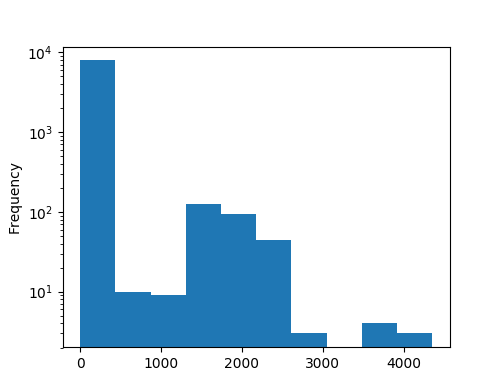
\includegraphics[width=1.2\textwidth]{./img/interest_earned_freq.png}
%    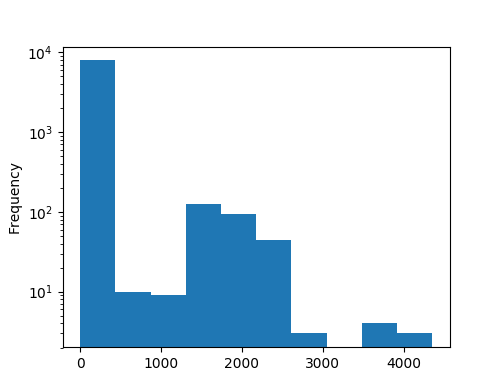
\includegraphics{./img/interest_earned_freq.png}
\end{minipage}
%\end{figure}
%\begin{figure}[!h]
\begin{minipage}{.45\textwidth}
    \caption{Monthly work frequency.}
    \label{fig:monthly_work_freq}
    \centering
    \scalebox{0.5}{%% Creator: Matplotlib, PGF backend
%%
%% To include the figure in your LaTeX document, write
%%   \input{<filename>.pgf}
%%
%% Make sure the required packages are loaded in your preamble
%%   \usepackage{pgf}
%%
%% Figures using additional raster images can only be included by \input if
%% they are in the same directory as the main LaTeX file. For loading figures
%% from other directories you can use the `import` package
%%   \usepackage{import}
%% and then include the figures with
%%   \import{<path to file>}{<filename>.pgf}
%%
%% Matplotlib used the following preamble
%%   \usepackage{fontspec}
%%   \setmainfont{DejaVu Serif}
%%   \setsansfont{DejaVu Sans}
%%   \setmonofont{DejaVu Sans Mono}
%%
\begingroup%
\makeatletter%
\begin{pgfpicture}%
\pgfpathrectangle{\pgfpointorigin}{\pgfqpoint{5.000000in}{3.900000in}}%
\pgfusepath{use as bounding box, clip}%
\begin{pgfscope}%
\pgfsetbuttcap%
\pgfsetmiterjoin%
\definecolor{currentfill}{rgb}{1.000000,1.000000,1.000000}%
\pgfsetfillcolor{currentfill}%
\pgfsetlinewidth{0.000000pt}%
\definecolor{currentstroke}{rgb}{1.000000,1.000000,1.000000}%
\pgfsetstrokecolor{currentstroke}%
\pgfsetdash{}{0pt}%
\pgfpathmoveto{\pgfqpoint{0.000000in}{0.000000in}}%
\pgfpathlineto{\pgfqpoint{5.000000in}{0.000000in}}%
\pgfpathlineto{\pgfqpoint{5.000000in}{3.900000in}}%
\pgfpathlineto{\pgfqpoint{0.000000in}{3.900000in}}%
\pgfpathclose%
\pgfusepath{fill}%
\end{pgfscope}%
\begin{pgfscope}%
\pgfsetbuttcap%
\pgfsetmiterjoin%
\definecolor{currentfill}{rgb}{1.000000,1.000000,1.000000}%
\pgfsetfillcolor{currentfill}%
\pgfsetlinewidth{0.000000pt}%
\definecolor{currentstroke}{rgb}{0.000000,0.000000,0.000000}%
\pgfsetstrokecolor{currentstroke}%
\pgfsetstrokeopacity{0.000000}%
\pgfsetdash{}{0pt}%
\pgfpathmoveto{\pgfqpoint{0.625000in}{0.429000in}}%
\pgfpathlineto{\pgfqpoint{4.500000in}{0.429000in}}%
\pgfpathlineto{\pgfqpoint{4.500000in}{3.432000in}}%
\pgfpathlineto{\pgfqpoint{0.625000in}{3.432000in}}%
\pgfpathclose%
\pgfusepath{fill}%
\end{pgfscope}%
\begin{pgfscope}%
\pgfpathrectangle{\pgfqpoint{0.625000in}{0.429000in}}{\pgfqpoint{3.875000in}{3.003000in}} %
\pgfusepath{clip}%
\pgfsetbuttcap%
\pgfsetmiterjoin%
\definecolor{currentfill}{rgb}{0.121569,0.466667,0.705882}%
\pgfsetfillcolor{currentfill}%
\pgfsetlinewidth{0.000000pt}%
\definecolor{currentstroke}{rgb}{0.000000,0.000000,0.000000}%
\pgfsetstrokecolor{currentstroke}%
\pgfsetstrokeopacity{0.000000}%
\pgfsetdash{}{0pt}%
\pgfpathmoveto{\pgfqpoint{0.801136in}{0.429000in}}%
\pgfpathlineto{\pgfqpoint{1.153409in}{0.429000in}}%
\pgfpathlineto{\pgfqpoint{1.153409in}{0.599365in}}%
\pgfpathlineto{\pgfqpoint{0.801136in}{0.599365in}}%
\pgfpathclose%
\pgfusepath{fill}%
\end{pgfscope}%
\begin{pgfscope}%
\pgfpathrectangle{\pgfqpoint{0.625000in}{0.429000in}}{\pgfqpoint{3.875000in}{3.003000in}} %
\pgfusepath{clip}%
\pgfsetbuttcap%
\pgfsetmiterjoin%
\definecolor{currentfill}{rgb}{0.121569,0.466667,0.705882}%
\pgfsetfillcolor{currentfill}%
\pgfsetlinewidth{0.000000pt}%
\definecolor{currentstroke}{rgb}{0.000000,0.000000,0.000000}%
\pgfsetstrokecolor{currentstroke}%
\pgfsetstrokeopacity{0.000000}%
\pgfsetdash{}{0pt}%
\pgfpathmoveto{\pgfqpoint{1.153409in}{0.429000in}}%
\pgfpathlineto{\pgfqpoint{1.505682in}{0.429000in}}%
\pgfpathlineto{\pgfqpoint{1.505682in}{0.953155in}}%
\pgfpathlineto{\pgfqpoint{1.153409in}{0.953155in}}%
\pgfpathclose%
\pgfusepath{fill}%
\end{pgfscope}%
\begin{pgfscope}%
\pgfpathrectangle{\pgfqpoint{0.625000in}{0.429000in}}{\pgfqpoint{3.875000in}{3.003000in}} %
\pgfusepath{clip}%
\pgfsetbuttcap%
\pgfsetmiterjoin%
\definecolor{currentfill}{rgb}{0.121569,0.466667,0.705882}%
\pgfsetfillcolor{currentfill}%
\pgfsetlinewidth{0.000000pt}%
\definecolor{currentstroke}{rgb}{0.000000,0.000000,0.000000}%
\pgfsetstrokecolor{currentstroke}%
\pgfsetstrokeopacity{0.000000}%
\pgfsetdash{}{0pt}%
\pgfpathmoveto{\pgfqpoint{1.505682in}{0.429000in}}%
\pgfpathlineto{\pgfqpoint{1.857955in}{0.429000in}}%
\pgfpathlineto{\pgfqpoint{1.857955in}{0.968589in}}%
\pgfpathlineto{\pgfqpoint{1.505682in}{0.968589in}}%
\pgfpathclose%
\pgfusepath{fill}%
\end{pgfscope}%
\begin{pgfscope}%
\pgfpathrectangle{\pgfqpoint{0.625000in}{0.429000in}}{\pgfqpoint{3.875000in}{3.003000in}} %
\pgfusepath{clip}%
\pgfsetbuttcap%
\pgfsetmiterjoin%
\definecolor{currentfill}{rgb}{0.121569,0.466667,0.705882}%
\pgfsetfillcolor{currentfill}%
\pgfsetlinewidth{0.000000pt}%
\definecolor{currentstroke}{rgb}{0.000000,0.000000,0.000000}%
\pgfsetstrokecolor{currentstroke}%
\pgfsetstrokeopacity{0.000000}%
\pgfsetdash{}{0pt}%
\pgfpathmoveto{\pgfqpoint{1.857955in}{0.429000in}}%
\pgfpathlineto{\pgfqpoint{2.210227in}{0.429000in}}%
\pgfpathlineto{\pgfqpoint{2.210227in}{3.289000in}}%
\pgfpathlineto{\pgfqpoint{1.857955in}{3.289000in}}%
\pgfpathclose%
\pgfusepath{fill}%
\end{pgfscope}%
\begin{pgfscope}%
\pgfpathrectangle{\pgfqpoint{0.625000in}{0.429000in}}{\pgfqpoint{3.875000in}{3.003000in}} %
\pgfusepath{clip}%
\pgfsetbuttcap%
\pgfsetmiterjoin%
\definecolor{currentfill}{rgb}{0.121569,0.466667,0.705882}%
\pgfsetfillcolor{currentfill}%
\pgfsetlinewidth{0.000000pt}%
\definecolor{currentstroke}{rgb}{0.000000,0.000000,0.000000}%
\pgfsetstrokecolor{currentstroke}%
\pgfsetstrokeopacity{0.000000}%
\pgfsetdash{}{0pt}%
\pgfpathmoveto{\pgfqpoint{2.210227in}{0.429000in}}%
\pgfpathlineto{\pgfqpoint{2.562500in}{0.429000in}}%
\pgfpathlineto{\pgfqpoint{2.562500in}{0.745393in}}%
\pgfpathlineto{\pgfqpoint{2.210227in}{0.745393in}}%
\pgfpathclose%
\pgfusepath{fill}%
\end{pgfscope}%
\begin{pgfscope}%
\pgfpathrectangle{\pgfqpoint{0.625000in}{0.429000in}}{\pgfqpoint{3.875000in}{3.003000in}} %
\pgfusepath{clip}%
\pgfsetbuttcap%
\pgfsetmiterjoin%
\definecolor{currentfill}{rgb}{0.121569,0.466667,0.705882}%
\pgfsetfillcolor{currentfill}%
\pgfsetlinewidth{0.000000pt}%
\definecolor{currentstroke}{rgb}{0.000000,0.000000,0.000000}%
\pgfsetstrokecolor{currentstroke}%
\pgfsetstrokeopacity{0.000000}%
\pgfsetdash{}{0pt}%
\pgfpathmoveto{\pgfqpoint{2.562500in}{0.429000in}}%
\pgfpathlineto{\pgfqpoint{2.914773in}{0.429000in}}%
\pgfpathlineto{\pgfqpoint{2.914773in}{0.703840in}}%
\pgfpathlineto{\pgfqpoint{2.562500in}{0.703840in}}%
\pgfpathclose%
\pgfusepath{fill}%
\end{pgfscope}%
\begin{pgfscope}%
\pgfpathrectangle{\pgfqpoint{0.625000in}{0.429000in}}{\pgfqpoint{3.875000in}{3.003000in}} %
\pgfusepath{clip}%
\pgfsetbuttcap%
\pgfsetmiterjoin%
\definecolor{currentfill}{rgb}{0.121569,0.466667,0.705882}%
\pgfsetfillcolor{currentfill}%
\pgfsetlinewidth{0.000000pt}%
\definecolor{currentstroke}{rgb}{0.000000,0.000000,0.000000}%
\pgfsetstrokecolor{currentstroke}%
\pgfsetstrokeopacity{0.000000}%
\pgfsetdash{}{0pt}%
\pgfpathmoveto{\pgfqpoint{2.914773in}{0.429000in}}%
\pgfpathlineto{\pgfqpoint{3.267045in}{0.429000in}}%
\pgfpathlineto{\pgfqpoint{3.267045in}{0.533475in}}%
\pgfpathlineto{\pgfqpoint{2.914773in}{0.533475in}}%
\pgfpathclose%
\pgfusepath{fill}%
\end{pgfscope}%
\begin{pgfscope}%
\pgfpathrectangle{\pgfqpoint{0.625000in}{0.429000in}}{\pgfqpoint{3.875000in}{3.003000in}} %
\pgfusepath{clip}%
\pgfsetbuttcap%
\pgfsetmiterjoin%
\definecolor{currentfill}{rgb}{0.121569,0.466667,0.705882}%
\pgfsetfillcolor{currentfill}%
\pgfsetlinewidth{0.000000pt}%
\definecolor{currentstroke}{rgb}{0.000000,0.000000,0.000000}%
\pgfsetstrokecolor{currentstroke}%
\pgfsetstrokeopacity{0.000000}%
\pgfsetdash{}{0pt}%
\pgfpathmoveto{\pgfqpoint{3.267045in}{0.429000in}}%
\pgfpathlineto{\pgfqpoint{3.619318in}{0.429000in}}%
\pgfpathlineto{\pgfqpoint{3.619318in}{0.458680in}}%
\pgfpathlineto{\pgfqpoint{3.267045in}{0.458680in}}%
\pgfpathclose%
\pgfusepath{fill}%
\end{pgfscope}%
\begin{pgfscope}%
\pgfpathrectangle{\pgfqpoint{0.625000in}{0.429000in}}{\pgfqpoint{3.875000in}{3.003000in}} %
\pgfusepath{clip}%
\pgfsetbuttcap%
\pgfsetmiterjoin%
\definecolor{currentfill}{rgb}{0.121569,0.466667,0.705882}%
\pgfsetfillcolor{currentfill}%
\pgfsetlinewidth{0.000000pt}%
\definecolor{currentstroke}{rgb}{0.000000,0.000000,0.000000}%
\pgfsetstrokecolor{currentstroke}%
\pgfsetstrokeopacity{0.000000}%
\pgfsetdash{}{0pt}%
\pgfpathmoveto{\pgfqpoint{3.619318in}{0.429000in}}%
\pgfpathlineto{\pgfqpoint{3.971591in}{0.429000in}}%
\pgfpathlineto{\pgfqpoint{3.971591in}{0.444434in}}%
\pgfpathlineto{\pgfqpoint{3.619318in}{0.444434in}}%
\pgfpathclose%
\pgfusepath{fill}%
\end{pgfscope}%
\begin{pgfscope}%
\pgfpathrectangle{\pgfqpoint{0.625000in}{0.429000in}}{\pgfqpoint{3.875000in}{3.003000in}} %
\pgfusepath{clip}%
\pgfsetbuttcap%
\pgfsetmiterjoin%
\definecolor{currentfill}{rgb}{0.121569,0.466667,0.705882}%
\pgfsetfillcolor{currentfill}%
\pgfsetlinewidth{0.000000pt}%
\definecolor{currentstroke}{rgb}{0.000000,0.000000,0.000000}%
\pgfsetstrokecolor{currentstroke}%
\pgfsetstrokeopacity{0.000000}%
\pgfsetdash{}{0pt}%
\pgfpathmoveto{\pgfqpoint{3.971591in}{0.429000in}}%
\pgfpathlineto{\pgfqpoint{4.323864in}{0.429000in}}%
\pgfpathlineto{\pgfqpoint{4.323864in}{0.440279in}}%
\pgfpathlineto{\pgfqpoint{3.971591in}{0.440279in}}%
\pgfpathclose%
\pgfusepath{fill}%
\end{pgfscope}%
\begin{pgfscope}%
\pgfsetbuttcap%
\pgfsetroundjoin%
\definecolor{currentfill}{rgb}{0.000000,0.000000,0.000000}%
\pgfsetfillcolor{currentfill}%
\pgfsetlinewidth{0.803000pt}%
\definecolor{currentstroke}{rgb}{0.000000,0.000000,0.000000}%
\pgfsetstrokecolor{currentstroke}%
\pgfsetdash{}{0pt}%
\pgfsys@defobject{currentmarker}{\pgfqpoint{0.000000in}{-0.048611in}}{\pgfqpoint{0.000000in}{0.000000in}}{%
\pgfpathmoveto{\pgfqpoint{0.000000in}{0.000000in}}%
\pgfpathlineto{\pgfqpoint{0.000000in}{-0.048611in}}%
\pgfusepath{stroke,fill}%
}%
\begin{pgfscope}%
\pgfsys@transformshift{0.765190in}{0.429000in}%
\pgfsys@useobject{currentmarker}{}%
\end{pgfscope}%
\end{pgfscope}%
\begin{pgfscope}%
\pgftext[x=0.765190in,y=0.331778in,,top]{\sffamily\fontsize{10.000000}{12.000000}\selectfont 0}%
\end{pgfscope}%
\begin{pgfscope}%
\pgfsetbuttcap%
\pgfsetroundjoin%
\definecolor{currentfill}{rgb}{0.000000,0.000000,0.000000}%
\pgfsetfillcolor{currentfill}%
\pgfsetlinewidth{0.803000pt}%
\definecolor{currentstroke}{rgb}{0.000000,0.000000,0.000000}%
\pgfsetstrokecolor{currentstroke}%
\pgfsetdash{}{0pt}%
\pgfsys@defobject{currentmarker}{\pgfqpoint{0.000000in}{-0.048611in}}{\pgfqpoint{0.000000in}{0.000000in}}{%
\pgfpathmoveto{\pgfqpoint{0.000000in}{0.000000in}}%
\pgfpathlineto{\pgfqpoint{0.000000in}{-0.048611in}}%
\pgfusepath{stroke,fill}%
}%
\begin{pgfscope}%
\pgfsys@transformshift{1.214518in}{0.429000in}%
\pgfsys@useobject{currentmarker}{}%
\end{pgfscope}%
\end{pgfscope}%
\begin{pgfscope}%
\pgftext[x=1.214518in,y=0.331778in,,top]{\sffamily\fontsize{10.000000}{12.000000}\selectfont 50}%
\end{pgfscope}%
\begin{pgfscope}%
\pgfsetbuttcap%
\pgfsetroundjoin%
\definecolor{currentfill}{rgb}{0.000000,0.000000,0.000000}%
\pgfsetfillcolor{currentfill}%
\pgfsetlinewidth{0.803000pt}%
\definecolor{currentstroke}{rgb}{0.000000,0.000000,0.000000}%
\pgfsetstrokecolor{currentstroke}%
\pgfsetdash{}{0pt}%
\pgfsys@defobject{currentmarker}{\pgfqpoint{0.000000in}{-0.048611in}}{\pgfqpoint{0.000000in}{0.000000in}}{%
\pgfpathmoveto{\pgfqpoint{0.000000in}{0.000000in}}%
\pgfpathlineto{\pgfqpoint{0.000000in}{-0.048611in}}%
\pgfusepath{stroke,fill}%
}%
\begin{pgfscope}%
\pgfsys@transformshift{1.663845in}{0.429000in}%
\pgfsys@useobject{currentmarker}{}%
\end{pgfscope}%
\end{pgfscope}%
\begin{pgfscope}%
\pgftext[x=1.663845in,y=0.331778in,,top]{\sffamily\fontsize{10.000000}{12.000000}\selectfont 100}%
\end{pgfscope}%
\begin{pgfscope}%
\pgfsetbuttcap%
\pgfsetroundjoin%
\definecolor{currentfill}{rgb}{0.000000,0.000000,0.000000}%
\pgfsetfillcolor{currentfill}%
\pgfsetlinewidth{0.803000pt}%
\definecolor{currentstroke}{rgb}{0.000000,0.000000,0.000000}%
\pgfsetstrokecolor{currentstroke}%
\pgfsetdash{}{0pt}%
\pgfsys@defobject{currentmarker}{\pgfqpoint{0.000000in}{-0.048611in}}{\pgfqpoint{0.000000in}{0.000000in}}{%
\pgfpathmoveto{\pgfqpoint{0.000000in}{0.000000in}}%
\pgfpathlineto{\pgfqpoint{0.000000in}{-0.048611in}}%
\pgfusepath{stroke,fill}%
}%
\begin{pgfscope}%
\pgfsys@transformshift{2.113173in}{0.429000in}%
\pgfsys@useobject{currentmarker}{}%
\end{pgfscope}%
\end{pgfscope}%
\begin{pgfscope}%
\pgftext[x=2.113173in,y=0.331778in,,top]{\sffamily\fontsize{10.000000}{12.000000}\selectfont 150}%
\end{pgfscope}%
\begin{pgfscope}%
\pgfsetbuttcap%
\pgfsetroundjoin%
\definecolor{currentfill}{rgb}{0.000000,0.000000,0.000000}%
\pgfsetfillcolor{currentfill}%
\pgfsetlinewidth{0.803000pt}%
\definecolor{currentstroke}{rgb}{0.000000,0.000000,0.000000}%
\pgfsetstrokecolor{currentstroke}%
\pgfsetdash{}{0pt}%
\pgfsys@defobject{currentmarker}{\pgfqpoint{0.000000in}{-0.048611in}}{\pgfqpoint{0.000000in}{0.000000in}}{%
\pgfpathmoveto{\pgfqpoint{0.000000in}{0.000000in}}%
\pgfpathlineto{\pgfqpoint{0.000000in}{-0.048611in}}%
\pgfusepath{stroke,fill}%
}%
\begin{pgfscope}%
\pgfsys@transformshift{2.562500in}{0.429000in}%
\pgfsys@useobject{currentmarker}{}%
\end{pgfscope}%
\end{pgfscope}%
\begin{pgfscope}%
\pgftext[x=2.562500in,y=0.331778in,,top]{\sffamily\fontsize{10.000000}{12.000000}\selectfont 200}%
\end{pgfscope}%
\begin{pgfscope}%
\pgfsetbuttcap%
\pgfsetroundjoin%
\definecolor{currentfill}{rgb}{0.000000,0.000000,0.000000}%
\pgfsetfillcolor{currentfill}%
\pgfsetlinewidth{0.803000pt}%
\definecolor{currentstroke}{rgb}{0.000000,0.000000,0.000000}%
\pgfsetstrokecolor{currentstroke}%
\pgfsetdash{}{0pt}%
\pgfsys@defobject{currentmarker}{\pgfqpoint{0.000000in}{-0.048611in}}{\pgfqpoint{0.000000in}{0.000000in}}{%
\pgfpathmoveto{\pgfqpoint{0.000000in}{0.000000in}}%
\pgfpathlineto{\pgfqpoint{0.000000in}{-0.048611in}}%
\pgfusepath{stroke,fill}%
}%
\begin{pgfscope}%
\pgfsys@transformshift{3.011827in}{0.429000in}%
\pgfsys@useobject{currentmarker}{}%
\end{pgfscope}%
\end{pgfscope}%
\begin{pgfscope}%
\pgftext[x=3.011827in,y=0.331778in,,top]{\sffamily\fontsize{10.000000}{12.000000}\selectfont 250}%
\end{pgfscope}%
\begin{pgfscope}%
\pgfsetbuttcap%
\pgfsetroundjoin%
\definecolor{currentfill}{rgb}{0.000000,0.000000,0.000000}%
\pgfsetfillcolor{currentfill}%
\pgfsetlinewidth{0.803000pt}%
\definecolor{currentstroke}{rgb}{0.000000,0.000000,0.000000}%
\pgfsetstrokecolor{currentstroke}%
\pgfsetdash{}{0pt}%
\pgfsys@defobject{currentmarker}{\pgfqpoint{0.000000in}{-0.048611in}}{\pgfqpoint{0.000000in}{0.000000in}}{%
\pgfpathmoveto{\pgfqpoint{0.000000in}{0.000000in}}%
\pgfpathlineto{\pgfqpoint{0.000000in}{-0.048611in}}%
\pgfusepath{stroke,fill}%
}%
\begin{pgfscope}%
\pgfsys@transformshift{3.461155in}{0.429000in}%
\pgfsys@useobject{currentmarker}{}%
\end{pgfscope}%
\end{pgfscope}%
\begin{pgfscope}%
\pgftext[x=3.461155in,y=0.331778in,,top]{\sffamily\fontsize{10.000000}{12.000000}\selectfont 300}%
\end{pgfscope}%
\begin{pgfscope}%
\pgfsetbuttcap%
\pgfsetroundjoin%
\definecolor{currentfill}{rgb}{0.000000,0.000000,0.000000}%
\pgfsetfillcolor{currentfill}%
\pgfsetlinewidth{0.803000pt}%
\definecolor{currentstroke}{rgb}{0.000000,0.000000,0.000000}%
\pgfsetstrokecolor{currentstroke}%
\pgfsetdash{}{0pt}%
\pgfsys@defobject{currentmarker}{\pgfqpoint{0.000000in}{-0.048611in}}{\pgfqpoint{0.000000in}{0.000000in}}{%
\pgfpathmoveto{\pgfqpoint{0.000000in}{0.000000in}}%
\pgfpathlineto{\pgfqpoint{0.000000in}{-0.048611in}}%
\pgfusepath{stroke,fill}%
}%
\begin{pgfscope}%
\pgfsys@transformshift{3.910482in}{0.429000in}%
\pgfsys@useobject{currentmarker}{}%
\end{pgfscope}%
\end{pgfscope}%
\begin{pgfscope}%
\pgftext[x=3.910482in,y=0.331778in,,top]{\sffamily\fontsize{10.000000}{12.000000}\selectfont 350}%
\end{pgfscope}%
\begin{pgfscope}%
\pgfsetbuttcap%
\pgfsetroundjoin%
\definecolor{currentfill}{rgb}{0.000000,0.000000,0.000000}%
\pgfsetfillcolor{currentfill}%
\pgfsetlinewidth{0.803000pt}%
\definecolor{currentstroke}{rgb}{0.000000,0.000000,0.000000}%
\pgfsetstrokecolor{currentstroke}%
\pgfsetdash{}{0pt}%
\pgfsys@defobject{currentmarker}{\pgfqpoint{0.000000in}{-0.048611in}}{\pgfqpoint{0.000000in}{0.000000in}}{%
\pgfpathmoveto{\pgfqpoint{0.000000in}{0.000000in}}%
\pgfpathlineto{\pgfqpoint{0.000000in}{-0.048611in}}%
\pgfusepath{stroke,fill}%
}%
\begin{pgfscope}%
\pgfsys@transformshift{4.359810in}{0.429000in}%
\pgfsys@useobject{currentmarker}{}%
\end{pgfscope}%
\end{pgfscope}%
\begin{pgfscope}%
\pgftext[x=4.359810in,y=0.331778in,,top]{\sffamily\fontsize{10.000000}{12.000000}\selectfont 400}%
\end{pgfscope}%
\begin{pgfscope}%
\pgfsetbuttcap%
\pgfsetroundjoin%
\definecolor{currentfill}{rgb}{0.000000,0.000000,0.000000}%
\pgfsetfillcolor{currentfill}%
\pgfsetlinewidth{0.803000pt}%
\definecolor{currentstroke}{rgb}{0.000000,0.000000,0.000000}%
\pgfsetstrokecolor{currentstroke}%
\pgfsetdash{}{0pt}%
\pgfsys@defobject{currentmarker}{\pgfqpoint{-0.048611in}{0.000000in}}{\pgfqpoint{0.000000in}{0.000000in}}{%
\pgfpathmoveto{\pgfqpoint{0.000000in}{0.000000in}}%
\pgfpathlineto{\pgfqpoint{-0.048611in}{0.000000in}}%
\pgfusepath{stroke,fill}%
}%
\begin{pgfscope}%
\pgfsys@transformshift{0.625000in}{0.429000in}%
\pgfsys@useobject{currentmarker}{}%
\end{pgfscope}%
\end{pgfscope}%
\begin{pgfscope}%
\pgftext[x=0.439412in,y=0.376238in,left,base]{\sffamily\fontsize{10.000000}{12.000000}\selectfont 0}%
\end{pgfscope}%
\begin{pgfscope}%
\pgfsetbuttcap%
\pgfsetroundjoin%
\definecolor{currentfill}{rgb}{0.000000,0.000000,0.000000}%
\pgfsetfillcolor{currentfill}%
\pgfsetlinewidth{0.803000pt}%
\definecolor{currentstroke}{rgb}{0.000000,0.000000,0.000000}%
\pgfsetstrokecolor{currentstroke}%
\pgfsetdash{}{0pt}%
\pgfsys@defobject{currentmarker}{\pgfqpoint{-0.048611in}{0.000000in}}{\pgfqpoint{0.000000in}{0.000000in}}{%
\pgfpathmoveto{\pgfqpoint{0.000000in}{0.000000in}}%
\pgfpathlineto{\pgfqpoint{-0.048611in}{0.000000in}}%
\pgfusepath{stroke,fill}%
}%
\begin{pgfscope}%
\pgfsys@transformshift{0.625000in}{1.022607in}%
\pgfsys@useobject{currentmarker}{}%
\end{pgfscope}%
\end{pgfscope}%
\begin{pgfscope}%
\pgftext[x=0.174316in,y=0.969846in,left,base]{\sffamily\fontsize{10.000000}{12.000000}\selectfont 1000}%
\end{pgfscope}%
\begin{pgfscope}%
\pgfsetbuttcap%
\pgfsetroundjoin%
\definecolor{currentfill}{rgb}{0.000000,0.000000,0.000000}%
\pgfsetfillcolor{currentfill}%
\pgfsetlinewidth{0.803000pt}%
\definecolor{currentstroke}{rgb}{0.000000,0.000000,0.000000}%
\pgfsetstrokecolor{currentstroke}%
\pgfsetdash{}{0pt}%
\pgfsys@defobject{currentmarker}{\pgfqpoint{-0.048611in}{0.000000in}}{\pgfqpoint{0.000000in}{0.000000in}}{%
\pgfpathmoveto{\pgfqpoint{0.000000in}{0.000000in}}%
\pgfpathlineto{\pgfqpoint{-0.048611in}{0.000000in}}%
\pgfusepath{stroke,fill}%
}%
\begin{pgfscope}%
\pgfsys@transformshift{0.625000in}{1.616215in}%
\pgfsys@useobject{currentmarker}{}%
\end{pgfscope}%
\end{pgfscope}%
\begin{pgfscope}%
\pgftext[x=0.174316in,y=1.563453in,left,base]{\sffamily\fontsize{10.000000}{12.000000}\selectfont 2000}%
\end{pgfscope}%
\begin{pgfscope}%
\pgfsetbuttcap%
\pgfsetroundjoin%
\definecolor{currentfill}{rgb}{0.000000,0.000000,0.000000}%
\pgfsetfillcolor{currentfill}%
\pgfsetlinewidth{0.803000pt}%
\definecolor{currentstroke}{rgb}{0.000000,0.000000,0.000000}%
\pgfsetstrokecolor{currentstroke}%
\pgfsetdash{}{0pt}%
\pgfsys@defobject{currentmarker}{\pgfqpoint{-0.048611in}{0.000000in}}{\pgfqpoint{0.000000in}{0.000000in}}{%
\pgfpathmoveto{\pgfqpoint{0.000000in}{0.000000in}}%
\pgfpathlineto{\pgfqpoint{-0.048611in}{0.000000in}}%
\pgfusepath{stroke,fill}%
}%
\begin{pgfscope}%
\pgfsys@transformshift{0.625000in}{2.209822in}%
\pgfsys@useobject{currentmarker}{}%
\end{pgfscope}%
\end{pgfscope}%
\begin{pgfscope}%
\pgftext[x=0.174316in,y=2.157060in,left,base]{\sffamily\fontsize{10.000000}{12.000000}\selectfont 3000}%
\end{pgfscope}%
\begin{pgfscope}%
\pgfsetbuttcap%
\pgfsetroundjoin%
\definecolor{currentfill}{rgb}{0.000000,0.000000,0.000000}%
\pgfsetfillcolor{currentfill}%
\pgfsetlinewidth{0.803000pt}%
\definecolor{currentstroke}{rgb}{0.000000,0.000000,0.000000}%
\pgfsetstrokecolor{currentstroke}%
\pgfsetdash{}{0pt}%
\pgfsys@defobject{currentmarker}{\pgfqpoint{-0.048611in}{0.000000in}}{\pgfqpoint{0.000000in}{0.000000in}}{%
\pgfpathmoveto{\pgfqpoint{0.000000in}{0.000000in}}%
\pgfpathlineto{\pgfqpoint{-0.048611in}{0.000000in}}%
\pgfusepath{stroke,fill}%
}%
\begin{pgfscope}%
\pgfsys@transformshift{0.625000in}{2.803429in}%
\pgfsys@useobject{currentmarker}{}%
\end{pgfscope}%
\end{pgfscope}%
\begin{pgfscope}%
\pgftext[x=0.174316in,y=2.750668in,left,base]{\sffamily\fontsize{10.000000}{12.000000}\selectfont 4000}%
\end{pgfscope}%
\begin{pgfscope}%
\pgfsetbuttcap%
\pgfsetroundjoin%
\definecolor{currentfill}{rgb}{0.000000,0.000000,0.000000}%
\pgfsetfillcolor{currentfill}%
\pgfsetlinewidth{0.803000pt}%
\definecolor{currentstroke}{rgb}{0.000000,0.000000,0.000000}%
\pgfsetstrokecolor{currentstroke}%
\pgfsetdash{}{0pt}%
\pgfsys@defobject{currentmarker}{\pgfqpoint{-0.048611in}{0.000000in}}{\pgfqpoint{0.000000in}{0.000000in}}{%
\pgfpathmoveto{\pgfqpoint{0.000000in}{0.000000in}}%
\pgfpathlineto{\pgfqpoint{-0.048611in}{0.000000in}}%
\pgfusepath{stroke,fill}%
}%
\begin{pgfscope}%
\pgfsys@transformshift{0.625000in}{3.397037in}%
\pgfsys@useobject{currentmarker}{}%
\end{pgfscope}%
\end{pgfscope}%
\begin{pgfscope}%
\pgftext[x=0.174316in,y=3.344275in,left,base]{\sffamily\fontsize{10.000000}{12.000000}\selectfont 5000}%
\end{pgfscope}%
\begin{pgfscope}%
\pgftext[x=0.118761in,y=1.930500in,,bottom,rotate=90.000000]{\sffamily\fontsize{10.000000}{12.000000}\selectfont Frequency}%
\end{pgfscope}%
\begin{pgfscope}%
\pgfsetrectcap%
\pgfsetmiterjoin%
\pgfsetlinewidth{0.803000pt}%
\definecolor{currentstroke}{rgb}{0.000000,0.000000,0.000000}%
\pgfsetstrokecolor{currentstroke}%
\pgfsetdash{}{0pt}%
\pgfpathmoveto{\pgfqpoint{0.625000in}{0.429000in}}%
\pgfpathlineto{\pgfqpoint{0.625000in}{3.432000in}}%
\pgfusepath{stroke}%
\end{pgfscope}%
\begin{pgfscope}%
\pgfsetrectcap%
\pgfsetmiterjoin%
\pgfsetlinewidth{0.803000pt}%
\definecolor{currentstroke}{rgb}{0.000000,0.000000,0.000000}%
\pgfsetstrokecolor{currentstroke}%
\pgfsetdash{}{0pt}%
\pgfpathmoveto{\pgfqpoint{4.500000in}{0.429000in}}%
\pgfpathlineto{\pgfqpoint{4.500000in}{3.432000in}}%
\pgfusepath{stroke}%
\end{pgfscope}%
\begin{pgfscope}%
\pgfsetrectcap%
\pgfsetmiterjoin%
\pgfsetlinewidth{0.803000pt}%
\definecolor{currentstroke}{rgb}{0.000000,0.000000,0.000000}%
\pgfsetstrokecolor{currentstroke}%
\pgfsetdash{}{0pt}%
\pgfpathmoveto{\pgfqpoint{0.625000in}{0.429000in}}%
\pgfpathlineto{\pgfqpoint{4.500000in}{0.429000in}}%
\pgfusepath{stroke}%
\end{pgfscope}%
\begin{pgfscope}%
\pgfsetrectcap%
\pgfsetmiterjoin%
\pgfsetlinewidth{0.803000pt}%
\definecolor{currentstroke}{rgb}{0.000000,0.000000,0.000000}%
\pgfsetstrokecolor{currentstroke}%
\pgfsetdash{}{0pt}%
\pgfpathmoveto{\pgfqpoint{0.625000in}{3.432000in}}%
\pgfpathlineto{\pgfqpoint{4.500000in}{3.432000in}}%
\pgfusepath{stroke}%
\end{pgfscope}%
\end{pgfpicture}%
\makeatother%
\endgroup%
}
\end{minipage}
\end{figure}

\begin{figure}[!h]
    \caption{Sections of the cross-correlation matrix.}
    \label{fig:cross-matrix}

%    \begin{subfigure}[b]{\linewidth}
\begin{minipage}{.5\textwidth}
        \centering
        %        \caption{A subfigure}\label{fig:1a}
        \scalebox{0.22}{%% Creator: Matplotlib, PGF backend
%%
%% To include the figure in your LaTeX document, write
%%   \input{<filename>.pgf}
%%
%% Make sure the required packages are loaded in your preamble
%%   \usepackage{pgf}
%%
%% Figures using additional raster images can only be included by \input if
%% they are in the same directory as the main LaTeX file. For loading figures
%% from other directories you can use the `import` package
%%   \usepackage{import}
%% and then include the figures with
%%   \import{<path to file>}{<filename>.pgf}
%%
%% Matplotlib used the following preamble
%%   \usepackage{fontspec}
%%   \setmainfont{DejaVu Serif}
%%   \setsansfont{DejaVu Sans}
%%   \setmonofont{DejaVu Sans Mono}
%%
\begingroup%
\makeatletter%
\begin{pgfpicture}%
\pgfpathrectangle{\pgfpointorigin}{\pgfqpoint{12.000000in}{10.000000in}}%
\pgfusepath{use as bounding box, clip}%
\begin{pgfscope}%
\pgfsetbuttcap%
\pgfsetmiterjoin%
\definecolor{currentfill}{rgb}{1.000000,1.000000,1.000000}%
\pgfsetfillcolor{currentfill}%
\pgfsetlinewidth{0.000000pt}%
\definecolor{currentstroke}{rgb}{1.000000,1.000000,1.000000}%
\pgfsetstrokecolor{currentstroke}%
\pgfsetdash{}{0pt}%
\pgfpathmoveto{\pgfqpoint{0.000000in}{0.000000in}}%
\pgfpathlineto{\pgfqpoint{12.000000in}{0.000000in}}%
\pgfpathlineto{\pgfqpoint{12.000000in}{10.000000in}}%
\pgfpathlineto{\pgfqpoint{0.000000in}{10.000000in}}%
\pgfpathclose%
\pgfusepath{fill}%
\end{pgfscope}%
\begin{pgfscope}%
\pgfsetbuttcap%
\pgfsetmiterjoin%
\definecolor{currentfill}{rgb}{1.000000,1.000000,1.000000}%
\pgfsetfillcolor{currentfill}%
\pgfsetlinewidth{0.000000pt}%
\definecolor{currentstroke}{rgb}{0.000000,0.000000,0.000000}%
\pgfsetstrokecolor{currentstroke}%
\pgfsetstrokeopacity{0.000000}%
\pgfsetdash{}{0pt}%
\pgfpathmoveto{\pgfqpoint{2.884722in}{2.884722in}}%
\pgfpathlineto{\pgfqpoint{10.056944in}{2.884722in}}%
\pgfpathlineto{\pgfqpoint{10.056944in}{9.795000in}}%
\pgfpathlineto{\pgfqpoint{2.884722in}{9.795000in}}%
\pgfpathclose%
\pgfusepath{fill}%
\end{pgfscope}%
\begin{pgfscope}%
\pgfpathrectangle{\pgfqpoint{2.884722in}{2.884722in}}{\pgfqpoint{7.172222in}{6.910278in}} %
\pgfusepath{clip}%
\pgfsetbuttcap%
\pgfsetroundjoin%
\definecolor{currentfill}{rgb}{0.981377,0.920617,0.865369}%
\pgfsetfillcolor{currentfill}%
\pgfsetlinewidth{0.000000pt}%
\definecolor{currentstroke}{rgb}{1.000000,1.000000,1.000000}%
\pgfsetstrokecolor{currentstroke}%
\pgfsetdash{}{0pt}%
\pgfpathmoveto{\pgfqpoint{2.884722in}{9.795000in}}%
\pgfpathlineto{\pgfqpoint{3.095670in}{9.795000in}}%
\pgfpathlineto{\pgfqpoint{3.095670in}{9.591757in}}%
\pgfpathlineto{\pgfqpoint{2.884722in}{9.591757in}}%
\pgfpathlineto{\pgfqpoint{2.884722in}{9.795000in}}%
\pgfusepath{fill}%
\end{pgfscope}%
\begin{pgfscope}%
\pgfpathrectangle{\pgfqpoint{2.884722in}{2.884722in}}{\pgfqpoint{7.172222in}{6.910278in}} %
\pgfusepath{clip}%
\pgfsetbuttcap%
\pgfsetroundjoin%
\definecolor{currentfill}{rgb}{0.432143,0.121800,0.339663}%
\pgfsetfillcolor{currentfill}%
\pgfsetlinewidth{0.000000pt}%
\definecolor{currentstroke}{rgb}{1.000000,1.000000,1.000000}%
\pgfsetstrokecolor{currentstroke}%
\pgfsetdash{}{0pt}%
\pgfpathmoveto{\pgfqpoint{3.095670in}{9.795000in}}%
\pgfpathlineto{\pgfqpoint{3.306618in}{9.795000in}}%
\pgfpathlineto{\pgfqpoint{3.306618in}{9.591757in}}%
\pgfpathlineto{\pgfqpoint{3.095670in}{9.591757in}}%
\pgfpathlineto{\pgfqpoint{3.095670in}{9.795000in}}%
\pgfusepath{fill}%
\end{pgfscope}%
\begin{pgfscope}%
\pgfpathrectangle{\pgfqpoint{2.884722in}{2.884722in}}{\pgfqpoint{7.172222in}{6.910278in}} %
\pgfusepath{clip}%
\pgfsetbuttcap%
\pgfsetroundjoin%
\definecolor{currentfill}{rgb}{0.380929,0.120615,0.325065}%
\pgfsetfillcolor{currentfill}%
\pgfsetlinewidth{0.000000pt}%
\definecolor{currentstroke}{rgb}{1.000000,1.000000,1.000000}%
\pgfsetstrokecolor{currentstroke}%
\pgfsetdash{}{0pt}%
\pgfpathmoveto{\pgfqpoint{3.306618in}{9.795000in}}%
\pgfpathlineto{\pgfqpoint{3.517565in}{9.795000in}}%
\pgfpathlineto{\pgfqpoint{3.517565in}{9.591757in}}%
\pgfpathlineto{\pgfqpoint{3.306618in}{9.591757in}}%
\pgfpathlineto{\pgfqpoint{3.306618in}{9.795000in}}%
\pgfusepath{fill}%
\end{pgfscope}%
\begin{pgfscope}%
\pgfpathrectangle{\pgfqpoint{2.884722in}{2.884722in}}{\pgfqpoint{7.172222in}{6.910278in}} %
\pgfusepath{clip}%
\pgfsetbuttcap%
\pgfsetroundjoin%
\definecolor{currentfill}{rgb}{0.624662,0.101972,0.357169}%
\pgfsetfillcolor{currentfill}%
\pgfsetlinewidth{0.000000pt}%
\definecolor{currentstroke}{rgb}{1.000000,1.000000,1.000000}%
\pgfsetstrokecolor{currentstroke}%
\pgfsetdash{}{0pt}%
\pgfpathmoveto{\pgfqpoint{3.517565in}{9.795000in}}%
\pgfpathlineto{\pgfqpoint{3.728513in}{9.795000in}}%
\pgfpathlineto{\pgfqpoint{3.728513in}{9.591757in}}%
\pgfpathlineto{\pgfqpoint{3.517565in}{9.591757in}}%
\pgfpathlineto{\pgfqpoint{3.517565in}{9.795000in}}%
\pgfusepath{fill}%
\end{pgfscope}%
\begin{pgfscope}%
\pgfpathrectangle{\pgfqpoint{2.884722in}{2.884722in}}{\pgfqpoint{7.172222in}{6.910278in}} %
\pgfusepath{clip}%
\pgfsetbuttcap%
\pgfsetroundjoin%
\definecolor{currentfill}{rgb}{0.419253,0.121738,0.336404}%
\pgfsetfillcolor{currentfill}%
\pgfsetlinewidth{0.000000pt}%
\definecolor{currentstroke}{rgb}{1.000000,1.000000,1.000000}%
\pgfsetstrokecolor{currentstroke}%
\pgfsetdash{}{0pt}%
\pgfpathmoveto{\pgfqpoint{3.728513in}{9.795000in}}%
\pgfpathlineto{\pgfqpoint{3.939461in}{9.795000in}}%
\pgfpathlineto{\pgfqpoint{3.939461in}{9.591757in}}%
\pgfpathlineto{\pgfqpoint{3.728513in}{9.591757in}}%
\pgfpathlineto{\pgfqpoint{3.728513in}{9.795000in}}%
\pgfusepath{fill}%
\end{pgfscope}%
\begin{pgfscope}%
\pgfpathrectangle{\pgfqpoint{2.884722in}{2.884722in}}{\pgfqpoint{7.172222in}{6.910278in}} %
\pgfusepath{clip}%
\pgfsetbuttcap%
\pgfsetroundjoin%
\definecolor{currentfill}{rgb}{0.374593,0.120294,0.322948}%
\pgfsetfillcolor{currentfill}%
\pgfsetlinewidth{0.000000pt}%
\definecolor{currentstroke}{rgb}{1.000000,1.000000,1.000000}%
\pgfsetstrokecolor{currentstroke}%
\pgfsetdash{}{0pt}%
\pgfpathmoveto{\pgfqpoint{3.939461in}{9.795000in}}%
\pgfpathlineto{\pgfqpoint{4.150408in}{9.795000in}}%
\pgfpathlineto{\pgfqpoint{4.150408in}{9.591757in}}%
\pgfpathlineto{\pgfqpoint{3.939461in}{9.591757in}}%
\pgfpathlineto{\pgfqpoint{3.939461in}{9.795000in}}%
\pgfusepath{fill}%
\end{pgfscope}%
\begin{pgfscope}%
\pgfpathrectangle{\pgfqpoint{2.884722in}{2.884722in}}{\pgfqpoint{7.172222in}{6.910278in}} %
\pgfusepath{clip}%
\pgfsetbuttcap%
\pgfsetroundjoin%
\definecolor{currentfill}{rgb}{0.510651,0.118540,0.353774}%
\pgfsetfillcolor{currentfill}%
\pgfsetlinewidth{0.000000pt}%
\definecolor{currentstroke}{rgb}{1.000000,1.000000,1.000000}%
\pgfsetstrokecolor{currentstroke}%
\pgfsetdash{}{0pt}%
\pgfpathmoveto{\pgfqpoint{4.150408in}{9.795000in}}%
\pgfpathlineto{\pgfqpoint{4.361356in}{9.795000in}}%
\pgfpathlineto{\pgfqpoint{4.361356in}{9.591757in}}%
\pgfpathlineto{\pgfqpoint{4.150408in}{9.591757in}}%
\pgfpathlineto{\pgfqpoint{4.150408in}{9.795000in}}%
\pgfusepath{fill}%
\end{pgfscope}%
\begin{pgfscope}%
\pgfpathrectangle{\pgfqpoint{2.884722in}{2.884722in}}{\pgfqpoint{7.172222in}{6.910278in}} %
\pgfusepath{clip}%
\pgfsetbuttcap%
\pgfsetroundjoin%
\definecolor{currentfill}{rgb}{0.664927,0.094280,0.352670}%
\pgfsetfillcolor{currentfill}%
\pgfsetlinewidth{0.000000pt}%
\definecolor{currentstroke}{rgb}{1.000000,1.000000,1.000000}%
\pgfsetstrokecolor{currentstroke}%
\pgfsetdash{}{0pt}%
\pgfpathmoveto{\pgfqpoint{4.361356in}{9.795000in}}%
\pgfpathlineto{\pgfqpoint{4.572304in}{9.795000in}}%
\pgfpathlineto{\pgfqpoint{4.572304in}{9.591757in}}%
\pgfpathlineto{\pgfqpoint{4.361356in}{9.591757in}}%
\pgfpathlineto{\pgfqpoint{4.361356in}{9.795000in}}%
\pgfusepath{fill}%
\end{pgfscope}%
\begin{pgfscope}%
\pgfpathrectangle{\pgfqpoint{2.884722in}{2.884722in}}{\pgfqpoint{7.172222in}{6.910278in}} %
\pgfusepath{clip}%
\pgfsetbuttcap%
\pgfsetroundjoin%
\definecolor{currentfill}{rgb}{0.445089,0.121699,0.342662}%
\pgfsetfillcolor{currentfill}%
\pgfsetlinewidth{0.000000pt}%
\definecolor{currentstroke}{rgb}{1.000000,1.000000,1.000000}%
\pgfsetstrokecolor{currentstroke}%
\pgfsetdash{}{0pt}%
\pgfpathmoveto{\pgfqpoint{4.572304in}{9.795000in}}%
\pgfpathlineto{\pgfqpoint{4.783252in}{9.795000in}}%
\pgfpathlineto{\pgfqpoint{4.783252in}{9.591757in}}%
\pgfpathlineto{\pgfqpoint{4.572304in}{9.591757in}}%
\pgfpathlineto{\pgfqpoint{4.572304in}{9.795000in}}%
\pgfusepath{fill}%
\end{pgfscope}%
\begin{pgfscope}%
\pgfpathrectangle{\pgfqpoint{2.884722in}{2.884722in}}{\pgfqpoint{7.172222in}{6.910278in}} %
\pgfusepath{clip}%
\pgfsetbuttcap%
\pgfsetroundjoin%
\definecolor{currentfill}{rgb}{0.380929,0.120615,0.325065}%
\pgfsetfillcolor{currentfill}%
\pgfsetlinewidth{0.000000pt}%
\definecolor{currentstroke}{rgb}{1.000000,1.000000,1.000000}%
\pgfsetstrokecolor{currentstroke}%
\pgfsetdash{}{0pt}%
\pgfpathmoveto{\pgfqpoint{4.783252in}{9.795000in}}%
\pgfpathlineto{\pgfqpoint{4.994199in}{9.795000in}}%
\pgfpathlineto{\pgfqpoint{4.994199in}{9.591757in}}%
\pgfpathlineto{\pgfqpoint{4.783252in}{9.591757in}}%
\pgfpathlineto{\pgfqpoint{4.783252in}{9.795000in}}%
\pgfusepath{fill}%
\end{pgfscope}%
\begin{pgfscope}%
\pgfpathrectangle{\pgfqpoint{2.884722in}{2.884722in}}{\pgfqpoint{7.172222in}{6.910278in}} %
\pgfusepath{clip}%
\pgfsetbuttcap%
\pgfsetroundjoin%
\definecolor{currentfill}{rgb}{0.458090,0.121430,0.345400}%
\pgfsetfillcolor{currentfill}%
\pgfsetlinewidth{0.000000pt}%
\definecolor{currentstroke}{rgb}{1.000000,1.000000,1.000000}%
\pgfsetstrokecolor{currentstroke}%
\pgfsetdash{}{0pt}%
\pgfpathmoveto{\pgfqpoint{4.994199in}{9.795000in}}%
\pgfpathlineto{\pgfqpoint{5.205147in}{9.795000in}}%
\pgfpathlineto{\pgfqpoint{5.205147in}{9.591757in}}%
\pgfpathlineto{\pgfqpoint{4.994199in}{9.591757in}}%
\pgfpathlineto{\pgfqpoint{4.994199in}{9.795000in}}%
\pgfusepath{fill}%
\end{pgfscope}%
\begin{pgfscope}%
\pgfpathrectangle{\pgfqpoint{2.884722in}{2.884722in}}{\pgfqpoint{7.172222in}{6.910278in}} %
\pgfusepath{clip}%
\pgfsetbuttcap%
\pgfsetroundjoin%
\definecolor{currentfill}{rgb}{0.504033,0.119071,0.352952}%
\pgfsetfillcolor{currentfill}%
\pgfsetlinewidth{0.000000pt}%
\definecolor{currentstroke}{rgb}{1.000000,1.000000,1.000000}%
\pgfsetstrokecolor{currentstroke}%
\pgfsetdash{}{0pt}%
\pgfpathmoveto{\pgfqpoint{5.205147in}{9.795000in}}%
\pgfpathlineto{\pgfqpoint{5.416095in}{9.795000in}}%
\pgfpathlineto{\pgfqpoint{5.416095in}{9.591757in}}%
\pgfpathlineto{\pgfqpoint{5.205147in}{9.591757in}}%
\pgfpathlineto{\pgfqpoint{5.205147in}{9.795000in}}%
\pgfusepath{fill}%
\end{pgfscope}%
\begin{pgfscope}%
\pgfpathrectangle{\pgfqpoint{2.884722in}{2.884722in}}{\pgfqpoint{7.172222in}{6.910278in}} %
\pgfusepath{clip}%
\pgfsetbuttcap%
\pgfsetroundjoin%
\definecolor{currentfill}{rgb}{0.451583,0.121586,0.344063}%
\pgfsetfillcolor{currentfill}%
\pgfsetlinewidth{0.000000pt}%
\definecolor{currentstroke}{rgb}{1.000000,1.000000,1.000000}%
\pgfsetstrokecolor{currentstroke}%
\pgfsetdash{}{0pt}%
\pgfpathmoveto{\pgfqpoint{5.416095in}{9.795000in}}%
\pgfpathlineto{\pgfqpoint{5.627042in}{9.795000in}}%
\pgfpathlineto{\pgfqpoint{5.627042in}{9.591757in}}%
\pgfpathlineto{\pgfqpoint{5.416095in}{9.591757in}}%
\pgfpathlineto{\pgfqpoint{5.416095in}{9.795000in}}%
\pgfusepath{fill}%
\end{pgfscope}%
\begin{pgfscope}%
\pgfpathrectangle{\pgfqpoint{2.884722in}{2.884722in}}{\pgfqpoint{7.172222in}{6.910278in}} %
\pgfusepath{clip}%
\pgfsetbuttcap%
\pgfsetroundjoin%
\definecolor{currentfill}{rgb}{0.510651,0.118540,0.353774}%
\pgfsetfillcolor{currentfill}%
\pgfsetlinewidth{0.000000pt}%
\definecolor{currentstroke}{rgb}{1.000000,1.000000,1.000000}%
\pgfsetstrokecolor{currentstroke}%
\pgfsetdash{}{0pt}%
\pgfpathmoveto{\pgfqpoint{5.627042in}{9.795000in}}%
\pgfpathlineto{\pgfqpoint{5.837990in}{9.795000in}}%
\pgfpathlineto{\pgfqpoint{5.837990in}{9.591757in}}%
\pgfpathlineto{\pgfqpoint{5.627042in}{9.591757in}}%
\pgfpathlineto{\pgfqpoint{5.627042in}{9.795000in}}%
\pgfusepath{fill}%
\end{pgfscope}%
\begin{pgfscope}%
\pgfpathrectangle{\pgfqpoint{2.884722in}{2.884722in}}{\pgfqpoint{7.172222in}{6.910278in}} %
\pgfusepath{clip}%
\pgfsetbuttcap%
\pgfsetroundjoin%
\definecolor{currentfill}{rgb}{0.432143,0.121800,0.339663}%
\pgfsetfillcolor{currentfill}%
\pgfsetlinewidth{0.000000pt}%
\definecolor{currentstroke}{rgb}{1.000000,1.000000,1.000000}%
\pgfsetstrokecolor{currentstroke}%
\pgfsetdash{}{0pt}%
\pgfpathmoveto{\pgfqpoint{5.837990in}{9.795000in}}%
\pgfpathlineto{\pgfqpoint{6.048938in}{9.795000in}}%
\pgfpathlineto{\pgfqpoint{6.048938in}{9.591757in}}%
\pgfpathlineto{\pgfqpoint{5.837990in}{9.591757in}}%
\pgfpathlineto{\pgfqpoint{5.837990in}{9.795000in}}%
\pgfusepath{fill}%
\end{pgfscope}%
\begin{pgfscope}%
\pgfpathrectangle{\pgfqpoint{2.884722in}{2.884722in}}{\pgfqpoint{7.172222in}{6.910278in}} %
\pgfusepath{clip}%
\pgfsetbuttcap%
\pgfsetroundjoin%
\definecolor{currentfill}{rgb}{0.497428,0.119551,0.352065}%
\pgfsetfillcolor{currentfill}%
\pgfsetlinewidth{0.000000pt}%
\definecolor{currentstroke}{rgb}{1.000000,1.000000,1.000000}%
\pgfsetstrokecolor{currentstroke}%
\pgfsetdash{}{0pt}%
\pgfpathmoveto{\pgfqpoint{6.048938in}{9.795000in}}%
\pgfpathlineto{\pgfqpoint{6.259886in}{9.795000in}}%
\pgfpathlineto{\pgfqpoint{6.259886in}{9.591757in}}%
\pgfpathlineto{\pgfqpoint{6.048938in}{9.591757in}}%
\pgfpathlineto{\pgfqpoint{6.048938in}{9.795000in}}%
\pgfusepath{fill}%
\end{pgfscope}%
\begin{pgfscope}%
\pgfpathrectangle{\pgfqpoint{2.884722in}{2.884722in}}{\pgfqpoint{7.172222in}{6.910278in}} %
\pgfusepath{clip}%
\pgfsetbuttcap%
\pgfsetroundjoin%
\definecolor{currentfill}{rgb}{0.464612,0.121231,0.346672}%
\pgfsetfillcolor{currentfill}%
\pgfsetlinewidth{0.000000pt}%
\definecolor{currentstroke}{rgb}{1.000000,1.000000,1.000000}%
\pgfsetstrokecolor{currentstroke}%
\pgfsetdash{}{0pt}%
\pgfpathmoveto{\pgfqpoint{6.259886in}{9.795000in}}%
\pgfpathlineto{\pgfqpoint{6.470833in}{9.795000in}}%
\pgfpathlineto{\pgfqpoint{6.470833in}{9.591757in}}%
\pgfpathlineto{\pgfqpoint{6.259886in}{9.591757in}}%
\pgfpathlineto{\pgfqpoint{6.259886in}{9.795000in}}%
\pgfusepath{fill}%
\end{pgfscope}%
\begin{pgfscope}%
\pgfpathrectangle{\pgfqpoint{2.884722in}{2.884722in}}{\pgfqpoint{7.172222in}{6.910278in}} %
\pgfusepath{clip}%
\pgfsetbuttcap%
\pgfsetroundjoin%
\definecolor{currentfill}{rgb}{0.530589,0.116624,0.355860}%
\pgfsetfillcolor{currentfill}%
\pgfsetlinewidth{0.000000pt}%
\definecolor{currentstroke}{rgb}{1.000000,1.000000,1.000000}%
\pgfsetstrokecolor{currentstroke}%
\pgfsetdash{}{0pt}%
\pgfpathmoveto{\pgfqpoint{6.470833in}{9.795000in}}%
\pgfpathlineto{\pgfqpoint{6.681781in}{9.795000in}}%
\pgfpathlineto{\pgfqpoint{6.681781in}{9.591757in}}%
\pgfpathlineto{\pgfqpoint{6.470833in}{9.591757in}}%
\pgfpathlineto{\pgfqpoint{6.470833in}{9.795000in}}%
\pgfusepath{fill}%
\end{pgfscope}%
\begin{pgfscope}%
\pgfpathrectangle{\pgfqpoint{2.884722in}{2.884722in}}{\pgfqpoint{7.172222in}{6.910278in}} %
\pgfusepath{clip}%
\pgfsetbuttcap%
\pgfsetroundjoin%
\definecolor{currentfill}{rgb}{0.644838,0.098089,0.355336}%
\pgfsetfillcolor{currentfill}%
\pgfsetlinewidth{0.000000pt}%
\definecolor{currentstroke}{rgb}{1.000000,1.000000,1.000000}%
\pgfsetstrokecolor{currentstroke}%
\pgfsetdash{}{0pt}%
\pgfpathmoveto{\pgfqpoint{6.681781in}{9.795000in}}%
\pgfpathlineto{\pgfqpoint{6.892729in}{9.795000in}}%
\pgfpathlineto{\pgfqpoint{6.892729in}{9.591757in}}%
\pgfpathlineto{\pgfqpoint{6.681781in}{9.591757in}}%
\pgfpathlineto{\pgfqpoint{6.681781in}{9.795000in}}%
\pgfusepath{fill}%
\end{pgfscope}%
\begin{pgfscope}%
\pgfpathrectangle{\pgfqpoint{2.884722in}{2.884722in}}{\pgfqpoint{7.172222in}{6.910278in}} %
\pgfusepath{clip}%
\pgfsetbuttcap%
\pgfsetroundjoin%
\definecolor{currentfill}{rgb}{0.471148,0.120987,0.347880}%
\pgfsetfillcolor{currentfill}%
\pgfsetlinewidth{0.000000pt}%
\definecolor{currentstroke}{rgb}{1.000000,1.000000,1.000000}%
\pgfsetstrokecolor{currentstroke}%
\pgfsetdash{}{0pt}%
\pgfpathmoveto{\pgfqpoint{6.892729in}{9.795000in}}%
\pgfpathlineto{\pgfqpoint{7.103676in}{9.795000in}}%
\pgfpathlineto{\pgfqpoint{7.103676in}{9.591757in}}%
\pgfpathlineto{\pgfqpoint{6.892729in}{9.591757in}}%
\pgfpathlineto{\pgfqpoint{6.892729in}{9.795000in}}%
\pgfusepath{fill}%
\end{pgfscope}%
\begin{pgfscope}%
\pgfpathrectangle{\pgfqpoint{2.884722in}{2.884722in}}{\pgfqpoint{7.172222in}{6.910278in}} %
\pgfusepath{clip}%
\pgfsetbuttcap%
\pgfsetroundjoin%
\definecolor{currentfill}{rgb}{0.432143,0.121800,0.339663}%
\pgfsetfillcolor{currentfill}%
\pgfsetlinewidth{0.000000pt}%
\definecolor{currentstroke}{rgb}{1.000000,1.000000,1.000000}%
\pgfsetstrokecolor{currentstroke}%
\pgfsetdash{}{0pt}%
\pgfpathmoveto{\pgfqpoint{7.103676in}{9.795000in}}%
\pgfpathlineto{\pgfqpoint{7.314624in}{9.795000in}}%
\pgfpathlineto{\pgfqpoint{7.314624in}{9.591757in}}%
\pgfpathlineto{\pgfqpoint{7.103676in}{9.591757in}}%
\pgfpathlineto{\pgfqpoint{7.103676in}{9.795000in}}%
\pgfusepath{fill}%
\end{pgfscope}%
\begin{pgfscope}%
\pgfpathrectangle{\pgfqpoint{2.884722in}{2.884722in}}{\pgfqpoint{7.172222in}{6.910278in}} %
\pgfusepath{clip}%
\pgfsetbuttcap%
\pgfsetroundjoin%
\definecolor{currentfill}{rgb}{0.464612,0.121231,0.346672}%
\pgfsetfillcolor{currentfill}%
\pgfsetlinewidth{0.000000pt}%
\definecolor{currentstroke}{rgb}{1.000000,1.000000,1.000000}%
\pgfsetstrokecolor{currentstroke}%
\pgfsetdash{}{0pt}%
\pgfpathmoveto{\pgfqpoint{7.314624in}{9.795000in}}%
\pgfpathlineto{\pgfqpoint{7.525572in}{9.795000in}}%
\pgfpathlineto{\pgfqpoint{7.525572in}{9.591757in}}%
\pgfpathlineto{\pgfqpoint{7.314624in}{9.591757in}}%
\pgfpathlineto{\pgfqpoint{7.314624in}{9.795000in}}%
\pgfusepath{fill}%
\end{pgfscope}%
\begin{pgfscope}%
\pgfpathrectangle{\pgfqpoint{2.884722in}{2.884722in}}{\pgfqpoint{7.172222in}{6.910278in}} %
\pgfusepath{clip}%
\pgfsetbuttcap%
\pgfsetroundjoin%
\definecolor{currentfill}{rgb}{0.400025,0.121350,0.331027}%
\pgfsetfillcolor{currentfill}%
\pgfsetlinewidth{0.000000pt}%
\definecolor{currentstroke}{rgb}{1.000000,1.000000,1.000000}%
\pgfsetstrokecolor{currentstroke}%
\pgfsetdash{}{0pt}%
\pgfpathmoveto{\pgfqpoint{7.525572in}{9.795000in}}%
\pgfpathlineto{\pgfqpoint{7.736520in}{9.795000in}}%
\pgfpathlineto{\pgfqpoint{7.736520in}{9.591757in}}%
\pgfpathlineto{\pgfqpoint{7.525572in}{9.591757in}}%
\pgfpathlineto{\pgfqpoint{7.525572in}{9.795000in}}%
\pgfusepath{fill}%
\end{pgfscope}%
\begin{pgfscope}%
\pgfpathrectangle{\pgfqpoint{2.884722in}{2.884722in}}{\pgfqpoint{7.172222in}{6.910278in}} %
\pgfusepath{clip}%
\pgfsetbuttcap%
\pgfsetroundjoin%
\definecolor{currentfill}{rgb}{0.604442,0.105739,0.358205}%
\pgfsetfillcolor{currentfill}%
\pgfsetlinewidth{0.000000pt}%
\definecolor{currentstroke}{rgb}{1.000000,1.000000,1.000000}%
\pgfsetstrokecolor{currentstroke}%
\pgfsetdash{}{0pt}%
\pgfpathmoveto{\pgfqpoint{7.736520in}{9.795000in}}%
\pgfpathlineto{\pgfqpoint{7.947467in}{9.795000in}}%
\pgfpathlineto{\pgfqpoint{7.947467in}{9.591757in}}%
\pgfpathlineto{\pgfqpoint{7.736520in}{9.591757in}}%
\pgfpathlineto{\pgfqpoint{7.736520in}{9.795000in}}%
\pgfusepath{fill}%
\end{pgfscope}%
\begin{pgfscope}%
\pgfpathrectangle{\pgfqpoint{2.884722in}{2.884722in}}{\pgfqpoint{7.172222in}{6.910278in}} %
\pgfusepath{clip}%
\pgfsetbuttcap%
\pgfsetroundjoin%
\definecolor{currentfill}{rgb}{0.557345,0.113305,0.357751}%
\pgfsetfillcolor{currentfill}%
\pgfsetlinewidth{0.000000pt}%
\definecolor{currentstroke}{rgb}{1.000000,1.000000,1.000000}%
\pgfsetstrokecolor{currentstroke}%
\pgfsetdash{}{0pt}%
\pgfpathmoveto{\pgfqpoint{7.947467in}{9.795000in}}%
\pgfpathlineto{\pgfqpoint{8.158415in}{9.795000in}}%
\pgfpathlineto{\pgfqpoint{8.158415in}{9.591757in}}%
\pgfpathlineto{\pgfqpoint{7.947467in}{9.591757in}}%
\pgfpathlineto{\pgfqpoint{7.947467in}{9.795000in}}%
\pgfusepath{fill}%
\end{pgfscope}%
\begin{pgfscope}%
\pgfpathrectangle{\pgfqpoint{2.884722in}{2.884722in}}{\pgfqpoint{7.172222in}{6.910278in}} %
\pgfusepath{clip}%
\pgfsetbuttcap%
\pgfsetroundjoin%
\definecolor{currentfill}{rgb}{0.432143,0.121800,0.339663}%
\pgfsetfillcolor{currentfill}%
\pgfsetlinewidth{0.000000pt}%
\definecolor{currentstroke}{rgb}{1.000000,1.000000,1.000000}%
\pgfsetstrokecolor{currentstroke}%
\pgfsetdash{}{0pt}%
\pgfpathmoveto{\pgfqpoint{8.158415in}{9.795000in}}%
\pgfpathlineto{\pgfqpoint{8.369363in}{9.795000in}}%
\pgfpathlineto{\pgfqpoint{8.369363in}{9.591757in}}%
\pgfpathlineto{\pgfqpoint{8.158415in}{9.591757in}}%
\pgfpathlineto{\pgfqpoint{8.158415in}{9.795000in}}%
\pgfusepath{fill}%
\end{pgfscope}%
\begin{pgfscope}%
\pgfpathrectangle{\pgfqpoint{2.884722in}{2.884722in}}{\pgfqpoint{7.172222in}{6.910278in}} %
\pgfusepath{clip}%
\pgfsetbuttcap%
\pgfsetroundjoin%
\definecolor{currentfill}{rgb}{0.368272,0.119937,0.320767}%
\pgfsetfillcolor{currentfill}%
\pgfsetlinewidth{0.000000pt}%
\definecolor{currentstroke}{rgb}{1.000000,1.000000,1.000000}%
\pgfsetstrokecolor{currentstroke}%
\pgfsetdash{}{0pt}%
\pgfpathmoveto{\pgfqpoint{8.369363in}{9.795000in}}%
\pgfpathlineto{\pgfqpoint{8.580310in}{9.795000in}}%
\pgfpathlineto{\pgfqpoint{8.580310in}{9.591757in}}%
\pgfpathlineto{\pgfqpoint{8.369363in}{9.591757in}}%
\pgfpathlineto{\pgfqpoint{8.369363in}{9.795000in}}%
\pgfusepath{fill}%
\end{pgfscope}%
\begin{pgfscope}%
\pgfpathrectangle{\pgfqpoint{2.884722in}{2.884722in}}{\pgfqpoint{7.172222in}{6.910278in}} %
\pgfusepath{clip}%
\pgfsetbuttcap%
\pgfsetroundjoin%
\definecolor{currentfill}{rgb}{0.438608,0.121770,0.341195}%
\pgfsetfillcolor{currentfill}%
\pgfsetlinewidth{0.000000pt}%
\definecolor{currentstroke}{rgb}{1.000000,1.000000,1.000000}%
\pgfsetstrokecolor{currentstroke}%
\pgfsetdash{}{0pt}%
\pgfpathmoveto{\pgfqpoint{8.580310in}{9.795000in}}%
\pgfpathlineto{\pgfqpoint{8.791258in}{9.795000in}}%
\pgfpathlineto{\pgfqpoint{8.791258in}{9.591757in}}%
\pgfpathlineto{\pgfqpoint{8.580310in}{9.591757in}}%
\pgfpathlineto{\pgfqpoint{8.580310in}{9.795000in}}%
\pgfusepath{fill}%
\end{pgfscope}%
\begin{pgfscope}%
\pgfpathrectangle{\pgfqpoint{2.884722in}{2.884722in}}{\pgfqpoint{7.172222in}{6.910278in}} %
\pgfusepath{clip}%
\pgfsetbuttcap%
\pgfsetroundjoin%
\definecolor{currentfill}{rgb}{0.380929,0.120615,0.325065}%
\pgfsetfillcolor{currentfill}%
\pgfsetlinewidth{0.000000pt}%
\definecolor{currentstroke}{rgb}{1.000000,1.000000,1.000000}%
\pgfsetstrokecolor{currentstroke}%
\pgfsetdash{}{0pt}%
\pgfpathmoveto{\pgfqpoint{8.791258in}{9.795000in}}%
\pgfpathlineto{\pgfqpoint{9.002206in}{9.795000in}}%
\pgfpathlineto{\pgfqpoint{9.002206in}{9.591757in}}%
\pgfpathlineto{\pgfqpoint{8.791258in}{9.591757in}}%
\pgfpathlineto{\pgfqpoint{8.791258in}{9.795000in}}%
\pgfusepath{fill}%
\end{pgfscope}%
\begin{pgfscope}%
\pgfpathrectangle{\pgfqpoint{2.884722in}{2.884722in}}{\pgfqpoint{7.172222in}{6.910278in}} %
\pgfusepath{clip}%
\pgfsetbuttcap%
\pgfsetroundjoin%
\definecolor{currentfill}{rgb}{0.192230,0.093175,0.230914}%
\pgfsetfillcolor{currentfill}%
\pgfsetlinewidth{0.000000pt}%
\definecolor{currentstroke}{rgb}{1.000000,1.000000,1.000000}%
\pgfsetstrokecolor{currentstroke}%
\pgfsetdash{}{0pt}%
\pgfpathmoveto{\pgfqpoint{9.002206in}{9.795000in}}%
\pgfpathlineto{\pgfqpoint{9.213154in}{9.795000in}}%
\pgfpathlineto{\pgfqpoint{9.213154in}{9.591757in}}%
\pgfpathlineto{\pgfqpoint{9.002206in}{9.591757in}}%
\pgfpathlineto{\pgfqpoint{9.002206in}{9.795000in}}%
\pgfusepath{fill}%
\end{pgfscope}%
\begin{pgfscope}%
\pgfpathrectangle{\pgfqpoint{2.884722in}{2.884722in}}{\pgfqpoint{7.172222in}{6.910278in}} %
\pgfusepath{clip}%
\pgfsetbuttcap%
\pgfsetroundjoin%
\definecolor{currentfill}{rgb}{0.425691,0.121789,0.338066}%
\pgfsetfillcolor{currentfill}%
\pgfsetlinewidth{0.000000pt}%
\definecolor{currentstroke}{rgb}{1.000000,1.000000,1.000000}%
\pgfsetstrokecolor{currentstroke}%
\pgfsetdash{}{0pt}%
\pgfpathmoveto{\pgfqpoint{9.213154in}{9.795000in}}%
\pgfpathlineto{\pgfqpoint{9.424101in}{9.795000in}}%
\pgfpathlineto{\pgfqpoint{9.424101in}{9.591757in}}%
\pgfpathlineto{\pgfqpoint{9.213154in}{9.591757in}}%
\pgfpathlineto{\pgfqpoint{9.213154in}{9.795000in}}%
\pgfusepath{fill}%
\end{pgfscope}%
\begin{pgfscope}%
\pgfpathrectangle{\pgfqpoint{2.884722in}{2.884722in}}{\pgfqpoint{7.172222in}{6.910278in}} %
\pgfusepath{clip}%
\pgfsetbuttcap%
\pgfsetroundjoin%
\definecolor{currentfill}{rgb}{0.517283,0.117956,0.354533}%
\pgfsetfillcolor{currentfill}%
\pgfsetlinewidth{0.000000pt}%
\definecolor{currentstroke}{rgb}{1.000000,1.000000,1.000000}%
\pgfsetstrokecolor{currentstroke}%
\pgfsetdash{}{0pt}%
\pgfpathmoveto{\pgfqpoint{9.424101in}{9.795000in}}%
\pgfpathlineto{\pgfqpoint{9.635049in}{9.795000in}}%
\pgfpathlineto{\pgfqpoint{9.635049in}{9.591757in}}%
\pgfpathlineto{\pgfqpoint{9.424101in}{9.591757in}}%
\pgfpathlineto{\pgfqpoint{9.424101in}{9.795000in}}%
\pgfusepath{fill}%
\end{pgfscope}%
\begin{pgfscope}%
\pgfpathrectangle{\pgfqpoint{2.884722in}{2.884722in}}{\pgfqpoint{7.172222in}{6.910278in}} %
\pgfusepath{clip}%
\pgfsetbuttcap%
\pgfsetroundjoin%
\definecolor{currentfill}{rgb}{0.400025,0.121350,0.331027}%
\pgfsetfillcolor{currentfill}%
\pgfsetlinewidth{0.000000pt}%
\definecolor{currentstroke}{rgb}{1.000000,1.000000,1.000000}%
\pgfsetstrokecolor{currentstroke}%
\pgfsetdash{}{0pt}%
\pgfpathmoveto{\pgfqpoint{9.635049in}{9.795000in}}%
\pgfpathlineto{\pgfqpoint{9.845997in}{9.795000in}}%
\pgfpathlineto{\pgfqpoint{9.845997in}{9.591757in}}%
\pgfpathlineto{\pgfqpoint{9.635049in}{9.591757in}}%
\pgfpathlineto{\pgfqpoint{9.635049in}{9.795000in}}%
\pgfusepath{fill}%
\end{pgfscope}%
\begin{pgfscope}%
\pgfpathrectangle{\pgfqpoint{2.884722in}{2.884722in}}{\pgfqpoint{7.172222in}{6.910278in}} %
\pgfusepath{clip}%
\pgfsetbuttcap%
\pgfsetroundjoin%
\definecolor{currentfill}{rgb}{0.458090,0.121430,0.345400}%
\pgfsetfillcolor{currentfill}%
\pgfsetlinewidth{0.000000pt}%
\definecolor{currentstroke}{rgb}{1.000000,1.000000,1.000000}%
\pgfsetstrokecolor{currentstroke}%
\pgfsetdash{}{0pt}%
\pgfpathmoveto{\pgfqpoint{9.845997in}{9.795000in}}%
\pgfpathlineto{\pgfqpoint{10.056944in}{9.795000in}}%
\pgfpathlineto{\pgfqpoint{10.056944in}{9.591757in}}%
\pgfpathlineto{\pgfqpoint{9.845997in}{9.591757in}}%
\pgfpathlineto{\pgfqpoint{9.845997in}{9.795000in}}%
\pgfusepath{fill}%
\end{pgfscope}%
\begin{pgfscope}%
\pgfpathrectangle{\pgfqpoint{2.884722in}{2.884722in}}{\pgfqpoint{7.172222in}{6.910278in}} %
\pgfusepath{clip}%
\pgfsetbuttcap%
\pgfsetroundjoin%
\definecolor{currentfill}{rgb}{0.432143,0.121800,0.339663}%
\pgfsetfillcolor{currentfill}%
\pgfsetlinewidth{0.000000pt}%
\definecolor{currentstroke}{rgb}{1.000000,1.000000,1.000000}%
\pgfsetstrokecolor{currentstroke}%
\pgfsetdash{}{0pt}%
\pgfpathmoveto{\pgfqpoint{2.884722in}{9.591757in}}%
\pgfpathlineto{\pgfqpoint{3.095670in}{9.591757in}}%
\pgfpathlineto{\pgfqpoint{3.095670in}{9.388513in}}%
\pgfpathlineto{\pgfqpoint{2.884722in}{9.388513in}}%
\pgfpathlineto{\pgfqpoint{2.884722in}{9.591757in}}%
\pgfusepath{fill}%
\end{pgfscope}%
\begin{pgfscope}%
\pgfpathrectangle{\pgfqpoint{2.884722in}{2.884722in}}{\pgfqpoint{7.172222in}{6.910278in}} %
\pgfusepath{clip}%
\pgfsetbuttcap%
\pgfsetroundjoin%
\definecolor{currentfill}{rgb}{0.981377,0.920617,0.865369}%
\pgfsetfillcolor{currentfill}%
\pgfsetlinewidth{0.000000pt}%
\definecolor{currentstroke}{rgb}{1.000000,1.000000,1.000000}%
\pgfsetstrokecolor{currentstroke}%
\pgfsetdash{}{0pt}%
\pgfpathmoveto{\pgfqpoint{3.095670in}{9.591757in}}%
\pgfpathlineto{\pgfqpoint{3.306618in}{9.591757in}}%
\pgfpathlineto{\pgfqpoint{3.306618in}{9.388513in}}%
\pgfpathlineto{\pgfqpoint{3.095670in}{9.388513in}}%
\pgfpathlineto{\pgfqpoint{3.095670in}{9.591757in}}%
\pgfusepath{fill}%
\end{pgfscope}%
\begin{pgfscope}%
\pgfpathrectangle{\pgfqpoint{2.884722in}{2.884722in}}{\pgfqpoint{7.172222in}{6.910278in}} %
\pgfusepath{clip}%
\pgfsetbuttcap%
\pgfsetroundjoin%
\definecolor{currentfill}{rgb}{0.517283,0.117956,0.354533}%
\pgfsetfillcolor{currentfill}%
\pgfsetlinewidth{0.000000pt}%
\definecolor{currentstroke}{rgb}{1.000000,1.000000,1.000000}%
\pgfsetstrokecolor{currentstroke}%
\pgfsetdash{}{0pt}%
\pgfpathmoveto{\pgfqpoint{3.306618in}{9.591757in}}%
\pgfpathlineto{\pgfqpoint{3.517565in}{9.591757in}}%
\pgfpathlineto{\pgfqpoint{3.517565in}{9.388513in}}%
\pgfpathlineto{\pgfqpoint{3.306618in}{9.388513in}}%
\pgfpathlineto{\pgfqpoint{3.306618in}{9.591757in}}%
\pgfusepath{fill}%
\end{pgfscope}%
\begin{pgfscope}%
\pgfpathrectangle{\pgfqpoint{2.884722in}{2.884722in}}{\pgfqpoint{7.172222in}{6.910278in}} %
\pgfusepath{clip}%
\pgfsetbuttcap%
\pgfsetroundjoin%
\definecolor{currentfill}{rgb}{0.324459,0.116396,0.303694}%
\pgfsetfillcolor{currentfill}%
\pgfsetlinewidth{0.000000pt}%
\definecolor{currentstroke}{rgb}{1.000000,1.000000,1.000000}%
\pgfsetstrokecolor{currentstroke}%
\pgfsetdash{}{0pt}%
\pgfpathmoveto{\pgfqpoint{3.517565in}{9.591757in}}%
\pgfpathlineto{\pgfqpoint{3.728513in}{9.591757in}}%
\pgfpathlineto{\pgfqpoint{3.728513in}{9.388513in}}%
\pgfpathlineto{\pgfqpoint{3.517565in}{9.388513in}}%
\pgfpathlineto{\pgfqpoint{3.517565in}{9.591757in}}%
\pgfusepath{fill}%
\end{pgfscope}%
\begin{pgfscope}%
\pgfpathrectangle{\pgfqpoint{2.884722in}{2.884722in}}{\pgfqpoint{7.172222in}{6.910278in}} %
\pgfusepath{clip}%
\pgfsetbuttcap%
\pgfsetroundjoin%
\definecolor{currentfill}{rgb}{0.497428,0.119551,0.352065}%
\pgfsetfillcolor{currentfill}%
\pgfsetlinewidth{0.000000pt}%
\definecolor{currentstroke}{rgb}{1.000000,1.000000,1.000000}%
\pgfsetstrokecolor{currentstroke}%
\pgfsetdash{}{0pt}%
\pgfpathmoveto{\pgfqpoint{3.728513in}{9.591757in}}%
\pgfpathlineto{\pgfqpoint{3.939461in}{9.591757in}}%
\pgfpathlineto{\pgfqpoint{3.939461in}{9.388513in}}%
\pgfpathlineto{\pgfqpoint{3.728513in}{9.388513in}}%
\pgfpathlineto{\pgfqpoint{3.728513in}{9.591757in}}%
\pgfusepath{fill}%
\end{pgfscope}%
\begin{pgfscope}%
\pgfpathrectangle{\pgfqpoint{2.884722in}{2.884722in}}{\pgfqpoint{7.172222in}{6.910278in}} %
\pgfusepath{clip}%
\pgfsetbuttcap%
\pgfsetroundjoin%
\definecolor{currentfill}{rgb}{0.523929,0.117318,0.355228}%
\pgfsetfillcolor{currentfill}%
\pgfsetlinewidth{0.000000pt}%
\definecolor{currentstroke}{rgb}{1.000000,1.000000,1.000000}%
\pgfsetstrokecolor{currentstroke}%
\pgfsetdash{}{0pt}%
\pgfpathmoveto{\pgfqpoint{3.939461in}{9.591757in}}%
\pgfpathlineto{\pgfqpoint{4.150408in}{9.591757in}}%
\pgfpathlineto{\pgfqpoint{4.150408in}{9.388513in}}%
\pgfpathlineto{\pgfqpoint{3.939461in}{9.388513in}}%
\pgfpathlineto{\pgfqpoint{3.939461in}{9.591757in}}%
\pgfusepath{fill}%
\end{pgfscope}%
\begin{pgfscope}%
\pgfpathrectangle{\pgfqpoint{2.884722in}{2.884722in}}{\pgfqpoint{7.172222in}{6.910278in}} %
\pgfusepath{clip}%
\pgfsetbuttcap%
\pgfsetroundjoin%
\definecolor{currentfill}{rgb}{0.490838,0.119982,0.351115}%
\pgfsetfillcolor{currentfill}%
\pgfsetlinewidth{0.000000pt}%
\definecolor{currentstroke}{rgb}{1.000000,1.000000,1.000000}%
\pgfsetstrokecolor{currentstroke}%
\pgfsetdash{}{0pt}%
\pgfpathmoveto{\pgfqpoint{4.150408in}{9.591757in}}%
\pgfpathlineto{\pgfqpoint{4.361356in}{9.591757in}}%
\pgfpathlineto{\pgfqpoint{4.361356in}{9.388513in}}%
\pgfpathlineto{\pgfqpoint{4.150408in}{9.388513in}}%
\pgfpathlineto{\pgfqpoint{4.150408in}{9.591757in}}%
\pgfusepath{fill}%
\end{pgfscope}%
\begin{pgfscope}%
\pgfpathrectangle{\pgfqpoint{2.884722in}{2.884722in}}{\pgfqpoint{7.172222in}{6.910278in}} %
\pgfusepath{clip}%
\pgfsetbuttcap%
\pgfsetroundjoin%
\definecolor{currentfill}{rgb}{0.458090,0.121430,0.345400}%
\pgfsetfillcolor{currentfill}%
\pgfsetlinewidth{0.000000pt}%
\definecolor{currentstroke}{rgb}{1.000000,1.000000,1.000000}%
\pgfsetstrokecolor{currentstroke}%
\pgfsetdash{}{0pt}%
\pgfpathmoveto{\pgfqpoint{4.361356in}{9.591757in}}%
\pgfpathlineto{\pgfqpoint{4.572304in}{9.591757in}}%
\pgfpathlineto{\pgfqpoint{4.572304in}{9.388513in}}%
\pgfpathlineto{\pgfqpoint{4.361356in}{9.388513in}}%
\pgfpathlineto{\pgfqpoint{4.361356in}{9.591757in}}%
\pgfusepath{fill}%
\end{pgfscope}%
\begin{pgfscope}%
\pgfpathrectangle{\pgfqpoint{2.884722in}{2.884722in}}{\pgfqpoint{7.172222in}{6.910278in}} %
\pgfusepath{clip}%
\pgfsetbuttcap%
\pgfsetroundjoin%
\definecolor{currentfill}{rgb}{0.510651,0.118540,0.353774}%
\pgfsetfillcolor{currentfill}%
\pgfsetlinewidth{0.000000pt}%
\definecolor{currentstroke}{rgb}{1.000000,1.000000,1.000000}%
\pgfsetstrokecolor{currentstroke}%
\pgfsetdash{}{0pt}%
\pgfpathmoveto{\pgfqpoint{4.572304in}{9.591757in}}%
\pgfpathlineto{\pgfqpoint{4.783252in}{9.591757in}}%
\pgfpathlineto{\pgfqpoint{4.783252in}{9.388513in}}%
\pgfpathlineto{\pgfqpoint{4.572304in}{9.388513in}}%
\pgfpathlineto{\pgfqpoint{4.572304in}{9.591757in}}%
\pgfusepath{fill}%
\end{pgfscope}%
\begin{pgfscope}%
\pgfpathrectangle{\pgfqpoint{2.884722in}{2.884722in}}{\pgfqpoint{7.172222in}{6.910278in}} %
\pgfusepath{clip}%
\pgfsetbuttcap%
\pgfsetroundjoin%
\definecolor{currentfill}{rgb}{0.517283,0.117956,0.354533}%
\pgfsetfillcolor{currentfill}%
\pgfsetlinewidth{0.000000pt}%
\definecolor{currentstroke}{rgb}{1.000000,1.000000,1.000000}%
\pgfsetstrokecolor{currentstroke}%
\pgfsetdash{}{0pt}%
\pgfpathmoveto{\pgfqpoint{4.783252in}{9.591757in}}%
\pgfpathlineto{\pgfqpoint{4.994199in}{9.591757in}}%
\pgfpathlineto{\pgfqpoint{4.994199in}{9.388513in}}%
\pgfpathlineto{\pgfqpoint{4.783252in}{9.388513in}}%
\pgfpathlineto{\pgfqpoint{4.783252in}{9.591757in}}%
\pgfusepath{fill}%
\end{pgfscope}%
\begin{pgfscope}%
\pgfpathrectangle{\pgfqpoint{2.884722in}{2.884722in}}{\pgfqpoint{7.172222in}{6.910278in}} %
\pgfusepath{clip}%
\pgfsetbuttcap%
\pgfsetroundjoin%
\definecolor{currentfill}{rgb}{0.497428,0.119551,0.352065}%
\pgfsetfillcolor{currentfill}%
\pgfsetlinewidth{0.000000pt}%
\definecolor{currentstroke}{rgb}{1.000000,1.000000,1.000000}%
\pgfsetstrokecolor{currentstroke}%
\pgfsetdash{}{0pt}%
\pgfpathmoveto{\pgfqpoint{4.994199in}{9.591757in}}%
\pgfpathlineto{\pgfqpoint{5.205147in}{9.591757in}}%
\pgfpathlineto{\pgfqpoint{5.205147in}{9.388513in}}%
\pgfpathlineto{\pgfqpoint{4.994199in}{9.388513in}}%
\pgfpathlineto{\pgfqpoint{4.994199in}{9.591757in}}%
\pgfusepath{fill}%
\end{pgfscope}%
\begin{pgfscope}%
\pgfpathrectangle{\pgfqpoint{2.884722in}{2.884722in}}{\pgfqpoint{7.172222in}{6.910278in}} %
\pgfusepath{clip}%
\pgfsetbuttcap%
\pgfsetroundjoin%
\definecolor{currentfill}{rgb}{0.497428,0.119551,0.352065}%
\pgfsetfillcolor{currentfill}%
\pgfsetlinewidth{0.000000pt}%
\definecolor{currentstroke}{rgb}{1.000000,1.000000,1.000000}%
\pgfsetstrokecolor{currentstroke}%
\pgfsetdash{}{0pt}%
\pgfpathmoveto{\pgfqpoint{5.205147in}{9.591757in}}%
\pgfpathlineto{\pgfqpoint{5.416095in}{9.591757in}}%
\pgfpathlineto{\pgfqpoint{5.416095in}{9.388513in}}%
\pgfpathlineto{\pgfqpoint{5.205147in}{9.388513in}}%
\pgfpathlineto{\pgfqpoint{5.205147in}{9.591757in}}%
\pgfusepath{fill}%
\end{pgfscope}%
\begin{pgfscope}%
\pgfpathrectangle{\pgfqpoint{2.884722in}{2.884722in}}{\pgfqpoint{7.172222in}{6.910278in}} %
\pgfusepath{clip}%
\pgfsetbuttcap%
\pgfsetroundjoin%
\definecolor{currentfill}{rgb}{0.490838,0.119982,0.351115}%
\pgfsetfillcolor{currentfill}%
\pgfsetlinewidth{0.000000pt}%
\definecolor{currentstroke}{rgb}{1.000000,1.000000,1.000000}%
\pgfsetstrokecolor{currentstroke}%
\pgfsetdash{}{0pt}%
\pgfpathmoveto{\pgfqpoint{5.416095in}{9.591757in}}%
\pgfpathlineto{\pgfqpoint{5.627042in}{9.591757in}}%
\pgfpathlineto{\pgfqpoint{5.627042in}{9.388513in}}%
\pgfpathlineto{\pgfqpoint{5.416095in}{9.388513in}}%
\pgfpathlineto{\pgfqpoint{5.416095in}{9.591757in}}%
\pgfusepath{fill}%
\end{pgfscope}%
\begin{pgfscope}%
\pgfpathrectangle{\pgfqpoint{2.884722in}{2.884722in}}{\pgfqpoint{7.172222in}{6.910278in}} %
\pgfusepath{clip}%
\pgfsetbuttcap%
\pgfsetroundjoin%
\definecolor{currentfill}{rgb}{0.490838,0.119982,0.351115}%
\pgfsetfillcolor{currentfill}%
\pgfsetlinewidth{0.000000pt}%
\definecolor{currentstroke}{rgb}{1.000000,1.000000,1.000000}%
\pgfsetstrokecolor{currentstroke}%
\pgfsetdash{}{0pt}%
\pgfpathmoveto{\pgfqpoint{5.627042in}{9.591757in}}%
\pgfpathlineto{\pgfqpoint{5.837990in}{9.591757in}}%
\pgfpathlineto{\pgfqpoint{5.837990in}{9.388513in}}%
\pgfpathlineto{\pgfqpoint{5.627042in}{9.388513in}}%
\pgfpathlineto{\pgfqpoint{5.627042in}{9.591757in}}%
\pgfusepath{fill}%
\end{pgfscope}%
\begin{pgfscope}%
\pgfpathrectangle{\pgfqpoint{2.884722in}{2.884722in}}{\pgfqpoint{7.172222in}{6.910278in}} %
\pgfusepath{clip}%
\pgfsetbuttcap%
\pgfsetroundjoin%
\definecolor{currentfill}{rgb}{0.577499,0.110312,0.358417}%
\pgfsetfillcolor{currentfill}%
\pgfsetlinewidth{0.000000pt}%
\definecolor{currentstroke}{rgb}{1.000000,1.000000,1.000000}%
\pgfsetstrokecolor{currentstroke}%
\pgfsetdash{}{0pt}%
\pgfpathmoveto{\pgfqpoint{5.837990in}{9.591757in}}%
\pgfpathlineto{\pgfqpoint{6.048938in}{9.591757in}}%
\pgfpathlineto{\pgfqpoint{6.048938in}{9.388513in}}%
\pgfpathlineto{\pgfqpoint{5.837990in}{9.388513in}}%
\pgfpathlineto{\pgfqpoint{5.837990in}{9.591757in}}%
\pgfusepath{fill}%
\end{pgfscope}%
\begin{pgfscope}%
\pgfpathrectangle{\pgfqpoint{2.884722in}{2.884722in}}{\pgfqpoint{7.172222in}{6.910278in}} %
\pgfusepath{clip}%
\pgfsetbuttcap%
\pgfsetroundjoin%
\definecolor{currentfill}{rgb}{0.504033,0.119071,0.352952}%
\pgfsetfillcolor{currentfill}%
\pgfsetlinewidth{0.000000pt}%
\definecolor{currentstroke}{rgb}{1.000000,1.000000,1.000000}%
\pgfsetstrokecolor{currentstroke}%
\pgfsetdash{}{0pt}%
\pgfpathmoveto{\pgfqpoint{6.048938in}{9.591757in}}%
\pgfpathlineto{\pgfqpoint{6.259886in}{9.591757in}}%
\pgfpathlineto{\pgfqpoint{6.259886in}{9.388513in}}%
\pgfpathlineto{\pgfqpoint{6.048938in}{9.388513in}}%
\pgfpathlineto{\pgfqpoint{6.048938in}{9.591757in}}%
\pgfusepath{fill}%
\end{pgfscope}%
\begin{pgfscope}%
\pgfpathrectangle{\pgfqpoint{2.884722in}{2.884722in}}{\pgfqpoint{7.172222in}{6.910278in}} %
\pgfusepath{clip}%
\pgfsetbuttcap%
\pgfsetroundjoin%
\definecolor{currentfill}{rgb}{0.497428,0.119551,0.352065}%
\pgfsetfillcolor{currentfill}%
\pgfsetlinewidth{0.000000pt}%
\definecolor{currentstroke}{rgb}{1.000000,1.000000,1.000000}%
\pgfsetstrokecolor{currentstroke}%
\pgfsetdash{}{0pt}%
\pgfpathmoveto{\pgfqpoint{6.259886in}{9.591757in}}%
\pgfpathlineto{\pgfqpoint{6.470833in}{9.591757in}}%
\pgfpathlineto{\pgfqpoint{6.470833in}{9.388513in}}%
\pgfpathlineto{\pgfqpoint{6.259886in}{9.388513in}}%
\pgfpathlineto{\pgfqpoint{6.259886in}{9.591757in}}%
\pgfusepath{fill}%
\end{pgfscope}%
\begin{pgfscope}%
\pgfpathrectangle{\pgfqpoint{2.884722in}{2.884722in}}{\pgfqpoint{7.172222in}{6.910278in}} %
\pgfusepath{clip}%
\pgfsetbuttcap%
\pgfsetroundjoin%
\definecolor{currentfill}{rgb}{0.510651,0.118540,0.353774}%
\pgfsetfillcolor{currentfill}%
\pgfsetlinewidth{0.000000pt}%
\definecolor{currentstroke}{rgb}{1.000000,1.000000,1.000000}%
\pgfsetstrokecolor{currentstroke}%
\pgfsetdash{}{0pt}%
\pgfpathmoveto{\pgfqpoint{6.470833in}{9.591757in}}%
\pgfpathlineto{\pgfqpoint{6.681781in}{9.591757in}}%
\pgfpathlineto{\pgfqpoint{6.681781in}{9.388513in}}%
\pgfpathlineto{\pgfqpoint{6.470833in}{9.388513in}}%
\pgfpathlineto{\pgfqpoint{6.470833in}{9.591757in}}%
\pgfusepath{fill}%
\end{pgfscope}%
\begin{pgfscope}%
\pgfpathrectangle{\pgfqpoint{2.884722in}{2.884722in}}{\pgfqpoint{7.172222in}{6.910278in}} %
\pgfusepath{clip}%
\pgfsetbuttcap%
\pgfsetroundjoin%
\definecolor{currentfill}{rgb}{0.464612,0.121231,0.346672}%
\pgfsetfillcolor{currentfill}%
\pgfsetlinewidth{0.000000pt}%
\definecolor{currentstroke}{rgb}{1.000000,1.000000,1.000000}%
\pgfsetstrokecolor{currentstroke}%
\pgfsetdash{}{0pt}%
\pgfpathmoveto{\pgfqpoint{6.681781in}{9.591757in}}%
\pgfpathlineto{\pgfqpoint{6.892729in}{9.591757in}}%
\pgfpathlineto{\pgfqpoint{6.892729in}{9.388513in}}%
\pgfpathlineto{\pgfqpoint{6.681781in}{9.388513in}}%
\pgfpathlineto{\pgfqpoint{6.681781in}{9.591757in}}%
\pgfusepath{fill}%
\end{pgfscope}%
\begin{pgfscope}%
\pgfpathrectangle{\pgfqpoint{2.884722in}{2.884722in}}{\pgfqpoint{7.172222in}{6.910278in}} %
\pgfusepath{clip}%
\pgfsetbuttcap%
\pgfsetroundjoin%
\definecolor{currentfill}{rgb}{0.484261,0.120363,0.350101}%
\pgfsetfillcolor{currentfill}%
\pgfsetlinewidth{0.000000pt}%
\definecolor{currentstroke}{rgb}{1.000000,1.000000,1.000000}%
\pgfsetstrokecolor{currentstroke}%
\pgfsetdash{}{0pt}%
\pgfpathmoveto{\pgfqpoint{6.892729in}{9.591757in}}%
\pgfpathlineto{\pgfqpoint{7.103676in}{9.591757in}}%
\pgfpathlineto{\pgfqpoint{7.103676in}{9.388513in}}%
\pgfpathlineto{\pgfqpoint{6.892729in}{9.388513in}}%
\pgfpathlineto{\pgfqpoint{6.892729in}{9.591757in}}%
\pgfusepath{fill}%
\end{pgfscope}%
\begin{pgfscope}%
\pgfpathrectangle{\pgfqpoint{2.884722in}{2.884722in}}{\pgfqpoint{7.172222in}{6.910278in}} %
\pgfusepath{clip}%
\pgfsetbuttcap%
\pgfsetroundjoin%
\definecolor{currentfill}{rgb}{0.477697,0.120699,0.349023}%
\pgfsetfillcolor{currentfill}%
\pgfsetlinewidth{0.000000pt}%
\definecolor{currentstroke}{rgb}{1.000000,1.000000,1.000000}%
\pgfsetstrokecolor{currentstroke}%
\pgfsetdash{}{0pt}%
\pgfpathmoveto{\pgfqpoint{7.103676in}{9.591757in}}%
\pgfpathlineto{\pgfqpoint{7.314624in}{9.591757in}}%
\pgfpathlineto{\pgfqpoint{7.314624in}{9.388513in}}%
\pgfpathlineto{\pgfqpoint{7.103676in}{9.388513in}}%
\pgfpathlineto{\pgfqpoint{7.103676in}{9.591757in}}%
\pgfusepath{fill}%
\end{pgfscope}%
\begin{pgfscope}%
\pgfpathrectangle{\pgfqpoint{2.884722in}{2.884722in}}{\pgfqpoint{7.172222in}{6.910278in}} %
\pgfusepath{clip}%
\pgfsetbuttcap%
\pgfsetroundjoin%
\definecolor{currentfill}{rgb}{0.543949,0.115063,0.356935}%
\pgfsetfillcolor{currentfill}%
\pgfsetlinewidth{0.000000pt}%
\definecolor{currentstroke}{rgb}{1.000000,1.000000,1.000000}%
\pgfsetstrokecolor{currentstroke}%
\pgfsetdash{}{0pt}%
\pgfpathmoveto{\pgfqpoint{7.314624in}{9.591757in}}%
\pgfpathlineto{\pgfqpoint{7.525572in}{9.591757in}}%
\pgfpathlineto{\pgfqpoint{7.525572in}{9.388513in}}%
\pgfpathlineto{\pgfqpoint{7.314624in}{9.388513in}}%
\pgfpathlineto{\pgfqpoint{7.314624in}{9.591757in}}%
\pgfusepath{fill}%
\end{pgfscope}%
\begin{pgfscope}%
\pgfpathrectangle{\pgfqpoint{2.884722in}{2.884722in}}{\pgfqpoint{7.172222in}{6.910278in}} %
\pgfusepath{clip}%
\pgfsetbuttcap%
\pgfsetroundjoin%
\definecolor{currentfill}{rgb}{0.477697,0.120699,0.349023}%
\pgfsetfillcolor{currentfill}%
\pgfsetlinewidth{0.000000pt}%
\definecolor{currentstroke}{rgb}{1.000000,1.000000,1.000000}%
\pgfsetstrokecolor{currentstroke}%
\pgfsetdash{}{0pt}%
\pgfpathmoveto{\pgfqpoint{7.525572in}{9.591757in}}%
\pgfpathlineto{\pgfqpoint{7.736520in}{9.591757in}}%
\pgfpathlineto{\pgfqpoint{7.736520in}{9.388513in}}%
\pgfpathlineto{\pgfqpoint{7.525572in}{9.388513in}}%
\pgfpathlineto{\pgfqpoint{7.525572in}{9.591757in}}%
\pgfusepath{fill}%
\end{pgfscope}%
\begin{pgfscope}%
\pgfpathrectangle{\pgfqpoint{2.884722in}{2.884722in}}{\pgfqpoint{7.172222in}{6.910278in}} %
\pgfusepath{clip}%
\pgfsetbuttcap%
\pgfsetroundjoin%
\definecolor{currentfill}{rgb}{0.464612,0.121231,0.346672}%
\pgfsetfillcolor{currentfill}%
\pgfsetlinewidth{0.000000pt}%
\definecolor{currentstroke}{rgb}{1.000000,1.000000,1.000000}%
\pgfsetstrokecolor{currentstroke}%
\pgfsetdash{}{0pt}%
\pgfpathmoveto{\pgfqpoint{7.736520in}{9.591757in}}%
\pgfpathlineto{\pgfqpoint{7.947467in}{9.591757in}}%
\pgfpathlineto{\pgfqpoint{7.947467in}{9.388513in}}%
\pgfpathlineto{\pgfqpoint{7.736520in}{9.388513in}}%
\pgfpathlineto{\pgfqpoint{7.736520in}{9.591757in}}%
\pgfusepath{fill}%
\end{pgfscope}%
\begin{pgfscope}%
\pgfpathrectangle{\pgfqpoint{2.884722in}{2.884722in}}{\pgfqpoint{7.172222in}{6.910278in}} %
\pgfusepath{clip}%
\pgfsetbuttcap%
\pgfsetroundjoin%
\definecolor{currentfill}{rgb}{0.471148,0.120987,0.347880}%
\pgfsetfillcolor{currentfill}%
\pgfsetlinewidth{0.000000pt}%
\definecolor{currentstroke}{rgb}{1.000000,1.000000,1.000000}%
\pgfsetstrokecolor{currentstroke}%
\pgfsetdash{}{0pt}%
\pgfpathmoveto{\pgfqpoint{7.947467in}{9.591757in}}%
\pgfpathlineto{\pgfqpoint{8.158415in}{9.591757in}}%
\pgfpathlineto{\pgfqpoint{8.158415in}{9.388513in}}%
\pgfpathlineto{\pgfqpoint{7.947467in}{9.388513in}}%
\pgfpathlineto{\pgfqpoint{7.947467in}{9.591757in}}%
\pgfusepath{fill}%
\end{pgfscope}%
\begin{pgfscope}%
\pgfpathrectangle{\pgfqpoint{2.884722in}{2.884722in}}{\pgfqpoint{7.172222in}{6.910278in}} %
\pgfusepath{clip}%
\pgfsetbuttcap%
\pgfsetroundjoin%
\definecolor{currentfill}{rgb}{0.490838,0.119982,0.351115}%
\pgfsetfillcolor{currentfill}%
\pgfsetlinewidth{0.000000pt}%
\definecolor{currentstroke}{rgb}{1.000000,1.000000,1.000000}%
\pgfsetstrokecolor{currentstroke}%
\pgfsetdash{}{0pt}%
\pgfpathmoveto{\pgfqpoint{8.158415in}{9.591757in}}%
\pgfpathlineto{\pgfqpoint{8.369363in}{9.591757in}}%
\pgfpathlineto{\pgfqpoint{8.369363in}{9.388513in}}%
\pgfpathlineto{\pgfqpoint{8.158415in}{9.388513in}}%
\pgfpathlineto{\pgfqpoint{8.158415in}{9.591757in}}%
\pgfusepath{fill}%
\end{pgfscope}%
\begin{pgfscope}%
\pgfpathrectangle{\pgfqpoint{2.884722in}{2.884722in}}{\pgfqpoint{7.172222in}{6.910278in}} %
\pgfusepath{clip}%
\pgfsetbuttcap%
\pgfsetroundjoin%
\definecolor{currentfill}{rgb}{0.477697,0.120699,0.349023}%
\pgfsetfillcolor{currentfill}%
\pgfsetlinewidth{0.000000pt}%
\definecolor{currentstroke}{rgb}{1.000000,1.000000,1.000000}%
\pgfsetstrokecolor{currentstroke}%
\pgfsetdash{}{0pt}%
\pgfpathmoveto{\pgfqpoint{8.369363in}{9.591757in}}%
\pgfpathlineto{\pgfqpoint{8.580310in}{9.591757in}}%
\pgfpathlineto{\pgfqpoint{8.580310in}{9.388513in}}%
\pgfpathlineto{\pgfqpoint{8.369363in}{9.388513in}}%
\pgfpathlineto{\pgfqpoint{8.369363in}{9.591757in}}%
\pgfusepath{fill}%
\end{pgfscope}%
\begin{pgfscope}%
\pgfpathrectangle{\pgfqpoint{2.884722in}{2.884722in}}{\pgfqpoint{7.172222in}{6.910278in}} %
\pgfusepath{clip}%
\pgfsetbuttcap%
\pgfsetroundjoin%
\definecolor{currentfill}{rgb}{0.477697,0.120699,0.349023}%
\pgfsetfillcolor{currentfill}%
\pgfsetlinewidth{0.000000pt}%
\definecolor{currentstroke}{rgb}{1.000000,1.000000,1.000000}%
\pgfsetstrokecolor{currentstroke}%
\pgfsetdash{}{0pt}%
\pgfpathmoveto{\pgfqpoint{8.580310in}{9.591757in}}%
\pgfpathlineto{\pgfqpoint{8.791258in}{9.591757in}}%
\pgfpathlineto{\pgfqpoint{8.791258in}{9.388513in}}%
\pgfpathlineto{\pgfqpoint{8.580310in}{9.388513in}}%
\pgfpathlineto{\pgfqpoint{8.580310in}{9.591757in}}%
\pgfusepath{fill}%
\end{pgfscope}%
\begin{pgfscope}%
\pgfpathrectangle{\pgfqpoint{2.884722in}{2.884722in}}{\pgfqpoint{7.172222in}{6.910278in}} %
\pgfusepath{clip}%
\pgfsetbuttcap%
\pgfsetroundjoin%
\definecolor{currentfill}{rgb}{0.564056,0.112353,0.358048}%
\pgfsetfillcolor{currentfill}%
\pgfsetlinewidth{0.000000pt}%
\definecolor{currentstroke}{rgb}{1.000000,1.000000,1.000000}%
\pgfsetstrokecolor{currentstroke}%
\pgfsetdash{}{0pt}%
\pgfpathmoveto{\pgfqpoint{8.791258in}{9.591757in}}%
\pgfpathlineto{\pgfqpoint{9.002206in}{9.591757in}}%
\pgfpathlineto{\pgfqpoint{9.002206in}{9.388513in}}%
\pgfpathlineto{\pgfqpoint{8.791258in}{9.388513in}}%
\pgfpathlineto{\pgfqpoint{8.791258in}{9.591757in}}%
\pgfusepath{fill}%
\end{pgfscope}%
\begin{pgfscope}%
\pgfpathrectangle{\pgfqpoint{2.884722in}{2.884722in}}{\pgfqpoint{7.172222in}{6.910278in}} %
\pgfusepath{clip}%
\pgfsetbuttcap%
\pgfsetroundjoin%
\definecolor{currentfill}{rgb}{0.471148,0.120987,0.347880}%
\pgfsetfillcolor{currentfill}%
\pgfsetlinewidth{0.000000pt}%
\definecolor{currentstroke}{rgb}{1.000000,1.000000,1.000000}%
\pgfsetstrokecolor{currentstroke}%
\pgfsetdash{}{0pt}%
\pgfpathmoveto{\pgfqpoint{9.002206in}{9.591757in}}%
\pgfpathlineto{\pgfqpoint{9.213154in}{9.591757in}}%
\pgfpathlineto{\pgfqpoint{9.213154in}{9.388513in}}%
\pgfpathlineto{\pgfqpoint{9.002206in}{9.388513in}}%
\pgfpathlineto{\pgfqpoint{9.002206in}{9.591757in}}%
\pgfusepath{fill}%
\end{pgfscope}%
\begin{pgfscope}%
\pgfpathrectangle{\pgfqpoint{2.884722in}{2.884722in}}{\pgfqpoint{7.172222in}{6.910278in}} %
\pgfusepath{clip}%
\pgfsetbuttcap%
\pgfsetroundjoin%
\definecolor{currentfill}{rgb}{0.477697,0.120699,0.349023}%
\pgfsetfillcolor{currentfill}%
\pgfsetlinewidth{0.000000pt}%
\definecolor{currentstroke}{rgb}{1.000000,1.000000,1.000000}%
\pgfsetstrokecolor{currentstroke}%
\pgfsetdash{}{0pt}%
\pgfpathmoveto{\pgfqpoint{9.213154in}{9.591757in}}%
\pgfpathlineto{\pgfqpoint{9.424101in}{9.591757in}}%
\pgfpathlineto{\pgfqpoint{9.424101in}{9.388513in}}%
\pgfpathlineto{\pgfqpoint{9.213154in}{9.388513in}}%
\pgfpathlineto{\pgfqpoint{9.213154in}{9.591757in}}%
\pgfusepath{fill}%
\end{pgfscope}%
\begin{pgfscope}%
\pgfpathrectangle{\pgfqpoint{2.884722in}{2.884722in}}{\pgfqpoint{7.172222in}{6.910278in}} %
\pgfusepath{clip}%
\pgfsetbuttcap%
\pgfsetroundjoin%
\definecolor{currentfill}{rgb}{0.484261,0.120363,0.350101}%
\pgfsetfillcolor{currentfill}%
\pgfsetlinewidth{0.000000pt}%
\definecolor{currentstroke}{rgb}{1.000000,1.000000,1.000000}%
\pgfsetstrokecolor{currentstroke}%
\pgfsetdash{}{0pt}%
\pgfpathmoveto{\pgfqpoint{9.424101in}{9.591757in}}%
\pgfpathlineto{\pgfqpoint{9.635049in}{9.591757in}}%
\pgfpathlineto{\pgfqpoint{9.635049in}{9.388513in}}%
\pgfpathlineto{\pgfqpoint{9.424101in}{9.388513in}}%
\pgfpathlineto{\pgfqpoint{9.424101in}{9.591757in}}%
\pgfusepath{fill}%
\end{pgfscope}%
\begin{pgfscope}%
\pgfpathrectangle{\pgfqpoint{2.884722in}{2.884722in}}{\pgfqpoint{7.172222in}{6.910278in}} %
\pgfusepath{clip}%
\pgfsetbuttcap%
\pgfsetroundjoin%
\definecolor{currentfill}{rgb}{0.590964,0.108102,0.358473}%
\pgfsetfillcolor{currentfill}%
\pgfsetlinewidth{0.000000pt}%
\definecolor{currentstroke}{rgb}{1.000000,1.000000,1.000000}%
\pgfsetstrokecolor{currentstroke}%
\pgfsetdash{}{0pt}%
\pgfpathmoveto{\pgfqpoint{9.635049in}{9.591757in}}%
\pgfpathlineto{\pgfqpoint{9.845997in}{9.591757in}}%
\pgfpathlineto{\pgfqpoint{9.845997in}{9.388513in}}%
\pgfpathlineto{\pgfqpoint{9.635049in}{9.388513in}}%
\pgfpathlineto{\pgfqpoint{9.635049in}{9.591757in}}%
\pgfusepath{fill}%
\end{pgfscope}%
\begin{pgfscope}%
\pgfpathrectangle{\pgfqpoint{2.884722in}{2.884722in}}{\pgfqpoint{7.172222in}{6.910278in}} %
\pgfusepath{clip}%
\pgfsetbuttcap%
\pgfsetroundjoin%
\definecolor{currentfill}{rgb}{0.484261,0.120363,0.350101}%
\pgfsetfillcolor{currentfill}%
\pgfsetlinewidth{0.000000pt}%
\definecolor{currentstroke}{rgb}{1.000000,1.000000,1.000000}%
\pgfsetstrokecolor{currentstroke}%
\pgfsetdash{}{0pt}%
\pgfpathmoveto{\pgfqpoint{9.845997in}{9.591757in}}%
\pgfpathlineto{\pgfqpoint{10.056944in}{9.591757in}}%
\pgfpathlineto{\pgfqpoint{10.056944in}{9.388513in}}%
\pgfpathlineto{\pgfqpoint{9.845997in}{9.388513in}}%
\pgfpathlineto{\pgfqpoint{9.845997in}{9.591757in}}%
\pgfusepath{fill}%
\end{pgfscope}%
\begin{pgfscope}%
\pgfpathrectangle{\pgfqpoint{2.884722in}{2.884722in}}{\pgfqpoint{7.172222in}{6.910278in}} %
\pgfusepath{clip}%
\pgfsetbuttcap%
\pgfsetroundjoin%
\definecolor{currentfill}{rgb}{0.380929,0.120615,0.325065}%
\pgfsetfillcolor{currentfill}%
\pgfsetlinewidth{0.000000pt}%
\definecolor{currentstroke}{rgb}{1.000000,1.000000,1.000000}%
\pgfsetstrokecolor{currentstroke}%
\pgfsetdash{}{0pt}%
\pgfpathmoveto{\pgfqpoint{2.884722in}{9.388513in}}%
\pgfpathlineto{\pgfqpoint{3.095670in}{9.388513in}}%
\pgfpathlineto{\pgfqpoint{3.095670in}{9.185270in}}%
\pgfpathlineto{\pgfqpoint{2.884722in}{9.185270in}}%
\pgfpathlineto{\pgfqpoint{2.884722in}{9.388513in}}%
\pgfusepath{fill}%
\end{pgfscope}%
\begin{pgfscope}%
\pgfpathrectangle{\pgfqpoint{2.884722in}{2.884722in}}{\pgfqpoint{7.172222in}{6.910278in}} %
\pgfusepath{clip}%
\pgfsetbuttcap%
\pgfsetroundjoin%
\definecolor{currentfill}{rgb}{0.517283,0.117956,0.354533}%
\pgfsetfillcolor{currentfill}%
\pgfsetlinewidth{0.000000pt}%
\definecolor{currentstroke}{rgb}{1.000000,1.000000,1.000000}%
\pgfsetstrokecolor{currentstroke}%
\pgfsetdash{}{0pt}%
\pgfpathmoveto{\pgfqpoint{3.095670in}{9.388513in}}%
\pgfpathlineto{\pgfqpoint{3.306618in}{9.388513in}}%
\pgfpathlineto{\pgfqpoint{3.306618in}{9.185270in}}%
\pgfpathlineto{\pgfqpoint{3.095670in}{9.185270in}}%
\pgfpathlineto{\pgfqpoint{3.095670in}{9.388513in}}%
\pgfusepath{fill}%
\end{pgfscope}%
\begin{pgfscope}%
\pgfpathrectangle{\pgfqpoint{2.884722in}{2.884722in}}{\pgfqpoint{7.172222in}{6.910278in}} %
\pgfusepath{clip}%
\pgfsetbuttcap%
\pgfsetroundjoin%
\definecolor{currentfill}{rgb}{0.981377,0.920617,0.865369}%
\pgfsetfillcolor{currentfill}%
\pgfsetlinewidth{0.000000pt}%
\definecolor{currentstroke}{rgb}{1.000000,1.000000,1.000000}%
\pgfsetstrokecolor{currentstroke}%
\pgfsetdash{}{0pt}%
\pgfpathmoveto{\pgfqpoint{3.306618in}{9.388513in}}%
\pgfpathlineto{\pgfqpoint{3.517565in}{9.388513in}}%
\pgfpathlineto{\pgfqpoint{3.517565in}{9.185270in}}%
\pgfpathlineto{\pgfqpoint{3.306618in}{9.185270in}}%
\pgfpathlineto{\pgfqpoint{3.306618in}{9.388513in}}%
\pgfusepath{fill}%
\end{pgfscope}%
\begin{pgfscope}%
\pgfpathrectangle{\pgfqpoint{2.884722in}{2.884722in}}{\pgfqpoint{7.172222in}{6.910278in}} %
\pgfusepath{clip}%
\pgfsetbuttcap%
\pgfsetroundjoin%
\definecolor{currentfill}{rgb}{0.368272,0.119937,0.320767}%
\pgfsetfillcolor{currentfill}%
\pgfsetlinewidth{0.000000pt}%
\definecolor{currentstroke}{rgb}{1.000000,1.000000,1.000000}%
\pgfsetstrokecolor{currentstroke}%
\pgfsetdash{}{0pt}%
\pgfpathmoveto{\pgfqpoint{3.517565in}{9.388513in}}%
\pgfpathlineto{\pgfqpoint{3.728513in}{9.388513in}}%
\pgfpathlineto{\pgfqpoint{3.728513in}{9.185270in}}%
\pgfpathlineto{\pgfqpoint{3.517565in}{9.185270in}}%
\pgfpathlineto{\pgfqpoint{3.517565in}{9.388513in}}%
\pgfusepath{fill}%
\end{pgfscope}%
\begin{pgfscope}%
\pgfpathrectangle{\pgfqpoint{2.884722in}{2.884722in}}{\pgfqpoint{7.172222in}{6.910278in}} %
\pgfusepath{clip}%
\pgfsetbuttcap%
\pgfsetroundjoin%
\definecolor{currentfill}{rgb}{0.550643,0.114208,0.357379}%
\pgfsetfillcolor{currentfill}%
\pgfsetlinewidth{0.000000pt}%
\definecolor{currentstroke}{rgb}{1.000000,1.000000,1.000000}%
\pgfsetstrokecolor{currentstroke}%
\pgfsetdash{}{0pt}%
\pgfpathmoveto{\pgfqpoint{3.728513in}{9.388513in}}%
\pgfpathlineto{\pgfqpoint{3.939461in}{9.388513in}}%
\pgfpathlineto{\pgfqpoint{3.939461in}{9.185270in}}%
\pgfpathlineto{\pgfqpoint{3.728513in}{9.185270in}}%
\pgfpathlineto{\pgfqpoint{3.728513in}{9.388513in}}%
\pgfusepath{fill}%
\end{pgfscope}%
\begin{pgfscope}%
\pgfpathrectangle{\pgfqpoint{2.884722in}{2.884722in}}{\pgfqpoint{7.172222in}{6.910278in}} %
\pgfusepath{clip}%
\pgfsetbuttcap%
\pgfsetroundjoin%
\definecolor{currentfill}{rgb}{0.570774,0.111356,0.358271}%
\pgfsetfillcolor{currentfill}%
\pgfsetlinewidth{0.000000pt}%
\definecolor{currentstroke}{rgb}{1.000000,1.000000,1.000000}%
\pgfsetstrokecolor{currentstroke}%
\pgfsetdash{}{0pt}%
\pgfpathmoveto{\pgfqpoint{3.939461in}{9.388513in}}%
\pgfpathlineto{\pgfqpoint{4.150408in}{9.388513in}}%
\pgfpathlineto{\pgfqpoint{4.150408in}{9.185270in}}%
\pgfpathlineto{\pgfqpoint{3.939461in}{9.185270in}}%
\pgfpathlineto{\pgfqpoint{3.939461in}{9.388513in}}%
\pgfusepath{fill}%
\end{pgfscope}%
\begin{pgfscope}%
\pgfpathrectangle{\pgfqpoint{2.884722in}{2.884722in}}{\pgfqpoint{7.172222in}{6.910278in}} %
\pgfusepath{clip}%
\pgfsetbuttcap%
\pgfsetroundjoin%
\definecolor{currentfill}{rgb}{0.477697,0.120699,0.349023}%
\pgfsetfillcolor{currentfill}%
\pgfsetlinewidth{0.000000pt}%
\definecolor{currentstroke}{rgb}{1.000000,1.000000,1.000000}%
\pgfsetstrokecolor{currentstroke}%
\pgfsetdash{}{0pt}%
\pgfpathmoveto{\pgfqpoint{4.150408in}{9.388513in}}%
\pgfpathlineto{\pgfqpoint{4.361356in}{9.388513in}}%
\pgfpathlineto{\pgfqpoint{4.361356in}{9.185270in}}%
\pgfpathlineto{\pgfqpoint{4.150408in}{9.185270in}}%
\pgfpathlineto{\pgfqpoint{4.150408in}{9.388513in}}%
\pgfusepath{fill}%
\end{pgfscope}%
\begin{pgfscope}%
\pgfpathrectangle{\pgfqpoint{2.884722in}{2.884722in}}{\pgfqpoint{7.172222in}{6.910278in}} %
\pgfusepath{clip}%
\pgfsetbuttcap%
\pgfsetroundjoin%
\definecolor{currentfill}{rgb}{0.497428,0.119551,0.352065}%
\pgfsetfillcolor{currentfill}%
\pgfsetlinewidth{0.000000pt}%
\definecolor{currentstroke}{rgb}{1.000000,1.000000,1.000000}%
\pgfsetstrokecolor{currentstroke}%
\pgfsetdash{}{0pt}%
\pgfpathmoveto{\pgfqpoint{4.361356in}{9.388513in}}%
\pgfpathlineto{\pgfqpoint{4.572304in}{9.388513in}}%
\pgfpathlineto{\pgfqpoint{4.572304in}{9.185270in}}%
\pgfpathlineto{\pgfqpoint{4.361356in}{9.185270in}}%
\pgfpathlineto{\pgfqpoint{4.361356in}{9.388513in}}%
\pgfusepath{fill}%
\end{pgfscope}%
\begin{pgfscope}%
\pgfpathrectangle{\pgfqpoint{2.884722in}{2.884722in}}{\pgfqpoint{7.172222in}{6.910278in}} %
\pgfusepath{clip}%
\pgfsetbuttcap%
\pgfsetroundjoin%
\definecolor{currentfill}{rgb}{0.570774,0.111356,0.358271}%
\pgfsetfillcolor{currentfill}%
\pgfsetlinewidth{0.000000pt}%
\definecolor{currentstroke}{rgb}{1.000000,1.000000,1.000000}%
\pgfsetstrokecolor{currentstroke}%
\pgfsetdash{}{0pt}%
\pgfpathmoveto{\pgfqpoint{4.572304in}{9.388513in}}%
\pgfpathlineto{\pgfqpoint{4.783252in}{9.388513in}}%
\pgfpathlineto{\pgfqpoint{4.783252in}{9.185270in}}%
\pgfpathlineto{\pgfqpoint{4.572304in}{9.185270in}}%
\pgfpathlineto{\pgfqpoint{4.572304in}{9.388513in}}%
\pgfusepath{fill}%
\end{pgfscope}%
\begin{pgfscope}%
\pgfpathrectangle{\pgfqpoint{2.884722in}{2.884722in}}{\pgfqpoint{7.172222in}{6.910278in}} %
\pgfusepath{clip}%
\pgfsetbuttcap%
\pgfsetroundjoin%
\definecolor{currentfill}{rgb}{0.497428,0.119551,0.352065}%
\pgfsetfillcolor{currentfill}%
\pgfsetlinewidth{0.000000pt}%
\definecolor{currentstroke}{rgb}{1.000000,1.000000,1.000000}%
\pgfsetstrokecolor{currentstroke}%
\pgfsetdash{}{0pt}%
\pgfpathmoveto{\pgfqpoint{4.783252in}{9.388513in}}%
\pgfpathlineto{\pgfqpoint{4.994199in}{9.388513in}}%
\pgfpathlineto{\pgfqpoint{4.994199in}{9.185270in}}%
\pgfpathlineto{\pgfqpoint{4.783252in}{9.185270in}}%
\pgfpathlineto{\pgfqpoint{4.783252in}{9.388513in}}%
\pgfusepath{fill}%
\end{pgfscope}%
\begin{pgfscope}%
\pgfpathrectangle{\pgfqpoint{2.884722in}{2.884722in}}{\pgfqpoint{7.172222in}{6.910278in}} %
\pgfusepath{clip}%
\pgfsetbuttcap%
\pgfsetroundjoin%
\definecolor{currentfill}{rgb}{0.517283,0.117956,0.354533}%
\pgfsetfillcolor{currentfill}%
\pgfsetlinewidth{0.000000pt}%
\definecolor{currentstroke}{rgb}{1.000000,1.000000,1.000000}%
\pgfsetstrokecolor{currentstroke}%
\pgfsetdash{}{0pt}%
\pgfpathmoveto{\pgfqpoint{4.994199in}{9.388513in}}%
\pgfpathlineto{\pgfqpoint{5.205147in}{9.388513in}}%
\pgfpathlineto{\pgfqpoint{5.205147in}{9.185270in}}%
\pgfpathlineto{\pgfqpoint{4.994199in}{9.185270in}}%
\pgfpathlineto{\pgfqpoint{4.994199in}{9.388513in}}%
\pgfusepath{fill}%
\end{pgfscope}%
\begin{pgfscope}%
\pgfpathrectangle{\pgfqpoint{2.884722in}{2.884722in}}{\pgfqpoint{7.172222in}{6.910278in}} %
\pgfusepath{clip}%
\pgfsetbuttcap%
\pgfsetroundjoin%
\definecolor{currentfill}{rgb}{0.318263,0.115743,0.301001}%
\pgfsetfillcolor{currentfill}%
\pgfsetlinewidth{0.000000pt}%
\definecolor{currentstroke}{rgb}{1.000000,1.000000,1.000000}%
\pgfsetstrokecolor{currentstroke}%
\pgfsetdash{}{0pt}%
\pgfpathmoveto{\pgfqpoint{5.205147in}{9.388513in}}%
\pgfpathlineto{\pgfqpoint{5.416095in}{9.388513in}}%
\pgfpathlineto{\pgfqpoint{5.416095in}{9.185270in}}%
\pgfpathlineto{\pgfqpoint{5.205147in}{9.185270in}}%
\pgfpathlineto{\pgfqpoint{5.205147in}{9.388513in}}%
\pgfusepath{fill}%
\end{pgfscope}%
\begin{pgfscope}%
\pgfpathrectangle{\pgfqpoint{2.884722in}{2.884722in}}{\pgfqpoint{7.172222in}{6.910278in}} %
\pgfusepath{clip}%
\pgfsetbuttcap%
\pgfsetroundjoin%
\definecolor{currentfill}{rgb}{0.484261,0.120363,0.350101}%
\pgfsetfillcolor{currentfill}%
\pgfsetlinewidth{0.000000pt}%
\definecolor{currentstroke}{rgb}{1.000000,1.000000,1.000000}%
\pgfsetstrokecolor{currentstroke}%
\pgfsetdash{}{0pt}%
\pgfpathmoveto{\pgfqpoint{5.416095in}{9.388513in}}%
\pgfpathlineto{\pgfqpoint{5.627042in}{9.388513in}}%
\pgfpathlineto{\pgfqpoint{5.627042in}{9.185270in}}%
\pgfpathlineto{\pgfqpoint{5.416095in}{9.185270in}}%
\pgfpathlineto{\pgfqpoint{5.416095in}{9.388513in}}%
\pgfusepath{fill}%
\end{pgfscope}%
\begin{pgfscope}%
\pgfpathrectangle{\pgfqpoint{2.884722in}{2.884722in}}{\pgfqpoint{7.172222in}{6.910278in}} %
\pgfusepath{clip}%
\pgfsetbuttcap%
\pgfsetroundjoin%
\definecolor{currentfill}{rgb}{0.419253,0.121738,0.336404}%
\pgfsetfillcolor{currentfill}%
\pgfsetlinewidth{0.000000pt}%
\definecolor{currentstroke}{rgb}{1.000000,1.000000,1.000000}%
\pgfsetstrokecolor{currentstroke}%
\pgfsetdash{}{0pt}%
\pgfpathmoveto{\pgfqpoint{5.627042in}{9.388513in}}%
\pgfpathlineto{\pgfqpoint{5.837990in}{9.388513in}}%
\pgfpathlineto{\pgfqpoint{5.837990in}{9.185270in}}%
\pgfpathlineto{\pgfqpoint{5.627042in}{9.185270in}}%
\pgfpathlineto{\pgfqpoint{5.627042in}{9.388513in}}%
\pgfusepath{fill}%
\end{pgfscope}%
\begin{pgfscope}%
\pgfpathrectangle{\pgfqpoint{2.884722in}{2.884722in}}{\pgfqpoint{7.172222in}{6.910278in}} %
\pgfusepath{clip}%
\pgfsetbuttcap%
\pgfsetroundjoin%
\definecolor{currentfill}{rgb}{0.584229,0.109227,0.358485}%
\pgfsetfillcolor{currentfill}%
\pgfsetlinewidth{0.000000pt}%
\definecolor{currentstroke}{rgb}{1.000000,1.000000,1.000000}%
\pgfsetstrokecolor{currentstroke}%
\pgfsetdash{}{0pt}%
\pgfpathmoveto{\pgfqpoint{5.837990in}{9.388513in}}%
\pgfpathlineto{\pgfqpoint{6.048938in}{9.388513in}}%
\pgfpathlineto{\pgfqpoint{6.048938in}{9.185270in}}%
\pgfpathlineto{\pgfqpoint{5.837990in}{9.185270in}}%
\pgfpathlineto{\pgfqpoint{5.837990in}{9.388513in}}%
\pgfusepath{fill}%
\end{pgfscope}%
\begin{pgfscope}%
\pgfpathrectangle{\pgfqpoint{2.884722in}{2.884722in}}{\pgfqpoint{7.172222in}{6.910278in}} %
\pgfusepath{clip}%
\pgfsetbuttcap%
\pgfsetroundjoin%
\definecolor{currentfill}{rgb}{0.517283,0.117956,0.354533}%
\pgfsetfillcolor{currentfill}%
\pgfsetlinewidth{0.000000pt}%
\definecolor{currentstroke}{rgb}{1.000000,1.000000,1.000000}%
\pgfsetstrokecolor{currentstroke}%
\pgfsetdash{}{0pt}%
\pgfpathmoveto{\pgfqpoint{6.048938in}{9.388513in}}%
\pgfpathlineto{\pgfqpoint{6.259886in}{9.388513in}}%
\pgfpathlineto{\pgfqpoint{6.259886in}{9.185270in}}%
\pgfpathlineto{\pgfqpoint{6.048938in}{9.185270in}}%
\pgfpathlineto{\pgfqpoint{6.048938in}{9.388513in}}%
\pgfusepath{fill}%
\end{pgfscope}%
\begin{pgfscope}%
\pgfpathrectangle{\pgfqpoint{2.884722in}{2.884722in}}{\pgfqpoint{7.172222in}{6.910278in}} %
\pgfusepath{clip}%
\pgfsetbuttcap%
\pgfsetroundjoin%
\definecolor{currentfill}{rgb}{0.517283,0.117956,0.354533}%
\pgfsetfillcolor{currentfill}%
\pgfsetlinewidth{0.000000pt}%
\definecolor{currentstroke}{rgb}{1.000000,1.000000,1.000000}%
\pgfsetstrokecolor{currentstroke}%
\pgfsetdash{}{0pt}%
\pgfpathmoveto{\pgfqpoint{6.259886in}{9.388513in}}%
\pgfpathlineto{\pgfqpoint{6.470833in}{9.388513in}}%
\pgfpathlineto{\pgfqpoint{6.470833in}{9.185270in}}%
\pgfpathlineto{\pgfqpoint{6.259886in}{9.185270in}}%
\pgfpathlineto{\pgfqpoint{6.259886in}{9.388513in}}%
\pgfusepath{fill}%
\end{pgfscope}%
\begin{pgfscope}%
\pgfpathrectangle{\pgfqpoint{2.884722in}{2.884722in}}{\pgfqpoint{7.172222in}{6.910278in}} %
\pgfusepath{clip}%
\pgfsetbuttcap%
\pgfsetroundjoin%
\definecolor{currentfill}{rgb}{0.611183,0.104509,0.357946}%
\pgfsetfillcolor{currentfill}%
\pgfsetlinewidth{0.000000pt}%
\definecolor{currentstroke}{rgb}{1.000000,1.000000,1.000000}%
\pgfsetstrokecolor{currentstroke}%
\pgfsetdash{}{0pt}%
\pgfpathmoveto{\pgfqpoint{6.470833in}{9.388513in}}%
\pgfpathlineto{\pgfqpoint{6.681781in}{9.388513in}}%
\pgfpathlineto{\pgfqpoint{6.681781in}{9.185270in}}%
\pgfpathlineto{\pgfqpoint{6.470833in}{9.185270in}}%
\pgfpathlineto{\pgfqpoint{6.470833in}{9.388513in}}%
\pgfusepath{fill}%
\end{pgfscope}%
\begin{pgfscope}%
\pgfpathrectangle{\pgfqpoint{2.884722in}{2.884722in}}{\pgfqpoint{7.172222in}{6.910278in}} %
\pgfusepath{clip}%
\pgfsetbuttcap%
\pgfsetroundjoin%
\definecolor{currentfill}{rgb}{0.393645,0.121143,0.329105}%
\pgfsetfillcolor{currentfill}%
\pgfsetlinewidth{0.000000pt}%
\definecolor{currentstroke}{rgb}{1.000000,1.000000,1.000000}%
\pgfsetstrokecolor{currentstroke}%
\pgfsetdash{}{0pt}%
\pgfpathmoveto{\pgfqpoint{6.681781in}{9.388513in}}%
\pgfpathlineto{\pgfqpoint{6.892729in}{9.388513in}}%
\pgfpathlineto{\pgfqpoint{6.892729in}{9.185270in}}%
\pgfpathlineto{\pgfqpoint{6.681781in}{9.185270in}}%
\pgfpathlineto{\pgfqpoint{6.681781in}{9.388513in}}%
\pgfusepath{fill}%
\end{pgfscope}%
\begin{pgfscope}%
\pgfpathrectangle{\pgfqpoint{2.884722in}{2.884722in}}{\pgfqpoint{7.172222in}{6.910278in}} %
\pgfusepath{clip}%
\pgfsetbuttcap%
\pgfsetroundjoin%
\definecolor{currentfill}{rgb}{0.477697,0.120699,0.349023}%
\pgfsetfillcolor{currentfill}%
\pgfsetlinewidth{0.000000pt}%
\definecolor{currentstroke}{rgb}{1.000000,1.000000,1.000000}%
\pgfsetstrokecolor{currentstroke}%
\pgfsetdash{}{0pt}%
\pgfpathmoveto{\pgfqpoint{6.892729in}{9.388513in}}%
\pgfpathlineto{\pgfqpoint{7.103676in}{9.388513in}}%
\pgfpathlineto{\pgfqpoint{7.103676in}{9.185270in}}%
\pgfpathlineto{\pgfqpoint{6.892729in}{9.185270in}}%
\pgfpathlineto{\pgfqpoint{6.892729in}{9.388513in}}%
\pgfusepath{fill}%
\end{pgfscope}%
\begin{pgfscope}%
\pgfpathrectangle{\pgfqpoint{2.884722in}{2.884722in}}{\pgfqpoint{7.172222in}{6.910278in}} %
\pgfusepath{clip}%
\pgfsetbuttcap%
\pgfsetroundjoin%
\definecolor{currentfill}{rgb}{0.458090,0.121430,0.345400}%
\pgfsetfillcolor{currentfill}%
\pgfsetlinewidth{0.000000pt}%
\definecolor{currentstroke}{rgb}{1.000000,1.000000,1.000000}%
\pgfsetstrokecolor{currentstroke}%
\pgfsetdash{}{0pt}%
\pgfpathmoveto{\pgfqpoint{7.103676in}{9.388513in}}%
\pgfpathlineto{\pgfqpoint{7.314624in}{9.388513in}}%
\pgfpathlineto{\pgfqpoint{7.314624in}{9.185270in}}%
\pgfpathlineto{\pgfqpoint{7.103676in}{9.185270in}}%
\pgfpathlineto{\pgfqpoint{7.103676in}{9.388513in}}%
\pgfusepath{fill}%
\end{pgfscope}%
\begin{pgfscope}%
\pgfpathrectangle{\pgfqpoint{2.884722in}{2.884722in}}{\pgfqpoint{7.172222in}{6.910278in}} %
\pgfusepath{clip}%
\pgfsetbuttcap%
\pgfsetroundjoin%
\definecolor{currentfill}{rgb}{0.550643,0.114208,0.357379}%
\pgfsetfillcolor{currentfill}%
\pgfsetlinewidth{0.000000pt}%
\definecolor{currentstroke}{rgb}{1.000000,1.000000,1.000000}%
\pgfsetstrokecolor{currentstroke}%
\pgfsetdash{}{0pt}%
\pgfpathmoveto{\pgfqpoint{7.314624in}{9.388513in}}%
\pgfpathlineto{\pgfqpoint{7.525572in}{9.388513in}}%
\pgfpathlineto{\pgfqpoint{7.525572in}{9.185270in}}%
\pgfpathlineto{\pgfqpoint{7.314624in}{9.185270in}}%
\pgfpathlineto{\pgfqpoint{7.314624in}{9.388513in}}%
\pgfusepath{fill}%
\end{pgfscope}%
\begin{pgfscope}%
\pgfpathrectangle{\pgfqpoint{2.884722in}{2.884722in}}{\pgfqpoint{7.172222in}{6.910278in}} %
\pgfusepath{clip}%
\pgfsetbuttcap%
\pgfsetroundjoin%
\definecolor{currentfill}{rgb}{0.517283,0.117956,0.354533}%
\pgfsetfillcolor{currentfill}%
\pgfsetlinewidth{0.000000pt}%
\definecolor{currentstroke}{rgb}{1.000000,1.000000,1.000000}%
\pgfsetstrokecolor{currentstroke}%
\pgfsetdash{}{0pt}%
\pgfpathmoveto{\pgfqpoint{7.525572in}{9.388513in}}%
\pgfpathlineto{\pgfqpoint{7.736520in}{9.388513in}}%
\pgfpathlineto{\pgfqpoint{7.736520in}{9.185270in}}%
\pgfpathlineto{\pgfqpoint{7.525572in}{9.185270in}}%
\pgfpathlineto{\pgfqpoint{7.525572in}{9.388513in}}%
\pgfusepath{fill}%
\end{pgfscope}%
\begin{pgfscope}%
\pgfpathrectangle{\pgfqpoint{2.884722in}{2.884722in}}{\pgfqpoint{7.172222in}{6.910278in}} %
\pgfusepath{clip}%
\pgfsetbuttcap%
\pgfsetroundjoin%
\definecolor{currentfill}{rgb}{0.361966,0.119541,0.318520}%
\pgfsetfillcolor{currentfill}%
\pgfsetlinewidth{0.000000pt}%
\definecolor{currentstroke}{rgb}{1.000000,1.000000,1.000000}%
\pgfsetstrokecolor{currentstroke}%
\pgfsetdash{}{0pt}%
\pgfpathmoveto{\pgfqpoint{7.736520in}{9.388513in}}%
\pgfpathlineto{\pgfqpoint{7.947467in}{9.388513in}}%
\pgfpathlineto{\pgfqpoint{7.947467in}{9.185270in}}%
\pgfpathlineto{\pgfqpoint{7.736520in}{9.185270in}}%
\pgfpathlineto{\pgfqpoint{7.736520in}{9.388513in}}%
\pgfusepath{fill}%
\end{pgfscope}%
\begin{pgfscope}%
\pgfpathrectangle{\pgfqpoint{2.884722in}{2.884722in}}{\pgfqpoint{7.172222in}{6.910278in}} %
\pgfusepath{clip}%
\pgfsetbuttcap%
\pgfsetroundjoin%
\definecolor{currentfill}{rgb}{0.438608,0.121770,0.341195}%
\pgfsetfillcolor{currentfill}%
\pgfsetlinewidth{0.000000pt}%
\definecolor{currentstroke}{rgb}{1.000000,1.000000,1.000000}%
\pgfsetstrokecolor{currentstroke}%
\pgfsetdash{}{0pt}%
\pgfpathmoveto{\pgfqpoint{7.947467in}{9.388513in}}%
\pgfpathlineto{\pgfqpoint{8.158415in}{9.388513in}}%
\pgfpathlineto{\pgfqpoint{8.158415in}{9.185270in}}%
\pgfpathlineto{\pgfqpoint{7.947467in}{9.185270in}}%
\pgfpathlineto{\pgfqpoint{7.947467in}{9.388513in}}%
\pgfusepath{fill}%
\end{pgfscope}%
\begin{pgfscope}%
\pgfpathrectangle{\pgfqpoint{2.884722in}{2.884722in}}{\pgfqpoint{7.172222in}{6.910278in}} %
\pgfusepath{clip}%
\pgfsetbuttcap%
\pgfsetroundjoin%
\definecolor{currentfill}{rgb}{0.490838,0.119982,0.351115}%
\pgfsetfillcolor{currentfill}%
\pgfsetlinewidth{0.000000pt}%
\definecolor{currentstroke}{rgb}{1.000000,1.000000,1.000000}%
\pgfsetstrokecolor{currentstroke}%
\pgfsetdash{}{0pt}%
\pgfpathmoveto{\pgfqpoint{8.158415in}{9.388513in}}%
\pgfpathlineto{\pgfqpoint{8.369363in}{9.388513in}}%
\pgfpathlineto{\pgfqpoint{8.369363in}{9.185270in}}%
\pgfpathlineto{\pgfqpoint{8.158415in}{9.185270in}}%
\pgfpathlineto{\pgfqpoint{8.158415in}{9.388513in}}%
\pgfusepath{fill}%
\end{pgfscope}%
\begin{pgfscope}%
\pgfpathrectangle{\pgfqpoint{2.884722in}{2.884722in}}{\pgfqpoint{7.172222in}{6.910278in}} %
\pgfusepath{clip}%
\pgfsetbuttcap%
\pgfsetroundjoin%
\definecolor{currentfill}{rgb}{0.490838,0.119982,0.351115}%
\pgfsetfillcolor{currentfill}%
\pgfsetlinewidth{0.000000pt}%
\definecolor{currentstroke}{rgb}{1.000000,1.000000,1.000000}%
\pgfsetstrokecolor{currentstroke}%
\pgfsetdash{}{0pt}%
\pgfpathmoveto{\pgfqpoint{8.369363in}{9.388513in}}%
\pgfpathlineto{\pgfqpoint{8.580310in}{9.388513in}}%
\pgfpathlineto{\pgfqpoint{8.580310in}{9.185270in}}%
\pgfpathlineto{\pgfqpoint{8.369363in}{9.185270in}}%
\pgfpathlineto{\pgfqpoint{8.369363in}{9.388513in}}%
\pgfusepath{fill}%
\end{pgfscope}%
\begin{pgfscope}%
\pgfpathrectangle{\pgfqpoint{2.884722in}{2.884722in}}{\pgfqpoint{7.172222in}{6.910278in}} %
\pgfusepath{clip}%
\pgfsetbuttcap%
\pgfsetroundjoin%
\definecolor{currentfill}{rgb}{0.471148,0.120987,0.347880}%
\pgfsetfillcolor{currentfill}%
\pgfsetlinewidth{0.000000pt}%
\definecolor{currentstroke}{rgb}{1.000000,1.000000,1.000000}%
\pgfsetstrokecolor{currentstroke}%
\pgfsetdash{}{0pt}%
\pgfpathmoveto{\pgfqpoint{8.580310in}{9.388513in}}%
\pgfpathlineto{\pgfqpoint{8.791258in}{9.388513in}}%
\pgfpathlineto{\pgfqpoint{8.791258in}{9.185270in}}%
\pgfpathlineto{\pgfqpoint{8.580310in}{9.185270in}}%
\pgfpathlineto{\pgfqpoint{8.580310in}{9.388513in}}%
\pgfusepath{fill}%
\end{pgfscope}%
\begin{pgfscope}%
\pgfpathrectangle{\pgfqpoint{2.884722in}{2.884722in}}{\pgfqpoint{7.172222in}{6.910278in}} %
\pgfusepath{clip}%
\pgfsetbuttcap%
\pgfsetroundjoin%
\definecolor{currentfill}{rgb}{0.590964,0.108102,0.358473}%
\pgfsetfillcolor{currentfill}%
\pgfsetlinewidth{0.000000pt}%
\definecolor{currentstroke}{rgb}{1.000000,1.000000,1.000000}%
\pgfsetstrokecolor{currentstroke}%
\pgfsetdash{}{0pt}%
\pgfpathmoveto{\pgfqpoint{8.791258in}{9.388513in}}%
\pgfpathlineto{\pgfqpoint{9.002206in}{9.388513in}}%
\pgfpathlineto{\pgfqpoint{9.002206in}{9.185270in}}%
\pgfpathlineto{\pgfqpoint{8.791258in}{9.185270in}}%
\pgfpathlineto{\pgfqpoint{8.791258in}{9.388513in}}%
\pgfusepath{fill}%
\end{pgfscope}%
\begin{pgfscope}%
\pgfpathrectangle{\pgfqpoint{2.884722in}{2.884722in}}{\pgfqpoint{7.172222in}{6.910278in}} %
\pgfusepath{clip}%
\pgfsetbuttcap%
\pgfsetroundjoin%
\definecolor{currentfill}{rgb}{0.678241,0.091923,0.350415}%
\pgfsetfillcolor{currentfill}%
\pgfsetlinewidth{0.000000pt}%
\definecolor{currentstroke}{rgb}{1.000000,1.000000,1.000000}%
\pgfsetstrokecolor{currentstroke}%
\pgfsetdash{}{0pt}%
\pgfpathmoveto{\pgfqpoint{9.002206in}{9.388513in}}%
\pgfpathlineto{\pgfqpoint{9.213154in}{9.388513in}}%
\pgfpathlineto{\pgfqpoint{9.213154in}{9.185270in}}%
\pgfpathlineto{\pgfqpoint{9.002206in}{9.185270in}}%
\pgfpathlineto{\pgfqpoint{9.002206in}{9.388513in}}%
\pgfusepath{fill}%
\end{pgfscope}%
\begin{pgfscope}%
\pgfpathrectangle{\pgfqpoint{2.884722in}{2.884722in}}{\pgfqpoint{7.172222in}{6.910278in}} %
\pgfusepath{clip}%
\pgfsetbuttcap%
\pgfsetroundjoin%
\definecolor{currentfill}{rgb}{0.523929,0.117318,0.355228}%
\pgfsetfillcolor{currentfill}%
\pgfsetlinewidth{0.000000pt}%
\definecolor{currentstroke}{rgb}{1.000000,1.000000,1.000000}%
\pgfsetstrokecolor{currentstroke}%
\pgfsetdash{}{0pt}%
\pgfpathmoveto{\pgfqpoint{9.213154in}{9.388513in}}%
\pgfpathlineto{\pgfqpoint{9.424101in}{9.388513in}}%
\pgfpathlineto{\pgfqpoint{9.424101in}{9.185270in}}%
\pgfpathlineto{\pgfqpoint{9.213154in}{9.185270in}}%
\pgfpathlineto{\pgfqpoint{9.213154in}{9.388513in}}%
\pgfusepath{fill}%
\end{pgfscope}%
\begin{pgfscope}%
\pgfpathrectangle{\pgfqpoint{2.884722in}{2.884722in}}{\pgfqpoint{7.172222in}{6.910278in}} %
\pgfusepath{clip}%
\pgfsetbuttcap%
\pgfsetroundjoin%
\definecolor{currentfill}{rgb}{0.484261,0.120363,0.350101}%
\pgfsetfillcolor{currentfill}%
\pgfsetlinewidth{0.000000pt}%
\definecolor{currentstroke}{rgb}{1.000000,1.000000,1.000000}%
\pgfsetstrokecolor{currentstroke}%
\pgfsetdash{}{0pt}%
\pgfpathmoveto{\pgfqpoint{9.424101in}{9.388513in}}%
\pgfpathlineto{\pgfqpoint{9.635049in}{9.388513in}}%
\pgfpathlineto{\pgfqpoint{9.635049in}{9.185270in}}%
\pgfpathlineto{\pgfqpoint{9.424101in}{9.185270in}}%
\pgfpathlineto{\pgfqpoint{9.424101in}{9.388513in}}%
\pgfusepath{fill}%
\end{pgfscope}%
\begin{pgfscope}%
\pgfpathrectangle{\pgfqpoint{2.884722in}{2.884722in}}{\pgfqpoint{7.172222in}{6.910278in}} %
\pgfusepath{clip}%
\pgfsetbuttcap%
\pgfsetroundjoin%
\definecolor{currentfill}{rgb}{0.523929,0.117318,0.355228}%
\pgfsetfillcolor{currentfill}%
\pgfsetlinewidth{0.000000pt}%
\definecolor{currentstroke}{rgb}{1.000000,1.000000,1.000000}%
\pgfsetstrokecolor{currentstroke}%
\pgfsetdash{}{0pt}%
\pgfpathmoveto{\pgfqpoint{9.635049in}{9.388513in}}%
\pgfpathlineto{\pgfqpoint{9.845997in}{9.388513in}}%
\pgfpathlineto{\pgfqpoint{9.845997in}{9.185270in}}%
\pgfpathlineto{\pgfqpoint{9.635049in}{9.185270in}}%
\pgfpathlineto{\pgfqpoint{9.635049in}{9.388513in}}%
\pgfusepath{fill}%
\end{pgfscope}%
\begin{pgfscope}%
\pgfpathrectangle{\pgfqpoint{2.884722in}{2.884722in}}{\pgfqpoint{7.172222in}{6.910278in}} %
\pgfusepath{clip}%
\pgfsetbuttcap%
\pgfsetroundjoin%
\definecolor{currentfill}{rgb}{0.497428,0.119551,0.352065}%
\pgfsetfillcolor{currentfill}%
\pgfsetlinewidth{0.000000pt}%
\definecolor{currentstroke}{rgb}{1.000000,1.000000,1.000000}%
\pgfsetstrokecolor{currentstroke}%
\pgfsetdash{}{0pt}%
\pgfpathmoveto{\pgfqpoint{9.845997in}{9.388513in}}%
\pgfpathlineto{\pgfqpoint{10.056944in}{9.388513in}}%
\pgfpathlineto{\pgfqpoint{10.056944in}{9.185270in}}%
\pgfpathlineto{\pgfqpoint{9.845997in}{9.185270in}}%
\pgfpathlineto{\pgfqpoint{9.845997in}{9.388513in}}%
\pgfusepath{fill}%
\end{pgfscope}%
\begin{pgfscope}%
\pgfpathrectangle{\pgfqpoint{2.884722in}{2.884722in}}{\pgfqpoint{7.172222in}{6.910278in}} %
\pgfusepath{clip}%
\pgfsetbuttcap%
\pgfsetroundjoin%
\definecolor{currentfill}{rgb}{0.624662,0.101972,0.357169}%
\pgfsetfillcolor{currentfill}%
\pgfsetlinewidth{0.000000pt}%
\definecolor{currentstroke}{rgb}{1.000000,1.000000,1.000000}%
\pgfsetstrokecolor{currentstroke}%
\pgfsetdash{}{0pt}%
\pgfpathmoveto{\pgfqpoint{2.884722in}{9.185270in}}%
\pgfpathlineto{\pgfqpoint{3.095670in}{9.185270in}}%
\pgfpathlineto{\pgfqpoint{3.095670in}{8.982026in}}%
\pgfpathlineto{\pgfqpoint{2.884722in}{8.982026in}}%
\pgfpathlineto{\pgfqpoint{2.884722in}{9.185270in}}%
\pgfusepath{fill}%
\end{pgfscope}%
\begin{pgfscope}%
\pgfpathrectangle{\pgfqpoint{2.884722in}{2.884722in}}{\pgfqpoint{7.172222in}{6.910278in}} %
\pgfusepath{clip}%
\pgfsetbuttcap%
\pgfsetroundjoin%
\definecolor{currentfill}{rgb}{0.324459,0.116396,0.303694}%
\pgfsetfillcolor{currentfill}%
\pgfsetlinewidth{0.000000pt}%
\definecolor{currentstroke}{rgb}{1.000000,1.000000,1.000000}%
\pgfsetstrokecolor{currentstroke}%
\pgfsetdash{}{0pt}%
\pgfpathmoveto{\pgfqpoint{3.095670in}{9.185270in}}%
\pgfpathlineto{\pgfqpoint{3.306618in}{9.185270in}}%
\pgfpathlineto{\pgfqpoint{3.306618in}{8.982026in}}%
\pgfpathlineto{\pgfqpoint{3.095670in}{8.982026in}}%
\pgfpathlineto{\pgfqpoint{3.095670in}{9.185270in}}%
\pgfusepath{fill}%
\end{pgfscope}%
\begin{pgfscope}%
\pgfpathrectangle{\pgfqpoint{2.884722in}{2.884722in}}{\pgfqpoint{7.172222in}{6.910278in}} %
\pgfusepath{clip}%
\pgfsetbuttcap%
\pgfsetroundjoin%
\definecolor{currentfill}{rgb}{0.368272,0.119937,0.320767}%
\pgfsetfillcolor{currentfill}%
\pgfsetlinewidth{0.000000pt}%
\definecolor{currentstroke}{rgb}{1.000000,1.000000,1.000000}%
\pgfsetstrokecolor{currentstroke}%
\pgfsetdash{}{0pt}%
\pgfpathmoveto{\pgfqpoint{3.306618in}{9.185270in}}%
\pgfpathlineto{\pgfqpoint{3.517565in}{9.185270in}}%
\pgfpathlineto{\pgfqpoint{3.517565in}{8.982026in}}%
\pgfpathlineto{\pgfqpoint{3.306618in}{8.982026in}}%
\pgfpathlineto{\pgfqpoint{3.306618in}{9.185270in}}%
\pgfusepath{fill}%
\end{pgfscope}%
\begin{pgfscope}%
\pgfpathrectangle{\pgfqpoint{2.884722in}{2.884722in}}{\pgfqpoint{7.172222in}{6.910278in}} %
\pgfusepath{clip}%
\pgfsetbuttcap%
\pgfsetroundjoin%
\definecolor{currentfill}{rgb}{0.981377,0.920617,0.865369}%
\pgfsetfillcolor{currentfill}%
\pgfsetlinewidth{0.000000pt}%
\definecolor{currentstroke}{rgb}{1.000000,1.000000,1.000000}%
\pgfsetstrokecolor{currentstroke}%
\pgfsetdash{}{0pt}%
\pgfpathmoveto{\pgfqpoint{3.517565in}{9.185270in}}%
\pgfpathlineto{\pgfqpoint{3.728513in}{9.185270in}}%
\pgfpathlineto{\pgfqpoint{3.728513in}{8.982026in}}%
\pgfpathlineto{\pgfqpoint{3.517565in}{8.982026in}}%
\pgfpathlineto{\pgfqpoint{3.517565in}{9.185270in}}%
\pgfusepath{fill}%
\end{pgfscope}%
\begin{pgfscope}%
\pgfpathrectangle{\pgfqpoint{2.884722in}{2.884722in}}{\pgfqpoint{7.172222in}{6.910278in}} %
\pgfusepath{clip}%
\pgfsetbuttcap%
\pgfsetroundjoin%
\definecolor{currentfill}{rgb}{0.445089,0.121699,0.342662}%
\pgfsetfillcolor{currentfill}%
\pgfsetlinewidth{0.000000pt}%
\definecolor{currentstroke}{rgb}{1.000000,1.000000,1.000000}%
\pgfsetstrokecolor{currentstroke}%
\pgfsetdash{}{0pt}%
\pgfpathmoveto{\pgfqpoint{3.728513in}{9.185270in}}%
\pgfpathlineto{\pgfqpoint{3.939461in}{9.185270in}}%
\pgfpathlineto{\pgfqpoint{3.939461in}{8.982026in}}%
\pgfpathlineto{\pgfqpoint{3.728513in}{8.982026in}}%
\pgfpathlineto{\pgfqpoint{3.728513in}{9.185270in}}%
\pgfusepath{fill}%
\end{pgfscope}%
\begin{pgfscope}%
\pgfpathrectangle{\pgfqpoint{2.884722in}{2.884722in}}{\pgfqpoint{7.172222in}{6.910278in}} %
\pgfusepath{clip}%
\pgfsetbuttcap%
\pgfsetroundjoin%
\definecolor{currentfill}{rgb}{0.425691,0.121789,0.338066}%
\pgfsetfillcolor{currentfill}%
\pgfsetlinewidth{0.000000pt}%
\definecolor{currentstroke}{rgb}{1.000000,1.000000,1.000000}%
\pgfsetstrokecolor{currentstroke}%
\pgfsetdash{}{0pt}%
\pgfpathmoveto{\pgfqpoint{3.939461in}{9.185270in}}%
\pgfpathlineto{\pgfqpoint{4.150408in}{9.185270in}}%
\pgfpathlineto{\pgfqpoint{4.150408in}{8.982026in}}%
\pgfpathlineto{\pgfqpoint{3.939461in}{8.982026in}}%
\pgfpathlineto{\pgfqpoint{3.939461in}{9.185270in}}%
\pgfusepath{fill}%
\end{pgfscope}%
\begin{pgfscope}%
\pgfpathrectangle{\pgfqpoint{2.884722in}{2.884722in}}{\pgfqpoint{7.172222in}{6.910278in}} %
\pgfusepath{clip}%
\pgfsetbuttcap%
\pgfsetroundjoin%
\definecolor{currentfill}{rgb}{0.497428,0.119551,0.352065}%
\pgfsetfillcolor{currentfill}%
\pgfsetlinewidth{0.000000pt}%
\definecolor{currentstroke}{rgb}{1.000000,1.000000,1.000000}%
\pgfsetstrokecolor{currentstroke}%
\pgfsetdash{}{0pt}%
\pgfpathmoveto{\pgfqpoint{4.150408in}{9.185270in}}%
\pgfpathlineto{\pgfqpoint{4.361356in}{9.185270in}}%
\pgfpathlineto{\pgfqpoint{4.361356in}{8.982026in}}%
\pgfpathlineto{\pgfqpoint{4.150408in}{8.982026in}}%
\pgfpathlineto{\pgfqpoint{4.150408in}{9.185270in}}%
\pgfusepath{fill}%
\end{pgfscope}%
\begin{pgfscope}%
\pgfpathrectangle{\pgfqpoint{2.884722in}{2.884722in}}{\pgfqpoint{7.172222in}{6.910278in}} %
\pgfusepath{clip}%
\pgfsetbuttcap%
\pgfsetroundjoin%
\definecolor{currentfill}{rgb}{0.584229,0.109227,0.358485}%
\pgfsetfillcolor{currentfill}%
\pgfsetlinewidth{0.000000pt}%
\definecolor{currentstroke}{rgb}{1.000000,1.000000,1.000000}%
\pgfsetstrokecolor{currentstroke}%
\pgfsetdash{}{0pt}%
\pgfpathmoveto{\pgfqpoint{4.361356in}{9.185270in}}%
\pgfpathlineto{\pgfqpoint{4.572304in}{9.185270in}}%
\pgfpathlineto{\pgfqpoint{4.572304in}{8.982026in}}%
\pgfpathlineto{\pgfqpoint{4.361356in}{8.982026in}}%
\pgfpathlineto{\pgfqpoint{4.361356in}{9.185270in}}%
\pgfusepath{fill}%
\end{pgfscope}%
\begin{pgfscope}%
\pgfpathrectangle{\pgfqpoint{2.884722in}{2.884722in}}{\pgfqpoint{7.172222in}{6.910278in}} %
\pgfusepath{clip}%
\pgfsetbuttcap%
\pgfsetroundjoin%
\definecolor{currentfill}{rgb}{0.419253,0.121738,0.336404}%
\pgfsetfillcolor{currentfill}%
\pgfsetlinewidth{0.000000pt}%
\definecolor{currentstroke}{rgb}{1.000000,1.000000,1.000000}%
\pgfsetstrokecolor{currentstroke}%
\pgfsetdash{}{0pt}%
\pgfpathmoveto{\pgfqpoint{4.572304in}{9.185270in}}%
\pgfpathlineto{\pgfqpoint{4.783252in}{9.185270in}}%
\pgfpathlineto{\pgfqpoint{4.783252in}{8.982026in}}%
\pgfpathlineto{\pgfqpoint{4.572304in}{8.982026in}}%
\pgfpathlineto{\pgfqpoint{4.572304in}{9.185270in}}%
\pgfusepath{fill}%
\end{pgfscope}%
\begin{pgfscope}%
\pgfpathrectangle{\pgfqpoint{2.884722in}{2.884722in}}{\pgfqpoint{7.172222in}{6.910278in}} %
\pgfusepath{clip}%
\pgfsetbuttcap%
\pgfsetroundjoin%
\definecolor{currentfill}{rgb}{0.419253,0.121738,0.336404}%
\pgfsetfillcolor{currentfill}%
\pgfsetlinewidth{0.000000pt}%
\definecolor{currentstroke}{rgb}{1.000000,1.000000,1.000000}%
\pgfsetstrokecolor{currentstroke}%
\pgfsetdash{}{0pt}%
\pgfpathmoveto{\pgfqpoint{4.783252in}{9.185270in}}%
\pgfpathlineto{\pgfqpoint{4.994199in}{9.185270in}}%
\pgfpathlineto{\pgfqpoint{4.994199in}{8.982026in}}%
\pgfpathlineto{\pgfqpoint{4.783252in}{8.982026in}}%
\pgfpathlineto{\pgfqpoint{4.783252in}{9.185270in}}%
\pgfusepath{fill}%
\end{pgfscope}%
\begin{pgfscope}%
\pgfpathrectangle{\pgfqpoint{2.884722in}{2.884722in}}{\pgfqpoint{7.172222in}{6.910278in}} %
\pgfusepath{clip}%
\pgfsetbuttcap%
\pgfsetroundjoin%
\definecolor{currentfill}{rgb}{0.464612,0.121231,0.346672}%
\pgfsetfillcolor{currentfill}%
\pgfsetlinewidth{0.000000pt}%
\definecolor{currentstroke}{rgb}{1.000000,1.000000,1.000000}%
\pgfsetstrokecolor{currentstroke}%
\pgfsetdash{}{0pt}%
\pgfpathmoveto{\pgfqpoint{4.994199in}{9.185270in}}%
\pgfpathlineto{\pgfqpoint{5.205147in}{9.185270in}}%
\pgfpathlineto{\pgfqpoint{5.205147in}{8.982026in}}%
\pgfpathlineto{\pgfqpoint{4.994199in}{8.982026in}}%
\pgfpathlineto{\pgfqpoint{4.994199in}{9.185270in}}%
\pgfusepath{fill}%
\end{pgfscope}%
\begin{pgfscope}%
\pgfpathrectangle{\pgfqpoint{2.884722in}{2.884722in}}{\pgfqpoint{7.172222in}{6.910278in}} %
\pgfusepath{clip}%
\pgfsetbuttcap%
\pgfsetroundjoin%
\definecolor{currentfill}{rgb}{0.537262,0.115874,0.356429}%
\pgfsetfillcolor{currentfill}%
\pgfsetlinewidth{0.000000pt}%
\definecolor{currentstroke}{rgb}{1.000000,1.000000,1.000000}%
\pgfsetstrokecolor{currentstroke}%
\pgfsetdash{}{0pt}%
\pgfpathmoveto{\pgfqpoint{5.205147in}{9.185270in}}%
\pgfpathlineto{\pgfqpoint{5.416095in}{9.185270in}}%
\pgfpathlineto{\pgfqpoint{5.416095in}{8.982026in}}%
\pgfpathlineto{\pgfqpoint{5.205147in}{8.982026in}}%
\pgfpathlineto{\pgfqpoint{5.205147in}{9.185270in}}%
\pgfusepath{fill}%
\end{pgfscope}%
\begin{pgfscope}%
\pgfpathrectangle{\pgfqpoint{2.884722in}{2.884722in}}{\pgfqpoint{7.172222in}{6.910278in}} %
\pgfusepath{clip}%
\pgfsetbuttcap%
\pgfsetroundjoin%
\definecolor{currentfill}{rgb}{0.497428,0.119551,0.352065}%
\pgfsetfillcolor{currentfill}%
\pgfsetlinewidth{0.000000pt}%
\definecolor{currentstroke}{rgb}{1.000000,1.000000,1.000000}%
\pgfsetstrokecolor{currentstroke}%
\pgfsetdash{}{0pt}%
\pgfpathmoveto{\pgfqpoint{5.416095in}{9.185270in}}%
\pgfpathlineto{\pgfqpoint{5.627042in}{9.185270in}}%
\pgfpathlineto{\pgfqpoint{5.627042in}{8.982026in}}%
\pgfpathlineto{\pgfqpoint{5.416095in}{8.982026in}}%
\pgfpathlineto{\pgfqpoint{5.416095in}{9.185270in}}%
\pgfusepath{fill}%
\end{pgfscope}%
\begin{pgfscope}%
\pgfpathrectangle{\pgfqpoint{2.884722in}{2.884722in}}{\pgfqpoint{7.172222in}{6.910278in}} %
\pgfusepath{clip}%
\pgfsetbuttcap%
\pgfsetroundjoin%
\definecolor{currentfill}{rgb}{0.543949,0.115063,0.356935}%
\pgfsetfillcolor{currentfill}%
\pgfsetlinewidth{0.000000pt}%
\definecolor{currentstroke}{rgb}{1.000000,1.000000,1.000000}%
\pgfsetstrokecolor{currentstroke}%
\pgfsetdash{}{0pt}%
\pgfpathmoveto{\pgfqpoint{5.627042in}{9.185270in}}%
\pgfpathlineto{\pgfqpoint{5.837990in}{9.185270in}}%
\pgfpathlineto{\pgfqpoint{5.837990in}{8.982026in}}%
\pgfpathlineto{\pgfqpoint{5.627042in}{8.982026in}}%
\pgfpathlineto{\pgfqpoint{5.627042in}{9.185270in}}%
\pgfusepath{fill}%
\end{pgfscope}%
\begin{pgfscope}%
\pgfpathrectangle{\pgfqpoint{2.884722in}{2.884722in}}{\pgfqpoint{7.172222in}{6.910278in}} %
\pgfusepath{clip}%
\pgfsetbuttcap%
\pgfsetroundjoin%
\definecolor{currentfill}{rgb}{0.336898,0.117591,0.308894}%
\pgfsetfillcolor{currentfill}%
\pgfsetlinewidth{0.000000pt}%
\definecolor{currentstroke}{rgb}{1.000000,1.000000,1.000000}%
\pgfsetstrokecolor{currentstroke}%
\pgfsetdash{}{0pt}%
\pgfpathmoveto{\pgfqpoint{5.837990in}{9.185270in}}%
\pgfpathlineto{\pgfqpoint{6.048938in}{9.185270in}}%
\pgfpathlineto{\pgfqpoint{6.048938in}{8.982026in}}%
\pgfpathlineto{\pgfqpoint{5.837990in}{8.982026in}}%
\pgfpathlineto{\pgfqpoint{5.837990in}{9.185270in}}%
\pgfusepath{fill}%
\end{pgfscope}%
\begin{pgfscope}%
\pgfpathrectangle{\pgfqpoint{2.884722in}{2.884722in}}{\pgfqpoint{7.172222in}{6.910278in}} %
\pgfusepath{clip}%
\pgfsetbuttcap%
\pgfsetroundjoin%
\definecolor{currentfill}{rgb}{0.477697,0.120699,0.349023}%
\pgfsetfillcolor{currentfill}%
\pgfsetlinewidth{0.000000pt}%
\definecolor{currentstroke}{rgb}{1.000000,1.000000,1.000000}%
\pgfsetstrokecolor{currentstroke}%
\pgfsetdash{}{0pt}%
\pgfpathmoveto{\pgfqpoint{6.048938in}{9.185270in}}%
\pgfpathlineto{\pgfqpoint{6.259886in}{9.185270in}}%
\pgfpathlineto{\pgfqpoint{6.259886in}{8.982026in}}%
\pgfpathlineto{\pgfqpoint{6.048938in}{8.982026in}}%
\pgfpathlineto{\pgfqpoint{6.048938in}{9.185270in}}%
\pgfusepath{fill}%
\end{pgfscope}%
\begin{pgfscope}%
\pgfpathrectangle{\pgfqpoint{2.884722in}{2.884722in}}{\pgfqpoint{7.172222in}{6.910278in}} %
\pgfusepath{clip}%
\pgfsetbuttcap%
\pgfsetroundjoin%
\definecolor{currentfill}{rgb}{0.477697,0.120699,0.349023}%
\pgfsetfillcolor{currentfill}%
\pgfsetlinewidth{0.000000pt}%
\definecolor{currentstroke}{rgb}{1.000000,1.000000,1.000000}%
\pgfsetstrokecolor{currentstroke}%
\pgfsetdash{}{0pt}%
\pgfpathmoveto{\pgfqpoint{6.259886in}{9.185270in}}%
\pgfpathlineto{\pgfqpoint{6.470833in}{9.185270in}}%
\pgfpathlineto{\pgfqpoint{6.470833in}{8.982026in}}%
\pgfpathlineto{\pgfqpoint{6.259886in}{8.982026in}}%
\pgfpathlineto{\pgfqpoint{6.259886in}{9.185270in}}%
\pgfusepath{fill}%
\end{pgfscope}%
\begin{pgfscope}%
\pgfpathrectangle{\pgfqpoint{2.884722in}{2.884722in}}{\pgfqpoint{7.172222in}{6.910278in}} %
\pgfusepath{clip}%
\pgfsetbuttcap%
\pgfsetroundjoin%
\definecolor{currentfill}{rgb}{0.349401,0.118640,0.313835}%
\pgfsetfillcolor{currentfill}%
\pgfsetlinewidth{0.000000pt}%
\definecolor{currentstroke}{rgb}{1.000000,1.000000,1.000000}%
\pgfsetstrokecolor{currentstroke}%
\pgfsetdash{}{0pt}%
\pgfpathmoveto{\pgfqpoint{6.470833in}{9.185270in}}%
\pgfpathlineto{\pgfqpoint{6.681781in}{9.185270in}}%
\pgfpathlineto{\pgfqpoint{6.681781in}{8.982026in}}%
\pgfpathlineto{\pgfqpoint{6.470833in}{8.982026in}}%
\pgfpathlineto{\pgfqpoint{6.470833in}{9.185270in}}%
\pgfusepath{fill}%
\end{pgfscope}%
\begin{pgfscope}%
\pgfpathrectangle{\pgfqpoint{2.884722in}{2.884722in}}{\pgfqpoint{7.172222in}{6.910278in}} %
\pgfusepath{clip}%
\pgfsetbuttcap%
\pgfsetroundjoin%
\definecolor{currentfill}{rgb}{0.564056,0.112353,0.358048}%
\pgfsetfillcolor{currentfill}%
\pgfsetlinewidth{0.000000pt}%
\definecolor{currentstroke}{rgb}{1.000000,1.000000,1.000000}%
\pgfsetstrokecolor{currentstroke}%
\pgfsetdash{}{0pt}%
\pgfpathmoveto{\pgfqpoint{6.681781in}{9.185270in}}%
\pgfpathlineto{\pgfqpoint{6.892729in}{9.185270in}}%
\pgfpathlineto{\pgfqpoint{6.892729in}{8.982026in}}%
\pgfpathlineto{\pgfqpoint{6.681781in}{8.982026in}}%
\pgfpathlineto{\pgfqpoint{6.681781in}{9.185270in}}%
\pgfusepath{fill}%
\end{pgfscope}%
\begin{pgfscope}%
\pgfpathrectangle{\pgfqpoint{2.884722in}{2.884722in}}{\pgfqpoint{7.172222in}{6.910278in}} %
\pgfusepath{clip}%
\pgfsetbuttcap%
\pgfsetroundjoin%
\definecolor{currentfill}{rgb}{0.504033,0.119071,0.352952}%
\pgfsetfillcolor{currentfill}%
\pgfsetlinewidth{0.000000pt}%
\definecolor{currentstroke}{rgb}{1.000000,1.000000,1.000000}%
\pgfsetstrokecolor{currentstroke}%
\pgfsetdash{}{0pt}%
\pgfpathmoveto{\pgfqpoint{6.892729in}{9.185270in}}%
\pgfpathlineto{\pgfqpoint{7.103676in}{9.185270in}}%
\pgfpathlineto{\pgfqpoint{7.103676in}{8.982026in}}%
\pgfpathlineto{\pgfqpoint{6.892729in}{8.982026in}}%
\pgfpathlineto{\pgfqpoint{6.892729in}{9.185270in}}%
\pgfusepath{fill}%
\end{pgfscope}%
\begin{pgfscope}%
\pgfpathrectangle{\pgfqpoint{2.884722in}{2.884722in}}{\pgfqpoint{7.172222in}{6.910278in}} %
\pgfusepath{clip}%
\pgfsetbuttcap%
\pgfsetroundjoin%
\definecolor{currentfill}{rgb}{0.517283,0.117956,0.354533}%
\pgfsetfillcolor{currentfill}%
\pgfsetlinewidth{0.000000pt}%
\definecolor{currentstroke}{rgb}{1.000000,1.000000,1.000000}%
\pgfsetstrokecolor{currentstroke}%
\pgfsetdash{}{0pt}%
\pgfpathmoveto{\pgfqpoint{7.103676in}{9.185270in}}%
\pgfpathlineto{\pgfqpoint{7.314624in}{9.185270in}}%
\pgfpathlineto{\pgfqpoint{7.314624in}{8.982026in}}%
\pgfpathlineto{\pgfqpoint{7.103676in}{8.982026in}}%
\pgfpathlineto{\pgfqpoint{7.103676in}{9.185270in}}%
\pgfusepath{fill}%
\end{pgfscope}%
\begin{pgfscope}%
\pgfpathrectangle{\pgfqpoint{2.884722in}{2.884722in}}{\pgfqpoint{7.172222in}{6.910278in}} %
\pgfusepath{clip}%
\pgfsetbuttcap%
\pgfsetroundjoin%
\definecolor{currentfill}{rgb}{0.406420,0.121518,0.332885}%
\pgfsetfillcolor{currentfill}%
\pgfsetlinewidth{0.000000pt}%
\definecolor{currentstroke}{rgb}{1.000000,1.000000,1.000000}%
\pgfsetstrokecolor{currentstroke}%
\pgfsetdash{}{0pt}%
\pgfpathmoveto{\pgfqpoint{7.314624in}{9.185270in}}%
\pgfpathlineto{\pgfqpoint{7.525572in}{9.185270in}}%
\pgfpathlineto{\pgfqpoint{7.525572in}{8.982026in}}%
\pgfpathlineto{\pgfqpoint{7.314624in}{8.982026in}}%
\pgfpathlineto{\pgfqpoint{7.314624in}{9.185270in}}%
\pgfusepath{fill}%
\end{pgfscope}%
\begin{pgfscope}%
\pgfpathrectangle{\pgfqpoint{2.884722in}{2.884722in}}{\pgfqpoint{7.172222in}{6.910278in}} %
\pgfusepath{clip}%
\pgfsetbuttcap%
\pgfsetroundjoin%
\definecolor{currentfill}{rgb}{0.590964,0.108102,0.358473}%
\pgfsetfillcolor{currentfill}%
\pgfsetlinewidth{0.000000pt}%
\definecolor{currentstroke}{rgb}{1.000000,1.000000,1.000000}%
\pgfsetstrokecolor{currentstroke}%
\pgfsetdash{}{0pt}%
\pgfpathmoveto{\pgfqpoint{7.525572in}{9.185270in}}%
\pgfpathlineto{\pgfqpoint{7.736520in}{9.185270in}}%
\pgfpathlineto{\pgfqpoint{7.736520in}{8.982026in}}%
\pgfpathlineto{\pgfqpoint{7.525572in}{8.982026in}}%
\pgfpathlineto{\pgfqpoint{7.525572in}{9.185270in}}%
\pgfusepath{fill}%
\end{pgfscope}%
\begin{pgfscope}%
\pgfpathrectangle{\pgfqpoint{2.884722in}{2.884722in}}{\pgfqpoint{7.172222in}{6.910278in}} %
\pgfusepath{clip}%
\pgfsetbuttcap%
\pgfsetroundjoin%
\definecolor{currentfill}{rgb}{0.557345,0.113305,0.357751}%
\pgfsetfillcolor{currentfill}%
\pgfsetlinewidth{0.000000pt}%
\definecolor{currentstroke}{rgb}{1.000000,1.000000,1.000000}%
\pgfsetstrokecolor{currentstroke}%
\pgfsetdash{}{0pt}%
\pgfpathmoveto{\pgfqpoint{7.736520in}{9.185270in}}%
\pgfpathlineto{\pgfqpoint{7.947467in}{9.185270in}}%
\pgfpathlineto{\pgfqpoint{7.947467in}{8.982026in}}%
\pgfpathlineto{\pgfqpoint{7.736520in}{8.982026in}}%
\pgfpathlineto{\pgfqpoint{7.736520in}{9.185270in}}%
\pgfusepath{fill}%
\end{pgfscope}%
\begin{pgfscope}%
\pgfpathrectangle{\pgfqpoint{2.884722in}{2.884722in}}{\pgfqpoint{7.172222in}{6.910278in}} %
\pgfusepath{clip}%
\pgfsetbuttcap%
\pgfsetroundjoin%
\definecolor{currentfill}{rgb}{0.530589,0.116624,0.355860}%
\pgfsetfillcolor{currentfill}%
\pgfsetlinewidth{0.000000pt}%
\definecolor{currentstroke}{rgb}{1.000000,1.000000,1.000000}%
\pgfsetstrokecolor{currentstroke}%
\pgfsetdash{}{0pt}%
\pgfpathmoveto{\pgfqpoint{7.947467in}{9.185270in}}%
\pgfpathlineto{\pgfqpoint{8.158415in}{9.185270in}}%
\pgfpathlineto{\pgfqpoint{8.158415in}{8.982026in}}%
\pgfpathlineto{\pgfqpoint{7.947467in}{8.982026in}}%
\pgfpathlineto{\pgfqpoint{7.947467in}{9.185270in}}%
\pgfusepath{fill}%
\end{pgfscope}%
\begin{pgfscope}%
\pgfpathrectangle{\pgfqpoint{2.884722in}{2.884722in}}{\pgfqpoint{7.172222in}{6.910278in}} %
\pgfusepath{clip}%
\pgfsetbuttcap%
\pgfsetroundjoin%
\definecolor{currentfill}{rgb}{0.517283,0.117956,0.354533}%
\pgfsetfillcolor{currentfill}%
\pgfsetlinewidth{0.000000pt}%
\definecolor{currentstroke}{rgb}{1.000000,1.000000,1.000000}%
\pgfsetstrokecolor{currentstroke}%
\pgfsetdash{}{0pt}%
\pgfpathmoveto{\pgfqpoint{8.158415in}{9.185270in}}%
\pgfpathlineto{\pgfqpoint{8.369363in}{9.185270in}}%
\pgfpathlineto{\pgfqpoint{8.369363in}{8.982026in}}%
\pgfpathlineto{\pgfqpoint{8.158415in}{8.982026in}}%
\pgfpathlineto{\pgfqpoint{8.158415in}{9.185270in}}%
\pgfusepath{fill}%
\end{pgfscope}%
\begin{pgfscope}%
\pgfpathrectangle{\pgfqpoint{2.884722in}{2.884722in}}{\pgfqpoint{7.172222in}{6.910278in}} %
\pgfusepath{clip}%
\pgfsetbuttcap%
\pgfsetroundjoin%
\definecolor{currentfill}{rgb}{0.530589,0.116624,0.355860}%
\pgfsetfillcolor{currentfill}%
\pgfsetlinewidth{0.000000pt}%
\definecolor{currentstroke}{rgb}{1.000000,1.000000,1.000000}%
\pgfsetstrokecolor{currentstroke}%
\pgfsetdash{}{0pt}%
\pgfpathmoveto{\pgfqpoint{8.369363in}{9.185270in}}%
\pgfpathlineto{\pgfqpoint{8.580310in}{9.185270in}}%
\pgfpathlineto{\pgfqpoint{8.580310in}{8.982026in}}%
\pgfpathlineto{\pgfqpoint{8.369363in}{8.982026in}}%
\pgfpathlineto{\pgfqpoint{8.369363in}{9.185270in}}%
\pgfusepath{fill}%
\end{pgfscope}%
\begin{pgfscope}%
\pgfpathrectangle{\pgfqpoint{2.884722in}{2.884722in}}{\pgfqpoint{7.172222in}{6.910278in}} %
\pgfusepath{clip}%
\pgfsetbuttcap%
\pgfsetroundjoin%
\definecolor{currentfill}{rgb}{0.517283,0.117956,0.354533}%
\pgfsetfillcolor{currentfill}%
\pgfsetlinewidth{0.000000pt}%
\definecolor{currentstroke}{rgb}{1.000000,1.000000,1.000000}%
\pgfsetstrokecolor{currentstroke}%
\pgfsetdash{}{0pt}%
\pgfpathmoveto{\pgfqpoint{8.580310in}{9.185270in}}%
\pgfpathlineto{\pgfqpoint{8.791258in}{9.185270in}}%
\pgfpathlineto{\pgfqpoint{8.791258in}{8.982026in}}%
\pgfpathlineto{\pgfqpoint{8.580310in}{8.982026in}}%
\pgfpathlineto{\pgfqpoint{8.580310in}{9.185270in}}%
\pgfusepath{fill}%
\end{pgfscope}%
\begin{pgfscope}%
\pgfpathrectangle{\pgfqpoint{2.884722in}{2.884722in}}{\pgfqpoint{7.172222in}{6.910278in}} %
\pgfusepath{clip}%
\pgfsetbuttcap%
\pgfsetroundjoin%
\definecolor{currentfill}{rgb}{0.330670,0.117012,0.306326}%
\pgfsetfillcolor{currentfill}%
\pgfsetlinewidth{0.000000pt}%
\definecolor{currentstroke}{rgb}{1.000000,1.000000,1.000000}%
\pgfsetstrokecolor{currentstroke}%
\pgfsetdash{}{0pt}%
\pgfpathmoveto{\pgfqpoint{8.791258in}{9.185270in}}%
\pgfpathlineto{\pgfqpoint{9.002206in}{9.185270in}}%
\pgfpathlineto{\pgfqpoint{9.002206in}{8.982026in}}%
\pgfpathlineto{\pgfqpoint{8.791258in}{8.982026in}}%
\pgfpathlineto{\pgfqpoint{8.791258in}{9.185270in}}%
\pgfusepath{fill}%
\end{pgfscope}%
\begin{pgfscope}%
\pgfpathrectangle{\pgfqpoint{2.884722in}{2.884722in}}{\pgfqpoint{7.172222in}{6.910278in}} %
\pgfusepath{clip}%
\pgfsetbuttcap%
\pgfsetroundjoin%
\definecolor{currentfill}{rgb}{0.590964,0.108102,0.358473}%
\pgfsetfillcolor{currentfill}%
\pgfsetlinewidth{0.000000pt}%
\definecolor{currentstroke}{rgb}{1.000000,1.000000,1.000000}%
\pgfsetstrokecolor{currentstroke}%
\pgfsetdash{}{0pt}%
\pgfpathmoveto{\pgfqpoint{9.002206in}{9.185270in}}%
\pgfpathlineto{\pgfqpoint{9.213154in}{9.185270in}}%
\pgfpathlineto{\pgfqpoint{9.213154in}{8.982026in}}%
\pgfpathlineto{\pgfqpoint{9.002206in}{8.982026in}}%
\pgfpathlineto{\pgfqpoint{9.002206in}{9.185270in}}%
\pgfusepath{fill}%
\end{pgfscope}%
\begin{pgfscope}%
\pgfpathrectangle{\pgfqpoint{2.884722in}{2.884722in}}{\pgfqpoint{7.172222in}{6.910278in}} %
\pgfusepath{clip}%
\pgfsetbuttcap%
\pgfsetroundjoin%
\definecolor{currentfill}{rgb}{0.557345,0.113305,0.357751}%
\pgfsetfillcolor{currentfill}%
\pgfsetlinewidth{0.000000pt}%
\definecolor{currentstroke}{rgb}{1.000000,1.000000,1.000000}%
\pgfsetstrokecolor{currentstroke}%
\pgfsetdash{}{0pt}%
\pgfpathmoveto{\pgfqpoint{9.213154in}{9.185270in}}%
\pgfpathlineto{\pgfqpoint{9.424101in}{9.185270in}}%
\pgfpathlineto{\pgfqpoint{9.424101in}{8.982026in}}%
\pgfpathlineto{\pgfqpoint{9.213154in}{8.982026in}}%
\pgfpathlineto{\pgfqpoint{9.213154in}{9.185270in}}%
\pgfusepath{fill}%
\end{pgfscope}%
\begin{pgfscope}%
\pgfpathrectangle{\pgfqpoint{2.884722in}{2.884722in}}{\pgfqpoint{7.172222in}{6.910278in}} %
\pgfusepath{clip}%
\pgfsetbuttcap%
\pgfsetroundjoin%
\definecolor{currentfill}{rgb}{0.438608,0.121770,0.341195}%
\pgfsetfillcolor{currentfill}%
\pgfsetlinewidth{0.000000pt}%
\definecolor{currentstroke}{rgb}{1.000000,1.000000,1.000000}%
\pgfsetstrokecolor{currentstroke}%
\pgfsetdash{}{0pt}%
\pgfpathmoveto{\pgfqpoint{9.424101in}{9.185270in}}%
\pgfpathlineto{\pgfqpoint{9.635049in}{9.185270in}}%
\pgfpathlineto{\pgfqpoint{9.635049in}{8.982026in}}%
\pgfpathlineto{\pgfqpoint{9.424101in}{8.982026in}}%
\pgfpathlineto{\pgfqpoint{9.424101in}{9.185270in}}%
\pgfusepath{fill}%
\end{pgfscope}%
\begin{pgfscope}%
\pgfpathrectangle{\pgfqpoint{2.884722in}{2.884722in}}{\pgfqpoint{7.172222in}{6.910278in}} %
\pgfusepath{clip}%
\pgfsetbuttcap%
\pgfsetroundjoin%
\definecolor{currentfill}{rgb}{0.010608,0.018082,0.100187}%
\pgfsetfillcolor{currentfill}%
\pgfsetlinewidth{0.000000pt}%
\definecolor{currentstroke}{rgb}{1.000000,1.000000,1.000000}%
\pgfsetstrokecolor{currentstroke}%
\pgfsetdash{}{0pt}%
\pgfpathmoveto{\pgfqpoint{9.635049in}{9.185270in}}%
\pgfpathlineto{\pgfqpoint{9.845997in}{9.185270in}}%
\pgfpathlineto{\pgfqpoint{9.845997in}{8.982026in}}%
\pgfpathlineto{\pgfqpoint{9.635049in}{8.982026in}}%
\pgfpathlineto{\pgfqpoint{9.635049in}{9.185270in}}%
\pgfusepath{fill}%
\end{pgfscope}%
\begin{pgfscope}%
\pgfpathrectangle{\pgfqpoint{2.884722in}{2.884722in}}{\pgfqpoint{7.172222in}{6.910278in}} %
\pgfusepath{clip}%
\pgfsetbuttcap%
\pgfsetroundjoin%
\definecolor{currentfill}{rgb}{0.523929,0.117318,0.355228}%
\pgfsetfillcolor{currentfill}%
\pgfsetlinewidth{0.000000pt}%
\definecolor{currentstroke}{rgb}{1.000000,1.000000,1.000000}%
\pgfsetstrokecolor{currentstroke}%
\pgfsetdash{}{0pt}%
\pgfpathmoveto{\pgfqpoint{9.845997in}{9.185270in}}%
\pgfpathlineto{\pgfqpoint{10.056944in}{9.185270in}}%
\pgfpathlineto{\pgfqpoint{10.056944in}{8.982026in}}%
\pgfpathlineto{\pgfqpoint{9.845997in}{8.982026in}}%
\pgfpathlineto{\pgfqpoint{9.845997in}{9.185270in}}%
\pgfusepath{fill}%
\end{pgfscope}%
\begin{pgfscope}%
\pgfpathrectangle{\pgfqpoint{2.884722in}{2.884722in}}{\pgfqpoint{7.172222in}{6.910278in}} %
\pgfusepath{clip}%
\pgfsetbuttcap%
\pgfsetroundjoin%
\definecolor{currentfill}{rgb}{0.419253,0.121738,0.336404}%
\pgfsetfillcolor{currentfill}%
\pgfsetlinewidth{0.000000pt}%
\definecolor{currentstroke}{rgb}{1.000000,1.000000,1.000000}%
\pgfsetstrokecolor{currentstroke}%
\pgfsetdash{}{0pt}%
\pgfpathmoveto{\pgfqpoint{2.884722in}{8.982026in}}%
\pgfpathlineto{\pgfqpoint{3.095670in}{8.982026in}}%
\pgfpathlineto{\pgfqpoint{3.095670in}{8.778783in}}%
\pgfpathlineto{\pgfqpoint{2.884722in}{8.778783in}}%
\pgfpathlineto{\pgfqpoint{2.884722in}{8.982026in}}%
\pgfusepath{fill}%
\end{pgfscope}%
\begin{pgfscope}%
\pgfpathrectangle{\pgfqpoint{2.884722in}{2.884722in}}{\pgfqpoint{7.172222in}{6.910278in}} %
\pgfusepath{clip}%
\pgfsetbuttcap%
\pgfsetroundjoin%
\definecolor{currentfill}{rgb}{0.497428,0.119551,0.352065}%
\pgfsetfillcolor{currentfill}%
\pgfsetlinewidth{0.000000pt}%
\definecolor{currentstroke}{rgb}{1.000000,1.000000,1.000000}%
\pgfsetstrokecolor{currentstroke}%
\pgfsetdash{}{0pt}%
\pgfpathmoveto{\pgfqpoint{3.095670in}{8.982026in}}%
\pgfpathlineto{\pgfqpoint{3.306618in}{8.982026in}}%
\pgfpathlineto{\pgfqpoint{3.306618in}{8.778783in}}%
\pgfpathlineto{\pgfqpoint{3.095670in}{8.778783in}}%
\pgfpathlineto{\pgfqpoint{3.095670in}{8.982026in}}%
\pgfusepath{fill}%
\end{pgfscope}%
\begin{pgfscope}%
\pgfpathrectangle{\pgfqpoint{2.884722in}{2.884722in}}{\pgfqpoint{7.172222in}{6.910278in}} %
\pgfusepath{clip}%
\pgfsetbuttcap%
\pgfsetroundjoin%
\definecolor{currentfill}{rgb}{0.550643,0.114208,0.357379}%
\pgfsetfillcolor{currentfill}%
\pgfsetlinewidth{0.000000pt}%
\definecolor{currentstroke}{rgb}{1.000000,1.000000,1.000000}%
\pgfsetstrokecolor{currentstroke}%
\pgfsetdash{}{0pt}%
\pgfpathmoveto{\pgfqpoint{3.306618in}{8.982026in}}%
\pgfpathlineto{\pgfqpoint{3.517565in}{8.982026in}}%
\pgfpathlineto{\pgfqpoint{3.517565in}{8.778783in}}%
\pgfpathlineto{\pgfqpoint{3.306618in}{8.778783in}}%
\pgfpathlineto{\pgfqpoint{3.306618in}{8.982026in}}%
\pgfusepath{fill}%
\end{pgfscope}%
\begin{pgfscope}%
\pgfpathrectangle{\pgfqpoint{2.884722in}{2.884722in}}{\pgfqpoint{7.172222in}{6.910278in}} %
\pgfusepath{clip}%
\pgfsetbuttcap%
\pgfsetroundjoin%
\definecolor{currentfill}{rgb}{0.445089,0.121699,0.342662}%
\pgfsetfillcolor{currentfill}%
\pgfsetlinewidth{0.000000pt}%
\definecolor{currentstroke}{rgb}{1.000000,1.000000,1.000000}%
\pgfsetstrokecolor{currentstroke}%
\pgfsetdash{}{0pt}%
\pgfpathmoveto{\pgfqpoint{3.517565in}{8.982026in}}%
\pgfpathlineto{\pgfqpoint{3.728513in}{8.982026in}}%
\pgfpathlineto{\pgfqpoint{3.728513in}{8.778783in}}%
\pgfpathlineto{\pgfqpoint{3.517565in}{8.778783in}}%
\pgfpathlineto{\pgfqpoint{3.517565in}{8.982026in}}%
\pgfusepath{fill}%
\end{pgfscope}%
\begin{pgfscope}%
\pgfpathrectangle{\pgfqpoint{2.884722in}{2.884722in}}{\pgfqpoint{7.172222in}{6.910278in}} %
\pgfusepath{clip}%
\pgfsetbuttcap%
\pgfsetroundjoin%
\definecolor{currentfill}{rgb}{0.981377,0.920617,0.865369}%
\pgfsetfillcolor{currentfill}%
\pgfsetlinewidth{0.000000pt}%
\definecolor{currentstroke}{rgb}{1.000000,1.000000,1.000000}%
\pgfsetstrokecolor{currentstroke}%
\pgfsetdash{}{0pt}%
\pgfpathmoveto{\pgfqpoint{3.728513in}{8.982026in}}%
\pgfpathlineto{\pgfqpoint{3.939461in}{8.982026in}}%
\pgfpathlineto{\pgfqpoint{3.939461in}{8.778783in}}%
\pgfpathlineto{\pgfqpoint{3.728513in}{8.778783in}}%
\pgfpathlineto{\pgfqpoint{3.728513in}{8.982026in}}%
\pgfusepath{fill}%
\end{pgfscope}%
\begin{pgfscope}%
\pgfpathrectangle{\pgfqpoint{2.884722in}{2.884722in}}{\pgfqpoint{7.172222in}{6.910278in}} %
\pgfusepath{clip}%
\pgfsetbuttcap%
\pgfsetroundjoin%
\definecolor{currentfill}{rgb}{0.438608,0.121770,0.341195}%
\pgfsetfillcolor{currentfill}%
\pgfsetlinewidth{0.000000pt}%
\definecolor{currentstroke}{rgb}{1.000000,1.000000,1.000000}%
\pgfsetstrokecolor{currentstroke}%
\pgfsetdash{}{0pt}%
\pgfpathmoveto{\pgfqpoint{3.939461in}{8.982026in}}%
\pgfpathlineto{\pgfqpoint{4.150408in}{8.982026in}}%
\pgfpathlineto{\pgfqpoint{4.150408in}{8.778783in}}%
\pgfpathlineto{\pgfqpoint{3.939461in}{8.778783in}}%
\pgfpathlineto{\pgfqpoint{3.939461in}{8.982026in}}%
\pgfusepath{fill}%
\end{pgfscope}%
\begin{pgfscope}%
\pgfpathrectangle{\pgfqpoint{2.884722in}{2.884722in}}{\pgfqpoint{7.172222in}{6.910278in}} %
\pgfusepath{clip}%
\pgfsetbuttcap%
\pgfsetroundjoin%
\definecolor{currentfill}{rgb}{0.490838,0.119982,0.351115}%
\pgfsetfillcolor{currentfill}%
\pgfsetlinewidth{0.000000pt}%
\definecolor{currentstroke}{rgb}{1.000000,1.000000,1.000000}%
\pgfsetstrokecolor{currentstroke}%
\pgfsetdash{}{0pt}%
\pgfpathmoveto{\pgfqpoint{4.150408in}{8.982026in}}%
\pgfpathlineto{\pgfqpoint{4.361356in}{8.982026in}}%
\pgfpathlineto{\pgfqpoint{4.361356in}{8.778783in}}%
\pgfpathlineto{\pgfqpoint{4.150408in}{8.778783in}}%
\pgfpathlineto{\pgfqpoint{4.150408in}{8.982026in}}%
\pgfusepath{fill}%
\end{pgfscope}%
\begin{pgfscope}%
\pgfpathrectangle{\pgfqpoint{2.884722in}{2.884722in}}{\pgfqpoint{7.172222in}{6.910278in}} %
\pgfusepath{clip}%
\pgfsetbuttcap%
\pgfsetroundjoin%
\definecolor{currentfill}{rgb}{0.186433,0.091654,0.226997}%
\pgfsetfillcolor{currentfill}%
\pgfsetlinewidth{0.000000pt}%
\definecolor{currentstroke}{rgb}{1.000000,1.000000,1.000000}%
\pgfsetstrokecolor{currentstroke}%
\pgfsetdash{}{0pt}%
\pgfpathmoveto{\pgfqpoint{4.361356in}{8.982026in}}%
\pgfpathlineto{\pgfqpoint{4.572304in}{8.982026in}}%
\pgfpathlineto{\pgfqpoint{4.572304in}{8.778783in}}%
\pgfpathlineto{\pgfqpoint{4.361356in}{8.778783in}}%
\pgfpathlineto{\pgfqpoint{4.361356in}{8.982026in}}%
\pgfusepath{fill}%
\end{pgfscope}%
\begin{pgfscope}%
\pgfpathrectangle{\pgfqpoint{2.884722in}{2.884722in}}{\pgfqpoint{7.172222in}{6.910278in}} %
\pgfusepath{clip}%
\pgfsetbuttcap%
\pgfsetroundjoin%
\definecolor{currentfill}{rgb}{0.471148,0.120987,0.347880}%
\pgfsetfillcolor{currentfill}%
\pgfsetlinewidth{0.000000pt}%
\definecolor{currentstroke}{rgb}{1.000000,1.000000,1.000000}%
\pgfsetstrokecolor{currentstroke}%
\pgfsetdash{}{0pt}%
\pgfpathmoveto{\pgfqpoint{4.572304in}{8.982026in}}%
\pgfpathlineto{\pgfqpoint{4.783252in}{8.982026in}}%
\pgfpathlineto{\pgfqpoint{4.783252in}{8.778783in}}%
\pgfpathlineto{\pgfqpoint{4.572304in}{8.778783in}}%
\pgfpathlineto{\pgfqpoint{4.572304in}{8.982026in}}%
\pgfusepath{fill}%
\end{pgfscope}%
\begin{pgfscope}%
\pgfpathrectangle{\pgfqpoint{2.884722in}{2.884722in}}{\pgfqpoint{7.172222in}{6.910278in}} %
\pgfusepath{clip}%
\pgfsetbuttcap%
\pgfsetroundjoin%
\definecolor{currentfill}{rgb}{0.451583,0.121586,0.344063}%
\pgfsetfillcolor{currentfill}%
\pgfsetlinewidth{0.000000pt}%
\definecolor{currentstroke}{rgb}{1.000000,1.000000,1.000000}%
\pgfsetstrokecolor{currentstroke}%
\pgfsetdash{}{0pt}%
\pgfpathmoveto{\pgfqpoint{4.783252in}{8.982026in}}%
\pgfpathlineto{\pgfqpoint{4.994199in}{8.982026in}}%
\pgfpathlineto{\pgfqpoint{4.994199in}{8.778783in}}%
\pgfpathlineto{\pgfqpoint{4.783252in}{8.778783in}}%
\pgfpathlineto{\pgfqpoint{4.783252in}{8.982026in}}%
\pgfusepath{fill}%
\end{pgfscope}%
\begin{pgfscope}%
\pgfpathrectangle{\pgfqpoint{2.884722in}{2.884722in}}{\pgfqpoint{7.172222in}{6.910278in}} %
\pgfusepath{clip}%
\pgfsetbuttcap%
\pgfsetroundjoin%
\definecolor{currentfill}{rgb}{0.451583,0.121586,0.344063}%
\pgfsetfillcolor{currentfill}%
\pgfsetlinewidth{0.000000pt}%
\definecolor{currentstroke}{rgb}{1.000000,1.000000,1.000000}%
\pgfsetstrokecolor{currentstroke}%
\pgfsetdash{}{0pt}%
\pgfpathmoveto{\pgfqpoint{4.994199in}{8.982026in}}%
\pgfpathlineto{\pgfqpoint{5.205147in}{8.982026in}}%
\pgfpathlineto{\pgfqpoint{5.205147in}{8.778783in}}%
\pgfpathlineto{\pgfqpoint{4.994199in}{8.778783in}}%
\pgfpathlineto{\pgfqpoint{4.994199in}{8.982026in}}%
\pgfusepath{fill}%
\end{pgfscope}%
\begin{pgfscope}%
\pgfpathrectangle{\pgfqpoint{2.884722in}{2.884722in}}{\pgfqpoint{7.172222in}{6.910278in}} %
\pgfusepath{clip}%
\pgfsetbuttcap%
\pgfsetroundjoin%
\definecolor{currentfill}{rgb}{0.438608,0.121770,0.341195}%
\pgfsetfillcolor{currentfill}%
\pgfsetlinewidth{0.000000pt}%
\definecolor{currentstroke}{rgb}{1.000000,1.000000,1.000000}%
\pgfsetstrokecolor{currentstroke}%
\pgfsetdash{}{0pt}%
\pgfpathmoveto{\pgfqpoint{5.205147in}{8.982026in}}%
\pgfpathlineto{\pgfqpoint{5.416095in}{8.982026in}}%
\pgfpathlineto{\pgfqpoint{5.416095in}{8.778783in}}%
\pgfpathlineto{\pgfqpoint{5.205147in}{8.778783in}}%
\pgfpathlineto{\pgfqpoint{5.205147in}{8.982026in}}%
\pgfusepath{fill}%
\end{pgfscope}%
\begin{pgfscope}%
\pgfpathrectangle{\pgfqpoint{2.884722in}{2.884722in}}{\pgfqpoint{7.172222in}{6.910278in}} %
\pgfusepath{clip}%
\pgfsetbuttcap%
\pgfsetroundjoin%
\definecolor{currentfill}{rgb}{0.490838,0.119982,0.351115}%
\pgfsetfillcolor{currentfill}%
\pgfsetlinewidth{0.000000pt}%
\definecolor{currentstroke}{rgb}{1.000000,1.000000,1.000000}%
\pgfsetstrokecolor{currentstroke}%
\pgfsetdash{}{0pt}%
\pgfpathmoveto{\pgfqpoint{5.416095in}{8.982026in}}%
\pgfpathlineto{\pgfqpoint{5.627042in}{8.982026in}}%
\pgfpathlineto{\pgfqpoint{5.627042in}{8.778783in}}%
\pgfpathlineto{\pgfqpoint{5.416095in}{8.778783in}}%
\pgfpathlineto{\pgfqpoint{5.416095in}{8.982026in}}%
\pgfusepath{fill}%
\end{pgfscope}%
\begin{pgfscope}%
\pgfpathrectangle{\pgfqpoint{2.884722in}{2.884722in}}{\pgfqpoint{7.172222in}{6.910278in}} %
\pgfusepath{clip}%
\pgfsetbuttcap%
\pgfsetroundjoin%
\definecolor{currentfill}{rgb}{0.464612,0.121231,0.346672}%
\pgfsetfillcolor{currentfill}%
\pgfsetlinewidth{0.000000pt}%
\definecolor{currentstroke}{rgb}{1.000000,1.000000,1.000000}%
\pgfsetstrokecolor{currentstroke}%
\pgfsetdash{}{0pt}%
\pgfpathmoveto{\pgfqpoint{5.627042in}{8.982026in}}%
\pgfpathlineto{\pgfqpoint{5.837990in}{8.982026in}}%
\pgfpathlineto{\pgfqpoint{5.837990in}{8.778783in}}%
\pgfpathlineto{\pgfqpoint{5.627042in}{8.778783in}}%
\pgfpathlineto{\pgfqpoint{5.627042in}{8.982026in}}%
\pgfusepath{fill}%
\end{pgfscope}%
\begin{pgfscope}%
\pgfpathrectangle{\pgfqpoint{2.884722in}{2.884722in}}{\pgfqpoint{7.172222in}{6.910278in}} %
\pgfusepath{clip}%
\pgfsetbuttcap%
\pgfsetroundjoin%
\definecolor{currentfill}{rgb}{0.537262,0.115874,0.356429}%
\pgfsetfillcolor{currentfill}%
\pgfsetlinewidth{0.000000pt}%
\definecolor{currentstroke}{rgb}{1.000000,1.000000,1.000000}%
\pgfsetstrokecolor{currentstroke}%
\pgfsetdash{}{0pt}%
\pgfpathmoveto{\pgfqpoint{5.837990in}{8.982026in}}%
\pgfpathlineto{\pgfqpoint{6.048938in}{8.982026in}}%
\pgfpathlineto{\pgfqpoint{6.048938in}{8.778783in}}%
\pgfpathlineto{\pgfqpoint{5.837990in}{8.778783in}}%
\pgfpathlineto{\pgfqpoint{5.837990in}{8.982026in}}%
\pgfusepath{fill}%
\end{pgfscope}%
\begin{pgfscope}%
\pgfpathrectangle{\pgfqpoint{2.884722in}{2.884722in}}{\pgfqpoint{7.172222in}{6.910278in}} %
\pgfusepath{clip}%
\pgfsetbuttcap%
\pgfsetroundjoin%
\definecolor{currentfill}{rgb}{0.497428,0.119551,0.352065}%
\pgfsetfillcolor{currentfill}%
\pgfsetlinewidth{0.000000pt}%
\definecolor{currentstroke}{rgb}{1.000000,1.000000,1.000000}%
\pgfsetstrokecolor{currentstroke}%
\pgfsetdash{}{0pt}%
\pgfpathmoveto{\pgfqpoint{6.048938in}{8.982026in}}%
\pgfpathlineto{\pgfqpoint{6.259886in}{8.982026in}}%
\pgfpathlineto{\pgfqpoint{6.259886in}{8.778783in}}%
\pgfpathlineto{\pgfqpoint{6.048938in}{8.778783in}}%
\pgfpathlineto{\pgfqpoint{6.048938in}{8.982026in}}%
\pgfusepath{fill}%
\end{pgfscope}%
\begin{pgfscope}%
\pgfpathrectangle{\pgfqpoint{2.884722in}{2.884722in}}{\pgfqpoint{7.172222in}{6.910278in}} %
\pgfusepath{clip}%
\pgfsetbuttcap%
\pgfsetroundjoin%
\definecolor{currentfill}{rgb}{0.490838,0.119982,0.351115}%
\pgfsetfillcolor{currentfill}%
\pgfsetlinewidth{0.000000pt}%
\definecolor{currentstroke}{rgb}{1.000000,1.000000,1.000000}%
\pgfsetstrokecolor{currentstroke}%
\pgfsetdash{}{0pt}%
\pgfpathmoveto{\pgfqpoint{6.259886in}{8.982026in}}%
\pgfpathlineto{\pgfqpoint{6.470833in}{8.982026in}}%
\pgfpathlineto{\pgfqpoint{6.470833in}{8.778783in}}%
\pgfpathlineto{\pgfqpoint{6.259886in}{8.778783in}}%
\pgfpathlineto{\pgfqpoint{6.259886in}{8.982026in}}%
\pgfusepath{fill}%
\end{pgfscope}%
\begin{pgfscope}%
\pgfpathrectangle{\pgfqpoint{2.884722in}{2.884722in}}{\pgfqpoint{7.172222in}{6.910278in}} %
\pgfusepath{clip}%
\pgfsetbuttcap%
\pgfsetroundjoin%
\definecolor{currentfill}{rgb}{0.510651,0.118540,0.353774}%
\pgfsetfillcolor{currentfill}%
\pgfsetlinewidth{0.000000pt}%
\definecolor{currentstroke}{rgb}{1.000000,1.000000,1.000000}%
\pgfsetstrokecolor{currentstroke}%
\pgfsetdash{}{0pt}%
\pgfpathmoveto{\pgfqpoint{6.470833in}{8.982026in}}%
\pgfpathlineto{\pgfqpoint{6.681781in}{8.982026in}}%
\pgfpathlineto{\pgfqpoint{6.681781in}{8.778783in}}%
\pgfpathlineto{\pgfqpoint{6.470833in}{8.778783in}}%
\pgfpathlineto{\pgfqpoint{6.470833in}{8.982026in}}%
\pgfusepath{fill}%
\end{pgfscope}%
\begin{pgfscope}%
\pgfpathrectangle{\pgfqpoint{2.884722in}{2.884722in}}{\pgfqpoint{7.172222in}{6.910278in}} %
\pgfusepath{clip}%
\pgfsetbuttcap%
\pgfsetroundjoin%
\definecolor{currentfill}{rgb}{0.504033,0.119071,0.352952}%
\pgfsetfillcolor{currentfill}%
\pgfsetlinewidth{0.000000pt}%
\definecolor{currentstroke}{rgb}{1.000000,1.000000,1.000000}%
\pgfsetstrokecolor{currentstroke}%
\pgfsetdash{}{0pt}%
\pgfpathmoveto{\pgfqpoint{6.681781in}{8.982026in}}%
\pgfpathlineto{\pgfqpoint{6.892729in}{8.982026in}}%
\pgfpathlineto{\pgfqpoint{6.892729in}{8.778783in}}%
\pgfpathlineto{\pgfqpoint{6.681781in}{8.778783in}}%
\pgfpathlineto{\pgfqpoint{6.681781in}{8.982026in}}%
\pgfusepath{fill}%
\end{pgfscope}%
\begin{pgfscope}%
\pgfpathrectangle{\pgfqpoint{2.884722in}{2.884722in}}{\pgfqpoint{7.172222in}{6.910278in}} %
\pgfusepath{clip}%
\pgfsetbuttcap%
\pgfsetroundjoin%
\definecolor{currentfill}{rgb}{0.484261,0.120363,0.350101}%
\pgfsetfillcolor{currentfill}%
\pgfsetlinewidth{0.000000pt}%
\definecolor{currentstroke}{rgb}{1.000000,1.000000,1.000000}%
\pgfsetstrokecolor{currentstroke}%
\pgfsetdash{}{0pt}%
\pgfpathmoveto{\pgfqpoint{6.892729in}{8.982026in}}%
\pgfpathlineto{\pgfqpoint{7.103676in}{8.982026in}}%
\pgfpathlineto{\pgfqpoint{7.103676in}{8.778783in}}%
\pgfpathlineto{\pgfqpoint{6.892729in}{8.778783in}}%
\pgfpathlineto{\pgfqpoint{6.892729in}{8.982026in}}%
\pgfusepath{fill}%
\end{pgfscope}%
\begin{pgfscope}%
\pgfpathrectangle{\pgfqpoint{2.884722in}{2.884722in}}{\pgfqpoint{7.172222in}{6.910278in}} %
\pgfusepath{clip}%
\pgfsetbuttcap%
\pgfsetroundjoin%
\definecolor{currentfill}{rgb}{0.477697,0.120699,0.349023}%
\pgfsetfillcolor{currentfill}%
\pgfsetlinewidth{0.000000pt}%
\definecolor{currentstroke}{rgb}{1.000000,1.000000,1.000000}%
\pgfsetstrokecolor{currentstroke}%
\pgfsetdash{}{0pt}%
\pgfpathmoveto{\pgfqpoint{7.103676in}{8.982026in}}%
\pgfpathlineto{\pgfqpoint{7.314624in}{8.982026in}}%
\pgfpathlineto{\pgfqpoint{7.314624in}{8.778783in}}%
\pgfpathlineto{\pgfqpoint{7.103676in}{8.778783in}}%
\pgfpathlineto{\pgfqpoint{7.103676in}{8.982026in}}%
\pgfusepath{fill}%
\end{pgfscope}%
\begin{pgfscope}%
\pgfpathrectangle{\pgfqpoint{2.884722in}{2.884722in}}{\pgfqpoint{7.172222in}{6.910278in}} %
\pgfusepath{clip}%
\pgfsetbuttcap%
\pgfsetroundjoin%
\definecolor{currentfill}{rgb}{0.523929,0.117318,0.355228}%
\pgfsetfillcolor{currentfill}%
\pgfsetlinewidth{0.000000pt}%
\definecolor{currentstroke}{rgb}{1.000000,1.000000,1.000000}%
\pgfsetstrokecolor{currentstroke}%
\pgfsetdash{}{0pt}%
\pgfpathmoveto{\pgfqpoint{7.314624in}{8.982026in}}%
\pgfpathlineto{\pgfqpoint{7.525572in}{8.982026in}}%
\pgfpathlineto{\pgfqpoint{7.525572in}{8.778783in}}%
\pgfpathlineto{\pgfqpoint{7.314624in}{8.778783in}}%
\pgfpathlineto{\pgfqpoint{7.314624in}{8.982026in}}%
\pgfusepath{fill}%
\end{pgfscope}%
\begin{pgfscope}%
\pgfpathrectangle{\pgfqpoint{2.884722in}{2.884722in}}{\pgfqpoint{7.172222in}{6.910278in}} %
\pgfusepath{clip}%
\pgfsetbuttcap%
\pgfsetroundjoin%
\definecolor{currentfill}{rgb}{0.490838,0.119982,0.351115}%
\pgfsetfillcolor{currentfill}%
\pgfsetlinewidth{0.000000pt}%
\definecolor{currentstroke}{rgb}{1.000000,1.000000,1.000000}%
\pgfsetstrokecolor{currentstroke}%
\pgfsetdash{}{0pt}%
\pgfpathmoveto{\pgfqpoint{7.525572in}{8.982026in}}%
\pgfpathlineto{\pgfqpoint{7.736520in}{8.982026in}}%
\pgfpathlineto{\pgfqpoint{7.736520in}{8.778783in}}%
\pgfpathlineto{\pgfqpoint{7.525572in}{8.778783in}}%
\pgfpathlineto{\pgfqpoint{7.525572in}{8.982026in}}%
\pgfusepath{fill}%
\end{pgfscope}%
\begin{pgfscope}%
\pgfpathrectangle{\pgfqpoint{2.884722in}{2.884722in}}{\pgfqpoint{7.172222in}{6.910278in}} %
\pgfusepath{clip}%
\pgfsetbuttcap%
\pgfsetroundjoin%
\definecolor{currentfill}{rgb}{0.471148,0.120987,0.347880}%
\pgfsetfillcolor{currentfill}%
\pgfsetlinewidth{0.000000pt}%
\definecolor{currentstroke}{rgb}{1.000000,1.000000,1.000000}%
\pgfsetstrokecolor{currentstroke}%
\pgfsetdash{}{0pt}%
\pgfpathmoveto{\pgfqpoint{7.736520in}{8.982026in}}%
\pgfpathlineto{\pgfqpoint{7.947467in}{8.982026in}}%
\pgfpathlineto{\pgfqpoint{7.947467in}{8.778783in}}%
\pgfpathlineto{\pgfqpoint{7.736520in}{8.778783in}}%
\pgfpathlineto{\pgfqpoint{7.736520in}{8.982026in}}%
\pgfusepath{fill}%
\end{pgfscope}%
\begin{pgfscope}%
\pgfpathrectangle{\pgfqpoint{2.884722in}{2.884722in}}{\pgfqpoint{7.172222in}{6.910278in}} %
\pgfusepath{clip}%
\pgfsetbuttcap%
\pgfsetroundjoin%
\definecolor{currentfill}{rgb}{0.484261,0.120363,0.350101}%
\pgfsetfillcolor{currentfill}%
\pgfsetlinewidth{0.000000pt}%
\definecolor{currentstroke}{rgb}{1.000000,1.000000,1.000000}%
\pgfsetstrokecolor{currentstroke}%
\pgfsetdash{}{0pt}%
\pgfpathmoveto{\pgfqpoint{7.947467in}{8.982026in}}%
\pgfpathlineto{\pgfqpoint{8.158415in}{8.982026in}}%
\pgfpathlineto{\pgfqpoint{8.158415in}{8.778783in}}%
\pgfpathlineto{\pgfqpoint{7.947467in}{8.778783in}}%
\pgfpathlineto{\pgfqpoint{7.947467in}{8.982026in}}%
\pgfusepath{fill}%
\end{pgfscope}%
\begin{pgfscope}%
\pgfpathrectangle{\pgfqpoint{2.884722in}{2.884722in}}{\pgfqpoint{7.172222in}{6.910278in}} %
\pgfusepath{clip}%
\pgfsetbuttcap%
\pgfsetroundjoin%
\definecolor{currentfill}{rgb}{0.471148,0.120987,0.347880}%
\pgfsetfillcolor{currentfill}%
\pgfsetlinewidth{0.000000pt}%
\definecolor{currentstroke}{rgb}{1.000000,1.000000,1.000000}%
\pgfsetstrokecolor{currentstroke}%
\pgfsetdash{}{0pt}%
\pgfpathmoveto{\pgfqpoint{8.158415in}{8.982026in}}%
\pgfpathlineto{\pgfqpoint{8.369363in}{8.982026in}}%
\pgfpathlineto{\pgfqpoint{8.369363in}{8.778783in}}%
\pgfpathlineto{\pgfqpoint{8.158415in}{8.778783in}}%
\pgfpathlineto{\pgfqpoint{8.158415in}{8.982026in}}%
\pgfusepath{fill}%
\end{pgfscope}%
\begin{pgfscope}%
\pgfpathrectangle{\pgfqpoint{2.884722in}{2.884722in}}{\pgfqpoint{7.172222in}{6.910278in}} %
\pgfusepath{clip}%
\pgfsetbuttcap%
\pgfsetroundjoin%
\definecolor{currentfill}{rgb}{0.477697,0.120699,0.349023}%
\pgfsetfillcolor{currentfill}%
\pgfsetlinewidth{0.000000pt}%
\definecolor{currentstroke}{rgb}{1.000000,1.000000,1.000000}%
\pgfsetstrokecolor{currentstroke}%
\pgfsetdash{}{0pt}%
\pgfpathmoveto{\pgfqpoint{8.369363in}{8.982026in}}%
\pgfpathlineto{\pgfqpoint{8.580310in}{8.982026in}}%
\pgfpathlineto{\pgfqpoint{8.580310in}{8.778783in}}%
\pgfpathlineto{\pgfqpoint{8.369363in}{8.778783in}}%
\pgfpathlineto{\pgfqpoint{8.369363in}{8.982026in}}%
\pgfusepath{fill}%
\end{pgfscope}%
\begin{pgfscope}%
\pgfpathrectangle{\pgfqpoint{2.884722in}{2.884722in}}{\pgfqpoint{7.172222in}{6.910278in}} %
\pgfusepath{clip}%
\pgfsetbuttcap%
\pgfsetroundjoin%
\definecolor{currentfill}{rgb}{0.471148,0.120987,0.347880}%
\pgfsetfillcolor{currentfill}%
\pgfsetlinewidth{0.000000pt}%
\definecolor{currentstroke}{rgb}{1.000000,1.000000,1.000000}%
\pgfsetstrokecolor{currentstroke}%
\pgfsetdash{}{0pt}%
\pgfpathmoveto{\pgfqpoint{8.580310in}{8.982026in}}%
\pgfpathlineto{\pgfqpoint{8.791258in}{8.982026in}}%
\pgfpathlineto{\pgfqpoint{8.791258in}{8.778783in}}%
\pgfpathlineto{\pgfqpoint{8.580310in}{8.778783in}}%
\pgfpathlineto{\pgfqpoint{8.580310in}{8.982026in}}%
\pgfusepath{fill}%
\end{pgfscope}%
\begin{pgfscope}%
\pgfpathrectangle{\pgfqpoint{2.884722in}{2.884722in}}{\pgfqpoint{7.172222in}{6.910278in}} %
\pgfusepath{clip}%
\pgfsetbuttcap%
\pgfsetroundjoin%
\definecolor{currentfill}{rgb}{0.484261,0.120363,0.350101}%
\pgfsetfillcolor{currentfill}%
\pgfsetlinewidth{0.000000pt}%
\definecolor{currentstroke}{rgb}{1.000000,1.000000,1.000000}%
\pgfsetstrokecolor{currentstroke}%
\pgfsetdash{}{0pt}%
\pgfpathmoveto{\pgfqpoint{8.791258in}{8.982026in}}%
\pgfpathlineto{\pgfqpoint{9.002206in}{8.982026in}}%
\pgfpathlineto{\pgfqpoint{9.002206in}{8.778783in}}%
\pgfpathlineto{\pgfqpoint{8.791258in}{8.778783in}}%
\pgfpathlineto{\pgfqpoint{8.791258in}{8.982026in}}%
\pgfusepath{fill}%
\end{pgfscope}%
\begin{pgfscope}%
\pgfpathrectangle{\pgfqpoint{2.884722in}{2.884722in}}{\pgfqpoint{7.172222in}{6.910278in}} %
\pgfusepath{clip}%
\pgfsetbuttcap%
\pgfsetroundjoin%
\definecolor{currentfill}{rgb}{0.517283,0.117956,0.354533}%
\pgfsetfillcolor{currentfill}%
\pgfsetlinewidth{0.000000pt}%
\definecolor{currentstroke}{rgb}{1.000000,1.000000,1.000000}%
\pgfsetstrokecolor{currentstroke}%
\pgfsetdash{}{0pt}%
\pgfpathmoveto{\pgfqpoint{9.002206in}{8.982026in}}%
\pgfpathlineto{\pgfqpoint{9.213154in}{8.982026in}}%
\pgfpathlineto{\pgfqpoint{9.213154in}{8.778783in}}%
\pgfpathlineto{\pgfqpoint{9.002206in}{8.778783in}}%
\pgfpathlineto{\pgfqpoint{9.002206in}{8.982026in}}%
\pgfusepath{fill}%
\end{pgfscope}%
\begin{pgfscope}%
\pgfpathrectangle{\pgfqpoint{2.884722in}{2.884722in}}{\pgfqpoint{7.172222in}{6.910278in}} %
\pgfusepath{clip}%
\pgfsetbuttcap%
\pgfsetroundjoin%
\definecolor{currentfill}{rgb}{0.490838,0.119982,0.351115}%
\pgfsetfillcolor{currentfill}%
\pgfsetlinewidth{0.000000pt}%
\definecolor{currentstroke}{rgb}{1.000000,1.000000,1.000000}%
\pgfsetstrokecolor{currentstroke}%
\pgfsetdash{}{0pt}%
\pgfpathmoveto{\pgfqpoint{9.213154in}{8.982026in}}%
\pgfpathlineto{\pgfqpoint{9.424101in}{8.982026in}}%
\pgfpathlineto{\pgfqpoint{9.424101in}{8.778783in}}%
\pgfpathlineto{\pgfqpoint{9.213154in}{8.778783in}}%
\pgfpathlineto{\pgfqpoint{9.213154in}{8.982026in}}%
\pgfusepath{fill}%
\end{pgfscope}%
\begin{pgfscope}%
\pgfpathrectangle{\pgfqpoint{2.884722in}{2.884722in}}{\pgfqpoint{7.172222in}{6.910278in}} %
\pgfusepath{clip}%
\pgfsetbuttcap%
\pgfsetroundjoin%
\definecolor{currentfill}{rgb}{0.530589,0.116624,0.355860}%
\pgfsetfillcolor{currentfill}%
\pgfsetlinewidth{0.000000pt}%
\definecolor{currentstroke}{rgb}{1.000000,1.000000,1.000000}%
\pgfsetstrokecolor{currentstroke}%
\pgfsetdash{}{0pt}%
\pgfpathmoveto{\pgfqpoint{9.424101in}{8.982026in}}%
\pgfpathlineto{\pgfqpoint{9.635049in}{8.982026in}}%
\pgfpathlineto{\pgfqpoint{9.635049in}{8.778783in}}%
\pgfpathlineto{\pgfqpoint{9.424101in}{8.778783in}}%
\pgfpathlineto{\pgfqpoint{9.424101in}{8.982026in}}%
\pgfusepath{fill}%
\end{pgfscope}%
\begin{pgfscope}%
\pgfpathrectangle{\pgfqpoint{2.884722in}{2.884722in}}{\pgfqpoint{7.172222in}{6.910278in}} %
\pgfusepath{clip}%
\pgfsetbuttcap%
\pgfsetroundjoin%
\definecolor{currentfill}{rgb}{0.484261,0.120363,0.350101}%
\pgfsetfillcolor{currentfill}%
\pgfsetlinewidth{0.000000pt}%
\definecolor{currentstroke}{rgb}{1.000000,1.000000,1.000000}%
\pgfsetstrokecolor{currentstroke}%
\pgfsetdash{}{0pt}%
\pgfpathmoveto{\pgfqpoint{9.635049in}{8.982026in}}%
\pgfpathlineto{\pgfqpoint{9.845997in}{8.982026in}}%
\pgfpathlineto{\pgfqpoint{9.845997in}{8.778783in}}%
\pgfpathlineto{\pgfqpoint{9.635049in}{8.778783in}}%
\pgfpathlineto{\pgfqpoint{9.635049in}{8.982026in}}%
\pgfusepath{fill}%
\end{pgfscope}%
\begin{pgfscope}%
\pgfpathrectangle{\pgfqpoint{2.884722in}{2.884722in}}{\pgfqpoint{7.172222in}{6.910278in}} %
\pgfusepath{clip}%
\pgfsetbuttcap%
\pgfsetroundjoin%
\definecolor{currentfill}{rgb}{0.490838,0.119982,0.351115}%
\pgfsetfillcolor{currentfill}%
\pgfsetlinewidth{0.000000pt}%
\definecolor{currentstroke}{rgb}{1.000000,1.000000,1.000000}%
\pgfsetstrokecolor{currentstroke}%
\pgfsetdash{}{0pt}%
\pgfpathmoveto{\pgfqpoint{9.845997in}{8.982026in}}%
\pgfpathlineto{\pgfqpoint{10.056944in}{8.982026in}}%
\pgfpathlineto{\pgfqpoint{10.056944in}{8.778783in}}%
\pgfpathlineto{\pgfqpoint{9.845997in}{8.778783in}}%
\pgfpathlineto{\pgfqpoint{9.845997in}{8.982026in}}%
\pgfusepath{fill}%
\end{pgfscope}%
\begin{pgfscope}%
\pgfpathrectangle{\pgfqpoint{2.884722in}{2.884722in}}{\pgfqpoint{7.172222in}{6.910278in}} %
\pgfusepath{clip}%
\pgfsetbuttcap%
\pgfsetroundjoin%
\definecolor{currentfill}{rgb}{0.374593,0.120294,0.322948}%
\pgfsetfillcolor{currentfill}%
\pgfsetlinewidth{0.000000pt}%
\definecolor{currentstroke}{rgb}{1.000000,1.000000,1.000000}%
\pgfsetstrokecolor{currentstroke}%
\pgfsetdash{}{0pt}%
\pgfpathmoveto{\pgfqpoint{2.884722in}{8.778783in}}%
\pgfpathlineto{\pgfqpoint{3.095670in}{8.778783in}}%
\pgfpathlineto{\pgfqpoint{3.095670in}{8.575539in}}%
\pgfpathlineto{\pgfqpoint{2.884722in}{8.575539in}}%
\pgfpathlineto{\pgfqpoint{2.884722in}{8.778783in}}%
\pgfusepath{fill}%
\end{pgfscope}%
\begin{pgfscope}%
\pgfpathrectangle{\pgfqpoint{2.884722in}{2.884722in}}{\pgfqpoint{7.172222in}{6.910278in}} %
\pgfusepath{clip}%
\pgfsetbuttcap%
\pgfsetroundjoin%
\definecolor{currentfill}{rgb}{0.523929,0.117318,0.355228}%
\pgfsetfillcolor{currentfill}%
\pgfsetlinewidth{0.000000pt}%
\definecolor{currentstroke}{rgb}{1.000000,1.000000,1.000000}%
\pgfsetstrokecolor{currentstroke}%
\pgfsetdash{}{0pt}%
\pgfpathmoveto{\pgfqpoint{3.095670in}{8.778783in}}%
\pgfpathlineto{\pgfqpoint{3.306618in}{8.778783in}}%
\pgfpathlineto{\pgfqpoint{3.306618in}{8.575539in}}%
\pgfpathlineto{\pgfqpoint{3.095670in}{8.575539in}}%
\pgfpathlineto{\pgfqpoint{3.095670in}{8.778783in}}%
\pgfusepath{fill}%
\end{pgfscope}%
\begin{pgfscope}%
\pgfpathrectangle{\pgfqpoint{2.884722in}{2.884722in}}{\pgfqpoint{7.172222in}{6.910278in}} %
\pgfusepath{clip}%
\pgfsetbuttcap%
\pgfsetroundjoin%
\definecolor{currentfill}{rgb}{0.570774,0.111356,0.358271}%
\pgfsetfillcolor{currentfill}%
\pgfsetlinewidth{0.000000pt}%
\definecolor{currentstroke}{rgb}{1.000000,1.000000,1.000000}%
\pgfsetstrokecolor{currentstroke}%
\pgfsetdash{}{0pt}%
\pgfpathmoveto{\pgfqpoint{3.306618in}{8.778783in}}%
\pgfpathlineto{\pgfqpoint{3.517565in}{8.778783in}}%
\pgfpathlineto{\pgfqpoint{3.517565in}{8.575539in}}%
\pgfpathlineto{\pgfqpoint{3.306618in}{8.575539in}}%
\pgfpathlineto{\pgfqpoint{3.306618in}{8.778783in}}%
\pgfusepath{fill}%
\end{pgfscope}%
\begin{pgfscope}%
\pgfpathrectangle{\pgfqpoint{2.884722in}{2.884722in}}{\pgfqpoint{7.172222in}{6.910278in}} %
\pgfusepath{clip}%
\pgfsetbuttcap%
\pgfsetroundjoin%
\definecolor{currentfill}{rgb}{0.425691,0.121789,0.338066}%
\pgfsetfillcolor{currentfill}%
\pgfsetlinewidth{0.000000pt}%
\definecolor{currentstroke}{rgb}{1.000000,1.000000,1.000000}%
\pgfsetstrokecolor{currentstroke}%
\pgfsetdash{}{0pt}%
\pgfpathmoveto{\pgfqpoint{3.517565in}{8.778783in}}%
\pgfpathlineto{\pgfqpoint{3.728513in}{8.778783in}}%
\pgfpathlineto{\pgfqpoint{3.728513in}{8.575539in}}%
\pgfpathlineto{\pgfqpoint{3.517565in}{8.575539in}}%
\pgfpathlineto{\pgfqpoint{3.517565in}{8.778783in}}%
\pgfusepath{fill}%
\end{pgfscope}%
\begin{pgfscope}%
\pgfpathrectangle{\pgfqpoint{2.884722in}{2.884722in}}{\pgfqpoint{7.172222in}{6.910278in}} %
\pgfusepath{clip}%
\pgfsetbuttcap%
\pgfsetroundjoin%
\definecolor{currentfill}{rgb}{0.438608,0.121770,0.341195}%
\pgfsetfillcolor{currentfill}%
\pgfsetlinewidth{0.000000pt}%
\definecolor{currentstroke}{rgb}{1.000000,1.000000,1.000000}%
\pgfsetstrokecolor{currentstroke}%
\pgfsetdash{}{0pt}%
\pgfpathmoveto{\pgfqpoint{3.728513in}{8.778783in}}%
\pgfpathlineto{\pgfqpoint{3.939461in}{8.778783in}}%
\pgfpathlineto{\pgfqpoint{3.939461in}{8.575539in}}%
\pgfpathlineto{\pgfqpoint{3.728513in}{8.575539in}}%
\pgfpathlineto{\pgfqpoint{3.728513in}{8.778783in}}%
\pgfusepath{fill}%
\end{pgfscope}%
\begin{pgfscope}%
\pgfpathrectangle{\pgfqpoint{2.884722in}{2.884722in}}{\pgfqpoint{7.172222in}{6.910278in}} %
\pgfusepath{clip}%
\pgfsetbuttcap%
\pgfsetroundjoin%
\definecolor{currentfill}{rgb}{0.981377,0.920617,0.865369}%
\pgfsetfillcolor{currentfill}%
\pgfsetlinewidth{0.000000pt}%
\definecolor{currentstroke}{rgb}{1.000000,1.000000,1.000000}%
\pgfsetstrokecolor{currentstroke}%
\pgfsetdash{}{0pt}%
\pgfpathmoveto{\pgfqpoint{3.939461in}{8.778783in}}%
\pgfpathlineto{\pgfqpoint{4.150408in}{8.778783in}}%
\pgfpathlineto{\pgfqpoint{4.150408in}{8.575539in}}%
\pgfpathlineto{\pgfqpoint{3.939461in}{8.575539in}}%
\pgfpathlineto{\pgfqpoint{3.939461in}{8.778783in}}%
\pgfusepath{fill}%
\end{pgfscope}%
\begin{pgfscope}%
\pgfpathrectangle{\pgfqpoint{2.884722in}{2.884722in}}{\pgfqpoint{7.172222in}{6.910278in}} %
\pgfusepath{clip}%
\pgfsetbuttcap%
\pgfsetroundjoin%
\definecolor{currentfill}{rgb}{0.484261,0.120363,0.350101}%
\pgfsetfillcolor{currentfill}%
\pgfsetlinewidth{0.000000pt}%
\definecolor{currentstroke}{rgb}{1.000000,1.000000,1.000000}%
\pgfsetstrokecolor{currentstroke}%
\pgfsetdash{}{0pt}%
\pgfpathmoveto{\pgfqpoint{4.150408in}{8.778783in}}%
\pgfpathlineto{\pgfqpoint{4.361356in}{8.778783in}}%
\pgfpathlineto{\pgfqpoint{4.361356in}{8.575539in}}%
\pgfpathlineto{\pgfqpoint{4.150408in}{8.575539in}}%
\pgfpathlineto{\pgfqpoint{4.150408in}{8.778783in}}%
\pgfusepath{fill}%
\end{pgfscope}%
\begin{pgfscope}%
\pgfpathrectangle{\pgfqpoint{2.884722in}{2.884722in}}{\pgfqpoint{7.172222in}{6.910278in}} %
\pgfusepath{clip}%
\pgfsetbuttcap%
\pgfsetroundjoin%
\definecolor{currentfill}{rgb}{0.010608,0.018082,0.100187}%
\pgfsetfillcolor{currentfill}%
\pgfsetlinewidth{0.000000pt}%
\definecolor{currentstroke}{rgb}{1.000000,1.000000,1.000000}%
\pgfsetstrokecolor{currentstroke}%
\pgfsetdash{}{0pt}%
\pgfpathmoveto{\pgfqpoint{4.361356in}{8.778783in}}%
\pgfpathlineto{\pgfqpoint{4.572304in}{8.778783in}}%
\pgfpathlineto{\pgfqpoint{4.572304in}{8.575539in}}%
\pgfpathlineto{\pgfqpoint{4.361356in}{8.575539in}}%
\pgfpathlineto{\pgfqpoint{4.361356in}{8.778783in}}%
\pgfusepath{fill}%
\end{pgfscope}%
\begin{pgfscope}%
\pgfpathrectangle{\pgfqpoint{2.884722in}{2.884722in}}{\pgfqpoint{7.172222in}{6.910278in}} %
\pgfusepath{clip}%
\pgfsetbuttcap%
\pgfsetroundjoin%
\definecolor{currentfill}{rgb}{0.458090,0.121430,0.345400}%
\pgfsetfillcolor{currentfill}%
\pgfsetlinewidth{0.000000pt}%
\definecolor{currentstroke}{rgb}{1.000000,1.000000,1.000000}%
\pgfsetstrokecolor{currentstroke}%
\pgfsetdash{}{0pt}%
\pgfpathmoveto{\pgfqpoint{4.572304in}{8.778783in}}%
\pgfpathlineto{\pgfqpoint{4.783252in}{8.778783in}}%
\pgfpathlineto{\pgfqpoint{4.783252in}{8.575539in}}%
\pgfpathlineto{\pgfqpoint{4.572304in}{8.575539in}}%
\pgfpathlineto{\pgfqpoint{4.572304in}{8.778783in}}%
\pgfusepath{fill}%
\end{pgfscope}%
\begin{pgfscope}%
\pgfpathrectangle{\pgfqpoint{2.884722in}{2.884722in}}{\pgfqpoint{7.172222in}{6.910278in}} %
\pgfusepath{clip}%
\pgfsetbuttcap%
\pgfsetroundjoin%
\definecolor{currentfill}{rgb}{0.425691,0.121789,0.338066}%
\pgfsetfillcolor{currentfill}%
\pgfsetlinewidth{0.000000pt}%
\definecolor{currentstroke}{rgb}{1.000000,1.000000,1.000000}%
\pgfsetstrokecolor{currentstroke}%
\pgfsetdash{}{0pt}%
\pgfpathmoveto{\pgfqpoint{4.783252in}{8.778783in}}%
\pgfpathlineto{\pgfqpoint{4.994199in}{8.778783in}}%
\pgfpathlineto{\pgfqpoint{4.994199in}{8.575539in}}%
\pgfpathlineto{\pgfqpoint{4.783252in}{8.575539in}}%
\pgfpathlineto{\pgfqpoint{4.783252in}{8.778783in}}%
\pgfusepath{fill}%
\end{pgfscope}%
\begin{pgfscope}%
\pgfpathrectangle{\pgfqpoint{2.884722in}{2.884722in}}{\pgfqpoint{7.172222in}{6.910278in}} %
\pgfusepath{clip}%
\pgfsetbuttcap%
\pgfsetroundjoin%
\definecolor{currentfill}{rgb}{0.419253,0.121738,0.336404}%
\pgfsetfillcolor{currentfill}%
\pgfsetlinewidth{0.000000pt}%
\definecolor{currentstroke}{rgb}{1.000000,1.000000,1.000000}%
\pgfsetstrokecolor{currentstroke}%
\pgfsetdash{}{0pt}%
\pgfpathmoveto{\pgfqpoint{4.994199in}{8.778783in}}%
\pgfpathlineto{\pgfqpoint{5.205147in}{8.778783in}}%
\pgfpathlineto{\pgfqpoint{5.205147in}{8.575539in}}%
\pgfpathlineto{\pgfqpoint{4.994199in}{8.575539in}}%
\pgfpathlineto{\pgfqpoint{4.994199in}{8.778783in}}%
\pgfusepath{fill}%
\end{pgfscope}%
\begin{pgfscope}%
\pgfpathrectangle{\pgfqpoint{2.884722in}{2.884722in}}{\pgfqpoint{7.172222in}{6.910278in}} %
\pgfusepath{clip}%
\pgfsetbuttcap%
\pgfsetroundjoin%
\definecolor{currentfill}{rgb}{0.400025,0.121350,0.331027}%
\pgfsetfillcolor{currentfill}%
\pgfsetlinewidth{0.000000pt}%
\definecolor{currentstroke}{rgb}{1.000000,1.000000,1.000000}%
\pgfsetstrokecolor{currentstroke}%
\pgfsetdash{}{0pt}%
\pgfpathmoveto{\pgfqpoint{5.205147in}{8.778783in}}%
\pgfpathlineto{\pgfqpoint{5.416095in}{8.778783in}}%
\pgfpathlineto{\pgfqpoint{5.416095in}{8.575539in}}%
\pgfpathlineto{\pgfqpoint{5.205147in}{8.575539in}}%
\pgfpathlineto{\pgfqpoint{5.205147in}{8.778783in}}%
\pgfusepath{fill}%
\end{pgfscope}%
\begin{pgfscope}%
\pgfpathrectangle{\pgfqpoint{2.884722in}{2.884722in}}{\pgfqpoint{7.172222in}{6.910278in}} %
\pgfusepath{clip}%
\pgfsetbuttcap%
\pgfsetroundjoin%
\definecolor{currentfill}{rgb}{0.484261,0.120363,0.350101}%
\pgfsetfillcolor{currentfill}%
\pgfsetlinewidth{0.000000pt}%
\definecolor{currentstroke}{rgb}{1.000000,1.000000,1.000000}%
\pgfsetstrokecolor{currentstroke}%
\pgfsetdash{}{0pt}%
\pgfpathmoveto{\pgfqpoint{5.416095in}{8.778783in}}%
\pgfpathlineto{\pgfqpoint{5.627042in}{8.778783in}}%
\pgfpathlineto{\pgfqpoint{5.627042in}{8.575539in}}%
\pgfpathlineto{\pgfqpoint{5.416095in}{8.575539in}}%
\pgfpathlineto{\pgfqpoint{5.416095in}{8.778783in}}%
\pgfusepath{fill}%
\end{pgfscope}%
\begin{pgfscope}%
\pgfpathrectangle{\pgfqpoint{2.884722in}{2.884722in}}{\pgfqpoint{7.172222in}{6.910278in}} %
\pgfusepath{clip}%
\pgfsetbuttcap%
\pgfsetroundjoin%
\definecolor{currentfill}{rgb}{0.458090,0.121430,0.345400}%
\pgfsetfillcolor{currentfill}%
\pgfsetlinewidth{0.000000pt}%
\definecolor{currentstroke}{rgb}{1.000000,1.000000,1.000000}%
\pgfsetstrokecolor{currentstroke}%
\pgfsetdash{}{0pt}%
\pgfpathmoveto{\pgfqpoint{5.627042in}{8.778783in}}%
\pgfpathlineto{\pgfqpoint{5.837990in}{8.778783in}}%
\pgfpathlineto{\pgfqpoint{5.837990in}{8.575539in}}%
\pgfpathlineto{\pgfqpoint{5.627042in}{8.575539in}}%
\pgfpathlineto{\pgfqpoint{5.627042in}{8.778783in}}%
\pgfusepath{fill}%
\end{pgfscope}%
\begin{pgfscope}%
\pgfpathrectangle{\pgfqpoint{2.884722in}{2.884722in}}{\pgfqpoint{7.172222in}{6.910278in}} %
\pgfusepath{clip}%
\pgfsetbuttcap%
\pgfsetroundjoin%
\definecolor{currentfill}{rgb}{0.504033,0.119071,0.352952}%
\pgfsetfillcolor{currentfill}%
\pgfsetlinewidth{0.000000pt}%
\definecolor{currentstroke}{rgb}{1.000000,1.000000,1.000000}%
\pgfsetstrokecolor{currentstroke}%
\pgfsetdash{}{0pt}%
\pgfpathmoveto{\pgfqpoint{5.837990in}{8.778783in}}%
\pgfpathlineto{\pgfqpoint{6.048938in}{8.778783in}}%
\pgfpathlineto{\pgfqpoint{6.048938in}{8.575539in}}%
\pgfpathlineto{\pgfqpoint{5.837990in}{8.575539in}}%
\pgfpathlineto{\pgfqpoint{5.837990in}{8.778783in}}%
\pgfusepath{fill}%
\end{pgfscope}%
\begin{pgfscope}%
\pgfpathrectangle{\pgfqpoint{2.884722in}{2.884722in}}{\pgfqpoint{7.172222in}{6.910278in}} %
\pgfusepath{clip}%
\pgfsetbuttcap%
\pgfsetroundjoin%
\definecolor{currentfill}{rgb}{0.497428,0.119551,0.352065}%
\pgfsetfillcolor{currentfill}%
\pgfsetlinewidth{0.000000pt}%
\definecolor{currentstroke}{rgb}{1.000000,1.000000,1.000000}%
\pgfsetstrokecolor{currentstroke}%
\pgfsetdash{}{0pt}%
\pgfpathmoveto{\pgfqpoint{6.048938in}{8.778783in}}%
\pgfpathlineto{\pgfqpoint{6.259886in}{8.778783in}}%
\pgfpathlineto{\pgfqpoint{6.259886in}{8.575539in}}%
\pgfpathlineto{\pgfqpoint{6.048938in}{8.575539in}}%
\pgfpathlineto{\pgfqpoint{6.048938in}{8.778783in}}%
\pgfusepath{fill}%
\end{pgfscope}%
\begin{pgfscope}%
\pgfpathrectangle{\pgfqpoint{2.884722in}{2.884722in}}{\pgfqpoint{7.172222in}{6.910278in}} %
\pgfusepath{clip}%
\pgfsetbuttcap%
\pgfsetroundjoin%
\definecolor{currentfill}{rgb}{0.471148,0.120987,0.347880}%
\pgfsetfillcolor{currentfill}%
\pgfsetlinewidth{0.000000pt}%
\definecolor{currentstroke}{rgb}{1.000000,1.000000,1.000000}%
\pgfsetstrokecolor{currentstroke}%
\pgfsetdash{}{0pt}%
\pgfpathmoveto{\pgfqpoint{6.259886in}{8.778783in}}%
\pgfpathlineto{\pgfqpoint{6.470833in}{8.778783in}}%
\pgfpathlineto{\pgfqpoint{6.470833in}{8.575539in}}%
\pgfpathlineto{\pgfqpoint{6.259886in}{8.575539in}}%
\pgfpathlineto{\pgfqpoint{6.259886in}{8.778783in}}%
\pgfusepath{fill}%
\end{pgfscope}%
\begin{pgfscope}%
\pgfpathrectangle{\pgfqpoint{2.884722in}{2.884722in}}{\pgfqpoint{7.172222in}{6.910278in}} %
\pgfusepath{clip}%
\pgfsetbuttcap%
\pgfsetroundjoin%
\definecolor{currentfill}{rgb}{0.604442,0.105739,0.358205}%
\pgfsetfillcolor{currentfill}%
\pgfsetlinewidth{0.000000pt}%
\definecolor{currentstroke}{rgb}{1.000000,1.000000,1.000000}%
\pgfsetstrokecolor{currentstroke}%
\pgfsetdash{}{0pt}%
\pgfpathmoveto{\pgfqpoint{6.470833in}{8.778783in}}%
\pgfpathlineto{\pgfqpoint{6.681781in}{8.778783in}}%
\pgfpathlineto{\pgfqpoint{6.681781in}{8.575539in}}%
\pgfpathlineto{\pgfqpoint{6.470833in}{8.575539in}}%
\pgfpathlineto{\pgfqpoint{6.470833in}{8.778783in}}%
\pgfusepath{fill}%
\end{pgfscope}%
\begin{pgfscope}%
\pgfpathrectangle{\pgfqpoint{2.884722in}{2.884722in}}{\pgfqpoint{7.172222in}{6.910278in}} %
\pgfusepath{clip}%
\pgfsetbuttcap%
\pgfsetroundjoin%
\definecolor{currentfill}{rgb}{0.432143,0.121800,0.339663}%
\pgfsetfillcolor{currentfill}%
\pgfsetlinewidth{0.000000pt}%
\definecolor{currentstroke}{rgb}{1.000000,1.000000,1.000000}%
\pgfsetstrokecolor{currentstroke}%
\pgfsetdash{}{0pt}%
\pgfpathmoveto{\pgfqpoint{6.681781in}{8.778783in}}%
\pgfpathlineto{\pgfqpoint{6.892729in}{8.778783in}}%
\pgfpathlineto{\pgfqpoint{6.892729in}{8.575539in}}%
\pgfpathlineto{\pgfqpoint{6.681781in}{8.575539in}}%
\pgfpathlineto{\pgfqpoint{6.681781in}{8.778783in}}%
\pgfusepath{fill}%
\end{pgfscope}%
\begin{pgfscope}%
\pgfpathrectangle{\pgfqpoint{2.884722in}{2.884722in}}{\pgfqpoint{7.172222in}{6.910278in}} %
\pgfusepath{clip}%
\pgfsetbuttcap%
\pgfsetroundjoin%
\definecolor{currentfill}{rgb}{0.504033,0.119071,0.352952}%
\pgfsetfillcolor{currentfill}%
\pgfsetlinewidth{0.000000pt}%
\definecolor{currentstroke}{rgb}{1.000000,1.000000,1.000000}%
\pgfsetstrokecolor{currentstroke}%
\pgfsetdash{}{0pt}%
\pgfpathmoveto{\pgfqpoint{6.892729in}{8.778783in}}%
\pgfpathlineto{\pgfqpoint{7.103676in}{8.778783in}}%
\pgfpathlineto{\pgfqpoint{7.103676in}{8.575539in}}%
\pgfpathlineto{\pgfqpoint{6.892729in}{8.575539in}}%
\pgfpathlineto{\pgfqpoint{6.892729in}{8.778783in}}%
\pgfusepath{fill}%
\end{pgfscope}%
\begin{pgfscope}%
\pgfpathrectangle{\pgfqpoint{2.884722in}{2.884722in}}{\pgfqpoint{7.172222in}{6.910278in}} %
\pgfusepath{clip}%
\pgfsetbuttcap%
\pgfsetroundjoin%
\definecolor{currentfill}{rgb}{0.471148,0.120987,0.347880}%
\pgfsetfillcolor{currentfill}%
\pgfsetlinewidth{0.000000pt}%
\definecolor{currentstroke}{rgb}{1.000000,1.000000,1.000000}%
\pgfsetstrokecolor{currentstroke}%
\pgfsetdash{}{0pt}%
\pgfpathmoveto{\pgfqpoint{7.103676in}{8.778783in}}%
\pgfpathlineto{\pgfqpoint{7.314624in}{8.778783in}}%
\pgfpathlineto{\pgfqpoint{7.314624in}{8.575539in}}%
\pgfpathlineto{\pgfqpoint{7.103676in}{8.575539in}}%
\pgfpathlineto{\pgfqpoint{7.103676in}{8.778783in}}%
\pgfusepath{fill}%
\end{pgfscope}%
\begin{pgfscope}%
\pgfpathrectangle{\pgfqpoint{2.884722in}{2.884722in}}{\pgfqpoint{7.172222in}{6.910278in}} %
\pgfusepath{clip}%
\pgfsetbuttcap%
\pgfsetroundjoin%
\definecolor{currentfill}{rgb}{0.517283,0.117956,0.354533}%
\pgfsetfillcolor{currentfill}%
\pgfsetlinewidth{0.000000pt}%
\definecolor{currentstroke}{rgb}{1.000000,1.000000,1.000000}%
\pgfsetstrokecolor{currentstroke}%
\pgfsetdash{}{0pt}%
\pgfpathmoveto{\pgfqpoint{7.314624in}{8.778783in}}%
\pgfpathlineto{\pgfqpoint{7.525572in}{8.778783in}}%
\pgfpathlineto{\pgfqpoint{7.525572in}{8.575539in}}%
\pgfpathlineto{\pgfqpoint{7.314624in}{8.575539in}}%
\pgfpathlineto{\pgfqpoint{7.314624in}{8.778783in}}%
\pgfusepath{fill}%
\end{pgfscope}%
\begin{pgfscope}%
\pgfpathrectangle{\pgfqpoint{2.884722in}{2.884722in}}{\pgfqpoint{7.172222in}{6.910278in}} %
\pgfusepath{clip}%
\pgfsetbuttcap%
\pgfsetroundjoin%
\definecolor{currentfill}{rgb}{0.419253,0.121738,0.336404}%
\pgfsetfillcolor{currentfill}%
\pgfsetlinewidth{0.000000pt}%
\definecolor{currentstroke}{rgb}{1.000000,1.000000,1.000000}%
\pgfsetstrokecolor{currentstroke}%
\pgfsetdash{}{0pt}%
\pgfpathmoveto{\pgfqpoint{7.525572in}{8.778783in}}%
\pgfpathlineto{\pgfqpoint{7.736520in}{8.778783in}}%
\pgfpathlineto{\pgfqpoint{7.736520in}{8.575539in}}%
\pgfpathlineto{\pgfqpoint{7.525572in}{8.575539in}}%
\pgfpathlineto{\pgfqpoint{7.525572in}{8.778783in}}%
\pgfusepath{fill}%
\end{pgfscope}%
\begin{pgfscope}%
\pgfpathrectangle{\pgfqpoint{2.884722in}{2.884722in}}{\pgfqpoint{7.172222in}{6.910278in}} %
\pgfusepath{clip}%
\pgfsetbuttcap%
\pgfsetroundjoin%
\definecolor{currentfill}{rgb}{0.445089,0.121699,0.342662}%
\pgfsetfillcolor{currentfill}%
\pgfsetlinewidth{0.000000pt}%
\definecolor{currentstroke}{rgb}{1.000000,1.000000,1.000000}%
\pgfsetstrokecolor{currentstroke}%
\pgfsetdash{}{0pt}%
\pgfpathmoveto{\pgfqpoint{7.736520in}{8.778783in}}%
\pgfpathlineto{\pgfqpoint{7.947467in}{8.778783in}}%
\pgfpathlineto{\pgfqpoint{7.947467in}{8.575539in}}%
\pgfpathlineto{\pgfqpoint{7.736520in}{8.575539in}}%
\pgfpathlineto{\pgfqpoint{7.736520in}{8.778783in}}%
\pgfusepath{fill}%
\end{pgfscope}%
\begin{pgfscope}%
\pgfpathrectangle{\pgfqpoint{2.884722in}{2.884722in}}{\pgfqpoint{7.172222in}{6.910278in}} %
\pgfusepath{clip}%
\pgfsetbuttcap%
\pgfsetroundjoin%
\definecolor{currentfill}{rgb}{0.471148,0.120987,0.347880}%
\pgfsetfillcolor{currentfill}%
\pgfsetlinewidth{0.000000pt}%
\definecolor{currentstroke}{rgb}{1.000000,1.000000,1.000000}%
\pgfsetstrokecolor{currentstroke}%
\pgfsetdash{}{0pt}%
\pgfpathmoveto{\pgfqpoint{7.947467in}{8.778783in}}%
\pgfpathlineto{\pgfqpoint{8.158415in}{8.778783in}}%
\pgfpathlineto{\pgfqpoint{8.158415in}{8.575539in}}%
\pgfpathlineto{\pgfqpoint{7.947467in}{8.575539in}}%
\pgfpathlineto{\pgfqpoint{7.947467in}{8.778783in}}%
\pgfusepath{fill}%
\end{pgfscope}%
\begin{pgfscope}%
\pgfpathrectangle{\pgfqpoint{2.884722in}{2.884722in}}{\pgfqpoint{7.172222in}{6.910278in}} %
\pgfusepath{clip}%
\pgfsetbuttcap%
\pgfsetroundjoin%
\definecolor{currentfill}{rgb}{0.477697,0.120699,0.349023}%
\pgfsetfillcolor{currentfill}%
\pgfsetlinewidth{0.000000pt}%
\definecolor{currentstroke}{rgb}{1.000000,1.000000,1.000000}%
\pgfsetstrokecolor{currentstroke}%
\pgfsetdash{}{0pt}%
\pgfpathmoveto{\pgfqpoint{8.158415in}{8.778783in}}%
\pgfpathlineto{\pgfqpoint{8.369363in}{8.778783in}}%
\pgfpathlineto{\pgfqpoint{8.369363in}{8.575539in}}%
\pgfpathlineto{\pgfqpoint{8.158415in}{8.575539in}}%
\pgfpathlineto{\pgfqpoint{8.158415in}{8.778783in}}%
\pgfusepath{fill}%
\end{pgfscope}%
\begin{pgfscope}%
\pgfpathrectangle{\pgfqpoint{2.884722in}{2.884722in}}{\pgfqpoint{7.172222in}{6.910278in}} %
\pgfusepath{clip}%
\pgfsetbuttcap%
\pgfsetroundjoin%
\definecolor{currentfill}{rgb}{0.471148,0.120987,0.347880}%
\pgfsetfillcolor{currentfill}%
\pgfsetlinewidth{0.000000pt}%
\definecolor{currentstroke}{rgb}{1.000000,1.000000,1.000000}%
\pgfsetstrokecolor{currentstroke}%
\pgfsetdash{}{0pt}%
\pgfpathmoveto{\pgfqpoint{8.369363in}{8.778783in}}%
\pgfpathlineto{\pgfqpoint{8.580310in}{8.778783in}}%
\pgfpathlineto{\pgfqpoint{8.580310in}{8.575539in}}%
\pgfpathlineto{\pgfqpoint{8.369363in}{8.575539in}}%
\pgfpathlineto{\pgfqpoint{8.369363in}{8.778783in}}%
\pgfusepath{fill}%
\end{pgfscope}%
\begin{pgfscope}%
\pgfpathrectangle{\pgfqpoint{2.884722in}{2.884722in}}{\pgfqpoint{7.172222in}{6.910278in}} %
\pgfusepath{clip}%
\pgfsetbuttcap%
\pgfsetroundjoin%
\definecolor{currentfill}{rgb}{0.477697,0.120699,0.349023}%
\pgfsetfillcolor{currentfill}%
\pgfsetlinewidth{0.000000pt}%
\definecolor{currentstroke}{rgb}{1.000000,1.000000,1.000000}%
\pgfsetstrokecolor{currentstroke}%
\pgfsetdash{}{0pt}%
\pgfpathmoveto{\pgfqpoint{8.580310in}{8.778783in}}%
\pgfpathlineto{\pgfqpoint{8.791258in}{8.778783in}}%
\pgfpathlineto{\pgfqpoint{8.791258in}{8.575539in}}%
\pgfpathlineto{\pgfqpoint{8.580310in}{8.575539in}}%
\pgfpathlineto{\pgfqpoint{8.580310in}{8.778783in}}%
\pgfusepath{fill}%
\end{pgfscope}%
\begin{pgfscope}%
\pgfpathrectangle{\pgfqpoint{2.884722in}{2.884722in}}{\pgfqpoint{7.172222in}{6.910278in}} %
\pgfusepath{clip}%
\pgfsetbuttcap%
\pgfsetroundjoin%
\definecolor{currentfill}{rgb}{0.723982,0.086887,0.339440}%
\pgfsetfillcolor{currentfill}%
\pgfsetlinewidth{0.000000pt}%
\definecolor{currentstroke}{rgb}{1.000000,1.000000,1.000000}%
\pgfsetstrokecolor{currentstroke}%
\pgfsetdash{}{0pt}%
\pgfpathmoveto{\pgfqpoint{8.791258in}{8.778783in}}%
\pgfpathlineto{\pgfqpoint{9.002206in}{8.778783in}}%
\pgfpathlineto{\pgfqpoint{9.002206in}{8.575539in}}%
\pgfpathlineto{\pgfqpoint{8.791258in}{8.575539in}}%
\pgfpathlineto{\pgfqpoint{8.791258in}{8.778783in}}%
\pgfusepath{fill}%
\end{pgfscope}%
\begin{pgfscope}%
\pgfpathrectangle{\pgfqpoint{2.884722in}{2.884722in}}{\pgfqpoint{7.172222in}{6.910278in}} %
\pgfusepath{clip}%
\pgfsetbuttcap%
\pgfsetroundjoin%
\definecolor{currentfill}{rgb}{0.557345,0.113305,0.357751}%
\pgfsetfillcolor{currentfill}%
\pgfsetlinewidth{0.000000pt}%
\definecolor{currentstroke}{rgb}{1.000000,1.000000,1.000000}%
\pgfsetstrokecolor{currentstroke}%
\pgfsetdash{}{0pt}%
\pgfpathmoveto{\pgfqpoint{9.002206in}{8.778783in}}%
\pgfpathlineto{\pgfqpoint{9.213154in}{8.778783in}}%
\pgfpathlineto{\pgfqpoint{9.213154in}{8.575539in}}%
\pgfpathlineto{\pgfqpoint{9.002206in}{8.575539in}}%
\pgfpathlineto{\pgfqpoint{9.002206in}{8.778783in}}%
\pgfusepath{fill}%
\end{pgfscope}%
\begin{pgfscope}%
\pgfpathrectangle{\pgfqpoint{2.884722in}{2.884722in}}{\pgfqpoint{7.172222in}{6.910278in}} %
\pgfusepath{clip}%
\pgfsetbuttcap%
\pgfsetroundjoin%
\definecolor{currentfill}{rgb}{0.477697,0.120699,0.349023}%
\pgfsetfillcolor{currentfill}%
\pgfsetlinewidth{0.000000pt}%
\definecolor{currentstroke}{rgb}{1.000000,1.000000,1.000000}%
\pgfsetstrokecolor{currentstroke}%
\pgfsetdash{}{0pt}%
\pgfpathmoveto{\pgfqpoint{9.213154in}{8.778783in}}%
\pgfpathlineto{\pgfqpoint{9.424101in}{8.778783in}}%
\pgfpathlineto{\pgfqpoint{9.424101in}{8.575539in}}%
\pgfpathlineto{\pgfqpoint{9.213154in}{8.575539in}}%
\pgfpathlineto{\pgfqpoint{9.213154in}{8.778783in}}%
\pgfusepath{fill}%
\end{pgfscope}%
\begin{pgfscope}%
\pgfpathrectangle{\pgfqpoint{2.884722in}{2.884722in}}{\pgfqpoint{7.172222in}{6.910278in}} %
\pgfusepath{clip}%
\pgfsetbuttcap%
\pgfsetroundjoin%
\definecolor{currentfill}{rgb}{0.477697,0.120699,0.349023}%
\pgfsetfillcolor{currentfill}%
\pgfsetlinewidth{0.000000pt}%
\definecolor{currentstroke}{rgb}{1.000000,1.000000,1.000000}%
\pgfsetstrokecolor{currentstroke}%
\pgfsetdash{}{0pt}%
\pgfpathmoveto{\pgfqpoint{9.424101in}{8.778783in}}%
\pgfpathlineto{\pgfqpoint{9.635049in}{8.778783in}}%
\pgfpathlineto{\pgfqpoint{9.635049in}{8.575539in}}%
\pgfpathlineto{\pgfqpoint{9.424101in}{8.575539in}}%
\pgfpathlineto{\pgfqpoint{9.424101in}{8.778783in}}%
\pgfusepath{fill}%
\end{pgfscope}%
\begin{pgfscope}%
\pgfpathrectangle{\pgfqpoint{2.884722in}{2.884722in}}{\pgfqpoint{7.172222in}{6.910278in}} %
\pgfusepath{clip}%
\pgfsetbuttcap%
\pgfsetroundjoin%
\definecolor{currentfill}{rgb}{0.523929,0.117318,0.355228}%
\pgfsetfillcolor{currentfill}%
\pgfsetlinewidth{0.000000pt}%
\definecolor{currentstroke}{rgb}{1.000000,1.000000,1.000000}%
\pgfsetstrokecolor{currentstroke}%
\pgfsetdash{}{0pt}%
\pgfpathmoveto{\pgfqpoint{9.635049in}{8.778783in}}%
\pgfpathlineto{\pgfqpoint{9.845997in}{8.778783in}}%
\pgfpathlineto{\pgfqpoint{9.845997in}{8.575539in}}%
\pgfpathlineto{\pgfqpoint{9.635049in}{8.575539in}}%
\pgfpathlineto{\pgfqpoint{9.635049in}{8.778783in}}%
\pgfusepath{fill}%
\end{pgfscope}%
\begin{pgfscope}%
\pgfpathrectangle{\pgfqpoint{2.884722in}{2.884722in}}{\pgfqpoint{7.172222in}{6.910278in}} %
\pgfusepath{clip}%
\pgfsetbuttcap%
\pgfsetroundjoin%
\definecolor{currentfill}{rgb}{0.490838,0.119982,0.351115}%
\pgfsetfillcolor{currentfill}%
\pgfsetlinewidth{0.000000pt}%
\definecolor{currentstroke}{rgb}{1.000000,1.000000,1.000000}%
\pgfsetstrokecolor{currentstroke}%
\pgfsetdash{}{0pt}%
\pgfpathmoveto{\pgfqpoint{9.845997in}{8.778783in}}%
\pgfpathlineto{\pgfqpoint{10.056944in}{8.778783in}}%
\pgfpathlineto{\pgfqpoint{10.056944in}{8.575539in}}%
\pgfpathlineto{\pgfqpoint{9.845997in}{8.575539in}}%
\pgfpathlineto{\pgfqpoint{9.845997in}{8.778783in}}%
\pgfusepath{fill}%
\end{pgfscope}%
\begin{pgfscope}%
\pgfpathrectangle{\pgfqpoint{2.884722in}{2.884722in}}{\pgfqpoint{7.172222in}{6.910278in}} %
\pgfusepath{clip}%
\pgfsetbuttcap%
\pgfsetroundjoin%
\definecolor{currentfill}{rgb}{0.510651,0.118540,0.353774}%
\pgfsetfillcolor{currentfill}%
\pgfsetlinewidth{0.000000pt}%
\definecolor{currentstroke}{rgb}{1.000000,1.000000,1.000000}%
\pgfsetstrokecolor{currentstroke}%
\pgfsetdash{}{0pt}%
\pgfpathmoveto{\pgfqpoint{2.884722in}{8.575539in}}%
\pgfpathlineto{\pgfqpoint{3.095670in}{8.575539in}}%
\pgfpathlineto{\pgfqpoint{3.095670in}{8.372296in}}%
\pgfpathlineto{\pgfqpoint{2.884722in}{8.372296in}}%
\pgfpathlineto{\pgfqpoint{2.884722in}{8.575539in}}%
\pgfusepath{fill}%
\end{pgfscope}%
\begin{pgfscope}%
\pgfpathrectangle{\pgfqpoint{2.884722in}{2.884722in}}{\pgfqpoint{7.172222in}{6.910278in}} %
\pgfusepath{clip}%
\pgfsetbuttcap%
\pgfsetroundjoin%
\definecolor{currentfill}{rgb}{0.490838,0.119982,0.351115}%
\pgfsetfillcolor{currentfill}%
\pgfsetlinewidth{0.000000pt}%
\definecolor{currentstroke}{rgb}{1.000000,1.000000,1.000000}%
\pgfsetstrokecolor{currentstroke}%
\pgfsetdash{}{0pt}%
\pgfpathmoveto{\pgfqpoint{3.095670in}{8.575539in}}%
\pgfpathlineto{\pgfqpoint{3.306618in}{8.575539in}}%
\pgfpathlineto{\pgfqpoint{3.306618in}{8.372296in}}%
\pgfpathlineto{\pgfqpoint{3.095670in}{8.372296in}}%
\pgfpathlineto{\pgfqpoint{3.095670in}{8.575539in}}%
\pgfusepath{fill}%
\end{pgfscope}%
\begin{pgfscope}%
\pgfpathrectangle{\pgfqpoint{2.884722in}{2.884722in}}{\pgfqpoint{7.172222in}{6.910278in}} %
\pgfusepath{clip}%
\pgfsetbuttcap%
\pgfsetroundjoin%
\definecolor{currentfill}{rgb}{0.477697,0.120699,0.349023}%
\pgfsetfillcolor{currentfill}%
\pgfsetlinewidth{0.000000pt}%
\definecolor{currentstroke}{rgb}{1.000000,1.000000,1.000000}%
\pgfsetstrokecolor{currentstroke}%
\pgfsetdash{}{0pt}%
\pgfpathmoveto{\pgfqpoint{3.306618in}{8.575539in}}%
\pgfpathlineto{\pgfqpoint{3.517565in}{8.575539in}}%
\pgfpathlineto{\pgfqpoint{3.517565in}{8.372296in}}%
\pgfpathlineto{\pgfqpoint{3.306618in}{8.372296in}}%
\pgfpathlineto{\pgfqpoint{3.306618in}{8.575539in}}%
\pgfusepath{fill}%
\end{pgfscope}%
\begin{pgfscope}%
\pgfpathrectangle{\pgfqpoint{2.884722in}{2.884722in}}{\pgfqpoint{7.172222in}{6.910278in}} %
\pgfusepath{clip}%
\pgfsetbuttcap%
\pgfsetroundjoin%
\definecolor{currentfill}{rgb}{0.497428,0.119551,0.352065}%
\pgfsetfillcolor{currentfill}%
\pgfsetlinewidth{0.000000pt}%
\definecolor{currentstroke}{rgb}{1.000000,1.000000,1.000000}%
\pgfsetstrokecolor{currentstroke}%
\pgfsetdash{}{0pt}%
\pgfpathmoveto{\pgfqpoint{3.517565in}{8.575539in}}%
\pgfpathlineto{\pgfqpoint{3.728513in}{8.575539in}}%
\pgfpathlineto{\pgfqpoint{3.728513in}{8.372296in}}%
\pgfpathlineto{\pgfqpoint{3.517565in}{8.372296in}}%
\pgfpathlineto{\pgfqpoint{3.517565in}{8.575539in}}%
\pgfusepath{fill}%
\end{pgfscope}%
\begin{pgfscope}%
\pgfpathrectangle{\pgfqpoint{2.884722in}{2.884722in}}{\pgfqpoint{7.172222in}{6.910278in}} %
\pgfusepath{clip}%
\pgfsetbuttcap%
\pgfsetroundjoin%
\definecolor{currentfill}{rgb}{0.490838,0.119982,0.351115}%
\pgfsetfillcolor{currentfill}%
\pgfsetlinewidth{0.000000pt}%
\definecolor{currentstroke}{rgb}{1.000000,1.000000,1.000000}%
\pgfsetstrokecolor{currentstroke}%
\pgfsetdash{}{0pt}%
\pgfpathmoveto{\pgfqpoint{3.728513in}{8.575539in}}%
\pgfpathlineto{\pgfqpoint{3.939461in}{8.575539in}}%
\pgfpathlineto{\pgfqpoint{3.939461in}{8.372296in}}%
\pgfpathlineto{\pgfqpoint{3.728513in}{8.372296in}}%
\pgfpathlineto{\pgfqpoint{3.728513in}{8.575539in}}%
\pgfusepath{fill}%
\end{pgfscope}%
\begin{pgfscope}%
\pgfpathrectangle{\pgfqpoint{2.884722in}{2.884722in}}{\pgfqpoint{7.172222in}{6.910278in}} %
\pgfusepath{clip}%
\pgfsetbuttcap%
\pgfsetroundjoin%
\definecolor{currentfill}{rgb}{0.484261,0.120363,0.350101}%
\pgfsetfillcolor{currentfill}%
\pgfsetlinewidth{0.000000pt}%
\definecolor{currentstroke}{rgb}{1.000000,1.000000,1.000000}%
\pgfsetstrokecolor{currentstroke}%
\pgfsetdash{}{0pt}%
\pgfpathmoveto{\pgfqpoint{3.939461in}{8.575539in}}%
\pgfpathlineto{\pgfqpoint{4.150408in}{8.575539in}}%
\pgfpathlineto{\pgfqpoint{4.150408in}{8.372296in}}%
\pgfpathlineto{\pgfqpoint{3.939461in}{8.372296in}}%
\pgfpathlineto{\pgfqpoint{3.939461in}{8.575539in}}%
\pgfusepath{fill}%
\end{pgfscope}%
\begin{pgfscope}%
\pgfpathrectangle{\pgfqpoint{2.884722in}{2.884722in}}{\pgfqpoint{7.172222in}{6.910278in}} %
\pgfusepath{clip}%
\pgfsetbuttcap%
\pgfsetroundjoin%
\definecolor{currentfill}{rgb}{0.981377,0.920617,0.865369}%
\pgfsetfillcolor{currentfill}%
\pgfsetlinewidth{0.000000pt}%
\definecolor{currentstroke}{rgb}{1.000000,1.000000,1.000000}%
\pgfsetstrokecolor{currentstroke}%
\pgfsetdash{}{0pt}%
\pgfpathmoveto{\pgfqpoint{4.150408in}{8.575539in}}%
\pgfpathlineto{\pgfqpoint{4.361356in}{8.575539in}}%
\pgfpathlineto{\pgfqpoint{4.361356in}{8.372296in}}%
\pgfpathlineto{\pgfqpoint{4.150408in}{8.372296in}}%
\pgfpathlineto{\pgfqpoint{4.150408in}{8.575539in}}%
\pgfusepath{fill}%
\end{pgfscope}%
\begin{pgfscope}%
\pgfpathrectangle{\pgfqpoint{2.884722in}{2.884722in}}{\pgfqpoint{7.172222in}{6.910278in}} %
\pgfusepath{clip}%
\pgfsetbuttcap%
\pgfsetroundjoin%
\definecolor{currentfill}{rgb}{0.464612,0.121231,0.346672}%
\pgfsetfillcolor{currentfill}%
\pgfsetlinewidth{0.000000pt}%
\definecolor{currentstroke}{rgb}{1.000000,1.000000,1.000000}%
\pgfsetstrokecolor{currentstroke}%
\pgfsetdash{}{0pt}%
\pgfpathmoveto{\pgfqpoint{4.361356in}{8.575539in}}%
\pgfpathlineto{\pgfqpoint{4.572304in}{8.575539in}}%
\pgfpathlineto{\pgfqpoint{4.572304in}{8.372296in}}%
\pgfpathlineto{\pgfqpoint{4.361356in}{8.372296in}}%
\pgfpathlineto{\pgfqpoint{4.361356in}{8.575539in}}%
\pgfusepath{fill}%
\end{pgfscope}%
\begin{pgfscope}%
\pgfpathrectangle{\pgfqpoint{2.884722in}{2.884722in}}{\pgfqpoint{7.172222in}{6.910278in}} %
\pgfusepath{clip}%
\pgfsetbuttcap%
\pgfsetroundjoin%
\definecolor{currentfill}{rgb}{0.490838,0.119982,0.351115}%
\pgfsetfillcolor{currentfill}%
\pgfsetlinewidth{0.000000pt}%
\definecolor{currentstroke}{rgb}{1.000000,1.000000,1.000000}%
\pgfsetstrokecolor{currentstroke}%
\pgfsetdash{}{0pt}%
\pgfpathmoveto{\pgfqpoint{4.572304in}{8.575539in}}%
\pgfpathlineto{\pgfqpoint{4.783252in}{8.575539in}}%
\pgfpathlineto{\pgfqpoint{4.783252in}{8.372296in}}%
\pgfpathlineto{\pgfqpoint{4.572304in}{8.372296in}}%
\pgfpathlineto{\pgfqpoint{4.572304in}{8.575539in}}%
\pgfusepath{fill}%
\end{pgfscope}%
\begin{pgfscope}%
\pgfpathrectangle{\pgfqpoint{2.884722in}{2.884722in}}{\pgfqpoint{7.172222in}{6.910278in}} %
\pgfusepath{clip}%
\pgfsetbuttcap%
\pgfsetroundjoin%
\definecolor{currentfill}{rgb}{0.490838,0.119982,0.351115}%
\pgfsetfillcolor{currentfill}%
\pgfsetlinewidth{0.000000pt}%
\definecolor{currentstroke}{rgb}{1.000000,1.000000,1.000000}%
\pgfsetstrokecolor{currentstroke}%
\pgfsetdash{}{0pt}%
\pgfpathmoveto{\pgfqpoint{4.783252in}{8.575539in}}%
\pgfpathlineto{\pgfqpoint{4.994199in}{8.575539in}}%
\pgfpathlineto{\pgfqpoint{4.994199in}{8.372296in}}%
\pgfpathlineto{\pgfqpoint{4.783252in}{8.372296in}}%
\pgfpathlineto{\pgfqpoint{4.783252in}{8.575539in}}%
\pgfusepath{fill}%
\end{pgfscope}%
\begin{pgfscope}%
\pgfpathrectangle{\pgfqpoint{2.884722in}{2.884722in}}{\pgfqpoint{7.172222in}{6.910278in}} %
\pgfusepath{clip}%
\pgfsetbuttcap%
\pgfsetroundjoin%
\definecolor{currentfill}{rgb}{0.490838,0.119982,0.351115}%
\pgfsetfillcolor{currentfill}%
\pgfsetlinewidth{0.000000pt}%
\definecolor{currentstroke}{rgb}{1.000000,1.000000,1.000000}%
\pgfsetstrokecolor{currentstroke}%
\pgfsetdash{}{0pt}%
\pgfpathmoveto{\pgfqpoint{4.994199in}{8.575539in}}%
\pgfpathlineto{\pgfqpoint{5.205147in}{8.575539in}}%
\pgfpathlineto{\pgfqpoint{5.205147in}{8.372296in}}%
\pgfpathlineto{\pgfqpoint{4.994199in}{8.372296in}}%
\pgfpathlineto{\pgfqpoint{4.994199in}{8.575539in}}%
\pgfusepath{fill}%
\end{pgfscope}%
\begin{pgfscope}%
\pgfpathrectangle{\pgfqpoint{2.884722in}{2.884722in}}{\pgfqpoint{7.172222in}{6.910278in}} %
\pgfusepath{clip}%
\pgfsetbuttcap%
\pgfsetroundjoin%
\definecolor{currentfill}{rgb}{0.484261,0.120363,0.350101}%
\pgfsetfillcolor{currentfill}%
\pgfsetlinewidth{0.000000pt}%
\definecolor{currentstroke}{rgb}{1.000000,1.000000,1.000000}%
\pgfsetstrokecolor{currentstroke}%
\pgfsetdash{}{0pt}%
\pgfpathmoveto{\pgfqpoint{5.205147in}{8.575539in}}%
\pgfpathlineto{\pgfqpoint{5.416095in}{8.575539in}}%
\pgfpathlineto{\pgfqpoint{5.416095in}{8.372296in}}%
\pgfpathlineto{\pgfqpoint{5.205147in}{8.372296in}}%
\pgfpathlineto{\pgfqpoint{5.205147in}{8.575539in}}%
\pgfusepath{fill}%
\end{pgfscope}%
\begin{pgfscope}%
\pgfpathrectangle{\pgfqpoint{2.884722in}{2.884722in}}{\pgfqpoint{7.172222in}{6.910278in}} %
\pgfusepath{clip}%
\pgfsetbuttcap%
\pgfsetroundjoin%
\definecolor{currentfill}{rgb}{0.490838,0.119982,0.351115}%
\pgfsetfillcolor{currentfill}%
\pgfsetlinewidth{0.000000pt}%
\definecolor{currentstroke}{rgb}{1.000000,1.000000,1.000000}%
\pgfsetstrokecolor{currentstroke}%
\pgfsetdash{}{0pt}%
\pgfpathmoveto{\pgfqpoint{5.416095in}{8.575539in}}%
\pgfpathlineto{\pgfqpoint{5.627042in}{8.575539in}}%
\pgfpathlineto{\pgfqpoint{5.627042in}{8.372296in}}%
\pgfpathlineto{\pgfqpoint{5.416095in}{8.372296in}}%
\pgfpathlineto{\pgfqpoint{5.416095in}{8.575539in}}%
\pgfusepath{fill}%
\end{pgfscope}%
\begin{pgfscope}%
\pgfpathrectangle{\pgfqpoint{2.884722in}{2.884722in}}{\pgfqpoint{7.172222in}{6.910278in}} %
\pgfusepath{clip}%
\pgfsetbuttcap%
\pgfsetroundjoin%
\definecolor{currentfill}{rgb}{0.490838,0.119982,0.351115}%
\pgfsetfillcolor{currentfill}%
\pgfsetlinewidth{0.000000pt}%
\definecolor{currentstroke}{rgb}{1.000000,1.000000,1.000000}%
\pgfsetstrokecolor{currentstroke}%
\pgfsetdash{}{0pt}%
\pgfpathmoveto{\pgfqpoint{5.627042in}{8.575539in}}%
\pgfpathlineto{\pgfqpoint{5.837990in}{8.575539in}}%
\pgfpathlineto{\pgfqpoint{5.837990in}{8.372296in}}%
\pgfpathlineto{\pgfqpoint{5.627042in}{8.372296in}}%
\pgfpathlineto{\pgfqpoint{5.627042in}{8.575539in}}%
\pgfusepath{fill}%
\end{pgfscope}%
\begin{pgfscope}%
\pgfpathrectangle{\pgfqpoint{2.884722in}{2.884722in}}{\pgfqpoint{7.172222in}{6.910278in}} %
\pgfusepath{clip}%
\pgfsetbuttcap%
\pgfsetroundjoin%
\definecolor{currentfill}{rgb}{0.490838,0.119982,0.351115}%
\pgfsetfillcolor{currentfill}%
\pgfsetlinewidth{0.000000pt}%
\definecolor{currentstroke}{rgb}{1.000000,1.000000,1.000000}%
\pgfsetstrokecolor{currentstroke}%
\pgfsetdash{}{0pt}%
\pgfpathmoveto{\pgfqpoint{5.837990in}{8.575539in}}%
\pgfpathlineto{\pgfqpoint{6.048938in}{8.575539in}}%
\pgfpathlineto{\pgfqpoint{6.048938in}{8.372296in}}%
\pgfpathlineto{\pgfqpoint{5.837990in}{8.372296in}}%
\pgfpathlineto{\pgfqpoint{5.837990in}{8.575539in}}%
\pgfusepath{fill}%
\end{pgfscope}%
\begin{pgfscope}%
\pgfpathrectangle{\pgfqpoint{2.884722in}{2.884722in}}{\pgfqpoint{7.172222in}{6.910278in}} %
\pgfusepath{clip}%
\pgfsetbuttcap%
\pgfsetroundjoin%
\definecolor{currentfill}{rgb}{0.490838,0.119982,0.351115}%
\pgfsetfillcolor{currentfill}%
\pgfsetlinewidth{0.000000pt}%
\definecolor{currentstroke}{rgb}{1.000000,1.000000,1.000000}%
\pgfsetstrokecolor{currentstroke}%
\pgfsetdash{}{0pt}%
\pgfpathmoveto{\pgfqpoint{6.048938in}{8.575539in}}%
\pgfpathlineto{\pgfqpoint{6.259886in}{8.575539in}}%
\pgfpathlineto{\pgfqpoint{6.259886in}{8.372296in}}%
\pgfpathlineto{\pgfqpoint{6.048938in}{8.372296in}}%
\pgfpathlineto{\pgfqpoint{6.048938in}{8.575539in}}%
\pgfusepath{fill}%
\end{pgfscope}%
\begin{pgfscope}%
\pgfpathrectangle{\pgfqpoint{2.884722in}{2.884722in}}{\pgfqpoint{7.172222in}{6.910278in}} %
\pgfusepath{clip}%
\pgfsetbuttcap%
\pgfsetroundjoin%
\definecolor{currentfill}{rgb}{0.490838,0.119982,0.351115}%
\pgfsetfillcolor{currentfill}%
\pgfsetlinewidth{0.000000pt}%
\definecolor{currentstroke}{rgb}{1.000000,1.000000,1.000000}%
\pgfsetstrokecolor{currentstroke}%
\pgfsetdash{}{0pt}%
\pgfpathmoveto{\pgfqpoint{6.259886in}{8.575539in}}%
\pgfpathlineto{\pgfqpoint{6.470833in}{8.575539in}}%
\pgfpathlineto{\pgfqpoint{6.470833in}{8.372296in}}%
\pgfpathlineto{\pgfqpoint{6.259886in}{8.372296in}}%
\pgfpathlineto{\pgfqpoint{6.259886in}{8.575539in}}%
\pgfusepath{fill}%
\end{pgfscope}%
\begin{pgfscope}%
\pgfpathrectangle{\pgfqpoint{2.884722in}{2.884722in}}{\pgfqpoint{7.172222in}{6.910278in}} %
\pgfusepath{clip}%
\pgfsetbuttcap%
\pgfsetroundjoin%
\definecolor{currentfill}{rgb}{0.484261,0.120363,0.350101}%
\pgfsetfillcolor{currentfill}%
\pgfsetlinewidth{0.000000pt}%
\definecolor{currentstroke}{rgb}{1.000000,1.000000,1.000000}%
\pgfsetstrokecolor{currentstroke}%
\pgfsetdash{}{0pt}%
\pgfpathmoveto{\pgfqpoint{6.470833in}{8.575539in}}%
\pgfpathlineto{\pgfqpoint{6.681781in}{8.575539in}}%
\pgfpathlineto{\pgfqpoint{6.681781in}{8.372296in}}%
\pgfpathlineto{\pgfqpoint{6.470833in}{8.372296in}}%
\pgfpathlineto{\pgfqpoint{6.470833in}{8.575539in}}%
\pgfusepath{fill}%
\end{pgfscope}%
\begin{pgfscope}%
\pgfpathrectangle{\pgfqpoint{2.884722in}{2.884722in}}{\pgfqpoint{7.172222in}{6.910278in}} %
\pgfusepath{clip}%
\pgfsetbuttcap%
\pgfsetroundjoin%
\definecolor{currentfill}{rgb}{0.484261,0.120363,0.350101}%
\pgfsetfillcolor{currentfill}%
\pgfsetlinewidth{0.000000pt}%
\definecolor{currentstroke}{rgb}{1.000000,1.000000,1.000000}%
\pgfsetstrokecolor{currentstroke}%
\pgfsetdash{}{0pt}%
\pgfpathmoveto{\pgfqpoint{6.681781in}{8.575539in}}%
\pgfpathlineto{\pgfqpoint{6.892729in}{8.575539in}}%
\pgfpathlineto{\pgfqpoint{6.892729in}{8.372296in}}%
\pgfpathlineto{\pgfqpoint{6.681781in}{8.372296in}}%
\pgfpathlineto{\pgfqpoint{6.681781in}{8.575539in}}%
\pgfusepath{fill}%
\end{pgfscope}%
\begin{pgfscope}%
\pgfpathrectangle{\pgfqpoint{2.884722in}{2.884722in}}{\pgfqpoint{7.172222in}{6.910278in}} %
\pgfusepath{clip}%
\pgfsetbuttcap%
\pgfsetroundjoin%
\definecolor{currentfill}{rgb}{0.490838,0.119982,0.351115}%
\pgfsetfillcolor{currentfill}%
\pgfsetlinewidth{0.000000pt}%
\definecolor{currentstroke}{rgb}{1.000000,1.000000,1.000000}%
\pgfsetstrokecolor{currentstroke}%
\pgfsetdash{}{0pt}%
\pgfpathmoveto{\pgfqpoint{6.892729in}{8.575539in}}%
\pgfpathlineto{\pgfqpoint{7.103676in}{8.575539in}}%
\pgfpathlineto{\pgfqpoint{7.103676in}{8.372296in}}%
\pgfpathlineto{\pgfqpoint{6.892729in}{8.372296in}}%
\pgfpathlineto{\pgfqpoint{6.892729in}{8.575539in}}%
\pgfusepath{fill}%
\end{pgfscope}%
\begin{pgfscope}%
\pgfpathrectangle{\pgfqpoint{2.884722in}{2.884722in}}{\pgfqpoint{7.172222in}{6.910278in}} %
\pgfusepath{clip}%
\pgfsetbuttcap%
\pgfsetroundjoin%
\definecolor{currentfill}{rgb}{0.490838,0.119982,0.351115}%
\pgfsetfillcolor{currentfill}%
\pgfsetlinewidth{0.000000pt}%
\definecolor{currentstroke}{rgb}{1.000000,1.000000,1.000000}%
\pgfsetstrokecolor{currentstroke}%
\pgfsetdash{}{0pt}%
\pgfpathmoveto{\pgfqpoint{7.103676in}{8.575539in}}%
\pgfpathlineto{\pgfqpoint{7.314624in}{8.575539in}}%
\pgfpathlineto{\pgfqpoint{7.314624in}{8.372296in}}%
\pgfpathlineto{\pgfqpoint{7.103676in}{8.372296in}}%
\pgfpathlineto{\pgfqpoint{7.103676in}{8.575539in}}%
\pgfusepath{fill}%
\end{pgfscope}%
\begin{pgfscope}%
\pgfpathrectangle{\pgfqpoint{2.884722in}{2.884722in}}{\pgfqpoint{7.172222in}{6.910278in}} %
\pgfusepath{clip}%
\pgfsetbuttcap%
\pgfsetroundjoin%
\definecolor{currentfill}{rgb}{0.490838,0.119982,0.351115}%
\pgfsetfillcolor{currentfill}%
\pgfsetlinewidth{0.000000pt}%
\definecolor{currentstroke}{rgb}{1.000000,1.000000,1.000000}%
\pgfsetstrokecolor{currentstroke}%
\pgfsetdash{}{0pt}%
\pgfpathmoveto{\pgfqpoint{7.314624in}{8.575539in}}%
\pgfpathlineto{\pgfqpoint{7.525572in}{8.575539in}}%
\pgfpathlineto{\pgfqpoint{7.525572in}{8.372296in}}%
\pgfpathlineto{\pgfqpoint{7.314624in}{8.372296in}}%
\pgfpathlineto{\pgfqpoint{7.314624in}{8.575539in}}%
\pgfusepath{fill}%
\end{pgfscope}%
\begin{pgfscope}%
\pgfpathrectangle{\pgfqpoint{2.884722in}{2.884722in}}{\pgfqpoint{7.172222in}{6.910278in}} %
\pgfusepath{clip}%
\pgfsetbuttcap%
\pgfsetroundjoin%
\definecolor{currentfill}{rgb}{0.497428,0.119551,0.352065}%
\pgfsetfillcolor{currentfill}%
\pgfsetlinewidth{0.000000pt}%
\definecolor{currentstroke}{rgb}{1.000000,1.000000,1.000000}%
\pgfsetstrokecolor{currentstroke}%
\pgfsetdash{}{0pt}%
\pgfpathmoveto{\pgfqpoint{7.525572in}{8.575539in}}%
\pgfpathlineto{\pgfqpoint{7.736520in}{8.575539in}}%
\pgfpathlineto{\pgfqpoint{7.736520in}{8.372296in}}%
\pgfpathlineto{\pgfqpoint{7.525572in}{8.372296in}}%
\pgfpathlineto{\pgfqpoint{7.525572in}{8.575539in}}%
\pgfusepath{fill}%
\end{pgfscope}%
\begin{pgfscope}%
\pgfpathrectangle{\pgfqpoint{2.884722in}{2.884722in}}{\pgfqpoint{7.172222in}{6.910278in}} %
\pgfusepath{clip}%
\pgfsetbuttcap%
\pgfsetroundjoin%
\definecolor{currentfill}{rgb}{0.537262,0.115874,0.356429}%
\pgfsetfillcolor{currentfill}%
\pgfsetlinewidth{0.000000pt}%
\definecolor{currentstroke}{rgb}{1.000000,1.000000,1.000000}%
\pgfsetstrokecolor{currentstroke}%
\pgfsetdash{}{0pt}%
\pgfpathmoveto{\pgfqpoint{7.736520in}{8.575539in}}%
\pgfpathlineto{\pgfqpoint{7.947467in}{8.575539in}}%
\pgfpathlineto{\pgfqpoint{7.947467in}{8.372296in}}%
\pgfpathlineto{\pgfqpoint{7.736520in}{8.372296in}}%
\pgfpathlineto{\pgfqpoint{7.736520in}{8.575539in}}%
\pgfusepath{fill}%
\end{pgfscope}%
\begin{pgfscope}%
\pgfpathrectangle{\pgfqpoint{2.884722in}{2.884722in}}{\pgfqpoint{7.172222in}{6.910278in}} %
\pgfusepath{clip}%
\pgfsetbuttcap%
\pgfsetroundjoin%
\definecolor{currentfill}{rgb}{0.490838,0.119982,0.351115}%
\pgfsetfillcolor{currentfill}%
\pgfsetlinewidth{0.000000pt}%
\definecolor{currentstroke}{rgb}{1.000000,1.000000,1.000000}%
\pgfsetstrokecolor{currentstroke}%
\pgfsetdash{}{0pt}%
\pgfpathmoveto{\pgfqpoint{7.947467in}{8.575539in}}%
\pgfpathlineto{\pgfqpoint{8.158415in}{8.575539in}}%
\pgfpathlineto{\pgfqpoint{8.158415in}{8.372296in}}%
\pgfpathlineto{\pgfqpoint{7.947467in}{8.372296in}}%
\pgfpathlineto{\pgfqpoint{7.947467in}{8.575539in}}%
\pgfusepath{fill}%
\end{pgfscope}%
\begin{pgfscope}%
\pgfpathrectangle{\pgfqpoint{2.884722in}{2.884722in}}{\pgfqpoint{7.172222in}{6.910278in}} %
\pgfusepath{clip}%
\pgfsetbuttcap%
\pgfsetroundjoin%
\definecolor{currentfill}{rgb}{0.490838,0.119982,0.351115}%
\pgfsetfillcolor{currentfill}%
\pgfsetlinewidth{0.000000pt}%
\definecolor{currentstroke}{rgb}{1.000000,1.000000,1.000000}%
\pgfsetstrokecolor{currentstroke}%
\pgfsetdash{}{0pt}%
\pgfpathmoveto{\pgfqpoint{8.158415in}{8.575539in}}%
\pgfpathlineto{\pgfqpoint{8.369363in}{8.575539in}}%
\pgfpathlineto{\pgfqpoint{8.369363in}{8.372296in}}%
\pgfpathlineto{\pgfqpoint{8.158415in}{8.372296in}}%
\pgfpathlineto{\pgfqpoint{8.158415in}{8.575539in}}%
\pgfusepath{fill}%
\end{pgfscope}%
\begin{pgfscope}%
\pgfpathrectangle{\pgfqpoint{2.884722in}{2.884722in}}{\pgfqpoint{7.172222in}{6.910278in}} %
\pgfusepath{clip}%
\pgfsetbuttcap%
\pgfsetroundjoin%
\definecolor{currentfill}{rgb}{0.490838,0.119982,0.351115}%
\pgfsetfillcolor{currentfill}%
\pgfsetlinewidth{0.000000pt}%
\definecolor{currentstroke}{rgb}{1.000000,1.000000,1.000000}%
\pgfsetstrokecolor{currentstroke}%
\pgfsetdash{}{0pt}%
\pgfpathmoveto{\pgfqpoint{8.369363in}{8.575539in}}%
\pgfpathlineto{\pgfqpoint{8.580310in}{8.575539in}}%
\pgfpathlineto{\pgfqpoint{8.580310in}{8.372296in}}%
\pgfpathlineto{\pgfqpoint{8.369363in}{8.372296in}}%
\pgfpathlineto{\pgfqpoint{8.369363in}{8.575539in}}%
\pgfusepath{fill}%
\end{pgfscope}%
\begin{pgfscope}%
\pgfpathrectangle{\pgfqpoint{2.884722in}{2.884722in}}{\pgfqpoint{7.172222in}{6.910278in}} %
\pgfusepath{clip}%
\pgfsetbuttcap%
\pgfsetroundjoin%
\definecolor{currentfill}{rgb}{0.490838,0.119982,0.351115}%
\pgfsetfillcolor{currentfill}%
\pgfsetlinewidth{0.000000pt}%
\definecolor{currentstroke}{rgb}{1.000000,1.000000,1.000000}%
\pgfsetstrokecolor{currentstroke}%
\pgfsetdash{}{0pt}%
\pgfpathmoveto{\pgfqpoint{8.580310in}{8.575539in}}%
\pgfpathlineto{\pgfqpoint{8.791258in}{8.575539in}}%
\pgfpathlineto{\pgfqpoint{8.791258in}{8.372296in}}%
\pgfpathlineto{\pgfqpoint{8.580310in}{8.372296in}}%
\pgfpathlineto{\pgfqpoint{8.580310in}{8.575539in}}%
\pgfusepath{fill}%
\end{pgfscope}%
\begin{pgfscope}%
\pgfpathrectangle{\pgfqpoint{2.884722in}{2.884722in}}{\pgfqpoint{7.172222in}{6.910278in}} %
\pgfusepath{clip}%
\pgfsetbuttcap%
\pgfsetroundjoin%
\definecolor{currentfill}{rgb}{0.490838,0.119982,0.351115}%
\pgfsetfillcolor{currentfill}%
\pgfsetlinewidth{0.000000pt}%
\definecolor{currentstroke}{rgb}{1.000000,1.000000,1.000000}%
\pgfsetstrokecolor{currentstroke}%
\pgfsetdash{}{0pt}%
\pgfpathmoveto{\pgfqpoint{8.791258in}{8.575539in}}%
\pgfpathlineto{\pgfqpoint{9.002206in}{8.575539in}}%
\pgfpathlineto{\pgfqpoint{9.002206in}{8.372296in}}%
\pgfpathlineto{\pgfqpoint{8.791258in}{8.372296in}}%
\pgfpathlineto{\pgfqpoint{8.791258in}{8.575539in}}%
\pgfusepath{fill}%
\end{pgfscope}%
\begin{pgfscope}%
\pgfpathrectangle{\pgfqpoint{2.884722in}{2.884722in}}{\pgfqpoint{7.172222in}{6.910278in}} %
\pgfusepath{clip}%
\pgfsetbuttcap%
\pgfsetroundjoin%
\definecolor{currentfill}{rgb}{0.484261,0.120363,0.350101}%
\pgfsetfillcolor{currentfill}%
\pgfsetlinewidth{0.000000pt}%
\definecolor{currentstroke}{rgb}{1.000000,1.000000,1.000000}%
\pgfsetstrokecolor{currentstroke}%
\pgfsetdash{}{0pt}%
\pgfpathmoveto{\pgfqpoint{9.002206in}{8.575539in}}%
\pgfpathlineto{\pgfqpoint{9.213154in}{8.575539in}}%
\pgfpathlineto{\pgfqpoint{9.213154in}{8.372296in}}%
\pgfpathlineto{\pgfqpoint{9.002206in}{8.372296in}}%
\pgfpathlineto{\pgfqpoint{9.002206in}{8.575539in}}%
\pgfusepath{fill}%
\end{pgfscope}%
\begin{pgfscope}%
\pgfpathrectangle{\pgfqpoint{2.884722in}{2.884722in}}{\pgfqpoint{7.172222in}{6.910278in}} %
\pgfusepath{clip}%
\pgfsetbuttcap%
\pgfsetroundjoin%
\definecolor{currentfill}{rgb}{0.490838,0.119982,0.351115}%
\pgfsetfillcolor{currentfill}%
\pgfsetlinewidth{0.000000pt}%
\definecolor{currentstroke}{rgb}{1.000000,1.000000,1.000000}%
\pgfsetstrokecolor{currentstroke}%
\pgfsetdash{}{0pt}%
\pgfpathmoveto{\pgfqpoint{9.213154in}{8.575539in}}%
\pgfpathlineto{\pgfqpoint{9.424101in}{8.575539in}}%
\pgfpathlineto{\pgfqpoint{9.424101in}{8.372296in}}%
\pgfpathlineto{\pgfqpoint{9.213154in}{8.372296in}}%
\pgfpathlineto{\pgfqpoint{9.213154in}{8.575539in}}%
\pgfusepath{fill}%
\end{pgfscope}%
\begin{pgfscope}%
\pgfpathrectangle{\pgfqpoint{2.884722in}{2.884722in}}{\pgfqpoint{7.172222in}{6.910278in}} %
\pgfusepath{clip}%
\pgfsetbuttcap%
\pgfsetroundjoin%
\definecolor{currentfill}{rgb}{0.490838,0.119982,0.351115}%
\pgfsetfillcolor{currentfill}%
\pgfsetlinewidth{0.000000pt}%
\definecolor{currentstroke}{rgb}{1.000000,1.000000,1.000000}%
\pgfsetstrokecolor{currentstroke}%
\pgfsetdash{}{0pt}%
\pgfpathmoveto{\pgfqpoint{9.424101in}{8.575539in}}%
\pgfpathlineto{\pgfqpoint{9.635049in}{8.575539in}}%
\pgfpathlineto{\pgfqpoint{9.635049in}{8.372296in}}%
\pgfpathlineto{\pgfqpoint{9.424101in}{8.372296in}}%
\pgfpathlineto{\pgfqpoint{9.424101in}{8.575539in}}%
\pgfusepath{fill}%
\end{pgfscope}%
\begin{pgfscope}%
\pgfpathrectangle{\pgfqpoint{2.884722in}{2.884722in}}{\pgfqpoint{7.172222in}{6.910278in}} %
\pgfusepath{clip}%
\pgfsetbuttcap%
\pgfsetroundjoin%
\definecolor{currentfill}{rgb}{0.510651,0.118540,0.353774}%
\pgfsetfillcolor{currentfill}%
\pgfsetlinewidth{0.000000pt}%
\definecolor{currentstroke}{rgb}{1.000000,1.000000,1.000000}%
\pgfsetstrokecolor{currentstroke}%
\pgfsetdash{}{0pt}%
\pgfpathmoveto{\pgfqpoint{9.635049in}{8.575539in}}%
\pgfpathlineto{\pgfqpoint{9.845997in}{8.575539in}}%
\pgfpathlineto{\pgfqpoint{9.845997in}{8.372296in}}%
\pgfpathlineto{\pgfqpoint{9.635049in}{8.372296in}}%
\pgfpathlineto{\pgfqpoint{9.635049in}{8.575539in}}%
\pgfusepath{fill}%
\end{pgfscope}%
\begin{pgfscope}%
\pgfpathrectangle{\pgfqpoint{2.884722in}{2.884722in}}{\pgfqpoint{7.172222in}{6.910278in}} %
\pgfusepath{clip}%
\pgfsetbuttcap%
\pgfsetroundjoin%
\definecolor{currentfill}{rgb}{0.490838,0.119982,0.351115}%
\pgfsetfillcolor{currentfill}%
\pgfsetlinewidth{0.000000pt}%
\definecolor{currentstroke}{rgb}{1.000000,1.000000,1.000000}%
\pgfsetstrokecolor{currentstroke}%
\pgfsetdash{}{0pt}%
\pgfpathmoveto{\pgfqpoint{9.845997in}{8.575539in}}%
\pgfpathlineto{\pgfqpoint{10.056944in}{8.575539in}}%
\pgfpathlineto{\pgfqpoint{10.056944in}{8.372296in}}%
\pgfpathlineto{\pgfqpoint{9.845997in}{8.372296in}}%
\pgfpathlineto{\pgfqpoint{9.845997in}{8.575539in}}%
\pgfusepath{fill}%
\end{pgfscope}%
\begin{pgfscope}%
\pgfpathrectangle{\pgfqpoint{2.884722in}{2.884722in}}{\pgfqpoint{7.172222in}{6.910278in}} %
\pgfusepath{clip}%
\pgfsetbuttcap%
\pgfsetroundjoin%
\definecolor{currentfill}{rgb}{0.664927,0.094280,0.352670}%
\pgfsetfillcolor{currentfill}%
\pgfsetlinewidth{0.000000pt}%
\definecolor{currentstroke}{rgb}{1.000000,1.000000,1.000000}%
\pgfsetstrokecolor{currentstroke}%
\pgfsetdash{}{0pt}%
\pgfpathmoveto{\pgfqpoint{2.884722in}{8.372296in}}%
\pgfpathlineto{\pgfqpoint{3.095670in}{8.372296in}}%
\pgfpathlineto{\pgfqpoint{3.095670in}{8.169052in}}%
\pgfpathlineto{\pgfqpoint{2.884722in}{8.169052in}}%
\pgfpathlineto{\pgfqpoint{2.884722in}{8.372296in}}%
\pgfusepath{fill}%
\end{pgfscope}%
\begin{pgfscope}%
\pgfpathrectangle{\pgfqpoint{2.884722in}{2.884722in}}{\pgfqpoint{7.172222in}{6.910278in}} %
\pgfusepath{clip}%
\pgfsetbuttcap%
\pgfsetroundjoin%
\definecolor{currentfill}{rgb}{0.458090,0.121430,0.345400}%
\pgfsetfillcolor{currentfill}%
\pgfsetlinewidth{0.000000pt}%
\definecolor{currentstroke}{rgb}{1.000000,1.000000,1.000000}%
\pgfsetstrokecolor{currentstroke}%
\pgfsetdash{}{0pt}%
\pgfpathmoveto{\pgfqpoint{3.095670in}{8.372296in}}%
\pgfpathlineto{\pgfqpoint{3.306618in}{8.372296in}}%
\pgfpathlineto{\pgfqpoint{3.306618in}{8.169052in}}%
\pgfpathlineto{\pgfqpoint{3.095670in}{8.169052in}}%
\pgfpathlineto{\pgfqpoint{3.095670in}{8.372296in}}%
\pgfusepath{fill}%
\end{pgfscope}%
\begin{pgfscope}%
\pgfpathrectangle{\pgfqpoint{2.884722in}{2.884722in}}{\pgfqpoint{7.172222in}{6.910278in}} %
\pgfusepath{clip}%
\pgfsetbuttcap%
\pgfsetroundjoin%
\definecolor{currentfill}{rgb}{0.497428,0.119551,0.352065}%
\pgfsetfillcolor{currentfill}%
\pgfsetlinewidth{0.000000pt}%
\definecolor{currentstroke}{rgb}{1.000000,1.000000,1.000000}%
\pgfsetstrokecolor{currentstroke}%
\pgfsetdash{}{0pt}%
\pgfpathmoveto{\pgfqpoint{3.306618in}{8.372296in}}%
\pgfpathlineto{\pgfqpoint{3.517565in}{8.372296in}}%
\pgfpathlineto{\pgfqpoint{3.517565in}{8.169052in}}%
\pgfpathlineto{\pgfqpoint{3.306618in}{8.169052in}}%
\pgfpathlineto{\pgfqpoint{3.306618in}{8.372296in}}%
\pgfusepath{fill}%
\end{pgfscope}%
\begin{pgfscope}%
\pgfpathrectangle{\pgfqpoint{2.884722in}{2.884722in}}{\pgfqpoint{7.172222in}{6.910278in}} %
\pgfusepath{clip}%
\pgfsetbuttcap%
\pgfsetroundjoin%
\definecolor{currentfill}{rgb}{0.584229,0.109227,0.358485}%
\pgfsetfillcolor{currentfill}%
\pgfsetlinewidth{0.000000pt}%
\definecolor{currentstroke}{rgb}{1.000000,1.000000,1.000000}%
\pgfsetstrokecolor{currentstroke}%
\pgfsetdash{}{0pt}%
\pgfpathmoveto{\pgfqpoint{3.517565in}{8.372296in}}%
\pgfpathlineto{\pgfqpoint{3.728513in}{8.372296in}}%
\pgfpathlineto{\pgfqpoint{3.728513in}{8.169052in}}%
\pgfpathlineto{\pgfqpoint{3.517565in}{8.169052in}}%
\pgfpathlineto{\pgfqpoint{3.517565in}{8.372296in}}%
\pgfusepath{fill}%
\end{pgfscope}%
\begin{pgfscope}%
\pgfpathrectangle{\pgfqpoint{2.884722in}{2.884722in}}{\pgfqpoint{7.172222in}{6.910278in}} %
\pgfusepath{clip}%
\pgfsetbuttcap%
\pgfsetroundjoin%
\definecolor{currentfill}{rgb}{0.186433,0.091654,0.226997}%
\pgfsetfillcolor{currentfill}%
\pgfsetlinewidth{0.000000pt}%
\definecolor{currentstroke}{rgb}{1.000000,1.000000,1.000000}%
\pgfsetstrokecolor{currentstroke}%
\pgfsetdash{}{0pt}%
\pgfpathmoveto{\pgfqpoint{3.728513in}{8.372296in}}%
\pgfpathlineto{\pgfqpoint{3.939461in}{8.372296in}}%
\pgfpathlineto{\pgfqpoint{3.939461in}{8.169052in}}%
\pgfpathlineto{\pgfqpoint{3.728513in}{8.169052in}}%
\pgfpathlineto{\pgfqpoint{3.728513in}{8.372296in}}%
\pgfusepath{fill}%
\end{pgfscope}%
\begin{pgfscope}%
\pgfpathrectangle{\pgfqpoint{2.884722in}{2.884722in}}{\pgfqpoint{7.172222in}{6.910278in}} %
\pgfusepath{clip}%
\pgfsetbuttcap%
\pgfsetroundjoin%
\definecolor{currentfill}{rgb}{0.010608,0.018082,0.100187}%
\pgfsetfillcolor{currentfill}%
\pgfsetlinewidth{0.000000pt}%
\definecolor{currentstroke}{rgb}{1.000000,1.000000,1.000000}%
\pgfsetstrokecolor{currentstroke}%
\pgfsetdash{}{0pt}%
\pgfpathmoveto{\pgfqpoint{3.939461in}{8.372296in}}%
\pgfpathlineto{\pgfqpoint{4.150408in}{8.372296in}}%
\pgfpathlineto{\pgfqpoint{4.150408in}{8.169052in}}%
\pgfpathlineto{\pgfqpoint{3.939461in}{8.169052in}}%
\pgfpathlineto{\pgfqpoint{3.939461in}{8.372296in}}%
\pgfusepath{fill}%
\end{pgfscope}%
\begin{pgfscope}%
\pgfpathrectangle{\pgfqpoint{2.884722in}{2.884722in}}{\pgfqpoint{7.172222in}{6.910278in}} %
\pgfusepath{clip}%
\pgfsetbuttcap%
\pgfsetroundjoin%
\definecolor{currentfill}{rgb}{0.464612,0.121231,0.346672}%
\pgfsetfillcolor{currentfill}%
\pgfsetlinewidth{0.000000pt}%
\definecolor{currentstroke}{rgb}{1.000000,1.000000,1.000000}%
\pgfsetstrokecolor{currentstroke}%
\pgfsetdash{}{0pt}%
\pgfpathmoveto{\pgfqpoint{4.150408in}{8.372296in}}%
\pgfpathlineto{\pgfqpoint{4.361356in}{8.372296in}}%
\pgfpathlineto{\pgfqpoint{4.361356in}{8.169052in}}%
\pgfpathlineto{\pgfqpoint{4.150408in}{8.169052in}}%
\pgfpathlineto{\pgfqpoint{4.150408in}{8.372296in}}%
\pgfusepath{fill}%
\end{pgfscope}%
\begin{pgfscope}%
\pgfpathrectangle{\pgfqpoint{2.884722in}{2.884722in}}{\pgfqpoint{7.172222in}{6.910278in}} %
\pgfusepath{clip}%
\pgfsetbuttcap%
\pgfsetroundjoin%
\definecolor{currentfill}{rgb}{0.981377,0.920617,0.865369}%
\pgfsetfillcolor{currentfill}%
\pgfsetlinewidth{0.000000pt}%
\definecolor{currentstroke}{rgb}{1.000000,1.000000,1.000000}%
\pgfsetstrokecolor{currentstroke}%
\pgfsetdash{}{0pt}%
\pgfpathmoveto{\pgfqpoint{4.361356in}{8.372296in}}%
\pgfpathlineto{\pgfqpoint{4.572304in}{8.372296in}}%
\pgfpathlineto{\pgfqpoint{4.572304in}{8.169052in}}%
\pgfpathlineto{\pgfqpoint{4.361356in}{8.169052in}}%
\pgfpathlineto{\pgfqpoint{4.361356in}{8.372296in}}%
\pgfusepath{fill}%
\end{pgfscope}%
\begin{pgfscope}%
\pgfpathrectangle{\pgfqpoint{2.884722in}{2.884722in}}{\pgfqpoint{7.172222in}{6.910278in}} %
\pgfusepath{clip}%
\pgfsetbuttcap%
\pgfsetroundjoin%
\definecolor{currentfill}{rgb}{0.299777,0.113561,0.292548}%
\pgfsetfillcolor{currentfill}%
\pgfsetlinewidth{0.000000pt}%
\definecolor{currentstroke}{rgb}{1.000000,1.000000,1.000000}%
\pgfsetstrokecolor{currentstroke}%
\pgfsetdash{}{0pt}%
\pgfpathmoveto{\pgfqpoint{4.572304in}{8.372296in}}%
\pgfpathlineto{\pgfqpoint{4.783252in}{8.372296in}}%
\pgfpathlineto{\pgfqpoint{4.783252in}{8.169052in}}%
\pgfpathlineto{\pgfqpoint{4.572304in}{8.169052in}}%
\pgfpathlineto{\pgfqpoint{4.572304in}{8.372296in}}%
\pgfusepath{fill}%
\end{pgfscope}%
\begin{pgfscope}%
\pgfpathrectangle{\pgfqpoint{2.884722in}{2.884722in}}{\pgfqpoint{7.172222in}{6.910278in}} %
\pgfusepath{clip}%
\pgfsetbuttcap%
\pgfsetroundjoin%
\definecolor{currentfill}{rgb}{0.152013,0.081591,0.202705}%
\pgfsetfillcolor{currentfill}%
\pgfsetlinewidth{0.000000pt}%
\definecolor{currentstroke}{rgb}{1.000000,1.000000,1.000000}%
\pgfsetstrokecolor{currentstroke}%
\pgfsetdash{}{0pt}%
\pgfpathmoveto{\pgfqpoint{4.783252in}{8.372296in}}%
\pgfpathlineto{\pgfqpoint{4.994199in}{8.372296in}}%
\pgfpathlineto{\pgfqpoint{4.994199in}{8.169052in}}%
\pgfpathlineto{\pgfqpoint{4.783252in}{8.169052in}}%
\pgfpathlineto{\pgfqpoint{4.783252in}{8.372296in}}%
\pgfusepath{fill}%
\end{pgfscope}%
\begin{pgfscope}%
\pgfpathrectangle{\pgfqpoint{2.884722in}{2.884722in}}{\pgfqpoint{7.172222in}{6.910278in}} %
\pgfusepath{clip}%
\pgfsetbuttcap%
\pgfsetroundjoin%
\definecolor{currentfill}{rgb}{0.118139,0.069615,0.178213}%
\pgfsetfillcolor{currentfill}%
\pgfsetlinewidth{0.000000pt}%
\definecolor{currentstroke}{rgb}{1.000000,1.000000,1.000000}%
\pgfsetstrokecolor{currentstroke}%
\pgfsetdash{}{0pt}%
\pgfpathmoveto{\pgfqpoint{4.994199in}{8.372296in}}%
\pgfpathlineto{\pgfqpoint{5.205147in}{8.372296in}}%
\pgfpathlineto{\pgfqpoint{5.205147in}{8.169052in}}%
\pgfpathlineto{\pgfqpoint{4.994199in}{8.169052in}}%
\pgfpathlineto{\pgfqpoint{4.994199in}{8.372296in}}%
\pgfusepath{fill}%
\end{pgfscope}%
\begin{pgfscope}%
\pgfpathrectangle{\pgfqpoint{2.884722in}{2.884722in}}{\pgfqpoint{7.172222in}{6.910278in}} %
\pgfusepath{clip}%
\pgfsetbuttcap%
\pgfsetroundjoin%
\definecolor{currentfill}{rgb}{0.010608,0.018082,0.100187}%
\pgfsetfillcolor{currentfill}%
\pgfsetlinewidth{0.000000pt}%
\definecolor{currentstroke}{rgb}{1.000000,1.000000,1.000000}%
\pgfsetstrokecolor{currentstroke}%
\pgfsetdash{}{0pt}%
\pgfpathmoveto{\pgfqpoint{5.205147in}{8.372296in}}%
\pgfpathlineto{\pgfqpoint{5.416095in}{8.372296in}}%
\pgfpathlineto{\pgfqpoint{5.416095in}{8.169052in}}%
\pgfpathlineto{\pgfqpoint{5.205147in}{8.169052in}}%
\pgfpathlineto{\pgfqpoint{5.205147in}{8.372296in}}%
\pgfusepath{fill}%
\end{pgfscope}%
\begin{pgfscope}%
\pgfpathrectangle{\pgfqpoint{2.884722in}{2.884722in}}{\pgfqpoint{7.172222in}{6.910278in}} %
\pgfusepath{clip}%
\pgfsetbuttcap%
\pgfsetroundjoin%
\definecolor{currentfill}{rgb}{0.451583,0.121586,0.344063}%
\pgfsetfillcolor{currentfill}%
\pgfsetlinewidth{0.000000pt}%
\definecolor{currentstroke}{rgb}{1.000000,1.000000,1.000000}%
\pgfsetstrokecolor{currentstroke}%
\pgfsetdash{}{0pt}%
\pgfpathmoveto{\pgfqpoint{5.416095in}{8.372296in}}%
\pgfpathlineto{\pgfqpoint{5.627042in}{8.372296in}}%
\pgfpathlineto{\pgfqpoint{5.627042in}{8.169052in}}%
\pgfpathlineto{\pgfqpoint{5.416095in}{8.169052in}}%
\pgfpathlineto{\pgfqpoint{5.416095in}{8.372296in}}%
\pgfusepath{fill}%
\end{pgfscope}%
\begin{pgfscope}%
\pgfpathrectangle{\pgfqpoint{2.884722in}{2.884722in}}{\pgfqpoint{7.172222in}{6.910278in}} %
\pgfusepath{clip}%
\pgfsetbuttcap%
\pgfsetroundjoin%
\definecolor{currentfill}{rgb}{0.510651,0.118540,0.353774}%
\pgfsetfillcolor{currentfill}%
\pgfsetlinewidth{0.000000pt}%
\definecolor{currentstroke}{rgb}{1.000000,1.000000,1.000000}%
\pgfsetstrokecolor{currentstroke}%
\pgfsetdash{}{0pt}%
\pgfpathmoveto{\pgfqpoint{5.627042in}{8.372296in}}%
\pgfpathlineto{\pgfqpoint{5.837990in}{8.372296in}}%
\pgfpathlineto{\pgfqpoint{5.837990in}{8.169052in}}%
\pgfpathlineto{\pgfqpoint{5.627042in}{8.169052in}}%
\pgfpathlineto{\pgfqpoint{5.627042in}{8.372296in}}%
\pgfusepath{fill}%
\end{pgfscope}%
\begin{pgfscope}%
\pgfpathrectangle{\pgfqpoint{2.884722in}{2.884722in}}{\pgfqpoint{7.172222in}{6.910278in}} %
\pgfusepath{clip}%
\pgfsetbuttcap%
\pgfsetroundjoin%
\definecolor{currentfill}{rgb}{0.406420,0.121518,0.332885}%
\pgfsetfillcolor{currentfill}%
\pgfsetlinewidth{0.000000pt}%
\definecolor{currentstroke}{rgb}{1.000000,1.000000,1.000000}%
\pgfsetstrokecolor{currentstroke}%
\pgfsetdash{}{0pt}%
\pgfpathmoveto{\pgfqpoint{5.837990in}{8.372296in}}%
\pgfpathlineto{\pgfqpoint{6.048938in}{8.372296in}}%
\pgfpathlineto{\pgfqpoint{6.048938in}{8.169052in}}%
\pgfpathlineto{\pgfqpoint{5.837990in}{8.169052in}}%
\pgfpathlineto{\pgfqpoint{5.837990in}{8.372296in}}%
\pgfusepath{fill}%
\end{pgfscope}%
\begin{pgfscope}%
\pgfpathrectangle{\pgfqpoint{2.884722in}{2.884722in}}{\pgfqpoint{7.172222in}{6.910278in}} %
\pgfusepath{clip}%
\pgfsetbuttcap%
\pgfsetroundjoin%
\definecolor{currentfill}{rgb}{0.497428,0.119551,0.352065}%
\pgfsetfillcolor{currentfill}%
\pgfsetlinewidth{0.000000pt}%
\definecolor{currentstroke}{rgb}{1.000000,1.000000,1.000000}%
\pgfsetstrokecolor{currentstroke}%
\pgfsetdash{}{0pt}%
\pgfpathmoveto{\pgfqpoint{6.048938in}{8.372296in}}%
\pgfpathlineto{\pgfqpoint{6.259886in}{8.372296in}}%
\pgfpathlineto{\pgfqpoint{6.259886in}{8.169052in}}%
\pgfpathlineto{\pgfqpoint{6.048938in}{8.169052in}}%
\pgfpathlineto{\pgfqpoint{6.048938in}{8.372296in}}%
\pgfusepath{fill}%
\end{pgfscope}%
\begin{pgfscope}%
\pgfpathrectangle{\pgfqpoint{2.884722in}{2.884722in}}{\pgfqpoint{7.172222in}{6.910278in}} %
\pgfusepath{clip}%
\pgfsetbuttcap%
\pgfsetroundjoin%
\definecolor{currentfill}{rgb}{0.504033,0.119071,0.352952}%
\pgfsetfillcolor{currentfill}%
\pgfsetlinewidth{0.000000pt}%
\definecolor{currentstroke}{rgb}{1.000000,1.000000,1.000000}%
\pgfsetstrokecolor{currentstroke}%
\pgfsetdash{}{0pt}%
\pgfpathmoveto{\pgfqpoint{6.259886in}{8.372296in}}%
\pgfpathlineto{\pgfqpoint{6.470833in}{8.372296in}}%
\pgfpathlineto{\pgfqpoint{6.470833in}{8.169052in}}%
\pgfpathlineto{\pgfqpoint{6.259886in}{8.169052in}}%
\pgfpathlineto{\pgfqpoint{6.259886in}{8.372296in}}%
\pgfusepath{fill}%
\end{pgfscope}%
\begin{pgfscope}%
\pgfpathrectangle{\pgfqpoint{2.884722in}{2.884722in}}{\pgfqpoint{7.172222in}{6.910278in}} %
\pgfusepath{clip}%
\pgfsetbuttcap%
\pgfsetroundjoin%
\definecolor{currentfill}{rgb}{0.445089,0.121699,0.342662}%
\pgfsetfillcolor{currentfill}%
\pgfsetlinewidth{0.000000pt}%
\definecolor{currentstroke}{rgb}{1.000000,1.000000,1.000000}%
\pgfsetstrokecolor{currentstroke}%
\pgfsetdash{}{0pt}%
\pgfpathmoveto{\pgfqpoint{6.470833in}{8.372296in}}%
\pgfpathlineto{\pgfqpoint{6.681781in}{8.372296in}}%
\pgfpathlineto{\pgfqpoint{6.681781in}{8.169052in}}%
\pgfpathlineto{\pgfqpoint{6.470833in}{8.169052in}}%
\pgfpathlineto{\pgfqpoint{6.470833in}{8.372296in}}%
\pgfusepath{fill}%
\end{pgfscope}%
\begin{pgfscope}%
\pgfpathrectangle{\pgfqpoint{2.884722in}{2.884722in}}{\pgfqpoint{7.172222in}{6.910278in}} %
\pgfusepath{clip}%
\pgfsetbuttcap%
\pgfsetroundjoin%
\definecolor{currentfill}{rgb}{0.477697,0.120699,0.349023}%
\pgfsetfillcolor{currentfill}%
\pgfsetlinewidth{0.000000pt}%
\definecolor{currentstroke}{rgb}{1.000000,1.000000,1.000000}%
\pgfsetstrokecolor{currentstroke}%
\pgfsetdash{}{0pt}%
\pgfpathmoveto{\pgfqpoint{6.681781in}{8.372296in}}%
\pgfpathlineto{\pgfqpoint{6.892729in}{8.372296in}}%
\pgfpathlineto{\pgfqpoint{6.892729in}{8.169052in}}%
\pgfpathlineto{\pgfqpoint{6.681781in}{8.169052in}}%
\pgfpathlineto{\pgfqpoint{6.681781in}{8.372296in}}%
\pgfusepath{fill}%
\end{pgfscope}%
\begin{pgfscope}%
\pgfpathrectangle{\pgfqpoint{2.884722in}{2.884722in}}{\pgfqpoint{7.172222in}{6.910278in}} %
\pgfusepath{clip}%
\pgfsetbuttcap%
\pgfsetroundjoin%
\definecolor{currentfill}{rgb}{0.490838,0.119982,0.351115}%
\pgfsetfillcolor{currentfill}%
\pgfsetlinewidth{0.000000pt}%
\definecolor{currentstroke}{rgb}{1.000000,1.000000,1.000000}%
\pgfsetstrokecolor{currentstroke}%
\pgfsetdash{}{0pt}%
\pgfpathmoveto{\pgfqpoint{6.892729in}{8.372296in}}%
\pgfpathlineto{\pgfqpoint{7.103676in}{8.372296in}}%
\pgfpathlineto{\pgfqpoint{7.103676in}{8.169052in}}%
\pgfpathlineto{\pgfqpoint{6.892729in}{8.169052in}}%
\pgfpathlineto{\pgfqpoint{6.892729in}{8.372296in}}%
\pgfusepath{fill}%
\end{pgfscope}%
\begin{pgfscope}%
\pgfpathrectangle{\pgfqpoint{2.884722in}{2.884722in}}{\pgfqpoint{7.172222in}{6.910278in}} %
\pgfusepath{clip}%
\pgfsetbuttcap%
\pgfsetroundjoin%
\definecolor{currentfill}{rgb}{0.517283,0.117956,0.354533}%
\pgfsetfillcolor{currentfill}%
\pgfsetlinewidth{0.000000pt}%
\definecolor{currentstroke}{rgb}{1.000000,1.000000,1.000000}%
\pgfsetstrokecolor{currentstroke}%
\pgfsetdash{}{0pt}%
\pgfpathmoveto{\pgfqpoint{7.103676in}{8.372296in}}%
\pgfpathlineto{\pgfqpoint{7.314624in}{8.372296in}}%
\pgfpathlineto{\pgfqpoint{7.314624in}{8.169052in}}%
\pgfpathlineto{\pgfqpoint{7.103676in}{8.169052in}}%
\pgfpathlineto{\pgfqpoint{7.103676in}{8.372296in}}%
\pgfusepath{fill}%
\end{pgfscope}%
\begin{pgfscope}%
\pgfpathrectangle{\pgfqpoint{2.884722in}{2.884722in}}{\pgfqpoint{7.172222in}{6.910278in}} %
\pgfusepath{clip}%
\pgfsetbuttcap%
\pgfsetroundjoin%
\definecolor{currentfill}{rgb}{0.458090,0.121430,0.345400}%
\pgfsetfillcolor{currentfill}%
\pgfsetlinewidth{0.000000pt}%
\definecolor{currentstroke}{rgb}{1.000000,1.000000,1.000000}%
\pgfsetstrokecolor{currentstroke}%
\pgfsetdash{}{0pt}%
\pgfpathmoveto{\pgfqpoint{7.314624in}{8.372296in}}%
\pgfpathlineto{\pgfqpoint{7.525572in}{8.372296in}}%
\pgfpathlineto{\pgfqpoint{7.525572in}{8.169052in}}%
\pgfpathlineto{\pgfqpoint{7.314624in}{8.169052in}}%
\pgfpathlineto{\pgfqpoint{7.314624in}{8.372296in}}%
\pgfusepath{fill}%
\end{pgfscope}%
\begin{pgfscope}%
\pgfpathrectangle{\pgfqpoint{2.884722in}{2.884722in}}{\pgfqpoint{7.172222in}{6.910278in}} %
\pgfusepath{clip}%
\pgfsetbuttcap%
\pgfsetroundjoin%
\definecolor{currentfill}{rgb}{0.584229,0.109227,0.358485}%
\pgfsetfillcolor{currentfill}%
\pgfsetlinewidth{0.000000pt}%
\definecolor{currentstroke}{rgb}{1.000000,1.000000,1.000000}%
\pgfsetstrokecolor{currentstroke}%
\pgfsetdash{}{0pt}%
\pgfpathmoveto{\pgfqpoint{7.525572in}{8.372296in}}%
\pgfpathlineto{\pgfqpoint{7.736520in}{8.372296in}}%
\pgfpathlineto{\pgfqpoint{7.736520in}{8.169052in}}%
\pgfpathlineto{\pgfqpoint{7.525572in}{8.169052in}}%
\pgfpathlineto{\pgfqpoint{7.525572in}{8.372296in}}%
\pgfusepath{fill}%
\end{pgfscope}%
\begin{pgfscope}%
\pgfpathrectangle{\pgfqpoint{2.884722in}{2.884722in}}{\pgfqpoint{7.172222in}{6.910278in}} %
\pgfusepath{clip}%
\pgfsetbuttcap%
\pgfsetroundjoin%
\definecolor{currentfill}{rgb}{0.530589,0.116624,0.355860}%
\pgfsetfillcolor{currentfill}%
\pgfsetlinewidth{0.000000pt}%
\definecolor{currentstroke}{rgb}{1.000000,1.000000,1.000000}%
\pgfsetstrokecolor{currentstroke}%
\pgfsetdash{}{0pt}%
\pgfpathmoveto{\pgfqpoint{7.736520in}{8.372296in}}%
\pgfpathlineto{\pgfqpoint{7.947467in}{8.372296in}}%
\pgfpathlineto{\pgfqpoint{7.947467in}{8.169052in}}%
\pgfpathlineto{\pgfqpoint{7.736520in}{8.169052in}}%
\pgfpathlineto{\pgfqpoint{7.736520in}{8.372296in}}%
\pgfusepath{fill}%
\end{pgfscope}%
\begin{pgfscope}%
\pgfpathrectangle{\pgfqpoint{2.884722in}{2.884722in}}{\pgfqpoint{7.172222in}{6.910278in}} %
\pgfusepath{clip}%
\pgfsetbuttcap%
\pgfsetroundjoin%
\definecolor{currentfill}{rgb}{0.510651,0.118540,0.353774}%
\pgfsetfillcolor{currentfill}%
\pgfsetlinewidth{0.000000pt}%
\definecolor{currentstroke}{rgb}{1.000000,1.000000,1.000000}%
\pgfsetstrokecolor{currentstroke}%
\pgfsetdash{}{0pt}%
\pgfpathmoveto{\pgfqpoint{7.947467in}{8.372296in}}%
\pgfpathlineto{\pgfqpoint{8.158415in}{8.372296in}}%
\pgfpathlineto{\pgfqpoint{8.158415in}{8.169052in}}%
\pgfpathlineto{\pgfqpoint{7.947467in}{8.169052in}}%
\pgfpathlineto{\pgfqpoint{7.947467in}{8.372296in}}%
\pgfusepath{fill}%
\end{pgfscope}%
\begin{pgfscope}%
\pgfpathrectangle{\pgfqpoint{2.884722in}{2.884722in}}{\pgfqpoint{7.172222in}{6.910278in}} %
\pgfusepath{clip}%
\pgfsetbuttcap%
\pgfsetroundjoin%
\definecolor{currentfill}{rgb}{0.504033,0.119071,0.352952}%
\pgfsetfillcolor{currentfill}%
\pgfsetlinewidth{0.000000pt}%
\definecolor{currentstroke}{rgb}{1.000000,1.000000,1.000000}%
\pgfsetstrokecolor{currentstroke}%
\pgfsetdash{}{0pt}%
\pgfpathmoveto{\pgfqpoint{8.158415in}{8.372296in}}%
\pgfpathlineto{\pgfqpoint{8.369363in}{8.372296in}}%
\pgfpathlineto{\pgfqpoint{8.369363in}{8.169052in}}%
\pgfpathlineto{\pgfqpoint{8.158415in}{8.169052in}}%
\pgfpathlineto{\pgfqpoint{8.158415in}{8.372296in}}%
\pgfusepath{fill}%
\end{pgfscope}%
\begin{pgfscope}%
\pgfpathrectangle{\pgfqpoint{2.884722in}{2.884722in}}{\pgfqpoint{7.172222in}{6.910278in}} %
\pgfusepath{clip}%
\pgfsetbuttcap%
\pgfsetroundjoin%
\definecolor{currentfill}{rgb}{0.497428,0.119551,0.352065}%
\pgfsetfillcolor{currentfill}%
\pgfsetlinewidth{0.000000pt}%
\definecolor{currentstroke}{rgb}{1.000000,1.000000,1.000000}%
\pgfsetstrokecolor{currentstroke}%
\pgfsetdash{}{0pt}%
\pgfpathmoveto{\pgfqpoint{8.369363in}{8.372296in}}%
\pgfpathlineto{\pgfqpoint{8.580310in}{8.372296in}}%
\pgfpathlineto{\pgfqpoint{8.580310in}{8.169052in}}%
\pgfpathlineto{\pgfqpoint{8.369363in}{8.169052in}}%
\pgfpathlineto{\pgfqpoint{8.369363in}{8.372296in}}%
\pgfusepath{fill}%
\end{pgfscope}%
\begin{pgfscope}%
\pgfpathrectangle{\pgfqpoint{2.884722in}{2.884722in}}{\pgfqpoint{7.172222in}{6.910278in}} %
\pgfusepath{clip}%
\pgfsetbuttcap%
\pgfsetroundjoin%
\definecolor{currentfill}{rgb}{0.497428,0.119551,0.352065}%
\pgfsetfillcolor{currentfill}%
\pgfsetlinewidth{0.000000pt}%
\definecolor{currentstroke}{rgb}{1.000000,1.000000,1.000000}%
\pgfsetstrokecolor{currentstroke}%
\pgfsetdash{}{0pt}%
\pgfpathmoveto{\pgfqpoint{8.580310in}{8.372296in}}%
\pgfpathlineto{\pgfqpoint{8.791258in}{8.372296in}}%
\pgfpathlineto{\pgfqpoint{8.791258in}{8.169052in}}%
\pgfpathlineto{\pgfqpoint{8.580310in}{8.169052in}}%
\pgfpathlineto{\pgfqpoint{8.580310in}{8.372296in}}%
\pgfusepath{fill}%
\end{pgfscope}%
\begin{pgfscope}%
\pgfpathrectangle{\pgfqpoint{2.884722in}{2.884722in}}{\pgfqpoint{7.172222in}{6.910278in}} %
\pgfusepath{clip}%
\pgfsetbuttcap%
\pgfsetroundjoin%
\definecolor{currentfill}{rgb}{0.343142,0.118134,0.311397}%
\pgfsetfillcolor{currentfill}%
\pgfsetlinewidth{0.000000pt}%
\definecolor{currentstroke}{rgb}{1.000000,1.000000,1.000000}%
\pgfsetstrokecolor{currentstroke}%
\pgfsetdash{}{0pt}%
\pgfpathmoveto{\pgfqpoint{8.791258in}{8.372296in}}%
\pgfpathlineto{\pgfqpoint{9.002206in}{8.372296in}}%
\pgfpathlineto{\pgfqpoint{9.002206in}{8.169052in}}%
\pgfpathlineto{\pgfqpoint{8.791258in}{8.169052in}}%
\pgfpathlineto{\pgfqpoint{8.791258in}{8.372296in}}%
\pgfusepath{fill}%
\end{pgfscope}%
\begin{pgfscope}%
\pgfpathrectangle{\pgfqpoint{2.884722in}{2.884722in}}{\pgfqpoint{7.172222in}{6.910278in}} %
\pgfusepath{clip}%
\pgfsetbuttcap%
\pgfsetroundjoin%
\definecolor{currentfill}{rgb}{0.477697,0.120699,0.349023}%
\pgfsetfillcolor{currentfill}%
\pgfsetlinewidth{0.000000pt}%
\definecolor{currentstroke}{rgb}{1.000000,1.000000,1.000000}%
\pgfsetstrokecolor{currentstroke}%
\pgfsetdash{}{0pt}%
\pgfpathmoveto{\pgfqpoint{9.002206in}{8.372296in}}%
\pgfpathlineto{\pgfqpoint{9.213154in}{8.372296in}}%
\pgfpathlineto{\pgfqpoint{9.213154in}{8.169052in}}%
\pgfpathlineto{\pgfqpoint{9.002206in}{8.169052in}}%
\pgfpathlineto{\pgfqpoint{9.002206in}{8.372296in}}%
\pgfusepath{fill}%
\end{pgfscope}%
\begin{pgfscope}%
\pgfpathrectangle{\pgfqpoint{2.884722in}{2.884722in}}{\pgfqpoint{7.172222in}{6.910278in}} %
\pgfusepath{clip}%
\pgfsetbuttcap%
\pgfsetroundjoin%
\definecolor{currentfill}{rgb}{0.523929,0.117318,0.355228}%
\pgfsetfillcolor{currentfill}%
\pgfsetlinewidth{0.000000pt}%
\definecolor{currentstroke}{rgb}{1.000000,1.000000,1.000000}%
\pgfsetstrokecolor{currentstroke}%
\pgfsetdash{}{0pt}%
\pgfpathmoveto{\pgfqpoint{9.213154in}{8.372296in}}%
\pgfpathlineto{\pgfqpoint{9.424101in}{8.372296in}}%
\pgfpathlineto{\pgfqpoint{9.424101in}{8.169052in}}%
\pgfpathlineto{\pgfqpoint{9.213154in}{8.169052in}}%
\pgfpathlineto{\pgfqpoint{9.213154in}{8.372296in}}%
\pgfusepath{fill}%
\end{pgfscope}%
\begin{pgfscope}%
\pgfpathrectangle{\pgfqpoint{2.884722in}{2.884722in}}{\pgfqpoint{7.172222in}{6.910278in}} %
\pgfusepath{clip}%
\pgfsetbuttcap%
\pgfsetroundjoin%
\definecolor{currentfill}{rgb}{0.484261,0.120363,0.350101}%
\pgfsetfillcolor{currentfill}%
\pgfsetlinewidth{0.000000pt}%
\definecolor{currentstroke}{rgb}{1.000000,1.000000,1.000000}%
\pgfsetstrokecolor{currentstroke}%
\pgfsetdash{}{0pt}%
\pgfpathmoveto{\pgfqpoint{9.424101in}{8.372296in}}%
\pgfpathlineto{\pgfqpoint{9.635049in}{8.372296in}}%
\pgfpathlineto{\pgfqpoint{9.635049in}{8.169052in}}%
\pgfpathlineto{\pgfqpoint{9.424101in}{8.169052in}}%
\pgfpathlineto{\pgfqpoint{9.424101in}{8.372296in}}%
\pgfusepath{fill}%
\end{pgfscope}%
\begin{pgfscope}%
\pgfpathrectangle{\pgfqpoint{2.884722in}{2.884722in}}{\pgfqpoint{7.172222in}{6.910278in}} %
\pgfusepath{clip}%
\pgfsetbuttcap%
\pgfsetroundjoin%
\definecolor{currentfill}{rgb}{0.406420,0.121518,0.332885}%
\pgfsetfillcolor{currentfill}%
\pgfsetlinewidth{0.000000pt}%
\definecolor{currentstroke}{rgb}{1.000000,1.000000,1.000000}%
\pgfsetstrokecolor{currentstroke}%
\pgfsetdash{}{0pt}%
\pgfpathmoveto{\pgfqpoint{9.635049in}{8.372296in}}%
\pgfpathlineto{\pgfqpoint{9.845997in}{8.372296in}}%
\pgfpathlineto{\pgfqpoint{9.845997in}{8.169052in}}%
\pgfpathlineto{\pgfqpoint{9.635049in}{8.169052in}}%
\pgfpathlineto{\pgfqpoint{9.635049in}{8.372296in}}%
\pgfusepath{fill}%
\end{pgfscope}%
\begin{pgfscope}%
\pgfpathrectangle{\pgfqpoint{2.884722in}{2.884722in}}{\pgfqpoint{7.172222in}{6.910278in}} %
\pgfusepath{clip}%
\pgfsetbuttcap%
\pgfsetroundjoin%
\definecolor{currentfill}{rgb}{0.504033,0.119071,0.352952}%
\pgfsetfillcolor{currentfill}%
\pgfsetlinewidth{0.000000pt}%
\definecolor{currentstroke}{rgb}{1.000000,1.000000,1.000000}%
\pgfsetstrokecolor{currentstroke}%
\pgfsetdash{}{0pt}%
\pgfpathmoveto{\pgfqpoint{9.845997in}{8.372296in}}%
\pgfpathlineto{\pgfqpoint{10.056944in}{8.372296in}}%
\pgfpathlineto{\pgfqpoint{10.056944in}{8.169052in}}%
\pgfpathlineto{\pgfqpoint{9.845997in}{8.169052in}}%
\pgfpathlineto{\pgfqpoint{9.845997in}{8.372296in}}%
\pgfusepath{fill}%
\end{pgfscope}%
\begin{pgfscope}%
\pgfpathrectangle{\pgfqpoint{2.884722in}{2.884722in}}{\pgfqpoint{7.172222in}{6.910278in}} %
\pgfusepath{clip}%
\pgfsetbuttcap%
\pgfsetroundjoin%
\definecolor{currentfill}{rgb}{0.445089,0.121699,0.342662}%
\pgfsetfillcolor{currentfill}%
\pgfsetlinewidth{0.000000pt}%
\definecolor{currentstroke}{rgb}{1.000000,1.000000,1.000000}%
\pgfsetstrokecolor{currentstroke}%
\pgfsetdash{}{0pt}%
\pgfpathmoveto{\pgfqpoint{2.884722in}{8.169052in}}%
\pgfpathlineto{\pgfqpoint{3.095670in}{8.169052in}}%
\pgfpathlineto{\pgfqpoint{3.095670in}{7.965809in}}%
\pgfpathlineto{\pgfqpoint{2.884722in}{7.965809in}}%
\pgfpathlineto{\pgfqpoint{2.884722in}{8.169052in}}%
\pgfusepath{fill}%
\end{pgfscope}%
\begin{pgfscope}%
\pgfpathrectangle{\pgfqpoint{2.884722in}{2.884722in}}{\pgfqpoint{7.172222in}{6.910278in}} %
\pgfusepath{clip}%
\pgfsetbuttcap%
\pgfsetroundjoin%
\definecolor{currentfill}{rgb}{0.510651,0.118540,0.353774}%
\pgfsetfillcolor{currentfill}%
\pgfsetlinewidth{0.000000pt}%
\definecolor{currentstroke}{rgb}{1.000000,1.000000,1.000000}%
\pgfsetstrokecolor{currentstroke}%
\pgfsetdash{}{0pt}%
\pgfpathmoveto{\pgfqpoint{3.095670in}{8.169052in}}%
\pgfpathlineto{\pgfqpoint{3.306618in}{8.169052in}}%
\pgfpathlineto{\pgfqpoint{3.306618in}{7.965809in}}%
\pgfpathlineto{\pgfqpoint{3.095670in}{7.965809in}}%
\pgfpathlineto{\pgfqpoint{3.095670in}{8.169052in}}%
\pgfusepath{fill}%
\end{pgfscope}%
\begin{pgfscope}%
\pgfpathrectangle{\pgfqpoint{2.884722in}{2.884722in}}{\pgfqpoint{7.172222in}{6.910278in}} %
\pgfusepath{clip}%
\pgfsetbuttcap%
\pgfsetroundjoin%
\definecolor{currentfill}{rgb}{0.570774,0.111356,0.358271}%
\pgfsetfillcolor{currentfill}%
\pgfsetlinewidth{0.000000pt}%
\definecolor{currentstroke}{rgb}{1.000000,1.000000,1.000000}%
\pgfsetstrokecolor{currentstroke}%
\pgfsetdash{}{0pt}%
\pgfpathmoveto{\pgfqpoint{3.306618in}{8.169052in}}%
\pgfpathlineto{\pgfqpoint{3.517565in}{8.169052in}}%
\pgfpathlineto{\pgfqpoint{3.517565in}{7.965809in}}%
\pgfpathlineto{\pgfqpoint{3.306618in}{7.965809in}}%
\pgfpathlineto{\pgfqpoint{3.306618in}{8.169052in}}%
\pgfusepath{fill}%
\end{pgfscope}%
\begin{pgfscope}%
\pgfpathrectangle{\pgfqpoint{2.884722in}{2.884722in}}{\pgfqpoint{7.172222in}{6.910278in}} %
\pgfusepath{clip}%
\pgfsetbuttcap%
\pgfsetroundjoin%
\definecolor{currentfill}{rgb}{0.419253,0.121738,0.336404}%
\pgfsetfillcolor{currentfill}%
\pgfsetlinewidth{0.000000pt}%
\definecolor{currentstroke}{rgb}{1.000000,1.000000,1.000000}%
\pgfsetstrokecolor{currentstroke}%
\pgfsetdash{}{0pt}%
\pgfpathmoveto{\pgfqpoint{3.517565in}{8.169052in}}%
\pgfpathlineto{\pgfqpoint{3.728513in}{8.169052in}}%
\pgfpathlineto{\pgfqpoint{3.728513in}{7.965809in}}%
\pgfpathlineto{\pgfqpoint{3.517565in}{7.965809in}}%
\pgfpathlineto{\pgfqpoint{3.517565in}{8.169052in}}%
\pgfusepath{fill}%
\end{pgfscope}%
\begin{pgfscope}%
\pgfpathrectangle{\pgfqpoint{2.884722in}{2.884722in}}{\pgfqpoint{7.172222in}{6.910278in}} %
\pgfusepath{clip}%
\pgfsetbuttcap%
\pgfsetroundjoin%
\definecolor{currentfill}{rgb}{0.471148,0.120987,0.347880}%
\pgfsetfillcolor{currentfill}%
\pgfsetlinewidth{0.000000pt}%
\definecolor{currentstroke}{rgb}{1.000000,1.000000,1.000000}%
\pgfsetstrokecolor{currentstroke}%
\pgfsetdash{}{0pt}%
\pgfpathmoveto{\pgfqpoint{3.728513in}{8.169052in}}%
\pgfpathlineto{\pgfqpoint{3.939461in}{8.169052in}}%
\pgfpathlineto{\pgfqpoint{3.939461in}{7.965809in}}%
\pgfpathlineto{\pgfqpoint{3.728513in}{7.965809in}}%
\pgfpathlineto{\pgfqpoint{3.728513in}{8.169052in}}%
\pgfusepath{fill}%
\end{pgfscope}%
\begin{pgfscope}%
\pgfpathrectangle{\pgfqpoint{2.884722in}{2.884722in}}{\pgfqpoint{7.172222in}{6.910278in}} %
\pgfusepath{clip}%
\pgfsetbuttcap%
\pgfsetroundjoin%
\definecolor{currentfill}{rgb}{0.458090,0.121430,0.345400}%
\pgfsetfillcolor{currentfill}%
\pgfsetlinewidth{0.000000pt}%
\definecolor{currentstroke}{rgb}{1.000000,1.000000,1.000000}%
\pgfsetstrokecolor{currentstroke}%
\pgfsetdash{}{0pt}%
\pgfpathmoveto{\pgfqpoint{3.939461in}{8.169052in}}%
\pgfpathlineto{\pgfqpoint{4.150408in}{8.169052in}}%
\pgfpathlineto{\pgfqpoint{4.150408in}{7.965809in}}%
\pgfpathlineto{\pgfqpoint{3.939461in}{7.965809in}}%
\pgfpathlineto{\pgfqpoint{3.939461in}{8.169052in}}%
\pgfusepath{fill}%
\end{pgfscope}%
\begin{pgfscope}%
\pgfpathrectangle{\pgfqpoint{2.884722in}{2.884722in}}{\pgfqpoint{7.172222in}{6.910278in}} %
\pgfusepath{clip}%
\pgfsetbuttcap%
\pgfsetroundjoin%
\definecolor{currentfill}{rgb}{0.490838,0.119982,0.351115}%
\pgfsetfillcolor{currentfill}%
\pgfsetlinewidth{0.000000pt}%
\definecolor{currentstroke}{rgb}{1.000000,1.000000,1.000000}%
\pgfsetstrokecolor{currentstroke}%
\pgfsetdash{}{0pt}%
\pgfpathmoveto{\pgfqpoint{4.150408in}{8.169052in}}%
\pgfpathlineto{\pgfqpoint{4.361356in}{8.169052in}}%
\pgfpathlineto{\pgfqpoint{4.361356in}{7.965809in}}%
\pgfpathlineto{\pgfqpoint{4.150408in}{7.965809in}}%
\pgfpathlineto{\pgfqpoint{4.150408in}{8.169052in}}%
\pgfusepath{fill}%
\end{pgfscope}%
\begin{pgfscope}%
\pgfpathrectangle{\pgfqpoint{2.884722in}{2.884722in}}{\pgfqpoint{7.172222in}{6.910278in}} %
\pgfusepath{clip}%
\pgfsetbuttcap%
\pgfsetroundjoin%
\definecolor{currentfill}{rgb}{0.299777,0.113561,0.292548}%
\pgfsetfillcolor{currentfill}%
\pgfsetlinewidth{0.000000pt}%
\definecolor{currentstroke}{rgb}{1.000000,1.000000,1.000000}%
\pgfsetstrokecolor{currentstroke}%
\pgfsetdash{}{0pt}%
\pgfpathmoveto{\pgfqpoint{4.361356in}{8.169052in}}%
\pgfpathlineto{\pgfqpoint{4.572304in}{8.169052in}}%
\pgfpathlineto{\pgfqpoint{4.572304in}{7.965809in}}%
\pgfpathlineto{\pgfqpoint{4.361356in}{7.965809in}}%
\pgfpathlineto{\pgfqpoint{4.361356in}{8.169052in}}%
\pgfusepath{fill}%
\end{pgfscope}%
\begin{pgfscope}%
\pgfpathrectangle{\pgfqpoint{2.884722in}{2.884722in}}{\pgfqpoint{7.172222in}{6.910278in}} %
\pgfusepath{clip}%
\pgfsetbuttcap%
\pgfsetroundjoin%
\definecolor{currentfill}{rgb}{0.981377,0.920617,0.865369}%
\pgfsetfillcolor{currentfill}%
\pgfsetlinewidth{0.000000pt}%
\definecolor{currentstroke}{rgb}{1.000000,1.000000,1.000000}%
\pgfsetstrokecolor{currentstroke}%
\pgfsetdash{}{0pt}%
\pgfpathmoveto{\pgfqpoint{4.572304in}{8.169052in}}%
\pgfpathlineto{\pgfqpoint{4.783252in}{8.169052in}}%
\pgfpathlineto{\pgfqpoint{4.783252in}{7.965809in}}%
\pgfpathlineto{\pgfqpoint{4.572304in}{7.965809in}}%
\pgfpathlineto{\pgfqpoint{4.572304in}{8.169052in}}%
\pgfusepath{fill}%
\end{pgfscope}%
\begin{pgfscope}%
\pgfpathrectangle{\pgfqpoint{2.884722in}{2.884722in}}{\pgfqpoint{7.172222in}{6.910278in}} %
\pgfusepath{clip}%
\pgfsetbuttcap%
\pgfsetroundjoin%
\definecolor{currentfill}{rgb}{0.471148,0.120987,0.347880}%
\pgfsetfillcolor{currentfill}%
\pgfsetlinewidth{0.000000pt}%
\definecolor{currentstroke}{rgb}{1.000000,1.000000,1.000000}%
\pgfsetstrokecolor{currentstroke}%
\pgfsetdash{}{0pt}%
\pgfpathmoveto{\pgfqpoint{4.783252in}{8.169052in}}%
\pgfpathlineto{\pgfqpoint{4.994199in}{8.169052in}}%
\pgfpathlineto{\pgfqpoint{4.994199in}{7.965809in}}%
\pgfpathlineto{\pgfqpoint{4.783252in}{7.965809in}}%
\pgfpathlineto{\pgfqpoint{4.783252in}{8.169052in}}%
\pgfusepath{fill}%
\end{pgfscope}%
\begin{pgfscope}%
\pgfpathrectangle{\pgfqpoint{2.884722in}{2.884722in}}{\pgfqpoint{7.172222in}{6.910278in}} %
\pgfusepath{clip}%
\pgfsetbuttcap%
\pgfsetroundjoin%
\definecolor{currentfill}{rgb}{0.464612,0.121231,0.346672}%
\pgfsetfillcolor{currentfill}%
\pgfsetlinewidth{0.000000pt}%
\definecolor{currentstroke}{rgb}{1.000000,1.000000,1.000000}%
\pgfsetstrokecolor{currentstroke}%
\pgfsetdash{}{0pt}%
\pgfpathmoveto{\pgfqpoint{4.994199in}{8.169052in}}%
\pgfpathlineto{\pgfqpoint{5.205147in}{8.169052in}}%
\pgfpathlineto{\pgfqpoint{5.205147in}{7.965809in}}%
\pgfpathlineto{\pgfqpoint{4.994199in}{7.965809in}}%
\pgfpathlineto{\pgfqpoint{4.994199in}{8.169052in}}%
\pgfusepath{fill}%
\end{pgfscope}%
\begin{pgfscope}%
\pgfpathrectangle{\pgfqpoint{2.884722in}{2.884722in}}{\pgfqpoint{7.172222in}{6.910278in}} %
\pgfusepath{clip}%
\pgfsetbuttcap%
\pgfsetroundjoin%
\definecolor{currentfill}{rgb}{0.458090,0.121430,0.345400}%
\pgfsetfillcolor{currentfill}%
\pgfsetlinewidth{0.000000pt}%
\definecolor{currentstroke}{rgb}{1.000000,1.000000,1.000000}%
\pgfsetstrokecolor{currentstroke}%
\pgfsetdash{}{0pt}%
\pgfpathmoveto{\pgfqpoint{5.205147in}{8.169052in}}%
\pgfpathlineto{\pgfqpoint{5.416095in}{8.169052in}}%
\pgfpathlineto{\pgfqpoint{5.416095in}{7.965809in}}%
\pgfpathlineto{\pgfqpoint{5.205147in}{7.965809in}}%
\pgfpathlineto{\pgfqpoint{5.205147in}{8.169052in}}%
\pgfusepath{fill}%
\end{pgfscope}%
\begin{pgfscope}%
\pgfpathrectangle{\pgfqpoint{2.884722in}{2.884722in}}{\pgfqpoint{7.172222in}{6.910278in}} %
\pgfusepath{clip}%
\pgfsetbuttcap%
\pgfsetroundjoin%
\definecolor{currentfill}{rgb}{0.490838,0.119982,0.351115}%
\pgfsetfillcolor{currentfill}%
\pgfsetlinewidth{0.000000pt}%
\definecolor{currentstroke}{rgb}{1.000000,1.000000,1.000000}%
\pgfsetstrokecolor{currentstroke}%
\pgfsetdash{}{0pt}%
\pgfpathmoveto{\pgfqpoint{5.416095in}{8.169052in}}%
\pgfpathlineto{\pgfqpoint{5.627042in}{8.169052in}}%
\pgfpathlineto{\pgfqpoint{5.627042in}{7.965809in}}%
\pgfpathlineto{\pgfqpoint{5.416095in}{7.965809in}}%
\pgfpathlineto{\pgfqpoint{5.416095in}{8.169052in}}%
\pgfusepath{fill}%
\end{pgfscope}%
\begin{pgfscope}%
\pgfpathrectangle{\pgfqpoint{2.884722in}{2.884722in}}{\pgfqpoint{7.172222in}{6.910278in}} %
\pgfusepath{clip}%
\pgfsetbuttcap%
\pgfsetroundjoin%
\definecolor{currentfill}{rgb}{0.484261,0.120363,0.350101}%
\pgfsetfillcolor{currentfill}%
\pgfsetlinewidth{0.000000pt}%
\definecolor{currentstroke}{rgb}{1.000000,1.000000,1.000000}%
\pgfsetstrokecolor{currentstroke}%
\pgfsetdash{}{0pt}%
\pgfpathmoveto{\pgfqpoint{5.627042in}{8.169052in}}%
\pgfpathlineto{\pgfqpoint{5.837990in}{8.169052in}}%
\pgfpathlineto{\pgfqpoint{5.837990in}{7.965809in}}%
\pgfpathlineto{\pgfqpoint{5.627042in}{7.965809in}}%
\pgfpathlineto{\pgfqpoint{5.627042in}{8.169052in}}%
\pgfusepath{fill}%
\end{pgfscope}%
\begin{pgfscope}%
\pgfpathrectangle{\pgfqpoint{2.884722in}{2.884722in}}{\pgfqpoint{7.172222in}{6.910278in}} %
\pgfusepath{clip}%
\pgfsetbuttcap%
\pgfsetroundjoin%
\definecolor{currentfill}{rgb}{0.530589,0.116624,0.355860}%
\pgfsetfillcolor{currentfill}%
\pgfsetlinewidth{0.000000pt}%
\definecolor{currentstroke}{rgb}{1.000000,1.000000,1.000000}%
\pgfsetstrokecolor{currentstroke}%
\pgfsetdash{}{0pt}%
\pgfpathmoveto{\pgfqpoint{5.837990in}{8.169052in}}%
\pgfpathlineto{\pgfqpoint{6.048938in}{8.169052in}}%
\pgfpathlineto{\pgfqpoint{6.048938in}{7.965809in}}%
\pgfpathlineto{\pgfqpoint{5.837990in}{7.965809in}}%
\pgfpathlineto{\pgfqpoint{5.837990in}{8.169052in}}%
\pgfusepath{fill}%
\end{pgfscope}%
\begin{pgfscope}%
\pgfpathrectangle{\pgfqpoint{2.884722in}{2.884722in}}{\pgfqpoint{7.172222in}{6.910278in}} %
\pgfusepath{clip}%
\pgfsetbuttcap%
\pgfsetroundjoin%
\definecolor{currentfill}{rgb}{0.504033,0.119071,0.352952}%
\pgfsetfillcolor{currentfill}%
\pgfsetlinewidth{0.000000pt}%
\definecolor{currentstroke}{rgb}{1.000000,1.000000,1.000000}%
\pgfsetstrokecolor{currentstroke}%
\pgfsetdash{}{0pt}%
\pgfpathmoveto{\pgfqpoint{6.048938in}{8.169052in}}%
\pgfpathlineto{\pgfqpoint{6.259886in}{8.169052in}}%
\pgfpathlineto{\pgfqpoint{6.259886in}{7.965809in}}%
\pgfpathlineto{\pgfqpoint{6.048938in}{7.965809in}}%
\pgfpathlineto{\pgfqpoint{6.048938in}{8.169052in}}%
\pgfusepath{fill}%
\end{pgfscope}%
\begin{pgfscope}%
\pgfpathrectangle{\pgfqpoint{2.884722in}{2.884722in}}{\pgfqpoint{7.172222in}{6.910278in}} %
\pgfusepath{clip}%
\pgfsetbuttcap%
\pgfsetroundjoin%
\definecolor{currentfill}{rgb}{0.497428,0.119551,0.352065}%
\pgfsetfillcolor{currentfill}%
\pgfsetlinewidth{0.000000pt}%
\definecolor{currentstroke}{rgb}{1.000000,1.000000,1.000000}%
\pgfsetstrokecolor{currentstroke}%
\pgfsetdash{}{0pt}%
\pgfpathmoveto{\pgfqpoint{6.259886in}{8.169052in}}%
\pgfpathlineto{\pgfqpoint{6.470833in}{8.169052in}}%
\pgfpathlineto{\pgfqpoint{6.470833in}{7.965809in}}%
\pgfpathlineto{\pgfqpoint{6.259886in}{7.965809in}}%
\pgfpathlineto{\pgfqpoint{6.259886in}{8.169052in}}%
\pgfusepath{fill}%
\end{pgfscope}%
\begin{pgfscope}%
\pgfpathrectangle{\pgfqpoint{2.884722in}{2.884722in}}{\pgfqpoint{7.172222in}{6.910278in}} %
\pgfusepath{clip}%
\pgfsetbuttcap%
\pgfsetroundjoin%
\definecolor{currentfill}{rgb}{0.523929,0.117318,0.355228}%
\pgfsetfillcolor{currentfill}%
\pgfsetlinewidth{0.000000pt}%
\definecolor{currentstroke}{rgb}{1.000000,1.000000,1.000000}%
\pgfsetstrokecolor{currentstroke}%
\pgfsetdash{}{0pt}%
\pgfpathmoveto{\pgfqpoint{6.470833in}{8.169052in}}%
\pgfpathlineto{\pgfqpoint{6.681781in}{8.169052in}}%
\pgfpathlineto{\pgfqpoint{6.681781in}{7.965809in}}%
\pgfpathlineto{\pgfqpoint{6.470833in}{7.965809in}}%
\pgfpathlineto{\pgfqpoint{6.470833in}{8.169052in}}%
\pgfusepath{fill}%
\end{pgfscope}%
\begin{pgfscope}%
\pgfpathrectangle{\pgfqpoint{2.884722in}{2.884722in}}{\pgfqpoint{7.172222in}{6.910278in}} %
\pgfusepath{clip}%
\pgfsetbuttcap%
\pgfsetroundjoin%
\definecolor{currentfill}{rgb}{0.484261,0.120363,0.350101}%
\pgfsetfillcolor{currentfill}%
\pgfsetlinewidth{0.000000pt}%
\definecolor{currentstroke}{rgb}{1.000000,1.000000,1.000000}%
\pgfsetstrokecolor{currentstroke}%
\pgfsetdash{}{0pt}%
\pgfpathmoveto{\pgfqpoint{6.681781in}{8.169052in}}%
\pgfpathlineto{\pgfqpoint{6.892729in}{8.169052in}}%
\pgfpathlineto{\pgfqpoint{6.892729in}{7.965809in}}%
\pgfpathlineto{\pgfqpoint{6.681781in}{7.965809in}}%
\pgfpathlineto{\pgfqpoint{6.681781in}{8.169052in}}%
\pgfusepath{fill}%
\end{pgfscope}%
\begin{pgfscope}%
\pgfpathrectangle{\pgfqpoint{2.884722in}{2.884722in}}{\pgfqpoint{7.172222in}{6.910278in}} %
\pgfusepath{clip}%
\pgfsetbuttcap%
\pgfsetroundjoin%
\definecolor{currentfill}{rgb}{0.490838,0.119982,0.351115}%
\pgfsetfillcolor{currentfill}%
\pgfsetlinewidth{0.000000pt}%
\definecolor{currentstroke}{rgb}{1.000000,1.000000,1.000000}%
\pgfsetstrokecolor{currentstroke}%
\pgfsetdash{}{0pt}%
\pgfpathmoveto{\pgfqpoint{6.892729in}{8.169052in}}%
\pgfpathlineto{\pgfqpoint{7.103676in}{8.169052in}}%
\pgfpathlineto{\pgfqpoint{7.103676in}{7.965809in}}%
\pgfpathlineto{\pgfqpoint{6.892729in}{7.965809in}}%
\pgfpathlineto{\pgfqpoint{6.892729in}{8.169052in}}%
\pgfusepath{fill}%
\end{pgfscope}%
\begin{pgfscope}%
\pgfpathrectangle{\pgfqpoint{2.884722in}{2.884722in}}{\pgfqpoint{7.172222in}{6.910278in}} %
\pgfusepath{clip}%
\pgfsetbuttcap%
\pgfsetroundjoin%
\definecolor{currentfill}{rgb}{0.484261,0.120363,0.350101}%
\pgfsetfillcolor{currentfill}%
\pgfsetlinewidth{0.000000pt}%
\definecolor{currentstroke}{rgb}{1.000000,1.000000,1.000000}%
\pgfsetstrokecolor{currentstroke}%
\pgfsetdash{}{0pt}%
\pgfpathmoveto{\pgfqpoint{7.103676in}{8.169052in}}%
\pgfpathlineto{\pgfqpoint{7.314624in}{8.169052in}}%
\pgfpathlineto{\pgfqpoint{7.314624in}{7.965809in}}%
\pgfpathlineto{\pgfqpoint{7.103676in}{7.965809in}}%
\pgfpathlineto{\pgfqpoint{7.103676in}{8.169052in}}%
\pgfusepath{fill}%
\end{pgfscope}%
\begin{pgfscope}%
\pgfpathrectangle{\pgfqpoint{2.884722in}{2.884722in}}{\pgfqpoint{7.172222in}{6.910278in}} %
\pgfusepath{clip}%
\pgfsetbuttcap%
\pgfsetroundjoin%
\definecolor{currentfill}{rgb}{0.497428,0.119551,0.352065}%
\pgfsetfillcolor{currentfill}%
\pgfsetlinewidth{0.000000pt}%
\definecolor{currentstroke}{rgb}{1.000000,1.000000,1.000000}%
\pgfsetstrokecolor{currentstroke}%
\pgfsetdash{}{0pt}%
\pgfpathmoveto{\pgfqpoint{7.314624in}{8.169052in}}%
\pgfpathlineto{\pgfqpoint{7.525572in}{8.169052in}}%
\pgfpathlineto{\pgfqpoint{7.525572in}{7.965809in}}%
\pgfpathlineto{\pgfqpoint{7.314624in}{7.965809in}}%
\pgfpathlineto{\pgfqpoint{7.314624in}{8.169052in}}%
\pgfusepath{fill}%
\end{pgfscope}%
\begin{pgfscope}%
\pgfpathrectangle{\pgfqpoint{2.884722in}{2.884722in}}{\pgfqpoint{7.172222in}{6.910278in}} %
\pgfusepath{clip}%
\pgfsetbuttcap%
\pgfsetroundjoin%
\definecolor{currentfill}{rgb}{0.464612,0.121231,0.346672}%
\pgfsetfillcolor{currentfill}%
\pgfsetlinewidth{0.000000pt}%
\definecolor{currentstroke}{rgb}{1.000000,1.000000,1.000000}%
\pgfsetstrokecolor{currentstroke}%
\pgfsetdash{}{0pt}%
\pgfpathmoveto{\pgfqpoint{7.525572in}{8.169052in}}%
\pgfpathlineto{\pgfqpoint{7.736520in}{8.169052in}}%
\pgfpathlineto{\pgfqpoint{7.736520in}{7.965809in}}%
\pgfpathlineto{\pgfqpoint{7.525572in}{7.965809in}}%
\pgfpathlineto{\pgfqpoint{7.525572in}{8.169052in}}%
\pgfusepath{fill}%
\end{pgfscope}%
\begin{pgfscope}%
\pgfpathrectangle{\pgfqpoint{2.884722in}{2.884722in}}{\pgfqpoint{7.172222in}{6.910278in}} %
\pgfusepath{clip}%
\pgfsetbuttcap%
\pgfsetroundjoin%
\definecolor{currentfill}{rgb}{0.471148,0.120987,0.347880}%
\pgfsetfillcolor{currentfill}%
\pgfsetlinewidth{0.000000pt}%
\definecolor{currentstroke}{rgb}{1.000000,1.000000,1.000000}%
\pgfsetstrokecolor{currentstroke}%
\pgfsetdash{}{0pt}%
\pgfpathmoveto{\pgfqpoint{7.736520in}{8.169052in}}%
\pgfpathlineto{\pgfqpoint{7.947467in}{8.169052in}}%
\pgfpathlineto{\pgfqpoint{7.947467in}{7.965809in}}%
\pgfpathlineto{\pgfqpoint{7.736520in}{7.965809in}}%
\pgfpathlineto{\pgfqpoint{7.736520in}{8.169052in}}%
\pgfusepath{fill}%
\end{pgfscope}%
\begin{pgfscope}%
\pgfpathrectangle{\pgfqpoint{2.884722in}{2.884722in}}{\pgfqpoint{7.172222in}{6.910278in}} %
\pgfusepath{clip}%
\pgfsetbuttcap%
\pgfsetroundjoin%
\definecolor{currentfill}{rgb}{0.477697,0.120699,0.349023}%
\pgfsetfillcolor{currentfill}%
\pgfsetlinewidth{0.000000pt}%
\definecolor{currentstroke}{rgb}{1.000000,1.000000,1.000000}%
\pgfsetstrokecolor{currentstroke}%
\pgfsetdash{}{0pt}%
\pgfpathmoveto{\pgfqpoint{7.947467in}{8.169052in}}%
\pgfpathlineto{\pgfqpoint{8.158415in}{8.169052in}}%
\pgfpathlineto{\pgfqpoint{8.158415in}{7.965809in}}%
\pgfpathlineto{\pgfqpoint{7.947467in}{7.965809in}}%
\pgfpathlineto{\pgfqpoint{7.947467in}{8.169052in}}%
\pgfusepath{fill}%
\end{pgfscope}%
\begin{pgfscope}%
\pgfpathrectangle{\pgfqpoint{2.884722in}{2.884722in}}{\pgfqpoint{7.172222in}{6.910278in}} %
\pgfusepath{clip}%
\pgfsetbuttcap%
\pgfsetroundjoin%
\definecolor{currentfill}{rgb}{0.477697,0.120699,0.349023}%
\pgfsetfillcolor{currentfill}%
\pgfsetlinewidth{0.000000pt}%
\definecolor{currentstroke}{rgb}{1.000000,1.000000,1.000000}%
\pgfsetstrokecolor{currentstroke}%
\pgfsetdash{}{0pt}%
\pgfpathmoveto{\pgfqpoint{8.158415in}{8.169052in}}%
\pgfpathlineto{\pgfqpoint{8.369363in}{8.169052in}}%
\pgfpathlineto{\pgfqpoint{8.369363in}{7.965809in}}%
\pgfpathlineto{\pgfqpoint{8.158415in}{7.965809in}}%
\pgfpathlineto{\pgfqpoint{8.158415in}{8.169052in}}%
\pgfusepath{fill}%
\end{pgfscope}%
\begin{pgfscope}%
\pgfpathrectangle{\pgfqpoint{2.884722in}{2.884722in}}{\pgfqpoint{7.172222in}{6.910278in}} %
\pgfusepath{clip}%
\pgfsetbuttcap%
\pgfsetroundjoin%
\definecolor{currentfill}{rgb}{0.477697,0.120699,0.349023}%
\pgfsetfillcolor{currentfill}%
\pgfsetlinewidth{0.000000pt}%
\definecolor{currentstroke}{rgb}{1.000000,1.000000,1.000000}%
\pgfsetstrokecolor{currentstroke}%
\pgfsetdash{}{0pt}%
\pgfpathmoveto{\pgfqpoint{8.369363in}{8.169052in}}%
\pgfpathlineto{\pgfqpoint{8.580310in}{8.169052in}}%
\pgfpathlineto{\pgfqpoint{8.580310in}{7.965809in}}%
\pgfpathlineto{\pgfqpoint{8.369363in}{7.965809in}}%
\pgfpathlineto{\pgfqpoint{8.369363in}{8.169052in}}%
\pgfusepath{fill}%
\end{pgfscope}%
\begin{pgfscope}%
\pgfpathrectangle{\pgfqpoint{2.884722in}{2.884722in}}{\pgfqpoint{7.172222in}{6.910278in}} %
\pgfusepath{clip}%
\pgfsetbuttcap%
\pgfsetroundjoin%
\definecolor{currentfill}{rgb}{0.510651,0.118540,0.353774}%
\pgfsetfillcolor{currentfill}%
\pgfsetlinewidth{0.000000pt}%
\definecolor{currentstroke}{rgb}{1.000000,1.000000,1.000000}%
\pgfsetstrokecolor{currentstroke}%
\pgfsetdash{}{0pt}%
\pgfpathmoveto{\pgfqpoint{8.580310in}{8.169052in}}%
\pgfpathlineto{\pgfqpoint{8.791258in}{8.169052in}}%
\pgfpathlineto{\pgfqpoint{8.791258in}{7.965809in}}%
\pgfpathlineto{\pgfqpoint{8.580310in}{7.965809in}}%
\pgfpathlineto{\pgfqpoint{8.580310in}{8.169052in}}%
\pgfusepath{fill}%
\end{pgfscope}%
\begin{pgfscope}%
\pgfpathrectangle{\pgfqpoint{2.884722in}{2.884722in}}{\pgfqpoint{7.172222in}{6.910278in}} %
\pgfusepath{clip}%
\pgfsetbuttcap%
\pgfsetroundjoin%
\definecolor{currentfill}{rgb}{0.517283,0.117956,0.354533}%
\pgfsetfillcolor{currentfill}%
\pgfsetlinewidth{0.000000pt}%
\definecolor{currentstroke}{rgb}{1.000000,1.000000,1.000000}%
\pgfsetstrokecolor{currentstroke}%
\pgfsetdash{}{0pt}%
\pgfpathmoveto{\pgfqpoint{8.791258in}{8.169052in}}%
\pgfpathlineto{\pgfqpoint{9.002206in}{8.169052in}}%
\pgfpathlineto{\pgfqpoint{9.002206in}{7.965809in}}%
\pgfpathlineto{\pgfqpoint{8.791258in}{7.965809in}}%
\pgfpathlineto{\pgfqpoint{8.791258in}{8.169052in}}%
\pgfusepath{fill}%
\end{pgfscope}%
\begin{pgfscope}%
\pgfpathrectangle{\pgfqpoint{2.884722in}{2.884722in}}{\pgfqpoint{7.172222in}{6.910278in}} %
\pgfusepath{clip}%
\pgfsetbuttcap%
\pgfsetroundjoin%
\definecolor{currentfill}{rgb}{0.484261,0.120363,0.350101}%
\pgfsetfillcolor{currentfill}%
\pgfsetlinewidth{0.000000pt}%
\definecolor{currentstroke}{rgb}{1.000000,1.000000,1.000000}%
\pgfsetstrokecolor{currentstroke}%
\pgfsetdash{}{0pt}%
\pgfpathmoveto{\pgfqpoint{9.002206in}{8.169052in}}%
\pgfpathlineto{\pgfqpoint{9.213154in}{8.169052in}}%
\pgfpathlineto{\pgfqpoint{9.213154in}{7.965809in}}%
\pgfpathlineto{\pgfqpoint{9.002206in}{7.965809in}}%
\pgfpathlineto{\pgfqpoint{9.002206in}{8.169052in}}%
\pgfusepath{fill}%
\end{pgfscope}%
\begin{pgfscope}%
\pgfpathrectangle{\pgfqpoint{2.884722in}{2.884722in}}{\pgfqpoint{7.172222in}{6.910278in}} %
\pgfusepath{clip}%
\pgfsetbuttcap%
\pgfsetroundjoin%
\definecolor{currentfill}{rgb}{0.471148,0.120987,0.347880}%
\pgfsetfillcolor{currentfill}%
\pgfsetlinewidth{0.000000pt}%
\definecolor{currentstroke}{rgb}{1.000000,1.000000,1.000000}%
\pgfsetstrokecolor{currentstroke}%
\pgfsetdash{}{0pt}%
\pgfpathmoveto{\pgfqpoint{9.213154in}{8.169052in}}%
\pgfpathlineto{\pgfqpoint{9.424101in}{8.169052in}}%
\pgfpathlineto{\pgfqpoint{9.424101in}{7.965809in}}%
\pgfpathlineto{\pgfqpoint{9.213154in}{7.965809in}}%
\pgfpathlineto{\pgfqpoint{9.213154in}{8.169052in}}%
\pgfusepath{fill}%
\end{pgfscope}%
\begin{pgfscope}%
\pgfpathrectangle{\pgfqpoint{2.884722in}{2.884722in}}{\pgfqpoint{7.172222in}{6.910278in}} %
\pgfusepath{clip}%
\pgfsetbuttcap%
\pgfsetroundjoin%
\definecolor{currentfill}{rgb}{0.490838,0.119982,0.351115}%
\pgfsetfillcolor{currentfill}%
\pgfsetlinewidth{0.000000pt}%
\definecolor{currentstroke}{rgb}{1.000000,1.000000,1.000000}%
\pgfsetstrokecolor{currentstroke}%
\pgfsetdash{}{0pt}%
\pgfpathmoveto{\pgfqpoint{9.424101in}{8.169052in}}%
\pgfpathlineto{\pgfqpoint{9.635049in}{8.169052in}}%
\pgfpathlineto{\pgfqpoint{9.635049in}{7.965809in}}%
\pgfpathlineto{\pgfqpoint{9.424101in}{7.965809in}}%
\pgfpathlineto{\pgfqpoint{9.424101in}{8.169052in}}%
\pgfusepath{fill}%
\end{pgfscope}%
\begin{pgfscope}%
\pgfpathrectangle{\pgfqpoint{2.884722in}{2.884722in}}{\pgfqpoint{7.172222in}{6.910278in}} %
\pgfusepath{clip}%
\pgfsetbuttcap%
\pgfsetroundjoin%
\definecolor{currentfill}{rgb}{0.564056,0.112353,0.358048}%
\pgfsetfillcolor{currentfill}%
\pgfsetlinewidth{0.000000pt}%
\definecolor{currentstroke}{rgb}{1.000000,1.000000,1.000000}%
\pgfsetstrokecolor{currentstroke}%
\pgfsetdash{}{0pt}%
\pgfpathmoveto{\pgfqpoint{9.635049in}{8.169052in}}%
\pgfpathlineto{\pgfqpoint{9.845997in}{8.169052in}}%
\pgfpathlineto{\pgfqpoint{9.845997in}{7.965809in}}%
\pgfpathlineto{\pgfqpoint{9.635049in}{7.965809in}}%
\pgfpathlineto{\pgfqpoint{9.635049in}{8.169052in}}%
\pgfusepath{fill}%
\end{pgfscope}%
\begin{pgfscope}%
\pgfpathrectangle{\pgfqpoint{2.884722in}{2.884722in}}{\pgfqpoint{7.172222in}{6.910278in}} %
\pgfusepath{clip}%
\pgfsetbuttcap%
\pgfsetroundjoin%
\definecolor{currentfill}{rgb}{0.477697,0.120699,0.349023}%
\pgfsetfillcolor{currentfill}%
\pgfsetlinewidth{0.000000pt}%
\definecolor{currentstroke}{rgb}{1.000000,1.000000,1.000000}%
\pgfsetstrokecolor{currentstroke}%
\pgfsetdash{}{0pt}%
\pgfpathmoveto{\pgfqpoint{9.845997in}{8.169052in}}%
\pgfpathlineto{\pgfqpoint{10.056944in}{8.169052in}}%
\pgfpathlineto{\pgfqpoint{10.056944in}{7.965809in}}%
\pgfpathlineto{\pgfqpoint{9.845997in}{7.965809in}}%
\pgfpathlineto{\pgfqpoint{9.845997in}{8.169052in}}%
\pgfusepath{fill}%
\end{pgfscope}%
\begin{pgfscope}%
\pgfpathrectangle{\pgfqpoint{2.884722in}{2.884722in}}{\pgfqpoint{7.172222in}{6.910278in}} %
\pgfusepath{clip}%
\pgfsetbuttcap%
\pgfsetroundjoin%
\definecolor{currentfill}{rgb}{0.380929,0.120615,0.325065}%
\pgfsetfillcolor{currentfill}%
\pgfsetlinewidth{0.000000pt}%
\definecolor{currentstroke}{rgb}{1.000000,1.000000,1.000000}%
\pgfsetstrokecolor{currentstroke}%
\pgfsetdash{}{0pt}%
\pgfpathmoveto{\pgfqpoint{2.884722in}{7.965809in}}%
\pgfpathlineto{\pgfqpoint{3.095670in}{7.965809in}}%
\pgfpathlineto{\pgfqpoint{3.095670in}{7.762565in}}%
\pgfpathlineto{\pgfqpoint{2.884722in}{7.762565in}}%
\pgfpathlineto{\pgfqpoint{2.884722in}{7.965809in}}%
\pgfusepath{fill}%
\end{pgfscope}%
\begin{pgfscope}%
\pgfpathrectangle{\pgfqpoint{2.884722in}{2.884722in}}{\pgfqpoint{7.172222in}{6.910278in}} %
\pgfusepath{clip}%
\pgfsetbuttcap%
\pgfsetroundjoin%
\definecolor{currentfill}{rgb}{0.517283,0.117956,0.354533}%
\pgfsetfillcolor{currentfill}%
\pgfsetlinewidth{0.000000pt}%
\definecolor{currentstroke}{rgb}{1.000000,1.000000,1.000000}%
\pgfsetstrokecolor{currentstroke}%
\pgfsetdash{}{0pt}%
\pgfpathmoveto{\pgfqpoint{3.095670in}{7.965809in}}%
\pgfpathlineto{\pgfqpoint{3.306618in}{7.965809in}}%
\pgfpathlineto{\pgfqpoint{3.306618in}{7.762565in}}%
\pgfpathlineto{\pgfqpoint{3.095670in}{7.762565in}}%
\pgfpathlineto{\pgfqpoint{3.095670in}{7.965809in}}%
\pgfusepath{fill}%
\end{pgfscope}%
\begin{pgfscope}%
\pgfpathrectangle{\pgfqpoint{2.884722in}{2.884722in}}{\pgfqpoint{7.172222in}{6.910278in}} %
\pgfusepath{clip}%
\pgfsetbuttcap%
\pgfsetroundjoin%
\definecolor{currentfill}{rgb}{0.497428,0.119551,0.352065}%
\pgfsetfillcolor{currentfill}%
\pgfsetlinewidth{0.000000pt}%
\definecolor{currentstroke}{rgb}{1.000000,1.000000,1.000000}%
\pgfsetstrokecolor{currentstroke}%
\pgfsetdash{}{0pt}%
\pgfpathmoveto{\pgfqpoint{3.306618in}{7.965809in}}%
\pgfpathlineto{\pgfqpoint{3.517565in}{7.965809in}}%
\pgfpathlineto{\pgfqpoint{3.517565in}{7.762565in}}%
\pgfpathlineto{\pgfqpoint{3.306618in}{7.762565in}}%
\pgfpathlineto{\pgfqpoint{3.306618in}{7.965809in}}%
\pgfusepath{fill}%
\end{pgfscope}%
\begin{pgfscope}%
\pgfpathrectangle{\pgfqpoint{2.884722in}{2.884722in}}{\pgfqpoint{7.172222in}{6.910278in}} %
\pgfusepath{clip}%
\pgfsetbuttcap%
\pgfsetroundjoin%
\definecolor{currentfill}{rgb}{0.419253,0.121738,0.336404}%
\pgfsetfillcolor{currentfill}%
\pgfsetlinewidth{0.000000pt}%
\definecolor{currentstroke}{rgb}{1.000000,1.000000,1.000000}%
\pgfsetstrokecolor{currentstroke}%
\pgfsetdash{}{0pt}%
\pgfpathmoveto{\pgfqpoint{3.517565in}{7.965809in}}%
\pgfpathlineto{\pgfqpoint{3.728513in}{7.965809in}}%
\pgfpathlineto{\pgfqpoint{3.728513in}{7.762565in}}%
\pgfpathlineto{\pgfqpoint{3.517565in}{7.762565in}}%
\pgfpathlineto{\pgfqpoint{3.517565in}{7.965809in}}%
\pgfusepath{fill}%
\end{pgfscope}%
\begin{pgfscope}%
\pgfpathrectangle{\pgfqpoint{2.884722in}{2.884722in}}{\pgfqpoint{7.172222in}{6.910278in}} %
\pgfusepath{clip}%
\pgfsetbuttcap%
\pgfsetroundjoin%
\definecolor{currentfill}{rgb}{0.451583,0.121586,0.344063}%
\pgfsetfillcolor{currentfill}%
\pgfsetlinewidth{0.000000pt}%
\definecolor{currentstroke}{rgb}{1.000000,1.000000,1.000000}%
\pgfsetstrokecolor{currentstroke}%
\pgfsetdash{}{0pt}%
\pgfpathmoveto{\pgfqpoint{3.728513in}{7.965809in}}%
\pgfpathlineto{\pgfqpoint{3.939461in}{7.965809in}}%
\pgfpathlineto{\pgfqpoint{3.939461in}{7.762565in}}%
\pgfpathlineto{\pgfqpoint{3.728513in}{7.762565in}}%
\pgfpathlineto{\pgfqpoint{3.728513in}{7.965809in}}%
\pgfusepath{fill}%
\end{pgfscope}%
\begin{pgfscope}%
\pgfpathrectangle{\pgfqpoint{2.884722in}{2.884722in}}{\pgfqpoint{7.172222in}{6.910278in}} %
\pgfusepath{clip}%
\pgfsetbuttcap%
\pgfsetroundjoin%
\definecolor{currentfill}{rgb}{0.425691,0.121789,0.338066}%
\pgfsetfillcolor{currentfill}%
\pgfsetlinewidth{0.000000pt}%
\definecolor{currentstroke}{rgb}{1.000000,1.000000,1.000000}%
\pgfsetstrokecolor{currentstroke}%
\pgfsetdash{}{0pt}%
\pgfpathmoveto{\pgfqpoint{3.939461in}{7.965809in}}%
\pgfpathlineto{\pgfqpoint{4.150408in}{7.965809in}}%
\pgfpathlineto{\pgfqpoint{4.150408in}{7.762565in}}%
\pgfpathlineto{\pgfqpoint{3.939461in}{7.762565in}}%
\pgfpathlineto{\pgfqpoint{3.939461in}{7.965809in}}%
\pgfusepath{fill}%
\end{pgfscope}%
\begin{pgfscope}%
\pgfpathrectangle{\pgfqpoint{2.884722in}{2.884722in}}{\pgfqpoint{7.172222in}{6.910278in}} %
\pgfusepath{clip}%
\pgfsetbuttcap%
\pgfsetroundjoin%
\definecolor{currentfill}{rgb}{0.490838,0.119982,0.351115}%
\pgfsetfillcolor{currentfill}%
\pgfsetlinewidth{0.000000pt}%
\definecolor{currentstroke}{rgb}{1.000000,1.000000,1.000000}%
\pgfsetstrokecolor{currentstroke}%
\pgfsetdash{}{0pt}%
\pgfpathmoveto{\pgfqpoint{4.150408in}{7.965809in}}%
\pgfpathlineto{\pgfqpoint{4.361356in}{7.965809in}}%
\pgfpathlineto{\pgfqpoint{4.361356in}{7.762565in}}%
\pgfpathlineto{\pgfqpoint{4.150408in}{7.762565in}}%
\pgfpathlineto{\pgfqpoint{4.150408in}{7.965809in}}%
\pgfusepath{fill}%
\end{pgfscope}%
\begin{pgfscope}%
\pgfpathrectangle{\pgfqpoint{2.884722in}{2.884722in}}{\pgfqpoint{7.172222in}{6.910278in}} %
\pgfusepath{clip}%
\pgfsetbuttcap%
\pgfsetroundjoin%
\definecolor{currentfill}{rgb}{0.152013,0.081591,0.202705}%
\pgfsetfillcolor{currentfill}%
\pgfsetlinewidth{0.000000pt}%
\definecolor{currentstroke}{rgb}{1.000000,1.000000,1.000000}%
\pgfsetstrokecolor{currentstroke}%
\pgfsetdash{}{0pt}%
\pgfpathmoveto{\pgfqpoint{4.361356in}{7.965809in}}%
\pgfpathlineto{\pgfqpoint{4.572304in}{7.965809in}}%
\pgfpathlineto{\pgfqpoint{4.572304in}{7.762565in}}%
\pgfpathlineto{\pgfqpoint{4.361356in}{7.762565in}}%
\pgfpathlineto{\pgfqpoint{4.361356in}{7.965809in}}%
\pgfusepath{fill}%
\end{pgfscope}%
\begin{pgfscope}%
\pgfpathrectangle{\pgfqpoint{2.884722in}{2.884722in}}{\pgfqpoint{7.172222in}{6.910278in}} %
\pgfusepath{clip}%
\pgfsetbuttcap%
\pgfsetroundjoin%
\definecolor{currentfill}{rgb}{0.471148,0.120987,0.347880}%
\pgfsetfillcolor{currentfill}%
\pgfsetlinewidth{0.000000pt}%
\definecolor{currentstroke}{rgb}{1.000000,1.000000,1.000000}%
\pgfsetstrokecolor{currentstroke}%
\pgfsetdash{}{0pt}%
\pgfpathmoveto{\pgfqpoint{4.572304in}{7.965809in}}%
\pgfpathlineto{\pgfqpoint{4.783252in}{7.965809in}}%
\pgfpathlineto{\pgfqpoint{4.783252in}{7.762565in}}%
\pgfpathlineto{\pgfqpoint{4.572304in}{7.762565in}}%
\pgfpathlineto{\pgfqpoint{4.572304in}{7.965809in}}%
\pgfusepath{fill}%
\end{pgfscope}%
\begin{pgfscope}%
\pgfpathrectangle{\pgfqpoint{2.884722in}{2.884722in}}{\pgfqpoint{7.172222in}{6.910278in}} %
\pgfusepath{clip}%
\pgfsetbuttcap%
\pgfsetroundjoin%
\definecolor{currentfill}{rgb}{0.981377,0.920617,0.865369}%
\pgfsetfillcolor{currentfill}%
\pgfsetlinewidth{0.000000pt}%
\definecolor{currentstroke}{rgb}{1.000000,1.000000,1.000000}%
\pgfsetstrokecolor{currentstroke}%
\pgfsetdash{}{0pt}%
\pgfpathmoveto{\pgfqpoint{4.783252in}{7.965809in}}%
\pgfpathlineto{\pgfqpoint{4.994199in}{7.965809in}}%
\pgfpathlineto{\pgfqpoint{4.994199in}{7.762565in}}%
\pgfpathlineto{\pgfqpoint{4.783252in}{7.762565in}}%
\pgfpathlineto{\pgfqpoint{4.783252in}{7.965809in}}%
\pgfusepath{fill}%
\end{pgfscope}%
\begin{pgfscope}%
\pgfpathrectangle{\pgfqpoint{2.884722in}{2.884722in}}{\pgfqpoint{7.172222in}{6.910278in}} %
\pgfusepath{clip}%
\pgfsetbuttcap%
\pgfsetroundjoin%
\definecolor{currentfill}{rgb}{0.445089,0.121699,0.342662}%
\pgfsetfillcolor{currentfill}%
\pgfsetlinewidth{0.000000pt}%
\definecolor{currentstroke}{rgb}{1.000000,1.000000,1.000000}%
\pgfsetstrokecolor{currentstroke}%
\pgfsetdash{}{0pt}%
\pgfpathmoveto{\pgfqpoint{4.994199in}{7.965809in}}%
\pgfpathlineto{\pgfqpoint{5.205147in}{7.965809in}}%
\pgfpathlineto{\pgfqpoint{5.205147in}{7.762565in}}%
\pgfpathlineto{\pgfqpoint{4.994199in}{7.762565in}}%
\pgfpathlineto{\pgfqpoint{4.994199in}{7.965809in}}%
\pgfusepath{fill}%
\end{pgfscope}%
\begin{pgfscope}%
\pgfpathrectangle{\pgfqpoint{2.884722in}{2.884722in}}{\pgfqpoint{7.172222in}{6.910278in}} %
\pgfusepath{clip}%
\pgfsetbuttcap%
\pgfsetroundjoin%
\definecolor{currentfill}{rgb}{0.425691,0.121789,0.338066}%
\pgfsetfillcolor{currentfill}%
\pgfsetlinewidth{0.000000pt}%
\definecolor{currentstroke}{rgb}{1.000000,1.000000,1.000000}%
\pgfsetstrokecolor{currentstroke}%
\pgfsetdash{}{0pt}%
\pgfpathmoveto{\pgfqpoint{5.205147in}{7.965809in}}%
\pgfpathlineto{\pgfqpoint{5.416095in}{7.965809in}}%
\pgfpathlineto{\pgfqpoint{5.416095in}{7.762565in}}%
\pgfpathlineto{\pgfqpoint{5.205147in}{7.762565in}}%
\pgfpathlineto{\pgfqpoint{5.205147in}{7.965809in}}%
\pgfusepath{fill}%
\end{pgfscope}%
\begin{pgfscope}%
\pgfpathrectangle{\pgfqpoint{2.884722in}{2.884722in}}{\pgfqpoint{7.172222in}{6.910278in}} %
\pgfusepath{clip}%
\pgfsetbuttcap%
\pgfsetroundjoin%
\definecolor{currentfill}{rgb}{0.490838,0.119982,0.351115}%
\pgfsetfillcolor{currentfill}%
\pgfsetlinewidth{0.000000pt}%
\definecolor{currentstroke}{rgb}{1.000000,1.000000,1.000000}%
\pgfsetstrokecolor{currentstroke}%
\pgfsetdash{}{0pt}%
\pgfpathmoveto{\pgfqpoint{5.416095in}{7.965809in}}%
\pgfpathlineto{\pgfqpoint{5.627042in}{7.965809in}}%
\pgfpathlineto{\pgfqpoint{5.627042in}{7.762565in}}%
\pgfpathlineto{\pgfqpoint{5.416095in}{7.762565in}}%
\pgfpathlineto{\pgfqpoint{5.416095in}{7.965809in}}%
\pgfusepath{fill}%
\end{pgfscope}%
\begin{pgfscope}%
\pgfpathrectangle{\pgfqpoint{2.884722in}{2.884722in}}{\pgfqpoint{7.172222in}{6.910278in}} %
\pgfusepath{clip}%
\pgfsetbuttcap%
\pgfsetroundjoin%
\definecolor{currentfill}{rgb}{0.484261,0.120363,0.350101}%
\pgfsetfillcolor{currentfill}%
\pgfsetlinewidth{0.000000pt}%
\definecolor{currentstroke}{rgb}{1.000000,1.000000,1.000000}%
\pgfsetstrokecolor{currentstroke}%
\pgfsetdash{}{0pt}%
\pgfpathmoveto{\pgfqpoint{5.627042in}{7.965809in}}%
\pgfpathlineto{\pgfqpoint{5.837990in}{7.965809in}}%
\pgfpathlineto{\pgfqpoint{5.837990in}{7.762565in}}%
\pgfpathlineto{\pgfqpoint{5.627042in}{7.762565in}}%
\pgfpathlineto{\pgfqpoint{5.627042in}{7.965809in}}%
\pgfusepath{fill}%
\end{pgfscope}%
\begin{pgfscope}%
\pgfpathrectangle{\pgfqpoint{2.884722in}{2.884722in}}{\pgfqpoint{7.172222in}{6.910278in}} %
\pgfusepath{clip}%
\pgfsetbuttcap%
\pgfsetroundjoin%
\definecolor{currentfill}{rgb}{0.550643,0.114208,0.357379}%
\pgfsetfillcolor{currentfill}%
\pgfsetlinewidth{0.000000pt}%
\definecolor{currentstroke}{rgb}{1.000000,1.000000,1.000000}%
\pgfsetstrokecolor{currentstroke}%
\pgfsetdash{}{0pt}%
\pgfpathmoveto{\pgfqpoint{5.837990in}{7.965809in}}%
\pgfpathlineto{\pgfqpoint{6.048938in}{7.965809in}}%
\pgfpathlineto{\pgfqpoint{6.048938in}{7.762565in}}%
\pgfpathlineto{\pgfqpoint{5.837990in}{7.762565in}}%
\pgfpathlineto{\pgfqpoint{5.837990in}{7.965809in}}%
\pgfusepath{fill}%
\end{pgfscope}%
\begin{pgfscope}%
\pgfpathrectangle{\pgfqpoint{2.884722in}{2.884722in}}{\pgfqpoint{7.172222in}{6.910278in}} %
\pgfusepath{clip}%
\pgfsetbuttcap%
\pgfsetroundjoin%
\definecolor{currentfill}{rgb}{0.510651,0.118540,0.353774}%
\pgfsetfillcolor{currentfill}%
\pgfsetlinewidth{0.000000pt}%
\definecolor{currentstroke}{rgb}{1.000000,1.000000,1.000000}%
\pgfsetstrokecolor{currentstroke}%
\pgfsetdash{}{0pt}%
\pgfpathmoveto{\pgfqpoint{6.048938in}{7.965809in}}%
\pgfpathlineto{\pgfqpoint{6.259886in}{7.965809in}}%
\pgfpathlineto{\pgfqpoint{6.259886in}{7.762565in}}%
\pgfpathlineto{\pgfqpoint{6.048938in}{7.762565in}}%
\pgfpathlineto{\pgfqpoint{6.048938in}{7.965809in}}%
\pgfusepath{fill}%
\end{pgfscope}%
\begin{pgfscope}%
\pgfpathrectangle{\pgfqpoint{2.884722in}{2.884722in}}{\pgfqpoint{7.172222in}{6.910278in}} %
\pgfusepath{clip}%
\pgfsetbuttcap%
\pgfsetroundjoin%
\definecolor{currentfill}{rgb}{0.490838,0.119982,0.351115}%
\pgfsetfillcolor{currentfill}%
\pgfsetlinewidth{0.000000pt}%
\definecolor{currentstroke}{rgb}{1.000000,1.000000,1.000000}%
\pgfsetstrokecolor{currentstroke}%
\pgfsetdash{}{0pt}%
\pgfpathmoveto{\pgfqpoint{6.259886in}{7.965809in}}%
\pgfpathlineto{\pgfqpoint{6.470833in}{7.965809in}}%
\pgfpathlineto{\pgfqpoint{6.470833in}{7.762565in}}%
\pgfpathlineto{\pgfqpoint{6.259886in}{7.762565in}}%
\pgfpathlineto{\pgfqpoint{6.259886in}{7.965809in}}%
\pgfusepath{fill}%
\end{pgfscope}%
\begin{pgfscope}%
\pgfpathrectangle{\pgfqpoint{2.884722in}{2.884722in}}{\pgfqpoint{7.172222in}{6.910278in}} %
\pgfusepath{clip}%
\pgfsetbuttcap%
\pgfsetroundjoin%
\definecolor{currentfill}{rgb}{0.497428,0.119551,0.352065}%
\pgfsetfillcolor{currentfill}%
\pgfsetlinewidth{0.000000pt}%
\definecolor{currentstroke}{rgb}{1.000000,1.000000,1.000000}%
\pgfsetstrokecolor{currentstroke}%
\pgfsetdash{}{0pt}%
\pgfpathmoveto{\pgfqpoint{6.470833in}{7.965809in}}%
\pgfpathlineto{\pgfqpoint{6.681781in}{7.965809in}}%
\pgfpathlineto{\pgfqpoint{6.681781in}{7.762565in}}%
\pgfpathlineto{\pgfqpoint{6.470833in}{7.762565in}}%
\pgfpathlineto{\pgfqpoint{6.470833in}{7.965809in}}%
\pgfusepath{fill}%
\end{pgfscope}%
\begin{pgfscope}%
\pgfpathrectangle{\pgfqpoint{2.884722in}{2.884722in}}{\pgfqpoint{7.172222in}{6.910278in}} %
\pgfusepath{clip}%
\pgfsetbuttcap%
\pgfsetroundjoin%
\definecolor{currentfill}{rgb}{0.490838,0.119982,0.351115}%
\pgfsetfillcolor{currentfill}%
\pgfsetlinewidth{0.000000pt}%
\definecolor{currentstroke}{rgb}{1.000000,1.000000,1.000000}%
\pgfsetstrokecolor{currentstroke}%
\pgfsetdash{}{0pt}%
\pgfpathmoveto{\pgfqpoint{6.681781in}{7.965809in}}%
\pgfpathlineto{\pgfqpoint{6.892729in}{7.965809in}}%
\pgfpathlineto{\pgfqpoint{6.892729in}{7.762565in}}%
\pgfpathlineto{\pgfqpoint{6.681781in}{7.762565in}}%
\pgfpathlineto{\pgfqpoint{6.681781in}{7.965809in}}%
\pgfusepath{fill}%
\end{pgfscope}%
\begin{pgfscope}%
\pgfpathrectangle{\pgfqpoint{2.884722in}{2.884722in}}{\pgfqpoint{7.172222in}{6.910278in}} %
\pgfusepath{clip}%
\pgfsetbuttcap%
\pgfsetroundjoin%
\definecolor{currentfill}{rgb}{0.484261,0.120363,0.350101}%
\pgfsetfillcolor{currentfill}%
\pgfsetlinewidth{0.000000pt}%
\definecolor{currentstroke}{rgb}{1.000000,1.000000,1.000000}%
\pgfsetstrokecolor{currentstroke}%
\pgfsetdash{}{0pt}%
\pgfpathmoveto{\pgfqpoint{6.892729in}{7.965809in}}%
\pgfpathlineto{\pgfqpoint{7.103676in}{7.965809in}}%
\pgfpathlineto{\pgfqpoint{7.103676in}{7.762565in}}%
\pgfpathlineto{\pgfqpoint{6.892729in}{7.762565in}}%
\pgfpathlineto{\pgfqpoint{6.892729in}{7.965809in}}%
\pgfusepath{fill}%
\end{pgfscope}%
\begin{pgfscope}%
\pgfpathrectangle{\pgfqpoint{2.884722in}{2.884722in}}{\pgfqpoint{7.172222in}{6.910278in}} %
\pgfusepath{clip}%
\pgfsetbuttcap%
\pgfsetroundjoin%
\definecolor{currentfill}{rgb}{0.510651,0.118540,0.353774}%
\pgfsetfillcolor{currentfill}%
\pgfsetlinewidth{0.000000pt}%
\definecolor{currentstroke}{rgb}{1.000000,1.000000,1.000000}%
\pgfsetstrokecolor{currentstroke}%
\pgfsetdash{}{0pt}%
\pgfpathmoveto{\pgfqpoint{7.103676in}{7.965809in}}%
\pgfpathlineto{\pgfqpoint{7.314624in}{7.965809in}}%
\pgfpathlineto{\pgfqpoint{7.314624in}{7.762565in}}%
\pgfpathlineto{\pgfqpoint{7.103676in}{7.762565in}}%
\pgfpathlineto{\pgfqpoint{7.103676in}{7.965809in}}%
\pgfusepath{fill}%
\end{pgfscope}%
\begin{pgfscope}%
\pgfpathrectangle{\pgfqpoint{2.884722in}{2.884722in}}{\pgfqpoint{7.172222in}{6.910278in}} %
\pgfusepath{clip}%
\pgfsetbuttcap%
\pgfsetroundjoin%
\definecolor{currentfill}{rgb}{0.497428,0.119551,0.352065}%
\pgfsetfillcolor{currentfill}%
\pgfsetlinewidth{0.000000pt}%
\definecolor{currentstroke}{rgb}{1.000000,1.000000,1.000000}%
\pgfsetstrokecolor{currentstroke}%
\pgfsetdash{}{0pt}%
\pgfpathmoveto{\pgfqpoint{7.314624in}{7.965809in}}%
\pgfpathlineto{\pgfqpoint{7.525572in}{7.965809in}}%
\pgfpathlineto{\pgfqpoint{7.525572in}{7.762565in}}%
\pgfpathlineto{\pgfqpoint{7.314624in}{7.762565in}}%
\pgfpathlineto{\pgfqpoint{7.314624in}{7.965809in}}%
\pgfusepath{fill}%
\end{pgfscope}%
\begin{pgfscope}%
\pgfpathrectangle{\pgfqpoint{2.884722in}{2.884722in}}{\pgfqpoint{7.172222in}{6.910278in}} %
\pgfusepath{clip}%
\pgfsetbuttcap%
\pgfsetroundjoin%
\definecolor{currentfill}{rgb}{0.471148,0.120987,0.347880}%
\pgfsetfillcolor{currentfill}%
\pgfsetlinewidth{0.000000pt}%
\definecolor{currentstroke}{rgb}{1.000000,1.000000,1.000000}%
\pgfsetstrokecolor{currentstroke}%
\pgfsetdash{}{0pt}%
\pgfpathmoveto{\pgfqpoint{7.525572in}{7.965809in}}%
\pgfpathlineto{\pgfqpoint{7.736520in}{7.965809in}}%
\pgfpathlineto{\pgfqpoint{7.736520in}{7.762565in}}%
\pgfpathlineto{\pgfqpoint{7.525572in}{7.762565in}}%
\pgfpathlineto{\pgfqpoint{7.525572in}{7.965809in}}%
\pgfusepath{fill}%
\end{pgfscope}%
\begin{pgfscope}%
\pgfpathrectangle{\pgfqpoint{2.884722in}{2.884722in}}{\pgfqpoint{7.172222in}{6.910278in}} %
\pgfusepath{clip}%
\pgfsetbuttcap%
\pgfsetroundjoin%
\definecolor{currentfill}{rgb}{0.490838,0.119982,0.351115}%
\pgfsetfillcolor{currentfill}%
\pgfsetlinewidth{0.000000pt}%
\definecolor{currentstroke}{rgb}{1.000000,1.000000,1.000000}%
\pgfsetstrokecolor{currentstroke}%
\pgfsetdash{}{0pt}%
\pgfpathmoveto{\pgfqpoint{7.736520in}{7.965809in}}%
\pgfpathlineto{\pgfqpoint{7.947467in}{7.965809in}}%
\pgfpathlineto{\pgfqpoint{7.947467in}{7.762565in}}%
\pgfpathlineto{\pgfqpoint{7.736520in}{7.762565in}}%
\pgfpathlineto{\pgfqpoint{7.736520in}{7.965809in}}%
\pgfusepath{fill}%
\end{pgfscope}%
\begin{pgfscope}%
\pgfpathrectangle{\pgfqpoint{2.884722in}{2.884722in}}{\pgfqpoint{7.172222in}{6.910278in}} %
\pgfusepath{clip}%
\pgfsetbuttcap%
\pgfsetroundjoin%
\definecolor{currentfill}{rgb}{0.484261,0.120363,0.350101}%
\pgfsetfillcolor{currentfill}%
\pgfsetlinewidth{0.000000pt}%
\definecolor{currentstroke}{rgb}{1.000000,1.000000,1.000000}%
\pgfsetstrokecolor{currentstroke}%
\pgfsetdash{}{0pt}%
\pgfpathmoveto{\pgfqpoint{7.947467in}{7.965809in}}%
\pgfpathlineto{\pgfqpoint{8.158415in}{7.965809in}}%
\pgfpathlineto{\pgfqpoint{8.158415in}{7.762565in}}%
\pgfpathlineto{\pgfqpoint{7.947467in}{7.762565in}}%
\pgfpathlineto{\pgfqpoint{7.947467in}{7.965809in}}%
\pgfusepath{fill}%
\end{pgfscope}%
\begin{pgfscope}%
\pgfpathrectangle{\pgfqpoint{2.884722in}{2.884722in}}{\pgfqpoint{7.172222in}{6.910278in}} %
\pgfusepath{clip}%
\pgfsetbuttcap%
\pgfsetroundjoin%
\definecolor{currentfill}{rgb}{0.497428,0.119551,0.352065}%
\pgfsetfillcolor{currentfill}%
\pgfsetlinewidth{0.000000pt}%
\definecolor{currentstroke}{rgb}{1.000000,1.000000,1.000000}%
\pgfsetstrokecolor{currentstroke}%
\pgfsetdash{}{0pt}%
\pgfpathmoveto{\pgfqpoint{8.158415in}{7.965809in}}%
\pgfpathlineto{\pgfqpoint{8.369363in}{7.965809in}}%
\pgfpathlineto{\pgfqpoint{8.369363in}{7.762565in}}%
\pgfpathlineto{\pgfqpoint{8.158415in}{7.762565in}}%
\pgfpathlineto{\pgfqpoint{8.158415in}{7.965809in}}%
\pgfusepath{fill}%
\end{pgfscope}%
\begin{pgfscope}%
\pgfpathrectangle{\pgfqpoint{2.884722in}{2.884722in}}{\pgfqpoint{7.172222in}{6.910278in}} %
\pgfusepath{clip}%
\pgfsetbuttcap%
\pgfsetroundjoin%
\definecolor{currentfill}{rgb}{0.490838,0.119982,0.351115}%
\pgfsetfillcolor{currentfill}%
\pgfsetlinewidth{0.000000pt}%
\definecolor{currentstroke}{rgb}{1.000000,1.000000,1.000000}%
\pgfsetstrokecolor{currentstroke}%
\pgfsetdash{}{0pt}%
\pgfpathmoveto{\pgfqpoint{8.369363in}{7.965809in}}%
\pgfpathlineto{\pgfqpoint{8.580310in}{7.965809in}}%
\pgfpathlineto{\pgfqpoint{8.580310in}{7.762565in}}%
\pgfpathlineto{\pgfqpoint{8.369363in}{7.762565in}}%
\pgfpathlineto{\pgfqpoint{8.369363in}{7.965809in}}%
\pgfusepath{fill}%
\end{pgfscope}%
\begin{pgfscope}%
\pgfpathrectangle{\pgfqpoint{2.884722in}{2.884722in}}{\pgfqpoint{7.172222in}{6.910278in}} %
\pgfusepath{clip}%
\pgfsetbuttcap%
\pgfsetroundjoin%
\definecolor{currentfill}{rgb}{0.471148,0.120987,0.347880}%
\pgfsetfillcolor{currentfill}%
\pgfsetlinewidth{0.000000pt}%
\definecolor{currentstroke}{rgb}{1.000000,1.000000,1.000000}%
\pgfsetstrokecolor{currentstroke}%
\pgfsetdash{}{0pt}%
\pgfpathmoveto{\pgfqpoint{8.580310in}{7.965809in}}%
\pgfpathlineto{\pgfqpoint{8.791258in}{7.965809in}}%
\pgfpathlineto{\pgfqpoint{8.791258in}{7.762565in}}%
\pgfpathlineto{\pgfqpoint{8.580310in}{7.762565in}}%
\pgfpathlineto{\pgfqpoint{8.580310in}{7.965809in}}%
\pgfusepath{fill}%
\end{pgfscope}%
\begin{pgfscope}%
\pgfpathrectangle{\pgfqpoint{2.884722in}{2.884722in}}{\pgfqpoint{7.172222in}{6.910278in}} %
\pgfusepath{clip}%
\pgfsetbuttcap%
\pgfsetroundjoin%
\definecolor{currentfill}{rgb}{0.523929,0.117318,0.355228}%
\pgfsetfillcolor{currentfill}%
\pgfsetlinewidth{0.000000pt}%
\definecolor{currentstroke}{rgb}{1.000000,1.000000,1.000000}%
\pgfsetstrokecolor{currentstroke}%
\pgfsetdash{}{0pt}%
\pgfpathmoveto{\pgfqpoint{8.791258in}{7.965809in}}%
\pgfpathlineto{\pgfqpoint{9.002206in}{7.965809in}}%
\pgfpathlineto{\pgfqpoint{9.002206in}{7.762565in}}%
\pgfpathlineto{\pgfqpoint{8.791258in}{7.762565in}}%
\pgfpathlineto{\pgfqpoint{8.791258in}{7.965809in}}%
\pgfusepath{fill}%
\end{pgfscope}%
\begin{pgfscope}%
\pgfpathrectangle{\pgfqpoint{2.884722in}{2.884722in}}{\pgfqpoint{7.172222in}{6.910278in}} %
\pgfusepath{clip}%
\pgfsetbuttcap%
\pgfsetroundjoin%
\definecolor{currentfill}{rgb}{0.490838,0.119982,0.351115}%
\pgfsetfillcolor{currentfill}%
\pgfsetlinewidth{0.000000pt}%
\definecolor{currentstroke}{rgb}{1.000000,1.000000,1.000000}%
\pgfsetstrokecolor{currentstroke}%
\pgfsetdash{}{0pt}%
\pgfpathmoveto{\pgfqpoint{9.002206in}{7.965809in}}%
\pgfpathlineto{\pgfqpoint{9.213154in}{7.965809in}}%
\pgfpathlineto{\pgfqpoint{9.213154in}{7.762565in}}%
\pgfpathlineto{\pgfqpoint{9.002206in}{7.762565in}}%
\pgfpathlineto{\pgfqpoint{9.002206in}{7.965809in}}%
\pgfusepath{fill}%
\end{pgfscope}%
\begin{pgfscope}%
\pgfpathrectangle{\pgfqpoint{2.884722in}{2.884722in}}{\pgfqpoint{7.172222in}{6.910278in}} %
\pgfusepath{clip}%
\pgfsetbuttcap%
\pgfsetroundjoin%
\definecolor{currentfill}{rgb}{0.471148,0.120987,0.347880}%
\pgfsetfillcolor{currentfill}%
\pgfsetlinewidth{0.000000pt}%
\definecolor{currentstroke}{rgb}{1.000000,1.000000,1.000000}%
\pgfsetstrokecolor{currentstroke}%
\pgfsetdash{}{0pt}%
\pgfpathmoveto{\pgfqpoint{9.213154in}{7.965809in}}%
\pgfpathlineto{\pgfqpoint{9.424101in}{7.965809in}}%
\pgfpathlineto{\pgfqpoint{9.424101in}{7.762565in}}%
\pgfpathlineto{\pgfqpoint{9.213154in}{7.762565in}}%
\pgfpathlineto{\pgfqpoint{9.213154in}{7.965809in}}%
\pgfusepath{fill}%
\end{pgfscope}%
\begin{pgfscope}%
\pgfpathrectangle{\pgfqpoint{2.884722in}{2.884722in}}{\pgfqpoint{7.172222in}{6.910278in}} %
\pgfusepath{clip}%
\pgfsetbuttcap%
\pgfsetroundjoin%
\definecolor{currentfill}{rgb}{0.484261,0.120363,0.350101}%
\pgfsetfillcolor{currentfill}%
\pgfsetlinewidth{0.000000pt}%
\definecolor{currentstroke}{rgb}{1.000000,1.000000,1.000000}%
\pgfsetstrokecolor{currentstroke}%
\pgfsetdash{}{0pt}%
\pgfpathmoveto{\pgfqpoint{9.424101in}{7.965809in}}%
\pgfpathlineto{\pgfqpoint{9.635049in}{7.965809in}}%
\pgfpathlineto{\pgfqpoint{9.635049in}{7.762565in}}%
\pgfpathlineto{\pgfqpoint{9.424101in}{7.762565in}}%
\pgfpathlineto{\pgfqpoint{9.424101in}{7.965809in}}%
\pgfusepath{fill}%
\end{pgfscope}%
\begin{pgfscope}%
\pgfpathrectangle{\pgfqpoint{2.884722in}{2.884722in}}{\pgfqpoint{7.172222in}{6.910278in}} %
\pgfusepath{clip}%
\pgfsetbuttcap%
\pgfsetroundjoin%
\definecolor{currentfill}{rgb}{0.597702,0.106938,0.358380}%
\pgfsetfillcolor{currentfill}%
\pgfsetlinewidth{0.000000pt}%
\definecolor{currentstroke}{rgb}{1.000000,1.000000,1.000000}%
\pgfsetstrokecolor{currentstroke}%
\pgfsetdash{}{0pt}%
\pgfpathmoveto{\pgfqpoint{9.635049in}{7.965809in}}%
\pgfpathlineto{\pgfqpoint{9.845997in}{7.965809in}}%
\pgfpathlineto{\pgfqpoint{9.845997in}{7.762565in}}%
\pgfpathlineto{\pgfqpoint{9.635049in}{7.762565in}}%
\pgfpathlineto{\pgfqpoint{9.635049in}{7.965809in}}%
\pgfusepath{fill}%
\end{pgfscope}%
\begin{pgfscope}%
\pgfpathrectangle{\pgfqpoint{2.884722in}{2.884722in}}{\pgfqpoint{7.172222in}{6.910278in}} %
\pgfusepath{clip}%
\pgfsetbuttcap%
\pgfsetroundjoin%
\definecolor{currentfill}{rgb}{0.484261,0.120363,0.350101}%
\pgfsetfillcolor{currentfill}%
\pgfsetlinewidth{0.000000pt}%
\definecolor{currentstroke}{rgb}{1.000000,1.000000,1.000000}%
\pgfsetstrokecolor{currentstroke}%
\pgfsetdash{}{0pt}%
\pgfpathmoveto{\pgfqpoint{9.845997in}{7.965809in}}%
\pgfpathlineto{\pgfqpoint{10.056944in}{7.965809in}}%
\pgfpathlineto{\pgfqpoint{10.056944in}{7.762565in}}%
\pgfpathlineto{\pgfqpoint{9.845997in}{7.762565in}}%
\pgfpathlineto{\pgfqpoint{9.845997in}{7.965809in}}%
\pgfusepath{fill}%
\end{pgfscope}%
\begin{pgfscope}%
\pgfpathrectangle{\pgfqpoint{2.884722in}{2.884722in}}{\pgfqpoint{7.172222in}{6.910278in}} %
\pgfusepath{clip}%
\pgfsetbuttcap%
\pgfsetroundjoin%
\definecolor{currentfill}{rgb}{0.458090,0.121430,0.345400}%
\pgfsetfillcolor{currentfill}%
\pgfsetlinewidth{0.000000pt}%
\definecolor{currentstroke}{rgb}{1.000000,1.000000,1.000000}%
\pgfsetstrokecolor{currentstroke}%
\pgfsetdash{}{0pt}%
\pgfpathmoveto{\pgfqpoint{2.884722in}{7.762565in}}%
\pgfpathlineto{\pgfqpoint{3.095670in}{7.762565in}}%
\pgfpathlineto{\pgfqpoint{3.095670in}{7.559322in}}%
\pgfpathlineto{\pgfqpoint{2.884722in}{7.559322in}}%
\pgfpathlineto{\pgfqpoint{2.884722in}{7.762565in}}%
\pgfusepath{fill}%
\end{pgfscope}%
\begin{pgfscope}%
\pgfpathrectangle{\pgfqpoint{2.884722in}{2.884722in}}{\pgfqpoint{7.172222in}{6.910278in}} %
\pgfusepath{clip}%
\pgfsetbuttcap%
\pgfsetroundjoin%
\definecolor{currentfill}{rgb}{0.497428,0.119551,0.352065}%
\pgfsetfillcolor{currentfill}%
\pgfsetlinewidth{0.000000pt}%
\definecolor{currentstroke}{rgb}{1.000000,1.000000,1.000000}%
\pgfsetstrokecolor{currentstroke}%
\pgfsetdash{}{0pt}%
\pgfpathmoveto{\pgfqpoint{3.095670in}{7.762565in}}%
\pgfpathlineto{\pgfqpoint{3.306618in}{7.762565in}}%
\pgfpathlineto{\pgfqpoint{3.306618in}{7.559322in}}%
\pgfpathlineto{\pgfqpoint{3.095670in}{7.559322in}}%
\pgfpathlineto{\pgfqpoint{3.095670in}{7.762565in}}%
\pgfusepath{fill}%
\end{pgfscope}%
\begin{pgfscope}%
\pgfpathrectangle{\pgfqpoint{2.884722in}{2.884722in}}{\pgfqpoint{7.172222in}{6.910278in}} %
\pgfusepath{clip}%
\pgfsetbuttcap%
\pgfsetroundjoin%
\definecolor{currentfill}{rgb}{0.517283,0.117956,0.354533}%
\pgfsetfillcolor{currentfill}%
\pgfsetlinewidth{0.000000pt}%
\definecolor{currentstroke}{rgb}{1.000000,1.000000,1.000000}%
\pgfsetstrokecolor{currentstroke}%
\pgfsetdash{}{0pt}%
\pgfpathmoveto{\pgfqpoint{3.306618in}{7.762565in}}%
\pgfpathlineto{\pgfqpoint{3.517565in}{7.762565in}}%
\pgfpathlineto{\pgfqpoint{3.517565in}{7.559322in}}%
\pgfpathlineto{\pgfqpoint{3.306618in}{7.559322in}}%
\pgfpathlineto{\pgfqpoint{3.306618in}{7.762565in}}%
\pgfusepath{fill}%
\end{pgfscope}%
\begin{pgfscope}%
\pgfpathrectangle{\pgfqpoint{2.884722in}{2.884722in}}{\pgfqpoint{7.172222in}{6.910278in}} %
\pgfusepath{clip}%
\pgfsetbuttcap%
\pgfsetroundjoin%
\definecolor{currentfill}{rgb}{0.464612,0.121231,0.346672}%
\pgfsetfillcolor{currentfill}%
\pgfsetlinewidth{0.000000pt}%
\definecolor{currentstroke}{rgb}{1.000000,1.000000,1.000000}%
\pgfsetstrokecolor{currentstroke}%
\pgfsetdash{}{0pt}%
\pgfpathmoveto{\pgfqpoint{3.517565in}{7.762565in}}%
\pgfpathlineto{\pgfqpoint{3.728513in}{7.762565in}}%
\pgfpathlineto{\pgfqpoint{3.728513in}{7.559322in}}%
\pgfpathlineto{\pgfqpoint{3.517565in}{7.559322in}}%
\pgfpathlineto{\pgfqpoint{3.517565in}{7.762565in}}%
\pgfusepath{fill}%
\end{pgfscope}%
\begin{pgfscope}%
\pgfpathrectangle{\pgfqpoint{2.884722in}{2.884722in}}{\pgfqpoint{7.172222in}{6.910278in}} %
\pgfusepath{clip}%
\pgfsetbuttcap%
\pgfsetroundjoin%
\definecolor{currentfill}{rgb}{0.451583,0.121586,0.344063}%
\pgfsetfillcolor{currentfill}%
\pgfsetlinewidth{0.000000pt}%
\definecolor{currentstroke}{rgb}{1.000000,1.000000,1.000000}%
\pgfsetstrokecolor{currentstroke}%
\pgfsetdash{}{0pt}%
\pgfpathmoveto{\pgfqpoint{3.728513in}{7.762565in}}%
\pgfpathlineto{\pgfqpoint{3.939461in}{7.762565in}}%
\pgfpathlineto{\pgfqpoint{3.939461in}{7.559322in}}%
\pgfpathlineto{\pgfqpoint{3.728513in}{7.559322in}}%
\pgfpathlineto{\pgfqpoint{3.728513in}{7.762565in}}%
\pgfusepath{fill}%
\end{pgfscope}%
\begin{pgfscope}%
\pgfpathrectangle{\pgfqpoint{2.884722in}{2.884722in}}{\pgfqpoint{7.172222in}{6.910278in}} %
\pgfusepath{clip}%
\pgfsetbuttcap%
\pgfsetroundjoin%
\definecolor{currentfill}{rgb}{0.419253,0.121738,0.336404}%
\pgfsetfillcolor{currentfill}%
\pgfsetlinewidth{0.000000pt}%
\definecolor{currentstroke}{rgb}{1.000000,1.000000,1.000000}%
\pgfsetstrokecolor{currentstroke}%
\pgfsetdash{}{0pt}%
\pgfpathmoveto{\pgfqpoint{3.939461in}{7.762565in}}%
\pgfpathlineto{\pgfqpoint{4.150408in}{7.762565in}}%
\pgfpathlineto{\pgfqpoint{4.150408in}{7.559322in}}%
\pgfpathlineto{\pgfqpoint{3.939461in}{7.559322in}}%
\pgfpathlineto{\pgfqpoint{3.939461in}{7.762565in}}%
\pgfusepath{fill}%
\end{pgfscope}%
\begin{pgfscope}%
\pgfpathrectangle{\pgfqpoint{2.884722in}{2.884722in}}{\pgfqpoint{7.172222in}{6.910278in}} %
\pgfusepath{clip}%
\pgfsetbuttcap%
\pgfsetroundjoin%
\definecolor{currentfill}{rgb}{0.490838,0.119982,0.351115}%
\pgfsetfillcolor{currentfill}%
\pgfsetlinewidth{0.000000pt}%
\definecolor{currentstroke}{rgb}{1.000000,1.000000,1.000000}%
\pgfsetstrokecolor{currentstroke}%
\pgfsetdash{}{0pt}%
\pgfpathmoveto{\pgfqpoint{4.150408in}{7.762565in}}%
\pgfpathlineto{\pgfqpoint{4.361356in}{7.762565in}}%
\pgfpathlineto{\pgfqpoint{4.361356in}{7.559322in}}%
\pgfpathlineto{\pgfqpoint{4.150408in}{7.559322in}}%
\pgfpathlineto{\pgfqpoint{4.150408in}{7.762565in}}%
\pgfusepath{fill}%
\end{pgfscope}%
\begin{pgfscope}%
\pgfpathrectangle{\pgfqpoint{2.884722in}{2.884722in}}{\pgfqpoint{7.172222in}{6.910278in}} %
\pgfusepath{clip}%
\pgfsetbuttcap%
\pgfsetroundjoin%
\definecolor{currentfill}{rgb}{0.118139,0.069615,0.178213}%
\pgfsetfillcolor{currentfill}%
\pgfsetlinewidth{0.000000pt}%
\definecolor{currentstroke}{rgb}{1.000000,1.000000,1.000000}%
\pgfsetstrokecolor{currentstroke}%
\pgfsetdash{}{0pt}%
\pgfpathmoveto{\pgfqpoint{4.361356in}{7.762565in}}%
\pgfpathlineto{\pgfqpoint{4.572304in}{7.762565in}}%
\pgfpathlineto{\pgfqpoint{4.572304in}{7.559322in}}%
\pgfpathlineto{\pgfqpoint{4.361356in}{7.559322in}}%
\pgfpathlineto{\pgfqpoint{4.361356in}{7.762565in}}%
\pgfusepath{fill}%
\end{pgfscope}%
\begin{pgfscope}%
\pgfpathrectangle{\pgfqpoint{2.884722in}{2.884722in}}{\pgfqpoint{7.172222in}{6.910278in}} %
\pgfusepath{clip}%
\pgfsetbuttcap%
\pgfsetroundjoin%
\definecolor{currentfill}{rgb}{0.464612,0.121231,0.346672}%
\pgfsetfillcolor{currentfill}%
\pgfsetlinewidth{0.000000pt}%
\definecolor{currentstroke}{rgb}{1.000000,1.000000,1.000000}%
\pgfsetstrokecolor{currentstroke}%
\pgfsetdash{}{0pt}%
\pgfpathmoveto{\pgfqpoint{4.572304in}{7.762565in}}%
\pgfpathlineto{\pgfqpoint{4.783252in}{7.762565in}}%
\pgfpathlineto{\pgfqpoint{4.783252in}{7.559322in}}%
\pgfpathlineto{\pgfqpoint{4.572304in}{7.559322in}}%
\pgfpathlineto{\pgfqpoint{4.572304in}{7.762565in}}%
\pgfusepath{fill}%
\end{pgfscope}%
\begin{pgfscope}%
\pgfpathrectangle{\pgfqpoint{2.884722in}{2.884722in}}{\pgfqpoint{7.172222in}{6.910278in}} %
\pgfusepath{clip}%
\pgfsetbuttcap%
\pgfsetroundjoin%
\definecolor{currentfill}{rgb}{0.445089,0.121699,0.342662}%
\pgfsetfillcolor{currentfill}%
\pgfsetlinewidth{0.000000pt}%
\definecolor{currentstroke}{rgb}{1.000000,1.000000,1.000000}%
\pgfsetstrokecolor{currentstroke}%
\pgfsetdash{}{0pt}%
\pgfpathmoveto{\pgfqpoint{4.783252in}{7.762565in}}%
\pgfpathlineto{\pgfqpoint{4.994199in}{7.762565in}}%
\pgfpathlineto{\pgfqpoint{4.994199in}{7.559322in}}%
\pgfpathlineto{\pgfqpoint{4.783252in}{7.559322in}}%
\pgfpathlineto{\pgfqpoint{4.783252in}{7.762565in}}%
\pgfusepath{fill}%
\end{pgfscope}%
\begin{pgfscope}%
\pgfpathrectangle{\pgfqpoint{2.884722in}{2.884722in}}{\pgfqpoint{7.172222in}{6.910278in}} %
\pgfusepath{clip}%
\pgfsetbuttcap%
\pgfsetroundjoin%
\definecolor{currentfill}{rgb}{0.981377,0.920617,0.865369}%
\pgfsetfillcolor{currentfill}%
\pgfsetlinewidth{0.000000pt}%
\definecolor{currentstroke}{rgb}{1.000000,1.000000,1.000000}%
\pgfsetstrokecolor{currentstroke}%
\pgfsetdash{}{0pt}%
\pgfpathmoveto{\pgfqpoint{4.994199in}{7.762565in}}%
\pgfpathlineto{\pgfqpoint{5.205147in}{7.762565in}}%
\pgfpathlineto{\pgfqpoint{5.205147in}{7.559322in}}%
\pgfpathlineto{\pgfqpoint{4.994199in}{7.559322in}}%
\pgfpathlineto{\pgfqpoint{4.994199in}{7.762565in}}%
\pgfusepath{fill}%
\end{pgfscope}%
\begin{pgfscope}%
\pgfpathrectangle{\pgfqpoint{2.884722in}{2.884722in}}{\pgfqpoint{7.172222in}{6.910278in}} %
\pgfusepath{clip}%
\pgfsetbuttcap%
\pgfsetroundjoin%
\definecolor{currentfill}{rgb}{0.419253,0.121738,0.336404}%
\pgfsetfillcolor{currentfill}%
\pgfsetlinewidth{0.000000pt}%
\definecolor{currentstroke}{rgb}{1.000000,1.000000,1.000000}%
\pgfsetstrokecolor{currentstroke}%
\pgfsetdash{}{0pt}%
\pgfpathmoveto{\pgfqpoint{5.205147in}{7.762565in}}%
\pgfpathlineto{\pgfqpoint{5.416095in}{7.762565in}}%
\pgfpathlineto{\pgfqpoint{5.416095in}{7.559322in}}%
\pgfpathlineto{\pgfqpoint{5.205147in}{7.559322in}}%
\pgfpathlineto{\pgfqpoint{5.205147in}{7.762565in}}%
\pgfusepath{fill}%
\end{pgfscope}%
\begin{pgfscope}%
\pgfpathrectangle{\pgfqpoint{2.884722in}{2.884722in}}{\pgfqpoint{7.172222in}{6.910278in}} %
\pgfusepath{clip}%
\pgfsetbuttcap%
\pgfsetroundjoin%
\definecolor{currentfill}{rgb}{0.484261,0.120363,0.350101}%
\pgfsetfillcolor{currentfill}%
\pgfsetlinewidth{0.000000pt}%
\definecolor{currentstroke}{rgb}{1.000000,1.000000,1.000000}%
\pgfsetstrokecolor{currentstroke}%
\pgfsetdash{}{0pt}%
\pgfpathmoveto{\pgfqpoint{5.416095in}{7.762565in}}%
\pgfpathlineto{\pgfqpoint{5.627042in}{7.762565in}}%
\pgfpathlineto{\pgfqpoint{5.627042in}{7.559322in}}%
\pgfpathlineto{\pgfqpoint{5.416095in}{7.559322in}}%
\pgfpathlineto{\pgfqpoint{5.416095in}{7.762565in}}%
\pgfusepath{fill}%
\end{pgfscope}%
\begin{pgfscope}%
\pgfpathrectangle{\pgfqpoint{2.884722in}{2.884722in}}{\pgfqpoint{7.172222in}{6.910278in}} %
\pgfusepath{clip}%
\pgfsetbuttcap%
\pgfsetroundjoin%
\definecolor{currentfill}{rgb}{0.458090,0.121430,0.345400}%
\pgfsetfillcolor{currentfill}%
\pgfsetlinewidth{0.000000pt}%
\definecolor{currentstroke}{rgb}{1.000000,1.000000,1.000000}%
\pgfsetstrokecolor{currentstroke}%
\pgfsetdash{}{0pt}%
\pgfpathmoveto{\pgfqpoint{5.627042in}{7.762565in}}%
\pgfpathlineto{\pgfqpoint{5.837990in}{7.762565in}}%
\pgfpathlineto{\pgfqpoint{5.837990in}{7.559322in}}%
\pgfpathlineto{\pgfqpoint{5.627042in}{7.559322in}}%
\pgfpathlineto{\pgfqpoint{5.627042in}{7.762565in}}%
\pgfusepath{fill}%
\end{pgfscope}%
\begin{pgfscope}%
\pgfpathrectangle{\pgfqpoint{2.884722in}{2.884722in}}{\pgfqpoint{7.172222in}{6.910278in}} %
\pgfusepath{clip}%
\pgfsetbuttcap%
\pgfsetroundjoin%
\definecolor{currentfill}{rgb}{0.584229,0.109227,0.358485}%
\pgfsetfillcolor{currentfill}%
\pgfsetlinewidth{0.000000pt}%
\definecolor{currentstroke}{rgb}{1.000000,1.000000,1.000000}%
\pgfsetstrokecolor{currentstroke}%
\pgfsetdash{}{0pt}%
\pgfpathmoveto{\pgfqpoint{5.837990in}{7.762565in}}%
\pgfpathlineto{\pgfqpoint{6.048938in}{7.762565in}}%
\pgfpathlineto{\pgfqpoint{6.048938in}{7.559322in}}%
\pgfpathlineto{\pgfqpoint{5.837990in}{7.559322in}}%
\pgfpathlineto{\pgfqpoint{5.837990in}{7.762565in}}%
\pgfusepath{fill}%
\end{pgfscope}%
\begin{pgfscope}%
\pgfpathrectangle{\pgfqpoint{2.884722in}{2.884722in}}{\pgfqpoint{7.172222in}{6.910278in}} %
\pgfusepath{clip}%
\pgfsetbuttcap%
\pgfsetroundjoin%
\definecolor{currentfill}{rgb}{0.490838,0.119982,0.351115}%
\pgfsetfillcolor{currentfill}%
\pgfsetlinewidth{0.000000pt}%
\definecolor{currentstroke}{rgb}{1.000000,1.000000,1.000000}%
\pgfsetstrokecolor{currentstroke}%
\pgfsetdash{}{0pt}%
\pgfpathmoveto{\pgfqpoint{6.048938in}{7.762565in}}%
\pgfpathlineto{\pgfqpoint{6.259886in}{7.762565in}}%
\pgfpathlineto{\pgfqpoint{6.259886in}{7.559322in}}%
\pgfpathlineto{\pgfqpoint{6.048938in}{7.559322in}}%
\pgfpathlineto{\pgfqpoint{6.048938in}{7.762565in}}%
\pgfusepath{fill}%
\end{pgfscope}%
\begin{pgfscope}%
\pgfpathrectangle{\pgfqpoint{2.884722in}{2.884722in}}{\pgfqpoint{7.172222in}{6.910278in}} %
\pgfusepath{clip}%
\pgfsetbuttcap%
\pgfsetroundjoin%
\definecolor{currentfill}{rgb}{0.484261,0.120363,0.350101}%
\pgfsetfillcolor{currentfill}%
\pgfsetlinewidth{0.000000pt}%
\definecolor{currentstroke}{rgb}{1.000000,1.000000,1.000000}%
\pgfsetstrokecolor{currentstroke}%
\pgfsetdash{}{0pt}%
\pgfpathmoveto{\pgfqpoint{6.259886in}{7.762565in}}%
\pgfpathlineto{\pgfqpoint{6.470833in}{7.762565in}}%
\pgfpathlineto{\pgfqpoint{6.470833in}{7.559322in}}%
\pgfpathlineto{\pgfqpoint{6.259886in}{7.559322in}}%
\pgfpathlineto{\pgfqpoint{6.259886in}{7.762565in}}%
\pgfusepath{fill}%
\end{pgfscope}%
\begin{pgfscope}%
\pgfpathrectangle{\pgfqpoint{2.884722in}{2.884722in}}{\pgfqpoint{7.172222in}{6.910278in}} %
\pgfusepath{clip}%
\pgfsetbuttcap%
\pgfsetroundjoin%
\definecolor{currentfill}{rgb}{0.497428,0.119551,0.352065}%
\pgfsetfillcolor{currentfill}%
\pgfsetlinewidth{0.000000pt}%
\definecolor{currentstroke}{rgb}{1.000000,1.000000,1.000000}%
\pgfsetstrokecolor{currentstroke}%
\pgfsetdash{}{0pt}%
\pgfpathmoveto{\pgfqpoint{6.470833in}{7.762565in}}%
\pgfpathlineto{\pgfqpoint{6.681781in}{7.762565in}}%
\pgfpathlineto{\pgfqpoint{6.681781in}{7.559322in}}%
\pgfpathlineto{\pgfqpoint{6.470833in}{7.559322in}}%
\pgfpathlineto{\pgfqpoint{6.470833in}{7.762565in}}%
\pgfusepath{fill}%
\end{pgfscope}%
\begin{pgfscope}%
\pgfpathrectangle{\pgfqpoint{2.884722in}{2.884722in}}{\pgfqpoint{7.172222in}{6.910278in}} %
\pgfusepath{clip}%
\pgfsetbuttcap%
\pgfsetroundjoin%
\definecolor{currentfill}{rgb}{0.530589,0.116624,0.355860}%
\pgfsetfillcolor{currentfill}%
\pgfsetlinewidth{0.000000pt}%
\definecolor{currentstroke}{rgb}{1.000000,1.000000,1.000000}%
\pgfsetstrokecolor{currentstroke}%
\pgfsetdash{}{0pt}%
\pgfpathmoveto{\pgfqpoint{6.681781in}{7.762565in}}%
\pgfpathlineto{\pgfqpoint{6.892729in}{7.762565in}}%
\pgfpathlineto{\pgfqpoint{6.892729in}{7.559322in}}%
\pgfpathlineto{\pgfqpoint{6.681781in}{7.559322in}}%
\pgfpathlineto{\pgfqpoint{6.681781in}{7.762565in}}%
\pgfusepath{fill}%
\end{pgfscope}%
\begin{pgfscope}%
\pgfpathrectangle{\pgfqpoint{2.884722in}{2.884722in}}{\pgfqpoint{7.172222in}{6.910278in}} %
\pgfusepath{clip}%
\pgfsetbuttcap%
\pgfsetroundjoin%
\definecolor{currentfill}{rgb}{0.484261,0.120363,0.350101}%
\pgfsetfillcolor{currentfill}%
\pgfsetlinewidth{0.000000pt}%
\definecolor{currentstroke}{rgb}{1.000000,1.000000,1.000000}%
\pgfsetstrokecolor{currentstroke}%
\pgfsetdash{}{0pt}%
\pgfpathmoveto{\pgfqpoint{6.892729in}{7.762565in}}%
\pgfpathlineto{\pgfqpoint{7.103676in}{7.762565in}}%
\pgfpathlineto{\pgfqpoint{7.103676in}{7.559322in}}%
\pgfpathlineto{\pgfqpoint{6.892729in}{7.559322in}}%
\pgfpathlineto{\pgfqpoint{6.892729in}{7.762565in}}%
\pgfusepath{fill}%
\end{pgfscope}%
\begin{pgfscope}%
\pgfpathrectangle{\pgfqpoint{2.884722in}{2.884722in}}{\pgfqpoint{7.172222in}{6.910278in}} %
\pgfusepath{clip}%
\pgfsetbuttcap%
\pgfsetroundjoin%
\definecolor{currentfill}{rgb}{0.484261,0.120363,0.350101}%
\pgfsetfillcolor{currentfill}%
\pgfsetlinewidth{0.000000pt}%
\definecolor{currentstroke}{rgb}{1.000000,1.000000,1.000000}%
\pgfsetstrokecolor{currentstroke}%
\pgfsetdash{}{0pt}%
\pgfpathmoveto{\pgfqpoint{7.103676in}{7.762565in}}%
\pgfpathlineto{\pgfqpoint{7.314624in}{7.762565in}}%
\pgfpathlineto{\pgfqpoint{7.314624in}{7.559322in}}%
\pgfpathlineto{\pgfqpoint{7.103676in}{7.559322in}}%
\pgfpathlineto{\pgfqpoint{7.103676in}{7.762565in}}%
\pgfusepath{fill}%
\end{pgfscope}%
\begin{pgfscope}%
\pgfpathrectangle{\pgfqpoint{2.884722in}{2.884722in}}{\pgfqpoint{7.172222in}{6.910278in}} %
\pgfusepath{clip}%
\pgfsetbuttcap%
\pgfsetroundjoin%
\definecolor{currentfill}{rgb}{0.517283,0.117956,0.354533}%
\pgfsetfillcolor{currentfill}%
\pgfsetlinewidth{0.000000pt}%
\definecolor{currentstroke}{rgb}{1.000000,1.000000,1.000000}%
\pgfsetstrokecolor{currentstroke}%
\pgfsetdash{}{0pt}%
\pgfpathmoveto{\pgfqpoint{7.314624in}{7.762565in}}%
\pgfpathlineto{\pgfqpoint{7.525572in}{7.762565in}}%
\pgfpathlineto{\pgfqpoint{7.525572in}{7.559322in}}%
\pgfpathlineto{\pgfqpoint{7.314624in}{7.559322in}}%
\pgfpathlineto{\pgfqpoint{7.314624in}{7.762565in}}%
\pgfusepath{fill}%
\end{pgfscope}%
\begin{pgfscope}%
\pgfpathrectangle{\pgfqpoint{2.884722in}{2.884722in}}{\pgfqpoint{7.172222in}{6.910278in}} %
\pgfusepath{clip}%
\pgfsetbuttcap%
\pgfsetroundjoin%
\definecolor{currentfill}{rgb}{0.445089,0.121699,0.342662}%
\pgfsetfillcolor{currentfill}%
\pgfsetlinewidth{0.000000pt}%
\definecolor{currentstroke}{rgb}{1.000000,1.000000,1.000000}%
\pgfsetstrokecolor{currentstroke}%
\pgfsetdash{}{0pt}%
\pgfpathmoveto{\pgfqpoint{7.525572in}{7.762565in}}%
\pgfpathlineto{\pgfqpoint{7.736520in}{7.762565in}}%
\pgfpathlineto{\pgfqpoint{7.736520in}{7.559322in}}%
\pgfpathlineto{\pgfqpoint{7.525572in}{7.559322in}}%
\pgfpathlineto{\pgfqpoint{7.525572in}{7.762565in}}%
\pgfusepath{fill}%
\end{pgfscope}%
\begin{pgfscope}%
\pgfpathrectangle{\pgfqpoint{2.884722in}{2.884722in}}{\pgfqpoint{7.172222in}{6.910278in}} %
\pgfusepath{clip}%
\pgfsetbuttcap%
\pgfsetroundjoin%
\definecolor{currentfill}{rgb}{0.451583,0.121586,0.344063}%
\pgfsetfillcolor{currentfill}%
\pgfsetlinewidth{0.000000pt}%
\definecolor{currentstroke}{rgb}{1.000000,1.000000,1.000000}%
\pgfsetstrokecolor{currentstroke}%
\pgfsetdash{}{0pt}%
\pgfpathmoveto{\pgfqpoint{7.736520in}{7.762565in}}%
\pgfpathlineto{\pgfqpoint{7.947467in}{7.762565in}}%
\pgfpathlineto{\pgfqpoint{7.947467in}{7.559322in}}%
\pgfpathlineto{\pgfqpoint{7.736520in}{7.559322in}}%
\pgfpathlineto{\pgfqpoint{7.736520in}{7.762565in}}%
\pgfusepath{fill}%
\end{pgfscope}%
\begin{pgfscope}%
\pgfpathrectangle{\pgfqpoint{2.884722in}{2.884722in}}{\pgfqpoint{7.172222in}{6.910278in}} %
\pgfusepath{clip}%
\pgfsetbuttcap%
\pgfsetroundjoin%
\definecolor{currentfill}{rgb}{0.490838,0.119982,0.351115}%
\pgfsetfillcolor{currentfill}%
\pgfsetlinewidth{0.000000pt}%
\definecolor{currentstroke}{rgb}{1.000000,1.000000,1.000000}%
\pgfsetstrokecolor{currentstroke}%
\pgfsetdash{}{0pt}%
\pgfpathmoveto{\pgfqpoint{7.947467in}{7.762565in}}%
\pgfpathlineto{\pgfqpoint{8.158415in}{7.762565in}}%
\pgfpathlineto{\pgfqpoint{8.158415in}{7.559322in}}%
\pgfpathlineto{\pgfqpoint{7.947467in}{7.559322in}}%
\pgfpathlineto{\pgfqpoint{7.947467in}{7.762565in}}%
\pgfusepath{fill}%
\end{pgfscope}%
\begin{pgfscope}%
\pgfpathrectangle{\pgfqpoint{2.884722in}{2.884722in}}{\pgfqpoint{7.172222in}{6.910278in}} %
\pgfusepath{clip}%
\pgfsetbuttcap%
\pgfsetroundjoin%
\definecolor{currentfill}{rgb}{0.477697,0.120699,0.349023}%
\pgfsetfillcolor{currentfill}%
\pgfsetlinewidth{0.000000pt}%
\definecolor{currentstroke}{rgb}{1.000000,1.000000,1.000000}%
\pgfsetstrokecolor{currentstroke}%
\pgfsetdash{}{0pt}%
\pgfpathmoveto{\pgfqpoint{8.158415in}{7.762565in}}%
\pgfpathlineto{\pgfqpoint{8.369363in}{7.762565in}}%
\pgfpathlineto{\pgfqpoint{8.369363in}{7.559322in}}%
\pgfpathlineto{\pgfqpoint{8.158415in}{7.559322in}}%
\pgfpathlineto{\pgfqpoint{8.158415in}{7.762565in}}%
\pgfusepath{fill}%
\end{pgfscope}%
\begin{pgfscope}%
\pgfpathrectangle{\pgfqpoint{2.884722in}{2.884722in}}{\pgfqpoint{7.172222in}{6.910278in}} %
\pgfusepath{clip}%
\pgfsetbuttcap%
\pgfsetroundjoin%
\definecolor{currentfill}{rgb}{0.484261,0.120363,0.350101}%
\pgfsetfillcolor{currentfill}%
\pgfsetlinewidth{0.000000pt}%
\definecolor{currentstroke}{rgb}{1.000000,1.000000,1.000000}%
\pgfsetstrokecolor{currentstroke}%
\pgfsetdash{}{0pt}%
\pgfpathmoveto{\pgfqpoint{8.369363in}{7.762565in}}%
\pgfpathlineto{\pgfqpoint{8.580310in}{7.762565in}}%
\pgfpathlineto{\pgfqpoint{8.580310in}{7.559322in}}%
\pgfpathlineto{\pgfqpoint{8.369363in}{7.559322in}}%
\pgfpathlineto{\pgfqpoint{8.369363in}{7.762565in}}%
\pgfusepath{fill}%
\end{pgfscope}%
\begin{pgfscope}%
\pgfpathrectangle{\pgfqpoint{2.884722in}{2.884722in}}{\pgfqpoint{7.172222in}{6.910278in}} %
\pgfusepath{clip}%
\pgfsetbuttcap%
\pgfsetroundjoin%
\definecolor{currentfill}{rgb}{0.477697,0.120699,0.349023}%
\pgfsetfillcolor{currentfill}%
\pgfsetlinewidth{0.000000pt}%
\definecolor{currentstroke}{rgb}{1.000000,1.000000,1.000000}%
\pgfsetstrokecolor{currentstroke}%
\pgfsetdash{}{0pt}%
\pgfpathmoveto{\pgfqpoint{8.580310in}{7.762565in}}%
\pgfpathlineto{\pgfqpoint{8.791258in}{7.762565in}}%
\pgfpathlineto{\pgfqpoint{8.791258in}{7.559322in}}%
\pgfpathlineto{\pgfqpoint{8.580310in}{7.559322in}}%
\pgfpathlineto{\pgfqpoint{8.580310in}{7.762565in}}%
\pgfusepath{fill}%
\end{pgfscope}%
\begin{pgfscope}%
\pgfpathrectangle{\pgfqpoint{2.884722in}{2.884722in}}{\pgfqpoint{7.172222in}{6.910278in}} %
\pgfusepath{clip}%
\pgfsetbuttcap%
\pgfsetroundjoin%
\definecolor{currentfill}{rgb}{0.557345,0.113305,0.357751}%
\pgfsetfillcolor{currentfill}%
\pgfsetlinewidth{0.000000pt}%
\definecolor{currentstroke}{rgb}{1.000000,1.000000,1.000000}%
\pgfsetstrokecolor{currentstroke}%
\pgfsetdash{}{0pt}%
\pgfpathmoveto{\pgfqpoint{8.791258in}{7.762565in}}%
\pgfpathlineto{\pgfqpoint{9.002206in}{7.762565in}}%
\pgfpathlineto{\pgfqpoint{9.002206in}{7.559322in}}%
\pgfpathlineto{\pgfqpoint{8.791258in}{7.559322in}}%
\pgfpathlineto{\pgfqpoint{8.791258in}{7.762565in}}%
\pgfusepath{fill}%
\end{pgfscope}%
\begin{pgfscope}%
\pgfpathrectangle{\pgfqpoint{2.884722in}{2.884722in}}{\pgfqpoint{7.172222in}{6.910278in}} %
\pgfusepath{clip}%
\pgfsetbuttcap%
\pgfsetroundjoin%
\definecolor{currentfill}{rgb}{0.523929,0.117318,0.355228}%
\pgfsetfillcolor{currentfill}%
\pgfsetlinewidth{0.000000pt}%
\definecolor{currentstroke}{rgb}{1.000000,1.000000,1.000000}%
\pgfsetstrokecolor{currentstroke}%
\pgfsetdash{}{0pt}%
\pgfpathmoveto{\pgfqpoint{9.002206in}{7.762565in}}%
\pgfpathlineto{\pgfqpoint{9.213154in}{7.762565in}}%
\pgfpathlineto{\pgfqpoint{9.213154in}{7.559322in}}%
\pgfpathlineto{\pgfqpoint{9.002206in}{7.559322in}}%
\pgfpathlineto{\pgfqpoint{9.002206in}{7.762565in}}%
\pgfusepath{fill}%
\end{pgfscope}%
\begin{pgfscope}%
\pgfpathrectangle{\pgfqpoint{2.884722in}{2.884722in}}{\pgfqpoint{7.172222in}{6.910278in}} %
\pgfusepath{clip}%
\pgfsetbuttcap%
\pgfsetroundjoin%
\definecolor{currentfill}{rgb}{0.490838,0.119982,0.351115}%
\pgfsetfillcolor{currentfill}%
\pgfsetlinewidth{0.000000pt}%
\definecolor{currentstroke}{rgb}{1.000000,1.000000,1.000000}%
\pgfsetstrokecolor{currentstroke}%
\pgfsetdash{}{0pt}%
\pgfpathmoveto{\pgfqpoint{9.213154in}{7.762565in}}%
\pgfpathlineto{\pgfqpoint{9.424101in}{7.762565in}}%
\pgfpathlineto{\pgfqpoint{9.424101in}{7.559322in}}%
\pgfpathlineto{\pgfqpoint{9.213154in}{7.559322in}}%
\pgfpathlineto{\pgfqpoint{9.213154in}{7.762565in}}%
\pgfusepath{fill}%
\end{pgfscope}%
\begin{pgfscope}%
\pgfpathrectangle{\pgfqpoint{2.884722in}{2.884722in}}{\pgfqpoint{7.172222in}{6.910278in}} %
\pgfusepath{clip}%
\pgfsetbuttcap%
\pgfsetroundjoin%
\definecolor{currentfill}{rgb}{0.504033,0.119071,0.352952}%
\pgfsetfillcolor{currentfill}%
\pgfsetlinewidth{0.000000pt}%
\definecolor{currentstroke}{rgb}{1.000000,1.000000,1.000000}%
\pgfsetstrokecolor{currentstroke}%
\pgfsetdash{}{0pt}%
\pgfpathmoveto{\pgfqpoint{9.424101in}{7.762565in}}%
\pgfpathlineto{\pgfqpoint{9.635049in}{7.762565in}}%
\pgfpathlineto{\pgfqpoint{9.635049in}{7.559322in}}%
\pgfpathlineto{\pgfqpoint{9.424101in}{7.559322in}}%
\pgfpathlineto{\pgfqpoint{9.424101in}{7.762565in}}%
\pgfusepath{fill}%
\end{pgfscope}%
\begin{pgfscope}%
\pgfpathrectangle{\pgfqpoint{2.884722in}{2.884722in}}{\pgfqpoint{7.172222in}{6.910278in}} %
\pgfusepath{clip}%
\pgfsetbuttcap%
\pgfsetroundjoin%
\definecolor{currentfill}{rgb}{0.490838,0.119982,0.351115}%
\pgfsetfillcolor{currentfill}%
\pgfsetlinewidth{0.000000pt}%
\definecolor{currentstroke}{rgb}{1.000000,1.000000,1.000000}%
\pgfsetstrokecolor{currentstroke}%
\pgfsetdash{}{0pt}%
\pgfpathmoveto{\pgfqpoint{9.635049in}{7.762565in}}%
\pgfpathlineto{\pgfqpoint{9.845997in}{7.762565in}}%
\pgfpathlineto{\pgfqpoint{9.845997in}{7.559322in}}%
\pgfpathlineto{\pgfqpoint{9.635049in}{7.559322in}}%
\pgfpathlineto{\pgfqpoint{9.635049in}{7.762565in}}%
\pgfusepath{fill}%
\end{pgfscope}%
\begin{pgfscope}%
\pgfpathrectangle{\pgfqpoint{2.884722in}{2.884722in}}{\pgfqpoint{7.172222in}{6.910278in}} %
\pgfusepath{clip}%
\pgfsetbuttcap%
\pgfsetroundjoin%
\definecolor{currentfill}{rgb}{0.484261,0.120363,0.350101}%
\pgfsetfillcolor{currentfill}%
\pgfsetlinewidth{0.000000pt}%
\definecolor{currentstroke}{rgb}{1.000000,1.000000,1.000000}%
\pgfsetstrokecolor{currentstroke}%
\pgfsetdash{}{0pt}%
\pgfpathmoveto{\pgfqpoint{9.845997in}{7.762565in}}%
\pgfpathlineto{\pgfqpoint{10.056944in}{7.762565in}}%
\pgfpathlineto{\pgfqpoint{10.056944in}{7.559322in}}%
\pgfpathlineto{\pgfqpoint{9.845997in}{7.559322in}}%
\pgfpathlineto{\pgfqpoint{9.845997in}{7.762565in}}%
\pgfusepath{fill}%
\end{pgfscope}%
\begin{pgfscope}%
\pgfpathrectangle{\pgfqpoint{2.884722in}{2.884722in}}{\pgfqpoint{7.172222in}{6.910278in}} %
\pgfusepath{clip}%
\pgfsetbuttcap%
\pgfsetroundjoin%
\definecolor{currentfill}{rgb}{0.504033,0.119071,0.352952}%
\pgfsetfillcolor{currentfill}%
\pgfsetlinewidth{0.000000pt}%
\definecolor{currentstroke}{rgb}{1.000000,1.000000,1.000000}%
\pgfsetstrokecolor{currentstroke}%
\pgfsetdash{}{0pt}%
\pgfpathmoveto{\pgfqpoint{2.884722in}{7.559322in}}%
\pgfpathlineto{\pgfqpoint{3.095670in}{7.559322in}}%
\pgfpathlineto{\pgfqpoint{3.095670in}{7.356078in}}%
\pgfpathlineto{\pgfqpoint{2.884722in}{7.356078in}}%
\pgfpathlineto{\pgfqpoint{2.884722in}{7.559322in}}%
\pgfusepath{fill}%
\end{pgfscope}%
\begin{pgfscope}%
\pgfpathrectangle{\pgfqpoint{2.884722in}{2.884722in}}{\pgfqpoint{7.172222in}{6.910278in}} %
\pgfusepath{clip}%
\pgfsetbuttcap%
\pgfsetroundjoin%
\definecolor{currentfill}{rgb}{0.497428,0.119551,0.352065}%
\pgfsetfillcolor{currentfill}%
\pgfsetlinewidth{0.000000pt}%
\definecolor{currentstroke}{rgb}{1.000000,1.000000,1.000000}%
\pgfsetstrokecolor{currentstroke}%
\pgfsetdash{}{0pt}%
\pgfpathmoveto{\pgfqpoint{3.095670in}{7.559322in}}%
\pgfpathlineto{\pgfqpoint{3.306618in}{7.559322in}}%
\pgfpathlineto{\pgfqpoint{3.306618in}{7.356078in}}%
\pgfpathlineto{\pgfqpoint{3.095670in}{7.356078in}}%
\pgfpathlineto{\pgfqpoint{3.095670in}{7.559322in}}%
\pgfusepath{fill}%
\end{pgfscope}%
\begin{pgfscope}%
\pgfpathrectangle{\pgfqpoint{2.884722in}{2.884722in}}{\pgfqpoint{7.172222in}{6.910278in}} %
\pgfusepath{clip}%
\pgfsetbuttcap%
\pgfsetroundjoin%
\definecolor{currentfill}{rgb}{0.318263,0.115743,0.301001}%
\pgfsetfillcolor{currentfill}%
\pgfsetlinewidth{0.000000pt}%
\definecolor{currentstroke}{rgb}{1.000000,1.000000,1.000000}%
\pgfsetstrokecolor{currentstroke}%
\pgfsetdash{}{0pt}%
\pgfpathmoveto{\pgfqpoint{3.306618in}{7.559322in}}%
\pgfpathlineto{\pgfqpoint{3.517565in}{7.559322in}}%
\pgfpathlineto{\pgfqpoint{3.517565in}{7.356078in}}%
\pgfpathlineto{\pgfqpoint{3.306618in}{7.356078in}}%
\pgfpathlineto{\pgfqpoint{3.306618in}{7.559322in}}%
\pgfusepath{fill}%
\end{pgfscope}%
\begin{pgfscope}%
\pgfpathrectangle{\pgfqpoint{2.884722in}{2.884722in}}{\pgfqpoint{7.172222in}{6.910278in}} %
\pgfusepath{clip}%
\pgfsetbuttcap%
\pgfsetroundjoin%
\definecolor{currentfill}{rgb}{0.537262,0.115874,0.356429}%
\pgfsetfillcolor{currentfill}%
\pgfsetlinewidth{0.000000pt}%
\definecolor{currentstroke}{rgb}{1.000000,1.000000,1.000000}%
\pgfsetstrokecolor{currentstroke}%
\pgfsetdash{}{0pt}%
\pgfpathmoveto{\pgfqpoint{3.517565in}{7.559322in}}%
\pgfpathlineto{\pgfqpoint{3.728513in}{7.559322in}}%
\pgfpathlineto{\pgfqpoint{3.728513in}{7.356078in}}%
\pgfpathlineto{\pgfqpoint{3.517565in}{7.356078in}}%
\pgfpathlineto{\pgfqpoint{3.517565in}{7.559322in}}%
\pgfusepath{fill}%
\end{pgfscope}%
\begin{pgfscope}%
\pgfpathrectangle{\pgfqpoint{2.884722in}{2.884722in}}{\pgfqpoint{7.172222in}{6.910278in}} %
\pgfusepath{clip}%
\pgfsetbuttcap%
\pgfsetroundjoin%
\definecolor{currentfill}{rgb}{0.438608,0.121770,0.341195}%
\pgfsetfillcolor{currentfill}%
\pgfsetlinewidth{0.000000pt}%
\definecolor{currentstroke}{rgb}{1.000000,1.000000,1.000000}%
\pgfsetstrokecolor{currentstroke}%
\pgfsetdash{}{0pt}%
\pgfpathmoveto{\pgfqpoint{3.728513in}{7.559322in}}%
\pgfpathlineto{\pgfqpoint{3.939461in}{7.559322in}}%
\pgfpathlineto{\pgfqpoint{3.939461in}{7.356078in}}%
\pgfpathlineto{\pgfqpoint{3.728513in}{7.356078in}}%
\pgfpathlineto{\pgfqpoint{3.728513in}{7.559322in}}%
\pgfusepath{fill}%
\end{pgfscope}%
\begin{pgfscope}%
\pgfpathrectangle{\pgfqpoint{2.884722in}{2.884722in}}{\pgfqpoint{7.172222in}{6.910278in}} %
\pgfusepath{clip}%
\pgfsetbuttcap%
\pgfsetroundjoin%
\definecolor{currentfill}{rgb}{0.400025,0.121350,0.331027}%
\pgfsetfillcolor{currentfill}%
\pgfsetlinewidth{0.000000pt}%
\definecolor{currentstroke}{rgb}{1.000000,1.000000,1.000000}%
\pgfsetstrokecolor{currentstroke}%
\pgfsetdash{}{0pt}%
\pgfpathmoveto{\pgfqpoint{3.939461in}{7.559322in}}%
\pgfpathlineto{\pgfqpoint{4.150408in}{7.559322in}}%
\pgfpathlineto{\pgfqpoint{4.150408in}{7.356078in}}%
\pgfpathlineto{\pgfqpoint{3.939461in}{7.356078in}}%
\pgfpathlineto{\pgfqpoint{3.939461in}{7.559322in}}%
\pgfusepath{fill}%
\end{pgfscope}%
\begin{pgfscope}%
\pgfpathrectangle{\pgfqpoint{2.884722in}{2.884722in}}{\pgfqpoint{7.172222in}{6.910278in}} %
\pgfusepath{clip}%
\pgfsetbuttcap%
\pgfsetroundjoin%
\definecolor{currentfill}{rgb}{0.484261,0.120363,0.350101}%
\pgfsetfillcolor{currentfill}%
\pgfsetlinewidth{0.000000pt}%
\definecolor{currentstroke}{rgb}{1.000000,1.000000,1.000000}%
\pgfsetstrokecolor{currentstroke}%
\pgfsetdash{}{0pt}%
\pgfpathmoveto{\pgfqpoint{4.150408in}{7.559322in}}%
\pgfpathlineto{\pgfqpoint{4.361356in}{7.559322in}}%
\pgfpathlineto{\pgfqpoint{4.361356in}{7.356078in}}%
\pgfpathlineto{\pgfqpoint{4.150408in}{7.356078in}}%
\pgfpathlineto{\pgfqpoint{4.150408in}{7.559322in}}%
\pgfusepath{fill}%
\end{pgfscope}%
\begin{pgfscope}%
\pgfpathrectangle{\pgfqpoint{2.884722in}{2.884722in}}{\pgfqpoint{7.172222in}{6.910278in}} %
\pgfusepath{clip}%
\pgfsetbuttcap%
\pgfsetroundjoin%
\definecolor{currentfill}{rgb}{0.010608,0.018082,0.100187}%
\pgfsetfillcolor{currentfill}%
\pgfsetlinewidth{0.000000pt}%
\definecolor{currentstroke}{rgb}{1.000000,1.000000,1.000000}%
\pgfsetstrokecolor{currentstroke}%
\pgfsetdash{}{0pt}%
\pgfpathmoveto{\pgfqpoint{4.361356in}{7.559322in}}%
\pgfpathlineto{\pgfqpoint{4.572304in}{7.559322in}}%
\pgfpathlineto{\pgfqpoint{4.572304in}{7.356078in}}%
\pgfpathlineto{\pgfqpoint{4.361356in}{7.356078in}}%
\pgfpathlineto{\pgfqpoint{4.361356in}{7.559322in}}%
\pgfusepath{fill}%
\end{pgfscope}%
\begin{pgfscope}%
\pgfpathrectangle{\pgfqpoint{2.884722in}{2.884722in}}{\pgfqpoint{7.172222in}{6.910278in}} %
\pgfusepath{clip}%
\pgfsetbuttcap%
\pgfsetroundjoin%
\definecolor{currentfill}{rgb}{0.458090,0.121430,0.345400}%
\pgfsetfillcolor{currentfill}%
\pgfsetlinewidth{0.000000pt}%
\definecolor{currentstroke}{rgb}{1.000000,1.000000,1.000000}%
\pgfsetstrokecolor{currentstroke}%
\pgfsetdash{}{0pt}%
\pgfpathmoveto{\pgfqpoint{4.572304in}{7.559322in}}%
\pgfpathlineto{\pgfqpoint{4.783252in}{7.559322in}}%
\pgfpathlineto{\pgfqpoint{4.783252in}{7.356078in}}%
\pgfpathlineto{\pgfqpoint{4.572304in}{7.356078in}}%
\pgfpathlineto{\pgfqpoint{4.572304in}{7.559322in}}%
\pgfusepath{fill}%
\end{pgfscope}%
\begin{pgfscope}%
\pgfpathrectangle{\pgfqpoint{2.884722in}{2.884722in}}{\pgfqpoint{7.172222in}{6.910278in}} %
\pgfusepath{clip}%
\pgfsetbuttcap%
\pgfsetroundjoin%
\definecolor{currentfill}{rgb}{0.425691,0.121789,0.338066}%
\pgfsetfillcolor{currentfill}%
\pgfsetlinewidth{0.000000pt}%
\definecolor{currentstroke}{rgb}{1.000000,1.000000,1.000000}%
\pgfsetstrokecolor{currentstroke}%
\pgfsetdash{}{0pt}%
\pgfpathmoveto{\pgfqpoint{4.783252in}{7.559322in}}%
\pgfpathlineto{\pgfqpoint{4.994199in}{7.559322in}}%
\pgfpathlineto{\pgfqpoint{4.994199in}{7.356078in}}%
\pgfpathlineto{\pgfqpoint{4.783252in}{7.356078in}}%
\pgfpathlineto{\pgfqpoint{4.783252in}{7.559322in}}%
\pgfusepath{fill}%
\end{pgfscope}%
\begin{pgfscope}%
\pgfpathrectangle{\pgfqpoint{2.884722in}{2.884722in}}{\pgfqpoint{7.172222in}{6.910278in}} %
\pgfusepath{clip}%
\pgfsetbuttcap%
\pgfsetroundjoin%
\definecolor{currentfill}{rgb}{0.419253,0.121738,0.336404}%
\pgfsetfillcolor{currentfill}%
\pgfsetlinewidth{0.000000pt}%
\definecolor{currentstroke}{rgb}{1.000000,1.000000,1.000000}%
\pgfsetstrokecolor{currentstroke}%
\pgfsetdash{}{0pt}%
\pgfpathmoveto{\pgfqpoint{4.994199in}{7.559322in}}%
\pgfpathlineto{\pgfqpoint{5.205147in}{7.559322in}}%
\pgfpathlineto{\pgfqpoint{5.205147in}{7.356078in}}%
\pgfpathlineto{\pgfqpoint{4.994199in}{7.356078in}}%
\pgfpathlineto{\pgfqpoint{4.994199in}{7.559322in}}%
\pgfusepath{fill}%
\end{pgfscope}%
\begin{pgfscope}%
\pgfpathrectangle{\pgfqpoint{2.884722in}{2.884722in}}{\pgfqpoint{7.172222in}{6.910278in}} %
\pgfusepath{clip}%
\pgfsetbuttcap%
\pgfsetroundjoin%
\definecolor{currentfill}{rgb}{0.981377,0.920617,0.865369}%
\pgfsetfillcolor{currentfill}%
\pgfsetlinewidth{0.000000pt}%
\definecolor{currentstroke}{rgb}{1.000000,1.000000,1.000000}%
\pgfsetstrokecolor{currentstroke}%
\pgfsetdash{}{0pt}%
\pgfpathmoveto{\pgfqpoint{5.205147in}{7.559322in}}%
\pgfpathlineto{\pgfqpoint{5.416095in}{7.559322in}}%
\pgfpathlineto{\pgfqpoint{5.416095in}{7.356078in}}%
\pgfpathlineto{\pgfqpoint{5.205147in}{7.356078in}}%
\pgfpathlineto{\pgfqpoint{5.205147in}{7.559322in}}%
\pgfusepath{fill}%
\end{pgfscope}%
\begin{pgfscope}%
\pgfpathrectangle{\pgfqpoint{2.884722in}{2.884722in}}{\pgfqpoint{7.172222in}{6.910278in}} %
\pgfusepath{clip}%
\pgfsetbuttcap%
\pgfsetroundjoin%
\definecolor{currentfill}{rgb}{0.484261,0.120363,0.350101}%
\pgfsetfillcolor{currentfill}%
\pgfsetlinewidth{0.000000pt}%
\definecolor{currentstroke}{rgb}{1.000000,1.000000,1.000000}%
\pgfsetstrokecolor{currentstroke}%
\pgfsetdash{}{0pt}%
\pgfpathmoveto{\pgfqpoint{5.416095in}{7.559322in}}%
\pgfpathlineto{\pgfqpoint{5.627042in}{7.559322in}}%
\pgfpathlineto{\pgfqpoint{5.627042in}{7.356078in}}%
\pgfpathlineto{\pgfqpoint{5.416095in}{7.356078in}}%
\pgfpathlineto{\pgfqpoint{5.416095in}{7.559322in}}%
\pgfusepath{fill}%
\end{pgfscope}%
\begin{pgfscope}%
\pgfpathrectangle{\pgfqpoint{2.884722in}{2.884722in}}{\pgfqpoint{7.172222in}{6.910278in}} %
\pgfusepath{clip}%
\pgfsetbuttcap%
\pgfsetroundjoin%
\definecolor{currentfill}{rgb}{0.543949,0.115063,0.356935}%
\pgfsetfillcolor{currentfill}%
\pgfsetlinewidth{0.000000pt}%
\definecolor{currentstroke}{rgb}{1.000000,1.000000,1.000000}%
\pgfsetstrokecolor{currentstroke}%
\pgfsetdash{}{0pt}%
\pgfpathmoveto{\pgfqpoint{5.627042in}{7.559322in}}%
\pgfpathlineto{\pgfqpoint{5.837990in}{7.559322in}}%
\pgfpathlineto{\pgfqpoint{5.837990in}{7.356078in}}%
\pgfpathlineto{\pgfqpoint{5.627042in}{7.356078in}}%
\pgfpathlineto{\pgfqpoint{5.627042in}{7.559322in}}%
\pgfusepath{fill}%
\end{pgfscope}%
\begin{pgfscope}%
\pgfpathrectangle{\pgfqpoint{2.884722in}{2.884722in}}{\pgfqpoint{7.172222in}{6.910278in}} %
\pgfusepath{clip}%
\pgfsetbuttcap%
\pgfsetroundjoin%
\definecolor{currentfill}{rgb}{0.471148,0.120987,0.347880}%
\pgfsetfillcolor{currentfill}%
\pgfsetlinewidth{0.000000pt}%
\definecolor{currentstroke}{rgb}{1.000000,1.000000,1.000000}%
\pgfsetstrokecolor{currentstroke}%
\pgfsetdash{}{0pt}%
\pgfpathmoveto{\pgfqpoint{5.837990in}{7.559322in}}%
\pgfpathlineto{\pgfqpoint{6.048938in}{7.559322in}}%
\pgfpathlineto{\pgfqpoint{6.048938in}{7.356078in}}%
\pgfpathlineto{\pgfqpoint{5.837990in}{7.356078in}}%
\pgfpathlineto{\pgfqpoint{5.837990in}{7.559322in}}%
\pgfusepath{fill}%
\end{pgfscope}%
\begin{pgfscope}%
\pgfpathrectangle{\pgfqpoint{2.884722in}{2.884722in}}{\pgfqpoint{7.172222in}{6.910278in}} %
\pgfusepath{clip}%
\pgfsetbuttcap%
\pgfsetroundjoin%
\definecolor{currentfill}{rgb}{0.464612,0.121231,0.346672}%
\pgfsetfillcolor{currentfill}%
\pgfsetlinewidth{0.000000pt}%
\definecolor{currentstroke}{rgb}{1.000000,1.000000,1.000000}%
\pgfsetstrokecolor{currentstroke}%
\pgfsetdash{}{0pt}%
\pgfpathmoveto{\pgfqpoint{6.048938in}{7.559322in}}%
\pgfpathlineto{\pgfqpoint{6.259886in}{7.559322in}}%
\pgfpathlineto{\pgfqpoint{6.259886in}{7.356078in}}%
\pgfpathlineto{\pgfqpoint{6.048938in}{7.356078in}}%
\pgfpathlineto{\pgfqpoint{6.048938in}{7.559322in}}%
\pgfusepath{fill}%
\end{pgfscope}%
\begin{pgfscope}%
\pgfpathrectangle{\pgfqpoint{2.884722in}{2.884722in}}{\pgfqpoint{7.172222in}{6.910278in}} %
\pgfusepath{clip}%
\pgfsetbuttcap%
\pgfsetroundjoin%
\definecolor{currentfill}{rgb}{0.490838,0.119982,0.351115}%
\pgfsetfillcolor{currentfill}%
\pgfsetlinewidth{0.000000pt}%
\definecolor{currentstroke}{rgb}{1.000000,1.000000,1.000000}%
\pgfsetstrokecolor{currentstroke}%
\pgfsetdash{}{0pt}%
\pgfpathmoveto{\pgfqpoint{6.259886in}{7.559322in}}%
\pgfpathlineto{\pgfqpoint{6.470833in}{7.559322in}}%
\pgfpathlineto{\pgfqpoint{6.470833in}{7.356078in}}%
\pgfpathlineto{\pgfqpoint{6.259886in}{7.356078in}}%
\pgfpathlineto{\pgfqpoint{6.259886in}{7.559322in}}%
\pgfusepath{fill}%
\end{pgfscope}%
\begin{pgfscope}%
\pgfpathrectangle{\pgfqpoint{2.884722in}{2.884722in}}{\pgfqpoint{7.172222in}{6.910278in}} %
\pgfusepath{clip}%
\pgfsetbuttcap%
\pgfsetroundjoin%
\definecolor{currentfill}{rgb}{0.432143,0.121800,0.339663}%
\pgfsetfillcolor{currentfill}%
\pgfsetlinewidth{0.000000pt}%
\definecolor{currentstroke}{rgb}{1.000000,1.000000,1.000000}%
\pgfsetstrokecolor{currentstroke}%
\pgfsetdash{}{0pt}%
\pgfpathmoveto{\pgfqpoint{6.470833in}{7.559322in}}%
\pgfpathlineto{\pgfqpoint{6.681781in}{7.559322in}}%
\pgfpathlineto{\pgfqpoint{6.681781in}{7.356078in}}%
\pgfpathlineto{\pgfqpoint{6.470833in}{7.356078in}}%
\pgfpathlineto{\pgfqpoint{6.470833in}{7.559322in}}%
\pgfusepath{fill}%
\end{pgfscope}%
\begin{pgfscope}%
\pgfpathrectangle{\pgfqpoint{2.884722in}{2.884722in}}{\pgfqpoint{7.172222in}{6.910278in}} %
\pgfusepath{clip}%
\pgfsetbuttcap%
\pgfsetroundjoin%
\definecolor{currentfill}{rgb}{0.537262,0.115874,0.356429}%
\pgfsetfillcolor{currentfill}%
\pgfsetlinewidth{0.000000pt}%
\definecolor{currentstroke}{rgb}{1.000000,1.000000,1.000000}%
\pgfsetstrokecolor{currentstroke}%
\pgfsetdash{}{0pt}%
\pgfpathmoveto{\pgfqpoint{6.681781in}{7.559322in}}%
\pgfpathlineto{\pgfqpoint{6.892729in}{7.559322in}}%
\pgfpathlineto{\pgfqpoint{6.892729in}{7.356078in}}%
\pgfpathlineto{\pgfqpoint{6.681781in}{7.356078in}}%
\pgfpathlineto{\pgfqpoint{6.681781in}{7.559322in}}%
\pgfusepath{fill}%
\end{pgfscope}%
\begin{pgfscope}%
\pgfpathrectangle{\pgfqpoint{2.884722in}{2.884722in}}{\pgfqpoint{7.172222in}{6.910278in}} %
\pgfusepath{clip}%
\pgfsetbuttcap%
\pgfsetroundjoin%
\definecolor{currentfill}{rgb}{0.504033,0.119071,0.352952}%
\pgfsetfillcolor{currentfill}%
\pgfsetlinewidth{0.000000pt}%
\definecolor{currentstroke}{rgb}{1.000000,1.000000,1.000000}%
\pgfsetstrokecolor{currentstroke}%
\pgfsetdash{}{0pt}%
\pgfpathmoveto{\pgfqpoint{6.892729in}{7.559322in}}%
\pgfpathlineto{\pgfqpoint{7.103676in}{7.559322in}}%
\pgfpathlineto{\pgfqpoint{7.103676in}{7.356078in}}%
\pgfpathlineto{\pgfqpoint{6.892729in}{7.356078in}}%
\pgfpathlineto{\pgfqpoint{6.892729in}{7.559322in}}%
\pgfusepath{fill}%
\end{pgfscope}%
\begin{pgfscope}%
\pgfpathrectangle{\pgfqpoint{2.884722in}{2.884722in}}{\pgfqpoint{7.172222in}{6.910278in}} %
\pgfusepath{clip}%
\pgfsetbuttcap%
\pgfsetroundjoin%
\definecolor{currentfill}{rgb}{0.477697,0.120699,0.349023}%
\pgfsetfillcolor{currentfill}%
\pgfsetlinewidth{0.000000pt}%
\definecolor{currentstroke}{rgb}{1.000000,1.000000,1.000000}%
\pgfsetstrokecolor{currentstroke}%
\pgfsetdash{}{0pt}%
\pgfpathmoveto{\pgfqpoint{7.103676in}{7.559322in}}%
\pgfpathlineto{\pgfqpoint{7.314624in}{7.559322in}}%
\pgfpathlineto{\pgfqpoint{7.314624in}{7.356078in}}%
\pgfpathlineto{\pgfqpoint{7.103676in}{7.356078in}}%
\pgfpathlineto{\pgfqpoint{7.103676in}{7.559322in}}%
\pgfusepath{fill}%
\end{pgfscope}%
\begin{pgfscope}%
\pgfpathrectangle{\pgfqpoint{2.884722in}{2.884722in}}{\pgfqpoint{7.172222in}{6.910278in}} %
\pgfusepath{clip}%
\pgfsetbuttcap%
\pgfsetroundjoin%
\definecolor{currentfill}{rgb}{0.477697,0.120699,0.349023}%
\pgfsetfillcolor{currentfill}%
\pgfsetlinewidth{0.000000pt}%
\definecolor{currentstroke}{rgb}{1.000000,1.000000,1.000000}%
\pgfsetstrokecolor{currentstroke}%
\pgfsetdash{}{0pt}%
\pgfpathmoveto{\pgfqpoint{7.314624in}{7.559322in}}%
\pgfpathlineto{\pgfqpoint{7.525572in}{7.559322in}}%
\pgfpathlineto{\pgfqpoint{7.525572in}{7.356078in}}%
\pgfpathlineto{\pgfqpoint{7.314624in}{7.356078in}}%
\pgfpathlineto{\pgfqpoint{7.314624in}{7.559322in}}%
\pgfusepath{fill}%
\end{pgfscope}%
\begin{pgfscope}%
\pgfpathrectangle{\pgfqpoint{2.884722in}{2.884722in}}{\pgfqpoint{7.172222in}{6.910278in}} %
\pgfusepath{clip}%
\pgfsetbuttcap%
\pgfsetroundjoin%
\definecolor{currentfill}{rgb}{0.477697,0.120699,0.349023}%
\pgfsetfillcolor{currentfill}%
\pgfsetlinewidth{0.000000pt}%
\definecolor{currentstroke}{rgb}{1.000000,1.000000,1.000000}%
\pgfsetstrokecolor{currentstroke}%
\pgfsetdash{}{0pt}%
\pgfpathmoveto{\pgfqpoint{7.525572in}{7.559322in}}%
\pgfpathlineto{\pgfqpoint{7.736520in}{7.559322in}}%
\pgfpathlineto{\pgfqpoint{7.736520in}{7.356078in}}%
\pgfpathlineto{\pgfqpoint{7.525572in}{7.356078in}}%
\pgfpathlineto{\pgfqpoint{7.525572in}{7.559322in}}%
\pgfusepath{fill}%
\end{pgfscope}%
\begin{pgfscope}%
\pgfpathrectangle{\pgfqpoint{2.884722in}{2.884722in}}{\pgfqpoint{7.172222in}{6.910278in}} %
\pgfusepath{clip}%
\pgfsetbuttcap%
\pgfsetroundjoin%
\definecolor{currentfill}{rgb}{0.530589,0.116624,0.355860}%
\pgfsetfillcolor{currentfill}%
\pgfsetlinewidth{0.000000pt}%
\definecolor{currentstroke}{rgb}{1.000000,1.000000,1.000000}%
\pgfsetstrokecolor{currentstroke}%
\pgfsetdash{}{0pt}%
\pgfpathmoveto{\pgfqpoint{7.736520in}{7.559322in}}%
\pgfpathlineto{\pgfqpoint{7.947467in}{7.559322in}}%
\pgfpathlineto{\pgfqpoint{7.947467in}{7.356078in}}%
\pgfpathlineto{\pgfqpoint{7.736520in}{7.356078in}}%
\pgfpathlineto{\pgfqpoint{7.736520in}{7.559322in}}%
\pgfusepath{fill}%
\end{pgfscope}%
\begin{pgfscope}%
\pgfpathrectangle{\pgfqpoint{2.884722in}{2.884722in}}{\pgfqpoint{7.172222in}{6.910278in}} %
\pgfusepath{clip}%
\pgfsetbuttcap%
\pgfsetroundjoin%
\definecolor{currentfill}{rgb}{0.504033,0.119071,0.352952}%
\pgfsetfillcolor{currentfill}%
\pgfsetlinewidth{0.000000pt}%
\definecolor{currentstroke}{rgb}{1.000000,1.000000,1.000000}%
\pgfsetstrokecolor{currentstroke}%
\pgfsetdash{}{0pt}%
\pgfpathmoveto{\pgfqpoint{7.947467in}{7.559322in}}%
\pgfpathlineto{\pgfqpoint{8.158415in}{7.559322in}}%
\pgfpathlineto{\pgfqpoint{8.158415in}{7.356078in}}%
\pgfpathlineto{\pgfqpoint{7.947467in}{7.356078in}}%
\pgfpathlineto{\pgfqpoint{7.947467in}{7.559322in}}%
\pgfusepath{fill}%
\end{pgfscope}%
\begin{pgfscope}%
\pgfpathrectangle{\pgfqpoint{2.884722in}{2.884722in}}{\pgfqpoint{7.172222in}{6.910278in}} %
\pgfusepath{clip}%
\pgfsetbuttcap%
\pgfsetroundjoin%
\definecolor{currentfill}{rgb}{0.517283,0.117956,0.354533}%
\pgfsetfillcolor{currentfill}%
\pgfsetlinewidth{0.000000pt}%
\definecolor{currentstroke}{rgb}{1.000000,1.000000,1.000000}%
\pgfsetstrokecolor{currentstroke}%
\pgfsetdash{}{0pt}%
\pgfpathmoveto{\pgfqpoint{8.158415in}{7.559322in}}%
\pgfpathlineto{\pgfqpoint{8.369363in}{7.559322in}}%
\pgfpathlineto{\pgfqpoint{8.369363in}{7.356078in}}%
\pgfpathlineto{\pgfqpoint{8.158415in}{7.356078in}}%
\pgfpathlineto{\pgfqpoint{8.158415in}{7.559322in}}%
\pgfusepath{fill}%
\end{pgfscope}%
\begin{pgfscope}%
\pgfpathrectangle{\pgfqpoint{2.884722in}{2.884722in}}{\pgfqpoint{7.172222in}{6.910278in}} %
\pgfusepath{clip}%
\pgfsetbuttcap%
\pgfsetroundjoin%
\definecolor{currentfill}{rgb}{0.523929,0.117318,0.355228}%
\pgfsetfillcolor{currentfill}%
\pgfsetlinewidth{0.000000pt}%
\definecolor{currentstroke}{rgb}{1.000000,1.000000,1.000000}%
\pgfsetstrokecolor{currentstroke}%
\pgfsetdash{}{0pt}%
\pgfpathmoveto{\pgfqpoint{8.369363in}{7.559322in}}%
\pgfpathlineto{\pgfqpoint{8.580310in}{7.559322in}}%
\pgfpathlineto{\pgfqpoint{8.580310in}{7.356078in}}%
\pgfpathlineto{\pgfqpoint{8.369363in}{7.356078in}}%
\pgfpathlineto{\pgfqpoint{8.369363in}{7.559322in}}%
\pgfusepath{fill}%
\end{pgfscope}%
\begin{pgfscope}%
\pgfpathrectangle{\pgfqpoint{2.884722in}{2.884722in}}{\pgfqpoint{7.172222in}{6.910278in}} %
\pgfusepath{clip}%
\pgfsetbuttcap%
\pgfsetroundjoin%
\definecolor{currentfill}{rgb}{0.523929,0.117318,0.355228}%
\pgfsetfillcolor{currentfill}%
\pgfsetlinewidth{0.000000pt}%
\definecolor{currentstroke}{rgb}{1.000000,1.000000,1.000000}%
\pgfsetstrokecolor{currentstroke}%
\pgfsetdash{}{0pt}%
\pgfpathmoveto{\pgfqpoint{8.580310in}{7.559322in}}%
\pgfpathlineto{\pgfqpoint{8.791258in}{7.559322in}}%
\pgfpathlineto{\pgfqpoint{8.791258in}{7.356078in}}%
\pgfpathlineto{\pgfqpoint{8.580310in}{7.356078in}}%
\pgfpathlineto{\pgfqpoint{8.580310in}{7.559322in}}%
\pgfusepath{fill}%
\end{pgfscope}%
\begin{pgfscope}%
\pgfpathrectangle{\pgfqpoint{2.884722in}{2.884722in}}{\pgfqpoint{7.172222in}{6.910278in}} %
\pgfusepath{clip}%
\pgfsetbuttcap%
\pgfsetroundjoin%
\definecolor{currentfill}{rgb}{0.438608,0.121770,0.341195}%
\pgfsetfillcolor{currentfill}%
\pgfsetlinewidth{0.000000pt}%
\definecolor{currentstroke}{rgb}{1.000000,1.000000,1.000000}%
\pgfsetstrokecolor{currentstroke}%
\pgfsetdash{}{0pt}%
\pgfpathmoveto{\pgfqpoint{8.791258in}{7.559322in}}%
\pgfpathlineto{\pgfqpoint{9.002206in}{7.559322in}}%
\pgfpathlineto{\pgfqpoint{9.002206in}{7.356078in}}%
\pgfpathlineto{\pgfqpoint{8.791258in}{7.356078in}}%
\pgfpathlineto{\pgfqpoint{8.791258in}{7.559322in}}%
\pgfusepath{fill}%
\end{pgfscope}%
\begin{pgfscope}%
\pgfpathrectangle{\pgfqpoint{2.884722in}{2.884722in}}{\pgfqpoint{7.172222in}{6.910278in}} %
\pgfusepath{clip}%
\pgfsetbuttcap%
\pgfsetroundjoin%
\definecolor{currentfill}{rgb}{0.412829,0.121648,0.334677}%
\pgfsetfillcolor{currentfill}%
\pgfsetlinewidth{0.000000pt}%
\definecolor{currentstroke}{rgb}{1.000000,1.000000,1.000000}%
\pgfsetstrokecolor{currentstroke}%
\pgfsetdash{}{0pt}%
\pgfpathmoveto{\pgfqpoint{9.002206in}{7.559322in}}%
\pgfpathlineto{\pgfqpoint{9.213154in}{7.559322in}}%
\pgfpathlineto{\pgfqpoint{9.213154in}{7.356078in}}%
\pgfpathlineto{\pgfqpoint{9.002206in}{7.356078in}}%
\pgfpathlineto{\pgfqpoint{9.002206in}{7.559322in}}%
\pgfusepath{fill}%
\end{pgfscope}%
\begin{pgfscope}%
\pgfpathrectangle{\pgfqpoint{2.884722in}{2.884722in}}{\pgfqpoint{7.172222in}{6.910278in}} %
\pgfusepath{clip}%
\pgfsetbuttcap%
\pgfsetroundjoin%
\definecolor{currentfill}{rgb}{0.477697,0.120699,0.349023}%
\pgfsetfillcolor{currentfill}%
\pgfsetlinewidth{0.000000pt}%
\definecolor{currentstroke}{rgb}{1.000000,1.000000,1.000000}%
\pgfsetstrokecolor{currentstroke}%
\pgfsetdash{}{0pt}%
\pgfpathmoveto{\pgfqpoint{9.213154in}{7.559322in}}%
\pgfpathlineto{\pgfqpoint{9.424101in}{7.559322in}}%
\pgfpathlineto{\pgfqpoint{9.424101in}{7.356078in}}%
\pgfpathlineto{\pgfqpoint{9.213154in}{7.356078in}}%
\pgfpathlineto{\pgfqpoint{9.213154in}{7.559322in}}%
\pgfusepath{fill}%
\end{pgfscope}%
\begin{pgfscope}%
\pgfpathrectangle{\pgfqpoint{2.884722in}{2.884722in}}{\pgfqpoint{7.172222in}{6.910278in}} %
\pgfusepath{clip}%
\pgfsetbuttcap%
\pgfsetroundjoin%
\definecolor{currentfill}{rgb}{0.497428,0.119551,0.352065}%
\pgfsetfillcolor{currentfill}%
\pgfsetlinewidth{0.000000pt}%
\definecolor{currentstroke}{rgb}{1.000000,1.000000,1.000000}%
\pgfsetstrokecolor{currentstroke}%
\pgfsetdash{}{0pt}%
\pgfpathmoveto{\pgfqpoint{9.424101in}{7.559322in}}%
\pgfpathlineto{\pgfqpoint{9.635049in}{7.559322in}}%
\pgfpathlineto{\pgfqpoint{9.635049in}{7.356078in}}%
\pgfpathlineto{\pgfqpoint{9.424101in}{7.356078in}}%
\pgfpathlineto{\pgfqpoint{9.424101in}{7.559322in}}%
\pgfusepath{fill}%
\end{pgfscope}%
\begin{pgfscope}%
\pgfpathrectangle{\pgfqpoint{2.884722in}{2.884722in}}{\pgfqpoint{7.172222in}{6.910278in}} %
\pgfusepath{clip}%
\pgfsetbuttcap%
\pgfsetroundjoin%
\definecolor{currentfill}{rgb}{0.510651,0.118540,0.353774}%
\pgfsetfillcolor{currentfill}%
\pgfsetlinewidth{0.000000pt}%
\definecolor{currentstroke}{rgb}{1.000000,1.000000,1.000000}%
\pgfsetstrokecolor{currentstroke}%
\pgfsetdash{}{0pt}%
\pgfpathmoveto{\pgfqpoint{9.635049in}{7.559322in}}%
\pgfpathlineto{\pgfqpoint{9.845997in}{7.559322in}}%
\pgfpathlineto{\pgfqpoint{9.845997in}{7.356078in}}%
\pgfpathlineto{\pgfqpoint{9.635049in}{7.356078in}}%
\pgfpathlineto{\pgfqpoint{9.635049in}{7.559322in}}%
\pgfusepath{fill}%
\end{pgfscope}%
\begin{pgfscope}%
\pgfpathrectangle{\pgfqpoint{2.884722in}{2.884722in}}{\pgfqpoint{7.172222in}{6.910278in}} %
\pgfusepath{clip}%
\pgfsetbuttcap%
\pgfsetroundjoin%
\definecolor{currentfill}{rgb}{0.497428,0.119551,0.352065}%
\pgfsetfillcolor{currentfill}%
\pgfsetlinewidth{0.000000pt}%
\definecolor{currentstroke}{rgb}{1.000000,1.000000,1.000000}%
\pgfsetstrokecolor{currentstroke}%
\pgfsetdash{}{0pt}%
\pgfpathmoveto{\pgfqpoint{9.845997in}{7.559322in}}%
\pgfpathlineto{\pgfqpoint{10.056944in}{7.559322in}}%
\pgfpathlineto{\pgfqpoint{10.056944in}{7.356078in}}%
\pgfpathlineto{\pgfqpoint{9.845997in}{7.356078in}}%
\pgfpathlineto{\pgfqpoint{9.845997in}{7.559322in}}%
\pgfusepath{fill}%
\end{pgfscope}%
\begin{pgfscope}%
\pgfpathrectangle{\pgfqpoint{2.884722in}{2.884722in}}{\pgfqpoint{7.172222in}{6.910278in}} %
\pgfusepath{clip}%
\pgfsetbuttcap%
\pgfsetroundjoin%
\definecolor{currentfill}{rgb}{0.451583,0.121586,0.344063}%
\pgfsetfillcolor{currentfill}%
\pgfsetlinewidth{0.000000pt}%
\definecolor{currentstroke}{rgb}{1.000000,1.000000,1.000000}%
\pgfsetstrokecolor{currentstroke}%
\pgfsetdash{}{0pt}%
\pgfpathmoveto{\pgfqpoint{2.884722in}{7.356078in}}%
\pgfpathlineto{\pgfqpoint{3.095670in}{7.356078in}}%
\pgfpathlineto{\pgfqpoint{3.095670in}{7.152835in}}%
\pgfpathlineto{\pgfqpoint{2.884722in}{7.152835in}}%
\pgfpathlineto{\pgfqpoint{2.884722in}{7.356078in}}%
\pgfusepath{fill}%
\end{pgfscope}%
\begin{pgfscope}%
\pgfpathrectangle{\pgfqpoint{2.884722in}{2.884722in}}{\pgfqpoint{7.172222in}{6.910278in}} %
\pgfusepath{clip}%
\pgfsetbuttcap%
\pgfsetroundjoin%
\definecolor{currentfill}{rgb}{0.490838,0.119982,0.351115}%
\pgfsetfillcolor{currentfill}%
\pgfsetlinewidth{0.000000pt}%
\definecolor{currentstroke}{rgb}{1.000000,1.000000,1.000000}%
\pgfsetstrokecolor{currentstroke}%
\pgfsetdash{}{0pt}%
\pgfpathmoveto{\pgfqpoint{3.095670in}{7.356078in}}%
\pgfpathlineto{\pgfqpoint{3.306618in}{7.356078in}}%
\pgfpathlineto{\pgfqpoint{3.306618in}{7.152835in}}%
\pgfpathlineto{\pgfqpoint{3.095670in}{7.152835in}}%
\pgfpathlineto{\pgfqpoint{3.095670in}{7.356078in}}%
\pgfusepath{fill}%
\end{pgfscope}%
\begin{pgfscope}%
\pgfpathrectangle{\pgfqpoint{2.884722in}{2.884722in}}{\pgfqpoint{7.172222in}{6.910278in}} %
\pgfusepath{clip}%
\pgfsetbuttcap%
\pgfsetroundjoin%
\definecolor{currentfill}{rgb}{0.484261,0.120363,0.350101}%
\pgfsetfillcolor{currentfill}%
\pgfsetlinewidth{0.000000pt}%
\definecolor{currentstroke}{rgb}{1.000000,1.000000,1.000000}%
\pgfsetstrokecolor{currentstroke}%
\pgfsetdash{}{0pt}%
\pgfpathmoveto{\pgfqpoint{3.306618in}{7.356078in}}%
\pgfpathlineto{\pgfqpoint{3.517565in}{7.356078in}}%
\pgfpathlineto{\pgfqpoint{3.517565in}{7.152835in}}%
\pgfpathlineto{\pgfqpoint{3.306618in}{7.152835in}}%
\pgfpathlineto{\pgfqpoint{3.306618in}{7.356078in}}%
\pgfusepath{fill}%
\end{pgfscope}%
\begin{pgfscope}%
\pgfpathrectangle{\pgfqpoint{2.884722in}{2.884722in}}{\pgfqpoint{7.172222in}{6.910278in}} %
\pgfusepath{clip}%
\pgfsetbuttcap%
\pgfsetroundjoin%
\definecolor{currentfill}{rgb}{0.497428,0.119551,0.352065}%
\pgfsetfillcolor{currentfill}%
\pgfsetlinewidth{0.000000pt}%
\definecolor{currentstroke}{rgb}{1.000000,1.000000,1.000000}%
\pgfsetstrokecolor{currentstroke}%
\pgfsetdash{}{0pt}%
\pgfpathmoveto{\pgfqpoint{3.517565in}{7.356078in}}%
\pgfpathlineto{\pgfqpoint{3.728513in}{7.356078in}}%
\pgfpathlineto{\pgfqpoint{3.728513in}{7.152835in}}%
\pgfpathlineto{\pgfqpoint{3.517565in}{7.152835in}}%
\pgfpathlineto{\pgfqpoint{3.517565in}{7.356078in}}%
\pgfusepath{fill}%
\end{pgfscope}%
\begin{pgfscope}%
\pgfpathrectangle{\pgfqpoint{2.884722in}{2.884722in}}{\pgfqpoint{7.172222in}{6.910278in}} %
\pgfusepath{clip}%
\pgfsetbuttcap%
\pgfsetroundjoin%
\definecolor{currentfill}{rgb}{0.490838,0.119982,0.351115}%
\pgfsetfillcolor{currentfill}%
\pgfsetlinewidth{0.000000pt}%
\definecolor{currentstroke}{rgb}{1.000000,1.000000,1.000000}%
\pgfsetstrokecolor{currentstroke}%
\pgfsetdash{}{0pt}%
\pgfpathmoveto{\pgfqpoint{3.728513in}{7.356078in}}%
\pgfpathlineto{\pgfqpoint{3.939461in}{7.356078in}}%
\pgfpathlineto{\pgfqpoint{3.939461in}{7.152835in}}%
\pgfpathlineto{\pgfqpoint{3.728513in}{7.152835in}}%
\pgfpathlineto{\pgfqpoint{3.728513in}{7.356078in}}%
\pgfusepath{fill}%
\end{pgfscope}%
\begin{pgfscope}%
\pgfpathrectangle{\pgfqpoint{2.884722in}{2.884722in}}{\pgfqpoint{7.172222in}{6.910278in}} %
\pgfusepath{clip}%
\pgfsetbuttcap%
\pgfsetroundjoin%
\definecolor{currentfill}{rgb}{0.484261,0.120363,0.350101}%
\pgfsetfillcolor{currentfill}%
\pgfsetlinewidth{0.000000pt}%
\definecolor{currentstroke}{rgb}{1.000000,1.000000,1.000000}%
\pgfsetstrokecolor{currentstroke}%
\pgfsetdash{}{0pt}%
\pgfpathmoveto{\pgfqpoint{3.939461in}{7.356078in}}%
\pgfpathlineto{\pgfqpoint{4.150408in}{7.356078in}}%
\pgfpathlineto{\pgfqpoint{4.150408in}{7.152835in}}%
\pgfpathlineto{\pgfqpoint{3.939461in}{7.152835in}}%
\pgfpathlineto{\pgfqpoint{3.939461in}{7.356078in}}%
\pgfusepath{fill}%
\end{pgfscope}%
\begin{pgfscope}%
\pgfpathrectangle{\pgfqpoint{2.884722in}{2.884722in}}{\pgfqpoint{7.172222in}{6.910278in}} %
\pgfusepath{clip}%
\pgfsetbuttcap%
\pgfsetroundjoin%
\definecolor{currentfill}{rgb}{0.490838,0.119982,0.351115}%
\pgfsetfillcolor{currentfill}%
\pgfsetlinewidth{0.000000pt}%
\definecolor{currentstroke}{rgb}{1.000000,1.000000,1.000000}%
\pgfsetstrokecolor{currentstroke}%
\pgfsetdash{}{0pt}%
\pgfpathmoveto{\pgfqpoint{4.150408in}{7.356078in}}%
\pgfpathlineto{\pgfqpoint{4.361356in}{7.356078in}}%
\pgfpathlineto{\pgfqpoint{4.361356in}{7.152835in}}%
\pgfpathlineto{\pgfqpoint{4.150408in}{7.152835in}}%
\pgfpathlineto{\pgfqpoint{4.150408in}{7.356078in}}%
\pgfusepath{fill}%
\end{pgfscope}%
\begin{pgfscope}%
\pgfpathrectangle{\pgfqpoint{2.884722in}{2.884722in}}{\pgfqpoint{7.172222in}{6.910278in}} %
\pgfusepath{clip}%
\pgfsetbuttcap%
\pgfsetroundjoin%
\definecolor{currentfill}{rgb}{0.451583,0.121586,0.344063}%
\pgfsetfillcolor{currentfill}%
\pgfsetlinewidth{0.000000pt}%
\definecolor{currentstroke}{rgb}{1.000000,1.000000,1.000000}%
\pgfsetstrokecolor{currentstroke}%
\pgfsetdash{}{0pt}%
\pgfpathmoveto{\pgfqpoint{4.361356in}{7.356078in}}%
\pgfpathlineto{\pgfqpoint{4.572304in}{7.356078in}}%
\pgfpathlineto{\pgfqpoint{4.572304in}{7.152835in}}%
\pgfpathlineto{\pgfqpoint{4.361356in}{7.152835in}}%
\pgfpathlineto{\pgfqpoint{4.361356in}{7.356078in}}%
\pgfusepath{fill}%
\end{pgfscope}%
\begin{pgfscope}%
\pgfpathrectangle{\pgfqpoint{2.884722in}{2.884722in}}{\pgfqpoint{7.172222in}{6.910278in}} %
\pgfusepath{clip}%
\pgfsetbuttcap%
\pgfsetroundjoin%
\definecolor{currentfill}{rgb}{0.490838,0.119982,0.351115}%
\pgfsetfillcolor{currentfill}%
\pgfsetlinewidth{0.000000pt}%
\definecolor{currentstroke}{rgb}{1.000000,1.000000,1.000000}%
\pgfsetstrokecolor{currentstroke}%
\pgfsetdash{}{0pt}%
\pgfpathmoveto{\pgfqpoint{4.572304in}{7.356078in}}%
\pgfpathlineto{\pgfqpoint{4.783252in}{7.356078in}}%
\pgfpathlineto{\pgfqpoint{4.783252in}{7.152835in}}%
\pgfpathlineto{\pgfqpoint{4.572304in}{7.152835in}}%
\pgfpathlineto{\pgfqpoint{4.572304in}{7.356078in}}%
\pgfusepath{fill}%
\end{pgfscope}%
\begin{pgfscope}%
\pgfpathrectangle{\pgfqpoint{2.884722in}{2.884722in}}{\pgfqpoint{7.172222in}{6.910278in}} %
\pgfusepath{clip}%
\pgfsetbuttcap%
\pgfsetroundjoin%
\definecolor{currentfill}{rgb}{0.490838,0.119982,0.351115}%
\pgfsetfillcolor{currentfill}%
\pgfsetlinewidth{0.000000pt}%
\definecolor{currentstroke}{rgb}{1.000000,1.000000,1.000000}%
\pgfsetstrokecolor{currentstroke}%
\pgfsetdash{}{0pt}%
\pgfpathmoveto{\pgfqpoint{4.783252in}{7.356078in}}%
\pgfpathlineto{\pgfqpoint{4.994199in}{7.356078in}}%
\pgfpathlineto{\pgfqpoint{4.994199in}{7.152835in}}%
\pgfpathlineto{\pgfqpoint{4.783252in}{7.152835in}}%
\pgfpathlineto{\pgfqpoint{4.783252in}{7.356078in}}%
\pgfusepath{fill}%
\end{pgfscope}%
\begin{pgfscope}%
\pgfpathrectangle{\pgfqpoint{2.884722in}{2.884722in}}{\pgfqpoint{7.172222in}{6.910278in}} %
\pgfusepath{clip}%
\pgfsetbuttcap%
\pgfsetroundjoin%
\definecolor{currentfill}{rgb}{0.484261,0.120363,0.350101}%
\pgfsetfillcolor{currentfill}%
\pgfsetlinewidth{0.000000pt}%
\definecolor{currentstroke}{rgb}{1.000000,1.000000,1.000000}%
\pgfsetstrokecolor{currentstroke}%
\pgfsetdash{}{0pt}%
\pgfpathmoveto{\pgfqpoint{4.994199in}{7.356078in}}%
\pgfpathlineto{\pgfqpoint{5.205147in}{7.356078in}}%
\pgfpathlineto{\pgfqpoint{5.205147in}{7.152835in}}%
\pgfpathlineto{\pgfqpoint{4.994199in}{7.152835in}}%
\pgfpathlineto{\pgfqpoint{4.994199in}{7.356078in}}%
\pgfusepath{fill}%
\end{pgfscope}%
\begin{pgfscope}%
\pgfpathrectangle{\pgfqpoint{2.884722in}{2.884722in}}{\pgfqpoint{7.172222in}{6.910278in}} %
\pgfusepath{clip}%
\pgfsetbuttcap%
\pgfsetroundjoin%
\definecolor{currentfill}{rgb}{0.484261,0.120363,0.350101}%
\pgfsetfillcolor{currentfill}%
\pgfsetlinewidth{0.000000pt}%
\definecolor{currentstroke}{rgb}{1.000000,1.000000,1.000000}%
\pgfsetstrokecolor{currentstroke}%
\pgfsetdash{}{0pt}%
\pgfpathmoveto{\pgfqpoint{5.205147in}{7.356078in}}%
\pgfpathlineto{\pgfqpoint{5.416095in}{7.356078in}}%
\pgfpathlineto{\pgfqpoint{5.416095in}{7.152835in}}%
\pgfpathlineto{\pgfqpoint{5.205147in}{7.152835in}}%
\pgfpathlineto{\pgfqpoint{5.205147in}{7.356078in}}%
\pgfusepath{fill}%
\end{pgfscope}%
\begin{pgfscope}%
\pgfpathrectangle{\pgfqpoint{2.884722in}{2.884722in}}{\pgfqpoint{7.172222in}{6.910278in}} %
\pgfusepath{clip}%
\pgfsetbuttcap%
\pgfsetroundjoin%
\definecolor{currentfill}{rgb}{0.981377,0.920617,0.865369}%
\pgfsetfillcolor{currentfill}%
\pgfsetlinewidth{0.000000pt}%
\definecolor{currentstroke}{rgb}{1.000000,1.000000,1.000000}%
\pgfsetstrokecolor{currentstroke}%
\pgfsetdash{}{0pt}%
\pgfpathmoveto{\pgfqpoint{5.416095in}{7.356078in}}%
\pgfpathlineto{\pgfqpoint{5.627042in}{7.356078in}}%
\pgfpathlineto{\pgfqpoint{5.627042in}{7.152835in}}%
\pgfpathlineto{\pgfqpoint{5.416095in}{7.152835in}}%
\pgfpathlineto{\pgfqpoint{5.416095in}{7.356078in}}%
\pgfusepath{fill}%
\end{pgfscope}%
\begin{pgfscope}%
\pgfpathrectangle{\pgfqpoint{2.884722in}{2.884722in}}{\pgfqpoint{7.172222in}{6.910278in}} %
\pgfusepath{clip}%
\pgfsetbuttcap%
\pgfsetroundjoin%
\definecolor{currentfill}{rgb}{0.490838,0.119982,0.351115}%
\pgfsetfillcolor{currentfill}%
\pgfsetlinewidth{0.000000pt}%
\definecolor{currentstroke}{rgb}{1.000000,1.000000,1.000000}%
\pgfsetstrokecolor{currentstroke}%
\pgfsetdash{}{0pt}%
\pgfpathmoveto{\pgfqpoint{5.627042in}{7.356078in}}%
\pgfpathlineto{\pgfqpoint{5.837990in}{7.356078in}}%
\pgfpathlineto{\pgfqpoint{5.837990in}{7.152835in}}%
\pgfpathlineto{\pgfqpoint{5.627042in}{7.152835in}}%
\pgfpathlineto{\pgfqpoint{5.627042in}{7.356078in}}%
\pgfusepath{fill}%
\end{pgfscope}%
\begin{pgfscope}%
\pgfpathrectangle{\pgfqpoint{2.884722in}{2.884722in}}{\pgfqpoint{7.172222in}{6.910278in}} %
\pgfusepath{clip}%
\pgfsetbuttcap%
\pgfsetroundjoin%
\definecolor{currentfill}{rgb}{0.490838,0.119982,0.351115}%
\pgfsetfillcolor{currentfill}%
\pgfsetlinewidth{0.000000pt}%
\definecolor{currentstroke}{rgb}{1.000000,1.000000,1.000000}%
\pgfsetstrokecolor{currentstroke}%
\pgfsetdash{}{0pt}%
\pgfpathmoveto{\pgfqpoint{5.837990in}{7.356078in}}%
\pgfpathlineto{\pgfqpoint{6.048938in}{7.356078in}}%
\pgfpathlineto{\pgfqpoint{6.048938in}{7.152835in}}%
\pgfpathlineto{\pgfqpoint{5.837990in}{7.152835in}}%
\pgfpathlineto{\pgfqpoint{5.837990in}{7.356078in}}%
\pgfusepath{fill}%
\end{pgfscope}%
\begin{pgfscope}%
\pgfpathrectangle{\pgfqpoint{2.884722in}{2.884722in}}{\pgfqpoint{7.172222in}{6.910278in}} %
\pgfusepath{clip}%
\pgfsetbuttcap%
\pgfsetroundjoin%
\definecolor{currentfill}{rgb}{0.484261,0.120363,0.350101}%
\pgfsetfillcolor{currentfill}%
\pgfsetlinewidth{0.000000pt}%
\definecolor{currentstroke}{rgb}{1.000000,1.000000,1.000000}%
\pgfsetstrokecolor{currentstroke}%
\pgfsetdash{}{0pt}%
\pgfpathmoveto{\pgfqpoint{6.048938in}{7.356078in}}%
\pgfpathlineto{\pgfqpoint{6.259886in}{7.356078in}}%
\pgfpathlineto{\pgfqpoint{6.259886in}{7.152835in}}%
\pgfpathlineto{\pgfqpoint{6.048938in}{7.152835in}}%
\pgfpathlineto{\pgfqpoint{6.048938in}{7.356078in}}%
\pgfusepath{fill}%
\end{pgfscope}%
\begin{pgfscope}%
\pgfpathrectangle{\pgfqpoint{2.884722in}{2.884722in}}{\pgfqpoint{7.172222in}{6.910278in}} %
\pgfusepath{clip}%
\pgfsetbuttcap%
\pgfsetroundjoin%
\definecolor{currentfill}{rgb}{0.484261,0.120363,0.350101}%
\pgfsetfillcolor{currentfill}%
\pgfsetlinewidth{0.000000pt}%
\definecolor{currentstroke}{rgb}{1.000000,1.000000,1.000000}%
\pgfsetstrokecolor{currentstroke}%
\pgfsetdash{}{0pt}%
\pgfpathmoveto{\pgfqpoint{6.259886in}{7.356078in}}%
\pgfpathlineto{\pgfqpoint{6.470833in}{7.356078in}}%
\pgfpathlineto{\pgfqpoint{6.470833in}{7.152835in}}%
\pgfpathlineto{\pgfqpoint{6.259886in}{7.152835in}}%
\pgfpathlineto{\pgfqpoint{6.259886in}{7.356078in}}%
\pgfusepath{fill}%
\end{pgfscope}%
\begin{pgfscope}%
\pgfpathrectangle{\pgfqpoint{2.884722in}{2.884722in}}{\pgfqpoint{7.172222in}{6.910278in}} %
\pgfusepath{clip}%
\pgfsetbuttcap%
\pgfsetroundjoin%
\definecolor{currentfill}{rgb}{0.484261,0.120363,0.350101}%
\pgfsetfillcolor{currentfill}%
\pgfsetlinewidth{0.000000pt}%
\definecolor{currentstroke}{rgb}{1.000000,1.000000,1.000000}%
\pgfsetstrokecolor{currentstroke}%
\pgfsetdash{}{0pt}%
\pgfpathmoveto{\pgfqpoint{6.470833in}{7.356078in}}%
\pgfpathlineto{\pgfqpoint{6.681781in}{7.356078in}}%
\pgfpathlineto{\pgfqpoint{6.681781in}{7.152835in}}%
\pgfpathlineto{\pgfqpoint{6.470833in}{7.152835in}}%
\pgfpathlineto{\pgfqpoint{6.470833in}{7.356078in}}%
\pgfusepath{fill}%
\end{pgfscope}%
\begin{pgfscope}%
\pgfpathrectangle{\pgfqpoint{2.884722in}{2.884722in}}{\pgfqpoint{7.172222in}{6.910278in}} %
\pgfusepath{clip}%
\pgfsetbuttcap%
\pgfsetroundjoin%
\definecolor{currentfill}{rgb}{0.490838,0.119982,0.351115}%
\pgfsetfillcolor{currentfill}%
\pgfsetlinewidth{0.000000pt}%
\definecolor{currentstroke}{rgb}{1.000000,1.000000,1.000000}%
\pgfsetstrokecolor{currentstroke}%
\pgfsetdash{}{0pt}%
\pgfpathmoveto{\pgfqpoint{6.681781in}{7.356078in}}%
\pgfpathlineto{\pgfqpoint{6.892729in}{7.356078in}}%
\pgfpathlineto{\pgfqpoint{6.892729in}{7.152835in}}%
\pgfpathlineto{\pgfqpoint{6.681781in}{7.152835in}}%
\pgfpathlineto{\pgfqpoint{6.681781in}{7.356078in}}%
\pgfusepath{fill}%
\end{pgfscope}%
\begin{pgfscope}%
\pgfpathrectangle{\pgfqpoint{2.884722in}{2.884722in}}{\pgfqpoint{7.172222in}{6.910278in}} %
\pgfusepath{clip}%
\pgfsetbuttcap%
\pgfsetroundjoin%
\definecolor{currentfill}{rgb}{0.490838,0.119982,0.351115}%
\pgfsetfillcolor{currentfill}%
\pgfsetlinewidth{0.000000pt}%
\definecolor{currentstroke}{rgb}{1.000000,1.000000,1.000000}%
\pgfsetstrokecolor{currentstroke}%
\pgfsetdash{}{0pt}%
\pgfpathmoveto{\pgfqpoint{6.892729in}{7.356078in}}%
\pgfpathlineto{\pgfqpoint{7.103676in}{7.356078in}}%
\pgfpathlineto{\pgfqpoint{7.103676in}{7.152835in}}%
\pgfpathlineto{\pgfqpoint{6.892729in}{7.152835in}}%
\pgfpathlineto{\pgfqpoint{6.892729in}{7.356078in}}%
\pgfusepath{fill}%
\end{pgfscope}%
\begin{pgfscope}%
\pgfpathrectangle{\pgfqpoint{2.884722in}{2.884722in}}{\pgfqpoint{7.172222in}{6.910278in}} %
\pgfusepath{clip}%
\pgfsetbuttcap%
\pgfsetroundjoin%
\definecolor{currentfill}{rgb}{0.490838,0.119982,0.351115}%
\pgfsetfillcolor{currentfill}%
\pgfsetlinewidth{0.000000pt}%
\definecolor{currentstroke}{rgb}{1.000000,1.000000,1.000000}%
\pgfsetstrokecolor{currentstroke}%
\pgfsetdash{}{0pt}%
\pgfpathmoveto{\pgfqpoint{7.103676in}{7.356078in}}%
\pgfpathlineto{\pgfqpoint{7.314624in}{7.356078in}}%
\pgfpathlineto{\pgfqpoint{7.314624in}{7.152835in}}%
\pgfpathlineto{\pgfqpoint{7.103676in}{7.152835in}}%
\pgfpathlineto{\pgfqpoint{7.103676in}{7.356078in}}%
\pgfusepath{fill}%
\end{pgfscope}%
\begin{pgfscope}%
\pgfpathrectangle{\pgfqpoint{2.884722in}{2.884722in}}{\pgfqpoint{7.172222in}{6.910278in}} %
\pgfusepath{clip}%
\pgfsetbuttcap%
\pgfsetroundjoin%
\definecolor{currentfill}{rgb}{0.490838,0.119982,0.351115}%
\pgfsetfillcolor{currentfill}%
\pgfsetlinewidth{0.000000pt}%
\definecolor{currentstroke}{rgb}{1.000000,1.000000,1.000000}%
\pgfsetstrokecolor{currentstroke}%
\pgfsetdash{}{0pt}%
\pgfpathmoveto{\pgfqpoint{7.314624in}{7.356078in}}%
\pgfpathlineto{\pgfqpoint{7.525572in}{7.356078in}}%
\pgfpathlineto{\pgfqpoint{7.525572in}{7.152835in}}%
\pgfpathlineto{\pgfqpoint{7.314624in}{7.152835in}}%
\pgfpathlineto{\pgfqpoint{7.314624in}{7.356078in}}%
\pgfusepath{fill}%
\end{pgfscope}%
\begin{pgfscope}%
\pgfpathrectangle{\pgfqpoint{2.884722in}{2.884722in}}{\pgfqpoint{7.172222in}{6.910278in}} %
\pgfusepath{clip}%
\pgfsetbuttcap%
\pgfsetroundjoin%
\definecolor{currentfill}{rgb}{0.504033,0.119071,0.352952}%
\pgfsetfillcolor{currentfill}%
\pgfsetlinewidth{0.000000pt}%
\definecolor{currentstroke}{rgb}{1.000000,1.000000,1.000000}%
\pgfsetstrokecolor{currentstroke}%
\pgfsetdash{}{0pt}%
\pgfpathmoveto{\pgfqpoint{7.525572in}{7.356078in}}%
\pgfpathlineto{\pgfqpoint{7.736520in}{7.356078in}}%
\pgfpathlineto{\pgfqpoint{7.736520in}{7.152835in}}%
\pgfpathlineto{\pgfqpoint{7.525572in}{7.152835in}}%
\pgfpathlineto{\pgfqpoint{7.525572in}{7.356078in}}%
\pgfusepath{fill}%
\end{pgfscope}%
\begin{pgfscope}%
\pgfpathrectangle{\pgfqpoint{2.884722in}{2.884722in}}{\pgfqpoint{7.172222in}{6.910278in}} %
\pgfusepath{clip}%
\pgfsetbuttcap%
\pgfsetroundjoin%
\definecolor{currentfill}{rgb}{0.484261,0.120363,0.350101}%
\pgfsetfillcolor{currentfill}%
\pgfsetlinewidth{0.000000pt}%
\definecolor{currentstroke}{rgb}{1.000000,1.000000,1.000000}%
\pgfsetstrokecolor{currentstroke}%
\pgfsetdash{}{0pt}%
\pgfpathmoveto{\pgfqpoint{7.736520in}{7.356078in}}%
\pgfpathlineto{\pgfqpoint{7.947467in}{7.356078in}}%
\pgfpathlineto{\pgfqpoint{7.947467in}{7.152835in}}%
\pgfpathlineto{\pgfqpoint{7.736520in}{7.152835in}}%
\pgfpathlineto{\pgfqpoint{7.736520in}{7.356078in}}%
\pgfusepath{fill}%
\end{pgfscope}%
\begin{pgfscope}%
\pgfpathrectangle{\pgfqpoint{2.884722in}{2.884722in}}{\pgfqpoint{7.172222in}{6.910278in}} %
\pgfusepath{clip}%
\pgfsetbuttcap%
\pgfsetroundjoin%
\definecolor{currentfill}{rgb}{0.490838,0.119982,0.351115}%
\pgfsetfillcolor{currentfill}%
\pgfsetlinewidth{0.000000pt}%
\definecolor{currentstroke}{rgb}{1.000000,1.000000,1.000000}%
\pgfsetstrokecolor{currentstroke}%
\pgfsetdash{}{0pt}%
\pgfpathmoveto{\pgfqpoint{7.947467in}{7.356078in}}%
\pgfpathlineto{\pgfqpoint{8.158415in}{7.356078in}}%
\pgfpathlineto{\pgfqpoint{8.158415in}{7.152835in}}%
\pgfpathlineto{\pgfqpoint{7.947467in}{7.152835in}}%
\pgfpathlineto{\pgfqpoint{7.947467in}{7.356078in}}%
\pgfusepath{fill}%
\end{pgfscope}%
\begin{pgfscope}%
\pgfpathrectangle{\pgfqpoint{2.884722in}{2.884722in}}{\pgfqpoint{7.172222in}{6.910278in}} %
\pgfusepath{clip}%
\pgfsetbuttcap%
\pgfsetroundjoin%
\definecolor{currentfill}{rgb}{0.490838,0.119982,0.351115}%
\pgfsetfillcolor{currentfill}%
\pgfsetlinewidth{0.000000pt}%
\definecolor{currentstroke}{rgb}{1.000000,1.000000,1.000000}%
\pgfsetstrokecolor{currentstroke}%
\pgfsetdash{}{0pt}%
\pgfpathmoveto{\pgfqpoint{8.158415in}{7.356078in}}%
\pgfpathlineto{\pgfqpoint{8.369363in}{7.356078in}}%
\pgfpathlineto{\pgfqpoint{8.369363in}{7.152835in}}%
\pgfpathlineto{\pgfqpoint{8.158415in}{7.152835in}}%
\pgfpathlineto{\pgfqpoint{8.158415in}{7.356078in}}%
\pgfusepath{fill}%
\end{pgfscope}%
\begin{pgfscope}%
\pgfpathrectangle{\pgfqpoint{2.884722in}{2.884722in}}{\pgfqpoint{7.172222in}{6.910278in}} %
\pgfusepath{clip}%
\pgfsetbuttcap%
\pgfsetroundjoin%
\definecolor{currentfill}{rgb}{0.543949,0.115063,0.356935}%
\pgfsetfillcolor{currentfill}%
\pgfsetlinewidth{0.000000pt}%
\definecolor{currentstroke}{rgb}{1.000000,1.000000,1.000000}%
\pgfsetstrokecolor{currentstroke}%
\pgfsetdash{}{0pt}%
\pgfpathmoveto{\pgfqpoint{8.369363in}{7.356078in}}%
\pgfpathlineto{\pgfqpoint{8.580310in}{7.356078in}}%
\pgfpathlineto{\pgfqpoint{8.580310in}{7.152835in}}%
\pgfpathlineto{\pgfqpoint{8.369363in}{7.152835in}}%
\pgfpathlineto{\pgfqpoint{8.369363in}{7.356078in}}%
\pgfusepath{fill}%
\end{pgfscope}%
\begin{pgfscope}%
\pgfpathrectangle{\pgfqpoint{2.884722in}{2.884722in}}{\pgfqpoint{7.172222in}{6.910278in}} %
\pgfusepath{clip}%
\pgfsetbuttcap%
\pgfsetroundjoin%
\definecolor{currentfill}{rgb}{0.490838,0.119982,0.351115}%
\pgfsetfillcolor{currentfill}%
\pgfsetlinewidth{0.000000pt}%
\definecolor{currentstroke}{rgb}{1.000000,1.000000,1.000000}%
\pgfsetstrokecolor{currentstroke}%
\pgfsetdash{}{0pt}%
\pgfpathmoveto{\pgfqpoint{8.580310in}{7.356078in}}%
\pgfpathlineto{\pgfqpoint{8.791258in}{7.356078in}}%
\pgfpathlineto{\pgfqpoint{8.791258in}{7.152835in}}%
\pgfpathlineto{\pgfqpoint{8.580310in}{7.152835in}}%
\pgfpathlineto{\pgfqpoint{8.580310in}{7.356078in}}%
\pgfusepath{fill}%
\end{pgfscope}%
\begin{pgfscope}%
\pgfpathrectangle{\pgfqpoint{2.884722in}{2.884722in}}{\pgfqpoint{7.172222in}{6.910278in}} %
\pgfusepath{clip}%
\pgfsetbuttcap%
\pgfsetroundjoin%
\definecolor{currentfill}{rgb}{0.484261,0.120363,0.350101}%
\pgfsetfillcolor{currentfill}%
\pgfsetlinewidth{0.000000pt}%
\definecolor{currentstroke}{rgb}{1.000000,1.000000,1.000000}%
\pgfsetstrokecolor{currentstroke}%
\pgfsetdash{}{0pt}%
\pgfpathmoveto{\pgfqpoint{8.791258in}{7.356078in}}%
\pgfpathlineto{\pgfqpoint{9.002206in}{7.356078in}}%
\pgfpathlineto{\pgfqpoint{9.002206in}{7.152835in}}%
\pgfpathlineto{\pgfqpoint{8.791258in}{7.152835in}}%
\pgfpathlineto{\pgfqpoint{8.791258in}{7.356078in}}%
\pgfusepath{fill}%
\end{pgfscope}%
\begin{pgfscope}%
\pgfpathrectangle{\pgfqpoint{2.884722in}{2.884722in}}{\pgfqpoint{7.172222in}{6.910278in}} %
\pgfusepath{clip}%
\pgfsetbuttcap%
\pgfsetroundjoin%
\definecolor{currentfill}{rgb}{0.477697,0.120699,0.349023}%
\pgfsetfillcolor{currentfill}%
\pgfsetlinewidth{0.000000pt}%
\definecolor{currentstroke}{rgb}{1.000000,1.000000,1.000000}%
\pgfsetstrokecolor{currentstroke}%
\pgfsetdash{}{0pt}%
\pgfpathmoveto{\pgfqpoint{9.002206in}{7.356078in}}%
\pgfpathlineto{\pgfqpoint{9.213154in}{7.356078in}}%
\pgfpathlineto{\pgfqpoint{9.213154in}{7.152835in}}%
\pgfpathlineto{\pgfqpoint{9.002206in}{7.152835in}}%
\pgfpathlineto{\pgfqpoint{9.002206in}{7.356078in}}%
\pgfusepath{fill}%
\end{pgfscope}%
\begin{pgfscope}%
\pgfpathrectangle{\pgfqpoint{2.884722in}{2.884722in}}{\pgfqpoint{7.172222in}{6.910278in}} %
\pgfusepath{clip}%
\pgfsetbuttcap%
\pgfsetroundjoin%
\definecolor{currentfill}{rgb}{0.484261,0.120363,0.350101}%
\pgfsetfillcolor{currentfill}%
\pgfsetlinewidth{0.000000pt}%
\definecolor{currentstroke}{rgb}{1.000000,1.000000,1.000000}%
\pgfsetstrokecolor{currentstroke}%
\pgfsetdash{}{0pt}%
\pgfpathmoveto{\pgfqpoint{9.213154in}{7.356078in}}%
\pgfpathlineto{\pgfqpoint{9.424101in}{7.356078in}}%
\pgfpathlineto{\pgfqpoint{9.424101in}{7.152835in}}%
\pgfpathlineto{\pgfqpoint{9.213154in}{7.152835in}}%
\pgfpathlineto{\pgfqpoint{9.213154in}{7.356078in}}%
\pgfusepath{fill}%
\end{pgfscope}%
\begin{pgfscope}%
\pgfpathrectangle{\pgfqpoint{2.884722in}{2.884722in}}{\pgfqpoint{7.172222in}{6.910278in}} %
\pgfusepath{clip}%
\pgfsetbuttcap%
\pgfsetroundjoin%
\definecolor{currentfill}{rgb}{0.490838,0.119982,0.351115}%
\pgfsetfillcolor{currentfill}%
\pgfsetlinewidth{0.000000pt}%
\definecolor{currentstroke}{rgb}{1.000000,1.000000,1.000000}%
\pgfsetstrokecolor{currentstroke}%
\pgfsetdash{}{0pt}%
\pgfpathmoveto{\pgfqpoint{9.424101in}{7.356078in}}%
\pgfpathlineto{\pgfqpoint{9.635049in}{7.356078in}}%
\pgfpathlineto{\pgfqpoint{9.635049in}{7.152835in}}%
\pgfpathlineto{\pgfqpoint{9.424101in}{7.152835in}}%
\pgfpathlineto{\pgfqpoint{9.424101in}{7.356078in}}%
\pgfusepath{fill}%
\end{pgfscope}%
\begin{pgfscope}%
\pgfpathrectangle{\pgfqpoint{2.884722in}{2.884722in}}{\pgfqpoint{7.172222in}{6.910278in}} %
\pgfusepath{clip}%
\pgfsetbuttcap%
\pgfsetroundjoin%
\definecolor{currentfill}{rgb}{0.517283,0.117956,0.354533}%
\pgfsetfillcolor{currentfill}%
\pgfsetlinewidth{0.000000pt}%
\definecolor{currentstroke}{rgb}{1.000000,1.000000,1.000000}%
\pgfsetstrokecolor{currentstroke}%
\pgfsetdash{}{0pt}%
\pgfpathmoveto{\pgfqpoint{9.635049in}{7.356078in}}%
\pgfpathlineto{\pgfqpoint{9.845997in}{7.356078in}}%
\pgfpathlineto{\pgfqpoint{9.845997in}{7.152835in}}%
\pgfpathlineto{\pgfqpoint{9.635049in}{7.152835in}}%
\pgfpathlineto{\pgfqpoint{9.635049in}{7.356078in}}%
\pgfusepath{fill}%
\end{pgfscope}%
\begin{pgfscope}%
\pgfpathrectangle{\pgfqpoint{2.884722in}{2.884722in}}{\pgfqpoint{7.172222in}{6.910278in}} %
\pgfusepath{clip}%
\pgfsetbuttcap%
\pgfsetroundjoin%
\definecolor{currentfill}{rgb}{0.537262,0.115874,0.356429}%
\pgfsetfillcolor{currentfill}%
\pgfsetlinewidth{0.000000pt}%
\definecolor{currentstroke}{rgb}{1.000000,1.000000,1.000000}%
\pgfsetstrokecolor{currentstroke}%
\pgfsetdash{}{0pt}%
\pgfpathmoveto{\pgfqpoint{9.845997in}{7.356078in}}%
\pgfpathlineto{\pgfqpoint{10.056944in}{7.356078in}}%
\pgfpathlineto{\pgfqpoint{10.056944in}{7.152835in}}%
\pgfpathlineto{\pgfqpoint{9.845997in}{7.152835in}}%
\pgfpathlineto{\pgfqpoint{9.845997in}{7.356078in}}%
\pgfusepath{fill}%
\end{pgfscope}%
\begin{pgfscope}%
\pgfpathrectangle{\pgfqpoint{2.884722in}{2.884722in}}{\pgfqpoint{7.172222in}{6.910278in}} %
\pgfusepath{clip}%
\pgfsetbuttcap%
\pgfsetroundjoin%
\definecolor{currentfill}{rgb}{0.510651,0.118540,0.353774}%
\pgfsetfillcolor{currentfill}%
\pgfsetlinewidth{0.000000pt}%
\definecolor{currentstroke}{rgb}{1.000000,1.000000,1.000000}%
\pgfsetstrokecolor{currentstroke}%
\pgfsetdash{}{0pt}%
\pgfpathmoveto{\pgfqpoint{2.884722in}{7.152835in}}%
\pgfpathlineto{\pgfqpoint{3.095670in}{7.152835in}}%
\pgfpathlineto{\pgfqpoint{3.095670in}{6.949592in}}%
\pgfpathlineto{\pgfqpoint{2.884722in}{6.949592in}}%
\pgfpathlineto{\pgfqpoint{2.884722in}{7.152835in}}%
\pgfusepath{fill}%
\end{pgfscope}%
\begin{pgfscope}%
\pgfpathrectangle{\pgfqpoint{2.884722in}{2.884722in}}{\pgfqpoint{7.172222in}{6.910278in}} %
\pgfusepath{clip}%
\pgfsetbuttcap%
\pgfsetroundjoin%
\definecolor{currentfill}{rgb}{0.490838,0.119982,0.351115}%
\pgfsetfillcolor{currentfill}%
\pgfsetlinewidth{0.000000pt}%
\definecolor{currentstroke}{rgb}{1.000000,1.000000,1.000000}%
\pgfsetstrokecolor{currentstroke}%
\pgfsetdash{}{0pt}%
\pgfpathmoveto{\pgfqpoint{3.095670in}{7.152835in}}%
\pgfpathlineto{\pgfqpoint{3.306618in}{7.152835in}}%
\pgfpathlineto{\pgfqpoint{3.306618in}{6.949592in}}%
\pgfpathlineto{\pgfqpoint{3.095670in}{6.949592in}}%
\pgfpathlineto{\pgfqpoint{3.095670in}{7.152835in}}%
\pgfusepath{fill}%
\end{pgfscope}%
\begin{pgfscope}%
\pgfpathrectangle{\pgfqpoint{2.884722in}{2.884722in}}{\pgfqpoint{7.172222in}{6.910278in}} %
\pgfusepath{clip}%
\pgfsetbuttcap%
\pgfsetroundjoin%
\definecolor{currentfill}{rgb}{0.419253,0.121738,0.336404}%
\pgfsetfillcolor{currentfill}%
\pgfsetlinewidth{0.000000pt}%
\definecolor{currentstroke}{rgb}{1.000000,1.000000,1.000000}%
\pgfsetstrokecolor{currentstroke}%
\pgfsetdash{}{0pt}%
\pgfpathmoveto{\pgfqpoint{3.306618in}{7.152835in}}%
\pgfpathlineto{\pgfqpoint{3.517565in}{7.152835in}}%
\pgfpathlineto{\pgfqpoint{3.517565in}{6.949592in}}%
\pgfpathlineto{\pgfqpoint{3.306618in}{6.949592in}}%
\pgfpathlineto{\pgfqpoint{3.306618in}{7.152835in}}%
\pgfusepath{fill}%
\end{pgfscope}%
\begin{pgfscope}%
\pgfpathrectangle{\pgfqpoint{2.884722in}{2.884722in}}{\pgfqpoint{7.172222in}{6.910278in}} %
\pgfusepath{clip}%
\pgfsetbuttcap%
\pgfsetroundjoin%
\definecolor{currentfill}{rgb}{0.543949,0.115063,0.356935}%
\pgfsetfillcolor{currentfill}%
\pgfsetlinewidth{0.000000pt}%
\definecolor{currentstroke}{rgb}{1.000000,1.000000,1.000000}%
\pgfsetstrokecolor{currentstroke}%
\pgfsetdash{}{0pt}%
\pgfpathmoveto{\pgfqpoint{3.517565in}{7.152835in}}%
\pgfpathlineto{\pgfqpoint{3.728513in}{7.152835in}}%
\pgfpathlineto{\pgfqpoint{3.728513in}{6.949592in}}%
\pgfpathlineto{\pgfqpoint{3.517565in}{6.949592in}}%
\pgfpathlineto{\pgfqpoint{3.517565in}{7.152835in}}%
\pgfusepath{fill}%
\end{pgfscope}%
\begin{pgfscope}%
\pgfpathrectangle{\pgfqpoint{2.884722in}{2.884722in}}{\pgfqpoint{7.172222in}{6.910278in}} %
\pgfusepath{clip}%
\pgfsetbuttcap%
\pgfsetroundjoin%
\definecolor{currentfill}{rgb}{0.464612,0.121231,0.346672}%
\pgfsetfillcolor{currentfill}%
\pgfsetlinewidth{0.000000pt}%
\definecolor{currentstroke}{rgb}{1.000000,1.000000,1.000000}%
\pgfsetstrokecolor{currentstroke}%
\pgfsetdash{}{0pt}%
\pgfpathmoveto{\pgfqpoint{3.728513in}{7.152835in}}%
\pgfpathlineto{\pgfqpoint{3.939461in}{7.152835in}}%
\pgfpathlineto{\pgfqpoint{3.939461in}{6.949592in}}%
\pgfpathlineto{\pgfqpoint{3.728513in}{6.949592in}}%
\pgfpathlineto{\pgfqpoint{3.728513in}{7.152835in}}%
\pgfusepath{fill}%
\end{pgfscope}%
\begin{pgfscope}%
\pgfpathrectangle{\pgfqpoint{2.884722in}{2.884722in}}{\pgfqpoint{7.172222in}{6.910278in}} %
\pgfusepath{clip}%
\pgfsetbuttcap%
\pgfsetroundjoin%
\definecolor{currentfill}{rgb}{0.458090,0.121430,0.345400}%
\pgfsetfillcolor{currentfill}%
\pgfsetlinewidth{0.000000pt}%
\definecolor{currentstroke}{rgb}{1.000000,1.000000,1.000000}%
\pgfsetstrokecolor{currentstroke}%
\pgfsetdash{}{0pt}%
\pgfpathmoveto{\pgfqpoint{3.939461in}{7.152835in}}%
\pgfpathlineto{\pgfqpoint{4.150408in}{7.152835in}}%
\pgfpathlineto{\pgfqpoint{4.150408in}{6.949592in}}%
\pgfpathlineto{\pgfqpoint{3.939461in}{6.949592in}}%
\pgfpathlineto{\pgfqpoint{3.939461in}{7.152835in}}%
\pgfusepath{fill}%
\end{pgfscope}%
\begin{pgfscope}%
\pgfpathrectangle{\pgfqpoint{2.884722in}{2.884722in}}{\pgfqpoint{7.172222in}{6.910278in}} %
\pgfusepath{clip}%
\pgfsetbuttcap%
\pgfsetroundjoin%
\definecolor{currentfill}{rgb}{0.490838,0.119982,0.351115}%
\pgfsetfillcolor{currentfill}%
\pgfsetlinewidth{0.000000pt}%
\definecolor{currentstroke}{rgb}{1.000000,1.000000,1.000000}%
\pgfsetstrokecolor{currentstroke}%
\pgfsetdash{}{0pt}%
\pgfpathmoveto{\pgfqpoint{4.150408in}{7.152835in}}%
\pgfpathlineto{\pgfqpoint{4.361356in}{7.152835in}}%
\pgfpathlineto{\pgfqpoint{4.361356in}{6.949592in}}%
\pgfpathlineto{\pgfqpoint{4.150408in}{6.949592in}}%
\pgfpathlineto{\pgfqpoint{4.150408in}{7.152835in}}%
\pgfusepath{fill}%
\end{pgfscope}%
\begin{pgfscope}%
\pgfpathrectangle{\pgfqpoint{2.884722in}{2.884722in}}{\pgfqpoint{7.172222in}{6.910278in}} %
\pgfusepath{clip}%
\pgfsetbuttcap%
\pgfsetroundjoin%
\definecolor{currentfill}{rgb}{0.510651,0.118540,0.353774}%
\pgfsetfillcolor{currentfill}%
\pgfsetlinewidth{0.000000pt}%
\definecolor{currentstroke}{rgb}{1.000000,1.000000,1.000000}%
\pgfsetstrokecolor{currentstroke}%
\pgfsetdash{}{0pt}%
\pgfpathmoveto{\pgfqpoint{4.361356in}{7.152835in}}%
\pgfpathlineto{\pgfqpoint{4.572304in}{7.152835in}}%
\pgfpathlineto{\pgfqpoint{4.572304in}{6.949592in}}%
\pgfpathlineto{\pgfqpoint{4.361356in}{6.949592in}}%
\pgfpathlineto{\pgfqpoint{4.361356in}{7.152835in}}%
\pgfusepath{fill}%
\end{pgfscope}%
\begin{pgfscope}%
\pgfpathrectangle{\pgfqpoint{2.884722in}{2.884722in}}{\pgfqpoint{7.172222in}{6.910278in}} %
\pgfusepath{clip}%
\pgfsetbuttcap%
\pgfsetroundjoin%
\definecolor{currentfill}{rgb}{0.484261,0.120363,0.350101}%
\pgfsetfillcolor{currentfill}%
\pgfsetlinewidth{0.000000pt}%
\definecolor{currentstroke}{rgb}{1.000000,1.000000,1.000000}%
\pgfsetstrokecolor{currentstroke}%
\pgfsetdash{}{0pt}%
\pgfpathmoveto{\pgfqpoint{4.572304in}{7.152835in}}%
\pgfpathlineto{\pgfqpoint{4.783252in}{7.152835in}}%
\pgfpathlineto{\pgfqpoint{4.783252in}{6.949592in}}%
\pgfpathlineto{\pgfqpoint{4.572304in}{6.949592in}}%
\pgfpathlineto{\pgfqpoint{4.572304in}{7.152835in}}%
\pgfusepath{fill}%
\end{pgfscope}%
\begin{pgfscope}%
\pgfpathrectangle{\pgfqpoint{2.884722in}{2.884722in}}{\pgfqpoint{7.172222in}{6.910278in}} %
\pgfusepath{clip}%
\pgfsetbuttcap%
\pgfsetroundjoin%
\definecolor{currentfill}{rgb}{0.484261,0.120363,0.350101}%
\pgfsetfillcolor{currentfill}%
\pgfsetlinewidth{0.000000pt}%
\definecolor{currentstroke}{rgb}{1.000000,1.000000,1.000000}%
\pgfsetstrokecolor{currentstroke}%
\pgfsetdash{}{0pt}%
\pgfpathmoveto{\pgfqpoint{4.783252in}{7.152835in}}%
\pgfpathlineto{\pgfqpoint{4.994199in}{7.152835in}}%
\pgfpathlineto{\pgfqpoint{4.994199in}{6.949592in}}%
\pgfpathlineto{\pgfqpoint{4.783252in}{6.949592in}}%
\pgfpathlineto{\pgfqpoint{4.783252in}{7.152835in}}%
\pgfusepath{fill}%
\end{pgfscope}%
\begin{pgfscope}%
\pgfpathrectangle{\pgfqpoint{2.884722in}{2.884722in}}{\pgfqpoint{7.172222in}{6.910278in}} %
\pgfusepath{clip}%
\pgfsetbuttcap%
\pgfsetroundjoin%
\definecolor{currentfill}{rgb}{0.458090,0.121430,0.345400}%
\pgfsetfillcolor{currentfill}%
\pgfsetlinewidth{0.000000pt}%
\definecolor{currentstroke}{rgb}{1.000000,1.000000,1.000000}%
\pgfsetstrokecolor{currentstroke}%
\pgfsetdash{}{0pt}%
\pgfpathmoveto{\pgfqpoint{4.994199in}{7.152835in}}%
\pgfpathlineto{\pgfqpoint{5.205147in}{7.152835in}}%
\pgfpathlineto{\pgfqpoint{5.205147in}{6.949592in}}%
\pgfpathlineto{\pgfqpoint{4.994199in}{6.949592in}}%
\pgfpathlineto{\pgfqpoint{4.994199in}{7.152835in}}%
\pgfusepath{fill}%
\end{pgfscope}%
\begin{pgfscope}%
\pgfpathrectangle{\pgfqpoint{2.884722in}{2.884722in}}{\pgfqpoint{7.172222in}{6.910278in}} %
\pgfusepath{clip}%
\pgfsetbuttcap%
\pgfsetroundjoin%
\definecolor{currentfill}{rgb}{0.543949,0.115063,0.356935}%
\pgfsetfillcolor{currentfill}%
\pgfsetlinewidth{0.000000pt}%
\definecolor{currentstroke}{rgb}{1.000000,1.000000,1.000000}%
\pgfsetstrokecolor{currentstroke}%
\pgfsetdash{}{0pt}%
\pgfpathmoveto{\pgfqpoint{5.205147in}{7.152835in}}%
\pgfpathlineto{\pgfqpoint{5.416095in}{7.152835in}}%
\pgfpathlineto{\pgfqpoint{5.416095in}{6.949592in}}%
\pgfpathlineto{\pgfqpoint{5.205147in}{6.949592in}}%
\pgfpathlineto{\pgfqpoint{5.205147in}{7.152835in}}%
\pgfusepath{fill}%
\end{pgfscope}%
\begin{pgfscope}%
\pgfpathrectangle{\pgfqpoint{2.884722in}{2.884722in}}{\pgfqpoint{7.172222in}{6.910278in}} %
\pgfusepath{clip}%
\pgfsetbuttcap%
\pgfsetroundjoin%
\definecolor{currentfill}{rgb}{0.490838,0.119982,0.351115}%
\pgfsetfillcolor{currentfill}%
\pgfsetlinewidth{0.000000pt}%
\definecolor{currentstroke}{rgb}{1.000000,1.000000,1.000000}%
\pgfsetstrokecolor{currentstroke}%
\pgfsetdash{}{0pt}%
\pgfpathmoveto{\pgfqpoint{5.416095in}{7.152835in}}%
\pgfpathlineto{\pgfqpoint{5.627042in}{7.152835in}}%
\pgfpathlineto{\pgfqpoint{5.627042in}{6.949592in}}%
\pgfpathlineto{\pgfqpoint{5.416095in}{6.949592in}}%
\pgfpathlineto{\pgfqpoint{5.416095in}{7.152835in}}%
\pgfusepath{fill}%
\end{pgfscope}%
\begin{pgfscope}%
\pgfpathrectangle{\pgfqpoint{2.884722in}{2.884722in}}{\pgfqpoint{7.172222in}{6.910278in}} %
\pgfusepath{clip}%
\pgfsetbuttcap%
\pgfsetroundjoin%
\definecolor{currentfill}{rgb}{0.981377,0.920617,0.865369}%
\pgfsetfillcolor{currentfill}%
\pgfsetlinewidth{0.000000pt}%
\definecolor{currentstroke}{rgb}{1.000000,1.000000,1.000000}%
\pgfsetstrokecolor{currentstroke}%
\pgfsetdash{}{0pt}%
\pgfpathmoveto{\pgfqpoint{5.627042in}{7.152835in}}%
\pgfpathlineto{\pgfqpoint{5.837990in}{7.152835in}}%
\pgfpathlineto{\pgfqpoint{5.837990in}{6.949592in}}%
\pgfpathlineto{\pgfqpoint{5.627042in}{6.949592in}}%
\pgfpathlineto{\pgfqpoint{5.627042in}{7.152835in}}%
\pgfusepath{fill}%
\end{pgfscope}%
\begin{pgfscope}%
\pgfpathrectangle{\pgfqpoint{2.884722in}{2.884722in}}{\pgfqpoint{7.172222in}{6.910278in}} %
\pgfusepath{clip}%
\pgfsetbuttcap%
\pgfsetroundjoin%
\definecolor{currentfill}{rgb}{0.477697,0.120699,0.349023}%
\pgfsetfillcolor{currentfill}%
\pgfsetlinewidth{0.000000pt}%
\definecolor{currentstroke}{rgb}{1.000000,1.000000,1.000000}%
\pgfsetstrokecolor{currentstroke}%
\pgfsetdash{}{0pt}%
\pgfpathmoveto{\pgfqpoint{5.837990in}{7.152835in}}%
\pgfpathlineto{\pgfqpoint{6.048938in}{7.152835in}}%
\pgfpathlineto{\pgfqpoint{6.048938in}{6.949592in}}%
\pgfpathlineto{\pgfqpoint{5.837990in}{6.949592in}}%
\pgfpathlineto{\pgfqpoint{5.837990in}{7.152835in}}%
\pgfusepath{fill}%
\end{pgfscope}%
\begin{pgfscope}%
\pgfpathrectangle{\pgfqpoint{2.884722in}{2.884722in}}{\pgfqpoint{7.172222in}{6.910278in}} %
\pgfusepath{clip}%
\pgfsetbuttcap%
\pgfsetroundjoin%
\definecolor{currentfill}{rgb}{0.451583,0.121586,0.344063}%
\pgfsetfillcolor{currentfill}%
\pgfsetlinewidth{0.000000pt}%
\definecolor{currentstroke}{rgb}{1.000000,1.000000,1.000000}%
\pgfsetstrokecolor{currentstroke}%
\pgfsetdash{}{0pt}%
\pgfpathmoveto{\pgfqpoint{6.048938in}{7.152835in}}%
\pgfpathlineto{\pgfqpoint{6.259886in}{7.152835in}}%
\pgfpathlineto{\pgfqpoint{6.259886in}{6.949592in}}%
\pgfpathlineto{\pgfqpoint{6.048938in}{6.949592in}}%
\pgfpathlineto{\pgfqpoint{6.048938in}{7.152835in}}%
\pgfusepath{fill}%
\end{pgfscope}%
\begin{pgfscope}%
\pgfpathrectangle{\pgfqpoint{2.884722in}{2.884722in}}{\pgfqpoint{7.172222in}{6.910278in}} %
\pgfusepath{clip}%
\pgfsetbuttcap%
\pgfsetroundjoin%
\definecolor{currentfill}{rgb}{0.451583,0.121586,0.344063}%
\pgfsetfillcolor{currentfill}%
\pgfsetlinewidth{0.000000pt}%
\definecolor{currentstroke}{rgb}{1.000000,1.000000,1.000000}%
\pgfsetstrokecolor{currentstroke}%
\pgfsetdash{}{0pt}%
\pgfpathmoveto{\pgfqpoint{6.259886in}{7.152835in}}%
\pgfpathlineto{\pgfqpoint{6.470833in}{7.152835in}}%
\pgfpathlineto{\pgfqpoint{6.470833in}{6.949592in}}%
\pgfpathlineto{\pgfqpoint{6.259886in}{6.949592in}}%
\pgfpathlineto{\pgfqpoint{6.259886in}{7.152835in}}%
\pgfusepath{fill}%
\end{pgfscope}%
\begin{pgfscope}%
\pgfpathrectangle{\pgfqpoint{2.884722in}{2.884722in}}{\pgfqpoint{7.172222in}{6.910278in}} %
\pgfusepath{clip}%
\pgfsetbuttcap%
\pgfsetroundjoin%
\definecolor{currentfill}{rgb}{0.412829,0.121648,0.334677}%
\pgfsetfillcolor{currentfill}%
\pgfsetlinewidth{0.000000pt}%
\definecolor{currentstroke}{rgb}{1.000000,1.000000,1.000000}%
\pgfsetstrokecolor{currentstroke}%
\pgfsetdash{}{0pt}%
\pgfpathmoveto{\pgfqpoint{6.470833in}{7.152835in}}%
\pgfpathlineto{\pgfqpoint{6.681781in}{7.152835in}}%
\pgfpathlineto{\pgfqpoint{6.681781in}{6.949592in}}%
\pgfpathlineto{\pgfqpoint{6.470833in}{6.949592in}}%
\pgfpathlineto{\pgfqpoint{6.470833in}{7.152835in}}%
\pgfusepath{fill}%
\end{pgfscope}%
\begin{pgfscope}%
\pgfpathrectangle{\pgfqpoint{2.884722in}{2.884722in}}{\pgfqpoint{7.172222in}{6.910278in}} %
\pgfusepath{clip}%
\pgfsetbuttcap%
\pgfsetroundjoin%
\definecolor{currentfill}{rgb}{0.374593,0.120294,0.322948}%
\pgfsetfillcolor{currentfill}%
\pgfsetlinewidth{0.000000pt}%
\definecolor{currentstroke}{rgb}{1.000000,1.000000,1.000000}%
\pgfsetstrokecolor{currentstroke}%
\pgfsetdash{}{0pt}%
\pgfpathmoveto{\pgfqpoint{6.681781in}{7.152835in}}%
\pgfpathlineto{\pgfqpoint{6.892729in}{7.152835in}}%
\pgfpathlineto{\pgfqpoint{6.892729in}{6.949592in}}%
\pgfpathlineto{\pgfqpoint{6.681781in}{6.949592in}}%
\pgfpathlineto{\pgfqpoint{6.681781in}{7.152835in}}%
\pgfusepath{fill}%
\end{pgfscope}%
\begin{pgfscope}%
\pgfpathrectangle{\pgfqpoint{2.884722in}{2.884722in}}{\pgfqpoint{7.172222in}{6.910278in}} %
\pgfusepath{clip}%
\pgfsetbuttcap%
\pgfsetroundjoin%
\definecolor{currentfill}{rgb}{0.484261,0.120363,0.350101}%
\pgfsetfillcolor{currentfill}%
\pgfsetlinewidth{0.000000pt}%
\definecolor{currentstroke}{rgb}{1.000000,1.000000,1.000000}%
\pgfsetstrokecolor{currentstroke}%
\pgfsetdash{}{0pt}%
\pgfpathmoveto{\pgfqpoint{6.892729in}{7.152835in}}%
\pgfpathlineto{\pgfqpoint{7.103676in}{7.152835in}}%
\pgfpathlineto{\pgfqpoint{7.103676in}{6.949592in}}%
\pgfpathlineto{\pgfqpoint{6.892729in}{6.949592in}}%
\pgfpathlineto{\pgfqpoint{6.892729in}{7.152835in}}%
\pgfusepath{fill}%
\end{pgfscope}%
\begin{pgfscope}%
\pgfpathrectangle{\pgfqpoint{2.884722in}{2.884722in}}{\pgfqpoint{7.172222in}{6.910278in}} %
\pgfusepath{clip}%
\pgfsetbuttcap%
\pgfsetroundjoin%
\definecolor{currentfill}{rgb}{0.477697,0.120699,0.349023}%
\pgfsetfillcolor{currentfill}%
\pgfsetlinewidth{0.000000pt}%
\definecolor{currentstroke}{rgb}{1.000000,1.000000,1.000000}%
\pgfsetstrokecolor{currentstroke}%
\pgfsetdash{}{0pt}%
\pgfpathmoveto{\pgfqpoint{7.103676in}{7.152835in}}%
\pgfpathlineto{\pgfqpoint{7.314624in}{7.152835in}}%
\pgfpathlineto{\pgfqpoint{7.314624in}{6.949592in}}%
\pgfpathlineto{\pgfqpoint{7.103676in}{6.949592in}}%
\pgfpathlineto{\pgfqpoint{7.103676in}{7.152835in}}%
\pgfusepath{fill}%
\end{pgfscope}%
\begin{pgfscope}%
\pgfpathrectangle{\pgfqpoint{2.884722in}{2.884722in}}{\pgfqpoint{7.172222in}{6.910278in}} %
\pgfusepath{clip}%
\pgfsetbuttcap%
\pgfsetroundjoin%
\definecolor{currentfill}{rgb}{0.477697,0.120699,0.349023}%
\pgfsetfillcolor{currentfill}%
\pgfsetlinewidth{0.000000pt}%
\definecolor{currentstroke}{rgb}{1.000000,1.000000,1.000000}%
\pgfsetstrokecolor{currentstroke}%
\pgfsetdash{}{0pt}%
\pgfpathmoveto{\pgfqpoint{7.314624in}{7.152835in}}%
\pgfpathlineto{\pgfqpoint{7.525572in}{7.152835in}}%
\pgfpathlineto{\pgfqpoint{7.525572in}{6.949592in}}%
\pgfpathlineto{\pgfqpoint{7.314624in}{6.949592in}}%
\pgfpathlineto{\pgfqpoint{7.314624in}{7.152835in}}%
\pgfusepath{fill}%
\end{pgfscope}%
\begin{pgfscope}%
\pgfpathrectangle{\pgfqpoint{2.884722in}{2.884722in}}{\pgfqpoint{7.172222in}{6.910278in}} %
\pgfusepath{clip}%
\pgfsetbuttcap%
\pgfsetroundjoin%
\definecolor{currentfill}{rgb}{0.355676,0.119109,0.316210}%
\pgfsetfillcolor{currentfill}%
\pgfsetlinewidth{0.000000pt}%
\definecolor{currentstroke}{rgb}{1.000000,1.000000,1.000000}%
\pgfsetstrokecolor{currentstroke}%
\pgfsetdash{}{0pt}%
\pgfpathmoveto{\pgfqpoint{7.525572in}{7.152835in}}%
\pgfpathlineto{\pgfqpoint{7.736520in}{7.152835in}}%
\pgfpathlineto{\pgfqpoint{7.736520in}{6.949592in}}%
\pgfpathlineto{\pgfqpoint{7.525572in}{6.949592in}}%
\pgfpathlineto{\pgfqpoint{7.525572in}{7.152835in}}%
\pgfusepath{fill}%
\end{pgfscope}%
\begin{pgfscope}%
\pgfpathrectangle{\pgfqpoint{2.884722in}{2.884722in}}{\pgfqpoint{7.172222in}{6.910278in}} %
\pgfusepath{clip}%
\pgfsetbuttcap%
\pgfsetroundjoin%
\definecolor{currentfill}{rgb}{0.451583,0.121586,0.344063}%
\pgfsetfillcolor{currentfill}%
\pgfsetlinewidth{0.000000pt}%
\definecolor{currentstroke}{rgb}{1.000000,1.000000,1.000000}%
\pgfsetstrokecolor{currentstroke}%
\pgfsetdash{}{0pt}%
\pgfpathmoveto{\pgfqpoint{7.736520in}{7.152835in}}%
\pgfpathlineto{\pgfqpoint{7.947467in}{7.152835in}}%
\pgfpathlineto{\pgfqpoint{7.947467in}{6.949592in}}%
\pgfpathlineto{\pgfqpoint{7.736520in}{6.949592in}}%
\pgfpathlineto{\pgfqpoint{7.736520in}{7.152835in}}%
\pgfusepath{fill}%
\end{pgfscope}%
\begin{pgfscope}%
\pgfpathrectangle{\pgfqpoint{2.884722in}{2.884722in}}{\pgfqpoint{7.172222in}{6.910278in}} %
\pgfusepath{clip}%
\pgfsetbuttcap%
\pgfsetroundjoin%
\definecolor{currentfill}{rgb}{0.471148,0.120987,0.347880}%
\pgfsetfillcolor{currentfill}%
\pgfsetlinewidth{0.000000pt}%
\definecolor{currentstroke}{rgb}{1.000000,1.000000,1.000000}%
\pgfsetstrokecolor{currentstroke}%
\pgfsetdash{}{0pt}%
\pgfpathmoveto{\pgfqpoint{7.947467in}{7.152835in}}%
\pgfpathlineto{\pgfqpoint{8.158415in}{7.152835in}}%
\pgfpathlineto{\pgfqpoint{8.158415in}{6.949592in}}%
\pgfpathlineto{\pgfqpoint{7.947467in}{6.949592in}}%
\pgfpathlineto{\pgfqpoint{7.947467in}{7.152835in}}%
\pgfusepath{fill}%
\end{pgfscope}%
\begin{pgfscope}%
\pgfpathrectangle{\pgfqpoint{2.884722in}{2.884722in}}{\pgfqpoint{7.172222in}{6.910278in}} %
\pgfusepath{clip}%
\pgfsetbuttcap%
\pgfsetroundjoin%
\definecolor{currentfill}{rgb}{0.471148,0.120987,0.347880}%
\pgfsetfillcolor{currentfill}%
\pgfsetlinewidth{0.000000pt}%
\definecolor{currentstroke}{rgb}{1.000000,1.000000,1.000000}%
\pgfsetstrokecolor{currentstroke}%
\pgfsetdash{}{0pt}%
\pgfpathmoveto{\pgfqpoint{8.158415in}{7.152835in}}%
\pgfpathlineto{\pgfqpoint{8.369363in}{7.152835in}}%
\pgfpathlineto{\pgfqpoint{8.369363in}{6.949592in}}%
\pgfpathlineto{\pgfqpoint{8.158415in}{6.949592in}}%
\pgfpathlineto{\pgfqpoint{8.158415in}{7.152835in}}%
\pgfusepath{fill}%
\end{pgfscope}%
\begin{pgfscope}%
\pgfpathrectangle{\pgfqpoint{2.884722in}{2.884722in}}{\pgfqpoint{7.172222in}{6.910278in}} %
\pgfusepath{clip}%
\pgfsetbuttcap%
\pgfsetroundjoin%
\definecolor{currentfill}{rgb}{0.464612,0.121231,0.346672}%
\pgfsetfillcolor{currentfill}%
\pgfsetlinewidth{0.000000pt}%
\definecolor{currentstroke}{rgb}{1.000000,1.000000,1.000000}%
\pgfsetstrokecolor{currentstroke}%
\pgfsetdash{}{0pt}%
\pgfpathmoveto{\pgfqpoint{8.369363in}{7.152835in}}%
\pgfpathlineto{\pgfqpoint{8.580310in}{7.152835in}}%
\pgfpathlineto{\pgfqpoint{8.580310in}{6.949592in}}%
\pgfpathlineto{\pgfqpoint{8.369363in}{6.949592in}}%
\pgfpathlineto{\pgfqpoint{8.369363in}{7.152835in}}%
\pgfusepath{fill}%
\end{pgfscope}%
\begin{pgfscope}%
\pgfpathrectangle{\pgfqpoint{2.884722in}{2.884722in}}{\pgfqpoint{7.172222in}{6.910278in}} %
\pgfusepath{clip}%
\pgfsetbuttcap%
\pgfsetroundjoin%
\definecolor{currentfill}{rgb}{0.471148,0.120987,0.347880}%
\pgfsetfillcolor{currentfill}%
\pgfsetlinewidth{0.000000pt}%
\definecolor{currentstroke}{rgb}{1.000000,1.000000,1.000000}%
\pgfsetstrokecolor{currentstroke}%
\pgfsetdash{}{0pt}%
\pgfpathmoveto{\pgfqpoint{8.580310in}{7.152835in}}%
\pgfpathlineto{\pgfqpoint{8.791258in}{7.152835in}}%
\pgfpathlineto{\pgfqpoint{8.791258in}{6.949592in}}%
\pgfpathlineto{\pgfqpoint{8.580310in}{6.949592in}}%
\pgfpathlineto{\pgfqpoint{8.580310in}{7.152835in}}%
\pgfusepath{fill}%
\end{pgfscope}%
\begin{pgfscope}%
\pgfpathrectangle{\pgfqpoint{2.884722in}{2.884722in}}{\pgfqpoint{7.172222in}{6.910278in}} %
\pgfusepath{clip}%
\pgfsetbuttcap%
\pgfsetroundjoin%
\definecolor{currentfill}{rgb}{0.451583,0.121586,0.344063}%
\pgfsetfillcolor{currentfill}%
\pgfsetlinewidth{0.000000pt}%
\definecolor{currentstroke}{rgb}{1.000000,1.000000,1.000000}%
\pgfsetstrokecolor{currentstroke}%
\pgfsetdash{}{0pt}%
\pgfpathmoveto{\pgfqpoint{8.791258in}{7.152835in}}%
\pgfpathlineto{\pgfqpoint{9.002206in}{7.152835in}}%
\pgfpathlineto{\pgfqpoint{9.002206in}{6.949592in}}%
\pgfpathlineto{\pgfqpoint{8.791258in}{6.949592in}}%
\pgfpathlineto{\pgfqpoint{8.791258in}{7.152835in}}%
\pgfusepath{fill}%
\end{pgfscope}%
\begin{pgfscope}%
\pgfpathrectangle{\pgfqpoint{2.884722in}{2.884722in}}{\pgfqpoint{7.172222in}{6.910278in}} %
\pgfusepath{clip}%
\pgfsetbuttcap%
\pgfsetroundjoin%
\definecolor{currentfill}{rgb}{0.484261,0.120363,0.350101}%
\pgfsetfillcolor{currentfill}%
\pgfsetlinewidth{0.000000pt}%
\definecolor{currentstroke}{rgb}{1.000000,1.000000,1.000000}%
\pgfsetstrokecolor{currentstroke}%
\pgfsetdash{}{0pt}%
\pgfpathmoveto{\pgfqpoint{9.002206in}{7.152835in}}%
\pgfpathlineto{\pgfqpoint{9.213154in}{7.152835in}}%
\pgfpathlineto{\pgfqpoint{9.213154in}{6.949592in}}%
\pgfpathlineto{\pgfqpoint{9.002206in}{6.949592in}}%
\pgfpathlineto{\pgfqpoint{9.002206in}{7.152835in}}%
\pgfusepath{fill}%
\end{pgfscope}%
\begin{pgfscope}%
\pgfpathrectangle{\pgfqpoint{2.884722in}{2.884722in}}{\pgfqpoint{7.172222in}{6.910278in}} %
\pgfusepath{clip}%
\pgfsetbuttcap%
\pgfsetroundjoin%
\definecolor{currentfill}{rgb}{0.523929,0.117318,0.355228}%
\pgfsetfillcolor{currentfill}%
\pgfsetlinewidth{0.000000pt}%
\definecolor{currentstroke}{rgb}{1.000000,1.000000,1.000000}%
\pgfsetstrokecolor{currentstroke}%
\pgfsetdash{}{0pt}%
\pgfpathmoveto{\pgfqpoint{9.213154in}{7.152835in}}%
\pgfpathlineto{\pgfqpoint{9.424101in}{7.152835in}}%
\pgfpathlineto{\pgfqpoint{9.424101in}{6.949592in}}%
\pgfpathlineto{\pgfqpoint{9.213154in}{6.949592in}}%
\pgfpathlineto{\pgfqpoint{9.213154in}{7.152835in}}%
\pgfusepath{fill}%
\end{pgfscope}%
\begin{pgfscope}%
\pgfpathrectangle{\pgfqpoint{2.884722in}{2.884722in}}{\pgfqpoint{7.172222in}{6.910278in}} %
\pgfusepath{clip}%
\pgfsetbuttcap%
\pgfsetroundjoin%
\definecolor{currentfill}{rgb}{0.484261,0.120363,0.350101}%
\pgfsetfillcolor{currentfill}%
\pgfsetlinewidth{0.000000pt}%
\definecolor{currentstroke}{rgb}{1.000000,1.000000,1.000000}%
\pgfsetstrokecolor{currentstroke}%
\pgfsetdash{}{0pt}%
\pgfpathmoveto{\pgfqpoint{9.424101in}{7.152835in}}%
\pgfpathlineto{\pgfqpoint{9.635049in}{7.152835in}}%
\pgfpathlineto{\pgfqpoint{9.635049in}{6.949592in}}%
\pgfpathlineto{\pgfqpoint{9.424101in}{6.949592in}}%
\pgfpathlineto{\pgfqpoint{9.424101in}{7.152835in}}%
\pgfusepath{fill}%
\end{pgfscope}%
\begin{pgfscope}%
\pgfpathrectangle{\pgfqpoint{2.884722in}{2.884722in}}{\pgfqpoint{7.172222in}{6.910278in}} %
\pgfusepath{clip}%
\pgfsetbuttcap%
\pgfsetroundjoin%
\definecolor{currentfill}{rgb}{0.471148,0.120987,0.347880}%
\pgfsetfillcolor{currentfill}%
\pgfsetlinewidth{0.000000pt}%
\definecolor{currentstroke}{rgb}{1.000000,1.000000,1.000000}%
\pgfsetstrokecolor{currentstroke}%
\pgfsetdash{}{0pt}%
\pgfpathmoveto{\pgfqpoint{9.635049in}{7.152835in}}%
\pgfpathlineto{\pgfqpoint{9.845997in}{7.152835in}}%
\pgfpathlineto{\pgfqpoint{9.845997in}{6.949592in}}%
\pgfpathlineto{\pgfqpoint{9.635049in}{6.949592in}}%
\pgfpathlineto{\pgfqpoint{9.635049in}{7.152835in}}%
\pgfusepath{fill}%
\end{pgfscope}%
\begin{pgfscope}%
\pgfpathrectangle{\pgfqpoint{2.884722in}{2.884722in}}{\pgfqpoint{7.172222in}{6.910278in}} %
\pgfusepath{clip}%
\pgfsetbuttcap%
\pgfsetroundjoin%
\definecolor{currentfill}{rgb}{0.490838,0.119982,0.351115}%
\pgfsetfillcolor{currentfill}%
\pgfsetlinewidth{0.000000pt}%
\definecolor{currentstroke}{rgb}{1.000000,1.000000,1.000000}%
\pgfsetstrokecolor{currentstroke}%
\pgfsetdash{}{0pt}%
\pgfpathmoveto{\pgfqpoint{9.845997in}{7.152835in}}%
\pgfpathlineto{\pgfqpoint{10.056944in}{7.152835in}}%
\pgfpathlineto{\pgfqpoint{10.056944in}{6.949592in}}%
\pgfpathlineto{\pgfqpoint{9.845997in}{6.949592in}}%
\pgfpathlineto{\pgfqpoint{9.845997in}{7.152835in}}%
\pgfusepath{fill}%
\end{pgfscope}%
\begin{pgfscope}%
\pgfpathrectangle{\pgfqpoint{2.884722in}{2.884722in}}{\pgfqpoint{7.172222in}{6.910278in}} %
\pgfusepath{clip}%
\pgfsetbuttcap%
\pgfsetroundjoin%
\definecolor{currentfill}{rgb}{0.432143,0.121800,0.339663}%
\pgfsetfillcolor{currentfill}%
\pgfsetlinewidth{0.000000pt}%
\definecolor{currentstroke}{rgb}{1.000000,1.000000,1.000000}%
\pgfsetstrokecolor{currentstroke}%
\pgfsetdash{}{0pt}%
\pgfpathmoveto{\pgfqpoint{2.884722in}{6.949592in}}%
\pgfpathlineto{\pgfqpoint{3.095670in}{6.949592in}}%
\pgfpathlineto{\pgfqpoint{3.095670in}{6.746348in}}%
\pgfpathlineto{\pgfqpoint{2.884722in}{6.746348in}}%
\pgfpathlineto{\pgfqpoint{2.884722in}{6.949592in}}%
\pgfusepath{fill}%
\end{pgfscope}%
\begin{pgfscope}%
\pgfpathrectangle{\pgfqpoint{2.884722in}{2.884722in}}{\pgfqpoint{7.172222in}{6.910278in}} %
\pgfusepath{clip}%
\pgfsetbuttcap%
\pgfsetroundjoin%
\definecolor{currentfill}{rgb}{0.577499,0.110312,0.358417}%
\pgfsetfillcolor{currentfill}%
\pgfsetlinewidth{0.000000pt}%
\definecolor{currentstroke}{rgb}{1.000000,1.000000,1.000000}%
\pgfsetstrokecolor{currentstroke}%
\pgfsetdash{}{0pt}%
\pgfpathmoveto{\pgfqpoint{3.095670in}{6.949592in}}%
\pgfpathlineto{\pgfqpoint{3.306618in}{6.949592in}}%
\pgfpathlineto{\pgfqpoint{3.306618in}{6.746348in}}%
\pgfpathlineto{\pgfqpoint{3.095670in}{6.746348in}}%
\pgfpathlineto{\pgfqpoint{3.095670in}{6.949592in}}%
\pgfusepath{fill}%
\end{pgfscope}%
\begin{pgfscope}%
\pgfpathrectangle{\pgfqpoint{2.884722in}{2.884722in}}{\pgfqpoint{7.172222in}{6.910278in}} %
\pgfusepath{clip}%
\pgfsetbuttcap%
\pgfsetroundjoin%
\definecolor{currentfill}{rgb}{0.584229,0.109227,0.358485}%
\pgfsetfillcolor{currentfill}%
\pgfsetlinewidth{0.000000pt}%
\definecolor{currentstroke}{rgb}{1.000000,1.000000,1.000000}%
\pgfsetstrokecolor{currentstroke}%
\pgfsetdash{}{0pt}%
\pgfpathmoveto{\pgfqpoint{3.306618in}{6.949592in}}%
\pgfpathlineto{\pgfqpoint{3.517565in}{6.949592in}}%
\pgfpathlineto{\pgfqpoint{3.517565in}{6.746348in}}%
\pgfpathlineto{\pgfqpoint{3.306618in}{6.746348in}}%
\pgfpathlineto{\pgfqpoint{3.306618in}{6.949592in}}%
\pgfusepath{fill}%
\end{pgfscope}%
\begin{pgfscope}%
\pgfpathrectangle{\pgfqpoint{2.884722in}{2.884722in}}{\pgfqpoint{7.172222in}{6.910278in}} %
\pgfusepath{clip}%
\pgfsetbuttcap%
\pgfsetroundjoin%
\definecolor{currentfill}{rgb}{0.336898,0.117591,0.308894}%
\pgfsetfillcolor{currentfill}%
\pgfsetlinewidth{0.000000pt}%
\definecolor{currentstroke}{rgb}{1.000000,1.000000,1.000000}%
\pgfsetstrokecolor{currentstroke}%
\pgfsetdash{}{0pt}%
\pgfpathmoveto{\pgfqpoint{3.517565in}{6.949592in}}%
\pgfpathlineto{\pgfqpoint{3.728513in}{6.949592in}}%
\pgfpathlineto{\pgfqpoint{3.728513in}{6.746348in}}%
\pgfpathlineto{\pgfqpoint{3.517565in}{6.746348in}}%
\pgfpathlineto{\pgfqpoint{3.517565in}{6.949592in}}%
\pgfusepath{fill}%
\end{pgfscope}%
\begin{pgfscope}%
\pgfpathrectangle{\pgfqpoint{2.884722in}{2.884722in}}{\pgfqpoint{7.172222in}{6.910278in}} %
\pgfusepath{clip}%
\pgfsetbuttcap%
\pgfsetroundjoin%
\definecolor{currentfill}{rgb}{0.537262,0.115874,0.356429}%
\pgfsetfillcolor{currentfill}%
\pgfsetlinewidth{0.000000pt}%
\definecolor{currentstroke}{rgb}{1.000000,1.000000,1.000000}%
\pgfsetstrokecolor{currentstroke}%
\pgfsetdash{}{0pt}%
\pgfpathmoveto{\pgfqpoint{3.728513in}{6.949592in}}%
\pgfpathlineto{\pgfqpoint{3.939461in}{6.949592in}}%
\pgfpathlineto{\pgfqpoint{3.939461in}{6.746348in}}%
\pgfpathlineto{\pgfqpoint{3.728513in}{6.746348in}}%
\pgfpathlineto{\pgfqpoint{3.728513in}{6.949592in}}%
\pgfusepath{fill}%
\end{pgfscope}%
\begin{pgfscope}%
\pgfpathrectangle{\pgfqpoint{2.884722in}{2.884722in}}{\pgfqpoint{7.172222in}{6.910278in}} %
\pgfusepath{clip}%
\pgfsetbuttcap%
\pgfsetroundjoin%
\definecolor{currentfill}{rgb}{0.504033,0.119071,0.352952}%
\pgfsetfillcolor{currentfill}%
\pgfsetlinewidth{0.000000pt}%
\definecolor{currentstroke}{rgb}{1.000000,1.000000,1.000000}%
\pgfsetstrokecolor{currentstroke}%
\pgfsetdash{}{0pt}%
\pgfpathmoveto{\pgfqpoint{3.939461in}{6.949592in}}%
\pgfpathlineto{\pgfqpoint{4.150408in}{6.949592in}}%
\pgfpathlineto{\pgfqpoint{4.150408in}{6.746348in}}%
\pgfpathlineto{\pgfqpoint{3.939461in}{6.746348in}}%
\pgfpathlineto{\pgfqpoint{3.939461in}{6.949592in}}%
\pgfusepath{fill}%
\end{pgfscope}%
\begin{pgfscope}%
\pgfpathrectangle{\pgfqpoint{2.884722in}{2.884722in}}{\pgfqpoint{7.172222in}{6.910278in}} %
\pgfusepath{clip}%
\pgfsetbuttcap%
\pgfsetroundjoin%
\definecolor{currentfill}{rgb}{0.490838,0.119982,0.351115}%
\pgfsetfillcolor{currentfill}%
\pgfsetlinewidth{0.000000pt}%
\definecolor{currentstroke}{rgb}{1.000000,1.000000,1.000000}%
\pgfsetstrokecolor{currentstroke}%
\pgfsetdash{}{0pt}%
\pgfpathmoveto{\pgfqpoint{4.150408in}{6.949592in}}%
\pgfpathlineto{\pgfqpoint{4.361356in}{6.949592in}}%
\pgfpathlineto{\pgfqpoint{4.361356in}{6.746348in}}%
\pgfpathlineto{\pgfqpoint{4.150408in}{6.746348in}}%
\pgfpathlineto{\pgfqpoint{4.150408in}{6.949592in}}%
\pgfusepath{fill}%
\end{pgfscope}%
\begin{pgfscope}%
\pgfpathrectangle{\pgfqpoint{2.884722in}{2.884722in}}{\pgfqpoint{7.172222in}{6.910278in}} %
\pgfusepath{clip}%
\pgfsetbuttcap%
\pgfsetroundjoin%
\definecolor{currentfill}{rgb}{0.406420,0.121518,0.332885}%
\pgfsetfillcolor{currentfill}%
\pgfsetlinewidth{0.000000pt}%
\definecolor{currentstroke}{rgb}{1.000000,1.000000,1.000000}%
\pgfsetstrokecolor{currentstroke}%
\pgfsetdash{}{0pt}%
\pgfpathmoveto{\pgfqpoint{4.361356in}{6.949592in}}%
\pgfpathlineto{\pgfqpoint{4.572304in}{6.949592in}}%
\pgfpathlineto{\pgfqpoint{4.572304in}{6.746348in}}%
\pgfpathlineto{\pgfqpoint{4.361356in}{6.746348in}}%
\pgfpathlineto{\pgfqpoint{4.361356in}{6.949592in}}%
\pgfusepath{fill}%
\end{pgfscope}%
\begin{pgfscope}%
\pgfpathrectangle{\pgfqpoint{2.884722in}{2.884722in}}{\pgfqpoint{7.172222in}{6.910278in}} %
\pgfusepath{clip}%
\pgfsetbuttcap%
\pgfsetroundjoin%
\definecolor{currentfill}{rgb}{0.530589,0.116624,0.355860}%
\pgfsetfillcolor{currentfill}%
\pgfsetlinewidth{0.000000pt}%
\definecolor{currentstroke}{rgb}{1.000000,1.000000,1.000000}%
\pgfsetstrokecolor{currentstroke}%
\pgfsetdash{}{0pt}%
\pgfpathmoveto{\pgfqpoint{4.572304in}{6.949592in}}%
\pgfpathlineto{\pgfqpoint{4.783252in}{6.949592in}}%
\pgfpathlineto{\pgfqpoint{4.783252in}{6.746348in}}%
\pgfpathlineto{\pgfqpoint{4.572304in}{6.746348in}}%
\pgfpathlineto{\pgfqpoint{4.572304in}{6.949592in}}%
\pgfusepath{fill}%
\end{pgfscope}%
\begin{pgfscope}%
\pgfpathrectangle{\pgfqpoint{2.884722in}{2.884722in}}{\pgfqpoint{7.172222in}{6.910278in}} %
\pgfusepath{clip}%
\pgfsetbuttcap%
\pgfsetroundjoin%
\definecolor{currentfill}{rgb}{0.550643,0.114208,0.357379}%
\pgfsetfillcolor{currentfill}%
\pgfsetlinewidth{0.000000pt}%
\definecolor{currentstroke}{rgb}{1.000000,1.000000,1.000000}%
\pgfsetstrokecolor{currentstroke}%
\pgfsetdash{}{0pt}%
\pgfpathmoveto{\pgfqpoint{4.783252in}{6.949592in}}%
\pgfpathlineto{\pgfqpoint{4.994199in}{6.949592in}}%
\pgfpathlineto{\pgfqpoint{4.994199in}{6.746348in}}%
\pgfpathlineto{\pgfqpoint{4.783252in}{6.746348in}}%
\pgfpathlineto{\pgfqpoint{4.783252in}{6.949592in}}%
\pgfusepath{fill}%
\end{pgfscope}%
\begin{pgfscope}%
\pgfpathrectangle{\pgfqpoint{2.884722in}{2.884722in}}{\pgfqpoint{7.172222in}{6.910278in}} %
\pgfusepath{clip}%
\pgfsetbuttcap%
\pgfsetroundjoin%
\definecolor{currentfill}{rgb}{0.584229,0.109227,0.358485}%
\pgfsetfillcolor{currentfill}%
\pgfsetlinewidth{0.000000pt}%
\definecolor{currentstroke}{rgb}{1.000000,1.000000,1.000000}%
\pgfsetstrokecolor{currentstroke}%
\pgfsetdash{}{0pt}%
\pgfpathmoveto{\pgfqpoint{4.994199in}{6.949592in}}%
\pgfpathlineto{\pgfqpoint{5.205147in}{6.949592in}}%
\pgfpathlineto{\pgfqpoint{5.205147in}{6.746348in}}%
\pgfpathlineto{\pgfqpoint{4.994199in}{6.746348in}}%
\pgfpathlineto{\pgfqpoint{4.994199in}{6.949592in}}%
\pgfusepath{fill}%
\end{pgfscope}%
\begin{pgfscope}%
\pgfpathrectangle{\pgfqpoint{2.884722in}{2.884722in}}{\pgfqpoint{7.172222in}{6.910278in}} %
\pgfusepath{clip}%
\pgfsetbuttcap%
\pgfsetroundjoin%
\definecolor{currentfill}{rgb}{0.471148,0.120987,0.347880}%
\pgfsetfillcolor{currentfill}%
\pgfsetlinewidth{0.000000pt}%
\definecolor{currentstroke}{rgb}{1.000000,1.000000,1.000000}%
\pgfsetstrokecolor{currentstroke}%
\pgfsetdash{}{0pt}%
\pgfpathmoveto{\pgfqpoint{5.205147in}{6.949592in}}%
\pgfpathlineto{\pgfqpoint{5.416095in}{6.949592in}}%
\pgfpathlineto{\pgfqpoint{5.416095in}{6.746348in}}%
\pgfpathlineto{\pgfqpoint{5.205147in}{6.746348in}}%
\pgfpathlineto{\pgfqpoint{5.205147in}{6.949592in}}%
\pgfusepath{fill}%
\end{pgfscope}%
\begin{pgfscope}%
\pgfpathrectangle{\pgfqpoint{2.884722in}{2.884722in}}{\pgfqpoint{7.172222in}{6.910278in}} %
\pgfusepath{clip}%
\pgfsetbuttcap%
\pgfsetroundjoin%
\definecolor{currentfill}{rgb}{0.490838,0.119982,0.351115}%
\pgfsetfillcolor{currentfill}%
\pgfsetlinewidth{0.000000pt}%
\definecolor{currentstroke}{rgb}{1.000000,1.000000,1.000000}%
\pgfsetstrokecolor{currentstroke}%
\pgfsetdash{}{0pt}%
\pgfpathmoveto{\pgfqpoint{5.416095in}{6.949592in}}%
\pgfpathlineto{\pgfqpoint{5.627042in}{6.949592in}}%
\pgfpathlineto{\pgfqpoint{5.627042in}{6.746348in}}%
\pgfpathlineto{\pgfqpoint{5.416095in}{6.746348in}}%
\pgfpathlineto{\pgfqpoint{5.416095in}{6.949592in}}%
\pgfusepath{fill}%
\end{pgfscope}%
\begin{pgfscope}%
\pgfpathrectangle{\pgfqpoint{2.884722in}{2.884722in}}{\pgfqpoint{7.172222in}{6.910278in}} %
\pgfusepath{clip}%
\pgfsetbuttcap%
\pgfsetroundjoin%
\definecolor{currentfill}{rgb}{0.477697,0.120699,0.349023}%
\pgfsetfillcolor{currentfill}%
\pgfsetlinewidth{0.000000pt}%
\definecolor{currentstroke}{rgb}{1.000000,1.000000,1.000000}%
\pgfsetstrokecolor{currentstroke}%
\pgfsetdash{}{0pt}%
\pgfpathmoveto{\pgfqpoint{5.627042in}{6.949592in}}%
\pgfpathlineto{\pgfqpoint{5.837990in}{6.949592in}}%
\pgfpathlineto{\pgfqpoint{5.837990in}{6.746348in}}%
\pgfpathlineto{\pgfqpoint{5.627042in}{6.746348in}}%
\pgfpathlineto{\pgfqpoint{5.627042in}{6.949592in}}%
\pgfusepath{fill}%
\end{pgfscope}%
\begin{pgfscope}%
\pgfpathrectangle{\pgfqpoint{2.884722in}{2.884722in}}{\pgfqpoint{7.172222in}{6.910278in}} %
\pgfusepath{clip}%
\pgfsetbuttcap%
\pgfsetroundjoin%
\definecolor{currentfill}{rgb}{0.981377,0.920617,0.865369}%
\pgfsetfillcolor{currentfill}%
\pgfsetlinewidth{0.000000pt}%
\definecolor{currentstroke}{rgb}{1.000000,1.000000,1.000000}%
\pgfsetstrokecolor{currentstroke}%
\pgfsetdash{}{0pt}%
\pgfpathmoveto{\pgfqpoint{5.837990in}{6.949592in}}%
\pgfpathlineto{\pgfqpoint{6.048938in}{6.949592in}}%
\pgfpathlineto{\pgfqpoint{6.048938in}{6.746348in}}%
\pgfpathlineto{\pgfqpoint{5.837990in}{6.746348in}}%
\pgfpathlineto{\pgfqpoint{5.837990in}{6.949592in}}%
\pgfusepath{fill}%
\end{pgfscope}%
\begin{pgfscope}%
\pgfpathrectangle{\pgfqpoint{2.884722in}{2.884722in}}{\pgfqpoint{7.172222in}{6.910278in}} %
\pgfusepath{clip}%
\pgfsetbuttcap%
\pgfsetroundjoin%
\definecolor{currentfill}{rgb}{0.471148,0.120987,0.347880}%
\pgfsetfillcolor{currentfill}%
\pgfsetlinewidth{0.000000pt}%
\definecolor{currentstroke}{rgb}{1.000000,1.000000,1.000000}%
\pgfsetstrokecolor{currentstroke}%
\pgfsetdash{}{0pt}%
\pgfpathmoveto{\pgfqpoint{6.048938in}{6.949592in}}%
\pgfpathlineto{\pgfqpoint{6.259886in}{6.949592in}}%
\pgfpathlineto{\pgfqpoint{6.259886in}{6.746348in}}%
\pgfpathlineto{\pgfqpoint{6.048938in}{6.746348in}}%
\pgfpathlineto{\pgfqpoint{6.048938in}{6.949592in}}%
\pgfusepath{fill}%
\end{pgfscope}%
\begin{pgfscope}%
\pgfpathrectangle{\pgfqpoint{2.884722in}{2.884722in}}{\pgfqpoint{7.172222in}{6.910278in}} %
\pgfusepath{clip}%
\pgfsetbuttcap%
\pgfsetroundjoin%
\definecolor{currentfill}{rgb}{0.471148,0.120987,0.347880}%
\pgfsetfillcolor{currentfill}%
\pgfsetlinewidth{0.000000pt}%
\definecolor{currentstroke}{rgb}{1.000000,1.000000,1.000000}%
\pgfsetstrokecolor{currentstroke}%
\pgfsetdash{}{0pt}%
\pgfpathmoveto{\pgfqpoint{6.259886in}{6.949592in}}%
\pgfpathlineto{\pgfqpoint{6.470833in}{6.949592in}}%
\pgfpathlineto{\pgfqpoint{6.470833in}{6.746348in}}%
\pgfpathlineto{\pgfqpoint{6.259886in}{6.746348in}}%
\pgfpathlineto{\pgfqpoint{6.259886in}{6.949592in}}%
\pgfusepath{fill}%
\end{pgfscope}%
\begin{pgfscope}%
\pgfpathrectangle{\pgfqpoint{2.884722in}{2.884722in}}{\pgfqpoint{7.172222in}{6.910278in}} %
\pgfusepath{clip}%
\pgfsetbuttcap%
\pgfsetroundjoin%
\definecolor{currentfill}{rgb}{0.451583,0.121586,0.344063}%
\pgfsetfillcolor{currentfill}%
\pgfsetlinewidth{0.000000pt}%
\definecolor{currentstroke}{rgb}{1.000000,1.000000,1.000000}%
\pgfsetstrokecolor{currentstroke}%
\pgfsetdash{}{0pt}%
\pgfpathmoveto{\pgfqpoint{6.470833in}{6.949592in}}%
\pgfpathlineto{\pgfqpoint{6.681781in}{6.949592in}}%
\pgfpathlineto{\pgfqpoint{6.681781in}{6.746348in}}%
\pgfpathlineto{\pgfqpoint{6.470833in}{6.746348in}}%
\pgfpathlineto{\pgfqpoint{6.470833in}{6.949592in}}%
\pgfusepath{fill}%
\end{pgfscope}%
\begin{pgfscope}%
\pgfpathrectangle{\pgfqpoint{2.884722in}{2.884722in}}{\pgfqpoint{7.172222in}{6.910278in}} %
\pgfusepath{clip}%
\pgfsetbuttcap%
\pgfsetroundjoin%
\definecolor{currentfill}{rgb}{0.432143,0.121800,0.339663}%
\pgfsetfillcolor{currentfill}%
\pgfsetlinewidth{0.000000pt}%
\definecolor{currentstroke}{rgb}{1.000000,1.000000,1.000000}%
\pgfsetstrokecolor{currentstroke}%
\pgfsetdash{}{0pt}%
\pgfpathmoveto{\pgfqpoint{6.681781in}{6.949592in}}%
\pgfpathlineto{\pgfqpoint{6.892729in}{6.949592in}}%
\pgfpathlineto{\pgfqpoint{6.892729in}{6.746348in}}%
\pgfpathlineto{\pgfqpoint{6.681781in}{6.746348in}}%
\pgfpathlineto{\pgfqpoint{6.681781in}{6.949592in}}%
\pgfusepath{fill}%
\end{pgfscope}%
\begin{pgfscope}%
\pgfpathrectangle{\pgfqpoint{2.884722in}{2.884722in}}{\pgfqpoint{7.172222in}{6.910278in}} %
\pgfusepath{clip}%
\pgfsetbuttcap%
\pgfsetroundjoin%
\definecolor{currentfill}{rgb}{0.490838,0.119982,0.351115}%
\pgfsetfillcolor{currentfill}%
\pgfsetlinewidth{0.000000pt}%
\definecolor{currentstroke}{rgb}{1.000000,1.000000,1.000000}%
\pgfsetstrokecolor{currentstroke}%
\pgfsetdash{}{0pt}%
\pgfpathmoveto{\pgfqpoint{6.892729in}{6.949592in}}%
\pgfpathlineto{\pgfqpoint{7.103676in}{6.949592in}}%
\pgfpathlineto{\pgfqpoint{7.103676in}{6.746348in}}%
\pgfpathlineto{\pgfqpoint{6.892729in}{6.746348in}}%
\pgfpathlineto{\pgfqpoint{6.892729in}{6.949592in}}%
\pgfusepath{fill}%
\end{pgfscope}%
\begin{pgfscope}%
\pgfpathrectangle{\pgfqpoint{2.884722in}{2.884722in}}{\pgfqpoint{7.172222in}{6.910278in}} %
\pgfusepath{clip}%
\pgfsetbuttcap%
\pgfsetroundjoin%
\definecolor{currentfill}{rgb}{0.484261,0.120363,0.350101}%
\pgfsetfillcolor{currentfill}%
\pgfsetlinewidth{0.000000pt}%
\definecolor{currentstroke}{rgb}{1.000000,1.000000,1.000000}%
\pgfsetstrokecolor{currentstroke}%
\pgfsetdash{}{0pt}%
\pgfpathmoveto{\pgfqpoint{7.103676in}{6.949592in}}%
\pgfpathlineto{\pgfqpoint{7.314624in}{6.949592in}}%
\pgfpathlineto{\pgfqpoint{7.314624in}{6.746348in}}%
\pgfpathlineto{\pgfqpoint{7.103676in}{6.746348in}}%
\pgfpathlineto{\pgfqpoint{7.103676in}{6.949592in}}%
\pgfusepath{fill}%
\end{pgfscope}%
\begin{pgfscope}%
\pgfpathrectangle{\pgfqpoint{2.884722in}{2.884722in}}{\pgfqpoint{7.172222in}{6.910278in}} %
\pgfusepath{clip}%
\pgfsetbuttcap%
\pgfsetroundjoin%
\definecolor{currentfill}{rgb}{0.484261,0.120363,0.350101}%
\pgfsetfillcolor{currentfill}%
\pgfsetlinewidth{0.000000pt}%
\definecolor{currentstroke}{rgb}{1.000000,1.000000,1.000000}%
\pgfsetstrokecolor{currentstroke}%
\pgfsetdash{}{0pt}%
\pgfpathmoveto{\pgfqpoint{7.314624in}{6.949592in}}%
\pgfpathlineto{\pgfqpoint{7.525572in}{6.949592in}}%
\pgfpathlineto{\pgfqpoint{7.525572in}{6.746348in}}%
\pgfpathlineto{\pgfqpoint{7.314624in}{6.746348in}}%
\pgfpathlineto{\pgfqpoint{7.314624in}{6.949592in}}%
\pgfusepath{fill}%
\end{pgfscope}%
\begin{pgfscope}%
\pgfpathrectangle{\pgfqpoint{2.884722in}{2.884722in}}{\pgfqpoint{7.172222in}{6.910278in}} %
\pgfusepath{clip}%
\pgfsetbuttcap%
\pgfsetroundjoin%
\definecolor{currentfill}{rgb}{0.425691,0.121789,0.338066}%
\pgfsetfillcolor{currentfill}%
\pgfsetlinewidth{0.000000pt}%
\definecolor{currentstroke}{rgb}{1.000000,1.000000,1.000000}%
\pgfsetstrokecolor{currentstroke}%
\pgfsetdash{}{0pt}%
\pgfpathmoveto{\pgfqpoint{7.525572in}{6.949592in}}%
\pgfpathlineto{\pgfqpoint{7.736520in}{6.949592in}}%
\pgfpathlineto{\pgfqpoint{7.736520in}{6.746348in}}%
\pgfpathlineto{\pgfqpoint{7.525572in}{6.746348in}}%
\pgfpathlineto{\pgfqpoint{7.525572in}{6.949592in}}%
\pgfusepath{fill}%
\end{pgfscope}%
\begin{pgfscope}%
\pgfpathrectangle{\pgfqpoint{2.884722in}{2.884722in}}{\pgfqpoint{7.172222in}{6.910278in}} %
\pgfusepath{clip}%
\pgfsetbuttcap%
\pgfsetroundjoin%
\definecolor{currentfill}{rgb}{0.471148,0.120987,0.347880}%
\pgfsetfillcolor{currentfill}%
\pgfsetlinewidth{0.000000pt}%
\definecolor{currentstroke}{rgb}{1.000000,1.000000,1.000000}%
\pgfsetstrokecolor{currentstroke}%
\pgfsetdash{}{0pt}%
\pgfpathmoveto{\pgfqpoint{7.736520in}{6.949592in}}%
\pgfpathlineto{\pgfqpoint{7.947467in}{6.949592in}}%
\pgfpathlineto{\pgfqpoint{7.947467in}{6.746348in}}%
\pgfpathlineto{\pgfqpoint{7.736520in}{6.746348in}}%
\pgfpathlineto{\pgfqpoint{7.736520in}{6.949592in}}%
\pgfusepath{fill}%
\end{pgfscope}%
\begin{pgfscope}%
\pgfpathrectangle{\pgfqpoint{2.884722in}{2.884722in}}{\pgfqpoint{7.172222in}{6.910278in}} %
\pgfusepath{clip}%
\pgfsetbuttcap%
\pgfsetroundjoin%
\definecolor{currentfill}{rgb}{0.484261,0.120363,0.350101}%
\pgfsetfillcolor{currentfill}%
\pgfsetlinewidth{0.000000pt}%
\definecolor{currentstroke}{rgb}{1.000000,1.000000,1.000000}%
\pgfsetstrokecolor{currentstroke}%
\pgfsetdash{}{0pt}%
\pgfpathmoveto{\pgfqpoint{7.947467in}{6.949592in}}%
\pgfpathlineto{\pgfqpoint{8.158415in}{6.949592in}}%
\pgfpathlineto{\pgfqpoint{8.158415in}{6.746348in}}%
\pgfpathlineto{\pgfqpoint{7.947467in}{6.746348in}}%
\pgfpathlineto{\pgfqpoint{7.947467in}{6.949592in}}%
\pgfusepath{fill}%
\end{pgfscope}%
\begin{pgfscope}%
\pgfpathrectangle{\pgfqpoint{2.884722in}{2.884722in}}{\pgfqpoint{7.172222in}{6.910278in}} %
\pgfusepath{clip}%
\pgfsetbuttcap%
\pgfsetroundjoin%
\definecolor{currentfill}{rgb}{0.484261,0.120363,0.350101}%
\pgfsetfillcolor{currentfill}%
\pgfsetlinewidth{0.000000pt}%
\definecolor{currentstroke}{rgb}{1.000000,1.000000,1.000000}%
\pgfsetstrokecolor{currentstroke}%
\pgfsetdash{}{0pt}%
\pgfpathmoveto{\pgfqpoint{8.158415in}{6.949592in}}%
\pgfpathlineto{\pgfqpoint{8.369363in}{6.949592in}}%
\pgfpathlineto{\pgfqpoint{8.369363in}{6.746348in}}%
\pgfpathlineto{\pgfqpoint{8.158415in}{6.746348in}}%
\pgfpathlineto{\pgfqpoint{8.158415in}{6.949592in}}%
\pgfusepath{fill}%
\end{pgfscope}%
\begin{pgfscope}%
\pgfpathrectangle{\pgfqpoint{2.884722in}{2.884722in}}{\pgfqpoint{7.172222in}{6.910278in}} %
\pgfusepath{clip}%
\pgfsetbuttcap%
\pgfsetroundjoin%
\definecolor{currentfill}{rgb}{0.477697,0.120699,0.349023}%
\pgfsetfillcolor{currentfill}%
\pgfsetlinewidth{0.000000pt}%
\definecolor{currentstroke}{rgb}{1.000000,1.000000,1.000000}%
\pgfsetstrokecolor{currentstroke}%
\pgfsetdash{}{0pt}%
\pgfpathmoveto{\pgfqpoint{8.369363in}{6.949592in}}%
\pgfpathlineto{\pgfqpoint{8.580310in}{6.949592in}}%
\pgfpathlineto{\pgfqpoint{8.580310in}{6.746348in}}%
\pgfpathlineto{\pgfqpoint{8.369363in}{6.746348in}}%
\pgfpathlineto{\pgfqpoint{8.369363in}{6.949592in}}%
\pgfusepath{fill}%
\end{pgfscope}%
\begin{pgfscope}%
\pgfpathrectangle{\pgfqpoint{2.884722in}{2.884722in}}{\pgfqpoint{7.172222in}{6.910278in}} %
\pgfusepath{clip}%
\pgfsetbuttcap%
\pgfsetroundjoin%
\definecolor{currentfill}{rgb}{0.484261,0.120363,0.350101}%
\pgfsetfillcolor{currentfill}%
\pgfsetlinewidth{0.000000pt}%
\definecolor{currentstroke}{rgb}{1.000000,1.000000,1.000000}%
\pgfsetstrokecolor{currentstroke}%
\pgfsetdash{}{0pt}%
\pgfpathmoveto{\pgfqpoint{8.580310in}{6.949592in}}%
\pgfpathlineto{\pgfqpoint{8.791258in}{6.949592in}}%
\pgfpathlineto{\pgfqpoint{8.791258in}{6.746348in}}%
\pgfpathlineto{\pgfqpoint{8.580310in}{6.746348in}}%
\pgfpathlineto{\pgfqpoint{8.580310in}{6.949592in}}%
\pgfusepath{fill}%
\end{pgfscope}%
\begin{pgfscope}%
\pgfpathrectangle{\pgfqpoint{2.884722in}{2.884722in}}{\pgfqpoint{7.172222in}{6.910278in}} %
\pgfusepath{clip}%
\pgfsetbuttcap%
\pgfsetroundjoin%
\definecolor{currentfill}{rgb}{0.471148,0.120987,0.347880}%
\pgfsetfillcolor{currentfill}%
\pgfsetlinewidth{0.000000pt}%
\definecolor{currentstroke}{rgb}{1.000000,1.000000,1.000000}%
\pgfsetstrokecolor{currentstroke}%
\pgfsetdash{}{0pt}%
\pgfpathmoveto{\pgfqpoint{8.791258in}{6.949592in}}%
\pgfpathlineto{\pgfqpoint{9.002206in}{6.949592in}}%
\pgfpathlineto{\pgfqpoint{9.002206in}{6.746348in}}%
\pgfpathlineto{\pgfqpoint{8.791258in}{6.746348in}}%
\pgfpathlineto{\pgfqpoint{8.791258in}{6.949592in}}%
\pgfusepath{fill}%
\end{pgfscope}%
\begin{pgfscope}%
\pgfpathrectangle{\pgfqpoint{2.884722in}{2.884722in}}{\pgfqpoint{7.172222in}{6.910278in}} %
\pgfusepath{clip}%
\pgfsetbuttcap%
\pgfsetroundjoin%
\definecolor{currentfill}{rgb}{0.477697,0.120699,0.349023}%
\pgfsetfillcolor{currentfill}%
\pgfsetlinewidth{0.000000pt}%
\definecolor{currentstroke}{rgb}{1.000000,1.000000,1.000000}%
\pgfsetstrokecolor{currentstroke}%
\pgfsetdash{}{0pt}%
\pgfpathmoveto{\pgfqpoint{9.002206in}{6.949592in}}%
\pgfpathlineto{\pgfqpoint{9.213154in}{6.949592in}}%
\pgfpathlineto{\pgfqpoint{9.213154in}{6.746348in}}%
\pgfpathlineto{\pgfqpoint{9.002206in}{6.746348in}}%
\pgfpathlineto{\pgfqpoint{9.002206in}{6.949592in}}%
\pgfusepath{fill}%
\end{pgfscope}%
\begin{pgfscope}%
\pgfpathrectangle{\pgfqpoint{2.884722in}{2.884722in}}{\pgfqpoint{7.172222in}{6.910278in}} %
\pgfusepath{clip}%
\pgfsetbuttcap%
\pgfsetroundjoin%
\definecolor{currentfill}{rgb}{0.497428,0.119551,0.352065}%
\pgfsetfillcolor{currentfill}%
\pgfsetlinewidth{0.000000pt}%
\definecolor{currentstroke}{rgb}{1.000000,1.000000,1.000000}%
\pgfsetstrokecolor{currentstroke}%
\pgfsetdash{}{0pt}%
\pgfpathmoveto{\pgfqpoint{9.213154in}{6.949592in}}%
\pgfpathlineto{\pgfqpoint{9.424101in}{6.949592in}}%
\pgfpathlineto{\pgfqpoint{9.424101in}{6.746348in}}%
\pgfpathlineto{\pgfqpoint{9.213154in}{6.746348in}}%
\pgfpathlineto{\pgfqpoint{9.213154in}{6.949592in}}%
\pgfusepath{fill}%
\end{pgfscope}%
\begin{pgfscope}%
\pgfpathrectangle{\pgfqpoint{2.884722in}{2.884722in}}{\pgfqpoint{7.172222in}{6.910278in}} %
\pgfusepath{clip}%
\pgfsetbuttcap%
\pgfsetroundjoin%
\definecolor{currentfill}{rgb}{0.490838,0.119982,0.351115}%
\pgfsetfillcolor{currentfill}%
\pgfsetlinewidth{0.000000pt}%
\definecolor{currentstroke}{rgb}{1.000000,1.000000,1.000000}%
\pgfsetstrokecolor{currentstroke}%
\pgfsetdash{}{0pt}%
\pgfpathmoveto{\pgfqpoint{9.424101in}{6.949592in}}%
\pgfpathlineto{\pgfqpoint{9.635049in}{6.949592in}}%
\pgfpathlineto{\pgfqpoint{9.635049in}{6.746348in}}%
\pgfpathlineto{\pgfqpoint{9.424101in}{6.746348in}}%
\pgfpathlineto{\pgfqpoint{9.424101in}{6.949592in}}%
\pgfusepath{fill}%
\end{pgfscope}%
\begin{pgfscope}%
\pgfpathrectangle{\pgfqpoint{2.884722in}{2.884722in}}{\pgfqpoint{7.172222in}{6.910278in}} %
\pgfusepath{clip}%
\pgfsetbuttcap%
\pgfsetroundjoin%
\definecolor{currentfill}{rgb}{0.510651,0.118540,0.353774}%
\pgfsetfillcolor{currentfill}%
\pgfsetlinewidth{0.000000pt}%
\definecolor{currentstroke}{rgb}{1.000000,1.000000,1.000000}%
\pgfsetstrokecolor{currentstroke}%
\pgfsetdash{}{0pt}%
\pgfpathmoveto{\pgfqpoint{9.635049in}{6.949592in}}%
\pgfpathlineto{\pgfqpoint{9.845997in}{6.949592in}}%
\pgfpathlineto{\pgfqpoint{9.845997in}{6.746348in}}%
\pgfpathlineto{\pgfqpoint{9.635049in}{6.746348in}}%
\pgfpathlineto{\pgfqpoint{9.635049in}{6.949592in}}%
\pgfusepath{fill}%
\end{pgfscope}%
\begin{pgfscope}%
\pgfpathrectangle{\pgfqpoint{2.884722in}{2.884722in}}{\pgfqpoint{7.172222in}{6.910278in}} %
\pgfusepath{clip}%
\pgfsetbuttcap%
\pgfsetroundjoin%
\definecolor{currentfill}{rgb}{0.504033,0.119071,0.352952}%
\pgfsetfillcolor{currentfill}%
\pgfsetlinewidth{0.000000pt}%
\definecolor{currentstroke}{rgb}{1.000000,1.000000,1.000000}%
\pgfsetstrokecolor{currentstroke}%
\pgfsetdash{}{0pt}%
\pgfpathmoveto{\pgfqpoint{9.845997in}{6.949592in}}%
\pgfpathlineto{\pgfqpoint{10.056944in}{6.949592in}}%
\pgfpathlineto{\pgfqpoint{10.056944in}{6.746348in}}%
\pgfpathlineto{\pgfqpoint{9.845997in}{6.746348in}}%
\pgfpathlineto{\pgfqpoint{9.845997in}{6.949592in}}%
\pgfusepath{fill}%
\end{pgfscope}%
\begin{pgfscope}%
\pgfpathrectangle{\pgfqpoint{2.884722in}{2.884722in}}{\pgfqpoint{7.172222in}{6.910278in}} %
\pgfusepath{clip}%
\pgfsetbuttcap%
\pgfsetroundjoin%
\definecolor{currentfill}{rgb}{0.497428,0.119551,0.352065}%
\pgfsetfillcolor{currentfill}%
\pgfsetlinewidth{0.000000pt}%
\definecolor{currentstroke}{rgb}{1.000000,1.000000,1.000000}%
\pgfsetstrokecolor{currentstroke}%
\pgfsetdash{}{0pt}%
\pgfpathmoveto{\pgfqpoint{2.884722in}{6.746348in}}%
\pgfpathlineto{\pgfqpoint{3.095670in}{6.746348in}}%
\pgfpathlineto{\pgfqpoint{3.095670in}{6.543105in}}%
\pgfpathlineto{\pgfqpoint{2.884722in}{6.543105in}}%
\pgfpathlineto{\pgfqpoint{2.884722in}{6.746348in}}%
\pgfusepath{fill}%
\end{pgfscope}%
\begin{pgfscope}%
\pgfpathrectangle{\pgfqpoint{2.884722in}{2.884722in}}{\pgfqpoint{7.172222in}{6.910278in}} %
\pgfusepath{clip}%
\pgfsetbuttcap%
\pgfsetroundjoin%
\definecolor{currentfill}{rgb}{0.504033,0.119071,0.352952}%
\pgfsetfillcolor{currentfill}%
\pgfsetlinewidth{0.000000pt}%
\definecolor{currentstroke}{rgb}{1.000000,1.000000,1.000000}%
\pgfsetstrokecolor{currentstroke}%
\pgfsetdash{}{0pt}%
\pgfpathmoveto{\pgfqpoint{3.095670in}{6.746348in}}%
\pgfpathlineto{\pgfqpoint{3.306618in}{6.746348in}}%
\pgfpathlineto{\pgfqpoint{3.306618in}{6.543105in}}%
\pgfpathlineto{\pgfqpoint{3.095670in}{6.543105in}}%
\pgfpathlineto{\pgfqpoint{3.095670in}{6.746348in}}%
\pgfusepath{fill}%
\end{pgfscope}%
\begin{pgfscope}%
\pgfpathrectangle{\pgfqpoint{2.884722in}{2.884722in}}{\pgfqpoint{7.172222in}{6.910278in}} %
\pgfusepath{clip}%
\pgfsetbuttcap%
\pgfsetroundjoin%
\definecolor{currentfill}{rgb}{0.517283,0.117956,0.354533}%
\pgfsetfillcolor{currentfill}%
\pgfsetlinewidth{0.000000pt}%
\definecolor{currentstroke}{rgb}{1.000000,1.000000,1.000000}%
\pgfsetstrokecolor{currentstroke}%
\pgfsetdash{}{0pt}%
\pgfpathmoveto{\pgfqpoint{3.306618in}{6.746348in}}%
\pgfpathlineto{\pgfqpoint{3.517565in}{6.746348in}}%
\pgfpathlineto{\pgfqpoint{3.517565in}{6.543105in}}%
\pgfpathlineto{\pgfqpoint{3.306618in}{6.543105in}}%
\pgfpathlineto{\pgfqpoint{3.306618in}{6.746348in}}%
\pgfusepath{fill}%
\end{pgfscope}%
\begin{pgfscope}%
\pgfpathrectangle{\pgfqpoint{2.884722in}{2.884722in}}{\pgfqpoint{7.172222in}{6.910278in}} %
\pgfusepath{clip}%
\pgfsetbuttcap%
\pgfsetroundjoin%
\definecolor{currentfill}{rgb}{0.477697,0.120699,0.349023}%
\pgfsetfillcolor{currentfill}%
\pgfsetlinewidth{0.000000pt}%
\definecolor{currentstroke}{rgb}{1.000000,1.000000,1.000000}%
\pgfsetstrokecolor{currentstroke}%
\pgfsetdash{}{0pt}%
\pgfpathmoveto{\pgfqpoint{3.517565in}{6.746348in}}%
\pgfpathlineto{\pgfqpoint{3.728513in}{6.746348in}}%
\pgfpathlineto{\pgfqpoint{3.728513in}{6.543105in}}%
\pgfpathlineto{\pgfqpoint{3.517565in}{6.543105in}}%
\pgfpathlineto{\pgfqpoint{3.517565in}{6.746348in}}%
\pgfusepath{fill}%
\end{pgfscope}%
\begin{pgfscope}%
\pgfpathrectangle{\pgfqpoint{2.884722in}{2.884722in}}{\pgfqpoint{7.172222in}{6.910278in}} %
\pgfusepath{clip}%
\pgfsetbuttcap%
\pgfsetroundjoin%
\definecolor{currentfill}{rgb}{0.497428,0.119551,0.352065}%
\pgfsetfillcolor{currentfill}%
\pgfsetlinewidth{0.000000pt}%
\definecolor{currentstroke}{rgb}{1.000000,1.000000,1.000000}%
\pgfsetstrokecolor{currentstroke}%
\pgfsetdash{}{0pt}%
\pgfpathmoveto{\pgfqpoint{3.728513in}{6.746348in}}%
\pgfpathlineto{\pgfqpoint{3.939461in}{6.746348in}}%
\pgfpathlineto{\pgfqpoint{3.939461in}{6.543105in}}%
\pgfpathlineto{\pgfqpoint{3.728513in}{6.543105in}}%
\pgfpathlineto{\pgfqpoint{3.728513in}{6.746348in}}%
\pgfusepath{fill}%
\end{pgfscope}%
\begin{pgfscope}%
\pgfpathrectangle{\pgfqpoint{2.884722in}{2.884722in}}{\pgfqpoint{7.172222in}{6.910278in}} %
\pgfusepath{clip}%
\pgfsetbuttcap%
\pgfsetroundjoin%
\definecolor{currentfill}{rgb}{0.497428,0.119551,0.352065}%
\pgfsetfillcolor{currentfill}%
\pgfsetlinewidth{0.000000pt}%
\definecolor{currentstroke}{rgb}{1.000000,1.000000,1.000000}%
\pgfsetstrokecolor{currentstroke}%
\pgfsetdash{}{0pt}%
\pgfpathmoveto{\pgfqpoint{3.939461in}{6.746348in}}%
\pgfpathlineto{\pgfqpoint{4.150408in}{6.746348in}}%
\pgfpathlineto{\pgfqpoint{4.150408in}{6.543105in}}%
\pgfpathlineto{\pgfqpoint{3.939461in}{6.543105in}}%
\pgfpathlineto{\pgfqpoint{3.939461in}{6.746348in}}%
\pgfusepath{fill}%
\end{pgfscope}%
\begin{pgfscope}%
\pgfpathrectangle{\pgfqpoint{2.884722in}{2.884722in}}{\pgfqpoint{7.172222in}{6.910278in}} %
\pgfusepath{clip}%
\pgfsetbuttcap%
\pgfsetroundjoin%
\definecolor{currentfill}{rgb}{0.490838,0.119982,0.351115}%
\pgfsetfillcolor{currentfill}%
\pgfsetlinewidth{0.000000pt}%
\definecolor{currentstroke}{rgb}{1.000000,1.000000,1.000000}%
\pgfsetstrokecolor{currentstroke}%
\pgfsetdash{}{0pt}%
\pgfpathmoveto{\pgfqpoint{4.150408in}{6.746348in}}%
\pgfpathlineto{\pgfqpoint{4.361356in}{6.746348in}}%
\pgfpathlineto{\pgfqpoint{4.361356in}{6.543105in}}%
\pgfpathlineto{\pgfqpoint{4.150408in}{6.543105in}}%
\pgfpathlineto{\pgfqpoint{4.150408in}{6.746348in}}%
\pgfusepath{fill}%
\end{pgfscope}%
\begin{pgfscope}%
\pgfpathrectangle{\pgfqpoint{2.884722in}{2.884722in}}{\pgfqpoint{7.172222in}{6.910278in}} %
\pgfusepath{clip}%
\pgfsetbuttcap%
\pgfsetroundjoin%
\definecolor{currentfill}{rgb}{0.497428,0.119551,0.352065}%
\pgfsetfillcolor{currentfill}%
\pgfsetlinewidth{0.000000pt}%
\definecolor{currentstroke}{rgb}{1.000000,1.000000,1.000000}%
\pgfsetstrokecolor{currentstroke}%
\pgfsetdash{}{0pt}%
\pgfpathmoveto{\pgfqpoint{4.361356in}{6.746348in}}%
\pgfpathlineto{\pgfqpoint{4.572304in}{6.746348in}}%
\pgfpathlineto{\pgfqpoint{4.572304in}{6.543105in}}%
\pgfpathlineto{\pgfqpoint{4.361356in}{6.543105in}}%
\pgfpathlineto{\pgfqpoint{4.361356in}{6.746348in}}%
\pgfusepath{fill}%
\end{pgfscope}%
\begin{pgfscope}%
\pgfpathrectangle{\pgfqpoint{2.884722in}{2.884722in}}{\pgfqpoint{7.172222in}{6.910278in}} %
\pgfusepath{clip}%
\pgfsetbuttcap%
\pgfsetroundjoin%
\definecolor{currentfill}{rgb}{0.504033,0.119071,0.352952}%
\pgfsetfillcolor{currentfill}%
\pgfsetlinewidth{0.000000pt}%
\definecolor{currentstroke}{rgb}{1.000000,1.000000,1.000000}%
\pgfsetstrokecolor{currentstroke}%
\pgfsetdash{}{0pt}%
\pgfpathmoveto{\pgfqpoint{4.572304in}{6.746348in}}%
\pgfpathlineto{\pgfqpoint{4.783252in}{6.746348in}}%
\pgfpathlineto{\pgfqpoint{4.783252in}{6.543105in}}%
\pgfpathlineto{\pgfqpoint{4.572304in}{6.543105in}}%
\pgfpathlineto{\pgfqpoint{4.572304in}{6.746348in}}%
\pgfusepath{fill}%
\end{pgfscope}%
\begin{pgfscope}%
\pgfpathrectangle{\pgfqpoint{2.884722in}{2.884722in}}{\pgfqpoint{7.172222in}{6.910278in}} %
\pgfusepath{clip}%
\pgfsetbuttcap%
\pgfsetroundjoin%
\definecolor{currentfill}{rgb}{0.510651,0.118540,0.353774}%
\pgfsetfillcolor{currentfill}%
\pgfsetlinewidth{0.000000pt}%
\definecolor{currentstroke}{rgb}{1.000000,1.000000,1.000000}%
\pgfsetstrokecolor{currentstroke}%
\pgfsetdash{}{0pt}%
\pgfpathmoveto{\pgfqpoint{4.783252in}{6.746348in}}%
\pgfpathlineto{\pgfqpoint{4.994199in}{6.746348in}}%
\pgfpathlineto{\pgfqpoint{4.994199in}{6.543105in}}%
\pgfpathlineto{\pgfqpoint{4.783252in}{6.543105in}}%
\pgfpathlineto{\pgfqpoint{4.783252in}{6.746348in}}%
\pgfusepath{fill}%
\end{pgfscope}%
\begin{pgfscope}%
\pgfpathrectangle{\pgfqpoint{2.884722in}{2.884722in}}{\pgfqpoint{7.172222in}{6.910278in}} %
\pgfusepath{clip}%
\pgfsetbuttcap%
\pgfsetroundjoin%
\definecolor{currentfill}{rgb}{0.490838,0.119982,0.351115}%
\pgfsetfillcolor{currentfill}%
\pgfsetlinewidth{0.000000pt}%
\definecolor{currentstroke}{rgb}{1.000000,1.000000,1.000000}%
\pgfsetstrokecolor{currentstroke}%
\pgfsetdash{}{0pt}%
\pgfpathmoveto{\pgfqpoint{4.994199in}{6.746348in}}%
\pgfpathlineto{\pgfqpoint{5.205147in}{6.746348in}}%
\pgfpathlineto{\pgfqpoint{5.205147in}{6.543105in}}%
\pgfpathlineto{\pgfqpoint{4.994199in}{6.543105in}}%
\pgfpathlineto{\pgfqpoint{4.994199in}{6.746348in}}%
\pgfusepath{fill}%
\end{pgfscope}%
\begin{pgfscope}%
\pgfpathrectangle{\pgfqpoint{2.884722in}{2.884722in}}{\pgfqpoint{7.172222in}{6.910278in}} %
\pgfusepath{clip}%
\pgfsetbuttcap%
\pgfsetroundjoin%
\definecolor{currentfill}{rgb}{0.464612,0.121231,0.346672}%
\pgfsetfillcolor{currentfill}%
\pgfsetlinewidth{0.000000pt}%
\definecolor{currentstroke}{rgb}{1.000000,1.000000,1.000000}%
\pgfsetstrokecolor{currentstroke}%
\pgfsetdash{}{0pt}%
\pgfpathmoveto{\pgfqpoint{5.205147in}{6.746348in}}%
\pgfpathlineto{\pgfqpoint{5.416095in}{6.746348in}}%
\pgfpathlineto{\pgfqpoint{5.416095in}{6.543105in}}%
\pgfpathlineto{\pgfqpoint{5.205147in}{6.543105in}}%
\pgfpathlineto{\pgfqpoint{5.205147in}{6.746348in}}%
\pgfusepath{fill}%
\end{pgfscope}%
\begin{pgfscope}%
\pgfpathrectangle{\pgfqpoint{2.884722in}{2.884722in}}{\pgfqpoint{7.172222in}{6.910278in}} %
\pgfusepath{clip}%
\pgfsetbuttcap%
\pgfsetroundjoin%
\definecolor{currentfill}{rgb}{0.484261,0.120363,0.350101}%
\pgfsetfillcolor{currentfill}%
\pgfsetlinewidth{0.000000pt}%
\definecolor{currentstroke}{rgb}{1.000000,1.000000,1.000000}%
\pgfsetstrokecolor{currentstroke}%
\pgfsetdash{}{0pt}%
\pgfpathmoveto{\pgfqpoint{5.416095in}{6.746348in}}%
\pgfpathlineto{\pgfqpoint{5.627042in}{6.746348in}}%
\pgfpathlineto{\pgfqpoint{5.627042in}{6.543105in}}%
\pgfpathlineto{\pgfqpoint{5.416095in}{6.543105in}}%
\pgfpathlineto{\pgfqpoint{5.416095in}{6.746348in}}%
\pgfusepath{fill}%
\end{pgfscope}%
\begin{pgfscope}%
\pgfpathrectangle{\pgfqpoint{2.884722in}{2.884722in}}{\pgfqpoint{7.172222in}{6.910278in}} %
\pgfusepath{clip}%
\pgfsetbuttcap%
\pgfsetroundjoin%
\definecolor{currentfill}{rgb}{0.451583,0.121586,0.344063}%
\pgfsetfillcolor{currentfill}%
\pgfsetlinewidth{0.000000pt}%
\definecolor{currentstroke}{rgb}{1.000000,1.000000,1.000000}%
\pgfsetstrokecolor{currentstroke}%
\pgfsetdash{}{0pt}%
\pgfpathmoveto{\pgfqpoint{5.627042in}{6.746348in}}%
\pgfpathlineto{\pgfqpoint{5.837990in}{6.746348in}}%
\pgfpathlineto{\pgfqpoint{5.837990in}{6.543105in}}%
\pgfpathlineto{\pgfqpoint{5.627042in}{6.543105in}}%
\pgfpathlineto{\pgfqpoint{5.627042in}{6.746348in}}%
\pgfusepath{fill}%
\end{pgfscope}%
\begin{pgfscope}%
\pgfpathrectangle{\pgfqpoint{2.884722in}{2.884722in}}{\pgfqpoint{7.172222in}{6.910278in}} %
\pgfusepath{clip}%
\pgfsetbuttcap%
\pgfsetroundjoin%
\definecolor{currentfill}{rgb}{0.471148,0.120987,0.347880}%
\pgfsetfillcolor{currentfill}%
\pgfsetlinewidth{0.000000pt}%
\definecolor{currentstroke}{rgb}{1.000000,1.000000,1.000000}%
\pgfsetstrokecolor{currentstroke}%
\pgfsetdash{}{0pt}%
\pgfpathmoveto{\pgfqpoint{5.837990in}{6.746348in}}%
\pgfpathlineto{\pgfqpoint{6.048938in}{6.746348in}}%
\pgfpathlineto{\pgfqpoint{6.048938in}{6.543105in}}%
\pgfpathlineto{\pgfqpoint{5.837990in}{6.543105in}}%
\pgfpathlineto{\pgfqpoint{5.837990in}{6.746348in}}%
\pgfusepath{fill}%
\end{pgfscope}%
\begin{pgfscope}%
\pgfpathrectangle{\pgfqpoint{2.884722in}{2.884722in}}{\pgfqpoint{7.172222in}{6.910278in}} %
\pgfusepath{clip}%
\pgfsetbuttcap%
\pgfsetroundjoin%
\definecolor{currentfill}{rgb}{0.981377,0.920617,0.865369}%
\pgfsetfillcolor{currentfill}%
\pgfsetlinewidth{0.000000pt}%
\definecolor{currentstroke}{rgb}{1.000000,1.000000,1.000000}%
\pgfsetstrokecolor{currentstroke}%
\pgfsetdash{}{0pt}%
\pgfpathmoveto{\pgfqpoint{6.048938in}{6.746348in}}%
\pgfpathlineto{\pgfqpoint{6.259886in}{6.746348in}}%
\pgfpathlineto{\pgfqpoint{6.259886in}{6.543105in}}%
\pgfpathlineto{\pgfqpoint{6.048938in}{6.543105in}}%
\pgfpathlineto{\pgfqpoint{6.048938in}{6.746348in}}%
\pgfusepath{fill}%
\end{pgfscope}%
\begin{pgfscope}%
\pgfpathrectangle{\pgfqpoint{2.884722in}{2.884722in}}{\pgfqpoint{7.172222in}{6.910278in}} %
\pgfusepath{clip}%
\pgfsetbuttcap%
\pgfsetroundjoin%
\definecolor{currentfill}{rgb}{0.438608,0.121770,0.341195}%
\pgfsetfillcolor{currentfill}%
\pgfsetlinewidth{0.000000pt}%
\definecolor{currentstroke}{rgb}{1.000000,1.000000,1.000000}%
\pgfsetstrokecolor{currentstroke}%
\pgfsetdash{}{0pt}%
\pgfpathmoveto{\pgfqpoint{6.259886in}{6.746348in}}%
\pgfpathlineto{\pgfqpoint{6.470833in}{6.746348in}}%
\pgfpathlineto{\pgfqpoint{6.470833in}{6.543105in}}%
\pgfpathlineto{\pgfqpoint{6.259886in}{6.543105in}}%
\pgfpathlineto{\pgfqpoint{6.259886in}{6.746348in}}%
\pgfusepath{fill}%
\end{pgfscope}%
\begin{pgfscope}%
\pgfpathrectangle{\pgfqpoint{2.884722in}{2.884722in}}{\pgfqpoint{7.172222in}{6.910278in}} %
\pgfusepath{clip}%
\pgfsetbuttcap%
\pgfsetroundjoin%
\definecolor{currentfill}{rgb}{0.400025,0.121350,0.331027}%
\pgfsetfillcolor{currentfill}%
\pgfsetlinewidth{0.000000pt}%
\definecolor{currentstroke}{rgb}{1.000000,1.000000,1.000000}%
\pgfsetstrokecolor{currentstroke}%
\pgfsetdash{}{0pt}%
\pgfpathmoveto{\pgfqpoint{6.470833in}{6.746348in}}%
\pgfpathlineto{\pgfqpoint{6.681781in}{6.746348in}}%
\pgfpathlineto{\pgfqpoint{6.681781in}{6.543105in}}%
\pgfpathlineto{\pgfqpoint{6.470833in}{6.543105in}}%
\pgfpathlineto{\pgfqpoint{6.470833in}{6.746348in}}%
\pgfusepath{fill}%
\end{pgfscope}%
\begin{pgfscope}%
\pgfpathrectangle{\pgfqpoint{2.884722in}{2.884722in}}{\pgfqpoint{7.172222in}{6.910278in}} %
\pgfusepath{clip}%
\pgfsetbuttcap%
\pgfsetroundjoin%
\definecolor{currentfill}{rgb}{0.355676,0.119109,0.316210}%
\pgfsetfillcolor{currentfill}%
\pgfsetlinewidth{0.000000pt}%
\definecolor{currentstroke}{rgb}{1.000000,1.000000,1.000000}%
\pgfsetstrokecolor{currentstroke}%
\pgfsetdash{}{0pt}%
\pgfpathmoveto{\pgfqpoint{6.681781in}{6.746348in}}%
\pgfpathlineto{\pgfqpoint{6.892729in}{6.746348in}}%
\pgfpathlineto{\pgfqpoint{6.892729in}{6.543105in}}%
\pgfpathlineto{\pgfqpoint{6.681781in}{6.543105in}}%
\pgfpathlineto{\pgfqpoint{6.681781in}{6.746348in}}%
\pgfusepath{fill}%
\end{pgfscope}%
\begin{pgfscope}%
\pgfpathrectangle{\pgfqpoint{2.884722in}{2.884722in}}{\pgfqpoint{7.172222in}{6.910278in}} %
\pgfusepath{clip}%
\pgfsetbuttcap%
\pgfsetroundjoin%
\definecolor{currentfill}{rgb}{0.484261,0.120363,0.350101}%
\pgfsetfillcolor{currentfill}%
\pgfsetlinewidth{0.000000pt}%
\definecolor{currentstroke}{rgb}{1.000000,1.000000,1.000000}%
\pgfsetstrokecolor{currentstroke}%
\pgfsetdash{}{0pt}%
\pgfpathmoveto{\pgfqpoint{6.892729in}{6.746348in}}%
\pgfpathlineto{\pgfqpoint{7.103676in}{6.746348in}}%
\pgfpathlineto{\pgfqpoint{7.103676in}{6.543105in}}%
\pgfpathlineto{\pgfqpoint{6.892729in}{6.543105in}}%
\pgfpathlineto{\pgfqpoint{6.892729in}{6.746348in}}%
\pgfusepath{fill}%
\end{pgfscope}%
\begin{pgfscope}%
\pgfpathrectangle{\pgfqpoint{2.884722in}{2.884722in}}{\pgfqpoint{7.172222in}{6.910278in}} %
\pgfusepath{clip}%
\pgfsetbuttcap%
\pgfsetroundjoin%
\definecolor{currentfill}{rgb}{0.477697,0.120699,0.349023}%
\pgfsetfillcolor{currentfill}%
\pgfsetlinewidth{0.000000pt}%
\definecolor{currentstroke}{rgb}{1.000000,1.000000,1.000000}%
\pgfsetstrokecolor{currentstroke}%
\pgfsetdash{}{0pt}%
\pgfpathmoveto{\pgfqpoint{7.103676in}{6.746348in}}%
\pgfpathlineto{\pgfqpoint{7.314624in}{6.746348in}}%
\pgfpathlineto{\pgfqpoint{7.314624in}{6.543105in}}%
\pgfpathlineto{\pgfqpoint{7.103676in}{6.543105in}}%
\pgfpathlineto{\pgfqpoint{7.103676in}{6.746348in}}%
\pgfusepath{fill}%
\end{pgfscope}%
\begin{pgfscope}%
\pgfpathrectangle{\pgfqpoint{2.884722in}{2.884722in}}{\pgfqpoint{7.172222in}{6.910278in}} %
\pgfusepath{clip}%
\pgfsetbuttcap%
\pgfsetroundjoin%
\definecolor{currentfill}{rgb}{0.471148,0.120987,0.347880}%
\pgfsetfillcolor{currentfill}%
\pgfsetlinewidth{0.000000pt}%
\definecolor{currentstroke}{rgb}{1.000000,1.000000,1.000000}%
\pgfsetstrokecolor{currentstroke}%
\pgfsetdash{}{0pt}%
\pgfpathmoveto{\pgfqpoint{7.314624in}{6.746348in}}%
\pgfpathlineto{\pgfqpoint{7.525572in}{6.746348in}}%
\pgfpathlineto{\pgfqpoint{7.525572in}{6.543105in}}%
\pgfpathlineto{\pgfqpoint{7.314624in}{6.543105in}}%
\pgfpathlineto{\pgfqpoint{7.314624in}{6.746348in}}%
\pgfusepath{fill}%
\end{pgfscope}%
\begin{pgfscope}%
\pgfpathrectangle{\pgfqpoint{2.884722in}{2.884722in}}{\pgfqpoint{7.172222in}{6.910278in}} %
\pgfusepath{clip}%
\pgfsetbuttcap%
\pgfsetroundjoin%
\definecolor{currentfill}{rgb}{0.336898,0.117591,0.308894}%
\pgfsetfillcolor{currentfill}%
\pgfsetlinewidth{0.000000pt}%
\definecolor{currentstroke}{rgb}{1.000000,1.000000,1.000000}%
\pgfsetstrokecolor{currentstroke}%
\pgfsetdash{}{0pt}%
\pgfpathmoveto{\pgfqpoint{7.525572in}{6.746348in}}%
\pgfpathlineto{\pgfqpoint{7.736520in}{6.746348in}}%
\pgfpathlineto{\pgfqpoint{7.736520in}{6.543105in}}%
\pgfpathlineto{\pgfqpoint{7.525572in}{6.543105in}}%
\pgfpathlineto{\pgfqpoint{7.525572in}{6.746348in}}%
\pgfusepath{fill}%
\end{pgfscope}%
\begin{pgfscope}%
\pgfpathrectangle{\pgfqpoint{2.884722in}{2.884722in}}{\pgfqpoint{7.172222in}{6.910278in}} %
\pgfusepath{clip}%
\pgfsetbuttcap%
\pgfsetroundjoin%
\definecolor{currentfill}{rgb}{0.445089,0.121699,0.342662}%
\pgfsetfillcolor{currentfill}%
\pgfsetlinewidth{0.000000pt}%
\definecolor{currentstroke}{rgb}{1.000000,1.000000,1.000000}%
\pgfsetstrokecolor{currentstroke}%
\pgfsetdash{}{0pt}%
\pgfpathmoveto{\pgfqpoint{7.736520in}{6.746348in}}%
\pgfpathlineto{\pgfqpoint{7.947467in}{6.746348in}}%
\pgfpathlineto{\pgfqpoint{7.947467in}{6.543105in}}%
\pgfpathlineto{\pgfqpoint{7.736520in}{6.543105in}}%
\pgfpathlineto{\pgfqpoint{7.736520in}{6.746348in}}%
\pgfusepath{fill}%
\end{pgfscope}%
\begin{pgfscope}%
\pgfpathrectangle{\pgfqpoint{2.884722in}{2.884722in}}{\pgfqpoint{7.172222in}{6.910278in}} %
\pgfusepath{clip}%
\pgfsetbuttcap%
\pgfsetroundjoin%
\definecolor{currentfill}{rgb}{0.464612,0.121231,0.346672}%
\pgfsetfillcolor{currentfill}%
\pgfsetlinewidth{0.000000pt}%
\definecolor{currentstroke}{rgb}{1.000000,1.000000,1.000000}%
\pgfsetstrokecolor{currentstroke}%
\pgfsetdash{}{0pt}%
\pgfpathmoveto{\pgfqpoint{7.947467in}{6.746348in}}%
\pgfpathlineto{\pgfqpoint{8.158415in}{6.746348in}}%
\pgfpathlineto{\pgfqpoint{8.158415in}{6.543105in}}%
\pgfpathlineto{\pgfqpoint{7.947467in}{6.543105in}}%
\pgfpathlineto{\pgfqpoint{7.947467in}{6.746348in}}%
\pgfusepath{fill}%
\end{pgfscope}%
\begin{pgfscope}%
\pgfpathrectangle{\pgfqpoint{2.884722in}{2.884722in}}{\pgfqpoint{7.172222in}{6.910278in}} %
\pgfusepath{clip}%
\pgfsetbuttcap%
\pgfsetroundjoin%
\definecolor{currentfill}{rgb}{0.471148,0.120987,0.347880}%
\pgfsetfillcolor{currentfill}%
\pgfsetlinewidth{0.000000pt}%
\definecolor{currentstroke}{rgb}{1.000000,1.000000,1.000000}%
\pgfsetstrokecolor{currentstroke}%
\pgfsetdash{}{0pt}%
\pgfpathmoveto{\pgfqpoint{8.158415in}{6.746348in}}%
\pgfpathlineto{\pgfqpoint{8.369363in}{6.746348in}}%
\pgfpathlineto{\pgfqpoint{8.369363in}{6.543105in}}%
\pgfpathlineto{\pgfqpoint{8.158415in}{6.543105in}}%
\pgfpathlineto{\pgfqpoint{8.158415in}{6.746348in}}%
\pgfusepath{fill}%
\end{pgfscope}%
\begin{pgfscope}%
\pgfpathrectangle{\pgfqpoint{2.884722in}{2.884722in}}{\pgfqpoint{7.172222in}{6.910278in}} %
\pgfusepath{clip}%
\pgfsetbuttcap%
\pgfsetroundjoin%
\definecolor{currentfill}{rgb}{0.464612,0.121231,0.346672}%
\pgfsetfillcolor{currentfill}%
\pgfsetlinewidth{0.000000pt}%
\definecolor{currentstroke}{rgb}{1.000000,1.000000,1.000000}%
\pgfsetstrokecolor{currentstroke}%
\pgfsetdash{}{0pt}%
\pgfpathmoveto{\pgfqpoint{8.369363in}{6.746348in}}%
\pgfpathlineto{\pgfqpoint{8.580310in}{6.746348in}}%
\pgfpathlineto{\pgfqpoint{8.580310in}{6.543105in}}%
\pgfpathlineto{\pgfqpoint{8.369363in}{6.543105in}}%
\pgfpathlineto{\pgfqpoint{8.369363in}{6.746348in}}%
\pgfusepath{fill}%
\end{pgfscope}%
\begin{pgfscope}%
\pgfpathrectangle{\pgfqpoint{2.884722in}{2.884722in}}{\pgfqpoint{7.172222in}{6.910278in}} %
\pgfusepath{clip}%
\pgfsetbuttcap%
\pgfsetroundjoin%
\definecolor{currentfill}{rgb}{0.464612,0.121231,0.346672}%
\pgfsetfillcolor{currentfill}%
\pgfsetlinewidth{0.000000pt}%
\definecolor{currentstroke}{rgb}{1.000000,1.000000,1.000000}%
\pgfsetstrokecolor{currentstroke}%
\pgfsetdash{}{0pt}%
\pgfpathmoveto{\pgfqpoint{8.580310in}{6.746348in}}%
\pgfpathlineto{\pgfqpoint{8.791258in}{6.746348in}}%
\pgfpathlineto{\pgfqpoint{8.791258in}{6.543105in}}%
\pgfpathlineto{\pgfqpoint{8.580310in}{6.543105in}}%
\pgfpathlineto{\pgfqpoint{8.580310in}{6.746348in}}%
\pgfusepath{fill}%
\end{pgfscope}%
\begin{pgfscope}%
\pgfpathrectangle{\pgfqpoint{2.884722in}{2.884722in}}{\pgfqpoint{7.172222in}{6.910278in}} %
\pgfusepath{clip}%
\pgfsetbuttcap%
\pgfsetroundjoin%
\definecolor{currentfill}{rgb}{0.445089,0.121699,0.342662}%
\pgfsetfillcolor{currentfill}%
\pgfsetlinewidth{0.000000pt}%
\definecolor{currentstroke}{rgb}{1.000000,1.000000,1.000000}%
\pgfsetstrokecolor{currentstroke}%
\pgfsetdash{}{0pt}%
\pgfpathmoveto{\pgfqpoint{8.791258in}{6.746348in}}%
\pgfpathlineto{\pgfqpoint{9.002206in}{6.746348in}}%
\pgfpathlineto{\pgfqpoint{9.002206in}{6.543105in}}%
\pgfpathlineto{\pgfqpoint{8.791258in}{6.543105in}}%
\pgfpathlineto{\pgfqpoint{8.791258in}{6.746348in}}%
\pgfusepath{fill}%
\end{pgfscope}%
\begin{pgfscope}%
\pgfpathrectangle{\pgfqpoint{2.884722in}{2.884722in}}{\pgfqpoint{7.172222in}{6.910278in}} %
\pgfusepath{clip}%
\pgfsetbuttcap%
\pgfsetroundjoin%
\definecolor{currentfill}{rgb}{0.543949,0.115063,0.356935}%
\pgfsetfillcolor{currentfill}%
\pgfsetlinewidth{0.000000pt}%
\definecolor{currentstroke}{rgb}{1.000000,1.000000,1.000000}%
\pgfsetstrokecolor{currentstroke}%
\pgfsetdash{}{0pt}%
\pgfpathmoveto{\pgfqpoint{9.002206in}{6.746348in}}%
\pgfpathlineto{\pgfqpoint{9.213154in}{6.746348in}}%
\pgfpathlineto{\pgfqpoint{9.213154in}{6.543105in}}%
\pgfpathlineto{\pgfqpoint{9.002206in}{6.543105in}}%
\pgfpathlineto{\pgfqpoint{9.002206in}{6.746348in}}%
\pgfusepath{fill}%
\end{pgfscope}%
\begin{pgfscope}%
\pgfpathrectangle{\pgfqpoint{2.884722in}{2.884722in}}{\pgfqpoint{7.172222in}{6.910278in}} %
\pgfusepath{clip}%
\pgfsetbuttcap%
\pgfsetroundjoin%
\definecolor{currentfill}{rgb}{0.458090,0.121430,0.345400}%
\pgfsetfillcolor{currentfill}%
\pgfsetlinewidth{0.000000pt}%
\definecolor{currentstroke}{rgb}{1.000000,1.000000,1.000000}%
\pgfsetstrokecolor{currentstroke}%
\pgfsetdash{}{0pt}%
\pgfpathmoveto{\pgfqpoint{9.213154in}{6.746348in}}%
\pgfpathlineto{\pgfqpoint{9.424101in}{6.746348in}}%
\pgfpathlineto{\pgfqpoint{9.424101in}{6.543105in}}%
\pgfpathlineto{\pgfqpoint{9.213154in}{6.543105in}}%
\pgfpathlineto{\pgfqpoint{9.213154in}{6.746348in}}%
\pgfusepath{fill}%
\end{pgfscope}%
\begin{pgfscope}%
\pgfpathrectangle{\pgfqpoint{2.884722in}{2.884722in}}{\pgfqpoint{7.172222in}{6.910278in}} %
\pgfusepath{clip}%
\pgfsetbuttcap%
\pgfsetroundjoin%
\definecolor{currentfill}{rgb}{0.523929,0.117318,0.355228}%
\pgfsetfillcolor{currentfill}%
\pgfsetlinewidth{0.000000pt}%
\definecolor{currentstroke}{rgb}{1.000000,1.000000,1.000000}%
\pgfsetstrokecolor{currentstroke}%
\pgfsetdash{}{0pt}%
\pgfpathmoveto{\pgfqpoint{9.424101in}{6.746348in}}%
\pgfpathlineto{\pgfqpoint{9.635049in}{6.746348in}}%
\pgfpathlineto{\pgfqpoint{9.635049in}{6.543105in}}%
\pgfpathlineto{\pgfqpoint{9.424101in}{6.543105in}}%
\pgfpathlineto{\pgfqpoint{9.424101in}{6.746348in}}%
\pgfusepath{fill}%
\end{pgfscope}%
\begin{pgfscope}%
\pgfpathrectangle{\pgfqpoint{2.884722in}{2.884722in}}{\pgfqpoint{7.172222in}{6.910278in}} %
\pgfusepath{clip}%
\pgfsetbuttcap%
\pgfsetroundjoin%
\definecolor{currentfill}{rgb}{0.510651,0.118540,0.353774}%
\pgfsetfillcolor{currentfill}%
\pgfsetlinewidth{0.000000pt}%
\definecolor{currentstroke}{rgb}{1.000000,1.000000,1.000000}%
\pgfsetstrokecolor{currentstroke}%
\pgfsetdash{}{0pt}%
\pgfpathmoveto{\pgfqpoint{9.635049in}{6.746348in}}%
\pgfpathlineto{\pgfqpoint{9.845997in}{6.746348in}}%
\pgfpathlineto{\pgfqpoint{9.845997in}{6.543105in}}%
\pgfpathlineto{\pgfqpoint{9.635049in}{6.543105in}}%
\pgfpathlineto{\pgfqpoint{9.635049in}{6.746348in}}%
\pgfusepath{fill}%
\end{pgfscope}%
\begin{pgfscope}%
\pgfpathrectangle{\pgfqpoint{2.884722in}{2.884722in}}{\pgfqpoint{7.172222in}{6.910278in}} %
\pgfusepath{clip}%
\pgfsetbuttcap%
\pgfsetroundjoin%
\definecolor{currentfill}{rgb}{0.490838,0.119982,0.351115}%
\pgfsetfillcolor{currentfill}%
\pgfsetlinewidth{0.000000pt}%
\definecolor{currentstroke}{rgb}{1.000000,1.000000,1.000000}%
\pgfsetstrokecolor{currentstroke}%
\pgfsetdash{}{0pt}%
\pgfpathmoveto{\pgfqpoint{9.845997in}{6.746348in}}%
\pgfpathlineto{\pgfqpoint{10.056944in}{6.746348in}}%
\pgfpathlineto{\pgfqpoint{10.056944in}{6.543105in}}%
\pgfpathlineto{\pgfqpoint{9.845997in}{6.543105in}}%
\pgfpathlineto{\pgfqpoint{9.845997in}{6.746348in}}%
\pgfusepath{fill}%
\end{pgfscope}%
\begin{pgfscope}%
\pgfpathrectangle{\pgfqpoint{2.884722in}{2.884722in}}{\pgfqpoint{7.172222in}{6.910278in}} %
\pgfusepath{clip}%
\pgfsetbuttcap%
\pgfsetroundjoin%
\definecolor{currentfill}{rgb}{0.464612,0.121231,0.346672}%
\pgfsetfillcolor{currentfill}%
\pgfsetlinewidth{0.000000pt}%
\definecolor{currentstroke}{rgb}{1.000000,1.000000,1.000000}%
\pgfsetstrokecolor{currentstroke}%
\pgfsetdash{}{0pt}%
\pgfpathmoveto{\pgfqpoint{2.884722in}{6.543105in}}%
\pgfpathlineto{\pgfqpoint{3.095670in}{6.543105in}}%
\pgfpathlineto{\pgfqpoint{3.095670in}{6.339861in}}%
\pgfpathlineto{\pgfqpoint{2.884722in}{6.339861in}}%
\pgfpathlineto{\pgfqpoint{2.884722in}{6.543105in}}%
\pgfusepath{fill}%
\end{pgfscope}%
\begin{pgfscope}%
\pgfpathrectangle{\pgfqpoint{2.884722in}{2.884722in}}{\pgfqpoint{7.172222in}{6.910278in}} %
\pgfusepath{clip}%
\pgfsetbuttcap%
\pgfsetroundjoin%
\definecolor{currentfill}{rgb}{0.497428,0.119551,0.352065}%
\pgfsetfillcolor{currentfill}%
\pgfsetlinewidth{0.000000pt}%
\definecolor{currentstroke}{rgb}{1.000000,1.000000,1.000000}%
\pgfsetstrokecolor{currentstroke}%
\pgfsetdash{}{0pt}%
\pgfpathmoveto{\pgfqpoint{3.095670in}{6.543105in}}%
\pgfpathlineto{\pgfqpoint{3.306618in}{6.543105in}}%
\pgfpathlineto{\pgfqpoint{3.306618in}{6.339861in}}%
\pgfpathlineto{\pgfqpoint{3.095670in}{6.339861in}}%
\pgfpathlineto{\pgfqpoint{3.095670in}{6.543105in}}%
\pgfusepath{fill}%
\end{pgfscope}%
\begin{pgfscope}%
\pgfpathrectangle{\pgfqpoint{2.884722in}{2.884722in}}{\pgfqpoint{7.172222in}{6.910278in}} %
\pgfusepath{clip}%
\pgfsetbuttcap%
\pgfsetroundjoin%
\definecolor{currentfill}{rgb}{0.517283,0.117956,0.354533}%
\pgfsetfillcolor{currentfill}%
\pgfsetlinewidth{0.000000pt}%
\definecolor{currentstroke}{rgb}{1.000000,1.000000,1.000000}%
\pgfsetstrokecolor{currentstroke}%
\pgfsetdash{}{0pt}%
\pgfpathmoveto{\pgfqpoint{3.306618in}{6.543105in}}%
\pgfpathlineto{\pgfqpoint{3.517565in}{6.543105in}}%
\pgfpathlineto{\pgfqpoint{3.517565in}{6.339861in}}%
\pgfpathlineto{\pgfqpoint{3.306618in}{6.339861in}}%
\pgfpathlineto{\pgfqpoint{3.306618in}{6.543105in}}%
\pgfusepath{fill}%
\end{pgfscope}%
\begin{pgfscope}%
\pgfpathrectangle{\pgfqpoint{2.884722in}{2.884722in}}{\pgfqpoint{7.172222in}{6.910278in}} %
\pgfusepath{clip}%
\pgfsetbuttcap%
\pgfsetroundjoin%
\definecolor{currentfill}{rgb}{0.477697,0.120699,0.349023}%
\pgfsetfillcolor{currentfill}%
\pgfsetlinewidth{0.000000pt}%
\definecolor{currentstroke}{rgb}{1.000000,1.000000,1.000000}%
\pgfsetstrokecolor{currentstroke}%
\pgfsetdash{}{0pt}%
\pgfpathmoveto{\pgfqpoint{3.517565in}{6.543105in}}%
\pgfpathlineto{\pgfqpoint{3.728513in}{6.543105in}}%
\pgfpathlineto{\pgfqpoint{3.728513in}{6.339861in}}%
\pgfpathlineto{\pgfqpoint{3.517565in}{6.339861in}}%
\pgfpathlineto{\pgfqpoint{3.517565in}{6.543105in}}%
\pgfusepath{fill}%
\end{pgfscope}%
\begin{pgfscope}%
\pgfpathrectangle{\pgfqpoint{2.884722in}{2.884722in}}{\pgfqpoint{7.172222in}{6.910278in}} %
\pgfusepath{clip}%
\pgfsetbuttcap%
\pgfsetroundjoin%
\definecolor{currentfill}{rgb}{0.490838,0.119982,0.351115}%
\pgfsetfillcolor{currentfill}%
\pgfsetlinewidth{0.000000pt}%
\definecolor{currentstroke}{rgb}{1.000000,1.000000,1.000000}%
\pgfsetstrokecolor{currentstroke}%
\pgfsetdash{}{0pt}%
\pgfpathmoveto{\pgfqpoint{3.728513in}{6.543105in}}%
\pgfpathlineto{\pgfqpoint{3.939461in}{6.543105in}}%
\pgfpathlineto{\pgfqpoint{3.939461in}{6.339861in}}%
\pgfpathlineto{\pgfqpoint{3.728513in}{6.339861in}}%
\pgfpathlineto{\pgfqpoint{3.728513in}{6.543105in}}%
\pgfusepath{fill}%
\end{pgfscope}%
\begin{pgfscope}%
\pgfpathrectangle{\pgfqpoint{2.884722in}{2.884722in}}{\pgfqpoint{7.172222in}{6.910278in}} %
\pgfusepath{clip}%
\pgfsetbuttcap%
\pgfsetroundjoin%
\definecolor{currentfill}{rgb}{0.471148,0.120987,0.347880}%
\pgfsetfillcolor{currentfill}%
\pgfsetlinewidth{0.000000pt}%
\definecolor{currentstroke}{rgb}{1.000000,1.000000,1.000000}%
\pgfsetstrokecolor{currentstroke}%
\pgfsetdash{}{0pt}%
\pgfpathmoveto{\pgfqpoint{3.939461in}{6.543105in}}%
\pgfpathlineto{\pgfqpoint{4.150408in}{6.543105in}}%
\pgfpathlineto{\pgfqpoint{4.150408in}{6.339861in}}%
\pgfpathlineto{\pgfqpoint{3.939461in}{6.339861in}}%
\pgfpathlineto{\pgfqpoint{3.939461in}{6.543105in}}%
\pgfusepath{fill}%
\end{pgfscope}%
\begin{pgfscope}%
\pgfpathrectangle{\pgfqpoint{2.884722in}{2.884722in}}{\pgfqpoint{7.172222in}{6.910278in}} %
\pgfusepath{clip}%
\pgfsetbuttcap%
\pgfsetroundjoin%
\definecolor{currentfill}{rgb}{0.490838,0.119982,0.351115}%
\pgfsetfillcolor{currentfill}%
\pgfsetlinewidth{0.000000pt}%
\definecolor{currentstroke}{rgb}{1.000000,1.000000,1.000000}%
\pgfsetstrokecolor{currentstroke}%
\pgfsetdash{}{0pt}%
\pgfpathmoveto{\pgfqpoint{4.150408in}{6.543105in}}%
\pgfpathlineto{\pgfqpoint{4.361356in}{6.543105in}}%
\pgfpathlineto{\pgfqpoint{4.361356in}{6.339861in}}%
\pgfpathlineto{\pgfqpoint{4.150408in}{6.339861in}}%
\pgfpathlineto{\pgfqpoint{4.150408in}{6.543105in}}%
\pgfusepath{fill}%
\end{pgfscope}%
\begin{pgfscope}%
\pgfpathrectangle{\pgfqpoint{2.884722in}{2.884722in}}{\pgfqpoint{7.172222in}{6.910278in}} %
\pgfusepath{clip}%
\pgfsetbuttcap%
\pgfsetroundjoin%
\definecolor{currentfill}{rgb}{0.504033,0.119071,0.352952}%
\pgfsetfillcolor{currentfill}%
\pgfsetlinewidth{0.000000pt}%
\definecolor{currentstroke}{rgb}{1.000000,1.000000,1.000000}%
\pgfsetstrokecolor{currentstroke}%
\pgfsetdash{}{0pt}%
\pgfpathmoveto{\pgfqpoint{4.361356in}{6.543105in}}%
\pgfpathlineto{\pgfqpoint{4.572304in}{6.543105in}}%
\pgfpathlineto{\pgfqpoint{4.572304in}{6.339861in}}%
\pgfpathlineto{\pgfqpoint{4.361356in}{6.339861in}}%
\pgfpathlineto{\pgfqpoint{4.361356in}{6.543105in}}%
\pgfusepath{fill}%
\end{pgfscope}%
\begin{pgfscope}%
\pgfpathrectangle{\pgfqpoint{2.884722in}{2.884722in}}{\pgfqpoint{7.172222in}{6.910278in}} %
\pgfusepath{clip}%
\pgfsetbuttcap%
\pgfsetroundjoin%
\definecolor{currentfill}{rgb}{0.497428,0.119551,0.352065}%
\pgfsetfillcolor{currentfill}%
\pgfsetlinewidth{0.000000pt}%
\definecolor{currentstroke}{rgb}{1.000000,1.000000,1.000000}%
\pgfsetstrokecolor{currentstroke}%
\pgfsetdash{}{0pt}%
\pgfpathmoveto{\pgfqpoint{4.572304in}{6.543105in}}%
\pgfpathlineto{\pgfqpoint{4.783252in}{6.543105in}}%
\pgfpathlineto{\pgfqpoint{4.783252in}{6.339861in}}%
\pgfpathlineto{\pgfqpoint{4.572304in}{6.339861in}}%
\pgfpathlineto{\pgfqpoint{4.572304in}{6.543105in}}%
\pgfusepath{fill}%
\end{pgfscope}%
\begin{pgfscope}%
\pgfpathrectangle{\pgfqpoint{2.884722in}{2.884722in}}{\pgfqpoint{7.172222in}{6.910278in}} %
\pgfusepath{clip}%
\pgfsetbuttcap%
\pgfsetroundjoin%
\definecolor{currentfill}{rgb}{0.490838,0.119982,0.351115}%
\pgfsetfillcolor{currentfill}%
\pgfsetlinewidth{0.000000pt}%
\definecolor{currentstroke}{rgb}{1.000000,1.000000,1.000000}%
\pgfsetstrokecolor{currentstroke}%
\pgfsetdash{}{0pt}%
\pgfpathmoveto{\pgfqpoint{4.783252in}{6.543105in}}%
\pgfpathlineto{\pgfqpoint{4.994199in}{6.543105in}}%
\pgfpathlineto{\pgfqpoint{4.994199in}{6.339861in}}%
\pgfpathlineto{\pgfqpoint{4.783252in}{6.339861in}}%
\pgfpathlineto{\pgfqpoint{4.783252in}{6.543105in}}%
\pgfusepath{fill}%
\end{pgfscope}%
\begin{pgfscope}%
\pgfpathrectangle{\pgfqpoint{2.884722in}{2.884722in}}{\pgfqpoint{7.172222in}{6.910278in}} %
\pgfusepath{clip}%
\pgfsetbuttcap%
\pgfsetroundjoin%
\definecolor{currentfill}{rgb}{0.484261,0.120363,0.350101}%
\pgfsetfillcolor{currentfill}%
\pgfsetlinewidth{0.000000pt}%
\definecolor{currentstroke}{rgb}{1.000000,1.000000,1.000000}%
\pgfsetstrokecolor{currentstroke}%
\pgfsetdash{}{0pt}%
\pgfpathmoveto{\pgfqpoint{4.994199in}{6.543105in}}%
\pgfpathlineto{\pgfqpoint{5.205147in}{6.543105in}}%
\pgfpathlineto{\pgfqpoint{5.205147in}{6.339861in}}%
\pgfpathlineto{\pgfqpoint{4.994199in}{6.339861in}}%
\pgfpathlineto{\pgfqpoint{4.994199in}{6.543105in}}%
\pgfusepath{fill}%
\end{pgfscope}%
\begin{pgfscope}%
\pgfpathrectangle{\pgfqpoint{2.884722in}{2.884722in}}{\pgfqpoint{7.172222in}{6.910278in}} %
\pgfusepath{clip}%
\pgfsetbuttcap%
\pgfsetroundjoin%
\definecolor{currentfill}{rgb}{0.490838,0.119982,0.351115}%
\pgfsetfillcolor{currentfill}%
\pgfsetlinewidth{0.000000pt}%
\definecolor{currentstroke}{rgb}{1.000000,1.000000,1.000000}%
\pgfsetstrokecolor{currentstroke}%
\pgfsetdash{}{0pt}%
\pgfpathmoveto{\pgfqpoint{5.205147in}{6.543105in}}%
\pgfpathlineto{\pgfqpoint{5.416095in}{6.543105in}}%
\pgfpathlineto{\pgfqpoint{5.416095in}{6.339861in}}%
\pgfpathlineto{\pgfqpoint{5.205147in}{6.339861in}}%
\pgfpathlineto{\pgfqpoint{5.205147in}{6.543105in}}%
\pgfusepath{fill}%
\end{pgfscope}%
\begin{pgfscope}%
\pgfpathrectangle{\pgfqpoint{2.884722in}{2.884722in}}{\pgfqpoint{7.172222in}{6.910278in}} %
\pgfusepath{clip}%
\pgfsetbuttcap%
\pgfsetroundjoin%
\definecolor{currentfill}{rgb}{0.484261,0.120363,0.350101}%
\pgfsetfillcolor{currentfill}%
\pgfsetlinewidth{0.000000pt}%
\definecolor{currentstroke}{rgb}{1.000000,1.000000,1.000000}%
\pgfsetstrokecolor{currentstroke}%
\pgfsetdash{}{0pt}%
\pgfpathmoveto{\pgfqpoint{5.416095in}{6.543105in}}%
\pgfpathlineto{\pgfqpoint{5.627042in}{6.543105in}}%
\pgfpathlineto{\pgfqpoint{5.627042in}{6.339861in}}%
\pgfpathlineto{\pgfqpoint{5.416095in}{6.339861in}}%
\pgfpathlineto{\pgfqpoint{5.416095in}{6.543105in}}%
\pgfusepath{fill}%
\end{pgfscope}%
\begin{pgfscope}%
\pgfpathrectangle{\pgfqpoint{2.884722in}{2.884722in}}{\pgfqpoint{7.172222in}{6.910278in}} %
\pgfusepath{clip}%
\pgfsetbuttcap%
\pgfsetroundjoin%
\definecolor{currentfill}{rgb}{0.451583,0.121586,0.344063}%
\pgfsetfillcolor{currentfill}%
\pgfsetlinewidth{0.000000pt}%
\definecolor{currentstroke}{rgb}{1.000000,1.000000,1.000000}%
\pgfsetstrokecolor{currentstroke}%
\pgfsetdash{}{0pt}%
\pgfpathmoveto{\pgfqpoint{5.627042in}{6.543105in}}%
\pgfpathlineto{\pgfqpoint{5.837990in}{6.543105in}}%
\pgfpathlineto{\pgfqpoint{5.837990in}{6.339861in}}%
\pgfpathlineto{\pgfqpoint{5.627042in}{6.339861in}}%
\pgfpathlineto{\pgfqpoint{5.627042in}{6.543105in}}%
\pgfusepath{fill}%
\end{pgfscope}%
\begin{pgfscope}%
\pgfpathrectangle{\pgfqpoint{2.884722in}{2.884722in}}{\pgfqpoint{7.172222in}{6.910278in}} %
\pgfusepath{clip}%
\pgfsetbuttcap%
\pgfsetroundjoin%
\definecolor{currentfill}{rgb}{0.471148,0.120987,0.347880}%
\pgfsetfillcolor{currentfill}%
\pgfsetlinewidth{0.000000pt}%
\definecolor{currentstroke}{rgb}{1.000000,1.000000,1.000000}%
\pgfsetstrokecolor{currentstroke}%
\pgfsetdash{}{0pt}%
\pgfpathmoveto{\pgfqpoint{5.837990in}{6.543105in}}%
\pgfpathlineto{\pgfqpoint{6.048938in}{6.543105in}}%
\pgfpathlineto{\pgfqpoint{6.048938in}{6.339861in}}%
\pgfpathlineto{\pgfqpoint{5.837990in}{6.339861in}}%
\pgfpathlineto{\pgfqpoint{5.837990in}{6.543105in}}%
\pgfusepath{fill}%
\end{pgfscope}%
\begin{pgfscope}%
\pgfpathrectangle{\pgfqpoint{2.884722in}{2.884722in}}{\pgfqpoint{7.172222in}{6.910278in}} %
\pgfusepath{clip}%
\pgfsetbuttcap%
\pgfsetroundjoin%
\definecolor{currentfill}{rgb}{0.438608,0.121770,0.341195}%
\pgfsetfillcolor{currentfill}%
\pgfsetlinewidth{0.000000pt}%
\definecolor{currentstroke}{rgb}{1.000000,1.000000,1.000000}%
\pgfsetstrokecolor{currentstroke}%
\pgfsetdash{}{0pt}%
\pgfpathmoveto{\pgfqpoint{6.048938in}{6.543105in}}%
\pgfpathlineto{\pgfqpoint{6.259886in}{6.543105in}}%
\pgfpathlineto{\pgfqpoint{6.259886in}{6.339861in}}%
\pgfpathlineto{\pgfqpoint{6.048938in}{6.339861in}}%
\pgfpathlineto{\pgfqpoint{6.048938in}{6.543105in}}%
\pgfusepath{fill}%
\end{pgfscope}%
\begin{pgfscope}%
\pgfpathrectangle{\pgfqpoint{2.884722in}{2.884722in}}{\pgfqpoint{7.172222in}{6.910278in}} %
\pgfusepath{clip}%
\pgfsetbuttcap%
\pgfsetroundjoin%
\definecolor{currentfill}{rgb}{0.981377,0.920617,0.865369}%
\pgfsetfillcolor{currentfill}%
\pgfsetlinewidth{0.000000pt}%
\definecolor{currentstroke}{rgb}{1.000000,1.000000,1.000000}%
\pgfsetstrokecolor{currentstroke}%
\pgfsetdash{}{0pt}%
\pgfpathmoveto{\pgfqpoint{6.259886in}{6.543105in}}%
\pgfpathlineto{\pgfqpoint{6.470833in}{6.543105in}}%
\pgfpathlineto{\pgfqpoint{6.470833in}{6.339861in}}%
\pgfpathlineto{\pgfqpoint{6.259886in}{6.339861in}}%
\pgfpathlineto{\pgfqpoint{6.259886in}{6.543105in}}%
\pgfusepath{fill}%
\end{pgfscope}%
\begin{pgfscope}%
\pgfpathrectangle{\pgfqpoint{2.884722in}{2.884722in}}{\pgfqpoint{7.172222in}{6.910278in}} %
\pgfusepath{clip}%
\pgfsetbuttcap%
\pgfsetroundjoin%
\definecolor{currentfill}{rgb}{0.393645,0.121143,0.329105}%
\pgfsetfillcolor{currentfill}%
\pgfsetlinewidth{0.000000pt}%
\definecolor{currentstroke}{rgb}{1.000000,1.000000,1.000000}%
\pgfsetstrokecolor{currentstroke}%
\pgfsetdash{}{0pt}%
\pgfpathmoveto{\pgfqpoint{6.470833in}{6.543105in}}%
\pgfpathlineto{\pgfqpoint{6.681781in}{6.543105in}}%
\pgfpathlineto{\pgfqpoint{6.681781in}{6.339861in}}%
\pgfpathlineto{\pgfqpoint{6.470833in}{6.339861in}}%
\pgfpathlineto{\pgfqpoint{6.470833in}{6.543105in}}%
\pgfusepath{fill}%
\end{pgfscope}%
\begin{pgfscope}%
\pgfpathrectangle{\pgfqpoint{2.884722in}{2.884722in}}{\pgfqpoint{7.172222in}{6.910278in}} %
\pgfusepath{clip}%
\pgfsetbuttcap%
\pgfsetroundjoin%
\definecolor{currentfill}{rgb}{0.343142,0.118134,0.311397}%
\pgfsetfillcolor{currentfill}%
\pgfsetlinewidth{0.000000pt}%
\definecolor{currentstroke}{rgb}{1.000000,1.000000,1.000000}%
\pgfsetstrokecolor{currentstroke}%
\pgfsetdash{}{0pt}%
\pgfpathmoveto{\pgfqpoint{6.681781in}{6.543105in}}%
\pgfpathlineto{\pgfqpoint{6.892729in}{6.543105in}}%
\pgfpathlineto{\pgfqpoint{6.892729in}{6.339861in}}%
\pgfpathlineto{\pgfqpoint{6.681781in}{6.339861in}}%
\pgfpathlineto{\pgfqpoint{6.681781in}{6.543105in}}%
\pgfusepath{fill}%
\end{pgfscope}%
\begin{pgfscope}%
\pgfpathrectangle{\pgfqpoint{2.884722in}{2.884722in}}{\pgfqpoint{7.172222in}{6.910278in}} %
\pgfusepath{clip}%
\pgfsetbuttcap%
\pgfsetroundjoin%
\definecolor{currentfill}{rgb}{0.484261,0.120363,0.350101}%
\pgfsetfillcolor{currentfill}%
\pgfsetlinewidth{0.000000pt}%
\definecolor{currentstroke}{rgb}{1.000000,1.000000,1.000000}%
\pgfsetstrokecolor{currentstroke}%
\pgfsetdash{}{0pt}%
\pgfpathmoveto{\pgfqpoint{6.892729in}{6.543105in}}%
\pgfpathlineto{\pgfqpoint{7.103676in}{6.543105in}}%
\pgfpathlineto{\pgfqpoint{7.103676in}{6.339861in}}%
\pgfpathlineto{\pgfqpoint{6.892729in}{6.339861in}}%
\pgfpathlineto{\pgfqpoint{6.892729in}{6.543105in}}%
\pgfusepath{fill}%
\end{pgfscope}%
\begin{pgfscope}%
\pgfpathrectangle{\pgfqpoint{2.884722in}{2.884722in}}{\pgfqpoint{7.172222in}{6.910278in}} %
\pgfusepath{clip}%
\pgfsetbuttcap%
\pgfsetroundjoin%
\definecolor{currentfill}{rgb}{0.477697,0.120699,0.349023}%
\pgfsetfillcolor{currentfill}%
\pgfsetlinewidth{0.000000pt}%
\definecolor{currentstroke}{rgb}{1.000000,1.000000,1.000000}%
\pgfsetstrokecolor{currentstroke}%
\pgfsetdash{}{0pt}%
\pgfpathmoveto{\pgfqpoint{7.103676in}{6.543105in}}%
\pgfpathlineto{\pgfqpoint{7.314624in}{6.543105in}}%
\pgfpathlineto{\pgfqpoint{7.314624in}{6.339861in}}%
\pgfpathlineto{\pgfqpoint{7.103676in}{6.339861in}}%
\pgfpathlineto{\pgfqpoint{7.103676in}{6.543105in}}%
\pgfusepath{fill}%
\end{pgfscope}%
\begin{pgfscope}%
\pgfpathrectangle{\pgfqpoint{2.884722in}{2.884722in}}{\pgfqpoint{7.172222in}{6.910278in}} %
\pgfusepath{clip}%
\pgfsetbuttcap%
\pgfsetroundjoin%
\definecolor{currentfill}{rgb}{0.471148,0.120987,0.347880}%
\pgfsetfillcolor{currentfill}%
\pgfsetlinewidth{0.000000pt}%
\definecolor{currentstroke}{rgb}{1.000000,1.000000,1.000000}%
\pgfsetstrokecolor{currentstroke}%
\pgfsetdash{}{0pt}%
\pgfpathmoveto{\pgfqpoint{7.314624in}{6.543105in}}%
\pgfpathlineto{\pgfqpoint{7.525572in}{6.543105in}}%
\pgfpathlineto{\pgfqpoint{7.525572in}{6.339861in}}%
\pgfpathlineto{\pgfqpoint{7.314624in}{6.339861in}}%
\pgfpathlineto{\pgfqpoint{7.314624in}{6.543105in}}%
\pgfusepath{fill}%
\end{pgfscope}%
\begin{pgfscope}%
\pgfpathrectangle{\pgfqpoint{2.884722in}{2.884722in}}{\pgfqpoint{7.172222in}{6.910278in}} %
\pgfusepath{clip}%
\pgfsetbuttcap%
\pgfsetroundjoin%
\definecolor{currentfill}{rgb}{0.324459,0.116396,0.303694}%
\pgfsetfillcolor{currentfill}%
\pgfsetlinewidth{0.000000pt}%
\definecolor{currentstroke}{rgb}{1.000000,1.000000,1.000000}%
\pgfsetstrokecolor{currentstroke}%
\pgfsetdash{}{0pt}%
\pgfpathmoveto{\pgfqpoint{7.525572in}{6.543105in}}%
\pgfpathlineto{\pgfqpoint{7.736520in}{6.543105in}}%
\pgfpathlineto{\pgfqpoint{7.736520in}{6.339861in}}%
\pgfpathlineto{\pgfqpoint{7.525572in}{6.339861in}}%
\pgfpathlineto{\pgfqpoint{7.525572in}{6.543105in}}%
\pgfusepath{fill}%
\end{pgfscope}%
\begin{pgfscope}%
\pgfpathrectangle{\pgfqpoint{2.884722in}{2.884722in}}{\pgfqpoint{7.172222in}{6.910278in}} %
\pgfusepath{clip}%
\pgfsetbuttcap%
\pgfsetroundjoin%
\definecolor{currentfill}{rgb}{0.438608,0.121770,0.341195}%
\pgfsetfillcolor{currentfill}%
\pgfsetlinewidth{0.000000pt}%
\definecolor{currentstroke}{rgb}{1.000000,1.000000,1.000000}%
\pgfsetstrokecolor{currentstroke}%
\pgfsetdash{}{0pt}%
\pgfpathmoveto{\pgfqpoint{7.736520in}{6.543105in}}%
\pgfpathlineto{\pgfqpoint{7.947467in}{6.543105in}}%
\pgfpathlineto{\pgfqpoint{7.947467in}{6.339861in}}%
\pgfpathlineto{\pgfqpoint{7.736520in}{6.339861in}}%
\pgfpathlineto{\pgfqpoint{7.736520in}{6.543105in}}%
\pgfusepath{fill}%
\end{pgfscope}%
\begin{pgfscope}%
\pgfpathrectangle{\pgfqpoint{2.884722in}{2.884722in}}{\pgfqpoint{7.172222in}{6.910278in}} %
\pgfusepath{clip}%
\pgfsetbuttcap%
\pgfsetroundjoin%
\definecolor{currentfill}{rgb}{0.464612,0.121231,0.346672}%
\pgfsetfillcolor{currentfill}%
\pgfsetlinewidth{0.000000pt}%
\definecolor{currentstroke}{rgb}{1.000000,1.000000,1.000000}%
\pgfsetstrokecolor{currentstroke}%
\pgfsetdash{}{0pt}%
\pgfpathmoveto{\pgfqpoint{7.947467in}{6.543105in}}%
\pgfpathlineto{\pgfqpoint{8.158415in}{6.543105in}}%
\pgfpathlineto{\pgfqpoint{8.158415in}{6.339861in}}%
\pgfpathlineto{\pgfqpoint{7.947467in}{6.339861in}}%
\pgfpathlineto{\pgfqpoint{7.947467in}{6.543105in}}%
\pgfusepath{fill}%
\end{pgfscope}%
\begin{pgfscope}%
\pgfpathrectangle{\pgfqpoint{2.884722in}{2.884722in}}{\pgfqpoint{7.172222in}{6.910278in}} %
\pgfusepath{clip}%
\pgfsetbuttcap%
\pgfsetroundjoin%
\definecolor{currentfill}{rgb}{0.471148,0.120987,0.347880}%
\pgfsetfillcolor{currentfill}%
\pgfsetlinewidth{0.000000pt}%
\definecolor{currentstroke}{rgb}{1.000000,1.000000,1.000000}%
\pgfsetstrokecolor{currentstroke}%
\pgfsetdash{}{0pt}%
\pgfpathmoveto{\pgfqpoint{8.158415in}{6.543105in}}%
\pgfpathlineto{\pgfqpoint{8.369363in}{6.543105in}}%
\pgfpathlineto{\pgfqpoint{8.369363in}{6.339861in}}%
\pgfpathlineto{\pgfqpoint{8.158415in}{6.339861in}}%
\pgfpathlineto{\pgfqpoint{8.158415in}{6.543105in}}%
\pgfusepath{fill}%
\end{pgfscope}%
\begin{pgfscope}%
\pgfpathrectangle{\pgfqpoint{2.884722in}{2.884722in}}{\pgfqpoint{7.172222in}{6.910278in}} %
\pgfusepath{clip}%
\pgfsetbuttcap%
\pgfsetroundjoin%
\definecolor{currentfill}{rgb}{0.464612,0.121231,0.346672}%
\pgfsetfillcolor{currentfill}%
\pgfsetlinewidth{0.000000pt}%
\definecolor{currentstroke}{rgb}{1.000000,1.000000,1.000000}%
\pgfsetstrokecolor{currentstroke}%
\pgfsetdash{}{0pt}%
\pgfpathmoveto{\pgfqpoint{8.369363in}{6.543105in}}%
\pgfpathlineto{\pgfqpoint{8.580310in}{6.543105in}}%
\pgfpathlineto{\pgfqpoint{8.580310in}{6.339861in}}%
\pgfpathlineto{\pgfqpoint{8.369363in}{6.339861in}}%
\pgfpathlineto{\pgfqpoint{8.369363in}{6.543105in}}%
\pgfusepath{fill}%
\end{pgfscope}%
\begin{pgfscope}%
\pgfpathrectangle{\pgfqpoint{2.884722in}{2.884722in}}{\pgfqpoint{7.172222in}{6.910278in}} %
\pgfusepath{clip}%
\pgfsetbuttcap%
\pgfsetroundjoin%
\definecolor{currentfill}{rgb}{0.464612,0.121231,0.346672}%
\pgfsetfillcolor{currentfill}%
\pgfsetlinewidth{0.000000pt}%
\definecolor{currentstroke}{rgb}{1.000000,1.000000,1.000000}%
\pgfsetstrokecolor{currentstroke}%
\pgfsetdash{}{0pt}%
\pgfpathmoveto{\pgfqpoint{8.580310in}{6.543105in}}%
\pgfpathlineto{\pgfqpoint{8.791258in}{6.543105in}}%
\pgfpathlineto{\pgfqpoint{8.791258in}{6.339861in}}%
\pgfpathlineto{\pgfqpoint{8.580310in}{6.339861in}}%
\pgfpathlineto{\pgfqpoint{8.580310in}{6.543105in}}%
\pgfusepath{fill}%
\end{pgfscope}%
\begin{pgfscope}%
\pgfpathrectangle{\pgfqpoint{2.884722in}{2.884722in}}{\pgfqpoint{7.172222in}{6.910278in}} %
\pgfusepath{clip}%
\pgfsetbuttcap%
\pgfsetroundjoin%
\definecolor{currentfill}{rgb}{0.438608,0.121770,0.341195}%
\pgfsetfillcolor{currentfill}%
\pgfsetlinewidth{0.000000pt}%
\definecolor{currentstroke}{rgb}{1.000000,1.000000,1.000000}%
\pgfsetstrokecolor{currentstroke}%
\pgfsetdash{}{0pt}%
\pgfpathmoveto{\pgfqpoint{8.791258in}{6.543105in}}%
\pgfpathlineto{\pgfqpoint{9.002206in}{6.543105in}}%
\pgfpathlineto{\pgfqpoint{9.002206in}{6.339861in}}%
\pgfpathlineto{\pgfqpoint{8.791258in}{6.339861in}}%
\pgfpathlineto{\pgfqpoint{8.791258in}{6.543105in}}%
\pgfusepath{fill}%
\end{pgfscope}%
\begin{pgfscope}%
\pgfpathrectangle{\pgfqpoint{2.884722in}{2.884722in}}{\pgfqpoint{7.172222in}{6.910278in}} %
\pgfusepath{clip}%
\pgfsetbuttcap%
\pgfsetroundjoin%
\definecolor{currentfill}{rgb}{0.530589,0.116624,0.355860}%
\pgfsetfillcolor{currentfill}%
\pgfsetlinewidth{0.000000pt}%
\definecolor{currentstroke}{rgb}{1.000000,1.000000,1.000000}%
\pgfsetstrokecolor{currentstroke}%
\pgfsetdash{}{0pt}%
\pgfpathmoveto{\pgfqpoint{9.002206in}{6.543105in}}%
\pgfpathlineto{\pgfqpoint{9.213154in}{6.543105in}}%
\pgfpathlineto{\pgfqpoint{9.213154in}{6.339861in}}%
\pgfpathlineto{\pgfqpoint{9.002206in}{6.339861in}}%
\pgfpathlineto{\pgfqpoint{9.002206in}{6.543105in}}%
\pgfusepath{fill}%
\end{pgfscope}%
\begin{pgfscope}%
\pgfpathrectangle{\pgfqpoint{2.884722in}{2.884722in}}{\pgfqpoint{7.172222in}{6.910278in}} %
\pgfusepath{clip}%
\pgfsetbuttcap%
\pgfsetroundjoin%
\definecolor{currentfill}{rgb}{0.497428,0.119551,0.352065}%
\pgfsetfillcolor{currentfill}%
\pgfsetlinewidth{0.000000pt}%
\definecolor{currentstroke}{rgb}{1.000000,1.000000,1.000000}%
\pgfsetstrokecolor{currentstroke}%
\pgfsetdash{}{0pt}%
\pgfpathmoveto{\pgfqpoint{9.213154in}{6.543105in}}%
\pgfpathlineto{\pgfqpoint{9.424101in}{6.543105in}}%
\pgfpathlineto{\pgfqpoint{9.424101in}{6.339861in}}%
\pgfpathlineto{\pgfqpoint{9.213154in}{6.339861in}}%
\pgfpathlineto{\pgfqpoint{9.213154in}{6.543105in}}%
\pgfusepath{fill}%
\end{pgfscope}%
\begin{pgfscope}%
\pgfpathrectangle{\pgfqpoint{2.884722in}{2.884722in}}{\pgfqpoint{7.172222in}{6.910278in}} %
\pgfusepath{clip}%
\pgfsetbuttcap%
\pgfsetroundjoin%
\definecolor{currentfill}{rgb}{0.484261,0.120363,0.350101}%
\pgfsetfillcolor{currentfill}%
\pgfsetlinewidth{0.000000pt}%
\definecolor{currentstroke}{rgb}{1.000000,1.000000,1.000000}%
\pgfsetstrokecolor{currentstroke}%
\pgfsetdash{}{0pt}%
\pgfpathmoveto{\pgfqpoint{9.424101in}{6.543105in}}%
\pgfpathlineto{\pgfqpoint{9.635049in}{6.543105in}}%
\pgfpathlineto{\pgfqpoint{9.635049in}{6.339861in}}%
\pgfpathlineto{\pgfqpoint{9.424101in}{6.339861in}}%
\pgfpathlineto{\pgfqpoint{9.424101in}{6.543105in}}%
\pgfusepath{fill}%
\end{pgfscope}%
\begin{pgfscope}%
\pgfpathrectangle{\pgfqpoint{2.884722in}{2.884722in}}{\pgfqpoint{7.172222in}{6.910278in}} %
\pgfusepath{clip}%
\pgfsetbuttcap%
\pgfsetroundjoin%
\definecolor{currentfill}{rgb}{0.510651,0.118540,0.353774}%
\pgfsetfillcolor{currentfill}%
\pgfsetlinewidth{0.000000pt}%
\definecolor{currentstroke}{rgb}{1.000000,1.000000,1.000000}%
\pgfsetstrokecolor{currentstroke}%
\pgfsetdash{}{0pt}%
\pgfpathmoveto{\pgfqpoint{9.635049in}{6.543105in}}%
\pgfpathlineto{\pgfqpoint{9.845997in}{6.543105in}}%
\pgfpathlineto{\pgfqpoint{9.845997in}{6.339861in}}%
\pgfpathlineto{\pgfqpoint{9.635049in}{6.339861in}}%
\pgfpathlineto{\pgfqpoint{9.635049in}{6.543105in}}%
\pgfusepath{fill}%
\end{pgfscope}%
\begin{pgfscope}%
\pgfpathrectangle{\pgfqpoint{2.884722in}{2.884722in}}{\pgfqpoint{7.172222in}{6.910278in}} %
\pgfusepath{clip}%
\pgfsetbuttcap%
\pgfsetroundjoin%
\definecolor{currentfill}{rgb}{0.484261,0.120363,0.350101}%
\pgfsetfillcolor{currentfill}%
\pgfsetlinewidth{0.000000pt}%
\definecolor{currentstroke}{rgb}{1.000000,1.000000,1.000000}%
\pgfsetstrokecolor{currentstroke}%
\pgfsetdash{}{0pt}%
\pgfpathmoveto{\pgfqpoint{9.845997in}{6.543105in}}%
\pgfpathlineto{\pgfqpoint{10.056944in}{6.543105in}}%
\pgfpathlineto{\pgfqpoint{10.056944in}{6.339861in}}%
\pgfpathlineto{\pgfqpoint{9.845997in}{6.339861in}}%
\pgfpathlineto{\pgfqpoint{9.845997in}{6.543105in}}%
\pgfusepath{fill}%
\end{pgfscope}%
\begin{pgfscope}%
\pgfpathrectangle{\pgfqpoint{2.884722in}{2.884722in}}{\pgfqpoint{7.172222in}{6.910278in}} %
\pgfusepath{clip}%
\pgfsetbuttcap%
\pgfsetroundjoin%
\definecolor{currentfill}{rgb}{0.530589,0.116624,0.355860}%
\pgfsetfillcolor{currentfill}%
\pgfsetlinewidth{0.000000pt}%
\definecolor{currentstroke}{rgb}{1.000000,1.000000,1.000000}%
\pgfsetstrokecolor{currentstroke}%
\pgfsetdash{}{0pt}%
\pgfpathmoveto{\pgfqpoint{2.884722in}{6.339861in}}%
\pgfpathlineto{\pgfqpoint{3.095670in}{6.339861in}}%
\pgfpathlineto{\pgfqpoint{3.095670in}{6.136618in}}%
\pgfpathlineto{\pgfqpoint{2.884722in}{6.136618in}}%
\pgfpathlineto{\pgfqpoint{2.884722in}{6.339861in}}%
\pgfusepath{fill}%
\end{pgfscope}%
\begin{pgfscope}%
\pgfpathrectangle{\pgfqpoint{2.884722in}{2.884722in}}{\pgfqpoint{7.172222in}{6.910278in}} %
\pgfusepath{clip}%
\pgfsetbuttcap%
\pgfsetroundjoin%
\definecolor{currentfill}{rgb}{0.510651,0.118540,0.353774}%
\pgfsetfillcolor{currentfill}%
\pgfsetlinewidth{0.000000pt}%
\definecolor{currentstroke}{rgb}{1.000000,1.000000,1.000000}%
\pgfsetstrokecolor{currentstroke}%
\pgfsetdash{}{0pt}%
\pgfpathmoveto{\pgfqpoint{3.095670in}{6.339861in}}%
\pgfpathlineto{\pgfqpoint{3.306618in}{6.339861in}}%
\pgfpathlineto{\pgfqpoint{3.306618in}{6.136618in}}%
\pgfpathlineto{\pgfqpoint{3.095670in}{6.136618in}}%
\pgfpathlineto{\pgfqpoint{3.095670in}{6.339861in}}%
\pgfusepath{fill}%
\end{pgfscope}%
\begin{pgfscope}%
\pgfpathrectangle{\pgfqpoint{2.884722in}{2.884722in}}{\pgfqpoint{7.172222in}{6.910278in}} %
\pgfusepath{clip}%
\pgfsetbuttcap%
\pgfsetroundjoin%
\definecolor{currentfill}{rgb}{0.611183,0.104509,0.357946}%
\pgfsetfillcolor{currentfill}%
\pgfsetlinewidth{0.000000pt}%
\definecolor{currentstroke}{rgb}{1.000000,1.000000,1.000000}%
\pgfsetstrokecolor{currentstroke}%
\pgfsetdash{}{0pt}%
\pgfpathmoveto{\pgfqpoint{3.306618in}{6.339861in}}%
\pgfpathlineto{\pgfqpoint{3.517565in}{6.339861in}}%
\pgfpathlineto{\pgfqpoint{3.517565in}{6.136618in}}%
\pgfpathlineto{\pgfqpoint{3.306618in}{6.136618in}}%
\pgfpathlineto{\pgfqpoint{3.306618in}{6.339861in}}%
\pgfusepath{fill}%
\end{pgfscope}%
\begin{pgfscope}%
\pgfpathrectangle{\pgfqpoint{2.884722in}{2.884722in}}{\pgfqpoint{7.172222in}{6.910278in}} %
\pgfusepath{clip}%
\pgfsetbuttcap%
\pgfsetroundjoin%
\definecolor{currentfill}{rgb}{0.349401,0.118640,0.313835}%
\pgfsetfillcolor{currentfill}%
\pgfsetlinewidth{0.000000pt}%
\definecolor{currentstroke}{rgb}{1.000000,1.000000,1.000000}%
\pgfsetstrokecolor{currentstroke}%
\pgfsetdash{}{0pt}%
\pgfpathmoveto{\pgfqpoint{3.517565in}{6.339861in}}%
\pgfpathlineto{\pgfqpoint{3.728513in}{6.339861in}}%
\pgfpathlineto{\pgfqpoint{3.728513in}{6.136618in}}%
\pgfpathlineto{\pgfqpoint{3.517565in}{6.136618in}}%
\pgfpathlineto{\pgfqpoint{3.517565in}{6.339861in}}%
\pgfusepath{fill}%
\end{pgfscope}%
\begin{pgfscope}%
\pgfpathrectangle{\pgfqpoint{2.884722in}{2.884722in}}{\pgfqpoint{7.172222in}{6.910278in}} %
\pgfusepath{clip}%
\pgfsetbuttcap%
\pgfsetroundjoin%
\definecolor{currentfill}{rgb}{0.510651,0.118540,0.353774}%
\pgfsetfillcolor{currentfill}%
\pgfsetlinewidth{0.000000pt}%
\definecolor{currentstroke}{rgb}{1.000000,1.000000,1.000000}%
\pgfsetstrokecolor{currentstroke}%
\pgfsetdash{}{0pt}%
\pgfpathmoveto{\pgfqpoint{3.728513in}{6.339861in}}%
\pgfpathlineto{\pgfqpoint{3.939461in}{6.339861in}}%
\pgfpathlineto{\pgfqpoint{3.939461in}{6.136618in}}%
\pgfpathlineto{\pgfqpoint{3.728513in}{6.136618in}}%
\pgfpathlineto{\pgfqpoint{3.728513in}{6.339861in}}%
\pgfusepath{fill}%
\end{pgfscope}%
\begin{pgfscope}%
\pgfpathrectangle{\pgfqpoint{2.884722in}{2.884722in}}{\pgfqpoint{7.172222in}{6.910278in}} %
\pgfusepath{clip}%
\pgfsetbuttcap%
\pgfsetroundjoin%
\definecolor{currentfill}{rgb}{0.604442,0.105739,0.358205}%
\pgfsetfillcolor{currentfill}%
\pgfsetlinewidth{0.000000pt}%
\definecolor{currentstroke}{rgb}{1.000000,1.000000,1.000000}%
\pgfsetstrokecolor{currentstroke}%
\pgfsetdash{}{0pt}%
\pgfpathmoveto{\pgfqpoint{3.939461in}{6.339861in}}%
\pgfpathlineto{\pgfqpoint{4.150408in}{6.339861in}}%
\pgfpathlineto{\pgfqpoint{4.150408in}{6.136618in}}%
\pgfpathlineto{\pgfqpoint{3.939461in}{6.136618in}}%
\pgfpathlineto{\pgfqpoint{3.939461in}{6.339861in}}%
\pgfusepath{fill}%
\end{pgfscope}%
\begin{pgfscope}%
\pgfpathrectangle{\pgfqpoint{2.884722in}{2.884722in}}{\pgfqpoint{7.172222in}{6.910278in}} %
\pgfusepath{clip}%
\pgfsetbuttcap%
\pgfsetroundjoin%
\definecolor{currentfill}{rgb}{0.484261,0.120363,0.350101}%
\pgfsetfillcolor{currentfill}%
\pgfsetlinewidth{0.000000pt}%
\definecolor{currentstroke}{rgb}{1.000000,1.000000,1.000000}%
\pgfsetstrokecolor{currentstroke}%
\pgfsetdash{}{0pt}%
\pgfpathmoveto{\pgfqpoint{4.150408in}{6.339861in}}%
\pgfpathlineto{\pgfqpoint{4.361356in}{6.339861in}}%
\pgfpathlineto{\pgfqpoint{4.361356in}{6.136618in}}%
\pgfpathlineto{\pgfqpoint{4.150408in}{6.136618in}}%
\pgfpathlineto{\pgfqpoint{4.150408in}{6.339861in}}%
\pgfusepath{fill}%
\end{pgfscope}%
\begin{pgfscope}%
\pgfpathrectangle{\pgfqpoint{2.884722in}{2.884722in}}{\pgfqpoint{7.172222in}{6.910278in}} %
\pgfusepath{clip}%
\pgfsetbuttcap%
\pgfsetroundjoin%
\definecolor{currentfill}{rgb}{0.445089,0.121699,0.342662}%
\pgfsetfillcolor{currentfill}%
\pgfsetlinewidth{0.000000pt}%
\definecolor{currentstroke}{rgb}{1.000000,1.000000,1.000000}%
\pgfsetstrokecolor{currentstroke}%
\pgfsetdash{}{0pt}%
\pgfpathmoveto{\pgfqpoint{4.361356in}{6.339861in}}%
\pgfpathlineto{\pgfqpoint{4.572304in}{6.339861in}}%
\pgfpathlineto{\pgfqpoint{4.572304in}{6.136618in}}%
\pgfpathlineto{\pgfqpoint{4.361356in}{6.136618in}}%
\pgfpathlineto{\pgfqpoint{4.361356in}{6.339861in}}%
\pgfusepath{fill}%
\end{pgfscope}%
\begin{pgfscope}%
\pgfpathrectangle{\pgfqpoint{2.884722in}{2.884722in}}{\pgfqpoint{7.172222in}{6.910278in}} %
\pgfusepath{clip}%
\pgfsetbuttcap%
\pgfsetroundjoin%
\definecolor{currentfill}{rgb}{0.523929,0.117318,0.355228}%
\pgfsetfillcolor{currentfill}%
\pgfsetlinewidth{0.000000pt}%
\definecolor{currentstroke}{rgb}{1.000000,1.000000,1.000000}%
\pgfsetstrokecolor{currentstroke}%
\pgfsetdash{}{0pt}%
\pgfpathmoveto{\pgfqpoint{4.572304in}{6.339861in}}%
\pgfpathlineto{\pgfqpoint{4.783252in}{6.339861in}}%
\pgfpathlineto{\pgfqpoint{4.783252in}{6.136618in}}%
\pgfpathlineto{\pgfqpoint{4.572304in}{6.136618in}}%
\pgfpathlineto{\pgfqpoint{4.572304in}{6.339861in}}%
\pgfusepath{fill}%
\end{pgfscope}%
\begin{pgfscope}%
\pgfpathrectangle{\pgfqpoint{2.884722in}{2.884722in}}{\pgfqpoint{7.172222in}{6.910278in}} %
\pgfusepath{clip}%
\pgfsetbuttcap%
\pgfsetroundjoin%
\definecolor{currentfill}{rgb}{0.497428,0.119551,0.352065}%
\pgfsetfillcolor{currentfill}%
\pgfsetlinewidth{0.000000pt}%
\definecolor{currentstroke}{rgb}{1.000000,1.000000,1.000000}%
\pgfsetstrokecolor{currentstroke}%
\pgfsetdash{}{0pt}%
\pgfpathmoveto{\pgfqpoint{4.783252in}{6.339861in}}%
\pgfpathlineto{\pgfqpoint{4.994199in}{6.339861in}}%
\pgfpathlineto{\pgfqpoint{4.994199in}{6.136618in}}%
\pgfpathlineto{\pgfqpoint{4.783252in}{6.136618in}}%
\pgfpathlineto{\pgfqpoint{4.783252in}{6.339861in}}%
\pgfusepath{fill}%
\end{pgfscope}%
\begin{pgfscope}%
\pgfpathrectangle{\pgfqpoint{2.884722in}{2.884722in}}{\pgfqpoint{7.172222in}{6.910278in}} %
\pgfusepath{clip}%
\pgfsetbuttcap%
\pgfsetroundjoin%
\definecolor{currentfill}{rgb}{0.497428,0.119551,0.352065}%
\pgfsetfillcolor{currentfill}%
\pgfsetlinewidth{0.000000pt}%
\definecolor{currentstroke}{rgb}{1.000000,1.000000,1.000000}%
\pgfsetstrokecolor{currentstroke}%
\pgfsetdash{}{0pt}%
\pgfpathmoveto{\pgfqpoint{4.994199in}{6.339861in}}%
\pgfpathlineto{\pgfqpoint{5.205147in}{6.339861in}}%
\pgfpathlineto{\pgfqpoint{5.205147in}{6.136618in}}%
\pgfpathlineto{\pgfqpoint{4.994199in}{6.136618in}}%
\pgfpathlineto{\pgfqpoint{4.994199in}{6.339861in}}%
\pgfusepath{fill}%
\end{pgfscope}%
\begin{pgfscope}%
\pgfpathrectangle{\pgfqpoint{2.884722in}{2.884722in}}{\pgfqpoint{7.172222in}{6.910278in}} %
\pgfusepath{clip}%
\pgfsetbuttcap%
\pgfsetroundjoin%
\definecolor{currentfill}{rgb}{0.432143,0.121800,0.339663}%
\pgfsetfillcolor{currentfill}%
\pgfsetlinewidth{0.000000pt}%
\definecolor{currentstroke}{rgb}{1.000000,1.000000,1.000000}%
\pgfsetstrokecolor{currentstroke}%
\pgfsetdash{}{0pt}%
\pgfpathmoveto{\pgfqpoint{5.205147in}{6.339861in}}%
\pgfpathlineto{\pgfqpoint{5.416095in}{6.339861in}}%
\pgfpathlineto{\pgfqpoint{5.416095in}{6.136618in}}%
\pgfpathlineto{\pgfqpoint{5.205147in}{6.136618in}}%
\pgfpathlineto{\pgfqpoint{5.205147in}{6.339861in}}%
\pgfusepath{fill}%
\end{pgfscope}%
\begin{pgfscope}%
\pgfpathrectangle{\pgfqpoint{2.884722in}{2.884722in}}{\pgfqpoint{7.172222in}{6.910278in}} %
\pgfusepath{clip}%
\pgfsetbuttcap%
\pgfsetroundjoin%
\definecolor{currentfill}{rgb}{0.484261,0.120363,0.350101}%
\pgfsetfillcolor{currentfill}%
\pgfsetlinewidth{0.000000pt}%
\definecolor{currentstroke}{rgb}{1.000000,1.000000,1.000000}%
\pgfsetstrokecolor{currentstroke}%
\pgfsetdash{}{0pt}%
\pgfpathmoveto{\pgfqpoint{5.416095in}{6.339861in}}%
\pgfpathlineto{\pgfqpoint{5.627042in}{6.339861in}}%
\pgfpathlineto{\pgfqpoint{5.627042in}{6.136618in}}%
\pgfpathlineto{\pgfqpoint{5.416095in}{6.136618in}}%
\pgfpathlineto{\pgfqpoint{5.416095in}{6.339861in}}%
\pgfusepath{fill}%
\end{pgfscope}%
\begin{pgfscope}%
\pgfpathrectangle{\pgfqpoint{2.884722in}{2.884722in}}{\pgfqpoint{7.172222in}{6.910278in}} %
\pgfusepath{clip}%
\pgfsetbuttcap%
\pgfsetroundjoin%
\definecolor{currentfill}{rgb}{0.412829,0.121648,0.334677}%
\pgfsetfillcolor{currentfill}%
\pgfsetlinewidth{0.000000pt}%
\definecolor{currentstroke}{rgb}{1.000000,1.000000,1.000000}%
\pgfsetstrokecolor{currentstroke}%
\pgfsetdash{}{0pt}%
\pgfpathmoveto{\pgfqpoint{5.627042in}{6.339861in}}%
\pgfpathlineto{\pgfqpoint{5.837990in}{6.339861in}}%
\pgfpathlineto{\pgfqpoint{5.837990in}{6.136618in}}%
\pgfpathlineto{\pgfqpoint{5.627042in}{6.136618in}}%
\pgfpathlineto{\pgfqpoint{5.627042in}{6.339861in}}%
\pgfusepath{fill}%
\end{pgfscope}%
\begin{pgfscope}%
\pgfpathrectangle{\pgfqpoint{2.884722in}{2.884722in}}{\pgfqpoint{7.172222in}{6.910278in}} %
\pgfusepath{clip}%
\pgfsetbuttcap%
\pgfsetroundjoin%
\definecolor{currentfill}{rgb}{0.451583,0.121586,0.344063}%
\pgfsetfillcolor{currentfill}%
\pgfsetlinewidth{0.000000pt}%
\definecolor{currentstroke}{rgb}{1.000000,1.000000,1.000000}%
\pgfsetstrokecolor{currentstroke}%
\pgfsetdash{}{0pt}%
\pgfpathmoveto{\pgfqpoint{5.837990in}{6.339861in}}%
\pgfpathlineto{\pgfqpoint{6.048938in}{6.339861in}}%
\pgfpathlineto{\pgfqpoint{6.048938in}{6.136618in}}%
\pgfpathlineto{\pgfqpoint{5.837990in}{6.136618in}}%
\pgfpathlineto{\pgfqpoint{5.837990in}{6.339861in}}%
\pgfusepath{fill}%
\end{pgfscope}%
\begin{pgfscope}%
\pgfpathrectangle{\pgfqpoint{2.884722in}{2.884722in}}{\pgfqpoint{7.172222in}{6.910278in}} %
\pgfusepath{clip}%
\pgfsetbuttcap%
\pgfsetroundjoin%
\definecolor{currentfill}{rgb}{0.400025,0.121350,0.331027}%
\pgfsetfillcolor{currentfill}%
\pgfsetlinewidth{0.000000pt}%
\definecolor{currentstroke}{rgb}{1.000000,1.000000,1.000000}%
\pgfsetstrokecolor{currentstroke}%
\pgfsetdash{}{0pt}%
\pgfpathmoveto{\pgfqpoint{6.048938in}{6.339861in}}%
\pgfpathlineto{\pgfqpoint{6.259886in}{6.339861in}}%
\pgfpathlineto{\pgfqpoint{6.259886in}{6.136618in}}%
\pgfpathlineto{\pgfqpoint{6.048938in}{6.136618in}}%
\pgfpathlineto{\pgfqpoint{6.048938in}{6.339861in}}%
\pgfusepath{fill}%
\end{pgfscope}%
\begin{pgfscope}%
\pgfpathrectangle{\pgfqpoint{2.884722in}{2.884722in}}{\pgfqpoint{7.172222in}{6.910278in}} %
\pgfusepath{clip}%
\pgfsetbuttcap%
\pgfsetroundjoin%
\definecolor{currentfill}{rgb}{0.393645,0.121143,0.329105}%
\pgfsetfillcolor{currentfill}%
\pgfsetlinewidth{0.000000pt}%
\definecolor{currentstroke}{rgb}{1.000000,1.000000,1.000000}%
\pgfsetstrokecolor{currentstroke}%
\pgfsetdash{}{0pt}%
\pgfpathmoveto{\pgfqpoint{6.259886in}{6.339861in}}%
\pgfpathlineto{\pgfqpoint{6.470833in}{6.339861in}}%
\pgfpathlineto{\pgfqpoint{6.470833in}{6.136618in}}%
\pgfpathlineto{\pgfqpoint{6.259886in}{6.136618in}}%
\pgfpathlineto{\pgfqpoint{6.259886in}{6.339861in}}%
\pgfusepath{fill}%
\end{pgfscope}%
\begin{pgfscope}%
\pgfpathrectangle{\pgfqpoint{2.884722in}{2.884722in}}{\pgfqpoint{7.172222in}{6.910278in}} %
\pgfusepath{clip}%
\pgfsetbuttcap%
\pgfsetroundjoin%
\definecolor{currentfill}{rgb}{0.981377,0.920617,0.865369}%
\pgfsetfillcolor{currentfill}%
\pgfsetlinewidth{0.000000pt}%
\definecolor{currentstroke}{rgb}{1.000000,1.000000,1.000000}%
\pgfsetstrokecolor{currentstroke}%
\pgfsetdash{}{0pt}%
\pgfpathmoveto{\pgfqpoint{6.470833in}{6.339861in}}%
\pgfpathlineto{\pgfqpoint{6.681781in}{6.339861in}}%
\pgfpathlineto{\pgfqpoint{6.681781in}{6.136618in}}%
\pgfpathlineto{\pgfqpoint{6.470833in}{6.136618in}}%
\pgfpathlineto{\pgfqpoint{6.470833in}{6.339861in}}%
\pgfusepath{fill}%
\end{pgfscope}%
\begin{pgfscope}%
\pgfpathrectangle{\pgfqpoint{2.884722in}{2.884722in}}{\pgfqpoint{7.172222in}{6.910278in}} %
\pgfusepath{clip}%
\pgfsetbuttcap%
\pgfsetroundjoin%
\definecolor{currentfill}{rgb}{0.221500,0.100139,0.249787}%
\pgfsetfillcolor{currentfill}%
\pgfsetlinewidth{0.000000pt}%
\definecolor{currentstroke}{rgb}{1.000000,1.000000,1.000000}%
\pgfsetstrokecolor{currentstroke}%
\pgfsetdash{}{0pt}%
\pgfpathmoveto{\pgfqpoint{6.681781in}{6.339861in}}%
\pgfpathlineto{\pgfqpoint{6.892729in}{6.339861in}}%
\pgfpathlineto{\pgfqpoint{6.892729in}{6.136618in}}%
\pgfpathlineto{\pgfqpoint{6.681781in}{6.136618in}}%
\pgfpathlineto{\pgfqpoint{6.681781in}{6.339861in}}%
\pgfusepath{fill}%
\end{pgfscope}%
\begin{pgfscope}%
\pgfpathrectangle{\pgfqpoint{2.884722in}{2.884722in}}{\pgfqpoint{7.172222in}{6.910278in}} %
\pgfusepath{clip}%
\pgfsetbuttcap%
\pgfsetroundjoin%
\definecolor{currentfill}{rgb}{0.471148,0.120987,0.347880}%
\pgfsetfillcolor{currentfill}%
\pgfsetlinewidth{0.000000pt}%
\definecolor{currentstroke}{rgb}{1.000000,1.000000,1.000000}%
\pgfsetstrokecolor{currentstroke}%
\pgfsetdash{}{0pt}%
\pgfpathmoveto{\pgfqpoint{6.892729in}{6.339861in}}%
\pgfpathlineto{\pgfqpoint{7.103676in}{6.339861in}}%
\pgfpathlineto{\pgfqpoint{7.103676in}{6.136618in}}%
\pgfpathlineto{\pgfqpoint{6.892729in}{6.136618in}}%
\pgfpathlineto{\pgfqpoint{6.892729in}{6.339861in}}%
\pgfusepath{fill}%
\end{pgfscope}%
\begin{pgfscope}%
\pgfpathrectangle{\pgfqpoint{2.884722in}{2.884722in}}{\pgfqpoint{7.172222in}{6.910278in}} %
\pgfusepath{clip}%
\pgfsetbuttcap%
\pgfsetroundjoin%
\definecolor{currentfill}{rgb}{0.458090,0.121430,0.345400}%
\pgfsetfillcolor{currentfill}%
\pgfsetlinewidth{0.000000pt}%
\definecolor{currentstroke}{rgb}{1.000000,1.000000,1.000000}%
\pgfsetstrokecolor{currentstroke}%
\pgfsetdash{}{0pt}%
\pgfpathmoveto{\pgfqpoint{7.103676in}{6.339861in}}%
\pgfpathlineto{\pgfqpoint{7.314624in}{6.339861in}}%
\pgfpathlineto{\pgfqpoint{7.314624in}{6.136618in}}%
\pgfpathlineto{\pgfqpoint{7.103676in}{6.136618in}}%
\pgfpathlineto{\pgfqpoint{7.103676in}{6.339861in}}%
\pgfusepath{fill}%
\end{pgfscope}%
\begin{pgfscope}%
\pgfpathrectangle{\pgfqpoint{2.884722in}{2.884722in}}{\pgfqpoint{7.172222in}{6.910278in}} %
\pgfusepath{clip}%
\pgfsetbuttcap%
\pgfsetroundjoin%
\definecolor{currentfill}{rgb}{0.451583,0.121586,0.344063}%
\pgfsetfillcolor{currentfill}%
\pgfsetlinewidth{0.000000pt}%
\definecolor{currentstroke}{rgb}{1.000000,1.000000,1.000000}%
\pgfsetstrokecolor{currentstroke}%
\pgfsetdash{}{0pt}%
\pgfpathmoveto{\pgfqpoint{7.314624in}{6.339861in}}%
\pgfpathlineto{\pgfqpoint{7.525572in}{6.339861in}}%
\pgfpathlineto{\pgfqpoint{7.525572in}{6.136618in}}%
\pgfpathlineto{\pgfqpoint{7.314624in}{6.136618in}}%
\pgfpathlineto{\pgfqpoint{7.314624in}{6.339861in}}%
\pgfusepath{fill}%
\end{pgfscope}%
\begin{pgfscope}%
\pgfpathrectangle{\pgfqpoint{2.884722in}{2.884722in}}{\pgfqpoint{7.172222in}{6.910278in}} %
\pgfusepath{clip}%
\pgfsetbuttcap%
\pgfsetroundjoin%
\definecolor{currentfill}{rgb}{0.186433,0.091654,0.226997}%
\pgfsetfillcolor{currentfill}%
\pgfsetlinewidth{0.000000pt}%
\definecolor{currentstroke}{rgb}{1.000000,1.000000,1.000000}%
\pgfsetstrokecolor{currentstroke}%
\pgfsetdash{}{0pt}%
\pgfpathmoveto{\pgfqpoint{7.525572in}{6.339861in}}%
\pgfpathlineto{\pgfqpoint{7.736520in}{6.339861in}}%
\pgfpathlineto{\pgfqpoint{7.736520in}{6.136618in}}%
\pgfpathlineto{\pgfqpoint{7.525572in}{6.136618in}}%
\pgfpathlineto{\pgfqpoint{7.525572in}{6.339861in}}%
\pgfusepath{fill}%
\end{pgfscope}%
\begin{pgfscope}%
\pgfpathrectangle{\pgfqpoint{2.884722in}{2.884722in}}{\pgfqpoint{7.172222in}{6.910278in}} %
\pgfusepath{clip}%
\pgfsetbuttcap%
\pgfsetroundjoin%
\definecolor{currentfill}{rgb}{0.393645,0.121143,0.329105}%
\pgfsetfillcolor{currentfill}%
\pgfsetlinewidth{0.000000pt}%
\definecolor{currentstroke}{rgb}{1.000000,1.000000,1.000000}%
\pgfsetstrokecolor{currentstroke}%
\pgfsetdash{}{0pt}%
\pgfpathmoveto{\pgfqpoint{7.736520in}{6.339861in}}%
\pgfpathlineto{\pgfqpoint{7.947467in}{6.339861in}}%
\pgfpathlineto{\pgfqpoint{7.947467in}{6.136618in}}%
\pgfpathlineto{\pgfqpoint{7.736520in}{6.136618in}}%
\pgfpathlineto{\pgfqpoint{7.736520in}{6.339861in}}%
\pgfusepath{fill}%
\end{pgfscope}%
\begin{pgfscope}%
\pgfpathrectangle{\pgfqpoint{2.884722in}{2.884722in}}{\pgfqpoint{7.172222in}{6.910278in}} %
\pgfusepath{clip}%
\pgfsetbuttcap%
\pgfsetroundjoin%
\definecolor{currentfill}{rgb}{0.438608,0.121770,0.341195}%
\pgfsetfillcolor{currentfill}%
\pgfsetlinewidth{0.000000pt}%
\definecolor{currentstroke}{rgb}{1.000000,1.000000,1.000000}%
\pgfsetstrokecolor{currentstroke}%
\pgfsetdash{}{0pt}%
\pgfpathmoveto{\pgfqpoint{7.947467in}{6.339861in}}%
\pgfpathlineto{\pgfqpoint{8.158415in}{6.339861in}}%
\pgfpathlineto{\pgfqpoint{8.158415in}{6.136618in}}%
\pgfpathlineto{\pgfqpoint{7.947467in}{6.136618in}}%
\pgfpathlineto{\pgfqpoint{7.947467in}{6.339861in}}%
\pgfusepath{fill}%
\end{pgfscope}%
\begin{pgfscope}%
\pgfpathrectangle{\pgfqpoint{2.884722in}{2.884722in}}{\pgfqpoint{7.172222in}{6.910278in}} %
\pgfusepath{clip}%
\pgfsetbuttcap%
\pgfsetroundjoin%
\definecolor{currentfill}{rgb}{0.445089,0.121699,0.342662}%
\pgfsetfillcolor{currentfill}%
\pgfsetlinewidth{0.000000pt}%
\definecolor{currentstroke}{rgb}{1.000000,1.000000,1.000000}%
\pgfsetstrokecolor{currentstroke}%
\pgfsetdash{}{0pt}%
\pgfpathmoveto{\pgfqpoint{8.158415in}{6.339861in}}%
\pgfpathlineto{\pgfqpoint{8.369363in}{6.339861in}}%
\pgfpathlineto{\pgfqpoint{8.369363in}{6.136618in}}%
\pgfpathlineto{\pgfqpoint{8.158415in}{6.136618in}}%
\pgfpathlineto{\pgfqpoint{8.158415in}{6.339861in}}%
\pgfusepath{fill}%
\end{pgfscope}%
\begin{pgfscope}%
\pgfpathrectangle{\pgfqpoint{2.884722in}{2.884722in}}{\pgfqpoint{7.172222in}{6.910278in}} %
\pgfusepath{clip}%
\pgfsetbuttcap%
\pgfsetroundjoin%
\definecolor{currentfill}{rgb}{0.432143,0.121800,0.339663}%
\pgfsetfillcolor{currentfill}%
\pgfsetlinewidth{0.000000pt}%
\definecolor{currentstroke}{rgb}{1.000000,1.000000,1.000000}%
\pgfsetstrokecolor{currentstroke}%
\pgfsetdash{}{0pt}%
\pgfpathmoveto{\pgfqpoint{8.369363in}{6.339861in}}%
\pgfpathlineto{\pgfqpoint{8.580310in}{6.339861in}}%
\pgfpathlineto{\pgfqpoint{8.580310in}{6.136618in}}%
\pgfpathlineto{\pgfqpoint{8.369363in}{6.136618in}}%
\pgfpathlineto{\pgfqpoint{8.369363in}{6.339861in}}%
\pgfusepath{fill}%
\end{pgfscope}%
\begin{pgfscope}%
\pgfpathrectangle{\pgfqpoint{2.884722in}{2.884722in}}{\pgfqpoint{7.172222in}{6.910278in}} %
\pgfusepath{clip}%
\pgfsetbuttcap%
\pgfsetroundjoin%
\definecolor{currentfill}{rgb}{0.438608,0.121770,0.341195}%
\pgfsetfillcolor{currentfill}%
\pgfsetlinewidth{0.000000pt}%
\definecolor{currentstroke}{rgb}{1.000000,1.000000,1.000000}%
\pgfsetstrokecolor{currentstroke}%
\pgfsetdash{}{0pt}%
\pgfpathmoveto{\pgfqpoint{8.580310in}{6.339861in}}%
\pgfpathlineto{\pgfqpoint{8.791258in}{6.339861in}}%
\pgfpathlineto{\pgfqpoint{8.791258in}{6.136618in}}%
\pgfpathlineto{\pgfqpoint{8.580310in}{6.136618in}}%
\pgfpathlineto{\pgfqpoint{8.580310in}{6.339861in}}%
\pgfusepath{fill}%
\end{pgfscope}%
\begin{pgfscope}%
\pgfpathrectangle{\pgfqpoint{2.884722in}{2.884722in}}{\pgfqpoint{7.172222in}{6.910278in}} %
\pgfusepath{clip}%
\pgfsetbuttcap%
\pgfsetroundjoin%
\definecolor{currentfill}{rgb}{0.393645,0.121143,0.329105}%
\pgfsetfillcolor{currentfill}%
\pgfsetlinewidth{0.000000pt}%
\definecolor{currentstroke}{rgb}{1.000000,1.000000,1.000000}%
\pgfsetstrokecolor{currentstroke}%
\pgfsetdash{}{0pt}%
\pgfpathmoveto{\pgfqpoint{8.791258in}{6.339861in}}%
\pgfpathlineto{\pgfqpoint{9.002206in}{6.339861in}}%
\pgfpathlineto{\pgfqpoint{9.002206in}{6.136618in}}%
\pgfpathlineto{\pgfqpoint{8.791258in}{6.136618in}}%
\pgfpathlineto{\pgfqpoint{8.791258in}{6.339861in}}%
\pgfusepath{fill}%
\end{pgfscope}%
\begin{pgfscope}%
\pgfpathrectangle{\pgfqpoint{2.884722in}{2.884722in}}{\pgfqpoint{7.172222in}{6.910278in}} %
\pgfusepath{clip}%
\pgfsetbuttcap%
\pgfsetroundjoin%
\definecolor{currentfill}{rgb}{0.419253,0.121738,0.336404}%
\pgfsetfillcolor{currentfill}%
\pgfsetlinewidth{0.000000pt}%
\definecolor{currentstroke}{rgb}{1.000000,1.000000,1.000000}%
\pgfsetstrokecolor{currentstroke}%
\pgfsetdash{}{0pt}%
\pgfpathmoveto{\pgfqpoint{9.002206in}{6.339861in}}%
\pgfpathlineto{\pgfqpoint{9.213154in}{6.339861in}}%
\pgfpathlineto{\pgfqpoint{9.213154in}{6.136618in}}%
\pgfpathlineto{\pgfqpoint{9.002206in}{6.136618in}}%
\pgfpathlineto{\pgfqpoint{9.002206in}{6.339861in}}%
\pgfusepath{fill}%
\end{pgfscope}%
\begin{pgfscope}%
\pgfpathrectangle{\pgfqpoint{2.884722in}{2.884722in}}{\pgfqpoint{7.172222in}{6.910278in}} %
\pgfusepath{clip}%
\pgfsetbuttcap%
\pgfsetroundjoin%
\definecolor{currentfill}{rgb}{0.432143,0.121800,0.339663}%
\pgfsetfillcolor{currentfill}%
\pgfsetlinewidth{0.000000pt}%
\definecolor{currentstroke}{rgb}{1.000000,1.000000,1.000000}%
\pgfsetstrokecolor{currentstroke}%
\pgfsetdash{}{0pt}%
\pgfpathmoveto{\pgfqpoint{9.213154in}{6.339861in}}%
\pgfpathlineto{\pgfqpoint{9.424101in}{6.339861in}}%
\pgfpathlineto{\pgfqpoint{9.424101in}{6.136618in}}%
\pgfpathlineto{\pgfqpoint{9.213154in}{6.136618in}}%
\pgfpathlineto{\pgfqpoint{9.213154in}{6.339861in}}%
\pgfusepath{fill}%
\end{pgfscope}%
\begin{pgfscope}%
\pgfpathrectangle{\pgfqpoint{2.884722in}{2.884722in}}{\pgfqpoint{7.172222in}{6.910278in}} %
\pgfusepath{clip}%
\pgfsetbuttcap%
\pgfsetroundjoin%
\definecolor{currentfill}{rgb}{0.497428,0.119551,0.352065}%
\pgfsetfillcolor{currentfill}%
\pgfsetlinewidth{0.000000pt}%
\definecolor{currentstroke}{rgb}{1.000000,1.000000,1.000000}%
\pgfsetstrokecolor{currentstroke}%
\pgfsetdash{}{0pt}%
\pgfpathmoveto{\pgfqpoint{9.424101in}{6.339861in}}%
\pgfpathlineto{\pgfqpoint{9.635049in}{6.339861in}}%
\pgfpathlineto{\pgfqpoint{9.635049in}{6.136618in}}%
\pgfpathlineto{\pgfqpoint{9.424101in}{6.136618in}}%
\pgfpathlineto{\pgfqpoint{9.424101in}{6.339861in}}%
\pgfusepath{fill}%
\end{pgfscope}%
\begin{pgfscope}%
\pgfpathrectangle{\pgfqpoint{2.884722in}{2.884722in}}{\pgfqpoint{7.172222in}{6.910278in}} %
\pgfusepath{clip}%
\pgfsetbuttcap%
\pgfsetroundjoin%
\definecolor{currentfill}{rgb}{0.543949,0.115063,0.356935}%
\pgfsetfillcolor{currentfill}%
\pgfsetlinewidth{0.000000pt}%
\definecolor{currentstroke}{rgb}{1.000000,1.000000,1.000000}%
\pgfsetstrokecolor{currentstroke}%
\pgfsetdash{}{0pt}%
\pgfpathmoveto{\pgfqpoint{9.635049in}{6.339861in}}%
\pgfpathlineto{\pgfqpoint{9.845997in}{6.339861in}}%
\pgfpathlineto{\pgfqpoint{9.845997in}{6.136618in}}%
\pgfpathlineto{\pgfqpoint{9.635049in}{6.136618in}}%
\pgfpathlineto{\pgfqpoint{9.635049in}{6.339861in}}%
\pgfusepath{fill}%
\end{pgfscope}%
\begin{pgfscope}%
\pgfpathrectangle{\pgfqpoint{2.884722in}{2.884722in}}{\pgfqpoint{7.172222in}{6.910278in}} %
\pgfusepath{clip}%
\pgfsetbuttcap%
\pgfsetroundjoin%
\definecolor{currentfill}{rgb}{0.504033,0.119071,0.352952}%
\pgfsetfillcolor{currentfill}%
\pgfsetlinewidth{0.000000pt}%
\definecolor{currentstroke}{rgb}{1.000000,1.000000,1.000000}%
\pgfsetstrokecolor{currentstroke}%
\pgfsetdash{}{0pt}%
\pgfpathmoveto{\pgfqpoint{9.845997in}{6.339861in}}%
\pgfpathlineto{\pgfqpoint{10.056944in}{6.339861in}}%
\pgfpathlineto{\pgfqpoint{10.056944in}{6.136618in}}%
\pgfpathlineto{\pgfqpoint{9.845997in}{6.136618in}}%
\pgfpathlineto{\pgfqpoint{9.845997in}{6.339861in}}%
\pgfusepath{fill}%
\end{pgfscope}%
\begin{pgfscope}%
\pgfpathrectangle{\pgfqpoint{2.884722in}{2.884722in}}{\pgfqpoint{7.172222in}{6.910278in}} %
\pgfusepath{clip}%
\pgfsetbuttcap%
\pgfsetroundjoin%
\definecolor{currentfill}{rgb}{0.644838,0.098089,0.355336}%
\pgfsetfillcolor{currentfill}%
\pgfsetlinewidth{0.000000pt}%
\definecolor{currentstroke}{rgb}{1.000000,1.000000,1.000000}%
\pgfsetstrokecolor{currentstroke}%
\pgfsetdash{}{0pt}%
\pgfpathmoveto{\pgfqpoint{2.884722in}{6.136618in}}%
\pgfpathlineto{\pgfqpoint{3.095670in}{6.136618in}}%
\pgfpathlineto{\pgfqpoint{3.095670in}{5.933374in}}%
\pgfpathlineto{\pgfqpoint{2.884722in}{5.933374in}}%
\pgfpathlineto{\pgfqpoint{2.884722in}{6.136618in}}%
\pgfusepath{fill}%
\end{pgfscope}%
\begin{pgfscope}%
\pgfpathrectangle{\pgfqpoint{2.884722in}{2.884722in}}{\pgfqpoint{7.172222in}{6.910278in}} %
\pgfusepath{clip}%
\pgfsetbuttcap%
\pgfsetroundjoin%
\definecolor{currentfill}{rgb}{0.464612,0.121231,0.346672}%
\pgfsetfillcolor{currentfill}%
\pgfsetlinewidth{0.000000pt}%
\definecolor{currentstroke}{rgb}{1.000000,1.000000,1.000000}%
\pgfsetstrokecolor{currentstroke}%
\pgfsetdash{}{0pt}%
\pgfpathmoveto{\pgfqpoint{3.095670in}{6.136618in}}%
\pgfpathlineto{\pgfqpoint{3.306618in}{6.136618in}}%
\pgfpathlineto{\pgfqpoint{3.306618in}{5.933374in}}%
\pgfpathlineto{\pgfqpoint{3.095670in}{5.933374in}}%
\pgfpathlineto{\pgfqpoint{3.095670in}{6.136618in}}%
\pgfusepath{fill}%
\end{pgfscope}%
\begin{pgfscope}%
\pgfpathrectangle{\pgfqpoint{2.884722in}{2.884722in}}{\pgfqpoint{7.172222in}{6.910278in}} %
\pgfusepath{clip}%
\pgfsetbuttcap%
\pgfsetroundjoin%
\definecolor{currentfill}{rgb}{0.393645,0.121143,0.329105}%
\pgfsetfillcolor{currentfill}%
\pgfsetlinewidth{0.000000pt}%
\definecolor{currentstroke}{rgb}{1.000000,1.000000,1.000000}%
\pgfsetstrokecolor{currentstroke}%
\pgfsetdash{}{0pt}%
\pgfpathmoveto{\pgfqpoint{3.306618in}{6.136618in}}%
\pgfpathlineto{\pgfqpoint{3.517565in}{6.136618in}}%
\pgfpathlineto{\pgfqpoint{3.517565in}{5.933374in}}%
\pgfpathlineto{\pgfqpoint{3.306618in}{5.933374in}}%
\pgfpathlineto{\pgfqpoint{3.306618in}{6.136618in}}%
\pgfusepath{fill}%
\end{pgfscope}%
\begin{pgfscope}%
\pgfpathrectangle{\pgfqpoint{2.884722in}{2.884722in}}{\pgfqpoint{7.172222in}{6.910278in}} %
\pgfusepath{clip}%
\pgfsetbuttcap%
\pgfsetroundjoin%
\definecolor{currentfill}{rgb}{0.564056,0.112353,0.358048}%
\pgfsetfillcolor{currentfill}%
\pgfsetlinewidth{0.000000pt}%
\definecolor{currentstroke}{rgb}{1.000000,1.000000,1.000000}%
\pgfsetstrokecolor{currentstroke}%
\pgfsetdash{}{0pt}%
\pgfpathmoveto{\pgfqpoint{3.517565in}{6.136618in}}%
\pgfpathlineto{\pgfqpoint{3.728513in}{6.136618in}}%
\pgfpathlineto{\pgfqpoint{3.728513in}{5.933374in}}%
\pgfpathlineto{\pgfqpoint{3.517565in}{5.933374in}}%
\pgfpathlineto{\pgfqpoint{3.517565in}{6.136618in}}%
\pgfusepath{fill}%
\end{pgfscope}%
\begin{pgfscope}%
\pgfpathrectangle{\pgfqpoint{2.884722in}{2.884722in}}{\pgfqpoint{7.172222in}{6.910278in}} %
\pgfusepath{clip}%
\pgfsetbuttcap%
\pgfsetroundjoin%
\definecolor{currentfill}{rgb}{0.504033,0.119071,0.352952}%
\pgfsetfillcolor{currentfill}%
\pgfsetlinewidth{0.000000pt}%
\definecolor{currentstroke}{rgb}{1.000000,1.000000,1.000000}%
\pgfsetstrokecolor{currentstroke}%
\pgfsetdash{}{0pt}%
\pgfpathmoveto{\pgfqpoint{3.728513in}{6.136618in}}%
\pgfpathlineto{\pgfqpoint{3.939461in}{6.136618in}}%
\pgfpathlineto{\pgfqpoint{3.939461in}{5.933374in}}%
\pgfpathlineto{\pgfqpoint{3.728513in}{5.933374in}}%
\pgfpathlineto{\pgfqpoint{3.728513in}{6.136618in}}%
\pgfusepath{fill}%
\end{pgfscope}%
\begin{pgfscope}%
\pgfpathrectangle{\pgfqpoint{2.884722in}{2.884722in}}{\pgfqpoint{7.172222in}{6.910278in}} %
\pgfusepath{clip}%
\pgfsetbuttcap%
\pgfsetroundjoin%
\definecolor{currentfill}{rgb}{0.432143,0.121800,0.339663}%
\pgfsetfillcolor{currentfill}%
\pgfsetlinewidth{0.000000pt}%
\definecolor{currentstroke}{rgb}{1.000000,1.000000,1.000000}%
\pgfsetstrokecolor{currentstroke}%
\pgfsetdash{}{0pt}%
\pgfpathmoveto{\pgfqpoint{3.939461in}{6.136618in}}%
\pgfpathlineto{\pgfqpoint{4.150408in}{6.136618in}}%
\pgfpathlineto{\pgfqpoint{4.150408in}{5.933374in}}%
\pgfpathlineto{\pgfqpoint{3.939461in}{5.933374in}}%
\pgfpathlineto{\pgfqpoint{3.939461in}{6.136618in}}%
\pgfusepath{fill}%
\end{pgfscope}%
\begin{pgfscope}%
\pgfpathrectangle{\pgfqpoint{2.884722in}{2.884722in}}{\pgfqpoint{7.172222in}{6.910278in}} %
\pgfusepath{clip}%
\pgfsetbuttcap%
\pgfsetroundjoin%
\definecolor{currentfill}{rgb}{0.484261,0.120363,0.350101}%
\pgfsetfillcolor{currentfill}%
\pgfsetlinewidth{0.000000pt}%
\definecolor{currentstroke}{rgb}{1.000000,1.000000,1.000000}%
\pgfsetstrokecolor{currentstroke}%
\pgfsetdash{}{0pt}%
\pgfpathmoveto{\pgfqpoint{4.150408in}{6.136618in}}%
\pgfpathlineto{\pgfqpoint{4.361356in}{6.136618in}}%
\pgfpathlineto{\pgfqpoint{4.361356in}{5.933374in}}%
\pgfpathlineto{\pgfqpoint{4.150408in}{5.933374in}}%
\pgfpathlineto{\pgfqpoint{4.150408in}{6.136618in}}%
\pgfusepath{fill}%
\end{pgfscope}%
\begin{pgfscope}%
\pgfpathrectangle{\pgfqpoint{2.884722in}{2.884722in}}{\pgfqpoint{7.172222in}{6.910278in}} %
\pgfusepath{clip}%
\pgfsetbuttcap%
\pgfsetroundjoin%
\definecolor{currentfill}{rgb}{0.477697,0.120699,0.349023}%
\pgfsetfillcolor{currentfill}%
\pgfsetlinewidth{0.000000pt}%
\definecolor{currentstroke}{rgb}{1.000000,1.000000,1.000000}%
\pgfsetstrokecolor{currentstroke}%
\pgfsetdash{}{0pt}%
\pgfpathmoveto{\pgfqpoint{4.361356in}{6.136618in}}%
\pgfpathlineto{\pgfqpoint{4.572304in}{6.136618in}}%
\pgfpathlineto{\pgfqpoint{4.572304in}{5.933374in}}%
\pgfpathlineto{\pgfqpoint{4.361356in}{5.933374in}}%
\pgfpathlineto{\pgfqpoint{4.361356in}{6.136618in}}%
\pgfusepath{fill}%
\end{pgfscope}%
\begin{pgfscope}%
\pgfpathrectangle{\pgfqpoint{2.884722in}{2.884722in}}{\pgfqpoint{7.172222in}{6.910278in}} %
\pgfusepath{clip}%
\pgfsetbuttcap%
\pgfsetroundjoin%
\definecolor{currentfill}{rgb}{0.484261,0.120363,0.350101}%
\pgfsetfillcolor{currentfill}%
\pgfsetlinewidth{0.000000pt}%
\definecolor{currentstroke}{rgb}{1.000000,1.000000,1.000000}%
\pgfsetstrokecolor{currentstroke}%
\pgfsetdash{}{0pt}%
\pgfpathmoveto{\pgfqpoint{4.572304in}{6.136618in}}%
\pgfpathlineto{\pgfqpoint{4.783252in}{6.136618in}}%
\pgfpathlineto{\pgfqpoint{4.783252in}{5.933374in}}%
\pgfpathlineto{\pgfqpoint{4.572304in}{5.933374in}}%
\pgfpathlineto{\pgfqpoint{4.572304in}{6.136618in}}%
\pgfusepath{fill}%
\end{pgfscope}%
\begin{pgfscope}%
\pgfpathrectangle{\pgfqpoint{2.884722in}{2.884722in}}{\pgfqpoint{7.172222in}{6.910278in}} %
\pgfusepath{clip}%
\pgfsetbuttcap%
\pgfsetroundjoin%
\definecolor{currentfill}{rgb}{0.490838,0.119982,0.351115}%
\pgfsetfillcolor{currentfill}%
\pgfsetlinewidth{0.000000pt}%
\definecolor{currentstroke}{rgb}{1.000000,1.000000,1.000000}%
\pgfsetstrokecolor{currentstroke}%
\pgfsetdash{}{0pt}%
\pgfpathmoveto{\pgfqpoint{4.783252in}{6.136618in}}%
\pgfpathlineto{\pgfqpoint{4.994199in}{6.136618in}}%
\pgfpathlineto{\pgfqpoint{4.994199in}{5.933374in}}%
\pgfpathlineto{\pgfqpoint{4.783252in}{5.933374in}}%
\pgfpathlineto{\pgfqpoint{4.783252in}{6.136618in}}%
\pgfusepath{fill}%
\end{pgfscope}%
\begin{pgfscope}%
\pgfpathrectangle{\pgfqpoint{2.884722in}{2.884722in}}{\pgfqpoint{7.172222in}{6.910278in}} %
\pgfusepath{clip}%
\pgfsetbuttcap%
\pgfsetroundjoin%
\definecolor{currentfill}{rgb}{0.530589,0.116624,0.355860}%
\pgfsetfillcolor{currentfill}%
\pgfsetlinewidth{0.000000pt}%
\definecolor{currentstroke}{rgb}{1.000000,1.000000,1.000000}%
\pgfsetstrokecolor{currentstroke}%
\pgfsetdash{}{0pt}%
\pgfpathmoveto{\pgfqpoint{4.994199in}{6.136618in}}%
\pgfpathlineto{\pgfqpoint{5.205147in}{6.136618in}}%
\pgfpathlineto{\pgfqpoint{5.205147in}{5.933374in}}%
\pgfpathlineto{\pgfqpoint{4.994199in}{5.933374in}}%
\pgfpathlineto{\pgfqpoint{4.994199in}{6.136618in}}%
\pgfusepath{fill}%
\end{pgfscope}%
\begin{pgfscope}%
\pgfpathrectangle{\pgfqpoint{2.884722in}{2.884722in}}{\pgfqpoint{7.172222in}{6.910278in}} %
\pgfusepath{clip}%
\pgfsetbuttcap%
\pgfsetroundjoin%
\definecolor{currentfill}{rgb}{0.537262,0.115874,0.356429}%
\pgfsetfillcolor{currentfill}%
\pgfsetlinewidth{0.000000pt}%
\definecolor{currentstroke}{rgb}{1.000000,1.000000,1.000000}%
\pgfsetstrokecolor{currentstroke}%
\pgfsetdash{}{0pt}%
\pgfpathmoveto{\pgfqpoint{5.205147in}{6.136618in}}%
\pgfpathlineto{\pgfqpoint{5.416095in}{6.136618in}}%
\pgfpathlineto{\pgfqpoint{5.416095in}{5.933374in}}%
\pgfpathlineto{\pgfqpoint{5.205147in}{5.933374in}}%
\pgfpathlineto{\pgfqpoint{5.205147in}{6.136618in}}%
\pgfusepath{fill}%
\end{pgfscope}%
\begin{pgfscope}%
\pgfpathrectangle{\pgfqpoint{2.884722in}{2.884722in}}{\pgfqpoint{7.172222in}{6.910278in}} %
\pgfusepath{clip}%
\pgfsetbuttcap%
\pgfsetroundjoin%
\definecolor{currentfill}{rgb}{0.490838,0.119982,0.351115}%
\pgfsetfillcolor{currentfill}%
\pgfsetlinewidth{0.000000pt}%
\definecolor{currentstroke}{rgb}{1.000000,1.000000,1.000000}%
\pgfsetstrokecolor{currentstroke}%
\pgfsetdash{}{0pt}%
\pgfpathmoveto{\pgfqpoint{5.416095in}{6.136618in}}%
\pgfpathlineto{\pgfqpoint{5.627042in}{6.136618in}}%
\pgfpathlineto{\pgfqpoint{5.627042in}{5.933374in}}%
\pgfpathlineto{\pgfqpoint{5.416095in}{5.933374in}}%
\pgfpathlineto{\pgfqpoint{5.416095in}{6.136618in}}%
\pgfusepath{fill}%
\end{pgfscope}%
\begin{pgfscope}%
\pgfpathrectangle{\pgfqpoint{2.884722in}{2.884722in}}{\pgfqpoint{7.172222in}{6.910278in}} %
\pgfusepath{clip}%
\pgfsetbuttcap%
\pgfsetroundjoin%
\definecolor{currentfill}{rgb}{0.374593,0.120294,0.322948}%
\pgfsetfillcolor{currentfill}%
\pgfsetlinewidth{0.000000pt}%
\definecolor{currentstroke}{rgb}{1.000000,1.000000,1.000000}%
\pgfsetstrokecolor{currentstroke}%
\pgfsetdash{}{0pt}%
\pgfpathmoveto{\pgfqpoint{5.627042in}{6.136618in}}%
\pgfpathlineto{\pgfqpoint{5.837990in}{6.136618in}}%
\pgfpathlineto{\pgfqpoint{5.837990in}{5.933374in}}%
\pgfpathlineto{\pgfqpoint{5.627042in}{5.933374in}}%
\pgfpathlineto{\pgfqpoint{5.627042in}{6.136618in}}%
\pgfusepath{fill}%
\end{pgfscope}%
\begin{pgfscope}%
\pgfpathrectangle{\pgfqpoint{2.884722in}{2.884722in}}{\pgfqpoint{7.172222in}{6.910278in}} %
\pgfusepath{clip}%
\pgfsetbuttcap%
\pgfsetroundjoin%
\definecolor{currentfill}{rgb}{0.432143,0.121800,0.339663}%
\pgfsetfillcolor{currentfill}%
\pgfsetlinewidth{0.000000pt}%
\definecolor{currentstroke}{rgb}{1.000000,1.000000,1.000000}%
\pgfsetstrokecolor{currentstroke}%
\pgfsetdash{}{0pt}%
\pgfpathmoveto{\pgfqpoint{5.837990in}{6.136618in}}%
\pgfpathlineto{\pgfqpoint{6.048938in}{6.136618in}}%
\pgfpathlineto{\pgfqpoint{6.048938in}{5.933374in}}%
\pgfpathlineto{\pgfqpoint{5.837990in}{5.933374in}}%
\pgfpathlineto{\pgfqpoint{5.837990in}{6.136618in}}%
\pgfusepath{fill}%
\end{pgfscope}%
\begin{pgfscope}%
\pgfpathrectangle{\pgfqpoint{2.884722in}{2.884722in}}{\pgfqpoint{7.172222in}{6.910278in}} %
\pgfusepath{clip}%
\pgfsetbuttcap%
\pgfsetroundjoin%
\definecolor{currentfill}{rgb}{0.355676,0.119109,0.316210}%
\pgfsetfillcolor{currentfill}%
\pgfsetlinewidth{0.000000pt}%
\definecolor{currentstroke}{rgb}{1.000000,1.000000,1.000000}%
\pgfsetstrokecolor{currentstroke}%
\pgfsetdash{}{0pt}%
\pgfpathmoveto{\pgfqpoint{6.048938in}{6.136618in}}%
\pgfpathlineto{\pgfqpoint{6.259886in}{6.136618in}}%
\pgfpathlineto{\pgfqpoint{6.259886in}{5.933374in}}%
\pgfpathlineto{\pgfqpoint{6.048938in}{5.933374in}}%
\pgfpathlineto{\pgfqpoint{6.048938in}{6.136618in}}%
\pgfusepath{fill}%
\end{pgfscope}%
\begin{pgfscope}%
\pgfpathrectangle{\pgfqpoint{2.884722in}{2.884722in}}{\pgfqpoint{7.172222in}{6.910278in}} %
\pgfusepath{clip}%
\pgfsetbuttcap%
\pgfsetroundjoin%
\definecolor{currentfill}{rgb}{0.343142,0.118134,0.311397}%
\pgfsetfillcolor{currentfill}%
\pgfsetlinewidth{0.000000pt}%
\definecolor{currentstroke}{rgb}{1.000000,1.000000,1.000000}%
\pgfsetstrokecolor{currentstroke}%
\pgfsetdash{}{0pt}%
\pgfpathmoveto{\pgfqpoint{6.259886in}{6.136618in}}%
\pgfpathlineto{\pgfqpoint{6.470833in}{6.136618in}}%
\pgfpathlineto{\pgfqpoint{6.470833in}{5.933374in}}%
\pgfpathlineto{\pgfqpoint{6.259886in}{5.933374in}}%
\pgfpathlineto{\pgfqpoint{6.259886in}{6.136618in}}%
\pgfusepath{fill}%
\end{pgfscope}%
\begin{pgfscope}%
\pgfpathrectangle{\pgfqpoint{2.884722in}{2.884722in}}{\pgfqpoint{7.172222in}{6.910278in}} %
\pgfusepath{clip}%
\pgfsetbuttcap%
\pgfsetroundjoin%
\definecolor{currentfill}{rgb}{0.221500,0.100139,0.249787}%
\pgfsetfillcolor{currentfill}%
\pgfsetlinewidth{0.000000pt}%
\definecolor{currentstroke}{rgb}{1.000000,1.000000,1.000000}%
\pgfsetstrokecolor{currentstroke}%
\pgfsetdash{}{0pt}%
\pgfpathmoveto{\pgfqpoint{6.470833in}{6.136618in}}%
\pgfpathlineto{\pgfqpoint{6.681781in}{6.136618in}}%
\pgfpathlineto{\pgfqpoint{6.681781in}{5.933374in}}%
\pgfpathlineto{\pgfqpoint{6.470833in}{5.933374in}}%
\pgfpathlineto{\pgfqpoint{6.470833in}{6.136618in}}%
\pgfusepath{fill}%
\end{pgfscope}%
\begin{pgfscope}%
\pgfpathrectangle{\pgfqpoint{2.884722in}{2.884722in}}{\pgfqpoint{7.172222in}{6.910278in}} %
\pgfusepath{clip}%
\pgfsetbuttcap%
\pgfsetroundjoin%
\definecolor{currentfill}{rgb}{0.981377,0.920617,0.865369}%
\pgfsetfillcolor{currentfill}%
\pgfsetlinewidth{0.000000pt}%
\definecolor{currentstroke}{rgb}{1.000000,1.000000,1.000000}%
\pgfsetstrokecolor{currentstroke}%
\pgfsetdash{}{0pt}%
\pgfpathmoveto{\pgfqpoint{6.681781in}{6.136618in}}%
\pgfpathlineto{\pgfqpoint{6.892729in}{6.136618in}}%
\pgfpathlineto{\pgfqpoint{6.892729in}{5.933374in}}%
\pgfpathlineto{\pgfqpoint{6.681781in}{5.933374in}}%
\pgfpathlineto{\pgfqpoint{6.681781in}{6.136618in}}%
\pgfusepath{fill}%
\end{pgfscope}%
\begin{pgfscope}%
\pgfpathrectangle{\pgfqpoint{2.884722in}{2.884722in}}{\pgfqpoint{7.172222in}{6.910278in}} %
\pgfusepath{clip}%
\pgfsetbuttcap%
\pgfsetroundjoin%
\definecolor{currentfill}{rgb}{0.464612,0.121231,0.346672}%
\pgfsetfillcolor{currentfill}%
\pgfsetlinewidth{0.000000pt}%
\definecolor{currentstroke}{rgb}{1.000000,1.000000,1.000000}%
\pgfsetstrokecolor{currentstroke}%
\pgfsetdash{}{0pt}%
\pgfpathmoveto{\pgfqpoint{6.892729in}{6.136618in}}%
\pgfpathlineto{\pgfqpoint{7.103676in}{6.136618in}}%
\pgfpathlineto{\pgfqpoint{7.103676in}{5.933374in}}%
\pgfpathlineto{\pgfqpoint{6.892729in}{5.933374in}}%
\pgfpathlineto{\pgfqpoint{6.892729in}{6.136618in}}%
\pgfusepath{fill}%
\end{pgfscope}%
\begin{pgfscope}%
\pgfpathrectangle{\pgfqpoint{2.884722in}{2.884722in}}{\pgfqpoint{7.172222in}{6.910278in}} %
\pgfusepath{clip}%
\pgfsetbuttcap%
\pgfsetroundjoin%
\definecolor{currentfill}{rgb}{0.445089,0.121699,0.342662}%
\pgfsetfillcolor{currentfill}%
\pgfsetlinewidth{0.000000pt}%
\definecolor{currentstroke}{rgb}{1.000000,1.000000,1.000000}%
\pgfsetstrokecolor{currentstroke}%
\pgfsetdash{}{0pt}%
\pgfpathmoveto{\pgfqpoint{7.103676in}{6.136618in}}%
\pgfpathlineto{\pgfqpoint{7.314624in}{6.136618in}}%
\pgfpathlineto{\pgfqpoint{7.314624in}{5.933374in}}%
\pgfpathlineto{\pgfqpoint{7.103676in}{5.933374in}}%
\pgfpathlineto{\pgfqpoint{7.103676in}{6.136618in}}%
\pgfusepath{fill}%
\end{pgfscope}%
\begin{pgfscope}%
\pgfpathrectangle{\pgfqpoint{2.884722in}{2.884722in}}{\pgfqpoint{7.172222in}{6.910278in}} %
\pgfusepath{clip}%
\pgfsetbuttcap%
\pgfsetroundjoin%
\definecolor{currentfill}{rgb}{0.432143,0.121800,0.339663}%
\pgfsetfillcolor{currentfill}%
\pgfsetlinewidth{0.000000pt}%
\definecolor{currentstroke}{rgb}{1.000000,1.000000,1.000000}%
\pgfsetstrokecolor{currentstroke}%
\pgfsetdash{}{0pt}%
\pgfpathmoveto{\pgfqpoint{7.314624in}{6.136618in}}%
\pgfpathlineto{\pgfqpoint{7.525572in}{6.136618in}}%
\pgfpathlineto{\pgfqpoint{7.525572in}{5.933374in}}%
\pgfpathlineto{\pgfqpoint{7.314624in}{5.933374in}}%
\pgfpathlineto{\pgfqpoint{7.314624in}{6.136618in}}%
\pgfusepath{fill}%
\end{pgfscope}%
\begin{pgfscope}%
\pgfpathrectangle{\pgfqpoint{2.884722in}{2.884722in}}{\pgfqpoint{7.172222in}{6.910278in}} %
\pgfusepath{clip}%
\pgfsetbuttcap%
\pgfsetroundjoin%
\definecolor{currentfill}{rgb}{0.061853,0.045049,0.138049}%
\pgfsetfillcolor{currentfill}%
\pgfsetlinewidth{0.000000pt}%
\definecolor{currentstroke}{rgb}{1.000000,1.000000,1.000000}%
\pgfsetstrokecolor{currentstroke}%
\pgfsetdash{}{0pt}%
\pgfpathmoveto{\pgfqpoint{7.525572in}{6.136618in}}%
\pgfpathlineto{\pgfqpoint{7.736520in}{6.136618in}}%
\pgfpathlineto{\pgfqpoint{7.736520in}{5.933374in}}%
\pgfpathlineto{\pgfqpoint{7.525572in}{5.933374in}}%
\pgfpathlineto{\pgfqpoint{7.525572in}{6.136618in}}%
\pgfusepath{fill}%
\end{pgfscope}%
\begin{pgfscope}%
\pgfpathrectangle{\pgfqpoint{2.884722in}{2.884722in}}{\pgfqpoint{7.172222in}{6.910278in}} %
\pgfusepath{clip}%
\pgfsetbuttcap%
\pgfsetroundjoin%
\definecolor{currentfill}{rgb}{0.349401,0.118640,0.313835}%
\pgfsetfillcolor{currentfill}%
\pgfsetlinewidth{0.000000pt}%
\definecolor{currentstroke}{rgb}{1.000000,1.000000,1.000000}%
\pgfsetstrokecolor{currentstroke}%
\pgfsetdash{}{0pt}%
\pgfpathmoveto{\pgfqpoint{7.736520in}{6.136618in}}%
\pgfpathlineto{\pgfqpoint{7.947467in}{6.136618in}}%
\pgfpathlineto{\pgfqpoint{7.947467in}{5.933374in}}%
\pgfpathlineto{\pgfqpoint{7.736520in}{5.933374in}}%
\pgfpathlineto{\pgfqpoint{7.736520in}{6.136618in}}%
\pgfusepath{fill}%
\end{pgfscope}%
\begin{pgfscope}%
\pgfpathrectangle{\pgfqpoint{2.884722in}{2.884722in}}{\pgfqpoint{7.172222in}{6.910278in}} %
\pgfusepath{clip}%
\pgfsetbuttcap%
\pgfsetroundjoin%
\definecolor{currentfill}{rgb}{0.412829,0.121648,0.334677}%
\pgfsetfillcolor{currentfill}%
\pgfsetlinewidth{0.000000pt}%
\definecolor{currentstroke}{rgb}{1.000000,1.000000,1.000000}%
\pgfsetstrokecolor{currentstroke}%
\pgfsetdash{}{0pt}%
\pgfpathmoveto{\pgfqpoint{7.947467in}{6.136618in}}%
\pgfpathlineto{\pgfqpoint{8.158415in}{6.136618in}}%
\pgfpathlineto{\pgfqpoint{8.158415in}{5.933374in}}%
\pgfpathlineto{\pgfqpoint{7.947467in}{5.933374in}}%
\pgfpathlineto{\pgfqpoint{7.947467in}{6.136618in}}%
\pgfusepath{fill}%
\end{pgfscope}%
\begin{pgfscope}%
\pgfpathrectangle{\pgfqpoint{2.884722in}{2.884722in}}{\pgfqpoint{7.172222in}{6.910278in}} %
\pgfusepath{clip}%
\pgfsetbuttcap%
\pgfsetroundjoin%
\definecolor{currentfill}{rgb}{0.425691,0.121789,0.338066}%
\pgfsetfillcolor{currentfill}%
\pgfsetlinewidth{0.000000pt}%
\definecolor{currentstroke}{rgb}{1.000000,1.000000,1.000000}%
\pgfsetstrokecolor{currentstroke}%
\pgfsetdash{}{0pt}%
\pgfpathmoveto{\pgfqpoint{8.158415in}{6.136618in}}%
\pgfpathlineto{\pgfqpoint{8.369363in}{6.136618in}}%
\pgfpathlineto{\pgfqpoint{8.369363in}{5.933374in}}%
\pgfpathlineto{\pgfqpoint{8.158415in}{5.933374in}}%
\pgfpathlineto{\pgfqpoint{8.158415in}{6.136618in}}%
\pgfusepath{fill}%
\end{pgfscope}%
\begin{pgfscope}%
\pgfpathrectangle{\pgfqpoint{2.884722in}{2.884722in}}{\pgfqpoint{7.172222in}{6.910278in}} %
\pgfusepath{clip}%
\pgfsetbuttcap%
\pgfsetroundjoin%
\definecolor{currentfill}{rgb}{0.406420,0.121518,0.332885}%
\pgfsetfillcolor{currentfill}%
\pgfsetlinewidth{0.000000pt}%
\definecolor{currentstroke}{rgb}{1.000000,1.000000,1.000000}%
\pgfsetstrokecolor{currentstroke}%
\pgfsetdash{}{0pt}%
\pgfpathmoveto{\pgfqpoint{8.369363in}{6.136618in}}%
\pgfpathlineto{\pgfqpoint{8.580310in}{6.136618in}}%
\pgfpathlineto{\pgfqpoint{8.580310in}{5.933374in}}%
\pgfpathlineto{\pgfqpoint{8.369363in}{5.933374in}}%
\pgfpathlineto{\pgfqpoint{8.369363in}{6.136618in}}%
\pgfusepath{fill}%
\end{pgfscope}%
\begin{pgfscope}%
\pgfpathrectangle{\pgfqpoint{2.884722in}{2.884722in}}{\pgfqpoint{7.172222in}{6.910278in}} %
\pgfusepath{clip}%
\pgfsetbuttcap%
\pgfsetroundjoin%
\definecolor{currentfill}{rgb}{0.412829,0.121648,0.334677}%
\pgfsetfillcolor{currentfill}%
\pgfsetlinewidth{0.000000pt}%
\definecolor{currentstroke}{rgb}{1.000000,1.000000,1.000000}%
\pgfsetstrokecolor{currentstroke}%
\pgfsetdash{}{0pt}%
\pgfpathmoveto{\pgfqpoint{8.580310in}{6.136618in}}%
\pgfpathlineto{\pgfqpoint{8.791258in}{6.136618in}}%
\pgfpathlineto{\pgfqpoint{8.791258in}{5.933374in}}%
\pgfpathlineto{\pgfqpoint{8.580310in}{5.933374in}}%
\pgfpathlineto{\pgfqpoint{8.580310in}{6.136618in}}%
\pgfusepath{fill}%
\end{pgfscope}%
\begin{pgfscope}%
\pgfpathrectangle{\pgfqpoint{2.884722in}{2.884722in}}{\pgfqpoint{7.172222in}{6.910278in}} %
\pgfusepath{clip}%
\pgfsetbuttcap%
\pgfsetroundjoin%
\definecolor{currentfill}{rgb}{0.349401,0.118640,0.313835}%
\pgfsetfillcolor{currentfill}%
\pgfsetlinewidth{0.000000pt}%
\definecolor{currentstroke}{rgb}{1.000000,1.000000,1.000000}%
\pgfsetstrokecolor{currentstroke}%
\pgfsetdash{}{0pt}%
\pgfpathmoveto{\pgfqpoint{8.791258in}{6.136618in}}%
\pgfpathlineto{\pgfqpoint{9.002206in}{6.136618in}}%
\pgfpathlineto{\pgfqpoint{9.002206in}{5.933374in}}%
\pgfpathlineto{\pgfqpoint{8.791258in}{5.933374in}}%
\pgfpathlineto{\pgfqpoint{8.791258in}{6.136618in}}%
\pgfusepath{fill}%
\end{pgfscope}%
\begin{pgfscope}%
\pgfpathrectangle{\pgfqpoint{2.884722in}{2.884722in}}{\pgfqpoint{7.172222in}{6.910278in}} %
\pgfusepath{clip}%
\pgfsetbuttcap%
\pgfsetroundjoin%
\definecolor{currentfill}{rgb}{0.504033,0.119071,0.352952}%
\pgfsetfillcolor{currentfill}%
\pgfsetlinewidth{0.000000pt}%
\definecolor{currentstroke}{rgb}{1.000000,1.000000,1.000000}%
\pgfsetstrokecolor{currentstroke}%
\pgfsetdash{}{0pt}%
\pgfpathmoveto{\pgfqpoint{9.002206in}{6.136618in}}%
\pgfpathlineto{\pgfqpoint{9.213154in}{6.136618in}}%
\pgfpathlineto{\pgfqpoint{9.213154in}{5.933374in}}%
\pgfpathlineto{\pgfqpoint{9.002206in}{5.933374in}}%
\pgfpathlineto{\pgfqpoint{9.002206in}{6.136618in}}%
\pgfusepath{fill}%
\end{pgfscope}%
\begin{pgfscope}%
\pgfpathrectangle{\pgfqpoint{2.884722in}{2.884722in}}{\pgfqpoint{7.172222in}{6.910278in}} %
\pgfusepath{clip}%
\pgfsetbuttcap%
\pgfsetroundjoin%
\definecolor{currentfill}{rgb}{0.458090,0.121430,0.345400}%
\pgfsetfillcolor{currentfill}%
\pgfsetlinewidth{0.000000pt}%
\definecolor{currentstroke}{rgb}{1.000000,1.000000,1.000000}%
\pgfsetstrokecolor{currentstroke}%
\pgfsetdash{}{0pt}%
\pgfpathmoveto{\pgfqpoint{9.213154in}{6.136618in}}%
\pgfpathlineto{\pgfqpoint{9.424101in}{6.136618in}}%
\pgfpathlineto{\pgfqpoint{9.424101in}{5.933374in}}%
\pgfpathlineto{\pgfqpoint{9.213154in}{5.933374in}}%
\pgfpathlineto{\pgfqpoint{9.213154in}{6.136618in}}%
\pgfusepath{fill}%
\end{pgfscope}%
\begin{pgfscope}%
\pgfpathrectangle{\pgfqpoint{2.884722in}{2.884722in}}{\pgfqpoint{7.172222in}{6.910278in}} %
\pgfusepath{clip}%
\pgfsetbuttcap%
\pgfsetroundjoin%
\definecolor{currentfill}{rgb}{0.484261,0.120363,0.350101}%
\pgfsetfillcolor{currentfill}%
\pgfsetlinewidth{0.000000pt}%
\definecolor{currentstroke}{rgb}{1.000000,1.000000,1.000000}%
\pgfsetstrokecolor{currentstroke}%
\pgfsetdash{}{0pt}%
\pgfpathmoveto{\pgfqpoint{9.424101in}{6.136618in}}%
\pgfpathlineto{\pgfqpoint{9.635049in}{6.136618in}}%
\pgfpathlineto{\pgfqpoint{9.635049in}{5.933374in}}%
\pgfpathlineto{\pgfqpoint{9.424101in}{5.933374in}}%
\pgfpathlineto{\pgfqpoint{9.424101in}{6.136618in}}%
\pgfusepath{fill}%
\end{pgfscope}%
\begin{pgfscope}%
\pgfpathrectangle{\pgfqpoint{2.884722in}{2.884722in}}{\pgfqpoint{7.172222in}{6.910278in}} %
\pgfusepath{clip}%
\pgfsetbuttcap%
\pgfsetroundjoin%
\definecolor{currentfill}{rgb}{0.425691,0.121789,0.338066}%
\pgfsetfillcolor{currentfill}%
\pgfsetlinewidth{0.000000pt}%
\definecolor{currentstroke}{rgb}{1.000000,1.000000,1.000000}%
\pgfsetstrokecolor{currentstroke}%
\pgfsetdash{}{0pt}%
\pgfpathmoveto{\pgfqpoint{9.635049in}{6.136618in}}%
\pgfpathlineto{\pgfqpoint{9.845997in}{6.136618in}}%
\pgfpathlineto{\pgfqpoint{9.845997in}{5.933374in}}%
\pgfpathlineto{\pgfqpoint{9.635049in}{5.933374in}}%
\pgfpathlineto{\pgfqpoint{9.635049in}{6.136618in}}%
\pgfusepath{fill}%
\end{pgfscope}%
\begin{pgfscope}%
\pgfpathrectangle{\pgfqpoint{2.884722in}{2.884722in}}{\pgfqpoint{7.172222in}{6.910278in}} %
\pgfusepath{clip}%
\pgfsetbuttcap%
\pgfsetroundjoin%
\definecolor{currentfill}{rgb}{0.471148,0.120987,0.347880}%
\pgfsetfillcolor{currentfill}%
\pgfsetlinewidth{0.000000pt}%
\definecolor{currentstroke}{rgb}{1.000000,1.000000,1.000000}%
\pgfsetstrokecolor{currentstroke}%
\pgfsetdash{}{0pt}%
\pgfpathmoveto{\pgfqpoint{9.845997in}{6.136618in}}%
\pgfpathlineto{\pgfqpoint{10.056944in}{6.136618in}}%
\pgfpathlineto{\pgfqpoint{10.056944in}{5.933374in}}%
\pgfpathlineto{\pgfqpoint{9.845997in}{5.933374in}}%
\pgfpathlineto{\pgfqpoint{9.845997in}{6.136618in}}%
\pgfusepath{fill}%
\end{pgfscope}%
\begin{pgfscope}%
\pgfpathrectangle{\pgfqpoint{2.884722in}{2.884722in}}{\pgfqpoint{7.172222in}{6.910278in}} %
\pgfusepath{clip}%
\pgfsetbuttcap%
\pgfsetroundjoin%
\definecolor{currentfill}{rgb}{0.471148,0.120987,0.347880}%
\pgfsetfillcolor{currentfill}%
\pgfsetlinewidth{0.000000pt}%
\definecolor{currentstroke}{rgb}{1.000000,1.000000,1.000000}%
\pgfsetstrokecolor{currentstroke}%
\pgfsetdash{}{0pt}%
\pgfpathmoveto{\pgfqpoint{2.884722in}{5.933374in}}%
\pgfpathlineto{\pgfqpoint{3.095670in}{5.933374in}}%
\pgfpathlineto{\pgfqpoint{3.095670in}{5.730131in}}%
\pgfpathlineto{\pgfqpoint{2.884722in}{5.730131in}}%
\pgfpathlineto{\pgfqpoint{2.884722in}{5.933374in}}%
\pgfusepath{fill}%
\end{pgfscope}%
\begin{pgfscope}%
\pgfpathrectangle{\pgfqpoint{2.884722in}{2.884722in}}{\pgfqpoint{7.172222in}{6.910278in}} %
\pgfusepath{clip}%
\pgfsetbuttcap%
\pgfsetroundjoin%
\definecolor{currentfill}{rgb}{0.484261,0.120363,0.350101}%
\pgfsetfillcolor{currentfill}%
\pgfsetlinewidth{0.000000pt}%
\definecolor{currentstroke}{rgb}{1.000000,1.000000,1.000000}%
\pgfsetstrokecolor{currentstroke}%
\pgfsetdash{}{0pt}%
\pgfpathmoveto{\pgfqpoint{3.095670in}{5.933374in}}%
\pgfpathlineto{\pgfqpoint{3.306618in}{5.933374in}}%
\pgfpathlineto{\pgfqpoint{3.306618in}{5.730131in}}%
\pgfpathlineto{\pgfqpoint{3.095670in}{5.730131in}}%
\pgfpathlineto{\pgfqpoint{3.095670in}{5.933374in}}%
\pgfusepath{fill}%
\end{pgfscope}%
\begin{pgfscope}%
\pgfpathrectangle{\pgfqpoint{2.884722in}{2.884722in}}{\pgfqpoint{7.172222in}{6.910278in}} %
\pgfusepath{clip}%
\pgfsetbuttcap%
\pgfsetroundjoin%
\definecolor{currentfill}{rgb}{0.477697,0.120699,0.349023}%
\pgfsetfillcolor{currentfill}%
\pgfsetlinewidth{0.000000pt}%
\definecolor{currentstroke}{rgb}{1.000000,1.000000,1.000000}%
\pgfsetstrokecolor{currentstroke}%
\pgfsetdash{}{0pt}%
\pgfpathmoveto{\pgfqpoint{3.306618in}{5.933374in}}%
\pgfpathlineto{\pgfqpoint{3.517565in}{5.933374in}}%
\pgfpathlineto{\pgfqpoint{3.517565in}{5.730131in}}%
\pgfpathlineto{\pgfqpoint{3.306618in}{5.730131in}}%
\pgfpathlineto{\pgfqpoint{3.306618in}{5.933374in}}%
\pgfusepath{fill}%
\end{pgfscope}%
\begin{pgfscope}%
\pgfpathrectangle{\pgfqpoint{2.884722in}{2.884722in}}{\pgfqpoint{7.172222in}{6.910278in}} %
\pgfusepath{clip}%
\pgfsetbuttcap%
\pgfsetroundjoin%
\definecolor{currentfill}{rgb}{0.504033,0.119071,0.352952}%
\pgfsetfillcolor{currentfill}%
\pgfsetlinewidth{0.000000pt}%
\definecolor{currentstroke}{rgb}{1.000000,1.000000,1.000000}%
\pgfsetstrokecolor{currentstroke}%
\pgfsetdash{}{0pt}%
\pgfpathmoveto{\pgfqpoint{3.517565in}{5.933374in}}%
\pgfpathlineto{\pgfqpoint{3.728513in}{5.933374in}}%
\pgfpathlineto{\pgfqpoint{3.728513in}{5.730131in}}%
\pgfpathlineto{\pgfqpoint{3.517565in}{5.730131in}}%
\pgfpathlineto{\pgfqpoint{3.517565in}{5.933374in}}%
\pgfusepath{fill}%
\end{pgfscope}%
\begin{pgfscope}%
\pgfpathrectangle{\pgfqpoint{2.884722in}{2.884722in}}{\pgfqpoint{7.172222in}{6.910278in}} %
\pgfusepath{clip}%
\pgfsetbuttcap%
\pgfsetroundjoin%
\definecolor{currentfill}{rgb}{0.484261,0.120363,0.350101}%
\pgfsetfillcolor{currentfill}%
\pgfsetlinewidth{0.000000pt}%
\definecolor{currentstroke}{rgb}{1.000000,1.000000,1.000000}%
\pgfsetstrokecolor{currentstroke}%
\pgfsetdash{}{0pt}%
\pgfpathmoveto{\pgfqpoint{3.728513in}{5.933374in}}%
\pgfpathlineto{\pgfqpoint{3.939461in}{5.933374in}}%
\pgfpathlineto{\pgfqpoint{3.939461in}{5.730131in}}%
\pgfpathlineto{\pgfqpoint{3.728513in}{5.730131in}}%
\pgfpathlineto{\pgfqpoint{3.728513in}{5.933374in}}%
\pgfusepath{fill}%
\end{pgfscope}%
\begin{pgfscope}%
\pgfpathrectangle{\pgfqpoint{2.884722in}{2.884722in}}{\pgfqpoint{7.172222in}{6.910278in}} %
\pgfusepath{clip}%
\pgfsetbuttcap%
\pgfsetroundjoin%
\definecolor{currentfill}{rgb}{0.504033,0.119071,0.352952}%
\pgfsetfillcolor{currentfill}%
\pgfsetlinewidth{0.000000pt}%
\definecolor{currentstroke}{rgb}{1.000000,1.000000,1.000000}%
\pgfsetstrokecolor{currentstroke}%
\pgfsetdash{}{0pt}%
\pgfpathmoveto{\pgfqpoint{3.939461in}{5.933374in}}%
\pgfpathlineto{\pgfqpoint{4.150408in}{5.933374in}}%
\pgfpathlineto{\pgfqpoint{4.150408in}{5.730131in}}%
\pgfpathlineto{\pgfqpoint{3.939461in}{5.730131in}}%
\pgfpathlineto{\pgfqpoint{3.939461in}{5.933374in}}%
\pgfusepath{fill}%
\end{pgfscope}%
\begin{pgfscope}%
\pgfpathrectangle{\pgfqpoint{2.884722in}{2.884722in}}{\pgfqpoint{7.172222in}{6.910278in}} %
\pgfusepath{clip}%
\pgfsetbuttcap%
\pgfsetroundjoin%
\definecolor{currentfill}{rgb}{0.490838,0.119982,0.351115}%
\pgfsetfillcolor{currentfill}%
\pgfsetlinewidth{0.000000pt}%
\definecolor{currentstroke}{rgb}{1.000000,1.000000,1.000000}%
\pgfsetstrokecolor{currentstroke}%
\pgfsetdash{}{0pt}%
\pgfpathmoveto{\pgfqpoint{4.150408in}{5.933374in}}%
\pgfpathlineto{\pgfqpoint{4.361356in}{5.933374in}}%
\pgfpathlineto{\pgfqpoint{4.361356in}{5.730131in}}%
\pgfpathlineto{\pgfqpoint{4.150408in}{5.730131in}}%
\pgfpathlineto{\pgfqpoint{4.150408in}{5.933374in}}%
\pgfusepath{fill}%
\end{pgfscope}%
\begin{pgfscope}%
\pgfpathrectangle{\pgfqpoint{2.884722in}{2.884722in}}{\pgfqpoint{7.172222in}{6.910278in}} %
\pgfusepath{clip}%
\pgfsetbuttcap%
\pgfsetroundjoin%
\definecolor{currentfill}{rgb}{0.490838,0.119982,0.351115}%
\pgfsetfillcolor{currentfill}%
\pgfsetlinewidth{0.000000pt}%
\definecolor{currentstroke}{rgb}{1.000000,1.000000,1.000000}%
\pgfsetstrokecolor{currentstroke}%
\pgfsetdash{}{0pt}%
\pgfpathmoveto{\pgfqpoint{4.361356in}{5.933374in}}%
\pgfpathlineto{\pgfqpoint{4.572304in}{5.933374in}}%
\pgfpathlineto{\pgfqpoint{4.572304in}{5.730131in}}%
\pgfpathlineto{\pgfqpoint{4.361356in}{5.730131in}}%
\pgfpathlineto{\pgfqpoint{4.361356in}{5.933374in}}%
\pgfusepath{fill}%
\end{pgfscope}%
\begin{pgfscope}%
\pgfpathrectangle{\pgfqpoint{2.884722in}{2.884722in}}{\pgfqpoint{7.172222in}{6.910278in}} %
\pgfusepath{clip}%
\pgfsetbuttcap%
\pgfsetroundjoin%
\definecolor{currentfill}{rgb}{0.490838,0.119982,0.351115}%
\pgfsetfillcolor{currentfill}%
\pgfsetlinewidth{0.000000pt}%
\definecolor{currentstroke}{rgb}{1.000000,1.000000,1.000000}%
\pgfsetstrokecolor{currentstroke}%
\pgfsetdash{}{0pt}%
\pgfpathmoveto{\pgfqpoint{4.572304in}{5.933374in}}%
\pgfpathlineto{\pgfqpoint{4.783252in}{5.933374in}}%
\pgfpathlineto{\pgfqpoint{4.783252in}{5.730131in}}%
\pgfpathlineto{\pgfqpoint{4.572304in}{5.730131in}}%
\pgfpathlineto{\pgfqpoint{4.572304in}{5.933374in}}%
\pgfusepath{fill}%
\end{pgfscope}%
\begin{pgfscope}%
\pgfpathrectangle{\pgfqpoint{2.884722in}{2.884722in}}{\pgfqpoint{7.172222in}{6.910278in}} %
\pgfusepath{clip}%
\pgfsetbuttcap%
\pgfsetroundjoin%
\definecolor{currentfill}{rgb}{0.484261,0.120363,0.350101}%
\pgfsetfillcolor{currentfill}%
\pgfsetlinewidth{0.000000pt}%
\definecolor{currentstroke}{rgb}{1.000000,1.000000,1.000000}%
\pgfsetstrokecolor{currentstroke}%
\pgfsetdash{}{0pt}%
\pgfpathmoveto{\pgfqpoint{4.783252in}{5.933374in}}%
\pgfpathlineto{\pgfqpoint{4.994199in}{5.933374in}}%
\pgfpathlineto{\pgfqpoint{4.994199in}{5.730131in}}%
\pgfpathlineto{\pgfqpoint{4.783252in}{5.730131in}}%
\pgfpathlineto{\pgfqpoint{4.783252in}{5.933374in}}%
\pgfusepath{fill}%
\end{pgfscope}%
\begin{pgfscope}%
\pgfpathrectangle{\pgfqpoint{2.884722in}{2.884722in}}{\pgfqpoint{7.172222in}{6.910278in}} %
\pgfusepath{clip}%
\pgfsetbuttcap%
\pgfsetroundjoin%
\definecolor{currentfill}{rgb}{0.484261,0.120363,0.350101}%
\pgfsetfillcolor{currentfill}%
\pgfsetlinewidth{0.000000pt}%
\definecolor{currentstroke}{rgb}{1.000000,1.000000,1.000000}%
\pgfsetstrokecolor{currentstroke}%
\pgfsetdash{}{0pt}%
\pgfpathmoveto{\pgfqpoint{4.994199in}{5.933374in}}%
\pgfpathlineto{\pgfqpoint{5.205147in}{5.933374in}}%
\pgfpathlineto{\pgfqpoint{5.205147in}{5.730131in}}%
\pgfpathlineto{\pgfqpoint{4.994199in}{5.730131in}}%
\pgfpathlineto{\pgfqpoint{4.994199in}{5.933374in}}%
\pgfusepath{fill}%
\end{pgfscope}%
\begin{pgfscope}%
\pgfpathrectangle{\pgfqpoint{2.884722in}{2.884722in}}{\pgfqpoint{7.172222in}{6.910278in}} %
\pgfusepath{clip}%
\pgfsetbuttcap%
\pgfsetroundjoin%
\definecolor{currentfill}{rgb}{0.504033,0.119071,0.352952}%
\pgfsetfillcolor{currentfill}%
\pgfsetlinewidth{0.000000pt}%
\definecolor{currentstroke}{rgb}{1.000000,1.000000,1.000000}%
\pgfsetstrokecolor{currentstroke}%
\pgfsetdash{}{0pt}%
\pgfpathmoveto{\pgfqpoint{5.205147in}{5.933374in}}%
\pgfpathlineto{\pgfqpoint{5.416095in}{5.933374in}}%
\pgfpathlineto{\pgfqpoint{5.416095in}{5.730131in}}%
\pgfpathlineto{\pgfqpoint{5.205147in}{5.730131in}}%
\pgfpathlineto{\pgfqpoint{5.205147in}{5.933374in}}%
\pgfusepath{fill}%
\end{pgfscope}%
\begin{pgfscope}%
\pgfpathrectangle{\pgfqpoint{2.884722in}{2.884722in}}{\pgfqpoint{7.172222in}{6.910278in}} %
\pgfusepath{clip}%
\pgfsetbuttcap%
\pgfsetroundjoin%
\definecolor{currentfill}{rgb}{0.490838,0.119982,0.351115}%
\pgfsetfillcolor{currentfill}%
\pgfsetlinewidth{0.000000pt}%
\definecolor{currentstroke}{rgb}{1.000000,1.000000,1.000000}%
\pgfsetstrokecolor{currentstroke}%
\pgfsetdash{}{0pt}%
\pgfpathmoveto{\pgfqpoint{5.416095in}{5.933374in}}%
\pgfpathlineto{\pgfqpoint{5.627042in}{5.933374in}}%
\pgfpathlineto{\pgfqpoint{5.627042in}{5.730131in}}%
\pgfpathlineto{\pgfqpoint{5.416095in}{5.730131in}}%
\pgfpathlineto{\pgfqpoint{5.416095in}{5.933374in}}%
\pgfusepath{fill}%
\end{pgfscope}%
\begin{pgfscope}%
\pgfpathrectangle{\pgfqpoint{2.884722in}{2.884722in}}{\pgfqpoint{7.172222in}{6.910278in}} %
\pgfusepath{clip}%
\pgfsetbuttcap%
\pgfsetroundjoin%
\definecolor{currentfill}{rgb}{0.484261,0.120363,0.350101}%
\pgfsetfillcolor{currentfill}%
\pgfsetlinewidth{0.000000pt}%
\definecolor{currentstroke}{rgb}{1.000000,1.000000,1.000000}%
\pgfsetstrokecolor{currentstroke}%
\pgfsetdash{}{0pt}%
\pgfpathmoveto{\pgfqpoint{5.627042in}{5.933374in}}%
\pgfpathlineto{\pgfqpoint{5.837990in}{5.933374in}}%
\pgfpathlineto{\pgfqpoint{5.837990in}{5.730131in}}%
\pgfpathlineto{\pgfqpoint{5.627042in}{5.730131in}}%
\pgfpathlineto{\pgfqpoint{5.627042in}{5.933374in}}%
\pgfusepath{fill}%
\end{pgfscope}%
\begin{pgfscope}%
\pgfpathrectangle{\pgfqpoint{2.884722in}{2.884722in}}{\pgfqpoint{7.172222in}{6.910278in}} %
\pgfusepath{clip}%
\pgfsetbuttcap%
\pgfsetroundjoin%
\definecolor{currentfill}{rgb}{0.490838,0.119982,0.351115}%
\pgfsetfillcolor{currentfill}%
\pgfsetlinewidth{0.000000pt}%
\definecolor{currentstroke}{rgb}{1.000000,1.000000,1.000000}%
\pgfsetstrokecolor{currentstroke}%
\pgfsetdash{}{0pt}%
\pgfpathmoveto{\pgfqpoint{5.837990in}{5.933374in}}%
\pgfpathlineto{\pgfqpoint{6.048938in}{5.933374in}}%
\pgfpathlineto{\pgfqpoint{6.048938in}{5.730131in}}%
\pgfpathlineto{\pgfqpoint{5.837990in}{5.730131in}}%
\pgfpathlineto{\pgfqpoint{5.837990in}{5.933374in}}%
\pgfusepath{fill}%
\end{pgfscope}%
\begin{pgfscope}%
\pgfpathrectangle{\pgfqpoint{2.884722in}{2.884722in}}{\pgfqpoint{7.172222in}{6.910278in}} %
\pgfusepath{clip}%
\pgfsetbuttcap%
\pgfsetroundjoin%
\definecolor{currentfill}{rgb}{0.484261,0.120363,0.350101}%
\pgfsetfillcolor{currentfill}%
\pgfsetlinewidth{0.000000pt}%
\definecolor{currentstroke}{rgb}{1.000000,1.000000,1.000000}%
\pgfsetstrokecolor{currentstroke}%
\pgfsetdash{}{0pt}%
\pgfpathmoveto{\pgfqpoint{6.048938in}{5.933374in}}%
\pgfpathlineto{\pgfqpoint{6.259886in}{5.933374in}}%
\pgfpathlineto{\pgfqpoint{6.259886in}{5.730131in}}%
\pgfpathlineto{\pgfqpoint{6.048938in}{5.730131in}}%
\pgfpathlineto{\pgfqpoint{6.048938in}{5.933374in}}%
\pgfusepath{fill}%
\end{pgfscope}%
\begin{pgfscope}%
\pgfpathrectangle{\pgfqpoint{2.884722in}{2.884722in}}{\pgfqpoint{7.172222in}{6.910278in}} %
\pgfusepath{clip}%
\pgfsetbuttcap%
\pgfsetroundjoin%
\definecolor{currentfill}{rgb}{0.484261,0.120363,0.350101}%
\pgfsetfillcolor{currentfill}%
\pgfsetlinewidth{0.000000pt}%
\definecolor{currentstroke}{rgb}{1.000000,1.000000,1.000000}%
\pgfsetstrokecolor{currentstroke}%
\pgfsetdash{}{0pt}%
\pgfpathmoveto{\pgfqpoint{6.259886in}{5.933374in}}%
\pgfpathlineto{\pgfqpoint{6.470833in}{5.933374in}}%
\pgfpathlineto{\pgfqpoint{6.470833in}{5.730131in}}%
\pgfpathlineto{\pgfqpoint{6.259886in}{5.730131in}}%
\pgfpathlineto{\pgfqpoint{6.259886in}{5.933374in}}%
\pgfusepath{fill}%
\end{pgfscope}%
\begin{pgfscope}%
\pgfpathrectangle{\pgfqpoint{2.884722in}{2.884722in}}{\pgfqpoint{7.172222in}{6.910278in}} %
\pgfusepath{clip}%
\pgfsetbuttcap%
\pgfsetroundjoin%
\definecolor{currentfill}{rgb}{0.471148,0.120987,0.347880}%
\pgfsetfillcolor{currentfill}%
\pgfsetlinewidth{0.000000pt}%
\definecolor{currentstroke}{rgb}{1.000000,1.000000,1.000000}%
\pgfsetstrokecolor{currentstroke}%
\pgfsetdash{}{0pt}%
\pgfpathmoveto{\pgfqpoint{6.470833in}{5.933374in}}%
\pgfpathlineto{\pgfqpoint{6.681781in}{5.933374in}}%
\pgfpathlineto{\pgfqpoint{6.681781in}{5.730131in}}%
\pgfpathlineto{\pgfqpoint{6.470833in}{5.730131in}}%
\pgfpathlineto{\pgfqpoint{6.470833in}{5.933374in}}%
\pgfusepath{fill}%
\end{pgfscope}%
\begin{pgfscope}%
\pgfpathrectangle{\pgfqpoint{2.884722in}{2.884722in}}{\pgfqpoint{7.172222in}{6.910278in}} %
\pgfusepath{clip}%
\pgfsetbuttcap%
\pgfsetroundjoin%
\definecolor{currentfill}{rgb}{0.464612,0.121231,0.346672}%
\pgfsetfillcolor{currentfill}%
\pgfsetlinewidth{0.000000pt}%
\definecolor{currentstroke}{rgb}{1.000000,1.000000,1.000000}%
\pgfsetstrokecolor{currentstroke}%
\pgfsetdash{}{0pt}%
\pgfpathmoveto{\pgfqpoint{6.681781in}{5.933374in}}%
\pgfpathlineto{\pgfqpoint{6.892729in}{5.933374in}}%
\pgfpathlineto{\pgfqpoint{6.892729in}{5.730131in}}%
\pgfpathlineto{\pgfqpoint{6.681781in}{5.730131in}}%
\pgfpathlineto{\pgfqpoint{6.681781in}{5.933374in}}%
\pgfusepath{fill}%
\end{pgfscope}%
\begin{pgfscope}%
\pgfpathrectangle{\pgfqpoint{2.884722in}{2.884722in}}{\pgfqpoint{7.172222in}{6.910278in}} %
\pgfusepath{clip}%
\pgfsetbuttcap%
\pgfsetroundjoin%
\definecolor{currentfill}{rgb}{0.981377,0.920617,0.865369}%
\pgfsetfillcolor{currentfill}%
\pgfsetlinewidth{0.000000pt}%
\definecolor{currentstroke}{rgb}{1.000000,1.000000,1.000000}%
\pgfsetstrokecolor{currentstroke}%
\pgfsetdash{}{0pt}%
\pgfpathmoveto{\pgfqpoint{6.892729in}{5.933374in}}%
\pgfpathlineto{\pgfqpoint{7.103676in}{5.933374in}}%
\pgfpathlineto{\pgfqpoint{7.103676in}{5.730131in}}%
\pgfpathlineto{\pgfqpoint{6.892729in}{5.730131in}}%
\pgfpathlineto{\pgfqpoint{6.892729in}{5.933374in}}%
\pgfusepath{fill}%
\end{pgfscope}%
\begin{pgfscope}%
\pgfpathrectangle{\pgfqpoint{2.884722in}{2.884722in}}{\pgfqpoint{7.172222in}{6.910278in}} %
\pgfusepath{clip}%
\pgfsetbuttcap%
\pgfsetroundjoin%
\definecolor{currentfill}{rgb}{0.490838,0.119982,0.351115}%
\pgfsetfillcolor{currentfill}%
\pgfsetlinewidth{0.000000pt}%
\definecolor{currentstroke}{rgb}{1.000000,1.000000,1.000000}%
\pgfsetstrokecolor{currentstroke}%
\pgfsetdash{}{0pt}%
\pgfpathmoveto{\pgfqpoint{7.103676in}{5.933374in}}%
\pgfpathlineto{\pgfqpoint{7.314624in}{5.933374in}}%
\pgfpathlineto{\pgfqpoint{7.314624in}{5.730131in}}%
\pgfpathlineto{\pgfqpoint{7.103676in}{5.730131in}}%
\pgfpathlineto{\pgfqpoint{7.103676in}{5.933374in}}%
\pgfusepath{fill}%
\end{pgfscope}%
\begin{pgfscope}%
\pgfpathrectangle{\pgfqpoint{2.884722in}{2.884722in}}{\pgfqpoint{7.172222in}{6.910278in}} %
\pgfusepath{clip}%
\pgfsetbuttcap%
\pgfsetroundjoin%
\definecolor{currentfill}{rgb}{0.490838,0.119982,0.351115}%
\pgfsetfillcolor{currentfill}%
\pgfsetlinewidth{0.000000pt}%
\definecolor{currentstroke}{rgb}{1.000000,1.000000,1.000000}%
\pgfsetstrokecolor{currentstroke}%
\pgfsetdash{}{0pt}%
\pgfpathmoveto{\pgfqpoint{7.314624in}{5.933374in}}%
\pgfpathlineto{\pgfqpoint{7.525572in}{5.933374in}}%
\pgfpathlineto{\pgfqpoint{7.525572in}{5.730131in}}%
\pgfpathlineto{\pgfqpoint{7.314624in}{5.730131in}}%
\pgfpathlineto{\pgfqpoint{7.314624in}{5.933374in}}%
\pgfusepath{fill}%
\end{pgfscope}%
\begin{pgfscope}%
\pgfpathrectangle{\pgfqpoint{2.884722in}{2.884722in}}{\pgfqpoint{7.172222in}{6.910278in}} %
\pgfusepath{clip}%
\pgfsetbuttcap%
\pgfsetroundjoin%
\definecolor{currentfill}{rgb}{0.464612,0.121231,0.346672}%
\pgfsetfillcolor{currentfill}%
\pgfsetlinewidth{0.000000pt}%
\definecolor{currentstroke}{rgb}{1.000000,1.000000,1.000000}%
\pgfsetstrokecolor{currentstroke}%
\pgfsetdash{}{0pt}%
\pgfpathmoveto{\pgfqpoint{7.525572in}{5.933374in}}%
\pgfpathlineto{\pgfqpoint{7.736520in}{5.933374in}}%
\pgfpathlineto{\pgfqpoint{7.736520in}{5.730131in}}%
\pgfpathlineto{\pgfqpoint{7.525572in}{5.730131in}}%
\pgfpathlineto{\pgfqpoint{7.525572in}{5.933374in}}%
\pgfusepath{fill}%
\end{pgfscope}%
\begin{pgfscope}%
\pgfpathrectangle{\pgfqpoint{2.884722in}{2.884722in}}{\pgfqpoint{7.172222in}{6.910278in}} %
\pgfusepath{clip}%
\pgfsetbuttcap%
\pgfsetroundjoin%
\definecolor{currentfill}{rgb}{0.484261,0.120363,0.350101}%
\pgfsetfillcolor{currentfill}%
\pgfsetlinewidth{0.000000pt}%
\definecolor{currentstroke}{rgb}{1.000000,1.000000,1.000000}%
\pgfsetstrokecolor{currentstroke}%
\pgfsetdash{}{0pt}%
\pgfpathmoveto{\pgfqpoint{7.736520in}{5.933374in}}%
\pgfpathlineto{\pgfqpoint{7.947467in}{5.933374in}}%
\pgfpathlineto{\pgfqpoint{7.947467in}{5.730131in}}%
\pgfpathlineto{\pgfqpoint{7.736520in}{5.730131in}}%
\pgfpathlineto{\pgfqpoint{7.736520in}{5.933374in}}%
\pgfusepath{fill}%
\end{pgfscope}%
\begin{pgfscope}%
\pgfpathrectangle{\pgfqpoint{2.884722in}{2.884722in}}{\pgfqpoint{7.172222in}{6.910278in}} %
\pgfusepath{clip}%
\pgfsetbuttcap%
\pgfsetroundjoin%
\definecolor{currentfill}{rgb}{0.484261,0.120363,0.350101}%
\pgfsetfillcolor{currentfill}%
\pgfsetlinewidth{0.000000pt}%
\definecolor{currentstroke}{rgb}{1.000000,1.000000,1.000000}%
\pgfsetstrokecolor{currentstroke}%
\pgfsetdash{}{0pt}%
\pgfpathmoveto{\pgfqpoint{7.947467in}{5.933374in}}%
\pgfpathlineto{\pgfqpoint{8.158415in}{5.933374in}}%
\pgfpathlineto{\pgfqpoint{8.158415in}{5.730131in}}%
\pgfpathlineto{\pgfqpoint{7.947467in}{5.730131in}}%
\pgfpathlineto{\pgfqpoint{7.947467in}{5.933374in}}%
\pgfusepath{fill}%
\end{pgfscope}%
\begin{pgfscope}%
\pgfpathrectangle{\pgfqpoint{2.884722in}{2.884722in}}{\pgfqpoint{7.172222in}{6.910278in}} %
\pgfusepath{clip}%
\pgfsetbuttcap%
\pgfsetroundjoin%
\definecolor{currentfill}{rgb}{0.490838,0.119982,0.351115}%
\pgfsetfillcolor{currentfill}%
\pgfsetlinewidth{0.000000pt}%
\definecolor{currentstroke}{rgb}{1.000000,1.000000,1.000000}%
\pgfsetstrokecolor{currentstroke}%
\pgfsetdash{}{0pt}%
\pgfpathmoveto{\pgfqpoint{8.158415in}{5.933374in}}%
\pgfpathlineto{\pgfqpoint{8.369363in}{5.933374in}}%
\pgfpathlineto{\pgfqpoint{8.369363in}{5.730131in}}%
\pgfpathlineto{\pgfqpoint{8.158415in}{5.730131in}}%
\pgfpathlineto{\pgfqpoint{8.158415in}{5.933374in}}%
\pgfusepath{fill}%
\end{pgfscope}%
\begin{pgfscope}%
\pgfpathrectangle{\pgfqpoint{2.884722in}{2.884722in}}{\pgfqpoint{7.172222in}{6.910278in}} %
\pgfusepath{clip}%
\pgfsetbuttcap%
\pgfsetroundjoin%
\definecolor{currentfill}{rgb}{0.484261,0.120363,0.350101}%
\pgfsetfillcolor{currentfill}%
\pgfsetlinewidth{0.000000pt}%
\definecolor{currentstroke}{rgb}{1.000000,1.000000,1.000000}%
\pgfsetstrokecolor{currentstroke}%
\pgfsetdash{}{0pt}%
\pgfpathmoveto{\pgfqpoint{8.369363in}{5.933374in}}%
\pgfpathlineto{\pgfqpoint{8.580310in}{5.933374in}}%
\pgfpathlineto{\pgfqpoint{8.580310in}{5.730131in}}%
\pgfpathlineto{\pgfqpoint{8.369363in}{5.730131in}}%
\pgfpathlineto{\pgfqpoint{8.369363in}{5.933374in}}%
\pgfusepath{fill}%
\end{pgfscope}%
\begin{pgfscope}%
\pgfpathrectangle{\pgfqpoint{2.884722in}{2.884722in}}{\pgfqpoint{7.172222in}{6.910278in}} %
\pgfusepath{clip}%
\pgfsetbuttcap%
\pgfsetroundjoin%
\definecolor{currentfill}{rgb}{0.484261,0.120363,0.350101}%
\pgfsetfillcolor{currentfill}%
\pgfsetlinewidth{0.000000pt}%
\definecolor{currentstroke}{rgb}{1.000000,1.000000,1.000000}%
\pgfsetstrokecolor{currentstroke}%
\pgfsetdash{}{0pt}%
\pgfpathmoveto{\pgfqpoint{8.580310in}{5.933374in}}%
\pgfpathlineto{\pgfqpoint{8.791258in}{5.933374in}}%
\pgfpathlineto{\pgfqpoint{8.791258in}{5.730131in}}%
\pgfpathlineto{\pgfqpoint{8.580310in}{5.730131in}}%
\pgfpathlineto{\pgfqpoint{8.580310in}{5.933374in}}%
\pgfusepath{fill}%
\end{pgfscope}%
\begin{pgfscope}%
\pgfpathrectangle{\pgfqpoint{2.884722in}{2.884722in}}{\pgfqpoint{7.172222in}{6.910278in}} %
\pgfusepath{clip}%
\pgfsetbuttcap%
\pgfsetroundjoin%
\definecolor{currentfill}{rgb}{0.484261,0.120363,0.350101}%
\pgfsetfillcolor{currentfill}%
\pgfsetlinewidth{0.000000pt}%
\definecolor{currentstroke}{rgb}{1.000000,1.000000,1.000000}%
\pgfsetstrokecolor{currentstroke}%
\pgfsetdash{}{0pt}%
\pgfpathmoveto{\pgfqpoint{8.791258in}{5.933374in}}%
\pgfpathlineto{\pgfqpoint{9.002206in}{5.933374in}}%
\pgfpathlineto{\pgfqpoint{9.002206in}{5.730131in}}%
\pgfpathlineto{\pgfqpoint{8.791258in}{5.730131in}}%
\pgfpathlineto{\pgfqpoint{8.791258in}{5.933374in}}%
\pgfusepath{fill}%
\end{pgfscope}%
\begin{pgfscope}%
\pgfpathrectangle{\pgfqpoint{2.884722in}{2.884722in}}{\pgfqpoint{7.172222in}{6.910278in}} %
\pgfusepath{clip}%
\pgfsetbuttcap%
\pgfsetroundjoin%
\definecolor{currentfill}{rgb}{0.464612,0.121231,0.346672}%
\pgfsetfillcolor{currentfill}%
\pgfsetlinewidth{0.000000pt}%
\definecolor{currentstroke}{rgb}{1.000000,1.000000,1.000000}%
\pgfsetstrokecolor{currentstroke}%
\pgfsetdash{}{0pt}%
\pgfpathmoveto{\pgfqpoint{9.002206in}{5.933374in}}%
\pgfpathlineto{\pgfqpoint{9.213154in}{5.933374in}}%
\pgfpathlineto{\pgfqpoint{9.213154in}{5.730131in}}%
\pgfpathlineto{\pgfqpoint{9.002206in}{5.730131in}}%
\pgfpathlineto{\pgfqpoint{9.002206in}{5.933374in}}%
\pgfusepath{fill}%
\end{pgfscope}%
\begin{pgfscope}%
\pgfpathrectangle{\pgfqpoint{2.884722in}{2.884722in}}{\pgfqpoint{7.172222in}{6.910278in}} %
\pgfusepath{clip}%
\pgfsetbuttcap%
\pgfsetroundjoin%
\definecolor{currentfill}{rgb}{0.497428,0.119551,0.352065}%
\pgfsetfillcolor{currentfill}%
\pgfsetlinewidth{0.000000pt}%
\definecolor{currentstroke}{rgb}{1.000000,1.000000,1.000000}%
\pgfsetstrokecolor{currentstroke}%
\pgfsetdash{}{0pt}%
\pgfpathmoveto{\pgfqpoint{9.213154in}{5.933374in}}%
\pgfpathlineto{\pgfqpoint{9.424101in}{5.933374in}}%
\pgfpathlineto{\pgfqpoint{9.424101in}{5.730131in}}%
\pgfpathlineto{\pgfqpoint{9.213154in}{5.730131in}}%
\pgfpathlineto{\pgfqpoint{9.213154in}{5.933374in}}%
\pgfusepath{fill}%
\end{pgfscope}%
\begin{pgfscope}%
\pgfpathrectangle{\pgfqpoint{2.884722in}{2.884722in}}{\pgfqpoint{7.172222in}{6.910278in}} %
\pgfusepath{clip}%
\pgfsetbuttcap%
\pgfsetroundjoin%
\definecolor{currentfill}{rgb}{0.490838,0.119982,0.351115}%
\pgfsetfillcolor{currentfill}%
\pgfsetlinewidth{0.000000pt}%
\definecolor{currentstroke}{rgb}{1.000000,1.000000,1.000000}%
\pgfsetstrokecolor{currentstroke}%
\pgfsetdash{}{0pt}%
\pgfpathmoveto{\pgfqpoint{9.424101in}{5.933374in}}%
\pgfpathlineto{\pgfqpoint{9.635049in}{5.933374in}}%
\pgfpathlineto{\pgfqpoint{9.635049in}{5.730131in}}%
\pgfpathlineto{\pgfqpoint{9.424101in}{5.730131in}}%
\pgfpathlineto{\pgfqpoint{9.424101in}{5.933374in}}%
\pgfusepath{fill}%
\end{pgfscope}%
\begin{pgfscope}%
\pgfpathrectangle{\pgfqpoint{2.884722in}{2.884722in}}{\pgfqpoint{7.172222in}{6.910278in}} %
\pgfusepath{clip}%
\pgfsetbuttcap%
\pgfsetroundjoin%
\definecolor{currentfill}{rgb}{0.490838,0.119982,0.351115}%
\pgfsetfillcolor{currentfill}%
\pgfsetlinewidth{0.000000pt}%
\definecolor{currentstroke}{rgb}{1.000000,1.000000,1.000000}%
\pgfsetstrokecolor{currentstroke}%
\pgfsetdash{}{0pt}%
\pgfpathmoveto{\pgfqpoint{9.635049in}{5.933374in}}%
\pgfpathlineto{\pgfqpoint{9.845997in}{5.933374in}}%
\pgfpathlineto{\pgfqpoint{9.845997in}{5.730131in}}%
\pgfpathlineto{\pgfqpoint{9.635049in}{5.730131in}}%
\pgfpathlineto{\pgfqpoint{9.635049in}{5.933374in}}%
\pgfusepath{fill}%
\end{pgfscope}%
\begin{pgfscope}%
\pgfpathrectangle{\pgfqpoint{2.884722in}{2.884722in}}{\pgfqpoint{7.172222in}{6.910278in}} %
\pgfusepath{clip}%
\pgfsetbuttcap%
\pgfsetroundjoin%
\definecolor{currentfill}{rgb}{0.484261,0.120363,0.350101}%
\pgfsetfillcolor{currentfill}%
\pgfsetlinewidth{0.000000pt}%
\definecolor{currentstroke}{rgb}{1.000000,1.000000,1.000000}%
\pgfsetstrokecolor{currentstroke}%
\pgfsetdash{}{0pt}%
\pgfpathmoveto{\pgfqpoint{9.845997in}{5.933374in}}%
\pgfpathlineto{\pgfqpoint{10.056944in}{5.933374in}}%
\pgfpathlineto{\pgfqpoint{10.056944in}{5.730131in}}%
\pgfpathlineto{\pgfqpoint{9.845997in}{5.730131in}}%
\pgfpathlineto{\pgfqpoint{9.845997in}{5.933374in}}%
\pgfusepath{fill}%
\end{pgfscope}%
\begin{pgfscope}%
\pgfpathrectangle{\pgfqpoint{2.884722in}{2.884722in}}{\pgfqpoint{7.172222in}{6.910278in}} %
\pgfusepath{clip}%
\pgfsetbuttcap%
\pgfsetroundjoin%
\definecolor{currentfill}{rgb}{0.432143,0.121800,0.339663}%
\pgfsetfillcolor{currentfill}%
\pgfsetlinewidth{0.000000pt}%
\definecolor{currentstroke}{rgb}{1.000000,1.000000,1.000000}%
\pgfsetstrokecolor{currentstroke}%
\pgfsetdash{}{0pt}%
\pgfpathmoveto{\pgfqpoint{2.884722in}{5.730131in}}%
\pgfpathlineto{\pgfqpoint{3.095670in}{5.730131in}}%
\pgfpathlineto{\pgfqpoint{3.095670in}{5.526887in}}%
\pgfpathlineto{\pgfqpoint{2.884722in}{5.526887in}}%
\pgfpathlineto{\pgfqpoint{2.884722in}{5.730131in}}%
\pgfusepath{fill}%
\end{pgfscope}%
\begin{pgfscope}%
\pgfpathrectangle{\pgfqpoint{2.884722in}{2.884722in}}{\pgfqpoint{7.172222in}{6.910278in}} %
\pgfusepath{clip}%
\pgfsetbuttcap%
\pgfsetroundjoin%
\definecolor{currentfill}{rgb}{0.477697,0.120699,0.349023}%
\pgfsetfillcolor{currentfill}%
\pgfsetlinewidth{0.000000pt}%
\definecolor{currentstroke}{rgb}{1.000000,1.000000,1.000000}%
\pgfsetstrokecolor{currentstroke}%
\pgfsetdash{}{0pt}%
\pgfpathmoveto{\pgfqpoint{3.095670in}{5.730131in}}%
\pgfpathlineto{\pgfqpoint{3.306618in}{5.730131in}}%
\pgfpathlineto{\pgfqpoint{3.306618in}{5.526887in}}%
\pgfpathlineto{\pgfqpoint{3.095670in}{5.526887in}}%
\pgfpathlineto{\pgfqpoint{3.095670in}{5.730131in}}%
\pgfusepath{fill}%
\end{pgfscope}%
\begin{pgfscope}%
\pgfpathrectangle{\pgfqpoint{2.884722in}{2.884722in}}{\pgfqpoint{7.172222in}{6.910278in}} %
\pgfusepath{clip}%
\pgfsetbuttcap%
\pgfsetroundjoin%
\definecolor{currentfill}{rgb}{0.458090,0.121430,0.345400}%
\pgfsetfillcolor{currentfill}%
\pgfsetlinewidth{0.000000pt}%
\definecolor{currentstroke}{rgb}{1.000000,1.000000,1.000000}%
\pgfsetstrokecolor{currentstroke}%
\pgfsetdash{}{0pt}%
\pgfpathmoveto{\pgfqpoint{3.306618in}{5.730131in}}%
\pgfpathlineto{\pgfqpoint{3.517565in}{5.730131in}}%
\pgfpathlineto{\pgfqpoint{3.517565in}{5.526887in}}%
\pgfpathlineto{\pgfqpoint{3.306618in}{5.526887in}}%
\pgfpathlineto{\pgfqpoint{3.306618in}{5.730131in}}%
\pgfusepath{fill}%
\end{pgfscope}%
\begin{pgfscope}%
\pgfpathrectangle{\pgfqpoint{2.884722in}{2.884722in}}{\pgfqpoint{7.172222in}{6.910278in}} %
\pgfusepath{clip}%
\pgfsetbuttcap%
\pgfsetroundjoin%
\definecolor{currentfill}{rgb}{0.517283,0.117956,0.354533}%
\pgfsetfillcolor{currentfill}%
\pgfsetlinewidth{0.000000pt}%
\definecolor{currentstroke}{rgb}{1.000000,1.000000,1.000000}%
\pgfsetstrokecolor{currentstroke}%
\pgfsetdash{}{0pt}%
\pgfpathmoveto{\pgfqpoint{3.517565in}{5.730131in}}%
\pgfpathlineto{\pgfqpoint{3.728513in}{5.730131in}}%
\pgfpathlineto{\pgfqpoint{3.728513in}{5.526887in}}%
\pgfpathlineto{\pgfqpoint{3.517565in}{5.526887in}}%
\pgfpathlineto{\pgfqpoint{3.517565in}{5.730131in}}%
\pgfusepath{fill}%
\end{pgfscope}%
\begin{pgfscope}%
\pgfpathrectangle{\pgfqpoint{2.884722in}{2.884722in}}{\pgfqpoint{7.172222in}{6.910278in}} %
\pgfusepath{clip}%
\pgfsetbuttcap%
\pgfsetroundjoin%
\definecolor{currentfill}{rgb}{0.477697,0.120699,0.349023}%
\pgfsetfillcolor{currentfill}%
\pgfsetlinewidth{0.000000pt}%
\definecolor{currentstroke}{rgb}{1.000000,1.000000,1.000000}%
\pgfsetstrokecolor{currentstroke}%
\pgfsetdash{}{0pt}%
\pgfpathmoveto{\pgfqpoint{3.728513in}{5.730131in}}%
\pgfpathlineto{\pgfqpoint{3.939461in}{5.730131in}}%
\pgfpathlineto{\pgfqpoint{3.939461in}{5.526887in}}%
\pgfpathlineto{\pgfqpoint{3.728513in}{5.526887in}}%
\pgfpathlineto{\pgfqpoint{3.728513in}{5.730131in}}%
\pgfusepath{fill}%
\end{pgfscope}%
\begin{pgfscope}%
\pgfpathrectangle{\pgfqpoint{2.884722in}{2.884722in}}{\pgfqpoint{7.172222in}{6.910278in}} %
\pgfusepath{clip}%
\pgfsetbuttcap%
\pgfsetroundjoin%
\definecolor{currentfill}{rgb}{0.471148,0.120987,0.347880}%
\pgfsetfillcolor{currentfill}%
\pgfsetlinewidth{0.000000pt}%
\definecolor{currentstroke}{rgb}{1.000000,1.000000,1.000000}%
\pgfsetstrokecolor{currentstroke}%
\pgfsetdash{}{0pt}%
\pgfpathmoveto{\pgfqpoint{3.939461in}{5.730131in}}%
\pgfpathlineto{\pgfqpoint{4.150408in}{5.730131in}}%
\pgfpathlineto{\pgfqpoint{4.150408in}{5.526887in}}%
\pgfpathlineto{\pgfqpoint{3.939461in}{5.526887in}}%
\pgfpathlineto{\pgfqpoint{3.939461in}{5.730131in}}%
\pgfusepath{fill}%
\end{pgfscope}%
\begin{pgfscope}%
\pgfpathrectangle{\pgfqpoint{2.884722in}{2.884722in}}{\pgfqpoint{7.172222in}{6.910278in}} %
\pgfusepath{clip}%
\pgfsetbuttcap%
\pgfsetroundjoin%
\definecolor{currentfill}{rgb}{0.490838,0.119982,0.351115}%
\pgfsetfillcolor{currentfill}%
\pgfsetlinewidth{0.000000pt}%
\definecolor{currentstroke}{rgb}{1.000000,1.000000,1.000000}%
\pgfsetstrokecolor{currentstroke}%
\pgfsetdash{}{0pt}%
\pgfpathmoveto{\pgfqpoint{4.150408in}{5.730131in}}%
\pgfpathlineto{\pgfqpoint{4.361356in}{5.730131in}}%
\pgfpathlineto{\pgfqpoint{4.361356in}{5.526887in}}%
\pgfpathlineto{\pgfqpoint{4.150408in}{5.526887in}}%
\pgfpathlineto{\pgfqpoint{4.150408in}{5.730131in}}%
\pgfusepath{fill}%
\end{pgfscope}%
\begin{pgfscope}%
\pgfpathrectangle{\pgfqpoint{2.884722in}{2.884722in}}{\pgfqpoint{7.172222in}{6.910278in}} %
\pgfusepath{clip}%
\pgfsetbuttcap%
\pgfsetroundjoin%
\definecolor{currentfill}{rgb}{0.517283,0.117956,0.354533}%
\pgfsetfillcolor{currentfill}%
\pgfsetlinewidth{0.000000pt}%
\definecolor{currentstroke}{rgb}{1.000000,1.000000,1.000000}%
\pgfsetstrokecolor{currentstroke}%
\pgfsetdash{}{0pt}%
\pgfpathmoveto{\pgfqpoint{4.361356in}{5.730131in}}%
\pgfpathlineto{\pgfqpoint{4.572304in}{5.730131in}}%
\pgfpathlineto{\pgfqpoint{4.572304in}{5.526887in}}%
\pgfpathlineto{\pgfqpoint{4.361356in}{5.526887in}}%
\pgfpathlineto{\pgfqpoint{4.361356in}{5.730131in}}%
\pgfusepath{fill}%
\end{pgfscope}%
\begin{pgfscope}%
\pgfpathrectangle{\pgfqpoint{2.884722in}{2.884722in}}{\pgfqpoint{7.172222in}{6.910278in}} %
\pgfusepath{clip}%
\pgfsetbuttcap%
\pgfsetroundjoin%
\definecolor{currentfill}{rgb}{0.484261,0.120363,0.350101}%
\pgfsetfillcolor{currentfill}%
\pgfsetlinewidth{0.000000pt}%
\definecolor{currentstroke}{rgb}{1.000000,1.000000,1.000000}%
\pgfsetstrokecolor{currentstroke}%
\pgfsetdash{}{0pt}%
\pgfpathmoveto{\pgfqpoint{4.572304in}{5.730131in}}%
\pgfpathlineto{\pgfqpoint{4.783252in}{5.730131in}}%
\pgfpathlineto{\pgfqpoint{4.783252in}{5.526887in}}%
\pgfpathlineto{\pgfqpoint{4.572304in}{5.526887in}}%
\pgfpathlineto{\pgfqpoint{4.572304in}{5.730131in}}%
\pgfusepath{fill}%
\end{pgfscope}%
\begin{pgfscope}%
\pgfpathrectangle{\pgfqpoint{2.884722in}{2.884722in}}{\pgfqpoint{7.172222in}{6.910278in}} %
\pgfusepath{clip}%
\pgfsetbuttcap%
\pgfsetroundjoin%
\definecolor{currentfill}{rgb}{0.510651,0.118540,0.353774}%
\pgfsetfillcolor{currentfill}%
\pgfsetlinewidth{0.000000pt}%
\definecolor{currentstroke}{rgb}{1.000000,1.000000,1.000000}%
\pgfsetstrokecolor{currentstroke}%
\pgfsetdash{}{0pt}%
\pgfpathmoveto{\pgfqpoint{4.783252in}{5.730131in}}%
\pgfpathlineto{\pgfqpoint{4.994199in}{5.730131in}}%
\pgfpathlineto{\pgfqpoint{4.994199in}{5.526887in}}%
\pgfpathlineto{\pgfqpoint{4.783252in}{5.526887in}}%
\pgfpathlineto{\pgfqpoint{4.783252in}{5.730131in}}%
\pgfusepath{fill}%
\end{pgfscope}%
\begin{pgfscope}%
\pgfpathrectangle{\pgfqpoint{2.884722in}{2.884722in}}{\pgfqpoint{7.172222in}{6.910278in}} %
\pgfusepath{clip}%
\pgfsetbuttcap%
\pgfsetroundjoin%
\definecolor{currentfill}{rgb}{0.484261,0.120363,0.350101}%
\pgfsetfillcolor{currentfill}%
\pgfsetlinewidth{0.000000pt}%
\definecolor{currentstroke}{rgb}{1.000000,1.000000,1.000000}%
\pgfsetstrokecolor{currentstroke}%
\pgfsetdash{}{0pt}%
\pgfpathmoveto{\pgfqpoint{4.994199in}{5.730131in}}%
\pgfpathlineto{\pgfqpoint{5.205147in}{5.730131in}}%
\pgfpathlineto{\pgfqpoint{5.205147in}{5.526887in}}%
\pgfpathlineto{\pgfqpoint{4.994199in}{5.526887in}}%
\pgfpathlineto{\pgfqpoint{4.994199in}{5.730131in}}%
\pgfusepath{fill}%
\end{pgfscope}%
\begin{pgfscope}%
\pgfpathrectangle{\pgfqpoint{2.884722in}{2.884722in}}{\pgfqpoint{7.172222in}{6.910278in}} %
\pgfusepath{clip}%
\pgfsetbuttcap%
\pgfsetroundjoin%
\definecolor{currentfill}{rgb}{0.477697,0.120699,0.349023}%
\pgfsetfillcolor{currentfill}%
\pgfsetlinewidth{0.000000pt}%
\definecolor{currentstroke}{rgb}{1.000000,1.000000,1.000000}%
\pgfsetstrokecolor{currentstroke}%
\pgfsetdash{}{0pt}%
\pgfpathmoveto{\pgfqpoint{5.205147in}{5.730131in}}%
\pgfpathlineto{\pgfqpoint{5.416095in}{5.730131in}}%
\pgfpathlineto{\pgfqpoint{5.416095in}{5.526887in}}%
\pgfpathlineto{\pgfqpoint{5.205147in}{5.526887in}}%
\pgfpathlineto{\pgfqpoint{5.205147in}{5.730131in}}%
\pgfusepath{fill}%
\end{pgfscope}%
\begin{pgfscope}%
\pgfpathrectangle{\pgfqpoint{2.884722in}{2.884722in}}{\pgfqpoint{7.172222in}{6.910278in}} %
\pgfusepath{clip}%
\pgfsetbuttcap%
\pgfsetroundjoin%
\definecolor{currentfill}{rgb}{0.490838,0.119982,0.351115}%
\pgfsetfillcolor{currentfill}%
\pgfsetlinewidth{0.000000pt}%
\definecolor{currentstroke}{rgb}{1.000000,1.000000,1.000000}%
\pgfsetstrokecolor{currentstroke}%
\pgfsetdash{}{0pt}%
\pgfpathmoveto{\pgfqpoint{5.416095in}{5.730131in}}%
\pgfpathlineto{\pgfqpoint{5.627042in}{5.730131in}}%
\pgfpathlineto{\pgfqpoint{5.627042in}{5.526887in}}%
\pgfpathlineto{\pgfqpoint{5.416095in}{5.526887in}}%
\pgfpathlineto{\pgfqpoint{5.416095in}{5.730131in}}%
\pgfusepath{fill}%
\end{pgfscope}%
\begin{pgfscope}%
\pgfpathrectangle{\pgfqpoint{2.884722in}{2.884722in}}{\pgfqpoint{7.172222in}{6.910278in}} %
\pgfusepath{clip}%
\pgfsetbuttcap%
\pgfsetroundjoin%
\definecolor{currentfill}{rgb}{0.477697,0.120699,0.349023}%
\pgfsetfillcolor{currentfill}%
\pgfsetlinewidth{0.000000pt}%
\definecolor{currentstroke}{rgb}{1.000000,1.000000,1.000000}%
\pgfsetstrokecolor{currentstroke}%
\pgfsetdash{}{0pt}%
\pgfpathmoveto{\pgfqpoint{5.627042in}{5.730131in}}%
\pgfpathlineto{\pgfqpoint{5.837990in}{5.730131in}}%
\pgfpathlineto{\pgfqpoint{5.837990in}{5.526887in}}%
\pgfpathlineto{\pgfqpoint{5.627042in}{5.526887in}}%
\pgfpathlineto{\pgfqpoint{5.627042in}{5.730131in}}%
\pgfusepath{fill}%
\end{pgfscope}%
\begin{pgfscope}%
\pgfpathrectangle{\pgfqpoint{2.884722in}{2.884722in}}{\pgfqpoint{7.172222in}{6.910278in}} %
\pgfusepath{clip}%
\pgfsetbuttcap%
\pgfsetroundjoin%
\definecolor{currentfill}{rgb}{0.484261,0.120363,0.350101}%
\pgfsetfillcolor{currentfill}%
\pgfsetlinewidth{0.000000pt}%
\definecolor{currentstroke}{rgb}{1.000000,1.000000,1.000000}%
\pgfsetstrokecolor{currentstroke}%
\pgfsetdash{}{0pt}%
\pgfpathmoveto{\pgfqpoint{5.837990in}{5.730131in}}%
\pgfpathlineto{\pgfqpoint{6.048938in}{5.730131in}}%
\pgfpathlineto{\pgfqpoint{6.048938in}{5.526887in}}%
\pgfpathlineto{\pgfqpoint{5.837990in}{5.526887in}}%
\pgfpathlineto{\pgfqpoint{5.837990in}{5.730131in}}%
\pgfusepath{fill}%
\end{pgfscope}%
\begin{pgfscope}%
\pgfpathrectangle{\pgfqpoint{2.884722in}{2.884722in}}{\pgfqpoint{7.172222in}{6.910278in}} %
\pgfusepath{clip}%
\pgfsetbuttcap%
\pgfsetroundjoin%
\definecolor{currentfill}{rgb}{0.477697,0.120699,0.349023}%
\pgfsetfillcolor{currentfill}%
\pgfsetlinewidth{0.000000pt}%
\definecolor{currentstroke}{rgb}{1.000000,1.000000,1.000000}%
\pgfsetstrokecolor{currentstroke}%
\pgfsetdash{}{0pt}%
\pgfpathmoveto{\pgfqpoint{6.048938in}{5.730131in}}%
\pgfpathlineto{\pgfqpoint{6.259886in}{5.730131in}}%
\pgfpathlineto{\pgfqpoint{6.259886in}{5.526887in}}%
\pgfpathlineto{\pgfqpoint{6.048938in}{5.526887in}}%
\pgfpathlineto{\pgfqpoint{6.048938in}{5.730131in}}%
\pgfusepath{fill}%
\end{pgfscope}%
\begin{pgfscope}%
\pgfpathrectangle{\pgfqpoint{2.884722in}{2.884722in}}{\pgfqpoint{7.172222in}{6.910278in}} %
\pgfusepath{clip}%
\pgfsetbuttcap%
\pgfsetroundjoin%
\definecolor{currentfill}{rgb}{0.477697,0.120699,0.349023}%
\pgfsetfillcolor{currentfill}%
\pgfsetlinewidth{0.000000pt}%
\definecolor{currentstroke}{rgb}{1.000000,1.000000,1.000000}%
\pgfsetstrokecolor{currentstroke}%
\pgfsetdash{}{0pt}%
\pgfpathmoveto{\pgfqpoint{6.259886in}{5.730131in}}%
\pgfpathlineto{\pgfqpoint{6.470833in}{5.730131in}}%
\pgfpathlineto{\pgfqpoint{6.470833in}{5.526887in}}%
\pgfpathlineto{\pgfqpoint{6.259886in}{5.526887in}}%
\pgfpathlineto{\pgfqpoint{6.259886in}{5.730131in}}%
\pgfusepath{fill}%
\end{pgfscope}%
\begin{pgfscope}%
\pgfpathrectangle{\pgfqpoint{2.884722in}{2.884722in}}{\pgfqpoint{7.172222in}{6.910278in}} %
\pgfusepath{clip}%
\pgfsetbuttcap%
\pgfsetroundjoin%
\definecolor{currentfill}{rgb}{0.458090,0.121430,0.345400}%
\pgfsetfillcolor{currentfill}%
\pgfsetlinewidth{0.000000pt}%
\definecolor{currentstroke}{rgb}{1.000000,1.000000,1.000000}%
\pgfsetstrokecolor{currentstroke}%
\pgfsetdash{}{0pt}%
\pgfpathmoveto{\pgfqpoint{6.470833in}{5.730131in}}%
\pgfpathlineto{\pgfqpoint{6.681781in}{5.730131in}}%
\pgfpathlineto{\pgfqpoint{6.681781in}{5.526887in}}%
\pgfpathlineto{\pgfqpoint{6.470833in}{5.526887in}}%
\pgfpathlineto{\pgfqpoint{6.470833in}{5.730131in}}%
\pgfusepath{fill}%
\end{pgfscope}%
\begin{pgfscope}%
\pgfpathrectangle{\pgfqpoint{2.884722in}{2.884722in}}{\pgfqpoint{7.172222in}{6.910278in}} %
\pgfusepath{clip}%
\pgfsetbuttcap%
\pgfsetroundjoin%
\definecolor{currentfill}{rgb}{0.445089,0.121699,0.342662}%
\pgfsetfillcolor{currentfill}%
\pgfsetlinewidth{0.000000pt}%
\definecolor{currentstroke}{rgb}{1.000000,1.000000,1.000000}%
\pgfsetstrokecolor{currentstroke}%
\pgfsetdash{}{0pt}%
\pgfpathmoveto{\pgfqpoint{6.681781in}{5.730131in}}%
\pgfpathlineto{\pgfqpoint{6.892729in}{5.730131in}}%
\pgfpathlineto{\pgfqpoint{6.892729in}{5.526887in}}%
\pgfpathlineto{\pgfqpoint{6.681781in}{5.526887in}}%
\pgfpathlineto{\pgfqpoint{6.681781in}{5.730131in}}%
\pgfusepath{fill}%
\end{pgfscope}%
\begin{pgfscope}%
\pgfpathrectangle{\pgfqpoint{2.884722in}{2.884722in}}{\pgfqpoint{7.172222in}{6.910278in}} %
\pgfusepath{clip}%
\pgfsetbuttcap%
\pgfsetroundjoin%
\definecolor{currentfill}{rgb}{0.490838,0.119982,0.351115}%
\pgfsetfillcolor{currentfill}%
\pgfsetlinewidth{0.000000pt}%
\definecolor{currentstroke}{rgb}{1.000000,1.000000,1.000000}%
\pgfsetstrokecolor{currentstroke}%
\pgfsetdash{}{0pt}%
\pgfpathmoveto{\pgfqpoint{6.892729in}{5.730131in}}%
\pgfpathlineto{\pgfqpoint{7.103676in}{5.730131in}}%
\pgfpathlineto{\pgfqpoint{7.103676in}{5.526887in}}%
\pgfpathlineto{\pgfqpoint{6.892729in}{5.526887in}}%
\pgfpathlineto{\pgfqpoint{6.892729in}{5.730131in}}%
\pgfusepath{fill}%
\end{pgfscope}%
\begin{pgfscope}%
\pgfpathrectangle{\pgfqpoint{2.884722in}{2.884722in}}{\pgfqpoint{7.172222in}{6.910278in}} %
\pgfusepath{clip}%
\pgfsetbuttcap%
\pgfsetroundjoin%
\definecolor{currentfill}{rgb}{0.981377,0.920617,0.865369}%
\pgfsetfillcolor{currentfill}%
\pgfsetlinewidth{0.000000pt}%
\definecolor{currentstroke}{rgb}{1.000000,1.000000,1.000000}%
\pgfsetstrokecolor{currentstroke}%
\pgfsetdash{}{0pt}%
\pgfpathmoveto{\pgfqpoint{7.103676in}{5.730131in}}%
\pgfpathlineto{\pgfqpoint{7.314624in}{5.730131in}}%
\pgfpathlineto{\pgfqpoint{7.314624in}{5.526887in}}%
\pgfpathlineto{\pgfqpoint{7.103676in}{5.526887in}}%
\pgfpathlineto{\pgfqpoint{7.103676in}{5.730131in}}%
\pgfusepath{fill}%
\end{pgfscope}%
\begin{pgfscope}%
\pgfpathrectangle{\pgfqpoint{2.884722in}{2.884722in}}{\pgfqpoint{7.172222in}{6.910278in}} %
\pgfusepath{clip}%
\pgfsetbuttcap%
\pgfsetroundjoin%
\definecolor{currentfill}{rgb}{0.484261,0.120363,0.350101}%
\pgfsetfillcolor{currentfill}%
\pgfsetlinewidth{0.000000pt}%
\definecolor{currentstroke}{rgb}{1.000000,1.000000,1.000000}%
\pgfsetstrokecolor{currentstroke}%
\pgfsetdash{}{0pt}%
\pgfpathmoveto{\pgfqpoint{7.314624in}{5.730131in}}%
\pgfpathlineto{\pgfqpoint{7.525572in}{5.730131in}}%
\pgfpathlineto{\pgfqpoint{7.525572in}{5.526887in}}%
\pgfpathlineto{\pgfqpoint{7.314624in}{5.526887in}}%
\pgfpathlineto{\pgfqpoint{7.314624in}{5.730131in}}%
\pgfusepath{fill}%
\end{pgfscope}%
\begin{pgfscope}%
\pgfpathrectangle{\pgfqpoint{2.884722in}{2.884722in}}{\pgfqpoint{7.172222in}{6.910278in}} %
\pgfusepath{clip}%
\pgfsetbuttcap%
\pgfsetroundjoin%
\definecolor{currentfill}{rgb}{0.438608,0.121770,0.341195}%
\pgfsetfillcolor{currentfill}%
\pgfsetlinewidth{0.000000pt}%
\definecolor{currentstroke}{rgb}{1.000000,1.000000,1.000000}%
\pgfsetstrokecolor{currentstroke}%
\pgfsetdash{}{0pt}%
\pgfpathmoveto{\pgfqpoint{7.525572in}{5.730131in}}%
\pgfpathlineto{\pgfqpoint{7.736520in}{5.730131in}}%
\pgfpathlineto{\pgfqpoint{7.736520in}{5.526887in}}%
\pgfpathlineto{\pgfqpoint{7.525572in}{5.526887in}}%
\pgfpathlineto{\pgfqpoint{7.525572in}{5.730131in}}%
\pgfusepath{fill}%
\end{pgfscope}%
\begin{pgfscope}%
\pgfpathrectangle{\pgfqpoint{2.884722in}{2.884722in}}{\pgfqpoint{7.172222in}{6.910278in}} %
\pgfusepath{clip}%
\pgfsetbuttcap%
\pgfsetroundjoin%
\definecolor{currentfill}{rgb}{0.477697,0.120699,0.349023}%
\pgfsetfillcolor{currentfill}%
\pgfsetlinewidth{0.000000pt}%
\definecolor{currentstroke}{rgb}{1.000000,1.000000,1.000000}%
\pgfsetstrokecolor{currentstroke}%
\pgfsetdash{}{0pt}%
\pgfpathmoveto{\pgfqpoint{7.736520in}{5.730131in}}%
\pgfpathlineto{\pgfqpoint{7.947467in}{5.730131in}}%
\pgfpathlineto{\pgfqpoint{7.947467in}{5.526887in}}%
\pgfpathlineto{\pgfqpoint{7.736520in}{5.526887in}}%
\pgfpathlineto{\pgfqpoint{7.736520in}{5.730131in}}%
\pgfusepath{fill}%
\end{pgfscope}%
\begin{pgfscope}%
\pgfpathrectangle{\pgfqpoint{2.884722in}{2.884722in}}{\pgfqpoint{7.172222in}{6.910278in}} %
\pgfusepath{clip}%
\pgfsetbuttcap%
\pgfsetroundjoin%
\definecolor{currentfill}{rgb}{0.484261,0.120363,0.350101}%
\pgfsetfillcolor{currentfill}%
\pgfsetlinewidth{0.000000pt}%
\definecolor{currentstroke}{rgb}{1.000000,1.000000,1.000000}%
\pgfsetstrokecolor{currentstroke}%
\pgfsetdash{}{0pt}%
\pgfpathmoveto{\pgfqpoint{7.947467in}{5.730131in}}%
\pgfpathlineto{\pgfqpoint{8.158415in}{5.730131in}}%
\pgfpathlineto{\pgfqpoint{8.158415in}{5.526887in}}%
\pgfpathlineto{\pgfqpoint{7.947467in}{5.526887in}}%
\pgfpathlineto{\pgfqpoint{7.947467in}{5.730131in}}%
\pgfusepath{fill}%
\end{pgfscope}%
\begin{pgfscope}%
\pgfpathrectangle{\pgfqpoint{2.884722in}{2.884722in}}{\pgfqpoint{7.172222in}{6.910278in}} %
\pgfusepath{clip}%
\pgfsetbuttcap%
\pgfsetroundjoin%
\definecolor{currentfill}{rgb}{0.484261,0.120363,0.350101}%
\pgfsetfillcolor{currentfill}%
\pgfsetlinewidth{0.000000pt}%
\definecolor{currentstroke}{rgb}{1.000000,1.000000,1.000000}%
\pgfsetstrokecolor{currentstroke}%
\pgfsetdash{}{0pt}%
\pgfpathmoveto{\pgfqpoint{8.158415in}{5.730131in}}%
\pgfpathlineto{\pgfqpoint{8.369363in}{5.730131in}}%
\pgfpathlineto{\pgfqpoint{8.369363in}{5.526887in}}%
\pgfpathlineto{\pgfqpoint{8.158415in}{5.526887in}}%
\pgfpathlineto{\pgfqpoint{8.158415in}{5.730131in}}%
\pgfusepath{fill}%
\end{pgfscope}%
\begin{pgfscope}%
\pgfpathrectangle{\pgfqpoint{2.884722in}{2.884722in}}{\pgfqpoint{7.172222in}{6.910278in}} %
\pgfusepath{clip}%
\pgfsetbuttcap%
\pgfsetroundjoin%
\definecolor{currentfill}{rgb}{0.484261,0.120363,0.350101}%
\pgfsetfillcolor{currentfill}%
\pgfsetlinewidth{0.000000pt}%
\definecolor{currentstroke}{rgb}{1.000000,1.000000,1.000000}%
\pgfsetstrokecolor{currentstroke}%
\pgfsetdash{}{0pt}%
\pgfpathmoveto{\pgfqpoint{8.369363in}{5.730131in}}%
\pgfpathlineto{\pgfqpoint{8.580310in}{5.730131in}}%
\pgfpathlineto{\pgfqpoint{8.580310in}{5.526887in}}%
\pgfpathlineto{\pgfqpoint{8.369363in}{5.526887in}}%
\pgfpathlineto{\pgfqpoint{8.369363in}{5.730131in}}%
\pgfusepath{fill}%
\end{pgfscope}%
\begin{pgfscope}%
\pgfpathrectangle{\pgfqpoint{2.884722in}{2.884722in}}{\pgfqpoint{7.172222in}{6.910278in}} %
\pgfusepath{clip}%
\pgfsetbuttcap%
\pgfsetroundjoin%
\definecolor{currentfill}{rgb}{0.484261,0.120363,0.350101}%
\pgfsetfillcolor{currentfill}%
\pgfsetlinewidth{0.000000pt}%
\definecolor{currentstroke}{rgb}{1.000000,1.000000,1.000000}%
\pgfsetstrokecolor{currentstroke}%
\pgfsetdash{}{0pt}%
\pgfpathmoveto{\pgfqpoint{8.580310in}{5.730131in}}%
\pgfpathlineto{\pgfqpoint{8.791258in}{5.730131in}}%
\pgfpathlineto{\pgfqpoint{8.791258in}{5.526887in}}%
\pgfpathlineto{\pgfqpoint{8.580310in}{5.526887in}}%
\pgfpathlineto{\pgfqpoint{8.580310in}{5.730131in}}%
\pgfusepath{fill}%
\end{pgfscope}%
\begin{pgfscope}%
\pgfpathrectangle{\pgfqpoint{2.884722in}{2.884722in}}{\pgfqpoint{7.172222in}{6.910278in}} %
\pgfusepath{clip}%
\pgfsetbuttcap%
\pgfsetroundjoin%
\definecolor{currentfill}{rgb}{0.477697,0.120699,0.349023}%
\pgfsetfillcolor{currentfill}%
\pgfsetlinewidth{0.000000pt}%
\definecolor{currentstroke}{rgb}{1.000000,1.000000,1.000000}%
\pgfsetstrokecolor{currentstroke}%
\pgfsetdash{}{0pt}%
\pgfpathmoveto{\pgfqpoint{8.791258in}{5.730131in}}%
\pgfpathlineto{\pgfqpoint{9.002206in}{5.730131in}}%
\pgfpathlineto{\pgfqpoint{9.002206in}{5.526887in}}%
\pgfpathlineto{\pgfqpoint{8.791258in}{5.526887in}}%
\pgfpathlineto{\pgfqpoint{8.791258in}{5.730131in}}%
\pgfusepath{fill}%
\end{pgfscope}%
\begin{pgfscope}%
\pgfpathrectangle{\pgfqpoint{2.884722in}{2.884722in}}{\pgfqpoint{7.172222in}{6.910278in}} %
\pgfusepath{clip}%
\pgfsetbuttcap%
\pgfsetroundjoin%
\definecolor{currentfill}{rgb}{0.464612,0.121231,0.346672}%
\pgfsetfillcolor{currentfill}%
\pgfsetlinewidth{0.000000pt}%
\definecolor{currentstroke}{rgb}{1.000000,1.000000,1.000000}%
\pgfsetstrokecolor{currentstroke}%
\pgfsetdash{}{0pt}%
\pgfpathmoveto{\pgfqpoint{9.002206in}{5.730131in}}%
\pgfpathlineto{\pgfqpoint{9.213154in}{5.730131in}}%
\pgfpathlineto{\pgfqpoint{9.213154in}{5.526887in}}%
\pgfpathlineto{\pgfqpoint{9.002206in}{5.526887in}}%
\pgfpathlineto{\pgfqpoint{9.002206in}{5.730131in}}%
\pgfusepath{fill}%
\end{pgfscope}%
\begin{pgfscope}%
\pgfpathrectangle{\pgfqpoint{2.884722in}{2.884722in}}{\pgfqpoint{7.172222in}{6.910278in}} %
\pgfusepath{clip}%
\pgfsetbuttcap%
\pgfsetroundjoin%
\definecolor{currentfill}{rgb}{0.490838,0.119982,0.351115}%
\pgfsetfillcolor{currentfill}%
\pgfsetlinewidth{0.000000pt}%
\definecolor{currentstroke}{rgb}{1.000000,1.000000,1.000000}%
\pgfsetstrokecolor{currentstroke}%
\pgfsetdash{}{0pt}%
\pgfpathmoveto{\pgfqpoint{9.213154in}{5.730131in}}%
\pgfpathlineto{\pgfqpoint{9.424101in}{5.730131in}}%
\pgfpathlineto{\pgfqpoint{9.424101in}{5.526887in}}%
\pgfpathlineto{\pgfqpoint{9.213154in}{5.526887in}}%
\pgfpathlineto{\pgfqpoint{9.213154in}{5.730131in}}%
\pgfusepath{fill}%
\end{pgfscope}%
\begin{pgfscope}%
\pgfpathrectangle{\pgfqpoint{2.884722in}{2.884722in}}{\pgfqpoint{7.172222in}{6.910278in}} %
\pgfusepath{clip}%
\pgfsetbuttcap%
\pgfsetroundjoin%
\definecolor{currentfill}{rgb}{0.490838,0.119982,0.351115}%
\pgfsetfillcolor{currentfill}%
\pgfsetlinewidth{0.000000pt}%
\definecolor{currentstroke}{rgb}{1.000000,1.000000,1.000000}%
\pgfsetstrokecolor{currentstroke}%
\pgfsetdash{}{0pt}%
\pgfpathmoveto{\pgfqpoint{9.424101in}{5.730131in}}%
\pgfpathlineto{\pgfqpoint{9.635049in}{5.730131in}}%
\pgfpathlineto{\pgfqpoint{9.635049in}{5.526887in}}%
\pgfpathlineto{\pgfqpoint{9.424101in}{5.526887in}}%
\pgfpathlineto{\pgfqpoint{9.424101in}{5.730131in}}%
\pgfusepath{fill}%
\end{pgfscope}%
\begin{pgfscope}%
\pgfpathrectangle{\pgfqpoint{2.884722in}{2.884722in}}{\pgfqpoint{7.172222in}{6.910278in}} %
\pgfusepath{clip}%
\pgfsetbuttcap%
\pgfsetroundjoin%
\definecolor{currentfill}{rgb}{0.497428,0.119551,0.352065}%
\pgfsetfillcolor{currentfill}%
\pgfsetlinewidth{0.000000pt}%
\definecolor{currentstroke}{rgb}{1.000000,1.000000,1.000000}%
\pgfsetstrokecolor{currentstroke}%
\pgfsetdash{}{0pt}%
\pgfpathmoveto{\pgfqpoint{9.635049in}{5.730131in}}%
\pgfpathlineto{\pgfqpoint{9.845997in}{5.730131in}}%
\pgfpathlineto{\pgfqpoint{9.845997in}{5.526887in}}%
\pgfpathlineto{\pgfqpoint{9.635049in}{5.526887in}}%
\pgfpathlineto{\pgfqpoint{9.635049in}{5.730131in}}%
\pgfusepath{fill}%
\end{pgfscope}%
\begin{pgfscope}%
\pgfpathrectangle{\pgfqpoint{2.884722in}{2.884722in}}{\pgfqpoint{7.172222in}{6.910278in}} %
\pgfusepath{clip}%
\pgfsetbuttcap%
\pgfsetroundjoin%
\definecolor{currentfill}{rgb}{0.510651,0.118540,0.353774}%
\pgfsetfillcolor{currentfill}%
\pgfsetlinewidth{0.000000pt}%
\definecolor{currentstroke}{rgb}{1.000000,1.000000,1.000000}%
\pgfsetstrokecolor{currentstroke}%
\pgfsetdash{}{0pt}%
\pgfpathmoveto{\pgfqpoint{9.845997in}{5.730131in}}%
\pgfpathlineto{\pgfqpoint{10.056944in}{5.730131in}}%
\pgfpathlineto{\pgfqpoint{10.056944in}{5.526887in}}%
\pgfpathlineto{\pgfqpoint{9.845997in}{5.526887in}}%
\pgfpathlineto{\pgfqpoint{9.845997in}{5.730131in}}%
\pgfusepath{fill}%
\end{pgfscope}%
\begin{pgfscope}%
\pgfpathrectangle{\pgfqpoint{2.884722in}{2.884722in}}{\pgfqpoint{7.172222in}{6.910278in}} %
\pgfusepath{clip}%
\pgfsetbuttcap%
\pgfsetroundjoin%
\definecolor{currentfill}{rgb}{0.464612,0.121231,0.346672}%
\pgfsetfillcolor{currentfill}%
\pgfsetlinewidth{0.000000pt}%
\definecolor{currentstroke}{rgb}{1.000000,1.000000,1.000000}%
\pgfsetstrokecolor{currentstroke}%
\pgfsetdash{}{0pt}%
\pgfpathmoveto{\pgfqpoint{2.884722in}{5.526887in}}%
\pgfpathlineto{\pgfqpoint{3.095670in}{5.526887in}}%
\pgfpathlineto{\pgfqpoint{3.095670in}{5.323644in}}%
\pgfpathlineto{\pgfqpoint{2.884722in}{5.323644in}}%
\pgfpathlineto{\pgfqpoint{2.884722in}{5.526887in}}%
\pgfusepath{fill}%
\end{pgfscope}%
\begin{pgfscope}%
\pgfpathrectangle{\pgfqpoint{2.884722in}{2.884722in}}{\pgfqpoint{7.172222in}{6.910278in}} %
\pgfusepath{clip}%
\pgfsetbuttcap%
\pgfsetroundjoin%
\definecolor{currentfill}{rgb}{0.543949,0.115063,0.356935}%
\pgfsetfillcolor{currentfill}%
\pgfsetlinewidth{0.000000pt}%
\definecolor{currentstroke}{rgb}{1.000000,1.000000,1.000000}%
\pgfsetstrokecolor{currentstroke}%
\pgfsetdash{}{0pt}%
\pgfpathmoveto{\pgfqpoint{3.095670in}{5.526887in}}%
\pgfpathlineto{\pgfqpoint{3.306618in}{5.526887in}}%
\pgfpathlineto{\pgfqpoint{3.306618in}{5.323644in}}%
\pgfpathlineto{\pgfqpoint{3.095670in}{5.323644in}}%
\pgfpathlineto{\pgfqpoint{3.095670in}{5.526887in}}%
\pgfusepath{fill}%
\end{pgfscope}%
\begin{pgfscope}%
\pgfpathrectangle{\pgfqpoint{2.884722in}{2.884722in}}{\pgfqpoint{7.172222in}{6.910278in}} %
\pgfusepath{clip}%
\pgfsetbuttcap%
\pgfsetroundjoin%
\definecolor{currentfill}{rgb}{0.550643,0.114208,0.357379}%
\pgfsetfillcolor{currentfill}%
\pgfsetlinewidth{0.000000pt}%
\definecolor{currentstroke}{rgb}{1.000000,1.000000,1.000000}%
\pgfsetstrokecolor{currentstroke}%
\pgfsetdash{}{0pt}%
\pgfpathmoveto{\pgfqpoint{3.306618in}{5.526887in}}%
\pgfpathlineto{\pgfqpoint{3.517565in}{5.526887in}}%
\pgfpathlineto{\pgfqpoint{3.517565in}{5.323644in}}%
\pgfpathlineto{\pgfqpoint{3.306618in}{5.323644in}}%
\pgfpathlineto{\pgfqpoint{3.306618in}{5.526887in}}%
\pgfusepath{fill}%
\end{pgfscope}%
\begin{pgfscope}%
\pgfpathrectangle{\pgfqpoint{2.884722in}{2.884722in}}{\pgfqpoint{7.172222in}{6.910278in}} %
\pgfusepath{clip}%
\pgfsetbuttcap%
\pgfsetroundjoin%
\definecolor{currentfill}{rgb}{0.406420,0.121518,0.332885}%
\pgfsetfillcolor{currentfill}%
\pgfsetlinewidth{0.000000pt}%
\definecolor{currentstroke}{rgb}{1.000000,1.000000,1.000000}%
\pgfsetstrokecolor{currentstroke}%
\pgfsetdash{}{0pt}%
\pgfpathmoveto{\pgfqpoint{3.517565in}{5.526887in}}%
\pgfpathlineto{\pgfqpoint{3.728513in}{5.526887in}}%
\pgfpathlineto{\pgfqpoint{3.728513in}{5.323644in}}%
\pgfpathlineto{\pgfqpoint{3.517565in}{5.323644in}}%
\pgfpathlineto{\pgfqpoint{3.517565in}{5.526887in}}%
\pgfusepath{fill}%
\end{pgfscope}%
\begin{pgfscope}%
\pgfpathrectangle{\pgfqpoint{2.884722in}{2.884722in}}{\pgfqpoint{7.172222in}{6.910278in}} %
\pgfusepath{clip}%
\pgfsetbuttcap%
\pgfsetroundjoin%
\definecolor{currentfill}{rgb}{0.523929,0.117318,0.355228}%
\pgfsetfillcolor{currentfill}%
\pgfsetlinewidth{0.000000pt}%
\definecolor{currentstroke}{rgb}{1.000000,1.000000,1.000000}%
\pgfsetstrokecolor{currentstroke}%
\pgfsetdash{}{0pt}%
\pgfpathmoveto{\pgfqpoint{3.728513in}{5.526887in}}%
\pgfpathlineto{\pgfqpoint{3.939461in}{5.526887in}}%
\pgfpathlineto{\pgfqpoint{3.939461in}{5.323644in}}%
\pgfpathlineto{\pgfqpoint{3.728513in}{5.323644in}}%
\pgfpathlineto{\pgfqpoint{3.728513in}{5.526887in}}%
\pgfusepath{fill}%
\end{pgfscope}%
\begin{pgfscope}%
\pgfpathrectangle{\pgfqpoint{2.884722in}{2.884722in}}{\pgfqpoint{7.172222in}{6.910278in}} %
\pgfusepath{clip}%
\pgfsetbuttcap%
\pgfsetroundjoin%
\definecolor{currentfill}{rgb}{0.517283,0.117956,0.354533}%
\pgfsetfillcolor{currentfill}%
\pgfsetlinewidth{0.000000pt}%
\definecolor{currentstroke}{rgb}{1.000000,1.000000,1.000000}%
\pgfsetstrokecolor{currentstroke}%
\pgfsetdash{}{0pt}%
\pgfpathmoveto{\pgfqpoint{3.939461in}{5.526887in}}%
\pgfpathlineto{\pgfqpoint{4.150408in}{5.526887in}}%
\pgfpathlineto{\pgfqpoint{4.150408in}{5.323644in}}%
\pgfpathlineto{\pgfqpoint{3.939461in}{5.323644in}}%
\pgfpathlineto{\pgfqpoint{3.939461in}{5.526887in}}%
\pgfusepath{fill}%
\end{pgfscope}%
\begin{pgfscope}%
\pgfpathrectangle{\pgfqpoint{2.884722in}{2.884722in}}{\pgfqpoint{7.172222in}{6.910278in}} %
\pgfusepath{clip}%
\pgfsetbuttcap%
\pgfsetroundjoin%
\definecolor{currentfill}{rgb}{0.490838,0.119982,0.351115}%
\pgfsetfillcolor{currentfill}%
\pgfsetlinewidth{0.000000pt}%
\definecolor{currentstroke}{rgb}{1.000000,1.000000,1.000000}%
\pgfsetstrokecolor{currentstroke}%
\pgfsetdash{}{0pt}%
\pgfpathmoveto{\pgfqpoint{4.150408in}{5.526887in}}%
\pgfpathlineto{\pgfqpoint{4.361356in}{5.526887in}}%
\pgfpathlineto{\pgfqpoint{4.361356in}{5.323644in}}%
\pgfpathlineto{\pgfqpoint{4.150408in}{5.323644in}}%
\pgfpathlineto{\pgfqpoint{4.150408in}{5.526887in}}%
\pgfusepath{fill}%
\end{pgfscope}%
\begin{pgfscope}%
\pgfpathrectangle{\pgfqpoint{2.884722in}{2.884722in}}{\pgfqpoint{7.172222in}{6.910278in}} %
\pgfusepath{clip}%
\pgfsetbuttcap%
\pgfsetroundjoin%
\definecolor{currentfill}{rgb}{0.458090,0.121430,0.345400}%
\pgfsetfillcolor{currentfill}%
\pgfsetlinewidth{0.000000pt}%
\definecolor{currentstroke}{rgb}{1.000000,1.000000,1.000000}%
\pgfsetstrokecolor{currentstroke}%
\pgfsetdash{}{0pt}%
\pgfpathmoveto{\pgfqpoint{4.361356in}{5.526887in}}%
\pgfpathlineto{\pgfqpoint{4.572304in}{5.526887in}}%
\pgfpathlineto{\pgfqpoint{4.572304in}{5.323644in}}%
\pgfpathlineto{\pgfqpoint{4.361356in}{5.323644in}}%
\pgfpathlineto{\pgfqpoint{4.361356in}{5.526887in}}%
\pgfusepath{fill}%
\end{pgfscope}%
\begin{pgfscope}%
\pgfpathrectangle{\pgfqpoint{2.884722in}{2.884722in}}{\pgfqpoint{7.172222in}{6.910278in}} %
\pgfusepath{clip}%
\pgfsetbuttcap%
\pgfsetroundjoin%
\definecolor{currentfill}{rgb}{0.497428,0.119551,0.352065}%
\pgfsetfillcolor{currentfill}%
\pgfsetlinewidth{0.000000pt}%
\definecolor{currentstroke}{rgb}{1.000000,1.000000,1.000000}%
\pgfsetstrokecolor{currentstroke}%
\pgfsetdash{}{0pt}%
\pgfpathmoveto{\pgfqpoint{4.572304in}{5.526887in}}%
\pgfpathlineto{\pgfqpoint{4.783252in}{5.526887in}}%
\pgfpathlineto{\pgfqpoint{4.783252in}{5.323644in}}%
\pgfpathlineto{\pgfqpoint{4.572304in}{5.323644in}}%
\pgfpathlineto{\pgfqpoint{4.572304in}{5.526887in}}%
\pgfusepath{fill}%
\end{pgfscope}%
\begin{pgfscope}%
\pgfpathrectangle{\pgfqpoint{2.884722in}{2.884722in}}{\pgfqpoint{7.172222in}{6.910278in}} %
\pgfusepath{clip}%
\pgfsetbuttcap%
\pgfsetroundjoin%
\definecolor{currentfill}{rgb}{0.497428,0.119551,0.352065}%
\pgfsetfillcolor{currentfill}%
\pgfsetlinewidth{0.000000pt}%
\definecolor{currentstroke}{rgb}{1.000000,1.000000,1.000000}%
\pgfsetstrokecolor{currentstroke}%
\pgfsetdash{}{0pt}%
\pgfpathmoveto{\pgfqpoint{4.783252in}{5.526887in}}%
\pgfpathlineto{\pgfqpoint{4.994199in}{5.526887in}}%
\pgfpathlineto{\pgfqpoint{4.994199in}{5.323644in}}%
\pgfpathlineto{\pgfqpoint{4.783252in}{5.323644in}}%
\pgfpathlineto{\pgfqpoint{4.783252in}{5.526887in}}%
\pgfusepath{fill}%
\end{pgfscope}%
\begin{pgfscope}%
\pgfpathrectangle{\pgfqpoint{2.884722in}{2.884722in}}{\pgfqpoint{7.172222in}{6.910278in}} %
\pgfusepath{clip}%
\pgfsetbuttcap%
\pgfsetroundjoin%
\definecolor{currentfill}{rgb}{0.517283,0.117956,0.354533}%
\pgfsetfillcolor{currentfill}%
\pgfsetlinewidth{0.000000pt}%
\definecolor{currentstroke}{rgb}{1.000000,1.000000,1.000000}%
\pgfsetstrokecolor{currentstroke}%
\pgfsetdash{}{0pt}%
\pgfpathmoveto{\pgfqpoint{4.994199in}{5.526887in}}%
\pgfpathlineto{\pgfqpoint{5.205147in}{5.526887in}}%
\pgfpathlineto{\pgfqpoint{5.205147in}{5.323644in}}%
\pgfpathlineto{\pgfqpoint{4.994199in}{5.323644in}}%
\pgfpathlineto{\pgfqpoint{4.994199in}{5.526887in}}%
\pgfusepath{fill}%
\end{pgfscope}%
\begin{pgfscope}%
\pgfpathrectangle{\pgfqpoint{2.884722in}{2.884722in}}{\pgfqpoint{7.172222in}{6.910278in}} %
\pgfusepath{clip}%
\pgfsetbuttcap%
\pgfsetroundjoin%
\definecolor{currentfill}{rgb}{0.477697,0.120699,0.349023}%
\pgfsetfillcolor{currentfill}%
\pgfsetlinewidth{0.000000pt}%
\definecolor{currentstroke}{rgb}{1.000000,1.000000,1.000000}%
\pgfsetstrokecolor{currentstroke}%
\pgfsetdash{}{0pt}%
\pgfpathmoveto{\pgfqpoint{5.205147in}{5.526887in}}%
\pgfpathlineto{\pgfqpoint{5.416095in}{5.526887in}}%
\pgfpathlineto{\pgfqpoint{5.416095in}{5.323644in}}%
\pgfpathlineto{\pgfqpoint{5.205147in}{5.323644in}}%
\pgfpathlineto{\pgfqpoint{5.205147in}{5.526887in}}%
\pgfusepath{fill}%
\end{pgfscope}%
\begin{pgfscope}%
\pgfpathrectangle{\pgfqpoint{2.884722in}{2.884722in}}{\pgfqpoint{7.172222in}{6.910278in}} %
\pgfusepath{clip}%
\pgfsetbuttcap%
\pgfsetroundjoin%
\definecolor{currentfill}{rgb}{0.490838,0.119982,0.351115}%
\pgfsetfillcolor{currentfill}%
\pgfsetlinewidth{0.000000pt}%
\definecolor{currentstroke}{rgb}{1.000000,1.000000,1.000000}%
\pgfsetstrokecolor{currentstroke}%
\pgfsetdash{}{0pt}%
\pgfpathmoveto{\pgfqpoint{5.416095in}{5.526887in}}%
\pgfpathlineto{\pgfqpoint{5.627042in}{5.526887in}}%
\pgfpathlineto{\pgfqpoint{5.627042in}{5.323644in}}%
\pgfpathlineto{\pgfqpoint{5.416095in}{5.323644in}}%
\pgfpathlineto{\pgfqpoint{5.416095in}{5.526887in}}%
\pgfusepath{fill}%
\end{pgfscope}%
\begin{pgfscope}%
\pgfpathrectangle{\pgfqpoint{2.884722in}{2.884722in}}{\pgfqpoint{7.172222in}{6.910278in}} %
\pgfusepath{clip}%
\pgfsetbuttcap%
\pgfsetroundjoin%
\definecolor{currentfill}{rgb}{0.477697,0.120699,0.349023}%
\pgfsetfillcolor{currentfill}%
\pgfsetlinewidth{0.000000pt}%
\definecolor{currentstroke}{rgb}{1.000000,1.000000,1.000000}%
\pgfsetstrokecolor{currentstroke}%
\pgfsetdash{}{0pt}%
\pgfpathmoveto{\pgfqpoint{5.627042in}{5.526887in}}%
\pgfpathlineto{\pgfqpoint{5.837990in}{5.526887in}}%
\pgfpathlineto{\pgfqpoint{5.837990in}{5.323644in}}%
\pgfpathlineto{\pgfqpoint{5.627042in}{5.323644in}}%
\pgfpathlineto{\pgfqpoint{5.627042in}{5.526887in}}%
\pgfusepath{fill}%
\end{pgfscope}%
\begin{pgfscope}%
\pgfpathrectangle{\pgfqpoint{2.884722in}{2.884722in}}{\pgfqpoint{7.172222in}{6.910278in}} %
\pgfusepath{clip}%
\pgfsetbuttcap%
\pgfsetroundjoin%
\definecolor{currentfill}{rgb}{0.484261,0.120363,0.350101}%
\pgfsetfillcolor{currentfill}%
\pgfsetlinewidth{0.000000pt}%
\definecolor{currentstroke}{rgb}{1.000000,1.000000,1.000000}%
\pgfsetstrokecolor{currentstroke}%
\pgfsetdash{}{0pt}%
\pgfpathmoveto{\pgfqpoint{5.837990in}{5.526887in}}%
\pgfpathlineto{\pgfqpoint{6.048938in}{5.526887in}}%
\pgfpathlineto{\pgfqpoint{6.048938in}{5.323644in}}%
\pgfpathlineto{\pgfqpoint{5.837990in}{5.323644in}}%
\pgfpathlineto{\pgfqpoint{5.837990in}{5.526887in}}%
\pgfusepath{fill}%
\end{pgfscope}%
\begin{pgfscope}%
\pgfpathrectangle{\pgfqpoint{2.884722in}{2.884722in}}{\pgfqpoint{7.172222in}{6.910278in}} %
\pgfusepath{clip}%
\pgfsetbuttcap%
\pgfsetroundjoin%
\definecolor{currentfill}{rgb}{0.471148,0.120987,0.347880}%
\pgfsetfillcolor{currentfill}%
\pgfsetlinewidth{0.000000pt}%
\definecolor{currentstroke}{rgb}{1.000000,1.000000,1.000000}%
\pgfsetstrokecolor{currentstroke}%
\pgfsetdash{}{0pt}%
\pgfpathmoveto{\pgfqpoint{6.048938in}{5.526887in}}%
\pgfpathlineto{\pgfqpoint{6.259886in}{5.526887in}}%
\pgfpathlineto{\pgfqpoint{6.259886in}{5.323644in}}%
\pgfpathlineto{\pgfqpoint{6.048938in}{5.323644in}}%
\pgfpathlineto{\pgfqpoint{6.048938in}{5.526887in}}%
\pgfusepath{fill}%
\end{pgfscope}%
\begin{pgfscope}%
\pgfpathrectangle{\pgfqpoint{2.884722in}{2.884722in}}{\pgfqpoint{7.172222in}{6.910278in}} %
\pgfusepath{clip}%
\pgfsetbuttcap%
\pgfsetroundjoin%
\definecolor{currentfill}{rgb}{0.471148,0.120987,0.347880}%
\pgfsetfillcolor{currentfill}%
\pgfsetlinewidth{0.000000pt}%
\definecolor{currentstroke}{rgb}{1.000000,1.000000,1.000000}%
\pgfsetstrokecolor{currentstroke}%
\pgfsetdash{}{0pt}%
\pgfpathmoveto{\pgfqpoint{6.259886in}{5.526887in}}%
\pgfpathlineto{\pgfqpoint{6.470833in}{5.526887in}}%
\pgfpathlineto{\pgfqpoint{6.470833in}{5.323644in}}%
\pgfpathlineto{\pgfqpoint{6.259886in}{5.323644in}}%
\pgfpathlineto{\pgfqpoint{6.259886in}{5.526887in}}%
\pgfusepath{fill}%
\end{pgfscope}%
\begin{pgfscope}%
\pgfpathrectangle{\pgfqpoint{2.884722in}{2.884722in}}{\pgfqpoint{7.172222in}{6.910278in}} %
\pgfusepath{clip}%
\pgfsetbuttcap%
\pgfsetroundjoin%
\definecolor{currentfill}{rgb}{0.451583,0.121586,0.344063}%
\pgfsetfillcolor{currentfill}%
\pgfsetlinewidth{0.000000pt}%
\definecolor{currentstroke}{rgb}{1.000000,1.000000,1.000000}%
\pgfsetstrokecolor{currentstroke}%
\pgfsetdash{}{0pt}%
\pgfpathmoveto{\pgfqpoint{6.470833in}{5.526887in}}%
\pgfpathlineto{\pgfqpoint{6.681781in}{5.526887in}}%
\pgfpathlineto{\pgfqpoint{6.681781in}{5.323644in}}%
\pgfpathlineto{\pgfqpoint{6.470833in}{5.323644in}}%
\pgfpathlineto{\pgfqpoint{6.470833in}{5.526887in}}%
\pgfusepath{fill}%
\end{pgfscope}%
\begin{pgfscope}%
\pgfpathrectangle{\pgfqpoint{2.884722in}{2.884722in}}{\pgfqpoint{7.172222in}{6.910278in}} %
\pgfusepath{clip}%
\pgfsetbuttcap%
\pgfsetroundjoin%
\definecolor{currentfill}{rgb}{0.432143,0.121800,0.339663}%
\pgfsetfillcolor{currentfill}%
\pgfsetlinewidth{0.000000pt}%
\definecolor{currentstroke}{rgb}{1.000000,1.000000,1.000000}%
\pgfsetstrokecolor{currentstroke}%
\pgfsetdash{}{0pt}%
\pgfpathmoveto{\pgfqpoint{6.681781in}{5.526887in}}%
\pgfpathlineto{\pgfqpoint{6.892729in}{5.526887in}}%
\pgfpathlineto{\pgfqpoint{6.892729in}{5.323644in}}%
\pgfpathlineto{\pgfqpoint{6.681781in}{5.323644in}}%
\pgfpathlineto{\pgfqpoint{6.681781in}{5.526887in}}%
\pgfusepath{fill}%
\end{pgfscope}%
\begin{pgfscope}%
\pgfpathrectangle{\pgfqpoint{2.884722in}{2.884722in}}{\pgfqpoint{7.172222in}{6.910278in}} %
\pgfusepath{clip}%
\pgfsetbuttcap%
\pgfsetroundjoin%
\definecolor{currentfill}{rgb}{0.490838,0.119982,0.351115}%
\pgfsetfillcolor{currentfill}%
\pgfsetlinewidth{0.000000pt}%
\definecolor{currentstroke}{rgb}{1.000000,1.000000,1.000000}%
\pgfsetstrokecolor{currentstroke}%
\pgfsetdash{}{0pt}%
\pgfpathmoveto{\pgfqpoint{6.892729in}{5.526887in}}%
\pgfpathlineto{\pgfqpoint{7.103676in}{5.526887in}}%
\pgfpathlineto{\pgfqpoint{7.103676in}{5.323644in}}%
\pgfpathlineto{\pgfqpoint{6.892729in}{5.323644in}}%
\pgfpathlineto{\pgfqpoint{6.892729in}{5.526887in}}%
\pgfusepath{fill}%
\end{pgfscope}%
\begin{pgfscope}%
\pgfpathrectangle{\pgfqpoint{2.884722in}{2.884722in}}{\pgfqpoint{7.172222in}{6.910278in}} %
\pgfusepath{clip}%
\pgfsetbuttcap%
\pgfsetroundjoin%
\definecolor{currentfill}{rgb}{0.484261,0.120363,0.350101}%
\pgfsetfillcolor{currentfill}%
\pgfsetlinewidth{0.000000pt}%
\definecolor{currentstroke}{rgb}{1.000000,1.000000,1.000000}%
\pgfsetstrokecolor{currentstroke}%
\pgfsetdash{}{0pt}%
\pgfpathmoveto{\pgfqpoint{7.103676in}{5.526887in}}%
\pgfpathlineto{\pgfqpoint{7.314624in}{5.526887in}}%
\pgfpathlineto{\pgfqpoint{7.314624in}{5.323644in}}%
\pgfpathlineto{\pgfqpoint{7.103676in}{5.323644in}}%
\pgfpathlineto{\pgfqpoint{7.103676in}{5.526887in}}%
\pgfusepath{fill}%
\end{pgfscope}%
\begin{pgfscope}%
\pgfpathrectangle{\pgfqpoint{2.884722in}{2.884722in}}{\pgfqpoint{7.172222in}{6.910278in}} %
\pgfusepath{clip}%
\pgfsetbuttcap%
\pgfsetroundjoin%
\definecolor{currentfill}{rgb}{0.981377,0.920617,0.865369}%
\pgfsetfillcolor{currentfill}%
\pgfsetlinewidth{0.000000pt}%
\definecolor{currentstroke}{rgb}{1.000000,1.000000,1.000000}%
\pgfsetstrokecolor{currentstroke}%
\pgfsetdash{}{0pt}%
\pgfpathmoveto{\pgfqpoint{7.314624in}{5.526887in}}%
\pgfpathlineto{\pgfqpoint{7.525572in}{5.526887in}}%
\pgfpathlineto{\pgfqpoint{7.525572in}{5.323644in}}%
\pgfpathlineto{\pgfqpoint{7.314624in}{5.323644in}}%
\pgfpathlineto{\pgfqpoint{7.314624in}{5.526887in}}%
\pgfusepath{fill}%
\end{pgfscope}%
\begin{pgfscope}%
\pgfpathrectangle{\pgfqpoint{2.884722in}{2.884722in}}{\pgfqpoint{7.172222in}{6.910278in}} %
\pgfusepath{clip}%
\pgfsetbuttcap%
\pgfsetroundjoin%
\definecolor{currentfill}{rgb}{0.425691,0.121789,0.338066}%
\pgfsetfillcolor{currentfill}%
\pgfsetlinewidth{0.000000pt}%
\definecolor{currentstroke}{rgb}{1.000000,1.000000,1.000000}%
\pgfsetstrokecolor{currentstroke}%
\pgfsetdash{}{0pt}%
\pgfpathmoveto{\pgfqpoint{7.525572in}{5.526887in}}%
\pgfpathlineto{\pgfqpoint{7.736520in}{5.526887in}}%
\pgfpathlineto{\pgfqpoint{7.736520in}{5.323644in}}%
\pgfpathlineto{\pgfqpoint{7.525572in}{5.323644in}}%
\pgfpathlineto{\pgfqpoint{7.525572in}{5.526887in}}%
\pgfusepath{fill}%
\end{pgfscope}%
\begin{pgfscope}%
\pgfpathrectangle{\pgfqpoint{2.884722in}{2.884722in}}{\pgfqpoint{7.172222in}{6.910278in}} %
\pgfusepath{clip}%
\pgfsetbuttcap%
\pgfsetroundjoin%
\definecolor{currentfill}{rgb}{0.471148,0.120987,0.347880}%
\pgfsetfillcolor{currentfill}%
\pgfsetlinewidth{0.000000pt}%
\definecolor{currentstroke}{rgb}{1.000000,1.000000,1.000000}%
\pgfsetstrokecolor{currentstroke}%
\pgfsetdash{}{0pt}%
\pgfpathmoveto{\pgfqpoint{7.736520in}{5.526887in}}%
\pgfpathlineto{\pgfqpoint{7.947467in}{5.526887in}}%
\pgfpathlineto{\pgfqpoint{7.947467in}{5.323644in}}%
\pgfpathlineto{\pgfqpoint{7.736520in}{5.323644in}}%
\pgfpathlineto{\pgfqpoint{7.736520in}{5.526887in}}%
\pgfusepath{fill}%
\end{pgfscope}%
\begin{pgfscope}%
\pgfpathrectangle{\pgfqpoint{2.884722in}{2.884722in}}{\pgfqpoint{7.172222in}{6.910278in}} %
\pgfusepath{clip}%
\pgfsetbuttcap%
\pgfsetroundjoin%
\definecolor{currentfill}{rgb}{0.484261,0.120363,0.350101}%
\pgfsetfillcolor{currentfill}%
\pgfsetlinewidth{0.000000pt}%
\definecolor{currentstroke}{rgb}{1.000000,1.000000,1.000000}%
\pgfsetstrokecolor{currentstroke}%
\pgfsetdash{}{0pt}%
\pgfpathmoveto{\pgfqpoint{7.947467in}{5.526887in}}%
\pgfpathlineto{\pgfqpoint{8.158415in}{5.526887in}}%
\pgfpathlineto{\pgfqpoint{8.158415in}{5.323644in}}%
\pgfpathlineto{\pgfqpoint{7.947467in}{5.323644in}}%
\pgfpathlineto{\pgfqpoint{7.947467in}{5.526887in}}%
\pgfusepath{fill}%
\end{pgfscope}%
\begin{pgfscope}%
\pgfpathrectangle{\pgfqpoint{2.884722in}{2.884722in}}{\pgfqpoint{7.172222in}{6.910278in}} %
\pgfusepath{clip}%
\pgfsetbuttcap%
\pgfsetroundjoin%
\definecolor{currentfill}{rgb}{0.484261,0.120363,0.350101}%
\pgfsetfillcolor{currentfill}%
\pgfsetlinewidth{0.000000pt}%
\definecolor{currentstroke}{rgb}{1.000000,1.000000,1.000000}%
\pgfsetstrokecolor{currentstroke}%
\pgfsetdash{}{0pt}%
\pgfpathmoveto{\pgfqpoint{8.158415in}{5.526887in}}%
\pgfpathlineto{\pgfqpoint{8.369363in}{5.526887in}}%
\pgfpathlineto{\pgfqpoint{8.369363in}{5.323644in}}%
\pgfpathlineto{\pgfqpoint{8.158415in}{5.323644in}}%
\pgfpathlineto{\pgfqpoint{8.158415in}{5.526887in}}%
\pgfusepath{fill}%
\end{pgfscope}%
\begin{pgfscope}%
\pgfpathrectangle{\pgfqpoint{2.884722in}{2.884722in}}{\pgfqpoint{7.172222in}{6.910278in}} %
\pgfusepath{clip}%
\pgfsetbuttcap%
\pgfsetroundjoin%
\definecolor{currentfill}{rgb}{0.477697,0.120699,0.349023}%
\pgfsetfillcolor{currentfill}%
\pgfsetlinewidth{0.000000pt}%
\definecolor{currentstroke}{rgb}{1.000000,1.000000,1.000000}%
\pgfsetstrokecolor{currentstroke}%
\pgfsetdash{}{0pt}%
\pgfpathmoveto{\pgfqpoint{8.369363in}{5.526887in}}%
\pgfpathlineto{\pgfqpoint{8.580310in}{5.526887in}}%
\pgfpathlineto{\pgfqpoint{8.580310in}{5.323644in}}%
\pgfpathlineto{\pgfqpoint{8.369363in}{5.323644in}}%
\pgfpathlineto{\pgfqpoint{8.369363in}{5.526887in}}%
\pgfusepath{fill}%
\end{pgfscope}%
\begin{pgfscope}%
\pgfpathrectangle{\pgfqpoint{2.884722in}{2.884722in}}{\pgfqpoint{7.172222in}{6.910278in}} %
\pgfusepath{clip}%
\pgfsetbuttcap%
\pgfsetroundjoin%
\definecolor{currentfill}{rgb}{0.484261,0.120363,0.350101}%
\pgfsetfillcolor{currentfill}%
\pgfsetlinewidth{0.000000pt}%
\definecolor{currentstroke}{rgb}{1.000000,1.000000,1.000000}%
\pgfsetstrokecolor{currentstroke}%
\pgfsetdash{}{0pt}%
\pgfpathmoveto{\pgfqpoint{8.580310in}{5.526887in}}%
\pgfpathlineto{\pgfqpoint{8.791258in}{5.526887in}}%
\pgfpathlineto{\pgfqpoint{8.791258in}{5.323644in}}%
\pgfpathlineto{\pgfqpoint{8.580310in}{5.323644in}}%
\pgfpathlineto{\pgfqpoint{8.580310in}{5.526887in}}%
\pgfusepath{fill}%
\end{pgfscope}%
\begin{pgfscope}%
\pgfpathrectangle{\pgfqpoint{2.884722in}{2.884722in}}{\pgfqpoint{7.172222in}{6.910278in}} %
\pgfusepath{clip}%
\pgfsetbuttcap%
\pgfsetroundjoin%
\definecolor{currentfill}{rgb}{0.471148,0.120987,0.347880}%
\pgfsetfillcolor{currentfill}%
\pgfsetlinewidth{0.000000pt}%
\definecolor{currentstroke}{rgb}{1.000000,1.000000,1.000000}%
\pgfsetstrokecolor{currentstroke}%
\pgfsetdash{}{0pt}%
\pgfpathmoveto{\pgfqpoint{8.791258in}{5.526887in}}%
\pgfpathlineto{\pgfqpoint{9.002206in}{5.526887in}}%
\pgfpathlineto{\pgfqpoint{9.002206in}{5.323644in}}%
\pgfpathlineto{\pgfqpoint{8.791258in}{5.323644in}}%
\pgfpathlineto{\pgfqpoint{8.791258in}{5.526887in}}%
\pgfusepath{fill}%
\end{pgfscope}%
\begin{pgfscope}%
\pgfpathrectangle{\pgfqpoint{2.884722in}{2.884722in}}{\pgfqpoint{7.172222in}{6.910278in}} %
\pgfusepath{clip}%
\pgfsetbuttcap%
\pgfsetroundjoin%
\definecolor{currentfill}{rgb}{0.490838,0.119982,0.351115}%
\pgfsetfillcolor{currentfill}%
\pgfsetlinewidth{0.000000pt}%
\definecolor{currentstroke}{rgb}{1.000000,1.000000,1.000000}%
\pgfsetstrokecolor{currentstroke}%
\pgfsetdash{}{0pt}%
\pgfpathmoveto{\pgfqpoint{9.002206in}{5.526887in}}%
\pgfpathlineto{\pgfqpoint{9.213154in}{5.526887in}}%
\pgfpathlineto{\pgfqpoint{9.213154in}{5.323644in}}%
\pgfpathlineto{\pgfqpoint{9.002206in}{5.323644in}}%
\pgfpathlineto{\pgfqpoint{9.002206in}{5.526887in}}%
\pgfusepath{fill}%
\end{pgfscope}%
\begin{pgfscope}%
\pgfpathrectangle{\pgfqpoint{2.884722in}{2.884722in}}{\pgfqpoint{7.172222in}{6.910278in}} %
\pgfusepath{clip}%
\pgfsetbuttcap%
\pgfsetroundjoin%
\definecolor{currentfill}{rgb}{0.484261,0.120363,0.350101}%
\pgfsetfillcolor{currentfill}%
\pgfsetlinewidth{0.000000pt}%
\definecolor{currentstroke}{rgb}{1.000000,1.000000,1.000000}%
\pgfsetstrokecolor{currentstroke}%
\pgfsetdash{}{0pt}%
\pgfpathmoveto{\pgfqpoint{9.213154in}{5.526887in}}%
\pgfpathlineto{\pgfqpoint{9.424101in}{5.526887in}}%
\pgfpathlineto{\pgfqpoint{9.424101in}{5.323644in}}%
\pgfpathlineto{\pgfqpoint{9.213154in}{5.323644in}}%
\pgfpathlineto{\pgfqpoint{9.213154in}{5.526887in}}%
\pgfusepath{fill}%
\end{pgfscope}%
\begin{pgfscope}%
\pgfpathrectangle{\pgfqpoint{2.884722in}{2.884722in}}{\pgfqpoint{7.172222in}{6.910278in}} %
\pgfusepath{clip}%
\pgfsetbuttcap%
\pgfsetroundjoin%
\definecolor{currentfill}{rgb}{0.490838,0.119982,0.351115}%
\pgfsetfillcolor{currentfill}%
\pgfsetlinewidth{0.000000pt}%
\definecolor{currentstroke}{rgb}{1.000000,1.000000,1.000000}%
\pgfsetstrokecolor{currentstroke}%
\pgfsetdash{}{0pt}%
\pgfpathmoveto{\pgfqpoint{9.424101in}{5.526887in}}%
\pgfpathlineto{\pgfqpoint{9.635049in}{5.526887in}}%
\pgfpathlineto{\pgfqpoint{9.635049in}{5.323644in}}%
\pgfpathlineto{\pgfqpoint{9.424101in}{5.323644in}}%
\pgfpathlineto{\pgfqpoint{9.424101in}{5.526887in}}%
\pgfusepath{fill}%
\end{pgfscope}%
\begin{pgfscope}%
\pgfpathrectangle{\pgfqpoint{2.884722in}{2.884722in}}{\pgfqpoint{7.172222in}{6.910278in}} %
\pgfusepath{clip}%
\pgfsetbuttcap%
\pgfsetroundjoin%
\definecolor{currentfill}{rgb}{0.517283,0.117956,0.354533}%
\pgfsetfillcolor{currentfill}%
\pgfsetlinewidth{0.000000pt}%
\definecolor{currentstroke}{rgb}{1.000000,1.000000,1.000000}%
\pgfsetstrokecolor{currentstroke}%
\pgfsetdash{}{0pt}%
\pgfpathmoveto{\pgfqpoint{9.635049in}{5.526887in}}%
\pgfpathlineto{\pgfqpoint{9.845997in}{5.526887in}}%
\pgfpathlineto{\pgfqpoint{9.845997in}{5.323644in}}%
\pgfpathlineto{\pgfqpoint{9.635049in}{5.323644in}}%
\pgfpathlineto{\pgfqpoint{9.635049in}{5.526887in}}%
\pgfusepath{fill}%
\end{pgfscope}%
\begin{pgfscope}%
\pgfpathrectangle{\pgfqpoint{2.884722in}{2.884722in}}{\pgfqpoint{7.172222in}{6.910278in}} %
\pgfusepath{clip}%
\pgfsetbuttcap%
\pgfsetroundjoin%
\definecolor{currentfill}{rgb}{0.490838,0.119982,0.351115}%
\pgfsetfillcolor{currentfill}%
\pgfsetlinewidth{0.000000pt}%
\definecolor{currentstroke}{rgb}{1.000000,1.000000,1.000000}%
\pgfsetstrokecolor{currentstroke}%
\pgfsetdash{}{0pt}%
\pgfpathmoveto{\pgfqpoint{9.845997in}{5.526887in}}%
\pgfpathlineto{\pgfqpoint{10.056944in}{5.526887in}}%
\pgfpathlineto{\pgfqpoint{10.056944in}{5.323644in}}%
\pgfpathlineto{\pgfqpoint{9.845997in}{5.323644in}}%
\pgfpathlineto{\pgfqpoint{9.845997in}{5.526887in}}%
\pgfusepath{fill}%
\end{pgfscope}%
\begin{pgfscope}%
\pgfpathrectangle{\pgfqpoint{2.884722in}{2.884722in}}{\pgfqpoint{7.172222in}{6.910278in}} %
\pgfusepath{clip}%
\pgfsetbuttcap%
\pgfsetroundjoin%
\definecolor{currentfill}{rgb}{0.400025,0.121350,0.331027}%
\pgfsetfillcolor{currentfill}%
\pgfsetlinewidth{0.000000pt}%
\definecolor{currentstroke}{rgb}{1.000000,1.000000,1.000000}%
\pgfsetstrokecolor{currentstroke}%
\pgfsetdash{}{0pt}%
\pgfpathmoveto{\pgfqpoint{2.884722in}{5.323644in}}%
\pgfpathlineto{\pgfqpoint{3.095670in}{5.323644in}}%
\pgfpathlineto{\pgfqpoint{3.095670in}{5.120400in}}%
\pgfpathlineto{\pgfqpoint{2.884722in}{5.120400in}}%
\pgfpathlineto{\pgfqpoint{2.884722in}{5.323644in}}%
\pgfusepath{fill}%
\end{pgfscope}%
\begin{pgfscope}%
\pgfpathrectangle{\pgfqpoint{2.884722in}{2.884722in}}{\pgfqpoint{7.172222in}{6.910278in}} %
\pgfusepath{clip}%
\pgfsetbuttcap%
\pgfsetroundjoin%
\definecolor{currentfill}{rgb}{0.477697,0.120699,0.349023}%
\pgfsetfillcolor{currentfill}%
\pgfsetlinewidth{0.000000pt}%
\definecolor{currentstroke}{rgb}{1.000000,1.000000,1.000000}%
\pgfsetstrokecolor{currentstroke}%
\pgfsetdash{}{0pt}%
\pgfpathmoveto{\pgfqpoint{3.095670in}{5.323644in}}%
\pgfpathlineto{\pgfqpoint{3.306618in}{5.323644in}}%
\pgfpathlineto{\pgfqpoint{3.306618in}{5.120400in}}%
\pgfpathlineto{\pgfqpoint{3.095670in}{5.120400in}}%
\pgfpathlineto{\pgfqpoint{3.095670in}{5.323644in}}%
\pgfusepath{fill}%
\end{pgfscope}%
\begin{pgfscope}%
\pgfpathrectangle{\pgfqpoint{2.884722in}{2.884722in}}{\pgfqpoint{7.172222in}{6.910278in}} %
\pgfusepath{clip}%
\pgfsetbuttcap%
\pgfsetroundjoin%
\definecolor{currentfill}{rgb}{0.517283,0.117956,0.354533}%
\pgfsetfillcolor{currentfill}%
\pgfsetlinewidth{0.000000pt}%
\definecolor{currentstroke}{rgb}{1.000000,1.000000,1.000000}%
\pgfsetstrokecolor{currentstroke}%
\pgfsetdash{}{0pt}%
\pgfpathmoveto{\pgfqpoint{3.306618in}{5.323644in}}%
\pgfpathlineto{\pgfqpoint{3.517565in}{5.323644in}}%
\pgfpathlineto{\pgfqpoint{3.517565in}{5.120400in}}%
\pgfpathlineto{\pgfqpoint{3.306618in}{5.120400in}}%
\pgfpathlineto{\pgfqpoint{3.306618in}{5.323644in}}%
\pgfusepath{fill}%
\end{pgfscope}%
\begin{pgfscope}%
\pgfpathrectangle{\pgfqpoint{2.884722in}{2.884722in}}{\pgfqpoint{7.172222in}{6.910278in}} %
\pgfusepath{clip}%
\pgfsetbuttcap%
\pgfsetroundjoin%
\definecolor{currentfill}{rgb}{0.590964,0.108102,0.358473}%
\pgfsetfillcolor{currentfill}%
\pgfsetlinewidth{0.000000pt}%
\definecolor{currentstroke}{rgb}{1.000000,1.000000,1.000000}%
\pgfsetstrokecolor{currentstroke}%
\pgfsetdash{}{0pt}%
\pgfpathmoveto{\pgfqpoint{3.517565in}{5.323644in}}%
\pgfpathlineto{\pgfqpoint{3.728513in}{5.323644in}}%
\pgfpathlineto{\pgfqpoint{3.728513in}{5.120400in}}%
\pgfpathlineto{\pgfqpoint{3.517565in}{5.120400in}}%
\pgfpathlineto{\pgfqpoint{3.517565in}{5.323644in}}%
\pgfusepath{fill}%
\end{pgfscope}%
\begin{pgfscope}%
\pgfpathrectangle{\pgfqpoint{2.884722in}{2.884722in}}{\pgfqpoint{7.172222in}{6.910278in}} %
\pgfusepath{clip}%
\pgfsetbuttcap%
\pgfsetroundjoin%
\definecolor{currentfill}{rgb}{0.490838,0.119982,0.351115}%
\pgfsetfillcolor{currentfill}%
\pgfsetlinewidth{0.000000pt}%
\definecolor{currentstroke}{rgb}{1.000000,1.000000,1.000000}%
\pgfsetstrokecolor{currentstroke}%
\pgfsetdash{}{0pt}%
\pgfpathmoveto{\pgfqpoint{3.728513in}{5.323644in}}%
\pgfpathlineto{\pgfqpoint{3.939461in}{5.323644in}}%
\pgfpathlineto{\pgfqpoint{3.939461in}{5.120400in}}%
\pgfpathlineto{\pgfqpoint{3.728513in}{5.120400in}}%
\pgfpathlineto{\pgfqpoint{3.728513in}{5.323644in}}%
\pgfusepath{fill}%
\end{pgfscope}%
\begin{pgfscope}%
\pgfpathrectangle{\pgfqpoint{2.884722in}{2.884722in}}{\pgfqpoint{7.172222in}{6.910278in}} %
\pgfusepath{clip}%
\pgfsetbuttcap%
\pgfsetroundjoin%
\definecolor{currentfill}{rgb}{0.419253,0.121738,0.336404}%
\pgfsetfillcolor{currentfill}%
\pgfsetlinewidth{0.000000pt}%
\definecolor{currentstroke}{rgb}{1.000000,1.000000,1.000000}%
\pgfsetstrokecolor{currentstroke}%
\pgfsetdash{}{0pt}%
\pgfpathmoveto{\pgfqpoint{3.939461in}{5.323644in}}%
\pgfpathlineto{\pgfqpoint{4.150408in}{5.323644in}}%
\pgfpathlineto{\pgfqpoint{4.150408in}{5.120400in}}%
\pgfpathlineto{\pgfqpoint{3.939461in}{5.120400in}}%
\pgfpathlineto{\pgfqpoint{3.939461in}{5.323644in}}%
\pgfusepath{fill}%
\end{pgfscope}%
\begin{pgfscope}%
\pgfpathrectangle{\pgfqpoint{2.884722in}{2.884722in}}{\pgfqpoint{7.172222in}{6.910278in}} %
\pgfusepath{clip}%
\pgfsetbuttcap%
\pgfsetroundjoin%
\definecolor{currentfill}{rgb}{0.497428,0.119551,0.352065}%
\pgfsetfillcolor{currentfill}%
\pgfsetlinewidth{0.000000pt}%
\definecolor{currentstroke}{rgb}{1.000000,1.000000,1.000000}%
\pgfsetstrokecolor{currentstroke}%
\pgfsetdash{}{0pt}%
\pgfpathmoveto{\pgfqpoint{4.150408in}{5.323644in}}%
\pgfpathlineto{\pgfqpoint{4.361356in}{5.323644in}}%
\pgfpathlineto{\pgfqpoint{4.361356in}{5.120400in}}%
\pgfpathlineto{\pgfqpoint{4.150408in}{5.120400in}}%
\pgfpathlineto{\pgfqpoint{4.150408in}{5.323644in}}%
\pgfusepath{fill}%
\end{pgfscope}%
\begin{pgfscope}%
\pgfpathrectangle{\pgfqpoint{2.884722in}{2.884722in}}{\pgfqpoint{7.172222in}{6.910278in}} %
\pgfusepath{clip}%
\pgfsetbuttcap%
\pgfsetroundjoin%
\definecolor{currentfill}{rgb}{0.584229,0.109227,0.358485}%
\pgfsetfillcolor{currentfill}%
\pgfsetlinewidth{0.000000pt}%
\definecolor{currentstroke}{rgb}{1.000000,1.000000,1.000000}%
\pgfsetstrokecolor{currentstroke}%
\pgfsetdash{}{0pt}%
\pgfpathmoveto{\pgfqpoint{4.361356in}{5.323644in}}%
\pgfpathlineto{\pgfqpoint{4.572304in}{5.323644in}}%
\pgfpathlineto{\pgfqpoint{4.572304in}{5.120400in}}%
\pgfpathlineto{\pgfqpoint{4.361356in}{5.120400in}}%
\pgfpathlineto{\pgfqpoint{4.361356in}{5.323644in}}%
\pgfusepath{fill}%
\end{pgfscope}%
\begin{pgfscope}%
\pgfpathrectangle{\pgfqpoint{2.884722in}{2.884722in}}{\pgfqpoint{7.172222in}{6.910278in}} %
\pgfusepath{clip}%
\pgfsetbuttcap%
\pgfsetroundjoin%
\definecolor{currentfill}{rgb}{0.464612,0.121231,0.346672}%
\pgfsetfillcolor{currentfill}%
\pgfsetlinewidth{0.000000pt}%
\definecolor{currentstroke}{rgb}{1.000000,1.000000,1.000000}%
\pgfsetstrokecolor{currentstroke}%
\pgfsetdash{}{0pt}%
\pgfpathmoveto{\pgfqpoint{4.572304in}{5.323644in}}%
\pgfpathlineto{\pgfqpoint{4.783252in}{5.323644in}}%
\pgfpathlineto{\pgfqpoint{4.783252in}{5.120400in}}%
\pgfpathlineto{\pgfqpoint{4.572304in}{5.120400in}}%
\pgfpathlineto{\pgfqpoint{4.572304in}{5.323644in}}%
\pgfusepath{fill}%
\end{pgfscope}%
\begin{pgfscope}%
\pgfpathrectangle{\pgfqpoint{2.884722in}{2.884722in}}{\pgfqpoint{7.172222in}{6.910278in}} %
\pgfusepath{clip}%
\pgfsetbuttcap%
\pgfsetroundjoin%
\definecolor{currentfill}{rgb}{0.471148,0.120987,0.347880}%
\pgfsetfillcolor{currentfill}%
\pgfsetlinewidth{0.000000pt}%
\definecolor{currentstroke}{rgb}{1.000000,1.000000,1.000000}%
\pgfsetstrokecolor{currentstroke}%
\pgfsetdash{}{0pt}%
\pgfpathmoveto{\pgfqpoint{4.783252in}{5.323644in}}%
\pgfpathlineto{\pgfqpoint{4.994199in}{5.323644in}}%
\pgfpathlineto{\pgfqpoint{4.994199in}{5.120400in}}%
\pgfpathlineto{\pgfqpoint{4.783252in}{5.120400in}}%
\pgfpathlineto{\pgfqpoint{4.783252in}{5.323644in}}%
\pgfusepath{fill}%
\end{pgfscope}%
\begin{pgfscope}%
\pgfpathrectangle{\pgfqpoint{2.884722in}{2.884722in}}{\pgfqpoint{7.172222in}{6.910278in}} %
\pgfusepath{clip}%
\pgfsetbuttcap%
\pgfsetroundjoin%
\definecolor{currentfill}{rgb}{0.445089,0.121699,0.342662}%
\pgfsetfillcolor{currentfill}%
\pgfsetlinewidth{0.000000pt}%
\definecolor{currentstroke}{rgb}{1.000000,1.000000,1.000000}%
\pgfsetstrokecolor{currentstroke}%
\pgfsetdash{}{0pt}%
\pgfpathmoveto{\pgfqpoint{4.994199in}{5.323644in}}%
\pgfpathlineto{\pgfqpoint{5.205147in}{5.323644in}}%
\pgfpathlineto{\pgfqpoint{5.205147in}{5.120400in}}%
\pgfpathlineto{\pgfqpoint{4.994199in}{5.120400in}}%
\pgfpathlineto{\pgfqpoint{4.994199in}{5.323644in}}%
\pgfusepath{fill}%
\end{pgfscope}%
\begin{pgfscope}%
\pgfpathrectangle{\pgfqpoint{2.884722in}{2.884722in}}{\pgfqpoint{7.172222in}{6.910278in}} %
\pgfusepath{clip}%
\pgfsetbuttcap%
\pgfsetroundjoin%
\definecolor{currentfill}{rgb}{0.477697,0.120699,0.349023}%
\pgfsetfillcolor{currentfill}%
\pgfsetlinewidth{0.000000pt}%
\definecolor{currentstroke}{rgb}{1.000000,1.000000,1.000000}%
\pgfsetstrokecolor{currentstroke}%
\pgfsetdash{}{0pt}%
\pgfpathmoveto{\pgfqpoint{5.205147in}{5.323644in}}%
\pgfpathlineto{\pgfqpoint{5.416095in}{5.323644in}}%
\pgfpathlineto{\pgfqpoint{5.416095in}{5.120400in}}%
\pgfpathlineto{\pgfqpoint{5.205147in}{5.120400in}}%
\pgfpathlineto{\pgfqpoint{5.205147in}{5.323644in}}%
\pgfusepath{fill}%
\end{pgfscope}%
\begin{pgfscope}%
\pgfpathrectangle{\pgfqpoint{2.884722in}{2.884722in}}{\pgfqpoint{7.172222in}{6.910278in}} %
\pgfusepath{clip}%
\pgfsetbuttcap%
\pgfsetroundjoin%
\definecolor{currentfill}{rgb}{0.504033,0.119071,0.352952}%
\pgfsetfillcolor{currentfill}%
\pgfsetlinewidth{0.000000pt}%
\definecolor{currentstroke}{rgb}{1.000000,1.000000,1.000000}%
\pgfsetstrokecolor{currentstroke}%
\pgfsetdash{}{0pt}%
\pgfpathmoveto{\pgfqpoint{5.416095in}{5.323644in}}%
\pgfpathlineto{\pgfqpoint{5.627042in}{5.323644in}}%
\pgfpathlineto{\pgfqpoint{5.627042in}{5.120400in}}%
\pgfpathlineto{\pgfqpoint{5.416095in}{5.120400in}}%
\pgfpathlineto{\pgfqpoint{5.416095in}{5.323644in}}%
\pgfusepath{fill}%
\end{pgfscope}%
\begin{pgfscope}%
\pgfpathrectangle{\pgfqpoint{2.884722in}{2.884722in}}{\pgfqpoint{7.172222in}{6.910278in}} %
\pgfusepath{clip}%
\pgfsetbuttcap%
\pgfsetroundjoin%
\definecolor{currentfill}{rgb}{0.355676,0.119109,0.316210}%
\pgfsetfillcolor{currentfill}%
\pgfsetlinewidth{0.000000pt}%
\definecolor{currentstroke}{rgb}{1.000000,1.000000,1.000000}%
\pgfsetstrokecolor{currentstroke}%
\pgfsetdash{}{0pt}%
\pgfpathmoveto{\pgfqpoint{5.627042in}{5.323644in}}%
\pgfpathlineto{\pgfqpoint{5.837990in}{5.323644in}}%
\pgfpathlineto{\pgfqpoint{5.837990in}{5.120400in}}%
\pgfpathlineto{\pgfqpoint{5.627042in}{5.120400in}}%
\pgfpathlineto{\pgfqpoint{5.627042in}{5.323644in}}%
\pgfusepath{fill}%
\end{pgfscope}%
\begin{pgfscope}%
\pgfpathrectangle{\pgfqpoint{2.884722in}{2.884722in}}{\pgfqpoint{7.172222in}{6.910278in}} %
\pgfusepath{clip}%
\pgfsetbuttcap%
\pgfsetroundjoin%
\definecolor{currentfill}{rgb}{0.425691,0.121789,0.338066}%
\pgfsetfillcolor{currentfill}%
\pgfsetlinewidth{0.000000pt}%
\definecolor{currentstroke}{rgb}{1.000000,1.000000,1.000000}%
\pgfsetstrokecolor{currentstroke}%
\pgfsetdash{}{0pt}%
\pgfpathmoveto{\pgfqpoint{5.837990in}{5.323644in}}%
\pgfpathlineto{\pgfqpoint{6.048938in}{5.323644in}}%
\pgfpathlineto{\pgfqpoint{6.048938in}{5.120400in}}%
\pgfpathlineto{\pgfqpoint{5.837990in}{5.120400in}}%
\pgfpathlineto{\pgfqpoint{5.837990in}{5.323644in}}%
\pgfusepath{fill}%
\end{pgfscope}%
\begin{pgfscope}%
\pgfpathrectangle{\pgfqpoint{2.884722in}{2.884722in}}{\pgfqpoint{7.172222in}{6.910278in}} %
\pgfusepath{clip}%
\pgfsetbuttcap%
\pgfsetroundjoin%
\definecolor{currentfill}{rgb}{0.336898,0.117591,0.308894}%
\pgfsetfillcolor{currentfill}%
\pgfsetlinewidth{0.000000pt}%
\definecolor{currentstroke}{rgb}{1.000000,1.000000,1.000000}%
\pgfsetstrokecolor{currentstroke}%
\pgfsetdash{}{0pt}%
\pgfpathmoveto{\pgfqpoint{6.048938in}{5.323644in}}%
\pgfpathlineto{\pgfqpoint{6.259886in}{5.323644in}}%
\pgfpathlineto{\pgfqpoint{6.259886in}{5.120400in}}%
\pgfpathlineto{\pgfqpoint{6.048938in}{5.120400in}}%
\pgfpathlineto{\pgfqpoint{6.048938in}{5.323644in}}%
\pgfusepath{fill}%
\end{pgfscope}%
\begin{pgfscope}%
\pgfpathrectangle{\pgfqpoint{2.884722in}{2.884722in}}{\pgfqpoint{7.172222in}{6.910278in}} %
\pgfusepath{clip}%
\pgfsetbuttcap%
\pgfsetroundjoin%
\definecolor{currentfill}{rgb}{0.324459,0.116396,0.303694}%
\pgfsetfillcolor{currentfill}%
\pgfsetlinewidth{0.000000pt}%
\definecolor{currentstroke}{rgb}{1.000000,1.000000,1.000000}%
\pgfsetstrokecolor{currentstroke}%
\pgfsetdash{}{0pt}%
\pgfpathmoveto{\pgfqpoint{6.259886in}{5.323644in}}%
\pgfpathlineto{\pgfqpoint{6.470833in}{5.323644in}}%
\pgfpathlineto{\pgfqpoint{6.470833in}{5.120400in}}%
\pgfpathlineto{\pgfqpoint{6.259886in}{5.120400in}}%
\pgfpathlineto{\pgfqpoint{6.259886in}{5.323644in}}%
\pgfusepath{fill}%
\end{pgfscope}%
\begin{pgfscope}%
\pgfpathrectangle{\pgfqpoint{2.884722in}{2.884722in}}{\pgfqpoint{7.172222in}{6.910278in}} %
\pgfusepath{clip}%
\pgfsetbuttcap%
\pgfsetroundjoin%
\definecolor{currentfill}{rgb}{0.186433,0.091654,0.226997}%
\pgfsetfillcolor{currentfill}%
\pgfsetlinewidth{0.000000pt}%
\definecolor{currentstroke}{rgb}{1.000000,1.000000,1.000000}%
\pgfsetstrokecolor{currentstroke}%
\pgfsetdash{}{0pt}%
\pgfpathmoveto{\pgfqpoint{6.470833in}{5.323644in}}%
\pgfpathlineto{\pgfqpoint{6.681781in}{5.323644in}}%
\pgfpathlineto{\pgfqpoint{6.681781in}{5.120400in}}%
\pgfpathlineto{\pgfqpoint{6.470833in}{5.120400in}}%
\pgfpathlineto{\pgfqpoint{6.470833in}{5.323644in}}%
\pgfusepath{fill}%
\end{pgfscope}%
\begin{pgfscope}%
\pgfpathrectangle{\pgfqpoint{2.884722in}{2.884722in}}{\pgfqpoint{7.172222in}{6.910278in}} %
\pgfusepath{clip}%
\pgfsetbuttcap%
\pgfsetroundjoin%
\definecolor{currentfill}{rgb}{0.061853,0.045049,0.138049}%
\pgfsetfillcolor{currentfill}%
\pgfsetlinewidth{0.000000pt}%
\definecolor{currentstroke}{rgb}{1.000000,1.000000,1.000000}%
\pgfsetstrokecolor{currentstroke}%
\pgfsetdash{}{0pt}%
\pgfpathmoveto{\pgfqpoint{6.681781in}{5.323644in}}%
\pgfpathlineto{\pgfqpoint{6.892729in}{5.323644in}}%
\pgfpathlineto{\pgfqpoint{6.892729in}{5.120400in}}%
\pgfpathlineto{\pgfqpoint{6.681781in}{5.120400in}}%
\pgfpathlineto{\pgfqpoint{6.681781in}{5.323644in}}%
\pgfusepath{fill}%
\end{pgfscope}%
\begin{pgfscope}%
\pgfpathrectangle{\pgfqpoint{2.884722in}{2.884722in}}{\pgfqpoint{7.172222in}{6.910278in}} %
\pgfusepath{clip}%
\pgfsetbuttcap%
\pgfsetroundjoin%
\definecolor{currentfill}{rgb}{0.464612,0.121231,0.346672}%
\pgfsetfillcolor{currentfill}%
\pgfsetlinewidth{0.000000pt}%
\definecolor{currentstroke}{rgb}{1.000000,1.000000,1.000000}%
\pgfsetstrokecolor{currentstroke}%
\pgfsetdash{}{0pt}%
\pgfpathmoveto{\pgfqpoint{6.892729in}{5.323644in}}%
\pgfpathlineto{\pgfqpoint{7.103676in}{5.323644in}}%
\pgfpathlineto{\pgfqpoint{7.103676in}{5.120400in}}%
\pgfpathlineto{\pgfqpoint{6.892729in}{5.120400in}}%
\pgfpathlineto{\pgfqpoint{6.892729in}{5.323644in}}%
\pgfusepath{fill}%
\end{pgfscope}%
\begin{pgfscope}%
\pgfpathrectangle{\pgfqpoint{2.884722in}{2.884722in}}{\pgfqpoint{7.172222in}{6.910278in}} %
\pgfusepath{clip}%
\pgfsetbuttcap%
\pgfsetroundjoin%
\definecolor{currentfill}{rgb}{0.438608,0.121770,0.341195}%
\pgfsetfillcolor{currentfill}%
\pgfsetlinewidth{0.000000pt}%
\definecolor{currentstroke}{rgb}{1.000000,1.000000,1.000000}%
\pgfsetstrokecolor{currentstroke}%
\pgfsetdash{}{0pt}%
\pgfpathmoveto{\pgfqpoint{7.103676in}{5.323644in}}%
\pgfpathlineto{\pgfqpoint{7.314624in}{5.323644in}}%
\pgfpathlineto{\pgfqpoint{7.314624in}{5.120400in}}%
\pgfpathlineto{\pgfqpoint{7.103676in}{5.120400in}}%
\pgfpathlineto{\pgfqpoint{7.103676in}{5.323644in}}%
\pgfusepath{fill}%
\end{pgfscope}%
\begin{pgfscope}%
\pgfpathrectangle{\pgfqpoint{2.884722in}{2.884722in}}{\pgfqpoint{7.172222in}{6.910278in}} %
\pgfusepath{clip}%
\pgfsetbuttcap%
\pgfsetroundjoin%
\definecolor{currentfill}{rgb}{0.425691,0.121789,0.338066}%
\pgfsetfillcolor{currentfill}%
\pgfsetlinewidth{0.000000pt}%
\definecolor{currentstroke}{rgb}{1.000000,1.000000,1.000000}%
\pgfsetstrokecolor{currentstroke}%
\pgfsetdash{}{0pt}%
\pgfpathmoveto{\pgfqpoint{7.314624in}{5.323644in}}%
\pgfpathlineto{\pgfqpoint{7.525572in}{5.323644in}}%
\pgfpathlineto{\pgfqpoint{7.525572in}{5.120400in}}%
\pgfpathlineto{\pgfqpoint{7.314624in}{5.120400in}}%
\pgfpathlineto{\pgfqpoint{7.314624in}{5.323644in}}%
\pgfusepath{fill}%
\end{pgfscope}%
\begin{pgfscope}%
\pgfpathrectangle{\pgfqpoint{2.884722in}{2.884722in}}{\pgfqpoint{7.172222in}{6.910278in}} %
\pgfusepath{clip}%
\pgfsetbuttcap%
\pgfsetroundjoin%
\definecolor{currentfill}{rgb}{0.981377,0.920617,0.865369}%
\pgfsetfillcolor{currentfill}%
\pgfsetlinewidth{0.000000pt}%
\definecolor{currentstroke}{rgb}{1.000000,1.000000,1.000000}%
\pgfsetstrokecolor{currentstroke}%
\pgfsetdash{}{0pt}%
\pgfpathmoveto{\pgfqpoint{7.525572in}{5.323644in}}%
\pgfpathlineto{\pgfqpoint{7.736520in}{5.323644in}}%
\pgfpathlineto{\pgfqpoint{7.736520in}{5.120400in}}%
\pgfpathlineto{\pgfqpoint{7.525572in}{5.120400in}}%
\pgfpathlineto{\pgfqpoint{7.525572in}{5.323644in}}%
\pgfusepath{fill}%
\end{pgfscope}%
\begin{pgfscope}%
\pgfpathrectangle{\pgfqpoint{2.884722in}{2.884722in}}{\pgfqpoint{7.172222in}{6.910278in}} %
\pgfusepath{clip}%
\pgfsetbuttcap%
\pgfsetroundjoin%
\definecolor{currentfill}{rgb}{0.330670,0.117012,0.306326}%
\pgfsetfillcolor{currentfill}%
\pgfsetlinewidth{0.000000pt}%
\definecolor{currentstroke}{rgb}{1.000000,1.000000,1.000000}%
\pgfsetstrokecolor{currentstroke}%
\pgfsetdash{}{0pt}%
\pgfpathmoveto{\pgfqpoint{7.736520in}{5.323644in}}%
\pgfpathlineto{\pgfqpoint{7.947467in}{5.323644in}}%
\pgfpathlineto{\pgfqpoint{7.947467in}{5.120400in}}%
\pgfpathlineto{\pgfqpoint{7.736520in}{5.120400in}}%
\pgfpathlineto{\pgfqpoint{7.736520in}{5.323644in}}%
\pgfusepath{fill}%
\end{pgfscope}%
\begin{pgfscope}%
\pgfpathrectangle{\pgfqpoint{2.884722in}{2.884722in}}{\pgfqpoint{7.172222in}{6.910278in}} %
\pgfusepath{clip}%
\pgfsetbuttcap%
\pgfsetroundjoin%
\definecolor{currentfill}{rgb}{0.406420,0.121518,0.332885}%
\pgfsetfillcolor{currentfill}%
\pgfsetlinewidth{0.000000pt}%
\definecolor{currentstroke}{rgb}{1.000000,1.000000,1.000000}%
\pgfsetstrokecolor{currentstroke}%
\pgfsetdash{}{0pt}%
\pgfpathmoveto{\pgfqpoint{7.947467in}{5.323644in}}%
\pgfpathlineto{\pgfqpoint{8.158415in}{5.323644in}}%
\pgfpathlineto{\pgfqpoint{8.158415in}{5.120400in}}%
\pgfpathlineto{\pgfqpoint{7.947467in}{5.120400in}}%
\pgfpathlineto{\pgfqpoint{7.947467in}{5.323644in}}%
\pgfusepath{fill}%
\end{pgfscope}%
\begin{pgfscope}%
\pgfpathrectangle{\pgfqpoint{2.884722in}{2.884722in}}{\pgfqpoint{7.172222in}{6.910278in}} %
\pgfusepath{clip}%
\pgfsetbuttcap%
\pgfsetroundjoin%
\definecolor{currentfill}{rgb}{0.419253,0.121738,0.336404}%
\pgfsetfillcolor{currentfill}%
\pgfsetlinewidth{0.000000pt}%
\definecolor{currentstroke}{rgb}{1.000000,1.000000,1.000000}%
\pgfsetstrokecolor{currentstroke}%
\pgfsetdash{}{0pt}%
\pgfpathmoveto{\pgfqpoint{8.158415in}{5.323644in}}%
\pgfpathlineto{\pgfqpoint{8.369363in}{5.323644in}}%
\pgfpathlineto{\pgfqpoint{8.369363in}{5.120400in}}%
\pgfpathlineto{\pgfqpoint{8.158415in}{5.120400in}}%
\pgfpathlineto{\pgfqpoint{8.158415in}{5.323644in}}%
\pgfusepath{fill}%
\end{pgfscope}%
\begin{pgfscope}%
\pgfpathrectangle{\pgfqpoint{2.884722in}{2.884722in}}{\pgfqpoint{7.172222in}{6.910278in}} %
\pgfusepath{clip}%
\pgfsetbuttcap%
\pgfsetroundjoin%
\definecolor{currentfill}{rgb}{0.400025,0.121350,0.331027}%
\pgfsetfillcolor{currentfill}%
\pgfsetlinewidth{0.000000pt}%
\definecolor{currentstroke}{rgb}{1.000000,1.000000,1.000000}%
\pgfsetstrokecolor{currentstroke}%
\pgfsetdash{}{0pt}%
\pgfpathmoveto{\pgfqpoint{8.369363in}{5.323644in}}%
\pgfpathlineto{\pgfqpoint{8.580310in}{5.323644in}}%
\pgfpathlineto{\pgfqpoint{8.580310in}{5.120400in}}%
\pgfpathlineto{\pgfqpoint{8.369363in}{5.120400in}}%
\pgfpathlineto{\pgfqpoint{8.369363in}{5.323644in}}%
\pgfusepath{fill}%
\end{pgfscope}%
\begin{pgfscope}%
\pgfpathrectangle{\pgfqpoint{2.884722in}{2.884722in}}{\pgfqpoint{7.172222in}{6.910278in}} %
\pgfusepath{clip}%
\pgfsetbuttcap%
\pgfsetroundjoin%
\definecolor{currentfill}{rgb}{0.406420,0.121518,0.332885}%
\pgfsetfillcolor{currentfill}%
\pgfsetlinewidth{0.000000pt}%
\definecolor{currentstroke}{rgb}{1.000000,1.000000,1.000000}%
\pgfsetstrokecolor{currentstroke}%
\pgfsetdash{}{0pt}%
\pgfpathmoveto{\pgfqpoint{8.580310in}{5.323644in}}%
\pgfpathlineto{\pgfqpoint{8.791258in}{5.323644in}}%
\pgfpathlineto{\pgfqpoint{8.791258in}{5.120400in}}%
\pgfpathlineto{\pgfqpoint{8.580310in}{5.120400in}}%
\pgfpathlineto{\pgfqpoint{8.580310in}{5.323644in}}%
\pgfusepath{fill}%
\end{pgfscope}%
\begin{pgfscope}%
\pgfpathrectangle{\pgfqpoint{2.884722in}{2.884722in}}{\pgfqpoint{7.172222in}{6.910278in}} %
\pgfusepath{clip}%
\pgfsetbuttcap%
\pgfsetroundjoin%
\definecolor{currentfill}{rgb}{0.330670,0.117012,0.306326}%
\pgfsetfillcolor{currentfill}%
\pgfsetlinewidth{0.000000pt}%
\definecolor{currentstroke}{rgb}{1.000000,1.000000,1.000000}%
\pgfsetstrokecolor{currentstroke}%
\pgfsetdash{}{0pt}%
\pgfpathmoveto{\pgfqpoint{8.791258in}{5.323644in}}%
\pgfpathlineto{\pgfqpoint{9.002206in}{5.323644in}}%
\pgfpathlineto{\pgfqpoint{9.002206in}{5.120400in}}%
\pgfpathlineto{\pgfqpoint{8.791258in}{5.120400in}}%
\pgfpathlineto{\pgfqpoint{8.791258in}{5.323644in}}%
\pgfusepath{fill}%
\end{pgfscope}%
\begin{pgfscope}%
\pgfpathrectangle{\pgfqpoint{2.884722in}{2.884722in}}{\pgfqpoint{7.172222in}{6.910278in}} %
\pgfusepath{clip}%
\pgfsetbuttcap%
\pgfsetroundjoin%
\definecolor{currentfill}{rgb}{0.550643,0.114208,0.357379}%
\pgfsetfillcolor{currentfill}%
\pgfsetlinewidth{0.000000pt}%
\definecolor{currentstroke}{rgb}{1.000000,1.000000,1.000000}%
\pgfsetstrokecolor{currentstroke}%
\pgfsetdash{}{0pt}%
\pgfpathmoveto{\pgfqpoint{9.002206in}{5.323644in}}%
\pgfpathlineto{\pgfqpoint{9.213154in}{5.323644in}}%
\pgfpathlineto{\pgfqpoint{9.213154in}{5.120400in}}%
\pgfpathlineto{\pgfqpoint{9.002206in}{5.120400in}}%
\pgfpathlineto{\pgfqpoint{9.002206in}{5.323644in}}%
\pgfusepath{fill}%
\end{pgfscope}%
\begin{pgfscope}%
\pgfpathrectangle{\pgfqpoint{2.884722in}{2.884722in}}{\pgfqpoint{7.172222in}{6.910278in}} %
\pgfusepath{clip}%
\pgfsetbuttcap%
\pgfsetroundjoin%
\definecolor{currentfill}{rgb}{0.557345,0.113305,0.357751}%
\pgfsetfillcolor{currentfill}%
\pgfsetlinewidth{0.000000pt}%
\definecolor{currentstroke}{rgb}{1.000000,1.000000,1.000000}%
\pgfsetstrokecolor{currentstroke}%
\pgfsetdash{}{0pt}%
\pgfpathmoveto{\pgfqpoint{9.213154in}{5.323644in}}%
\pgfpathlineto{\pgfqpoint{9.424101in}{5.323644in}}%
\pgfpathlineto{\pgfqpoint{9.424101in}{5.120400in}}%
\pgfpathlineto{\pgfqpoint{9.213154in}{5.120400in}}%
\pgfpathlineto{\pgfqpoint{9.213154in}{5.323644in}}%
\pgfusepath{fill}%
\end{pgfscope}%
\begin{pgfscope}%
\pgfpathrectangle{\pgfqpoint{2.884722in}{2.884722in}}{\pgfqpoint{7.172222in}{6.910278in}} %
\pgfusepath{clip}%
\pgfsetbuttcap%
\pgfsetroundjoin%
\definecolor{currentfill}{rgb}{0.504033,0.119071,0.352952}%
\pgfsetfillcolor{currentfill}%
\pgfsetlinewidth{0.000000pt}%
\definecolor{currentstroke}{rgb}{1.000000,1.000000,1.000000}%
\pgfsetstrokecolor{currentstroke}%
\pgfsetdash{}{0pt}%
\pgfpathmoveto{\pgfqpoint{9.424101in}{5.323644in}}%
\pgfpathlineto{\pgfqpoint{9.635049in}{5.323644in}}%
\pgfpathlineto{\pgfqpoint{9.635049in}{5.120400in}}%
\pgfpathlineto{\pgfqpoint{9.424101in}{5.120400in}}%
\pgfpathlineto{\pgfqpoint{9.424101in}{5.323644in}}%
\pgfusepath{fill}%
\end{pgfscope}%
\begin{pgfscope}%
\pgfpathrectangle{\pgfqpoint{2.884722in}{2.884722in}}{\pgfqpoint{7.172222in}{6.910278in}} %
\pgfusepath{clip}%
\pgfsetbuttcap%
\pgfsetroundjoin%
\definecolor{currentfill}{rgb}{0.497428,0.119551,0.352065}%
\pgfsetfillcolor{currentfill}%
\pgfsetlinewidth{0.000000pt}%
\definecolor{currentstroke}{rgb}{1.000000,1.000000,1.000000}%
\pgfsetstrokecolor{currentstroke}%
\pgfsetdash{}{0pt}%
\pgfpathmoveto{\pgfqpoint{9.635049in}{5.323644in}}%
\pgfpathlineto{\pgfqpoint{9.845997in}{5.323644in}}%
\pgfpathlineto{\pgfqpoint{9.845997in}{5.120400in}}%
\pgfpathlineto{\pgfqpoint{9.635049in}{5.120400in}}%
\pgfpathlineto{\pgfqpoint{9.635049in}{5.323644in}}%
\pgfusepath{fill}%
\end{pgfscope}%
\begin{pgfscope}%
\pgfpathrectangle{\pgfqpoint{2.884722in}{2.884722in}}{\pgfqpoint{7.172222in}{6.910278in}} %
\pgfusepath{clip}%
\pgfsetbuttcap%
\pgfsetroundjoin%
\definecolor{currentfill}{rgb}{0.497428,0.119551,0.352065}%
\pgfsetfillcolor{currentfill}%
\pgfsetlinewidth{0.000000pt}%
\definecolor{currentstroke}{rgb}{1.000000,1.000000,1.000000}%
\pgfsetstrokecolor{currentstroke}%
\pgfsetdash{}{0pt}%
\pgfpathmoveto{\pgfqpoint{9.845997in}{5.323644in}}%
\pgfpathlineto{\pgfqpoint{10.056944in}{5.323644in}}%
\pgfpathlineto{\pgfqpoint{10.056944in}{5.120400in}}%
\pgfpathlineto{\pgfqpoint{9.845997in}{5.120400in}}%
\pgfpathlineto{\pgfqpoint{9.845997in}{5.323644in}}%
\pgfusepath{fill}%
\end{pgfscope}%
\begin{pgfscope}%
\pgfpathrectangle{\pgfqpoint{2.884722in}{2.884722in}}{\pgfqpoint{7.172222in}{6.910278in}} %
\pgfusepath{clip}%
\pgfsetbuttcap%
\pgfsetroundjoin%
\definecolor{currentfill}{rgb}{0.604442,0.105739,0.358205}%
\pgfsetfillcolor{currentfill}%
\pgfsetlinewidth{0.000000pt}%
\definecolor{currentstroke}{rgb}{1.000000,1.000000,1.000000}%
\pgfsetstrokecolor{currentstroke}%
\pgfsetdash{}{0pt}%
\pgfpathmoveto{\pgfqpoint{2.884722in}{5.120400in}}%
\pgfpathlineto{\pgfqpoint{3.095670in}{5.120400in}}%
\pgfpathlineto{\pgfqpoint{3.095670in}{4.917157in}}%
\pgfpathlineto{\pgfqpoint{2.884722in}{4.917157in}}%
\pgfpathlineto{\pgfqpoint{2.884722in}{5.120400in}}%
\pgfusepath{fill}%
\end{pgfscope}%
\begin{pgfscope}%
\pgfpathrectangle{\pgfqpoint{2.884722in}{2.884722in}}{\pgfqpoint{7.172222in}{6.910278in}} %
\pgfusepath{clip}%
\pgfsetbuttcap%
\pgfsetroundjoin%
\definecolor{currentfill}{rgb}{0.464612,0.121231,0.346672}%
\pgfsetfillcolor{currentfill}%
\pgfsetlinewidth{0.000000pt}%
\definecolor{currentstroke}{rgb}{1.000000,1.000000,1.000000}%
\pgfsetstrokecolor{currentstroke}%
\pgfsetdash{}{0pt}%
\pgfpathmoveto{\pgfqpoint{3.095670in}{5.120400in}}%
\pgfpathlineto{\pgfqpoint{3.306618in}{5.120400in}}%
\pgfpathlineto{\pgfqpoint{3.306618in}{4.917157in}}%
\pgfpathlineto{\pgfqpoint{3.095670in}{4.917157in}}%
\pgfpathlineto{\pgfqpoint{3.095670in}{5.120400in}}%
\pgfusepath{fill}%
\end{pgfscope}%
\begin{pgfscope}%
\pgfpathrectangle{\pgfqpoint{2.884722in}{2.884722in}}{\pgfqpoint{7.172222in}{6.910278in}} %
\pgfusepath{clip}%
\pgfsetbuttcap%
\pgfsetroundjoin%
\definecolor{currentfill}{rgb}{0.361966,0.119541,0.318520}%
\pgfsetfillcolor{currentfill}%
\pgfsetlinewidth{0.000000pt}%
\definecolor{currentstroke}{rgb}{1.000000,1.000000,1.000000}%
\pgfsetstrokecolor{currentstroke}%
\pgfsetdash{}{0pt}%
\pgfpathmoveto{\pgfqpoint{3.306618in}{5.120400in}}%
\pgfpathlineto{\pgfqpoint{3.517565in}{5.120400in}}%
\pgfpathlineto{\pgfqpoint{3.517565in}{4.917157in}}%
\pgfpathlineto{\pgfqpoint{3.306618in}{4.917157in}}%
\pgfpathlineto{\pgfqpoint{3.306618in}{5.120400in}}%
\pgfusepath{fill}%
\end{pgfscope}%
\begin{pgfscope}%
\pgfpathrectangle{\pgfqpoint{2.884722in}{2.884722in}}{\pgfqpoint{7.172222in}{6.910278in}} %
\pgfusepath{clip}%
\pgfsetbuttcap%
\pgfsetroundjoin%
\definecolor{currentfill}{rgb}{0.557345,0.113305,0.357751}%
\pgfsetfillcolor{currentfill}%
\pgfsetlinewidth{0.000000pt}%
\definecolor{currentstroke}{rgb}{1.000000,1.000000,1.000000}%
\pgfsetstrokecolor{currentstroke}%
\pgfsetdash{}{0pt}%
\pgfpathmoveto{\pgfqpoint{3.517565in}{5.120400in}}%
\pgfpathlineto{\pgfqpoint{3.728513in}{5.120400in}}%
\pgfpathlineto{\pgfqpoint{3.728513in}{4.917157in}}%
\pgfpathlineto{\pgfqpoint{3.517565in}{4.917157in}}%
\pgfpathlineto{\pgfqpoint{3.517565in}{5.120400in}}%
\pgfusepath{fill}%
\end{pgfscope}%
\begin{pgfscope}%
\pgfpathrectangle{\pgfqpoint{2.884722in}{2.884722in}}{\pgfqpoint{7.172222in}{6.910278in}} %
\pgfusepath{clip}%
\pgfsetbuttcap%
\pgfsetroundjoin%
\definecolor{currentfill}{rgb}{0.471148,0.120987,0.347880}%
\pgfsetfillcolor{currentfill}%
\pgfsetlinewidth{0.000000pt}%
\definecolor{currentstroke}{rgb}{1.000000,1.000000,1.000000}%
\pgfsetstrokecolor{currentstroke}%
\pgfsetdash{}{0pt}%
\pgfpathmoveto{\pgfqpoint{3.728513in}{5.120400in}}%
\pgfpathlineto{\pgfqpoint{3.939461in}{5.120400in}}%
\pgfpathlineto{\pgfqpoint{3.939461in}{4.917157in}}%
\pgfpathlineto{\pgfqpoint{3.728513in}{4.917157in}}%
\pgfpathlineto{\pgfqpoint{3.728513in}{5.120400in}}%
\pgfusepath{fill}%
\end{pgfscope}%
\begin{pgfscope}%
\pgfpathrectangle{\pgfqpoint{2.884722in}{2.884722in}}{\pgfqpoint{7.172222in}{6.910278in}} %
\pgfusepath{clip}%
\pgfsetbuttcap%
\pgfsetroundjoin%
\definecolor{currentfill}{rgb}{0.445089,0.121699,0.342662}%
\pgfsetfillcolor{currentfill}%
\pgfsetlinewidth{0.000000pt}%
\definecolor{currentstroke}{rgb}{1.000000,1.000000,1.000000}%
\pgfsetstrokecolor{currentstroke}%
\pgfsetdash{}{0pt}%
\pgfpathmoveto{\pgfqpoint{3.939461in}{5.120400in}}%
\pgfpathlineto{\pgfqpoint{4.150408in}{5.120400in}}%
\pgfpathlineto{\pgfqpoint{4.150408in}{4.917157in}}%
\pgfpathlineto{\pgfqpoint{3.939461in}{4.917157in}}%
\pgfpathlineto{\pgfqpoint{3.939461in}{5.120400in}}%
\pgfusepath{fill}%
\end{pgfscope}%
\begin{pgfscope}%
\pgfpathrectangle{\pgfqpoint{2.884722in}{2.884722in}}{\pgfqpoint{7.172222in}{6.910278in}} %
\pgfusepath{clip}%
\pgfsetbuttcap%
\pgfsetroundjoin%
\definecolor{currentfill}{rgb}{0.537262,0.115874,0.356429}%
\pgfsetfillcolor{currentfill}%
\pgfsetlinewidth{0.000000pt}%
\definecolor{currentstroke}{rgb}{1.000000,1.000000,1.000000}%
\pgfsetstrokecolor{currentstroke}%
\pgfsetdash{}{0pt}%
\pgfpathmoveto{\pgfqpoint{4.150408in}{5.120400in}}%
\pgfpathlineto{\pgfqpoint{4.361356in}{5.120400in}}%
\pgfpathlineto{\pgfqpoint{4.361356in}{4.917157in}}%
\pgfpathlineto{\pgfqpoint{4.150408in}{4.917157in}}%
\pgfpathlineto{\pgfqpoint{4.150408in}{5.120400in}}%
\pgfusepath{fill}%
\end{pgfscope}%
\begin{pgfscope}%
\pgfpathrectangle{\pgfqpoint{2.884722in}{2.884722in}}{\pgfqpoint{7.172222in}{6.910278in}} %
\pgfusepath{clip}%
\pgfsetbuttcap%
\pgfsetroundjoin%
\definecolor{currentfill}{rgb}{0.530589,0.116624,0.355860}%
\pgfsetfillcolor{currentfill}%
\pgfsetlinewidth{0.000000pt}%
\definecolor{currentstroke}{rgb}{1.000000,1.000000,1.000000}%
\pgfsetstrokecolor{currentstroke}%
\pgfsetdash{}{0pt}%
\pgfpathmoveto{\pgfqpoint{4.361356in}{5.120400in}}%
\pgfpathlineto{\pgfqpoint{4.572304in}{5.120400in}}%
\pgfpathlineto{\pgfqpoint{4.572304in}{4.917157in}}%
\pgfpathlineto{\pgfqpoint{4.361356in}{4.917157in}}%
\pgfpathlineto{\pgfqpoint{4.361356in}{5.120400in}}%
\pgfusepath{fill}%
\end{pgfscope}%
\begin{pgfscope}%
\pgfpathrectangle{\pgfqpoint{2.884722in}{2.884722in}}{\pgfqpoint{7.172222in}{6.910278in}} %
\pgfusepath{clip}%
\pgfsetbuttcap%
\pgfsetroundjoin%
\definecolor{currentfill}{rgb}{0.471148,0.120987,0.347880}%
\pgfsetfillcolor{currentfill}%
\pgfsetlinewidth{0.000000pt}%
\definecolor{currentstroke}{rgb}{1.000000,1.000000,1.000000}%
\pgfsetstrokecolor{currentstroke}%
\pgfsetdash{}{0pt}%
\pgfpathmoveto{\pgfqpoint{4.572304in}{5.120400in}}%
\pgfpathlineto{\pgfqpoint{4.783252in}{5.120400in}}%
\pgfpathlineto{\pgfqpoint{4.783252in}{4.917157in}}%
\pgfpathlineto{\pgfqpoint{4.572304in}{4.917157in}}%
\pgfpathlineto{\pgfqpoint{4.572304in}{5.120400in}}%
\pgfusepath{fill}%
\end{pgfscope}%
\begin{pgfscope}%
\pgfpathrectangle{\pgfqpoint{2.884722in}{2.884722in}}{\pgfqpoint{7.172222in}{6.910278in}} %
\pgfusepath{clip}%
\pgfsetbuttcap%
\pgfsetroundjoin%
\definecolor{currentfill}{rgb}{0.490838,0.119982,0.351115}%
\pgfsetfillcolor{currentfill}%
\pgfsetlinewidth{0.000000pt}%
\definecolor{currentstroke}{rgb}{1.000000,1.000000,1.000000}%
\pgfsetstrokecolor{currentstroke}%
\pgfsetdash{}{0pt}%
\pgfpathmoveto{\pgfqpoint{4.783252in}{5.120400in}}%
\pgfpathlineto{\pgfqpoint{4.994199in}{5.120400in}}%
\pgfpathlineto{\pgfqpoint{4.994199in}{4.917157in}}%
\pgfpathlineto{\pgfqpoint{4.783252in}{4.917157in}}%
\pgfpathlineto{\pgfqpoint{4.783252in}{5.120400in}}%
\pgfusepath{fill}%
\end{pgfscope}%
\begin{pgfscope}%
\pgfpathrectangle{\pgfqpoint{2.884722in}{2.884722in}}{\pgfqpoint{7.172222in}{6.910278in}} %
\pgfusepath{clip}%
\pgfsetbuttcap%
\pgfsetroundjoin%
\definecolor{currentfill}{rgb}{0.451583,0.121586,0.344063}%
\pgfsetfillcolor{currentfill}%
\pgfsetlinewidth{0.000000pt}%
\definecolor{currentstroke}{rgb}{1.000000,1.000000,1.000000}%
\pgfsetstrokecolor{currentstroke}%
\pgfsetdash{}{0pt}%
\pgfpathmoveto{\pgfqpoint{4.994199in}{5.120400in}}%
\pgfpathlineto{\pgfqpoint{5.205147in}{5.120400in}}%
\pgfpathlineto{\pgfqpoint{5.205147in}{4.917157in}}%
\pgfpathlineto{\pgfqpoint{4.994199in}{4.917157in}}%
\pgfpathlineto{\pgfqpoint{4.994199in}{5.120400in}}%
\pgfusepath{fill}%
\end{pgfscope}%
\begin{pgfscope}%
\pgfpathrectangle{\pgfqpoint{2.884722in}{2.884722in}}{\pgfqpoint{7.172222in}{6.910278in}} %
\pgfusepath{clip}%
\pgfsetbuttcap%
\pgfsetroundjoin%
\definecolor{currentfill}{rgb}{0.530589,0.116624,0.355860}%
\pgfsetfillcolor{currentfill}%
\pgfsetlinewidth{0.000000pt}%
\definecolor{currentstroke}{rgb}{1.000000,1.000000,1.000000}%
\pgfsetstrokecolor{currentstroke}%
\pgfsetdash{}{0pt}%
\pgfpathmoveto{\pgfqpoint{5.205147in}{5.120400in}}%
\pgfpathlineto{\pgfqpoint{5.416095in}{5.120400in}}%
\pgfpathlineto{\pgfqpoint{5.416095in}{4.917157in}}%
\pgfpathlineto{\pgfqpoint{5.205147in}{4.917157in}}%
\pgfpathlineto{\pgfqpoint{5.205147in}{5.120400in}}%
\pgfusepath{fill}%
\end{pgfscope}%
\begin{pgfscope}%
\pgfpathrectangle{\pgfqpoint{2.884722in}{2.884722in}}{\pgfqpoint{7.172222in}{6.910278in}} %
\pgfusepath{clip}%
\pgfsetbuttcap%
\pgfsetroundjoin%
\definecolor{currentfill}{rgb}{0.484261,0.120363,0.350101}%
\pgfsetfillcolor{currentfill}%
\pgfsetlinewidth{0.000000pt}%
\definecolor{currentstroke}{rgb}{1.000000,1.000000,1.000000}%
\pgfsetstrokecolor{currentstroke}%
\pgfsetdash{}{0pt}%
\pgfpathmoveto{\pgfqpoint{5.416095in}{5.120400in}}%
\pgfpathlineto{\pgfqpoint{5.627042in}{5.120400in}}%
\pgfpathlineto{\pgfqpoint{5.627042in}{4.917157in}}%
\pgfpathlineto{\pgfqpoint{5.416095in}{4.917157in}}%
\pgfpathlineto{\pgfqpoint{5.416095in}{5.120400in}}%
\pgfusepath{fill}%
\end{pgfscope}%
\begin{pgfscope}%
\pgfpathrectangle{\pgfqpoint{2.884722in}{2.884722in}}{\pgfqpoint{7.172222in}{6.910278in}} %
\pgfusepath{clip}%
\pgfsetbuttcap%
\pgfsetroundjoin%
\definecolor{currentfill}{rgb}{0.451583,0.121586,0.344063}%
\pgfsetfillcolor{currentfill}%
\pgfsetlinewidth{0.000000pt}%
\definecolor{currentstroke}{rgb}{1.000000,1.000000,1.000000}%
\pgfsetstrokecolor{currentstroke}%
\pgfsetdash{}{0pt}%
\pgfpathmoveto{\pgfqpoint{5.627042in}{5.120400in}}%
\pgfpathlineto{\pgfqpoint{5.837990in}{5.120400in}}%
\pgfpathlineto{\pgfqpoint{5.837990in}{4.917157in}}%
\pgfpathlineto{\pgfqpoint{5.627042in}{4.917157in}}%
\pgfpathlineto{\pgfqpoint{5.627042in}{5.120400in}}%
\pgfusepath{fill}%
\end{pgfscope}%
\begin{pgfscope}%
\pgfpathrectangle{\pgfqpoint{2.884722in}{2.884722in}}{\pgfqpoint{7.172222in}{6.910278in}} %
\pgfusepath{clip}%
\pgfsetbuttcap%
\pgfsetroundjoin%
\definecolor{currentfill}{rgb}{0.471148,0.120987,0.347880}%
\pgfsetfillcolor{currentfill}%
\pgfsetlinewidth{0.000000pt}%
\definecolor{currentstroke}{rgb}{1.000000,1.000000,1.000000}%
\pgfsetstrokecolor{currentstroke}%
\pgfsetdash{}{0pt}%
\pgfpathmoveto{\pgfqpoint{5.837990in}{5.120400in}}%
\pgfpathlineto{\pgfqpoint{6.048938in}{5.120400in}}%
\pgfpathlineto{\pgfqpoint{6.048938in}{4.917157in}}%
\pgfpathlineto{\pgfqpoint{5.837990in}{4.917157in}}%
\pgfpathlineto{\pgfqpoint{5.837990in}{5.120400in}}%
\pgfusepath{fill}%
\end{pgfscope}%
\begin{pgfscope}%
\pgfpathrectangle{\pgfqpoint{2.884722in}{2.884722in}}{\pgfqpoint{7.172222in}{6.910278in}} %
\pgfusepath{clip}%
\pgfsetbuttcap%
\pgfsetroundjoin%
\definecolor{currentfill}{rgb}{0.445089,0.121699,0.342662}%
\pgfsetfillcolor{currentfill}%
\pgfsetlinewidth{0.000000pt}%
\definecolor{currentstroke}{rgb}{1.000000,1.000000,1.000000}%
\pgfsetstrokecolor{currentstroke}%
\pgfsetdash{}{0pt}%
\pgfpathmoveto{\pgfqpoint{6.048938in}{5.120400in}}%
\pgfpathlineto{\pgfqpoint{6.259886in}{5.120400in}}%
\pgfpathlineto{\pgfqpoint{6.259886in}{4.917157in}}%
\pgfpathlineto{\pgfqpoint{6.048938in}{4.917157in}}%
\pgfpathlineto{\pgfqpoint{6.048938in}{5.120400in}}%
\pgfusepath{fill}%
\end{pgfscope}%
\begin{pgfscope}%
\pgfpathrectangle{\pgfqpoint{2.884722in}{2.884722in}}{\pgfqpoint{7.172222in}{6.910278in}} %
\pgfusepath{clip}%
\pgfsetbuttcap%
\pgfsetroundjoin%
\definecolor{currentfill}{rgb}{0.438608,0.121770,0.341195}%
\pgfsetfillcolor{currentfill}%
\pgfsetlinewidth{0.000000pt}%
\definecolor{currentstroke}{rgb}{1.000000,1.000000,1.000000}%
\pgfsetstrokecolor{currentstroke}%
\pgfsetdash{}{0pt}%
\pgfpathmoveto{\pgfqpoint{6.259886in}{5.120400in}}%
\pgfpathlineto{\pgfqpoint{6.470833in}{5.120400in}}%
\pgfpathlineto{\pgfqpoint{6.470833in}{4.917157in}}%
\pgfpathlineto{\pgfqpoint{6.259886in}{4.917157in}}%
\pgfpathlineto{\pgfqpoint{6.259886in}{5.120400in}}%
\pgfusepath{fill}%
\end{pgfscope}%
\begin{pgfscope}%
\pgfpathrectangle{\pgfqpoint{2.884722in}{2.884722in}}{\pgfqpoint{7.172222in}{6.910278in}} %
\pgfusepath{clip}%
\pgfsetbuttcap%
\pgfsetroundjoin%
\definecolor{currentfill}{rgb}{0.393645,0.121143,0.329105}%
\pgfsetfillcolor{currentfill}%
\pgfsetlinewidth{0.000000pt}%
\definecolor{currentstroke}{rgb}{1.000000,1.000000,1.000000}%
\pgfsetstrokecolor{currentstroke}%
\pgfsetdash{}{0pt}%
\pgfpathmoveto{\pgfqpoint{6.470833in}{5.120400in}}%
\pgfpathlineto{\pgfqpoint{6.681781in}{5.120400in}}%
\pgfpathlineto{\pgfqpoint{6.681781in}{4.917157in}}%
\pgfpathlineto{\pgfqpoint{6.470833in}{4.917157in}}%
\pgfpathlineto{\pgfqpoint{6.470833in}{5.120400in}}%
\pgfusepath{fill}%
\end{pgfscope}%
\begin{pgfscope}%
\pgfpathrectangle{\pgfqpoint{2.884722in}{2.884722in}}{\pgfqpoint{7.172222in}{6.910278in}} %
\pgfusepath{clip}%
\pgfsetbuttcap%
\pgfsetroundjoin%
\definecolor{currentfill}{rgb}{0.349401,0.118640,0.313835}%
\pgfsetfillcolor{currentfill}%
\pgfsetlinewidth{0.000000pt}%
\definecolor{currentstroke}{rgb}{1.000000,1.000000,1.000000}%
\pgfsetstrokecolor{currentstroke}%
\pgfsetdash{}{0pt}%
\pgfpathmoveto{\pgfqpoint{6.681781in}{5.120400in}}%
\pgfpathlineto{\pgfqpoint{6.892729in}{5.120400in}}%
\pgfpathlineto{\pgfqpoint{6.892729in}{4.917157in}}%
\pgfpathlineto{\pgfqpoint{6.681781in}{4.917157in}}%
\pgfpathlineto{\pgfqpoint{6.681781in}{5.120400in}}%
\pgfusepath{fill}%
\end{pgfscope}%
\begin{pgfscope}%
\pgfpathrectangle{\pgfqpoint{2.884722in}{2.884722in}}{\pgfqpoint{7.172222in}{6.910278in}} %
\pgfusepath{clip}%
\pgfsetbuttcap%
\pgfsetroundjoin%
\definecolor{currentfill}{rgb}{0.484261,0.120363,0.350101}%
\pgfsetfillcolor{currentfill}%
\pgfsetlinewidth{0.000000pt}%
\definecolor{currentstroke}{rgb}{1.000000,1.000000,1.000000}%
\pgfsetstrokecolor{currentstroke}%
\pgfsetdash{}{0pt}%
\pgfpathmoveto{\pgfqpoint{6.892729in}{5.120400in}}%
\pgfpathlineto{\pgfqpoint{7.103676in}{5.120400in}}%
\pgfpathlineto{\pgfqpoint{7.103676in}{4.917157in}}%
\pgfpathlineto{\pgfqpoint{6.892729in}{4.917157in}}%
\pgfpathlineto{\pgfqpoint{6.892729in}{5.120400in}}%
\pgfusepath{fill}%
\end{pgfscope}%
\begin{pgfscope}%
\pgfpathrectangle{\pgfqpoint{2.884722in}{2.884722in}}{\pgfqpoint{7.172222in}{6.910278in}} %
\pgfusepath{clip}%
\pgfsetbuttcap%
\pgfsetroundjoin%
\definecolor{currentfill}{rgb}{0.477697,0.120699,0.349023}%
\pgfsetfillcolor{currentfill}%
\pgfsetlinewidth{0.000000pt}%
\definecolor{currentstroke}{rgb}{1.000000,1.000000,1.000000}%
\pgfsetstrokecolor{currentstroke}%
\pgfsetdash{}{0pt}%
\pgfpathmoveto{\pgfqpoint{7.103676in}{5.120400in}}%
\pgfpathlineto{\pgfqpoint{7.314624in}{5.120400in}}%
\pgfpathlineto{\pgfqpoint{7.314624in}{4.917157in}}%
\pgfpathlineto{\pgfqpoint{7.103676in}{4.917157in}}%
\pgfpathlineto{\pgfqpoint{7.103676in}{5.120400in}}%
\pgfusepath{fill}%
\end{pgfscope}%
\begin{pgfscope}%
\pgfpathrectangle{\pgfqpoint{2.884722in}{2.884722in}}{\pgfqpoint{7.172222in}{6.910278in}} %
\pgfusepath{clip}%
\pgfsetbuttcap%
\pgfsetroundjoin%
\definecolor{currentfill}{rgb}{0.471148,0.120987,0.347880}%
\pgfsetfillcolor{currentfill}%
\pgfsetlinewidth{0.000000pt}%
\definecolor{currentstroke}{rgb}{1.000000,1.000000,1.000000}%
\pgfsetstrokecolor{currentstroke}%
\pgfsetdash{}{0pt}%
\pgfpathmoveto{\pgfqpoint{7.314624in}{5.120400in}}%
\pgfpathlineto{\pgfqpoint{7.525572in}{5.120400in}}%
\pgfpathlineto{\pgfqpoint{7.525572in}{4.917157in}}%
\pgfpathlineto{\pgfqpoint{7.314624in}{4.917157in}}%
\pgfpathlineto{\pgfqpoint{7.314624in}{5.120400in}}%
\pgfusepath{fill}%
\end{pgfscope}%
\begin{pgfscope}%
\pgfpathrectangle{\pgfqpoint{2.884722in}{2.884722in}}{\pgfqpoint{7.172222in}{6.910278in}} %
\pgfusepath{clip}%
\pgfsetbuttcap%
\pgfsetroundjoin%
\definecolor{currentfill}{rgb}{0.330670,0.117012,0.306326}%
\pgfsetfillcolor{currentfill}%
\pgfsetlinewidth{0.000000pt}%
\definecolor{currentstroke}{rgb}{1.000000,1.000000,1.000000}%
\pgfsetstrokecolor{currentstroke}%
\pgfsetdash{}{0pt}%
\pgfpathmoveto{\pgfqpoint{7.525572in}{5.120400in}}%
\pgfpathlineto{\pgfqpoint{7.736520in}{5.120400in}}%
\pgfpathlineto{\pgfqpoint{7.736520in}{4.917157in}}%
\pgfpathlineto{\pgfqpoint{7.525572in}{4.917157in}}%
\pgfpathlineto{\pgfqpoint{7.525572in}{5.120400in}}%
\pgfusepath{fill}%
\end{pgfscope}%
\begin{pgfscope}%
\pgfpathrectangle{\pgfqpoint{2.884722in}{2.884722in}}{\pgfqpoint{7.172222in}{6.910278in}} %
\pgfusepath{clip}%
\pgfsetbuttcap%
\pgfsetroundjoin%
\definecolor{currentfill}{rgb}{0.981377,0.920617,0.865369}%
\pgfsetfillcolor{currentfill}%
\pgfsetlinewidth{0.000000pt}%
\definecolor{currentstroke}{rgb}{1.000000,1.000000,1.000000}%
\pgfsetstrokecolor{currentstroke}%
\pgfsetdash{}{0pt}%
\pgfpathmoveto{\pgfqpoint{7.736520in}{5.120400in}}%
\pgfpathlineto{\pgfqpoint{7.947467in}{5.120400in}}%
\pgfpathlineto{\pgfqpoint{7.947467in}{4.917157in}}%
\pgfpathlineto{\pgfqpoint{7.736520in}{4.917157in}}%
\pgfpathlineto{\pgfqpoint{7.736520in}{5.120400in}}%
\pgfusepath{fill}%
\end{pgfscope}%
\begin{pgfscope}%
\pgfpathrectangle{\pgfqpoint{2.884722in}{2.884722in}}{\pgfqpoint{7.172222in}{6.910278in}} %
\pgfusepath{clip}%
\pgfsetbuttcap%
\pgfsetroundjoin%
\definecolor{currentfill}{rgb}{0.464612,0.121231,0.346672}%
\pgfsetfillcolor{currentfill}%
\pgfsetlinewidth{0.000000pt}%
\definecolor{currentstroke}{rgb}{1.000000,1.000000,1.000000}%
\pgfsetstrokecolor{currentstroke}%
\pgfsetdash{}{0pt}%
\pgfpathmoveto{\pgfqpoint{7.947467in}{5.120400in}}%
\pgfpathlineto{\pgfqpoint{8.158415in}{5.120400in}}%
\pgfpathlineto{\pgfqpoint{8.158415in}{4.917157in}}%
\pgfpathlineto{\pgfqpoint{7.947467in}{4.917157in}}%
\pgfpathlineto{\pgfqpoint{7.947467in}{5.120400in}}%
\pgfusepath{fill}%
\end{pgfscope}%
\begin{pgfscope}%
\pgfpathrectangle{\pgfqpoint{2.884722in}{2.884722in}}{\pgfqpoint{7.172222in}{6.910278in}} %
\pgfusepath{clip}%
\pgfsetbuttcap%
\pgfsetroundjoin%
\definecolor{currentfill}{rgb}{0.471148,0.120987,0.347880}%
\pgfsetfillcolor{currentfill}%
\pgfsetlinewidth{0.000000pt}%
\definecolor{currentstroke}{rgb}{1.000000,1.000000,1.000000}%
\pgfsetstrokecolor{currentstroke}%
\pgfsetdash{}{0pt}%
\pgfpathmoveto{\pgfqpoint{8.158415in}{5.120400in}}%
\pgfpathlineto{\pgfqpoint{8.369363in}{5.120400in}}%
\pgfpathlineto{\pgfqpoint{8.369363in}{4.917157in}}%
\pgfpathlineto{\pgfqpoint{8.158415in}{4.917157in}}%
\pgfpathlineto{\pgfqpoint{8.158415in}{5.120400in}}%
\pgfusepath{fill}%
\end{pgfscope}%
\begin{pgfscope}%
\pgfpathrectangle{\pgfqpoint{2.884722in}{2.884722in}}{\pgfqpoint{7.172222in}{6.910278in}} %
\pgfusepath{clip}%
\pgfsetbuttcap%
\pgfsetroundjoin%
\definecolor{currentfill}{rgb}{0.464612,0.121231,0.346672}%
\pgfsetfillcolor{currentfill}%
\pgfsetlinewidth{0.000000pt}%
\definecolor{currentstroke}{rgb}{1.000000,1.000000,1.000000}%
\pgfsetstrokecolor{currentstroke}%
\pgfsetdash{}{0pt}%
\pgfpathmoveto{\pgfqpoint{8.369363in}{5.120400in}}%
\pgfpathlineto{\pgfqpoint{8.580310in}{5.120400in}}%
\pgfpathlineto{\pgfqpoint{8.580310in}{4.917157in}}%
\pgfpathlineto{\pgfqpoint{8.369363in}{4.917157in}}%
\pgfpathlineto{\pgfqpoint{8.369363in}{5.120400in}}%
\pgfusepath{fill}%
\end{pgfscope}%
\begin{pgfscope}%
\pgfpathrectangle{\pgfqpoint{2.884722in}{2.884722in}}{\pgfqpoint{7.172222in}{6.910278in}} %
\pgfusepath{clip}%
\pgfsetbuttcap%
\pgfsetroundjoin%
\definecolor{currentfill}{rgb}{0.464612,0.121231,0.346672}%
\pgfsetfillcolor{currentfill}%
\pgfsetlinewidth{0.000000pt}%
\definecolor{currentstroke}{rgb}{1.000000,1.000000,1.000000}%
\pgfsetstrokecolor{currentstroke}%
\pgfsetdash{}{0pt}%
\pgfpathmoveto{\pgfqpoint{8.580310in}{5.120400in}}%
\pgfpathlineto{\pgfqpoint{8.791258in}{5.120400in}}%
\pgfpathlineto{\pgfqpoint{8.791258in}{4.917157in}}%
\pgfpathlineto{\pgfqpoint{8.580310in}{4.917157in}}%
\pgfpathlineto{\pgfqpoint{8.580310in}{5.120400in}}%
\pgfusepath{fill}%
\end{pgfscope}%
\begin{pgfscope}%
\pgfpathrectangle{\pgfqpoint{2.884722in}{2.884722in}}{\pgfqpoint{7.172222in}{6.910278in}} %
\pgfusepath{clip}%
\pgfsetbuttcap%
\pgfsetroundjoin%
\definecolor{currentfill}{rgb}{0.445089,0.121699,0.342662}%
\pgfsetfillcolor{currentfill}%
\pgfsetlinewidth{0.000000pt}%
\definecolor{currentstroke}{rgb}{1.000000,1.000000,1.000000}%
\pgfsetstrokecolor{currentstroke}%
\pgfsetdash{}{0pt}%
\pgfpathmoveto{\pgfqpoint{8.791258in}{5.120400in}}%
\pgfpathlineto{\pgfqpoint{9.002206in}{5.120400in}}%
\pgfpathlineto{\pgfqpoint{9.002206in}{4.917157in}}%
\pgfpathlineto{\pgfqpoint{8.791258in}{4.917157in}}%
\pgfpathlineto{\pgfqpoint{8.791258in}{5.120400in}}%
\pgfusepath{fill}%
\end{pgfscope}%
\begin{pgfscope}%
\pgfpathrectangle{\pgfqpoint{2.884722in}{2.884722in}}{\pgfqpoint{7.172222in}{6.910278in}} %
\pgfusepath{clip}%
\pgfsetbuttcap%
\pgfsetroundjoin%
\definecolor{currentfill}{rgb}{0.445089,0.121699,0.342662}%
\pgfsetfillcolor{currentfill}%
\pgfsetlinewidth{0.000000pt}%
\definecolor{currentstroke}{rgb}{1.000000,1.000000,1.000000}%
\pgfsetstrokecolor{currentstroke}%
\pgfsetdash{}{0pt}%
\pgfpathmoveto{\pgfqpoint{9.002206in}{5.120400in}}%
\pgfpathlineto{\pgfqpoint{9.213154in}{5.120400in}}%
\pgfpathlineto{\pgfqpoint{9.213154in}{4.917157in}}%
\pgfpathlineto{\pgfqpoint{9.002206in}{4.917157in}}%
\pgfpathlineto{\pgfqpoint{9.002206in}{5.120400in}}%
\pgfusepath{fill}%
\end{pgfscope}%
\begin{pgfscope}%
\pgfpathrectangle{\pgfqpoint{2.884722in}{2.884722in}}{\pgfqpoint{7.172222in}{6.910278in}} %
\pgfusepath{clip}%
\pgfsetbuttcap%
\pgfsetroundjoin%
\definecolor{currentfill}{rgb}{0.497428,0.119551,0.352065}%
\pgfsetfillcolor{currentfill}%
\pgfsetlinewidth{0.000000pt}%
\definecolor{currentstroke}{rgb}{1.000000,1.000000,1.000000}%
\pgfsetstrokecolor{currentstroke}%
\pgfsetdash{}{0pt}%
\pgfpathmoveto{\pgfqpoint{9.213154in}{5.120400in}}%
\pgfpathlineto{\pgfqpoint{9.424101in}{5.120400in}}%
\pgfpathlineto{\pgfqpoint{9.424101in}{4.917157in}}%
\pgfpathlineto{\pgfqpoint{9.213154in}{4.917157in}}%
\pgfpathlineto{\pgfqpoint{9.213154in}{5.120400in}}%
\pgfusepath{fill}%
\end{pgfscope}%
\begin{pgfscope}%
\pgfpathrectangle{\pgfqpoint{2.884722in}{2.884722in}}{\pgfqpoint{7.172222in}{6.910278in}} %
\pgfusepath{clip}%
\pgfsetbuttcap%
\pgfsetroundjoin%
\definecolor{currentfill}{rgb}{0.484261,0.120363,0.350101}%
\pgfsetfillcolor{currentfill}%
\pgfsetlinewidth{0.000000pt}%
\definecolor{currentstroke}{rgb}{1.000000,1.000000,1.000000}%
\pgfsetstrokecolor{currentstroke}%
\pgfsetdash{}{0pt}%
\pgfpathmoveto{\pgfqpoint{9.424101in}{5.120400in}}%
\pgfpathlineto{\pgfqpoint{9.635049in}{5.120400in}}%
\pgfpathlineto{\pgfqpoint{9.635049in}{4.917157in}}%
\pgfpathlineto{\pgfqpoint{9.424101in}{4.917157in}}%
\pgfpathlineto{\pgfqpoint{9.424101in}{5.120400in}}%
\pgfusepath{fill}%
\end{pgfscope}%
\begin{pgfscope}%
\pgfpathrectangle{\pgfqpoint{2.884722in}{2.884722in}}{\pgfqpoint{7.172222in}{6.910278in}} %
\pgfusepath{clip}%
\pgfsetbuttcap%
\pgfsetroundjoin%
\definecolor{currentfill}{rgb}{0.451583,0.121586,0.344063}%
\pgfsetfillcolor{currentfill}%
\pgfsetlinewidth{0.000000pt}%
\definecolor{currentstroke}{rgb}{1.000000,1.000000,1.000000}%
\pgfsetstrokecolor{currentstroke}%
\pgfsetdash{}{0pt}%
\pgfpathmoveto{\pgfqpoint{9.635049in}{5.120400in}}%
\pgfpathlineto{\pgfqpoint{9.845997in}{5.120400in}}%
\pgfpathlineto{\pgfqpoint{9.845997in}{4.917157in}}%
\pgfpathlineto{\pgfqpoint{9.635049in}{4.917157in}}%
\pgfpathlineto{\pgfqpoint{9.635049in}{5.120400in}}%
\pgfusepath{fill}%
\end{pgfscope}%
\begin{pgfscope}%
\pgfpathrectangle{\pgfqpoint{2.884722in}{2.884722in}}{\pgfqpoint{7.172222in}{6.910278in}} %
\pgfusepath{clip}%
\pgfsetbuttcap%
\pgfsetroundjoin%
\definecolor{currentfill}{rgb}{0.490838,0.119982,0.351115}%
\pgfsetfillcolor{currentfill}%
\pgfsetlinewidth{0.000000pt}%
\definecolor{currentstroke}{rgb}{1.000000,1.000000,1.000000}%
\pgfsetstrokecolor{currentstroke}%
\pgfsetdash{}{0pt}%
\pgfpathmoveto{\pgfqpoint{9.845997in}{5.120400in}}%
\pgfpathlineto{\pgfqpoint{10.056944in}{5.120400in}}%
\pgfpathlineto{\pgfqpoint{10.056944in}{4.917157in}}%
\pgfpathlineto{\pgfqpoint{9.845997in}{4.917157in}}%
\pgfpathlineto{\pgfqpoint{9.845997in}{5.120400in}}%
\pgfusepath{fill}%
\end{pgfscope}%
\begin{pgfscope}%
\pgfpathrectangle{\pgfqpoint{2.884722in}{2.884722in}}{\pgfqpoint{7.172222in}{6.910278in}} %
\pgfusepath{clip}%
\pgfsetbuttcap%
\pgfsetroundjoin%
\definecolor{currentfill}{rgb}{0.557345,0.113305,0.357751}%
\pgfsetfillcolor{currentfill}%
\pgfsetlinewidth{0.000000pt}%
\definecolor{currentstroke}{rgb}{1.000000,1.000000,1.000000}%
\pgfsetstrokecolor{currentstroke}%
\pgfsetdash{}{0pt}%
\pgfpathmoveto{\pgfqpoint{2.884722in}{4.917157in}}%
\pgfpathlineto{\pgfqpoint{3.095670in}{4.917157in}}%
\pgfpathlineto{\pgfqpoint{3.095670in}{4.713913in}}%
\pgfpathlineto{\pgfqpoint{2.884722in}{4.713913in}}%
\pgfpathlineto{\pgfqpoint{2.884722in}{4.917157in}}%
\pgfusepath{fill}%
\end{pgfscope}%
\begin{pgfscope}%
\pgfpathrectangle{\pgfqpoint{2.884722in}{2.884722in}}{\pgfqpoint{7.172222in}{6.910278in}} %
\pgfusepath{clip}%
\pgfsetbuttcap%
\pgfsetroundjoin%
\definecolor{currentfill}{rgb}{0.471148,0.120987,0.347880}%
\pgfsetfillcolor{currentfill}%
\pgfsetlinewidth{0.000000pt}%
\definecolor{currentstroke}{rgb}{1.000000,1.000000,1.000000}%
\pgfsetstrokecolor{currentstroke}%
\pgfsetdash{}{0pt}%
\pgfpathmoveto{\pgfqpoint{3.095670in}{4.917157in}}%
\pgfpathlineto{\pgfqpoint{3.306618in}{4.917157in}}%
\pgfpathlineto{\pgfqpoint{3.306618in}{4.713913in}}%
\pgfpathlineto{\pgfqpoint{3.095670in}{4.713913in}}%
\pgfpathlineto{\pgfqpoint{3.095670in}{4.917157in}}%
\pgfusepath{fill}%
\end{pgfscope}%
\begin{pgfscope}%
\pgfpathrectangle{\pgfqpoint{2.884722in}{2.884722in}}{\pgfqpoint{7.172222in}{6.910278in}} %
\pgfusepath{clip}%
\pgfsetbuttcap%
\pgfsetroundjoin%
\definecolor{currentfill}{rgb}{0.438608,0.121770,0.341195}%
\pgfsetfillcolor{currentfill}%
\pgfsetlinewidth{0.000000pt}%
\definecolor{currentstroke}{rgb}{1.000000,1.000000,1.000000}%
\pgfsetstrokecolor{currentstroke}%
\pgfsetdash{}{0pt}%
\pgfpathmoveto{\pgfqpoint{3.306618in}{4.917157in}}%
\pgfpathlineto{\pgfqpoint{3.517565in}{4.917157in}}%
\pgfpathlineto{\pgfqpoint{3.517565in}{4.713913in}}%
\pgfpathlineto{\pgfqpoint{3.306618in}{4.713913in}}%
\pgfpathlineto{\pgfqpoint{3.306618in}{4.917157in}}%
\pgfusepath{fill}%
\end{pgfscope}%
\begin{pgfscope}%
\pgfpathrectangle{\pgfqpoint{2.884722in}{2.884722in}}{\pgfqpoint{7.172222in}{6.910278in}} %
\pgfusepath{clip}%
\pgfsetbuttcap%
\pgfsetroundjoin%
\definecolor{currentfill}{rgb}{0.530589,0.116624,0.355860}%
\pgfsetfillcolor{currentfill}%
\pgfsetlinewidth{0.000000pt}%
\definecolor{currentstroke}{rgb}{1.000000,1.000000,1.000000}%
\pgfsetstrokecolor{currentstroke}%
\pgfsetdash{}{0pt}%
\pgfpathmoveto{\pgfqpoint{3.517565in}{4.917157in}}%
\pgfpathlineto{\pgfqpoint{3.728513in}{4.917157in}}%
\pgfpathlineto{\pgfqpoint{3.728513in}{4.713913in}}%
\pgfpathlineto{\pgfqpoint{3.517565in}{4.713913in}}%
\pgfpathlineto{\pgfqpoint{3.517565in}{4.917157in}}%
\pgfusepath{fill}%
\end{pgfscope}%
\begin{pgfscope}%
\pgfpathrectangle{\pgfqpoint{2.884722in}{2.884722in}}{\pgfqpoint{7.172222in}{6.910278in}} %
\pgfusepath{clip}%
\pgfsetbuttcap%
\pgfsetroundjoin%
\definecolor{currentfill}{rgb}{0.484261,0.120363,0.350101}%
\pgfsetfillcolor{currentfill}%
\pgfsetlinewidth{0.000000pt}%
\definecolor{currentstroke}{rgb}{1.000000,1.000000,1.000000}%
\pgfsetstrokecolor{currentstroke}%
\pgfsetdash{}{0pt}%
\pgfpathmoveto{\pgfqpoint{3.728513in}{4.917157in}}%
\pgfpathlineto{\pgfqpoint{3.939461in}{4.917157in}}%
\pgfpathlineto{\pgfqpoint{3.939461in}{4.713913in}}%
\pgfpathlineto{\pgfqpoint{3.728513in}{4.713913in}}%
\pgfpathlineto{\pgfqpoint{3.728513in}{4.917157in}}%
\pgfusepath{fill}%
\end{pgfscope}%
\begin{pgfscope}%
\pgfpathrectangle{\pgfqpoint{2.884722in}{2.884722in}}{\pgfqpoint{7.172222in}{6.910278in}} %
\pgfusepath{clip}%
\pgfsetbuttcap%
\pgfsetroundjoin%
\definecolor{currentfill}{rgb}{0.471148,0.120987,0.347880}%
\pgfsetfillcolor{currentfill}%
\pgfsetlinewidth{0.000000pt}%
\definecolor{currentstroke}{rgb}{1.000000,1.000000,1.000000}%
\pgfsetstrokecolor{currentstroke}%
\pgfsetdash{}{0pt}%
\pgfpathmoveto{\pgfqpoint{3.939461in}{4.917157in}}%
\pgfpathlineto{\pgfqpoint{4.150408in}{4.917157in}}%
\pgfpathlineto{\pgfqpoint{4.150408in}{4.713913in}}%
\pgfpathlineto{\pgfqpoint{3.939461in}{4.713913in}}%
\pgfpathlineto{\pgfqpoint{3.939461in}{4.917157in}}%
\pgfusepath{fill}%
\end{pgfscope}%
\begin{pgfscope}%
\pgfpathrectangle{\pgfqpoint{2.884722in}{2.884722in}}{\pgfqpoint{7.172222in}{6.910278in}} %
\pgfusepath{clip}%
\pgfsetbuttcap%
\pgfsetroundjoin%
\definecolor{currentfill}{rgb}{0.490838,0.119982,0.351115}%
\pgfsetfillcolor{currentfill}%
\pgfsetlinewidth{0.000000pt}%
\definecolor{currentstroke}{rgb}{1.000000,1.000000,1.000000}%
\pgfsetstrokecolor{currentstroke}%
\pgfsetdash{}{0pt}%
\pgfpathmoveto{\pgfqpoint{4.150408in}{4.917157in}}%
\pgfpathlineto{\pgfqpoint{4.361356in}{4.917157in}}%
\pgfpathlineto{\pgfqpoint{4.361356in}{4.713913in}}%
\pgfpathlineto{\pgfqpoint{4.150408in}{4.713913in}}%
\pgfpathlineto{\pgfqpoint{4.150408in}{4.917157in}}%
\pgfusepath{fill}%
\end{pgfscope}%
\begin{pgfscope}%
\pgfpathrectangle{\pgfqpoint{2.884722in}{2.884722in}}{\pgfqpoint{7.172222in}{6.910278in}} %
\pgfusepath{clip}%
\pgfsetbuttcap%
\pgfsetroundjoin%
\definecolor{currentfill}{rgb}{0.510651,0.118540,0.353774}%
\pgfsetfillcolor{currentfill}%
\pgfsetlinewidth{0.000000pt}%
\definecolor{currentstroke}{rgb}{1.000000,1.000000,1.000000}%
\pgfsetstrokecolor{currentstroke}%
\pgfsetdash{}{0pt}%
\pgfpathmoveto{\pgfqpoint{4.361356in}{4.917157in}}%
\pgfpathlineto{\pgfqpoint{4.572304in}{4.917157in}}%
\pgfpathlineto{\pgfqpoint{4.572304in}{4.713913in}}%
\pgfpathlineto{\pgfqpoint{4.361356in}{4.713913in}}%
\pgfpathlineto{\pgfqpoint{4.361356in}{4.917157in}}%
\pgfusepath{fill}%
\end{pgfscope}%
\begin{pgfscope}%
\pgfpathrectangle{\pgfqpoint{2.884722in}{2.884722in}}{\pgfqpoint{7.172222in}{6.910278in}} %
\pgfusepath{clip}%
\pgfsetbuttcap%
\pgfsetroundjoin%
\definecolor{currentfill}{rgb}{0.477697,0.120699,0.349023}%
\pgfsetfillcolor{currentfill}%
\pgfsetlinewidth{0.000000pt}%
\definecolor{currentstroke}{rgb}{1.000000,1.000000,1.000000}%
\pgfsetstrokecolor{currentstroke}%
\pgfsetdash{}{0pt}%
\pgfpathmoveto{\pgfqpoint{4.572304in}{4.917157in}}%
\pgfpathlineto{\pgfqpoint{4.783252in}{4.917157in}}%
\pgfpathlineto{\pgfqpoint{4.783252in}{4.713913in}}%
\pgfpathlineto{\pgfqpoint{4.572304in}{4.713913in}}%
\pgfpathlineto{\pgfqpoint{4.572304in}{4.917157in}}%
\pgfusepath{fill}%
\end{pgfscope}%
\begin{pgfscope}%
\pgfpathrectangle{\pgfqpoint{2.884722in}{2.884722in}}{\pgfqpoint{7.172222in}{6.910278in}} %
\pgfusepath{clip}%
\pgfsetbuttcap%
\pgfsetroundjoin%
\definecolor{currentfill}{rgb}{0.484261,0.120363,0.350101}%
\pgfsetfillcolor{currentfill}%
\pgfsetlinewidth{0.000000pt}%
\definecolor{currentstroke}{rgb}{1.000000,1.000000,1.000000}%
\pgfsetstrokecolor{currentstroke}%
\pgfsetdash{}{0pt}%
\pgfpathmoveto{\pgfqpoint{4.783252in}{4.917157in}}%
\pgfpathlineto{\pgfqpoint{4.994199in}{4.917157in}}%
\pgfpathlineto{\pgfqpoint{4.994199in}{4.713913in}}%
\pgfpathlineto{\pgfqpoint{4.783252in}{4.713913in}}%
\pgfpathlineto{\pgfqpoint{4.783252in}{4.917157in}}%
\pgfusepath{fill}%
\end{pgfscope}%
\begin{pgfscope}%
\pgfpathrectangle{\pgfqpoint{2.884722in}{2.884722in}}{\pgfqpoint{7.172222in}{6.910278in}} %
\pgfusepath{clip}%
\pgfsetbuttcap%
\pgfsetroundjoin%
\definecolor{currentfill}{rgb}{0.490838,0.119982,0.351115}%
\pgfsetfillcolor{currentfill}%
\pgfsetlinewidth{0.000000pt}%
\definecolor{currentstroke}{rgb}{1.000000,1.000000,1.000000}%
\pgfsetstrokecolor{currentstroke}%
\pgfsetdash{}{0pt}%
\pgfpathmoveto{\pgfqpoint{4.994199in}{4.917157in}}%
\pgfpathlineto{\pgfqpoint{5.205147in}{4.917157in}}%
\pgfpathlineto{\pgfqpoint{5.205147in}{4.713913in}}%
\pgfpathlineto{\pgfqpoint{4.994199in}{4.713913in}}%
\pgfpathlineto{\pgfqpoint{4.994199in}{4.917157in}}%
\pgfusepath{fill}%
\end{pgfscope}%
\begin{pgfscope}%
\pgfpathrectangle{\pgfqpoint{2.884722in}{2.884722in}}{\pgfqpoint{7.172222in}{6.910278in}} %
\pgfusepath{clip}%
\pgfsetbuttcap%
\pgfsetroundjoin%
\definecolor{currentfill}{rgb}{0.504033,0.119071,0.352952}%
\pgfsetfillcolor{currentfill}%
\pgfsetlinewidth{0.000000pt}%
\definecolor{currentstroke}{rgb}{1.000000,1.000000,1.000000}%
\pgfsetstrokecolor{currentstroke}%
\pgfsetdash{}{0pt}%
\pgfpathmoveto{\pgfqpoint{5.205147in}{4.917157in}}%
\pgfpathlineto{\pgfqpoint{5.416095in}{4.917157in}}%
\pgfpathlineto{\pgfqpoint{5.416095in}{4.713913in}}%
\pgfpathlineto{\pgfqpoint{5.205147in}{4.713913in}}%
\pgfpathlineto{\pgfqpoint{5.205147in}{4.917157in}}%
\pgfusepath{fill}%
\end{pgfscope}%
\begin{pgfscope}%
\pgfpathrectangle{\pgfqpoint{2.884722in}{2.884722in}}{\pgfqpoint{7.172222in}{6.910278in}} %
\pgfusepath{clip}%
\pgfsetbuttcap%
\pgfsetroundjoin%
\definecolor{currentfill}{rgb}{0.490838,0.119982,0.351115}%
\pgfsetfillcolor{currentfill}%
\pgfsetlinewidth{0.000000pt}%
\definecolor{currentstroke}{rgb}{1.000000,1.000000,1.000000}%
\pgfsetstrokecolor{currentstroke}%
\pgfsetdash{}{0pt}%
\pgfpathmoveto{\pgfqpoint{5.416095in}{4.917157in}}%
\pgfpathlineto{\pgfqpoint{5.627042in}{4.917157in}}%
\pgfpathlineto{\pgfqpoint{5.627042in}{4.713913in}}%
\pgfpathlineto{\pgfqpoint{5.416095in}{4.713913in}}%
\pgfpathlineto{\pgfqpoint{5.416095in}{4.917157in}}%
\pgfusepath{fill}%
\end{pgfscope}%
\begin{pgfscope}%
\pgfpathrectangle{\pgfqpoint{2.884722in}{2.884722in}}{\pgfqpoint{7.172222in}{6.910278in}} %
\pgfusepath{clip}%
\pgfsetbuttcap%
\pgfsetroundjoin%
\definecolor{currentfill}{rgb}{0.471148,0.120987,0.347880}%
\pgfsetfillcolor{currentfill}%
\pgfsetlinewidth{0.000000pt}%
\definecolor{currentstroke}{rgb}{1.000000,1.000000,1.000000}%
\pgfsetstrokecolor{currentstroke}%
\pgfsetdash{}{0pt}%
\pgfpathmoveto{\pgfqpoint{5.627042in}{4.917157in}}%
\pgfpathlineto{\pgfqpoint{5.837990in}{4.917157in}}%
\pgfpathlineto{\pgfqpoint{5.837990in}{4.713913in}}%
\pgfpathlineto{\pgfqpoint{5.627042in}{4.713913in}}%
\pgfpathlineto{\pgfqpoint{5.627042in}{4.917157in}}%
\pgfusepath{fill}%
\end{pgfscope}%
\begin{pgfscope}%
\pgfpathrectangle{\pgfqpoint{2.884722in}{2.884722in}}{\pgfqpoint{7.172222in}{6.910278in}} %
\pgfusepath{clip}%
\pgfsetbuttcap%
\pgfsetroundjoin%
\definecolor{currentfill}{rgb}{0.484261,0.120363,0.350101}%
\pgfsetfillcolor{currentfill}%
\pgfsetlinewidth{0.000000pt}%
\definecolor{currentstroke}{rgb}{1.000000,1.000000,1.000000}%
\pgfsetstrokecolor{currentstroke}%
\pgfsetdash{}{0pt}%
\pgfpathmoveto{\pgfqpoint{5.837990in}{4.917157in}}%
\pgfpathlineto{\pgfqpoint{6.048938in}{4.917157in}}%
\pgfpathlineto{\pgfqpoint{6.048938in}{4.713913in}}%
\pgfpathlineto{\pgfqpoint{5.837990in}{4.713913in}}%
\pgfpathlineto{\pgfqpoint{5.837990in}{4.917157in}}%
\pgfusepath{fill}%
\end{pgfscope}%
\begin{pgfscope}%
\pgfpathrectangle{\pgfqpoint{2.884722in}{2.884722in}}{\pgfqpoint{7.172222in}{6.910278in}} %
\pgfusepath{clip}%
\pgfsetbuttcap%
\pgfsetroundjoin%
\definecolor{currentfill}{rgb}{0.464612,0.121231,0.346672}%
\pgfsetfillcolor{currentfill}%
\pgfsetlinewidth{0.000000pt}%
\definecolor{currentstroke}{rgb}{1.000000,1.000000,1.000000}%
\pgfsetstrokecolor{currentstroke}%
\pgfsetdash{}{0pt}%
\pgfpathmoveto{\pgfqpoint{6.048938in}{4.917157in}}%
\pgfpathlineto{\pgfqpoint{6.259886in}{4.917157in}}%
\pgfpathlineto{\pgfqpoint{6.259886in}{4.713913in}}%
\pgfpathlineto{\pgfqpoint{6.048938in}{4.713913in}}%
\pgfpathlineto{\pgfqpoint{6.048938in}{4.917157in}}%
\pgfusepath{fill}%
\end{pgfscope}%
\begin{pgfscope}%
\pgfpathrectangle{\pgfqpoint{2.884722in}{2.884722in}}{\pgfqpoint{7.172222in}{6.910278in}} %
\pgfusepath{clip}%
\pgfsetbuttcap%
\pgfsetroundjoin%
\definecolor{currentfill}{rgb}{0.464612,0.121231,0.346672}%
\pgfsetfillcolor{currentfill}%
\pgfsetlinewidth{0.000000pt}%
\definecolor{currentstroke}{rgb}{1.000000,1.000000,1.000000}%
\pgfsetstrokecolor{currentstroke}%
\pgfsetdash{}{0pt}%
\pgfpathmoveto{\pgfqpoint{6.259886in}{4.917157in}}%
\pgfpathlineto{\pgfqpoint{6.470833in}{4.917157in}}%
\pgfpathlineto{\pgfqpoint{6.470833in}{4.713913in}}%
\pgfpathlineto{\pgfqpoint{6.259886in}{4.713913in}}%
\pgfpathlineto{\pgfqpoint{6.259886in}{4.917157in}}%
\pgfusepath{fill}%
\end{pgfscope}%
\begin{pgfscope}%
\pgfpathrectangle{\pgfqpoint{2.884722in}{2.884722in}}{\pgfqpoint{7.172222in}{6.910278in}} %
\pgfusepath{clip}%
\pgfsetbuttcap%
\pgfsetroundjoin%
\definecolor{currentfill}{rgb}{0.438608,0.121770,0.341195}%
\pgfsetfillcolor{currentfill}%
\pgfsetlinewidth{0.000000pt}%
\definecolor{currentstroke}{rgb}{1.000000,1.000000,1.000000}%
\pgfsetstrokecolor{currentstroke}%
\pgfsetdash{}{0pt}%
\pgfpathmoveto{\pgfqpoint{6.470833in}{4.917157in}}%
\pgfpathlineto{\pgfqpoint{6.681781in}{4.917157in}}%
\pgfpathlineto{\pgfqpoint{6.681781in}{4.713913in}}%
\pgfpathlineto{\pgfqpoint{6.470833in}{4.713913in}}%
\pgfpathlineto{\pgfqpoint{6.470833in}{4.917157in}}%
\pgfusepath{fill}%
\end{pgfscope}%
\begin{pgfscope}%
\pgfpathrectangle{\pgfqpoint{2.884722in}{2.884722in}}{\pgfqpoint{7.172222in}{6.910278in}} %
\pgfusepath{clip}%
\pgfsetbuttcap%
\pgfsetroundjoin%
\definecolor{currentfill}{rgb}{0.412829,0.121648,0.334677}%
\pgfsetfillcolor{currentfill}%
\pgfsetlinewidth{0.000000pt}%
\definecolor{currentstroke}{rgb}{1.000000,1.000000,1.000000}%
\pgfsetstrokecolor{currentstroke}%
\pgfsetdash{}{0pt}%
\pgfpathmoveto{\pgfqpoint{6.681781in}{4.917157in}}%
\pgfpathlineto{\pgfqpoint{6.892729in}{4.917157in}}%
\pgfpathlineto{\pgfqpoint{6.892729in}{4.713913in}}%
\pgfpathlineto{\pgfqpoint{6.681781in}{4.713913in}}%
\pgfpathlineto{\pgfqpoint{6.681781in}{4.917157in}}%
\pgfusepath{fill}%
\end{pgfscope}%
\begin{pgfscope}%
\pgfpathrectangle{\pgfqpoint{2.884722in}{2.884722in}}{\pgfqpoint{7.172222in}{6.910278in}} %
\pgfusepath{clip}%
\pgfsetbuttcap%
\pgfsetroundjoin%
\definecolor{currentfill}{rgb}{0.484261,0.120363,0.350101}%
\pgfsetfillcolor{currentfill}%
\pgfsetlinewidth{0.000000pt}%
\definecolor{currentstroke}{rgb}{1.000000,1.000000,1.000000}%
\pgfsetstrokecolor{currentstroke}%
\pgfsetdash{}{0pt}%
\pgfpathmoveto{\pgfqpoint{6.892729in}{4.917157in}}%
\pgfpathlineto{\pgfqpoint{7.103676in}{4.917157in}}%
\pgfpathlineto{\pgfqpoint{7.103676in}{4.713913in}}%
\pgfpathlineto{\pgfqpoint{6.892729in}{4.713913in}}%
\pgfpathlineto{\pgfqpoint{6.892729in}{4.917157in}}%
\pgfusepath{fill}%
\end{pgfscope}%
\begin{pgfscope}%
\pgfpathrectangle{\pgfqpoint{2.884722in}{2.884722in}}{\pgfqpoint{7.172222in}{6.910278in}} %
\pgfusepath{clip}%
\pgfsetbuttcap%
\pgfsetroundjoin%
\definecolor{currentfill}{rgb}{0.484261,0.120363,0.350101}%
\pgfsetfillcolor{currentfill}%
\pgfsetlinewidth{0.000000pt}%
\definecolor{currentstroke}{rgb}{1.000000,1.000000,1.000000}%
\pgfsetstrokecolor{currentstroke}%
\pgfsetdash{}{0pt}%
\pgfpathmoveto{\pgfqpoint{7.103676in}{4.917157in}}%
\pgfpathlineto{\pgfqpoint{7.314624in}{4.917157in}}%
\pgfpathlineto{\pgfqpoint{7.314624in}{4.713913in}}%
\pgfpathlineto{\pgfqpoint{7.103676in}{4.713913in}}%
\pgfpathlineto{\pgfqpoint{7.103676in}{4.917157in}}%
\pgfusepath{fill}%
\end{pgfscope}%
\begin{pgfscope}%
\pgfpathrectangle{\pgfqpoint{2.884722in}{2.884722in}}{\pgfqpoint{7.172222in}{6.910278in}} %
\pgfusepath{clip}%
\pgfsetbuttcap%
\pgfsetroundjoin%
\definecolor{currentfill}{rgb}{0.484261,0.120363,0.350101}%
\pgfsetfillcolor{currentfill}%
\pgfsetlinewidth{0.000000pt}%
\definecolor{currentstroke}{rgb}{1.000000,1.000000,1.000000}%
\pgfsetstrokecolor{currentstroke}%
\pgfsetdash{}{0pt}%
\pgfpathmoveto{\pgfqpoint{7.314624in}{4.917157in}}%
\pgfpathlineto{\pgfqpoint{7.525572in}{4.917157in}}%
\pgfpathlineto{\pgfqpoint{7.525572in}{4.713913in}}%
\pgfpathlineto{\pgfqpoint{7.314624in}{4.713913in}}%
\pgfpathlineto{\pgfqpoint{7.314624in}{4.917157in}}%
\pgfusepath{fill}%
\end{pgfscope}%
\begin{pgfscope}%
\pgfpathrectangle{\pgfqpoint{2.884722in}{2.884722in}}{\pgfqpoint{7.172222in}{6.910278in}} %
\pgfusepath{clip}%
\pgfsetbuttcap%
\pgfsetroundjoin%
\definecolor{currentfill}{rgb}{0.406420,0.121518,0.332885}%
\pgfsetfillcolor{currentfill}%
\pgfsetlinewidth{0.000000pt}%
\definecolor{currentstroke}{rgb}{1.000000,1.000000,1.000000}%
\pgfsetstrokecolor{currentstroke}%
\pgfsetdash{}{0pt}%
\pgfpathmoveto{\pgfqpoint{7.525572in}{4.917157in}}%
\pgfpathlineto{\pgfqpoint{7.736520in}{4.917157in}}%
\pgfpathlineto{\pgfqpoint{7.736520in}{4.713913in}}%
\pgfpathlineto{\pgfqpoint{7.525572in}{4.713913in}}%
\pgfpathlineto{\pgfqpoint{7.525572in}{4.917157in}}%
\pgfusepath{fill}%
\end{pgfscope}%
\begin{pgfscope}%
\pgfpathrectangle{\pgfqpoint{2.884722in}{2.884722in}}{\pgfqpoint{7.172222in}{6.910278in}} %
\pgfusepath{clip}%
\pgfsetbuttcap%
\pgfsetroundjoin%
\definecolor{currentfill}{rgb}{0.464612,0.121231,0.346672}%
\pgfsetfillcolor{currentfill}%
\pgfsetlinewidth{0.000000pt}%
\definecolor{currentstroke}{rgb}{1.000000,1.000000,1.000000}%
\pgfsetstrokecolor{currentstroke}%
\pgfsetdash{}{0pt}%
\pgfpathmoveto{\pgfqpoint{7.736520in}{4.917157in}}%
\pgfpathlineto{\pgfqpoint{7.947467in}{4.917157in}}%
\pgfpathlineto{\pgfqpoint{7.947467in}{4.713913in}}%
\pgfpathlineto{\pgfqpoint{7.736520in}{4.713913in}}%
\pgfpathlineto{\pgfqpoint{7.736520in}{4.917157in}}%
\pgfusepath{fill}%
\end{pgfscope}%
\begin{pgfscope}%
\pgfpathrectangle{\pgfqpoint{2.884722in}{2.884722in}}{\pgfqpoint{7.172222in}{6.910278in}} %
\pgfusepath{clip}%
\pgfsetbuttcap%
\pgfsetroundjoin%
\definecolor{currentfill}{rgb}{0.981377,0.920617,0.865369}%
\pgfsetfillcolor{currentfill}%
\pgfsetlinewidth{0.000000pt}%
\definecolor{currentstroke}{rgb}{1.000000,1.000000,1.000000}%
\pgfsetstrokecolor{currentstroke}%
\pgfsetdash{}{0pt}%
\pgfpathmoveto{\pgfqpoint{7.947467in}{4.917157in}}%
\pgfpathlineto{\pgfqpoint{8.158415in}{4.917157in}}%
\pgfpathlineto{\pgfqpoint{8.158415in}{4.713913in}}%
\pgfpathlineto{\pgfqpoint{7.947467in}{4.713913in}}%
\pgfpathlineto{\pgfqpoint{7.947467in}{4.917157in}}%
\pgfusepath{fill}%
\end{pgfscope}%
\begin{pgfscope}%
\pgfpathrectangle{\pgfqpoint{2.884722in}{2.884722in}}{\pgfqpoint{7.172222in}{6.910278in}} %
\pgfusepath{clip}%
\pgfsetbuttcap%
\pgfsetroundjoin%
\definecolor{currentfill}{rgb}{0.477697,0.120699,0.349023}%
\pgfsetfillcolor{currentfill}%
\pgfsetlinewidth{0.000000pt}%
\definecolor{currentstroke}{rgb}{1.000000,1.000000,1.000000}%
\pgfsetstrokecolor{currentstroke}%
\pgfsetdash{}{0pt}%
\pgfpathmoveto{\pgfqpoint{8.158415in}{4.917157in}}%
\pgfpathlineto{\pgfqpoint{8.369363in}{4.917157in}}%
\pgfpathlineto{\pgfqpoint{8.369363in}{4.713913in}}%
\pgfpathlineto{\pgfqpoint{8.158415in}{4.713913in}}%
\pgfpathlineto{\pgfqpoint{8.158415in}{4.917157in}}%
\pgfusepath{fill}%
\end{pgfscope}%
\begin{pgfscope}%
\pgfpathrectangle{\pgfqpoint{2.884722in}{2.884722in}}{\pgfqpoint{7.172222in}{6.910278in}} %
\pgfusepath{clip}%
\pgfsetbuttcap%
\pgfsetroundjoin%
\definecolor{currentfill}{rgb}{0.477697,0.120699,0.349023}%
\pgfsetfillcolor{currentfill}%
\pgfsetlinewidth{0.000000pt}%
\definecolor{currentstroke}{rgb}{1.000000,1.000000,1.000000}%
\pgfsetstrokecolor{currentstroke}%
\pgfsetdash{}{0pt}%
\pgfpathmoveto{\pgfqpoint{8.369363in}{4.917157in}}%
\pgfpathlineto{\pgfqpoint{8.580310in}{4.917157in}}%
\pgfpathlineto{\pgfqpoint{8.580310in}{4.713913in}}%
\pgfpathlineto{\pgfqpoint{8.369363in}{4.713913in}}%
\pgfpathlineto{\pgfqpoint{8.369363in}{4.917157in}}%
\pgfusepath{fill}%
\end{pgfscope}%
\begin{pgfscope}%
\pgfpathrectangle{\pgfqpoint{2.884722in}{2.884722in}}{\pgfqpoint{7.172222in}{6.910278in}} %
\pgfusepath{clip}%
\pgfsetbuttcap%
\pgfsetroundjoin%
\definecolor{currentfill}{rgb}{0.477697,0.120699,0.349023}%
\pgfsetfillcolor{currentfill}%
\pgfsetlinewidth{0.000000pt}%
\definecolor{currentstroke}{rgb}{1.000000,1.000000,1.000000}%
\pgfsetstrokecolor{currentstroke}%
\pgfsetdash{}{0pt}%
\pgfpathmoveto{\pgfqpoint{8.580310in}{4.917157in}}%
\pgfpathlineto{\pgfqpoint{8.791258in}{4.917157in}}%
\pgfpathlineto{\pgfqpoint{8.791258in}{4.713913in}}%
\pgfpathlineto{\pgfqpoint{8.580310in}{4.713913in}}%
\pgfpathlineto{\pgfqpoint{8.580310in}{4.917157in}}%
\pgfusepath{fill}%
\end{pgfscope}%
\begin{pgfscope}%
\pgfpathrectangle{\pgfqpoint{2.884722in}{2.884722in}}{\pgfqpoint{7.172222in}{6.910278in}} %
\pgfusepath{clip}%
\pgfsetbuttcap%
\pgfsetroundjoin%
\definecolor{currentfill}{rgb}{0.464612,0.121231,0.346672}%
\pgfsetfillcolor{currentfill}%
\pgfsetlinewidth{0.000000pt}%
\definecolor{currentstroke}{rgb}{1.000000,1.000000,1.000000}%
\pgfsetstrokecolor{currentstroke}%
\pgfsetdash{}{0pt}%
\pgfpathmoveto{\pgfqpoint{8.791258in}{4.917157in}}%
\pgfpathlineto{\pgfqpoint{9.002206in}{4.917157in}}%
\pgfpathlineto{\pgfqpoint{9.002206in}{4.713913in}}%
\pgfpathlineto{\pgfqpoint{8.791258in}{4.713913in}}%
\pgfpathlineto{\pgfqpoint{8.791258in}{4.917157in}}%
\pgfusepath{fill}%
\end{pgfscope}%
\begin{pgfscope}%
\pgfpathrectangle{\pgfqpoint{2.884722in}{2.884722in}}{\pgfqpoint{7.172222in}{6.910278in}} %
\pgfusepath{clip}%
\pgfsetbuttcap%
\pgfsetroundjoin%
\definecolor{currentfill}{rgb}{0.458090,0.121430,0.345400}%
\pgfsetfillcolor{currentfill}%
\pgfsetlinewidth{0.000000pt}%
\definecolor{currentstroke}{rgb}{1.000000,1.000000,1.000000}%
\pgfsetstrokecolor{currentstroke}%
\pgfsetdash{}{0pt}%
\pgfpathmoveto{\pgfqpoint{9.002206in}{4.917157in}}%
\pgfpathlineto{\pgfqpoint{9.213154in}{4.917157in}}%
\pgfpathlineto{\pgfqpoint{9.213154in}{4.713913in}}%
\pgfpathlineto{\pgfqpoint{9.002206in}{4.713913in}}%
\pgfpathlineto{\pgfqpoint{9.002206in}{4.917157in}}%
\pgfusepath{fill}%
\end{pgfscope}%
\begin{pgfscope}%
\pgfpathrectangle{\pgfqpoint{2.884722in}{2.884722in}}{\pgfqpoint{7.172222in}{6.910278in}} %
\pgfusepath{clip}%
\pgfsetbuttcap%
\pgfsetroundjoin%
\definecolor{currentfill}{rgb}{0.497428,0.119551,0.352065}%
\pgfsetfillcolor{currentfill}%
\pgfsetlinewidth{0.000000pt}%
\definecolor{currentstroke}{rgb}{1.000000,1.000000,1.000000}%
\pgfsetstrokecolor{currentstroke}%
\pgfsetdash{}{0pt}%
\pgfpathmoveto{\pgfqpoint{9.213154in}{4.917157in}}%
\pgfpathlineto{\pgfqpoint{9.424101in}{4.917157in}}%
\pgfpathlineto{\pgfqpoint{9.424101in}{4.713913in}}%
\pgfpathlineto{\pgfqpoint{9.213154in}{4.713913in}}%
\pgfpathlineto{\pgfqpoint{9.213154in}{4.917157in}}%
\pgfusepath{fill}%
\end{pgfscope}%
\begin{pgfscope}%
\pgfpathrectangle{\pgfqpoint{2.884722in}{2.884722in}}{\pgfqpoint{7.172222in}{6.910278in}} %
\pgfusepath{clip}%
\pgfsetbuttcap%
\pgfsetroundjoin%
\definecolor{currentfill}{rgb}{0.490838,0.119982,0.351115}%
\pgfsetfillcolor{currentfill}%
\pgfsetlinewidth{0.000000pt}%
\definecolor{currentstroke}{rgb}{1.000000,1.000000,1.000000}%
\pgfsetstrokecolor{currentstroke}%
\pgfsetdash{}{0pt}%
\pgfpathmoveto{\pgfqpoint{9.424101in}{4.917157in}}%
\pgfpathlineto{\pgfqpoint{9.635049in}{4.917157in}}%
\pgfpathlineto{\pgfqpoint{9.635049in}{4.713913in}}%
\pgfpathlineto{\pgfqpoint{9.424101in}{4.713913in}}%
\pgfpathlineto{\pgfqpoint{9.424101in}{4.917157in}}%
\pgfusepath{fill}%
\end{pgfscope}%
\begin{pgfscope}%
\pgfpathrectangle{\pgfqpoint{2.884722in}{2.884722in}}{\pgfqpoint{7.172222in}{6.910278in}} %
\pgfusepath{clip}%
\pgfsetbuttcap%
\pgfsetroundjoin%
\definecolor{currentfill}{rgb}{0.484261,0.120363,0.350101}%
\pgfsetfillcolor{currentfill}%
\pgfsetlinewidth{0.000000pt}%
\definecolor{currentstroke}{rgb}{1.000000,1.000000,1.000000}%
\pgfsetstrokecolor{currentstroke}%
\pgfsetdash{}{0pt}%
\pgfpathmoveto{\pgfqpoint{9.635049in}{4.917157in}}%
\pgfpathlineto{\pgfqpoint{9.845997in}{4.917157in}}%
\pgfpathlineto{\pgfqpoint{9.845997in}{4.713913in}}%
\pgfpathlineto{\pgfqpoint{9.635049in}{4.713913in}}%
\pgfpathlineto{\pgfqpoint{9.635049in}{4.917157in}}%
\pgfusepath{fill}%
\end{pgfscope}%
\begin{pgfscope}%
\pgfpathrectangle{\pgfqpoint{2.884722in}{2.884722in}}{\pgfqpoint{7.172222in}{6.910278in}} %
\pgfusepath{clip}%
\pgfsetbuttcap%
\pgfsetroundjoin%
\definecolor{currentfill}{rgb}{0.490838,0.119982,0.351115}%
\pgfsetfillcolor{currentfill}%
\pgfsetlinewidth{0.000000pt}%
\definecolor{currentstroke}{rgb}{1.000000,1.000000,1.000000}%
\pgfsetstrokecolor{currentstroke}%
\pgfsetdash{}{0pt}%
\pgfpathmoveto{\pgfqpoint{9.845997in}{4.917157in}}%
\pgfpathlineto{\pgfqpoint{10.056944in}{4.917157in}}%
\pgfpathlineto{\pgfqpoint{10.056944in}{4.713913in}}%
\pgfpathlineto{\pgfqpoint{9.845997in}{4.713913in}}%
\pgfpathlineto{\pgfqpoint{9.845997in}{4.917157in}}%
\pgfusepath{fill}%
\end{pgfscope}%
\begin{pgfscope}%
\pgfpathrectangle{\pgfqpoint{2.884722in}{2.884722in}}{\pgfqpoint{7.172222in}{6.910278in}} %
\pgfusepath{clip}%
\pgfsetbuttcap%
\pgfsetroundjoin%
\definecolor{currentfill}{rgb}{0.432143,0.121800,0.339663}%
\pgfsetfillcolor{currentfill}%
\pgfsetlinewidth{0.000000pt}%
\definecolor{currentstroke}{rgb}{1.000000,1.000000,1.000000}%
\pgfsetstrokecolor{currentstroke}%
\pgfsetdash{}{0pt}%
\pgfpathmoveto{\pgfqpoint{2.884722in}{4.713913in}}%
\pgfpathlineto{\pgfqpoint{3.095670in}{4.713913in}}%
\pgfpathlineto{\pgfqpoint{3.095670in}{4.510670in}}%
\pgfpathlineto{\pgfqpoint{2.884722in}{4.510670in}}%
\pgfpathlineto{\pgfqpoint{2.884722in}{4.713913in}}%
\pgfusepath{fill}%
\end{pgfscope}%
\begin{pgfscope}%
\pgfpathrectangle{\pgfqpoint{2.884722in}{2.884722in}}{\pgfqpoint{7.172222in}{6.910278in}} %
\pgfusepath{clip}%
\pgfsetbuttcap%
\pgfsetroundjoin%
\definecolor{currentfill}{rgb}{0.490838,0.119982,0.351115}%
\pgfsetfillcolor{currentfill}%
\pgfsetlinewidth{0.000000pt}%
\definecolor{currentstroke}{rgb}{1.000000,1.000000,1.000000}%
\pgfsetstrokecolor{currentstroke}%
\pgfsetdash{}{0pt}%
\pgfpathmoveto{\pgfqpoint{3.095670in}{4.713913in}}%
\pgfpathlineto{\pgfqpoint{3.306618in}{4.713913in}}%
\pgfpathlineto{\pgfqpoint{3.306618in}{4.510670in}}%
\pgfpathlineto{\pgfqpoint{3.095670in}{4.510670in}}%
\pgfpathlineto{\pgfqpoint{3.095670in}{4.713913in}}%
\pgfusepath{fill}%
\end{pgfscope}%
\begin{pgfscope}%
\pgfpathrectangle{\pgfqpoint{2.884722in}{2.884722in}}{\pgfqpoint{7.172222in}{6.910278in}} %
\pgfusepath{clip}%
\pgfsetbuttcap%
\pgfsetroundjoin%
\definecolor{currentfill}{rgb}{0.490838,0.119982,0.351115}%
\pgfsetfillcolor{currentfill}%
\pgfsetlinewidth{0.000000pt}%
\definecolor{currentstroke}{rgb}{1.000000,1.000000,1.000000}%
\pgfsetstrokecolor{currentstroke}%
\pgfsetdash{}{0pt}%
\pgfpathmoveto{\pgfqpoint{3.306618in}{4.713913in}}%
\pgfpathlineto{\pgfqpoint{3.517565in}{4.713913in}}%
\pgfpathlineto{\pgfqpoint{3.517565in}{4.510670in}}%
\pgfpathlineto{\pgfqpoint{3.306618in}{4.510670in}}%
\pgfpathlineto{\pgfqpoint{3.306618in}{4.713913in}}%
\pgfusepath{fill}%
\end{pgfscope}%
\begin{pgfscope}%
\pgfpathrectangle{\pgfqpoint{2.884722in}{2.884722in}}{\pgfqpoint{7.172222in}{6.910278in}} %
\pgfusepath{clip}%
\pgfsetbuttcap%
\pgfsetroundjoin%
\definecolor{currentfill}{rgb}{0.517283,0.117956,0.354533}%
\pgfsetfillcolor{currentfill}%
\pgfsetlinewidth{0.000000pt}%
\definecolor{currentstroke}{rgb}{1.000000,1.000000,1.000000}%
\pgfsetstrokecolor{currentstroke}%
\pgfsetdash{}{0pt}%
\pgfpathmoveto{\pgfqpoint{3.517565in}{4.713913in}}%
\pgfpathlineto{\pgfqpoint{3.728513in}{4.713913in}}%
\pgfpathlineto{\pgfqpoint{3.728513in}{4.510670in}}%
\pgfpathlineto{\pgfqpoint{3.517565in}{4.510670in}}%
\pgfpathlineto{\pgfqpoint{3.517565in}{4.713913in}}%
\pgfusepath{fill}%
\end{pgfscope}%
\begin{pgfscope}%
\pgfpathrectangle{\pgfqpoint{2.884722in}{2.884722in}}{\pgfqpoint{7.172222in}{6.910278in}} %
\pgfusepath{clip}%
\pgfsetbuttcap%
\pgfsetroundjoin%
\definecolor{currentfill}{rgb}{0.471148,0.120987,0.347880}%
\pgfsetfillcolor{currentfill}%
\pgfsetlinewidth{0.000000pt}%
\definecolor{currentstroke}{rgb}{1.000000,1.000000,1.000000}%
\pgfsetstrokecolor{currentstroke}%
\pgfsetdash{}{0pt}%
\pgfpathmoveto{\pgfqpoint{3.728513in}{4.713913in}}%
\pgfpathlineto{\pgfqpoint{3.939461in}{4.713913in}}%
\pgfpathlineto{\pgfqpoint{3.939461in}{4.510670in}}%
\pgfpathlineto{\pgfqpoint{3.728513in}{4.510670in}}%
\pgfpathlineto{\pgfqpoint{3.728513in}{4.713913in}}%
\pgfusepath{fill}%
\end{pgfscope}%
\begin{pgfscope}%
\pgfpathrectangle{\pgfqpoint{2.884722in}{2.884722in}}{\pgfqpoint{7.172222in}{6.910278in}} %
\pgfusepath{clip}%
\pgfsetbuttcap%
\pgfsetroundjoin%
\definecolor{currentfill}{rgb}{0.477697,0.120699,0.349023}%
\pgfsetfillcolor{currentfill}%
\pgfsetlinewidth{0.000000pt}%
\definecolor{currentstroke}{rgb}{1.000000,1.000000,1.000000}%
\pgfsetstrokecolor{currentstroke}%
\pgfsetdash{}{0pt}%
\pgfpathmoveto{\pgfqpoint{3.939461in}{4.713913in}}%
\pgfpathlineto{\pgfqpoint{4.150408in}{4.713913in}}%
\pgfpathlineto{\pgfqpoint{4.150408in}{4.510670in}}%
\pgfpathlineto{\pgfqpoint{3.939461in}{4.510670in}}%
\pgfpathlineto{\pgfqpoint{3.939461in}{4.713913in}}%
\pgfusepath{fill}%
\end{pgfscope}%
\begin{pgfscope}%
\pgfpathrectangle{\pgfqpoint{2.884722in}{2.884722in}}{\pgfqpoint{7.172222in}{6.910278in}} %
\pgfusepath{clip}%
\pgfsetbuttcap%
\pgfsetroundjoin%
\definecolor{currentfill}{rgb}{0.490838,0.119982,0.351115}%
\pgfsetfillcolor{currentfill}%
\pgfsetlinewidth{0.000000pt}%
\definecolor{currentstroke}{rgb}{1.000000,1.000000,1.000000}%
\pgfsetstrokecolor{currentstroke}%
\pgfsetdash{}{0pt}%
\pgfpathmoveto{\pgfqpoint{4.150408in}{4.713913in}}%
\pgfpathlineto{\pgfqpoint{4.361356in}{4.713913in}}%
\pgfpathlineto{\pgfqpoint{4.361356in}{4.510670in}}%
\pgfpathlineto{\pgfqpoint{4.150408in}{4.510670in}}%
\pgfpathlineto{\pgfqpoint{4.150408in}{4.713913in}}%
\pgfusepath{fill}%
\end{pgfscope}%
\begin{pgfscope}%
\pgfpathrectangle{\pgfqpoint{2.884722in}{2.884722in}}{\pgfqpoint{7.172222in}{6.910278in}} %
\pgfusepath{clip}%
\pgfsetbuttcap%
\pgfsetroundjoin%
\definecolor{currentfill}{rgb}{0.504033,0.119071,0.352952}%
\pgfsetfillcolor{currentfill}%
\pgfsetlinewidth{0.000000pt}%
\definecolor{currentstroke}{rgb}{1.000000,1.000000,1.000000}%
\pgfsetstrokecolor{currentstroke}%
\pgfsetdash{}{0pt}%
\pgfpathmoveto{\pgfqpoint{4.361356in}{4.713913in}}%
\pgfpathlineto{\pgfqpoint{4.572304in}{4.713913in}}%
\pgfpathlineto{\pgfqpoint{4.572304in}{4.510670in}}%
\pgfpathlineto{\pgfqpoint{4.361356in}{4.510670in}}%
\pgfpathlineto{\pgfqpoint{4.361356in}{4.713913in}}%
\pgfusepath{fill}%
\end{pgfscope}%
\begin{pgfscope}%
\pgfpathrectangle{\pgfqpoint{2.884722in}{2.884722in}}{\pgfqpoint{7.172222in}{6.910278in}} %
\pgfusepath{clip}%
\pgfsetbuttcap%
\pgfsetroundjoin%
\definecolor{currentfill}{rgb}{0.477697,0.120699,0.349023}%
\pgfsetfillcolor{currentfill}%
\pgfsetlinewidth{0.000000pt}%
\definecolor{currentstroke}{rgb}{1.000000,1.000000,1.000000}%
\pgfsetstrokecolor{currentstroke}%
\pgfsetdash{}{0pt}%
\pgfpathmoveto{\pgfqpoint{4.572304in}{4.713913in}}%
\pgfpathlineto{\pgfqpoint{4.783252in}{4.713913in}}%
\pgfpathlineto{\pgfqpoint{4.783252in}{4.510670in}}%
\pgfpathlineto{\pgfqpoint{4.572304in}{4.510670in}}%
\pgfpathlineto{\pgfqpoint{4.572304in}{4.713913in}}%
\pgfusepath{fill}%
\end{pgfscope}%
\begin{pgfscope}%
\pgfpathrectangle{\pgfqpoint{2.884722in}{2.884722in}}{\pgfqpoint{7.172222in}{6.910278in}} %
\pgfusepath{clip}%
\pgfsetbuttcap%
\pgfsetroundjoin%
\definecolor{currentfill}{rgb}{0.497428,0.119551,0.352065}%
\pgfsetfillcolor{currentfill}%
\pgfsetlinewidth{0.000000pt}%
\definecolor{currentstroke}{rgb}{1.000000,1.000000,1.000000}%
\pgfsetstrokecolor{currentstroke}%
\pgfsetdash{}{0pt}%
\pgfpathmoveto{\pgfqpoint{4.783252in}{4.713913in}}%
\pgfpathlineto{\pgfqpoint{4.994199in}{4.713913in}}%
\pgfpathlineto{\pgfqpoint{4.994199in}{4.510670in}}%
\pgfpathlineto{\pgfqpoint{4.783252in}{4.510670in}}%
\pgfpathlineto{\pgfqpoint{4.783252in}{4.713913in}}%
\pgfusepath{fill}%
\end{pgfscope}%
\begin{pgfscope}%
\pgfpathrectangle{\pgfqpoint{2.884722in}{2.884722in}}{\pgfqpoint{7.172222in}{6.910278in}} %
\pgfusepath{clip}%
\pgfsetbuttcap%
\pgfsetroundjoin%
\definecolor{currentfill}{rgb}{0.477697,0.120699,0.349023}%
\pgfsetfillcolor{currentfill}%
\pgfsetlinewidth{0.000000pt}%
\definecolor{currentstroke}{rgb}{1.000000,1.000000,1.000000}%
\pgfsetstrokecolor{currentstroke}%
\pgfsetdash{}{0pt}%
\pgfpathmoveto{\pgfqpoint{4.994199in}{4.713913in}}%
\pgfpathlineto{\pgfqpoint{5.205147in}{4.713913in}}%
\pgfpathlineto{\pgfqpoint{5.205147in}{4.510670in}}%
\pgfpathlineto{\pgfqpoint{4.994199in}{4.510670in}}%
\pgfpathlineto{\pgfqpoint{4.994199in}{4.713913in}}%
\pgfusepath{fill}%
\end{pgfscope}%
\begin{pgfscope}%
\pgfpathrectangle{\pgfqpoint{2.884722in}{2.884722in}}{\pgfqpoint{7.172222in}{6.910278in}} %
\pgfusepath{clip}%
\pgfsetbuttcap%
\pgfsetroundjoin%
\definecolor{currentfill}{rgb}{0.517283,0.117956,0.354533}%
\pgfsetfillcolor{currentfill}%
\pgfsetlinewidth{0.000000pt}%
\definecolor{currentstroke}{rgb}{1.000000,1.000000,1.000000}%
\pgfsetstrokecolor{currentstroke}%
\pgfsetdash{}{0pt}%
\pgfpathmoveto{\pgfqpoint{5.205147in}{4.713913in}}%
\pgfpathlineto{\pgfqpoint{5.416095in}{4.713913in}}%
\pgfpathlineto{\pgfqpoint{5.416095in}{4.510670in}}%
\pgfpathlineto{\pgfqpoint{5.205147in}{4.510670in}}%
\pgfpathlineto{\pgfqpoint{5.205147in}{4.713913in}}%
\pgfusepath{fill}%
\end{pgfscope}%
\begin{pgfscope}%
\pgfpathrectangle{\pgfqpoint{2.884722in}{2.884722in}}{\pgfqpoint{7.172222in}{6.910278in}} %
\pgfusepath{clip}%
\pgfsetbuttcap%
\pgfsetroundjoin%
\definecolor{currentfill}{rgb}{0.490838,0.119982,0.351115}%
\pgfsetfillcolor{currentfill}%
\pgfsetlinewidth{0.000000pt}%
\definecolor{currentstroke}{rgb}{1.000000,1.000000,1.000000}%
\pgfsetstrokecolor{currentstroke}%
\pgfsetdash{}{0pt}%
\pgfpathmoveto{\pgfqpoint{5.416095in}{4.713913in}}%
\pgfpathlineto{\pgfqpoint{5.627042in}{4.713913in}}%
\pgfpathlineto{\pgfqpoint{5.627042in}{4.510670in}}%
\pgfpathlineto{\pgfqpoint{5.416095in}{4.510670in}}%
\pgfpathlineto{\pgfqpoint{5.416095in}{4.713913in}}%
\pgfusepath{fill}%
\end{pgfscope}%
\begin{pgfscope}%
\pgfpathrectangle{\pgfqpoint{2.884722in}{2.884722in}}{\pgfqpoint{7.172222in}{6.910278in}} %
\pgfusepath{clip}%
\pgfsetbuttcap%
\pgfsetroundjoin%
\definecolor{currentfill}{rgb}{0.471148,0.120987,0.347880}%
\pgfsetfillcolor{currentfill}%
\pgfsetlinewidth{0.000000pt}%
\definecolor{currentstroke}{rgb}{1.000000,1.000000,1.000000}%
\pgfsetstrokecolor{currentstroke}%
\pgfsetdash{}{0pt}%
\pgfpathmoveto{\pgfqpoint{5.627042in}{4.713913in}}%
\pgfpathlineto{\pgfqpoint{5.837990in}{4.713913in}}%
\pgfpathlineto{\pgfqpoint{5.837990in}{4.510670in}}%
\pgfpathlineto{\pgfqpoint{5.627042in}{4.510670in}}%
\pgfpathlineto{\pgfqpoint{5.627042in}{4.713913in}}%
\pgfusepath{fill}%
\end{pgfscope}%
\begin{pgfscope}%
\pgfpathrectangle{\pgfqpoint{2.884722in}{2.884722in}}{\pgfqpoint{7.172222in}{6.910278in}} %
\pgfusepath{clip}%
\pgfsetbuttcap%
\pgfsetroundjoin%
\definecolor{currentfill}{rgb}{0.484261,0.120363,0.350101}%
\pgfsetfillcolor{currentfill}%
\pgfsetlinewidth{0.000000pt}%
\definecolor{currentstroke}{rgb}{1.000000,1.000000,1.000000}%
\pgfsetstrokecolor{currentstroke}%
\pgfsetdash{}{0pt}%
\pgfpathmoveto{\pgfqpoint{5.837990in}{4.713913in}}%
\pgfpathlineto{\pgfqpoint{6.048938in}{4.713913in}}%
\pgfpathlineto{\pgfqpoint{6.048938in}{4.510670in}}%
\pgfpathlineto{\pgfqpoint{5.837990in}{4.510670in}}%
\pgfpathlineto{\pgfqpoint{5.837990in}{4.713913in}}%
\pgfusepath{fill}%
\end{pgfscope}%
\begin{pgfscope}%
\pgfpathrectangle{\pgfqpoint{2.884722in}{2.884722in}}{\pgfqpoint{7.172222in}{6.910278in}} %
\pgfusepath{clip}%
\pgfsetbuttcap%
\pgfsetroundjoin%
\definecolor{currentfill}{rgb}{0.471148,0.120987,0.347880}%
\pgfsetfillcolor{currentfill}%
\pgfsetlinewidth{0.000000pt}%
\definecolor{currentstroke}{rgb}{1.000000,1.000000,1.000000}%
\pgfsetstrokecolor{currentstroke}%
\pgfsetdash{}{0pt}%
\pgfpathmoveto{\pgfqpoint{6.048938in}{4.713913in}}%
\pgfpathlineto{\pgfqpoint{6.259886in}{4.713913in}}%
\pgfpathlineto{\pgfqpoint{6.259886in}{4.510670in}}%
\pgfpathlineto{\pgfqpoint{6.048938in}{4.510670in}}%
\pgfpathlineto{\pgfqpoint{6.048938in}{4.713913in}}%
\pgfusepath{fill}%
\end{pgfscope}%
\begin{pgfscope}%
\pgfpathrectangle{\pgfqpoint{2.884722in}{2.884722in}}{\pgfqpoint{7.172222in}{6.910278in}} %
\pgfusepath{clip}%
\pgfsetbuttcap%
\pgfsetroundjoin%
\definecolor{currentfill}{rgb}{0.471148,0.120987,0.347880}%
\pgfsetfillcolor{currentfill}%
\pgfsetlinewidth{0.000000pt}%
\definecolor{currentstroke}{rgb}{1.000000,1.000000,1.000000}%
\pgfsetstrokecolor{currentstroke}%
\pgfsetdash{}{0pt}%
\pgfpathmoveto{\pgfqpoint{6.259886in}{4.713913in}}%
\pgfpathlineto{\pgfqpoint{6.470833in}{4.713913in}}%
\pgfpathlineto{\pgfqpoint{6.470833in}{4.510670in}}%
\pgfpathlineto{\pgfqpoint{6.259886in}{4.510670in}}%
\pgfpathlineto{\pgfqpoint{6.259886in}{4.713913in}}%
\pgfusepath{fill}%
\end{pgfscope}%
\begin{pgfscope}%
\pgfpathrectangle{\pgfqpoint{2.884722in}{2.884722in}}{\pgfqpoint{7.172222in}{6.910278in}} %
\pgfusepath{clip}%
\pgfsetbuttcap%
\pgfsetroundjoin%
\definecolor{currentfill}{rgb}{0.445089,0.121699,0.342662}%
\pgfsetfillcolor{currentfill}%
\pgfsetlinewidth{0.000000pt}%
\definecolor{currentstroke}{rgb}{1.000000,1.000000,1.000000}%
\pgfsetstrokecolor{currentstroke}%
\pgfsetdash{}{0pt}%
\pgfpathmoveto{\pgfqpoint{6.470833in}{4.713913in}}%
\pgfpathlineto{\pgfqpoint{6.681781in}{4.713913in}}%
\pgfpathlineto{\pgfqpoint{6.681781in}{4.510670in}}%
\pgfpathlineto{\pgfqpoint{6.470833in}{4.510670in}}%
\pgfpathlineto{\pgfqpoint{6.470833in}{4.713913in}}%
\pgfusepath{fill}%
\end{pgfscope}%
\begin{pgfscope}%
\pgfpathrectangle{\pgfqpoint{2.884722in}{2.884722in}}{\pgfqpoint{7.172222in}{6.910278in}} %
\pgfusepath{clip}%
\pgfsetbuttcap%
\pgfsetroundjoin%
\definecolor{currentfill}{rgb}{0.425691,0.121789,0.338066}%
\pgfsetfillcolor{currentfill}%
\pgfsetlinewidth{0.000000pt}%
\definecolor{currentstroke}{rgb}{1.000000,1.000000,1.000000}%
\pgfsetstrokecolor{currentstroke}%
\pgfsetdash{}{0pt}%
\pgfpathmoveto{\pgfqpoint{6.681781in}{4.713913in}}%
\pgfpathlineto{\pgfqpoint{6.892729in}{4.713913in}}%
\pgfpathlineto{\pgfqpoint{6.892729in}{4.510670in}}%
\pgfpathlineto{\pgfqpoint{6.681781in}{4.510670in}}%
\pgfpathlineto{\pgfqpoint{6.681781in}{4.713913in}}%
\pgfusepath{fill}%
\end{pgfscope}%
\begin{pgfscope}%
\pgfpathrectangle{\pgfqpoint{2.884722in}{2.884722in}}{\pgfqpoint{7.172222in}{6.910278in}} %
\pgfusepath{clip}%
\pgfsetbuttcap%
\pgfsetroundjoin%
\definecolor{currentfill}{rgb}{0.490838,0.119982,0.351115}%
\pgfsetfillcolor{currentfill}%
\pgfsetlinewidth{0.000000pt}%
\definecolor{currentstroke}{rgb}{1.000000,1.000000,1.000000}%
\pgfsetstrokecolor{currentstroke}%
\pgfsetdash{}{0pt}%
\pgfpathmoveto{\pgfqpoint{6.892729in}{4.713913in}}%
\pgfpathlineto{\pgfqpoint{7.103676in}{4.713913in}}%
\pgfpathlineto{\pgfqpoint{7.103676in}{4.510670in}}%
\pgfpathlineto{\pgfqpoint{6.892729in}{4.510670in}}%
\pgfpathlineto{\pgfqpoint{6.892729in}{4.713913in}}%
\pgfusepath{fill}%
\end{pgfscope}%
\begin{pgfscope}%
\pgfpathrectangle{\pgfqpoint{2.884722in}{2.884722in}}{\pgfqpoint{7.172222in}{6.910278in}} %
\pgfusepath{clip}%
\pgfsetbuttcap%
\pgfsetroundjoin%
\definecolor{currentfill}{rgb}{0.484261,0.120363,0.350101}%
\pgfsetfillcolor{currentfill}%
\pgfsetlinewidth{0.000000pt}%
\definecolor{currentstroke}{rgb}{1.000000,1.000000,1.000000}%
\pgfsetstrokecolor{currentstroke}%
\pgfsetdash{}{0pt}%
\pgfpathmoveto{\pgfqpoint{7.103676in}{4.713913in}}%
\pgfpathlineto{\pgfqpoint{7.314624in}{4.713913in}}%
\pgfpathlineto{\pgfqpoint{7.314624in}{4.510670in}}%
\pgfpathlineto{\pgfqpoint{7.103676in}{4.510670in}}%
\pgfpathlineto{\pgfqpoint{7.103676in}{4.713913in}}%
\pgfusepath{fill}%
\end{pgfscope}%
\begin{pgfscope}%
\pgfpathrectangle{\pgfqpoint{2.884722in}{2.884722in}}{\pgfqpoint{7.172222in}{6.910278in}} %
\pgfusepath{clip}%
\pgfsetbuttcap%
\pgfsetroundjoin%
\definecolor{currentfill}{rgb}{0.484261,0.120363,0.350101}%
\pgfsetfillcolor{currentfill}%
\pgfsetlinewidth{0.000000pt}%
\definecolor{currentstroke}{rgb}{1.000000,1.000000,1.000000}%
\pgfsetstrokecolor{currentstroke}%
\pgfsetdash{}{0pt}%
\pgfpathmoveto{\pgfqpoint{7.314624in}{4.713913in}}%
\pgfpathlineto{\pgfqpoint{7.525572in}{4.713913in}}%
\pgfpathlineto{\pgfqpoint{7.525572in}{4.510670in}}%
\pgfpathlineto{\pgfqpoint{7.314624in}{4.510670in}}%
\pgfpathlineto{\pgfqpoint{7.314624in}{4.713913in}}%
\pgfusepath{fill}%
\end{pgfscope}%
\begin{pgfscope}%
\pgfpathrectangle{\pgfqpoint{2.884722in}{2.884722in}}{\pgfqpoint{7.172222in}{6.910278in}} %
\pgfusepath{clip}%
\pgfsetbuttcap%
\pgfsetroundjoin%
\definecolor{currentfill}{rgb}{0.419253,0.121738,0.336404}%
\pgfsetfillcolor{currentfill}%
\pgfsetlinewidth{0.000000pt}%
\definecolor{currentstroke}{rgb}{1.000000,1.000000,1.000000}%
\pgfsetstrokecolor{currentstroke}%
\pgfsetdash{}{0pt}%
\pgfpathmoveto{\pgfqpoint{7.525572in}{4.713913in}}%
\pgfpathlineto{\pgfqpoint{7.736520in}{4.713913in}}%
\pgfpathlineto{\pgfqpoint{7.736520in}{4.510670in}}%
\pgfpathlineto{\pgfqpoint{7.525572in}{4.510670in}}%
\pgfpathlineto{\pgfqpoint{7.525572in}{4.713913in}}%
\pgfusepath{fill}%
\end{pgfscope}%
\begin{pgfscope}%
\pgfpathrectangle{\pgfqpoint{2.884722in}{2.884722in}}{\pgfqpoint{7.172222in}{6.910278in}} %
\pgfusepath{clip}%
\pgfsetbuttcap%
\pgfsetroundjoin%
\definecolor{currentfill}{rgb}{0.471148,0.120987,0.347880}%
\pgfsetfillcolor{currentfill}%
\pgfsetlinewidth{0.000000pt}%
\definecolor{currentstroke}{rgb}{1.000000,1.000000,1.000000}%
\pgfsetstrokecolor{currentstroke}%
\pgfsetdash{}{0pt}%
\pgfpathmoveto{\pgfqpoint{7.736520in}{4.713913in}}%
\pgfpathlineto{\pgfqpoint{7.947467in}{4.713913in}}%
\pgfpathlineto{\pgfqpoint{7.947467in}{4.510670in}}%
\pgfpathlineto{\pgfqpoint{7.736520in}{4.510670in}}%
\pgfpathlineto{\pgfqpoint{7.736520in}{4.713913in}}%
\pgfusepath{fill}%
\end{pgfscope}%
\begin{pgfscope}%
\pgfpathrectangle{\pgfqpoint{2.884722in}{2.884722in}}{\pgfqpoint{7.172222in}{6.910278in}} %
\pgfusepath{clip}%
\pgfsetbuttcap%
\pgfsetroundjoin%
\definecolor{currentfill}{rgb}{0.477697,0.120699,0.349023}%
\pgfsetfillcolor{currentfill}%
\pgfsetlinewidth{0.000000pt}%
\definecolor{currentstroke}{rgb}{1.000000,1.000000,1.000000}%
\pgfsetstrokecolor{currentstroke}%
\pgfsetdash{}{0pt}%
\pgfpathmoveto{\pgfqpoint{7.947467in}{4.713913in}}%
\pgfpathlineto{\pgfqpoint{8.158415in}{4.713913in}}%
\pgfpathlineto{\pgfqpoint{8.158415in}{4.510670in}}%
\pgfpathlineto{\pgfqpoint{7.947467in}{4.510670in}}%
\pgfpathlineto{\pgfqpoint{7.947467in}{4.713913in}}%
\pgfusepath{fill}%
\end{pgfscope}%
\begin{pgfscope}%
\pgfpathrectangle{\pgfqpoint{2.884722in}{2.884722in}}{\pgfqpoint{7.172222in}{6.910278in}} %
\pgfusepath{clip}%
\pgfsetbuttcap%
\pgfsetroundjoin%
\definecolor{currentfill}{rgb}{0.981377,0.920617,0.865369}%
\pgfsetfillcolor{currentfill}%
\pgfsetlinewidth{0.000000pt}%
\definecolor{currentstroke}{rgb}{1.000000,1.000000,1.000000}%
\pgfsetstrokecolor{currentstroke}%
\pgfsetdash{}{0pt}%
\pgfpathmoveto{\pgfqpoint{8.158415in}{4.713913in}}%
\pgfpathlineto{\pgfqpoint{8.369363in}{4.713913in}}%
\pgfpathlineto{\pgfqpoint{8.369363in}{4.510670in}}%
\pgfpathlineto{\pgfqpoint{8.158415in}{4.510670in}}%
\pgfpathlineto{\pgfqpoint{8.158415in}{4.713913in}}%
\pgfusepath{fill}%
\end{pgfscope}%
\begin{pgfscope}%
\pgfpathrectangle{\pgfqpoint{2.884722in}{2.884722in}}{\pgfqpoint{7.172222in}{6.910278in}} %
\pgfusepath{clip}%
\pgfsetbuttcap%
\pgfsetroundjoin%
\definecolor{currentfill}{rgb}{0.477697,0.120699,0.349023}%
\pgfsetfillcolor{currentfill}%
\pgfsetlinewidth{0.000000pt}%
\definecolor{currentstroke}{rgb}{1.000000,1.000000,1.000000}%
\pgfsetstrokecolor{currentstroke}%
\pgfsetdash{}{0pt}%
\pgfpathmoveto{\pgfqpoint{8.369363in}{4.713913in}}%
\pgfpathlineto{\pgfqpoint{8.580310in}{4.713913in}}%
\pgfpathlineto{\pgfqpoint{8.580310in}{4.510670in}}%
\pgfpathlineto{\pgfqpoint{8.369363in}{4.510670in}}%
\pgfpathlineto{\pgfqpoint{8.369363in}{4.713913in}}%
\pgfusepath{fill}%
\end{pgfscope}%
\begin{pgfscope}%
\pgfpathrectangle{\pgfqpoint{2.884722in}{2.884722in}}{\pgfqpoint{7.172222in}{6.910278in}} %
\pgfusepath{clip}%
\pgfsetbuttcap%
\pgfsetroundjoin%
\definecolor{currentfill}{rgb}{0.477697,0.120699,0.349023}%
\pgfsetfillcolor{currentfill}%
\pgfsetlinewidth{0.000000pt}%
\definecolor{currentstroke}{rgb}{1.000000,1.000000,1.000000}%
\pgfsetstrokecolor{currentstroke}%
\pgfsetdash{}{0pt}%
\pgfpathmoveto{\pgfqpoint{8.580310in}{4.713913in}}%
\pgfpathlineto{\pgfqpoint{8.791258in}{4.713913in}}%
\pgfpathlineto{\pgfqpoint{8.791258in}{4.510670in}}%
\pgfpathlineto{\pgfqpoint{8.580310in}{4.510670in}}%
\pgfpathlineto{\pgfqpoint{8.580310in}{4.713913in}}%
\pgfusepath{fill}%
\end{pgfscope}%
\begin{pgfscope}%
\pgfpathrectangle{\pgfqpoint{2.884722in}{2.884722in}}{\pgfqpoint{7.172222in}{6.910278in}} %
\pgfusepath{clip}%
\pgfsetbuttcap%
\pgfsetroundjoin%
\definecolor{currentfill}{rgb}{0.471148,0.120987,0.347880}%
\pgfsetfillcolor{currentfill}%
\pgfsetlinewidth{0.000000pt}%
\definecolor{currentstroke}{rgb}{1.000000,1.000000,1.000000}%
\pgfsetstrokecolor{currentstroke}%
\pgfsetdash{}{0pt}%
\pgfpathmoveto{\pgfqpoint{8.791258in}{4.713913in}}%
\pgfpathlineto{\pgfqpoint{9.002206in}{4.713913in}}%
\pgfpathlineto{\pgfqpoint{9.002206in}{4.510670in}}%
\pgfpathlineto{\pgfqpoint{8.791258in}{4.510670in}}%
\pgfpathlineto{\pgfqpoint{8.791258in}{4.713913in}}%
\pgfusepath{fill}%
\end{pgfscope}%
\begin{pgfscope}%
\pgfpathrectangle{\pgfqpoint{2.884722in}{2.884722in}}{\pgfqpoint{7.172222in}{6.910278in}} %
\pgfusepath{clip}%
\pgfsetbuttcap%
\pgfsetroundjoin%
\definecolor{currentfill}{rgb}{0.458090,0.121430,0.345400}%
\pgfsetfillcolor{currentfill}%
\pgfsetlinewidth{0.000000pt}%
\definecolor{currentstroke}{rgb}{1.000000,1.000000,1.000000}%
\pgfsetstrokecolor{currentstroke}%
\pgfsetdash{}{0pt}%
\pgfpathmoveto{\pgfqpoint{9.002206in}{4.713913in}}%
\pgfpathlineto{\pgfqpoint{9.213154in}{4.713913in}}%
\pgfpathlineto{\pgfqpoint{9.213154in}{4.510670in}}%
\pgfpathlineto{\pgfqpoint{9.002206in}{4.510670in}}%
\pgfpathlineto{\pgfqpoint{9.002206in}{4.713913in}}%
\pgfusepath{fill}%
\end{pgfscope}%
\begin{pgfscope}%
\pgfpathrectangle{\pgfqpoint{2.884722in}{2.884722in}}{\pgfqpoint{7.172222in}{6.910278in}} %
\pgfusepath{clip}%
\pgfsetbuttcap%
\pgfsetroundjoin%
\definecolor{currentfill}{rgb}{0.523929,0.117318,0.355228}%
\pgfsetfillcolor{currentfill}%
\pgfsetlinewidth{0.000000pt}%
\definecolor{currentstroke}{rgb}{1.000000,1.000000,1.000000}%
\pgfsetstrokecolor{currentstroke}%
\pgfsetdash{}{0pt}%
\pgfpathmoveto{\pgfqpoint{9.213154in}{4.713913in}}%
\pgfpathlineto{\pgfqpoint{9.424101in}{4.713913in}}%
\pgfpathlineto{\pgfqpoint{9.424101in}{4.510670in}}%
\pgfpathlineto{\pgfqpoint{9.213154in}{4.510670in}}%
\pgfpathlineto{\pgfqpoint{9.213154in}{4.713913in}}%
\pgfusepath{fill}%
\end{pgfscope}%
\begin{pgfscope}%
\pgfpathrectangle{\pgfqpoint{2.884722in}{2.884722in}}{\pgfqpoint{7.172222in}{6.910278in}} %
\pgfusepath{clip}%
\pgfsetbuttcap%
\pgfsetroundjoin%
\definecolor{currentfill}{rgb}{0.490838,0.119982,0.351115}%
\pgfsetfillcolor{currentfill}%
\pgfsetlinewidth{0.000000pt}%
\definecolor{currentstroke}{rgb}{1.000000,1.000000,1.000000}%
\pgfsetstrokecolor{currentstroke}%
\pgfsetdash{}{0pt}%
\pgfpathmoveto{\pgfqpoint{9.424101in}{4.713913in}}%
\pgfpathlineto{\pgfqpoint{9.635049in}{4.713913in}}%
\pgfpathlineto{\pgfqpoint{9.635049in}{4.510670in}}%
\pgfpathlineto{\pgfqpoint{9.424101in}{4.510670in}}%
\pgfpathlineto{\pgfqpoint{9.424101in}{4.713913in}}%
\pgfusepath{fill}%
\end{pgfscope}%
\begin{pgfscope}%
\pgfpathrectangle{\pgfqpoint{2.884722in}{2.884722in}}{\pgfqpoint{7.172222in}{6.910278in}} %
\pgfusepath{clip}%
\pgfsetbuttcap%
\pgfsetroundjoin%
\definecolor{currentfill}{rgb}{0.523929,0.117318,0.355228}%
\pgfsetfillcolor{currentfill}%
\pgfsetlinewidth{0.000000pt}%
\definecolor{currentstroke}{rgb}{1.000000,1.000000,1.000000}%
\pgfsetstrokecolor{currentstroke}%
\pgfsetdash{}{0pt}%
\pgfpathmoveto{\pgfqpoint{9.635049in}{4.713913in}}%
\pgfpathlineto{\pgfqpoint{9.845997in}{4.713913in}}%
\pgfpathlineto{\pgfqpoint{9.845997in}{4.510670in}}%
\pgfpathlineto{\pgfqpoint{9.635049in}{4.510670in}}%
\pgfpathlineto{\pgfqpoint{9.635049in}{4.713913in}}%
\pgfusepath{fill}%
\end{pgfscope}%
\begin{pgfscope}%
\pgfpathrectangle{\pgfqpoint{2.884722in}{2.884722in}}{\pgfqpoint{7.172222in}{6.910278in}} %
\pgfusepath{clip}%
\pgfsetbuttcap%
\pgfsetroundjoin%
\definecolor{currentfill}{rgb}{0.517283,0.117956,0.354533}%
\pgfsetfillcolor{currentfill}%
\pgfsetlinewidth{0.000000pt}%
\definecolor{currentstroke}{rgb}{1.000000,1.000000,1.000000}%
\pgfsetstrokecolor{currentstroke}%
\pgfsetdash{}{0pt}%
\pgfpathmoveto{\pgfqpoint{9.845997in}{4.713913in}}%
\pgfpathlineto{\pgfqpoint{10.056944in}{4.713913in}}%
\pgfpathlineto{\pgfqpoint{10.056944in}{4.510670in}}%
\pgfpathlineto{\pgfqpoint{9.845997in}{4.510670in}}%
\pgfpathlineto{\pgfqpoint{9.845997in}{4.713913in}}%
\pgfusepath{fill}%
\end{pgfscope}%
\begin{pgfscope}%
\pgfpathrectangle{\pgfqpoint{2.884722in}{2.884722in}}{\pgfqpoint{7.172222in}{6.910278in}} %
\pgfusepath{clip}%
\pgfsetbuttcap%
\pgfsetroundjoin%
\definecolor{currentfill}{rgb}{0.368272,0.119937,0.320767}%
\pgfsetfillcolor{currentfill}%
\pgfsetlinewidth{0.000000pt}%
\definecolor{currentstroke}{rgb}{1.000000,1.000000,1.000000}%
\pgfsetstrokecolor{currentstroke}%
\pgfsetdash{}{0pt}%
\pgfpathmoveto{\pgfqpoint{2.884722in}{4.510670in}}%
\pgfpathlineto{\pgfqpoint{3.095670in}{4.510670in}}%
\pgfpathlineto{\pgfqpoint{3.095670in}{4.307426in}}%
\pgfpathlineto{\pgfqpoint{2.884722in}{4.307426in}}%
\pgfpathlineto{\pgfqpoint{2.884722in}{4.510670in}}%
\pgfusepath{fill}%
\end{pgfscope}%
\begin{pgfscope}%
\pgfpathrectangle{\pgfqpoint{2.884722in}{2.884722in}}{\pgfqpoint{7.172222in}{6.910278in}} %
\pgfusepath{clip}%
\pgfsetbuttcap%
\pgfsetroundjoin%
\definecolor{currentfill}{rgb}{0.477697,0.120699,0.349023}%
\pgfsetfillcolor{currentfill}%
\pgfsetlinewidth{0.000000pt}%
\definecolor{currentstroke}{rgb}{1.000000,1.000000,1.000000}%
\pgfsetstrokecolor{currentstroke}%
\pgfsetdash{}{0pt}%
\pgfpathmoveto{\pgfqpoint{3.095670in}{4.510670in}}%
\pgfpathlineto{\pgfqpoint{3.306618in}{4.510670in}}%
\pgfpathlineto{\pgfqpoint{3.306618in}{4.307426in}}%
\pgfpathlineto{\pgfqpoint{3.095670in}{4.307426in}}%
\pgfpathlineto{\pgfqpoint{3.095670in}{4.510670in}}%
\pgfusepath{fill}%
\end{pgfscope}%
\begin{pgfscope}%
\pgfpathrectangle{\pgfqpoint{2.884722in}{2.884722in}}{\pgfqpoint{7.172222in}{6.910278in}} %
\pgfusepath{clip}%
\pgfsetbuttcap%
\pgfsetroundjoin%
\definecolor{currentfill}{rgb}{0.490838,0.119982,0.351115}%
\pgfsetfillcolor{currentfill}%
\pgfsetlinewidth{0.000000pt}%
\definecolor{currentstroke}{rgb}{1.000000,1.000000,1.000000}%
\pgfsetstrokecolor{currentstroke}%
\pgfsetdash{}{0pt}%
\pgfpathmoveto{\pgfqpoint{3.306618in}{4.510670in}}%
\pgfpathlineto{\pgfqpoint{3.517565in}{4.510670in}}%
\pgfpathlineto{\pgfqpoint{3.517565in}{4.307426in}}%
\pgfpathlineto{\pgfqpoint{3.306618in}{4.307426in}}%
\pgfpathlineto{\pgfqpoint{3.306618in}{4.510670in}}%
\pgfusepath{fill}%
\end{pgfscope}%
\begin{pgfscope}%
\pgfpathrectangle{\pgfqpoint{2.884722in}{2.884722in}}{\pgfqpoint{7.172222in}{6.910278in}} %
\pgfusepath{clip}%
\pgfsetbuttcap%
\pgfsetroundjoin%
\definecolor{currentfill}{rgb}{0.530589,0.116624,0.355860}%
\pgfsetfillcolor{currentfill}%
\pgfsetlinewidth{0.000000pt}%
\definecolor{currentstroke}{rgb}{1.000000,1.000000,1.000000}%
\pgfsetstrokecolor{currentstroke}%
\pgfsetdash{}{0pt}%
\pgfpathmoveto{\pgfqpoint{3.517565in}{4.510670in}}%
\pgfpathlineto{\pgfqpoint{3.728513in}{4.510670in}}%
\pgfpathlineto{\pgfqpoint{3.728513in}{4.307426in}}%
\pgfpathlineto{\pgfqpoint{3.517565in}{4.307426in}}%
\pgfpathlineto{\pgfqpoint{3.517565in}{4.510670in}}%
\pgfusepath{fill}%
\end{pgfscope}%
\begin{pgfscope}%
\pgfpathrectangle{\pgfqpoint{2.884722in}{2.884722in}}{\pgfqpoint{7.172222in}{6.910278in}} %
\pgfusepath{clip}%
\pgfsetbuttcap%
\pgfsetroundjoin%
\definecolor{currentfill}{rgb}{0.477697,0.120699,0.349023}%
\pgfsetfillcolor{currentfill}%
\pgfsetlinewidth{0.000000pt}%
\definecolor{currentstroke}{rgb}{1.000000,1.000000,1.000000}%
\pgfsetstrokecolor{currentstroke}%
\pgfsetdash{}{0pt}%
\pgfpathmoveto{\pgfqpoint{3.728513in}{4.510670in}}%
\pgfpathlineto{\pgfqpoint{3.939461in}{4.510670in}}%
\pgfpathlineto{\pgfqpoint{3.939461in}{4.307426in}}%
\pgfpathlineto{\pgfqpoint{3.728513in}{4.307426in}}%
\pgfpathlineto{\pgfqpoint{3.728513in}{4.510670in}}%
\pgfusepath{fill}%
\end{pgfscope}%
\begin{pgfscope}%
\pgfpathrectangle{\pgfqpoint{2.884722in}{2.884722in}}{\pgfqpoint{7.172222in}{6.910278in}} %
\pgfusepath{clip}%
\pgfsetbuttcap%
\pgfsetroundjoin%
\definecolor{currentfill}{rgb}{0.471148,0.120987,0.347880}%
\pgfsetfillcolor{currentfill}%
\pgfsetlinewidth{0.000000pt}%
\definecolor{currentstroke}{rgb}{1.000000,1.000000,1.000000}%
\pgfsetstrokecolor{currentstroke}%
\pgfsetdash{}{0pt}%
\pgfpathmoveto{\pgfqpoint{3.939461in}{4.510670in}}%
\pgfpathlineto{\pgfqpoint{4.150408in}{4.510670in}}%
\pgfpathlineto{\pgfqpoint{4.150408in}{4.307426in}}%
\pgfpathlineto{\pgfqpoint{3.939461in}{4.307426in}}%
\pgfpathlineto{\pgfqpoint{3.939461in}{4.510670in}}%
\pgfusepath{fill}%
\end{pgfscope}%
\begin{pgfscope}%
\pgfpathrectangle{\pgfqpoint{2.884722in}{2.884722in}}{\pgfqpoint{7.172222in}{6.910278in}} %
\pgfusepath{clip}%
\pgfsetbuttcap%
\pgfsetroundjoin%
\definecolor{currentfill}{rgb}{0.490838,0.119982,0.351115}%
\pgfsetfillcolor{currentfill}%
\pgfsetlinewidth{0.000000pt}%
\definecolor{currentstroke}{rgb}{1.000000,1.000000,1.000000}%
\pgfsetstrokecolor{currentstroke}%
\pgfsetdash{}{0pt}%
\pgfpathmoveto{\pgfqpoint{4.150408in}{4.510670in}}%
\pgfpathlineto{\pgfqpoint{4.361356in}{4.510670in}}%
\pgfpathlineto{\pgfqpoint{4.361356in}{4.307426in}}%
\pgfpathlineto{\pgfqpoint{4.150408in}{4.307426in}}%
\pgfpathlineto{\pgfqpoint{4.150408in}{4.510670in}}%
\pgfusepath{fill}%
\end{pgfscope}%
\begin{pgfscope}%
\pgfpathrectangle{\pgfqpoint{2.884722in}{2.884722in}}{\pgfqpoint{7.172222in}{6.910278in}} %
\pgfusepath{clip}%
\pgfsetbuttcap%
\pgfsetroundjoin%
\definecolor{currentfill}{rgb}{0.497428,0.119551,0.352065}%
\pgfsetfillcolor{currentfill}%
\pgfsetlinewidth{0.000000pt}%
\definecolor{currentstroke}{rgb}{1.000000,1.000000,1.000000}%
\pgfsetstrokecolor{currentstroke}%
\pgfsetdash{}{0pt}%
\pgfpathmoveto{\pgfqpoint{4.361356in}{4.510670in}}%
\pgfpathlineto{\pgfqpoint{4.572304in}{4.510670in}}%
\pgfpathlineto{\pgfqpoint{4.572304in}{4.307426in}}%
\pgfpathlineto{\pgfqpoint{4.361356in}{4.307426in}}%
\pgfpathlineto{\pgfqpoint{4.361356in}{4.510670in}}%
\pgfusepath{fill}%
\end{pgfscope}%
\begin{pgfscope}%
\pgfpathrectangle{\pgfqpoint{2.884722in}{2.884722in}}{\pgfqpoint{7.172222in}{6.910278in}} %
\pgfusepath{clip}%
\pgfsetbuttcap%
\pgfsetroundjoin%
\definecolor{currentfill}{rgb}{0.477697,0.120699,0.349023}%
\pgfsetfillcolor{currentfill}%
\pgfsetlinewidth{0.000000pt}%
\definecolor{currentstroke}{rgb}{1.000000,1.000000,1.000000}%
\pgfsetstrokecolor{currentstroke}%
\pgfsetdash{}{0pt}%
\pgfpathmoveto{\pgfqpoint{4.572304in}{4.510670in}}%
\pgfpathlineto{\pgfqpoint{4.783252in}{4.510670in}}%
\pgfpathlineto{\pgfqpoint{4.783252in}{4.307426in}}%
\pgfpathlineto{\pgfqpoint{4.572304in}{4.307426in}}%
\pgfpathlineto{\pgfqpoint{4.572304in}{4.510670in}}%
\pgfusepath{fill}%
\end{pgfscope}%
\begin{pgfscope}%
\pgfpathrectangle{\pgfqpoint{2.884722in}{2.884722in}}{\pgfqpoint{7.172222in}{6.910278in}} %
\pgfusepath{clip}%
\pgfsetbuttcap%
\pgfsetroundjoin%
\definecolor{currentfill}{rgb}{0.490838,0.119982,0.351115}%
\pgfsetfillcolor{currentfill}%
\pgfsetlinewidth{0.000000pt}%
\definecolor{currentstroke}{rgb}{1.000000,1.000000,1.000000}%
\pgfsetstrokecolor{currentstroke}%
\pgfsetdash{}{0pt}%
\pgfpathmoveto{\pgfqpoint{4.783252in}{4.510670in}}%
\pgfpathlineto{\pgfqpoint{4.994199in}{4.510670in}}%
\pgfpathlineto{\pgfqpoint{4.994199in}{4.307426in}}%
\pgfpathlineto{\pgfqpoint{4.783252in}{4.307426in}}%
\pgfpathlineto{\pgfqpoint{4.783252in}{4.510670in}}%
\pgfusepath{fill}%
\end{pgfscope}%
\begin{pgfscope}%
\pgfpathrectangle{\pgfqpoint{2.884722in}{2.884722in}}{\pgfqpoint{7.172222in}{6.910278in}} %
\pgfusepath{clip}%
\pgfsetbuttcap%
\pgfsetroundjoin%
\definecolor{currentfill}{rgb}{0.484261,0.120363,0.350101}%
\pgfsetfillcolor{currentfill}%
\pgfsetlinewidth{0.000000pt}%
\definecolor{currentstroke}{rgb}{1.000000,1.000000,1.000000}%
\pgfsetstrokecolor{currentstroke}%
\pgfsetdash{}{0pt}%
\pgfpathmoveto{\pgfqpoint{4.994199in}{4.510670in}}%
\pgfpathlineto{\pgfqpoint{5.205147in}{4.510670in}}%
\pgfpathlineto{\pgfqpoint{5.205147in}{4.307426in}}%
\pgfpathlineto{\pgfqpoint{4.994199in}{4.307426in}}%
\pgfpathlineto{\pgfqpoint{4.994199in}{4.510670in}}%
\pgfusepath{fill}%
\end{pgfscope}%
\begin{pgfscope}%
\pgfpathrectangle{\pgfqpoint{2.884722in}{2.884722in}}{\pgfqpoint{7.172222in}{6.910278in}} %
\pgfusepath{clip}%
\pgfsetbuttcap%
\pgfsetroundjoin%
\definecolor{currentfill}{rgb}{0.523929,0.117318,0.355228}%
\pgfsetfillcolor{currentfill}%
\pgfsetlinewidth{0.000000pt}%
\definecolor{currentstroke}{rgb}{1.000000,1.000000,1.000000}%
\pgfsetstrokecolor{currentstroke}%
\pgfsetdash{}{0pt}%
\pgfpathmoveto{\pgfqpoint{5.205147in}{4.510670in}}%
\pgfpathlineto{\pgfqpoint{5.416095in}{4.510670in}}%
\pgfpathlineto{\pgfqpoint{5.416095in}{4.307426in}}%
\pgfpathlineto{\pgfqpoint{5.205147in}{4.307426in}}%
\pgfpathlineto{\pgfqpoint{5.205147in}{4.510670in}}%
\pgfusepath{fill}%
\end{pgfscope}%
\begin{pgfscope}%
\pgfpathrectangle{\pgfqpoint{2.884722in}{2.884722in}}{\pgfqpoint{7.172222in}{6.910278in}} %
\pgfusepath{clip}%
\pgfsetbuttcap%
\pgfsetroundjoin%
\definecolor{currentfill}{rgb}{0.543949,0.115063,0.356935}%
\pgfsetfillcolor{currentfill}%
\pgfsetlinewidth{0.000000pt}%
\definecolor{currentstroke}{rgb}{1.000000,1.000000,1.000000}%
\pgfsetstrokecolor{currentstroke}%
\pgfsetdash{}{0pt}%
\pgfpathmoveto{\pgfqpoint{5.416095in}{4.510670in}}%
\pgfpathlineto{\pgfqpoint{5.627042in}{4.510670in}}%
\pgfpathlineto{\pgfqpoint{5.627042in}{4.307426in}}%
\pgfpathlineto{\pgfqpoint{5.416095in}{4.307426in}}%
\pgfpathlineto{\pgfqpoint{5.416095in}{4.510670in}}%
\pgfusepath{fill}%
\end{pgfscope}%
\begin{pgfscope}%
\pgfpathrectangle{\pgfqpoint{2.884722in}{2.884722in}}{\pgfqpoint{7.172222in}{6.910278in}} %
\pgfusepath{clip}%
\pgfsetbuttcap%
\pgfsetroundjoin%
\definecolor{currentfill}{rgb}{0.464612,0.121231,0.346672}%
\pgfsetfillcolor{currentfill}%
\pgfsetlinewidth{0.000000pt}%
\definecolor{currentstroke}{rgb}{1.000000,1.000000,1.000000}%
\pgfsetstrokecolor{currentstroke}%
\pgfsetdash{}{0pt}%
\pgfpathmoveto{\pgfqpoint{5.627042in}{4.510670in}}%
\pgfpathlineto{\pgfqpoint{5.837990in}{4.510670in}}%
\pgfpathlineto{\pgfqpoint{5.837990in}{4.307426in}}%
\pgfpathlineto{\pgfqpoint{5.627042in}{4.307426in}}%
\pgfpathlineto{\pgfqpoint{5.627042in}{4.510670in}}%
\pgfusepath{fill}%
\end{pgfscope}%
\begin{pgfscope}%
\pgfpathrectangle{\pgfqpoint{2.884722in}{2.884722in}}{\pgfqpoint{7.172222in}{6.910278in}} %
\pgfusepath{clip}%
\pgfsetbuttcap%
\pgfsetroundjoin%
\definecolor{currentfill}{rgb}{0.477697,0.120699,0.349023}%
\pgfsetfillcolor{currentfill}%
\pgfsetlinewidth{0.000000pt}%
\definecolor{currentstroke}{rgb}{1.000000,1.000000,1.000000}%
\pgfsetstrokecolor{currentstroke}%
\pgfsetdash{}{0pt}%
\pgfpathmoveto{\pgfqpoint{5.837990in}{4.510670in}}%
\pgfpathlineto{\pgfqpoint{6.048938in}{4.510670in}}%
\pgfpathlineto{\pgfqpoint{6.048938in}{4.307426in}}%
\pgfpathlineto{\pgfqpoint{5.837990in}{4.307426in}}%
\pgfpathlineto{\pgfqpoint{5.837990in}{4.510670in}}%
\pgfusepath{fill}%
\end{pgfscope}%
\begin{pgfscope}%
\pgfpathrectangle{\pgfqpoint{2.884722in}{2.884722in}}{\pgfqpoint{7.172222in}{6.910278in}} %
\pgfusepath{clip}%
\pgfsetbuttcap%
\pgfsetroundjoin%
\definecolor{currentfill}{rgb}{0.464612,0.121231,0.346672}%
\pgfsetfillcolor{currentfill}%
\pgfsetlinewidth{0.000000pt}%
\definecolor{currentstroke}{rgb}{1.000000,1.000000,1.000000}%
\pgfsetstrokecolor{currentstroke}%
\pgfsetdash{}{0pt}%
\pgfpathmoveto{\pgfqpoint{6.048938in}{4.510670in}}%
\pgfpathlineto{\pgfqpoint{6.259886in}{4.510670in}}%
\pgfpathlineto{\pgfqpoint{6.259886in}{4.307426in}}%
\pgfpathlineto{\pgfqpoint{6.048938in}{4.307426in}}%
\pgfpathlineto{\pgfqpoint{6.048938in}{4.510670in}}%
\pgfusepath{fill}%
\end{pgfscope}%
\begin{pgfscope}%
\pgfpathrectangle{\pgfqpoint{2.884722in}{2.884722in}}{\pgfqpoint{7.172222in}{6.910278in}} %
\pgfusepath{clip}%
\pgfsetbuttcap%
\pgfsetroundjoin%
\definecolor{currentfill}{rgb}{0.464612,0.121231,0.346672}%
\pgfsetfillcolor{currentfill}%
\pgfsetlinewidth{0.000000pt}%
\definecolor{currentstroke}{rgb}{1.000000,1.000000,1.000000}%
\pgfsetstrokecolor{currentstroke}%
\pgfsetdash{}{0pt}%
\pgfpathmoveto{\pgfqpoint{6.259886in}{4.510670in}}%
\pgfpathlineto{\pgfqpoint{6.470833in}{4.510670in}}%
\pgfpathlineto{\pgfqpoint{6.470833in}{4.307426in}}%
\pgfpathlineto{\pgfqpoint{6.259886in}{4.307426in}}%
\pgfpathlineto{\pgfqpoint{6.259886in}{4.510670in}}%
\pgfusepath{fill}%
\end{pgfscope}%
\begin{pgfscope}%
\pgfpathrectangle{\pgfqpoint{2.884722in}{2.884722in}}{\pgfqpoint{7.172222in}{6.910278in}} %
\pgfusepath{clip}%
\pgfsetbuttcap%
\pgfsetroundjoin%
\definecolor{currentfill}{rgb}{0.432143,0.121800,0.339663}%
\pgfsetfillcolor{currentfill}%
\pgfsetlinewidth{0.000000pt}%
\definecolor{currentstroke}{rgb}{1.000000,1.000000,1.000000}%
\pgfsetstrokecolor{currentstroke}%
\pgfsetdash{}{0pt}%
\pgfpathmoveto{\pgfqpoint{6.470833in}{4.510670in}}%
\pgfpathlineto{\pgfqpoint{6.681781in}{4.510670in}}%
\pgfpathlineto{\pgfqpoint{6.681781in}{4.307426in}}%
\pgfpathlineto{\pgfqpoint{6.470833in}{4.307426in}}%
\pgfpathlineto{\pgfqpoint{6.470833in}{4.510670in}}%
\pgfusepath{fill}%
\end{pgfscope}%
\begin{pgfscope}%
\pgfpathrectangle{\pgfqpoint{2.884722in}{2.884722in}}{\pgfqpoint{7.172222in}{6.910278in}} %
\pgfusepath{clip}%
\pgfsetbuttcap%
\pgfsetroundjoin%
\definecolor{currentfill}{rgb}{0.406420,0.121518,0.332885}%
\pgfsetfillcolor{currentfill}%
\pgfsetlinewidth{0.000000pt}%
\definecolor{currentstroke}{rgb}{1.000000,1.000000,1.000000}%
\pgfsetstrokecolor{currentstroke}%
\pgfsetdash{}{0pt}%
\pgfpathmoveto{\pgfqpoint{6.681781in}{4.510670in}}%
\pgfpathlineto{\pgfqpoint{6.892729in}{4.510670in}}%
\pgfpathlineto{\pgfqpoint{6.892729in}{4.307426in}}%
\pgfpathlineto{\pgfqpoint{6.681781in}{4.307426in}}%
\pgfpathlineto{\pgfqpoint{6.681781in}{4.510670in}}%
\pgfusepath{fill}%
\end{pgfscope}%
\begin{pgfscope}%
\pgfpathrectangle{\pgfqpoint{2.884722in}{2.884722in}}{\pgfqpoint{7.172222in}{6.910278in}} %
\pgfusepath{clip}%
\pgfsetbuttcap%
\pgfsetroundjoin%
\definecolor{currentfill}{rgb}{0.484261,0.120363,0.350101}%
\pgfsetfillcolor{currentfill}%
\pgfsetlinewidth{0.000000pt}%
\definecolor{currentstroke}{rgb}{1.000000,1.000000,1.000000}%
\pgfsetstrokecolor{currentstroke}%
\pgfsetdash{}{0pt}%
\pgfpathmoveto{\pgfqpoint{6.892729in}{4.510670in}}%
\pgfpathlineto{\pgfqpoint{7.103676in}{4.510670in}}%
\pgfpathlineto{\pgfqpoint{7.103676in}{4.307426in}}%
\pgfpathlineto{\pgfqpoint{6.892729in}{4.307426in}}%
\pgfpathlineto{\pgfqpoint{6.892729in}{4.510670in}}%
\pgfusepath{fill}%
\end{pgfscope}%
\begin{pgfscope}%
\pgfpathrectangle{\pgfqpoint{2.884722in}{2.884722in}}{\pgfqpoint{7.172222in}{6.910278in}} %
\pgfusepath{clip}%
\pgfsetbuttcap%
\pgfsetroundjoin%
\definecolor{currentfill}{rgb}{0.484261,0.120363,0.350101}%
\pgfsetfillcolor{currentfill}%
\pgfsetlinewidth{0.000000pt}%
\definecolor{currentstroke}{rgb}{1.000000,1.000000,1.000000}%
\pgfsetstrokecolor{currentstroke}%
\pgfsetdash{}{0pt}%
\pgfpathmoveto{\pgfqpoint{7.103676in}{4.510670in}}%
\pgfpathlineto{\pgfqpoint{7.314624in}{4.510670in}}%
\pgfpathlineto{\pgfqpoint{7.314624in}{4.307426in}}%
\pgfpathlineto{\pgfqpoint{7.103676in}{4.307426in}}%
\pgfpathlineto{\pgfqpoint{7.103676in}{4.510670in}}%
\pgfusepath{fill}%
\end{pgfscope}%
\begin{pgfscope}%
\pgfpathrectangle{\pgfqpoint{2.884722in}{2.884722in}}{\pgfqpoint{7.172222in}{6.910278in}} %
\pgfusepath{clip}%
\pgfsetbuttcap%
\pgfsetroundjoin%
\definecolor{currentfill}{rgb}{0.477697,0.120699,0.349023}%
\pgfsetfillcolor{currentfill}%
\pgfsetlinewidth{0.000000pt}%
\definecolor{currentstroke}{rgb}{1.000000,1.000000,1.000000}%
\pgfsetstrokecolor{currentstroke}%
\pgfsetdash{}{0pt}%
\pgfpathmoveto{\pgfqpoint{7.314624in}{4.510670in}}%
\pgfpathlineto{\pgfqpoint{7.525572in}{4.510670in}}%
\pgfpathlineto{\pgfqpoint{7.525572in}{4.307426in}}%
\pgfpathlineto{\pgfqpoint{7.314624in}{4.307426in}}%
\pgfpathlineto{\pgfqpoint{7.314624in}{4.510670in}}%
\pgfusepath{fill}%
\end{pgfscope}%
\begin{pgfscope}%
\pgfpathrectangle{\pgfqpoint{2.884722in}{2.884722in}}{\pgfqpoint{7.172222in}{6.910278in}} %
\pgfusepath{clip}%
\pgfsetbuttcap%
\pgfsetroundjoin%
\definecolor{currentfill}{rgb}{0.400025,0.121350,0.331027}%
\pgfsetfillcolor{currentfill}%
\pgfsetlinewidth{0.000000pt}%
\definecolor{currentstroke}{rgb}{1.000000,1.000000,1.000000}%
\pgfsetstrokecolor{currentstroke}%
\pgfsetdash{}{0pt}%
\pgfpathmoveto{\pgfqpoint{7.525572in}{4.510670in}}%
\pgfpathlineto{\pgfqpoint{7.736520in}{4.510670in}}%
\pgfpathlineto{\pgfqpoint{7.736520in}{4.307426in}}%
\pgfpathlineto{\pgfqpoint{7.525572in}{4.307426in}}%
\pgfpathlineto{\pgfqpoint{7.525572in}{4.510670in}}%
\pgfusepath{fill}%
\end{pgfscope}%
\begin{pgfscope}%
\pgfpathrectangle{\pgfqpoint{2.884722in}{2.884722in}}{\pgfqpoint{7.172222in}{6.910278in}} %
\pgfusepath{clip}%
\pgfsetbuttcap%
\pgfsetroundjoin%
\definecolor{currentfill}{rgb}{0.464612,0.121231,0.346672}%
\pgfsetfillcolor{currentfill}%
\pgfsetlinewidth{0.000000pt}%
\definecolor{currentstroke}{rgb}{1.000000,1.000000,1.000000}%
\pgfsetstrokecolor{currentstroke}%
\pgfsetdash{}{0pt}%
\pgfpathmoveto{\pgfqpoint{7.736520in}{4.510670in}}%
\pgfpathlineto{\pgfqpoint{7.947467in}{4.510670in}}%
\pgfpathlineto{\pgfqpoint{7.947467in}{4.307426in}}%
\pgfpathlineto{\pgfqpoint{7.736520in}{4.307426in}}%
\pgfpathlineto{\pgfqpoint{7.736520in}{4.510670in}}%
\pgfusepath{fill}%
\end{pgfscope}%
\begin{pgfscope}%
\pgfpathrectangle{\pgfqpoint{2.884722in}{2.884722in}}{\pgfqpoint{7.172222in}{6.910278in}} %
\pgfusepath{clip}%
\pgfsetbuttcap%
\pgfsetroundjoin%
\definecolor{currentfill}{rgb}{0.477697,0.120699,0.349023}%
\pgfsetfillcolor{currentfill}%
\pgfsetlinewidth{0.000000pt}%
\definecolor{currentstroke}{rgb}{1.000000,1.000000,1.000000}%
\pgfsetstrokecolor{currentstroke}%
\pgfsetdash{}{0pt}%
\pgfpathmoveto{\pgfqpoint{7.947467in}{4.510670in}}%
\pgfpathlineto{\pgfqpoint{8.158415in}{4.510670in}}%
\pgfpathlineto{\pgfqpoint{8.158415in}{4.307426in}}%
\pgfpathlineto{\pgfqpoint{7.947467in}{4.307426in}}%
\pgfpathlineto{\pgfqpoint{7.947467in}{4.510670in}}%
\pgfusepath{fill}%
\end{pgfscope}%
\begin{pgfscope}%
\pgfpathrectangle{\pgfqpoint{2.884722in}{2.884722in}}{\pgfqpoint{7.172222in}{6.910278in}} %
\pgfusepath{clip}%
\pgfsetbuttcap%
\pgfsetroundjoin%
\definecolor{currentfill}{rgb}{0.477697,0.120699,0.349023}%
\pgfsetfillcolor{currentfill}%
\pgfsetlinewidth{0.000000pt}%
\definecolor{currentstroke}{rgb}{1.000000,1.000000,1.000000}%
\pgfsetstrokecolor{currentstroke}%
\pgfsetdash{}{0pt}%
\pgfpathmoveto{\pgfqpoint{8.158415in}{4.510670in}}%
\pgfpathlineto{\pgfqpoint{8.369363in}{4.510670in}}%
\pgfpathlineto{\pgfqpoint{8.369363in}{4.307426in}}%
\pgfpathlineto{\pgfqpoint{8.158415in}{4.307426in}}%
\pgfpathlineto{\pgfqpoint{8.158415in}{4.510670in}}%
\pgfusepath{fill}%
\end{pgfscope}%
\begin{pgfscope}%
\pgfpathrectangle{\pgfqpoint{2.884722in}{2.884722in}}{\pgfqpoint{7.172222in}{6.910278in}} %
\pgfusepath{clip}%
\pgfsetbuttcap%
\pgfsetroundjoin%
\definecolor{currentfill}{rgb}{0.981377,0.920617,0.865369}%
\pgfsetfillcolor{currentfill}%
\pgfsetlinewidth{0.000000pt}%
\definecolor{currentstroke}{rgb}{1.000000,1.000000,1.000000}%
\pgfsetstrokecolor{currentstroke}%
\pgfsetdash{}{0pt}%
\pgfpathmoveto{\pgfqpoint{8.369363in}{4.510670in}}%
\pgfpathlineto{\pgfqpoint{8.580310in}{4.510670in}}%
\pgfpathlineto{\pgfqpoint{8.580310in}{4.307426in}}%
\pgfpathlineto{\pgfqpoint{8.369363in}{4.307426in}}%
\pgfpathlineto{\pgfqpoint{8.369363in}{4.510670in}}%
\pgfusepath{fill}%
\end{pgfscope}%
\begin{pgfscope}%
\pgfpathrectangle{\pgfqpoint{2.884722in}{2.884722in}}{\pgfqpoint{7.172222in}{6.910278in}} %
\pgfusepath{clip}%
\pgfsetbuttcap%
\pgfsetroundjoin%
\definecolor{currentfill}{rgb}{0.477697,0.120699,0.349023}%
\pgfsetfillcolor{currentfill}%
\pgfsetlinewidth{0.000000pt}%
\definecolor{currentstroke}{rgb}{1.000000,1.000000,1.000000}%
\pgfsetstrokecolor{currentstroke}%
\pgfsetdash{}{0pt}%
\pgfpathmoveto{\pgfqpoint{8.580310in}{4.510670in}}%
\pgfpathlineto{\pgfqpoint{8.791258in}{4.510670in}}%
\pgfpathlineto{\pgfqpoint{8.791258in}{4.307426in}}%
\pgfpathlineto{\pgfqpoint{8.580310in}{4.307426in}}%
\pgfpathlineto{\pgfqpoint{8.580310in}{4.510670in}}%
\pgfusepath{fill}%
\end{pgfscope}%
\begin{pgfscope}%
\pgfpathrectangle{\pgfqpoint{2.884722in}{2.884722in}}{\pgfqpoint{7.172222in}{6.910278in}} %
\pgfusepath{clip}%
\pgfsetbuttcap%
\pgfsetroundjoin%
\definecolor{currentfill}{rgb}{0.464612,0.121231,0.346672}%
\pgfsetfillcolor{currentfill}%
\pgfsetlinewidth{0.000000pt}%
\definecolor{currentstroke}{rgb}{1.000000,1.000000,1.000000}%
\pgfsetstrokecolor{currentstroke}%
\pgfsetdash{}{0pt}%
\pgfpathmoveto{\pgfqpoint{8.791258in}{4.510670in}}%
\pgfpathlineto{\pgfqpoint{9.002206in}{4.510670in}}%
\pgfpathlineto{\pgfqpoint{9.002206in}{4.307426in}}%
\pgfpathlineto{\pgfqpoint{8.791258in}{4.307426in}}%
\pgfpathlineto{\pgfqpoint{8.791258in}{4.510670in}}%
\pgfusepath{fill}%
\end{pgfscope}%
\begin{pgfscope}%
\pgfpathrectangle{\pgfqpoint{2.884722in}{2.884722in}}{\pgfqpoint{7.172222in}{6.910278in}} %
\pgfusepath{clip}%
\pgfsetbuttcap%
\pgfsetroundjoin%
\definecolor{currentfill}{rgb}{0.484261,0.120363,0.350101}%
\pgfsetfillcolor{currentfill}%
\pgfsetlinewidth{0.000000pt}%
\definecolor{currentstroke}{rgb}{1.000000,1.000000,1.000000}%
\pgfsetstrokecolor{currentstroke}%
\pgfsetdash{}{0pt}%
\pgfpathmoveto{\pgfqpoint{9.002206in}{4.510670in}}%
\pgfpathlineto{\pgfqpoint{9.213154in}{4.510670in}}%
\pgfpathlineto{\pgfqpoint{9.213154in}{4.307426in}}%
\pgfpathlineto{\pgfqpoint{9.002206in}{4.307426in}}%
\pgfpathlineto{\pgfqpoint{9.002206in}{4.510670in}}%
\pgfusepath{fill}%
\end{pgfscope}%
\begin{pgfscope}%
\pgfpathrectangle{\pgfqpoint{2.884722in}{2.884722in}}{\pgfqpoint{7.172222in}{6.910278in}} %
\pgfusepath{clip}%
\pgfsetbuttcap%
\pgfsetroundjoin%
\definecolor{currentfill}{rgb}{0.510651,0.118540,0.353774}%
\pgfsetfillcolor{currentfill}%
\pgfsetlinewidth{0.000000pt}%
\definecolor{currentstroke}{rgb}{1.000000,1.000000,1.000000}%
\pgfsetstrokecolor{currentstroke}%
\pgfsetdash{}{0pt}%
\pgfpathmoveto{\pgfqpoint{9.213154in}{4.510670in}}%
\pgfpathlineto{\pgfqpoint{9.424101in}{4.510670in}}%
\pgfpathlineto{\pgfqpoint{9.424101in}{4.307426in}}%
\pgfpathlineto{\pgfqpoint{9.213154in}{4.307426in}}%
\pgfpathlineto{\pgfqpoint{9.213154in}{4.510670in}}%
\pgfusepath{fill}%
\end{pgfscope}%
\begin{pgfscope}%
\pgfpathrectangle{\pgfqpoint{2.884722in}{2.884722in}}{\pgfqpoint{7.172222in}{6.910278in}} %
\pgfusepath{clip}%
\pgfsetbuttcap%
\pgfsetroundjoin%
\definecolor{currentfill}{rgb}{0.484261,0.120363,0.350101}%
\pgfsetfillcolor{currentfill}%
\pgfsetlinewidth{0.000000pt}%
\definecolor{currentstroke}{rgb}{1.000000,1.000000,1.000000}%
\pgfsetstrokecolor{currentstroke}%
\pgfsetdash{}{0pt}%
\pgfpathmoveto{\pgfqpoint{9.424101in}{4.510670in}}%
\pgfpathlineto{\pgfqpoint{9.635049in}{4.510670in}}%
\pgfpathlineto{\pgfqpoint{9.635049in}{4.307426in}}%
\pgfpathlineto{\pgfqpoint{9.424101in}{4.307426in}}%
\pgfpathlineto{\pgfqpoint{9.424101in}{4.510670in}}%
\pgfusepath{fill}%
\end{pgfscope}%
\begin{pgfscope}%
\pgfpathrectangle{\pgfqpoint{2.884722in}{2.884722in}}{\pgfqpoint{7.172222in}{6.910278in}} %
\pgfusepath{clip}%
\pgfsetbuttcap%
\pgfsetroundjoin%
\definecolor{currentfill}{rgb}{0.484261,0.120363,0.350101}%
\pgfsetfillcolor{currentfill}%
\pgfsetlinewidth{0.000000pt}%
\definecolor{currentstroke}{rgb}{1.000000,1.000000,1.000000}%
\pgfsetstrokecolor{currentstroke}%
\pgfsetdash{}{0pt}%
\pgfpathmoveto{\pgfqpoint{9.635049in}{4.510670in}}%
\pgfpathlineto{\pgfqpoint{9.845997in}{4.510670in}}%
\pgfpathlineto{\pgfqpoint{9.845997in}{4.307426in}}%
\pgfpathlineto{\pgfqpoint{9.635049in}{4.307426in}}%
\pgfpathlineto{\pgfqpoint{9.635049in}{4.510670in}}%
\pgfusepath{fill}%
\end{pgfscope}%
\begin{pgfscope}%
\pgfpathrectangle{\pgfqpoint{2.884722in}{2.884722in}}{\pgfqpoint{7.172222in}{6.910278in}} %
\pgfusepath{clip}%
\pgfsetbuttcap%
\pgfsetroundjoin%
\definecolor{currentfill}{rgb}{0.510651,0.118540,0.353774}%
\pgfsetfillcolor{currentfill}%
\pgfsetlinewidth{0.000000pt}%
\definecolor{currentstroke}{rgb}{1.000000,1.000000,1.000000}%
\pgfsetstrokecolor{currentstroke}%
\pgfsetdash{}{0pt}%
\pgfpathmoveto{\pgfqpoint{9.845997in}{4.510670in}}%
\pgfpathlineto{\pgfqpoint{10.056944in}{4.510670in}}%
\pgfpathlineto{\pgfqpoint{10.056944in}{4.307426in}}%
\pgfpathlineto{\pgfqpoint{9.845997in}{4.307426in}}%
\pgfpathlineto{\pgfqpoint{9.845997in}{4.510670in}}%
\pgfusepath{fill}%
\end{pgfscope}%
\begin{pgfscope}%
\pgfpathrectangle{\pgfqpoint{2.884722in}{2.884722in}}{\pgfqpoint{7.172222in}{6.910278in}} %
\pgfusepath{clip}%
\pgfsetbuttcap%
\pgfsetroundjoin%
\definecolor{currentfill}{rgb}{0.438608,0.121770,0.341195}%
\pgfsetfillcolor{currentfill}%
\pgfsetlinewidth{0.000000pt}%
\definecolor{currentstroke}{rgb}{1.000000,1.000000,1.000000}%
\pgfsetstrokecolor{currentstroke}%
\pgfsetdash{}{0pt}%
\pgfpathmoveto{\pgfqpoint{2.884722in}{4.307426in}}%
\pgfpathlineto{\pgfqpoint{3.095670in}{4.307426in}}%
\pgfpathlineto{\pgfqpoint{3.095670in}{4.104183in}}%
\pgfpathlineto{\pgfqpoint{2.884722in}{4.104183in}}%
\pgfpathlineto{\pgfqpoint{2.884722in}{4.307426in}}%
\pgfusepath{fill}%
\end{pgfscope}%
\begin{pgfscope}%
\pgfpathrectangle{\pgfqpoint{2.884722in}{2.884722in}}{\pgfqpoint{7.172222in}{6.910278in}} %
\pgfusepath{clip}%
\pgfsetbuttcap%
\pgfsetroundjoin%
\definecolor{currentfill}{rgb}{0.477697,0.120699,0.349023}%
\pgfsetfillcolor{currentfill}%
\pgfsetlinewidth{0.000000pt}%
\definecolor{currentstroke}{rgb}{1.000000,1.000000,1.000000}%
\pgfsetstrokecolor{currentstroke}%
\pgfsetdash{}{0pt}%
\pgfpathmoveto{\pgfqpoint{3.095670in}{4.307426in}}%
\pgfpathlineto{\pgfqpoint{3.306618in}{4.307426in}}%
\pgfpathlineto{\pgfqpoint{3.306618in}{4.104183in}}%
\pgfpathlineto{\pgfqpoint{3.095670in}{4.104183in}}%
\pgfpathlineto{\pgfqpoint{3.095670in}{4.307426in}}%
\pgfusepath{fill}%
\end{pgfscope}%
\begin{pgfscope}%
\pgfpathrectangle{\pgfqpoint{2.884722in}{2.884722in}}{\pgfqpoint{7.172222in}{6.910278in}} %
\pgfusepath{clip}%
\pgfsetbuttcap%
\pgfsetroundjoin%
\definecolor{currentfill}{rgb}{0.471148,0.120987,0.347880}%
\pgfsetfillcolor{currentfill}%
\pgfsetlinewidth{0.000000pt}%
\definecolor{currentstroke}{rgb}{1.000000,1.000000,1.000000}%
\pgfsetstrokecolor{currentstroke}%
\pgfsetdash{}{0pt}%
\pgfpathmoveto{\pgfqpoint{3.306618in}{4.307426in}}%
\pgfpathlineto{\pgfqpoint{3.517565in}{4.307426in}}%
\pgfpathlineto{\pgfqpoint{3.517565in}{4.104183in}}%
\pgfpathlineto{\pgfqpoint{3.306618in}{4.104183in}}%
\pgfpathlineto{\pgfqpoint{3.306618in}{4.307426in}}%
\pgfusepath{fill}%
\end{pgfscope}%
\begin{pgfscope}%
\pgfpathrectangle{\pgfqpoint{2.884722in}{2.884722in}}{\pgfqpoint{7.172222in}{6.910278in}} %
\pgfusepath{clip}%
\pgfsetbuttcap%
\pgfsetroundjoin%
\definecolor{currentfill}{rgb}{0.517283,0.117956,0.354533}%
\pgfsetfillcolor{currentfill}%
\pgfsetlinewidth{0.000000pt}%
\definecolor{currentstroke}{rgb}{1.000000,1.000000,1.000000}%
\pgfsetstrokecolor{currentstroke}%
\pgfsetdash{}{0pt}%
\pgfpathmoveto{\pgfqpoint{3.517565in}{4.307426in}}%
\pgfpathlineto{\pgfqpoint{3.728513in}{4.307426in}}%
\pgfpathlineto{\pgfqpoint{3.728513in}{4.104183in}}%
\pgfpathlineto{\pgfqpoint{3.517565in}{4.104183in}}%
\pgfpathlineto{\pgfqpoint{3.517565in}{4.307426in}}%
\pgfusepath{fill}%
\end{pgfscope}%
\begin{pgfscope}%
\pgfpathrectangle{\pgfqpoint{2.884722in}{2.884722in}}{\pgfqpoint{7.172222in}{6.910278in}} %
\pgfusepath{clip}%
\pgfsetbuttcap%
\pgfsetroundjoin%
\definecolor{currentfill}{rgb}{0.471148,0.120987,0.347880}%
\pgfsetfillcolor{currentfill}%
\pgfsetlinewidth{0.000000pt}%
\definecolor{currentstroke}{rgb}{1.000000,1.000000,1.000000}%
\pgfsetstrokecolor{currentstroke}%
\pgfsetdash{}{0pt}%
\pgfpathmoveto{\pgfqpoint{3.728513in}{4.307426in}}%
\pgfpathlineto{\pgfqpoint{3.939461in}{4.307426in}}%
\pgfpathlineto{\pgfqpoint{3.939461in}{4.104183in}}%
\pgfpathlineto{\pgfqpoint{3.728513in}{4.104183in}}%
\pgfpathlineto{\pgfqpoint{3.728513in}{4.307426in}}%
\pgfusepath{fill}%
\end{pgfscope}%
\begin{pgfscope}%
\pgfpathrectangle{\pgfqpoint{2.884722in}{2.884722in}}{\pgfqpoint{7.172222in}{6.910278in}} %
\pgfusepath{clip}%
\pgfsetbuttcap%
\pgfsetroundjoin%
\definecolor{currentfill}{rgb}{0.477697,0.120699,0.349023}%
\pgfsetfillcolor{currentfill}%
\pgfsetlinewidth{0.000000pt}%
\definecolor{currentstroke}{rgb}{1.000000,1.000000,1.000000}%
\pgfsetstrokecolor{currentstroke}%
\pgfsetdash{}{0pt}%
\pgfpathmoveto{\pgfqpoint{3.939461in}{4.307426in}}%
\pgfpathlineto{\pgfqpoint{4.150408in}{4.307426in}}%
\pgfpathlineto{\pgfqpoint{4.150408in}{4.104183in}}%
\pgfpathlineto{\pgfqpoint{3.939461in}{4.104183in}}%
\pgfpathlineto{\pgfqpoint{3.939461in}{4.307426in}}%
\pgfusepath{fill}%
\end{pgfscope}%
\begin{pgfscope}%
\pgfpathrectangle{\pgfqpoint{2.884722in}{2.884722in}}{\pgfqpoint{7.172222in}{6.910278in}} %
\pgfusepath{clip}%
\pgfsetbuttcap%
\pgfsetroundjoin%
\definecolor{currentfill}{rgb}{0.490838,0.119982,0.351115}%
\pgfsetfillcolor{currentfill}%
\pgfsetlinewidth{0.000000pt}%
\definecolor{currentstroke}{rgb}{1.000000,1.000000,1.000000}%
\pgfsetstrokecolor{currentstroke}%
\pgfsetdash{}{0pt}%
\pgfpathmoveto{\pgfqpoint{4.150408in}{4.307426in}}%
\pgfpathlineto{\pgfqpoint{4.361356in}{4.307426in}}%
\pgfpathlineto{\pgfqpoint{4.361356in}{4.104183in}}%
\pgfpathlineto{\pgfqpoint{4.150408in}{4.104183in}}%
\pgfpathlineto{\pgfqpoint{4.150408in}{4.307426in}}%
\pgfusepath{fill}%
\end{pgfscope}%
\begin{pgfscope}%
\pgfpathrectangle{\pgfqpoint{2.884722in}{2.884722in}}{\pgfqpoint{7.172222in}{6.910278in}} %
\pgfusepath{clip}%
\pgfsetbuttcap%
\pgfsetroundjoin%
\definecolor{currentfill}{rgb}{0.497428,0.119551,0.352065}%
\pgfsetfillcolor{currentfill}%
\pgfsetlinewidth{0.000000pt}%
\definecolor{currentstroke}{rgb}{1.000000,1.000000,1.000000}%
\pgfsetstrokecolor{currentstroke}%
\pgfsetdash{}{0pt}%
\pgfpathmoveto{\pgfqpoint{4.361356in}{4.307426in}}%
\pgfpathlineto{\pgfqpoint{4.572304in}{4.307426in}}%
\pgfpathlineto{\pgfqpoint{4.572304in}{4.104183in}}%
\pgfpathlineto{\pgfqpoint{4.361356in}{4.104183in}}%
\pgfpathlineto{\pgfqpoint{4.361356in}{4.307426in}}%
\pgfusepath{fill}%
\end{pgfscope}%
\begin{pgfscope}%
\pgfpathrectangle{\pgfqpoint{2.884722in}{2.884722in}}{\pgfqpoint{7.172222in}{6.910278in}} %
\pgfusepath{clip}%
\pgfsetbuttcap%
\pgfsetroundjoin%
\definecolor{currentfill}{rgb}{0.510651,0.118540,0.353774}%
\pgfsetfillcolor{currentfill}%
\pgfsetlinewidth{0.000000pt}%
\definecolor{currentstroke}{rgb}{1.000000,1.000000,1.000000}%
\pgfsetstrokecolor{currentstroke}%
\pgfsetdash{}{0pt}%
\pgfpathmoveto{\pgfqpoint{4.572304in}{4.307426in}}%
\pgfpathlineto{\pgfqpoint{4.783252in}{4.307426in}}%
\pgfpathlineto{\pgfqpoint{4.783252in}{4.104183in}}%
\pgfpathlineto{\pgfqpoint{4.572304in}{4.104183in}}%
\pgfpathlineto{\pgfqpoint{4.572304in}{4.307426in}}%
\pgfusepath{fill}%
\end{pgfscope}%
\begin{pgfscope}%
\pgfpathrectangle{\pgfqpoint{2.884722in}{2.884722in}}{\pgfqpoint{7.172222in}{6.910278in}} %
\pgfusepath{clip}%
\pgfsetbuttcap%
\pgfsetroundjoin%
\definecolor{currentfill}{rgb}{0.471148,0.120987,0.347880}%
\pgfsetfillcolor{currentfill}%
\pgfsetlinewidth{0.000000pt}%
\definecolor{currentstroke}{rgb}{1.000000,1.000000,1.000000}%
\pgfsetstrokecolor{currentstroke}%
\pgfsetdash{}{0pt}%
\pgfpathmoveto{\pgfqpoint{4.783252in}{4.307426in}}%
\pgfpathlineto{\pgfqpoint{4.994199in}{4.307426in}}%
\pgfpathlineto{\pgfqpoint{4.994199in}{4.104183in}}%
\pgfpathlineto{\pgfqpoint{4.783252in}{4.104183in}}%
\pgfpathlineto{\pgfqpoint{4.783252in}{4.307426in}}%
\pgfusepath{fill}%
\end{pgfscope}%
\begin{pgfscope}%
\pgfpathrectangle{\pgfqpoint{2.884722in}{2.884722in}}{\pgfqpoint{7.172222in}{6.910278in}} %
\pgfusepath{clip}%
\pgfsetbuttcap%
\pgfsetroundjoin%
\definecolor{currentfill}{rgb}{0.477697,0.120699,0.349023}%
\pgfsetfillcolor{currentfill}%
\pgfsetlinewidth{0.000000pt}%
\definecolor{currentstroke}{rgb}{1.000000,1.000000,1.000000}%
\pgfsetstrokecolor{currentstroke}%
\pgfsetdash{}{0pt}%
\pgfpathmoveto{\pgfqpoint{4.994199in}{4.307426in}}%
\pgfpathlineto{\pgfqpoint{5.205147in}{4.307426in}}%
\pgfpathlineto{\pgfqpoint{5.205147in}{4.104183in}}%
\pgfpathlineto{\pgfqpoint{4.994199in}{4.104183in}}%
\pgfpathlineto{\pgfqpoint{4.994199in}{4.307426in}}%
\pgfusepath{fill}%
\end{pgfscope}%
\begin{pgfscope}%
\pgfpathrectangle{\pgfqpoint{2.884722in}{2.884722in}}{\pgfqpoint{7.172222in}{6.910278in}} %
\pgfusepath{clip}%
\pgfsetbuttcap%
\pgfsetroundjoin%
\definecolor{currentfill}{rgb}{0.523929,0.117318,0.355228}%
\pgfsetfillcolor{currentfill}%
\pgfsetlinewidth{0.000000pt}%
\definecolor{currentstroke}{rgb}{1.000000,1.000000,1.000000}%
\pgfsetstrokecolor{currentstroke}%
\pgfsetdash{}{0pt}%
\pgfpathmoveto{\pgfqpoint{5.205147in}{4.307426in}}%
\pgfpathlineto{\pgfqpoint{5.416095in}{4.307426in}}%
\pgfpathlineto{\pgfqpoint{5.416095in}{4.104183in}}%
\pgfpathlineto{\pgfqpoint{5.205147in}{4.104183in}}%
\pgfpathlineto{\pgfqpoint{5.205147in}{4.307426in}}%
\pgfusepath{fill}%
\end{pgfscope}%
\begin{pgfscope}%
\pgfpathrectangle{\pgfqpoint{2.884722in}{2.884722in}}{\pgfqpoint{7.172222in}{6.910278in}} %
\pgfusepath{clip}%
\pgfsetbuttcap%
\pgfsetroundjoin%
\definecolor{currentfill}{rgb}{0.490838,0.119982,0.351115}%
\pgfsetfillcolor{currentfill}%
\pgfsetlinewidth{0.000000pt}%
\definecolor{currentstroke}{rgb}{1.000000,1.000000,1.000000}%
\pgfsetstrokecolor{currentstroke}%
\pgfsetdash{}{0pt}%
\pgfpathmoveto{\pgfqpoint{5.416095in}{4.307426in}}%
\pgfpathlineto{\pgfqpoint{5.627042in}{4.307426in}}%
\pgfpathlineto{\pgfqpoint{5.627042in}{4.104183in}}%
\pgfpathlineto{\pgfqpoint{5.416095in}{4.104183in}}%
\pgfpathlineto{\pgfqpoint{5.416095in}{4.307426in}}%
\pgfusepath{fill}%
\end{pgfscope}%
\begin{pgfscope}%
\pgfpathrectangle{\pgfqpoint{2.884722in}{2.884722in}}{\pgfqpoint{7.172222in}{6.910278in}} %
\pgfusepath{clip}%
\pgfsetbuttcap%
\pgfsetroundjoin%
\definecolor{currentfill}{rgb}{0.471148,0.120987,0.347880}%
\pgfsetfillcolor{currentfill}%
\pgfsetlinewidth{0.000000pt}%
\definecolor{currentstroke}{rgb}{1.000000,1.000000,1.000000}%
\pgfsetstrokecolor{currentstroke}%
\pgfsetdash{}{0pt}%
\pgfpathmoveto{\pgfqpoint{5.627042in}{4.307426in}}%
\pgfpathlineto{\pgfqpoint{5.837990in}{4.307426in}}%
\pgfpathlineto{\pgfqpoint{5.837990in}{4.104183in}}%
\pgfpathlineto{\pgfqpoint{5.627042in}{4.104183in}}%
\pgfpathlineto{\pgfqpoint{5.627042in}{4.307426in}}%
\pgfusepath{fill}%
\end{pgfscope}%
\begin{pgfscope}%
\pgfpathrectangle{\pgfqpoint{2.884722in}{2.884722in}}{\pgfqpoint{7.172222in}{6.910278in}} %
\pgfusepath{clip}%
\pgfsetbuttcap%
\pgfsetroundjoin%
\definecolor{currentfill}{rgb}{0.484261,0.120363,0.350101}%
\pgfsetfillcolor{currentfill}%
\pgfsetlinewidth{0.000000pt}%
\definecolor{currentstroke}{rgb}{1.000000,1.000000,1.000000}%
\pgfsetstrokecolor{currentstroke}%
\pgfsetdash{}{0pt}%
\pgfpathmoveto{\pgfqpoint{5.837990in}{4.307426in}}%
\pgfpathlineto{\pgfqpoint{6.048938in}{4.307426in}}%
\pgfpathlineto{\pgfqpoint{6.048938in}{4.104183in}}%
\pgfpathlineto{\pgfqpoint{5.837990in}{4.104183in}}%
\pgfpathlineto{\pgfqpoint{5.837990in}{4.307426in}}%
\pgfusepath{fill}%
\end{pgfscope}%
\begin{pgfscope}%
\pgfpathrectangle{\pgfqpoint{2.884722in}{2.884722in}}{\pgfqpoint{7.172222in}{6.910278in}} %
\pgfusepath{clip}%
\pgfsetbuttcap%
\pgfsetroundjoin%
\definecolor{currentfill}{rgb}{0.464612,0.121231,0.346672}%
\pgfsetfillcolor{currentfill}%
\pgfsetlinewidth{0.000000pt}%
\definecolor{currentstroke}{rgb}{1.000000,1.000000,1.000000}%
\pgfsetstrokecolor{currentstroke}%
\pgfsetdash{}{0pt}%
\pgfpathmoveto{\pgfqpoint{6.048938in}{4.307426in}}%
\pgfpathlineto{\pgfqpoint{6.259886in}{4.307426in}}%
\pgfpathlineto{\pgfqpoint{6.259886in}{4.104183in}}%
\pgfpathlineto{\pgfqpoint{6.048938in}{4.104183in}}%
\pgfpathlineto{\pgfqpoint{6.048938in}{4.307426in}}%
\pgfusepath{fill}%
\end{pgfscope}%
\begin{pgfscope}%
\pgfpathrectangle{\pgfqpoint{2.884722in}{2.884722in}}{\pgfqpoint{7.172222in}{6.910278in}} %
\pgfusepath{clip}%
\pgfsetbuttcap%
\pgfsetroundjoin%
\definecolor{currentfill}{rgb}{0.464612,0.121231,0.346672}%
\pgfsetfillcolor{currentfill}%
\pgfsetlinewidth{0.000000pt}%
\definecolor{currentstroke}{rgb}{1.000000,1.000000,1.000000}%
\pgfsetstrokecolor{currentstroke}%
\pgfsetdash{}{0pt}%
\pgfpathmoveto{\pgfqpoint{6.259886in}{4.307426in}}%
\pgfpathlineto{\pgfqpoint{6.470833in}{4.307426in}}%
\pgfpathlineto{\pgfqpoint{6.470833in}{4.104183in}}%
\pgfpathlineto{\pgfqpoint{6.259886in}{4.104183in}}%
\pgfpathlineto{\pgfqpoint{6.259886in}{4.307426in}}%
\pgfusepath{fill}%
\end{pgfscope}%
\begin{pgfscope}%
\pgfpathrectangle{\pgfqpoint{2.884722in}{2.884722in}}{\pgfqpoint{7.172222in}{6.910278in}} %
\pgfusepath{clip}%
\pgfsetbuttcap%
\pgfsetroundjoin%
\definecolor{currentfill}{rgb}{0.438608,0.121770,0.341195}%
\pgfsetfillcolor{currentfill}%
\pgfsetlinewidth{0.000000pt}%
\definecolor{currentstroke}{rgb}{1.000000,1.000000,1.000000}%
\pgfsetstrokecolor{currentstroke}%
\pgfsetdash{}{0pt}%
\pgfpathmoveto{\pgfqpoint{6.470833in}{4.307426in}}%
\pgfpathlineto{\pgfqpoint{6.681781in}{4.307426in}}%
\pgfpathlineto{\pgfqpoint{6.681781in}{4.104183in}}%
\pgfpathlineto{\pgfqpoint{6.470833in}{4.104183in}}%
\pgfpathlineto{\pgfqpoint{6.470833in}{4.307426in}}%
\pgfusepath{fill}%
\end{pgfscope}%
\begin{pgfscope}%
\pgfpathrectangle{\pgfqpoint{2.884722in}{2.884722in}}{\pgfqpoint{7.172222in}{6.910278in}} %
\pgfusepath{clip}%
\pgfsetbuttcap%
\pgfsetroundjoin%
\definecolor{currentfill}{rgb}{0.412829,0.121648,0.334677}%
\pgfsetfillcolor{currentfill}%
\pgfsetlinewidth{0.000000pt}%
\definecolor{currentstroke}{rgb}{1.000000,1.000000,1.000000}%
\pgfsetstrokecolor{currentstroke}%
\pgfsetdash{}{0pt}%
\pgfpathmoveto{\pgfqpoint{6.681781in}{4.307426in}}%
\pgfpathlineto{\pgfqpoint{6.892729in}{4.307426in}}%
\pgfpathlineto{\pgfqpoint{6.892729in}{4.104183in}}%
\pgfpathlineto{\pgfqpoint{6.681781in}{4.104183in}}%
\pgfpathlineto{\pgfqpoint{6.681781in}{4.307426in}}%
\pgfusepath{fill}%
\end{pgfscope}%
\begin{pgfscope}%
\pgfpathrectangle{\pgfqpoint{2.884722in}{2.884722in}}{\pgfqpoint{7.172222in}{6.910278in}} %
\pgfusepath{clip}%
\pgfsetbuttcap%
\pgfsetroundjoin%
\definecolor{currentfill}{rgb}{0.484261,0.120363,0.350101}%
\pgfsetfillcolor{currentfill}%
\pgfsetlinewidth{0.000000pt}%
\definecolor{currentstroke}{rgb}{1.000000,1.000000,1.000000}%
\pgfsetstrokecolor{currentstroke}%
\pgfsetdash{}{0pt}%
\pgfpathmoveto{\pgfqpoint{6.892729in}{4.307426in}}%
\pgfpathlineto{\pgfqpoint{7.103676in}{4.307426in}}%
\pgfpathlineto{\pgfqpoint{7.103676in}{4.104183in}}%
\pgfpathlineto{\pgfqpoint{6.892729in}{4.104183in}}%
\pgfpathlineto{\pgfqpoint{6.892729in}{4.307426in}}%
\pgfusepath{fill}%
\end{pgfscope}%
\begin{pgfscope}%
\pgfpathrectangle{\pgfqpoint{2.884722in}{2.884722in}}{\pgfqpoint{7.172222in}{6.910278in}} %
\pgfusepath{clip}%
\pgfsetbuttcap%
\pgfsetroundjoin%
\definecolor{currentfill}{rgb}{0.484261,0.120363,0.350101}%
\pgfsetfillcolor{currentfill}%
\pgfsetlinewidth{0.000000pt}%
\definecolor{currentstroke}{rgb}{1.000000,1.000000,1.000000}%
\pgfsetstrokecolor{currentstroke}%
\pgfsetdash{}{0pt}%
\pgfpathmoveto{\pgfqpoint{7.103676in}{4.307426in}}%
\pgfpathlineto{\pgfqpoint{7.314624in}{4.307426in}}%
\pgfpathlineto{\pgfqpoint{7.314624in}{4.104183in}}%
\pgfpathlineto{\pgfqpoint{7.103676in}{4.104183in}}%
\pgfpathlineto{\pgfqpoint{7.103676in}{4.307426in}}%
\pgfusepath{fill}%
\end{pgfscope}%
\begin{pgfscope}%
\pgfpathrectangle{\pgfqpoint{2.884722in}{2.884722in}}{\pgfqpoint{7.172222in}{6.910278in}} %
\pgfusepath{clip}%
\pgfsetbuttcap%
\pgfsetroundjoin%
\definecolor{currentfill}{rgb}{0.484261,0.120363,0.350101}%
\pgfsetfillcolor{currentfill}%
\pgfsetlinewidth{0.000000pt}%
\definecolor{currentstroke}{rgb}{1.000000,1.000000,1.000000}%
\pgfsetstrokecolor{currentstroke}%
\pgfsetdash{}{0pt}%
\pgfpathmoveto{\pgfqpoint{7.314624in}{4.307426in}}%
\pgfpathlineto{\pgfqpoint{7.525572in}{4.307426in}}%
\pgfpathlineto{\pgfqpoint{7.525572in}{4.104183in}}%
\pgfpathlineto{\pgfqpoint{7.314624in}{4.104183in}}%
\pgfpathlineto{\pgfqpoint{7.314624in}{4.307426in}}%
\pgfusepath{fill}%
\end{pgfscope}%
\begin{pgfscope}%
\pgfpathrectangle{\pgfqpoint{2.884722in}{2.884722in}}{\pgfqpoint{7.172222in}{6.910278in}} %
\pgfusepath{clip}%
\pgfsetbuttcap%
\pgfsetroundjoin%
\definecolor{currentfill}{rgb}{0.406420,0.121518,0.332885}%
\pgfsetfillcolor{currentfill}%
\pgfsetlinewidth{0.000000pt}%
\definecolor{currentstroke}{rgb}{1.000000,1.000000,1.000000}%
\pgfsetstrokecolor{currentstroke}%
\pgfsetdash{}{0pt}%
\pgfpathmoveto{\pgfqpoint{7.525572in}{4.307426in}}%
\pgfpathlineto{\pgfqpoint{7.736520in}{4.307426in}}%
\pgfpathlineto{\pgfqpoint{7.736520in}{4.104183in}}%
\pgfpathlineto{\pgfqpoint{7.525572in}{4.104183in}}%
\pgfpathlineto{\pgfqpoint{7.525572in}{4.307426in}}%
\pgfusepath{fill}%
\end{pgfscope}%
\begin{pgfscope}%
\pgfpathrectangle{\pgfqpoint{2.884722in}{2.884722in}}{\pgfqpoint{7.172222in}{6.910278in}} %
\pgfusepath{clip}%
\pgfsetbuttcap%
\pgfsetroundjoin%
\definecolor{currentfill}{rgb}{0.464612,0.121231,0.346672}%
\pgfsetfillcolor{currentfill}%
\pgfsetlinewidth{0.000000pt}%
\definecolor{currentstroke}{rgb}{1.000000,1.000000,1.000000}%
\pgfsetstrokecolor{currentstroke}%
\pgfsetdash{}{0pt}%
\pgfpathmoveto{\pgfqpoint{7.736520in}{4.307426in}}%
\pgfpathlineto{\pgfqpoint{7.947467in}{4.307426in}}%
\pgfpathlineto{\pgfqpoint{7.947467in}{4.104183in}}%
\pgfpathlineto{\pgfqpoint{7.736520in}{4.104183in}}%
\pgfpathlineto{\pgfqpoint{7.736520in}{4.307426in}}%
\pgfusepath{fill}%
\end{pgfscope}%
\begin{pgfscope}%
\pgfpathrectangle{\pgfqpoint{2.884722in}{2.884722in}}{\pgfqpoint{7.172222in}{6.910278in}} %
\pgfusepath{clip}%
\pgfsetbuttcap%
\pgfsetroundjoin%
\definecolor{currentfill}{rgb}{0.477697,0.120699,0.349023}%
\pgfsetfillcolor{currentfill}%
\pgfsetlinewidth{0.000000pt}%
\definecolor{currentstroke}{rgb}{1.000000,1.000000,1.000000}%
\pgfsetstrokecolor{currentstroke}%
\pgfsetdash{}{0pt}%
\pgfpathmoveto{\pgfqpoint{7.947467in}{4.307426in}}%
\pgfpathlineto{\pgfqpoint{8.158415in}{4.307426in}}%
\pgfpathlineto{\pgfqpoint{8.158415in}{4.104183in}}%
\pgfpathlineto{\pgfqpoint{7.947467in}{4.104183in}}%
\pgfpathlineto{\pgfqpoint{7.947467in}{4.307426in}}%
\pgfusepath{fill}%
\end{pgfscope}%
\begin{pgfscope}%
\pgfpathrectangle{\pgfqpoint{2.884722in}{2.884722in}}{\pgfqpoint{7.172222in}{6.910278in}} %
\pgfusepath{clip}%
\pgfsetbuttcap%
\pgfsetroundjoin%
\definecolor{currentfill}{rgb}{0.477697,0.120699,0.349023}%
\pgfsetfillcolor{currentfill}%
\pgfsetlinewidth{0.000000pt}%
\definecolor{currentstroke}{rgb}{1.000000,1.000000,1.000000}%
\pgfsetstrokecolor{currentstroke}%
\pgfsetdash{}{0pt}%
\pgfpathmoveto{\pgfqpoint{8.158415in}{4.307426in}}%
\pgfpathlineto{\pgfqpoint{8.369363in}{4.307426in}}%
\pgfpathlineto{\pgfqpoint{8.369363in}{4.104183in}}%
\pgfpathlineto{\pgfqpoint{8.158415in}{4.104183in}}%
\pgfpathlineto{\pgfqpoint{8.158415in}{4.307426in}}%
\pgfusepath{fill}%
\end{pgfscope}%
\begin{pgfscope}%
\pgfpathrectangle{\pgfqpoint{2.884722in}{2.884722in}}{\pgfqpoint{7.172222in}{6.910278in}} %
\pgfusepath{clip}%
\pgfsetbuttcap%
\pgfsetroundjoin%
\definecolor{currentfill}{rgb}{0.477697,0.120699,0.349023}%
\pgfsetfillcolor{currentfill}%
\pgfsetlinewidth{0.000000pt}%
\definecolor{currentstroke}{rgb}{1.000000,1.000000,1.000000}%
\pgfsetstrokecolor{currentstroke}%
\pgfsetdash{}{0pt}%
\pgfpathmoveto{\pgfqpoint{8.369363in}{4.307426in}}%
\pgfpathlineto{\pgfqpoint{8.580310in}{4.307426in}}%
\pgfpathlineto{\pgfqpoint{8.580310in}{4.104183in}}%
\pgfpathlineto{\pgfqpoint{8.369363in}{4.104183in}}%
\pgfpathlineto{\pgfqpoint{8.369363in}{4.307426in}}%
\pgfusepath{fill}%
\end{pgfscope}%
\begin{pgfscope}%
\pgfpathrectangle{\pgfqpoint{2.884722in}{2.884722in}}{\pgfqpoint{7.172222in}{6.910278in}} %
\pgfusepath{clip}%
\pgfsetbuttcap%
\pgfsetroundjoin%
\definecolor{currentfill}{rgb}{0.981377,0.920617,0.865369}%
\pgfsetfillcolor{currentfill}%
\pgfsetlinewidth{0.000000pt}%
\definecolor{currentstroke}{rgb}{1.000000,1.000000,1.000000}%
\pgfsetstrokecolor{currentstroke}%
\pgfsetdash{}{0pt}%
\pgfpathmoveto{\pgfqpoint{8.580310in}{4.307426in}}%
\pgfpathlineto{\pgfqpoint{8.791258in}{4.307426in}}%
\pgfpathlineto{\pgfqpoint{8.791258in}{4.104183in}}%
\pgfpathlineto{\pgfqpoint{8.580310in}{4.104183in}}%
\pgfpathlineto{\pgfqpoint{8.580310in}{4.307426in}}%
\pgfusepath{fill}%
\end{pgfscope}%
\begin{pgfscope}%
\pgfpathrectangle{\pgfqpoint{2.884722in}{2.884722in}}{\pgfqpoint{7.172222in}{6.910278in}} %
\pgfusepath{clip}%
\pgfsetbuttcap%
\pgfsetroundjoin%
\definecolor{currentfill}{rgb}{0.464612,0.121231,0.346672}%
\pgfsetfillcolor{currentfill}%
\pgfsetlinewidth{0.000000pt}%
\definecolor{currentstroke}{rgb}{1.000000,1.000000,1.000000}%
\pgfsetstrokecolor{currentstroke}%
\pgfsetdash{}{0pt}%
\pgfpathmoveto{\pgfqpoint{8.791258in}{4.307426in}}%
\pgfpathlineto{\pgfqpoint{9.002206in}{4.307426in}}%
\pgfpathlineto{\pgfqpoint{9.002206in}{4.104183in}}%
\pgfpathlineto{\pgfqpoint{8.791258in}{4.104183in}}%
\pgfpathlineto{\pgfqpoint{8.791258in}{4.307426in}}%
\pgfusepath{fill}%
\end{pgfscope}%
\begin{pgfscope}%
\pgfpathrectangle{\pgfqpoint{2.884722in}{2.884722in}}{\pgfqpoint{7.172222in}{6.910278in}} %
\pgfusepath{clip}%
\pgfsetbuttcap%
\pgfsetroundjoin%
\definecolor{currentfill}{rgb}{0.490838,0.119982,0.351115}%
\pgfsetfillcolor{currentfill}%
\pgfsetlinewidth{0.000000pt}%
\definecolor{currentstroke}{rgb}{1.000000,1.000000,1.000000}%
\pgfsetstrokecolor{currentstroke}%
\pgfsetdash{}{0pt}%
\pgfpathmoveto{\pgfqpoint{9.002206in}{4.307426in}}%
\pgfpathlineto{\pgfqpoint{9.213154in}{4.307426in}}%
\pgfpathlineto{\pgfqpoint{9.213154in}{4.104183in}}%
\pgfpathlineto{\pgfqpoint{9.002206in}{4.104183in}}%
\pgfpathlineto{\pgfqpoint{9.002206in}{4.307426in}}%
\pgfusepath{fill}%
\end{pgfscope}%
\begin{pgfscope}%
\pgfpathrectangle{\pgfqpoint{2.884722in}{2.884722in}}{\pgfqpoint{7.172222in}{6.910278in}} %
\pgfusepath{clip}%
\pgfsetbuttcap%
\pgfsetroundjoin%
\definecolor{currentfill}{rgb}{0.543949,0.115063,0.356935}%
\pgfsetfillcolor{currentfill}%
\pgfsetlinewidth{0.000000pt}%
\definecolor{currentstroke}{rgb}{1.000000,1.000000,1.000000}%
\pgfsetstrokecolor{currentstroke}%
\pgfsetdash{}{0pt}%
\pgfpathmoveto{\pgfqpoint{9.213154in}{4.307426in}}%
\pgfpathlineto{\pgfqpoint{9.424101in}{4.307426in}}%
\pgfpathlineto{\pgfqpoint{9.424101in}{4.104183in}}%
\pgfpathlineto{\pgfqpoint{9.213154in}{4.104183in}}%
\pgfpathlineto{\pgfqpoint{9.213154in}{4.307426in}}%
\pgfusepath{fill}%
\end{pgfscope}%
\begin{pgfscope}%
\pgfpathrectangle{\pgfqpoint{2.884722in}{2.884722in}}{\pgfqpoint{7.172222in}{6.910278in}} %
\pgfusepath{clip}%
\pgfsetbuttcap%
\pgfsetroundjoin%
\definecolor{currentfill}{rgb}{0.490838,0.119982,0.351115}%
\pgfsetfillcolor{currentfill}%
\pgfsetlinewidth{0.000000pt}%
\definecolor{currentstroke}{rgb}{1.000000,1.000000,1.000000}%
\pgfsetstrokecolor{currentstroke}%
\pgfsetdash{}{0pt}%
\pgfpathmoveto{\pgfqpoint{9.424101in}{4.307426in}}%
\pgfpathlineto{\pgfqpoint{9.635049in}{4.307426in}}%
\pgfpathlineto{\pgfqpoint{9.635049in}{4.104183in}}%
\pgfpathlineto{\pgfqpoint{9.424101in}{4.104183in}}%
\pgfpathlineto{\pgfqpoint{9.424101in}{4.307426in}}%
\pgfusepath{fill}%
\end{pgfscope}%
\begin{pgfscope}%
\pgfpathrectangle{\pgfqpoint{2.884722in}{2.884722in}}{\pgfqpoint{7.172222in}{6.910278in}} %
\pgfusepath{clip}%
\pgfsetbuttcap%
\pgfsetroundjoin%
\definecolor{currentfill}{rgb}{0.497428,0.119551,0.352065}%
\pgfsetfillcolor{currentfill}%
\pgfsetlinewidth{0.000000pt}%
\definecolor{currentstroke}{rgb}{1.000000,1.000000,1.000000}%
\pgfsetstrokecolor{currentstroke}%
\pgfsetdash{}{0pt}%
\pgfpathmoveto{\pgfqpoint{9.635049in}{4.307426in}}%
\pgfpathlineto{\pgfqpoint{9.845997in}{4.307426in}}%
\pgfpathlineto{\pgfqpoint{9.845997in}{4.104183in}}%
\pgfpathlineto{\pgfqpoint{9.635049in}{4.104183in}}%
\pgfpathlineto{\pgfqpoint{9.635049in}{4.307426in}}%
\pgfusepath{fill}%
\end{pgfscope}%
\begin{pgfscope}%
\pgfpathrectangle{\pgfqpoint{2.884722in}{2.884722in}}{\pgfqpoint{7.172222in}{6.910278in}} %
\pgfusepath{clip}%
\pgfsetbuttcap%
\pgfsetroundjoin%
\definecolor{currentfill}{rgb}{0.504033,0.119071,0.352952}%
\pgfsetfillcolor{currentfill}%
\pgfsetlinewidth{0.000000pt}%
\definecolor{currentstroke}{rgb}{1.000000,1.000000,1.000000}%
\pgfsetstrokecolor{currentstroke}%
\pgfsetdash{}{0pt}%
\pgfpathmoveto{\pgfqpoint{9.845997in}{4.307426in}}%
\pgfpathlineto{\pgfqpoint{10.056944in}{4.307426in}}%
\pgfpathlineto{\pgfqpoint{10.056944in}{4.104183in}}%
\pgfpathlineto{\pgfqpoint{9.845997in}{4.104183in}}%
\pgfpathlineto{\pgfqpoint{9.845997in}{4.307426in}}%
\pgfusepath{fill}%
\end{pgfscope}%
\begin{pgfscope}%
\pgfpathrectangle{\pgfqpoint{2.884722in}{2.884722in}}{\pgfqpoint{7.172222in}{6.910278in}} %
\pgfusepath{clip}%
\pgfsetbuttcap%
\pgfsetroundjoin%
\definecolor{currentfill}{rgb}{0.380929,0.120615,0.325065}%
\pgfsetfillcolor{currentfill}%
\pgfsetlinewidth{0.000000pt}%
\definecolor{currentstroke}{rgb}{1.000000,1.000000,1.000000}%
\pgfsetstrokecolor{currentstroke}%
\pgfsetdash{}{0pt}%
\pgfpathmoveto{\pgfqpoint{2.884722in}{4.104183in}}%
\pgfpathlineto{\pgfqpoint{3.095670in}{4.104183in}}%
\pgfpathlineto{\pgfqpoint{3.095670in}{3.900940in}}%
\pgfpathlineto{\pgfqpoint{2.884722in}{3.900940in}}%
\pgfpathlineto{\pgfqpoint{2.884722in}{4.104183in}}%
\pgfusepath{fill}%
\end{pgfscope}%
\begin{pgfscope}%
\pgfpathrectangle{\pgfqpoint{2.884722in}{2.884722in}}{\pgfqpoint{7.172222in}{6.910278in}} %
\pgfusepath{clip}%
\pgfsetbuttcap%
\pgfsetroundjoin%
\definecolor{currentfill}{rgb}{0.564056,0.112353,0.358048}%
\pgfsetfillcolor{currentfill}%
\pgfsetlinewidth{0.000000pt}%
\definecolor{currentstroke}{rgb}{1.000000,1.000000,1.000000}%
\pgfsetstrokecolor{currentstroke}%
\pgfsetdash{}{0pt}%
\pgfpathmoveto{\pgfqpoint{3.095670in}{4.104183in}}%
\pgfpathlineto{\pgfqpoint{3.306618in}{4.104183in}}%
\pgfpathlineto{\pgfqpoint{3.306618in}{3.900940in}}%
\pgfpathlineto{\pgfqpoint{3.095670in}{3.900940in}}%
\pgfpathlineto{\pgfqpoint{3.095670in}{4.104183in}}%
\pgfusepath{fill}%
\end{pgfscope}%
\begin{pgfscope}%
\pgfpathrectangle{\pgfqpoint{2.884722in}{2.884722in}}{\pgfqpoint{7.172222in}{6.910278in}} %
\pgfusepath{clip}%
\pgfsetbuttcap%
\pgfsetroundjoin%
\definecolor{currentfill}{rgb}{0.590964,0.108102,0.358473}%
\pgfsetfillcolor{currentfill}%
\pgfsetlinewidth{0.000000pt}%
\definecolor{currentstroke}{rgb}{1.000000,1.000000,1.000000}%
\pgfsetstrokecolor{currentstroke}%
\pgfsetdash{}{0pt}%
\pgfpathmoveto{\pgfqpoint{3.306618in}{4.104183in}}%
\pgfpathlineto{\pgfqpoint{3.517565in}{4.104183in}}%
\pgfpathlineto{\pgfqpoint{3.517565in}{3.900940in}}%
\pgfpathlineto{\pgfqpoint{3.306618in}{3.900940in}}%
\pgfpathlineto{\pgfqpoint{3.306618in}{4.104183in}}%
\pgfusepath{fill}%
\end{pgfscope}%
\begin{pgfscope}%
\pgfpathrectangle{\pgfqpoint{2.884722in}{2.884722in}}{\pgfqpoint{7.172222in}{6.910278in}} %
\pgfusepath{clip}%
\pgfsetbuttcap%
\pgfsetroundjoin%
\definecolor{currentfill}{rgb}{0.330670,0.117012,0.306326}%
\pgfsetfillcolor{currentfill}%
\pgfsetlinewidth{0.000000pt}%
\definecolor{currentstroke}{rgb}{1.000000,1.000000,1.000000}%
\pgfsetstrokecolor{currentstroke}%
\pgfsetdash{}{0pt}%
\pgfpathmoveto{\pgfqpoint{3.517565in}{4.104183in}}%
\pgfpathlineto{\pgfqpoint{3.728513in}{4.104183in}}%
\pgfpathlineto{\pgfqpoint{3.728513in}{3.900940in}}%
\pgfpathlineto{\pgfqpoint{3.517565in}{3.900940in}}%
\pgfpathlineto{\pgfqpoint{3.517565in}{4.104183in}}%
\pgfusepath{fill}%
\end{pgfscope}%
\begin{pgfscope}%
\pgfpathrectangle{\pgfqpoint{2.884722in}{2.884722in}}{\pgfqpoint{7.172222in}{6.910278in}} %
\pgfusepath{clip}%
\pgfsetbuttcap%
\pgfsetroundjoin%
\definecolor{currentfill}{rgb}{0.484261,0.120363,0.350101}%
\pgfsetfillcolor{currentfill}%
\pgfsetlinewidth{0.000000pt}%
\definecolor{currentstroke}{rgb}{1.000000,1.000000,1.000000}%
\pgfsetstrokecolor{currentstroke}%
\pgfsetdash{}{0pt}%
\pgfpathmoveto{\pgfqpoint{3.728513in}{4.104183in}}%
\pgfpathlineto{\pgfqpoint{3.939461in}{4.104183in}}%
\pgfpathlineto{\pgfqpoint{3.939461in}{3.900940in}}%
\pgfpathlineto{\pgfqpoint{3.728513in}{3.900940in}}%
\pgfpathlineto{\pgfqpoint{3.728513in}{4.104183in}}%
\pgfusepath{fill}%
\end{pgfscope}%
\begin{pgfscope}%
\pgfpathrectangle{\pgfqpoint{2.884722in}{2.884722in}}{\pgfqpoint{7.172222in}{6.910278in}} %
\pgfusepath{clip}%
\pgfsetbuttcap%
\pgfsetroundjoin%
\definecolor{currentfill}{rgb}{0.723982,0.086887,0.339440}%
\pgfsetfillcolor{currentfill}%
\pgfsetlinewidth{0.000000pt}%
\definecolor{currentstroke}{rgb}{1.000000,1.000000,1.000000}%
\pgfsetstrokecolor{currentstroke}%
\pgfsetdash{}{0pt}%
\pgfpathmoveto{\pgfqpoint{3.939461in}{4.104183in}}%
\pgfpathlineto{\pgfqpoint{4.150408in}{4.104183in}}%
\pgfpathlineto{\pgfqpoint{4.150408in}{3.900940in}}%
\pgfpathlineto{\pgfqpoint{3.939461in}{3.900940in}}%
\pgfpathlineto{\pgfqpoint{3.939461in}{4.104183in}}%
\pgfusepath{fill}%
\end{pgfscope}%
\begin{pgfscope}%
\pgfpathrectangle{\pgfqpoint{2.884722in}{2.884722in}}{\pgfqpoint{7.172222in}{6.910278in}} %
\pgfusepath{clip}%
\pgfsetbuttcap%
\pgfsetroundjoin%
\definecolor{currentfill}{rgb}{0.490838,0.119982,0.351115}%
\pgfsetfillcolor{currentfill}%
\pgfsetlinewidth{0.000000pt}%
\definecolor{currentstroke}{rgb}{1.000000,1.000000,1.000000}%
\pgfsetstrokecolor{currentstroke}%
\pgfsetdash{}{0pt}%
\pgfpathmoveto{\pgfqpoint{4.150408in}{4.104183in}}%
\pgfpathlineto{\pgfqpoint{4.361356in}{4.104183in}}%
\pgfpathlineto{\pgfqpoint{4.361356in}{3.900940in}}%
\pgfpathlineto{\pgfqpoint{4.150408in}{3.900940in}}%
\pgfpathlineto{\pgfqpoint{4.150408in}{4.104183in}}%
\pgfusepath{fill}%
\end{pgfscope}%
\begin{pgfscope}%
\pgfpathrectangle{\pgfqpoint{2.884722in}{2.884722in}}{\pgfqpoint{7.172222in}{6.910278in}} %
\pgfusepath{clip}%
\pgfsetbuttcap%
\pgfsetroundjoin%
\definecolor{currentfill}{rgb}{0.343142,0.118134,0.311397}%
\pgfsetfillcolor{currentfill}%
\pgfsetlinewidth{0.000000pt}%
\definecolor{currentstroke}{rgb}{1.000000,1.000000,1.000000}%
\pgfsetstrokecolor{currentstroke}%
\pgfsetdash{}{0pt}%
\pgfpathmoveto{\pgfqpoint{4.361356in}{4.104183in}}%
\pgfpathlineto{\pgfqpoint{4.572304in}{4.104183in}}%
\pgfpathlineto{\pgfqpoint{4.572304in}{3.900940in}}%
\pgfpathlineto{\pgfqpoint{4.361356in}{3.900940in}}%
\pgfpathlineto{\pgfqpoint{4.361356in}{4.104183in}}%
\pgfusepath{fill}%
\end{pgfscope}%
\begin{pgfscope}%
\pgfpathrectangle{\pgfqpoint{2.884722in}{2.884722in}}{\pgfqpoint{7.172222in}{6.910278in}} %
\pgfusepath{clip}%
\pgfsetbuttcap%
\pgfsetroundjoin%
\definecolor{currentfill}{rgb}{0.517283,0.117956,0.354533}%
\pgfsetfillcolor{currentfill}%
\pgfsetlinewidth{0.000000pt}%
\definecolor{currentstroke}{rgb}{1.000000,1.000000,1.000000}%
\pgfsetstrokecolor{currentstroke}%
\pgfsetdash{}{0pt}%
\pgfpathmoveto{\pgfqpoint{4.572304in}{4.104183in}}%
\pgfpathlineto{\pgfqpoint{4.783252in}{4.104183in}}%
\pgfpathlineto{\pgfqpoint{4.783252in}{3.900940in}}%
\pgfpathlineto{\pgfqpoint{4.572304in}{3.900940in}}%
\pgfpathlineto{\pgfqpoint{4.572304in}{4.104183in}}%
\pgfusepath{fill}%
\end{pgfscope}%
\begin{pgfscope}%
\pgfpathrectangle{\pgfqpoint{2.884722in}{2.884722in}}{\pgfqpoint{7.172222in}{6.910278in}} %
\pgfusepath{clip}%
\pgfsetbuttcap%
\pgfsetroundjoin%
\definecolor{currentfill}{rgb}{0.523929,0.117318,0.355228}%
\pgfsetfillcolor{currentfill}%
\pgfsetlinewidth{0.000000pt}%
\definecolor{currentstroke}{rgb}{1.000000,1.000000,1.000000}%
\pgfsetstrokecolor{currentstroke}%
\pgfsetdash{}{0pt}%
\pgfpathmoveto{\pgfqpoint{4.783252in}{4.104183in}}%
\pgfpathlineto{\pgfqpoint{4.994199in}{4.104183in}}%
\pgfpathlineto{\pgfqpoint{4.994199in}{3.900940in}}%
\pgfpathlineto{\pgfqpoint{4.783252in}{3.900940in}}%
\pgfpathlineto{\pgfqpoint{4.783252in}{4.104183in}}%
\pgfusepath{fill}%
\end{pgfscope}%
\begin{pgfscope}%
\pgfpathrectangle{\pgfqpoint{2.884722in}{2.884722in}}{\pgfqpoint{7.172222in}{6.910278in}} %
\pgfusepath{clip}%
\pgfsetbuttcap%
\pgfsetroundjoin%
\definecolor{currentfill}{rgb}{0.557345,0.113305,0.357751}%
\pgfsetfillcolor{currentfill}%
\pgfsetlinewidth{0.000000pt}%
\definecolor{currentstroke}{rgb}{1.000000,1.000000,1.000000}%
\pgfsetstrokecolor{currentstroke}%
\pgfsetdash{}{0pt}%
\pgfpathmoveto{\pgfqpoint{4.994199in}{4.104183in}}%
\pgfpathlineto{\pgfqpoint{5.205147in}{4.104183in}}%
\pgfpathlineto{\pgfqpoint{5.205147in}{3.900940in}}%
\pgfpathlineto{\pgfqpoint{4.994199in}{3.900940in}}%
\pgfpathlineto{\pgfqpoint{4.994199in}{4.104183in}}%
\pgfusepath{fill}%
\end{pgfscope}%
\begin{pgfscope}%
\pgfpathrectangle{\pgfqpoint{2.884722in}{2.884722in}}{\pgfqpoint{7.172222in}{6.910278in}} %
\pgfusepath{clip}%
\pgfsetbuttcap%
\pgfsetroundjoin%
\definecolor{currentfill}{rgb}{0.438608,0.121770,0.341195}%
\pgfsetfillcolor{currentfill}%
\pgfsetlinewidth{0.000000pt}%
\definecolor{currentstroke}{rgb}{1.000000,1.000000,1.000000}%
\pgfsetstrokecolor{currentstroke}%
\pgfsetdash{}{0pt}%
\pgfpathmoveto{\pgfqpoint{5.205147in}{4.104183in}}%
\pgfpathlineto{\pgfqpoint{5.416095in}{4.104183in}}%
\pgfpathlineto{\pgfqpoint{5.416095in}{3.900940in}}%
\pgfpathlineto{\pgfqpoint{5.205147in}{3.900940in}}%
\pgfpathlineto{\pgfqpoint{5.205147in}{4.104183in}}%
\pgfusepath{fill}%
\end{pgfscope}%
\begin{pgfscope}%
\pgfpathrectangle{\pgfqpoint{2.884722in}{2.884722in}}{\pgfqpoint{7.172222in}{6.910278in}} %
\pgfusepath{clip}%
\pgfsetbuttcap%
\pgfsetroundjoin%
\definecolor{currentfill}{rgb}{0.484261,0.120363,0.350101}%
\pgfsetfillcolor{currentfill}%
\pgfsetlinewidth{0.000000pt}%
\definecolor{currentstroke}{rgb}{1.000000,1.000000,1.000000}%
\pgfsetstrokecolor{currentstroke}%
\pgfsetdash{}{0pt}%
\pgfpathmoveto{\pgfqpoint{5.416095in}{4.104183in}}%
\pgfpathlineto{\pgfqpoint{5.627042in}{4.104183in}}%
\pgfpathlineto{\pgfqpoint{5.627042in}{3.900940in}}%
\pgfpathlineto{\pgfqpoint{5.416095in}{3.900940in}}%
\pgfpathlineto{\pgfqpoint{5.416095in}{4.104183in}}%
\pgfusepath{fill}%
\end{pgfscope}%
\begin{pgfscope}%
\pgfpathrectangle{\pgfqpoint{2.884722in}{2.884722in}}{\pgfqpoint{7.172222in}{6.910278in}} %
\pgfusepath{clip}%
\pgfsetbuttcap%
\pgfsetroundjoin%
\definecolor{currentfill}{rgb}{0.451583,0.121586,0.344063}%
\pgfsetfillcolor{currentfill}%
\pgfsetlinewidth{0.000000pt}%
\definecolor{currentstroke}{rgb}{1.000000,1.000000,1.000000}%
\pgfsetstrokecolor{currentstroke}%
\pgfsetdash{}{0pt}%
\pgfpathmoveto{\pgfqpoint{5.627042in}{4.104183in}}%
\pgfpathlineto{\pgfqpoint{5.837990in}{4.104183in}}%
\pgfpathlineto{\pgfqpoint{5.837990in}{3.900940in}}%
\pgfpathlineto{\pgfqpoint{5.627042in}{3.900940in}}%
\pgfpathlineto{\pgfqpoint{5.627042in}{4.104183in}}%
\pgfusepath{fill}%
\end{pgfscope}%
\begin{pgfscope}%
\pgfpathrectangle{\pgfqpoint{2.884722in}{2.884722in}}{\pgfqpoint{7.172222in}{6.910278in}} %
\pgfusepath{clip}%
\pgfsetbuttcap%
\pgfsetroundjoin%
\definecolor{currentfill}{rgb}{0.471148,0.120987,0.347880}%
\pgfsetfillcolor{currentfill}%
\pgfsetlinewidth{0.000000pt}%
\definecolor{currentstroke}{rgb}{1.000000,1.000000,1.000000}%
\pgfsetstrokecolor{currentstroke}%
\pgfsetdash{}{0pt}%
\pgfpathmoveto{\pgfqpoint{5.837990in}{4.104183in}}%
\pgfpathlineto{\pgfqpoint{6.048938in}{4.104183in}}%
\pgfpathlineto{\pgfqpoint{6.048938in}{3.900940in}}%
\pgfpathlineto{\pgfqpoint{5.837990in}{3.900940in}}%
\pgfpathlineto{\pgfqpoint{5.837990in}{4.104183in}}%
\pgfusepath{fill}%
\end{pgfscope}%
\begin{pgfscope}%
\pgfpathrectangle{\pgfqpoint{2.884722in}{2.884722in}}{\pgfqpoint{7.172222in}{6.910278in}} %
\pgfusepath{clip}%
\pgfsetbuttcap%
\pgfsetroundjoin%
\definecolor{currentfill}{rgb}{0.445089,0.121699,0.342662}%
\pgfsetfillcolor{currentfill}%
\pgfsetlinewidth{0.000000pt}%
\definecolor{currentstroke}{rgb}{1.000000,1.000000,1.000000}%
\pgfsetstrokecolor{currentstroke}%
\pgfsetdash{}{0pt}%
\pgfpathmoveto{\pgfqpoint{6.048938in}{4.104183in}}%
\pgfpathlineto{\pgfqpoint{6.259886in}{4.104183in}}%
\pgfpathlineto{\pgfqpoint{6.259886in}{3.900940in}}%
\pgfpathlineto{\pgfqpoint{6.048938in}{3.900940in}}%
\pgfpathlineto{\pgfqpoint{6.048938in}{4.104183in}}%
\pgfusepath{fill}%
\end{pgfscope}%
\begin{pgfscope}%
\pgfpathrectangle{\pgfqpoint{2.884722in}{2.884722in}}{\pgfqpoint{7.172222in}{6.910278in}} %
\pgfusepath{clip}%
\pgfsetbuttcap%
\pgfsetroundjoin%
\definecolor{currentfill}{rgb}{0.438608,0.121770,0.341195}%
\pgfsetfillcolor{currentfill}%
\pgfsetlinewidth{0.000000pt}%
\definecolor{currentstroke}{rgb}{1.000000,1.000000,1.000000}%
\pgfsetstrokecolor{currentstroke}%
\pgfsetdash{}{0pt}%
\pgfpathmoveto{\pgfqpoint{6.259886in}{4.104183in}}%
\pgfpathlineto{\pgfqpoint{6.470833in}{4.104183in}}%
\pgfpathlineto{\pgfqpoint{6.470833in}{3.900940in}}%
\pgfpathlineto{\pgfqpoint{6.259886in}{3.900940in}}%
\pgfpathlineto{\pgfqpoint{6.259886in}{4.104183in}}%
\pgfusepath{fill}%
\end{pgfscope}%
\begin{pgfscope}%
\pgfpathrectangle{\pgfqpoint{2.884722in}{2.884722in}}{\pgfqpoint{7.172222in}{6.910278in}} %
\pgfusepath{clip}%
\pgfsetbuttcap%
\pgfsetroundjoin%
\definecolor{currentfill}{rgb}{0.393645,0.121143,0.329105}%
\pgfsetfillcolor{currentfill}%
\pgfsetlinewidth{0.000000pt}%
\definecolor{currentstroke}{rgb}{1.000000,1.000000,1.000000}%
\pgfsetstrokecolor{currentstroke}%
\pgfsetdash{}{0pt}%
\pgfpathmoveto{\pgfqpoint{6.470833in}{4.104183in}}%
\pgfpathlineto{\pgfqpoint{6.681781in}{4.104183in}}%
\pgfpathlineto{\pgfqpoint{6.681781in}{3.900940in}}%
\pgfpathlineto{\pgfqpoint{6.470833in}{3.900940in}}%
\pgfpathlineto{\pgfqpoint{6.470833in}{4.104183in}}%
\pgfusepath{fill}%
\end{pgfscope}%
\begin{pgfscope}%
\pgfpathrectangle{\pgfqpoint{2.884722in}{2.884722in}}{\pgfqpoint{7.172222in}{6.910278in}} %
\pgfusepath{clip}%
\pgfsetbuttcap%
\pgfsetroundjoin%
\definecolor{currentfill}{rgb}{0.349401,0.118640,0.313835}%
\pgfsetfillcolor{currentfill}%
\pgfsetlinewidth{0.000000pt}%
\definecolor{currentstroke}{rgb}{1.000000,1.000000,1.000000}%
\pgfsetstrokecolor{currentstroke}%
\pgfsetdash{}{0pt}%
\pgfpathmoveto{\pgfqpoint{6.681781in}{4.104183in}}%
\pgfpathlineto{\pgfqpoint{6.892729in}{4.104183in}}%
\pgfpathlineto{\pgfqpoint{6.892729in}{3.900940in}}%
\pgfpathlineto{\pgfqpoint{6.681781in}{3.900940in}}%
\pgfpathlineto{\pgfqpoint{6.681781in}{4.104183in}}%
\pgfusepath{fill}%
\end{pgfscope}%
\begin{pgfscope}%
\pgfpathrectangle{\pgfqpoint{2.884722in}{2.884722in}}{\pgfqpoint{7.172222in}{6.910278in}} %
\pgfusepath{clip}%
\pgfsetbuttcap%
\pgfsetroundjoin%
\definecolor{currentfill}{rgb}{0.484261,0.120363,0.350101}%
\pgfsetfillcolor{currentfill}%
\pgfsetlinewidth{0.000000pt}%
\definecolor{currentstroke}{rgb}{1.000000,1.000000,1.000000}%
\pgfsetstrokecolor{currentstroke}%
\pgfsetdash{}{0pt}%
\pgfpathmoveto{\pgfqpoint{6.892729in}{4.104183in}}%
\pgfpathlineto{\pgfqpoint{7.103676in}{4.104183in}}%
\pgfpathlineto{\pgfqpoint{7.103676in}{3.900940in}}%
\pgfpathlineto{\pgfqpoint{6.892729in}{3.900940in}}%
\pgfpathlineto{\pgfqpoint{6.892729in}{4.104183in}}%
\pgfusepath{fill}%
\end{pgfscope}%
\begin{pgfscope}%
\pgfpathrectangle{\pgfqpoint{2.884722in}{2.884722in}}{\pgfqpoint{7.172222in}{6.910278in}} %
\pgfusepath{clip}%
\pgfsetbuttcap%
\pgfsetroundjoin%
\definecolor{currentfill}{rgb}{0.477697,0.120699,0.349023}%
\pgfsetfillcolor{currentfill}%
\pgfsetlinewidth{0.000000pt}%
\definecolor{currentstroke}{rgb}{1.000000,1.000000,1.000000}%
\pgfsetstrokecolor{currentstroke}%
\pgfsetdash{}{0pt}%
\pgfpathmoveto{\pgfqpoint{7.103676in}{4.104183in}}%
\pgfpathlineto{\pgfqpoint{7.314624in}{4.104183in}}%
\pgfpathlineto{\pgfqpoint{7.314624in}{3.900940in}}%
\pgfpathlineto{\pgfqpoint{7.103676in}{3.900940in}}%
\pgfpathlineto{\pgfqpoint{7.103676in}{4.104183in}}%
\pgfusepath{fill}%
\end{pgfscope}%
\begin{pgfscope}%
\pgfpathrectangle{\pgfqpoint{2.884722in}{2.884722in}}{\pgfqpoint{7.172222in}{6.910278in}} %
\pgfusepath{clip}%
\pgfsetbuttcap%
\pgfsetroundjoin%
\definecolor{currentfill}{rgb}{0.471148,0.120987,0.347880}%
\pgfsetfillcolor{currentfill}%
\pgfsetlinewidth{0.000000pt}%
\definecolor{currentstroke}{rgb}{1.000000,1.000000,1.000000}%
\pgfsetstrokecolor{currentstroke}%
\pgfsetdash{}{0pt}%
\pgfpathmoveto{\pgfqpoint{7.314624in}{4.104183in}}%
\pgfpathlineto{\pgfqpoint{7.525572in}{4.104183in}}%
\pgfpathlineto{\pgfqpoint{7.525572in}{3.900940in}}%
\pgfpathlineto{\pgfqpoint{7.314624in}{3.900940in}}%
\pgfpathlineto{\pgfqpoint{7.314624in}{4.104183in}}%
\pgfusepath{fill}%
\end{pgfscope}%
\begin{pgfscope}%
\pgfpathrectangle{\pgfqpoint{2.884722in}{2.884722in}}{\pgfqpoint{7.172222in}{6.910278in}} %
\pgfusepath{clip}%
\pgfsetbuttcap%
\pgfsetroundjoin%
\definecolor{currentfill}{rgb}{0.330670,0.117012,0.306326}%
\pgfsetfillcolor{currentfill}%
\pgfsetlinewidth{0.000000pt}%
\definecolor{currentstroke}{rgb}{1.000000,1.000000,1.000000}%
\pgfsetstrokecolor{currentstroke}%
\pgfsetdash{}{0pt}%
\pgfpathmoveto{\pgfqpoint{7.525572in}{4.104183in}}%
\pgfpathlineto{\pgfqpoint{7.736520in}{4.104183in}}%
\pgfpathlineto{\pgfqpoint{7.736520in}{3.900940in}}%
\pgfpathlineto{\pgfqpoint{7.525572in}{3.900940in}}%
\pgfpathlineto{\pgfqpoint{7.525572in}{4.104183in}}%
\pgfusepath{fill}%
\end{pgfscope}%
\begin{pgfscope}%
\pgfpathrectangle{\pgfqpoint{2.884722in}{2.884722in}}{\pgfqpoint{7.172222in}{6.910278in}} %
\pgfusepath{clip}%
\pgfsetbuttcap%
\pgfsetroundjoin%
\definecolor{currentfill}{rgb}{0.445089,0.121699,0.342662}%
\pgfsetfillcolor{currentfill}%
\pgfsetlinewidth{0.000000pt}%
\definecolor{currentstroke}{rgb}{1.000000,1.000000,1.000000}%
\pgfsetstrokecolor{currentstroke}%
\pgfsetdash{}{0pt}%
\pgfpathmoveto{\pgfqpoint{7.736520in}{4.104183in}}%
\pgfpathlineto{\pgfqpoint{7.947467in}{4.104183in}}%
\pgfpathlineto{\pgfqpoint{7.947467in}{3.900940in}}%
\pgfpathlineto{\pgfqpoint{7.736520in}{3.900940in}}%
\pgfpathlineto{\pgfqpoint{7.736520in}{4.104183in}}%
\pgfusepath{fill}%
\end{pgfscope}%
\begin{pgfscope}%
\pgfpathrectangle{\pgfqpoint{2.884722in}{2.884722in}}{\pgfqpoint{7.172222in}{6.910278in}} %
\pgfusepath{clip}%
\pgfsetbuttcap%
\pgfsetroundjoin%
\definecolor{currentfill}{rgb}{0.464612,0.121231,0.346672}%
\pgfsetfillcolor{currentfill}%
\pgfsetlinewidth{0.000000pt}%
\definecolor{currentstroke}{rgb}{1.000000,1.000000,1.000000}%
\pgfsetstrokecolor{currentstroke}%
\pgfsetdash{}{0pt}%
\pgfpathmoveto{\pgfqpoint{7.947467in}{4.104183in}}%
\pgfpathlineto{\pgfqpoint{8.158415in}{4.104183in}}%
\pgfpathlineto{\pgfqpoint{8.158415in}{3.900940in}}%
\pgfpathlineto{\pgfqpoint{7.947467in}{3.900940in}}%
\pgfpathlineto{\pgfqpoint{7.947467in}{4.104183in}}%
\pgfusepath{fill}%
\end{pgfscope}%
\begin{pgfscope}%
\pgfpathrectangle{\pgfqpoint{2.884722in}{2.884722in}}{\pgfqpoint{7.172222in}{6.910278in}} %
\pgfusepath{clip}%
\pgfsetbuttcap%
\pgfsetroundjoin%
\definecolor{currentfill}{rgb}{0.471148,0.120987,0.347880}%
\pgfsetfillcolor{currentfill}%
\pgfsetlinewidth{0.000000pt}%
\definecolor{currentstroke}{rgb}{1.000000,1.000000,1.000000}%
\pgfsetstrokecolor{currentstroke}%
\pgfsetdash{}{0pt}%
\pgfpathmoveto{\pgfqpoint{8.158415in}{4.104183in}}%
\pgfpathlineto{\pgfqpoint{8.369363in}{4.104183in}}%
\pgfpathlineto{\pgfqpoint{8.369363in}{3.900940in}}%
\pgfpathlineto{\pgfqpoint{8.158415in}{3.900940in}}%
\pgfpathlineto{\pgfqpoint{8.158415in}{4.104183in}}%
\pgfusepath{fill}%
\end{pgfscope}%
\begin{pgfscope}%
\pgfpathrectangle{\pgfqpoint{2.884722in}{2.884722in}}{\pgfqpoint{7.172222in}{6.910278in}} %
\pgfusepath{clip}%
\pgfsetbuttcap%
\pgfsetroundjoin%
\definecolor{currentfill}{rgb}{0.464612,0.121231,0.346672}%
\pgfsetfillcolor{currentfill}%
\pgfsetlinewidth{0.000000pt}%
\definecolor{currentstroke}{rgb}{1.000000,1.000000,1.000000}%
\pgfsetstrokecolor{currentstroke}%
\pgfsetdash{}{0pt}%
\pgfpathmoveto{\pgfqpoint{8.369363in}{4.104183in}}%
\pgfpathlineto{\pgfqpoint{8.580310in}{4.104183in}}%
\pgfpathlineto{\pgfqpoint{8.580310in}{3.900940in}}%
\pgfpathlineto{\pgfqpoint{8.369363in}{3.900940in}}%
\pgfpathlineto{\pgfqpoint{8.369363in}{4.104183in}}%
\pgfusepath{fill}%
\end{pgfscope}%
\begin{pgfscope}%
\pgfpathrectangle{\pgfqpoint{2.884722in}{2.884722in}}{\pgfqpoint{7.172222in}{6.910278in}} %
\pgfusepath{clip}%
\pgfsetbuttcap%
\pgfsetroundjoin%
\definecolor{currentfill}{rgb}{0.464612,0.121231,0.346672}%
\pgfsetfillcolor{currentfill}%
\pgfsetlinewidth{0.000000pt}%
\definecolor{currentstroke}{rgb}{1.000000,1.000000,1.000000}%
\pgfsetstrokecolor{currentstroke}%
\pgfsetdash{}{0pt}%
\pgfpathmoveto{\pgfqpoint{8.580310in}{4.104183in}}%
\pgfpathlineto{\pgfqpoint{8.791258in}{4.104183in}}%
\pgfpathlineto{\pgfqpoint{8.791258in}{3.900940in}}%
\pgfpathlineto{\pgfqpoint{8.580310in}{3.900940in}}%
\pgfpathlineto{\pgfqpoint{8.580310in}{4.104183in}}%
\pgfusepath{fill}%
\end{pgfscope}%
\begin{pgfscope}%
\pgfpathrectangle{\pgfqpoint{2.884722in}{2.884722in}}{\pgfqpoint{7.172222in}{6.910278in}} %
\pgfusepath{clip}%
\pgfsetbuttcap%
\pgfsetroundjoin%
\definecolor{currentfill}{rgb}{0.981377,0.920617,0.865369}%
\pgfsetfillcolor{currentfill}%
\pgfsetlinewidth{0.000000pt}%
\definecolor{currentstroke}{rgb}{1.000000,1.000000,1.000000}%
\pgfsetstrokecolor{currentstroke}%
\pgfsetdash{}{0pt}%
\pgfpathmoveto{\pgfqpoint{8.791258in}{4.104183in}}%
\pgfpathlineto{\pgfqpoint{9.002206in}{4.104183in}}%
\pgfpathlineto{\pgfqpoint{9.002206in}{3.900940in}}%
\pgfpathlineto{\pgfqpoint{8.791258in}{3.900940in}}%
\pgfpathlineto{\pgfqpoint{8.791258in}{4.104183in}}%
\pgfusepath{fill}%
\end{pgfscope}%
\begin{pgfscope}%
\pgfpathrectangle{\pgfqpoint{2.884722in}{2.884722in}}{\pgfqpoint{7.172222in}{6.910278in}} %
\pgfusepath{clip}%
\pgfsetbuttcap%
\pgfsetroundjoin%
\definecolor{currentfill}{rgb}{0.504033,0.119071,0.352952}%
\pgfsetfillcolor{currentfill}%
\pgfsetlinewidth{0.000000pt}%
\definecolor{currentstroke}{rgb}{1.000000,1.000000,1.000000}%
\pgfsetstrokecolor{currentstroke}%
\pgfsetdash{}{0pt}%
\pgfpathmoveto{\pgfqpoint{9.002206in}{4.104183in}}%
\pgfpathlineto{\pgfqpoint{9.213154in}{4.104183in}}%
\pgfpathlineto{\pgfqpoint{9.213154in}{3.900940in}}%
\pgfpathlineto{\pgfqpoint{9.002206in}{3.900940in}}%
\pgfpathlineto{\pgfqpoint{9.002206in}{4.104183in}}%
\pgfusepath{fill}%
\end{pgfscope}%
\begin{pgfscope}%
\pgfpathrectangle{\pgfqpoint{2.884722in}{2.884722in}}{\pgfqpoint{7.172222in}{6.910278in}} %
\pgfusepath{clip}%
\pgfsetbuttcap%
\pgfsetroundjoin%
\definecolor{currentfill}{rgb}{0.471148,0.120987,0.347880}%
\pgfsetfillcolor{currentfill}%
\pgfsetlinewidth{0.000000pt}%
\definecolor{currentstroke}{rgb}{1.000000,1.000000,1.000000}%
\pgfsetstrokecolor{currentstroke}%
\pgfsetdash{}{0pt}%
\pgfpathmoveto{\pgfqpoint{9.213154in}{4.104183in}}%
\pgfpathlineto{\pgfqpoint{9.424101in}{4.104183in}}%
\pgfpathlineto{\pgfqpoint{9.424101in}{3.900940in}}%
\pgfpathlineto{\pgfqpoint{9.213154in}{3.900940in}}%
\pgfpathlineto{\pgfqpoint{9.213154in}{4.104183in}}%
\pgfusepath{fill}%
\end{pgfscope}%
\begin{pgfscope}%
\pgfpathrectangle{\pgfqpoint{2.884722in}{2.884722in}}{\pgfqpoint{7.172222in}{6.910278in}} %
\pgfusepath{clip}%
\pgfsetbuttcap%
\pgfsetroundjoin%
\definecolor{currentfill}{rgb}{0.484261,0.120363,0.350101}%
\pgfsetfillcolor{currentfill}%
\pgfsetlinewidth{0.000000pt}%
\definecolor{currentstroke}{rgb}{1.000000,1.000000,1.000000}%
\pgfsetstrokecolor{currentstroke}%
\pgfsetdash{}{0pt}%
\pgfpathmoveto{\pgfqpoint{9.424101in}{4.104183in}}%
\pgfpathlineto{\pgfqpoint{9.635049in}{4.104183in}}%
\pgfpathlineto{\pgfqpoint{9.635049in}{3.900940in}}%
\pgfpathlineto{\pgfqpoint{9.424101in}{3.900940in}}%
\pgfpathlineto{\pgfqpoint{9.424101in}{4.104183in}}%
\pgfusepath{fill}%
\end{pgfscope}%
\begin{pgfscope}%
\pgfpathrectangle{\pgfqpoint{2.884722in}{2.884722in}}{\pgfqpoint{7.172222in}{6.910278in}} %
\pgfusepath{clip}%
\pgfsetbuttcap%
\pgfsetroundjoin%
\definecolor{currentfill}{rgb}{0.537262,0.115874,0.356429}%
\pgfsetfillcolor{currentfill}%
\pgfsetlinewidth{0.000000pt}%
\definecolor{currentstroke}{rgb}{1.000000,1.000000,1.000000}%
\pgfsetstrokecolor{currentstroke}%
\pgfsetdash{}{0pt}%
\pgfpathmoveto{\pgfqpoint{9.635049in}{4.104183in}}%
\pgfpathlineto{\pgfqpoint{9.845997in}{4.104183in}}%
\pgfpathlineto{\pgfqpoint{9.845997in}{3.900940in}}%
\pgfpathlineto{\pgfqpoint{9.635049in}{3.900940in}}%
\pgfpathlineto{\pgfqpoint{9.635049in}{4.104183in}}%
\pgfusepath{fill}%
\end{pgfscope}%
\begin{pgfscope}%
\pgfpathrectangle{\pgfqpoint{2.884722in}{2.884722in}}{\pgfqpoint{7.172222in}{6.910278in}} %
\pgfusepath{clip}%
\pgfsetbuttcap%
\pgfsetroundjoin%
\definecolor{currentfill}{rgb}{0.477697,0.120699,0.349023}%
\pgfsetfillcolor{currentfill}%
\pgfsetlinewidth{0.000000pt}%
\definecolor{currentstroke}{rgb}{1.000000,1.000000,1.000000}%
\pgfsetstrokecolor{currentstroke}%
\pgfsetdash{}{0pt}%
\pgfpathmoveto{\pgfqpoint{9.845997in}{4.104183in}}%
\pgfpathlineto{\pgfqpoint{10.056944in}{4.104183in}}%
\pgfpathlineto{\pgfqpoint{10.056944in}{3.900940in}}%
\pgfpathlineto{\pgfqpoint{9.845997in}{3.900940in}}%
\pgfpathlineto{\pgfqpoint{9.845997in}{4.104183in}}%
\pgfusepath{fill}%
\end{pgfscope}%
\begin{pgfscope}%
\pgfpathrectangle{\pgfqpoint{2.884722in}{2.884722in}}{\pgfqpoint{7.172222in}{6.910278in}} %
\pgfusepath{clip}%
\pgfsetbuttcap%
\pgfsetroundjoin%
\definecolor{currentfill}{rgb}{0.192230,0.093175,0.230914}%
\pgfsetfillcolor{currentfill}%
\pgfsetlinewidth{0.000000pt}%
\definecolor{currentstroke}{rgb}{1.000000,1.000000,1.000000}%
\pgfsetstrokecolor{currentstroke}%
\pgfsetdash{}{0pt}%
\pgfpathmoveto{\pgfqpoint{2.884722in}{3.900940in}}%
\pgfpathlineto{\pgfqpoint{3.095670in}{3.900940in}}%
\pgfpathlineto{\pgfqpoint{3.095670in}{3.697696in}}%
\pgfpathlineto{\pgfqpoint{2.884722in}{3.697696in}}%
\pgfpathlineto{\pgfqpoint{2.884722in}{3.900940in}}%
\pgfusepath{fill}%
\end{pgfscope}%
\begin{pgfscope}%
\pgfpathrectangle{\pgfqpoint{2.884722in}{2.884722in}}{\pgfqpoint{7.172222in}{6.910278in}} %
\pgfusepath{clip}%
\pgfsetbuttcap%
\pgfsetroundjoin%
\definecolor{currentfill}{rgb}{0.471148,0.120987,0.347880}%
\pgfsetfillcolor{currentfill}%
\pgfsetlinewidth{0.000000pt}%
\definecolor{currentstroke}{rgb}{1.000000,1.000000,1.000000}%
\pgfsetstrokecolor{currentstroke}%
\pgfsetdash{}{0pt}%
\pgfpathmoveto{\pgfqpoint{3.095670in}{3.900940in}}%
\pgfpathlineto{\pgfqpoint{3.306618in}{3.900940in}}%
\pgfpathlineto{\pgfqpoint{3.306618in}{3.697696in}}%
\pgfpathlineto{\pgfqpoint{3.095670in}{3.697696in}}%
\pgfpathlineto{\pgfqpoint{3.095670in}{3.900940in}}%
\pgfusepath{fill}%
\end{pgfscope}%
\begin{pgfscope}%
\pgfpathrectangle{\pgfqpoint{2.884722in}{2.884722in}}{\pgfqpoint{7.172222in}{6.910278in}} %
\pgfusepath{clip}%
\pgfsetbuttcap%
\pgfsetroundjoin%
\definecolor{currentfill}{rgb}{0.678241,0.091923,0.350415}%
\pgfsetfillcolor{currentfill}%
\pgfsetlinewidth{0.000000pt}%
\definecolor{currentstroke}{rgb}{1.000000,1.000000,1.000000}%
\pgfsetstrokecolor{currentstroke}%
\pgfsetdash{}{0pt}%
\pgfpathmoveto{\pgfqpoint{3.306618in}{3.900940in}}%
\pgfpathlineto{\pgfqpoint{3.517565in}{3.900940in}}%
\pgfpathlineto{\pgfqpoint{3.517565in}{3.697696in}}%
\pgfpathlineto{\pgfqpoint{3.306618in}{3.697696in}}%
\pgfpathlineto{\pgfqpoint{3.306618in}{3.900940in}}%
\pgfusepath{fill}%
\end{pgfscope}%
\begin{pgfscope}%
\pgfpathrectangle{\pgfqpoint{2.884722in}{2.884722in}}{\pgfqpoint{7.172222in}{6.910278in}} %
\pgfusepath{clip}%
\pgfsetbuttcap%
\pgfsetroundjoin%
\definecolor{currentfill}{rgb}{0.590964,0.108102,0.358473}%
\pgfsetfillcolor{currentfill}%
\pgfsetlinewidth{0.000000pt}%
\definecolor{currentstroke}{rgb}{1.000000,1.000000,1.000000}%
\pgfsetstrokecolor{currentstroke}%
\pgfsetdash{}{0pt}%
\pgfpathmoveto{\pgfqpoint{3.517565in}{3.900940in}}%
\pgfpathlineto{\pgfqpoint{3.728513in}{3.900940in}}%
\pgfpathlineto{\pgfqpoint{3.728513in}{3.697696in}}%
\pgfpathlineto{\pgfqpoint{3.517565in}{3.697696in}}%
\pgfpathlineto{\pgfqpoint{3.517565in}{3.900940in}}%
\pgfusepath{fill}%
\end{pgfscope}%
\begin{pgfscope}%
\pgfpathrectangle{\pgfqpoint{2.884722in}{2.884722in}}{\pgfqpoint{7.172222in}{6.910278in}} %
\pgfusepath{clip}%
\pgfsetbuttcap%
\pgfsetroundjoin%
\definecolor{currentfill}{rgb}{0.517283,0.117956,0.354533}%
\pgfsetfillcolor{currentfill}%
\pgfsetlinewidth{0.000000pt}%
\definecolor{currentstroke}{rgb}{1.000000,1.000000,1.000000}%
\pgfsetstrokecolor{currentstroke}%
\pgfsetdash{}{0pt}%
\pgfpathmoveto{\pgfqpoint{3.728513in}{3.900940in}}%
\pgfpathlineto{\pgfqpoint{3.939461in}{3.900940in}}%
\pgfpathlineto{\pgfqpoint{3.939461in}{3.697696in}}%
\pgfpathlineto{\pgfqpoint{3.728513in}{3.697696in}}%
\pgfpathlineto{\pgfqpoint{3.728513in}{3.900940in}}%
\pgfusepath{fill}%
\end{pgfscope}%
\begin{pgfscope}%
\pgfpathrectangle{\pgfqpoint{2.884722in}{2.884722in}}{\pgfqpoint{7.172222in}{6.910278in}} %
\pgfusepath{clip}%
\pgfsetbuttcap%
\pgfsetroundjoin%
\definecolor{currentfill}{rgb}{0.557345,0.113305,0.357751}%
\pgfsetfillcolor{currentfill}%
\pgfsetlinewidth{0.000000pt}%
\definecolor{currentstroke}{rgb}{1.000000,1.000000,1.000000}%
\pgfsetstrokecolor{currentstroke}%
\pgfsetdash{}{0pt}%
\pgfpathmoveto{\pgfqpoint{3.939461in}{3.900940in}}%
\pgfpathlineto{\pgfqpoint{4.150408in}{3.900940in}}%
\pgfpathlineto{\pgfqpoint{4.150408in}{3.697696in}}%
\pgfpathlineto{\pgfqpoint{3.939461in}{3.697696in}}%
\pgfpathlineto{\pgfqpoint{3.939461in}{3.900940in}}%
\pgfusepath{fill}%
\end{pgfscope}%
\begin{pgfscope}%
\pgfpathrectangle{\pgfqpoint{2.884722in}{2.884722in}}{\pgfqpoint{7.172222in}{6.910278in}} %
\pgfusepath{clip}%
\pgfsetbuttcap%
\pgfsetroundjoin%
\definecolor{currentfill}{rgb}{0.484261,0.120363,0.350101}%
\pgfsetfillcolor{currentfill}%
\pgfsetlinewidth{0.000000pt}%
\definecolor{currentstroke}{rgb}{1.000000,1.000000,1.000000}%
\pgfsetstrokecolor{currentstroke}%
\pgfsetdash{}{0pt}%
\pgfpathmoveto{\pgfqpoint{4.150408in}{3.900940in}}%
\pgfpathlineto{\pgfqpoint{4.361356in}{3.900940in}}%
\pgfpathlineto{\pgfqpoint{4.361356in}{3.697696in}}%
\pgfpathlineto{\pgfqpoint{4.150408in}{3.697696in}}%
\pgfpathlineto{\pgfqpoint{4.150408in}{3.900940in}}%
\pgfusepath{fill}%
\end{pgfscope}%
\begin{pgfscope}%
\pgfpathrectangle{\pgfqpoint{2.884722in}{2.884722in}}{\pgfqpoint{7.172222in}{6.910278in}} %
\pgfusepath{clip}%
\pgfsetbuttcap%
\pgfsetroundjoin%
\definecolor{currentfill}{rgb}{0.477697,0.120699,0.349023}%
\pgfsetfillcolor{currentfill}%
\pgfsetlinewidth{0.000000pt}%
\definecolor{currentstroke}{rgb}{1.000000,1.000000,1.000000}%
\pgfsetstrokecolor{currentstroke}%
\pgfsetdash{}{0pt}%
\pgfpathmoveto{\pgfqpoint{4.361356in}{3.900940in}}%
\pgfpathlineto{\pgfqpoint{4.572304in}{3.900940in}}%
\pgfpathlineto{\pgfqpoint{4.572304in}{3.697696in}}%
\pgfpathlineto{\pgfqpoint{4.361356in}{3.697696in}}%
\pgfpathlineto{\pgfqpoint{4.361356in}{3.900940in}}%
\pgfusepath{fill}%
\end{pgfscope}%
\begin{pgfscope}%
\pgfpathrectangle{\pgfqpoint{2.884722in}{2.884722in}}{\pgfqpoint{7.172222in}{6.910278in}} %
\pgfusepath{clip}%
\pgfsetbuttcap%
\pgfsetroundjoin%
\definecolor{currentfill}{rgb}{0.484261,0.120363,0.350101}%
\pgfsetfillcolor{currentfill}%
\pgfsetlinewidth{0.000000pt}%
\definecolor{currentstroke}{rgb}{1.000000,1.000000,1.000000}%
\pgfsetstrokecolor{currentstroke}%
\pgfsetdash{}{0pt}%
\pgfpathmoveto{\pgfqpoint{4.572304in}{3.900940in}}%
\pgfpathlineto{\pgfqpoint{4.783252in}{3.900940in}}%
\pgfpathlineto{\pgfqpoint{4.783252in}{3.697696in}}%
\pgfpathlineto{\pgfqpoint{4.572304in}{3.697696in}}%
\pgfpathlineto{\pgfqpoint{4.572304in}{3.900940in}}%
\pgfusepath{fill}%
\end{pgfscope}%
\begin{pgfscope}%
\pgfpathrectangle{\pgfqpoint{2.884722in}{2.884722in}}{\pgfqpoint{7.172222in}{6.910278in}} %
\pgfusepath{clip}%
\pgfsetbuttcap%
\pgfsetroundjoin%
\definecolor{currentfill}{rgb}{0.490838,0.119982,0.351115}%
\pgfsetfillcolor{currentfill}%
\pgfsetlinewidth{0.000000pt}%
\definecolor{currentstroke}{rgb}{1.000000,1.000000,1.000000}%
\pgfsetstrokecolor{currentstroke}%
\pgfsetdash{}{0pt}%
\pgfpathmoveto{\pgfqpoint{4.783252in}{3.900940in}}%
\pgfpathlineto{\pgfqpoint{4.994199in}{3.900940in}}%
\pgfpathlineto{\pgfqpoint{4.994199in}{3.697696in}}%
\pgfpathlineto{\pgfqpoint{4.783252in}{3.697696in}}%
\pgfpathlineto{\pgfqpoint{4.783252in}{3.900940in}}%
\pgfusepath{fill}%
\end{pgfscope}%
\begin{pgfscope}%
\pgfpathrectangle{\pgfqpoint{2.884722in}{2.884722in}}{\pgfqpoint{7.172222in}{6.910278in}} %
\pgfusepath{clip}%
\pgfsetbuttcap%
\pgfsetroundjoin%
\definecolor{currentfill}{rgb}{0.523929,0.117318,0.355228}%
\pgfsetfillcolor{currentfill}%
\pgfsetlinewidth{0.000000pt}%
\definecolor{currentstroke}{rgb}{1.000000,1.000000,1.000000}%
\pgfsetstrokecolor{currentstroke}%
\pgfsetdash{}{0pt}%
\pgfpathmoveto{\pgfqpoint{4.994199in}{3.900940in}}%
\pgfpathlineto{\pgfqpoint{5.205147in}{3.900940in}}%
\pgfpathlineto{\pgfqpoint{5.205147in}{3.697696in}}%
\pgfpathlineto{\pgfqpoint{4.994199in}{3.697696in}}%
\pgfpathlineto{\pgfqpoint{4.994199in}{3.900940in}}%
\pgfusepath{fill}%
\end{pgfscope}%
\begin{pgfscope}%
\pgfpathrectangle{\pgfqpoint{2.884722in}{2.884722in}}{\pgfqpoint{7.172222in}{6.910278in}} %
\pgfusepath{clip}%
\pgfsetbuttcap%
\pgfsetroundjoin%
\definecolor{currentfill}{rgb}{0.412829,0.121648,0.334677}%
\pgfsetfillcolor{currentfill}%
\pgfsetlinewidth{0.000000pt}%
\definecolor{currentstroke}{rgb}{1.000000,1.000000,1.000000}%
\pgfsetstrokecolor{currentstroke}%
\pgfsetdash{}{0pt}%
\pgfpathmoveto{\pgfqpoint{5.205147in}{3.900940in}}%
\pgfpathlineto{\pgfqpoint{5.416095in}{3.900940in}}%
\pgfpathlineto{\pgfqpoint{5.416095in}{3.697696in}}%
\pgfpathlineto{\pgfqpoint{5.205147in}{3.697696in}}%
\pgfpathlineto{\pgfqpoint{5.205147in}{3.900940in}}%
\pgfusepath{fill}%
\end{pgfscope}%
\begin{pgfscope}%
\pgfpathrectangle{\pgfqpoint{2.884722in}{2.884722in}}{\pgfqpoint{7.172222in}{6.910278in}} %
\pgfusepath{clip}%
\pgfsetbuttcap%
\pgfsetroundjoin%
\definecolor{currentfill}{rgb}{0.477697,0.120699,0.349023}%
\pgfsetfillcolor{currentfill}%
\pgfsetlinewidth{0.000000pt}%
\definecolor{currentstroke}{rgb}{1.000000,1.000000,1.000000}%
\pgfsetstrokecolor{currentstroke}%
\pgfsetdash{}{0pt}%
\pgfpathmoveto{\pgfqpoint{5.416095in}{3.900940in}}%
\pgfpathlineto{\pgfqpoint{5.627042in}{3.900940in}}%
\pgfpathlineto{\pgfqpoint{5.627042in}{3.697696in}}%
\pgfpathlineto{\pgfqpoint{5.416095in}{3.697696in}}%
\pgfpathlineto{\pgfqpoint{5.416095in}{3.900940in}}%
\pgfusepath{fill}%
\end{pgfscope}%
\begin{pgfscope}%
\pgfpathrectangle{\pgfqpoint{2.884722in}{2.884722in}}{\pgfqpoint{7.172222in}{6.910278in}} %
\pgfusepath{clip}%
\pgfsetbuttcap%
\pgfsetroundjoin%
\definecolor{currentfill}{rgb}{0.484261,0.120363,0.350101}%
\pgfsetfillcolor{currentfill}%
\pgfsetlinewidth{0.000000pt}%
\definecolor{currentstroke}{rgb}{1.000000,1.000000,1.000000}%
\pgfsetstrokecolor{currentstroke}%
\pgfsetdash{}{0pt}%
\pgfpathmoveto{\pgfqpoint{5.627042in}{3.900940in}}%
\pgfpathlineto{\pgfqpoint{5.837990in}{3.900940in}}%
\pgfpathlineto{\pgfqpoint{5.837990in}{3.697696in}}%
\pgfpathlineto{\pgfqpoint{5.627042in}{3.697696in}}%
\pgfpathlineto{\pgfqpoint{5.627042in}{3.900940in}}%
\pgfusepath{fill}%
\end{pgfscope}%
\begin{pgfscope}%
\pgfpathrectangle{\pgfqpoint{2.884722in}{2.884722in}}{\pgfqpoint{7.172222in}{6.910278in}} %
\pgfusepath{clip}%
\pgfsetbuttcap%
\pgfsetroundjoin%
\definecolor{currentfill}{rgb}{0.477697,0.120699,0.349023}%
\pgfsetfillcolor{currentfill}%
\pgfsetlinewidth{0.000000pt}%
\definecolor{currentstroke}{rgb}{1.000000,1.000000,1.000000}%
\pgfsetstrokecolor{currentstroke}%
\pgfsetdash{}{0pt}%
\pgfpathmoveto{\pgfqpoint{5.837990in}{3.900940in}}%
\pgfpathlineto{\pgfqpoint{6.048938in}{3.900940in}}%
\pgfpathlineto{\pgfqpoint{6.048938in}{3.697696in}}%
\pgfpathlineto{\pgfqpoint{5.837990in}{3.697696in}}%
\pgfpathlineto{\pgfqpoint{5.837990in}{3.900940in}}%
\pgfusepath{fill}%
\end{pgfscope}%
\begin{pgfscope}%
\pgfpathrectangle{\pgfqpoint{2.884722in}{2.884722in}}{\pgfqpoint{7.172222in}{6.910278in}} %
\pgfusepath{clip}%
\pgfsetbuttcap%
\pgfsetroundjoin%
\definecolor{currentfill}{rgb}{0.543949,0.115063,0.356935}%
\pgfsetfillcolor{currentfill}%
\pgfsetlinewidth{0.000000pt}%
\definecolor{currentstroke}{rgb}{1.000000,1.000000,1.000000}%
\pgfsetstrokecolor{currentstroke}%
\pgfsetdash{}{0pt}%
\pgfpathmoveto{\pgfqpoint{6.048938in}{3.900940in}}%
\pgfpathlineto{\pgfqpoint{6.259886in}{3.900940in}}%
\pgfpathlineto{\pgfqpoint{6.259886in}{3.697696in}}%
\pgfpathlineto{\pgfqpoint{6.048938in}{3.697696in}}%
\pgfpathlineto{\pgfqpoint{6.048938in}{3.900940in}}%
\pgfusepath{fill}%
\end{pgfscope}%
\begin{pgfscope}%
\pgfpathrectangle{\pgfqpoint{2.884722in}{2.884722in}}{\pgfqpoint{7.172222in}{6.910278in}} %
\pgfusepath{clip}%
\pgfsetbuttcap%
\pgfsetroundjoin%
\definecolor{currentfill}{rgb}{0.530589,0.116624,0.355860}%
\pgfsetfillcolor{currentfill}%
\pgfsetlinewidth{0.000000pt}%
\definecolor{currentstroke}{rgb}{1.000000,1.000000,1.000000}%
\pgfsetstrokecolor{currentstroke}%
\pgfsetdash{}{0pt}%
\pgfpathmoveto{\pgfqpoint{6.259886in}{3.900940in}}%
\pgfpathlineto{\pgfqpoint{6.470833in}{3.900940in}}%
\pgfpathlineto{\pgfqpoint{6.470833in}{3.697696in}}%
\pgfpathlineto{\pgfqpoint{6.259886in}{3.697696in}}%
\pgfpathlineto{\pgfqpoint{6.259886in}{3.900940in}}%
\pgfusepath{fill}%
\end{pgfscope}%
\begin{pgfscope}%
\pgfpathrectangle{\pgfqpoint{2.884722in}{2.884722in}}{\pgfqpoint{7.172222in}{6.910278in}} %
\pgfusepath{clip}%
\pgfsetbuttcap%
\pgfsetroundjoin%
\definecolor{currentfill}{rgb}{0.419253,0.121738,0.336404}%
\pgfsetfillcolor{currentfill}%
\pgfsetlinewidth{0.000000pt}%
\definecolor{currentstroke}{rgb}{1.000000,1.000000,1.000000}%
\pgfsetstrokecolor{currentstroke}%
\pgfsetdash{}{0pt}%
\pgfpathmoveto{\pgfqpoint{6.470833in}{3.900940in}}%
\pgfpathlineto{\pgfqpoint{6.681781in}{3.900940in}}%
\pgfpathlineto{\pgfqpoint{6.681781in}{3.697696in}}%
\pgfpathlineto{\pgfqpoint{6.470833in}{3.697696in}}%
\pgfpathlineto{\pgfqpoint{6.470833in}{3.900940in}}%
\pgfusepath{fill}%
\end{pgfscope}%
\begin{pgfscope}%
\pgfpathrectangle{\pgfqpoint{2.884722in}{2.884722in}}{\pgfqpoint{7.172222in}{6.910278in}} %
\pgfusepath{clip}%
\pgfsetbuttcap%
\pgfsetroundjoin%
\definecolor{currentfill}{rgb}{0.504033,0.119071,0.352952}%
\pgfsetfillcolor{currentfill}%
\pgfsetlinewidth{0.000000pt}%
\definecolor{currentstroke}{rgb}{1.000000,1.000000,1.000000}%
\pgfsetstrokecolor{currentstroke}%
\pgfsetdash{}{0pt}%
\pgfpathmoveto{\pgfqpoint{6.681781in}{3.900940in}}%
\pgfpathlineto{\pgfqpoint{6.892729in}{3.900940in}}%
\pgfpathlineto{\pgfqpoint{6.892729in}{3.697696in}}%
\pgfpathlineto{\pgfqpoint{6.681781in}{3.697696in}}%
\pgfpathlineto{\pgfqpoint{6.681781in}{3.900940in}}%
\pgfusepath{fill}%
\end{pgfscope}%
\begin{pgfscope}%
\pgfpathrectangle{\pgfqpoint{2.884722in}{2.884722in}}{\pgfqpoint{7.172222in}{6.910278in}} %
\pgfusepath{clip}%
\pgfsetbuttcap%
\pgfsetroundjoin%
\definecolor{currentfill}{rgb}{0.464612,0.121231,0.346672}%
\pgfsetfillcolor{currentfill}%
\pgfsetlinewidth{0.000000pt}%
\definecolor{currentstroke}{rgb}{1.000000,1.000000,1.000000}%
\pgfsetstrokecolor{currentstroke}%
\pgfsetdash{}{0pt}%
\pgfpathmoveto{\pgfqpoint{6.892729in}{3.900940in}}%
\pgfpathlineto{\pgfqpoint{7.103676in}{3.900940in}}%
\pgfpathlineto{\pgfqpoint{7.103676in}{3.697696in}}%
\pgfpathlineto{\pgfqpoint{6.892729in}{3.697696in}}%
\pgfpathlineto{\pgfqpoint{6.892729in}{3.900940in}}%
\pgfusepath{fill}%
\end{pgfscope}%
\begin{pgfscope}%
\pgfpathrectangle{\pgfqpoint{2.884722in}{2.884722in}}{\pgfqpoint{7.172222in}{6.910278in}} %
\pgfusepath{clip}%
\pgfsetbuttcap%
\pgfsetroundjoin%
\definecolor{currentfill}{rgb}{0.464612,0.121231,0.346672}%
\pgfsetfillcolor{currentfill}%
\pgfsetlinewidth{0.000000pt}%
\definecolor{currentstroke}{rgb}{1.000000,1.000000,1.000000}%
\pgfsetstrokecolor{currentstroke}%
\pgfsetdash{}{0pt}%
\pgfpathmoveto{\pgfqpoint{7.103676in}{3.900940in}}%
\pgfpathlineto{\pgfqpoint{7.314624in}{3.900940in}}%
\pgfpathlineto{\pgfqpoint{7.314624in}{3.697696in}}%
\pgfpathlineto{\pgfqpoint{7.103676in}{3.697696in}}%
\pgfpathlineto{\pgfqpoint{7.103676in}{3.900940in}}%
\pgfusepath{fill}%
\end{pgfscope}%
\begin{pgfscope}%
\pgfpathrectangle{\pgfqpoint{2.884722in}{2.884722in}}{\pgfqpoint{7.172222in}{6.910278in}} %
\pgfusepath{clip}%
\pgfsetbuttcap%
\pgfsetroundjoin%
\definecolor{currentfill}{rgb}{0.490838,0.119982,0.351115}%
\pgfsetfillcolor{currentfill}%
\pgfsetlinewidth{0.000000pt}%
\definecolor{currentstroke}{rgb}{1.000000,1.000000,1.000000}%
\pgfsetstrokecolor{currentstroke}%
\pgfsetdash{}{0pt}%
\pgfpathmoveto{\pgfqpoint{7.314624in}{3.900940in}}%
\pgfpathlineto{\pgfqpoint{7.525572in}{3.900940in}}%
\pgfpathlineto{\pgfqpoint{7.525572in}{3.697696in}}%
\pgfpathlineto{\pgfqpoint{7.314624in}{3.697696in}}%
\pgfpathlineto{\pgfqpoint{7.314624in}{3.900940in}}%
\pgfusepath{fill}%
\end{pgfscope}%
\begin{pgfscope}%
\pgfpathrectangle{\pgfqpoint{2.884722in}{2.884722in}}{\pgfqpoint{7.172222in}{6.910278in}} %
\pgfusepath{clip}%
\pgfsetbuttcap%
\pgfsetroundjoin%
\definecolor{currentfill}{rgb}{0.550643,0.114208,0.357379}%
\pgfsetfillcolor{currentfill}%
\pgfsetlinewidth{0.000000pt}%
\definecolor{currentstroke}{rgb}{1.000000,1.000000,1.000000}%
\pgfsetstrokecolor{currentstroke}%
\pgfsetdash{}{0pt}%
\pgfpathmoveto{\pgfqpoint{7.525572in}{3.900940in}}%
\pgfpathlineto{\pgfqpoint{7.736520in}{3.900940in}}%
\pgfpathlineto{\pgfqpoint{7.736520in}{3.697696in}}%
\pgfpathlineto{\pgfqpoint{7.525572in}{3.697696in}}%
\pgfpathlineto{\pgfqpoint{7.525572in}{3.900940in}}%
\pgfusepath{fill}%
\end{pgfscope}%
\begin{pgfscope}%
\pgfpathrectangle{\pgfqpoint{2.884722in}{2.884722in}}{\pgfqpoint{7.172222in}{6.910278in}} %
\pgfusepath{clip}%
\pgfsetbuttcap%
\pgfsetroundjoin%
\definecolor{currentfill}{rgb}{0.445089,0.121699,0.342662}%
\pgfsetfillcolor{currentfill}%
\pgfsetlinewidth{0.000000pt}%
\definecolor{currentstroke}{rgb}{1.000000,1.000000,1.000000}%
\pgfsetstrokecolor{currentstroke}%
\pgfsetdash{}{0pt}%
\pgfpathmoveto{\pgfqpoint{7.736520in}{3.900940in}}%
\pgfpathlineto{\pgfqpoint{7.947467in}{3.900940in}}%
\pgfpathlineto{\pgfqpoint{7.947467in}{3.697696in}}%
\pgfpathlineto{\pgfqpoint{7.736520in}{3.697696in}}%
\pgfpathlineto{\pgfqpoint{7.736520in}{3.900940in}}%
\pgfusepath{fill}%
\end{pgfscope}%
\begin{pgfscope}%
\pgfpathrectangle{\pgfqpoint{2.884722in}{2.884722in}}{\pgfqpoint{7.172222in}{6.910278in}} %
\pgfusepath{clip}%
\pgfsetbuttcap%
\pgfsetroundjoin%
\definecolor{currentfill}{rgb}{0.458090,0.121430,0.345400}%
\pgfsetfillcolor{currentfill}%
\pgfsetlinewidth{0.000000pt}%
\definecolor{currentstroke}{rgb}{1.000000,1.000000,1.000000}%
\pgfsetstrokecolor{currentstroke}%
\pgfsetdash{}{0pt}%
\pgfpathmoveto{\pgfqpoint{7.947467in}{3.900940in}}%
\pgfpathlineto{\pgfqpoint{8.158415in}{3.900940in}}%
\pgfpathlineto{\pgfqpoint{8.158415in}{3.697696in}}%
\pgfpathlineto{\pgfqpoint{7.947467in}{3.697696in}}%
\pgfpathlineto{\pgfqpoint{7.947467in}{3.900940in}}%
\pgfusepath{fill}%
\end{pgfscope}%
\begin{pgfscope}%
\pgfpathrectangle{\pgfqpoint{2.884722in}{2.884722in}}{\pgfqpoint{7.172222in}{6.910278in}} %
\pgfusepath{clip}%
\pgfsetbuttcap%
\pgfsetroundjoin%
\definecolor{currentfill}{rgb}{0.458090,0.121430,0.345400}%
\pgfsetfillcolor{currentfill}%
\pgfsetlinewidth{0.000000pt}%
\definecolor{currentstroke}{rgb}{1.000000,1.000000,1.000000}%
\pgfsetstrokecolor{currentstroke}%
\pgfsetdash{}{0pt}%
\pgfpathmoveto{\pgfqpoint{8.158415in}{3.900940in}}%
\pgfpathlineto{\pgfqpoint{8.369363in}{3.900940in}}%
\pgfpathlineto{\pgfqpoint{8.369363in}{3.697696in}}%
\pgfpathlineto{\pgfqpoint{8.158415in}{3.697696in}}%
\pgfpathlineto{\pgfqpoint{8.158415in}{3.900940in}}%
\pgfusepath{fill}%
\end{pgfscope}%
\begin{pgfscope}%
\pgfpathrectangle{\pgfqpoint{2.884722in}{2.884722in}}{\pgfqpoint{7.172222in}{6.910278in}} %
\pgfusepath{clip}%
\pgfsetbuttcap%
\pgfsetroundjoin%
\definecolor{currentfill}{rgb}{0.484261,0.120363,0.350101}%
\pgfsetfillcolor{currentfill}%
\pgfsetlinewidth{0.000000pt}%
\definecolor{currentstroke}{rgb}{1.000000,1.000000,1.000000}%
\pgfsetstrokecolor{currentstroke}%
\pgfsetdash{}{0pt}%
\pgfpathmoveto{\pgfqpoint{8.369363in}{3.900940in}}%
\pgfpathlineto{\pgfqpoint{8.580310in}{3.900940in}}%
\pgfpathlineto{\pgfqpoint{8.580310in}{3.697696in}}%
\pgfpathlineto{\pgfqpoint{8.369363in}{3.697696in}}%
\pgfpathlineto{\pgfqpoint{8.369363in}{3.900940in}}%
\pgfusepath{fill}%
\end{pgfscope}%
\begin{pgfscope}%
\pgfpathrectangle{\pgfqpoint{2.884722in}{2.884722in}}{\pgfqpoint{7.172222in}{6.910278in}} %
\pgfusepath{clip}%
\pgfsetbuttcap%
\pgfsetroundjoin%
\definecolor{currentfill}{rgb}{0.490838,0.119982,0.351115}%
\pgfsetfillcolor{currentfill}%
\pgfsetlinewidth{0.000000pt}%
\definecolor{currentstroke}{rgb}{1.000000,1.000000,1.000000}%
\pgfsetstrokecolor{currentstroke}%
\pgfsetdash{}{0pt}%
\pgfpathmoveto{\pgfqpoint{8.580310in}{3.900940in}}%
\pgfpathlineto{\pgfqpoint{8.791258in}{3.900940in}}%
\pgfpathlineto{\pgfqpoint{8.791258in}{3.697696in}}%
\pgfpathlineto{\pgfqpoint{8.580310in}{3.697696in}}%
\pgfpathlineto{\pgfqpoint{8.580310in}{3.900940in}}%
\pgfusepath{fill}%
\end{pgfscope}%
\begin{pgfscope}%
\pgfpathrectangle{\pgfqpoint{2.884722in}{2.884722in}}{\pgfqpoint{7.172222in}{6.910278in}} %
\pgfusepath{clip}%
\pgfsetbuttcap%
\pgfsetroundjoin%
\definecolor{currentfill}{rgb}{0.504033,0.119071,0.352952}%
\pgfsetfillcolor{currentfill}%
\pgfsetlinewidth{0.000000pt}%
\definecolor{currentstroke}{rgb}{1.000000,1.000000,1.000000}%
\pgfsetstrokecolor{currentstroke}%
\pgfsetdash{}{0pt}%
\pgfpathmoveto{\pgfqpoint{8.791258in}{3.900940in}}%
\pgfpathlineto{\pgfqpoint{9.002206in}{3.900940in}}%
\pgfpathlineto{\pgfqpoint{9.002206in}{3.697696in}}%
\pgfpathlineto{\pgfqpoint{8.791258in}{3.697696in}}%
\pgfpathlineto{\pgfqpoint{8.791258in}{3.900940in}}%
\pgfusepath{fill}%
\end{pgfscope}%
\begin{pgfscope}%
\pgfpathrectangle{\pgfqpoint{2.884722in}{2.884722in}}{\pgfqpoint{7.172222in}{6.910278in}} %
\pgfusepath{clip}%
\pgfsetbuttcap%
\pgfsetroundjoin%
\definecolor{currentfill}{rgb}{0.981377,0.920617,0.865369}%
\pgfsetfillcolor{currentfill}%
\pgfsetlinewidth{0.000000pt}%
\definecolor{currentstroke}{rgb}{1.000000,1.000000,1.000000}%
\pgfsetstrokecolor{currentstroke}%
\pgfsetdash{}{0pt}%
\pgfpathmoveto{\pgfqpoint{9.002206in}{3.900940in}}%
\pgfpathlineto{\pgfqpoint{9.213154in}{3.900940in}}%
\pgfpathlineto{\pgfqpoint{9.213154in}{3.697696in}}%
\pgfpathlineto{\pgfqpoint{9.002206in}{3.697696in}}%
\pgfpathlineto{\pgfqpoint{9.002206in}{3.900940in}}%
\pgfusepath{fill}%
\end{pgfscope}%
\begin{pgfscope}%
\pgfpathrectangle{\pgfqpoint{2.884722in}{2.884722in}}{\pgfqpoint{7.172222in}{6.910278in}} %
\pgfusepath{clip}%
\pgfsetbuttcap%
\pgfsetroundjoin%
\definecolor{currentfill}{rgb}{0.330670,0.117012,0.306326}%
\pgfsetfillcolor{currentfill}%
\pgfsetlinewidth{0.000000pt}%
\definecolor{currentstroke}{rgb}{1.000000,1.000000,1.000000}%
\pgfsetstrokecolor{currentstroke}%
\pgfsetdash{}{0pt}%
\pgfpathmoveto{\pgfqpoint{9.213154in}{3.900940in}}%
\pgfpathlineto{\pgfqpoint{9.424101in}{3.900940in}}%
\pgfpathlineto{\pgfqpoint{9.424101in}{3.697696in}}%
\pgfpathlineto{\pgfqpoint{9.213154in}{3.697696in}}%
\pgfpathlineto{\pgfqpoint{9.213154in}{3.900940in}}%
\pgfusepath{fill}%
\end{pgfscope}%
\begin{pgfscope}%
\pgfpathrectangle{\pgfqpoint{2.884722in}{2.884722in}}{\pgfqpoint{7.172222in}{6.910278in}} %
\pgfusepath{clip}%
\pgfsetbuttcap%
\pgfsetroundjoin%
\definecolor{currentfill}{rgb}{0.471148,0.120987,0.347880}%
\pgfsetfillcolor{currentfill}%
\pgfsetlinewidth{0.000000pt}%
\definecolor{currentstroke}{rgb}{1.000000,1.000000,1.000000}%
\pgfsetstrokecolor{currentstroke}%
\pgfsetdash{}{0pt}%
\pgfpathmoveto{\pgfqpoint{9.424101in}{3.900940in}}%
\pgfpathlineto{\pgfqpoint{9.635049in}{3.900940in}}%
\pgfpathlineto{\pgfqpoint{9.635049in}{3.697696in}}%
\pgfpathlineto{\pgfqpoint{9.424101in}{3.697696in}}%
\pgfpathlineto{\pgfqpoint{9.424101in}{3.900940in}}%
\pgfusepath{fill}%
\end{pgfscope}%
\begin{pgfscope}%
\pgfpathrectangle{\pgfqpoint{2.884722in}{2.884722in}}{\pgfqpoint{7.172222in}{6.910278in}} %
\pgfusepath{clip}%
\pgfsetbuttcap%
\pgfsetroundjoin%
\definecolor{currentfill}{rgb}{0.233340,0.102637,0.256977}%
\pgfsetfillcolor{currentfill}%
\pgfsetlinewidth{0.000000pt}%
\definecolor{currentstroke}{rgb}{1.000000,1.000000,1.000000}%
\pgfsetstrokecolor{currentstroke}%
\pgfsetdash{}{0pt}%
\pgfpathmoveto{\pgfqpoint{9.635049in}{3.900940in}}%
\pgfpathlineto{\pgfqpoint{9.845997in}{3.900940in}}%
\pgfpathlineto{\pgfqpoint{9.845997in}{3.697696in}}%
\pgfpathlineto{\pgfqpoint{9.635049in}{3.697696in}}%
\pgfpathlineto{\pgfqpoint{9.635049in}{3.900940in}}%
\pgfusepath{fill}%
\end{pgfscope}%
\begin{pgfscope}%
\pgfpathrectangle{\pgfqpoint{2.884722in}{2.884722in}}{\pgfqpoint{7.172222in}{6.910278in}} %
\pgfusepath{clip}%
\pgfsetbuttcap%
\pgfsetroundjoin%
\definecolor{currentfill}{rgb}{0.400025,0.121350,0.331027}%
\pgfsetfillcolor{currentfill}%
\pgfsetlinewidth{0.000000pt}%
\definecolor{currentstroke}{rgb}{1.000000,1.000000,1.000000}%
\pgfsetstrokecolor{currentstroke}%
\pgfsetdash{}{0pt}%
\pgfpathmoveto{\pgfqpoint{9.845997in}{3.900940in}}%
\pgfpathlineto{\pgfqpoint{10.056944in}{3.900940in}}%
\pgfpathlineto{\pgfqpoint{10.056944in}{3.697696in}}%
\pgfpathlineto{\pgfqpoint{9.845997in}{3.697696in}}%
\pgfpathlineto{\pgfqpoint{9.845997in}{3.900940in}}%
\pgfusepath{fill}%
\end{pgfscope}%
\begin{pgfscope}%
\pgfpathrectangle{\pgfqpoint{2.884722in}{2.884722in}}{\pgfqpoint{7.172222in}{6.910278in}} %
\pgfusepath{clip}%
\pgfsetbuttcap%
\pgfsetroundjoin%
\definecolor{currentfill}{rgb}{0.425691,0.121789,0.338066}%
\pgfsetfillcolor{currentfill}%
\pgfsetlinewidth{0.000000pt}%
\definecolor{currentstroke}{rgb}{1.000000,1.000000,1.000000}%
\pgfsetstrokecolor{currentstroke}%
\pgfsetdash{}{0pt}%
\pgfpathmoveto{\pgfqpoint{2.884722in}{3.697696in}}%
\pgfpathlineto{\pgfqpoint{3.095670in}{3.697696in}}%
\pgfpathlineto{\pgfqpoint{3.095670in}{3.494453in}}%
\pgfpathlineto{\pgfqpoint{2.884722in}{3.494453in}}%
\pgfpathlineto{\pgfqpoint{2.884722in}{3.697696in}}%
\pgfusepath{fill}%
\end{pgfscope}%
\begin{pgfscope}%
\pgfpathrectangle{\pgfqpoint{2.884722in}{2.884722in}}{\pgfqpoint{7.172222in}{6.910278in}} %
\pgfusepath{clip}%
\pgfsetbuttcap%
\pgfsetroundjoin%
\definecolor{currentfill}{rgb}{0.477697,0.120699,0.349023}%
\pgfsetfillcolor{currentfill}%
\pgfsetlinewidth{0.000000pt}%
\definecolor{currentstroke}{rgb}{1.000000,1.000000,1.000000}%
\pgfsetstrokecolor{currentstroke}%
\pgfsetdash{}{0pt}%
\pgfpathmoveto{\pgfqpoint{3.095670in}{3.697696in}}%
\pgfpathlineto{\pgfqpoint{3.306618in}{3.697696in}}%
\pgfpathlineto{\pgfqpoint{3.306618in}{3.494453in}}%
\pgfpathlineto{\pgfqpoint{3.095670in}{3.494453in}}%
\pgfpathlineto{\pgfqpoint{3.095670in}{3.697696in}}%
\pgfusepath{fill}%
\end{pgfscope}%
\begin{pgfscope}%
\pgfpathrectangle{\pgfqpoint{2.884722in}{2.884722in}}{\pgfqpoint{7.172222in}{6.910278in}} %
\pgfusepath{clip}%
\pgfsetbuttcap%
\pgfsetroundjoin%
\definecolor{currentfill}{rgb}{0.523929,0.117318,0.355228}%
\pgfsetfillcolor{currentfill}%
\pgfsetlinewidth{0.000000pt}%
\definecolor{currentstroke}{rgb}{1.000000,1.000000,1.000000}%
\pgfsetstrokecolor{currentstroke}%
\pgfsetdash{}{0pt}%
\pgfpathmoveto{\pgfqpoint{3.306618in}{3.697696in}}%
\pgfpathlineto{\pgfqpoint{3.517565in}{3.697696in}}%
\pgfpathlineto{\pgfqpoint{3.517565in}{3.494453in}}%
\pgfpathlineto{\pgfqpoint{3.306618in}{3.494453in}}%
\pgfpathlineto{\pgfqpoint{3.306618in}{3.697696in}}%
\pgfusepath{fill}%
\end{pgfscope}%
\begin{pgfscope}%
\pgfpathrectangle{\pgfqpoint{2.884722in}{2.884722in}}{\pgfqpoint{7.172222in}{6.910278in}} %
\pgfusepath{clip}%
\pgfsetbuttcap%
\pgfsetroundjoin%
\definecolor{currentfill}{rgb}{0.557345,0.113305,0.357751}%
\pgfsetfillcolor{currentfill}%
\pgfsetlinewidth{0.000000pt}%
\definecolor{currentstroke}{rgb}{1.000000,1.000000,1.000000}%
\pgfsetstrokecolor{currentstroke}%
\pgfsetdash{}{0pt}%
\pgfpathmoveto{\pgfqpoint{3.517565in}{3.697696in}}%
\pgfpathlineto{\pgfqpoint{3.728513in}{3.697696in}}%
\pgfpathlineto{\pgfqpoint{3.728513in}{3.494453in}}%
\pgfpathlineto{\pgfqpoint{3.517565in}{3.494453in}}%
\pgfpathlineto{\pgfqpoint{3.517565in}{3.697696in}}%
\pgfusepath{fill}%
\end{pgfscope}%
\begin{pgfscope}%
\pgfpathrectangle{\pgfqpoint{2.884722in}{2.884722in}}{\pgfqpoint{7.172222in}{6.910278in}} %
\pgfusepath{clip}%
\pgfsetbuttcap%
\pgfsetroundjoin%
\definecolor{currentfill}{rgb}{0.490838,0.119982,0.351115}%
\pgfsetfillcolor{currentfill}%
\pgfsetlinewidth{0.000000pt}%
\definecolor{currentstroke}{rgb}{1.000000,1.000000,1.000000}%
\pgfsetstrokecolor{currentstroke}%
\pgfsetdash{}{0pt}%
\pgfpathmoveto{\pgfqpoint{3.728513in}{3.697696in}}%
\pgfpathlineto{\pgfqpoint{3.939461in}{3.697696in}}%
\pgfpathlineto{\pgfqpoint{3.939461in}{3.494453in}}%
\pgfpathlineto{\pgfqpoint{3.728513in}{3.494453in}}%
\pgfpathlineto{\pgfqpoint{3.728513in}{3.697696in}}%
\pgfusepath{fill}%
\end{pgfscope}%
\begin{pgfscope}%
\pgfpathrectangle{\pgfqpoint{2.884722in}{2.884722in}}{\pgfqpoint{7.172222in}{6.910278in}} %
\pgfusepath{clip}%
\pgfsetbuttcap%
\pgfsetroundjoin%
\definecolor{currentfill}{rgb}{0.477697,0.120699,0.349023}%
\pgfsetfillcolor{currentfill}%
\pgfsetlinewidth{0.000000pt}%
\definecolor{currentstroke}{rgb}{1.000000,1.000000,1.000000}%
\pgfsetstrokecolor{currentstroke}%
\pgfsetdash{}{0pt}%
\pgfpathmoveto{\pgfqpoint{3.939461in}{3.697696in}}%
\pgfpathlineto{\pgfqpoint{4.150408in}{3.697696in}}%
\pgfpathlineto{\pgfqpoint{4.150408in}{3.494453in}}%
\pgfpathlineto{\pgfqpoint{3.939461in}{3.494453in}}%
\pgfpathlineto{\pgfqpoint{3.939461in}{3.697696in}}%
\pgfusepath{fill}%
\end{pgfscope}%
\begin{pgfscope}%
\pgfpathrectangle{\pgfqpoint{2.884722in}{2.884722in}}{\pgfqpoint{7.172222in}{6.910278in}} %
\pgfusepath{clip}%
\pgfsetbuttcap%
\pgfsetroundjoin%
\definecolor{currentfill}{rgb}{0.490838,0.119982,0.351115}%
\pgfsetfillcolor{currentfill}%
\pgfsetlinewidth{0.000000pt}%
\definecolor{currentstroke}{rgb}{1.000000,1.000000,1.000000}%
\pgfsetstrokecolor{currentstroke}%
\pgfsetdash{}{0pt}%
\pgfpathmoveto{\pgfqpoint{4.150408in}{3.697696in}}%
\pgfpathlineto{\pgfqpoint{4.361356in}{3.697696in}}%
\pgfpathlineto{\pgfqpoint{4.361356in}{3.494453in}}%
\pgfpathlineto{\pgfqpoint{4.150408in}{3.494453in}}%
\pgfpathlineto{\pgfqpoint{4.150408in}{3.697696in}}%
\pgfusepath{fill}%
\end{pgfscope}%
\begin{pgfscope}%
\pgfpathrectangle{\pgfqpoint{2.884722in}{2.884722in}}{\pgfqpoint{7.172222in}{6.910278in}} %
\pgfusepath{clip}%
\pgfsetbuttcap%
\pgfsetroundjoin%
\definecolor{currentfill}{rgb}{0.523929,0.117318,0.355228}%
\pgfsetfillcolor{currentfill}%
\pgfsetlinewidth{0.000000pt}%
\definecolor{currentstroke}{rgb}{1.000000,1.000000,1.000000}%
\pgfsetstrokecolor{currentstroke}%
\pgfsetdash{}{0pt}%
\pgfpathmoveto{\pgfqpoint{4.361356in}{3.697696in}}%
\pgfpathlineto{\pgfqpoint{4.572304in}{3.697696in}}%
\pgfpathlineto{\pgfqpoint{4.572304in}{3.494453in}}%
\pgfpathlineto{\pgfqpoint{4.361356in}{3.494453in}}%
\pgfpathlineto{\pgfqpoint{4.361356in}{3.697696in}}%
\pgfusepath{fill}%
\end{pgfscope}%
\begin{pgfscope}%
\pgfpathrectangle{\pgfqpoint{2.884722in}{2.884722in}}{\pgfqpoint{7.172222in}{6.910278in}} %
\pgfusepath{clip}%
\pgfsetbuttcap%
\pgfsetroundjoin%
\definecolor{currentfill}{rgb}{0.471148,0.120987,0.347880}%
\pgfsetfillcolor{currentfill}%
\pgfsetlinewidth{0.000000pt}%
\definecolor{currentstroke}{rgb}{1.000000,1.000000,1.000000}%
\pgfsetstrokecolor{currentstroke}%
\pgfsetdash{}{0pt}%
\pgfpathmoveto{\pgfqpoint{4.572304in}{3.697696in}}%
\pgfpathlineto{\pgfqpoint{4.783252in}{3.697696in}}%
\pgfpathlineto{\pgfqpoint{4.783252in}{3.494453in}}%
\pgfpathlineto{\pgfqpoint{4.572304in}{3.494453in}}%
\pgfpathlineto{\pgfqpoint{4.572304in}{3.697696in}}%
\pgfusepath{fill}%
\end{pgfscope}%
\begin{pgfscope}%
\pgfpathrectangle{\pgfqpoint{2.884722in}{2.884722in}}{\pgfqpoint{7.172222in}{6.910278in}} %
\pgfusepath{clip}%
\pgfsetbuttcap%
\pgfsetroundjoin%
\definecolor{currentfill}{rgb}{0.471148,0.120987,0.347880}%
\pgfsetfillcolor{currentfill}%
\pgfsetlinewidth{0.000000pt}%
\definecolor{currentstroke}{rgb}{1.000000,1.000000,1.000000}%
\pgfsetstrokecolor{currentstroke}%
\pgfsetdash{}{0pt}%
\pgfpathmoveto{\pgfqpoint{4.783252in}{3.697696in}}%
\pgfpathlineto{\pgfqpoint{4.994199in}{3.697696in}}%
\pgfpathlineto{\pgfqpoint{4.994199in}{3.494453in}}%
\pgfpathlineto{\pgfqpoint{4.783252in}{3.494453in}}%
\pgfpathlineto{\pgfqpoint{4.783252in}{3.697696in}}%
\pgfusepath{fill}%
\end{pgfscope}%
\begin{pgfscope}%
\pgfpathrectangle{\pgfqpoint{2.884722in}{2.884722in}}{\pgfqpoint{7.172222in}{6.910278in}} %
\pgfusepath{clip}%
\pgfsetbuttcap%
\pgfsetroundjoin%
\definecolor{currentfill}{rgb}{0.490838,0.119982,0.351115}%
\pgfsetfillcolor{currentfill}%
\pgfsetlinewidth{0.000000pt}%
\definecolor{currentstroke}{rgb}{1.000000,1.000000,1.000000}%
\pgfsetstrokecolor{currentstroke}%
\pgfsetdash{}{0pt}%
\pgfpathmoveto{\pgfqpoint{4.994199in}{3.697696in}}%
\pgfpathlineto{\pgfqpoint{5.205147in}{3.697696in}}%
\pgfpathlineto{\pgfqpoint{5.205147in}{3.494453in}}%
\pgfpathlineto{\pgfqpoint{4.994199in}{3.494453in}}%
\pgfpathlineto{\pgfqpoint{4.994199in}{3.697696in}}%
\pgfusepath{fill}%
\end{pgfscope}%
\begin{pgfscope}%
\pgfpathrectangle{\pgfqpoint{2.884722in}{2.884722in}}{\pgfqpoint{7.172222in}{6.910278in}} %
\pgfusepath{clip}%
\pgfsetbuttcap%
\pgfsetroundjoin%
\definecolor{currentfill}{rgb}{0.477697,0.120699,0.349023}%
\pgfsetfillcolor{currentfill}%
\pgfsetlinewidth{0.000000pt}%
\definecolor{currentstroke}{rgb}{1.000000,1.000000,1.000000}%
\pgfsetstrokecolor{currentstroke}%
\pgfsetdash{}{0pt}%
\pgfpathmoveto{\pgfqpoint{5.205147in}{3.697696in}}%
\pgfpathlineto{\pgfqpoint{5.416095in}{3.697696in}}%
\pgfpathlineto{\pgfqpoint{5.416095in}{3.494453in}}%
\pgfpathlineto{\pgfqpoint{5.205147in}{3.494453in}}%
\pgfpathlineto{\pgfqpoint{5.205147in}{3.697696in}}%
\pgfusepath{fill}%
\end{pgfscope}%
\begin{pgfscope}%
\pgfpathrectangle{\pgfqpoint{2.884722in}{2.884722in}}{\pgfqpoint{7.172222in}{6.910278in}} %
\pgfusepath{clip}%
\pgfsetbuttcap%
\pgfsetroundjoin%
\definecolor{currentfill}{rgb}{0.484261,0.120363,0.350101}%
\pgfsetfillcolor{currentfill}%
\pgfsetlinewidth{0.000000pt}%
\definecolor{currentstroke}{rgb}{1.000000,1.000000,1.000000}%
\pgfsetstrokecolor{currentstroke}%
\pgfsetdash{}{0pt}%
\pgfpathmoveto{\pgfqpoint{5.416095in}{3.697696in}}%
\pgfpathlineto{\pgfqpoint{5.627042in}{3.697696in}}%
\pgfpathlineto{\pgfqpoint{5.627042in}{3.494453in}}%
\pgfpathlineto{\pgfqpoint{5.416095in}{3.494453in}}%
\pgfpathlineto{\pgfqpoint{5.416095in}{3.697696in}}%
\pgfusepath{fill}%
\end{pgfscope}%
\begin{pgfscope}%
\pgfpathrectangle{\pgfqpoint{2.884722in}{2.884722in}}{\pgfqpoint{7.172222in}{6.910278in}} %
\pgfusepath{clip}%
\pgfsetbuttcap%
\pgfsetroundjoin%
\definecolor{currentfill}{rgb}{0.523929,0.117318,0.355228}%
\pgfsetfillcolor{currentfill}%
\pgfsetlinewidth{0.000000pt}%
\definecolor{currentstroke}{rgb}{1.000000,1.000000,1.000000}%
\pgfsetstrokecolor{currentstroke}%
\pgfsetdash{}{0pt}%
\pgfpathmoveto{\pgfqpoint{5.627042in}{3.697696in}}%
\pgfpathlineto{\pgfqpoint{5.837990in}{3.697696in}}%
\pgfpathlineto{\pgfqpoint{5.837990in}{3.494453in}}%
\pgfpathlineto{\pgfqpoint{5.627042in}{3.494453in}}%
\pgfpathlineto{\pgfqpoint{5.627042in}{3.697696in}}%
\pgfusepath{fill}%
\end{pgfscope}%
\begin{pgfscope}%
\pgfpathrectangle{\pgfqpoint{2.884722in}{2.884722in}}{\pgfqpoint{7.172222in}{6.910278in}} %
\pgfusepath{clip}%
\pgfsetbuttcap%
\pgfsetroundjoin%
\definecolor{currentfill}{rgb}{0.497428,0.119551,0.352065}%
\pgfsetfillcolor{currentfill}%
\pgfsetlinewidth{0.000000pt}%
\definecolor{currentstroke}{rgb}{1.000000,1.000000,1.000000}%
\pgfsetstrokecolor{currentstroke}%
\pgfsetdash{}{0pt}%
\pgfpathmoveto{\pgfqpoint{5.837990in}{3.697696in}}%
\pgfpathlineto{\pgfqpoint{6.048938in}{3.697696in}}%
\pgfpathlineto{\pgfqpoint{6.048938in}{3.494453in}}%
\pgfpathlineto{\pgfqpoint{5.837990in}{3.494453in}}%
\pgfpathlineto{\pgfqpoint{5.837990in}{3.697696in}}%
\pgfusepath{fill}%
\end{pgfscope}%
\begin{pgfscope}%
\pgfpathrectangle{\pgfqpoint{2.884722in}{2.884722in}}{\pgfqpoint{7.172222in}{6.910278in}} %
\pgfusepath{clip}%
\pgfsetbuttcap%
\pgfsetroundjoin%
\definecolor{currentfill}{rgb}{0.458090,0.121430,0.345400}%
\pgfsetfillcolor{currentfill}%
\pgfsetlinewidth{0.000000pt}%
\definecolor{currentstroke}{rgb}{1.000000,1.000000,1.000000}%
\pgfsetstrokecolor{currentstroke}%
\pgfsetdash{}{0pt}%
\pgfpathmoveto{\pgfqpoint{6.048938in}{3.697696in}}%
\pgfpathlineto{\pgfqpoint{6.259886in}{3.697696in}}%
\pgfpathlineto{\pgfqpoint{6.259886in}{3.494453in}}%
\pgfpathlineto{\pgfqpoint{6.048938in}{3.494453in}}%
\pgfpathlineto{\pgfqpoint{6.048938in}{3.697696in}}%
\pgfusepath{fill}%
\end{pgfscope}%
\begin{pgfscope}%
\pgfpathrectangle{\pgfqpoint{2.884722in}{2.884722in}}{\pgfqpoint{7.172222in}{6.910278in}} %
\pgfusepath{clip}%
\pgfsetbuttcap%
\pgfsetroundjoin%
\definecolor{currentfill}{rgb}{0.497428,0.119551,0.352065}%
\pgfsetfillcolor{currentfill}%
\pgfsetlinewidth{0.000000pt}%
\definecolor{currentstroke}{rgb}{1.000000,1.000000,1.000000}%
\pgfsetstrokecolor{currentstroke}%
\pgfsetdash{}{0pt}%
\pgfpathmoveto{\pgfqpoint{6.259886in}{3.697696in}}%
\pgfpathlineto{\pgfqpoint{6.470833in}{3.697696in}}%
\pgfpathlineto{\pgfqpoint{6.470833in}{3.494453in}}%
\pgfpathlineto{\pgfqpoint{6.259886in}{3.494453in}}%
\pgfpathlineto{\pgfqpoint{6.259886in}{3.697696in}}%
\pgfusepath{fill}%
\end{pgfscope}%
\begin{pgfscope}%
\pgfpathrectangle{\pgfqpoint{2.884722in}{2.884722in}}{\pgfqpoint{7.172222in}{6.910278in}} %
\pgfusepath{clip}%
\pgfsetbuttcap%
\pgfsetroundjoin%
\definecolor{currentfill}{rgb}{0.432143,0.121800,0.339663}%
\pgfsetfillcolor{currentfill}%
\pgfsetlinewidth{0.000000pt}%
\definecolor{currentstroke}{rgb}{1.000000,1.000000,1.000000}%
\pgfsetstrokecolor{currentstroke}%
\pgfsetdash{}{0pt}%
\pgfpathmoveto{\pgfqpoint{6.470833in}{3.697696in}}%
\pgfpathlineto{\pgfqpoint{6.681781in}{3.697696in}}%
\pgfpathlineto{\pgfqpoint{6.681781in}{3.494453in}}%
\pgfpathlineto{\pgfqpoint{6.470833in}{3.494453in}}%
\pgfpathlineto{\pgfqpoint{6.470833in}{3.697696in}}%
\pgfusepath{fill}%
\end{pgfscope}%
\begin{pgfscope}%
\pgfpathrectangle{\pgfqpoint{2.884722in}{2.884722in}}{\pgfqpoint{7.172222in}{6.910278in}} %
\pgfusepath{clip}%
\pgfsetbuttcap%
\pgfsetroundjoin%
\definecolor{currentfill}{rgb}{0.458090,0.121430,0.345400}%
\pgfsetfillcolor{currentfill}%
\pgfsetlinewidth{0.000000pt}%
\definecolor{currentstroke}{rgb}{1.000000,1.000000,1.000000}%
\pgfsetstrokecolor{currentstroke}%
\pgfsetdash{}{0pt}%
\pgfpathmoveto{\pgfqpoint{6.681781in}{3.697696in}}%
\pgfpathlineto{\pgfqpoint{6.892729in}{3.697696in}}%
\pgfpathlineto{\pgfqpoint{6.892729in}{3.494453in}}%
\pgfpathlineto{\pgfqpoint{6.681781in}{3.494453in}}%
\pgfpathlineto{\pgfqpoint{6.681781in}{3.697696in}}%
\pgfusepath{fill}%
\end{pgfscope}%
\begin{pgfscope}%
\pgfpathrectangle{\pgfqpoint{2.884722in}{2.884722in}}{\pgfqpoint{7.172222in}{6.910278in}} %
\pgfusepath{clip}%
\pgfsetbuttcap%
\pgfsetroundjoin%
\definecolor{currentfill}{rgb}{0.497428,0.119551,0.352065}%
\pgfsetfillcolor{currentfill}%
\pgfsetlinewidth{0.000000pt}%
\definecolor{currentstroke}{rgb}{1.000000,1.000000,1.000000}%
\pgfsetstrokecolor{currentstroke}%
\pgfsetdash{}{0pt}%
\pgfpathmoveto{\pgfqpoint{6.892729in}{3.697696in}}%
\pgfpathlineto{\pgfqpoint{7.103676in}{3.697696in}}%
\pgfpathlineto{\pgfqpoint{7.103676in}{3.494453in}}%
\pgfpathlineto{\pgfqpoint{6.892729in}{3.494453in}}%
\pgfpathlineto{\pgfqpoint{6.892729in}{3.697696in}}%
\pgfusepath{fill}%
\end{pgfscope}%
\begin{pgfscope}%
\pgfpathrectangle{\pgfqpoint{2.884722in}{2.884722in}}{\pgfqpoint{7.172222in}{6.910278in}} %
\pgfusepath{clip}%
\pgfsetbuttcap%
\pgfsetroundjoin%
\definecolor{currentfill}{rgb}{0.490838,0.119982,0.351115}%
\pgfsetfillcolor{currentfill}%
\pgfsetlinewidth{0.000000pt}%
\definecolor{currentstroke}{rgb}{1.000000,1.000000,1.000000}%
\pgfsetstrokecolor{currentstroke}%
\pgfsetdash{}{0pt}%
\pgfpathmoveto{\pgfqpoint{7.103676in}{3.697696in}}%
\pgfpathlineto{\pgfqpoint{7.314624in}{3.697696in}}%
\pgfpathlineto{\pgfqpoint{7.314624in}{3.494453in}}%
\pgfpathlineto{\pgfqpoint{7.103676in}{3.494453in}}%
\pgfpathlineto{\pgfqpoint{7.103676in}{3.697696in}}%
\pgfusepath{fill}%
\end{pgfscope}%
\begin{pgfscope}%
\pgfpathrectangle{\pgfqpoint{2.884722in}{2.884722in}}{\pgfqpoint{7.172222in}{6.910278in}} %
\pgfusepath{clip}%
\pgfsetbuttcap%
\pgfsetroundjoin%
\definecolor{currentfill}{rgb}{0.484261,0.120363,0.350101}%
\pgfsetfillcolor{currentfill}%
\pgfsetlinewidth{0.000000pt}%
\definecolor{currentstroke}{rgb}{1.000000,1.000000,1.000000}%
\pgfsetstrokecolor{currentstroke}%
\pgfsetdash{}{0pt}%
\pgfpathmoveto{\pgfqpoint{7.314624in}{3.697696in}}%
\pgfpathlineto{\pgfqpoint{7.525572in}{3.697696in}}%
\pgfpathlineto{\pgfqpoint{7.525572in}{3.494453in}}%
\pgfpathlineto{\pgfqpoint{7.314624in}{3.494453in}}%
\pgfpathlineto{\pgfqpoint{7.314624in}{3.697696in}}%
\pgfusepath{fill}%
\end{pgfscope}%
\begin{pgfscope}%
\pgfpathrectangle{\pgfqpoint{2.884722in}{2.884722in}}{\pgfqpoint{7.172222in}{6.910278in}} %
\pgfusepath{clip}%
\pgfsetbuttcap%
\pgfsetroundjoin%
\definecolor{currentfill}{rgb}{0.557345,0.113305,0.357751}%
\pgfsetfillcolor{currentfill}%
\pgfsetlinewidth{0.000000pt}%
\definecolor{currentstroke}{rgb}{1.000000,1.000000,1.000000}%
\pgfsetstrokecolor{currentstroke}%
\pgfsetdash{}{0pt}%
\pgfpathmoveto{\pgfqpoint{7.525572in}{3.697696in}}%
\pgfpathlineto{\pgfqpoint{7.736520in}{3.697696in}}%
\pgfpathlineto{\pgfqpoint{7.736520in}{3.494453in}}%
\pgfpathlineto{\pgfqpoint{7.525572in}{3.494453in}}%
\pgfpathlineto{\pgfqpoint{7.525572in}{3.697696in}}%
\pgfusepath{fill}%
\end{pgfscope}%
\begin{pgfscope}%
\pgfpathrectangle{\pgfqpoint{2.884722in}{2.884722in}}{\pgfqpoint{7.172222in}{6.910278in}} %
\pgfusepath{clip}%
\pgfsetbuttcap%
\pgfsetroundjoin%
\definecolor{currentfill}{rgb}{0.497428,0.119551,0.352065}%
\pgfsetfillcolor{currentfill}%
\pgfsetlinewidth{0.000000pt}%
\definecolor{currentstroke}{rgb}{1.000000,1.000000,1.000000}%
\pgfsetstrokecolor{currentstroke}%
\pgfsetdash{}{0pt}%
\pgfpathmoveto{\pgfqpoint{7.736520in}{3.697696in}}%
\pgfpathlineto{\pgfqpoint{7.947467in}{3.697696in}}%
\pgfpathlineto{\pgfqpoint{7.947467in}{3.494453in}}%
\pgfpathlineto{\pgfqpoint{7.736520in}{3.494453in}}%
\pgfpathlineto{\pgfqpoint{7.736520in}{3.697696in}}%
\pgfusepath{fill}%
\end{pgfscope}%
\begin{pgfscope}%
\pgfpathrectangle{\pgfqpoint{2.884722in}{2.884722in}}{\pgfqpoint{7.172222in}{6.910278in}} %
\pgfusepath{clip}%
\pgfsetbuttcap%
\pgfsetroundjoin%
\definecolor{currentfill}{rgb}{0.497428,0.119551,0.352065}%
\pgfsetfillcolor{currentfill}%
\pgfsetlinewidth{0.000000pt}%
\definecolor{currentstroke}{rgb}{1.000000,1.000000,1.000000}%
\pgfsetstrokecolor{currentstroke}%
\pgfsetdash{}{0pt}%
\pgfpathmoveto{\pgfqpoint{7.947467in}{3.697696in}}%
\pgfpathlineto{\pgfqpoint{8.158415in}{3.697696in}}%
\pgfpathlineto{\pgfqpoint{8.158415in}{3.494453in}}%
\pgfpathlineto{\pgfqpoint{7.947467in}{3.494453in}}%
\pgfpathlineto{\pgfqpoint{7.947467in}{3.697696in}}%
\pgfusepath{fill}%
\end{pgfscope}%
\begin{pgfscope}%
\pgfpathrectangle{\pgfqpoint{2.884722in}{2.884722in}}{\pgfqpoint{7.172222in}{6.910278in}} %
\pgfusepath{clip}%
\pgfsetbuttcap%
\pgfsetroundjoin%
\definecolor{currentfill}{rgb}{0.523929,0.117318,0.355228}%
\pgfsetfillcolor{currentfill}%
\pgfsetlinewidth{0.000000pt}%
\definecolor{currentstroke}{rgb}{1.000000,1.000000,1.000000}%
\pgfsetstrokecolor{currentstroke}%
\pgfsetdash{}{0pt}%
\pgfpathmoveto{\pgfqpoint{8.158415in}{3.697696in}}%
\pgfpathlineto{\pgfqpoint{8.369363in}{3.697696in}}%
\pgfpathlineto{\pgfqpoint{8.369363in}{3.494453in}}%
\pgfpathlineto{\pgfqpoint{8.158415in}{3.494453in}}%
\pgfpathlineto{\pgfqpoint{8.158415in}{3.697696in}}%
\pgfusepath{fill}%
\end{pgfscope}%
\begin{pgfscope}%
\pgfpathrectangle{\pgfqpoint{2.884722in}{2.884722in}}{\pgfqpoint{7.172222in}{6.910278in}} %
\pgfusepath{clip}%
\pgfsetbuttcap%
\pgfsetroundjoin%
\definecolor{currentfill}{rgb}{0.510651,0.118540,0.353774}%
\pgfsetfillcolor{currentfill}%
\pgfsetlinewidth{0.000000pt}%
\definecolor{currentstroke}{rgb}{1.000000,1.000000,1.000000}%
\pgfsetstrokecolor{currentstroke}%
\pgfsetdash{}{0pt}%
\pgfpathmoveto{\pgfqpoint{8.369363in}{3.697696in}}%
\pgfpathlineto{\pgfqpoint{8.580310in}{3.697696in}}%
\pgfpathlineto{\pgfqpoint{8.580310in}{3.494453in}}%
\pgfpathlineto{\pgfqpoint{8.369363in}{3.494453in}}%
\pgfpathlineto{\pgfqpoint{8.369363in}{3.697696in}}%
\pgfusepath{fill}%
\end{pgfscope}%
\begin{pgfscope}%
\pgfpathrectangle{\pgfqpoint{2.884722in}{2.884722in}}{\pgfqpoint{7.172222in}{6.910278in}} %
\pgfusepath{clip}%
\pgfsetbuttcap%
\pgfsetroundjoin%
\definecolor{currentfill}{rgb}{0.543949,0.115063,0.356935}%
\pgfsetfillcolor{currentfill}%
\pgfsetlinewidth{0.000000pt}%
\definecolor{currentstroke}{rgb}{1.000000,1.000000,1.000000}%
\pgfsetstrokecolor{currentstroke}%
\pgfsetdash{}{0pt}%
\pgfpathmoveto{\pgfqpoint{8.580310in}{3.697696in}}%
\pgfpathlineto{\pgfqpoint{8.791258in}{3.697696in}}%
\pgfpathlineto{\pgfqpoint{8.791258in}{3.494453in}}%
\pgfpathlineto{\pgfqpoint{8.580310in}{3.494453in}}%
\pgfpathlineto{\pgfqpoint{8.580310in}{3.697696in}}%
\pgfusepath{fill}%
\end{pgfscope}%
\begin{pgfscope}%
\pgfpathrectangle{\pgfqpoint{2.884722in}{2.884722in}}{\pgfqpoint{7.172222in}{6.910278in}} %
\pgfusepath{clip}%
\pgfsetbuttcap%
\pgfsetroundjoin%
\definecolor{currentfill}{rgb}{0.471148,0.120987,0.347880}%
\pgfsetfillcolor{currentfill}%
\pgfsetlinewidth{0.000000pt}%
\definecolor{currentstroke}{rgb}{1.000000,1.000000,1.000000}%
\pgfsetstrokecolor{currentstroke}%
\pgfsetdash{}{0pt}%
\pgfpathmoveto{\pgfqpoint{8.791258in}{3.697696in}}%
\pgfpathlineto{\pgfqpoint{9.002206in}{3.697696in}}%
\pgfpathlineto{\pgfqpoint{9.002206in}{3.494453in}}%
\pgfpathlineto{\pgfqpoint{8.791258in}{3.494453in}}%
\pgfpathlineto{\pgfqpoint{8.791258in}{3.697696in}}%
\pgfusepath{fill}%
\end{pgfscope}%
\begin{pgfscope}%
\pgfpathrectangle{\pgfqpoint{2.884722in}{2.884722in}}{\pgfqpoint{7.172222in}{6.910278in}} %
\pgfusepath{clip}%
\pgfsetbuttcap%
\pgfsetroundjoin%
\definecolor{currentfill}{rgb}{0.330670,0.117012,0.306326}%
\pgfsetfillcolor{currentfill}%
\pgfsetlinewidth{0.000000pt}%
\definecolor{currentstroke}{rgb}{1.000000,1.000000,1.000000}%
\pgfsetstrokecolor{currentstroke}%
\pgfsetdash{}{0pt}%
\pgfpathmoveto{\pgfqpoint{9.002206in}{3.697696in}}%
\pgfpathlineto{\pgfqpoint{9.213154in}{3.697696in}}%
\pgfpathlineto{\pgfqpoint{9.213154in}{3.494453in}}%
\pgfpathlineto{\pgfqpoint{9.002206in}{3.494453in}}%
\pgfpathlineto{\pgfqpoint{9.002206in}{3.697696in}}%
\pgfusepath{fill}%
\end{pgfscope}%
\begin{pgfscope}%
\pgfpathrectangle{\pgfqpoint{2.884722in}{2.884722in}}{\pgfqpoint{7.172222in}{6.910278in}} %
\pgfusepath{clip}%
\pgfsetbuttcap%
\pgfsetroundjoin%
\definecolor{currentfill}{rgb}{0.981377,0.920617,0.865369}%
\pgfsetfillcolor{currentfill}%
\pgfsetlinewidth{0.000000pt}%
\definecolor{currentstroke}{rgb}{1.000000,1.000000,1.000000}%
\pgfsetstrokecolor{currentstroke}%
\pgfsetdash{}{0pt}%
\pgfpathmoveto{\pgfqpoint{9.213154in}{3.697696in}}%
\pgfpathlineto{\pgfqpoint{9.424101in}{3.697696in}}%
\pgfpathlineto{\pgfqpoint{9.424101in}{3.494453in}}%
\pgfpathlineto{\pgfqpoint{9.213154in}{3.494453in}}%
\pgfpathlineto{\pgfqpoint{9.213154in}{3.697696in}}%
\pgfusepath{fill}%
\end{pgfscope}%
\begin{pgfscope}%
\pgfpathrectangle{\pgfqpoint{2.884722in}{2.884722in}}{\pgfqpoint{7.172222in}{6.910278in}} %
\pgfusepath{clip}%
\pgfsetbuttcap%
\pgfsetroundjoin%
\definecolor{currentfill}{rgb}{0.484261,0.120363,0.350101}%
\pgfsetfillcolor{currentfill}%
\pgfsetlinewidth{0.000000pt}%
\definecolor{currentstroke}{rgb}{1.000000,1.000000,1.000000}%
\pgfsetstrokecolor{currentstroke}%
\pgfsetdash{}{0pt}%
\pgfpathmoveto{\pgfqpoint{9.424101in}{3.697696in}}%
\pgfpathlineto{\pgfqpoint{9.635049in}{3.697696in}}%
\pgfpathlineto{\pgfqpoint{9.635049in}{3.494453in}}%
\pgfpathlineto{\pgfqpoint{9.424101in}{3.494453in}}%
\pgfpathlineto{\pgfqpoint{9.424101in}{3.697696in}}%
\pgfusepath{fill}%
\end{pgfscope}%
\begin{pgfscope}%
\pgfpathrectangle{\pgfqpoint{2.884722in}{2.884722in}}{\pgfqpoint{7.172222in}{6.910278in}} %
\pgfusepath{clip}%
\pgfsetbuttcap%
\pgfsetroundjoin%
\definecolor{currentfill}{rgb}{0.374593,0.120294,0.322948}%
\pgfsetfillcolor{currentfill}%
\pgfsetlinewidth{0.000000pt}%
\definecolor{currentstroke}{rgb}{1.000000,1.000000,1.000000}%
\pgfsetstrokecolor{currentstroke}%
\pgfsetdash{}{0pt}%
\pgfpathmoveto{\pgfqpoint{9.635049in}{3.697696in}}%
\pgfpathlineto{\pgfqpoint{9.845997in}{3.697696in}}%
\pgfpathlineto{\pgfqpoint{9.845997in}{3.494453in}}%
\pgfpathlineto{\pgfqpoint{9.635049in}{3.494453in}}%
\pgfpathlineto{\pgfqpoint{9.635049in}{3.697696in}}%
\pgfusepath{fill}%
\end{pgfscope}%
\begin{pgfscope}%
\pgfpathrectangle{\pgfqpoint{2.884722in}{2.884722in}}{\pgfqpoint{7.172222in}{6.910278in}} %
\pgfusepath{clip}%
\pgfsetbuttcap%
\pgfsetroundjoin%
\definecolor{currentfill}{rgb}{0.451583,0.121586,0.344063}%
\pgfsetfillcolor{currentfill}%
\pgfsetlinewidth{0.000000pt}%
\definecolor{currentstroke}{rgb}{1.000000,1.000000,1.000000}%
\pgfsetstrokecolor{currentstroke}%
\pgfsetdash{}{0pt}%
\pgfpathmoveto{\pgfqpoint{9.845997in}{3.697696in}}%
\pgfpathlineto{\pgfqpoint{10.056944in}{3.697696in}}%
\pgfpathlineto{\pgfqpoint{10.056944in}{3.494453in}}%
\pgfpathlineto{\pgfqpoint{9.845997in}{3.494453in}}%
\pgfpathlineto{\pgfqpoint{9.845997in}{3.697696in}}%
\pgfusepath{fill}%
\end{pgfscope}%
\begin{pgfscope}%
\pgfpathrectangle{\pgfqpoint{2.884722in}{2.884722in}}{\pgfqpoint{7.172222in}{6.910278in}} %
\pgfusepath{clip}%
\pgfsetbuttcap%
\pgfsetroundjoin%
\definecolor{currentfill}{rgb}{0.517283,0.117956,0.354533}%
\pgfsetfillcolor{currentfill}%
\pgfsetlinewidth{0.000000pt}%
\definecolor{currentstroke}{rgb}{1.000000,1.000000,1.000000}%
\pgfsetstrokecolor{currentstroke}%
\pgfsetdash{}{0pt}%
\pgfpathmoveto{\pgfqpoint{2.884722in}{3.494453in}}%
\pgfpathlineto{\pgfqpoint{3.095670in}{3.494453in}}%
\pgfpathlineto{\pgfqpoint{3.095670in}{3.291209in}}%
\pgfpathlineto{\pgfqpoint{2.884722in}{3.291209in}}%
\pgfpathlineto{\pgfqpoint{2.884722in}{3.494453in}}%
\pgfusepath{fill}%
\end{pgfscope}%
\begin{pgfscope}%
\pgfpathrectangle{\pgfqpoint{2.884722in}{2.884722in}}{\pgfqpoint{7.172222in}{6.910278in}} %
\pgfusepath{clip}%
\pgfsetbuttcap%
\pgfsetroundjoin%
\definecolor{currentfill}{rgb}{0.484261,0.120363,0.350101}%
\pgfsetfillcolor{currentfill}%
\pgfsetlinewidth{0.000000pt}%
\definecolor{currentstroke}{rgb}{1.000000,1.000000,1.000000}%
\pgfsetstrokecolor{currentstroke}%
\pgfsetdash{}{0pt}%
\pgfpathmoveto{\pgfqpoint{3.095670in}{3.494453in}}%
\pgfpathlineto{\pgfqpoint{3.306618in}{3.494453in}}%
\pgfpathlineto{\pgfqpoint{3.306618in}{3.291209in}}%
\pgfpathlineto{\pgfqpoint{3.095670in}{3.291209in}}%
\pgfpathlineto{\pgfqpoint{3.095670in}{3.494453in}}%
\pgfusepath{fill}%
\end{pgfscope}%
\begin{pgfscope}%
\pgfpathrectangle{\pgfqpoint{2.884722in}{2.884722in}}{\pgfqpoint{7.172222in}{6.910278in}} %
\pgfusepath{clip}%
\pgfsetbuttcap%
\pgfsetroundjoin%
\definecolor{currentfill}{rgb}{0.484261,0.120363,0.350101}%
\pgfsetfillcolor{currentfill}%
\pgfsetlinewidth{0.000000pt}%
\definecolor{currentstroke}{rgb}{1.000000,1.000000,1.000000}%
\pgfsetstrokecolor{currentstroke}%
\pgfsetdash{}{0pt}%
\pgfpathmoveto{\pgfqpoint{3.306618in}{3.494453in}}%
\pgfpathlineto{\pgfqpoint{3.517565in}{3.494453in}}%
\pgfpathlineto{\pgfqpoint{3.517565in}{3.291209in}}%
\pgfpathlineto{\pgfqpoint{3.306618in}{3.291209in}}%
\pgfpathlineto{\pgfqpoint{3.306618in}{3.494453in}}%
\pgfusepath{fill}%
\end{pgfscope}%
\begin{pgfscope}%
\pgfpathrectangle{\pgfqpoint{2.884722in}{2.884722in}}{\pgfqpoint{7.172222in}{6.910278in}} %
\pgfusepath{clip}%
\pgfsetbuttcap%
\pgfsetroundjoin%
\definecolor{currentfill}{rgb}{0.438608,0.121770,0.341195}%
\pgfsetfillcolor{currentfill}%
\pgfsetlinewidth{0.000000pt}%
\definecolor{currentstroke}{rgb}{1.000000,1.000000,1.000000}%
\pgfsetstrokecolor{currentstroke}%
\pgfsetdash{}{0pt}%
\pgfpathmoveto{\pgfqpoint{3.517565in}{3.494453in}}%
\pgfpathlineto{\pgfqpoint{3.728513in}{3.494453in}}%
\pgfpathlineto{\pgfqpoint{3.728513in}{3.291209in}}%
\pgfpathlineto{\pgfqpoint{3.517565in}{3.291209in}}%
\pgfpathlineto{\pgfqpoint{3.517565in}{3.494453in}}%
\pgfusepath{fill}%
\end{pgfscope}%
\begin{pgfscope}%
\pgfpathrectangle{\pgfqpoint{2.884722in}{2.884722in}}{\pgfqpoint{7.172222in}{6.910278in}} %
\pgfusepath{clip}%
\pgfsetbuttcap%
\pgfsetroundjoin%
\definecolor{currentfill}{rgb}{0.530589,0.116624,0.355860}%
\pgfsetfillcolor{currentfill}%
\pgfsetlinewidth{0.000000pt}%
\definecolor{currentstroke}{rgb}{1.000000,1.000000,1.000000}%
\pgfsetstrokecolor{currentstroke}%
\pgfsetdash{}{0pt}%
\pgfpathmoveto{\pgfqpoint{3.728513in}{3.494453in}}%
\pgfpathlineto{\pgfqpoint{3.939461in}{3.494453in}}%
\pgfpathlineto{\pgfqpoint{3.939461in}{3.291209in}}%
\pgfpathlineto{\pgfqpoint{3.728513in}{3.291209in}}%
\pgfpathlineto{\pgfqpoint{3.728513in}{3.494453in}}%
\pgfusepath{fill}%
\end{pgfscope}%
\begin{pgfscope}%
\pgfpathrectangle{\pgfqpoint{2.884722in}{2.884722in}}{\pgfqpoint{7.172222in}{6.910278in}} %
\pgfusepath{clip}%
\pgfsetbuttcap%
\pgfsetroundjoin%
\definecolor{currentfill}{rgb}{0.477697,0.120699,0.349023}%
\pgfsetfillcolor{currentfill}%
\pgfsetlinewidth{0.000000pt}%
\definecolor{currentstroke}{rgb}{1.000000,1.000000,1.000000}%
\pgfsetstrokecolor{currentstroke}%
\pgfsetdash{}{0pt}%
\pgfpathmoveto{\pgfqpoint{3.939461in}{3.494453in}}%
\pgfpathlineto{\pgfqpoint{4.150408in}{3.494453in}}%
\pgfpathlineto{\pgfqpoint{4.150408in}{3.291209in}}%
\pgfpathlineto{\pgfqpoint{3.939461in}{3.291209in}}%
\pgfpathlineto{\pgfqpoint{3.939461in}{3.494453in}}%
\pgfusepath{fill}%
\end{pgfscope}%
\begin{pgfscope}%
\pgfpathrectangle{\pgfqpoint{2.884722in}{2.884722in}}{\pgfqpoint{7.172222in}{6.910278in}} %
\pgfusepath{clip}%
\pgfsetbuttcap%
\pgfsetroundjoin%
\definecolor{currentfill}{rgb}{0.490838,0.119982,0.351115}%
\pgfsetfillcolor{currentfill}%
\pgfsetlinewidth{0.000000pt}%
\definecolor{currentstroke}{rgb}{1.000000,1.000000,1.000000}%
\pgfsetstrokecolor{currentstroke}%
\pgfsetdash{}{0pt}%
\pgfpathmoveto{\pgfqpoint{4.150408in}{3.494453in}}%
\pgfpathlineto{\pgfqpoint{4.361356in}{3.494453in}}%
\pgfpathlineto{\pgfqpoint{4.361356in}{3.291209in}}%
\pgfpathlineto{\pgfqpoint{4.150408in}{3.291209in}}%
\pgfpathlineto{\pgfqpoint{4.150408in}{3.494453in}}%
\pgfusepath{fill}%
\end{pgfscope}%
\begin{pgfscope}%
\pgfpathrectangle{\pgfqpoint{2.884722in}{2.884722in}}{\pgfqpoint{7.172222in}{6.910278in}} %
\pgfusepath{clip}%
\pgfsetbuttcap%
\pgfsetroundjoin%
\definecolor{currentfill}{rgb}{0.484261,0.120363,0.350101}%
\pgfsetfillcolor{currentfill}%
\pgfsetlinewidth{0.000000pt}%
\definecolor{currentstroke}{rgb}{1.000000,1.000000,1.000000}%
\pgfsetstrokecolor{currentstroke}%
\pgfsetdash{}{0pt}%
\pgfpathmoveto{\pgfqpoint{4.361356in}{3.494453in}}%
\pgfpathlineto{\pgfqpoint{4.572304in}{3.494453in}}%
\pgfpathlineto{\pgfqpoint{4.572304in}{3.291209in}}%
\pgfpathlineto{\pgfqpoint{4.361356in}{3.291209in}}%
\pgfpathlineto{\pgfqpoint{4.361356in}{3.494453in}}%
\pgfusepath{fill}%
\end{pgfscope}%
\begin{pgfscope}%
\pgfpathrectangle{\pgfqpoint{2.884722in}{2.884722in}}{\pgfqpoint{7.172222in}{6.910278in}} %
\pgfusepath{clip}%
\pgfsetbuttcap%
\pgfsetroundjoin%
\definecolor{currentfill}{rgb}{0.490838,0.119982,0.351115}%
\pgfsetfillcolor{currentfill}%
\pgfsetlinewidth{0.000000pt}%
\definecolor{currentstroke}{rgb}{1.000000,1.000000,1.000000}%
\pgfsetstrokecolor{currentstroke}%
\pgfsetdash{}{0pt}%
\pgfpathmoveto{\pgfqpoint{4.572304in}{3.494453in}}%
\pgfpathlineto{\pgfqpoint{4.783252in}{3.494453in}}%
\pgfpathlineto{\pgfqpoint{4.783252in}{3.291209in}}%
\pgfpathlineto{\pgfqpoint{4.572304in}{3.291209in}}%
\pgfpathlineto{\pgfqpoint{4.572304in}{3.494453in}}%
\pgfusepath{fill}%
\end{pgfscope}%
\begin{pgfscope}%
\pgfpathrectangle{\pgfqpoint{2.884722in}{2.884722in}}{\pgfqpoint{7.172222in}{6.910278in}} %
\pgfusepath{clip}%
\pgfsetbuttcap%
\pgfsetroundjoin%
\definecolor{currentfill}{rgb}{0.484261,0.120363,0.350101}%
\pgfsetfillcolor{currentfill}%
\pgfsetlinewidth{0.000000pt}%
\definecolor{currentstroke}{rgb}{1.000000,1.000000,1.000000}%
\pgfsetstrokecolor{currentstroke}%
\pgfsetdash{}{0pt}%
\pgfpathmoveto{\pgfqpoint{4.783252in}{3.494453in}}%
\pgfpathlineto{\pgfqpoint{4.994199in}{3.494453in}}%
\pgfpathlineto{\pgfqpoint{4.994199in}{3.291209in}}%
\pgfpathlineto{\pgfqpoint{4.783252in}{3.291209in}}%
\pgfpathlineto{\pgfqpoint{4.783252in}{3.494453in}}%
\pgfusepath{fill}%
\end{pgfscope}%
\begin{pgfscope}%
\pgfpathrectangle{\pgfqpoint{2.884722in}{2.884722in}}{\pgfqpoint{7.172222in}{6.910278in}} %
\pgfusepath{clip}%
\pgfsetbuttcap%
\pgfsetroundjoin%
\definecolor{currentfill}{rgb}{0.504033,0.119071,0.352952}%
\pgfsetfillcolor{currentfill}%
\pgfsetlinewidth{0.000000pt}%
\definecolor{currentstroke}{rgb}{1.000000,1.000000,1.000000}%
\pgfsetstrokecolor{currentstroke}%
\pgfsetdash{}{0pt}%
\pgfpathmoveto{\pgfqpoint{4.994199in}{3.494453in}}%
\pgfpathlineto{\pgfqpoint{5.205147in}{3.494453in}}%
\pgfpathlineto{\pgfqpoint{5.205147in}{3.291209in}}%
\pgfpathlineto{\pgfqpoint{4.994199in}{3.291209in}}%
\pgfpathlineto{\pgfqpoint{4.994199in}{3.494453in}}%
\pgfusepath{fill}%
\end{pgfscope}%
\begin{pgfscope}%
\pgfpathrectangle{\pgfqpoint{2.884722in}{2.884722in}}{\pgfqpoint{7.172222in}{6.910278in}} %
\pgfusepath{clip}%
\pgfsetbuttcap%
\pgfsetroundjoin%
\definecolor{currentfill}{rgb}{0.497428,0.119551,0.352065}%
\pgfsetfillcolor{currentfill}%
\pgfsetlinewidth{0.000000pt}%
\definecolor{currentstroke}{rgb}{1.000000,1.000000,1.000000}%
\pgfsetstrokecolor{currentstroke}%
\pgfsetdash{}{0pt}%
\pgfpathmoveto{\pgfqpoint{5.205147in}{3.494453in}}%
\pgfpathlineto{\pgfqpoint{5.416095in}{3.494453in}}%
\pgfpathlineto{\pgfqpoint{5.416095in}{3.291209in}}%
\pgfpathlineto{\pgfqpoint{5.205147in}{3.291209in}}%
\pgfpathlineto{\pgfqpoint{5.205147in}{3.494453in}}%
\pgfusepath{fill}%
\end{pgfscope}%
\begin{pgfscope}%
\pgfpathrectangle{\pgfqpoint{2.884722in}{2.884722in}}{\pgfqpoint{7.172222in}{6.910278in}} %
\pgfusepath{clip}%
\pgfsetbuttcap%
\pgfsetroundjoin%
\definecolor{currentfill}{rgb}{0.490838,0.119982,0.351115}%
\pgfsetfillcolor{currentfill}%
\pgfsetlinewidth{0.000000pt}%
\definecolor{currentstroke}{rgb}{1.000000,1.000000,1.000000}%
\pgfsetstrokecolor{currentstroke}%
\pgfsetdash{}{0pt}%
\pgfpathmoveto{\pgfqpoint{5.416095in}{3.494453in}}%
\pgfpathlineto{\pgfqpoint{5.627042in}{3.494453in}}%
\pgfpathlineto{\pgfqpoint{5.627042in}{3.291209in}}%
\pgfpathlineto{\pgfqpoint{5.416095in}{3.291209in}}%
\pgfpathlineto{\pgfqpoint{5.416095in}{3.494453in}}%
\pgfusepath{fill}%
\end{pgfscope}%
\begin{pgfscope}%
\pgfpathrectangle{\pgfqpoint{2.884722in}{2.884722in}}{\pgfqpoint{7.172222in}{6.910278in}} %
\pgfusepath{clip}%
\pgfsetbuttcap%
\pgfsetroundjoin%
\definecolor{currentfill}{rgb}{0.484261,0.120363,0.350101}%
\pgfsetfillcolor{currentfill}%
\pgfsetlinewidth{0.000000pt}%
\definecolor{currentstroke}{rgb}{1.000000,1.000000,1.000000}%
\pgfsetstrokecolor{currentstroke}%
\pgfsetdash{}{0pt}%
\pgfpathmoveto{\pgfqpoint{5.627042in}{3.494453in}}%
\pgfpathlineto{\pgfqpoint{5.837990in}{3.494453in}}%
\pgfpathlineto{\pgfqpoint{5.837990in}{3.291209in}}%
\pgfpathlineto{\pgfqpoint{5.627042in}{3.291209in}}%
\pgfpathlineto{\pgfqpoint{5.627042in}{3.494453in}}%
\pgfusepath{fill}%
\end{pgfscope}%
\begin{pgfscope}%
\pgfpathrectangle{\pgfqpoint{2.884722in}{2.884722in}}{\pgfqpoint{7.172222in}{6.910278in}} %
\pgfusepath{clip}%
\pgfsetbuttcap%
\pgfsetroundjoin%
\definecolor{currentfill}{rgb}{0.490838,0.119982,0.351115}%
\pgfsetfillcolor{currentfill}%
\pgfsetlinewidth{0.000000pt}%
\definecolor{currentstroke}{rgb}{1.000000,1.000000,1.000000}%
\pgfsetstrokecolor{currentstroke}%
\pgfsetdash{}{0pt}%
\pgfpathmoveto{\pgfqpoint{5.837990in}{3.494453in}}%
\pgfpathlineto{\pgfqpoint{6.048938in}{3.494453in}}%
\pgfpathlineto{\pgfqpoint{6.048938in}{3.291209in}}%
\pgfpathlineto{\pgfqpoint{5.837990in}{3.291209in}}%
\pgfpathlineto{\pgfqpoint{5.837990in}{3.494453in}}%
\pgfusepath{fill}%
\end{pgfscope}%
\begin{pgfscope}%
\pgfpathrectangle{\pgfqpoint{2.884722in}{2.884722in}}{\pgfqpoint{7.172222in}{6.910278in}} %
\pgfusepath{clip}%
\pgfsetbuttcap%
\pgfsetroundjoin%
\definecolor{currentfill}{rgb}{0.523929,0.117318,0.355228}%
\pgfsetfillcolor{currentfill}%
\pgfsetlinewidth{0.000000pt}%
\definecolor{currentstroke}{rgb}{1.000000,1.000000,1.000000}%
\pgfsetstrokecolor{currentstroke}%
\pgfsetdash{}{0pt}%
\pgfpathmoveto{\pgfqpoint{6.048938in}{3.494453in}}%
\pgfpathlineto{\pgfqpoint{6.259886in}{3.494453in}}%
\pgfpathlineto{\pgfqpoint{6.259886in}{3.291209in}}%
\pgfpathlineto{\pgfqpoint{6.048938in}{3.291209in}}%
\pgfpathlineto{\pgfqpoint{6.048938in}{3.494453in}}%
\pgfusepath{fill}%
\end{pgfscope}%
\begin{pgfscope}%
\pgfpathrectangle{\pgfqpoint{2.884722in}{2.884722in}}{\pgfqpoint{7.172222in}{6.910278in}} %
\pgfusepath{clip}%
\pgfsetbuttcap%
\pgfsetroundjoin%
\definecolor{currentfill}{rgb}{0.484261,0.120363,0.350101}%
\pgfsetfillcolor{currentfill}%
\pgfsetlinewidth{0.000000pt}%
\definecolor{currentstroke}{rgb}{1.000000,1.000000,1.000000}%
\pgfsetstrokecolor{currentstroke}%
\pgfsetdash{}{0pt}%
\pgfpathmoveto{\pgfqpoint{6.259886in}{3.494453in}}%
\pgfpathlineto{\pgfqpoint{6.470833in}{3.494453in}}%
\pgfpathlineto{\pgfqpoint{6.470833in}{3.291209in}}%
\pgfpathlineto{\pgfqpoint{6.259886in}{3.291209in}}%
\pgfpathlineto{\pgfqpoint{6.259886in}{3.494453in}}%
\pgfusepath{fill}%
\end{pgfscope}%
\begin{pgfscope}%
\pgfpathrectangle{\pgfqpoint{2.884722in}{2.884722in}}{\pgfqpoint{7.172222in}{6.910278in}} %
\pgfusepath{clip}%
\pgfsetbuttcap%
\pgfsetroundjoin%
\definecolor{currentfill}{rgb}{0.497428,0.119551,0.352065}%
\pgfsetfillcolor{currentfill}%
\pgfsetlinewidth{0.000000pt}%
\definecolor{currentstroke}{rgb}{1.000000,1.000000,1.000000}%
\pgfsetstrokecolor{currentstroke}%
\pgfsetdash{}{0pt}%
\pgfpathmoveto{\pgfqpoint{6.470833in}{3.494453in}}%
\pgfpathlineto{\pgfqpoint{6.681781in}{3.494453in}}%
\pgfpathlineto{\pgfqpoint{6.681781in}{3.291209in}}%
\pgfpathlineto{\pgfqpoint{6.470833in}{3.291209in}}%
\pgfpathlineto{\pgfqpoint{6.470833in}{3.494453in}}%
\pgfusepath{fill}%
\end{pgfscope}%
\begin{pgfscope}%
\pgfpathrectangle{\pgfqpoint{2.884722in}{2.884722in}}{\pgfqpoint{7.172222in}{6.910278in}} %
\pgfusepath{clip}%
\pgfsetbuttcap%
\pgfsetroundjoin%
\definecolor{currentfill}{rgb}{0.484261,0.120363,0.350101}%
\pgfsetfillcolor{currentfill}%
\pgfsetlinewidth{0.000000pt}%
\definecolor{currentstroke}{rgb}{1.000000,1.000000,1.000000}%
\pgfsetstrokecolor{currentstroke}%
\pgfsetdash{}{0pt}%
\pgfpathmoveto{\pgfqpoint{6.681781in}{3.494453in}}%
\pgfpathlineto{\pgfqpoint{6.892729in}{3.494453in}}%
\pgfpathlineto{\pgfqpoint{6.892729in}{3.291209in}}%
\pgfpathlineto{\pgfqpoint{6.681781in}{3.291209in}}%
\pgfpathlineto{\pgfqpoint{6.681781in}{3.494453in}}%
\pgfusepath{fill}%
\end{pgfscope}%
\begin{pgfscope}%
\pgfpathrectangle{\pgfqpoint{2.884722in}{2.884722in}}{\pgfqpoint{7.172222in}{6.910278in}} %
\pgfusepath{clip}%
\pgfsetbuttcap%
\pgfsetroundjoin%
\definecolor{currentfill}{rgb}{0.490838,0.119982,0.351115}%
\pgfsetfillcolor{currentfill}%
\pgfsetlinewidth{0.000000pt}%
\definecolor{currentstroke}{rgb}{1.000000,1.000000,1.000000}%
\pgfsetstrokecolor{currentstroke}%
\pgfsetdash{}{0pt}%
\pgfpathmoveto{\pgfqpoint{6.892729in}{3.494453in}}%
\pgfpathlineto{\pgfqpoint{7.103676in}{3.494453in}}%
\pgfpathlineto{\pgfqpoint{7.103676in}{3.291209in}}%
\pgfpathlineto{\pgfqpoint{6.892729in}{3.291209in}}%
\pgfpathlineto{\pgfqpoint{6.892729in}{3.494453in}}%
\pgfusepath{fill}%
\end{pgfscope}%
\begin{pgfscope}%
\pgfpathrectangle{\pgfqpoint{2.884722in}{2.884722in}}{\pgfqpoint{7.172222in}{6.910278in}} %
\pgfusepath{clip}%
\pgfsetbuttcap%
\pgfsetroundjoin%
\definecolor{currentfill}{rgb}{0.490838,0.119982,0.351115}%
\pgfsetfillcolor{currentfill}%
\pgfsetlinewidth{0.000000pt}%
\definecolor{currentstroke}{rgb}{1.000000,1.000000,1.000000}%
\pgfsetstrokecolor{currentstroke}%
\pgfsetdash{}{0pt}%
\pgfpathmoveto{\pgfqpoint{7.103676in}{3.494453in}}%
\pgfpathlineto{\pgfqpoint{7.314624in}{3.494453in}}%
\pgfpathlineto{\pgfqpoint{7.314624in}{3.291209in}}%
\pgfpathlineto{\pgfqpoint{7.103676in}{3.291209in}}%
\pgfpathlineto{\pgfqpoint{7.103676in}{3.494453in}}%
\pgfusepath{fill}%
\end{pgfscope}%
\begin{pgfscope}%
\pgfpathrectangle{\pgfqpoint{2.884722in}{2.884722in}}{\pgfqpoint{7.172222in}{6.910278in}} %
\pgfusepath{clip}%
\pgfsetbuttcap%
\pgfsetroundjoin%
\definecolor{currentfill}{rgb}{0.490838,0.119982,0.351115}%
\pgfsetfillcolor{currentfill}%
\pgfsetlinewidth{0.000000pt}%
\definecolor{currentstroke}{rgb}{1.000000,1.000000,1.000000}%
\pgfsetstrokecolor{currentstroke}%
\pgfsetdash{}{0pt}%
\pgfpathmoveto{\pgfqpoint{7.314624in}{3.494453in}}%
\pgfpathlineto{\pgfqpoint{7.525572in}{3.494453in}}%
\pgfpathlineto{\pgfqpoint{7.525572in}{3.291209in}}%
\pgfpathlineto{\pgfqpoint{7.314624in}{3.291209in}}%
\pgfpathlineto{\pgfqpoint{7.314624in}{3.494453in}}%
\pgfusepath{fill}%
\end{pgfscope}%
\begin{pgfscope}%
\pgfpathrectangle{\pgfqpoint{2.884722in}{2.884722in}}{\pgfqpoint{7.172222in}{6.910278in}} %
\pgfusepath{clip}%
\pgfsetbuttcap%
\pgfsetroundjoin%
\definecolor{currentfill}{rgb}{0.504033,0.119071,0.352952}%
\pgfsetfillcolor{currentfill}%
\pgfsetlinewidth{0.000000pt}%
\definecolor{currentstroke}{rgb}{1.000000,1.000000,1.000000}%
\pgfsetstrokecolor{currentstroke}%
\pgfsetdash{}{0pt}%
\pgfpathmoveto{\pgfqpoint{7.525572in}{3.494453in}}%
\pgfpathlineto{\pgfqpoint{7.736520in}{3.494453in}}%
\pgfpathlineto{\pgfqpoint{7.736520in}{3.291209in}}%
\pgfpathlineto{\pgfqpoint{7.525572in}{3.291209in}}%
\pgfpathlineto{\pgfqpoint{7.525572in}{3.494453in}}%
\pgfusepath{fill}%
\end{pgfscope}%
\begin{pgfscope}%
\pgfpathrectangle{\pgfqpoint{2.884722in}{2.884722in}}{\pgfqpoint{7.172222in}{6.910278in}} %
\pgfusepath{clip}%
\pgfsetbuttcap%
\pgfsetroundjoin%
\definecolor{currentfill}{rgb}{0.484261,0.120363,0.350101}%
\pgfsetfillcolor{currentfill}%
\pgfsetlinewidth{0.000000pt}%
\definecolor{currentstroke}{rgb}{1.000000,1.000000,1.000000}%
\pgfsetstrokecolor{currentstroke}%
\pgfsetdash{}{0pt}%
\pgfpathmoveto{\pgfqpoint{7.736520in}{3.494453in}}%
\pgfpathlineto{\pgfqpoint{7.947467in}{3.494453in}}%
\pgfpathlineto{\pgfqpoint{7.947467in}{3.291209in}}%
\pgfpathlineto{\pgfqpoint{7.736520in}{3.291209in}}%
\pgfpathlineto{\pgfqpoint{7.736520in}{3.494453in}}%
\pgfusepath{fill}%
\end{pgfscope}%
\begin{pgfscope}%
\pgfpathrectangle{\pgfqpoint{2.884722in}{2.884722in}}{\pgfqpoint{7.172222in}{6.910278in}} %
\pgfusepath{clip}%
\pgfsetbuttcap%
\pgfsetroundjoin%
\definecolor{currentfill}{rgb}{0.490838,0.119982,0.351115}%
\pgfsetfillcolor{currentfill}%
\pgfsetlinewidth{0.000000pt}%
\definecolor{currentstroke}{rgb}{1.000000,1.000000,1.000000}%
\pgfsetstrokecolor{currentstroke}%
\pgfsetdash{}{0pt}%
\pgfpathmoveto{\pgfqpoint{7.947467in}{3.494453in}}%
\pgfpathlineto{\pgfqpoint{8.158415in}{3.494453in}}%
\pgfpathlineto{\pgfqpoint{8.158415in}{3.291209in}}%
\pgfpathlineto{\pgfqpoint{7.947467in}{3.291209in}}%
\pgfpathlineto{\pgfqpoint{7.947467in}{3.494453in}}%
\pgfusepath{fill}%
\end{pgfscope}%
\begin{pgfscope}%
\pgfpathrectangle{\pgfqpoint{2.884722in}{2.884722in}}{\pgfqpoint{7.172222in}{6.910278in}} %
\pgfusepath{clip}%
\pgfsetbuttcap%
\pgfsetroundjoin%
\definecolor{currentfill}{rgb}{0.490838,0.119982,0.351115}%
\pgfsetfillcolor{currentfill}%
\pgfsetlinewidth{0.000000pt}%
\definecolor{currentstroke}{rgb}{1.000000,1.000000,1.000000}%
\pgfsetstrokecolor{currentstroke}%
\pgfsetdash{}{0pt}%
\pgfpathmoveto{\pgfqpoint{8.158415in}{3.494453in}}%
\pgfpathlineto{\pgfqpoint{8.369363in}{3.494453in}}%
\pgfpathlineto{\pgfqpoint{8.369363in}{3.291209in}}%
\pgfpathlineto{\pgfqpoint{8.158415in}{3.291209in}}%
\pgfpathlineto{\pgfqpoint{8.158415in}{3.494453in}}%
\pgfusepath{fill}%
\end{pgfscope}%
\begin{pgfscope}%
\pgfpathrectangle{\pgfqpoint{2.884722in}{2.884722in}}{\pgfqpoint{7.172222in}{6.910278in}} %
\pgfusepath{clip}%
\pgfsetbuttcap%
\pgfsetroundjoin%
\definecolor{currentfill}{rgb}{0.484261,0.120363,0.350101}%
\pgfsetfillcolor{currentfill}%
\pgfsetlinewidth{0.000000pt}%
\definecolor{currentstroke}{rgb}{1.000000,1.000000,1.000000}%
\pgfsetstrokecolor{currentstroke}%
\pgfsetdash{}{0pt}%
\pgfpathmoveto{\pgfqpoint{8.369363in}{3.494453in}}%
\pgfpathlineto{\pgfqpoint{8.580310in}{3.494453in}}%
\pgfpathlineto{\pgfqpoint{8.580310in}{3.291209in}}%
\pgfpathlineto{\pgfqpoint{8.369363in}{3.291209in}}%
\pgfpathlineto{\pgfqpoint{8.369363in}{3.494453in}}%
\pgfusepath{fill}%
\end{pgfscope}%
\begin{pgfscope}%
\pgfpathrectangle{\pgfqpoint{2.884722in}{2.884722in}}{\pgfqpoint{7.172222in}{6.910278in}} %
\pgfusepath{clip}%
\pgfsetbuttcap%
\pgfsetroundjoin%
\definecolor{currentfill}{rgb}{0.490838,0.119982,0.351115}%
\pgfsetfillcolor{currentfill}%
\pgfsetlinewidth{0.000000pt}%
\definecolor{currentstroke}{rgb}{1.000000,1.000000,1.000000}%
\pgfsetstrokecolor{currentstroke}%
\pgfsetdash{}{0pt}%
\pgfpathmoveto{\pgfqpoint{8.580310in}{3.494453in}}%
\pgfpathlineto{\pgfqpoint{8.791258in}{3.494453in}}%
\pgfpathlineto{\pgfqpoint{8.791258in}{3.291209in}}%
\pgfpathlineto{\pgfqpoint{8.580310in}{3.291209in}}%
\pgfpathlineto{\pgfqpoint{8.580310in}{3.494453in}}%
\pgfusepath{fill}%
\end{pgfscope}%
\begin{pgfscope}%
\pgfpathrectangle{\pgfqpoint{2.884722in}{2.884722in}}{\pgfqpoint{7.172222in}{6.910278in}} %
\pgfusepath{clip}%
\pgfsetbuttcap%
\pgfsetroundjoin%
\definecolor{currentfill}{rgb}{0.484261,0.120363,0.350101}%
\pgfsetfillcolor{currentfill}%
\pgfsetlinewidth{0.000000pt}%
\definecolor{currentstroke}{rgb}{1.000000,1.000000,1.000000}%
\pgfsetstrokecolor{currentstroke}%
\pgfsetdash{}{0pt}%
\pgfpathmoveto{\pgfqpoint{8.791258in}{3.494453in}}%
\pgfpathlineto{\pgfqpoint{9.002206in}{3.494453in}}%
\pgfpathlineto{\pgfqpoint{9.002206in}{3.291209in}}%
\pgfpathlineto{\pgfqpoint{8.791258in}{3.291209in}}%
\pgfpathlineto{\pgfqpoint{8.791258in}{3.494453in}}%
\pgfusepath{fill}%
\end{pgfscope}%
\begin{pgfscope}%
\pgfpathrectangle{\pgfqpoint{2.884722in}{2.884722in}}{\pgfqpoint{7.172222in}{6.910278in}} %
\pgfusepath{clip}%
\pgfsetbuttcap%
\pgfsetroundjoin%
\definecolor{currentfill}{rgb}{0.471148,0.120987,0.347880}%
\pgfsetfillcolor{currentfill}%
\pgfsetlinewidth{0.000000pt}%
\definecolor{currentstroke}{rgb}{1.000000,1.000000,1.000000}%
\pgfsetstrokecolor{currentstroke}%
\pgfsetdash{}{0pt}%
\pgfpathmoveto{\pgfqpoint{9.002206in}{3.494453in}}%
\pgfpathlineto{\pgfqpoint{9.213154in}{3.494453in}}%
\pgfpathlineto{\pgfqpoint{9.213154in}{3.291209in}}%
\pgfpathlineto{\pgfqpoint{9.002206in}{3.291209in}}%
\pgfpathlineto{\pgfqpoint{9.002206in}{3.494453in}}%
\pgfusepath{fill}%
\end{pgfscope}%
\begin{pgfscope}%
\pgfpathrectangle{\pgfqpoint{2.884722in}{2.884722in}}{\pgfqpoint{7.172222in}{6.910278in}} %
\pgfusepath{clip}%
\pgfsetbuttcap%
\pgfsetroundjoin%
\definecolor{currentfill}{rgb}{0.484261,0.120363,0.350101}%
\pgfsetfillcolor{currentfill}%
\pgfsetlinewidth{0.000000pt}%
\definecolor{currentstroke}{rgb}{1.000000,1.000000,1.000000}%
\pgfsetstrokecolor{currentstroke}%
\pgfsetdash{}{0pt}%
\pgfpathmoveto{\pgfqpoint{9.213154in}{3.494453in}}%
\pgfpathlineto{\pgfqpoint{9.424101in}{3.494453in}}%
\pgfpathlineto{\pgfqpoint{9.424101in}{3.291209in}}%
\pgfpathlineto{\pgfqpoint{9.213154in}{3.291209in}}%
\pgfpathlineto{\pgfqpoint{9.213154in}{3.494453in}}%
\pgfusepath{fill}%
\end{pgfscope}%
\begin{pgfscope}%
\pgfpathrectangle{\pgfqpoint{2.884722in}{2.884722in}}{\pgfqpoint{7.172222in}{6.910278in}} %
\pgfusepath{clip}%
\pgfsetbuttcap%
\pgfsetroundjoin%
\definecolor{currentfill}{rgb}{0.981377,0.920617,0.865369}%
\pgfsetfillcolor{currentfill}%
\pgfsetlinewidth{0.000000pt}%
\definecolor{currentstroke}{rgb}{1.000000,1.000000,1.000000}%
\pgfsetstrokecolor{currentstroke}%
\pgfsetdash{}{0pt}%
\pgfpathmoveto{\pgfqpoint{9.424101in}{3.494453in}}%
\pgfpathlineto{\pgfqpoint{9.635049in}{3.494453in}}%
\pgfpathlineto{\pgfqpoint{9.635049in}{3.291209in}}%
\pgfpathlineto{\pgfqpoint{9.424101in}{3.291209in}}%
\pgfpathlineto{\pgfqpoint{9.424101in}{3.494453in}}%
\pgfusepath{fill}%
\end{pgfscope}%
\begin{pgfscope}%
\pgfpathrectangle{\pgfqpoint{2.884722in}{2.884722in}}{\pgfqpoint{7.172222in}{6.910278in}} %
\pgfusepath{clip}%
\pgfsetbuttcap%
\pgfsetroundjoin%
\definecolor{currentfill}{rgb}{0.477697,0.120699,0.349023}%
\pgfsetfillcolor{currentfill}%
\pgfsetlinewidth{0.000000pt}%
\definecolor{currentstroke}{rgb}{1.000000,1.000000,1.000000}%
\pgfsetstrokecolor{currentstroke}%
\pgfsetdash{}{0pt}%
\pgfpathmoveto{\pgfqpoint{9.635049in}{3.494453in}}%
\pgfpathlineto{\pgfqpoint{9.845997in}{3.494453in}}%
\pgfpathlineto{\pgfqpoint{9.845997in}{3.291209in}}%
\pgfpathlineto{\pgfqpoint{9.635049in}{3.291209in}}%
\pgfpathlineto{\pgfqpoint{9.635049in}{3.494453in}}%
\pgfusepath{fill}%
\end{pgfscope}%
\begin{pgfscope}%
\pgfpathrectangle{\pgfqpoint{2.884722in}{2.884722in}}{\pgfqpoint{7.172222in}{6.910278in}} %
\pgfusepath{clip}%
\pgfsetbuttcap%
\pgfsetroundjoin%
\definecolor{currentfill}{rgb}{0.484261,0.120363,0.350101}%
\pgfsetfillcolor{currentfill}%
\pgfsetlinewidth{0.000000pt}%
\definecolor{currentstroke}{rgb}{1.000000,1.000000,1.000000}%
\pgfsetstrokecolor{currentstroke}%
\pgfsetdash{}{0pt}%
\pgfpathmoveto{\pgfqpoint{9.845997in}{3.494453in}}%
\pgfpathlineto{\pgfqpoint{10.056944in}{3.494453in}}%
\pgfpathlineto{\pgfqpoint{10.056944in}{3.291209in}}%
\pgfpathlineto{\pgfqpoint{9.845997in}{3.291209in}}%
\pgfpathlineto{\pgfqpoint{9.845997in}{3.494453in}}%
\pgfusepath{fill}%
\end{pgfscope}%
\begin{pgfscope}%
\pgfpathrectangle{\pgfqpoint{2.884722in}{2.884722in}}{\pgfqpoint{7.172222in}{6.910278in}} %
\pgfusepath{clip}%
\pgfsetbuttcap%
\pgfsetroundjoin%
\definecolor{currentfill}{rgb}{0.400025,0.121350,0.331027}%
\pgfsetfillcolor{currentfill}%
\pgfsetlinewidth{0.000000pt}%
\definecolor{currentstroke}{rgb}{1.000000,1.000000,1.000000}%
\pgfsetstrokecolor{currentstroke}%
\pgfsetdash{}{0pt}%
\pgfpathmoveto{\pgfqpoint{2.884722in}{3.291209in}}%
\pgfpathlineto{\pgfqpoint{3.095670in}{3.291209in}}%
\pgfpathlineto{\pgfqpoint{3.095670in}{3.087966in}}%
\pgfpathlineto{\pgfqpoint{2.884722in}{3.087966in}}%
\pgfpathlineto{\pgfqpoint{2.884722in}{3.291209in}}%
\pgfusepath{fill}%
\end{pgfscope}%
\begin{pgfscope}%
\pgfpathrectangle{\pgfqpoint{2.884722in}{2.884722in}}{\pgfqpoint{7.172222in}{6.910278in}} %
\pgfusepath{clip}%
\pgfsetbuttcap%
\pgfsetroundjoin%
\definecolor{currentfill}{rgb}{0.590964,0.108102,0.358473}%
\pgfsetfillcolor{currentfill}%
\pgfsetlinewidth{0.000000pt}%
\definecolor{currentstroke}{rgb}{1.000000,1.000000,1.000000}%
\pgfsetstrokecolor{currentstroke}%
\pgfsetdash{}{0pt}%
\pgfpathmoveto{\pgfqpoint{3.095670in}{3.291209in}}%
\pgfpathlineto{\pgfqpoint{3.306618in}{3.291209in}}%
\pgfpathlineto{\pgfqpoint{3.306618in}{3.087966in}}%
\pgfpathlineto{\pgfqpoint{3.095670in}{3.087966in}}%
\pgfpathlineto{\pgfqpoint{3.095670in}{3.291209in}}%
\pgfusepath{fill}%
\end{pgfscope}%
\begin{pgfscope}%
\pgfpathrectangle{\pgfqpoint{2.884722in}{2.884722in}}{\pgfqpoint{7.172222in}{6.910278in}} %
\pgfusepath{clip}%
\pgfsetbuttcap%
\pgfsetroundjoin%
\definecolor{currentfill}{rgb}{0.523929,0.117318,0.355228}%
\pgfsetfillcolor{currentfill}%
\pgfsetlinewidth{0.000000pt}%
\definecolor{currentstroke}{rgb}{1.000000,1.000000,1.000000}%
\pgfsetstrokecolor{currentstroke}%
\pgfsetdash{}{0pt}%
\pgfpathmoveto{\pgfqpoint{3.306618in}{3.291209in}}%
\pgfpathlineto{\pgfqpoint{3.517565in}{3.291209in}}%
\pgfpathlineto{\pgfqpoint{3.517565in}{3.087966in}}%
\pgfpathlineto{\pgfqpoint{3.306618in}{3.087966in}}%
\pgfpathlineto{\pgfqpoint{3.306618in}{3.291209in}}%
\pgfusepath{fill}%
\end{pgfscope}%
\begin{pgfscope}%
\pgfpathrectangle{\pgfqpoint{2.884722in}{2.884722in}}{\pgfqpoint{7.172222in}{6.910278in}} %
\pgfusepath{clip}%
\pgfsetbuttcap%
\pgfsetroundjoin%
\definecolor{currentfill}{rgb}{0.010608,0.018082,0.100187}%
\pgfsetfillcolor{currentfill}%
\pgfsetlinewidth{0.000000pt}%
\definecolor{currentstroke}{rgb}{1.000000,1.000000,1.000000}%
\pgfsetstrokecolor{currentstroke}%
\pgfsetdash{}{0pt}%
\pgfpathmoveto{\pgfqpoint{3.517565in}{3.291209in}}%
\pgfpathlineto{\pgfqpoint{3.728513in}{3.291209in}}%
\pgfpathlineto{\pgfqpoint{3.728513in}{3.087966in}}%
\pgfpathlineto{\pgfqpoint{3.517565in}{3.087966in}}%
\pgfpathlineto{\pgfqpoint{3.517565in}{3.291209in}}%
\pgfusepath{fill}%
\end{pgfscope}%
\begin{pgfscope}%
\pgfpathrectangle{\pgfqpoint{2.884722in}{2.884722in}}{\pgfqpoint{7.172222in}{6.910278in}} %
\pgfusepath{clip}%
\pgfsetbuttcap%
\pgfsetroundjoin%
\definecolor{currentfill}{rgb}{0.484261,0.120363,0.350101}%
\pgfsetfillcolor{currentfill}%
\pgfsetlinewidth{0.000000pt}%
\definecolor{currentstroke}{rgb}{1.000000,1.000000,1.000000}%
\pgfsetstrokecolor{currentstroke}%
\pgfsetdash{}{0pt}%
\pgfpathmoveto{\pgfqpoint{3.728513in}{3.291209in}}%
\pgfpathlineto{\pgfqpoint{3.939461in}{3.291209in}}%
\pgfpathlineto{\pgfqpoint{3.939461in}{3.087966in}}%
\pgfpathlineto{\pgfqpoint{3.728513in}{3.087966in}}%
\pgfpathlineto{\pgfqpoint{3.728513in}{3.291209in}}%
\pgfusepath{fill}%
\end{pgfscope}%
\begin{pgfscope}%
\pgfpathrectangle{\pgfqpoint{2.884722in}{2.884722in}}{\pgfqpoint{7.172222in}{6.910278in}} %
\pgfusepath{clip}%
\pgfsetbuttcap%
\pgfsetroundjoin%
\definecolor{currentfill}{rgb}{0.523929,0.117318,0.355228}%
\pgfsetfillcolor{currentfill}%
\pgfsetlinewidth{0.000000pt}%
\definecolor{currentstroke}{rgb}{1.000000,1.000000,1.000000}%
\pgfsetstrokecolor{currentstroke}%
\pgfsetdash{}{0pt}%
\pgfpathmoveto{\pgfqpoint{3.939461in}{3.291209in}}%
\pgfpathlineto{\pgfqpoint{4.150408in}{3.291209in}}%
\pgfpathlineto{\pgfqpoint{4.150408in}{3.087966in}}%
\pgfpathlineto{\pgfqpoint{3.939461in}{3.087966in}}%
\pgfpathlineto{\pgfqpoint{3.939461in}{3.291209in}}%
\pgfusepath{fill}%
\end{pgfscope}%
\begin{pgfscope}%
\pgfpathrectangle{\pgfqpoint{2.884722in}{2.884722in}}{\pgfqpoint{7.172222in}{6.910278in}} %
\pgfusepath{clip}%
\pgfsetbuttcap%
\pgfsetroundjoin%
\definecolor{currentfill}{rgb}{0.510651,0.118540,0.353774}%
\pgfsetfillcolor{currentfill}%
\pgfsetlinewidth{0.000000pt}%
\definecolor{currentstroke}{rgb}{1.000000,1.000000,1.000000}%
\pgfsetstrokecolor{currentstroke}%
\pgfsetdash{}{0pt}%
\pgfpathmoveto{\pgfqpoint{4.150408in}{3.291209in}}%
\pgfpathlineto{\pgfqpoint{4.361356in}{3.291209in}}%
\pgfpathlineto{\pgfqpoint{4.361356in}{3.087966in}}%
\pgfpathlineto{\pgfqpoint{4.150408in}{3.087966in}}%
\pgfpathlineto{\pgfqpoint{4.150408in}{3.291209in}}%
\pgfusepath{fill}%
\end{pgfscope}%
\begin{pgfscope}%
\pgfpathrectangle{\pgfqpoint{2.884722in}{2.884722in}}{\pgfqpoint{7.172222in}{6.910278in}} %
\pgfusepath{clip}%
\pgfsetbuttcap%
\pgfsetroundjoin%
\definecolor{currentfill}{rgb}{0.406420,0.121518,0.332885}%
\pgfsetfillcolor{currentfill}%
\pgfsetlinewidth{0.000000pt}%
\definecolor{currentstroke}{rgb}{1.000000,1.000000,1.000000}%
\pgfsetstrokecolor{currentstroke}%
\pgfsetdash{}{0pt}%
\pgfpathmoveto{\pgfqpoint{4.361356in}{3.291209in}}%
\pgfpathlineto{\pgfqpoint{4.572304in}{3.291209in}}%
\pgfpathlineto{\pgfqpoint{4.572304in}{3.087966in}}%
\pgfpathlineto{\pgfqpoint{4.361356in}{3.087966in}}%
\pgfpathlineto{\pgfqpoint{4.361356in}{3.291209in}}%
\pgfusepath{fill}%
\end{pgfscope}%
\begin{pgfscope}%
\pgfpathrectangle{\pgfqpoint{2.884722in}{2.884722in}}{\pgfqpoint{7.172222in}{6.910278in}} %
\pgfusepath{clip}%
\pgfsetbuttcap%
\pgfsetroundjoin%
\definecolor{currentfill}{rgb}{0.564056,0.112353,0.358048}%
\pgfsetfillcolor{currentfill}%
\pgfsetlinewidth{0.000000pt}%
\definecolor{currentstroke}{rgb}{1.000000,1.000000,1.000000}%
\pgfsetstrokecolor{currentstroke}%
\pgfsetdash{}{0pt}%
\pgfpathmoveto{\pgfqpoint{4.572304in}{3.291209in}}%
\pgfpathlineto{\pgfqpoint{4.783252in}{3.291209in}}%
\pgfpathlineto{\pgfqpoint{4.783252in}{3.087966in}}%
\pgfpathlineto{\pgfqpoint{4.572304in}{3.087966in}}%
\pgfpathlineto{\pgfqpoint{4.572304in}{3.291209in}}%
\pgfusepath{fill}%
\end{pgfscope}%
\begin{pgfscope}%
\pgfpathrectangle{\pgfqpoint{2.884722in}{2.884722in}}{\pgfqpoint{7.172222in}{6.910278in}} %
\pgfusepath{clip}%
\pgfsetbuttcap%
\pgfsetroundjoin%
\definecolor{currentfill}{rgb}{0.597702,0.106938,0.358380}%
\pgfsetfillcolor{currentfill}%
\pgfsetlinewidth{0.000000pt}%
\definecolor{currentstroke}{rgb}{1.000000,1.000000,1.000000}%
\pgfsetstrokecolor{currentstroke}%
\pgfsetdash{}{0pt}%
\pgfpathmoveto{\pgfqpoint{4.783252in}{3.291209in}}%
\pgfpathlineto{\pgfqpoint{4.994199in}{3.291209in}}%
\pgfpathlineto{\pgfqpoint{4.994199in}{3.087966in}}%
\pgfpathlineto{\pgfqpoint{4.783252in}{3.087966in}}%
\pgfpathlineto{\pgfqpoint{4.783252in}{3.291209in}}%
\pgfusepath{fill}%
\end{pgfscope}%
\begin{pgfscope}%
\pgfpathrectangle{\pgfqpoint{2.884722in}{2.884722in}}{\pgfqpoint{7.172222in}{6.910278in}} %
\pgfusepath{clip}%
\pgfsetbuttcap%
\pgfsetroundjoin%
\definecolor{currentfill}{rgb}{0.490838,0.119982,0.351115}%
\pgfsetfillcolor{currentfill}%
\pgfsetlinewidth{0.000000pt}%
\definecolor{currentstroke}{rgb}{1.000000,1.000000,1.000000}%
\pgfsetstrokecolor{currentstroke}%
\pgfsetdash{}{0pt}%
\pgfpathmoveto{\pgfqpoint{4.994199in}{3.291209in}}%
\pgfpathlineto{\pgfqpoint{5.205147in}{3.291209in}}%
\pgfpathlineto{\pgfqpoint{5.205147in}{3.087966in}}%
\pgfpathlineto{\pgfqpoint{4.994199in}{3.087966in}}%
\pgfpathlineto{\pgfqpoint{4.994199in}{3.291209in}}%
\pgfusepath{fill}%
\end{pgfscope}%
\begin{pgfscope}%
\pgfpathrectangle{\pgfqpoint{2.884722in}{2.884722in}}{\pgfqpoint{7.172222in}{6.910278in}} %
\pgfusepath{clip}%
\pgfsetbuttcap%
\pgfsetroundjoin%
\definecolor{currentfill}{rgb}{0.510651,0.118540,0.353774}%
\pgfsetfillcolor{currentfill}%
\pgfsetlinewidth{0.000000pt}%
\definecolor{currentstroke}{rgb}{1.000000,1.000000,1.000000}%
\pgfsetstrokecolor{currentstroke}%
\pgfsetdash{}{0pt}%
\pgfpathmoveto{\pgfqpoint{5.205147in}{3.291209in}}%
\pgfpathlineto{\pgfqpoint{5.416095in}{3.291209in}}%
\pgfpathlineto{\pgfqpoint{5.416095in}{3.087966in}}%
\pgfpathlineto{\pgfqpoint{5.205147in}{3.087966in}}%
\pgfpathlineto{\pgfqpoint{5.205147in}{3.291209in}}%
\pgfusepath{fill}%
\end{pgfscope}%
\begin{pgfscope}%
\pgfpathrectangle{\pgfqpoint{2.884722in}{2.884722in}}{\pgfqpoint{7.172222in}{6.910278in}} %
\pgfusepath{clip}%
\pgfsetbuttcap%
\pgfsetroundjoin%
\definecolor{currentfill}{rgb}{0.517283,0.117956,0.354533}%
\pgfsetfillcolor{currentfill}%
\pgfsetlinewidth{0.000000pt}%
\definecolor{currentstroke}{rgb}{1.000000,1.000000,1.000000}%
\pgfsetstrokecolor{currentstroke}%
\pgfsetdash{}{0pt}%
\pgfpathmoveto{\pgfqpoint{5.416095in}{3.291209in}}%
\pgfpathlineto{\pgfqpoint{5.627042in}{3.291209in}}%
\pgfpathlineto{\pgfqpoint{5.627042in}{3.087966in}}%
\pgfpathlineto{\pgfqpoint{5.416095in}{3.087966in}}%
\pgfpathlineto{\pgfqpoint{5.416095in}{3.291209in}}%
\pgfusepath{fill}%
\end{pgfscope}%
\begin{pgfscope}%
\pgfpathrectangle{\pgfqpoint{2.884722in}{2.884722in}}{\pgfqpoint{7.172222in}{6.910278in}} %
\pgfusepath{clip}%
\pgfsetbuttcap%
\pgfsetroundjoin%
\definecolor{currentfill}{rgb}{0.471148,0.120987,0.347880}%
\pgfsetfillcolor{currentfill}%
\pgfsetlinewidth{0.000000pt}%
\definecolor{currentstroke}{rgb}{1.000000,1.000000,1.000000}%
\pgfsetstrokecolor{currentstroke}%
\pgfsetdash{}{0pt}%
\pgfpathmoveto{\pgfqpoint{5.627042in}{3.291209in}}%
\pgfpathlineto{\pgfqpoint{5.837990in}{3.291209in}}%
\pgfpathlineto{\pgfqpoint{5.837990in}{3.087966in}}%
\pgfpathlineto{\pgfqpoint{5.627042in}{3.087966in}}%
\pgfpathlineto{\pgfqpoint{5.627042in}{3.291209in}}%
\pgfusepath{fill}%
\end{pgfscope}%
\begin{pgfscope}%
\pgfpathrectangle{\pgfqpoint{2.884722in}{2.884722in}}{\pgfqpoint{7.172222in}{6.910278in}} %
\pgfusepath{clip}%
\pgfsetbuttcap%
\pgfsetroundjoin%
\definecolor{currentfill}{rgb}{0.510651,0.118540,0.353774}%
\pgfsetfillcolor{currentfill}%
\pgfsetlinewidth{0.000000pt}%
\definecolor{currentstroke}{rgb}{1.000000,1.000000,1.000000}%
\pgfsetstrokecolor{currentstroke}%
\pgfsetdash{}{0pt}%
\pgfpathmoveto{\pgfqpoint{5.837990in}{3.291209in}}%
\pgfpathlineto{\pgfqpoint{6.048938in}{3.291209in}}%
\pgfpathlineto{\pgfqpoint{6.048938in}{3.087966in}}%
\pgfpathlineto{\pgfqpoint{5.837990in}{3.087966in}}%
\pgfpathlineto{\pgfqpoint{5.837990in}{3.291209in}}%
\pgfusepath{fill}%
\end{pgfscope}%
\begin{pgfscope}%
\pgfpathrectangle{\pgfqpoint{2.884722in}{2.884722in}}{\pgfqpoint{7.172222in}{6.910278in}} %
\pgfusepath{clip}%
\pgfsetbuttcap%
\pgfsetroundjoin%
\definecolor{currentfill}{rgb}{0.510651,0.118540,0.353774}%
\pgfsetfillcolor{currentfill}%
\pgfsetlinewidth{0.000000pt}%
\definecolor{currentstroke}{rgb}{1.000000,1.000000,1.000000}%
\pgfsetstrokecolor{currentstroke}%
\pgfsetdash{}{0pt}%
\pgfpathmoveto{\pgfqpoint{6.048938in}{3.291209in}}%
\pgfpathlineto{\pgfqpoint{6.259886in}{3.291209in}}%
\pgfpathlineto{\pgfqpoint{6.259886in}{3.087966in}}%
\pgfpathlineto{\pgfqpoint{6.048938in}{3.087966in}}%
\pgfpathlineto{\pgfqpoint{6.048938in}{3.291209in}}%
\pgfusepath{fill}%
\end{pgfscope}%
\begin{pgfscope}%
\pgfpathrectangle{\pgfqpoint{2.884722in}{2.884722in}}{\pgfqpoint{7.172222in}{6.910278in}} %
\pgfusepath{clip}%
\pgfsetbuttcap%
\pgfsetroundjoin%
\definecolor{currentfill}{rgb}{0.510651,0.118540,0.353774}%
\pgfsetfillcolor{currentfill}%
\pgfsetlinewidth{0.000000pt}%
\definecolor{currentstroke}{rgb}{1.000000,1.000000,1.000000}%
\pgfsetstrokecolor{currentstroke}%
\pgfsetdash{}{0pt}%
\pgfpathmoveto{\pgfqpoint{6.259886in}{3.291209in}}%
\pgfpathlineto{\pgfqpoint{6.470833in}{3.291209in}}%
\pgfpathlineto{\pgfqpoint{6.470833in}{3.087966in}}%
\pgfpathlineto{\pgfqpoint{6.259886in}{3.087966in}}%
\pgfpathlineto{\pgfqpoint{6.259886in}{3.291209in}}%
\pgfusepath{fill}%
\end{pgfscope}%
\begin{pgfscope}%
\pgfpathrectangle{\pgfqpoint{2.884722in}{2.884722in}}{\pgfqpoint{7.172222in}{6.910278in}} %
\pgfusepath{clip}%
\pgfsetbuttcap%
\pgfsetroundjoin%
\definecolor{currentfill}{rgb}{0.543949,0.115063,0.356935}%
\pgfsetfillcolor{currentfill}%
\pgfsetlinewidth{0.000000pt}%
\definecolor{currentstroke}{rgb}{1.000000,1.000000,1.000000}%
\pgfsetstrokecolor{currentstroke}%
\pgfsetdash{}{0pt}%
\pgfpathmoveto{\pgfqpoint{6.470833in}{3.291209in}}%
\pgfpathlineto{\pgfqpoint{6.681781in}{3.291209in}}%
\pgfpathlineto{\pgfqpoint{6.681781in}{3.087966in}}%
\pgfpathlineto{\pgfqpoint{6.470833in}{3.087966in}}%
\pgfpathlineto{\pgfqpoint{6.470833in}{3.291209in}}%
\pgfusepath{fill}%
\end{pgfscope}%
\begin{pgfscope}%
\pgfpathrectangle{\pgfqpoint{2.884722in}{2.884722in}}{\pgfqpoint{7.172222in}{6.910278in}} %
\pgfusepath{clip}%
\pgfsetbuttcap%
\pgfsetroundjoin%
\definecolor{currentfill}{rgb}{0.425691,0.121789,0.338066}%
\pgfsetfillcolor{currentfill}%
\pgfsetlinewidth{0.000000pt}%
\definecolor{currentstroke}{rgb}{1.000000,1.000000,1.000000}%
\pgfsetstrokecolor{currentstroke}%
\pgfsetdash{}{0pt}%
\pgfpathmoveto{\pgfqpoint{6.681781in}{3.291209in}}%
\pgfpathlineto{\pgfqpoint{6.892729in}{3.291209in}}%
\pgfpathlineto{\pgfqpoint{6.892729in}{3.087966in}}%
\pgfpathlineto{\pgfqpoint{6.681781in}{3.087966in}}%
\pgfpathlineto{\pgfqpoint{6.681781in}{3.291209in}}%
\pgfusepath{fill}%
\end{pgfscope}%
\begin{pgfscope}%
\pgfpathrectangle{\pgfqpoint{2.884722in}{2.884722in}}{\pgfqpoint{7.172222in}{6.910278in}} %
\pgfusepath{clip}%
\pgfsetbuttcap%
\pgfsetroundjoin%
\definecolor{currentfill}{rgb}{0.490838,0.119982,0.351115}%
\pgfsetfillcolor{currentfill}%
\pgfsetlinewidth{0.000000pt}%
\definecolor{currentstroke}{rgb}{1.000000,1.000000,1.000000}%
\pgfsetstrokecolor{currentstroke}%
\pgfsetdash{}{0pt}%
\pgfpathmoveto{\pgfqpoint{6.892729in}{3.291209in}}%
\pgfpathlineto{\pgfqpoint{7.103676in}{3.291209in}}%
\pgfpathlineto{\pgfqpoint{7.103676in}{3.087966in}}%
\pgfpathlineto{\pgfqpoint{6.892729in}{3.087966in}}%
\pgfpathlineto{\pgfqpoint{6.892729in}{3.291209in}}%
\pgfusepath{fill}%
\end{pgfscope}%
\begin{pgfscope}%
\pgfpathrectangle{\pgfqpoint{2.884722in}{2.884722in}}{\pgfqpoint{7.172222in}{6.910278in}} %
\pgfusepath{clip}%
\pgfsetbuttcap%
\pgfsetroundjoin%
\definecolor{currentfill}{rgb}{0.497428,0.119551,0.352065}%
\pgfsetfillcolor{currentfill}%
\pgfsetlinewidth{0.000000pt}%
\definecolor{currentstroke}{rgb}{1.000000,1.000000,1.000000}%
\pgfsetstrokecolor{currentstroke}%
\pgfsetdash{}{0pt}%
\pgfpathmoveto{\pgfqpoint{7.103676in}{3.291209in}}%
\pgfpathlineto{\pgfqpoint{7.314624in}{3.291209in}}%
\pgfpathlineto{\pgfqpoint{7.314624in}{3.087966in}}%
\pgfpathlineto{\pgfqpoint{7.103676in}{3.087966in}}%
\pgfpathlineto{\pgfqpoint{7.103676in}{3.291209in}}%
\pgfusepath{fill}%
\end{pgfscope}%
\begin{pgfscope}%
\pgfpathrectangle{\pgfqpoint{2.884722in}{2.884722in}}{\pgfqpoint{7.172222in}{6.910278in}} %
\pgfusepath{clip}%
\pgfsetbuttcap%
\pgfsetroundjoin%
\definecolor{currentfill}{rgb}{0.517283,0.117956,0.354533}%
\pgfsetfillcolor{currentfill}%
\pgfsetlinewidth{0.000000pt}%
\definecolor{currentstroke}{rgb}{1.000000,1.000000,1.000000}%
\pgfsetstrokecolor{currentstroke}%
\pgfsetdash{}{0pt}%
\pgfpathmoveto{\pgfqpoint{7.314624in}{3.291209in}}%
\pgfpathlineto{\pgfqpoint{7.525572in}{3.291209in}}%
\pgfpathlineto{\pgfqpoint{7.525572in}{3.087966in}}%
\pgfpathlineto{\pgfqpoint{7.314624in}{3.087966in}}%
\pgfpathlineto{\pgfqpoint{7.314624in}{3.291209in}}%
\pgfusepath{fill}%
\end{pgfscope}%
\begin{pgfscope}%
\pgfpathrectangle{\pgfqpoint{2.884722in}{2.884722in}}{\pgfqpoint{7.172222in}{6.910278in}} %
\pgfusepath{clip}%
\pgfsetbuttcap%
\pgfsetroundjoin%
\definecolor{currentfill}{rgb}{0.497428,0.119551,0.352065}%
\pgfsetfillcolor{currentfill}%
\pgfsetlinewidth{0.000000pt}%
\definecolor{currentstroke}{rgb}{1.000000,1.000000,1.000000}%
\pgfsetstrokecolor{currentstroke}%
\pgfsetdash{}{0pt}%
\pgfpathmoveto{\pgfqpoint{7.525572in}{3.291209in}}%
\pgfpathlineto{\pgfqpoint{7.736520in}{3.291209in}}%
\pgfpathlineto{\pgfqpoint{7.736520in}{3.087966in}}%
\pgfpathlineto{\pgfqpoint{7.525572in}{3.087966in}}%
\pgfpathlineto{\pgfqpoint{7.525572in}{3.291209in}}%
\pgfusepath{fill}%
\end{pgfscope}%
\begin{pgfscope}%
\pgfpathrectangle{\pgfqpoint{2.884722in}{2.884722in}}{\pgfqpoint{7.172222in}{6.910278in}} %
\pgfusepath{clip}%
\pgfsetbuttcap%
\pgfsetroundjoin%
\definecolor{currentfill}{rgb}{0.451583,0.121586,0.344063}%
\pgfsetfillcolor{currentfill}%
\pgfsetlinewidth{0.000000pt}%
\definecolor{currentstroke}{rgb}{1.000000,1.000000,1.000000}%
\pgfsetstrokecolor{currentstroke}%
\pgfsetdash{}{0pt}%
\pgfpathmoveto{\pgfqpoint{7.736520in}{3.291209in}}%
\pgfpathlineto{\pgfqpoint{7.947467in}{3.291209in}}%
\pgfpathlineto{\pgfqpoint{7.947467in}{3.087966in}}%
\pgfpathlineto{\pgfqpoint{7.736520in}{3.087966in}}%
\pgfpathlineto{\pgfqpoint{7.736520in}{3.291209in}}%
\pgfusepath{fill}%
\end{pgfscope}%
\begin{pgfscope}%
\pgfpathrectangle{\pgfqpoint{2.884722in}{2.884722in}}{\pgfqpoint{7.172222in}{6.910278in}} %
\pgfusepath{clip}%
\pgfsetbuttcap%
\pgfsetroundjoin%
\definecolor{currentfill}{rgb}{0.484261,0.120363,0.350101}%
\pgfsetfillcolor{currentfill}%
\pgfsetlinewidth{0.000000pt}%
\definecolor{currentstroke}{rgb}{1.000000,1.000000,1.000000}%
\pgfsetstrokecolor{currentstroke}%
\pgfsetdash{}{0pt}%
\pgfpathmoveto{\pgfqpoint{7.947467in}{3.291209in}}%
\pgfpathlineto{\pgfqpoint{8.158415in}{3.291209in}}%
\pgfpathlineto{\pgfqpoint{8.158415in}{3.087966in}}%
\pgfpathlineto{\pgfqpoint{7.947467in}{3.087966in}}%
\pgfpathlineto{\pgfqpoint{7.947467in}{3.291209in}}%
\pgfusepath{fill}%
\end{pgfscope}%
\begin{pgfscope}%
\pgfpathrectangle{\pgfqpoint{2.884722in}{2.884722in}}{\pgfqpoint{7.172222in}{6.910278in}} %
\pgfusepath{clip}%
\pgfsetbuttcap%
\pgfsetroundjoin%
\definecolor{currentfill}{rgb}{0.523929,0.117318,0.355228}%
\pgfsetfillcolor{currentfill}%
\pgfsetlinewidth{0.000000pt}%
\definecolor{currentstroke}{rgb}{1.000000,1.000000,1.000000}%
\pgfsetstrokecolor{currentstroke}%
\pgfsetdash{}{0pt}%
\pgfpathmoveto{\pgfqpoint{8.158415in}{3.291209in}}%
\pgfpathlineto{\pgfqpoint{8.369363in}{3.291209in}}%
\pgfpathlineto{\pgfqpoint{8.369363in}{3.087966in}}%
\pgfpathlineto{\pgfqpoint{8.158415in}{3.087966in}}%
\pgfpathlineto{\pgfqpoint{8.158415in}{3.291209in}}%
\pgfusepath{fill}%
\end{pgfscope}%
\begin{pgfscope}%
\pgfpathrectangle{\pgfqpoint{2.884722in}{2.884722in}}{\pgfqpoint{7.172222in}{6.910278in}} %
\pgfusepath{clip}%
\pgfsetbuttcap%
\pgfsetroundjoin%
\definecolor{currentfill}{rgb}{0.484261,0.120363,0.350101}%
\pgfsetfillcolor{currentfill}%
\pgfsetlinewidth{0.000000pt}%
\definecolor{currentstroke}{rgb}{1.000000,1.000000,1.000000}%
\pgfsetstrokecolor{currentstroke}%
\pgfsetdash{}{0pt}%
\pgfpathmoveto{\pgfqpoint{8.369363in}{3.291209in}}%
\pgfpathlineto{\pgfqpoint{8.580310in}{3.291209in}}%
\pgfpathlineto{\pgfqpoint{8.580310in}{3.087966in}}%
\pgfpathlineto{\pgfqpoint{8.369363in}{3.087966in}}%
\pgfpathlineto{\pgfqpoint{8.369363in}{3.291209in}}%
\pgfusepath{fill}%
\end{pgfscope}%
\begin{pgfscope}%
\pgfpathrectangle{\pgfqpoint{2.884722in}{2.884722in}}{\pgfqpoint{7.172222in}{6.910278in}} %
\pgfusepath{clip}%
\pgfsetbuttcap%
\pgfsetroundjoin%
\definecolor{currentfill}{rgb}{0.497428,0.119551,0.352065}%
\pgfsetfillcolor{currentfill}%
\pgfsetlinewidth{0.000000pt}%
\definecolor{currentstroke}{rgb}{1.000000,1.000000,1.000000}%
\pgfsetstrokecolor{currentstroke}%
\pgfsetdash{}{0pt}%
\pgfpathmoveto{\pgfqpoint{8.580310in}{3.291209in}}%
\pgfpathlineto{\pgfqpoint{8.791258in}{3.291209in}}%
\pgfpathlineto{\pgfqpoint{8.791258in}{3.087966in}}%
\pgfpathlineto{\pgfqpoint{8.580310in}{3.087966in}}%
\pgfpathlineto{\pgfqpoint{8.580310in}{3.291209in}}%
\pgfusepath{fill}%
\end{pgfscope}%
\begin{pgfscope}%
\pgfpathrectangle{\pgfqpoint{2.884722in}{2.884722in}}{\pgfqpoint{7.172222in}{6.910278in}} %
\pgfusepath{clip}%
\pgfsetbuttcap%
\pgfsetroundjoin%
\definecolor{currentfill}{rgb}{0.537262,0.115874,0.356429}%
\pgfsetfillcolor{currentfill}%
\pgfsetlinewidth{0.000000pt}%
\definecolor{currentstroke}{rgb}{1.000000,1.000000,1.000000}%
\pgfsetstrokecolor{currentstroke}%
\pgfsetdash{}{0pt}%
\pgfpathmoveto{\pgfqpoint{8.791258in}{3.291209in}}%
\pgfpathlineto{\pgfqpoint{9.002206in}{3.291209in}}%
\pgfpathlineto{\pgfqpoint{9.002206in}{3.087966in}}%
\pgfpathlineto{\pgfqpoint{8.791258in}{3.087966in}}%
\pgfpathlineto{\pgfqpoint{8.791258in}{3.291209in}}%
\pgfusepath{fill}%
\end{pgfscope}%
\begin{pgfscope}%
\pgfpathrectangle{\pgfqpoint{2.884722in}{2.884722in}}{\pgfqpoint{7.172222in}{6.910278in}} %
\pgfusepath{clip}%
\pgfsetbuttcap%
\pgfsetroundjoin%
\definecolor{currentfill}{rgb}{0.233340,0.102637,0.256977}%
\pgfsetfillcolor{currentfill}%
\pgfsetlinewidth{0.000000pt}%
\definecolor{currentstroke}{rgb}{1.000000,1.000000,1.000000}%
\pgfsetstrokecolor{currentstroke}%
\pgfsetdash{}{0pt}%
\pgfpathmoveto{\pgfqpoint{9.002206in}{3.291209in}}%
\pgfpathlineto{\pgfqpoint{9.213154in}{3.291209in}}%
\pgfpathlineto{\pgfqpoint{9.213154in}{3.087966in}}%
\pgfpathlineto{\pgfqpoint{9.002206in}{3.087966in}}%
\pgfpathlineto{\pgfqpoint{9.002206in}{3.291209in}}%
\pgfusepath{fill}%
\end{pgfscope}%
\begin{pgfscope}%
\pgfpathrectangle{\pgfqpoint{2.884722in}{2.884722in}}{\pgfqpoint{7.172222in}{6.910278in}} %
\pgfusepath{clip}%
\pgfsetbuttcap%
\pgfsetroundjoin%
\definecolor{currentfill}{rgb}{0.374593,0.120294,0.322948}%
\pgfsetfillcolor{currentfill}%
\pgfsetlinewidth{0.000000pt}%
\definecolor{currentstroke}{rgb}{1.000000,1.000000,1.000000}%
\pgfsetstrokecolor{currentstroke}%
\pgfsetdash{}{0pt}%
\pgfpathmoveto{\pgfqpoint{9.213154in}{3.291209in}}%
\pgfpathlineto{\pgfqpoint{9.424101in}{3.291209in}}%
\pgfpathlineto{\pgfqpoint{9.424101in}{3.087966in}}%
\pgfpathlineto{\pgfqpoint{9.213154in}{3.087966in}}%
\pgfpathlineto{\pgfqpoint{9.213154in}{3.291209in}}%
\pgfusepath{fill}%
\end{pgfscope}%
\begin{pgfscope}%
\pgfpathrectangle{\pgfqpoint{2.884722in}{2.884722in}}{\pgfqpoint{7.172222in}{6.910278in}} %
\pgfusepath{clip}%
\pgfsetbuttcap%
\pgfsetroundjoin%
\definecolor{currentfill}{rgb}{0.477697,0.120699,0.349023}%
\pgfsetfillcolor{currentfill}%
\pgfsetlinewidth{0.000000pt}%
\definecolor{currentstroke}{rgb}{1.000000,1.000000,1.000000}%
\pgfsetstrokecolor{currentstroke}%
\pgfsetdash{}{0pt}%
\pgfpathmoveto{\pgfqpoint{9.424101in}{3.291209in}}%
\pgfpathlineto{\pgfqpoint{9.635049in}{3.291209in}}%
\pgfpathlineto{\pgfqpoint{9.635049in}{3.087966in}}%
\pgfpathlineto{\pgfqpoint{9.424101in}{3.087966in}}%
\pgfpathlineto{\pgfqpoint{9.424101in}{3.291209in}}%
\pgfusepath{fill}%
\end{pgfscope}%
\begin{pgfscope}%
\pgfpathrectangle{\pgfqpoint{2.884722in}{2.884722in}}{\pgfqpoint{7.172222in}{6.910278in}} %
\pgfusepath{clip}%
\pgfsetbuttcap%
\pgfsetroundjoin%
\definecolor{currentfill}{rgb}{0.981377,0.920617,0.865369}%
\pgfsetfillcolor{currentfill}%
\pgfsetlinewidth{0.000000pt}%
\definecolor{currentstroke}{rgb}{1.000000,1.000000,1.000000}%
\pgfsetstrokecolor{currentstroke}%
\pgfsetdash{}{0pt}%
\pgfpathmoveto{\pgfqpoint{9.635049in}{3.291209in}}%
\pgfpathlineto{\pgfqpoint{9.845997in}{3.291209in}}%
\pgfpathlineto{\pgfqpoint{9.845997in}{3.087966in}}%
\pgfpathlineto{\pgfqpoint{9.635049in}{3.087966in}}%
\pgfpathlineto{\pgfqpoint{9.635049in}{3.291209in}}%
\pgfusepath{fill}%
\end{pgfscope}%
\begin{pgfscope}%
\pgfpathrectangle{\pgfqpoint{2.884722in}{2.884722in}}{\pgfqpoint{7.172222in}{6.910278in}} %
\pgfusepath{clip}%
\pgfsetbuttcap%
\pgfsetroundjoin%
\definecolor{currentfill}{rgb}{0.425691,0.121789,0.338066}%
\pgfsetfillcolor{currentfill}%
\pgfsetlinewidth{0.000000pt}%
\definecolor{currentstroke}{rgb}{1.000000,1.000000,1.000000}%
\pgfsetstrokecolor{currentstroke}%
\pgfsetdash{}{0pt}%
\pgfpathmoveto{\pgfqpoint{9.845997in}{3.291209in}}%
\pgfpathlineto{\pgfqpoint{10.056944in}{3.291209in}}%
\pgfpathlineto{\pgfqpoint{10.056944in}{3.087966in}}%
\pgfpathlineto{\pgfqpoint{9.845997in}{3.087966in}}%
\pgfpathlineto{\pgfqpoint{9.845997in}{3.291209in}}%
\pgfusepath{fill}%
\end{pgfscope}%
\begin{pgfscope}%
\pgfpathrectangle{\pgfqpoint{2.884722in}{2.884722in}}{\pgfqpoint{7.172222in}{6.910278in}} %
\pgfusepath{clip}%
\pgfsetbuttcap%
\pgfsetroundjoin%
\definecolor{currentfill}{rgb}{0.458090,0.121430,0.345400}%
\pgfsetfillcolor{currentfill}%
\pgfsetlinewidth{0.000000pt}%
\definecolor{currentstroke}{rgb}{1.000000,1.000000,1.000000}%
\pgfsetstrokecolor{currentstroke}%
\pgfsetdash{}{0pt}%
\pgfpathmoveto{\pgfqpoint{2.884722in}{3.087966in}}%
\pgfpathlineto{\pgfqpoint{3.095670in}{3.087966in}}%
\pgfpathlineto{\pgfqpoint{3.095670in}{2.884722in}}%
\pgfpathlineto{\pgfqpoint{2.884722in}{2.884722in}}%
\pgfpathlineto{\pgfqpoint{2.884722in}{3.087966in}}%
\pgfusepath{fill}%
\end{pgfscope}%
\begin{pgfscope}%
\pgfpathrectangle{\pgfqpoint{2.884722in}{2.884722in}}{\pgfqpoint{7.172222in}{6.910278in}} %
\pgfusepath{clip}%
\pgfsetbuttcap%
\pgfsetroundjoin%
\definecolor{currentfill}{rgb}{0.484261,0.120363,0.350101}%
\pgfsetfillcolor{currentfill}%
\pgfsetlinewidth{0.000000pt}%
\definecolor{currentstroke}{rgb}{1.000000,1.000000,1.000000}%
\pgfsetstrokecolor{currentstroke}%
\pgfsetdash{}{0pt}%
\pgfpathmoveto{\pgfqpoint{3.095670in}{3.087966in}}%
\pgfpathlineto{\pgfqpoint{3.306618in}{3.087966in}}%
\pgfpathlineto{\pgfqpoint{3.306618in}{2.884722in}}%
\pgfpathlineto{\pgfqpoint{3.095670in}{2.884722in}}%
\pgfpathlineto{\pgfqpoint{3.095670in}{3.087966in}}%
\pgfusepath{fill}%
\end{pgfscope}%
\begin{pgfscope}%
\pgfpathrectangle{\pgfqpoint{2.884722in}{2.884722in}}{\pgfqpoint{7.172222in}{6.910278in}} %
\pgfusepath{clip}%
\pgfsetbuttcap%
\pgfsetroundjoin%
\definecolor{currentfill}{rgb}{0.497428,0.119551,0.352065}%
\pgfsetfillcolor{currentfill}%
\pgfsetlinewidth{0.000000pt}%
\definecolor{currentstroke}{rgb}{1.000000,1.000000,1.000000}%
\pgfsetstrokecolor{currentstroke}%
\pgfsetdash{}{0pt}%
\pgfpathmoveto{\pgfqpoint{3.306618in}{3.087966in}}%
\pgfpathlineto{\pgfqpoint{3.517565in}{3.087966in}}%
\pgfpathlineto{\pgfqpoint{3.517565in}{2.884722in}}%
\pgfpathlineto{\pgfqpoint{3.306618in}{2.884722in}}%
\pgfpathlineto{\pgfqpoint{3.306618in}{3.087966in}}%
\pgfusepath{fill}%
\end{pgfscope}%
\begin{pgfscope}%
\pgfpathrectangle{\pgfqpoint{2.884722in}{2.884722in}}{\pgfqpoint{7.172222in}{6.910278in}} %
\pgfusepath{clip}%
\pgfsetbuttcap%
\pgfsetroundjoin%
\definecolor{currentfill}{rgb}{0.523929,0.117318,0.355228}%
\pgfsetfillcolor{currentfill}%
\pgfsetlinewidth{0.000000pt}%
\definecolor{currentstroke}{rgb}{1.000000,1.000000,1.000000}%
\pgfsetstrokecolor{currentstroke}%
\pgfsetdash{}{0pt}%
\pgfpathmoveto{\pgfqpoint{3.517565in}{3.087966in}}%
\pgfpathlineto{\pgfqpoint{3.728513in}{3.087966in}}%
\pgfpathlineto{\pgfqpoint{3.728513in}{2.884722in}}%
\pgfpathlineto{\pgfqpoint{3.517565in}{2.884722in}}%
\pgfpathlineto{\pgfqpoint{3.517565in}{3.087966in}}%
\pgfusepath{fill}%
\end{pgfscope}%
\begin{pgfscope}%
\pgfpathrectangle{\pgfqpoint{2.884722in}{2.884722in}}{\pgfqpoint{7.172222in}{6.910278in}} %
\pgfusepath{clip}%
\pgfsetbuttcap%
\pgfsetroundjoin%
\definecolor{currentfill}{rgb}{0.490838,0.119982,0.351115}%
\pgfsetfillcolor{currentfill}%
\pgfsetlinewidth{0.000000pt}%
\definecolor{currentstroke}{rgb}{1.000000,1.000000,1.000000}%
\pgfsetstrokecolor{currentstroke}%
\pgfsetdash{}{0pt}%
\pgfpathmoveto{\pgfqpoint{3.728513in}{3.087966in}}%
\pgfpathlineto{\pgfqpoint{3.939461in}{3.087966in}}%
\pgfpathlineto{\pgfqpoint{3.939461in}{2.884722in}}%
\pgfpathlineto{\pgfqpoint{3.728513in}{2.884722in}}%
\pgfpathlineto{\pgfqpoint{3.728513in}{3.087966in}}%
\pgfusepath{fill}%
\end{pgfscope}%
\begin{pgfscope}%
\pgfpathrectangle{\pgfqpoint{2.884722in}{2.884722in}}{\pgfqpoint{7.172222in}{6.910278in}} %
\pgfusepath{clip}%
\pgfsetbuttcap%
\pgfsetroundjoin%
\definecolor{currentfill}{rgb}{0.490838,0.119982,0.351115}%
\pgfsetfillcolor{currentfill}%
\pgfsetlinewidth{0.000000pt}%
\definecolor{currentstroke}{rgb}{1.000000,1.000000,1.000000}%
\pgfsetstrokecolor{currentstroke}%
\pgfsetdash{}{0pt}%
\pgfpathmoveto{\pgfqpoint{3.939461in}{3.087966in}}%
\pgfpathlineto{\pgfqpoint{4.150408in}{3.087966in}}%
\pgfpathlineto{\pgfqpoint{4.150408in}{2.884722in}}%
\pgfpathlineto{\pgfqpoint{3.939461in}{2.884722in}}%
\pgfpathlineto{\pgfqpoint{3.939461in}{3.087966in}}%
\pgfusepath{fill}%
\end{pgfscope}%
\begin{pgfscope}%
\pgfpathrectangle{\pgfqpoint{2.884722in}{2.884722in}}{\pgfqpoint{7.172222in}{6.910278in}} %
\pgfusepath{clip}%
\pgfsetbuttcap%
\pgfsetroundjoin%
\definecolor{currentfill}{rgb}{0.490838,0.119982,0.351115}%
\pgfsetfillcolor{currentfill}%
\pgfsetlinewidth{0.000000pt}%
\definecolor{currentstroke}{rgb}{1.000000,1.000000,1.000000}%
\pgfsetstrokecolor{currentstroke}%
\pgfsetdash{}{0pt}%
\pgfpathmoveto{\pgfqpoint{4.150408in}{3.087966in}}%
\pgfpathlineto{\pgfqpoint{4.361356in}{3.087966in}}%
\pgfpathlineto{\pgfqpoint{4.361356in}{2.884722in}}%
\pgfpathlineto{\pgfqpoint{4.150408in}{2.884722in}}%
\pgfpathlineto{\pgfqpoint{4.150408in}{3.087966in}}%
\pgfusepath{fill}%
\end{pgfscope}%
\begin{pgfscope}%
\pgfpathrectangle{\pgfqpoint{2.884722in}{2.884722in}}{\pgfqpoint{7.172222in}{6.910278in}} %
\pgfusepath{clip}%
\pgfsetbuttcap%
\pgfsetroundjoin%
\definecolor{currentfill}{rgb}{0.504033,0.119071,0.352952}%
\pgfsetfillcolor{currentfill}%
\pgfsetlinewidth{0.000000pt}%
\definecolor{currentstroke}{rgb}{1.000000,1.000000,1.000000}%
\pgfsetstrokecolor{currentstroke}%
\pgfsetdash{}{0pt}%
\pgfpathmoveto{\pgfqpoint{4.361356in}{3.087966in}}%
\pgfpathlineto{\pgfqpoint{4.572304in}{3.087966in}}%
\pgfpathlineto{\pgfqpoint{4.572304in}{2.884722in}}%
\pgfpathlineto{\pgfqpoint{4.361356in}{2.884722in}}%
\pgfpathlineto{\pgfqpoint{4.361356in}{3.087966in}}%
\pgfusepath{fill}%
\end{pgfscope}%
\begin{pgfscope}%
\pgfpathrectangle{\pgfqpoint{2.884722in}{2.884722in}}{\pgfqpoint{7.172222in}{6.910278in}} %
\pgfusepath{clip}%
\pgfsetbuttcap%
\pgfsetroundjoin%
\definecolor{currentfill}{rgb}{0.477697,0.120699,0.349023}%
\pgfsetfillcolor{currentfill}%
\pgfsetlinewidth{0.000000pt}%
\definecolor{currentstroke}{rgb}{1.000000,1.000000,1.000000}%
\pgfsetstrokecolor{currentstroke}%
\pgfsetdash{}{0pt}%
\pgfpathmoveto{\pgfqpoint{4.572304in}{3.087966in}}%
\pgfpathlineto{\pgfqpoint{4.783252in}{3.087966in}}%
\pgfpathlineto{\pgfqpoint{4.783252in}{2.884722in}}%
\pgfpathlineto{\pgfqpoint{4.572304in}{2.884722in}}%
\pgfpathlineto{\pgfqpoint{4.572304in}{3.087966in}}%
\pgfusepath{fill}%
\end{pgfscope}%
\begin{pgfscope}%
\pgfpathrectangle{\pgfqpoint{2.884722in}{2.884722in}}{\pgfqpoint{7.172222in}{6.910278in}} %
\pgfusepath{clip}%
\pgfsetbuttcap%
\pgfsetroundjoin%
\definecolor{currentfill}{rgb}{0.484261,0.120363,0.350101}%
\pgfsetfillcolor{currentfill}%
\pgfsetlinewidth{0.000000pt}%
\definecolor{currentstroke}{rgb}{1.000000,1.000000,1.000000}%
\pgfsetstrokecolor{currentstroke}%
\pgfsetdash{}{0pt}%
\pgfpathmoveto{\pgfqpoint{4.783252in}{3.087966in}}%
\pgfpathlineto{\pgfqpoint{4.994199in}{3.087966in}}%
\pgfpathlineto{\pgfqpoint{4.994199in}{2.884722in}}%
\pgfpathlineto{\pgfqpoint{4.783252in}{2.884722in}}%
\pgfpathlineto{\pgfqpoint{4.783252in}{3.087966in}}%
\pgfusepath{fill}%
\end{pgfscope}%
\begin{pgfscope}%
\pgfpathrectangle{\pgfqpoint{2.884722in}{2.884722in}}{\pgfqpoint{7.172222in}{6.910278in}} %
\pgfusepath{clip}%
\pgfsetbuttcap%
\pgfsetroundjoin%
\definecolor{currentfill}{rgb}{0.484261,0.120363,0.350101}%
\pgfsetfillcolor{currentfill}%
\pgfsetlinewidth{0.000000pt}%
\definecolor{currentstroke}{rgb}{1.000000,1.000000,1.000000}%
\pgfsetstrokecolor{currentstroke}%
\pgfsetdash{}{0pt}%
\pgfpathmoveto{\pgfqpoint{4.994199in}{3.087966in}}%
\pgfpathlineto{\pgfqpoint{5.205147in}{3.087966in}}%
\pgfpathlineto{\pgfqpoint{5.205147in}{2.884722in}}%
\pgfpathlineto{\pgfqpoint{4.994199in}{2.884722in}}%
\pgfpathlineto{\pgfqpoint{4.994199in}{3.087966in}}%
\pgfusepath{fill}%
\end{pgfscope}%
\begin{pgfscope}%
\pgfpathrectangle{\pgfqpoint{2.884722in}{2.884722in}}{\pgfqpoint{7.172222in}{6.910278in}} %
\pgfusepath{clip}%
\pgfsetbuttcap%
\pgfsetroundjoin%
\definecolor{currentfill}{rgb}{0.497428,0.119551,0.352065}%
\pgfsetfillcolor{currentfill}%
\pgfsetlinewidth{0.000000pt}%
\definecolor{currentstroke}{rgb}{1.000000,1.000000,1.000000}%
\pgfsetstrokecolor{currentstroke}%
\pgfsetdash{}{0pt}%
\pgfpathmoveto{\pgfqpoint{5.205147in}{3.087966in}}%
\pgfpathlineto{\pgfqpoint{5.416095in}{3.087966in}}%
\pgfpathlineto{\pgfqpoint{5.416095in}{2.884722in}}%
\pgfpathlineto{\pgfqpoint{5.205147in}{2.884722in}}%
\pgfpathlineto{\pgfqpoint{5.205147in}{3.087966in}}%
\pgfusepath{fill}%
\end{pgfscope}%
\begin{pgfscope}%
\pgfpathrectangle{\pgfqpoint{2.884722in}{2.884722in}}{\pgfqpoint{7.172222in}{6.910278in}} %
\pgfusepath{clip}%
\pgfsetbuttcap%
\pgfsetroundjoin%
\definecolor{currentfill}{rgb}{0.537262,0.115874,0.356429}%
\pgfsetfillcolor{currentfill}%
\pgfsetlinewidth{0.000000pt}%
\definecolor{currentstroke}{rgb}{1.000000,1.000000,1.000000}%
\pgfsetstrokecolor{currentstroke}%
\pgfsetdash{}{0pt}%
\pgfpathmoveto{\pgfqpoint{5.416095in}{3.087966in}}%
\pgfpathlineto{\pgfqpoint{5.627042in}{3.087966in}}%
\pgfpathlineto{\pgfqpoint{5.627042in}{2.884722in}}%
\pgfpathlineto{\pgfqpoint{5.416095in}{2.884722in}}%
\pgfpathlineto{\pgfqpoint{5.416095in}{3.087966in}}%
\pgfusepath{fill}%
\end{pgfscope}%
\begin{pgfscope}%
\pgfpathrectangle{\pgfqpoint{2.884722in}{2.884722in}}{\pgfqpoint{7.172222in}{6.910278in}} %
\pgfusepath{clip}%
\pgfsetbuttcap%
\pgfsetroundjoin%
\definecolor{currentfill}{rgb}{0.490838,0.119982,0.351115}%
\pgfsetfillcolor{currentfill}%
\pgfsetlinewidth{0.000000pt}%
\definecolor{currentstroke}{rgb}{1.000000,1.000000,1.000000}%
\pgfsetstrokecolor{currentstroke}%
\pgfsetdash{}{0pt}%
\pgfpathmoveto{\pgfqpoint{5.627042in}{3.087966in}}%
\pgfpathlineto{\pgfqpoint{5.837990in}{3.087966in}}%
\pgfpathlineto{\pgfqpoint{5.837990in}{2.884722in}}%
\pgfpathlineto{\pgfqpoint{5.627042in}{2.884722in}}%
\pgfpathlineto{\pgfqpoint{5.627042in}{3.087966in}}%
\pgfusepath{fill}%
\end{pgfscope}%
\begin{pgfscope}%
\pgfpathrectangle{\pgfqpoint{2.884722in}{2.884722in}}{\pgfqpoint{7.172222in}{6.910278in}} %
\pgfusepath{clip}%
\pgfsetbuttcap%
\pgfsetroundjoin%
\definecolor{currentfill}{rgb}{0.504033,0.119071,0.352952}%
\pgfsetfillcolor{currentfill}%
\pgfsetlinewidth{0.000000pt}%
\definecolor{currentstroke}{rgb}{1.000000,1.000000,1.000000}%
\pgfsetstrokecolor{currentstroke}%
\pgfsetdash{}{0pt}%
\pgfpathmoveto{\pgfqpoint{5.837990in}{3.087966in}}%
\pgfpathlineto{\pgfqpoint{6.048938in}{3.087966in}}%
\pgfpathlineto{\pgfqpoint{6.048938in}{2.884722in}}%
\pgfpathlineto{\pgfqpoint{5.837990in}{2.884722in}}%
\pgfpathlineto{\pgfqpoint{5.837990in}{3.087966in}}%
\pgfusepath{fill}%
\end{pgfscope}%
\begin{pgfscope}%
\pgfpathrectangle{\pgfqpoint{2.884722in}{2.884722in}}{\pgfqpoint{7.172222in}{6.910278in}} %
\pgfusepath{clip}%
\pgfsetbuttcap%
\pgfsetroundjoin%
\definecolor{currentfill}{rgb}{0.490838,0.119982,0.351115}%
\pgfsetfillcolor{currentfill}%
\pgfsetlinewidth{0.000000pt}%
\definecolor{currentstroke}{rgb}{1.000000,1.000000,1.000000}%
\pgfsetstrokecolor{currentstroke}%
\pgfsetdash{}{0pt}%
\pgfpathmoveto{\pgfqpoint{6.048938in}{3.087966in}}%
\pgfpathlineto{\pgfqpoint{6.259886in}{3.087966in}}%
\pgfpathlineto{\pgfqpoint{6.259886in}{2.884722in}}%
\pgfpathlineto{\pgfqpoint{6.048938in}{2.884722in}}%
\pgfpathlineto{\pgfqpoint{6.048938in}{3.087966in}}%
\pgfusepath{fill}%
\end{pgfscope}%
\begin{pgfscope}%
\pgfpathrectangle{\pgfqpoint{2.884722in}{2.884722in}}{\pgfqpoint{7.172222in}{6.910278in}} %
\pgfusepath{clip}%
\pgfsetbuttcap%
\pgfsetroundjoin%
\definecolor{currentfill}{rgb}{0.484261,0.120363,0.350101}%
\pgfsetfillcolor{currentfill}%
\pgfsetlinewidth{0.000000pt}%
\definecolor{currentstroke}{rgb}{1.000000,1.000000,1.000000}%
\pgfsetstrokecolor{currentstroke}%
\pgfsetdash{}{0pt}%
\pgfpathmoveto{\pgfqpoint{6.259886in}{3.087966in}}%
\pgfpathlineto{\pgfqpoint{6.470833in}{3.087966in}}%
\pgfpathlineto{\pgfqpoint{6.470833in}{2.884722in}}%
\pgfpathlineto{\pgfqpoint{6.259886in}{2.884722in}}%
\pgfpathlineto{\pgfqpoint{6.259886in}{3.087966in}}%
\pgfusepath{fill}%
\end{pgfscope}%
\begin{pgfscope}%
\pgfpathrectangle{\pgfqpoint{2.884722in}{2.884722in}}{\pgfqpoint{7.172222in}{6.910278in}} %
\pgfusepath{clip}%
\pgfsetbuttcap%
\pgfsetroundjoin%
\definecolor{currentfill}{rgb}{0.504033,0.119071,0.352952}%
\pgfsetfillcolor{currentfill}%
\pgfsetlinewidth{0.000000pt}%
\definecolor{currentstroke}{rgb}{1.000000,1.000000,1.000000}%
\pgfsetstrokecolor{currentstroke}%
\pgfsetdash{}{0pt}%
\pgfpathmoveto{\pgfqpoint{6.470833in}{3.087966in}}%
\pgfpathlineto{\pgfqpoint{6.681781in}{3.087966in}}%
\pgfpathlineto{\pgfqpoint{6.681781in}{2.884722in}}%
\pgfpathlineto{\pgfqpoint{6.470833in}{2.884722in}}%
\pgfpathlineto{\pgfqpoint{6.470833in}{3.087966in}}%
\pgfusepath{fill}%
\end{pgfscope}%
\begin{pgfscope}%
\pgfpathrectangle{\pgfqpoint{2.884722in}{2.884722in}}{\pgfqpoint{7.172222in}{6.910278in}} %
\pgfusepath{clip}%
\pgfsetbuttcap%
\pgfsetroundjoin%
\definecolor{currentfill}{rgb}{0.471148,0.120987,0.347880}%
\pgfsetfillcolor{currentfill}%
\pgfsetlinewidth{0.000000pt}%
\definecolor{currentstroke}{rgb}{1.000000,1.000000,1.000000}%
\pgfsetstrokecolor{currentstroke}%
\pgfsetdash{}{0pt}%
\pgfpathmoveto{\pgfqpoint{6.681781in}{3.087966in}}%
\pgfpathlineto{\pgfqpoint{6.892729in}{3.087966in}}%
\pgfpathlineto{\pgfqpoint{6.892729in}{2.884722in}}%
\pgfpathlineto{\pgfqpoint{6.681781in}{2.884722in}}%
\pgfpathlineto{\pgfqpoint{6.681781in}{3.087966in}}%
\pgfusepath{fill}%
\end{pgfscope}%
\begin{pgfscope}%
\pgfpathrectangle{\pgfqpoint{2.884722in}{2.884722in}}{\pgfqpoint{7.172222in}{6.910278in}} %
\pgfusepath{clip}%
\pgfsetbuttcap%
\pgfsetroundjoin%
\definecolor{currentfill}{rgb}{0.484261,0.120363,0.350101}%
\pgfsetfillcolor{currentfill}%
\pgfsetlinewidth{0.000000pt}%
\definecolor{currentstroke}{rgb}{1.000000,1.000000,1.000000}%
\pgfsetstrokecolor{currentstroke}%
\pgfsetdash{}{0pt}%
\pgfpathmoveto{\pgfqpoint{6.892729in}{3.087966in}}%
\pgfpathlineto{\pgfqpoint{7.103676in}{3.087966in}}%
\pgfpathlineto{\pgfqpoint{7.103676in}{2.884722in}}%
\pgfpathlineto{\pgfqpoint{6.892729in}{2.884722in}}%
\pgfpathlineto{\pgfqpoint{6.892729in}{3.087966in}}%
\pgfusepath{fill}%
\end{pgfscope}%
\begin{pgfscope}%
\pgfpathrectangle{\pgfqpoint{2.884722in}{2.884722in}}{\pgfqpoint{7.172222in}{6.910278in}} %
\pgfusepath{clip}%
\pgfsetbuttcap%
\pgfsetroundjoin%
\definecolor{currentfill}{rgb}{0.510651,0.118540,0.353774}%
\pgfsetfillcolor{currentfill}%
\pgfsetlinewidth{0.000000pt}%
\definecolor{currentstroke}{rgb}{1.000000,1.000000,1.000000}%
\pgfsetstrokecolor{currentstroke}%
\pgfsetdash{}{0pt}%
\pgfpathmoveto{\pgfqpoint{7.103676in}{3.087966in}}%
\pgfpathlineto{\pgfqpoint{7.314624in}{3.087966in}}%
\pgfpathlineto{\pgfqpoint{7.314624in}{2.884722in}}%
\pgfpathlineto{\pgfqpoint{7.103676in}{2.884722in}}%
\pgfpathlineto{\pgfqpoint{7.103676in}{3.087966in}}%
\pgfusepath{fill}%
\end{pgfscope}%
\begin{pgfscope}%
\pgfpathrectangle{\pgfqpoint{2.884722in}{2.884722in}}{\pgfqpoint{7.172222in}{6.910278in}} %
\pgfusepath{clip}%
\pgfsetbuttcap%
\pgfsetroundjoin%
\definecolor{currentfill}{rgb}{0.490838,0.119982,0.351115}%
\pgfsetfillcolor{currentfill}%
\pgfsetlinewidth{0.000000pt}%
\definecolor{currentstroke}{rgb}{1.000000,1.000000,1.000000}%
\pgfsetstrokecolor{currentstroke}%
\pgfsetdash{}{0pt}%
\pgfpathmoveto{\pgfqpoint{7.314624in}{3.087966in}}%
\pgfpathlineto{\pgfqpoint{7.525572in}{3.087966in}}%
\pgfpathlineto{\pgfqpoint{7.525572in}{2.884722in}}%
\pgfpathlineto{\pgfqpoint{7.314624in}{2.884722in}}%
\pgfpathlineto{\pgfqpoint{7.314624in}{3.087966in}}%
\pgfusepath{fill}%
\end{pgfscope}%
\begin{pgfscope}%
\pgfpathrectangle{\pgfqpoint{2.884722in}{2.884722in}}{\pgfqpoint{7.172222in}{6.910278in}} %
\pgfusepath{clip}%
\pgfsetbuttcap%
\pgfsetroundjoin%
\definecolor{currentfill}{rgb}{0.497428,0.119551,0.352065}%
\pgfsetfillcolor{currentfill}%
\pgfsetlinewidth{0.000000pt}%
\definecolor{currentstroke}{rgb}{1.000000,1.000000,1.000000}%
\pgfsetstrokecolor{currentstroke}%
\pgfsetdash{}{0pt}%
\pgfpathmoveto{\pgfqpoint{7.525572in}{3.087966in}}%
\pgfpathlineto{\pgfqpoint{7.736520in}{3.087966in}}%
\pgfpathlineto{\pgfqpoint{7.736520in}{2.884722in}}%
\pgfpathlineto{\pgfqpoint{7.525572in}{2.884722in}}%
\pgfpathlineto{\pgfqpoint{7.525572in}{3.087966in}}%
\pgfusepath{fill}%
\end{pgfscope}%
\begin{pgfscope}%
\pgfpathrectangle{\pgfqpoint{2.884722in}{2.884722in}}{\pgfqpoint{7.172222in}{6.910278in}} %
\pgfusepath{clip}%
\pgfsetbuttcap%
\pgfsetroundjoin%
\definecolor{currentfill}{rgb}{0.490838,0.119982,0.351115}%
\pgfsetfillcolor{currentfill}%
\pgfsetlinewidth{0.000000pt}%
\definecolor{currentstroke}{rgb}{1.000000,1.000000,1.000000}%
\pgfsetstrokecolor{currentstroke}%
\pgfsetdash{}{0pt}%
\pgfpathmoveto{\pgfqpoint{7.736520in}{3.087966in}}%
\pgfpathlineto{\pgfqpoint{7.947467in}{3.087966in}}%
\pgfpathlineto{\pgfqpoint{7.947467in}{2.884722in}}%
\pgfpathlineto{\pgfqpoint{7.736520in}{2.884722in}}%
\pgfpathlineto{\pgfqpoint{7.736520in}{3.087966in}}%
\pgfusepath{fill}%
\end{pgfscope}%
\begin{pgfscope}%
\pgfpathrectangle{\pgfqpoint{2.884722in}{2.884722in}}{\pgfqpoint{7.172222in}{6.910278in}} %
\pgfusepath{clip}%
\pgfsetbuttcap%
\pgfsetroundjoin%
\definecolor{currentfill}{rgb}{0.490838,0.119982,0.351115}%
\pgfsetfillcolor{currentfill}%
\pgfsetlinewidth{0.000000pt}%
\definecolor{currentstroke}{rgb}{1.000000,1.000000,1.000000}%
\pgfsetstrokecolor{currentstroke}%
\pgfsetdash{}{0pt}%
\pgfpathmoveto{\pgfqpoint{7.947467in}{3.087966in}}%
\pgfpathlineto{\pgfqpoint{8.158415in}{3.087966in}}%
\pgfpathlineto{\pgfqpoint{8.158415in}{2.884722in}}%
\pgfpathlineto{\pgfqpoint{7.947467in}{2.884722in}}%
\pgfpathlineto{\pgfqpoint{7.947467in}{3.087966in}}%
\pgfusepath{fill}%
\end{pgfscope}%
\begin{pgfscope}%
\pgfpathrectangle{\pgfqpoint{2.884722in}{2.884722in}}{\pgfqpoint{7.172222in}{6.910278in}} %
\pgfusepath{clip}%
\pgfsetbuttcap%
\pgfsetroundjoin%
\definecolor{currentfill}{rgb}{0.517283,0.117956,0.354533}%
\pgfsetfillcolor{currentfill}%
\pgfsetlinewidth{0.000000pt}%
\definecolor{currentstroke}{rgb}{1.000000,1.000000,1.000000}%
\pgfsetstrokecolor{currentstroke}%
\pgfsetdash{}{0pt}%
\pgfpathmoveto{\pgfqpoint{8.158415in}{3.087966in}}%
\pgfpathlineto{\pgfqpoint{8.369363in}{3.087966in}}%
\pgfpathlineto{\pgfqpoint{8.369363in}{2.884722in}}%
\pgfpathlineto{\pgfqpoint{8.158415in}{2.884722in}}%
\pgfpathlineto{\pgfqpoint{8.158415in}{3.087966in}}%
\pgfusepath{fill}%
\end{pgfscope}%
\begin{pgfscope}%
\pgfpathrectangle{\pgfqpoint{2.884722in}{2.884722in}}{\pgfqpoint{7.172222in}{6.910278in}} %
\pgfusepath{clip}%
\pgfsetbuttcap%
\pgfsetroundjoin%
\definecolor{currentfill}{rgb}{0.510651,0.118540,0.353774}%
\pgfsetfillcolor{currentfill}%
\pgfsetlinewidth{0.000000pt}%
\definecolor{currentstroke}{rgb}{1.000000,1.000000,1.000000}%
\pgfsetstrokecolor{currentstroke}%
\pgfsetdash{}{0pt}%
\pgfpathmoveto{\pgfqpoint{8.369363in}{3.087966in}}%
\pgfpathlineto{\pgfqpoint{8.580310in}{3.087966in}}%
\pgfpathlineto{\pgfqpoint{8.580310in}{2.884722in}}%
\pgfpathlineto{\pgfqpoint{8.369363in}{2.884722in}}%
\pgfpathlineto{\pgfqpoint{8.369363in}{3.087966in}}%
\pgfusepath{fill}%
\end{pgfscope}%
\begin{pgfscope}%
\pgfpathrectangle{\pgfqpoint{2.884722in}{2.884722in}}{\pgfqpoint{7.172222in}{6.910278in}} %
\pgfusepath{clip}%
\pgfsetbuttcap%
\pgfsetroundjoin%
\definecolor{currentfill}{rgb}{0.504033,0.119071,0.352952}%
\pgfsetfillcolor{currentfill}%
\pgfsetlinewidth{0.000000pt}%
\definecolor{currentstroke}{rgb}{1.000000,1.000000,1.000000}%
\pgfsetstrokecolor{currentstroke}%
\pgfsetdash{}{0pt}%
\pgfpathmoveto{\pgfqpoint{8.580310in}{3.087966in}}%
\pgfpathlineto{\pgfqpoint{8.791258in}{3.087966in}}%
\pgfpathlineto{\pgfqpoint{8.791258in}{2.884722in}}%
\pgfpathlineto{\pgfqpoint{8.580310in}{2.884722in}}%
\pgfpathlineto{\pgfqpoint{8.580310in}{3.087966in}}%
\pgfusepath{fill}%
\end{pgfscope}%
\begin{pgfscope}%
\pgfpathrectangle{\pgfqpoint{2.884722in}{2.884722in}}{\pgfqpoint{7.172222in}{6.910278in}} %
\pgfusepath{clip}%
\pgfsetbuttcap%
\pgfsetroundjoin%
\definecolor{currentfill}{rgb}{0.477697,0.120699,0.349023}%
\pgfsetfillcolor{currentfill}%
\pgfsetlinewidth{0.000000pt}%
\definecolor{currentstroke}{rgb}{1.000000,1.000000,1.000000}%
\pgfsetstrokecolor{currentstroke}%
\pgfsetdash{}{0pt}%
\pgfpathmoveto{\pgfqpoint{8.791258in}{3.087966in}}%
\pgfpathlineto{\pgfqpoint{9.002206in}{3.087966in}}%
\pgfpathlineto{\pgfqpoint{9.002206in}{2.884722in}}%
\pgfpathlineto{\pgfqpoint{8.791258in}{2.884722in}}%
\pgfpathlineto{\pgfqpoint{8.791258in}{3.087966in}}%
\pgfusepath{fill}%
\end{pgfscope}%
\begin{pgfscope}%
\pgfpathrectangle{\pgfqpoint{2.884722in}{2.884722in}}{\pgfqpoint{7.172222in}{6.910278in}} %
\pgfusepath{clip}%
\pgfsetbuttcap%
\pgfsetroundjoin%
\definecolor{currentfill}{rgb}{0.400025,0.121350,0.331027}%
\pgfsetfillcolor{currentfill}%
\pgfsetlinewidth{0.000000pt}%
\definecolor{currentstroke}{rgb}{1.000000,1.000000,1.000000}%
\pgfsetstrokecolor{currentstroke}%
\pgfsetdash{}{0pt}%
\pgfpathmoveto{\pgfqpoint{9.002206in}{3.087966in}}%
\pgfpathlineto{\pgfqpoint{9.213154in}{3.087966in}}%
\pgfpathlineto{\pgfqpoint{9.213154in}{2.884722in}}%
\pgfpathlineto{\pgfqpoint{9.002206in}{2.884722in}}%
\pgfpathlineto{\pgfqpoint{9.002206in}{3.087966in}}%
\pgfusepath{fill}%
\end{pgfscope}%
\begin{pgfscope}%
\pgfpathrectangle{\pgfqpoint{2.884722in}{2.884722in}}{\pgfqpoint{7.172222in}{6.910278in}} %
\pgfusepath{clip}%
\pgfsetbuttcap%
\pgfsetroundjoin%
\definecolor{currentfill}{rgb}{0.451583,0.121586,0.344063}%
\pgfsetfillcolor{currentfill}%
\pgfsetlinewidth{0.000000pt}%
\definecolor{currentstroke}{rgb}{1.000000,1.000000,1.000000}%
\pgfsetstrokecolor{currentstroke}%
\pgfsetdash{}{0pt}%
\pgfpathmoveto{\pgfqpoint{9.213154in}{3.087966in}}%
\pgfpathlineto{\pgfqpoint{9.424101in}{3.087966in}}%
\pgfpathlineto{\pgfqpoint{9.424101in}{2.884722in}}%
\pgfpathlineto{\pgfqpoint{9.213154in}{2.884722in}}%
\pgfpathlineto{\pgfqpoint{9.213154in}{3.087966in}}%
\pgfusepath{fill}%
\end{pgfscope}%
\begin{pgfscope}%
\pgfpathrectangle{\pgfqpoint{2.884722in}{2.884722in}}{\pgfqpoint{7.172222in}{6.910278in}} %
\pgfusepath{clip}%
\pgfsetbuttcap%
\pgfsetroundjoin%
\definecolor{currentfill}{rgb}{0.484261,0.120363,0.350101}%
\pgfsetfillcolor{currentfill}%
\pgfsetlinewidth{0.000000pt}%
\definecolor{currentstroke}{rgb}{1.000000,1.000000,1.000000}%
\pgfsetstrokecolor{currentstroke}%
\pgfsetdash{}{0pt}%
\pgfpathmoveto{\pgfqpoint{9.424101in}{3.087966in}}%
\pgfpathlineto{\pgfqpoint{9.635049in}{3.087966in}}%
\pgfpathlineto{\pgfqpoint{9.635049in}{2.884722in}}%
\pgfpathlineto{\pgfqpoint{9.424101in}{2.884722in}}%
\pgfpathlineto{\pgfqpoint{9.424101in}{3.087966in}}%
\pgfusepath{fill}%
\end{pgfscope}%
\begin{pgfscope}%
\pgfpathrectangle{\pgfqpoint{2.884722in}{2.884722in}}{\pgfqpoint{7.172222in}{6.910278in}} %
\pgfusepath{clip}%
\pgfsetbuttcap%
\pgfsetroundjoin%
\definecolor{currentfill}{rgb}{0.425691,0.121789,0.338066}%
\pgfsetfillcolor{currentfill}%
\pgfsetlinewidth{0.000000pt}%
\definecolor{currentstroke}{rgb}{1.000000,1.000000,1.000000}%
\pgfsetstrokecolor{currentstroke}%
\pgfsetdash{}{0pt}%
\pgfpathmoveto{\pgfqpoint{9.635049in}{3.087966in}}%
\pgfpathlineto{\pgfqpoint{9.845997in}{3.087966in}}%
\pgfpathlineto{\pgfqpoint{9.845997in}{2.884722in}}%
\pgfpathlineto{\pgfqpoint{9.635049in}{2.884722in}}%
\pgfpathlineto{\pgfqpoint{9.635049in}{3.087966in}}%
\pgfusepath{fill}%
\end{pgfscope}%
\begin{pgfscope}%
\pgfpathrectangle{\pgfqpoint{2.884722in}{2.884722in}}{\pgfqpoint{7.172222in}{6.910278in}} %
\pgfusepath{clip}%
\pgfsetbuttcap%
\pgfsetroundjoin%
\definecolor{currentfill}{rgb}{0.981377,0.920617,0.865369}%
\pgfsetfillcolor{currentfill}%
\pgfsetlinewidth{0.000000pt}%
\definecolor{currentstroke}{rgb}{1.000000,1.000000,1.000000}%
\pgfsetstrokecolor{currentstroke}%
\pgfsetdash{}{0pt}%
\pgfpathmoveto{\pgfqpoint{9.845997in}{3.087966in}}%
\pgfpathlineto{\pgfqpoint{10.056944in}{3.087966in}}%
\pgfpathlineto{\pgfqpoint{10.056944in}{2.884722in}}%
\pgfpathlineto{\pgfqpoint{9.845997in}{2.884722in}}%
\pgfpathlineto{\pgfqpoint{9.845997in}{3.087966in}}%
\pgfusepath{fill}%
\end{pgfscope}%
\begin{pgfscope}%
\pgfsetbuttcap%
\pgfsetroundjoin%
\definecolor{currentfill}{rgb}{0.000000,0.000000,0.000000}%
\pgfsetfillcolor{currentfill}%
\pgfsetlinewidth{0.803000pt}%
\definecolor{currentstroke}{rgb}{0.000000,0.000000,0.000000}%
\pgfsetstrokecolor{currentstroke}%
\pgfsetdash{}{0pt}%
\pgfsys@defobject{currentmarker}{\pgfqpoint{0.000000in}{-0.048611in}}{\pgfqpoint{0.000000in}{0.000000in}}{%
\pgfpathmoveto{\pgfqpoint{0.000000in}{0.000000in}}%
\pgfpathlineto{\pgfqpoint{0.000000in}{-0.048611in}}%
\pgfusepath{stroke,fill}%
}%
\begin{pgfscope}%
\pgfsys@transformshift{2.990196in}{2.884722in}%
\pgfsys@useobject{currentmarker}{}%
\end{pgfscope}%
\end{pgfscope}%
\begin{pgfscope}%
\pgftext[x=3.028513in,y=2.103838in,left,base,rotate=90.000000]{\sffamily\fontsize{10.000000}{12.000000}\selectfont birth date}%
\end{pgfscope}%
\begin{pgfscope}%
\pgfsetbuttcap%
\pgfsetroundjoin%
\definecolor{currentfill}{rgb}{0.000000,0.000000,0.000000}%
\pgfsetfillcolor{currentfill}%
\pgfsetlinewidth{0.803000pt}%
\definecolor{currentstroke}{rgb}{0.000000,0.000000,0.000000}%
\pgfsetstrokecolor{currentstroke}%
\pgfsetdash{}{0pt}%
\pgfsys@defobject{currentmarker}{\pgfqpoint{0.000000in}{-0.048611in}}{\pgfqpoint{0.000000in}{0.000000in}}{%
\pgfpathmoveto{\pgfqpoint{0.000000in}{0.000000in}}%
\pgfpathlineto{\pgfqpoint{0.000000in}{-0.048611in}}%
\pgfusepath{stroke,fill}%
}%
\begin{pgfscope}%
\pgfsys@transformshift{3.201144in}{2.884722in}%
\pgfsys@useobject{currentmarker}{}%
\end{pgfscope}%
\end{pgfscope}%
\begin{pgfscope}%
\pgftext[x=3.239460in,y=1.723657in,left,base,rotate=90.000000]{\sffamily\fontsize{10.000000}{12.000000}\selectfont interest earned}%
\end{pgfscope}%
\begin{pgfscope}%
\pgfsetbuttcap%
\pgfsetroundjoin%
\definecolor{currentfill}{rgb}{0.000000,0.000000,0.000000}%
\pgfsetfillcolor{currentfill}%
\pgfsetlinewidth{0.803000pt}%
\definecolor{currentstroke}{rgb}{0.000000,0.000000,0.000000}%
\pgfsetstrokecolor{currentstroke}%
\pgfsetdash{}{0pt}%
\pgfsys@defobject{currentmarker}{\pgfqpoint{0.000000in}{-0.048611in}}{\pgfqpoint{0.000000in}{0.000000in}}{%
\pgfpathmoveto{\pgfqpoint{0.000000in}{0.000000in}}%
\pgfpathlineto{\pgfqpoint{0.000000in}{-0.048611in}}%
\pgfusepath{stroke,fill}%
}%
\begin{pgfscope}%
\pgfsys@transformshift{3.412092in}{2.884722in}%
\pgfsys@useobject{currentmarker}{}%
\end{pgfscope}%
\end{pgfscope}%
\begin{pgfscope}%
\pgftext[x=3.450408in,y=1.835691in,left,base,rotate=90.000000]{\sffamily\fontsize{10.000000}{12.000000}\selectfont monthly work}%
\end{pgfscope}%
\begin{pgfscope}%
\pgfsetbuttcap%
\pgfsetroundjoin%
\definecolor{currentfill}{rgb}{0.000000,0.000000,0.000000}%
\pgfsetfillcolor{currentfill}%
\pgfsetlinewidth{0.803000pt}%
\definecolor{currentstroke}{rgb}{0.000000,0.000000,0.000000}%
\pgfsetstrokecolor{currentstroke}%
\pgfsetdash{}{0pt}%
\pgfsys@defobject{currentmarker}{\pgfqpoint{0.000000in}{-0.048611in}}{\pgfqpoint{0.000000in}{0.000000in}}{%
\pgfpathmoveto{\pgfqpoint{0.000000in}{0.000000in}}%
\pgfpathlineto{\pgfqpoint{0.000000in}{-0.048611in}}%
\pgfusepath{stroke,fill}%
}%
\begin{pgfscope}%
\pgfsys@transformshift{3.623039in}{2.884722in}%
\pgfsys@useobject{currentmarker}{}%
\end{pgfscope}%
\end{pgfscope}%
\begin{pgfscope}%
\pgftext[x=3.661356in,y=2.365205in,left,base,rotate=90.000000]{\sffamily\fontsize{10.000000}{12.000000}\selectfont target}%
\end{pgfscope}%
\begin{pgfscope}%
\pgfsetbuttcap%
\pgfsetroundjoin%
\definecolor{currentfill}{rgb}{0.000000,0.000000,0.000000}%
\pgfsetfillcolor{currentfill}%
\pgfsetlinewidth{0.803000pt}%
\definecolor{currentstroke}{rgb}{0.000000,0.000000,0.000000}%
\pgfsetstrokecolor{currentstroke}%
\pgfsetdash{}{0pt}%
\pgfsys@defobject{currentmarker}{\pgfqpoint{0.000000in}{-0.048611in}}{\pgfqpoint{0.000000in}{0.000000in}}{%
\pgfpathmoveto{\pgfqpoint{0.000000in}{0.000000in}}%
\pgfpathlineto{\pgfqpoint{0.000000in}{-0.048611in}}%
\pgfusepath{stroke,fill}%
}%
\begin{pgfscope}%
\pgfsys@transformshift{3.833987in}{2.884722in}%
\pgfsys@useobject{currentmarker}{}%
\end{pgfscope}%
\end{pgfscope}%
\begin{pgfscope}%
\pgftext[x=3.870371in,y=1.357717in,left,base,rotate=90.000000]{\sffamily\fontsize{10.000000}{12.000000}\selectfont job type\_federal-gov}%
\end{pgfscope}%
\begin{pgfscope}%
\pgfsetbuttcap%
\pgfsetroundjoin%
\definecolor{currentfill}{rgb}{0.000000,0.000000,0.000000}%
\pgfsetfillcolor{currentfill}%
\pgfsetlinewidth{0.803000pt}%
\definecolor{currentstroke}{rgb}{0.000000,0.000000,0.000000}%
\pgfsetstrokecolor{currentstroke}%
\pgfsetdash{}{0pt}%
\pgfsys@defobject{currentmarker}{\pgfqpoint{0.000000in}{-0.048611in}}{\pgfqpoint{0.000000in}{0.000000in}}{%
\pgfpathmoveto{\pgfqpoint{0.000000in}{0.000000in}}%
\pgfpathlineto{\pgfqpoint{0.000000in}{-0.048611in}}%
\pgfusepath{stroke,fill}%
}%
\begin{pgfscope}%
\pgfsys@transformshift{4.044935in}{2.884722in}%
\pgfsys@useobject{currentmarker}{}%
\end{pgfscope}%
\end{pgfscope}%
\begin{pgfscope}%
\pgftext[x=4.081319in,y=1.522852in,left,base,rotate=90.000000]{\sffamily\fontsize{10.000000}{12.000000}\selectfont job type\_local-gov}%
\end{pgfscope}%
\begin{pgfscope}%
\pgfsetbuttcap%
\pgfsetroundjoin%
\definecolor{currentfill}{rgb}{0.000000,0.000000,0.000000}%
\pgfsetfillcolor{currentfill}%
\pgfsetlinewidth{0.803000pt}%
\definecolor{currentstroke}{rgb}{0.000000,0.000000,0.000000}%
\pgfsetstrokecolor{currentstroke}%
\pgfsetdash{}{0pt}%
\pgfsys@defobject{currentmarker}{\pgfqpoint{0.000000in}{-0.048611in}}{\pgfqpoint{0.000000in}{0.000000in}}{%
\pgfpathmoveto{\pgfqpoint{0.000000in}{0.000000in}}%
\pgfpathlineto{\pgfqpoint{0.000000in}{-0.048611in}}%
\pgfusepath{stroke,fill}%
}%
\begin{pgfscope}%
\pgfsys@transformshift{4.255882in}{2.884722in}%
\pgfsys@useobject{currentmarker}{}%
\end{pgfscope}%
\end{pgfscope}%
\begin{pgfscope}%
\pgftext[x=4.292266in,y=1.207707in,left,base,rotate=90.000000]{\sffamily\fontsize{10.000000}{12.000000}\selectfont job type\_never-worked}%
\end{pgfscope}%
\begin{pgfscope}%
\pgfsetbuttcap%
\pgfsetroundjoin%
\definecolor{currentfill}{rgb}{0.000000,0.000000,0.000000}%
\pgfsetfillcolor{currentfill}%
\pgfsetlinewidth{0.803000pt}%
\definecolor{currentstroke}{rgb}{0.000000,0.000000,0.000000}%
\pgfsetstrokecolor{currentstroke}%
\pgfsetdash{}{0pt}%
\pgfsys@defobject{currentmarker}{\pgfqpoint{0.000000in}{-0.048611in}}{\pgfqpoint{0.000000in}{0.000000in}}{%
\pgfpathmoveto{\pgfqpoint{0.000000in}{0.000000in}}%
\pgfpathlineto{\pgfqpoint{0.000000in}{-0.048611in}}%
\pgfusepath{stroke,fill}%
}%
\begin{pgfscope}%
\pgfsys@transformshift{4.466830in}{2.884722in}%
\pgfsys@useobject{currentmarker}{}%
\end{pgfscope}%
\end{pgfscope}%
\begin{pgfscope}%
\pgftext[x=4.503214in,y=1.660859in,left,base,rotate=90.000000]{\sffamily\fontsize{10.000000}{12.000000}\selectfont job type\_private}%
\end{pgfscope}%
\begin{pgfscope}%
\pgfsetbuttcap%
\pgfsetroundjoin%
\definecolor{currentfill}{rgb}{0.000000,0.000000,0.000000}%
\pgfsetfillcolor{currentfill}%
\pgfsetlinewidth{0.803000pt}%
\definecolor{currentstroke}{rgb}{0.000000,0.000000,0.000000}%
\pgfsetstrokecolor{currentstroke}%
\pgfsetdash{}{0pt}%
\pgfsys@defobject{currentmarker}{\pgfqpoint{0.000000in}{-0.048611in}}{\pgfqpoint{0.000000in}{0.000000in}}{%
\pgfpathmoveto{\pgfqpoint{0.000000in}{0.000000in}}%
\pgfpathlineto{\pgfqpoint{0.000000in}{-0.048611in}}%
\pgfusepath{stroke,fill}%
}%
\begin{pgfscope}%
\pgfsys@transformshift{4.677778in}{2.884722in}%
\pgfsys@useobject{currentmarker}{}%
\end{pgfscope}%
\end{pgfscope}%
\begin{pgfscope}%
\pgftext[x=4.714162in,y=1.302108in,left,base,rotate=90.000000]{\sffamily\fontsize{10.000000}{12.000000}\selectfont job type\_self-emp-inc}%
\end{pgfscope}%
\begin{pgfscope}%
\pgfsetbuttcap%
\pgfsetroundjoin%
\definecolor{currentfill}{rgb}{0.000000,0.000000,0.000000}%
\pgfsetfillcolor{currentfill}%
\pgfsetlinewidth{0.803000pt}%
\definecolor{currentstroke}{rgb}{0.000000,0.000000,0.000000}%
\pgfsetstrokecolor{currentstroke}%
\pgfsetdash{}{0pt}%
\pgfsys@defobject{currentmarker}{\pgfqpoint{0.000000in}{-0.048611in}}{\pgfqpoint{0.000000in}{0.000000in}}{%
\pgfpathmoveto{\pgfqpoint{0.000000in}{0.000000in}}%
\pgfpathlineto{\pgfqpoint{0.000000in}{-0.048611in}}%
\pgfusepath{stroke,fill}%
}%
\begin{pgfscope}%
\pgfsys@transformshift{4.888725in}{2.884722in}%
\pgfsys@useobject{currentmarker}{}%
\end{pgfscope}%
\end{pgfscope}%
\begin{pgfscope}%
\pgftext[x=4.925109in,y=1.024533in,left,base,rotate=90.000000]{\sffamily\fontsize{10.000000}{12.000000}\selectfont job type\_self-emp-not-inc}%
\end{pgfscope}%
\begin{pgfscope}%
\pgfsetbuttcap%
\pgfsetroundjoin%
\definecolor{currentfill}{rgb}{0.000000,0.000000,0.000000}%
\pgfsetfillcolor{currentfill}%
\pgfsetlinewidth{0.803000pt}%
\definecolor{currentstroke}{rgb}{0.000000,0.000000,0.000000}%
\pgfsetstrokecolor{currentstroke}%
\pgfsetdash{}{0pt}%
\pgfsys@defobject{currentmarker}{\pgfqpoint{0.000000in}{-0.048611in}}{\pgfqpoint{0.000000in}{0.000000in}}{%
\pgfpathmoveto{\pgfqpoint{0.000000in}{0.000000in}}%
\pgfpathlineto{\pgfqpoint{0.000000in}{-0.048611in}}%
\pgfusepath{stroke,fill}%
}%
\begin{pgfscope}%
\pgfsys@transformshift{5.099673in}{2.884722in}%
\pgfsys@useobject{currentmarker}{}%
\end{pgfscope}%
\end{pgfscope}%
\begin{pgfscope}%
\pgftext[x=5.136057in,y=1.494640in,left,base,rotate=90.000000]{\sffamily\fontsize{10.000000}{12.000000}\selectfont job type\_state-gov}%
\end{pgfscope}%
\begin{pgfscope}%
\pgfsetbuttcap%
\pgfsetroundjoin%
\definecolor{currentfill}{rgb}{0.000000,0.000000,0.000000}%
\pgfsetfillcolor{currentfill}%
\pgfsetlinewidth{0.803000pt}%
\definecolor{currentstroke}{rgb}{0.000000,0.000000,0.000000}%
\pgfsetstrokecolor{currentstroke}%
\pgfsetdash{}{0pt}%
\pgfsys@defobject{currentmarker}{\pgfqpoint{0.000000in}{-0.048611in}}{\pgfqpoint{0.000000in}{0.000000in}}{%
\pgfpathmoveto{\pgfqpoint{0.000000in}{0.000000in}}%
\pgfpathlineto{\pgfqpoint{0.000000in}{-0.048611in}}%
\pgfusepath{stroke,fill}%
}%
\begin{pgfscope}%
\pgfsys@transformshift{5.310621in}{2.884722in}%
\pgfsys@useobject{currentmarker}{}%
\end{pgfscope}%
\end{pgfscope}%
\begin{pgfscope}%
\pgftext[x=5.347005in,y=1.520817in,left,base,rotate=90.000000]{\sffamily\fontsize{10.000000}{12.000000}\selectfont job type\_unknown}%
\end{pgfscope}%
\begin{pgfscope}%
\pgfsetbuttcap%
\pgfsetroundjoin%
\definecolor{currentfill}{rgb}{0.000000,0.000000,0.000000}%
\pgfsetfillcolor{currentfill}%
\pgfsetlinewidth{0.803000pt}%
\definecolor{currentstroke}{rgb}{0.000000,0.000000,0.000000}%
\pgfsetstrokecolor{currentstroke}%
\pgfsetdash{}{0pt}%
\pgfsys@defobject{currentmarker}{\pgfqpoint{0.000000in}{-0.048611in}}{\pgfqpoint{0.000000in}{0.000000in}}{%
\pgfpathmoveto{\pgfqpoint{0.000000in}{0.000000in}}%
\pgfpathlineto{\pgfqpoint{0.000000in}{-0.048611in}}%
\pgfusepath{stroke,fill}%
}%
\begin{pgfscope}%
\pgfsys@transformshift{5.521569in}{2.884722in}%
\pgfsys@useobject{currentmarker}{}%
\end{pgfscope}%
\end{pgfscope}%
\begin{pgfscope}%
\pgftext[x=5.557953in,y=1.324216in,left,base,rotate=90.000000]{\sffamily\fontsize{10.000000}{12.000000}\selectfont job type\_without-pay}%
\end{pgfscope}%
\begin{pgfscope}%
\pgfsetbuttcap%
\pgfsetroundjoin%
\definecolor{currentfill}{rgb}{0.000000,0.000000,0.000000}%
\pgfsetfillcolor{currentfill}%
\pgfsetlinewidth{0.803000pt}%
\definecolor{currentstroke}{rgb}{0.000000,0.000000,0.000000}%
\pgfsetstrokecolor{currentstroke}%
\pgfsetdash{}{0pt}%
\pgfsys@defobject{currentmarker}{\pgfqpoint{0.000000in}{-0.048611in}}{\pgfqpoint{0.000000in}{0.000000in}}{%
\pgfpathmoveto{\pgfqpoint{0.000000in}{0.000000in}}%
\pgfpathlineto{\pgfqpoint{0.000000in}{-0.048611in}}%
\pgfusepath{stroke,fill}%
}%
\begin{pgfscope}%
\pgfsys@transformshift{5.732516in}{2.884722in}%
\pgfsys@useobject{currentmarker}{}%
\end{pgfscope}%
\end{pgfscope}%
\begin{pgfscope}%
\pgftext[x=5.768900in,y=1.579140in,left,base,rotate=90.000000]{\sffamily\fontsize{10.000000}{12.000000}\selectfont school level\_10th}%
\end{pgfscope}%
\begin{pgfscope}%
\pgfsetbuttcap%
\pgfsetroundjoin%
\definecolor{currentfill}{rgb}{0.000000,0.000000,0.000000}%
\pgfsetfillcolor{currentfill}%
\pgfsetlinewidth{0.803000pt}%
\definecolor{currentstroke}{rgb}{0.000000,0.000000,0.000000}%
\pgfsetstrokecolor{currentstroke}%
\pgfsetdash{}{0pt}%
\pgfsys@defobject{currentmarker}{\pgfqpoint{0.000000in}{-0.048611in}}{\pgfqpoint{0.000000in}{0.000000in}}{%
\pgfpathmoveto{\pgfqpoint{0.000000in}{0.000000in}}%
\pgfpathlineto{\pgfqpoint{0.000000in}{-0.048611in}}%
\pgfusepath{stroke,fill}%
}%
\begin{pgfscope}%
\pgfsys@transformshift{5.943464in}{2.884722in}%
\pgfsys@useobject{currentmarker}{}%
\end{pgfscope}%
\end{pgfscope}%
\begin{pgfscope}%
\pgftext[x=5.979848in,y=0.199948in,left,base,rotate=90.000000]{\sffamily\fontsize{10.000000}{12.000000}\selectfont school level\_advanced post graduate}%
\end{pgfscope}%
\begin{pgfscope}%
\pgfsetbuttcap%
\pgfsetroundjoin%
\definecolor{currentfill}{rgb}{0.000000,0.000000,0.000000}%
\pgfsetfillcolor{currentfill}%
\pgfsetlinewidth{0.803000pt}%
\definecolor{currentstroke}{rgb}{0.000000,0.000000,0.000000}%
\pgfsetstrokecolor{currentstroke}%
\pgfsetdash{}{0pt}%
\pgfsys@defobject{currentmarker}{\pgfqpoint{0.000000in}{-0.048611in}}{\pgfqpoint{0.000000in}{0.000000in}}{%
\pgfpathmoveto{\pgfqpoint{0.000000in}{0.000000in}}%
\pgfpathlineto{\pgfqpoint{0.000000in}{-0.048611in}}%
\pgfusepath{stroke,fill}%
}%
\begin{pgfscope}%
\pgfsys@transformshift{6.154412in}{2.884722in}%
\pgfsys@useobject{currentmarker}{}%
\end{pgfscope}%
\end{pgfscope}%
\begin{pgfscope}%
\pgftext[x=6.190796in,y=0.457246in,left,base,rotate=90.000000]{\sffamily\fontsize{10.000000}{12.000000}\selectfont school level\_advanced vocational}%
\end{pgfscope}%
\begin{pgfscope}%
\pgfsetbuttcap%
\pgfsetroundjoin%
\definecolor{currentfill}{rgb}{0.000000,0.000000,0.000000}%
\pgfsetfillcolor{currentfill}%
\pgfsetlinewidth{0.803000pt}%
\definecolor{currentstroke}{rgb}{0.000000,0.000000,0.000000}%
\pgfsetstrokecolor{currentstroke}%
\pgfsetdash{}{0pt}%
\pgfsys@defobject{currentmarker}{\pgfqpoint{0.000000in}{-0.048611in}}{\pgfqpoint{0.000000in}{0.000000in}}{%
\pgfpathmoveto{\pgfqpoint{0.000000in}{0.000000in}}%
\pgfpathlineto{\pgfqpoint{0.000000in}{-0.048611in}}%
\pgfusepath{stroke,fill}%
}%
\begin{pgfscope}%
\pgfsys@transformshift{6.365359in}{2.884722in}%
\pgfsys@useobject{currentmarker}{}%
\end{pgfscope}%
\end{pgfscope}%
\begin{pgfscope}%
\pgftext[x=6.401743in,y=0.775239in,left,base,rotate=90.000000]{\sffamily\fontsize{10.000000}{12.000000}\selectfont school level\_basic vocational}%
\end{pgfscope}%
\begin{pgfscope}%
\pgfsetbuttcap%
\pgfsetroundjoin%
\definecolor{currentfill}{rgb}{0.000000,0.000000,0.000000}%
\pgfsetfillcolor{currentfill}%
\pgfsetlinewidth{0.803000pt}%
\definecolor{currentstroke}{rgb}{0.000000,0.000000,0.000000}%
\pgfsetstrokecolor{currentstroke}%
\pgfsetdash{}{0pt}%
\pgfsys@defobject{currentmarker}{\pgfqpoint{0.000000in}{-0.048611in}}{\pgfqpoint{0.000000in}{0.000000in}}{%
\pgfpathmoveto{\pgfqpoint{0.000000in}{0.000000in}}%
\pgfpathlineto{\pgfqpoint{0.000000in}{-0.048611in}}%
\pgfusepath{stroke,fill}%
}%
\begin{pgfscope}%
\pgfsys@transformshift{6.576307in}{2.884722in}%
\pgfsys@useobject{currentmarker}{}%
\end{pgfscope}%
\end{pgfscope}%
\begin{pgfscope}%
\pgftext[x=6.612691in,y=0.725054in,left,base,rotate=90.000000]{\sffamily\fontsize{10.000000}{12.000000}\selectfont school level\_college graduate}%
\end{pgfscope}%
\begin{pgfscope}%
\pgfsetbuttcap%
\pgfsetroundjoin%
\definecolor{currentfill}{rgb}{0.000000,0.000000,0.000000}%
\pgfsetfillcolor{currentfill}%
\pgfsetlinewidth{0.803000pt}%
\definecolor{currentstroke}{rgb}{0.000000,0.000000,0.000000}%
\pgfsetstrokecolor{currentstroke}%
\pgfsetdash{}{0pt}%
\pgfsys@defobject{currentmarker}{\pgfqpoint{0.000000in}{-0.048611in}}{\pgfqpoint{0.000000in}{0.000000in}}{%
\pgfpathmoveto{\pgfqpoint{0.000000in}{0.000000in}}%
\pgfpathlineto{\pgfqpoint{0.000000in}{-0.048611in}}%
\pgfusepath{stroke,fill}%
}%
\begin{pgfscope}%
\pgfsys@transformshift{6.787255in}{2.884722in}%
\pgfsys@useobject{currentmarker}{}%
\end{pgfscope}%
\end{pgfscope}%
\begin{pgfscope}%
\pgftext[x=6.823639in,y=0.614988in,left,base,rotate=90.000000]{\sffamily\fontsize{10.000000}{12.000000}\selectfont school level\_entry level college}%
\end{pgfscope}%
\begin{pgfscope}%
\pgfsetbuttcap%
\pgfsetroundjoin%
\definecolor{currentfill}{rgb}{0.000000,0.000000,0.000000}%
\pgfsetfillcolor{currentfill}%
\pgfsetlinewidth{0.803000pt}%
\definecolor{currentstroke}{rgb}{0.000000,0.000000,0.000000}%
\pgfsetstrokecolor{currentstroke}%
\pgfsetdash{}{0pt}%
\pgfsys@defobject{currentmarker}{\pgfqpoint{0.000000in}{-0.048611in}}{\pgfqpoint{0.000000in}{0.000000in}}{%
\pgfpathmoveto{\pgfqpoint{0.000000in}{0.000000in}}%
\pgfpathlineto{\pgfqpoint{0.000000in}{-0.048611in}}%
\pgfusepath{stroke,fill}%
}%
\begin{pgfscope}%
\pgfsys@transformshift{6.998203in}{2.884722in}%
\pgfsys@useobject{currentmarker}{}%
\end{pgfscope}%
\end{pgfscope}%
\begin{pgfscope}%
\pgftext[x=7.034587in,y=1.004731in,left,base,rotate=90.000000]{\sffamily\fontsize{10.000000}{12.000000}\selectfont school level\_kindergarten}%
\end{pgfscope}%
\begin{pgfscope}%
\pgfsetbuttcap%
\pgfsetroundjoin%
\definecolor{currentfill}{rgb}{0.000000,0.000000,0.000000}%
\pgfsetfillcolor{currentfill}%
\pgfsetlinewidth{0.803000pt}%
\definecolor{currentstroke}{rgb}{0.000000,0.000000,0.000000}%
\pgfsetstrokecolor{currentstroke}%
\pgfsetdash{}{0pt}%
\pgfsys@defobject{currentmarker}{\pgfqpoint{0.000000in}{-0.048611in}}{\pgfqpoint{0.000000in}{0.000000in}}{%
\pgfpathmoveto{\pgfqpoint{0.000000in}{0.000000in}}%
\pgfpathlineto{\pgfqpoint{0.000000in}{-0.048611in}}%
\pgfusepath{stroke,fill}%
}%
\begin{pgfscope}%
\pgfsys@transformshift{7.209150in}{2.884722in}%
\pgfsys@useobject{currentmarker}{}%
\end{pgfscope}%
\end{pgfscope}%
\begin{pgfscope}%
\pgftext[x=7.245534in,y=0.499902in,left,base,rotate=90.000000]{\sffamily\fontsize{10.000000}{12.000000}\selectfont school level\_primary 1 through 4}%
\end{pgfscope}%
\begin{pgfscope}%
\pgfsetbuttcap%
\pgfsetroundjoin%
\definecolor{currentfill}{rgb}{0.000000,0.000000,0.000000}%
\pgfsetfillcolor{currentfill}%
\pgfsetlinewidth{0.803000pt}%
\definecolor{currentstroke}{rgb}{0.000000,0.000000,0.000000}%
\pgfsetstrokecolor{currentstroke}%
\pgfsetdash{}{0pt}%
\pgfsys@defobject{currentmarker}{\pgfqpoint{0.000000in}{-0.048611in}}{\pgfqpoint{0.000000in}{0.000000in}}{%
\pgfpathmoveto{\pgfqpoint{0.000000in}{0.000000in}}%
\pgfpathlineto{\pgfqpoint{0.000000in}{-0.048611in}}%
\pgfusepath{stroke,fill}%
}%
\begin{pgfscope}%
\pgfsys@transformshift{7.420098in}{2.884722in}%
\pgfsys@useobject{currentmarker}{}%
\end{pgfscope}%
\end{pgfscope}%
\begin{pgfscope}%
\pgftext[x=7.456482in,y=0.865367in,left,base,rotate=90.000000]{\sffamily\fontsize{10.000000}{12.000000}\selectfont school level\_primary school}%
\end{pgfscope}%
\begin{pgfscope}%
\pgfsetbuttcap%
\pgfsetroundjoin%
\definecolor{currentfill}{rgb}{0.000000,0.000000,0.000000}%
\pgfsetfillcolor{currentfill}%
\pgfsetlinewidth{0.803000pt}%
\definecolor{currentstroke}{rgb}{0.000000,0.000000,0.000000}%
\pgfsetstrokecolor{currentstroke}%
\pgfsetdash{}{0pt}%
\pgfsys@defobject{currentmarker}{\pgfqpoint{0.000000in}{-0.048611in}}{\pgfqpoint{0.000000in}{0.000000in}}{%
\pgfpathmoveto{\pgfqpoint{0.000000in}{0.000000in}}%
\pgfpathlineto{\pgfqpoint{0.000000in}{-0.048611in}}%
\pgfusepath{stroke,fill}%
}%
\begin{pgfscope}%
\pgfsys@transformshift{7.631046in}{2.884722in}%
\pgfsys@useobject{currentmarker}{}%
\end{pgfscope}%
\end{pgfscope}%
\begin{pgfscope}%
\pgftext[x=7.667430in,y=1.178613in,left,base,rotate=90.000000]{\sffamily\fontsize{10.000000}{12.000000}\selectfont school level\_secondary}%
\end{pgfscope}%
\begin{pgfscope}%
\pgfsetbuttcap%
\pgfsetroundjoin%
\definecolor{currentfill}{rgb}{0.000000,0.000000,0.000000}%
\pgfsetfillcolor{currentfill}%
\pgfsetlinewidth{0.803000pt}%
\definecolor{currentstroke}{rgb}{0.000000,0.000000,0.000000}%
\pgfsetstrokecolor{currentstroke}%
\pgfsetdash{}{0pt}%
\pgfsys@defobject{currentmarker}{\pgfqpoint{0.000000in}{-0.048611in}}{\pgfqpoint{0.000000in}{0.000000in}}{%
\pgfpathmoveto{\pgfqpoint{0.000000in}{0.000000in}}%
\pgfpathlineto{\pgfqpoint{0.000000in}{-0.048611in}}%
\pgfusepath{stroke,fill}%
}%
\begin{pgfscope}%
\pgfsys@transformshift{7.841993in}{2.884722in}%
\pgfsys@useobject{currentmarker}{}%
\end{pgfscope}%
\end{pgfscope}%
\begin{pgfscope}%
\pgftext[x=7.878377in,y=0.957734in,left,base,rotate=90.000000]{\sffamily\fontsize{10.000000}{12.000000}\selectfont school level\_secondary 11}%
\end{pgfscope}%
\begin{pgfscope}%
\pgfsetbuttcap%
\pgfsetroundjoin%
\definecolor{currentfill}{rgb}{0.000000,0.000000,0.000000}%
\pgfsetfillcolor{currentfill}%
\pgfsetlinewidth{0.803000pt}%
\definecolor{currentstroke}{rgb}{0.000000,0.000000,0.000000}%
\pgfsetstrokecolor{currentstroke}%
\pgfsetdash{}{0pt}%
\pgfsys@defobject{currentmarker}{\pgfqpoint{0.000000in}{-0.048611in}}{\pgfqpoint{0.000000in}{0.000000in}}{%
\pgfpathmoveto{\pgfqpoint{0.000000in}{0.000000in}}%
\pgfpathlineto{\pgfqpoint{0.000000in}{-0.048611in}}%
\pgfusepath{stroke,fill}%
}%
\begin{pgfscope}%
\pgfsys@transformshift{8.052941in}{2.884722in}%
\pgfsys@useobject{currentmarker}{}%
\end{pgfscope}%
\end{pgfscope}%
\begin{pgfscope}%
\pgftext[x=8.089325in,y=0.957734in,left,base,rotate=90.000000]{\sffamily\fontsize{10.000000}{12.000000}\selectfont school level\_secondary 12}%
\end{pgfscope}%
\begin{pgfscope}%
\pgfsetbuttcap%
\pgfsetroundjoin%
\definecolor{currentfill}{rgb}{0.000000,0.000000,0.000000}%
\pgfsetfillcolor{currentfill}%
\pgfsetlinewidth{0.803000pt}%
\definecolor{currentstroke}{rgb}{0.000000,0.000000,0.000000}%
\pgfsetstrokecolor{currentstroke}%
\pgfsetdash{}{0pt}%
\pgfsys@defobject{currentmarker}{\pgfqpoint{0.000000in}{-0.048611in}}{\pgfqpoint{0.000000in}{0.000000in}}{%
\pgfpathmoveto{\pgfqpoint{0.000000in}{0.000000in}}%
\pgfpathlineto{\pgfqpoint{0.000000in}{-0.048611in}}%
\pgfusepath{stroke,fill}%
}%
\begin{pgfscope}%
\pgfsys@transformshift{8.263889in}{2.884722in}%
\pgfsys@useobject{currentmarker}{}%
\end{pgfscope}%
\end{pgfscope}%
\begin{pgfscope}%
\pgftext[x=8.300273in,y=0.320188in,left,base,rotate=90.000000]{\sffamily\fontsize{10.000000}{12.000000}\selectfont school level\_secondary-5 through 6}%
\end{pgfscope}%
\begin{pgfscope}%
\pgfsetbuttcap%
\pgfsetroundjoin%
\definecolor{currentfill}{rgb}{0.000000,0.000000,0.000000}%
\pgfsetfillcolor{currentfill}%
\pgfsetlinewidth{0.803000pt}%
\definecolor{currentstroke}{rgb}{0.000000,0.000000,0.000000}%
\pgfsetstrokecolor{currentstroke}%
\pgfsetdash{}{0pt}%
\pgfsys@defobject{currentmarker}{\pgfqpoint{0.000000in}{-0.048611in}}{\pgfqpoint{0.000000in}{0.000000in}}{%
\pgfpathmoveto{\pgfqpoint{0.000000in}{0.000000in}}%
\pgfpathlineto{\pgfqpoint{0.000000in}{-0.048611in}}%
\pgfusepath{stroke,fill}%
}%
\begin{pgfscope}%
\pgfsys@transformshift{8.474837in}{2.884722in}%
\pgfsys@useobject{currentmarker}{}%
\end{pgfscope}%
\end{pgfscope}%
\begin{pgfscope}%
\pgftext[x=8.511220in,y=0.320188in,left,base,rotate=90.000000]{\sffamily\fontsize{10.000000}{12.000000}\selectfont school level\_secondary-7 through 8}%
\end{pgfscope}%
\begin{pgfscope}%
\pgfsetbuttcap%
\pgfsetroundjoin%
\definecolor{currentfill}{rgb}{0.000000,0.000000,0.000000}%
\pgfsetfillcolor{currentfill}%
\pgfsetlinewidth{0.803000pt}%
\definecolor{currentstroke}{rgb}{0.000000,0.000000,0.000000}%
\pgfsetstrokecolor{currentstroke}%
\pgfsetdash{}{0pt}%
\pgfsys@defobject{currentmarker}{\pgfqpoint{0.000000in}{-0.048611in}}{\pgfqpoint{0.000000in}{0.000000in}}{%
\pgfpathmoveto{\pgfqpoint{0.000000in}{0.000000in}}%
\pgfpathlineto{\pgfqpoint{0.000000in}{-0.048611in}}%
\pgfusepath{stroke,fill}%
}%
\begin{pgfscope}%
\pgfsys@transformshift{8.685784in}{2.884722in}%
\pgfsys@useobject{currentmarker}{}%
\end{pgfscope}%
\end{pgfscope}%
\begin{pgfscope}%
\pgftext[x=8.722168in,y=1.042573in,left,base,rotate=90.000000]{\sffamily\fontsize{10.000000}{12.000000}\selectfont school level\_secondary-9}%
\end{pgfscope}%
\begin{pgfscope}%
\pgfsetbuttcap%
\pgfsetroundjoin%
\definecolor{currentfill}{rgb}{0.000000,0.000000,0.000000}%
\pgfsetfillcolor{currentfill}%
\pgfsetlinewidth{0.803000pt}%
\definecolor{currentstroke}{rgb}{0.000000,0.000000,0.000000}%
\pgfsetstrokecolor{currentstroke}%
\pgfsetdash{}{0pt}%
\pgfsys@defobject{currentmarker}{\pgfqpoint{0.000000in}{-0.048611in}}{\pgfqpoint{0.000000in}{0.000000in}}{%
\pgfpathmoveto{\pgfqpoint{0.000000in}{0.000000in}}%
\pgfpathlineto{\pgfqpoint{0.000000in}{-0.048611in}}%
\pgfusepath{stroke,fill}%
}%
\begin{pgfscope}%
\pgfsys@transformshift{8.896732in}{2.884722in}%
\pgfsys@useobject{currentmarker}{}%
\end{pgfscope}%
\end{pgfscope}%
\begin{pgfscope}%
\pgftext[x=8.933116in,y=0.500445in,left,base,rotate=90.000000]{\sffamily\fontsize{10.000000}{12.000000}\selectfont school level\_some post graduate}%
\end{pgfscope}%
\begin{pgfscope}%
\pgfsetbuttcap%
\pgfsetroundjoin%
\definecolor{currentfill}{rgb}{0.000000,0.000000,0.000000}%
\pgfsetfillcolor{currentfill}%
\pgfsetlinewidth{0.803000pt}%
\definecolor{currentstroke}{rgb}{0.000000,0.000000,0.000000}%
\pgfsetstrokecolor{currentstroke}%
\pgfsetdash{}{0pt}%
\pgfsys@defobject{currentmarker}{\pgfqpoint{0.000000in}{-0.048611in}}{\pgfqpoint{0.000000in}{0.000000in}}{%
\pgfpathmoveto{\pgfqpoint{0.000000in}{0.000000in}}%
\pgfpathlineto{\pgfqpoint{0.000000in}{-0.048611in}}%
\pgfusepath{stroke,fill}%
}%
\begin{pgfscope}%
\pgfsys@transformshift{9.107680in}{2.884722in}%
\pgfsys@useobject{currentmarker}{}%
\end{pgfscope}%
\end{pgfscope}%
\begin{pgfscope}%
\pgftext[x=9.144064in,y=1.523326in,left,base,rotate=90.000000]{\sffamily\fontsize{10.000000}{12.000000}\selectfont domestic status\_d}%
\end{pgfscope}%
\begin{pgfscope}%
\pgfsetbuttcap%
\pgfsetroundjoin%
\definecolor{currentfill}{rgb}{0.000000,0.000000,0.000000}%
\pgfsetfillcolor{currentfill}%
\pgfsetlinewidth{0.803000pt}%
\definecolor{currentstroke}{rgb}{0.000000,0.000000,0.000000}%
\pgfsetstrokecolor{currentstroke}%
\pgfsetdash{}{0pt}%
\pgfsys@defobject{currentmarker}{\pgfqpoint{0.000000in}{-0.048611in}}{\pgfqpoint{0.000000in}{0.000000in}}{%
\pgfpathmoveto{\pgfqpoint{0.000000in}{0.000000in}}%
\pgfpathlineto{\pgfqpoint{0.000000in}{-0.048611in}}%
\pgfusepath{stroke,fill}%
}%
\begin{pgfscope}%
\pgfsys@transformshift{9.318627in}{2.884722in}%
\pgfsys@useobject{currentmarker}{}%
\end{pgfscope}%
\end{pgfscope}%
\begin{pgfscope}%
\pgftext[x=9.355011in,y=0.492985in,left,base,rotate=90.000000]{\sffamily\fontsize{10.000000}{12.000000}\selectfont domestic status\_divorce pending}%
\end{pgfscope}%
\begin{pgfscope}%
\pgfsetbuttcap%
\pgfsetroundjoin%
\definecolor{currentfill}{rgb}{0.000000,0.000000,0.000000}%
\pgfsetfillcolor{currentfill}%
\pgfsetlinewidth{0.803000pt}%
\definecolor{currentstroke}{rgb}{0.000000,0.000000,0.000000}%
\pgfsetstrokecolor{currentstroke}%
\pgfsetdash{}{0pt}%
\pgfsys@defobject{currentmarker}{\pgfqpoint{0.000000in}{-0.048611in}}{\pgfqpoint{0.000000in}{0.000000in}}{%
\pgfpathmoveto{\pgfqpoint{0.000000in}{0.000000in}}%
\pgfpathlineto{\pgfqpoint{0.000000in}{-0.048611in}}%
\pgfusepath{stroke,fill}%
}%
\begin{pgfscope}%
\pgfsys@transformshift{9.529575in}{2.884722in}%
\pgfsys@useobject{currentmarker}{}%
\end{pgfscope}%
\end{pgfscope}%
\begin{pgfscope}%
\pgftext[x=9.565959in,y=0.934608in,left,base,rotate=90.000000]{\sffamily\fontsize{10.000000}{12.000000}\selectfont domestic status\_married 1}%
\end{pgfscope}%
\begin{pgfscope}%
\pgfsetbuttcap%
\pgfsetroundjoin%
\definecolor{currentfill}{rgb}{0.000000,0.000000,0.000000}%
\pgfsetfillcolor{currentfill}%
\pgfsetlinewidth{0.803000pt}%
\definecolor{currentstroke}{rgb}{0.000000,0.000000,0.000000}%
\pgfsetstrokecolor{currentstroke}%
\pgfsetdash{}{0pt}%
\pgfsys@defobject{currentmarker}{\pgfqpoint{0.000000in}{-0.048611in}}{\pgfqpoint{0.000000in}{0.000000in}}{%
\pgfpathmoveto{\pgfqpoint{0.000000in}{0.000000in}}%
\pgfpathlineto{\pgfqpoint{0.000000in}{-0.048611in}}%
\pgfusepath{stroke,fill}%
}%
\begin{pgfscope}%
\pgfsys@transformshift{9.740523in}{2.884722in}%
\pgfsys@useobject{currentmarker}{}%
\end{pgfscope}%
\end{pgfscope}%
\begin{pgfscope}%
\pgftext[x=9.776907in,y=0.934608in,left,base,rotate=90.000000]{\sffamily\fontsize{10.000000}{12.000000}\selectfont domestic status\_married 2}%
\end{pgfscope}%
\begin{pgfscope}%
\pgfsetbuttcap%
\pgfsetroundjoin%
\definecolor{currentfill}{rgb}{0.000000,0.000000,0.000000}%
\pgfsetfillcolor{currentfill}%
\pgfsetlinewidth{0.803000pt}%
\definecolor{currentstroke}{rgb}{0.000000,0.000000,0.000000}%
\pgfsetstrokecolor{currentstroke}%
\pgfsetdash{}{0pt}%
\pgfsys@defobject{currentmarker}{\pgfqpoint{0.000000in}{-0.048611in}}{\pgfqpoint{0.000000in}{0.000000in}}{%
\pgfpathmoveto{\pgfqpoint{0.000000in}{0.000000in}}%
\pgfpathlineto{\pgfqpoint{0.000000in}{-0.048611in}}%
\pgfusepath{stroke,fill}%
}%
\begin{pgfscope}%
\pgfsys@transformshift{9.951471in}{2.884722in}%
\pgfsys@useobject{currentmarker}{}%
\end{pgfscope}%
\end{pgfscope}%
\begin{pgfscope}%
\pgftext[x=9.987854in,y=0.153290in,left,base,rotate=90.000000]{\sffamily\fontsize{10.000000}{12.000000}\selectfont domestic status\_married not together}%
\end{pgfscope}%
\begin{pgfscope}%
\pgfsetbuttcap%
\pgfsetroundjoin%
\definecolor{currentfill}{rgb}{0.000000,0.000000,0.000000}%
\pgfsetfillcolor{currentfill}%
\pgfsetlinewidth{0.803000pt}%
\definecolor{currentstroke}{rgb}{0.000000,0.000000,0.000000}%
\pgfsetstrokecolor{currentstroke}%
\pgfsetdash{}{0pt}%
\pgfsys@defobject{currentmarker}{\pgfqpoint{-0.048611in}{0.000000in}}{\pgfqpoint{0.000000in}{0.000000in}}{%
\pgfpathmoveto{\pgfqpoint{0.000000in}{0.000000in}}%
\pgfpathlineto{\pgfqpoint{-0.048611in}{0.000000in}}%
\pgfusepath{stroke,fill}%
}%
\begin{pgfscope}%
\pgfsys@transformshift{2.884722in}{9.693378in}%
\pgfsys@useobject{currentmarker}{}%
\end{pgfscope}%
\end{pgfscope}%
\begin{pgfscope}%
\pgftext[x=2.103838in,y=9.640617in,left,base]{\sffamily\fontsize{10.000000}{12.000000}\selectfont birth date}%
\end{pgfscope}%
\begin{pgfscope}%
\pgfsetbuttcap%
\pgfsetroundjoin%
\definecolor{currentfill}{rgb}{0.000000,0.000000,0.000000}%
\pgfsetfillcolor{currentfill}%
\pgfsetlinewidth{0.803000pt}%
\definecolor{currentstroke}{rgb}{0.000000,0.000000,0.000000}%
\pgfsetstrokecolor{currentstroke}%
\pgfsetdash{}{0pt}%
\pgfsys@defobject{currentmarker}{\pgfqpoint{-0.048611in}{0.000000in}}{\pgfqpoint{0.000000in}{0.000000in}}{%
\pgfpathmoveto{\pgfqpoint{0.000000in}{0.000000in}}%
\pgfpathlineto{\pgfqpoint{-0.048611in}{0.000000in}}%
\pgfusepath{stroke,fill}%
}%
\begin{pgfscope}%
\pgfsys@transformshift{2.884722in}{9.490135in}%
\pgfsys@useobject{currentmarker}{}%
\end{pgfscope}%
\end{pgfscope}%
\begin{pgfscope}%
\pgftext[x=1.723657in,y=9.437373in,left,base]{\sffamily\fontsize{10.000000}{12.000000}\selectfont interest earned}%
\end{pgfscope}%
\begin{pgfscope}%
\pgfsetbuttcap%
\pgfsetroundjoin%
\definecolor{currentfill}{rgb}{0.000000,0.000000,0.000000}%
\pgfsetfillcolor{currentfill}%
\pgfsetlinewidth{0.803000pt}%
\definecolor{currentstroke}{rgb}{0.000000,0.000000,0.000000}%
\pgfsetstrokecolor{currentstroke}%
\pgfsetdash{}{0pt}%
\pgfsys@defobject{currentmarker}{\pgfqpoint{-0.048611in}{0.000000in}}{\pgfqpoint{0.000000in}{0.000000in}}{%
\pgfpathmoveto{\pgfqpoint{0.000000in}{0.000000in}}%
\pgfpathlineto{\pgfqpoint{-0.048611in}{0.000000in}}%
\pgfusepath{stroke,fill}%
}%
\begin{pgfscope}%
\pgfsys@transformshift{2.884722in}{9.286891in}%
\pgfsys@useobject{currentmarker}{}%
\end{pgfscope}%
\end{pgfscope}%
\begin{pgfscope}%
\pgftext[x=1.835691in,y=9.234130in,left,base]{\sffamily\fontsize{10.000000}{12.000000}\selectfont monthly work}%
\end{pgfscope}%
\begin{pgfscope}%
\pgfsetbuttcap%
\pgfsetroundjoin%
\definecolor{currentfill}{rgb}{0.000000,0.000000,0.000000}%
\pgfsetfillcolor{currentfill}%
\pgfsetlinewidth{0.803000pt}%
\definecolor{currentstroke}{rgb}{0.000000,0.000000,0.000000}%
\pgfsetstrokecolor{currentstroke}%
\pgfsetdash{}{0pt}%
\pgfsys@defobject{currentmarker}{\pgfqpoint{-0.048611in}{0.000000in}}{\pgfqpoint{0.000000in}{0.000000in}}{%
\pgfpathmoveto{\pgfqpoint{0.000000in}{0.000000in}}%
\pgfpathlineto{\pgfqpoint{-0.048611in}{0.000000in}}%
\pgfusepath{stroke,fill}%
}%
\begin{pgfscope}%
\pgfsys@transformshift{2.884722in}{9.083648in}%
\pgfsys@useobject{currentmarker}{}%
\end{pgfscope}%
\end{pgfscope}%
\begin{pgfscope}%
\pgftext[x=2.365205in,y=9.030886in,left,base]{\sffamily\fontsize{10.000000}{12.000000}\selectfont target}%
\end{pgfscope}%
\begin{pgfscope}%
\pgfsetbuttcap%
\pgfsetroundjoin%
\definecolor{currentfill}{rgb}{0.000000,0.000000,0.000000}%
\pgfsetfillcolor{currentfill}%
\pgfsetlinewidth{0.803000pt}%
\definecolor{currentstroke}{rgb}{0.000000,0.000000,0.000000}%
\pgfsetstrokecolor{currentstroke}%
\pgfsetdash{}{0pt}%
\pgfsys@defobject{currentmarker}{\pgfqpoint{-0.048611in}{0.000000in}}{\pgfqpoint{0.000000in}{0.000000in}}{%
\pgfpathmoveto{\pgfqpoint{0.000000in}{0.000000in}}%
\pgfpathlineto{\pgfqpoint{-0.048611in}{0.000000in}}%
\pgfusepath{stroke,fill}%
}%
\begin{pgfscope}%
\pgfsys@transformshift{2.884722in}{8.880404in}%
\pgfsys@useobject{currentmarker}{}%
\end{pgfscope}%
\end{pgfscope}%
\begin{pgfscope}%
\pgftext[x=1.357717in,y=8.827643in,left,base]{\sffamily\fontsize{10.000000}{12.000000}\selectfont job type\_federal-gov}%
\end{pgfscope}%
\begin{pgfscope}%
\pgfsetbuttcap%
\pgfsetroundjoin%
\definecolor{currentfill}{rgb}{0.000000,0.000000,0.000000}%
\pgfsetfillcolor{currentfill}%
\pgfsetlinewidth{0.803000pt}%
\definecolor{currentstroke}{rgb}{0.000000,0.000000,0.000000}%
\pgfsetstrokecolor{currentstroke}%
\pgfsetdash{}{0pt}%
\pgfsys@defobject{currentmarker}{\pgfqpoint{-0.048611in}{0.000000in}}{\pgfqpoint{0.000000in}{0.000000in}}{%
\pgfpathmoveto{\pgfqpoint{0.000000in}{0.000000in}}%
\pgfpathlineto{\pgfqpoint{-0.048611in}{0.000000in}}%
\pgfusepath{stroke,fill}%
}%
\begin{pgfscope}%
\pgfsys@transformshift{2.884722in}{8.677161in}%
\pgfsys@useobject{currentmarker}{}%
\end{pgfscope}%
\end{pgfscope}%
\begin{pgfscope}%
\pgftext[x=1.522852in,y=8.624399in,left,base]{\sffamily\fontsize{10.000000}{12.000000}\selectfont job type\_local-gov}%
\end{pgfscope}%
\begin{pgfscope}%
\pgfsetbuttcap%
\pgfsetroundjoin%
\definecolor{currentfill}{rgb}{0.000000,0.000000,0.000000}%
\pgfsetfillcolor{currentfill}%
\pgfsetlinewidth{0.803000pt}%
\definecolor{currentstroke}{rgb}{0.000000,0.000000,0.000000}%
\pgfsetstrokecolor{currentstroke}%
\pgfsetdash{}{0pt}%
\pgfsys@defobject{currentmarker}{\pgfqpoint{-0.048611in}{0.000000in}}{\pgfqpoint{0.000000in}{0.000000in}}{%
\pgfpathmoveto{\pgfqpoint{0.000000in}{0.000000in}}%
\pgfpathlineto{\pgfqpoint{-0.048611in}{0.000000in}}%
\pgfusepath{stroke,fill}%
}%
\begin{pgfscope}%
\pgfsys@transformshift{2.884722in}{8.473917in}%
\pgfsys@useobject{currentmarker}{}%
\end{pgfscope}%
\end{pgfscope}%
\begin{pgfscope}%
\pgftext[x=1.207707in,y=8.421156in,left,base]{\sffamily\fontsize{10.000000}{12.000000}\selectfont job type\_never-worked}%
\end{pgfscope}%
\begin{pgfscope}%
\pgfsetbuttcap%
\pgfsetroundjoin%
\definecolor{currentfill}{rgb}{0.000000,0.000000,0.000000}%
\pgfsetfillcolor{currentfill}%
\pgfsetlinewidth{0.803000pt}%
\definecolor{currentstroke}{rgb}{0.000000,0.000000,0.000000}%
\pgfsetstrokecolor{currentstroke}%
\pgfsetdash{}{0pt}%
\pgfsys@defobject{currentmarker}{\pgfqpoint{-0.048611in}{0.000000in}}{\pgfqpoint{0.000000in}{0.000000in}}{%
\pgfpathmoveto{\pgfqpoint{0.000000in}{0.000000in}}%
\pgfpathlineto{\pgfqpoint{-0.048611in}{0.000000in}}%
\pgfusepath{stroke,fill}%
}%
\begin{pgfscope}%
\pgfsys@transformshift{2.884722in}{8.270674in}%
\pgfsys@useobject{currentmarker}{}%
\end{pgfscope}%
\end{pgfscope}%
\begin{pgfscope}%
\pgftext[x=1.660859in,y=8.217912in,left,base]{\sffamily\fontsize{10.000000}{12.000000}\selectfont job type\_private}%
\end{pgfscope}%
\begin{pgfscope}%
\pgfsetbuttcap%
\pgfsetroundjoin%
\definecolor{currentfill}{rgb}{0.000000,0.000000,0.000000}%
\pgfsetfillcolor{currentfill}%
\pgfsetlinewidth{0.803000pt}%
\definecolor{currentstroke}{rgb}{0.000000,0.000000,0.000000}%
\pgfsetstrokecolor{currentstroke}%
\pgfsetdash{}{0pt}%
\pgfsys@defobject{currentmarker}{\pgfqpoint{-0.048611in}{0.000000in}}{\pgfqpoint{0.000000in}{0.000000in}}{%
\pgfpathmoveto{\pgfqpoint{0.000000in}{0.000000in}}%
\pgfpathlineto{\pgfqpoint{-0.048611in}{0.000000in}}%
\pgfusepath{stroke,fill}%
}%
\begin{pgfscope}%
\pgfsys@transformshift{2.884722in}{8.067431in}%
\pgfsys@useobject{currentmarker}{}%
\end{pgfscope}%
\end{pgfscope}%
\begin{pgfscope}%
\pgftext[x=1.302108in,y=8.014669in,left,base]{\sffamily\fontsize{10.000000}{12.000000}\selectfont job type\_self-emp-inc}%
\end{pgfscope}%
\begin{pgfscope}%
\pgfsetbuttcap%
\pgfsetroundjoin%
\definecolor{currentfill}{rgb}{0.000000,0.000000,0.000000}%
\pgfsetfillcolor{currentfill}%
\pgfsetlinewidth{0.803000pt}%
\definecolor{currentstroke}{rgb}{0.000000,0.000000,0.000000}%
\pgfsetstrokecolor{currentstroke}%
\pgfsetdash{}{0pt}%
\pgfsys@defobject{currentmarker}{\pgfqpoint{-0.048611in}{0.000000in}}{\pgfqpoint{0.000000in}{0.000000in}}{%
\pgfpathmoveto{\pgfqpoint{0.000000in}{0.000000in}}%
\pgfpathlineto{\pgfqpoint{-0.048611in}{0.000000in}}%
\pgfusepath{stroke,fill}%
}%
\begin{pgfscope}%
\pgfsys@transformshift{2.884722in}{7.864187in}%
\pgfsys@useobject{currentmarker}{}%
\end{pgfscope}%
\end{pgfscope}%
\begin{pgfscope}%
\pgftext[x=1.024533in,y=7.811426in,left,base]{\sffamily\fontsize{10.000000}{12.000000}\selectfont job type\_self-emp-not-inc}%
\end{pgfscope}%
\begin{pgfscope}%
\pgfsetbuttcap%
\pgfsetroundjoin%
\definecolor{currentfill}{rgb}{0.000000,0.000000,0.000000}%
\pgfsetfillcolor{currentfill}%
\pgfsetlinewidth{0.803000pt}%
\definecolor{currentstroke}{rgb}{0.000000,0.000000,0.000000}%
\pgfsetstrokecolor{currentstroke}%
\pgfsetdash{}{0pt}%
\pgfsys@defobject{currentmarker}{\pgfqpoint{-0.048611in}{0.000000in}}{\pgfqpoint{0.000000in}{0.000000in}}{%
\pgfpathmoveto{\pgfqpoint{0.000000in}{0.000000in}}%
\pgfpathlineto{\pgfqpoint{-0.048611in}{0.000000in}}%
\pgfusepath{stroke,fill}%
}%
\begin{pgfscope}%
\pgfsys@transformshift{2.884722in}{7.660944in}%
\pgfsys@useobject{currentmarker}{}%
\end{pgfscope}%
\end{pgfscope}%
\begin{pgfscope}%
\pgftext[x=1.494640in,y=7.608182in,left,base]{\sffamily\fontsize{10.000000}{12.000000}\selectfont job type\_state-gov}%
\end{pgfscope}%
\begin{pgfscope}%
\pgfsetbuttcap%
\pgfsetroundjoin%
\definecolor{currentfill}{rgb}{0.000000,0.000000,0.000000}%
\pgfsetfillcolor{currentfill}%
\pgfsetlinewidth{0.803000pt}%
\definecolor{currentstroke}{rgb}{0.000000,0.000000,0.000000}%
\pgfsetstrokecolor{currentstroke}%
\pgfsetdash{}{0pt}%
\pgfsys@defobject{currentmarker}{\pgfqpoint{-0.048611in}{0.000000in}}{\pgfqpoint{0.000000in}{0.000000in}}{%
\pgfpathmoveto{\pgfqpoint{0.000000in}{0.000000in}}%
\pgfpathlineto{\pgfqpoint{-0.048611in}{0.000000in}}%
\pgfusepath{stroke,fill}%
}%
\begin{pgfscope}%
\pgfsys@transformshift{2.884722in}{7.457700in}%
\pgfsys@useobject{currentmarker}{}%
\end{pgfscope}%
\end{pgfscope}%
\begin{pgfscope}%
\pgftext[x=1.520817in,y=7.404939in,left,base]{\sffamily\fontsize{10.000000}{12.000000}\selectfont job type\_unknown}%
\end{pgfscope}%
\begin{pgfscope}%
\pgfsetbuttcap%
\pgfsetroundjoin%
\definecolor{currentfill}{rgb}{0.000000,0.000000,0.000000}%
\pgfsetfillcolor{currentfill}%
\pgfsetlinewidth{0.803000pt}%
\definecolor{currentstroke}{rgb}{0.000000,0.000000,0.000000}%
\pgfsetstrokecolor{currentstroke}%
\pgfsetdash{}{0pt}%
\pgfsys@defobject{currentmarker}{\pgfqpoint{-0.048611in}{0.000000in}}{\pgfqpoint{0.000000in}{0.000000in}}{%
\pgfpathmoveto{\pgfqpoint{0.000000in}{0.000000in}}%
\pgfpathlineto{\pgfqpoint{-0.048611in}{0.000000in}}%
\pgfusepath{stroke,fill}%
}%
\begin{pgfscope}%
\pgfsys@transformshift{2.884722in}{7.254457in}%
\pgfsys@useobject{currentmarker}{}%
\end{pgfscope}%
\end{pgfscope}%
\begin{pgfscope}%
\pgftext[x=1.324216in,y=7.201695in,left,base]{\sffamily\fontsize{10.000000}{12.000000}\selectfont job type\_without-pay}%
\end{pgfscope}%
\begin{pgfscope}%
\pgfsetbuttcap%
\pgfsetroundjoin%
\definecolor{currentfill}{rgb}{0.000000,0.000000,0.000000}%
\pgfsetfillcolor{currentfill}%
\pgfsetlinewidth{0.803000pt}%
\definecolor{currentstroke}{rgb}{0.000000,0.000000,0.000000}%
\pgfsetstrokecolor{currentstroke}%
\pgfsetdash{}{0pt}%
\pgfsys@defobject{currentmarker}{\pgfqpoint{-0.048611in}{0.000000in}}{\pgfqpoint{0.000000in}{0.000000in}}{%
\pgfpathmoveto{\pgfqpoint{0.000000in}{0.000000in}}%
\pgfpathlineto{\pgfqpoint{-0.048611in}{0.000000in}}%
\pgfusepath{stroke,fill}%
}%
\begin{pgfscope}%
\pgfsys@transformshift{2.884722in}{7.051213in}%
\pgfsys@useobject{currentmarker}{}%
\end{pgfscope}%
\end{pgfscope}%
\begin{pgfscope}%
\pgftext[x=1.579140in,y=6.998452in,left,base]{\sffamily\fontsize{10.000000}{12.000000}\selectfont school level\_10th}%
\end{pgfscope}%
\begin{pgfscope}%
\pgfsetbuttcap%
\pgfsetroundjoin%
\definecolor{currentfill}{rgb}{0.000000,0.000000,0.000000}%
\pgfsetfillcolor{currentfill}%
\pgfsetlinewidth{0.803000pt}%
\definecolor{currentstroke}{rgb}{0.000000,0.000000,0.000000}%
\pgfsetstrokecolor{currentstroke}%
\pgfsetdash{}{0pt}%
\pgfsys@defobject{currentmarker}{\pgfqpoint{-0.048611in}{0.000000in}}{\pgfqpoint{0.000000in}{0.000000in}}{%
\pgfpathmoveto{\pgfqpoint{0.000000in}{0.000000in}}%
\pgfpathlineto{\pgfqpoint{-0.048611in}{0.000000in}}%
\pgfusepath{stroke,fill}%
}%
\begin{pgfscope}%
\pgfsys@transformshift{2.884722in}{6.847970in}%
\pgfsys@useobject{currentmarker}{}%
\end{pgfscope}%
\end{pgfscope}%
\begin{pgfscope}%
\pgftext[x=0.199948in,y=6.795208in,left,base]{\sffamily\fontsize{10.000000}{12.000000}\selectfont school level\_advanced post graduate}%
\end{pgfscope}%
\begin{pgfscope}%
\pgfsetbuttcap%
\pgfsetroundjoin%
\definecolor{currentfill}{rgb}{0.000000,0.000000,0.000000}%
\pgfsetfillcolor{currentfill}%
\pgfsetlinewidth{0.803000pt}%
\definecolor{currentstroke}{rgb}{0.000000,0.000000,0.000000}%
\pgfsetstrokecolor{currentstroke}%
\pgfsetdash{}{0pt}%
\pgfsys@defobject{currentmarker}{\pgfqpoint{-0.048611in}{0.000000in}}{\pgfqpoint{0.000000in}{0.000000in}}{%
\pgfpathmoveto{\pgfqpoint{0.000000in}{0.000000in}}%
\pgfpathlineto{\pgfqpoint{-0.048611in}{0.000000in}}%
\pgfusepath{stroke,fill}%
}%
\begin{pgfscope}%
\pgfsys@transformshift{2.884722in}{6.644726in}%
\pgfsys@useobject{currentmarker}{}%
\end{pgfscope}%
\end{pgfscope}%
\begin{pgfscope}%
\pgftext[x=0.457246in,y=6.591965in,left,base]{\sffamily\fontsize{10.000000}{12.000000}\selectfont school level\_advanced vocational}%
\end{pgfscope}%
\begin{pgfscope}%
\pgfsetbuttcap%
\pgfsetroundjoin%
\definecolor{currentfill}{rgb}{0.000000,0.000000,0.000000}%
\pgfsetfillcolor{currentfill}%
\pgfsetlinewidth{0.803000pt}%
\definecolor{currentstroke}{rgb}{0.000000,0.000000,0.000000}%
\pgfsetstrokecolor{currentstroke}%
\pgfsetdash{}{0pt}%
\pgfsys@defobject{currentmarker}{\pgfqpoint{-0.048611in}{0.000000in}}{\pgfqpoint{0.000000in}{0.000000in}}{%
\pgfpathmoveto{\pgfqpoint{0.000000in}{0.000000in}}%
\pgfpathlineto{\pgfqpoint{-0.048611in}{0.000000in}}%
\pgfusepath{stroke,fill}%
}%
\begin{pgfscope}%
\pgfsys@transformshift{2.884722in}{6.441483in}%
\pgfsys@useobject{currentmarker}{}%
\end{pgfscope}%
\end{pgfscope}%
\begin{pgfscope}%
\pgftext[x=0.775239in,y=6.388721in,left,base]{\sffamily\fontsize{10.000000}{12.000000}\selectfont school level\_basic vocational}%
\end{pgfscope}%
\begin{pgfscope}%
\pgfsetbuttcap%
\pgfsetroundjoin%
\definecolor{currentfill}{rgb}{0.000000,0.000000,0.000000}%
\pgfsetfillcolor{currentfill}%
\pgfsetlinewidth{0.803000pt}%
\definecolor{currentstroke}{rgb}{0.000000,0.000000,0.000000}%
\pgfsetstrokecolor{currentstroke}%
\pgfsetdash{}{0pt}%
\pgfsys@defobject{currentmarker}{\pgfqpoint{-0.048611in}{0.000000in}}{\pgfqpoint{0.000000in}{0.000000in}}{%
\pgfpathmoveto{\pgfqpoint{0.000000in}{0.000000in}}%
\pgfpathlineto{\pgfqpoint{-0.048611in}{0.000000in}}%
\pgfusepath{stroke,fill}%
}%
\begin{pgfscope}%
\pgfsys@transformshift{2.884722in}{6.238239in}%
\pgfsys@useobject{currentmarker}{}%
\end{pgfscope}%
\end{pgfscope}%
\begin{pgfscope}%
\pgftext[x=0.725054in,y=6.185478in,left,base]{\sffamily\fontsize{10.000000}{12.000000}\selectfont school level\_college graduate}%
\end{pgfscope}%
\begin{pgfscope}%
\pgfsetbuttcap%
\pgfsetroundjoin%
\definecolor{currentfill}{rgb}{0.000000,0.000000,0.000000}%
\pgfsetfillcolor{currentfill}%
\pgfsetlinewidth{0.803000pt}%
\definecolor{currentstroke}{rgb}{0.000000,0.000000,0.000000}%
\pgfsetstrokecolor{currentstroke}%
\pgfsetdash{}{0pt}%
\pgfsys@defobject{currentmarker}{\pgfqpoint{-0.048611in}{0.000000in}}{\pgfqpoint{0.000000in}{0.000000in}}{%
\pgfpathmoveto{\pgfqpoint{0.000000in}{0.000000in}}%
\pgfpathlineto{\pgfqpoint{-0.048611in}{0.000000in}}%
\pgfusepath{stroke,fill}%
}%
\begin{pgfscope}%
\pgfsys@transformshift{2.884722in}{6.034996in}%
\pgfsys@useobject{currentmarker}{}%
\end{pgfscope}%
\end{pgfscope}%
\begin{pgfscope}%
\pgftext[x=0.614988in,y=5.982234in,left,base]{\sffamily\fontsize{10.000000}{12.000000}\selectfont school level\_entry level college}%
\end{pgfscope}%
\begin{pgfscope}%
\pgfsetbuttcap%
\pgfsetroundjoin%
\definecolor{currentfill}{rgb}{0.000000,0.000000,0.000000}%
\pgfsetfillcolor{currentfill}%
\pgfsetlinewidth{0.803000pt}%
\definecolor{currentstroke}{rgb}{0.000000,0.000000,0.000000}%
\pgfsetstrokecolor{currentstroke}%
\pgfsetdash{}{0pt}%
\pgfsys@defobject{currentmarker}{\pgfqpoint{-0.048611in}{0.000000in}}{\pgfqpoint{0.000000in}{0.000000in}}{%
\pgfpathmoveto{\pgfqpoint{0.000000in}{0.000000in}}%
\pgfpathlineto{\pgfqpoint{-0.048611in}{0.000000in}}%
\pgfusepath{stroke,fill}%
}%
\begin{pgfscope}%
\pgfsys@transformshift{2.884722in}{5.831752in}%
\pgfsys@useobject{currentmarker}{}%
\end{pgfscope}%
\end{pgfscope}%
\begin{pgfscope}%
\pgftext[x=1.004731in,y=5.778991in,left,base]{\sffamily\fontsize{10.000000}{12.000000}\selectfont school level\_kindergarten}%
\end{pgfscope}%
\begin{pgfscope}%
\pgfsetbuttcap%
\pgfsetroundjoin%
\definecolor{currentfill}{rgb}{0.000000,0.000000,0.000000}%
\pgfsetfillcolor{currentfill}%
\pgfsetlinewidth{0.803000pt}%
\definecolor{currentstroke}{rgb}{0.000000,0.000000,0.000000}%
\pgfsetstrokecolor{currentstroke}%
\pgfsetdash{}{0pt}%
\pgfsys@defobject{currentmarker}{\pgfqpoint{-0.048611in}{0.000000in}}{\pgfqpoint{0.000000in}{0.000000in}}{%
\pgfpathmoveto{\pgfqpoint{0.000000in}{0.000000in}}%
\pgfpathlineto{\pgfqpoint{-0.048611in}{0.000000in}}%
\pgfusepath{stroke,fill}%
}%
\begin{pgfscope}%
\pgfsys@transformshift{2.884722in}{5.628509in}%
\pgfsys@useobject{currentmarker}{}%
\end{pgfscope}%
\end{pgfscope}%
\begin{pgfscope}%
\pgftext[x=0.499902in,y=5.575747in,left,base]{\sffamily\fontsize{10.000000}{12.000000}\selectfont school level\_primary 1 through 4}%
\end{pgfscope}%
\begin{pgfscope}%
\pgfsetbuttcap%
\pgfsetroundjoin%
\definecolor{currentfill}{rgb}{0.000000,0.000000,0.000000}%
\pgfsetfillcolor{currentfill}%
\pgfsetlinewidth{0.803000pt}%
\definecolor{currentstroke}{rgb}{0.000000,0.000000,0.000000}%
\pgfsetstrokecolor{currentstroke}%
\pgfsetdash{}{0pt}%
\pgfsys@defobject{currentmarker}{\pgfqpoint{-0.048611in}{0.000000in}}{\pgfqpoint{0.000000in}{0.000000in}}{%
\pgfpathmoveto{\pgfqpoint{0.000000in}{0.000000in}}%
\pgfpathlineto{\pgfqpoint{-0.048611in}{0.000000in}}%
\pgfusepath{stroke,fill}%
}%
\begin{pgfscope}%
\pgfsys@transformshift{2.884722in}{5.425266in}%
\pgfsys@useobject{currentmarker}{}%
\end{pgfscope}%
\end{pgfscope}%
\begin{pgfscope}%
\pgftext[x=0.865367in,y=5.372504in,left,base]{\sffamily\fontsize{10.000000}{12.000000}\selectfont school level\_primary school}%
\end{pgfscope}%
\begin{pgfscope}%
\pgfsetbuttcap%
\pgfsetroundjoin%
\definecolor{currentfill}{rgb}{0.000000,0.000000,0.000000}%
\pgfsetfillcolor{currentfill}%
\pgfsetlinewidth{0.803000pt}%
\definecolor{currentstroke}{rgb}{0.000000,0.000000,0.000000}%
\pgfsetstrokecolor{currentstroke}%
\pgfsetdash{}{0pt}%
\pgfsys@defobject{currentmarker}{\pgfqpoint{-0.048611in}{0.000000in}}{\pgfqpoint{0.000000in}{0.000000in}}{%
\pgfpathmoveto{\pgfqpoint{0.000000in}{0.000000in}}%
\pgfpathlineto{\pgfqpoint{-0.048611in}{0.000000in}}%
\pgfusepath{stroke,fill}%
}%
\begin{pgfscope}%
\pgfsys@transformshift{2.884722in}{5.222022in}%
\pgfsys@useobject{currentmarker}{}%
\end{pgfscope}%
\end{pgfscope}%
\begin{pgfscope}%
\pgftext[x=1.178613in,y=5.169261in,left,base]{\sffamily\fontsize{10.000000}{12.000000}\selectfont school level\_secondary}%
\end{pgfscope}%
\begin{pgfscope}%
\pgfsetbuttcap%
\pgfsetroundjoin%
\definecolor{currentfill}{rgb}{0.000000,0.000000,0.000000}%
\pgfsetfillcolor{currentfill}%
\pgfsetlinewidth{0.803000pt}%
\definecolor{currentstroke}{rgb}{0.000000,0.000000,0.000000}%
\pgfsetstrokecolor{currentstroke}%
\pgfsetdash{}{0pt}%
\pgfsys@defobject{currentmarker}{\pgfqpoint{-0.048611in}{0.000000in}}{\pgfqpoint{0.000000in}{0.000000in}}{%
\pgfpathmoveto{\pgfqpoint{0.000000in}{0.000000in}}%
\pgfpathlineto{\pgfqpoint{-0.048611in}{0.000000in}}%
\pgfusepath{stroke,fill}%
}%
\begin{pgfscope}%
\pgfsys@transformshift{2.884722in}{5.018779in}%
\pgfsys@useobject{currentmarker}{}%
\end{pgfscope}%
\end{pgfscope}%
\begin{pgfscope}%
\pgftext[x=0.957734in,y=4.966017in,left,base]{\sffamily\fontsize{10.000000}{12.000000}\selectfont school level\_secondary 11}%
\end{pgfscope}%
\begin{pgfscope}%
\pgfsetbuttcap%
\pgfsetroundjoin%
\definecolor{currentfill}{rgb}{0.000000,0.000000,0.000000}%
\pgfsetfillcolor{currentfill}%
\pgfsetlinewidth{0.803000pt}%
\definecolor{currentstroke}{rgb}{0.000000,0.000000,0.000000}%
\pgfsetstrokecolor{currentstroke}%
\pgfsetdash{}{0pt}%
\pgfsys@defobject{currentmarker}{\pgfqpoint{-0.048611in}{0.000000in}}{\pgfqpoint{0.000000in}{0.000000in}}{%
\pgfpathmoveto{\pgfqpoint{0.000000in}{0.000000in}}%
\pgfpathlineto{\pgfqpoint{-0.048611in}{0.000000in}}%
\pgfusepath{stroke,fill}%
}%
\begin{pgfscope}%
\pgfsys@transformshift{2.884722in}{4.815535in}%
\pgfsys@useobject{currentmarker}{}%
\end{pgfscope}%
\end{pgfscope}%
\begin{pgfscope}%
\pgftext[x=0.957734in,y=4.762774in,left,base]{\sffamily\fontsize{10.000000}{12.000000}\selectfont school level\_secondary 12}%
\end{pgfscope}%
\begin{pgfscope}%
\pgfsetbuttcap%
\pgfsetroundjoin%
\definecolor{currentfill}{rgb}{0.000000,0.000000,0.000000}%
\pgfsetfillcolor{currentfill}%
\pgfsetlinewidth{0.803000pt}%
\definecolor{currentstroke}{rgb}{0.000000,0.000000,0.000000}%
\pgfsetstrokecolor{currentstroke}%
\pgfsetdash{}{0pt}%
\pgfsys@defobject{currentmarker}{\pgfqpoint{-0.048611in}{0.000000in}}{\pgfqpoint{0.000000in}{0.000000in}}{%
\pgfpathmoveto{\pgfqpoint{0.000000in}{0.000000in}}%
\pgfpathlineto{\pgfqpoint{-0.048611in}{0.000000in}}%
\pgfusepath{stroke,fill}%
}%
\begin{pgfscope}%
\pgfsys@transformshift{2.884722in}{4.612292in}%
\pgfsys@useobject{currentmarker}{}%
\end{pgfscope}%
\end{pgfscope}%
\begin{pgfscope}%
\pgftext[x=0.320188in,y=4.559530in,left,base]{\sffamily\fontsize{10.000000}{12.000000}\selectfont school level\_secondary-5 through 6}%
\end{pgfscope}%
\begin{pgfscope}%
\pgfsetbuttcap%
\pgfsetroundjoin%
\definecolor{currentfill}{rgb}{0.000000,0.000000,0.000000}%
\pgfsetfillcolor{currentfill}%
\pgfsetlinewidth{0.803000pt}%
\definecolor{currentstroke}{rgb}{0.000000,0.000000,0.000000}%
\pgfsetstrokecolor{currentstroke}%
\pgfsetdash{}{0pt}%
\pgfsys@defobject{currentmarker}{\pgfqpoint{-0.048611in}{0.000000in}}{\pgfqpoint{0.000000in}{0.000000in}}{%
\pgfpathmoveto{\pgfqpoint{0.000000in}{0.000000in}}%
\pgfpathlineto{\pgfqpoint{-0.048611in}{0.000000in}}%
\pgfusepath{stroke,fill}%
}%
\begin{pgfscope}%
\pgfsys@transformshift{2.884722in}{4.409048in}%
\pgfsys@useobject{currentmarker}{}%
\end{pgfscope}%
\end{pgfscope}%
\begin{pgfscope}%
\pgftext[x=0.320188in,y=4.356287in,left,base]{\sffamily\fontsize{10.000000}{12.000000}\selectfont school level\_secondary-7 through 8}%
\end{pgfscope}%
\begin{pgfscope}%
\pgfsetbuttcap%
\pgfsetroundjoin%
\definecolor{currentfill}{rgb}{0.000000,0.000000,0.000000}%
\pgfsetfillcolor{currentfill}%
\pgfsetlinewidth{0.803000pt}%
\definecolor{currentstroke}{rgb}{0.000000,0.000000,0.000000}%
\pgfsetstrokecolor{currentstroke}%
\pgfsetdash{}{0pt}%
\pgfsys@defobject{currentmarker}{\pgfqpoint{-0.048611in}{0.000000in}}{\pgfqpoint{0.000000in}{0.000000in}}{%
\pgfpathmoveto{\pgfqpoint{0.000000in}{0.000000in}}%
\pgfpathlineto{\pgfqpoint{-0.048611in}{0.000000in}}%
\pgfusepath{stroke,fill}%
}%
\begin{pgfscope}%
\pgfsys@transformshift{2.884722in}{4.205805in}%
\pgfsys@useobject{currentmarker}{}%
\end{pgfscope}%
\end{pgfscope}%
\begin{pgfscope}%
\pgftext[x=1.042573in,y=4.153043in,left,base]{\sffamily\fontsize{10.000000}{12.000000}\selectfont school level\_secondary-9}%
\end{pgfscope}%
\begin{pgfscope}%
\pgfsetbuttcap%
\pgfsetroundjoin%
\definecolor{currentfill}{rgb}{0.000000,0.000000,0.000000}%
\pgfsetfillcolor{currentfill}%
\pgfsetlinewidth{0.803000pt}%
\definecolor{currentstroke}{rgb}{0.000000,0.000000,0.000000}%
\pgfsetstrokecolor{currentstroke}%
\pgfsetdash{}{0pt}%
\pgfsys@defobject{currentmarker}{\pgfqpoint{-0.048611in}{0.000000in}}{\pgfqpoint{0.000000in}{0.000000in}}{%
\pgfpathmoveto{\pgfqpoint{0.000000in}{0.000000in}}%
\pgfpathlineto{\pgfqpoint{-0.048611in}{0.000000in}}%
\pgfusepath{stroke,fill}%
}%
\begin{pgfscope}%
\pgfsys@transformshift{2.884722in}{4.002561in}%
\pgfsys@useobject{currentmarker}{}%
\end{pgfscope}%
\end{pgfscope}%
\begin{pgfscope}%
\pgftext[x=0.500445in,y=3.949800in,left,base]{\sffamily\fontsize{10.000000}{12.000000}\selectfont school level\_some post graduate}%
\end{pgfscope}%
\begin{pgfscope}%
\pgfsetbuttcap%
\pgfsetroundjoin%
\definecolor{currentfill}{rgb}{0.000000,0.000000,0.000000}%
\pgfsetfillcolor{currentfill}%
\pgfsetlinewidth{0.803000pt}%
\definecolor{currentstroke}{rgb}{0.000000,0.000000,0.000000}%
\pgfsetstrokecolor{currentstroke}%
\pgfsetdash{}{0pt}%
\pgfsys@defobject{currentmarker}{\pgfqpoint{-0.048611in}{0.000000in}}{\pgfqpoint{0.000000in}{0.000000in}}{%
\pgfpathmoveto{\pgfqpoint{0.000000in}{0.000000in}}%
\pgfpathlineto{\pgfqpoint{-0.048611in}{0.000000in}}%
\pgfusepath{stroke,fill}%
}%
\begin{pgfscope}%
\pgfsys@transformshift{2.884722in}{3.799318in}%
\pgfsys@useobject{currentmarker}{}%
\end{pgfscope}%
\end{pgfscope}%
\begin{pgfscope}%
\pgftext[x=1.523326in,y=3.746556in,left,base]{\sffamily\fontsize{10.000000}{12.000000}\selectfont domestic status\_d}%
\end{pgfscope}%
\begin{pgfscope}%
\pgfsetbuttcap%
\pgfsetroundjoin%
\definecolor{currentfill}{rgb}{0.000000,0.000000,0.000000}%
\pgfsetfillcolor{currentfill}%
\pgfsetlinewidth{0.803000pt}%
\definecolor{currentstroke}{rgb}{0.000000,0.000000,0.000000}%
\pgfsetstrokecolor{currentstroke}%
\pgfsetdash{}{0pt}%
\pgfsys@defobject{currentmarker}{\pgfqpoint{-0.048611in}{0.000000in}}{\pgfqpoint{0.000000in}{0.000000in}}{%
\pgfpathmoveto{\pgfqpoint{0.000000in}{0.000000in}}%
\pgfpathlineto{\pgfqpoint{-0.048611in}{0.000000in}}%
\pgfusepath{stroke,fill}%
}%
\begin{pgfscope}%
\pgfsys@transformshift{2.884722in}{3.596074in}%
\pgfsys@useobject{currentmarker}{}%
\end{pgfscope}%
\end{pgfscope}%
\begin{pgfscope}%
\pgftext[x=0.492985in,y=3.543313in,left,base]{\sffamily\fontsize{10.000000}{12.000000}\selectfont domestic status\_divorce pending}%
\end{pgfscope}%
\begin{pgfscope}%
\pgfsetbuttcap%
\pgfsetroundjoin%
\definecolor{currentfill}{rgb}{0.000000,0.000000,0.000000}%
\pgfsetfillcolor{currentfill}%
\pgfsetlinewidth{0.803000pt}%
\definecolor{currentstroke}{rgb}{0.000000,0.000000,0.000000}%
\pgfsetstrokecolor{currentstroke}%
\pgfsetdash{}{0pt}%
\pgfsys@defobject{currentmarker}{\pgfqpoint{-0.048611in}{0.000000in}}{\pgfqpoint{0.000000in}{0.000000in}}{%
\pgfpathmoveto{\pgfqpoint{0.000000in}{0.000000in}}%
\pgfpathlineto{\pgfqpoint{-0.048611in}{0.000000in}}%
\pgfusepath{stroke,fill}%
}%
\begin{pgfscope}%
\pgfsys@transformshift{2.884722in}{3.392831in}%
\pgfsys@useobject{currentmarker}{}%
\end{pgfscope}%
\end{pgfscope}%
\begin{pgfscope}%
\pgftext[x=0.934608in,y=3.340069in,left,base]{\sffamily\fontsize{10.000000}{12.000000}\selectfont domestic status\_married 1}%
\end{pgfscope}%
\begin{pgfscope}%
\pgfsetbuttcap%
\pgfsetroundjoin%
\definecolor{currentfill}{rgb}{0.000000,0.000000,0.000000}%
\pgfsetfillcolor{currentfill}%
\pgfsetlinewidth{0.803000pt}%
\definecolor{currentstroke}{rgb}{0.000000,0.000000,0.000000}%
\pgfsetstrokecolor{currentstroke}%
\pgfsetdash{}{0pt}%
\pgfsys@defobject{currentmarker}{\pgfqpoint{-0.048611in}{0.000000in}}{\pgfqpoint{0.000000in}{0.000000in}}{%
\pgfpathmoveto{\pgfqpoint{0.000000in}{0.000000in}}%
\pgfpathlineto{\pgfqpoint{-0.048611in}{0.000000in}}%
\pgfusepath{stroke,fill}%
}%
\begin{pgfscope}%
\pgfsys@transformshift{2.884722in}{3.189587in}%
\pgfsys@useobject{currentmarker}{}%
\end{pgfscope}%
\end{pgfscope}%
\begin{pgfscope}%
\pgftext[x=0.934608in,y=3.136826in,left,base]{\sffamily\fontsize{10.000000}{12.000000}\selectfont domestic status\_married 2}%
\end{pgfscope}%
\begin{pgfscope}%
\pgfsetbuttcap%
\pgfsetroundjoin%
\definecolor{currentfill}{rgb}{0.000000,0.000000,0.000000}%
\pgfsetfillcolor{currentfill}%
\pgfsetlinewidth{0.803000pt}%
\definecolor{currentstroke}{rgb}{0.000000,0.000000,0.000000}%
\pgfsetstrokecolor{currentstroke}%
\pgfsetdash{}{0pt}%
\pgfsys@defobject{currentmarker}{\pgfqpoint{-0.048611in}{0.000000in}}{\pgfqpoint{0.000000in}{0.000000in}}{%
\pgfpathmoveto{\pgfqpoint{0.000000in}{0.000000in}}%
\pgfpathlineto{\pgfqpoint{-0.048611in}{0.000000in}}%
\pgfusepath{stroke,fill}%
}%
\begin{pgfscope}%
\pgfsys@transformshift{2.884722in}{2.986344in}%
\pgfsys@useobject{currentmarker}{}%
\end{pgfscope}%
\end{pgfscope}%
\begin{pgfscope}%
\pgftext[x=0.153290in,y=2.933582in,left,base]{\sffamily\fontsize{10.000000}{12.000000}\selectfont domestic status\_married not together}%
\end{pgfscope}%
\begin{pgfscope}%
\pgfpathrectangle{\pgfqpoint{10.505208in}{2.884722in}}{\pgfqpoint{0.345514in}{6.910278in}} %
\pgfusepath{clip}%
\pgfsetbuttcap%
\pgfsetmiterjoin%
\definecolor{currentfill}{rgb}{1.000000,1.000000,1.000000}%
\pgfsetfillcolor{currentfill}%
\pgfsetlinewidth{0.010037pt}%
\definecolor{currentstroke}{rgb}{1.000000,1.000000,1.000000}%
\pgfsetstrokecolor{currentstroke}%
\pgfsetdash{}{0pt}%
\pgfpathmoveto{\pgfqpoint{10.505208in}{2.884722in}}%
\pgfpathlineto{\pgfqpoint{10.505208in}{2.911715in}}%
\pgfpathlineto{\pgfqpoint{10.505208in}{9.768007in}}%
\pgfpathlineto{\pgfqpoint{10.505208in}{9.795000in}}%
\pgfpathlineto{\pgfqpoint{10.850722in}{9.795000in}}%
\pgfpathlineto{\pgfqpoint{10.850722in}{9.768007in}}%
\pgfpathlineto{\pgfqpoint{10.850722in}{2.911715in}}%
\pgfpathlineto{\pgfqpoint{10.850722in}{2.884722in}}%
\pgfpathclose%
\pgfusepath{stroke,fill}%
\end{pgfscope}%
\begin{pgfscope}%
\pgfsys@transformshift{10.510000in}{2.880000in}%
\pgftext[left,bottom]{\pgfimage[interpolate=true,width=0.340000in,height=6.910000in]{./img/cross-matrix-0-0-img0.png}}%
\end{pgfscope}%
\begin{pgfscope}%
\pgfsetbuttcap%
\pgfsetroundjoin%
\definecolor{currentfill}{rgb}{0.000000,0.000000,0.000000}%
\pgfsetfillcolor{currentfill}%
\pgfsetlinewidth{0.803000pt}%
\definecolor{currentstroke}{rgb}{0.000000,0.000000,0.000000}%
\pgfsetstrokecolor{currentstroke}%
\pgfsetdash{}{0pt}%
\pgfsys@defobject{currentmarker}{\pgfqpoint{0.000000in}{0.000000in}}{\pgfqpoint{0.048611in}{0.000000in}}{%
\pgfpathmoveto{\pgfqpoint{0.000000in}{0.000000in}}%
\pgfpathlineto{\pgfqpoint{0.048611in}{0.000000in}}%
\pgfusepath{stroke,fill}%
}%
\begin{pgfscope}%
\pgfsys@transformshift{10.850722in}{3.915898in}%
\pgfsys@useobject{currentmarker}{}%
\end{pgfscope}%
\end{pgfscope}%
\begin{pgfscope}%
\pgftext[x=10.947944in,y=3.863136in,left,base]{\sffamily\fontsize{10.000000}{12.000000}\selectfont −0.25}%
\end{pgfscope}%
\begin{pgfscope}%
\pgfsetbuttcap%
\pgfsetroundjoin%
\definecolor{currentfill}{rgb}{0.000000,0.000000,0.000000}%
\pgfsetfillcolor{currentfill}%
\pgfsetlinewidth{0.803000pt}%
\definecolor{currentstroke}{rgb}{0.000000,0.000000,0.000000}%
\pgfsetstrokecolor{currentstroke}%
\pgfsetdash{}{0pt}%
\pgfsys@defobject{currentmarker}{\pgfqpoint{0.000000in}{0.000000in}}{\pgfqpoint{0.048611in}{0.000000in}}{%
\pgfpathmoveto{\pgfqpoint{0.000000in}{0.000000in}}%
\pgfpathlineto{\pgfqpoint{0.048611in}{0.000000in}}%
\pgfusepath{stroke,fill}%
}%
\begin{pgfscope}%
\pgfsys@transformshift{10.850722in}{5.091718in}%
\pgfsys@useobject{currentmarker}{}%
\end{pgfscope}%
\end{pgfscope}%
\begin{pgfscope}%
\pgftext[x=10.947944in,y=5.038956in,left,base]{\sffamily\fontsize{10.000000}{12.000000}\selectfont 0.00}%
\end{pgfscope}%
\begin{pgfscope}%
\pgfsetbuttcap%
\pgfsetroundjoin%
\definecolor{currentfill}{rgb}{0.000000,0.000000,0.000000}%
\pgfsetfillcolor{currentfill}%
\pgfsetlinewidth{0.803000pt}%
\definecolor{currentstroke}{rgb}{0.000000,0.000000,0.000000}%
\pgfsetstrokecolor{currentstroke}%
\pgfsetdash{}{0pt}%
\pgfsys@defobject{currentmarker}{\pgfqpoint{0.000000in}{0.000000in}}{\pgfqpoint{0.048611in}{0.000000in}}{%
\pgfpathmoveto{\pgfqpoint{0.000000in}{0.000000in}}%
\pgfpathlineto{\pgfqpoint{0.048611in}{0.000000in}}%
\pgfusepath{stroke,fill}%
}%
\begin{pgfscope}%
\pgfsys@transformshift{10.850722in}{6.267539in}%
\pgfsys@useobject{currentmarker}{}%
\end{pgfscope}%
\end{pgfscope}%
\begin{pgfscope}%
\pgftext[x=10.947944in,y=6.214777in,left,base]{\sffamily\fontsize{10.000000}{12.000000}\selectfont 0.25}%
\end{pgfscope}%
\begin{pgfscope}%
\pgfsetbuttcap%
\pgfsetroundjoin%
\definecolor{currentfill}{rgb}{0.000000,0.000000,0.000000}%
\pgfsetfillcolor{currentfill}%
\pgfsetlinewidth{0.803000pt}%
\definecolor{currentstroke}{rgb}{0.000000,0.000000,0.000000}%
\pgfsetstrokecolor{currentstroke}%
\pgfsetdash{}{0pt}%
\pgfsys@defobject{currentmarker}{\pgfqpoint{0.000000in}{0.000000in}}{\pgfqpoint{0.048611in}{0.000000in}}{%
\pgfpathmoveto{\pgfqpoint{0.000000in}{0.000000in}}%
\pgfpathlineto{\pgfqpoint{0.048611in}{0.000000in}}%
\pgfusepath{stroke,fill}%
}%
\begin{pgfscope}%
\pgfsys@transformshift{10.850722in}{7.443359in}%
\pgfsys@useobject{currentmarker}{}%
\end{pgfscope}%
\end{pgfscope}%
\begin{pgfscope}%
\pgftext[x=10.947944in,y=7.390597in,left,base]{\sffamily\fontsize{10.000000}{12.000000}\selectfont 0.50}%
\end{pgfscope}%
\begin{pgfscope}%
\pgfsetbuttcap%
\pgfsetroundjoin%
\definecolor{currentfill}{rgb}{0.000000,0.000000,0.000000}%
\pgfsetfillcolor{currentfill}%
\pgfsetlinewidth{0.803000pt}%
\definecolor{currentstroke}{rgb}{0.000000,0.000000,0.000000}%
\pgfsetstrokecolor{currentstroke}%
\pgfsetdash{}{0pt}%
\pgfsys@defobject{currentmarker}{\pgfqpoint{0.000000in}{0.000000in}}{\pgfqpoint{0.048611in}{0.000000in}}{%
\pgfpathmoveto{\pgfqpoint{0.000000in}{0.000000in}}%
\pgfpathlineto{\pgfqpoint{0.048611in}{0.000000in}}%
\pgfusepath{stroke,fill}%
}%
\begin{pgfscope}%
\pgfsys@transformshift{10.850722in}{8.619180in}%
\pgfsys@useobject{currentmarker}{}%
\end{pgfscope}%
\end{pgfscope}%
\begin{pgfscope}%
\pgftext[x=10.947944in,y=8.566418in,left,base]{\sffamily\fontsize{10.000000}{12.000000}\selectfont 0.75}%
\end{pgfscope}%
\begin{pgfscope}%
\pgfsetbuttcap%
\pgfsetroundjoin%
\definecolor{currentfill}{rgb}{0.000000,0.000000,0.000000}%
\pgfsetfillcolor{currentfill}%
\pgfsetlinewidth{0.803000pt}%
\definecolor{currentstroke}{rgb}{0.000000,0.000000,0.000000}%
\pgfsetstrokecolor{currentstroke}%
\pgfsetdash{}{0pt}%
\pgfsys@defobject{currentmarker}{\pgfqpoint{0.000000in}{0.000000in}}{\pgfqpoint{0.048611in}{0.000000in}}{%
\pgfpathmoveto{\pgfqpoint{0.000000in}{0.000000in}}%
\pgfpathlineto{\pgfqpoint{0.048611in}{0.000000in}}%
\pgfusepath{stroke,fill}%
}%
\begin{pgfscope}%
\pgfsys@transformshift{10.850722in}{9.795000in}%
\pgfsys@useobject{currentmarker}{}%
\end{pgfscope}%
\end{pgfscope}%
\begin{pgfscope}%
\pgftext[x=10.947944in,y=9.742238in,left,base]{\sffamily\fontsize{10.000000}{12.000000}\selectfont 1.00}%
\end{pgfscope}%
\begin{pgfscope}%
\pgfsetbuttcap%
\pgfsetmiterjoin%
\pgfsetlinewidth{0.000000pt}%
\definecolor{currentstroke}{rgb}{0.000000,0.000000,0.000000}%
\pgfsetstrokecolor{currentstroke}%
\pgfsetdash{}{0pt}%
\pgfpathmoveto{\pgfqpoint{10.505208in}{2.884722in}}%
\pgfpathlineto{\pgfqpoint{10.505208in}{2.911715in}}%
\pgfpathlineto{\pgfqpoint{10.505208in}{9.768007in}}%
\pgfpathlineto{\pgfqpoint{10.505208in}{9.795000in}}%
\pgfpathlineto{\pgfqpoint{10.850722in}{9.795000in}}%
\pgfpathlineto{\pgfqpoint{10.850722in}{9.768007in}}%
\pgfpathlineto{\pgfqpoint{10.850722in}{2.911715in}}%
\pgfpathlineto{\pgfqpoint{10.850722in}{2.884722in}}%
\pgfpathclose%
\pgfusepath{}%
\end{pgfscope}%
\end{pgfpicture}%
\makeatother%
\endgroup%
}
\end{minipage}
%    \end{subfigure}
%    \begin{subfigure}[b]{\linewidth}
\begin{minipage}{.5\textwidth}
        \centering
        %        \caption{A subfigure}\label{fig:1a}
        \scalebox{0.22}{%% Creator: Matplotlib, PGF backend
%%
%% To include the figure in your LaTeX document, write
%%   \input{<filename>.pgf}
%%
%% Make sure the required packages are loaded in your preamble
%%   \usepackage{pgf}
%%
%% Figures using additional raster images can only be included by \input if
%% they are in the same directory as the main LaTeX file. For loading figures
%% from other directories you can use the `import` package
%%   \usepackage{import}
%% and then include the figures with
%%   \import{<path to file>}{<filename>.pgf}
%%
%% Matplotlib used the following preamble
%%   \usepackage{fontspec}
%%   \setmainfont{DejaVu Serif}
%%   \setsansfont{DejaVu Sans}
%%   \setmonofont{DejaVu Sans Mono}
%%
\begingroup%
\makeatletter%
\begin{pgfpicture}%
\pgfpathrectangle{\pgfpointorigin}{\pgfqpoint{12.000000in}{10.000000in}}%
\pgfusepath{use as bounding box, clip}%
\begin{pgfscope}%
\pgfsetbuttcap%
\pgfsetmiterjoin%
\definecolor{currentfill}{rgb}{1.000000,1.000000,1.000000}%
\pgfsetfillcolor{currentfill}%
\pgfsetlinewidth{0.000000pt}%
\definecolor{currentstroke}{rgb}{1.000000,1.000000,1.000000}%
\pgfsetstrokecolor{currentstroke}%
\pgfsetdash{}{0pt}%
\pgfpathmoveto{\pgfqpoint{0.000000in}{0.000000in}}%
\pgfpathlineto{\pgfqpoint{12.000000in}{0.000000in}}%
\pgfpathlineto{\pgfqpoint{12.000000in}{10.000000in}}%
\pgfpathlineto{\pgfqpoint{0.000000in}{10.000000in}}%
\pgfpathclose%
\pgfusepath{fill}%
\end{pgfscope}%
\begin{pgfscope}%
\pgfsetbuttcap%
\pgfsetmiterjoin%
\definecolor{currentfill}{rgb}{1.000000,1.000000,1.000000}%
\pgfsetfillcolor{currentfill}%
\pgfsetlinewidth{0.000000pt}%
\definecolor{currentstroke}{rgb}{0.000000,0.000000,0.000000}%
\pgfsetstrokecolor{currentstroke}%
\pgfsetstrokeopacity{0.000000}%
\pgfsetdash{}{0pt}%
\pgfpathmoveto{\pgfqpoint{3.972222in}{2.884722in}}%
\pgfpathlineto{\pgfqpoint{10.274444in}{2.884722in}}%
\pgfpathlineto{\pgfqpoint{10.274444in}{9.815000in}}%
\pgfpathlineto{\pgfqpoint{3.972222in}{9.815000in}}%
\pgfpathclose%
\pgfusepath{fill}%
\end{pgfscope}%
\begin{pgfscope}%
\pgfpathrectangle{\pgfqpoint{3.972222in}{2.884722in}}{\pgfqpoint{6.302222in}{6.930278in}} %
\pgfusepath{clip}%
\pgfsetbuttcap%
\pgfsetroundjoin%
\definecolor{currentfill}{rgb}{0.953816,0.463738,0.317699}%
\pgfsetfillcolor{currentfill}%
\pgfsetlinewidth{0.000000pt}%
\definecolor{currentstroke}{rgb}{1.000000,1.000000,1.000000}%
\pgfsetstrokecolor{currentstroke}%
\pgfsetdash{}{0pt}%
\pgfpathmoveto{\pgfqpoint{3.972222in}{9.815000in}}%
\pgfpathlineto{\pgfqpoint{4.157582in}{9.815000in}}%
\pgfpathlineto{\pgfqpoint{4.157582in}{9.611168in}}%
\pgfpathlineto{\pgfqpoint{3.972222in}{9.611168in}}%
\pgfpathlineto{\pgfqpoint{3.972222in}{9.815000in}}%
\pgfusepath{fill}%
\end{pgfscope}%
\begin{pgfscope}%
\pgfpathrectangle{\pgfqpoint{3.972222in}{2.884722in}}{\pgfqpoint{6.302222in}{6.930278in}} %
\pgfusepath{clip}%
\pgfsetbuttcap%
\pgfsetroundjoin%
\definecolor{currentfill}{rgb}{0.497428,0.119551,0.352065}%
\pgfsetfillcolor{currentfill}%
\pgfsetlinewidth{0.000000pt}%
\definecolor{currentstroke}{rgb}{1.000000,1.000000,1.000000}%
\pgfsetstrokecolor{currentstroke}%
\pgfsetdash{}{0pt}%
\pgfpathmoveto{\pgfqpoint{4.157582in}{9.815000in}}%
\pgfpathlineto{\pgfqpoint{4.342941in}{9.815000in}}%
\pgfpathlineto{\pgfqpoint{4.342941in}{9.611168in}}%
\pgfpathlineto{\pgfqpoint{4.157582in}{9.611168in}}%
\pgfpathlineto{\pgfqpoint{4.157582in}{9.815000in}}%
\pgfusepath{fill}%
\end{pgfscope}%
\begin{pgfscope}%
\pgfpathrectangle{\pgfqpoint{3.972222in}{2.884722in}}{\pgfqpoint{6.302222in}{6.930278in}} %
\pgfusepath{clip}%
\pgfsetbuttcap%
\pgfsetroundjoin%
\definecolor{currentfill}{rgb}{0.400025,0.121350,0.331027}%
\pgfsetfillcolor{currentfill}%
\pgfsetlinewidth{0.000000pt}%
\definecolor{currentstroke}{rgb}{1.000000,1.000000,1.000000}%
\pgfsetstrokecolor{currentstroke}%
\pgfsetdash{}{0pt}%
\pgfpathmoveto{\pgfqpoint{4.342941in}{9.815000in}}%
\pgfpathlineto{\pgfqpoint{4.528301in}{9.815000in}}%
\pgfpathlineto{\pgfqpoint{4.528301in}{9.611168in}}%
\pgfpathlineto{\pgfqpoint{4.342941in}{9.611168in}}%
\pgfpathlineto{\pgfqpoint{4.342941in}{9.815000in}}%
\pgfusepath{fill}%
\end{pgfscope}%
\begin{pgfscope}%
\pgfpathrectangle{\pgfqpoint{3.972222in}{2.884722in}}{\pgfqpoint{6.302222in}{6.930278in}} %
\pgfusepath{clip}%
\pgfsetbuttcap%
\pgfsetroundjoin%
\definecolor{currentfill}{rgb}{0.761456,0.090507,0.326371}%
\pgfsetfillcolor{currentfill}%
\pgfsetlinewidth{0.000000pt}%
\definecolor{currentstroke}{rgb}{1.000000,1.000000,1.000000}%
\pgfsetstrokecolor{currentstroke}%
\pgfsetdash{}{0pt}%
\pgfpathmoveto{\pgfqpoint{4.528301in}{9.815000in}}%
\pgfpathlineto{\pgfqpoint{4.713660in}{9.815000in}}%
\pgfpathlineto{\pgfqpoint{4.713660in}{9.611168in}}%
\pgfpathlineto{\pgfqpoint{4.528301in}{9.611168in}}%
\pgfpathlineto{\pgfqpoint{4.528301in}{9.815000in}}%
\pgfusepath{fill}%
\end{pgfscope}%
\begin{pgfscope}%
\pgfpathrectangle{\pgfqpoint{3.972222in}{2.884722in}}{\pgfqpoint{6.302222in}{6.930278in}} %
\pgfusepath{clip}%
\pgfsetbuttcap%
\pgfsetroundjoin%
\definecolor{currentfill}{rgb}{0.510651,0.118540,0.353774}%
\pgfsetfillcolor{currentfill}%
\pgfsetlinewidth{0.000000pt}%
\definecolor{currentstroke}{rgb}{1.000000,1.000000,1.000000}%
\pgfsetstrokecolor{currentstroke}%
\pgfsetdash{}{0pt}%
\pgfpathmoveto{\pgfqpoint{4.713660in}{9.815000in}}%
\pgfpathlineto{\pgfqpoint{4.899020in}{9.815000in}}%
\pgfpathlineto{\pgfqpoint{4.899020in}{9.611168in}}%
\pgfpathlineto{\pgfqpoint{4.713660in}{9.611168in}}%
\pgfpathlineto{\pgfqpoint{4.713660in}{9.815000in}}%
\pgfusepath{fill}%
\end{pgfscope}%
\begin{pgfscope}%
\pgfpathrectangle{\pgfqpoint{3.972222in}{2.884722in}}{\pgfqpoint{6.302222in}{6.930278in}} %
\pgfusepath{clip}%
\pgfsetbuttcap%
\pgfsetroundjoin%
\definecolor{currentfill}{rgb}{0.464612,0.121231,0.346672}%
\pgfsetfillcolor{currentfill}%
\pgfsetlinewidth{0.000000pt}%
\definecolor{currentstroke}{rgb}{1.000000,1.000000,1.000000}%
\pgfsetstrokecolor{currentstroke}%
\pgfsetdash{}{0pt}%
\pgfpathmoveto{\pgfqpoint{4.899020in}{9.815000in}}%
\pgfpathlineto{\pgfqpoint{5.084379in}{9.815000in}}%
\pgfpathlineto{\pgfqpoint{5.084379in}{9.611168in}}%
\pgfpathlineto{\pgfqpoint{4.899020in}{9.611168in}}%
\pgfpathlineto{\pgfqpoint{4.899020in}{9.815000in}}%
\pgfusepath{fill}%
\end{pgfscope}%
\begin{pgfscope}%
\pgfpathrectangle{\pgfqpoint{3.972222in}{2.884722in}}{\pgfqpoint{6.302222in}{6.930278in}} %
\pgfusepath{clip}%
\pgfsetbuttcap%
\pgfsetroundjoin%
\definecolor{currentfill}{rgb}{0.537262,0.115874,0.356429}%
\pgfsetfillcolor{currentfill}%
\pgfsetlinewidth{0.000000pt}%
\definecolor{currentstroke}{rgb}{1.000000,1.000000,1.000000}%
\pgfsetstrokecolor{currentstroke}%
\pgfsetdash{}{0pt}%
\pgfpathmoveto{\pgfqpoint{5.084379in}{9.815000in}}%
\pgfpathlineto{\pgfqpoint{5.269739in}{9.815000in}}%
\pgfpathlineto{\pgfqpoint{5.269739in}{9.611168in}}%
\pgfpathlineto{\pgfqpoint{5.084379in}{9.611168in}}%
\pgfpathlineto{\pgfqpoint{5.084379in}{9.815000in}}%
\pgfusepath{fill}%
\end{pgfscope}%
\begin{pgfscope}%
\pgfpathrectangle{\pgfqpoint{3.972222in}{2.884722in}}{\pgfqpoint{6.302222in}{6.930278in}} %
\pgfusepath{clip}%
\pgfsetbuttcap%
\pgfsetroundjoin%
\definecolor{currentfill}{rgb}{0.638121,0.099382,0.356038}%
\pgfsetfillcolor{currentfill}%
\pgfsetlinewidth{0.000000pt}%
\definecolor{currentstroke}{rgb}{1.000000,1.000000,1.000000}%
\pgfsetstrokecolor{currentstroke}%
\pgfsetdash{}{0pt}%
\pgfpathmoveto{\pgfqpoint{5.269739in}{9.815000in}}%
\pgfpathlineto{\pgfqpoint{5.455098in}{9.815000in}}%
\pgfpathlineto{\pgfqpoint{5.455098in}{9.611168in}}%
\pgfpathlineto{\pgfqpoint{5.269739in}{9.611168in}}%
\pgfpathlineto{\pgfqpoint{5.269739in}{9.815000in}}%
\pgfusepath{fill}%
\end{pgfscope}%
\begin{pgfscope}%
\pgfpathrectangle{\pgfqpoint{3.972222in}{2.884722in}}{\pgfqpoint{6.302222in}{6.930278in}} %
\pgfusepath{clip}%
\pgfsetbuttcap%
\pgfsetroundjoin%
\definecolor{currentfill}{rgb}{0.484261,0.120363,0.350101}%
\pgfsetfillcolor{currentfill}%
\pgfsetlinewidth{0.000000pt}%
\definecolor{currentstroke}{rgb}{1.000000,1.000000,1.000000}%
\pgfsetstrokecolor{currentstroke}%
\pgfsetdash{}{0pt}%
\pgfpathmoveto{\pgfqpoint{5.455098in}{9.815000in}}%
\pgfpathlineto{\pgfqpoint{5.640458in}{9.815000in}}%
\pgfpathlineto{\pgfqpoint{5.640458in}{9.611168in}}%
\pgfpathlineto{\pgfqpoint{5.455098in}{9.611168in}}%
\pgfpathlineto{\pgfqpoint{5.455098in}{9.815000in}}%
\pgfusepath{fill}%
\end{pgfscope}%
\begin{pgfscope}%
\pgfpathrectangle{\pgfqpoint{3.972222in}{2.884722in}}{\pgfqpoint{6.302222in}{6.930278in}} %
\pgfusepath{clip}%
\pgfsetbuttcap%
\pgfsetroundjoin%
\definecolor{currentfill}{rgb}{0.451583,0.121586,0.344063}%
\pgfsetfillcolor{currentfill}%
\pgfsetlinewidth{0.000000pt}%
\definecolor{currentstroke}{rgb}{1.000000,1.000000,1.000000}%
\pgfsetstrokecolor{currentstroke}%
\pgfsetdash{}{0pt}%
\pgfpathmoveto{\pgfqpoint{5.640458in}{9.815000in}}%
\pgfpathlineto{\pgfqpoint{5.825817in}{9.815000in}}%
\pgfpathlineto{\pgfqpoint{5.825817in}{9.611168in}}%
\pgfpathlineto{\pgfqpoint{5.640458in}{9.611168in}}%
\pgfpathlineto{\pgfqpoint{5.640458in}{9.815000in}}%
\pgfusepath{fill}%
\end{pgfscope}%
\begin{pgfscope}%
\pgfpathrectangle{\pgfqpoint{3.972222in}{2.884722in}}{\pgfqpoint{6.302222in}{6.930278in}} %
\pgfusepath{clip}%
\pgfsetbuttcap%
\pgfsetroundjoin%
\definecolor{currentfill}{rgb}{0.523929,0.117318,0.355228}%
\pgfsetfillcolor{currentfill}%
\pgfsetlinewidth{0.000000pt}%
\definecolor{currentstroke}{rgb}{1.000000,1.000000,1.000000}%
\pgfsetstrokecolor{currentstroke}%
\pgfsetdash{}{0pt}%
\pgfpathmoveto{\pgfqpoint{5.825817in}{9.815000in}}%
\pgfpathlineto{\pgfqpoint{6.011176in}{9.815000in}}%
\pgfpathlineto{\pgfqpoint{6.011176in}{9.611168in}}%
\pgfpathlineto{\pgfqpoint{5.825817in}{9.611168in}}%
\pgfpathlineto{\pgfqpoint{5.825817in}{9.815000in}}%
\pgfusepath{fill}%
\end{pgfscope}%
\begin{pgfscope}%
\pgfpathrectangle{\pgfqpoint{3.972222in}{2.884722in}}{\pgfqpoint{6.302222in}{6.930278in}} %
\pgfusepath{clip}%
\pgfsetbuttcap%
\pgfsetroundjoin%
\definecolor{currentfill}{rgb}{0.550643,0.114208,0.357379}%
\pgfsetfillcolor{currentfill}%
\pgfsetlinewidth{0.000000pt}%
\definecolor{currentstroke}{rgb}{1.000000,1.000000,1.000000}%
\pgfsetstrokecolor{currentstroke}%
\pgfsetdash{}{0pt}%
\pgfpathmoveto{\pgfqpoint{6.011176in}{9.815000in}}%
\pgfpathlineto{\pgfqpoint{6.196536in}{9.815000in}}%
\pgfpathlineto{\pgfqpoint{6.196536in}{9.611168in}}%
\pgfpathlineto{\pgfqpoint{6.011176in}{9.611168in}}%
\pgfpathlineto{\pgfqpoint{6.011176in}{9.815000in}}%
\pgfusepath{fill}%
\end{pgfscope}%
\begin{pgfscope}%
\pgfpathrectangle{\pgfqpoint{3.972222in}{2.884722in}}{\pgfqpoint{6.302222in}{6.930278in}} %
\pgfusepath{clip}%
\pgfsetbuttcap%
\pgfsetroundjoin%
\definecolor{currentfill}{rgb}{0.517283,0.117956,0.354533}%
\pgfsetfillcolor{currentfill}%
\pgfsetlinewidth{0.000000pt}%
\definecolor{currentstroke}{rgb}{1.000000,1.000000,1.000000}%
\pgfsetstrokecolor{currentstroke}%
\pgfsetdash{}{0pt}%
\pgfpathmoveto{\pgfqpoint{6.196536in}{9.815000in}}%
\pgfpathlineto{\pgfqpoint{6.381895in}{9.815000in}}%
\pgfpathlineto{\pgfqpoint{6.381895in}{9.611168in}}%
\pgfpathlineto{\pgfqpoint{6.196536in}{9.611168in}}%
\pgfpathlineto{\pgfqpoint{6.196536in}{9.815000in}}%
\pgfusepath{fill}%
\end{pgfscope}%
\begin{pgfscope}%
\pgfpathrectangle{\pgfqpoint{3.972222in}{2.884722in}}{\pgfqpoint{6.302222in}{6.930278in}} %
\pgfusepath{clip}%
\pgfsetbuttcap%
\pgfsetroundjoin%
\definecolor{currentfill}{rgb}{0.530589,0.116624,0.355860}%
\pgfsetfillcolor{currentfill}%
\pgfsetlinewidth{0.000000pt}%
\definecolor{currentstroke}{rgb}{1.000000,1.000000,1.000000}%
\pgfsetstrokecolor{currentstroke}%
\pgfsetdash{}{0pt}%
\pgfpathmoveto{\pgfqpoint{6.381895in}{9.815000in}}%
\pgfpathlineto{\pgfqpoint{6.567255in}{9.815000in}}%
\pgfpathlineto{\pgfqpoint{6.567255in}{9.611168in}}%
\pgfpathlineto{\pgfqpoint{6.381895in}{9.611168in}}%
\pgfpathlineto{\pgfqpoint{6.381895in}{9.815000in}}%
\pgfusepath{fill}%
\end{pgfscope}%
\begin{pgfscope}%
\pgfpathrectangle{\pgfqpoint{3.972222in}{2.884722in}}{\pgfqpoint{6.302222in}{6.930278in}} %
\pgfusepath{clip}%
\pgfsetbuttcap%
\pgfsetroundjoin%
\definecolor{currentfill}{rgb}{0.537262,0.115874,0.356429}%
\pgfsetfillcolor{currentfill}%
\pgfsetlinewidth{0.000000pt}%
\definecolor{currentstroke}{rgb}{1.000000,1.000000,1.000000}%
\pgfsetstrokecolor{currentstroke}%
\pgfsetdash{}{0pt}%
\pgfpathmoveto{\pgfqpoint{6.567255in}{9.815000in}}%
\pgfpathlineto{\pgfqpoint{6.752614in}{9.815000in}}%
\pgfpathlineto{\pgfqpoint{6.752614in}{9.611168in}}%
\pgfpathlineto{\pgfqpoint{6.567255in}{9.611168in}}%
\pgfpathlineto{\pgfqpoint{6.567255in}{9.815000in}}%
\pgfusepath{fill}%
\end{pgfscope}%
\begin{pgfscope}%
\pgfpathrectangle{\pgfqpoint{3.972222in}{2.884722in}}{\pgfqpoint{6.302222in}{6.930278in}} %
\pgfusepath{clip}%
\pgfsetbuttcap%
\pgfsetroundjoin%
\definecolor{currentfill}{rgb}{0.510651,0.118540,0.353774}%
\pgfsetfillcolor{currentfill}%
\pgfsetlinewidth{0.000000pt}%
\definecolor{currentstroke}{rgb}{1.000000,1.000000,1.000000}%
\pgfsetstrokecolor{currentstroke}%
\pgfsetdash{}{0pt}%
\pgfpathmoveto{\pgfqpoint{6.752614in}{9.815000in}}%
\pgfpathlineto{\pgfqpoint{6.937974in}{9.815000in}}%
\pgfpathlineto{\pgfqpoint{6.937974in}{9.611168in}}%
\pgfpathlineto{\pgfqpoint{6.752614in}{9.611168in}}%
\pgfpathlineto{\pgfqpoint{6.752614in}{9.815000in}}%
\pgfusepath{fill}%
\end{pgfscope}%
\begin{pgfscope}%
\pgfpathrectangle{\pgfqpoint{3.972222in}{2.884722in}}{\pgfqpoint{6.302222in}{6.930278in}} %
\pgfusepath{clip}%
\pgfsetbuttcap%
\pgfsetroundjoin%
\definecolor{currentfill}{rgb}{0.490838,0.119982,0.351115}%
\pgfsetfillcolor{currentfill}%
\pgfsetlinewidth{0.000000pt}%
\definecolor{currentstroke}{rgb}{1.000000,1.000000,1.000000}%
\pgfsetstrokecolor{currentstroke}%
\pgfsetdash{}{0pt}%
\pgfpathmoveto{\pgfqpoint{6.937974in}{9.815000in}}%
\pgfpathlineto{\pgfqpoint{7.123333in}{9.815000in}}%
\pgfpathlineto{\pgfqpoint{7.123333in}{9.611168in}}%
\pgfpathlineto{\pgfqpoint{6.937974in}{9.611168in}}%
\pgfpathlineto{\pgfqpoint{6.937974in}{9.815000in}}%
\pgfusepath{fill}%
\end{pgfscope}%
\begin{pgfscope}%
\pgfpathrectangle{\pgfqpoint{3.972222in}{2.884722in}}{\pgfqpoint{6.302222in}{6.930278in}} %
\pgfusepath{clip}%
\pgfsetbuttcap%
\pgfsetroundjoin%
\definecolor{currentfill}{rgb}{0.624662,0.101972,0.357169}%
\pgfsetfillcolor{currentfill}%
\pgfsetlinewidth{0.000000pt}%
\definecolor{currentstroke}{rgb}{1.000000,1.000000,1.000000}%
\pgfsetstrokecolor{currentstroke}%
\pgfsetdash{}{0pt}%
\pgfpathmoveto{\pgfqpoint{7.123333in}{9.815000in}}%
\pgfpathlineto{\pgfqpoint{7.308693in}{9.815000in}}%
\pgfpathlineto{\pgfqpoint{7.308693in}{9.611168in}}%
\pgfpathlineto{\pgfqpoint{7.123333in}{9.611168in}}%
\pgfpathlineto{\pgfqpoint{7.123333in}{9.815000in}}%
\pgfusepath{fill}%
\end{pgfscope}%
\begin{pgfscope}%
\pgfpathrectangle{\pgfqpoint{3.972222in}{2.884722in}}{\pgfqpoint{6.302222in}{6.930278in}} %
\pgfusepath{clip}%
\pgfsetbuttcap%
\pgfsetroundjoin%
\definecolor{currentfill}{rgb}{0.631397,0.100674,0.356648}%
\pgfsetfillcolor{currentfill}%
\pgfsetlinewidth{0.000000pt}%
\definecolor{currentstroke}{rgb}{1.000000,1.000000,1.000000}%
\pgfsetstrokecolor{currentstroke}%
\pgfsetdash{}{0pt}%
\pgfpathmoveto{\pgfqpoint{7.308693in}{9.815000in}}%
\pgfpathlineto{\pgfqpoint{7.494052in}{9.815000in}}%
\pgfpathlineto{\pgfqpoint{7.494052in}{9.611168in}}%
\pgfpathlineto{\pgfqpoint{7.308693in}{9.611168in}}%
\pgfpathlineto{\pgfqpoint{7.308693in}{9.815000in}}%
\pgfusepath{fill}%
\end{pgfscope}%
\begin{pgfscope}%
\pgfpathrectangle{\pgfqpoint{3.972222in}{2.884722in}}{\pgfqpoint{6.302222in}{6.930278in}} %
\pgfusepath{clip}%
\pgfsetbuttcap%
\pgfsetroundjoin%
\definecolor{currentfill}{rgb}{0.550643,0.114208,0.357379}%
\pgfsetfillcolor{currentfill}%
\pgfsetlinewidth{0.000000pt}%
\definecolor{currentstroke}{rgb}{1.000000,1.000000,1.000000}%
\pgfsetstrokecolor{currentstroke}%
\pgfsetdash{}{0pt}%
\pgfpathmoveto{\pgfqpoint{7.494052in}{9.815000in}}%
\pgfpathlineto{\pgfqpoint{7.679412in}{9.815000in}}%
\pgfpathlineto{\pgfqpoint{7.679412in}{9.611168in}}%
\pgfpathlineto{\pgfqpoint{7.494052in}{9.611168in}}%
\pgfpathlineto{\pgfqpoint{7.494052in}{9.815000in}}%
\pgfusepath{fill}%
\end{pgfscope}%
\begin{pgfscope}%
\pgfpathrectangle{\pgfqpoint{3.972222in}{2.884722in}}{\pgfqpoint{6.302222in}{6.930278in}} %
\pgfusepath{clip}%
\pgfsetbuttcap%
\pgfsetroundjoin%
\definecolor{currentfill}{rgb}{0.510651,0.118540,0.353774}%
\pgfsetfillcolor{currentfill}%
\pgfsetlinewidth{0.000000pt}%
\definecolor{currentstroke}{rgb}{1.000000,1.000000,1.000000}%
\pgfsetstrokecolor{currentstroke}%
\pgfsetdash{}{0pt}%
\pgfpathmoveto{\pgfqpoint{7.679412in}{9.815000in}}%
\pgfpathlineto{\pgfqpoint{7.864771in}{9.815000in}}%
\pgfpathlineto{\pgfqpoint{7.864771in}{9.611168in}}%
\pgfpathlineto{\pgfqpoint{7.679412in}{9.611168in}}%
\pgfpathlineto{\pgfqpoint{7.679412in}{9.815000in}}%
\pgfusepath{fill}%
\end{pgfscope}%
\begin{pgfscope}%
\pgfpathrectangle{\pgfqpoint{3.972222in}{2.884722in}}{\pgfqpoint{6.302222in}{6.930278in}} %
\pgfusepath{clip}%
\pgfsetbuttcap%
\pgfsetroundjoin%
\definecolor{currentfill}{rgb}{0.530589,0.116624,0.355860}%
\pgfsetfillcolor{currentfill}%
\pgfsetlinewidth{0.000000pt}%
\definecolor{currentstroke}{rgb}{1.000000,1.000000,1.000000}%
\pgfsetstrokecolor{currentstroke}%
\pgfsetdash{}{0pt}%
\pgfpathmoveto{\pgfqpoint{7.864771in}{9.815000in}}%
\pgfpathlineto{\pgfqpoint{8.050131in}{9.815000in}}%
\pgfpathlineto{\pgfqpoint{8.050131in}{9.611168in}}%
\pgfpathlineto{\pgfqpoint{7.864771in}{9.611168in}}%
\pgfpathlineto{\pgfqpoint{7.864771in}{9.815000in}}%
\pgfusepath{fill}%
\end{pgfscope}%
\begin{pgfscope}%
\pgfpathrectangle{\pgfqpoint{3.972222in}{2.884722in}}{\pgfqpoint{6.302222in}{6.930278in}} %
\pgfusepath{clip}%
\pgfsetbuttcap%
\pgfsetroundjoin%
\definecolor{currentfill}{rgb}{0.425691,0.121789,0.338066}%
\pgfsetfillcolor{currentfill}%
\pgfsetlinewidth{0.000000pt}%
\definecolor{currentstroke}{rgb}{1.000000,1.000000,1.000000}%
\pgfsetstrokecolor{currentstroke}%
\pgfsetdash{}{0pt}%
\pgfpathmoveto{\pgfqpoint{8.050131in}{9.815000in}}%
\pgfpathlineto{\pgfqpoint{8.235490in}{9.815000in}}%
\pgfpathlineto{\pgfqpoint{8.235490in}{9.611168in}}%
\pgfpathlineto{\pgfqpoint{8.050131in}{9.611168in}}%
\pgfpathlineto{\pgfqpoint{8.050131in}{9.815000in}}%
\pgfusepath{fill}%
\end{pgfscope}%
\begin{pgfscope}%
\pgfpathrectangle{\pgfqpoint{3.972222in}{2.884722in}}{\pgfqpoint{6.302222in}{6.930278in}} %
\pgfusepath{clip}%
\pgfsetbuttcap%
\pgfsetroundjoin%
\definecolor{currentfill}{rgb}{0.597702,0.106938,0.358380}%
\pgfsetfillcolor{currentfill}%
\pgfsetlinewidth{0.000000pt}%
\definecolor{currentstroke}{rgb}{1.000000,1.000000,1.000000}%
\pgfsetstrokecolor{currentstroke}%
\pgfsetdash{}{0pt}%
\pgfpathmoveto{\pgfqpoint{8.235490in}{9.815000in}}%
\pgfpathlineto{\pgfqpoint{8.420850in}{9.815000in}}%
\pgfpathlineto{\pgfqpoint{8.420850in}{9.611168in}}%
\pgfpathlineto{\pgfqpoint{8.235490in}{9.611168in}}%
\pgfpathlineto{\pgfqpoint{8.235490in}{9.815000in}}%
\pgfusepath{fill}%
\end{pgfscope}%
\begin{pgfscope}%
\pgfpathrectangle{\pgfqpoint{3.972222in}{2.884722in}}{\pgfqpoint{6.302222in}{6.930278in}} %
\pgfusepath{clip}%
\pgfsetbuttcap%
\pgfsetroundjoin%
\definecolor{currentfill}{rgb}{0.584229,0.109227,0.358485}%
\pgfsetfillcolor{currentfill}%
\pgfsetlinewidth{0.000000pt}%
\definecolor{currentstroke}{rgb}{1.000000,1.000000,1.000000}%
\pgfsetstrokecolor{currentstroke}%
\pgfsetdash{}{0pt}%
\pgfpathmoveto{\pgfqpoint{8.420850in}{9.815000in}}%
\pgfpathlineto{\pgfqpoint{8.606209in}{9.815000in}}%
\pgfpathlineto{\pgfqpoint{8.606209in}{9.611168in}}%
\pgfpathlineto{\pgfqpoint{8.420850in}{9.611168in}}%
\pgfpathlineto{\pgfqpoint{8.420850in}{9.815000in}}%
\pgfusepath{fill}%
\end{pgfscope}%
\begin{pgfscope}%
\pgfpathrectangle{\pgfqpoint{3.972222in}{2.884722in}}{\pgfqpoint{6.302222in}{6.930278in}} %
\pgfusepath{clip}%
\pgfsetbuttcap%
\pgfsetroundjoin%
\definecolor{currentfill}{rgb}{0.510651,0.118540,0.353774}%
\pgfsetfillcolor{currentfill}%
\pgfsetlinewidth{0.000000pt}%
\definecolor{currentstroke}{rgb}{1.000000,1.000000,1.000000}%
\pgfsetstrokecolor{currentstroke}%
\pgfsetdash{}{0pt}%
\pgfpathmoveto{\pgfqpoint{8.606209in}{9.815000in}}%
\pgfpathlineto{\pgfqpoint{8.791569in}{9.815000in}}%
\pgfpathlineto{\pgfqpoint{8.791569in}{9.611168in}}%
\pgfpathlineto{\pgfqpoint{8.606209in}{9.611168in}}%
\pgfpathlineto{\pgfqpoint{8.606209in}{9.815000in}}%
\pgfusepath{fill}%
\end{pgfscope}%
\begin{pgfscope}%
\pgfpathrectangle{\pgfqpoint{3.972222in}{2.884722in}}{\pgfqpoint{6.302222in}{6.930278in}} %
\pgfusepath{clip}%
\pgfsetbuttcap%
\pgfsetroundjoin%
\definecolor{currentfill}{rgb}{0.471148,0.120987,0.347880}%
\pgfsetfillcolor{currentfill}%
\pgfsetlinewidth{0.000000pt}%
\definecolor{currentstroke}{rgb}{1.000000,1.000000,1.000000}%
\pgfsetstrokecolor{currentstroke}%
\pgfsetdash{}{0pt}%
\pgfpathmoveto{\pgfqpoint{8.791569in}{9.815000in}}%
\pgfpathlineto{\pgfqpoint{8.976928in}{9.815000in}}%
\pgfpathlineto{\pgfqpoint{8.976928in}{9.611168in}}%
\pgfpathlineto{\pgfqpoint{8.791569in}{9.611168in}}%
\pgfpathlineto{\pgfqpoint{8.791569in}{9.815000in}}%
\pgfusepath{fill}%
\end{pgfscope}%
\begin{pgfscope}%
\pgfpathrectangle{\pgfqpoint{3.972222in}{2.884722in}}{\pgfqpoint{6.302222in}{6.930278in}} %
\pgfusepath{clip}%
\pgfsetbuttcap%
\pgfsetroundjoin%
\definecolor{currentfill}{rgb}{0.497428,0.119551,0.352065}%
\pgfsetfillcolor{currentfill}%
\pgfsetlinewidth{0.000000pt}%
\definecolor{currentstroke}{rgb}{1.000000,1.000000,1.000000}%
\pgfsetstrokecolor{currentstroke}%
\pgfsetdash{}{0pt}%
\pgfpathmoveto{\pgfqpoint{8.976928in}{9.815000in}}%
\pgfpathlineto{\pgfqpoint{9.162288in}{9.815000in}}%
\pgfpathlineto{\pgfqpoint{9.162288in}{9.611168in}}%
\pgfpathlineto{\pgfqpoint{8.976928in}{9.611168in}}%
\pgfpathlineto{\pgfqpoint{8.976928in}{9.815000in}}%
\pgfusepath{fill}%
\end{pgfscope}%
\begin{pgfscope}%
\pgfpathrectangle{\pgfqpoint{3.972222in}{2.884722in}}{\pgfqpoint{6.302222in}{6.930278in}} %
\pgfusepath{clip}%
\pgfsetbuttcap%
\pgfsetroundjoin%
\definecolor{currentfill}{rgb}{0.517283,0.117956,0.354533}%
\pgfsetfillcolor{currentfill}%
\pgfsetlinewidth{0.000000pt}%
\definecolor{currentstroke}{rgb}{1.000000,1.000000,1.000000}%
\pgfsetstrokecolor{currentstroke}%
\pgfsetdash{}{0pt}%
\pgfpathmoveto{\pgfqpoint{9.162288in}{9.815000in}}%
\pgfpathlineto{\pgfqpoint{9.347647in}{9.815000in}}%
\pgfpathlineto{\pgfqpoint{9.347647in}{9.611168in}}%
\pgfpathlineto{\pgfqpoint{9.162288in}{9.611168in}}%
\pgfpathlineto{\pgfqpoint{9.162288in}{9.815000in}}%
\pgfusepath{fill}%
\end{pgfscope}%
\begin{pgfscope}%
\pgfpathrectangle{\pgfqpoint{3.972222in}{2.884722in}}{\pgfqpoint{6.302222in}{6.930278in}} %
\pgfusepath{clip}%
\pgfsetbuttcap%
\pgfsetroundjoin%
\definecolor{currentfill}{rgb}{0.010608,0.018082,0.100187}%
\pgfsetfillcolor{currentfill}%
\pgfsetlinewidth{0.000000pt}%
\definecolor{currentstroke}{rgb}{1.000000,1.000000,1.000000}%
\pgfsetstrokecolor{currentstroke}%
\pgfsetdash{}{0pt}%
\pgfpathmoveto{\pgfqpoint{9.347647in}{9.815000in}}%
\pgfpathlineto{\pgfqpoint{9.533007in}{9.815000in}}%
\pgfpathlineto{\pgfqpoint{9.533007in}{9.611168in}}%
\pgfpathlineto{\pgfqpoint{9.347647in}{9.611168in}}%
\pgfpathlineto{\pgfqpoint{9.347647in}{9.815000in}}%
\pgfusepath{fill}%
\end{pgfscope}%
\begin{pgfscope}%
\pgfpathrectangle{\pgfqpoint{3.972222in}{2.884722in}}{\pgfqpoint{6.302222in}{6.930278in}} %
\pgfusepath{clip}%
\pgfsetbuttcap%
\pgfsetroundjoin%
\definecolor{currentfill}{rgb}{0.293648,0.112759,0.289608}%
\pgfsetfillcolor{currentfill}%
\pgfsetlinewidth{0.000000pt}%
\definecolor{currentstroke}{rgb}{1.000000,1.000000,1.000000}%
\pgfsetstrokecolor{currentstroke}%
\pgfsetdash{}{0pt}%
\pgfpathmoveto{\pgfqpoint{9.533007in}{9.815000in}}%
\pgfpathlineto{\pgfqpoint{9.718366in}{9.815000in}}%
\pgfpathlineto{\pgfqpoint{9.718366in}{9.611168in}}%
\pgfpathlineto{\pgfqpoint{9.533007in}{9.611168in}}%
\pgfpathlineto{\pgfqpoint{9.533007in}{9.815000in}}%
\pgfusepath{fill}%
\end{pgfscope}%
\begin{pgfscope}%
\pgfpathrectangle{\pgfqpoint{3.972222in}{2.884722in}}{\pgfqpoint{6.302222in}{6.930278in}} %
\pgfusepath{clip}%
\pgfsetbuttcap%
\pgfsetroundjoin%
\definecolor{currentfill}{rgb}{0.497428,0.119551,0.352065}%
\pgfsetfillcolor{currentfill}%
\pgfsetlinewidth{0.000000pt}%
\definecolor{currentstroke}{rgb}{1.000000,1.000000,1.000000}%
\pgfsetstrokecolor{currentstroke}%
\pgfsetdash{}{0pt}%
\pgfpathmoveto{\pgfqpoint{9.718366in}{9.815000in}}%
\pgfpathlineto{\pgfqpoint{9.903725in}{9.815000in}}%
\pgfpathlineto{\pgfqpoint{9.903725in}{9.611168in}}%
\pgfpathlineto{\pgfqpoint{9.718366in}{9.611168in}}%
\pgfpathlineto{\pgfqpoint{9.718366in}{9.815000in}}%
\pgfusepath{fill}%
\end{pgfscope}%
\begin{pgfscope}%
\pgfpathrectangle{\pgfqpoint{3.972222in}{2.884722in}}{\pgfqpoint{6.302222in}{6.930278in}} %
\pgfusepath{clip}%
\pgfsetbuttcap%
\pgfsetroundjoin%
\definecolor{currentfill}{rgb}{0.152013,0.081591,0.202705}%
\pgfsetfillcolor{currentfill}%
\pgfsetlinewidth{0.000000pt}%
\definecolor{currentstroke}{rgb}{1.000000,1.000000,1.000000}%
\pgfsetstrokecolor{currentstroke}%
\pgfsetdash{}{0pt}%
\pgfpathmoveto{\pgfqpoint{9.903725in}{9.815000in}}%
\pgfpathlineto{\pgfqpoint{10.089085in}{9.815000in}}%
\pgfpathlineto{\pgfqpoint{10.089085in}{9.611168in}}%
\pgfpathlineto{\pgfqpoint{9.903725in}{9.611168in}}%
\pgfpathlineto{\pgfqpoint{9.903725in}{9.815000in}}%
\pgfusepath{fill}%
\end{pgfscope}%
\begin{pgfscope}%
\pgfpathrectangle{\pgfqpoint{3.972222in}{2.884722in}}{\pgfqpoint{6.302222in}{6.930278in}} %
\pgfusepath{clip}%
\pgfsetbuttcap%
\pgfsetroundjoin%
\definecolor{currentfill}{rgb}{0.393645,0.121143,0.329105}%
\pgfsetfillcolor{currentfill}%
\pgfsetlinewidth{0.000000pt}%
\definecolor{currentstroke}{rgb}{1.000000,1.000000,1.000000}%
\pgfsetstrokecolor{currentstroke}%
\pgfsetdash{}{0pt}%
\pgfpathmoveto{\pgfqpoint{10.089085in}{9.815000in}}%
\pgfpathlineto{\pgfqpoint{10.274444in}{9.815000in}}%
\pgfpathlineto{\pgfqpoint{10.274444in}{9.611168in}}%
\pgfpathlineto{\pgfqpoint{10.089085in}{9.611168in}}%
\pgfpathlineto{\pgfqpoint{10.089085in}{9.815000in}}%
\pgfusepath{fill}%
\end{pgfscope}%
\begin{pgfscope}%
\pgfpathrectangle{\pgfqpoint{3.972222in}{2.884722in}}{\pgfqpoint{6.302222in}{6.930278in}} %
\pgfusepath{clip}%
\pgfsetbuttcap%
\pgfsetroundjoin%
\definecolor{currentfill}{rgb}{0.090113,0.058081,0.157977}%
\pgfsetfillcolor{currentfill}%
\pgfsetlinewidth{0.000000pt}%
\definecolor{currentstroke}{rgb}{1.000000,1.000000,1.000000}%
\pgfsetstrokecolor{currentstroke}%
\pgfsetdash{}{0pt}%
\pgfpathmoveto{\pgfqpoint{3.972222in}{9.611168in}}%
\pgfpathlineto{\pgfqpoint{4.157582in}{9.611168in}}%
\pgfpathlineto{\pgfqpoint{4.157582in}{9.407337in}}%
\pgfpathlineto{\pgfqpoint{3.972222in}{9.407337in}}%
\pgfpathlineto{\pgfqpoint{3.972222in}{9.611168in}}%
\pgfusepath{fill}%
\end{pgfscope}%
\begin{pgfscope}%
\pgfpathrectangle{\pgfqpoint{3.972222in}{2.884722in}}{\pgfqpoint{6.302222in}{6.930278in}} %
\pgfusepath{clip}%
\pgfsetbuttcap%
\pgfsetroundjoin%
\definecolor{currentfill}{rgb}{0.550643,0.114208,0.357379}%
\pgfsetfillcolor{currentfill}%
\pgfsetlinewidth{0.000000pt}%
\definecolor{currentstroke}{rgb}{1.000000,1.000000,1.000000}%
\pgfsetstrokecolor{currentstroke}%
\pgfsetdash{}{0pt}%
\pgfpathmoveto{\pgfqpoint{4.157582in}{9.611168in}}%
\pgfpathlineto{\pgfqpoint{4.342941in}{9.611168in}}%
\pgfpathlineto{\pgfqpoint{4.342941in}{9.407337in}}%
\pgfpathlineto{\pgfqpoint{4.157582in}{9.407337in}}%
\pgfpathlineto{\pgfqpoint{4.157582in}{9.611168in}}%
\pgfusepath{fill}%
\end{pgfscope}%
\begin{pgfscope}%
\pgfpathrectangle{\pgfqpoint{3.972222in}{2.884722in}}{\pgfqpoint{6.302222in}{6.930278in}} %
\pgfusepath{clip}%
\pgfsetbuttcap%
\pgfsetroundjoin%
\definecolor{currentfill}{rgb}{0.438608,0.121770,0.341195}%
\pgfsetfillcolor{currentfill}%
\pgfsetlinewidth{0.000000pt}%
\definecolor{currentstroke}{rgb}{1.000000,1.000000,1.000000}%
\pgfsetstrokecolor{currentstroke}%
\pgfsetdash{}{0pt}%
\pgfpathmoveto{\pgfqpoint{4.342941in}{9.611168in}}%
\pgfpathlineto{\pgfqpoint{4.528301in}{9.611168in}}%
\pgfpathlineto{\pgfqpoint{4.528301in}{9.407337in}}%
\pgfpathlineto{\pgfqpoint{4.342941in}{9.407337in}}%
\pgfpathlineto{\pgfqpoint{4.342941in}{9.611168in}}%
\pgfusepath{fill}%
\end{pgfscope}%
\begin{pgfscope}%
\pgfpathrectangle{\pgfqpoint{3.972222in}{2.884722in}}{\pgfqpoint{6.302222in}{6.930278in}} %
\pgfusepath{clip}%
\pgfsetbuttcap%
\pgfsetroundjoin%
\definecolor{currentfill}{rgb}{0.590964,0.108102,0.358473}%
\pgfsetfillcolor{currentfill}%
\pgfsetlinewidth{0.000000pt}%
\definecolor{currentstroke}{rgb}{1.000000,1.000000,1.000000}%
\pgfsetstrokecolor{currentstroke}%
\pgfsetdash{}{0pt}%
\pgfpathmoveto{\pgfqpoint{4.528301in}{9.611168in}}%
\pgfpathlineto{\pgfqpoint{4.713660in}{9.611168in}}%
\pgfpathlineto{\pgfqpoint{4.713660in}{9.407337in}}%
\pgfpathlineto{\pgfqpoint{4.528301in}{9.407337in}}%
\pgfpathlineto{\pgfqpoint{4.528301in}{9.611168in}}%
\pgfusepath{fill}%
\end{pgfscope}%
\begin{pgfscope}%
\pgfpathrectangle{\pgfqpoint{3.972222in}{2.884722in}}{\pgfqpoint{6.302222in}{6.930278in}} %
\pgfusepath{clip}%
\pgfsetbuttcap%
\pgfsetroundjoin%
\definecolor{currentfill}{rgb}{0.550643,0.114208,0.357379}%
\pgfsetfillcolor{currentfill}%
\pgfsetlinewidth{0.000000pt}%
\definecolor{currentstroke}{rgb}{1.000000,1.000000,1.000000}%
\pgfsetstrokecolor{currentstroke}%
\pgfsetdash{}{0pt}%
\pgfpathmoveto{\pgfqpoint{4.713660in}{9.611168in}}%
\pgfpathlineto{\pgfqpoint{4.899020in}{9.611168in}}%
\pgfpathlineto{\pgfqpoint{4.899020in}{9.407337in}}%
\pgfpathlineto{\pgfqpoint{4.713660in}{9.407337in}}%
\pgfpathlineto{\pgfqpoint{4.713660in}{9.611168in}}%
\pgfusepath{fill}%
\end{pgfscope}%
\begin{pgfscope}%
\pgfpathrectangle{\pgfqpoint{3.972222in}{2.884722in}}{\pgfqpoint{6.302222in}{6.930278in}} %
\pgfusepath{clip}%
\pgfsetbuttcap%
\pgfsetroundjoin%
\definecolor{currentfill}{rgb}{0.543949,0.115063,0.356935}%
\pgfsetfillcolor{currentfill}%
\pgfsetlinewidth{0.000000pt}%
\definecolor{currentstroke}{rgb}{1.000000,1.000000,1.000000}%
\pgfsetstrokecolor{currentstroke}%
\pgfsetdash{}{0pt}%
\pgfpathmoveto{\pgfqpoint{4.899020in}{9.611168in}}%
\pgfpathlineto{\pgfqpoint{5.084379in}{9.611168in}}%
\pgfpathlineto{\pgfqpoint{5.084379in}{9.407337in}}%
\pgfpathlineto{\pgfqpoint{4.899020in}{9.407337in}}%
\pgfpathlineto{\pgfqpoint{4.899020in}{9.611168in}}%
\pgfusepath{fill}%
\end{pgfscope}%
\begin{pgfscope}%
\pgfpathrectangle{\pgfqpoint{3.972222in}{2.884722in}}{\pgfqpoint{6.302222in}{6.930278in}} %
\pgfusepath{clip}%
\pgfsetbuttcap%
\pgfsetroundjoin%
\definecolor{currentfill}{rgb}{0.530589,0.116624,0.355860}%
\pgfsetfillcolor{currentfill}%
\pgfsetlinewidth{0.000000pt}%
\definecolor{currentstroke}{rgb}{1.000000,1.000000,1.000000}%
\pgfsetstrokecolor{currentstroke}%
\pgfsetdash{}{0pt}%
\pgfpathmoveto{\pgfqpoint{5.084379in}{9.611168in}}%
\pgfpathlineto{\pgfqpoint{5.269739in}{9.611168in}}%
\pgfpathlineto{\pgfqpoint{5.269739in}{9.407337in}}%
\pgfpathlineto{\pgfqpoint{5.084379in}{9.407337in}}%
\pgfpathlineto{\pgfqpoint{5.084379in}{9.611168in}}%
\pgfusepath{fill}%
\end{pgfscope}%
\begin{pgfscope}%
\pgfpathrectangle{\pgfqpoint{3.972222in}{2.884722in}}{\pgfqpoint{6.302222in}{6.930278in}} %
\pgfusepath{clip}%
\pgfsetbuttcap%
\pgfsetroundjoin%
\definecolor{currentfill}{rgb}{0.451583,0.121586,0.344063}%
\pgfsetfillcolor{currentfill}%
\pgfsetlinewidth{0.000000pt}%
\definecolor{currentstroke}{rgb}{1.000000,1.000000,1.000000}%
\pgfsetstrokecolor{currentstroke}%
\pgfsetdash{}{0pt}%
\pgfpathmoveto{\pgfqpoint{5.269739in}{9.611168in}}%
\pgfpathlineto{\pgfqpoint{5.455098in}{9.611168in}}%
\pgfpathlineto{\pgfqpoint{5.455098in}{9.407337in}}%
\pgfpathlineto{\pgfqpoint{5.269739in}{9.407337in}}%
\pgfpathlineto{\pgfqpoint{5.269739in}{9.611168in}}%
\pgfusepath{fill}%
\end{pgfscope}%
\begin{pgfscope}%
\pgfpathrectangle{\pgfqpoint{3.972222in}{2.884722in}}{\pgfqpoint{6.302222in}{6.930278in}} %
\pgfusepath{clip}%
\pgfsetbuttcap%
\pgfsetroundjoin%
\definecolor{currentfill}{rgb}{0.570774,0.111356,0.358271}%
\pgfsetfillcolor{currentfill}%
\pgfsetlinewidth{0.000000pt}%
\definecolor{currentstroke}{rgb}{1.000000,1.000000,1.000000}%
\pgfsetstrokecolor{currentstroke}%
\pgfsetdash{}{0pt}%
\pgfpathmoveto{\pgfqpoint{5.455098in}{9.611168in}}%
\pgfpathlineto{\pgfqpoint{5.640458in}{9.611168in}}%
\pgfpathlineto{\pgfqpoint{5.640458in}{9.407337in}}%
\pgfpathlineto{\pgfqpoint{5.455098in}{9.407337in}}%
\pgfpathlineto{\pgfqpoint{5.455098in}{9.611168in}}%
\pgfusepath{fill}%
\end{pgfscope}%
\begin{pgfscope}%
\pgfpathrectangle{\pgfqpoint{3.972222in}{2.884722in}}{\pgfqpoint{6.302222in}{6.930278in}} %
\pgfusepath{clip}%
\pgfsetbuttcap%
\pgfsetroundjoin%
\definecolor{currentfill}{rgb}{0.584229,0.109227,0.358485}%
\pgfsetfillcolor{currentfill}%
\pgfsetlinewidth{0.000000pt}%
\definecolor{currentstroke}{rgb}{1.000000,1.000000,1.000000}%
\pgfsetstrokecolor{currentstroke}%
\pgfsetdash{}{0pt}%
\pgfpathmoveto{\pgfqpoint{5.640458in}{9.611168in}}%
\pgfpathlineto{\pgfqpoint{5.825817in}{9.611168in}}%
\pgfpathlineto{\pgfqpoint{5.825817in}{9.407337in}}%
\pgfpathlineto{\pgfqpoint{5.640458in}{9.407337in}}%
\pgfpathlineto{\pgfqpoint{5.640458in}{9.611168in}}%
\pgfusepath{fill}%
\end{pgfscope}%
\begin{pgfscope}%
\pgfpathrectangle{\pgfqpoint{3.972222in}{2.884722in}}{\pgfqpoint{6.302222in}{6.930278in}} %
\pgfusepath{clip}%
\pgfsetbuttcap%
\pgfsetroundjoin%
\definecolor{currentfill}{rgb}{0.517283,0.117956,0.354533}%
\pgfsetfillcolor{currentfill}%
\pgfsetlinewidth{0.000000pt}%
\definecolor{currentstroke}{rgb}{1.000000,1.000000,1.000000}%
\pgfsetstrokecolor{currentstroke}%
\pgfsetdash{}{0pt}%
\pgfpathmoveto{\pgfqpoint{5.825817in}{9.611168in}}%
\pgfpathlineto{\pgfqpoint{6.011176in}{9.611168in}}%
\pgfpathlineto{\pgfqpoint{6.011176in}{9.407337in}}%
\pgfpathlineto{\pgfqpoint{5.825817in}{9.407337in}}%
\pgfpathlineto{\pgfqpoint{5.825817in}{9.611168in}}%
\pgfusepath{fill}%
\end{pgfscope}%
\begin{pgfscope}%
\pgfpathrectangle{\pgfqpoint{3.972222in}{2.884722in}}{\pgfqpoint{6.302222in}{6.930278in}} %
\pgfusepath{clip}%
\pgfsetbuttcap%
\pgfsetroundjoin%
\definecolor{currentfill}{rgb}{0.631397,0.100674,0.356648}%
\pgfsetfillcolor{currentfill}%
\pgfsetlinewidth{0.000000pt}%
\definecolor{currentstroke}{rgb}{1.000000,1.000000,1.000000}%
\pgfsetstrokecolor{currentstroke}%
\pgfsetdash{}{0pt}%
\pgfpathmoveto{\pgfqpoint{6.011176in}{9.611168in}}%
\pgfpathlineto{\pgfqpoint{6.196536in}{9.611168in}}%
\pgfpathlineto{\pgfqpoint{6.196536in}{9.407337in}}%
\pgfpathlineto{\pgfqpoint{6.011176in}{9.407337in}}%
\pgfpathlineto{\pgfqpoint{6.011176in}{9.611168in}}%
\pgfusepath{fill}%
\end{pgfscope}%
\begin{pgfscope}%
\pgfpathrectangle{\pgfqpoint{3.972222in}{2.884722in}}{\pgfqpoint{6.302222in}{6.930278in}} %
\pgfusepath{clip}%
\pgfsetbuttcap%
\pgfsetroundjoin%
\definecolor{currentfill}{rgb}{0.550643,0.114208,0.357379}%
\pgfsetfillcolor{currentfill}%
\pgfsetlinewidth{0.000000pt}%
\definecolor{currentstroke}{rgb}{1.000000,1.000000,1.000000}%
\pgfsetstrokecolor{currentstroke}%
\pgfsetdash{}{0pt}%
\pgfpathmoveto{\pgfqpoint{6.196536in}{9.611168in}}%
\pgfpathlineto{\pgfqpoint{6.381895in}{9.611168in}}%
\pgfpathlineto{\pgfqpoint{6.381895in}{9.407337in}}%
\pgfpathlineto{\pgfqpoint{6.196536in}{9.407337in}}%
\pgfpathlineto{\pgfqpoint{6.196536in}{9.611168in}}%
\pgfusepath{fill}%
\end{pgfscope}%
\begin{pgfscope}%
\pgfpathrectangle{\pgfqpoint{3.972222in}{2.884722in}}{\pgfqpoint{6.302222in}{6.930278in}} %
\pgfusepath{clip}%
\pgfsetbuttcap%
\pgfsetroundjoin%
\definecolor{currentfill}{rgb}{0.564056,0.112353,0.358048}%
\pgfsetfillcolor{currentfill}%
\pgfsetlinewidth{0.000000pt}%
\definecolor{currentstroke}{rgb}{1.000000,1.000000,1.000000}%
\pgfsetstrokecolor{currentstroke}%
\pgfsetdash{}{0pt}%
\pgfpathmoveto{\pgfqpoint{6.381895in}{9.611168in}}%
\pgfpathlineto{\pgfqpoint{6.567255in}{9.611168in}}%
\pgfpathlineto{\pgfqpoint{6.567255in}{9.407337in}}%
\pgfpathlineto{\pgfqpoint{6.381895in}{9.407337in}}%
\pgfpathlineto{\pgfqpoint{6.381895in}{9.611168in}}%
\pgfusepath{fill}%
\end{pgfscope}%
\begin{pgfscope}%
\pgfpathrectangle{\pgfqpoint{3.972222in}{2.884722in}}{\pgfqpoint{6.302222in}{6.930278in}} %
\pgfusepath{clip}%
\pgfsetbuttcap%
\pgfsetroundjoin%
\definecolor{currentfill}{rgb}{0.530589,0.116624,0.355860}%
\pgfsetfillcolor{currentfill}%
\pgfsetlinewidth{0.000000pt}%
\definecolor{currentstroke}{rgb}{1.000000,1.000000,1.000000}%
\pgfsetstrokecolor{currentstroke}%
\pgfsetdash{}{0pt}%
\pgfpathmoveto{\pgfqpoint{6.567255in}{9.611168in}}%
\pgfpathlineto{\pgfqpoint{6.752614in}{9.611168in}}%
\pgfpathlineto{\pgfqpoint{6.752614in}{9.407337in}}%
\pgfpathlineto{\pgfqpoint{6.567255in}{9.407337in}}%
\pgfpathlineto{\pgfqpoint{6.567255in}{9.611168in}}%
\pgfusepath{fill}%
\end{pgfscope}%
\begin{pgfscope}%
\pgfpathrectangle{\pgfqpoint{3.972222in}{2.884722in}}{\pgfqpoint{6.302222in}{6.930278in}} %
\pgfusepath{clip}%
\pgfsetbuttcap%
\pgfsetroundjoin%
\definecolor{currentfill}{rgb}{0.517283,0.117956,0.354533}%
\pgfsetfillcolor{currentfill}%
\pgfsetlinewidth{0.000000pt}%
\definecolor{currentstroke}{rgb}{1.000000,1.000000,1.000000}%
\pgfsetstrokecolor{currentstroke}%
\pgfsetdash{}{0pt}%
\pgfpathmoveto{\pgfqpoint{6.752614in}{9.611168in}}%
\pgfpathlineto{\pgfqpoint{6.937974in}{9.611168in}}%
\pgfpathlineto{\pgfqpoint{6.937974in}{9.407337in}}%
\pgfpathlineto{\pgfqpoint{6.752614in}{9.407337in}}%
\pgfpathlineto{\pgfqpoint{6.752614in}{9.611168in}}%
\pgfusepath{fill}%
\end{pgfscope}%
\begin{pgfscope}%
\pgfpathrectangle{\pgfqpoint{3.972222in}{2.884722in}}{\pgfqpoint{6.302222in}{6.930278in}} %
\pgfusepath{clip}%
\pgfsetbuttcap%
\pgfsetroundjoin%
\definecolor{currentfill}{rgb}{0.537262,0.115874,0.356429}%
\pgfsetfillcolor{currentfill}%
\pgfsetlinewidth{0.000000pt}%
\definecolor{currentstroke}{rgb}{1.000000,1.000000,1.000000}%
\pgfsetstrokecolor{currentstroke}%
\pgfsetdash{}{0pt}%
\pgfpathmoveto{\pgfqpoint{6.937974in}{9.611168in}}%
\pgfpathlineto{\pgfqpoint{7.123333in}{9.611168in}}%
\pgfpathlineto{\pgfqpoint{7.123333in}{9.407337in}}%
\pgfpathlineto{\pgfqpoint{6.937974in}{9.407337in}}%
\pgfpathlineto{\pgfqpoint{6.937974in}{9.611168in}}%
\pgfusepath{fill}%
\end{pgfscope}%
\begin{pgfscope}%
\pgfpathrectangle{\pgfqpoint{3.972222in}{2.884722in}}{\pgfqpoint{6.302222in}{6.930278in}} %
\pgfusepath{clip}%
\pgfsetbuttcap%
\pgfsetroundjoin%
\definecolor{currentfill}{rgb}{0.471148,0.120987,0.347880}%
\pgfsetfillcolor{currentfill}%
\pgfsetlinewidth{0.000000pt}%
\definecolor{currentstroke}{rgb}{1.000000,1.000000,1.000000}%
\pgfsetstrokecolor{currentstroke}%
\pgfsetdash{}{0pt}%
\pgfpathmoveto{\pgfqpoint{7.123333in}{9.611168in}}%
\pgfpathlineto{\pgfqpoint{7.308693in}{9.611168in}}%
\pgfpathlineto{\pgfqpoint{7.308693in}{9.407337in}}%
\pgfpathlineto{\pgfqpoint{7.123333in}{9.407337in}}%
\pgfpathlineto{\pgfqpoint{7.123333in}{9.611168in}}%
\pgfusepath{fill}%
\end{pgfscope}%
\begin{pgfscope}%
\pgfpathrectangle{\pgfqpoint{3.972222in}{2.884722in}}{\pgfqpoint{6.302222in}{6.930278in}} %
\pgfusepath{clip}%
\pgfsetbuttcap%
\pgfsetroundjoin%
\definecolor{currentfill}{rgb}{0.477697,0.120699,0.349023}%
\pgfsetfillcolor{currentfill}%
\pgfsetlinewidth{0.000000pt}%
\definecolor{currentstroke}{rgb}{1.000000,1.000000,1.000000}%
\pgfsetstrokecolor{currentstroke}%
\pgfsetdash{}{0pt}%
\pgfpathmoveto{\pgfqpoint{7.308693in}{9.611168in}}%
\pgfpathlineto{\pgfqpoint{7.494052in}{9.611168in}}%
\pgfpathlineto{\pgfqpoint{7.494052in}{9.407337in}}%
\pgfpathlineto{\pgfqpoint{7.308693in}{9.407337in}}%
\pgfpathlineto{\pgfqpoint{7.308693in}{9.611168in}}%
\pgfusepath{fill}%
\end{pgfscope}%
\begin{pgfscope}%
\pgfpathrectangle{\pgfqpoint{3.972222in}{2.884722in}}{\pgfqpoint{6.302222in}{6.930278in}} %
\pgfusepath{clip}%
\pgfsetbuttcap%
\pgfsetroundjoin%
\definecolor{currentfill}{rgb}{0.550643,0.114208,0.357379}%
\pgfsetfillcolor{currentfill}%
\pgfsetlinewidth{0.000000pt}%
\definecolor{currentstroke}{rgb}{1.000000,1.000000,1.000000}%
\pgfsetstrokecolor{currentstroke}%
\pgfsetdash{}{0pt}%
\pgfpathmoveto{\pgfqpoint{7.494052in}{9.611168in}}%
\pgfpathlineto{\pgfqpoint{7.679412in}{9.611168in}}%
\pgfpathlineto{\pgfqpoint{7.679412in}{9.407337in}}%
\pgfpathlineto{\pgfqpoint{7.494052in}{9.407337in}}%
\pgfpathlineto{\pgfqpoint{7.494052in}{9.611168in}}%
\pgfusepath{fill}%
\end{pgfscope}%
\begin{pgfscope}%
\pgfpathrectangle{\pgfqpoint{3.972222in}{2.884722in}}{\pgfqpoint{6.302222in}{6.930278in}} %
\pgfusepath{clip}%
\pgfsetbuttcap%
\pgfsetroundjoin%
\definecolor{currentfill}{rgb}{0.617923,0.103253,0.357601}%
\pgfsetfillcolor{currentfill}%
\pgfsetlinewidth{0.000000pt}%
\definecolor{currentstroke}{rgb}{1.000000,1.000000,1.000000}%
\pgfsetstrokecolor{currentstroke}%
\pgfsetdash{}{0pt}%
\pgfpathmoveto{\pgfqpoint{7.679412in}{9.611168in}}%
\pgfpathlineto{\pgfqpoint{7.864771in}{9.611168in}}%
\pgfpathlineto{\pgfqpoint{7.864771in}{9.407337in}}%
\pgfpathlineto{\pgfqpoint{7.679412in}{9.407337in}}%
\pgfpathlineto{\pgfqpoint{7.679412in}{9.611168in}}%
\pgfusepath{fill}%
\end{pgfscope}%
\begin{pgfscope}%
\pgfpathrectangle{\pgfqpoint{3.972222in}{2.884722in}}{\pgfqpoint{6.302222in}{6.930278in}} %
\pgfusepath{clip}%
\pgfsetbuttcap%
\pgfsetroundjoin%
\definecolor{currentfill}{rgb}{0.530589,0.116624,0.355860}%
\pgfsetfillcolor{currentfill}%
\pgfsetlinewidth{0.000000pt}%
\definecolor{currentstroke}{rgb}{1.000000,1.000000,1.000000}%
\pgfsetstrokecolor{currentstroke}%
\pgfsetdash{}{0pt}%
\pgfpathmoveto{\pgfqpoint{7.864771in}{9.611168in}}%
\pgfpathlineto{\pgfqpoint{8.050131in}{9.611168in}}%
\pgfpathlineto{\pgfqpoint{8.050131in}{9.407337in}}%
\pgfpathlineto{\pgfqpoint{7.864771in}{9.407337in}}%
\pgfpathlineto{\pgfqpoint{7.864771in}{9.611168in}}%
\pgfusepath{fill}%
\end{pgfscope}%
\begin{pgfscope}%
\pgfpathrectangle{\pgfqpoint{3.972222in}{2.884722in}}{\pgfqpoint{6.302222in}{6.930278in}} %
\pgfusepath{clip}%
\pgfsetbuttcap%
\pgfsetroundjoin%
\definecolor{currentfill}{rgb}{0.597702,0.106938,0.358380}%
\pgfsetfillcolor{currentfill}%
\pgfsetlinewidth{0.000000pt}%
\definecolor{currentstroke}{rgb}{1.000000,1.000000,1.000000}%
\pgfsetstrokecolor{currentstroke}%
\pgfsetdash{}{0pt}%
\pgfpathmoveto{\pgfqpoint{8.050131in}{9.611168in}}%
\pgfpathlineto{\pgfqpoint{8.235490in}{9.611168in}}%
\pgfpathlineto{\pgfqpoint{8.235490in}{9.407337in}}%
\pgfpathlineto{\pgfqpoint{8.050131in}{9.407337in}}%
\pgfpathlineto{\pgfqpoint{8.050131in}{9.611168in}}%
\pgfusepath{fill}%
\end{pgfscope}%
\begin{pgfscope}%
\pgfpathrectangle{\pgfqpoint{3.972222in}{2.884722in}}{\pgfqpoint{6.302222in}{6.930278in}} %
\pgfusepath{clip}%
\pgfsetbuttcap%
\pgfsetroundjoin%
\definecolor{currentfill}{rgb}{0.543949,0.115063,0.356935}%
\pgfsetfillcolor{currentfill}%
\pgfsetlinewidth{0.000000pt}%
\definecolor{currentstroke}{rgb}{1.000000,1.000000,1.000000}%
\pgfsetstrokecolor{currentstroke}%
\pgfsetdash{}{0pt}%
\pgfpathmoveto{\pgfqpoint{8.235490in}{9.611168in}}%
\pgfpathlineto{\pgfqpoint{8.420850in}{9.611168in}}%
\pgfpathlineto{\pgfqpoint{8.420850in}{9.407337in}}%
\pgfpathlineto{\pgfqpoint{8.235490in}{9.407337in}}%
\pgfpathlineto{\pgfqpoint{8.235490in}{9.611168in}}%
\pgfusepath{fill}%
\end{pgfscope}%
\begin{pgfscope}%
\pgfpathrectangle{\pgfqpoint{3.972222in}{2.884722in}}{\pgfqpoint{6.302222in}{6.930278in}} %
\pgfusepath{clip}%
\pgfsetbuttcap%
\pgfsetroundjoin%
\definecolor{currentfill}{rgb}{0.517283,0.117956,0.354533}%
\pgfsetfillcolor{currentfill}%
\pgfsetlinewidth{0.000000pt}%
\definecolor{currentstroke}{rgb}{1.000000,1.000000,1.000000}%
\pgfsetstrokecolor{currentstroke}%
\pgfsetdash{}{0pt}%
\pgfpathmoveto{\pgfqpoint{8.420850in}{9.611168in}}%
\pgfpathlineto{\pgfqpoint{8.606209in}{9.611168in}}%
\pgfpathlineto{\pgfqpoint{8.606209in}{9.407337in}}%
\pgfpathlineto{\pgfqpoint{8.420850in}{9.407337in}}%
\pgfpathlineto{\pgfqpoint{8.420850in}{9.611168in}}%
\pgfusepath{fill}%
\end{pgfscope}%
\begin{pgfscope}%
\pgfpathrectangle{\pgfqpoint{3.972222in}{2.884722in}}{\pgfqpoint{6.302222in}{6.930278in}} %
\pgfusepath{clip}%
\pgfsetbuttcap%
\pgfsetroundjoin%
\definecolor{currentfill}{rgb}{0.564056,0.112353,0.358048}%
\pgfsetfillcolor{currentfill}%
\pgfsetlinewidth{0.000000pt}%
\definecolor{currentstroke}{rgb}{1.000000,1.000000,1.000000}%
\pgfsetstrokecolor{currentstroke}%
\pgfsetdash{}{0pt}%
\pgfpathmoveto{\pgfqpoint{8.606209in}{9.611168in}}%
\pgfpathlineto{\pgfqpoint{8.791569in}{9.611168in}}%
\pgfpathlineto{\pgfqpoint{8.791569in}{9.407337in}}%
\pgfpathlineto{\pgfqpoint{8.606209in}{9.407337in}}%
\pgfpathlineto{\pgfqpoint{8.606209in}{9.611168in}}%
\pgfusepath{fill}%
\end{pgfscope}%
\begin{pgfscope}%
\pgfpathrectangle{\pgfqpoint{3.972222in}{2.884722in}}{\pgfqpoint{6.302222in}{6.930278in}} %
\pgfusepath{clip}%
\pgfsetbuttcap%
\pgfsetroundjoin%
\definecolor{currentfill}{rgb}{0.664927,0.094280,0.352670}%
\pgfsetfillcolor{currentfill}%
\pgfsetlinewidth{0.000000pt}%
\definecolor{currentstroke}{rgb}{1.000000,1.000000,1.000000}%
\pgfsetstrokecolor{currentstroke}%
\pgfsetdash{}{0pt}%
\pgfpathmoveto{\pgfqpoint{8.791569in}{9.611168in}}%
\pgfpathlineto{\pgfqpoint{8.976928in}{9.611168in}}%
\pgfpathlineto{\pgfqpoint{8.976928in}{9.407337in}}%
\pgfpathlineto{\pgfqpoint{8.791569in}{9.407337in}}%
\pgfpathlineto{\pgfqpoint{8.791569in}{9.611168in}}%
\pgfusepath{fill}%
\end{pgfscope}%
\begin{pgfscope}%
\pgfpathrectangle{\pgfqpoint{3.972222in}{2.884722in}}{\pgfqpoint{6.302222in}{6.930278in}} %
\pgfusepath{clip}%
\pgfsetbuttcap%
\pgfsetroundjoin%
\definecolor{currentfill}{rgb}{0.550643,0.114208,0.357379}%
\pgfsetfillcolor{currentfill}%
\pgfsetlinewidth{0.000000pt}%
\definecolor{currentstroke}{rgb}{1.000000,1.000000,1.000000}%
\pgfsetstrokecolor{currentstroke}%
\pgfsetdash{}{0pt}%
\pgfpathmoveto{\pgfqpoint{8.976928in}{9.611168in}}%
\pgfpathlineto{\pgfqpoint{9.162288in}{9.611168in}}%
\pgfpathlineto{\pgfqpoint{9.162288in}{9.407337in}}%
\pgfpathlineto{\pgfqpoint{8.976928in}{9.407337in}}%
\pgfpathlineto{\pgfqpoint{8.976928in}{9.611168in}}%
\pgfusepath{fill}%
\end{pgfscope}%
\begin{pgfscope}%
\pgfpathrectangle{\pgfqpoint{3.972222in}{2.884722in}}{\pgfqpoint{6.302222in}{6.930278in}} %
\pgfusepath{clip}%
\pgfsetbuttcap%
\pgfsetroundjoin%
\definecolor{currentfill}{rgb}{0.523929,0.117318,0.355228}%
\pgfsetfillcolor{currentfill}%
\pgfsetlinewidth{0.000000pt}%
\definecolor{currentstroke}{rgb}{1.000000,1.000000,1.000000}%
\pgfsetstrokecolor{currentstroke}%
\pgfsetdash{}{0pt}%
\pgfpathmoveto{\pgfqpoint{9.162288in}{9.611168in}}%
\pgfpathlineto{\pgfqpoint{9.347647in}{9.611168in}}%
\pgfpathlineto{\pgfqpoint{9.347647in}{9.407337in}}%
\pgfpathlineto{\pgfqpoint{9.162288in}{9.407337in}}%
\pgfpathlineto{\pgfqpoint{9.162288in}{9.611168in}}%
\pgfusepath{fill}%
\end{pgfscope}%
\begin{pgfscope}%
\pgfpathrectangle{\pgfqpoint{3.972222in}{2.884722in}}{\pgfqpoint{6.302222in}{6.930278in}} %
\pgfusepath{clip}%
\pgfsetbuttcap%
\pgfsetroundjoin%
\definecolor{currentfill}{rgb}{0.355676,0.119109,0.316210}%
\pgfsetfillcolor{currentfill}%
\pgfsetlinewidth{0.000000pt}%
\definecolor{currentstroke}{rgb}{1.000000,1.000000,1.000000}%
\pgfsetstrokecolor{currentstroke}%
\pgfsetdash{}{0pt}%
\pgfpathmoveto{\pgfqpoint{9.347647in}{9.611168in}}%
\pgfpathlineto{\pgfqpoint{9.533007in}{9.611168in}}%
\pgfpathlineto{\pgfqpoint{9.533007in}{9.407337in}}%
\pgfpathlineto{\pgfqpoint{9.347647in}{9.407337in}}%
\pgfpathlineto{\pgfqpoint{9.347647in}{9.611168in}}%
\pgfusepath{fill}%
\end{pgfscope}%
\begin{pgfscope}%
\pgfpathrectangle{\pgfqpoint{3.972222in}{2.884722in}}{\pgfqpoint{6.302222in}{6.930278in}} %
\pgfusepath{clip}%
\pgfsetbuttcap%
\pgfsetroundjoin%
\definecolor{currentfill}{rgb}{0.458090,0.121430,0.345400}%
\pgfsetfillcolor{currentfill}%
\pgfsetlinewidth{0.000000pt}%
\definecolor{currentstroke}{rgb}{1.000000,1.000000,1.000000}%
\pgfsetstrokecolor{currentstroke}%
\pgfsetdash{}{0pt}%
\pgfpathmoveto{\pgfqpoint{9.533007in}{9.611168in}}%
\pgfpathlineto{\pgfqpoint{9.718366in}{9.611168in}}%
\pgfpathlineto{\pgfqpoint{9.718366in}{9.407337in}}%
\pgfpathlineto{\pgfqpoint{9.533007in}{9.407337in}}%
\pgfpathlineto{\pgfqpoint{9.533007in}{9.611168in}}%
\pgfusepath{fill}%
\end{pgfscope}%
\begin{pgfscope}%
\pgfpathrectangle{\pgfqpoint{3.972222in}{2.884722in}}{\pgfqpoint{6.302222in}{6.930278in}} %
\pgfusepath{clip}%
\pgfsetbuttcap%
\pgfsetroundjoin%
\definecolor{currentfill}{rgb}{0.523929,0.117318,0.355228}%
\pgfsetfillcolor{currentfill}%
\pgfsetlinewidth{0.000000pt}%
\definecolor{currentstroke}{rgb}{1.000000,1.000000,1.000000}%
\pgfsetstrokecolor{currentstroke}%
\pgfsetdash{}{0pt}%
\pgfpathmoveto{\pgfqpoint{9.718366in}{9.611168in}}%
\pgfpathlineto{\pgfqpoint{9.903725in}{9.611168in}}%
\pgfpathlineto{\pgfqpoint{9.903725in}{9.407337in}}%
\pgfpathlineto{\pgfqpoint{9.718366in}{9.407337in}}%
\pgfpathlineto{\pgfqpoint{9.718366in}{9.611168in}}%
\pgfusepath{fill}%
\end{pgfscope}%
\begin{pgfscope}%
\pgfpathrectangle{\pgfqpoint{3.972222in}{2.884722in}}{\pgfqpoint{6.302222in}{6.930278in}} %
\pgfusepath{clip}%
\pgfsetbuttcap%
\pgfsetroundjoin%
\definecolor{currentfill}{rgb}{0.412829,0.121648,0.334677}%
\pgfsetfillcolor{currentfill}%
\pgfsetlinewidth{0.000000pt}%
\definecolor{currentstroke}{rgb}{1.000000,1.000000,1.000000}%
\pgfsetstrokecolor{currentstroke}%
\pgfsetdash{}{0pt}%
\pgfpathmoveto{\pgfqpoint{9.903725in}{9.611168in}}%
\pgfpathlineto{\pgfqpoint{10.089085in}{9.611168in}}%
\pgfpathlineto{\pgfqpoint{10.089085in}{9.407337in}}%
\pgfpathlineto{\pgfqpoint{9.903725in}{9.407337in}}%
\pgfpathlineto{\pgfqpoint{9.903725in}{9.611168in}}%
\pgfusepath{fill}%
\end{pgfscope}%
\begin{pgfscope}%
\pgfpathrectangle{\pgfqpoint{3.972222in}{2.884722in}}{\pgfqpoint{6.302222in}{6.930278in}} %
\pgfusepath{clip}%
\pgfsetbuttcap%
\pgfsetroundjoin%
\definecolor{currentfill}{rgb}{0.490838,0.119982,0.351115}%
\pgfsetfillcolor{currentfill}%
\pgfsetlinewidth{0.000000pt}%
\definecolor{currentstroke}{rgb}{1.000000,1.000000,1.000000}%
\pgfsetstrokecolor{currentstroke}%
\pgfsetdash{}{0pt}%
\pgfpathmoveto{\pgfqpoint{10.089085in}{9.611168in}}%
\pgfpathlineto{\pgfqpoint{10.274444in}{9.611168in}}%
\pgfpathlineto{\pgfqpoint{10.274444in}{9.407337in}}%
\pgfpathlineto{\pgfqpoint{10.089085in}{9.407337in}}%
\pgfpathlineto{\pgfqpoint{10.089085in}{9.611168in}}%
\pgfusepath{fill}%
\end{pgfscope}%
\begin{pgfscope}%
\pgfpathrectangle{\pgfqpoint{3.972222in}{2.884722in}}{\pgfqpoint{6.302222in}{6.930278in}} %
\pgfusepath{clip}%
\pgfsetbuttcap%
\pgfsetroundjoin%
\definecolor{currentfill}{rgb}{0.471148,0.120987,0.347880}%
\pgfsetfillcolor{currentfill}%
\pgfsetlinewidth{0.000000pt}%
\definecolor{currentstroke}{rgb}{1.000000,1.000000,1.000000}%
\pgfsetstrokecolor{currentstroke}%
\pgfsetdash{}{0pt}%
\pgfpathmoveto{\pgfqpoint{3.972222in}{9.407337in}}%
\pgfpathlineto{\pgfqpoint{4.157582in}{9.407337in}}%
\pgfpathlineto{\pgfqpoint{4.157582in}{9.203505in}}%
\pgfpathlineto{\pgfqpoint{3.972222in}{9.203505in}}%
\pgfpathlineto{\pgfqpoint{3.972222in}{9.407337in}}%
\pgfusepath{fill}%
\end{pgfscope}%
\begin{pgfscope}%
\pgfpathrectangle{\pgfqpoint{3.972222in}{2.884722in}}{\pgfqpoint{6.302222in}{6.930278in}} %
\pgfusepath{clip}%
\pgfsetbuttcap%
\pgfsetroundjoin%
\definecolor{currentfill}{rgb}{0.543949,0.115063,0.356935}%
\pgfsetfillcolor{currentfill}%
\pgfsetlinewidth{0.000000pt}%
\definecolor{currentstroke}{rgb}{1.000000,1.000000,1.000000}%
\pgfsetstrokecolor{currentstroke}%
\pgfsetdash{}{0pt}%
\pgfpathmoveto{\pgfqpoint{4.157582in}{9.407337in}}%
\pgfpathlineto{\pgfqpoint{4.342941in}{9.407337in}}%
\pgfpathlineto{\pgfqpoint{4.342941in}{9.203505in}}%
\pgfpathlineto{\pgfqpoint{4.157582in}{9.203505in}}%
\pgfpathlineto{\pgfqpoint{4.157582in}{9.407337in}}%
\pgfusepath{fill}%
\end{pgfscope}%
\begin{pgfscope}%
\pgfpathrectangle{\pgfqpoint{3.972222in}{2.884722in}}{\pgfqpoint{6.302222in}{6.930278in}} %
\pgfusepath{clip}%
\pgfsetbuttcap%
\pgfsetroundjoin%
\definecolor{currentfill}{rgb}{0.698038,0.088972,0.346299}%
\pgfsetfillcolor{currentfill}%
\pgfsetlinewidth{0.000000pt}%
\definecolor{currentstroke}{rgb}{1.000000,1.000000,1.000000}%
\pgfsetstrokecolor{currentstroke}%
\pgfsetdash{}{0pt}%
\pgfpathmoveto{\pgfqpoint{4.342941in}{9.407337in}}%
\pgfpathlineto{\pgfqpoint{4.528301in}{9.407337in}}%
\pgfpathlineto{\pgfqpoint{4.528301in}{9.203505in}}%
\pgfpathlineto{\pgfqpoint{4.342941in}{9.203505in}}%
\pgfpathlineto{\pgfqpoint{4.342941in}{9.407337in}}%
\pgfusepath{fill}%
\end{pgfscope}%
\begin{pgfscope}%
\pgfpathrectangle{\pgfqpoint{3.972222in}{2.884722in}}{\pgfqpoint{6.302222in}{6.930278in}} %
\pgfusepath{clip}%
\pgfsetbuttcap%
\pgfsetroundjoin%
\definecolor{currentfill}{rgb}{0.393645,0.121143,0.329105}%
\pgfsetfillcolor{currentfill}%
\pgfsetlinewidth{0.000000pt}%
\definecolor{currentstroke}{rgb}{1.000000,1.000000,1.000000}%
\pgfsetstrokecolor{currentstroke}%
\pgfsetdash{}{0pt}%
\pgfpathmoveto{\pgfqpoint{4.528301in}{9.407337in}}%
\pgfpathlineto{\pgfqpoint{4.713660in}{9.407337in}}%
\pgfpathlineto{\pgfqpoint{4.713660in}{9.203505in}}%
\pgfpathlineto{\pgfqpoint{4.528301in}{9.203505in}}%
\pgfpathlineto{\pgfqpoint{4.528301in}{9.407337in}}%
\pgfusepath{fill}%
\end{pgfscope}%
\begin{pgfscope}%
\pgfpathrectangle{\pgfqpoint{3.972222in}{2.884722in}}{\pgfqpoint{6.302222in}{6.930278in}} %
\pgfusepath{clip}%
\pgfsetbuttcap%
\pgfsetroundjoin%
\definecolor{currentfill}{rgb}{0.597702,0.106938,0.358380}%
\pgfsetfillcolor{currentfill}%
\pgfsetlinewidth{0.000000pt}%
\definecolor{currentstroke}{rgb}{1.000000,1.000000,1.000000}%
\pgfsetstrokecolor{currentstroke}%
\pgfsetdash{}{0pt}%
\pgfpathmoveto{\pgfqpoint{4.713660in}{9.407337in}}%
\pgfpathlineto{\pgfqpoint{4.899020in}{9.407337in}}%
\pgfpathlineto{\pgfqpoint{4.899020in}{9.203505in}}%
\pgfpathlineto{\pgfqpoint{4.713660in}{9.203505in}}%
\pgfpathlineto{\pgfqpoint{4.713660in}{9.407337in}}%
\pgfusepath{fill}%
\end{pgfscope}%
\begin{pgfscope}%
\pgfpathrectangle{\pgfqpoint{3.972222in}{2.884722in}}{\pgfqpoint{6.302222in}{6.930278in}} %
\pgfusepath{clip}%
\pgfsetbuttcap%
\pgfsetroundjoin%
\definecolor{currentfill}{rgb}{0.484261,0.120363,0.350101}%
\pgfsetfillcolor{currentfill}%
\pgfsetlinewidth{0.000000pt}%
\definecolor{currentstroke}{rgb}{1.000000,1.000000,1.000000}%
\pgfsetstrokecolor{currentstroke}%
\pgfsetdash{}{0pt}%
\pgfpathmoveto{\pgfqpoint{4.899020in}{9.407337in}}%
\pgfpathlineto{\pgfqpoint{5.084379in}{9.407337in}}%
\pgfpathlineto{\pgfqpoint{5.084379in}{9.203505in}}%
\pgfpathlineto{\pgfqpoint{4.899020in}{9.203505in}}%
\pgfpathlineto{\pgfqpoint{4.899020in}{9.407337in}}%
\pgfusepath{fill}%
\end{pgfscope}%
\begin{pgfscope}%
\pgfpathrectangle{\pgfqpoint{3.972222in}{2.884722in}}{\pgfqpoint{6.302222in}{6.930278in}} %
\pgfusepath{clip}%
\pgfsetbuttcap%
\pgfsetroundjoin%
\definecolor{currentfill}{rgb}{0.530589,0.116624,0.355860}%
\pgfsetfillcolor{currentfill}%
\pgfsetlinewidth{0.000000pt}%
\definecolor{currentstroke}{rgb}{1.000000,1.000000,1.000000}%
\pgfsetstrokecolor{currentstroke}%
\pgfsetdash{}{0pt}%
\pgfpathmoveto{\pgfqpoint{5.084379in}{9.407337in}}%
\pgfpathlineto{\pgfqpoint{5.269739in}{9.407337in}}%
\pgfpathlineto{\pgfqpoint{5.269739in}{9.203505in}}%
\pgfpathlineto{\pgfqpoint{5.084379in}{9.203505in}}%
\pgfpathlineto{\pgfqpoint{5.084379in}{9.407337in}}%
\pgfusepath{fill}%
\end{pgfscope}%
\begin{pgfscope}%
\pgfpathrectangle{\pgfqpoint{3.972222in}{2.884722in}}{\pgfqpoint{6.302222in}{6.930278in}} %
\pgfusepath{clip}%
\pgfsetbuttcap%
\pgfsetroundjoin%
\definecolor{currentfill}{rgb}{0.564056,0.112353,0.358048}%
\pgfsetfillcolor{currentfill}%
\pgfsetlinewidth{0.000000pt}%
\definecolor{currentstroke}{rgb}{1.000000,1.000000,1.000000}%
\pgfsetstrokecolor{currentstroke}%
\pgfsetdash{}{0pt}%
\pgfpathmoveto{\pgfqpoint{5.269739in}{9.407337in}}%
\pgfpathlineto{\pgfqpoint{5.455098in}{9.407337in}}%
\pgfpathlineto{\pgfqpoint{5.455098in}{9.203505in}}%
\pgfpathlineto{\pgfqpoint{5.269739in}{9.203505in}}%
\pgfpathlineto{\pgfqpoint{5.269739in}{9.407337in}}%
\pgfusepath{fill}%
\end{pgfscope}%
\begin{pgfscope}%
\pgfpathrectangle{\pgfqpoint{3.972222in}{2.884722in}}{\pgfqpoint{6.302222in}{6.930278in}} %
\pgfusepath{clip}%
\pgfsetbuttcap%
\pgfsetroundjoin%
\definecolor{currentfill}{rgb}{0.617923,0.103253,0.357601}%
\pgfsetfillcolor{currentfill}%
\pgfsetlinewidth{0.000000pt}%
\definecolor{currentstroke}{rgb}{1.000000,1.000000,1.000000}%
\pgfsetstrokecolor{currentstroke}%
\pgfsetdash{}{0pt}%
\pgfpathmoveto{\pgfqpoint{5.455098in}{9.407337in}}%
\pgfpathlineto{\pgfqpoint{5.640458in}{9.407337in}}%
\pgfpathlineto{\pgfqpoint{5.640458in}{9.203505in}}%
\pgfpathlineto{\pgfqpoint{5.455098in}{9.203505in}}%
\pgfpathlineto{\pgfqpoint{5.455098in}{9.407337in}}%
\pgfusepath{fill}%
\end{pgfscope}%
\begin{pgfscope}%
\pgfpathrectangle{\pgfqpoint{3.972222in}{2.884722in}}{\pgfqpoint{6.302222in}{6.930278in}} %
\pgfusepath{clip}%
\pgfsetbuttcap%
\pgfsetroundjoin%
\definecolor{currentfill}{rgb}{0.564056,0.112353,0.358048}%
\pgfsetfillcolor{currentfill}%
\pgfsetlinewidth{0.000000pt}%
\definecolor{currentstroke}{rgb}{1.000000,1.000000,1.000000}%
\pgfsetstrokecolor{currentstroke}%
\pgfsetdash{}{0pt}%
\pgfpathmoveto{\pgfqpoint{5.640458in}{9.407337in}}%
\pgfpathlineto{\pgfqpoint{5.825817in}{9.407337in}}%
\pgfpathlineto{\pgfqpoint{5.825817in}{9.203505in}}%
\pgfpathlineto{\pgfqpoint{5.640458in}{9.203505in}}%
\pgfpathlineto{\pgfqpoint{5.640458in}{9.407337in}}%
\pgfusepath{fill}%
\end{pgfscope}%
\begin{pgfscope}%
\pgfpathrectangle{\pgfqpoint{3.972222in}{2.884722in}}{\pgfqpoint{6.302222in}{6.930278in}} %
\pgfusepath{clip}%
\pgfsetbuttcap%
\pgfsetroundjoin%
\definecolor{currentfill}{rgb}{0.564056,0.112353,0.358048}%
\pgfsetfillcolor{currentfill}%
\pgfsetlinewidth{0.000000pt}%
\definecolor{currentstroke}{rgb}{1.000000,1.000000,1.000000}%
\pgfsetstrokecolor{currentstroke}%
\pgfsetdash{}{0pt}%
\pgfpathmoveto{\pgfqpoint{5.825817in}{9.407337in}}%
\pgfpathlineto{\pgfqpoint{6.011176in}{9.407337in}}%
\pgfpathlineto{\pgfqpoint{6.011176in}{9.203505in}}%
\pgfpathlineto{\pgfqpoint{5.825817in}{9.203505in}}%
\pgfpathlineto{\pgfqpoint{5.825817in}{9.407337in}}%
\pgfusepath{fill}%
\end{pgfscope}%
\begin{pgfscope}%
\pgfpathrectangle{\pgfqpoint{3.972222in}{2.884722in}}{\pgfqpoint{6.302222in}{6.930278in}} %
\pgfusepath{clip}%
\pgfsetbuttcap%
\pgfsetroundjoin%
\definecolor{currentfill}{rgb}{0.432143,0.121800,0.339663}%
\pgfsetfillcolor{currentfill}%
\pgfsetlinewidth{0.000000pt}%
\definecolor{currentstroke}{rgb}{1.000000,1.000000,1.000000}%
\pgfsetstrokecolor{currentstroke}%
\pgfsetdash{}{0pt}%
\pgfpathmoveto{\pgfqpoint{6.011176in}{9.407337in}}%
\pgfpathlineto{\pgfqpoint{6.196536in}{9.407337in}}%
\pgfpathlineto{\pgfqpoint{6.196536in}{9.203505in}}%
\pgfpathlineto{\pgfqpoint{6.011176in}{9.203505in}}%
\pgfpathlineto{\pgfqpoint{6.011176in}{9.407337in}}%
\pgfusepath{fill}%
\end{pgfscope}%
\begin{pgfscope}%
\pgfpathrectangle{\pgfqpoint{3.972222in}{2.884722in}}{\pgfqpoint{6.302222in}{6.930278in}} %
\pgfusepath{clip}%
\pgfsetbuttcap%
\pgfsetroundjoin%
\definecolor{currentfill}{rgb}{0.530589,0.116624,0.355860}%
\pgfsetfillcolor{currentfill}%
\pgfsetlinewidth{0.000000pt}%
\definecolor{currentstroke}{rgb}{1.000000,1.000000,1.000000}%
\pgfsetstrokecolor{currentstroke}%
\pgfsetdash{}{0pt}%
\pgfpathmoveto{\pgfqpoint{6.196536in}{9.407337in}}%
\pgfpathlineto{\pgfqpoint{6.381895in}{9.407337in}}%
\pgfpathlineto{\pgfqpoint{6.381895in}{9.203505in}}%
\pgfpathlineto{\pgfqpoint{6.196536in}{9.203505in}}%
\pgfpathlineto{\pgfqpoint{6.196536in}{9.407337in}}%
\pgfusepath{fill}%
\end{pgfscope}%
\begin{pgfscope}%
\pgfpathrectangle{\pgfqpoint{3.972222in}{2.884722in}}{\pgfqpoint{6.302222in}{6.930278in}} %
\pgfusepath{clip}%
\pgfsetbuttcap%
\pgfsetroundjoin%
\definecolor{currentfill}{rgb}{0.484261,0.120363,0.350101}%
\pgfsetfillcolor{currentfill}%
\pgfsetlinewidth{0.000000pt}%
\definecolor{currentstroke}{rgb}{1.000000,1.000000,1.000000}%
\pgfsetstrokecolor{currentstroke}%
\pgfsetdash{}{0pt}%
\pgfpathmoveto{\pgfqpoint{6.381895in}{9.407337in}}%
\pgfpathlineto{\pgfqpoint{6.567255in}{9.407337in}}%
\pgfpathlineto{\pgfqpoint{6.567255in}{9.203505in}}%
\pgfpathlineto{\pgfqpoint{6.381895in}{9.203505in}}%
\pgfpathlineto{\pgfqpoint{6.381895in}{9.407337in}}%
\pgfusepath{fill}%
\end{pgfscope}%
\begin{pgfscope}%
\pgfpathrectangle{\pgfqpoint{3.972222in}{2.884722in}}{\pgfqpoint{6.302222in}{6.930278in}} %
\pgfusepath{clip}%
\pgfsetbuttcap%
\pgfsetroundjoin%
\definecolor{currentfill}{rgb}{0.537262,0.115874,0.356429}%
\pgfsetfillcolor{currentfill}%
\pgfsetlinewidth{0.000000pt}%
\definecolor{currentstroke}{rgb}{1.000000,1.000000,1.000000}%
\pgfsetstrokecolor{currentstroke}%
\pgfsetdash{}{0pt}%
\pgfpathmoveto{\pgfqpoint{6.567255in}{9.407337in}}%
\pgfpathlineto{\pgfqpoint{6.752614in}{9.407337in}}%
\pgfpathlineto{\pgfqpoint{6.752614in}{9.203505in}}%
\pgfpathlineto{\pgfqpoint{6.567255in}{9.203505in}}%
\pgfpathlineto{\pgfqpoint{6.567255in}{9.407337in}}%
\pgfusepath{fill}%
\end{pgfscope}%
\begin{pgfscope}%
\pgfpathrectangle{\pgfqpoint{3.972222in}{2.884722in}}{\pgfqpoint{6.302222in}{6.930278in}} %
\pgfusepath{clip}%
\pgfsetbuttcap%
\pgfsetroundjoin%
\definecolor{currentfill}{rgb}{0.557345,0.113305,0.357751}%
\pgfsetfillcolor{currentfill}%
\pgfsetlinewidth{0.000000pt}%
\definecolor{currentstroke}{rgb}{1.000000,1.000000,1.000000}%
\pgfsetstrokecolor{currentstroke}%
\pgfsetdash{}{0pt}%
\pgfpathmoveto{\pgfqpoint{6.752614in}{9.407337in}}%
\pgfpathlineto{\pgfqpoint{6.937974in}{9.407337in}}%
\pgfpathlineto{\pgfqpoint{6.937974in}{9.203505in}}%
\pgfpathlineto{\pgfqpoint{6.752614in}{9.203505in}}%
\pgfpathlineto{\pgfqpoint{6.752614in}{9.407337in}}%
\pgfusepath{fill}%
\end{pgfscope}%
\begin{pgfscope}%
\pgfpathrectangle{\pgfqpoint{3.972222in}{2.884722in}}{\pgfqpoint{6.302222in}{6.930278in}} %
\pgfusepath{clip}%
\pgfsetbuttcap%
\pgfsetroundjoin%
\definecolor{currentfill}{rgb}{0.530589,0.116624,0.355860}%
\pgfsetfillcolor{currentfill}%
\pgfsetlinewidth{0.000000pt}%
\definecolor{currentstroke}{rgb}{1.000000,1.000000,1.000000}%
\pgfsetstrokecolor{currentstroke}%
\pgfsetdash{}{0pt}%
\pgfpathmoveto{\pgfqpoint{6.937974in}{9.407337in}}%
\pgfpathlineto{\pgfqpoint{7.123333in}{9.407337in}}%
\pgfpathlineto{\pgfqpoint{7.123333in}{9.203505in}}%
\pgfpathlineto{\pgfqpoint{6.937974in}{9.203505in}}%
\pgfpathlineto{\pgfqpoint{6.937974in}{9.407337in}}%
\pgfusepath{fill}%
\end{pgfscope}%
\begin{pgfscope}%
\pgfpathrectangle{\pgfqpoint{3.972222in}{2.884722in}}{\pgfqpoint{6.302222in}{6.930278in}} %
\pgfusepath{clip}%
\pgfsetbuttcap%
\pgfsetroundjoin%
\definecolor{currentfill}{rgb}{0.704578,0.088213,0.344730}%
\pgfsetfillcolor{currentfill}%
\pgfsetlinewidth{0.000000pt}%
\definecolor{currentstroke}{rgb}{1.000000,1.000000,1.000000}%
\pgfsetstrokecolor{currentstroke}%
\pgfsetdash{}{0pt}%
\pgfpathmoveto{\pgfqpoint{7.123333in}{9.407337in}}%
\pgfpathlineto{\pgfqpoint{7.308693in}{9.407337in}}%
\pgfpathlineto{\pgfqpoint{7.308693in}{9.203505in}}%
\pgfpathlineto{\pgfqpoint{7.123333in}{9.203505in}}%
\pgfpathlineto{\pgfqpoint{7.123333in}{9.407337in}}%
\pgfusepath{fill}%
\end{pgfscope}%
\begin{pgfscope}%
\pgfpathrectangle{\pgfqpoint{3.972222in}{2.884722in}}{\pgfqpoint{6.302222in}{6.930278in}} %
\pgfusepath{clip}%
\pgfsetbuttcap%
\pgfsetroundjoin%
\definecolor{currentfill}{rgb}{0.537262,0.115874,0.356429}%
\pgfsetfillcolor{currentfill}%
\pgfsetlinewidth{0.000000pt}%
\definecolor{currentstroke}{rgb}{1.000000,1.000000,1.000000}%
\pgfsetstrokecolor{currentstroke}%
\pgfsetdash{}{0pt}%
\pgfpathmoveto{\pgfqpoint{7.308693in}{9.407337in}}%
\pgfpathlineto{\pgfqpoint{7.494052in}{9.407337in}}%
\pgfpathlineto{\pgfqpoint{7.494052in}{9.203505in}}%
\pgfpathlineto{\pgfqpoint{7.308693in}{9.203505in}}%
\pgfpathlineto{\pgfqpoint{7.308693in}{9.407337in}}%
\pgfusepath{fill}%
\end{pgfscope}%
\begin{pgfscope}%
\pgfpathrectangle{\pgfqpoint{3.972222in}{2.884722in}}{\pgfqpoint{6.302222in}{6.930278in}} %
\pgfusepath{clip}%
\pgfsetbuttcap%
\pgfsetroundjoin%
\definecolor{currentfill}{rgb}{0.523929,0.117318,0.355228}%
\pgfsetfillcolor{currentfill}%
\pgfsetlinewidth{0.000000pt}%
\definecolor{currentstroke}{rgb}{1.000000,1.000000,1.000000}%
\pgfsetstrokecolor{currentstroke}%
\pgfsetdash{}{0pt}%
\pgfpathmoveto{\pgfqpoint{7.494052in}{9.407337in}}%
\pgfpathlineto{\pgfqpoint{7.679412in}{9.407337in}}%
\pgfpathlineto{\pgfqpoint{7.679412in}{9.203505in}}%
\pgfpathlineto{\pgfqpoint{7.494052in}{9.203505in}}%
\pgfpathlineto{\pgfqpoint{7.494052in}{9.407337in}}%
\pgfusepath{fill}%
\end{pgfscope}%
\begin{pgfscope}%
\pgfpathrectangle{\pgfqpoint{3.972222in}{2.884722in}}{\pgfqpoint{6.302222in}{6.930278in}} %
\pgfusepath{clip}%
\pgfsetbuttcap%
\pgfsetroundjoin%
\definecolor{currentfill}{rgb}{0.510651,0.118540,0.353774}%
\pgfsetfillcolor{currentfill}%
\pgfsetlinewidth{0.000000pt}%
\definecolor{currentstroke}{rgb}{1.000000,1.000000,1.000000}%
\pgfsetstrokecolor{currentstroke}%
\pgfsetdash{}{0pt}%
\pgfpathmoveto{\pgfqpoint{7.679412in}{9.407337in}}%
\pgfpathlineto{\pgfqpoint{7.864771in}{9.407337in}}%
\pgfpathlineto{\pgfqpoint{7.864771in}{9.203505in}}%
\pgfpathlineto{\pgfqpoint{7.679412in}{9.203505in}}%
\pgfpathlineto{\pgfqpoint{7.679412in}{9.407337in}}%
\pgfusepath{fill}%
\end{pgfscope}%
\begin{pgfscope}%
\pgfpathrectangle{\pgfqpoint{3.972222in}{2.884722in}}{\pgfqpoint{6.302222in}{6.930278in}} %
\pgfusepath{clip}%
\pgfsetbuttcap%
\pgfsetroundjoin%
\definecolor{currentfill}{rgb}{0.523929,0.117318,0.355228}%
\pgfsetfillcolor{currentfill}%
\pgfsetlinewidth{0.000000pt}%
\definecolor{currentstroke}{rgb}{1.000000,1.000000,1.000000}%
\pgfsetstrokecolor{currentstroke}%
\pgfsetdash{}{0pt}%
\pgfpathmoveto{\pgfqpoint{7.864771in}{9.407337in}}%
\pgfpathlineto{\pgfqpoint{8.050131in}{9.407337in}}%
\pgfpathlineto{\pgfqpoint{8.050131in}{9.203505in}}%
\pgfpathlineto{\pgfqpoint{7.864771in}{9.203505in}}%
\pgfpathlineto{\pgfqpoint{7.864771in}{9.407337in}}%
\pgfusepath{fill}%
\end{pgfscope}%
\begin{pgfscope}%
\pgfpathrectangle{\pgfqpoint{3.972222in}{2.884722in}}{\pgfqpoint{6.302222in}{6.930278in}} %
\pgfusepath{clip}%
\pgfsetbuttcap%
\pgfsetroundjoin%
\definecolor{currentfill}{rgb}{0.464612,0.121231,0.346672}%
\pgfsetfillcolor{currentfill}%
\pgfsetlinewidth{0.000000pt}%
\definecolor{currentstroke}{rgb}{1.000000,1.000000,1.000000}%
\pgfsetstrokecolor{currentstroke}%
\pgfsetdash{}{0pt}%
\pgfpathmoveto{\pgfqpoint{8.050131in}{9.407337in}}%
\pgfpathlineto{\pgfqpoint{8.235490in}{9.407337in}}%
\pgfpathlineto{\pgfqpoint{8.235490in}{9.203505in}}%
\pgfpathlineto{\pgfqpoint{8.050131in}{9.203505in}}%
\pgfpathlineto{\pgfqpoint{8.050131in}{9.407337in}}%
\pgfusepath{fill}%
\end{pgfscope}%
\begin{pgfscope}%
\pgfpathrectangle{\pgfqpoint{3.972222in}{2.884722in}}{\pgfqpoint{6.302222in}{6.930278in}} %
\pgfusepath{clip}%
\pgfsetbuttcap%
\pgfsetroundjoin%
\definecolor{currentfill}{rgb}{0.484261,0.120363,0.350101}%
\pgfsetfillcolor{currentfill}%
\pgfsetlinewidth{0.000000pt}%
\definecolor{currentstroke}{rgb}{1.000000,1.000000,1.000000}%
\pgfsetstrokecolor{currentstroke}%
\pgfsetdash{}{0pt}%
\pgfpathmoveto{\pgfqpoint{8.235490in}{9.407337in}}%
\pgfpathlineto{\pgfqpoint{8.420850in}{9.407337in}}%
\pgfpathlineto{\pgfqpoint{8.420850in}{9.203505in}}%
\pgfpathlineto{\pgfqpoint{8.235490in}{9.203505in}}%
\pgfpathlineto{\pgfqpoint{8.235490in}{9.407337in}}%
\pgfusepath{fill}%
\end{pgfscope}%
\begin{pgfscope}%
\pgfpathrectangle{\pgfqpoint{3.972222in}{2.884722in}}{\pgfqpoint{6.302222in}{6.930278in}} %
\pgfusepath{clip}%
\pgfsetbuttcap%
\pgfsetroundjoin%
\definecolor{currentfill}{rgb}{0.497428,0.119551,0.352065}%
\pgfsetfillcolor{currentfill}%
\pgfsetlinewidth{0.000000pt}%
\definecolor{currentstroke}{rgb}{1.000000,1.000000,1.000000}%
\pgfsetstrokecolor{currentstroke}%
\pgfsetdash{}{0pt}%
\pgfpathmoveto{\pgfqpoint{8.420850in}{9.407337in}}%
\pgfpathlineto{\pgfqpoint{8.606209in}{9.407337in}}%
\pgfpathlineto{\pgfqpoint{8.606209in}{9.203505in}}%
\pgfpathlineto{\pgfqpoint{8.420850in}{9.203505in}}%
\pgfpathlineto{\pgfqpoint{8.420850in}{9.407337in}}%
\pgfusepath{fill}%
\end{pgfscope}%
\begin{pgfscope}%
\pgfpathrectangle{\pgfqpoint{3.972222in}{2.884722in}}{\pgfqpoint{6.302222in}{6.930278in}} %
\pgfusepath{clip}%
\pgfsetbuttcap%
\pgfsetroundjoin%
\definecolor{currentfill}{rgb}{0.497428,0.119551,0.352065}%
\pgfsetfillcolor{currentfill}%
\pgfsetlinewidth{0.000000pt}%
\definecolor{currentstroke}{rgb}{1.000000,1.000000,1.000000}%
\pgfsetstrokecolor{currentstroke}%
\pgfsetdash{}{0pt}%
\pgfpathmoveto{\pgfqpoint{8.606209in}{9.407337in}}%
\pgfpathlineto{\pgfqpoint{8.791569in}{9.407337in}}%
\pgfpathlineto{\pgfqpoint{8.791569in}{9.203505in}}%
\pgfpathlineto{\pgfqpoint{8.606209in}{9.203505in}}%
\pgfpathlineto{\pgfqpoint{8.606209in}{9.407337in}}%
\pgfusepath{fill}%
\end{pgfscope}%
\begin{pgfscope}%
\pgfpathrectangle{\pgfqpoint{3.972222in}{2.884722in}}{\pgfqpoint{6.302222in}{6.930278in}} %
\pgfusepath{clip}%
\pgfsetbuttcap%
\pgfsetroundjoin%
\definecolor{currentfill}{rgb}{0.490838,0.119982,0.351115}%
\pgfsetfillcolor{currentfill}%
\pgfsetlinewidth{0.000000pt}%
\definecolor{currentstroke}{rgb}{1.000000,1.000000,1.000000}%
\pgfsetstrokecolor{currentstroke}%
\pgfsetdash{}{0pt}%
\pgfpathmoveto{\pgfqpoint{8.791569in}{9.407337in}}%
\pgfpathlineto{\pgfqpoint{8.976928in}{9.407337in}}%
\pgfpathlineto{\pgfqpoint{8.976928in}{9.203505in}}%
\pgfpathlineto{\pgfqpoint{8.791569in}{9.203505in}}%
\pgfpathlineto{\pgfqpoint{8.791569in}{9.407337in}}%
\pgfusepath{fill}%
\end{pgfscope}%
\begin{pgfscope}%
\pgfpathrectangle{\pgfqpoint{3.972222in}{2.884722in}}{\pgfqpoint{6.302222in}{6.930278in}} %
\pgfusepath{clip}%
\pgfsetbuttcap%
\pgfsetroundjoin%
\definecolor{currentfill}{rgb}{0.504033,0.119071,0.352952}%
\pgfsetfillcolor{currentfill}%
\pgfsetlinewidth{0.000000pt}%
\definecolor{currentstroke}{rgb}{1.000000,1.000000,1.000000}%
\pgfsetstrokecolor{currentstroke}%
\pgfsetdash{}{0pt}%
\pgfpathmoveto{\pgfqpoint{8.976928in}{9.407337in}}%
\pgfpathlineto{\pgfqpoint{9.162288in}{9.407337in}}%
\pgfpathlineto{\pgfqpoint{9.162288in}{9.203505in}}%
\pgfpathlineto{\pgfqpoint{8.976928in}{9.203505in}}%
\pgfpathlineto{\pgfqpoint{8.976928in}{9.407337in}}%
\pgfusepath{fill}%
\end{pgfscope}%
\begin{pgfscope}%
\pgfpathrectangle{\pgfqpoint{3.972222in}{2.884722in}}{\pgfqpoint{6.302222in}{6.930278in}} %
\pgfusepath{clip}%
\pgfsetbuttcap%
\pgfsetroundjoin%
\definecolor{currentfill}{rgb}{0.597702,0.106938,0.358380}%
\pgfsetfillcolor{currentfill}%
\pgfsetlinewidth{0.000000pt}%
\definecolor{currentstroke}{rgb}{1.000000,1.000000,1.000000}%
\pgfsetstrokecolor{currentstroke}%
\pgfsetdash{}{0pt}%
\pgfpathmoveto{\pgfqpoint{9.162288in}{9.407337in}}%
\pgfpathlineto{\pgfqpoint{9.347647in}{9.407337in}}%
\pgfpathlineto{\pgfqpoint{9.347647in}{9.203505in}}%
\pgfpathlineto{\pgfqpoint{9.162288in}{9.203505in}}%
\pgfpathlineto{\pgfqpoint{9.162288in}{9.407337in}}%
\pgfusepath{fill}%
\end{pgfscope}%
\begin{pgfscope}%
\pgfpathrectangle{\pgfqpoint{3.972222in}{2.884722in}}{\pgfqpoint{6.302222in}{6.930278in}} %
\pgfusepath{clip}%
\pgfsetbuttcap%
\pgfsetroundjoin%
\definecolor{currentfill}{rgb}{0.597702,0.106938,0.358380}%
\pgfsetfillcolor{currentfill}%
\pgfsetlinewidth{0.000000pt}%
\definecolor{currentstroke}{rgb}{1.000000,1.000000,1.000000}%
\pgfsetstrokecolor{currentstroke}%
\pgfsetdash{}{0pt}%
\pgfpathmoveto{\pgfqpoint{9.347647in}{9.407337in}}%
\pgfpathlineto{\pgfqpoint{9.533007in}{9.407337in}}%
\pgfpathlineto{\pgfqpoint{9.533007in}{9.203505in}}%
\pgfpathlineto{\pgfqpoint{9.347647in}{9.203505in}}%
\pgfpathlineto{\pgfqpoint{9.347647in}{9.407337in}}%
\pgfusepath{fill}%
\end{pgfscope}%
\begin{pgfscope}%
\pgfpathrectangle{\pgfqpoint{3.972222in}{2.884722in}}{\pgfqpoint{6.302222in}{6.930278in}} %
\pgfusepath{clip}%
\pgfsetbuttcap%
\pgfsetroundjoin%
\definecolor{currentfill}{rgb}{0.530589,0.116624,0.355860}%
\pgfsetfillcolor{currentfill}%
\pgfsetlinewidth{0.000000pt}%
\definecolor{currentstroke}{rgb}{1.000000,1.000000,1.000000}%
\pgfsetstrokecolor{currentstroke}%
\pgfsetdash{}{0pt}%
\pgfpathmoveto{\pgfqpoint{9.533007in}{9.407337in}}%
\pgfpathlineto{\pgfqpoint{9.718366in}{9.407337in}}%
\pgfpathlineto{\pgfqpoint{9.718366in}{9.203505in}}%
\pgfpathlineto{\pgfqpoint{9.533007in}{9.203505in}}%
\pgfpathlineto{\pgfqpoint{9.533007in}{9.407337in}}%
\pgfusepath{fill}%
\end{pgfscope}%
\begin{pgfscope}%
\pgfpathrectangle{\pgfqpoint{3.972222in}{2.884722in}}{\pgfqpoint{6.302222in}{6.930278in}} %
\pgfusepath{clip}%
\pgfsetbuttcap%
\pgfsetroundjoin%
\definecolor{currentfill}{rgb}{0.537262,0.115874,0.356429}%
\pgfsetfillcolor{currentfill}%
\pgfsetlinewidth{0.000000pt}%
\definecolor{currentstroke}{rgb}{1.000000,1.000000,1.000000}%
\pgfsetstrokecolor{currentstroke}%
\pgfsetdash{}{0pt}%
\pgfpathmoveto{\pgfqpoint{9.718366in}{9.407337in}}%
\pgfpathlineto{\pgfqpoint{9.903725in}{9.407337in}}%
\pgfpathlineto{\pgfqpoint{9.903725in}{9.203505in}}%
\pgfpathlineto{\pgfqpoint{9.718366in}{9.203505in}}%
\pgfpathlineto{\pgfqpoint{9.718366in}{9.407337in}}%
\pgfusepath{fill}%
\end{pgfscope}%
\begin{pgfscope}%
\pgfpathrectangle{\pgfqpoint{3.972222in}{2.884722in}}{\pgfqpoint{6.302222in}{6.930278in}} %
\pgfusepath{clip}%
\pgfsetbuttcap%
\pgfsetroundjoin%
\definecolor{currentfill}{rgb}{0.597702,0.106938,0.358380}%
\pgfsetfillcolor{currentfill}%
\pgfsetlinewidth{0.000000pt}%
\definecolor{currentstroke}{rgb}{1.000000,1.000000,1.000000}%
\pgfsetstrokecolor{currentstroke}%
\pgfsetdash{}{0pt}%
\pgfpathmoveto{\pgfqpoint{9.903725in}{9.407337in}}%
\pgfpathlineto{\pgfqpoint{10.089085in}{9.407337in}}%
\pgfpathlineto{\pgfqpoint{10.089085in}{9.203505in}}%
\pgfpathlineto{\pgfqpoint{9.903725in}{9.203505in}}%
\pgfpathlineto{\pgfqpoint{9.903725in}{9.407337in}}%
\pgfusepath{fill}%
\end{pgfscope}%
\begin{pgfscope}%
\pgfpathrectangle{\pgfqpoint{3.972222in}{2.884722in}}{\pgfqpoint{6.302222in}{6.930278in}} %
\pgfusepath{clip}%
\pgfsetbuttcap%
\pgfsetroundjoin%
\definecolor{currentfill}{rgb}{0.530589,0.116624,0.355860}%
\pgfsetfillcolor{currentfill}%
\pgfsetlinewidth{0.000000pt}%
\definecolor{currentstroke}{rgb}{1.000000,1.000000,1.000000}%
\pgfsetstrokecolor{currentstroke}%
\pgfsetdash{}{0pt}%
\pgfpathmoveto{\pgfqpoint{10.089085in}{9.407337in}}%
\pgfpathlineto{\pgfqpoint{10.274444in}{9.407337in}}%
\pgfpathlineto{\pgfqpoint{10.274444in}{9.203505in}}%
\pgfpathlineto{\pgfqpoint{10.089085in}{9.203505in}}%
\pgfpathlineto{\pgfqpoint{10.089085in}{9.407337in}}%
\pgfusepath{fill}%
\end{pgfscope}%
\begin{pgfscope}%
\pgfpathrectangle{\pgfqpoint{3.972222in}{2.884722in}}{\pgfqpoint{6.302222in}{6.930278in}} %
\pgfusepath{clip}%
\pgfsetbuttcap%
\pgfsetroundjoin%
\definecolor{currentfill}{rgb}{0.504033,0.119071,0.352952}%
\pgfsetfillcolor{currentfill}%
\pgfsetlinewidth{0.000000pt}%
\definecolor{currentstroke}{rgb}{1.000000,1.000000,1.000000}%
\pgfsetstrokecolor{currentstroke}%
\pgfsetdash{}{0pt}%
\pgfpathmoveto{\pgfqpoint{3.972222in}{9.203505in}}%
\pgfpathlineto{\pgfqpoint{4.157582in}{9.203505in}}%
\pgfpathlineto{\pgfqpoint{4.157582in}{8.999673in}}%
\pgfpathlineto{\pgfqpoint{3.972222in}{8.999673in}}%
\pgfpathlineto{\pgfqpoint{3.972222in}{9.203505in}}%
\pgfusepath{fill}%
\end{pgfscope}%
\begin{pgfscope}%
\pgfpathrectangle{\pgfqpoint{3.972222in}{2.884722in}}{\pgfqpoint{6.302222in}{6.930278in}} %
\pgfusepath{clip}%
\pgfsetbuttcap%
\pgfsetroundjoin%
\definecolor{currentfill}{rgb}{0.550643,0.114208,0.357379}%
\pgfsetfillcolor{currentfill}%
\pgfsetlinewidth{0.000000pt}%
\definecolor{currentstroke}{rgb}{1.000000,1.000000,1.000000}%
\pgfsetstrokecolor{currentstroke}%
\pgfsetdash{}{0pt}%
\pgfpathmoveto{\pgfqpoint{4.157582in}{9.203505in}}%
\pgfpathlineto{\pgfqpoint{4.342941in}{9.203505in}}%
\pgfpathlineto{\pgfqpoint{4.342941in}{8.999673in}}%
\pgfpathlineto{\pgfqpoint{4.157582in}{8.999673in}}%
\pgfpathlineto{\pgfqpoint{4.157582in}{9.203505in}}%
\pgfusepath{fill}%
\end{pgfscope}%
\begin{pgfscope}%
\pgfpathrectangle{\pgfqpoint{3.972222in}{2.884722in}}{\pgfqpoint{6.302222in}{6.930278in}} %
\pgfusepath{clip}%
\pgfsetbuttcap%
\pgfsetroundjoin%
\definecolor{currentfill}{rgb}{0.550643,0.114208,0.357379}%
\pgfsetfillcolor{currentfill}%
\pgfsetlinewidth{0.000000pt}%
\definecolor{currentstroke}{rgb}{1.000000,1.000000,1.000000}%
\pgfsetstrokecolor{currentstroke}%
\pgfsetdash{}{0pt}%
\pgfpathmoveto{\pgfqpoint{4.342941in}{9.203505in}}%
\pgfpathlineto{\pgfqpoint{4.528301in}{9.203505in}}%
\pgfpathlineto{\pgfqpoint{4.528301in}{8.999673in}}%
\pgfpathlineto{\pgfqpoint{4.342941in}{8.999673in}}%
\pgfpathlineto{\pgfqpoint{4.342941in}{9.203505in}}%
\pgfusepath{fill}%
\end{pgfscope}%
\begin{pgfscope}%
\pgfpathrectangle{\pgfqpoint{3.972222in}{2.884722in}}{\pgfqpoint{6.302222in}{6.930278in}} %
\pgfusepath{clip}%
\pgfsetbuttcap%
\pgfsetroundjoin%
\definecolor{currentfill}{rgb}{0.564056,0.112353,0.358048}%
\pgfsetfillcolor{currentfill}%
\pgfsetlinewidth{0.000000pt}%
\definecolor{currentstroke}{rgb}{1.000000,1.000000,1.000000}%
\pgfsetstrokecolor{currentstroke}%
\pgfsetdash{}{0pt}%
\pgfpathmoveto{\pgfqpoint{4.528301in}{9.203505in}}%
\pgfpathlineto{\pgfqpoint{4.713660in}{9.203505in}}%
\pgfpathlineto{\pgfqpoint{4.713660in}{8.999673in}}%
\pgfpathlineto{\pgfqpoint{4.528301in}{8.999673in}}%
\pgfpathlineto{\pgfqpoint{4.528301in}{9.203505in}}%
\pgfusepath{fill}%
\end{pgfscope}%
\begin{pgfscope}%
\pgfpathrectangle{\pgfqpoint{3.972222in}{2.884722in}}{\pgfqpoint{6.302222in}{6.930278in}} %
\pgfusepath{clip}%
\pgfsetbuttcap%
\pgfsetroundjoin%
\definecolor{currentfill}{rgb}{0.530589,0.116624,0.355860}%
\pgfsetfillcolor{currentfill}%
\pgfsetlinewidth{0.000000pt}%
\definecolor{currentstroke}{rgb}{1.000000,1.000000,1.000000}%
\pgfsetstrokecolor{currentstroke}%
\pgfsetdash{}{0pt}%
\pgfpathmoveto{\pgfqpoint{4.713660in}{9.203505in}}%
\pgfpathlineto{\pgfqpoint{4.899020in}{9.203505in}}%
\pgfpathlineto{\pgfqpoint{4.899020in}{8.999673in}}%
\pgfpathlineto{\pgfqpoint{4.713660in}{8.999673in}}%
\pgfpathlineto{\pgfqpoint{4.713660in}{9.203505in}}%
\pgfusepath{fill}%
\end{pgfscope}%
\begin{pgfscope}%
\pgfpathrectangle{\pgfqpoint{3.972222in}{2.884722in}}{\pgfqpoint{6.302222in}{6.930278in}} %
\pgfusepath{clip}%
\pgfsetbuttcap%
\pgfsetroundjoin%
\definecolor{currentfill}{rgb}{0.510651,0.118540,0.353774}%
\pgfsetfillcolor{currentfill}%
\pgfsetlinewidth{0.000000pt}%
\definecolor{currentstroke}{rgb}{1.000000,1.000000,1.000000}%
\pgfsetstrokecolor{currentstroke}%
\pgfsetdash{}{0pt}%
\pgfpathmoveto{\pgfqpoint{4.899020in}{9.203505in}}%
\pgfpathlineto{\pgfqpoint{5.084379in}{9.203505in}}%
\pgfpathlineto{\pgfqpoint{5.084379in}{8.999673in}}%
\pgfpathlineto{\pgfqpoint{4.899020in}{8.999673in}}%
\pgfpathlineto{\pgfqpoint{4.899020in}{9.203505in}}%
\pgfusepath{fill}%
\end{pgfscope}%
\begin{pgfscope}%
\pgfpathrectangle{\pgfqpoint{3.972222in}{2.884722in}}{\pgfqpoint{6.302222in}{6.930278in}} %
\pgfusepath{clip}%
\pgfsetbuttcap%
\pgfsetroundjoin%
\definecolor{currentfill}{rgb}{0.537262,0.115874,0.356429}%
\pgfsetfillcolor{currentfill}%
\pgfsetlinewidth{0.000000pt}%
\definecolor{currentstroke}{rgb}{1.000000,1.000000,1.000000}%
\pgfsetstrokecolor{currentstroke}%
\pgfsetdash{}{0pt}%
\pgfpathmoveto{\pgfqpoint{5.084379in}{9.203505in}}%
\pgfpathlineto{\pgfqpoint{5.269739in}{9.203505in}}%
\pgfpathlineto{\pgfqpoint{5.269739in}{8.999673in}}%
\pgfpathlineto{\pgfqpoint{5.084379in}{8.999673in}}%
\pgfpathlineto{\pgfqpoint{5.084379in}{9.203505in}}%
\pgfusepath{fill}%
\end{pgfscope}%
\begin{pgfscope}%
\pgfpathrectangle{\pgfqpoint{3.972222in}{2.884722in}}{\pgfqpoint{6.302222in}{6.930278in}} %
\pgfusepath{clip}%
\pgfsetbuttcap%
\pgfsetroundjoin%
\definecolor{currentfill}{rgb}{0.510651,0.118540,0.353774}%
\pgfsetfillcolor{currentfill}%
\pgfsetlinewidth{0.000000pt}%
\definecolor{currentstroke}{rgb}{1.000000,1.000000,1.000000}%
\pgfsetstrokecolor{currentstroke}%
\pgfsetdash{}{0pt}%
\pgfpathmoveto{\pgfqpoint{5.269739in}{9.203505in}}%
\pgfpathlineto{\pgfqpoint{5.455098in}{9.203505in}}%
\pgfpathlineto{\pgfqpoint{5.455098in}{8.999673in}}%
\pgfpathlineto{\pgfqpoint{5.269739in}{8.999673in}}%
\pgfpathlineto{\pgfqpoint{5.269739in}{9.203505in}}%
\pgfusepath{fill}%
\end{pgfscope}%
\begin{pgfscope}%
\pgfpathrectangle{\pgfqpoint{3.972222in}{2.884722in}}{\pgfqpoint{6.302222in}{6.930278in}} %
\pgfusepath{clip}%
\pgfsetbuttcap%
\pgfsetroundjoin%
\definecolor{currentfill}{rgb}{0.564056,0.112353,0.358048}%
\pgfsetfillcolor{currentfill}%
\pgfsetlinewidth{0.000000pt}%
\definecolor{currentstroke}{rgb}{1.000000,1.000000,1.000000}%
\pgfsetstrokecolor{currentstroke}%
\pgfsetdash{}{0pt}%
\pgfpathmoveto{\pgfqpoint{5.455098in}{9.203505in}}%
\pgfpathlineto{\pgfqpoint{5.640458in}{9.203505in}}%
\pgfpathlineto{\pgfqpoint{5.640458in}{8.999673in}}%
\pgfpathlineto{\pgfqpoint{5.455098in}{8.999673in}}%
\pgfpathlineto{\pgfqpoint{5.455098in}{9.203505in}}%
\pgfusepath{fill}%
\end{pgfscope}%
\begin{pgfscope}%
\pgfpathrectangle{\pgfqpoint{3.972222in}{2.884722in}}{\pgfqpoint{6.302222in}{6.930278in}} %
\pgfusepath{clip}%
\pgfsetbuttcap%
\pgfsetroundjoin%
\definecolor{currentfill}{rgb}{0.651546,0.096802,0.354541}%
\pgfsetfillcolor{currentfill}%
\pgfsetlinewidth{0.000000pt}%
\definecolor{currentstroke}{rgb}{1.000000,1.000000,1.000000}%
\pgfsetstrokecolor{currentstroke}%
\pgfsetdash{}{0pt}%
\pgfpathmoveto{\pgfqpoint{5.640458in}{9.203505in}}%
\pgfpathlineto{\pgfqpoint{5.825817in}{9.203505in}}%
\pgfpathlineto{\pgfqpoint{5.825817in}{8.999673in}}%
\pgfpathlineto{\pgfqpoint{5.640458in}{8.999673in}}%
\pgfpathlineto{\pgfqpoint{5.640458in}{9.203505in}}%
\pgfusepath{fill}%
\end{pgfscope}%
\begin{pgfscope}%
\pgfpathrectangle{\pgfqpoint{3.972222in}{2.884722in}}{\pgfqpoint{6.302222in}{6.930278in}} %
\pgfusepath{clip}%
\pgfsetbuttcap%
\pgfsetroundjoin%
\definecolor{currentfill}{rgb}{0.517283,0.117956,0.354533}%
\pgfsetfillcolor{currentfill}%
\pgfsetlinewidth{0.000000pt}%
\definecolor{currentstroke}{rgb}{1.000000,1.000000,1.000000}%
\pgfsetstrokecolor{currentstroke}%
\pgfsetdash{}{0pt}%
\pgfpathmoveto{\pgfqpoint{5.825817in}{9.203505in}}%
\pgfpathlineto{\pgfqpoint{6.011176in}{9.203505in}}%
\pgfpathlineto{\pgfqpoint{6.011176in}{8.999673in}}%
\pgfpathlineto{\pgfqpoint{5.825817in}{8.999673in}}%
\pgfpathlineto{\pgfqpoint{5.825817in}{9.203505in}}%
\pgfusepath{fill}%
\end{pgfscope}%
\begin{pgfscope}%
\pgfpathrectangle{\pgfqpoint{3.972222in}{2.884722in}}{\pgfqpoint{6.302222in}{6.930278in}} %
\pgfusepath{clip}%
\pgfsetbuttcap%
\pgfsetroundjoin%
\definecolor{currentfill}{rgb}{0.510651,0.118540,0.353774}%
\pgfsetfillcolor{currentfill}%
\pgfsetlinewidth{0.000000pt}%
\definecolor{currentstroke}{rgb}{1.000000,1.000000,1.000000}%
\pgfsetstrokecolor{currentstroke}%
\pgfsetdash{}{0pt}%
\pgfpathmoveto{\pgfqpoint{6.011176in}{9.203505in}}%
\pgfpathlineto{\pgfqpoint{6.196536in}{9.203505in}}%
\pgfpathlineto{\pgfqpoint{6.196536in}{8.999673in}}%
\pgfpathlineto{\pgfqpoint{6.011176in}{8.999673in}}%
\pgfpathlineto{\pgfqpoint{6.011176in}{9.203505in}}%
\pgfusepath{fill}%
\end{pgfscope}%
\begin{pgfscope}%
\pgfpathrectangle{\pgfqpoint{3.972222in}{2.884722in}}{\pgfqpoint{6.302222in}{6.930278in}} %
\pgfusepath{clip}%
\pgfsetbuttcap%
\pgfsetroundjoin%
\definecolor{currentfill}{rgb}{0.698038,0.088972,0.346299}%
\pgfsetfillcolor{currentfill}%
\pgfsetlinewidth{0.000000pt}%
\definecolor{currentstroke}{rgb}{1.000000,1.000000,1.000000}%
\pgfsetstrokecolor{currentstroke}%
\pgfsetdash{}{0pt}%
\pgfpathmoveto{\pgfqpoint{6.196536in}{9.203505in}}%
\pgfpathlineto{\pgfqpoint{6.381895in}{9.203505in}}%
\pgfpathlineto{\pgfqpoint{6.381895in}{8.999673in}}%
\pgfpathlineto{\pgfqpoint{6.196536in}{8.999673in}}%
\pgfpathlineto{\pgfqpoint{6.196536in}{9.203505in}}%
\pgfusepath{fill}%
\end{pgfscope}%
\begin{pgfscope}%
\pgfpathrectangle{\pgfqpoint{3.972222in}{2.884722in}}{\pgfqpoint{6.302222in}{6.930278in}} %
\pgfusepath{clip}%
\pgfsetbuttcap%
\pgfsetroundjoin%
\definecolor{currentfill}{rgb}{0.543949,0.115063,0.356935}%
\pgfsetfillcolor{currentfill}%
\pgfsetlinewidth{0.000000pt}%
\definecolor{currentstroke}{rgb}{1.000000,1.000000,1.000000}%
\pgfsetstrokecolor{currentstroke}%
\pgfsetdash{}{0pt}%
\pgfpathmoveto{\pgfqpoint{6.381895in}{9.203505in}}%
\pgfpathlineto{\pgfqpoint{6.567255in}{9.203505in}}%
\pgfpathlineto{\pgfqpoint{6.567255in}{8.999673in}}%
\pgfpathlineto{\pgfqpoint{6.381895in}{8.999673in}}%
\pgfpathlineto{\pgfqpoint{6.381895in}{9.203505in}}%
\pgfusepath{fill}%
\end{pgfscope}%
\begin{pgfscope}%
\pgfpathrectangle{\pgfqpoint{3.972222in}{2.884722in}}{\pgfqpoint{6.302222in}{6.930278in}} %
\pgfusepath{clip}%
\pgfsetbuttcap%
\pgfsetroundjoin%
\definecolor{currentfill}{rgb}{0.530589,0.116624,0.355860}%
\pgfsetfillcolor{currentfill}%
\pgfsetlinewidth{0.000000pt}%
\definecolor{currentstroke}{rgb}{1.000000,1.000000,1.000000}%
\pgfsetstrokecolor{currentstroke}%
\pgfsetdash{}{0pt}%
\pgfpathmoveto{\pgfqpoint{6.567255in}{9.203505in}}%
\pgfpathlineto{\pgfqpoint{6.752614in}{9.203505in}}%
\pgfpathlineto{\pgfqpoint{6.752614in}{8.999673in}}%
\pgfpathlineto{\pgfqpoint{6.567255in}{8.999673in}}%
\pgfpathlineto{\pgfqpoint{6.567255in}{9.203505in}}%
\pgfusepath{fill}%
\end{pgfscope}%
\begin{pgfscope}%
\pgfpathrectangle{\pgfqpoint{3.972222in}{2.884722in}}{\pgfqpoint{6.302222in}{6.930278in}} %
\pgfusepath{clip}%
\pgfsetbuttcap%
\pgfsetroundjoin%
\definecolor{currentfill}{rgb}{0.530589,0.116624,0.355860}%
\pgfsetfillcolor{currentfill}%
\pgfsetlinewidth{0.000000pt}%
\definecolor{currentstroke}{rgb}{1.000000,1.000000,1.000000}%
\pgfsetstrokecolor{currentstroke}%
\pgfsetdash{}{0pt}%
\pgfpathmoveto{\pgfqpoint{6.752614in}{9.203505in}}%
\pgfpathlineto{\pgfqpoint{6.937974in}{9.203505in}}%
\pgfpathlineto{\pgfqpoint{6.937974in}{8.999673in}}%
\pgfpathlineto{\pgfqpoint{6.752614in}{8.999673in}}%
\pgfpathlineto{\pgfqpoint{6.752614in}{9.203505in}}%
\pgfusepath{fill}%
\end{pgfscope}%
\begin{pgfscope}%
\pgfpathrectangle{\pgfqpoint{3.972222in}{2.884722in}}{\pgfqpoint{6.302222in}{6.930278in}} %
\pgfusepath{clip}%
\pgfsetbuttcap%
\pgfsetroundjoin%
\definecolor{currentfill}{rgb}{0.537262,0.115874,0.356429}%
\pgfsetfillcolor{currentfill}%
\pgfsetlinewidth{0.000000pt}%
\definecolor{currentstroke}{rgb}{1.000000,1.000000,1.000000}%
\pgfsetstrokecolor{currentstroke}%
\pgfsetdash{}{0pt}%
\pgfpathmoveto{\pgfqpoint{6.937974in}{9.203505in}}%
\pgfpathlineto{\pgfqpoint{7.123333in}{9.203505in}}%
\pgfpathlineto{\pgfqpoint{7.123333in}{8.999673in}}%
\pgfpathlineto{\pgfqpoint{6.937974in}{8.999673in}}%
\pgfpathlineto{\pgfqpoint{6.937974in}{9.203505in}}%
\pgfusepath{fill}%
\end{pgfscope}%
\begin{pgfscope}%
\pgfpathrectangle{\pgfqpoint{3.972222in}{2.884722in}}{\pgfqpoint{6.302222in}{6.930278in}} %
\pgfusepath{clip}%
\pgfsetbuttcap%
\pgfsetroundjoin%
\definecolor{currentfill}{rgb}{0.517283,0.117956,0.354533}%
\pgfsetfillcolor{currentfill}%
\pgfsetlinewidth{0.000000pt}%
\definecolor{currentstroke}{rgb}{1.000000,1.000000,1.000000}%
\pgfsetstrokecolor{currentstroke}%
\pgfsetdash{}{0pt}%
\pgfpathmoveto{\pgfqpoint{7.123333in}{9.203505in}}%
\pgfpathlineto{\pgfqpoint{7.308693in}{9.203505in}}%
\pgfpathlineto{\pgfqpoint{7.308693in}{8.999673in}}%
\pgfpathlineto{\pgfqpoint{7.123333in}{8.999673in}}%
\pgfpathlineto{\pgfqpoint{7.123333in}{9.203505in}}%
\pgfusepath{fill}%
\end{pgfscope}%
\begin{pgfscope}%
\pgfpathrectangle{\pgfqpoint{3.972222in}{2.884722in}}{\pgfqpoint{6.302222in}{6.930278in}} %
\pgfusepath{clip}%
\pgfsetbuttcap%
\pgfsetroundjoin%
\definecolor{currentfill}{rgb}{0.543949,0.115063,0.356935}%
\pgfsetfillcolor{currentfill}%
\pgfsetlinewidth{0.000000pt}%
\definecolor{currentstroke}{rgb}{1.000000,1.000000,1.000000}%
\pgfsetstrokecolor{currentstroke}%
\pgfsetdash{}{0pt}%
\pgfpathmoveto{\pgfqpoint{7.308693in}{9.203505in}}%
\pgfpathlineto{\pgfqpoint{7.494052in}{9.203505in}}%
\pgfpathlineto{\pgfqpoint{7.494052in}{8.999673in}}%
\pgfpathlineto{\pgfqpoint{7.308693in}{8.999673in}}%
\pgfpathlineto{\pgfqpoint{7.308693in}{9.203505in}}%
\pgfusepath{fill}%
\end{pgfscope}%
\begin{pgfscope}%
\pgfpathrectangle{\pgfqpoint{3.972222in}{2.884722in}}{\pgfqpoint{6.302222in}{6.930278in}} %
\pgfusepath{clip}%
\pgfsetbuttcap%
\pgfsetroundjoin%
\definecolor{currentfill}{rgb}{0.530589,0.116624,0.355860}%
\pgfsetfillcolor{currentfill}%
\pgfsetlinewidth{0.000000pt}%
\definecolor{currentstroke}{rgb}{1.000000,1.000000,1.000000}%
\pgfsetstrokecolor{currentstroke}%
\pgfsetdash{}{0pt}%
\pgfpathmoveto{\pgfqpoint{7.494052in}{9.203505in}}%
\pgfpathlineto{\pgfqpoint{7.679412in}{9.203505in}}%
\pgfpathlineto{\pgfqpoint{7.679412in}{8.999673in}}%
\pgfpathlineto{\pgfqpoint{7.494052in}{8.999673in}}%
\pgfpathlineto{\pgfqpoint{7.494052in}{9.203505in}}%
\pgfusepath{fill}%
\end{pgfscope}%
\begin{pgfscope}%
\pgfpathrectangle{\pgfqpoint{3.972222in}{2.884722in}}{\pgfqpoint{6.302222in}{6.930278in}} %
\pgfusepath{clip}%
\pgfsetbuttcap%
\pgfsetroundjoin%
\definecolor{currentfill}{rgb}{0.530589,0.116624,0.355860}%
\pgfsetfillcolor{currentfill}%
\pgfsetlinewidth{0.000000pt}%
\definecolor{currentstroke}{rgb}{1.000000,1.000000,1.000000}%
\pgfsetstrokecolor{currentstroke}%
\pgfsetdash{}{0pt}%
\pgfpathmoveto{\pgfqpoint{7.679412in}{9.203505in}}%
\pgfpathlineto{\pgfqpoint{7.864771in}{9.203505in}}%
\pgfpathlineto{\pgfqpoint{7.864771in}{8.999673in}}%
\pgfpathlineto{\pgfqpoint{7.679412in}{8.999673in}}%
\pgfpathlineto{\pgfqpoint{7.679412in}{9.203505in}}%
\pgfusepath{fill}%
\end{pgfscope}%
\begin{pgfscope}%
\pgfpathrectangle{\pgfqpoint{3.972222in}{2.884722in}}{\pgfqpoint{6.302222in}{6.930278in}} %
\pgfusepath{clip}%
\pgfsetbuttcap%
\pgfsetroundjoin%
\definecolor{currentfill}{rgb}{0.530589,0.116624,0.355860}%
\pgfsetfillcolor{currentfill}%
\pgfsetlinewidth{0.000000pt}%
\definecolor{currentstroke}{rgb}{1.000000,1.000000,1.000000}%
\pgfsetstrokecolor{currentstroke}%
\pgfsetdash{}{0pt}%
\pgfpathmoveto{\pgfqpoint{7.864771in}{9.203505in}}%
\pgfpathlineto{\pgfqpoint{8.050131in}{9.203505in}}%
\pgfpathlineto{\pgfqpoint{8.050131in}{8.999673in}}%
\pgfpathlineto{\pgfqpoint{7.864771in}{8.999673in}}%
\pgfpathlineto{\pgfqpoint{7.864771in}{9.203505in}}%
\pgfusepath{fill}%
\end{pgfscope}%
\begin{pgfscope}%
\pgfpathrectangle{\pgfqpoint{3.972222in}{2.884722in}}{\pgfqpoint{6.302222in}{6.930278in}} %
\pgfusepath{clip}%
\pgfsetbuttcap%
\pgfsetroundjoin%
\definecolor{currentfill}{rgb}{0.537262,0.115874,0.356429}%
\pgfsetfillcolor{currentfill}%
\pgfsetlinewidth{0.000000pt}%
\definecolor{currentstroke}{rgb}{1.000000,1.000000,1.000000}%
\pgfsetstrokecolor{currentstroke}%
\pgfsetdash{}{0pt}%
\pgfpathmoveto{\pgfqpoint{8.050131in}{9.203505in}}%
\pgfpathlineto{\pgfqpoint{8.235490in}{9.203505in}}%
\pgfpathlineto{\pgfqpoint{8.235490in}{8.999673in}}%
\pgfpathlineto{\pgfqpoint{8.050131in}{8.999673in}}%
\pgfpathlineto{\pgfqpoint{8.050131in}{9.203505in}}%
\pgfusepath{fill}%
\end{pgfscope}%
\begin{pgfscope}%
\pgfpathrectangle{\pgfqpoint{3.972222in}{2.884722in}}{\pgfqpoint{6.302222in}{6.930278in}} %
\pgfusepath{clip}%
\pgfsetbuttcap%
\pgfsetroundjoin%
\definecolor{currentfill}{rgb}{0.537262,0.115874,0.356429}%
\pgfsetfillcolor{currentfill}%
\pgfsetlinewidth{0.000000pt}%
\definecolor{currentstroke}{rgb}{1.000000,1.000000,1.000000}%
\pgfsetstrokecolor{currentstroke}%
\pgfsetdash{}{0pt}%
\pgfpathmoveto{\pgfqpoint{8.235490in}{9.203505in}}%
\pgfpathlineto{\pgfqpoint{8.420850in}{9.203505in}}%
\pgfpathlineto{\pgfqpoint{8.420850in}{8.999673in}}%
\pgfpathlineto{\pgfqpoint{8.235490in}{8.999673in}}%
\pgfpathlineto{\pgfqpoint{8.235490in}{9.203505in}}%
\pgfusepath{fill}%
\end{pgfscope}%
\begin{pgfscope}%
\pgfpathrectangle{\pgfqpoint{3.972222in}{2.884722in}}{\pgfqpoint{6.302222in}{6.930278in}} %
\pgfusepath{clip}%
\pgfsetbuttcap%
\pgfsetroundjoin%
\definecolor{currentfill}{rgb}{0.543949,0.115063,0.356935}%
\pgfsetfillcolor{currentfill}%
\pgfsetlinewidth{0.000000pt}%
\definecolor{currentstroke}{rgb}{1.000000,1.000000,1.000000}%
\pgfsetstrokecolor{currentstroke}%
\pgfsetdash{}{0pt}%
\pgfpathmoveto{\pgfqpoint{8.420850in}{9.203505in}}%
\pgfpathlineto{\pgfqpoint{8.606209in}{9.203505in}}%
\pgfpathlineto{\pgfqpoint{8.606209in}{8.999673in}}%
\pgfpathlineto{\pgfqpoint{8.420850in}{8.999673in}}%
\pgfpathlineto{\pgfqpoint{8.420850in}{9.203505in}}%
\pgfusepath{fill}%
\end{pgfscope}%
\begin{pgfscope}%
\pgfpathrectangle{\pgfqpoint{3.972222in}{2.884722in}}{\pgfqpoint{6.302222in}{6.930278in}} %
\pgfusepath{clip}%
\pgfsetbuttcap%
\pgfsetroundjoin%
\definecolor{currentfill}{rgb}{0.564056,0.112353,0.358048}%
\pgfsetfillcolor{currentfill}%
\pgfsetlinewidth{0.000000pt}%
\definecolor{currentstroke}{rgb}{1.000000,1.000000,1.000000}%
\pgfsetstrokecolor{currentstroke}%
\pgfsetdash{}{0pt}%
\pgfpathmoveto{\pgfqpoint{8.606209in}{9.203505in}}%
\pgfpathlineto{\pgfqpoint{8.791569in}{9.203505in}}%
\pgfpathlineto{\pgfqpoint{8.791569in}{8.999673in}}%
\pgfpathlineto{\pgfqpoint{8.606209in}{8.999673in}}%
\pgfpathlineto{\pgfqpoint{8.606209in}{9.203505in}}%
\pgfusepath{fill}%
\end{pgfscope}%
\begin{pgfscope}%
\pgfpathrectangle{\pgfqpoint{3.972222in}{2.884722in}}{\pgfqpoint{6.302222in}{6.930278in}} %
\pgfusepath{clip}%
\pgfsetbuttcap%
\pgfsetroundjoin%
\definecolor{currentfill}{rgb}{0.597702,0.106938,0.358380}%
\pgfsetfillcolor{currentfill}%
\pgfsetlinewidth{0.000000pt}%
\definecolor{currentstroke}{rgb}{1.000000,1.000000,1.000000}%
\pgfsetstrokecolor{currentstroke}%
\pgfsetdash{}{0pt}%
\pgfpathmoveto{\pgfqpoint{8.791569in}{9.203505in}}%
\pgfpathlineto{\pgfqpoint{8.976928in}{9.203505in}}%
\pgfpathlineto{\pgfqpoint{8.976928in}{8.999673in}}%
\pgfpathlineto{\pgfqpoint{8.791569in}{8.999673in}}%
\pgfpathlineto{\pgfqpoint{8.791569in}{9.203505in}}%
\pgfusepath{fill}%
\end{pgfscope}%
\begin{pgfscope}%
\pgfpathrectangle{\pgfqpoint{3.972222in}{2.884722in}}{\pgfqpoint{6.302222in}{6.930278in}} %
\pgfusepath{clip}%
\pgfsetbuttcap%
\pgfsetroundjoin%
\definecolor{currentfill}{rgb}{0.523929,0.117318,0.355228}%
\pgfsetfillcolor{currentfill}%
\pgfsetlinewidth{0.000000pt}%
\definecolor{currentstroke}{rgb}{1.000000,1.000000,1.000000}%
\pgfsetstrokecolor{currentstroke}%
\pgfsetdash{}{0pt}%
\pgfpathmoveto{\pgfqpoint{8.976928in}{9.203505in}}%
\pgfpathlineto{\pgfqpoint{9.162288in}{9.203505in}}%
\pgfpathlineto{\pgfqpoint{9.162288in}{8.999673in}}%
\pgfpathlineto{\pgfqpoint{8.976928in}{8.999673in}}%
\pgfpathlineto{\pgfqpoint{8.976928in}{9.203505in}}%
\pgfusepath{fill}%
\end{pgfscope}%
\begin{pgfscope}%
\pgfpathrectangle{\pgfqpoint{3.972222in}{2.884722in}}{\pgfqpoint{6.302222in}{6.930278in}} %
\pgfusepath{clip}%
\pgfsetbuttcap%
\pgfsetroundjoin%
\definecolor{currentfill}{rgb}{0.517283,0.117956,0.354533}%
\pgfsetfillcolor{currentfill}%
\pgfsetlinewidth{0.000000pt}%
\definecolor{currentstroke}{rgb}{1.000000,1.000000,1.000000}%
\pgfsetstrokecolor{currentstroke}%
\pgfsetdash{}{0pt}%
\pgfpathmoveto{\pgfqpoint{9.162288in}{9.203505in}}%
\pgfpathlineto{\pgfqpoint{9.347647in}{9.203505in}}%
\pgfpathlineto{\pgfqpoint{9.347647in}{8.999673in}}%
\pgfpathlineto{\pgfqpoint{9.162288in}{8.999673in}}%
\pgfpathlineto{\pgfqpoint{9.162288in}{9.203505in}}%
\pgfusepath{fill}%
\end{pgfscope}%
\begin{pgfscope}%
\pgfpathrectangle{\pgfqpoint{3.972222in}{2.884722in}}{\pgfqpoint{6.302222in}{6.930278in}} %
\pgfusepath{clip}%
\pgfsetbuttcap%
\pgfsetroundjoin%
\definecolor{currentfill}{rgb}{0.517283,0.117956,0.354533}%
\pgfsetfillcolor{currentfill}%
\pgfsetlinewidth{0.000000pt}%
\definecolor{currentstroke}{rgb}{1.000000,1.000000,1.000000}%
\pgfsetstrokecolor{currentstroke}%
\pgfsetdash{}{0pt}%
\pgfpathmoveto{\pgfqpoint{9.347647in}{9.203505in}}%
\pgfpathlineto{\pgfqpoint{9.533007in}{9.203505in}}%
\pgfpathlineto{\pgfqpoint{9.533007in}{8.999673in}}%
\pgfpathlineto{\pgfqpoint{9.347647in}{8.999673in}}%
\pgfpathlineto{\pgfqpoint{9.347647in}{9.203505in}}%
\pgfusepath{fill}%
\end{pgfscope}%
\begin{pgfscope}%
\pgfpathrectangle{\pgfqpoint{3.972222in}{2.884722in}}{\pgfqpoint{6.302222in}{6.930278in}} %
\pgfusepath{clip}%
\pgfsetbuttcap%
\pgfsetroundjoin%
\definecolor{currentfill}{rgb}{0.530589,0.116624,0.355860}%
\pgfsetfillcolor{currentfill}%
\pgfsetlinewidth{0.000000pt}%
\definecolor{currentstroke}{rgb}{1.000000,1.000000,1.000000}%
\pgfsetstrokecolor{currentstroke}%
\pgfsetdash{}{0pt}%
\pgfpathmoveto{\pgfqpoint{9.533007in}{9.203505in}}%
\pgfpathlineto{\pgfqpoint{9.718366in}{9.203505in}}%
\pgfpathlineto{\pgfqpoint{9.718366in}{8.999673in}}%
\pgfpathlineto{\pgfqpoint{9.533007in}{8.999673in}}%
\pgfpathlineto{\pgfqpoint{9.533007in}{9.203505in}}%
\pgfusepath{fill}%
\end{pgfscope}%
\begin{pgfscope}%
\pgfpathrectangle{\pgfqpoint{3.972222in}{2.884722in}}{\pgfqpoint{6.302222in}{6.930278in}} %
\pgfusepath{clip}%
\pgfsetbuttcap%
\pgfsetroundjoin%
\definecolor{currentfill}{rgb}{0.530589,0.116624,0.355860}%
\pgfsetfillcolor{currentfill}%
\pgfsetlinewidth{0.000000pt}%
\definecolor{currentstroke}{rgb}{1.000000,1.000000,1.000000}%
\pgfsetstrokecolor{currentstroke}%
\pgfsetdash{}{0pt}%
\pgfpathmoveto{\pgfqpoint{9.718366in}{9.203505in}}%
\pgfpathlineto{\pgfqpoint{9.903725in}{9.203505in}}%
\pgfpathlineto{\pgfqpoint{9.903725in}{8.999673in}}%
\pgfpathlineto{\pgfqpoint{9.718366in}{8.999673in}}%
\pgfpathlineto{\pgfqpoint{9.718366in}{9.203505in}}%
\pgfusepath{fill}%
\end{pgfscope}%
\begin{pgfscope}%
\pgfpathrectangle{\pgfqpoint{3.972222in}{2.884722in}}{\pgfqpoint{6.302222in}{6.930278in}} %
\pgfusepath{clip}%
\pgfsetbuttcap%
\pgfsetroundjoin%
\definecolor{currentfill}{rgb}{0.564056,0.112353,0.358048}%
\pgfsetfillcolor{currentfill}%
\pgfsetlinewidth{0.000000pt}%
\definecolor{currentstroke}{rgb}{1.000000,1.000000,1.000000}%
\pgfsetstrokecolor{currentstroke}%
\pgfsetdash{}{0pt}%
\pgfpathmoveto{\pgfqpoint{9.903725in}{9.203505in}}%
\pgfpathlineto{\pgfqpoint{10.089085in}{9.203505in}}%
\pgfpathlineto{\pgfqpoint{10.089085in}{8.999673in}}%
\pgfpathlineto{\pgfqpoint{9.903725in}{8.999673in}}%
\pgfpathlineto{\pgfqpoint{9.903725in}{9.203505in}}%
\pgfusepath{fill}%
\end{pgfscope}%
\begin{pgfscope}%
\pgfpathrectangle{\pgfqpoint{3.972222in}{2.884722in}}{\pgfqpoint{6.302222in}{6.930278in}} %
\pgfusepath{clip}%
\pgfsetbuttcap%
\pgfsetroundjoin%
\definecolor{currentfill}{rgb}{0.550643,0.114208,0.357379}%
\pgfsetfillcolor{currentfill}%
\pgfsetlinewidth{0.000000pt}%
\definecolor{currentstroke}{rgb}{1.000000,1.000000,1.000000}%
\pgfsetstrokecolor{currentstroke}%
\pgfsetdash{}{0pt}%
\pgfpathmoveto{\pgfqpoint{10.089085in}{9.203505in}}%
\pgfpathlineto{\pgfqpoint{10.274444in}{9.203505in}}%
\pgfpathlineto{\pgfqpoint{10.274444in}{8.999673in}}%
\pgfpathlineto{\pgfqpoint{10.089085in}{8.999673in}}%
\pgfpathlineto{\pgfqpoint{10.089085in}{9.203505in}}%
\pgfusepath{fill}%
\end{pgfscope}%
\begin{pgfscope}%
\pgfpathrectangle{\pgfqpoint{3.972222in}{2.884722in}}{\pgfqpoint{6.302222in}{6.930278in}} %
\pgfusepath{clip}%
\pgfsetbuttcap%
\pgfsetroundjoin%
\definecolor{currentfill}{rgb}{0.557345,0.113305,0.357751}%
\pgfsetfillcolor{currentfill}%
\pgfsetlinewidth{0.000000pt}%
\definecolor{currentstroke}{rgb}{1.000000,1.000000,1.000000}%
\pgfsetstrokecolor{currentstroke}%
\pgfsetdash{}{0pt}%
\pgfpathmoveto{\pgfqpoint{3.972222in}{8.999673in}}%
\pgfpathlineto{\pgfqpoint{4.157582in}{8.999673in}}%
\pgfpathlineto{\pgfqpoint{4.157582in}{8.795842in}}%
\pgfpathlineto{\pgfqpoint{3.972222in}{8.795842in}}%
\pgfpathlineto{\pgfqpoint{3.972222in}{8.999673in}}%
\pgfusepath{fill}%
\end{pgfscope}%
\begin{pgfscope}%
\pgfpathrectangle{\pgfqpoint{3.972222in}{2.884722in}}{\pgfqpoint{6.302222in}{6.930278in}} %
\pgfusepath{clip}%
\pgfsetbuttcap%
\pgfsetroundjoin%
\definecolor{currentfill}{rgb}{0.550643,0.114208,0.357379}%
\pgfsetfillcolor{currentfill}%
\pgfsetlinewidth{0.000000pt}%
\definecolor{currentstroke}{rgb}{1.000000,1.000000,1.000000}%
\pgfsetstrokecolor{currentstroke}%
\pgfsetdash{}{0pt}%
\pgfpathmoveto{\pgfqpoint{4.157582in}{8.999673in}}%
\pgfpathlineto{\pgfqpoint{4.342941in}{8.999673in}}%
\pgfpathlineto{\pgfqpoint{4.342941in}{8.795842in}}%
\pgfpathlineto{\pgfqpoint{4.157582in}{8.795842in}}%
\pgfpathlineto{\pgfqpoint{4.157582in}{8.999673in}}%
\pgfusepath{fill}%
\end{pgfscope}%
\begin{pgfscope}%
\pgfpathrectangle{\pgfqpoint{3.972222in}{2.884722in}}{\pgfqpoint{6.302222in}{6.930278in}} %
\pgfusepath{clip}%
\pgfsetbuttcap%
\pgfsetroundjoin%
\definecolor{currentfill}{rgb}{0.557345,0.113305,0.357751}%
\pgfsetfillcolor{currentfill}%
\pgfsetlinewidth{0.000000pt}%
\definecolor{currentstroke}{rgb}{1.000000,1.000000,1.000000}%
\pgfsetstrokecolor{currentstroke}%
\pgfsetdash{}{0pt}%
\pgfpathmoveto{\pgfqpoint{4.342941in}{8.999673in}}%
\pgfpathlineto{\pgfqpoint{4.528301in}{8.999673in}}%
\pgfpathlineto{\pgfqpoint{4.528301in}{8.795842in}}%
\pgfpathlineto{\pgfqpoint{4.342941in}{8.795842in}}%
\pgfpathlineto{\pgfqpoint{4.342941in}{8.999673in}}%
\pgfusepath{fill}%
\end{pgfscope}%
\begin{pgfscope}%
\pgfpathrectangle{\pgfqpoint{3.972222in}{2.884722in}}{\pgfqpoint{6.302222in}{6.930278in}} %
\pgfusepath{clip}%
\pgfsetbuttcap%
\pgfsetroundjoin%
\definecolor{currentfill}{rgb}{0.523929,0.117318,0.355228}%
\pgfsetfillcolor{currentfill}%
\pgfsetlinewidth{0.000000pt}%
\definecolor{currentstroke}{rgb}{1.000000,1.000000,1.000000}%
\pgfsetstrokecolor{currentstroke}%
\pgfsetdash{}{0pt}%
\pgfpathmoveto{\pgfqpoint{4.528301in}{8.999673in}}%
\pgfpathlineto{\pgfqpoint{4.713660in}{8.999673in}}%
\pgfpathlineto{\pgfqpoint{4.713660in}{8.795842in}}%
\pgfpathlineto{\pgfqpoint{4.528301in}{8.795842in}}%
\pgfpathlineto{\pgfqpoint{4.528301in}{8.999673in}}%
\pgfusepath{fill}%
\end{pgfscope}%
\begin{pgfscope}%
\pgfpathrectangle{\pgfqpoint{3.972222in}{2.884722in}}{\pgfqpoint{6.302222in}{6.930278in}} %
\pgfusepath{clip}%
\pgfsetbuttcap%
\pgfsetroundjoin%
\definecolor{currentfill}{rgb}{0.550643,0.114208,0.357379}%
\pgfsetfillcolor{currentfill}%
\pgfsetlinewidth{0.000000pt}%
\definecolor{currentstroke}{rgb}{1.000000,1.000000,1.000000}%
\pgfsetstrokecolor{currentstroke}%
\pgfsetdash{}{0pt}%
\pgfpathmoveto{\pgfqpoint{4.713660in}{8.999673in}}%
\pgfpathlineto{\pgfqpoint{4.899020in}{8.999673in}}%
\pgfpathlineto{\pgfqpoint{4.899020in}{8.795842in}}%
\pgfpathlineto{\pgfqpoint{4.713660in}{8.795842in}}%
\pgfpathlineto{\pgfqpoint{4.713660in}{8.999673in}}%
\pgfusepath{fill}%
\end{pgfscope}%
\begin{pgfscope}%
\pgfpathrectangle{\pgfqpoint{3.972222in}{2.884722in}}{\pgfqpoint{6.302222in}{6.930278in}} %
\pgfusepath{clip}%
\pgfsetbuttcap%
\pgfsetroundjoin%
\definecolor{currentfill}{rgb}{0.664927,0.094280,0.352670}%
\pgfsetfillcolor{currentfill}%
\pgfsetlinewidth{0.000000pt}%
\definecolor{currentstroke}{rgb}{1.000000,1.000000,1.000000}%
\pgfsetstrokecolor{currentstroke}%
\pgfsetdash{}{0pt}%
\pgfpathmoveto{\pgfqpoint{4.899020in}{8.999673in}}%
\pgfpathlineto{\pgfqpoint{5.084379in}{8.999673in}}%
\pgfpathlineto{\pgfqpoint{5.084379in}{8.795842in}}%
\pgfpathlineto{\pgfqpoint{4.899020in}{8.795842in}}%
\pgfpathlineto{\pgfqpoint{4.899020in}{8.999673in}}%
\pgfusepath{fill}%
\end{pgfscope}%
\begin{pgfscope}%
\pgfpathrectangle{\pgfqpoint{3.972222in}{2.884722in}}{\pgfqpoint{6.302222in}{6.930278in}} %
\pgfusepath{clip}%
\pgfsetbuttcap%
\pgfsetroundjoin%
\definecolor{currentfill}{rgb}{0.537262,0.115874,0.356429}%
\pgfsetfillcolor{currentfill}%
\pgfsetlinewidth{0.000000pt}%
\definecolor{currentstroke}{rgb}{1.000000,1.000000,1.000000}%
\pgfsetstrokecolor{currentstroke}%
\pgfsetdash{}{0pt}%
\pgfpathmoveto{\pgfqpoint{5.084379in}{8.999673in}}%
\pgfpathlineto{\pgfqpoint{5.269739in}{8.999673in}}%
\pgfpathlineto{\pgfqpoint{5.269739in}{8.795842in}}%
\pgfpathlineto{\pgfqpoint{5.084379in}{8.795842in}}%
\pgfpathlineto{\pgfqpoint{5.084379in}{8.999673in}}%
\pgfusepath{fill}%
\end{pgfscope}%
\begin{pgfscope}%
\pgfpathrectangle{\pgfqpoint{3.972222in}{2.884722in}}{\pgfqpoint{6.302222in}{6.930278in}} %
\pgfusepath{clip}%
\pgfsetbuttcap%
\pgfsetroundjoin%
\definecolor{currentfill}{rgb}{0.458090,0.121430,0.345400}%
\pgfsetfillcolor{currentfill}%
\pgfsetlinewidth{0.000000pt}%
\definecolor{currentstroke}{rgb}{1.000000,1.000000,1.000000}%
\pgfsetstrokecolor{currentstroke}%
\pgfsetdash{}{0pt}%
\pgfpathmoveto{\pgfqpoint{5.269739in}{8.999673in}}%
\pgfpathlineto{\pgfqpoint{5.455098in}{8.999673in}}%
\pgfpathlineto{\pgfqpoint{5.455098in}{8.795842in}}%
\pgfpathlineto{\pgfqpoint{5.269739in}{8.795842in}}%
\pgfpathlineto{\pgfqpoint{5.269739in}{8.999673in}}%
\pgfusepath{fill}%
\end{pgfscope}%
\begin{pgfscope}%
\pgfpathrectangle{\pgfqpoint{3.972222in}{2.884722in}}{\pgfqpoint{6.302222in}{6.930278in}} %
\pgfusepath{clip}%
\pgfsetbuttcap%
\pgfsetroundjoin%
\definecolor{currentfill}{rgb}{0.523929,0.117318,0.355228}%
\pgfsetfillcolor{currentfill}%
\pgfsetlinewidth{0.000000pt}%
\definecolor{currentstroke}{rgb}{1.000000,1.000000,1.000000}%
\pgfsetstrokecolor{currentstroke}%
\pgfsetdash{}{0pt}%
\pgfpathmoveto{\pgfqpoint{5.455098in}{8.999673in}}%
\pgfpathlineto{\pgfqpoint{5.640458in}{8.999673in}}%
\pgfpathlineto{\pgfqpoint{5.640458in}{8.795842in}}%
\pgfpathlineto{\pgfqpoint{5.455098in}{8.795842in}}%
\pgfpathlineto{\pgfqpoint{5.455098in}{8.999673in}}%
\pgfusepath{fill}%
\end{pgfscope}%
\begin{pgfscope}%
\pgfpathrectangle{\pgfqpoint{3.972222in}{2.884722in}}{\pgfqpoint{6.302222in}{6.930278in}} %
\pgfusepath{clip}%
\pgfsetbuttcap%
\pgfsetroundjoin%
\definecolor{currentfill}{rgb}{0.517283,0.117956,0.354533}%
\pgfsetfillcolor{currentfill}%
\pgfsetlinewidth{0.000000pt}%
\definecolor{currentstroke}{rgb}{1.000000,1.000000,1.000000}%
\pgfsetstrokecolor{currentstroke}%
\pgfsetdash{}{0pt}%
\pgfpathmoveto{\pgfqpoint{5.640458in}{8.999673in}}%
\pgfpathlineto{\pgfqpoint{5.825817in}{8.999673in}}%
\pgfpathlineto{\pgfqpoint{5.825817in}{8.795842in}}%
\pgfpathlineto{\pgfqpoint{5.640458in}{8.795842in}}%
\pgfpathlineto{\pgfqpoint{5.640458in}{8.999673in}}%
\pgfusepath{fill}%
\end{pgfscope}%
\begin{pgfscope}%
\pgfpathrectangle{\pgfqpoint{3.972222in}{2.884722in}}{\pgfqpoint{6.302222in}{6.930278in}} %
\pgfusepath{clip}%
\pgfsetbuttcap%
\pgfsetroundjoin%
\definecolor{currentfill}{rgb}{0.597702,0.106938,0.358380}%
\pgfsetfillcolor{currentfill}%
\pgfsetlinewidth{0.000000pt}%
\definecolor{currentstroke}{rgb}{1.000000,1.000000,1.000000}%
\pgfsetstrokecolor{currentstroke}%
\pgfsetdash{}{0pt}%
\pgfpathmoveto{\pgfqpoint{5.825817in}{8.999673in}}%
\pgfpathlineto{\pgfqpoint{6.011176in}{8.999673in}}%
\pgfpathlineto{\pgfqpoint{6.011176in}{8.795842in}}%
\pgfpathlineto{\pgfqpoint{5.825817in}{8.795842in}}%
\pgfpathlineto{\pgfqpoint{5.825817in}{8.999673in}}%
\pgfusepath{fill}%
\end{pgfscope}%
\begin{pgfscope}%
\pgfpathrectangle{\pgfqpoint{3.972222in}{2.884722in}}{\pgfqpoint{6.302222in}{6.930278in}} %
\pgfusepath{clip}%
\pgfsetbuttcap%
\pgfsetroundjoin%
\definecolor{currentfill}{rgb}{0.510651,0.118540,0.353774}%
\pgfsetfillcolor{currentfill}%
\pgfsetlinewidth{0.000000pt}%
\definecolor{currentstroke}{rgb}{1.000000,1.000000,1.000000}%
\pgfsetstrokecolor{currentstroke}%
\pgfsetdash{}{0pt}%
\pgfpathmoveto{\pgfqpoint{6.011176in}{8.999673in}}%
\pgfpathlineto{\pgfqpoint{6.196536in}{8.999673in}}%
\pgfpathlineto{\pgfqpoint{6.196536in}{8.795842in}}%
\pgfpathlineto{\pgfqpoint{6.011176in}{8.795842in}}%
\pgfpathlineto{\pgfqpoint{6.011176in}{8.999673in}}%
\pgfusepath{fill}%
\end{pgfscope}%
\begin{pgfscope}%
\pgfpathrectangle{\pgfqpoint{3.972222in}{2.884722in}}{\pgfqpoint{6.302222in}{6.930278in}} %
\pgfusepath{clip}%
\pgfsetbuttcap%
\pgfsetroundjoin%
\definecolor{currentfill}{rgb}{0.537262,0.115874,0.356429}%
\pgfsetfillcolor{currentfill}%
\pgfsetlinewidth{0.000000pt}%
\definecolor{currentstroke}{rgb}{1.000000,1.000000,1.000000}%
\pgfsetstrokecolor{currentstroke}%
\pgfsetdash{}{0pt}%
\pgfpathmoveto{\pgfqpoint{6.196536in}{8.999673in}}%
\pgfpathlineto{\pgfqpoint{6.381895in}{8.999673in}}%
\pgfpathlineto{\pgfqpoint{6.381895in}{8.795842in}}%
\pgfpathlineto{\pgfqpoint{6.196536in}{8.795842in}}%
\pgfpathlineto{\pgfqpoint{6.196536in}{8.999673in}}%
\pgfusepath{fill}%
\end{pgfscope}%
\begin{pgfscope}%
\pgfpathrectangle{\pgfqpoint{3.972222in}{2.884722in}}{\pgfqpoint{6.302222in}{6.930278in}} %
\pgfusepath{clip}%
\pgfsetbuttcap%
\pgfsetroundjoin%
\definecolor{currentfill}{rgb}{0.550643,0.114208,0.357379}%
\pgfsetfillcolor{currentfill}%
\pgfsetlinewidth{0.000000pt}%
\definecolor{currentstroke}{rgb}{1.000000,1.000000,1.000000}%
\pgfsetstrokecolor{currentstroke}%
\pgfsetdash{}{0pt}%
\pgfpathmoveto{\pgfqpoint{6.381895in}{8.999673in}}%
\pgfpathlineto{\pgfqpoint{6.567255in}{8.999673in}}%
\pgfpathlineto{\pgfqpoint{6.567255in}{8.795842in}}%
\pgfpathlineto{\pgfqpoint{6.381895in}{8.795842in}}%
\pgfpathlineto{\pgfqpoint{6.381895in}{8.999673in}}%
\pgfusepath{fill}%
\end{pgfscope}%
\begin{pgfscope}%
\pgfpathrectangle{\pgfqpoint{3.972222in}{2.884722in}}{\pgfqpoint{6.302222in}{6.930278in}} %
\pgfusepath{clip}%
\pgfsetbuttcap%
\pgfsetroundjoin%
\definecolor{currentfill}{rgb}{0.530589,0.116624,0.355860}%
\pgfsetfillcolor{currentfill}%
\pgfsetlinewidth{0.000000pt}%
\definecolor{currentstroke}{rgb}{1.000000,1.000000,1.000000}%
\pgfsetstrokecolor{currentstroke}%
\pgfsetdash{}{0pt}%
\pgfpathmoveto{\pgfqpoint{6.567255in}{8.999673in}}%
\pgfpathlineto{\pgfqpoint{6.752614in}{8.999673in}}%
\pgfpathlineto{\pgfqpoint{6.752614in}{8.795842in}}%
\pgfpathlineto{\pgfqpoint{6.567255in}{8.795842in}}%
\pgfpathlineto{\pgfqpoint{6.567255in}{8.999673in}}%
\pgfusepath{fill}%
\end{pgfscope}%
\begin{pgfscope}%
\pgfpathrectangle{\pgfqpoint{3.972222in}{2.884722in}}{\pgfqpoint{6.302222in}{6.930278in}} %
\pgfusepath{clip}%
\pgfsetbuttcap%
\pgfsetroundjoin%
\definecolor{currentfill}{rgb}{0.523929,0.117318,0.355228}%
\pgfsetfillcolor{currentfill}%
\pgfsetlinewidth{0.000000pt}%
\definecolor{currentstroke}{rgb}{1.000000,1.000000,1.000000}%
\pgfsetstrokecolor{currentstroke}%
\pgfsetdash{}{0pt}%
\pgfpathmoveto{\pgfqpoint{6.752614in}{8.999673in}}%
\pgfpathlineto{\pgfqpoint{6.937974in}{8.999673in}}%
\pgfpathlineto{\pgfqpoint{6.937974in}{8.795842in}}%
\pgfpathlineto{\pgfqpoint{6.752614in}{8.795842in}}%
\pgfpathlineto{\pgfqpoint{6.752614in}{8.999673in}}%
\pgfusepath{fill}%
\end{pgfscope}%
\begin{pgfscope}%
\pgfpathrectangle{\pgfqpoint{3.972222in}{2.884722in}}{\pgfqpoint{6.302222in}{6.930278in}} %
\pgfusepath{clip}%
\pgfsetbuttcap%
\pgfsetroundjoin%
\definecolor{currentfill}{rgb}{0.564056,0.112353,0.358048}%
\pgfsetfillcolor{currentfill}%
\pgfsetlinewidth{0.000000pt}%
\definecolor{currentstroke}{rgb}{1.000000,1.000000,1.000000}%
\pgfsetstrokecolor{currentstroke}%
\pgfsetdash{}{0pt}%
\pgfpathmoveto{\pgfqpoint{6.937974in}{8.999673in}}%
\pgfpathlineto{\pgfqpoint{7.123333in}{8.999673in}}%
\pgfpathlineto{\pgfqpoint{7.123333in}{8.795842in}}%
\pgfpathlineto{\pgfqpoint{6.937974in}{8.795842in}}%
\pgfpathlineto{\pgfqpoint{6.937974in}{8.999673in}}%
\pgfusepath{fill}%
\end{pgfscope}%
\begin{pgfscope}%
\pgfpathrectangle{\pgfqpoint{3.972222in}{2.884722in}}{\pgfqpoint{6.302222in}{6.930278in}} %
\pgfusepath{clip}%
\pgfsetbuttcap%
\pgfsetroundjoin%
\definecolor{currentfill}{rgb}{0.530589,0.116624,0.355860}%
\pgfsetfillcolor{currentfill}%
\pgfsetlinewidth{0.000000pt}%
\definecolor{currentstroke}{rgb}{1.000000,1.000000,1.000000}%
\pgfsetstrokecolor{currentstroke}%
\pgfsetdash{}{0pt}%
\pgfpathmoveto{\pgfqpoint{7.123333in}{8.999673in}}%
\pgfpathlineto{\pgfqpoint{7.308693in}{8.999673in}}%
\pgfpathlineto{\pgfqpoint{7.308693in}{8.795842in}}%
\pgfpathlineto{\pgfqpoint{7.123333in}{8.795842in}}%
\pgfpathlineto{\pgfqpoint{7.123333in}{8.999673in}}%
\pgfusepath{fill}%
\end{pgfscope}%
\begin{pgfscope}%
\pgfpathrectangle{\pgfqpoint{3.972222in}{2.884722in}}{\pgfqpoint{6.302222in}{6.930278in}} %
\pgfusepath{clip}%
\pgfsetbuttcap%
\pgfsetroundjoin%
\definecolor{currentfill}{rgb}{0.550643,0.114208,0.357379}%
\pgfsetfillcolor{currentfill}%
\pgfsetlinewidth{0.000000pt}%
\definecolor{currentstroke}{rgb}{1.000000,1.000000,1.000000}%
\pgfsetstrokecolor{currentstroke}%
\pgfsetdash{}{0pt}%
\pgfpathmoveto{\pgfqpoint{7.308693in}{8.999673in}}%
\pgfpathlineto{\pgfqpoint{7.494052in}{8.999673in}}%
\pgfpathlineto{\pgfqpoint{7.494052in}{8.795842in}}%
\pgfpathlineto{\pgfqpoint{7.308693in}{8.795842in}}%
\pgfpathlineto{\pgfqpoint{7.308693in}{8.999673in}}%
\pgfusepath{fill}%
\end{pgfscope}%
\begin{pgfscope}%
\pgfpathrectangle{\pgfqpoint{3.972222in}{2.884722in}}{\pgfqpoint{6.302222in}{6.930278in}} %
\pgfusepath{clip}%
\pgfsetbuttcap%
\pgfsetroundjoin%
\definecolor{currentfill}{rgb}{0.530589,0.116624,0.355860}%
\pgfsetfillcolor{currentfill}%
\pgfsetlinewidth{0.000000pt}%
\definecolor{currentstroke}{rgb}{1.000000,1.000000,1.000000}%
\pgfsetstrokecolor{currentstroke}%
\pgfsetdash{}{0pt}%
\pgfpathmoveto{\pgfqpoint{7.494052in}{8.999673in}}%
\pgfpathlineto{\pgfqpoint{7.679412in}{8.999673in}}%
\pgfpathlineto{\pgfqpoint{7.679412in}{8.795842in}}%
\pgfpathlineto{\pgfqpoint{7.494052in}{8.795842in}}%
\pgfpathlineto{\pgfqpoint{7.494052in}{8.999673in}}%
\pgfusepath{fill}%
\end{pgfscope}%
\begin{pgfscope}%
\pgfpathrectangle{\pgfqpoint{3.972222in}{2.884722in}}{\pgfqpoint{6.302222in}{6.930278in}} %
\pgfusepath{clip}%
\pgfsetbuttcap%
\pgfsetroundjoin%
\definecolor{currentfill}{rgb}{0.530589,0.116624,0.355860}%
\pgfsetfillcolor{currentfill}%
\pgfsetlinewidth{0.000000pt}%
\definecolor{currentstroke}{rgb}{1.000000,1.000000,1.000000}%
\pgfsetstrokecolor{currentstroke}%
\pgfsetdash{}{0pt}%
\pgfpathmoveto{\pgfqpoint{7.679412in}{8.999673in}}%
\pgfpathlineto{\pgfqpoint{7.864771in}{8.999673in}}%
\pgfpathlineto{\pgfqpoint{7.864771in}{8.795842in}}%
\pgfpathlineto{\pgfqpoint{7.679412in}{8.795842in}}%
\pgfpathlineto{\pgfqpoint{7.679412in}{8.999673in}}%
\pgfusepath{fill}%
\end{pgfscope}%
\begin{pgfscope}%
\pgfpathrectangle{\pgfqpoint{3.972222in}{2.884722in}}{\pgfqpoint{6.302222in}{6.930278in}} %
\pgfusepath{clip}%
\pgfsetbuttcap%
\pgfsetroundjoin%
\definecolor{currentfill}{rgb}{0.530589,0.116624,0.355860}%
\pgfsetfillcolor{currentfill}%
\pgfsetlinewidth{0.000000pt}%
\definecolor{currentstroke}{rgb}{1.000000,1.000000,1.000000}%
\pgfsetstrokecolor{currentstroke}%
\pgfsetdash{}{0pt}%
\pgfpathmoveto{\pgfqpoint{7.864771in}{8.999673in}}%
\pgfpathlineto{\pgfqpoint{8.050131in}{8.999673in}}%
\pgfpathlineto{\pgfqpoint{8.050131in}{8.795842in}}%
\pgfpathlineto{\pgfqpoint{7.864771in}{8.795842in}}%
\pgfpathlineto{\pgfqpoint{7.864771in}{8.999673in}}%
\pgfusepath{fill}%
\end{pgfscope}%
\begin{pgfscope}%
\pgfpathrectangle{\pgfqpoint{3.972222in}{2.884722in}}{\pgfqpoint{6.302222in}{6.930278in}} %
\pgfusepath{clip}%
\pgfsetbuttcap%
\pgfsetroundjoin%
\definecolor{currentfill}{rgb}{0.543949,0.115063,0.356935}%
\pgfsetfillcolor{currentfill}%
\pgfsetlinewidth{0.000000pt}%
\definecolor{currentstroke}{rgb}{1.000000,1.000000,1.000000}%
\pgfsetstrokecolor{currentstroke}%
\pgfsetdash{}{0pt}%
\pgfpathmoveto{\pgfqpoint{8.050131in}{8.999673in}}%
\pgfpathlineto{\pgfqpoint{8.235490in}{8.999673in}}%
\pgfpathlineto{\pgfqpoint{8.235490in}{8.795842in}}%
\pgfpathlineto{\pgfqpoint{8.050131in}{8.795842in}}%
\pgfpathlineto{\pgfqpoint{8.050131in}{8.999673in}}%
\pgfusepath{fill}%
\end{pgfscope}%
\begin{pgfscope}%
\pgfpathrectangle{\pgfqpoint{3.972222in}{2.884722in}}{\pgfqpoint{6.302222in}{6.930278in}} %
\pgfusepath{clip}%
\pgfsetbuttcap%
\pgfsetroundjoin%
\definecolor{currentfill}{rgb}{0.523929,0.117318,0.355228}%
\pgfsetfillcolor{currentfill}%
\pgfsetlinewidth{0.000000pt}%
\definecolor{currentstroke}{rgb}{1.000000,1.000000,1.000000}%
\pgfsetstrokecolor{currentstroke}%
\pgfsetdash{}{0pt}%
\pgfpathmoveto{\pgfqpoint{8.235490in}{8.999673in}}%
\pgfpathlineto{\pgfqpoint{8.420850in}{8.999673in}}%
\pgfpathlineto{\pgfqpoint{8.420850in}{8.795842in}}%
\pgfpathlineto{\pgfqpoint{8.235490in}{8.795842in}}%
\pgfpathlineto{\pgfqpoint{8.235490in}{8.999673in}}%
\pgfusepath{fill}%
\end{pgfscope}%
\begin{pgfscope}%
\pgfpathrectangle{\pgfqpoint{3.972222in}{2.884722in}}{\pgfqpoint{6.302222in}{6.930278in}} %
\pgfusepath{clip}%
\pgfsetbuttcap%
\pgfsetroundjoin%
\definecolor{currentfill}{rgb}{0.523929,0.117318,0.355228}%
\pgfsetfillcolor{currentfill}%
\pgfsetlinewidth{0.000000pt}%
\definecolor{currentstroke}{rgb}{1.000000,1.000000,1.000000}%
\pgfsetstrokecolor{currentstroke}%
\pgfsetdash{}{0pt}%
\pgfpathmoveto{\pgfqpoint{8.420850in}{8.999673in}}%
\pgfpathlineto{\pgfqpoint{8.606209in}{8.999673in}}%
\pgfpathlineto{\pgfqpoint{8.606209in}{8.795842in}}%
\pgfpathlineto{\pgfqpoint{8.420850in}{8.795842in}}%
\pgfpathlineto{\pgfqpoint{8.420850in}{8.999673in}}%
\pgfusepath{fill}%
\end{pgfscope}%
\begin{pgfscope}%
\pgfpathrectangle{\pgfqpoint{3.972222in}{2.884722in}}{\pgfqpoint{6.302222in}{6.930278in}} %
\pgfusepath{clip}%
\pgfsetbuttcap%
\pgfsetroundjoin%
\definecolor{currentfill}{rgb}{0.530589,0.116624,0.355860}%
\pgfsetfillcolor{currentfill}%
\pgfsetlinewidth{0.000000pt}%
\definecolor{currentstroke}{rgb}{1.000000,1.000000,1.000000}%
\pgfsetstrokecolor{currentstroke}%
\pgfsetdash{}{0pt}%
\pgfpathmoveto{\pgfqpoint{8.606209in}{8.999673in}}%
\pgfpathlineto{\pgfqpoint{8.791569in}{8.999673in}}%
\pgfpathlineto{\pgfqpoint{8.791569in}{8.795842in}}%
\pgfpathlineto{\pgfqpoint{8.606209in}{8.795842in}}%
\pgfpathlineto{\pgfqpoint{8.606209in}{8.999673in}}%
\pgfusepath{fill}%
\end{pgfscope}%
\begin{pgfscope}%
\pgfpathrectangle{\pgfqpoint{3.972222in}{2.884722in}}{\pgfqpoint{6.302222in}{6.930278in}} %
\pgfusepath{clip}%
\pgfsetbuttcap%
\pgfsetroundjoin%
\definecolor{currentfill}{rgb}{0.523929,0.117318,0.355228}%
\pgfsetfillcolor{currentfill}%
\pgfsetlinewidth{0.000000pt}%
\definecolor{currentstroke}{rgb}{1.000000,1.000000,1.000000}%
\pgfsetstrokecolor{currentstroke}%
\pgfsetdash{}{0pt}%
\pgfpathmoveto{\pgfqpoint{8.791569in}{8.999673in}}%
\pgfpathlineto{\pgfqpoint{8.976928in}{8.999673in}}%
\pgfpathlineto{\pgfqpoint{8.976928in}{8.795842in}}%
\pgfpathlineto{\pgfqpoint{8.791569in}{8.795842in}}%
\pgfpathlineto{\pgfqpoint{8.791569in}{8.999673in}}%
\pgfusepath{fill}%
\end{pgfscope}%
\begin{pgfscope}%
\pgfpathrectangle{\pgfqpoint{3.972222in}{2.884722in}}{\pgfqpoint{6.302222in}{6.930278in}} %
\pgfusepath{clip}%
\pgfsetbuttcap%
\pgfsetroundjoin%
\definecolor{currentfill}{rgb}{0.537262,0.115874,0.356429}%
\pgfsetfillcolor{currentfill}%
\pgfsetlinewidth{0.000000pt}%
\definecolor{currentstroke}{rgb}{1.000000,1.000000,1.000000}%
\pgfsetstrokecolor{currentstroke}%
\pgfsetdash{}{0pt}%
\pgfpathmoveto{\pgfqpoint{8.976928in}{8.999673in}}%
\pgfpathlineto{\pgfqpoint{9.162288in}{8.999673in}}%
\pgfpathlineto{\pgfqpoint{9.162288in}{8.795842in}}%
\pgfpathlineto{\pgfqpoint{8.976928in}{8.795842in}}%
\pgfpathlineto{\pgfqpoint{8.976928in}{8.999673in}}%
\pgfusepath{fill}%
\end{pgfscope}%
\begin{pgfscope}%
\pgfpathrectangle{\pgfqpoint{3.972222in}{2.884722in}}{\pgfqpoint{6.302222in}{6.930278in}} %
\pgfusepath{clip}%
\pgfsetbuttcap%
\pgfsetroundjoin%
\definecolor{currentfill}{rgb}{0.517283,0.117956,0.354533}%
\pgfsetfillcolor{currentfill}%
\pgfsetlinewidth{0.000000pt}%
\definecolor{currentstroke}{rgb}{1.000000,1.000000,1.000000}%
\pgfsetstrokecolor{currentstroke}%
\pgfsetdash{}{0pt}%
\pgfpathmoveto{\pgfqpoint{9.162288in}{8.999673in}}%
\pgfpathlineto{\pgfqpoint{9.347647in}{8.999673in}}%
\pgfpathlineto{\pgfqpoint{9.347647in}{8.795842in}}%
\pgfpathlineto{\pgfqpoint{9.162288in}{8.795842in}}%
\pgfpathlineto{\pgfqpoint{9.162288in}{8.999673in}}%
\pgfusepath{fill}%
\end{pgfscope}%
\begin{pgfscope}%
\pgfpathrectangle{\pgfqpoint{3.972222in}{2.884722in}}{\pgfqpoint{6.302222in}{6.930278in}} %
\pgfusepath{clip}%
\pgfsetbuttcap%
\pgfsetroundjoin%
\definecolor{currentfill}{rgb}{0.557345,0.113305,0.357751}%
\pgfsetfillcolor{currentfill}%
\pgfsetlinewidth{0.000000pt}%
\definecolor{currentstroke}{rgb}{1.000000,1.000000,1.000000}%
\pgfsetstrokecolor{currentstroke}%
\pgfsetdash{}{0pt}%
\pgfpathmoveto{\pgfqpoint{9.347647in}{8.999673in}}%
\pgfpathlineto{\pgfqpoint{9.533007in}{8.999673in}}%
\pgfpathlineto{\pgfqpoint{9.533007in}{8.795842in}}%
\pgfpathlineto{\pgfqpoint{9.347647in}{8.795842in}}%
\pgfpathlineto{\pgfqpoint{9.347647in}{8.999673in}}%
\pgfusepath{fill}%
\end{pgfscope}%
\begin{pgfscope}%
\pgfpathrectangle{\pgfqpoint{3.972222in}{2.884722in}}{\pgfqpoint{6.302222in}{6.930278in}} %
\pgfusepath{clip}%
\pgfsetbuttcap%
\pgfsetroundjoin%
\definecolor{currentfill}{rgb}{0.543949,0.115063,0.356935}%
\pgfsetfillcolor{currentfill}%
\pgfsetlinewidth{0.000000pt}%
\definecolor{currentstroke}{rgb}{1.000000,1.000000,1.000000}%
\pgfsetstrokecolor{currentstroke}%
\pgfsetdash{}{0pt}%
\pgfpathmoveto{\pgfqpoint{9.533007in}{8.999673in}}%
\pgfpathlineto{\pgfqpoint{9.718366in}{8.999673in}}%
\pgfpathlineto{\pgfqpoint{9.718366in}{8.795842in}}%
\pgfpathlineto{\pgfqpoint{9.533007in}{8.795842in}}%
\pgfpathlineto{\pgfqpoint{9.533007in}{8.999673in}}%
\pgfusepath{fill}%
\end{pgfscope}%
\begin{pgfscope}%
\pgfpathrectangle{\pgfqpoint{3.972222in}{2.884722in}}{\pgfqpoint{6.302222in}{6.930278in}} %
\pgfusepath{clip}%
\pgfsetbuttcap%
\pgfsetroundjoin%
\definecolor{currentfill}{rgb}{0.530589,0.116624,0.355860}%
\pgfsetfillcolor{currentfill}%
\pgfsetlinewidth{0.000000pt}%
\definecolor{currentstroke}{rgb}{1.000000,1.000000,1.000000}%
\pgfsetstrokecolor{currentstroke}%
\pgfsetdash{}{0pt}%
\pgfpathmoveto{\pgfqpoint{9.718366in}{8.999673in}}%
\pgfpathlineto{\pgfqpoint{9.903725in}{8.999673in}}%
\pgfpathlineto{\pgfqpoint{9.903725in}{8.795842in}}%
\pgfpathlineto{\pgfqpoint{9.718366in}{8.795842in}}%
\pgfpathlineto{\pgfqpoint{9.718366in}{8.999673in}}%
\pgfusepath{fill}%
\end{pgfscope}%
\begin{pgfscope}%
\pgfpathrectangle{\pgfqpoint{3.972222in}{2.884722in}}{\pgfqpoint{6.302222in}{6.930278in}} %
\pgfusepath{clip}%
\pgfsetbuttcap%
\pgfsetroundjoin%
\definecolor{currentfill}{rgb}{0.523929,0.117318,0.355228}%
\pgfsetfillcolor{currentfill}%
\pgfsetlinewidth{0.000000pt}%
\definecolor{currentstroke}{rgb}{1.000000,1.000000,1.000000}%
\pgfsetstrokecolor{currentstroke}%
\pgfsetdash{}{0pt}%
\pgfpathmoveto{\pgfqpoint{9.903725in}{8.999673in}}%
\pgfpathlineto{\pgfqpoint{10.089085in}{8.999673in}}%
\pgfpathlineto{\pgfqpoint{10.089085in}{8.795842in}}%
\pgfpathlineto{\pgfqpoint{9.903725in}{8.795842in}}%
\pgfpathlineto{\pgfqpoint{9.903725in}{8.999673in}}%
\pgfusepath{fill}%
\end{pgfscope}%
\begin{pgfscope}%
\pgfpathrectangle{\pgfqpoint{3.972222in}{2.884722in}}{\pgfqpoint{6.302222in}{6.930278in}} %
\pgfusepath{clip}%
\pgfsetbuttcap%
\pgfsetroundjoin%
\definecolor{currentfill}{rgb}{0.537262,0.115874,0.356429}%
\pgfsetfillcolor{currentfill}%
\pgfsetlinewidth{0.000000pt}%
\definecolor{currentstroke}{rgb}{1.000000,1.000000,1.000000}%
\pgfsetstrokecolor{currentstroke}%
\pgfsetdash{}{0pt}%
\pgfpathmoveto{\pgfqpoint{10.089085in}{8.999673in}}%
\pgfpathlineto{\pgfqpoint{10.274444in}{8.999673in}}%
\pgfpathlineto{\pgfqpoint{10.274444in}{8.795842in}}%
\pgfpathlineto{\pgfqpoint{10.089085in}{8.795842in}}%
\pgfpathlineto{\pgfqpoint{10.089085in}{8.999673in}}%
\pgfusepath{fill}%
\end{pgfscope}%
\begin{pgfscope}%
\pgfpathrectangle{\pgfqpoint{3.972222in}{2.884722in}}{\pgfqpoint{6.302222in}{6.930278in}} %
\pgfusepath{clip}%
\pgfsetbuttcap%
\pgfsetroundjoin%
\definecolor{currentfill}{rgb}{0.484261,0.120363,0.350101}%
\pgfsetfillcolor{currentfill}%
\pgfsetlinewidth{0.000000pt}%
\definecolor{currentstroke}{rgb}{1.000000,1.000000,1.000000}%
\pgfsetstrokecolor{currentstroke}%
\pgfsetdash{}{0pt}%
\pgfpathmoveto{\pgfqpoint{3.972222in}{8.795842in}}%
\pgfpathlineto{\pgfqpoint{4.157582in}{8.795842in}}%
\pgfpathlineto{\pgfqpoint{4.157582in}{8.592010in}}%
\pgfpathlineto{\pgfqpoint{3.972222in}{8.592010in}}%
\pgfpathlineto{\pgfqpoint{3.972222in}{8.795842in}}%
\pgfusepath{fill}%
\end{pgfscope}%
\begin{pgfscope}%
\pgfpathrectangle{\pgfqpoint{3.972222in}{2.884722in}}{\pgfqpoint{6.302222in}{6.930278in}} %
\pgfusepath{clip}%
\pgfsetbuttcap%
\pgfsetroundjoin%
\definecolor{currentfill}{rgb}{0.523929,0.117318,0.355228}%
\pgfsetfillcolor{currentfill}%
\pgfsetlinewidth{0.000000pt}%
\definecolor{currentstroke}{rgb}{1.000000,1.000000,1.000000}%
\pgfsetstrokecolor{currentstroke}%
\pgfsetdash{}{0pt}%
\pgfpathmoveto{\pgfqpoint{4.157582in}{8.795842in}}%
\pgfpathlineto{\pgfqpoint{4.342941in}{8.795842in}}%
\pgfpathlineto{\pgfqpoint{4.342941in}{8.592010in}}%
\pgfpathlineto{\pgfqpoint{4.157582in}{8.592010in}}%
\pgfpathlineto{\pgfqpoint{4.157582in}{8.795842in}}%
\pgfusepath{fill}%
\end{pgfscope}%
\begin{pgfscope}%
\pgfpathrectangle{\pgfqpoint{3.972222in}{2.884722in}}{\pgfqpoint{6.302222in}{6.930278in}} %
\pgfusepath{clip}%
\pgfsetbuttcap%
\pgfsetroundjoin%
\definecolor{currentfill}{rgb}{0.504033,0.119071,0.352952}%
\pgfsetfillcolor{currentfill}%
\pgfsetlinewidth{0.000000pt}%
\definecolor{currentstroke}{rgb}{1.000000,1.000000,1.000000}%
\pgfsetstrokecolor{currentstroke}%
\pgfsetdash{}{0pt}%
\pgfpathmoveto{\pgfqpoint{4.342941in}{8.795842in}}%
\pgfpathlineto{\pgfqpoint{4.528301in}{8.795842in}}%
\pgfpathlineto{\pgfqpoint{4.528301in}{8.592010in}}%
\pgfpathlineto{\pgfqpoint{4.342941in}{8.592010in}}%
\pgfpathlineto{\pgfqpoint{4.342941in}{8.795842in}}%
\pgfusepath{fill}%
\end{pgfscope}%
\begin{pgfscope}%
\pgfpathrectangle{\pgfqpoint{3.972222in}{2.884722in}}{\pgfqpoint{6.302222in}{6.930278in}} %
\pgfusepath{clip}%
\pgfsetbuttcap%
\pgfsetroundjoin%
\definecolor{currentfill}{rgb}{0.577499,0.110312,0.358417}%
\pgfsetfillcolor{currentfill}%
\pgfsetlinewidth{0.000000pt}%
\definecolor{currentstroke}{rgb}{1.000000,1.000000,1.000000}%
\pgfsetstrokecolor{currentstroke}%
\pgfsetdash{}{0pt}%
\pgfpathmoveto{\pgfqpoint{4.528301in}{8.795842in}}%
\pgfpathlineto{\pgfqpoint{4.713660in}{8.795842in}}%
\pgfpathlineto{\pgfqpoint{4.713660in}{8.592010in}}%
\pgfpathlineto{\pgfqpoint{4.528301in}{8.592010in}}%
\pgfpathlineto{\pgfqpoint{4.528301in}{8.795842in}}%
\pgfusepath{fill}%
\end{pgfscope}%
\begin{pgfscope}%
\pgfpathrectangle{\pgfqpoint{3.972222in}{2.884722in}}{\pgfqpoint{6.302222in}{6.930278in}} %
\pgfusepath{clip}%
\pgfsetbuttcap%
\pgfsetroundjoin%
\definecolor{currentfill}{rgb}{0.517283,0.117956,0.354533}%
\pgfsetfillcolor{currentfill}%
\pgfsetlinewidth{0.000000pt}%
\definecolor{currentstroke}{rgb}{1.000000,1.000000,1.000000}%
\pgfsetstrokecolor{currentstroke}%
\pgfsetdash{}{0pt}%
\pgfpathmoveto{\pgfqpoint{4.713660in}{8.795842in}}%
\pgfpathlineto{\pgfqpoint{4.899020in}{8.795842in}}%
\pgfpathlineto{\pgfqpoint{4.899020in}{8.592010in}}%
\pgfpathlineto{\pgfqpoint{4.713660in}{8.592010in}}%
\pgfpathlineto{\pgfqpoint{4.713660in}{8.795842in}}%
\pgfusepath{fill}%
\end{pgfscope}%
\begin{pgfscope}%
\pgfpathrectangle{\pgfqpoint{3.972222in}{2.884722in}}{\pgfqpoint{6.302222in}{6.930278in}} %
\pgfusepath{clip}%
\pgfsetbuttcap%
\pgfsetroundjoin%
\definecolor{currentfill}{rgb}{0.497428,0.119551,0.352065}%
\pgfsetfillcolor{currentfill}%
\pgfsetlinewidth{0.000000pt}%
\definecolor{currentstroke}{rgb}{1.000000,1.000000,1.000000}%
\pgfsetstrokecolor{currentstroke}%
\pgfsetdash{}{0pt}%
\pgfpathmoveto{\pgfqpoint{4.899020in}{8.795842in}}%
\pgfpathlineto{\pgfqpoint{5.084379in}{8.795842in}}%
\pgfpathlineto{\pgfqpoint{5.084379in}{8.592010in}}%
\pgfpathlineto{\pgfqpoint{4.899020in}{8.592010in}}%
\pgfpathlineto{\pgfqpoint{4.899020in}{8.795842in}}%
\pgfusepath{fill}%
\end{pgfscope}%
\begin{pgfscope}%
\pgfpathrectangle{\pgfqpoint{3.972222in}{2.884722in}}{\pgfqpoint{6.302222in}{6.930278in}} %
\pgfusepath{clip}%
\pgfsetbuttcap%
\pgfsetroundjoin%
\definecolor{currentfill}{rgb}{0.537262,0.115874,0.356429}%
\pgfsetfillcolor{currentfill}%
\pgfsetlinewidth{0.000000pt}%
\definecolor{currentstroke}{rgb}{1.000000,1.000000,1.000000}%
\pgfsetstrokecolor{currentstroke}%
\pgfsetdash{}{0pt}%
\pgfpathmoveto{\pgfqpoint{5.084379in}{8.795842in}}%
\pgfpathlineto{\pgfqpoint{5.269739in}{8.795842in}}%
\pgfpathlineto{\pgfqpoint{5.269739in}{8.592010in}}%
\pgfpathlineto{\pgfqpoint{5.084379in}{8.592010in}}%
\pgfpathlineto{\pgfqpoint{5.084379in}{8.795842in}}%
\pgfusepath{fill}%
\end{pgfscope}%
\begin{pgfscope}%
\pgfpathrectangle{\pgfqpoint{3.972222in}{2.884722in}}{\pgfqpoint{6.302222in}{6.930278in}} %
\pgfusepath{clip}%
\pgfsetbuttcap%
\pgfsetroundjoin%
\definecolor{currentfill}{rgb}{0.617923,0.103253,0.357601}%
\pgfsetfillcolor{currentfill}%
\pgfsetlinewidth{0.000000pt}%
\definecolor{currentstroke}{rgb}{1.000000,1.000000,1.000000}%
\pgfsetstrokecolor{currentstroke}%
\pgfsetdash{}{0pt}%
\pgfpathmoveto{\pgfqpoint{5.269739in}{8.795842in}}%
\pgfpathlineto{\pgfqpoint{5.455098in}{8.795842in}}%
\pgfpathlineto{\pgfqpoint{5.455098in}{8.592010in}}%
\pgfpathlineto{\pgfqpoint{5.269739in}{8.592010in}}%
\pgfpathlineto{\pgfqpoint{5.269739in}{8.795842in}}%
\pgfusepath{fill}%
\end{pgfscope}%
\begin{pgfscope}%
\pgfpathrectangle{\pgfqpoint{3.972222in}{2.884722in}}{\pgfqpoint{6.302222in}{6.930278in}} %
\pgfusepath{clip}%
\pgfsetbuttcap%
\pgfsetroundjoin%
\definecolor{currentfill}{rgb}{0.523929,0.117318,0.355228}%
\pgfsetfillcolor{currentfill}%
\pgfsetlinewidth{0.000000pt}%
\definecolor{currentstroke}{rgb}{1.000000,1.000000,1.000000}%
\pgfsetstrokecolor{currentstroke}%
\pgfsetdash{}{0pt}%
\pgfpathmoveto{\pgfqpoint{5.455098in}{8.795842in}}%
\pgfpathlineto{\pgfqpoint{5.640458in}{8.795842in}}%
\pgfpathlineto{\pgfqpoint{5.640458in}{8.592010in}}%
\pgfpathlineto{\pgfqpoint{5.455098in}{8.592010in}}%
\pgfpathlineto{\pgfqpoint{5.455098in}{8.795842in}}%
\pgfusepath{fill}%
\end{pgfscope}%
\begin{pgfscope}%
\pgfpathrectangle{\pgfqpoint{3.972222in}{2.884722in}}{\pgfqpoint{6.302222in}{6.930278in}} %
\pgfusepath{clip}%
\pgfsetbuttcap%
\pgfsetroundjoin%
\definecolor{currentfill}{rgb}{0.510651,0.118540,0.353774}%
\pgfsetfillcolor{currentfill}%
\pgfsetlinewidth{0.000000pt}%
\definecolor{currentstroke}{rgb}{1.000000,1.000000,1.000000}%
\pgfsetstrokecolor{currentstroke}%
\pgfsetdash{}{0pt}%
\pgfpathmoveto{\pgfqpoint{5.640458in}{8.795842in}}%
\pgfpathlineto{\pgfqpoint{5.825817in}{8.795842in}}%
\pgfpathlineto{\pgfqpoint{5.825817in}{8.592010in}}%
\pgfpathlineto{\pgfqpoint{5.640458in}{8.592010in}}%
\pgfpathlineto{\pgfqpoint{5.640458in}{8.795842in}}%
\pgfusepath{fill}%
\end{pgfscope}%
\begin{pgfscope}%
\pgfpathrectangle{\pgfqpoint{3.972222in}{2.884722in}}{\pgfqpoint{6.302222in}{6.930278in}} %
\pgfusepath{clip}%
\pgfsetbuttcap%
\pgfsetroundjoin%
\definecolor{currentfill}{rgb}{0.510651,0.118540,0.353774}%
\pgfsetfillcolor{currentfill}%
\pgfsetlinewidth{0.000000pt}%
\definecolor{currentstroke}{rgb}{1.000000,1.000000,1.000000}%
\pgfsetstrokecolor{currentstroke}%
\pgfsetdash{}{0pt}%
\pgfpathmoveto{\pgfqpoint{5.825817in}{8.795842in}}%
\pgfpathlineto{\pgfqpoint{6.011176in}{8.795842in}}%
\pgfpathlineto{\pgfqpoint{6.011176in}{8.592010in}}%
\pgfpathlineto{\pgfqpoint{5.825817in}{8.592010in}}%
\pgfpathlineto{\pgfqpoint{5.825817in}{8.795842in}}%
\pgfusepath{fill}%
\end{pgfscope}%
\begin{pgfscope}%
\pgfpathrectangle{\pgfqpoint{3.972222in}{2.884722in}}{\pgfqpoint{6.302222in}{6.930278in}} %
\pgfusepath{clip}%
\pgfsetbuttcap%
\pgfsetroundjoin%
\definecolor{currentfill}{rgb}{0.497428,0.119551,0.352065}%
\pgfsetfillcolor{currentfill}%
\pgfsetlinewidth{0.000000pt}%
\definecolor{currentstroke}{rgb}{1.000000,1.000000,1.000000}%
\pgfsetstrokecolor{currentstroke}%
\pgfsetdash{}{0pt}%
\pgfpathmoveto{\pgfqpoint{6.011176in}{8.795842in}}%
\pgfpathlineto{\pgfqpoint{6.196536in}{8.795842in}}%
\pgfpathlineto{\pgfqpoint{6.196536in}{8.592010in}}%
\pgfpathlineto{\pgfqpoint{6.011176in}{8.592010in}}%
\pgfpathlineto{\pgfqpoint{6.011176in}{8.795842in}}%
\pgfusepath{fill}%
\end{pgfscope}%
\begin{pgfscope}%
\pgfpathrectangle{\pgfqpoint{3.972222in}{2.884722in}}{\pgfqpoint{6.302222in}{6.930278in}} %
\pgfusepath{clip}%
\pgfsetbuttcap%
\pgfsetroundjoin%
\definecolor{currentfill}{rgb}{0.530589,0.116624,0.355860}%
\pgfsetfillcolor{currentfill}%
\pgfsetlinewidth{0.000000pt}%
\definecolor{currentstroke}{rgb}{1.000000,1.000000,1.000000}%
\pgfsetstrokecolor{currentstroke}%
\pgfsetdash{}{0pt}%
\pgfpathmoveto{\pgfqpoint{6.196536in}{8.795842in}}%
\pgfpathlineto{\pgfqpoint{6.381895in}{8.795842in}}%
\pgfpathlineto{\pgfqpoint{6.381895in}{8.592010in}}%
\pgfpathlineto{\pgfqpoint{6.196536in}{8.592010in}}%
\pgfpathlineto{\pgfqpoint{6.196536in}{8.795842in}}%
\pgfusepath{fill}%
\end{pgfscope}%
\begin{pgfscope}%
\pgfpathrectangle{\pgfqpoint{3.972222in}{2.884722in}}{\pgfqpoint{6.302222in}{6.930278in}} %
\pgfusepath{clip}%
\pgfsetbuttcap%
\pgfsetroundjoin%
\definecolor{currentfill}{rgb}{0.543949,0.115063,0.356935}%
\pgfsetfillcolor{currentfill}%
\pgfsetlinewidth{0.000000pt}%
\definecolor{currentstroke}{rgb}{1.000000,1.000000,1.000000}%
\pgfsetstrokecolor{currentstroke}%
\pgfsetdash{}{0pt}%
\pgfpathmoveto{\pgfqpoint{6.381895in}{8.795842in}}%
\pgfpathlineto{\pgfqpoint{6.567255in}{8.795842in}}%
\pgfpathlineto{\pgfqpoint{6.567255in}{8.592010in}}%
\pgfpathlineto{\pgfqpoint{6.381895in}{8.592010in}}%
\pgfpathlineto{\pgfqpoint{6.381895in}{8.795842in}}%
\pgfusepath{fill}%
\end{pgfscope}%
\begin{pgfscope}%
\pgfpathrectangle{\pgfqpoint{3.972222in}{2.884722in}}{\pgfqpoint{6.302222in}{6.930278in}} %
\pgfusepath{clip}%
\pgfsetbuttcap%
\pgfsetroundjoin%
\definecolor{currentfill}{rgb}{0.523929,0.117318,0.355228}%
\pgfsetfillcolor{currentfill}%
\pgfsetlinewidth{0.000000pt}%
\definecolor{currentstroke}{rgb}{1.000000,1.000000,1.000000}%
\pgfsetstrokecolor{currentstroke}%
\pgfsetdash{}{0pt}%
\pgfpathmoveto{\pgfqpoint{6.567255in}{8.795842in}}%
\pgfpathlineto{\pgfqpoint{6.752614in}{8.795842in}}%
\pgfpathlineto{\pgfqpoint{6.752614in}{8.592010in}}%
\pgfpathlineto{\pgfqpoint{6.567255in}{8.592010in}}%
\pgfpathlineto{\pgfqpoint{6.567255in}{8.795842in}}%
\pgfusepath{fill}%
\end{pgfscope}%
\begin{pgfscope}%
\pgfpathrectangle{\pgfqpoint{3.972222in}{2.884722in}}{\pgfqpoint{6.302222in}{6.930278in}} %
\pgfusepath{clip}%
\pgfsetbuttcap%
\pgfsetroundjoin%
\definecolor{currentfill}{rgb}{0.523929,0.117318,0.355228}%
\pgfsetfillcolor{currentfill}%
\pgfsetlinewidth{0.000000pt}%
\definecolor{currentstroke}{rgb}{1.000000,1.000000,1.000000}%
\pgfsetstrokecolor{currentstroke}%
\pgfsetdash{}{0pt}%
\pgfpathmoveto{\pgfqpoint{6.752614in}{8.795842in}}%
\pgfpathlineto{\pgfqpoint{6.937974in}{8.795842in}}%
\pgfpathlineto{\pgfqpoint{6.937974in}{8.592010in}}%
\pgfpathlineto{\pgfqpoint{6.752614in}{8.592010in}}%
\pgfpathlineto{\pgfqpoint{6.752614in}{8.795842in}}%
\pgfusepath{fill}%
\end{pgfscope}%
\begin{pgfscope}%
\pgfpathrectangle{\pgfqpoint{3.972222in}{2.884722in}}{\pgfqpoint{6.302222in}{6.930278in}} %
\pgfusepath{clip}%
\pgfsetbuttcap%
\pgfsetroundjoin%
\definecolor{currentfill}{rgb}{0.517283,0.117956,0.354533}%
\pgfsetfillcolor{currentfill}%
\pgfsetlinewidth{0.000000pt}%
\definecolor{currentstroke}{rgb}{1.000000,1.000000,1.000000}%
\pgfsetstrokecolor{currentstroke}%
\pgfsetdash{}{0pt}%
\pgfpathmoveto{\pgfqpoint{6.937974in}{8.795842in}}%
\pgfpathlineto{\pgfqpoint{7.123333in}{8.795842in}}%
\pgfpathlineto{\pgfqpoint{7.123333in}{8.592010in}}%
\pgfpathlineto{\pgfqpoint{6.937974in}{8.592010in}}%
\pgfpathlineto{\pgfqpoint{6.937974in}{8.795842in}}%
\pgfusepath{fill}%
\end{pgfscope}%
\begin{pgfscope}%
\pgfpathrectangle{\pgfqpoint{3.972222in}{2.884722in}}{\pgfqpoint{6.302222in}{6.930278in}} %
\pgfusepath{clip}%
\pgfsetbuttcap%
\pgfsetroundjoin%
\definecolor{currentfill}{rgb}{0.490838,0.119982,0.351115}%
\pgfsetfillcolor{currentfill}%
\pgfsetlinewidth{0.000000pt}%
\definecolor{currentstroke}{rgb}{1.000000,1.000000,1.000000}%
\pgfsetstrokecolor{currentstroke}%
\pgfsetdash{}{0pt}%
\pgfpathmoveto{\pgfqpoint{7.123333in}{8.795842in}}%
\pgfpathlineto{\pgfqpoint{7.308693in}{8.795842in}}%
\pgfpathlineto{\pgfqpoint{7.308693in}{8.592010in}}%
\pgfpathlineto{\pgfqpoint{7.123333in}{8.592010in}}%
\pgfpathlineto{\pgfqpoint{7.123333in}{8.795842in}}%
\pgfusepath{fill}%
\end{pgfscope}%
\begin{pgfscope}%
\pgfpathrectangle{\pgfqpoint{3.972222in}{2.884722in}}{\pgfqpoint{6.302222in}{6.930278in}} %
\pgfusepath{clip}%
\pgfsetbuttcap%
\pgfsetroundjoin%
\definecolor{currentfill}{rgb}{0.490838,0.119982,0.351115}%
\pgfsetfillcolor{currentfill}%
\pgfsetlinewidth{0.000000pt}%
\definecolor{currentstroke}{rgb}{1.000000,1.000000,1.000000}%
\pgfsetstrokecolor{currentstroke}%
\pgfsetdash{}{0pt}%
\pgfpathmoveto{\pgfqpoint{7.308693in}{8.795842in}}%
\pgfpathlineto{\pgfqpoint{7.494052in}{8.795842in}}%
\pgfpathlineto{\pgfqpoint{7.494052in}{8.592010in}}%
\pgfpathlineto{\pgfqpoint{7.308693in}{8.592010in}}%
\pgfpathlineto{\pgfqpoint{7.308693in}{8.795842in}}%
\pgfusepath{fill}%
\end{pgfscope}%
\begin{pgfscope}%
\pgfpathrectangle{\pgfqpoint{3.972222in}{2.884722in}}{\pgfqpoint{6.302222in}{6.930278in}} %
\pgfusepath{clip}%
\pgfsetbuttcap%
\pgfsetroundjoin%
\definecolor{currentfill}{rgb}{0.590964,0.108102,0.358473}%
\pgfsetfillcolor{currentfill}%
\pgfsetlinewidth{0.000000pt}%
\definecolor{currentstroke}{rgb}{1.000000,1.000000,1.000000}%
\pgfsetstrokecolor{currentstroke}%
\pgfsetdash{}{0pt}%
\pgfpathmoveto{\pgfqpoint{7.494052in}{8.795842in}}%
\pgfpathlineto{\pgfqpoint{7.679412in}{8.795842in}}%
\pgfpathlineto{\pgfqpoint{7.679412in}{8.592010in}}%
\pgfpathlineto{\pgfqpoint{7.494052in}{8.592010in}}%
\pgfpathlineto{\pgfqpoint{7.494052in}{8.795842in}}%
\pgfusepath{fill}%
\end{pgfscope}%
\begin{pgfscope}%
\pgfpathrectangle{\pgfqpoint{3.972222in}{2.884722in}}{\pgfqpoint{6.302222in}{6.930278in}} %
\pgfusepath{clip}%
\pgfsetbuttcap%
\pgfsetroundjoin%
\definecolor{currentfill}{rgb}{0.704578,0.088213,0.344730}%
\pgfsetfillcolor{currentfill}%
\pgfsetlinewidth{0.000000pt}%
\definecolor{currentstroke}{rgb}{1.000000,1.000000,1.000000}%
\pgfsetstrokecolor{currentstroke}%
\pgfsetdash{}{0pt}%
\pgfpathmoveto{\pgfqpoint{7.679412in}{8.795842in}}%
\pgfpathlineto{\pgfqpoint{7.864771in}{8.795842in}}%
\pgfpathlineto{\pgfqpoint{7.864771in}{8.592010in}}%
\pgfpathlineto{\pgfqpoint{7.679412in}{8.592010in}}%
\pgfpathlineto{\pgfqpoint{7.679412in}{8.795842in}}%
\pgfusepath{fill}%
\end{pgfscope}%
\begin{pgfscope}%
\pgfpathrectangle{\pgfqpoint{3.972222in}{2.884722in}}{\pgfqpoint{6.302222in}{6.930278in}} %
\pgfusepath{clip}%
\pgfsetbuttcap%
\pgfsetroundjoin%
\definecolor{currentfill}{rgb}{0.523929,0.117318,0.355228}%
\pgfsetfillcolor{currentfill}%
\pgfsetlinewidth{0.000000pt}%
\definecolor{currentstroke}{rgb}{1.000000,1.000000,1.000000}%
\pgfsetstrokecolor{currentstroke}%
\pgfsetdash{}{0pt}%
\pgfpathmoveto{\pgfqpoint{7.864771in}{8.795842in}}%
\pgfpathlineto{\pgfqpoint{8.050131in}{8.795842in}}%
\pgfpathlineto{\pgfqpoint{8.050131in}{8.592010in}}%
\pgfpathlineto{\pgfqpoint{7.864771in}{8.592010in}}%
\pgfpathlineto{\pgfqpoint{7.864771in}{8.795842in}}%
\pgfusepath{fill}%
\end{pgfscope}%
\begin{pgfscope}%
\pgfpathrectangle{\pgfqpoint{3.972222in}{2.884722in}}{\pgfqpoint{6.302222in}{6.930278in}} %
\pgfusepath{clip}%
\pgfsetbuttcap%
\pgfsetroundjoin%
\definecolor{currentfill}{rgb}{0.543949,0.115063,0.356935}%
\pgfsetfillcolor{currentfill}%
\pgfsetlinewidth{0.000000pt}%
\definecolor{currentstroke}{rgb}{1.000000,1.000000,1.000000}%
\pgfsetstrokecolor{currentstroke}%
\pgfsetdash{}{0pt}%
\pgfpathmoveto{\pgfqpoint{8.050131in}{8.795842in}}%
\pgfpathlineto{\pgfqpoint{8.235490in}{8.795842in}}%
\pgfpathlineto{\pgfqpoint{8.235490in}{8.592010in}}%
\pgfpathlineto{\pgfqpoint{8.050131in}{8.592010in}}%
\pgfpathlineto{\pgfqpoint{8.050131in}{8.795842in}}%
\pgfusepath{fill}%
\end{pgfscope}%
\begin{pgfscope}%
\pgfpathrectangle{\pgfqpoint{3.972222in}{2.884722in}}{\pgfqpoint{6.302222in}{6.930278in}} %
\pgfusepath{clip}%
\pgfsetbuttcap%
\pgfsetroundjoin%
\definecolor{currentfill}{rgb}{0.584229,0.109227,0.358485}%
\pgfsetfillcolor{currentfill}%
\pgfsetlinewidth{0.000000pt}%
\definecolor{currentstroke}{rgb}{1.000000,1.000000,1.000000}%
\pgfsetstrokecolor{currentstroke}%
\pgfsetdash{}{0pt}%
\pgfpathmoveto{\pgfqpoint{8.235490in}{8.795842in}}%
\pgfpathlineto{\pgfqpoint{8.420850in}{8.795842in}}%
\pgfpathlineto{\pgfqpoint{8.420850in}{8.592010in}}%
\pgfpathlineto{\pgfqpoint{8.235490in}{8.592010in}}%
\pgfpathlineto{\pgfqpoint{8.235490in}{8.795842in}}%
\pgfusepath{fill}%
\end{pgfscope}%
\begin{pgfscope}%
\pgfpathrectangle{\pgfqpoint{3.972222in}{2.884722in}}{\pgfqpoint{6.302222in}{6.930278in}} %
\pgfusepath{clip}%
\pgfsetbuttcap%
\pgfsetroundjoin%
\definecolor{currentfill}{rgb}{0.543949,0.115063,0.356935}%
\pgfsetfillcolor{currentfill}%
\pgfsetlinewidth{0.000000pt}%
\definecolor{currentstroke}{rgb}{1.000000,1.000000,1.000000}%
\pgfsetstrokecolor{currentstroke}%
\pgfsetdash{}{0pt}%
\pgfpathmoveto{\pgfqpoint{8.420850in}{8.795842in}}%
\pgfpathlineto{\pgfqpoint{8.606209in}{8.795842in}}%
\pgfpathlineto{\pgfqpoint{8.606209in}{8.592010in}}%
\pgfpathlineto{\pgfqpoint{8.420850in}{8.592010in}}%
\pgfpathlineto{\pgfqpoint{8.420850in}{8.795842in}}%
\pgfusepath{fill}%
\end{pgfscope}%
\begin{pgfscope}%
\pgfpathrectangle{\pgfqpoint{3.972222in}{2.884722in}}{\pgfqpoint{6.302222in}{6.930278in}} %
\pgfusepath{clip}%
\pgfsetbuttcap%
\pgfsetroundjoin%
\definecolor{currentfill}{rgb}{0.664927,0.094280,0.352670}%
\pgfsetfillcolor{currentfill}%
\pgfsetlinewidth{0.000000pt}%
\definecolor{currentstroke}{rgb}{1.000000,1.000000,1.000000}%
\pgfsetstrokecolor{currentstroke}%
\pgfsetdash{}{0pt}%
\pgfpathmoveto{\pgfqpoint{8.606209in}{8.795842in}}%
\pgfpathlineto{\pgfqpoint{8.791569in}{8.795842in}}%
\pgfpathlineto{\pgfqpoint{8.791569in}{8.592010in}}%
\pgfpathlineto{\pgfqpoint{8.606209in}{8.592010in}}%
\pgfpathlineto{\pgfqpoint{8.606209in}{8.795842in}}%
\pgfusepath{fill}%
\end{pgfscope}%
\begin{pgfscope}%
\pgfpathrectangle{\pgfqpoint{3.972222in}{2.884722in}}{\pgfqpoint{6.302222in}{6.930278in}} %
\pgfusepath{clip}%
\pgfsetbuttcap%
\pgfsetroundjoin%
\definecolor{currentfill}{rgb}{0.570774,0.111356,0.358271}%
\pgfsetfillcolor{currentfill}%
\pgfsetlinewidth{0.000000pt}%
\definecolor{currentstroke}{rgb}{1.000000,1.000000,1.000000}%
\pgfsetstrokecolor{currentstroke}%
\pgfsetdash{}{0pt}%
\pgfpathmoveto{\pgfqpoint{8.791569in}{8.795842in}}%
\pgfpathlineto{\pgfqpoint{8.976928in}{8.795842in}}%
\pgfpathlineto{\pgfqpoint{8.976928in}{8.592010in}}%
\pgfpathlineto{\pgfqpoint{8.791569in}{8.592010in}}%
\pgfpathlineto{\pgfqpoint{8.791569in}{8.795842in}}%
\pgfusepath{fill}%
\end{pgfscope}%
\begin{pgfscope}%
\pgfpathrectangle{\pgfqpoint{3.972222in}{2.884722in}}{\pgfqpoint{6.302222in}{6.930278in}} %
\pgfusepath{clip}%
\pgfsetbuttcap%
\pgfsetroundjoin%
\definecolor{currentfill}{rgb}{0.584229,0.109227,0.358485}%
\pgfsetfillcolor{currentfill}%
\pgfsetlinewidth{0.000000pt}%
\definecolor{currentstroke}{rgb}{1.000000,1.000000,1.000000}%
\pgfsetstrokecolor{currentstroke}%
\pgfsetdash{}{0pt}%
\pgfpathmoveto{\pgfqpoint{8.976928in}{8.795842in}}%
\pgfpathlineto{\pgfqpoint{9.162288in}{8.795842in}}%
\pgfpathlineto{\pgfqpoint{9.162288in}{8.592010in}}%
\pgfpathlineto{\pgfqpoint{8.976928in}{8.592010in}}%
\pgfpathlineto{\pgfqpoint{8.976928in}{8.795842in}}%
\pgfusepath{fill}%
\end{pgfscope}%
\begin{pgfscope}%
\pgfpathrectangle{\pgfqpoint{3.972222in}{2.884722in}}{\pgfqpoint{6.302222in}{6.930278in}} %
\pgfusepath{clip}%
\pgfsetbuttcap%
\pgfsetroundjoin%
\definecolor{currentfill}{rgb}{0.517283,0.117956,0.354533}%
\pgfsetfillcolor{currentfill}%
\pgfsetlinewidth{0.000000pt}%
\definecolor{currentstroke}{rgb}{1.000000,1.000000,1.000000}%
\pgfsetstrokecolor{currentstroke}%
\pgfsetdash{}{0pt}%
\pgfpathmoveto{\pgfqpoint{9.162288in}{8.795842in}}%
\pgfpathlineto{\pgfqpoint{9.347647in}{8.795842in}}%
\pgfpathlineto{\pgfqpoint{9.347647in}{8.592010in}}%
\pgfpathlineto{\pgfqpoint{9.162288in}{8.592010in}}%
\pgfpathlineto{\pgfqpoint{9.162288in}{8.795842in}}%
\pgfusepath{fill}%
\end{pgfscope}%
\begin{pgfscope}%
\pgfpathrectangle{\pgfqpoint{3.972222in}{2.884722in}}{\pgfqpoint{6.302222in}{6.930278in}} %
\pgfusepath{clip}%
\pgfsetbuttcap%
\pgfsetroundjoin%
\definecolor{currentfill}{rgb}{0.517283,0.117956,0.354533}%
\pgfsetfillcolor{currentfill}%
\pgfsetlinewidth{0.000000pt}%
\definecolor{currentstroke}{rgb}{1.000000,1.000000,1.000000}%
\pgfsetstrokecolor{currentstroke}%
\pgfsetdash{}{0pt}%
\pgfpathmoveto{\pgfqpoint{9.347647in}{8.795842in}}%
\pgfpathlineto{\pgfqpoint{9.533007in}{8.795842in}}%
\pgfpathlineto{\pgfqpoint{9.533007in}{8.592010in}}%
\pgfpathlineto{\pgfqpoint{9.347647in}{8.592010in}}%
\pgfpathlineto{\pgfqpoint{9.347647in}{8.795842in}}%
\pgfusepath{fill}%
\end{pgfscope}%
\begin{pgfscope}%
\pgfpathrectangle{\pgfqpoint{3.972222in}{2.884722in}}{\pgfqpoint{6.302222in}{6.930278in}} %
\pgfusepath{clip}%
\pgfsetbuttcap%
\pgfsetroundjoin%
\definecolor{currentfill}{rgb}{0.543949,0.115063,0.356935}%
\pgfsetfillcolor{currentfill}%
\pgfsetlinewidth{0.000000pt}%
\definecolor{currentstroke}{rgb}{1.000000,1.000000,1.000000}%
\pgfsetstrokecolor{currentstroke}%
\pgfsetdash{}{0pt}%
\pgfpathmoveto{\pgfqpoint{9.533007in}{8.795842in}}%
\pgfpathlineto{\pgfqpoint{9.718366in}{8.795842in}}%
\pgfpathlineto{\pgfqpoint{9.718366in}{8.592010in}}%
\pgfpathlineto{\pgfqpoint{9.533007in}{8.592010in}}%
\pgfpathlineto{\pgfqpoint{9.533007in}{8.795842in}}%
\pgfusepath{fill}%
\end{pgfscope}%
\begin{pgfscope}%
\pgfpathrectangle{\pgfqpoint{3.972222in}{2.884722in}}{\pgfqpoint{6.302222in}{6.930278in}} %
\pgfusepath{clip}%
\pgfsetbuttcap%
\pgfsetroundjoin%
\definecolor{currentfill}{rgb}{0.530589,0.116624,0.355860}%
\pgfsetfillcolor{currentfill}%
\pgfsetlinewidth{0.000000pt}%
\definecolor{currentstroke}{rgb}{1.000000,1.000000,1.000000}%
\pgfsetstrokecolor{currentstroke}%
\pgfsetdash{}{0pt}%
\pgfpathmoveto{\pgfqpoint{9.718366in}{8.795842in}}%
\pgfpathlineto{\pgfqpoint{9.903725in}{8.795842in}}%
\pgfpathlineto{\pgfqpoint{9.903725in}{8.592010in}}%
\pgfpathlineto{\pgfqpoint{9.718366in}{8.592010in}}%
\pgfpathlineto{\pgfqpoint{9.718366in}{8.795842in}}%
\pgfusepath{fill}%
\end{pgfscope}%
\begin{pgfscope}%
\pgfpathrectangle{\pgfqpoint{3.972222in}{2.884722in}}{\pgfqpoint{6.302222in}{6.930278in}} %
\pgfusepath{clip}%
\pgfsetbuttcap%
\pgfsetroundjoin%
\definecolor{currentfill}{rgb}{0.517283,0.117956,0.354533}%
\pgfsetfillcolor{currentfill}%
\pgfsetlinewidth{0.000000pt}%
\definecolor{currentstroke}{rgb}{1.000000,1.000000,1.000000}%
\pgfsetstrokecolor{currentstroke}%
\pgfsetdash{}{0pt}%
\pgfpathmoveto{\pgfqpoint{9.903725in}{8.795842in}}%
\pgfpathlineto{\pgfqpoint{10.089085in}{8.795842in}}%
\pgfpathlineto{\pgfqpoint{10.089085in}{8.592010in}}%
\pgfpathlineto{\pgfqpoint{9.903725in}{8.592010in}}%
\pgfpathlineto{\pgfqpoint{9.903725in}{8.795842in}}%
\pgfusepath{fill}%
\end{pgfscope}%
\begin{pgfscope}%
\pgfpathrectangle{\pgfqpoint{3.972222in}{2.884722in}}{\pgfqpoint{6.302222in}{6.930278in}} %
\pgfusepath{clip}%
\pgfsetbuttcap%
\pgfsetroundjoin%
\definecolor{currentfill}{rgb}{0.543949,0.115063,0.356935}%
\pgfsetfillcolor{currentfill}%
\pgfsetlinewidth{0.000000pt}%
\definecolor{currentstroke}{rgb}{1.000000,1.000000,1.000000}%
\pgfsetstrokecolor{currentstroke}%
\pgfsetdash{}{0pt}%
\pgfpathmoveto{\pgfqpoint{10.089085in}{8.795842in}}%
\pgfpathlineto{\pgfqpoint{10.274444in}{8.795842in}}%
\pgfpathlineto{\pgfqpoint{10.274444in}{8.592010in}}%
\pgfpathlineto{\pgfqpoint{10.089085in}{8.592010in}}%
\pgfpathlineto{\pgfqpoint{10.089085in}{8.795842in}}%
\pgfusepath{fill}%
\end{pgfscope}%
\begin{pgfscope}%
\pgfpathrectangle{\pgfqpoint{3.972222in}{2.884722in}}{\pgfqpoint{6.302222in}{6.930278in}} %
\pgfusepath{clip}%
\pgfsetbuttcap%
\pgfsetroundjoin%
\definecolor{currentfill}{rgb}{0.550643,0.114208,0.357379}%
\pgfsetfillcolor{currentfill}%
\pgfsetlinewidth{0.000000pt}%
\definecolor{currentstroke}{rgb}{1.000000,1.000000,1.000000}%
\pgfsetstrokecolor{currentstroke}%
\pgfsetdash{}{0pt}%
\pgfpathmoveto{\pgfqpoint{3.972222in}{8.592010in}}%
\pgfpathlineto{\pgfqpoint{4.157582in}{8.592010in}}%
\pgfpathlineto{\pgfqpoint{4.157582in}{8.388178in}}%
\pgfpathlineto{\pgfqpoint{3.972222in}{8.388178in}}%
\pgfpathlineto{\pgfqpoint{3.972222in}{8.592010in}}%
\pgfusepath{fill}%
\end{pgfscope}%
\begin{pgfscope}%
\pgfpathrectangle{\pgfqpoint{3.972222in}{2.884722in}}{\pgfqpoint{6.302222in}{6.930278in}} %
\pgfusepath{clip}%
\pgfsetbuttcap%
\pgfsetroundjoin%
\definecolor{currentfill}{rgb}{0.517283,0.117956,0.354533}%
\pgfsetfillcolor{currentfill}%
\pgfsetlinewidth{0.000000pt}%
\definecolor{currentstroke}{rgb}{1.000000,1.000000,1.000000}%
\pgfsetstrokecolor{currentstroke}%
\pgfsetdash{}{0pt}%
\pgfpathmoveto{\pgfqpoint{4.157582in}{8.592010in}}%
\pgfpathlineto{\pgfqpoint{4.342941in}{8.592010in}}%
\pgfpathlineto{\pgfqpoint{4.342941in}{8.388178in}}%
\pgfpathlineto{\pgfqpoint{4.157582in}{8.388178in}}%
\pgfpathlineto{\pgfqpoint{4.157582in}{8.592010in}}%
\pgfusepath{fill}%
\end{pgfscope}%
\begin{pgfscope}%
\pgfpathrectangle{\pgfqpoint{3.972222in}{2.884722in}}{\pgfqpoint{6.302222in}{6.930278in}} %
\pgfusepath{clip}%
\pgfsetbuttcap%
\pgfsetroundjoin%
\definecolor{currentfill}{rgb}{0.537262,0.115874,0.356429}%
\pgfsetfillcolor{currentfill}%
\pgfsetlinewidth{0.000000pt}%
\definecolor{currentstroke}{rgb}{1.000000,1.000000,1.000000}%
\pgfsetstrokecolor{currentstroke}%
\pgfsetdash{}{0pt}%
\pgfpathmoveto{\pgfqpoint{4.342941in}{8.592010in}}%
\pgfpathlineto{\pgfqpoint{4.528301in}{8.592010in}}%
\pgfpathlineto{\pgfqpoint{4.528301in}{8.388178in}}%
\pgfpathlineto{\pgfqpoint{4.342941in}{8.388178in}}%
\pgfpathlineto{\pgfqpoint{4.342941in}{8.592010in}}%
\pgfusepath{fill}%
\end{pgfscope}%
\begin{pgfscope}%
\pgfpathrectangle{\pgfqpoint{3.972222in}{2.884722in}}{\pgfqpoint{6.302222in}{6.930278in}} %
\pgfusepath{clip}%
\pgfsetbuttcap%
\pgfsetroundjoin%
\definecolor{currentfill}{rgb}{0.570774,0.111356,0.358271}%
\pgfsetfillcolor{currentfill}%
\pgfsetlinewidth{0.000000pt}%
\definecolor{currentstroke}{rgb}{1.000000,1.000000,1.000000}%
\pgfsetstrokecolor{currentstroke}%
\pgfsetdash{}{0pt}%
\pgfpathmoveto{\pgfqpoint{4.528301in}{8.592010in}}%
\pgfpathlineto{\pgfqpoint{4.713660in}{8.592010in}}%
\pgfpathlineto{\pgfqpoint{4.713660in}{8.388178in}}%
\pgfpathlineto{\pgfqpoint{4.528301in}{8.388178in}}%
\pgfpathlineto{\pgfqpoint{4.528301in}{8.592010in}}%
\pgfusepath{fill}%
\end{pgfscope}%
\begin{pgfscope}%
\pgfpathrectangle{\pgfqpoint{3.972222in}{2.884722in}}{\pgfqpoint{6.302222in}{6.930278in}} %
\pgfusepath{clip}%
\pgfsetbuttcap%
\pgfsetroundjoin%
\definecolor{currentfill}{rgb}{0.537262,0.115874,0.356429}%
\pgfsetfillcolor{currentfill}%
\pgfsetlinewidth{0.000000pt}%
\definecolor{currentstroke}{rgb}{1.000000,1.000000,1.000000}%
\pgfsetstrokecolor{currentstroke}%
\pgfsetdash{}{0pt}%
\pgfpathmoveto{\pgfqpoint{4.713660in}{8.592010in}}%
\pgfpathlineto{\pgfqpoint{4.899020in}{8.592010in}}%
\pgfpathlineto{\pgfqpoint{4.899020in}{8.388178in}}%
\pgfpathlineto{\pgfqpoint{4.713660in}{8.388178in}}%
\pgfpathlineto{\pgfqpoint{4.713660in}{8.592010in}}%
\pgfusepath{fill}%
\end{pgfscope}%
\begin{pgfscope}%
\pgfpathrectangle{\pgfqpoint{3.972222in}{2.884722in}}{\pgfqpoint{6.302222in}{6.930278in}} %
\pgfusepath{clip}%
\pgfsetbuttcap%
\pgfsetroundjoin%
\definecolor{currentfill}{rgb}{0.510651,0.118540,0.353774}%
\pgfsetfillcolor{currentfill}%
\pgfsetlinewidth{0.000000pt}%
\definecolor{currentstroke}{rgb}{1.000000,1.000000,1.000000}%
\pgfsetstrokecolor{currentstroke}%
\pgfsetdash{}{0pt}%
\pgfpathmoveto{\pgfqpoint{4.899020in}{8.592010in}}%
\pgfpathlineto{\pgfqpoint{5.084379in}{8.592010in}}%
\pgfpathlineto{\pgfqpoint{5.084379in}{8.388178in}}%
\pgfpathlineto{\pgfqpoint{4.899020in}{8.388178in}}%
\pgfpathlineto{\pgfqpoint{4.899020in}{8.592010in}}%
\pgfusepath{fill}%
\end{pgfscope}%
\begin{pgfscope}%
\pgfpathrectangle{\pgfqpoint{3.972222in}{2.884722in}}{\pgfqpoint{6.302222in}{6.930278in}} %
\pgfusepath{clip}%
\pgfsetbuttcap%
\pgfsetroundjoin%
\definecolor{currentfill}{rgb}{0.537262,0.115874,0.356429}%
\pgfsetfillcolor{currentfill}%
\pgfsetlinewidth{0.000000pt}%
\definecolor{currentstroke}{rgb}{1.000000,1.000000,1.000000}%
\pgfsetstrokecolor{currentstroke}%
\pgfsetdash{}{0pt}%
\pgfpathmoveto{\pgfqpoint{5.084379in}{8.592010in}}%
\pgfpathlineto{\pgfqpoint{5.269739in}{8.592010in}}%
\pgfpathlineto{\pgfqpoint{5.269739in}{8.388178in}}%
\pgfpathlineto{\pgfqpoint{5.084379in}{8.388178in}}%
\pgfpathlineto{\pgfqpoint{5.084379in}{8.592010in}}%
\pgfusepath{fill}%
\end{pgfscope}%
\begin{pgfscope}%
\pgfpathrectangle{\pgfqpoint{3.972222in}{2.884722in}}{\pgfqpoint{6.302222in}{6.930278in}} %
\pgfusepath{clip}%
\pgfsetbuttcap%
\pgfsetroundjoin%
\definecolor{currentfill}{rgb}{0.597702,0.106938,0.358380}%
\pgfsetfillcolor{currentfill}%
\pgfsetlinewidth{0.000000pt}%
\definecolor{currentstroke}{rgb}{1.000000,1.000000,1.000000}%
\pgfsetstrokecolor{currentstroke}%
\pgfsetdash{}{0pt}%
\pgfpathmoveto{\pgfqpoint{5.269739in}{8.592010in}}%
\pgfpathlineto{\pgfqpoint{5.455098in}{8.592010in}}%
\pgfpathlineto{\pgfqpoint{5.455098in}{8.388178in}}%
\pgfpathlineto{\pgfqpoint{5.269739in}{8.388178in}}%
\pgfpathlineto{\pgfqpoint{5.269739in}{8.592010in}}%
\pgfusepath{fill}%
\end{pgfscope}%
\begin{pgfscope}%
\pgfpathrectangle{\pgfqpoint{3.972222in}{2.884722in}}{\pgfqpoint{6.302222in}{6.930278in}} %
\pgfusepath{clip}%
\pgfsetbuttcap%
\pgfsetroundjoin%
\definecolor{currentfill}{rgb}{0.523929,0.117318,0.355228}%
\pgfsetfillcolor{currentfill}%
\pgfsetlinewidth{0.000000pt}%
\definecolor{currentstroke}{rgb}{1.000000,1.000000,1.000000}%
\pgfsetstrokecolor{currentstroke}%
\pgfsetdash{}{0pt}%
\pgfpathmoveto{\pgfqpoint{5.455098in}{8.592010in}}%
\pgfpathlineto{\pgfqpoint{5.640458in}{8.592010in}}%
\pgfpathlineto{\pgfqpoint{5.640458in}{8.388178in}}%
\pgfpathlineto{\pgfqpoint{5.455098in}{8.388178in}}%
\pgfpathlineto{\pgfqpoint{5.455098in}{8.592010in}}%
\pgfusepath{fill}%
\end{pgfscope}%
\begin{pgfscope}%
\pgfpathrectangle{\pgfqpoint{3.972222in}{2.884722in}}{\pgfqpoint{6.302222in}{6.930278in}} %
\pgfusepath{clip}%
\pgfsetbuttcap%
\pgfsetroundjoin%
\definecolor{currentfill}{rgb}{0.517283,0.117956,0.354533}%
\pgfsetfillcolor{currentfill}%
\pgfsetlinewidth{0.000000pt}%
\definecolor{currentstroke}{rgb}{1.000000,1.000000,1.000000}%
\pgfsetstrokecolor{currentstroke}%
\pgfsetdash{}{0pt}%
\pgfpathmoveto{\pgfqpoint{5.640458in}{8.592010in}}%
\pgfpathlineto{\pgfqpoint{5.825817in}{8.592010in}}%
\pgfpathlineto{\pgfqpoint{5.825817in}{8.388178in}}%
\pgfpathlineto{\pgfqpoint{5.640458in}{8.388178in}}%
\pgfpathlineto{\pgfqpoint{5.640458in}{8.592010in}}%
\pgfusepath{fill}%
\end{pgfscope}%
\begin{pgfscope}%
\pgfpathrectangle{\pgfqpoint{3.972222in}{2.884722in}}{\pgfqpoint{6.302222in}{6.930278in}} %
\pgfusepath{clip}%
\pgfsetbuttcap%
\pgfsetroundjoin%
\definecolor{currentfill}{rgb}{0.510651,0.118540,0.353774}%
\pgfsetfillcolor{currentfill}%
\pgfsetlinewidth{0.000000pt}%
\definecolor{currentstroke}{rgb}{1.000000,1.000000,1.000000}%
\pgfsetstrokecolor{currentstroke}%
\pgfsetdash{}{0pt}%
\pgfpathmoveto{\pgfqpoint{5.825817in}{8.592010in}}%
\pgfpathlineto{\pgfqpoint{6.011176in}{8.592010in}}%
\pgfpathlineto{\pgfqpoint{6.011176in}{8.388178in}}%
\pgfpathlineto{\pgfqpoint{5.825817in}{8.388178in}}%
\pgfpathlineto{\pgfqpoint{5.825817in}{8.592010in}}%
\pgfusepath{fill}%
\end{pgfscope}%
\begin{pgfscope}%
\pgfpathrectangle{\pgfqpoint{3.972222in}{2.884722in}}{\pgfqpoint{6.302222in}{6.930278in}} %
\pgfusepath{clip}%
\pgfsetbuttcap%
\pgfsetroundjoin%
\definecolor{currentfill}{rgb}{0.497428,0.119551,0.352065}%
\pgfsetfillcolor{currentfill}%
\pgfsetlinewidth{0.000000pt}%
\definecolor{currentstroke}{rgb}{1.000000,1.000000,1.000000}%
\pgfsetstrokecolor{currentstroke}%
\pgfsetdash{}{0pt}%
\pgfpathmoveto{\pgfqpoint{6.011176in}{8.592010in}}%
\pgfpathlineto{\pgfqpoint{6.196536in}{8.592010in}}%
\pgfpathlineto{\pgfqpoint{6.196536in}{8.388178in}}%
\pgfpathlineto{\pgfqpoint{6.011176in}{8.388178in}}%
\pgfpathlineto{\pgfqpoint{6.011176in}{8.592010in}}%
\pgfusepath{fill}%
\end{pgfscope}%
\begin{pgfscope}%
\pgfpathrectangle{\pgfqpoint{3.972222in}{2.884722in}}{\pgfqpoint{6.302222in}{6.930278in}} %
\pgfusepath{clip}%
\pgfsetbuttcap%
\pgfsetroundjoin%
\definecolor{currentfill}{rgb}{0.530589,0.116624,0.355860}%
\pgfsetfillcolor{currentfill}%
\pgfsetlinewidth{0.000000pt}%
\definecolor{currentstroke}{rgb}{1.000000,1.000000,1.000000}%
\pgfsetstrokecolor{currentstroke}%
\pgfsetdash{}{0pt}%
\pgfpathmoveto{\pgfqpoint{6.196536in}{8.592010in}}%
\pgfpathlineto{\pgfqpoint{6.381895in}{8.592010in}}%
\pgfpathlineto{\pgfqpoint{6.381895in}{8.388178in}}%
\pgfpathlineto{\pgfqpoint{6.196536in}{8.388178in}}%
\pgfpathlineto{\pgfqpoint{6.196536in}{8.592010in}}%
\pgfusepath{fill}%
\end{pgfscope}%
\begin{pgfscope}%
\pgfpathrectangle{\pgfqpoint{3.972222in}{2.884722in}}{\pgfqpoint{6.302222in}{6.930278in}} %
\pgfusepath{clip}%
\pgfsetbuttcap%
\pgfsetroundjoin%
\definecolor{currentfill}{rgb}{0.564056,0.112353,0.358048}%
\pgfsetfillcolor{currentfill}%
\pgfsetlinewidth{0.000000pt}%
\definecolor{currentstroke}{rgb}{1.000000,1.000000,1.000000}%
\pgfsetstrokecolor{currentstroke}%
\pgfsetdash{}{0pt}%
\pgfpathmoveto{\pgfqpoint{6.381895in}{8.592010in}}%
\pgfpathlineto{\pgfqpoint{6.567255in}{8.592010in}}%
\pgfpathlineto{\pgfqpoint{6.567255in}{8.388178in}}%
\pgfpathlineto{\pgfqpoint{6.381895in}{8.388178in}}%
\pgfpathlineto{\pgfqpoint{6.381895in}{8.592010in}}%
\pgfusepath{fill}%
\end{pgfscope}%
\begin{pgfscope}%
\pgfpathrectangle{\pgfqpoint{3.972222in}{2.884722in}}{\pgfqpoint{6.302222in}{6.930278in}} %
\pgfusepath{clip}%
\pgfsetbuttcap%
\pgfsetroundjoin%
\definecolor{currentfill}{rgb}{0.523929,0.117318,0.355228}%
\pgfsetfillcolor{currentfill}%
\pgfsetlinewidth{0.000000pt}%
\definecolor{currentstroke}{rgb}{1.000000,1.000000,1.000000}%
\pgfsetstrokecolor{currentstroke}%
\pgfsetdash{}{0pt}%
\pgfpathmoveto{\pgfqpoint{6.567255in}{8.592010in}}%
\pgfpathlineto{\pgfqpoint{6.752614in}{8.592010in}}%
\pgfpathlineto{\pgfqpoint{6.752614in}{8.388178in}}%
\pgfpathlineto{\pgfqpoint{6.567255in}{8.388178in}}%
\pgfpathlineto{\pgfqpoint{6.567255in}{8.592010in}}%
\pgfusepath{fill}%
\end{pgfscope}%
\begin{pgfscope}%
\pgfpathrectangle{\pgfqpoint{3.972222in}{2.884722in}}{\pgfqpoint{6.302222in}{6.930278in}} %
\pgfusepath{clip}%
\pgfsetbuttcap%
\pgfsetroundjoin%
\definecolor{currentfill}{rgb}{0.510651,0.118540,0.353774}%
\pgfsetfillcolor{currentfill}%
\pgfsetlinewidth{0.000000pt}%
\definecolor{currentstroke}{rgb}{1.000000,1.000000,1.000000}%
\pgfsetstrokecolor{currentstroke}%
\pgfsetdash{}{0pt}%
\pgfpathmoveto{\pgfqpoint{6.752614in}{8.592010in}}%
\pgfpathlineto{\pgfqpoint{6.937974in}{8.592010in}}%
\pgfpathlineto{\pgfqpoint{6.937974in}{8.388178in}}%
\pgfpathlineto{\pgfqpoint{6.752614in}{8.388178in}}%
\pgfpathlineto{\pgfqpoint{6.752614in}{8.592010in}}%
\pgfusepath{fill}%
\end{pgfscope}%
\begin{pgfscope}%
\pgfpathrectangle{\pgfqpoint{3.972222in}{2.884722in}}{\pgfqpoint{6.302222in}{6.930278in}} %
\pgfusepath{clip}%
\pgfsetbuttcap%
\pgfsetroundjoin%
\definecolor{currentfill}{rgb}{0.530589,0.116624,0.355860}%
\pgfsetfillcolor{currentfill}%
\pgfsetlinewidth{0.000000pt}%
\definecolor{currentstroke}{rgb}{1.000000,1.000000,1.000000}%
\pgfsetstrokecolor{currentstroke}%
\pgfsetdash{}{0pt}%
\pgfpathmoveto{\pgfqpoint{6.937974in}{8.592010in}}%
\pgfpathlineto{\pgfqpoint{7.123333in}{8.592010in}}%
\pgfpathlineto{\pgfqpoint{7.123333in}{8.388178in}}%
\pgfpathlineto{\pgfqpoint{6.937974in}{8.388178in}}%
\pgfpathlineto{\pgfqpoint{6.937974in}{8.592010in}}%
\pgfusepath{fill}%
\end{pgfscope}%
\begin{pgfscope}%
\pgfpathrectangle{\pgfqpoint{3.972222in}{2.884722in}}{\pgfqpoint{6.302222in}{6.930278in}} %
\pgfusepath{clip}%
\pgfsetbuttcap%
\pgfsetroundjoin%
\definecolor{currentfill}{rgb}{0.484261,0.120363,0.350101}%
\pgfsetfillcolor{currentfill}%
\pgfsetlinewidth{0.000000pt}%
\definecolor{currentstroke}{rgb}{1.000000,1.000000,1.000000}%
\pgfsetstrokecolor{currentstroke}%
\pgfsetdash{}{0pt}%
\pgfpathmoveto{\pgfqpoint{7.123333in}{8.592010in}}%
\pgfpathlineto{\pgfqpoint{7.308693in}{8.592010in}}%
\pgfpathlineto{\pgfqpoint{7.308693in}{8.388178in}}%
\pgfpathlineto{\pgfqpoint{7.123333in}{8.388178in}}%
\pgfpathlineto{\pgfqpoint{7.123333in}{8.592010in}}%
\pgfusepath{fill}%
\end{pgfscope}%
\begin{pgfscope}%
\pgfpathrectangle{\pgfqpoint{3.972222in}{2.884722in}}{\pgfqpoint{6.302222in}{6.930278in}} %
\pgfusepath{clip}%
\pgfsetbuttcap%
\pgfsetroundjoin%
\definecolor{currentfill}{rgb}{0.497428,0.119551,0.352065}%
\pgfsetfillcolor{currentfill}%
\pgfsetlinewidth{0.000000pt}%
\definecolor{currentstroke}{rgb}{1.000000,1.000000,1.000000}%
\pgfsetstrokecolor{currentstroke}%
\pgfsetdash{}{0pt}%
\pgfpathmoveto{\pgfqpoint{7.308693in}{8.592010in}}%
\pgfpathlineto{\pgfqpoint{7.494052in}{8.592010in}}%
\pgfpathlineto{\pgfqpoint{7.494052in}{8.388178in}}%
\pgfpathlineto{\pgfqpoint{7.308693in}{8.388178in}}%
\pgfpathlineto{\pgfqpoint{7.308693in}{8.592010in}}%
\pgfusepath{fill}%
\end{pgfscope}%
\begin{pgfscope}%
\pgfpathrectangle{\pgfqpoint{3.972222in}{2.884722in}}{\pgfqpoint{6.302222in}{6.930278in}} %
\pgfusepath{clip}%
\pgfsetbuttcap%
\pgfsetroundjoin%
\definecolor{currentfill}{rgb}{0.557345,0.113305,0.357751}%
\pgfsetfillcolor{currentfill}%
\pgfsetlinewidth{0.000000pt}%
\definecolor{currentstroke}{rgb}{1.000000,1.000000,1.000000}%
\pgfsetstrokecolor{currentstroke}%
\pgfsetdash{}{0pt}%
\pgfpathmoveto{\pgfqpoint{7.494052in}{8.592010in}}%
\pgfpathlineto{\pgfqpoint{7.679412in}{8.592010in}}%
\pgfpathlineto{\pgfqpoint{7.679412in}{8.388178in}}%
\pgfpathlineto{\pgfqpoint{7.494052in}{8.388178in}}%
\pgfpathlineto{\pgfqpoint{7.494052in}{8.592010in}}%
\pgfusepath{fill}%
\end{pgfscope}%
\begin{pgfscope}%
\pgfpathrectangle{\pgfqpoint{3.972222in}{2.884722in}}{\pgfqpoint{6.302222in}{6.930278in}} %
\pgfusepath{clip}%
\pgfsetbuttcap%
\pgfsetroundjoin%
\definecolor{currentfill}{rgb}{0.543949,0.115063,0.356935}%
\pgfsetfillcolor{currentfill}%
\pgfsetlinewidth{0.000000pt}%
\definecolor{currentstroke}{rgb}{1.000000,1.000000,1.000000}%
\pgfsetstrokecolor{currentstroke}%
\pgfsetdash{}{0pt}%
\pgfpathmoveto{\pgfqpoint{7.679412in}{8.592010in}}%
\pgfpathlineto{\pgfqpoint{7.864771in}{8.592010in}}%
\pgfpathlineto{\pgfqpoint{7.864771in}{8.388178in}}%
\pgfpathlineto{\pgfqpoint{7.679412in}{8.388178in}}%
\pgfpathlineto{\pgfqpoint{7.679412in}{8.592010in}}%
\pgfusepath{fill}%
\end{pgfscope}%
\begin{pgfscope}%
\pgfpathrectangle{\pgfqpoint{3.972222in}{2.884722in}}{\pgfqpoint{6.302222in}{6.930278in}} %
\pgfusepath{clip}%
\pgfsetbuttcap%
\pgfsetroundjoin%
\definecolor{currentfill}{rgb}{0.523929,0.117318,0.355228}%
\pgfsetfillcolor{currentfill}%
\pgfsetlinewidth{0.000000pt}%
\definecolor{currentstroke}{rgb}{1.000000,1.000000,1.000000}%
\pgfsetstrokecolor{currentstroke}%
\pgfsetdash{}{0pt}%
\pgfpathmoveto{\pgfqpoint{7.864771in}{8.592010in}}%
\pgfpathlineto{\pgfqpoint{8.050131in}{8.592010in}}%
\pgfpathlineto{\pgfqpoint{8.050131in}{8.388178in}}%
\pgfpathlineto{\pgfqpoint{7.864771in}{8.388178in}}%
\pgfpathlineto{\pgfqpoint{7.864771in}{8.592010in}}%
\pgfusepath{fill}%
\end{pgfscope}%
\begin{pgfscope}%
\pgfpathrectangle{\pgfqpoint{3.972222in}{2.884722in}}{\pgfqpoint{6.302222in}{6.930278in}} %
\pgfusepath{clip}%
\pgfsetbuttcap%
\pgfsetroundjoin%
\definecolor{currentfill}{rgb}{0.604442,0.105739,0.358205}%
\pgfsetfillcolor{currentfill}%
\pgfsetlinewidth{0.000000pt}%
\definecolor{currentstroke}{rgb}{1.000000,1.000000,1.000000}%
\pgfsetstrokecolor{currentstroke}%
\pgfsetdash{}{0pt}%
\pgfpathmoveto{\pgfqpoint{8.050131in}{8.592010in}}%
\pgfpathlineto{\pgfqpoint{8.235490in}{8.592010in}}%
\pgfpathlineto{\pgfqpoint{8.235490in}{8.388178in}}%
\pgfpathlineto{\pgfqpoint{8.050131in}{8.388178in}}%
\pgfpathlineto{\pgfqpoint{8.050131in}{8.592010in}}%
\pgfusepath{fill}%
\end{pgfscope}%
\begin{pgfscope}%
\pgfpathrectangle{\pgfqpoint{3.972222in}{2.884722in}}{\pgfqpoint{6.302222in}{6.930278in}} %
\pgfusepath{clip}%
\pgfsetbuttcap%
\pgfsetroundjoin%
\definecolor{currentfill}{rgb}{0.570774,0.111356,0.358271}%
\pgfsetfillcolor{currentfill}%
\pgfsetlinewidth{0.000000pt}%
\definecolor{currentstroke}{rgb}{1.000000,1.000000,1.000000}%
\pgfsetstrokecolor{currentstroke}%
\pgfsetdash{}{0pt}%
\pgfpathmoveto{\pgfqpoint{8.235490in}{8.592010in}}%
\pgfpathlineto{\pgfqpoint{8.420850in}{8.592010in}}%
\pgfpathlineto{\pgfqpoint{8.420850in}{8.388178in}}%
\pgfpathlineto{\pgfqpoint{8.235490in}{8.388178in}}%
\pgfpathlineto{\pgfqpoint{8.235490in}{8.592010in}}%
\pgfusepath{fill}%
\end{pgfscope}%
\begin{pgfscope}%
\pgfpathrectangle{\pgfqpoint{3.972222in}{2.884722in}}{\pgfqpoint{6.302222in}{6.930278in}} %
\pgfusepath{clip}%
\pgfsetbuttcap%
\pgfsetroundjoin%
\definecolor{currentfill}{rgb}{0.537262,0.115874,0.356429}%
\pgfsetfillcolor{currentfill}%
\pgfsetlinewidth{0.000000pt}%
\definecolor{currentstroke}{rgb}{1.000000,1.000000,1.000000}%
\pgfsetstrokecolor{currentstroke}%
\pgfsetdash{}{0pt}%
\pgfpathmoveto{\pgfqpoint{8.420850in}{8.592010in}}%
\pgfpathlineto{\pgfqpoint{8.606209in}{8.592010in}}%
\pgfpathlineto{\pgfqpoint{8.606209in}{8.388178in}}%
\pgfpathlineto{\pgfqpoint{8.420850in}{8.388178in}}%
\pgfpathlineto{\pgfqpoint{8.420850in}{8.592010in}}%
\pgfusepath{fill}%
\end{pgfscope}%
\begin{pgfscope}%
\pgfpathrectangle{\pgfqpoint{3.972222in}{2.884722in}}{\pgfqpoint{6.302222in}{6.930278in}} %
\pgfusepath{clip}%
\pgfsetbuttcap%
\pgfsetroundjoin%
\definecolor{currentfill}{rgb}{0.543949,0.115063,0.356935}%
\pgfsetfillcolor{currentfill}%
\pgfsetlinewidth{0.000000pt}%
\definecolor{currentstroke}{rgb}{1.000000,1.000000,1.000000}%
\pgfsetstrokecolor{currentstroke}%
\pgfsetdash{}{0pt}%
\pgfpathmoveto{\pgfqpoint{8.606209in}{8.592010in}}%
\pgfpathlineto{\pgfqpoint{8.791569in}{8.592010in}}%
\pgfpathlineto{\pgfqpoint{8.791569in}{8.388178in}}%
\pgfpathlineto{\pgfqpoint{8.606209in}{8.388178in}}%
\pgfpathlineto{\pgfqpoint{8.606209in}{8.592010in}}%
\pgfusepath{fill}%
\end{pgfscope}%
\begin{pgfscope}%
\pgfpathrectangle{\pgfqpoint{3.972222in}{2.884722in}}{\pgfqpoint{6.302222in}{6.930278in}} %
\pgfusepath{clip}%
\pgfsetbuttcap%
\pgfsetroundjoin%
\definecolor{currentfill}{rgb}{0.543949,0.115063,0.356935}%
\pgfsetfillcolor{currentfill}%
\pgfsetlinewidth{0.000000pt}%
\definecolor{currentstroke}{rgb}{1.000000,1.000000,1.000000}%
\pgfsetstrokecolor{currentstroke}%
\pgfsetdash{}{0pt}%
\pgfpathmoveto{\pgfqpoint{8.791569in}{8.592010in}}%
\pgfpathlineto{\pgfqpoint{8.976928in}{8.592010in}}%
\pgfpathlineto{\pgfqpoint{8.976928in}{8.388178in}}%
\pgfpathlineto{\pgfqpoint{8.791569in}{8.388178in}}%
\pgfpathlineto{\pgfqpoint{8.791569in}{8.592010in}}%
\pgfusepath{fill}%
\end{pgfscope}%
\begin{pgfscope}%
\pgfpathrectangle{\pgfqpoint{3.972222in}{2.884722in}}{\pgfqpoint{6.302222in}{6.930278in}} %
\pgfusepath{clip}%
\pgfsetbuttcap%
\pgfsetroundjoin%
\definecolor{currentfill}{rgb}{0.550643,0.114208,0.357379}%
\pgfsetfillcolor{currentfill}%
\pgfsetlinewidth{0.000000pt}%
\definecolor{currentstroke}{rgb}{1.000000,1.000000,1.000000}%
\pgfsetstrokecolor{currentstroke}%
\pgfsetdash{}{0pt}%
\pgfpathmoveto{\pgfqpoint{8.976928in}{8.592010in}}%
\pgfpathlineto{\pgfqpoint{9.162288in}{8.592010in}}%
\pgfpathlineto{\pgfqpoint{9.162288in}{8.388178in}}%
\pgfpathlineto{\pgfqpoint{8.976928in}{8.388178in}}%
\pgfpathlineto{\pgfqpoint{8.976928in}{8.592010in}}%
\pgfusepath{fill}%
\end{pgfscope}%
\begin{pgfscope}%
\pgfpathrectangle{\pgfqpoint{3.972222in}{2.884722in}}{\pgfqpoint{6.302222in}{6.930278in}} %
\pgfusepath{clip}%
\pgfsetbuttcap%
\pgfsetroundjoin%
\definecolor{currentfill}{rgb}{0.504033,0.119071,0.352952}%
\pgfsetfillcolor{currentfill}%
\pgfsetlinewidth{0.000000pt}%
\definecolor{currentstroke}{rgb}{1.000000,1.000000,1.000000}%
\pgfsetstrokecolor{currentstroke}%
\pgfsetdash{}{0pt}%
\pgfpathmoveto{\pgfqpoint{9.162288in}{8.592010in}}%
\pgfpathlineto{\pgfqpoint{9.347647in}{8.592010in}}%
\pgfpathlineto{\pgfqpoint{9.347647in}{8.388178in}}%
\pgfpathlineto{\pgfqpoint{9.162288in}{8.388178in}}%
\pgfpathlineto{\pgfqpoint{9.162288in}{8.592010in}}%
\pgfusepath{fill}%
\end{pgfscope}%
\begin{pgfscope}%
\pgfpathrectangle{\pgfqpoint{3.972222in}{2.884722in}}{\pgfqpoint{6.302222in}{6.930278in}} %
\pgfusepath{clip}%
\pgfsetbuttcap%
\pgfsetroundjoin%
\definecolor{currentfill}{rgb}{0.537262,0.115874,0.356429}%
\pgfsetfillcolor{currentfill}%
\pgfsetlinewidth{0.000000pt}%
\definecolor{currentstroke}{rgb}{1.000000,1.000000,1.000000}%
\pgfsetstrokecolor{currentstroke}%
\pgfsetdash{}{0pt}%
\pgfpathmoveto{\pgfqpoint{9.347647in}{8.592010in}}%
\pgfpathlineto{\pgfqpoint{9.533007in}{8.592010in}}%
\pgfpathlineto{\pgfqpoint{9.533007in}{8.388178in}}%
\pgfpathlineto{\pgfqpoint{9.347647in}{8.388178in}}%
\pgfpathlineto{\pgfqpoint{9.347647in}{8.592010in}}%
\pgfusepath{fill}%
\end{pgfscope}%
\begin{pgfscope}%
\pgfpathrectangle{\pgfqpoint{3.972222in}{2.884722in}}{\pgfqpoint{6.302222in}{6.930278in}} %
\pgfusepath{clip}%
\pgfsetbuttcap%
\pgfsetroundjoin%
\definecolor{currentfill}{rgb}{0.550643,0.114208,0.357379}%
\pgfsetfillcolor{currentfill}%
\pgfsetlinewidth{0.000000pt}%
\definecolor{currentstroke}{rgb}{1.000000,1.000000,1.000000}%
\pgfsetstrokecolor{currentstroke}%
\pgfsetdash{}{0pt}%
\pgfpathmoveto{\pgfqpoint{9.533007in}{8.592010in}}%
\pgfpathlineto{\pgfqpoint{9.718366in}{8.592010in}}%
\pgfpathlineto{\pgfqpoint{9.718366in}{8.388178in}}%
\pgfpathlineto{\pgfqpoint{9.533007in}{8.388178in}}%
\pgfpathlineto{\pgfqpoint{9.533007in}{8.592010in}}%
\pgfusepath{fill}%
\end{pgfscope}%
\begin{pgfscope}%
\pgfpathrectangle{\pgfqpoint{3.972222in}{2.884722in}}{\pgfqpoint{6.302222in}{6.930278in}} %
\pgfusepath{clip}%
\pgfsetbuttcap%
\pgfsetroundjoin%
\definecolor{currentfill}{rgb}{0.530589,0.116624,0.355860}%
\pgfsetfillcolor{currentfill}%
\pgfsetlinewidth{0.000000pt}%
\definecolor{currentstroke}{rgb}{1.000000,1.000000,1.000000}%
\pgfsetstrokecolor{currentstroke}%
\pgfsetdash{}{0pt}%
\pgfpathmoveto{\pgfqpoint{9.718366in}{8.592010in}}%
\pgfpathlineto{\pgfqpoint{9.903725in}{8.592010in}}%
\pgfpathlineto{\pgfqpoint{9.903725in}{8.388178in}}%
\pgfpathlineto{\pgfqpoint{9.718366in}{8.388178in}}%
\pgfpathlineto{\pgfqpoint{9.718366in}{8.592010in}}%
\pgfusepath{fill}%
\end{pgfscope}%
\begin{pgfscope}%
\pgfpathrectangle{\pgfqpoint{3.972222in}{2.884722in}}{\pgfqpoint{6.302222in}{6.930278in}} %
\pgfusepath{clip}%
\pgfsetbuttcap%
\pgfsetroundjoin%
\definecolor{currentfill}{rgb}{0.510651,0.118540,0.353774}%
\pgfsetfillcolor{currentfill}%
\pgfsetlinewidth{0.000000pt}%
\definecolor{currentstroke}{rgb}{1.000000,1.000000,1.000000}%
\pgfsetstrokecolor{currentstroke}%
\pgfsetdash{}{0pt}%
\pgfpathmoveto{\pgfqpoint{9.903725in}{8.592010in}}%
\pgfpathlineto{\pgfqpoint{10.089085in}{8.592010in}}%
\pgfpathlineto{\pgfqpoint{10.089085in}{8.388178in}}%
\pgfpathlineto{\pgfqpoint{9.903725in}{8.388178in}}%
\pgfpathlineto{\pgfqpoint{9.903725in}{8.592010in}}%
\pgfusepath{fill}%
\end{pgfscope}%
\begin{pgfscope}%
\pgfpathrectangle{\pgfqpoint{3.972222in}{2.884722in}}{\pgfqpoint{6.302222in}{6.930278in}} %
\pgfusepath{clip}%
\pgfsetbuttcap%
\pgfsetroundjoin%
\definecolor{currentfill}{rgb}{0.537262,0.115874,0.356429}%
\pgfsetfillcolor{currentfill}%
\pgfsetlinewidth{0.000000pt}%
\definecolor{currentstroke}{rgb}{1.000000,1.000000,1.000000}%
\pgfsetstrokecolor{currentstroke}%
\pgfsetdash{}{0pt}%
\pgfpathmoveto{\pgfqpoint{10.089085in}{8.592010in}}%
\pgfpathlineto{\pgfqpoint{10.274444in}{8.592010in}}%
\pgfpathlineto{\pgfqpoint{10.274444in}{8.388178in}}%
\pgfpathlineto{\pgfqpoint{10.089085in}{8.388178in}}%
\pgfpathlineto{\pgfqpoint{10.089085in}{8.592010in}}%
\pgfusepath{fill}%
\end{pgfscope}%
\begin{pgfscope}%
\pgfpathrectangle{\pgfqpoint{3.972222in}{2.884722in}}{\pgfqpoint{6.302222in}{6.930278in}} %
\pgfusepath{clip}%
\pgfsetbuttcap%
\pgfsetroundjoin%
\definecolor{currentfill}{rgb}{0.510651,0.118540,0.353774}%
\pgfsetfillcolor{currentfill}%
\pgfsetlinewidth{0.000000pt}%
\definecolor{currentstroke}{rgb}{1.000000,1.000000,1.000000}%
\pgfsetstrokecolor{currentstroke}%
\pgfsetdash{}{0pt}%
\pgfpathmoveto{\pgfqpoint{3.972222in}{8.388178in}}%
\pgfpathlineto{\pgfqpoint{4.157582in}{8.388178in}}%
\pgfpathlineto{\pgfqpoint{4.157582in}{8.184346in}}%
\pgfpathlineto{\pgfqpoint{3.972222in}{8.184346in}}%
\pgfpathlineto{\pgfqpoint{3.972222in}{8.388178in}}%
\pgfusepath{fill}%
\end{pgfscope}%
\begin{pgfscope}%
\pgfpathrectangle{\pgfqpoint{3.972222in}{2.884722in}}{\pgfqpoint{6.302222in}{6.930278in}} %
\pgfusepath{clip}%
\pgfsetbuttcap%
\pgfsetroundjoin%
\definecolor{currentfill}{rgb}{0.517283,0.117956,0.354533}%
\pgfsetfillcolor{currentfill}%
\pgfsetlinewidth{0.000000pt}%
\definecolor{currentstroke}{rgb}{1.000000,1.000000,1.000000}%
\pgfsetstrokecolor{currentstroke}%
\pgfsetdash{}{0pt}%
\pgfpathmoveto{\pgfqpoint{4.157582in}{8.388178in}}%
\pgfpathlineto{\pgfqpoint{4.342941in}{8.388178in}}%
\pgfpathlineto{\pgfqpoint{4.342941in}{8.184346in}}%
\pgfpathlineto{\pgfqpoint{4.157582in}{8.184346in}}%
\pgfpathlineto{\pgfqpoint{4.157582in}{8.388178in}}%
\pgfusepath{fill}%
\end{pgfscope}%
\begin{pgfscope}%
\pgfpathrectangle{\pgfqpoint{3.972222in}{2.884722in}}{\pgfqpoint{6.302222in}{6.930278in}} %
\pgfusepath{clip}%
\pgfsetbuttcap%
\pgfsetroundjoin%
\definecolor{currentfill}{rgb}{0.590964,0.108102,0.358473}%
\pgfsetfillcolor{currentfill}%
\pgfsetlinewidth{0.000000pt}%
\definecolor{currentstroke}{rgb}{1.000000,1.000000,1.000000}%
\pgfsetstrokecolor{currentstroke}%
\pgfsetdash{}{0pt}%
\pgfpathmoveto{\pgfqpoint{4.342941in}{8.388178in}}%
\pgfpathlineto{\pgfqpoint{4.528301in}{8.388178in}}%
\pgfpathlineto{\pgfqpoint{4.528301in}{8.184346in}}%
\pgfpathlineto{\pgfqpoint{4.342941in}{8.184346in}}%
\pgfpathlineto{\pgfqpoint{4.342941in}{8.388178in}}%
\pgfusepath{fill}%
\end{pgfscope}%
\begin{pgfscope}%
\pgfpathrectangle{\pgfqpoint{3.972222in}{2.884722in}}{\pgfqpoint{6.302222in}{6.930278in}} %
\pgfusepath{clip}%
\pgfsetbuttcap%
\pgfsetroundjoin%
\definecolor{currentfill}{rgb}{0.590964,0.108102,0.358473}%
\pgfsetfillcolor{currentfill}%
\pgfsetlinewidth{0.000000pt}%
\definecolor{currentstroke}{rgb}{1.000000,1.000000,1.000000}%
\pgfsetstrokecolor{currentstroke}%
\pgfsetdash{}{0pt}%
\pgfpathmoveto{\pgfqpoint{4.528301in}{8.388178in}}%
\pgfpathlineto{\pgfqpoint{4.713660in}{8.388178in}}%
\pgfpathlineto{\pgfqpoint{4.713660in}{8.184346in}}%
\pgfpathlineto{\pgfqpoint{4.528301in}{8.184346in}}%
\pgfpathlineto{\pgfqpoint{4.528301in}{8.388178in}}%
\pgfusepath{fill}%
\end{pgfscope}%
\begin{pgfscope}%
\pgfpathrectangle{\pgfqpoint{3.972222in}{2.884722in}}{\pgfqpoint{6.302222in}{6.930278in}} %
\pgfusepath{clip}%
\pgfsetbuttcap%
\pgfsetroundjoin%
\definecolor{currentfill}{rgb}{0.497428,0.119551,0.352065}%
\pgfsetfillcolor{currentfill}%
\pgfsetlinewidth{0.000000pt}%
\definecolor{currentstroke}{rgb}{1.000000,1.000000,1.000000}%
\pgfsetstrokecolor{currentstroke}%
\pgfsetdash{}{0pt}%
\pgfpathmoveto{\pgfqpoint{4.713660in}{8.388178in}}%
\pgfpathlineto{\pgfqpoint{4.899020in}{8.388178in}}%
\pgfpathlineto{\pgfqpoint{4.899020in}{8.184346in}}%
\pgfpathlineto{\pgfqpoint{4.713660in}{8.184346in}}%
\pgfpathlineto{\pgfqpoint{4.713660in}{8.388178in}}%
\pgfusepath{fill}%
\end{pgfscope}%
\begin{pgfscope}%
\pgfpathrectangle{\pgfqpoint{3.972222in}{2.884722in}}{\pgfqpoint{6.302222in}{6.930278in}} %
\pgfusepath{clip}%
\pgfsetbuttcap%
\pgfsetroundjoin%
\definecolor{currentfill}{rgb}{0.464612,0.121231,0.346672}%
\pgfsetfillcolor{currentfill}%
\pgfsetlinewidth{0.000000pt}%
\definecolor{currentstroke}{rgb}{1.000000,1.000000,1.000000}%
\pgfsetstrokecolor{currentstroke}%
\pgfsetdash{}{0pt}%
\pgfpathmoveto{\pgfqpoint{4.899020in}{8.388178in}}%
\pgfpathlineto{\pgfqpoint{5.084379in}{8.388178in}}%
\pgfpathlineto{\pgfqpoint{5.084379in}{8.184346in}}%
\pgfpathlineto{\pgfqpoint{4.899020in}{8.184346in}}%
\pgfpathlineto{\pgfqpoint{4.899020in}{8.388178in}}%
\pgfusepath{fill}%
\end{pgfscope}%
\begin{pgfscope}%
\pgfpathrectangle{\pgfqpoint{3.972222in}{2.884722in}}{\pgfqpoint{6.302222in}{6.930278in}} %
\pgfusepath{clip}%
\pgfsetbuttcap%
\pgfsetroundjoin%
\definecolor{currentfill}{rgb}{0.530589,0.116624,0.355860}%
\pgfsetfillcolor{currentfill}%
\pgfsetlinewidth{0.000000pt}%
\definecolor{currentstroke}{rgb}{1.000000,1.000000,1.000000}%
\pgfsetstrokecolor{currentstroke}%
\pgfsetdash{}{0pt}%
\pgfpathmoveto{\pgfqpoint{5.084379in}{8.388178in}}%
\pgfpathlineto{\pgfqpoint{5.269739in}{8.388178in}}%
\pgfpathlineto{\pgfqpoint{5.269739in}{8.184346in}}%
\pgfpathlineto{\pgfqpoint{5.084379in}{8.184346in}}%
\pgfpathlineto{\pgfqpoint{5.084379in}{8.388178in}}%
\pgfusepath{fill}%
\end{pgfscope}%
\begin{pgfscope}%
\pgfpathrectangle{\pgfqpoint{3.972222in}{2.884722in}}{\pgfqpoint{6.302222in}{6.930278in}} %
\pgfusepath{clip}%
\pgfsetbuttcap%
\pgfsetroundjoin%
\definecolor{currentfill}{rgb}{0.678241,0.091923,0.350415}%
\pgfsetfillcolor{currentfill}%
\pgfsetlinewidth{0.000000pt}%
\definecolor{currentstroke}{rgb}{1.000000,1.000000,1.000000}%
\pgfsetstrokecolor{currentstroke}%
\pgfsetdash{}{0pt}%
\pgfpathmoveto{\pgfqpoint{5.269739in}{8.388178in}}%
\pgfpathlineto{\pgfqpoint{5.455098in}{8.388178in}}%
\pgfpathlineto{\pgfqpoint{5.455098in}{8.184346in}}%
\pgfpathlineto{\pgfqpoint{5.269739in}{8.184346in}}%
\pgfpathlineto{\pgfqpoint{5.269739in}{8.388178in}}%
\pgfusepath{fill}%
\end{pgfscope}%
\begin{pgfscope}%
\pgfpathrectangle{\pgfqpoint{3.972222in}{2.884722in}}{\pgfqpoint{6.302222in}{6.930278in}} %
\pgfusepath{clip}%
\pgfsetbuttcap%
\pgfsetroundjoin%
\definecolor{currentfill}{rgb}{0.517283,0.117956,0.354533}%
\pgfsetfillcolor{currentfill}%
\pgfsetlinewidth{0.000000pt}%
\definecolor{currentstroke}{rgb}{1.000000,1.000000,1.000000}%
\pgfsetstrokecolor{currentstroke}%
\pgfsetdash{}{0pt}%
\pgfpathmoveto{\pgfqpoint{5.455098in}{8.388178in}}%
\pgfpathlineto{\pgfqpoint{5.640458in}{8.388178in}}%
\pgfpathlineto{\pgfqpoint{5.640458in}{8.184346in}}%
\pgfpathlineto{\pgfqpoint{5.455098in}{8.184346in}}%
\pgfpathlineto{\pgfqpoint{5.455098in}{8.388178in}}%
\pgfusepath{fill}%
\end{pgfscope}%
\begin{pgfscope}%
\pgfpathrectangle{\pgfqpoint{3.972222in}{2.884722in}}{\pgfqpoint{6.302222in}{6.930278in}} %
\pgfusepath{clip}%
\pgfsetbuttcap%
\pgfsetroundjoin%
\definecolor{currentfill}{rgb}{0.497428,0.119551,0.352065}%
\pgfsetfillcolor{currentfill}%
\pgfsetlinewidth{0.000000pt}%
\definecolor{currentstroke}{rgb}{1.000000,1.000000,1.000000}%
\pgfsetstrokecolor{currentstroke}%
\pgfsetdash{}{0pt}%
\pgfpathmoveto{\pgfqpoint{5.640458in}{8.388178in}}%
\pgfpathlineto{\pgfqpoint{5.825817in}{8.388178in}}%
\pgfpathlineto{\pgfqpoint{5.825817in}{8.184346in}}%
\pgfpathlineto{\pgfqpoint{5.640458in}{8.184346in}}%
\pgfpathlineto{\pgfqpoint{5.640458in}{8.388178in}}%
\pgfusepath{fill}%
\end{pgfscope}%
\begin{pgfscope}%
\pgfpathrectangle{\pgfqpoint{3.972222in}{2.884722in}}{\pgfqpoint{6.302222in}{6.930278in}} %
\pgfusepath{clip}%
\pgfsetbuttcap%
\pgfsetroundjoin%
\definecolor{currentfill}{rgb}{0.490838,0.119982,0.351115}%
\pgfsetfillcolor{currentfill}%
\pgfsetlinewidth{0.000000pt}%
\definecolor{currentstroke}{rgb}{1.000000,1.000000,1.000000}%
\pgfsetstrokecolor{currentstroke}%
\pgfsetdash{}{0pt}%
\pgfpathmoveto{\pgfqpoint{5.825817in}{8.388178in}}%
\pgfpathlineto{\pgfqpoint{6.011176in}{8.388178in}}%
\pgfpathlineto{\pgfqpoint{6.011176in}{8.184346in}}%
\pgfpathlineto{\pgfqpoint{5.825817in}{8.184346in}}%
\pgfpathlineto{\pgfqpoint{5.825817in}{8.388178in}}%
\pgfusepath{fill}%
\end{pgfscope}%
\begin{pgfscope}%
\pgfpathrectangle{\pgfqpoint{3.972222in}{2.884722in}}{\pgfqpoint{6.302222in}{6.930278in}} %
\pgfusepath{clip}%
\pgfsetbuttcap%
\pgfsetroundjoin%
\definecolor{currentfill}{rgb}{0.464612,0.121231,0.346672}%
\pgfsetfillcolor{currentfill}%
\pgfsetlinewidth{0.000000pt}%
\definecolor{currentstroke}{rgb}{1.000000,1.000000,1.000000}%
\pgfsetstrokecolor{currentstroke}%
\pgfsetdash{}{0pt}%
\pgfpathmoveto{\pgfqpoint{6.011176in}{8.388178in}}%
\pgfpathlineto{\pgfqpoint{6.196536in}{8.388178in}}%
\pgfpathlineto{\pgfqpoint{6.196536in}{8.184346in}}%
\pgfpathlineto{\pgfqpoint{6.011176in}{8.184346in}}%
\pgfpathlineto{\pgfqpoint{6.011176in}{8.388178in}}%
\pgfusepath{fill}%
\end{pgfscope}%
\begin{pgfscope}%
\pgfpathrectangle{\pgfqpoint{3.972222in}{2.884722in}}{\pgfqpoint{6.302222in}{6.930278in}} %
\pgfusepath{clip}%
\pgfsetbuttcap%
\pgfsetroundjoin%
\definecolor{currentfill}{rgb}{0.557345,0.113305,0.357751}%
\pgfsetfillcolor{currentfill}%
\pgfsetlinewidth{0.000000pt}%
\definecolor{currentstroke}{rgb}{1.000000,1.000000,1.000000}%
\pgfsetstrokecolor{currentstroke}%
\pgfsetdash{}{0pt}%
\pgfpathmoveto{\pgfqpoint{6.196536in}{8.388178in}}%
\pgfpathlineto{\pgfqpoint{6.381895in}{8.388178in}}%
\pgfpathlineto{\pgfqpoint{6.381895in}{8.184346in}}%
\pgfpathlineto{\pgfqpoint{6.196536in}{8.184346in}}%
\pgfpathlineto{\pgfqpoint{6.196536in}{8.388178in}}%
\pgfusepath{fill}%
\end{pgfscope}%
\begin{pgfscope}%
\pgfpathrectangle{\pgfqpoint{3.972222in}{2.884722in}}{\pgfqpoint{6.302222in}{6.930278in}} %
\pgfusepath{clip}%
\pgfsetbuttcap%
\pgfsetroundjoin%
\definecolor{currentfill}{rgb}{0.570774,0.111356,0.358271}%
\pgfsetfillcolor{currentfill}%
\pgfsetlinewidth{0.000000pt}%
\definecolor{currentstroke}{rgb}{1.000000,1.000000,1.000000}%
\pgfsetstrokecolor{currentstroke}%
\pgfsetdash{}{0pt}%
\pgfpathmoveto{\pgfqpoint{6.381895in}{8.388178in}}%
\pgfpathlineto{\pgfqpoint{6.567255in}{8.388178in}}%
\pgfpathlineto{\pgfqpoint{6.567255in}{8.184346in}}%
\pgfpathlineto{\pgfqpoint{6.381895in}{8.184346in}}%
\pgfpathlineto{\pgfqpoint{6.381895in}{8.388178in}}%
\pgfusepath{fill}%
\end{pgfscope}%
\begin{pgfscope}%
\pgfpathrectangle{\pgfqpoint{3.972222in}{2.884722in}}{\pgfqpoint{6.302222in}{6.930278in}} %
\pgfusepath{clip}%
\pgfsetbuttcap%
\pgfsetroundjoin%
\definecolor{currentfill}{rgb}{0.523929,0.117318,0.355228}%
\pgfsetfillcolor{currentfill}%
\pgfsetlinewidth{0.000000pt}%
\definecolor{currentstroke}{rgb}{1.000000,1.000000,1.000000}%
\pgfsetstrokecolor{currentstroke}%
\pgfsetdash{}{0pt}%
\pgfpathmoveto{\pgfqpoint{6.567255in}{8.388178in}}%
\pgfpathlineto{\pgfqpoint{6.752614in}{8.388178in}}%
\pgfpathlineto{\pgfqpoint{6.752614in}{8.184346in}}%
\pgfpathlineto{\pgfqpoint{6.567255in}{8.184346in}}%
\pgfpathlineto{\pgfqpoint{6.567255in}{8.388178in}}%
\pgfusepath{fill}%
\end{pgfscope}%
\begin{pgfscope}%
\pgfpathrectangle{\pgfqpoint{3.972222in}{2.884722in}}{\pgfqpoint{6.302222in}{6.930278in}} %
\pgfusepath{clip}%
\pgfsetbuttcap%
\pgfsetroundjoin%
\definecolor{currentfill}{rgb}{0.504033,0.119071,0.352952}%
\pgfsetfillcolor{currentfill}%
\pgfsetlinewidth{0.000000pt}%
\definecolor{currentstroke}{rgb}{1.000000,1.000000,1.000000}%
\pgfsetstrokecolor{currentstroke}%
\pgfsetdash{}{0pt}%
\pgfpathmoveto{\pgfqpoint{6.752614in}{8.388178in}}%
\pgfpathlineto{\pgfqpoint{6.937974in}{8.388178in}}%
\pgfpathlineto{\pgfqpoint{6.937974in}{8.184346in}}%
\pgfpathlineto{\pgfqpoint{6.752614in}{8.184346in}}%
\pgfpathlineto{\pgfqpoint{6.752614in}{8.388178in}}%
\pgfusepath{fill}%
\end{pgfscope}%
\begin{pgfscope}%
\pgfpathrectangle{\pgfqpoint{3.972222in}{2.884722in}}{\pgfqpoint{6.302222in}{6.930278in}} %
\pgfusepath{clip}%
\pgfsetbuttcap%
\pgfsetroundjoin%
\definecolor{currentfill}{rgb}{0.504033,0.119071,0.352952}%
\pgfsetfillcolor{currentfill}%
\pgfsetlinewidth{0.000000pt}%
\definecolor{currentstroke}{rgb}{1.000000,1.000000,1.000000}%
\pgfsetstrokecolor{currentstroke}%
\pgfsetdash{}{0pt}%
\pgfpathmoveto{\pgfqpoint{6.937974in}{8.388178in}}%
\pgfpathlineto{\pgfqpoint{7.123333in}{8.388178in}}%
\pgfpathlineto{\pgfqpoint{7.123333in}{8.184346in}}%
\pgfpathlineto{\pgfqpoint{6.937974in}{8.184346in}}%
\pgfpathlineto{\pgfqpoint{6.937974in}{8.388178in}}%
\pgfusepath{fill}%
\end{pgfscope}%
\begin{pgfscope}%
\pgfpathrectangle{\pgfqpoint{3.972222in}{2.884722in}}{\pgfqpoint{6.302222in}{6.930278in}} %
\pgfusepath{clip}%
\pgfsetbuttcap%
\pgfsetroundjoin%
\definecolor{currentfill}{rgb}{0.451583,0.121586,0.344063}%
\pgfsetfillcolor{currentfill}%
\pgfsetlinewidth{0.000000pt}%
\definecolor{currentstroke}{rgb}{1.000000,1.000000,1.000000}%
\pgfsetstrokecolor{currentstroke}%
\pgfsetdash{}{0pt}%
\pgfpathmoveto{\pgfqpoint{7.123333in}{8.388178in}}%
\pgfpathlineto{\pgfqpoint{7.308693in}{8.388178in}}%
\pgfpathlineto{\pgfqpoint{7.308693in}{8.184346in}}%
\pgfpathlineto{\pgfqpoint{7.123333in}{8.184346in}}%
\pgfpathlineto{\pgfqpoint{7.123333in}{8.388178in}}%
\pgfusepath{fill}%
\end{pgfscope}%
\begin{pgfscope}%
\pgfpathrectangle{\pgfqpoint{3.972222in}{2.884722in}}{\pgfqpoint{6.302222in}{6.930278in}} %
\pgfusepath{clip}%
\pgfsetbuttcap%
\pgfsetroundjoin%
\definecolor{currentfill}{rgb}{0.458090,0.121430,0.345400}%
\pgfsetfillcolor{currentfill}%
\pgfsetlinewidth{0.000000pt}%
\definecolor{currentstroke}{rgb}{1.000000,1.000000,1.000000}%
\pgfsetstrokecolor{currentstroke}%
\pgfsetdash{}{0pt}%
\pgfpathmoveto{\pgfqpoint{7.308693in}{8.388178in}}%
\pgfpathlineto{\pgfqpoint{7.494052in}{8.388178in}}%
\pgfpathlineto{\pgfqpoint{7.494052in}{8.184346in}}%
\pgfpathlineto{\pgfqpoint{7.308693in}{8.184346in}}%
\pgfpathlineto{\pgfqpoint{7.308693in}{8.388178in}}%
\pgfusepath{fill}%
\end{pgfscope}%
\begin{pgfscope}%
\pgfpathrectangle{\pgfqpoint{3.972222in}{2.884722in}}{\pgfqpoint{6.302222in}{6.930278in}} %
\pgfusepath{clip}%
\pgfsetbuttcap%
\pgfsetroundjoin%
\definecolor{currentfill}{rgb}{0.570774,0.111356,0.358271}%
\pgfsetfillcolor{currentfill}%
\pgfsetlinewidth{0.000000pt}%
\definecolor{currentstroke}{rgb}{1.000000,1.000000,1.000000}%
\pgfsetstrokecolor{currentstroke}%
\pgfsetdash{}{0pt}%
\pgfpathmoveto{\pgfqpoint{7.494052in}{8.388178in}}%
\pgfpathlineto{\pgfqpoint{7.679412in}{8.388178in}}%
\pgfpathlineto{\pgfqpoint{7.679412in}{8.184346in}}%
\pgfpathlineto{\pgfqpoint{7.494052in}{8.184346in}}%
\pgfpathlineto{\pgfqpoint{7.494052in}{8.388178in}}%
\pgfusepath{fill}%
\end{pgfscope}%
\begin{pgfscope}%
\pgfpathrectangle{\pgfqpoint{3.972222in}{2.884722in}}{\pgfqpoint{6.302222in}{6.930278in}} %
\pgfusepath{clip}%
\pgfsetbuttcap%
\pgfsetroundjoin%
\definecolor{currentfill}{rgb}{0.564056,0.112353,0.358048}%
\pgfsetfillcolor{currentfill}%
\pgfsetlinewidth{0.000000pt}%
\definecolor{currentstroke}{rgb}{1.000000,1.000000,1.000000}%
\pgfsetstrokecolor{currentstroke}%
\pgfsetdash{}{0pt}%
\pgfpathmoveto{\pgfqpoint{7.679412in}{8.388178in}}%
\pgfpathlineto{\pgfqpoint{7.864771in}{8.388178in}}%
\pgfpathlineto{\pgfqpoint{7.864771in}{8.184346in}}%
\pgfpathlineto{\pgfqpoint{7.679412in}{8.184346in}}%
\pgfpathlineto{\pgfqpoint{7.679412in}{8.388178in}}%
\pgfusepath{fill}%
\end{pgfscope}%
\begin{pgfscope}%
\pgfpathrectangle{\pgfqpoint{3.972222in}{2.884722in}}{\pgfqpoint{6.302222in}{6.930278in}} %
\pgfusepath{clip}%
\pgfsetbuttcap%
\pgfsetroundjoin%
\definecolor{currentfill}{rgb}{0.517283,0.117956,0.354533}%
\pgfsetfillcolor{currentfill}%
\pgfsetlinewidth{0.000000pt}%
\definecolor{currentstroke}{rgb}{1.000000,1.000000,1.000000}%
\pgfsetstrokecolor{currentstroke}%
\pgfsetdash{}{0pt}%
\pgfpathmoveto{\pgfqpoint{7.864771in}{8.388178in}}%
\pgfpathlineto{\pgfqpoint{8.050131in}{8.388178in}}%
\pgfpathlineto{\pgfqpoint{8.050131in}{8.184346in}}%
\pgfpathlineto{\pgfqpoint{7.864771in}{8.184346in}}%
\pgfpathlineto{\pgfqpoint{7.864771in}{8.388178in}}%
\pgfusepath{fill}%
\end{pgfscope}%
\begin{pgfscope}%
\pgfpathrectangle{\pgfqpoint{3.972222in}{2.884722in}}{\pgfqpoint{6.302222in}{6.930278in}} %
\pgfusepath{clip}%
\pgfsetbuttcap%
\pgfsetroundjoin%
\definecolor{currentfill}{rgb}{0.631397,0.100674,0.356648}%
\pgfsetfillcolor{currentfill}%
\pgfsetlinewidth{0.000000pt}%
\definecolor{currentstroke}{rgb}{1.000000,1.000000,1.000000}%
\pgfsetstrokecolor{currentstroke}%
\pgfsetdash{}{0pt}%
\pgfpathmoveto{\pgfqpoint{8.050131in}{8.388178in}}%
\pgfpathlineto{\pgfqpoint{8.235490in}{8.388178in}}%
\pgfpathlineto{\pgfqpoint{8.235490in}{8.184346in}}%
\pgfpathlineto{\pgfqpoint{8.050131in}{8.184346in}}%
\pgfpathlineto{\pgfqpoint{8.050131in}{8.388178in}}%
\pgfusepath{fill}%
\end{pgfscope}%
\begin{pgfscope}%
\pgfpathrectangle{\pgfqpoint{3.972222in}{2.884722in}}{\pgfqpoint{6.302222in}{6.930278in}} %
\pgfusepath{clip}%
\pgfsetbuttcap%
\pgfsetroundjoin%
\definecolor{currentfill}{rgb}{0.550643,0.114208,0.357379}%
\pgfsetfillcolor{currentfill}%
\pgfsetlinewidth{0.000000pt}%
\definecolor{currentstroke}{rgb}{1.000000,1.000000,1.000000}%
\pgfsetstrokecolor{currentstroke}%
\pgfsetdash{}{0pt}%
\pgfpathmoveto{\pgfqpoint{8.235490in}{8.388178in}}%
\pgfpathlineto{\pgfqpoint{8.420850in}{8.388178in}}%
\pgfpathlineto{\pgfqpoint{8.420850in}{8.184346in}}%
\pgfpathlineto{\pgfqpoint{8.235490in}{8.184346in}}%
\pgfpathlineto{\pgfqpoint{8.235490in}{8.388178in}}%
\pgfusepath{fill}%
\end{pgfscope}%
\begin{pgfscope}%
\pgfpathrectangle{\pgfqpoint{3.972222in}{2.884722in}}{\pgfqpoint{6.302222in}{6.930278in}} %
\pgfusepath{clip}%
\pgfsetbuttcap%
\pgfsetroundjoin%
\definecolor{currentfill}{rgb}{0.564056,0.112353,0.358048}%
\pgfsetfillcolor{currentfill}%
\pgfsetlinewidth{0.000000pt}%
\definecolor{currentstroke}{rgb}{1.000000,1.000000,1.000000}%
\pgfsetstrokecolor{currentstroke}%
\pgfsetdash{}{0pt}%
\pgfpathmoveto{\pgfqpoint{8.420850in}{8.388178in}}%
\pgfpathlineto{\pgfqpoint{8.606209in}{8.388178in}}%
\pgfpathlineto{\pgfqpoint{8.606209in}{8.184346in}}%
\pgfpathlineto{\pgfqpoint{8.420850in}{8.184346in}}%
\pgfpathlineto{\pgfqpoint{8.420850in}{8.388178in}}%
\pgfusepath{fill}%
\end{pgfscope}%
\begin{pgfscope}%
\pgfpathrectangle{\pgfqpoint{3.972222in}{2.884722in}}{\pgfqpoint{6.302222in}{6.930278in}} %
\pgfusepath{clip}%
\pgfsetbuttcap%
\pgfsetroundjoin%
\definecolor{currentfill}{rgb}{0.638121,0.099382,0.356038}%
\pgfsetfillcolor{currentfill}%
\pgfsetlinewidth{0.000000pt}%
\definecolor{currentstroke}{rgb}{1.000000,1.000000,1.000000}%
\pgfsetstrokecolor{currentstroke}%
\pgfsetdash{}{0pt}%
\pgfpathmoveto{\pgfqpoint{8.606209in}{8.388178in}}%
\pgfpathlineto{\pgfqpoint{8.791569in}{8.388178in}}%
\pgfpathlineto{\pgfqpoint{8.791569in}{8.184346in}}%
\pgfpathlineto{\pgfqpoint{8.606209in}{8.184346in}}%
\pgfpathlineto{\pgfqpoint{8.606209in}{8.388178in}}%
\pgfusepath{fill}%
\end{pgfscope}%
\begin{pgfscope}%
\pgfpathrectangle{\pgfqpoint{3.972222in}{2.884722in}}{\pgfqpoint{6.302222in}{6.930278in}} %
\pgfusepath{clip}%
\pgfsetbuttcap%
\pgfsetroundjoin%
\definecolor{currentfill}{rgb}{0.658242,0.095529,0.353653}%
\pgfsetfillcolor{currentfill}%
\pgfsetlinewidth{0.000000pt}%
\definecolor{currentstroke}{rgb}{1.000000,1.000000,1.000000}%
\pgfsetstrokecolor{currentstroke}%
\pgfsetdash{}{0pt}%
\pgfpathmoveto{\pgfqpoint{8.791569in}{8.388178in}}%
\pgfpathlineto{\pgfqpoint{8.976928in}{8.388178in}}%
\pgfpathlineto{\pgfqpoint{8.976928in}{8.184346in}}%
\pgfpathlineto{\pgfqpoint{8.791569in}{8.184346in}}%
\pgfpathlineto{\pgfqpoint{8.791569in}{8.388178in}}%
\pgfusepath{fill}%
\end{pgfscope}%
\begin{pgfscope}%
\pgfpathrectangle{\pgfqpoint{3.972222in}{2.884722in}}{\pgfqpoint{6.302222in}{6.930278in}} %
\pgfusepath{clip}%
\pgfsetbuttcap%
\pgfsetroundjoin%
\definecolor{currentfill}{rgb}{0.604442,0.105739,0.358205}%
\pgfsetfillcolor{currentfill}%
\pgfsetlinewidth{0.000000pt}%
\definecolor{currentstroke}{rgb}{1.000000,1.000000,1.000000}%
\pgfsetstrokecolor{currentstroke}%
\pgfsetdash{}{0pt}%
\pgfpathmoveto{\pgfqpoint{8.976928in}{8.388178in}}%
\pgfpathlineto{\pgfqpoint{9.162288in}{8.388178in}}%
\pgfpathlineto{\pgfqpoint{9.162288in}{8.184346in}}%
\pgfpathlineto{\pgfqpoint{8.976928in}{8.184346in}}%
\pgfpathlineto{\pgfqpoint{8.976928in}{8.388178in}}%
\pgfusepath{fill}%
\end{pgfscope}%
\begin{pgfscope}%
\pgfpathrectangle{\pgfqpoint{3.972222in}{2.884722in}}{\pgfqpoint{6.302222in}{6.930278in}} %
\pgfusepath{clip}%
\pgfsetbuttcap%
\pgfsetroundjoin%
\definecolor{currentfill}{rgb}{0.484261,0.120363,0.350101}%
\pgfsetfillcolor{currentfill}%
\pgfsetlinewidth{0.000000pt}%
\definecolor{currentstroke}{rgb}{1.000000,1.000000,1.000000}%
\pgfsetstrokecolor{currentstroke}%
\pgfsetdash{}{0pt}%
\pgfpathmoveto{\pgfqpoint{9.162288in}{8.388178in}}%
\pgfpathlineto{\pgfqpoint{9.347647in}{8.388178in}}%
\pgfpathlineto{\pgfqpoint{9.347647in}{8.184346in}}%
\pgfpathlineto{\pgfqpoint{9.162288in}{8.184346in}}%
\pgfpathlineto{\pgfqpoint{9.162288in}{8.388178in}}%
\pgfusepath{fill}%
\end{pgfscope}%
\begin{pgfscope}%
\pgfpathrectangle{\pgfqpoint{3.972222in}{2.884722in}}{\pgfqpoint{6.302222in}{6.930278in}} %
\pgfusepath{clip}%
\pgfsetbuttcap%
\pgfsetroundjoin%
\definecolor{currentfill}{rgb}{0.543949,0.115063,0.356935}%
\pgfsetfillcolor{currentfill}%
\pgfsetlinewidth{0.000000pt}%
\definecolor{currentstroke}{rgb}{1.000000,1.000000,1.000000}%
\pgfsetstrokecolor{currentstroke}%
\pgfsetdash{}{0pt}%
\pgfpathmoveto{\pgfqpoint{9.347647in}{8.388178in}}%
\pgfpathlineto{\pgfqpoint{9.533007in}{8.388178in}}%
\pgfpathlineto{\pgfqpoint{9.533007in}{8.184346in}}%
\pgfpathlineto{\pgfqpoint{9.347647in}{8.184346in}}%
\pgfpathlineto{\pgfqpoint{9.347647in}{8.388178in}}%
\pgfusepath{fill}%
\end{pgfscope}%
\begin{pgfscope}%
\pgfpathrectangle{\pgfqpoint{3.972222in}{2.884722in}}{\pgfqpoint{6.302222in}{6.930278in}} %
\pgfusepath{clip}%
\pgfsetbuttcap%
\pgfsetroundjoin%
\definecolor{currentfill}{rgb}{0.570774,0.111356,0.358271}%
\pgfsetfillcolor{currentfill}%
\pgfsetlinewidth{0.000000pt}%
\definecolor{currentstroke}{rgb}{1.000000,1.000000,1.000000}%
\pgfsetstrokecolor{currentstroke}%
\pgfsetdash{}{0pt}%
\pgfpathmoveto{\pgfqpoint{9.533007in}{8.388178in}}%
\pgfpathlineto{\pgfqpoint{9.718366in}{8.388178in}}%
\pgfpathlineto{\pgfqpoint{9.718366in}{8.184346in}}%
\pgfpathlineto{\pgfqpoint{9.533007in}{8.184346in}}%
\pgfpathlineto{\pgfqpoint{9.533007in}{8.388178in}}%
\pgfusepath{fill}%
\end{pgfscope}%
\begin{pgfscope}%
\pgfpathrectangle{\pgfqpoint{3.972222in}{2.884722in}}{\pgfqpoint{6.302222in}{6.930278in}} %
\pgfusepath{clip}%
\pgfsetbuttcap%
\pgfsetroundjoin%
\definecolor{currentfill}{rgb}{0.523929,0.117318,0.355228}%
\pgfsetfillcolor{currentfill}%
\pgfsetlinewidth{0.000000pt}%
\definecolor{currentstroke}{rgb}{1.000000,1.000000,1.000000}%
\pgfsetstrokecolor{currentstroke}%
\pgfsetdash{}{0pt}%
\pgfpathmoveto{\pgfqpoint{9.718366in}{8.388178in}}%
\pgfpathlineto{\pgfqpoint{9.903725in}{8.388178in}}%
\pgfpathlineto{\pgfqpoint{9.903725in}{8.184346in}}%
\pgfpathlineto{\pgfqpoint{9.718366in}{8.184346in}}%
\pgfpathlineto{\pgfqpoint{9.718366in}{8.388178in}}%
\pgfusepath{fill}%
\end{pgfscope}%
\begin{pgfscope}%
\pgfpathrectangle{\pgfqpoint{3.972222in}{2.884722in}}{\pgfqpoint{6.302222in}{6.930278in}} %
\pgfusepath{clip}%
\pgfsetbuttcap%
\pgfsetroundjoin%
\definecolor{currentfill}{rgb}{0.550643,0.114208,0.357379}%
\pgfsetfillcolor{currentfill}%
\pgfsetlinewidth{0.000000pt}%
\definecolor{currentstroke}{rgb}{1.000000,1.000000,1.000000}%
\pgfsetstrokecolor{currentstroke}%
\pgfsetdash{}{0pt}%
\pgfpathmoveto{\pgfqpoint{9.903725in}{8.388178in}}%
\pgfpathlineto{\pgfqpoint{10.089085in}{8.388178in}}%
\pgfpathlineto{\pgfqpoint{10.089085in}{8.184346in}}%
\pgfpathlineto{\pgfqpoint{9.903725in}{8.184346in}}%
\pgfpathlineto{\pgfqpoint{9.903725in}{8.388178in}}%
\pgfusepath{fill}%
\end{pgfscope}%
\begin{pgfscope}%
\pgfpathrectangle{\pgfqpoint{3.972222in}{2.884722in}}{\pgfqpoint{6.302222in}{6.930278in}} %
\pgfusepath{clip}%
\pgfsetbuttcap%
\pgfsetroundjoin%
\definecolor{currentfill}{rgb}{0.537262,0.115874,0.356429}%
\pgfsetfillcolor{currentfill}%
\pgfsetlinewidth{0.000000pt}%
\definecolor{currentstroke}{rgb}{1.000000,1.000000,1.000000}%
\pgfsetstrokecolor{currentstroke}%
\pgfsetdash{}{0pt}%
\pgfpathmoveto{\pgfqpoint{10.089085in}{8.388178in}}%
\pgfpathlineto{\pgfqpoint{10.274444in}{8.388178in}}%
\pgfpathlineto{\pgfqpoint{10.274444in}{8.184346in}}%
\pgfpathlineto{\pgfqpoint{10.089085in}{8.184346in}}%
\pgfpathlineto{\pgfqpoint{10.089085in}{8.388178in}}%
\pgfusepath{fill}%
\end{pgfscope}%
\begin{pgfscope}%
\pgfpathrectangle{\pgfqpoint{3.972222in}{2.884722in}}{\pgfqpoint{6.302222in}{6.930278in}} %
\pgfusepath{clip}%
\pgfsetbuttcap%
\pgfsetroundjoin%
\definecolor{currentfill}{rgb}{0.570774,0.111356,0.358271}%
\pgfsetfillcolor{currentfill}%
\pgfsetlinewidth{0.000000pt}%
\definecolor{currentstroke}{rgb}{1.000000,1.000000,1.000000}%
\pgfsetstrokecolor{currentstroke}%
\pgfsetdash{}{0pt}%
\pgfpathmoveto{\pgfqpoint{3.972222in}{8.184346in}}%
\pgfpathlineto{\pgfqpoint{4.157582in}{8.184346in}}%
\pgfpathlineto{\pgfqpoint{4.157582in}{7.980515in}}%
\pgfpathlineto{\pgfqpoint{3.972222in}{7.980515in}}%
\pgfpathlineto{\pgfqpoint{3.972222in}{8.184346in}}%
\pgfusepath{fill}%
\end{pgfscope}%
\begin{pgfscope}%
\pgfpathrectangle{\pgfqpoint{3.972222in}{2.884722in}}{\pgfqpoint{6.302222in}{6.930278in}} %
\pgfusepath{clip}%
\pgfsetbuttcap%
\pgfsetroundjoin%
\definecolor{currentfill}{rgb}{0.484261,0.120363,0.350101}%
\pgfsetfillcolor{currentfill}%
\pgfsetlinewidth{0.000000pt}%
\definecolor{currentstroke}{rgb}{1.000000,1.000000,1.000000}%
\pgfsetstrokecolor{currentstroke}%
\pgfsetdash{}{0pt}%
\pgfpathmoveto{\pgfqpoint{4.157582in}{8.184346in}}%
\pgfpathlineto{\pgfqpoint{4.342941in}{8.184346in}}%
\pgfpathlineto{\pgfqpoint{4.342941in}{7.980515in}}%
\pgfpathlineto{\pgfqpoint{4.157582in}{7.980515in}}%
\pgfpathlineto{\pgfqpoint{4.157582in}{8.184346in}}%
\pgfusepath{fill}%
\end{pgfscope}%
\begin{pgfscope}%
\pgfpathrectangle{\pgfqpoint{3.972222in}{2.884722in}}{\pgfqpoint{6.302222in}{6.930278in}} %
\pgfusepath{clip}%
\pgfsetbuttcap%
\pgfsetroundjoin%
\definecolor{currentfill}{rgb}{0.412829,0.121648,0.334677}%
\pgfsetfillcolor{currentfill}%
\pgfsetlinewidth{0.000000pt}%
\definecolor{currentstroke}{rgb}{1.000000,1.000000,1.000000}%
\pgfsetstrokecolor{currentstroke}%
\pgfsetdash{}{0pt}%
\pgfpathmoveto{\pgfqpoint{4.342941in}{8.184346in}}%
\pgfpathlineto{\pgfqpoint{4.528301in}{8.184346in}}%
\pgfpathlineto{\pgfqpoint{4.528301in}{7.980515in}}%
\pgfpathlineto{\pgfqpoint{4.342941in}{7.980515in}}%
\pgfpathlineto{\pgfqpoint{4.342941in}{8.184346in}}%
\pgfusepath{fill}%
\end{pgfscope}%
\begin{pgfscope}%
\pgfpathrectangle{\pgfqpoint{3.972222in}{2.884722in}}{\pgfqpoint{6.302222in}{6.930278in}} %
\pgfusepath{clip}%
\pgfsetbuttcap%
\pgfsetroundjoin%
\definecolor{currentfill}{rgb}{0.658242,0.095529,0.353653}%
\pgfsetfillcolor{currentfill}%
\pgfsetlinewidth{0.000000pt}%
\definecolor{currentstroke}{rgb}{1.000000,1.000000,1.000000}%
\pgfsetstrokecolor{currentstroke}%
\pgfsetdash{}{0pt}%
\pgfpathmoveto{\pgfqpoint{4.528301in}{8.184346in}}%
\pgfpathlineto{\pgfqpoint{4.713660in}{8.184346in}}%
\pgfpathlineto{\pgfqpoint{4.713660in}{7.980515in}}%
\pgfpathlineto{\pgfqpoint{4.528301in}{7.980515in}}%
\pgfpathlineto{\pgfqpoint{4.528301in}{8.184346in}}%
\pgfusepath{fill}%
\end{pgfscope}%
\begin{pgfscope}%
\pgfpathrectangle{\pgfqpoint{3.972222in}{2.884722in}}{\pgfqpoint{6.302222in}{6.930278in}} %
\pgfusepath{clip}%
\pgfsetbuttcap%
\pgfsetroundjoin%
\definecolor{currentfill}{rgb}{0.477697,0.120699,0.349023}%
\pgfsetfillcolor{currentfill}%
\pgfsetlinewidth{0.000000pt}%
\definecolor{currentstroke}{rgb}{1.000000,1.000000,1.000000}%
\pgfsetstrokecolor{currentstroke}%
\pgfsetdash{}{0pt}%
\pgfpathmoveto{\pgfqpoint{4.713660in}{8.184346in}}%
\pgfpathlineto{\pgfqpoint{4.899020in}{8.184346in}}%
\pgfpathlineto{\pgfqpoint{4.899020in}{7.980515in}}%
\pgfpathlineto{\pgfqpoint{4.713660in}{7.980515in}}%
\pgfpathlineto{\pgfqpoint{4.713660in}{8.184346in}}%
\pgfusepath{fill}%
\end{pgfscope}%
\begin{pgfscope}%
\pgfpathrectangle{\pgfqpoint{3.972222in}{2.884722in}}{\pgfqpoint{6.302222in}{6.930278in}} %
\pgfusepath{clip}%
\pgfsetbuttcap%
\pgfsetroundjoin%
\definecolor{currentfill}{rgb}{0.490838,0.119982,0.351115}%
\pgfsetfillcolor{currentfill}%
\pgfsetlinewidth{0.000000pt}%
\definecolor{currentstroke}{rgb}{1.000000,1.000000,1.000000}%
\pgfsetstrokecolor{currentstroke}%
\pgfsetdash{}{0pt}%
\pgfpathmoveto{\pgfqpoint{4.899020in}{8.184346in}}%
\pgfpathlineto{\pgfqpoint{5.084379in}{8.184346in}}%
\pgfpathlineto{\pgfqpoint{5.084379in}{7.980515in}}%
\pgfpathlineto{\pgfqpoint{4.899020in}{7.980515in}}%
\pgfpathlineto{\pgfqpoint{4.899020in}{8.184346in}}%
\pgfusepath{fill}%
\end{pgfscope}%
\begin{pgfscope}%
\pgfpathrectangle{\pgfqpoint{3.972222in}{2.884722in}}{\pgfqpoint{6.302222in}{6.930278in}} %
\pgfusepath{clip}%
\pgfsetbuttcap%
\pgfsetroundjoin%
\definecolor{currentfill}{rgb}{0.530589,0.116624,0.355860}%
\pgfsetfillcolor{currentfill}%
\pgfsetlinewidth{0.000000pt}%
\definecolor{currentstroke}{rgb}{1.000000,1.000000,1.000000}%
\pgfsetstrokecolor{currentstroke}%
\pgfsetdash{}{0pt}%
\pgfpathmoveto{\pgfqpoint{5.084379in}{8.184346in}}%
\pgfpathlineto{\pgfqpoint{5.269739in}{8.184346in}}%
\pgfpathlineto{\pgfqpoint{5.269739in}{7.980515in}}%
\pgfpathlineto{\pgfqpoint{5.084379in}{7.980515in}}%
\pgfpathlineto{\pgfqpoint{5.084379in}{8.184346in}}%
\pgfusepath{fill}%
\end{pgfscope}%
\begin{pgfscope}%
\pgfpathrectangle{\pgfqpoint{3.972222in}{2.884722in}}{\pgfqpoint{6.302222in}{6.930278in}} %
\pgfusepath{clip}%
\pgfsetbuttcap%
\pgfsetroundjoin%
\definecolor{currentfill}{rgb}{0.664927,0.094280,0.352670}%
\pgfsetfillcolor{currentfill}%
\pgfsetlinewidth{0.000000pt}%
\definecolor{currentstroke}{rgb}{1.000000,1.000000,1.000000}%
\pgfsetstrokecolor{currentstroke}%
\pgfsetdash{}{0pt}%
\pgfpathmoveto{\pgfqpoint{5.269739in}{8.184346in}}%
\pgfpathlineto{\pgfqpoint{5.455098in}{8.184346in}}%
\pgfpathlineto{\pgfqpoint{5.455098in}{7.980515in}}%
\pgfpathlineto{\pgfqpoint{5.269739in}{7.980515in}}%
\pgfpathlineto{\pgfqpoint{5.269739in}{8.184346in}}%
\pgfusepath{fill}%
\end{pgfscope}%
\begin{pgfscope}%
\pgfpathrectangle{\pgfqpoint{3.972222in}{2.884722in}}{\pgfqpoint{6.302222in}{6.930278in}} %
\pgfusepath{clip}%
\pgfsetbuttcap%
\pgfsetroundjoin%
\definecolor{currentfill}{rgb}{0.504033,0.119071,0.352952}%
\pgfsetfillcolor{currentfill}%
\pgfsetlinewidth{0.000000pt}%
\definecolor{currentstroke}{rgb}{1.000000,1.000000,1.000000}%
\pgfsetstrokecolor{currentstroke}%
\pgfsetdash{}{0pt}%
\pgfpathmoveto{\pgfqpoint{5.455098in}{8.184346in}}%
\pgfpathlineto{\pgfqpoint{5.640458in}{8.184346in}}%
\pgfpathlineto{\pgfqpoint{5.640458in}{7.980515in}}%
\pgfpathlineto{\pgfqpoint{5.455098in}{7.980515in}}%
\pgfpathlineto{\pgfqpoint{5.455098in}{8.184346in}}%
\pgfusepath{fill}%
\end{pgfscope}%
\begin{pgfscope}%
\pgfpathrectangle{\pgfqpoint{3.972222in}{2.884722in}}{\pgfqpoint{6.302222in}{6.930278in}} %
\pgfusepath{clip}%
\pgfsetbuttcap%
\pgfsetroundjoin%
\definecolor{currentfill}{rgb}{0.611183,0.104509,0.357946}%
\pgfsetfillcolor{currentfill}%
\pgfsetlinewidth{0.000000pt}%
\definecolor{currentstroke}{rgb}{1.000000,1.000000,1.000000}%
\pgfsetstrokecolor{currentstroke}%
\pgfsetdash{}{0pt}%
\pgfpathmoveto{\pgfqpoint{5.640458in}{8.184346in}}%
\pgfpathlineto{\pgfqpoint{5.825817in}{8.184346in}}%
\pgfpathlineto{\pgfqpoint{5.825817in}{7.980515in}}%
\pgfpathlineto{\pgfqpoint{5.640458in}{7.980515in}}%
\pgfpathlineto{\pgfqpoint{5.640458in}{8.184346in}}%
\pgfusepath{fill}%
\end{pgfscope}%
\begin{pgfscope}%
\pgfpathrectangle{\pgfqpoint{3.972222in}{2.884722in}}{\pgfqpoint{6.302222in}{6.930278in}} %
\pgfusepath{clip}%
\pgfsetbuttcap%
\pgfsetroundjoin%
\definecolor{currentfill}{rgb}{0.504033,0.119071,0.352952}%
\pgfsetfillcolor{currentfill}%
\pgfsetlinewidth{0.000000pt}%
\definecolor{currentstroke}{rgb}{1.000000,1.000000,1.000000}%
\pgfsetstrokecolor{currentstroke}%
\pgfsetdash{}{0pt}%
\pgfpathmoveto{\pgfqpoint{5.825817in}{8.184346in}}%
\pgfpathlineto{\pgfqpoint{6.011176in}{8.184346in}}%
\pgfpathlineto{\pgfqpoint{6.011176in}{7.980515in}}%
\pgfpathlineto{\pgfqpoint{5.825817in}{7.980515in}}%
\pgfpathlineto{\pgfqpoint{5.825817in}{8.184346in}}%
\pgfusepath{fill}%
\end{pgfscope}%
\begin{pgfscope}%
\pgfpathrectangle{\pgfqpoint{3.972222in}{2.884722in}}{\pgfqpoint{6.302222in}{6.930278in}} %
\pgfusepath{clip}%
\pgfsetbuttcap%
\pgfsetroundjoin%
\definecolor{currentfill}{rgb}{0.393645,0.121143,0.329105}%
\pgfsetfillcolor{currentfill}%
\pgfsetlinewidth{0.000000pt}%
\definecolor{currentstroke}{rgb}{1.000000,1.000000,1.000000}%
\pgfsetstrokecolor{currentstroke}%
\pgfsetdash{}{0pt}%
\pgfpathmoveto{\pgfqpoint{6.011176in}{8.184346in}}%
\pgfpathlineto{\pgfqpoint{6.196536in}{8.184346in}}%
\pgfpathlineto{\pgfqpoint{6.196536in}{7.980515in}}%
\pgfpathlineto{\pgfqpoint{6.011176in}{7.980515in}}%
\pgfpathlineto{\pgfqpoint{6.011176in}{8.184346in}}%
\pgfusepath{fill}%
\end{pgfscope}%
\begin{pgfscope}%
\pgfpathrectangle{\pgfqpoint{3.972222in}{2.884722in}}{\pgfqpoint{6.302222in}{6.930278in}} %
\pgfusepath{clip}%
\pgfsetbuttcap%
\pgfsetroundjoin%
\definecolor{currentfill}{rgb}{0.523929,0.117318,0.355228}%
\pgfsetfillcolor{currentfill}%
\pgfsetlinewidth{0.000000pt}%
\definecolor{currentstroke}{rgb}{1.000000,1.000000,1.000000}%
\pgfsetstrokecolor{currentstroke}%
\pgfsetdash{}{0pt}%
\pgfpathmoveto{\pgfqpoint{6.196536in}{8.184346in}}%
\pgfpathlineto{\pgfqpoint{6.381895in}{8.184346in}}%
\pgfpathlineto{\pgfqpoint{6.381895in}{7.980515in}}%
\pgfpathlineto{\pgfqpoint{6.196536in}{7.980515in}}%
\pgfpathlineto{\pgfqpoint{6.196536in}{8.184346in}}%
\pgfusepath{fill}%
\end{pgfscope}%
\begin{pgfscope}%
\pgfpathrectangle{\pgfqpoint{3.972222in}{2.884722in}}{\pgfqpoint{6.302222in}{6.930278in}} %
\pgfusepath{clip}%
\pgfsetbuttcap%
\pgfsetroundjoin%
\definecolor{currentfill}{rgb}{0.638121,0.099382,0.356038}%
\pgfsetfillcolor{currentfill}%
\pgfsetlinewidth{0.000000pt}%
\definecolor{currentstroke}{rgb}{1.000000,1.000000,1.000000}%
\pgfsetstrokecolor{currentstroke}%
\pgfsetdash{}{0pt}%
\pgfpathmoveto{\pgfqpoint{6.381895in}{8.184346in}}%
\pgfpathlineto{\pgfqpoint{6.567255in}{8.184346in}}%
\pgfpathlineto{\pgfqpoint{6.567255in}{7.980515in}}%
\pgfpathlineto{\pgfqpoint{6.381895in}{7.980515in}}%
\pgfpathlineto{\pgfqpoint{6.381895in}{8.184346in}}%
\pgfusepath{fill}%
\end{pgfscope}%
\begin{pgfscope}%
\pgfpathrectangle{\pgfqpoint{3.972222in}{2.884722in}}{\pgfqpoint{6.302222in}{6.930278in}} %
\pgfusepath{clip}%
\pgfsetbuttcap%
\pgfsetroundjoin%
\definecolor{currentfill}{rgb}{0.490838,0.119982,0.351115}%
\pgfsetfillcolor{currentfill}%
\pgfsetlinewidth{0.000000pt}%
\definecolor{currentstroke}{rgb}{1.000000,1.000000,1.000000}%
\pgfsetstrokecolor{currentstroke}%
\pgfsetdash{}{0pt}%
\pgfpathmoveto{\pgfqpoint{6.567255in}{8.184346in}}%
\pgfpathlineto{\pgfqpoint{6.752614in}{8.184346in}}%
\pgfpathlineto{\pgfqpoint{6.752614in}{7.980515in}}%
\pgfpathlineto{\pgfqpoint{6.567255in}{7.980515in}}%
\pgfpathlineto{\pgfqpoint{6.567255in}{8.184346in}}%
\pgfusepath{fill}%
\end{pgfscope}%
\begin{pgfscope}%
\pgfpathrectangle{\pgfqpoint{3.972222in}{2.884722in}}{\pgfqpoint{6.302222in}{6.930278in}} %
\pgfusepath{clip}%
\pgfsetbuttcap%
\pgfsetroundjoin%
\definecolor{currentfill}{rgb}{0.490838,0.119982,0.351115}%
\pgfsetfillcolor{currentfill}%
\pgfsetlinewidth{0.000000pt}%
\definecolor{currentstroke}{rgb}{1.000000,1.000000,1.000000}%
\pgfsetstrokecolor{currentstroke}%
\pgfsetdash{}{0pt}%
\pgfpathmoveto{\pgfqpoint{6.752614in}{8.184346in}}%
\pgfpathlineto{\pgfqpoint{6.937974in}{8.184346in}}%
\pgfpathlineto{\pgfqpoint{6.937974in}{7.980515in}}%
\pgfpathlineto{\pgfqpoint{6.752614in}{7.980515in}}%
\pgfpathlineto{\pgfqpoint{6.752614in}{8.184346in}}%
\pgfusepath{fill}%
\end{pgfscope}%
\begin{pgfscope}%
\pgfpathrectangle{\pgfqpoint{3.972222in}{2.884722in}}{\pgfqpoint{6.302222in}{6.930278in}} %
\pgfusepath{clip}%
\pgfsetbuttcap%
\pgfsetroundjoin%
\definecolor{currentfill}{rgb}{0.504033,0.119071,0.352952}%
\pgfsetfillcolor{currentfill}%
\pgfsetlinewidth{0.000000pt}%
\definecolor{currentstroke}{rgb}{1.000000,1.000000,1.000000}%
\pgfsetstrokecolor{currentstroke}%
\pgfsetdash{}{0pt}%
\pgfpathmoveto{\pgfqpoint{6.937974in}{8.184346in}}%
\pgfpathlineto{\pgfqpoint{7.123333in}{8.184346in}}%
\pgfpathlineto{\pgfqpoint{7.123333in}{7.980515in}}%
\pgfpathlineto{\pgfqpoint{6.937974in}{7.980515in}}%
\pgfpathlineto{\pgfqpoint{6.937974in}{8.184346in}}%
\pgfusepath{fill}%
\end{pgfscope}%
\begin{pgfscope}%
\pgfpathrectangle{\pgfqpoint{3.972222in}{2.884722in}}{\pgfqpoint{6.302222in}{6.930278in}} %
\pgfusepath{clip}%
\pgfsetbuttcap%
\pgfsetroundjoin%
\definecolor{currentfill}{rgb}{0.387280,0.120898,0.327118}%
\pgfsetfillcolor{currentfill}%
\pgfsetlinewidth{0.000000pt}%
\definecolor{currentstroke}{rgb}{1.000000,1.000000,1.000000}%
\pgfsetstrokecolor{currentstroke}%
\pgfsetdash{}{0pt}%
\pgfpathmoveto{\pgfqpoint{7.123333in}{8.184346in}}%
\pgfpathlineto{\pgfqpoint{7.308693in}{8.184346in}}%
\pgfpathlineto{\pgfqpoint{7.308693in}{7.980515in}}%
\pgfpathlineto{\pgfqpoint{7.123333in}{7.980515in}}%
\pgfpathlineto{\pgfqpoint{7.123333in}{8.184346in}}%
\pgfusepath{fill}%
\end{pgfscope}%
\begin{pgfscope}%
\pgfpathrectangle{\pgfqpoint{3.972222in}{2.884722in}}{\pgfqpoint{6.302222in}{6.930278in}} %
\pgfusepath{clip}%
\pgfsetbuttcap%
\pgfsetroundjoin%
\definecolor{currentfill}{rgb}{0.523929,0.117318,0.355228}%
\pgfsetfillcolor{currentfill}%
\pgfsetlinewidth{0.000000pt}%
\definecolor{currentstroke}{rgb}{1.000000,1.000000,1.000000}%
\pgfsetstrokecolor{currentstroke}%
\pgfsetdash{}{0pt}%
\pgfpathmoveto{\pgfqpoint{7.308693in}{8.184346in}}%
\pgfpathlineto{\pgfqpoint{7.494052in}{8.184346in}}%
\pgfpathlineto{\pgfqpoint{7.494052in}{7.980515in}}%
\pgfpathlineto{\pgfqpoint{7.308693in}{7.980515in}}%
\pgfpathlineto{\pgfqpoint{7.308693in}{8.184346in}}%
\pgfusepath{fill}%
\end{pgfscope}%
\begin{pgfscope}%
\pgfpathrectangle{\pgfqpoint{3.972222in}{2.884722in}}{\pgfqpoint{6.302222in}{6.930278in}} %
\pgfusepath{clip}%
\pgfsetbuttcap%
\pgfsetroundjoin%
\definecolor{currentfill}{rgb}{0.564056,0.112353,0.358048}%
\pgfsetfillcolor{currentfill}%
\pgfsetlinewidth{0.000000pt}%
\definecolor{currentstroke}{rgb}{1.000000,1.000000,1.000000}%
\pgfsetstrokecolor{currentstroke}%
\pgfsetdash{}{0pt}%
\pgfpathmoveto{\pgfqpoint{7.494052in}{8.184346in}}%
\pgfpathlineto{\pgfqpoint{7.679412in}{8.184346in}}%
\pgfpathlineto{\pgfqpoint{7.679412in}{7.980515in}}%
\pgfpathlineto{\pgfqpoint{7.494052in}{7.980515in}}%
\pgfpathlineto{\pgfqpoint{7.494052in}{8.184346in}}%
\pgfusepath{fill}%
\end{pgfscope}%
\begin{pgfscope}%
\pgfpathrectangle{\pgfqpoint{3.972222in}{2.884722in}}{\pgfqpoint{6.302222in}{6.930278in}} %
\pgfusepath{clip}%
\pgfsetbuttcap%
\pgfsetroundjoin%
\definecolor{currentfill}{rgb}{0.590964,0.108102,0.358473}%
\pgfsetfillcolor{currentfill}%
\pgfsetlinewidth{0.000000pt}%
\definecolor{currentstroke}{rgb}{1.000000,1.000000,1.000000}%
\pgfsetstrokecolor{currentstroke}%
\pgfsetdash{}{0pt}%
\pgfpathmoveto{\pgfqpoint{7.679412in}{8.184346in}}%
\pgfpathlineto{\pgfqpoint{7.864771in}{8.184346in}}%
\pgfpathlineto{\pgfqpoint{7.864771in}{7.980515in}}%
\pgfpathlineto{\pgfqpoint{7.679412in}{7.980515in}}%
\pgfpathlineto{\pgfqpoint{7.679412in}{8.184346in}}%
\pgfusepath{fill}%
\end{pgfscope}%
\begin{pgfscope}%
\pgfpathrectangle{\pgfqpoint{3.972222in}{2.884722in}}{\pgfqpoint{6.302222in}{6.930278in}} %
\pgfusepath{clip}%
\pgfsetbuttcap%
\pgfsetroundjoin%
\definecolor{currentfill}{rgb}{0.497428,0.119551,0.352065}%
\pgfsetfillcolor{currentfill}%
\pgfsetlinewidth{0.000000pt}%
\definecolor{currentstroke}{rgb}{1.000000,1.000000,1.000000}%
\pgfsetstrokecolor{currentstroke}%
\pgfsetdash{}{0pt}%
\pgfpathmoveto{\pgfqpoint{7.864771in}{8.184346in}}%
\pgfpathlineto{\pgfqpoint{8.050131in}{8.184346in}}%
\pgfpathlineto{\pgfqpoint{8.050131in}{7.980515in}}%
\pgfpathlineto{\pgfqpoint{7.864771in}{7.980515in}}%
\pgfpathlineto{\pgfqpoint{7.864771in}{8.184346in}}%
\pgfusepath{fill}%
\end{pgfscope}%
\begin{pgfscope}%
\pgfpathrectangle{\pgfqpoint{3.972222in}{2.884722in}}{\pgfqpoint{6.302222in}{6.930278in}} %
\pgfusepath{clip}%
\pgfsetbuttcap%
\pgfsetroundjoin%
\definecolor{currentfill}{rgb}{0.624662,0.101972,0.357169}%
\pgfsetfillcolor{currentfill}%
\pgfsetlinewidth{0.000000pt}%
\definecolor{currentstroke}{rgb}{1.000000,1.000000,1.000000}%
\pgfsetstrokecolor{currentstroke}%
\pgfsetdash{}{0pt}%
\pgfpathmoveto{\pgfqpoint{8.050131in}{8.184346in}}%
\pgfpathlineto{\pgfqpoint{8.235490in}{8.184346in}}%
\pgfpathlineto{\pgfqpoint{8.235490in}{7.980515in}}%
\pgfpathlineto{\pgfqpoint{8.050131in}{7.980515in}}%
\pgfpathlineto{\pgfqpoint{8.050131in}{8.184346in}}%
\pgfusepath{fill}%
\end{pgfscope}%
\begin{pgfscope}%
\pgfpathrectangle{\pgfqpoint{3.972222in}{2.884722in}}{\pgfqpoint{6.302222in}{6.930278in}} %
\pgfusepath{clip}%
\pgfsetbuttcap%
\pgfsetroundjoin%
\definecolor{currentfill}{rgb}{0.624662,0.101972,0.357169}%
\pgfsetfillcolor{currentfill}%
\pgfsetlinewidth{0.000000pt}%
\definecolor{currentstroke}{rgb}{1.000000,1.000000,1.000000}%
\pgfsetstrokecolor{currentstroke}%
\pgfsetdash{}{0pt}%
\pgfpathmoveto{\pgfqpoint{8.235490in}{8.184346in}}%
\pgfpathlineto{\pgfqpoint{8.420850in}{8.184346in}}%
\pgfpathlineto{\pgfqpoint{8.420850in}{7.980515in}}%
\pgfpathlineto{\pgfqpoint{8.235490in}{7.980515in}}%
\pgfpathlineto{\pgfqpoint{8.235490in}{8.184346in}}%
\pgfusepath{fill}%
\end{pgfscope}%
\begin{pgfscope}%
\pgfpathrectangle{\pgfqpoint{3.972222in}{2.884722in}}{\pgfqpoint{6.302222in}{6.930278in}} %
\pgfusepath{clip}%
\pgfsetbuttcap%
\pgfsetroundjoin%
\definecolor{currentfill}{rgb}{0.584229,0.109227,0.358485}%
\pgfsetfillcolor{currentfill}%
\pgfsetlinewidth{0.000000pt}%
\definecolor{currentstroke}{rgb}{1.000000,1.000000,1.000000}%
\pgfsetstrokecolor{currentstroke}%
\pgfsetdash{}{0pt}%
\pgfpathmoveto{\pgfqpoint{8.420850in}{8.184346in}}%
\pgfpathlineto{\pgfqpoint{8.606209in}{8.184346in}}%
\pgfpathlineto{\pgfqpoint{8.606209in}{7.980515in}}%
\pgfpathlineto{\pgfqpoint{8.420850in}{7.980515in}}%
\pgfpathlineto{\pgfqpoint{8.420850in}{8.184346in}}%
\pgfusepath{fill}%
\end{pgfscope}%
\begin{pgfscope}%
\pgfpathrectangle{\pgfqpoint{3.972222in}{2.884722in}}{\pgfqpoint{6.302222in}{6.930278in}} %
\pgfusepath{clip}%
\pgfsetbuttcap%
\pgfsetroundjoin%
\definecolor{currentfill}{rgb}{0.564056,0.112353,0.358048}%
\pgfsetfillcolor{currentfill}%
\pgfsetlinewidth{0.000000pt}%
\definecolor{currentstroke}{rgb}{1.000000,1.000000,1.000000}%
\pgfsetstrokecolor{currentstroke}%
\pgfsetdash{}{0pt}%
\pgfpathmoveto{\pgfqpoint{8.606209in}{8.184346in}}%
\pgfpathlineto{\pgfqpoint{8.791569in}{8.184346in}}%
\pgfpathlineto{\pgfqpoint{8.791569in}{7.980515in}}%
\pgfpathlineto{\pgfqpoint{8.606209in}{7.980515in}}%
\pgfpathlineto{\pgfqpoint{8.606209in}{8.184346in}}%
\pgfusepath{fill}%
\end{pgfscope}%
\begin{pgfscope}%
\pgfpathrectangle{\pgfqpoint{3.972222in}{2.884722in}}{\pgfqpoint{6.302222in}{6.930278in}} %
\pgfusepath{clip}%
\pgfsetbuttcap%
\pgfsetroundjoin%
\definecolor{currentfill}{rgb}{0.617923,0.103253,0.357601}%
\pgfsetfillcolor{currentfill}%
\pgfsetlinewidth{0.000000pt}%
\definecolor{currentstroke}{rgb}{1.000000,1.000000,1.000000}%
\pgfsetstrokecolor{currentstroke}%
\pgfsetdash{}{0pt}%
\pgfpathmoveto{\pgfqpoint{8.791569in}{8.184346in}}%
\pgfpathlineto{\pgfqpoint{8.976928in}{8.184346in}}%
\pgfpathlineto{\pgfqpoint{8.976928in}{7.980515in}}%
\pgfpathlineto{\pgfqpoint{8.791569in}{7.980515in}}%
\pgfpathlineto{\pgfqpoint{8.791569in}{8.184346in}}%
\pgfusepath{fill}%
\end{pgfscope}%
\begin{pgfscope}%
\pgfpathrectangle{\pgfqpoint{3.972222in}{2.884722in}}{\pgfqpoint{6.302222in}{6.930278in}} %
\pgfusepath{clip}%
\pgfsetbuttcap%
\pgfsetroundjoin%
\definecolor{currentfill}{rgb}{0.597702,0.106938,0.358380}%
\pgfsetfillcolor{currentfill}%
\pgfsetlinewidth{0.000000pt}%
\definecolor{currentstroke}{rgb}{1.000000,1.000000,1.000000}%
\pgfsetstrokecolor{currentstroke}%
\pgfsetdash{}{0pt}%
\pgfpathmoveto{\pgfqpoint{8.976928in}{8.184346in}}%
\pgfpathlineto{\pgfqpoint{9.162288in}{8.184346in}}%
\pgfpathlineto{\pgfqpoint{9.162288in}{7.980515in}}%
\pgfpathlineto{\pgfqpoint{8.976928in}{7.980515in}}%
\pgfpathlineto{\pgfqpoint{8.976928in}{8.184346in}}%
\pgfusepath{fill}%
\end{pgfscope}%
\begin{pgfscope}%
\pgfpathrectangle{\pgfqpoint{3.972222in}{2.884722in}}{\pgfqpoint{6.302222in}{6.930278in}} %
\pgfusepath{clip}%
\pgfsetbuttcap%
\pgfsetroundjoin%
\definecolor{currentfill}{rgb}{0.445089,0.121699,0.342662}%
\pgfsetfillcolor{currentfill}%
\pgfsetlinewidth{0.000000pt}%
\definecolor{currentstroke}{rgb}{1.000000,1.000000,1.000000}%
\pgfsetstrokecolor{currentstroke}%
\pgfsetdash{}{0pt}%
\pgfpathmoveto{\pgfqpoint{9.162288in}{8.184346in}}%
\pgfpathlineto{\pgfqpoint{9.347647in}{8.184346in}}%
\pgfpathlineto{\pgfqpoint{9.347647in}{7.980515in}}%
\pgfpathlineto{\pgfqpoint{9.162288in}{7.980515in}}%
\pgfpathlineto{\pgfqpoint{9.162288in}{8.184346in}}%
\pgfusepath{fill}%
\end{pgfscope}%
\begin{pgfscope}%
\pgfpathrectangle{\pgfqpoint{3.972222in}{2.884722in}}{\pgfqpoint{6.302222in}{6.930278in}} %
\pgfusepath{clip}%
\pgfsetbuttcap%
\pgfsetroundjoin%
\definecolor{currentfill}{rgb}{0.497428,0.119551,0.352065}%
\pgfsetfillcolor{currentfill}%
\pgfsetlinewidth{0.000000pt}%
\definecolor{currentstroke}{rgb}{1.000000,1.000000,1.000000}%
\pgfsetstrokecolor{currentstroke}%
\pgfsetdash{}{0pt}%
\pgfpathmoveto{\pgfqpoint{9.347647in}{8.184346in}}%
\pgfpathlineto{\pgfqpoint{9.533007in}{8.184346in}}%
\pgfpathlineto{\pgfqpoint{9.533007in}{7.980515in}}%
\pgfpathlineto{\pgfqpoint{9.347647in}{7.980515in}}%
\pgfpathlineto{\pgfqpoint{9.347647in}{8.184346in}}%
\pgfusepath{fill}%
\end{pgfscope}%
\begin{pgfscope}%
\pgfpathrectangle{\pgfqpoint{3.972222in}{2.884722in}}{\pgfqpoint{6.302222in}{6.930278in}} %
\pgfusepath{clip}%
\pgfsetbuttcap%
\pgfsetroundjoin%
\definecolor{currentfill}{rgb}{0.597702,0.106938,0.358380}%
\pgfsetfillcolor{currentfill}%
\pgfsetlinewidth{0.000000pt}%
\definecolor{currentstroke}{rgb}{1.000000,1.000000,1.000000}%
\pgfsetstrokecolor{currentstroke}%
\pgfsetdash{}{0pt}%
\pgfpathmoveto{\pgfqpoint{9.533007in}{8.184346in}}%
\pgfpathlineto{\pgfqpoint{9.718366in}{8.184346in}}%
\pgfpathlineto{\pgfqpoint{9.718366in}{7.980515in}}%
\pgfpathlineto{\pgfqpoint{9.533007in}{7.980515in}}%
\pgfpathlineto{\pgfqpoint{9.533007in}{8.184346in}}%
\pgfusepath{fill}%
\end{pgfscope}%
\begin{pgfscope}%
\pgfpathrectangle{\pgfqpoint{3.972222in}{2.884722in}}{\pgfqpoint{6.302222in}{6.930278in}} %
\pgfusepath{clip}%
\pgfsetbuttcap%
\pgfsetroundjoin%
\definecolor{currentfill}{rgb}{0.537262,0.115874,0.356429}%
\pgfsetfillcolor{currentfill}%
\pgfsetlinewidth{0.000000pt}%
\definecolor{currentstroke}{rgb}{1.000000,1.000000,1.000000}%
\pgfsetstrokecolor{currentstroke}%
\pgfsetdash{}{0pt}%
\pgfpathmoveto{\pgfqpoint{9.718366in}{8.184346in}}%
\pgfpathlineto{\pgfqpoint{9.903725in}{8.184346in}}%
\pgfpathlineto{\pgfqpoint{9.903725in}{7.980515in}}%
\pgfpathlineto{\pgfqpoint{9.718366in}{7.980515in}}%
\pgfpathlineto{\pgfqpoint{9.718366in}{8.184346in}}%
\pgfusepath{fill}%
\end{pgfscope}%
\begin{pgfscope}%
\pgfpathrectangle{\pgfqpoint{3.972222in}{2.884722in}}{\pgfqpoint{6.302222in}{6.930278in}} %
\pgfusepath{clip}%
\pgfsetbuttcap%
\pgfsetroundjoin%
\definecolor{currentfill}{rgb}{0.484261,0.120363,0.350101}%
\pgfsetfillcolor{currentfill}%
\pgfsetlinewidth{0.000000pt}%
\definecolor{currentstroke}{rgb}{1.000000,1.000000,1.000000}%
\pgfsetstrokecolor{currentstroke}%
\pgfsetdash{}{0pt}%
\pgfpathmoveto{\pgfqpoint{9.903725in}{8.184346in}}%
\pgfpathlineto{\pgfqpoint{10.089085in}{8.184346in}}%
\pgfpathlineto{\pgfqpoint{10.089085in}{7.980515in}}%
\pgfpathlineto{\pgfqpoint{9.903725in}{7.980515in}}%
\pgfpathlineto{\pgfqpoint{9.903725in}{8.184346in}}%
\pgfusepath{fill}%
\end{pgfscope}%
\begin{pgfscope}%
\pgfpathrectangle{\pgfqpoint{3.972222in}{2.884722in}}{\pgfqpoint{6.302222in}{6.930278in}} %
\pgfusepath{clip}%
\pgfsetbuttcap%
\pgfsetroundjoin%
\definecolor{currentfill}{rgb}{0.550643,0.114208,0.357379}%
\pgfsetfillcolor{currentfill}%
\pgfsetlinewidth{0.000000pt}%
\definecolor{currentstroke}{rgb}{1.000000,1.000000,1.000000}%
\pgfsetstrokecolor{currentstroke}%
\pgfsetdash{}{0pt}%
\pgfpathmoveto{\pgfqpoint{10.089085in}{8.184346in}}%
\pgfpathlineto{\pgfqpoint{10.274444in}{8.184346in}}%
\pgfpathlineto{\pgfqpoint{10.274444in}{7.980515in}}%
\pgfpathlineto{\pgfqpoint{10.089085in}{7.980515in}}%
\pgfpathlineto{\pgfqpoint{10.089085in}{8.184346in}}%
\pgfusepath{fill}%
\end{pgfscope}%
\begin{pgfscope}%
\pgfpathrectangle{\pgfqpoint{3.972222in}{2.884722in}}{\pgfqpoint{6.302222in}{6.930278in}} %
\pgfusepath{clip}%
\pgfsetbuttcap%
\pgfsetroundjoin%
\definecolor{currentfill}{rgb}{0.651546,0.096802,0.354541}%
\pgfsetfillcolor{currentfill}%
\pgfsetlinewidth{0.000000pt}%
\definecolor{currentstroke}{rgb}{1.000000,1.000000,1.000000}%
\pgfsetstrokecolor{currentstroke}%
\pgfsetdash{}{0pt}%
\pgfpathmoveto{\pgfqpoint{3.972222in}{7.980515in}}%
\pgfpathlineto{\pgfqpoint{4.157582in}{7.980515in}}%
\pgfpathlineto{\pgfqpoint{4.157582in}{7.776683in}}%
\pgfpathlineto{\pgfqpoint{3.972222in}{7.776683in}}%
\pgfpathlineto{\pgfqpoint{3.972222in}{7.980515in}}%
\pgfusepath{fill}%
\end{pgfscope}%
\begin{pgfscope}%
\pgfpathrectangle{\pgfqpoint{3.972222in}{2.884722in}}{\pgfqpoint{6.302222in}{6.930278in}} %
\pgfusepath{clip}%
\pgfsetbuttcap%
\pgfsetroundjoin%
\definecolor{currentfill}{rgb}{0.550643,0.114208,0.357379}%
\pgfsetfillcolor{currentfill}%
\pgfsetlinewidth{0.000000pt}%
\definecolor{currentstroke}{rgb}{1.000000,1.000000,1.000000}%
\pgfsetstrokecolor{currentstroke}%
\pgfsetdash{}{0pt}%
\pgfpathmoveto{\pgfqpoint{4.157582in}{7.980515in}}%
\pgfpathlineto{\pgfqpoint{4.342941in}{7.980515in}}%
\pgfpathlineto{\pgfqpoint{4.342941in}{7.776683in}}%
\pgfpathlineto{\pgfqpoint{4.157582in}{7.776683in}}%
\pgfpathlineto{\pgfqpoint{4.157582in}{7.980515in}}%
\pgfusepath{fill}%
\end{pgfscope}%
\begin{pgfscope}%
\pgfpathrectangle{\pgfqpoint{3.972222in}{2.884722in}}{\pgfqpoint{6.302222in}{6.930278in}} %
\pgfusepath{clip}%
\pgfsetbuttcap%
\pgfsetroundjoin%
\definecolor{currentfill}{rgb}{0.464612,0.121231,0.346672}%
\pgfsetfillcolor{currentfill}%
\pgfsetlinewidth{0.000000pt}%
\definecolor{currentstroke}{rgb}{1.000000,1.000000,1.000000}%
\pgfsetstrokecolor{currentstroke}%
\pgfsetdash{}{0pt}%
\pgfpathmoveto{\pgfqpoint{4.342941in}{7.980515in}}%
\pgfpathlineto{\pgfqpoint{4.528301in}{7.980515in}}%
\pgfpathlineto{\pgfqpoint{4.528301in}{7.776683in}}%
\pgfpathlineto{\pgfqpoint{4.342941in}{7.776683in}}%
\pgfpathlineto{\pgfqpoint{4.342941in}{7.980515in}}%
\pgfusepath{fill}%
\end{pgfscope}%
\begin{pgfscope}%
\pgfpathrectangle{\pgfqpoint{3.972222in}{2.884722in}}{\pgfqpoint{6.302222in}{6.930278in}} %
\pgfusepath{clip}%
\pgfsetbuttcap%
\pgfsetroundjoin%
\definecolor{currentfill}{rgb}{0.584229,0.109227,0.358485}%
\pgfsetfillcolor{currentfill}%
\pgfsetlinewidth{0.000000pt}%
\definecolor{currentstroke}{rgb}{1.000000,1.000000,1.000000}%
\pgfsetstrokecolor{currentstroke}%
\pgfsetdash{}{0pt}%
\pgfpathmoveto{\pgfqpoint{4.528301in}{7.980515in}}%
\pgfpathlineto{\pgfqpoint{4.713660in}{7.980515in}}%
\pgfpathlineto{\pgfqpoint{4.713660in}{7.776683in}}%
\pgfpathlineto{\pgfqpoint{4.528301in}{7.776683in}}%
\pgfpathlineto{\pgfqpoint{4.528301in}{7.980515in}}%
\pgfusepath{fill}%
\end{pgfscope}%
\begin{pgfscope}%
\pgfpathrectangle{\pgfqpoint{3.972222in}{2.884722in}}{\pgfqpoint{6.302222in}{6.930278in}} %
\pgfusepath{clip}%
\pgfsetbuttcap%
\pgfsetroundjoin%
\definecolor{currentfill}{rgb}{0.477697,0.120699,0.349023}%
\pgfsetfillcolor{currentfill}%
\pgfsetlinewidth{0.000000pt}%
\definecolor{currentstroke}{rgb}{1.000000,1.000000,1.000000}%
\pgfsetstrokecolor{currentstroke}%
\pgfsetdash{}{0pt}%
\pgfpathmoveto{\pgfqpoint{4.713660in}{7.980515in}}%
\pgfpathlineto{\pgfqpoint{4.899020in}{7.980515in}}%
\pgfpathlineto{\pgfqpoint{4.899020in}{7.776683in}}%
\pgfpathlineto{\pgfqpoint{4.713660in}{7.776683in}}%
\pgfpathlineto{\pgfqpoint{4.713660in}{7.980515in}}%
\pgfusepath{fill}%
\end{pgfscope}%
\begin{pgfscope}%
\pgfpathrectangle{\pgfqpoint{3.972222in}{2.884722in}}{\pgfqpoint{6.302222in}{6.930278in}} %
\pgfusepath{clip}%
\pgfsetbuttcap%
\pgfsetroundjoin%
\definecolor{currentfill}{rgb}{0.419253,0.121738,0.336404}%
\pgfsetfillcolor{currentfill}%
\pgfsetlinewidth{0.000000pt}%
\definecolor{currentstroke}{rgb}{1.000000,1.000000,1.000000}%
\pgfsetstrokecolor{currentstroke}%
\pgfsetdash{}{0pt}%
\pgfpathmoveto{\pgfqpoint{4.899020in}{7.980515in}}%
\pgfpathlineto{\pgfqpoint{5.084379in}{7.980515in}}%
\pgfpathlineto{\pgfqpoint{5.084379in}{7.776683in}}%
\pgfpathlineto{\pgfqpoint{4.899020in}{7.776683in}}%
\pgfpathlineto{\pgfqpoint{4.899020in}{7.980515in}}%
\pgfusepath{fill}%
\end{pgfscope}%
\begin{pgfscope}%
\pgfpathrectangle{\pgfqpoint{3.972222in}{2.884722in}}{\pgfqpoint{6.302222in}{6.930278in}} %
\pgfusepath{clip}%
\pgfsetbuttcap%
\pgfsetroundjoin%
\definecolor{currentfill}{rgb}{0.530589,0.116624,0.355860}%
\pgfsetfillcolor{currentfill}%
\pgfsetlinewidth{0.000000pt}%
\definecolor{currentstroke}{rgb}{1.000000,1.000000,1.000000}%
\pgfsetstrokecolor{currentstroke}%
\pgfsetdash{}{0pt}%
\pgfpathmoveto{\pgfqpoint{5.084379in}{7.980515in}}%
\pgfpathlineto{\pgfqpoint{5.269739in}{7.980515in}}%
\pgfpathlineto{\pgfqpoint{5.269739in}{7.776683in}}%
\pgfpathlineto{\pgfqpoint{5.084379in}{7.776683in}}%
\pgfpathlineto{\pgfqpoint{5.084379in}{7.980515in}}%
\pgfusepath{fill}%
\end{pgfscope}%
\begin{pgfscope}%
\pgfpathrectangle{\pgfqpoint{3.972222in}{2.884722in}}{\pgfqpoint{6.302222in}{6.930278in}} %
\pgfusepath{clip}%
\pgfsetbuttcap%
\pgfsetroundjoin%
\definecolor{currentfill}{rgb}{0.717551,0.087162,0.341300}%
\pgfsetfillcolor{currentfill}%
\pgfsetlinewidth{0.000000pt}%
\definecolor{currentstroke}{rgb}{1.000000,1.000000,1.000000}%
\pgfsetstrokecolor{currentstroke}%
\pgfsetdash{}{0pt}%
\pgfpathmoveto{\pgfqpoint{5.269739in}{7.980515in}}%
\pgfpathlineto{\pgfqpoint{5.455098in}{7.980515in}}%
\pgfpathlineto{\pgfqpoint{5.455098in}{7.776683in}}%
\pgfpathlineto{\pgfqpoint{5.269739in}{7.776683in}}%
\pgfpathlineto{\pgfqpoint{5.269739in}{7.980515in}}%
\pgfusepath{fill}%
\end{pgfscope}%
\begin{pgfscope}%
\pgfpathrectangle{\pgfqpoint{3.972222in}{2.884722in}}{\pgfqpoint{6.302222in}{6.930278in}} %
\pgfusepath{clip}%
\pgfsetbuttcap%
\pgfsetroundjoin%
\definecolor{currentfill}{rgb}{0.604442,0.105739,0.358205}%
\pgfsetfillcolor{currentfill}%
\pgfsetlinewidth{0.000000pt}%
\definecolor{currentstroke}{rgb}{1.000000,1.000000,1.000000}%
\pgfsetstrokecolor{currentstroke}%
\pgfsetdash{}{0pt}%
\pgfpathmoveto{\pgfqpoint{5.455098in}{7.980515in}}%
\pgfpathlineto{\pgfqpoint{5.640458in}{7.980515in}}%
\pgfpathlineto{\pgfqpoint{5.640458in}{7.776683in}}%
\pgfpathlineto{\pgfqpoint{5.455098in}{7.776683in}}%
\pgfpathlineto{\pgfqpoint{5.455098in}{7.980515in}}%
\pgfusepath{fill}%
\end{pgfscope}%
\begin{pgfscope}%
\pgfpathrectangle{\pgfqpoint{3.972222in}{2.884722in}}{\pgfqpoint{6.302222in}{6.930278in}} %
\pgfusepath{clip}%
\pgfsetbuttcap%
\pgfsetroundjoin%
\definecolor{currentfill}{rgb}{0.543949,0.115063,0.356935}%
\pgfsetfillcolor{currentfill}%
\pgfsetlinewidth{0.000000pt}%
\definecolor{currentstroke}{rgb}{1.000000,1.000000,1.000000}%
\pgfsetstrokecolor{currentstroke}%
\pgfsetdash{}{0pt}%
\pgfpathmoveto{\pgfqpoint{5.640458in}{7.980515in}}%
\pgfpathlineto{\pgfqpoint{5.825817in}{7.980515in}}%
\pgfpathlineto{\pgfqpoint{5.825817in}{7.776683in}}%
\pgfpathlineto{\pgfqpoint{5.640458in}{7.776683in}}%
\pgfpathlineto{\pgfqpoint{5.640458in}{7.980515in}}%
\pgfusepath{fill}%
\end{pgfscope}%
\begin{pgfscope}%
\pgfpathrectangle{\pgfqpoint{3.972222in}{2.884722in}}{\pgfqpoint{6.302222in}{6.930278in}} %
\pgfusepath{clip}%
\pgfsetbuttcap%
\pgfsetroundjoin%
\definecolor{currentfill}{rgb}{0.458090,0.121430,0.345400}%
\pgfsetfillcolor{currentfill}%
\pgfsetlinewidth{0.000000pt}%
\definecolor{currentstroke}{rgb}{1.000000,1.000000,1.000000}%
\pgfsetstrokecolor{currentstroke}%
\pgfsetdash{}{0pt}%
\pgfpathmoveto{\pgfqpoint{5.825817in}{7.980515in}}%
\pgfpathlineto{\pgfqpoint{6.011176in}{7.980515in}}%
\pgfpathlineto{\pgfqpoint{6.011176in}{7.776683in}}%
\pgfpathlineto{\pgfqpoint{5.825817in}{7.776683in}}%
\pgfpathlineto{\pgfqpoint{5.825817in}{7.980515in}}%
\pgfusepath{fill}%
\end{pgfscope}%
\begin{pgfscope}%
\pgfpathrectangle{\pgfqpoint{3.972222in}{2.884722in}}{\pgfqpoint{6.302222in}{6.930278in}} %
\pgfusepath{clip}%
\pgfsetbuttcap%
\pgfsetroundjoin%
\definecolor{currentfill}{rgb}{0.419253,0.121738,0.336404}%
\pgfsetfillcolor{currentfill}%
\pgfsetlinewidth{0.000000pt}%
\definecolor{currentstroke}{rgb}{1.000000,1.000000,1.000000}%
\pgfsetstrokecolor{currentstroke}%
\pgfsetdash{}{0pt}%
\pgfpathmoveto{\pgfqpoint{6.011176in}{7.980515in}}%
\pgfpathlineto{\pgfqpoint{6.196536in}{7.980515in}}%
\pgfpathlineto{\pgfqpoint{6.196536in}{7.776683in}}%
\pgfpathlineto{\pgfqpoint{6.011176in}{7.776683in}}%
\pgfpathlineto{\pgfqpoint{6.011176in}{7.980515in}}%
\pgfusepath{fill}%
\end{pgfscope}%
\begin{pgfscope}%
\pgfpathrectangle{\pgfqpoint{3.972222in}{2.884722in}}{\pgfqpoint{6.302222in}{6.930278in}} %
\pgfusepath{clip}%
\pgfsetbuttcap%
\pgfsetroundjoin%
\definecolor{currentfill}{rgb}{0.523929,0.117318,0.355228}%
\pgfsetfillcolor{currentfill}%
\pgfsetlinewidth{0.000000pt}%
\definecolor{currentstroke}{rgb}{1.000000,1.000000,1.000000}%
\pgfsetstrokecolor{currentstroke}%
\pgfsetdash{}{0pt}%
\pgfpathmoveto{\pgfqpoint{6.196536in}{7.980515in}}%
\pgfpathlineto{\pgfqpoint{6.381895in}{7.980515in}}%
\pgfpathlineto{\pgfqpoint{6.381895in}{7.776683in}}%
\pgfpathlineto{\pgfqpoint{6.196536in}{7.776683in}}%
\pgfpathlineto{\pgfqpoint{6.196536in}{7.980515in}}%
\pgfusepath{fill}%
\end{pgfscope}%
\begin{pgfscope}%
\pgfpathrectangle{\pgfqpoint{3.972222in}{2.884722in}}{\pgfqpoint{6.302222in}{6.930278in}} %
\pgfusepath{clip}%
\pgfsetbuttcap%
\pgfsetroundjoin%
\definecolor{currentfill}{rgb}{0.570774,0.111356,0.358271}%
\pgfsetfillcolor{currentfill}%
\pgfsetlinewidth{0.000000pt}%
\definecolor{currentstroke}{rgb}{1.000000,1.000000,1.000000}%
\pgfsetstrokecolor{currentstroke}%
\pgfsetdash{}{0pt}%
\pgfpathmoveto{\pgfqpoint{6.381895in}{7.980515in}}%
\pgfpathlineto{\pgfqpoint{6.567255in}{7.980515in}}%
\pgfpathlineto{\pgfqpoint{6.567255in}{7.776683in}}%
\pgfpathlineto{\pgfqpoint{6.381895in}{7.776683in}}%
\pgfpathlineto{\pgfqpoint{6.381895in}{7.980515in}}%
\pgfusepath{fill}%
\end{pgfscope}%
\begin{pgfscope}%
\pgfpathrectangle{\pgfqpoint{3.972222in}{2.884722in}}{\pgfqpoint{6.302222in}{6.930278in}} %
\pgfusepath{clip}%
\pgfsetbuttcap%
\pgfsetroundjoin%
\definecolor{currentfill}{rgb}{0.504033,0.119071,0.352952}%
\pgfsetfillcolor{currentfill}%
\pgfsetlinewidth{0.000000pt}%
\definecolor{currentstroke}{rgb}{1.000000,1.000000,1.000000}%
\pgfsetstrokecolor{currentstroke}%
\pgfsetdash{}{0pt}%
\pgfpathmoveto{\pgfqpoint{6.567255in}{7.980515in}}%
\pgfpathlineto{\pgfqpoint{6.752614in}{7.980515in}}%
\pgfpathlineto{\pgfqpoint{6.752614in}{7.776683in}}%
\pgfpathlineto{\pgfqpoint{6.567255in}{7.776683in}}%
\pgfpathlineto{\pgfqpoint{6.567255in}{7.980515in}}%
\pgfusepath{fill}%
\end{pgfscope}%
\begin{pgfscope}%
\pgfpathrectangle{\pgfqpoint{3.972222in}{2.884722in}}{\pgfqpoint{6.302222in}{6.930278in}} %
\pgfusepath{clip}%
\pgfsetbuttcap%
\pgfsetroundjoin%
\definecolor{currentfill}{rgb}{0.530589,0.116624,0.355860}%
\pgfsetfillcolor{currentfill}%
\pgfsetlinewidth{0.000000pt}%
\definecolor{currentstroke}{rgb}{1.000000,1.000000,1.000000}%
\pgfsetstrokecolor{currentstroke}%
\pgfsetdash{}{0pt}%
\pgfpathmoveto{\pgfqpoint{6.752614in}{7.980515in}}%
\pgfpathlineto{\pgfqpoint{6.937974in}{7.980515in}}%
\pgfpathlineto{\pgfqpoint{6.937974in}{7.776683in}}%
\pgfpathlineto{\pgfqpoint{6.752614in}{7.776683in}}%
\pgfpathlineto{\pgfqpoint{6.752614in}{7.980515in}}%
\pgfusepath{fill}%
\end{pgfscope}%
\begin{pgfscope}%
\pgfpathrectangle{\pgfqpoint{3.972222in}{2.884722in}}{\pgfqpoint{6.302222in}{6.930278in}} %
\pgfusepath{clip}%
\pgfsetbuttcap%
\pgfsetroundjoin%
\definecolor{currentfill}{rgb}{0.484261,0.120363,0.350101}%
\pgfsetfillcolor{currentfill}%
\pgfsetlinewidth{0.000000pt}%
\definecolor{currentstroke}{rgb}{1.000000,1.000000,1.000000}%
\pgfsetstrokecolor{currentstroke}%
\pgfsetdash{}{0pt}%
\pgfpathmoveto{\pgfqpoint{6.937974in}{7.980515in}}%
\pgfpathlineto{\pgfqpoint{7.123333in}{7.980515in}}%
\pgfpathlineto{\pgfqpoint{7.123333in}{7.776683in}}%
\pgfpathlineto{\pgfqpoint{6.937974in}{7.776683in}}%
\pgfpathlineto{\pgfqpoint{6.937974in}{7.980515in}}%
\pgfusepath{fill}%
\end{pgfscope}%
\begin{pgfscope}%
\pgfpathrectangle{\pgfqpoint{3.972222in}{2.884722in}}{\pgfqpoint{6.302222in}{6.930278in}} %
\pgfusepath{clip}%
\pgfsetbuttcap%
\pgfsetroundjoin%
\definecolor{currentfill}{rgb}{0.504033,0.119071,0.352952}%
\pgfsetfillcolor{currentfill}%
\pgfsetlinewidth{0.000000pt}%
\definecolor{currentstroke}{rgb}{1.000000,1.000000,1.000000}%
\pgfsetstrokecolor{currentstroke}%
\pgfsetdash{}{0pt}%
\pgfpathmoveto{\pgfqpoint{7.123333in}{7.980515in}}%
\pgfpathlineto{\pgfqpoint{7.308693in}{7.980515in}}%
\pgfpathlineto{\pgfqpoint{7.308693in}{7.776683in}}%
\pgfpathlineto{\pgfqpoint{7.123333in}{7.776683in}}%
\pgfpathlineto{\pgfqpoint{7.123333in}{7.980515in}}%
\pgfusepath{fill}%
\end{pgfscope}%
\begin{pgfscope}%
\pgfpathrectangle{\pgfqpoint{3.972222in}{2.884722in}}{\pgfqpoint{6.302222in}{6.930278in}} %
\pgfusepath{clip}%
\pgfsetbuttcap%
\pgfsetroundjoin%
\definecolor{currentfill}{rgb}{0.577499,0.110312,0.358417}%
\pgfsetfillcolor{currentfill}%
\pgfsetlinewidth{0.000000pt}%
\definecolor{currentstroke}{rgb}{1.000000,1.000000,1.000000}%
\pgfsetstrokecolor{currentstroke}%
\pgfsetdash{}{0pt}%
\pgfpathmoveto{\pgfqpoint{7.308693in}{7.980515in}}%
\pgfpathlineto{\pgfqpoint{7.494052in}{7.980515in}}%
\pgfpathlineto{\pgfqpoint{7.494052in}{7.776683in}}%
\pgfpathlineto{\pgfqpoint{7.308693in}{7.776683in}}%
\pgfpathlineto{\pgfqpoint{7.308693in}{7.980515in}}%
\pgfusepath{fill}%
\end{pgfscope}%
\begin{pgfscope}%
\pgfpathrectangle{\pgfqpoint{3.972222in}{2.884722in}}{\pgfqpoint{6.302222in}{6.930278in}} %
\pgfusepath{clip}%
\pgfsetbuttcap%
\pgfsetroundjoin%
\definecolor{currentfill}{rgb}{0.517283,0.117956,0.354533}%
\pgfsetfillcolor{currentfill}%
\pgfsetlinewidth{0.000000pt}%
\definecolor{currentstroke}{rgb}{1.000000,1.000000,1.000000}%
\pgfsetstrokecolor{currentstroke}%
\pgfsetdash{}{0pt}%
\pgfpathmoveto{\pgfqpoint{7.494052in}{7.980515in}}%
\pgfpathlineto{\pgfqpoint{7.679412in}{7.980515in}}%
\pgfpathlineto{\pgfqpoint{7.679412in}{7.776683in}}%
\pgfpathlineto{\pgfqpoint{7.494052in}{7.776683in}}%
\pgfpathlineto{\pgfqpoint{7.494052in}{7.980515in}}%
\pgfusepath{fill}%
\end{pgfscope}%
\begin{pgfscope}%
\pgfpathrectangle{\pgfqpoint{3.972222in}{2.884722in}}{\pgfqpoint{6.302222in}{6.930278in}} %
\pgfusepath{clip}%
\pgfsetbuttcap%
\pgfsetroundjoin%
\definecolor{currentfill}{rgb}{0.517283,0.117956,0.354533}%
\pgfsetfillcolor{currentfill}%
\pgfsetlinewidth{0.000000pt}%
\definecolor{currentstroke}{rgb}{1.000000,1.000000,1.000000}%
\pgfsetstrokecolor{currentstroke}%
\pgfsetdash{}{0pt}%
\pgfpathmoveto{\pgfqpoint{7.679412in}{7.980515in}}%
\pgfpathlineto{\pgfqpoint{7.864771in}{7.980515in}}%
\pgfpathlineto{\pgfqpoint{7.864771in}{7.776683in}}%
\pgfpathlineto{\pgfqpoint{7.679412in}{7.776683in}}%
\pgfpathlineto{\pgfqpoint{7.679412in}{7.980515in}}%
\pgfusepath{fill}%
\end{pgfscope}%
\begin{pgfscope}%
\pgfpathrectangle{\pgfqpoint{3.972222in}{2.884722in}}{\pgfqpoint{6.302222in}{6.930278in}} %
\pgfusepath{clip}%
\pgfsetbuttcap%
\pgfsetroundjoin%
\definecolor{currentfill}{rgb}{0.504033,0.119071,0.352952}%
\pgfsetfillcolor{currentfill}%
\pgfsetlinewidth{0.000000pt}%
\definecolor{currentstroke}{rgb}{1.000000,1.000000,1.000000}%
\pgfsetstrokecolor{currentstroke}%
\pgfsetdash{}{0pt}%
\pgfpathmoveto{\pgfqpoint{7.864771in}{7.980515in}}%
\pgfpathlineto{\pgfqpoint{8.050131in}{7.980515in}}%
\pgfpathlineto{\pgfqpoint{8.050131in}{7.776683in}}%
\pgfpathlineto{\pgfqpoint{7.864771in}{7.776683in}}%
\pgfpathlineto{\pgfqpoint{7.864771in}{7.980515in}}%
\pgfusepath{fill}%
\end{pgfscope}%
\begin{pgfscope}%
\pgfpathrectangle{\pgfqpoint{3.972222in}{2.884722in}}{\pgfqpoint{6.302222in}{6.930278in}} %
\pgfusepath{clip}%
\pgfsetbuttcap%
\pgfsetroundjoin%
\definecolor{currentfill}{rgb}{0.557345,0.113305,0.357751}%
\pgfsetfillcolor{currentfill}%
\pgfsetlinewidth{0.000000pt}%
\definecolor{currentstroke}{rgb}{1.000000,1.000000,1.000000}%
\pgfsetstrokecolor{currentstroke}%
\pgfsetdash{}{0pt}%
\pgfpathmoveto{\pgfqpoint{8.050131in}{7.980515in}}%
\pgfpathlineto{\pgfqpoint{8.235490in}{7.980515in}}%
\pgfpathlineto{\pgfqpoint{8.235490in}{7.776683in}}%
\pgfpathlineto{\pgfqpoint{8.050131in}{7.776683in}}%
\pgfpathlineto{\pgfqpoint{8.050131in}{7.980515in}}%
\pgfusepath{fill}%
\end{pgfscope}%
\begin{pgfscope}%
\pgfpathrectangle{\pgfqpoint{3.972222in}{2.884722in}}{\pgfqpoint{6.302222in}{6.930278in}} %
\pgfusepath{clip}%
\pgfsetbuttcap%
\pgfsetroundjoin%
\definecolor{currentfill}{rgb}{0.597702,0.106938,0.358380}%
\pgfsetfillcolor{currentfill}%
\pgfsetlinewidth{0.000000pt}%
\definecolor{currentstroke}{rgb}{1.000000,1.000000,1.000000}%
\pgfsetstrokecolor{currentstroke}%
\pgfsetdash{}{0pt}%
\pgfpathmoveto{\pgfqpoint{8.235490in}{7.980515in}}%
\pgfpathlineto{\pgfqpoint{8.420850in}{7.980515in}}%
\pgfpathlineto{\pgfqpoint{8.420850in}{7.776683in}}%
\pgfpathlineto{\pgfqpoint{8.235490in}{7.776683in}}%
\pgfpathlineto{\pgfqpoint{8.235490in}{7.980515in}}%
\pgfusepath{fill}%
\end{pgfscope}%
\begin{pgfscope}%
\pgfpathrectangle{\pgfqpoint{3.972222in}{2.884722in}}{\pgfqpoint{6.302222in}{6.930278in}} %
\pgfusepath{clip}%
\pgfsetbuttcap%
\pgfsetroundjoin%
\definecolor{currentfill}{rgb}{0.577499,0.110312,0.358417}%
\pgfsetfillcolor{currentfill}%
\pgfsetlinewidth{0.000000pt}%
\definecolor{currentstroke}{rgb}{1.000000,1.000000,1.000000}%
\pgfsetstrokecolor{currentstroke}%
\pgfsetdash{}{0pt}%
\pgfpathmoveto{\pgfqpoint{8.420850in}{7.980515in}}%
\pgfpathlineto{\pgfqpoint{8.606209in}{7.980515in}}%
\pgfpathlineto{\pgfqpoint{8.606209in}{7.776683in}}%
\pgfpathlineto{\pgfqpoint{8.420850in}{7.776683in}}%
\pgfpathlineto{\pgfqpoint{8.420850in}{7.980515in}}%
\pgfusepath{fill}%
\end{pgfscope}%
\begin{pgfscope}%
\pgfpathrectangle{\pgfqpoint{3.972222in}{2.884722in}}{\pgfqpoint{6.302222in}{6.930278in}} %
\pgfusepath{clip}%
\pgfsetbuttcap%
\pgfsetroundjoin%
\definecolor{currentfill}{rgb}{0.517283,0.117956,0.354533}%
\pgfsetfillcolor{currentfill}%
\pgfsetlinewidth{0.000000pt}%
\definecolor{currentstroke}{rgb}{1.000000,1.000000,1.000000}%
\pgfsetstrokecolor{currentstroke}%
\pgfsetdash{}{0pt}%
\pgfpathmoveto{\pgfqpoint{8.606209in}{7.980515in}}%
\pgfpathlineto{\pgfqpoint{8.791569in}{7.980515in}}%
\pgfpathlineto{\pgfqpoint{8.791569in}{7.776683in}}%
\pgfpathlineto{\pgfqpoint{8.606209in}{7.776683in}}%
\pgfpathlineto{\pgfqpoint{8.606209in}{7.980515in}}%
\pgfusepath{fill}%
\end{pgfscope}%
\begin{pgfscope}%
\pgfpathrectangle{\pgfqpoint{3.972222in}{2.884722in}}{\pgfqpoint{6.302222in}{6.930278in}} %
\pgfusepath{clip}%
\pgfsetbuttcap%
\pgfsetroundjoin%
\definecolor{currentfill}{rgb}{0.504033,0.119071,0.352952}%
\pgfsetfillcolor{currentfill}%
\pgfsetlinewidth{0.000000pt}%
\definecolor{currentstroke}{rgb}{1.000000,1.000000,1.000000}%
\pgfsetstrokecolor{currentstroke}%
\pgfsetdash{}{0pt}%
\pgfpathmoveto{\pgfqpoint{8.791569in}{7.980515in}}%
\pgfpathlineto{\pgfqpoint{8.976928in}{7.980515in}}%
\pgfpathlineto{\pgfqpoint{8.976928in}{7.776683in}}%
\pgfpathlineto{\pgfqpoint{8.791569in}{7.776683in}}%
\pgfpathlineto{\pgfqpoint{8.791569in}{7.980515in}}%
\pgfusepath{fill}%
\end{pgfscope}%
\begin{pgfscope}%
\pgfpathrectangle{\pgfqpoint{3.972222in}{2.884722in}}{\pgfqpoint{6.302222in}{6.930278in}} %
\pgfusepath{clip}%
\pgfsetbuttcap%
\pgfsetroundjoin%
\definecolor{currentfill}{rgb}{0.537262,0.115874,0.356429}%
\pgfsetfillcolor{currentfill}%
\pgfsetlinewidth{0.000000pt}%
\definecolor{currentstroke}{rgb}{1.000000,1.000000,1.000000}%
\pgfsetstrokecolor{currentstroke}%
\pgfsetdash{}{0pt}%
\pgfpathmoveto{\pgfqpoint{8.976928in}{7.980515in}}%
\pgfpathlineto{\pgfqpoint{9.162288in}{7.980515in}}%
\pgfpathlineto{\pgfqpoint{9.162288in}{7.776683in}}%
\pgfpathlineto{\pgfqpoint{8.976928in}{7.776683in}}%
\pgfpathlineto{\pgfqpoint{8.976928in}{7.980515in}}%
\pgfusepath{fill}%
\end{pgfscope}%
\begin{pgfscope}%
\pgfpathrectangle{\pgfqpoint{3.972222in}{2.884722in}}{\pgfqpoint{6.302222in}{6.930278in}} %
\pgfusepath{clip}%
\pgfsetbuttcap%
\pgfsetroundjoin%
\definecolor{currentfill}{rgb}{0.477697,0.120699,0.349023}%
\pgfsetfillcolor{currentfill}%
\pgfsetlinewidth{0.000000pt}%
\definecolor{currentstroke}{rgb}{1.000000,1.000000,1.000000}%
\pgfsetstrokecolor{currentstroke}%
\pgfsetdash{}{0pt}%
\pgfpathmoveto{\pgfqpoint{9.162288in}{7.980515in}}%
\pgfpathlineto{\pgfqpoint{9.347647in}{7.980515in}}%
\pgfpathlineto{\pgfqpoint{9.347647in}{7.776683in}}%
\pgfpathlineto{\pgfqpoint{9.162288in}{7.776683in}}%
\pgfpathlineto{\pgfqpoint{9.162288in}{7.980515in}}%
\pgfusepath{fill}%
\end{pgfscope}%
\begin{pgfscope}%
\pgfpathrectangle{\pgfqpoint{3.972222in}{2.884722in}}{\pgfqpoint{6.302222in}{6.930278in}} %
\pgfusepath{clip}%
\pgfsetbuttcap%
\pgfsetroundjoin%
\definecolor{currentfill}{rgb}{0.490838,0.119982,0.351115}%
\pgfsetfillcolor{currentfill}%
\pgfsetlinewidth{0.000000pt}%
\definecolor{currentstroke}{rgb}{1.000000,1.000000,1.000000}%
\pgfsetstrokecolor{currentstroke}%
\pgfsetdash{}{0pt}%
\pgfpathmoveto{\pgfqpoint{9.347647in}{7.980515in}}%
\pgfpathlineto{\pgfqpoint{9.533007in}{7.980515in}}%
\pgfpathlineto{\pgfqpoint{9.533007in}{7.776683in}}%
\pgfpathlineto{\pgfqpoint{9.347647in}{7.776683in}}%
\pgfpathlineto{\pgfqpoint{9.347647in}{7.980515in}}%
\pgfusepath{fill}%
\end{pgfscope}%
\begin{pgfscope}%
\pgfpathrectangle{\pgfqpoint{3.972222in}{2.884722in}}{\pgfqpoint{6.302222in}{6.930278in}} %
\pgfusepath{clip}%
\pgfsetbuttcap%
\pgfsetroundjoin%
\definecolor{currentfill}{rgb}{0.523929,0.117318,0.355228}%
\pgfsetfillcolor{currentfill}%
\pgfsetlinewidth{0.000000pt}%
\definecolor{currentstroke}{rgb}{1.000000,1.000000,1.000000}%
\pgfsetstrokecolor{currentstroke}%
\pgfsetdash{}{0pt}%
\pgfpathmoveto{\pgfqpoint{9.533007in}{7.980515in}}%
\pgfpathlineto{\pgfqpoint{9.718366in}{7.980515in}}%
\pgfpathlineto{\pgfqpoint{9.718366in}{7.776683in}}%
\pgfpathlineto{\pgfqpoint{9.533007in}{7.776683in}}%
\pgfpathlineto{\pgfqpoint{9.533007in}{7.980515in}}%
\pgfusepath{fill}%
\end{pgfscope}%
\begin{pgfscope}%
\pgfpathrectangle{\pgfqpoint{3.972222in}{2.884722in}}{\pgfqpoint{6.302222in}{6.930278in}} %
\pgfusepath{clip}%
\pgfsetbuttcap%
\pgfsetroundjoin%
\definecolor{currentfill}{rgb}{0.530589,0.116624,0.355860}%
\pgfsetfillcolor{currentfill}%
\pgfsetlinewidth{0.000000pt}%
\definecolor{currentstroke}{rgb}{1.000000,1.000000,1.000000}%
\pgfsetstrokecolor{currentstroke}%
\pgfsetdash{}{0pt}%
\pgfpathmoveto{\pgfqpoint{9.718366in}{7.980515in}}%
\pgfpathlineto{\pgfqpoint{9.903725in}{7.980515in}}%
\pgfpathlineto{\pgfqpoint{9.903725in}{7.776683in}}%
\pgfpathlineto{\pgfqpoint{9.718366in}{7.776683in}}%
\pgfpathlineto{\pgfqpoint{9.718366in}{7.980515in}}%
\pgfusepath{fill}%
\end{pgfscope}%
\begin{pgfscope}%
\pgfpathrectangle{\pgfqpoint{3.972222in}{2.884722in}}{\pgfqpoint{6.302222in}{6.930278in}} %
\pgfusepath{clip}%
\pgfsetbuttcap%
\pgfsetroundjoin%
\definecolor{currentfill}{rgb}{0.484261,0.120363,0.350101}%
\pgfsetfillcolor{currentfill}%
\pgfsetlinewidth{0.000000pt}%
\definecolor{currentstroke}{rgb}{1.000000,1.000000,1.000000}%
\pgfsetstrokecolor{currentstroke}%
\pgfsetdash{}{0pt}%
\pgfpathmoveto{\pgfqpoint{9.903725in}{7.980515in}}%
\pgfpathlineto{\pgfqpoint{10.089085in}{7.980515in}}%
\pgfpathlineto{\pgfqpoint{10.089085in}{7.776683in}}%
\pgfpathlineto{\pgfqpoint{9.903725in}{7.776683in}}%
\pgfpathlineto{\pgfqpoint{9.903725in}{7.980515in}}%
\pgfusepath{fill}%
\end{pgfscope}%
\begin{pgfscope}%
\pgfpathrectangle{\pgfqpoint{3.972222in}{2.884722in}}{\pgfqpoint{6.302222in}{6.930278in}} %
\pgfusepath{clip}%
\pgfsetbuttcap%
\pgfsetroundjoin%
\definecolor{currentfill}{rgb}{0.530589,0.116624,0.355860}%
\pgfsetfillcolor{currentfill}%
\pgfsetlinewidth{0.000000pt}%
\definecolor{currentstroke}{rgb}{1.000000,1.000000,1.000000}%
\pgfsetstrokecolor{currentstroke}%
\pgfsetdash{}{0pt}%
\pgfpathmoveto{\pgfqpoint{10.089085in}{7.980515in}}%
\pgfpathlineto{\pgfqpoint{10.274444in}{7.980515in}}%
\pgfpathlineto{\pgfqpoint{10.274444in}{7.776683in}}%
\pgfpathlineto{\pgfqpoint{10.089085in}{7.776683in}}%
\pgfpathlineto{\pgfqpoint{10.089085in}{7.980515in}}%
\pgfusepath{fill}%
\end{pgfscope}%
\begin{pgfscope}%
\pgfpathrectangle{\pgfqpoint{3.972222in}{2.884722in}}{\pgfqpoint{6.302222in}{6.930278in}} %
\pgfusepath{clip}%
\pgfsetbuttcap%
\pgfsetroundjoin%
\definecolor{currentfill}{rgb}{0.537262,0.115874,0.356429}%
\pgfsetfillcolor{currentfill}%
\pgfsetlinewidth{0.000000pt}%
\definecolor{currentstroke}{rgb}{1.000000,1.000000,1.000000}%
\pgfsetstrokecolor{currentstroke}%
\pgfsetdash{}{0pt}%
\pgfpathmoveto{\pgfqpoint{3.972222in}{7.776683in}}%
\pgfpathlineto{\pgfqpoint{4.157582in}{7.776683in}}%
\pgfpathlineto{\pgfqpoint{4.157582in}{7.572851in}}%
\pgfpathlineto{\pgfqpoint{3.972222in}{7.572851in}}%
\pgfpathlineto{\pgfqpoint{3.972222in}{7.776683in}}%
\pgfusepath{fill}%
\end{pgfscope}%
\begin{pgfscope}%
\pgfpathrectangle{\pgfqpoint{3.972222in}{2.884722in}}{\pgfqpoint{6.302222in}{6.930278in}} %
\pgfusepath{clip}%
\pgfsetbuttcap%
\pgfsetroundjoin%
\definecolor{currentfill}{rgb}{0.517283,0.117956,0.354533}%
\pgfsetfillcolor{currentfill}%
\pgfsetlinewidth{0.000000pt}%
\definecolor{currentstroke}{rgb}{1.000000,1.000000,1.000000}%
\pgfsetstrokecolor{currentstroke}%
\pgfsetdash{}{0pt}%
\pgfpathmoveto{\pgfqpoint{4.157582in}{7.776683in}}%
\pgfpathlineto{\pgfqpoint{4.342941in}{7.776683in}}%
\pgfpathlineto{\pgfqpoint{4.342941in}{7.572851in}}%
\pgfpathlineto{\pgfqpoint{4.157582in}{7.572851in}}%
\pgfpathlineto{\pgfqpoint{4.157582in}{7.776683in}}%
\pgfusepath{fill}%
\end{pgfscope}%
\begin{pgfscope}%
\pgfpathrectangle{\pgfqpoint{3.972222in}{2.884722in}}{\pgfqpoint{6.302222in}{6.930278in}} %
\pgfusepath{clip}%
\pgfsetbuttcap%
\pgfsetroundjoin%
\definecolor{currentfill}{rgb}{0.564056,0.112353,0.358048}%
\pgfsetfillcolor{currentfill}%
\pgfsetlinewidth{0.000000pt}%
\definecolor{currentstroke}{rgb}{1.000000,1.000000,1.000000}%
\pgfsetstrokecolor{currentstroke}%
\pgfsetdash{}{0pt}%
\pgfpathmoveto{\pgfqpoint{4.342941in}{7.776683in}}%
\pgfpathlineto{\pgfqpoint{4.528301in}{7.776683in}}%
\pgfpathlineto{\pgfqpoint{4.528301in}{7.572851in}}%
\pgfpathlineto{\pgfqpoint{4.342941in}{7.572851in}}%
\pgfpathlineto{\pgfqpoint{4.342941in}{7.776683in}}%
\pgfusepath{fill}%
\end{pgfscope}%
\begin{pgfscope}%
\pgfpathrectangle{\pgfqpoint{3.972222in}{2.884722in}}{\pgfqpoint{6.302222in}{6.930278in}} %
\pgfusepath{clip}%
\pgfsetbuttcap%
\pgfsetroundjoin%
\definecolor{currentfill}{rgb}{0.577499,0.110312,0.358417}%
\pgfsetfillcolor{currentfill}%
\pgfsetlinewidth{0.000000pt}%
\definecolor{currentstroke}{rgb}{1.000000,1.000000,1.000000}%
\pgfsetstrokecolor{currentstroke}%
\pgfsetdash{}{0pt}%
\pgfpathmoveto{\pgfqpoint{4.528301in}{7.776683in}}%
\pgfpathlineto{\pgfqpoint{4.713660in}{7.776683in}}%
\pgfpathlineto{\pgfqpoint{4.713660in}{7.572851in}}%
\pgfpathlineto{\pgfqpoint{4.528301in}{7.572851in}}%
\pgfpathlineto{\pgfqpoint{4.528301in}{7.776683in}}%
\pgfusepath{fill}%
\end{pgfscope}%
\begin{pgfscope}%
\pgfpathrectangle{\pgfqpoint{3.972222in}{2.884722in}}{\pgfqpoint{6.302222in}{6.930278in}} %
\pgfusepath{clip}%
\pgfsetbuttcap%
\pgfsetroundjoin%
\definecolor{currentfill}{rgb}{0.624662,0.101972,0.357169}%
\pgfsetfillcolor{currentfill}%
\pgfsetlinewidth{0.000000pt}%
\definecolor{currentstroke}{rgb}{1.000000,1.000000,1.000000}%
\pgfsetstrokecolor{currentstroke}%
\pgfsetdash{}{0pt}%
\pgfpathmoveto{\pgfqpoint{4.713660in}{7.776683in}}%
\pgfpathlineto{\pgfqpoint{4.899020in}{7.776683in}}%
\pgfpathlineto{\pgfqpoint{4.899020in}{7.572851in}}%
\pgfpathlineto{\pgfqpoint{4.713660in}{7.572851in}}%
\pgfpathlineto{\pgfqpoint{4.713660in}{7.776683in}}%
\pgfusepath{fill}%
\end{pgfscope}%
\begin{pgfscope}%
\pgfpathrectangle{\pgfqpoint{3.972222in}{2.884722in}}{\pgfqpoint{6.302222in}{6.930278in}} %
\pgfusepath{clip}%
\pgfsetbuttcap%
\pgfsetroundjoin%
\definecolor{currentfill}{rgb}{0.557345,0.113305,0.357751}%
\pgfsetfillcolor{currentfill}%
\pgfsetlinewidth{0.000000pt}%
\definecolor{currentstroke}{rgb}{1.000000,1.000000,1.000000}%
\pgfsetstrokecolor{currentstroke}%
\pgfsetdash{}{0pt}%
\pgfpathmoveto{\pgfqpoint{4.899020in}{7.776683in}}%
\pgfpathlineto{\pgfqpoint{5.084379in}{7.776683in}}%
\pgfpathlineto{\pgfqpoint{5.084379in}{7.572851in}}%
\pgfpathlineto{\pgfqpoint{4.899020in}{7.572851in}}%
\pgfpathlineto{\pgfqpoint{4.899020in}{7.776683in}}%
\pgfusepath{fill}%
\end{pgfscope}%
\begin{pgfscope}%
\pgfpathrectangle{\pgfqpoint{3.972222in}{2.884722in}}{\pgfqpoint{6.302222in}{6.930278in}} %
\pgfusepath{clip}%
\pgfsetbuttcap%
\pgfsetroundjoin%
\definecolor{currentfill}{rgb}{0.523929,0.117318,0.355228}%
\pgfsetfillcolor{currentfill}%
\pgfsetlinewidth{0.000000pt}%
\definecolor{currentstroke}{rgb}{1.000000,1.000000,1.000000}%
\pgfsetstrokecolor{currentstroke}%
\pgfsetdash{}{0pt}%
\pgfpathmoveto{\pgfqpoint{5.084379in}{7.776683in}}%
\pgfpathlineto{\pgfqpoint{5.269739in}{7.776683in}}%
\pgfpathlineto{\pgfqpoint{5.269739in}{7.572851in}}%
\pgfpathlineto{\pgfqpoint{5.084379in}{7.572851in}}%
\pgfpathlineto{\pgfqpoint{5.084379in}{7.776683in}}%
\pgfusepath{fill}%
\end{pgfscope}%
\begin{pgfscope}%
\pgfpathrectangle{\pgfqpoint{3.972222in}{2.884722in}}{\pgfqpoint{6.302222in}{6.930278in}} %
\pgfusepath{clip}%
\pgfsetbuttcap%
\pgfsetroundjoin%
\definecolor{currentfill}{rgb}{0.611183,0.104509,0.357946}%
\pgfsetfillcolor{currentfill}%
\pgfsetlinewidth{0.000000pt}%
\definecolor{currentstroke}{rgb}{1.000000,1.000000,1.000000}%
\pgfsetstrokecolor{currentstroke}%
\pgfsetdash{}{0pt}%
\pgfpathmoveto{\pgfqpoint{5.269739in}{7.776683in}}%
\pgfpathlineto{\pgfqpoint{5.455098in}{7.776683in}}%
\pgfpathlineto{\pgfqpoint{5.455098in}{7.572851in}}%
\pgfpathlineto{\pgfqpoint{5.269739in}{7.572851in}}%
\pgfpathlineto{\pgfqpoint{5.269739in}{7.776683in}}%
\pgfusepath{fill}%
\end{pgfscope}%
\begin{pgfscope}%
\pgfpathrectangle{\pgfqpoint{3.972222in}{2.884722in}}{\pgfqpoint{6.302222in}{6.930278in}} %
\pgfusepath{clip}%
\pgfsetbuttcap%
\pgfsetroundjoin%
\definecolor{currentfill}{rgb}{0.510651,0.118540,0.353774}%
\pgfsetfillcolor{currentfill}%
\pgfsetlinewidth{0.000000pt}%
\definecolor{currentstroke}{rgb}{1.000000,1.000000,1.000000}%
\pgfsetstrokecolor{currentstroke}%
\pgfsetdash{}{0pt}%
\pgfpathmoveto{\pgfqpoint{5.455098in}{7.776683in}}%
\pgfpathlineto{\pgfqpoint{5.640458in}{7.776683in}}%
\pgfpathlineto{\pgfqpoint{5.640458in}{7.572851in}}%
\pgfpathlineto{\pgfqpoint{5.455098in}{7.572851in}}%
\pgfpathlineto{\pgfqpoint{5.455098in}{7.776683in}}%
\pgfusepath{fill}%
\end{pgfscope}%
\begin{pgfscope}%
\pgfpathrectangle{\pgfqpoint{3.972222in}{2.884722in}}{\pgfqpoint{6.302222in}{6.930278in}} %
\pgfusepath{clip}%
\pgfsetbuttcap%
\pgfsetroundjoin%
\definecolor{currentfill}{rgb}{0.458090,0.121430,0.345400}%
\pgfsetfillcolor{currentfill}%
\pgfsetlinewidth{0.000000pt}%
\definecolor{currentstroke}{rgb}{1.000000,1.000000,1.000000}%
\pgfsetstrokecolor{currentstroke}%
\pgfsetdash{}{0pt}%
\pgfpathmoveto{\pgfqpoint{5.640458in}{7.776683in}}%
\pgfpathlineto{\pgfqpoint{5.825817in}{7.776683in}}%
\pgfpathlineto{\pgfqpoint{5.825817in}{7.572851in}}%
\pgfpathlineto{\pgfqpoint{5.640458in}{7.572851in}}%
\pgfpathlineto{\pgfqpoint{5.640458in}{7.776683in}}%
\pgfusepath{fill}%
\end{pgfscope}%
\begin{pgfscope}%
\pgfpathrectangle{\pgfqpoint{3.972222in}{2.884722in}}{\pgfqpoint{6.302222in}{6.930278in}} %
\pgfusepath{clip}%
\pgfsetbuttcap%
\pgfsetroundjoin%
\definecolor{currentfill}{rgb}{0.590964,0.108102,0.358473}%
\pgfsetfillcolor{currentfill}%
\pgfsetlinewidth{0.000000pt}%
\definecolor{currentstroke}{rgb}{1.000000,1.000000,1.000000}%
\pgfsetstrokecolor{currentstroke}%
\pgfsetdash{}{0pt}%
\pgfpathmoveto{\pgfqpoint{5.825817in}{7.776683in}}%
\pgfpathlineto{\pgfqpoint{6.011176in}{7.776683in}}%
\pgfpathlineto{\pgfqpoint{6.011176in}{7.572851in}}%
\pgfpathlineto{\pgfqpoint{5.825817in}{7.572851in}}%
\pgfpathlineto{\pgfqpoint{5.825817in}{7.776683in}}%
\pgfusepath{fill}%
\end{pgfscope}%
\begin{pgfscope}%
\pgfpathrectangle{\pgfqpoint{3.972222in}{2.884722in}}{\pgfqpoint{6.302222in}{6.930278in}} %
\pgfusepath{clip}%
\pgfsetbuttcap%
\pgfsetroundjoin%
\definecolor{currentfill}{rgb}{0.361966,0.119541,0.318520}%
\pgfsetfillcolor{currentfill}%
\pgfsetlinewidth{0.000000pt}%
\definecolor{currentstroke}{rgb}{1.000000,1.000000,1.000000}%
\pgfsetstrokecolor{currentstroke}%
\pgfsetdash{}{0pt}%
\pgfpathmoveto{\pgfqpoint{6.011176in}{7.776683in}}%
\pgfpathlineto{\pgfqpoint{6.196536in}{7.776683in}}%
\pgfpathlineto{\pgfqpoint{6.196536in}{7.572851in}}%
\pgfpathlineto{\pgfqpoint{6.011176in}{7.572851in}}%
\pgfpathlineto{\pgfqpoint{6.011176in}{7.776683in}}%
\pgfusepath{fill}%
\end{pgfscope}%
\begin{pgfscope}%
\pgfpathrectangle{\pgfqpoint{3.972222in}{2.884722in}}{\pgfqpoint{6.302222in}{6.930278in}} %
\pgfusepath{clip}%
\pgfsetbuttcap%
\pgfsetroundjoin%
\definecolor{currentfill}{rgb}{0.537262,0.115874,0.356429}%
\pgfsetfillcolor{currentfill}%
\pgfsetlinewidth{0.000000pt}%
\definecolor{currentstroke}{rgb}{1.000000,1.000000,1.000000}%
\pgfsetstrokecolor{currentstroke}%
\pgfsetdash{}{0pt}%
\pgfpathmoveto{\pgfqpoint{6.196536in}{7.776683in}}%
\pgfpathlineto{\pgfqpoint{6.381895in}{7.776683in}}%
\pgfpathlineto{\pgfqpoint{6.381895in}{7.572851in}}%
\pgfpathlineto{\pgfqpoint{6.196536in}{7.572851in}}%
\pgfpathlineto{\pgfqpoint{6.196536in}{7.776683in}}%
\pgfusepath{fill}%
\end{pgfscope}%
\begin{pgfscope}%
\pgfpathrectangle{\pgfqpoint{3.972222in}{2.884722in}}{\pgfqpoint{6.302222in}{6.930278in}} %
\pgfusepath{clip}%
\pgfsetbuttcap%
\pgfsetroundjoin%
\definecolor{currentfill}{rgb}{0.458090,0.121430,0.345400}%
\pgfsetfillcolor{currentfill}%
\pgfsetlinewidth{0.000000pt}%
\definecolor{currentstroke}{rgb}{1.000000,1.000000,1.000000}%
\pgfsetstrokecolor{currentstroke}%
\pgfsetdash{}{0pt}%
\pgfpathmoveto{\pgfqpoint{6.381895in}{7.776683in}}%
\pgfpathlineto{\pgfqpoint{6.567255in}{7.776683in}}%
\pgfpathlineto{\pgfqpoint{6.567255in}{7.572851in}}%
\pgfpathlineto{\pgfqpoint{6.381895in}{7.572851in}}%
\pgfpathlineto{\pgfqpoint{6.381895in}{7.776683in}}%
\pgfusepath{fill}%
\end{pgfscope}%
\begin{pgfscope}%
\pgfpathrectangle{\pgfqpoint{3.972222in}{2.884722in}}{\pgfqpoint{6.302222in}{6.930278in}} %
\pgfusepath{clip}%
\pgfsetbuttcap%
\pgfsetroundjoin%
\definecolor{currentfill}{rgb}{0.484261,0.120363,0.350101}%
\pgfsetfillcolor{currentfill}%
\pgfsetlinewidth{0.000000pt}%
\definecolor{currentstroke}{rgb}{1.000000,1.000000,1.000000}%
\pgfsetstrokecolor{currentstroke}%
\pgfsetdash{}{0pt}%
\pgfpathmoveto{\pgfqpoint{6.567255in}{7.776683in}}%
\pgfpathlineto{\pgfqpoint{6.752614in}{7.776683in}}%
\pgfpathlineto{\pgfqpoint{6.752614in}{7.572851in}}%
\pgfpathlineto{\pgfqpoint{6.567255in}{7.572851in}}%
\pgfpathlineto{\pgfqpoint{6.567255in}{7.776683in}}%
\pgfusepath{fill}%
\end{pgfscope}%
\begin{pgfscope}%
\pgfpathrectangle{\pgfqpoint{3.972222in}{2.884722in}}{\pgfqpoint{6.302222in}{6.930278in}} %
\pgfusepath{clip}%
\pgfsetbuttcap%
\pgfsetroundjoin%
\definecolor{currentfill}{rgb}{0.584229,0.109227,0.358485}%
\pgfsetfillcolor{currentfill}%
\pgfsetlinewidth{0.000000pt}%
\definecolor{currentstroke}{rgb}{1.000000,1.000000,1.000000}%
\pgfsetstrokecolor{currentstroke}%
\pgfsetdash{}{0pt}%
\pgfpathmoveto{\pgfqpoint{6.752614in}{7.776683in}}%
\pgfpathlineto{\pgfqpoint{6.937974in}{7.776683in}}%
\pgfpathlineto{\pgfqpoint{6.937974in}{7.572851in}}%
\pgfpathlineto{\pgfqpoint{6.752614in}{7.572851in}}%
\pgfpathlineto{\pgfqpoint{6.752614in}{7.776683in}}%
\pgfusepath{fill}%
\end{pgfscope}%
\begin{pgfscope}%
\pgfpathrectangle{\pgfqpoint{3.972222in}{2.884722in}}{\pgfqpoint{6.302222in}{6.930278in}} %
\pgfusepath{clip}%
\pgfsetbuttcap%
\pgfsetroundjoin%
\definecolor{currentfill}{rgb}{0.550643,0.114208,0.357379}%
\pgfsetfillcolor{currentfill}%
\pgfsetlinewidth{0.000000pt}%
\definecolor{currentstroke}{rgb}{1.000000,1.000000,1.000000}%
\pgfsetstrokecolor{currentstroke}%
\pgfsetdash{}{0pt}%
\pgfpathmoveto{\pgfqpoint{6.937974in}{7.776683in}}%
\pgfpathlineto{\pgfqpoint{7.123333in}{7.776683in}}%
\pgfpathlineto{\pgfqpoint{7.123333in}{7.572851in}}%
\pgfpathlineto{\pgfqpoint{6.937974in}{7.572851in}}%
\pgfpathlineto{\pgfqpoint{6.937974in}{7.776683in}}%
\pgfusepath{fill}%
\end{pgfscope}%
\begin{pgfscope}%
\pgfpathrectangle{\pgfqpoint{3.972222in}{2.884722in}}{\pgfqpoint{6.302222in}{6.930278in}} %
\pgfusepath{clip}%
\pgfsetbuttcap%
\pgfsetroundjoin%
\definecolor{currentfill}{rgb}{0.464612,0.121231,0.346672}%
\pgfsetfillcolor{currentfill}%
\pgfsetlinewidth{0.000000pt}%
\definecolor{currentstroke}{rgb}{1.000000,1.000000,1.000000}%
\pgfsetstrokecolor{currentstroke}%
\pgfsetdash{}{0pt}%
\pgfpathmoveto{\pgfqpoint{7.123333in}{7.776683in}}%
\pgfpathlineto{\pgfqpoint{7.308693in}{7.776683in}}%
\pgfpathlineto{\pgfqpoint{7.308693in}{7.572851in}}%
\pgfpathlineto{\pgfqpoint{7.123333in}{7.572851in}}%
\pgfpathlineto{\pgfqpoint{7.123333in}{7.776683in}}%
\pgfusepath{fill}%
\end{pgfscope}%
\begin{pgfscope}%
\pgfpathrectangle{\pgfqpoint{3.972222in}{2.884722in}}{\pgfqpoint{6.302222in}{6.930278in}} %
\pgfusepath{clip}%
\pgfsetbuttcap%
\pgfsetroundjoin%
\definecolor{currentfill}{rgb}{0.664927,0.094280,0.352670}%
\pgfsetfillcolor{currentfill}%
\pgfsetlinewidth{0.000000pt}%
\definecolor{currentstroke}{rgb}{1.000000,1.000000,1.000000}%
\pgfsetstrokecolor{currentstroke}%
\pgfsetdash{}{0pt}%
\pgfpathmoveto{\pgfqpoint{7.308693in}{7.776683in}}%
\pgfpathlineto{\pgfqpoint{7.494052in}{7.776683in}}%
\pgfpathlineto{\pgfqpoint{7.494052in}{7.572851in}}%
\pgfpathlineto{\pgfqpoint{7.308693in}{7.572851in}}%
\pgfpathlineto{\pgfqpoint{7.308693in}{7.776683in}}%
\pgfusepath{fill}%
\end{pgfscope}%
\begin{pgfscope}%
\pgfpathrectangle{\pgfqpoint{3.972222in}{2.884722in}}{\pgfqpoint{6.302222in}{6.930278in}} %
\pgfusepath{clip}%
\pgfsetbuttcap%
\pgfsetroundjoin%
\definecolor{currentfill}{rgb}{0.510651,0.118540,0.353774}%
\pgfsetfillcolor{currentfill}%
\pgfsetlinewidth{0.000000pt}%
\definecolor{currentstroke}{rgb}{1.000000,1.000000,1.000000}%
\pgfsetstrokecolor{currentstroke}%
\pgfsetdash{}{0pt}%
\pgfpathmoveto{\pgfqpoint{7.494052in}{7.776683in}}%
\pgfpathlineto{\pgfqpoint{7.679412in}{7.776683in}}%
\pgfpathlineto{\pgfqpoint{7.679412in}{7.572851in}}%
\pgfpathlineto{\pgfqpoint{7.494052in}{7.572851in}}%
\pgfpathlineto{\pgfqpoint{7.494052in}{7.776683in}}%
\pgfusepath{fill}%
\end{pgfscope}%
\begin{pgfscope}%
\pgfpathrectangle{\pgfqpoint{3.972222in}{2.884722in}}{\pgfqpoint{6.302222in}{6.930278in}} %
\pgfusepath{clip}%
\pgfsetbuttcap%
\pgfsetroundjoin%
\definecolor{currentfill}{rgb}{0.497428,0.119551,0.352065}%
\pgfsetfillcolor{currentfill}%
\pgfsetlinewidth{0.000000pt}%
\definecolor{currentstroke}{rgb}{1.000000,1.000000,1.000000}%
\pgfsetstrokecolor{currentstroke}%
\pgfsetdash{}{0pt}%
\pgfpathmoveto{\pgfqpoint{7.679412in}{7.776683in}}%
\pgfpathlineto{\pgfqpoint{7.864771in}{7.776683in}}%
\pgfpathlineto{\pgfqpoint{7.864771in}{7.572851in}}%
\pgfpathlineto{\pgfqpoint{7.679412in}{7.572851in}}%
\pgfpathlineto{\pgfqpoint{7.679412in}{7.776683in}}%
\pgfusepath{fill}%
\end{pgfscope}%
\begin{pgfscope}%
\pgfpathrectangle{\pgfqpoint{3.972222in}{2.884722in}}{\pgfqpoint{6.302222in}{6.930278in}} %
\pgfusepath{clip}%
\pgfsetbuttcap%
\pgfsetroundjoin%
\definecolor{currentfill}{rgb}{0.490838,0.119982,0.351115}%
\pgfsetfillcolor{currentfill}%
\pgfsetlinewidth{0.000000pt}%
\definecolor{currentstroke}{rgb}{1.000000,1.000000,1.000000}%
\pgfsetstrokecolor{currentstroke}%
\pgfsetdash{}{0pt}%
\pgfpathmoveto{\pgfqpoint{7.864771in}{7.776683in}}%
\pgfpathlineto{\pgfqpoint{8.050131in}{7.776683in}}%
\pgfpathlineto{\pgfqpoint{8.050131in}{7.572851in}}%
\pgfpathlineto{\pgfqpoint{7.864771in}{7.572851in}}%
\pgfpathlineto{\pgfqpoint{7.864771in}{7.776683in}}%
\pgfusepath{fill}%
\end{pgfscope}%
\begin{pgfscope}%
\pgfpathrectangle{\pgfqpoint{3.972222in}{2.884722in}}{\pgfqpoint{6.302222in}{6.930278in}} %
\pgfusepath{clip}%
\pgfsetbuttcap%
\pgfsetroundjoin%
\definecolor{currentfill}{rgb}{0.624662,0.101972,0.357169}%
\pgfsetfillcolor{currentfill}%
\pgfsetlinewidth{0.000000pt}%
\definecolor{currentstroke}{rgb}{1.000000,1.000000,1.000000}%
\pgfsetstrokecolor{currentstroke}%
\pgfsetdash{}{0pt}%
\pgfpathmoveto{\pgfqpoint{8.050131in}{7.776683in}}%
\pgfpathlineto{\pgfqpoint{8.235490in}{7.776683in}}%
\pgfpathlineto{\pgfqpoint{8.235490in}{7.572851in}}%
\pgfpathlineto{\pgfqpoint{8.050131in}{7.572851in}}%
\pgfpathlineto{\pgfqpoint{8.050131in}{7.776683in}}%
\pgfusepath{fill}%
\end{pgfscope}%
\begin{pgfscope}%
\pgfpathrectangle{\pgfqpoint{3.972222in}{2.884722in}}{\pgfqpoint{6.302222in}{6.930278in}} %
\pgfusepath{clip}%
\pgfsetbuttcap%
\pgfsetroundjoin%
\definecolor{currentfill}{rgb}{0.477697,0.120699,0.349023}%
\pgfsetfillcolor{currentfill}%
\pgfsetlinewidth{0.000000pt}%
\definecolor{currentstroke}{rgb}{1.000000,1.000000,1.000000}%
\pgfsetstrokecolor{currentstroke}%
\pgfsetdash{}{0pt}%
\pgfpathmoveto{\pgfqpoint{8.235490in}{7.776683in}}%
\pgfpathlineto{\pgfqpoint{8.420850in}{7.776683in}}%
\pgfpathlineto{\pgfqpoint{8.420850in}{7.572851in}}%
\pgfpathlineto{\pgfqpoint{8.235490in}{7.572851in}}%
\pgfpathlineto{\pgfqpoint{8.235490in}{7.776683in}}%
\pgfusepath{fill}%
\end{pgfscope}%
\begin{pgfscope}%
\pgfpathrectangle{\pgfqpoint{3.972222in}{2.884722in}}{\pgfqpoint{6.302222in}{6.930278in}} %
\pgfusepath{clip}%
\pgfsetbuttcap%
\pgfsetroundjoin%
\definecolor{currentfill}{rgb}{0.510651,0.118540,0.353774}%
\pgfsetfillcolor{currentfill}%
\pgfsetlinewidth{0.000000pt}%
\definecolor{currentstroke}{rgb}{1.000000,1.000000,1.000000}%
\pgfsetstrokecolor{currentstroke}%
\pgfsetdash{}{0pt}%
\pgfpathmoveto{\pgfqpoint{8.420850in}{7.776683in}}%
\pgfpathlineto{\pgfqpoint{8.606209in}{7.776683in}}%
\pgfpathlineto{\pgfqpoint{8.606209in}{7.572851in}}%
\pgfpathlineto{\pgfqpoint{8.420850in}{7.572851in}}%
\pgfpathlineto{\pgfqpoint{8.420850in}{7.776683in}}%
\pgfusepath{fill}%
\end{pgfscope}%
\begin{pgfscope}%
\pgfpathrectangle{\pgfqpoint{3.972222in}{2.884722in}}{\pgfqpoint{6.302222in}{6.930278in}} %
\pgfusepath{clip}%
\pgfsetbuttcap%
\pgfsetroundjoin%
\definecolor{currentfill}{rgb}{0.484261,0.120363,0.350101}%
\pgfsetfillcolor{currentfill}%
\pgfsetlinewidth{0.000000pt}%
\definecolor{currentstroke}{rgb}{1.000000,1.000000,1.000000}%
\pgfsetstrokecolor{currentstroke}%
\pgfsetdash{}{0pt}%
\pgfpathmoveto{\pgfqpoint{8.606209in}{7.776683in}}%
\pgfpathlineto{\pgfqpoint{8.791569in}{7.776683in}}%
\pgfpathlineto{\pgfqpoint{8.791569in}{7.572851in}}%
\pgfpathlineto{\pgfqpoint{8.606209in}{7.572851in}}%
\pgfpathlineto{\pgfqpoint{8.606209in}{7.776683in}}%
\pgfusepath{fill}%
\end{pgfscope}%
\begin{pgfscope}%
\pgfpathrectangle{\pgfqpoint{3.972222in}{2.884722in}}{\pgfqpoint{6.302222in}{6.930278in}} %
\pgfusepath{clip}%
\pgfsetbuttcap%
\pgfsetroundjoin%
\definecolor{currentfill}{rgb}{0.464612,0.121231,0.346672}%
\pgfsetfillcolor{currentfill}%
\pgfsetlinewidth{0.000000pt}%
\definecolor{currentstroke}{rgb}{1.000000,1.000000,1.000000}%
\pgfsetstrokecolor{currentstroke}%
\pgfsetdash{}{0pt}%
\pgfpathmoveto{\pgfqpoint{8.791569in}{7.776683in}}%
\pgfpathlineto{\pgfqpoint{8.976928in}{7.776683in}}%
\pgfpathlineto{\pgfqpoint{8.976928in}{7.572851in}}%
\pgfpathlineto{\pgfqpoint{8.791569in}{7.572851in}}%
\pgfpathlineto{\pgfqpoint{8.791569in}{7.776683in}}%
\pgfusepath{fill}%
\end{pgfscope}%
\begin{pgfscope}%
\pgfpathrectangle{\pgfqpoint{3.972222in}{2.884722in}}{\pgfqpoint{6.302222in}{6.930278in}} %
\pgfusepath{clip}%
\pgfsetbuttcap%
\pgfsetroundjoin%
\definecolor{currentfill}{rgb}{0.477697,0.120699,0.349023}%
\pgfsetfillcolor{currentfill}%
\pgfsetlinewidth{0.000000pt}%
\definecolor{currentstroke}{rgb}{1.000000,1.000000,1.000000}%
\pgfsetstrokecolor{currentstroke}%
\pgfsetdash{}{0pt}%
\pgfpathmoveto{\pgfqpoint{8.976928in}{7.776683in}}%
\pgfpathlineto{\pgfqpoint{9.162288in}{7.776683in}}%
\pgfpathlineto{\pgfqpoint{9.162288in}{7.572851in}}%
\pgfpathlineto{\pgfqpoint{8.976928in}{7.572851in}}%
\pgfpathlineto{\pgfqpoint{8.976928in}{7.776683in}}%
\pgfusepath{fill}%
\end{pgfscope}%
\begin{pgfscope}%
\pgfpathrectangle{\pgfqpoint{3.972222in}{2.884722in}}{\pgfqpoint{6.302222in}{6.930278in}} %
\pgfusepath{clip}%
\pgfsetbuttcap%
\pgfsetroundjoin%
\definecolor{currentfill}{rgb}{0.438608,0.121770,0.341195}%
\pgfsetfillcolor{currentfill}%
\pgfsetlinewidth{0.000000pt}%
\definecolor{currentstroke}{rgb}{1.000000,1.000000,1.000000}%
\pgfsetstrokecolor{currentstroke}%
\pgfsetdash{}{0pt}%
\pgfpathmoveto{\pgfqpoint{9.162288in}{7.776683in}}%
\pgfpathlineto{\pgfqpoint{9.347647in}{7.776683in}}%
\pgfpathlineto{\pgfqpoint{9.347647in}{7.572851in}}%
\pgfpathlineto{\pgfqpoint{9.162288in}{7.572851in}}%
\pgfpathlineto{\pgfqpoint{9.162288in}{7.776683in}}%
\pgfusepath{fill}%
\end{pgfscope}%
\begin{pgfscope}%
\pgfpathrectangle{\pgfqpoint{3.972222in}{2.884722in}}{\pgfqpoint{6.302222in}{6.930278in}} %
\pgfusepath{clip}%
\pgfsetbuttcap%
\pgfsetroundjoin%
\definecolor{currentfill}{rgb}{0.590964,0.108102,0.358473}%
\pgfsetfillcolor{currentfill}%
\pgfsetlinewidth{0.000000pt}%
\definecolor{currentstroke}{rgb}{1.000000,1.000000,1.000000}%
\pgfsetstrokecolor{currentstroke}%
\pgfsetdash{}{0pt}%
\pgfpathmoveto{\pgfqpoint{9.347647in}{7.776683in}}%
\pgfpathlineto{\pgfqpoint{9.533007in}{7.776683in}}%
\pgfpathlineto{\pgfqpoint{9.533007in}{7.572851in}}%
\pgfpathlineto{\pgfqpoint{9.347647in}{7.572851in}}%
\pgfpathlineto{\pgfqpoint{9.347647in}{7.776683in}}%
\pgfusepath{fill}%
\end{pgfscope}%
\begin{pgfscope}%
\pgfpathrectangle{\pgfqpoint{3.972222in}{2.884722in}}{\pgfqpoint{6.302222in}{6.930278in}} %
\pgfusepath{clip}%
\pgfsetbuttcap%
\pgfsetroundjoin%
\definecolor{currentfill}{rgb}{0.497428,0.119551,0.352065}%
\pgfsetfillcolor{currentfill}%
\pgfsetlinewidth{0.000000pt}%
\definecolor{currentstroke}{rgb}{1.000000,1.000000,1.000000}%
\pgfsetstrokecolor{currentstroke}%
\pgfsetdash{}{0pt}%
\pgfpathmoveto{\pgfqpoint{9.533007in}{7.776683in}}%
\pgfpathlineto{\pgfqpoint{9.718366in}{7.776683in}}%
\pgfpathlineto{\pgfqpoint{9.718366in}{7.572851in}}%
\pgfpathlineto{\pgfqpoint{9.533007in}{7.572851in}}%
\pgfpathlineto{\pgfqpoint{9.533007in}{7.776683in}}%
\pgfusepath{fill}%
\end{pgfscope}%
\begin{pgfscope}%
\pgfpathrectangle{\pgfqpoint{3.972222in}{2.884722in}}{\pgfqpoint{6.302222in}{6.930278in}} %
\pgfusepath{clip}%
\pgfsetbuttcap%
\pgfsetroundjoin%
\definecolor{currentfill}{rgb}{0.550643,0.114208,0.357379}%
\pgfsetfillcolor{currentfill}%
\pgfsetlinewidth{0.000000pt}%
\definecolor{currentstroke}{rgb}{1.000000,1.000000,1.000000}%
\pgfsetstrokecolor{currentstroke}%
\pgfsetdash{}{0pt}%
\pgfpathmoveto{\pgfqpoint{9.718366in}{7.776683in}}%
\pgfpathlineto{\pgfqpoint{9.903725in}{7.776683in}}%
\pgfpathlineto{\pgfqpoint{9.903725in}{7.572851in}}%
\pgfpathlineto{\pgfqpoint{9.718366in}{7.572851in}}%
\pgfpathlineto{\pgfqpoint{9.718366in}{7.776683in}}%
\pgfusepath{fill}%
\end{pgfscope}%
\begin{pgfscope}%
\pgfpathrectangle{\pgfqpoint{3.972222in}{2.884722in}}{\pgfqpoint{6.302222in}{6.930278in}} %
\pgfusepath{clip}%
\pgfsetbuttcap%
\pgfsetroundjoin%
\definecolor{currentfill}{rgb}{0.523929,0.117318,0.355228}%
\pgfsetfillcolor{currentfill}%
\pgfsetlinewidth{0.000000pt}%
\definecolor{currentstroke}{rgb}{1.000000,1.000000,1.000000}%
\pgfsetstrokecolor{currentstroke}%
\pgfsetdash{}{0pt}%
\pgfpathmoveto{\pgfqpoint{9.903725in}{7.776683in}}%
\pgfpathlineto{\pgfqpoint{10.089085in}{7.776683in}}%
\pgfpathlineto{\pgfqpoint{10.089085in}{7.572851in}}%
\pgfpathlineto{\pgfqpoint{9.903725in}{7.572851in}}%
\pgfpathlineto{\pgfqpoint{9.903725in}{7.776683in}}%
\pgfusepath{fill}%
\end{pgfscope}%
\begin{pgfscope}%
\pgfpathrectangle{\pgfqpoint{3.972222in}{2.884722in}}{\pgfqpoint{6.302222in}{6.930278in}} %
\pgfusepath{clip}%
\pgfsetbuttcap%
\pgfsetroundjoin%
\definecolor{currentfill}{rgb}{0.543949,0.115063,0.356935}%
\pgfsetfillcolor{currentfill}%
\pgfsetlinewidth{0.000000pt}%
\definecolor{currentstroke}{rgb}{1.000000,1.000000,1.000000}%
\pgfsetstrokecolor{currentstroke}%
\pgfsetdash{}{0pt}%
\pgfpathmoveto{\pgfqpoint{10.089085in}{7.776683in}}%
\pgfpathlineto{\pgfqpoint{10.274444in}{7.776683in}}%
\pgfpathlineto{\pgfqpoint{10.274444in}{7.572851in}}%
\pgfpathlineto{\pgfqpoint{10.089085in}{7.572851in}}%
\pgfpathlineto{\pgfqpoint{10.089085in}{7.776683in}}%
\pgfusepath{fill}%
\end{pgfscope}%
\begin{pgfscope}%
\pgfpathrectangle{\pgfqpoint{3.972222in}{2.884722in}}{\pgfqpoint{6.302222in}{6.930278in}} %
\pgfusepath{clip}%
\pgfsetbuttcap%
\pgfsetroundjoin%
\definecolor{currentfill}{rgb}{0.464612,0.121231,0.346672}%
\pgfsetfillcolor{currentfill}%
\pgfsetlinewidth{0.000000pt}%
\definecolor{currentstroke}{rgb}{1.000000,1.000000,1.000000}%
\pgfsetstrokecolor{currentstroke}%
\pgfsetdash{}{0pt}%
\pgfpathmoveto{\pgfqpoint{3.972222in}{7.572851in}}%
\pgfpathlineto{\pgfqpoint{4.157582in}{7.572851in}}%
\pgfpathlineto{\pgfqpoint{4.157582in}{7.369020in}}%
\pgfpathlineto{\pgfqpoint{3.972222in}{7.369020in}}%
\pgfpathlineto{\pgfqpoint{3.972222in}{7.572851in}}%
\pgfusepath{fill}%
\end{pgfscope}%
\begin{pgfscope}%
\pgfpathrectangle{\pgfqpoint{3.972222in}{2.884722in}}{\pgfqpoint{6.302222in}{6.930278in}} %
\pgfusepath{clip}%
\pgfsetbuttcap%
\pgfsetroundjoin%
\definecolor{currentfill}{rgb}{0.611183,0.104509,0.357946}%
\pgfsetfillcolor{currentfill}%
\pgfsetlinewidth{0.000000pt}%
\definecolor{currentstroke}{rgb}{1.000000,1.000000,1.000000}%
\pgfsetstrokecolor{currentstroke}%
\pgfsetdash{}{0pt}%
\pgfpathmoveto{\pgfqpoint{4.157582in}{7.572851in}}%
\pgfpathlineto{\pgfqpoint{4.342941in}{7.572851in}}%
\pgfpathlineto{\pgfqpoint{4.342941in}{7.369020in}}%
\pgfpathlineto{\pgfqpoint{4.157582in}{7.369020in}}%
\pgfpathlineto{\pgfqpoint{4.157582in}{7.572851in}}%
\pgfusepath{fill}%
\end{pgfscope}%
\begin{pgfscope}%
\pgfpathrectangle{\pgfqpoint{3.972222in}{2.884722in}}{\pgfqpoint{6.302222in}{6.930278in}} %
\pgfusepath{clip}%
\pgfsetbuttcap%
\pgfsetroundjoin%
\definecolor{currentfill}{rgb}{0.644838,0.098089,0.355336}%
\pgfsetfillcolor{currentfill}%
\pgfsetlinewidth{0.000000pt}%
\definecolor{currentstroke}{rgb}{1.000000,1.000000,1.000000}%
\pgfsetstrokecolor{currentstroke}%
\pgfsetdash{}{0pt}%
\pgfpathmoveto{\pgfqpoint{4.342941in}{7.572851in}}%
\pgfpathlineto{\pgfqpoint{4.528301in}{7.572851in}}%
\pgfpathlineto{\pgfqpoint{4.528301in}{7.369020in}}%
\pgfpathlineto{\pgfqpoint{4.342941in}{7.369020in}}%
\pgfpathlineto{\pgfqpoint{4.342941in}{7.572851in}}%
\pgfusepath{fill}%
\end{pgfscope}%
\begin{pgfscope}%
\pgfpathrectangle{\pgfqpoint{3.972222in}{2.884722in}}{\pgfqpoint{6.302222in}{6.930278in}} %
\pgfusepath{clip}%
\pgfsetbuttcap%
\pgfsetroundjoin%
\definecolor{currentfill}{rgb}{0.349401,0.118640,0.313835}%
\pgfsetfillcolor{currentfill}%
\pgfsetlinewidth{0.000000pt}%
\definecolor{currentstroke}{rgb}{1.000000,1.000000,1.000000}%
\pgfsetstrokecolor{currentstroke}%
\pgfsetdash{}{0pt}%
\pgfpathmoveto{\pgfqpoint{4.528301in}{7.572851in}}%
\pgfpathlineto{\pgfqpoint{4.713660in}{7.572851in}}%
\pgfpathlineto{\pgfqpoint{4.713660in}{7.369020in}}%
\pgfpathlineto{\pgfqpoint{4.528301in}{7.369020in}}%
\pgfpathlineto{\pgfqpoint{4.528301in}{7.572851in}}%
\pgfusepath{fill}%
\end{pgfscope}%
\begin{pgfscope}%
\pgfpathrectangle{\pgfqpoint{3.972222in}{2.884722in}}{\pgfqpoint{6.302222in}{6.930278in}} %
\pgfusepath{clip}%
\pgfsetbuttcap%
\pgfsetroundjoin%
\definecolor{currentfill}{rgb}{0.570774,0.111356,0.358271}%
\pgfsetfillcolor{currentfill}%
\pgfsetlinewidth{0.000000pt}%
\definecolor{currentstroke}{rgb}{1.000000,1.000000,1.000000}%
\pgfsetstrokecolor{currentstroke}%
\pgfsetdash{}{0pt}%
\pgfpathmoveto{\pgfqpoint{4.713660in}{7.572851in}}%
\pgfpathlineto{\pgfqpoint{4.899020in}{7.572851in}}%
\pgfpathlineto{\pgfqpoint{4.899020in}{7.369020in}}%
\pgfpathlineto{\pgfqpoint{4.713660in}{7.369020in}}%
\pgfpathlineto{\pgfqpoint{4.713660in}{7.572851in}}%
\pgfusepath{fill}%
\end{pgfscope}%
\begin{pgfscope}%
\pgfpathrectangle{\pgfqpoint{3.972222in}{2.884722in}}{\pgfqpoint{6.302222in}{6.930278in}} %
\pgfusepath{clip}%
\pgfsetbuttcap%
\pgfsetroundjoin%
\definecolor{currentfill}{rgb}{0.833558,0.135110,0.290579}%
\pgfsetfillcolor{currentfill}%
\pgfsetlinewidth{0.000000pt}%
\definecolor{currentstroke}{rgb}{1.000000,1.000000,1.000000}%
\pgfsetstrokecolor{currentstroke}%
\pgfsetdash{}{0pt}%
\pgfpathmoveto{\pgfqpoint{4.899020in}{7.572851in}}%
\pgfpathlineto{\pgfqpoint{5.084379in}{7.572851in}}%
\pgfpathlineto{\pgfqpoint{5.084379in}{7.369020in}}%
\pgfpathlineto{\pgfqpoint{4.899020in}{7.369020in}}%
\pgfpathlineto{\pgfqpoint{4.899020in}{7.572851in}}%
\pgfusepath{fill}%
\end{pgfscope}%
\begin{pgfscope}%
\pgfpathrectangle{\pgfqpoint{3.972222in}{2.884722in}}{\pgfqpoint{6.302222in}{6.930278in}} %
\pgfusepath{clip}%
\pgfsetbuttcap%
\pgfsetroundjoin%
\definecolor{currentfill}{rgb}{0.530589,0.116624,0.355860}%
\pgfsetfillcolor{currentfill}%
\pgfsetlinewidth{0.000000pt}%
\definecolor{currentstroke}{rgb}{1.000000,1.000000,1.000000}%
\pgfsetstrokecolor{currentstroke}%
\pgfsetdash{}{0pt}%
\pgfpathmoveto{\pgfqpoint{5.084379in}{7.572851in}}%
\pgfpathlineto{\pgfqpoint{5.269739in}{7.572851in}}%
\pgfpathlineto{\pgfqpoint{5.269739in}{7.369020in}}%
\pgfpathlineto{\pgfqpoint{5.084379in}{7.369020in}}%
\pgfpathlineto{\pgfqpoint{5.084379in}{7.572851in}}%
\pgfusepath{fill}%
\end{pgfscope}%
\begin{pgfscope}%
\pgfpathrectangle{\pgfqpoint{3.972222in}{2.884722in}}{\pgfqpoint{6.302222in}{6.930278in}} %
\pgfusepath{clip}%
\pgfsetbuttcap%
\pgfsetroundjoin%
\definecolor{currentfill}{rgb}{0.349401,0.118640,0.313835}%
\pgfsetfillcolor{currentfill}%
\pgfsetlinewidth{0.000000pt}%
\definecolor{currentstroke}{rgb}{1.000000,1.000000,1.000000}%
\pgfsetstrokecolor{currentstroke}%
\pgfsetdash{}{0pt}%
\pgfpathmoveto{\pgfqpoint{5.269739in}{7.572851in}}%
\pgfpathlineto{\pgfqpoint{5.455098in}{7.572851in}}%
\pgfpathlineto{\pgfqpoint{5.455098in}{7.369020in}}%
\pgfpathlineto{\pgfqpoint{5.269739in}{7.369020in}}%
\pgfpathlineto{\pgfqpoint{5.269739in}{7.572851in}}%
\pgfusepath{fill}%
\end{pgfscope}%
\begin{pgfscope}%
\pgfpathrectangle{\pgfqpoint{3.972222in}{2.884722in}}{\pgfqpoint{6.302222in}{6.930278in}} %
\pgfusepath{clip}%
\pgfsetbuttcap%
\pgfsetroundjoin%
\definecolor{currentfill}{rgb}{0.537262,0.115874,0.356429}%
\pgfsetfillcolor{currentfill}%
\pgfsetlinewidth{0.000000pt}%
\definecolor{currentstroke}{rgb}{1.000000,1.000000,1.000000}%
\pgfsetstrokecolor{currentstroke}%
\pgfsetdash{}{0pt}%
\pgfpathmoveto{\pgfqpoint{5.455098in}{7.572851in}}%
\pgfpathlineto{\pgfqpoint{5.640458in}{7.572851in}}%
\pgfpathlineto{\pgfqpoint{5.640458in}{7.369020in}}%
\pgfpathlineto{\pgfqpoint{5.455098in}{7.369020in}}%
\pgfpathlineto{\pgfqpoint{5.455098in}{7.572851in}}%
\pgfusepath{fill}%
\end{pgfscope}%
\begin{pgfscope}%
\pgfpathrectangle{\pgfqpoint{3.972222in}{2.884722in}}{\pgfqpoint{6.302222in}{6.930278in}} %
\pgfusepath{clip}%
\pgfsetbuttcap%
\pgfsetroundjoin%
\definecolor{currentfill}{rgb}{0.584229,0.109227,0.358485}%
\pgfsetfillcolor{currentfill}%
\pgfsetlinewidth{0.000000pt}%
\definecolor{currentstroke}{rgb}{1.000000,1.000000,1.000000}%
\pgfsetstrokecolor{currentstroke}%
\pgfsetdash{}{0pt}%
\pgfpathmoveto{\pgfqpoint{5.640458in}{7.572851in}}%
\pgfpathlineto{\pgfqpoint{5.825817in}{7.572851in}}%
\pgfpathlineto{\pgfqpoint{5.825817in}{7.369020in}}%
\pgfpathlineto{\pgfqpoint{5.640458in}{7.369020in}}%
\pgfpathlineto{\pgfqpoint{5.640458in}{7.572851in}}%
\pgfusepath{fill}%
\end{pgfscope}%
\begin{pgfscope}%
\pgfpathrectangle{\pgfqpoint{3.972222in}{2.884722in}}{\pgfqpoint{6.302222in}{6.930278in}} %
\pgfusepath{clip}%
\pgfsetbuttcap%
\pgfsetroundjoin%
\definecolor{currentfill}{rgb}{0.644838,0.098089,0.355336}%
\pgfsetfillcolor{currentfill}%
\pgfsetlinewidth{0.000000pt}%
\definecolor{currentstroke}{rgb}{1.000000,1.000000,1.000000}%
\pgfsetstrokecolor{currentstroke}%
\pgfsetdash{}{0pt}%
\pgfpathmoveto{\pgfqpoint{5.825817in}{7.572851in}}%
\pgfpathlineto{\pgfqpoint{6.011176in}{7.572851in}}%
\pgfpathlineto{\pgfqpoint{6.011176in}{7.369020in}}%
\pgfpathlineto{\pgfqpoint{5.825817in}{7.369020in}}%
\pgfpathlineto{\pgfqpoint{5.825817in}{7.572851in}}%
\pgfusepath{fill}%
\end{pgfscope}%
\begin{pgfscope}%
\pgfpathrectangle{\pgfqpoint{3.972222in}{2.884722in}}{\pgfqpoint{6.302222in}{6.930278in}} %
\pgfusepath{clip}%
\pgfsetbuttcap%
\pgfsetroundjoin%
\definecolor{currentfill}{rgb}{0.412829,0.121648,0.334677}%
\pgfsetfillcolor{currentfill}%
\pgfsetlinewidth{0.000000pt}%
\definecolor{currentstroke}{rgb}{1.000000,1.000000,1.000000}%
\pgfsetstrokecolor{currentstroke}%
\pgfsetdash{}{0pt}%
\pgfpathmoveto{\pgfqpoint{6.011176in}{7.572851in}}%
\pgfpathlineto{\pgfqpoint{6.196536in}{7.572851in}}%
\pgfpathlineto{\pgfqpoint{6.196536in}{7.369020in}}%
\pgfpathlineto{\pgfqpoint{6.011176in}{7.369020in}}%
\pgfpathlineto{\pgfqpoint{6.011176in}{7.572851in}}%
\pgfusepath{fill}%
\end{pgfscope}%
\begin{pgfscope}%
\pgfpathrectangle{\pgfqpoint{3.972222in}{2.884722in}}{\pgfqpoint{6.302222in}{6.930278in}} %
\pgfusepath{clip}%
\pgfsetbuttcap%
\pgfsetroundjoin%
\definecolor{currentfill}{rgb}{0.523929,0.117318,0.355228}%
\pgfsetfillcolor{currentfill}%
\pgfsetlinewidth{0.000000pt}%
\definecolor{currentstroke}{rgb}{1.000000,1.000000,1.000000}%
\pgfsetstrokecolor{currentstroke}%
\pgfsetdash{}{0pt}%
\pgfpathmoveto{\pgfqpoint{6.196536in}{7.572851in}}%
\pgfpathlineto{\pgfqpoint{6.381895in}{7.572851in}}%
\pgfpathlineto{\pgfqpoint{6.381895in}{7.369020in}}%
\pgfpathlineto{\pgfqpoint{6.196536in}{7.369020in}}%
\pgfpathlineto{\pgfqpoint{6.196536in}{7.572851in}}%
\pgfusepath{fill}%
\end{pgfscope}%
\begin{pgfscope}%
\pgfpathrectangle{\pgfqpoint{3.972222in}{2.884722in}}{\pgfqpoint{6.302222in}{6.930278in}} %
\pgfusepath{clip}%
\pgfsetbuttcap%
\pgfsetroundjoin%
\definecolor{currentfill}{rgb}{0.471148,0.120987,0.347880}%
\pgfsetfillcolor{currentfill}%
\pgfsetlinewidth{0.000000pt}%
\definecolor{currentstroke}{rgb}{1.000000,1.000000,1.000000}%
\pgfsetstrokecolor{currentstroke}%
\pgfsetdash{}{0pt}%
\pgfpathmoveto{\pgfqpoint{6.381895in}{7.572851in}}%
\pgfpathlineto{\pgfqpoint{6.567255in}{7.572851in}}%
\pgfpathlineto{\pgfqpoint{6.567255in}{7.369020in}}%
\pgfpathlineto{\pgfqpoint{6.381895in}{7.369020in}}%
\pgfpathlineto{\pgfqpoint{6.381895in}{7.572851in}}%
\pgfusepath{fill}%
\end{pgfscope}%
\begin{pgfscope}%
\pgfpathrectangle{\pgfqpoint{3.972222in}{2.884722in}}{\pgfqpoint{6.302222in}{6.930278in}} %
\pgfusepath{clip}%
\pgfsetbuttcap%
\pgfsetroundjoin%
\definecolor{currentfill}{rgb}{0.730358,0.086862,0.337485}%
\pgfsetfillcolor{currentfill}%
\pgfsetlinewidth{0.000000pt}%
\definecolor{currentstroke}{rgb}{1.000000,1.000000,1.000000}%
\pgfsetstrokecolor{currentstroke}%
\pgfsetdash{}{0pt}%
\pgfpathmoveto{\pgfqpoint{6.567255in}{7.572851in}}%
\pgfpathlineto{\pgfqpoint{6.752614in}{7.572851in}}%
\pgfpathlineto{\pgfqpoint{6.752614in}{7.369020in}}%
\pgfpathlineto{\pgfqpoint{6.567255in}{7.369020in}}%
\pgfpathlineto{\pgfqpoint{6.567255in}{7.572851in}}%
\pgfusepath{fill}%
\end{pgfscope}%
\begin{pgfscope}%
\pgfpathrectangle{\pgfqpoint{3.972222in}{2.884722in}}{\pgfqpoint{6.302222in}{6.930278in}} %
\pgfusepath{clip}%
\pgfsetbuttcap%
\pgfsetroundjoin%
\definecolor{currentfill}{rgb}{0.557345,0.113305,0.357751}%
\pgfsetfillcolor{currentfill}%
\pgfsetlinewidth{0.000000pt}%
\definecolor{currentstroke}{rgb}{1.000000,1.000000,1.000000}%
\pgfsetstrokecolor{currentstroke}%
\pgfsetdash{}{0pt}%
\pgfpathmoveto{\pgfqpoint{6.752614in}{7.572851in}}%
\pgfpathlineto{\pgfqpoint{6.937974in}{7.572851in}}%
\pgfpathlineto{\pgfqpoint{6.937974in}{7.369020in}}%
\pgfpathlineto{\pgfqpoint{6.752614in}{7.369020in}}%
\pgfpathlineto{\pgfqpoint{6.752614in}{7.572851in}}%
\pgfusepath{fill}%
\end{pgfscope}%
\begin{pgfscope}%
\pgfpathrectangle{\pgfqpoint{3.972222in}{2.884722in}}{\pgfqpoint{6.302222in}{6.930278in}} %
\pgfusepath{clip}%
\pgfsetbuttcap%
\pgfsetroundjoin%
\definecolor{currentfill}{rgb}{0.577499,0.110312,0.358417}%
\pgfsetfillcolor{currentfill}%
\pgfsetlinewidth{0.000000pt}%
\definecolor{currentstroke}{rgb}{1.000000,1.000000,1.000000}%
\pgfsetstrokecolor{currentstroke}%
\pgfsetdash{}{0pt}%
\pgfpathmoveto{\pgfqpoint{6.937974in}{7.572851in}}%
\pgfpathlineto{\pgfqpoint{7.123333in}{7.572851in}}%
\pgfpathlineto{\pgfqpoint{7.123333in}{7.369020in}}%
\pgfpathlineto{\pgfqpoint{6.937974in}{7.369020in}}%
\pgfpathlineto{\pgfqpoint{6.937974in}{7.572851in}}%
\pgfusepath{fill}%
\end{pgfscope}%
\begin{pgfscope}%
\pgfpathrectangle{\pgfqpoint{3.972222in}{2.884722in}}{\pgfqpoint{6.302222in}{6.930278in}} %
\pgfusepath{clip}%
\pgfsetbuttcap%
\pgfsetroundjoin%
\definecolor{currentfill}{rgb}{0.823415,0.125353,0.296370}%
\pgfsetfillcolor{currentfill}%
\pgfsetlinewidth{0.000000pt}%
\definecolor{currentstroke}{rgb}{1.000000,1.000000,1.000000}%
\pgfsetstrokecolor{currentstroke}%
\pgfsetdash{}{0pt}%
\pgfpathmoveto{\pgfqpoint{7.123333in}{7.572851in}}%
\pgfpathlineto{\pgfqpoint{7.308693in}{7.572851in}}%
\pgfpathlineto{\pgfqpoint{7.308693in}{7.369020in}}%
\pgfpathlineto{\pgfqpoint{7.123333in}{7.369020in}}%
\pgfpathlineto{\pgfqpoint{7.123333in}{7.572851in}}%
\pgfusepath{fill}%
\end{pgfscope}%
\begin{pgfscope}%
\pgfpathrectangle{\pgfqpoint{3.972222in}{2.884722in}}{\pgfqpoint{6.302222in}{6.930278in}} %
\pgfusepath{clip}%
\pgfsetbuttcap%
\pgfsetroundjoin%
\definecolor{currentfill}{rgb}{0.393645,0.121143,0.329105}%
\pgfsetfillcolor{currentfill}%
\pgfsetlinewidth{0.000000pt}%
\definecolor{currentstroke}{rgb}{1.000000,1.000000,1.000000}%
\pgfsetstrokecolor{currentstroke}%
\pgfsetdash{}{0pt}%
\pgfpathmoveto{\pgfqpoint{7.308693in}{7.572851in}}%
\pgfpathlineto{\pgfqpoint{7.494052in}{7.572851in}}%
\pgfpathlineto{\pgfqpoint{7.494052in}{7.369020in}}%
\pgfpathlineto{\pgfqpoint{7.308693in}{7.369020in}}%
\pgfpathlineto{\pgfqpoint{7.308693in}{7.572851in}}%
\pgfusepath{fill}%
\end{pgfscope}%
\begin{pgfscope}%
\pgfpathrectangle{\pgfqpoint{3.972222in}{2.884722in}}{\pgfqpoint{6.302222in}{6.930278in}} %
\pgfusepath{clip}%
\pgfsetbuttcap%
\pgfsetroundjoin%
\definecolor{currentfill}{rgb}{0.517283,0.117956,0.354533}%
\pgfsetfillcolor{currentfill}%
\pgfsetlinewidth{0.000000pt}%
\definecolor{currentstroke}{rgb}{1.000000,1.000000,1.000000}%
\pgfsetstrokecolor{currentstroke}%
\pgfsetdash{}{0pt}%
\pgfpathmoveto{\pgfqpoint{7.494052in}{7.572851in}}%
\pgfpathlineto{\pgfqpoint{7.679412in}{7.572851in}}%
\pgfpathlineto{\pgfqpoint{7.679412in}{7.369020in}}%
\pgfpathlineto{\pgfqpoint{7.494052in}{7.369020in}}%
\pgfpathlineto{\pgfqpoint{7.494052in}{7.572851in}}%
\pgfusepath{fill}%
\end{pgfscope}%
\begin{pgfscope}%
\pgfpathrectangle{\pgfqpoint{3.972222in}{2.884722in}}{\pgfqpoint{6.302222in}{6.930278in}} %
\pgfusepath{clip}%
\pgfsetbuttcap%
\pgfsetroundjoin%
\definecolor{currentfill}{rgb}{0.517283,0.117956,0.354533}%
\pgfsetfillcolor{currentfill}%
\pgfsetlinewidth{0.000000pt}%
\definecolor{currentstroke}{rgb}{1.000000,1.000000,1.000000}%
\pgfsetstrokecolor{currentstroke}%
\pgfsetdash{}{0pt}%
\pgfpathmoveto{\pgfqpoint{7.679412in}{7.572851in}}%
\pgfpathlineto{\pgfqpoint{7.864771in}{7.572851in}}%
\pgfpathlineto{\pgfqpoint{7.864771in}{7.369020in}}%
\pgfpathlineto{\pgfqpoint{7.679412in}{7.369020in}}%
\pgfpathlineto{\pgfqpoint{7.679412in}{7.572851in}}%
\pgfusepath{fill}%
\end{pgfscope}%
\begin{pgfscope}%
\pgfpathrectangle{\pgfqpoint{3.972222in}{2.884722in}}{\pgfqpoint{6.302222in}{6.930278in}} %
\pgfusepath{clip}%
\pgfsetbuttcap%
\pgfsetroundjoin%
\definecolor{currentfill}{rgb}{0.717551,0.087162,0.341300}%
\pgfsetfillcolor{currentfill}%
\pgfsetlinewidth{0.000000pt}%
\definecolor{currentstroke}{rgb}{1.000000,1.000000,1.000000}%
\pgfsetstrokecolor{currentstroke}%
\pgfsetdash{}{0pt}%
\pgfpathmoveto{\pgfqpoint{7.864771in}{7.572851in}}%
\pgfpathlineto{\pgfqpoint{8.050131in}{7.572851in}}%
\pgfpathlineto{\pgfqpoint{8.050131in}{7.369020in}}%
\pgfpathlineto{\pgfqpoint{7.864771in}{7.369020in}}%
\pgfpathlineto{\pgfqpoint{7.864771in}{7.572851in}}%
\pgfusepath{fill}%
\end{pgfscope}%
\begin{pgfscope}%
\pgfpathrectangle{\pgfqpoint{3.972222in}{2.884722in}}{\pgfqpoint{6.302222in}{6.930278in}} %
\pgfusepath{clip}%
\pgfsetbuttcap%
\pgfsetroundjoin%
\definecolor{currentfill}{rgb}{0.312084,0.115053,0.298245}%
\pgfsetfillcolor{currentfill}%
\pgfsetlinewidth{0.000000pt}%
\definecolor{currentstroke}{rgb}{1.000000,1.000000,1.000000}%
\pgfsetstrokecolor{currentstroke}%
\pgfsetdash{}{0pt}%
\pgfpathmoveto{\pgfqpoint{8.050131in}{7.572851in}}%
\pgfpathlineto{\pgfqpoint{8.235490in}{7.572851in}}%
\pgfpathlineto{\pgfqpoint{8.235490in}{7.369020in}}%
\pgfpathlineto{\pgfqpoint{8.050131in}{7.369020in}}%
\pgfpathlineto{\pgfqpoint{8.050131in}{7.572851in}}%
\pgfusepath{fill}%
\end{pgfscope}%
\begin{pgfscope}%
\pgfpathrectangle{\pgfqpoint{3.972222in}{2.884722in}}{\pgfqpoint{6.302222in}{6.930278in}} %
\pgfusepath{clip}%
\pgfsetbuttcap%
\pgfsetroundjoin%
\definecolor{currentfill}{rgb}{0.458090,0.121430,0.345400}%
\pgfsetfillcolor{currentfill}%
\pgfsetlinewidth{0.000000pt}%
\definecolor{currentstroke}{rgb}{1.000000,1.000000,1.000000}%
\pgfsetstrokecolor{currentstroke}%
\pgfsetdash{}{0pt}%
\pgfpathmoveto{\pgfqpoint{8.235490in}{7.572851in}}%
\pgfpathlineto{\pgfqpoint{8.420850in}{7.572851in}}%
\pgfpathlineto{\pgfqpoint{8.420850in}{7.369020in}}%
\pgfpathlineto{\pgfqpoint{8.235490in}{7.369020in}}%
\pgfpathlineto{\pgfqpoint{8.235490in}{7.572851in}}%
\pgfusepath{fill}%
\end{pgfscope}%
\begin{pgfscope}%
\pgfpathrectangle{\pgfqpoint{3.972222in}{2.884722in}}{\pgfqpoint{6.302222in}{6.930278in}} %
\pgfusepath{clip}%
\pgfsetbuttcap%
\pgfsetroundjoin%
\definecolor{currentfill}{rgb}{0.490838,0.119982,0.351115}%
\pgfsetfillcolor{currentfill}%
\pgfsetlinewidth{0.000000pt}%
\definecolor{currentstroke}{rgb}{1.000000,1.000000,1.000000}%
\pgfsetstrokecolor{currentstroke}%
\pgfsetdash{}{0pt}%
\pgfpathmoveto{\pgfqpoint{8.420850in}{7.572851in}}%
\pgfpathlineto{\pgfqpoint{8.606209in}{7.572851in}}%
\pgfpathlineto{\pgfqpoint{8.606209in}{7.369020in}}%
\pgfpathlineto{\pgfqpoint{8.420850in}{7.369020in}}%
\pgfpathlineto{\pgfqpoint{8.420850in}{7.572851in}}%
\pgfusepath{fill}%
\end{pgfscope}%
\begin{pgfscope}%
\pgfpathrectangle{\pgfqpoint{3.972222in}{2.884722in}}{\pgfqpoint{6.302222in}{6.930278in}} %
\pgfusepath{clip}%
\pgfsetbuttcap%
\pgfsetroundjoin%
\definecolor{currentfill}{rgb}{0.497428,0.119551,0.352065}%
\pgfsetfillcolor{currentfill}%
\pgfsetlinewidth{0.000000pt}%
\definecolor{currentstroke}{rgb}{1.000000,1.000000,1.000000}%
\pgfsetstrokecolor{currentstroke}%
\pgfsetdash{}{0pt}%
\pgfpathmoveto{\pgfqpoint{8.606209in}{7.572851in}}%
\pgfpathlineto{\pgfqpoint{8.791569in}{7.572851in}}%
\pgfpathlineto{\pgfqpoint{8.791569in}{7.369020in}}%
\pgfpathlineto{\pgfqpoint{8.606209in}{7.369020in}}%
\pgfpathlineto{\pgfqpoint{8.606209in}{7.572851in}}%
\pgfusepath{fill}%
\end{pgfscope}%
\begin{pgfscope}%
\pgfpathrectangle{\pgfqpoint{3.972222in}{2.884722in}}{\pgfqpoint{6.302222in}{6.930278in}} %
\pgfusepath{clip}%
\pgfsetbuttcap%
\pgfsetroundjoin%
\definecolor{currentfill}{rgb}{0.484261,0.120363,0.350101}%
\pgfsetfillcolor{currentfill}%
\pgfsetlinewidth{0.000000pt}%
\definecolor{currentstroke}{rgb}{1.000000,1.000000,1.000000}%
\pgfsetstrokecolor{currentstroke}%
\pgfsetdash{}{0pt}%
\pgfpathmoveto{\pgfqpoint{8.791569in}{7.572851in}}%
\pgfpathlineto{\pgfqpoint{8.976928in}{7.572851in}}%
\pgfpathlineto{\pgfqpoint{8.976928in}{7.369020in}}%
\pgfpathlineto{\pgfqpoint{8.791569in}{7.369020in}}%
\pgfpathlineto{\pgfqpoint{8.791569in}{7.572851in}}%
\pgfusepath{fill}%
\end{pgfscope}%
\begin{pgfscope}%
\pgfpathrectangle{\pgfqpoint{3.972222in}{2.884722in}}{\pgfqpoint{6.302222in}{6.930278in}} %
\pgfusepath{clip}%
\pgfsetbuttcap%
\pgfsetroundjoin%
\definecolor{currentfill}{rgb}{0.490838,0.119982,0.351115}%
\pgfsetfillcolor{currentfill}%
\pgfsetlinewidth{0.000000pt}%
\definecolor{currentstroke}{rgb}{1.000000,1.000000,1.000000}%
\pgfsetstrokecolor{currentstroke}%
\pgfsetdash{}{0pt}%
\pgfpathmoveto{\pgfqpoint{8.976928in}{7.572851in}}%
\pgfpathlineto{\pgfqpoint{9.162288in}{7.572851in}}%
\pgfpathlineto{\pgfqpoint{9.162288in}{7.369020in}}%
\pgfpathlineto{\pgfqpoint{8.976928in}{7.369020in}}%
\pgfpathlineto{\pgfqpoint{8.976928in}{7.572851in}}%
\pgfusepath{fill}%
\end{pgfscope}%
\begin{pgfscope}%
\pgfpathrectangle{\pgfqpoint{3.972222in}{2.884722in}}{\pgfqpoint{6.302222in}{6.930278in}} %
\pgfusepath{clip}%
\pgfsetbuttcap%
\pgfsetroundjoin%
\definecolor{currentfill}{rgb}{0.866416,0.173878,0.270708}%
\pgfsetfillcolor{currentfill}%
\pgfsetlinewidth{0.000000pt}%
\definecolor{currentstroke}{rgb}{1.000000,1.000000,1.000000}%
\pgfsetstrokecolor{currentstroke}%
\pgfsetdash{}{0pt}%
\pgfpathmoveto{\pgfqpoint{9.162288in}{7.572851in}}%
\pgfpathlineto{\pgfqpoint{9.347647in}{7.572851in}}%
\pgfpathlineto{\pgfqpoint{9.347647in}{7.369020in}}%
\pgfpathlineto{\pgfqpoint{9.162288in}{7.369020in}}%
\pgfpathlineto{\pgfqpoint{9.162288in}{7.572851in}}%
\pgfusepath{fill}%
\end{pgfscope}%
\begin{pgfscope}%
\pgfpathrectangle{\pgfqpoint{3.972222in}{2.884722in}}{\pgfqpoint{6.302222in}{6.930278in}} %
\pgfusepath{clip}%
\pgfsetbuttcap%
\pgfsetroundjoin%
\definecolor{currentfill}{rgb}{0.537262,0.115874,0.356429}%
\pgfsetfillcolor{currentfill}%
\pgfsetlinewidth{0.000000pt}%
\definecolor{currentstroke}{rgb}{1.000000,1.000000,1.000000}%
\pgfsetstrokecolor{currentstroke}%
\pgfsetdash{}{0pt}%
\pgfpathmoveto{\pgfqpoint{9.347647in}{7.572851in}}%
\pgfpathlineto{\pgfqpoint{9.533007in}{7.572851in}}%
\pgfpathlineto{\pgfqpoint{9.533007in}{7.369020in}}%
\pgfpathlineto{\pgfqpoint{9.347647in}{7.369020in}}%
\pgfpathlineto{\pgfqpoint{9.347647in}{7.572851in}}%
\pgfusepath{fill}%
\end{pgfscope}%
\begin{pgfscope}%
\pgfpathrectangle{\pgfqpoint{3.972222in}{2.884722in}}{\pgfqpoint{6.302222in}{6.930278in}} %
\pgfusepath{clip}%
\pgfsetbuttcap%
\pgfsetroundjoin%
\definecolor{currentfill}{rgb}{0.504033,0.119071,0.352952}%
\pgfsetfillcolor{currentfill}%
\pgfsetlinewidth{0.000000pt}%
\definecolor{currentstroke}{rgb}{1.000000,1.000000,1.000000}%
\pgfsetstrokecolor{currentstroke}%
\pgfsetdash{}{0pt}%
\pgfpathmoveto{\pgfqpoint{9.533007in}{7.572851in}}%
\pgfpathlineto{\pgfqpoint{9.718366in}{7.572851in}}%
\pgfpathlineto{\pgfqpoint{9.718366in}{7.369020in}}%
\pgfpathlineto{\pgfqpoint{9.533007in}{7.369020in}}%
\pgfpathlineto{\pgfqpoint{9.533007in}{7.572851in}}%
\pgfusepath{fill}%
\end{pgfscope}%
\begin{pgfscope}%
\pgfpathrectangle{\pgfqpoint{3.972222in}{2.884722in}}{\pgfqpoint{6.302222in}{6.930278in}} %
\pgfusepath{clip}%
\pgfsetbuttcap%
\pgfsetroundjoin%
\definecolor{currentfill}{rgb}{0.530589,0.116624,0.355860}%
\pgfsetfillcolor{currentfill}%
\pgfsetlinewidth{0.000000pt}%
\definecolor{currentstroke}{rgb}{1.000000,1.000000,1.000000}%
\pgfsetstrokecolor{currentstroke}%
\pgfsetdash{}{0pt}%
\pgfpathmoveto{\pgfqpoint{9.718366in}{7.572851in}}%
\pgfpathlineto{\pgfqpoint{9.903725in}{7.572851in}}%
\pgfpathlineto{\pgfqpoint{9.903725in}{7.369020in}}%
\pgfpathlineto{\pgfqpoint{9.718366in}{7.369020in}}%
\pgfpathlineto{\pgfqpoint{9.718366in}{7.572851in}}%
\pgfusepath{fill}%
\end{pgfscope}%
\begin{pgfscope}%
\pgfpathrectangle{\pgfqpoint{3.972222in}{2.884722in}}{\pgfqpoint{6.302222in}{6.930278in}} %
\pgfusepath{clip}%
\pgfsetbuttcap%
\pgfsetroundjoin%
\definecolor{currentfill}{rgb}{0.597702,0.106938,0.358380}%
\pgfsetfillcolor{currentfill}%
\pgfsetlinewidth{0.000000pt}%
\definecolor{currentstroke}{rgb}{1.000000,1.000000,1.000000}%
\pgfsetstrokecolor{currentstroke}%
\pgfsetdash{}{0pt}%
\pgfpathmoveto{\pgfqpoint{9.903725in}{7.572851in}}%
\pgfpathlineto{\pgfqpoint{10.089085in}{7.572851in}}%
\pgfpathlineto{\pgfqpoint{10.089085in}{7.369020in}}%
\pgfpathlineto{\pgfqpoint{9.903725in}{7.369020in}}%
\pgfpathlineto{\pgfqpoint{9.903725in}{7.572851in}}%
\pgfusepath{fill}%
\end{pgfscope}%
\begin{pgfscope}%
\pgfpathrectangle{\pgfqpoint{3.972222in}{2.884722in}}{\pgfqpoint{6.302222in}{6.930278in}} %
\pgfusepath{clip}%
\pgfsetbuttcap%
\pgfsetroundjoin%
\definecolor{currentfill}{rgb}{0.510651,0.118540,0.353774}%
\pgfsetfillcolor{currentfill}%
\pgfsetlinewidth{0.000000pt}%
\definecolor{currentstroke}{rgb}{1.000000,1.000000,1.000000}%
\pgfsetstrokecolor{currentstroke}%
\pgfsetdash{}{0pt}%
\pgfpathmoveto{\pgfqpoint{10.089085in}{7.572851in}}%
\pgfpathlineto{\pgfqpoint{10.274444in}{7.572851in}}%
\pgfpathlineto{\pgfqpoint{10.274444in}{7.369020in}}%
\pgfpathlineto{\pgfqpoint{10.089085in}{7.369020in}}%
\pgfpathlineto{\pgfqpoint{10.089085in}{7.572851in}}%
\pgfusepath{fill}%
\end{pgfscope}%
\begin{pgfscope}%
\pgfpathrectangle{\pgfqpoint{3.972222in}{2.884722in}}{\pgfqpoint{6.302222in}{6.930278in}} %
\pgfusepath{clip}%
\pgfsetbuttcap%
\pgfsetroundjoin%
\definecolor{currentfill}{rgb}{0.577499,0.110312,0.358417}%
\pgfsetfillcolor{currentfill}%
\pgfsetlinewidth{0.000000pt}%
\definecolor{currentstroke}{rgb}{1.000000,1.000000,1.000000}%
\pgfsetstrokecolor{currentstroke}%
\pgfsetdash{}{0pt}%
\pgfpathmoveto{\pgfqpoint{3.972222in}{7.369020in}}%
\pgfpathlineto{\pgfqpoint{4.157582in}{7.369020in}}%
\pgfpathlineto{\pgfqpoint{4.157582in}{7.165188in}}%
\pgfpathlineto{\pgfqpoint{3.972222in}{7.165188in}}%
\pgfpathlineto{\pgfqpoint{3.972222in}{7.369020in}}%
\pgfusepath{fill}%
\end{pgfscope}%
\begin{pgfscope}%
\pgfpathrectangle{\pgfqpoint{3.972222in}{2.884722in}}{\pgfqpoint{6.302222in}{6.930278in}} %
\pgfusepath{clip}%
\pgfsetbuttcap%
\pgfsetroundjoin%
\definecolor{currentfill}{rgb}{0.557345,0.113305,0.357751}%
\pgfsetfillcolor{currentfill}%
\pgfsetlinewidth{0.000000pt}%
\definecolor{currentstroke}{rgb}{1.000000,1.000000,1.000000}%
\pgfsetstrokecolor{currentstroke}%
\pgfsetdash{}{0pt}%
\pgfpathmoveto{\pgfqpoint{4.157582in}{7.369020in}}%
\pgfpathlineto{\pgfqpoint{4.342941in}{7.369020in}}%
\pgfpathlineto{\pgfqpoint{4.342941in}{7.165188in}}%
\pgfpathlineto{\pgfqpoint{4.157582in}{7.165188in}}%
\pgfpathlineto{\pgfqpoint{4.157582in}{7.369020in}}%
\pgfusepath{fill}%
\end{pgfscope}%
\begin{pgfscope}%
\pgfpathrectangle{\pgfqpoint{3.972222in}{2.884722in}}{\pgfqpoint{6.302222in}{6.930278in}} %
\pgfusepath{clip}%
\pgfsetbuttcap%
\pgfsetroundjoin%
\definecolor{currentfill}{rgb}{0.550643,0.114208,0.357379}%
\pgfsetfillcolor{currentfill}%
\pgfsetlinewidth{0.000000pt}%
\definecolor{currentstroke}{rgb}{1.000000,1.000000,1.000000}%
\pgfsetstrokecolor{currentstroke}%
\pgfsetdash{}{0pt}%
\pgfpathmoveto{\pgfqpoint{4.342941in}{7.369020in}}%
\pgfpathlineto{\pgfqpoint{4.528301in}{7.369020in}}%
\pgfpathlineto{\pgfqpoint{4.528301in}{7.165188in}}%
\pgfpathlineto{\pgfqpoint{4.342941in}{7.165188in}}%
\pgfpathlineto{\pgfqpoint{4.342941in}{7.369020in}}%
\pgfusepath{fill}%
\end{pgfscope}%
\begin{pgfscope}%
\pgfpathrectangle{\pgfqpoint{3.972222in}{2.884722in}}{\pgfqpoint{6.302222in}{6.930278in}} %
\pgfusepath{clip}%
\pgfsetbuttcap%
\pgfsetroundjoin%
\definecolor{currentfill}{rgb}{0.523929,0.117318,0.355228}%
\pgfsetfillcolor{currentfill}%
\pgfsetlinewidth{0.000000pt}%
\definecolor{currentstroke}{rgb}{1.000000,1.000000,1.000000}%
\pgfsetstrokecolor{currentstroke}%
\pgfsetdash{}{0pt}%
\pgfpathmoveto{\pgfqpoint{4.528301in}{7.369020in}}%
\pgfpathlineto{\pgfqpoint{4.713660in}{7.369020in}}%
\pgfpathlineto{\pgfqpoint{4.713660in}{7.165188in}}%
\pgfpathlineto{\pgfqpoint{4.528301in}{7.165188in}}%
\pgfpathlineto{\pgfqpoint{4.528301in}{7.369020in}}%
\pgfusepath{fill}%
\end{pgfscope}%
\begin{pgfscope}%
\pgfpathrectangle{\pgfqpoint{3.972222in}{2.884722in}}{\pgfqpoint{6.302222in}{6.930278in}} %
\pgfusepath{clip}%
\pgfsetbuttcap%
\pgfsetroundjoin%
\definecolor{currentfill}{rgb}{0.543949,0.115063,0.356935}%
\pgfsetfillcolor{currentfill}%
\pgfsetlinewidth{0.000000pt}%
\definecolor{currentstroke}{rgb}{1.000000,1.000000,1.000000}%
\pgfsetstrokecolor{currentstroke}%
\pgfsetdash{}{0pt}%
\pgfpathmoveto{\pgfqpoint{4.713660in}{7.369020in}}%
\pgfpathlineto{\pgfqpoint{4.899020in}{7.369020in}}%
\pgfpathlineto{\pgfqpoint{4.899020in}{7.165188in}}%
\pgfpathlineto{\pgfqpoint{4.713660in}{7.165188in}}%
\pgfpathlineto{\pgfqpoint{4.713660in}{7.369020in}}%
\pgfusepath{fill}%
\end{pgfscope}%
\begin{pgfscope}%
\pgfpathrectangle{\pgfqpoint{3.972222in}{2.884722in}}{\pgfqpoint{6.302222in}{6.930278in}} %
\pgfusepath{clip}%
\pgfsetbuttcap%
\pgfsetroundjoin%
\definecolor{currentfill}{rgb}{0.497428,0.119551,0.352065}%
\pgfsetfillcolor{currentfill}%
\pgfsetlinewidth{0.000000pt}%
\definecolor{currentstroke}{rgb}{1.000000,1.000000,1.000000}%
\pgfsetstrokecolor{currentstroke}%
\pgfsetdash{}{0pt}%
\pgfpathmoveto{\pgfqpoint{4.899020in}{7.369020in}}%
\pgfpathlineto{\pgfqpoint{5.084379in}{7.369020in}}%
\pgfpathlineto{\pgfqpoint{5.084379in}{7.165188in}}%
\pgfpathlineto{\pgfqpoint{4.899020in}{7.165188in}}%
\pgfpathlineto{\pgfqpoint{4.899020in}{7.369020in}}%
\pgfusepath{fill}%
\end{pgfscope}%
\begin{pgfscope}%
\pgfpathrectangle{\pgfqpoint{3.972222in}{2.884722in}}{\pgfqpoint{6.302222in}{6.930278in}} %
\pgfusepath{clip}%
\pgfsetbuttcap%
\pgfsetroundjoin%
\definecolor{currentfill}{rgb}{0.530589,0.116624,0.355860}%
\pgfsetfillcolor{currentfill}%
\pgfsetlinewidth{0.000000pt}%
\definecolor{currentstroke}{rgb}{1.000000,1.000000,1.000000}%
\pgfsetstrokecolor{currentstroke}%
\pgfsetdash{}{0pt}%
\pgfpathmoveto{\pgfqpoint{5.084379in}{7.369020in}}%
\pgfpathlineto{\pgfqpoint{5.269739in}{7.369020in}}%
\pgfpathlineto{\pgfqpoint{5.269739in}{7.165188in}}%
\pgfpathlineto{\pgfqpoint{5.084379in}{7.165188in}}%
\pgfpathlineto{\pgfqpoint{5.084379in}{7.369020in}}%
\pgfusepath{fill}%
\end{pgfscope}%
\begin{pgfscope}%
\pgfpathrectangle{\pgfqpoint{3.972222in}{2.884722in}}{\pgfqpoint{6.302222in}{6.930278in}} %
\pgfusepath{clip}%
\pgfsetbuttcap%
\pgfsetroundjoin%
\definecolor{currentfill}{rgb}{0.590964,0.108102,0.358473}%
\pgfsetfillcolor{currentfill}%
\pgfsetlinewidth{0.000000pt}%
\definecolor{currentstroke}{rgb}{1.000000,1.000000,1.000000}%
\pgfsetstrokecolor{currentstroke}%
\pgfsetdash{}{0pt}%
\pgfpathmoveto{\pgfqpoint{5.269739in}{7.369020in}}%
\pgfpathlineto{\pgfqpoint{5.455098in}{7.369020in}}%
\pgfpathlineto{\pgfqpoint{5.455098in}{7.165188in}}%
\pgfpathlineto{\pgfqpoint{5.269739in}{7.165188in}}%
\pgfpathlineto{\pgfqpoint{5.269739in}{7.369020in}}%
\pgfusepath{fill}%
\end{pgfscope}%
\begin{pgfscope}%
\pgfpathrectangle{\pgfqpoint{3.972222in}{2.884722in}}{\pgfqpoint{6.302222in}{6.930278in}} %
\pgfusepath{clip}%
\pgfsetbuttcap%
\pgfsetroundjoin%
\definecolor{currentfill}{rgb}{0.517283,0.117956,0.354533}%
\pgfsetfillcolor{currentfill}%
\pgfsetlinewidth{0.000000pt}%
\definecolor{currentstroke}{rgb}{1.000000,1.000000,1.000000}%
\pgfsetstrokecolor{currentstroke}%
\pgfsetdash{}{0pt}%
\pgfpathmoveto{\pgfqpoint{5.455098in}{7.369020in}}%
\pgfpathlineto{\pgfqpoint{5.640458in}{7.369020in}}%
\pgfpathlineto{\pgfqpoint{5.640458in}{7.165188in}}%
\pgfpathlineto{\pgfqpoint{5.455098in}{7.165188in}}%
\pgfpathlineto{\pgfqpoint{5.455098in}{7.369020in}}%
\pgfusepath{fill}%
\end{pgfscope}%
\begin{pgfscope}%
\pgfpathrectangle{\pgfqpoint{3.972222in}{2.884722in}}{\pgfqpoint{6.302222in}{6.930278in}} %
\pgfusepath{clip}%
\pgfsetbuttcap%
\pgfsetroundjoin%
\definecolor{currentfill}{rgb}{0.517283,0.117956,0.354533}%
\pgfsetfillcolor{currentfill}%
\pgfsetlinewidth{0.000000pt}%
\definecolor{currentstroke}{rgb}{1.000000,1.000000,1.000000}%
\pgfsetstrokecolor{currentstroke}%
\pgfsetdash{}{0pt}%
\pgfpathmoveto{\pgfqpoint{5.640458in}{7.369020in}}%
\pgfpathlineto{\pgfqpoint{5.825817in}{7.369020in}}%
\pgfpathlineto{\pgfqpoint{5.825817in}{7.165188in}}%
\pgfpathlineto{\pgfqpoint{5.640458in}{7.165188in}}%
\pgfpathlineto{\pgfqpoint{5.640458in}{7.369020in}}%
\pgfusepath{fill}%
\end{pgfscope}%
\begin{pgfscope}%
\pgfpathrectangle{\pgfqpoint{3.972222in}{2.884722in}}{\pgfqpoint{6.302222in}{6.930278in}} %
\pgfusepath{clip}%
\pgfsetbuttcap%
\pgfsetroundjoin%
\definecolor{currentfill}{rgb}{0.564056,0.112353,0.358048}%
\pgfsetfillcolor{currentfill}%
\pgfsetlinewidth{0.000000pt}%
\definecolor{currentstroke}{rgb}{1.000000,1.000000,1.000000}%
\pgfsetstrokecolor{currentstroke}%
\pgfsetdash{}{0pt}%
\pgfpathmoveto{\pgfqpoint{5.825817in}{7.369020in}}%
\pgfpathlineto{\pgfqpoint{6.011176in}{7.369020in}}%
\pgfpathlineto{\pgfqpoint{6.011176in}{7.165188in}}%
\pgfpathlineto{\pgfqpoint{5.825817in}{7.165188in}}%
\pgfpathlineto{\pgfqpoint{5.825817in}{7.369020in}}%
\pgfusepath{fill}%
\end{pgfscope}%
\begin{pgfscope}%
\pgfpathrectangle{\pgfqpoint{3.972222in}{2.884722in}}{\pgfqpoint{6.302222in}{6.930278in}} %
\pgfusepath{clip}%
\pgfsetbuttcap%
\pgfsetroundjoin%
\definecolor{currentfill}{rgb}{0.477697,0.120699,0.349023}%
\pgfsetfillcolor{currentfill}%
\pgfsetlinewidth{0.000000pt}%
\definecolor{currentstroke}{rgb}{1.000000,1.000000,1.000000}%
\pgfsetstrokecolor{currentstroke}%
\pgfsetdash{}{0pt}%
\pgfpathmoveto{\pgfqpoint{6.011176in}{7.369020in}}%
\pgfpathlineto{\pgfqpoint{6.196536in}{7.369020in}}%
\pgfpathlineto{\pgfqpoint{6.196536in}{7.165188in}}%
\pgfpathlineto{\pgfqpoint{6.011176in}{7.165188in}}%
\pgfpathlineto{\pgfqpoint{6.011176in}{7.369020in}}%
\pgfusepath{fill}%
\end{pgfscope}%
\begin{pgfscope}%
\pgfpathrectangle{\pgfqpoint{3.972222in}{2.884722in}}{\pgfqpoint{6.302222in}{6.930278in}} %
\pgfusepath{clip}%
\pgfsetbuttcap%
\pgfsetroundjoin%
\definecolor{currentfill}{rgb}{0.530589,0.116624,0.355860}%
\pgfsetfillcolor{currentfill}%
\pgfsetlinewidth{0.000000pt}%
\definecolor{currentstroke}{rgb}{1.000000,1.000000,1.000000}%
\pgfsetstrokecolor{currentstroke}%
\pgfsetdash{}{0pt}%
\pgfpathmoveto{\pgfqpoint{6.196536in}{7.369020in}}%
\pgfpathlineto{\pgfqpoint{6.381895in}{7.369020in}}%
\pgfpathlineto{\pgfqpoint{6.381895in}{7.165188in}}%
\pgfpathlineto{\pgfqpoint{6.196536in}{7.165188in}}%
\pgfpathlineto{\pgfqpoint{6.196536in}{7.369020in}}%
\pgfusepath{fill}%
\end{pgfscope}%
\begin{pgfscope}%
\pgfpathrectangle{\pgfqpoint{3.972222in}{2.884722in}}{\pgfqpoint{6.302222in}{6.930278in}} %
\pgfusepath{clip}%
\pgfsetbuttcap%
\pgfsetroundjoin%
\definecolor{currentfill}{rgb}{0.504033,0.119071,0.352952}%
\pgfsetfillcolor{currentfill}%
\pgfsetlinewidth{0.000000pt}%
\definecolor{currentstroke}{rgb}{1.000000,1.000000,1.000000}%
\pgfsetstrokecolor{currentstroke}%
\pgfsetdash{}{0pt}%
\pgfpathmoveto{\pgfqpoint{6.381895in}{7.369020in}}%
\pgfpathlineto{\pgfqpoint{6.567255in}{7.369020in}}%
\pgfpathlineto{\pgfqpoint{6.567255in}{7.165188in}}%
\pgfpathlineto{\pgfqpoint{6.381895in}{7.165188in}}%
\pgfpathlineto{\pgfqpoint{6.381895in}{7.369020in}}%
\pgfusepath{fill}%
\end{pgfscope}%
\begin{pgfscope}%
\pgfpathrectangle{\pgfqpoint{3.972222in}{2.884722in}}{\pgfqpoint{6.302222in}{6.930278in}} %
\pgfusepath{clip}%
\pgfsetbuttcap%
\pgfsetroundjoin%
\definecolor{currentfill}{rgb}{0.530589,0.116624,0.355860}%
\pgfsetfillcolor{currentfill}%
\pgfsetlinewidth{0.000000pt}%
\definecolor{currentstroke}{rgb}{1.000000,1.000000,1.000000}%
\pgfsetstrokecolor{currentstroke}%
\pgfsetdash{}{0pt}%
\pgfpathmoveto{\pgfqpoint{6.567255in}{7.369020in}}%
\pgfpathlineto{\pgfqpoint{6.752614in}{7.369020in}}%
\pgfpathlineto{\pgfqpoint{6.752614in}{7.165188in}}%
\pgfpathlineto{\pgfqpoint{6.567255in}{7.165188in}}%
\pgfpathlineto{\pgfqpoint{6.567255in}{7.369020in}}%
\pgfusepath{fill}%
\end{pgfscope}%
\begin{pgfscope}%
\pgfpathrectangle{\pgfqpoint{3.972222in}{2.884722in}}{\pgfqpoint{6.302222in}{6.930278in}} %
\pgfusepath{clip}%
\pgfsetbuttcap%
\pgfsetroundjoin%
\definecolor{currentfill}{rgb}{0.570774,0.111356,0.358271}%
\pgfsetfillcolor{currentfill}%
\pgfsetlinewidth{0.000000pt}%
\definecolor{currentstroke}{rgb}{1.000000,1.000000,1.000000}%
\pgfsetstrokecolor{currentstroke}%
\pgfsetdash{}{0pt}%
\pgfpathmoveto{\pgfqpoint{6.752614in}{7.369020in}}%
\pgfpathlineto{\pgfqpoint{6.937974in}{7.369020in}}%
\pgfpathlineto{\pgfqpoint{6.937974in}{7.165188in}}%
\pgfpathlineto{\pgfqpoint{6.752614in}{7.165188in}}%
\pgfpathlineto{\pgfqpoint{6.752614in}{7.369020in}}%
\pgfusepath{fill}%
\end{pgfscope}%
\begin{pgfscope}%
\pgfpathrectangle{\pgfqpoint{3.972222in}{2.884722in}}{\pgfqpoint{6.302222in}{6.930278in}} %
\pgfusepath{clip}%
\pgfsetbuttcap%
\pgfsetroundjoin%
\definecolor{currentfill}{rgb}{0.644838,0.098089,0.355336}%
\pgfsetfillcolor{currentfill}%
\pgfsetlinewidth{0.000000pt}%
\definecolor{currentstroke}{rgb}{1.000000,1.000000,1.000000}%
\pgfsetstrokecolor{currentstroke}%
\pgfsetdash{}{0pt}%
\pgfpathmoveto{\pgfqpoint{6.937974in}{7.369020in}}%
\pgfpathlineto{\pgfqpoint{7.123333in}{7.369020in}}%
\pgfpathlineto{\pgfqpoint{7.123333in}{7.165188in}}%
\pgfpathlineto{\pgfqpoint{6.937974in}{7.165188in}}%
\pgfpathlineto{\pgfqpoint{6.937974in}{7.369020in}}%
\pgfusepath{fill}%
\end{pgfscope}%
\begin{pgfscope}%
\pgfpathrectangle{\pgfqpoint{3.972222in}{2.884722in}}{\pgfqpoint{6.302222in}{6.930278in}} %
\pgfusepath{clip}%
\pgfsetbuttcap%
\pgfsetroundjoin%
\definecolor{currentfill}{rgb}{0.570774,0.111356,0.358271}%
\pgfsetfillcolor{currentfill}%
\pgfsetlinewidth{0.000000pt}%
\definecolor{currentstroke}{rgb}{1.000000,1.000000,1.000000}%
\pgfsetstrokecolor{currentstroke}%
\pgfsetdash{}{0pt}%
\pgfpathmoveto{\pgfqpoint{7.123333in}{7.369020in}}%
\pgfpathlineto{\pgfqpoint{7.308693in}{7.369020in}}%
\pgfpathlineto{\pgfqpoint{7.308693in}{7.165188in}}%
\pgfpathlineto{\pgfqpoint{7.123333in}{7.165188in}}%
\pgfpathlineto{\pgfqpoint{7.123333in}{7.369020in}}%
\pgfusepath{fill}%
\end{pgfscope}%
\begin{pgfscope}%
\pgfpathrectangle{\pgfqpoint{3.972222in}{2.884722in}}{\pgfqpoint{6.302222in}{6.930278in}} %
\pgfusepath{clip}%
\pgfsetbuttcap%
\pgfsetroundjoin%
\definecolor{currentfill}{rgb}{0.577499,0.110312,0.358417}%
\pgfsetfillcolor{currentfill}%
\pgfsetlinewidth{0.000000pt}%
\definecolor{currentstroke}{rgb}{1.000000,1.000000,1.000000}%
\pgfsetstrokecolor{currentstroke}%
\pgfsetdash{}{0pt}%
\pgfpathmoveto{\pgfqpoint{7.308693in}{7.369020in}}%
\pgfpathlineto{\pgfqpoint{7.494052in}{7.369020in}}%
\pgfpathlineto{\pgfqpoint{7.494052in}{7.165188in}}%
\pgfpathlineto{\pgfqpoint{7.308693in}{7.165188in}}%
\pgfpathlineto{\pgfqpoint{7.308693in}{7.369020in}}%
\pgfusepath{fill}%
\end{pgfscope}%
\begin{pgfscope}%
\pgfpathrectangle{\pgfqpoint{3.972222in}{2.884722in}}{\pgfqpoint{6.302222in}{6.930278in}} %
\pgfusepath{clip}%
\pgfsetbuttcap%
\pgfsetroundjoin%
\definecolor{currentfill}{rgb}{0.530589,0.116624,0.355860}%
\pgfsetfillcolor{currentfill}%
\pgfsetlinewidth{0.000000pt}%
\definecolor{currentstroke}{rgb}{1.000000,1.000000,1.000000}%
\pgfsetstrokecolor{currentstroke}%
\pgfsetdash{}{0pt}%
\pgfpathmoveto{\pgfqpoint{7.494052in}{7.369020in}}%
\pgfpathlineto{\pgfqpoint{7.679412in}{7.369020in}}%
\pgfpathlineto{\pgfqpoint{7.679412in}{7.165188in}}%
\pgfpathlineto{\pgfqpoint{7.494052in}{7.165188in}}%
\pgfpathlineto{\pgfqpoint{7.494052in}{7.369020in}}%
\pgfusepath{fill}%
\end{pgfscope}%
\begin{pgfscope}%
\pgfpathrectangle{\pgfqpoint{3.972222in}{2.884722in}}{\pgfqpoint{6.302222in}{6.930278in}} %
\pgfusepath{clip}%
\pgfsetbuttcap%
\pgfsetroundjoin%
\definecolor{currentfill}{rgb}{0.523929,0.117318,0.355228}%
\pgfsetfillcolor{currentfill}%
\pgfsetlinewidth{0.000000pt}%
\definecolor{currentstroke}{rgb}{1.000000,1.000000,1.000000}%
\pgfsetstrokecolor{currentstroke}%
\pgfsetdash{}{0pt}%
\pgfpathmoveto{\pgfqpoint{7.679412in}{7.369020in}}%
\pgfpathlineto{\pgfqpoint{7.864771in}{7.369020in}}%
\pgfpathlineto{\pgfqpoint{7.864771in}{7.165188in}}%
\pgfpathlineto{\pgfqpoint{7.679412in}{7.165188in}}%
\pgfpathlineto{\pgfqpoint{7.679412in}{7.369020in}}%
\pgfusepath{fill}%
\end{pgfscope}%
\begin{pgfscope}%
\pgfpathrectangle{\pgfqpoint{3.972222in}{2.884722in}}{\pgfqpoint{6.302222in}{6.930278in}} %
\pgfusepath{clip}%
\pgfsetbuttcap%
\pgfsetroundjoin%
\definecolor{currentfill}{rgb}{0.537262,0.115874,0.356429}%
\pgfsetfillcolor{currentfill}%
\pgfsetlinewidth{0.000000pt}%
\definecolor{currentstroke}{rgb}{1.000000,1.000000,1.000000}%
\pgfsetstrokecolor{currentstroke}%
\pgfsetdash{}{0pt}%
\pgfpathmoveto{\pgfqpoint{7.864771in}{7.369020in}}%
\pgfpathlineto{\pgfqpoint{8.050131in}{7.369020in}}%
\pgfpathlineto{\pgfqpoint{8.050131in}{7.165188in}}%
\pgfpathlineto{\pgfqpoint{7.864771in}{7.165188in}}%
\pgfpathlineto{\pgfqpoint{7.864771in}{7.369020in}}%
\pgfusepath{fill}%
\end{pgfscope}%
\begin{pgfscope}%
\pgfpathrectangle{\pgfqpoint{3.972222in}{2.884722in}}{\pgfqpoint{6.302222in}{6.930278in}} %
\pgfusepath{clip}%
\pgfsetbuttcap%
\pgfsetroundjoin%
\definecolor{currentfill}{rgb}{0.471148,0.120987,0.347880}%
\pgfsetfillcolor{currentfill}%
\pgfsetlinewidth{0.000000pt}%
\definecolor{currentstroke}{rgb}{1.000000,1.000000,1.000000}%
\pgfsetstrokecolor{currentstroke}%
\pgfsetdash{}{0pt}%
\pgfpathmoveto{\pgfqpoint{8.050131in}{7.369020in}}%
\pgfpathlineto{\pgfqpoint{8.235490in}{7.369020in}}%
\pgfpathlineto{\pgfqpoint{8.235490in}{7.165188in}}%
\pgfpathlineto{\pgfqpoint{8.050131in}{7.165188in}}%
\pgfpathlineto{\pgfqpoint{8.050131in}{7.369020in}}%
\pgfusepath{fill}%
\end{pgfscope}%
\begin{pgfscope}%
\pgfpathrectangle{\pgfqpoint{3.972222in}{2.884722in}}{\pgfqpoint{6.302222in}{6.930278in}} %
\pgfusepath{clip}%
\pgfsetbuttcap%
\pgfsetroundjoin%
\definecolor{currentfill}{rgb}{0.504033,0.119071,0.352952}%
\pgfsetfillcolor{currentfill}%
\pgfsetlinewidth{0.000000pt}%
\definecolor{currentstroke}{rgb}{1.000000,1.000000,1.000000}%
\pgfsetstrokecolor{currentstroke}%
\pgfsetdash{}{0pt}%
\pgfpathmoveto{\pgfqpoint{8.235490in}{7.369020in}}%
\pgfpathlineto{\pgfqpoint{8.420850in}{7.369020in}}%
\pgfpathlineto{\pgfqpoint{8.420850in}{7.165188in}}%
\pgfpathlineto{\pgfqpoint{8.235490in}{7.165188in}}%
\pgfpathlineto{\pgfqpoint{8.235490in}{7.369020in}}%
\pgfusepath{fill}%
\end{pgfscope}%
\begin{pgfscope}%
\pgfpathrectangle{\pgfqpoint{3.972222in}{2.884722in}}{\pgfqpoint{6.302222in}{6.930278in}} %
\pgfusepath{clip}%
\pgfsetbuttcap%
\pgfsetroundjoin%
\definecolor{currentfill}{rgb}{0.523929,0.117318,0.355228}%
\pgfsetfillcolor{currentfill}%
\pgfsetlinewidth{0.000000pt}%
\definecolor{currentstroke}{rgb}{1.000000,1.000000,1.000000}%
\pgfsetstrokecolor{currentstroke}%
\pgfsetdash{}{0pt}%
\pgfpathmoveto{\pgfqpoint{8.420850in}{7.369020in}}%
\pgfpathlineto{\pgfqpoint{8.606209in}{7.369020in}}%
\pgfpathlineto{\pgfqpoint{8.606209in}{7.165188in}}%
\pgfpathlineto{\pgfqpoint{8.420850in}{7.165188in}}%
\pgfpathlineto{\pgfqpoint{8.420850in}{7.369020in}}%
\pgfusepath{fill}%
\end{pgfscope}%
\begin{pgfscope}%
\pgfpathrectangle{\pgfqpoint{3.972222in}{2.884722in}}{\pgfqpoint{6.302222in}{6.930278in}} %
\pgfusepath{clip}%
\pgfsetbuttcap%
\pgfsetroundjoin%
\definecolor{currentfill}{rgb}{0.523929,0.117318,0.355228}%
\pgfsetfillcolor{currentfill}%
\pgfsetlinewidth{0.000000pt}%
\definecolor{currentstroke}{rgb}{1.000000,1.000000,1.000000}%
\pgfsetstrokecolor{currentstroke}%
\pgfsetdash{}{0pt}%
\pgfpathmoveto{\pgfqpoint{8.606209in}{7.369020in}}%
\pgfpathlineto{\pgfqpoint{8.791569in}{7.369020in}}%
\pgfpathlineto{\pgfqpoint{8.791569in}{7.165188in}}%
\pgfpathlineto{\pgfqpoint{8.606209in}{7.165188in}}%
\pgfpathlineto{\pgfqpoint{8.606209in}{7.369020in}}%
\pgfusepath{fill}%
\end{pgfscope}%
\begin{pgfscope}%
\pgfpathrectangle{\pgfqpoint{3.972222in}{2.884722in}}{\pgfqpoint{6.302222in}{6.930278in}} %
\pgfusepath{clip}%
\pgfsetbuttcap%
\pgfsetroundjoin%
\definecolor{currentfill}{rgb}{0.530589,0.116624,0.355860}%
\pgfsetfillcolor{currentfill}%
\pgfsetlinewidth{0.000000pt}%
\definecolor{currentstroke}{rgb}{1.000000,1.000000,1.000000}%
\pgfsetstrokecolor{currentstroke}%
\pgfsetdash{}{0pt}%
\pgfpathmoveto{\pgfqpoint{8.791569in}{7.369020in}}%
\pgfpathlineto{\pgfqpoint{8.976928in}{7.369020in}}%
\pgfpathlineto{\pgfqpoint{8.976928in}{7.165188in}}%
\pgfpathlineto{\pgfqpoint{8.791569in}{7.165188in}}%
\pgfpathlineto{\pgfqpoint{8.791569in}{7.369020in}}%
\pgfusepath{fill}%
\end{pgfscope}%
\begin{pgfscope}%
\pgfpathrectangle{\pgfqpoint{3.972222in}{2.884722in}}{\pgfqpoint{6.302222in}{6.930278in}} %
\pgfusepath{clip}%
\pgfsetbuttcap%
\pgfsetroundjoin%
\definecolor{currentfill}{rgb}{0.523929,0.117318,0.355228}%
\pgfsetfillcolor{currentfill}%
\pgfsetlinewidth{0.000000pt}%
\definecolor{currentstroke}{rgb}{1.000000,1.000000,1.000000}%
\pgfsetstrokecolor{currentstroke}%
\pgfsetdash{}{0pt}%
\pgfpathmoveto{\pgfqpoint{8.976928in}{7.369020in}}%
\pgfpathlineto{\pgfqpoint{9.162288in}{7.369020in}}%
\pgfpathlineto{\pgfqpoint{9.162288in}{7.165188in}}%
\pgfpathlineto{\pgfqpoint{8.976928in}{7.165188in}}%
\pgfpathlineto{\pgfqpoint{8.976928in}{7.369020in}}%
\pgfusepath{fill}%
\end{pgfscope}%
\begin{pgfscope}%
\pgfpathrectangle{\pgfqpoint{3.972222in}{2.884722in}}{\pgfqpoint{6.302222in}{6.930278in}} %
\pgfusepath{clip}%
\pgfsetbuttcap%
\pgfsetroundjoin%
\definecolor{currentfill}{rgb}{0.504033,0.119071,0.352952}%
\pgfsetfillcolor{currentfill}%
\pgfsetlinewidth{0.000000pt}%
\definecolor{currentstroke}{rgb}{1.000000,1.000000,1.000000}%
\pgfsetstrokecolor{currentstroke}%
\pgfsetdash{}{0pt}%
\pgfpathmoveto{\pgfqpoint{9.162288in}{7.369020in}}%
\pgfpathlineto{\pgfqpoint{9.347647in}{7.369020in}}%
\pgfpathlineto{\pgfqpoint{9.347647in}{7.165188in}}%
\pgfpathlineto{\pgfqpoint{9.162288in}{7.165188in}}%
\pgfpathlineto{\pgfqpoint{9.162288in}{7.369020in}}%
\pgfusepath{fill}%
\end{pgfscope}%
\begin{pgfscope}%
\pgfpathrectangle{\pgfqpoint{3.972222in}{2.884722in}}{\pgfqpoint{6.302222in}{6.930278in}} %
\pgfusepath{clip}%
\pgfsetbuttcap%
\pgfsetroundjoin%
\definecolor{currentfill}{rgb}{0.550643,0.114208,0.357379}%
\pgfsetfillcolor{currentfill}%
\pgfsetlinewidth{0.000000pt}%
\definecolor{currentstroke}{rgb}{1.000000,1.000000,1.000000}%
\pgfsetstrokecolor{currentstroke}%
\pgfsetdash{}{0pt}%
\pgfpathmoveto{\pgfqpoint{9.347647in}{7.369020in}}%
\pgfpathlineto{\pgfqpoint{9.533007in}{7.369020in}}%
\pgfpathlineto{\pgfqpoint{9.533007in}{7.165188in}}%
\pgfpathlineto{\pgfqpoint{9.347647in}{7.165188in}}%
\pgfpathlineto{\pgfqpoint{9.347647in}{7.369020in}}%
\pgfusepath{fill}%
\end{pgfscope}%
\begin{pgfscope}%
\pgfpathrectangle{\pgfqpoint{3.972222in}{2.884722in}}{\pgfqpoint{6.302222in}{6.930278in}} %
\pgfusepath{clip}%
\pgfsetbuttcap%
\pgfsetroundjoin%
\definecolor{currentfill}{rgb}{0.523929,0.117318,0.355228}%
\pgfsetfillcolor{currentfill}%
\pgfsetlinewidth{0.000000pt}%
\definecolor{currentstroke}{rgb}{1.000000,1.000000,1.000000}%
\pgfsetstrokecolor{currentstroke}%
\pgfsetdash{}{0pt}%
\pgfpathmoveto{\pgfqpoint{9.533007in}{7.369020in}}%
\pgfpathlineto{\pgfqpoint{9.718366in}{7.369020in}}%
\pgfpathlineto{\pgfqpoint{9.718366in}{7.165188in}}%
\pgfpathlineto{\pgfqpoint{9.533007in}{7.165188in}}%
\pgfpathlineto{\pgfqpoint{9.533007in}{7.369020in}}%
\pgfusepath{fill}%
\end{pgfscope}%
\begin{pgfscope}%
\pgfpathrectangle{\pgfqpoint{3.972222in}{2.884722in}}{\pgfqpoint{6.302222in}{6.930278in}} %
\pgfusepath{clip}%
\pgfsetbuttcap%
\pgfsetroundjoin%
\definecolor{currentfill}{rgb}{0.530589,0.116624,0.355860}%
\pgfsetfillcolor{currentfill}%
\pgfsetlinewidth{0.000000pt}%
\definecolor{currentstroke}{rgb}{1.000000,1.000000,1.000000}%
\pgfsetstrokecolor{currentstroke}%
\pgfsetdash{}{0pt}%
\pgfpathmoveto{\pgfqpoint{9.718366in}{7.369020in}}%
\pgfpathlineto{\pgfqpoint{9.903725in}{7.369020in}}%
\pgfpathlineto{\pgfqpoint{9.903725in}{7.165188in}}%
\pgfpathlineto{\pgfqpoint{9.718366in}{7.165188in}}%
\pgfpathlineto{\pgfqpoint{9.718366in}{7.369020in}}%
\pgfusepath{fill}%
\end{pgfscope}%
\begin{pgfscope}%
\pgfpathrectangle{\pgfqpoint{3.972222in}{2.884722in}}{\pgfqpoint{6.302222in}{6.930278in}} %
\pgfusepath{clip}%
\pgfsetbuttcap%
\pgfsetroundjoin%
\definecolor{currentfill}{rgb}{0.537262,0.115874,0.356429}%
\pgfsetfillcolor{currentfill}%
\pgfsetlinewidth{0.000000pt}%
\definecolor{currentstroke}{rgb}{1.000000,1.000000,1.000000}%
\pgfsetstrokecolor{currentstroke}%
\pgfsetdash{}{0pt}%
\pgfpathmoveto{\pgfqpoint{9.903725in}{7.369020in}}%
\pgfpathlineto{\pgfqpoint{10.089085in}{7.369020in}}%
\pgfpathlineto{\pgfqpoint{10.089085in}{7.165188in}}%
\pgfpathlineto{\pgfqpoint{9.903725in}{7.165188in}}%
\pgfpathlineto{\pgfqpoint{9.903725in}{7.369020in}}%
\pgfusepath{fill}%
\end{pgfscope}%
\begin{pgfscope}%
\pgfpathrectangle{\pgfqpoint{3.972222in}{2.884722in}}{\pgfqpoint{6.302222in}{6.930278in}} %
\pgfusepath{clip}%
\pgfsetbuttcap%
\pgfsetroundjoin%
\definecolor{currentfill}{rgb}{0.523929,0.117318,0.355228}%
\pgfsetfillcolor{currentfill}%
\pgfsetlinewidth{0.000000pt}%
\definecolor{currentstroke}{rgb}{1.000000,1.000000,1.000000}%
\pgfsetstrokecolor{currentstroke}%
\pgfsetdash{}{0pt}%
\pgfpathmoveto{\pgfqpoint{10.089085in}{7.369020in}}%
\pgfpathlineto{\pgfqpoint{10.274444in}{7.369020in}}%
\pgfpathlineto{\pgfqpoint{10.274444in}{7.165188in}}%
\pgfpathlineto{\pgfqpoint{10.089085in}{7.165188in}}%
\pgfpathlineto{\pgfqpoint{10.089085in}{7.369020in}}%
\pgfusepath{fill}%
\end{pgfscope}%
\begin{pgfscope}%
\pgfpathrectangle{\pgfqpoint{3.972222in}{2.884722in}}{\pgfqpoint{6.302222in}{6.930278in}} %
\pgfusepath{clip}%
\pgfsetbuttcap%
\pgfsetroundjoin%
\definecolor{currentfill}{rgb}{0.523929,0.117318,0.355228}%
\pgfsetfillcolor{currentfill}%
\pgfsetlinewidth{0.000000pt}%
\definecolor{currentstroke}{rgb}{1.000000,1.000000,1.000000}%
\pgfsetstrokecolor{currentstroke}%
\pgfsetdash{}{0pt}%
\pgfpathmoveto{\pgfqpoint{3.972222in}{7.165188in}}%
\pgfpathlineto{\pgfqpoint{4.157582in}{7.165188in}}%
\pgfpathlineto{\pgfqpoint{4.157582in}{6.961356in}}%
\pgfpathlineto{\pgfqpoint{3.972222in}{6.961356in}}%
\pgfpathlineto{\pgfqpoint{3.972222in}{7.165188in}}%
\pgfusepath{fill}%
\end{pgfscope}%
\begin{pgfscope}%
\pgfpathrectangle{\pgfqpoint{3.972222in}{2.884722in}}{\pgfqpoint{6.302222in}{6.930278in}} %
\pgfusepath{clip}%
\pgfsetbuttcap%
\pgfsetroundjoin%
\definecolor{currentfill}{rgb}{0.523929,0.117318,0.355228}%
\pgfsetfillcolor{currentfill}%
\pgfsetlinewidth{0.000000pt}%
\definecolor{currentstroke}{rgb}{1.000000,1.000000,1.000000}%
\pgfsetstrokecolor{currentstroke}%
\pgfsetdash{}{0pt}%
\pgfpathmoveto{\pgfqpoint{4.157582in}{7.165188in}}%
\pgfpathlineto{\pgfqpoint{4.342941in}{7.165188in}}%
\pgfpathlineto{\pgfqpoint{4.342941in}{6.961356in}}%
\pgfpathlineto{\pgfqpoint{4.157582in}{6.961356in}}%
\pgfpathlineto{\pgfqpoint{4.157582in}{7.165188in}}%
\pgfusepath{fill}%
\end{pgfscope}%
\begin{pgfscope}%
\pgfpathrectangle{\pgfqpoint{3.972222in}{2.884722in}}{\pgfqpoint{6.302222in}{6.930278in}} %
\pgfusepath{clip}%
\pgfsetbuttcap%
\pgfsetroundjoin%
\definecolor{currentfill}{rgb}{0.543949,0.115063,0.356935}%
\pgfsetfillcolor{currentfill}%
\pgfsetlinewidth{0.000000pt}%
\definecolor{currentstroke}{rgb}{1.000000,1.000000,1.000000}%
\pgfsetstrokecolor{currentstroke}%
\pgfsetdash{}{0pt}%
\pgfpathmoveto{\pgfqpoint{4.342941in}{7.165188in}}%
\pgfpathlineto{\pgfqpoint{4.528301in}{7.165188in}}%
\pgfpathlineto{\pgfqpoint{4.528301in}{6.961356in}}%
\pgfpathlineto{\pgfqpoint{4.342941in}{6.961356in}}%
\pgfpathlineto{\pgfqpoint{4.342941in}{7.165188in}}%
\pgfusepath{fill}%
\end{pgfscope}%
\begin{pgfscope}%
\pgfpathrectangle{\pgfqpoint{3.972222in}{2.884722in}}{\pgfqpoint{6.302222in}{6.930278in}} %
\pgfusepath{clip}%
\pgfsetbuttcap%
\pgfsetroundjoin%
\definecolor{currentfill}{rgb}{0.543949,0.115063,0.356935}%
\pgfsetfillcolor{currentfill}%
\pgfsetlinewidth{0.000000pt}%
\definecolor{currentstroke}{rgb}{1.000000,1.000000,1.000000}%
\pgfsetstrokecolor{currentstroke}%
\pgfsetdash{}{0pt}%
\pgfpathmoveto{\pgfqpoint{4.528301in}{7.165188in}}%
\pgfpathlineto{\pgfqpoint{4.713660in}{7.165188in}}%
\pgfpathlineto{\pgfqpoint{4.713660in}{6.961356in}}%
\pgfpathlineto{\pgfqpoint{4.528301in}{6.961356in}}%
\pgfpathlineto{\pgfqpoint{4.528301in}{7.165188in}}%
\pgfusepath{fill}%
\end{pgfscope}%
\begin{pgfscope}%
\pgfpathrectangle{\pgfqpoint{3.972222in}{2.884722in}}{\pgfqpoint{6.302222in}{6.930278in}} %
\pgfusepath{clip}%
\pgfsetbuttcap%
\pgfsetroundjoin%
\definecolor{currentfill}{rgb}{0.537262,0.115874,0.356429}%
\pgfsetfillcolor{currentfill}%
\pgfsetlinewidth{0.000000pt}%
\definecolor{currentstroke}{rgb}{1.000000,1.000000,1.000000}%
\pgfsetstrokecolor{currentstroke}%
\pgfsetdash{}{0pt}%
\pgfpathmoveto{\pgfqpoint{4.713660in}{7.165188in}}%
\pgfpathlineto{\pgfqpoint{4.899020in}{7.165188in}}%
\pgfpathlineto{\pgfqpoint{4.899020in}{6.961356in}}%
\pgfpathlineto{\pgfqpoint{4.713660in}{6.961356in}}%
\pgfpathlineto{\pgfqpoint{4.713660in}{7.165188in}}%
\pgfusepath{fill}%
\end{pgfscope}%
\begin{pgfscope}%
\pgfpathrectangle{\pgfqpoint{3.972222in}{2.884722in}}{\pgfqpoint{6.302222in}{6.930278in}} %
\pgfusepath{clip}%
\pgfsetbuttcap%
\pgfsetroundjoin%
\definecolor{currentfill}{rgb}{0.597702,0.106938,0.358380}%
\pgfsetfillcolor{currentfill}%
\pgfsetlinewidth{0.000000pt}%
\definecolor{currentstroke}{rgb}{1.000000,1.000000,1.000000}%
\pgfsetstrokecolor{currentstroke}%
\pgfsetdash{}{0pt}%
\pgfpathmoveto{\pgfqpoint{4.899020in}{7.165188in}}%
\pgfpathlineto{\pgfqpoint{5.084379in}{7.165188in}}%
\pgfpathlineto{\pgfqpoint{5.084379in}{6.961356in}}%
\pgfpathlineto{\pgfqpoint{4.899020in}{6.961356in}}%
\pgfpathlineto{\pgfqpoint{4.899020in}{7.165188in}}%
\pgfusepath{fill}%
\end{pgfscope}%
\begin{pgfscope}%
\pgfpathrectangle{\pgfqpoint{3.972222in}{2.884722in}}{\pgfqpoint{6.302222in}{6.930278in}} %
\pgfusepath{clip}%
\pgfsetbuttcap%
\pgfsetroundjoin%
\definecolor{currentfill}{rgb}{0.537262,0.115874,0.356429}%
\pgfsetfillcolor{currentfill}%
\pgfsetlinewidth{0.000000pt}%
\definecolor{currentstroke}{rgb}{1.000000,1.000000,1.000000}%
\pgfsetstrokecolor{currentstroke}%
\pgfsetdash{}{0pt}%
\pgfpathmoveto{\pgfqpoint{5.084379in}{7.165188in}}%
\pgfpathlineto{\pgfqpoint{5.269739in}{7.165188in}}%
\pgfpathlineto{\pgfqpoint{5.269739in}{6.961356in}}%
\pgfpathlineto{\pgfqpoint{5.084379in}{6.961356in}}%
\pgfpathlineto{\pgfqpoint{5.084379in}{7.165188in}}%
\pgfusepath{fill}%
\end{pgfscope}%
\begin{pgfscope}%
\pgfpathrectangle{\pgfqpoint{3.972222in}{2.884722in}}{\pgfqpoint{6.302222in}{6.930278in}} %
\pgfusepath{clip}%
\pgfsetbuttcap%
\pgfsetroundjoin%
\definecolor{currentfill}{rgb}{0.517283,0.117956,0.354533}%
\pgfsetfillcolor{currentfill}%
\pgfsetlinewidth{0.000000pt}%
\definecolor{currentstroke}{rgb}{1.000000,1.000000,1.000000}%
\pgfsetstrokecolor{currentstroke}%
\pgfsetdash{}{0pt}%
\pgfpathmoveto{\pgfqpoint{5.269739in}{7.165188in}}%
\pgfpathlineto{\pgfqpoint{5.455098in}{7.165188in}}%
\pgfpathlineto{\pgfqpoint{5.455098in}{6.961356in}}%
\pgfpathlineto{\pgfqpoint{5.269739in}{6.961356in}}%
\pgfpathlineto{\pgfqpoint{5.269739in}{7.165188in}}%
\pgfusepath{fill}%
\end{pgfscope}%
\begin{pgfscope}%
\pgfpathrectangle{\pgfqpoint{3.972222in}{2.884722in}}{\pgfqpoint{6.302222in}{6.930278in}} %
\pgfusepath{clip}%
\pgfsetbuttcap%
\pgfsetroundjoin%
\definecolor{currentfill}{rgb}{0.543949,0.115063,0.356935}%
\pgfsetfillcolor{currentfill}%
\pgfsetlinewidth{0.000000pt}%
\definecolor{currentstroke}{rgb}{1.000000,1.000000,1.000000}%
\pgfsetstrokecolor{currentstroke}%
\pgfsetdash{}{0pt}%
\pgfpathmoveto{\pgfqpoint{5.455098in}{7.165188in}}%
\pgfpathlineto{\pgfqpoint{5.640458in}{7.165188in}}%
\pgfpathlineto{\pgfqpoint{5.640458in}{6.961356in}}%
\pgfpathlineto{\pgfqpoint{5.455098in}{6.961356in}}%
\pgfpathlineto{\pgfqpoint{5.455098in}{7.165188in}}%
\pgfusepath{fill}%
\end{pgfscope}%
\begin{pgfscope}%
\pgfpathrectangle{\pgfqpoint{3.972222in}{2.884722in}}{\pgfqpoint{6.302222in}{6.930278in}} %
\pgfusepath{clip}%
\pgfsetbuttcap%
\pgfsetroundjoin%
\definecolor{currentfill}{rgb}{0.550643,0.114208,0.357379}%
\pgfsetfillcolor{currentfill}%
\pgfsetlinewidth{0.000000pt}%
\definecolor{currentstroke}{rgb}{1.000000,1.000000,1.000000}%
\pgfsetstrokecolor{currentstroke}%
\pgfsetdash{}{0pt}%
\pgfpathmoveto{\pgfqpoint{5.640458in}{7.165188in}}%
\pgfpathlineto{\pgfqpoint{5.825817in}{7.165188in}}%
\pgfpathlineto{\pgfqpoint{5.825817in}{6.961356in}}%
\pgfpathlineto{\pgfqpoint{5.640458in}{6.961356in}}%
\pgfpathlineto{\pgfqpoint{5.640458in}{7.165188in}}%
\pgfusepath{fill}%
\end{pgfscope}%
\begin{pgfscope}%
\pgfpathrectangle{\pgfqpoint{3.972222in}{2.884722in}}{\pgfqpoint{6.302222in}{6.930278in}} %
\pgfusepath{clip}%
\pgfsetbuttcap%
\pgfsetroundjoin%
\definecolor{currentfill}{rgb}{0.523929,0.117318,0.355228}%
\pgfsetfillcolor{currentfill}%
\pgfsetlinewidth{0.000000pt}%
\definecolor{currentstroke}{rgb}{1.000000,1.000000,1.000000}%
\pgfsetstrokecolor{currentstroke}%
\pgfsetdash{}{0pt}%
\pgfpathmoveto{\pgfqpoint{5.825817in}{7.165188in}}%
\pgfpathlineto{\pgfqpoint{6.011176in}{7.165188in}}%
\pgfpathlineto{\pgfqpoint{6.011176in}{6.961356in}}%
\pgfpathlineto{\pgfqpoint{5.825817in}{6.961356in}}%
\pgfpathlineto{\pgfqpoint{5.825817in}{7.165188in}}%
\pgfusepath{fill}%
\end{pgfscope}%
\begin{pgfscope}%
\pgfpathrectangle{\pgfqpoint{3.972222in}{2.884722in}}{\pgfqpoint{6.302222in}{6.930278in}} %
\pgfusepath{clip}%
\pgfsetbuttcap%
\pgfsetroundjoin%
\definecolor{currentfill}{rgb}{0.510651,0.118540,0.353774}%
\pgfsetfillcolor{currentfill}%
\pgfsetlinewidth{0.000000pt}%
\definecolor{currentstroke}{rgb}{1.000000,1.000000,1.000000}%
\pgfsetstrokecolor{currentstroke}%
\pgfsetdash{}{0pt}%
\pgfpathmoveto{\pgfqpoint{6.011176in}{7.165188in}}%
\pgfpathlineto{\pgfqpoint{6.196536in}{7.165188in}}%
\pgfpathlineto{\pgfqpoint{6.196536in}{6.961356in}}%
\pgfpathlineto{\pgfqpoint{6.011176in}{6.961356in}}%
\pgfpathlineto{\pgfqpoint{6.011176in}{7.165188in}}%
\pgfusepath{fill}%
\end{pgfscope}%
\begin{pgfscope}%
\pgfpathrectangle{\pgfqpoint{3.972222in}{2.884722in}}{\pgfqpoint{6.302222in}{6.930278in}} %
\pgfusepath{clip}%
\pgfsetbuttcap%
\pgfsetroundjoin%
\definecolor{currentfill}{rgb}{0.537262,0.115874,0.356429}%
\pgfsetfillcolor{currentfill}%
\pgfsetlinewidth{0.000000pt}%
\definecolor{currentstroke}{rgb}{1.000000,1.000000,1.000000}%
\pgfsetstrokecolor{currentstroke}%
\pgfsetdash{}{0pt}%
\pgfpathmoveto{\pgfqpoint{6.196536in}{7.165188in}}%
\pgfpathlineto{\pgfqpoint{6.381895in}{7.165188in}}%
\pgfpathlineto{\pgfqpoint{6.381895in}{6.961356in}}%
\pgfpathlineto{\pgfqpoint{6.196536in}{6.961356in}}%
\pgfpathlineto{\pgfqpoint{6.196536in}{7.165188in}}%
\pgfusepath{fill}%
\end{pgfscope}%
\begin{pgfscope}%
\pgfpathrectangle{\pgfqpoint{3.972222in}{2.884722in}}{\pgfqpoint{6.302222in}{6.930278in}} %
\pgfusepath{clip}%
\pgfsetbuttcap%
\pgfsetroundjoin%
\definecolor{currentfill}{rgb}{0.550643,0.114208,0.357379}%
\pgfsetfillcolor{currentfill}%
\pgfsetlinewidth{0.000000pt}%
\definecolor{currentstroke}{rgb}{1.000000,1.000000,1.000000}%
\pgfsetstrokecolor{currentstroke}%
\pgfsetdash{}{0pt}%
\pgfpathmoveto{\pgfqpoint{6.381895in}{7.165188in}}%
\pgfpathlineto{\pgfqpoint{6.567255in}{7.165188in}}%
\pgfpathlineto{\pgfqpoint{6.567255in}{6.961356in}}%
\pgfpathlineto{\pgfqpoint{6.381895in}{6.961356in}}%
\pgfpathlineto{\pgfqpoint{6.381895in}{7.165188in}}%
\pgfusepath{fill}%
\end{pgfscope}%
\begin{pgfscope}%
\pgfpathrectangle{\pgfqpoint{3.972222in}{2.884722in}}{\pgfqpoint{6.302222in}{6.930278in}} %
\pgfusepath{clip}%
\pgfsetbuttcap%
\pgfsetroundjoin%
\definecolor{currentfill}{rgb}{0.530589,0.116624,0.355860}%
\pgfsetfillcolor{currentfill}%
\pgfsetlinewidth{0.000000pt}%
\definecolor{currentstroke}{rgb}{1.000000,1.000000,1.000000}%
\pgfsetstrokecolor{currentstroke}%
\pgfsetdash{}{0pt}%
\pgfpathmoveto{\pgfqpoint{6.567255in}{7.165188in}}%
\pgfpathlineto{\pgfqpoint{6.752614in}{7.165188in}}%
\pgfpathlineto{\pgfqpoint{6.752614in}{6.961356in}}%
\pgfpathlineto{\pgfqpoint{6.567255in}{6.961356in}}%
\pgfpathlineto{\pgfqpoint{6.567255in}{7.165188in}}%
\pgfusepath{fill}%
\end{pgfscope}%
\begin{pgfscope}%
\pgfpathrectangle{\pgfqpoint{3.972222in}{2.884722in}}{\pgfqpoint{6.302222in}{6.930278in}} %
\pgfusepath{clip}%
\pgfsetbuttcap%
\pgfsetroundjoin%
\definecolor{currentfill}{rgb}{0.550643,0.114208,0.357379}%
\pgfsetfillcolor{currentfill}%
\pgfsetlinewidth{0.000000pt}%
\definecolor{currentstroke}{rgb}{1.000000,1.000000,1.000000}%
\pgfsetstrokecolor{currentstroke}%
\pgfsetdash{}{0pt}%
\pgfpathmoveto{\pgfqpoint{6.752614in}{7.165188in}}%
\pgfpathlineto{\pgfqpoint{6.937974in}{7.165188in}}%
\pgfpathlineto{\pgfqpoint{6.937974in}{6.961356in}}%
\pgfpathlineto{\pgfqpoint{6.752614in}{6.961356in}}%
\pgfpathlineto{\pgfqpoint{6.752614in}{7.165188in}}%
\pgfusepath{fill}%
\end{pgfscope}%
\begin{pgfscope}%
\pgfpathrectangle{\pgfqpoint{3.972222in}{2.884722in}}{\pgfqpoint{6.302222in}{6.930278in}} %
\pgfusepath{clip}%
\pgfsetbuttcap%
\pgfsetroundjoin%
\definecolor{currentfill}{rgb}{0.530589,0.116624,0.355860}%
\pgfsetfillcolor{currentfill}%
\pgfsetlinewidth{0.000000pt}%
\definecolor{currentstroke}{rgb}{1.000000,1.000000,1.000000}%
\pgfsetstrokecolor{currentstroke}%
\pgfsetdash{}{0pt}%
\pgfpathmoveto{\pgfqpoint{6.937974in}{7.165188in}}%
\pgfpathlineto{\pgfqpoint{7.123333in}{7.165188in}}%
\pgfpathlineto{\pgfqpoint{7.123333in}{6.961356in}}%
\pgfpathlineto{\pgfqpoint{6.937974in}{6.961356in}}%
\pgfpathlineto{\pgfqpoint{6.937974in}{7.165188in}}%
\pgfusepath{fill}%
\end{pgfscope}%
\begin{pgfscope}%
\pgfpathrectangle{\pgfqpoint{3.972222in}{2.884722in}}{\pgfqpoint{6.302222in}{6.930278in}} %
\pgfusepath{clip}%
\pgfsetbuttcap%
\pgfsetroundjoin%
\definecolor{currentfill}{rgb}{0.504033,0.119071,0.352952}%
\pgfsetfillcolor{currentfill}%
\pgfsetlinewidth{0.000000pt}%
\definecolor{currentstroke}{rgb}{1.000000,1.000000,1.000000}%
\pgfsetstrokecolor{currentstroke}%
\pgfsetdash{}{0pt}%
\pgfpathmoveto{\pgfqpoint{7.123333in}{7.165188in}}%
\pgfpathlineto{\pgfqpoint{7.308693in}{7.165188in}}%
\pgfpathlineto{\pgfqpoint{7.308693in}{6.961356in}}%
\pgfpathlineto{\pgfqpoint{7.123333in}{6.961356in}}%
\pgfpathlineto{\pgfqpoint{7.123333in}{7.165188in}}%
\pgfusepath{fill}%
\end{pgfscope}%
\begin{pgfscope}%
\pgfpathrectangle{\pgfqpoint{3.972222in}{2.884722in}}{\pgfqpoint{6.302222in}{6.930278in}} %
\pgfusepath{clip}%
\pgfsetbuttcap%
\pgfsetroundjoin%
\definecolor{currentfill}{rgb}{0.530589,0.116624,0.355860}%
\pgfsetfillcolor{currentfill}%
\pgfsetlinewidth{0.000000pt}%
\definecolor{currentstroke}{rgb}{1.000000,1.000000,1.000000}%
\pgfsetstrokecolor{currentstroke}%
\pgfsetdash{}{0pt}%
\pgfpathmoveto{\pgfqpoint{7.308693in}{7.165188in}}%
\pgfpathlineto{\pgfqpoint{7.494052in}{7.165188in}}%
\pgfpathlineto{\pgfqpoint{7.494052in}{6.961356in}}%
\pgfpathlineto{\pgfqpoint{7.308693in}{6.961356in}}%
\pgfpathlineto{\pgfqpoint{7.308693in}{7.165188in}}%
\pgfusepath{fill}%
\end{pgfscope}%
\begin{pgfscope}%
\pgfpathrectangle{\pgfqpoint{3.972222in}{2.884722in}}{\pgfqpoint{6.302222in}{6.930278in}} %
\pgfusepath{clip}%
\pgfsetbuttcap%
\pgfsetroundjoin%
\definecolor{currentfill}{rgb}{0.530589,0.116624,0.355860}%
\pgfsetfillcolor{currentfill}%
\pgfsetlinewidth{0.000000pt}%
\definecolor{currentstroke}{rgb}{1.000000,1.000000,1.000000}%
\pgfsetstrokecolor{currentstroke}%
\pgfsetdash{}{0pt}%
\pgfpathmoveto{\pgfqpoint{7.494052in}{7.165188in}}%
\pgfpathlineto{\pgfqpoint{7.679412in}{7.165188in}}%
\pgfpathlineto{\pgfqpoint{7.679412in}{6.961356in}}%
\pgfpathlineto{\pgfqpoint{7.494052in}{6.961356in}}%
\pgfpathlineto{\pgfqpoint{7.494052in}{7.165188in}}%
\pgfusepath{fill}%
\end{pgfscope}%
\begin{pgfscope}%
\pgfpathrectangle{\pgfqpoint{3.972222in}{2.884722in}}{\pgfqpoint{6.302222in}{6.930278in}} %
\pgfusepath{clip}%
\pgfsetbuttcap%
\pgfsetroundjoin%
\definecolor{currentfill}{rgb}{0.530589,0.116624,0.355860}%
\pgfsetfillcolor{currentfill}%
\pgfsetlinewidth{0.000000pt}%
\definecolor{currentstroke}{rgb}{1.000000,1.000000,1.000000}%
\pgfsetstrokecolor{currentstroke}%
\pgfsetdash{}{0pt}%
\pgfpathmoveto{\pgfqpoint{7.679412in}{7.165188in}}%
\pgfpathlineto{\pgfqpoint{7.864771in}{7.165188in}}%
\pgfpathlineto{\pgfqpoint{7.864771in}{6.961356in}}%
\pgfpathlineto{\pgfqpoint{7.679412in}{6.961356in}}%
\pgfpathlineto{\pgfqpoint{7.679412in}{7.165188in}}%
\pgfusepath{fill}%
\end{pgfscope}%
\begin{pgfscope}%
\pgfpathrectangle{\pgfqpoint{3.972222in}{2.884722in}}{\pgfqpoint{6.302222in}{6.930278in}} %
\pgfusepath{clip}%
\pgfsetbuttcap%
\pgfsetroundjoin%
\definecolor{currentfill}{rgb}{0.530589,0.116624,0.355860}%
\pgfsetfillcolor{currentfill}%
\pgfsetlinewidth{0.000000pt}%
\definecolor{currentstroke}{rgb}{1.000000,1.000000,1.000000}%
\pgfsetstrokecolor{currentstroke}%
\pgfsetdash{}{0pt}%
\pgfpathmoveto{\pgfqpoint{7.864771in}{7.165188in}}%
\pgfpathlineto{\pgfqpoint{8.050131in}{7.165188in}}%
\pgfpathlineto{\pgfqpoint{8.050131in}{6.961356in}}%
\pgfpathlineto{\pgfqpoint{7.864771in}{6.961356in}}%
\pgfpathlineto{\pgfqpoint{7.864771in}{7.165188in}}%
\pgfusepath{fill}%
\end{pgfscope}%
\begin{pgfscope}%
\pgfpathrectangle{\pgfqpoint{3.972222in}{2.884722in}}{\pgfqpoint{6.302222in}{6.930278in}} %
\pgfusepath{clip}%
\pgfsetbuttcap%
\pgfsetroundjoin%
\definecolor{currentfill}{rgb}{0.577499,0.110312,0.358417}%
\pgfsetfillcolor{currentfill}%
\pgfsetlinewidth{0.000000pt}%
\definecolor{currentstroke}{rgb}{1.000000,1.000000,1.000000}%
\pgfsetstrokecolor{currentstroke}%
\pgfsetdash{}{0pt}%
\pgfpathmoveto{\pgfqpoint{8.050131in}{7.165188in}}%
\pgfpathlineto{\pgfqpoint{8.235490in}{7.165188in}}%
\pgfpathlineto{\pgfqpoint{8.235490in}{6.961356in}}%
\pgfpathlineto{\pgfqpoint{8.050131in}{6.961356in}}%
\pgfpathlineto{\pgfqpoint{8.050131in}{7.165188in}}%
\pgfusepath{fill}%
\end{pgfscope}%
\begin{pgfscope}%
\pgfpathrectangle{\pgfqpoint{3.972222in}{2.884722in}}{\pgfqpoint{6.302222in}{6.930278in}} %
\pgfusepath{clip}%
\pgfsetbuttcap%
\pgfsetroundjoin%
\definecolor{currentfill}{rgb}{0.523929,0.117318,0.355228}%
\pgfsetfillcolor{currentfill}%
\pgfsetlinewidth{0.000000pt}%
\definecolor{currentstroke}{rgb}{1.000000,1.000000,1.000000}%
\pgfsetstrokecolor{currentstroke}%
\pgfsetdash{}{0pt}%
\pgfpathmoveto{\pgfqpoint{8.235490in}{7.165188in}}%
\pgfpathlineto{\pgfqpoint{8.420850in}{7.165188in}}%
\pgfpathlineto{\pgfqpoint{8.420850in}{6.961356in}}%
\pgfpathlineto{\pgfqpoint{8.235490in}{6.961356in}}%
\pgfpathlineto{\pgfqpoint{8.235490in}{7.165188in}}%
\pgfusepath{fill}%
\end{pgfscope}%
\begin{pgfscope}%
\pgfpathrectangle{\pgfqpoint{3.972222in}{2.884722in}}{\pgfqpoint{6.302222in}{6.930278in}} %
\pgfusepath{clip}%
\pgfsetbuttcap%
\pgfsetroundjoin%
\definecolor{currentfill}{rgb}{0.557345,0.113305,0.357751}%
\pgfsetfillcolor{currentfill}%
\pgfsetlinewidth{0.000000pt}%
\definecolor{currentstroke}{rgb}{1.000000,1.000000,1.000000}%
\pgfsetstrokecolor{currentstroke}%
\pgfsetdash{}{0pt}%
\pgfpathmoveto{\pgfqpoint{8.420850in}{7.165188in}}%
\pgfpathlineto{\pgfqpoint{8.606209in}{7.165188in}}%
\pgfpathlineto{\pgfqpoint{8.606209in}{6.961356in}}%
\pgfpathlineto{\pgfqpoint{8.420850in}{6.961356in}}%
\pgfpathlineto{\pgfqpoint{8.420850in}{7.165188in}}%
\pgfusepath{fill}%
\end{pgfscope}%
\begin{pgfscope}%
\pgfpathrectangle{\pgfqpoint{3.972222in}{2.884722in}}{\pgfqpoint{6.302222in}{6.930278in}} %
\pgfusepath{clip}%
\pgfsetbuttcap%
\pgfsetroundjoin%
\definecolor{currentfill}{rgb}{0.530589,0.116624,0.355860}%
\pgfsetfillcolor{currentfill}%
\pgfsetlinewidth{0.000000pt}%
\definecolor{currentstroke}{rgb}{1.000000,1.000000,1.000000}%
\pgfsetstrokecolor{currentstroke}%
\pgfsetdash{}{0pt}%
\pgfpathmoveto{\pgfqpoint{8.606209in}{7.165188in}}%
\pgfpathlineto{\pgfqpoint{8.791569in}{7.165188in}}%
\pgfpathlineto{\pgfqpoint{8.791569in}{6.961356in}}%
\pgfpathlineto{\pgfqpoint{8.606209in}{6.961356in}}%
\pgfpathlineto{\pgfqpoint{8.606209in}{7.165188in}}%
\pgfusepath{fill}%
\end{pgfscope}%
\begin{pgfscope}%
\pgfpathrectangle{\pgfqpoint{3.972222in}{2.884722in}}{\pgfqpoint{6.302222in}{6.930278in}} %
\pgfusepath{clip}%
\pgfsetbuttcap%
\pgfsetroundjoin%
\definecolor{currentfill}{rgb}{0.523929,0.117318,0.355228}%
\pgfsetfillcolor{currentfill}%
\pgfsetlinewidth{0.000000pt}%
\definecolor{currentstroke}{rgb}{1.000000,1.000000,1.000000}%
\pgfsetstrokecolor{currentstroke}%
\pgfsetdash{}{0pt}%
\pgfpathmoveto{\pgfqpoint{8.791569in}{7.165188in}}%
\pgfpathlineto{\pgfqpoint{8.976928in}{7.165188in}}%
\pgfpathlineto{\pgfqpoint{8.976928in}{6.961356in}}%
\pgfpathlineto{\pgfqpoint{8.791569in}{6.961356in}}%
\pgfpathlineto{\pgfqpoint{8.791569in}{7.165188in}}%
\pgfusepath{fill}%
\end{pgfscope}%
\begin{pgfscope}%
\pgfpathrectangle{\pgfqpoint{3.972222in}{2.884722in}}{\pgfqpoint{6.302222in}{6.930278in}} %
\pgfusepath{clip}%
\pgfsetbuttcap%
\pgfsetroundjoin%
\definecolor{currentfill}{rgb}{0.523929,0.117318,0.355228}%
\pgfsetfillcolor{currentfill}%
\pgfsetlinewidth{0.000000pt}%
\definecolor{currentstroke}{rgb}{1.000000,1.000000,1.000000}%
\pgfsetstrokecolor{currentstroke}%
\pgfsetdash{}{0pt}%
\pgfpathmoveto{\pgfqpoint{8.976928in}{7.165188in}}%
\pgfpathlineto{\pgfqpoint{9.162288in}{7.165188in}}%
\pgfpathlineto{\pgfqpoint{9.162288in}{6.961356in}}%
\pgfpathlineto{\pgfqpoint{8.976928in}{6.961356in}}%
\pgfpathlineto{\pgfqpoint{8.976928in}{7.165188in}}%
\pgfusepath{fill}%
\end{pgfscope}%
\begin{pgfscope}%
\pgfpathrectangle{\pgfqpoint{3.972222in}{2.884722in}}{\pgfqpoint{6.302222in}{6.930278in}} %
\pgfusepath{clip}%
\pgfsetbuttcap%
\pgfsetroundjoin%
\definecolor{currentfill}{rgb}{0.517283,0.117956,0.354533}%
\pgfsetfillcolor{currentfill}%
\pgfsetlinewidth{0.000000pt}%
\definecolor{currentstroke}{rgb}{1.000000,1.000000,1.000000}%
\pgfsetstrokecolor{currentstroke}%
\pgfsetdash{}{0pt}%
\pgfpathmoveto{\pgfqpoint{9.162288in}{7.165188in}}%
\pgfpathlineto{\pgfqpoint{9.347647in}{7.165188in}}%
\pgfpathlineto{\pgfqpoint{9.347647in}{6.961356in}}%
\pgfpathlineto{\pgfqpoint{9.162288in}{6.961356in}}%
\pgfpathlineto{\pgfqpoint{9.162288in}{7.165188in}}%
\pgfusepath{fill}%
\end{pgfscope}%
\begin{pgfscope}%
\pgfpathrectangle{\pgfqpoint{3.972222in}{2.884722in}}{\pgfqpoint{6.302222in}{6.930278in}} %
\pgfusepath{clip}%
\pgfsetbuttcap%
\pgfsetroundjoin%
\definecolor{currentfill}{rgb}{0.543949,0.115063,0.356935}%
\pgfsetfillcolor{currentfill}%
\pgfsetlinewidth{0.000000pt}%
\definecolor{currentstroke}{rgb}{1.000000,1.000000,1.000000}%
\pgfsetstrokecolor{currentstroke}%
\pgfsetdash{}{0pt}%
\pgfpathmoveto{\pgfqpoint{9.347647in}{7.165188in}}%
\pgfpathlineto{\pgfqpoint{9.533007in}{7.165188in}}%
\pgfpathlineto{\pgfqpoint{9.533007in}{6.961356in}}%
\pgfpathlineto{\pgfqpoint{9.347647in}{6.961356in}}%
\pgfpathlineto{\pgfqpoint{9.347647in}{7.165188in}}%
\pgfusepath{fill}%
\end{pgfscope}%
\begin{pgfscope}%
\pgfpathrectangle{\pgfqpoint{3.972222in}{2.884722in}}{\pgfqpoint{6.302222in}{6.930278in}} %
\pgfusepath{clip}%
\pgfsetbuttcap%
\pgfsetroundjoin%
\definecolor{currentfill}{rgb}{0.530589,0.116624,0.355860}%
\pgfsetfillcolor{currentfill}%
\pgfsetlinewidth{0.000000pt}%
\definecolor{currentstroke}{rgb}{1.000000,1.000000,1.000000}%
\pgfsetstrokecolor{currentstroke}%
\pgfsetdash{}{0pt}%
\pgfpathmoveto{\pgfqpoint{9.533007in}{7.165188in}}%
\pgfpathlineto{\pgfqpoint{9.718366in}{7.165188in}}%
\pgfpathlineto{\pgfqpoint{9.718366in}{6.961356in}}%
\pgfpathlineto{\pgfqpoint{9.533007in}{6.961356in}}%
\pgfpathlineto{\pgfqpoint{9.533007in}{7.165188in}}%
\pgfusepath{fill}%
\end{pgfscope}%
\begin{pgfscope}%
\pgfpathrectangle{\pgfqpoint{3.972222in}{2.884722in}}{\pgfqpoint{6.302222in}{6.930278in}} %
\pgfusepath{clip}%
\pgfsetbuttcap%
\pgfsetroundjoin%
\definecolor{currentfill}{rgb}{0.530589,0.116624,0.355860}%
\pgfsetfillcolor{currentfill}%
\pgfsetlinewidth{0.000000pt}%
\definecolor{currentstroke}{rgb}{1.000000,1.000000,1.000000}%
\pgfsetstrokecolor{currentstroke}%
\pgfsetdash{}{0pt}%
\pgfpathmoveto{\pgfqpoint{9.718366in}{7.165188in}}%
\pgfpathlineto{\pgfqpoint{9.903725in}{7.165188in}}%
\pgfpathlineto{\pgfqpoint{9.903725in}{6.961356in}}%
\pgfpathlineto{\pgfqpoint{9.718366in}{6.961356in}}%
\pgfpathlineto{\pgfqpoint{9.718366in}{7.165188in}}%
\pgfusepath{fill}%
\end{pgfscope}%
\begin{pgfscope}%
\pgfpathrectangle{\pgfqpoint{3.972222in}{2.884722in}}{\pgfqpoint{6.302222in}{6.930278in}} %
\pgfusepath{clip}%
\pgfsetbuttcap%
\pgfsetroundjoin%
\definecolor{currentfill}{rgb}{0.537262,0.115874,0.356429}%
\pgfsetfillcolor{currentfill}%
\pgfsetlinewidth{0.000000pt}%
\definecolor{currentstroke}{rgb}{1.000000,1.000000,1.000000}%
\pgfsetstrokecolor{currentstroke}%
\pgfsetdash{}{0pt}%
\pgfpathmoveto{\pgfqpoint{9.903725in}{7.165188in}}%
\pgfpathlineto{\pgfqpoint{10.089085in}{7.165188in}}%
\pgfpathlineto{\pgfqpoint{10.089085in}{6.961356in}}%
\pgfpathlineto{\pgfqpoint{9.903725in}{6.961356in}}%
\pgfpathlineto{\pgfqpoint{9.903725in}{7.165188in}}%
\pgfusepath{fill}%
\end{pgfscope}%
\begin{pgfscope}%
\pgfpathrectangle{\pgfqpoint{3.972222in}{2.884722in}}{\pgfqpoint{6.302222in}{6.930278in}} %
\pgfusepath{clip}%
\pgfsetbuttcap%
\pgfsetroundjoin%
\definecolor{currentfill}{rgb}{0.543949,0.115063,0.356935}%
\pgfsetfillcolor{currentfill}%
\pgfsetlinewidth{0.000000pt}%
\definecolor{currentstroke}{rgb}{1.000000,1.000000,1.000000}%
\pgfsetstrokecolor{currentstroke}%
\pgfsetdash{}{0pt}%
\pgfpathmoveto{\pgfqpoint{10.089085in}{7.165188in}}%
\pgfpathlineto{\pgfqpoint{10.274444in}{7.165188in}}%
\pgfpathlineto{\pgfqpoint{10.274444in}{6.961356in}}%
\pgfpathlineto{\pgfqpoint{10.089085in}{6.961356in}}%
\pgfpathlineto{\pgfqpoint{10.089085in}{7.165188in}}%
\pgfusepath{fill}%
\end{pgfscope}%
\begin{pgfscope}%
\pgfpathrectangle{\pgfqpoint{3.972222in}{2.884722in}}{\pgfqpoint{6.302222in}{6.930278in}} %
\pgfusepath{clip}%
\pgfsetbuttcap%
\pgfsetroundjoin%
\definecolor{currentfill}{rgb}{0.550643,0.114208,0.357379}%
\pgfsetfillcolor{currentfill}%
\pgfsetlinewidth{0.000000pt}%
\definecolor{currentstroke}{rgb}{1.000000,1.000000,1.000000}%
\pgfsetstrokecolor{currentstroke}%
\pgfsetdash{}{0pt}%
\pgfpathmoveto{\pgfqpoint{3.972222in}{6.961356in}}%
\pgfpathlineto{\pgfqpoint{4.157582in}{6.961356in}}%
\pgfpathlineto{\pgfqpoint{4.157582in}{6.757525in}}%
\pgfpathlineto{\pgfqpoint{3.972222in}{6.757525in}}%
\pgfpathlineto{\pgfqpoint{3.972222in}{6.961356in}}%
\pgfusepath{fill}%
\end{pgfscope}%
\begin{pgfscope}%
\pgfpathrectangle{\pgfqpoint{3.972222in}{2.884722in}}{\pgfqpoint{6.302222in}{6.930278in}} %
\pgfusepath{clip}%
\pgfsetbuttcap%
\pgfsetroundjoin%
\definecolor{currentfill}{rgb}{0.537262,0.115874,0.356429}%
\pgfsetfillcolor{currentfill}%
\pgfsetlinewidth{0.000000pt}%
\definecolor{currentstroke}{rgb}{1.000000,1.000000,1.000000}%
\pgfsetstrokecolor{currentstroke}%
\pgfsetdash{}{0pt}%
\pgfpathmoveto{\pgfqpoint{4.157582in}{6.961356in}}%
\pgfpathlineto{\pgfqpoint{4.342941in}{6.961356in}}%
\pgfpathlineto{\pgfqpoint{4.342941in}{6.757525in}}%
\pgfpathlineto{\pgfqpoint{4.157582in}{6.757525in}}%
\pgfpathlineto{\pgfqpoint{4.157582in}{6.961356in}}%
\pgfusepath{fill}%
\end{pgfscope}%
\begin{pgfscope}%
\pgfpathrectangle{\pgfqpoint{3.972222in}{2.884722in}}{\pgfqpoint{6.302222in}{6.930278in}} %
\pgfusepath{clip}%
\pgfsetbuttcap%
\pgfsetroundjoin%
\definecolor{currentfill}{rgb}{0.368272,0.119937,0.320767}%
\pgfsetfillcolor{currentfill}%
\pgfsetlinewidth{0.000000pt}%
\definecolor{currentstroke}{rgb}{1.000000,1.000000,1.000000}%
\pgfsetstrokecolor{currentstroke}%
\pgfsetdash{}{0pt}%
\pgfpathmoveto{\pgfqpoint{4.342941in}{6.961356in}}%
\pgfpathlineto{\pgfqpoint{4.528301in}{6.961356in}}%
\pgfpathlineto{\pgfqpoint{4.528301in}{6.757525in}}%
\pgfpathlineto{\pgfqpoint{4.342941in}{6.757525in}}%
\pgfpathlineto{\pgfqpoint{4.342941in}{6.961356in}}%
\pgfusepath{fill}%
\end{pgfscope}%
\begin{pgfscope}%
\pgfpathrectangle{\pgfqpoint{3.972222in}{2.884722in}}{\pgfqpoint{6.302222in}{6.930278in}} %
\pgfusepath{clip}%
\pgfsetbuttcap%
\pgfsetroundjoin%
\definecolor{currentfill}{rgb}{0.584229,0.109227,0.358485}%
\pgfsetfillcolor{currentfill}%
\pgfsetlinewidth{0.000000pt}%
\definecolor{currentstroke}{rgb}{1.000000,1.000000,1.000000}%
\pgfsetstrokecolor{currentstroke}%
\pgfsetdash{}{0pt}%
\pgfpathmoveto{\pgfqpoint{4.528301in}{6.961356in}}%
\pgfpathlineto{\pgfqpoint{4.713660in}{6.961356in}}%
\pgfpathlineto{\pgfqpoint{4.713660in}{6.757525in}}%
\pgfpathlineto{\pgfqpoint{4.528301in}{6.757525in}}%
\pgfpathlineto{\pgfqpoint{4.528301in}{6.961356in}}%
\pgfusepath{fill}%
\end{pgfscope}%
\begin{pgfscope}%
\pgfpathrectangle{\pgfqpoint{3.972222in}{2.884722in}}{\pgfqpoint{6.302222in}{6.930278in}} %
\pgfusepath{clip}%
\pgfsetbuttcap%
\pgfsetroundjoin%
\definecolor{currentfill}{rgb}{0.484261,0.120363,0.350101}%
\pgfsetfillcolor{currentfill}%
\pgfsetlinewidth{0.000000pt}%
\definecolor{currentstroke}{rgb}{1.000000,1.000000,1.000000}%
\pgfsetstrokecolor{currentstroke}%
\pgfsetdash{}{0pt}%
\pgfpathmoveto{\pgfqpoint{4.713660in}{6.961356in}}%
\pgfpathlineto{\pgfqpoint{4.899020in}{6.961356in}}%
\pgfpathlineto{\pgfqpoint{4.899020in}{6.757525in}}%
\pgfpathlineto{\pgfqpoint{4.713660in}{6.757525in}}%
\pgfpathlineto{\pgfqpoint{4.713660in}{6.961356in}}%
\pgfusepath{fill}%
\end{pgfscope}%
\begin{pgfscope}%
\pgfpathrectangle{\pgfqpoint{3.972222in}{2.884722in}}{\pgfqpoint{6.302222in}{6.930278in}} %
\pgfusepath{clip}%
\pgfsetbuttcap%
\pgfsetroundjoin%
\definecolor{currentfill}{rgb}{0.445089,0.121699,0.342662}%
\pgfsetfillcolor{currentfill}%
\pgfsetlinewidth{0.000000pt}%
\definecolor{currentstroke}{rgb}{1.000000,1.000000,1.000000}%
\pgfsetstrokecolor{currentstroke}%
\pgfsetdash{}{0pt}%
\pgfpathmoveto{\pgfqpoint{4.899020in}{6.961356in}}%
\pgfpathlineto{\pgfqpoint{5.084379in}{6.961356in}}%
\pgfpathlineto{\pgfqpoint{5.084379in}{6.757525in}}%
\pgfpathlineto{\pgfqpoint{4.899020in}{6.757525in}}%
\pgfpathlineto{\pgfqpoint{4.899020in}{6.961356in}}%
\pgfusepath{fill}%
\end{pgfscope}%
\begin{pgfscope}%
\pgfpathrectangle{\pgfqpoint{3.972222in}{2.884722in}}{\pgfqpoint{6.302222in}{6.930278in}} %
\pgfusepath{clip}%
\pgfsetbuttcap%
\pgfsetroundjoin%
\definecolor{currentfill}{rgb}{0.597702,0.106938,0.358380}%
\pgfsetfillcolor{currentfill}%
\pgfsetlinewidth{0.000000pt}%
\definecolor{currentstroke}{rgb}{1.000000,1.000000,1.000000}%
\pgfsetstrokecolor{currentstroke}%
\pgfsetdash{}{0pt}%
\pgfpathmoveto{\pgfqpoint{5.084379in}{6.961356in}}%
\pgfpathlineto{\pgfqpoint{5.269739in}{6.961356in}}%
\pgfpathlineto{\pgfqpoint{5.269739in}{6.757525in}}%
\pgfpathlineto{\pgfqpoint{5.084379in}{6.757525in}}%
\pgfpathlineto{\pgfqpoint{5.084379in}{6.961356in}}%
\pgfusepath{fill}%
\end{pgfscope}%
\begin{pgfscope}%
\pgfpathrectangle{\pgfqpoint{3.972222in}{2.884722in}}{\pgfqpoint{6.302222in}{6.930278in}} %
\pgfusepath{clip}%
\pgfsetbuttcap%
\pgfsetroundjoin%
\definecolor{currentfill}{rgb}{0.061853,0.045049,0.138049}%
\pgfsetfillcolor{currentfill}%
\pgfsetlinewidth{0.000000pt}%
\definecolor{currentstroke}{rgb}{1.000000,1.000000,1.000000}%
\pgfsetstrokecolor{currentstroke}%
\pgfsetdash{}{0pt}%
\pgfpathmoveto{\pgfqpoint{5.269739in}{6.961356in}}%
\pgfpathlineto{\pgfqpoint{5.455098in}{6.961356in}}%
\pgfpathlineto{\pgfqpoint{5.455098in}{6.757525in}}%
\pgfpathlineto{\pgfqpoint{5.269739in}{6.757525in}}%
\pgfpathlineto{\pgfqpoint{5.269739in}{6.961356in}}%
\pgfusepath{fill}%
\end{pgfscope}%
\begin{pgfscope}%
\pgfpathrectangle{\pgfqpoint{3.972222in}{2.884722in}}{\pgfqpoint{6.302222in}{6.930278in}} %
\pgfusepath{clip}%
\pgfsetbuttcap%
\pgfsetroundjoin%
\definecolor{currentfill}{rgb}{0.504033,0.119071,0.352952}%
\pgfsetfillcolor{currentfill}%
\pgfsetlinewidth{0.000000pt}%
\definecolor{currentstroke}{rgb}{1.000000,1.000000,1.000000}%
\pgfsetstrokecolor{currentstroke}%
\pgfsetdash{}{0pt}%
\pgfpathmoveto{\pgfqpoint{5.455098in}{6.961356in}}%
\pgfpathlineto{\pgfqpoint{5.640458in}{6.961356in}}%
\pgfpathlineto{\pgfqpoint{5.640458in}{6.757525in}}%
\pgfpathlineto{\pgfqpoint{5.455098in}{6.757525in}}%
\pgfpathlineto{\pgfqpoint{5.455098in}{6.961356in}}%
\pgfusepath{fill}%
\end{pgfscope}%
\begin{pgfscope}%
\pgfpathrectangle{\pgfqpoint{3.972222in}{2.884722in}}{\pgfqpoint{6.302222in}{6.930278in}} %
\pgfusepath{clip}%
\pgfsetbuttcap%
\pgfsetroundjoin%
\definecolor{currentfill}{rgb}{0.471148,0.120987,0.347880}%
\pgfsetfillcolor{currentfill}%
\pgfsetlinewidth{0.000000pt}%
\definecolor{currentstroke}{rgb}{1.000000,1.000000,1.000000}%
\pgfsetstrokecolor{currentstroke}%
\pgfsetdash{}{0pt}%
\pgfpathmoveto{\pgfqpoint{5.640458in}{6.961356in}}%
\pgfpathlineto{\pgfqpoint{5.825817in}{6.961356in}}%
\pgfpathlineto{\pgfqpoint{5.825817in}{6.757525in}}%
\pgfpathlineto{\pgfqpoint{5.640458in}{6.757525in}}%
\pgfpathlineto{\pgfqpoint{5.640458in}{6.961356in}}%
\pgfusepath{fill}%
\end{pgfscope}%
\begin{pgfscope}%
\pgfpathrectangle{\pgfqpoint{3.972222in}{2.884722in}}{\pgfqpoint{6.302222in}{6.930278in}} %
\pgfusepath{clip}%
\pgfsetbuttcap%
\pgfsetroundjoin%
\definecolor{currentfill}{rgb}{0.464612,0.121231,0.346672}%
\pgfsetfillcolor{currentfill}%
\pgfsetlinewidth{0.000000pt}%
\definecolor{currentstroke}{rgb}{1.000000,1.000000,1.000000}%
\pgfsetstrokecolor{currentstroke}%
\pgfsetdash{}{0pt}%
\pgfpathmoveto{\pgfqpoint{5.825817in}{6.961356in}}%
\pgfpathlineto{\pgfqpoint{6.011176in}{6.961356in}}%
\pgfpathlineto{\pgfqpoint{6.011176in}{6.757525in}}%
\pgfpathlineto{\pgfqpoint{5.825817in}{6.757525in}}%
\pgfpathlineto{\pgfqpoint{5.825817in}{6.961356in}}%
\pgfusepath{fill}%
\end{pgfscope}%
\begin{pgfscope}%
\pgfpathrectangle{\pgfqpoint{3.972222in}{2.884722in}}{\pgfqpoint{6.302222in}{6.930278in}} %
\pgfusepath{clip}%
\pgfsetbuttcap%
\pgfsetroundjoin%
\definecolor{currentfill}{rgb}{0.981377,0.920617,0.865369}%
\pgfsetfillcolor{currentfill}%
\pgfsetlinewidth{0.000000pt}%
\definecolor{currentstroke}{rgb}{1.000000,1.000000,1.000000}%
\pgfsetstrokecolor{currentstroke}%
\pgfsetdash{}{0pt}%
\pgfpathmoveto{\pgfqpoint{6.011176in}{6.961356in}}%
\pgfpathlineto{\pgfqpoint{6.196536in}{6.961356in}}%
\pgfpathlineto{\pgfqpoint{6.196536in}{6.757525in}}%
\pgfpathlineto{\pgfqpoint{6.011176in}{6.757525in}}%
\pgfpathlineto{\pgfqpoint{6.011176in}{6.961356in}}%
\pgfusepath{fill}%
\end{pgfscope}%
\begin{pgfscope}%
\pgfpathrectangle{\pgfqpoint{3.972222in}{2.884722in}}{\pgfqpoint{6.302222in}{6.930278in}} %
\pgfusepath{clip}%
\pgfsetbuttcap%
\pgfsetroundjoin%
\definecolor{currentfill}{rgb}{0.530589,0.116624,0.355860}%
\pgfsetfillcolor{currentfill}%
\pgfsetlinewidth{0.000000pt}%
\definecolor{currentstroke}{rgb}{1.000000,1.000000,1.000000}%
\pgfsetstrokecolor{currentstroke}%
\pgfsetdash{}{0pt}%
\pgfpathmoveto{\pgfqpoint{6.196536in}{6.961356in}}%
\pgfpathlineto{\pgfqpoint{6.381895in}{6.961356in}}%
\pgfpathlineto{\pgfqpoint{6.381895in}{6.757525in}}%
\pgfpathlineto{\pgfqpoint{6.196536in}{6.757525in}}%
\pgfpathlineto{\pgfqpoint{6.196536in}{6.961356in}}%
\pgfusepath{fill}%
\end{pgfscope}%
\begin{pgfscope}%
\pgfpathrectangle{\pgfqpoint{3.972222in}{2.884722in}}{\pgfqpoint{6.302222in}{6.930278in}} %
\pgfusepath{clip}%
\pgfsetbuttcap%
\pgfsetroundjoin%
\definecolor{currentfill}{rgb}{0.590964,0.108102,0.358473}%
\pgfsetfillcolor{currentfill}%
\pgfsetlinewidth{0.000000pt}%
\definecolor{currentstroke}{rgb}{1.000000,1.000000,1.000000}%
\pgfsetstrokecolor{currentstroke}%
\pgfsetdash{}{0pt}%
\pgfpathmoveto{\pgfqpoint{6.381895in}{6.961356in}}%
\pgfpathlineto{\pgfqpoint{6.567255in}{6.961356in}}%
\pgfpathlineto{\pgfqpoint{6.567255in}{6.757525in}}%
\pgfpathlineto{\pgfqpoint{6.381895in}{6.757525in}}%
\pgfpathlineto{\pgfqpoint{6.381895in}{6.961356in}}%
\pgfusepath{fill}%
\end{pgfscope}%
\begin{pgfscope}%
\pgfpathrectangle{\pgfqpoint{3.972222in}{2.884722in}}{\pgfqpoint{6.302222in}{6.930278in}} %
\pgfusepath{clip}%
\pgfsetbuttcap%
\pgfsetroundjoin%
\definecolor{currentfill}{rgb}{0.517283,0.117956,0.354533}%
\pgfsetfillcolor{currentfill}%
\pgfsetlinewidth{0.000000pt}%
\definecolor{currentstroke}{rgb}{1.000000,1.000000,1.000000}%
\pgfsetstrokecolor{currentstroke}%
\pgfsetdash{}{0pt}%
\pgfpathmoveto{\pgfqpoint{6.567255in}{6.961356in}}%
\pgfpathlineto{\pgfqpoint{6.752614in}{6.961356in}}%
\pgfpathlineto{\pgfqpoint{6.752614in}{6.757525in}}%
\pgfpathlineto{\pgfqpoint{6.567255in}{6.757525in}}%
\pgfpathlineto{\pgfqpoint{6.567255in}{6.961356in}}%
\pgfusepath{fill}%
\end{pgfscope}%
\begin{pgfscope}%
\pgfpathrectangle{\pgfqpoint{3.972222in}{2.884722in}}{\pgfqpoint{6.302222in}{6.930278in}} %
\pgfusepath{clip}%
\pgfsetbuttcap%
\pgfsetroundjoin%
\definecolor{currentfill}{rgb}{0.510651,0.118540,0.353774}%
\pgfsetfillcolor{currentfill}%
\pgfsetlinewidth{0.000000pt}%
\definecolor{currentstroke}{rgb}{1.000000,1.000000,1.000000}%
\pgfsetstrokecolor{currentstroke}%
\pgfsetdash{}{0pt}%
\pgfpathmoveto{\pgfqpoint{6.752614in}{6.961356in}}%
\pgfpathlineto{\pgfqpoint{6.937974in}{6.961356in}}%
\pgfpathlineto{\pgfqpoint{6.937974in}{6.757525in}}%
\pgfpathlineto{\pgfqpoint{6.752614in}{6.757525in}}%
\pgfpathlineto{\pgfqpoint{6.752614in}{6.961356in}}%
\pgfusepath{fill}%
\end{pgfscope}%
\begin{pgfscope}%
\pgfpathrectangle{\pgfqpoint{3.972222in}{2.884722in}}{\pgfqpoint{6.302222in}{6.930278in}} %
\pgfusepath{clip}%
\pgfsetbuttcap%
\pgfsetroundjoin%
\definecolor{currentfill}{rgb}{0.530589,0.116624,0.355860}%
\pgfsetfillcolor{currentfill}%
\pgfsetlinewidth{0.000000pt}%
\definecolor{currentstroke}{rgb}{1.000000,1.000000,1.000000}%
\pgfsetstrokecolor{currentstroke}%
\pgfsetdash{}{0pt}%
\pgfpathmoveto{\pgfqpoint{6.937974in}{6.961356in}}%
\pgfpathlineto{\pgfqpoint{7.123333in}{6.961356in}}%
\pgfpathlineto{\pgfqpoint{7.123333in}{6.757525in}}%
\pgfpathlineto{\pgfqpoint{6.937974in}{6.757525in}}%
\pgfpathlineto{\pgfqpoint{6.937974in}{6.961356in}}%
\pgfusepath{fill}%
\end{pgfscope}%
\begin{pgfscope}%
\pgfpathrectangle{\pgfqpoint{3.972222in}{2.884722in}}{\pgfqpoint{6.302222in}{6.930278in}} %
\pgfusepath{clip}%
\pgfsetbuttcap%
\pgfsetroundjoin%
\definecolor{currentfill}{rgb}{0.477697,0.120699,0.349023}%
\pgfsetfillcolor{currentfill}%
\pgfsetlinewidth{0.000000pt}%
\definecolor{currentstroke}{rgb}{1.000000,1.000000,1.000000}%
\pgfsetstrokecolor{currentstroke}%
\pgfsetdash{}{0pt}%
\pgfpathmoveto{\pgfqpoint{7.123333in}{6.961356in}}%
\pgfpathlineto{\pgfqpoint{7.308693in}{6.961356in}}%
\pgfpathlineto{\pgfqpoint{7.308693in}{6.757525in}}%
\pgfpathlineto{\pgfqpoint{7.123333in}{6.757525in}}%
\pgfpathlineto{\pgfqpoint{7.123333in}{6.961356in}}%
\pgfusepath{fill}%
\end{pgfscope}%
\begin{pgfscope}%
\pgfpathrectangle{\pgfqpoint{3.972222in}{2.884722in}}{\pgfqpoint{6.302222in}{6.930278in}} %
\pgfusepath{clip}%
\pgfsetbuttcap%
\pgfsetroundjoin%
\definecolor{currentfill}{rgb}{0.584229,0.109227,0.358485}%
\pgfsetfillcolor{currentfill}%
\pgfsetlinewidth{0.000000pt}%
\definecolor{currentstroke}{rgb}{1.000000,1.000000,1.000000}%
\pgfsetstrokecolor{currentstroke}%
\pgfsetdash{}{0pt}%
\pgfpathmoveto{\pgfqpoint{7.308693in}{6.961356in}}%
\pgfpathlineto{\pgfqpoint{7.494052in}{6.961356in}}%
\pgfpathlineto{\pgfqpoint{7.494052in}{6.757525in}}%
\pgfpathlineto{\pgfqpoint{7.308693in}{6.757525in}}%
\pgfpathlineto{\pgfqpoint{7.308693in}{6.961356in}}%
\pgfusepath{fill}%
\end{pgfscope}%
\begin{pgfscope}%
\pgfpathrectangle{\pgfqpoint{3.972222in}{2.884722in}}{\pgfqpoint{6.302222in}{6.930278in}} %
\pgfusepath{clip}%
\pgfsetbuttcap%
\pgfsetroundjoin%
\definecolor{currentfill}{rgb}{0.550643,0.114208,0.357379}%
\pgfsetfillcolor{currentfill}%
\pgfsetlinewidth{0.000000pt}%
\definecolor{currentstroke}{rgb}{1.000000,1.000000,1.000000}%
\pgfsetstrokecolor{currentstroke}%
\pgfsetdash{}{0pt}%
\pgfpathmoveto{\pgfqpoint{7.494052in}{6.961356in}}%
\pgfpathlineto{\pgfqpoint{7.679412in}{6.961356in}}%
\pgfpathlineto{\pgfqpoint{7.679412in}{6.757525in}}%
\pgfpathlineto{\pgfqpoint{7.494052in}{6.757525in}}%
\pgfpathlineto{\pgfqpoint{7.494052in}{6.961356in}}%
\pgfusepath{fill}%
\end{pgfscope}%
\begin{pgfscope}%
\pgfpathrectangle{\pgfqpoint{3.972222in}{2.884722in}}{\pgfqpoint{6.302222in}{6.930278in}} %
\pgfusepath{clip}%
\pgfsetbuttcap%
\pgfsetroundjoin%
\definecolor{currentfill}{rgb}{0.523929,0.117318,0.355228}%
\pgfsetfillcolor{currentfill}%
\pgfsetlinewidth{0.000000pt}%
\definecolor{currentstroke}{rgb}{1.000000,1.000000,1.000000}%
\pgfsetstrokecolor{currentstroke}%
\pgfsetdash{}{0pt}%
\pgfpathmoveto{\pgfqpoint{7.679412in}{6.961356in}}%
\pgfpathlineto{\pgfqpoint{7.864771in}{6.961356in}}%
\pgfpathlineto{\pgfqpoint{7.864771in}{6.757525in}}%
\pgfpathlineto{\pgfqpoint{7.679412in}{6.757525in}}%
\pgfpathlineto{\pgfqpoint{7.679412in}{6.961356in}}%
\pgfusepath{fill}%
\end{pgfscope}%
\begin{pgfscope}%
\pgfpathrectangle{\pgfqpoint{3.972222in}{2.884722in}}{\pgfqpoint{6.302222in}{6.930278in}} %
\pgfusepath{clip}%
\pgfsetbuttcap%
\pgfsetroundjoin%
\definecolor{currentfill}{rgb}{0.523929,0.117318,0.355228}%
\pgfsetfillcolor{currentfill}%
\pgfsetlinewidth{0.000000pt}%
\definecolor{currentstroke}{rgb}{1.000000,1.000000,1.000000}%
\pgfsetstrokecolor{currentstroke}%
\pgfsetdash{}{0pt}%
\pgfpathmoveto{\pgfqpoint{7.864771in}{6.961356in}}%
\pgfpathlineto{\pgfqpoint{8.050131in}{6.961356in}}%
\pgfpathlineto{\pgfqpoint{8.050131in}{6.757525in}}%
\pgfpathlineto{\pgfqpoint{7.864771in}{6.757525in}}%
\pgfpathlineto{\pgfqpoint{7.864771in}{6.961356in}}%
\pgfusepath{fill}%
\end{pgfscope}%
\begin{pgfscope}%
\pgfpathrectangle{\pgfqpoint{3.972222in}{2.884722in}}{\pgfqpoint{6.302222in}{6.930278in}} %
\pgfusepath{clip}%
\pgfsetbuttcap%
\pgfsetroundjoin%
\definecolor{currentfill}{rgb}{0.523929,0.117318,0.355228}%
\pgfsetfillcolor{currentfill}%
\pgfsetlinewidth{0.000000pt}%
\definecolor{currentstroke}{rgb}{1.000000,1.000000,1.000000}%
\pgfsetstrokecolor{currentstroke}%
\pgfsetdash{}{0pt}%
\pgfpathmoveto{\pgfqpoint{8.050131in}{6.961356in}}%
\pgfpathlineto{\pgfqpoint{8.235490in}{6.961356in}}%
\pgfpathlineto{\pgfqpoint{8.235490in}{6.757525in}}%
\pgfpathlineto{\pgfqpoint{8.050131in}{6.757525in}}%
\pgfpathlineto{\pgfqpoint{8.050131in}{6.961356in}}%
\pgfusepath{fill}%
\end{pgfscope}%
\begin{pgfscope}%
\pgfpathrectangle{\pgfqpoint{3.972222in}{2.884722in}}{\pgfqpoint{6.302222in}{6.930278in}} %
\pgfusepath{clip}%
\pgfsetbuttcap%
\pgfsetroundjoin%
\definecolor{currentfill}{rgb}{0.577499,0.110312,0.358417}%
\pgfsetfillcolor{currentfill}%
\pgfsetlinewidth{0.000000pt}%
\definecolor{currentstroke}{rgb}{1.000000,1.000000,1.000000}%
\pgfsetstrokecolor{currentstroke}%
\pgfsetdash{}{0pt}%
\pgfpathmoveto{\pgfqpoint{8.235490in}{6.961356in}}%
\pgfpathlineto{\pgfqpoint{8.420850in}{6.961356in}}%
\pgfpathlineto{\pgfqpoint{8.420850in}{6.757525in}}%
\pgfpathlineto{\pgfqpoint{8.235490in}{6.757525in}}%
\pgfpathlineto{\pgfqpoint{8.235490in}{6.961356in}}%
\pgfusepath{fill}%
\end{pgfscope}%
\begin{pgfscope}%
\pgfpathrectangle{\pgfqpoint{3.972222in}{2.884722in}}{\pgfqpoint{6.302222in}{6.930278in}} %
\pgfusepath{clip}%
\pgfsetbuttcap%
\pgfsetroundjoin%
\definecolor{currentfill}{rgb}{0.550643,0.114208,0.357379}%
\pgfsetfillcolor{currentfill}%
\pgfsetlinewidth{0.000000pt}%
\definecolor{currentstroke}{rgb}{1.000000,1.000000,1.000000}%
\pgfsetstrokecolor{currentstroke}%
\pgfsetdash{}{0pt}%
\pgfpathmoveto{\pgfqpoint{8.420850in}{6.961356in}}%
\pgfpathlineto{\pgfqpoint{8.606209in}{6.961356in}}%
\pgfpathlineto{\pgfqpoint{8.606209in}{6.757525in}}%
\pgfpathlineto{\pgfqpoint{8.420850in}{6.757525in}}%
\pgfpathlineto{\pgfqpoint{8.420850in}{6.961356in}}%
\pgfusepath{fill}%
\end{pgfscope}%
\begin{pgfscope}%
\pgfpathrectangle{\pgfqpoint{3.972222in}{2.884722in}}{\pgfqpoint{6.302222in}{6.930278in}} %
\pgfusepath{clip}%
\pgfsetbuttcap%
\pgfsetroundjoin%
\definecolor{currentfill}{rgb}{0.564056,0.112353,0.358048}%
\pgfsetfillcolor{currentfill}%
\pgfsetlinewidth{0.000000pt}%
\definecolor{currentstroke}{rgb}{1.000000,1.000000,1.000000}%
\pgfsetstrokecolor{currentstroke}%
\pgfsetdash{}{0pt}%
\pgfpathmoveto{\pgfqpoint{8.606209in}{6.961356in}}%
\pgfpathlineto{\pgfqpoint{8.791569in}{6.961356in}}%
\pgfpathlineto{\pgfqpoint{8.791569in}{6.757525in}}%
\pgfpathlineto{\pgfqpoint{8.606209in}{6.757525in}}%
\pgfpathlineto{\pgfqpoint{8.606209in}{6.961356in}}%
\pgfusepath{fill}%
\end{pgfscope}%
\begin{pgfscope}%
\pgfpathrectangle{\pgfqpoint{3.972222in}{2.884722in}}{\pgfqpoint{6.302222in}{6.930278in}} %
\pgfusepath{clip}%
\pgfsetbuttcap%
\pgfsetroundjoin%
\definecolor{currentfill}{rgb}{0.570774,0.111356,0.358271}%
\pgfsetfillcolor{currentfill}%
\pgfsetlinewidth{0.000000pt}%
\definecolor{currentstroke}{rgb}{1.000000,1.000000,1.000000}%
\pgfsetstrokecolor{currentstroke}%
\pgfsetdash{}{0pt}%
\pgfpathmoveto{\pgfqpoint{8.791569in}{6.961356in}}%
\pgfpathlineto{\pgfqpoint{8.976928in}{6.961356in}}%
\pgfpathlineto{\pgfqpoint{8.976928in}{6.757525in}}%
\pgfpathlineto{\pgfqpoint{8.791569in}{6.757525in}}%
\pgfpathlineto{\pgfqpoint{8.791569in}{6.961356in}}%
\pgfusepath{fill}%
\end{pgfscope}%
\begin{pgfscope}%
\pgfpathrectangle{\pgfqpoint{3.972222in}{2.884722in}}{\pgfqpoint{6.302222in}{6.930278in}} %
\pgfusepath{clip}%
\pgfsetbuttcap%
\pgfsetroundjoin%
\definecolor{currentfill}{rgb}{0.570774,0.111356,0.358271}%
\pgfsetfillcolor{currentfill}%
\pgfsetlinewidth{0.000000pt}%
\definecolor{currentstroke}{rgb}{1.000000,1.000000,1.000000}%
\pgfsetstrokecolor{currentstroke}%
\pgfsetdash{}{0pt}%
\pgfpathmoveto{\pgfqpoint{8.976928in}{6.961356in}}%
\pgfpathlineto{\pgfqpoint{9.162288in}{6.961356in}}%
\pgfpathlineto{\pgfqpoint{9.162288in}{6.757525in}}%
\pgfpathlineto{\pgfqpoint{8.976928in}{6.757525in}}%
\pgfpathlineto{\pgfqpoint{8.976928in}{6.961356in}}%
\pgfusepath{fill}%
\end{pgfscope}%
\begin{pgfscope}%
\pgfpathrectangle{\pgfqpoint{3.972222in}{2.884722in}}{\pgfqpoint{6.302222in}{6.930278in}} %
\pgfusepath{clip}%
\pgfsetbuttcap%
\pgfsetroundjoin%
\definecolor{currentfill}{rgb}{0.484261,0.120363,0.350101}%
\pgfsetfillcolor{currentfill}%
\pgfsetlinewidth{0.000000pt}%
\definecolor{currentstroke}{rgb}{1.000000,1.000000,1.000000}%
\pgfsetstrokecolor{currentstroke}%
\pgfsetdash{}{0pt}%
\pgfpathmoveto{\pgfqpoint{9.162288in}{6.961356in}}%
\pgfpathlineto{\pgfqpoint{9.347647in}{6.961356in}}%
\pgfpathlineto{\pgfqpoint{9.347647in}{6.757525in}}%
\pgfpathlineto{\pgfqpoint{9.162288in}{6.757525in}}%
\pgfpathlineto{\pgfqpoint{9.162288in}{6.961356in}}%
\pgfusepath{fill}%
\end{pgfscope}%
\begin{pgfscope}%
\pgfpathrectangle{\pgfqpoint{3.972222in}{2.884722in}}{\pgfqpoint{6.302222in}{6.930278in}} %
\pgfusepath{clip}%
\pgfsetbuttcap%
\pgfsetroundjoin%
\definecolor{currentfill}{rgb}{0.458090,0.121430,0.345400}%
\pgfsetfillcolor{currentfill}%
\pgfsetlinewidth{0.000000pt}%
\definecolor{currentstroke}{rgb}{1.000000,1.000000,1.000000}%
\pgfsetstrokecolor{currentstroke}%
\pgfsetdash{}{0pt}%
\pgfpathmoveto{\pgfqpoint{9.347647in}{6.961356in}}%
\pgfpathlineto{\pgfqpoint{9.533007in}{6.961356in}}%
\pgfpathlineto{\pgfqpoint{9.533007in}{6.757525in}}%
\pgfpathlineto{\pgfqpoint{9.347647in}{6.757525in}}%
\pgfpathlineto{\pgfqpoint{9.347647in}{6.961356in}}%
\pgfusepath{fill}%
\end{pgfscope}%
\begin{pgfscope}%
\pgfpathrectangle{\pgfqpoint{3.972222in}{2.884722in}}{\pgfqpoint{6.302222in}{6.930278in}} %
\pgfusepath{clip}%
\pgfsetbuttcap%
\pgfsetroundjoin%
\definecolor{currentfill}{rgb}{0.523929,0.117318,0.355228}%
\pgfsetfillcolor{currentfill}%
\pgfsetlinewidth{0.000000pt}%
\definecolor{currentstroke}{rgb}{1.000000,1.000000,1.000000}%
\pgfsetstrokecolor{currentstroke}%
\pgfsetdash{}{0pt}%
\pgfpathmoveto{\pgfqpoint{9.533007in}{6.961356in}}%
\pgfpathlineto{\pgfqpoint{9.718366in}{6.961356in}}%
\pgfpathlineto{\pgfqpoint{9.718366in}{6.757525in}}%
\pgfpathlineto{\pgfqpoint{9.533007in}{6.757525in}}%
\pgfpathlineto{\pgfqpoint{9.533007in}{6.961356in}}%
\pgfusepath{fill}%
\end{pgfscope}%
\begin{pgfscope}%
\pgfpathrectangle{\pgfqpoint{3.972222in}{2.884722in}}{\pgfqpoint{6.302222in}{6.930278in}} %
\pgfusepath{clip}%
\pgfsetbuttcap%
\pgfsetroundjoin%
\definecolor{currentfill}{rgb}{0.537262,0.115874,0.356429}%
\pgfsetfillcolor{currentfill}%
\pgfsetlinewidth{0.000000pt}%
\definecolor{currentstroke}{rgb}{1.000000,1.000000,1.000000}%
\pgfsetstrokecolor{currentstroke}%
\pgfsetdash{}{0pt}%
\pgfpathmoveto{\pgfqpoint{9.718366in}{6.961356in}}%
\pgfpathlineto{\pgfqpoint{9.903725in}{6.961356in}}%
\pgfpathlineto{\pgfqpoint{9.903725in}{6.757525in}}%
\pgfpathlineto{\pgfqpoint{9.718366in}{6.757525in}}%
\pgfpathlineto{\pgfqpoint{9.718366in}{6.961356in}}%
\pgfusepath{fill}%
\end{pgfscope}%
\begin{pgfscope}%
\pgfpathrectangle{\pgfqpoint{3.972222in}{2.884722in}}{\pgfqpoint{6.302222in}{6.930278in}} %
\pgfusepath{clip}%
\pgfsetbuttcap%
\pgfsetroundjoin%
\definecolor{currentfill}{rgb}{0.557345,0.113305,0.357751}%
\pgfsetfillcolor{currentfill}%
\pgfsetlinewidth{0.000000pt}%
\definecolor{currentstroke}{rgb}{1.000000,1.000000,1.000000}%
\pgfsetstrokecolor{currentstroke}%
\pgfsetdash{}{0pt}%
\pgfpathmoveto{\pgfqpoint{9.903725in}{6.961356in}}%
\pgfpathlineto{\pgfqpoint{10.089085in}{6.961356in}}%
\pgfpathlineto{\pgfqpoint{10.089085in}{6.757525in}}%
\pgfpathlineto{\pgfqpoint{9.903725in}{6.757525in}}%
\pgfpathlineto{\pgfqpoint{9.903725in}{6.961356in}}%
\pgfusepath{fill}%
\end{pgfscope}%
\begin{pgfscope}%
\pgfpathrectangle{\pgfqpoint{3.972222in}{2.884722in}}{\pgfqpoint{6.302222in}{6.930278in}} %
\pgfusepath{clip}%
\pgfsetbuttcap%
\pgfsetroundjoin%
\definecolor{currentfill}{rgb}{0.537262,0.115874,0.356429}%
\pgfsetfillcolor{currentfill}%
\pgfsetlinewidth{0.000000pt}%
\definecolor{currentstroke}{rgb}{1.000000,1.000000,1.000000}%
\pgfsetstrokecolor{currentstroke}%
\pgfsetdash{}{0pt}%
\pgfpathmoveto{\pgfqpoint{10.089085in}{6.961356in}}%
\pgfpathlineto{\pgfqpoint{10.274444in}{6.961356in}}%
\pgfpathlineto{\pgfqpoint{10.274444in}{6.757525in}}%
\pgfpathlineto{\pgfqpoint{10.089085in}{6.757525in}}%
\pgfpathlineto{\pgfqpoint{10.089085in}{6.961356in}}%
\pgfusepath{fill}%
\end{pgfscope}%
\begin{pgfscope}%
\pgfpathrectangle{\pgfqpoint{3.972222in}{2.884722in}}{\pgfqpoint{6.302222in}{6.930278in}} %
\pgfusepath{clip}%
\pgfsetbuttcap%
\pgfsetroundjoin%
\definecolor{currentfill}{rgb}{0.517283,0.117956,0.354533}%
\pgfsetfillcolor{currentfill}%
\pgfsetlinewidth{0.000000pt}%
\definecolor{currentstroke}{rgb}{1.000000,1.000000,1.000000}%
\pgfsetstrokecolor{currentstroke}%
\pgfsetdash{}{0pt}%
\pgfpathmoveto{\pgfqpoint{3.972222in}{6.757525in}}%
\pgfpathlineto{\pgfqpoint{4.157582in}{6.757525in}}%
\pgfpathlineto{\pgfqpoint{4.157582in}{6.553693in}}%
\pgfpathlineto{\pgfqpoint{3.972222in}{6.553693in}}%
\pgfpathlineto{\pgfqpoint{3.972222in}{6.757525in}}%
\pgfusepath{fill}%
\end{pgfscope}%
\begin{pgfscope}%
\pgfpathrectangle{\pgfqpoint{3.972222in}{2.884722in}}{\pgfqpoint{6.302222in}{6.930278in}} %
\pgfusepath{clip}%
\pgfsetbuttcap%
\pgfsetroundjoin%
\definecolor{currentfill}{rgb}{0.543949,0.115063,0.356935}%
\pgfsetfillcolor{currentfill}%
\pgfsetlinewidth{0.000000pt}%
\definecolor{currentstroke}{rgb}{1.000000,1.000000,1.000000}%
\pgfsetstrokecolor{currentstroke}%
\pgfsetdash{}{0pt}%
\pgfpathmoveto{\pgfqpoint{4.157582in}{6.757525in}}%
\pgfpathlineto{\pgfqpoint{4.342941in}{6.757525in}}%
\pgfpathlineto{\pgfqpoint{4.342941in}{6.553693in}}%
\pgfpathlineto{\pgfqpoint{4.157582in}{6.553693in}}%
\pgfpathlineto{\pgfqpoint{4.157582in}{6.757525in}}%
\pgfusepath{fill}%
\end{pgfscope}%
\begin{pgfscope}%
\pgfpathrectangle{\pgfqpoint{3.972222in}{2.884722in}}{\pgfqpoint{6.302222in}{6.930278in}} %
\pgfusepath{clip}%
\pgfsetbuttcap%
\pgfsetroundjoin%
\definecolor{currentfill}{rgb}{0.577499,0.110312,0.358417}%
\pgfsetfillcolor{currentfill}%
\pgfsetlinewidth{0.000000pt}%
\definecolor{currentstroke}{rgb}{1.000000,1.000000,1.000000}%
\pgfsetstrokecolor{currentstroke}%
\pgfsetdash{}{0pt}%
\pgfpathmoveto{\pgfqpoint{4.342941in}{6.757525in}}%
\pgfpathlineto{\pgfqpoint{4.528301in}{6.757525in}}%
\pgfpathlineto{\pgfqpoint{4.528301in}{6.553693in}}%
\pgfpathlineto{\pgfqpoint{4.342941in}{6.553693in}}%
\pgfpathlineto{\pgfqpoint{4.342941in}{6.757525in}}%
\pgfusepath{fill}%
\end{pgfscope}%
\begin{pgfscope}%
\pgfpathrectangle{\pgfqpoint{3.972222in}{2.884722in}}{\pgfqpoint{6.302222in}{6.930278in}} %
\pgfusepath{clip}%
\pgfsetbuttcap%
\pgfsetroundjoin%
\definecolor{currentfill}{rgb}{0.550643,0.114208,0.357379}%
\pgfsetfillcolor{currentfill}%
\pgfsetlinewidth{0.000000pt}%
\definecolor{currentstroke}{rgb}{1.000000,1.000000,1.000000}%
\pgfsetstrokecolor{currentstroke}%
\pgfsetdash{}{0pt}%
\pgfpathmoveto{\pgfqpoint{4.528301in}{6.757525in}}%
\pgfpathlineto{\pgfqpoint{4.713660in}{6.757525in}}%
\pgfpathlineto{\pgfqpoint{4.713660in}{6.553693in}}%
\pgfpathlineto{\pgfqpoint{4.528301in}{6.553693in}}%
\pgfpathlineto{\pgfqpoint{4.528301in}{6.757525in}}%
\pgfusepath{fill}%
\end{pgfscope}%
\begin{pgfscope}%
\pgfpathrectangle{\pgfqpoint{3.972222in}{2.884722in}}{\pgfqpoint{6.302222in}{6.930278in}} %
\pgfusepath{clip}%
\pgfsetbuttcap%
\pgfsetroundjoin%
\definecolor{currentfill}{rgb}{0.523929,0.117318,0.355228}%
\pgfsetfillcolor{currentfill}%
\pgfsetlinewidth{0.000000pt}%
\definecolor{currentstroke}{rgb}{1.000000,1.000000,1.000000}%
\pgfsetstrokecolor{currentstroke}%
\pgfsetdash{}{0pt}%
\pgfpathmoveto{\pgfqpoint{4.713660in}{6.757525in}}%
\pgfpathlineto{\pgfqpoint{4.899020in}{6.757525in}}%
\pgfpathlineto{\pgfqpoint{4.899020in}{6.553693in}}%
\pgfpathlineto{\pgfqpoint{4.713660in}{6.553693in}}%
\pgfpathlineto{\pgfqpoint{4.713660in}{6.757525in}}%
\pgfusepath{fill}%
\end{pgfscope}%
\begin{pgfscope}%
\pgfpathrectangle{\pgfqpoint{3.972222in}{2.884722in}}{\pgfqpoint{6.302222in}{6.930278in}} %
\pgfusepath{clip}%
\pgfsetbuttcap%
\pgfsetroundjoin%
\definecolor{currentfill}{rgb}{0.510651,0.118540,0.353774}%
\pgfsetfillcolor{currentfill}%
\pgfsetlinewidth{0.000000pt}%
\definecolor{currentstroke}{rgb}{1.000000,1.000000,1.000000}%
\pgfsetstrokecolor{currentstroke}%
\pgfsetdash{}{0pt}%
\pgfpathmoveto{\pgfqpoint{4.899020in}{6.757525in}}%
\pgfpathlineto{\pgfqpoint{5.084379in}{6.757525in}}%
\pgfpathlineto{\pgfqpoint{5.084379in}{6.553693in}}%
\pgfpathlineto{\pgfqpoint{4.899020in}{6.553693in}}%
\pgfpathlineto{\pgfqpoint{4.899020in}{6.757525in}}%
\pgfusepath{fill}%
\end{pgfscope}%
\begin{pgfscope}%
\pgfpathrectangle{\pgfqpoint{3.972222in}{2.884722in}}{\pgfqpoint{6.302222in}{6.930278in}} %
\pgfusepath{clip}%
\pgfsetbuttcap%
\pgfsetroundjoin%
\definecolor{currentfill}{rgb}{0.530589,0.116624,0.355860}%
\pgfsetfillcolor{currentfill}%
\pgfsetlinewidth{0.000000pt}%
\definecolor{currentstroke}{rgb}{1.000000,1.000000,1.000000}%
\pgfsetstrokecolor{currentstroke}%
\pgfsetdash{}{0pt}%
\pgfpathmoveto{\pgfqpoint{5.084379in}{6.757525in}}%
\pgfpathlineto{\pgfqpoint{5.269739in}{6.757525in}}%
\pgfpathlineto{\pgfqpoint{5.269739in}{6.553693in}}%
\pgfpathlineto{\pgfqpoint{5.084379in}{6.553693in}}%
\pgfpathlineto{\pgfqpoint{5.084379in}{6.757525in}}%
\pgfusepath{fill}%
\end{pgfscope}%
\begin{pgfscope}%
\pgfpathrectangle{\pgfqpoint{3.972222in}{2.884722in}}{\pgfqpoint{6.302222in}{6.930278in}} %
\pgfusepath{clip}%
\pgfsetbuttcap%
\pgfsetroundjoin%
\definecolor{currentfill}{rgb}{0.590964,0.108102,0.358473}%
\pgfsetfillcolor{currentfill}%
\pgfsetlinewidth{0.000000pt}%
\definecolor{currentstroke}{rgb}{1.000000,1.000000,1.000000}%
\pgfsetstrokecolor{currentstroke}%
\pgfsetdash{}{0pt}%
\pgfpathmoveto{\pgfqpoint{5.269739in}{6.757525in}}%
\pgfpathlineto{\pgfqpoint{5.455098in}{6.757525in}}%
\pgfpathlineto{\pgfqpoint{5.455098in}{6.553693in}}%
\pgfpathlineto{\pgfqpoint{5.269739in}{6.553693in}}%
\pgfpathlineto{\pgfqpoint{5.269739in}{6.757525in}}%
\pgfusepath{fill}%
\end{pgfscope}%
\begin{pgfscope}%
\pgfpathrectangle{\pgfqpoint{3.972222in}{2.884722in}}{\pgfqpoint{6.302222in}{6.930278in}} %
\pgfusepath{clip}%
\pgfsetbuttcap%
\pgfsetroundjoin%
\definecolor{currentfill}{rgb}{0.517283,0.117956,0.354533}%
\pgfsetfillcolor{currentfill}%
\pgfsetlinewidth{0.000000pt}%
\definecolor{currentstroke}{rgb}{1.000000,1.000000,1.000000}%
\pgfsetstrokecolor{currentstroke}%
\pgfsetdash{}{0pt}%
\pgfpathmoveto{\pgfqpoint{5.455098in}{6.757525in}}%
\pgfpathlineto{\pgfqpoint{5.640458in}{6.757525in}}%
\pgfpathlineto{\pgfqpoint{5.640458in}{6.553693in}}%
\pgfpathlineto{\pgfqpoint{5.455098in}{6.553693in}}%
\pgfpathlineto{\pgfqpoint{5.455098in}{6.757525in}}%
\pgfusepath{fill}%
\end{pgfscope}%
\begin{pgfscope}%
\pgfpathrectangle{\pgfqpoint{3.972222in}{2.884722in}}{\pgfqpoint{6.302222in}{6.930278in}} %
\pgfusepath{clip}%
\pgfsetbuttcap%
\pgfsetroundjoin%
\definecolor{currentfill}{rgb}{0.570774,0.111356,0.358271}%
\pgfsetfillcolor{currentfill}%
\pgfsetlinewidth{0.000000pt}%
\definecolor{currentstroke}{rgb}{1.000000,1.000000,1.000000}%
\pgfsetstrokecolor{currentstroke}%
\pgfsetdash{}{0pt}%
\pgfpathmoveto{\pgfqpoint{5.640458in}{6.757525in}}%
\pgfpathlineto{\pgfqpoint{5.825817in}{6.757525in}}%
\pgfpathlineto{\pgfqpoint{5.825817in}{6.553693in}}%
\pgfpathlineto{\pgfqpoint{5.640458in}{6.553693in}}%
\pgfpathlineto{\pgfqpoint{5.640458in}{6.757525in}}%
\pgfusepath{fill}%
\end{pgfscope}%
\begin{pgfscope}%
\pgfpathrectangle{\pgfqpoint{3.972222in}{2.884722in}}{\pgfqpoint{6.302222in}{6.930278in}} %
\pgfusepath{clip}%
\pgfsetbuttcap%
\pgfsetroundjoin%
\definecolor{currentfill}{rgb}{0.510651,0.118540,0.353774}%
\pgfsetfillcolor{currentfill}%
\pgfsetlinewidth{0.000000pt}%
\definecolor{currentstroke}{rgb}{1.000000,1.000000,1.000000}%
\pgfsetstrokecolor{currentstroke}%
\pgfsetdash{}{0pt}%
\pgfpathmoveto{\pgfqpoint{5.825817in}{6.757525in}}%
\pgfpathlineto{\pgfqpoint{6.011176in}{6.757525in}}%
\pgfpathlineto{\pgfqpoint{6.011176in}{6.553693in}}%
\pgfpathlineto{\pgfqpoint{5.825817in}{6.553693in}}%
\pgfpathlineto{\pgfqpoint{5.825817in}{6.757525in}}%
\pgfusepath{fill}%
\end{pgfscope}%
\begin{pgfscope}%
\pgfpathrectangle{\pgfqpoint{3.972222in}{2.884722in}}{\pgfqpoint{6.302222in}{6.930278in}} %
\pgfusepath{clip}%
\pgfsetbuttcap%
\pgfsetroundjoin%
\definecolor{currentfill}{rgb}{0.490838,0.119982,0.351115}%
\pgfsetfillcolor{currentfill}%
\pgfsetlinewidth{0.000000pt}%
\definecolor{currentstroke}{rgb}{1.000000,1.000000,1.000000}%
\pgfsetstrokecolor{currentstroke}%
\pgfsetdash{}{0pt}%
\pgfpathmoveto{\pgfqpoint{6.011176in}{6.757525in}}%
\pgfpathlineto{\pgfqpoint{6.196536in}{6.757525in}}%
\pgfpathlineto{\pgfqpoint{6.196536in}{6.553693in}}%
\pgfpathlineto{\pgfqpoint{6.011176in}{6.553693in}}%
\pgfpathlineto{\pgfqpoint{6.011176in}{6.757525in}}%
\pgfusepath{fill}%
\end{pgfscope}%
\begin{pgfscope}%
\pgfpathrectangle{\pgfqpoint{3.972222in}{2.884722in}}{\pgfqpoint{6.302222in}{6.930278in}} %
\pgfusepath{clip}%
\pgfsetbuttcap%
\pgfsetroundjoin%
\definecolor{currentfill}{rgb}{0.530589,0.116624,0.355860}%
\pgfsetfillcolor{currentfill}%
\pgfsetlinewidth{0.000000pt}%
\definecolor{currentstroke}{rgb}{1.000000,1.000000,1.000000}%
\pgfsetstrokecolor{currentstroke}%
\pgfsetdash{}{0pt}%
\pgfpathmoveto{\pgfqpoint{6.196536in}{6.757525in}}%
\pgfpathlineto{\pgfqpoint{6.381895in}{6.757525in}}%
\pgfpathlineto{\pgfqpoint{6.381895in}{6.553693in}}%
\pgfpathlineto{\pgfqpoint{6.196536in}{6.553693in}}%
\pgfpathlineto{\pgfqpoint{6.196536in}{6.757525in}}%
\pgfusepath{fill}%
\end{pgfscope}%
\begin{pgfscope}%
\pgfpathrectangle{\pgfqpoint{3.972222in}{2.884722in}}{\pgfqpoint{6.302222in}{6.930278in}} %
\pgfusepath{clip}%
\pgfsetbuttcap%
\pgfsetroundjoin%
\definecolor{currentfill}{rgb}{0.557345,0.113305,0.357751}%
\pgfsetfillcolor{currentfill}%
\pgfsetlinewidth{0.000000pt}%
\definecolor{currentstroke}{rgb}{1.000000,1.000000,1.000000}%
\pgfsetstrokecolor{currentstroke}%
\pgfsetdash{}{0pt}%
\pgfpathmoveto{\pgfqpoint{6.381895in}{6.757525in}}%
\pgfpathlineto{\pgfqpoint{6.567255in}{6.757525in}}%
\pgfpathlineto{\pgfqpoint{6.567255in}{6.553693in}}%
\pgfpathlineto{\pgfqpoint{6.381895in}{6.553693in}}%
\pgfpathlineto{\pgfqpoint{6.381895in}{6.757525in}}%
\pgfusepath{fill}%
\end{pgfscope}%
\begin{pgfscope}%
\pgfpathrectangle{\pgfqpoint{3.972222in}{2.884722in}}{\pgfqpoint{6.302222in}{6.930278in}} %
\pgfusepath{clip}%
\pgfsetbuttcap%
\pgfsetroundjoin%
\definecolor{currentfill}{rgb}{0.523929,0.117318,0.355228}%
\pgfsetfillcolor{currentfill}%
\pgfsetlinewidth{0.000000pt}%
\definecolor{currentstroke}{rgb}{1.000000,1.000000,1.000000}%
\pgfsetstrokecolor{currentstroke}%
\pgfsetdash{}{0pt}%
\pgfpathmoveto{\pgfqpoint{6.567255in}{6.757525in}}%
\pgfpathlineto{\pgfqpoint{6.752614in}{6.757525in}}%
\pgfpathlineto{\pgfqpoint{6.752614in}{6.553693in}}%
\pgfpathlineto{\pgfqpoint{6.567255in}{6.553693in}}%
\pgfpathlineto{\pgfqpoint{6.567255in}{6.757525in}}%
\pgfusepath{fill}%
\end{pgfscope}%
\begin{pgfscope}%
\pgfpathrectangle{\pgfqpoint{3.972222in}{2.884722in}}{\pgfqpoint{6.302222in}{6.930278in}} %
\pgfusepath{clip}%
\pgfsetbuttcap%
\pgfsetroundjoin%
\definecolor{currentfill}{rgb}{0.530589,0.116624,0.355860}%
\pgfsetfillcolor{currentfill}%
\pgfsetlinewidth{0.000000pt}%
\definecolor{currentstroke}{rgb}{1.000000,1.000000,1.000000}%
\pgfsetstrokecolor{currentstroke}%
\pgfsetdash{}{0pt}%
\pgfpathmoveto{\pgfqpoint{6.752614in}{6.757525in}}%
\pgfpathlineto{\pgfqpoint{6.937974in}{6.757525in}}%
\pgfpathlineto{\pgfqpoint{6.937974in}{6.553693in}}%
\pgfpathlineto{\pgfqpoint{6.752614in}{6.553693in}}%
\pgfpathlineto{\pgfqpoint{6.752614in}{6.757525in}}%
\pgfusepath{fill}%
\end{pgfscope}%
\begin{pgfscope}%
\pgfpathrectangle{\pgfqpoint{3.972222in}{2.884722in}}{\pgfqpoint{6.302222in}{6.930278in}} %
\pgfusepath{clip}%
\pgfsetbuttcap%
\pgfsetroundjoin%
\definecolor{currentfill}{rgb}{0.550643,0.114208,0.357379}%
\pgfsetfillcolor{currentfill}%
\pgfsetlinewidth{0.000000pt}%
\definecolor{currentstroke}{rgb}{1.000000,1.000000,1.000000}%
\pgfsetstrokecolor{currentstroke}%
\pgfsetdash{}{0pt}%
\pgfpathmoveto{\pgfqpoint{6.937974in}{6.757525in}}%
\pgfpathlineto{\pgfqpoint{7.123333in}{6.757525in}}%
\pgfpathlineto{\pgfqpoint{7.123333in}{6.553693in}}%
\pgfpathlineto{\pgfqpoint{6.937974in}{6.553693in}}%
\pgfpathlineto{\pgfqpoint{6.937974in}{6.757525in}}%
\pgfusepath{fill}%
\end{pgfscope}%
\begin{pgfscope}%
\pgfpathrectangle{\pgfqpoint{3.972222in}{2.884722in}}{\pgfqpoint{6.302222in}{6.930278in}} %
\pgfusepath{clip}%
\pgfsetbuttcap%
\pgfsetroundjoin%
\definecolor{currentfill}{rgb}{0.490838,0.119982,0.351115}%
\pgfsetfillcolor{currentfill}%
\pgfsetlinewidth{0.000000pt}%
\definecolor{currentstroke}{rgb}{1.000000,1.000000,1.000000}%
\pgfsetstrokecolor{currentstroke}%
\pgfsetdash{}{0pt}%
\pgfpathmoveto{\pgfqpoint{7.123333in}{6.757525in}}%
\pgfpathlineto{\pgfqpoint{7.308693in}{6.757525in}}%
\pgfpathlineto{\pgfqpoint{7.308693in}{6.553693in}}%
\pgfpathlineto{\pgfqpoint{7.123333in}{6.553693in}}%
\pgfpathlineto{\pgfqpoint{7.123333in}{6.757525in}}%
\pgfusepath{fill}%
\end{pgfscope}%
\begin{pgfscope}%
\pgfpathrectangle{\pgfqpoint{3.972222in}{2.884722in}}{\pgfqpoint{6.302222in}{6.930278in}} %
\pgfusepath{clip}%
\pgfsetbuttcap%
\pgfsetroundjoin%
\definecolor{currentfill}{rgb}{0.517283,0.117956,0.354533}%
\pgfsetfillcolor{currentfill}%
\pgfsetlinewidth{0.000000pt}%
\definecolor{currentstroke}{rgb}{1.000000,1.000000,1.000000}%
\pgfsetstrokecolor{currentstroke}%
\pgfsetdash{}{0pt}%
\pgfpathmoveto{\pgfqpoint{7.308693in}{6.757525in}}%
\pgfpathlineto{\pgfqpoint{7.494052in}{6.757525in}}%
\pgfpathlineto{\pgfqpoint{7.494052in}{6.553693in}}%
\pgfpathlineto{\pgfqpoint{7.308693in}{6.553693in}}%
\pgfpathlineto{\pgfqpoint{7.308693in}{6.757525in}}%
\pgfusepath{fill}%
\end{pgfscope}%
\begin{pgfscope}%
\pgfpathrectangle{\pgfqpoint{3.972222in}{2.884722in}}{\pgfqpoint{6.302222in}{6.930278in}} %
\pgfusepath{clip}%
\pgfsetbuttcap%
\pgfsetroundjoin%
\definecolor{currentfill}{rgb}{0.530589,0.116624,0.355860}%
\pgfsetfillcolor{currentfill}%
\pgfsetlinewidth{0.000000pt}%
\definecolor{currentstroke}{rgb}{1.000000,1.000000,1.000000}%
\pgfsetstrokecolor{currentstroke}%
\pgfsetdash{}{0pt}%
\pgfpathmoveto{\pgfqpoint{7.494052in}{6.757525in}}%
\pgfpathlineto{\pgfqpoint{7.679412in}{6.757525in}}%
\pgfpathlineto{\pgfqpoint{7.679412in}{6.553693in}}%
\pgfpathlineto{\pgfqpoint{7.494052in}{6.553693in}}%
\pgfpathlineto{\pgfqpoint{7.494052in}{6.757525in}}%
\pgfusepath{fill}%
\end{pgfscope}%
\begin{pgfscope}%
\pgfpathrectangle{\pgfqpoint{3.972222in}{2.884722in}}{\pgfqpoint{6.302222in}{6.930278in}} %
\pgfusepath{clip}%
\pgfsetbuttcap%
\pgfsetroundjoin%
\definecolor{currentfill}{rgb}{0.537262,0.115874,0.356429}%
\pgfsetfillcolor{currentfill}%
\pgfsetlinewidth{0.000000pt}%
\definecolor{currentstroke}{rgb}{1.000000,1.000000,1.000000}%
\pgfsetstrokecolor{currentstroke}%
\pgfsetdash{}{0pt}%
\pgfpathmoveto{\pgfqpoint{7.679412in}{6.757525in}}%
\pgfpathlineto{\pgfqpoint{7.864771in}{6.757525in}}%
\pgfpathlineto{\pgfqpoint{7.864771in}{6.553693in}}%
\pgfpathlineto{\pgfqpoint{7.679412in}{6.553693in}}%
\pgfpathlineto{\pgfqpoint{7.679412in}{6.757525in}}%
\pgfusepath{fill}%
\end{pgfscope}%
\begin{pgfscope}%
\pgfpathrectangle{\pgfqpoint{3.972222in}{2.884722in}}{\pgfqpoint{6.302222in}{6.930278in}} %
\pgfusepath{clip}%
\pgfsetbuttcap%
\pgfsetroundjoin%
\definecolor{currentfill}{rgb}{0.523929,0.117318,0.355228}%
\pgfsetfillcolor{currentfill}%
\pgfsetlinewidth{0.000000pt}%
\definecolor{currentstroke}{rgb}{1.000000,1.000000,1.000000}%
\pgfsetstrokecolor{currentstroke}%
\pgfsetdash{}{0pt}%
\pgfpathmoveto{\pgfqpoint{7.864771in}{6.757525in}}%
\pgfpathlineto{\pgfqpoint{8.050131in}{6.757525in}}%
\pgfpathlineto{\pgfqpoint{8.050131in}{6.553693in}}%
\pgfpathlineto{\pgfqpoint{7.864771in}{6.553693in}}%
\pgfpathlineto{\pgfqpoint{7.864771in}{6.757525in}}%
\pgfusepath{fill}%
\end{pgfscope}%
\begin{pgfscope}%
\pgfpathrectangle{\pgfqpoint{3.972222in}{2.884722in}}{\pgfqpoint{6.302222in}{6.930278in}} %
\pgfusepath{clip}%
\pgfsetbuttcap%
\pgfsetroundjoin%
\definecolor{currentfill}{rgb}{0.590964,0.108102,0.358473}%
\pgfsetfillcolor{currentfill}%
\pgfsetlinewidth{0.000000pt}%
\definecolor{currentstroke}{rgb}{1.000000,1.000000,1.000000}%
\pgfsetstrokecolor{currentstroke}%
\pgfsetdash{}{0pt}%
\pgfpathmoveto{\pgfqpoint{8.050131in}{6.757525in}}%
\pgfpathlineto{\pgfqpoint{8.235490in}{6.757525in}}%
\pgfpathlineto{\pgfqpoint{8.235490in}{6.553693in}}%
\pgfpathlineto{\pgfqpoint{8.050131in}{6.553693in}}%
\pgfpathlineto{\pgfqpoint{8.050131in}{6.757525in}}%
\pgfusepath{fill}%
\end{pgfscope}%
\begin{pgfscope}%
\pgfpathrectangle{\pgfqpoint{3.972222in}{2.884722in}}{\pgfqpoint{6.302222in}{6.930278in}} %
\pgfusepath{clip}%
\pgfsetbuttcap%
\pgfsetroundjoin%
\definecolor{currentfill}{rgb}{0.530589,0.116624,0.355860}%
\pgfsetfillcolor{currentfill}%
\pgfsetlinewidth{0.000000pt}%
\definecolor{currentstroke}{rgb}{1.000000,1.000000,1.000000}%
\pgfsetstrokecolor{currentstroke}%
\pgfsetdash{}{0pt}%
\pgfpathmoveto{\pgfqpoint{8.235490in}{6.757525in}}%
\pgfpathlineto{\pgfqpoint{8.420850in}{6.757525in}}%
\pgfpathlineto{\pgfqpoint{8.420850in}{6.553693in}}%
\pgfpathlineto{\pgfqpoint{8.235490in}{6.553693in}}%
\pgfpathlineto{\pgfqpoint{8.235490in}{6.757525in}}%
\pgfusepath{fill}%
\end{pgfscope}%
\begin{pgfscope}%
\pgfpathrectangle{\pgfqpoint{3.972222in}{2.884722in}}{\pgfqpoint{6.302222in}{6.930278in}} %
\pgfusepath{clip}%
\pgfsetbuttcap%
\pgfsetroundjoin%
\definecolor{currentfill}{rgb}{0.523929,0.117318,0.355228}%
\pgfsetfillcolor{currentfill}%
\pgfsetlinewidth{0.000000pt}%
\definecolor{currentstroke}{rgb}{1.000000,1.000000,1.000000}%
\pgfsetstrokecolor{currentstroke}%
\pgfsetdash{}{0pt}%
\pgfpathmoveto{\pgfqpoint{8.420850in}{6.757525in}}%
\pgfpathlineto{\pgfqpoint{8.606209in}{6.757525in}}%
\pgfpathlineto{\pgfqpoint{8.606209in}{6.553693in}}%
\pgfpathlineto{\pgfqpoint{8.420850in}{6.553693in}}%
\pgfpathlineto{\pgfqpoint{8.420850in}{6.757525in}}%
\pgfusepath{fill}%
\end{pgfscope}%
\begin{pgfscope}%
\pgfpathrectangle{\pgfqpoint{3.972222in}{2.884722in}}{\pgfqpoint{6.302222in}{6.930278in}} %
\pgfusepath{clip}%
\pgfsetbuttcap%
\pgfsetroundjoin%
\definecolor{currentfill}{rgb}{0.550643,0.114208,0.357379}%
\pgfsetfillcolor{currentfill}%
\pgfsetlinewidth{0.000000pt}%
\definecolor{currentstroke}{rgb}{1.000000,1.000000,1.000000}%
\pgfsetstrokecolor{currentstroke}%
\pgfsetdash{}{0pt}%
\pgfpathmoveto{\pgfqpoint{8.606209in}{6.757525in}}%
\pgfpathlineto{\pgfqpoint{8.791569in}{6.757525in}}%
\pgfpathlineto{\pgfqpoint{8.791569in}{6.553693in}}%
\pgfpathlineto{\pgfqpoint{8.606209in}{6.553693in}}%
\pgfpathlineto{\pgfqpoint{8.606209in}{6.757525in}}%
\pgfusepath{fill}%
\end{pgfscope}%
\begin{pgfscope}%
\pgfpathrectangle{\pgfqpoint{3.972222in}{2.884722in}}{\pgfqpoint{6.302222in}{6.930278in}} %
\pgfusepath{clip}%
\pgfsetbuttcap%
\pgfsetroundjoin%
\definecolor{currentfill}{rgb}{0.537262,0.115874,0.356429}%
\pgfsetfillcolor{currentfill}%
\pgfsetlinewidth{0.000000pt}%
\definecolor{currentstroke}{rgb}{1.000000,1.000000,1.000000}%
\pgfsetstrokecolor{currentstroke}%
\pgfsetdash{}{0pt}%
\pgfpathmoveto{\pgfqpoint{8.791569in}{6.757525in}}%
\pgfpathlineto{\pgfqpoint{8.976928in}{6.757525in}}%
\pgfpathlineto{\pgfqpoint{8.976928in}{6.553693in}}%
\pgfpathlineto{\pgfqpoint{8.791569in}{6.553693in}}%
\pgfpathlineto{\pgfqpoint{8.791569in}{6.757525in}}%
\pgfusepath{fill}%
\end{pgfscope}%
\begin{pgfscope}%
\pgfpathrectangle{\pgfqpoint{3.972222in}{2.884722in}}{\pgfqpoint{6.302222in}{6.930278in}} %
\pgfusepath{clip}%
\pgfsetbuttcap%
\pgfsetroundjoin%
\definecolor{currentfill}{rgb}{0.543949,0.115063,0.356935}%
\pgfsetfillcolor{currentfill}%
\pgfsetlinewidth{0.000000pt}%
\definecolor{currentstroke}{rgb}{1.000000,1.000000,1.000000}%
\pgfsetstrokecolor{currentstroke}%
\pgfsetdash{}{0pt}%
\pgfpathmoveto{\pgfqpoint{8.976928in}{6.757525in}}%
\pgfpathlineto{\pgfqpoint{9.162288in}{6.757525in}}%
\pgfpathlineto{\pgfqpoint{9.162288in}{6.553693in}}%
\pgfpathlineto{\pgfqpoint{8.976928in}{6.553693in}}%
\pgfpathlineto{\pgfqpoint{8.976928in}{6.757525in}}%
\pgfusepath{fill}%
\end{pgfscope}%
\begin{pgfscope}%
\pgfpathrectangle{\pgfqpoint{3.972222in}{2.884722in}}{\pgfqpoint{6.302222in}{6.930278in}} %
\pgfusepath{clip}%
\pgfsetbuttcap%
\pgfsetroundjoin%
\definecolor{currentfill}{rgb}{0.510651,0.118540,0.353774}%
\pgfsetfillcolor{currentfill}%
\pgfsetlinewidth{0.000000pt}%
\definecolor{currentstroke}{rgb}{1.000000,1.000000,1.000000}%
\pgfsetstrokecolor{currentstroke}%
\pgfsetdash{}{0pt}%
\pgfpathmoveto{\pgfqpoint{9.162288in}{6.757525in}}%
\pgfpathlineto{\pgfqpoint{9.347647in}{6.757525in}}%
\pgfpathlineto{\pgfqpoint{9.347647in}{6.553693in}}%
\pgfpathlineto{\pgfqpoint{9.162288in}{6.553693in}}%
\pgfpathlineto{\pgfqpoint{9.162288in}{6.757525in}}%
\pgfusepath{fill}%
\end{pgfscope}%
\begin{pgfscope}%
\pgfpathrectangle{\pgfqpoint{3.972222in}{2.884722in}}{\pgfqpoint{6.302222in}{6.930278in}} %
\pgfusepath{clip}%
\pgfsetbuttcap%
\pgfsetroundjoin%
\definecolor{currentfill}{rgb}{0.557345,0.113305,0.357751}%
\pgfsetfillcolor{currentfill}%
\pgfsetlinewidth{0.000000pt}%
\definecolor{currentstroke}{rgb}{1.000000,1.000000,1.000000}%
\pgfsetstrokecolor{currentstroke}%
\pgfsetdash{}{0pt}%
\pgfpathmoveto{\pgfqpoint{9.347647in}{6.757525in}}%
\pgfpathlineto{\pgfqpoint{9.533007in}{6.757525in}}%
\pgfpathlineto{\pgfqpoint{9.533007in}{6.553693in}}%
\pgfpathlineto{\pgfqpoint{9.347647in}{6.553693in}}%
\pgfpathlineto{\pgfqpoint{9.347647in}{6.757525in}}%
\pgfusepath{fill}%
\end{pgfscope}%
\begin{pgfscope}%
\pgfpathrectangle{\pgfqpoint{3.972222in}{2.884722in}}{\pgfqpoint{6.302222in}{6.930278in}} %
\pgfusepath{clip}%
\pgfsetbuttcap%
\pgfsetroundjoin%
\definecolor{currentfill}{rgb}{0.557345,0.113305,0.357751}%
\pgfsetfillcolor{currentfill}%
\pgfsetlinewidth{0.000000pt}%
\definecolor{currentstroke}{rgb}{1.000000,1.000000,1.000000}%
\pgfsetstrokecolor{currentstroke}%
\pgfsetdash{}{0pt}%
\pgfpathmoveto{\pgfqpoint{9.533007in}{6.757525in}}%
\pgfpathlineto{\pgfqpoint{9.718366in}{6.757525in}}%
\pgfpathlineto{\pgfqpoint{9.718366in}{6.553693in}}%
\pgfpathlineto{\pgfqpoint{9.533007in}{6.553693in}}%
\pgfpathlineto{\pgfqpoint{9.533007in}{6.757525in}}%
\pgfusepath{fill}%
\end{pgfscope}%
\begin{pgfscope}%
\pgfpathrectangle{\pgfqpoint{3.972222in}{2.884722in}}{\pgfqpoint{6.302222in}{6.930278in}} %
\pgfusepath{clip}%
\pgfsetbuttcap%
\pgfsetroundjoin%
\definecolor{currentfill}{rgb}{0.557345,0.113305,0.357751}%
\pgfsetfillcolor{currentfill}%
\pgfsetlinewidth{0.000000pt}%
\definecolor{currentstroke}{rgb}{1.000000,1.000000,1.000000}%
\pgfsetstrokecolor{currentstroke}%
\pgfsetdash{}{0pt}%
\pgfpathmoveto{\pgfqpoint{9.718366in}{6.757525in}}%
\pgfpathlineto{\pgfqpoint{9.903725in}{6.757525in}}%
\pgfpathlineto{\pgfqpoint{9.903725in}{6.553693in}}%
\pgfpathlineto{\pgfqpoint{9.718366in}{6.553693in}}%
\pgfpathlineto{\pgfqpoint{9.718366in}{6.757525in}}%
\pgfusepath{fill}%
\end{pgfscope}%
\begin{pgfscope}%
\pgfpathrectangle{\pgfqpoint{3.972222in}{2.884722in}}{\pgfqpoint{6.302222in}{6.930278in}} %
\pgfusepath{clip}%
\pgfsetbuttcap%
\pgfsetroundjoin%
\definecolor{currentfill}{rgb}{0.530589,0.116624,0.355860}%
\pgfsetfillcolor{currentfill}%
\pgfsetlinewidth{0.000000pt}%
\definecolor{currentstroke}{rgb}{1.000000,1.000000,1.000000}%
\pgfsetstrokecolor{currentstroke}%
\pgfsetdash{}{0pt}%
\pgfpathmoveto{\pgfqpoint{9.903725in}{6.757525in}}%
\pgfpathlineto{\pgfqpoint{10.089085in}{6.757525in}}%
\pgfpathlineto{\pgfqpoint{10.089085in}{6.553693in}}%
\pgfpathlineto{\pgfqpoint{9.903725in}{6.553693in}}%
\pgfpathlineto{\pgfqpoint{9.903725in}{6.757525in}}%
\pgfusepath{fill}%
\end{pgfscope}%
\begin{pgfscope}%
\pgfpathrectangle{\pgfqpoint{3.972222in}{2.884722in}}{\pgfqpoint{6.302222in}{6.930278in}} %
\pgfusepath{clip}%
\pgfsetbuttcap%
\pgfsetroundjoin%
\definecolor{currentfill}{rgb}{0.557345,0.113305,0.357751}%
\pgfsetfillcolor{currentfill}%
\pgfsetlinewidth{0.000000pt}%
\definecolor{currentstroke}{rgb}{1.000000,1.000000,1.000000}%
\pgfsetstrokecolor{currentstroke}%
\pgfsetdash{}{0pt}%
\pgfpathmoveto{\pgfqpoint{10.089085in}{6.757525in}}%
\pgfpathlineto{\pgfqpoint{10.274444in}{6.757525in}}%
\pgfpathlineto{\pgfqpoint{10.274444in}{6.553693in}}%
\pgfpathlineto{\pgfqpoint{10.089085in}{6.553693in}}%
\pgfpathlineto{\pgfqpoint{10.089085in}{6.757525in}}%
\pgfusepath{fill}%
\end{pgfscope}%
\begin{pgfscope}%
\pgfpathrectangle{\pgfqpoint{3.972222in}{2.884722in}}{\pgfqpoint{6.302222in}{6.930278in}} %
\pgfusepath{clip}%
\pgfsetbuttcap%
\pgfsetroundjoin%
\definecolor{currentfill}{rgb}{0.445089,0.121699,0.342662}%
\pgfsetfillcolor{currentfill}%
\pgfsetlinewidth{0.000000pt}%
\definecolor{currentstroke}{rgb}{1.000000,1.000000,1.000000}%
\pgfsetstrokecolor{currentstroke}%
\pgfsetdash{}{0pt}%
\pgfpathmoveto{\pgfqpoint{3.972222in}{6.553693in}}%
\pgfpathlineto{\pgfqpoint{4.157582in}{6.553693in}}%
\pgfpathlineto{\pgfqpoint{4.157582in}{6.349861in}}%
\pgfpathlineto{\pgfqpoint{3.972222in}{6.349861in}}%
\pgfpathlineto{\pgfqpoint{3.972222in}{6.553693in}}%
\pgfusepath{fill}%
\end{pgfscope}%
\begin{pgfscope}%
\pgfpathrectangle{\pgfqpoint{3.972222in}{2.884722in}}{\pgfqpoint{6.302222in}{6.930278in}} %
\pgfusepath{clip}%
\pgfsetbuttcap%
\pgfsetroundjoin%
\definecolor{currentfill}{rgb}{0.631397,0.100674,0.356648}%
\pgfsetfillcolor{currentfill}%
\pgfsetlinewidth{0.000000pt}%
\definecolor{currentstroke}{rgb}{1.000000,1.000000,1.000000}%
\pgfsetstrokecolor{currentstroke}%
\pgfsetdash{}{0pt}%
\pgfpathmoveto{\pgfqpoint{4.157582in}{6.553693in}}%
\pgfpathlineto{\pgfqpoint{4.342941in}{6.553693in}}%
\pgfpathlineto{\pgfqpoint{4.342941in}{6.349861in}}%
\pgfpathlineto{\pgfqpoint{4.157582in}{6.349861in}}%
\pgfpathlineto{\pgfqpoint{4.157582in}{6.553693in}}%
\pgfusepath{fill}%
\end{pgfscope}%
\begin{pgfscope}%
\pgfpathrectangle{\pgfqpoint{3.972222in}{2.884722in}}{\pgfqpoint{6.302222in}{6.930278in}} %
\pgfusepath{clip}%
\pgfsetbuttcap%
\pgfsetroundjoin%
\definecolor{currentfill}{rgb}{0.570774,0.111356,0.358271}%
\pgfsetfillcolor{currentfill}%
\pgfsetlinewidth{0.000000pt}%
\definecolor{currentstroke}{rgb}{1.000000,1.000000,1.000000}%
\pgfsetstrokecolor{currentstroke}%
\pgfsetdash{}{0pt}%
\pgfpathmoveto{\pgfqpoint{4.342941in}{6.553693in}}%
\pgfpathlineto{\pgfqpoint{4.528301in}{6.553693in}}%
\pgfpathlineto{\pgfqpoint{4.528301in}{6.349861in}}%
\pgfpathlineto{\pgfqpoint{4.342941in}{6.349861in}}%
\pgfpathlineto{\pgfqpoint{4.342941in}{6.553693in}}%
\pgfusepath{fill}%
\end{pgfscope}%
\begin{pgfscope}%
\pgfpathrectangle{\pgfqpoint{3.972222in}{2.884722in}}{\pgfqpoint{6.302222in}{6.930278in}} %
\pgfusepath{clip}%
\pgfsetbuttcap%
\pgfsetroundjoin%
\definecolor{currentfill}{rgb}{0.044470,0.036484,0.126318}%
\pgfsetfillcolor{currentfill}%
\pgfsetlinewidth{0.000000pt}%
\definecolor{currentstroke}{rgb}{1.000000,1.000000,1.000000}%
\pgfsetstrokecolor{currentstroke}%
\pgfsetdash{}{0pt}%
\pgfpathmoveto{\pgfqpoint{4.528301in}{6.553693in}}%
\pgfpathlineto{\pgfqpoint{4.713660in}{6.553693in}}%
\pgfpathlineto{\pgfqpoint{4.713660in}{6.349861in}}%
\pgfpathlineto{\pgfqpoint{4.528301in}{6.349861in}}%
\pgfpathlineto{\pgfqpoint{4.528301in}{6.553693in}}%
\pgfusepath{fill}%
\end{pgfscope}%
\begin{pgfscope}%
\pgfpathrectangle{\pgfqpoint{3.972222in}{2.884722in}}{\pgfqpoint{6.302222in}{6.930278in}} %
\pgfusepath{clip}%
\pgfsetbuttcap%
\pgfsetroundjoin%
\definecolor{currentfill}{rgb}{0.530589,0.116624,0.355860}%
\pgfsetfillcolor{currentfill}%
\pgfsetlinewidth{0.000000pt}%
\definecolor{currentstroke}{rgb}{1.000000,1.000000,1.000000}%
\pgfsetstrokecolor{currentstroke}%
\pgfsetdash{}{0pt}%
\pgfpathmoveto{\pgfqpoint{4.713660in}{6.553693in}}%
\pgfpathlineto{\pgfqpoint{4.899020in}{6.553693in}}%
\pgfpathlineto{\pgfqpoint{4.899020in}{6.349861in}}%
\pgfpathlineto{\pgfqpoint{4.713660in}{6.349861in}}%
\pgfpathlineto{\pgfqpoint{4.713660in}{6.553693in}}%
\pgfusepath{fill}%
\end{pgfscope}%
\begin{pgfscope}%
\pgfpathrectangle{\pgfqpoint{3.972222in}{2.884722in}}{\pgfqpoint{6.302222in}{6.930278in}} %
\pgfusepath{clip}%
\pgfsetbuttcap%
\pgfsetroundjoin%
\definecolor{currentfill}{rgb}{0.577499,0.110312,0.358417}%
\pgfsetfillcolor{currentfill}%
\pgfsetlinewidth{0.000000pt}%
\definecolor{currentstroke}{rgb}{1.000000,1.000000,1.000000}%
\pgfsetstrokecolor{currentstroke}%
\pgfsetdash{}{0pt}%
\pgfpathmoveto{\pgfqpoint{4.899020in}{6.553693in}}%
\pgfpathlineto{\pgfqpoint{5.084379in}{6.553693in}}%
\pgfpathlineto{\pgfqpoint{5.084379in}{6.349861in}}%
\pgfpathlineto{\pgfqpoint{4.899020in}{6.349861in}}%
\pgfpathlineto{\pgfqpoint{4.899020in}{6.553693in}}%
\pgfusepath{fill}%
\end{pgfscope}%
\begin{pgfscope}%
\pgfpathrectangle{\pgfqpoint{3.972222in}{2.884722in}}{\pgfqpoint{6.302222in}{6.930278in}} %
\pgfusepath{clip}%
\pgfsetbuttcap%
\pgfsetroundjoin%
\definecolor{currentfill}{rgb}{0.557345,0.113305,0.357751}%
\pgfsetfillcolor{currentfill}%
\pgfsetlinewidth{0.000000pt}%
\definecolor{currentstroke}{rgb}{1.000000,1.000000,1.000000}%
\pgfsetstrokecolor{currentstroke}%
\pgfsetdash{}{0pt}%
\pgfpathmoveto{\pgfqpoint{5.084379in}{6.553693in}}%
\pgfpathlineto{\pgfqpoint{5.269739in}{6.553693in}}%
\pgfpathlineto{\pgfqpoint{5.269739in}{6.349861in}}%
\pgfpathlineto{\pgfqpoint{5.084379in}{6.349861in}}%
\pgfpathlineto{\pgfqpoint{5.084379in}{6.553693in}}%
\pgfusepath{fill}%
\end{pgfscope}%
\begin{pgfscope}%
\pgfpathrectangle{\pgfqpoint{3.972222in}{2.884722in}}{\pgfqpoint{6.302222in}{6.930278in}} %
\pgfusepath{clip}%
\pgfsetbuttcap%
\pgfsetroundjoin%
\definecolor{currentfill}{rgb}{0.445089,0.121699,0.342662}%
\pgfsetfillcolor{currentfill}%
\pgfsetlinewidth{0.000000pt}%
\definecolor{currentstroke}{rgb}{1.000000,1.000000,1.000000}%
\pgfsetstrokecolor{currentstroke}%
\pgfsetdash{}{0pt}%
\pgfpathmoveto{\pgfqpoint{5.269739in}{6.553693in}}%
\pgfpathlineto{\pgfqpoint{5.455098in}{6.553693in}}%
\pgfpathlineto{\pgfqpoint{5.455098in}{6.349861in}}%
\pgfpathlineto{\pgfqpoint{5.269739in}{6.349861in}}%
\pgfpathlineto{\pgfqpoint{5.269739in}{6.553693in}}%
\pgfusepath{fill}%
\end{pgfscope}%
\begin{pgfscope}%
\pgfpathrectangle{\pgfqpoint{3.972222in}{2.884722in}}{\pgfqpoint{6.302222in}{6.930278in}} %
\pgfusepath{clip}%
\pgfsetbuttcap%
\pgfsetroundjoin%
\definecolor{currentfill}{rgb}{0.611183,0.104509,0.357946}%
\pgfsetfillcolor{currentfill}%
\pgfsetlinewidth{0.000000pt}%
\definecolor{currentstroke}{rgb}{1.000000,1.000000,1.000000}%
\pgfsetstrokecolor{currentstroke}%
\pgfsetdash{}{0pt}%
\pgfpathmoveto{\pgfqpoint{5.455098in}{6.553693in}}%
\pgfpathlineto{\pgfqpoint{5.640458in}{6.553693in}}%
\pgfpathlineto{\pgfqpoint{5.640458in}{6.349861in}}%
\pgfpathlineto{\pgfqpoint{5.455098in}{6.349861in}}%
\pgfpathlineto{\pgfqpoint{5.455098in}{6.553693in}}%
\pgfusepath{fill}%
\end{pgfscope}%
\begin{pgfscope}%
\pgfpathrectangle{\pgfqpoint{3.972222in}{2.884722in}}{\pgfqpoint{6.302222in}{6.930278in}} %
\pgfusepath{clip}%
\pgfsetbuttcap%
\pgfsetroundjoin%
\definecolor{currentfill}{rgb}{0.644838,0.098089,0.355336}%
\pgfsetfillcolor{currentfill}%
\pgfsetlinewidth{0.000000pt}%
\definecolor{currentstroke}{rgb}{1.000000,1.000000,1.000000}%
\pgfsetstrokecolor{currentstroke}%
\pgfsetdash{}{0pt}%
\pgfpathmoveto{\pgfqpoint{5.640458in}{6.553693in}}%
\pgfpathlineto{\pgfqpoint{5.825817in}{6.553693in}}%
\pgfpathlineto{\pgfqpoint{5.825817in}{6.349861in}}%
\pgfpathlineto{\pgfqpoint{5.640458in}{6.349861in}}%
\pgfpathlineto{\pgfqpoint{5.640458in}{6.553693in}}%
\pgfusepath{fill}%
\end{pgfscope}%
\begin{pgfscope}%
\pgfpathrectangle{\pgfqpoint{3.972222in}{2.884722in}}{\pgfqpoint{6.302222in}{6.930278in}} %
\pgfusepath{clip}%
\pgfsetbuttcap%
\pgfsetroundjoin%
\definecolor{currentfill}{rgb}{0.530589,0.116624,0.355860}%
\pgfsetfillcolor{currentfill}%
\pgfsetlinewidth{0.000000pt}%
\definecolor{currentstroke}{rgb}{1.000000,1.000000,1.000000}%
\pgfsetstrokecolor{currentstroke}%
\pgfsetdash{}{0pt}%
\pgfpathmoveto{\pgfqpoint{5.825817in}{6.553693in}}%
\pgfpathlineto{\pgfqpoint{6.011176in}{6.553693in}}%
\pgfpathlineto{\pgfqpoint{6.011176in}{6.349861in}}%
\pgfpathlineto{\pgfqpoint{5.825817in}{6.349861in}}%
\pgfpathlineto{\pgfqpoint{5.825817in}{6.553693in}}%
\pgfusepath{fill}%
\end{pgfscope}%
\begin{pgfscope}%
\pgfpathrectangle{\pgfqpoint{3.972222in}{2.884722in}}{\pgfqpoint{6.302222in}{6.930278in}} %
\pgfusepath{clip}%
\pgfsetbuttcap%
\pgfsetroundjoin%
\definecolor{currentfill}{rgb}{0.550643,0.114208,0.357379}%
\pgfsetfillcolor{currentfill}%
\pgfsetlinewidth{0.000000pt}%
\definecolor{currentstroke}{rgb}{1.000000,1.000000,1.000000}%
\pgfsetstrokecolor{currentstroke}%
\pgfsetdash{}{0pt}%
\pgfpathmoveto{\pgfqpoint{6.011176in}{6.553693in}}%
\pgfpathlineto{\pgfqpoint{6.196536in}{6.553693in}}%
\pgfpathlineto{\pgfqpoint{6.196536in}{6.349861in}}%
\pgfpathlineto{\pgfqpoint{6.011176in}{6.349861in}}%
\pgfpathlineto{\pgfqpoint{6.011176in}{6.553693in}}%
\pgfusepath{fill}%
\end{pgfscope}%
\begin{pgfscope}%
\pgfpathrectangle{\pgfqpoint{3.972222in}{2.884722in}}{\pgfqpoint{6.302222in}{6.930278in}} %
\pgfusepath{clip}%
\pgfsetbuttcap%
\pgfsetroundjoin%
\definecolor{currentfill}{rgb}{0.564056,0.112353,0.358048}%
\pgfsetfillcolor{currentfill}%
\pgfsetlinewidth{0.000000pt}%
\definecolor{currentstroke}{rgb}{1.000000,1.000000,1.000000}%
\pgfsetstrokecolor{currentstroke}%
\pgfsetdash{}{0pt}%
\pgfpathmoveto{\pgfqpoint{6.196536in}{6.553693in}}%
\pgfpathlineto{\pgfqpoint{6.381895in}{6.553693in}}%
\pgfpathlineto{\pgfqpoint{6.381895in}{6.349861in}}%
\pgfpathlineto{\pgfqpoint{6.196536in}{6.349861in}}%
\pgfpathlineto{\pgfqpoint{6.196536in}{6.553693in}}%
\pgfusepath{fill}%
\end{pgfscope}%
\begin{pgfscope}%
\pgfpathrectangle{\pgfqpoint{3.972222in}{2.884722in}}{\pgfqpoint{6.302222in}{6.930278in}} %
\pgfusepath{clip}%
\pgfsetbuttcap%
\pgfsetroundjoin%
\definecolor{currentfill}{rgb}{0.510651,0.118540,0.353774}%
\pgfsetfillcolor{currentfill}%
\pgfsetlinewidth{0.000000pt}%
\definecolor{currentstroke}{rgb}{1.000000,1.000000,1.000000}%
\pgfsetstrokecolor{currentstroke}%
\pgfsetdash{}{0pt}%
\pgfpathmoveto{\pgfqpoint{6.381895in}{6.553693in}}%
\pgfpathlineto{\pgfqpoint{6.567255in}{6.553693in}}%
\pgfpathlineto{\pgfqpoint{6.567255in}{6.349861in}}%
\pgfpathlineto{\pgfqpoint{6.381895in}{6.349861in}}%
\pgfpathlineto{\pgfqpoint{6.381895in}{6.553693in}}%
\pgfusepath{fill}%
\end{pgfscope}%
\begin{pgfscope}%
\pgfpathrectangle{\pgfqpoint{3.972222in}{2.884722in}}{\pgfqpoint{6.302222in}{6.930278in}} %
\pgfusepath{clip}%
\pgfsetbuttcap%
\pgfsetroundjoin%
\definecolor{currentfill}{rgb}{0.557345,0.113305,0.357751}%
\pgfsetfillcolor{currentfill}%
\pgfsetlinewidth{0.000000pt}%
\definecolor{currentstroke}{rgb}{1.000000,1.000000,1.000000}%
\pgfsetstrokecolor{currentstroke}%
\pgfsetdash{}{0pt}%
\pgfpathmoveto{\pgfqpoint{6.567255in}{6.553693in}}%
\pgfpathlineto{\pgfqpoint{6.752614in}{6.553693in}}%
\pgfpathlineto{\pgfqpoint{6.752614in}{6.349861in}}%
\pgfpathlineto{\pgfqpoint{6.567255in}{6.349861in}}%
\pgfpathlineto{\pgfqpoint{6.567255in}{6.553693in}}%
\pgfusepath{fill}%
\end{pgfscope}%
\begin{pgfscope}%
\pgfpathrectangle{\pgfqpoint{3.972222in}{2.884722in}}{\pgfqpoint{6.302222in}{6.930278in}} %
\pgfusepath{clip}%
\pgfsetbuttcap%
\pgfsetroundjoin%
\definecolor{currentfill}{rgb}{0.557345,0.113305,0.357751}%
\pgfsetfillcolor{currentfill}%
\pgfsetlinewidth{0.000000pt}%
\definecolor{currentstroke}{rgb}{1.000000,1.000000,1.000000}%
\pgfsetstrokecolor{currentstroke}%
\pgfsetdash{}{0pt}%
\pgfpathmoveto{\pgfqpoint{6.752614in}{6.553693in}}%
\pgfpathlineto{\pgfqpoint{6.937974in}{6.553693in}}%
\pgfpathlineto{\pgfqpoint{6.937974in}{6.349861in}}%
\pgfpathlineto{\pgfqpoint{6.752614in}{6.349861in}}%
\pgfpathlineto{\pgfqpoint{6.752614in}{6.553693in}}%
\pgfusepath{fill}%
\end{pgfscope}%
\begin{pgfscope}%
\pgfpathrectangle{\pgfqpoint{3.972222in}{2.884722in}}{\pgfqpoint{6.302222in}{6.930278in}} %
\pgfusepath{clip}%
\pgfsetbuttcap%
\pgfsetroundjoin%
\definecolor{currentfill}{rgb}{0.550643,0.114208,0.357379}%
\pgfsetfillcolor{currentfill}%
\pgfsetlinewidth{0.000000pt}%
\definecolor{currentstroke}{rgb}{1.000000,1.000000,1.000000}%
\pgfsetstrokecolor{currentstroke}%
\pgfsetdash{}{0pt}%
\pgfpathmoveto{\pgfqpoint{6.937974in}{6.553693in}}%
\pgfpathlineto{\pgfqpoint{7.123333in}{6.553693in}}%
\pgfpathlineto{\pgfqpoint{7.123333in}{6.349861in}}%
\pgfpathlineto{\pgfqpoint{6.937974in}{6.349861in}}%
\pgfpathlineto{\pgfqpoint{6.937974in}{6.553693in}}%
\pgfusepath{fill}%
\end{pgfscope}%
\begin{pgfscope}%
\pgfpathrectangle{\pgfqpoint{3.972222in}{2.884722in}}{\pgfqpoint{6.302222in}{6.930278in}} %
\pgfusepath{clip}%
\pgfsetbuttcap%
\pgfsetroundjoin%
\definecolor{currentfill}{rgb}{0.597702,0.106938,0.358380}%
\pgfsetfillcolor{currentfill}%
\pgfsetlinewidth{0.000000pt}%
\definecolor{currentstroke}{rgb}{1.000000,1.000000,1.000000}%
\pgfsetstrokecolor{currentstroke}%
\pgfsetdash{}{0pt}%
\pgfpathmoveto{\pgfqpoint{7.123333in}{6.553693in}}%
\pgfpathlineto{\pgfqpoint{7.308693in}{6.553693in}}%
\pgfpathlineto{\pgfqpoint{7.308693in}{6.349861in}}%
\pgfpathlineto{\pgfqpoint{7.123333in}{6.349861in}}%
\pgfpathlineto{\pgfqpoint{7.123333in}{6.553693in}}%
\pgfusepath{fill}%
\end{pgfscope}%
\begin{pgfscope}%
\pgfpathrectangle{\pgfqpoint{3.972222in}{2.884722in}}{\pgfqpoint{6.302222in}{6.930278in}} %
\pgfusepath{clip}%
\pgfsetbuttcap%
\pgfsetroundjoin%
\definecolor{currentfill}{rgb}{0.471148,0.120987,0.347880}%
\pgfsetfillcolor{currentfill}%
\pgfsetlinewidth{0.000000pt}%
\definecolor{currentstroke}{rgb}{1.000000,1.000000,1.000000}%
\pgfsetstrokecolor{currentstroke}%
\pgfsetdash{}{0pt}%
\pgfpathmoveto{\pgfqpoint{7.308693in}{6.553693in}}%
\pgfpathlineto{\pgfqpoint{7.494052in}{6.553693in}}%
\pgfpathlineto{\pgfqpoint{7.494052in}{6.349861in}}%
\pgfpathlineto{\pgfqpoint{7.308693in}{6.349861in}}%
\pgfpathlineto{\pgfqpoint{7.308693in}{6.553693in}}%
\pgfusepath{fill}%
\end{pgfscope}%
\begin{pgfscope}%
\pgfpathrectangle{\pgfqpoint{3.972222in}{2.884722in}}{\pgfqpoint{6.302222in}{6.930278in}} %
\pgfusepath{clip}%
\pgfsetbuttcap%
\pgfsetroundjoin%
\definecolor{currentfill}{rgb}{0.537262,0.115874,0.356429}%
\pgfsetfillcolor{currentfill}%
\pgfsetlinewidth{0.000000pt}%
\definecolor{currentstroke}{rgb}{1.000000,1.000000,1.000000}%
\pgfsetstrokecolor{currentstroke}%
\pgfsetdash{}{0pt}%
\pgfpathmoveto{\pgfqpoint{7.494052in}{6.553693in}}%
\pgfpathlineto{\pgfqpoint{7.679412in}{6.553693in}}%
\pgfpathlineto{\pgfqpoint{7.679412in}{6.349861in}}%
\pgfpathlineto{\pgfqpoint{7.494052in}{6.349861in}}%
\pgfpathlineto{\pgfqpoint{7.494052in}{6.553693in}}%
\pgfusepath{fill}%
\end{pgfscope}%
\begin{pgfscope}%
\pgfpathrectangle{\pgfqpoint{3.972222in}{2.884722in}}{\pgfqpoint{6.302222in}{6.930278in}} %
\pgfusepath{clip}%
\pgfsetbuttcap%
\pgfsetroundjoin%
\definecolor{currentfill}{rgb}{0.530589,0.116624,0.355860}%
\pgfsetfillcolor{currentfill}%
\pgfsetlinewidth{0.000000pt}%
\definecolor{currentstroke}{rgb}{1.000000,1.000000,1.000000}%
\pgfsetstrokecolor{currentstroke}%
\pgfsetdash{}{0pt}%
\pgfpathmoveto{\pgfqpoint{7.679412in}{6.553693in}}%
\pgfpathlineto{\pgfqpoint{7.864771in}{6.553693in}}%
\pgfpathlineto{\pgfqpoint{7.864771in}{6.349861in}}%
\pgfpathlineto{\pgfqpoint{7.679412in}{6.349861in}}%
\pgfpathlineto{\pgfqpoint{7.679412in}{6.553693in}}%
\pgfusepath{fill}%
\end{pgfscope}%
\begin{pgfscope}%
\pgfpathrectangle{\pgfqpoint{3.972222in}{2.884722in}}{\pgfqpoint{6.302222in}{6.930278in}} %
\pgfusepath{clip}%
\pgfsetbuttcap%
\pgfsetroundjoin%
\definecolor{currentfill}{rgb}{0.557345,0.113305,0.357751}%
\pgfsetfillcolor{currentfill}%
\pgfsetlinewidth{0.000000pt}%
\definecolor{currentstroke}{rgb}{1.000000,1.000000,1.000000}%
\pgfsetstrokecolor{currentstroke}%
\pgfsetdash{}{0pt}%
\pgfpathmoveto{\pgfqpoint{7.864771in}{6.553693in}}%
\pgfpathlineto{\pgfqpoint{8.050131in}{6.553693in}}%
\pgfpathlineto{\pgfqpoint{8.050131in}{6.349861in}}%
\pgfpathlineto{\pgfqpoint{7.864771in}{6.349861in}}%
\pgfpathlineto{\pgfqpoint{7.864771in}{6.553693in}}%
\pgfusepath{fill}%
\end{pgfscope}%
\begin{pgfscope}%
\pgfpathrectangle{\pgfqpoint{3.972222in}{2.884722in}}{\pgfqpoint{6.302222in}{6.930278in}} %
\pgfusepath{clip}%
\pgfsetbuttcap%
\pgfsetroundjoin%
\definecolor{currentfill}{rgb}{0.537262,0.115874,0.356429}%
\pgfsetfillcolor{currentfill}%
\pgfsetlinewidth{0.000000pt}%
\definecolor{currentstroke}{rgb}{1.000000,1.000000,1.000000}%
\pgfsetstrokecolor{currentstroke}%
\pgfsetdash{}{0pt}%
\pgfpathmoveto{\pgfqpoint{8.050131in}{6.553693in}}%
\pgfpathlineto{\pgfqpoint{8.235490in}{6.553693in}}%
\pgfpathlineto{\pgfqpoint{8.235490in}{6.349861in}}%
\pgfpathlineto{\pgfqpoint{8.050131in}{6.349861in}}%
\pgfpathlineto{\pgfqpoint{8.050131in}{6.553693in}}%
\pgfusepath{fill}%
\end{pgfscope}%
\begin{pgfscope}%
\pgfpathrectangle{\pgfqpoint{3.972222in}{2.884722in}}{\pgfqpoint{6.302222in}{6.930278in}} %
\pgfusepath{clip}%
\pgfsetbuttcap%
\pgfsetroundjoin%
\definecolor{currentfill}{rgb}{0.490838,0.119982,0.351115}%
\pgfsetfillcolor{currentfill}%
\pgfsetlinewidth{0.000000pt}%
\definecolor{currentstroke}{rgb}{1.000000,1.000000,1.000000}%
\pgfsetstrokecolor{currentstroke}%
\pgfsetdash{}{0pt}%
\pgfpathmoveto{\pgfqpoint{8.235490in}{6.553693in}}%
\pgfpathlineto{\pgfqpoint{8.420850in}{6.553693in}}%
\pgfpathlineto{\pgfqpoint{8.420850in}{6.349861in}}%
\pgfpathlineto{\pgfqpoint{8.235490in}{6.349861in}}%
\pgfpathlineto{\pgfqpoint{8.235490in}{6.553693in}}%
\pgfusepath{fill}%
\end{pgfscope}%
\begin{pgfscope}%
\pgfpathrectangle{\pgfqpoint{3.972222in}{2.884722in}}{\pgfqpoint{6.302222in}{6.930278in}} %
\pgfusepath{clip}%
\pgfsetbuttcap%
\pgfsetroundjoin%
\definecolor{currentfill}{rgb}{0.530589,0.116624,0.355860}%
\pgfsetfillcolor{currentfill}%
\pgfsetlinewidth{0.000000pt}%
\definecolor{currentstroke}{rgb}{1.000000,1.000000,1.000000}%
\pgfsetstrokecolor{currentstroke}%
\pgfsetdash{}{0pt}%
\pgfpathmoveto{\pgfqpoint{8.420850in}{6.553693in}}%
\pgfpathlineto{\pgfqpoint{8.606209in}{6.553693in}}%
\pgfpathlineto{\pgfqpoint{8.606209in}{6.349861in}}%
\pgfpathlineto{\pgfqpoint{8.420850in}{6.349861in}}%
\pgfpathlineto{\pgfqpoint{8.420850in}{6.553693in}}%
\pgfusepath{fill}%
\end{pgfscope}%
\begin{pgfscope}%
\pgfpathrectangle{\pgfqpoint{3.972222in}{2.884722in}}{\pgfqpoint{6.302222in}{6.930278in}} %
\pgfusepath{clip}%
\pgfsetbuttcap%
\pgfsetroundjoin%
\definecolor{currentfill}{rgb}{0.550643,0.114208,0.357379}%
\pgfsetfillcolor{currentfill}%
\pgfsetlinewidth{0.000000pt}%
\definecolor{currentstroke}{rgb}{1.000000,1.000000,1.000000}%
\pgfsetstrokecolor{currentstroke}%
\pgfsetdash{}{0pt}%
\pgfpathmoveto{\pgfqpoint{8.606209in}{6.553693in}}%
\pgfpathlineto{\pgfqpoint{8.791569in}{6.553693in}}%
\pgfpathlineto{\pgfqpoint{8.791569in}{6.349861in}}%
\pgfpathlineto{\pgfqpoint{8.606209in}{6.349861in}}%
\pgfpathlineto{\pgfqpoint{8.606209in}{6.553693in}}%
\pgfusepath{fill}%
\end{pgfscope}%
\begin{pgfscope}%
\pgfpathrectangle{\pgfqpoint{3.972222in}{2.884722in}}{\pgfqpoint{6.302222in}{6.930278in}} %
\pgfusepath{clip}%
\pgfsetbuttcap%
\pgfsetroundjoin%
\definecolor{currentfill}{rgb}{0.530589,0.116624,0.355860}%
\pgfsetfillcolor{currentfill}%
\pgfsetlinewidth{0.000000pt}%
\definecolor{currentstroke}{rgb}{1.000000,1.000000,1.000000}%
\pgfsetstrokecolor{currentstroke}%
\pgfsetdash{}{0pt}%
\pgfpathmoveto{\pgfqpoint{8.791569in}{6.553693in}}%
\pgfpathlineto{\pgfqpoint{8.976928in}{6.553693in}}%
\pgfpathlineto{\pgfqpoint{8.976928in}{6.349861in}}%
\pgfpathlineto{\pgfqpoint{8.791569in}{6.349861in}}%
\pgfpathlineto{\pgfqpoint{8.791569in}{6.553693in}}%
\pgfusepath{fill}%
\end{pgfscope}%
\begin{pgfscope}%
\pgfpathrectangle{\pgfqpoint{3.972222in}{2.884722in}}{\pgfqpoint{6.302222in}{6.930278in}} %
\pgfusepath{clip}%
\pgfsetbuttcap%
\pgfsetroundjoin%
\definecolor{currentfill}{rgb}{0.543949,0.115063,0.356935}%
\pgfsetfillcolor{currentfill}%
\pgfsetlinewidth{0.000000pt}%
\definecolor{currentstroke}{rgb}{1.000000,1.000000,1.000000}%
\pgfsetstrokecolor{currentstroke}%
\pgfsetdash{}{0pt}%
\pgfpathmoveto{\pgfqpoint{8.976928in}{6.553693in}}%
\pgfpathlineto{\pgfqpoint{9.162288in}{6.553693in}}%
\pgfpathlineto{\pgfqpoint{9.162288in}{6.349861in}}%
\pgfpathlineto{\pgfqpoint{8.976928in}{6.349861in}}%
\pgfpathlineto{\pgfqpoint{8.976928in}{6.553693in}}%
\pgfusepath{fill}%
\end{pgfscope}%
\begin{pgfscope}%
\pgfpathrectangle{\pgfqpoint{3.972222in}{2.884722in}}{\pgfqpoint{6.302222in}{6.930278in}} %
\pgfusepath{clip}%
\pgfsetbuttcap%
\pgfsetroundjoin%
\definecolor{currentfill}{rgb}{0.584229,0.109227,0.358485}%
\pgfsetfillcolor{currentfill}%
\pgfsetlinewidth{0.000000pt}%
\definecolor{currentstroke}{rgb}{1.000000,1.000000,1.000000}%
\pgfsetstrokecolor{currentstroke}%
\pgfsetdash{}{0pt}%
\pgfpathmoveto{\pgfqpoint{9.162288in}{6.553693in}}%
\pgfpathlineto{\pgfqpoint{9.347647in}{6.553693in}}%
\pgfpathlineto{\pgfqpoint{9.347647in}{6.349861in}}%
\pgfpathlineto{\pgfqpoint{9.162288in}{6.349861in}}%
\pgfpathlineto{\pgfqpoint{9.162288in}{6.553693in}}%
\pgfusepath{fill}%
\end{pgfscope}%
\begin{pgfscope}%
\pgfpathrectangle{\pgfqpoint{3.972222in}{2.884722in}}{\pgfqpoint{6.302222in}{6.930278in}} %
\pgfusepath{clip}%
\pgfsetbuttcap%
\pgfsetroundjoin%
\definecolor{currentfill}{rgb}{0.287537,0.111919,0.286609}%
\pgfsetfillcolor{currentfill}%
\pgfsetlinewidth{0.000000pt}%
\definecolor{currentstroke}{rgb}{1.000000,1.000000,1.000000}%
\pgfsetstrokecolor{currentstroke}%
\pgfsetdash{}{0pt}%
\pgfpathmoveto{\pgfqpoint{9.347647in}{6.553693in}}%
\pgfpathlineto{\pgfqpoint{9.533007in}{6.553693in}}%
\pgfpathlineto{\pgfqpoint{9.533007in}{6.349861in}}%
\pgfpathlineto{\pgfqpoint{9.347647in}{6.349861in}}%
\pgfpathlineto{\pgfqpoint{9.347647in}{6.553693in}}%
\pgfusepath{fill}%
\end{pgfscope}%
\begin{pgfscope}%
\pgfpathrectangle{\pgfqpoint{3.972222in}{2.884722in}}{\pgfqpoint{6.302222in}{6.930278in}} %
\pgfusepath{clip}%
\pgfsetbuttcap%
\pgfsetroundjoin%
\definecolor{currentfill}{rgb}{0.425691,0.121789,0.338066}%
\pgfsetfillcolor{currentfill}%
\pgfsetlinewidth{0.000000pt}%
\definecolor{currentstroke}{rgb}{1.000000,1.000000,1.000000}%
\pgfsetstrokecolor{currentstroke}%
\pgfsetdash{}{0pt}%
\pgfpathmoveto{\pgfqpoint{9.533007in}{6.553693in}}%
\pgfpathlineto{\pgfqpoint{9.718366in}{6.553693in}}%
\pgfpathlineto{\pgfqpoint{9.718366in}{6.349861in}}%
\pgfpathlineto{\pgfqpoint{9.533007in}{6.349861in}}%
\pgfpathlineto{\pgfqpoint{9.533007in}{6.553693in}}%
\pgfusepath{fill}%
\end{pgfscope}%
\begin{pgfscope}%
\pgfpathrectangle{\pgfqpoint{3.972222in}{2.884722in}}{\pgfqpoint{6.302222in}{6.930278in}} %
\pgfusepath{clip}%
\pgfsetbuttcap%
\pgfsetroundjoin%
\definecolor{currentfill}{rgb}{0.631397,0.100674,0.356648}%
\pgfsetfillcolor{currentfill}%
\pgfsetlinewidth{0.000000pt}%
\definecolor{currentstroke}{rgb}{1.000000,1.000000,1.000000}%
\pgfsetstrokecolor{currentstroke}%
\pgfsetdash{}{0pt}%
\pgfpathmoveto{\pgfqpoint{9.718366in}{6.553693in}}%
\pgfpathlineto{\pgfqpoint{9.903725in}{6.553693in}}%
\pgfpathlineto{\pgfqpoint{9.903725in}{6.349861in}}%
\pgfpathlineto{\pgfqpoint{9.718366in}{6.349861in}}%
\pgfpathlineto{\pgfqpoint{9.718366in}{6.553693in}}%
\pgfusepath{fill}%
\end{pgfscope}%
\begin{pgfscope}%
\pgfpathrectangle{\pgfqpoint{3.972222in}{2.884722in}}{\pgfqpoint{6.302222in}{6.930278in}} %
\pgfusepath{clip}%
\pgfsetbuttcap%
\pgfsetroundjoin%
\definecolor{currentfill}{rgb}{0.976961,0.885681,0.814303}%
\pgfsetfillcolor{currentfill}%
\pgfsetlinewidth{0.000000pt}%
\definecolor{currentstroke}{rgb}{1.000000,1.000000,1.000000}%
\pgfsetstrokecolor{currentstroke}%
\pgfsetdash{}{0pt}%
\pgfpathmoveto{\pgfqpoint{9.903725in}{6.553693in}}%
\pgfpathlineto{\pgfqpoint{10.089085in}{6.553693in}}%
\pgfpathlineto{\pgfqpoint{10.089085in}{6.349861in}}%
\pgfpathlineto{\pgfqpoint{9.903725in}{6.349861in}}%
\pgfpathlineto{\pgfqpoint{9.903725in}{6.553693in}}%
\pgfusepath{fill}%
\end{pgfscope}%
\begin{pgfscope}%
\pgfpathrectangle{\pgfqpoint{3.972222in}{2.884722in}}{\pgfqpoint{6.302222in}{6.930278in}} %
\pgfusepath{clip}%
\pgfsetbuttcap%
\pgfsetroundjoin%
\definecolor{currentfill}{rgb}{0.471148,0.120987,0.347880}%
\pgfsetfillcolor{currentfill}%
\pgfsetlinewidth{0.000000pt}%
\definecolor{currentstroke}{rgb}{1.000000,1.000000,1.000000}%
\pgfsetstrokecolor{currentstroke}%
\pgfsetdash{}{0pt}%
\pgfpathmoveto{\pgfqpoint{10.089085in}{6.553693in}}%
\pgfpathlineto{\pgfqpoint{10.274444in}{6.553693in}}%
\pgfpathlineto{\pgfqpoint{10.274444in}{6.349861in}}%
\pgfpathlineto{\pgfqpoint{10.089085in}{6.349861in}}%
\pgfpathlineto{\pgfqpoint{10.089085in}{6.553693in}}%
\pgfusepath{fill}%
\end{pgfscope}%
\begin{pgfscope}%
\pgfpathrectangle{\pgfqpoint{3.972222in}{2.884722in}}{\pgfqpoint{6.302222in}{6.930278in}} %
\pgfusepath{clip}%
\pgfsetbuttcap%
\pgfsetroundjoin%
\definecolor{currentfill}{rgb}{0.537262,0.115874,0.356429}%
\pgfsetfillcolor{currentfill}%
\pgfsetlinewidth{0.000000pt}%
\definecolor{currentstroke}{rgb}{1.000000,1.000000,1.000000}%
\pgfsetstrokecolor{currentstroke}%
\pgfsetdash{}{0pt}%
\pgfpathmoveto{\pgfqpoint{3.972222in}{6.349861in}}%
\pgfpathlineto{\pgfqpoint{4.157582in}{6.349861in}}%
\pgfpathlineto{\pgfqpoint{4.157582in}{6.146029in}}%
\pgfpathlineto{\pgfqpoint{3.972222in}{6.146029in}}%
\pgfpathlineto{\pgfqpoint{3.972222in}{6.349861in}}%
\pgfusepath{fill}%
\end{pgfscope}%
\begin{pgfscope}%
\pgfpathrectangle{\pgfqpoint{3.972222in}{2.884722in}}{\pgfqpoint{6.302222in}{6.930278in}} %
\pgfusepath{clip}%
\pgfsetbuttcap%
\pgfsetroundjoin%
\definecolor{currentfill}{rgb}{0.537262,0.115874,0.356429}%
\pgfsetfillcolor{currentfill}%
\pgfsetlinewidth{0.000000pt}%
\definecolor{currentstroke}{rgb}{1.000000,1.000000,1.000000}%
\pgfsetstrokecolor{currentstroke}%
\pgfsetdash{}{0pt}%
\pgfpathmoveto{\pgfqpoint{4.157582in}{6.349861in}}%
\pgfpathlineto{\pgfqpoint{4.342941in}{6.349861in}}%
\pgfpathlineto{\pgfqpoint{4.342941in}{6.146029in}}%
\pgfpathlineto{\pgfqpoint{4.157582in}{6.146029in}}%
\pgfpathlineto{\pgfqpoint{4.157582in}{6.349861in}}%
\pgfusepath{fill}%
\end{pgfscope}%
\begin{pgfscope}%
\pgfpathrectangle{\pgfqpoint{3.972222in}{2.884722in}}{\pgfqpoint{6.302222in}{6.930278in}} %
\pgfusepath{clip}%
\pgfsetbuttcap%
\pgfsetroundjoin%
\definecolor{currentfill}{rgb}{0.537262,0.115874,0.356429}%
\pgfsetfillcolor{currentfill}%
\pgfsetlinewidth{0.000000pt}%
\definecolor{currentstroke}{rgb}{1.000000,1.000000,1.000000}%
\pgfsetstrokecolor{currentstroke}%
\pgfsetdash{}{0pt}%
\pgfpathmoveto{\pgfqpoint{4.342941in}{6.349861in}}%
\pgfpathlineto{\pgfqpoint{4.528301in}{6.349861in}}%
\pgfpathlineto{\pgfqpoint{4.528301in}{6.146029in}}%
\pgfpathlineto{\pgfqpoint{4.342941in}{6.146029in}}%
\pgfpathlineto{\pgfqpoint{4.342941in}{6.349861in}}%
\pgfusepath{fill}%
\end{pgfscope}%
\begin{pgfscope}%
\pgfpathrectangle{\pgfqpoint{3.972222in}{2.884722in}}{\pgfqpoint{6.302222in}{6.930278in}} %
\pgfusepath{clip}%
\pgfsetbuttcap%
\pgfsetroundjoin%
\definecolor{currentfill}{rgb}{0.537262,0.115874,0.356429}%
\pgfsetfillcolor{currentfill}%
\pgfsetlinewidth{0.000000pt}%
\definecolor{currentstroke}{rgb}{1.000000,1.000000,1.000000}%
\pgfsetstrokecolor{currentstroke}%
\pgfsetdash{}{0pt}%
\pgfpathmoveto{\pgfqpoint{4.528301in}{6.349861in}}%
\pgfpathlineto{\pgfqpoint{4.713660in}{6.349861in}}%
\pgfpathlineto{\pgfqpoint{4.713660in}{6.146029in}}%
\pgfpathlineto{\pgfqpoint{4.528301in}{6.146029in}}%
\pgfpathlineto{\pgfqpoint{4.528301in}{6.349861in}}%
\pgfusepath{fill}%
\end{pgfscope}%
\begin{pgfscope}%
\pgfpathrectangle{\pgfqpoint{3.972222in}{2.884722in}}{\pgfqpoint{6.302222in}{6.930278in}} %
\pgfusepath{clip}%
\pgfsetbuttcap%
\pgfsetroundjoin%
\definecolor{currentfill}{rgb}{0.537262,0.115874,0.356429}%
\pgfsetfillcolor{currentfill}%
\pgfsetlinewidth{0.000000pt}%
\definecolor{currentstroke}{rgb}{1.000000,1.000000,1.000000}%
\pgfsetstrokecolor{currentstroke}%
\pgfsetdash{}{0pt}%
\pgfpathmoveto{\pgfqpoint{4.713660in}{6.349861in}}%
\pgfpathlineto{\pgfqpoint{4.899020in}{6.349861in}}%
\pgfpathlineto{\pgfqpoint{4.899020in}{6.146029in}}%
\pgfpathlineto{\pgfqpoint{4.713660in}{6.146029in}}%
\pgfpathlineto{\pgfqpoint{4.713660in}{6.349861in}}%
\pgfusepath{fill}%
\end{pgfscope}%
\begin{pgfscope}%
\pgfpathrectangle{\pgfqpoint{3.972222in}{2.884722in}}{\pgfqpoint{6.302222in}{6.930278in}} %
\pgfusepath{clip}%
\pgfsetbuttcap%
\pgfsetroundjoin%
\definecolor{currentfill}{rgb}{0.530589,0.116624,0.355860}%
\pgfsetfillcolor{currentfill}%
\pgfsetlinewidth{0.000000pt}%
\definecolor{currentstroke}{rgb}{1.000000,1.000000,1.000000}%
\pgfsetstrokecolor{currentstroke}%
\pgfsetdash{}{0pt}%
\pgfpathmoveto{\pgfqpoint{4.899020in}{6.349861in}}%
\pgfpathlineto{\pgfqpoint{5.084379in}{6.349861in}}%
\pgfpathlineto{\pgfqpoint{5.084379in}{6.146029in}}%
\pgfpathlineto{\pgfqpoint{4.899020in}{6.146029in}}%
\pgfpathlineto{\pgfqpoint{4.899020in}{6.349861in}}%
\pgfusepath{fill}%
\end{pgfscope}%
\begin{pgfscope}%
\pgfpathrectangle{\pgfqpoint{3.972222in}{2.884722in}}{\pgfqpoint{6.302222in}{6.930278in}} %
\pgfusepath{clip}%
\pgfsetbuttcap%
\pgfsetroundjoin%
\definecolor{currentfill}{rgb}{0.537262,0.115874,0.356429}%
\pgfsetfillcolor{currentfill}%
\pgfsetlinewidth{0.000000pt}%
\definecolor{currentstroke}{rgb}{1.000000,1.000000,1.000000}%
\pgfsetstrokecolor{currentstroke}%
\pgfsetdash{}{0pt}%
\pgfpathmoveto{\pgfqpoint{5.084379in}{6.349861in}}%
\pgfpathlineto{\pgfqpoint{5.269739in}{6.349861in}}%
\pgfpathlineto{\pgfqpoint{5.269739in}{6.146029in}}%
\pgfpathlineto{\pgfqpoint{5.084379in}{6.146029in}}%
\pgfpathlineto{\pgfqpoint{5.084379in}{6.349861in}}%
\pgfusepath{fill}%
\end{pgfscope}%
\begin{pgfscope}%
\pgfpathrectangle{\pgfqpoint{3.972222in}{2.884722in}}{\pgfqpoint{6.302222in}{6.930278in}} %
\pgfusepath{clip}%
\pgfsetbuttcap%
\pgfsetroundjoin%
\definecolor{currentfill}{rgb}{0.543949,0.115063,0.356935}%
\pgfsetfillcolor{currentfill}%
\pgfsetlinewidth{0.000000pt}%
\definecolor{currentstroke}{rgb}{1.000000,1.000000,1.000000}%
\pgfsetstrokecolor{currentstroke}%
\pgfsetdash{}{0pt}%
\pgfpathmoveto{\pgfqpoint{5.269739in}{6.349861in}}%
\pgfpathlineto{\pgfqpoint{5.455098in}{6.349861in}}%
\pgfpathlineto{\pgfqpoint{5.455098in}{6.146029in}}%
\pgfpathlineto{\pgfqpoint{5.269739in}{6.146029in}}%
\pgfpathlineto{\pgfqpoint{5.269739in}{6.349861in}}%
\pgfusepath{fill}%
\end{pgfscope}%
\begin{pgfscope}%
\pgfpathrectangle{\pgfqpoint{3.972222in}{2.884722in}}{\pgfqpoint{6.302222in}{6.930278in}} %
\pgfusepath{clip}%
\pgfsetbuttcap%
\pgfsetroundjoin%
\definecolor{currentfill}{rgb}{0.537262,0.115874,0.356429}%
\pgfsetfillcolor{currentfill}%
\pgfsetlinewidth{0.000000pt}%
\definecolor{currentstroke}{rgb}{1.000000,1.000000,1.000000}%
\pgfsetstrokecolor{currentstroke}%
\pgfsetdash{}{0pt}%
\pgfpathmoveto{\pgfqpoint{5.455098in}{6.349861in}}%
\pgfpathlineto{\pgfqpoint{5.640458in}{6.349861in}}%
\pgfpathlineto{\pgfqpoint{5.640458in}{6.146029in}}%
\pgfpathlineto{\pgfqpoint{5.455098in}{6.146029in}}%
\pgfpathlineto{\pgfqpoint{5.455098in}{6.349861in}}%
\pgfusepath{fill}%
\end{pgfscope}%
\begin{pgfscope}%
\pgfpathrectangle{\pgfqpoint{3.972222in}{2.884722in}}{\pgfqpoint{6.302222in}{6.930278in}} %
\pgfusepath{clip}%
\pgfsetbuttcap%
\pgfsetroundjoin%
\definecolor{currentfill}{rgb}{0.530589,0.116624,0.355860}%
\pgfsetfillcolor{currentfill}%
\pgfsetlinewidth{0.000000pt}%
\definecolor{currentstroke}{rgb}{1.000000,1.000000,1.000000}%
\pgfsetstrokecolor{currentstroke}%
\pgfsetdash{}{0pt}%
\pgfpathmoveto{\pgfqpoint{5.640458in}{6.349861in}}%
\pgfpathlineto{\pgfqpoint{5.825817in}{6.349861in}}%
\pgfpathlineto{\pgfqpoint{5.825817in}{6.146029in}}%
\pgfpathlineto{\pgfqpoint{5.640458in}{6.146029in}}%
\pgfpathlineto{\pgfqpoint{5.640458in}{6.349861in}}%
\pgfusepath{fill}%
\end{pgfscope}%
\begin{pgfscope}%
\pgfpathrectangle{\pgfqpoint{3.972222in}{2.884722in}}{\pgfqpoint{6.302222in}{6.930278in}} %
\pgfusepath{clip}%
\pgfsetbuttcap%
\pgfsetroundjoin%
\definecolor{currentfill}{rgb}{0.530589,0.116624,0.355860}%
\pgfsetfillcolor{currentfill}%
\pgfsetlinewidth{0.000000pt}%
\definecolor{currentstroke}{rgb}{1.000000,1.000000,1.000000}%
\pgfsetstrokecolor{currentstroke}%
\pgfsetdash{}{0pt}%
\pgfpathmoveto{\pgfqpoint{5.825817in}{6.349861in}}%
\pgfpathlineto{\pgfqpoint{6.011176in}{6.349861in}}%
\pgfpathlineto{\pgfqpoint{6.011176in}{6.146029in}}%
\pgfpathlineto{\pgfqpoint{5.825817in}{6.146029in}}%
\pgfpathlineto{\pgfqpoint{5.825817in}{6.349861in}}%
\pgfusepath{fill}%
\end{pgfscope}%
\begin{pgfscope}%
\pgfpathrectangle{\pgfqpoint{3.972222in}{2.884722in}}{\pgfqpoint{6.302222in}{6.930278in}} %
\pgfusepath{clip}%
\pgfsetbuttcap%
\pgfsetroundjoin%
\definecolor{currentfill}{rgb}{0.530589,0.116624,0.355860}%
\pgfsetfillcolor{currentfill}%
\pgfsetlinewidth{0.000000pt}%
\definecolor{currentstroke}{rgb}{1.000000,1.000000,1.000000}%
\pgfsetstrokecolor{currentstroke}%
\pgfsetdash{}{0pt}%
\pgfpathmoveto{\pgfqpoint{6.011176in}{6.349861in}}%
\pgfpathlineto{\pgfqpoint{6.196536in}{6.349861in}}%
\pgfpathlineto{\pgfqpoint{6.196536in}{6.146029in}}%
\pgfpathlineto{\pgfqpoint{6.011176in}{6.146029in}}%
\pgfpathlineto{\pgfqpoint{6.011176in}{6.349861in}}%
\pgfusepath{fill}%
\end{pgfscope}%
\begin{pgfscope}%
\pgfpathrectangle{\pgfqpoint{3.972222in}{2.884722in}}{\pgfqpoint{6.302222in}{6.930278in}} %
\pgfusepath{clip}%
\pgfsetbuttcap%
\pgfsetroundjoin%
\definecolor{currentfill}{rgb}{0.537262,0.115874,0.356429}%
\pgfsetfillcolor{currentfill}%
\pgfsetlinewidth{0.000000pt}%
\definecolor{currentstroke}{rgb}{1.000000,1.000000,1.000000}%
\pgfsetstrokecolor{currentstroke}%
\pgfsetdash{}{0pt}%
\pgfpathmoveto{\pgfqpoint{6.196536in}{6.349861in}}%
\pgfpathlineto{\pgfqpoint{6.381895in}{6.349861in}}%
\pgfpathlineto{\pgfqpoint{6.381895in}{6.146029in}}%
\pgfpathlineto{\pgfqpoint{6.196536in}{6.146029in}}%
\pgfpathlineto{\pgfqpoint{6.196536in}{6.349861in}}%
\pgfusepath{fill}%
\end{pgfscope}%
\begin{pgfscope}%
\pgfpathrectangle{\pgfqpoint{3.972222in}{2.884722in}}{\pgfqpoint{6.302222in}{6.930278in}} %
\pgfusepath{clip}%
\pgfsetbuttcap%
\pgfsetroundjoin%
\definecolor{currentfill}{rgb}{0.537262,0.115874,0.356429}%
\pgfsetfillcolor{currentfill}%
\pgfsetlinewidth{0.000000pt}%
\definecolor{currentstroke}{rgb}{1.000000,1.000000,1.000000}%
\pgfsetstrokecolor{currentstroke}%
\pgfsetdash{}{0pt}%
\pgfpathmoveto{\pgfqpoint{6.381895in}{6.349861in}}%
\pgfpathlineto{\pgfqpoint{6.567255in}{6.349861in}}%
\pgfpathlineto{\pgfqpoint{6.567255in}{6.146029in}}%
\pgfpathlineto{\pgfqpoint{6.381895in}{6.146029in}}%
\pgfpathlineto{\pgfqpoint{6.381895in}{6.349861in}}%
\pgfusepath{fill}%
\end{pgfscope}%
\begin{pgfscope}%
\pgfpathrectangle{\pgfqpoint{3.972222in}{2.884722in}}{\pgfqpoint{6.302222in}{6.930278in}} %
\pgfusepath{clip}%
\pgfsetbuttcap%
\pgfsetroundjoin%
\definecolor{currentfill}{rgb}{0.537262,0.115874,0.356429}%
\pgfsetfillcolor{currentfill}%
\pgfsetlinewidth{0.000000pt}%
\definecolor{currentstroke}{rgb}{1.000000,1.000000,1.000000}%
\pgfsetstrokecolor{currentstroke}%
\pgfsetdash{}{0pt}%
\pgfpathmoveto{\pgfqpoint{6.567255in}{6.349861in}}%
\pgfpathlineto{\pgfqpoint{6.752614in}{6.349861in}}%
\pgfpathlineto{\pgfqpoint{6.752614in}{6.146029in}}%
\pgfpathlineto{\pgfqpoint{6.567255in}{6.146029in}}%
\pgfpathlineto{\pgfqpoint{6.567255in}{6.349861in}}%
\pgfusepath{fill}%
\end{pgfscope}%
\begin{pgfscope}%
\pgfpathrectangle{\pgfqpoint{3.972222in}{2.884722in}}{\pgfqpoint{6.302222in}{6.930278in}} %
\pgfusepath{clip}%
\pgfsetbuttcap%
\pgfsetroundjoin%
\definecolor{currentfill}{rgb}{0.530589,0.116624,0.355860}%
\pgfsetfillcolor{currentfill}%
\pgfsetlinewidth{0.000000pt}%
\definecolor{currentstroke}{rgb}{1.000000,1.000000,1.000000}%
\pgfsetstrokecolor{currentstroke}%
\pgfsetdash{}{0pt}%
\pgfpathmoveto{\pgfqpoint{6.752614in}{6.349861in}}%
\pgfpathlineto{\pgfqpoint{6.937974in}{6.349861in}}%
\pgfpathlineto{\pgfqpoint{6.937974in}{6.146029in}}%
\pgfpathlineto{\pgfqpoint{6.752614in}{6.146029in}}%
\pgfpathlineto{\pgfqpoint{6.752614in}{6.349861in}}%
\pgfusepath{fill}%
\end{pgfscope}%
\begin{pgfscope}%
\pgfpathrectangle{\pgfqpoint{3.972222in}{2.884722in}}{\pgfqpoint{6.302222in}{6.930278in}} %
\pgfusepath{clip}%
\pgfsetbuttcap%
\pgfsetroundjoin%
\definecolor{currentfill}{rgb}{0.530589,0.116624,0.355860}%
\pgfsetfillcolor{currentfill}%
\pgfsetlinewidth{0.000000pt}%
\definecolor{currentstroke}{rgb}{1.000000,1.000000,1.000000}%
\pgfsetstrokecolor{currentstroke}%
\pgfsetdash{}{0pt}%
\pgfpathmoveto{\pgfqpoint{6.937974in}{6.349861in}}%
\pgfpathlineto{\pgfqpoint{7.123333in}{6.349861in}}%
\pgfpathlineto{\pgfqpoint{7.123333in}{6.146029in}}%
\pgfpathlineto{\pgfqpoint{6.937974in}{6.146029in}}%
\pgfpathlineto{\pgfqpoint{6.937974in}{6.349861in}}%
\pgfusepath{fill}%
\end{pgfscope}%
\begin{pgfscope}%
\pgfpathrectangle{\pgfqpoint{3.972222in}{2.884722in}}{\pgfqpoint{6.302222in}{6.930278in}} %
\pgfusepath{clip}%
\pgfsetbuttcap%
\pgfsetroundjoin%
\definecolor{currentfill}{rgb}{0.530589,0.116624,0.355860}%
\pgfsetfillcolor{currentfill}%
\pgfsetlinewidth{0.000000pt}%
\definecolor{currentstroke}{rgb}{1.000000,1.000000,1.000000}%
\pgfsetstrokecolor{currentstroke}%
\pgfsetdash{}{0pt}%
\pgfpathmoveto{\pgfqpoint{7.123333in}{6.349861in}}%
\pgfpathlineto{\pgfqpoint{7.308693in}{6.349861in}}%
\pgfpathlineto{\pgfqpoint{7.308693in}{6.146029in}}%
\pgfpathlineto{\pgfqpoint{7.123333in}{6.146029in}}%
\pgfpathlineto{\pgfqpoint{7.123333in}{6.349861in}}%
\pgfusepath{fill}%
\end{pgfscope}%
\begin{pgfscope}%
\pgfpathrectangle{\pgfqpoint{3.972222in}{2.884722in}}{\pgfqpoint{6.302222in}{6.930278in}} %
\pgfusepath{clip}%
\pgfsetbuttcap%
\pgfsetroundjoin%
\definecolor{currentfill}{rgb}{0.530589,0.116624,0.355860}%
\pgfsetfillcolor{currentfill}%
\pgfsetlinewidth{0.000000pt}%
\definecolor{currentstroke}{rgb}{1.000000,1.000000,1.000000}%
\pgfsetstrokecolor{currentstroke}%
\pgfsetdash{}{0pt}%
\pgfpathmoveto{\pgfqpoint{7.308693in}{6.349861in}}%
\pgfpathlineto{\pgfqpoint{7.494052in}{6.349861in}}%
\pgfpathlineto{\pgfqpoint{7.494052in}{6.146029in}}%
\pgfpathlineto{\pgfqpoint{7.308693in}{6.146029in}}%
\pgfpathlineto{\pgfqpoint{7.308693in}{6.349861in}}%
\pgfusepath{fill}%
\end{pgfscope}%
\begin{pgfscope}%
\pgfpathrectangle{\pgfqpoint{3.972222in}{2.884722in}}{\pgfqpoint{6.302222in}{6.930278in}} %
\pgfusepath{clip}%
\pgfsetbuttcap%
\pgfsetroundjoin%
\definecolor{currentfill}{rgb}{0.537262,0.115874,0.356429}%
\pgfsetfillcolor{currentfill}%
\pgfsetlinewidth{0.000000pt}%
\definecolor{currentstroke}{rgb}{1.000000,1.000000,1.000000}%
\pgfsetstrokecolor{currentstroke}%
\pgfsetdash{}{0pt}%
\pgfpathmoveto{\pgfqpoint{7.494052in}{6.349861in}}%
\pgfpathlineto{\pgfqpoint{7.679412in}{6.349861in}}%
\pgfpathlineto{\pgfqpoint{7.679412in}{6.146029in}}%
\pgfpathlineto{\pgfqpoint{7.494052in}{6.146029in}}%
\pgfpathlineto{\pgfqpoint{7.494052in}{6.349861in}}%
\pgfusepath{fill}%
\end{pgfscope}%
\begin{pgfscope}%
\pgfpathrectangle{\pgfqpoint{3.972222in}{2.884722in}}{\pgfqpoint{6.302222in}{6.930278in}} %
\pgfusepath{clip}%
\pgfsetbuttcap%
\pgfsetroundjoin%
\definecolor{currentfill}{rgb}{0.537262,0.115874,0.356429}%
\pgfsetfillcolor{currentfill}%
\pgfsetlinewidth{0.000000pt}%
\definecolor{currentstroke}{rgb}{1.000000,1.000000,1.000000}%
\pgfsetstrokecolor{currentstroke}%
\pgfsetdash{}{0pt}%
\pgfpathmoveto{\pgfqpoint{7.679412in}{6.349861in}}%
\pgfpathlineto{\pgfqpoint{7.864771in}{6.349861in}}%
\pgfpathlineto{\pgfqpoint{7.864771in}{6.146029in}}%
\pgfpathlineto{\pgfqpoint{7.679412in}{6.146029in}}%
\pgfpathlineto{\pgfqpoint{7.679412in}{6.349861in}}%
\pgfusepath{fill}%
\end{pgfscope}%
\begin{pgfscope}%
\pgfpathrectangle{\pgfqpoint{3.972222in}{2.884722in}}{\pgfqpoint{6.302222in}{6.930278in}} %
\pgfusepath{clip}%
\pgfsetbuttcap%
\pgfsetroundjoin%
\definecolor{currentfill}{rgb}{0.537262,0.115874,0.356429}%
\pgfsetfillcolor{currentfill}%
\pgfsetlinewidth{0.000000pt}%
\definecolor{currentstroke}{rgb}{1.000000,1.000000,1.000000}%
\pgfsetstrokecolor{currentstroke}%
\pgfsetdash{}{0pt}%
\pgfpathmoveto{\pgfqpoint{7.864771in}{6.349861in}}%
\pgfpathlineto{\pgfqpoint{8.050131in}{6.349861in}}%
\pgfpathlineto{\pgfqpoint{8.050131in}{6.146029in}}%
\pgfpathlineto{\pgfqpoint{7.864771in}{6.146029in}}%
\pgfpathlineto{\pgfqpoint{7.864771in}{6.349861in}}%
\pgfusepath{fill}%
\end{pgfscope}%
\begin{pgfscope}%
\pgfpathrectangle{\pgfqpoint{3.972222in}{2.884722in}}{\pgfqpoint{6.302222in}{6.930278in}} %
\pgfusepath{clip}%
\pgfsetbuttcap%
\pgfsetroundjoin%
\definecolor{currentfill}{rgb}{0.557345,0.113305,0.357751}%
\pgfsetfillcolor{currentfill}%
\pgfsetlinewidth{0.000000pt}%
\definecolor{currentstroke}{rgb}{1.000000,1.000000,1.000000}%
\pgfsetstrokecolor{currentstroke}%
\pgfsetdash{}{0pt}%
\pgfpathmoveto{\pgfqpoint{8.050131in}{6.349861in}}%
\pgfpathlineto{\pgfqpoint{8.235490in}{6.349861in}}%
\pgfpathlineto{\pgfqpoint{8.235490in}{6.146029in}}%
\pgfpathlineto{\pgfqpoint{8.050131in}{6.146029in}}%
\pgfpathlineto{\pgfqpoint{8.050131in}{6.349861in}}%
\pgfusepath{fill}%
\end{pgfscope}%
\begin{pgfscope}%
\pgfpathrectangle{\pgfqpoint{3.972222in}{2.884722in}}{\pgfqpoint{6.302222in}{6.930278in}} %
\pgfusepath{clip}%
\pgfsetbuttcap%
\pgfsetroundjoin%
\definecolor{currentfill}{rgb}{0.530589,0.116624,0.355860}%
\pgfsetfillcolor{currentfill}%
\pgfsetlinewidth{0.000000pt}%
\definecolor{currentstroke}{rgb}{1.000000,1.000000,1.000000}%
\pgfsetstrokecolor{currentstroke}%
\pgfsetdash{}{0pt}%
\pgfpathmoveto{\pgfqpoint{8.235490in}{6.349861in}}%
\pgfpathlineto{\pgfqpoint{8.420850in}{6.349861in}}%
\pgfpathlineto{\pgfqpoint{8.420850in}{6.146029in}}%
\pgfpathlineto{\pgfqpoint{8.235490in}{6.146029in}}%
\pgfpathlineto{\pgfqpoint{8.235490in}{6.349861in}}%
\pgfusepath{fill}%
\end{pgfscope}%
\begin{pgfscope}%
\pgfpathrectangle{\pgfqpoint{3.972222in}{2.884722in}}{\pgfqpoint{6.302222in}{6.930278in}} %
\pgfusepath{clip}%
\pgfsetbuttcap%
\pgfsetroundjoin%
\definecolor{currentfill}{rgb}{0.537262,0.115874,0.356429}%
\pgfsetfillcolor{currentfill}%
\pgfsetlinewidth{0.000000pt}%
\definecolor{currentstroke}{rgb}{1.000000,1.000000,1.000000}%
\pgfsetstrokecolor{currentstroke}%
\pgfsetdash{}{0pt}%
\pgfpathmoveto{\pgfqpoint{8.420850in}{6.349861in}}%
\pgfpathlineto{\pgfqpoint{8.606209in}{6.349861in}}%
\pgfpathlineto{\pgfqpoint{8.606209in}{6.146029in}}%
\pgfpathlineto{\pgfqpoint{8.420850in}{6.146029in}}%
\pgfpathlineto{\pgfqpoint{8.420850in}{6.349861in}}%
\pgfusepath{fill}%
\end{pgfscope}%
\begin{pgfscope}%
\pgfpathrectangle{\pgfqpoint{3.972222in}{2.884722in}}{\pgfqpoint{6.302222in}{6.930278in}} %
\pgfusepath{clip}%
\pgfsetbuttcap%
\pgfsetroundjoin%
\definecolor{currentfill}{rgb}{0.537262,0.115874,0.356429}%
\pgfsetfillcolor{currentfill}%
\pgfsetlinewidth{0.000000pt}%
\definecolor{currentstroke}{rgb}{1.000000,1.000000,1.000000}%
\pgfsetstrokecolor{currentstroke}%
\pgfsetdash{}{0pt}%
\pgfpathmoveto{\pgfqpoint{8.606209in}{6.349861in}}%
\pgfpathlineto{\pgfqpoint{8.791569in}{6.349861in}}%
\pgfpathlineto{\pgfqpoint{8.791569in}{6.146029in}}%
\pgfpathlineto{\pgfqpoint{8.606209in}{6.146029in}}%
\pgfpathlineto{\pgfqpoint{8.606209in}{6.349861in}}%
\pgfusepath{fill}%
\end{pgfscope}%
\begin{pgfscope}%
\pgfpathrectangle{\pgfqpoint{3.972222in}{2.884722in}}{\pgfqpoint{6.302222in}{6.930278in}} %
\pgfusepath{clip}%
\pgfsetbuttcap%
\pgfsetroundjoin%
\definecolor{currentfill}{rgb}{0.537262,0.115874,0.356429}%
\pgfsetfillcolor{currentfill}%
\pgfsetlinewidth{0.000000pt}%
\definecolor{currentstroke}{rgb}{1.000000,1.000000,1.000000}%
\pgfsetstrokecolor{currentstroke}%
\pgfsetdash{}{0pt}%
\pgfpathmoveto{\pgfqpoint{8.791569in}{6.349861in}}%
\pgfpathlineto{\pgfqpoint{8.976928in}{6.349861in}}%
\pgfpathlineto{\pgfqpoint{8.976928in}{6.146029in}}%
\pgfpathlineto{\pgfqpoint{8.791569in}{6.146029in}}%
\pgfpathlineto{\pgfqpoint{8.791569in}{6.349861in}}%
\pgfusepath{fill}%
\end{pgfscope}%
\begin{pgfscope}%
\pgfpathrectangle{\pgfqpoint{3.972222in}{2.884722in}}{\pgfqpoint{6.302222in}{6.930278in}} %
\pgfusepath{clip}%
\pgfsetbuttcap%
\pgfsetroundjoin%
\definecolor{currentfill}{rgb}{0.537262,0.115874,0.356429}%
\pgfsetfillcolor{currentfill}%
\pgfsetlinewidth{0.000000pt}%
\definecolor{currentstroke}{rgb}{1.000000,1.000000,1.000000}%
\pgfsetstrokecolor{currentstroke}%
\pgfsetdash{}{0pt}%
\pgfpathmoveto{\pgfqpoint{8.976928in}{6.349861in}}%
\pgfpathlineto{\pgfqpoint{9.162288in}{6.349861in}}%
\pgfpathlineto{\pgfqpoint{9.162288in}{6.146029in}}%
\pgfpathlineto{\pgfqpoint{8.976928in}{6.146029in}}%
\pgfpathlineto{\pgfqpoint{8.976928in}{6.349861in}}%
\pgfusepath{fill}%
\end{pgfscope}%
\begin{pgfscope}%
\pgfpathrectangle{\pgfqpoint{3.972222in}{2.884722in}}{\pgfqpoint{6.302222in}{6.930278in}} %
\pgfusepath{clip}%
\pgfsetbuttcap%
\pgfsetroundjoin%
\definecolor{currentfill}{rgb}{0.530589,0.116624,0.355860}%
\pgfsetfillcolor{currentfill}%
\pgfsetlinewidth{0.000000pt}%
\definecolor{currentstroke}{rgb}{1.000000,1.000000,1.000000}%
\pgfsetstrokecolor{currentstroke}%
\pgfsetdash{}{0pt}%
\pgfpathmoveto{\pgfqpoint{9.162288in}{6.349861in}}%
\pgfpathlineto{\pgfqpoint{9.347647in}{6.349861in}}%
\pgfpathlineto{\pgfqpoint{9.347647in}{6.146029in}}%
\pgfpathlineto{\pgfqpoint{9.162288in}{6.146029in}}%
\pgfpathlineto{\pgfqpoint{9.162288in}{6.349861in}}%
\pgfusepath{fill}%
\end{pgfscope}%
\begin{pgfscope}%
\pgfpathrectangle{\pgfqpoint{3.972222in}{2.884722in}}{\pgfqpoint{6.302222in}{6.930278in}} %
\pgfusepath{clip}%
\pgfsetbuttcap%
\pgfsetroundjoin%
\definecolor{currentfill}{rgb}{0.530589,0.116624,0.355860}%
\pgfsetfillcolor{currentfill}%
\pgfsetlinewidth{0.000000pt}%
\definecolor{currentstroke}{rgb}{1.000000,1.000000,1.000000}%
\pgfsetstrokecolor{currentstroke}%
\pgfsetdash{}{0pt}%
\pgfpathmoveto{\pgfqpoint{9.347647in}{6.349861in}}%
\pgfpathlineto{\pgfqpoint{9.533007in}{6.349861in}}%
\pgfpathlineto{\pgfqpoint{9.533007in}{6.146029in}}%
\pgfpathlineto{\pgfqpoint{9.347647in}{6.146029in}}%
\pgfpathlineto{\pgfqpoint{9.347647in}{6.349861in}}%
\pgfusepath{fill}%
\end{pgfscope}%
\begin{pgfscope}%
\pgfpathrectangle{\pgfqpoint{3.972222in}{2.884722in}}{\pgfqpoint{6.302222in}{6.930278in}} %
\pgfusepath{clip}%
\pgfsetbuttcap%
\pgfsetroundjoin%
\definecolor{currentfill}{rgb}{0.530589,0.116624,0.355860}%
\pgfsetfillcolor{currentfill}%
\pgfsetlinewidth{0.000000pt}%
\definecolor{currentstroke}{rgb}{1.000000,1.000000,1.000000}%
\pgfsetstrokecolor{currentstroke}%
\pgfsetdash{}{0pt}%
\pgfpathmoveto{\pgfqpoint{9.533007in}{6.349861in}}%
\pgfpathlineto{\pgfqpoint{9.718366in}{6.349861in}}%
\pgfpathlineto{\pgfqpoint{9.718366in}{6.146029in}}%
\pgfpathlineto{\pgfqpoint{9.533007in}{6.146029in}}%
\pgfpathlineto{\pgfqpoint{9.533007in}{6.349861in}}%
\pgfusepath{fill}%
\end{pgfscope}%
\begin{pgfscope}%
\pgfpathrectangle{\pgfqpoint{3.972222in}{2.884722in}}{\pgfqpoint{6.302222in}{6.930278in}} %
\pgfusepath{clip}%
\pgfsetbuttcap%
\pgfsetroundjoin%
\definecolor{currentfill}{rgb}{0.537262,0.115874,0.356429}%
\pgfsetfillcolor{currentfill}%
\pgfsetlinewidth{0.000000pt}%
\definecolor{currentstroke}{rgb}{1.000000,1.000000,1.000000}%
\pgfsetstrokecolor{currentstroke}%
\pgfsetdash{}{0pt}%
\pgfpathmoveto{\pgfqpoint{9.718366in}{6.349861in}}%
\pgfpathlineto{\pgfqpoint{9.903725in}{6.349861in}}%
\pgfpathlineto{\pgfqpoint{9.903725in}{6.146029in}}%
\pgfpathlineto{\pgfqpoint{9.718366in}{6.146029in}}%
\pgfpathlineto{\pgfqpoint{9.718366in}{6.349861in}}%
\pgfusepath{fill}%
\end{pgfscope}%
\begin{pgfscope}%
\pgfpathrectangle{\pgfqpoint{3.972222in}{2.884722in}}{\pgfqpoint{6.302222in}{6.930278in}} %
\pgfusepath{clip}%
\pgfsetbuttcap%
\pgfsetroundjoin%
\definecolor{currentfill}{rgb}{0.564056,0.112353,0.358048}%
\pgfsetfillcolor{currentfill}%
\pgfsetlinewidth{0.000000pt}%
\definecolor{currentstroke}{rgb}{1.000000,1.000000,1.000000}%
\pgfsetstrokecolor{currentstroke}%
\pgfsetdash{}{0pt}%
\pgfpathmoveto{\pgfqpoint{9.903725in}{6.349861in}}%
\pgfpathlineto{\pgfqpoint{10.089085in}{6.349861in}}%
\pgfpathlineto{\pgfqpoint{10.089085in}{6.146029in}}%
\pgfpathlineto{\pgfqpoint{9.903725in}{6.146029in}}%
\pgfpathlineto{\pgfqpoint{9.903725in}{6.349861in}}%
\pgfusepath{fill}%
\end{pgfscope}%
\begin{pgfscope}%
\pgfpathrectangle{\pgfqpoint{3.972222in}{2.884722in}}{\pgfqpoint{6.302222in}{6.930278in}} %
\pgfusepath{clip}%
\pgfsetbuttcap%
\pgfsetroundjoin%
\definecolor{currentfill}{rgb}{0.537262,0.115874,0.356429}%
\pgfsetfillcolor{currentfill}%
\pgfsetlinewidth{0.000000pt}%
\definecolor{currentstroke}{rgb}{1.000000,1.000000,1.000000}%
\pgfsetstrokecolor{currentstroke}%
\pgfsetdash{}{0pt}%
\pgfpathmoveto{\pgfqpoint{10.089085in}{6.349861in}}%
\pgfpathlineto{\pgfqpoint{10.274444in}{6.349861in}}%
\pgfpathlineto{\pgfqpoint{10.274444in}{6.146029in}}%
\pgfpathlineto{\pgfqpoint{10.089085in}{6.146029in}}%
\pgfpathlineto{\pgfqpoint{10.089085in}{6.349861in}}%
\pgfusepath{fill}%
\end{pgfscope}%
\begin{pgfscope}%
\pgfpathrectangle{\pgfqpoint{3.972222in}{2.884722in}}{\pgfqpoint{6.302222in}{6.930278in}} %
\pgfusepath{clip}%
\pgfsetbuttcap%
\pgfsetroundjoin%
\definecolor{currentfill}{rgb}{0.932621,0.321509,0.246065}%
\pgfsetfillcolor{currentfill}%
\pgfsetlinewidth{0.000000pt}%
\definecolor{currentstroke}{rgb}{1.000000,1.000000,1.000000}%
\pgfsetstrokecolor{currentstroke}%
\pgfsetdash{}{0pt}%
\pgfpathmoveto{\pgfqpoint{3.972222in}{6.146029in}}%
\pgfpathlineto{\pgfqpoint{4.157582in}{6.146029in}}%
\pgfpathlineto{\pgfqpoint{4.157582in}{5.942198in}}%
\pgfpathlineto{\pgfqpoint{3.972222in}{5.942198in}}%
\pgfpathlineto{\pgfqpoint{3.972222in}{6.146029in}}%
\pgfusepath{fill}%
\end{pgfscope}%
\begin{pgfscope}%
\pgfpathrectangle{\pgfqpoint{3.972222in}{2.884722in}}{\pgfqpoint{6.302222in}{6.930278in}} %
\pgfusepath{clip}%
\pgfsetbuttcap%
\pgfsetroundjoin%
\definecolor{currentfill}{rgb}{0.497428,0.119551,0.352065}%
\pgfsetfillcolor{currentfill}%
\pgfsetlinewidth{0.000000pt}%
\definecolor{currentstroke}{rgb}{1.000000,1.000000,1.000000}%
\pgfsetstrokecolor{currentstroke}%
\pgfsetdash{}{0pt}%
\pgfpathmoveto{\pgfqpoint{4.157582in}{6.146029in}}%
\pgfpathlineto{\pgfqpoint{4.342941in}{6.146029in}}%
\pgfpathlineto{\pgfqpoint{4.342941in}{5.942198in}}%
\pgfpathlineto{\pgfqpoint{4.157582in}{5.942198in}}%
\pgfpathlineto{\pgfqpoint{4.157582in}{6.146029in}}%
\pgfusepath{fill}%
\end{pgfscope}%
\begin{pgfscope}%
\pgfpathrectangle{\pgfqpoint{3.972222in}{2.884722in}}{\pgfqpoint{6.302222in}{6.930278in}} %
\pgfusepath{clip}%
\pgfsetbuttcap%
\pgfsetroundjoin%
\definecolor{currentfill}{rgb}{0.257246,0.107151,0.270716}%
\pgfsetfillcolor{currentfill}%
\pgfsetlinewidth{0.000000pt}%
\definecolor{currentstroke}{rgb}{1.000000,1.000000,1.000000}%
\pgfsetstrokecolor{currentstroke}%
\pgfsetdash{}{0pt}%
\pgfpathmoveto{\pgfqpoint{4.342941in}{6.146029in}}%
\pgfpathlineto{\pgfqpoint{4.528301in}{6.146029in}}%
\pgfpathlineto{\pgfqpoint{4.528301in}{5.942198in}}%
\pgfpathlineto{\pgfqpoint{4.342941in}{5.942198in}}%
\pgfpathlineto{\pgfqpoint{4.342941in}{6.146029in}}%
\pgfusepath{fill}%
\end{pgfscope}%
\begin{pgfscope}%
\pgfpathrectangle{\pgfqpoint{3.972222in}{2.884722in}}{\pgfqpoint{6.302222in}{6.930278in}} %
\pgfusepath{clip}%
\pgfsetbuttcap%
\pgfsetroundjoin%
\definecolor{currentfill}{rgb}{0.698038,0.088972,0.346299}%
\pgfsetfillcolor{currentfill}%
\pgfsetlinewidth{0.000000pt}%
\definecolor{currentstroke}{rgb}{1.000000,1.000000,1.000000}%
\pgfsetstrokecolor{currentstroke}%
\pgfsetdash{}{0pt}%
\pgfpathmoveto{\pgfqpoint{4.528301in}{6.146029in}}%
\pgfpathlineto{\pgfqpoint{4.713660in}{6.146029in}}%
\pgfpathlineto{\pgfqpoint{4.713660in}{5.942198in}}%
\pgfpathlineto{\pgfqpoint{4.528301in}{5.942198in}}%
\pgfpathlineto{\pgfqpoint{4.528301in}{6.146029in}}%
\pgfusepath{fill}%
\end{pgfscope}%
\begin{pgfscope}%
\pgfpathrectangle{\pgfqpoint{3.972222in}{2.884722in}}{\pgfqpoint{6.302222in}{6.930278in}} %
\pgfusepath{clip}%
\pgfsetbuttcap%
\pgfsetroundjoin%
\definecolor{currentfill}{rgb}{0.484261,0.120363,0.350101}%
\pgfsetfillcolor{currentfill}%
\pgfsetlinewidth{0.000000pt}%
\definecolor{currentstroke}{rgb}{1.000000,1.000000,1.000000}%
\pgfsetstrokecolor{currentstroke}%
\pgfsetdash{}{0pt}%
\pgfpathmoveto{\pgfqpoint{4.713660in}{6.146029in}}%
\pgfpathlineto{\pgfqpoint{4.899020in}{6.146029in}}%
\pgfpathlineto{\pgfqpoint{4.899020in}{5.942198in}}%
\pgfpathlineto{\pgfqpoint{4.713660in}{5.942198in}}%
\pgfpathlineto{\pgfqpoint{4.713660in}{6.146029in}}%
\pgfusepath{fill}%
\end{pgfscope}%
\begin{pgfscope}%
\pgfpathrectangle{\pgfqpoint{3.972222in}{2.884722in}}{\pgfqpoint{6.302222in}{6.930278in}} %
\pgfusepath{clip}%
\pgfsetbuttcap%
\pgfsetroundjoin%
\definecolor{currentfill}{rgb}{0.477697,0.120699,0.349023}%
\pgfsetfillcolor{currentfill}%
\pgfsetlinewidth{0.000000pt}%
\definecolor{currentstroke}{rgb}{1.000000,1.000000,1.000000}%
\pgfsetstrokecolor{currentstroke}%
\pgfsetdash{}{0pt}%
\pgfpathmoveto{\pgfqpoint{4.899020in}{6.146029in}}%
\pgfpathlineto{\pgfqpoint{5.084379in}{6.146029in}}%
\pgfpathlineto{\pgfqpoint{5.084379in}{5.942198in}}%
\pgfpathlineto{\pgfqpoint{4.899020in}{5.942198in}}%
\pgfpathlineto{\pgfqpoint{4.899020in}{6.146029in}}%
\pgfusepath{fill}%
\end{pgfscope}%
\begin{pgfscope}%
\pgfpathrectangle{\pgfqpoint{3.972222in}{2.884722in}}{\pgfqpoint{6.302222in}{6.930278in}} %
\pgfusepath{clip}%
\pgfsetbuttcap%
\pgfsetroundjoin%
\definecolor{currentfill}{rgb}{0.550643,0.114208,0.357379}%
\pgfsetfillcolor{currentfill}%
\pgfsetlinewidth{0.000000pt}%
\definecolor{currentstroke}{rgb}{1.000000,1.000000,1.000000}%
\pgfsetstrokecolor{currentstroke}%
\pgfsetdash{}{0pt}%
\pgfpathmoveto{\pgfqpoint{5.084379in}{6.146029in}}%
\pgfpathlineto{\pgfqpoint{5.269739in}{6.146029in}}%
\pgfpathlineto{\pgfqpoint{5.269739in}{5.942198in}}%
\pgfpathlineto{\pgfqpoint{5.084379in}{5.942198in}}%
\pgfpathlineto{\pgfqpoint{5.084379in}{6.146029in}}%
\pgfusepath{fill}%
\end{pgfscope}%
\begin{pgfscope}%
\pgfpathrectangle{\pgfqpoint{3.972222in}{2.884722in}}{\pgfqpoint{6.302222in}{6.930278in}} %
\pgfusepath{clip}%
\pgfsetbuttcap%
\pgfsetroundjoin%
\definecolor{currentfill}{rgb}{0.590964,0.108102,0.358473}%
\pgfsetfillcolor{currentfill}%
\pgfsetlinewidth{0.000000pt}%
\definecolor{currentstroke}{rgb}{1.000000,1.000000,1.000000}%
\pgfsetstrokecolor{currentstroke}%
\pgfsetdash{}{0pt}%
\pgfpathmoveto{\pgfqpoint{5.269739in}{6.146029in}}%
\pgfpathlineto{\pgfqpoint{5.455098in}{6.146029in}}%
\pgfpathlineto{\pgfqpoint{5.455098in}{5.942198in}}%
\pgfpathlineto{\pgfqpoint{5.269739in}{5.942198in}}%
\pgfpathlineto{\pgfqpoint{5.269739in}{6.146029in}}%
\pgfusepath{fill}%
\end{pgfscope}%
\begin{pgfscope}%
\pgfpathrectangle{\pgfqpoint{3.972222in}{2.884722in}}{\pgfqpoint{6.302222in}{6.930278in}} %
\pgfusepath{clip}%
\pgfsetbuttcap%
\pgfsetroundjoin%
\definecolor{currentfill}{rgb}{0.510651,0.118540,0.353774}%
\pgfsetfillcolor{currentfill}%
\pgfsetlinewidth{0.000000pt}%
\definecolor{currentstroke}{rgb}{1.000000,1.000000,1.000000}%
\pgfsetstrokecolor{currentstroke}%
\pgfsetdash{}{0pt}%
\pgfpathmoveto{\pgfqpoint{5.455098in}{6.146029in}}%
\pgfpathlineto{\pgfqpoint{5.640458in}{6.146029in}}%
\pgfpathlineto{\pgfqpoint{5.640458in}{5.942198in}}%
\pgfpathlineto{\pgfqpoint{5.455098in}{5.942198in}}%
\pgfpathlineto{\pgfqpoint{5.455098in}{6.146029in}}%
\pgfusepath{fill}%
\end{pgfscope}%
\begin{pgfscope}%
\pgfpathrectangle{\pgfqpoint{3.972222in}{2.884722in}}{\pgfqpoint{6.302222in}{6.930278in}} %
\pgfusepath{clip}%
\pgfsetbuttcap%
\pgfsetroundjoin%
\definecolor{currentfill}{rgb}{0.471148,0.120987,0.347880}%
\pgfsetfillcolor{currentfill}%
\pgfsetlinewidth{0.000000pt}%
\definecolor{currentstroke}{rgb}{1.000000,1.000000,1.000000}%
\pgfsetstrokecolor{currentstroke}%
\pgfsetdash{}{0pt}%
\pgfpathmoveto{\pgfqpoint{5.640458in}{6.146029in}}%
\pgfpathlineto{\pgfqpoint{5.825817in}{6.146029in}}%
\pgfpathlineto{\pgfqpoint{5.825817in}{5.942198in}}%
\pgfpathlineto{\pgfqpoint{5.640458in}{5.942198in}}%
\pgfpathlineto{\pgfqpoint{5.640458in}{6.146029in}}%
\pgfusepath{fill}%
\end{pgfscope}%
\begin{pgfscope}%
\pgfpathrectangle{\pgfqpoint{3.972222in}{2.884722in}}{\pgfqpoint{6.302222in}{6.930278in}} %
\pgfusepath{clip}%
\pgfsetbuttcap%
\pgfsetroundjoin%
\definecolor{currentfill}{rgb}{0.517283,0.117956,0.354533}%
\pgfsetfillcolor{currentfill}%
\pgfsetlinewidth{0.000000pt}%
\definecolor{currentstroke}{rgb}{1.000000,1.000000,1.000000}%
\pgfsetstrokecolor{currentstroke}%
\pgfsetdash{}{0pt}%
\pgfpathmoveto{\pgfqpoint{5.825817in}{6.146029in}}%
\pgfpathlineto{\pgfqpoint{6.011176in}{6.146029in}}%
\pgfpathlineto{\pgfqpoint{6.011176in}{5.942198in}}%
\pgfpathlineto{\pgfqpoint{5.825817in}{5.942198in}}%
\pgfpathlineto{\pgfqpoint{5.825817in}{6.146029in}}%
\pgfusepath{fill}%
\end{pgfscope}%
\begin{pgfscope}%
\pgfpathrectangle{\pgfqpoint{3.972222in}{2.884722in}}{\pgfqpoint{6.302222in}{6.930278in}} %
\pgfusepath{clip}%
\pgfsetbuttcap%
\pgfsetroundjoin%
\definecolor{currentfill}{rgb}{0.611183,0.104509,0.357946}%
\pgfsetfillcolor{currentfill}%
\pgfsetlinewidth{0.000000pt}%
\definecolor{currentstroke}{rgb}{1.000000,1.000000,1.000000}%
\pgfsetstrokecolor{currentstroke}%
\pgfsetdash{}{0pt}%
\pgfpathmoveto{\pgfqpoint{6.011176in}{6.146029in}}%
\pgfpathlineto{\pgfqpoint{6.196536in}{6.146029in}}%
\pgfpathlineto{\pgfqpoint{6.196536in}{5.942198in}}%
\pgfpathlineto{\pgfqpoint{6.011176in}{5.942198in}}%
\pgfpathlineto{\pgfqpoint{6.011176in}{6.146029in}}%
\pgfusepath{fill}%
\end{pgfscope}%
\begin{pgfscope}%
\pgfpathrectangle{\pgfqpoint{3.972222in}{2.884722in}}{\pgfqpoint{6.302222in}{6.930278in}} %
\pgfusepath{clip}%
\pgfsetbuttcap%
\pgfsetroundjoin%
\definecolor{currentfill}{rgb}{0.523929,0.117318,0.355228}%
\pgfsetfillcolor{currentfill}%
\pgfsetlinewidth{0.000000pt}%
\definecolor{currentstroke}{rgb}{1.000000,1.000000,1.000000}%
\pgfsetstrokecolor{currentstroke}%
\pgfsetdash{}{0pt}%
\pgfpathmoveto{\pgfqpoint{6.196536in}{6.146029in}}%
\pgfpathlineto{\pgfqpoint{6.381895in}{6.146029in}}%
\pgfpathlineto{\pgfqpoint{6.381895in}{5.942198in}}%
\pgfpathlineto{\pgfqpoint{6.196536in}{5.942198in}}%
\pgfpathlineto{\pgfqpoint{6.196536in}{6.146029in}}%
\pgfusepath{fill}%
\end{pgfscope}%
\begin{pgfscope}%
\pgfpathrectangle{\pgfqpoint{3.972222in}{2.884722in}}{\pgfqpoint{6.302222in}{6.930278in}} %
\pgfusepath{clip}%
\pgfsetbuttcap%
\pgfsetroundjoin%
\definecolor{currentfill}{rgb}{0.577499,0.110312,0.358417}%
\pgfsetfillcolor{currentfill}%
\pgfsetlinewidth{0.000000pt}%
\definecolor{currentstroke}{rgb}{1.000000,1.000000,1.000000}%
\pgfsetstrokecolor{currentstroke}%
\pgfsetdash{}{0pt}%
\pgfpathmoveto{\pgfqpoint{6.381895in}{6.146029in}}%
\pgfpathlineto{\pgfqpoint{6.567255in}{6.146029in}}%
\pgfpathlineto{\pgfqpoint{6.567255in}{5.942198in}}%
\pgfpathlineto{\pgfqpoint{6.381895in}{5.942198in}}%
\pgfpathlineto{\pgfqpoint{6.381895in}{6.146029in}}%
\pgfusepath{fill}%
\end{pgfscope}%
\begin{pgfscope}%
\pgfpathrectangle{\pgfqpoint{3.972222in}{2.884722in}}{\pgfqpoint{6.302222in}{6.930278in}} %
\pgfusepath{clip}%
\pgfsetbuttcap%
\pgfsetroundjoin%
\definecolor{currentfill}{rgb}{0.490838,0.119982,0.351115}%
\pgfsetfillcolor{currentfill}%
\pgfsetlinewidth{0.000000pt}%
\definecolor{currentstroke}{rgb}{1.000000,1.000000,1.000000}%
\pgfsetstrokecolor{currentstroke}%
\pgfsetdash{}{0pt}%
\pgfpathmoveto{\pgfqpoint{6.567255in}{6.146029in}}%
\pgfpathlineto{\pgfqpoint{6.752614in}{6.146029in}}%
\pgfpathlineto{\pgfqpoint{6.752614in}{5.942198in}}%
\pgfpathlineto{\pgfqpoint{6.567255in}{5.942198in}}%
\pgfpathlineto{\pgfqpoint{6.567255in}{6.146029in}}%
\pgfusepath{fill}%
\end{pgfscope}%
\begin{pgfscope}%
\pgfpathrectangle{\pgfqpoint{3.972222in}{2.884722in}}{\pgfqpoint{6.302222in}{6.930278in}} %
\pgfusepath{clip}%
\pgfsetbuttcap%
\pgfsetroundjoin%
\definecolor{currentfill}{rgb}{0.504033,0.119071,0.352952}%
\pgfsetfillcolor{currentfill}%
\pgfsetlinewidth{0.000000pt}%
\definecolor{currentstroke}{rgb}{1.000000,1.000000,1.000000}%
\pgfsetstrokecolor{currentstroke}%
\pgfsetdash{}{0pt}%
\pgfpathmoveto{\pgfqpoint{6.752614in}{6.146029in}}%
\pgfpathlineto{\pgfqpoint{6.937974in}{6.146029in}}%
\pgfpathlineto{\pgfqpoint{6.937974in}{5.942198in}}%
\pgfpathlineto{\pgfqpoint{6.752614in}{5.942198in}}%
\pgfpathlineto{\pgfqpoint{6.752614in}{6.146029in}}%
\pgfusepath{fill}%
\end{pgfscope}%
\begin{pgfscope}%
\pgfpathrectangle{\pgfqpoint{3.972222in}{2.884722in}}{\pgfqpoint{6.302222in}{6.930278in}} %
\pgfusepath{clip}%
\pgfsetbuttcap%
\pgfsetroundjoin%
\definecolor{currentfill}{rgb}{0.490838,0.119982,0.351115}%
\pgfsetfillcolor{currentfill}%
\pgfsetlinewidth{0.000000pt}%
\definecolor{currentstroke}{rgb}{1.000000,1.000000,1.000000}%
\pgfsetstrokecolor{currentstroke}%
\pgfsetdash{}{0pt}%
\pgfpathmoveto{\pgfqpoint{6.937974in}{6.146029in}}%
\pgfpathlineto{\pgfqpoint{7.123333in}{6.146029in}}%
\pgfpathlineto{\pgfqpoint{7.123333in}{5.942198in}}%
\pgfpathlineto{\pgfqpoint{6.937974in}{5.942198in}}%
\pgfpathlineto{\pgfqpoint{6.937974in}{6.146029in}}%
\pgfusepath{fill}%
\end{pgfscope}%
\begin{pgfscope}%
\pgfpathrectangle{\pgfqpoint{3.972222in}{2.884722in}}{\pgfqpoint{6.302222in}{6.930278in}} %
\pgfusepath{clip}%
\pgfsetbuttcap%
\pgfsetroundjoin%
\definecolor{currentfill}{rgb}{0.484261,0.120363,0.350101}%
\pgfsetfillcolor{currentfill}%
\pgfsetlinewidth{0.000000pt}%
\definecolor{currentstroke}{rgb}{1.000000,1.000000,1.000000}%
\pgfsetstrokecolor{currentstroke}%
\pgfsetdash{}{0pt}%
\pgfpathmoveto{\pgfqpoint{7.123333in}{6.146029in}}%
\pgfpathlineto{\pgfqpoint{7.308693in}{6.146029in}}%
\pgfpathlineto{\pgfqpoint{7.308693in}{5.942198in}}%
\pgfpathlineto{\pgfqpoint{7.123333in}{5.942198in}}%
\pgfpathlineto{\pgfqpoint{7.123333in}{6.146029in}}%
\pgfusepath{fill}%
\end{pgfscope}%
\begin{pgfscope}%
\pgfpathrectangle{\pgfqpoint{3.972222in}{2.884722in}}{\pgfqpoint{6.302222in}{6.930278in}} %
\pgfusepath{clip}%
\pgfsetbuttcap%
\pgfsetroundjoin%
\definecolor{currentfill}{rgb}{0.698038,0.088972,0.346299}%
\pgfsetfillcolor{currentfill}%
\pgfsetlinewidth{0.000000pt}%
\definecolor{currentstroke}{rgb}{1.000000,1.000000,1.000000}%
\pgfsetstrokecolor{currentstroke}%
\pgfsetdash{}{0pt}%
\pgfpathmoveto{\pgfqpoint{7.308693in}{6.146029in}}%
\pgfpathlineto{\pgfqpoint{7.494052in}{6.146029in}}%
\pgfpathlineto{\pgfqpoint{7.494052in}{5.942198in}}%
\pgfpathlineto{\pgfqpoint{7.308693in}{5.942198in}}%
\pgfpathlineto{\pgfqpoint{7.308693in}{6.146029in}}%
\pgfusepath{fill}%
\end{pgfscope}%
\begin{pgfscope}%
\pgfpathrectangle{\pgfqpoint{3.972222in}{2.884722in}}{\pgfqpoint{6.302222in}{6.930278in}} %
\pgfusepath{clip}%
\pgfsetbuttcap%
\pgfsetroundjoin%
\definecolor{currentfill}{rgb}{0.537262,0.115874,0.356429}%
\pgfsetfillcolor{currentfill}%
\pgfsetlinewidth{0.000000pt}%
\definecolor{currentstroke}{rgb}{1.000000,1.000000,1.000000}%
\pgfsetstrokecolor{currentstroke}%
\pgfsetdash{}{0pt}%
\pgfpathmoveto{\pgfqpoint{7.494052in}{6.146029in}}%
\pgfpathlineto{\pgfqpoint{7.679412in}{6.146029in}}%
\pgfpathlineto{\pgfqpoint{7.679412in}{5.942198in}}%
\pgfpathlineto{\pgfqpoint{7.494052in}{5.942198in}}%
\pgfpathlineto{\pgfqpoint{7.494052in}{6.146029in}}%
\pgfusepath{fill}%
\end{pgfscope}%
\begin{pgfscope}%
\pgfpathrectangle{\pgfqpoint{3.972222in}{2.884722in}}{\pgfqpoint{6.302222in}{6.930278in}} %
\pgfusepath{clip}%
\pgfsetbuttcap%
\pgfsetroundjoin%
\definecolor{currentfill}{rgb}{0.517283,0.117956,0.354533}%
\pgfsetfillcolor{currentfill}%
\pgfsetlinewidth{0.000000pt}%
\definecolor{currentstroke}{rgb}{1.000000,1.000000,1.000000}%
\pgfsetstrokecolor{currentstroke}%
\pgfsetdash{}{0pt}%
\pgfpathmoveto{\pgfqpoint{7.679412in}{6.146029in}}%
\pgfpathlineto{\pgfqpoint{7.864771in}{6.146029in}}%
\pgfpathlineto{\pgfqpoint{7.864771in}{5.942198in}}%
\pgfpathlineto{\pgfqpoint{7.679412in}{5.942198in}}%
\pgfpathlineto{\pgfqpoint{7.679412in}{6.146029in}}%
\pgfusepath{fill}%
\end{pgfscope}%
\begin{pgfscope}%
\pgfpathrectangle{\pgfqpoint{3.972222in}{2.884722in}}{\pgfqpoint{6.302222in}{6.930278in}} %
\pgfusepath{clip}%
\pgfsetbuttcap%
\pgfsetroundjoin%
\definecolor{currentfill}{rgb}{0.497428,0.119551,0.352065}%
\pgfsetfillcolor{currentfill}%
\pgfsetlinewidth{0.000000pt}%
\definecolor{currentstroke}{rgb}{1.000000,1.000000,1.000000}%
\pgfsetstrokecolor{currentstroke}%
\pgfsetdash{}{0pt}%
\pgfpathmoveto{\pgfqpoint{7.864771in}{6.146029in}}%
\pgfpathlineto{\pgfqpoint{8.050131in}{6.146029in}}%
\pgfpathlineto{\pgfqpoint{8.050131in}{5.942198in}}%
\pgfpathlineto{\pgfqpoint{7.864771in}{5.942198in}}%
\pgfpathlineto{\pgfqpoint{7.864771in}{6.146029in}}%
\pgfusepath{fill}%
\end{pgfscope}%
\begin{pgfscope}%
\pgfpathrectangle{\pgfqpoint{3.972222in}{2.884722in}}{\pgfqpoint{6.302222in}{6.930278in}} %
\pgfusepath{clip}%
\pgfsetbuttcap%
\pgfsetroundjoin%
\definecolor{currentfill}{rgb}{0.464612,0.121231,0.346672}%
\pgfsetfillcolor{currentfill}%
\pgfsetlinewidth{0.000000pt}%
\definecolor{currentstroke}{rgb}{1.000000,1.000000,1.000000}%
\pgfsetstrokecolor{currentstroke}%
\pgfsetdash{}{0pt}%
\pgfpathmoveto{\pgfqpoint{8.050131in}{6.146029in}}%
\pgfpathlineto{\pgfqpoint{8.235490in}{6.146029in}}%
\pgfpathlineto{\pgfqpoint{8.235490in}{5.942198in}}%
\pgfpathlineto{\pgfqpoint{8.050131in}{5.942198in}}%
\pgfpathlineto{\pgfqpoint{8.050131in}{6.146029in}}%
\pgfusepath{fill}%
\end{pgfscope}%
\begin{pgfscope}%
\pgfpathrectangle{\pgfqpoint{3.972222in}{2.884722in}}{\pgfqpoint{6.302222in}{6.930278in}} %
\pgfusepath{clip}%
\pgfsetbuttcap%
\pgfsetroundjoin%
\definecolor{currentfill}{rgb}{0.651546,0.096802,0.354541}%
\pgfsetfillcolor{currentfill}%
\pgfsetlinewidth{0.000000pt}%
\definecolor{currentstroke}{rgb}{1.000000,1.000000,1.000000}%
\pgfsetstrokecolor{currentstroke}%
\pgfsetdash{}{0pt}%
\pgfpathmoveto{\pgfqpoint{8.235490in}{6.146029in}}%
\pgfpathlineto{\pgfqpoint{8.420850in}{6.146029in}}%
\pgfpathlineto{\pgfqpoint{8.420850in}{5.942198in}}%
\pgfpathlineto{\pgfqpoint{8.235490in}{5.942198in}}%
\pgfpathlineto{\pgfqpoint{8.235490in}{6.146029in}}%
\pgfusepath{fill}%
\end{pgfscope}%
\begin{pgfscope}%
\pgfpathrectangle{\pgfqpoint{3.972222in}{2.884722in}}{\pgfqpoint{6.302222in}{6.930278in}} %
\pgfusepath{clip}%
\pgfsetbuttcap%
\pgfsetroundjoin%
\definecolor{currentfill}{rgb}{0.597702,0.106938,0.358380}%
\pgfsetfillcolor{currentfill}%
\pgfsetlinewidth{0.000000pt}%
\definecolor{currentstroke}{rgb}{1.000000,1.000000,1.000000}%
\pgfsetstrokecolor{currentstroke}%
\pgfsetdash{}{0pt}%
\pgfpathmoveto{\pgfqpoint{8.420850in}{6.146029in}}%
\pgfpathlineto{\pgfqpoint{8.606209in}{6.146029in}}%
\pgfpathlineto{\pgfqpoint{8.606209in}{5.942198in}}%
\pgfpathlineto{\pgfqpoint{8.420850in}{5.942198in}}%
\pgfpathlineto{\pgfqpoint{8.420850in}{6.146029in}}%
\pgfusepath{fill}%
\end{pgfscope}%
\begin{pgfscope}%
\pgfpathrectangle{\pgfqpoint{3.972222in}{2.884722in}}{\pgfqpoint{6.302222in}{6.930278in}} %
\pgfusepath{clip}%
\pgfsetbuttcap%
\pgfsetroundjoin%
\definecolor{currentfill}{rgb}{0.497428,0.119551,0.352065}%
\pgfsetfillcolor{currentfill}%
\pgfsetlinewidth{0.000000pt}%
\definecolor{currentstroke}{rgb}{1.000000,1.000000,1.000000}%
\pgfsetstrokecolor{currentstroke}%
\pgfsetdash{}{0pt}%
\pgfpathmoveto{\pgfqpoint{8.606209in}{6.146029in}}%
\pgfpathlineto{\pgfqpoint{8.791569in}{6.146029in}}%
\pgfpathlineto{\pgfqpoint{8.791569in}{5.942198in}}%
\pgfpathlineto{\pgfqpoint{8.606209in}{5.942198in}}%
\pgfpathlineto{\pgfqpoint{8.606209in}{6.146029in}}%
\pgfusepath{fill}%
\end{pgfscope}%
\begin{pgfscope}%
\pgfpathrectangle{\pgfqpoint{3.972222in}{2.884722in}}{\pgfqpoint{6.302222in}{6.930278in}} %
\pgfusepath{clip}%
\pgfsetbuttcap%
\pgfsetroundjoin%
\definecolor{currentfill}{rgb}{0.490838,0.119982,0.351115}%
\pgfsetfillcolor{currentfill}%
\pgfsetlinewidth{0.000000pt}%
\definecolor{currentstroke}{rgb}{1.000000,1.000000,1.000000}%
\pgfsetstrokecolor{currentstroke}%
\pgfsetdash{}{0pt}%
\pgfpathmoveto{\pgfqpoint{8.791569in}{6.146029in}}%
\pgfpathlineto{\pgfqpoint{8.976928in}{6.146029in}}%
\pgfpathlineto{\pgfqpoint{8.976928in}{5.942198in}}%
\pgfpathlineto{\pgfqpoint{8.791569in}{5.942198in}}%
\pgfpathlineto{\pgfqpoint{8.791569in}{6.146029in}}%
\pgfusepath{fill}%
\end{pgfscope}%
\begin{pgfscope}%
\pgfpathrectangle{\pgfqpoint{3.972222in}{2.884722in}}{\pgfqpoint{6.302222in}{6.930278in}} %
\pgfusepath{clip}%
\pgfsetbuttcap%
\pgfsetroundjoin%
\definecolor{currentfill}{rgb}{0.517283,0.117956,0.354533}%
\pgfsetfillcolor{currentfill}%
\pgfsetlinewidth{0.000000pt}%
\definecolor{currentstroke}{rgb}{1.000000,1.000000,1.000000}%
\pgfsetstrokecolor{currentstroke}%
\pgfsetdash{}{0pt}%
\pgfpathmoveto{\pgfqpoint{8.976928in}{6.146029in}}%
\pgfpathlineto{\pgfqpoint{9.162288in}{6.146029in}}%
\pgfpathlineto{\pgfqpoint{9.162288in}{5.942198in}}%
\pgfpathlineto{\pgfqpoint{8.976928in}{5.942198in}}%
\pgfpathlineto{\pgfqpoint{8.976928in}{6.146029in}}%
\pgfusepath{fill}%
\end{pgfscope}%
\begin{pgfscope}%
\pgfpathrectangle{\pgfqpoint{3.972222in}{2.884722in}}{\pgfqpoint{6.302222in}{6.930278in}} %
\pgfusepath{clip}%
\pgfsetbuttcap%
\pgfsetroundjoin%
\definecolor{currentfill}{rgb}{0.451583,0.121586,0.344063}%
\pgfsetfillcolor{currentfill}%
\pgfsetlinewidth{0.000000pt}%
\definecolor{currentstroke}{rgb}{1.000000,1.000000,1.000000}%
\pgfsetstrokecolor{currentstroke}%
\pgfsetdash{}{0pt}%
\pgfpathmoveto{\pgfqpoint{9.162288in}{6.146029in}}%
\pgfpathlineto{\pgfqpoint{9.347647in}{6.146029in}}%
\pgfpathlineto{\pgfqpoint{9.347647in}{5.942198in}}%
\pgfpathlineto{\pgfqpoint{9.162288in}{5.942198in}}%
\pgfpathlineto{\pgfqpoint{9.162288in}{6.146029in}}%
\pgfusepath{fill}%
\end{pgfscope}%
\begin{pgfscope}%
\pgfpathrectangle{\pgfqpoint{3.972222in}{2.884722in}}{\pgfqpoint{6.302222in}{6.930278in}} %
\pgfusepath{clip}%
\pgfsetbuttcap%
\pgfsetroundjoin%
\definecolor{currentfill}{rgb}{0.293648,0.112759,0.289608}%
\pgfsetfillcolor{currentfill}%
\pgfsetlinewidth{0.000000pt}%
\definecolor{currentstroke}{rgb}{1.000000,1.000000,1.000000}%
\pgfsetstrokecolor{currentstroke}%
\pgfsetdash{}{0pt}%
\pgfpathmoveto{\pgfqpoint{9.347647in}{6.146029in}}%
\pgfpathlineto{\pgfqpoint{9.533007in}{6.146029in}}%
\pgfpathlineto{\pgfqpoint{9.533007in}{5.942198in}}%
\pgfpathlineto{\pgfqpoint{9.347647in}{5.942198in}}%
\pgfpathlineto{\pgfqpoint{9.347647in}{6.146029in}}%
\pgfusepath{fill}%
\end{pgfscope}%
\begin{pgfscope}%
\pgfpathrectangle{\pgfqpoint{3.972222in}{2.884722in}}{\pgfqpoint{6.302222in}{6.930278in}} %
\pgfusepath{clip}%
\pgfsetbuttcap%
\pgfsetroundjoin%
\definecolor{currentfill}{rgb}{0.445089,0.121699,0.342662}%
\pgfsetfillcolor{currentfill}%
\pgfsetlinewidth{0.000000pt}%
\definecolor{currentstroke}{rgb}{1.000000,1.000000,1.000000}%
\pgfsetstrokecolor{currentstroke}%
\pgfsetdash{}{0pt}%
\pgfpathmoveto{\pgfqpoint{9.533007in}{6.146029in}}%
\pgfpathlineto{\pgfqpoint{9.718366in}{6.146029in}}%
\pgfpathlineto{\pgfqpoint{9.718366in}{5.942198in}}%
\pgfpathlineto{\pgfqpoint{9.533007in}{5.942198in}}%
\pgfpathlineto{\pgfqpoint{9.533007in}{6.146029in}}%
\pgfusepath{fill}%
\end{pgfscope}%
\begin{pgfscope}%
\pgfpathrectangle{\pgfqpoint{3.972222in}{2.884722in}}{\pgfqpoint{6.302222in}{6.930278in}} %
\pgfusepath{clip}%
\pgfsetbuttcap%
\pgfsetroundjoin%
\definecolor{currentfill}{rgb}{0.523929,0.117318,0.355228}%
\pgfsetfillcolor{currentfill}%
\pgfsetlinewidth{0.000000pt}%
\definecolor{currentstroke}{rgb}{1.000000,1.000000,1.000000}%
\pgfsetstrokecolor{currentstroke}%
\pgfsetdash{}{0pt}%
\pgfpathmoveto{\pgfqpoint{9.718366in}{6.146029in}}%
\pgfpathlineto{\pgfqpoint{9.903725in}{6.146029in}}%
\pgfpathlineto{\pgfqpoint{9.903725in}{5.942198in}}%
\pgfpathlineto{\pgfqpoint{9.718366in}{5.942198in}}%
\pgfpathlineto{\pgfqpoint{9.718366in}{6.146029in}}%
\pgfusepath{fill}%
\end{pgfscope}%
\begin{pgfscope}%
\pgfpathrectangle{\pgfqpoint{3.972222in}{2.884722in}}{\pgfqpoint{6.302222in}{6.930278in}} %
\pgfusepath{clip}%
\pgfsetbuttcap%
\pgfsetroundjoin%
\definecolor{currentfill}{rgb}{0.330670,0.117012,0.306326}%
\pgfsetfillcolor{currentfill}%
\pgfsetlinewidth{0.000000pt}%
\definecolor{currentstroke}{rgb}{1.000000,1.000000,1.000000}%
\pgfsetstrokecolor{currentstroke}%
\pgfsetdash{}{0pt}%
\pgfpathmoveto{\pgfqpoint{9.903725in}{6.146029in}}%
\pgfpathlineto{\pgfqpoint{10.089085in}{6.146029in}}%
\pgfpathlineto{\pgfqpoint{10.089085in}{5.942198in}}%
\pgfpathlineto{\pgfqpoint{9.903725in}{5.942198in}}%
\pgfpathlineto{\pgfqpoint{9.903725in}{6.146029in}}%
\pgfusepath{fill}%
\end{pgfscope}%
\begin{pgfscope}%
\pgfpathrectangle{\pgfqpoint{3.972222in}{2.884722in}}{\pgfqpoint{6.302222in}{6.930278in}} %
\pgfusepath{clip}%
\pgfsetbuttcap%
\pgfsetroundjoin%
\definecolor{currentfill}{rgb}{0.510651,0.118540,0.353774}%
\pgfsetfillcolor{currentfill}%
\pgfsetlinewidth{0.000000pt}%
\definecolor{currentstroke}{rgb}{1.000000,1.000000,1.000000}%
\pgfsetstrokecolor{currentstroke}%
\pgfsetdash{}{0pt}%
\pgfpathmoveto{\pgfqpoint{10.089085in}{6.146029in}}%
\pgfpathlineto{\pgfqpoint{10.274444in}{6.146029in}}%
\pgfpathlineto{\pgfqpoint{10.274444in}{5.942198in}}%
\pgfpathlineto{\pgfqpoint{10.089085in}{5.942198in}}%
\pgfpathlineto{\pgfqpoint{10.089085in}{6.146029in}}%
\pgfusepath{fill}%
\end{pgfscope}%
\begin{pgfscope}%
\pgfpathrectangle{\pgfqpoint{3.972222in}{2.884722in}}{\pgfqpoint{6.302222in}{6.930278in}} %
\pgfusepath{clip}%
\pgfsetbuttcap%
\pgfsetroundjoin%
\definecolor{currentfill}{rgb}{0.543949,0.115063,0.356935}%
\pgfsetfillcolor{currentfill}%
\pgfsetlinewidth{0.000000pt}%
\definecolor{currentstroke}{rgb}{1.000000,1.000000,1.000000}%
\pgfsetstrokecolor{currentstroke}%
\pgfsetdash{}{0pt}%
\pgfpathmoveto{\pgfqpoint{3.972222in}{5.942198in}}%
\pgfpathlineto{\pgfqpoint{4.157582in}{5.942198in}}%
\pgfpathlineto{\pgfqpoint{4.157582in}{5.738366in}}%
\pgfpathlineto{\pgfqpoint{3.972222in}{5.738366in}}%
\pgfpathlineto{\pgfqpoint{3.972222in}{5.942198in}}%
\pgfusepath{fill}%
\end{pgfscope}%
\begin{pgfscope}%
\pgfpathrectangle{\pgfqpoint{3.972222in}{2.884722in}}{\pgfqpoint{6.302222in}{6.930278in}} %
\pgfusepath{clip}%
\pgfsetbuttcap%
\pgfsetroundjoin%
\definecolor{currentfill}{rgb}{0.543949,0.115063,0.356935}%
\pgfsetfillcolor{currentfill}%
\pgfsetlinewidth{0.000000pt}%
\definecolor{currentstroke}{rgb}{1.000000,1.000000,1.000000}%
\pgfsetstrokecolor{currentstroke}%
\pgfsetdash{}{0pt}%
\pgfpathmoveto{\pgfqpoint{4.157582in}{5.942198in}}%
\pgfpathlineto{\pgfqpoint{4.342941in}{5.942198in}}%
\pgfpathlineto{\pgfqpoint{4.342941in}{5.738366in}}%
\pgfpathlineto{\pgfqpoint{4.157582in}{5.738366in}}%
\pgfpathlineto{\pgfqpoint{4.157582in}{5.942198in}}%
\pgfusepath{fill}%
\end{pgfscope}%
\begin{pgfscope}%
\pgfpathrectangle{\pgfqpoint{3.972222in}{2.884722in}}{\pgfqpoint{6.302222in}{6.930278in}} %
\pgfusepath{clip}%
\pgfsetbuttcap%
\pgfsetroundjoin%
\definecolor{currentfill}{rgb}{0.523929,0.117318,0.355228}%
\pgfsetfillcolor{currentfill}%
\pgfsetlinewidth{0.000000pt}%
\definecolor{currentstroke}{rgb}{1.000000,1.000000,1.000000}%
\pgfsetstrokecolor{currentstroke}%
\pgfsetdash{}{0pt}%
\pgfpathmoveto{\pgfqpoint{4.342941in}{5.942198in}}%
\pgfpathlineto{\pgfqpoint{4.528301in}{5.942198in}}%
\pgfpathlineto{\pgfqpoint{4.528301in}{5.738366in}}%
\pgfpathlineto{\pgfqpoint{4.342941in}{5.738366in}}%
\pgfpathlineto{\pgfqpoint{4.342941in}{5.942198in}}%
\pgfusepath{fill}%
\end{pgfscope}%
\begin{pgfscope}%
\pgfpathrectangle{\pgfqpoint{3.972222in}{2.884722in}}{\pgfqpoint{6.302222in}{6.930278in}} %
\pgfusepath{clip}%
\pgfsetbuttcap%
\pgfsetroundjoin%
\definecolor{currentfill}{rgb}{0.584229,0.109227,0.358485}%
\pgfsetfillcolor{currentfill}%
\pgfsetlinewidth{0.000000pt}%
\definecolor{currentstroke}{rgb}{1.000000,1.000000,1.000000}%
\pgfsetstrokecolor{currentstroke}%
\pgfsetdash{}{0pt}%
\pgfpathmoveto{\pgfqpoint{4.528301in}{5.942198in}}%
\pgfpathlineto{\pgfqpoint{4.713660in}{5.942198in}}%
\pgfpathlineto{\pgfqpoint{4.713660in}{5.738366in}}%
\pgfpathlineto{\pgfqpoint{4.528301in}{5.738366in}}%
\pgfpathlineto{\pgfqpoint{4.528301in}{5.942198in}}%
\pgfusepath{fill}%
\end{pgfscope}%
\begin{pgfscope}%
\pgfpathrectangle{\pgfqpoint{3.972222in}{2.884722in}}{\pgfqpoint{6.302222in}{6.930278in}} %
\pgfusepath{clip}%
\pgfsetbuttcap%
\pgfsetroundjoin%
\definecolor{currentfill}{rgb}{0.530589,0.116624,0.355860}%
\pgfsetfillcolor{currentfill}%
\pgfsetlinewidth{0.000000pt}%
\definecolor{currentstroke}{rgb}{1.000000,1.000000,1.000000}%
\pgfsetstrokecolor{currentstroke}%
\pgfsetdash{}{0pt}%
\pgfpathmoveto{\pgfqpoint{4.713660in}{5.942198in}}%
\pgfpathlineto{\pgfqpoint{4.899020in}{5.942198in}}%
\pgfpathlineto{\pgfqpoint{4.899020in}{5.738366in}}%
\pgfpathlineto{\pgfqpoint{4.713660in}{5.738366in}}%
\pgfpathlineto{\pgfqpoint{4.713660in}{5.942198in}}%
\pgfusepath{fill}%
\end{pgfscope}%
\begin{pgfscope}%
\pgfpathrectangle{\pgfqpoint{3.972222in}{2.884722in}}{\pgfqpoint{6.302222in}{6.930278in}} %
\pgfusepath{clip}%
\pgfsetbuttcap%
\pgfsetroundjoin%
\definecolor{currentfill}{rgb}{0.510651,0.118540,0.353774}%
\pgfsetfillcolor{currentfill}%
\pgfsetlinewidth{0.000000pt}%
\definecolor{currentstroke}{rgb}{1.000000,1.000000,1.000000}%
\pgfsetstrokecolor{currentstroke}%
\pgfsetdash{}{0pt}%
\pgfpathmoveto{\pgfqpoint{4.899020in}{5.942198in}}%
\pgfpathlineto{\pgfqpoint{5.084379in}{5.942198in}}%
\pgfpathlineto{\pgfqpoint{5.084379in}{5.738366in}}%
\pgfpathlineto{\pgfqpoint{4.899020in}{5.738366in}}%
\pgfpathlineto{\pgfqpoint{4.899020in}{5.942198in}}%
\pgfusepath{fill}%
\end{pgfscope}%
\begin{pgfscope}%
\pgfpathrectangle{\pgfqpoint{3.972222in}{2.884722in}}{\pgfqpoint{6.302222in}{6.930278in}} %
\pgfusepath{clip}%
\pgfsetbuttcap%
\pgfsetroundjoin%
\definecolor{currentfill}{rgb}{0.530589,0.116624,0.355860}%
\pgfsetfillcolor{currentfill}%
\pgfsetlinewidth{0.000000pt}%
\definecolor{currentstroke}{rgb}{1.000000,1.000000,1.000000}%
\pgfsetstrokecolor{currentstroke}%
\pgfsetdash{}{0pt}%
\pgfpathmoveto{\pgfqpoint{5.084379in}{5.942198in}}%
\pgfpathlineto{\pgfqpoint{5.269739in}{5.942198in}}%
\pgfpathlineto{\pgfqpoint{5.269739in}{5.738366in}}%
\pgfpathlineto{\pgfqpoint{5.084379in}{5.738366in}}%
\pgfpathlineto{\pgfqpoint{5.084379in}{5.942198in}}%
\pgfusepath{fill}%
\end{pgfscope}%
\begin{pgfscope}%
\pgfpathrectangle{\pgfqpoint{3.972222in}{2.884722in}}{\pgfqpoint{6.302222in}{6.930278in}} %
\pgfusepath{clip}%
\pgfsetbuttcap%
\pgfsetroundjoin%
\definecolor{currentfill}{rgb}{0.564056,0.112353,0.358048}%
\pgfsetfillcolor{currentfill}%
\pgfsetlinewidth{0.000000pt}%
\definecolor{currentstroke}{rgb}{1.000000,1.000000,1.000000}%
\pgfsetstrokecolor{currentstroke}%
\pgfsetdash{}{0pt}%
\pgfpathmoveto{\pgfqpoint{5.269739in}{5.942198in}}%
\pgfpathlineto{\pgfqpoint{5.455098in}{5.942198in}}%
\pgfpathlineto{\pgfqpoint{5.455098in}{5.738366in}}%
\pgfpathlineto{\pgfqpoint{5.269739in}{5.738366in}}%
\pgfpathlineto{\pgfqpoint{5.269739in}{5.942198in}}%
\pgfusepath{fill}%
\end{pgfscope}%
\begin{pgfscope}%
\pgfpathrectangle{\pgfqpoint{3.972222in}{2.884722in}}{\pgfqpoint{6.302222in}{6.930278in}} %
\pgfusepath{clip}%
\pgfsetbuttcap%
\pgfsetroundjoin%
\definecolor{currentfill}{rgb}{0.517283,0.117956,0.354533}%
\pgfsetfillcolor{currentfill}%
\pgfsetlinewidth{0.000000pt}%
\definecolor{currentstroke}{rgb}{1.000000,1.000000,1.000000}%
\pgfsetstrokecolor{currentstroke}%
\pgfsetdash{}{0pt}%
\pgfpathmoveto{\pgfqpoint{5.455098in}{5.942198in}}%
\pgfpathlineto{\pgfqpoint{5.640458in}{5.942198in}}%
\pgfpathlineto{\pgfqpoint{5.640458in}{5.738366in}}%
\pgfpathlineto{\pgfqpoint{5.455098in}{5.738366in}}%
\pgfpathlineto{\pgfqpoint{5.455098in}{5.942198in}}%
\pgfusepath{fill}%
\end{pgfscope}%
\begin{pgfscope}%
\pgfpathrectangle{\pgfqpoint{3.972222in}{2.884722in}}{\pgfqpoint{6.302222in}{6.930278in}} %
\pgfusepath{clip}%
\pgfsetbuttcap%
\pgfsetroundjoin%
\definecolor{currentfill}{rgb}{0.530589,0.116624,0.355860}%
\pgfsetfillcolor{currentfill}%
\pgfsetlinewidth{0.000000pt}%
\definecolor{currentstroke}{rgb}{1.000000,1.000000,1.000000}%
\pgfsetstrokecolor{currentstroke}%
\pgfsetdash{}{0pt}%
\pgfpathmoveto{\pgfqpoint{5.640458in}{5.942198in}}%
\pgfpathlineto{\pgfqpoint{5.825817in}{5.942198in}}%
\pgfpathlineto{\pgfqpoint{5.825817in}{5.738366in}}%
\pgfpathlineto{\pgfqpoint{5.640458in}{5.738366in}}%
\pgfpathlineto{\pgfqpoint{5.640458in}{5.942198in}}%
\pgfusepath{fill}%
\end{pgfscope}%
\begin{pgfscope}%
\pgfpathrectangle{\pgfqpoint{3.972222in}{2.884722in}}{\pgfqpoint{6.302222in}{6.930278in}} %
\pgfusepath{clip}%
\pgfsetbuttcap%
\pgfsetroundjoin%
\definecolor{currentfill}{rgb}{0.517283,0.117956,0.354533}%
\pgfsetfillcolor{currentfill}%
\pgfsetlinewidth{0.000000pt}%
\definecolor{currentstroke}{rgb}{1.000000,1.000000,1.000000}%
\pgfsetstrokecolor{currentstroke}%
\pgfsetdash{}{0pt}%
\pgfpathmoveto{\pgfqpoint{5.825817in}{5.942198in}}%
\pgfpathlineto{\pgfqpoint{6.011176in}{5.942198in}}%
\pgfpathlineto{\pgfqpoint{6.011176in}{5.738366in}}%
\pgfpathlineto{\pgfqpoint{5.825817in}{5.738366in}}%
\pgfpathlineto{\pgfqpoint{5.825817in}{5.942198in}}%
\pgfusepath{fill}%
\end{pgfscope}%
\begin{pgfscope}%
\pgfpathrectangle{\pgfqpoint{3.972222in}{2.884722in}}{\pgfqpoint{6.302222in}{6.930278in}} %
\pgfusepath{clip}%
\pgfsetbuttcap%
\pgfsetroundjoin%
\definecolor{currentfill}{rgb}{0.537262,0.115874,0.356429}%
\pgfsetfillcolor{currentfill}%
\pgfsetlinewidth{0.000000pt}%
\definecolor{currentstroke}{rgb}{1.000000,1.000000,1.000000}%
\pgfsetstrokecolor{currentstroke}%
\pgfsetdash{}{0pt}%
\pgfpathmoveto{\pgfqpoint{6.011176in}{5.942198in}}%
\pgfpathlineto{\pgfqpoint{6.196536in}{5.942198in}}%
\pgfpathlineto{\pgfqpoint{6.196536in}{5.738366in}}%
\pgfpathlineto{\pgfqpoint{6.011176in}{5.738366in}}%
\pgfpathlineto{\pgfqpoint{6.011176in}{5.942198in}}%
\pgfusepath{fill}%
\end{pgfscope}%
\begin{pgfscope}%
\pgfpathrectangle{\pgfqpoint{3.972222in}{2.884722in}}{\pgfqpoint{6.302222in}{6.930278in}} %
\pgfusepath{clip}%
\pgfsetbuttcap%
\pgfsetroundjoin%
\definecolor{currentfill}{rgb}{0.530589,0.116624,0.355860}%
\pgfsetfillcolor{currentfill}%
\pgfsetlinewidth{0.000000pt}%
\definecolor{currentstroke}{rgb}{1.000000,1.000000,1.000000}%
\pgfsetstrokecolor{currentstroke}%
\pgfsetdash{}{0pt}%
\pgfpathmoveto{\pgfqpoint{6.196536in}{5.942198in}}%
\pgfpathlineto{\pgfqpoint{6.381895in}{5.942198in}}%
\pgfpathlineto{\pgfqpoint{6.381895in}{5.738366in}}%
\pgfpathlineto{\pgfqpoint{6.196536in}{5.738366in}}%
\pgfpathlineto{\pgfqpoint{6.196536in}{5.942198in}}%
\pgfusepath{fill}%
\end{pgfscope}%
\begin{pgfscope}%
\pgfpathrectangle{\pgfqpoint{3.972222in}{2.884722in}}{\pgfqpoint{6.302222in}{6.930278in}} %
\pgfusepath{clip}%
\pgfsetbuttcap%
\pgfsetroundjoin%
\definecolor{currentfill}{rgb}{0.543949,0.115063,0.356935}%
\pgfsetfillcolor{currentfill}%
\pgfsetlinewidth{0.000000pt}%
\definecolor{currentstroke}{rgb}{1.000000,1.000000,1.000000}%
\pgfsetstrokecolor{currentstroke}%
\pgfsetdash{}{0pt}%
\pgfpathmoveto{\pgfqpoint{6.381895in}{5.942198in}}%
\pgfpathlineto{\pgfqpoint{6.567255in}{5.942198in}}%
\pgfpathlineto{\pgfqpoint{6.567255in}{5.738366in}}%
\pgfpathlineto{\pgfqpoint{6.381895in}{5.738366in}}%
\pgfpathlineto{\pgfqpoint{6.381895in}{5.942198in}}%
\pgfusepath{fill}%
\end{pgfscope}%
\begin{pgfscope}%
\pgfpathrectangle{\pgfqpoint{3.972222in}{2.884722in}}{\pgfqpoint{6.302222in}{6.930278in}} %
\pgfusepath{clip}%
\pgfsetbuttcap%
\pgfsetroundjoin%
\definecolor{currentfill}{rgb}{0.523929,0.117318,0.355228}%
\pgfsetfillcolor{currentfill}%
\pgfsetlinewidth{0.000000pt}%
\definecolor{currentstroke}{rgb}{1.000000,1.000000,1.000000}%
\pgfsetstrokecolor{currentstroke}%
\pgfsetdash{}{0pt}%
\pgfpathmoveto{\pgfqpoint{6.567255in}{5.942198in}}%
\pgfpathlineto{\pgfqpoint{6.752614in}{5.942198in}}%
\pgfpathlineto{\pgfqpoint{6.752614in}{5.738366in}}%
\pgfpathlineto{\pgfqpoint{6.567255in}{5.738366in}}%
\pgfpathlineto{\pgfqpoint{6.567255in}{5.942198in}}%
\pgfusepath{fill}%
\end{pgfscope}%
\begin{pgfscope}%
\pgfpathrectangle{\pgfqpoint{3.972222in}{2.884722in}}{\pgfqpoint{6.302222in}{6.930278in}} %
\pgfusepath{clip}%
\pgfsetbuttcap%
\pgfsetroundjoin%
\definecolor{currentfill}{rgb}{0.517283,0.117956,0.354533}%
\pgfsetfillcolor{currentfill}%
\pgfsetlinewidth{0.000000pt}%
\definecolor{currentstroke}{rgb}{1.000000,1.000000,1.000000}%
\pgfsetstrokecolor{currentstroke}%
\pgfsetdash{}{0pt}%
\pgfpathmoveto{\pgfqpoint{6.752614in}{5.942198in}}%
\pgfpathlineto{\pgfqpoint{6.937974in}{5.942198in}}%
\pgfpathlineto{\pgfqpoint{6.937974in}{5.738366in}}%
\pgfpathlineto{\pgfqpoint{6.752614in}{5.738366in}}%
\pgfpathlineto{\pgfqpoint{6.752614in}{5.942198in}}%
\pgfusepath{fill}%
\end{pgfscope}%
\begin{pgfscope}%
\pgfpathrectangle{\pgfqpoint{3.972222in}{2.884722in}}{\pgfqpoint{6.302222in}{6.930278in}} %
\pgfusepath{clip}%
\pgfsetbuttcap%
\pgfsetroundjoin%
\definecolor{currentfill}{rgb}{0.517283,0.117956,0.354533}%
\pgfsetfillcolor{currentfill}%
\pgfsetlinewidth{0.000000pt}%
\definecolor{currentstroke}{rgb}{1.000000,1.000000,1.000000}%
\pgfsetstrokecolor{currentstroke}%
\pgfsetdash{}{0pt}%
\pgfpathmoveto{\pgfqpoint{6.937974in}{5.942198in}}%
\pgfpathlineto{\pgfqpoint{7.123333in}{5.942198in}}%
\pgfpathlineto{\pgfqpoint{7.123333in}{5.738366in}}%
\pgfpathlineto{\pgfqpoint{6.937974in}{5.738366in}}%
\pgfpathlineto{\pgfqpoint{6.937974in}{5.942198in}}%
\pgfusepath{fill}%
\end{pgfscope}%
\begin{pgfscope}%
\pgfpathrectangle{\pgfqpoint{3.972222in}{2.884722in}}{\pgfqpoint{6.302222in}{6.930278in}} %
\pgfusepath{clip}%
\pgfsetbuttcap%
\pgfsetroundjoin%
\definecolor{currentfill}{rgb}{0.504033,0.119071,0.352952}%
\pgfsetfillcolor{currentfill}%
\pgfsetlinewidth{0.000000pt}%
\definecolor{currentstroke}{rgb}{1.000000,1.000000,1.000000}%
\pgfsetstrokecolor{currentstroke}%
\pgfsetdash{}{0pt}%
\pgfpathmoveto{\pgfqpoint{7.123333in}{5.942198in}}%
\pgfpathlineto{\pgfqpoint{7.308693in}{5.942198in}}%
\pgfpathlineto{\pgfqpoint{7.308693in}{5.738366in}}%
\pgfpathlineto{\pgfqpoint{7.123333in}{5.738366in}}%
\pgfpathlineto{\pgfqpoint{7.123333in}{5.942198in}}%
\pgfusepath{fill}%
\end{pgfscope}%
\begin{pgfscope}%
\pgfpathrectangle{\pgfqpoint{3.972222in}{2.884722in}}{\pgfqpoint{6.302222in}{6.930278in}} %
\pgfusepath{clip}%
\pgfsetbuttcap%
\pgfsetroundjoin%
\definecolor{currentfill}{rgb}{0.523929,0.117318,0.355228}%
\pgfsetfillcolor{currentfill}%
\pgfsetlinewidth{0.000000pt}%
\definecolor{currentstroke}{rgb}{1.000000,1.000000,1.000000}%
\pgfsetstrokecolor{currentstroke}%
\pgfsetdash{}{0pt}%
\pgfpathmoveto{\pgfqpoint{7.308693in}{5.942198in}}%
\pgfpathlineto{\pgfqpoint{7.494052in}{5.942198in}}%
\pgfpathlineto{\pgfqpoint{7.494052in}{5.738366in}}%
\pgfpathlineto{\pgfqpoint{7.308693in}{5.738366in}}%
\pgfpathlineto{\pgfqpoint{7.308693in}{5.942198in}}%
\pgfusepath{fill}%
\end{pgfscope}%
\begin{pgfscope}%
\pgfpathrectangle{\pgfqpoint{3.972222in}{2.884722in}}{\pgfqpoint{6.302222in}{6.930278in}} %
\pgfusepath{clip}%
\pgfsetbuttcap%
\pgfsetroundjoin%
\definecolor{currentfill}{rgb}{0.564056,0.112353,0.358048}%
\pgfsetfillcolor{currentfill}%
\pgfsetlinewidth{0.000000pt}%
\definecolor{currentstroke}{rgb}{1.000000,1.000000,1.000000}%
\pgfsetstrokecolor{currentstroke}%
\pgfsetdash{}{0pt}%
\pgfpathmoveto{\pgfqpoint{7.494052in}{5.942198in}}%
\pgfpathlineto{\pgfqpoint{7.679412in}{5.942198in}}%
\pgfpathlineto{\pgfqpoint{7.679412in}{5.738366in}}%
\pgfpathlineto{\pgfqpoint{7.494052in}{5.738366in}}%
\pgfpathlineto{\pgfqpoint{7.494052in}{5.942198in}}%
\pgfusepath{fill}%
\end{pgfscope}%
\begin{pgfscope}%
\pgfpathrectangle{\pgfqpoint{3.972222in}{2.884722in}}{\pgfqpoint{6.302222in}{6.930278in}} %
\pgfusepath{clip}%
\pgfsetbuttcap%
\pgfsetroundjoin%
\definecolor{currentfill}{rgb}{0.570774,0.111356,0.358271}%
\pgfsetfillcolor{currentfill}%
\pgfsetlinewidth{0.000000pt}%
\definecolor{currentstroke}{rgb}{1.000000,1.000000,1.000000}%
\pgfsetstrokecolor{currentstroke}%
\pgfsetdash{}{0pt}%
\pgfpathmoveto{\pgfqpoint{7.679412in}{5.942198in}}%
\pgfpathlineto{\pgfqpoint{7.864771in}{5.942198in}}%
\pgfpathlineto{\pgfqpoint{7.864771in}{5.738366in}}%
\pgfpathlineto{\pgfqpoint{7.679412in}{5.738366in}}%
\pgfpathlineto{\pgfqpoint{7.679412in}{5.942198in}}%
\pgfusepath{fill}%
\end{pgfscope}%
\begin{pgfscope}%
\pgfpathrectangle{\pgfqpoint{3.972222in}{2.884722in}}{\pgfqpoint{6.302222in}{6.930278in}} %
\pgfusepath{clip}%
\pgfsetbuttcap%
\pgfsetroundjoin%
\definecolor{currentfill}{rgb}{0.530589,0.116624,0.355860}%
\pgfsetfillcolor{currentfill}%
\pgfsetlinewidth{0.000000pt}%
\definecolor{currentstroke}{rgb}{1.000000,1.000000,1.000000}%
\pgfsetstrokecolor{currentstroke}%
\pgfsetdash{}{0pt}%
\pgfpathmoveto{\pgfqpoint{7.864771in}{5.942198in}}%
\pgfpathlineto{\pgfqpoint{8.050131in}{5.942198in}}%
\pgfpathlineto{\pgfqpoint{8.050131in}{5.738366in}}%
\pgfpathlineto{\pgfqpoint{7.864771in}{5.738366in}}%
\pgfpathlineto{\pgfqpoint{7.864771in}{5.942198in}}%
\pgfusepath{fill}%
\end{pgfscope}%
\begin{pgfscope}%
\pgfpathrectangle{\pgfqpoint{3.972222in}{2.884722in}}{\pgfqpoint{6.302222in}{6.930278in}} %
\pgfusepath{clip}%
\pgfsetbuttcap%
\pgfsetroundjoin%
\definecolor{currentfill}{rgb}{0.570774,0.111356,0.358271}%
\pgfsetfillcolor{currentfill}%
\pgfsetlinewidth{0.000000pt}%
\definecolor{currentstroke}{rgb}{1.000000,1.000000,1.000000}%
\pgfsetstrokecolor{currentstroke}%
\pgfsetdash{}{0pt}%
\pgfpathmoveto{\pgfqpoint{8.050131in}{5.942198in}}%
\pgfpathlineto{\pgfqpoint{8.235490in}{5.942198in}}%
\pgfpathlineto{\pgfqpoint{8.235490in}{5.738366in}}%
\pgfpathlineto{\pgfqpoint{8.050131in}{5.738366in}}%
\pgfpathlineto{\pgfqpoint{8.050131in}{5.942198in}}%
\pgfusepath{fill}%
\end{pgfscope}%
\begin{pgfscope}%
\pgfpathrectangle{\pgfqpoint{3.972222in}{2.884722in}}{\pgfqpoint{6.302222in}{6.930278in}} %
\pgfusepath{clip}%
\pgfsetbuttcap%
\pgfsetroundjoin%
\definecolor{currentfill}{rgb}{0.570774,0.111356,0.358271}%
\pgfsetfillcolor{currentfill}%
\pgfsetlinewidth{0.000000pt}%
\definecolor{currentstroke}{rgb}{1.000000,1.000000,1.000000}%
\pgfsetstrokecolor{currentstroke}%
\pgfsetdash{}{0pt}%
\pgfpathmoveto{\pgfqpoint{8.235490in}{5.942198in}}%
\pgfpathlineto{\pgfqpoint{8.420850in}{5.942198in}}%
\pgfpathlineto{\pgfqpoint{8.420850in}{5.738366in}}%
\pgfpathlineto{\pgfqpoint{8.235490in}{5.738366in}}%
\pgfpathlineto{\pgfqpoint{8.235490in}{5.942198in}}%
\pgfusepath{fill}%
\end{pgfscope}%
\begin{pgfscope}%
\pgfpathrectangle{\pgfqpoint{3.972222in}{2.884722in}}{\pgfqpoint{6.302222in}{6.930278in}} %
\pgfusepath{clip}%
\pgfsetbuttcap%
\pgfsetroundjoin%
\definecolor{currentfill}{rgb}{0.530589,0.116624,0.355860}%
\pgfsetfillcolor{currentfill}%
\pgfsetlinewidth{0.000000pt}%
\definecolor{currentstroke}{rgb}{1.000000,1.000000,1.000000}%
\pgfsetstrokecolor{currentstroke}%
\pgfsetdash{}{0pt}%
\pgfpathmoveto{\pgfqpoint{8.420850in}{5.942198in}}%
\pgfpathlineto{\pgfqpoint{8.606209in}{5.942198in}}%
\pgfpathlineto{\pgfqpoint{8.606209in}{5.738366in}}%
\pgfpathlineto{\pgfqpoint{8.420850in}{5.738366in}}%
\pgfpathlineto{\pgfqpoint{8.420850in}{5.942198in}}%
\pgfusepath{fill}%
\end{pgfscope}%
\begin{pgfscope}%
\pgfpathrectangle{\pgfqpoint{3.972222in}{2.884722in}}{\pgfqpoint{6.302222in}{6.930278in}} %
\pgfusepath{clip}%
\pgfsetbuttcap%
\pgfsetroundjoin%
\definecolor{currentfill}{rgb}{0.590964,0.108102,0.358473}%
\pgfsetfillcolor{currentfill}%
\pgfsetlinewidth{0.000000pt}%
\definecolor{currentstroke}{rgb}{1.000000,1.000000,1.000000}%
\pgfsetstrokecolor{currentstroke}%
\pgfsetdash{}{0pt}%
\pgfpathmoveto{\pgfqpoint{8.606209in}{5.942198in}}%
\pgfpathlineto{\pgfqpoint{8.791569in}{5.942198in}}%
\pgfpathlineto{\pgfqpoint{8.791569in}{5.738366in}}%
\pgfpathlineto{\pgfqpoint{8.606209in}{5.738366in}}%
\pgfpathlineto{\pgfqpoint{8.606209in}{5.942198in}}%
\pgfusepath{fill}%
\end{pgfscope}%
\begin{pgfscope}%
\pgfpathrectangle{\pgfqpoint{3.972222in}{2.884722in}}{\pgfqpoint{6.302222in}{6.930278in}} %
\pgfusepath{clip}%
\pgfsetbuttcap%
\pgfsetroundjoin%
\definecolor{currentfill}{rgb}{0.564056,0.112353,0.358048}%
\pgfsetfillcolor{currentfill}%
\pgfsetlinewidth{0.000000pt}%
\definecolor{currentstroke}{rgb}{1.000000,1.000000,1.000000}%
\pgfsetstrokecolor{currentstroke}%
\pgfsetdash{}{0pt}%
\pgfpathmoveto{\pgfqpoint{8.791569in}{5.942198in}}%
\pgfpathlineto{\pgfqpoint{8.976928in}{5.942198in}}%
\pgfpathlineto{\pgfqpoint{8.976928in}{5.738366in}}%
\pgfpathlineto{\pgfqpoint{8.791569in}{5.738366in}}%
\pgfpathlineto{\pgfqpoint{8.791569in}{5.942198in}}%
\pgfusepath{fill}%
\end{pgfscope}%
\begin{pgfscope}%
\pgfpathrectangle{\pgfqpoint{3.972222in}{2.884722in}}{\pgfqpoint{6.302222in}{6.930278in}} %
\pgfusepath{clip}%
\pgfsetbuttcap%
\pgfsetroundjoin%
\definecolor{currentfill}{rgb}{0.530589,0.116624,0.355860}%
\pgfsetfillcolor{currentfill}%
\pgfsetlinewidth{0.000000pt}%
\definecolor{currentstroke}{rgb}{1.000000,1.000000,1.000000}%
\pgfsetstrokecolor{currentstroke}%
\pgfsetdash{}{0pt}%
\pgfpathmoveto{\pgfqpoint{8.976928in}{5.942198in}}%
\pgfpathlineto{\pgfqpoint{9.162288in}{5.942198in}}%
\pgfpathlineto{\pgfqpoint{9.162288in}{5.738366in}}%
\pgfpathlineto{\pgfqpoint{8.976928in}{5.738366in}}%
\pgfpathlineto{\pgfqpoint{8.976928in}{5.942198in}}%
\pgfusepath{fill}%
\end{pgfscope}%
\begin{pgfscope}%
\pgfpathrectangle{\pgfqpoint{3.972222in}{2.884722in}}{\pgfqpoint{6.302222in}{6.930278in}} %
\pgfusepath{clip}%
\pgfsetbuttcap%
\pgfsetroundjoin%
\definecolor{currentfill}{rgb}{0.497428,0.119551,0.352065}%
\pgfsetfillcolor{currentfill}%
\pgfsetlinewidth{0.000000pt}%
\definecolor{currentstroke}{rgb}{1.000000,1.000000,1.000000}%
\pgfsetstrokecolor{currentstroke}%
\pgfsetdash{}{0pt}%
\pgfpathmoveto{\pgfqpoint{9.162288in}{5.942198in}}%
\pgfpathlineto{\pgfqpoint{9.347647in}{5.942198in}}%
\pgfpathlineto{\pgfqpoint{9.347647in}{5.738366in}}%
\pgfpathlineto{\pgfqpoint{9.162288in}{5.738366in}}%
\pgfpathlineto{\pgfqpoint{9.162288in}{5.942198in}}%
\pgfusepath{fill}%
\end{pgfscope}%
\begin{pgfscope}%
\pgfpathrectangle{\pgfqpoint{3.972222in}{2.884722in}}{\pgfqpoint{6.302222in}{6.930278in}} %
\pgfusepath{clip}%
\pgfsetbuttcap%
\pgfsetroundjoin%
\definecolor{currentfill}{rgb}{0.477697,0.120699,0.349023}%
\pgfsetfillcolor{currentfill}%
\pgfsetlinewidth{0.000000pt}%
\definecolor{currentstroke}{rgb}{1.000000,1.000000,1.000000}%
\pgfsetstrokecolor{currentstroke}%
\pgfsetdash{}{0pt}%
\pgfpathmoveto{\pgfqpoint{9.347647in}{5.942198in}}%
\pgfpathlineto{\pgfqpoint{9.533007in}{5.942198in}}%
\pgfpathlineto{\pgfqpoint{9.533007in}{5.738366in}}%
\pgfpathlineto{\pgfqpoint{9.347647in}{5.738366in}}%
\pgfpathlineto{\pgfqpoint{9.347647in}{5.942198in}}%
\pgfusepath{fill}%
\end{pgfscope}%
\begin{pgfscope}%
\pgfpathrectangle{\pgfqpoint{3.972222in}{2.884722in}}{\pgfqpoint{6.302222in}{6.930278in}} %
\pgfusepath{clip}%
\pgfsetbuttcap%
\pgfsetroundjoin%
\definecolor{currentfill}{rgb}{0.550643,0.114208,0.357379}%
\pgfsetfillcolor{currentfill}%
\pgfsetlinewidth{0.000000pt}%
\definecolor{currentstroke}{rgb}{1.000000,1.000000,1.000000}%
\pgfsetstrokecolor{currentstroke}%
\pgfsetdash{}{0pt}%
\pgfpathmoveto{\pgfqpoint{9.533007in}{5.942198in}}%
\pgfpathlineto{\pgfqpoint{9.718366in}{5.942198in}}%
\pgfpathlineto{\pgfqpoint{9.718366in}{5.738366in}}%
\pgfpathlineto{\pgfqpoint{9.533007in}{5.738366in}}%
\pgfpathlineto{\pgfqpoint{9.533007in}{5.942198in}}%
\pgfusepath{fill}%
\end{pgfscope}%
\begin{pgfscope}%
\pgfpathrectangle{\pgfqpoint{3.972222in}{2.884722in}}{\pgfqpoint{6.302222in}{6.930278in}} %
\pgfusepath{clip}%
\pgfsetbuttcap%
\pgfsetroundjoin%
\definecolor{currentfill}{rgb}{0.530589,0.116624,0.355860}%
\pgfsetfillcolor{currentfill}%
\pgfsetlinewidth{0.000000pt}%
\definecolor{currentstroke}{rgb}{1.000000,1.000000,1.000000}%
\pgfsetstrokecolor{currentstroke}%
\pgfsetdash{}{0pt}%
\pgfpathmoveto{\pgfqpoint{9.718366in}{5.942198in}}%
\pgfpathlineto{\pgfqpoint{9.903725in}{5.942198in}}%
\pgfpathlineto{\pgfqpoint{9.903725in}{5.738366in}}%
\pgfpathlineto{\pgfqpoint{9.718366in}{5.738366in}}%
\pgfpathlineto{\pgfqpoint{9.718366in}{5.942198in}}%
\pgfusepath{fill}%
\end{pgfscope}%
\begin{pgfscope}%
\pgfpathrectangle{\pgfqpoint{3.972222in}{2.884722in}}{\pgfqpoint{6.302222in}{6.930278in}} %
\pgfusepath{clip}%
\pgfsetbuttcap%
\pgfsetroundjoin%
\definecolor{currentfill}{rgb}{0.523929,0.117318,0.355228}%
\pgfsetfillcolor{currentfill}%
\pgfsetlinewidth{0.000000pt}%
\definecolor{currentstroke}{rgb}{1.000000,1.000000,1.000000}%
\pgfsetstrokecolor{currentstroke}%
\pgfsetdash{}{0pt}%
\pgfpathmoveto{\pgfqpoint{9.903725in}{5.942198in}}%
\pgfpathlineto{\pgfqpoint{10.089085in}{5.942198in}}%
\pgfpathlineto{\pgfqpoint{10.089085in}{5.738366in}}%
\pgfpathlineto{\pgfqpoint{9.903725in}{5.738366in}}%
\pgfpathlineto{\pgfqpoint{9.903725in}{5.942198in}}%
\pgfusepath{fill}%
\end{pgfscope}%
\begin{pgfscope}%
\pgfpathrectangle{\pgfqpoint{3.972222in}{2.884722in}}{\pgfqpoint{6.302222in}{6.930278in}} %
\pgfusepath{clip}%
\pgfsetbuttcap%
\pgfsetroundjoin%
\definecolor{currentfill}{rgb}{0.537262,0.115874,0.356429}%
\pgfsetfillcolor{currentfill}%
\pgfsetlinewidth{0.000000pt}%
\definecolor{currentstroke}{rgb}{1.000000,1.000000,1.000000}%
\pgfsetstrokecolor{currentstroke}%
\pgfsetdash{}{0pt}%
\pgfpathmoveto{\pgfqpoint{10.089085in}{5.942198in}}%
\pgfpathlineto{\pgfqpoint{10.274444in}{5.942198in}}%
\pgfpathlineto{\pgfqpoint{10.274444in}{5.738366in}}%
\pgfpathlineto{\pgfqpoint{10.089085in}{5.738366in}}%
\pgfpathlineto{\pgfqpoint{10.089085in}{5.942198in}}%
\pgfusepath{fill}%
\end{pgfscope}%
\begin{pgfscope}%
\pgfpathrectangle{\pgfqpoint{3.972222in}{2.884722in}}{\pgfqpoint{6.302222in}{6.930278in}} %
\pgfusepath{clip}%
\pgfsetbuttcap%
\pgfsetroundjoin%
\definecolor{currentfill}{rgb}{0.349401,0.118640,0.313835}%
\pgfsetfillcolor{currentfill}%
\pgfsetlinewidth{0.000000pt}%
\definecolor{currentstroke}{rgb}{1.000000,1.000000,1.000000}%
\pgfsetstrokecolor{currentstroke}%
\pgfsetdash{}{0pt}%
\pgfpathmoveto{\pgfqpoint{3.972222in}{5.738366in}}%
\pgfpathlineto{\pgfqpoint{4.157582in}{5.738366in}}%
\pgfpathlineto{\pgfqpoint{4.157582in}{5.534534in}}%
\pgfpathlineto{\pgfqpoint{3.972222in}{5.534534in}}%
\pgfpathlineto{\pgfqpoint{3.972222in}{5.738366in}}%
\pgfusepath{fill}%
\end{pgfscope}%
\begin{pgfscope}%
\pgfpathrectangle{\pgfqpoint{3.972222in}{2.884722in}}{\pgfqpoint{6.302222in}{6.930278in}} %
\pgfusepath{clip}%
\pgfsetbuttcap%
\pgfsetroundjoin%
\definecolor{currentfill}{rgb}{0.484261,0.120363,0.350101}%
\pgfsetfillcolor{currentfill}%
\pgfsetlinewidth{0.000000pt}%
\definecolor{currentstroke}{rgb}{1.000000,1.000000,1.000000}%
\pgfsetstrokecolor{currentstroke}%
\pgfsetdash{}{0pt}%
\pgfpathmoveto{\pgfqpoint{4.157582in}{5.738366in}}%
\pgfpathlineto{\pgfqpoint{4.342941in}{5.738366in}}%
\pgfpathlineto{\pgfqpoint{4.342941in}{5.534534in}}%
\pgfpathlineto{\pgfqpoint{4.157582in}{5.534534in}}%
\pgfpathlineto{\pgfqpoint{4.157582in}{5.738366in}}%
\pgfusepath{fill}%
\end{pgfscope}%
\begin{pgfscope}%
\pgfpathrectangle{\pgfqpoint{3.972222in}{2.884722in}}{\pgfqpoint{6.302222in}{6.930278in}} %
\pgfusepath{clip}%
\pgfsetbuttcap%
\pgfsetroundjoin%
\definecolor{currentfill}{rgb}{0.638121,0.099382,0.356038}%
\pgfsetfillcolor{currentfill}%
\pgfsetlinewidth{0.000000pt}%
\definecolor{currentstroke}{rgb}{1.000000,1.000000,1.000000}%
\pgfsetstrokecolor{currentstroke}%
\pgfsetdash{}{0pt}%
\pgfpathmoveto{\pgfqpoint{4.342941in}{5.738366in}}%
\pgfpathlineto{\pgfqpoint{4.528301in}{5.738366in}}%
\pgfpathlineto{\pgfqpoint{4.528301in}{5.534534in}}%
\pgfpathlineto{\pgfqpoint{4.342941in}{5.534534in}}%
\pgfpathlineto{\pgfqpoint{4.342941in}{5.738366in}}%
\pgfusepath{fill}%
\end{pgfscope}%
\begin{pgfscope}%
\pgfpathrectangle{\pgfqpoint{3.972222in}{2.884722in}}{\pgfqpoint{6.302222in}{6.930278in}} %
\pgfusepath{clip}%
\pgfsetbuttcap%
\pgfsetroundjoin%
\definecolor{currentfill}{rgb}{0.671596,0.093066,0.351591}%
\pgfsetfillcolor{currentfill}%
\pgfsetlinewidth{0.000000pt}%
\definecolor{currentstroke}{rgb}{1.000000,1.000000,1.000000}%
\pgfsetstrokecolor{currentstroke}%
\pgfsetdash{}{0pt}%
\pgfpathmoveto{\pgfqpoint{4.528301in}{5.738366in}}%
\pgfpathlineto{\pgfqpoint{4.713660in}{5.738366in}}%
\pgfpathlineto{\pgfqpoint{4.713660in}{5.534534in}}%
\pgfpathlineto{\pgfqpoint{4.528301in}{5.534534in}}%
\pgfpathlineto{\pgfqpoint{4.528301in}{5.738366in}}%
\pgfusepath{fill}%
\end{pgfscope}%
\begin{pgfscope}%
\pgfpathrectangle{\pgfqpoint{3.972222in}{2.884722in}}{\pgfqpoint{6.302222in}{6.930278in}} %
\pgfusepath{clip}%
\pgfsetbuttcap%
\pgfsetroundjoin%
\definecolor{currentfill}{rgb}{0.577499,0.110312,0.358417}%
\pgfsetfillcolor{currentfill}%
\pgfsetlinewidth{0.000000pt}%
\definecolor{currentstroke}{rgb}{1.000000,1.000000,1.000000}%
\pgfsetstrokecolor{currentstroke}%
\pgfsetdash{}{0pt}%
\pgfpathmoveto{\pgfqpoint{4.713660in}{5.738366in}}%
\pgfpathlineto{\pgfqpoint{4.899020in}{5.738366in}}%
\pgfpathlineto{\pgfqpoint{4.899020in}{5.534534in}}%
\pgfpathlineto{\pgfqpoint{4.713660in}{5.534534in}}%
\pgfpathlineto{\pgfqpoint{4.713660in}{5.738366in}}%
\pgfusepath{fill}%
\end{pgfscope}%
\begin{pgfscope}%
\pgfpathrectangle{\pgfqpoint{3.972222in}{2.884722in}}{\pgfqpoint{6.302222in}{6.930278in}} %
\pgfusepath{clip}%
\pgfsetbuttcap%
\pgfsetroundjoin%
\definecolor{currentfill}{rgb}{0.570774,0.111356,0.358271}%
\pgfsetfillcolor{currentfill}%
\pgfsetlinewidth{0.000000pt}%
\definecolor{currentstroke}{rgb}{1.000000,1.000000,1.000000}%
\pgfsetstrokecolor{currentstroke}%
\pgfsetdash{}{0pt}%
\pgfpathmoveto{\pgfqpoint{4.899020in}{5.738366in}}%
\pgfpathlineto{\pgfqpoint{5.084379in}{5.738366in}}%
\pgfpathlineto{\pgfqpoint{5.084379in}{5.534534in}}%
\pgfpathlineto{\pgfqpoint{4.899020in}{5.534534in}}%
\pgfpathlineto{\pgfqpoint{4.899020in}{5.738366in}}%
\pgfusepath{fill}%
\end{pgfscope}%
\begin{pgfscope}%
\pgfpathrectangle{\pgfqpoint{3.972222in}{2.884722in}}{\pgfqpoint{6.302222in}{6.930278in}} %
\pgfusepath{clip}%
\pgfsetbuttcap%
\pgfsetroundjoin%
\definecolor{currentfill}{rgb}{0.523929,0.117318,0.355228}%
\pgfsetfillcolor{currentfill}%
\pgfsetlinewidth{0.000000pt}%
\definecolor{currentstroke}{rgb}{1.000000,1.000000,1.000000}%
\pgfsetstrokecolor{currentstroke}%
\pgfsetdash{}{0pt}%
\pgfpathmoveto{\pgfqpoint{5.084379in}{5.738366in}}%
\pgfpathlineto{\pgfqpoint{5.269739in}{5.738366in}}%
\pgfpathlineto{\pgfqpoint{5.269739in}{5.534534in}}%
\pgfpathlineto{\pgfqpoint{5.084379in}{5.534534in}}%
\pgfpathlineto{\pgfqpoint{5.084379in}{5.738366in}}%
\pgfusepath{fill}%
\end{pgfscope}%
\begin{pgfscope}%
\pgfpathrectangle{\pgfqpoint{3.972222in}{2.884722in}}{\pgfqpoint{6.302222in}{6.930278in}} %
\pgfusepath{clip}%
\pgfsetbuttcap%
\pgfsetroundjoin%
\definecolor{currentfill}{rgb}{0.530589,0.116624,0.355860}%
\pgfsetfillcolor{currentfill}%
\pgfsetlinewidth{0.000000pt}%
\definecolor{currentstroke}{rgb}{1.000000,1.000000,1.000000}%
\pgfsetstrokecolor{currentstroke}%
\pgfsetdash{}{0pt}%
\pgfpathmoveto{\pgfqpoint{5.269739in}{5.738366in}}%
\pgfpathlineto{\pgfqpoint{5.455098in}{5.738366in}}%
\pgfpathlineto{\pgfqpoint{5.455098in}{5.534534in}}%
\pgfpathlineto{\pgfqpoint{5.269739in}{5.534534in}}%
\pgfpathlineto{\pgfqpoint{5.269739in}{5.738366in}}%
\pgfusepath{fill}%
\end{pgfscope}%
\begin{pgfscope}%
\pgfpathrectangle{\pgfqpoint{3.972222in}{2.884722in}}{\pgfqpoint{6.302222in}{6.930278in}} %
\pgfusepath{clip}%
\pgfsetbuttcap%
\pgfsetroundjoin%
\definecolor{currentfill}{rgb}{0.537262,0.115874,0.356429}%
\pgfsetfillcolor{currentfill}%
\pgfsetlinewidth{0.000000pt}%
\definecolor{currentstroke}{rgb}{1.000000,1.000000,1.000000}%
\pgfsetstrokecolor{currentstroke}%
\pgfsetdash{}{0pt}%
\pgfpathmoveto{\pgfqpoint{5.455098in}{5.738366in}}%
\pgfpathlineto{\pgfqpoint{5.640458in}{5.738366in}}%
\pgfpathlineto{\pgfqpoint{5.640458in}{5.534534in}}%
\pgfpathlineto{\pgfqpoint{5.455098in}{5.534534in}}%
\pgfpathlineto{\pgfqpoint{5.455098in}{5.738366in}}%
\pgfusepath{fill}%
\end{pgfscope}%
\begin{pgfscope}%
\pgfpathrectangle{\pgfqpoint{3.972222in}{2.884722in}}{\pgfqpoint{6.302222in}{6.930278in}} %
\pgfusepath{clip}%
\pgfsetbuttcap%
\pgfsetroundjoin%
\definecolor{currentfill}{rgb}{0.530589,0.116624,0.355860}%
\pgfsetfillcolor{currentfill}%
\pgfsetlinewidth{0.000000pt}%
\definecolor{currentstroke}{rgb}{1.000000,1.000000,1.000000}%
\pgfsetstrokecolor{currentstroke}%
\pgfsetdash{}{0pt}%
\pgfpathmoveto{\pgfqpoint{5.640458in}{5.738366in}}%
\pgfpathlineto{\pgfqpoint{5.825817in}{5.738366in}}%
\pgfpathlineto{\pgfqpoint{5.825817in}{5.534534in}}%
\pgfpathlineto{\pgfqpoint{5.640458in}{5.534534in}}%
\pgfpathlineto{\pgfqpoint{5.640458in}{5.738366in}}%
\pgfusepath{fill}%
\end{pgfscope}%
\begin{pgfscope}%
\pgfpathrectangle{\pgfqpoint{3.972222in}{2.884722in}}{\pgfqpoint{6.302222in}{6.930278in}} %
\pgfusepath{clip}%
\pgfsetbuttcap%
\pgfsetroundjoin%
\definecolor{currentfill}{rgb}{0.543949,0.115063,0.356935}%
\pgfsetfillcolor{currentfill}%
\pgfsetlinewidth{0.000000pt}%
\definecolor{currentstroke}{rgb}{1.000000,1.000000,1.000000}%
\pgfsetstrokecolor{currentstroke}%
\pgfsetdash{}{0pt}%
\pgfpathmoveto{\pgfqpoint{5.825817in}{5.738366in}}%
\pgfpathlineto{\pgfqpoint{6.011176in}{5.738366in}}%
\pgfpathlineto{\pgfqpoint{6.011176in}{5.534534in}}%
\pgfpathlineto{\pgfqpoint{5.825817in}{5.534534in}}%
\pgfpathlineto{\pgfqpoint{5.825817in}{5.738366in}}%
\pgfusepath{fill}%
\end{pgfscope}%
\begin{pgfscope}%
\pgfpathrectangle{\pgfqpoint{3.972222in}{2.884722in}}{\pgfqpoint{6.302222in}{6.930278in}} %
\pgfusepath{clip}%
\pgfsetbuttcap%
\pgfsetroundjoin%
\definecolor{currentfill}{rgb}{0.490838,0.119982,0.351115}%
\pgfsetfillcolor{currentfill}%
\pgfsetlinewidth{0.000000pt}%
\definecolor{currentstroke}{rgb}{1.000000,1.000000,1.000000}%
\pgfsetstrokecolor{currentstroke}%
\pgfsetdash{}{0pt}%
\pgfpathmoveto{\pgfqpoint{6.011176in}{5.738366in}}%
\pgfpathlineto{\pgfqpoint{6.196536in}{5.738366in}}%
\pgfpathlineto{\pgfqpoint{6.196536in}{5.534534in}}%
\pgfpathlineto{\pgfqpoint{6.011176in}{5.534534in}}%
\pgfpathlineto{\pgfqpoint{6.011176in}{5.738366in}}%
\pgfusepath{fill}%
\end{pgfscope}%
\begin{pgfscope}%
\pgfpathrectangle{\pgfqpoint{3.972222in}{2.884722in}}{\pgfqpoint{6.302222in}{6.930278in}} %
\pgfusepath{clip}%
\pgfsetbuttcap%
\pgfsetroundjoin%
\definecolor{currentfill}{rgb}{0.550643,0.114208,0.357379}%
\pgfsetfillcolor{currentfill}%
\pgfsetlinewidth{0.000000pt}%
\definecolor{currentstroke}{rgb}{1.000000,1.000000,1.000000}%
\pgfsetstrokecolor{currentstroke}%
\pgfsetdash{}{0pt}%
\pgfpathmoveto{\pgfqpoint{6.196536in}{5.738366in}}%
\pgfpathlineto{\pgfqpoint{6.381895in}{5.738366in}}%
\pgfpathlineto{\pgfqpoint{6.381895in}{5.534534in}}%
\pgfpathlineto{\pgfqpoint{6.196536in}{5.534534in}}%
\pgfpathlineto{\pgfqpoint{6.196536in}{5.738366in}}%
\pgfusepath{fill}%
\end{pgfscope}%
\begin{pgfscope}%
\pgfpathrectangle{\pgfqpoint{3.972222in}{2.884722in}}{\pgfqpoint{6.302222in}{6.930278in}} %
\pgfusepath{clip}%
\pgfsetbuttcap%
\pgfsetroundjoin%
\definecolor{currentfill}{rgb}{0.543949,0.115063,0.356935}%
\pgfsetfillcolor{currentfill}%
\pgfsetlinewidth{0.000000pt}%
\definecolor{currentstroke}{rgb}{1.000000,1.000000,1.000000}%
\pgfsetstrokecolor{currentstroke}%
\pgfsetdash{}{0pt}%
\pgfpathmoveto{\pgfqpoint{6.381895in}{5.738366in}}%
\pgfpathlineto{\pgfqpoint{6.567255in}{5.738366in}}%
\pgfpathlineto{\pgfqpoint{6.567255in}{5.534534in}}%
\pgfpathlineto{\pgfqpoint{6.381895in}{5.534534in}}%
\pgfpathlineto{\pgfqpoint{6.381895in}{5.738366in}}%
\pgfusepath{fill}%
\end{pgfscope}%
\begin{pgfscope}%
\pgfpathrectangle{\pgfqpoint{3.972222in}{2.884722in}}{\pgfqpoint{6.302222in}{6.930278in}} %
\pgfusepath{clip}%
\pgfsetbuttcap%
\pgfsetroundjoin%
\definecolor{currentfill}{rgb}{0.523929,0.117318,0.355228}%
\pgfsetfillcolor{currentfill}%
\pgfsetlinewidth{0.000000pt}%
\definecolor{currentstroke}{rgb}{1.000000,1.000000,1.000000}%
\pgfsetstrokecolor{currentstroke}%
\pgfsetdash{}{0pt}%
\pgfpathmoveto{\pgfqpoint{6.567255in}{5.738366in}}%
\pgfpathlineto{\pgfqpoint{6.752614in}{5.738366in}}%
\pgfpathlineto{\pgfqpoint{6.752614in}{5.534534in}}%
\pgfpathlineto{\pgfqpoint{6.567255in}{5.534534in}}%
\pgfpathlineto{\pgfqpoint{6.567255in}{5.738366in}}%
\pgfusepath{fill}%
\end{pgfscope}%
\begin{pgfscope}%
\pgfpathrectangle{\pgfqpoint{3.972222in}{2.884722in}}{\pgfqpoint{6.302222in}{6.930278in}} %
\pgfusepath{clip}%
\pgfsetbuttcap%
\pgfsetroundjoin%
\definecolor{currentfill}{rgb}{0.530589,0.116624,0.355860}%
\pgfsetfillcolor{currentfill}%
\pgfsetlinewidth{0.000000pt}%
\definecolor{currentstroke}{rgb}{1.000000,1.000000,1.000000}%
\pgfsetstrokecolor{currentstroke}%
\pgfsetdash{}{0pt}%
\pgfpathmoveto{\pgfqpoint{6.752614in}{5.738366in}}%
\pgfpathlineto{\pgfqpoint{6.937974in}{5.738366in}}%
\pgfpathlineto{\pgfqpoint{6.937974in}{5.534534in}}%
\pgfpathlineto{\pgfqpoint{6.752614in}{5.534534in}}%
\pgfpathlineto{\pgfqpoint{6.752614in}{5.738366in}}%
\pgfusepath{fill}%
\end{pgfscope}%
\begin{pgfscope}%
\pgfpathrectangle{\pgfqpoint{3.972222in}{2.884722in}}{\pgfqpoint{6.302222in}{6.930278in}} %
\pgfusepath{clip}%
\pgfsetbuttcap%
\pgfsetroundjoin%
\definecolor{currentfill}{rgb}{0.584229,0.109227,0.358485}%
\pgfsetfillcolor{currentfill}%
\pgfsetlinewidth{0.000000pt}%
\definecolor{currentstroke}{rgb}{1.000000,1.000000,1.000000}%
\pgfsetstrokecolor{currentstroke}%
\pgfsetdash{}{0pt}%
\pgfpathmoveto{\pgfqpoint{6.937974in}{5.738366in}}%
\pgfpathlineto{\pgfqpoint{7.123333in}{5.738366in}}%
\pgfpathlineto{\pgfqpoint{7.123333in}{5.534534in}}%
\pgfpathlineto{\pgfqpoint{6.937974in}{5.534534in}}%
\pgfpathlineto{\pgfqpoint{6.937974in}{5.738366in}}%
\pgfusepath{fill}%
\end{pgfscope}%
\begin{pgfscope}%
\pgfpathrectangle{\pgfqpoint{3.972222in}{2.884722in}}{\pgfqpoint{6.302222in}{6.930278in}} %
\pgfusepath{clip}%
\pgfsetbuttcap%
\pgfsetroundjoin%
\definecolor{currentfill}{rgb}{0.432143,0.121800,0.339663}%
\pgfsetfillcolor{currentfill}%
\pgfsetlinewidth{0.000000pt}%
\definecolor{currentstroke}{rgb}{1.000000,1.000000,1.000000}%
\pgfsetstrokecolor{currentstroke}%
\pgfsetdash{}{0pt}%
\pgfpathmoveto{\pgfqpoint{7.123333in}{5.738366in}}%
\pgfpathlineto{\pgfqpoint{7.308693in}{5.738366in}}%
\pgfpathlineto{\pgfqpoint{7.308693in}{5.534534in}}%
\pgfpathlineto{\pgfqpoint{7.123333in}{5.534534in}}%
\pgfpathlineto{\pgfqpoint{7.123333in}{5.738366in}}%
\pgfusepath{fill}%
\end{pgfscope}%
\begin{pgfscope}%
\pgfpathrectangle{\pgfqpoint{3.972222in}{2.884722in}}{\pgfqpoint{6.302222in}{6.930278in}} %
\pgfusepath{clip}%
\pgfsetbuttcap%
\pgfsetroundjoin%
\definecolor{currentfill}{rgb}{0.517283,0.117956,0.354533}%
\pgfsetfillcolor{currentfill}%
\pgfsetlinewidth{0.000000pt}%
\definecolor{currentstroke}{rgb}{1.000000,1.000000,1.000000}%
\pgfsetstrokecolor{currentstroke}%
\pgfsetdash{}{0pt}%
\pgfpathmoveto{\pgfqpoint{7.308693in}{5.738366in}}%
\pgfpathlineto{\pgfqpoint{7.494052in}{5.738366in}}%
\pgfpathlineto{\pgfqpoint{7.494052in}{5.534534in}}%
\pgfpathlineto{\pgfqpoint{7.308693in}{5.534534in}}%
\pgfpathlineto{\pgfqpoint{7.308693in}{5.738366in}}%
\pgfusepath{fill}%
\end{pgfscope}%
\begin{pgfscope}%
\pgfpathrectangle{\pgfqpoint{3.972222in}{2.884722in}}{\pgfqpoint{6.302222in}{6.930278in}} %
\pgfusepath{clip}%
\pgfsetbuttcap%
\pgfsetroundjoin%
\definecolor{currentfill}{rgb}{0.517283,0.117956,0.354533}%
\pgfsetfillcolor{currentfill}%
\pgfsetlinewidth{0.000000pt}%
\definecolor{currentstroke}{rgb}{1.000000,1.000000,1.000000}%
\pgfsetstrokecolor{currentstroke}%
\pgfsetdash{}{0pt}%
\pgfpathmoveto{\pgfqpoint{7.494052in}{5.738366in}}%
\pgfpathlineto{\pgfqpoint{7.679412in}{5.738366in}}%
\pgfpathlineto{\pgfqpoint{7.679412in}{5.534534in}}%
\pgfpathlineto{\pgfqpoint{7.494052in}{5.534534in}}%
\pgfpathlineto{\pgfqpoint{7.494052in}{5.738366in}}%
\pgfusepath{fill}%
\end{pgfscope}%
\begin{pgfscope}%
\pgfpathrectangle{\pgfqpoint{3.972222in}{2.884722in}}{\pgfqpoint{6.302222in}{6.930278in}} %
\pgfusepath{clip}%
\pgfsetbuttcap%
\pgfsetroundjoin%
\definecolor{currentfill}{rgb}{0.530589,0.116624,0.355860}%
\pgfsetfillcolor{currentfill}%
\pgfsetlinewidth{0.000000pt}%
\definecolor{currentstroke}{rgb}{1.000000,1.000000,1.000000}%
\pgfsetstrokecolor{currentstroke}%
\pgfsetdash{}{0pt}%
\pgfpathmoveto{\pgfqpoint{7.679412in}{5.738366in}}%
\pgfpathlineto{\pgfqpoint{7.864771in}{5.738366in}}%
\pgfpathlineto{\pgfqpoint{7.864771in}{5.534534in}}%
\pgfpathlineto{\pgfqpoint{7.679412in}{5.534534in}}%
\pgfpathlineto{\pgfqpoint{7.679412in}{5.738366in}}%
\pgfusepath{fill}%
\end{pgfscope}%
\begin{pgfscope}%
\pgfpathrectangle{\pgfqpoint{3.972222in}{2.884722in}}{\pgfqpoint{6.302222in}{6.930278in}} %
\pgfusepath{clip}%
\pgfsetbuttcap%
\pgfsetroundjoin%
\definecolor{currentfill}{rgb}{0.517283,0.117956,0.354533}%
\pgfsetfillcolor{currentfill}%
\pgfsetlinewidth{0.000000pt}%
\definecolor{currentstroke}{rgb}{1.000000,1.000000,1.000000}%
\pgfsetstrokecolor{currentstroke}%
\pgfsetdash{}{0pt}%
\pgfpathmoveto{\pgfqpoint{7.864771in}{5.738366in}}%
\pgfpathlineto{\pgfqpoint{8.050131in}{5.738366in}}%
\pgfpathlineto{\pgfqpoint{8.050131in}{5.534534in}}%
\pgfpathlineto{\pgfqpoint{7.864771in}{5.534534in}}%
\pgfpathlineto{\pgfqpoint{7.864771in}{5.738366in}}%
\pgfusepath{fill}%
\end{pgfscope}%
\begin{pgfscope}%
\pgfpathrectangle{\pgfqpoint{3.972222in}{2.884722in}}{\pgfqpoint{6.302222in}{6.930278in}} %
\pgfusepath{clip}%
\pgfsetbuttcap%
\pgfsetroundjoin%
\definecolor{currentfill}{rgb}{0.617923,0.103253,0.357601}%
\pgfsetfillcolor{currentfill}%
\pgfsetlinewidth{0.000000pt}%
\definecolor{currentstroke}{rgb}{1.000000,1.000000,1.000000}%
\pgfsetstrokecolor{currentstroke}%
\pgfsetdash{}{0pt}%
\pgfpathmoveto{\pgfqpoint{8.050131in}{5.738366in}}%
\pgfpathlineto{\pgfqpoint{8.235490in}{5.738366in}}%
\pgfpathlineto{\pgfqpoint{8.235490in}{5.534534in}}%
\pgfpathlineto{\pgfqpoint{8.050131in}{5.534534in}}%
\pgfpathlineto{\pgfqpoint{8.050131in}{5.738366in}}%
\pgfusepath{fill}%
\end{pgfscope}%
\begin{pgfscope}%
\pgfpathrectangle{\pgfqpoint{3.972222in}{2.884722in}}{\pgfqpoint{6.302222in}{6.930278in}} %
\pgfusepath{clip}%
\pgfsetbuttcap%
\pgfsetroundjoin%
\definecolor{currentfill}{rgb}{0.530589,0.116624,0.355860}%
\pgfsetfillcolor{currentfill}%
\pgfsetlinewidth{0.000000pt}%
\definecolor{currentstroke}{rgb}{1.000000,1.000000,1.000000}%
\pgfsetstrokecolor{currentstroke}%
\pgfsetdash{}{0pt}%
\pgfpathmoveto{\pgfqpoint{8.235490in}{5.738366in}}%
\pgfpathlineto{\pgfqpoint{8.420850in}{5.738366in}}%
\pgfpathlineto{\pgfqpoint{8.420850in}{5.534534in}}%
\pgfpathlineto{\pgfqpoint{8.235490in}{5.534534in}}%
\pgfpathlineto{\pgfqpoint{8.235490in}{5.738366in}}%
\pgfusepath{fill}%
\end{pgfscope}%
\begin{pgfscope}%
\pgfpathrectangle{\pgfqpoint{3.972222in}{2.884722in}}{\pgfqpoint{6.302222in}{6.930278in}} %
\pgfusepath{clip}%
\pgfsetbuttcap%
\pgfsetroundjoin%
\definecolor{currentfill}{rgb}{0.517283,0.117956,0.354533}%
\pgfsetfillcolor{currentfill}%
\pgfsetlinewidth{0.000000pt}%
\definecolor{currentstroke}{rgb}{1.000000,1.000000,1.000000}%
\pgfsetstrokecolor{currentstroke}%
\pgfsetdash{}{0pt}%
\pgfpathmoveto{\pgfqpoint{8.420850in}{5.738366in}}%
\pgfpathlineto{\pgfqpoint{8.606209in}{5.738366in}}%
\pgfpathlineto{\pgfqpoint{8.606209in}{5.534534in}}%
\pgfpathlineto{\pgfqpoint{8.420850in}{5.534534in}}%
\pgfpathlineto{\pgfqpoint{8.420850in}{5.738366in}}%
\pgfusepath{fill}%
\end{pgfscope}%
\begin{pgfscope}%
\pgfpathrectangle{\pgfqpoint{3.972222in}{2.884722in}}{\pgfqpoint{6.302222in}{6.930278in}} %
\pgfusepath{clip}%
\pgfsetbuttcap%
\pgfsetroundjoin%
\definecolor{currentfill}{rgb}{0.564056,0.112353,0.358048}%
\pgfsetfillcolor{currentfill}%
\pgfsetlinewidth{0.000000pt}%
\definecolor{currentstroke}{rgb}{1.000000,1.000000,1.000000}%
\pgfsetstrokecolor{currentstroke}%
\pgfsetdash{}{0pt}%
\pgfpathmoveto{\pgfqpoint{8.606209in}{5.738366in}}%
\pgfpathlineto{\pgfqpoint{8.791569in}{5.738366in}}%
\pgfpathlineto{\pgfqpoint{8.791569in}{5.534534in}}%
\pgfpathlineto{\pgfqpoint{8.606209in}{5.534534in}}%
\pgfpathlineto{\pgfqpoint{8.606209in}{5.738366in}}%
\pgfusepath{fill}%
\end{pgfscope}%
\begin{pgfscope}%
\pgfpathrectangle{\pgfqpoint{3.972222in}{2.884722in}}{\pgfqpoint{6.302222in}{6.930278in}} %
\pgfusepath{clip}%
\pgfsetbuttcap%
\pgfsetroundjoin%
\definecolor{currentfill}{rgb}{0.557345,0.113305,0.357751}%
\pgfsetfillcolor{currentfill}%
\pgfsetlinewidth{0.000000pt}%
\definecolor{currentstroke}{rgb}{1.000000,1.000000,1.000000}%
\pgfsetstrokecolor{currentstroke}%
\pgfsetdash{}{0pt}%
\pgfpathmoveto{\pgfqpoint{8.791569in}{5.738366in}}%
\pgfpathlineto{\pgfqpoint{8.976928in}{5.738366in}}%
\pgfpathlineto{\pgfqpoint{8.976928in}{5.534534in}}%
\pgfpathlineto{\pgfqpoint{8.791569in}{5.534534in}}%
\pgfpathlineto{\pgfqpoint{8.791569in}{5.738366in}}%
\pgfusepath{fill}%
\end{pgfscope}%
\begin{pgfscope}%
\pgfpathrectangle{\pgfqpoint{3.972222in}{2.884722in}}{\pgfqpoint{6.302222in}{6.930278in}} %
\pgfusepath{clip}%
\pgfsetbuttcap%
\pgfsetroundjoin%
\definecolor{currentfill}{rgb}{0.577499,0.110312,0.358417}%
\pgfsetfillcolor{currentfill}%
\pgfsetlinewidth{0.000000pt}%
\definecolor{currentstroke}{rgb}{1.000000,1.000000,1.000000}%
\pgfsetstrokecolor{currentstroke}%
\pgfsetdash{}{0pt}%
\pgfpathmoveto{\pgfqpoint{8.976928in}{5.738366in}}%
\pgfpathlineto{\pgfqpoint{9.162288in}{5.738366in}}%
\pgfpathlineto{\pgfqpoint{9.162288in}{5.534534in}}%
\pgfpathlineto{\pgfqpoint{8.976928in}{5.534534in}}%
\pgfpathlineto{\pgfqpoint{8.976928in}{5.738366in}}%
\pgfusepath{fill}%
\end{pgfscope}%
\begin{pgfscope}%
\pgfpathrectangle{\pgfqpoint{3.972222in}{2.884722in}}{\pgfqpoint{6.302222in}{6.930278in}} %
\pgfusepath{clip}%
\pgfsetbuttcap%
\pgfsetroundjoin%
\definecolor{currentfill}{rgb}{0.517283,0.117956,0.354533}%
\pgfsetfillcolor{currentfill}%
\pgfsetlinewidth{0.000000pt}%
\definecolor{currentstroke}{rgb}{1.000000,1.000000,1.000000}%
\pgfsetstrokecolor{currentstroke}%
\pgfsetdash{}{0pt}%
\pgfpathmoveto{\pgfqpoint{9.162288in}{5.738366in}}%
\pgfpathlineto{\pgfqpoint{9.347647in}{5.738366in}}%
\pgfpathlineto{\pgfqpoint{9.347647in}{5.534534in}}%
\pgfpathlineto{\pgfqpoint{9.162288in}{5.534534in}}%
\pgfpathlineto{\pgfqpoint{9.162288in}{5.738366in}}%
\pgfusepath{fill}%
\end{pgfscope}%
\begin{pgfscope}%
\pgfpathrectangle{\pgfqpoint{3.972222in}{2.884722in}}{\pgfqpoint{6.302222in}{6.930278in}} %
\pgfusepath{clip}%
\pgfsetbuttcap%
\pgfsetroundjoin%
\definecolor{currentfill}{rgb}{0.857426,0.162258,0.276275}%
\pgfsetfillcolor{currentfill}%
\pgfsetlinewidth{0.000000pt}%
\definecolor{currentstroke}{rgb}{1.000000,1.000000,1.000000}%
\pgfsetstrokecolor{currentstroke}%
\pgfsetdash{}{0pt}%
\pgfpathmoveto{\pgfqpoint{9.347647in}{5.738366in}}%
\pgfpathlineto{\pgfqpoint{9.533007in}{5.738366in}}%
\pgfpathlineto{\pgfqpoint{9.533007in}{5.534534in}}%
\pgfpathlineto{\pgfqpoint{9.347647in}{5.534534in}}%
\pgfpathlineto{\pgfqpoint{9.347647in}{5.738366in}}%
\pgfusepath{fill}%
\end{pgfscope}%
\begin{pgfscope}%
\pgfpathrectangle{\pgfqpoint{3.972222in}{2.884722in}}{\pgfqpoint{6.302222in}{6.930278in}} %
\pgfusepath{clip}%
\pgfsetbuttcap%
\pgfsetroundjoin%
\definecolor{currentfill}{rgb}{0.761456,0.090507,0.326371}%
\pgfsetfillcolor{currentfill}%
\pgfsetlinewidth{0.000000pt}%
\definecolor{currentstroke}{rgb}{1.000000,1.000000,1.000000}%
\pgfsetstrokecolor{currentstroke}%
\pgfsetdash{}{0pt}%
\pgfpathmoveto{\pgfqpoint{9.533007in}{5.738366in}}%
\pgfpathlineto{\pgfqpoint{9.718366in}{5.738366in}}%
\pgfpathlineto{\pgfqpoint{9.718366in}{5.534534in}}%
\pgfpathlineto{\pgfqpoint{9.533007in}{5.534534in}}%
\pgfpathlineto{\pgfqpoint{9.533007in}{5.738366in}}%
\pgfusepath{fill}%
\end{pgfscope}%
\begin{pgfscope}%
\pgfpathrectangle{\pgfqpoint{3.972222in}{2.884722in}}{\pgfqpoint{6.302222in}{6.930278in}} %
\pgfusepath{clip}%
\pgfsetbuttcap%
\pgfsetroundjoin%
\definecolor{currentfill}{rgb}{0.510651,0.118540,0.353774}%
\pgfsetfillcolor{currentfill}%
\pgfsetlinewidth{0.000000pt}%
\definecolor{currentstroke}{rgb}{1.000000,1.000000,1.000000}%
\pgfsetstrokecolor{currentstroke}%
\pgfsetdash{}{0pt}%
\pgfpathmoveto{\pgfqpoint{9.718366in}{5.738366in}}%
\pgfpathlineto{\pgfqpoint{9.903725in}{5.738366in}}%
\pgfpathlineto{\pgfqpoint{9.903725in}{5.534534in}}%
\pgfpathlineto{\pgfqpoint{9.718366in}{5.534534in}}%
\pgfpathlineto{\pgfqpoint{9.718366in}{5.738366in}}%
\pgfusepath{fill}%
\end{pgfscope}%
\begin{pgfscope}%
\pgfpathrectangle{\pgfqpoint{3.972222in}{2.884722in}}{\pgfqpoint{6.302222in}{6.930278in}} %
\pgfusepath{clip}%
\pgfsetbuttcap%
\pgfsetroundjoin%
\definecolor{currentfill}{rgb}{0.281444,0.111041,0.283549}%
\pgfsetfillcolor{currentfill}%
\pgfsetlinewidth{0.000000pt}%
\definecolor{currentstroke}{rgb}{1.000000,1.000000,1.000000}%
\pgfsetstrokecolor{currentstroke}%
\pgfsetdash{}{0pt}%
\pgfpathmoveto{\pgfqpoint{9.903725in}{5.738366in}}%
\pgfpathlineto{\pgfqpoint{10.089085in}{5.738366in}}%
\pgfpathlineto{\pgfqpoint{10.089085in}{5.534534in}}%
\pgfpathlineto{\pgfqpoint{9.903725in}{5.534534in}}%
\pgfpathlineto{\pgfqpoint{9.903725in}{5.738366in}}%
\pgfusepath{fill}%
\end{pgfscope}%
\begin{pgfscope}%
\pgfpathrectangle{\pgfqpoint{3.972222in}{2.884722in}}{\pgfqpoint{6.302222in}{6.930278in}} %
\pgfusepath{clip}%
\pgfsetbuttcap%
\pgfsetroundjoin%
\definecolor{currentfill}{rgb}{0.611183,0.104509,0.357946}%
\pgfsetfillcolor{currentfill}%
\pgfsetlinewidth{0.000000pt}%
\definecolor{currentstroke}{rgb}{1.000000,1.000000,1.000000}%
\pgfsetstrokecolor{currentstroke}%
\pgfsetdash{}{0pt}%
\pgfpathmoveto{\pgfqpoint{10.089085in}{5.738366in}}%
\pgfpathlineto{\pgfqpoint{10.274444in}{5.738366in}}%
\pgfpathlineto{\pgfqpoint{10.274444in}{5.534534in}}%
\pgfpathlineto{\pgfqpoint{10.089085in}{5.534534in}}%
\pgfpathlineto{\pgfqpoint{10.089085in}{5.738366in}}%
\pgfusepath{fill}%
\end{pgfscope}%
\begin{pgfscope}%
\pgfpathrectangle{\pgfqpoint{3.972222in}{2.884722in}}{\pgfqpoint{6.302222in}{6.930278in}} %
\pgfusepath{clip}%
\pgfsetbuttcap%
\pgfsetroundjoin%
\definecolor{currentfill}{rgb}{0.349401,0.118640,0.313835}%
\pgfsetfillcolor{currentfill}%
\pgfsetlinewidth{0.000000pt}%
\definecolor{currentstroke}{rgb}{1.000000,1.000000,1.000000}%
\pgfsetstrokecolor{currentstroke}%
\pgfsetdash{}{0pt}%
\pgfpathmoveto{\pgfqpoint{3.972222in}{5.534534in}}%
\pgfpathlineto{\pgfqpoint{4.157582in}{5.534534in}}%
\pgfpathlineto{\pgfqpoint{4.157582in}{5.330703in}}%
\pgfpathlineto{\pgfqpoint{3.972222in}{5.330703in}}%
\pgfpathlineto{\pgfqpoint{3.972222in}{5.534534in}}%
\pgfusepath{fill}%
\end{pgfscope}%
\begin{pgfscope}%
\pgfpathrectangle{\pgfqpoint{3.972222in}{2.884722in}}{\pgfqpoint{6.302222in}{6.930278in}} %
\pgfusepath{clip}%
\pgfsetbuttcap%
\pgfsetroundjoin%
\definecolor{currentfill}{rgb}{0.543949,0.115063,0.356935}%
\pgfsetfillcolor{currentfill}%
\pgfsetlinewidth{0.000000pt}%
\definecolor{currentstroke}{rgb}{1.000000,1.000000,1.000000}%
\pgfsetstrokecolor{currentstroke}%
\pgfsetdash{}{0pt}%
\pgfpathmoveto{\pgfqpoint{4.157582in}{5.534534in}}%
\pgfpathlineto{\pgfqpoint{4.342941in}{5.534534in}}%
\pgfpathlineto{\pgfqpoint{4.342941in}{5.330703in}}%
\pgfpathlineto{\pgfqpoint{4.157582in}{5.330703in}}%
\pgfpathlineto{\pgfqpoint{4.157582in}{5.534534in}}%
\pgfusepath{fill}%
\end{pgfscope}%
\begin{pgfscope}%
\pgfpathrectangle{\pgfqpoint{3.972222in}{2.884722in}}{\pgfqpoint{6.302222in}{6.930278in}} %
\pgfusepath{clip}%
\pgfsetbuttcap%
\pgfsetroundjoin%
\definecolor{currentfill}{rgb}{0.678241,0.091923,0.350415}%
\pgfsetfillcolor{currentfill}%
\pgfsetlinewidth{0.000000pt}%
\definecolor{currentstroke}{rgb}{1.000000,1.000000,1.000000}%
\pgfsetstrokecolor{currentstroke}%
\pgfsetdash{}{0pt}%
\pgfpathmoveto{\pgfqpoint{4.342941in}{5.534534in}}%
\pgfpathlineto{\pgfqpoint{4.528301in}{5.534534in}}%
\pgfpathlineto{\pgfqpoint{4.528301in}{5.330703in}}%
\pgfpathlineto{\pgfqpoint{4.342941in}{5.330703in}}%
\pgfpathlineto{\pgfqpoint{4.342941in}{5.534534in}}%
\pgfusepath{fill}%
\end{pgfscope}%
\begin{pgfscope}%
\pgfpathrectangle{\pgfqpoint{3.972222in}{2.884722in}}{\pgfqpoint{6.302222in}{6.930278in}} %
\pgfusepath{clip}%
\pgfsetbuttcap%
\pgfsetroundjoin%
\definecolor{currentfill}{rgb}{0.644838,0.098089,0.355336}%
\pgfsetfillcolor{currentfill}%
\pgfsetlinewidth{0.000000pt}%
\definecolor{currentstroke}{rgb}{1.000000,1.000000,1.000000}%
\pgfsetstrokecolor{currentstroke}%
\pgfsetdash{}{0pt}%
\pgfpathmoveto{\pgfqpoint{4.528301in}{5.534534in}}%
\pgfpathlineto{\pgfqpoint{4.713660in}{5.534534in}}%
\pgfpathlineto{\pgfqpoint{4.713660in}{5.330703in}}%
\pgfpathlineto{\pgfqpoint{4.528301in}{5.330703in}}%
\pgfpathlineto{\pgfqpoint{4.528301in}{5.534534in}}%
\pgfusepath{fill}%
\end{pgfscope}%
\begin{pgfscope}%
\pgfpathrectangle{\pgfqpoint{3.972222in}{2.884722in}}{\pgfqpoint{6.302222in}{6.930278in}} %
\pgfusepath{clip}%
\pgfsetbuttcap%
\pgfsetroundjoin%
\definecolor{currentfill}{rgb}{0.550643,0.114208,0.357379}%
\pgfsetfillcolor{currentfill}%
\pgfsetlinewidth{0.000000pt}%
\definecolor{currentstroke}{rgb}{1.000000,1.000000,1.000000}%
\pgfsetstrokecolor{currentstroke}%
\pgfsetdash{}{0pt}%
\pgfpathmoveto{\pgfqpoint{4.713660in}{5.534534in}}%
\pgfpathlineto{\pgfqpoint{4.899020in}{5.534534in}}%
\pgfpathlineto{\pgfqpoint{4.899020in}{5.330703in}}%
\pgfpathlineto{\pgfqpoint{4.713660in}{5.330703in}}%
\pgfpathlineto{\pgfqpoint{4.713660in}{5.534534in}}%
\pgfusepath{fill}%
\end{pgfscope}%
\begin{pgfscope}%
\pgfpathrectangle{\pgfqpoint{3.972222in}{2.884722in}}{\pgfqpoint{6.302222in}{6.930278in}} %
\pgfusepath{clip}%
\pgfsetbuttcap%
\pgfsetroundjoin%
\definecolor{currentfill}{rgb}{0.537262,0.115874,0.356429}%
\pgfsetfillcolor{currentfill}%
\pgfsetlinewidth{0.000000pt}%
\definecolor{currentstroke}{rgb}{1.000000,1.000000,1.000000}%
\pgfsetstrokecolor{currentstroke}%
\pgfsetdash{}{0pt}%
\pgfpathmoveto{\pgfqpoint{4.899020in}{5.534534in}}%
\pgfpathlineto{\pgfqpoint{5.084379in}{5.534534in}}%
\pgfpathlineto{\pgfqpoint{5.084379in}{5.330703in}}%
\pgfpathlineto{\pgfqpoint{4.899020in}{5.330703in}}%
\pgfpathlineto{\pgfqpoint{4.899020in}{5.534534in}}%
\pgfusepath{fill}%
\end{pgfscope}%
\begin{pgfscope}%
\pgfpathrectangle{\pgfqpoint{3.972222in}{2.884722in}}{\pgfqpoint{6.302222in}{6.930278in}} %
\pgfusepath{clip}%
\pgfsetbuttcap%
\pgfsetroundjoin%
\definecolor{currentfill}{rgb}{0.523929,0.117318,0.355228}%
\pgfsetfillcolor{currentfill}%
\pgfsetlinewidth{0.000000pt}%
\definecolor{currentstroke}{rgb}{1.000000,1.000000,1.000000}%
\pgfsetstrokecolor{currentstroke}%
\pgfsetdash{}{0pt}%
\pgfpathmoveto{\pgfqpoint{5.084379in}{5.534534in}}%
\pgfpathlineto{\pgfqpoint{5.269739in}{5.534534in}}%
\pgfpathlineto{\pgfqpoint{5.269739in}{5.330703in}}%
\pgfpathlineto{\pgfqpoint{5.084379in}{5.330703in}}%
\pgfpathlineto{\pgfqpoint{5.084379in}{5.534534in}}%
\pgfusepath{fill}%
\end{pgfscope}%
\begin{pgfscope}%
\pgfpathrectangle{\pgfqpoint{3.972222in}{2.884722in}}{\pgfqpoint{6.302222in}{6.930278in}} %
\pgfusepath{clip}%
\pgfsetbuttcap%
\pgfsetroundjoin%
\definecolor{currentfill}{rgb}{0.550643,0.114208,0.357379}%
\pgfsetfillcolor{currentfill}%
\pgfsetlinewidth{0.000000pt}%
\definecolor{currentstroke}{rgb}{1.000000,1.000000,1.000000}%
\pgfsetstrokecolor{currentstroke}%
\pgfsetdash{}{0pt}%
\pgfpathmoveto{\pgfqpoint{5.269739in}{5.534534in}}%
\pgfpathlineto{\pgfqpoint{5.455098in}{5.534534in}}%
\pgfpathlineto{\pgfqpoint{5.455098in}{5.330703in}}%
\pgfpathlineto{\pgfqpoint{5.269739in}{5.330703in}}%
\pgfpathlineto{\pgfqpoint{5.269739in}{5.534534in}}%
\pgfusepath{fill}%
\end{pgfscope}%
\begin{pgfscope}%
\pgfpathrectangle{\pgfqpoint{3.972222in}{2.884722in}}{\pgfqpoint{6.302222in}{6.930278in}} %
\pgfusepath{clip}%
\pgfsetbuttcap%
\pgfsetroundjoin%
\definecolor{currentfill}{rgb}{0.517283,0.117956,0.354533}%
\pgfsetfillcolor{currentfill}%
\pgfsetlinewidth{0.000000pt}%
\definecolor{currentstroke}{rgb}{1.000000,1.000000,1.000000}%
\pgfsetstrokecolor{currentstroke}%
\pgfsetdash{}{0pt}%
\pgfpathmoveto{\pgfqpoint{5.455098in}{5.534534in}}%
\pgfpathlineto{\pgfqpoint{5.640458in}{5.534534in}}%
\pgfpathlineto{\pgfqpoint{5.640458in}{5.330703in}}%
\pgfpathlineto{\pgfqpoint{5.455098in}{5.330703in}}%
\pgfpathlineto{\pgfqpoint{5.455098in}{5.534534in}}%
\pgfusepath{fill}%
\end{pgfscope}%
\begin{pgfscope}%
\pgfpathrectangle{\pgfqpoint{3.972222in}{2.884722in}}{\pgfqpoint{6.302222in}{6.930278in}} %
\pgfusepath{clip}%
\pgfsetbuttcap%
\pgfsetroundjoin%
\definecolor{currentfill}{rgb}{0.523929,0.117318,0.355228}%
\pgfsetfillcolor{currentfill}%
\pgfsetlinewidth{0.000000pt}%
\definecolor{currentstroke}{rgb}{1.000000,1.000000,1.000000}%
\pgfsetstrokecolor{currentstroke}%
\pgfsetdash{}{0pt}%
\pgfpathmoveto{\pgfqpoint{5.640458in}{5.534534in}}%
\pgfpathlineto{\pgfqpoint{5.825817in}{5.534534in}}%
\pgfpathlineto{\pgfqpoint{5.825817in}{5.330703in}}%
\pgfpathlineto{\pgfqpoint{5.640458in}{5.330703in}}%
\pgfpathlineto{\pgfqpoint{5.640458in}{5.534534in}}%
\pgfusepath{fill}%
\end{pgfscope}%
\begin{pgfscope}%
\pgfpathrectangle{\pgfqpoint{3.972222in}{2.884722in}}{\pgfqpoint{6.302222in}{6.930278in}} %
\pgfusepath{clip}%
\pgfsetbuttcap%
\pgfsetroundjoin%
\definecolor{currentfill}{rgb}{0.557345,0.113305,0.357751}%
\pgfsetfillcolor{currentfill}%
\pgfsetlinewidth{0.000000pt}%
\definecolor{currentstroke}{rgb}{1.000000,1.000000,1.000000}%
\pgfsetstrokecolor{currentstroke}%
\pgfsetdash{}{0pt}%
\pgfpathmoveto{\pgfqpoint{5.825817in}{5.534534in}}%
\pgfpathlineto{\pgfqpoint{6.011176in}{5.534534in}}%
\pgfpathlineto{\pgfqpoint{6.011176in}{5.330703in}}%
\pgfpathlineto{\pgfqpoint{5.825817in}{5.330703in}}%
\pgfpathlineto{\pgfqpoint{5.825817in}{5.534534in}}%
\pgfusepath{fill}%
\end{pgfscope}%
\begin{pgfscope}%
\pgfpathrectangle{\pgfqpoint{3.972222in}{2.884722in}}{\pgfqpoint{6.302222in}{6.930278in}} %
\pgfusepath{clip}%
\pgfsetbuttcap%
\pgfsetroundjoin%
\definecolor{currentfill}{rgb}{0.504033,0.119071,0.352952}%
\pgfsetfillcolor{currentfill}%
\pgfsetlinewidth{0.000000pt}%
\definecolor{currentstroke}{rgb}{1.000000,1.000000,1.000000}%
\pgfsetstrokecolor{currentstroke}%
\pgfsetdash{}{0pt}%
\pgfpathmoveto{\pgfqpoint{6.011176in}{5.534534in}}%
\pgfpathlineto{\pgfqpoint{6.196536in}{5.534534in}}%
\pgfpathlineto{\pgfqpoint{6.196536in}{5.330703in}}%
\pgfpathlineto{\pgfqpoint{6.011176in}{5.330703in}}%
\pgfpathlineto{\pgfqpoint{6.011176in}{5.534534in}}%
\pgfusepath{fill}%
\end{pgfscope}%
\begin{pgfscope}%
\pgfpathrectangle{\pgfqpoint{3.972222in}{2.884722in}}{\pgfqpoint{6.302222in}{6.930278in}} %
\pgfusepath{clip}%
\pgfsetbuttcap%
\pgfsetroundjoin%
\definecolor{currentfill}{rgb}{0.517283,0.117956,0.354533}%
\pgfsetfillcolor{currentfill}%
\pgfsetlinewidth{0.000000pt}%
\definecolor{currentstroke}{rgb}{1.000000,1.000000,1.000000}%
\pgfsetstrokecolor{currentstroke}%
\pgfsetdash{}{0pt}%
\pgfpathmoveto{\pgfqpoint{6.196536in}{5.534534in}}%
\pgfpathlineto{\pgfqpoint{6.381895in}{5.534534in}}%
\pgfpathlineto{\pgfqpoint{6.381895in}{5.330703in}}%
\pgfpathlineto{\pgfqpoint{6.196536in}{5.330703in}}%
\pgfpathlineto{\pgfqpoint{6.196536in}{5.534534in}}%
\pgfusepath{fill}%
\end{pgfscope}%
\begin{pgfscope}%
\pgfpathrectangle{\pgfqpoint{3.972222in}{2.884722in}}{\pgfqpoint{6.302222in}{6.930278in}} %
\pgfusepath{clip}%
\pgfsetbuttcap%
\pgfsetroundjoin%
\definecolor{currentfill}{rgb}{0.510651,0.118540,0.353774}%
\pgfsetfillcolor{currentfill}%
\pgfsetlinewidth{0.000000pt}%
\definecolor{currentstroke}{rgb}{1.000000,1.000000,1.000000}%
\pgfsetstrokecolor{currentstroke}%
\pgfsetdash{}{0pt}%
\pgfpathmoveto{\pgfqpoint{6.381895in}{5.534534in}}%
\pgfpathlineto{\pgfqpoint{6.567255in}{5.534534in}}%
\pgfpathlineto{\pgfqpoint{6.567255in}{5.330703in}}%
\pgfpathlineto{\pgfqpoint{6.381895in}{5.330703in}}%
\pgfpathlineto{\pgfqpoint{6.381895in}{5.534534in}}%
\pgfusepath{fill}%
\end{pgfscope}%
\begin{pgfscope}%
\pgfpathrectangle{\pgfqpoint{3.972222in}{2.884722in}}{\pgfqpoint{6.302222in}{6.930278in}} %
\pgfusepath{clip}%
\pgfsetbuttcap%
\pgfsetroundjoin%
\definecolor{currentfill}{rgb}{0.570774,0.111356,0.358271}%
\pgfsetfillcolor{currentfill}%
\pgfsetlinewidth{0.000000pt}%
\definecolor{currentstroke}{rgb}{1.000000,1.000000,1.000000}%
\pgfsetstrokecolor{currentstroke}%
\pgfsetdash{}{0pt}%
\pgfpathmoveto{\pgfqpoint{6.567255in}{5.534534in}}%
\pgfpathlineto{\pgfqpoint{6.752614in}{5.534534in}}%
\pgfpathlineto{\pgfqpoint{6.752614in}{5.330703in}}%
\pgfpathlineto{\pgfqpoint{6.567255in}{5.330703in}}%
\pgfpathlineto{\pgfqpoint{6.567255in}{5.534534in}}%
\pgfusepath{fill}%
\end{pgfscope}%
\begin{pgfscope}%
\pgfpathrectangle{\pgfqpoint{3.972222in}{2.884722in}}{\pgfqpoint{6.302222in}{6.930278in}} %
\pgfusepath{clip}%
\pgfsetbuttcap%
\pgfsetroundjoin%
\definecolor{currentfill}{rgb}{0.557345,0.113305,0.357751}%
\pgfsetfillcolor{currentfill}%
\pgfsetlinewidth{0.000000pt}%
\definecolor{currentstroke}{rgb}{1.000000,1.000000,1.000000}%
\pgfsetstrokecolor{currentstroke}%
\pgfsetdash{}{0pt}%
\pgfpathmoveto{\pgfqpoint{6.752614in}{5.534534in}}%
\pgfpathlineto{\pgfqpoint{6.937974in}{5.534534in}}%
\pgfpathlineto{\pgfqpoint{6.937974in}{5.330703in}}%
\pgfpathlineto{\pgfqpoint{6.752614in}{5.330703in}}%
\pgfpathlineto{\pgfqpoint{6.752614in}{5.534534in}}%
\pgfusepath{fill}%
\end{pgfscope}%
\begin{pgfscope}%
\pgfpathrectangle{\pgfqpoint{3.972222in}{2.884722in}}{\pgfqpoint{6.302222in}{6.930278in}} %
\pgfusepath{clip}%
\pgfsetbuttcap%
\pgfsetroundjoin%
\definecolor{currentfill}{rgb}{0.530589,0.116624,0.355860}%
\pgfsetfillcolor{currentfill}%
\pgfsetlinewidth{0.000000pt}%
\definecolor{currentstroke}{rgb}{1.000000,1.000000,1.000000}%
\pgfsetstrokecolor{currentstroke}%
\pgfsetdash{}{0pt}%
\pgfpathmoveto{\pgfqpoint{6.937974in}{5.534534in}}%
\pgfpathlineto{\pgfqpoint{7.123333in}{5.534534in}}%
\pgfpathlineto{\pgfqpoint{7.123333in}{5.330703in}}%
\pgfpathlineto{\pgfqpoint{6.937974in}{5.330703in}}%
\pgfpathlineto{\pgfqpoint{6.937974in}{5.534534in}}%
\pgfusepath{fill}%
\end{pgfscope}%
\begin{pgfscope}%
\pgfpathrectangle{\pgfqpoint{3.972222in}{2.884722in}}{\pgfqpoint{6.302222in}{6.930278in}} %
\pgfusepath{clip}%
\pgfsetbuttcap%
\pgfsetroundjoin%
\definecolor{currentfill}{rgb}{0.651546,0.096802,0.354541}%
\pgfsetfillcolor{currentfill}%
\pgfsetlinewidth{0.000000pt}%
\definecolor{currentstroke}{rgb}{1.000000,1.000000,1.000000}%
\pgfsetstrokecolor{currentstroke}%
\pgfsetdash{}{0pt}%
\pgfpathmoveto{\pgfqpoint{7.123333in}{5.534534in}}%
\pgfpathlineto{\pgfqpoint{7.308693in}{5.534534in}}%
\pgfpathlineto{\pgfqpoint{7.308693in}{5.330703in}}%
\pgfpathlineto{\pgfqpoint{7.123333in}{5.330703in}}%
\pgfpathlineto{\pgfqpoint{7.123333in}{5.534534in}}%
\pgfusepath{fill}%
\end{pgfscope}%
\begin{pgfscope}%
\pgfpathrectangle{\pgfqpoint{3.972222in}{2.884722in}}{\pgfqpoint{6.302222in}{6.930278in}} %
\pgfusepath{clip}%
\pgfsetbuttcap%
\pgfsetroundjoin%
\definecolor{currentfill}{rgb}{0.471148,0.120987,0.347880}%
\pgfsetfillcolor{currentfill}%
\pgfsetlinewidth{0.000000pt}%
\definecolor{currentstroke}{rgb}{1.000000,1.000000,1.000000}%
\pgfsetstrokecolor{currentstroke}%
\pgfsetdash{}{0pt}%
\pgfpathmoveto{\pgfqpoint{7.308693in}{5.534534in}}%
\pgfpathlineto{\pgfqpoint{7.494052in}{5.534534in}}%
\pgfpathlineto{\pgfqpoint{7.494052in}{5.330703in}}%
\pgfpathlineto{\pgfqpoint{7.308693in}{5.330703in}}%
\pgfpathlineto{\pgfqpoint{7.308693in}{5.534534in}}%
\pgfusepath{fill}%
\end{pgfscope}%
\begin{pgfscope}%
\pgfpathrectangle{\pgfqpoint{3.972222in}{2.884722in}}{\pgfqpoint{6.302222in}{6.930278in}} %
\pgfusepath{clip}%
\pgfsetbuttcap%
\pgfsetroundjoin%
\definecolor{currentfill}{rgb}{0.537262,0.115874,0.356429}%
\pgfsetfillcolor{currentfill}%
\pgfsetlinewidth{0.000000pt}%
\definecolor{currentstroke}{rgb}{1.000000,1.000000,1.000000}%
\pgfsetstrokecolor{currentstroke}%
\pgfsetdash{}{0pt}%
\pgfpathmoveto{\pgfqpoint{7.494052in}{5.534534in}}%
\pgfpathlineto{\pgfqpoint{7.679412in}{5.534534in}}%
\pgfpathlineto{\pgfqpoint{7.679412in}{5.330703in}}%
\pgfpathlineto{\pgfqpoint{7.494052in}{5.330703in}}%
\pgfpathlineto{\pgfqpoint{7.494052in}{5.534534in}}%
\pgfusepath{fill}%
\end{pgfscope}%
\begin{pgfscope}%
\pgfpathrectangle{\pgfqpoint{3.972222in}{2.884722in}}{\pgfqpoint{6.302222in}{6.930278in}} %
\pgfusepath{clip}%
\pgfsetbuttcap%
\pgfsetroundjoin%
\definecolor{currentfill}{rgb}{0.550643,0.114208,0.357379}%
\pgfsetfillcolor{currentfill}%
\pgfsetlinewidth{0.000000pt}%
\definecolor{currentstroke}{rgb}{1.000000,1.000000,1.000000}%
\pgfsetstrokecolor{currentstroke}%
\pgfsetdash{}{0pt}%
\pgfpathmoveto{\pgfqpoint{7.679412in}{5.534534in}}%
\pgfpathlineto{\pgfqpoint{7.864771in}{5.534534in}}%
\pgfpathlineto{\pgfqpoint{7.864771in}{5.330703in}}%
\pgfpathlineto{\pgfqpoint{7.679412in}{5.330703in}}%
\pgfpathlineto{\pgfqpoint{7.679412in}{5.534534in}}%
\pgfusepath{fill}%
\end{pgfscope}%
\begin{pgfscope}%
\pgfpathrectangle{\pgfqpoint{3.972222in}{2.884722in}}{\pgfqpoint{6.302222in}{6.930278in}} %
\pgfusepath{clip}%
\pgfsetbuttcap%
\pgfsetroundjoin%
\definecolor{currentfill}{rgb}{0.577499,0.110312,0.358417}%
\pgfsetfillcolor{currentfill}%
\pgfsetlinewidth{0.000000pt}%
\definecolor{currentstroke}{rgb}{1.000000,1.000000,1.000000}%
\pgfsetstrokecolor{currentstroke}%
\pgfsetdash{}{0pt}%
\pgfpathmoveto{\pgfqpoint{7.864771in}{5.534534in}}%
\pgfpathlineto{\pgfqpoint{8.050131in}{5.534534in}}%
\pgfpathlineto{\pgfqpoint{8.050131in}{5.330703in}}%
\pgfpathlineto{\pgfqpoint{7.864771in}{5.330703in}}%
\pgfpathlineto{\pgfqpoint{7.864771in}{5.534534in}}%
\pgfusepath{fill}%
\end{pgfscope}%
\begin{pgfscope}%
\pgfpathrectangle{\pgfqpoint{3.972222in}{2.884722in}}{\pgfqpoint{6.302222in}{6.930278in}} %
\pgfusepath{clip}%
\pgfsetbuttcap%
\pgfsetroundjoin%
\definecolor{currentfill}{rgb}{0.510651,0.118540,0.353774}%
\pgfsetfillcolor{currentfill}%
\pgfsetlinewidth{0.000000pt}%
\definecolor{currentstroke}{rgb}{1.000000,1.000000,1.000000}%
\pgfsetstrokecolor{currentstroke}%
\pgfsetdash{}{0pt}%
\pgfpathmoveto{\pgfqpoint{8.050131in}{5.534534in}}%
\pgfpathlineto{\pgfqpoint{8.235490in}{5.534534in}}%
\pgfpathlineto{\pgfqpoint{8.235490in}{5.330703in}}%
\pgfpathlineto{\pgfqpoint{8.050131in}{5.330703in}}%
\pgfpathlineto{\pgfqpoint{8.050131in}{5.534534in}}%
\pgfusepath{fill}%
\end{pgfscope}%
\begin{pgfscope}%
\pgfpathrectangle{\pgfqpoint{3.972222in}{2.884722in}}{\pgfqpoint{6.302222in}{6.930278in}} %
\pgfusepath{clip}%
\pgfsetbuttcap%
\pgfsetroundjoin%
\definecolor{currentfill}{rgb}{0.464612,0.121231,0.346672}%
\pgfsetfillcolor{currentfill}%
\pgfsetlinewidth{0.000000pt}%
\definecolor{currentstroke}{rgb}{1.000000,1.000000,1.000000}%
\pgfsetstrokecolor{currentstroke}%
\pgfsetdash{}{0pt}%
\pgfpathmoveto{\pgfqpoint{8.235490in}{5.534534in}}%
\pgfpathlineto{\pgfqpoint{8.420850in}{5.534534in}}%
\pgfpathlineto{\pgfqpoint{8.420850in}{5.330703in}}%
\pgfpathlineto{\pgfqpoint{8.235490in}{5.330703in}}%
\pgfpathlineto{\pgfqpoint{8.235490in}{5.534534in}}%
\pgfusepath{fill}%
\end{pgfscope}%
\begin{pgfscope}%
\pgfpathrectangle{\pgfqpoint{3.972222in}{2.884722in}}{\pgfqpoint{6.302222in}{6.930278in}} %
\pgfusepath{clip}%
\pgfsetbuttcap%
\pgfsetroundjoin%
\definecolor{currentfill}{rgb}{0.504033,0.119071,0.352952}%
\pgfsetfillcolor{currentfill}%
\pgfsetlinewidth{0.000000pt}%
\definecolor{currentstroke}{rgb}{1.000000,1.000000,1.000000}%
\pgfsetstrokecolor{currentstroke}%
\pgfsetdash{}{0pt}%
\pgfpathmoveto{\pgfqpoint{8.420850in}{5.534534in}}%
\pgfpathlineto{\pgfqpoint{8.606209in}{5.534534in}}%
\pgfpathlineto{\pgfqpoint{8.606209in}{5.330703in}}%
\pgfpathlineto{\pgfqpoint{8.420850in}{5.330703in}}%
\pgfpathlineto{\pgfqpoint{8.420850in}{5.534534in}}%
\pgfusepath{fill}%
\end{pgfscope}%
\begin{pgfscope}%
\pgfpathrectangle{\pgfqpoint{3.972222in}{2.884722in}}{\pgfqpoint{6.302222in}{6.930278in}} %
\pgfusepath{clip}%
\pgfsetbuttcap%
\pgfsetroundjoin%
\definecolor{currentfill}{rgb}{0.510651,0.118540,0.353774}%
\pgfsetfillcolor{currentfill}%
\pgfsetlinewidth{0.000000pt}%
\definecolor{currentstroke}{rgb}{1.000000,1.000000,1.000000}%
\pgfsetstrokecolor{currentstroke}%
\pgfsetdash{}{0pt}%
\pgfpathmoveto{\pgfqpoint{8.606209in}{5.534534in}}%
\pgfpathlineto{\pgfqpoint{8.791569in}{5.534534in}}%
\pgfpathlineto{\pgfqpoint{8.791569in}{5.330703in}}%
\pgfpathlineto{\pgfqpoint{8.606209in}{5.330703in}}%
\pgfpathlineto{\pgfqpoint{8.606209in}{5.534534in}}%
\pgfusepath{fill}%
\end{pgfscope}%
\begin{pgfscope}%
\pgfpathrectangle{\pgfqpoint{3.972222in}{2.884722in}}{\pgfqpoint{6.302222in}{6.930278in}} %
\pgfusepath{clip}%
\pgfsetbuttcap%
\pgfsetroundjoin%
\definecolor{currentfill}{rgb}{0.550643,0.114208,0.357379}%
\pgfsetfillcolor{currentfill}%
\pgfsetlinewidth{0.000000pt}%
\definecolor{currentstroke}{rgb}{1.000000,1.000000,1.000000}%
\pgfsetstrokecolor{currentstroke}%
\pgfsetdash{}{0pt}%
\pgfpathmoveto{\pgfqpoint{8.791569in}{5.534534in}}%
\pgfpathlineto{\pgfqpoint{8.976928in}{5.534534in}}%
\pgfpathlineto{\pgfqpoint{8.976928in}{5.330703in}}%
\pgfpathlineto{\pgfqpoint{8.791569in}{5.330703in}}%
\pgfpathlineto{\pgfqpoint{8.791569in}{5.534534in}}%
\pgfusepath{fill}%
\end{pgfscope}%
\begin{pgfscope}%
\pgfpathrectangle{\pgfqpoint{3.972222in}{2.884722in}}{\pgfqpoint{6.302222in}{6.930278in}} %
\pgfusepath{clip}%
\pgfsetbuttcap%
\pgfsetroundjoin%
\definecolor{currentfill}{rgb}{0.517283,0.117956,0.354533}%
\pgfsetfillcolor{currentfill}%
\pgfsetlinewidth{0.000000pt}%
\definecolor{currentstroke}{rgb}{1.000000,1.000000,1.000000}%
\pgfsetstrokecolor{currentstroke}%
\pgfsetdash{}{0pt}%
\pgfpathmoveto{\pgfqpoint{8.976928in}{5.534534in}}%
\pgfpathlineto{\pgfqpoint{9.162288in}{5.534534in}}%
\pgfpathlineto{\pgfqpoint{9.162288in}{5.330703in}}%
\pgfpathlineto{\pgfqpoint{8.976928in}{5.330703in}}%
\pgfpathlineto{\pgfqpoint{8.976928in}{5.534534in}}%
\pgfusepath{fill}%
\end{pgfscope}%
\begin{pgfscope}%
\pgfpathrectangle{\pgfqpoint{3.972222in}{2.884722in}}{\pgfqpoint{6.302222in}{6.930278in}} %
\pgfusepath{clip}%
\pgfsetbuttcap%
\pgfsetroundjoin%
\definecolor{currentfill}{rgb}{0.611183,0.104509,0.357946}%
\pgfsetfillcolor{currentfill}%
\pgfsetlinewidth{0.000000pt}%
\definecolor{currentstroke}{rgb}{1.000000,1.000000,1.000000}%
\pgfsetstrokecolor{currentstroke}%
\pgfsetdash{}{0pt}%
\pgfpathmoveto{\pgfqpoint{9.162288in}{5.534534in}}%
\pgfpathlineto{\pgfqpoint{9.347647in}{5.534534in}}%
\pgfpathlineto{\pgfqpoint{9.347647in}{5.330703in}}%
\pgfpathlineto{\pgfqpoint{9.162288in}{5.330703in}}%
\pgfpathlineto{\pgfqpoint{9.162288in}{5.534534in}}%
\pgfusepath{fill}%
\end{pgfscope}%
\begin{pgfscope}%
\pgfpathrectangle{\pgfqpoint{3.972222in}{2.884722in}}{\pgfqpoint{6.302222in}{6.930278in}} %
\pgfusepath{clip}%
\pgfsetbuttcap%
\pgfsetroundjoin%
\definecolor{currentfill}{rgb}{0.644838,0.098089,0.355336}%
\pgfsetfillcolor{currentfill}%
\pgfsetlinewidth{0.000000pt}%
\definecolor{currentstroke}{rgb}{1.000000,1.000000,1.000000}%
\pgfsetstrokecolor{currentstroke}%
\pgfsetdash{}{0pt}%
\pgfpathmoveto{\pgfqpoint{9.347647in}{5.534534in}}%
\pgfpathlineto{\pgfqpoint{9.533007in}{5.534534in}}%
\pgfpathlineto{\pgfqpoint{9.533007in}{5.330703in}}%
\pgfpathlineto{\pgfqpoint{9.347647in}{5.330703in}}%
\pgfpathlineto{\pgfqpoint{9.347647in}{5.534534in}}%
\pgfusepath{fill}%
\end{pgfscope}%
\begin{pgfscope}%
\pgfpathrectangle{\pgfqpoint{3.972222in}{2.884722in}}{\pgfqpoint{6.302222in}{6.930278in}} %
\pgfusepath{clip}%
\pgfsetbuttcap%
\pgfsetroundjoin%
\definecolor{currentfill}{rgb}{0.484261,0.120363,0.350101}%
\pgfsetfillcolor{currentfill}%
\pgfsetlinewidth{0.000000pt}%
\definecolor{currentstroke}{rgb}{1.000000,1.000000,1.000000}%
\pgfsetstrokecolor{currentstroke}%
\pgfsetdash{}{0pt}%
\pgfpathmoveto{\pgfqpoint{9.533007in}{5.534534in}}%
\pgfpathlineto{\pgfqpoint{9.718366in}{5.534534in}}%
\pgfpathlineto{\pgfqpoint{9.718366in}{5.330703in}}%
\pgfpathlineto{\pgfqpoint{9.533007in}{5.330703in}}%
\pgfpathlineto{\pgfqpoint{9.533007in}{5.534534in}}%
\pgfusepath{fill}%
\end{pgfscope}%
\begin{pgfscope}%
\pgfpathrectangle{\pgfqpoint{3.972222in}{2.884722in}}{\pgfqpoint{6.302222in}{6.930278in}} %
\pgfusepath{clip}%
\pgfsetbuttcap%
\pgfsetroundjoin%
\definecolor{currentfill}{rgb}{0.504033,0.119071,0.352952}%
\pgfsetfillcolor{currentfill}%
\pgfsetlinewidth{0.000000pt}%
\definecolor{currentstroke}{rgb}{1.000000,1.000000,1.000000}%
\pgfsetstrokecolor{currentstroke}%
\pgfsetdash{}{0pt}%
\pgfpathmoveto{\pgfqpoint{9.718366in}{5.534534in}}%
\pgfpathlineto{\pgfqpoint{9.903725in}{5.534534in}}%
\pgfpathlineto{\pgfqpoint{9.903725in}{5.330703in}}%
\pgfpathlineto{\pgfqpoint{9.718366in}{5.330703in}}%
\pgfpathlineto{\pgfqpoint{9.718366in}{5.534534in}}%
\pgfusepath{fill}%
\end{pgfscope}%
\begin{pgfscope}%
\pgfpathrectangle{\pgfqpoint{3.972222in}{2.884722in}}{\pgfqpoint{6.302222in}{6.930278in}} %
\pgfusepath{clip}%
\pgfsetbuttcap%
\pgfsetroundjoin%
\definecolor{currentfill}{rgb}{0.215608,0.098830,0.246112}%
\pgfsetfillcolor{currentfill}%
\pgfsetlinewidth{0.000000pt}%
\definecolor{currentstroke}{rgb}{1.000000,1.000000,1.000000}%
\pgfsetstrokecolor{currentstroke}%
\pgfsetdash{}{0pt}%
\pgfpathmoveto{\pgfqpoint{9.903725in}{5.534534in}}%
\pgfpathlineto{\pgfqpoint{10.089085in}{5.534534in}}%
\pgfpathlineto{\pgfqpoint{10.089085in}{5.330703in}}%
\pgfpathlineto{\pgfqpoint{9.903725in}{5.330703in}}%
\pgfpathlineto{\pgfqpoint{9.903725in}{5.534534in}}%
\pgfusepath{fill}%
\end{pgfscope}%
\begin{pgfscope}%
\pgfpathrectangle{\pgfqpoint{3.972222in}{2.884722in}}{\pgfqpoint{6.302222in}{6.930278in}} %
\pgfusepath{clip}%
\pgfsetbuttcap%
\pgfsetroundjoin%
\definecolor{currentfill}{rgb}{0.537262,0.115874,0.356429}%
\pgfsetfillcolor{currentfill}%
\pgfsetlinewidth{0.000000pt}%
\definecolor{currentstroke}{rgb}{1.000000,1.000000,1.000000}%
\pgfsetstrokecolor{currentstroke}%
\pgfsetdash{}{0pt}%
\pgfpathmoveto{\pgfqpoint{10.089085in}{5.534534in}}%
\pgfpathlineto{\pgfqpoint{10.274444in}{5.534534in}}%
\pgfpathlineto{\pgfqpoint{10.274444in}{5.330703in}}%
\pgfpathlineto{\pgfqpoint{10.089085in}{5.330703in}}%
\pgfpathlineto{\pgfqpoint{10.089085in}{5.534534in}}%
\pgfusepath{fill}%
\end{pgfscope}%
\begin{pgfscope}%
\pgfpathrectangle{\pgfqpoint{3.972222in}{2.884722in}}{\pgfqpoint{6.302222in}{6.930278in}} %
\pgfusepath{clip}%
\pgfsetbuttcap%
\pgfsetroundjoin%
\definecolor{currentfill}{rgb}{0.504033,0.119071,0.352952}%
\pgfsetfillcolor{currentfill}%
\pgfsetlinewidth{0.000000pt}%
\definecolor{currentstroke}{rgb}{1.000000,1.000000,1.000000}%
\pgfsetstrokecolor{currentstroke}%
\pgfsetdash{}{0pt}%
\pgfpathmoveto{\pgfqpoint{3.972222in}{5.330703in}}%
\pgfpathlineto{\pgfqpoint{4.157582in}{5.330703in}}%
\pgfpathlineto{\pgfqpoint{4.157582in}{5.126871in}}%
\pgfpathlineto{\pgfqpoint{3.972222in}{5.126871in}}%
\pgfpathlineto{\pgfqpoint{3.972222in}{5.330703in}}%
\pgfusepath{fill}%
\end{pgfscope}%
\begin{pgfscope}%
\pgfpathrectangle{\pgfqpoint{3.972222in}{2.884722in}}{\pgfqpoint{6.302222in}{6.930278in}} %
\pgfusepath{clip}%
\pgfsetbuttcap%
\pgfsetroundjoin%
\definecolor{currentfill}{rgb}{0.517283,0.117956,0.354533}%
\pgfsetfillcolor{currentfill}%
\pgfsetlinewidth{0.000000pt}%
\definecolor{currentstroke}{rgb}{1.000000,1.000000,1.000000}%
\pgfsetstrokecolor{currentstroke}%
\pgfsetdash{}{0pt}%
\pgfpathmoveto{\pgfqpoint{4.157582in}{5.330703in}}%
\pgfpathlineto{\pgfqpoint{4.342941in}{5.330703in}}%
\pgfpathlineto{\pgfqpoint{4.342941in}{5.126871in}}%
\pgfpathlineto{\pgfqpoint{4.157582in}{5.126871in}}%
\pgfpathlineto{\pgfqpoint{4.157582in}{5.330703in}}%
\pgfusepath{fill}%
\end{pgfscope}%
\begin{pgfscope}%
\pgfpathrectangle{\pgfqpoint{3.972222in}{2.884722in}}{\pgfqpoint{6.302222in}{6.930278in}} %
\pgfusepath{clip}%
\pgfsetbuttcap%
\pgfsetroundjoin%
\definecolor{currentfill}{rgb}{0.543949,0.115063,0.356935}%
\pgfsetfillcolor{currentfill}%
\pgfsetlinewidth{0.000000pt}%
\definecolor{currentstroke}{rgb}{1.000000,1.000000,1.000000}%
\pgfsetstrokecolor{currentstroke}%
\pgfsetdash{}{0pt}%
\pgfpathmoveto{\pgfqpoint{4.342941in}{5.330703in}}%
\pgfpathlineto{\pgfqpoint{4.528301in}{5.330703in}}%
\pgfpathlineto{\pgfqpoint{4.528301in}{5.126871in}}%
\pgfpathlineto{\pgfqpoint{4.342941in}{5.126871in}}%
\pgfpathlineto{\pgfqpoint{4.342941in}{5.330703in}}%
\pgfusepath{fill}%
\end{pgfscope}%
\begin{pgfscope}%
\pgfpathrectangle{\pgfqpoint{3.972222in}{2.884722in}}{\pgfqpoint{6.302222in}{6.930278in}} %
\pgfusepath{clip}%
\pgfsetbuttcap%
\pgfsetroundjoin%
\definecolor{currentfill}{rgb}{0.611183,0.104509,0.357946}%
\pgfsetfillcolor{currentfill}%
\pgfsetlinewidth{0.000000pt}%
\definecolor{currentstroke}{rgb}{1.000000,1.000000,1.000000}%
\pgfsetstrokecolor{currentstroke}%
\pgfsetdash{}{0pt}%
\pgfpathmoveto{\pgfqpoint{4.528301in}{5.330703in}}%
\pgfpathlineto{\pgfqpoint{4.713660in}{5.330703in}}%
\pgfpathlineto{\pgfqpoint{4.713660in}{5.126871in}}%
\pgfpathlineto{\pgfqpoint{4.528301in}{5.126871in}}%
\pgfpathlineto{\pgfqpoint{4.528301in}{5.330703in}}%
\pgfusepath{fill}%
\end{pgfscope}%
\begin{pgfscope}%
\pgfpathrectangle{\pgfqpoint{3.972222in}{2.884722in}}{\pgfqpoint{6.302222in}{6.930278in}} %
\pgfusepath{clip}%
\pgfsetbuttcap%
\pgfsetroundjoin%
\definecolor{currentfill}{rgb}{0.611183,0.104509,0.357946}%
\pgfsetfillcolor{currentfill}%
\pgfsetlinewidth{0.000000pt}%
\definecolor{currentstroke}{rgb}{1.000000,1.000000,1.000000}%
\pgfsetstrokecolor{currentstroke}%
\pgfsetdash{}{0pt}%
\pgfpathmoveto{\pgfqpoint{4.713660in}{5.330703in}}%
\pgfpathlineto{\pgfqpoint{4.899020in}{5.330703in}}%
\pgfpathlineto{\pgfqpoint{4.899020in}{5.126871in}}%
\pgfpathlineto{\pgfqpoint{4.713660in}{5.126871in}}%
\pgfpathlineto{\pgfqpoint{4.713660in}{5.330703in}}%
\pgfusepath{fill}%
\end{pgfscope}%
\begin{pgfscope}%
\pgfpathrectangle{\pgfqpoint{3.972222in}{2.884722in}}{\pgfqpoint{6.302222in}{6.930278in}} %
\pgfusepath{clip}%
\pgfsetbuttcap%
\pgfsetroundjoin%
\definecolor{currentfill}{rgb}{0.577499,0.110312,0.358417}%
\pgfsetfillcolor{currentfill}%
\pgfsetlinewidth{0.000000pt}%
\definecolor{currentstroke}{rgb}{1.000000,1.000000,1.000000}%
\pgfsetstrokecolor{currentstroke}%
\pgfsetdash{}{0pt}%
\pgfpathmoveto{\pgfqpoint{4.899020in}{5.330703in}}%
\pgfpathlineto{\pgfqpoint{5.084379in}{5.330703in}}%
\pgfpathlineto{\pgfqpoint{5.084379in}{5.126871in}}%
\pgfpathlineto{\pgfqpoint{4.899020in}{5.126871in}}%
\pgfpathlineto{\pgfqpoint{4.899020in}{5.330703in}}%
\pgfusepath{fill}%
\end{pgfscope}%
\begin{pgfscope}%
\pgfpathrectangle{\pgfqpoint{3.972222in}{2.884722in}}{\pgfqpoint{6.302222in}{6.930278in}} %
\pgfusepath{clip}%
\pgfsetbuttcap%
\pgfsetroundjoin%
\definecolor{currentfill}{rgb}{0.550643,0.114208,0.357379}%
\pgfsetfillcolor{currentfill}%
\pgfsetlinewidth{0.000000pt}%
\definecolor{currentstroke}{rgb}{1.000000,1.000000,1.000000}%
\pgfsetstrokecolor{currentstroke}%
\pgfsetdash{}{0pt}%
\pgfpathmoveto{\pgfqpoint{5.084379in}{5.330703in}}%
\pgfpathlineto{\pgfqpoint{5.269739in}{5.330703in}}%
\pgfpathlineto{\pgfqpoint{5.269739in}{5.126871in}}%
\pgfpathlineto{\pgfqpoint{5.084379in}{5.126871in}}%
\pgfpathlineto{\pgfqpoint{5.084379in}{5.330703in}}%
\pgfusepath{fill}%
\end{pgfscope}%
\begin{pgfscope}%
\pgfpathrectangle{\pgfqpoint{3.972222in}{2.884722in}}{\pgfqpoint{6.302222in}{6.930278in}} %
\pgfusepath{clip}%
\pgfsetbuttcap%
\pgfsetroundjoin%
\definecolor{currentfill}{rgb}{0.504033,0.119071,0.352952}%
\pgfsetfillcolor{currentfill}%
\pgfsetlinewidth{0.000000pt}%
\definecolor{currentstroke}{rgb}{1.000000,1.000000,1.000000}%
\pgfsetstrokecolor{currentstroke}%
\pgfsetdash{}{0pt}%
\pgfpathmoveto{\pgfqpoint{5.269739in}{5.330703in}}%
\pgfpathlineto{\pgfqpoint{5.455098in}{5.330703in}}%
\pgfpathlineto{\pgfqpoint{5.455098in}{5.126871in}}%
\pgfpathlineto{\pgfqpoint{5.269739in}{5.126871in}}%
\pgfpathlineto{\pgfqpoint{5.269739in}{5.330703in}}%
\pgfusepath{fill}%
\end{pgfscope}%
\begin{pgfscope}%
\pgfpathrectangle{\pgfqpoint{3.972222in}{2.884722in}}{\pgfqpoint{6.302222in}{6.930278in}} %
\pgfusepath{clip}%
\pgfsetbuttcap%
\pgfsetroundjoin%
\definecolor{currentfill}{rgb}{0.490838,0.119982,0.351115}%
\pgfsetfillcolor{currentfill}%
\pgfsetlinewidth{0.000000pt}%
\definecolor{currentstroke}{rgb}{1.000000,1.000000,1.000000}%
\pgfsetstrokecolor{currentstroke}%
\pgfsetdash{}{0pt}%
\pgfpathmoveto{\pgfqpoint{5.455098in}{5.330703in}}%
\pgfpathlineto{\pgfqpoint{5.640458in}{5.330703in}}%
\pgfpathlineto{\pgfqpoint{5.640458in}{5.126871in}}%
\pgfpathlineto{\pgfqpoint{5.455098in}{5.126871in}}%
\pgfpathlineto{\pgfqpoint{5.455098in}{5.330703in}}%
\pgfusepath{fill}%
\end{pgfscope}%
\begin{pgfscope}%
\pgfpathrectangle{\pgfqpoint{3.972222in}{2.884722in}}{\pgfqpoint{6.302222in}{6.930278in}} %
\pgfusepath{clip}%
\pgfsetbuttcap%
\pgfsetroundjoin%
\definecolor{currentfill}{rgb}{0.484261,0.120363,0.350101}%
\pgfsetfillcolor{currentfill}%
\pgfsetlinewidth{0.000000pt}%
\definecolor{currentstroke}{rgb}{1.000000,1.000000,1.000000}%
\pgfsetstrokecolor{currentstroke}%
\pgfsetdash{}{0pt}%
\pgfpathmoveto{\pgfqpoint{5.640458in}{5.330703in}}%
\pgfpathlineto{\pgfqpoint{5.825817in}{5.330703in}}%
\pgfpathlineto{\pgfqpoint{5.825817in}{5.126871in}}%
\pgfpathlineto{\pgfqpoint{5.640458in}{5.126871in}}%
\pgfpathlineto{\pgfqpoint{5.640458in}{5.330703in}}%
\pgfusepath{fill}%
\end{pgfscope}%
\begin{pgfscope}%
\pgfpathrectangle{\pgfqpoint{3.972222in}{2.884722in}}{\pgfqpoint{6.302222in}{6.930278in}} %
\pgfusepath{clip}%
\pgfsetbuttcap%
\pgfsetroundjoin%
\definecolor{currentfill}{rgb}{0.564056,0.112353,0.358048}%
\pgfsetfillcolor{currentfill}%
\pgfsetlinewidth{0.000000pt}%
\definecolor{currentstroke}{rgb}{1.000000,1.000000,1.000000}%
\pgfsetstrokecolor{currentstroke}%
\pgfsetdash{}{0pt}%
\pgfpathmoveto{\pgfqpoint{5.825817in}{5.330703in}}%
\pgfpathlineto{\pgfqpoint{6.011176in}{5.330703in}}%
\pgfpathlineto{\pgfqpoint{6.011176in}{5.126871in}}%
\pgfpathlineto{\pgfqpoint{5.825817in}{5.126871in}}%
\pgfpathlineto{\pgfqpoint{5.825817in}{5.330703in}}%
\pgfusepath{fill}%
\end{pgfscope}%
\begin{pgfscope}%
\pgfpathrectangle{\pgfqpoint{3.972222in}{2.884722in}}{\pgfqpoint{6.302222in}{6.930278in}} %
\pgfusepath{clip}%
\pgfsetbuttcap%
\pgfsetroundjoin%
\definecolor{currentfill}{rgb}{0.543949,0.115063,0.356935}%
\pgfsetfillcolor{currentfill}%
\pgfsetlinewidth{0.000000pt}%
\definecolor{currentstroke}{rgb}{1.000000,1.000000,1.000000}%
\pgfsetstrokecolor{currentstroke}%
\pgfsetdash{}{0pt}%
\pgfpathmoveto{\pgfqpoint{6.011176in}{5.330703in}}%
\pgfpathlineto{\pgfqpoint{6.196536in}{5.330703in}}%
\pgfpathlineto{\pgfqpoint{6.196536in}{5.126871in}}%
\pgfpathlineto{\pgfqpoint{6.011176in}{5.126871in}}%
\pgfpathlineto{\pgfqpoint{6.011176in}{5.330703in}}%
\pgfusepath{fill}%
\end{pgfscope}%
\begin{pgfscope}%
\pgfpathrectangle{\pgfqpoint{3.972222in}{2.884722in}}{\pgfqpoint{6.302222in}{6.930278in}} %
\pgfusepath{clip}%
\pgfsetbuttcap%
\pgfsetroundjoin%
\definecolor{currentfill}{rgb}{0.523929,0.117318,0.355228}%
\pgfsetfillcolor{currentfill}%
\pgfsetlinewidth{0.000000pt}%
\definecolor{currentstroke}{rgb}{1.000000,1.000000,1.000000}%
\pgfsetstrokecolor{currentstroke}%
\pgfsetdash{}{0pt}%
\pgfpathmoveto{\pgfqpoint{6.196536in}{5.330703in}}%
\pgfpathlineto{\pgfqpoint{6.381895in}{5.330703in}}%
\pgfpathlineto{\pgfqpoint{6.381895in}{5.126871in}}%
\pgfpathlineto{\pgfqpoint{6.196536in}{5.126871in}}%
\pgfpathlineto{\pgfqpoint{6.196536in}{5.330703in}}%
\pgfusepath{fill}%
\end{pgfscope}%
\begin{pgfscope}%
\pgfpathrectangle{\pgfqpoint{3.972222in}{2.884722in}}{\pgfqpoint{6.302222in}{6.930278in}} %
\pgfusepath{clip}%
\pgfsetbuttcap%
\pgfsetroundjoin%
\definecolor{currentfill}{rgb}{0.584229,0.109227,0.358485}%
\pgfsetfillcolor{currentfill}%
\pgfsetlinewidth{0.000000pt}%
\definecolor{currentstroke}{rgb}{1.000000,1.000000,1.000000}%
\pgfsetstrokecolor{currentstroke}%
\pgfsetdash{}{0pt}%
\pgfpathmoveto{\pgfqpoint{6.381895in}{5.330703in}}%
\pgfpathlineto{\pgfqpoint{6.567255in}{5.330703in}}%
\pgfpathlineto{\pgfqpoint{6.567255in}{5.126871in}}%
\pgfpathlineto{\pgfqpoint{6.381895in}{5.126871in}}%
\pgfpathlineto{\pgfqpoint{6.381895in}{5.330703in}}%
\pgfusepath{fill}%
\end{pgfscope}%
\begin{pgfscope}%
\pgfpathrectangle{\pgfqpoint{3.972222in}{2.884722in}}{\pgfqpoint{6.302222in}{6.930278in}} %
\pgfusepath{clip}%
\pgfsetbuttcap%
\pgfsetroundjoin%
\definecolor{currentfill}{rgb}{0.510651,0.118540,0.353774}%
\pgfsetfillcolor{currentfill}%
\pgfsetlinewidth{0.000000pt}%
\definecolor{currentstroke}{rgb}{1.000000,1.000000,1.000000}%
\pgfsetstrokecolor{currentstroke}%
\pgfsetdash{}{0pt}%
\pgfpathmoveto{\pgfqpoint{6.567255in}{5.330703in}}%
\pgfpathlineto{\pgfqpoint{6.752614in}{5.330703in}}%
\pgfpathlineto{\pgfqpoint{6.752614in}{5.126871in}}%
\pgfpathlineto{\pgfqpoint{6.567255in}{5.126871in}}%
\pgfpathlineto{\pgfqpoint{6.567255in}{5.330703in}}%
\pgfusepath{fill}%
\end{pgfscope}%
\begin{pgfscope}%
\pgfpathrectangle{\pgfqpoint{3.972222in}{2.884722in}}{\pgfqpoint{6.302222in}{6.930278in}} %
\pgfusepath{clip}%
\pgfsetbuttcap%
\pgfsetroundjoin%
\definecolor{currentfill}{rgb}{0.530589,0.116624,0.355860}%
\pgfsetfillcolor{currentfill}%
\pgfsetlinewidth{0.000000pt}%
\definecolor{currentstroke}{rgb}{1.000000,1.000000,1.000000}%
\pgfsetstrokecolor{currentstroke}%
\pgfsetdash{}{0pt}%
\pgfpathmoveto{\pgfqpoint{6.752614in}{5.330703in}}%
\pgfpathlineto{\pgfqpoint{6.937974in}{5.330703in}}%
\pgfpathlineto{\pgfqpoint{6.937974in}{5.126871in}}%
\pgfpathlineto{\pgfqpoint{6.752614in}{5.126871in}}%
\pgfpathlineto{\pgfqpoint{6.752614in}{5.330703in}}%
\pgfusepath{fill}%
\end{pgfscope}%
\begin{pgfscope}%
\pgfpathrectangle{\pgfqpoint{3.972222in}{2.884722in}}{\pgfqpoint{6.302222in}{6.930278in}} %
\pgfusepath{clip}%
\pgfsetbuttcap%
\pgfsetroundjoin%
\definecolor{currentfill}{rgb}{0.537262,0.115874,0.356429}%
\pgfsetfillcolor{currentfill}%
\pgfsetlinewidth{0.000000pt}%
\definecolor{currentstroke}{rgb}{1.000000,1.000000,1.000000}%
\pgfsetstrokecolor{currentstroke}%
\pgfsetdash{}{0pt}%
\pgfpathmoveto{\pgfqpoint{6.937974in}{5.330703in}}%
\pgfpathlineto{\pgfqpoint{7.123333in}{5.330703in}}%
\pgfpathlineto{\pgfqpoint{7.123333in}{5.126871in}}%
\pgfpathlineto{\pgfqpoint{6.937974in}{5.126871in}}%
\pgfpathlineto{\pgfqpoint{6.937974in}{5.330703in}}%
\pgfusepath{fill}%
\end{pgfscope}%
\begin{pgfscope}%
\pgfpathrectangle{\pgfqpoint{3.972222in}{2.884722in}}{\pgfqpoint{6.302222in}{6.930278in}} %
\pgfusepath{clip}%
\pgfsetbuttcap%
\pgfsetroundjoin%
\definecolor{currentfill}{rgb}{0.477697,0.120699,0.349023}%
\pgfsetfillcolor{currentfill}%
\pgfsetlinewidth{0.000000pt}%
\definecolor{currentstroke}{rgb}{1.000000,1.000000,1.000000}%
\pgfsetstrokecolor{currentstroke}%
\pgfsetdash{}{0pt}%
\pgfpathmoveto{\pgfqpoint{7.123333in}{5.330703in}}%
\pgfpathlineto{\pgfqpoint{7.308693in}{5.330703in}}%
\pgfpathlineto{\pgfqpoint{7.308693in}{5.126871in}}%
\pgfpathlineto{\pgfqpoint{7.123333in}{5.126871in}}%
\pgfpathlineto{\pgfqpoint{7.123333in}{5.330703in}}%
\pgfusepath{fill}%
\end{pgfscope}%
\begin{pgfscope}%
\pgfpathrectangle{\pgfqpoint{3.972222in}{2.884722in}}{\pgfqpoint{6.302222in}{6.930278in}} %
\pgfusepath{clip}%
\pgfsetbuttcap%
\pgfsetroundjoin%
\definecolor{currentfill}{rgb}{0.530589,0.116624,0.355860}%
\pgfsetfillcolor{currentfill}%
\pgfsetlinewidth{0.000000pt}%
\definecolor{currentstroke}{rgb}{1.000000,1.000000,1.000000}%
\pgfsetstrokecolor{currentstroke}%
\pgfsetdash{}{0pt}%
\pgfpathmoveto{\pgfqpoint{7.308693in}{5.330703in}}%
\pgfpathlineto{\pgfqpoint{7.494052in}{5.330703in}}%
\pgfpathlineto{\pgfqpoint{7.494052in}{5.126871in}}%
\pgfpathlineto{\pgfqpoint{7.308693in}{5.126871in}}%
\pgfpathlineto{\pgfqpoint{7.308693in}{5.330703in}}%
\pgfusepath{fill}%
\end{pgfscope}%
\begin{pgfscope}%
\pgfpathrectangle{\pgfqpoint{3.972222in}{2.884722in}}{\pgfqpoint{6.302222in}{6.930278in}} %
\pgfusepath{clip}%
\pgfsetbuttcap%
\pgfsetroundjoin%
\definecolor{currentfill}{rgb}{0.517283,0.117956,0.354533}%
\pgfsetfillcolor{currentfill}%
\pgfsetlinewidth{0.000000pt}%
\definecolor{currentstroke}{rgb}{1.000000,1.000000,1.000000}%
\pgfsetstrokecolor{currentstroke}%
\pgfsetdash{}{0pt}%
\pgfpathmoveto{\pgfqpoint{7.494052in}{5.330703in}}%
\pgfpathlineto{\pgfqpoint{7.679412in}{5.330703in}}%
\pgfpathlineto{\pgfqpoint{7.679412in}{5.126871in}}%
\pgfpathlineto{\pgfqpoint{7.494052in}{5.126871in}}%
\pgfpathlineto{\pgfqpoint{7.494052in}{5.330703in}}%
\pgfusepath{fill}%
\end{pgfscope}%
\begin{pgfscope}%
\pgfpathrectangle{\pgfqpoint{3.972222in}{2.884722in}}{\pgfqpoint{6.302222in}{6.930278in}} %
\pgfusepath{clip}%
\pgfsetbuttcap%
\pgfsetroundjoin%
\definecolor{currentfill}{rgb}{0.543949,0.115063,0.356935}%
\pgfsetfillcolor{currentfill}%
\pgfsetlinewidth{0.000000pt}%
\definecolor{currentstroke}{rgb}{1.000000,1.000000,1.000000}%
\pgfsetstrokecolor{currentstroke}%
\pgfsetdash{}{0pt}%
\pgfpathmoveto{\pgfqpoint{7.679412in}{5.330703in}}%
\pgfpathlineto{\pgfqpoint{7.864771in}{5.330703in}}%
\pgfpathlineto{\pgfqpoint{7.864771in}{5.126871in}}%
\pgfpathlineto{\pgfqpoint{7.679412in}{5.126871in}}%
\pgfpathlineto{\pgfqpoint{7.679412in}{5.330703in}}%
\pgfusepath{fill}%
\end{pgfscope}%
\begin{pgfscope}%
\pgfpathrectangle{\pgfqpoint{3.972222in}{2.884722in}}{\pgfqpoint{6.302222in}{6.930278in}} %
\pgfusepath{clip}%
\pgfsetbuttcap%
\pgfsetroundjoin%
\definecolor{currentfill}{rgb}{0.510651,0.118540,0.353774}%
\pgfsetfillcolor{currentfill}%
\pgfsetlinewidth{0.000000pt}%
\definecolor{currentstroke}{rgb}{1.000000,1.000000,1.000000}%
\pgfsetstrokecolor{currentstroke}%
\pgfsetdash{}{0pt}%
\pgfpathmoveto{\pgfqpoint{7.864771in}{5.330703in}}%
\pgfpathlineto{\pgfqpoint{8.050131in}{5.330703in}}%
\pgfpathlineto{\pgfqpoint{8.050131in}{5.126871in}}%
\pgfpathlineto{\pgfqpoint{7.864771in}{5.126871in}}%
\pgfpathlineto{\pgfqpoint{7.864771in}{5.330703in}}%
\pgfusepath{fill}%
\end{pgfscope}%
\begin{pgfscope}%
\pgfpathrectangle{\pgfqpoint{3.972222in}{2.884722in}}{\pgfqpoint{6.302222in}{6.930278in}} %
\pgfusepath{clip}%
\pgfsetbuttcap%
\pgfsetroundjoin%
\definecolor{currentfill}{rgb}{0.590964,0.108102,0.358473}%
\pgfsetfillcolor{currentfill}%
\pgfsetlinewidth{0.000000pt}%
\definecolor{currentstroke}{rgb}{1.000000,1.000000,1.000000}%
\pgfsetstrokecolor{currentstroke}%
\pgfsetdash{}{0pt}%
\pgfpathmoveto{\pgfqpoint{8.050131in}{5.330703in}}%
\pgfpathlineto{\pgfqpoint{8.235490in}{5.330703in}}%
\pgfpathlineto{\pgfqpoint{8.235490in}{5.126871in}}%
\pgfpathlineto{\pgfqpoint{8.050131in}{5.126871in}}%
\pgfpathlineto{\pgfqpoint{8.050131in}{5.330703in}}%
\pgfusepath{fill}%
\end{pgfscope}%
\begin{pgfscope}%
\pgfpathrectangle{\pgfqpoint{3.972222in}{2.884722in}}{\pgfqpoint{6.302222in}{6.930278in}} %
\pgfusepath{clip}%
\pgfsetbuttcap%
\pgfsetroundjoin%
\definecolor{currentfill}{rgb}{0.557345,0.113305,0.357751}%
\pgfsetfillcolor{currentfill}%
\pgfsetlinewidth{0.000000pt}%
\definecolor{currentstroke}{rgb}{1.000000,1.000000,1.000000}%
\pgfsetstrokecolor{currentstroke}%
\pgfsetdash{}{0pt}%
\pgfpathmoveto{\pgfqpoint{8.235490in}{5.330703in}}%
\pgfpathlineto{\pgfqpoint{8.420850in}{5.330703in}}%
\pgfpathlineto{\pgfqpoint{8.420850in}{5.126871in}}%
\pgfpathlineto{\pgfqpoint{8.235490in}{5.126871in}}%
\pgfpathlineto{\pgfqpoint{8.235490in}{5.330703in}}%
\pgfusepath{fill}%
\end{pgfscope}%
\begin{pgfscope}%
\pgfpathrectangle{\pgfqpoint{3.972222in}{2.884722in}}{\pgfqpoint{6.302222in}{6.930278in}} %
\pgfusepath{clip}%
\pgfsetbuttcap%
\pgfsetroundjoin%
\definecolor{currentfill}{rgb}{0.537262,0.115874,0.356429}%
\pgfsetfillcolor{currentfill}%
\pgfsetlinewidth{0.000000pt}%
\definecolor{currentstroke}{rgb}{1.000000,1.000000,1.000000}%
\pgfsetstrokecolor{currentstroke}%
\pgfsetdash{}{0pt}%
\pgfpathmoveto{\pgfqpoint{8.420850in}{5.330703in}}%
\pgfpathlineto{\pgfqpoint{8.606209in}{5.330703in}}%
\pgfpathlineto{\pgfqpoint{8.606209in}{5.126871in}}%
\pgfpathlineto{\pgfqpoint{8.420850in}{5.126871in}}%
\pgfpathlineto{\pgfqpoint{8.420850in}{5.330703in}}%
\pgfusepath{fill}%
\end{pgfscope}%
\begin{pgfscope}%
\pgfpathrectangle{\pgfqpoint{3.972222in}{2.884722in}}{\pgfqpoint{6.302222in}{6.930278in}} %
\pgfusepath{clip}%
\pgfsetbuttcap%
\pgfsetroundjoin%
\definecolor{currentfill}{rgb}{0.523929,0.117318,0.355228}%
\pgfsetfillcolor{currentfill}%
\pgfsetlinewidth{0.000000pt}%
\definecolor{currentstroke}{rgb}{1.000000,1.000000,1.000000}%
\pgfsetstrokecolor{currentstroke}%
\pgfsetdash{}{0pt}%
\pgfpathmoveto{\pgfqpoint{8.606209in}{5.330703in}}%
\pgfpathlineto{\pgfqpoint{8.791569in}{5.330703in}}%
\pgfpathlineto{\pgfqpoint{8.791569in}{5.126871in}}%
\pgfpathlineto{\pgfqpoint{8.606209in}{5.126871in}}%
\pgfpathlineto{\pgfqpoint{8.606209in}{5.330703in}}%
\pgfusepath{fill}%
\end{pgfscope}%
\begin{pgfscope}%
\pgfpathrectangle{\pgfqpoint{3.972222in}{2.884722in}}{\pgfqpoint{6.302222in}{6.930278in}} %
\pgfusepath{clip}%
\pgfsetbuttcap%
\pgfsetroundjoin%
\definecolor{currentfill}{rgb}{0.543949,0.115063,0.356935}%
\pgfsetfillcolor{currentfill}%
\pgfsetlinewidth{0.000000pt}%
\definecolor{currentstroke}{rgb}{1.000000,1.000000,1.000000}%
\pgfsetstrokecolor{currentstroke}%
\pgfsetdash{}{0pt}%
\pgfpathmoveto{\pgfqpoint{8.791569in}{5.330703in}}%
\pgfpathlineto{\pgfqpoint{8.976928in}{5.330703in}}%
\pgfpathlineto{\pgfqpoint{8.976928in}{5.126871in}}%
\pgfpathlineto{\pgfqpoint{8.791569in}{5.126871in}}%
\pgfpathlineto{\pgfqpoint{8.791569in}{5.330703in}}%
\pgfusepath{fill}%
\end{pgfscope}%
\begin{pgfscope}%
\pgfpathrectangle{\pgfqpoint{3.972222in}{2.884722in}}{\pgfqpoint{6.302222in}{6.930278in}} %
\pgfusepath{clip}%
\pgfsetbuttcap%
\pgfsetroundjoin%
\definecolor{currentfill}{rgb}{0.564056,0.112353,0.358048}%
\pgfsetfillcolor{currentfill}%
\pgfsetlinewidth{0.000000pt}%
\definecolor{currentstroke}{rgb}{1.000000,1.000000,1.000000}%
\pgfsetstrokecolor{currentstroke}%
\pgfsetdash{}{0pt}%
\pgfpathmoveto{\pgfqpoint{8.976928in}{5.330703in}}%
\pgfpathlineto{\pgfqpoint{9.162288in}{5.330703in}}%
\pgfpathlineto{\pgfqpoint{9.162288in}{5.126871in}}%
\pgfpathlineto{\pgfqpoint{8.976928in}{5.126871in}}%
\pgfpathlineto{\pgfqpoint{8.976928in}{5.330703in}}%
\pgfusepath{fill}%
\end{pgfscope}%
\begin{pgfscope}%
\pgfpathrectangle{\pgfqpoint{3.972222in}{2.884722in}}{\pgfqpoint{6.302222in}{6.930278in}} %
\pgfusepath{clip}%
\pgfsetbuttcap%
\pgfsetroundjoin%
\definecolor{currentfill}{rgb}{0.477697,0.120699,0.349023}%
\pgfsetfillcolor{currentfill}%
\pgfsetlinewidth{0.000000pt}%
\definecolor{currentstroke}{rgb}{1.000000,1.000000,1.000000}%
\pgfsetstrokecolor{currentstroke}%
\pgfsetdash{}{0pt}%
\pgfpathmoveto{\pgfqpoint{9.162288in}{5.330703in}}%
\pgfpathlineto{\pgfqpoint{9.347647in}{5.330703in}}%
\pgfpathlineto{\pgfqpoint{9.347647in}{5.126871in}}%
\pgfpathlineto{\pgfqpoint{9.162288in}{5.126871in}}%
\pgfpathlineto{\pgfqpoint{9.162288in}{5.330703in}}%
\pgfusepath{fill}%
\end{pgfscope}%
\begin{pgfscope}%
\pgfpathrectangle{\pgfqpoint{3.972222in}{2.884722in}}{\pgfqpoint{6.302222in}{6.930278in}} %
\pgfusepath{clip}%
\pgfsetbuttcap%
\pgfsetroundjoin%
\definecolor{currentfill}{rgb}{0.504033,0.119071,0.352952}%
\pgfsetfillcolor{currentfill}%
\pgfsetlinewidth{0.000000pt}%
\definecolor{currentstroke}{rgb}{1.000000,1.000000,1.000000}%
\pgfsetstrokecolor{currentstroke}%
\pgfsetdash{}{0pt}%
\pgfpathmoveto{\pgfqpoint{9.347647in}{5.330703in}}%
\pgfpathlineto{\pgfqpoint{9.533007in}{5.330703in}}%
\pgfpathlineto{\pgfqpoint{9.533007in}{5.126871in}}%
\pgfpathlineto{\pgfqpoint{9.347647in}{5.126871in}}%
\pgfpathlineto{\pgfqpoint{9.347647in}{5.330703in}}%
\pgfusepath{fill}%
\end{pgfscope}%
\begin{pgfscope}%
\pgfpathrectangle{\pgfqpoint{3.972222in}{2.884722in}}{\pgfqpoint{6.302222in}{6.930278in}} %
\pgfusepath{clip}%
\pgfsetbuttcap%
\pgfsetroundjoin%
\definecolor{currentfill}{rgb}{0.651546,0.096802,0.354541}%
\pgfsetfillcolor{currentfill}%
\pgfsetlinewidth{0.000000pt}%
\definecolor{currentstroke}{rgb}{1.000000,1.000000,1.000000}%
\pgfsetstrokecolor{currentstroke}%
\pgfsetdash{}{0pt}%
\pgfpathmoveto{\pgfqpoint{9.533007in}{5.330703in}}%
\pgfpathlineto{\pgfqpoint{9.718366in}{5.330703in}}%
\pgfpathlineto{\pgfqpoint{9.718366in}{5.126871in}}%
\pgfpathlineto{\pgfqpoint{9.533007in}{5.126871in}}%
\pgfpathlineto{\pgfqpoint{9.533007in}{5.330703in}}%
\pgfusepath{fill}%
\end{pgfscope}%
\begin{pgfscope}%
\pgfpathrectangle{\pgfqpoint{3.972222in}{2.884722in}}{\pgfqpoint{6.302222in}{6.930278in}} %
\pgfusepath{clip}%
\pgfsetbuttcap%
\pgfsetroundjoin%
\definecolor{currentfill}{rgb}{0.530589,0.116624,0.355860}%
\pgfsetfillcolor{currentfill}%
\pgfsetlinewidth{0.000000pt}%
\definecolor{currentstroke}{rgb}{1.000000,1.000000,1.000000}%
\pgfsetstrokecolor{currentstroke}%
\pgfsetdash{}{0pt}%
\pgfpathmoveto{\pgfqpoint{9.718366in}{5.330703in}}%
\pgfpathlineto{\pgfqpoint{9.903725in}{5.330703in}}%
\pgfpathlineto{\pgfqpoint{9.903725in}{5.126871in}}%
\pgfpathlineto{\pgfqpoint{9.718366in}{5.126871in}}%
\pgfpathlineto{\pgfqpoint{9.718366in}{5.330703in}}%
\pgfusepath{fill}%
\end{pgfscope}%
\begin{pgfscope}%
\pgfpathrectangle{\pgfqpoint{3.972222in}{2.884722in}}{\pgfqpoint{6.302222in}{6.930278in}} %
\pgfusepath{clip}%
\pgfsetbuttcap%
\pgfsetroundjoin%
\definecolor{currentfill}{rgb}{0.477697,0.120699,0.349023}%
\pgfsetfillcolor{currentfill}%
\pgfsetlinewidth{0.000000pt}%
\definecolor{currentstroke}{rgb}{1.000000,1.000000,1.000000}%
\pgfsetstrokecolor{currentstroke}%
\pgfsetdash{}{0pt}%
\pgfpathmoveto{\pgfqpoint{9.903725in}{5.330703in}}%
\pgfpathlineto{\pgfqpoint{10.089085in}{5.330703in}}%
\pgfpathlineto{\pgfqpoint{10.089085in}{5.126871in}}%
\pgfpathlineto{\pgfqpoint{9.903725in}{5.126871in}}%
\pgfpathlineto{\pgfqpoint{9.903725in}{5.330703in}}%
\pgfusepath{fill}%
\end{pgfscope}%
\begin{pgfscope}%
\pgfpathrectangle{\pgfqpoint{3.972222in}{2.884722in}}{\pgfqpoint{6.302222in}{6.930278in}} %
\pgfusepath{clip}%
\pgfsetbuttcap%
\pgfsetroundjoin%
\definecolor{currentfill}{rgb}{0.570774,0.111356,0.358271}%
\pgfsetfillcolor{currentfill}%
\pgfsetlinewidth{0.000000pt}%
\definecolor{currentstroke}{rgb}{1.000000,1.000000,1.000000}%
\pgfsetstrokecolor{currentstroke}%
\pgfsetdash{}{0pt}%
\pgfpathmoveto{\pgfqpoint{10.089085in}{5.330703in}}%
\pgfpathlineto{\pgfqpoint{10.274444in}{5.330703in}}%
\pgfpathlineto{\pgfqpoint{10.274444in}{5.126871in}}%
\pgfpathlineto{\pgfqpoint{10.089085in}{5.126871in}}%
\pgfpathlineto{\pgfqpoint{10.089085in}{5.330703in}}%
\pgfusepath{fill}%
\end{pgfscope}%
\begin{pgfscope}%
\pgfpathrectangle{\pgfqpoint{3.972222in}{2.884722in}}{\pgfqpoint{6.302222in}{6.930278in}} %
\pgfusepath{clip}%
\pgfsetbuttcap%
\pgfsetroundjoin%
\definecolor{currentfill}{rgb}{0.523929,0.117318,0.355228}%
\pgfsetfillcolor{currentfill}%
\pgfsetlinewidth{0.000000pt}%
\definecolor{currentstroke}{rgb}{1.000000,1.000000,1.000000}%
\pgfsetstrokecolor{currentstroke}%
\pgfsetdash{}{0pt}%
\pgfpathmoveto{\pgfqpoint{3.972222in}{5.126871in}}%
\pgfpathlineto{\pgfqpoint{4.157582in}{5.126871in}}%
\pgfpathlineto{\pgfqpoint{4.157582in}{4.923039in}}%
\pgfpathlineto{\pgfqpoint{3.972222in}{4.923039in}}%
\pgfpathlineto{\pgfqpoint{3.972222in}{5.126871in}}%
\pgfusepath{fill}%
\end{pgfscope}%
\begin{pgfscope}%
\pgfpathrectangle{\pgfqpoint{3.972222in}{2.884722in}}{\pgfqpoint{6.302222in}{6.930278in}} %
\pgfusepath{clip}%
\pgfsetbuttcap%
\pgfsetroundjoin%
\definecolor{currentfill}{rgb}{0.517283,0.117956,0.354533}%
\pgfsetfillcolor{currentfill}%
\pgfsetlinewidth{0.000000pt}%
\definecolor{currentstroke}{rgb}{1.000000,1.000000,1.000000}%
\pgfsetstrokecolor{currentstroke}%
\pgfsetdash{}{0pt}%
\pgfpathmoveto{\pgfqpoint{4.157582in}{5.126871in}}%
\pgfpathlineto{\pgfqpoint{4.342941in}{5.126871in}}%
\pgfpathlineto{\pgfqpoint{4.342941in}{4.923039in}}%
\pgfpathlineto{\pgfqpoint{4.157582in}{4.923039in}}%
\pgfpathlineto{\pgfqpoint{4.157582in}{5.126871in}}%
\pgfusepath{fill}%
\end{pgfscope}%
\begin{pgfscope}%
\pgfpathrectangle{\pgfqpoint{3.972222in}{2.884722in}}{\pgfqpoint{6.302222in}{6.930278in}} %
\pgfusepath{clip}%
\pgfsetbuttcap%
\pgfsetroundjoin%
\definecolor{currentfill}{rgb}{0.537262,0.115874,0.356429}%
\pgfsetfillcolor{currentfill}%
\pgfsetlinewidth{0.000000pt}%
\definecolor{currentstroke}{rgb}{1.000000,1.000000,1.000000}%
\pgfsetstrokecolor{currentstroke}%
\pgfsetdash{}{0pt}%
\pgfpathmoveto{\pgfqpoint{4.342941in}{5.126871in}}%
\pgfpathlineto{\pgfqpoint{4.528301in}{5.126871in}}%
\pgfpathlineto{\pgfqpoint{4.528301in}{4.923039in}}%
\pgfpathlineto{\pgfqpoint{4.342941in}{4.923039in}}%
\pgfpathlineto{\pgfqpoint{4.342941in}{5.126871in}}%
\pgfusepath{fill}%
\end{pgfscope}%
\begin{pgfscope}%
\pgfpathrectangle{\pgfqpoint{3.972222in}{2.884722in}}{\pgfqpoint{6.302222in}{6.930278in}} %
\pgfusepath{clip}%
\pgfsetbuttcap%
\pgfsetroundjoin%
\definecolor{currentfill}{rgb}{0.543949,0.115063,0.356935}%
\pgfsetfillcolor{currentfill}%
\pgfsetlinewidth{0.000000pt}%
\definecolor{currentstroke}{rgb}{1.000000,1.000000,1.000000}%
\pgfsetstrokecolor{currentstroke}%
\pgfsetdash{}{0pt}%
\pgfpathmoveto{\pgfqpoint{4.528301in}{5.126871in}}%
\pgfpathlineto{\pgfqpoint{4.713660in}{5.126871in}}%
\pgfpathlineto{\pgfqpoint{4.713660in}{4.923039in}}%
\pgfpathlineto{\pgfqpoint{4.528301in}{4.923039in}}%
\pgfpathlineto{\pgfqpoint{4.528301in}{5.126871in}}%
\pgfusepath{fill}%
\end{pgfscope}%
\begin{pgfscope}%
\pgfpathrectangle{\pgfqpoint{3.972222in}{2.884722in}}{\pgfqpoint{6.302222in}{6.930278in}} %
\pgfusepath{clip}%
\pgfsetbuttcap%
\pgfsetroundjoin%
\definecolor{currentfill}{rgb}{0.590964,0.108102,0.358473}%
\pgfsetfillcolor{currentfill}%
\pgfsetlinewidth{0.000000pt}%
\definecolor{currentstroke}{rgb}{1.000000,1.000000,1.000000}%
\pgfsetstrokecolor{currentstroke}%
\pgfsetdash{}{0pt}%
\pgfpathmoveto{\pgfqpoint{4.713660in}{5.126871in}}%
\pgfpathlineto{\pgfqpoint{4.899020in}{5.126871in}}%
\pgfpathlineto{\pgfqpoint{4.899020in}{4.923039in}}%
\pgfpathlineto{\pgfqpoint{4.713660in}{4.923039in}}%
\pgfpathlineto{\pgfqpoint{4.713660in}{5.126871in}}%
\pgfusepath{fill}%
\end{pgfscope}%
\begin{pgfscope}%
\pgfpathrectangle{\pgfqpoint{3.972222in}{2.884722in}}{\pgfqpoint{6.302222in}{6.930278in}} %
\pgfusepath{clip}%
\pgfsetbuttcap%
\pgfsetroundjoin%
\definecolor{currentfill}{rgb}{0.564056,0.112353,0.358048}%
\pgfsetfillcolor{currentfill}%
\pgfsetlinewidth{0.000000pt}%
\definecolor{currentstroke}{rgb}{1.000000,1.000000,1.000000}%
\pgfsetstrokecolor{currentstroke}%
\pgfsetdash{}{0pt}%
\pgfpathmoveto{\pgfqpoint{4.899020in}{5.126871in}}%
\pgfpathlineto{\pgfqpoint{5.084379in}{5.126871in}}%
\pgfpathlineto{\pgfqpoint{5.084379in}{4.923039in}}%
\pgfpathlineto{\pgfqpoint{4.899020in}{4.923039in}}%
\pgfpathlineto{\pgfqpoint{4.899020in}{5.126871in}}%
\pgfusepath{fill}%
\end{pgfscope}%
\begin{pgfscope}%
\pgfpathrectangle{\pgfqpoint{3.972222in}{2.884722in}}{\pgfqpoint{6.302222in}{6.930278in}} %
\pgfusepath{clip}%
\pgfsetbuttcap%
\pgfsetroundjoin%
\definecolor{currentfill}{rgb}{0.537262,0.115874,0.356429}%
\pgfsetfillcolor{currentfill}%
\pgfsetlinewidth{0.000000pt}%
\definecolor{currentstroke}{rgb}{1.000000,1.000000,1.000000}%
\pgfsetstrokecolor{currentstroke}%
\pgfsetdash{}{0pt}%
\pgfpathmoveto{\pgfqpoint{5.084379in}{5.126871in}}%
\pgfpathlineto{\pgfqpoint{5.269739in}{5.126871in}}%
\pgfpathlineto{\pgfqpoint{5.269739in}{4.923039in}}%
\pgfpathlineto{\pgfqpoint{5.084379in}{4.923039in}}%
\pgfpathlineto{\pgfqpoint{5.084379in}{5.126871in}}%
\pgfusepath{fill}%
\end{pgfscope}%
\begin{pgfscope}%
\pgfpathrectangle{\pgfqpoint{3.972222in}{2.884722in}}{\pgfqpoint{6.302222in}{6.930278in}} %
\pgfusepath{clip}%
\pgfsetbuttcap%
\pgfsetroundjoin%
\definecolor{currentfill}{rgb}{0.497428,0.119551,0.352065}%
\pgfsetfillcolor{currentfill}%
\pgfsetlinewidth{0.000000pt}%
\definecolor{currentstroke}{rgb}{1.000000,1.000000,1.000000}%
\pgfsetstrokecolor{currentstroke}%
\pgfsetdash{}{0pt}%
\pgfpathmoveto{\pgfqpoint{5.269739in}{5.126871in}}%
\pgfpathlineto{\pgfqpoint{5.455098in}{5.126871in}}%
\pgfpathlineto{\pgfqpoint{5.455098in}{4.923039in}}%
\pgfpathlineto{\pgfqpoint{5.269739in}{4.923039in}}%
\pgfpathlineto{\pgfqpoint{5.269739in}{5.126871in}}%
\pgfusepath{fill}%
\end{pgfscope}%
\begin{pgfscope}%
\pgfpathrectangle{\pgfqpoint{3.972222in}{2.884722in}}{\pgfqpoint{6.302222in}{6.930278in}} %
\pgfusepath{clip}%
\pgfsetbuttcap%
\pgfsetroundjoin%
\definecolor{currentfill}{rgb}{0.523929,0.117318,0.355228}%
\pgfsetfillcolor{currentfill}%
\pgfsetlinewidth{0.000000pt}%
\definecolor{currentstroke}{rgb}{1.000000,1.000000,1.000000}%
\pgfsetstrokecolor{currentstroke}%
\pgfsetdash{}{0pt}%
\pgfpathmoveto{\pgfqpoint{5.455098in}{5.126871in}}%
\pgfpathlineto{\pgfqpoint{5.640458in}{5.126871in}}%
\pgfpathlineto{\pgfqpoint{5.640458in}{4.923039in}}%
\pgfpathlineto{\pgfqpoint{5.455098in}{4.923039in}}%
\pgfpathlineto{\pgfqpoint{5.455098in}{5.126871in}}%
\pgfusepath{fill}%
\end{pgfscope}%
\begin{pgfscope}%
\pgfpathrectangle{\pgfqpoint{3.972222in}{2.884722in}}{\pgfqpoint{6.302222in}{6.930278in}} %
\pgfusepath{clip}%
\pgfsetbuttcap%
\pgfsetroundjoin%
\definecolor{currentfill}{rgb}{0.517283,0.117956,0.354533}%
\pgfsetfillcolor{currentfill}%
\pgfsetlinewidth{0.000000pt}%
\definecolor{currentstroke}{rgb}{1.000000,1.000000,1.000000}%
\pgfsetstrokecolor{currentstroke}%
\pgfsetdash{}{0pt}%
\pgfpathmoveto{\pgfqpoint{5.640458in}{5.126871in}}%
\pgfpathlineto{\pgfqpoint{5.825817in}{5.126871in}}%
\pgfpathlineto{\pgfqpoint{5.825817in}{4.923039in}}%
\pgfpathlineto{\pgfqpoint{5.640458in}{4.923039in}}%
\pgfpathlineto{\pgfqpoint{5.640458in}{5.126871in}}%
\pgfusepath{fill}%
\end{pgfscope}%
\begin{pgfscope}%
\pgfpathrectangle{\pgfqpoint{3.972222in}{2.884722in}}{\pgfqpoint{6.302222in}{6.930278in}} %
\pgfusepath{clip}%
\pgfsetbuttcap%
\pgfsetroundjoin%
\definecolor{currentfill}{rgb}{0.543949,0.115063,0.356935}%
\pgfsetfillcolor{currentfill}%
\pgfsetlinewidth{0.000000pt}%
\definecolor{currentstroke}{rgb}{1.000000,1.000000,1.000000}%
\pgfsetstrokecolor{currentstroke}%
\pgfsetdash{}{0pt}%
\pgfpathmoveto{\pgfqpoint{5.825817in}{5.126871in}}%
\pgfpathlineto{\pgfqpoint{6.011176in}{5.126871in}}%
\pgfpathlineto{\pgfqpoint{6.011176in}{4.923039in}}%
\pgfpathlineto{\pgfqpoint{5.825817in}{4.923039in}}%
\pgfpathlineto{\pgfqpoint{5.825817in}{5.126871in}}%
\pgfusepath{fill}%
\end{pgfscope}%
\begin{pgfscope}%
\pgfpathrectangle{\pgfqpoint{3.972222in}{2.884722in}}{\pgfqpoint{6.302222in}{6.930278in}} %
\pgfusepath{clip}%
\pgfsetbuttcap%
\pgfsetroundjoin%
\definecolor{currentfill}{rgb}{0.550643,0.114208,0.357379}%
\pgfsetfillcolor{currentfill}%
\pgfsetlinewidth{0.000000pt}%
\definecolor{currentstroke}{rgb}{1.000000,1.000000,1.000000}%
\pgfsetstrokecolor{currentstroke}%
\pgfsetdash{}{0pt}%
\pgfpathmoveto{\pgfqpoint{6.011176in}{5.126871in}}%
\pgfpathlineto{\pgfqpoint{6.196536in}{5.126871in}}%
\pgfpathlineto{\pgfqpoint{6.196536in}{4.923039in}}%
\pgfpathlineto{\pgfqpoint{6.011176in}{4.923039in}}%
\pgfpathlineto{\pgfqpoint{6.011176in}{5.126871in}}%
\pgfusepath{fill}%
\end{pgfscope}%
\begin{pgfscope}%
\pgfpathrectangle{\pgfqpoint{3.972222in}{2.884722in}}{\pgfqpoint{6.302222in}{6.930278in}} %
\pgfusepath{clip}%
\pgfsetbuttcap%
\pgfsetroundjoin%
\definecolor{currentfill}{rgb}{0.530589,0.116624,0.355860}%
\pgfsetfillcolor{currentfill}%
\pgfsetlinewidth{0.000000pt}%
\definecolor{currentstroke}{rgb}{1.000000,1.000000,1.000000}%
\pgfsetstrokecolor{currentstroke}%
\pgfsetdash{}{0pt}%
\pgfpathmoveto{\pgfqpoint{6.196536in}{5.126871in}}%
\pgfpathlineto{\pgfqpoint{6.381895in}{5.126871in}}%
\pgfpathlineto{\pgfqpoint{6.381895in}{4.923039in}}%
\pgfpathlineto{\pgfqpoint{6.196536in}{4.923039in}}%
\pgfpathlineto{\pgfqpoint{6.196536in}{5.126871in}}%
\pgfusepath{fill}%
\end{pgfscope}%
\begin{pgfscope}%
\pgfpathrectangle{\pgfqpoint{3.972222in}{2.884722in}}{\pgfqpoint{6.302222in}{6.930278in}} %
\pgfusepath{clip}%
\pgfsetbuttcap%
\pgfsetroundjoin%
\definecolor{currentfill}{rgb}{0.543949,0.115063,0.356935}%
\pgfsetfillcolor{currentfill}%
\pgfsetlinewidth{0.000000pt}%
\definecolor{currentstroke}{rgb}{1.000000,1.000000,1.000000}%
\pgfsetstrokecolor{currentstroke}%
\pgfsetdash{}{0pt}%
\pgfpathmoveto{\pgfqpoint{6.381895in}{5.126871in}}%
\pgfpathlineto{\pgfqpoint{6.567255in}{5.126871in}}%
\pgfpathlineto{\pgfqpoint{6.567255in}{4.923039in}}%
\pgfpathlineto{\pgfqpoint{6.381895in}{4.923039in}}%
\pgfpathlineto{\pgfqpoint{6.381895in}{5.126871in}}%
\pgfusepath{fill}%
\end{pgfscope}%
\begin{pgfscope}%
\pgfpathrectangle{\pgfqpoint{3.972222in}{2.884722in}}{\pgfqpoint{6.302222in}{6.930278in}} %
\pgfusepath{clip}%
\pgfsetbuttcap%
\pgfsetroundjoin%
\definecolor{currentfill}{rgb}{0.557345,0.113305,0.357751}%
\pgfsetfillcolor{currentfill}%
\pgfsetlinewidth{0.000000pt}%
\definecolor{currentstroke}{rgb}{1.000000,1.000000,1.000000}%
\pgfsetstrokecolor{currentstroke}%
\pgfsetdash{}{0pt}%
\pgfpathmoveto{\pgfqpoint{6.567255in}{5.126871in}}%
\pgfpathlineto{\pgfqpoint{6.752614in}{5.126871in}}%
\pgfpathlineto{\pgfqpoint{6.752614in}{4.923039in}}%
\pgfpathlineto{\pgfqpoint{6.567255in}{4.923039in}}%
\pgfpathlineto{\pgfqpoint{6.567255in}{5.126871in}}%
\pgfusepath{fill}%
\end{pgfscope}%
\begin{pgfscope}%
\pgfpathrectangle{\pgfqpoint{3.972222in}{2.884722in}}{\pgfqpoint{6.302222in}{6.930278in}} %
\pgfusepath{clip}%
\pgfsetbuttcap%
\pgfsetroundjoin%
\definecolor{currentfill}{rgb}{0.543949,0.115063,0.356935}%
\pgfsetfillcolor{currentfill}%
\pgfsetlinewidth{0.000000pt}%
\definecolor{currentstroke}{rgb}{1.000000,1.000000,1.000000}%
\pgfsetstrokecolor{currentstroke}%
\pgfsetdash{}{0pt}%
\pgfpathmoveto{\pgfqpoint{6.752614in}{5.126871in}}%
\pgfpathlineto{\pgfqpoint{6.937974in}{5.126871in}}%
\pgfpathlineto{\pgfqpoint{6.937974in}{4.923039in}}%
\pgfpathlineto{\pgfqpoint{6.752614in}{4.923039in}}%
\pgfpathlineto{\pgfqpoint{6.752614in}{5.126871in}}%
\pgfusepath{fill}%
\end{pgfscope}%
\begin{pgfscope}%
\pgfpathrectangle{\pgfqpoint{3.972222in}{2.884722in}}{\pgfqpoint{6.302222in}{6.930278in}} %
\pgfusepath{clip}%
\pgfsetbuttcap%
\pgfsetroundjoin%
\definecolor{currentfill}{rgb}{0.584229,0.109227,0.358485}%
\pgfsetfillcolor{currentfill}%
\pgfsetlinewidth{0.000000pt}%
\definecolor{currentstroke}{rgb}{1.000000,1.000000,1.000000}%
\pgfsetstrokecolor{currentstroke}%
\pgfsetdash{}{0pt}%
\pgfpathmoveto{\pgfqpoint{6.937974in}{5.126871in}}%
\pgfpathlineto{\pgfqpoint{7.123333in}{5.126871in}}%
\pgfpathlineto{\pgfqpoint{7.123333in}{4.923039in}}%
\pgfpathlineto{\pgfqpoint{6.937974in}{4.923039in}}%
\pgfpathlineto{\pgfqpoint{6.937974in}{5.126871in}}%
\pgfusepath{fill}%
\end{pgfscope}%
\begin{pgfscope}%
\pgfpathrectangle{\pgfqpoint{3.972222in}{2.884722in}}{\pgfqpoint{6.302222in}{6.930278in}} %
\pgfusepath{clip}%
\pgfsetbuttcap%
\pgfsetroundjoin%
\definecolor{currentfill}{rgb}{0.497428,0.119551,0.352065}%
\pgfsetfillcolor{currentfill}%
\pgfsetlinewidth{0.000000pt}%
\definecolor{currentstroke}{rgb}{1.000000,1.000000,1.000000}%
\pgfsetstrokecolor{currentstroke}%
\pgfsetdash{}{0pt}%
\pgfpathmoveto{\pgfqpoint{7.123333in}{5.126871in}}%
\pgfpathlineto{\pgfqpoint{7.308693in}{5.126871in}}%
\pgfpathlineto{\pgfqpoint{7.308693in}{4.923039in}}%
\pgfpathlineto{\pgfqpoint{7.123333in}{4.923039in}}%
\pgfpathlineto{\pgfqpoint{7.123333in}{5.126871in}}%
\pgfusepath{fill}%
\end{pgfscope}%
\begin{pgfscope}%
\pgfpathrectangle{\pgfqpoint{3.972222in}{2.884722in}}{\pgfqpoint{6.302222in}{6.930278in}} %
\pgfusepath{clip}%
\pgfsetbuttcap%
\pgfsetroundjoin%
\definecolor{currentfill}{rgb}{0.543949,0.115063,0.356935}%
\pgfsetfillcolor{currentfill}%
\pgfsetlinewidth{0.000000pt}%
\definecolor{currentstroke}{rgb}{1.000000,1.000000,1.000000}%
\pgfsetstrokecolor{currentstroke}%
\pgfsetdash{}{0pt}%
\pgfpathmoveto{\pgfqpoint{7.308693in}{5.126871in}}%
\pgfpathlineto{\pgfqpoint{7.494052in}{5.126871in}}%
\pgfpathlineto{\pgfqpoint{7.494052in}{4.923039in}}%
\pgfpathlineto{\pgfqpoint{7.308693in}{4.923039in}}%
\pgfpathlineto{\pgfqpoint{7.308693in}{5.126871in}}%
\pgfusepath{fill}%
\end{pgfscope}%
\begin{pgfscope}%
\pgfpathrectangle{\pgfqpoint{3.972222in}{2.884722in}}{\pgfqpoint{6.302222in}{6.930278in}} %
\pgfusepath{clip}%
\pgfsetbuttcap%
\pgfsetroundjoin%
\definecolor{currentfill}{rgb}{0.530589,0.116624,0.355860}%
\pgfsetfillcolor{currentfill}%
\pgfsetlinewidth{0.000000pt}%
\definecolor{currentstroke}{rgb}{1.000000,1.000000,1.000000}%
\pgfsetstrokecolor{currentstroke}%
\pgfsetdash{}{0pt}%
\pgfpathmoveto{\pgfqpoint{7.494052in}{5.126871in}}%
\pgfpathlineto{\pgfqpoint{7.679412in}{5.126871in}}%
\pgfpathlineto{\pgfqpoint{7.679412in}{4.923039in}}%
\pgfpathlineto{\pgfqpoint{7.494052in}{4.923039in}}%
\pgfpathlineto{\pgfqpoint{7.494052in}{5.126871in}}%
\pgfusepath{fill}%
\end{pgfscope}%
\begin{pgfscope}%
\pgfpathrectangle{\pgfqpoint{3.972222in}{2.884722in}}{\pgfqpoint{6.302222in}{6.930278in}} %
\pgfusepath{clip}%
\pgfsetbuttcap%
\pgfsetroundjoin%
\definecolor{currentfill}{rgb}{0.550643,0.114208,0.357379}%
\pgfsetfillcolor{currentfill}%
\pgfsetlinewidth{0.000000pt}%
\definecolor{currentstroke}{rgb}{1.000000,1.000000,1.000000}%
\pgfsetstrokecolor{currentstroke}%
\pgfsetdash{}{0pt}%
\pgfpathmoveto{\pgfqpoint{7.679412in}{5.126871in}}%
\pgfpathlineto{\pgfqpoint{7.864771in}{5.126871in}}%
\pgfpathlineto{\pgfqpoint{7.864771in}{4.923039in}}%
\pgfpathlineto{\pgfqpoint{7.679412in}{4.923039in}}%
\pgfpathlineto{\pgfqpoint{7.679412in}{5.126871in}}%
\pgfusepath{fill}%
\end{pgfscope}%
\begin{pgfscope}%
\pgfpathrectangle{\pgfqpoint{3.972222in}{2.884722in}}{\pgfqpoint{6.302222in}{6.930278in}} %
\pgfusepath{clip}%
\pgfsetbuttcap%
\pgfsetroundjoin%
\definecolor{currentfill}{rgb}{0.523929,0.117318,0.355228}%
\pgfsetfillcolor{currentfill}%
\pgfsetlinewidth{0.000000pt}%
\definecolor{currentstroke}{rgb}{1.000000,1.000000,1.000000}%
\pgfsetstrokecolor{currentstroke}%
\pgfsetdash{}{0pt}%
\pgfpathmoveto{\pgfqpoint{7.864771in}{5.126871in}}%
\pgfpathlineto{\pgfqpoint{8.050131in}{5.126871in}}%
\pgfpathlineto{\pgfqpoint{8.050131in}{4.923039in}}%
\pgfpathlineto{\pgfqpoint{7.864771in}{4.923039in}}%
\pgfpathlineto{\pgfqpoint{7.864771in}{5.126871in}}%
\pgfusepath{fill}%
\end{pgfscope}%
\begin{pgfscope}%
\pgfpathrectangle{\pgfqpoint{3.972222in}{2.884722in}}{\pgfqpoint{6.302222in}{6.930278in}} %
\pgfusepath{clip}%
\pgfsetbuttcap%
\pgfsetroundjoin%
\definecolor{currentfill}{rgb}{0.530589,0.116624,0.355860}%
\pgfsetfillcolor{currentfill}%
\pgfsetlinewidth{0.000000pt}%
\definecolor{currentstroke}{rgb}{1.000000,1.000000,1.000000}%
\pgfsetstrokecolor{currentstroke}%
\pgfsetdash{}{0pt}%
\pgfpathmoveto{\pgfqpoint{8.050131in}{5.126871in}}%
\pgfpathlineto{\pgfqpoint{8.235490in}{5.126871in}}%
\pgfpathlineto{\pgfqpoint{8.235490in}{4.923039in}}%
\pgfpathlineto{\pgfqpoint{8.050131in}{4.923039in}}%
\pgfpathlineto{\pgfqpoint{8.050131in}{5.126871in}}%
\pgfusepath{fill}%
\end{pgfscope}%
\begin{pgfscope}%
\pgfpathrectangle{\pgfqpoint{3.972222in}{2.884722in}}{\pgfqpoint{6.302222in}{6.930278in}} %
\pgfusepath{clip}%
\pgfsetbuttcap%
\pgfsetroundjoin%
\definecolor{currentfill}{rgb}{0.530589,0.116624,0.355860}%
\pgfsetfillcolor{currentfill}%
\pgfsetlinewidth{0.000000pt}%
\definecolor{currentstroke}{rgb}{1.000000,1.000000,1.000000}%
\pgfsetstrokecolor{currentstroke}%
\pgfsetdash{}{0pt}%
\pgfpathmoveto{\pgfqpoint{8.235490in}{5.126871in}}%
\pgfpathlineto{\pgfqpoint{8.420850in}{5.126871in}}%
\pgfpathlineto{\pgfqpoint{8.420850in}{4.923039in}}%
\pgfpathlineto{\pgfqpoint{8.235490in}{4.923039in}}%
\pgfpathlineto{\pgfqpoint{8.235490in}{5.126871in}}%
\pgfusepath{fill}%
\end{pgfscope}%
\begin{pgfscope}%
\pgfpathrectangle{\pgfqpoint{3.972222in}{2.884722in}}{\pgfqpoint{6.302222in}{6.930278in}} %
\pgfusepath{clip}%
\pgfsetbuttcap%
\pgfsetroundjoin%
\definecolor{currentfill}{rgb}{0.523929,0.117318,0.355228}%
\pgfsetfillcolor{currentfill}%
\pgfsetlinewidth{0.000000pt}%
\definecolor{currentstroke}{rgb}{1.000000,1.000000,1.000000}%
\pgfsetstrokecolor{currentstroke}%
\pgfsetdash{}{0pt}%
\pgfpathmoveto{\pgfqpoint{8.420850in}{5.126871in}}%
\pgfpathlineto{\pgfqpoint{8.606209in}{5.126871in}}%
\pgfpathlineto{\pgfqpoint{8.606209in}{4.923039in}}%
\pgfpathlineto{\pgfqpoint{8.420850in}{4.923039in}}%
\pgfpathlineto{\pgfqpoint{8.420850in}{5.126871in}}%
\pgfusepath{fill}%
\end{pgfscope}%
\begin{pgfscope}%
\pgfpathrectangle{\pgfqpoint{3.972222in}{2.884722in}}{\pgfqpoint{6.302222in}{6.930278in}} %
\pgfusepath{clip}%
\pgfsetbuttcap%
\pgfsetroundjoin%
\definecolor{currentfill}{rgb}{0.523929,0.117318,0.355228}%
\pgfsetfillcolor{currentfill}%
\pgfsetlinewidth{0.000000pt}%
\definecolor{currentstroke}{rgb}{1.000000,1.000000,1.000000}%
\pgfsetstrokecolor{currentstroke}%
\pgfsetdash{}{0pt}%
\pgfpathmoveto{\pgfqpoint{8.606209in}{5.126871in}}%
\pgfpathlineto{\pgfqpoint{8.791569in}{5.126871in}}%
\pgfpathlineto{\pgfqpoint{8.791569in}{4.923039in}}%
\pgfpathlineto{\pgfqpoint{8.606209in}{4.923039in}}%
\pgfpathlineto{\pgfqpoint{8.606209in}{5.126871in}}%
\pgfusepath{fill}%
\end{pgfscope}%
\begin{pgfscope}%
\pgfpathrectangle{\pgfqpoint{3.972222in}{2.884722in}}{\pgfqpoint{6.302222in}{6.930278in}} %
\pgfusepath{clip}%
\pgfsetbuttcap%
\pgfsetroundjoin%
\definecolor{currentfill}{rgb}{0.557345,0.113305,0.357751}%
\pgfsetfillcolor{currentfill}%
\pgfsetlinewidth{0.000000pt}%
\definecolor{currentstroke}{rgb}{1.000000,1.000000,1.000000}%
\pgfsetstrokecolor{currentstroke}%
\pgfsetdash{}{0pt}%
\pgfpathmoveto{\pgfqpoint{8.791569in}{5.126871in}}%
\pgfpathlineto{\pgfqpoint{8.976928in}{5.126871in}}%
\pgfpathlineto{\pgfqpoint{8.976928in}{4.923039in}}%
\pgfpathlineto{\pgfqpoint{8.791569in}{4.923039in}}%
\pgfpathlineto{\pgfqpoint{8.791569in}{5.126871in}}%
\pgfusepath{fill}%
\end{pgfscope}%
\begin{pgfscope}%
\pgfpathrectangle{\pgfqpoint{3.972222in}{2.884722in}}{\pgfqpoint{6.302222in}{6.930278in}} %
\pgfusepath{clip}%
\pgfsetbuttcap%
\pgfsetroundjoin%
\definecolor{currentfill}{rgb}{0.537262,0.115874,0.356429}%
\pgfsetfillcolor{currentfill}%
\pgfsetlinewidth{0.000000pt}%
\definecolor{currentstroke}{rgb}{1.000000,1.000000,1.000000}%
\pgfsetstrokecolor{currentstroke}%
\pgfsetdash{}{0pt}%
\pgfpathmoveto{\pgfqpoint{8.976928in}{5.126871in}}%
\pgfpathlineto{\pgfqpoint{9.162288in}{5.126871in}}%
\pgfpathlineto{\pgfqpoint{9.162288in}{4.923039in}}%
\pgfpathlineto{\pgfqpoint{8.976928in}{4.923039in}}%
\pgfpathlineto{\pgfqpoint{8.976928in}{5.126871in}}%
\pgfusepath{fill}%
\end{pgfscope}%
\begin{pgfscope}%
\pgfpathrectangle{\pgfqpoint{3.972222in}{2.884722in}}{\pgfqpoint{6.302222in}{6.930278in}} %
\pgfusepath{clip}%
\pgfsetbuttcap%
\pgfsetroundjoin%
\definecolor{currentfill}{rgb}{0.523929,0.117318,0.355228}%
\pgfsetfillcolor{currentfill}%
\pgfsetlinewidth{0.000000pt}%
\definecolor{currentstroke}{rgb}{1.000000,1.000000,1.000000}%
\pgfsetstrokecolor{currentstroke}%
\pgfsetdash{}{0pt}%
\pgfpathmoveto{\pgfqpoint{9.162288in}{5.126871in}}%
\pgfpathlineto{\pgfqpoint{9.347647in}{5.126871in}}%
\pgfpathlineto{\pgfqpoint{9.347647in}{4.923039in}}%
\pgfpathlineto{\pgfqpoint{9.162288in}{4.923039in}}%
\pgfpathlineto{\pgfqpoint{9.162288in}{5.126871in}}%
\pgfusepath{fill}%
\end{pgfscope}%
\begin{pgfscope}%
\pgfpathrectangle{\pgfqpoint{3.972222in}{2.884722in}}{\pgfqpoint{6.302222in}{6.930278in}} %
\pgfusepath{clip}%
\pgfsetbuttcap%
\pgfsetroundjoin%
\definecolor{currentfill}{rgb}{0.557345,0.113305,0.357751}%
\pgfsetfillcolor{currentfill}%
\pgfsetlinewidth{0.000000pt}%
\definecolor{currentstroke}{rgb}{1.000000,1.000000,1.000000}%
\pgfsetstrokecolor{currentstroke}%
\pgfsetdash{}{0pt}%
\pgfpathmoveto{\pgfqpoint{9.347647in}{5.126871in}}%
\pgfpathlineto{\pgfqpoint{9.533007in}{5.126871in}}%
\pgfpathlineto{\pgfqpoint{9.533007in}{4.923039in}}%
\pgfpathlineto{\pgfqpoint{9.347647in}{4.923039in}}%
\pgfpathlineto{\pgfqpoint{9.347647in}{5.126871in}}%
\pgfusepath{fill}%
\end{pgfscope}%
\begin{pgfscope}%
\pgfpathrectangle{\pgfqpoint{3.972222in}{2.884722in}}{\pgfqpoint{6.302222in}{6.930278in}} %
\pgfusepath{clip}%
\pgfsetbuttcap%
\pgfsetroundjoin%
\definecolor{currentfill}{rgb}{0.537262,0.115874,0.356429}%
\pgfsetfillcolor{currentfill}%
\pgfsetlinewidth{0.000000pt}%
\definecolor{currentstroke}{rgb}{1.000000,1.000000,1.000000}%
\pgfsetstrokecolor{currentstroke}%
\pgfsetdash{}{0pt}%
\pgfpathmoveto{\pgfqpoint{9.533007in}{5.126871in}}%
\pgfpathlineto{\pgfqpoint{9.718366in}{5.126871in}}%
\pgfpathlineto{\pgfqpoint{9.718366in}{4.923039in}}%
\pgfpathlineto{\pgfqpoint{9.533007in}{4.923039in}}%
\pgfpathlineto{\pgfqpoint{9.533007in}{5.126871in}}%
\pgfusepath{fill}%
\end{pgfscope}%
\begin{pgfscope}%
\pgfpathrectangle{\pgfqpoint{3.972222in}{2.884722in}}{\pgfqpoint{6.302222in}{6.930278in}} %
\pgfusepath{clip}%
\pgfsetbuttcap%
\pgfsetroundjoin%
\definecolor{currentfill}{rgb}{0.530589,0.116624,0.355860}%
\pgfsetfillcolor{currentfill}%
\pgfsetlinewidth{0.000000pt}%
\definecolor{currentstroke}{rgb}{1.000000,1.000000,1.000000}%
\pgfsetstrokecolor{currentstroke}%
\pgfsetdash{}{0pt}%
\pgfpathmoveto{\pgfqpoint{9.718366in}{5.126871in}}%
\pgfpathlineto{\pgfqpoint{9.903725in}{5.126871in}}%
\pgfpathlineto{\pgfqpoint{9.903725in}{4.923039in}}%
\pgfpathlineto{\pgfqpoint{9.718366in}{4.923039in}}%
\pgfpathlineto{\pgfqpoint{9.718366in}{5.126871in}}%
\pgfusepath{fill}%
\end{pgfscope}%
\begin{pgfscope}%
\pgfpathrectangle{\pgfqpoint{3.972222in}{2.884722in}}{\pgfqpoint{6.302222in}{6.930278in}} %
\pgfusepath{clip}%
\pgfsetbuttcap%
\pgfsetroundjoin%
\definecolor{currentfill}{rgb}{0.537262,0.115874,0.356429}%
\pgfsetfillcolor{currentfill}%
\pgfsetlinewidth{0.000000pt}%
\definecolor{currentstroke}{rgb}{1.000000,1.000000,1.000000}%
\pgfsetstrokecolor{currentstroke}%
\pgfsetdash{}{0pt}%
\pgfpathmoveto{\pgfqpoint{9.903725in}{5.126871in}}%
\pgfpathlineto{\pgfqpoint{10.089085in}{5.126871in}}%
\pgfpathlineto{\pgfqpoint{10.089085in}{4.923039in}}%
\pgfpathlineto{\pgfqpoint{9.903725in}{4.923039in}}%
\pgfpathlineto{\pgfqpoint{9.903725in}{5.126871in}}%
\pgfusepath{fill}%
\end{pgfscope}%
\begin{pgfscope}%
\pgfpathrectangle{\pgfqpoint{3.972222in}{2.884722in}}{\pgfqpoint{6.302222in}{6.930278in}} %
\pgfusepath{clip}%
\pgfsetbuttcap%
\pgfsetroundjoin%
\definecolor{currentfill}{rgb}{0.550643,0.114208,0.357379}%
\pgfsetfillcolor{currentfill}%
\pgfsetlinewidth{0.000000pt}%
\definecolor{currentstroke}{rgb}{1.000000,1.000000,1.000000}%
\pgfsetstrokecolor{currentstroke}%
\pgfsetdash{}{0pt}%
\pgfpathmoveto{\pgfqpoint{10.089085in}{5.126871in}}%
\pgfpathlineto{\pgfqpoint{10.274444in}{5.126871in}}%
\pgfpathlineto{\pgfqpoint{10.274444in}{4.923039in}}%
\pgfpathlineto{\pgfqpoint{10.089085in}{4.923039in}}%
\pgfpathlineto{\pgfqpoint{10.089085in}{5.126871in}}%
\pgfusepath{fill}%
\end{pgfscope}%
\begin{pgfscope}%
\pgfpathrectangle{\pgfqpoint{3.972222in}{2.884722in}}{\pgfqpoint{6.302222in}{6.930278in}} %
\pgfusepath{clip}%
\pgfsetbuttcap%
\pgfsetroundjoin%
\definecolor{currentfill}{rgb}{0.550643,0.114208,0.357379}%
\pgfsetfillcolor{currentfill}%
\pgfsetlinewidth{0.000000pt}%
\definecolor{currentstroke}{rgb}{1.000000,1.000000,1.000000}%
\pgfsetstrokecolor{currentstroke}%
\pgfsetdash{}{0pt}%
\pgfpathmoveto{\pgfqpoint{3.972222in}{4.923039in}}%
\pgfpathlineto{\pgfqpoint{4.157582in}{4.923039in}}%
\pgfpathlineto{\pgfqpoint{4.157582in}{4.719208in}}%
\pgfpathlineto{\pgfqpoint{3.972222in}{4.719208in}}%
\pgfpathlineto{\pgfqpoint{3.972222in}{4.923039in}}%
\pgfusepath{fill}%
\end{pgfscope}%
\begin{pgfscope}%
\pgfpathrectangle{\pgfqpoint{3.972222in}{2.884722in}}{\pgfqpoint{6.302222in}{6.930278in}} %
\pgfusepath{clip}%
\pgfsetbuttcap%
\pgfsetroundjoin%
\definecolor{currentfill}{rgb}{0.530589,0.116624,0.355860}%
\pgfsetfillcolor{currentfill}%
\pgfsetlinewidth{0.000000pt}%
\definecolor{currentstroke}{rgb}{1.000000,1.000000,1.000000}%
\pgfsetstrokecolor{currentstroke}%
\pgfsetdash{}{0pt}%
\pgfpathmoveto{\pgfqpoint{4.157582in}{4.923039in}}%
\pgfpathlineto{\pgfqpoint{4.342941in}{4.923039in}}%
\pgfpathlineto{\pgfqpoint{4.342941in}{4.719208in}}%
\pgfpathlineto{\pgfqpoint{4.157582in}{4.719208in}}%
\pgfpathlineto{\pgfqpoint{4.157582in}{4.923039in}}%
\pgfusepath{fill}%
\end{pgfscope}%
\begin{pgfscope}%
\pgfpathrectangle{\pgfqpoint{3.972222in}{2.884722in}}{\pgfqpoint{6.302222in}{6.930278in}} %
\pgfusepath{clip}%
\pgfsetbuttcap%
\pgfsetroundjoin%
\definecolor{currentfill}{rgb}{0.564056,0.112353,0.358048}%
\pgfsetfillcolor{currentfill}%
\pgfsetlinewidth{0.000000pt}%
\definecolor{currentstroke}{rgb}{1.000000,1.000000,1.000000}%
\pgfsetstrokecolor{currentstroke}%
\pgfsetdash{}{0pt}%
\pgfpathmoveto{\pgfqpoint{4.342941in}{4.923039in}}%
\pgfpathlineto{\pgfqpoint{4.528301in}{4.923039in}}%
\pgfpathlineto{\pgfqpoint{4.528301in}{4.719208in}}%
\pgfpathlineto{\pgfqpoint{4.342941in}{4.719208in}}%
\pgfpathlineto{\pgfqpoint{4.342941in}{4.923039in}}%
\pgfusepath{fill}%
\end{pgfscope}%
\begin{pgfscope}%
\pgfpathrectangle{\pgfqpoint{3.972222in}{2.884722in}}{\pgfqpoint{6.302222in}{6.930278in}} %
\pgfusepath{clip}%
\pgfsetbuttcap%
\pgfsetroundjoin%
\definecolor{currentfill}{rgb}{0.504033,0.119071,0.352952}%
\pgfsetfillcolor{currentfill}%
\pgfsetlinewidth{0.000000pt}%
\definecolor{currentstroke}{rgb}{1.000000,1.000000,1.000000}%
\pgfsetstrokecolor{currentstroke}%
\pgfsetdash{}{0pt}%
\pgfpathmoveto{\pgfqpoint{4.528301in}{4.923039in}}%
\pgfpathlineto{\pgfqpoint{4.713660in}{4.923039in}}%
\pgfpathlineto{\pgfqpoint{4.713660in}{4.719208in}}%
\pgfpathlineto{\pgfqpoint{4.528301in}{4.719208in}}%
\pgfpathlineto{\pgfqpoint{4.528301in}{4.923039in}}%
\pgfusepath{fill}%
\end{pgfscope}%
\begin{pgfscope}%
\pgfpathrectangle{\pgfqpoint{3.972222in}{2.884722in}}{\pgfqpoint{6.302222in}{6.930278in}} %
\pgfusepath{clip}%
\pgfsetbuttcap%
\pgfsetroundjoin%
\definecolor{currentfill}{rgb}{0.550643,0.114208,0.357379}%
\pgfsetfillcolor{currentfill}%
\pgfsetlinewidth{0.000000pt}%
\definecolor{currentstroke}{rgb}{1.000000,1.000000,1.000000}%
\pgfsetstrokecolor{currentstroke}%
\pgfsetdash{}{0pt}%
\pgfpathmoveto{\pgfqpoint{4.713660in}{4.923039in}}%
\pgfpathlineto{\pgfqpoint{4.899020in}{4.923039in}}%
\pgfpathlineto{\pgfqpoint{4.899020in}{4.719208in}}%
\pgfpathlineto{\pgfqpoint{4.713660in}{4.719208in}}%
\pgfpathlineto{\pgfqpoint{4.713660in}{4.923039in}}%
\pgfusepath{fill}%
\end{pgfscope}%
\begin{pgfscope}%
\pgfpathrectangle{\pgfqpoint{3.972222in}{2.884722in}}{\pgfqpoint{6.302222in}{6.930278in}} %
\pgfusepath{clip}%
\pgfsetbuttcap%
\pgfsetroundjoin%
\definecolor{currentfill}{rgb}{0.504033,0.119071,0.352952}%
\pgfsetfillcolor{currentfill}%
\pgfsetlinewidth{0.000000pt}%
\definecolor{currentstroke}{rgb}{1.000000,1.000000,1.000000}%
\pgfsetstrokecolor{currentstroke}%
\pgfsetdash{}{0pt}%
\pgfpathmoveto{\pgfqpoint{4.899020in}{4.923039in}}%
\pgfpathlineto{\pgfqpoint{5.084379in}{4.923039in}}%
\pgfpathlineto{\pgfqpoint{5.084379in}{4.719208in}}%
\pgfpathlineto{\pgfqpoint{4.899020in}{4.719208in}}%
\pgfpathlineto{\pgfqpoint{4.899020in}{4.923039in}}%
\pgfusepath{fill}%
\end{pgfscope}%
\begin{pgfscope}%
\pgfpathrectangle{\pgfqpoint{3.972222in}{2.884722in}}{\pgfqpoint{6.302222in}{6.930278in}} %
\pgfusepath{clip}%
\pgfsetbuttcap%
\pgfsetroundjoin%
\definecolor{currentfill}{rgb}{0.530589,0.116624,0.355860}%
\pgfsetfillcolor{currentfill}%
\pgfsetlinewidth{0.000000pt}%
\definecolor{currentstroke}{rgb}{1.000000,1.000000,1.000000}%
\pgfsetstrokecolor{currentstroke}%
\pgfsetdash{}{0pt}%
\pgfpathmoveto{\pgfqpoint{5.084379in}{4.923039in}}%
\pgfpathlineto{\pgfqpoint{5.269739in}{4.923039in}}%
\pgfpathlineto{\pgfqpoint{5.269739in}{4.719208in}}%
\pgfpathlineto{\pgfqpoint{5.084379in}{4.719208in}}%
\pgfpathlineto{\pgfqpoint{5.084379in}{4.923039in}}%
\pgfusepath{fill}%
\end{pgfscope}%
\begin{pgfscope}%
\pgfpathrectangle{\pgfqpoint{3.972222in}{2.884722in}}{\pgfqpoint{6.302222in}{6.930278in}} %
\pgfusepath{clip}%
\pgfsetbuttcap%
\pgfsetroundjoin%
\definecolor{currentfill}{rgb}{0.537262,0.115874,0.356429}%
\pgfsetfillcolor{currentfill}%
\pgfsetlinewidth{0.000000pt}%
\definecolor{currentstroke}{rgb}{1.000000,1.000000,1.000000}%
\pgfsetstrokecolor{currentstroke}%
\pgfsetdash{}{0pt}%
\pgfpathmoveto{\pgfqpoint{5.269739in}{4.923039in}}%
\pgfpathlineto{\pgfqpoint{5.455098in}{4.923039in}}%
\pgfpathlineto{\pgfqpoint{5.455098in}{4.719208in}}%
\pgfpathlineto{\pgfqpoint{5.269739in}{4.719208in}}%
\pgfpathlineto{\pgfqpoint{5.269739in}{4.923039in}}%
\pgfusepath{fill}%
\end{pgfscope}%
\begin{pgfscope}%
\pgfpathrectangle{\pgfqpoint{3.972222in}{2.884722in}}{\pgfqpoint{6.302222in}{6.930278in}} %
\pgfusepath{clip}%
\pgfsetbuttcap%
\pgfsetroundjoin%
\definecolor{currentfill}{rgb}{0.584229,0.109227,0.358485}%
\pgfsetfillcolor{currentfill}%
\pgfsetlinewidth{0.000000pt}%
\definecolor{currentstroke}{rgb}{1.000000,1.000000,1.000000}%
\pgfsetstrokecolor{currentstroke}%
\pgfsetdash{}{0pt}%
\pgfpathmoveto{\pgfqpoint{5.455098in}{4.923039in}}%
\pgfpathlineto{\pgfqpoint{5.640458in}{4.923039in}}%
\pgfpathlineto{\pgfqpoint{5.640458in}{4.719208in}}%
\pgfpathlineto{\pgfqpoint{5.455098in}{4.719208in}}%
\pgfpathlineto{\pgfqpoint{5.455098in}{4.923039in}}%
\pgfusepath{fill}%
\end{pgfscope}%
\begin{pgfscope}%
\pgfpathrectangle{\pgfqpoint{3.972222in}{2.884722in}}{\pgfqpoint{6.302222in}{6.930278in}} %
\pgfusepath{clip}%
\pgfsetbuttcap%
\pgfsetroundjoin%
\definecolor{currentfill}{rgb}{0.543949,0.115063,0.356935}%
\pgfsetfillcolor{currentfill}%
\pgfsetlinewidth{0.000000pt}%
\definecolor{currentstroke}{rgb}{1.000000,1.000000,1.000000}%
\pgfsetstrokecolor{currentstroke}%
\pgfsetdash{}{0pt}%
\pgfpathmoveto{\pgfqpoint{5.640458in}{4.923039in}}%
\pgfpathlineto{\pgfqpoint{5.825817in}{4.923039in}}%
\pgfpathlineto{\pgfqpoint{5.825817in}{4.719208in}}%
\pgfpathlineto{\pgfqpoint{5.640458in}{4.719208in}}%
\pgfpathlineto{\pgfqpoint{5.640458in}{4.923039in}}%
\pgfusepath{fill}%
\end{pgfscope}%
\begin{pgfscope}%
\pgfpathrectangle{\pgfqpoint{3.972222in}{2.884722in}}{\pgfqpoint{6.302222in}{6.930278in}} %
\pgfusepath{clip}%
\pgfsetbuttcap%
\pgfsetroundjoin%
\definecolor{currentfill}{rgb}{0.530589,0.116624,0.355860}%
\pgfsetfillcolor{currentfill}%
\pgfsetlinewidth{0.000000pt}%
\definecolor{currentstroke}{rgb}{1.000000,1.000000,1.000000}%
\pgfsetstrokecolor{currentstroke}%
\pgfsetdash{}{0pt}%
\pgfpathmoveto{\pgfqpoint{5.825817in}{4.923039in}}%
\pgfpathlineto{\pgfqpoint{6.011176in}{4.923039in}}%
\pgfpathlineto{\pgfqpoint{6.011176in}{4.719208in}}%
\pgfpathlineto{\pgfqpoint{5.825817in}{4.719208in}}%
\pgfpathlineto{\pgfqpoint{5.825817in}{4.923039in}}%
\pgfusepath{fill}%
\end{pgfscope}%
\begin{pgfscope}%
\pgfpathrectangle{\pgfqpoint{3.972222in}{2.884722in}}{\pgfqpoint{6.302222in}{6.930278in}} %
\pgfusepath{clip}%
\pgfsetbuttcap%
\pgfsetroundjoin%
\definecolor{currentfill}{rgb}{0.543949,0.115063,0.356935}%
\pgfsetfillcolor{currentfill}%
\pgfsetlinewidth{0.000000pt}%
\definecolor{currentstroke}{rgb}{1.000000,1.000000,1.000000}%
\pgfsetstrokecolor{currentstroke}%
\pgfsetdash{}{0pt}%
\pgfpathmoveto{\pgfqpoint{6.011176in}{4.923039in}}%
\pgfpathlineto{\pgfqpoint{6.196536in}{4.923039in}}%
\pgfpathlineto{\pgfqpoint{6.196536in}{4.719208in}}%
\pgfpathlineto{\pgfqpoint{6.011176in}{4.719208in}}%
\pgfpathlineto{\pgfqpoint{6.011176in}{4.923039in}}%
\pgfusepath{fill}%
\end{pgfscope}%
\begin{pgfscope}%
\pgfpathrectangle{\pgfqpoint{3.972222in}{2.884722in}}{\pgfqpoint{6.302222in}{6.930278in}} %
\pgfusepath{clip}%
\pgfsetbuttcap%
\pgfsetroundjoin%
\definecolor{currentfill}{rgb}{0.530589,0.116624,0.355860}%
\pgfsetfillcolor{currentfill}%
\pgfsetlinewidth{0.000000pt}%
\definecolor{currentstroke}{rgb}{1.000000,1.000000,1.000000}%
\pgfsetstrokecolor{currentstroke}%
\pgfsetdash{}{0pt}%
\pgfpathmoveto{\pgfqpoint{6.196536in}{4.923039in}}%
\pgfpathlineto{\pgfqpoint{6.381895in}{4.923039in}}%
\pgfpathlineto{\pgfqpoint{6.381895in}{4.719208in}}%
\pgfpathlineto{\pgfqpoint{6.196536in}{4.719208in}}%
\pgfpathlineto{\pgfqpoint{6.196536in}{4.923039in}}%
\pgfusepath{fill}%
\end{pgfscope}%
\begin{pgfscope}%
\pgfpathrectangle{\pgfqpoint{3.972222in}{2.884722in}}{\pgfqpoint{6.302222in}{6.930278in}} %
\pgfusepath{clip}%
\pgfsetbuttcap%
\pgfsetroundjoin%
\definecolor{currentfill}{rgb}{0.517283,0.117956,0.354533}%
\pgfsetfillcolor{currentfill}%
\pgfsetlinewidth{0.000000pt}%
\definecolor{currentstroke}{rgb}{1.000000,1.000000,1.000000}%
\pgfsetstrokecolor{currentstroke}%
\pgfsetdash{}{0pt}%
\pgfpathmoveto{\pgfqpoint{6.381895in}{4.923039in}}%
\pgfpathlineto{\pgfqpoint{6.567255in}{4.923039in}}%
\pgfpathlineto{\pgfqpoint{6.567255in}{4.719208in}}%
\pgfpathlineto{\pgfqpoint{6.381895in}{4.719208in}}%
\pgfpathlineto{\pgfqpoint{6.381895in}{4.923039in}}%
\pgfusepath{fill}%
\end{pgfscope}%
\begin{pgfscope}%
\pgfpathrectangle{\pgfqpoint{3.972222in}{2.884722in}}{\pgfqpoint{6.302222in}{6.930278in}} %
\pgfusepath{clip}%
\pgfsetbuttcap%
\pgfsetroundjoin%
\definecolor{currentfill}{rgb}{0.517283,0.117956,0.354533}%
\pgfsetfillcolor{currentfill}%
\pgfsetlinewidth{0.000000pt}%
\definecolor{currentstroke}{rgb}{1.000000,1.000000,1.000000}%
\pgfsetstrokecolor{currentstroke}%
\pgfsetdash{}{0pt}%
\pgfpathmoveto{\pgfqpoint{6.567255in}{4.923039in}}%
\pgfpathlineto{\pgfqpoint{6.752614in}{4.923039in}}%
\pgfpathlineto{\pgfqpoint{6.752614in}{4.719208in}}%
\pgfpathlineto{\pgfqpoint{6.567255in}{4.719208in}}%
\pgfpathlineto{\pgfqpoint{6.567255in}{4.923039in}}%
\pgfusepath{fill}%
\end{pgfscope}%
\begin{pgfscope}%
\pgfpathrectangle{\pgfqpoint{3.972222in}{2.884722in}}{\pgfqpoint{6.302222in}{6.930278in}} %
\pgfusepath{clip}%
\pgfsetbuttcap%
\pgfsetroundjoin%
\definecolor{currentfill}{rgb}{0.530589,0.116624,0.355860}%
\pgfsetfillcolor{currentfill}%
\pgfsetlinewidth{0.000000pt}%
\definecolor{currentstroke}{rgb}{1.000000,1.000000,1.000000}%
\pgfsetstrokecolor{currentstroke}%
\pgfsetdash{}{0pt}%
\pgfpathmoveto{\pgfqpoint{6.752614in}{4.923039in}}%
\pgfpathlineto{\pgfqpoint{6.937974in}{4.923039in}}%
\pgfpathlineto{\pgfqpoint{6.937974in}{4.719208in}}%
\pgfpathlineto{\pgfqpoint{6.752614in}{4.719208in}}%
\pgfpathlineto{\pgfqpoint{6.752614in}{4.923039in}}%
\pgfusepath{fill}%
\end{pgfscope}%
\begin{pgfscope}%
\pgfpathrectangle{\pgfqpoint{3.972222in}{2.884722in}}{\pgfqpoint{6.302222in}{6.930278in}} %
\pgfusepath{clip}%
\pgfsetbuttcap%
\pgfsetroundjoin%
\definecolor{currentfill}{rgb}{0.530589,0.116624,0.355860}%
\pgfsetfillcolor{currentfill}%
\pgfsetlinewidth{0.000000pt}%
\definecolor{currentstroke}{rgb}{1.000000,1.000000,1.000000}%
\pgfsetstrokecolor{currentstroke}%
\pgfsetdash{}{0pt}%
\pgfpathmoveto{\pgfqpoint{6.937974in}{4.923039in}}%
\pgfpathlineto{\pgfqpoint{7.123333in}{4.923039in}}%
\pgfpathlineto{\pgfqpoint{7.123333in}{4.719208in}}%
\pgfpathlineto{\pgfqpoint{6.937974in}{4.719208in}}%
\pgfpathlineto{\pgfqpoint{6.937974in}{4.923039in}}%
\pgfusepath{fill}%
\end{pgfscope}%
\begin{pgfscope}%
\pgfpathrectangle{\pgfqpoint{3.972222in}{2.884722in}}{\pgfqpoint{6.302222in}{6.930278in}} %
\pgfusepath{clip}%
\pgfsetbuttcap%
\pgfsetroundjoin%
\definecolor{currentfill}{rgb}{0.617923,0.103253,0.357601}%
\pgfsetfillcolor{currentfill}%
\pgfsetlinewidth{0.000000pt}%
\definecolor{currentstroke}{rgb}{1.000000,1.000000,1.000000}%
\pgfsetstrokecolor{currentstroke}%
\pgfsetdash{}{0pt}%
\pgfpathmoveto{\pgfqpoint{7.123333in}{4.923039in}}%
\pgfpathlineto{\pgfqpoint{7.308693in}{4.923039in}}%
\pgfpathlineto{\pgfqpoint{7.308693in}{4.719208in}}%
\pgfpathlineto{\pgfqpoint{7.123333in}{4.719208in}}%
\pgfpathlineto{\pgfqpoint{7.123333in}{4.923039in}}%
\pgfusepath{fill}%
\end{pgfscope}%
\begin{pgfscope}%
\pgfpathrectangle{\pgfqpoint{3.972222in}{2.884722in}}{\pgfqpoint{6.302222in}{6.930278in}} %
\pgfusepath{clip}%
\pgfsetbuttcap%
\pgfsetroundjoin%
\definecolor{currentfill}{rgb}{0.510651,0.118540,0.353774}%
\pgfsetfillcolor{currentfill}%
\pgfsetlinewidth{0.000000pt}%
\definecolor{currentstroke}{rgb}{1.000000,1.000000,1.000000}%
\pgfsetstrokecolor{currentstroke}%
\pgfsetdash{}{0pt}%
\pgfpathmoveto{\pgfqpoint{7.308693in}{4.923039in}}%
\pgfpathlineto{\pgfqpoint{7.494052in}{4.923039in}}%
\pgfpathlineto{\pgfqpoint{7.494052in}{4.719208in}}%
\pgfpathlineto{\pgfqpoint{7.308693in}{4.719208in}}%
\pgfpathlineto{\pgfqpoint{7.308693in}{4.923039in}}%
\pgfusepath{fill}%
\end{pgfscope}%
\begin{pgfscope}%
\pgfpathrectangle{\pgfqpoint{3.972222in}{2.884722in}}{\pgfqpoint{6.302222in}{6.930278in}} %
\pgfusepath{clip}%
\pgfsetbuttcap%
\pgfsetroundjoin%
\definecolor{currentfill}{rgb}{0.564056,0.112353,0.358048}%
\pgfsetfillcolor{currentfill}%
\pgfsetlinewidth{0.000000pt}%
\definecolor{currentstroke}{rgb}{1.000000,1.000000,1.000000}%
\pgfsetstrokecolor{currentstroke}%
\pgfsetdash{}{0pt}%
\pgfpathmoveto{\pgfqpoint{7.494052in}{4.923039in}}%
\pgfpathlineto{\pgfqpoint{7.679412in}{4.923039in}}%
\pgfpathlineto{\pgfqpoint{7.679412in}{4.719208in}}%
\pgfpathlineto{\pgfqpoint{7.494052in}{4.719208in}}%
\pgfpathlineto{\pgfqpoint{7.494052in}{4.923039in}}%
\pgfusepath{fill}%
\end{pgfscope}%
\begin{pgfscope}%
\pgfpathrectangle{\pgfqpoint{3.972222in}{2.884722in}}{\pgfqpoint{6.302222in}{6.930278in}} %
\pgfusepath{clip}%
\pgfsetbuttcap%
\pgfsetroundjoin%
\definecolor{currentfill}{rgb}{0.543949,0.115063,0.356935}%
\pgfsetfillcolor{currentfill}%
\pgfsetlinewidth{0.000000pt}%
\definecolor{currentstroke}{rgb}{1.000000,1.000000,1.000000}%
\pgfsetstrokecolor{currentstroke}%
\pgfsetdash{}{0pt}%
\pgfpathmoveto{\pgfqpoint{7.679412in}{4.923039in}}%
\pgfpathlineto{\pgfqpoint{7.864771in}{4.923039in}}%
\pgfpathlineto{\pgfqpoint{7.864771in}{4.719208in}}%
\pgfpathlineto{\pgfqpoint{7.679412in}{4.719208in}}%
\pgfpathlineto{\pgfqpoint{7.679412in}{4.923039in}}%
\pgfusepath{fill}%
\end{pgfscope}%
\begin{pgfscope}%
\pgfpathrectangle{\pgfqpoint{3.972222in}{2.884722in}}{\pgfqpoint{6.302222in}{6.930278in}} %
\pgfusepath{clip}%
\pgfsetbuttcap%
\pgfsetroundjoin%
\definecolor{currentfill}{rgb}{0.557345,0.113305,0.357751}%
\pgfsetfillcolor{currentfill}%
\pgfsetlinewidth{0.000000pt}%
\definecolor{currentstroke}{rgb}{1.000000,1.000000,1.000000}%
\pgfsetstrokecolor{currentstroke}%
\pgfsetdash{}{0pt}%
\pgfpathmoveto{\pgfqpoint{7.864771in}{4.923039in}}%
\pgfpathlineto{\pgfqpoint{8.050131in}{4.923039in}}%
\pgfpathlineto{\pgfqpoint{8.050131in}{4.719208in}}%
\pgfpathlineto{\pgfqpoint{7.864771in}{4.719208in}}%
\pgfpathlineto{\pgfqpoint{7.864771in}{4.923039in}}%
\pgfusepath{fill}%
\end{pgfscope}%
\begin{pgfscope}%
\pgfpathrectangle{\pgfqpoint{3.972222in}{2.884722in}}{\pgfqpoint{6.302222in}{6.930278in}} %
\pgfusepath{clip}%
\pgfsetbuttcap%
\pgfsetroundjoin%
\definecolor{currentfill}{rgb}{0.497428,0.119551,0.352065}%
\pgfsetfillcolor{currentfill}%
\pgfsetlinewidth{0.000000pt}%
\definecolor{currentstroke}{rgb}{1.000000,1.000000,1.000000}%
\pgfsetstrokecolor{currentstroke}%
\pgfsetdash{}{0pt}%
\pgfpathmoveto{\pgfqpoint{8.050131in}{4.923039in}}%
\pgfpathlineto{\pgfqpoint{8.235490in}{4.923039in}}%
\pgfpathlineto{\pgfqpoint{8.235490in}{4.719208in}}%
\pgfpathlineto{\pgfqpoint{8.050131in}{4.719208in}}%
\pgfpathlineto{\pgfqpoint{8.050131in}{4.923039in}}%
\pgfusepath{fill}%
\end{pgfscope}%
\begin{pgfscope}%
\pgfpathrectangle{\pgfqpoint{3.972222in}{2.884722in}}{\pgfqpoint{6.302222in}{6.930278in}} %
\pgfusepath{clip}%
\pgfsetbuttcap%
\pgfsetroundjoin%
\definecolor{currentfill}{rgb}{0.523929,0.117318,0.355228}%
\pgfsetfillcolor{currentfill}%
\pgfsetlinewidth{0.000000pt}%
\definecolor{currentstroke}{rgb}{1.000000,1.000000,1.000000}%
\pgfsetstrokecolor{currentstroke}%
\pgfsetdash{}{0pt}%
\pgfpathmoveto{\pgfqpoint{8.235490in}{4.923039in}}%
\pgfpathlineto{\pgfqpoint{8.420850in}{4.923039in}}%
\pgfpathlineto{\pgfqpoint{8.420850in}{4.719208in}}%
\pgfpathlineto{\pgfqpoint{8.235490in}{4.719208in}}%
\pgfpathlineto{\pgfqpoint{8.235490in}{4.923039in}}%
\pgfusepath{fill}%
\end{pgfscope}%
\begin{pgfscope}%
\pgfpathrectangle{\pgfqpoint{3.972222in}{2.884722in}}{\pgfqpoint{6.302222in}{6.930278in}} %
\pgfusepath{clip}%
\pgfsetbuttcap%
\pgfsetroundjoin%
\definecolor{currentfill}{rgb}{0.530589,0.116624,0.355860}%
\pgfsetfillcolor{currentfill}%
\pgfsetlinewidth{0.000000pt}%
\definecolor{currentstroke}{rgb}{1.000000,1.000000,1.000000}%
\pgfsetstrokecolor{currentstroke}%
\pgfsetdash{}{0pt}%
\pgfpathmoveto{\pgfqpoint{8.420850in}{4.923039in}}%
\pgfpathlineto{\pgfqpoint{8.606209in}{4.923039in}}%
\pgfpathlineto{\pgfqpoint{8.606209in}{4.719208in}}%
\pgfpathlineto{\pgfqpoint{8.420850in}{4.719208in}}%
\pgfpathlineto{\pgfqpoint{8.420850in}{4.923039in}}%
\pgfusepath{fill}%
\end{pgfscope}%
\begin{pgfscope}%
\pgfpathrectangle{\pgfqpoint{3.972222in}{2.884722in}}{\pgfqpoint{6.302222in}{6.930278in}} %
\pgfusepath{clip}%
\pgfsetbuttcap%
\pgfsetroundjoin%
\definecolor{currentfill}{rgb}{0.577499,0.110312,0.358417}%
\pgfsetfillcolor{currentfill}%
\pgfsetlinewidth{0.000000pt}%
\definecolor{currentstroke}{rgb}{1.000000,1.000000,1.000000}%
\pgfsetstrokecolor{currentstroke}%
\pgfsetdash{}{0pt}%
\pgfpathmoveto{\pgfqpoint{8.606209in}{4.923039in}}%
\pgfpathlineto{\pgfqpoint{8.791569in}{4.923039in}}%
\pgfpathlineto{\pgfqpoint{8.791569in}{4.719208in}}%
\pgfpathlineto{\pgfqpoint{8.606209in}{4.719208in}}%
\pgfpathlineto{\pgfqpoint{8.606209in}{4.923039in}}%
\pgfusepath{fill}%
\end{pgfscope}%
\begin{pgfscope}%
\pgfpathrectangle{\pgfqpoint{3.972222in}{2.884722in}}{\pgfqpoint{6.302222in}{6.930278in}} %
\pgfusepath{clip}%
\pgfsetbuttcap%
\pgfsetroundjoin%
\definecolor{currentfill}{rgb}{0.530589,0.116624,0.355860}%
\pgfsetfillcolor{currentfill}%
\pgfsetlinewidth{0.000000pt}%
\definecolor{currentstroke}{rgb}{1.000000,1.000000,1.000000}%
\pgfsetstrokecolor{currentstroke}%
\pgfsetdash{}{0pt}%
\pgfpathmoveto{\pgfqpoint{8.791569in}{4.923039in}}%
\pgfpathlineto{\pgfqpoint{8.976928in}{4.923039in}}%
\pgfpathlineto{\pgfqpoint{8.976928in}{4.719208in}}%
\pgfpathlineto{\pgfqpoint{8.791569in}{4.719208in}}%
\pgfpathlineto{\pgfqpoint{8.791569in}{4.923039in}}%
\pgfusepath{fill}%
\end{pgfscope}%
\begin{pgfscope}%
\pgfpathrectangle{\pgfqpoint{3.972222in}{2.884722in}}{\pgfqpoint{6.302222in}{6.930278in}} %
\pgfusepath{clip}%
\pgfsetbuttcap%
\pgfsetroundjoin%
\definecolor{currentfill}{rgb}{0.550643,0.114208,0.357379}%
\pgfsetfillcolor{currentfill}%
\pgfsetlinewidth{0.000000pt}%
\definecolor{currentstroke}{rgb}{1.000000,1.000000,1.000000}%
\pgfsetstrokecolor{currentstroke}%
\pgfsetdash{}{0pt}%
\pgfpathmoveto{\pgfqpoint{8.976928in}{4.923039in}}%
\pgfpathlineto{\pgfqpoint{9.162288in}{4.923039in}}%
\pgfpathlineto{\pgfqpoint{9.162288in}{4.719208in}}%
\pgfpathlineto{\pgfqpoint{8.976928in}{4.719208in}}%
\pgfpathlineto{\pgfqpoint{8.976928in}{4.923039in}}%
\pgfusepath{fill}%
\end{pgfscope}%
\begin{pgfscope}%
\pgfpathrectangle{\pgfqpoint{3.972222in}{2.884722in}}{\pgfqpoint{6.302222in}{6.930278in}} %
\pgfusepath{clip}%
\pgfsetbuttcap%
\pgfsetroundjoin%
\definecolor{currentfill}{rgb}{0.537262,0.115874,0.356429}%
\pgfsetfillcolor{currentfill}%
\pgfsetlinewidth{0.000000pt}%
\definecolor{currentstroke}{rgb}{1.000000,1.000000,1.000000}%
\pgfsetstrokecolor{currentstroke}%
\pgfsetdash{}{0pt}%
\pgfpathmoveto{\pgfqpoint{9.162288in}{4.923039in}}%
\pgfpathlineto{\pgfqpoint{9.347647in}{4.923039in}}%
\pgfpathlineto{\pgfqpoint{9.347647in}{4.719208in}}%
\pgfpathlineto{\pgfqpoint{9.162288in}{4.719208in}}%
\pgfpathlineto{\pgfqpoint{9.162288in}{4.923039in}}%
\pgfusepath{fill}%
\end{pgfscope}%
\begin{pgfscope}%
\pgfpathrectangle{\pgfqpoint{3.972222in}{2.884722in}}{\pgfqpoint{6.302222in}{6.930278in}} %
\pgfusepath{clip}%
\pgfsetbuttcap%
\pgfsetroundjoin%
\definecolor{currentfill}{rgb}{0.490838,0.119982,0.351115}%
\pgfsetfillcolor{currentfill}%
\pgfsetlinewidth{0.000000pt}%
\definecolor{currentstroke}{rgb}{1.000000,1.000000,1.000000}%
\pgfsetstrokecolor{currentstroke}%
\pgfsetdash{}{0pt}%
\pgfpathmoveto{\pgfqpoint{9.347647in}{4.923039in}}%
\pgfpathlineto{\pgfqpoint{9.533007in}{4.923039in}}%
\pgfpathlineto{\pgfqpoint{9.533007in}{4.719208in}}%
\pgfpathlineto{\pgfqpoint{9.347647in}{4.719208in}}%
\pgfpathlineto{\pgfqpoint{9.347647in}{4.923039in}}%
\pgfusepath{fill}%
\end{pgfscope}%
\begin{pgfscope}%
\pgfpathrectangle{\pgfqpoint{3.972222in}{2.884722in}}{\pgfqpoint{6.302222in}{6.930278in}} %
\pgfusepath{clip}%
\pgfsetbuttcap%
\pgfsetroundjoin%
\definecolor{currentfill}{rgb}{0.517283,0.117956,0.354533}%
\pgfsetfillcolor{currentfill}%
\pgfsetlinewidth{0.000000pt}%
\definecolor{currentstroke}{rgb}{1.000000,1.000000,1.000000}%
\pgfsetstrokecolor{currentstroke}%
\pgfsetdash{}{0pt}%
\pgfpathmoveto{\pgfqpoint{9.533007in}{4.923039in}}%
\pgfpathlineto{\pgfqpoint{9.718366in}{4.923039in}}%
\pgfpathlineto{\pgfqpoint{9.718366in}{4.719208in}}%
\pgfpathlineto{\pgfqpoint{9.533007in}{4.719208in}}%
\pgfpathlineto{\pgfqpoint{9.533007in}{4.923039in}}%
\pgfusepath{fill}%
\end{pgfscope}%
\begin{pgfscope}%
\pgfpathrectangle{\pgfqpoint{3.972222in}{2.884722in}}{\pgfqpoint{6.302222in}{6.930278in}} %
\pgfusepath{clip}%
\pgfsetbuttcap%
\pgfsetroundjoin%
\definecolor{currentfill}{rgb}{0.530589,0.116624,0.355860}%
\pgfsetfillcolor{currentfill}%
\pgfsetlinewidth{0.000000pt}%
\definecolor{currentstroke}{rgb}{1.000000,1.000000,1.000000}%
\pgfsetstrokecolor{currentstroke}%
\pgfsetdash{}{0pt}%
\pgfpathmoveto{\pgfqpoint{9.718366in}{4.923039in}}%
\pgfpathlineto{\pgfqpoint{9.903725in}{4.923039in}}%
\pgfpathlineto{\pgfqpoint{9.903725in}{4.719208in}}%
\pgfpathlineto{\pgfqpoint{9.718366in}{4.719208in}}%
\pgfpathlineto{\pgfqpoint{9.718366in}{4.923039in}}%
\pgfusepath{fill}%
\end{pgfscope}%
\begin{pgfscope}%
\pgfpathrectangle{\pgfqpoint{3.972222in}{2.884722in}}{\pgfqpoint{6.302222in}{6.930278in}} %
\pgfusepath{clip}%
\pgfsetbuttcap%
\pgfsetroundjoin%
\definecolor{currentfill}{rgb}{0.590964,0.108102,0.358473}%
\pgfsetfillcolor{currentfill}%
\pgfsetlinewidth{0.000000pt}%
\definecolor{currentstroke}{rgb}{1.000000,1.000000,1.000000}%
\pgfsetstrokecolor{currentstroke}%
\pgfsetdash{}{0pt}%
\pgfpathmoveto{\pgfqpoint{9.903725in}{4.923039in}}%
\pgfpathlineto{\pgfqpoint{10.089085in}{4.923039in}}%
\pgfpathlineto{\pgfqpoint{10.089085in}{4.719208in}}%
\pgfpathlineto{\pgfqpoint{9.903725in}{4.719208in}}%
\pgfpathlineto{\pgfqpoint{9.903725in}{4.923039in}}%
\pgfusepath{fill}%
\end{pgfscope}%
\begin{pgfscope}%
\pgfpathrectangle{\pgfqpoint{3.972222in}{2.884722in}}{\pgfqpoint{6.302222in}{6.930278in}} %
\pgfusepath{clip}%
\pgfsetbuttcap%
\pgfsetroundjoin%
\definecolor{currentfill}{rgb}{0.597702,0.106938,0.358380}%
\pgfsetfillcolor{currentfill}%
\pgfsetlinewidth{0.000000pt}%
\definecolor{currentstroke}{rgb}{1.000000,1.000000,1.000000}%
\pgfsetstrokecolor{currentstroke}%
\pgfsetdash{}{0pt}%
\pgfpathmoveto{\pgfqpoint{10.089085in}{4.923039in}}%
\pgfpathlineto{\pgfqpoint{10.274444in}{4.923039in}}%
\pgfpathlineto{\pgfqpoint{10.274444in}{4.719208in}}%
\pgfpathlineto{\pgfqpoint{10.089085in}{4.719208in}}%
\pgfpathlineto{\pgfqpoint{10.089085in}{4.923039in}}%
\pgfusepath{fill}%
\end{pgfscope}%
\begin{pgfscope}%
\pgfpathrectangle{\pgfqpoint{3.972222in}{2.884722in}}{\pgfqpoint{6.302222in}{6.930278in}} %
\pgfusepath{clip}%
\pgfsetbuttcap%
\pgfsetroundjoin%
\definecolor{currentfill}{rgb}{0.564056,0.112353,0.358048}%
\pgfsetfillcolor{currentfill}%
\pgfsetlinewidth{0.000000pt}%
\definecolor{currentstroke}{rgb}{1.000000,1.000000,1.000000}%
\pgfsetstrokecolor{currentstroke}%
\pgfsetdash{}{0pt}%
\pgfpathmoveto{\pgfqpoint{3.972222in}{4.719208in}}%
\pgfpathlineto{\pgfqpoint{4.157582in}{4.719208in}}%
\pgfpathlineto{\pgfqpoint{4.157582in}{4.515376in}}%
\pgfpathlineto{\pgfqpoint{3.972222in}{4.515376in}}%
\pgfpathlineto{\pgfqpoint{3.972222in}{4.719208in}}%
\pgfusepath{fill}%
\end{pgfscope}%
\begin{pgfscope}%
\pgfpathrectangle{\pgfqpoint{3.972222in}{2.884722in}}{\pgfqpoint{6.302222in}{6.930278in}} %
\pgfusepath{clip}%
\pgfsetbuttcap%
\pgfsetroundjoin%
\definecolor{currentfill}{rgb}{0.530589,0.116624,0.355860}%
\pgfsetfillcolor{currentfill}%
\pgfsetlinewidth{0.000000pt}%
\definecolor{currentstroke}{rgb}{1.000000,1.000000,1.000000}%
\pgfsetstrokecolor{currentstroke}%
\pgfsetdash{}{0pt}%
\pgfpathmoveto{\pgfqpoint{4.157582in}{4.719208in}}%
\pgfpathlineto{\pgfqpoint{4.342941in}{4.719208in}}%
\pgfpathlineto{\pgfqpoint{4.342941in}{4.515376in}}%
\pgfpathlineto{\pgfqpoint{4.157582in}{4.515376in}}%
\pgfpathlineto{\pgfqpoint{4.157582in}{4.719208in}}%
\pgfusepath{fill}%
\end{pgfscope}%
\begin{pgfscope}%
\pgfpathrectangle{\pgfqpoint{3.972222in}{2.884722in}}{\pgfqpoint{6.302222in}{6.930278in}} %
\pgfusepath{clip}%
\pgfsetbuttcap%
\pgfsetroundjoin%
\definecolor{currentfill}{rgb}{0.530589,0.116624,0.355860}%
\pgfsetfillcolor{currentfill}%
\pgfsetlinewidth{0.000000pt}%
\definecolor{currentstroke}{rgb}{1.000000,1.000000,1.000000}%
\pgfsetstrokecolor{currentstroke}%
\pgfsetdash{}{0pt}%
\pgfpathmoveto{\pgfqpoint{4.342941in}{4.719208in}}%
\pgfpathlineto{\pgfqpoint{4.528301in}{4.719208in}}%
\pgfpathlineto{\pgfqpoint{4.528301in}{4.515376in}}%
\pgfpathlineto{\pgfqpoint{4.342941in}{4.515376in}}%
\pgfpathlineto{\pgfqpoint{4.342941in}{4.719208in}}%
\pgfusepath{fill}%
\end{pgfscope}%
\begin{pgfscope}%
\pgfpathrectangle{\pgfqpoint{3.972222in}{2.884722in}}{\pgfqpoint{6.302222in}{6.930278in}} %
\pgfusepath{clip}%
\pgfsetbuttcap%
\pgfsetroundjoin%
\definecolor{currentfill}{rgb}{0.557345,0.113305,0.357751}%
\pgfsetfillcolor{currentfill}%
\pgfsetlinewidth{0.000000pt}%
\definecolor{currentstroke}{rgb}{1.000000,1.000000,1.000000}%
\pgfsetstrokecolor{currentstroke}%
\pgfsetdash{}{0pt}%
\pgfpathmoveto{\pgfqpoint{4.528301in}{4.719208in}}%
\pgfpathlineto{\pgfqpoint{4.713660in}{4.719208in}}%
\pgfpathlineto{\pgfqpoint{4.713660in}{4.515376in}}%
\pgfpathlineto{\pgfqpoint{4.528301in}{4.515376in}}%
\pgfpathlineto{\pgfqpoint{4.528301in}{4.719208in}}%
\pgfusepath{fill}%
\end{pgfscope}%
\begin{pgfscope}%
\pgfpathrectangle{\pgfqpoint{3.972222in}{2.884722in}}{\pgfqpoint{6.302222in}{6.930278in}} %
\pgfusepath{clip}%
\pgfsetbuttcap%
\pgfsetroundjoin%
\definecolor{currentfill}{rgb}{0.530589,0.116624,0.355860}%
\pgfsetfillcolor{currentfill}%
\pgfsetlinewidth{0.000000pt}%
\definecolor{currentstroke}{rgb}{1.000000,1.000000,1.000000}%
\pgfsetstrokecolor{currentstroke}%
\pgfsetdash{}{0pt}%
\pgfpathmoveto{\pgfqpoint{4.713660in}{4.719208in}}%
\pgfpathlineto{\pgfqpoint{4.899020in}{4.719208in}}%
\pgfpathlineto{\pgfqpoint{4.899020in}{4.515376in}}%
\pgfpathlineto{\pgfqpoint{4.713660in}{4.515376in}}%
\pgfpathlineto{\pgfqpoint{4.713660in}{4.719208in}}%
\pgfusepath{fill}%
\end{pgfscope}%
\begin{pgfscope}%
\pgfpathrectangle{\pgfqpoint{3.972222in}{2.884722in}}{\pgfqpoint{6.302222in}{6.930278in}} %
\pgfusepath{clip}%
\pgfsetbuttcap%
\pgfsetroundjoin%
\definecolor{currentfill}{rgb}{0.517283,0.117956,0.354533}%
\pgfsetfillcolor{currentfill}%
\pgfsetlinewidth{0.000000pt}%
\definecolor{currentstroke}{rgb}{1.000000,1.000000,1.000000}%
\pgfsetstrokecolor{currentstroke}%
\pgfsetdash{}{0pt}%
\pgfpathmoveto{\pgfqpoint{4.899020in}{4.719208in}}%
\pgfpathlineto{\pgfqpoint{5.084379in}{4.719208in}}%
\pgfpathlineto{\pgfqpoint{5.084379in}{4.515376in}}%
\pgfpathlineto{\pgfqpoint{4.899020in}{4.515376in}}%
\pgfpathlineto{\pgfqpoint{4.899020in}{4.719208in}}%
\pgfusepath{fill}%
\end{pgfscope}%
\begin{pgfscope}%
\pgfpathrectangle{\pgfqpoint{3.972222in}{2.884722in}}{\pgfqpoint{6.302222in}{6.930278in}} %
\pgfusepath{clip}%
\pgfsetbuttcap%
\pgfsetroundjoin%
\definecolor{currentfill}{rgb}{0.537262,0.115874,0.356429}%
\pgfsetfillcolor{currentfill}%
\pgfsetlinewidth{0.000000pt}%
\definecolor{currentstroke}{rgb}{1.000000,1.000000,1.000000}%
\pgfsetstrokecolor{currentstroke}%
\pgfsetdash{}{0pt}%
\pgfpathmoveto{\pgfqpoint{5.084379in}{4.719208in}}%
\pgfpathlineto{\pgfqpoint{5.269739in}{4.719208in}}%
\pgfpathlineto{\pgfqpoint{5.269739in}{4.515376in}}%
\pgfpathlineto{\pgfqpoint{5.084379in}{4.515376in}}%
\pgfpathlineto{\pgfqpoint{5.084379in}{4.719208in}}%
\pgfusepath{fill}%
\end{pgfscope}%
\begin{pgfscope}%
\pgfpathrectangle{\pgfqpoint{3.972222in}{2.884722in}}{\pgfqpoint{6.302222in}{6.930278in}} %
\pgfusepath{clip}%
\pgfsetbuttcap%
\pgfsetroundjoin%
\definecolor{currentfill}{rgb}{0.557345,0.113305,0.357751}%
\pgfsetfillcolor{currentfill}%
\pgfsetlinewidth{0.000000pt}%
\definecolor{currentstroke}{rgb}{1.000000,1.000000,1.000000}%
\pgfsetstrokecolor{currentstroke}%
\pgfsetdash{}{0pt}%
\pgfpathmoveto{\pgfqpoint{5.269739in}{4.719208in}}%
\pgfpathlineto{\pgfqpoint{5.455098in}{4.719208in}}%
\pgfpathlineto{\pgfqpoint{5.455098in}{4.515376in}}%
\pgfpathlineto{\pgfqpoint{5.269739in}{4.515376in}}%
\pgfpathlineto{\pgfqpoint{5.269739in}{4.719208in}}%
\pgfusepath{fill}%
\end{pgfscope}%
\begin{pgfscope}%
\pgfpathrectangle{\pgfqpoint{3.972222in}{2.884722in}}{\pgfqpoint{6.302222in}{6.930278in}} %
\pgfusepath{clip}%
\pgfsetbuttcap%
\pgfsetroundjoin%
\definecolor{currentfill}{rgb}{0.523929,0.117318,0.355228}%
\pgfsetfillcolor{currentfill}%
\pgfsetlinewidth{0.000000pt}%
\definecolor{currentstroke}{rgb}{1.000000,1.000000,1.000000}%
\pgfsetstrokecolor{currentstroke}%
\pgfsetdash{}{0pt}%
\pgfpathmoveto{\pgfqpoint{5.455098in}{4.719208in}}%
\pgfpathlineto{\pgfqpoint{5.640458in}{4.719208in}}%
\pgfpathlineto{\pgfqpoint{5.640458in}{4.515376in}}%
\pgfpathlineto{\pgfqpoint{5.455098in}{4.515376in}}%
\pgfpathlineto{\pgfqpoint{5.455098in}{4.719208in}}%
\pgfusepath{fill}%
\end{pgfscope}%
\begin{pgfscope}%
\pgfpathrectangle{\pgfqpoint{3.972222in}{2.884722in}}{\pgfqpoint{6.302222in}{6.930278in}} %
\pgfusepath{clip}%
\pgfsetbuttcap%
\pgfsetroundjoin%
\definecolor{currentfill}{rgb}{0.517283,0.117956,0.354533}%
\pgfsetfillcolor{currentfill}%
\pgfsetlinewidth{0.000000pt}%
\definecolor{currentstroke}{rgb}{1.000000,1.000000,1.000000}%
\pgfsetstrokecolor{currentstroke}%
\pgfsetdash{}{0pt}%
\pgfpathmoveto{\pgfqpoint{5.640458in}{4.719208in}}%
\pgfpathlineto{\pgfqpoint{5.825817in}{4.719208in}}%
\pgfpathlineto{\pgfqpoint{5.825817in}{4.515376in}}%
\pgfpathlineto{\pgfqpoint{5.640458in}{4.515376in}}%
\pgfpathlineto{\pgfqpoint{5.640458in}{4.719208in}}%
\pgfusepath{fill}%
\end{pgfscope}%
\begin{pgfscope}%
\pgfpathrectangle{\pgfqpoint{3.972222in}{2.884722in}}{\pgfqpoint{6.302222in}{6.930278in}} %
\pgfusepath{clip}%
\pgfsetbuttcap%
\pgfsetroundjoin%
\definecolor{currentfill}{rgb}{0.510651,0.118540,0.353774}%
\pgfsetfillcolor{currentfill}%
\pgfsetlinewidth{0.000000pt}%
\definecolor{currentstroke}{rgb}{1.000000,1.000000,1.000000}%
\pgfsetstrokecolor{currentstroke}%
\pgfsetdash{}{0pt}%
\pgfpathmoveto{\pgfqpoint{5.825817in}{4.719208in}}%
\pgfpathlineto{\pgfqpoint{6.011176in}{4.719208in}}%
\pgfpathlineto{\pgfqpoint{6.011176in}{4.515376in}}%
\pgfpathlineto{\pgfqpoint{5.825817in}{4.515376in}}%
\pgfpathlineto{\pgfqpoint{5.825817in}{4.719208in}}%
\pgfusepath{fill}%
\end{pgfscope}%
\begin{pgfscope}%
\pgfpathrectangle{\pgfqpoint{3.972222in}{2.884722in}}{\pgfqpoint{6.302222in}{6.930278in}} %
\pgfusepath{clip}%
\pgfsetbuttcap%
\pgfsetroundjoin%
\definecolor{currentfill}{rgb}{0.564056,0.112353,0.358048}%
\pgfsetfillcolor{currentfill}%
\pgfsetlinewidth{0.000000pt}%
\definecolor{currentstroke}{rgb}{1.000000,1.000000,1.000000}%
\pgfsetstrokecolor{currentstroke}%
\pgfsetdash{}{0pt}%
\pgfpathmoveto{\pgfqpoint{6.011176in}{4.719208in}}%
\pgfpathlineto{\pgfqpoint{6.196536in}{4.719208in}}%
\pgfpathlineto{\pgfqpoint{6.196536in}{4.515376in}}%
\pgfpathlineto{\pgfqpoint{6.011176in}{4.515376in}}%
\pgfpathlineto{\pgfqpoint{6.011176in}{4.719208in}}%
\pgfusepath{fill}%
\end{pgfscope}%
\begin{pgfscope}%
\pgfpathrectangle{\pgfqpoint{3.972222in}{2.884722in}}{\pgfqpoint{6.302222in}{6.930278in}} %
\pgfusepath{clip}%
\pgfsetbuttcap%
\pgfsetroundjoin%
\definecolor{currentfill}{rgb}{0.530589,0.116624,0.355860}%
\pgfsetfillcolor{currentfill}%
\pgfsetlinewidth{0.000000pt}%
\definecolor{currentstroke}{rgb}{1.000000,1.000000,1.000000}%
\pgfsetstrokecolor{currentstroke}%
\pgfsetdash{}{0pt}%
\pgfpathmoveto{\pgfqpoint{6.196536in}{4.719208in}}%
\pgfpathlineto{\pgfqpoint{6.381895in}{4.719208in}}%
\pgfpathlineto{\pgfqpoint{6.381895in}{4.515376in}}%
\pgfpathlineto{\pgfqpoint{6.196536in}{4.515376in}}%
\pgfpathlineto{\pgfqpoint{6.196536in}{4.719208in}}%
\pgfusepath{fill}%
\end{pgfscope}%
\begin{pgfscope}%
\pgfpathrectangle{\pgfqpoint{3.972222in}{2.884722in}}{\pgfqpoint{6.302222in}{6.930278in}} %
\pgfusepath{clip}%
\pgfsetbuttcap%
\pgfsetroundjoin%
\definecolor{currentfill}{rgb}{0.557345,0.113305,0.357751}%
\pgfsetfillcolor{currentfill}%
\pgfsetlinewidth{0.000000pt}%
\definecolor{currentstroke}{rgb}{1.000000,1.000000,1.000000}%
\pgfsetstrokecolor{currentstroke}%
\pgfsetdash{}{0pt}%
\pgfpathmoveto{\pgfqpoint{6.381895in}{4.719208in}}%
\pgfpathlineto{\pgfqpoint{6.567255in}{4.719208in}}%
\pgfpathlineto{\pgfqpoint{6.567255in}{4.515376in}}%
\pgfpathlineto{\pgfqpoint{6.381895in}{4.515376in}}%
\pgfpathlineto{\pgfqpoint{6.381895in}{4.719208in}}%
\pgfusepath{fill}%
\end{pgfscope}%
\begin{pgfscope}%
\pgfpathrectangle{\pgfqpoint{3.972222in}{2.884722in}}{\pgfqpoint{6.302222in}{6.930278in}} %
\pgfusepath{clip}%
\pgfsetbuttcap%
\pgfsetroundjoin%
\definecolor{currentfill}{rgb}{0.523929,0.117318,0.355228}%
\pgfsetfillcolor{currentfill}%
\pgfsetlinewidth{0.000000pt}%
\definecolor{currentstroke}{rgb}{1.000000,1.000000,1.000000}%
\pgfsetstrokecolor{currentstroke}%
\pgfsetdash{}{0pt}%
\pgfpathmoveto{\pgfqpoint{6.567255in}{4.719208in}}%
\pgfpathlineto{\pgfqpoint{6.752614in}{4.719208in}}%
\pgfpathlineto{\pgfqpoint{6.752614in}{4.515376in}}%
\pgfpathlineto{\pgfqpoint{6.567255in}{4.515376in}}%
\pgfpathlineto{\pgfqpoint{6.567255in}{4.719208in}}%
\pgfusepath{fill}%
\end{pgfscope}%
\begin{pgfscope}%
\pgfpathrectangle{\pgfqpoint{3.972222in}{2.884722in}}{\pgfqpoint{6.302222in}{6.930278in}} %
\pgfusepath{clip}%
\pgfsetbuttcap%
\pgfsetroundjoin%
\definecolor{currentfill}{rgb}{0.530589,0.116624,0.355860}%
\pgfsetfillcolor{currentfill}%
\pgfsetlinewidth{0.000000pt}%
\definecolor{currentstroke}{rgb}{1.000000,1.000000,1.000000}%
\pgfsetstrokecolor{currentstroke}%
\pgfsetdash{}{0pt}%
\pgfpathmoveto{\pgfqpoint{6.752614in}{4.719208in}}%
\pgfpathlineto{\pgfqpoint{6.937974in}{4.719208in}}%
\pgfpathlineto{\pgfqpoint{6.937974in}{4.515376in}}%
\pgfpathlineto{\pgfqpoint{6.752614in}{4.515376in}}%
\pgfpathlineto{\pgfqpoint{6.752614in}{4.719208in}}%
\pgfusepath{fill}%
\end{pgfscope}%
\begin{pgfscope}%
\pgfpathrectangle{\pgfqpoint{3.972222in}{2.884722in}}{\pgfqpoint{6.302222in}{6.930278in}} %
\pgfusepath{clip}%
\pgfsetbuttcap%
\pgfsetroundjoin%
\definecolor{currentfill}{rgb}{0.523929,0.117318,0.355228}%
\pgfsetfillcolor{currentfill}%
\pgfsetlinewidth{0.000000pt}%
\definecolor{currentstroke}{rgb}{1.000000,1.000000,1.000000}%
\pgfsetstrokecolor{currentstroke}%
\pgfsetdash{}{0pt}%
\pgfpathmoveto{\pgfqpoint{6.937974in}{4.719208in}}%
\pgfpathlineto{\pgfqpoint{7.123333in}{4.719208in}}%
\pgfpathlineto{\pgfqpoint{7.123333in}{4.515376in}}%
\pgfpathlineto{\pgfqpoint{6.937974in}{4.515376in}}%
\pgfpathlineto{\pgfqpoint{6.937974in}{4.719208in}}%
\pgfusepath{fill}%
\end{pgfscope}%
\begin{pgfscope}%
\pgfpathrectangle{\pgfqpoint{3.972222in}{2.884722in}}{\pgfqpoint{6.302222in}{6.930278in}} %
\pgfusepath{clip}%
\pgfsetbuttcap%
\pgfsetroundjoin%
\definecolor{currentfill}{rgb}{0.523929,0.117318,0.355228}%
\pgfsetfillcolor{currentfill}%
\pgfsetlinewidth{0.000000pt}%
\definecolor{currentstroke}{rgb}{1.000000,1.000000,1.000000}%
\pgfsetstrokecolor{currentstroke}%
\pgfsetdash{}{0pt}%
\pgfpathmoveto{\pgfqpoint{7.123333in}{4.719208in}}%
\pgfpathlineto{\pgfqpoint{7.308693in}{4.719208in}}%
\pgfpathlineto{\pgfqpoint{7.308693in}{4.515376in}}%
\pgfpathlineto{\pgfqpoint{7.123333in}{4.515376in}}%
\pgfpathlineto{\pgfqpoint{7.123333in}{4.719208in}}%
\pgfusepath{fill}%
\end{pgfscope}%
\begin{pgfscope}%
\pgfpathrectangle{\pgfqpoint{3.972222in}{2.884722in}}{\pgfqpoint{6.302222in}{6.930278in}} %
\pgfusepath{clip}%
\pgfsetbuttcap%
\pgfsetroundjoin%
\definecolor{currentfill}{rgb}{0.530589,0.116624,0.355860}%
\pgfsetfillcolor{currentfill}%
\pgfsetlinewidth{0.000000pt}%
\definecolor{currentstroke}{rgb}{1.000000,1.000000,1.000000}%
\pgfsetstrokecolor{currentstroke}%
\pgfsetdash{}{0pt}%
\pgfpathmoveto{\pgfqpoint{7.308693in}{4.719208in}}%
\pgfpathlineto{\pgfqpoint{7.494052in}{4.719208in}}%
\pgfpathlineto{\pgfqpoint{7.494052in}{4.515376in}}%
\pgfpathlineto{\pgfqpoint{7.308693in}{4.515376in}}%
\pgfpathlineto{\pgfqpoint{7.308693in}{4.719208in}}%
\pgfusepath{fill}%
\end{pgfscope}%
\begin{pgfscope}%
\pgfpathrectangle{\pgfqpoint{3.972222in}{2.884722in}}{\pgfqpoint{6.302222in}{6.930278in}} %
\pgfusepath{clip}%
\pgfsetbuttcap%
\pgfsetroundjoin%
\definecolor{currentfill}{rgb}{0.530589,0.116624,0.355860}%
\pgfsetfillcolor{currentfill}%
\pgfsetlinewidth{0.000000pt}%
\definecolor{currentstroke}{rgb}{1.000000,1.000000,1.000000}%
\pgfsetstrokecolor{currentstroke}%
\pgfsetdash{}{0pt}%
\pgfpathmoveto{\pgfqpoint{7.494052in}{4.719208in}}%
\pgfpathlineto{\pgfqpoint{7.679412in}{4.719208in}}%
\pgfpathlineto{\pgfqpoint{7.679412in}{4.515376in}}%
\pgfpathlineto{\pgfqpoint{7.494052in}{4.515376in}}%
\pgfpathlineto{\pgfqpoint{7.494052in}{4.719208in}}%
\pgfusepath{fill}%
\end{pgfscope}%
\begin{pgfscope}%
\pgfpathrectangle{\pgfqpoint{3.972222in}{2.884722in}}{\pgfqpoint{6.302222in}{6.930278in}} %
\pgfusepath{clip}%
\pgfsetbuttcap%
\pgfsetroundjoin%
\definecolor{currentfill}{rgb}{0.590964,0.108102,0.358473}%
\pgfsetfillcolor{currentfill}%
\pgfsetlinewidth{0.000000pt}%
\definecolor{currentstroke}{rgb}{1.000000,1.000000,1.000000}%
\pgfsetstrokecolor{currentstroke}%
\pgfsetdash{}{0pt}%
\pgfpathmoveto{\pgfqpoint{7.679412in}{4.719208in}}%
\pgfpathlineto{\pgfqpoint{7.864771in}{4.719208in}}%
\pgfpathlineto{\pgfqpoint{7.864771in}{4.515376in}}%
\pgfpathlineto{\pgfqpoint{7.679412in}{4.515376in}}%
\pgfpathlineto{\pgfqpoint{7.679412in}{4.719208in}}%
\pgfusepath{fill}%
\end{pgfscope}%
\begin{pgfscope}%
\pgfpathrectangle{\pgfqpoint{3.972222in}{2.884722in}}{\pgfqpoint{6.302222in}{6.930278in}} %
\pgfusepath{clip}%
\pgfsetbuttcap%
\pgfsetroundjoin%
\definecolor{currentfill}{rgb}{0.523929,0.117318,0.355228}%
\pgfsetfillcolor{currentfill}%
\pgfsetlinewidth{0.000000pt}%
\definecolor{currentstroke}{rgb}{1.000000,1.000000,1.000000}%
\pgfsetstrokecolor{currentstroke}%
\pgfsetdash{}{0pt}%
\pgfpathmoveto{\pgfqpoint{7.864771in}{4.719208in}}%
\pgfpathlineto{\pgfqpoint{8.050131in}{4.719208in}}%
\pgfpathlineto{\pgfqpoint{8.050131in}{4.515376in}}%
\pgfpathlineto{\pgfqpoint{7.864771in}{4.515376in}}%
\pgfpathlineto{\pgfqpoint{7.864771in}{4.719208in}}%
\pgfusepath{fill}%
\end{pgfscope}%
\begin{pgfscope}%
\pgfpathrectangle{\pgfqpoint{3.972222in}{2.884722in}}{\pgfqpoint{6.302222in}{6.930278in}} %
\pgfusepath{clip}%
\pgfsetbuttcap%
\pgfsetroundjoin%
\definecolor{currentfill}{rgb}{0.517283,0.117956,0.354533}%
\pgfsetfillcolor{currentfill}%
\pgfsetlinewidth{0.000000pt}%
\definecolor{currentstroke}{rgb}{1.000000,1.000000,1.000000}%
\pgfsetstrokecolor{currentstroke}%
\pgfsetdash{}{0pt}%
\pgfpathmoveto{\pgfqpoint{8.050131in}{4.719208in}}%
\pgfpathlineto{\pgfqpoint{8.235490in}{4.719208in}}%
\pgfpathlineto{\pgfqpoint{8.235490in}{4.515376in}}%
\pgfpathlineto{\pgfqpoint{8.050131in}{4.515376in}}%
\pgfpathlineto{\pgfqpoint{8.050131in}{4.719208in}}%
\pgfusepath{fill}%
\end{pgfscope}%
\begin{pgfscope}%
\pgfpathrectangle{\pgfqpoint{3.972222in}{2.884722in}}{\pgfqpoint{6.302222in}{6.930278in}} %
\pgfusepath{clip}%
\pgfsetbuttcap%
\pgfsetroundjoin%
\definecolor{currentfill}{rgb}{0.550643,0.114208,0.357379}%
\pgfsetfillcolor{currentfill}%
\pgfsetlinewidth{0.000000pt}%
\definecolor{currentstroke}{rgb}{1.000000,1.000000,1.000000}%
\pgfsetstrokecolor{currentstroke}%
\pgfsetdash{}{0pt}%
\pgfpathmoveto{\pgfqpoint{8.235490in}{4.719208in}}%
\pgfpathlineto{\pgfqpoint{8.420850in}{4.719208in}}%
\pgfpathlineto{\pgfqpoint{8.420850in}{4.515376in}}%
\pgfpathlineto{\pgfqpoint{8.235490in}{4.515376in}}%
\pgfpathlineto{\pgfqpoint{8.235490in}{4.719208in}}%
\pgfusepath{fill}%
\end{pgfscope}%
\begin{pgfscope}%
\pgfpathrectangle{\pgfqpoint{3.972222in}{2.884722in}}{\pgfqpoint{6.302222in}{6.930278in}} %
\pgfusepath{clip}%
\pgfsetbuttcap%
\pgfsetroundjoin%
\definecolor{currentfill}{rgb}{0.557345,0.113305,0.357751}%
\pgfsetfillcolor{currentfill}%
\pgfsetlinewidth{0.000000pt}%
\definecolor{currentstroke}{rgb}{1.000000,1.000000,1.000000}%
\pgfsetstrokecolor{currentstroke}%
\pgfsetdash{}{0pt}%
\pgfpathmoveto{\pgfqpoint{8.420850in}{4.719208in}}%
\pgfpathlineto{\pgfqpoint{8.606209in}{4.719208in}}%
\pgfpathlineto{\pgfqpoint{8.606209in}{4.515376in}}%
\pgfpathlineto{\pgfqpoint{8.420850in}{4.515376in}}%
\pgfpathlineto{\pgfqpoint{8.420850in}{4.719208in}}%
\pgfusepath{fill}%
\end{pgfscope}%
\begin{pgfscope}%
\pgfpathrectangle{\pgfqpoint{3.972222in}{2.884722in}}{\pgfqpoint{6.302222in}{6.930278in}} %
\pgfusepath{clip}%
\pgfsetbuttcap%
\pgfsetroundjoin%
\definecolor{currentfill}{rgb}{0.584229,0.109227,0.358485}%
\pgfsetfillcolor{currentfill}%
\pgfsetlinewidth{0.000000pt}%
\definecolor{currentstroke}{rgb}{1.000000,1.000000,1.000000}%
\pgfsetstrokecolor{currentstroke}%
\pgfsetdash{}{0pt}%
\pgfpathmoveto{\pgfqpoint{8.606209in}{4.719208in}}%
\pgfpathlineto{\pgfqpoint{8.791569in}{4.719208in}}%
\pgfpathlineto{\pgfqpoint{8.791569in}{4.515376in}}%
\pgfpathlineto{\pgfqpoint{8.606209in}{4.515376in}}%
\pgfpathlineto{\pgfqpoint{8.606209in}{4.719208in}}%
\pgfusepath{fill}%
\end{pgfscope}%
\begin{pgfscope}%
\pgfpathrectangle{\pgfqpoint{3.972222in}{2.884722in}}{\pgfqpoint{6.302222in}{6.930278in}} %
\pgfusepath{clip}%
\pgfsetbuttcap%
\pgfsetroundjoin%
\definecolor{currentfill}{rgb}{0.590964,0.108102,0.358473}%
\pgfsetfillcolor{currentfill}%
\pgfsetlinewidth{0.000000pt}%
\definecolor{currentstroke}{rgb}{1.000000,1.000000,1.000000}%
\pgfsetstrokecolor{currentstroke}%
\pgfsetdash{}{0pt}%
\pgfpathmoveto{\pgfqpoint{8.791569in}{4.719208in}}%
\pgfpathlineto{\pgfqpoint{8.976928in}{4.719208in}}%
\pgfpathlineto{\pgfqpoint{8.976928in}{4.515376in}}%
\pgfpathlineto{\pgfqpoint{8.791569in}{4.515376in}}%
\pgfpathlineto{\pgfqpoint{8.791569in}{4.719208in}}%
\pgfusepath{fill}%
\end{pgfscope}%
\begin{pgfscope}%
\pgfpathrectangle{\pgfqpoint{3.972222in}{2.884722in}}{\pgfqpoint{6.302222in}{6.930278in}} %
\pgfusepath{clip}%
\pgfsetbuttcap%
\pgfsetroundjoin%
\definecolor{currentfill}{rgb}{0.550643,0.114208,0.357379}%
\pgfsetfillcolor{currentfill}%
\pgfsetlinewidth{0.000000pt}%
\definecolor{currentstroke}{rgb}{1.000000,1.000000,1.000000}%
\pgfsetstrokecolor{currentstroke}%
\pgfsetdash{}{0pt}%
\pgfpathmoveto{\pgfqpoint{8.976928in}{4.719208in}}%
\pgfpathlineto{\pgfqpoint{9.162288in}{4.719208in}}%
\pgfpathlineto{\pgfqpoint{9.162288in}{4.515376in}}%
\pgfpathlineto{\pgfqpoint{8.976928in}{4.515376in}}%
\pgfpathlineto{\pgfqpoint{8.976928in}{4.719208in}}%
\pgfusepath{fill}%
\end{pgfscope}%
\begin{pgfscope}%
\pgfpathrectangle{\pgfqpoint{3.972222in}{2.884722in}}{\pgfqpoint{6.302222in}{6.930278in}} %
\pgfusepath{clip}%
\pgfsetbuttcap%
\pgfsetroundjoin%
\definecolor{currentfill}{rgb}{0.510651,0.118540,0.353774}%
\pgfsetfillcolor{currentfill}%
\pgfsetlinewidth{0.000000pt}%
\definecolor{currentstroke}{rgb}{1.000000,1.000000,1.000000}%
\pgfsetstrokecolor{currentstroke}%
\pgfsetdash{}{0pt}%
\pgfpathmoveto{\pgfqpoint{9.162288in}{4.719208in}}%
\pgfpathlineto{\pgfqpoint{9.347647in}{4.719208in}}%
\pgfpathlineto{\pgfqpoint{9.347647in}{4.515376in}}%
\pgfpathlineto{\pgfqpoint{9.162288in}{4.515376in}}%
\pgfpathlineto{\pgfqpoint{9.162288in}{4.719208in}}%
\pgfusepath{fill}%
\end{pgfscope}%
\begin{pgfscope}%
\pgfpathrectangle{\pgfqpoint{3.972222in}{2.884722in}}{\pgfqpoint{6.302222in}{6.930278in}} %
\pgfusepath{clip}%
\pgfsetbuttcap%
\pgfsetroundjoin%
\definecolor{currentfill}{rgb}{0.510651,0.118540,0.353774}%
\pgfsetfillcolor{currentfill}%
\pgfsetlinewidth{0.000000pt}%
\definecolor{currentstroke}{rgb}{1.000000,1.000000,1.000000}%
\pgfsetstrokecolor{currentstroke}%
\pgfsetdash{}{0pt}%
\pgfpathmoveto{\pgfqpoint{9.347647in}{4.719208in}}%
\pgfpathlineto{\pgfqpoint{9.533007in}{4.719208in}}%
\pgfpathlineto{\pgfqpoint{9.533007in}{4.515376in}}%
\pgfpathlineto{\pgfqpoint{9.347647in}{4.515376in}}%
\pgfpathlineto{\pgfqpoint{9.347647in}{4.719208in}}%
\pgfusepath{fill}%
\end{pgfscope}%
\begin{pgfscope}%
\pgfpathrectangle{\pgfqpoint{3.972222in}{2.884722in}}{\pgfqpoint{6.302222in}{6.930278in}} %
\pgfusepath{clip}%
\pgfsetbuttcap%
\pgfsetroundjoin%
\definecolor{currentfill}{rgb}{0.557345,0.113305,0.357751}%
\pgfsetfillcolor{currentfill}%
\pgfsetlinewidth{0.000000pt}%
\definecolor{currentstroke}{rgb}{1.000000,1.000000,1.000000}%
\pgfsetstrokecolor{currentstroke}%
\pgfsetdash{}{0pt}%
\pgfpathmoveto{\pgfqpoint{9.533007in}{4.719208in}}%
\pgfpathlineto{\pgfqpoint{9.718366in}{4.719208in}}%
\pgfpathlineto{\pgfqpoint{9.718366in}{4.515376in}}%
\pgfpathlineto{\pgfqpoint{9.533007in}{4.515376in}}%
\pgfpathlineto{\pgfqpoint{9.533007in}{4.719208in}}%
\pgfusepath{fill}%
\end{pgfscope}%
\begin{pgfscope}%
\pgfpathrectangle{\pgfqpoint{3.972222in}{2.884722in}}{\pgfqpoint{6.302222in}{6.930278in}} %
\pgfusepath{clip}%
\pgfsetbuttcap%
\pgfsetroundjoin%
\definecolor{currentfill}{rgb}{0.530589,0.116624,0.355860}%
\pgfsetfillcolor{currentfill}%
\pgfsetlinewidth{0.000000pt}%
\definecolor{currentstroke}{rgb}{1.000000,1.000000,1.000000}%
\pgfsetstrokecolor{currentstroke}%
\pgfsetdash{}{0pt}%
\pgfpathmoveto{\pgfqpoint{9.718366in}{4.719208in}}%
\pgfpathlineto{\pgfqpoint{9.903725in}{4.719208in}}%
\pgfpathlineto{\pgfqpoint{9.903725in}{4.515376in}}%
\pgfpathlineto{\pgfqpoint{9.718366in}{4.515376in}}%
\pgfpathlineto{\pgfqpoint{9.718366in}{4.719208in}}%
\pgfusepath{fill}%
\end{pgfscope}%
\begin{pgfscope}%
\pgfpathrectangle{\pgfqpoint{3.972222in}{2.884722in}}{\pgfqpoint{6.302222in}{6.930278in}} %
\pgfusepath{clip}%
\pgfsetbuttcap%
\pgfsetroundjoin%
\definecolor{currentfill}{rgb}{0.543949,0.115063,0.356935}%
\pgfsetfillcolor{currentfill}%
\pgfsetlinewidth{0.000000pt}%
\definecolor{currentstroke}{rgb}{1.000000,1.000000,1.000000}%
\pgfsetstrokecolor{currentstroke}%
\pgfsetdash{}{0pt}%
\pgfpathmoveto{\pgfqpoint{9.903725in}{4.719208in}}%
\pgfpathlineto{\pgfqpoint{10.089085in}{4.719208in}}%
\pgfpathlineto{\pgfqpoint{10.089085in}{4.515376in}}%
\pgfpathlineto{\pgfqpoint{9.903725in}{4.515376in}}%
\pgfpathlineto{\pgfqpoint{9.903725in}{4.719208in}}%
\pgfusepath{fill}%
\end{pgfscope}%
\begin{pgfscope}%
\pgfpathrectangle{\pgfqpoint{3.972222in}{2.884722in}}{\pgfqpoint{6.302222in}{6.930278in}} %
\pgfusepath{clip}%
\pgfsetbuttcap%
\pgfsetroundjoin%
\definecolor{currentfill}{rgb}{0.557345,0.113305,0.357751}%
\pgfsetfillcolor{currentfill}%
\pgfsetlinewidth{0.000000pt}%
\definecolor{currentstroke}{rgb}{1.000000,1.000000,1.000000}%
\pgfsetstrokecolor{currentstroke}%
\pgfsetdash{}{0pt}%
\pgfpathmoveto{\pgfqpoint{10.089085in}{4.719208in}}%
\pgfpathlineto{\pgfqpoint{10.274444in}{4.719208in}}%
\pgfpathlineto{\pgfqpoint{10.274444in}{4.515376in}}%
\pgfpathlineto{\pgfqpoint{10.089085in}{4.515376in}}%
\pgfpathlineto{\pgfqpoint{10.089085in}{4.719208in}}%
\pgfusepath{fill}%
\end{pgfscope}%
\begin{pgfscope}%
\pgfpathrectangle{\pgfqpoint{3.972222in}{2.884722in}}{\pgfqpoint{6.302222in}{6.930278in}} %
\pgfusepath{clip}%
\pgfsetbuttcap%
\pgfsetroundjoin%
\definecolor{currentfill}{rgb}{0.550643,0.114208,0.357379}%
\pgfsetfillcolor{currentfill}%
\pgfsetlinewidth{0.000000pt}%
\definecolor{currentstroke}{rgb}{1.000000,1.000000,1.000000}%
\pgfsetstrokecolor{currentstroke}%
\pgfsetdash{}{0pt}%
\pgfpathmoveto{\pgfqpoint{3.972222in}{4.515376in}}%
\pgfpathlineto{\pgfqpoint{4.157582in}{4.515376in}}%
\pgfpathlineto{\pgfqpoint{4.157582in}{4.311544in}}%
\pgfpathlineto{\pgfqpoint{3.972222in}{4.311544in}}%
\pgfpathlineto{\pgfqpoint{3.972222in}{4.515376in}}%
\pgfusepath{fill}%
\end{pgfscope}%
\begin{pgfscope}%
\pgfpathrectangle{\pgfqpoint{3.972222in}{2.884722in}}{\pgfqpoint{6.302222in}{6.930278in}} %
\pgfusepath{clip}%
\pgfsetbuttcap%
\pgfsetroundjoin%
\definecolor{currentfill}{rgb}{0.564056,0.112353,0.358048}%
\pgfsetfillcolor{currentfill}%
\pgfsetlinewidth{0.000000pt}%
\definecolor{currentstroke}{rgb}{1.000000,1.000000,1.000000}%
\pgfsetstrokecolor{currentstroke}%
\pgfsetdash{}{0pt}%
\pgfpathmoveto{\pgfqpoint{4.157582in}{4.515376in}}%
\pgfpathlineto{\pgfqpoint{4.342941in}{4.515376in}}%
\pgfpathlineto{\pgfqpoint{4.342941in}{4.311544in}}%
\pgfpathlineto{\pgfqpoint{4.157582in}{4.311544in}}%
\pgfpathlineto{\pgfqpoint{4.157582in}{4.515376in}}%
\pgfusepath{fill}%
\end{pgfscope}%
\begin{pgfscope}%
\pgfpathrectangle{\pgfqpoint{3.972222in}{2.884722in}}{\pgfqpoint{6.302222in}{6.930278in}} %
\pgfusepath{clip}%
\pgfsetbuttcap%
\pgfsetroundjoin%
\definecolor{currentfill}{rgb}{0.517283,0.117956,0.354533}%
\pgfsetfillcolor{currentfill}%
\pgfsetlinewidth{0.000000pt}%
\definecolor{currentstroke}{rgb}{1.000000,1.000000,1.000000}%
\pgfsetstrokecolor{currentstroke}%
\pgfsetdash{}{0pt}%
\pgfpathmoveto{\pgfqpoint{4.342941in}{4.515376in}}%
\pgfpathlineto{\pgfqpoint{4.528301in}{4.515376in}}%
\pgfpathlineto{\pgfqpoint{4.528301in}{4.311544in}}%
\pgfpathlineto{\pgfqpoint{4.342941in}{4.311544in}}%
\pgfpathlineto{\pgfqpoint{4.342941in}{4.515376in}}%
\pgfusepath{fill}%
\end{pgfscope}%
\begin{pgfscope}%
\pgfpathrectangle{\pgfqpoint{3.972222in}{2.884722in}}{\pgfqpoint{6.302222in}{6.930278in}} %
\pgfusepath{clip}%
\pgfsetbuttcap%
\pgfsetroundjoin%
\definecolor{currentfill}{rgb}{0.477697,0.120699,0.349023}%
\pgfsetfillcolor{currentfill}%
\pgfsetlinewidth{0.000000pt}%
\definecolor{currentstroke}{rgb}{1.000000,1.000000,1.000000}%
\pgfsetstrokecolor{currentstroke}%
\pgfsetdash{}{0pt}%
\pgfpathmoveto{\pgfqpoint{4.528301in}{4.515376in}}%
\pgfpathlineto{\pgfqpoint{4.713660in}{4.515376in}}%
\pgfpathlineto{\pgfqpoint{4.713660in}{4.311544in}}%
\pgfpathlineto{\pgfqpoint{4.528301in}{4.311544in}}%
\pgfpathlineto{\pgfqpoint{4.528301in}{4.515376in}}%
\pgfusepath{fill}%
\end{pgfscope}%
\begin{pgfscope}%
\pgfpathrectangle{\pgfqpoint{3.972222in}{2.884722in}}{\pgfqpoint{6.302222in}{6.930278in}} %
\pgfusepath{clip}%
\pgfsetbuttcap%
\pgfsetroundjoin%
\definecolor{currentfill}{rgb}{0.451583,0.121586,0.344063}%
\pgfsetfillcolor{currentfill}%
\pgfsetlinewidth{0.000000pt}%
\definecolor{currentstroke}{rgb}{1.000000,1.000000,1.000000}%
\pgfsetstrokecolor{currentstroke}%
\pgfsetdash{}{0pt}%
\pgfpathmoveto{\pgfqpoint{4.713660in}{4.515376in}}%
\pgfpathlineto{\pgfqpoint{4.899020in}{4.515376in}}%
\pgfpathlineto{\pgfqpoint{4.899020in}{4.311544in}}%
\pgfpathlineto{\pgfqpoint{4.713660in}{4.311544in}}%
\pgfpathlineto{\pgfqpoint{4.713660in}{4.515376in}}%
\pgfusepath{fill}%
\end{pgfscope}%
\begin{pgfscope}%
\pgfpathrectangle{\pgfqpoint{3.972222in}{2.884722in}}{\pgfqpoint{6.302222in}{6.930278in}} %
\pgfusepath{clip}%
\pgfsetbuttcap%
\pgfsetroundjoin%
\definecolor{currentfill}{rgb}{0.510651,0.118540,0.353774}%
\pgfsetfillcolor{currentfill}%
\pgfsetlinewidth{0.000000pt}%
\definecolor{currentstroke}{rgb}{1.000000,1.000000,1.000000}%
\pgfsetstrokecolor{currentstroke}%
\pgfsetdash{}{0pt}%
\pgfpathmoveto{\pgfqpoint{4.899020in}{4.515376in}}%
\pgfpathlineto{\pgfqpoint{5.084379in}{4.515376in}}%
\pgfpathlineto{\pgfqpoint{5.084379in}{4.311544in}}%
\pgfpathlineto{\pgfqpoint{4.899020in}{4.311544in}}%
\pgfpathlineto{\pgfqpoint{4.899020in}{4.515376in}}%
\pgfusepath{fill}%
\end{pgfscope}%
\begin{pgfscope}%
\pgfpathrectangle{\pgfqpoint{3.972222in}{2.884722in}}{\pgfqpoint{6.302222in}{6.930278in}} %
\pgfusepath{clip}%
\pgfsetbuttcap%
\pgfsetroundjoin%
\definecolor{currentfill}{rgb}{0.523929,0.117318,0.355228}%
\pgfsetfillcolor{currentfill}%
\pgfsetlinewidth{0.000000pt}%
\definecolor{currentstroke}{rgb}{1.000000,1.000000,1.000000}%
\pgfsetstrokecolor{currentstroke}%
\pgfsetdash{}{0pt}%
\pgfpathmoveto{\pgfqpoint{5.084379in}{4.515376in}}%
\pgfpathlineto{\pgfqpoint{5.269739in}{4.515376in}}%
\pgfpathlineto{\pgfqpoint{5.269739in}{4.311544in}}%
\pgfpathlineto{\pgfqpoint{5.084379in}{4.311544in}}%
\pgfpathlineto{\pgfqpoint{5.084379in}{4.515376in}}%
\pgfusepath{fill}%
\end{pgfscope}%
\begin{pgfscope}%
\pgfpathrectangle{\pgfqpoint{3.972222in}{2.884722in}}{\pgfqpoint{6.302222in}{6.930278in}} %
\pgfusepath{clip}%
\pgfsetbuttcap%
\pgfsetroundjoin%
\definecolor{currentfill}{rgb}{0.570774,0.111356,0.358271}%
\pgfsetfillcolor{currentfill}%
\pgfsetlinewidth{0.000000pt}%
\definecolor{currentstroke}{rgb}{1.000000,1.000000,1.000000}%
\pgfsetstrokecolor{currentstroke}%
\pgfsetdash{}{0pt}%
\pgfpathmoveto{\pgfqpoint{5.269739in}{4.515376in}}%
\pgfpathlineto{\pgfqpoint{5.455098in}{4.515376in}}%
\pgfpathlineto{\pgfqpoint{5.455098in}{4.311544in}}%
\pgfpathlineto{\pgfqpoint{5.269739in}{4.311544in}}%
\pgfpathlineto{\pgfqpoint{5.269739in}{4.515376in}}%
\pgfusepath{fill}%
\end{pgfscope}%
\begin{pgfscope}%
\pgfpathrectangle{\pgfqpoint{3.972222in}{2.884722in}}{\pgfqpoint{6.302222in}{6.930278in}} %
\pgfusepath{clip}%
\pgfsetbuttcap%
\pgfsetroundjoin%
\definecolor{currentfill}{rgb}{0.564056,0.112353,0.358048}%
\pgfsetfillcolor{currentfill}%
\pgfsetlinewidth{0.000000pt}%
\definecolor{currentstroke}{rgb}{1.000000,1.000000,1.000000}%
\pgfsetstrokecolor{currentstroke}%
\pgfsetdash{}{0pt}%
\pgfpathmoveto{\pgfqpoint{5.455098in}{4.515376in}}%
\pgfpathlineto{\pgfqpoint{5.640458in}{4.515376in}}%
\pgfpathlineto{\pgfqpoint{5.640458in}{4.311544in}}%
\pgfpathlineto{\pgfqpoint{5.455098in}{4.311544in}}%
\pgfpathlineto{\pgfqpoint{5.455098in}{4.515376in}}%
\pgfusepath{fill}%
\end{pgfscope}%
\begin{pgfscope}%
\pgfpathrectangle{\pgfqpoint{3.972222in}{2.884722in}}{\pgfqpoint{6.302222in}{6.930278in}} %
\pgfusepath{clip}%
\pgfsetbuttcap%
\pgfsetroundjoin%
\definecolor{currentfill}{rgb}{0.584229,0.109227,0.358485}%
\pgfsetfillcolor{currentfill}%
\pgfsetlinewidth{0.000000pt}%
\definecolor{currentstroke}{rgb}{1.000000,1.000000,1.000000}%
\pgfsetstrokecolor{currentstroke}%
\pgfsetdash{}{0pt}%
\pgfpathmoveto{\pgfqpoint{5.640458in}{4.515376in}}%
\pgfpathlineto{\pgfqpoint{5.825817in}{4.515376in}}%
\pgfpathlineto{\pgfqpoint{5.825817in}{4.311544in}}%
\pgfpathlineto{\pgfqpoint{5.640458in}{4.311544in}}%
\pgfpathlineto{\pgfqpoint{5.640458in}{4.515376in}}%
\pgfusepath{fill}%
\end{pgfscope}%
\begin{pgfscope}%
\pgfpathrectangle{\pgfqpoint{3.972222in}{2.884722in}}{\pgfqpoint{6.302222in}{6.930278in}} %
\pgfusepath{clip}%
\pgfsetbuttcap%
\pgfsetroundjoin%
\definecolor{currentfill}{rgb}{0.517283,0.117956,0.354533}%
\pgfsetfillcolor{currentfill}%
\pgfsetlinewidth{0.000000pt}%
\definecolor{currentstroke}{rgb}{1.000000,1.000000,1.000000}%
\pgfsetstrokecolor{currentstroke}%
\pgfsetdash{}{0pt}%
\pgfpathmoveto{\pgfqpoint{5.825817in}{4.515376in}}%
\pgfpathlineto{\pgfqpoint{6.011176in}{4.515376in}}%
\pgfpathlineto{\pgfqpoint{6.011176in}{4.311544in}}%
\pgfpathlineto{\pgfqpoint{5.825817in}{4.311544in}}%
\pgfpathlineto{\pgfqpoint{5.825817in}{4.515376in}}%
\pgfusepath{fill}%
\end{pgfscope}%
\begin{pgfscope}%
\pgfpathrectangle{\pgfqpoint{3.972222in}{2.884722in}}{\pgfqpoint{6.302222in}{6.930278in}} %
\pgfusepath{clip}%
\pgfsetbuttcap%
\pgfsetroundjoin%
\definecolor{currentfill}{rgb}{0.517283,0.117956,0.354533}%
\pgfsetfillcolor{currentfill}%
\pgfsetlinewidth{0.000000pt}%
\definecolor{currentstroke}{rgb}{1.000000,1.000000,1.000000}%
\pgfsetstrokecolor{currentstroke}%
\pgfsetdash{}{0pt}%
\pgfpathmoveto{\pgfqpoint{6.011176in}{4.515376in}}%
\pgfpathlineto{\pgfqpoint{6.196536in}{4.515376in}}%
\pgfpathlineto{\pgfqpoint{6.196536in}{4.311544in}}%
\pgfpathlineto{\pgfqpoint{6.011176in}{4.311544in}}%
\pgfpathlineto{\pgfqpoint{6.011176in}{4.515376in}}%
\pgfusepath{fill}%
\end{pgfscope}%
\begin{pgfscope}%
\pgfpathrectangle{\pgfqpoint{3.972222in}{2.884722in}}{\pgfqpoint{6.302222in}{6.930278in}} %
\pgfusepath{clip}%
\pgfsetbuttcap%
\pgfsetroundjoin%
\definecolor{currentfill}{rgb}{0.550643,0.114208,0.357379}%
\pgfsetfillcolor{currentfill}%
\pgfsetlinewidth{0.000000pt}%
\definecolor{currentstroke}{rgb}{1.000000,1.000000,1.000000}%
\pgfsetstrokecolor{currentstroke}%
\pgfsetdash{}{0pt}%
\pgfpathmoveto{\pgfqpoint{6.196536in}{4.515376in}}%
\pgfpathlineto{\pgfqpoint{6.381895in}{4.515376in}}%
\pgfpathlineto{\pgfqpoint{6.381895in}{4.311544in}}%
\pgfpathlineto{\pgfqpoint{6.196536in}{4.311544in}}%
\pgfpathlineto{\pgfqpoint{6.196536in}{4.515376in}}%
\pgfusepath{fill}%
\end{pgfscope}%
\begin{pgfscope}%
\pgfpathrectangle{\pgfqpoint{3.972222in}{2.884722in}}{\pgfqpoint{6.302222in}{6.930278in}} %
\pgfusepath{clip}%
\pgfsetbuttcap%
\pgfsetroundjoin%
\definecolor{currentfill}{rgb}{0.490838,0.119982,0.351115}%
\pgfsetfillcolor{currentfill}%
\pgfsetlinewidth{0.000000pt}%
\definecolor{currentstroke}{rgb}{1.000000,1.000000,1.000000}%
\pgfsetstrokecolor{currentstroke}%
\pgfsetdash{}{0pt}%
\pgfpathmoveto{\pgfqpoint{6.381895in}{4.515376in}}%
\pgfpathlineto{\pgfqpoint{6.567255in}{4.515376in}}%
\pgfpathlineto{\pgfqpoint{6.567255in}{4.311544in}}%
\pgfpathlineto{\pgfqpoint{6.381895in}{4.311544in}}%
\pgfpathlineto{\pgfqpoint{6.381895in}{4.515376in}}%
\pgfusepath{fill}%
\end{pgfscope}%
\begin{pgfscope}%
\pgfpathrectangle{\pgfqpoint{3.972222in}{2.884722in}}{\pgfqpoint{6.302222in}{6.930278in}} %
\pgfusepath{clip}%
\pgfsetbuttcap%
\pgfsetroundjoin%
\definecolor{currentfill}{rgb}{0.564056,0.112353,0.358048}%
\pgfsetfillcolor{currentfill}%
\pgfsetlinewidth{0.000000pt}%
\definecolor{currentstroke}{rgb}{1.000000,1.000000,1.000000}%
\pgfsetstrokecolor{currentstroke}%
\pgfsetdash{}{0pt}%
\pgfpathmoveto{\pgfqpoint{6.567255in}{4.515376in}}%
\pgfpathlineto{\pgfqpoint{6.752614in}{4.515376in}}%
\pgfpathlineto{\pgfqpoint{6.752614in}{4.311544in}}%
\pgfpathlineto{\pgfqpoint{6.567255in}{4.311544in}}%
\pgfpathlineto{\pgfqpoint{6.567255in}{4.515376in}}%
\pgfusepath{fill}%
\end{pgfscope}%
\begin{pgfscope}%
\pgfpathrectangle{\pgfqpoint{3.972222in}{2.884722in}}{\pgfqpoint{6.302222in}{6.930278in}} %
\pgfusepath{clip}%
\pgfsetbuttcap%
\pgfsetroundjoin%
\definecolor{currentfill}{rgb}{0.543949,0.115063,0.356935}%
\pgfsetfillcolor{currentfill}%
\pgfsetlinewidth{0.000000pt}%
\definecolor{currentstroke}{rgb}{1.000000,1.000000,1.000000}%
\pgfsetstrokecolor{currentstroke}%
\pgfsetdash{}{0pt}%
\pgfpathmoveto{\pgfqpoint{6.752614in}{4.515376in}}%
\pgfpathlineto{\pgfqpoint{6.937974in}{4.515376in}}%
\pgfpathlineto{\pgfqpoint{6.937974in}{4.311544in}}%
\pgfpathlineto{\pgfqpoint{6.752614in}{4.311544in}}%
\pgfpathlineto{\pgfqpoint{6.752614in}{4.515376in}}%
\pgfusepath{fill}%
\end{pgfscope}%
\begin{pgfscope}%
\pgfpathrectangle{\pgfqpoint{3.972222in}{2.884722in}}{\pgfqpoint{6.302222in}{6.930278in}} %
\pgfusepath{clip}%
\pgfsetbuttcap%
\pgfsetroundjoin%
\definecolor{currentfill}{rgb}{0.530589,0.116624,0.355860}%
\pgfsetfillcolor{currentfill}%
\pgfsetlinewidth{0.000000pt}%
\definecolor{currentstroke}{rgb}{1.000000,1.000000,1.000000}%
\pgfsetstrokecolor{currentstroke}%
\pgfsetdash{}{0pt}%
\pgfpathmoveto{\pgfqpoint{6.937974in}{4.515376in}}%
\pgfpathlineto{\pgfqpoint{7.123333in}{4.515376in}}%
\pgfpathlineto{\pgfqpoint{7.123333in}{4.311544in}}%
\pgfpathlineto{\pgfqpoint{6.937974in}{4.311544in}}%
\pgfpathlineto{\pgfqpoint{6.937974in}{4.515376in}}%
\pgfusepath{fill}%
\end{pgfscope}%
\begin{pgfscope}%
\pgfpathrectangle{\pgfqpoint{3.972222in}{2.884722in}}{\pgfqpoint{6.302222in}{6.930278in}} %
\pgfusepath{clip}%
\pgfsetbuttcap%
\pgfsetroundjoin%
\definecolor{currentfill}{rgb}{0.564056,0.112353,0.358048}%
\pgfsetfillcolor{currentfill}%
\pgfsetlinewidth{0.000000pt}%
\definecolor{currentstroke}{rgb}{1.000000,1.000000,1.000000}%
\pgfsetstrokecolor{currentstroke}%
\pgfsetdash{}{0pt}%
\pgfpathmoveto{\pgfqpoint{7.123333in}{4.515376in}}%
\pgfpathlineto{\pgfqpoint{7.308693in}{4.515376in}}%
\pgfpathlineto{\pgfqpoint{7.308693in}{4.311544in}}%
\pgfpathlineto{\pgfqpoint{7.123333in}{4.311544in}}%
\pgfpathlineto{\pgfqpoint{7.123333in}{4.515376in}}%
\pgfusepath{fill}%
\end{pgfscope}%
\begin{pgfscope}%
\pgfpathrectangle{\pgfqpoint{3.972222in}{2.884722in}}{\pgfqpoint{6.302222in}{6.930278in}} %
\pgfusepath{clip}%
\pgfsetbuttcap%
\pgfsetroundjoin%
\definecolor{currentfill}{rgb}{0.550643,0.114208,0.357379}%
\pgfsetfillcolor{currentfill}%
\pgfsetlinewidth{0.000000pt}%
\definecolor{currentstroke}{rgb}{1.000000,1.000000,1.000000}%
\pgfsetstrokecolor{currentstroke}%
\pgfsetdash{}{0pt}%
\pgfpathmoveto{\pgfqpoint{7.308693in}{4.515376in}}%
\pgfpathlineto{\pgfqpoint{7.494052in}{4.515376in}}%
\pgfpathlineto{\pgfqpoint{7.494052in}{4.311544in}}%
\pgfpathlineto{\pgfqpoint{7.308693in}{4.311544in}}%
\pgfpathlineto{\pgfqpoint{7.308693in}{4.515376in}}%
\pgfusepath{fill}%
\end{pgfscope}%
\begin{pgfscope}%
\pgfpathrectangle{\pgfqpoint{3.972222in}{2.884722in}}{\pgfqpoint{6.302222in}{6.930278in}} %
\pgfusepath{clip}%
\pgfsetbuttcap%
\pgfsetroundjoin%
\definecolor{currentfill}{rgb}{0.543949,0.115063,0.356935}%
\pgfsetfillcolor{currentfill}%
\pgfsetlinewidth{0.000000pt}%
\definecolor{currentstroke}{rgb}{1.000000,1.000000,1.000000}%
\pgfsetstrokecolor{currentstroke}%
\pgfsetdash{}{0pt}%
\pgfpathmoveto{\pgfqpoint{7.494052in}{4.515376in}}%
\pgfpathlineto{\pgfqpoint{7.679412in}{4.515376in}}%
\pgfpathlineto{\pgfqpoint{7.679412in}{4.311544in}}%
\pgfpathlineto{\pgfqpoint{7.494052in}{4.311544in}}%
\pgfpathlineto{\pgfqpoint{7.494052in}{4.515376in}}%
\pgfusepath{fill}%
\end{pgfscope}%
\begin{pgfscope}%
\pgfpathrectangle{\pgfqpoint{3.972222in}{2.884722in}}{\pgfqpoint{6.302222in}{6.930278in}} %
\pgfusepath{clip}%
\pgfsetbuttcap%
\pgfsetroundjoin%
\definecolor{currentfill}{rgb}{0.510651,0.118540,0.353774}%
\pgfsetfillcolor{currentfill}%
\pgfsetlinewidth{0.000000pt}%
\definecolor{currentstroke}{rgb}{1.000000,1.000000,1.000000}%
\pgfsetstrokecolor{currentstroke}%
\pgfsetdash{}{0pt}%
\pgfpathmoveto{\pgfqpoint{7.679412in}{4.515376in}}%
\pgfpathlineto{\pgfqpoint{7.864771in}{4.515376in}}%
\pgfpathlineto{\pgfqpoint{7.864771in}{4.311544in}}%
\pgfpathlineto{\pgfqpoint{7.679412in}{4.311544in}}%
\pgfpathlineto{\pgfqpoint{7.679412in}{4.515376in}}%
\pgfusepath{fill}%
\end{pgfscope}%
\begin{pgfscope}%
\pgfpathrectangle{\pgfqpoint{3.972222in}{2.884722in}}{\pgfqpoint{6.302222in}{6.930278in}} %
\pgfusepath{clip}%
\pgfsetbuttcap%
\pgfsetroundjoin%
\definecolor{currentfill}{rgb}{0.557345,0.113305,0.357751}%
\pgfsetfillcolor{currentfill}%
\pgfsetlinewidth{0.000000pt}%
\definecolor{currentstroke}{rgb}{1.000000,1.000000,1.000000}%
\pgfsetstrokecolor{currentstroke}%
\pgfsetdash{}{0pt}%
\pgfpathmoveto{\pgfqpoint{7.864771in}{4.515376in}}%
\pgfpathlineto{\pgfqpoint{8.050131in}{4.515376in}}%
\pgfpathlineto{\pgfqpoint{8.050131in}{4.311544in}}%
\pgfpathlineto{\pgfqpoint{7.864771in}{4.311544in}}%
\pgfpathlineto{\pgfqpoint{7.864771in}{4.515376in}}%
\pgfusepath{fill}%
\end{pgfscope}%
\begin{pgfscope}%
\pgfpathrectangle{\pgfqpoint{3.972222in}{2.884722in}}{\pgfqpoint{6.302222in}{6.930278in}} %
\pgfusepath{clip}%
\pgfsetbuttcap%
\pgfsetroundjoin%
\definecolor{currentfill}{rgb}{0.510651,0.118540,0.353774}%
\pgfsetfillcolor{currentfill}%
\pgfsetlinewidth{0.000000pt}%
\definecolor{currentstroke}{rgb}{1.000000,1.000000,1.000000}%
\pgfsetstrokecolor{currentstroke}%
\pgfsetdash{}{0pt}%
\pgfpathmoveto{\pgfqpoint{8.050131in}{4.515376in}}%
\pgfpathlineto{\pgfqpoint{8.235490in}{4.515376in}}%
\pgfpathlineto{\pgfqpoint{8.235490in}{4.311544in}}%
\pgfpathlineto{\pgfqpoint{8.050131in}{4.311544in}}%
\pgfpathlineto{\pgfqpoint{8.050131in}{4.515376in}}%
\pgfusepath{fill}%
\end{pgfscope}%
\begin{pgfscope}%
\pgfpathrectangle{\pgfqpoint{3.972222in}{2.884722in}}{\pgfqpoint{6.302222in}{6.930278in}} %
\pgfusepath{clip}%
\pgfsetbuttcap%
\pgfsetroundjoin%
\definecolor{currentfill}{rgb}{0.517283,0.117956,0.354533}%
\pgfsetfillcolor{currentfill}%
\pgfsetlinewidth{0.000000pt}%
\definecolor{currentstroke}{rgb}{1.000000,1.000000,1.000000}%
\pgfsetstrokecolor{currentstroke}%
\pgfsetdash{}{0pt}%
\pgfpathmoveto{\pgfqpoint{8.235490in}{4.515376in}}%
\pgfpathlineto{\pgfqpoint{8.420850in}{4.515376in}}%
\pgfpathlineto{\pgfqpoint{8.420850in}{4.311544in}}%
\pgfpathlineto{\pgfqpoint{8.235490in}{4.311544in}}%
\pgfpathlineto{\pgfqpoint{8.235490in}{4.515376in}}%
\pgfusepath{fill}%
\end{pgfscope}%
\begin{pgfscope}%
\pgfpathrectangle{\pgfqpoint{3.972222in}{2.884722in}}{\pgfqpoint{6.302222in}{6.930278in}} %
\pgfusepath{clip}%
\pgfsetbuttcap%
\pgfsetroundjoin%
\definecolor{currentfill}{rgb}{0.537262,0.115874,0.356429}%
\pgfsetfillcolor{currentfill}%
\pgfsetlinewidth{0.000000pt}%
\definecolor{currentstroke}{rgb}{1.000000,1.000000,1.000000}%
\pgfsetstrokecolor{currentstroke}%
\pgfsetdash{}{0pt}%
\pgfpathmoveto{\pgfqpoint{8.420850in}{4.515376in}}%
\pgfpathlineto{\pgfqpoint{8.606209in}{4.515376in}}%
\pgfpathlineto{\pgfqpoint{8.606209in}{4.311544in}}%
\pgfpathlineto{\pgfqpoint{8.420850in}{4.311544in}}%
\pgfpathlineto{\pgfqpoint{8.420850in}{4.515376in}}%
\pgfusepath{fill}%
\end{pgfscope}%
\begin{pgfscope}%
\pgfpathrectangle{\pgfqpoint{3.972222in}{2.884722in}}{\pgfqpoint{6.302222in}{6.930278in}} %
\pgfusepath{clip}%
\pgfsetbuttcap%
\pgfsetroundjoin%
\definecolor{currentfill}{rgb}{0.523929,0.117318,0.355228}%
\pgfsetfillcolor{currentfill}%
\pgfsetlinewidth{0.000000pt}%
\definecolor{currentstroke}{rgb}{1.000000,1.000000,1.000000}%
\pgfsetstrokecolor{currentstroke}%
\pgfsetdash{}{0pt}%
\pgfpathmoveto{\pgfqpoint{8.606209in}{4.515376in}}%
\pgfpathlineto{\pgfqpoint{8.791569in}{4.515376in}}%
\pgfpathlineto{\pgfqpoint{8.791569in}{4.311544in}}%
\pgfpathlineto{\pgfqpoint{8.606209in}{4.311544in}}%
\pgfpathlineto{\pgfqpoint{8.606209in}{4.515376in}}%
\pgfusepath{fill}%
\end{pgfscope}%
\begin{pgfscope}%
\pgfpathrectangle{\pgfqpoint{3.972222in}{2.884722in}}{\pgfqpoint{6.302222in}{6.930278in}} %
\pgfusepath{clip}%
\pgfsetbuttcap%
\pgfsetroundjoin%
\definecolor{currentfill}{rgb}{0.510651,0.118540,0.353774}%
\pgfsetfillcolor{currentfill}%
\pgfsetlinewidth{0.000000pt}%
\definecolor{currentstroke}{rgb}{1.000000,1.000000,1.000000}%
\pgfsetstrokecolor{currentstroke}%
\pgfsetdash{}{0pt}%
\pgfpathmoveto{\pgfqpoint{8.791569in}{4.515376in}}%
\pgfpathlineto{\pgfqpoint{8.976928in}{4.515376in}}%
\pgfpathlineto{\pgfqpoint{8.976928in}{4.311544in}}%
\pgfpathlineto{\pgfqpoint{8.791569in}{4.311544in}}%
\pgfpathlineto{\pgfqpoint{8.791569in}{4.515376in}}%
\pgfusepath{fill}%
\end{pgfscope}%
\begin{pgfscope}%
\pgfpathrectangle{\pgfqpoint{3.972222in}{2.884722in}}{\pgfqpoint{6.302222in}{6.930278in}} %
\pgfusepath{clip}%
\pgfsetbuttcap%
\pgfsetroundjoin%
\definecolor{currentfill}{rgb}{0.504033,0.119071,0.352952}%
\pgfsetfillcolor{currentfill}%
\pgfsetlinewidth{0.000000pt}%
\definecolor{currentstroke}{rgb}{1.000000,1.000000,1.000000}%
\pgfsetstrokecolor{currentstroke}%
\pgfsetdash{}{0pt}%
\pgfpathmoveto{\pgfqpoint{8.976928in}{4.515376in}}%
\pgfpathlineto{\pgfqpoint{9.162288in}{4.515376in}}%
\pgfpathlineto{\pgfqpoint{9.162288in}{4.311544in}}%
\pgfpathlineto{\pgfqpoint{8.976928in}{4.311544in}}%
\pgfpathlineto{\pgfqpoint{8.976928in}{4.515376in}}%
\pgfusepath{fill}%
\end{pgfscope}%
\begin{pgfscope}%
\pgfpathrectangle{\pgfqpoint{3.972222in}{2.884722in}}{\pgfqpoint{6.302222in}{6.930278in}} %
\pgfusepath{clip}%
\pgfsetbuttcap%
\pgfsetroundjoin%
\definecolor{currentfill}{rgb}{0.597702,0.106938,0.358380}%
\pgfsetfillcolor{currentfill}%
\pgfsetlinewidth{0.000000pt}%
\definecolor{currentstroke}{rgb}{1.000000,1.000000,1.000000}%
\pgfsetstrokecolor{currentstroke}%
\pgfsetdash{}{0pt}%
\pgfpathmoveto{\pgfqpoint{9.162288in}{4.515376in}}%
\pgfpathlineto{\pgfqpoint{9.347647in}{4.515376in}}%
\pgfpathlineto{\pgfqpoint{9.347647in}{4.311544in}}%
\pgfpathlineto{\pgfqpoint{9.162288in}{4.311544in}}%
\pgfpathlineto{\pgfqpoint{9.162288in}{4.515376in}}%
\pgfusepath{fill}%
\end{pgfscope}%
\begin{pgfscope}%
\pgfpathrectangle{\pgfqpoint{3.972222in}{2.884722in}}{\pgfqpoint{6.302222in}{6.930278in}} %
\pgfusepath{clip}%
\pgfsetbuttcap%
\pgfsetroundjoin%
\definecolor{currentfill}{rgb}{0.584229,0.109227,0.358485}%
\pgfsetfillcolor{currentfill}%
\pgfsetlinewidth{0.000000pt}%
\definecolor{currentstroke}{rgb}{1.000000,1.000000,1.000000}%
\pgfsetstrokecolor{currentstroke}%
\pgfsetdash{}{0pt}%
\pgfpathmoveto{\pgfqpoint{9.347647in}{4.515376in}}%
\pgfpathlineto{\pgfqpoint{9.533007in}{4.515376in}}%
\pgfpathlineto{\pgfqpoint{9.533007in}{4.311544in}}%
\pgfpathlineto{\pgfqpoint{9.347647in}{4.311544in}}%
\pgfpathlineto{\pgfqpoint{9.347647in}{4.515376in}}%
\pgfusepath{fill}%
\end{pgfscope}%
\begin{pgfscope}%
\pgfpathrectangle{\pgfqpoint{3.972222in}{2.884722in}}{\pgfqpoint{6.302222in}{6.930278in}} %
\pgfusepath{clip}%
\pgfsetbuttcap%
\pgfsetroundjoin%
\definecolor{currentfill}{rgb}{0.438608,0.121770,0.341195}%
\pgfsetfillcolor{currentfill}%
\pgfsetlinewidth{0.000000pt}%
\definecolor{currentstroke}{rgb}{1.000000,1.000000,1.000000}%
\pgfsetstrokecolor{currentstroke}%
\pgfsetdash{}{0pt}%
\pgfpathmoveto{\pgfqpoint{9.533007in}{4.515376in}}%
\pgfpathlineto{\pgfqpoint{9.718366in}{4.515376in}}%
\pgfpathlineto{\pgfqpoint{9.718366in}{4.311544in}}%
\pgfpathlineto{\pgfqpoint{9.533007in}{4.311544in}}%
\pgfpathlineto{\pgfqpoint{9.533007in}{4.515376in}}%
\pgfusepath{fill}%
\end{pgfscope}%
\begin{pgfscope}%
\pgfpathrectangle{\pgfqpoint{3.972222in}{2.884722in}}{\pgfqpoint{6.302222in}{6.930278in}} %
\pgfusepath{clip}%
\pgfsetbuttcap%
\pgfsetroundjoin%
\definecolor{currentfill}{rgb}{0.550643,0.114208,0.357379}%
\pgfsetfillcolor{currentfill}%
\pgfsetlinewidth{0.000000pt}%
\definecolor{currentstroke}{rgb}{1.000000,1.000000,1.000000}%
\pgfsetstrokecolor{currentstroke}%
\pgfsetdash{}{0pt}%
\pgfpathmoveto{\pgfqpoint{9.718366in}{4.515376in}}%
\pgfpathlineto{\pgfqpoint{9.903725in}{4.515376in}}%
\pgfpathlineto{\pgfqpoint{9.903725in}{4.311544in}}%
\pgfpathlineto{\pgfqpoint{9.718366in}{4.311544in}}%
\pgfpathlineto{\pgfqpoint{9.718366in}{4.515376in}}%
\pgfusepath{fill}%
\end{pgfscope}%
\begin{pgfscope}%
\pgfpathrectangle{\pgfqpoint{3.972222in}{2.884722in}}{\pgfqpoint{6.302222in}{6.930278in}} %
\pgfusepath{clip}%
\pgfsetbuttcap%
\pgfsetroundjoin%
\definecolor{currentfill}{rgb}{0.564056,0.112353,0.358048}%
\pgfsetfillcolor{currentfill}%
\pgfsetlinewidth{0.000000pt}%
\definecolor{currentstroke}{rgb}{1.000000,1.000000,1.000000}%
\pgfsetstrokecolor{currentstroke}%
\pgfsetdash{}{0pt}%
\pgfpathmoveto{\pgfqpoint{9.903725in}{4.515376in}}%
\pgfpathlineto{\pgfqpoint{10.089085in}{4.515376in}}%
\pgfpathlineto{\pgfqpoint{10.089085in}{4.311544in}}%
\pgfpathlineto{\pgfqpoint{9.903725in}{4.311544in}}%
\pgfpathlineto{\pgfqpoint{9.903725in}{4.515376in}}%
\pgfusepath{fill}%
\end{pgfscope}%
\begin{pgfscope}%
\pgfpathrectangle{\pgfqpoint{3.972222in}{2.884722in}}{\pgfqpoint{6.302222in}{6.930278in}} %
\pgfusepath{clip}%
\pgfsetbuttcap%
\pgfsetroundjoin%
\definecolor{currentfill}{rgb}{0.471148,0.120987,0.347880}%
\pgfsetfillcolor{currentfill}%
\pgfsetlinewidth{0.000000pt}%
\definecolor{currentstroke}{rgb}{1.000000,1.000000,1.000000}%
\pgfsetstrokecolor{currentstroke}%
\pgfsetdash{}{0pt}%
\pgfpathmoveto{\pgfqpoint{10.089085in}{4.515376in}}%
\pgfpathlineto{\pgfqpoint{10.274444in}{4.515376in}}%
\pgfpathlineto{\pgfqpoint{10.274444in}{4.311544in}}%
\pgfpathlineto{\pgfqpoint{10.089085in}{4.311544in}}%
\pgfpathlineto{\pgfqpoint{10.089085in}{4.515376in}}%
\pgfusepath{fill}%
\end{pgfscope}%
\begin{pgfscope}%
\pgfpathrectangle{\pgfqpoint{3.972222in}{2.884722in}}{\pgfqpoint{6.302222in}{6.930278in}} %
\pgfusepath{clip}%
\pgfsetbuttcap%
\pgfsetroundjoin%
\definecolor{currentfill}{rgb}{0.497428,0.119551,0.352065}%
\pgfsetfillcolor{currentfill}%
\pgfsetlinewidth{0.000000pt}%
\definecolor{currentstroke}{rgb}{1.000000,1.000000,1.000000}%
\pgfsetstrokecolor{currentstroke}%
\pgfsetdash{}{0pt}%
\pgfpathmoveto{\pgfqpoint{3.972222in}{4.311544in}}%
\pgfpathlineto{\pgfqpoint{4.157582in}{4.311544in}}%
\pgfpathlineto{\pgfqpoint{4.157582in}{4.107712in}}%
\pgfpathlineto{\pgfqpoint{3.972222in}{4.107712in}}%
\pgfpathlineto{\pgfqpoint{3.972222in}{4.311544in}}%
\pgfusepath{fill}%
\end{pgfscope}%
\begin{pgfscope}%
\pgfpathrectangle{\pgfqpoint{3.972222in}{2.884722in}}{\pgfqpoint{6.302222in}{6.930278in}} %
\pgfusepath{clip}%
\pgfsetbuttcap%
\pgfsetroundjoin%
\definecolor{currentfill}{rgb}{0.550643,0.114208,0.357379}%
\pgfsetfillcolor{currentfill}%
\pgfsetlinewidth{0.000000pt}%
\definecolor{currentstroke}{rgb}{1.000000,1.000000,1.000000}%
\pgfsetstrokecolor{currentstroke}%
\pgfsetdash{}{0pt}%
\pgfpathmoveto{\pgfqpoint{4.157582in}{4.311544in}}%
\pgfpathlineto{\pgfqpoint{4.342941in}{4.311544in}}%
\pgfpathlineto{\pgfqpoint{4.342941in}{4.107712in}}%
\pgfpathlineto{\pgfqpoint{4.157582in}{4.107712in}}%
\pgfpathlineto{\pgfqpoint{4.157582in}{4.311544in}}%
\pgfusepath{fill}%
\end{pgfscope}%
\begin{pgfscope}%
\pgfpathrectangle{\pgfqpoint{3.972222in}{2.884722in}}{\pgfqpoint{6.302222in}{6.930278in}} %
\pgfusepath{clip}%
\pgfsetbuttcap%
\pgfsetroundjoin%
\definecolor{currentfill}{rgb}{0.543949,0.115063,0.356935}%
\pgfsetfillcolor{currentfill}%
\pgfsetlinewidth{0.000000pt}%
\definecolor{currentstroke}{rgb}{1.000000,1.000000,1.000000}%
\pgfsetstrokecolor{currentstroke}%
\pgfsetdash{}{0pt}%
\pgfpathmoveto{\pgfqpoint{4.342941in}{4.311544in}}%
\pgfpathlineto{\pgfqpoint{4.528301in}{4.311544in}}%
\pgfpathlineto{\pgfqpoint{4.528301in}{4.107712in}}%
\pgfpathlineto{\pgfqpoint{4.342941in}{4.107712in}}%
\pgfpathlineto{\pgfqpoint{4.342941in}{4.311544in}}%
\pgfusepath{fill}%
\end{pgfscope}%
\begin{pgfscope}%
\pgfpathrectangle{\pgfqpoint{3.972222in}{2.884722in}}{\pgfqpoint{6.302222in}{6.930278in}} %
\pgfusepath{clip}%
\pgfsetbuttcap%
\pgfsetroundjoin%
\definecolor{currentfill}{rgb}{0.497428,0.119551,0.352065}%
\pgfsetfillcolor{currentfill}%
\pgfsetlinewidth{0.000000pt}%
\definecolor{currentstroke}{rgb}{1.000000,1.000000,1.000000}%
\pgfsetstrokecolor{currentstroke}%
\pgfsetdash{}{0pt}%
\pgfpathmoveto{\pgfqpoint{4.528301in}{4.311544in}}%
\pgfpathlineto{\pgfqpoint{4.713660in}{4.311544in}}%
\pgfpathlineto{\pgfqpoint{4.713660in}{4.107712in}}%
\pgfpathlineto{\pgfqpoint{4.528301in}{4.107712in}}%
\pgfpathlineto{\pgfqpoint{4.528301in}{4.311544in}}%
\pgfusepath{fill}%
\end{pgfscope}%
\begin{pgfscope}%
\pgfpathrectangle{\pgfqpoint{3.972222in}{2.884722in}}{\pgfqpoint{6.302222in}{6.930278in}} %
\pgfusepath{clip}%
\pgfsetbuttcap%
\pgfsetroundjoin%
\definecolor{currentfill}{rgb}{0.537262,0.115874,0.356429}%
\pgfsetfillcolor{currentfill}%
\pgfsetlinewidth{0.000000pt}%
\definecolor{currentstroke}{rgb}{1.000000,1.000000,1.000000}%
\pgfsetstrokecolor{currentstroke}%
\pgfsetdash{}{0pt}%
\pgfpathmoveto{\pgfqpoint{4.713660in}{4.311544in}}%
\pgfpathlineto{\pgfqpoint{4.899020in}{4.311544in}}%
\pgfpathlineto{\pgfqpoint{4.899020in}{4.107712in}}%
\pgfpathlineto{\pgfqpoint{4.713660in}{4.107712in}}%
\pgfpathlineto{\pgfqpoint{4.713660in}{4.311544in}}%
\pgfusepath{fill}%
\end{pgfscope}%
\begin{pgfscope}%
\pgfpathrectangle{\pgfqpoint{3.972222in}{2.884722in}}{\pgfqpoint{6.302222in}{6.930278in}} %
\pgfusepath{clip}%
\pgfsetbuttcap%
\pgfsetroundjoin%
\definecolor{currentfill}{rgb}{0.537262,0.115874,0.356429}%
\pgfsetfillcolor{currentfill}%
\pgfsetlinewidth{0.000000pt}%
\definecolor{currentstroke}{rgb}{1.000000,1.000000,1.000000}%
\pgfsetstrokecolor{currentstroke}%
\pgfsetdash{}{0pt}%
\pgfpathmoveto{\pgfqpoint{4.899020in}{4.311544in}}%
\pgfpathlineto{\pgfqpoint{5.084379in}{4.311544in}}%
\pgfpathlineto{\pgfqpoint{5.084379in}{4.107712in}}%
\pgfpathlineto{\pgfqpoint{4.899020in}{4.107712in}}%
\pgfpathlineto{\pgfqpoint{4.899020in}{4.311544in}}%
\pgfusepath{fill}%
\end{pgfscope}%
\begin{pgfscope}%
\pgfpathrectangle{\pgfqpoint{3.972222in}{2.884722in}}{\pgfqpoint{6.302222in}{6.930278in}} %
\pgfusepath{clip}%
\pgfsetbuttcap%
\pgfsetroundjoin%
\definecolor{currentfill}{rgb}{0.537262,0.115874,0.356429}%
\pgfsetfillcolor{currentfill}%
\pgfsetlinewidth{0.000000pt}%
\definecolor{currentstroke}{rgb}{1.000000,1.000000,1.000000}%
\pgfsetstrokecolor{currentstroke}%
\pgfsetdash{}{0pt}%
\pgfpathmoveto{\pgfqpoint{5.084379in}{4.311544in}}%
\pgfpathlineto{\pgfqpoint{5.269739in}{4.311544in}}%
\pgfpathlineto{\pgfqpoint{5.269739in}{4.107712in}}%
\pgfpathlineto{\pgfqpoint{5.084379in}{4.107712in}}%
\pgfpathlineto{\pgfqpoint{5.084379in}{4.311544in}}%
\pgfusepath{fill}%
\end{pgfscope}%
\begin{pgfscope}%
\pgfpathrectangle{\pgfqpoint{3.972222in}{2.884722in}}{\pgfqpoint{6.302222in}{6.930278in}} %
\pgfusepath{clip}%
\pgfsetbuttcap%
\pgfsetroundjoin%
\definecolor{currentfill}{rgb}{0.517283,0.117956,0.354533}%
\pgfsetfillcolor{currentfill}%
\pgfsetlinewidth{0.000000pt}%
\definecolor{currentstroke}{rgb}{1.000000,1.000000,1.000000}%
\pgfsetstrokecolor{currentstroke}%
\pgfsetdash{}{0pt}%
\pgfpathmoveto{\pgfqpoint{5.269739in}{4.311544in}}%
\pgfpathlineto{\pgfqpoint{5.455098in}{4.311544in}}%
\pgfpathlineto{\pgfqpoint{5.455098in}{4.107712in}}%
\pgfpathlineto{\pgfqpoint{5.269739in}{4.107712in}}%
\pgfpathlineto{\pgfqpoint{5.269739in}{4.311544in}}%
\pgfusepath{fill}%
\end{pgfscope}%
\begin{pgfscope}%
\pgfpathrectangle{\pgfqpoint{3.972222in}{2.884722in}}{\pgfqpoint{6.302222in}{6.930278in}} %
\pgfusepath{clip}%
\pgfsetbuttcap%
\pgfsetroundjoin%
\definecolor{currentfill}{rgb}{0.570774,0.111356,0.358271}%
\pgfsetfillcolor{currentfill}%
\pgfsetlinewidth{0.000000pt}%
\definecolor{currentstroke}{rgb}{1.000000,1.000000,1.000000}%
\pgfsetstrokecolor{currentstroke}%
\pgfsetdash{}{0pt}%
\pgfpathmoveto{\pgfqpoint{5.455098in}{4.311544in}}%
\pgfpathlineto{\pgfqpoint{5.640458in}{4.311544in}}%
\pgfpathlineto{\pgfqpoint{5.640458in}{4.107712in}}%
\pgfpathlineto{\pgfqpoint{5.455098in}{4.107712in}}%
\pgfpathlineto{\pgfqpoint{5.455098in}{4.311544in}}%
\pgfusepath{fill}%
\end{pgfscope}%
\begin{pgfscope}%
\pgfpathrectangle{\pgfqpoint{3.972222in}{2.884722in}}{\pgfqpoint{6.302222in}{6.930278in}} %
\pgfusepath{clip}%
\pgfsetbuttcap%
\pgfsetroundjoin%
\definecolor{currentfill}{rgb}{0.564056,0.112353,0.358048}%
\pgfsetfillcolor{currentfill}%
\pgfsetlinewidth{0.000000pt}%
\definecolor{currentstroke}{rgb}{1.000000,1.000000,1.000000}%
\pgfsetstrokecolor{currentstroke}%
\pgfsetdash{}{0pt}%
\pgfpathmoveto{\pgfqpoint{5.640458in}{4.311544in}}%
\pgfpathlineto{\pgfqpoint{5.825817in}{4.311544in}}%
\pgfpathlineto{\pgfqpoint{5.825817in}{4.107712in}}%
\pgfpathlineto{\pgfqpoint{5.640458in}{4.107712in}}%
\pgfpathlineto{\pgfqpoint{5.640458in}{4.311544in}}%
\pgfusepath{fill}%
\end{pgfscope}%
\begin{pgfscope}%
\pgfpathrectangle{\pgfqpoint{3.972222in}{2.884722in}}{\pgfqpoint{6.302222in}{6.930278in}} %
\pgfusepath{clip}%
\pgfsetbuttcap%
\pgfsetroundjoin%
\definecolor{currentfill}{rgb}{0.530589,0.116624,0.355860}%
\pgfsetfillcolor{currentfill}%
\pgfsetlinewidth{0.000000pt}%
\definecolor{currentstroke}{rgb}{1.000000,1.000000,1.000000}%
\pgfsetstrokecolor{currentstroke}%
\pgfsetdash{}{0pt}%
\pgfpathmoveto{\pgfqpoint{5.825817in}{4.311544in}}%
\pgfpathlineto{\pgfqpoint{6.011176in}{4.311544in}}%
\pgfpathlineto{\pgfqpoint{6.011176in}{4.107712in}}%
\pgfpathlineto{\pgfqpoint{5.825817in}{4.107712in}}%
\pgfpathlineto{\pgfqpoint{5.825817in}{4.311544in}}%
\pgfusepath{fill}%
\end{pgfscope}%
\begin{pgfscope}%
\pgfpathrectangle{\pgfqpoint{3.972222in}{2.884722in}}{\pgfqpoint{6.302222in}{6.930278in}} %
\pgfusepath{clip}%
\pgfsetbuttcap%
\pgfsetroundjoin%
\definecolor{currentfill}{rgb}{0.537262,0.115874,0.356429}%
\pgfsetfillcolor{currentfill}%
\pgfsetlinewidth{0.000000pt}%
\definecolor{currentstroke}{rgb}{1.000000,1.000000,1.000000}%
\pgfsetstrokecolor{currentstroke}%
\pgfsetdash{}{0pt}%
\pgfpathmoveto{\pgfqpoint{6.011176in}{4.311544in}}%
\pgfpathlineto{\pgfqpoint{6.196536in}{4.311544in}}%
\pgfpathlineto{\pgfqpoint{6.196536in}{4.107712in}}%
\pgfpathlineto{\pgfqpoint{6.011176in}{4.107712in}}%
\pgfpathlineto{\pgfqpoint{6.011176in}{4.311544in}}%
\pgfusepath{fill}%
\end{pgfscope}%
\begin{pgfscope}%
\pgfpathrectangle{\pgfqpoint{3.972222in}{2.884722in}}{\pgfqpoint{6.302222in}{6.930278in}} %
\pgfusepath{clip}%
\pgfsetbuttcap%
\pgfsetroundjoin%
\definecolor{currentfill}{rgb}{0.537262,0.115874,0.356429}%
\pgfsetfillcolor{currentfill}%
\pgfsetlinewidth{0.000000pt}%
\definecolor{currentstroke}{rgb}{1.000000,1.000000,1.000000}%
\pgfsetstrokecolor{currentstroke}%
\pgfsetdash{}{0pt}%
\pgfpathmoveto{\pgfqpoint{6.196536in}{4.311544in}}%
\pgfpathlineto{\pgfqpoint{6.381895in}{4.311544in}}%
\pgfpathlineto{\pgfqpoint{6.381895in}{4.107712in}}%
\pgfpathlineto{\pgfqpoint{6.196536in}{4.107712in}}%
\pgfpathlineto{\pgfqpoint{6.196536in}{4.311544in}}%
\pgfusepath{fill}%
\end{pgfscope}%
\begin{pgfscope}%
\pgfpathrectangle{\pgfqpoint{3.972222in}{2.884722in}}{\pgfqpoint{6.302222in}{6.930278in}} %
\pgfusepath{clip}%
\pgfsetbuttcap%
\pgfsetroundjoin%
\definecolor{currentfill}{rgb}{0.537262,0.115874,0.356429}%
\pgfsetfillcolor{currentfill}%
\pgfsetlinewidth{0.000000pt}%
\definecolor{currentstroke}{rgb}{1.000000,1.000000,1.000000}%
\pgfsetstrokecolor{currentstroke}%
\pgfsetdash{}{0pt}%
\pgfpathmoveto{\pgfqpoint{6.381895in}{4.311544in}}%
\pgfpathlineto{\pgfqpoint{6.567255in}{4.311544in}}%
\pgfpathlineto{\pgfqpoint{6.567255in}{4.107712in}}%
\pgfpathlineto{\pgfqpoint{6.381895in}{4.107712in}}%
\pgfpathlineto{\pgfqpoint{6.381895in}{4.311544in}}%
\pgfusepath{fill}%
\end{pgfscope}%
\begin{pgfscope}%
\pgfpathrectangle{\pgfqpoint{3.972222in}{2.884722in}}{\pgfqpoint{6.302222in}{6.930278in}} %
\pgfusepath{clip}%
\pgfsetbuttcap%
\pgfsetroundjoin%
\definecolor{currentfill}{rgb}{0.557345,0.113305,0.357751}%
\pgfsetfillcolor{currentfill}%
\pgfsetlinewidth{0.000000pt}%
\definecolor{currentstroke}{rgb}{1.000000,1.000000,1.000000}%
\pgfsetstrokecolor{currentstroke}%
\pgfsetdash{}{0pt}%
\pgfpathmoveto{\pgfqpoint{6.567255in}{4.311544in}}%
\pgfpathlineto{\pgfqpoint{6.752614in}{4.311544in}}%
\pgfpathlineto{\pgfqpoint{6.752614in}{4.107712in}}%
\pgfpathlineto{\pgfqpoint{6.567255in}{4.107712in}}%
\pgfpathlineto{\pgfqpoint{6.567255in}{4.311544in}}%
\pgfusepath{fill}%
\end{pgfscope}%
\begin{pgfscope}%
\pgfpathrectangle{\pgfqpoint{3.972222in}{2.884722in}}{\pgfqpoint{6.302222in}{6.930278in}} %
\pgfusepath{clip}%
\pgfsetbuttcap%
\pgfsetroundjoin%
\definecolor{currentfill}{rgb}{0.523929,0.117318,0.355228}%
\pgfsetfillcolor{currentfill}%
\pgfsetlinewidth{0.000000pt}%
\definecolor{currentstroke}{rgb}{1.000000,1.000000,1.000000}%
\pgfsetstrokecolor{currentstroke}%
\pgfsetdash{}{0pt}%
\pgfpathmoveto{\pgfqpoint{6.752614in}{4.311544in}}%
\pgfpathlineto{\pgfqpoint{6.937974in}{4.311544in}}%
\pgfpathlineto{\pgfqpoint{6.937974in}{4.107712in}}%
\pgfpathlineto{\pgfqpoint{6.752614in}{4.107712in}}%
\pgfpathlineto{\pgfqpoint{6.752614in}{4.311544in}}%
\pgfusepath{fill}%
\end{pgfscope}%
\begin{pgfscope}%
\pgfpathrectangle{\pgfqpoint{3.972222in}{2.884722in}}{\pgfqpoint{6.302222in}{6.930278in}} %
\pgfusepath{clip}%
\pgfsetbuttcap%
\pgfsetroundjoin%
\definecolor{currentfill}{rgb}{0.543949,0.115063,0.356935}%
\pgfsetfillcolor{currentfill}%
\pgfsetlinewidth{0.000000pt}%
\definecolor{currentstroke}{rgb}{1.000000,1.000000,1.000000}%
\pgfsetstrokecolor{currentstroke}%
\pgfsetdash{}{0pt}%
\pgfpathmoveto{\pgfqpoint{6.937974in}{4.311544in}}%
\pgfpathlineto{\pgfqpoint{7.123333in}{4.311544in}}%
\pgfpathlineto{\pgfqpoint{7.123333in}{4.107712in}}%
\pgfpathlineto{\pgfqpoint{6.937974in}{4.107712in}}%
\pgfpathlineto{\pgfqpoint{6.937974in}{4.311544in}}%
\pgfusepath{fill}%
\end{pgfscope}%
\begin{pgfscope}%
\pgfpathrectangle{\pgfqpoint{3.972222in}{2.884722in}}{\pgfqpoint{6.302222in}{6.930278in}} %
\pgfusepath{clip}%
\pgfsetbuttcap%
\pgfsetroundjoin%
\definecolor{currentfill}{rgb}{0.530589,0.116624,0.355860}%
\pgfsetfillcolor{currentfill}%
\pgfsetlinewidth{0.000000pt}%
\definecolor{currentstroke}{rgb}{1.000000,1.000000,1.000000}%
\pgfsetstrokecolor{currentstroke}%
\pgfsetdash{}{0pt}%
\pgfpathmoveto{\pgfqpoint{7.123333in}{4.311544in}}%
\pgfpathlineto{\pgfqpoint{7.308693in}{4.311544in}}%
\pgfpathlineto{\pgfqpoint{7.308693in}{4.107712in}}%
\pgfpathlineto{\pgfqpoint{7.123333in}{4.107712in}}%
\pgfpathlineto{\pgfqpoint{7.123333in}{4.311544in}}%
\pgfusepath{fill}%
\end{pgfscope}%
\begin{pgfscope}%
\pgfpathrectangle{\pgfqpoint{3.972222in}{2.884722in}}{\pgfqpoint{6.302222in}{6.930278in}} %
\pgfusepath{clip}%
\pgfsetbuttcap%
\pgfsetroundjoin%
\definecolor{currentfill}{rgb}{0.543949,0.115063,0.356935}%
\pgfsetfillcolor{currentfill}%
\pgfsetlinewidth{0.000000pt}%
\definecolor{currentstroke}{rgb}{1.000000,1.000000,1.000000}%
\pgfsetstrokecolor{currentstroke}%
\pgfsetdash{}{0pt}%
\pgfpathmoveto{\pgfqpoint{7.308693in}{4.311544in}}%
\pgfpathlineto{\pgfqpoint{7.494052in}{4.311544in}}%
\pgfpathlineto{\pgfqpoint{7.494052in}{4.107712in}}%
\pgfpathlineto{\pgfqpoint{7.308693in}{4.107712in}}%
\pgfpathlineto{\pgfqpoint{7.308693in}{4.311544in}}%
\pgfusepath{fill}%
\end{pgfscope}%
\begin{pgfscope}%
\pgfpathrectangle{\pgfqpoint{3.972222in}{2.884722in}}{\pgfqpoint{6.302222in}{6.930278in}} %
\pgfusepath{clip}%
\pgfsetbuttcap%
\pgfsetroundjoin%
\definecolor{currentfill}{rgb}{0.530589,0.116624,0.355860}%
\pgfsetfillcolor{currentfill}%
\pgfsetlinewidth{0.000000pt}%
\definecolor{currentstroke}{rgb}{1.000000,1.000000,1.000000}%
\pgfsetstrokecolor{currentstroke}%
\pgfsetdash{}{0pt}%
\pgfpathmoveto{\pgfqpoint{7.494052in}{4.311544in}}%
\pgfpathlineto{\pgfqpoint{7.679412in}{4.311544in}}%
\pgfpathlineto{\pgfqpoint{7.679412in}{4.107712in}}%
\pgfpathlineto{\pgfqpoint{7.494052in}{4.107712in}}%
\pgfpathlineto{\pgfqpoint{7.494052in}{4.311544in}}%
\pgfusepath{fill}%
\end{pgfscope}%
\begin{pgfscope}%
\pgfpathrectangle{\pgfqpoint{3.972222in}{2.884722in}}{\pgfqpoint{6.302222in}{6.930278in}} %
\pgfusepath{clip}%
\pgfsetbuttcap%
\pgfsetroundjoin%
\definecolor{currentfill}{rgb}{0.530589,0.116624,0.355860}%
\pgfsetfillcolor{currentfill}%
\pgfsetlinewidth{0.000000pt}%
\definecolor{currentstroke}{rgb}{1.000000,1.000000,1.000000}%
\pgfsetstrokecolor{currentstroke}%
\pgfsetdash{}{0pt}%
\pgfpathmoveto{\pgfqpoint{7.679412in}{4.311544in}}%
\pgfpathlineto{\pgfqpoint{7.864771in}{4.311544in}}%
\pgfpathlineto{\pgfqpoint{7.864771in}{4.107712in}}%
\pgfpathlineto{\pgfqpoint{7.679412in}{4.107712in}}%
\pgfpathlineto{\pgfqpoint{7.679412in}{4.311544in}}%
\pgfusepath{fill}%
\end{pgfscope}%
\begin{pgfscope}%
\pgfpathrectangle{\pgfqpoint{3.972222in}{2.884722in}}{\pgfqpoint{6.302222in}{6.930278in}} %
\pgfusepath{clip}%
\pgfsetbuttcap%
\pgfsetroundjoin%
\definecolor{currentfill}{rgb}{0.530589,0.116624,0.355860}%
\pgfsetfillcolor{currentfill}%
\pgfsetlinewidth{0.000000pt}%
\definecolor{currentstroke}{rgb}{1.000000,1.000000,1.000000}%
\pgfsetstrokecolor{currentstroke}%
\pgfsetdash{}{0pt}%
\pgfpathmoveto{\pgfqpoint{7.864771in}{4.311544in}}%
\pgfpathlineto{\pgfqpoint{8.050131in}{4.311544in}}%
\pgfpathlineto{\pgfqpoint{8.050131in}{4.107712in}}%
\pgfpathlineto{\pgfqpoint{7.864771in}{4.107712in}}%
\pgfpathlineto{\pgfqpoint{7.864771in}{4.311544in}}%
\pgfusepath{fill}%
\end{pgfscope}%
\begin{pgfscope}%
\pgfpathrectangle{\pgfqpoint{3.972222in}{2.884722in}}{\pgfqpoint{6.302222in}{6.930278in}} %
\pgfusepath{clip}%
\pgfsetbuttcap%
\pgfsetroundjoin%
\definecolor{currentfill}{rgb}{0.523929,0.117318,0.355228}%
\pgfsetfillcolor{currentfill}%
\pgfsetlinewidth{0.000000pt}%
\definecolor{currentstroke}{rgb}{1.000000,1.000000,1.000000}%
\pgfsetstrokecolor{currentstroke}%
\pgfsetdash{}{0pt}%
\pgfpathmoveto{\pgfqpoint{8.050131in}{4.311544in}}%
\pgfpathlineto{\pgfqpoint{8.235490in}{4.311544in}}%
\pgfpathlineto{\pgfqpoint{8.235490in}{4.107712in}}%
\pgfpathlineto{\pgfqpoint{8.050131in}{4.107712in}}%
\pgfpathlineto{\pgfqpoint{8.050131in}{4.311544in}}%
\pgfusepath{fill}%
\end{pgfscope}%
\begin{pgfscope}%
\pgfpathrectangle{\pgfqpoint{3.972222in}{2.884722in}}{\pgfqpoint{6.302222in}{6.930278in}} %
\pgfusepath{clip}%
\pgfsetbuttcap%
\pgfsetroundjoin%
\definecolor{currentfill}{rgb}{0.537262,0.115874,0.356429}%
\pgfsetfillcolor{currentfill}%
\pgfsetlinewidth{0.000000pt}%
\definecolor{currentstroke}{rgb}{1.000000,1.000000,1.000000}%
\pgfsetstrokecolor{currentstroke}%
\pgfsetdash{}{0pt}%
\pgfpathmoveto{\pgfqpoint{8.235490in}{4.311544in}}%
\pgfpathlineto{\pgfqpoint{8.420850in}{4.311544in}}%
\pgfpathlineto{\pgfqpoint{8.420850in}{4.107712in}}%
\pgfpathlineto{\pgfqpoint{8.235490in}{4.107712in}}%
\pgfpathlineto{\pgfqpoint{8.235490in}{4.311544in}}%
\pgfusepath{fill}%
\end{pgfscope}%
\begin{pgfscope}%
\pgfpathrectangle{\pgfqpoint{3.972222in}{2.884722in}}{\pgfqpoint{6.302222in}{6.930278in}} %
\pgfusepath{clip}%
\pgfsetbuttcap%
\pgfsetroundjoin%
\definecolor{currentfill}{rgb}{0.530589,0.116624,0.355860}%
\pgfsetfillcolor{currentfill}%
\pgfsetlinewidth{0.000000pt}%
\definecolor{currentstroke}{rgb}{1.000000,1.000000,1.000000}%
\pgfsetstrokecolor{currentstroke}%
\pgfsetdash{}{0pt}%
\pgfpathmoveto{\pgfqpoint{8.420850in}{4.311544in}}%
\pgfpathlineto{\pgfqpoint{8.606209in}{4.311544in}}%
\pgfpathlineto{\pgfqpoint{8.606209in}{4.107712in}}%
\pgfpathlineto{\pgfqpoint{8.420850in}{4.107712in}}%
\pgfpathlineto{\pgfqpoint{8.420850in}{4.311544in}}%
\pgfusepath{fill}%
\end{pgfscope}%
\begin{pgfscope}%
\pgfpathrectangle{\pgfqpoint{3.972222in}{2.884722in}}{\pgfqpoint{6.302222in}{6.930278in}} %
\pgfusepath{clip}%
\pgfsetbuttcap%
\pgfsetroundjoin%
\definecolor{currentfill}{rgb}{0.530589,0.116624,0.355860}%
\pgfsetfillcolor{currentfill}%
\pgfsetlinewidth{0.000000pt}%
\definecolor{currentstroke}{rgb}{1.000000,1.000000,1.000000}%
\pgfsetstrokecolor{currentstroke}%
\pgfsetdash{}{0pt}%
\pgfpathmoveto{\pgfqpoint{8.606209in}{4.311544in}}%
\pgfpathlineto{\pgfqpoint{8.791569in}{4.311544in}}%
\pgfpathlineto{\pgfqpoint{8.791569in}{4.107712in}}%
\pgfpathlineto{\pgfqpoint{8.606209in}{4.107712in}}%
\pgfpathlineto{\pgfqpoint{8.606209in}{4.311544in}}%
\pgfusepath{fill}%
\end{pgfscope}%
\begin{pgfscope}%
\pgfpathrectangle{\pgfqpoint{3.972222in}{2.884722in}}{\pgfqpoint{6.302222in}{6.930278in}} %
\pgfusepath{clip}%
\pgfsetbuttcap%
\pgfsetroundjoin%
\definecolor{currentfill}{rgb}{0.550643,0.114208,0.357379}%
\pgfsetfillcolor{currentfill}%
\pgfsetlinewidth{0.000000pt}%
\definecolor{currentstroke}{rgb}{1.000000,1.000000,1.000000}%
\pgfsetstrokecolor{currentstroke}%
\pgfsetdash{}{0pt}%
\pgfpathmoveto{\pgfqpoint{8.791569in}{4.311544in}}%
\pgfpathlineto{\pgfqpoint{8.976928in}{4.311544in}}%
\pgfpathlineto{\pgfqpoint{8.976928in}{4.107712in}}%
\pgfpathlineto{\pgfqpoint{8.791569in}{4.107712in}}%
\pgfpathlineto{\pgfqpoint{8.791569in}{4.311544in}}%
\pgfusepath{fill}%
\end{pgfscope}%
\begin{pgfscope}%
\pgfpathrectangle{\pgfqpoint{3.972222in}{2.884722in}}{\pgfqpoint{6.302222in}{6.930278in}} %
\pgfusepath{clip}%
\pgfsetbuttcap%
\pgfsetroundjoin%
\definecolor{currentfill}{rgb}{0.550643,0.114208,0.357379}%
\pgfsetfillcolor{currentfill}%
\pgfsetlinewidth{0.000000pt}%
\definecolor{currentstroke}{rgb}{1.000000,1.000000,1.000000}%
\pgfsetstrokecolor{currentstroke}%
\pgfsetdash{}{0pt}%
\pgfpathmoveto{\pgfqpoint{8.976928in}{4.311544in}}%
\pgfpathlineto{\pgfqpoint{9.162288in}{4.311544in}}%
\pgfpathlineto{\pgfqpoint{9.162288in}{4.107712in}}%
\pgfpathlineto{\pgfqpoint{8.976928in}{4.107712in}}%
\pgfpathlineto{\pgfqpoint{8.976928in}{4.311544in}}%
\pgfusepath{fill}%
\end{pgfscope}%
\begin{pgfscope}%
\pgfpathrectangle{\pgfqpoint{3.972222in}{2.884722in}}{\pgfqpoint{6.302222in}{6.930278in}} %
\pgfusepath{clip}%
\pgfsetbuttcap%
\pgfsetroundjoin%
\definecolor{currentfill}{rgb}{0.557345,0.113305,0.357751}%
\pgfsetfillcolor{currentfill}%
\pgfsetlinewidth{0.000000pt}%
\definecolor{currentstroke}{rgb}{1.000000,1.000000,1.000000}%
\pgfsetstrokecolor{currentstroke}%
\pgfsetdash{}{0pt}%
\pgfpathmoveto{\pgfqpoint{9.162288in}{4.311544in}}%
\pgfpathlineto{\pgfqpoint{9.347647in}{4.311544in}}%
\pgfpathlineto{\pgfqpoint{9.347647in}{4.107712in}}%
\pgfpathlineto{\pgfqpoint{9.162288in}{4.107712in}}%
\pgfpathlineto{\pgfqpoint{9.162288in}{4.311544in}}%
\pgfusepath{fill}%
\end{pgfscope}%
\begin{pgfscope}%
\pgfpathrectangle{\pgfqpoint{3.972222in}{2.884722in}}{\pgfqpoint{6.302222in}{6.930278in}} %
\pgfusepath{clip}%
\pgfsetbuttcap%
\pgfsetroundjoin%
\definecolor{currentfill}{rgb}{0.530589,0.116624,0.355860}%
\pgfsetfillcolor{currentfill}%
\pgfsetlinewidth{0.000000pt}%
\definecolor{currentstroke}{rgb}{1.000000,1.000000,1.000000}%
\pgfsetstrokecolor{currentstroke}%
\pgfsetdash{}{0pt}%
\pgfpathmoveto{\pgfqpoint{9.347647in}{4.311544in}}%
\pgfpathlineto{\pgfqpoint{9.533007in}{4.311544in}}%
\pgfpathlineto{\pgfqpoint{9.533007in}{4.107712in}}%
\pgfpathlineto{\pgfqpoint{9.347647in}{4.107712in}}%
\pgfpathlineto{\pgfqpoint{9.347647in}{4.311544in}}%
\pgfusepath{fill}%
\end{pgfscope}%
\begin{pgfscope}%
\pgfpathrectangle{\pgfqpoint{3.972222in}{2.884722in}}{\pgfqpoint{6.302222in}{6.930278in}} %
\pgfusepath{clip}%
\pgfsetbuttcap%
\pgfsetroundjoin%
\definecolor{currentfill}{rgb}{0.530589,0.116624,0.355860}%
\pgfsetfillcolor{currentfill}%
\pgfsetlinewidth{0.000000pt}%
\definecolor{currentstroke}{rgb}{1.000000,1.000000,1.000000}%
\pgfsetstrokecolor{currentstroke}%
\pgfsetdash{}{0pt}%
\pgfpathmoveto{\pgfqpoint{9.533007in}{4.311544in}}%
\pgfpathlineto{\pgfqpoint{9.718366in}{4.311544in}}%
\pgfpathlineto{\pgfqpoint{9.718366in}{4.107712in}}%
\pgfpathlineto{\pgfqpoint{9.533007in}{4.107712in}}%
\pgfpathlineto{\pgfqpoint{9.533007in}{4.311544in}}%
\pgfusepath{fill}%
\end{pgfscope}%
\begin{pgfscope}%
\pgfpathrectangle{\pgfqpoint{3.972222in}{2.884722in}}{\pgfqpoint{6.302222in}{6.930278in}} %
\pgfusepath{clip}%
\pgfsetbuttcap%
\pgfsetroundjoin%
\definecolor{currentfill}{rgb}{0.530589,0.116624,0.355860}%
\pgfsetfillcolor{currentfill}%
\pgfsetlinewidth{0.000000pt}%
\definecolor{currentstroke}{rgb}{1.000000,1.000000,1.000000}%
\pgfsetstrokecolor{currentstroke}%
\pgfsetdash{}{0pt}%
\pgfpathmoveto{\pgfqpoint{9.718366in}{4.311544in}}%
\pgfpathlineto{\pgfqpoint{9.903725in}{4.311544in}}%
\pgfpathlineto{\pgfqpoint{9.903725in}{4.107712in}}%
\pgfpathlineto{\pgfqpoint{9.718366in}{4.107712in}}%
\pgfpathlineto{\pgfqpoint{9.718366in}{4.311544in}}%
\pgfusepath{fill}%
\end{pgfscope}%
\begin{pgfscope}%
\pgfpathrectangle{\pgfqpoint{3.972222in}{2.884722in}}{\pgfqpoint{6.302222in}{6.930278in}} %
\pgfusepath{clip}%
\pgfsetbuttcap%
\pgfsetroundjoin%
\definecolor{currentfill}{rgb}{0.564056,0.112353,0.358048}%
\pgfsetfillcolor{currentfill}%
\pgfsetlinewidth{0.000000pt}%
\definecolor{currentstroke}{rgb}{1.000000,1.000000,1.000000}%
\pgfsetstrokecolor{currentstroke}%
\pgfsetdash{}{0pt}%
\pgfpathmoveto{\pgfqpoint{9.903725in}{4.311544in}}%
\pgfpathlineto{\pgfqpoint{10.089085in}{4.311544in}}%
\pgfpathlineto{\pgfqpoint{10.089085in}{4.107712in}}%
\pgfpathlineto{\pgfqpoint{9.903725in}{4.107712in}}%
\pgfpathlineto{\pgfqpoint{9.903725in}{4.311544in}}%
\pgfusepath{fill}%
\end{pgfscope}%
\begin{pgfscope}%
\pgfpathrectangle{\pgfqpoint{3.972222in}{2.884722in}}{\pgfqpoint{6.302222in}{6.930278in}} %
\pgfusepath{clip}%
\pgfsetbuttcap%
\pgfsetroundjoin%
\definecolor{currentfill}{rgb}{0.523929,0.117318,0.355228}%
\pgfsetfillcolor{currentfill}%
\pgfsetlinewidth{0.000000pt}%
\definecolor{currentstroke}{rgb}{1.000000,1.000000,1.000000}%
\pgfsetstrokecolor{currentstroke}%
\pgfsetdash{}{0pt}%
\pgfpathmoveto{\pgfqpoint{10.089085in}{4.311544in}}%
\pgfpathlineto{\pgfqpoint{10.274444in}{4.311544in}}%
\pgfpathlineto{\pgfqpoint{10.274444in}{4.107712in}}%
\pgfpathlineto{\pgfqpoint{10.089085in}{4.107712in}}%
\pgfpathlineto{\pgfqpoint{10.089085in}{4.311544in}}%
\pgfusepath{fill}%
\end{pgfscope}%
\begin{pgfscope}%
\pgfpathrectangle{\pgfqpoint{3.972222in}{2.884722in}}{\pgfqpoint{6.302222in}{6.930278in}} %
\pgfusepath{clip}%
\pgfsetbuttcap%
\pgfsetroundjoin%
\definecolor{currentfill}{rgb}{0.523929,0.117318,0.355228}%
\pgfsetfillcolor{currentfill}%
\pgfsetlinewidth{0.000000pt}%
\definecolor{currentstroke}{rgb}{1.000000,1.000000,1.000000}%
\pgfsetstrokecolor{currentstroke}%
\pgfsetdash{}{0pt}%
\pgfpathmoveto{\pgfqpoint{3.972222in}{4.107712in}}%
\pgfpathlineto{\pgfqpoint{4.157582in}{4.107712in}}%
\pgfpathlineto{\pgfqpoint{4.157582in}{3.903881in}}%
\pgfpathlineto{\pgfqpoint{3.972222in}{3.903881in}}%
\pgfpathlineto{\pgfqpoint{3.972222in}{4.107712in}}%
\pgfusepath{fill}%
\end{pgfscope}%
\begin{pgfscope}%
\pgfpathrectangle{\pgfqpoint{3.972222in}{2.884722in}}{\pgfqpoint{6.302222in}{6.930278in}} %
\pgfusepath{clip}%
\pgfsetbuttcap%
\pgfsetroundjoin%
\definecolor{currentfill}{rgb}{0.523929,0.117318,0.355228}%
\pgfsetfillcolor{currentfill}%
\pgfsetlinewidth{0.000000pt}%
\definecolor{currentstroke}{rgb}{1.000000,1.000000,1.000000}%
\pgfsetstrokecolor{currentstroke}%
\pgfsetdash{}{0pt}%
\pgfpathmoveto{\pgfqpoint{4.157582in}{4.107712in}}%
\pgfpathlineto{\pgfqpoint{4.342941in}{4.107712in}}%
\pgfpathlineto{\pgfqpoint{4.342941in}{3.903881in}}%
\pgfpathlineto{\pgfqpoint{4.157582in}{3.903881in}}%
\pgfpathlineto{\pgfqpoint{4.157582in}{4.107712in}}%
\pgfusepath{fill}%
\end{pgfscope}%
\begin{pgfscope}%
\pgfpathrectangle{\pgfqpoint{3.972222in}{2.884722in}}{\pgfqpoint{6.302222in}{6.930278in}} %
\pgfusepath{clip}%
\pgfsetbuttcap%
\pgfsetroundjoin%
\definecolor{currentfill}{rgb}{0.537262,0.115874,0.356429}%
\pgfsetfillcolor{currentfill}%
\pgfsetlinewidth{0.000000pt}%
\definecolor{currentstroke}{rgb}{1.000000,1.000000,1.000000}%
\pgfsetstrokecolor{currentstroke}%
\pgfsetdash{}{0pt}%
\pgfpathmoveto{\pgfqpoint{4.342941in}{4.107712in}}%
\pgfpathlineto{\pgfqpoint{4.528301in}{4.107712in}}%
\pgfpathlineto{\pgfqpoint{4.528301in}{3.903881in}}%
\pgfpathlineto{\pgfqpoint{4.342941in}{3.903881in}}%
\pgfpathlineto{\pgfqpoint{4.342941in}{4.107712in}}%
\pgfusepath{fill}%
\end{pgfscope}%
\begin{pgfscope}%
\pgfpathrectangle{\pgfqpoint{3.972222in}{2.884722in}}{\pgfqpoint{6.302222in}{6.930278in}} %
\pgfusepath{clip}%
\pgfsetbuttcap%
\pgfsetroundjoin%
\definecolor{currentfill}{rgb}{0.497428,0.119551,0.352065}%
\pgfsetfillcolor{currentfill}%
\pgfsetlinewidth{0.000000pt}%
\definecolor{currentstroke}{rgb}{1.000000,1.000000,1.000000}%
\pgfsetstrokecolor{currentstroke}%
\pgfsetdash{}{0pt}%
\pgfpathmoveto{\pgfqpoint{4.528301in}{4.107712in}}%
\pgfpathlineto{\pgfqpoint{4.713660in}{4.107712in}}%
\pgfpathlineto{\pgfqpoint{4.713660in}{3.903881in}}%
\pgfpathlineto{\pgfqpoint{4.528301in}{3.903881in}}%
\pgfpathlineto{\pgfqpoint{4.528301in}{4.107712in}}%
\pgfusepath{fill}%
\end{pgfscope}%
\begin{pgfscope}%
\pgfpathrectangle{\pgfqpoint{3.972222in}{2.884722in}}{\pgfqpoint{6.302222in}{6.930278in}} %
\pgfusepath{clip}%
\pgfsetbuttcap%
\pgfsetroundjoin%
\definecolor{currentfill}{rgb}{0.530589,0.116624,0.355860}%
\pgfsetfillcolor{currentfill}%
\pgfsetlinewidth{0.000000pt}%
\definecolor{currentstroke}{rgb}{1.000000,1.000000,1.000000}%
\pgfsetstrokecolor{currentstroke}%
\pgfsetdash{}{0pt}%
\pgfpathmoveto{\pgfqpoint{4.713660in}{4.107712in}}%
\pgfpathlineto{\pgfqpoint{4.899020in}{4.107712in}}%
\pgfpathlineto{\pgfqpoint{4.899020in}{3.903881in}}%
\pgfpathlineto{\pgfqpoint{4.713660in}{3.903881in}}%
\pgfpathlineto{\pgfqpoint{4.713660in}{4.107712in}}%
\pgfusepath{fill}%
\end{pgfscope}%
\begin{pgfscope}%
\pgfpathrectangle{\pgfqpoint{3.972222in}{2.884722in}}{\pgfqpoint{6.302222in}{6.930278in}} %
\pgfusepath{clip}%
\pgfsetbuttcap%
\pgfsetroundjoin%
\definecolor{currentfill}{rgb}{0.543949,0.115063,0.356935}%
\pgfsetfillcolor{currentfill}%
\pgfsetlinewidth{0.000000pt}%
\definecolor{currentstroke}{rgb}{1.000000,1.000000,1.000000}%
\pgfsetstrokecolor{currentstroke}%
\pgfsetdash{}{0pt}%
\pgfpathmoveto{\pgfqpoint{4.899020in}{4.107712in}}%
\pgfpathlineto{\pgfqpoint{5.084379in}{4.107712in}}%
\pgfpathlineto{\pgfqpoint{5.084379in}{3.903881in}}%
\pgfpathlineto{\pgfqpoint{4.899020in}{3.903881in}}%
\pgfpathlineto{\pgfqpoint{4.899020in}{4.107712in}}%
\pgfusepath{fill}%
\end{pgfscope}%
\begin{pgfscope}%
\pgfpathrectangle{\pgfqpoint{3.972222in}{2.884722in}}{\pgfqpoint{6.302222in}{6.930278in}} %
\pgfusepath{clip}%
\pgfsetbuttcap%
\pgfsetroundjoin%
\definecolor{currentfill}{rgb}{0.537262,0.115874,0.356429}%
\pgfsetfillcolor{currentfill}%
\pgfsetlinewidth{0.000000pt}%
\definecolor{currentstroke}{rgb}{1.000000,1.000000,1.000000}%
\pgfsetstrokecolor{currentstroke}%
\pgfsetdash{}{0pt}%
\pgfpathmoveto{\pgfqpoint{5.084379in}{4.107712in}}%
\pgfpathlineto{\pgfqpoint{5.269739in}{4.107712in}}%
\pgfpathlineto{\pgfqpoint{5.269739in}{3.903881in}}%
\pgfpathlineto{\pgfqpoint{5.084379in}{3.903881in}}%
\pgfpathlineto{\pgfqpoint{5.084379in}{4.107712in}}%
\pgfusepath{fill}%
\end{pgfscope}%
\begin{pgfscope}%
\pgfpathrectangle{\pgfqpoint{3.972222in}{2.884722in}}{\pgfqpoint{6.302222in}{6.930278in}} %
\pgfusepath{clip}%
\pgfsetbuttcap%
\pgfsetroundjoin%
\definecolor{currentfill}{rgb}{0.537262,0.115874,0.356429}%
\pgfsetfillcolor{currentfill}%
\pgfsetlinewidth{0.000000pt}%
\definecolor{currentstroke}{rgb}{1.000000,1.000000,1.000000}%
\pgfsetstrokecolor{currentstroke}%
\pgfsetdash{}{0pt}%
\pgfpathmoveto{\pgfqpoint{5.269739in}{4.107712in}}%
\pgfpathlineto{\pgfqpoint{5.455098in}{4.107712in}}%
\pgfpathlineto{\pgfqpoint{5.455098in}{3.903881in}}%
\pgfpathlineto{\pgfqpoint{5.269739in}{3.903881in}}%
\pgfpathlineto{\pgfqpoint{5.269739in}{4.107712in}}%
\pgfusepath{fill}%
\end{pgfscope}%
\begin{pgfscope}%
\pgfpathrectangle{\pgfqpoint{3.972222in}{2.884722in}}{\pgfqpoint{6.302222in}{6.930278in}} %
\pgfusepath{clip}%
\pgfsetbuttcap%
\pgfsetroundjoin%
\definecolor{currentfill}{rgb}{0.530589,0.116624,0.355860}%
\pgfsetfillcolor{currentfill}%
\pgfsetlinewidth{0.000000pt}%
\definecolor{currentstroke}{rgb}{1.000000,1.000000,1.000000}%
\pgfsetstrokecolor{currentstroke}%
\pgfsetdash{}{0pt}%
\pgfpathmoveto{\pgfqpoint{5.455098in}{4.107712in}}%
\pgfpathlineto{\pgfqpoint{5.640458in}{4.107712in}}%
\pgfpathlineto{\pgfqpoint{5.640458in}{3.903881in}}%
\pgfpathlineto{\pgfqpoint{5.455098in}{3.903881in}}%
\pgfpathlineto{\pgfqpoint{5.455098in}{4.107712in}}%
\pgfusepath{fill}%
\end{pgfscope}%
\begin{pgfscope}%
\pgfpathrectangle{\pgfqpoint{3.972222in}{2.884722in}}{\pgfqpoint{6.302222in}{6.930278in}} %
\pgfusepath{clip}%
\pgfsetbuttcap%
\pgfsetroundjoin%
\definecolor{currentfill}{rgb}{0.523929,0.117318,0.355228}%
\pgfsetfillcolor{currentfill}%
\pgfsetlinewidth{0.000000pt}%
\definecolor{currentstroke}{rgb}{1.000000,1.000000,1.000000}%
\pgfsetstrokecolor{currentstroke}%
\pgfsetdash{}{0pt}%
\pgfpathmoveto{\pgfqpoint{5.640458in}{4.107712in}}%
\pgfpathlineto{\pgfqpoint{5.825817in}{4.107712in}}%
\pgfpathlineto{\pgfqpoint{5.825817in}{3.903881in}}%
\pgfpathlineto{\pgfqpoint{5.640458in}{3.903881in}}%
\pgfpathlineto{\pgfqpoint{5.640458in}{4.107712in}}%
\pgfusepath{fill}%
\end{pgfscope}%
\begin{pgfscope}%
\pgfpathrectangle{\pgfqpoint{3.972222in}{2.884722in}}{\pgfqpoint{6.302222in}{6.930278in}} %
\pgfusepath{clip}%
\pgfsetbuttcap%
\pgfsetroundjoin%
\definecolor{currentfill}{rgb}{0.537262,0.115874,0.356429}%
\pgfsetfillcolor{currentfill}%
\pgfsetlinewidth{0.000000pt}%
\definecolor{currentstroke}{rgb}{1.000000,1.000000,1.000000}%
\pgfsetstrokecolor{currentstroke}%
\pgfsetdash{}{0pt}%
\pgfpathmoveto{\pgfqpoint{5.825817in}{4.107712in}}%
\pgfpathlineto{\pgfqpoint{6.011176in}{4.107712in}}%
\pgfpathlineto{\pgfqpoint{6.011176in}{3.903881in}}%
\pgfpathlineto{\pgfqpoint{5.825817in}{3.903881in}}%
\pgfpathlineto{\pgfqpoint{5.825817in}{4.107712in}}%
\pgfusepath{fill}%
\end{pgfscope}%
\begin{pgfscope}%
\pgfpathrectangle{\pgfqpoint{3.972222in}{2.884722in}}{\pgfqpoint{6.302222in}{6.930278in}} %
\pgfusepath{clip}%
\pgfsetbuttcap%
\pgfsetroundjoin%
\definecolor{currentfill}{rgb}{0.543949,0.115063,0.356935}%
\pgfsetfillcolor{currentfill}%
\pgfsetlinewidth{0.000000pt}%
\definecolor{currentstroke}{rgb}{1.000000,1.000000,1.000000}%
\pgfsetstrokecolor{currentstroke}%
\pgfsetdash{}{0pt}%
\pgfpathmoveto{\pgfqpoint{6.011176in}{4.107712in}}%
\pgfpathlineto{\pgfqpoint{6.196536in}{4.107712in}}%
\pgfpathlineto{\pgfqpoint{6.196536in}{3.903881in}}%
\pgfpathlineto{\pgfqpoint{6.011176in}{3.903881in}}%
\pgfpathlineto{\pgfqpoint{6.011176in}{4.107712in}}%
\pgfusepath{fill}%
\end{pgfscope}%
\begin{pgfscope}%
\pgfpathrectangle{\pgfqpoint{3.972222in}{2.884722in}}{\pgfqpoint{6.302222in}{6.930278in}} %
\pgfusepath{clip}%
\pgfsetbuttcap%
\pgfsetroundjoin%
\definecolor{currentfill}{rgb}{0.537262,0.115874,0.356429}%
\pgfsetfillcolor{currentfill}%
\pgfsetlinewidth{0.000000pt}%
\definecolor{currentstroke}{rgb}{1.000000,1.000000,1.000000}%
\pgfsetstrokecolor{currentstroke}%
\pgfsetdash{}{0pt}%
\pgfpathmoveto{\pgfqpoint{6.196536in}{4.107712in}}%
\pgfpathlineto{\pgfqpoint{6.381895in}{4.107712in}}%
\pgfpathlineto{\pgfqpoint{6.381895in}{3.903881in}}%
\pgfpathlineto{\pgfqpoint{6.196536in}{3.903881in}}%
\pgfpathlineto{\pgfqpoint{6.196536in}{4.107712in}}%
\pgfusepath{fill}%
\end{pgfscope}%
\begin{pgfscope}%
\pgfpathrectangle{\pgfqpoint{3.972222in}{2.884722in}}{\pgfqpoint{6.302222in}{6.930278in}} %
\pgfusepath{clip}%
\pgfsetbuttcap%
\pgfsetroundjoin%
\definecolor{currentfill}{rgb}{0.543949,0.115063,0.356935}%
\pgfsetfillcolor{currentfill}%
\pgfsetlinewidth{0.000000pt}%
\definecolor{currentstroke}{rgb}{1.000000,1.000000,1.000000}%
\pgfsetstrokecolor{currentstroke}%
\pgfsetdash{}{0pt}%
\pgfpathmoveto{\pgfqpoint{6.381895in}{4.107712in}}%
\pgfpathlineto{\pgfqpoint{6.567255in}{4.107712in}}%
\pgfpathlineto{\pgfqpoint{6.567255in}{3.903881in}}%
\pgfpathlineto{\pgfqpoint{6.381895in}{3.903881in}}%
\pgfpathlineto{\pgfqpoint{6.381895in}{4.107712in}}%
\pgfusepath{fill}%
\end{pgfscope}%
\begin{pgfscope}%
\pgfpathrectangle{\pgfqpoint{3.972222in}{2.884722in}}{\pgfqpoint{6.302222in}{6.930278in}} %
\pgfusepath{clip}%
\pgfsetbuttcap%
\pgfsetroundjoin%
\definecolor{currentfill}{rgb}{0.530589,0.116624,0.355860}%
\pgfsetfillcolor{currentfill}%
\pgfsetlinewidth{0.000000pt}%
\definecolor{currentstroke}{rgb}{1.000000,1.000000,1.000000}%
\pgfsetstrokecolor{currentstroke}%
\pgfsetdash{}{0pt}%
\pgfpathmoveto{\pgfqpoint{6.567255in}{4.107712in}}%
\pgfpathlineto{\pgfqpoint{6.752614in}{4.107712in}}%
\pgfpathlineto{\pgfqpoint{6.752614in}{3.903881in}}%
\pgfpathlineto{\pgfqpoint{6.567255in}{3.903881in}}%
\pgfpathlineto{\pgfqpoint{6.567255in}{4.107712in}}%
\pgfusepath{fill}%
\end{pgfscope}%
\begin{pgfscope}%
\pgfpathrectangle{\pgfqpoint{3.972222in}{2.884722in}}{\pgfqpoint{6.302222in}{6.930278in}} %
\pgfusepath{clip}%
\pgfsetbuttcap%
\pgfsetroundjoin%
\definecolor{currentfill}{rgb}{0.523929,0.117318,0.355228}%
\pgfsetfillcolor{currentfill}%
\pgfsetlinewidth{0.000000pt}%
\definecolor{currentstroke}{rgb}{1.000000,1.000000,1.000000}%
\pgfsetstrokecolor{currentstroke}%
\pgfsetdash{}{0pt}%
\pgfpathmoveto{\pgfqpoint{6.752614in}{4.107712in}}%
\pgfpathlineto{\pgfqpoint{6.937974in}{4.107712in}}%
\pgfpathlineto{\pgfqpoint{6.937974in}{3.903881in}}%
\pgfpathlineto{\pgfqpoint{6.752614in}{3.903881in}}%
\pgfpathlineto{\pgfqpoint{6.752614in}{4.107712in}}%
\pgfusepath{fill}%
\end{pgfscope}%
\begin{pgfscope}%
\pgfpathrectangle{\pgfqpoint{3.972222in}{2.884722in}}{\pgfqpoint{6.302222in}{6.930278in}} %
\pgfusepath{clip}%
\pgfsetbuttcap%
\pgfsetroundjoin%
\definecolor{currentfill}{rgb}{0.523929,0.117318,0.355228}%
\pgfsetfillcolor{currentfill}%
\pgfsetlinewidth{0.000000pt}%
\definecolor{currentstroke}{rgb}{1.000000,1.000000,1.000000}%
\pgfsetstrokecolor{currentstroke}%
\pgfsetdash{}{0pt}%
\pgfpathmoveto{\pgfqpoint{6.937974in}{4.107712in}}%
\pgfpathlineto{\pgfqpoint{7.123333in}{4.107712in}}%
\pgfpathlineto{\pgfqpoint{7.123333in}{3.903881in}}%
\pgfpathlineto{\pgfqpoint{6.937974in}{3.903881in}}%
\pgfpathlineto{\pgfqpoint{6.937974in}{4.107712in}}%
\pgfusepath{fill}%
\end{pgfscope}%
\begin{pgfscope}%
\pgfpathrectangle{\pgfqpoint{3.972222in}{2.884722in}}{\pgfqpoint{6.302222in}{6.930278in}} %
\pgfusepath{clip}%
\pgfsetbuttcap%
\pgfsetroundjoin%
\definecolor{currentfill}{rgb}{0.564056,0.112353,0.358048}%
\pgfsetfillcolor{currentfill}%
\pgfsetlinewidth{0.000000pt}%
\definecolor{currentstroke}{rgb}{1.000000,1.000000,1.000000}%
\pgfsetstrokecolor{currentstroke}%
\pgfsetdash{}{0pt}%
\pgfpathmoveto{\pgfqpoint{7.123333in}{4.107712in}}%
\pgfpathlineto{\pgfqpoint{7.308693in}{4.107712in}}%
\pgfpathlineto{\pgfqpoint{7.308693in}{3.903881in}}%
\pgfpathlineto{\pgfqpoint{7.123333in}{3.903881in}}%
\pgfpathlineto{\pgfqpoint{7.123333in}{4.107712in}}%
\pgfusepath{fill}%
\end{pgfscope}%
\begin{pgfscope}%
\pgfpathrectangle{\pgfqpoint{3.972222in}{2.884722in}}{\pgfqpoint{6.302222in}{6.930278in}} %
\pgfusepath{clip}%
\pgfsetbuttcap%
\pgfsetroundjoin%
\definecolor{currentfill}{rgb}{0.504033,0.119071,0.352952}%
\pgfsetfillcolor{currentfill}%
\pgfsetlinewidth{0.000000pt}%
\definecolor{currentstroke}{rgb}{1.000000,1.000000,1.000000}%
\pgfsetstrokecolor{currentstroke}%
\pgfsetdash{}{0pt}%
\pgfpathmoveto{\pgfqpoint{7.308693in}{4.107712in}}%
\pgfpathlineto{\pgfqpoint{7.494052in}{4.107712in}}%
\pgfpathlineto{\pgfqpoint{7.494052in}{3.903881in}}%
\pgfpathlineto{\pgfqpoint{7.308693in}{3.903881in}}%
\pgfpathlineto{\pgfqpoint{7.308693in}{4.107712in}}%
\pgfusepath{fill}%
\end{pgfscope}%
\begin{pgfscope}%
\pgfpathrectangle{\pgfqpoint{3.972222in}{2.884722in}}{\pgfqpoint{6.302222in}{6.930278in}} %
\pgfusepath{clip}%
\pgfsetbuttcap%
\pgfsetroundjoin%
\definecolor{currentfill}{rgb}{0.537262,0.115874,0.356429}%
\pgfsetfillcolor{currentfill}%
\pgfsetlinewidth{0.000000pt}%
\definecolor{currentstroke}{rgb}{1.000000,1.000000,1.000000}%
\pgfsetstrokecolor{currentstroke}%
\pgfsetdash{}{0pt}%
\pgfpathmoveto{\pgfqpoint{7.494052in}{4.107712in}}%
\pgfpathlineto{\pgfqpoint{7.679412in}{4.107712in}}%
\pgfpathlineto{\pgfqpoint{7.679412in}{3.903881in}}%
\pgfpathlineto{\pgfqpoint{7.494052in}{3.903881in}}%
\pgfpathlineto{\pgfqpoint{7.494052in}{4.107712in}}%
\pgfusepath{fill}%
\end{pgfscope}%
\begin{pgfscope}%
\pgfpathrectangle{\pgfqpoint{3.972222in}{2.884722in}}{\pgfqpoint{6.302222in}{6.930278in}} %
\pgfusepath{clip}%
\pgfsetbuttcap%
\pgfsetroundjoin%
\definecolor{currentfill}{rgb}{0.530589,0.116624,0.355860}%
\pgfsetfillcolor{currentfill}%
\pgfsetlinewidth{0.000000pt}%
\definecolor{currentstroke}{rgb}{1.000000,1.000000,1.000000}%
\pgfsetstrokecolor{currentstroke}%
\pgfsetdash{}{0pt}%
\pgfpathmoveto{\pgfqpoint{7.679412in}{4.107712in}}%
\pgfpathlineto{\pgfqpoint{7.864771in}{4.107712in}}%
\pgfpathlineto{\pgfqpoint{7.864771in}{3.903881in}}%
\pgfpathlineto{\pgfqpoint{7.679412in}{3.903881in}}%
\pgfpathlineto{\pgfqpoint{7.679412in}{4.107712in}}%
\pgfusepath{fill}%
\end{pgfscope}%
\begin{pgfscope}%
\pgfpathrectangle{\pgfqpoint{3.972222in}{2.884722in}}{\pgfqpoint{6.302222in}{6.930278in}} %
\pgfusepath{clip}%
\pgfsetbuttcap%
\pgfsetroundjoin%
\definecolor{currentfill}{rgb}{0.530589,0.116624,0.355860}%
\pgfsetfillcolor{currentfill}%
\pgfsetlinewidth{0.000000pt}%
\definecolor{currentstroke}{rgb}{1.000000,1.000000,1.000000}%
\pgfsetstrokecolor{currentstroke}%
\pgfsetdash{}{0pt}%
\pgfpathmoveto{\pgfqpoint{7.864771in}{4.107712in}}%
\pgfpathlineto{\pgfqpoint{8.050131in}{4.107712in}}%
\pgfpathlineto{\pgfqpoint{8.050131in}{3.903881in}}%
\pgfpathlineto{\pgfqpoint{7.864771in}{3.903881in}}%
\pgfpathlineto{\pgfqpoint{7.864771in}{4.107712in}}%
\pgfusepath{fill}%
\end{pgfscope}%
\begin{pgfscope}%
\pgfpathrectangle{\pgfqpoint{3.972222in}{2.884722in}}{\pgfqpoint{6.302222in}{6.930278in}} %
\pgfusepath{clip}%
\pgfsetbuttcap%
\pgfsetroundjoin%
\definecolor{currentfill}{rgb}{0.537262,0.115874,0.356429}%
\pgfsetfillcolor{currentfill}%
\pgfsetlinewidth{0.000000pt}%
\definecolor{currentstroke}{rgb}{1.000000,1.000000,1.000000}%
\pgfsetstrokecolor{currentstroke}%
\pgfsetdash{}{0pt}%
\pgfpathmoveto{\pgfqpoint{8.050131in}{4.107712in}}%
\pgfpathlineto{\pgfqpoint{8.235490in}{4.107712in}}%
\pgfpathlineto{\pgfqpoint{8.235490in}{3.903881in}}%
\pgfpathlineto{\pgfqpoint{8.050131in}{3.903881in}}%
\pgfpathlineto{\pgfqpoint{8.050131in}{4.107712in}}%
\pgfusepath{fill}%
\end{pgfscope}%
\begin{pgfscope}%
\pgfpathrectangle{\pgfqpoint{3.972222in}{2.884722in}}{\pgfqpoint{6.302222in}{6.930278in}} %
\pgfusepath{clip}%
\pgfsetbuttcap%
\pgfsetroundjoin%
\definecolor{currentfill}{rgb}{0.523929,0.117318,0.355228}%
\pgfsetfillcolor{currentfill}%
\pgfsetlinewidth{0.000000pt}%
\definecolor{currentstroke}{rgb}{1.000000,1.000000,1.000000}%
\pgfsetstrokecolor{currentstroke}%
\pgfsetdash{}{0pt}%
\pgfpathmoveto{\pgfqpoint{8.235490in}{4.107712in}}%
\pgfpathlineto{\pgfqpoint{8.420850in}{4.107712in}}%
\pgfpathlineto{\pgfqpoint{8.420850in}{3.903881in}}%
\pgfpathlineto{\pgfqpoint{8.235490in}{3.903881in}}%
\pgfpathlineto{\pgfqpoint{8.235490in}{4.107712in}}%
\pgfusepath{fill}%
\end{pgfscope}%
\begin{pgfscope}%
\pgfpathrectangle{\pgfqpoint{3.972222in}{2.884722in}}{\pgfqpoint{6.302222in}{6.930278in}} %
\pgfusepath{clip}%
\pgfsetbuttcap%
\pgfsetroundjoin%
\definecolor{currentfill}{rgb}{0.530589,0.116624,0.355860}%
\pgfsetfillcolor{currentfill}%
\pgfsetlinewidth{0.000000pt}%
\definecolor{currentstroke}{rgb}{1.000000,1.000000,1.000000}%
\pgfsetstrokecolor{currentstroke}%
\pgfsetdash{}{0pt}%
\pgfpathmoveto{\pgfqpoint{8.420850in}{4.107712in}}%
\pgfpathlineto{\pgfqpoint{8.606209in}{4.107712in}}%
\pgfpathlineto{\pgfqpoint{8.606209in}{3.903881in}}%
\pgfpathlineto{\pgfqpoint{8.420850in}{3.903881in}}%
\pgfpathlineto{\pgfqpoint{8.420850in}{4.107712in}}%
\pgfusepath{fill}%
\end{pgfscope}%
\begin{pgfscope}%
\pgfpathrectangle{\pgfqpoint{3.972222in}{2.884722in}}{\pgfqpoint{6.302222in}{6.930278in}} %
\pgfusepath{clip}%
\pgfsetbuttcap%
\pgfsetroundjoin%
\definecolor{currentfill}{rgb}{0.530589,0.116624,0.355860}%
\pgfsetfillcolor{currentfill}%
\pgfsetlinewidth{0.000000pt}%
\definecolor{currentstroke}{rgb}{1.000000,1.000000,1.000000}%
\pgfsetstrokecolor{currentstroke}%
\pgfsetdash{}{0pt}%
\pgfpathmoveto{\pgfqpoint{8.606209in}{4.107712in}}%
\pgfpathlineto{\pgfqpoint{8.791569in}{4.107712in}}%
\pgfpathlineto{\pgfqpoint{8.791569in}{3.903881in}}%
\pgfpathlineto{\pgfqpoint{8.606209in}{3.903881in}}%
\pgfpathlineto{\pgfqpoint{8.606209in}{4.107712in}}%
\pgfusepath{fill}%
\end{pgfscope}%
\begin{pgfscope}%
\pgfpathrectangle{\pgfqpoint{3.972222in}{2.884722in}}{\pgfqpoint{6.302222in}{6.930278in}} %
\pgfusepath{clip}%
\pgfsetbuttcap%
\pgfsetroundjoin%
\definecolor{currentfill}{rgb}{0.530589,0.116624,0.355860}%
\pgfsetfillcolor{currentfill}%
\pgfsetlinewidth{0.000000pt}%
\definecolor{currentstroke}{rgb}{1.000000,1.000000,1.000000}%
\pgfsetstrokecolor{currentstroke}%
\pgfsetdash{}{0pt}%
\pgfpathmoveto{\pgfqpoint{8.791569in}{4.107712in}}%
\pgfpathlineto{\pgfqpoint{8.976928in}{4.107712in}}%
\pgfpathlineto{\pgfqpoint{8.976928in}{3.903881in}}%
\pgfpathlineto{\pgfqpoint{8.791569in}{3.903881in}}%
\pgfpathlineto{\pgfqpoint{8.791569in}{4.107712in}}%
\pgfusepath{fill}%
\end{pgfscope}%
\begin{pgfscope}%
\pgfpathrectangle{\pgfqpoint{3.972222in}{2.884722in}}{\pgfqpoint{6.302222in}{6.930278in}} %
\pgfusepath{clip}%
\pgfsetbuttcap%
\pgfsetroundjoin%
\definecolor{currentfill}{rgb}{0.584229,0.109227,0.358485}%
\pgfsetfillcolor{currentfill}%
\pgfsetlinewidth{0.000000pt}%
\definecolor{currentstroke}{rgb}{1.000000,1.000000,1.000000}%
\pgfsetstrokecolor{currentstroke}%
\pgfsetdash{}{0pt}%
\pgfpathmoveto{\pgfqpoint{8.976928in}{4.107712in}}%
\pgfpathlineto{\pgfqpoint{9.162288in}{4.107712in}}%
\pgfpathlineto{\pgfqpoint{9.162288in}{3.903881in}}%
\pgfpathlineto{\pgfqpoint{8.976928in}{3.903881in}}%
\pgfpathlineto{\pgfqpoint{8.976928in}{4.107712in}}%
\pgfusepath{fill}%
\end{pgfscope}%
\begin{pgfscope}%
\pgfpathrectangle{\pgfqpoint{3.972222in}{2.884722in}}{\pgfqpoint{6.302222in}{6.930278in}} %
\pgfusepath{clip}%
\pgfsetbuttcap%
\pgfsetroundjoin%
\definecolor{currentfill}{rgb}{0.557345,0.113305,0.357751}%
\pgfsetfillcolor{currentfill}%
\pgfsetlinewidth{0.000000pt}%
\definecolor{currentstroke}{rgb}{1.000000,1.000000,1.000000}%
\pgfsetstrokecolor{currentstroke}%
\pgfsetdash{}{0pt}%
\pgfpathmoveto{\pgfqpoint{9.162288in}{4.107712in}}%
\pgfpathlineto{\pgfqpoint{9.347647in}{4.107712in}}%
\pgfpathlineto{\pgfqpoint{9.347647in}{3.903881in}}%
\pgfpathlineto{\pgfqpoint{9.162288in}{3.903881in}}%
\pgfpathlineto{\pgfqpoint{9.162288in}{4.107712in}}%
\pgfusepath{fill}%
\end{pgfscope}%
\begin{pgfscope}%
\pgfpathrectangle{\pgfqpoint{3.972222in}{2.884722in}}{\pgfqpoint{6.302222in}{6.930278in}} %
\pgfusepath{clip}%
\pgfsetbuttcap%
\pgfsetroundjoin%
\definecolor{currentfill}{rgb}{0.510651,0.118540,0.353774}%
\pgfsetfillcolor{currentfill}%
\pgfsetlinewidth{0.000000pt}%
\definecolor{currentstroke}{rgb}{1.000000,1.000000,1.000000}%
\pgfsetstrokecolor{currentstroke}%
\pgfsetdash{}{0pt}%
\pgfpathmoveto{\pgfqpoint{9.347647in}{4.107712in}}%
\pgfpathlineto{\pgfqpoint{9.533007in}{4.107712in}}%
\pgfpathlineto{\pgfqpoint{9.533007in}{3.903881in}}%
\pgfpathlineto{\pgfqpoint{9.347647in}{3.903881in}}%
\pgfpathlineto{\pgfqpoint{9.347647in}{4.107712in}}%
\pgfusepath{fill}%
\end{pgfscope}%
\begin{pgfscope}%
\pgfpathrectangle{\pgfqpoint{3.972222in}{2.884722in}}{\pgfqpoint{6.302222in}{6.930278in}} %
\pgfusepath{clip}%
\pgfsetbuttcap%
\pgfsetroundjoin%
\definecolor{currentfill}{rgb}{0.550643,0.114208,0.357379}%
\pgfsetfillcolor{currentfill}%
\pgfsetlinewidth{0.000000pt}%
\definecolor{currentstroke}{rgb}{1.000000,1.000000,1.000000}%
\pgfsetstrokecolor{currentstroke}%
\pgfsetdash{}{0pt}%
\pgfpathmoveto{\pgfqpoint{9.533007in}{4.107712in}}%
\pgfpathlineto{\pgfqpoint{9.718366in}{4.107712in}}%
\pgfpathlineto{\pgfqpoint{9.718366in}{3.903881in}}%
\pgfpathlineto{\pgfqpoint{9.533007in}{3.903881in}}%
\pgfpathlineto{\pgfqpoint{9.533007in}{4.107712in}}%
\pgfusepath{fill}%
\end{pgfscope}%
\begin{pgfscope}%
\pgfpathrectangle{\pgfqpoint{3.972222in}{2.884722in}}{\pgfqpoint{6.302222in}{6.930278in}} %
\pgfusepath{clip}%
\pgfsetbuttcap%
\pgfsetroundjoin%
\definecolor{currentfill}{rgb}{0.537262,0.115874,0.356429}%
\pgfsetfillcolor{currentfill}%
\pgfsetlinewidth{0.000000pt}%
\definecolor{currentstroke}{rgb}{1.000000,1.000000,1.000000}%
\pgfsetstrokecolor{currentstroke}%
\pgfsetdash{}{0pt}%
\pgfpathmoveto{\pgfqpoint{9.718366in}{4.107712in}}%
\pgfpathlineto{\pgfqpoint{9.903725in}{4.107712in}}%
\pgfpathlineto{\pgfqpoint{9.903725in}{3.903881in}}%
\pgfpathlineto{\pgfqpoint{9.718366in}{3.903881in}}%
\pgfpathlineto{\pgfqpoint{9.718366in}{4.107712in}}%
\pgfusepath{fill}%
\end{pgfscope}%
\begin{pgfscope}%
\pgfpathrectangle{\pgfqpoint{3.972222in}{2.884722in}}{\pgfqpoint{6.302222in}{6.930278in}} %
\pgfusepath{clip}%
\pgfsetbuttcap%
\pgfsetroundjoin%
\definecolor{currentfill}{rgb}{0.604442,0.105739,0.358205}%
\pgfsetfillcolor{currentfill}%
\pgfsetlinewidth{0.000000pt}%
\definecolor{currentstroke}{rgb}{1.000000,1.000000,1.000000}%
\pgfsetstrokecolor{currentstroke}%
\pgfsetdash{}{0pt}%
\pgfpathmoveto{\pgfqpoint{9.903725in}{4.107712in}}%
\pgfpathlineto{\pgfqpoint{10.089085in}{4.107712in}}%
\pgfpathlineto{\pgfqpoint{10.089085in}{3.903881in}}%
\pgfpathlineto{\pgfqpoint{9.903725in}{3.903881in}}%
\pgfpathlineto{\pgfqpoint{9.903725in}{4.107712in}}%
\pgfusepath{fill}%
\end{pgfscope}%
\begin{pgfscope}%
\pgfpathrectangle{\pgfqpoint{3.972222in}{2.884722in}}{\pgfqpoint{6.302222in}{6.930278in}} %
\pgfusepath{clip}%
\pgfsetbuttcap%
\pgfsetroundjoin%
\definecolor{currentfill}{rgb}{0.550643,0.114208,0.357379}%
\pgfsetfillcolor{currentfill}%
\pgfsetlinewidth{0.000000pt}%
\definecolor{currentstroke}{rgb}{1.000000,1.000000,1.000000}%
\pgfsetstrokecolor{currentstroke}%
\pgfsetdash{}{0pt}%
\pgfpathmoveto{\pgfqpoint{10.089085in}{4.107712in}}%
\pgfpathlineto{\pgfqpoint{10.274444in}{4.107712in}}%
\pgfpathlineto{\pgfqpoint{10.274444in}{3.903881in}}%
\pgfpathlineto{\pgfqpoint{10.089085in}{3.903881in}}%
\pgfpathlineto{\pgfqpoint{10.089085in}{4.107712in}}%
\pgfusepath{fill}%
\end{pgfscope}%
\begin{pgfscope}%
\pgfpathrectangle{\pgfqpoint{3.972222in}{2.884722in}}{\pgfqpoint{6.302222in}{6.930278in}} %
\pgfusepath{clip}%
\pgfsetbuttcap%
\pgfsetroundjoin%
\definecolor{currentfill}{rgb}{0.523929,0.117318,0.355228}%
\pgfsetfillcolor{currentfill}%
\pgfsetlinewidth{0.000000pt}%
\definecolor{currentstroke}{rgb}{1.000000,1.000000,1.000000}%
\pgfsetstrokecolor{currentstroke}%
\pgfsetdash{}{0pt}%
\pgfpathmoveto{\pgfqpoint{3.972222in}{3.903881in}}%
\pgfpathlineto{\pgfqpoint{4.157582in}{3.903881in}}%
\pgfpathlineto{\pgfqpoint{4.157582in}{3.700049in}}%
\pgfpathlineto{\pgfqpoint{3.972222in}{3.700049in}}%
\pgfpathlineto{\pgfqpoint{3.972222in}{3.903881in}}%
\pgfusepath{fill}%
\end{pgfscope}%
\begin{pgfscope}%
\pgfpathrectangle{\pgfqpoint{3.972222in}{2.884722in}}{\pgfqpoint{6.302222in}{6.930278in}} %
\pgfusepath{clip}%
\pgfsetbuttcap%
\pgfsetroundjoin%
\definecolor{currentfill}{rgb}{0.523929,0.117318,0.355228}%
\pgfsetfillcolor{currentfill}%
\pgfsetlinewidth{0.000000pt}%
\definecolor{currentstroke}{rgb}{1.000000,1.000000,1.000000}%
\pgfsetstrokecolor{currentstroke}%
\pgfsetdash{}{0pt}%
\pgfpathmoveto{\pgfqpoint{4.157582in}{3.903881in}}%
\pgfpathlineto{\pgfqpoint{4.342941in}{3.903881in}}%
\pgfpathlineto{\pgfqpoint{4.342941in}{3.700049in}}%
\pgfpathlineto{\pgfqpoint{4.157582in}{3.700049in}}%
\pgfpathlineto{\pgfqpoint{4.157582in}{3.903881in}}%
\pgfusepath{fill}%
\end{pgfscope}%
\begin{pgfscope}%
\pgfpathrectangle{\pgfqpoint{3.972222in}{2.884722in}}{\pgfqpoint{6.302222in}{6.930278in}} %
\pgfusepath{clip}%
\pgfsetbuttcap%
\pgfsetroundjoin%
\definecolor{currentfill}{rgb}{0.537262,0.115874,0.356429}%
\pgfsetfillcolor{currentfill}%
\pgfsetlinewidth{0.000000pt}%
\definecolor{currentstroke}{rgb}{1.000000,1.000000,1.000000}%
\pgfsetstrokecolor{currentstroke}%
\pgfsetdash{}{0pt}%
\pgfpathmoveto{\pgfqpoint{4.342941in}{3.903881in}}%
\pgfpathlineto{\pgfqpoint{4.528301in}{3.903881in}}%
\pgfpathlineto{\pgfqpoint{4.528301in}{3.700049in}}%
\pgfpathlineto{\pgfqpoint{4.342941in}{3.700049in}}%
\pgfpathlineto{\pgfqpoint{4.342941in}{3.903881in}}%
\pgfusepath{fill}%
\end{pgfscope}%
\begin{pgfscope}%
\pgfpathrectangle{\pgfqpoint{3.972222in}{2.884722in}}{\pgfqpoint{6.302222in}{6.930278in}} %
\pgfusepath{clip}%
\pgfsetbuttcap%
\pgfsetroundjoin%
\definecolor{currentfill}{rgb}{0.550643,0.114208,0.357379}%
\pgfsetfillcolor{currentfill}%
\pgfsetlinewidth{0.000000pt}%
\definecolor{currentstroke}{rgb}{1.000000,1.000000,1.000000}%
\pgfsetstrokecolor{currentstroke}%
\pgfsetdash{}{0pt}%
\pgfpathmoveto{\pgfqpoint{4.528301in}{3.903881in}}%
\pgfpathlineto{\pgfqpoint{4.713660in}{3.903881in}}%
\pgfpathlineto{\pgfqpoint{4.713660in}{3.700049in}}%
\pgfpathlineto{\pgfqpoint{4.528301in}{3.700049in}}%
\pgfpathlineto{\pgfqpoint{4.528301in}{3.903881in}}%
\pgfusepath{fill}%
\end{pgfscope}%
\begin{pgfscope}%
\pgfpathrectangle{\pgfqpoint{3.972222in}{2.884722in}}{\pgfqpoint{6.302222in}{6.930278in}} %
\pgfusepath{clip}%
\pgfsetbuttcap%
\pgfsetroundjoin%
\definecolor{currentfill}{rgb}{0.530589,0.116624,0.355860}%
\pgfsetfillcolor{currentfill}%
\pgfsetlinewidth{0.000000pt}%
\definecolor{currentstroke}{rgb}{1.000000,1.000000,1.000000}%
\pgfsetstrokecolor{currentstroke}%
\pgfsetdash{}{0pt}%
\pgfpathmoveto{\pgfqpoint{4.713660in}{3.903881in}}%
\pgfpathlineto{\pgfqpoint{4.899020in}{3.903881in}}%
\pgfpathlineto{\pgfqpoint{4.899020in}{3.700049in}}%
\pgfpathlineto{\pgfqpoint{4.713660in}{3.700049in}}%
\pgfpathlineto{\pgfqpoint{4.713660in}{3.903881in}}%
\pgfusepath{fill}%
\end{pgfscope}%
\begin{pgfscope}%
\pgfpathrectangle{\pgfqpoint{3.972222in}{2.884722in}}{\pgfqpoint{6.302222in}{6.930278in}} %
\pgfusepath{clip}%
\pgfsetbuttcap%
\pgfsetroundjoin%
\definecolor{currentfill}{rgb}{0.523929,0.117318,0.355228}%
\pgfsetfillcolor{currentfill}%
\pgfsetlinewidth{0.000000pt}%
\definecolor{currentstroke}{rgb}{1.000000,1.000000,1.000000}%
\pgfsetstrokecolor{currentstroke}%
\pgfsetdash{}{0pt}%
\pgfpathmoveto{\pgfqpoint{4.899020in}{3.903881in}}%
\pgfpathlineto{\pgfqpoint{5.084379in}{3.903881in}}%
\pgfpathlineto{\pgfqpoint{5.084379in}{3.700049in}}%
\pgfpathlineto{\pgfqpoint{4.899020in}{3.700049in}}%
\pgfpathlineto{\pgfqpoint{4.899020in}{3.903881in}}%
\pgfusepath{fill}%
\end{pgfscope}%
\begin{pgfscope}%
\pgfpathrectangle{\pgfqpoint{3.972222in}{2.884722in}}{\pgfqpoint{6.302222in}{6.930278in}} %
\pgfusepath{clip}%
\pgfsetbuttcap%
\pgfsetroundjoin%
\definecolor{currentfill}{rgb}{0.537262,0.115874,0.356429}%
\pgfsetfillcolor{currentfill}%
\pgfsetlinewidth{0.000000pt}%
\definecolor{currentstroke}{rgb}{1.000000,1.000000,1.000000}%
\pgfsetstrokecolor{currentstroke}%
\pgfsetdash{}{0pt}%
\pgfpathmoveto{\pgfqpoint{5.084379in}{3.903881in}}%
\pgfpathlineto{\pgfqpoint{5.269739in}{3.903881in}}%
\pgfpathlineto{\pgfqpoint{5.269739in}{3.700049in}}%
\pgfpathlineto{\pgfqpoint{5.084379in}{3.700049in}}%
\pgfpathlineto{\pgfqpoint{5.084379in}{3.903881in}}%
\pgfusepath{fill}%
\end{pgfscope}%
\begin{pgfscope}%
\pgfpathrectangle{\pgfqpoint{3.972222in}{2.884722in}}{\pgfqpoint{6.302222in}{6.930278in}} %
\pgfusepath{clip}%
\pgfsetbuttcap%
\pgfsetroundjoin%
\definecolor{currentfill}{rgb}{0.564056,0.112353,0.358048}%
\pgfsetfillcolor{currentfill}%
\pgfsetlinewidth{0.000000pt}%
\definecolor{currentstroke}{rgb}{1.000000,1.000000,1.000000}%
\pgfsetstrokecolor{currentstroke}%
\pgfsetdash{}{0pt}%
\pgfpathmoveto{\pgfqpoint{5.269739in}{3.903881in}}%
\pgfpathlineto{\pgfqpoint{5.455098in}{3.903881in}}%
\pgfpathlineto{\pgfqpoint{5.455098in}{3.700049in}}%
\pgfpathlineto{\pgfqpoint{5.269739in}{3.700049in}}%
\pgfpathlineto{\pgfqpoint{5.269739in}{3.903881in}}%
\pgfusepath{fill}%
\end{pgfscope}%
\begin{pgfscope}%
\pgfpathrectangle{\pgfqpoint{3.972222in}{2.884722in}}{\pgfqpoint{6.302222in}{6.930278in}} %
\pgfusepath{clip}%
\pgfsetbuttcap%
\pgfsetroundjoin%
\definecolor{currentfill}{rgb}{0.530589,0.116624,0.355860}%
\pgfsetfillcolor{currentfill}%
\pgfsetlinewidth{0.000000pt}%
\definecolor{currentstroke}{rgb}{1.000000,1.000000,1.000000}%
\pgfsetstrokecolor{currentstroke}%
\pgfsetdash{}{0pt}%
\pgfpathmoveto{\pgfqpoint{5.455098in}{3.903881in}}%
\pgfpathlineto{\pgfqpoint{5.640458in}{3.903881in}}%
\pgfpathlineto{\pgfqpoint{5.640458in}{3.700049in}}%
\pgfpathlineto{\pgfqpoint{5.455098in}{3.700049in}}%
\pgfpathlineto{\pgfqpoint{5.455098in}{3.903881in}}%
\pgfusepath{fill}%
\end{pgfscope}%
\begin{pgfscope}%
\pgfpathrectangle{\pgfqpoint{3.972222in}{2.884722in}}{\pgfqpoint{6.302222in}{6.930278in}} %
\pgfusepath{clip}%
\pgfsetbuttcap%
\pgfsetroundjoin%
\definecolor{currentfill}{rgb}{0.523929,0.117318,0.355228}%
\pgfsetfillcolor{currentfill}%
\pgfsetlinewidth{0.000000pt}%
\definecolor{currentstroke}{rgb}{1.000000,1.000000,1.000000}%
\pgfsetstrokecolor{currentstroke}%
\pgfsetdash{}{0pt}%
\pgfpathmoveto{\pgfqpoint{5.640458in}{3.903881in}}%
\pgfpathlineto{\pgfqpoint{5.825817in}{3.903881in}}%
\pgfpathlineto{\pgfqpoint{5.825817in}{3.700049in}}%
\pgfpathlineto{\pgfqpoint{5.640458in}{3.700049in}}%
\pgfpathlineto{\pgfqpoint{5.640458in}{3.903881in}}%
\pgfusepath{fill}%
\end{pgfscope}%
\begin{pgfscope}%
\pgfpathrectangle{\pgfqpoint{3.972222in}{2.884722in}}{\pgfqpoint{6.302222in}{6.930278in}} %
\pgfusepath{clip}%
\pgfsetbuttcap%
\pgfsetroundjoin%
\definecolor{currentfill}{rgb}{0.523929,0.117318,0.355228}%
\pgfsetfillcolor{currentfill}%
\pgfsetlinewidth{0.000000pt}%
\definecolor{currentstroke}{rgb}{1.000000,1.000000,1.000000}%
\pgfsetstrokecolor{currentstroke}%
\pgfsetdash{}{0pt}%
\pgfpathmoveto{\pgfqpoint{5.825817in}{3.903881in}}%
\pgfpathlineto{\pgfqpoint{6.011176in}{3.903881in}}%
\pgfpathlineto{\pgfqpoint{6.011176in}{3.700049in}}%
\pgfpathlineto{\pgfqpoint{5.825817in}{3.700049in}}%
\pgfpathlineto{\pgfqpoint{5.825817in}{3.903881in}}%
\pgfusepath{fill}%
\end{pgfscope}%
\begin{pgfscope}%
\pgfpathrectangle{\pgfqpoint{3.972222in}{2.884722in}}{\pgfqpoint{6.302222in}{6.930278in}} %
\pgfusepath{clip}%
\pgfsetbuttcap%
\pgfsetroundjoin%
\definecolor{currentfill}{rgb}{0.530589,0.116624,0.355860}%
\pgfsetfillcolor{currentfill}%
\pgfsetlinewidth{0.000000pt}%
\definecolor{currentstroke}{rgb}{1.000000,1.000000,1.000000}%
\pgfsetstrokecolor{currentstroke}%
\pgfsetdash{}{0pt}%
\pgfpathmoveto{\pgfqpoint{6.011176in}{3.903881in}}%
\pgfpathlineto{\pgfqpoint{6.196536in}{3.903881in}}%
\pgfpathlineto{\pgfqpoint{6.196536in}{3.700049in}}%
\pgfpathlineto{\pgfqpoint{6.011176in}{3.700049in}}%
\pgfpathlineto{\pgfqpoint{6.011176in}{3.903881in}}%
\pgfusepath{fill}%
\end{pgfscope}%
\begin{pgfscope}%
\pgfpathrectangle{\pgfqpoint{3.972222in}{2.884722in}}{\pgfqpoint{6.302222in}{6.930278in}} %
\pgfusepath{clip}%
\pgfsetbuttcap%
\pgfsetroundjoin%
\definecolor{currentfill}{rgb}{0.537262,0.115874,0.356429}%
\pgfsetfillcolor{currentfill}%
\pgfsetlinewidth{0.000000pt}%
\definecolor{currentstroke}{rgb}{1.000000,1.000000,1.000000}%
\pgfsetstrokecolor{currentstroke}%
\pgfsetdash{}{0pt}%
\pgfpathmoveto{\pgfqpoint{6.196536in}{3.903881in}}%
\pgfpathlineto{\pgfqpoint{6.381895in}{3.903881in}}%
\pgfpathlineto{\pgfqpoint{6.381895in}{3.700049in}}%
\pgfpathlineto{\pgfqpoint{6.196536in}{3.700049in}}%
\pgfpathlineto{\pgfqpoint{6.196536in}{3.903881in}}%
\pgfusepath{fill}%
\end{pgfscope}%
\begin{pgfscope}%
\pgfpathrectangle{\pgfqpoint{3.972222in}{2.884722in}}{\pgfqpoint{6.302222in}{6.930278in}} %
\pgfusepath{clip}%
\pgfsetbuttcap%
\pgfsetroundjoin%
\definecolor{currentfill}{rgb}{0.564056,0.112353,0.358048}%
\pgfsetfillcolor{currentfill}%
\pgfsetlinewidth{0.000000pt}%
\definecolor{currentstroke}{rgb}{1.000000,1.000000,1.000000}%
\pgfsetstrokecolor{currentstroke}%
\pgfsetdash{}{0pt}%
\pgfpathmoveto{\pgfqpoint{6.381895in}{3.903881in}}%
\pgfpathlineto{\pgfqpoint{6.567255in}{3.903881in}}%
\pgfpathlineto{\pgfqpoint{6.567255in}{3.700049in}}%
\pgfpathlineto{\pgfqpoint{6.381895in}{3.700049in}}%
\pgfpathlineto{\pgfqpoint{6.381895in}{3.903881in}}%
\pgfusepath{fill}%
\end{pgfscope}%
\begin{pgfscope}%
\pgfpathrectangle{\pgfqpoint{3.972222in}{2.884722in}}{\pgfqpoint{6.302222in}{6.930278in}} %
\pgfusepath{clip}%
\pgfsetbuttcap%
\pgfsetroundjoin%
\definecolor{currentfill}{rgb}{0.530589,0.116624,0.355860}%
\pgfsetfillcolor{currentfill}%
\pgfsetlinewidth{0.000000pt}%
\definecolor{currentstroke}{rgb}{1.000000,1.000000,1.000000}%
\pgfsetstrokecolor{currentstroke}%
\pgfsetdash{}{0pt}%
\pgfpathmoveto{\pgfqpoint{6.567255in}{3.903881in}}%
\pgfpathlineto{\pgfqpoint{6.752614in}{3.903881in}}%
\pgfpathlineto{\pgfqpoint{6.752614in}{3.700049in}}%
\pgfpathlineto{\pgfqpoint{6.567255in}{3.700049in}}%
\pgfpathlineto{\pgfqpoint{6.567255in}{3.903881in}}%
\pgfusepath{fill}%
\end{pgfscope}%
\begin{pgfscope}%
\pgfpathrectangle{\pgfqpoint{3.972222in}{2.884722in}}{\pgfqpoint{6.302222in}{6.930278in}} %
\pgfusepath{clip}%
\pgfsetbuttcap%
\pgfsetroundjoin%
\definecolor{currentfill}{rgb}{0.523929,0.117318,0.355228}%
\pgfsetfillcolor{currentfill}%
\pgfsetlinewidth{0.000000pt}%
\definecolor{currentstroke}{rgb}{1.000000,1.000000,1.000000}%
\pgfsetstrokecolor{currentstroke}%
\pgfsetdash{}{0pt}%
\pgfpathmoveto{\pgfqpoint{6.752614in}{3.903881in}}%
\pgfpathlineto{\pgfqpoint{6.937974in}{3.903881in}}%
\pgfpathlineto{\pgfqpoint{6.937974in}{3.700049in}}%
\pgfpathlineto{\pgfqpoint{6.752614in}{3.700049in}}%
\pgfpathlineto{\pgfqpoint{6.752614in}{3.903881in}}%
\pgfusepath{fill}%
\end{pgfscope}%
\begin{pgfscope}%
\pgfpathrectangle{\pgfqpoint{3.972222in}{2.884722in}}{\pgfqpoint{6.302222in}{6.930278in}} %
\pgfusepath{clip}%
\pgfsetbuttcap%
\pgfsetroundjoin%
\definecolor{currentfill}{rgb}{0.570774,0.111356,0.358271}%
\pgfsetfillcolor{currentfill}%
\pgfsetlinewidth{0.000000pt}%
\definecolor{currentstroke}{rgb}{1.000000,1.000000,1.000000}%
\pgfsetstrokecolor{currentstroke}%
\pgfsetdash{}{0pt}%
\pgfpathmoveto{\pgfqpoint{6.937974in}{3.903881in}}%
\pgfpathlineto{\pgfqpoint{7.123333in}{3.903881in}}%
\pgfpathlineto{\pgfqpoint{7.123333in}{3.700049in}}%
\pgfpathlineto{\pgfqpoint{6.937974in}{3.700049in}}%
\pgfpathlineto{\pgfqpoint{6.937974in}{3.903881in}}%
\pgfusepath{fill}%
\end{pgfscope}%
\begin{pgfscope}%
\pgfpathrectangle{\pgfqpoint{3.972222in}{2.884722in}}{\pgfqpoint{6.302222in}{6.930278in}} %
\pgfusepath{clip}%
\pgfsetbuttcap%
\pgfsetroundjoin%
\definecolor{currentfill}{rgb}{0.523929,0.117318,0.355228}%
\pgfsetfillcolor{currentfill}%
\pgfsetlinewidth{0.000000pt}%
\definecolor{currentstroke}{rgb}{1.000000,1.000000,1.000000}%
\pgfsetstrokecolor{currentstroke}%
\pgfsetdash{}{0pt}%
\pgfpathmoveto{\pgfqpoint{7.123333in}{3.903881in}}%
\pgfpathlineto{\pgfqpoint{7.308693in}{3.903881in}}%
\pgfpathlineto{\pgfqpoint{7.308693in}{3.700049in}}%
\pgfpathlineto{\pgfqpoint{7.123333in}{3.700049in}}%
\pgfpathlineto{\pgfqpoint{7.123333in}{3.903881in}}%
\pgfusepath{fill}%
\end{pgfscope}%
\begin{pgfscope}%
\pgfpathrectangle{\pgfqpoint{3.972222in}{2.884722in}}{\pgfqpoint{6.302222in}{6.930278in}} %
\pgfusepath{clip}%
\pgfsetbuttcap%
\pgfsetroundjoin%
\definecolor{currentfill}{rgb}{0.517283,0.117956,0.354533}%
\pgfsetfillcolor{currentfill}%
\pgfsetlinewidth{0.000000pt}%
\definecolor{currentstroke}{rgb}{1.000000,1.000000,1.000000}%
\pgfsetstrokecolor{currentstroke}%
\pgfsetdash{}{0pt}%
\pgfpathmoveto{\pgfqpoint{7.308693in}{3.903881in}}%
\pgfpathlineto{\pgfqpoint{7.494052in}{3.903881in}}%
\pgfpathlineto{\pgfqpoint{7.494052in}{3.700049in}}%
\pgfpathlineto{\pgfqpoint{7.308693in}{3.700049in}}%
\pgfpathlineto{\pgfqpoint{7.308693in}{3.903881in}}%
\pgfusepath{fill}%
\end{pgfscope}%
\begin{pgfscope}%
\pgfpathrectangle{\pgfqpoint{3.972222in}{2.884722in}}{\pgfqpoint{6.302222in}{6.930278in}} %
\pgfusepath{clip}%
\pgfsetbuttcap%
\pgfsetroundjoin%
\definecolor{currentfill}{rgb}{0.537262,0.115874,0.356429}%
\pgfsetfillcolor{currentfill}%
\pgfsetlinewidth{0.000000pt}%
\definecolor{currentstroke}{rgb}{1.000000,1.000000,1.000000}%
\pgfsetstrokecolor{currentstroke}%
\pgfsetdash{}{0pt}%
\pgfpathmoveto{\pgfqpoint{7.494052in}{3.903881in}}%
\pgfpathlineto{\pgfqpoint{7.679412in}{3.903881in}}%
\pgfpathlineto{\pgfqpoint{7.679412in}{3.700049in}}%
\pgfpathlineto{\pgfqpoint{7.494052in}{3.700049in}}%
\pgfpathlineto{\pgfqpoint{7.494052in}{3.903881in}}%
\pgfusepath{fill}%
\end{pgfscope}%
\begin{pgfscope}%
\pgfpathrectangle{\pgfqpoint{3.972222in}{2.884722in}}{\pgfqpoint{6.302222in}{6.930278in}} %
\pgfusepath{clip}%
\pgfsetbuttcap%
\pgfsetroundjoin%
\definecolor{currentfill}{rgb}{0.530589,0.116624,0.355860}%
\pgfsetfillcolor{currentfill}%
\pgfsetlinewidth{0.000000pt}%
\definecolor{currentstroke}{rgb}{1.000000,1.000000,1.000000}%
\pgfsetstrokecolor{currentstroke}%
\pgfsetdash{}{0pt}%
\pgfpathmoveto{\pgfqpoint{7.679412in}{3.903881in}}%
\pgfpathlineto{\pgfqpoint{7.864771in}{3.903881in}}%
\pgfpathlineto{\pgfqpoint{7.864771in}{3.700049in}}%
\pgfpathlineto{\pgfqpoint{7.679412in}{3.700049in}}%
\pgfpathlineto{\pgfqpoint{7.679412in}{3.903881in}}%
\pgfusepath{fill}%
\end{pgfscope}%
\begin{pgfscope}%
\pgfpathrectangle{\pgfqpoint{3.972222in}{2.884722in}}{\pgfqpoint{6.302222in}{6.930278in}} %
\pgfusepath{clip}%
\pgfsetbuttcap%
\pgfsetroundjoin%
\definecolor{currentfill}{rgb}{0.530589,0.116624,0.355860}%
\pgfsetfillcolor{currentfill}%
\pgfsetlinewidth{0.000000pt}%
\definecolor{currentstroke}{rgb}{1.000000,1.000000,1.000000}%
\pgfsetstrokecolor{currentstroke}%
\pgfsetdash{}{0pt}%
\pgfpathmoveto{\pgfqpoint{7.864771in}{3.903881in}}%
\pgfpathlineto{\pgfqpoint{8.050131in}{3.903881in}}%
\pgfpathlineto{\pgfqpoint{8.050131in}{3.700049in}}%
\pgfpathlineto{\pgfqpoint{7.864771in}{3.700049in}}%
\pgfpathlineto{\pgfqpoint{7.864771in}{3.903881in}}%
\pgfusepath{fill}%
\end{pgfscope}%
\begin{pgfscope}%
\pgfpathrectangle{\pgfqpoint{3.972222in}{2.884722in}}{\pgfqpoint{6.302222in}{6.930278in}} %
\pgfusepath{clip}%
\pgfsetbuttcap%
\pgfsetroundjoin%
\definecolor{currentfill}{rgb}{0.543949,0.115063,0.356935}%
\pgfsetfillcolor{currentfill}%
\pgfsetlinewidth{0.000000pt}%
\definecolor{currentstroke}{rgb}{1.000000,1.000000,1.000000}%
\pgfsetstrokecolor{currentstroke}%
\pgfsetdash{}{0pt}%
\pgfpathmoveto{\pgfqpoint{8.050131in}{3.903881in}}%
\pgfpathlineto{\pgfqpoint{8.235490in}{3.903881in}}%
\pgfpathlineto{\pgfqpoint{8.235490in}{3.700049in}}%
\pgfpathlineto{\pgfqpoint{8.050131in}{3.700049in}}%
\pgfpathlineto{\pgfqpoint{8.050131in}{3.903881in}}%
\pgfusepath{fill}%
\end{pgfscope}%
\begin{pgfscope}%
\pgfpathrectangle{\pgfqpoint{3.972222in}{2.884722in}}{\pgfqpoint{6.302222in}{6.930278in}} %
\pgfusepath{clip}%
\pgfsetbuttcap%
\pgfsetroundjoin%
\definecolor{currentfill}{rgb}{0.523929,0.117318,0.355228}%
\pgfsetfillcolor{currentfill}%
\pgfsetlinewidth{0.000000pt}%
\definecolor{currentstroke}{rgb}{1.000000,1.000000,1.000000}%
\pgfsetstrokecolor{currentstroke}%
\pgfsetdash{}{0pt}%
\pgfpathmoveto{\pgfqpoint{8.235490in}{3.903881in}}%
\pgfpathlineto{\pgfqpoint{8.420850in}{3.903881in}}%
\pgfpathlineto{\pgfqpoint{8.420850in}{3.700049in}}%
\pgfpathlineto{\pgfqpoint{8.235490in}{3.700049in}}%
\pgfpathlineto{\pgfqpoint{8.235490in}{3.903881in}}%
\pgfusepath{fill}%
\end{pgfscope}%
\begin{pgfscope}%
\pgfpathrectangle{\pgfqpoint{3.972222in}{2.884722in}}{\pgfqpoint{6.302222in}{6.930278in}} %
\pgfusepath{clip}%
\pgfsetbuttcap%
\pgfsetroundjoin%
\definecolor{currentfill}{rgb}{0.530589,0.116624,0.355860}%
\pgfsetfillcolor{currentfill}%
\pgfsetlinewidth{0.000000pt}%
\definecolor{currentstroke}{rgb}{1.000000,1.000000,1.000000}%
\pgfsetstrokecolor{currentstroke}%
\pgfsetdash{}{0pt}%
\pgfpathmoveto{\pgfqpoint{8.420850in}{3.903881in}}%
\pgfpathlineto{\pgfqpoint{8.606209in}{3.903881in}}%
\pgfpathlineto{\pgfqpoint{8.606209in}{3.700049in}}%
\pgfpathlineto{\pgfqpoint{8.420850in}{3.700049in}}%
\pgfpathlineto{\pgfqpoint{8.420850in}{3.903881in}}%
\pgfusepath{fill}%
\end{pgfscope}%
\begin{pgfscope}%
\pgfpathrectangle{\pgfqpoint{3.972222in}{2.884722in}}{\pgfqpoint{6.302222in}{6.930278in}} %
\pgfusepath{clip}%
\pgfsetbuttcap%
\pgfsetroundjoin%
\definecolor{currentfill}{rgb}{0.530589,0.116624,0.355860}%
\pgfsetfillcolor{currentfill}%
\pgfsetlinewidth{0.000000pt}%
\definecolor{currentstroke}{rgb}{1.000000,1.000000,1.000000}%
\pgfsetstrokecolor{currentstroke}%
\pgfsetdash{}{0pt}%
\pgfpathmoveto{\pgfqpoint{8.606209in}{3.903881in}}%
\pgfpathlineto{\pgfqpoint{8.791569in}{3.903881in}}%
\pgfpathlineto{\pgfqpoint{8.791569in}{3.700049in}}%
\pgfpathlineto{\pgfqpoint{8.606209in}{3.700049in}}%
\pgfpathlineto{\pgfqpoint{8.606209in}{3.903881in}}%
\pgfusepath{fill}%
\end{pgfscope}%
\begin{pgfscope}%
\pgfpathrectangle{\pgfqpoint{3.972222in}{2.884722in}}{\pgfqpoint{6.302222in}{6.930278in}} %
\pgfusepath{clip}%
\pgfsetbuttcap%
\pgfsetroundjoin%
\definecolor{currentfill}{rgb}{0.557345,0.113305,0.357751}%
\pgfsetfillcolor{currentfill}%
\pgfsetlinewidth{0.000000pt}%
\definecolor{currentstroke}{rgb}{1.000000,1.000000,1.000000}%
\pgfsetstrokecolor{currentstroke}%
\pgfsetdash{}{0pt}%
\pgfpathmoveto{\pgfqpoint{8.791569in}{3.903881in}}%
\pgfpathlineto{\pgfqpoint{8.976928in}{3.903881in}}%
\pgfpathlineto{\pgfqpoint{8.976928in}{3.700049in}}%
\pgfpathlineto{\pgfqpoint{8.791569in}{3.700049in}}%
\pgfpathlineto{\pgfqpoint{8.791569in}{3.903881in}}%
\pgfusepath{fill}%
\end{pgfscope}%
\begin{pgfscope}%
\pgfpathrectangle{\pgfqpoint{3.972222in}{2.884722in}}{\pgfqpoint{6.302222in}{6.930278in}} %
\pgfusepath{clip}%
\pgfsetbuttcap%
\pgfsetroundjoin%
\definecolor{currentfill}{rgb}{0.557345,0.113305,0.357751}%
\pgfsetfillcolor{currentfill}%
\pgfsetlinewidth{0.000000pt}%
\definecolor{currentstroke}{rgb}{1.000000,1.000000,1.000000}%
\pgfsetstrokecolor{currentstroke}%
\pgfsetdash{}{0pt}%
\pgfpathmoveto{\pgfqpoint{8.976928in}{3.903881in}}%
\pgfpathlineto{\pgfqpoint{9.162288in}{3.903881in}}%
\pgfpathlineto{\pgfqpoint{9.162288in}{3.700049in}}%
\pgfpathlineto{\pgfqpoint{8.976928in}{3.700049in}}%
\pgfpathlineto{\pgfqpoint{8.976928in}{3.903881in}}%
\pgfusepath{fill}%
\end{pgfscope}%
\begin{pgfscope}%
\pgfpathrectangle{\pgfqpoint{3.972222in}{2.884722in}}{\pgfqpoint{6.302222in}{6.930278in}} %
\pgfusepath{clip}%
\pgfsetbuttcap%
\pgfsetroundjoin%
\definecolor{currentfill}{rgb}{0.523929,0.117318,0.355228}%
\pgfsetfillcolor{currentfill}%
\pgfsetlinewidth{0.000000pt}%
\definecolor{currentstroke}{rgb}{1.000000,1.000000,1.000000}%
\pgfsetstrokecolor{currentstroke}%
\pgfsetdash{}{0pt}%
\pgfpathmoveto{\pgfqpoint{9.162288in}{3.903881in}}%
\pgfpathlineto{\pgfqpoint{9.347647in}{3.903881in}}%
\pgfpathlineto{\pgfqpoint{9.347647in}{3.700049in}}%
\pgfpathlineto{\pgfqpoint{9.162288in}{3.700049in}}%
\pgfpathlineto{\pgfqpoint{9.162288in}{3.903881in}}%
\pgfusepath{fill}%
\end{pgfscope}%
\begin{pgfscope}%
\pgfpathrectangle{\pgfqpoint{3.972222in}{2.884722in}}{\pgfqpoint{6.302222in}{6.930278in}} %
\pgfusepath{clip}%
\pgfsetbuttcap%
\pgfsetroundjoin%
\definecolor{currentfill}{rgb}{0.517283,0.117956,0.354533}%
\pgfsetfillcolor{currentfill}%
\pgfsetlinewidth{0.000000pt}%
\definecolor{currentstroke}{rgb}{1.000000,1.000000,1.000000}%
\pgfsetstrokecolor{currentstroke}%
\pgfsetdash{}{0pt}%
\pgfpathmoveto{\pgfqpoint{9.347647in}{3.903881in}}%
\pgfpathlineto{\pgfqpoint{9.533007in}{3.903881in}}%
\pgfpathlineto{\pgfqpoint{9.533007in}{3.700049in}}%
\pgfpathlineto{\pgfqpoint{9.347647in}{3.700049in}}%
\pgfpathlineto{\pgfqpoint{9.347647in}{3.903881in}}%
\pgfusepath{fill}%
\end{pgfscope}%
\begin{pgfscope}%
\pgfpathrectangle{\pgfqpoint{3.972222in}{2.884722in}}{\pgfqpoint{6.302222in}{6.930278in}} %
\pgfusepath{clip}%
\pgfsetbuttcap%
\pgfsetroundjoin%
\definecolor{currentfill}{rgb}{0.550643,0.114208,0.357379}%
\pgfsetfillcolor{currentfill}%
\pgfsetlinewidth{0.000000pt}%
\definecolor{currentstroke}{rgb}{1.000000,1.000000,1.000000}%
\pgfsetstrokecolor{currentstroke}%
\pgfsetdash{}{0pt}%
\pgfpathmoveto{\pgfqpoint{9.533007in}{3.903881in}}%
\pgfpathlineto{\pgfqpoint{9.718366in}{3.903881in}}%
\pgfpathlineto{\pgfqpoint{9.718366in}{3.700049in}}%
\pgfpathlineto{\pgfqpoint{9.533007in}{3.700049in}}%
\pgfpathlineto{\pgfqpoint{9.533007in}{3.903881in}}%
\pgfusepath{fill}%
\end{pgfscope}%
\begin{pgfscope}%
\pgfpathrectangle{\pgfqpoint{3.972222in}{2.884722in}}{\pgfqpoint{6.302222in}{6.930278in}} %
\pgfusepath{clip}%
\pgfsetbuttcap%
\pgfsetroundjoin%
\definecolor{currentfill}{rgb}{0.537262,0.115874,0.356429}%
\pgfsetfillcolor{currentfill}%
\pgfsetlinewidth{0.000000pt}%
\definecolor{currentstroke}{rgb}{1.000000,1.000000,1.000000}%
\pgfsetstrokecolor{currentstroke}%
\pgfsetdash{}{0pt}%
\pgfpathmoveto{\pgfqpoint{9.718366in}{3.903881in}}%
\pgfpathlineto{\pgfqpoint{9.903725in}{3.903881in}}%
\pgfpathlineto{\pgfqpoint{9.903725in}{3.700049in}}%
\pgfpathlineto{\pgfqpoint{9.718366in}{3.700049in}}%
\pgfpathlineto{\pgfqpoint{9.718366in}{3.903881in}}%
\pgfusepath{fill}%
\end{pgfscope}%
\begin{pgfscope}%
\pgfpathrectangle{\pgfqpoint{3.972222in}{2.884722in}}{\pgfqpoint{6.302222in}{6.930278in}} %
\pgfusepath{clip}%
\pgfsetbuttcap%
\pgfsetroundjoin%
\definecolor{currentfill}{rgb}{0.523929,0.117318,0.355228}%
\pgfsetfillcolor{currentfill}%
\pgfsetlinewidth{0.000000pt}%
\definecolor{currentstroke}{rgb}{1.000000,1.000000,1.000000}%
\pgfsetstrokecolor{currentstroke}%
\pgfsetdash{}{0pt}%
\pgfpathmoveto{\pgfqpoint{9.903725in}{3.903881in}}%
\pgfpathlineto{\pgfqpoint{10.089085in}{3.903881in}}%
\pgfpathlineto{\pgfqpoint{10.089085in}{3.700049in}}%
\pgfpathlineto{\pgfqpoint{9.903725in}{3.700049in}}%
\pgfpathlineto{\pgfqpoint{9.903725in}{3.903881in}}%
\pgfusepath{fill}%
\end{pgfscope}%
\begin{pgfscope}%
\pgfpathrectangle{\pgfqpoint{3.972222in}{2.884722in}}{\pgfqpoint{6.302222in}{6.930278in}} %
\pgfusepath{clip}%
\pgfsetbuttcap%
\pgfsetroundjoin%
\definecolor{currentfill}{rgb}{0.570774,0.111356,0.358271}%
\pgfsetfillcolor{currentfill}%
\pgfsetlinewidth{0.000000pt}%
\definecolor{currentstroke}{rgb}{1.000000,1.000000,1.000000}%
\pgfsetstrokecolor{currentstroke}%
\pgfsetdash{}{0pt}%
\pgfpathmoveto{\pgfqpoint{10.089085in}{3.903881in}}%
\pgfpathlineto{\pgfqpoint{10.274444in}{3.903881in}}%
\pgfpathlineto{\pgfqpoint{10.274444in}{3.700049in}}%
\pgfpathlineto{\pgfqpoint{10.089085in}{3.700049in}}%
\pgfpathlineto{\pgfqpoint{10.089085in}{3.903881in}}%
\pgfusepath{fill}%
\end{pgfscope}%
\begin{pgfscope}%
\pgfpathrectangle{\pgfqpoint{3.972222in}{2.884722in}}{\pgfqpoint{6.302222in}{6.930278in}} %
\pgfusepath{clip}%
\pgfsetbuttcap%
\pgfsetroundjoin%
\definecolor{currentfill}{rgb}{0.497428,0.119551,0.352065}%
\pgfsetfillcolor{currentfill}%
\pgfsetlinewidth{0.000000pt}%
\definecolor{currentstroke}{rgb}{1.000000,1.000000,1.000000}%
\pgfsetstrokecolor{currentstroke}%
\pgfsetdash{}{0pt}%
\pgfpathmoveto{\pgfqpoint{3.972222in}{3.700049in}}%
\pgfpathlineto{\pgfqpoint{4.157582in}{3.700049in}}%
\pgfpathlineto{\pgfqpoint{4.157582in}{3.496217in}}%
\pgfpathlineto{\pgfqpoint{3.972222in}{3.496217in}}%
\pgfpathlineto{\pgfqpoint{3.972222in}{3.700049in}}%
\pgfusepath{fill}%
\end{pgfscope}%
\begin{pgfscope}%
\pgfpathrectangle{\pgfqpoint{3.972222in}{2.884722in}}{\pgfqpoint{6.302222in}{6.930278in}} %
\pgfusepath{clip}%
\pgfsetbuttcap%
\pgfsetroundjoin%
\definecolor{currentfill}{rgb}{0.530589,0.116624,0.355860}%
\pgfsetfillcolor{currentfill}%
\pgfsetlinewidth{0.000000pt}%
\definecolor{currentstroke}{rgb}{1.000000,1.000000,1.000000}%
\pgfsetstrokecolor{currentstroke}%
\pgfsetdash{}{0pt}%
\pgfpathmoveto{\pgfqpoint{4.157582in}{3.700049in}}%
\pgfpathlineto{\pgfqpoint{4.342941in}{3.700049in}}%
\pgfpathlineto{\pgfqpoint{4.342941in}{3.496217in}}%
\pgfpathlineto{\pgfqpoint{4.157582in}{3.496217in}}%
\pgfpathlineto{\pgfqpoint{4.157582in}{3.700049in}}%
\pgfusepath{fill}%
\end{pgfscope}%
\begin{pgfscope}%
\pgfpathrectangle{\pgfqpoint{3.972222in}{2.884722in}}{\pgfqpoint{6.302222in}{6.930278in}} %
\pgfusepath{clip}%
\pgfsetbuttcap%
\pgfsetroundjoin%
\definecolor{currentfill}{rgb}{0.517283,0.117956,0.354533}%
\pgfsetfillcolor{currentfill}%
\pgfsetlinewidth{0.000000pt}%
\definecolor{currentstroke}{rgb}{1.000000,1.000000,1.000000}%
\pgfsetstrokecolor{currentstroke}%
\pgfsetdash{}{0pt}%
\pgfpathmoveto{\pgfqpoint{4.342941in}{3.700049in}}%
\pgfpathlineto{\pgfqpoint{4.528301in}{3.700049in}}%
\pgfpathlineto{\pgfqpoint{4.528301in}{3.496217in}}%
\pgfpathlineto{\pgfqpoint{4.342941in}{3.496217in}}%
\pgfpathlineto{\pgfqpoint{4.342941in}{3.700049in}}%
\pgfusepath{fill}%
\end{pgfscope}%
\begin{pgfscope}%
\pgfpathrectangle{\pgfqpoint{3.972222in}{2.884722in}}{\pgfqpoint{6.302222in}{6.930278in}} %
\pgfusepath{clip}%
\pgfsetbuttcap%
\pgfsetroundjoin%
\definecolor{currentfill}{rgb}{0.537262,0.115874,0.356429}%
\pgfsetfillcolor{currentfill}%
\pgfsetlinewidth{0.000000pt}%
\definecolor{currentstroke}{rgb}{1.000000,1.000000,1.000000}%
\pgfsetstrokecolor{currentstroke}%
\pgfsetdash{}{0pt}%
\pgfpathmoveto{\pgfqpoint{4.528301in}{3.700049in}}%
\pgfpathlineto{\pgfqpoint{4.713660in}{3.700049in}}%
\pgfpathlineto{\pgfqpoint{4.713660in}{3.496217in}}%
\pgfpathlineto{\pgfqpoint{4.528301in}{3.496217in}}%
\pgfpathlineto{\pgfqpoint{4.528301in}{3.700049in}}%
\pgfusepath{fill}%
\end{pgfscope}%
\begin{pgfscope}%
\pgfpathrectangle{\pgfqpoint{3.972222in}{2.884722in}}{\pgfqpoint{6.302222in}{6.930278in}} %
\pgfusepath{clip}%
\pgfsetbuttcap%
\pgfsetroundjoin%
\definecolor{currentfill}{rgb}{0.537262,0.115874,0.356429}%
\pgfsetfillcolor{currentfill}%
\pgfsetlinewidth{0.000000pt}%
\definecolor{currentstroke}{rgb}{1.000000,1.000000,1.000000}%
\pgfsetstrokecolor{currentstroke}%
\pgfsetdash{}{0pt}%
\pgfpathmoveto{\pgfqpoint{4.713660in}{3.700049in}}%
\pgfpathlineto{\pgfqpoint{4.899020in}{3.700049in}}%
\pgfpathlineto{\pgfqpoint{4.899020in}{3.496217in}}%
\pgfpathlineto{\pgfqpoint{4.713660in}{3.496217in}}%
\pgfpathlineto{\pgfqpoint{4.713660in}{3.700049in}}%
\pgfusepath{fill}%
\end{pgfscope}%
\begin{pgfscope}%
\pgfpathrectangle{\pgfqpoint{3.972222in}{2.884722in}}{\pgfqpoint{6.302222in}{6.930278in}} %
\pgfusepath{clip}%
\pgfsetbuttcap%
\pgfsetroundjoin%
\definecolor{currentfill}{rgb}{0.523929,0.117318,0.355228}%
\pgfsetfillcolor{currentfill}%
\pgfsetlinewidth{0.000000pt}%
\definecolor{currentstroke}{rgb}{1.000000,1.000000,1.000000}%
\pgfsetstrokecolor{currentstroke}%
\pgfsetdash{}{0pt}%
\pgfpathmoveto{\pgfqpoint{4.899020in}{3.700049in}}%
\pgfpathlineto{\pgfqpoint{5.084379in}{3.700049in}}%
\pgfpathlineto{\pgfqpoint{5.084379in}{3.496217in}}%
\pgfpathlineto{\pgfqpoint{4.899020in}{3.496217in}}%
\pgfpathlineto{\pgfqpoint{4.899020in}{3.700049in}}%
\pgfusepath{fill}%
\end{pgfscope}%
\begin{pgfscope}%
\pgfpathrectangle{\pgfqpoint{3.972222in}{2.884722in}}{\pgfqpoint{6.302222in}{6.930278in}} %
\pgfusepath{clip}%
\pgfsetbuttcap%
\pgfsetroundjoin%
\definecolor{currentfill}{rgb}{0.537262,0.115874,0.356429}%
\pgfsetfillcolor{currentfill}%
\pgfsetlinewidth{0.000000pt}%
\definecolor{currentstroke}{rgb}{1.000000,1.000000,1.000000}%
\pgfsetstrokecolor{currentstroke}%
\pgfsetdash{}{0pt}%
\pgfpathmoveto{\pgfqpoint{5.084379in}{3.700049in}}%
\pgfpathlineto{\pgfqpoint{5.269739in}{3.700049in}}%
\pgfpathlineto{\pgfqpoint{5.269739in}{3.496217in}}%
\pgfpathlineto{\pgfqpoint{5.084379in}{3.496217in}}%
\pgfpathlineto{\pgfqpoint{5.084379in}{3.700049in}}%
\pgfusepath{fill}%
\end{pgfscope}%
\begin{pgfscope}%
\pgfpathrectangle{\pgfqpoint{3.972222in}{2.884722in}}{\pgfqpoint{6.302222in}{6.930278in}} %
\pgfusepath{clip}%
\pgfsetbuttcap%
\pgfsetroundjoin%
\definecolor{currentfill}{rgb}{0.557345,0.113305,0.357751}%
\pgfsetfillcolor{currentfill}%
\pgfsetlinewidth{0.000000pt}%
\definecolor{currentstroke}{rgb}{1.000000,1.000000,1.000000}%
\pgfsetstrokecolor{currentstroke}%
\pgfsetdash{}{0pt}%
\pgfpathmoveto{\pgfqpoint{5.269739in}{3.700049in}}%
\pgfpathlineto{\pgfqpoint{5.455098in}{3.700049in}}%
\pgfpathlineto{\pgfqpoint{5.455098in}{3.496217in}}%
\pgfpathlineto{\pgfqpoint{5.269739in}{3.496217in}}%
\pgfpathlineto{\pgfqpoint{5.269739in}{3.700049in}}%
\pgfusepath{fill}%
\end{pgfscope}%
\begin{pgfscope}%
\pgfpathrectangle{\pgfqpoint{3.972222in}{2.884722in}}{\pgfqpoint{6.302222in}{6.930278in}} %
\pgfusepath{clip}%
\pgfsetbuttcap%
\pgfsetroundjoin%
\definecolor{currentfill}{rgb}{0.530589,0.116624,0.355860}%
\pgfsetfillcolor{currentfill}%
\pgfsetlinewidth{0.000000pt}%
\definecolor{currentstroke}{rgb}{1.000000,1.000000,1.000000}%
\pgfsetstrokecolor{currentstroke}%
\pgfsetdash{}{0pt}%
\pgfpathmoveto{\pgfqpoint{5.455098in}{3.700049in}}%
\pgfpathlineto{\pgfqpoint{5.640458in}{3.700049in}}%
\pgfpathlineto{\pgfqpoint{5.640458in}{3.496217in}}%
\pgfpathlineto{\pgfqpoint{5.455098in}{3.496217in}}%
\pgfpathlineto{\pgfqpoint{5.455098in}{3.700049in}}%
\pgfusepath{fill}%
\end{pgfscope}%
\begin{pgfscope}%
\pgfpathrectangle{\pgfqpoint{3.972222in}{2.884722in}}{\pgfqpoint{6.302222in}{6.930278in}} %
\pgfusepath{clip}%
\pgfsetbuttcap%
\pgfsetroundjoin%
\definecolor{currentfill}{rgb}{0.530589,0.116624,0.355860}%
\pgfsetfillcolor{currentfill}%
\pgfsetlinewidth{0.000000pt}%
\definecolor{currentstroke}{rgb}{1.000000,1.000000,1.000000}%
\pgfsetstrokecolor{currentstroke}%
\pgfsetdash{}{0pt}%
\pgfpathmoveto{\pgfqpoint{5.640458in}{3.700049in}}%
\pgfpathlineto{\pgfqpoint{5.825817in}{3.700049in}}%
\pgfpathlineto{\pgfqpoint{5.825817in}{3.496217in}}%
\pgfpathlineto{\pgfqpoint{5.640458in}{3.496217in}}%
\pgfpathlineto{\pgfqpoint{5.640458in}{3.700049in}}%
\pgfusepath{fill}%
\end{pgfscope}%
\begin{pgfscope}%
\pgfpathrectangle{\pgfqpoint{3.972222in}{2.884722in}}{\pgfqpoint{6.302222in}{6.930278in}} %
\pgfusepath{clip}%
\pgfsetbuttcap%
\pgfsetroundjoin%
\definecolor{currentfill}{rgb}{0.517283,0.117956,0.354533}%
\pgfsetfillcolor{currentfill}%
\pgfsetlinewidth{0.000000pt}%
\definecolor{currentstroke}{rgb}{1.000000,1.000000,1.000000}%
\pgfsetstrokecolor{currentstroke}%
\pgfsetdash{}{0pt}%
\pgfpathmoveto{\pgfqpoint{5.825817in}{3.700049in}}%
\pgfpathlineto{\pgfqpoint{6.011176in}{3.700049in}}%
\pgfpathlineto{\pgfqpoint{6.011176in}{3.496217in}}%
\pgfpathlineto{\pgfqpoint{5.825817in}{3.496217in}}%
\pgfpathlineto{\pgfqpoint{5.825817in}{3.700049in}}%
\pgfusepath{fill}%
\end{pgfscope}%
\begin{pgfscope}%
\pgfpathrectangle{\pgfqpoint{3.972222in}{2.884722in}}{\pgfqpoint{6.302222in}{6.930278in}} %
\pgfusepath{clip}%
\pgfsetbuttcap%
\pgfsetroundjoin%
\definecolor{currentfill}{rgb}{0.530589,0.116624,0.355860}%
\pgfsetfillcolor{currentfill}%
\pgfsetlinewidth{0.000000pt}%
\definecolor{currentstroke}{rgb}{1.000000,1.000000,1.000000}%
\pgfsetstrokecolor{currentstroke}%
\pgfsetdash{}{0pt}%
\pgfpathmoveto{\pgfqpoint{6.011176in}{3.700049in}}%
\pgfpathlineto{\pgfqpoint{6.196536in}{3.700049in}}%
\pgfpathlineto{\pgfqpoint{6.196536in}{3.496217in}}%
\pgfpathlineto{\pgfqpoint{6.011176in}{3.496217in}}%
\pgfpathlineto{\pgfqpoint{6.011176in}{3.700049in}}%
\pgfusepath{fill}%
\end{pgfscope}%
\begin{pgfscope}%
\pgfpathrectangle{\pgfqpoint{3.972222in}{2.884722in}}{\pgfqpoint{6.302222in}{6.930278in}} %
\pgfusepath{clip}%
\pgfsetbuttcap%
\pgfsetroundjoin%
\definecolor{currentfill}{rgb}{0.537262,0.115874,0.356429}%
\pgfsetfillcolor{currentfill}%
\pgfsetlinewidth{0.000000pt}%
\definecolor{currentstroke}{rgb}{1.000000,1.000000,1.000000}%
\pgfsetstrokecolor{currentstroke}%
\pgfsetdash{}{0pt}%
\pgfpathmoveto{\pgfqpoint{6.196536in}{3.700049in}}%
\pgfpathlineto{\pgfqpoint{6.381895in}{3.700049in}}%
\pgfpathlineto{\pgfqpoint{6.381895in}{3.496217in}}%
\pgfpathlineto{\pgfqpoint{6.196536in}{3.496217in}}%
\pgfpathlineto{\pgfqpoint{6.196536in}{3.700049in}}%
\pgfusepath{fill}%
\end{pgfscope}%
\begin{pgfscope}%
\pgfpathrectangle{\pgfqpoint{3.972222in}{2.884722in}}{\pgfqpoint{6.302222in}{6.930278in}} %
\pgfusepath{clip}%
\pgfsetbuttcap%
\pgfsetroundjoin%
\definecolor{currentfill}{rgb}{0.537262,0.115874,0.356429}%
\pgfsetfillcolor{currentfill}%
\pgfsetlinewidth{0.000000pt}%
\definecolor{currentstroke}{rgb}{1.000000,1.000000,1.000000}%
\pgfsetstrokecolor{currentstroke}%
\pgfsetdash{}{0pt}%
\pgfpathmoveto{\pgfqpoint{6.381895in}{3.700049in}}%
\pgfpathlineto{\pgfqpoint{6.567255in}{3.700049in}}%
\pgfpathlineto{\pgfqpoint{6.567255in}{3.496217in}}%
\pgfpathlineto{\pgfqpoint{6.381895in}{3.496217in}}%
\pgfpathlineto{\pgfqpoint{6.381895in}{3.700049in}}%
\pgfusepath{fill}%
\end{pgfscope}%
\begin{pgfscope}%
\pgfpathrectangle{\pgfqpoint{3.972222in}{2.884722in}}{\pgfqpoint{6.302222in}{6.930278in}} %
\pgfusepath{clip}%
\pgfsetbuttcap%
\pgfsetroundjoin%
\definecolor{currentfill}{rgb}{0.557345,0.113305,0.357751}%
\pgfsetfillcolor{currentfill}%
\pgfsetlinewidth{0.000000pt}%
\definecolor{currentstroke}{rgb}{1.000000,1.000000,1.000000}%
\pgfsetstrokecolor{currentstroke}%
\pgfsetdash{}{0pt}%
\pgfpathmoveto{\pgfqpoint{6.567255in}{3.700049in}}%
\pgfpathlineto{\pgfqpoint{6.752614in}{3.700049in}}%
\pgfpathlineto{\pgfqpoint{6.752614in}{3.496217in}}%
\pgfpathlineto{\pgfqpoint{6.567255in}{3.496217in}}%
\pgfpathlineto{\pgfqpoint{6.567255in}{3.700049in}}%
\pgfusepath{fill}%
\end{pgfscope}%
\begin{pgfscope}%
\pgfpathrectangle{\pgfqpoint{3.972222in}{2.884722in}}{\pgfqpoint{6.302222in}{6.930278in}} %
\pgfusepath{clip}%
\pgfsetbuttcap%
\pgfsetroundjoin%
\definecolor{currentfill}{rgb}{0.543949,0.115063,0.356935}%
\pgfsetfillcolor{currentfill}%
\pgfsetlinewidth{0.000000pt}%
\definecolor{currentstroke}{rgb}{1.000000,1.000000,1.000000}%
\pgfsetstrokecolor{currentstroke}%
\pgfsetdash{}{0pt}%
\pgfpathmoveto{\pgfqpoint{6.752614in}{3.700049in}}%
\pgfpathlineto{\pgfqpoint{6.937974in}{3.700049in}}%
\pgfpathlineto{\pgfqpoint{6.937974in}{3.496217in}}%
\pgfpathlineto{\pgfqpoint{6.752614in}{3.496217in}}%
\pgfpathlineto{\pgfqpoint{6.752614in}{3.700049in}}%
\pgfusepath{fill}%
\end{pgfscope}%
\begin{pgfscope}%
\pgfpathrectangle{\pgfqpoint{3.972222in}{2.884722in}}{\pgfqpoint{6.302222in}{6.930278in}} %
\pgfusepath{clip}%
\pgfsetbuttcap%
\pgfsetroundjoin%
\definecolor{currentfill}{rgb}{0.530589,0.116624,0.355860}%
\pgfsetfillcolor{currentfill}%
\pgfsetlinewidth{0.000000pt}%
\definecolor{currentstroke}{rgb}{1.000000,1.000000,1.000000}%
\pgfsetstrokecolor{currentstroke}%
\pgfsetdash{}{0pt}%
\pgfpathmoveto{\pgfqpoint{6.937974in}{3.700049in}}%
\pgfpathlineto{\pgfqpoint{7.123333in}{3.700049in}}%
\pgfpathlineto{\pgfqpoint{7.123333in}{3.496217in}}%
\pgfpathlineto{\pgfqpoint{6.937974in}{3.496217in}}%
\pgfpathlineto{\pgfqpoint{6.937974in}{3.700049in}}%
\pgfusepath{fill}%
\end{pgfscope}%
\begin{pgfscope}%
\pgfpathrectangle{\pgfqpoint{3.972222in}{2.884722in}}{\pgfqpoint{6.302222in}{6.930278in}} %
\pgfusepath{clip}%
\pgfsetbuttcap%
\pgfsetroundjoin%
\definecolor{currentfill}{rgb}{0.564056,0.112353,0.358048}%
\pgfsetfillcolor{currentfill}%
\pgfsetlinewidth{0.000000pt}%
\definecolor{currentstroke}{rgb}{1.000000,1.000000,1.000000}%
\pgfsetstrokecolor{currentstroke}%
\pgfsetdash{}{0pt}%
\pgfpathmoveto{\pgfqpoint{7.123333in}{3.700049in}}%
\pgfpathlineto{\pgfqpoint{7.308693in}{3.700049in}}%
\pgfpathlineto{\pgfqpoint{7.308693in}{3.496217in}}%
\pgfpathlineto{\pgfqpoint{7.123333in}{3.496217in}}%
\pgfpathlineto{\pgfqpoint{7.123333in}{3.700049in}}%
\pgfusepath{fill}%
\end{pgfscope}%
\begin{pgfscope}%
\pgfpathrectangle{\pgfqpoint{3.972222in}{2.884722in}}{\pgfqpoint{6.302222in}{6.930278in}} %
\pgfusepath{clip}%
\pgfsetbuttcap%
\pgfsetroundjoin%
\definecolor{currentfill}{rgb}{0.523929,0.117318,0.355228}%
\pgfsetfillcolor{currentfill}%
\pgfsetlinewidth{0.000000pt}%
\definecolor{currentstroke}{rgb}{1.000000,1.000000,1.000000}%
\pgfsetstrokecolor{currentstroke}%
\pgfsetdash{}{0pt}%
\pgfpathmoveto{\pgfqpoint{7.308693in}{3.700049in}}%
\pgfpathlineto{\pgfqpoint{7.494052in}{3.700049in}}%
\pgfpathlineto{\pgfqpoint{7.494052in}{3.496217in}}%
\pgfpathlineto{\pgfqpoint{7.308693in}{3.496217in}}%
\pgfpathlineto{\pgfqpoint{7.308693in}{3.700049in}}%
\pgfusepath{fill}%
\end{pgfscope}%
\begin{pgfscope}%
\pgfpathrectangle{\pgfqpoint{3.972222in}{2.884722in}}{\pgfqpoint{6.302222in}{6.930278in}} %
\pgfusepath{clip}%
\pgfsetbuttcap%
\pgfsetroundjoin%
\definecolor{currentfill}{rgb}{0.530589,0.116624,0.355860}%
\pgfsetfillcolor{currentfill}%
\pgfsetlinewidth{0.000000pt}%
\definecolor{currentstroke}{rgb}{1.000000,1.000000,1.000000}%
\pgfsetstrokecolor{currentstroke}%
\pgfsetdash{}{0pt}%
\pgfpathmoveto{\pgfqpoint{7.494052in}{3.700049in}}%
\pgfpathlineto{\pgfqpoint{7.679412in}{3.700049in}}%
\pgfpathlineto{\pgfqpoint{7.679412in}{3.496217in}}%
\pgfpathlineto{\pgfqpoint{7.494052in}{3.496217in}}%
\pgfpathlineto{\pgfqpoint{7.494052in}{3.700049in}}%
\pgfusepath{fill}%
\end{pgfscope}%
\begin{pgfscope}%
\pgfpathrectangle{\pgfqpoint{3.972222in}{2.884722in}}{\pgfqpoint{6.302222in}{6.930278in}} %
\pgfusepath{clip}%
\pgfsetbuttcap%
\pgfsetroundjoin%
\definecolor{currentfill}{rgb}{0.564056,0.112353,0.358048}%
\pgfsetfillcolor{currentfill}%
\pgfsetlinewidth{0.000000pt}%
\definecolor{currentstroke}{rgb}{1.000000,1.000000,1.000000}%
\pgfsetstrokecolor{currentstroke}%
\pgfsetdash{}{0pt}%
\pgfpathmoveto{\pgfqpoint{7.679412in}{3.700049in}}%
\pgfpathlineto{\pgfqpoint{7.864771in}{3.700049in}}%
\pgfpathlineto{\pgfqpoint{7.864771in}{3.496217in}}%
\pgfpathlineto{\pgfqpoint{7.679412in}{3.496217in}}%
\pgfpathlineto{\pgfqpoint{7.679412in}{3.700049in}}%
\pgfusepath{fill}%
\end{pgfscope}%
\begin{pgfscope}%
\pgfpathrectangle{\pgfqpoint{3.972222in}{2.884722in}}{\pgfqpoint{6.302222in}{6.930278in}} %
\pgfusepath{clip}%
\pgfsetbuttcap%
\pgfsetroundjoin%
\definecolor{currentfill}{rgb}{0.557345,0.113305,0.357751}%
\pgfsetfillcolor{currentfill}%
\pgfsetlinewidth{0.000000pt}%
\definecolor{currentstroke}{rgb}{1.000000,1.000000,1.000000}%
\pgfsetstrokecolor{currentstroke}%
\pgfsetdash{}{0pt}%
\pgfpathmoveto{\pgfqpoint{7.864771in}{3.700049in}}%
\pgfpathlineto{\pgfqpoint{8.050131in}{3.700049in}}%
\pgfpathlineto{\pgfqpoint{8.050131in}{3.496217in}}%
\pgfpathlineto{\pgfqpoint{7.864771in}{3.496217in}}%
\pgfpathlineto{\pgfqpoint{7.864771in}{3.700049in}}%
\pgfusepath{fill}%
\end{pgfscope}%
\begin{pgfscope}%
\pgfpathrectangle{\pgfqpoint{3.972222in}{2.884722in}}{\pgfqpoint{6.302222in}{6.930278in}} %
\pgfusepath{clip}%
\pgfsetbuttcap%
\pgfsetroundjoin%
\definecolor{currentfill}{rgb}{0.517283,0.117956,0.354533}%
\pgfsetfillcolor{currentfill}%
\pgfsetlinewidth{0.000000pt}%
\definecolor{currentstroke}{rgb}{1.000000,1.000000,1.000000}%
\pgfsetstrokecolor{currentstroke}%
\pgfsetdash{}{0pt}%
\pgfpathmoveto{\pgfqpoint{8.050131in}{3.700049in}}%
\pgfpathlineto{\pgfqpoint{8.235490in}{3.700049in}}%
\pgfpathlineto{\pgfqpoint{8.235490in}{3.496217in}}%
\pgfpathlineto{\pgfqpoint{8.050131in}{3.496217in}}%
\pgfpathlineto{\pgfqpoint{8.050131in}{3.700049in}}%
\pgfusepath{fill}%
\end{pgfscope}%
\begin{pgfscope}%
\pgfpathrectangle{\pgfqpoint{3.972222in}{2.884722in}}{\pgfqpoint{6.302222in}{6.930278in}} %
\pgfusepath{clip}%
\pgfsetbuttcap%
\pgfsetroundjoin%
\definecolor{currentfill}{rgb}{0.523929,0.117318,0.355228}%
\pgfsetfillcolor{currentfill}%
\pgfsetlinewidth{0.000000pt}%
\definecolor{currentstroke}{rgb}{1.000000,1.000000,1.000000}%
\pgfsetstrokecolor{currentstroke}%
\pgfsetdash{}{0pt}%
\pgfpathmoveto{\pgfqpoint{8.235490in}{3.700049in}}%
\pgfpathlineto{\pgfqpoint{8.420850in}{3.700049in}}%
\pgfpathlineto{\pgfqpoint{8.420850in}{3.496217in}}%
\pgfpathlineto{\pgfqpoint{8.235490in}{3.496217in}}%
\pgfpathlineto{\pgfqpoint{8.235490in}{3.700049in}}%
\pgfusepath{fill}%
\end{pgfscope}%
\begin{pgfscope}%
\pgfpathrectangle{\pgfqpoint{3.972222in}{2.884722in}}{\pgfqpoint{6.302222in}{6.930278in}} %
\pgfusepath{clip}%
\pgfsetbuttcap%
\pgfsetroundjoin%
\definecolor{currentfill}{rgb}{0.543949,0.115063,0.356935}%
\pgfsetfillcolor{currentfill}%
\pgfsetlinewidth{0.000000pt}%
\definecolor{currentstroke}{rgb}{1.000000,1.000000,1.000000}%
\pgfsetstrokecolor{currentstroke}%
\pgfsetdash{}{0pt}%
\pgfpathmoveto{\pgfqpoint{8.420850in}{3.700049in}}%
\pgfpathlineto{\pgfqpoint{8.606209in}{3.700049in}}%
\pgfpathlineto{\pgfqpoint{8.606209in}{3.496217in}}%
\pgfpathlineto{\pgfqpoint{8.420850in}{3.496217in}}%
\pgfpathlineto{\pgfqpoint{8.420850in}{3.700049in}}%
\pgfusepath{fill}%
\end{pgfscope}%
\begin{pgfscope}%
\pgfpathrectangle{\pgfqpoint{3.972222in}{2.884722in}}{\pgfqpoint{6.302222in}{6.930278in}} %
\pgfusepath{clip}%
\pgfsetbuttcap%
\pgfsetroundjoin%
\definecolor{currentfill}{rgb}{0.550643,0.114208,0.357379}%
\pgfsetfillcolor{currentfill}%
\pgfsetlinewidth{0.000000pt}%
\definecolor{currentstroke}{rgb}{1.000000,1.000000,1.000000}%
\pgfsetstrokecolor{currentstroke}%
\pgfsetdash{}{0pt}%
\pgfpathmoveto{\pgfqpoint{8.606209in}{3.700049in}}%
\pgfpathlineto{\pgfqpoint{8.791569in}{3.700049in}}%
\pgfpathlineto{\pgfqpoint{8.791569in}{3.496217in}}%
\pgfpathlineto{\pgfqpoint{8.606209in}{3.496217in}}%
\pgfpathlineto{\pgfqpoint{8.606209in}{3.700049in}}%
\pgfusepath{fill}%
\end{pgfscope}%
\begin{pgfscope}%
\pgfpathrectangle{\pgfqpoint{3.972222in}{2.884722in}}{\pgfqpoint{6.302222in}{6.930278in}} %
\pgfusepath{clip}%
\pgfsetbuttcap%
\pgfsetroundjoin%
\definecolor{currentfill}{rgb}{0.543949,0.115063,0.356935}%
\pgfsetfillcolor{currentfill}%
\pgfsetlinewidth{0.000000pt}%
\definecolor{currentstroke}{rgb}{1.000000,1.000000,1.000000}%
\pgfsetstrokecolor{currentstroke}%
\pgfsetdash{}{0pt}%
\pgfpathmoveto{\pgfqpoint{8.791569in}{3.700049in}}%
\pgfpathlineto{\pgfqpoint{8.976928in}{3.700049in}}%
\pgfpathlineto{\pgfqpoint{8.976928in}{3.496217in}}%
\pgfpathlineto{\pgfqpoint{8.791569in}{3.496217in}}%
\pgfpathlineto{\pgfqpoint{8.791569in}{3.700049in}}%
\pgfusepath{fill}%
\end{pgfscope}%
\begin{pgfscope}%
\pgfpathrectangle{\pgfqpoint{3.972222in}{2.884722in}}{\pgfqpoint{6.302222in}{6.930278in}} %
\pgfusepath{clip}%
\pgfsetbuttcap%
\pgfsetroundjoin%
\definecolor{currentfill}{rgb}{0.543949,0.115063,0.356935}%
\pgfsetfillcolor{currentfill}%
\pgfsetlinewidth{0.000000pt}%
\definecolor{currentstroke}{rgb}{1.000000,1.000000,1.000000}%
\pgfsetstrokecolor{currentstroke}%
\pgfsetdash{}{0pt}%
\pgfpathmoveto{\pgfqpoint{8.976928in}{3.700049in}}%
\pgfpathlineto{\pgfqpoint{9.162288in}{3.700049in}}%
\pgfpathlineto{\pgfqpoint{9.162288in}{3.496217in}}%
\pgfpathlineto{\pgfqpoint{8.976928in}{3.496217in}}%
\pgfpathlineto{\pgfqpoint{8.976928in}{3.700049in}}%
\pgfusepath{fill}%
\end{pgfscope}%
\begin{pgfscope}%
\pgfpathrectangle{\pgfqpoint{3.972222in}{2.884722in}}{\pgfqpoint{6.302222in}{6.930278in}} %
\pgfusepath{clip}%
\pgfsetbuttcap%
\pgfsetroundjoin%
\definecolor{currentfill}{rgb}{0.523929,0.117318,0.355228}%
\pgfsetfillcolor{currentfill}%
\pgfsetlinewidth{0.000000pt}%
\definecolor{currentstroke}{rgb}{1.000000,1.000000,1.000000}%
\pgfsetstrokecolor{currentstroke}%
\pgfsetdash{}{0pt}%
\pgfpathmoveto{\pgfqpoint{9.162288in}{3.700049in}}%
\pgfpathlineto{\pgfqpoint{9.347647in}{3.700049in}}%
\pgfpathlineto{\pgfqpoint{9.347647in}{3.496217in}}%
\pgfpathlineto{\pgfqpoint{9.162288in}{3.496217in}}%
\pgfpathlineto{\pgfqpoint{9.162288in}{3.700049in}}%
\pgfusepath{fill}%
\end{pgfscope}%
\begin{pgfscope}%
\pgfpathrectangle{\pgfqpoint{3.972222in}{2.884722in}}{\pgfqpoint{6.302222in}{6.930278in}} %
\pgfusepath{clip}%
\pgfsetbuttcap%
\pgfsetroundjoin%
\definecolor{currentfill}{rgb}{0.543949,0.115063,0.356935}%
\pgfsetfillcolor{currentfill}%
\pgfsetlinewidth{0.000000pt}%
\definecolor{currentstroke}{rgb}{1.000000,1.000000,1.000000}%
\pgfsetstrokecolor{currentstroke}%
\pgfsetdash{}{0pt}%
\pgfpathmoveto{\pgfqpoint{9.347647in}{3.700049in}}%
\pgfpathlineto{\pgfqpoint{9.533007in}{3.700049in}}%
\pgfpathlineto{\pgfqpoint{9.533007in}{3.496217in}}%
\pgfpathlineto{\pgfqpoint{9.347647in}{3.496217in}}%
\pgfpathlineto{\pgfqpoint{9.347647in}{3.700049in}}%
\pgfusepath{fill}%
\end{pgfscope}%
\begin{pgfscope}%
\pgfpathrectangle{\pgfqpoint{3.972222in}{2.884722in}}{\pgfqpoint{6.302222in}{6.930278in}} %
\pgfusepath{clip}%
\pgfsetbuttcap%
\pgfsetroundjoin%
\definecolor{currentfill}{rgb}{0.557345,0.113305,0.357751}%
\pgfsetfillcolor{currentfill}%
\pgfsetlinewidth{0.000000pt}%
\definecolor{currentstroke}{rgb}{1.000000,1.000000,1.000000}%
\pgfsetstrokecolor{currentstroke}%
\pgfsetdash{}{0pt}%
\pgfpathmoveto{\pgfqpoint{9.533007in}{3.700049in}}%
\pgfpathlineto{\pgfqpoint{9.718366in}{3.700049in}}%
\pgfpathlineto{\pgfqpoint{9.718366in}{3.496217in}}%
\pgfpathlineto{\pgfqpoint{9.533007in}{3.496217in}}%
\pgfpathlineto{\pgfqpoint{9.533007in}{3.700049in}}%
\pgfusepath{fill}%
\end{pgfscope}%
\begin{pgfscope}%
\pgfpathrectangle{\pgfqpoint{3.972222in}{2.884722in}}{\pgfqpoint{6.302222in}{6.930278in}} %
\pgfusepath{clip}%
\pgfsetbuttcap%
\pgfsetroundjoin%
\definecolor{currentfill}{rgb}{0.530589,0.116624,0.355860}%
\pgfsetfillcolor{currentfill}%
\pgfsetlinewidth{0.000000pt}%
\definecolor{currentstroke}{rgb}{1.000000,1.000000,1.000000}%
\pgfsetstrokecolor{currentstroke}%
\pgfsetdash{}{0pt}%
\pgfpathmoveto{\pgfqpoint{9.718366in}{3.700049in}}%
\pgfpathlineto{\pgfqpoint{9.903725in}{3.700049in}}%
\pgfpathlineto{\pgfqpoint{9.903725in}{3.496217in}}%
\pgfpathlineto{\pgfqpoint{9.718366in}{3.496217in}}%
\pgfpathlineto{\pgfqpoint{9.718366in}{3.700049in}}%
\pgfusepath{fill}%
\end{pgfscope}%
\begin{pgfscope}%
\pgfpathrectangle{\pgfqpoint{3.972222in}{2.884722in}}{\pgfqpoint{6.302222in}{6.930278in}} %
\pgfusepath{clip}%
\pgfsetbuttcap%
\pgfsetroundjoin%
\definecolor{currentfill}{rgb}{0.543949,0.115063,0.356935}%
\pgfsetfillcolor{currentfill}%
\pgfsetlinewidth{0.000000pt}%
\definecolor{currentstroke}{rgb}{1.000000,1.000000,1.000000}%
\pgfsetstrokecolor{currentstroke}%
\pgfsetdash{}{0pt}%
\pgfpathmoveto{\pgfqpoint{9.903725in}{3.700049in}}%
\pgfpathlineto{\pgfqpoint{10.089085in}{3.700049in}}%
\pgfpathlineto{\pgfqpoint{10.089085in}{3.496217in}}%
\pgfpathlineto{\pgfqpoint{9.903725in}{3.496217in}}%
\pgfpathlineto{\pgfqpoint{9.903725in}{3.700049in}}%
\pgfusepath{fill}%
\end{pgfscope}%
\begin{pgfscope}%
\pgfpathrectangle{\pgfqpoint{3.972222in}{2.884722in}}{\pgfqpoint{6.302222in}{6.930278in}} %
\pgfusepath{clip}%
\pgfsetbuttcap%
\pgfsetroundjoin%
\definecolor{currentfill}{rgb}{0.570774,0.111356,0.358271}%
\pgfsetfillcolor{currentfill}%
\pgfsetlinewidth{0.000000pt}%
\definecolor{currentstroke}{rgb}{1.000000,1.000000,1.000000}%
\pgfsetstrokecolor{currentstroke}%
\pgfsetdash{}{0pt}%
\pgfpathmoveto{\pgfqpoint{10.089085in}{3.700049in}}%
\pgfpathlineto{\pgfqpoint{10.274444in}{3.700049in}}%
\pgfpathlineto{\pgfqpoint{10.274444in}{3.496217in}}%
\pgfpathlineto{\pgfqpoint{10.089085in}{3.496217in}}%
\pgfpathlineto{\pgfqpoint{10.089085in}{3.700049in}}%
\pgfusepath{fill}%
\end{pgfscope}%
\begin{pgfscope}%
\pgfpathrectangle{\pgfqpoint{3.972222in}{2.884722in}}{\pgfqpoint{6.302222in}{6.930278in}} %
\pgfusepath{clip}%
\pgfsetbuttcap%
\pgfsetroundjoin%
\definecolor{currentfill}{rgb}{0.517283,0.117956,0.354533}%
\pgfsetfillcolor{currentfill}%
\pgfsetlinewidth{0.000000pt}%
\definecolor{currentstroke}{rgb}{1.000000,1.000000,1.000000}%
\pgfsetstrokecolor{currentstroke}%
\pgfsetdash{}{0pt}%
\pgfpathmoveto{\pgfqpoint{3.972222in}{3.496217in}}%
\pgfpathlineto{\pgfqpoint{4.157582in}{3.496217in}}%
\pgfpathlineto{\pgfqpoint{4.157582in}{3.292386in}}%
\pgfpathlineto{\pgfqpoint{3.972222in}{3.292386in}}%
\pgfpathlineto{\pgfqpoint{3.972222in}{3.496217in}}%
\pgfusepath{fill}%
\end{pgfscope}%
\begin{pgfscope}%
\pgfpathrectangle{\pgfqpoint{3.972222in}{2.884722in}}{\pgfqpoint{6.302222in}{6.930278in}} %
\pgfusepath{clip}%
\pgfsetbuttcap%
\pgfsetroundjoin%
\definecolor{currentfill}{rgb}{0.517283,0.117956,0.354533}%
\pgfsetfillcolor{currentfill}%
\pgfsetlinewidth{0.000000pt}%
\definecolor{currentstroke}{rgb}{1.000000,1.000000,1.000000}%
\pgfsetstrokecolor{currentstroke}%
\pgfsetdash{}{0pt}%
\pgfpathmoveto{\pgfqpoint{4.157582in}{3.496217in}}%
\pgfpathlineto{\pgfqpoint{4.342941in}{3.496217in}}%
\pgfpathlineto{\pgfqpoint{4.342941in}{3.292386in}}%
\pgfpathlineto{\pgfqpoint{4.157582in}{3.292386in}}%
\pgfpathlineto{\pgfqpoint{4.157582in}{3.496217in}}%
\pgfusepath{fill}%
\end{pgfscope}%
\begin{pgfscope}%
\pgfpathrectangle{\pgfqpoint{3.972222in}{2.884722in}}{\pgfqpoint{6.302222in}{6.930278in}} %
\pgfusepath{clip}%
\pgfsetbuttcap%
\pgfsetroundjoin%
\definecolor{currentfill}{rgb}{0.537262,0.115874,0.356429}%
\pgfsetfillcolor{currentfill}%
\pgfsetlinewidth{0.000000pt}%
\definecolor{currentstroke}{rgb}{1.000000,1.000000,1.000000}%
\pgfsetstrokecolor{currentstroke}%
\pgfsetdash{}{0pt}%
\pgfpathmoveto{\pgfqpoint{4.342941in}{3.496217in}}%
\pgfpathlineto{\pgfqpoint{4.528301in}{3.496217in}}%
\pgfpathlineto{\pgfqpoint{4.528301in}{3.292386in}}%
\pgfpathlineto{\pgfqpoint{4.342941in}{3.292386in}}%
\pgfpathlineto{\pgfqpoint{4.342941in}{3.496217in}}%
\pgfusepath{fill}%
\end{pgfscope}%
\begin{pgfscope}%
\pgfpathrectangle{\pgfqpoint{3.972222in}{2.884722in}}{\pgfqpoint{6.302222in}{6.930278in}} %
\pgfusepath{clip}%
\pgfsetbuttcap%
\pgfsetroundjoin%
\definecolor{currentfill}{rgb}{0.523929,0.117318,0.355228}%
\pgfsetfillcolor{currentfill}%
\pgfsetlinewidth{0.000000pt}%
\definecolor{currentstroke}{rgb}{1.000000,1.000000,1.000000}%
\pgfsetstrokecolor{currentstroke}%
\pgfsetdash{}{0pt}%
\pgfpathmoveto{\pgfqpoint{4.528301in}{3.496217in}}%
\pgfpathlineto{\pgfqpoint{4.713660in}{3.496217in}}%
\pgfpathlineto{\pgfqpoint{4.713660in}{3.292386in}}%
\pgfpathlineto{\pgfqpoint{4.528301in}{3.292386in}}%
\pgfpathlineto{\pgfqpoint{4.528301in}{3.496217in}}%
\pgfusepath{fill}%
\end{pgfscope}%
\begin{pgfscope}%
\pgfpathrectangle{\pgfqpoint{3.972222in}{2.884722in}}{\pgfqpoint{6.302222in}{6.930278in}} %
\pgfusepath{clip}%
\pgfsetbuttcap%
\pgfsetroundjoin%
\definecolor{currentfill}{rgb}{0.543949,0.115063,0.356935}%
\pgfsetfillcolor{currentfill}%
\pgfsetlinewidth{0.000000pt}%
\definecolor{currentstroke}{rgb}{1.000000,1.000000,1.000000}%
\pgfsetstrokecolor{currentstroke}%
\pgfsetdash{}{0pt}%
\pgfpathmoveto{\pgfqpoint{4.713660in}{3.496217in}}%
\pgfpathlineto{\pgfqpoint{4.899020in}{3.496217in}}%
\pgfpathlineto{\pgfqpoint{4.899020in}{3.292386in}}%
\pgfpathlineto{\pgfqpoint{4.713660in}{3.292386in}}%
\pgfpathlineto{\pgfqpoint{4.713660in}{3.496217in}}%
\pgfusepath{fill}%
\end{pgfscope}%
\begin{pgfscope}%
\pgfpathrectangle{\pgfqpoint{3.972222in}{2.884722in}}{\pgfqpoint{6.302222in}{6.930278in}} %
\pgfusepath{clip}%
\pgfsetbuttcap%
\pgfsetroundjoin%
\definecolor{currentfill}{rgb}{0.543949,0.115063,0.356935}%
\pgfsetfillcolor{currentfill}%
\pgfsetlinewidth{0.000000pt}%
\definecolor{currentstroke}{rgb}{1.000000,1.000000,1.000000}%
\pgfsetstrokecolor{currentstroke}%
\pgfsetdash{}{0pt}%
\pgfpathmoveto{\pgfqpoint{4.899020in}{3.496217in}}%
\pgfpathlineto{\pgfqpoint{5.084379in}{3.496217in}}%
\pgfpathlineto{\pgfqpoint{5.084379in}{3.292386in}}%
\pgfpathlineto{\pgfqpoint{4.899020in}{3.292386in}}%
\pgfpathlineto{\pgfqpoint{4.899020in}{3.496217in}}%
\pgfusepath{fill}%
\end{pgfscope}%
\begin{pgfscope}%
\pgfpathrectangle{\pgfqpoint{3.972222in}{2.884722in}}{\pgfqpoint{6.302222in}{6.930278in}} %
\pgfusepath{clip}%
\pgfsetbuttcap%
\pgfsetroundjoin%
\definecolor{currentfill}{rgb}{0.537262,0.115874,0.356429}%
\pgfsetfillcolor{currentfill}%
\pgfsetlinewidth{0.000000pt}%
\definecolor{currentstroke}{rgb}{1.000000,1.000000,1.000000}%
\pgfsetstrokecolor{currentstroke}%
\pgfsetdash{}{0pt}%
\pgfpathmoveto{\pgfqpoint{5.084379in}{3.496217in}}%
\pgfpathlineto{\pgfqpoint{5.269739in}{3.496217in}}%
\pgfpathlineto{\pgfqpoint{5.269739in}{3.292386in}}%
\pgfpathlineto{\pgfqpoint{5.084379in}{3.292386in}}%
\pgfpathlineto{\pgfqpoint{5.084379in}{3.496217in}}%
\pgfusepath{fill}%
\end{pgfscope}%
\begin{pgfscope}%
\pgfpathrectangle{\pgfqpoint{3.972222in}{2.884722in}}{\pgfqpoint{6.302222in}{6.930278in}} %
\pgfusepath{clip}%
\pgfsetbuttcap%
\pgfsetroundjoin%
\definecolor{currentfill}{rgb}{0.510651,0.118540,0.353774}%
\pgfsetfillcolor{currentfill}%
\pgfsetlinewidth{0.000000pt}%
\definecolor{currentstroke}{rgb}{1.000000,1.000000,1.000000}%
\pgfsetstrokecolor{currentstroke}%
\pgfsetdash{}{0pt}%
\pgfpathmoveto{\pgfqpoint{5.269739in}{3.496217in}}%
\pgfpathlineto{\pgfqpoint{5.455098in}{3.496217in}}%
\pgfpathlineto{\pgfqpoint{5.455098in}{3.292386in}}%
\pgfpathlineto{\pgfqpoint{5.269739in}{3.292386in}}%
\pgfpathlineto{\pgfqpoint{5.269739in}{3.496217in}}%
\pgfusepath{fill}%
\end{pgfscope}%
\begin{pgfscope}%
\pgfpathrectangle{\pgfqpoint{3.972222in}{2.884722in}}{\pgfqpoint{6.302222in}{6.930278in}} %
\pgfusepath{clip}%
\pgfsetbuttcap%
\pgfsetroundjoin%
\definecolor{currentfill}{rgb}{0.543949,0.115063,0.356935}%
\pgfsetfillcolor{currentfill}%
\pgfsetlinewidth{0.000000pt}%
\definecolor{currentstroke}{rgb}{1.000000,1.000000,1.000000}%
\pgfsetstrokecolor{currentstroke}%
\pgfsetdash{}{0pt}%
\pgfpathmoveto{\pgfqpoint{5.455098in}{3.496217in}}%
\pgfpathlineto{\pgfqpoint{5.640458in}{3.496217in}}%
\pgfpathlineto{\pgfqpoint{5.640458in}{3.292386in}}%
\pgfpathlineto{\pgfqpoint{5.455098in}{3.292386in}}%
\pgfpathlineto{\pgfqpoint{5.455098in}{3.496217in}}%
\pgfusepath{fill}%
\end{pgfscope}%
\begin{pgfscope}%
\pgfpathrectangle{\pgfqpoint{3.972222in}{2.884722in}}{\pgfqpoint{6.302222in}{6.930278in}} %
\pgfusepath{clip}%
\pgfsetbuttcap%
\pgfsetroundjoin%
\definecolor{currentfill}{rgb}{0.543949,0.115063,0.356935}%
\pgfsetfillcolor{currentfill}%
\pgfsetlinewidth{0.000000pt}%
\definecolor{currentstroke}{rgb}{1.000000,1.000000,1.000000}%
\pgfsetstrokecolor{currentstroke}%
\pgfsetdash{}{0pt}%
\pgfpathmoveto{\pgfqpoint{5.640458in}{3.496217in}}%
\pgfpathlineto{\pgfqpoint{5.825817in}{3.496217in}}%
\pgfpathlineto{\pgfqpoint{5.825817in}{3.292386in}}%
\pgfpathlineto{\pgfqpoint{5.640458in}{3.292386in}}%
\pgfpathlineto{\pgfqpoint{5.640458in}{3.496217in}}%
\pgfusepath{fill}%
\end{pgfscope}%
\begin{pgfscope}%
\pgfpathrectangle{\pgfqpoint{3.972222in}{2.884722in}}{\pgfqpoint{6.302222in}{6.930278in}} %
\pgfusepath{clip}%
\pgfsetbuttcap%
\pgfsetroundjoin%
\definecolor{currentfill}{rgb}{0.543949,0.115063,0.356935}%
\pgfsetfillcolor{currentfill}%
\pgfsetlinewidth{0.000000pt}%
\definecolor{currentstroke}{rgb}{1.000000,1.000000,1.000000}%
\pgfsetstrokecolor{currentstroke}%
\pgfsetdash{}{0pt}%
\pgfpathmoveto{\pgfqpoint{5.825817in}{3.496217in}}%
\pgfpathlineto{\pgfqpoint{6.011176in}{3.496217in}}%
\pgfpathlineto{\pgfqpoint{6.011176in}{3.292386in}}%
\pgfpathlineto{\pgfqpoint{5.825817in}{3.292386in}}%
\pgfpathlineto{\pgfqpoint{5.825817in}{3.496217in}}%
\pgfusepath{fill}%
\end{pgfscope}%
\begin{pgfscope}%
\pgfpathrectangle{\pgfqpoint{3.972222in}{2.884722in}}{\pgfqpoint{6.302222in}{6.930278in}} %
\pgfusepath{clip}%
\pgfsetbuttcap%
\pgfsetroundjoin%
\definecolor{currentfill}{rgb}{0.550643,0.114208,0.357379}%
\pgfsetfillcolor{currentfill}%
\pgfsetlinewidth{0.000000pt}%
\definecolor{currentstroke}{rgb}{1.000000,1.000000,1.000000}%
\pgfsetstrokecolor{currentstroke}%
\pgfsetdash{}{0pt}%
\pgfpathmoveto{\pgfqpoint{6.011176in}{3.496217in}}%
\pgfpathlineto{\pgfqpoint{6.196536in}{3.496217in}}%
\pgfpathlineto{\pgfqpoint{6.196536in}{3.292386in}}%
\pgfpathlineto{\pgfqpoint{6.011176in}{3.292386in}}%
\pgfpathlineto{\pgfqpoint{6.011176in}{3.496217in}}%
\pgfusepath{fill}%
\end{pgfscope}%
\begin{pgfscope}%
\pgfpathrectangle{\pgfqpoint{3.972222in}{2.884722in}}{\pgfqpoint{6.302222in}{6.930278in}} %
\pgfusepath{clip}%
\pgfsetbuttcap%
\pgfsetroundjoin%
\definecolor{currentfill}{rgb}{0.537262,0.115874,0.356429}%
\pgfsetfillcolor{currentfill}%
\pgfsetlinewidth{0.000000pt}%
\definecolor{currentstroke}{rgb}{1.000000,1.000000,1.000000}%
\pgfsetstrokecolor{currentstroke}%
\pgfsetdash{}{0pt}%
\pgfpathmoveto{\pgfqpoint{6.196536in}{3.496217in}}%
\pgfpathlineto{\pgfqpoint{6.381895in}{3.496217in}}%
\pgfpathlineto{\pgfqpoint{6.381895in}{3.292386in}}%
\pgfpathlineto{\pgfqpoint{6.196536in}{3.292386in}}%
\pgfpathlineto{\pgfqpoint{6.196536in}{3.496217in}}%
\pgfusepath{fill}%
\end{pgfscope}%
\begin{pgfscope}%
\pgfpathrectangle{\pgfqpoint{3.972222in}{2.884722in}}{\pgfqpoint{6.302222in}{6.930278in}} %
\pgfusepath{clip}%
\pgfsetbuttcap%
\pgfsetroundjoin%
\definecolor{currentfill}{rgb}{0.530589,0.116624,0.355860}%
\pgfsetfillcolor{currentfill}%
\pgfsetlinewidth{0.000000pt}%
\definecolor{currentstroke}{rgb}{1.000000,1.000000,1.000000}%
\pgfsetstrokecolor{currentstroke}%
\pgfsetdash{}{0pt}%
\pgfpathmoveto{\pgfqpoint{6.381895in}{3.496217in}}%
\pgfpathlineto{\pgfqpoint{6.567255in}{3.496217in}}%
\pgfpathlineto{\pgfqpoint{6.567255in}{3.292386in}}%
\pgfpathlineto{\pgfqpoint{6.381895in}{3.292386in}}%
\pgfpathlineto{\pgfqpoint{6.381895in}{3.496217in}}%
\pgfusepath{fill}%
\end{pgfscope}%
\begin{pgfscope}%
\pgfpathrectangle{\pgfqpoint{3.972222in}{2.884722in}}{\pgfqpoint{6.302222in}{6.930278in}} %
\pgfusepath{clip}%
\pgfsetbuttcap%
\pgfsetroundjoin%
\definecolor{currentfill}{rgb}{0.550643,0.114208,0.357379}%
\pgfsetfillcolor{currentfill}%
\pgfsetlinewidth{0.000000pt}%
\definecolor{currentstroke}{rgb}{1.000000,1.000000,1.000000}%
\pgfsetstrokecolor{currentstroke}%
\pgfsetdash{}{0pt}%
\pgfpathmoveto{\pgfqpoint{6.567255in}{3.496217in}}%
\pgfpathlineto{\pgfqpoint{6.752614in}{3.496217in}}%
\pgfpathlineto{\pgfqpoint{6.752614in}{3.292386in}}%
\pgfpathlineto{\pgfqpoint{6.567255in}{3.292386in}}%
\pgfpathlineto{\pgfqpoint{6.567255in}{3.496217in}}%
\pgfusepath{fill}%
\end{pgfscope}%
\begin{pgfscope}%
\pgfpathrectangle{\pgfqpoint{3.972222in}{2.884722in}}{\pgfqpoint{6.302222in}{6.930278in}} %
\pgfusepath{clip}%
\pgfsetbuttcap%
\pgfsetroundjoin%
\definecolor{currentfill}{rgb}{0.537262,0.115874,0.356429}%
\pgfsetfillcolor{currentfill}%
\pgfsetlinewidth{0.000000pt}%
\definecolor{currentstroke}{rgb}{1.000000,1.000000,1.000000}%
\pgfsetstrokecolor{currentstroke}%
\pgfsetdash{}{0pt}%
\pgfpathmoveto{\pgfqpoint{6.752614in}{3.496217in}}%
\pgfpathlineto{\pgfqpoint{6.937974in}{3.496217in}}%
\pgfpathlineto{\pgfqpoint{6.937974in}{3.292386in}}%
\pgfpathlineto{\pgfqpoint{6.752614in}{3.292386in}}%
\pgfpathlineto{\pgfqpoint{6.752614in}{3.496217in}}%
\pgfusepath{fill}%
\end{pgfscope}%
\begin{pgfscope}%
\pgfpathrectangle{\pgfqpoint{3.972222in}{2.884722in}}{\pgfqpoint{6.302222in}{6.930278in}} %
\pgfusepath{clip}%
\pgfsetbuttcap%
\pgfsetroundjoin%
\definecolor{currentfill}{rgb}{0.550643,0.114208,0.357379}%
\pgfsetfillcolor{currentfill}%
\pgfsetlinewidth{0.000000pt}%
\definecolor{currentstroke}{rgb}{1.000000,1.000000,1.000000}%
\pgfsetstrokecolor{currentstroke}%
\pgfsetdash{}{0pt}%
\pgfpathmoveto{\pgfqpoint{6.937974in}{3.496217in}}%
\pgfpathlineto{\pgfqpoint{7.123333in}{3.496217in}}%
\pgfpathlineto{\pgfqpoint{7.123333in}{3.292386in}}%
\pgfpathlineto{\pgfqpoint{6.937974in}{3.292386in}}%
\pgfpathlineto{\pgfqpoint{6.937974in}{3.496217in}}%
\pgfusepath{fill}%
\end{pgfscope}%
\begin{pgfscope}%
\pgfpathrectangle{\pgfqpoint{3.972222in}{2.884722in}}{\pgfqpoint{6.302222in}{6.930278in}} %
\pgfusepath{clip}%
\pgfsetbuttcap%
\pgfsetroundjoin%
\definecolor{currentfill}{rgb}{0.577499,0.110312,0.358417}%
\pgfsetfillcolor{currentfill}%
\pgfsetlinewidth{0.000000pt}%
\definecolor{currentstroke}{rgb}{1.000000,1.000000,1.000000}%
\pgfsetstrokecolor{currentstroke}%
\pgfsetdash{}{0pt}%
\pgfpathmoveto{\pgfqpoint{7.123333in}{3.496217in}}%
\pgfpathlineto{\pgfqpoint{7.308693in}{3.496217in}}%
\pgfpathlineto{\pgfqpoint{7.308693in}{3.292386in}}%
\pgfpathlineto{\pgfqpoint{7.123333in}{3.292386in}}%
\pgfpathlineto{\pgfqpoint{7.123333in}{3.496217in}}%
\pgfusepath{fill}%
\end{pgfscope}%
\begin{pgfscope}%
\pgfpathrectangle{\pgfqpoint{3.972222in}{2.884722in}}{\pgfqpoint{6.302222in}{6.930278in}} %
\pgfusepath{clip}%
\pgfsetbuttcap%
\pgfsetroundjoin%
\definecolor{currentfill}{rgb}{0.523929,0.117318,0.355228}%
\pgfsetfillcolor{currentfill}%
\pgfsetlinewidth{0.000000pt}%
\definecolor{currentstroke}{rgb}{1.000000,1.000000,1.000000}%
\pgfsetstrokecolor{currentstroke}%
\pgfsetdash{}{0pt}%
\pgfpathmoveto{\pgfqpoint{7.308693in}{3.496217in}}%
\pgfpathlineto{\pgfqpoint{7.494052in}{3.496217in}}%
\pgfpathlineto{\pgfqpoint{7.494052in}{3.292386in}}%
\pgfpathlineto{\pgfqpoint{7.308693in}{3.292386in}}%
\pgfpathlineto{\pgfqpoint{7.308693in}{3.496217in}}%
\pgfusepath{fill}%
\end{pgfscope}%
\begin{pgfscope}%
\pgfpathrectangle{\pgfqpoint{3.972222in}{2.884722in}}{\pgfqpoint{6.302222in}{6.930278in}} %
\pgfusepath{clip}%
\pgfsetbuttcap%
\pgfsetroundjoin%
\definecolor{currentfill}{rgb}{0.530589,0.116624,0.355860}%
\pgfsetfillcolor{currentfill}%
\pgfsetlinewidth{0.000000pt}%
\definecolor{currentstroke}{rgb}{1.000000,1.000000,1.000000}%
\pgfsetstrokecolor{currentstroke}%
\pgfsetdash{}{0pt}%
\pgfpathmoveto{\pgfqpoint{7.494052in}{3.496217in}}%
\pgfpathlineto{\pgfqpoint{7.679412in}{3.496217in}}%
\pgfpathlineto{\pgfqpoint{7.679412in}{3.292386in}}%
\pgfpathlineto{\pgfqpoint{7.494052in}{3.292386in}}%
\pgfpathlineto{\pgfqpoint{7.494052in}{3.496217in}}%
\pgfusepath{fill}%
\end{pgfscope}%
\begin{pgfscope}%
\pgfpathrectangle{\pgfqpoint{3.972222in}{2.884722in}}{\pgfqpoint{6.302222in}{6.930278in}} %
\pgfusepath{clip}%
\pgfsetbuttcap%
\pgfsetroundjoin%
\definecolor{currentfill}{rgb}{0.530589,0.116624,0.355860}%
\pgfsetfillcolor{currentfill}%
\pgfsetlinewidth{0.000000pt}%
\definecolor{currentstroke}{rgb}{1.000000,1.000000,1.000000}%
\pgfsetstrokecolor{currentstroke}%
\pgfsetdash{}{0pt}%
\pgfpathmoveto{\pgfqpoint{7.679412in}{3.496217in}}%
\pgfpathlineto{\pgfqpoint{7.864771in}{3.496217in}}%
\pgfpathlineto{\pgfqpoint{7.864771in}{3.292386in}}%
\pgfpathlineto{\pgfqpoint{7.679412in}{3.292386in}}%
\pgfpathlineto{\pgfqpoint{7.679412in}{3.496217in}}%
\pgfusepath{fill}%
\end{pgfscope}%
\begin{pgfscope}%
\pgfpathrectangle{\pgfqpoint{3.972222in}{2.884722in}}{\pgfqpoint{6.302222in}{6.930278in}} %
\pgfusepath{clip}%
\pgfsetbuttcap%
\pgfsetroundjoin%
\definecolor{currentfill}{rgb}{0.550643,0.114208,0.357379}%
\pgfsetfillcolor{currentfill}%
\pgfsetlinewidth{0.000000pt}%
\definecolor{currentstroke}{rgb}{1.000000,1.000000,1.000000}%
\pgfsetstrokecolor{currentstroke}%
\pgfsetdash{}{0pt}%
\pgfpathmoveto{\pgfqpoint{7.864771in}{3.496217in}}%
\pgfpathlineto{\pgfqpoint{8.050131in}{3.496217in}}%
\pgfpathlineto{\pgfqpoint{8.050131in}{3.292386in}}%
\pgfpathlineto{\pgfqpoint{7.864771in}{3.292386in}}%
\pgfpathlineto{\pgfqpoint{7.864771in}{3.496217in}}%
\pgfusepath{fill}%
\end{pgfscope}%
\begin{pgfscope}%
\pgfpathrectangle{\pgfqpoint{3.972222in}{2.884722in}}{\pgfqpoint{6.302222in}{6.930278in}} %
\pgfusepath{clip}%
\pgfsetbuttcap%
\pgfsetroundjoin%
\definecolor{currentfill}{rgb}{0.504033,0.119071,0.352952}%
\pgfsetfillcolor{currentfill}%
\pgfsetlinewidth{0.000000pt}%
\definecolor{currentstroke}{rgb}{1.000000,1.000000,1.000000}%
\pgfsetstrokecolor{currentstroke}%
\pgfsetdash{}{0pt}%
\pgfpathmoveto{\pgfqpoint{8.050131in}{3.496217in}}%
\pgfpathlineto{\pgfqpoint{8.235490in}{3.496217in}}%
\pgfpathlineto{\pgfqpoint{8.235490in}{3.292386in}}%
\pgfpathlineto{\pgfqpoint{8.050131in}{3.292386in}}%
\pgfpathlineto{\pgfqpoint{8.050131in}{3.496217in}}%
\pgfusepath{fill}%
\end{pgfscope}%
\begin{pgfscope}%
\pgfpathrectangle{\pgfqpoint{3.972222in}{2.884722in}}{\pgfqpoint{6.302222in}{6.930278in}} %
\pgfusepath{clip}%
\pgfsetbuttcap%
\pgfsetroundjoin%
\definecolor{currentfill}{rgb}{0.537262,0.115874,0.356429}%
\pgfsetfillcolor{currentfill}%
\pgfsetlinewidth{0.000000pt}%
\definecolor{currentstroke}{rgb}{1.000000,1.000000,1.000000}%
\pgfsetstrokecolor{currentstroke}%
\pgfsetdash{}{0pt}%
\pgfpathmoveto{\pgfqpoint{8.235490in}{3.496217in}}%
\pgfpathlineto{\pgfqpoint{8.420850in}{3.496217in}}%
\pgfpathlineto{\pgfqpoint{8.420850in}{3.292386in}}%
\pgfpathlineto{\pgfqpoint{8.235490in}{3.292386in}}%
\pgfpathlineto{\pgfqpoint{8.235490in}{3.496217in}}%
\pgfusepath{fill}%
\end{pgfscope}%
\begin{pgfscope}%
\pgfpathrectangle{\pgfqpoint{3.972222in}{2.884722in}}{\pgfqpoint{6.302222in}{6.930278in}} %
\pgfusepath{clip}%
\pgfsetbuttcap%
\pgfsetroundjoin%
\definecolor{currentfill}{rgb}{0.557345,0.113305,0.357751}%
\pgfsetfillcolor{currentfill}%
\pgfsetlinewidth{0.000000pt}%
\definecolor{currentstroke}{rgb}{1.000000,1.000000,1.000000}%
\pgfsetstrokecolor{currentstroke}%
\pgfsetdash{}{0pt}%
\pgfpathmoveto{\pgfqpoint{8.420850in}{3.496217in}}%
\pgfpathlineto{\pgfqpoint{8.606209in}{3.496217in}}%
\pgfpathlineto{\pgfqpoint{8.606209in}{3.292386in}}%
\pgfpathlineto{\pgfqpoint{8.420850in}{3.292386in}}%
\pgfpathlineto{\pgfqpoint{8.420850in}{3.496217in}}%
\pgfusepath{fill}%
\end{pgfscope}%
\begin{pgfscope}%
\pgfpathrectangle{\pgfqpoint{3.972222in}{2.884722in}}{\pgfqpoint{6.302222in}{6.930278in}} %
\pgfusepath{clip}%
\pgfsetbuttcap%
\pgfsetroundjoin%
\definecolor{currentfill}{rgb}{0.530589,0.116624,0.355860}%
\pgfsetfillcolor{currentfill}%
\pgfsetlinewidth{0.000000pt}%
\definecolor{currentstroke}{rgb}{1.000000,1.000000,1.000000}%
\pgfsetstrokecolor{currentstroke}%
\pgfsetdash{}{0pt}%
\pgfpathmoveto{\pgfqpoint{8.606209in}{3.496217in}}%
\pgfpathlineto{\pgfqpoint{8.791569in}{3.496217in}}%
\pgfpathlineto{\pgfqpoint{8.791569in}{3.292386in}}%
\pgfpathlineto{\pgfqpoint{8.606209in}{3.292386in}}%
\pgfpathlineto{\pgfqpoint{8.606209in}{3.496217in}}%
\pgfusepath{fill}%
\end{pgfscope}%
\begin{pgfscope}%
\pgfpathrectangle{\pgfqpoint{3.972222in}{2.884722in}}{\pgfqpoint{6.302222in}{6.930278in}} %
\pgfusepath{clip}%
\pgfsetbuttcap%
\pgfsetroundjoin%
\definecolor{currentfill}{rgb}{0.537262,0.115874,0.356429}%
\pgfsetfillcolor{currentfill}%
\pgfsetlinewidth{0.000000pt}%
\definecolor{currentstroke}{rgb}{1.000000,1.000000,1.000000}%
\pgfsetstrokecolor{currentstroke}%
\pgfsetdash{}{0pt}%
\pgfpathmoveto{\pgfqpoint{8.791569in}{3.496217in}}%
\pgfpathlineto{\pgfqpoint{8.976928in}{3.496217in}}%
\pgfpathlineto{\pgfqpoint{8.976928in}{3.292386in}}%
\pgfpathlineto{\pgfqpoint{8.791569in}{3.292386in}}%
\pgfpathlineto{\pgfqpoint{8.791569in}{3.496217in}}%
\pgfusepath{fill}%
\end{pgfscope}%
\begin{pgfscope}%
\pgfpathrectangle{\pgfqpoint{3.972222in}{2.884722in}}{\pgfqpoint{6.302222in}{6.930278in}} %
\pgfusepath{clip}%
\pgfsetbuttcap%
\pgfsetroundjoin%
\definecolor{currentfill}{rgb}{0.523929,0.117318,0.355228}%
\pgfsetfillcolor{currentfill}%
\pgfsetlinewidth{0.000000pt}%
\definecolor{currentstroke}{rgb}{1.000000,1.000000,1.000000}%
\pgfsetstrokecolor{currentstroke}%
\pgfsetdash{}{0pt}%
\pgfpathmoveto{\pgfqpoint{8.976928in}{3.496217in}}%
\pgfpathlineto{\pgfqpoint{9.162288in}{3.496217in}}%
\pgfpathlineto{\pgfqpoint{9.162288in}{3.292386in}}%
\pgfpathlineto{\pgfqpoint{8.976928in}{3.292386in}}%
\pgfpathlineto{\pgfqpoint{8.976928in}{3.496217in}}%
\pgfusepath{fill}%
\end{pgfscope}%
\begin{pgfscope}%
\pgfpathrectangle{\pgfqpoint{3.972222in}{2.884722in}}{\pgfqpoint{6.302222in}{6.930278in}} %
\pgfusepath{clip}%
\pgfsetbuttcap%
\pgfsetroundjoin%
\definecolor{currentfill}{rgb}{0.543949,0.115063,0.356935}%
\pgfsetfillcolor{currentfill}%
\pgfsetlinewidth{0.000000pt}%
\definecolor{currentstroke}{rgb}{1.000000,1.000000,1.000000}%
\pgfsetstrokecolor{currentstroke}%
\pgfsetdash{}{0pt}%
\pgfpathmoveto{\pgfqpoint{9.162288in}{3.496217in}}%
\pgfpathlineto{\pgfqpoint{9.347647in}{3.496217in}}%
\pgfpathlineto{\pgfqpoint{9.347647in}{3.292386in}}%
\pgfpathlineto{\pgfqpoint{9.162288in}{3.292386in}}%
\pgfpathlineto{\pgfqpoint{9.162288in}{3.496217in}}%
\pgfusepath{fill}%
\end{pgfscope}%
\begin{pgfscope}%
\pgfpathrectangle{\pgfqpoint{3.972222in}{2.884722in}}{\pgfqpoint{6.302222in}{6.930278in}} %
\pgfusepath{clip}%
\pgfsetbuttcap%
\pgfsetroundjoin%
\definecolor{currentfill}{rgb}{0.543949,0.115063,0.356935}%
\pgfsetfillcolor{currentfill}%
\pgfsetlinewidth{0.000000pt}%
\definecolor{currentstroke}{rgb}{1.000000,1.000000,1.000000}%
\pgfsetstrokecolor{currentstroke}%
\pgfsetdash{}{0pt}%
\pgfpathmoveto{\pgfqpoint{9.347647in}{3.496217in}}%
\pgfpathlineto{\pgfqpoint{9.533007in}{3.496217in}}%
\pgfpathlineto{\pgfqpoint{9.533007in}{3.292386in}}%
\pgfpathlineto{\pgfqpoint{9.347647in}{3.292386in}}%
\pgfpathlineto{\pgfqpoint{9.347647in}{3.496217in}}%
\pgfusepath{fill}%
\end{pgfscope}%
\begin{pgfscope}%
\pgfpathrectangle{\pgfqpoint{3.972222in}{2.884722in}}{\pgfqpoint{6.302222in}{6.930278in}} %
\pgfusepath{clip}%
\pgfsetbuttcap%
\pgfsetroundjoin%
\definecolor{currentfill}{rgb}{0.543949,0.115063,0.356935}%
\pgfsetfillcolor{currentfill}%
\pgfsetlinewidth{0.000000pt}%
\definecolor{currentstroke}{rgb}{1.000000,1.000000,1.000000}%
\pgfsetstrokecolor{currentstroke}%
\pgfsetdash{}{0pt}%
\pgfpathmoveto{\pgfqpoint{9.533007in}{3.496217in}}%
\pgfpathlineto{\pgfqpoint{9.718366in}{3.496217in}}%
\pgfpathlineto{\pgfqpoint{9.718366in}{3.292386in}}%
\pgfpathlineto{\pgfqpoint{9.533007in}{3.292386in}}%
\pgfpathlineto{\pgfqpoint{9.533007in}{3.496217in}}%
\pgfusepath{fill}%
\end{pgfscope}%
\begin{pgfscope}%
\pgfpathrectangle{\pgfqpoint{3.972222in}{2.884722in}}{\pgfqpoint{6.302222in}{6.930278in}} %
\pgfusepath{clip}%
\pgfsetbuttcap%
\pgfsetroundjoin%
\definecolor{currentfill}{rgb}{0.530589,0.116624,0.355860}%
\pgfsetfillcolor{currentfill}%
\pgfsetlinewidth{0.000000pt}%
\definecolor{currentstroke}{rgb}{1.000000,1.000000,1.000000}%
\pgfsetstrokecolor{currentstroke}%
\pgfsetdash{}{0pt}%
\pgfpathmoveto{\pgfqpoint{9.718366in}{3.496217in}}%
\pgfpathlineto{\pgfqpoint{9.903725in}{3.496217in}}%
\pgfpathlineto{\pgfqpoint{9.903725in}{3.292386in}}%
\pgfpathlineto{\pgfqpoint{9.718366in}{3.292386in}}%
\pgfpathlineto{\pgfqpoint{9.718366in}{3.496217in}}%
\pgfusepath{fill}%
\end{pgfscope}%
\begin{pgfscope}%
\pgfpathrectangle{\pgfqpoint{3.972222in}{2.884722in}}{\pgfqpoint{6.302222in}{6.930278in}} %
\pgfusepath{clip}%
\pgfsetbuttcap%
\pgfsetroundjoin%
\definecolor{currentfill}{rgb}{0.537262,0.115874,0.356429}%
\pgfsetfillcolor{currentfill}%
\pgfsetlinewidth{0.000000pt}%
\definecolor{currentstroke}{rgb}{1.000000,1.000000,1.000000}%
\pgfsetstrokecolor{currentstroke}%
\pgfsetdash{}{0pt}%
\pgfpathmoveto{\pgfqpoint{9.903725in}{3.496217in}}%
\pgfpathlineto{\pgfqpoint{10.089085in}{3.496217in}}%
\pgfpathlineto{\pgfqpoint{10.089085in}{3.292386in}}%
\pgfpathlineto{\pgfqpoint{9.903725in}{3.292386in}}%
\pgfpathlineto{\pgfqpoint{9.903725in}{3.496217in}}%
\pgfusepath{fill}%
\end{pgfscope}%
\begin{pgfscope}%
\pgfpathrectangle{\pgfqpoint{3.972222in}{2.884722in}}{\pgfqpoint{6.302222in}{6.930278in}} %
\pgfusepath{clip}%
\pgfsetbuttcap%
\pgfsetroundjoin%
\definecolor{currentfill}{rgb}{0.537262,0.115874,0.356429}%
\pgfsetfillcolor{currentfill}%
\pgfsetlinewidth{0.000000pt}%
\definecolor{currentstroke}{rgb}{1.000000,1.000000,1.000000}%
\pgfsetstrokecolor{currentstroke}%
\pgfsetdash{}{0pt}%
\pgfpathmoveto{\pgfqpoint{10.089085in}{3.496217in}}%
\pgfpathlineto{\pgfqpoint{10.274444in}{3.496217in}}%
\pgfpathlineto{\pgfqpoint{10.274444in}{3.292386in}}%
\pgfpathlineto{\pgfqpoint{10.089085in}{3.292386in}}%
\pgfpathlineto{\pgfqpoint{10.089085in}{3.496217in}}%
\pgfusepath{fill}%
\end{pgfscope}%
\begin{pgfscope}%
\pgfpathrectangle{\pgfqpoint{3.972222in}{2.884722in}}{\pgfqpoint{6.302222in}{6.930278in}} %
\pgfusepath{clip}%
\pgfsetbuttcap%
\pgfsetroundjoin%
\definecolor{currentfill}{rgb}{0.523929,0.117318,0.355228}%
\pgfsetfillcolor{currentfill}%
\pgfsetlinewidth{0.000000pt}%
\definecolor{currentstroke}{rgb}{1.000000,1.000000,1.000000}%
\pgfsetstrokecolor{currentstroke}%
\pgfsetdash{}{0pt}%
\pgfpathmoveto{\pgfqpoint{3.972222in}{3.292386in}}%
\pgfpathlineto{\pgfqpoint{4.157582in}{3.292386in}}%
\pgfpathlineto{\pgfqpoint{4.157582in}{3.088554in}}%
\pgfpathlineto{\pgfqpoint{3.972222in}{3.088554in}}%
\pgfpathlineto{\pgfqpoint{3.972222in}{3.292386in}}%
\pgfusepath{fill}%
\end{pgfscope}%
\begin{pgfscope}%
\pgfpathrectangle{\pgfqpoint{3.972222in}{2.884722in}}{\pgfqpoint{6.302222in}{6.930278in}} %
\pgfusepath{clip}%
\pgfsetbuttcap%
\pgfsetroundjoin%
\definecolor{currentfill}{rgb}{0.523929,0.117318,0.355228}%
\pgfsetfillcolor{currentfill}%
\pgfsetlinewidth{0.000000pt}%
\definecolor{currentstroke}{rgb}{1.000000,1.000000,1.000000}%
\pgfsetstrokecolor{currentstroke}%
\pgfsetdash{}{0pt}%
\pgfpathmoveto{\pgfqpoint{4.157582in}{3.292386in}}%
\pgfpathlineto{\pgfqpoint{4.342941in}{3.292386in}}%
\pgfpathlineto{\pgfqpoint{4.342941in}{3.088554in}}%
\pgfpathlineto{\pgfqpoint{4.157582in}{3.088554in}}%
\pgfpathlineto{\pgfqpoint{4.157582in}{3.292386in}}%
\pgfusepath{fill}%
\end{pgfscope}%
\begin{pgfscope}%
\pgfpathrectangle{\pgfqpoint{3.972222in}{2.884722in}}{\pgfqpoint{6.302222in}{6.930278in}} %
\pgfusepath{clip}%
\pgfsetbuttcap%
\pgfsetroundjoin%
\definecolor{currentfill}{rgb}{0.557345,0.113305,0.357751}%
\pgfsetfillcolor{currentfill}%
\pgfsetlinewidth{0.000000pt}%
\definecolor{currentstroke}{rgb}{1.000000,1.000000,1.000000}%
\pgfsetstrokecolor{currentstroke}%
\pgfsetdash{}{0pt}%
\pgfpathmoveto{\pgfqpoint{4.342941in}{3.292386in}}%
\pgfpathlineto{\pgfqpoint{4.528301in}{3.292386in}}%
\pgfpathlineto{\pgfqpoint{4.528301in}{3.088554in}}%
\pgfpathlineto{\pgfqpoint{4.342941in}{3.088554in}}%
\pgfpathlineto{\pgfqpoint{4.342941in}{3.292386in}}%
\pgfusepath{fill}%
\end{pgfscope}%
\begin{pgfscope}%
\pgfpathrectangle{\pgfqpoint{3.972222in}{2.884722in}}{\pgfqpoint{6.302222in}{6.930278in}} %
\pgfusepath{clip}%
\pgfsetbuttcap%
\pgfsetroundjoin%
\definecolor{currentfill}{rgb}{0.550643,0.114208,0.357379}%
\pgfsetfillcolor{currentfill}%
\pgfsetlinewidth{0.000000pt}%
\definecolor{currentstroke}{rgb}{1.000000,1.000000,1.000000}%
\pgfsetstrokecolor{currentstroke}%
\pgfsetdash{}{0pt}%
\pgfpathmoveto{\pgfqpoint{4.528301in}{3.292386in}}%
\pgfpathlineto{\pgfqpoint{4.713660in}{3.292386in}}%
\pgfpathlineto{\pgfqpoint{4.713660in}{3.088554in}}%
\pgfpathlineto{\pgfqpoint{4.528301in}{3.088554in}}%
\pgfpathlineto{\pgfqpoint{4.528301in}{3.292386in}}%
\pgfusepath{fill}%
\end{pgfscope}%
\begin{pgfscope}%
\pgfpathrectangle{\pgfqpoint{3.972222in}{2.884722in}}{\pgfqpoint{6.302222in}{6.930278in}} %
\pgfusepath{clip}%
\pgfsetbuttcap%
\pgfsetroundjoin%
\definecolor{currentfill}{rgb}{0.523929,0.117318,0.355228}%
\pgfsetfillcolor{currentfill}%
\pgfsetlinewidth{0.000000pt}%
\definecolor{currentstroke}{rgb}{1.000000,1.000000,1.000000}%
\pgfsetstrokecolor{currentstroke}%
\pgfsetdash{}{0pt}%
\pgfpathmoveto{\pgfqpoint{4.713660in}{3.292386in}}%
\pgfpathlineto{\pgfqpoint{4.899020in}{3.292386in}}%
\pgfpathlineto{\pgfqpoint{4.899020in}{3.088554in}}%
\pgfpathlineto{\pgfqpoint{4.713660in}{3.088554in}}%
\pgfpathlineto{\pgfqpoint{4.713660in}{3.292386in}}%
\pgfusepath{fill}%
\end{pgfscope}%
\begin{pgfscope}%
\pgfpathrectangle{\pgfqpoint{3.972222in}{2.884722in}}{\pgfqpoint{6.302222in}{6.930278in}} %
\pgfusepath{clip}%
\pgfsetbuttcap%
\pgfsetroundjoin%
\definecolor{currentfill}{rgb}{0.537262,0.115874,0.356429}%
\pgfsetfillcolor{currentfill}%
\pgfsetlinewidth{0.000000pt}%
\definecolor{currentstroke}{rgb}{1.000000,1.000000,1.000000}%
\pgfsetstrokecolor{currentstroke}%
\pgfsetdash{}{0pt}%
\pgfpathmoveto{\pgfqpoint{4.899020in}{3.292386in}}%
\pgfpathlineto{\pgfqpoint{5.084379in}{3.292386in}}%
\pgfpathlineto{\pgfqpoint{5.084379in}{3.088554in}}%
\pgfpathlineto{\pgfqpoint{4.899020in}{3.088554in}}%
\pgfpathlineto{\pgfqpoint{4.899020in}{3.292386in}}%
\pgfusepath{fill}%
\end{pgfscope}%
\begin{pgfscope}%
\pgfpathrectangle{\pgfqpoint{3.972222in}{2.884722in}}{\pgfqpoint{6.302222in}{6.930278in}} %
\pgfusepath{clip}%
\pgfsetbuttcap%
\pgfsetroundjoin%
\definecolor{currentfill}{rgb}{0.537262,0.115874,0.356429}%
\pgfsetfillcolor{currentfill}%
\pgfsetlinewidth{0.000000pt}%
\definecolor{currentstroke}{rgb}{1.000000,1.000000,1.000000}%
\pgfsetstrokecolor{currentstroke}%
\pgfsetdash{}{0pt}%
\pgfpathmoveto{\pgfqpoint{5.084379in}{3.292386in}}%
\pgfpathlineto{\pgfqpoint{5.269739in}{3.292386in}}%
\pgfpathlineto{\pgfqpoint{5.269739in}{3.088554in}}%
\pgfpathlineto{\pgfqpoint{5.084379in}{3.088554in}}%
\pgfpathlineto{\pgfqpoint{5.084379in}{3.292386in}}%
\pgfusepath{fill}%
\end{pgfscope}%
\begin{pgfscope}%
\pgfpathrectangle{\pgfqpoint{3.972222in}{2.884722in}}{\pgfqpoint{6.302222in}{6.930278in}} %
\pgfusepath{clip}%
\pgfsetbuttcap%
\pgfsetroundjoin%
\definecolor{currentfill}{rgb}{0.550643,0.114208,0.357379}%
\pgfsetfillcolor{currentfill}%
\pgfsetlinewidth{0.000000pt}%
\definecolor{currentstroke}{rgb}{1.000000,1.000000,1.000000}%
\pgfsetstrokecolor{currentstroke}%
\pgfsetdash{}{0pt}%
\pgfpathmoveto{\pgfqpoint{5.269739in}{3.292386in}}%
\pgfpathlineto{\pgfqpoint{5.455098in}{3.292386in}}%
\pgfpathlineto{\pgfqpoint{5.455098in}{3.088554in}}%
\pgfpathlineto{\pgfqpoint{5.269739in}{3.088554in}}%
\pgfpathlineto{\pgfqpoint{5.269739in}{3.292386in}}%
\pgfusepath{fill}%
\end{pgfscope}%
\begin{pgfscope}%
\pgfpathrectangle{\pgfqpoint{3.972222in}{2.884722in}}{\pgfqpoint{6.302222in}{6.930278in}} %
\pgfusepath{clip}%
\pgfsetbuttcap%
\pgfsetroundjoin%
\definecolor{currentfill}{rgb}{0.550643,0.114208,0.357379}%
\pgfsetfillcolor{currentfill}%
\pgfsetlinewidth{0.000000pt}%
\definecolor{currentstroke}{rgb}{1.000000,1.000000,1.000000}%
\pgfsetstrokecolor{currentstroke}%
\pgfsetdash{}{0pt}%
\pgfpathmoveto{\pgfqpoint{5.455098in}{3.292386in}}%
\pgfpathlineto{\pgfqpoint{5.640458in}{3.292386in}}%
\pgfpathlineto{\pgfqpoint{5.640458in}{3.088554in}}%
\pgfpathlineto{\pgfqpoint{5.455098in}{3.088554in}}%
\pgfpathlineto{\pgfqpoint{5.455098in}{3.292386in}}%
\pgfusepath{fill}%
\end{pgfscope}%
\begin{pgfscope}%
\pgfpathrectangle{\pgfqpoint{3.972222in}{2.884722in}}{\pgfqpoint{6.302222in}{6.930278in}} %
\pgfusepath{clip}%
\pgfsetbuttcap%
\pgfsetroundjoin%
\definecolor{currentfill}{rgb}{0.537262,0.115874,0.356429}%
\pgfsetfillcolor{currentfill}%
\pgfsetlinewidth{0.000000pt}%
\definecolor{currentstroke}{rgb}{1.000000,1.000000,1.000000}%
\pgfsetstrokecolor{currentstroke}%
\pgfsetdash{}{0pt}%
\pgfpathmoveto{\pgfqpoint{5.640458in}{3.292386in}}%
\pgfpathlineto{\pgfqpoint{5.825817in}{3.292386in}}%
\pgfpathlineto{\pgfqpoint{5.825817in}{3.088554in}}%
\pgfpathlineto{\pgfqpoint{5.640458in}{3.088554in}}%
\pgfpathlineto{\pgfqpoint{5.640458in}{3.292386in}}%
\pgfusepath{fill}%
\end{pgfscope}%
\begin{pgfscope}%
\pgfpathrectangle{\pgfqpoint{3.972222in}{2.884722in}}{\pgfqpoint{6.302222in}{6.930278in}} %
\pgfusepath{clip}%
\pgfsetbuttcap%
\pgfsetroundjoin%
\definecolor{currentfill}{rgb}{0.523929,0.117318,0.355228}%
\pgfsetfillcolor{currentfill}%
\pgfsetlinewidth{0.000000pt}%
\definecolor{currentstroke}{rgb}{1.000000,1.000000,1.000000}%
\pgfsetstrokecolor{currentstroke}%
\pgfsetdash{}{0pt}%
\pgfpathmoveto{\pgfqpoint{5.825817in}{3.292386in}}%
\pgfpathlineto{\pgfqpoint{6.011176in}{3.292386in}}%
\pgfpathlineto{\pgfqpoint{6.011176in}{3.088554in}}%
\pgfpathlineto{\pgfqpoint{5.825817in}{3.088554in}}%
\pgfpathlineto{\pgfqpoint{5.825817in}{3.292386in}}%
\pgfusepath{fill}%
\end{pgfscope}%
\begin{pgfscope}%
\pgfpathrectangle{\pgfqpoint{3.972222in}{2.884722in}}{\pgfqpoint{6.302222in}{6.930278in}} %
\pgfusepath{clip}%
\pgfsetbuttcap%
\pgfsetroundjoin%
\definecolor{currentfill}{rgb}{0.523929,0.117318,0.355228}%
\pgfsetfillcolor{currentfill}%
\pgfsetlinewidth{0.000000pt}%
\definecolor{currentstroke}{rgb}{1.000000,1.000000,1.000000}%
\pgfsetstrokecolor{currentstroke}%
\pgfsetdash{}{0pt}%
\pgfpathmoveto{\pgfqpoint{6.011176in}{3.292386in}}%
\pgfpathlineto{\pgfqpoint{6.196536in}{3.292386in}}%
\pgfpathlineto{\pgfqpoint{6.196536in}{3.088554in}}%
\pgfpathlineto{\pgfqpoint{6.011176in}{3.088554in}}%
\pgfpathlineto{\pgfqpoint{6.011176in}{3.292386in}}%
\pgfusepath{fill}%
\end{pgfscope}%
\begin{pgfscope}%
\pgfpathrectangle{\pgfqpoint{3.972222in}{2.884722in}}{\pgfqpoint{6.302222in}{6.930278in}} %
\pgfusepath{clip}%
\pgfsetbuttcap%
\pgfsetroundjoin%
\definecolor{currentfill}{rgb}{0.537262,0.115874,0.356429}%
\pgfsetfillcolor{currentfill}%
\pgfsetlinewidth{0.000000pt}%
\definecolor{currentstroke}{rgb}{1.000000,1.000000,1.000000}%
\pgfsetstrokecolor{currentstroke}%
\pgfsetdash{}{0pt}%
\pgfpathmoveto{\pgfqpoint{6.196536in}{3.292386in}}%
\pgfpathlineto{\pgfqpoint{6.381895in}{3.292386in}}%
\pgfpathlineto{\pgfqpoint{6.381895in}{3.088554in}}%
\pgfpathlineto{\pgfqpoint{6.196536in}{3.088554in}}%
\pgfpathlineto{\pgfqpoint{6.196536in}{3.292386in}}%
\pgfusepath{fill}%
\end{pgfscope}%
\begin{pgfscope}%
\pgfpathrectangle{\pgfqpoint{3.972222in}{2.884722in}}{\pgfqpoint{6.302222in}{6.930278in}} %
\pgfusepath{clip}%
\pgfsetbuttcap%
\pgfsetroundjoin%
\definecolor{currentfill}{rgb}{0.550643,0.114208,0.357379}%
\pgfsetfillcolor{currentfill}%
\pgfsetlinewidth{0.000000pt}%
\definecolor{currentstroke}{rgb}{1.000000,1.000000,1.000000}%
\pgfsetstrokecolor{currentstroke}%
\pgfsetdash{}{0pt}%
\pgfpathmoveto{\pgfqpoint{6.381895in}{3.292386in}}%
\pgfpathlineto{\pgfqpoint{6.567255in}{3.292386in}}%
\pgfpathlineto{\pgfqpoint{6.567255in}{3.088554in}}%
\pgfpathlineto{\pgfqpoint{6.381895in}{3.088554in}}%
\pgfpathlineto{\pgfqpoint{6.381895in}{3.292386in}}%
\pgfusepath{fill}%
\end{pgfscope}%
\begin{pgfscope}%
\pgfpathrectangle{\pgfqpoint{3.972222in}{2.884722in}}{\pgfqpoint{6.302222in}{6.930278in}} %
\pgfusepath{clip}%
\pgfsetbuttcap%
\pgfsetroundjoin%
\definecolor{currentfill}{rgb}{0.530589,0.116624,0.355860}%
\pgfsetfillcolor{currentfill}%
\pgfsetlinewidth{0.000000pt}%
\definecolor{currentstroke}{rgb}{1.000000,1.000000,1.000000}%
\pgfsetstrokecolor{currentstroke}%
\pgfsetdash{}{0pt}%
\pgfpathmoveto{\pgfqpoint{6.567255in}{3.292386in}}%
\pgfpathlineto{\pgfqpoint{6.752614in}{3.292386in}}%
\pgfpathlineto{\pgfqpoint{6.752614in}{3.088554in}}%
\pgfpathlineto{\pgfqpoint{6.567255in}{3.088554in}}%
\pgfpathlineto{\pgfqpoint{6.567255in}{3.292386in}}%
\pgfusepath{fill}%
\end{pgfscope}%
\begin{pgfscope}%
\pgfpathrectangle{\pgfqpoint{3.972222in}{2.884722in}}{\pgfqpoint{6.302222in}{6.930278in}} %
\pgfusepath{clip}%
\pgfsetbuttcap%
\pgfsetroundjoin%
\definecolor{currentfill}{rgb}{0.523929,0.117318,0.355228}%
\pgfsetfillcolor{currentfill}%
\pgfsetlinewidth{0.000000pt}%
\definecolor{currentstroke}{rgb}{1.000000,1.000000,1.000000}%
\pgfsetstrokecolor{currentstroke}%
\pgfsetdash{}{0pt}%
\pgfpathmoveto{\pgfqpoint{6.752614in}{3.292386in}}%
\pgfpathlineto{\pgfqpoint{6.937974in}{3.292386in}}%
\pgfpathlineto{\pgfqpoint{6.937974in}{3.088554in}}%
\pgfpathlineto{\pgfqpoint{6.752614in}{3.088554in}}%
\pgfpathlineto{\pgfqpoint{6.752614in}{3.292386in}}%
\pgfusepath{fill}%
\end{pgfscope}%
\begin{pgfscope}%
\pgfpathrectangle{\pgfqpoint{3.972222in}{2.884722in}}{\pgfqpoint{6.302222in}{6.930278in}} %
\pgfusepath{clip}%
\pgfsetbuttcap%
\pgfsetroundjoin%
\definecolor{currentfill}{rgb}{0.530589,0.116624,0.355860}%
\pgfsetfillcolor{currentfill}%
\pgfsetlinewidth{0.000000pt}%
\definecolor{currentstroke}{rgb}{1.000000,1.000000,1.000000}%
\pgfsetstrokecolor{currentstroke}%
\pgfsetdash{}{0pt}%
\pgfpathmoveto{\pgfqpoint{6.937974in}{3.292386in}}%
\pgfpathlineto{\pgfqpoint{7.123333in}{3.292386in}}%
\pgfpathlineto{\pgfqpoint{7.123333in}{3.088554in}}%
\pgfpathlineto{\pgfqpoint{6.937974in}{3.088554in}}%
\pgfpathlineto{\pgfqpoint{6.937974in}{3.292386in}}%
\pgfusepath{fill}%
\end{pgfscope}%
\begin{pgfscope}%
\pgfpathrectangle{\pgfqpoint{3.972222in}{2.884722in}}{\pgfqpoint{6.302222in}{6.930278in}} %
\pgfusepath{clip}%
\pgfsetbuttcap%
\pgfsetroundjoin%
\definecolor{currentfill}{rgb}{0.517283,0.117956,0.354533}%
\pgfsetfillcolor{currentfill}%
\pgfsetlinewidth{0.000000pt}%
\definecolor{currentstroke}{rgb}{1.000000,1.000000,1.000000}%
\pgfsetstrokecolor{currentstroke}%
\pgfsetdash{}{0pt}%
\pgfpathmoveto{\pgfqpoint{7.123333in}{3.292386in}}%
\pgfpathlineto{\pgfqpoint{7.308693in}{3.292386in}}%
\pgfpathlineto{\pgfqpoint{7.308693in}{3.088554in}}%
\pgfpathlineto{\pgfqpoint{7.123333in}{3.088554in}}%
\pgfpathlineto{\pgfqpoint{7.123333in}{3.292386in}}%
\pgfusepath{fill}%
\end{pgfscope}%
\begin{pgfscope}%
\pgfpathrectangle{\pgfqpoint{3.972222in}{2.884722in}}{\pgfqpoint{6.302222in}{6.930278in}} %
\pgfusepath{clip}%
\pgfsetbuttcap%
\pgfsetroundjoin%
\definecolor{currentfill}{rgb}{0.510651,0.118540,0.353774}%
\pgfsetfillcolor{currentfill}%
\pgfsetlinewidth{0.000000pt}%
\definecolor{currentstroke}{rgb}{1.000000,1.000000,1.000000}%
\pgfsetstrokecolor{currentstroke}%
\pgfsetdash{}{0pt}%
\pgfpathmoveto{\pgfqpoint{7.308693in}{3.292386in}}%
\pgfpathlineto{\pgfqpoint{7.494052in}{3.292386in}}%
\pgfpathlineto{\pgfqpoint{7.494052in}{3.088554in}}%
\pgfpathlineto{\pgfqpoint{7.308693in}{3.088554in}}%
\pgfpathlineto{\pgfqpoint{7.308693in}{3.292386in}}%
\pgfusepath{fill}%
\end{pgfscope}%
\begin{pgfscope}%
\pgfpathrectangle{\pgfqpoint{3.972222in}{2.884722in}}{\pgfqpoint{6.302222in}{6.930278in}} %
\pgfusepath{clip}%
\pgfsetbuttcap%
\pgfsetroundjoin%
\definecolor{currentfill}{rgb}{0.530589,0.116624,0.355860}%
\pgfsetfillcolor{currentfill}%
\pgfsetlinewidth{0.000000pt}%
\definecolor{currentstroke}{rgb}{1.000000,1.000000,1.000000}%
\pgfsetstrokecolor{currentstroke}%
\pgfsetdash{}{0pt}%
\pgfpathmoveto{\pgfqpoint{7.494052in}{3.292386in}}%
\pgfpathlineto{\pgfqpoint{7.679412in}{3.292386in}}%
\pgfpathlineto{\pgfqpoint{7.679412in}{3.088554in}}%
\pgfpathlineto{\pgfqpoint{7.494052in}{3.088554in}}%
\pgfpathlineto{\pgfqpoint{7.494052in}{3.292386in}}%
\pgfusepath{fill}%
\end{pgfscope}%
\begin{pgfscope}%
\pgfpathrectangle{\pgfqpoint{3.972222in}{2.884722in}}{\pgfqpoint{6.302222in}{6.930278in}} %
\pgfusepath{clip}%
\pgfsetbuttcap%
\pgfsetroundjoin%
\definecolor{currentfill}{rgb}{0.570774,0.111356,0.358271}%
\pgfsetfillcolor{currentfill}%
\pgfsetlinewidth{0.000000pt}%
\definecolor{currentstroke}{rgb}{1.000000,1.000000,1.000000}%
\pgfsetstrokecolor{currentstroke}%
\pgfsetdash{}{0pt}%
\pgfpathmoveto{\pgfqpoint{7.679412in}{3.292386in}}%
\pgfpathlineto{\pgfqpoint{7.864771in}{3.292386in}}%
\pgfpathlineto{\pgfqpoint{7.864771in}{3.088554in}}%
\pgfpathlineto{\pgfqpoint{7.679412in}{3.088554in}}%
\pgfpathlineto{\pgfqpoint{7.679412in}{3.292386in}}%
\pgfusepath{fill}%
\end{pgfscope}%
\begin{pgfscope}%
\pgfpathrectangle{\pgfqpoint{3.972222in}{2.884722in}}{\pgfqpoint{6.302222in}{6.930278in}} %
\pgfusepath{clip}%
\pgfsetbuttcap%
\pgfsetroundjoin%
\definecolor{currentfill}{rgb}{0.530589,0.116624,0.355860}%
\pgfsetfillcolor{currentfill}%
\pgfsetlinewidth{0.000000pt}%
\definecolor{currentstroke}{rgb}{1.000000,1.000000,1.000000}%
\pgfsetstrokecolor{currentstroke}%
\pgfsetdash{}{0pt}%
\pgfpathmoveto{\pgfqpoint{7.864771in}{3.292386in}}%
\pgfpathlineto{\pgfqpoint{8.050131in}{3.292386in}}%
\pgfpathlineto{\pgfqpoint{8.050131in}{3.088554in}}%
\pgfpathlineto{\pgfqpoint{7.864771in}{3.088554in}}%
\pgfpathlineto{\pgfqpoint{7.864771in}{3.292386in}}%
\pgfusepath{fill}%
\end{pgfscope}%
\begin{pgfscope}%
\pgfpathrectangle{\pgfqpoint{3.972222in}{2.884722in}}{\pgfqpoint{6.302222in}{6.930278in}} %
\pgfusepath{clip}%
\pgfsetbuttcap%
\pgfsetroundjoin%
\definecolor{currentfill}{rgb}{0.523929,0.117318,0.355228}%
\pgfsetfillcolor{currentfill}%
\pgfsetlinewidth{0.000000pt}%
\definecolor{currentstroke}{rgb}{1.000000,1.000000,1.000000}%
\pgfsetstrokecolor{currentstroke}%
\pgfsetdash{}{0pt}%
\pgfpathmoveto{\pgfqpoint{8.050131in}{3.292386in}}%
\pgfpathlineto{\pgfqpoint{8.235490in}{3.292386in}}%
\pgfpathlineto{\pgfqpoint{8.235490in}{3.088554in}}%
\pgfpathlineto{\pgfqpoint{8.050131in}{3.088554in}}%
\pgfpathlineto{\pgfqpoint{8.050131in}{3.292386in}}%
\pgfusepath{fill}%
\end{pgfscope}%
\begin{pgfscope}%
\pgfpathrectangle{\pgfqpoint{3.972222in}{2.884722in}}{\pgfqpoint{6.302222in}{6.930278in}} %
\pgfusepath{clip}%
\pgfsetbuttcap%
\pgfsetroundjoin%
\definecolor{currentfill}{rgb}{0.537262,0.115874,0.356429}%
\pgfsetfillcolor{currentfill}%
\pgfsetlinewidth{0.000000pt}%
\definecolor{currentstroke}{rgb}{1.000000,1.000000,1.000000}%
\pgfsetstrokecolor{currentstroke}%
\pgfsetdash{}{0pt}%
\pgfpathmoveto{\pgfqpoint{8.235490in}{3.292386in}}%
\pgfpathlineto{\pgfqpoint{8.420850in}{3.292386in}}%
\pgfpathlineto{\pgfqpoint{8.420850in}{3.088554in}}%
\pgfpathlineto{\pgfqpoint{8.235490in}{3.088554in}}%
\pgfpathlineto{\pgfqpoint{8.235490in}{3.292386in}}%
\pgfusepath{fill}%
\end{pgfscope}%
\begin{pgfscope}%
\pgfpathrectangle{\pgfqpoint{3.972222in}{2.884722in}}{\pgfqpoint{6.302222in}{6.930278in}} %
\pgfusepath{clip}%
\pgfsetbuttcap%
\pgfsetroundjoin%
\definecolor{currentfill}{rgb}{0.550643,0.114208,0.357379}%
\pgfsetfillcolor{currentfill}%
\pgfsetlinewidth{0.000000pt}%
\definecolor{currentstroke}{rgb}{1.000000,1.000000,1.000000}%
\pgfsetstrokecolor{currentstroke}%
\pgfsetdash{}{0pt}%
\pgfpathmoveto{\pgfqpoint{8.420850in}{3.292386in}}%
\pgfpathlineto{\pgfqpoint{8.606209in}{3.292386in}}%
\pgfpathlineto{\pgfqpoint{8.606209in}{3.088554in}}%
\pgfpathlineto{\pgfqpoint{8.420850in}{3.088554in}}%
\pgfpathlineto{\pgfqpoint{8.420850in}{3.292386in}}%
\pgfusepath{fill}%
\end{pgfscope}%
\begin{pgfscope}%
\pgfpathrectangle{\pgfqpoint{3.972222in}{2.884722in}}{\pgfqpoint{6.302222in}{6.930278in}} %
\pgfusepath{clip}%
\pgfsetbuttcap%
\pgfsetroundjoin%
\definecolor{currentfill}{rgb}{0.584229,0.109227,0.358485}%
\pgfsetfillcolor{currentfill}%
\pgfsetlinewidth{0.000000pt}%
\definecolor{currentstroke}{rgb}{1.000000,1.000000,1.000000}%
\pgfsetstrokecolor{currentstroke}%
\pgfsetdash{}{0pt}%
\pgfpathmoveto{\pgfqpoint{8.606209in}{3.292386in}}%
\pgfpathlineto{\pgfqpoint{8.791569in}{3.292386in}}%
\pgfpathlineto{\pgfqpoint{8.791569in}{3.088554in}}%
\pgfpathlineto{\pgfqpoint{8.606209in}{3.088554in}}%
\pgfpathlineto{\pgfqpoint{8.606209in}{3.292386in}}%
\pgfusepath{fill}%
\end{pgfscope}%
\begin{pgfscope}%
\pgfpathrectangle{\pgfqpoint{3.972222in}{2.884722in}}{\pgfqpoint{6.302222in}{6.930278in}} %
\pgfusepath{clip}%
\pgfsetbuttcap%
\pgfsetroundjoin%
\definecolor{currentfill}{rgb}{0.624662,0.101972,0.357169}%
\pgfsetfillcolor{currentfill}%
\pgfsetlinewidth{0.000000pt}%
\definecolor{currentstroke}{rgb}{1.000000,1.000000,1.000000}%
\pgfsetstrokecolor{currentstroke}%
\pgfsetdash{}{0pt}%
\pgfpathmoveto{\pgfqpoint{8.791569in}{3.292386in}}%
\pgfpathlineto{\pgfqpoint{8.976928in}{3.292386in}}%
\pgfpathlineto{\pgfqpoint{8.976928in}{3.088554in}}%
\pgfpathlineto{\pgfqpoint{8.791569in}{3.088554in}}%
\pgfpathlineto{\pgfqpoint{8.791569in}{3.292386in}}%
\pgfusepath{fill}%
\end{pgfscope}%
\begin{pgfscope}%
\pgfpathrectangle{\pgfqpoint{3.972222in}{2.884722in}}{\pgfqpoint{6.302222in}{6.930278in}} %
\pgfusepath{clip}%
\pgfsetbuttcap%
\pgfsetroundjoin%
\definecolor{currentfill}{rgb}{0.617923,0.103253,0.357601}%
\pgfsetfillcolor{currentfill}%
\pgfsetlinewidth{0.000000pt}%
\definecolor{currentstroke}{rgb}{1.000000,1.000000,1.000000}%
\pgfsetstrokecolor{currentstroke}%
\pgfsetdash{}{0pt}%
\pgfpathmoveto{\pgfqpoint{8.976928in}{3.292386in}}%
\pgfpathlineto{\pgfqpoint{9.162288in}{3.292386in}}%
\pgfpathlineto{\pgfqpoint{9.162288in}{3.088554in}}%
\pgfpathlineto{\pgfqpoint{8.976928in}{3.088554in}}%
\pgfpathlineto{\pgfqpoint{8.976928in}{3.292386in}}%
\pgfusepath{fill}%
\end{pgfscope}%
\begin{pgfscope}%
\pgfpathrectangle{\pgfqpoint{3.972222in}{2.884722in}}{\pgfqpoint{6.302222in}{6.930278in}} %
\pgfusepath{clip}%
\pgfsetbuttcap%
\pgfsetroundjoin%
\definecolor{currentfill}{rgb}{0.523929,0.117318,0.355228}%
\pgfsetfillcolor{currentfill}%
\pgfsetlinewidth{0.000000pt}%
\definecolor{currentstroke}{rgb}{1.000000,1.000000,1.000000}%
\pgfsetstrokecolor{currentstroke}%
\pgfsetdash{}{0pt}%
\pgfpathmoveto{\pgfqpoint{9.162288in}{3.292386in}}%
\pgfpathlineto{\pgfqpoint{9.347647in}{3.292386in}}%
\pgfpathlineto{\pgfqpoint{9.347647in}{3.088554in}}%
\pgfpathlineto{\pgfqpoint{9.162288in}{3.088554in}}%
\pgfpathlineto{\pgfqpoint{9.162288in}{3.292386in}}%
\pgfusepath{fill}%
\end{pgfscope}%
\begin{pgfscope}%
\pgfpathrectangle{\pgfqpoint{3.972222in}{2.884722in}}{\pgfqpoint{6.302222in}{6.930278in}} %
\pgfusepath{clip}%
\pgfsetbuttcap%
\pgfsetroundjoin%
\definecolor{currentfill}{rgb}{0.523929,0.117318,0.355228}%
\pgfsetfillcolor{currentfill}%
\pgfsetlinewidth{0.000000pt}%
\definecolor{currentstroke}{rgb}{1.000000,1.000000,1.000000}%
\pgfsetstrokecolor{currentstroke}%
\pgfsetdash{}{0pt}%
\pgfpathmoveto{\pgfqpoint{9.347647in}{3.292386in}}%
\pgfpathlineto{\pgfqpoint{9.533007in}{3.292386in}}%
\pgfpathlineto{\pgfqpoint{9.533007in}{3.088554in}}%
\pgfpathlineto{\pgfqpoint{9.347647in}{3.088554in}}%
\pgfpathlineto{\pgfqpoint{9.347647in}{3.292386in}}%
\pgfusepath{fill}%
\end{pgfscope}%
\begin{pgfscope}%
\pgfpathrectangle{\pgfqpoint{3.972222in}{2.884722in}}{\pgfqpoint{6.302222in}{6.930278in}} %
\pgfusepath{clip}%
\pgfsetbuttcap%
\pgfsetroundjoin%
\definecolor{currentfill}{rgb}{0.537262,0.115874,0.356429}%
\pgfsetfillcolor{currentfill}%
\pgfsetlinewidth{0.000000pt}%
\definecolor{currentstroke}{rgb}{1.000000,1.000000,1.000000}%
\pgfsetstrokecolor{currentstroke}%
\pgfsetdash{}{0pt}%
\pgfpathmoveto{\pgfqpoint{9.533007in}{3.292386in}}%
\pgfpathlineto{\pgfqpoint{9.718366in}{3.292386in}}%
\pgfpathlineto{\pgfqpoint{9.718366in}{3.088554in}}%
\pgfpathlineto{\pgfqpoint{9.533007in}{3.088554in}}%
\pgfpathlineto{\pgfqpoint{9.533007in}{3.292386in}}%
\pgfusepath{fill}%
\end{pgfscope}%
\begin{pgfscope}%
\pgfpathrectangle{\pgfqpoint{3.972222in}{2.884722in}}{\pgfqpoint{6.302222in}{6.930278in}} %
\pgfusepath{clip}%
\pgfsetbuttcap%
\pgfsetroundjoin%
\definecolor{currentfill}{rgb}{0.537262,0.115874,0.356429}%
\pgfsetfillcolor{currentfill}%
\pgfsetlinewidth{0.000000pt}%
\definecolor{currentstroke}{rgb}{1.000000,1.000000,1.000000}%
\pgfsetstrokecolor{currentstroke}%
\pgfsetdash{}{0pt}%
\pgfpathmoveto{\pgfqpoint{9.718366in}{3.292386in}}%
\pgfpathlineto{\pgfqpoint{9.903725in}{3.292386in}}%
\pgfpathlineto{\pgfqpoint{9.903725in}{3.088554in}}%
\pgfpathlineto{\pgfqpoint{9.718366in}{3.088554in}}%
\pgfpathlineto{\pgfqpoint{9.718366in}{3.292386in}}%
\pgfusepath{fill}%
\end{pgfscope}%
\begin{pgfscope}%
\pgfpathrectangle{\pgfqpoint{3.972222in}{2.884722in}}{\pgfqpoint{6.302222in}{6.930278in}} %
\pgfusepath{clip}%
\pgfsetbuttcap%
\pgfsetroundjoin%
\definecolor{currentfill}{rgb}{0.550643,0.114208,0.357379}%
\pgfsetfillcolor{currentfill}%
\pgfsetlinewidth{0.000000pt}%
\definecolor{currentstroke}{rgb}{1.000000,1.000000,1.000000}%
\pgfsetstrokecolor{currentstroke}%
\pgfsetdash{}{0pt}%
\pgfpathmoveto{\pgfqpoint{9.903725in}{3.292386in}}%
\pgfpathlineto{\pgfqpoint{10.089085in}{3.292386in}}%
\pgfpathlineto{\pgfqpoint{10.089085in}{3.088554in}}%
\pgfpathlineto{\pgfqpoint{9.903725in}{3.088554in}}%
\pgfpathlineto{\pgfqpoint{9.903725in}{3.292386in}}%
\pgfusepath{fill}%
\end{pgfscope}%
\begin{pgfscope}%
\pgfpathrectangle{\pgfqpoint{3.972222in}{2.884722in}}{\pgfqpoint{6.302222in}{6.930278in}} %
\pgfusepath{clip}%
\pgfsetbuttcap%
\pgfsetroundjoin%
\definecolor{currentfill}{rgb}{0.611183,0.104509,0.357946}%
\pgfsetfillcolor{currentfill}%
\pgfsetlinewidth{0.000000pt}%
\definecolor{currentstroke}{rgb}{1.000000,1.000000,1.000000}%
\pgfsetstrokecolor{currentstroke}%
\pgfsetdash{}{0pt}%
\pgfpathmoveto{\pgfqpoint{10.089085in}{3.292386in}}%
\pgfpathlineto{\pgfqpoint{10.274444in}{3.292386in}}%
\pgfpathlineto{\pgfqpoint{10.274444in}{3.088554in}}%
\pgfpathlineto{\pgfqpoint{10.089085in}{3.088554in}}%
\pgfpathlineto{\pgfqpoint{10.089085in}{3.292386in}}%
\pgfusepath{fill}%
\end{pgfscope}%
\begin{pgfscope}%
\pgfpathrectangle{\pgfqpoint{3.972222in}{2.884722in}}{\pgfqpoint{6.302222in}{6.930278in}} %
\pgfusepath{clip}%
\pgfsetbuttcap%
\pgfsetroundjoin%
\definecolor{currentfill}{rgb}{0.543949,0.115063,0.356935}%
\pgfsetfillcolor{currentfill}%
\pgfsetlinewidth{0.000000pt}%
\definecolor{currentstroke}{rgb}{1.000000,1.000000,1.000000}%
\pgfsetstrokecolor{currentstroke}%
\pgfsetdash{}{0pt}%
\pgfpathmoveto{\pgfqpoint{3.972222in}{3.088554in}}%
\pgfpathlineto{\pgfqpoint{4.157582in}{3.088554in}}%
\pgfpathlineto{\pgfqpoint{4.157582in}{2.884722in}}%
\pgfpathlineto{\pgfqpoint{3.972222in}{2.884722in}}%
\pgfpathlineto{\pgfqpoint{3.972222in}{3.088554in}}%
\pgfusepath{fill}%
\end{pgfscope}%
\begin{pgfscope}%
\pgfpathrectangle{\pgfqpoint{3.972222in}{2.884722in}}{\pgfqpoint{6.302222in}{6.930278in}} %
\pgfusepath{clip}%
\pgfsetbuttcap%
\pgfsetroundjoin%
\definecolor{currentfill}{rgb}{0.530589,0.116624,0.355860}%
\pgfsetfillcolor{currentfill}%
\pgfsetlinewidth{0.000000pt}%
\definecolor{currentstroke}{rgb}{1.000000,1.000000,1.000000}%
\pgfsetstrokecolor{currentstroke}%
\pgfsetdash{}{0pt}%
\pgfpathmoveto{\pgfqpoint{4.157582in}{3.088554in}}%
\pgfpathlineto{\pgfqpoint{4.342941in}{3.088554in}}%
\pgfpathlineto{\pgfqpoint{4.342941in}{2.884722in}}%
\pgfpathlineto{\pgfqpoint{4.157582in}{2.884722in}}%
\pgfpathlineto{\pgfqpoint{4.157582in}{3.088554in}}%
\pgfusepath{fill}%
\end{pgfscope}%
\begin{pgfscope}%
\pgfpathrectangle{\pgfqpoint{3.972222in}{2.884722in}}{\pgfqpoint{6.302222in}{6.930278in}} %
\pgfusepath{clip}%
\pgfsetbuttcap%
\pgfsetroundjoin%
\definecolor{currentfill}{rgb}{0.523929,0.117318,0.355228}%
\pgfsetfillcolor{currentfill}%
\pgfsetlinewidth{0.000000pt}%
\definecolor{currentstroke}{rgb}{1.000000,1.000000,1.000000}%
\pgfsetstrokecolor{currentstroke}%
\pgfsetdash{}{0pt}%
\pgfpathmoveto{\pgfqpoint{4.342941in}{3.088554in}}%
\pgfpathlineto{\pgfqpoint{4.528301in}{3.088554in}}%
\pgfpathlineto{\pgfqpoint{4.528301in}{2.884722in}}%
\pgfpathlineto{\pgfqpoint{4.342941in}{2.884722in}}%
\pgfpathlineto{\pgfqpoint{4.342941in}{3.088554in}}%
\pgfusepath{fill}%
\end{pgfscope}%
\begin{pgfscope}%
\pgfpathrectangle{\pgfqpoint{3.972222in}{2.884722in}}{\pgfqpoint{6.302222in}{6.930278in}} %
\pgfusepath{clip}%
\pgfsetbuttcap%
\pgfsetroundjoin%
\definecolor{currentfill}{rgb}{0.543949,0.115063,0.356935}%
\pgfsetfillcolor{currentfill}%
\pgfsetlinewidth{0.000000pt}%
\definecolor{currentstroke}{rgb}{1.000000,1.000000,1.000000}%
\pgfsetstrokecolor{currentstroke}%
\pgfsetdash{}{0pt}%
\pgfpathmoveto{\pgfqpoint{4.528301in}{3.088554in}}%
\pgfpathlineto{\pgfqpoint{4.713660in}{3.088554in}}%
\pgfpathlineto{\pgfqpoint{4.713660in}{2.884722in}}%
\pgfpathlineto{\pgfqpoint{4.528301in}{2.884722in}}%
\pgfpathlineto{\pgfqpoint{4.528301in}{3.088554in}}%
\pgfusepath{fill}%
\end{pgfscope}%
\begin{pgfscope}%
\pgfpathrectangle{\pgfqpoint{3.972222in}{2.884722in}}{\pgfqpoint{6.302222in}{6.930278in}} %
\pgfusepath{clip}%
\pgfsetbuttcap%
\pgfsetroundjoin%
\definecolor{currentfill}{rgb}{0.530589,0.116624,0.355860}%
\pgfsetfillcolor{currentfill}%
\pgfsetlinewidth{0.000000pt}%
\definecolor{currentstroke}{rgb}{1.000000,1.000000,1.000000}%
\pgfsetstrokecolor{currentstroke}%
\pgfsetdash{}{0pt}%
\pgfpathmoveto{\pgfqpoint{4.713660in}{3.088554in}}%
\pgfpathlineto{\pgfqpoint{4.899020in}{3.088554in}}%
\pgfpathlineto{\pgfqpoint{4.899020in}{2.884722in}}%
\pgfpathlineto{\pgfqpoint{4.713660in}{2.884722in}}%
\pgfpathlineto{\pgfqpoint{4.713660in}{3.088554in}}%
\pgfusepath{fill}%
\end{pgfscope}%
\begin{pgfscope}%
\pgfpathrectangle{\pgfqpoint{3.972222in}{2.884722in}}{\pgfqpoint{6.302222in}{6.930278in}} %
\pgfusepath{clip}%
\pgfsetbuttcap%
\pgfsetroundjoin%
\definecolor{currentfill}{rgb}{0.530589,0.116624,0.355860}%
\pgfsetfillcolor{currentfill}%
\pgfsetlinewidth{0.000000pt}%
\definecolor{currentstroke}{rgb}{1.000000,1.000000,1.000000}%
\pgfsetstrokecolor{currentstroke}%
\pgfsetdash{}{0pt}%
\pgfpathmoveto{\pgfqpoint{4.899020in}{3.088554in}}%
\pgfpathlineto{\pgfqpoint{5.084379in}{3.088554in}}%
\pgfpathlineto{\pgfqpoint{5.084379in}{2.884722in}}%
\pgfpathlineto{\pgfqpoint{4.899020in}{2.884722in}}%
\pgfpathlineto{\pgfqpoint{4.899020in}{3.088554in}}%
\pgfusepath{fill}%
\end{pgfscope}%
\begin{pgfscope}%
\pgfpathrectangle{\pgfqpoint{3.972222in}{2.884722in}}{\pgfqpoint{6.302222in}{6.930278in}} %
\pgfusepath{clip}%
\pgfsetbuttcap%
\pgfsetroundjoin%
\definecolor{currentfill}{rgb}{0.537262,0.115874,0.356429}%
\pgfsetfillcolor{currentfill}%
\pgfsetlinewidth{0.000000pt}%
\definecolor{currentstroke}{rgb}{1.000000,1.000000,1.000000}%
\pgfsetstrokecolor{currentstroke}%
\pgfsetdash{}{0pt}%
\pgfpathmoveto{\pgfqpoint{5.084379in}{3.088554in}}%
\pgfpathlineto{\pgfqpoint{5.269739in}{3.088554in}}%
\pgfpathlineto{\pgfqpoint{5.269739in}{2.884722in}}%
\pgfpathlineto{\pgfqpoint{5.084379in}{2.884722in}}%
\pgfpathlineto{\pgfqpoint{5.084379in}{3.088554in}}%
\pgfusepath{fill}%
\end{pgfscope}%
\begin{pgfscope}%
\pgfpathrectangle{\pgfqpoint{3.972222in}{2.884722in}}{\pgfqpoint{6.302222in}{6.930278in}} %
\pgfusepath{clip}%
\pgfsetbuttcap%
\pgfsetroundjoin%
\definecolor{currentfill}{rgb}{0.557345,0.113305,0.357751}%
\pgfsetfillcolor{currentfill}%
\pgfsetlinewidth{0.000000pt}%
\definecolor{currentstroke}{rgb}{1.000000,1.000000,1.000000}%
\pgfsetstrokecolor{currentstroke}%
\pgfsetdash{}{0pt}%
\pgfpathmoveto{\pgfqpoint{5.269739in}{3.088554in}}%
\pgfpathlineto{\pgfqpoint{5.455098in}{3.088554in}}%
\pgfpathlineto{\pgfqpoint{5.455098in}{2.884722in}}%
\pgfpathlineto{\pgfqpoint{5.269739in}{2.884722in}}%
\pgfpathlineto{\pgfqpoint{5.269739in}{3.088554in}}%
\pgfusepath{fill}%
\end{pgfscope}%
\begin{pgfscope}%
\pgfpathrectangle{\pgfqpoint{3.972222in}{2.884722in}}{\pgfqpoint{6.302222in}{6.930278in}} %
\pgfusepath{clip}%
\pgfsetbuttcap%
\pgfsetroundjoin%
\definecolor{currentfill}{rgb}{0.530589,0.116624,0.355860}%
\pgfsetfillcolor{currentfill}%
\pgfsetlinewidth{0.000000pt}%
\definecolor{currentstroke}{rgb}{1.000000,1.000000,1.000000}%
\pgfsetstrokecolor{currentstroke}%
\pgfsetdash{}{0pt}%
\pgfpathmoveto{\pgfqpoint{5.455098in}{3.088554in}}%
\pgfpathlineto{\pgfqpoint{5.640458in}{3.088554in}}%
\pgfpathlineto{\pgfqpoint{5.640458in}{2.884722in}}%
\pgfpathlineto{\pgfqpoint{5.455098in}{2.884722in}}%
\pgfpathlineto{\pgfqpoint{5.455098in}{3.088554in}}%
\pgfusepath{fill}%
\end{pgfscope}%
\begin{pgfscope}%
\pgfpathrectangle{\pgfqpoint{3.972222in}{2.884722in}}{\pgfqpoint{6.302222in}{6.930278in}} %
\pgfusepath{clip}%
\pgfsetbuttcap%
\pgfsetroundjoin%
\definecolor{currentfill}{rgb}{0.530589,0.116624,0.355860}%
\pgfsetfillcolor{currentfill}%
\pgfsetlinewidth{0.000000pt}%
\definecolor{currentstroke}{rgb}{1.000000,1.000000,1.000000}%
\pgfsetstrokecolor{currentstroke}%
\pgfsetdash{}{0pt}%
\pgfpathmoveto{\pgfqpoint{5.640458in}{3.088554in}}%
\pgfpathlineto{\pgfqpoint{5.825817in}{3.088554in}}%
\pgfpathlineto{\pgfqpoint{5.825817in}{2.884722in}}%
\pgfpathlineto{\pgfqpoint{5.640458in}{2.884722in}}%
\pgfpathlineto{\pgfqpoint{5.640458in}{3.088554in}}%
\pgfusepath{fill}%
\end{pgfscope}%
\begin{pgfscope}%
\pgfpathrectangle{\pgfqpoint{3.972222in}{2.884722in}}{\pgfqpoint{6.302222in}{6.930278in}} %
\pgfusepath{clip}%
\pgfsetbuttcap%
\pgfsetroundjoin%
\definecolor{currentfill}{rgb}{0.530589,0.116624,0.355860}%
\pgfsetfillcolor{currentfill}%
\pgfsetlinewidth{0.000000pt}%
\definecolor{currentstroke}{rgb}{1.000000,1.000000,1.000000}%
\pgfsetstrokecolor{currentstroke}%
\pgfsetdash{}{0pt}%
\pgfpathmoveto{\pgfqpoint{5.825817in}{3.088554in}}%
\pgfpathlineto{\pgfqpoint{6.011176in}{3.088554in}}%
\pgfpathlineto{\pgfqpoint{6.011176in}{2.884722in}}%
\pgfpathlineto{\pgfqpoint{5.825817in}{2.884722in}}%
\pgfpathlineto{\pgfqpoint{5.825817in}{3.088554in}}%
\pgfusepath{fill}%
\end{pgfscope}%
\begin{pgfscope}%
\pgfpathrectangle{\pgfqpoint{3.972222in}{2.884722in}}{\pgfqpoint{6.302222in}{6.930278in}} %
\pgfusepath{clip}%
\pgfsetbuttcap%
\pgfsetroundjoin%
\definecolor{currentfill}{rgb}{0.530589,0.116624,0.355860}%
\pgfsetfillcolor{currentfill}%
\pgfsetlinewidth{0.000000pt}%
\definecolor{currentstroke}{rgb}{1.000000,1.000000,1.000000}%
\pgfsetstrokecolor{currentstroke}%
\pgfsetdash{}{0pt}%
\pgfpathmoveto{\pgfqpoint{6.011176in}{3.088554in}}%
\pgfpathlineto{\pgfqpoint{6.196536in}{3.088554in}}%
\pgfpathlineto{\pgfqpoint{6.196536in}{2.884722in}}%
\pgfpathlineto{\pgfqpoint{6.011176in}{2.884722in}}%
\pgfpathlineto{\pgfqpoint{6.011176in}{3.088554in}}%
\pgfusepath{fill}%
\end{pgfscope}%
\begin{pgfscope}%
\pgfpathrectangle{\pgfqpoint{3.972222in}{2.884722in}}{\pgfqpoint{6.302222in}{6.930278in}} %
\pgfusepath{clip}%
\pgfsetbuttcap%
\pgfsetroundjoin%
\definecolor{currentfill}{rgb}{0.537262,0.115874,0.356429}%
\pgfsetfillcolor{currentfill}%
\pgfsetlinewidth{0.000000pt}%
\definecolor{currentstroke}{rgb}{1.000000,1.000000,1.000000}%
\pgfsetstrokecolor{currentstroke}%
\pgfsetdash{}{0pt}%
\pgfpathmoveto{\pgfqpoint{6.196536in}{3.088554in}}%
\pgfpathlineto{\pgfqpoint{6.381895in}{3.088554in}}%
\pgfpathlineto{\pgfqpoint{6.381895in}{2.884722in}}%
\pgfpathlineto{\pgfqpoint{6.196536in}{2.884722in}}%
\pgfpathlineto{\pgfqpoint{6.196536in}{3.088554in}}%
\pgfusepath{fill}%
\end{pgfscope}%
\begin{pgfscope}%
\pgfpathrectangle{\pgfqpoint{3.972222in}{2.884722in}}{\pgfqpoint{6.302222in}{6.930278in}} %
\pgfusepath{clip}%
\pgfsetbuttcap%
\pgfsetroundjoin%
\definecolor{currentfill}{rgb}{0.557345,0.113305,0.357751}%
\pgfsetfillcolor{currentfill}%
\pgfsetlinewidth{0.000000pt}%
\definecolor{currentstroke}{rgb}{1.000000,1.000000,1.000000}%
\pgfsetstrokecolor{currentstroke}%
\pgfsetdash{}{0pt}%
\pgfpathmoveto{\pgfqpoint{6.381895in}{3.088554in}}%
\pgfpathlineto{\pgfqpoint{6.567255in}{3.088554in}}%
\pgfpathlineto{\pgfqpoint{6.567255in}{2.884722in}}%
\pgfpathlineto{\pgfqpoint{6.381895in}{2.884722in}}%
\pgfpathlineto{\pgfqpoint{6.381895in}{3.088554in}}%
\pgfusepath{fill}%
\end{pgfscope}%
\begin{pgfscope}%
\pgfpathrectangle{\pgfqpoint{3.972222in}{2.884722in}}{\pgfqpoint{6.302222in}{6.930278in}} %
\pgfusepath{clip}%
\pgfsetbuttcap%
\pgfsetroundjoin%
\definecolor{currentfill}{rgb}{0.530589,0.116624,0.355860}%
\pgfsetfillcolor{currentfill}%
\pgfsetlinewidth{0.000000pt}%
\definecolor{currentstroke}{rgb}{1.000000,1.000000,1.000000}%
\pgfsetstrokecolor{currentstroke}%
\pgfsetdash{}{0pt}%
\pgfpathmoveto{\pgfqpoint{6.567255in}{3.088554in}}%
\pgfpathlineto{\pgfqpoint{6.752614in}{3.088554in}}%
\pgfpathlineto{\pgfqpoint{6.752614in}{2.884722in}}%
\pgfpathlineto{\pgfqpoint{6.567255in}{2.884722in}}%
\pgfpathlineto{\pgfqpoint{6.567255in}{3.088554in}}%
\pgfusepath{fill}%
\end{pgfscope}%
\begin{pgfscope}%
\pgfpathrectangle{\pgfqpoint{3.972222in}{2.884722in}}{\pgfqpoint{6.302222in}{6.930278in}} %
\pgfusepath{clip}%
\pgfsetbuttcap%
\pgfsetroundjoin%
\definecolor{currentfill}{rgb}{0.530589,0.116624,0.355860}%
\pgfsetfillcolor{currentfill}%
\pgfsetlinewidth{0.000000pt}%
\definecolor{currentstroke}{rgb}{1.000000,1.000000,1.000000}%
\pgfsetstrokecolor{currentstroke}%
\pgfsetdash{}{0pt}%
\pgfpathmoveto{\pgfqpoint{6.752614in}{3.088554in}}%
\pgfpathlineto{\pgfqpoint{6.937974in}{3.088554in}}%
\pgfpathlineto{\pgfqpoint{6.937974in}{2.884722in}}%
\pgfpathlineto{\pgfqpoint{6.752614in}{2.884722in}}%
\pgfpathlineto{\pgfqpoint{6.752614in}{3.088554in}}%
\pgfusepath{fill}%
\end{pgfscope}%
\begin{pgfscope}%
\pgfpathrectangle{\pgfqpoint{3.972222in}{2.884722in}}{\pgfqpoint{6.302222in}{6.930278in}} %
\pgfusepath{clip}%
\pgfsetbuttcap%
\pgfsetroundjoin%
\definecolor{currentfill}{rgb}{0.550643,0.114208,0.357379}%
\pgfsetfillcolor{currentfill}%
\pgfsetlinewidth{0.000000pt}%
\definecolor{currentstroke}{rgb}{1.000000,1.000000,1.000000}%
\pgfsetstrokecolor{currentstroke}%
\pgfsetdash{}{0pt}%
\pgfpathmoveto{\pgfqpoint{6.937974in}{3.088554in}}%
\pgfpathlineto{\pgfqpoint{7.123333in}{3.088554in}}%
\pgfpathlineto{\pgfqpoint{7.123333in}{2.884722in}}%
\pgfpathlineto{\pgfqpoint{6.937974in}{2.884722in}}%
\pgfpathlineto{\pgfqpoint{6.937974in}{3.088554in}}%
\pgfusepath{fill}%
\end{pgfscope}%
\begin{pgfscope}%
\pgfpathrectangle{\pgfqpoint{3.972222in}{2.884722in}}{\pgfqpoint{6.302222in}{6.930278in}} %
\pgfusepath{clip}%
\pgfsetbuttcap%
\pgfsetroundjoin%
\definecolor{currentfill}{rgb}{0.523929,0.117318,0.355228}%
\pgfsetfillcolor{currentfill}%
\pgfsetlinewidth{0.000000pt}%
\definecolor{currentstroke}{rgb}{1.000000,1.000000,1.000000}%
\pgfsetstrokecolor{currentstroke}%
\pgfsetdash{}{0pt}%
\pgfpathmoveto{\pgfqpoint{7.123333in}{3.088554in}}%
\pgfpathlineto{\pgfqpoint{7.308693in}{3.088554in}}%
\pgfpathlineto{\pgfqpoint{7.308693in}{2.884722in}}%
\pgfpathlineto{\pgfqpoint{7.123333in}{2.884722in}}%
\pgfpathlineto{\pgfqpoint{7.123333in}{3.088554in}}%
\pgfusepath{fill}%
\end{pgfscope}%
\begin{pgfscope}%
\pgfpathrectangle{\pgfqpoint{3.972222in}{2.884722in}}{\pgfqpoint{6.302222in}{6.930278in}} %
\pgfusepath{clip}%
\pgfsetbuttcap%
\pgfsetroundjoin%
\definecolor{currentfill}{rgb}{0.543949,0.115063,0.356935}%
\pgfsetfillcolor{currentfill}%
\pgfsetlinewidth{0.000000pt}%
\definecolor{currentstroke}{rgb}{1.000000,1.000000,1.000000}%
\pgfsetstrokecolor{currentstroke}%
\pgfsetdash{}{0pt}%
\pgfpathmoveto{\pgfqpoint{7.308693in}{3.088554in}}%
\pgfpathlineto{\pgfqpoint{7.494052in}{3.088554in}}%
\pgfpathlineto{\pgfqpoint{7.494052in}{2.884722in}}%
\pgfpathlineto{\pgfqpoint{7.308693in}{2.884722in}}%
\pgfpathlineto{\pgfqpoint{7.308693in}{3.088554in}}%
\pgfusepath{fill}%
\end{pgfscope}%
\begin{pgfscope}%
\pgfpathrectangle{\pgfqpoint{3.972222in}{2.884722in}}{\pgfqpoint{6.302222in}{6.930278in}} %
\pgfusepath{clip}%
\pgfsetbuttcap%
\pgfsetroundjoin%
\definecolor{currentfill}{rgb}{0.537262,0.115874,0.356429}%
\pgfsetfillcolor{currentfill}%
\pgfsetlinewidth{0.000000pt}%
\definecolor{currentstroke}{rgb}{1.000000,1.000000,1.000000}%
\pgfsetstrokecolor{currentstroke}%
\pgfsetdash{}{0pt}%
\pgfpathmoveto{\pgfqpoint{7.494052in}{3.088554in}}%
\pgfpathlineto{\pgfqpoint{7.679412in}{3.088554in}}%
\pgfpathlineto{\pgfqpoint{7.679412in}{2.884722in}}%
\pgfpathlineto{\pgfqpoint{7.494052in}{2.884722in}}%
\pgfpathlineto{\pgfqpoint{7.494052in}{3.088554in}}%
\pgfusepath{fill}%
\end{pgfscope}%
\begin{pgfscope}%
\pgfpathrectangle{\pgfqpoint{3.972222in}{2.884722in}}{\pgfqpoint{6.302222in}{6.930278in}} %
\pgfusepath{clip}%
\pgfsetbuttcap%
\pgfsetroundjoin%
\definecolor{currentfill}{rgb}{0.537262,0.115874,0.356429}%
\pgfsetfillcolor{currentfill}%
\pgfsetlinewidth{0.000000pt}%
\definecolor{currentstroke}{rgb}{1.000000,1.000000,1.000000}%
\pgfsetstrokecolor{currentstroke}%
\pgfsetdash{}{0pt}%
\pgfpathmoveto{\pgfqpoint{7.679412in}{3.088554in}}%
\pgfpathlineto{\pgfqpoint{7.864771in}{3.088554in}}%
\pgfpathlineto{\pgfqpoint{7.864771in}{2.884722in}}%
\pgfpathlineto{\pgfqpoint{7.679412in}{2.884722in}}%
\pgfpathlineto{\pgfqpoint{7.679412in}{3.088554in}}%
\pgfusepath{fill}%
\end{pgfscope}%
\begin{pgfscope}%
\pgfpathrectangle{\pgfqpoint{3.972222in}{2.884722in}}{\pgfqpoint{6.302222in}{6.930278in}} %
\pgfusepath{clip}%
\pgfsetbuttcap%
\pgfsetroundjoin%
\definecolor{currentfill}{rgb}{0.530589,0.116624,0.355860}%
\pgfsetfillcolor{currentfill}%
\pgfsetlinewidth{0.000000pt}%
\definecolor{currentstroke}{rgb}{1.000000,1.000000,1.000000}%
\pgfsetstrokecolor{currentstroke}%
\pgfsetdash{}{0pt}%
\pgfpathmoveto{\pgfqpoint{7.864771in}{3.088554in}}%
\pgfpathlineto{\pgfqpoint{8.050131in}{3.088554in}}%
\pgfpathlineto{\pgfqpoint{8.050131in}{2.884722in}}%
\pgfpathlineto{\pgfqpoint{7.864771in}{2.884722in}}%
\pgfpathlineto{\pgfqpoint{7.864771in}{3.088554in}}%
\pgfusepath{fill}%
\end{pgfscope}%
\begin{pgfscope}%
\pgfpathrectangle{\pgfqpoint{3.972222in}{2.884722in}}{\pgfqpoint{6.302222in}{6.930278in}} %
\pgfusepath{clip}%
\pgfsetbuttcap%
\pgfsetroundjoin%
\definecolor{currentfill}{rgb}{0.537262,0.115874,0.356429}%
\pgfsetfillcolor{currentfill}%
\pgfsetlinewidth{0.000000pt}%
\definecolor{currentstroke}{rgb}{1.000000,1.000000,1.000000}%
\pgfsetstrokecolor{currentstroke}%
\pgfsetdash{}{0pt}%
\pgfpathmoveto{\pgfqpoint{8.050131in}{3.088554in}}%
\pgfpathlineto{\pgfqpoint{8.235490in}{3.088554in}}%
\pgfpathlineto{\pgfqpoint{8.235490in}{2.884722in}}%
\pgfpathlineto{\pgfqpoint{8.050131in}{2.884722in}}%
\pgfpathlineto{\pgfqpoint{8.050131in}{3.088554in}}%
\pgfusepath{fill}%
\end{pgfscope}%
\begin{pgfscope}%
\pgfpathrectangle{\pgfqpoint{3.972222in}{2.884722in}}{\pgfqpoint{6.302222in}{6.930278in}} %
\pgfusepath{clip}%
\pgfsetbuttcap%
\pgfsetroundjoin%
\definecolor{currentfill}{rgb}{0.530589,0.116624,0.355860}%
\pgfsetfillcolor{currentfill}%
\pgfsetlinewidth{0.000000pt}%
\definecolor{currentstroke}{rgb}{1.000000,1.000000,1.000000}%
\pgfsetstrokecolor{currentstroke}%
\pgfsetdash{}{0pt}%
\pgfpathmoveto{\pgfqpoint{8.235490in}{3.088554in}}%
\pgfpathlineto{\pgfqpoint{8.420850in}{3.088554in}}%
\pgfpathlineto{\pgfqpoint{8.420850in}{2.884722in}}%
\pgfpathlineto{\pgfqpoint{8.235490in}{2.884722in}}%
\pgfpathlineto{\pgfqpoint{8.235490in}{3.088554in}}%
\pgfusepath{fill}%
\end{pgfscope}%
\begin{pgfscope}%
\pgfpathrectangle{\pgfqpoint{3.972222in}{2.884722in}}{\pgfqpoint{6.302222in}{6.930278in}} %
\pgfusepath{clip}%
\pgfsetbuttcap%
\pgfsetroundjoin%
\definecolor{currentfill}{rgb}{0.530589,0.116624,0.355860}%
\pgfsetfillcolor{currentfill}%
\pgfsetlinewidth{0.000000pt}%
\definecolor{currentstroke}{rgb}{1.000000,1.000000,1.000000}%
\pgfsetstrokecolor{currentstroke}%
\pgfsetdash{}{0pt}%
\pgfpathmoveto{\pgfqpoint{8.420850in}{3.088554in}}%
\pgfpathlineto{\pgfqpoint{8.606209in}{3.088554in}}%
\pgfpathlineto{\pgfqpoint{8.606209in}{2.884722in}}%
\pgfpathlineto{\pgfqpoint{8.420850in}{2.884722in}}%
\pgfpathlineto{\pgfqpoint{8.420850in}{3.088554in}}%
\pgfusepath{fill}%
\end{pgfscope}%
\begin{pgfscope}%
\pgfpathrectangle{\pgfqpoint{3.972222in}{2.884722in}}{\pgfqpoint{6.302222in}{6.930278in}} %
\pgfusepath{clip}%
\pgfsetbuttcap%
\pgfsetroundjoin%
\definecolor{currentfill}{rgb}{0.530589,0.116624,0.355860}%
\pgfsetfillcolor{currentfill}%
\pgfsetlinewidth{0.000000pt}%
\definecolor{currentstroke}{rgb}{1.000000,1.000000,1.000000}%
\pgfsetstrokecolor{currentstroke}%
\pgfsetdash{}{0pt}%
\pgfpathmoveto{\pgfqpoint{8.606209in}{3.088554in}}%
\pgfpathlineto{\pgfqpoint{8.791569in}{3.088554in}}%
\pgfpathlineto{\pgfqpoint{8.791569in}{2.884722in}}%
\pgfpathlineto{\pgfqpoint{8.606209in}{2.884722in}}%
\pgfpathlineto{\pgfqpoint{8.606209in}{3.088554in}}%
\pgfusepath{fill}%
\end{pgfscope}%
\begin{pgfscope}%
\pgfpathrectangle{\pgfqpoint{3.972222in}{2.884722in}}{\pgfqpoint{6.302222in}{6.930278in}} %
\pgfusepath{clip}%
\pgfsetbuttcap%
\pgfsetroundjoin%
\definecolor{currentfill}{rgb}{0.530589,0.116624,0.355860}%
\pgfsetfillcolor{currentfill}%
\pgfsetlinewidth{0.000000pt}%
\definecolor{currentstroke}{rgb}{1.000000,1.000000,1.000000}%
\pgfsetstrokecolor{currentstroke}%
\pgfsetdash{}{0pt}%
\pgfpathmoveto{\pgfqpoint{8.791569in}{3.088554in}}%
\pgfpathlineto{\pgfqpoint{8.976928in}{3.088554in}}%
\pgfpathlineto{\pgfqpoint{8.976928in}{2.884722in}}%
\pgfpathlineto{\pgfqpoint{8.791569in}{2.884722in}}%
\pgfpathlineto{\pgfqpoint{8.791569in}{3.088554in}}%
\pgfusepath{fill}%
\end{pgfscope}%
\begin{pgfscope}%
\pgfpathrectangle{\pgfqpoint{3.972222in}{2.884722in}}{\pgfqpoint{6.302222in}{6.930278in}} %
\pgfusepath{clip}%
\pgfsetbuttcap%
\pgfsetroundjoin%
\definecolor{currentfill}{rgb}{0.530589,0.116624,0.355860}%
\pgfsetfillcolor{currentfill}%
\pgfsetlinewidth{0.000000pt}%
\definecolor{currentstroke}{rgb}{1.000000,1.000000,1.000000}%
\pgfsetstrokecolor{currentstroke}%
\pgfsetdash{}{0pt}%
\pgfpathmoveto{\pgfqpoint{8.976928in}{3.088554in}}%
\pgfpathlineto{\pgfqpoint{9.162288in}{3.088554in}}%
\pgfpathlineto{\pgfqpoint{9.162288in}{2.884722in}}%
\pgfpathlineto{\pgfqpoint{8.976928in}{2.884722in}}%
\pgfpathlineto{\pgfqpoint{8.976928in}{3.088554in}}%
\pgfusepath{fill}%
\end{pgfscope}%
\begin{pgfscope}%
\pgfpathrectangle{\pgfqpoint{3.972222in}{2.884722in}}{\pgfqpoint{6.302222in}{6.930278in}} %
\pgfusepath{clip}%
\pgfsetbuttcap%
\pgfsetroundjoin%
\definecolor{currentfill}{rgb}{0.530589,0.116624,0.355860}%
\pgfsetfillcolor{currentfill}%
\pgfsetlinewidth{0.000000pt}%
\definecolor{currentstroke}{rgb}{1.000000,1.000000,1.000000}%
\pgfsetstrokecolor{currentstroke}%
\pgfsetdash{}{0pt}%
\pgfpathmoveto{\pgfqpoint{9.162288in}{3.088554in}}%
\pgfpathlineto{\pgfqpoint{9.347647in}{3.088554in}}%
\pgfpathlineto{\pgfqpoint{9.347647in}{2.884722in}}%
\pgfpathlineto{\pgfqpoint{9.162288in}{2.884722in}}%
\pgfpathlineto{\pgfqpoint{9.162288in}{3.088554in}}%
\pgfusepath{fill}%
\end{pgfscope}%
\begin{pgfscope}%
\pgfpathrectangle{\pgfqpoint{3.972222in}{2.884722in}}{\pgfqpoint{6.302222in}{6.930278in}} %
\pgfusepath{clip}%
\pgfsetbuttcap%
\pgfsetroundjoin%
\definecolor{currentfill}{rgb}{0.530589,0.116624,0.355860}%
\pgfsetfillcolor{currentfill}%
\pgfsetlinewidth{0.000000pt}%
\definecolor{currentstroke}{rgb}{1.000000,1.000000,1.000000}%
\pgfsetstrokecolor{currentstroke}%
\pgfsetdash{}{0pt}%
\pgfpathmoveto{\pgfqpoint{9.347647in}{3.088554in}}%
\pgfpathlineto{\pgfqpoint{9.533007in}{3.088554in}}%
\pgfpathlineto{\pgfqpoint{9.533007in}{2.884722in}}%
\pgfpathlineto{\pgfqpoint{9.347647in}{2.884722in}}%
\pgfpathlineto{\pgfqpoint{9.347647in}{3.088554in}}%
\pgfusepath{fill}%
\end{pgfscope}%
\begin{pgfscope}%
\pgfpathrectangle{\pgfqpoint{3.972222in}{2.884722in}}{\pgfqpoint{6.302222in}{6.930278in}} %
\pgfusepath{clip}%
\pgfsetbuttcap%
\pgfsetroundjoin%
\definecolor{currentfill}{rgb}{0.530589,0.116624,0.355860}%
\pgfsetfillcolor{currentfill}%
\pgfsetlinewidth{0.000000pt}%
\definecolor{currentstroke}{rgb}{1.000000,1.000000,1.000000}%
\pgfsetstrokecolor{currentstroke}%
\pgfsetdash{}{0pt}%
\pgfpathmoveto{\pgfqpoint{9.533007in}{3.088554in}}%
\pgfpathlineto{\pgfqpoint{9.718366in}{3.088554in}}%
\pgfpathlineto{\pgfqpoint{9.718366in}{2.884722in}}%
\pgfpathlineto{\pgfqpoint{9.533007in}{2.884722in}}%
\pgfpathlineto{\pgfqpoint{9.533007in}{3.088554in}}%
\pgfusepath{fill}%
\end{pgfscope}%
\begin{pgfscope}%
\pgfpathrectangle{\pgfqpoint{3.972222in}{2.884722in}}{\pgfqpoint{6.302222in}{6.930278in}} %
\pgfusepath{clip}%
\pgfsetbuttcap%
\pgfsetroundjoin%
\definecolor{currentfill}{rgb}{0.537262,0.115874,0.356429}%
\pgfsetfillcolor{currentfill}%
\pgfsetlinewidth{0.000000pt}%
\definecolor{currentstroke}{rgb}{1.000000,1.000000,1.000000}%
\pgfsetstrokecolor{currentstroke}%
\pgfsetdash{}{0pt}%
\pgfpathmoveto{\pgfqpoint{9.718366in}{3.088554in}}%
\pgfpathlineto{\pgfqpoint{9.903725in}{3.088554in}}%
\pgfpathlineto{\pgfqpoint{9.903725in}{2.884722in}}%
\pgfpathlineto{\pgfqpoint{9.718366in}{2.884722in}}%
\pgfpathlineto{\pgfqpoint{9.718366in}{3.088554in}}%
\pgfusepath{fill}%
\end{pgfscope}%
\begin{pgfscope}%
\pgfpathrectangle{\pgfqpoint{3.972222in}{2.884722in}}{\pgfqpoint{6.302222in}{6.930278in}} %
\pgfusepath{clip}%
\pgfsetbuttcap%
\pgfsetroundjoin%
\definecolor{currentfill}{rgb}{0.550643,0.114208,0.357379}%
\pgfsetfillcolor{currentfill}%
\pgfsetlinewidth{0.000000pt}%
\definecolor{currentstroke}{rgb}{1.000000,1.000000,1.000000}%
\pgfsetstrokecolor{currentstroke}%
\pgfsetdash{}{0pt}%
\pgfpathmoveto{\pgfqpoint{9.903725in}{3.088554in}}%
\pgfpathlineto{\pgfqpoint{10.089085in}{3.088554in}}%
\pgfpathlineto{\pgfqpoint{10.089085in}{2.884722in}}%
\pgfpathlineto{\pgfqpoint{9.903725in}{2.884722in}}%
\pgfpathlineto{\pgfqpoint{9.903725in}{3.088554in}}%
\pgfusepath{fill}%
\end{pgfscope}%
\begin{pgfscope}%
\pgfpathrectangle{\pgfqpoint{3.972222in}{2.884722in}}{\pgfqpoint{6.302222in}{6.930278in}} %
\pgfusepath{clip}%
\pgfsetbuttcap%
\pgfsetroundjoin%
\definecolor{currentfill}{rgb}{0.530589,0.116624,0.355860}%
\pgfsetfillcolor{currentfill}%
\pgfsetlinewidth{0.000000pt}%
\definecolor{currentstroke}{rgb}{1.000000,1.000000,1.000000}%
\pgfsetstrokecolor{currentstroke}%
\pgfsetdash{}{0pt}%
\pgfpathmoveto{\pgfqpoint{10.089085in}{3.088554in}}%
\pgfpathlineto{\pgfqpoint{10.274444in}{3.088554in}}%
\pgfpathlineto{\pgfqpoint{10.274444in}{2.884722in}}%
\pgfpathlineto{\pgfqpoint{10.089085in}{2.884722in}}%
\pgfpathlineto{\pgfqpoint{10.089085in}{3.088554in}}%
\pgfusepath{fill}%
\end{pgfscope}%
\begin{pgfscope}%
\pgfsetbuttcap%
\pgfsetroundjoin%
\definecolor{currentfill}{rgb}{0.000000,0.000000,0.000000}%
\pgfsetfillcolor{currentfill}%
\pgfsetlinewidth{0.803000pt}%
\definecolor{currentstroke}{rgb}{0.000000,0.000000,0.000000}%
\pgfsetstrokecolor{currentstroke}%
\pgfsetdash{}{0pt}%
\pgfsys@defobject{currentmarker}{\pgfqpoint{0.000000in}{-0.048611in}}{\pgfqpoint{0.000000in}{0.000000in}}{%
\pgfpathmoveto{\pgfqpoint{0.000000in}{0.000000in}}%
\pgfpathlineto{\pgfqpoint{0.000000in}{-0.048611in}}%
\pgfusepath{stroke,fill}%
}%
\begin{pgfscope}%
\pgfsys@transformshift{4.064902in}{2.884722in}%
\pgfsys@useobject{currentmarker}{}%
\end{pgfscope}%
\end{pgfscope}%
\begin{pgfscope}%
\pgftext[x=4.103219in,y=2.103838in,left,base,rotate=90.000000]{\sffamily\fontsize{10.000000}{12.000000}\selectfont birth date}%
\end{pgfscope}%
\begin{pgfscope}%
\pgfsetbuttcap%
\pgfsetroundjoin%
\definecolor{currentfill}{rgb}{0.000000,0.000000,0.000000}%
\pgfsetfillcolor{currentfill}%
\pgfsetlinewidth{0.803000pt}%
\definecolor{currentstroke}{rgb}{0.000000,0.000000,0.000000}%
\pgfsetstrokecolor{currentstroke}%
\pgfsetdash{}{0pt}%
\pgfsys@defobject{currentmarker}{\pgfqpoint{0.000000in}{-0.048611in}}{\pgfqpoint{0.000000in}{0.000000in}}{%
\pgfpathmoveto{\pgfqpoint{0.000000in}{0.000000in}}%
\pgfpathlineto{\pgfqpoint{0.000000in}{-0.048611in}}%
\pgfusepath{stroke,fill}%
}%
\begin{pgfscope}%
\pgfsys@transformshift{4.250261in}{2.884722in}%
\pgfsys@useobject{currentmarker}{}%
\end{pgfscope}%
\end{pgfscope}%
\begin{pgfscope}%
\pgftext[x=4.288578in,y=1.723657in,left,base,rotate=90.000000]{\sffamily\fontsize{10.000000}{12.000000}\selectfont interest earned}%
\end{pgfscope}%
\begin{pgfscope}%
\pgfsetbuttcap%
\pgfsetroundjoin%
\definecolor{currentfill}{rgb}{0.000000,0.000000,0.000000}%
\pgfsetfillcolor{currentfill}%
\pgfsetlinewidth{0.803000pt}%
\definecolor{currentstroke}{rgb}{0.000000,0.000000,0.000000}%
\pgfsetstrokecolor{currentstroke}%
\pgfsetdash{}{0pt}%
\pgfsys@defobject{currentmarker}{\pgfqpoint{0.000000in}{-0.048611in}}{\pgfqpoint{0.000000in}{0.000000in}}{%
\pgfpathmoveto{\pgfqpoint{0.000000in}{0.000000in}}%
\pgfpathlineto{\pgfqpoint{0.000000in}{-0.048611in}}%
\pgfusepath{stroke,fill}%
}%
\begin{pgfscope}%
\pgfsys@transformshift{4.435621in}{2.884722in}%
\pgfsys@useobject{currentmarker}{}%
\end{pgfscope}%
\end{pgfscope}%
\begin{pgfscope}%
\pgftext[x=4.473938in,y=1.835691in,left,base,rotate=90.000000]{\sffamily\fontsize{10.000000}{12.000000}\selectfont monthly work}%
\end{pgfscope}%
\begin{pgfscope}%
\pgfsetbuttcap%
\pgfsetroundjoin%
\definecolor{currentfill}{rgb}{0.000000,0.000000,0.000000}%
\pgfsetfillcolor{currentfill}%
\pgfsetlinewidth{0.803000pt}%
\definecolor{currentstroke}{rgb}{0.000000,0.000000,0.000000}%
\pgfsetstrokecolor{currentstroke}%
\pgfsetdash{}{0pt}%
\pgfsys@defobject{currentmarker}{\pgfqpoint{0.000000in}{-0.048611in}}{\pgfqpoint{0.000000in}{0.000000in}}{%
\pgfpathmoveto{\pgfqpoint{0.000000in}{0.000000in}}%
\pgfpathlineto{\pgfqpoint{0.000000in}{-0.048611in}}%
\pgfusepath{stroke,fill}%
}%
\begin{pgfscope}%
\pgfsys@transformshift{4.620980in}{2.884722in}%
\pgfsys@useobject{currentmarker}{}%
\end{pgfscope}%
\end{pgfscope}%
\begin{pgfscope}%
\pgftext[x=4.659297in,y=2.365205in,left,base,rotate=90.000000]{\sffamily\fontsize{10.000000}{12.000000}\selectfont target}%
\end{pgfscope}%
\begin{pgfscope}%
\pgfsetbuttcap%
\pgfsetroundjoin%
\definecolor{currentfill}{rgb}{0.000000,0.000000,0.000000}%
\pgfsetfillcolor{currentfill}%
\pgfsetlinewidth{0.803000pt}%
\definecolor{currentstroke}{rgb}{0.000000,0.000000,0.000000}%
\pgfsetstrokecolor{currentstroke}%
\pgfsetdash{}{0pt}%
\pgfsys@defobject{currentmarker}{\pgfqpoint{0.000000in}{-0.048611in}}{\pgfqpoint{0.000000in}{0.000000in}}{%
\pgfpathmoveto{\pgfqpoint{0.000000in}{0.000000in}}%
\pgfpathlineto{\pgfqpoint{0.000000in}{-0.048611in}}%
\pgfusepath{stroke,fill}%
}%
\begin{pgfscope}%
\pgfsys@transformshift{4.806340in}{2.884722in}%
\pgfsys@useobject{currentmarker}{}%
\end{pgfscope}%
\end{pgfscope}%
\begin{pgfscope}%
\pgftext[x=4.842724in,y=1.357717in,left,base,rotate=90.000000]{\sffamily\fontsize{10.000000}{12.000000}\selectfont job type\_federal-gov}%
\end{pgfscope}%
\begin{pgfscope}%
\pgfsetbuttcap%
\pgfsetroundjoin%
\definecolor{currentfill}{rgb}{0.000000,0.000000,0.000000}%
\pgfsetfillcolor{currentfill}%
\pgfsetlinewidth{0.803000pt}%
\definecolor{currentstroke}{rgb}{0.000000,0.000000,0.000000}%
\pgfsetstrokecolor{currentstroke}%
\pgfsetdash{}{0pt}%
\pgfsys@defobject{currentmarker}{\pgfqpoint{0.000000in}{-0.048611in}}{\pgfqpoint{0.000000in}{0.000000in}}{%
\pgfpathmoveto{\pgfqpoint{0.000000in}{0.000000in}}%
\pgfpathlineto{\pgfqpoint{0.000000in}{-0.048611in}}%
\pgfusepath{stroke,fill}%
}%
\begin{pgfscope}%
\pgfsys@transformshift{4.991699in}{2.884722in}%
\pgfsys@useobject{currentmarker}{}%
\end{pgfscope}%
\end{pgfscope}%
\begin{pgfscope}%
\pgftext[x=5.028083in,y=1.522852in,left,base,rotate=90.000000]{\sffamily\fontsize{10.000000}{12.000000}\selectfont job type\_local-gov}%
\end{pgfscope}%
\begin{pgfscope}%
\pgfsetbuttcap%
\pgfsetroundjoin%
\definecolor{currentfill}{rgb}{0.000000,0.000000,0.000000}%
\pgfsetfillcolor{currentfill}%
\pgfsetlinewidth{0.803000pt}%
\definecolor{currentstroke}{rgb}{0.000000,0.000000,0.000000}%
\pgfsetstrokecolor{currentstroke}%
\pgfsetdash{}{0pt}%
\pgfsys@defobject{currentmarker}{\pgfqpoint{0.000000in}{-0.048611in}}{\pgfqpoint{0.000000in}{0.000000in}}{%
\pgfpathmoveto{\pgfqpoint{0.000000in}{0.000000in}}%
\pgfpathlineto{\pgfqpoint{0.000000in}{-0.048611in}}%
\pgfusepath{stroke,fill}%
}%
\begin{pgfscope}%
\pgfsys@transformshift{5.177059in}{2.884722in}%
\pgfsys@useobject{currentmarker}{}%
\end{pgfscope}%
\end{pgfscope}%
\begin{pgfscope}%
\pgftext[x=5.213443in,y=1.207707in,left,base,rotate=90.000000]{\sffamily\fontsize{10.000000}{12.000000}\selectfont job type\_never-worked}%
\end{pgfscope}%
\begin{pgfscope}%
\pgfsetbuttcap%
\pgfsetroundjoin%
\definecolor{currentfill}{rgb}{0.000000,0.000000,0.000000}%
\pgfsetfillcolor{currentfill}%
\pgfsetlinewidth{0.803000pt}%
\definecolor{currentstroke}{rgb}{0.000000,0.000000,0.000000}%
\pgfsetstrokecolor{currentstroke}%
\pgfsetdash{}{0pt}%
\pgfsys@defobject{currentmarker}{\pgfqpoint{0.000000in}{-0.048611in}}{\pgfqpoint{0.000000in}{0.000000in}}{%
\pgfpathmoveto{\pgfqpoint{0.000000in}{0.000000in}}%
\pgfpathlineto{\pgfqpoint{0.000000in}{-0.048611in}}%
\pgfusepath{stroke,fill}%
}%
\begin{pgfscope}%
\pgfsys@transformshift{5.362418in}{2.884722in}%
\pgfsys@useobject{currentmarker}{}%
\end{pgfscope}%
\end{pgfscope}%
\begin{pgfscope}%
\pgftext[x=5.398802in,y=1.660859in,left,base,rotate=90.000000]{\sffamily\fontsize{10.000000}{12.000000}\selectfont job type\_private}%
\end{pgfscope}%
\begin{pgfscope}%
\pgfsetbuttcap%
\pgfsetroundjoin%
\definecolor{currentfill}{rgb}{0.000000,0.000000,0.000000}%
\pgfsetfillcolor{currentfill}%
\pgfsetlinewidth{0.803000pt}%
\definecolor{currentstroke}{rgb}{0.000000,0.000000,0.000000}%
\pgfsetstrokecolor{currentstroke}%
\pgfsetdash{}{0pt}%
\pgfsys@defobject{currentmarker}{\pgfqpoint{0.000000in}{-0.048611in}}{\pgfqpoint{0.000000in}{0.000000in}}{%
\pgfpathmoveto{\pgfqpoint{0.000000in}{0.000000in}}%
\pgfpathlineto{\pgfqpoint{0.000000in}{-0.048611in}}%
\pgfusepath{stroke,fill}%
}%
\begin{pgfscope}%
\pgfsys@transformshift{5.547778in}{2.884722in}%
\pgfsys@useobject{currentmarker}{}%
\end{pgfscope}%
\end{pgfscope}%
\begin{pgfscope}%
\pgftext[x=5.584162in,y=1.302108in,left,base,rotate=90.000000]{\sffamily\fontsize{10.000000}{12.000000}\selectfont job type\_self-emp-inc}%
\end{pgfscope}%
\begin{pgfscope}%
\pgfsetbuttcap%
\pgfsetroundjoin%
\definecolor{currentfill}{rgb}{0.000000,0.000000,0.000000}%
\pgfsetfillcolor{currentfill}%
\pgfsetlinewidth{0.803000pt}%
\definecolor{currentstroke}{rgb}{0.000000,0.000000,0.000000}%
\pgfsetstrokecolor{currentstroke}%
\pgfsetdash{}{0pt}%
\pgfsys@defobject{currentmarker}{\pgfqpoint{0.000000in}{-0.048611in}}{\pgfqpoint{0.000000in}{0.000000in}}{%
\pgfpathmoveto{\pgfqpoint{0.000000in}{0.000000in}}%
\pgfpathlineto{\pgfqpoint{0.000000in}{-0.048611in}}%
\pgfusepath{stroke,fill}%
}%
\begin{pgfscope}%
\pgfsys@transformshift{5.733137in}{2.884722in}%
\pgfsys@useobject{currentmarker}{}%
\end{pgfscope}%
\end{pgfscope}%
\begin{pgfscope}%
\pgftext[x=5.769521in,y=1.024533in,left,base,rotate=90.000000]{\sffamily\fontsize{10.000000}{12.000000}\selectfont job type\_self-emp-not-inc}%
\end{pgfscope}%
\begin{pgfscope}%
\pgfsetbuttcap%
\pgfsetroundjoin%
\definecolor{currentfill}{rgb}{0.000000,0.000000,0.000000}%
\pgfsetfillcolor{currentfill}%
\pgfsetlinewidth{0.803000pt}%
\definecolor{currentstroke}{rgb}{0.000000,0.000000,0.000000}%
\pgfsetstrokecolor{currentstroke}%
\pgfsetdash{}{0pt}%
\pgfsys@defobject{currentmarker}{\pgfqpoint{0.000000in}{-0.048611in}}{\pgfqpoint{0.000000in}{0.000000in}}{%
\pgfpathmoveto{\pgfqpoint{0.000000in}{0.000000in}}%
\pgfpathlineto{\pgfqpoint{0.000000in}{-0.048611in}}%
\pgfusepath{stroke,fill}%
}%
\begin{pgfscope}%
\pgfsys@transformshift{5.918497in}{2.884722in}%
\pgfsys@useobject{currentmarker}{}%
\end{pgfscope}%
\end{pgfscope}%
\begin{pgfscope}%
\pgftext[x=5.954881in,y=1.494640in,left,base,rotate=90.000000]{\sffamily\fontsize{10.000000}{12.000000}\selectfont job type\_state-gov}%
\end{pgfscope}%
\begin{pgfscope}%
\pgfsetbuttcap%
\pgfsetroundjoin%
\definecolor{currentfill}{rgb}{0.000000,0.000000,0.000000}%
\pgfsetfillcolor{currentfill}%
\pgfsetlinewidth{0.803000pt}%
\definecolor{currentstroke}{rgb}{0.000000,0.000000,0.000000}%
\pgfsetstrokecolor{currentstroke}%
\pgfsetdash{}{0pt}%
\pgfsys@defobject{currentmarker}{\pgfqpoint{0.000000in}{-0.048611in}}{\pgfqpoint{0.000000in}{0.000000in}}{%
\pgfpathmoveto{\pgfqpoint{0.000000in}{0.000000in}}%
\pgfpathlineto{\pgfqpoint{0.000000in}{-0.048611in}}%
\pgfusepath{stroke,fill}%
}%
\begin{pgfscope}%
\pgfsys@transformshift{6.103856in}{2.884722in}%
\pgfsys@useobject{currentmarker}{}%
\end{pgfscope}%
\end{pgfscope}%
\begin{pgfscope}%
\pgftext[x=6.140240in,y=1.520817in,left,base,rotate=90.000000]{\sffamily\fontsize{10.000000}{12.000000}\selectfont job type\_unknown}%
\end{pgfscope}%
\begin{pgfscope}%
\pgfsetbuttcap%
\pgfsetroundjoin%
\definecolor{currentfill}{rgb}{0.000000,0.000000,0.000000}%
\pgfsetfillcolor{currentfill}%
\pgfsetlinewidth{0.803000pt}%
\definecolor{currentstroke}{rgb}{0.000000,0.000000,0.000000}%
\pgfsetstrokecolor{currentstroke}%
\pgfsetdash{}{0pt}%
\pgfsys@defobject{currentmarker}{\pgfqpoint{0.000000in}{-0.048611in}}{\pgfqpoint{0.000000in}{0.000000in}}{%
\pgfpathmoveto{\pgfqpoint{0.000000in}{0.000000in}}%
\pgfpathlineto{\pgfqpoint{0.000000in}{-0.048611in}}%
\pgfusepath{stroke,fill}%
}%
\begin{pgfscope}%
\pgfsys@transformshift{6.289216in}{2.884722in}%
\pgfsys@useobject{currentmarker}{}%
\end{pgfscope}%
\end{pgfscope}%
\begin{pgfscope}%
\pgftext[x=6.325600in,y=1.324216in,left,base,rotate=90.000000]{\sffamily\fontsize{10.000000}{12.000000}\selectfont job type\_without-pay}%
\end{pgfscope}%
\begin{pgfscope}%
\pgfsetbuttcap%
\pgfsetroundjoin%
\definecolor{currentfill}{rgb}{0.000000,0.000000,0.000000}%
\pgfsetfillcolor{currentfill}%
\pgfsetlinewidth{0.803000pt}%
\definecolor{currentstroke}{rgb}{0.000000,0.000000,0.000000}%
\pgfsetstrokecolor{currentstroke}%
\pgfsetdash{}{0pt}%
\pgfsys@defobject{currentmarker}{\pgfqpoint{0.000000in}{-0.048611in}}{\pgfqpoint{0.000000in}{0.000000in}}{%
\pgfpathmoveto{\pgfqpoint{0.000000in}{0.000000in}}%
\pgfpathlineto{\pgfqpoint{0.000000in}{-0.048611in}}%
\pgfusepath{stroke,fill}%
}%
\begin{pgfscope}%
\pgfsys@transformshift{6.474575in}{2.884722in}%
\pgfsys@useobject{currentmarker}{}%
\end{pgfscope}%
\end{pgfscope}%
\begin{pgfscope}%
\pgftext[x=6.510959in,y=1.579140in,left,base,rotate=90.000000]{\sffamily\fontsize{10.000000}{12.000000}\selectfont school level\_10th}%
\end{pgfscope}%
\begin{pgfscope}%
\pgfsetbuttcap%
\pgfsetroundjoin%
\definecolor{currentfill}{rgb}{0.000000,0.000000,0.000000}%
\pgfsetfillcolor{currentfill}%
\pgfsetlinewidth{0.803000pt}%
\definecolor{currentstroke}{rgb}{0.000000,0.000000,0.000000}%
\pgfsetstrokecolor{currentstroke}%
\pgfsetdash{}{0pt}%
\pgfsys@defobject{currentmarker}{\pgfqpoint{0.000000in}{-0.048611in}}{\pgfqpoint{0.000000in}{0.000000in}}{%
\pgfpathmoveto{\pgfqpoint{0.000000in}{0.000000in}}%
\pgfpathlineto{\pgfqpoint{0.000000in}{-0.048611in}}%
\pgfusepath{stroke,fill}%
}%
\begin{pgfscope}%
\pgfsys@transformshift{6.659935in}{2.884722in}%
\pgfsys@useobject{currentmarker}{}%
\end{pgfscope}%
\end{pgfscope}%
\begin{pgfscope}%
\pgftext[x=6.696319in,y=0.199948in,left,base,rotate=90.000000]{\sffamily\fontsize{10.000000}{12.000000}\selectfont school level\_advanced post graduate}%
\end{pgfscope}%
\begin{pgfscope}%
\pgfsetbuttcap%
\pgfsetroundjoin%
\definecolor{currentfill}{rgb}{0.000000,0.000000,0.000000}%
\pgfsetfillcolor{currentfill}%
\pgfsetlinewidth{0.803000pt}%
\definecolor{currentstroke}{rgb}{0.000000,0.000000,0.000000}%
\pgfsetstrokecolor{currentstroke}%
\pgfsetdash{}{0pt}%
\pgfsys@defobject{currentmarker}{\pgfqpoint{0.000000in}{-0.048611in}}{\pgfqpoint{0.000000in}{0.000000in}}{%
\pgfpathmoveto{\pgfqpoint{0.000000in}{0.000000in}}%
\pgfpathlineto{\pgfqpoint{0.000000in}{-0.048611in}}%
\pgfusepath{stroke,fill}%
}%
\begin{pgfscope}%
\pgfsys@transformshift{6.845294in}{2.884722in}%
\pgfsys@useobject{currentmarker}{}%
\end{pgfscope}%
\end{pgfscope}%
\begin{pgfscope}%
\pgftext[x=6.881678in,y=0.457246in,left,base,rotate=90.000000]{\sffamily\fontsize{10.000000}{12.000000}\selectfont school level\_advanced vocational}%
\end{pgfscope}%
\begin{pgfscope}%
\pgfsetbuttcap%
\pgfsetroundjoin%
\definecolor{currentfill}{rgb}{0.000000,0.000000,0.000000}%
\pgfsetfillcolor{currentfill}%
\pgfsetlinewidth{0.803000pt}%
\definecolor{currentstroke}{rgb}{0.000000,0.000000,0.000000}%
\pgfsetstrokecolor{currentstroke}%
\pgfsetdash{}{0pt}%
\pgfsys@defobject{currentmarker}{\pgfqpoint{0.000000in}{-0.048611in}}{\pgfqpoint{0.000000in}{0.000000in}}{%
\pgfpathmoveto{\pgfqpoint{0.000000in}{0.000000in}}%
\pgfpathlineto{\pgfqpoint{0.000000in}{-0.048611in}}%
\pgfusepath{stroke,fill}%
}%
\begin{pgfscope}%
\pgfsys@transformshift{7.030654in}{2.884722in}%
\pgfsys@useobject{currentmarker}{}%
\end{pgfscope}%
\end{pgfscope}%
\begin{pgfscope}%
\pgftext[x=7.067037in,y=0.775239in,left,base,rotate=90.000000]{\sffamily\fontsize{10.000000}{12.000000}\selectfont school level\_basic vocational}%
\end{pgfscope}%
\begin{pgfscope}%
\pgfsetbuttcap%
\pgfsetroundjoin%
\definecolor{currentfill}{rgb}{0.000000,0.000000,0.000000}%
\pgfsetfillcolor{currentfill}%
\pgfsetlinewidth{0.803000pt}%
\definecolor{currentstroke}{rgb}{0.000000,0.000000,0.000000}%
\pgfsetstrokecolor{currentstroke}%
\pgfsetdash{}{0pt}%
\pgfsys@defobject{currentmarker}{\pgfqpoint{0.000000in}{-0.048611in}}{\pgfqpoint{0.000000in}{0.000000in}}{%
\pgfpathmoveto{\pgfqpoint{0.000000in}{0.000000in}}%
\pgfpathlineto{\pgfqpoint{0.000000in}{-0.048611in}}%
\pgfusepath{stroke,fill}%
}%
\begin{pgfscope}%
\pgfsys@transformshift{7.216013in}{2.884722in}%
\pgfsys@useobject{currentmarker}{}%
\end{pgfscope}%
\end{pgfscope}%
\begin{pgfscope}%
\pgftext[x=7.252397in,y=0.725054in,left,base,rotate=90.000000]{\sffamily\fontsize{10.000000}{12.000000}\selectfont school level\_college graduate}%
\end{pgfscope}%
\begin{pgfscope}%
\pgfsetbuttcap%
\pgfsetroundjoin%
\definecolor{currentfill}{rgb}{0.000000,0.000000,0.000000}%
\pgfsetfillcolor{currentfill}%
\pgfsetlinewidth{0.803000pt}%
\definecolor{currentstroke}{rgb}{0.000000,0.000000,0.000000}%
\pgfsetstrokecolor{currentstroke}%
\pgfsetdash{}{0pt}%
\pgfsys@defobject{currentmarker}{\pgfqpoint{0.000000in}{-0.048611in}}{\pgfqpoint{0.000000in}{0.000000in}}{%
\pgfpathmoveto{\pgfqpoint{0.000000in}{0.000000in}}%
\pgfpathlineto{\pgfqpoint{0.000000in}{-0.048611in}}%
\pgfusepath{stroke,fill}%
}%
\begin{pgfscope}%
\pgfsys@transformshift{7.401373in}{2.884722in}%
\pgfsys@useobject{currentmarker}{}%
\end{pgfscope}%
\end{pgfscope}%
\begin{pgfscope}%
\pgftext[x=7.437756in,y=0.614988in,left,base,rotate=90.000000]{\sffamily\fontsize{10.000000}{12.000000}\selectfont school level\_entry level college}%
\end{pgfscope}%
\begin{pgfscope}%
\pgfsetbuttcap%
\pgfsetroundjoin%
\definecolor{currentfill}{rgb}{0.000000,0.000000,0.000000}%
\pgfsetfillcolor{currentfill}%
\pgfsetlinewidth{0.803000pt}%
\definecolor{currentstroke}{rgb}{0.000000,0.000000,0.000000}%
\pgfsetstrokecolor{currentstroke}%
\pgfsetdash{}{0pt}%
\pgfsys@defobject{currentmarker}{\pgfqpoint{0.000000in}{-0.048611in}}{\pgfqpoint{0.000000in}{0.000000in}}{%
\pgfpathmoveto{\pgfqpoint{0.000000in}{0.000000in}}%
\pgfpathlineto{\pgfqpoint{0.000000in}{-0.048611in}}%
\pgfusepath{stroke,fill}%
}%
\begin{pgfscope}%
\pgfsys@transformshift{7.586732in}{2.884722in}%
\pgfsys@useobject{currentmarker}{}%
\end{pgfscope}%
\end{pgfscope}%
\begin{pgfscope}%
\pgftext[x=7.623116in,y=1.004731in,left,base,rotate=90.000000]{\sffamily\fontsize{10.000000}{12.000000}\selectfont school level\_kindergarten}%
\end{pgfscope}%
\begin{pgfscope}%
\pgfsetbuttcap%
\pgfsetroundjoin%
\definecolor{currentfill}{rgb}{0.000000,0.000000,0.000000}%
\pgfsetfillcolor{currentfill}%
\pgfsetlinewidth{0.803000pt}%
\definecolor{currentstroke}{rgb}{0.000000,0.000000,0.000000}%
\pgfsetstrokecolor{currentstroke}%
\pgfsetdash{}{0pt}%
\pgfsys@defobject{currentmarker}{\pgfqpoint{0.000000in}{-0.048611in}}{\pgfqpoint{0.000000in}{0.000000in}}{%
\pgfpathmoveto{\pgfqpoint{0.000000in}{0.000000in}}%
\pgfpathlineto{\pgfqpoint{0.000000in}{-0.048611in}}%
\pgfusepath{stroke,fill}%
}%
\begin{pgfscope}%
\pgfsys@transformshift{7.772092in}{2.884722in}%
\pgfsys@useobject{currentmarker}{}%
\end{pgfscope}%
\end{pgfscope}%
\begin{pgfscope}%
\pgftext[x=7.808475in,y=0.499902in,left,base,rotate=90.000000]{\sffamily\fontsize{10.000000}{12.000000}\selectfont school level\_primary 1 through 4}%
\end{pgfscope}%
\begin{pgfscope}%
\pgfsetbuttcap%
\pgfsetroundjoin%
\definecolor{currentfill}{rgb}{0.000000,0.000000,0.000000}%
\pgfsetfillcolor{currentfill}%
\pgfsetlinewidth{0.803000pt}%
\definecolor{currentstroke}{rgb}{0.000000,0.000000,0.000000}%
\pgfsetstrokecolor{currentstroke}%
\pgfsetdash{}{0pt}%
\pgfsys@defobject{currentmarker}{\pgfqpoint{0.000000in}{-0.048611in}}{\pgfqpoint{0.000000in}{0.000000in}}{%
\pgfpathmoveto{\pgfqpoint{0.000000in}{0.000000in}}%
\pgfpathlineto{\pgfqpoint{0.000000in}{-0.048611in}}%
\pgfusepath{stroke,fill}%
}%
\begin{pgfscope}%
\pgfsys@transformshift{7.957451in}{2.884722in}%
\pgfsys@useobject{currentmarker}{}%
\end{pgfscope}%
\end{pgfscope}%
\begin{pgfscope}%
\pgftext[x=7.993835in,y=0.865367in,left,base,rotate=90.000000]{\sffamily\fontsize{10.000000}{12.000000}\selectfont school level\_primary school}%
\end{pgfscope}%
\begin{pgfscope}%
\pgfsetbuttcap%
\pgfsetroundjoin%
\definecolor{currentfill}{rgb}{0.000000,0.000000,0.000000}%
\pgfsetfillcolor{currentfill}%
\pgfsetlinewidth{0.803000pt}%
\definecolor{currentstroke}{rgb}{0.000000,0.000000,0.000000}%
\pgfsetstrokecolor{currentstroke}%
\pgfsetdash{}{0pt}%
\pgfsys@defobject{currentmarker}{\pgfqpoint{0.000000in}{-0.048611in}}{\pgfqpoint{0.000000in}{0.000000in}}{%
\pgfpathmoveto{\pgfqpoint{0.000000in}{0.000000in}}%
\pgfpathlineto{\pgfqpoint{0.000000in}{-0.048611in}}%
\pgfusepath{stroke,fill}%
}%
\begin{pgfscope}%
\pgfsys@transformshift{8.142810in}{2.884722in}%
\pgfsys@useobject{currentmarker}{}%
\end{pgfscope}%
\end{pgfscope}%
\begin{pgfscope}%
\pgftext[x=8.179194in,y=1.178613in,left,base,rotate=90.000000]{\sffamily\fontsize{10.000000}{12.000000}\selectfont school level\_secondary}%
\end{pgfscope}%
\begin{pgfscope}%
\pgfsetbuttcap%
\pgfsetroundjoin%
\definecolor{currentfill}{rgb}{0.000000,0.000000,0.000000}%
\pgfsetfillcolor{currentfill}%
\pgfsetlinewidth{0.803000pt}%
\definecolor{currentstroke}{rgb}{0.000000,0.000000,0.000000}%
\pgfsetstrokecolor{currentstroke}%
\pgfsetdash{}{0pt}%
\pgfsys@defobject{currentmarker}{\pgfqpoint{0.000000in}{-0.048611in}}{\pgfqpoint{0.000000in}{0.000000in}}{%
\pgfpathmoveto{\pgfqpoint{0.000000in}{0.000000in}}%
\pgfpathlineto{\pgfqpoint{0.000000in}{-0.048611in}}%
\pgfusepath{stroke,fill}%
}%
\begin{pgfscope}%
\pgfsys@transformshift{8.328170in}{2.884722in}%
\pgfsys@useobject{currentmarker}{}%
\end{pgfscope}%
\end{pgfscope}%
\begin{pgfscope}%
\pgftext[x=8.364554in,y=0.957734in,left,base,rotate=90.000000]{\sffamily\fontsize{10.000000}{12.000000}\selectfont school level\_secondary 11}%
\end{pgfscope}%
\begin{pgfscope}%
\pgfsetbuttcap%
\pgfsetroundjoin%
\definecolor{currentfill}{rgb}{0.000000,0.000000,0.000000}%
\pgfsetfillcolor{currentfill}%
\pgfsetlinewidth{0.803000pt}%
\definecolor{currentstroke}{rgb}{0.000000,0.000000,0.000000}%
\pgfsetstrokecolor{currentstroke}%
\pgfsetdash{}{0pt}%
\pgfsys@defobject{currentmarker}{\pgfqpoint{0.000000in}{-0.048611in}}{\pgfqpoint{0.000000in}{0.000000in}}{%
\pgfpathmoveto{\pgfqpoint{0.000000in}{0.000000in}}%
\pgfpathlineto{\pgfqpoint{0.000000in}{-0.048611in}}%
\pgfusepath{stroke,fill}%
}%
\begin{pgfscope}%
\pgfsys@transformshift{8.513529in}{2.884722in}%
\pgfsys@useobject{currentmarker}{}%
\end{pgfscope}%
\end{pgfscope}%
\begin{pgfscope}%
\pgftext[x=8.549913in,y=0.957734in,left,base,rotate=90.000000]{\sffamily\fontsize{10.000000}{12.000000}\selectfont school level\_secondary 12}%
\end{pgfscope}%
\begin{pgfscope}%
\pgfsetbuttcap%
\pgfsetroundjoin%
\definecolor{currentfill}{rgb}{0.000000,0.000000,0.000000}%
\pgfsetfillcolor{currentfill}%
\pgfsetlinewidth{0.803000pt}%
\definecolor{currentstroke}{rgb}{0.000000,0.000000,0.000000}%
\pgfsetstrokecolor{currentstroke}%
\pgfsetdash{}{0pt}%
\pgfsys@defobject{currentmarker}{\pgfqpoint{0.000000in}{-0.048611in}}{\pgfqpoint{0.000000in}{0.000000in}}{%
\pgfpathmoveto{\pgfqpoint{0.000000in}{0.000000in}}%
\pgfpathlineto{\pgfqpoint{0.000000in}{-0.048611in}}%
\pgfusepath{stroke,fill}%
}%
\begin{pgfscope}%
\pgfsys@transformshift{8.698889in}{2.884722in}%
\pgfsys@useobject{currentmarker}{}%
\end{pgfscope}%
\end{pgfscope}%
\begin{pgfscope}%
\pgftext[x=8.735273in,y=0.320188in,left,base,rotate=90.000000]{\sffamily\fontsize{10.000000}{12.000000}\selectfont school level\_secondary-5 through 6}%
\end{pgfscope}%
\begin{pgfscope}%
\pgfsetbuttcap%
\pgfsetroundjoin%
\definecolor{currentfill}{rgb}{0.000000,0.000000,0.000000}%
\pgfsetfillcolor{currentfill}%
\pgfsetlinewidth{0.803000pt}%
\definecolor{currentstroke}{rgb}{0.000000,0.000000,0.000000}%
\pgfsetstrokecolor{currentstroke}%
\pgfsetdash{}{0pt}%
\pgfsys@defobject{currentmarker}{\pgfqpoint{0.000000in}{-0.048611in}}{\pgfqpoint{0.000000in}{0.000000in}}{%
\pgfpathmoveto{\pgfqpoint{0.000000in}{0.000000in}}%
\pgfpathlineto{\pgfqpoint{0.000000in}{-0.048611in}}%
\pgfusepath{stroke,fill}%
}%
\begin{pgfscope}%
\pgfsys@transformshift{8.884248in}{2.884722in}%
\pgfsys@useobject{currentmarker}{}%
\end{pgfscope}%
\end{pgfscope}%
\begin{pgfscope}%
\pgftext[x=8.920632in,y=0.320188in,left,base,rotate=90.000000]{\sffamily\fontsize{10.000000}{12.000000}\selectfont school level\_secondary-7 through 8}%
\end{pgfscope}%
\begin{pgfscope}%
\pgfsetbuttcap%
\pgfsetroundjoin%
\definecolor{currentfill}{rgb}{0.000000,0.000000,0.000000}%
\pgfsetfillcolor{currentfill}%
\pgfsetlinewidth{0.803000pt}%
\definecolor{currentstroke}{rgb}{0.000000,0.000000,0.000000}%
\pgfsetstrokecolor{currentstroke}%
\pgfsetdash{}{0pt}%
\pgfsys@defobject{currentmarker}{\pgfqpoint{0.000000in}{-0.048611in}}{\pgfqpoint{0.000000in}{0.000000in}}{%
\pgfpathmoveto{\pgfqpoint{0.000000in}{0.000000in}}%
\pgfpathlineto{\pgfqpoint{0.000000in}{-0.048611in}}%
\pgfusepath{stroke,fill}%
}%
\begin{pgfscope}%
\pgfsys@transformshift{9.069608in}{2.884722in}%
\pgfsys@useobject{currentmarker}{}%
\end{pgfscope}%
\end{pgfscope}%
\begin{pgfscope}%
\pgftext[x=9.105992in,y=1.042573in,left,base,rotate=90.000000]{\sffamily\fontsize{10.000000}{12.000000}\selectfont school level\_secondary-9}%
\end{pgfscope}%
\begin{pgfscope}%
\pgfsetbuttcap%
\pgfsetroundjoin%
\definecolor{currentfill}{rgb}{0.000000,0.000000,0.000000}%
\pgfsetfillcolor{currentfill}%
\pgfsetlinewidth{0.803000pt}%
\definecolor{currentstroke}{rgb}{0.000000,0.000000,0.000000}%
\pgfsetstrokecolor{currentstroke}%
\pgfsetdash{}{0pt}%
\pgfsys@defobject{currentmarker}{\pgfqpoint{0.000000in}{-0.048611in}}{\pgfqpoint{0.000000in}{0.000000in}}{%
\pgfpathmoveto{\pgfqpoint{0.000000in}{0.000000in}}%
\pgfpathlineto{\pgfqpoint{0.000000in}{-0.048611in}}%
\pgfusepath{stroke,fill}%
}%
\begin{pgfscope}%
\pgfsys@transformshift{9.254967in}{2.884722in}%
\pgfsys@useobject{currentmarker}{}%
\end{pgfscope}%
\end{pgfscope}%
\begin{pgfscope}%
\pgftext[x=9.291351in,y=0.500445in,left,base,rotate=90.000000]{\sffamily\fontsize{10.000000}{12.000000}\selectfont school level\_some post graduate}%
\end{pgfscope}%
\begin{pgfscope}%
\pgfsetbuttcap%
\pgfsetroundjoin%
\definecolor{currentfill}{rgb}{0.000000,0.000000,0.000000}%
\pgfsetfillcolor{currentfill}%
\pgfsetlinewidth{0.803000pt}%
\definecolor{currentstroke}{rgb}{0.000000,0.000000,0.000000}%
\pgfsetstrokecolor{currentstroke}%
\pgfsetdash{}{0pt}%
\pgfsys@defobject{currentmarker}{\pgfqpoint{0.000000in}{-0.048611in}}{\pgfqpoint{0.000000in}{0.000000in}}{%
\pgfpathmoveto{\pgfqpoint{0.000000in}{0.000000in}}%
\pgfpathlineto{\pgfqpoint{0.000000in}{-0.048611in}}%
\pgfusepath{stroke,fill}%
}%
\begin{pgfscope}%
\pgfsys@transformshift{9.440327in}{2.884722in}%
\pgfsys@useobject{currentmarker}{}%
\end{pgfscope}%
\end{pgfscope}%
\begin{pgfscope}%
\pgftext[x=9.476711in,y=1.523326in,left,base,rotate=90.000000]{\sffamily\fontsize{10.000000}{12.000000}\selectfont domestic status\_d}%
\end{pgfscope}%
\begin{pgfscope}%
\pgfsetbuttcap%
\pgfsetroundjoin%
\definecolor{currentfill}{rgb}{0.000000,0.000000,0.000000}%
\pgfsetfillcolor{currentfill}%
\pgfsetlinewidth{0.803000pt}%
\definecolor{currentstroke}{rgb}{0.000000,0.000000,0.000000}%
\pgfsetstrokecolor{currentstroke}%
\pgfsetdash{}{0pt}%
\pgfsys@defobject{currentmarker}{\pgfqpoint{0.000000in}{-0.048611in}}{\pgfqpoint{0.000000in}{0.000000in}}{%
\pgfpathmoveto{\pgfqpoint{0.000000in}{0.000000in}}%
\pgfpathlineto{\pgfqpoint{0.000000in}{-0.048611in}}%
\pgfusepath{stroke,fill}%
}%
\begin{pgfscope}%
\pgfsys@transformshift{9.625686in}{2.884722in}%
\pgfsys@useobject{currentmarker}{}%
\end{pgfscope}%
\end{pgfscope}%
\begin{pgfscope}%
\pgftext[x=9.662070in,y=0.492985in,left,base,rotate=90.000000]{\sffamily\fontsize{10.000000}{12.000000}\selectfont domestic status\_divorce pending}%
\end{pgfscope}%
\begin{pgfscope}%
\pgfsetbuttcap%
\pgfsetroundjoin%
\definecolor{currentfill}{rgb}{0.000000,0.000000,0.000000}%
\pgfsetfillcolor{currentfill}%
\pgfsetlinewidth{0.803000pt}%
\definecolor{currentstroke}{rgb}{0.000000,0.000000,0.000000}%
\pgfsetstrokecolor{currentstroke}%
\pgfsetdash{}{0pt}%
\pgfsys@defobject{currentmarker}{\pgfqpoint{0.000000in}{-0.048611in}}{\pgfqpoint{0.000000in}{0.000000in}}{%
\pgfpathmoveto{\pgfqpoint{0.000000in}{0.000000in}}%
\pgfpathlineto{\pgfqpoint{0.000000in}{-0.048611in}}%
\pgfusepath{stroke,fill}%
}%
\begin{pgfscope}%
\pgfsys@transformshift{9.811046in}{2.884722in}%
\pgfsys@useobject{currentmarker}{}%
\end{pgfscope}%
\end{pgfscope}%
\begin{pgfscope}%
\pgftext[x=9.847430in,y=0.934608in,left,base,rotate=90.000000]{\sffamily\fontsize{10.000000}{12.000000}\selectfont domestic status\_married 1}%
\end{pgfscope}%
\begin{pgfscope}%
\pgfsetbuttcap%
\pgfsetroundjoin%
\definecolor{currentfill}{rgb}{0.000000,0.000000,0.000000}%
\pgfsetfillcolor{currentfill}%
\pgfsetlinewidth{0.803000pt}%
\definecolor{currentstroke}{rgb}{0.000000,0.000000,0.000000}%
\pgfsetstrokecolor{currentstroke}%
\pgfsetdash{}{0pt}%
\pgfsys@defobject{currentmarker}{\pgfqpoint{0.000000in}{-0.048611in}}{\pgfqpoint{0.000000in}{0.000000in}}{%
\pgfpathmoveto{\pgfqpoint{0.000000in}{0.000000in}}%
\pgfpathlineto{\pgfqpoint{0.000000in}{-0.048611in}}%
\pgfusepath{stroke,fill}%
}%
\begin{pgfscope}%
\pgfsys@transformshift{9.996405in}{2.884722in}%
\pgfsys@useobject{currentmarker}{}%
\end{pgfscope}%
\end{pgfscope}%
\begin{pgfscope}%
\pgftext[x=10.032789in,y=0.934608in,left,base,rotate=90.000000]{\sffamily\fontsize{10.000000}{12.000000}\selectfont domestic status\_married 2}%
\end{pgfscope}%
\begin{pgfscope}%
\pgfsetbuttcap%
\pgfsetroundjoin%
\definecolor{currentfill}{rgb}{0.000000,0.000000,0.000000}%
\pgfsetfillcolor{currentfill}%
\pgfsetlinewidth{0.803000pt}%
\definecolor{currentstroke}{rgb}{0.000000,0.000000,0.000000}%
\pgfsetstrokecolor{currentstroke}%
\pgfsetdash{}{0pt}%
\pgfsys@defobject{currentmarker}{\pgfqpoint{0.000000in}{-0.048611in}}{\pgfqpoint{0.000000in}{0.000000in}}{%
\pgfpathmoveto{\pgfqpoint{0.000000in}{0.000000in}}%
\pgfpathlineto{\pgfqpoint{0.000000in}{-0.048611in}}%
\pgfusepath{stroke,fill}%
}%
\begin{pgfscope}%
\pgfsys@transformshift{10.181765in}{2.884722in}%
\pgfsys@useobject{currentmarker}{}%
\end{pgfscope}%
\end{pgfscope}%
\begin{pgfscope}%
\pgftext[x=10.218149in,y=0.153290in,left,base,rotate=90.000000]{\sffamily\fontsize{10.000000}{12.000000}\selectfont domestic status\_married not together}%
\end{pgfscope}%
\begin{pgfscope}%
\pgfsetbuttcap%
\pgfsetroundjoin%
\definecolor{currentfill}{rgb}{0.000000,0.000000,0.000000}%
\pgfsetfillcolor{currentfill}%
\pgfsetlinewidth{0.803000pt}%
\definecolor{currentstroke}{rgb}{0.000000,0.000000,0.000000}%
\pgfsetstrokecolor{currentstroke}%
\pgfsetdash{}{0pt}%
\pgfsys@defobject{currentmarker}{\pgfqpoint{-0.048611in}{0.000000in}}{\pgfqpoint{0.000000in}{0.000000in}}{%
\pgfpathmoveto{\pgfqpoint{0.000000in}{0.000000in}}%
\pgfpathlineto{\pgfqpoint{-0.048611in}{0.000000in}}%
\pgfusepath{stroke,fill}%
}%
\begin{pgfscope}%
\pgfsys@transformshift{3.972222in}{9.713084in}%
\pgfsys@useobject{currentmarker}{}%
\end{pgfscope}%
\end{pgfscope}%
\begin{pgfscope}%
\pgftext[x=2.287815in,y=9.660323in,left,base]{\sffamily\fontsize{10.000000}{12.000000}\selectfont domestic status\_single}%
\end{pgfscope}%
\begin{pgfscope}%
\pgfsetbuttcap%
\pgfsetroundjoin%
\definecolor{currentfill}{rgb}{0.000000,0.000000,0.000000}%
\pgfsetfillcolor{currentfill}%
\pgfsetlinewidth{0.803000pt}%
\definecolor{currentstroke}{rgb}{0.000000,0.000000,0.000000}%
\pgfsetstrokecolor{currentstroke}%
\pgfsetdash{}{0pt}%
\pgfsys@defobject{currentmarker}{\pgfqpoint{-0.048611in}{0.000000in}}{\pgfqpoint{0.000000in}{0.000000in}}{%
\pgfpathmoveto{\pgfqpoint{0.000000in}{0.000000in}}%
\pgfpathlineto{\pgfqpoint{-0.048611in}{0.000000in}}%
\pgfusepath{stroke,fill}%
}%
\begin{pgfscope}%
\pgfsys@transformshift{3.972222in}{9.509252in}%
\pgfsys@useobject{currentmarker}{}%
\end{pgfscope}%
\end{pgfscope}%
\begin{pgfscope}%
\pgftext[x=1.671902in,y=9.456491in,left,base]{\sffamily\fontsize{10.000000}{12.000000}\selectfont domestic status\_spouse passed}%
\end{pgfscope}%
\begin{pgfscope}%
\pgfsetbuttcap%
\pgfsetroundjoin%
\definecolor{currentfill}{rgb}{0.000000,0.000000,0.000000}%
\pgfsetfillcolor{currentfill}%
\pgfsetlinewidth{0.803000pt}%
\definecolor{currentstroke}{rgb}{0.000000,0.000000,0.000000}%
\pgfsetstrokecolor{currentstroke}%
\pgfsetdash{}{0pt}%
\pgfsys@defobject{currentmarker}{\pgfqpoint{-0.048611in}{0.000000in}}{\pgfqpoint{0.000000in}{0.000000in}}{%
\pgfpathmoveto{\pgfqpoint{0.000000in}{0.000000in}}%
\pgfpathlineto{\pgfqpoint{-0.048611in}{0.000000in}}%
\pgfusepath{stroke,fill}%
}%
\begin{pgfscope}%
\pgfsys@transformshift{3.972222in}{9.305421in}%
\pgfsys@useobject{currentmarker}{}%
\end{pgfscope}%
\end{pgfscope}%
\begin{pgfscope}%
\pgftext[x=2.610352in,y=9.252659in,left,base]{\sffamily\fontsize{10.000000}{12.000000}\selectfont profession\_C-level}%
\end{pgfscope}%
\begin{pgfscope}%
\pgfsetbuttcap%
\pgfsetroundjoin%
\definecolor{currentfill}{rgb}{0.000000,0.000000,0.000000}%
\pgfsetfillcolor{currentfill}%
\pgfsetlinewidth{0.803000pt}%
\definecolor{currentstroke}{rgb}{0.000000,0.000000,0.000000}%
\pgfsetstrokecolor{currentstroke}%
\pgfsetdash{}{0pt}%
\pgfsys@defobject{currentmarker}{\pgfqpoint{-0.048611in}{0.000000in}}{\pgfqpoint{0.000000in}{0.000000in}}{%
\pgfpathmoveto{\pgfqpoint{0.000000in}{0.000000in}}%
\pgfpathlineto{\pgfqpoint{-0.048611in}{0.000000in}}%
\pgfusepath{stroke,fill}%
}%
\begin{pgfscope}%
\pgfsys@transformshift{3.972222in}{9.101589in}%
\pgfsys@useobject{currentmarker}{}%
\end{pgfscope}%
\end{pgfscope}%
\begin{pgfscope}%
\pgftext[x=2.333794in,y=9.048828in,left,base]{\sffamily\fontsize{10.000000}{12.000000}\selectfont profession\_agriculture}%
\end{pgfscope}%
\begin{pgfscope}%
\pgfsetbuttcap%
\pgfsetroundjoin%
\definecolor{currentfill}{rgb}{0.000000,0.000000,0.000000}%
\pgfsetfillcolor{currentfill}%
\pgfsetlinewidth{0.803000pt}%
\definecolor{currentstroke}{rgb}{0.000000,0.000000,0.000000}%
\pgfsetstrokecolor{currentstroke}%
\pgfsetdash{}{0pt}%
\pgfsys@defobject{currentmarker}{\pgfqpoint{-0.048611in}{0.000000in}}{\pgfqpoint{0.000000in}{0.000000in}}{%
\pgfpathmoveto{\pgfqpoint{0.000000in}{0.000000in}}%
\pgfpathlineto{\pgfqpoint{-0.048611in}{0.000000in}}%
\pgfusepath{stroke,fill}%
}%
\begin{pgfscope}%
\pgfsys@transformshift{3.972222in}{8.897757in}%
\pgfsys@useobject{currentmarker}{}%
\end{pgfscope}%
\end{pgfscope}%
\begin{pgfscope}%
\pgftext[x=1.770847in,y=8.844996in,left,base]{\sffamily\fontsize{10.000000}{12.000000}\selectfont profession\_defense contractor}%
\end{pgfscope}%
\begin{pgfscope}%
\pgfsetbuttcap%
\pgfsetroundjoin%
\definecolor{currentfill}{rgb}{0.000000,0.000000,0.000000}%
\pgfsetfillcolor{currentfill}%
\pgfsetlinewidth{0.803000pt}%
\definecolor{currentstroke}{rgb}{0.000000,0.000000,0.000000}%
\pgfsetstrokecolor{currentstroke}%
\pgfsetdash{}{0pt}%
\pgfsys@defobject{currentmarker}{\pgfqpoint{-0.048611in}{0.000000in}}{\pgfqpoint{0.000000in}{0.000000in}}{%
\pgfpathmoveto{\pgfqpoint{0.000000in}{0.000000in}}%
\pgfpathlineto{\pgfqpoint{-0.048611in}{0.000000in}}%
\pgfusepath{stroke,fill}%
}%
\begin{pgfscope}%
\pgfsys@transformshift{3.972222in}{8.693926in}%
\pgfsys@useobject{currentmarker}{}%
\end{pgfscope}%
\end{pgfscope}%
\begin{pgfscope}%
\pgftext[x=1.920722in,y=8.641164in,left,base]{\sffamily\fontsize{10.000000}{12.000000}\selectfont profession\_estate employee}%
\end{pgfscope}%
\begin{pgfscope}%
\pgfsetbuttcap%
\pgfsetroundjoin%
\definecolor{currentfill}{rgb}{0.000000,0.000000,0.000000}%
\pgfsetfillcolor{currentfill}%
\pgfsetlinewidth{0.803000pt}%
\definecolor{currentstroke}{rgb}{0.000000,0.000000,0.000000}%
\pgfsetstrokecolor{currentstroke}%
\pgfsetdash{}{0pt}%
\pgfsys@defobject{currentmarker}{\pgfqpoint{-0.048611in}{0.000000in}}{\pgfqpoint{0.000000in}{0.000000in}}{%
\pgfpathmoveto{\pgfqpoint{0.000000in}{0.000000in}}%
\pgfpathlineto{\pgfqpoint{-0.048611in}{0.000000in}}%
\pgfusepath{stroke,fill}%
}%
\begin{pgfscope}%
\pgfsys@transformshift{3.972222in}{8.490094in}%
\pgfsys@useobject{currentmarker}{}%
\end{pgfscope}%
\end{pgfscope}%
\begin{pgfscope}%
\pgftext[x=1.971042in,y=8.437332in,left,base]{\sffamily\fontsize{10.000000}{12.000000}\selectfont profession\_household labor}%
\end{pgfscope}%
\begin{pgfscope}%
\pgfsetbuttcap%
\pgfsetroundjoin%
\definecolor{currentfill}{rgb}{0.000000,0.000000,0.000000}%
\pgfsetfillcolor{currentfill}%
\pgfsetlinewidth{0.803000pt}%
\definecolor{currentstroke}{rgb}{0.000000,0.000000,0.000000}%
\pgfsetstrokecolor{currentstroke}%
\pgfsetdash{}{0pt}%
\pgfsys@defobject{currentmarker}{\pgfqpoint{-0.048611in}{0.000000in}}{\pgfqpoint{0.000000in}{0.000000in}}{%
\pgfpathmoveto{\pgfqpoint{0.000000in}{0.000000in}}%
\pgfpathlineto{\pgfqpoint{-0.048611in}{0.000000in}}%
\pgfusepath{stroke,fill}%
}%
\begin{pgfscope}%
\pgfsys@transformshift{3.972222in}{8.286262in}%
\pgfsys@useobject{currentmarker}{}%
\end{pgfscope}%
\end{pgfscope}%
\begin{pgfscope}%
\pgftext[x=2.414497in,y=8.233501in,left,base]{\sffamily\fontsize{10.000000}{12.000000}\selectfont profession\_mechanic}%
\end{pgfscope}%
\begin{pgfscope}%
\pgfsetbuttcap%
\pgfsetroundjoin%
\definecolor{currentfill}{rgb}{0.000000,0.000000,0.000000}%
\pgfsetfillcolor{currentfill}%
\pgfsetlinewidth{0.803000pt}%
\definecolor{currentstroke}{rgb}{0.000000,0.000000,0.000000}%
\pgfsetstrokecolor{currentstroke}%
\pgfsetdash{}{0pt}%
\pgfsys@defobject{currentmarker}{\pgfqpoint{-0.048611in}{0.000000in}}{\pgfqpoint{0.000000in}{0.000000in}}{%
\pgfpathmoveto{\pgfqpoint{0.000000in}{0.000000in}}%
\pgfpathlineto{\pgfqpoint{-0.048611in}{0.000000in}}%
\pgfusepath{stroke,fill}%
}%
\begin{pgfscope}%
\pgfsys@transformshift{3.972222in}{8.082431in}%
\pgfsys@useobject{currentmarker}{}%
\end{pgfscope}%
\end{pgfscope}%
\begin{pgfscope}%
\pgftext[x=2.717706in,y=8.029669in,left,base]{\sffamily\fontsize{10.000000}{12.000000}\selectfont profession\_other}%
\end{pgfscope}%
\begin{pgfscope}%
\pgfsetbuttcap%
\pgfsetroundjoin%
\definecolor{currentfill}{rgb}{0.000000,0.000000,0.000000}%
\pgfsetfillcolor{currentfill}%
\pgfsetlinewidth{0.803000pt}%
\definecolor{currentstroke}{rgb}{0.000000,0.000000,0.000000}%
\pgfsetstrokecolor{currentstroke}%
\pgfsetdash{}{0pt}%
\pgfsys@defobject{currentmarker}{\pgfqpoint{-0.048611in}{0.000000in}}{\pgfqpoint{0.000000in}{0.000000in}}{%
\pgfpathmoveto{\pgfqpoint{0.000000in}{0.000000in}}%
\pgfpathlineto{\pgfqpoint{-0.048611in}{0.000000in}}%
\pgfusepath{stroke,fill}%
}%
\begin{pgfscope}%
\pgfsys@transformshift{3.972222in}{7.878599in}%
\pgfsys@useobject{currentmarker}{}%
\end{pgfscope}%
\end{pgfscope}%
\begin{pgfscope}%
\pgftext[x=2.733846in,y=7.825837in,left,base]{\sffamily\fontsize{10.000000}{12.000000}\selectfont profession\_sales}%
\end{pgfscope}%
\begin{pgfscope}%
\pgfsetbuttcap%
\pgfsetroundjoin%
\definecolor{currentfill}{rgb}{0.000000,0.000000,0.000000}%
\pgfsetfillcolor{currentfill}%
\pgfsetlinewidth{0.803000pt}%
\definecolor{currentstroke}{rgb}{0.000000,0.000000,0.000000}%
\pgfsetstrokecolor{currentstroke}%
\pgfsetdash{}{0pt}%
\pgfsys@defobject{currentmarker}{\pgfqpoint{-0.048611in}{0.000000in}}{\pgfqpoint{0.000000in}{0.000000in}}{%
\pgfpathmoveto{\pgfqpoint{0.000000in}{0.000000in}}%
\pgfpathlineto{\pgfqpoint{-0.048611in}{0.000000in}}%
\pgfusepath{stroke,fill}%
}%
\begin{pgfscope}%
\pgfsys@transformshift{3.972222in}{7.674767in}%
\pgfsys@useobject{currentmarker}{}%
\end{pgfscope}%
\end{pgfscope}%
\begin{pgfscope}%
\pgftext[x=2.355089in,y=7.622006in,left,base]{\sffamily\fontsize{10.000000}{12.000000}\selectfont profession\_secretarial}%
\end{pgfscope}%
\begin{pgfscope}%
\pgfsetbuttcap%
\pgfsetroundjoin%
\definecolor{currentfill}{rgb}{0.000000,0.000000,0.000000}%
\pgfsetfillcolor{currentfill}%
\pgfsetlinewidth{0.803000pt}%
\definecolor{currentstroke}{rgb}{0.000000,0.000000,0.000000}%
\pgfsetstrokecolor{currentstroke}%
\pgfsetdash{}{0pt}%
\pgfsys@defobject{currentmarker}{\pgfqpoint{-0.048611in}{0.000000in}}{\pgfqpoint{0.000000in}{0.000000in}}{%
\pgfpathmoveto{\pgfqpoint{0.000000in}{0.000000in}}%
\pgfpathlineto{\pgfqpoint{-0.048611in}{0.000000in}}%
\pgfusepath{stroke,fill}%
}%
\begin{pgfscope}%
\pgfsys@transformshift{3.972222in}{7.470935in}%
\pgfsys@useobject{currentmarker}{}%
\end{pgfscope}%
\end{pgfscope}%
\begin{pgfscope}%
\pgftext[x=1.674547in,y=7.418174in,left,base]{\sffamily\fontsize{10.000000}{12.000000}\selectfont profession\_specialist technician}%
\end{pgfscope}%
\begin{pgfscope}%
\pgfsetbuttcap%
\pgfsetroundjoin%
\definecolor{currentfill}{rgb}{0.000000,0.000000,0.000000}%
\pgfsetfillcolor{currentfill}%
\pgfsetlinewidth{0.803000pt}%
\definecolor{currentstroke}{rgb}{0.000000,0.000000,0.000000}%
\pgfsetstrokecolor{currentstroke}%
\pgfsetdash{}{0pt}%
\pgfsys@defobject{currentmarker}{\pgfqpoint{-0.048611in}{0.000000in}}{\pgfqpoint{0.000000in}{0.000000in}}{%
\pgfpathmoveto{\pgfqpoint{0.000000in}{0.000000in}}%
\pgfpathlineto{\pgfqpoint{-0.048611in}{0.000000in}}%
\pgfusepath{stroke,fill}%
}%
\begin{pgfscope}%
\pgfsys@transformshift{3.972222in}{7.267104in}%
\pgfsys@useobject{currentmarker}{}%
\end{pgfscope}%
\end{pgfscope}%
\begin{pgfscope}%
\pgftext[x=1.739109in,y=7.214342in,left,base]{\sffamily\fontsize{10.000000}{12.000000}\selectfont profession\_technology support}%
\end{pgfscope}%
\begin{pgfscope}%
\pgfsetbuttcap%
\pgfsetroundjoin%
\definecolor{currentfill}{rgb}{0.000000,0.000000,0.000000}%
\pgfsetfillcolor{currentfill}%
\pgfsetlinewidth{0.803000pt}%
\definecolor{currentstroke}{rgb}{0.000000,0.000000,0.000000}%
\pgfsetstrokecolor{currentstroke}%
\pgfsetdash{}{0pt}%
\pgfsys@defobject{currentmarker}{\pgfqpoint{-0.048611in}{0.000000in}}{\pgfqpoint{0.000000in}{0.000000in}}{%
\pgfpathmoveto{\pgfqpoint{0.000000in}{0.000000in}}%
\pgfpathlineto{\pgfqpoint{-0.048611in}{0.000000in}}%
\pgfusepath{stroke,fill}%
}%
\begin{pgfscope}%
\pgfsys@transformshift{3.972222in}{7.063272in}%
\pgfsys@useobject{currentmarker}{}%
\end{pgfscope}%
\end{pgfscope}%
\begin{pgfscope}%
\pgftext[x=2.516561in,y=7.010511in,left,base]{\sffamily\fontsize{10.000000}{12.000000}\selectfont profession\_trucking}%
\end{pgfscope}%
\begin{pgfscope}%
\pgfsetbuttcap%
\pgfsetroundjoin%
\definecolor{currentfill}{rgb}{0.000000,0.000000,0.000000}%
\pgfsetfillcolor{currentfill}%
\pgfsetlinewidth{0.803000pt}%
\definecolor{currentstroke}{rgb}{0.000000,0.000000,0.000000}%
\pgfsetstrokecolor{currentstroke}%
\pgfsetdash{}{0pt}%
\pgfsys@defobject{currentmarker}{\pgfqpoint{-0.048611in}{0.000000in}}{\pgfqpoint{0.000000in}{0.000000in}}{%
\pgfpathmoveto{\pgfqpoint{0.000000in}{0.000000in}}%
\pgfpathlineto{\pgfqpoint{-0.048611in}{0.000000in}}%
\pgfusepath{stroke,fill}%
}%
\begin{pgfscope}%
\pgfsys@transformshift{3.972222in}{6.859440in}%
\pgfsys@useobject{currentmarker}{}%
\end{pgfscope}%
\end{pgfscope}%
\begin{pgfscope}%
\pgftext[x=2.456611in,y=6.806679in,left,base]{\sffamily\fontsize{10.000000}{12.000000}\selectfont profession\_unknown}%
\end{pgfscope}%
\begin{pgfscope}%
\pgfsetbuttcap%
\pgfsetroundjoin%
\definecolor{currentfill}{rgb}{0.000000,0.000000,0.000000}%
\pgfsetfillcolor{currentfill}%
\pgfsetlinewidth{0.803000pt}%
\definecolor{currentstroke}{rgb}{0.000000,0.000000,0.000000}%
\pgfsetstrokecolor{currentstroke}%
\pgfsetdash{}{0pt}%
\pgfsys@defobject{currentmarker}{\pgfqpoint{-0.048611in}{0.000000in}}{\pgfqpoint{0.000000in}{0.000000in}}{%
\pgfpathmoveto{\pgfqpoint{0.000000in}{0.000000in}}%
\pgfpathlineto{\pgfqpoint{-0.048611in}{0.000000in}}%
\pgfusepath{stroke,fill}%
}%
\begin{pgfscope}%
\pgfsys@transformshift{3.972222in}{6.655609in}%
\pgfsys@useobject{currentmarker}{}%
\end{pgfscope}%
\end{pgfscope}%
\begin{pgfscope}%
\pgftext[x=2.369331in,y=6.602847in,left,base]{\sffamily\fontsize{10.000000}{12.000000}\selectfont profession\_vocational}%
\end{pgfscope}%
\begin{pgfscope}%
\pgfsetbuttcap%
\pgfsetroundjoin%
\definecolor{currentfill}{rgb}{0.000000,0.000000,0.000000}%
\pgfsetfillcolor{currentfill}%
\pgfsetlinewidth{0.803000pt}%
\definecolor{currentstroke}{rgb}{0.000000,0.000000,0.000000}%
\pgfsetstrokecolor{currentstroke}%
\pgfsetdash{}{0pt}%
\pgfsys@defobject{currentmarker}{\pgfqpoint{-0.048611in}{0.000000in}}{\pgfqpoint{0.000000in}{0.000000in}}{%
\pgfpathmoveto{\pgfqpoint{0.000000in}{0.000000in}}%
\pgfpathlineto{\pgfqpoint{-0.048611in}{0.000000in}}%
\pgfusepath{stroke,fill}%
}%
\begin{pgfscope}%
\pgfsys@transformshift{3.972222in}{6.451777in}%
\pgfsys@useobject{currentmarker}{}%
\end{pgfscope}%
\end{pgfscope}%
\begin{pgfscope}%
\pgftext[x=1.067451in,y=6.399015in,left,base]{\sffamily\fontsize{10.000000}{12.000000}\selectfont domestic relationship type\_has husband}%
\end{pgfscope}%
\begin{pgfscope}%
\pgfsetbuttcap%
\pgfsetroundjoin%
\definecolor{currentfill}{rgb}{0.000000,0.000000,0.000000}%
\pgfsetfillcolor{currentfill}%
\pgfsetlinewidth{0.803000pt}%
\definecolor{currentstroke}{rgb}{0.000000,0.000000,0.000000}%
\pgfsetstrokecolor{currentstroke}%
\pgfsetdash{}{0pt}%
\pgfsys@defobject{currentmarker}{\pgfqpoint{-0.048611in}{0.000000in}}{\pgfqpoint{0.000000in}{0.000000in}}{%
\pgfpathmoveto{\pgfqpoint{0.000000in}{0.000000in}}%
\pgfpathlineto{\pgfqpoint{-0.048611in}{0.000000in}}%
\pgfusepath{stroke,fill}%
}%
\begin{pgfscope}%
\pgfsys@transformshift{3.972222in}{6.247945in}%
\pgfsys@useobject{currentmarker}{}%
\end{pgfscope}%
\end{pgfscope}%
\begin{pgfscope}%
\pgftext[x=1.378798in,y=6.195184in,left,base]{\sffamily\fontsize{10.000000}{12.000000}\selectfont domestic relationship type\_has wife}%
\end{pgfscope}%
\begin{pgfscope}%
\pgfsetbuttcap%
\pgfsetroundjoin%
\definecolor{currentfill}{rgb}{0.000000,0.000000,0.000000}%
\pgfsetfillcolor{currentfill}%
\pgfsetlinewidth{0.803000pt}%
\definecolor{currentstroke}{rgb}{0.000000,0.000000,0.000000}%
\pgfsetstrokecolor{currentstroke}%
\pgfsetdash{}{0pt}%
\pgfsys@defobject{currentmarker}{\pgfqpoint{-0.048611in}{0.000000in}}{\pgfqpoint{0.000000in}{0.000000in}}{%
\pgfpathmoveto{\pgfqpoint{0.000000in}{0.000000in}}%
\pgfpathlineto{\pgfqpoint{-0.048611in}{0.000000in}}%
\pgfusepath{stroke,fill}%
}%
\begin{pgfscope}%
\pgfsys@transformshift{3.972222in}{6.044114in}%
\pgfsys@useobject{currentmarker}{}%
\end{pgfscope}%
\end{pgfscope}%
\begin{pgfscope}%
\pgftext[x=0.868137in,y=5.991352in,left,base]{\sffamily\fontsize{10.000000}{12.000000}\selectfont domestic relationship type\_living with child}%
\end{pgfscope}%
\begin{pgfscope}%
\pgfsetbuttcap%
\pgfsetroundjoin%
\definecolor{currentfill}{rgb}{0.000000,0.000000,0.000000}%
\pgfsetfillcolor{currentfill}%
\pgfsetlinewidth{0.803000pt}%
\definecolor{currentstroke}{rgb}{0.000000,0.000000,0.000000}%
\pgfsetstrokecolor{currentstroke}%
\pgfsetdash{}{0pt}%
\pgfsys@defobject{currentmarker}{\pgfqpoint{-0.048611in}{0.000000in}}{\pgfqpoint{0.000000in}{0.000000in}}{%
\pgfpathmoveto{\pgfqpoint{0.000000in}{0.000000in}}%
\pgfpathlineto{\pgfqpoint{-0.048611in}{0.000000in}}%
\pgfusepath{stroke,fill}%
}%
\begin{pgfscope}%
\pgfsys@transformshift{3.972222in}{5.840282in}%
\pgfsys@useobject{currentmarker}{}%
\end{pgfscope}%
\end{pgfscope}%
\begin{pgfscope}%
\pgftext[x=0.158298in,y=5.787520in,left,base]{\sffamily\fontsize{10.000000}{12.000000}\selectfont domestic relationship type\_living with extende family}%
\end{pgfscope}%
\begin{pgfscope}%
\pgfsetbuttcap%
\pgfsetroundjoin%
\definecolor{currentfill}{rgb}{0.000000,0.000000,0.000000}%
\pgfsetfillcolor{currentfill}%
\pgfsetlinewidth{0.803000pt}%
\definecolor{currentstroke}{rgb}{0.000000,0.000000,0.000000}%
\pgfsetstrokecolor{currentstroke}%
\pgfsetdash{}{0pt}%
\pgfsys@defobject{currentmarker}{\pgfqpoint{-0.048611in}{0.000000in}}{\pgfqpoint{0.000000in}{0.000000in}}{%
\pgfpathmoveto{\pgfqpoint{0.000000in}{0.000000in}}%
\pgfpathlineto{\pgfqpoint{-0.048611in}{0.000000in}}%
\pgfusepath{stroke,fill}%
}%
\begin{pgfscope}%
\pgfsys@transformshift{3.972222in}{5.636450in}%
\pgfsys@useobject{currentmarker}{}%
\end{pgfscope}%
\end{pgfscope}%
\begin{pgfscope}%
\pgftext[x=0.968235in,y=5.583689in,left,base]{\sffamily\fontsize{10.000000}{12.000000}\selectfont domestic relationship type\_never married}%
\end{pgfscope}%
\begin{pgfscope}%
\pgfsetbuttcap%
\pgfsetroundjoin%
\definecolor{currentfill}{rgb}{0.000000,0.000000,0.000000}%
\pgfsetfillcolor{currentfill}%
\pgfsetlinewidth{0.803000pt}%
\definecolor{currentstroke}{rgb}{0.000000,0.000000,0.000000}%
\pgfsetstrokecolor{currentstroke}%
\pgfsetdash{}{0pt}%
\pgfsys@defobject{currentmarker}{\pgfqpoint{-0.048611in}{0.000000in}}{\pgfqpoint{0.000000in}{0.000000in}}{%
\pgfpathmoveto{\pgfqpoint{0.000000in}{0.000000in}}%
\pgfpathlineto{\pgfqpoint{-0.048611in}{0.000000in}}%
\pgfusepath{stroke,fill}%
}%
\begin{pgfscope}%
\pgfsys@transformshift{3.972222in}{5.432618in}%
\pgfsys@useobject{currentmarker}{}%
\end{pgfscope}%
\end{pgfscope}%
\begin{pgfscope}%
\pgftext[x=0.497586in,y=5.379857in,left,base]{\sffamily\fontsize{10.000000}{12.000000}\selectfont domestic relationship type\_not living with family}%
\end{pgfscope}%
\begin{pgfscope}%
\pgfsetbuttcap%
\pgfsetroundjoin%
\definecolor{currentfill}{rgb}{0.000000,0.000000,0.000000}%
\pgfsetfillcolor{currentfill}%
\pgfsetlinewidth{0.803000pt}%
\definecolor{currentstroke}{rgb}{0.000000,0.000000,0.000000}%
\pgfsetstrokecolor{currentstroke}%
\pgfsetdash{}{0pt}%
\pgfsys@defobject{currentmarker}{\pgfqpoint{-0.048611in}{0.000000in}}{\pgfqpoint{0.000000in}{0.000000in}}{%
\pgfpathmoveto{\pgfqpoint{0.000000in}{0.000000in}}%
\pgfpathlineto{\pgfqpoint{-0.048611in}{0.000000in}}%
\pgfusepath{stroke,fill}%
}%
\begin{pgfscope}%
\pgfsys@transformshift{3.972222in}{5.228787in}%
\pgfsys@useobject{currentmarker}{}%
\end{pgfscope}%
\end{pgfscope}%
\begin{pgfscope}%
\pgftext[x=2.231188in,y=5.176025in,left,base]{\sffamily\fontsize{10.000000}{12.000000}\selectfont ethnicity\_afro american}%
\end{pgfscope}%
\begin{pgfscope}%
\pgfsetbuttcap%
\pgfsetroundjoin%
\definecolor{currentfill}{rgb}{0.000000,0.000000,0.000000}%
\pgfsetfillcolor{currentfill}%
\pgfsetlinewidth{0.803000pt}%
\definecolor{currentstroke}{rgb}{0.000000,0.000000,0.000000}%
\pgfsetstrokecolor{currentstroke}%
\pgfsetdash{}{0pt}%
\pgfsys@defobject{currentmarker}{\pgfqpoint{-0.048611in}{0.000000in}}{\pgfqpoint{0.000000in}{0.000000in}}{%
\pgfpathmoveto{\pgfqpoint{0.000000in}{0.000000in}}%
\pgfpathlineto{\pgfqpoint{-0.048611in}{0.000000in}}%
\pgfusepath{stroke,fill}%
}%
\begin{pgfscope}%
\pgfsys@transformshift{3.972222in}{5.024955in}%
\pgfsys@useobject{currentmarker}{}%
\end{pgfscope}%
\end{pgfscope}%
\begin{pgfscope}%
\pgftext[x=2.077718in,y=4.972194in,left,base]{\sffamily\fontsize{10.000000}{12.000000}\selectfont ethnicity\_american indian}%
\end{pgfscope}%
\begin{pgfscope}%
\pgfsetbuttcap%
\pgfsetroundjoin%
\definecolor{currentfill}{rgb}{0.000000,0.000000,0.000000}%
\pgfsetfillcolor{currentfill}%
\pgfsetlinewidth{0.803000pt}%
\definecolor{currentstroke}{rgb}{0.000000,0.000000,0.000000}%
\pgfsetstrokecolor{currentstroke}%
\pgfsetdash{}{0pt}%
\pgfsys@defobject{currentmarker}{\pgfqpoint{-0.048611in}{0.000000in}}{\pgfqpoint{0.000000in}{0.000000in}}{%
\pgfpathmoveto{\pgfqpoint{0.000000in}{0.000000in}}%
\pgfpathlineto{\pgfqpoint{-0.048611in}{0.000000in}}%
\pgfusepath{stroke,fill}%
}%
\begin{pgfscope}%
\pgfsys@transformshift{3.972222in}{4.821123in}%
\pgfsys@useobject{currentmarker}{}%
\end{pgfscope}%
\end{pgfscope}%
\begin{pgfscope}%
\pgftext[x=2.830214in,y=4.768362in,left,base]{\sffamily\fontsize{10.000000}{12.000000}\selectfont ethnicity\_asian}%
\end{pgfscope}%
\begin{pgfscope}%
\pgfsetbuttcap%
\pgfsetroundjoin%
\definecolor{currentfill}{rgb}{0.000000,0.000000,0.000000}%
\pgfsetfillcolor{currentfill}%
\pgfsetlinewidth{0.803000pt}%
\definecolor{currentstroke}{rgb}{0.000000,0.000000,0.000000}%
\pgfsetstrokecolor{currentstroke}%
\pgfsetdash{}{0pt}%
\pgfsys@defobject{currentmarker}{\pgfqpoint{-0.048611in}{0.000000in}}{\pgfqpoint{0.000000in}{0.000000in}}{%
\pgfpathmoveto{\pgfqpoint{0.000000in}{0.000000in}}%
\pgfpathlineto{\pgfqpoint{-0.048611in}{0.000000in}}%
\pgfusepath{stroke,fill}%
}%
\begin{pgfscope}%
\pgfsys@transformshift{3.972222in}{4.617292in}%
\pgfsys@useobject{currentmarker}{}%
\end{pgfscope}%
\end{pgfscope}%
\begin{pgfscope}%
\pgftext[x=2.829400in,y=4.564530in,left,base]{\sffamily\fontsize{10.000000}{12.000000}\selectfont ethnicity\_other}%
\end{pgfscope}%
\begin{pgfscope}%
\pgfsetbuttcap%
\pgfsetroundjoin%
\definecolor{currentfill}{rgb}{0.000000,0.000000,0.000000}%
\pgfsetfillcolor{currentfill}%
\pgfsetlinewidth{0.803000pt}%
\definecolor{currentstroke}{rgb}{0.000000,0.000000,0.000000}%
\pgfsetstrokecolor{currentstroke}%
\pgfsetdash{}{0pt}%
\pgfsys@defobject{currentmarker}{\pgfqpoint{-0.048611in}{0.000000in}}{\pgfqpoint{0.000000in}{0.000000in}}{%
\pgfpathmoveto{\pgfqpoint{0.000000in}{0.000000in}}%
\pgfpathlineto{\pgfqpoint{-0.048611in}{0.000000in}}%
\pgfusepath{stroke,fill}%
}%
\begin{pgfscope}%
\pgfsys@transformshift{3.972222in}{4.413460in}%
\pgfsys@useobject{currentmarker}{}%
\end{pgfscope}%
\end{pgfscope}%
\begin{pgfscope}%
\pgftext[x=1.779256in,y=4.360698in,left,base]{\sffamily\fontsize{10.000000}{12.000000}\selectfont ethnicity\_white and privileged}%
\end{pgfscope}%
\begin{pgfscope}%
\pgfsetbuttcap%
\pgfsetroundjoin%
\definecolor{currentfill}{rgb}{0.000000,0.000000,0.000000}%
\pgfsetfillcolor{currentfill}%
\pgfsetlinewidth{0.803000pt}%
\definecolor{currentstroke}{rgb}{0.000000,0.000000,0.000000}%
\pgfsetstrokecolor{currentstroke}%
\pgfsetdash{}{0pt}%
\pgfsys@defobject{currentmarker}{\pgfqpoint{-0.048611in}{0.000000in}}{\pgfqpoint{0.000000in}{0.000000in}}{%
\pgfpathmoveto{\pgfqpoint{0.000000in}{0.000000in}}%
\pgfpathlineto{\pgfqpoint{-0.048611in}{0.000000in}}%
\pgfusepath{stroke,fill}%
}%
\begin{pgfscope}%
\pgfsys@transformshift{3.972222in}{4.209628in}%
\pgfsys@useobject{currentmarker}{}%
\end{pgfscope}%
\end{pgfscope}%
\begin{pgfscope}%
\pgftext[x=2.464817in,y=4.156867in,left,base]{\sffamily\fontsize{10.000000}{12.000000}\selectfont country of origin\_CA}%
\end{pgfscope}%
\begin{pgfscope}%
\pgfsetbuttcap%
\pgfsetroundjoin%
\definecolor{currentfill}{rgb}{0.000000,0.000000,0.000000}%
\pgfsetfillcolor{currentfill}%
\pgfsetlinewidth{0.803000pt}%
\definecolor{currentstroke}{rgb}{0.000000,0.000000,0.000000}%
\pgfsetstrokecolor{currentstroke}%
\pgfsetdash{}{0pt}%
\pgfsys@defobject{currentmarker}{\pgfqpoint{-0.048611in}{0.000000in}}{\pgfqpoint{0.000000in}{0.000000in}}{%
\pgfpathmoveto{\pgfqpoint{0.000000in}{0.000000in}}%
\pgfpathlineto{\pgfqpoint{-0.048611in}{0.000000in}}%
\pgfusepath{stroke,fill}%
}%
\begin{pgfscope}%
\pgfsys@transformshift{3.972222in}{4.005797in}%
\pgfsys@useobject{currentmarker}{}%
\end{pgfscope}%
\end{pgfscope}%
\begin{pgfscope}%
\pgftext[x=2.455933in,y=3.953035in,left,base]{\sffamily\fontsize{10.000000}{12.000000}\selectfont country of origin\_CN}%
\end{pgfscope}%
\begin{pgfscope}%
\pgfsetbuttcap%
\pgfsetroundjoin%
\definecolor{currentfill}{rgb}{0.000000,0.000000,0.000000}%
\pgfsetfillcolor{currentfill}%
\pgfsetlinewidth{0.803000pt}%
\definecolor{currentstroke}{rgb}{0.000000,0.000000,0.000000}%
\pgfsetstrokecolor{currentstroke}%
\pgfsetdash{}{0pt}%
\pgfsys@defobject{currentmarker}{\pgfqpoint{-0.048611in}{0.000000in}}{\pgfqpoint{0.000000in}{0.000000in}}{%
\pgfpathmoveto{\pgfqpoint{0.000000in}{0.000000in}}%
\pgfpathlineto{\pgfqpoint{-0.048611in}{0.000000in}}%
\pgfusepath{stroke,fill}%
}%
\begin{pgfscope}%
\pgfsys@transformshift{3.972222in}{3.801965in}%
\pgfsys@useobject{currentmarker}{}%
\end{pgfscope}%
\end{pgfscope}%
\begin{pgfscope}%
\pgftext[x=2.450507in,y=3.749203in,left,base]{\sffamily\fontsize{10.000000}{12.000000}\selectfont country of origin\_CO}%
\end{pgfscope}%
\begin{pgfscope}%
\pgfsetbuttcap%
\pgfsetroundjoin%
\definecolor{currentfill}{rgb}{0.000000,0.000000,0.000000}%
\pgfsetfillcolor{currentfill}%
\pgfsetlinewidth{0.803000pt}%
\definecolor{currentstroke}{rgb}{0.000000,0.000000,0.000000}%
\pgfsetstrokecolor{currentstroke}%
\pgfsetdash{}{0pt}%
\pgfsys@defobject{currentmarker}{\pgfqpoint{-0.048611in}{0.000000in}}{\pgfqpoint{0.000000in}{0.000000in}}{%
\pgfpathmoveto{\pgfqpoint{0.000000in}{0.000000in}}%
\pgfpathlineto{\pgfqpoint{-0.048611in}{0.000000in}}%
\pgfusepath{stroke,fill}%
}%
\begin{pgfscope}%
\pgfsys@transformshift{3.972222in}{3.598133in}%
\pgfsys@useobject{currentmarker}{}%
\end{pgfscope}%
\end{pgfscope}%
\begin{pgfscope}%
\pgftext[x=2.458171in,y=3.545372in,left,base]{\sffamily\fontsize{10.000000}{12.000000}\selectfont country of origin\_CU}%
\end{pgfscope}%
\begin{pgfscope}%
\pgfsetbuttcap%
\pgfsetroundjoin%
\definecolor{currentfill}{rgb}{0.000000,0.000000,0.000000}%
\pgfsetfillcolor{currentfill}%
\pgfsetlinewidth{0.803000pt}%
\definecolor{currentstroke}{rgb}{0.000000,0.000000,0.000000}%
\pgfsetstrokecolor{currentstroke}%
\pgfsetdash{}{0pt}%
\pgfsys@defobject{currentmarker}{\pgfqpoint{-0.048611in}{0.000000in}}{\pgfqpoint{0.000000in}{0.000000in}}{%
\pgfpathmoveto{\pgfqpoint{0.000000in}{0.000000in}}%
\pgfpathlineto{\pgfqpoint{-0.048611in}{0.000000in}}%
\pgfusepath{stroke,fill}%
}%
\begin{pgfscope}%
\pgfsys@transformshift{3.972222in}{3.394301in}%
\pgfsys@useobject{currentmarker}{}%
\end{pgfscope}%
\end{pgfscope}%
\begin{pgfscope}%
\pgftext[x=2.462104in,y=3.341540in,left,base]{\sffamily\fontsize{10.000000}{12.000000}\selectfont country of origin\_DE}%
\end{pgfscope}%
\begin{pgfscope}%
\pgfsetbuttcap%
\pgfsetroundjoin%
\definecolor{currentfill}{rgb}{0.000000,0.000000,0.000000}%
\pgfsetfillcolor{currentfill}%
\pgfsetlinewidth{0.803000pt}%
\definecolor{currentstroke}{rgb}{0.000000,0.000000,0.000000}%
\pgfsetstrokecolor{currentstroke}%
\pgfsetdash{}{0pt}%
\pgfsys@defobject{currentmarker}{\pgfqpoint{-0.048611in}{0.000000in}}{\pgfqpoint{0.000000in}{0.000000in}}{%
\pgfpathmoveto{\pgfqpoint{0.000000in}{0.000000in}}%
\pgfpathlineto{\pgfqpoint{-0.048611in}{0.000000in}}%
\pgfusepath{stroke,fill}%
}%
\begin{pgfscope}%
\pgfsys@transformshift{3.972222in}{3.190470in}%
\pgfsys@useobject{currentmarker}{}%
\end{pgfscope}%
\end{pgfscope}%
\begin{pgfscope}%
\pgftext[x=2.440538in,y=3.137708in,left,base]{\sffamily\fontsize{10.000000}{12.000000}\selectfont country of origin\_DO}%
\end{pgfscope}%
\begin{pgfscope}%
\pgfsetbuttcap%
\pgfsetroundjoin%
\definecolor{currentfill}{rgb}{0.000000,0.000000,0.000000}%
\pgfsetfillcolor{currentfill}%
\pgfsetlinewidth{0.803000pt}%
\definecolor{currentstroke}{rgb}{0.000000,0.000000,0.000000}%
\pgfsetstrokecolor{currentstroke}%
\pgfsetdash{}{0pt}%
\pgfsys@defobject{currentmarker}{\pgfqpoint{-0.048611in}{0.000000in}}{\pgfqpoint{0.000000in}{0.000000in}}{%
\pgfpathmoveto{\pgfqpoint{0.000000in}{0.000000in}}%
\pgfpathlineto{\pgfqpoint{-0.048611in}{0.000000in}}%
\pgfusepath{stroke,fill}%
}%
\begin{pgfscope}%
\pgfsys@transformshift{3.972222in}{2.986638in}%
\pgfsys@useobject{currentmarker}{}%
\end{pgfscope}%
\end{pgfscope}%
\begin{pgfscope}%
\pgftext[x=2.472073in,y=2.933877in,left,base]{\sffamily\fontsize{10.000000}{12.000000}\selectfont country of origin\_EC}%
\end{pgfscope}%
\begin{pgfscope}%
\pgfpathrectangle{\pgfqpoint{10.668333in}{2.884722in}}{\pgfqpoint{0.346514in}{6.930278in}} %
\pgfusepath{clip}%
\pgfsetbuttcap%
\pgfsetmiterjoin%
\definecolor{currentfill}{rgb}{1.000000,1.000000,1.000000}%
\pgfsetfillcolor{currentfill}%
\pgfsetlinewidth{0.010037pt}%
\definecolor{currentstroke}{rgb}{1.000000,1.000000,1.000000}%
\pgfsetstrokecolor{currentstroke}%
\pgfsetdash{}{0pt}%
\pgfpathmoveto{\pgfqpoint{10.668333in}{2.884722in}}%
\pgfpathlineto{\pgfqpoint{10.668333in}{2.911794in}}%
\pgfpathlineto{\pgfqpoint{10.668333in}{9.787929in}}%
\pgfpathlineto{\pgfqpoint{10.668333in}{9.815000in}}%
\pgfpathlineto{\pgfqpoint{11.014847in}{9.815000in}}%
\pgfpathlineto{\pgfqpoint{11.014847in}{9.787929in}}%
\pgfpathlineto{\pgfqpoint{11.014847in}{2.911794in}}%
\pgfpathlineto{\pgfqpoint{11.014847in}{2.884722in}}%
\pgfpathclose%
\pgfusepath{stroke,fill}%
\end{pgfscope}%
\begin{pgfscope}%
\pgfsys@transformshift{10.670000in}{2.880000in}%
\pgftext[left,bottom]{\pgfimage[interpolate=true,width=0.340000in,height=6.930000in]{./img/cross-matrix-0-1-img0.png}}%
\end{pgfscope}%
\begin{pgfscope}%
\pgfsetbuttcap%
\pgfsetroundjoin%
\definecolor{currentfill}{rgb}{0.000000,0.000000,0.000000}%
\pgfsetfillcolor{currentfill}%
\pgfsetlinewidth{0.803000pt}%
\definecolor{currentstroke}{rgb}{0.000000,0.000000,0.000000}%
\pgfsetstrokecolor{currentstroke}%
\pgfsetdash{}{0pt}%
\pgfsys@defobject{currentmarker}{\pgfqpoint{0.000000in}{0.000000in}}{\pgfqpoint{0.048611in}{0.000000in}}{%
\pgfpathmoveto{\pgfqpoint{0.000000in}{0.000000in}}%
\pgfpathlineto{\pgfqpoint{0.048611in}{0.000000in}}%
\pgfusepath{stroke,fill}%
}%
\begin{pgfscope}%
\pgfsys@transformshift{11.014847in}{3.912857in}%
\pgfsys@useobject{currentmarker}{}%
\end{pgfscope}%
\end{pgfscope}%
\begin{pgfscope}%
\pgftext[x=11.112069in,y=3.860096in,left,base]{\sffamily\fontsize{10.000000}{12.000000}\selectfont −0.3}%
\end{pgfscope}%
\begin{pgfscope}%
\pgfsetbuttcap%
\pgfsetroundjoin%
\definecolor{currentfill}{rgb}{0.000000,0.000000,0.000000}%
\pgfsetfillcolor{currentfill}%
\pgfsetlinewidth{0.803000pt}%
\definecolor{currentstroke}{rgb}{0.000000,0.000000,0.000000}%
\pgfsetstrokecolor{currentstroke}%
\pgfsetdash{}{0pt}%
\pgfsys@defobject{currentmarker}{\pgfqpoint{0.000000in}{0.000000in}}{\pgfqpoint{0.048611in}{0.000000in}}{%
\pgfpathmoveto{\pgfqpoint{0.000000in}{0.000000in}}%
\pgfpathlineto{\pgfqpoint{0.048611in}{0.000000in}}%
\pgfusepath{stroke,fill}%
}%
\begin{pgfscope}%
\pgfsys@transformshift{11.014847in}{5.276717in}%
\pgfsys@useobject{currentmarker}{}%
\end{pgfscope}%
\end{pgfscope}%
\begin{pgfscope}%
\pgftext[x=11.112069in,y=5.223956in,left,base]{\sffamily\fontsize{10.000000}{12.000000}\selectfont 0.0}%
\end{pgfscope}%
\begin{pgfscope}%
\pgfsetbuttcap%
\pgfsetroundjoin%
\definecolor{currentfill}{rgb}{0.000000,0.000000,0.000000}%
\pgfsetfillcolor{currentfill}%
\pgfsetlinewidth{0.803000pt}%
\definecolor{currentstroke}{rgb}{0.000000,0.000000,0.000000}%
\pgfsetstrokecolor{currentstroke}%
\pgfsetdash{}{0pt}%
\pgfsys@defobject{currentmarker}{\pgfqpoint{0.000000in}{0.000000in}}{\pgfqpoint{0.048611in}{0.000000in}}{%
\pgfpathmoveto{\pgfqpoint{0.000000in}{0.000000in}}%
\pgfpathlineto{\pgfqpoint{0.048611in}{0.000000in}}%
\pgfusepath{stroke,fill}%
}%
\begin{pgfscope}%
\pgfsys@transformshift{11.014847in}{6.640577in}%
\pgfsys@useobject{currentmarker}{}%
\end{pgfscope}%
\end{pgfscope}%
\begin{pgfscope}%
\pgftext[x=11.112069in,y=6.587815in,left,base]{\sffamily\fontsize{10.000000}{12.000000}\selectfont 0.3}%
\end{pgfscope}%
\begin{pgfscope}%
\pgfsetbuttcap%
\pgfsetroundjoin%
\definecolor{currentfill}{rgb}{0.000000,0.000000,0.000000}%
\pgfsetfillcolor{currentfill}%
\pgfsetlinewidth{0.803000pt}%
\definecolor{currentstroke}{rgb}{0.000000,0.000000,0.000000}%
\pgfsetstrokecolor{currentstroke}%
\pgfsetdash{}{0pt}%
\pgfsys@defobject{currentmarker}{\pgfqpoint{0.000000in}{0.000000in}}{\pgfqpoint{0.048611in}{0.000000in}}{%
\pgfpathmoveto{\pgfqpoint{0.000000in}{0.000000in}}%
\pgfpathlineto{\pgfqpoint{0.048611in}{0.000000in}}%
\pgfusepath{stroke,fill}%
}%
\begin{pgfscope}%
\pgfsys@transformshift{11.014847in}{8.004437in}%
\pgfsys@useobject{currentmarker}{}%
\end{pgfscope}%
\end{pgfscope}%
\begin{pgfscope}%
\pgftext[x=11.112069in,y=7.951675in,left,base]{\sffamily\fontsize{10.000000}{12.000000}\selectfont 0.6}%
\end{pgfscope}%
\begin{pgfscope}%
\pgfsetbuttcap%
\pgfsetroundjoin%
\definecolor{currentfill}{rgb}{0.000000,0.000000,0.000000}%
\pgfsetfillcolor{currentfill}%
\pgfsetlinewidth{0.803000pt}%
\definecolor{currentstroke}{rgb}{0.000000,0.000000,0.000000}%
\pgfsetstrokecolor{currentstroke}%
\pgfsetdash{}{0pt}%
\pgfsys@defobject{currentmarker}{\pgfqpoint{0.000000in}{0.000000in}}{\pgfqpoint{0.048611in}{0.000000in}}{%
\pgfpathmoveto{\pgfqpoint{0.000000in}{0.000000in}}%
\pgfpathlineto{\pgfqpoint{0.048611in}{0.000000in}}%
\pgfusepath{stroke,fill}%
}%
\begin{pgfscope}%
\pgfsys@transformshift{11.014847in}{9.368297in}%
\pgfsys@useobject{currentmarker}{}%
\end{pgfscope}%
\end{pgfscope}%
\begin{pgfscope}%
\pgftext[x=11.112069in,y=9.315535in,left,base]{\sffamily\fontsize{10.000000}{12.000000}\selectfont 0.9}%
\end{pgfscope}%
\begin{pgfscope}%
\pgfsetbuttcap%
\pgfsetmiterjoin%
\pgfsetlinewidth{0.000000pt}%
\definecolor{currentstroke}{rgb}{0.000000,0.000000,0.000000}%
\pgfsetstrokecolor{currentstroke}%
\pgfsetdash{}{0pt}%
\pgfpathmoveto{\pgfqpoint{10.668333in}{2.884722in}}%
\pgfpathlineto{\pgfqpoint{10.668333in}{2.911794in}}%
\pgfpathlineto{\pgfqpoint{10.668333in}{9.787929in}}%
\pgfpathlineto{\pgfqpoint{10.668333in}{9.815000in}}%
\pgfpathlineto{\pgfqpoint{11.014847in}{9.815000in}}%
\pgfpathlineto{\pgfqpoint{11.014847in}{9.787929in}}%
\pgfpathlineto{\pgfqpoint{11.014847in}{2.911794in}}%
\pgfpathlineto{\pgfqpoint{11.014847in}{2.884722in}}%
\pgfpathclose%
\pgfusepath{}%
\end{pgfscope}%
\end{pgfpicture}%
\makeatother%
\endgroup%
}
\end{minipage}
%    \end{subfigure}
\end{figure}


\begin{figure}[!h]
    \ContinuedFloat
%    \begin{subfigure}[b]{\linewidth}
    \begin{minipage}{.5\textwidth}
        \centering
        %        \caption{A subfigure}\label{fig:1a}
        \scalebox{0.22}{%% Creator: Matplotlib, PGF backend
%%
%% To include the figure in your LaTeX document, write
%%   \input{<filename>.pgf}
%%
%% Make sure the required packages are loaded in your preamble
%%   \usepackage{pgf}
%%
%% Figures using additional raster images can only be included by \input if
%% they are in the same directory as the main LaTeX file. For loading figures
%% from other directories you can use the `import` package
%%   \usepackage{import}
%% and then include the figures with
%%   \import{<path to file>}{<filename>.pgf}
%%
%% Matplotlib used the following preamble
%%   \usepackage{fontspec}
%%   \setmainfont{DejaVu Serif}
%%   \setsansfont{DejaVu Sans}
%%   \setmonofont{DejaVu Sans Mono}
%%
\begingroup%
\makeatletter%
\begin{pgfpicture}%
\pgfpathrectangle{\pgfpointorigin}{\pgfqpoint{12.000000in}{10.000000in}}%
\pgfusepath{use as bounding box, clip}%
\begin{pgfscope}%
\pgfsetbuttcap%
\pgfsetmiterjoin%
\definecolor{currentfill}{rgb}{1.000000,1.000000,1.000000}%
\pgfsetfillcolor{currentfill}%
\pgfsetlinewidth{0.000000pt}%
\definecolor{currentstroke}{rgb}{1.000000,1.000000,1.000000}%
\pgfsetstrokecolor{currentstroke}%
\pgfsetdash{}{0pt}%
\pgfpathmoveto{\pgfqpoint{0.000000in}{0.000000in}}%
\pgfpathlineto{\pgfqpoint{12.000000in}{0.000000in}}%
\pgfpathlineto{\pgfqpoint{12.000000in}{10.000000in}}%
\pgfpathlineto{\pgfqpoint{0.000000in}{10.000000in}}%
\pgfpathclose%
\pgfusepath{fill}%
\end{pgfscope}%
\begin{pgfscope}%
\pgfsetbuttcap%
\pgfsetmiterjoin%
\definecolor{currentfill}{rgb}{1.000000,1.000000,1.000000}%
\pgfsetfillcolor{currentfill}%
\pgfsetlinewidth{0.000000pt}%
\definecolor{currentstroke}{rgb}{0.000000,0.000000,0.000000}%
\pgfsetstrokecolor{currentstroke}%
\pgfsetstrokeopacity{0.000000}%
\pgfsetdash{}{0pt}%
\pgfpathmoveto{\pgfqpoint{3.972222in}{2.884722in}}%
\pgfpathlineto{\pgfqpoint{10.274444in}{2.884722in}}%
\pgfpathlineto{\pgfqpoint{10.274444in}{9.815000in}}%
\pgfpathlineto{\pgfqpoint{3.972222in}{9.815000in}}%
\pgfpathclose%
\pgfusepath{fill}%
\end{pgfscope}%
\begin{pgfscope}%
\pgfpathrectangle{\pgfqpoint{3.972222in}{2.884722in}}{\pgfqpoint{6.302222in}{6.930278in}} %
\pgfusepath{clip}%
\pgfsetbuttcap%
\pgfsetroundjoin%
\definecolor{currentfill}{rgb}{0.953816,0.463738,0.317699}%
\pgfsetfillcolor{currentfill}%
\pgfsetlinewidth{0.000000pt}%
\definecolor{currentstroke}{rgb}{1.000000,1.000000,1.000000}%
\pgfsetstrokecolor{currentstroke}%
\pgfsetdash{}{0pt}%
\pgfpathmoveto{\pgfqpoint{3.972222in}{9.815000in}}%
\pgfpathlineto{\pgfqpoint{4.157582in}{9.815000in}}%
\pgfpathlineto{\pgfqpoint{4.157582in}{9.611168in}}%
\pgfpathlineto{\pgfqpoint{3.972222in}{9.611168in}}%
\pgfpathlineto{\pgfqpoint{3.972222in}{9.815000in}}%
\pgfusepath{fill}%
\end{pgfscope}%
\begin{pgfscope}%
\pgfpathrectangle{\pgfqpoint{3.972222in}{2.884722in}}{\pgfqpoint{6.302222in}{6.930278in}} %
\pgfusepath{clip}%
\pgfsetbuttcap%
\pgfsetroundjoin%
\definecolor{currentfill}{rgb}{0.497428,0.119551,0.352065}%
\pgfsetfillcolor{currentfill}%
\pgfsetlinewidth{0.000000pt}%
\definecolor{currentstroke}{rgb}{1.000000,1.000000,1.000000}%
\pgfsetstrokecolor{currentstroke}%
\pgfsetdash{}{0pt}%
\pgfpathmoveto{\pgfqpoint{4.157582in}{9.815000in}}%
\pgfpathlineto{\pgfqpoint{4.342941in}{9.815000in}}%
\pgfpathlineto{\pgfqpoint{4.342941in}{9.611168in}}%
\pgfpathlineto{\pgfqpoint{4.157582in}{9.611168in}}%
\pgfpathlineto{\pgfqpoint{4.157582in}{9.815000in}}%
\pgfusepath{fill}%
\end{pgfscope}%
\begin{pgfscope}%
\pgfpathrectangle{\pgfqpoint{3.972222in}{2.884722in}}{\pgfqpoint{6.302222in}{6.930278in}} %
\pgfusepath{clip}%
\pgfsetbuttcap%
\pgfsetroundjoin%
\definecolor{currentfill}{rgb}{0.400025,0.121350,0.331027}%
\pgfsetfillcolor{currentfill}%
\pgfsetlinewidth{0.000000pt}%
\definecolor{currentstroke}{rgb}{1.000000,1.000000,1.000000}%
\pgfsetstrokecolor{currentstroke}%
\pgfsetdash{}{0pt}%
\pgfpathmoveto{\pgfqpoint{4.342941in}{9.815000in}}%
\pgfpathlineto{\pgfqpoint{4.528301in}{9.815000in}}%
\pgfpathlineto{\pgfqpoint{4.528301in}{9.611168in}}%
\pgfpathlineto{\pgfqpoint{4.342941in}{9.611168in}}%
\pgfpathlineto{\pgfqpoint{4.342941in}{9.815000in}}%
\pgfusepath{fill}%
\end{pgfscope}%
\begin{pgfscope}%
\pgfpathrectangle{\pgfqpoint{3.972222in}{2.884722in}}{\pgfqpoint{6.302222in}{6.930278in}} %
\pgfusepath{clip}%
\pgfsetbuttcap%
\pgfsetroundjoin%
\definecolor{currentfill}{rgb}{0.761456,0.090507,0.326371}%
\pgfsetfillcolor{currentfill}%
\pgfsetlinewidth{0.000000pt}%
\definecolor{currentstroke}{rgb}{1.000000,1.000000,1.000000}%
\pgfsetstrokecolor{currentstroke}%
\pgfsetdash{}{0pt}%
\pgfpathmoveto{\pgfqpoint{4.528301in}{9.815000in}}%
\pgfpathlineto{\pgfqpoint{4.713660in}{9.815000in}}%
\pgfpathlineto{\pgfqpoint{4.713660in}{9.611168in}}%
\pgfpathlineto{\pgfqpoint{4.528301in}{9.611168in}}%
\pgfpathlineto{\pgfqpoint{4.528301in}{9.815000in}}%
\pgfusepath{fill}%
\end{pgfscope}%
\begin{pgfscope}%
\pgfpathrectangle{\pgfqpoint{3.972222in}{2.884722in}}{\pgfqpoint{6.302222in}{6.930278in}} %
\pgfusepath{clip}%
\pgfsetbuttcap%
\pgfsetroundjoin%
\definecolor{currentfill}{rgb}{0.510651,0.118540,0.353774}%
\pgfsetfillcolor{currentfill}%
\pgfsetlinewidth{0.000000pt}%
\definecolor{currentstroke}{rgb}{1.000000,1.000000,1.000000}%
\pgfsetstrokecolor{currentstroke}%
\pgfsetdash{}{0pt}%
\pgfpathmoveto{\pgfqpoint{4.713660in}{9.815000in}}%
\pgfpathlineto{\pgfqpoint{4.899020in}{9.815000in}}%
\pgfpathlineto{\pgfqpoint{4.899020in}{9.611168in}}%
\pgfpathlineto{\pgfqpoint{4.713660in}{9.611168in}}%
\pgfpathlineto{\pgfqpoint{4.713660in}{9.815000in}}%
\pgfusepath{fill}%
\end{pgfscope}%
\begin{pgfscope}%
\pgfpathrectangle{\pgfqpoint{3.972222in}{2.884722in}}{\pgfqpoint{6.302222in}{6.930278in}} %
\pgfusepath{clip}%
\pgfsetbuttcap%
\pgfsetroundjoin%
\definecolor{currentfill}{rgb}{0.464612,0.121231,0.346672}%
\pgfsetfillcolor{currentfill}%
\pgfsetlinewidth{0.000000pt}%
\definecolor{currentstroke}{rgb}{1.000000,1.000000,1.000000}%
\pgfsetstrokecolor{currentstroke}%
\pgfsetdash{}{0pt}%
\pgfpathmoveto{\pgfqpoint{4.899020in}{9.815000in}}%
\pgfpathlineto{\pgfqpoint{5.084379in}{9.815000in}}%
\pgfpathlineto{\pgfqpoint{5.084379in}{9.611168in}}%
\pgfpathlineto{\pgfqpoint{4.899020in}{9.611168in}}%
\pgfpathlineto{\pgfqpoint{4.899020in}{9.815000in}}%
\pgfusepath{fill}%
\end{pgfscope}%
\begin{pgfscope}%
\pgfpathrectangle{\pgfqpoint{3.972222in}{2.884722in}}{\pgfqpoint{6.302222in}{6.930278in}} %
\pgfusepath{clip}%
\pgfsetbuttcap%
\pgfsetroundjoin%
\definecolor{currentfill}{rgb}{0.537262,0.115874,0.356429}%
\pgfsetfillcolor{currentfill}%
\pgfsetlinewidth{0.000000pt}%
\definecolor{currentstroke}{rgb}{1.000000,1.000000,1.000000}%
\pgfsetstrokecolor{currentstroke}%
\pgfsetdash{}{0pt}%
\pgfpathmoveto{\pgfqpoint{5.084379in}{9.815000in}}%
\pgfpathlineto{\pgfqpoint{5.269739in}{9.815000in}}%
\pgfpathlineto{\pgfqpoint{5.269739in}{9.611168in}}%
\pgfpathlineto{\pgfqpoint{5.084379in}{9.611168in}}%
\pgfpathlineto{\pgfqpoint{5.084379in}{9.815000in}}%
\pgfusepath{fill}%
\end{pgfscope}%
\begin{pgfscope}%
\pgfpathrectangle{\pgfqpoint{3.972222in}{2.884722in}}{\pgfqpoint{6.302222in}{6.930278in}} %
\pgfusepath{clip}%
\pgfsetbuttcap%
\pgfsetroundjoin%
\definecolor{currentfill}{rgb}{0.638121,0.099382,0.356038}%
\pgfsetfillcolor{currentfill}%
\pgfsetlinewidth{0.000000pt}%
\definecolor{currentstroke}{rgb}{1.000000,1.000000,1.000000}%
\pgfsetstrokecolor{currentstroke}%
\pgfsetdash{}{0pt}%
\pgfpathmoveto{\pgfqpoint{5.269739in}{9.815000in}}%
\pgfpathlineto{\pgfqpoint{5.455098in}{9.815000in}}%
\pgfpathlineto{\pgfqpoint{5.455098in}{9.611168in}}%
\pgfpathlineto{\pgfqpoint{5.269739in}{9.611168in}}%
\pgfpathlineto{\pgfqpoint{5.269739in}{9.815000in}}%
\pgfusepath{fill}%
\end{pgfscope}%
\begin{pgfscope}%
\pgfpathrectangle{\pgfqpoint{3.972222in}{2.884722in}}{\pgfqpoint{6.302222in}{6.930278in}} %
\pgfusepath{clip}%
\pgfsetbuttcap%
\pgfsetroundjoin%
\definecolor{currentfill}{rgb}{0.484261,0.120363,0.350101}%
\pgfsetfillcolor{currentfill}%
\pgfsetlinewidth{0.000000pt}%
\definecolor{currentstroke}{rgb}{1.000000,1.000000,1.000000}%
\pgfsetstrokecolor{currentstroke}%
\pgfsetdash{}{0pt}%
\pgfpathmoveto{\pgfqpoint{5.455098in}{9.815000in}}%
\pgfpathlineto{\pgfqpoint{5.640458in}{9.815000in}}%
\pgfpathlineto{\pgfqpoint{5.640458in}{9.611168in}}%
\pgfpathlineto{\pgfqpoint{5.455098in}{9.611168in}}%
\pgfpathlineto{\pgfqpoint{5.455098in}{9.815000in}}%
\pgfusepath{fill}%
\end{pgfscope}%
\begin{pgfscope}%
\pgfpathrectangle{\pgfqpoint{3.972222in}{2.884722in}}{\pgfqpoint{6.302222in}{6.930278in}} %
\pgfusepath{clip}%
\pgfsetbuttcap%
\pgfsetroundjoin%
\definecolor{currentfill}{rgb}{0.451583,0.121586,0.344063}%
\pgfsetfillcolor{currentfill}%
\pgfsetlinewidth{0.000000pt}%
\definecolor{currentstroke}{rgb}{1.000000,1.000000,1.000000}%
\pgfsetstrokecolor{currentstroke}%
\pgfsetdash{}{0pt}%
\pgfpathmoveto{\pgfqpoint{5.640458in}{9.815000in}}%
\pgfpathlineto{\pgfqpoint{5.825817in}{9.815000in}}%
\pgfpathlineto{\pgfqpoint{5.825817in}{9.611168in}}%
\pgfpathlineto{\pgfqpoint{5.640458in}{9.611168in}}%
\pgfpathlineto{\pgfqpoint{5.640458in}{9.815000in}}%
\pgfusepath{fill}%
\end{pgfscope}%
\begin{pgfscope}%
\pgfpathrectangle{\pgfqpoint{3.972222in}{2.884722in}}{\pgfqpoint{6.302222in}{6.930278in}} %
\pgfusepath{clip}%
\pgfsetbuttcap%
\pgfsetroundjoin%
\definecolor{currentfill}{rgb}{0.523929,0.117318,0.355228}%
\pgfsetfillcolor{currentfill}%
\pgfsetlinewidth{0.000000pt}%
\definecolor{currentstroke}{rgb}{1.000000,1.000000,1.000000}%
\pgfsetstrokecolor{currentstroke}%
\pgfsetdash{}{0pt}%
\pgfpathmoveto{\pgfqpoint{5.825817in}{9.815000in}}%
\pgfpathlineto{\pgfqpoint{6.011176in}{9.815000in}}%
\pgfpathlineto{\pgfqpoint{6.011176in}{9.611168in}}%
\pgfpathlineto{\pgfqpoint{5.825817in}{9.611168in}}%
\pgfpathlineto{\pgfqpoint{5.825817in}{9.815000in}}%
\pgfusepath{fill}%
\end{pgfscope}%
\begin{pgfscope}%
\pgfpathrectangle{\pgfqpoint{3.972222in}{2.884722in}}{\pgfqpoint{6.302222in}{6.930278in}} %
\pgfusepath{clip}%
\pgfsetbuttcap%
\pgfsetroundjoin%
\definecolor{currentfill}{rgb}{0.550643,0.114208,0.357379}%
\pgfsetfillcolor{currentfill}%
\pgfsetlinewidth{0.000000pt}%
\definecolor{currentstroke}{rgb}{1.000000,1.000000,1.000000}%
\pgfsetstrokecolor{currentstroke}%
\pgfsetdash{}{0pt}%
\pgfpathmoveto{\pgfqpoint{6.011176in}{9.815000in}}%
\pgfpathlineto{\pgfqpoint{6.196536in}{9.815000in}}%
\pgfpathlineto{\pgfqpoint{6.196536in}{9.611168in}}%
\pgfpathlineto{\pgfqpoint{6.011176in}{9.611168in}}%
\pgfpathlineto{\pgfqpoint{6.011176in}{9.815000in}}%
\pgfusepath{fill}%
\end{pgfscope}%
\begin{pgfscope}%
\pgfpathrectangle{\pgfqpoint{3.972222in}{2.884722in}}{\pgfqpoint{6.302222in}{6.930278in}} %
\pgfusepath{clip}%
\pgfsetbuttcap%
\pgfsetroundjoin%
\definecolor{currentfill}{rgb}{0.517283,0.117956,0.354533}%
\pgfsetfillcolor{currentfill}%
\pgfsetlinewidth{0.000000pt}%
\definecolor{currentstroke}{rgb}{1.000000,1.000000,1.000000}%
\pgfsetstrokecolor{currentstroke}%
\pgfsetdash{}{0pt}%
\pgfpathmoveto{\pgfqpoint{6.196536in}{9.815000in}}%
\pgfpathlineto{\pgfqpoint{6.381895in}{9.815000in}}%
\pgfpathlineto{\pgfqpoint{6.381895in}{9.611168in}}%
\pgfpathlineto{\pgfqpoint{6.196536in}{9.611168in}}%
\pgfpathlineto{\pgfqpoint{6.196536in}{9.815000in}}%
\pgfusepath{fill}%
\end{pgfscope}%
\begin{pgfscope}%
\pgfpathrectangle{\pgfqpoint{3.972222in}{2.884722in}}{\pgfqpoint{6.302222in}{6.930278in}} %
\pgfusepath{clip}%
\pgfsetbuttcap%
\pgfsetroundjoin%
\definecolor{currentfill}{rgb}{0.530589,0.116624,0.355860}%
\pgfsetfillcolor{currentfill}%
\pgfsetlinewidth{0.000000pt}%
\definecolor{currentstroke}{rgb}{1.000000,1.000000,1.000000}%
\pgfsetstrokecolor{currentstroke}%
\pgfsetdash{}{0pt}%
\pgfpathmoveto{\pgfqpoint{6.381895in}{9.815000in}}%
\pgfpathlineto{\pgfqpoint{6.567255in}{9.815000in}}%
\pgfpathlineto{\pgfqpoint{6.567255in}{9.611168in}}%
\pgfpathlineto{\pgfqpoint{6.381895in}{9.611168in}}%
\pgfpathlineto{\pgfqpoint{6.381895in}{9.815000in}}%
\pgfusepath{fill}%
\end{pgfscope}%
\begin{pgfscope}%
\pgfpathrectangle{\pgfqpoint{3.972222in}{2.884722in}}{\pgfqpoint{6.302222in}{6.930278in}} %
\pgfusepath{clip}%
\pgfsetbuttcap%
\pgfsetroundjoin%
\definecolor{currentfill}{rgb}{0.537262,0.115874,0.356429}%
\pgfsetfillcolor{currentfill}%
\pgfsetlinewidth{0.000000pt}%
\definecolor{currentstroke}{rgb}{1.000000,1.000000,1.000000}%
\pgfsetstrokecolor{currentstroke}%
\pgfsetdash{}{0pt}%
\pgfpathmoveto{\pgfqpoint{6.567255in}{9.815000in}}%
\pgfpathlineto{\pgfqpoint{6.752614in}{9.815000in}}%
\pgfpathlineto{\pgfqpoint{6.752614in}{9.611168in}}%
\pgfpathlineto{\pgfqpoint{6.567255in}{9.611168in}}%
\pgfpathlineto{\pgfqpoint{6.567255in}{9.815000in}}%
\pgfusepath{fill}%
\end{pgfscope}%
\begin{pgfscope}%
\pgfpathrectangle{\pgfqpoint{3.972222in}{2.884722in}}{\pgfqpoint{6.302222in}{6.930278in}} %
\pgfusepath{clip}%
\pgfsetbuttcap%
\pgfsetroundjoin%
\definecolor{currentfill}{rgb}{0.510651,0.118540,0.353774}%
\pgfsetfillcolor{currentfill}%
\pgfsetlinewidth{0.000000pt}%
\definecolor{currentstroke}{rgb}{1.000000,1.000000,1.000000}%
\pgfsetstrokecolor{currentstroke}%
\pgfsetdash{}{0pt}%
\pgfpathmoveto{\pgfqpoint{6.752614in}{9.815000in}}%
\pgfpathlineto{\pgfqpoint{6.937974in}{9.815000in}}%
\pgfpathlineto{\pgfqpoint{6.937974in}{9.611168in}}%
\pgfpathlineto{\pgfqpoint{6.752614in}{9.611168in}}%
\pgfpathlineto{\pgfqpoint{6.752614in}{9.815000in}}%
\pgfusepath{fill}%
\end{pgfscope}%
\begin{pgfscope}%
\pgfpathrectangle{\pgfqpoint{3.972222in}{2.884722in}}{\pgfqpoint{6.302222in}{6.930278in}} %
\pgfusepath{clip}%
\pgfsetbuttcap%
\pgfsetroundjoin%
\definecolor{currentfill}{rgb}{0.490838,0.119982,0.351115}%
\pgfsetfillcolor{currentfill}%
\pgfsetlinewidth{0.000000pt}%
\definecolor{currentstroke}{rgb}{1.000000,1.000000,1.000000}%
\pgfsetstrokecolor{currentstroke}%
\pgfsetdash{}{0pt}%
\pgfpathmoveto{\pgfqpoint{6.937974in}{9.815000in}}%
\pgfpathlineto{\pgfqpoint{7.123333in}{9.815000in}}%
\pgfpathlineto{\pgfqpoint{7.123333in}{9.611168in}}%
\pgfpathlineto{\pgfqpoint{6.937974in}{9.611168in}}%
\pgfpathlineto{\pgfqpoint{6.937974in}{9.815000in}}%
\pgfusepath{fill}%
\end{pgfscope}%
\begin{pgfscope}%
\pgfpathrectangle{\pgfqpoint{3.972222in}{2.884722in}}{\pgfqpoint{6.302222in}{6.930278in}} %
\pgfusepath{clip}%
\pgfsetbuttcap%
\pgfsetroundjoin%
\definecolor{currentfill}{rgb}{0.624662,0.101972,0.357169}%
\pgfsetfillcolor{currentfill}%
\pgfsetlinewidth{0.000000pt}%
\definecolor{currentstroke}{rgb}{1.000000,1.000000,1.000000}%
\pgfsetstrokecolor{currentstroke}%
\pgfsetdash{}{0pt}%
\pgfpathmoveto{\pgfqpoint{7.123333in}{9.815000in}}%
\pgfpathlineto{\pgfqpoint{7.308693in}{9.815000in}}%
\pgfpathlineto{\pgfqpoint{7.308693in}{9.611168in}}%
\pgfpathlineto{\pgfqpoint{7.123333in}{9.611168in}}%
\pgfpathlineto{\pgfqpoint{7.123333in}{9.815000in}}%
\pgfusepath{fill}%
\end{pgfscope}%
\begin{pgfscope}%
\pgfpathrectangle{\pgfqpoint{3.972222in}{2.884722in}}{\pgfqpoint{6.302222in}{6.930278in}} %
\pgfusepath{clip}%
\pgfsetbuttcap%
\pgfsetroundjoin%
\definecolor{currentfill}{rgb}{0.631397,0.100674,0.356648}%
\pgfsetfillcolor{currentfill}%
\pgfsetlinewidth{0.000000pt}%
\definecolor{currentstroke}{rgb}{1.000000,1.000000,1.000000}%
\pgfsetstrokecolor{currentstroke}%
\pgfsetdash{}{0pt}%
\pgfpathmoveto{\pgfqpoint{7.308693in}{9.815000in}}%
\pgfpathlineto{\pgfqpoint{7.494052in}{9.815000in}}%
\pgfpathlineto{\pgfqpoint{7.494052in}{9.611168in}}%
\pgfpathlineto{\pgfqpoint{7.308693in}{9.611168in}}%
\pgfpathlineto{\pgfqpoint{7.308693in}{9.815000in}}%
\pgfusepath{fill}%
\end{pgfscope}%
\begin{pgfscope}%
\pgfpathrectangle{\pgfqpoint{3.972222in}{2.884722in}}{\pgfqpoint{6.302222in}{6.930278in}} %
\pgfusepath{clip}%
\pgfsetbuttcap%
\pgfsetroundjoin%
\definecolor{currentfill}{rgb}{0.550643,0.114208,0.357379}%
\pgfsetfillcolor{currentfill}%
\pgfsetlinewidth{0.000000pt}%
\definecolor{currentstroke}{rgb}{1.000000,1.000000,1.000000}%
\pgfsetstrokecolor{currentstroke}%
\pgfsetdash{}{0pt}%
\pgfpathmoveto{\pgfqpoint{7.494052in}{9.815000in}}%
\pgfpathlineto{\pgfqpoint{7.679412in}{9.815000in}}%
\pgfpathlineto{\pgfqpoint{7.679412in}{9.611168in}}%
\pgfpathlineto{\pgfqpoint{7.494052in}{9.611168in}}%
\pgfpathlineto{\pgfqpoint{7.494052in}{9.815000in}}%
\pgfusepath{fill}%
\end{pgfscope}%
\begin{pgfscope}%
\pgfpathrectangle{\pgfqpoint{3.972222in}{2.884722in}}{\pgfqpoint{6.302222in}{6.930278in}} %
\pgfusepath{clip}%
\pgfsetbuttcap%
\pgfsetroundjoin%
\definecolor{currentfill}{rgb}{0.510651,0.118540,0.353774}%
\pgfsetfillcolor{currentfill}%
\pgfsetlinewidth{0.000000pt}%
\definecolor{currentstroke}{rgb}{1.000000,1.000000,1.000000}%
\pgfsetstrokecolor{currentstroke}%
\pgfsetdash{}{0pt}%
\pgfpathmoveto{\pgfqpoint{7.679412in}{9.815000in}}%
\pgfpathlineto{\pgfqpoint{7.864771in}{9.815000in}}%
\pgfpathlineto{\pgfqpoint{7.864771in}{9.611168in}}%
\pgfpathlineto{\pgfqpoint{7.679412in}{9.611168in}}%
\pgfpathlineto{\pgfqpoint{7.679412in}{9.815000in}}%
\pgfusepath{fill}%
\end{pgfscope}%
\begin{pgfscope}%
\pgfpathrectangle{\pgfqpoint{3.972222in}{2.884722in}}{\pgfqpoint{6.302222in}{6.930278in}} %
\pgfusepath{clip}%
\pgfsetbuttcap%
\pgfsetroundjoin%
\definecolor{currentfill}{rgb}{0.530589,0.116624,0.355860}%
\pgfsetfillcolor{currentfill}%
\pgfsetlinewidth{0.000000pt}%
\definecolor{currentstroke}{rgb}{1.000000,1.000000,1.000000}%
\pgfsetstrokecolor{currentstroke}%
\pgfsetdash{}{0pt}%
\pgfpathmoveto{\pgfqpoint{7.864771in}{9.815000in}}%
\pgfpathlineto{\pgfqpoint{8.050131in}{9.815000in}}%
\pgfpathlineto{\pgfqpoint{8.050131in}{9.611168in}}%
\pgfpathlineto{\pgfqpoint{7.864771in}{9.611168in}}%
\pgfpathlineto{\pgfqpoint{7.864771in}{9.815000in}}%
\pgfusepath{fill}%
\end{pgfscope}%
\begin{pgfscope}%
\pgfpathrectangle{\pgfqpoint{3.972222in}{2.884722in}}{\pgfqpoint{6.302222in}{6.930278in}} %
\pgfusepath{clip}%
\pgfsetbuttcap%
\pgfsetroundjoin%
\definecolor{currentfill}{rgb}{0.425691,0.121789,0.338066}%
\pgfsetfillcolor{currentfill}%
\pgfsetlinewidth{0.000000pt}%
\definecolor{currentstroke}{rgb}{1.000000,1.000000,1.000000}%
\pgfsetstrokecolor{currentstroke}%
\pgfsetdash{}{0pt}%
\pgfpathmoveto{\pgfqpoint{8.050131in}{9.815000in}}%
\pgfpathlineto{\pgfqpoint{8.235490in}{9.815000in}}%
\pgfpathlineto{\pgfqpoint{8.235490in}{9.611168in}}%
\pgfpathlineto{\pgfqpoint{8.050131in}{9.611168in}}%
\pgfpathlineto{\pgfqpoint{8.050131in}{9.815000in}}%
\pgfusepath{fill}%
\end{pgfscope}%
\begin{pgfscope}%
\pgfpathrectangle{\pgfqpoint{3.972222in}{2.884722in}}{\pgfqpoint{6.302222in}{6.930278in}} %
\pgfusepath{clip}%
\pgfsetbuttcap%
\pgfsetroundjoin%
\definecolor{currentfill}{rgb}{0.597702,0.106938,0.358380}%
\pgfsetfillcolor{currentfill}%
\pgfsetlinewidth{0.000000pt}%
\definecolor{currentstroke}{rgb}{1.000000,1.000000,1.000000}%
\pgfsetstrokecolor{currentstroke}%
\pgfsetdash{}{0pt}%
\pgfpathmoveto{\pgfqpoint{8.235490in}{9.815000in}}%
\pgfpathlineto{\pgfqpoint{8.420850in}{9.815000in}}%
\pgfpathlineto{\pgfqpoint{8.420850in}{9.611168in}}%
\pgfpathlineto{\pgfqpoint{8.235490in}{9.611168in}}%
\pgfpathlineto{\pgfqpoint{8.235490in}{9.815000in}}%
\pgfusepath{fill}%
\end{pgfscope}%
\begin{pgfscope}%
\pgfpathrectangle{\pgfqpoint{3.972222in}{2.884722in}}{\pgfqpoint{6.302222in}{6.930278in}} %
\pgfusepath{clip}%
\pgfsetbuttcap%
\pgfsetroundjoin%
\definecolor{currentfill}{rgb}{0.584229,0.109227,0.358485}%
\pgfsetfillcolor{currentfill}%
\pgfsetlinewidth{0.000000pt}%
\definecolor{currentstroke}{rgb}{1.000000,1.000000,1.000000}%
\pgfsetstrokecolor{currentstroke}%
\pgfsetdash{}{0pt}%
\pgfpathmoveto{\pgfqpoint{8.420850in}{9.815000in}}%
\pgfpathlineto{\pgfqpoint{8.606209in}{9.815000in}}%
\pgfpathlineto{\pgfqpoint{8.606209in}{9.611168in}}%
\pgfpathlineto{\pgfqpoint{8.420850in}{9.611168in}}%
\pgfpathlineto{\pgfqpoint{8.420850in}{9.815000in}}%
\pgfusepath{fill}%
\end{pgfscope}%
\begin{pgfscope}%
\pgfpathrectangle{\pgfqpoint{3.972222in}{2.884722in}}{\pgfqpoint{6.302222in}{6.930278in}} %
\pgfusepath{clip}%
\pgfsetbuttcap%
\pgfsetroundjoin%
\definecolor{currentfill}{rgb}{0.510651,0.118540,0.353774}%
\pgfsetfillcolor{currentfill}%
\pgfsetlinewidth{0.000000pt}%
\definecolor{currentstroke}{rgb}{1.000000,1.000000,1.000000}%
\pgfsetstrokecolor{currentstroke}%
\pgfsetdash{}{0pt}%
\pgfpathmoveto{\pgfqpoint{8.606209in}{9.815000in}}%
\pgfpathlineto{\pgfqpoint{8.791569in}{9.815000in}}%
\pgfpathlineto{\pgfqpoint{8.791569in}{9.611168in}}%
\pgfpathlineto{\pgfqpoint{8.606209in}{9.611168in}}%
\pgfpathlineto{\pgfqpoint{8.606209in}{9.815000in}}%
\pgfusepath{fill}%
\end{pgfscope}%
\begin{pgfscope}%
\pgfpathrectangle{\pgfqpoint{3.972222in}{2.884722in}}{\pgfqpoint{6.302222in}{6.930278in}} %
\pgfusepath{clip}%
\pgfsetbuttcap%
\pgfsetroundjoin%
\definecolor{currentfill}{rgb}{0.471148,0.120987,0.347880}%
\pgfsetfillcolor{currentfill}%
\pgfsetlinewidth{0.000000pt}%
\definecolor{currentstroke}{rgb}{1.000000,1.000000,1.000000}%
\pgfsetstrokecolor{currentstroke}%
\pgfsetdash{}{0pt}%
\pgfpathmoveto{\pgfqpoint{8.791569in}{9.815000in}}%
\pgfpathlineto{\pgfqpoint{8.976928in}{9.815000in}}%
\pgfpathlineto{\pgfqpoint{8.976928in}{9.611168in}}%
\pgfpathlineto{\pgfqpoint{8.791569in}{9.611168in}}%
\pgfpathlineto{\pgfqpoint{8.791569in}{9.815000in}}%
\pgfusepath{fill}%
\end{pgfscope}%
\begin{pgfscope}%
\pgfpathrectangle{\pgfqpoint{3.972222in}{2.884722in}}{\pgfqpoint{6.302222in}{6.930278in}} %
\pgfusepath{clip}%
\pgfsetbuttcap%
\pgfsetroundjoin%
\definecolor{currentfill}{rgb}{0.497428,0.119551,0.352065}%
\pgfsetfillcolor{currentfill}%
\pgfsetlinewidth{0.000000pt}%
\definecolor{currentstroke}{rgb}{1.000000,1.000000,1.000000}%
\pgfsetstrokecolor{currentstroke}%
\pgfsetdash{}{0pt}%
\pgfpathmoveto{\pgfqpoint{8.976928in}{9.815000in}}%
\pgfpathlineto{\pgfqpoint{9.162288in}{9.815000in}}%
\pgfpathlineto{\pgfqpoint{9.162288in}{9.611168in}}%
\pgfpathlineto{\pgfqpoint{8.976928in}{9.611168in}}%
\pgfpathlineto{\pgfqpoint{8.976928in}{9.815000in}}%
\pgfusepath{fill}%
\end{pgfscope}%
\begin{pgfscope}%
\pgfpathrectangle{\pgfqpoint{3.972222in}{2.884722in}}{\pgfqpoint{6.302222in}{6.930278in}} %
\pgfusepath{clip}%
\pgfsetbuttcap%
\pgfsetroundjoin%
\definecolor{currentfill}{rgb}{0.517283,0.117956,0.354533}%
\pgfsetfillcolor{currentfill}%
\pgfsetlinewidth{0.000000pt}%
\definecolor{currentstroke}{rgb}{1.000000,1.000000,1.000000}%
\pgfsetstrokecolor{currentstroke}%
\pgfsetdash{}{0pt}%
\pgfpathmoveto{\pgfqpoint{9.162288in}{9.815000in}}%
\pgfpathlineto{\pgfqpoint{9.347647in}{9.815000in}}%
\pgfpathlineto{\pgfqpoint{9.347647in}{9.611168in}}%
\pgfpathlineto{\pgfqpoint{9.162288in}{9.611168in}}%
\pgfpathlineto{\pgfqpoint{9.162288in}{9.815000in}}%
\pgfusepath{fill}%
\end{pgfscope}%
\begin{pgfscope}%
\pgfpathrectangle{\pgfqpoint{3.972222in}{2.884722in}}{\pgfqpoint{6.302222in}{6.930278in}} %
\pgfusepath{clip}%
\pgfsetbuttcap%
\pgfsetroundjoin%
\definecolor{currentfill}{rgb}{0.010608,0.018082,0.100187}%
\pgfsetfillcolor{currentfill}%
\pgfsetlinewidth{0.000000pt}%
\definecolor{currentstroke}{rgb}{1.000000,1.000000,1.000000}%
\pgfsetstrokecolor{currentstroke}%
\pgfsetdash{}{0pt}%
\pgfpathmoveto{\pgfqpoint{9.347647in}{9.815000in}}%
\pgfpathlineto{\pgfqpoint{9.533007in}{9.815000in}}%
\pgfpathlineto{\pgfqpoint{9.533007in}{9.611168in}}%
\pgfpathlineto{\pgfqpoint{9.347647in}{9.611168in}}%
\pgfpathlineto{\pgfqpoint{9.347647in}{9.815000in}}%
\pgfusepath{fill}%
\end{pgfscope}%
\begin{pgfscope}%
\pgfpathrectangle{\pgfqpoint{3.972222in}{2.884722in}}{\pgfqpoint{6.302222in}{6.930278in}} %
\pgfusepath{clip}%
\pgfsetbuttcap%
\pgfsetroundjoin%
\definecolor{currentfill}{rgb}{0.293648,0.112759,0.289608}%
\pgfsetfillcolor{currentfill}%
\pgfsetlinewidth{0.000000pt}%
\definecolor{currentstroke}{rgb}{1.000000,1.000000,1.000000}%
\pgfsetstrokecolor{currentstroke}%
\pgfsetdash{}{0pt}%
\pgfpathmoveto{\pgfqpoint{9.533007in}{9.815000in}}%
\pgfpathlineto{\pgfqpoint{9.718366in}{9.815000in}}%
\pgfpathlineto{\pgfqpoint{9.718366in}{9.611168in}}%
\pgfpathlineto{\pgfqpoint{9.533007in}{9.611168in}}%
\pgfpathlineto{\pgfqpoint{9.533007in}{9.815000in}}%
\pgfusepath{fill}%
\end{pgfscope}%
\begin{pgfscope}%
\pgfpathrectangle{\pgfqpoint{3.972222in}{2.884722in}}{\pgfqpoint{6.302222in}{6.930278in}} %
\pgfusepath{clip}%
\pgfsetbuttcap%
\pgfsetroundjoin%
\definecolor{currentfill}{rgb}{0.497428,0.119551,0.352065}%
\pgfsetfillcolor{currentfill}%
\pgfsetlinewidth{0.000000pt}%
\definecolor{currentstroke}{rgb}{1.000000,1.000000,1.000000}%
\pgfsetstrokecolor{currentstroke}%
\pgfsetdash{}{0pt}%
\pgfpathmoveto{\pgfqpoint{9.718366in}{9.815000in}}%
\pgfpathlineto{\pgfqpoint{9.903725in}{9.815000in}}%
\pgfpathlineto{\pgfqpoint{9.903725in}{9.611168in}}%
\pgfpathlineto{\pgfqpoint{9.718366in}{9.611168in}}%
\pgfpathlineto{\pgfqpoint{9.718366in}{9.815000in}}%
\pgfusepath{fill}%
\end{pgfscope}%
\begin{pgfscope}%
\pgfpathrectangle{\pgfqpoint{3.972222in}{2.884722in}}{\pgfqpoint{6.302222in}{6.930278in}} %
\pgfusepath{clip}%
\pgfsetbuttcap%
\pgfsetroundjoin%
\definecolor{currentfill}{rgb}{0.152013,0.081591,0.202705}%
\pgfsetfillcolor{currentfill}%
\pgfsetlinewidth{0.000000pt}%
\definecolor{currentstroke}{rgb}{1.000000,1.000000,1.000000}%
\pgfsetstrokecolor{currentstroke}%
\pgfsetdash{}{0pt}%
\pgfpathmoveto{\pgfqpoint{9.903725in}{9.815000in}}%
\pgfpathlineto{\pgfqpoint{10.089085in}{9.815000in}}%
\pgfpathlineto{\pgfqpoint{10.089085in}{9.611168in}}%
\pgfpathlineto{\pgfqpoint{9.903725in}{9.611168in}}%
\pgfpathlineto{\pgfqpoint{9.903725in}{9.815000in}}%
\pgfusepath{fill}%
\end{pgfscope}%
\begin{pgfscope}%
\pgfpathrectangle{\pgfqpoint{3.972222in}{2.884722in}}{\pgfqpoint{6.302222in}{6.930278in}} %
\pgfusepath{clip}%
\pgfsetbuttcap%
\pgfsetroundjoin%
\definecolor{currentfill}{rgb}{0.393645,0.121143,0.329105}%
\pgfsetfillcolor{currentfill}%
\pgfsetlinewidth{0.000000pt}%
\definecolor{currentstroke}{rgb}{1.000000,1.000000,1.000000}%
\pgfsetstrokecolor{currentstroke}%
\pgfsetdash{}{0pt}%
\pgfpathmoveto{\pgfqpoint{10.089085in}{9.815000in}}%
\pgfpathlineto{\pgfqpoint{10.274444in}{9.815000in}}%
\pgfpathlineto{\pgfqpoint{10.274444in}{9.611168in}}%
\pgfpathlineto{\pgfqpoint{10.089085in}{9.611168in}}%
\pgfpathlineto{\pgfqpoint{10.089085in}{9.815000in}}%
\pgfusepath{fill}%
\end{pgfscope}%
\begin{pgfscope}%
\pgfpathrectangle{\pgfqpoint{3.972222in}{2.884722in}}{\pgfqpoint{6.302222in}{6.930278in}} %
\pgfusepath{clip}%
\pgfsetbuttcap%
\pgfsetroundjoin%
\definecolor{currentfill}{rgb}{0.090113,0.058081,0.157977}%
\pgfsetfillcolor{currentfill}%
\pgfsetlinewidth{0.000000pt}%
\definecolor{currentstroke}{rgb}{1.000000,1.000000,1.000000}%
\pgfsetstrokecolor{currentstroke}%
\pgfsetdash{}{0pt}%
\pgfpathmoveto{\pgfqpoint{3.972222in}{9.611168in}}%
\pgfpathlineto{\pgfqpoint{4.157582in}{9.611168in}}%
\pgfpathlineto{\pgfqpoint{4.157582in}{9.407337in}}%
\pgfpathlineto{\pgfqpoint{3.972222in}{9.407337in}}%
\pgfpathlineto{\pgfqpoint{3.972222in}{9.611168in}}%
\pgfusepath{fill}%
\end{pgfscope}%
\begin{pgfscope}%
\pgfpathrectangle{\pgfqpoint{3.972222in}{2.884722in}}{\pgfqpoint{6.302222in}{6.930278in}} %
\pgfusepath{clip}%
\pgfsetbuttcap%
\pgfsetroundjoin%
\definecolor{currentfill}{rgb}{0.550643,0.114208,0.357379}%
\pgfsetfillcolor{currentfill}%
\pgfsetlinewidth{0.000000pt}%
\definecolor{currentstroke}{rgb}{1.000000,1.000000,1.000000}%
\pgfsetstrokecolor{currentstroke}%
\pgfsetdash{}{0pt}%
\pgfpathmoveto{\pgfqpoint{4.157582in}{9.611168in}}%
\pgfpathlineto{\pgfqpoint{4.342941in}{9.611168in}}%
\pgfpathlineto{\pgfqpoint{4.342941in}{9.407337in}}%
\pgfpathlineto{\pgfqpoint{4.157582in}{9.407337in}}%
\pgfpathlineto{\pgfqpoint{4.157582in}{9.611168in}}%
\pgfusepath{fill}%
\end{pgfscope}%
\begin{pgfscope}%
\pgfpathrectangle{\pgfqpoint{3.972222in}{2.884722in}}{\pgfqpoint{6.302222in}{6.930278in}} %
\pgfusepath{clip}%
\pgfsetbuttcap%
\pgfsetroundjoin%
\definecolor{currentfill}{rgb}{0.438608,0.121770,0.341195}%
\pgfsetfillcolor{currentfill}%
\pgfsetlinewidth{0.000000pt}%
\definecolor{currentstroke}{rgb}{1.000000,1.000000,1.000000}%
\pgfsetstrokecolor{currentstroke}%
\pgfsetdash{}{0pt}%
\pgfpathmoveto{\pgfqpoint{4.342941in}{9.611168in}}%
\pgfpathlineto{\pgfqpoint{4.528301in}{9.611168in}}%
\pgfpathlineto{\pgfqpoint{4.528301in}{9.407337in}}%
\pgfpathlineto{\pgfqpoint{4.342941in}{9.407337in}}%
\pgfpathlineto{\pgfqpoint{4.342941in}{9.611168in}}%
\pgfusepath{fill}%
\end{pgfscope}%
\begin{pgfscope}%
\pgfpathrectangle{\pgfqpoint{3.972222in}{2.884722in}}{\pgfqpoint{6.302222in}{6.930278in}} %
\pgfusepath{clip}%
\pgfsetbuttcap%
\pgfsetroundjoin%
\definecolor{currentfill}{rgb}{0.590964,0.108102,0.358473}%
\pgfsetfillcolor{currentfill}%
\pgfsetlinewidth{0.000000pt}%
\definecolor{currentstroke}{rgb}{1.000000,1.000000,1.000000}%
\pgfsetstrokecolor{currentstroke}%
\pgfsetdash{}{0pt}%
\pgfpathmoveto{\pgfqpoint{4.528301in}{9.611168in}}%
\pgfpathlineto{\pgfqpoint{4.713660in}{9.611168in}}%
\pgfpathlineto{\pgfqpoint{4.713660in}{9.407337in}}%
\pgfpathlineto{\pgfqpoint{4.528301in}{9.407337in}}%
\pgfpathlineto{\pgfqpoint{4.528301in}{9.611168in}}%
\pgfusepath{fill}%
\end{pgfscope}%
\begin{pgfscope}%
\pgfpathrectangle{\pgfqpoint{3.972222in}{2.884722in}}{\pgfqpoint{6.302222in}{6.930278in}} %
\pgfusepath{clip}%
\pgfsetbuttcap%
\pgfsetroundjoin%
\definecolor{currentfill}{rgb}{0.550643,0.114208,0.357379}%
\pgfsetfillcolor{currentfill}%
\pgfsetlinewidth{0.000000pt}%
\definecolor{currentstroke}{rgb}{1.000000,1.000000,1.000000}%
\pgfsetstrokecolor{currentstroke}%
\pgfsetdash{}{0pt}%
\pgfpathmoveto{\pgfqpoint{4.713660in}{9.611168in}}%
\pgfpathlineto{\pgfqpoint{4.899020in}{9.611168in}}%
\pgfpathlineto{\pgfqpoint{4.899020in}{9.407337in}}%
\pgfpathlineto{\pgfqpoint{4.713660in}{9.407337in}}%
\pgfpathlineto{\pgfqpoint{4.713660in}{9.611168in}}%
\pgfusepath{fill}%
\end{pgfscope}%
\begin{pgfscope}%
\pgfpathrectangle{\pgfqpoint{3.972222in}{2.884722in}}{\pgfqpoint{6.302222in}{6.930278in}} %
\pgfusepath{clip}%
\pgfsetbuttcap%
\pgfsetroundjoin%
\definecolor{currentfill}{rgb}{0.543949,0.115063,0.356935}%
\pgfsetfillcolor{currentfill}%
\pgfsetlinewidth{0.000000pt}%
\definecolor{currentstroke}{rgb}{1.000000,1.000000,1.000000}%
\pgfsetstrokecolor{currentstroke}%
\pgfsetdash{}{0pt}%
\pgfpathmoveto{\pgfqpoint{4.899020in}{9.611168in}}%
\pgfpathlineto{\pgfqpoint{5.084379in}{9.611168in}}%
\pgfpathlineto{\pgfqpoint{5.084379in}{9.407337in}}%
\pgfpathlineto{\pgfqpoint{4.899020in}{9.407337in}}%
\pgfpathlineto{\pgfqpoint{4.899020in}{9.611168in}}%
\pgfusepath{fill}%
\end{pgfscope}%
\begin{pgfscope}%
\pgfpathrectangle{\pgfqpoint{3.972222in}{2.884722in}}{\pgfqpoint{6.302222in}{6.930278in}} %
\pgfusepath{clip}%
\pgfsetbuttcap%
\pgfsetroundjoin%
\definecolor{currentfill}{rgb}{0.530589,0.116624,0.355860}%
\pgfsetfillcolor{currentfill}%
\pgfsetlinewidth{0.000000pt}%
\definecolor{currentstroke}{rgb}{1.000000,1.000000,1.000000}%
\pgfsetstrokecolor{currentstroke}%
\pgfsetdash{}{0pt}%
\pgfpathmoveto{\pgfqpoint{5.084379in}{9.611168in}}%
\pgfpathlineto{\pgfqpoint{5.269739in}{9.611168in}}%
\pgfpathlineto{\pgfqpoint{5.269739in}{9.407337in}}%
\pgfpathlineto{\pgfqpoint{5.084379in}{9.407337in}}%
\pgfpathlineto{\pgfqpoint{5.084379in}{9.611168in}}%
\pgfusepath{fill}%
\end{pgfscope}%
\begin{pgfscope}%
\pgfpathrectangle{\pgfqpoint{3.972222in}{2.884722in}}{\pgfqpoint{6.302222in}{6.930278in}} %
\pgfusepath{clip}%
\pgfsetbuttcap%
\pgfsetroundjoin%
\definecolor{currentfill}{rgb}{0.451583,0.121586,0.344063}%
\pgfsetfillcolor{currentfill}%
\pgfsetlinewidth{0.000000pt}%
\definecolor{currentstroke}{rgb}{1.000000,1.000000,1.000000}%
\pgfsetstrokecolor{currentstroke}%
\pgfsetdash{}{0pt}%
\pgfpathmoveto{\pgfqpoint{5.269739in}{9.611168in}}%
\pgfpathlineto{\pgfqpoint{5.455098in}{9.611168in}}%
\pgfpathlineto{\pgfqpoint{5.455098in}{9.407337in}}%
\pgfpathlineto{\pgfqpoint{5.269739in}{9.407337in}}%
\pgfpathlineto{\pgfqpoint{5.269739in}{9.611168in}}%
\pgfusepath{fill}%
\end{pgfscope}%
\begin{pgfscope}%
\pgfpathrectangle{\pgfqpoint{3.972222in}{2.884722in}}{\pgfqpoint{6.302222in}{6.930278in}} %
\pgfusepath{clip}%
\pgfsetbuttcap%
\pgfsetroundjoin%
\definecolor{currentfill}{rgb}{0.570774,0.111356,0.358271}%
\pgfsetfillcolor{currentfill}%
\pgfsetlinewidth{0.000000pt}%
\definecolor{currentstroke}{rgb}{1.000000,1.000000,1.000000}%
\pgfsetstrokecolor{currentstroke}%
\pgfsetdash{}{0pt}%
\pgfpathmoveto{\pgfqpoint{5.455098in}{9.611168in}}%
\pgfpathlineto{\pgfqpoint{5.640458in}{9.611168in}}%
\pgfpathlineto{\pgfqpoint{5.640458in}{9.407337in}}%
\pgfpathlineto{\pgfqpoint{5.455098in}{9.407337in}}%
\pgfpathlineto{\pgfqpoint{5.455098in}{9.611168in}}%
\pgfusepath{fill}%
\end{pgfscope}%
\begin{pgfscope}%
\pgfpathrectangle{\pgfqpoint{3.972222in}{2.884722in}}{\pgfqpoint{6.302222in}{6.930278in}} %
\pgfusepath{clip}%
\pgfsetbuttcap%
\pgfsetroundjoin%
\definecolor{currentfill}{rgb}{0.584229,0.109227,0.358485}%
\pgfsetfillcolor{currentfill}%
\pgfsetlinewidth{0.000000pt}%
\definecolor{currentstroke}{rgb}{1.000000,1.000000,1.000000}%
\pgfsetstrokecolor{currentstroke}%
\pgfsetdash{}{0pt}%
\pgfpathmoveto{\pgfqpoint{5.640458in}{9.611168in}}%
\pgfpathlineto{\pgfqpoint{5.825817in}{9.611168in}}%
\pgfpathlineto{\pgfqpoint{5.825817in}{9.407337in}}%
\pgfpathlineto{\pgfqpoint{5.640458in}{9.407337in}}%
\pgfpathlineto{\pgfqpoint{5.640458in}{9.611168in}}%
\pgfusepath{fill}%
\end{pgfscope}%
\begin{pgfscope}%
\pgfpathrectangle{\pgfqpoint{3.972222in}{2.884722in}}{\pgfqpoint{6.302222in}{6.930278in}} %
\pgfusepath{clip}%
\pgfsetbuttcap%
\pgfsetroundjoin%
\definecolor{currentfill}{rgb}{0.517283,0.117956,0.354533}%
\pgfsetfillcolor{currentfill}%
\pgfsetlinewidth{0.000000pt}%
\definecolor{currentstroke}{rgb}{1.000000,1.000000,1.000000}%
\pgfsetstrokecolor{currentstroke}%
\pgfsetdash{}{0pt}%
\pgfpathmoveto{\pgfqpoint{5.825817in}{9.611168in}}%
\pgfpathlineto{\pgfqpoint{6.011176in}{9.611168in}}%
\pgfpathlineto{\pgfqpoint{6.011176in}{9.407337in}}%
\pgfpathlineto{\pgfqpoint{5.825817in}{9.407337in}}%
\pgfpathlineto{\pgfqpoint{5.825817in}{9.611168in}}%
\pgfusepath{fill}%
\end{pgfscope}%
\begin{pgfscope}%
\pgfpathrectangle{\pgfqpoint{3.972222in}{2.884722in}}{\pgfqpoint{6.302222in}{6.930278in}} %
\pgfusepath{clip}%
\pgfsetbuttcap%
\pgfsetroundjoin%
\definecolor{currentfill}{rgb}{0.631397,0.100674,0.356648}%
\pgfsetfillcolor{currentfill}%
\pgfsetlinewidth{0.000000pt}%
\definecolor{currentstroke}{rgb}{1.000000,1.000000,1.000000}%
\pgfsetstrokecolor{currentstroke}%
\pgfsetdash{}{0pt}%
\pgfpathmoveto{\pgfqpoint{6.011176in}{9.611168in}}%
\pgfpathlineto{\pgfqpoint{6.196536in}{9.611168in}}%
\pgfpathlineto{\pgfqpoint{6.196536in}{9.407337in}}%
\pgfpathlineto{\pgfqpoint{6.011176in}{9.407337in}}%
\pgfpathlineto{\pgfqpoint{6.011176in}{9.611168in}}%
\pgfusepath{fill}%
\end{pgfscope}%
\begin{pgfscope}%
\pgfpathrectangle{\pgfqpoint{3.972222in}{2.884722in}}{\pgfqpoint{6.302222in}{6.930278in}} %
\pgfusepath{clip}%
\pgfsetbuttcap%
\pgfsetroundjoin%
\definecolor{currentfill}{rgb}{0.550643,0.114208,0.357379}%
\pgfsetfillcolor{currentfill}%
\pgfsetlinewidth{0.000000pt}%
\definecolor{currentstroke}{rgb}{1.000000,1.000000,1.000000}%
\pgfsetstrokecolor{currentstroke}%
\pgfsetdash{}{0pt}%
\pgfpathmoveto{\pgfqpoint{6.196536in}{9.611168in}}%
\pgfpathlineto{\pgfqpoint{6.381895in}{9.611168in}}%
\pgfpathlineto{\pgfqpoint{6.381895in}{9.407337in}}%
\pgfpathlineto{\pgfqpoint{6.196536in}{9.407337in}}%
\pgfpathlineto{\pgfqpoint{6.196536in}{9.611168in}}%
\pgfusepath{fill}%
\end{pgfscope}%
\begin{pgfscope}%
\pgfpathrectangle{\pgfqpoint{3.972222in}{2.884722in}}{\pgfqpoint{6.302222in}{6.930278in}} %
\pgfusepath{clip}%
\pgfsetbuttcap%
\pgfsetroundjoin%
\definecolor{currentfill}{rgb}{0.564056,0.112353,0.358048}%
\pgfsetfillcolor{currentfill}%
\pgfsetlinewidth{0.000000pt}%
\definecolor{currentstroke}{rgb}{1.000000,1.000000,1.000000}%
\pgfsetstrokecolor{currentstroke}%
\pgfsetdash{}{0pt}%
\pgfpathmoveto{\pgfqpoint{6.381895in}{9.611168in}}%
\pgfpathlineto{\pgfqpoint{6.567255in}{9.611168in}}%
\pgfpathlineto{\pgfqpoint{6.567255in}{9.407337in}}%
\pgfpathlineto{\pgfqpoint{6.381895in}{9.407337in}}%
\pgfpathlineto{\pgfqpoint{6.381895in}{9.611168in}}%
\pgfusepath{fill}%
\end{pgfscope}%
\begin{pgfscope}%
\pgfpathrectangle{\pgfqpoint{3.972222in}{2.884722in}}{\pgfqpoint{6.302222in}{6.930278in}} %
\pgfusepath{clip}%
\pgfsetbuttcap%
\pgfsetroundjoin%
\definecolor{currentfill}{rgb}{0.530589,0.116624,0.355860}%
\pgfsetfillcolor{currentfill}%
\pgfsetlinewidth{0.000000pt}%
\definecolor{currentstroke}{rgb}{1.000000,1.000000,1.000000}%
\pgfsetstrokecolor{currentstroke}%
\pgfsetdash{}{0pt}%
\pgfpathmoveto{\pgfqpoint{6.567255in}{9.611168in}}%
\pgfpathlineto{\pgfqpoint{6.752614in}{9.611168in}}%
\pgfpathlineto{\pgfqpoint{6.752614in}{9.407337in}}%
\pgfpathlineto{\pgfqpoint{6.567255in}{9.407337in}}%
\pgfpathlineto{\pgfqpoint{6.567255in}{9.611168in}}%
\pgfusepath{fill}%
\end{pgfscope}%
\begin{pgfscope}%
\pgfpathrectangle{\pgfqpoint{3.972222in}{2.884722in}}{\pgfqpoint{6.302222in}{6.930278in}} %
\pgfusepath{clip}%
\pgfsetbuttcap%
\pgfsetroundjoin%
\definecolor{currentfill}{rgb}{0.517283,0.117956,0.354533}%
\pgfsetfillcolor{currentfill}%
\pgfsetlinewidth{0.000000pt}%
\definecolor{currentstroke}{rgb}{1.000000,1.000000,1.000000}%
\pgfsetstrokecolor{currentstroke}%
\pgfsetdash{}{0pt}%
\pgfpathmoveto{\pgfqpoint{6.752614in}{9.611168in}}%
\pgfpathlineto{\pgfqpoint{6.937974in}{9.611168in}}%
\pgfpathlineto{\pgfqpoint{6.937974in}{9.407337in}}%
\pgfpathlineto{\pgfqpoint{6.752614in}{9.407337in}}%
\pgfpathlineto{\pgfqpoint{6.752614in}{9.611168in}}%
\pgfusepath{fill}%
\end{pgfscope}%
\begin{pgfscope}%
\pgfpathrectangle{\pgfqpoint{3.972222in}{2.884722in}}{\pgfqpoint{6.302222in}{6.930278in}} %
\pgfusepath{clip}%
\pgfsetbuttcap%
\pgfsetroundjoin%
\definecolor{currentfill}{rgb}{0.537262,0.115874,0.356429}%
\pgfsetfillcolor{currentfill}%
\pgfsetlinewidth{0.000000pt}%
\definecolor{currentstroke}{rgb}{1.000000,1.000000,1.000000}%
\pgfsetstrokecolor{currentstroke}%
\pgfsetdash{}{0pt}%
\pgfpathmoveto{\pgfqpoint{6.937974in}{9.611168in}}%
\pgfpathlineto{\pgfqpoint{7.123333in}{9.611168in}}%
\pgfpathlineto{\pgfqpoint{7.123333in}{9.407337in}}%
\pgfpathlineto{\pgfqpoint{6.937974in}{9.407337in}}%
\pgfpathlineto{\pgfqpoint{6.937974in}{9.611168in}}%
\pgfusepath{fill}%
\end{pgfscope}%
\begin{pgfscope}%
\pgfpathrectangle{\pgfqpoint{3.972222in}{2.884722in}}{\pgfqpoint{6.302222in}{6.930278in}} %
\pgfusepath{clip}%
\pgfsetbuttcap%
\pgfsetroundjoin%
\definecolor{currentfill}{rgb}{0.471148,0.120987,0.347880}%
\pgfsetfillcolor{currentfill}%
\pgfsetlinewidth{0.000000pt}%
\definecolor{currentstroke}{rgb}{1.000000,1.000000,1.000000}%
\pgfsetstrokecolor{currentstroke}%
\pgfsetdash{}{0pt}%
\pgfpathmoveto{\pgfqpoint{7.123333in}{9.611168in}}%
\pgfpathlineto{\pgfqpoint{7.308693in}{9.611168in}}%
\pgfpathlineto{\pgfqpoint{7.308693in}{9.407337in}}%
\pgfpathlineto{\pgfqpoint{7.123333in}{9.407337in}}%
\pgfpathlineto{\pgfqpoint{7.123333in}{9.611168in}}%
\pgfusepath{fill}%
\end{pgfscope}%
\begin{pgfscope}%
\pgfpathrectangle{\pgfqpoint{3.972222in}{2.884722in}}{\pgfqpoint{6.302222in}{6.930278in}} %
\pgfusepath{clip}%
\pgfsetbuttcap%
\pgfsetroundjoin%
\definecolor{currentfill}{rgb}{0.477697,0.120699,0.349023}%
\pgfsetfillcolor{currentfill}%
\pgfsetlinewidth{0.000000pt}%
\definecolor{currentstroke}{rgb}{1.000000,1.000000,1.000000}%
\pgfsetstrokecolor{currentstroke}%
\pgfsetdash{}{0pt}%
\pgfpathmoveto{\pgfqpoint{7.308693in}{9.611168in}}%
\pgfpathlineto{\pgfqpoint{7.494052in}{9.611168in}}%
\pgfpathlineto{\pgfqpoint{7.494052in}{9.407337in}}%
\pgfpathlineto{\pgfqpoint{7.308693in}{9.407337in}}%
\pgfpathlineto{\pgfqpoint{7.308693in}{9.611168in}}%
\pgfusepath{fill}%
\end{pgfscope}%
\begin{pgfscope}%
\pgfpathrectangle{\pgfqpoint{3.972222in}{2.884722in}}{\pgfqpoint{6.302222in}{6.930278in}} %
\pgfusepath{clip}%
\pgfsetbuttcap%
\pgfsetroundjoin%
\definecolor{currentfill}{rgb}{0.550643,0.114208,0.357379}%
\pgfsetfillcolor{currentfill}%
\pgfsetlinewidth{0.000000pt}%
\definecolor{currentstroke}{rgb}{1.000000,1.000000,1.000000}%
\pgfsetstrokecolor{currentstroke}%
\pgfsetdash{}{0pt}%
\pgfpathmoveto{\pgfqpoint{7.494052in}{9.611168in}}%
\pgfpathlineto{\pgfqpoint{7.679412in}{9.611168in}}%
\pgfpathlineto{\pgfqpoint{7.679412in}{9.407337in}}%
\pgfpathlineto{\pgfqpoint{7.494052in}{9.407337in}}%
\pgfpathlineto{\pgfqpoint{7.494052in}{9.611168in}}%
\pgfusepath{fill}%
\end{pgfscope}%
\begin{pgfscope}%
\pgfpathrectangle{\pgfqpoint{3.972222in}{2.884722in}}{\pgfqpoint{6.302222in}{6.930278in}} %
\pgfusepath{clip}%
\pgfsetbuttcap%
\pgfsetroundjoin%
\definecolor{currentfill}{rgb}{0.617923,0.103253,0.357601}%
\pgfsetfillcolor{currentfill}%
\pgfsetlinewidth{0.000000pt}%
\definecolor{currentstroke}{rgb}{1.000000,1.000000,1.000000}%
\pgfsetstrokecolor{currentstroke}%
\pgfsetdash{}{0pt}%
\pgfpathmoveto{\pgfqpoint{7.679412in}{9.611168in}}%
\pgfpathlineto{\pgfqpoint{7.864771in}{9.611168in}}%
\pgfpathlineto{\pgfqpoint{7.864771in}{9.407337in}}%
\pgfpathlineto{\pgfqpoint{7.679412in}{9.407337in}}%
\pgfpathlineto{\pgfqpoint{7.679412in}{9.611168in}}%
\pgfusepath{fill}%
\end{pgfscope}%
\begin{pgfscope}%
\pgfpathrectangle{\pgfqpoint{3.972222in}{2.884722in}}{\pgfqpoint{6.302222in}{6.930278in}} %
\pgfusepath{clip}%
\pgfsetbuttcap%
\pgfsetroundjoin%
\definecolor{currentfill}{rgb}{0.530589,0.116624,0.355860}%
\pgfsetfillcolor{currentfill}%
\pgfsetlinewidth{0.000000pt}%
\definecolor{currentstroke}{rgb}{1.000000,1.000000,1.000000}%
\pgfsetstrokecolor{currentstroke}%
\pgfsetdash{}{0pt}%
\pgfpathmoveto{\pgfqpoint{7.864771in}{9.611168in}}%
\pgfpathlineto{\pgfqpoint{8.050131in}{9.611168in}}%
\pgfpathlineto{\pgfqpoint{8.050131in}{9.407337in}}%
\pgfpathlineto{\pgfqpoint{7.864771in}{9.407337in}}%
\pgfpathlineto{\pgfqpoint{7.864771in}{9.611168in}}%
\pgfusepath{fill}%
\end{pgfscope}%
\begin{pgfscope}%
\pgfpathrectangle{\pgfqpoint{3.972222in}{2.884722in}}{\pgfqpoint{6.302222in}{6.930278in}} %
\pgfusepath{clip}%
\pgfsetbuttcap%
\pgfsetroundjoin%
\definecolor{currentfill}{rgb}{0.597702,0.106938,0.358380}%
\pgfsetfillcolor{currentfill}%
\pgfsetlinewidth{0.000000pt}%
\definecolor{currentstroke}{rgb}{1.000000,1.000000,1.000000}%
\pgfsetstrokecolor{currentstroke}%
\pgfsetdash{}{0pt}%
\pgfpathmoveto{\pgfqpoint{8.050131in}{9.611168in}}%
\pgfpathlineto{\pgfqpoint{8.235490in}{9.611168in}}%
\pgfpathlineto{\pgfqpoint{8.235490in}{9.407337in}}%
\pgfpathlineto{\pgfqpoint{8.050131in}{9.407337in}}%
\pgfpathlineto{\pgfqpoint{8.050131in}{9.611168in}}%
\pgfusepath{fill}%
\end{pgfscope}%
\begin{pgfscope}%
\pgfpathrectangle{\pgfqpoint{3.972222in}{2.884722in}}{\pgfqpoint{6.302222in}{6.930278in}} %
\pgfusepath{clip}%
\pgfsetbuttcap%
\pgfsetroundjoin%
\definecolor{currentfill}{rgb}{0.543949,0.115063,0.356935}%
\pgfsetfillcolor{currentfill}%
\pgfsetlinewidth{0.000000pt}%
\definecolor{currentstroke}{rgb}{1.000000,1.000000,1.000000}%
\pgfsetstrokecolor{currentstroke}%
\pgfsetdash{}{0pt}%
\pgfpathmoveto{\pgfqpoint{8.235490in}{9.611168in}}%
\pgfpathlineto{\pgfqpoint{8.420850in}{9.611168in}}%
\pgfpathlineto{\pgfqpoint{8.420850in}{9.407337in}}%
\pgfpathlineto{\pgfqpoint{8.235490in}{9.407337in}}%
\pgfpathlineto{\pgfqpoint{8.235490in}{9.611168in}}%
\pgfusepath{fill}%
\end{pgfscope}%
\begin{pgfscope}%
\pgfpathrectangle{\pgfqpoint{3.972222in}{2.884722in}}{\pgfqpoint{6.302222in}{6.930278in}} %
\pgfusepath{clip}%
\pgfsetbuttcap%
\pgfsetroundjoin%
\definecolor{currentfill}{rgb}{0.517283,0.117956,0.354533}%
\pgfsetfillcolor{currentfill}%
\pgfsetlinewidth{0.000000pt}%
\definecolor{currentstroke}{rgb}{1.000000,1.000000,1.000000}%
\pgfsetstrokecolor{currentstroke}%
\pgfsetdash{}{0pt}%
\pgfpathmoveto{\pgfqpoint{8.420850in}{9.611168in}}%
\pgfpathlineto{\pgfqpoint{8.606209in}{9.611168in}}%
\pgfpathlineto{\pgfqpoint{8.606209in}{9.407337in}}%
\pgfpathlineto{\pgfqpoint{8.420850in}{9.407337in}}%
\pgfpathlineto{\pgfqpoint{8.420850in}{9.611168in}}%
\pgfusepath{fill}%
\end{pgfscope}%
\begin{pgfscope}%
\pgfpathrectangle{\pgfqpoint{3.972222in}{2.884722in}}{\pgfqpoint{6.302222in}{6.930278in}} %
\pgfusepath{clip}%
\pgfsetbuttcap%
\pgfsetroundjoin%
\definecolor{currentfill}{rgb}{0.564056,0.112353,0.358048}%
\pgfsetfillcolor{currentfill}%
\pgfsetlinewidth{0.000000pt}%
\definecolor{currentstroke}{rgb}{1.000000,1.000000,1.000000}%
\pgfsetstrokecolor{currentstroke}%
\pgfsetdash{}{0pt}%
\pgfpathmoveto{\pgfqpoint{8.606209in}{9.611168in}}%
\pgfpathlineto{\pgfqpoint{8.791569in}{9.611168in}}%
\pgfpathlineto{\pgfqpoint{8.791569in}{9.407337in}}%
\pgfpathlineto{\pgfqpoint{8.606209in}{9.407337in}}%
\pgfpathlineto{\pgfqpoint{8.606209in}{9.611168in}}%
\pgfusepath{fill}%
\end{pgfscope}%
\begin{pgfscope}%
\pgfpathrectangle{\pgfqpoint{3.972222in}{2.884722in}}{\pgfqpoint{6.302222in}{6.930278in}} %
\pgfusepath{clip}%
\pgfsetbuttcap%
\pgfsetroundjoin%
\definecolor{currentfill}{rgb}{0.664927,0.094280,0.352670}%
\pgfsetfillcolor{currentfill}%
\pgfsetlinewidth{0.000000pt}%
\definecolor{currentstroke}{rgb}{1.000000,1.000000,1.000000}%
\pgfsetstrokecolor{currentstroke}%
\pgfsetdash{}{0pt}%
\pgfpathmoveto{\pgfqpoint{8.791569in}{9.611168in}}%
\pgfpathlineto{\pgfqpoint{8.976928in}{9.611168in}}%
\pgfpathlineto{\pgfqpoint{8.976928in}{9.407337in}}%
\pgfpathlineto{\pgfqpoint{8.791569in}{9.407337in}}%
\pgfpathlineto{\pgfqpoint{8.791569in}{9.611168in}}%
\pgfusepath{fill}%
\end{pgfscope}%
\begin{pgfscope}%
\pgfpathrectangle{\pgfqpoint{3.972222in}{2.884722in}}{\pgfqpoint{6.302222in}{6.930278in}} %
\pgfusepath{clip}%
\pgfsetbuttcap%
\pgfsetroundjoin%
\definecolor{currentfill}{rgb}{0.550643,0.114208,0.357379}%
\pgfsetfillcolor{currentfill}%
\pgfsetlinewidth{0.000000pt}%
\definecolor{currentstroke}{rgb}{1.000000,1.000000,1.000000}%
\pgfsetstrokecolor{currentstroke}%
\pgfsetdash{}{0pt}%
\pgfpathmoveto{\pgfqpoint{8.976928in}{9.611168in}}%
\pgfpathlineto{\pgfqpoint{9.162288in}{9.611168in}}%
\pgfpathlineto{\pgfqpoint{9.162288in}{9.407337in}}%
\pgfpathlineto{\pgfqpoint{8.976928in}{9.407337in}}%
\pgfpathlineto{\pgfqpoint{8.976928in}{9.611168in}}%
\pgfusepath{fill}%
\end{pgfscope}%
\begin{pgfscope}%
\pgfpathrectangle{\pgfqpoint{3.972222in}{2.884722in}}{\pgfqpoint{6.302222in}{6.930278in}} %
\pgfusepath{clip}%
\pgfsetbuttcap%
\pgfsetroundjoin%
\definecolor{currentfill}{rgb}{0.523929,0.117318,0.355228}%
\pgfsetfillcolor{currentfill}%
\pgfsetlinewidth{0.000000pt}%
\definecolor{currentstroke}{rgb}{1.000000,1.000000,1.000000}%
\pgfsetstrokecolor{currentstroke}%
\pgfsetdash{}{0pt}%
\pgfpathmoveto{\pgfqpoint{9.162288in}{9.611168in}}%
\pgfpathlineto{\pgfqpoint{9.347647in}{9.611168in}}%
\pgfpathlineto{\pgfqpoint{9.347647in}{9.407337in}}%
\pgfpathlineto{\pgfqpoint{9.162288in}{9.407337in}}%
\pgfpathlineto{\pgfqpoint{9.162288in}{9.611168in}}%
\pgfusepath{fill}%
\end{pgfscope}%
\begin{pgfscope}%
\pgfpathrectangle{\pgfqpoint{3.972222in}{2.884722in}}{\pgfqpoint{6.302222in}{6.930278in}} %
\pgfusepath{clip}%
\pgfsetbuttcap%
\pgfsetroundjoin%
\definecolor{currentfill}{rgb}{0.355676,0.119109,0.316210}%
\pgfsetfillcolor{currentfill}%
\pgfsetlinewidth{0.000000pt}%
\definecolor{currentstroke}{rgb}{1.000000,1.000000,1.000000}%
\pgfsetstrokecolor{currentstroke}%
\pgfsetdash{}{0pt}%
\pgfpathmoveto{\pgfqpoint{9.347647in}{9.611168in}}%
\pgfpathlineto{\pgfqpoint{9.533007in}{9.611168in}}%
\pgfpathlineto{\pgfqpoint{9.533007in}{9.407337in}}%
\pgfpathlineto{\pgfqpoint{9.347647in}{9.407337in}}%
\pgfpathlineto{\pgfqpoint{9.347647in}{9.611168in}}%
\pgfusepath{fill}%
\end{pgfscope}%
\begin{pgfscope}%
\pgfpathrectangle{\pgfqpoint{3.972222in}{2.884722in}}{\pgfqpoint{6.302222in}{6.930278in}} %
\pgfusepath{clip}%
\pgfsetbuttcap%
\pgfsetroundjoin%
\definecolor{currentfill}{rgb}{0.458090,0.121430,0.345400}%
\pgfsetfillcolor{currentfill}%
\pgfsetlinewidth{0.000000pt}%
\definecolor{currentstroke}{rgb}{1.000000,1.000000,1.000000}%
\pgfsetstrokecolor{currentstroke}%
\pgfsetdash{}{0pt}%
\pgfpathmoveto{\pgfqpoint{9.533007in}{9.611168in}}%
\pgfpathlineto{\pgfqpoint{9.718366in}{9.611168in}}%
\pgfpathlineto{\pgfqpoint{9.718366in}{9.407337in}}%
\pgfpathlineto{\pgfqpoint{9.533007in}{9.407337in}}%
\pgfpathlineto{\pgfqpoint{9.533007in}{9.611168in}}%
\pgfusepath{fill}%
\end{pgfscope}%
\begin{pgfscope}%
\pgfpathrectangle{\pgfqpoint{3.972222in}{2.884722in}}{\pgfqpoint{6.302222in}{6.930278in}} %
\pgfusepath{clip}%
\pgfsetbuttcap%
\pgfsetroundjoin%
\definecolor{currentfill}{rgb}{0.523929,0.117318,0.355228}%
\pgfsetfillcolor{currentfill}%
\pgfsetlinewidth{0.000000pt}%
\definecolor{currentstroke}{rgb}{1.000000,1.000000,1.000000}%
\pgfsetstrokecolor{currentstroke}%
\pgfsetdash{}{0pt}%
\pgfpathmoveto{\pgfqpoint{9.718366in}{9.611168in}}%
\pgfpathlineto{\pgfqpoint{9.903725in}{9.611168in}}%
\pgfpathlineto{\pgfqpoint{9.903725in}{9.407337in}}%
\pgfpathlineto{\pgfqpoint{9.718366in}{9.407337in}}%
\pgfpathlineto{\pgfqpoint{9.718366in}{9.611168in}}%
\pgfusepath{fill}%
\end{pgfscope}%
\begin{pgfscope}%
\pgfpathrectangle{\pgfqpoint{3.972222in}{2.884722in}}{\pgfqpoint{6.302222in}{6.930278in}} %
\pgfusepath{clip}%
\pgfsetbuttcap%
\pgfsetroundjoin%
\definecolor{currentfill}{rgb}{0.412829,0.121648,0.334677}%
\pgfsetfillcolor{currentfill}%
\pgfsetlinewidth{0.000000pt}%
\definecolor{currentstroke}{rgb}{1.000000,1.000000,1.000000}%
\pgfsetstrokecolor{currentstroke}%
\pgfsetdash{}{0pt}%
\pgfpathmoveto{\pgfqpoint{9.903725in}{9.611168in}}%
\pgfpathlineto{\pgfqpoint{10.089085in}{9.611168in}}%
\pgfpathlineto{\pgfqpoint{10.089085in}{9.407337in}}%
\pgfpathlineto{\pgfqpoint{9.903725in}{9.407337in}}%
\pgfpathlineto{\pgfqpoint{9.903725in}{9.611168in}}%
\pgfusepath{fill}%
\end{pgfscope}%
\begin{pgfscope}%
\pgfpathrectangle{\pgfqpoint{3.972222in}{2.884722in}}{\pgfqpoint{6.302222in}{6.930278in}} %
\pgfusepath{clip}%
\pgfsetbuttcap%
\pgfsetroundjoin%
\definecolor{currentfill}{rgb}{0.490838,0.119982,0.351115}%
\pgfsetfillcolor{currentfill}%
\pgfsetlinewidth{0.000000pt}%
\definecolor{currentstroke}{rgb}{1.000000,1.000000,1.000000}%
\pgfsetstrokecolor{currentstroke}%
\pgfsetdash{}{0pt}%
\pgfpathmoveto{\pgfqpoint{10.089085in}{9.611168in}}%
\pgfpathlineto{\pgfqpoint{10.274444in}{9.611168in}}%
\pgfpathlineto{\pgfqpoint{10.274444in}{9.407337in}}%
\pgfpathlineto{\pgfqpoint{10.089085in}{9.407337in}}%
\pgfpathlineto{\pgfqpoint{10.089085in}{9.611168in}}%
\pgfusepath{fill}%
\end{pgfscope}%
\begin{pgfscope}%
\pgfpathrectangle{\pgfqpoint{3.972222in}{2.884722in}}{\pgfqpoint{6.302222in}{6.930278in}} %
\pgfusepath{clip}%
\pgfsetbuttcap%
\pgfsetroundjoin%
\definecolor{currentfill}{rgb}{0.471148,0.120987,0.347880}%
\pgfsetfillcolor{currentfill}%
\pgfsetlinewidth{0.000000pt}%
\definecolor{currentstroke}{rgb}{1.000000,1.000000,1.000000}%
\pgfsetstrokecolor{currentstroke}%
\pgfsetdash{}{0pt}%
\pgfpathmoveto{\pgfqpoint{3.972222in}{9.407337in}}%
\pgfpathlineto{\pgfqpoint{4.157582in}{9.407337in}}%
\pgfpathlineto{\pgfqpoint{4.157582in}{9.203505in}}%
\pgfpathlineto{\pgfqpoint{3.972222in}{9.203505in}}%
\pgfpathlineto{\pgfqpoint{3.972222in}{9.407337in}}%
\pgfusepath{fill}%
\end{pgfscope}%
\begin{pgfscope}%
\pgfpathrectangle{\pgfqpoint{3.972222in}{2.884722in}}{\pgfqpoint{6.302222in}{6.930278in}} %
\pgfusepath{clip}%
\pgfsetbuttcap%
\pgfsetroundjoin%
\definecolor{currentfill}{rgb}{0.543949,0.115063,0.356935}%
\pgfsetfillcolor{currentfill}%
\pgfsetlinewidth{0.000000pt}%
\definecolor{currentstroke}{rgb}{1.000000,1.000000,1.000000}%
\pgfsetstrokecolor{currentstroke}%
\pgfsetdash{}{0pt}%
\pgfpathmoveto{\pgfqpoint{4.157582in}{9.407337in}}%
\pgfpathlineto{\pgfqpoint{4.342941in}{9.407337in}}%
\pgfpathlineto{\pgfqpoint{4.342941in}{9.203505in}}%
\pgfpathlineto{\pgfqpoint{4.157582in}{9.203505in}}%
\pgfpathlineto{\pgfqpoint{4.157582in}{9.407337in}}%
\pgfusepath{fill}%
\end{pgfscope}%
\begin{pgfscope}%
\pgfpathrectangle{\pgfqpoint{3.972222in}{2.884722in}}{\pgfqpoint{6.302222in}{6.930278in}} %
\pgfusepath{clip}%
\pgfsetbuttcap%
\pgfsetroundjoin%
\definecolor{currentfill}{rgb}{0.698038,0.088972,0.346299}%
\pgfsetfillcolor{currentfill}%
\pgfsetlinewidth{0.000000pt}%
\definecolor{currentstroke}{rgb}{1.000000,1.000000,1.000000}%
\pgfsetstrokecolor{currentstroke}%
\pgfsetdash{}{0pt}%
\pgfpathmoveto{\pgfqpoint{4.342941in}{9.407337in}}%
\pgfpathlineto{\pgfqpoint{4.528301in}{9.407337in}}%
\pgfpathlineto{\pgfqpoint{4.528301in}{9.203505in}}%
\pgfpathlineto{\pgfqpoint{4.342941in}{9.203505in}}%
\pgfpathlineto{\pgfqpoint{4.342941in}{9.407337in}}%
\pgfusepath{fill}%
\end{pgfscope}%
\begin{pgfscope}%
\pgfpathrectangle{\pgfqpoint{3.972222in}{2.884722in}}{\pgfqpoint{6.302222in}{6.930278in}} %
\pgfusepath{clip}%
\pgfsetbuttcap%
\pgfsetroundjoin%
\definecolor{currentfill}{rgb}{0.393645,0.121143,0.329105}%
\pgfsetfillcolor{currentfill}%
\pgfsetlinewidth{0.000000pt}%
\definecolor{currentstroke}{rgb}{1.000000,1.000000,1.000000}%
\pgfsetstrokecolor{currentstroke}%
\pgfsetdash{}{0pt}%
\pgfpathmoveto{\pgfqpoint{4.528301in}{9.407337in}}%
\pgfpathlineto{\pgfqpoint{4.713660in}{9.407337in}}%
\pgfpathlineto{\pgfqpoint{4.713660in}{9.203505in}}%
\pgfpathlineto{\pgfqpoint{4.528301in}{9.203505in}}%
\pgfpathlineto{\pgfqpoint{4.528301in}{9.407337in}}%
\pgfusepath{fill}%
\end{pgfscope}%
\begin{pgfscope}%
\pgfpathrectangle{\pgfqpoint{3.972222in}{2.884722in}}{\pgfqpoint{6.302222in}{6.930278in}} %
\pgfusepath{clip}%
\pgfsetbuttcap%
\pgfsetroundjoin%
\definecolor{currentfill}{rgb}{0.597702,0.106938,0.358380}%
\pgfsetfillcolor{currentfill}%
\pgfsetlinewidth{0.000000pt}%
\definecolor{currentstroke}{rgb}{1.000000,1.000000,1.000000}%
\pgfsetstrokecolor{currentstroke}%
\pgfsetdash{}{0pt}%
\pgfpathmoveto{\pgfqpoint{4.713660in}{9.407337in}}%
\pgfpathlineto{\pgfqpoint{4.899020in}{9.407337in}}%
\pgfpathlineto{\pgfqpoint{4.899020in}{9.203505in}}%
\pgfpathlineto{\pgfqpoint{4.713660in}{9.203505in}}%
\pgfpathlineto{\pgfqpoint{4.713660in}{9.407337in}}%
\pgfusepath{fill}%
\end{pgfscope}%
\begin{pgfscope}%
\pgfpathrectangle{\pgfqpoint{3.972222in}{2.884722in}}{\pgfqpoint{6.302222in}{6.930278in}} %
\pgfusepath{clip}%
\pgfsetbuttcap%
\pgfsetroundjoin%
\definecolor{currentfill}{rgb}{0.484261,0.120363,0.350101}%
\pgfsetfillcolor{currentfill}%
\pgfsetlinewidth{0.000000pt}%
\definecolor{currentstroke}{rgb}{1.000000,1.000000,1.000000}%
\pgfsetstrokecolor{currentstroke}%
\pgfsetdash{}{0pt}%
\pgfpathmoveto{\pgfqpoint{4.899020in}{9.407337in}}%
\pgfpathlineto{\pgfqpoint{5.084379in}{9.407337in}}%
\pgfpathlineto{\pgfqpoint{5.084379in}{9.203505in}}%
\pgfpathlineto{\pgfqpoint{4.899020in}{9.203505in}}%
\pgfpathlineto{\pgfqpoint{4.899020in}{9.407337in}}%
\pgfusepath{fill}%
\end{pgfscope}%
\begin{pgfscope}%
\pgfpathrectangle{\pgfqpoint{3.972222in}{2.884722in}}{\pgfqpoint{6.302222in}{6.930278in}} %
\pgfusepath{clip}%
\pgfsetbuttcap%
\pgfsetroundjoin%
\definecolor{currentfill}{rgb}{0.530589,0.116624,0.355860}%
\pgfsetfillcolor{currentfill}%
\pgfsetlinewidth{0.000000pt}%
\definecolor{currentstroke}{rgb}{1.000000,1.000000,1.000000}%
\pgfsetstrokecolor{currentstroke}%
\pgfsetdash{}{0pt}%
\pgfpathmoveto{\pgfqpoint{5.084379in}{9.407337in}}%
\pgfpathlineto{\pgfqpoint{5.269739in}{9.407337in}}%
\pgfpathlineto{\pgfqpoint{5.269739in}{9.203505in}}%
\pgfpathlineto{\pgfqpoint{5.084379in}{9.203505in}}%
\pgfpathlineto{\pgfqpoint{5.084379in}{9.407337in}}%
\pgfusepath{fill}%
\end{pgfscope}%
\begin{pgfscope}%
\pgfpathrectangle{\pgfqpoint{3.972222in}{2.884722in}}{\pgfqpoint{6.302222in}{6.930278in}} %
\pgfusepath{clip}%
\pgfsetbuttcap%
\pgfsetroundjoin%
\definecolor{currentfill}{rgb}{0.564056,0.112353,0.358048}%
\pgfsetfillcolor{currentfill}%
\pgfsetlinewidth{0.000000pt}%
\definecolor{currentstroke}{rgb}{1.000000,1.000000,1.000000}%
\pgfsetstrokecolor{currentstroke}%
\pgfsetdash{}{0pt}%
\pgfpathmoveto{\pgfqpoint{5.269739in}{9.407337in}}%
\pgfpathlineto{\pgfqpoint{5.455098in}{9.407337in}}%
\pgfpathlineto{\pgfqpoint{5.455098in}{9.203505in}}%
\pgfpathlineto{\pgfqpoint{5.269739in}{9.203505in}}%
\pgfpathlineto{\pgfqpoint{5.269739in}{9.407337in}}%
\pgfusepath{fill}%
\end{pgfscope}%
\begin{pgfscope}%
\pgfpathrectangle{\pgfqpoint{3.972222in}{2.884722in}}{\pgfqpoint{6.302222in}{6.930278in}} %
\pgfusepath{clip}%
\pgfsetbuttcap%
\pgfsetroundjoin%
\definecolor{currentfill}{rgb}{0.617923,0.103253,0.357601}%
\pgfsetfillcolor{currentfill}%
\pgfsetlinewidth{0.000000pt}%
\definecolor{currentstroke}{rgb}{1.000000,1.000000,1.000000}%
\pgfsetstrokecolor{currentstroke}%
\pgfsetdash{}{0pt}%
\pgfpathmoveto{\pgfqpoint{5.455098in}{9.407337in}}%
\pgfpathlineto{\pgfqpoint{5.640458in}{9.407337in}}%
\pgfpathlineto{\pgfqpoint{5.640458in}{9.203505in}}%
\pgfpathlineto{\pgfqpoint{5.455098in}{9.203505in}}%
\pgfpathlineto{\pgfqpoint{5.455098in}{9.407337in}}%
\pgfusepath{fill}%
\end{pgfscope}%
\begin{pgfscope}%
\pgfpathrectangle{\pgfqpoint{3.972222in}{2.884722in}}{\pgfqpoint{6.302222in}{6.930278in}} %
\pgfusepath{clip}%
\pgfsetbuttcap%
\pgfsetroundjoin%
\definecolor{currentfill}{rgb}{0.564056,0.112353,0.358048}%
\pgfsetfillcolor{currentfill}%
\pgfsetlinewidth{0.000000pt}%
\definecolor{currentstroke}{rgb}{1.000000,1.000000,1.000000}%
\pgfsetstrokecolor{currentstroke}%
\pgfsetdash{}{0pt}%
\pgfpathmoveto{\pgfqpoint{5.640458in}{9.407337in}}%
\pgfpathlineto{\pgfqpoint{5.825817in}{9.407337in}}%
\pgfpathlineto{\pgfqpoint{5.825817in}{9.203505in}}%
\pgfpathlineto{\pgfqpoint{5.640458in}{9.203505in}}%
\pgfpathlineto{\pgfqpoint{5.640458in}{9.407337in}}%
\pgfusepath{fill}%
\end{pgfscope}%
\begin{pgfscope}%
\pgfpathrectangle{\pgfqpoint{3.972222in}{2.884722in}}{\pgfqpoint{6.302222in}{6.930278in}} %
\pgfusepath{clip}%
\pgfsetbuttcap%
\pgfsetroundjoin%
\definecolor{currentfill}{rgb}{0.564056,0.112353,0.358048}%
\pgfsetfillcolor{currentfill}%
\pgfsetlinewidth{0.000000pt}%
\definecolor{currentstroke}{rgb}{1.000000,1.000000,1.000000}%
\pgfsetstrokecolor{currentstroke}%
\pgfsetdash{}{0pt}%
\pgfpathmoveto{\pgfqpoint{5.825817in}{9.407337in}}%
\pgfpathlineto{\pgfqpoint{6.011176in}{9.407337in}}%
\pgfpathlineto{\pgfqpoint{6.011176in}{9.203505in}}%
\pgfpathlineto{\pgfqpoint{5.825817in}{9.203505in}}%
\pgfpathlineto{\pgfqpoint{5.825817in}{9.407337in}}%
\pgfusepath{fill}%
\end{pgfscope}%
\begin{pgfscope}%
\pgfpathrectangle{\pgfqpoint{3.972222in}{2.884722in}}{\pgfqpoint{6.302222in}{6.930278in}} %
\pgfusepath{clip}%
\pgfsetbuttcap%
\pgfsetroundjoin%
\definecolor{currentfill}{rgb}{0.432143,0.121800,0.339663}%
\pgfsetfillcolor{currentfill}%
\pgfsetlinewidth{0.000000pt}%
\definecolor{currentstroke}{rgb}{1.000000,1.000000,1.000000}%
\pgfsetstrokecolor{currentstroke}%
\pgfsetdash{}{0pt}%
\pgfpathmoveto{\pgfqpoint{6.011176in}{9.407337in}}%
\pgfpathlineto{\pgfqpoint{6.196536in}{9.407337in}}%
\pgfpathlineto{\pgfqpoint{6.196536in}{9.203505in}}%
\pgfpathlineto{\pgfqpoint{6.011176in}{9.203505in}}%
\pgfpathlineto{\pgfqpoint{6.011176in}{9.407337in}}%
\pgfusepath{fill}%
\end{pgfscope}%
\begin{pgfscope}%
\pgfpathrectangle{\pgfqpoint{3.972222in}{2.884722in}}{\pgfqpoint{6.302222in}{6.930278in}} %
\pgfusepath{clip}%
\pgfsetbuttcap%
\pgfsetroundjoin%
\definecolor{currentfill}{rgb}{0.530589,0.116624,0.355860}%
\pgfsetfillcolor{currentfill}%
\pgfsetlinewidth{0.000000pt}%
\definecolor{currentstroke}{rgb}{1.000000,1.000000,1.000000}%
\pgfsetstrokecolor{currentstroke}%
\pgfsetdash{}{0pt}%
\pgfpathmoveto{\pgfqpoint{6.196536in}{9.407337in}}%
\pgfpathlineto{\pgfqpoint{6.381895in}{9.407337in}}%
\pgfpathlineto{\pgfqpoint{6.381895in}{9.203505in}}%
\pgfpathlineto{\pgfqpoint{6.196536in}{9.203505in}}%
\pgfpathlineto{\pgfqpoint{6.196536in}{9.407337in}}%
\pgfusepath{fill}%
\end{pgfscope}%
\begin{pgfscope}%
\pgfpathrectangle{\pgfqpoint{3.972222in}{2.884722in}}{\pgfqpoint{6.302222in}{6.930278in}} %
\pgfusepath{clip}%
\pgfsetbuttcap%
\pgfsetroundjoin%
\definecolor{currentfill}{rgb}{0.484261,0.120363,0.350101}%
\pgfsetfillcolor{currentfill}%
\pgfsetlinewidth{0.000000pt}%
\definecolor{currentstroke}{rgb}{1.000000,1.000000,1.000000}%
\pgfsetstrokecolor{currentstroke}%
\pgfsetdash{}{0pt}%
\pgfpathmoveto{\pgfqpoint{6.381895in}{9.407337in}}%
\pgfpathlineto{\pgfqpoint{6.567255in}{9.407337in}}%
\pgfpathlineto{\pgfqpoint{6.567255in}{9.203505in}}%
\pgfpathlineto{\pgfqpoint{6.381895in}{9.203505in}}%
\pgfpathlineto{\pgfqpoint{6.381895in}{9.407337in}}%
\pgfusepath{fill}%
\end{pgfscope}%
\begin{pgfscope}%
\pgfpathrectangle{\pgfqpoint{3.972222in}{2.884722in}}{\pgfqpoint{6.302222in}{6.930278in}} %
\pgfusepath{clip}%
\pgfsetbuttcap%
\pgfsetroundjoin%
\definecolor{currentfill}{rgb}{0.537262,0.115874,0.356429}%
\pgfsetfillcolor{currentfill}%
\pgfsetlinewidth{0.000000pt}%
\definecolor{currentstroke}{rgb}{1.000000,1.000000,1.000000}%
\pgfsetstrokecolor{currentstroke}%
\pgfsetdash{}{0pt}%
\pgfpathmoveto{\pgfqpoint{6.567255in}{9.407337in}}%
\pgfpathlineto{\pgfqpoint{6.752614in}{9.407337in}}%
\pgfpathlineto{\pgfqpoint{6.752614in}{9.203505in}}%
\pgfpathlineto{\pgfqpoint{6.567255in}{9.203505in}}%
\pgfpathlineto{\pgfqpoint{6.567255in}{9.407337in}}%
\pgfusepath{fill}%
\end{pgfscope}%
\begin{pgfscope}%
\pgfpathrectangle{\pgfqpoint{3.972222in}{2.884722in}}{\pgfqpoint{6.302222in}{6.930278in}} %
\pgfusepath{clip}%
\pgfsetbuttcap%
\pgfsetroundjoin%
\definecolor{currentfill}{rgb}{0.557345,0.113305,0.357751}%
\pgfsetfillcolor{currentfill}%
\pgfsetlinewidth{0.000000pt}%
\definecolor{currentstroke}{rgb}{1.000000,1.000000,1.000000}%
\pgfsetstrokecolor{currentstroke}%
\pgfsetdash{}{0pt}%
\pgfpathmoveto{\pgfqpoint{6.752614in}{9.407337in}}%
\pgfpathlineto{\pgfqpoint{6.937974in}{9.407337in}}%
\pgfpathlineto{\pgfqpoint{6.937974in}{9.203505in}}%
\pgfpathlineto{\pgfqpoint{6.752614in}{9.203505in}}%
\pgfpathlineto{\pgfqpoint{6.752614in}{9.407337in}}%
\pgfusepath{fill}%
\end{pgfscope}%
\begin{pgfscope}%
\pgfpathrectangle{\pgfqpoint{3.972222in}{2.884722in}}{\pgfqpoint{6.302222in}{6.930278in}} %
\pgfusepath{clip}%
\pgfsetbuttcap%
\pgfsetroundjoin%
\definecolor{currentfill}{rgb}{0.530589,0.116624,0.355860}%
\pgfsetfillcolor{currentfill}%
\pgfsetlinewidth{0.000000pt}%
\definecolor{currentstroke}{rgb}{1.000000,1.000000,1.000000}%
\pgfsetstrokecolor{currentstroke}%
\pgfsetdash{}{0pt}%
\pgfpathmoveto{\pgfqpoint{6.937974in}{9.407337in}}%
\pgfpathlineto{\pgfqpoint{7.123333in}{9.407337in}}%
\pgfpathlineto{\pgfqpoint{7.123333in}{9.203505in}}%
\pgfpathlineto{\pgfqpoint{6.937974in}{9.203505in}}%
\pgfpathlineto{\pgfqpoint{6.937974in}{9.407337in}}%
\pgfusepath{fill}%
\end{pgfscope}%
\begin{pgfscope}%
\pgfpathrectangle{\pgfqpoint{3.972222in}{2.884722in}}{\pgfqpoint{6.302222in}{6.930278in}} %
\pgfusepath{clip}%
\pgfsetbuttcap%
\pgfsetroundjoin%
\definecolor{currentfill}{rgb}{0.704578,0.088213,0.344730}%
\pgfsetfillcolor{currentfill}%
\pgfsetlinewidth{0.000000pt}%
\definecolor{currentstroke}{rgb}{1.000000,1.000000,1.000000}%
\pgfsetstrokecolor{currentstroke}%
\pgfsetdash{}{0pt}%
\pgfpathmoveto{\pgfqpoint{7.123333in}{9.407337in}}%
\pgfpathlineto{\pgfqpoint{7.308693in}{9.407337in}}%
\pgfpathlineto{\pgfqpoint{7.308693in}{9.203505in}}%
\pgfpathlineto{\pgfqpoint{7.123333in}{9.203505in}}%
\pgfpathlineto{\pgfqpoint{7.123333in}{9.407337in}}%
\pgfusepath{fill}%
\end{pgfscope}%
\begin{pgfscope}%
\pgfpathrectangle{\pgfqpoint{3.972222in}{2.884722in}}{\pgfqpoint{6.302222in}{6.930278in}} %
\pgfusepath{clip}%
\pgfsetbuttcap%
\pgfsetroundjoin%
\definecolor{currentfill}{rgb}{0.537262,0.115874,0.356429}%
\pgfsetfillcolor{currentfill}%
\pgfsetlinewidth{0.000000pt}%
\definecolor{currentstroke}{rgb}{1.000000,1.000000,1.000000}%
\pgfsetstrokecolor{currentstroke}%
\pgfsetdash{}{0pt}%
\pgfpathmoveto{\pgfqpoint{7.308693in}{9.407337in}}%
\pgfpathlineto{\pgfqpoint{7.494052in}{9.407337in}}%
\pgfpathlineto{\pgfqpoint{7.494052in}{9.203505in}}%
\pgfpathlineto{\pgfqpoint{7.308693in}{9.203505in}}%
\pgfpathlineto{\pgfqpoint{7.308693in}{9.407337in}}%
\pgfusepath{fill}%
\end{pgfscope}%
\begin{pgfscope}%
\pgfpathrectangle{\pgfqpoint{3.972222in}{2.884722in}}{\pgfqpoint{6.302222in}{6.930278in}} %
\pgfusepath{clip}%
\pgfsetbuttcap%
\pgfsetroundjoin%
\definecolor{currentfill}{rgb}{0.523929,0.117318,0.355228}%
\pgfsetfillcolor{currentfill}%
\pgfsetlinewidth{0.000000pt}%
\definecolor{currentstroke}{rgb}{1.000000,1.000000,1.000000}%
\pgfsetstrokecolor{currentstroke}%
\pgfsetdash{}{0pt}%
\pgfpathmoveto{\pgfqpoint{7.494052in}{9.407337in}}%
\pgfpathlineto{\pgfqpoint{7.679412in}{9.407337in}}%
\pgfpathlineto{\pgfqpoint{7.679412in}{9.203505in}}%
\pgfpathlineto{\pgfqpoint{7.494052in}{9.203505in}}%
\pgfpathlineto{\pgfqpoint{7.494052in}{9.407337in}}%
\pgfusepath{fill}%
\end{pgfscope}%
\begin{pgfscope}%
\pgfpathrectangle{\pgfqpoint{3.972222in}{2.884722in}}{\pgfqpoint{6.302222in}{6.930278in}} %
\pgfusepath{clip}%
\pgfsetbuttcap%
\pgfsetroundjoin%
\definecolor{currentfill}{rgb}{0.510651,0.118540,0.353774}%
\pgfsetfillcolor{currentfill}%
\pgfsetlinewidth{0.000000pt}%
\definecolor{currentstroke}{rgb}{1.000000,1.000000,1.000000}%
\pgfsetstrokecolor{currentstroke}%
\pgfsetdash{}{0pt}%
\pgfpathmoveto{\pgfqpoint{7.679412in}{9.407337in}}%
\pgfpathlineto{\pgfqpoint{7.864771in}{9.407337in}}%
\pgfpathlineto{\pgfqpoint{7.864771in}{9.203505in}}%
\pgfpathlineto{\pgfqpoint{7.679412in}{9.203505in}}%
\pgfpathlineto{\pgfqpoint{7.679412in}{9.407337in}}%
\pgfusepath{fill}%
\end{pgfscope}%
\begin{pgfscope}%
\pgfpathrectangle{\pgfqpoint{3.972222in}{2.884722in}}{\pgfqpoint{6.302222in}{6.930278in}} %
\pgfusepath{clip}%
\pgfsetbuttcap%
\pgfsetroundjoin%
\definecolor{currentfill}{rgb}{0.523929,0.117318,0.355228}%
\pgfsetfillcolor{currentfill}%
\pgfsetlinewidth{0.000000pt}%
\definecolor{currentstroke}{rgb}{1.000000,1.000000,1.000000}%
\pgfsetstrokecolor{currentstroke}%
\pgfsetdash{}{0pt}%
\pgfpathmoveto{\pgfqpoint{7.864771in}{9.407337in}}%
\pgfpathlineto{\pgfqpoint{8.050131in}{9.407337in}}%
\pgfpathlineto{\pgfqpoint{8.050131in}{9.203505in}}%
\pgfpathlineto{\pgfqpoint{7.864771in}{9.203505in}}%
\pgfpathlineto{\pgfqpoint{7.864771in}{9.407337in}}%
\pgfusepath{fill}%
\end{pgfscope}%
\begin{pgfscope}%
\pgfpathrectangle{\pgfqpoint{3.972222in}{2.884722in}}{\pgfqpoint{6.302222in}{6.930278in}} %
\pgfusepath{clip}%
\pgfsetbuttcap%
\pgfsetroundjoin%
\definecolor{currentfill}{rgb}{0.464612,0.121231,0.346672}%
\pgfsetfillcolor{currentfill}%
\pgfsetlinewidth{0.000000pt}%
\definecolor{currentstroke}{rgb}{1.000000,1.000000,1.000000}%
\pgfsetstrokecolor{currentstroke}%
\pgfsetdash{}{0pt}%
\pgfpathmoveto{\pgfqpoint{8.050131in}{9.407337in}}%
\pgfpathlineto{\pgfqpoint{8.235490in}{9.407337in}}%
\pgfpathlineto{\pgfqpoint{8.235490in}{9.203505in}}%
\pgfpathlineto{\pgfqpoint{8.050131in}{9.203505in}}%
\pgfpathlineto{\pgfqpoint{8.050131in}{9.407337in}}%
\pgfusepath{fill}%
\end{pgfscope}%
\begin{pgfscope}%
\pgfpathrectangle{\pgfqpoint{3.972222in}{2.884722in}}{\pgfqpoint{6.302222in}{6.930278in}} %
\pgfusepath{clip}%
\pgfsetbuttcap%
\pgfsetroundjoin%
\definecolor{currentfill}{rgb}{0.484261,0.120363,0.350101}%
\pgfsetfillcolor{currentfill}%
\pgfsetlinewidth{0.000000pt}%
\definecolor{currentstroke}{rgb}{1.000000,1.000000,1.000000}%
\pgfsetstrokecolor{currentstroke}%
\pgfsetdash{}{0pt}%
\pgfpathmoveto{\pgfqpoint{8.235490in}{9.407337in}}%
\pgfpathlineto{\pgfqpoint{8.420850in}{9.407337in}}%
\pgfpathlineto{\pgfqpoint{8.420850in}{9.203505in}}%
\pgfpathlineto{\pgfqpoint{8.235490in}{9.203505in}}%
\pgfpathlineto{\pgfqpoint{8.235490in}{9.407337in}}%
\pgfusepath{fill}%
\end{pgfscope}%
\begin{pgfscope}%
\pgfpathrectangle{\pgfqpoint{3.972222in}{2.884722in}}{\pgfqpoint{6.302222in}{6.930278in}} %
\pgfusepath{clip}%
\pgfsetbuttcap%
\pgfsetroundjoin%
\definecolor{currentfill}{rgb}{0.497428,0.119551,0.352065}%
\pgfsetfillcolor{currentfill}%
\pgfsetlinewidth{0.000000pt}%
\definecolor{currentstroke}{rgb}{1.000000,1.000000,1.000000}%
\pgfsetstrokecolor{currentstroke}%
\pgfsetdash{}{0pt}%
\pgfpathmoveto{\pgfqpoint{8.420850in}{9.407337in}}%
\pgfpathlineto{\pgfqpoint{8.606209in}{9.407337in}}%
\pgfpathlineto{\pgfqpoint{8.606209in}{9.203505in}}%
\pgfpathlineto{\pgfqpoint{8.420850in}{9.203505in}}%
\pgfpathlineto{\pgfqpoint{8.420850in}{9.407337in}}%
\pgfusepath{fill}%
\end{pgfscope}%
\begin{pgfscope}%
\pgfpathrectangle{\pgfqpoint{3.972222in}{2.884722in}}{\pgfqpoint{6.302222in}{6.930278in}} %
\pgfusepath{clip}%
\pgfsetbuttcap%
\pgfsetroundjoin%
\definecolor{currentfill}{rgb}{0.497428,0.119551,0.352065}%
\pgfsetfillcolor{currentfill}%
\pgfsetlinewidth{0.000000pt}%
\definecolor{currentstroke}{rgb}{1.000000,1.000000,1.000000}%
\pgfsetstrokecolor{currentstroke}%
\pgfsetdash{}{0pt}%
\pgfpathmoveto{\pgfqpoint{8.606209in}{9.407337in}}%
\pgfpathlineto{\pgfqpoint{8.791569in}{9.407337in}}%
\pgfpathlineto{\pgfqpoint{8.791569in}{9.203505in}}%
\pgfpathlineto{\pgfqpoint{8.606209in}{9.203505in}}%
\pgfpathlineto{\pgfqpoint{8.606209in}{9.407337in}}%
\pgfusepath{fill}%
\end{pgfscope}%
\begin{pgfscope}%
\pgfpathrectangle{\pgfqpoint{3.972222in}{2.884722in}}{\pgfqpoint{6.302222in}{6.930278in}} %
\pgfusepath{clip}%
\pgfsetbuttcap%
\pgfsetroundjoin%
\definecolor{currentfill}{rgb}{0.490838,0.119982,0.351115}%
\pgfsetfillcolor{currentfill}%
\pgfsetlinewidth{0.000000pt}%
\definecolor{currentstroke}{rgb}{1.000000,1.000000,1.000000}%
\pgfsetstrokecolor{currentstroke}%
\pgfsetdash{}{0pt}%
\pgfpathmoveto{\pgfqpoint{8.791569in}{9.407337in}}%
\pgfpathlineto{\pgfqpoint{8.976928in}{9.407337in}}%
\pgfpathlineto{\pgfqpoint{8.976928in}{9.203505in}}%
\pgfpathlineto{\pgfqpoint{8.791569in}{9.203505in}}%
\pgfpathlineto{\pgfqpoint{8.791569in}{9.407337in}}%
\pgfusepath{fill}%
\end{pgfscope}%
\begin{pgfscope}%
\pgfpathrectangle{\pgfqpoint{3.972222in}{2.884722in}}{\pgfqpoint{6.302222in}{6.930278in}} %
\pgfusepath{clip}%
\pgfsetbuttcap%
\pgfsetroundjoin%
\definecolor{currentfill}{rgb}{0.504033,0.119071,0.352952}%
\pgfsetfillcolor{currentfill}%
\pgfsetlinewidth{0.000000pt}%
\definecolor{currentstroke}{rgb}{1.000000,1.000000,1.000000}%
\pgfsetstrokecolor{currentstroke}%
\pgfsetdash{}{0pt}%
\pgfpathmoveto{\pgfqpoint{8.976928in}{9.407337in}}%
\pgfpathlineto{\pgfqpoint{9.162288in}{9.407337in}}%
\pgfpathlineto{\pgfqpoint{9.162288in}{9.203505in}}%
\pgfpathlineto{\pgfqpoint{8.976928in}{9.203505in}}%
\pgfpathlineto{\pgfqpoint{8.976928in}{9.407337in}}%
\pgfusepath{fill}%
\end{pgfscope}%
\begin{pgfscope}%
\pgfpathrectangle{\pgfqpoint{3.972222in}{2.884722in}}{\pgfqpoint{6.302222in}{6.930278in}} %
\pgfusepath{clip}%
\pgfsetbuttcap%
\pgfsetroundjoin%
\definecolor{currentfill}{rgb}{0.597702,0.106938,0.358380}%
\pgfsetfillcolor{currentfill}%
\pgfsetlinewidth{0.000000pt}%
\definecolor{currentstroke}{rgb}{1.000000,1.000000,1.000000}%
\pgfsetstrokecolor{currentstroke}%
\pgfsetdash{}{0pt}%
\pgfpathmoveto{\pgfqpoint{9.162288in}{9.407337in}}%
\pgfpathlineto{\pgfqpoint{9.347647in}{9.407337in}}%
\pgfpathlineto{\pgfqpoint{9.347647in}{9.203505in}}%
\pgfpathlineto{\pgfqpoint{9.162288in}{9.203505in}}%
\pgfpathlineto{\pgfqpoint{9.162288in}{9.407337in}}%
\pgfusepath{fill}%
\end{pgfscope}%
\begin{pgfscope}%
\pgfpathrectangle{\pgfqpoint{3.972222in}{2.884722in}}{\pgfqpoint{6.302222in}{6.930278in}} %
\pgfusepath{clip}%
\pgfsetbuttcap%
\pgfsetroundjoin%
\definecolor{currentfill}{rgb}{0.597702,0.106938,0.358380}%
\pgfsetfillcolor{currentfill}%
\pgfsetlinewidth{0.000000pt}%
\definecolor{currentstroke}{rgb}{1.000000,1.000000,1.000000}%
\pgfsetstrokecolor{currentstroke}%
\pgfsetdash{}{0pt}%
\pgfpathmoveto{\pgfqpoint{9.347647in}{9.407337in}}%
\pgfpathlineto{\pgfqpoint{9.533007in}{9.407337in}}%
\pgfpathlineto{\pgfqpoint{9.533007in}{9.203505in}}%
\pgfpathlineto{\pgfqpoint{9.347647in}{9.203505in}}%
\pgfpathlineto{\pgfqpoint{9.347647in}{9.407337in}}%
\pgfusepath{fill}%
\end{pgfscope}%
\begin{pgfscope}%
\pgfpathrectangle{\pgfqpoint{3.972222in}{2.884722in}}{\pgfqpoint{6.302222in}{6.930278in}} %
\pgfusepath{clip}%
\pgfsetbuttcap%
\pgfsetroundjoin%
\definecolor{currentfill}{rgb}{0.530589,0.116624,0.355860}%
\pgfsetfillcolor{currentfill}%
\pgfsetlinewidth{0.000000pt}%
\definecolor{currentstroke}{rgb}{1.000000,1.000000,1.000000}%
\pgfsetstrokecolor{currentstroke}%
\pgfsetdash{}{0pt}%
\pgfpathmoveto{\pgfqpoint{9.533007in}{9.407337in}}%
\pgfpathlineto{\pgfqpoint{9.718366in}{9.407337in}}%
\pgfpathlineto{\pgfqpoint{9.718366in}{9.203505in}}%
\pgfpathlineto{\pgfqpoint{9.533007in}{9.203505in}}%
\pgfpathlineto{\pgfqpoint{9.533007in}{9.407337in}}%
\pgfusepath{fill}%
\end{pgfscope}%
\begin{pgfscope}%
\pgfpathrectangle{\pgfqpoint{3.972222in}{2.884722in}}{\pgfqpoint{6.302222in}{6.930278in}} %
\pgfusepath{clip}%
\pgfsetbuttcap%
\pgfsetroundjoin%
\definecolor{currentfill}{rgb}{0.537262,0.115874,0.356429}%
\pgfsetfillcolor{currentfill}%
\pgfsetlinewidth{0.000000pt}%
\definecolor{currentstroke}{rgb}{1.000000,1.000000,1.000000}%
\pgfsetstrokecolor{currentstroke}%
\pgfsetdash{}{0pt}%
\pgfpathmoveto{\pgfqpoint{9.718366in}{9.407337in}}%
\pgfpathlineto{\pgfqpoint{9.903725in}{9.407337in}}%
\pgfpathlineto{\pgfqpoint{9.903725in}{9.203505in}}%
\pgfpathlineto{\pgfqpoint{9.718366in}{9.203505in}}%
\pgfpathlineto{\pgfqpoint{9.718366in}{9.407337in}}%
\pgfusepath{fill}%
\end{pgfscope}%
\begin{pgfscope}%
\pgfpathrectangle{\pgfqpoint{3.972222in}{2.884722in}}{\pgfqpoint{6.302222in}{6.930278in}} %
\pgfusepath{clip}%
\pgfsetbuttcap%
\pgfsetroundjoin%
\definecolor{currentfill}{rgb}{0.597702,0.106938,0.358380}%
\pgfsetfillcolor{currentfill}%
\pgfsetlinewidth{0.000000pt}%
\definecolor{currentstroke}{rgb}{1.000000,1.000000,1.000000}%
\pgfsetstrokecolor{currentstroke}%
\pgfsetdash{}{0pt}%
\pgfpathmoveto{\pgfqpoint{9.903725in}{9.407337in}}%
\pgfpathlineto{\pgfqpoint{10.089085in}{9.407337in}}%
\pgfpathlineto{\pgfqpoint{10.089085in}{9.203505in}}%
\pgfpathlineto{\pgfqpoint{9.903725in}{9.203505in}}%
\pgfpathlineto{\pgfqpoint{9.903725in}{9.407337in}}%
\pgfusepath{fill}%
\end{pgfscope}%
\begin{pgfscope}%
\pgfpathrectangle{\pgfqpoint{3.972222in}{2.884722in}}{\pgfqpoint{6.302222in}{6.930278in}} %
\pgfusepath{clip}%
\pgfsetbuttcap%
\pgfsetroundjoin%
\definecolor{currentfill}{rgb}{0.530589,0.116624,0.355860}%
\pgfsetfillcolor{currentfill}%
\pgfsetlinewidth{0.000000pt}%
\definecolor{currentstroke}{rgb}{1.000000,1.000000,1.000000}%
\pgfsetstrokecolor{currentstroke}%
\pgfsetdash{}{0pt}%
\pgfpathmoveto{\pgfqpoint{10.089085in}{9.407337in}}%
\pgfpathlineto{\pgfqpoint{10.274444in}{9.407337in}}%
\pgfpathlineto{\pgfqpoint{10.274444in}{9.203505in}}%
\pgfpathlineto{\pgfqpoint{10.089085in}{9.203505in}}%
\pgfpathlineto{\pgfqpoint{10.089085in}{9.407337in}}%
\pgfusepath{fill}%
\end{pgfscope}%
\begin{pgfscope}%
\pgfpathrectangle{\pgfqpoint{3.972222in}{2.884722in}}{\pgfqpoint{6.302222in}{6.930278in}} %
\pgfusepath{clip}%
\pgfsetbuttcap%
\pgfsetroundjoin%
\definecolor{currentfill}{rgb}{0.504033,0.119071,0.352952}%
\pgfsetfillcolor{currentfill}%
\pgfsetlinewidth{0.000000pt}%
\definecolor{currentstroke}{rgb}{1.000000,1.000000,1.000000}%
\pgfsetstrokecolor{currentstroke}%
\pgfsetdash{}{0pt}%
\pgfpathmoveto{\pgfqpoint{3.972222in}{9.203505in}}%
\pgfpathlineto{\pgfqpoint{4.157582in}{9.203505in}}%
\pgfpathlineto{\pgfqpoint{4.157582in}{8.999673in}}%
\pgfpathlineto{\pgfqpoint{3.972222in}{8.999673in}}%
\pgfpathlineto{\pgfqpoint{3.972222in}{9.203505in}}%
\pgfusepath{fill}%
\end{pgfscope}%
\begin{pgfscope}%
\pgfpathrectangle{\pgfqpoint{3.972222in}{2.884722in}}{\pgfqpoint{6.302222in}{6.930278in}} %
\pgfusepath{clip}%
\pgfsetbuttcap%
\pgfsetroundjoin%
\definecolor{currentfill}{rgb}{0.550643,0.114208,0.357379}%
\pgfsetfillcolor{currentfill}%
\pgfsetlinewidth{0.000000pt}%
\definecolor{currentstroke}{rgb}{1.000000,1.000000,1.000000}%
\pgfsetstrokecolor{currentstroke}%
\pgfsetdash{}{0pt}%
\pgfpathmoveto{\pgfqpoint{4.157582in}{9.203505in}}%
\pgfpathlineto{\pgfqpoint{4.342941in}{9.203505in}}%
\pgfpathlineto{\pgfqpoint{4.342941in}{8.999673in}}%
\pgfpathlineto{\pgfqpoint{4.157582in}{8.999673in}}%
\pgfpathlineto{\pgfqpoint{4.157582in}{9.203505in}}%
\pgfusepath{fill}%
\end{pgfscope}%
\begin{pgfscope}%
\pgfpathrectangle{\pgfqpoint{3.972222in}{2.884722in}}{\pgfqpoint{6.302222in}{6.930278in}} %
\pgfusepath{clip}%
\pgfsetbuttcap%
\pgfsetroundjoin%
\definecolor{currentfill}{rgb}{0.550643,0.114208,0.357379}%
\pgfsetfillcolor{currentfill}%
\pgfsetlinewidth{0.000000pt}%
\definecolor{currentstroke}{rgb}{1.000000,1.000000,1.000000}%
\pgfsetstrokecolor{currentstroke}%
\pgfsetdash{}{0pt}%
\pgfpathmoveto{\pgfqpoint{4.342941in}{9.203505in}}%
\pgfpathlineto{\pgfqpoint{4.528301in}{9.203505in}}%
\pgfpathlineto{\pgfqpoint{4.528301in}{8.999673in}}%
\pgfpathlineto{\pgfqpoint{4.342941in}{8.999673in}}%
\pgfpathlineto{\pgfqpoint{4.342941in}{9.203505in}}%
\pgfusepath{fill}%
\end{pgfscope}%
\begin{pgfscope}%
\pgfpathrectangle{\pgfqpoint{3.972222in}{2.884722in}}{\pgfqpoint{6.302222in}{6.930278in}} %
\pgfusepath{clip}%
\pgfsetbuttcap%
\pgfsetroundjoin%
\definecolor{currentfill}{rgb}{0.564056,0.112353,0.358048}%
\pgfsetfillcolor{currentfill}%
\pgfsetlinewidth{0.000000pt}%
\definecolor{currentstroke}{rgb}{1.000000,1.000000,1.000000}%
\pgfsetstrokecolor{currentstroke}%
\pgfsetdash{}{0pt}%
\pgfpathmoveto{\pgfqpoint{4.528301in}{9.203505in}}%
\pgfpathlineto{\pgfqpoint{4.713660in}{9.203505in}}%
\pgfpathlineto{\pgfqpoint{4.713660in}{8.999673in}}%
\pgfpathlineto{\pgfqpoint{4.528301in}{8.999673in}}%
\pgfpathlineto{\pgfqpoint{4.528301in}{9.203505in}}%
\pgfusepath{fill}%
\end{pgfscope}%
\begin{pgfscope}%
\pgfpathrectangle{\pgfqpoint{3.972222in}{2.884722in}}{\pgfqpoint{6.302222in}{6.930278in}} %
\pgfusepath{clip}%
\pgfsetbuttcap%
\pgfsetroundjoin%
\definecolor{currentfill}{rgb}{0.530589,0.116624,0.355860}%
\pgfsetfillcolor{currentfill}%
\pgfsetlinewidth{0.000000pt}%
\definecolor{currentstroke}{rgb}{1.000000,1.000000,1.000000}%
\pgfsetstrokecolor{currentstroke}%
\pgfsetdash{}{0pt}%
\pgfpathmoveto{\pgfqpoint{4.713660in}{9.203505in}}%
\pgfpathlineto{\pgfqpoint{4.899020in}{9.203505in}}%
\pgfpathlineto{\pgfqpoint{4.899020in}{8.999673in}}%
\pgfpathlineto{\pgfqpoint{4.713660in}{8.999673in}}%
\pgfpathlineto{\pgfqpoint{4.713660in}{9.203505in}}%
\pgfusepath{fill}%
\end{pgfscope}%
\begin{pgfscope}%
\pgfpathrectangle{\pgfqpoint{3.972222in}{2.884722in}}{\pgfqpoint{6.302222in}{6.930278in}} %
\pgfusepath{clip}%
\pgfsetbuttcap%
\pgfsetroundjoin%
\definecolor{currentfill}{rgb}{0.510651,0.118540,0.353774}%
\pgfsetfillcolor{currentfill}%
\pgfsetlinewidth{0.000000pt}%
\definecolor{currentstroke}{rgb}{1.000000,1.000000,1.000000}%
\pgfsetstrokecolor{currentstroke}%
\pgfsetdash{}{0pt}%
\pgfpathmoveto{\pgfqpoint{4.899020in}{9.203505in}}%
\pgfpathlineto{\pgfqpoint{5.084379in}{9.203505in}}%
\pgfpathlineto{\pgfqpoint{5.084379in}{8.999673in}}%
\pgfpathlineto{\pgfqpoint{4.899020in}{8.999673in}}%
\pgfpathlineto{\pgfqpoint{4.899020in}{9.203505in}}%
\pgfusepath{fill}%
\end{pgfscope}%
\begin{pgfscope}%
\pgfpathrectangle{\pgfqpoint{3.972222in}{2.884722in}}{\pgfqpoint{6.302222in}{6.930278in}} %
\pgfusepath{clip}%
\pgfsetbuttcap%
\pgfsetroundjoin%
\definecolor{currentfill}{rgb}{0.537262,0.115874,0.356429}%
\pgfsetfillcolor{currentfill}%
\pgfsetlinewidth{0.000000pt}%
\definecolor{currentstroke}{rgb}{1.000000,1.000000,1.000000}%
\pgfsetstrokecolor{currentstroke}%
\pgfsetdash{}{0pt}%
\pgfpathmoveto{\pgfqpoint{5.084379in}{9.203505in}}%
\pgfpathlineto{\pgfqpoint{5.269739in}{9.203505in}}%
\pgfpathlineto{\pgfqpoint{5.269739in}{8.999673in}}%
\pgfpathlineto{\pgfqpoint{5.084379in}{8.999673in}}%
\pgfpathlineto{\pgfqpoint{5.084379in}{9.203505in}}%
\pgfusepath{fill}%
\end{pgfscope}%
\begin{pgfscope}%
\pgfpathrectangle{\pgfqpoint{3.972222in}{2.884722in}}{\pgfqpoint{6.302222in}{6.930278in}} %
\pgfusepath{clip}%
\pgfsetbuttcap%
\pgfsetroundjoin%
\definecolor{currentfill}{rgb}{0.510651,0.118540,0.353774}%
\pgfsetfillcolor{currentfill}%
\pgfsetlinewidth{0.000000pt}%
\definecolor{currentstroke}{rgb}{1.000000,1.000000,1.000000}%
\pgfsetstrokecolor{currentstroke}%
\pgfsetdash{}{0pt}%
\pgfpathmoveto{\pgfqpoint{5.269739in}{9.203505in}}%
\pgfpathlineto{\pgfqpoint{5.455098in}{9.203505in}}%
\pgfpathlineto{\pgfqpoint{5.455098in}{8.999673in}}%
\pgfpathlineto{\pgfqpoint{5.269739in}{8.999673in}}%
\pgfpathlineto{\pgfqpoint{5.269739in}{9.203505in}}%
\pgfusepath{fill}%
\end{pgfscope}%
\begin{pgfscope}%
\pgfpathrectangle{\pgfqpoint{3.972222in}{2.884722in}}{\pgfqpoint{6.302222in}{6.930278in}} %
\pgfusepath{clip}%
\pgfsetbuttcap%
\pgfsetroundjoin%
\definecolor{currentfill}{rgb}{0.564056,0.112353,0.358048}%
\pgfsetfillcolor{currentfill}%
\pgfsetlinewidth{0.000000pt}%
\definecolor{currentstroke}{rgb}{1.000000,1.000000,1.000000}%
\pgfsetstrokecolor{currentstroke}%
\pgfsetdash{}{0pt}%
\pgfpathmoveto{\pgfqpoint{5.455098in}{9.203505in}}%
\pgfpathlineto{\pgfqpoint{5.640458in}{9.203505in}}%
\pgfpathlineto{\pgfqpoint{5.640458in}{8.999673in}}%
\pgfpathlineto{\pgfqpoint{5.455098in}{8.999673in}}%
\pgfpathlineto{\pgfqpoint{5.455098in}{9.203505in}}%
\pgfusepath{fill}%
\end{pgfscope}%
\begin{pgfscope}%
\pgfpathrectangle{\pgfqpoint{3.972222in}{2.884722in}}{\pgfqpoint{6.302222in}{6.930278in}} %
\pgfusepath{clip}%
\pgfsetbuttcap%
\pgfsetroundjoin%
\definecolor{currentfill}{rgb}{0.651546,0.096802,0.354541}%
\pgfsetfillcolor{currentfill}%
\pgfsetlinewidth{0.000000pt}%
\definecolor{currentstroke}{rgb}{1.000000,1.000000,1.000000}%
\pgfsetstrokecolor{currentstroke}%
\pgfsetdash{}{0pt}%
\pgfpathmoveto{\pgfqpoint{5.640458in}{9.203505in}}%
\pgfpathlineto{\pgfqpoint{5.825817in}{9.203505in}}%
\pgfpathlineto{\pgfqpoint{5.825817in}{8.999673in}}%
\pgfpathlineto{\pgfqpoint{5.640458in}{8.999673in}}%
\pgfpathlineto{\pgfqpoint{5.640458in}{9.203505in}}%
\pgfusepath{fill}%
\end{pgfscope}%
\begin{pgfscope}%
\pgfpathrectangle{\pgfqpoint{3.972222in}{2.884722in}}{\pgfqpoint{6.302222in}{6.930278in}} %
\pgfusepath{clip}%
\pgfsetbuttcap%
\pgfsetroundjoin%
\definecolor{currentfill}{rgb}{0.517283,0.117956,0.354533}%
\pgfsetfillcolor{currentfill}%
\pgfsetlinewidth{0.000000pt}%
\definecolor{currentstroke}{rgb}{1.000000,1.000000,1.000000}%
\pgfsetstrokecolor{currentstroke}%
\pgfsetdash{}{0pt}%
\pgfpathmoveto{\pgfqpoint{5.825817in}{9.203505in}}%
\pgfpathlineto{\pgfqpoint{6.011176in}{9.203505in}}%
\pgfpathlineto{\pgfqpoint{6.011176in}{8.999673in}}%
\pgfpathlineto{\pgfqpoint{5.825817in}{8.999673in}}%
\pgfpathlineto{\pgfqpoint{5.825817in}{9.203505in}}%
\pgfusepath{fill}%
\end{pgfscope}%
\begin{pgfscope}%
\pgfpathrectangle{\pgfqpoint{3.972222in}{2.884722in}}{\pgfqpoint{6.302222in}{6.930278in}} %
\pgfusepath{clip}%
\pgfsetbuttcap%
\pgfsetroundjoin%
\definecolor{currentfill}{rgb}{0.510651,0.118540,0.353774}%
\pgfsetfillcolor{currentfill}%
\pgfsetlinewidth{0.000000pt}%
\definecolor{currentstroke}{rgb}{1.000000,1.000000,1.000000}%
\pgfsetstrokecolor{currentstroke}%
\pgfsetdash{}{0pt}%
\pgfpathmoveto{\pgfqpoint{6.011176in}{9.203505in}}%
\pgfpathlineto{\pgfqpoint{6.196536in}{9.203505in}}%
\pgfpathlineto{\pgfqpoint{6.196536in}{8.999673in}}%
\pgfpathlineto{\pgfqpoint{6.011176in}{8.999673in}}%
\pgfpathlineto{\pgfqpoint{6.011176in}{9.203505in}}%
\pgfusepath{fill}%
\end{pgfscope}%
\begin{pgfscope}%
\pgfpathrectangle{\pgfqpoint{3.972222in}{2.884722in}}{\pgfqpoint{6.302222in}{6.930278in}} %
\pgfusepath{clip}%
\pgfsetbuttcap%
\pgfsetroundjoin%
\definecolor{currentfill}{rgb}{0.698038,0.088972,0.346299}%
\pgfsetfillcolor{currentfill}%
\pgfsetlinewidth{0.000000pt}%
\definecolor{currentstroke}{rgb}{1.000000,1.000000,1.000000}%
\pgfsetstrokecolor{currentstroke}%
\pgfsetdash{}{0pt}%
\pgfpathmoveto{\pgfqpoint{6.196536in}{9.203505in}}%
\pgfpathlineto{\pgfqpoint{6.381895in}{9.203505in}}%
\pgfpathlineto{\pgfqpoint{6.381895in}{8.999673in}}%
\pgfpathlineto{\pgfqpoint{6.196536in}{8.999673in}}%
\pgfpathlineto{\pgfqpoint{6.196536in}{9.203505in}}%
\pgfusepath{fill}%
\end{pgfscope}%
\begin{pgfscope}%
\pgfpathrectangle{\pgfqpoint{3.972222in}{2.884722in}}{\pgfqpoint{6.302222in}{6.930278in}} %
\pgfusepath{clip}%
\pgfsetbuttcap%
\pgfsetroundjoin%
\definecolor{currentfill}{rgb}{0.543949,0.115063,0.356935}%
\pgfsetfillcolor{currentfill}%
\pgfsetlinewidth{0.000000pt}%
\definecolor{currentstroke}{rgb}{1.000000,1.000000,1.000000}%
\pgfsetstrokecolor{currentstroke}%
\pgfsetdash{}{0pt}%
\pgfpathmoveto{\pgfqpoint{6.381895in}{9.203505in}}%
\pgfpathlineto{\pgfqpoint{6.567255in}{9.203505in}}%
\pgfpathlineto{\pgfqpoint{6.567255in}{8.999673in}}%
\pgfpathlineto{\pgfqpoint{6.381895in}{8.999673in}}%
\pgfpathlineto{\pgfqpoint{6.381895in}{9.203505in}}%
\pgfusepath{fill}%
\end{pgfscope}%
\begin{pgfscope}%
\pgfpathrectangle{\pgfqpoint{3.972222in}{2.884722in}}{\pgfqpoint{6.302222in}{6.930278in}} %
\pgfusepath{clip}%
\pgfsetbuttcap%
\pgfsetroundjoin%
\definecolor{currentfill}{rgb}{0.530589,0.116624,0.355860}%
\pgfsetfillcolor{currentfill}%
\pgfsetlinewidth{0.000000pt}%
\definecolor{currentstroke}{rgb}{1.000000,1.000000,1.000000}%
\pgfsetstrokecolor{currentstroke}%
\pgfsetdash{}{0pt}%
\pgfpathmoveto{\pgfqpoint{6.567255in}{9.203505in}}%
\pgfpathlineto{\pgfqpoint{6.752614in}{9.203505in}}%
\pgfpathlineto{\pgfqpoint{6.752614in}{8.999673in}}%
\pgfpathlineto{\pgfqpoint{6.567255in}{8.999673in}}%
\pgfpathlineto{\pgfqpoint{6.567255in}{9.203505in}}%
\pgfusepath{fill}%
\end{pgfscope}%
\begin{pgfscope}%
\pgfpathrectangle{\pgfqpoint{3.972222in}{2.884722in}}{\pgfqpoint{6.302222in}{6.930278in}} %
\pgfusepath{clip}%
\pgfsetbuttcap%
\pgfsetroundjoin%
\definecolor{currentfill}{rgb}{0.530589,0.116624,0.355860}%
\pgfsetfillcolor{currentfill}%
\pgfsetlinewidth{0.000000pt}%
\definecolor{currentstroke}{rgb}{1.000000,1.000000,1.000000}%
\pgfsetstrokecolor{currentstroke}%
\pgfsetdash{}{0pt}%
\pgfpathmoveto{\pgfqpoint{6.752614in}{9.203505in}}%
\pgfpathlineto{\pgfqpoint{6.937974in}{9.203505in}}%
\pgfpathlineto{\pgfqpoint{6.937974in}{8.999673in}}%
\pgfpathlineto{\pgfqpoint{6.752614in}{8.999673in}}%
\pgfpathlineto{\pgfqpoint{6.752614in}{9.203505in}}%
\pgfusepath{fill}%
\end{pgfscope}%
\begin{pgfscope}%
\pgfpathrectangle{\pgfqpoint{3.972222in}{2.884722in}}{\pgfqpoint{6.302222in}{6.930278in}} %
\pgfusepath{clip}%
\pgfsetbuttcap%
\pgfsetroundjoin%
\definecolor{currentfill}{rgb}{0.537262,0.115874,0.356429}%
\pgfsetfillcolor{currentfill}%
\pgfsetlinewidth{0.000000pt}%
\definecolor{currentstroke}{rgb}{1.000000,1.000000,1.000000}%
\pgfsetstrokecolor{currentstroke}%
\pgfsetdash{}{0pt}%
\pgfpathmoveto{\pgfqpoint{6.937974in}{9.203505in}}%
\pgfpathlineto{\pgfqpoint{7.123333in}{9.203505in}}%
\pgfpathlineto{\pgfqpoint{7.123333in}{8.999673in}}%
\pgfpathlineto{\pgfqpoint{6.937974in}{8.999673in}}%
\pgfpathlineto{\pgfqpoint{6.937974in}{9.203505in}}%
\pgfusepath{fill}%
\end{pgfscope}%
\begin{pgfscope}%
\pgfpathrectangle{\pgfqpoint{3.972222in}{2.884722in}}{\pgfqpoint{6.302222in}{6.930278in}} %
\pgfusepath{clip}%
\pgfsetbuttcap%
\pgfsetroundjoin%
\definecolor{currentfill}{rgb}{0.517283,0.117956,0.354533}%
\pgfsetfillcolor{currentfill}%
\pgfsetlinewidth{0.000000pt}%
\definecolor{currentstroke}{rgb}{1.000000,1.000000,1.000000}%
\pgfsetstrokecolor{currentstroke}%
\pgfsetdash{}{0pt}%
\pgfpathmoveto{\pgfqpoint{7.123333in}{9.203505in}}%
\pgfpathlineto{\pgfqpoint{7.308693in}{9.203505in}}%
\pgfpathlineto{\pgfqpoint{7.308693in}{8.999673in}}%
\pgfpathlineto{\pgfqpoint{7.123333in}{8.999673in}}%
\pgfpathlineto{\pgfqpoint{7.123333in}{9.203505in}}%
\pgfusepath{fill}%
\end{pgfscope}%
\begin{pgfscope}%
\pgfpathrectangle{\pgfqpoint{3.972222in}{2.884722in}}{\pgfqpoint{6.302222in}{6.930278in}} %
\pgfusepath{clip}%
\pgfsetbuttcap%
\pgfsetroundjoin%
\definecolor{currentfill}{rgb}{0.543949,0.115063,0.356935}%
\pgfsetfillcolor{currentfill}%
\pgfsetlinewidth{0.000000pt}%
\definecolor{currentstroke}{rgb}{1.000000,1.000000,1.000000}%
\pgfsetstrokecolor{currentstroke}%
\pgfsetdash{}{0pt}%
\pgfpathmoveto{\pgfqpoint{7.308693in}{9.203505in}}%
\pgfpathlineto{\pgfqpoint{7.494052in}{9.203505in}}%
\pgfpathlineto{\pgfqpoint{7.494052in}{8.999673in}}%
\pgfpathlineto{\pgfqpoint{7.308693in}{8.999673in}}%
\pgfpathlineto{\pgfqpoint{7.308693in}{9.203505in}}%
\pgfusepath{fill}%
\end{pgfscope}%
\begin{pgfscope}%
\pgfpathrectangle{\pgfqpoint{3.972222in}{2.884722in}}{\pgfqpoint{6.302222in}{6.930278in}} %
\pgfusepath{clip}%
\pgfsetbuttcap%
\pgfsetroundjoin%
\definecolor{currentfill}{rgb}{0.530589,0.116624,0.355860}%
\pgfsetfillcolor{currentfill}%
\pgfsetlinewidth{0.000000pt}%
\definecolor{currentstroke}{rgb}{1.000000,1.000000,1.000000}%
\pgfsetstrokecolor{currentstroke}%
\pgfsetdash{}{0pt}%
\pgfpathmoveto{\pgfqpoint{7.494052in}{9.203505in}}%
\pgfpathlineto{\pgfqpoint{7.679412in}{9.203505in}}%
\pgfpathlineto{\pgfqpoint{7.679412in}{8.999673in}}%
\pgfpathlineto{\pgfqpoint{7.494052in}{8.999673in}}%
\pgfpathlineto{\pgfqpoint{7.494052in}{9.203505in}}%
\pgfusepath{fill}%
\end{pgfscope}%
\begin{pgfscope}%
\pgfpathrectangle{\pgfqpoint{3.972222in}{2.884722in}}{\pgfqpoint{6.302222in}{6.930278in}} %
\pgfusepath{clip}%
\pgfsetbuttcap%
\pgfsetroundjoin%
\definecolor{currentfill}{rgb}{0.530589,0.116624,0.355860}%
\pgfsetfillcolor{currentfill}%
\pgfsetlinewidth{0.000000pt}%
\definecolor{currentstroke}{rgb}{1.000000,1.000000,1.000000}%
\pgfsetstrokecolor{currentstroke}%
\pgfsetdash{}{0pt}%
\pgfpathmoveto{\pgfqpoint{7.679412in}{9.203505in}}%
\pgfpathlineto{\pgfqpoint{7.864771in}{9.203505in}}%
\pgfpathlineto{\pgfqpoint{7.864771in}{8.999673in}}%
\pgfpathlineto{\pgfqpoint{7.679412in}{8.999673in}}%
\pgfpathlineto{\pgfqpoint{7.679412in}{9.203505in}}%
\pgfusepath{fill}%
\end{pgfscope}%
\begin{pgfscope}%
\pgfpathrectangle{\pgfqpoint{3.972222in}{2.884722in}}{\pgfqpoint{6.302222in}{6.930278in}} %
\pgfusepath{clip}%
\pgfsetbuttcap%
\pgfsetroundjoin%
\definecolor{currentfill}{rgb}{0.530589,0.116624,0.355860}%
\pgfsetfillcolor{currentfill}%
\pgfsetlinewidth{0.000000pt}%
\definecolor{currentstroke}{rgb}{1.000000,1.000000,1.000000}%
\pgfsetstrokecolor{currentstroke}%
\pgfsetdash{}{0pt}%
\pgfpathmoveto{\pgfqpoint{7.864771in}{9.203505in}}%
\pgfpathlineto{\pgfqpoint{8.050131in}{9.203505in}}%
\pgfpathlineto{\pgfqpoint{8.050131in}{8.999673in}}%
\pgfpathlineto{\pgfqpoint{7.864771in}{8.999673in}}%
\pgfpathlineto{\pgfqpoint{7.864771in}{9.203505in}}%
\pgfusepath{fill}%
\end{pgfscope}%
\begin{pgfscope}%
\pgfpathrectangle{\pgfqpoint{3.972222in}{2.884722in}}{\pgfqpoint{6.302222in}{6.930278in}} %
\pgfusepath{clip}%
\pgfsetbuttcap%
\pgfsetroundjoin%
\definecolor{currentfill}{rgb}{0.537262,0.115874,0.356429}%
\pgfsetfillcolor{currentfill}%
\pgfsetlinewidth{0.000000pt}%
\definecolor{currentstroke}{rgb}{1.000000,1.000000,1.000000}%
\pgfsetstrokecolor{currentstroke}%
\pgfsetdash{}{0pt}%
\pgfpathmoveto{\pgfqpoint{8.050131in}{9.203505in}}%
\pgfpathlineto{\pgfqpoint{8.235490in}{9.203505in}}%
\pgfpathlineto{\pgfqpoint{8.235490in}{8.999673in}}%
\pgfpathlineto{\pgfqpoint{8.050131in}{8.999673in}}%
\pgfpathlineto{\pgfqpoint{8.050131in}{9.203505in}}%
\pgfusepath{fill}%
\end{pgfscope}%
\begin{pgfscope}%
\pgfpathrectangle{\pgfqpoint{3.972222in}{2.884722in}}{\pgfqpoint{6.302222in}{6.930278in}} %
\pgfusepath{clip}%
\pgfsetbuttcap%
\pgfsetroundjoin%
\definecolor{currentfill}{rgb}{0.537262,0.115874,0.356429}%
\pgfsetfillcolor{currentfill}%
\pgfsetlinewidth{0.000000pt}%
\definecolor{currentstroke}{rgb}{1.000000,1.000000,1.000000}%
\pgfsetstrokecolor{currentstroke}%
\pgfsetdash{}{0pt}%
\pgfpathmoveto{\pgfqpoint{8.235490in}{9.203505in}}%
\pgfpathlineto{\pgfqpoint{8.420850in}{9.203505in}}%
\pgfpathlineto{\pgfqpoint{8.420850in}{8.999673in}}%
\pgfpathlineto{\pgfqpoint{8.235490in}{8.999673in}}%
\pgfpathlineto{\pgfqpoint{8.235490in}{9.203505in}}%
\pgfusepath{fill}%
\end{pgfscope}%
\begin{pgfscope}%
\pgfpathrectangle{\pgfqpoint{3.972222in}{2.884722in}}{\pgfqpoint{6.302222in}{6.930278in}} %
\pgfusepath{clip}%
\pgfsetbuttcap%
\pgfsetroundjoin%
\definecolor{currentfill}{rgb}{0.543949,0.115063,0.356935}%
\pgfsetfillcolor{currentfill}%
\pgfsetlinewidth{0.000000pt}%
\definecolor{currentstroke}{rgb}{1.000000,1.000000,1.000000}%
\pgfsetstrokecolor{currentstroke}%
\pgfsetdash{}{0pt}%
\pgfpathmoveto{\pgfqpoint{8.420850in}{9.203505in}}%
\pgfpathlineto{\pgfqpoint{8.606209in}{9.203505in}}%
\pgfpathlineto{\pgfqpoint{8.606209in}{8.999673in}}%
\pgfpathlineto{\pgfqpoint{8.420850in}{8.999673in}}%
\pgfpathlineto{\pgfqpoint{8.420850in}{9.203505in}}%
\pgfusepath{fill}%
\end{pgfscope}%
\begin{pgfscope}%
\pgfpathrectangle{\pgfqpoint{3.972222in}{2.884722in}}{\pgfqpoint{6.302222in}{6.930278in}} %
\pgfusepath{clip}%
\pgfsetbuttcap%
\pgfsetroundjoin%
\definecolor{currentfill}{rgb}{0.564056,0.112353,0.358048}%
\pgfsetfillcolor{currentfill}%
\pgfsetlinewidth{0.000000pt}%
\definecolor{currentstroke}{rgb}{1.000000,1.000000,1.000000}%
\pgfsetstrokecolor{currentstroke}%
\pgfsetdash{}{0pt}%
\pgfpathmoveto{\pgfqpoint{8.606209in}{9.203505in}}%
\pgfpathlineto{\pgfqpoint{8.791569in}{9.203505in}}%
\pgfpathlineto{\pgfqpoint{8.791569in}{8.999673in}}%
\pgfpathlineto{\pgfqpoint{8.606209in}{8.999673in}}%
\pgfpathlineto{\pgfqpoint{8.606209in}{9.203505in}}%
\pgfusepath{fill}%
\end{pgfscope}%
\begin{pgfscope}%
\pgfpathrectangle{\pgfqpoint{3.972222in}{2.884722in}}{\pgfqpoint{6.302222in}{6.930278in}} %
\pgfusepath{clip}%
\pgfsetbuttcap%
\pgfsetroundjoin%
\definecolor{currentfill}{rgb}{0.597702,0.106938,0.358380}%
\pgfsetfillcolor{currentfill}%
\pgfsetlinewidth{0.000000pt}%
\definecolor{currentstroke}{rgb}{1.000000,1.000000,1.000000}%
\pgfsetstrokecolor{currentstroke}%
\pgfsetdash{}{0pt}%
\pgfpathmoveto{\pgfqpoint{8.791569in}{9.203505in}}%
\pgfpathlineto{\pgfqpoint{8.976928in}{9.203505in}}%
\pgfpathlineto{\pgfqpoint{8.976928in}{8.999673in}}%
\pgfpathlineto{\pgfqpoint{8.791569in}{8.999673in}}%
\pgfpathlineto{\pgfqpoint{8.791569in}{9.203505in}}%
\pgfusepath{fill}%
\end{pgfscope}%
\begin{pgfscope}%
\pgfpathrectangle{\pgfqpoint{3.972222in}{2.884722in}}{\pgfqpoint{6.302222in}{6.930278in}} %
\pgfusepath{clip}%
\pgfsetbuttcap%
\pgfsetroundjoin%
\definecolor{currentfill}{rgb}{0.523929,0.117318,0.355228}%
\pgfsetfillcolor{currentfill}%
\pgfsetlinewidth{0.000000pt}%
\definecolor{currentstroke}{rgb}{1.000000,1.000000,1.000000}%
\pgfsetstrokecolor{currentstroke}%
\pgfsetdash{}{0pt}%
\pgfpathmoveto{\pgfqpoint{8.976928in}{9.203505in}}%
\pgfpathlineto{\pgfqpoint{9.162288in}{9.203505in}}%
\pgfpathlineto{\pgfqpoint{9.162288in}{8.999673in}}%
\pgfpathlineto{\pgfqpoint{8.976928in}{8.999673in}}%
\pgfpathlineto{\pgfqpoint{8.976928in}{9.203505in}}%
\pgfusepath{fill}%
\end{pgfscope}%
\begin{pgfscope}%
\pgfpathrectangle{\pgfqpoint{3.972222in}{2.884722in}}{\pgfqpoint{6.302222in}{6.930278in}} %
\pgfusepath{clip}%
\pgfsetbuttcap%
\pgfsetroundjoin%
\definecolor{currentfill}{rgb}{0.517283,0.117956,0.354533}%
\pgfsetfillcolor{currentfill}%
\pgfsetlinewidth{0.000000pt}%
\definecolor{currentstroke}{rgb}{1.000000,1.000000,1.000000}%
\pgfsetstrokecolor{currentstroke}%
\pgfsetdash{}{0pt}%
\pgfpathmoveto{\pgfqpoint{9.162288in}{9.203505in}}%
\pgfpathlineto{\pgfqpoint{9.347647in}{9.203505in}}%
\pgfpathlineto{\pgfqpoint{9.347647in}{8.999673in}}%
\pgfpathlineto{\pgfqpoint{9.162288in}{8.999673in}}%
\pgfpathlineto{\pgfqpoint{9.162288in}{9.203505in}}%
\pgfusepath{fill}%
\end{pgfscope}%
\begin{pgfscope}%
\pgfpathrectangle{\pgfqpoint{3.972222in}{2.884722in}}{\pgfqpoint{6.302222in}{6.930278in}} %
\pgfusepath{clip}%
\pgfsetbuttcap%
\pgfsetroundjoin%
\definecolor{currentfill}{rgb}{0.517283,0.117956,0.354533}%
\pgfsetfillcolor{currentfill}%
\pgfsetlinewidth{0.000000pt}%
\definecolor{currentstroke}{rgb}{1.000000,1.000000,1.000000}%
\pgfsetstrokecolor{currentstroke}%
\pgfsetdash{}{0pt}%
\pgfpathmoveto{\pgfqpoint{9.347647in}{9.203505in}}%
\pgfpathlineto{\pgfqpoint{9.533007in}{9.203505in}}%
\pgfpathlineto{\pgfqpoint{9.533007in}{8.999673in}}%
\pgfpathlineto{\pgfqpoint{9.347647in}{8.999673in}}%
\pgfpathlineto{\pgfqpoint{9.347647in}{9.203505in}}%
\pgfusepath{fill}%
\end{pgfscope}%
\begin{pgfscope}%
\pgfpathrectangle{\pgfqpoint{3.972222in}{2.884722in}}{\pgfqpoint{6.302222in}{6.930278in}} %
\pgfusepath{clip}%
\pgfsetbuttcap%
\pgfsetroundjoin%
\definecolor{currentfill}{rgb}{0.530589,0.116624,0.355860}%
\pgfsetfillcolor{currentfill}%
\pgfsetlinewidth{0.000000pt}%
\definecolor{currentstroke}{rgb}{1.000000,1.000000,1.000000}%
\pgfsetstrokecolor{currentstroke}%
\pgfsetdash{}{0pt}%
\pgfpathmoveto{\pgfqpoint{9.533007in}{9.203505in}}%
\pgfpathlineto{\pgfqpoint{9.718366in}{9.203505in}}%
\pgfpathlineto{\pgfqpoint{9.718366in}{8.999673in}}%
\pgfpathlineto{\pgfqpoint{9.533007in}{8.999673in}}%
\pgfpathlineto{\pgfqpoint{9.533007in}{9.203505in}}%
\pgfusepath{fill}%
\end{pgfscope}%
\begin{pgfscope}%
\pgfpathrectangle{\pgfqpoint{3.972222in}{2.884722in}}{\pgfqpoint{6.302222in}{6.930278in}} %
\pgfusepath{clip}%
\pgfsetbuttcap%
\pgfsetroundjoin%
\definecolor{currentfill}{rgb}{0.530589,0.116624,0.355860}%
\pgfsetfillcolor{currentfill}%
\pgfsetlinewidth{0.000000pt}%
\definecolor{currentstroke}{rgb}{1.000000,1.000000,1.000000}%
\pgfsetstrokecolor{currentstroke}%
\pgfsetdash{}{0pt}%
\pgfpathmoveto{\pgfqpoint{9.718366in}{9.203505in}}%
\pgfpathlineto{\pgfqpoint{9.903725in}{9.203505in}}%
\pgfpathlineto{\pgfqpoint{9.903725in}{8.999673in}}%
\pgfpathlineto{\pgfqpoint{9.718366in}{8.999673in}}%
\pgfpathlineto{\pgfqpoint{9.718366in}{9.203505in}}%
\pgfusepath{fill}%
\end{pgfscope}%
\begin{pgfscope}%
\pgfpathrectangle{\pgfqpoint{3.972222in}{2.884722in}}{\pgfqpoint{6.302222in}{6.930278in}} %
\pgfusepath{clip}%
\pgfsetbuttcap%
\pgfsetroundjoin%
\definecolor{currentfill}{rgb}{0.564056,0.112353,0.358048}%
\pgfsetfillcolor{currentfill}%
\pgfsetlinewidth{0.000000pt}%
\definecolor{currentstroke}{rgb}{1.000000,1.000000,1.000000}%
\pgfsetstrokecolor{currentstroke}%
\pgfsetdash{}{0pt}%
\pgfpathmoveto{\pgfqpoint{9.903725in}{9.203505in}}%
\pgfpathlineto{\pgfqpoint{10.089085in}{9.203505in}}%
\pgfpathlineto{\pgfqpoint{10.089085in}{8.999673in}}%
\pgfpathlineto{\pgfqpoint{9.903725in}{8.999673in}}%
\pgfpathlineto{\pgfqpoint{9.903725in}{9.203505in}}%
\pgfusepath{fill}%
\end{pgfscope}%
\begin{pgfscope}%
\pgfpathrectangle{\pgfqpoint{3.972222in}{2.884722in}}{\pgfqpoint{6.302222in}{6.930278in}} %
\pgfusepath{clip}%
\pgfsetbuttcap%
\pgfsetroundjoin%
\definecolor{currentfill}{rgb}{0.550643,0.114208,0.357379}%
\pgfsetfillcolor{currentfill}%
\pgfsetlinewidth{0.000000pt}%
\definecolor{currentstroke}{rgb}{1.000000,1.000000,1.000000}%
\pgfsetstrokecolor{currentstroke}%
\pgfsetdash{}{0pt}%
\pgfpathmoveto{\pgfqpoint{10.089085in}{9.203505in}}%
\pgfpathlineto{\pgfqpoint{10.274444in}{9.203505in}}%
\pgfpathlineto{\pgfqpoint{10.274444in}{8.999673in}}%
\pgfpathlineto{\pgfqpoint{10.089085in}{8.999673in}}%
\pgfpathlineto{\pgfqpoint{10.089085in}{9.203505in}}%
\pgfusepath{fill}%
\end{pgfscope}%
\begin{pgfscope}%
\pgfpathrectangle{\pgfqpoint{3.972222in}{2.884722in}}{\pgfqpoint{6.302222in}{6.930278in}} %
\pgfusepath{clip}%
\pgfsetbuttcap%
\pgfsetroundjoin%
\definecolor{currentfill}{rgb}{0.557345,0.113305,0.357751}%
\pgfsetfillcolor{currentfill}%
\pgfsetlinewidth{0.000000pt}%
\definecolor{currentstroke}{rgb}{1.000000,1.000000,1.000000}%
\pgfsetstrokecolor{currentstroke}%
\pgfsetdash{}{0pt}%
\pgfpathmoveto{\pgfqpoint{3.972222in}{8.999673in}}%
\pgfpathlineto{\pgfqpoint{4.157582in}{8.999673in}}%
\pgfpathlineto{\pgfqpoint{4.157582in}{8.795842in}}%
\pgfpathlineto{\pgfqpoint{3.972222in}{8.795842in}}%
\pgfpathlineto{\pgfqpoint{3.972222in}{8.999673in}}%
\pgfusepath{fill}%
\end{pgfscope}%
\begin{pgfscope}%
\pgfpathrectangle{\pgfqpoint{3.972222in}{2.884722in}}{\pgfqpoint{6.302222in}{6.930278in}} %
\pgfusepath{clip}%
\pgfsetbuttcap%
\pgfsetroundjoin%
\definecolor{currentfill}{rgb}{0.550643,0.114208,0.357379}%
\pgfsetfillcolor{currentfill}%
\pgfsetlinewidth{0.000000pt}%
\definecolor{currentstroke}{rgb}{1.000000,1.000000,1.000000}%
\pgfsetstrokecolor{currentstroke}%
\pgfsetdash{}{0pt}%
\pgfpathmoveto{\pgfqpoint{4.157582in}{8.999673in}}%
\pgfpathlineto{\pgfqpoint{4.342941in}{8.999673in}}%
\pgfpathlineto{\pgfqpoint{4.342941in}{8.795842in}}%
\pgfpathlineto{\pgfqpoint{4.157582in}{8.795842in}}%
\pgfpathlineto{\pgfqpoint{4.157582in}{8.999673in}}%
\pgfusepath{fill}%
\end{pgfscope}%
\begin{pgfscope}%
\pgfpathrectangle{\pgfqpoint{3.972222in}{2.884722in}}{\pgfqpoint{6.302222in}{6.930278in}} %
\pgfusepath{clip}%
\pgfsetbuttcap%
\pgfsetroundjoin%
\definecolor{currentfill}{rgb}{0.557345,0.113305,0.357751}%
\pgfsetfillcolor{currentfill}%
\pgfsetlinewidth{0.000000pt}%
\definecolor{currentstroke}{rgb}{1.000000,1.000000,1.000000}%
\pgfsetstrokecolor{currentstroke}%
\pgfsetdash{}{0pt}%
\pgfpathmoveto{\pgfqpoint{4.342941in}{8.999673in}}%
\pgfpathlineto{\pgfqpoint{4.528301in}{8.999673in}}%
\pgfpathlineto{\pgfqpoint{4.528301in}{8.795842in}}%
\pgfpathlineto{\pgfqpoint{4.342941in}{8.795842in}}%
\pgfpathlineto{\pgfqpoint{4.342941in}{8.999673in}}%
\pgfusepath{fill}%
\end{pgfscope}%
\begin{pgfscope}%
\pgfpathrectangle{\pgfqpoint{3.972222in}{2.884722in}}{\pgfqpoint{6.302222in}{6.930278in}} %
\pgfusepath{clip}%
\pgfsetbuttcap%
\pgfsetroundjoin%
\definecolor{currentfill}{rgb}{0.523929,0.117318,0.355228}%
\pgfsetfillcolor{currentfill}%
\pgfsetlinewidth{0.000000pt}%
\definecolor{currentstroke}{rgb}{1.000000,1.000000,1.000000}%
\pgfsetstrokecolor{currentstroke}%
\pgfsetdash{}{0pt}%
\pgfpathmoveto{\pgfqpoint{4.528301in}{8.999673in}}%
\pgfpathlineto{\pgfqpoint{4.713660in}{8.999673in}}%
\pgfpathlineto{\pgfqpoint{4.713660in}{8.795842in}}%
\pgfpathlineto{\pgfqpoint{4.528301in}{8.795842in}}%
\pgfpathlineto{\pgfqpoint{4.528301in}{8.999673in}}%
\pgfusepath{fill}%
\end{pgfscope}%
\begin{pgfscope}%
\pgfpathrectangle{\pgfqpoint{3.972222in}{2.884722in}}{\pgfqpoint{6.302222in}{6.930278in}} %
\pgfusepath{clip}%
\pgfsetbuttcap%
\pgfsetroundjoin%
\definecolor{currentfill}{rgb}{0.550643,0.114208,0.357379}%
\pgfsetfillcolor{currentfill}%
\pgfsetlinewidth{0.000000pt}%
\definecolor{currentstroke}{rgb}{1.000000,1.000000,1.000000}%
\pgfsetstrokecolor{currentstroke}%
\pgfsetdash{}{0pt}%
\pgfpathmoveto{\pgfqpoint{4.713660in}{8.999673in}}%
\pgfpathlineto{\pgfqpoint{4.899020in}{8.999673in}}%
\pgfpathlineto{\pgfqpoint{4.899020in}{8.795842in}}%
\pgfpathlineto{\pgfqpoint{4.713660in}{8.795842in}}%
\pgfpathlineto{\pgfqpoint{4.713660in}{8.999673in}}%
\pgfusepath{fill}%
\end{pgfscope}%
\begin{pgfscope}%
\pgfpathrectangle{\pgfqpoint{3.972222in}{2.884722in}}{\pgfqpoint{6.302222in}{6.930278in}} %
\pgfusepath{clip}%
\pgfsetbuttcap%
\pgfsetroundjoin%
\definecolor{currentfill}{rgb}{0.664927,0.094280,0.352670}%
\pgfsetfillcolor{currentfill}%
\pgfsetlinewidth{0.000000pt}%
\definecolor{currentstroke}{rgb}{1.000000,1.000000,1.000000}%
\pgfsetstrokecolor{currentstroke}%
\pgfsetdash{}{0pt}%
\pgfpathmoveto{\pgfqpoint{4.899020in}{8.999673in}}%
\pgfpathlineto{\pgfqpoint{5.084379in}{8.999673in}}%
\pgfpathlineto{\pgfqpoint{5.084379in}{8.795842in}}%
\pgfpathlineto{\pgfqpoint{4.899020in}{8.795842in}}%
\pgfpathlineto{\pgfqpoint{4.899020in}{8.999673in}}%
\pgfusepath{fill}%
\end{pgfscope}%
\begin{pgfscope}%
\pgfpathrectangle{\pgfqpoint{3.972222in}{2.884722in}}{\pgfqpoint{6.302222in}{6.930278in}} %
\pgfusepath{clip}%
\pgfsetbuttcap%
\pgfsetroundjoin%
\definecolor{currentfill}{rgb}{0.537262,0.115874,0.356429}%
\pgfsetfillcolor{currentfill}%
\pgfsetlinewidth{0.000000pt}%
\definecolor{currentstroke}{rgb}{1.000000,1.000000,1.000000}%
\pgfsetstrokecolor{currentstroke}%
\pgfsetdash{}{0pt}%
\pgfpathmoveto{\pgfqpoint{5.084379in}{8.999673in}}%
\pgfpathlineto{\pgfqpoint{5.269739in}{8.999673in}}%
\pgfpathlineto{\pgfqpoint{5.269739in}{8.795842in}}%
\pgfpathlineto{\pgfqpoint{5.084379in}{8.795842in}}%
\pgfpathlineto{\pgfqpoint{5.084379in}{8.999673in}}%
\pgfusepath{fill}%
\end{pgfscope}%
\begin{pgfscope}%
\pgfpathrectangle{\pgfqpoint{3.972222in}{2.884722in}}{\pgfqpoint{6.302222in}{6.930278in}} %
\pgfusepath{clip}%
\pgfsetbuttcap%
\pgfsetroundjoin%
\definecolor{currentfill}{rgb}{0.458090,0.121430,0.345400}%
\pgfsetfillcolor{currentfill}%
\pgfsetlinewidth{0.000000pt}%
\definecolor{currentstroke}{rgb}{1.000000,1.000000,1.000000}%
\pgfsetstrokecolor{currentstroke}%
\pgfsetdash{}{0pt}%
\pgfpathmoveto{\pgfqpoint{5.269739in}{8.999673in}}%
\pgfpathlineto{\pgfqpoint{5.455098in}{8.999673in}}%
\pgfpathlineto{\pgfqpoint{5.455098in}{8.795842in}}%
\pgfpathlineto{\pgfqpoint{5.269739in}{8.795842in}}%
\pgfpathlineto{\pgfqpoint{5.269739in}{8.999673in}}%
\pgfusepath{fill}%
\end{pgfscope}%
\begin{pgfscope}%
\pgfpathrectangle{\pgfqpoint{3.972222in}{2.884722in}}{\pgfqpoint{6.302222in}{6.930278in}} %
\pgfusepath{clip}%
\pgfsetbuttcap%
\pgfsetroundjoin%
\definecolor{currentfill}{rgb}{0.523929,0.117318,0.355228}%
\pgfsetfillcolor{currentfill}%
\pgfsetlinewidth{0.000000pt}%
\definecolor{currentstroke}{rgb}{1.000000,1.000000,1.000000}%
\pgfsetstrokecolor{currentstroke}%
\pgfsetdash{}{0pt}%
\pgfpathmoveto{\pgfqpoint{5.455098in}{8.999673in}}%
\pgfpathlineto{\pgfqpoint{5.640458in}{8.999673in}}%
\pgfpathlineto{\pgfqpoint{5.640458in}{8.795842in}}%
\pgfpathlineto{\pgfqpoint{5.455098in}{8.795842in}}%
\pgfpathlineto{\pgfqpoint{5.455098in}{8.999673in}}%
\pgfusepath{fill}%
\end{pgfscope}%
\begin{pgfscope}%
\pgfpathrectangle{\pgfqpoint{3.972222in}{2.884722in}}{\pgfqpoint{6.302222in}{6.930278in}} %
\pgfusepath{clip}%
\pgfsetbuttcap%
\pgfsetroundjoin%
\definecolor{currentfill}{rgb}{0.517283,0.117956,0.354533}%
\pgfsetfillcolor{currentfill}%
\pgfsetlinewidth{0.000000pt}%
\definecolor{currentstroke}{rgb}{1.000000,1.000000,1.000000}%
\pgfsetstrokecolor{currentstroke}%
\pgfsetdash{}{0pt}%
\pgfpathmoveto{\pgfqpoint{5.640458in}{8.999673in}}%
\pgfpathlineto{\pgfqpoint{5.825817in}{8.999673in}}%
\pgfpathlineto{\pgfqpoint{5.825817in}{8.795842in}}%
\pgfpathlineto{\pgfqpoint{5.640458in}{8.795842in}}%
\pgfpathlineto{\pgfqpoint{5.640458in}{8.999673in}}%
\pgfusepath{fill}%
\end{pgfscope}%
\begin{pgfscope}%
\pgfpathrectangle{\pgfqpoint{3.972222in}{2.884722in}}{\pgfqpoint{6.302222in}{6.930278in}} %
\pgfusepath{clip}%
\pgfsetbuttcap%
\pgfsetroundjoin%
\definecolor{currentfill}{rgb}{0.597702,0.106938,0.358380}%
\pgfsetfillcolor{currentfill}%
\pgfsetlinewidth{0.000000pt}%
\definecolor{currentstroke}{rgb}{1.000000,1.000000,1.000000}%
\pgfsetstrokecolor{currentstroke}%
\pgfsetdash{}{0pt}%
\pgfpathmoveto{\pgfqpoint{5.825817in}{8.999673in}}%
\pgfpathlineto{\pgfqpoint{6.011176in}{8.999673in}}%
\pgfpathlineto{\pgfqpoint{6.011176in}{8.795842in}}%
\pgfpathlineto{\pgfqpoint{5.825817in}{8.795842in}}%
\pgfpathlineto{\pgfqpoint{5.825817in}{8.999673in}}%
\pgfusepath{fill}%
\end{pgfscope}%
\begin{pgfscope}%
\pgfpathrectangle{\pgfqpoint{3.972222in}{2.884722in}}{\pgfqpoint{6.302222in}{6.930278in}} %
\pgfusepath{clip}%
\pgfsetbuttcap%
\pgfsetroundjoin%
\definecolor{currentfill}{rgb}{0.510651,0.118540,0.353774}%
\pgfsetfillcolor{currentfill}%
\pgfsetlinewidth{0.000000pt}%
\definecolor{currentstroke}{rgb}{1.000000,1.000000,1.000000}%
\pgfsetstrokecolor{currentstroke}%
\pgfsetdash{}{0pt}%
\pgfpathmoveto{\pgfqpoint{6.011176in}{8.999673in}}%
\pgfpathlineto{\pgfqpoint{6.196536in}{8.999673in}}%
\pgfpathlineto{\pgfqpoint{6.196536in}{8.795842in}}%
\pgfpathlineto{\pgfqpoint{6.011176in}{8.795842in}}%
\pgfpathlineto{\pgfqpoint{6.011176in}{8.999673in}}%
\pgfusepath{fill}%
\end{pgfscope}%
\begin{pgfscope}%
\pgfpathrectangle{\pgfqpoint{3.972222in}{2.884722in}}{\pgfqpoint{6.302222in}{6.930278in}} %
\pgfusepath{clip}%
\pgfsetbuttcap%
\pgfsetroundjoin%
\definecolor{currentfill}{rgb}{0.537262,0.115874,0.356429}%
\pgfsetfillcolor{currentfill}%
\pgfsetlinewidth{0.000000pt}%
\definecolor{currentstroke}{rgb}{1.000000,1.000000,1.000000}%
\pgfsetstrokecolor{currentstroke}%
\pgfsetdash{}{0pt}%
\pgfpathmoveto{\pgfqpoint{6.196536in}{8.999673in}}%
\pgfpathlineto{\pgfqpoint{6.381895in}{8.999673in}}%
\pgfpathlineto{\pgfqpoint{6.381895in}{8.795842in}}%
\pgfpathlineto{\pgfqpoint{6.196536in}{8.795842in}}%
\pgfpathlineto{\pgfqpoint{6.196536in}{8.999673in}}%
\pgfusepath{fill}%
\end{pgfscope}%
\begin{pgfscope}%
\pgfpathrectangle{\pgfqpoint{3.972222in}{2.884722in}}{\pgfqpoint{6.302222in}{6.930278in}} %
\pgfusepath{clip}%
\pgfsetbuttcap%
\pgfsetroundjoin%
\definecolor{currentfill}{rgb}{0.550643,0.114208,0.357379}%
\pgfsetfillcolor{currentfill}%
\pgfsetlinewidth{0.000000pt}%
\definecolor{currentstroke}{rgb}{1.000000,1.000000,1.000000}%
\pgfsetstrokecolor{currentstroke}%
\pgfsetdash{}{0pt}%
\pgfpathmoveto{\pgfqpoint{6.381895in}{8.999673in}}%
\pgfpathlineto{\pgfqpoint{6.567255in}{8.999673in}}%
\pgfpathlineto{\pgfqpoint{6.567255in}{8.795842in}}%
\pgfpathlineto{\pgfqpoint{6.381895in}{8.795842in}}%
\pgfpathlineto{\pgfqpoint{6.381895in}{8.999673in}}%
\pgfusepath{fill}%
\end{pgfscope}%
\begin{pgfscope}%
\pgfpathrectangle{\pgfqpoint{3.972222in}{2.884722in}}{\pgfqpoint{6.302222in}{6.930278in}} %
\pgfusepath{clip}%
\pgfsetbuttcap%
\pgfsetroundjoin%
\definecolor{currentfill}{rgb}{0.530589,0.116624,0.355860}%
\pgfsetfillcolor{currentfill}%
\pgfsetlinewidth{0.000000pt}%
\definecolor{currentstroke}{rgb}{1.000000,1.000000,1.000000}%
\pgfsetstrokecolor{currentstroke}%
\pgfsetdash{}{0pt}%
\pgfpathmoveto{\pgfqpoint{6.567255in}{8.999673in}}%
\pgfpathlineto{\pgfqpoint{6.752614in}{8.999673in}}%
\pgfpathlineto{\pgfqpoint{6.752614in}{8.795842in}}%
\pgfpathlineto{\pgfqpoint{6.567255in}{8.795842in}}%
\pgfpathlineto{\pgfqpoint{6.567255in}{8.999673in}}%
\pgfusepath{fill}%
\end{pgfscope}%
\begin{pgfscope}%
\pgfpathrectangle{\pgfqpoint{3.972222in}{2.884722in}}{\pgfqpoint{6.302222in}{6.930278in}} %
\pgfusepath{clip}%
\pgfsetbuttcap%
\pgfsetroundjoin%
\definecolor{currentfill}{rgb}{0.523929,0.117318,0.355228}%
\pgfsetfillcolor{currentfill}%
\pgfsetlinewidth{0.000000pt}%
\definecolor{currentstroke}{rgb}{1.000000,1.000000,1.000000}%
\pgfsetstrokecolor{currentstroke}%
\pgfsetdash{}{0pt}%
\pgfpathmoveto{\pgfqpoint{6.752614in}{8.999673in}}%
\pgfpathlineto{\pgfqpoint{6.937974in}{8.999673in}}%
\pgfpathlineto{\pgfqpoint{6.937974in}{8.795842in}}%
\pgfpathlineto{\pgfqpoint{6.752614in}{8.795842in}}%
\pgfpathlineto{\pgfqpoint{6.752614in}{8.999673in}}%
\pgfusepath{fill}%
\end{pgfscope}%
\begin{pgfscope}%
\pgfpathrectangle{\pgfqpoint{3.972222in}{2.884722in}}{\pgfqpoint{6.302222in}{6.930278in}} %
\pgfusepath{clip}%
\pgfsetbuttcap%
\pgfsetroundjoin%
\definecolor{currentfill}{rgb}{0.564056,0.112353,0.358048}%
\pgfsetfillcolor{currentfill}%
\pgfsetlinewidth{0.000000pt}%
\definecolor{currentstroke}{rgb}{1.000000,1.000000,1.000000}%
\pgfsetstrokecolor{currentstroke}%
\pgfsetdash{}{0pt}%
\pgfpathmoveto{\pgfqpoint{6.937974in}{8.999673in}}%
\pgfpathlineto{\pgfqpoint{7.123333in}{8.999673in}}%
\pgfpathlineto{\pgfqpoint{7.123333in}{8.795842in}}%
\pgfpathlineto{\pgfqpoint{6.937974in}{8.795842in}}%
\pgfpathlineto{\pgfqpoint{6.937974in}{8.999673in}}%
\pgfusepath{fill}%
\end{pgfscope}%
\begin{pgfscope}%
\pgfpathrectangle{\pgfqpoint{3.972222in}{2.884722in}}{\pgfqpoint{6.302222in}{6.930278in}} %
\pgfusepath{clip}%
\pgfsetbuttcap%
\pgfsetroundjoin%
\definecolor{currentfill}{rgb}{0.530589,0.116624,0.355860}%
\pgfsetfillcolor{currentfill}%
\pgfsetlinewidth{0.000000pt}%
\definecolor{currentstroke}{rgb}{1.000000,1.000000,1.000000}%
\pgfsetstrokecolor{currentstroke}%
\pgfsetdash{}{0pt}%
\pgfpathmoveto{\pgfqpoint{7.123333in}{8.999673in}}%
\pgfpathlineto{\pgfqpoint{7.308693in}{8.999673in}}%
\pgfpathlineto{\pgfqpoint{7.308693in}{8.795842in}}%
\pgfpathlineto{\pgfqpoint{7.123333in}{8.795842in}}%
\pgfpathlineto{\pgfqpoint{7.123333in}{8.999673in}}%
\pgfusepath{fill}%
\end{pgfscope}%
\begin{pgfscope}%
\pgfpathrectangle{\pgfqpoint{3.972222in}{2.884722in}}{\pgfqpoint{6.302222in}{6.930278in}} %
\pgfusepath{clip}%
\pgfsetbuttcap%
\pgfsetroundjoin%
\definecolor{currentfill}{rgb}{0.550643,0.114208,0.357379}%
\pgfsetfillcolor{currentfill}%
\pgfsetlinewidth{0.000000pt}%
\definecolor{currentstroke}{rgb}{1.000000,1.000000,1.000000}%
\pgfsetstrokecolor{currentstroke}%
\pgfsetdash{}{0pt}%
\pgfpathmoveto{\pgfqpoint{7.308693in}{8.999673in}}%
\pgfpathlineto{\pgfqpoint{7.494052in}{8.999673in}}%
\pgfpathlineto{\pgfqpoint{7.494052in}{8.795842in}}%
\pgfpathlineto{\pgfqpoint{7.308693in}{8.795842in}}%
\pgfpathlineto{\pgfqpoint{7.308693in}{8.999673in}}%
\pgfusepath{fill}%
\end{pgfscope}%
\begin{pgfscope}%
\pgfpathrectangle{\pgfqpoint{3.972222in}{2.884722in}}{\pgfqpoint{6.302222in}{6.930278in}} %
\pgfusepath{clip}%
\pgfsetbuttcap%
\pgfsetroundjoin%
\definecolor{currentfill}{rgb}{0.530589,0.116624,0.355860}%
\pgfsetfillcolor{currentfill}%
\pgfsetlinewidth{0.000000pt}%
\definecolor{currentstroke}{rgb}{1.000000,1.000000,1.000000}%
\pgfsetstrokecolor{currentstroke}%
\pgfsetdash{}{0pt}%
\pgfpathmoveto{\pgfqpoint{7.494052in}{8.999673in}}%
\pgfpathlineto{\pgfqpoint{7.679412in}{8.999673in}}%
\pgfpathlineto{\pgfqpoint{7.679412in}{8.795842in}}%
\pgfpathlineto{\pgfqpoint{7.494052in}{8.795842in}}%
\pgfpathlineto{\pgfqpoint{7.494052in}{8.999673in}}%
\pgfusepath{fill}%
\end{pgfscope}%
\begin{pgfscope}%
\pgfpathrectangle{\pgfqpoint{3.972222in}{2.884722in}}{\pgfqpoint{6.302222in}{6.930278in}} %
\pgfusepath{clip}%
\pgfsetbuttcap%
\pgfsetroundjoin%
\definecolor{currentfill}{rgb}{0.530589,0.116624,0.355860}%
\pgfsetfillcolor{currentfill}%
\pgfsetlinewidth{0.000000pt}%
\definecolor{currentstroke}{rgb}{1.000000,1.000000,1.000000}%
\pgfsetstrokecolor{currentstroke}%
\pgfsetdash{}{0pt}%
\pgfpathmoveto{\pgfqpoint{7.679412in}{8.999673in}}%
\pgfpathlineto{\pgfqpoint{7.864771in}{8.999673in}}%
\pgfpathlineto{\pgfqpoint{7.864771in}{8.795842in}}%
\pgfpathlineto{\pgfqpoint{7.679412in}{8.795842in}}%
\pgfpathlineto{\pgfqpoint{7.679412in}{8.999673in}}%
\pgfusepath{fill}%
\end{pgfscope}%
\begin{pgfscope}%
\pgfpathrectangle{\pgfqpoint{3.972222in}{2.884722in}}{\pgfqpoint{6.302222in}{6.930278in}} %
\pgfusepath{clip}%
\pgfsetbuttcap%
\pgfsetroundjoin%
\definecolor{currentfill}{rgb}{0.530589,0.116624,0.355860}%
\pgfsetfillcolor{currentfill}%
\pgfsetlinewidth{0.000000pt}%
\definecolor{currentstroke}{rgb}{1.000000,1.000000,1.000000}%
\pgfsetstrokecolor{currentstroke}%
\pgfsetdash{}{0pt}%
\pgfpathmoveto{\pgfqpoint{7.864771in}{8.999673in}}%
\pgfpathlineto{\pgfqpoint{8.050131in}{8.999673in}}%
\pgfpathlineto{\pgfqpoint{8.050131in}{8.795842in}}%
\pgfpathlineto{\pgfqpoint{7.864771in}{8.795842in}}%
\pgfpathlineto{\pgfqpoint{7.864771in}{8.999673in}}%
\pgfusepath{fill}%
\end{pgfscope}%
\begin{pgfscope}%
\pgfpathrectangle{\pgfqpoint{3.972222in}{2.884722in}}{\pgfqpoint{6.302222in}{6.930278in}} %
\pgfusepath{clip}%
\pgfsetbuttcap%
\pgfsetroundjoin%
\definecolor{currentfill}{rgb}{0.543949,0.115063,0.356935}%
\pgfsetfillcolor{currentfill}%
\pgfsetlinewidth{0.000000pt}%
\definecolor{currentstroke}{rgb}{1.000000,1.000000,1.000000}%
\pgfsetstrokecolor{currentstroke}%
\pgfsetdash{}{0pt}%
\pgfpathmoveto{\pgfqpoint{8.050131in}{8.999673in}}%
\pgfpathlineto{\pgfqpoint{8.235490in}{8.999673in}}%
\pgfpathlineto{\pgfqpoint{8.235490in}{8.795842in}}%
\pgfpathlineto{\pgfqpoint{8.050131in}{8.795842in}}%
\pgfpathlineto{\pgfqpoint{8.050131in}{8.999673in}}%
\pgfusepath{fill}%
\end{pgfscope}%
\begin{pgfscope}%
\pgfpathrectangle{\pgfqpoint{3.972222in}{2.884722in}}{\pgfqpoint{6.302222in}{6.930278in}} %
\pgfusepath{clip}%
\pgfsetbuttcap%
\pgfsetroundjoin%
\definecolor{currentfill}{rgb}{0.523929,0.117318,0.355228}%
\pgfsetfillcolor{currentfill}%
\pgfsetlinewidth{0.000000pt}%
\definecolor{currentstroke}{rgb}{1.000000,1.000000,1.000000}%
\pgfsetstrokecolor{currentstroke}%
\pgfsetdash{}{0pt}%
\pgfpathmoveto{\pgfqpoint{8.235490in}{8.999673in}}%
\pgfpathlineto{\pgfqpoint{8.420850in}{8.999673in}}%
\pgfpathlineto{\pgfqpoint{8.420850in}{8.795842in}}%
\pgfpathlineto{\pgfqpoint{8.235490in}{8.795842in}}%
\pgfpathlineto{\pgfqpoint{8.235490in}{8.999673in}}%
\pgfusepath{fill}%
\end{pgfscope}%
\begin{pgfscope}%
\pgfpathrectangle{\pgfqpoint{3.972222in}{2.884722in}}{\pgfqpoint{6.302222in}{6.930278in}} %
\pgfusepath{clip}%
\pgfsetbuttcap%
\pgfsetroundjoin%
\definecolor{currentfill}{rgb}{0.523929,0.117318,0.355228}%
\pgfsetfillcolor{currentfill}%
\pgfsetlinewidth{0.000000pt}%
\definecolor{currentstroke}{rgb}{1.000000,1.000000,1.000000}%
\pgfsetstrokecolor{currentstroke}%
\pgfsetdash{}{0pt}%
\pgfpathmoveto{\pgfqpoint{8.420850in}{8.999673in}}%
\pgfpathlineto{\pgfqpoint{8.606209in}{8.999673in}}%
\pgfpathlineto{\pgfqpoint{8.606209in}{8.795842in}}%
\pgfpathlineto{\pgfqpoint{8.420850in}{8.795842in}}%
\pgfpathlineto{\pgfqpoint{8.420850in}{8.999673in}}%
\pgfusepath{fill}%
\end{pgfscope}%
\begin{pgfscope}%
\pgfpathrectangle{\pgfqpoint{3.972222in}{2.884722in}}{\pgfqpoint{6.302222in}{6.930278in}} %
\pgfusepath{clip}%
\pgfsetbuttcap%
\pgfsetroundjoin%
\definecolor{currentfill}{rgb}{0.530589,0.116624,0.355860}%
\pgfsetfillcolor{currentfill}%
\pgfsetlinewidth{0.000000pt}%
\definecolor{currentstroke}{rgb}{1.000000,1.000000,1.000000}%
\pgfsetstrokecolor{currentstroke}%
\pgfsetdash{}{0pt}%
\pgfpathmoveto{\pgfqpoint{8.606209in}{8.999673in}}%
\pgfpathlineto{\pgfqpoint{8.791569in}{8.999673in}}%
\pgfpathlineto{\pgfqpoint{8.791569in}{8.795842in}}%
\pgfpathlineto{\pgfqpoint{8.606209in}{8.795842in}}%
\pgfpathlineto{\pgfqpoint{8.606209in}{8.999673in}}%
\pgfusepath{fill}%
\end{pgfscope}%
\begin{pgfscope}%
\pgfpathrectangle{\pgfqpoint{3.972222in}{2.884722in}}{\pgfqpoint{6.302222in}{6.930278in}} %
\pgfusepath{clip}%
\pgfsetbuttcap%
\pgfsetroundjoin%
\definecolor{currentfill}{rgb}{0.523929,0.117318,0.355228}%
\pgfsetfillcolor{currentfill}%
\pgfsetlinewidth{0.000000pt}%
\definecolor{currentstroke}{rgb}{1.000000,1.000000,1.000000}%
\pgfsetstrokecolor{currentstroke}%
\pgfsetdash{}{0pt}%
\pgfpathmoveto{\pgfqpoint{8.791569in}{8.999673in}}%
\pgfpathlineto{\pgfqpoint{8.976928in}{8.999673in}}%
\pgfpathlineto{\pgfqpoint{8.976928in}{8.795842in}}%
\pgfpathlineto{\pgfqpoint{8.791569in}{8.795842in}}%
\pgfpathlineto{\pgfqpoint{8.791569in}{8.999673in}}%
\pgfusepath{fill}%
\end{pgfscope}%
\begin{pgfscope}%
\pgfpathrectangle{\pgfqpoint{3.972222in}{2.884722in}}{\pgfqpoint{6.302222in}{6.930278in}} %
\pgfusepath{clip}%
\pgfsetbuttcap%
\pgfsetroundjoin%
\definecolor{currentfill}{rgb}{0.537262,0.115874,0.356429}%
\pgfsetfillcolor{currentfill}%
\pgfsetlinewidth{0.000000pt}%
\definecolor{currentstroke}{rgb}{1.000000,1.000000,1.000000}%
\pgfsetstrokecolor{currentstroke}%
\pgfsetdash{}{0pt}%
\pgfpathmoveto{\pgfqpoint{8.976928in}{8.999673in}}%
\pgfpathlineto{\pgfqpoint{9.162288in}{8.999673in}}%
\pgfpathlineto{\pgfqpoint{9.162288in}{8.795842in}}%
\pgfpathlineto{\pgfqpoint{8.976928in}{8.795842in}}%
\pgfpathlineto{\pgfqpoint{8.976928in}{8.999673in}}%
\pgfusepath{fill}%
\end{pgfscope}%
\begin{pgfscope}%
\pgfpathrectangle{\pgfqpoint{3.972222in}{2.884722in}}{\pgfqpoint{6.302222in}{6.930278in}} %
\pgfusepath{clip}%
\pgfsetbuttcap%
\pgfsetroundjoin%
\definecolor{currentfill}{rgb}{0.517283,0.117956,0.354533}%
\pgfsetfillcolor{currentfill}%
\pgfsetlinewidth{0.000000pt}%
\definecolor{currentstroke}{rgb}{1.000000,1.000000,1.000000}%
\pgfsetstrokecolor{currentstroke}%
\pgfsetdash{}{0pt}%
\pgfpathmoveto{\pgfqpoint{9.162288in}{8.999673in}}%
\pgfpathlineto{\pgfqpoint{9.347647in}{8.999673in}}%
\pgfpathlineto{\pgfqpoint{9.347647in}{8.795842in}}%
\pgfpathlineto{\pgfqpoint{9.162288in}{8.795842in}}%
\pgfpathlineto{\pgfqpoint{9.162288in}{8.999673in}}%
\pgfusepath{fill}%
\end{pgfscope}%
\begin{pgfscope}%
\pgfpathrectangle{\pgfqpoint{3.972222in}{2.884722in}}{\pgfqpoint{6.302222in}{6.930278in}} %
\pgfusepath{clip}%
\pgfsetbuttcap%
\pgfsetroundjoin%
\definecolor{currentfill}{rgb}{0.557345,0.113305,0.357751}%
\pgfsetfillcolor{currentfill}%
\pgfsetlinewidth{0.000000pt}%
\definecolor{currentstroke}{rgb}{1.000000,1.000000,1.000000}%
\pgfsetstrokecolor{currentstroke}%
\pgfsetdash{}{0pt}%
\pgfpathmoveto{\pgfqpoint{9.347647in}{8.999673in}}%
\pgfpathlineto{\pgfqpoint{9.533007in}{8.999673in}}%
\pgfpathlineto{\pgfqpoint{9.533007in}{8.795842in}}%
\pgfpathlineto{\pgfqpoint{9.347647in}{8.795842in}}%
\pgfpathlineto{\pgfqpoint{9.347647in}{8.999673in}}%
\pgfusepath{fill}%
\end{pgfscope}%
\begin{pgfscope}%
\pgfpathrectangle{\pgfqpoint{3.972222in}{2.884722in}}{\pgfqpoint{6.302222in}{6.930278in}} %
\pgfusepath{clip}%
\pgfsetbuttcap%
\pgfsetroundjoin%
\definecolor{currentfill}{rgb}{0.543949,0.115063,0.356935}%
\pgfsetfillcolor{currentfill}%
\pgfsetlinewidth{0.000000pt}%
\definecolor{currentstroke}{rgb}{1.000000,1.000000,1.000000}%
\pgfsetstrokecolor{currentstroke}%
\pgfsetdash{}{0pt}%
\pgfpathmoveto{\pgfqpoint{9.533007in}{8.999673in}}%
\pgfpathlineto{\pgfqpoint{9.718366in}{8.999673in}}%
\pgfpathlineto{\pgfqpoint{9.718366in}{8.795842in}}%
\pgfpathlineto{\pgfqpoint{9.533007in}{8.795842in}}%
\pgfpathlineto{\pgfqpoint{9.533007in}{8.999673in}}%
\pgfusepath{fill}%
\end{pgfscope}%
\begin{pgfscope}%
\pgfpathrectangle{\pgfqpoint{3.972222in}{2.884722in}}{\pgfqpoint{6.302222in}{6.930278in}} %
\pgfusepath{clip}%
\pgfsetbuttcap%
\pgfsetroundjoin%
\definecolor{currentfill}{rgb}{0.530589,0.116624,0.355860}%
\pgfsetfillcolor{currentfill}%
\pgfsetlinewidth{0.000000pt}%
\definecolor{currentstroke}{rgb}{1.000000,1.000000,1.000000}%
\pgfsetstrokecolor{currentstroke}%
\pgfsetdash{}{0pt}%
\pgfpathmoveto{\pgfqpoint{9.718366in}{8.999673in}}%
\pgfpathlineto{\pgfqpoint{9.903725in}{8.999673in}}%
\pgfpathlineto{\pgfqpoint{9.903725in}{8.795842in}}%
\pgfpathlineto{\pgfqpoint{9.718366in}{8.795842in}}%
\pgfpathlineto{\pgfqpoint{9.718366in}{8.999673in}}%
\pgfusepath{fill}%
\end{pgfscope}%
\begin{pgfscope}%
\pgfpathrectangle{\pgfqpoint{3.972222in}{2.884722in}}{\pgfqpoint{6.302222in}{6.930278in}} %
\pgfusepath{clip}%
\pgfsetbuttcap%
\pgfsetroundjoin%
\definecolor{currentfill}{rgb}{0.523929,0.117318,0.355228}%
\pgfsetfillcolor{currentfill}%
\pgfsetlinewidth{0.000000pt}%
\definecolor{currentstroke}{rgb}{1.000000,1.000000,1.000000}%
\pgfsetstrokecolor{currentstroke}%
\pgfsetdash{}{0pt}%
\pgfpathmoveto{\pgfqpoint{9.903725in}{8.999673in}}%
\pgfpathlineto{\pgfqpoint{10.089085in}{8.999673in}}%
\pgfpathlineto{\pgfqpoint{10.089085in}{8.795842in}}%
\pgfpathlineto{\pgfqpoint{9.903725in}{8.795842in}}%
\pgfpathlineto{\pgfqpoint{9.903725in}{8.999673in}}%
\pgfusepath{fill}%
\end{pgfscope}%
\begin{pgfscope}%
\pgfpathrectangle{\pgfqpoint{3.972222in}{2.884722in}}{\pgfqpoint{6.302222in}{6.930278in}} %
\pgfusepath{clip}%
\pgfsetbuttcap%
\pgfsetroundjoin%
\definecolor{currentfill}{rgb}{0.537262,0.115874,0.356429}%
\pgfsetfillcolor{currentfill}%
\pgfsetlinewidth{0.000000pt}%
\definecolor{currentstroke}{rgb}{1.000000,1.000000,1.000000}%
\pgfsetstrokecolor{currentstroke}%
\pgfsetdash{}{0pt}%
\pgfpathmoveto{\pgfqpoint{10.089085in}{8.999673in}}%
\pgfpathlineto{\pgfqpoint{10.274444in}{8.999673in}}%
\pgfpathlineto{\pgfqpoint{10.274444in}{8.795842in}}%
\pgfpathlineto{\pgfqpoint{10.089085in}{8.795842in}}%
\pgfpathlineto{\pgfqpoint{10.089085in}{8.999673in}}%
\pgfusepath{fill}%
\end{pgfscope}%
\begin{pgfscope}%
\pgfpathrectangle{\pgfqpoint{3.972222in}{2.884722in}}{\pgfqpoint{6.302222in}{6.930278in}} %
\pgfusepath{clip}%
\pgfsetbuttcap%
\pgfsetroundjoin%
\definecolor{currentfill}{rgb}{0.484261,0.120363,0.350101}%
\pgfsetfillcolor{currentfill}%
\pgfsetlinewidth{0.000000pt}%
\definecolor{currentstroke}{rgb}{1.000000,1.000000,1.000000}%
\pgfsetstrokecolor{currentstroke}%
\pgfsetdash{}{0pt}%
\pgfpathmoveto{\pgfqpoint{3.972222in}{8.795842in}}%
\pgfpathlineto{\pgfqpoint{4.157582in}{8.795842in}}%
\pgfpathlineto{\pgfqpoint{4.157582in}{8.592010in}}%
\pgfpathlineto{\pgfqpoint{3.972222in}{8.592010in}}%
\pgfpathlineto{\pgfqpoint{3.972222in}{8.795842in}}%
\pgfusepath{fill}%
\end{pgfscope}%
\begin{pgfscope}%
\pgfpathrectangle{\pgfqpoint{3.972222in}{2.884722in}}{\pgfqpoint{6.302222in}{6.930278in}} %
\pgfusepath{clip}%
\pgfsetbuttcap%
\pgfsetroundjoin%
\definecolor{currentfill}{rgb}{0.523929,0.117318,0.355228}%
\pgfsetfillcolor{currentfill}%
\pgfsetlinewidth{0.000000pt}%
\definecolor{currentstroke}{rgb}{1.000000,1.000000,1.000000}%
\pgfsetstrokecolor{currentstroke}%
\pgfsetdash{}{0pt}%
\pgfpathmoveto{\pgfqpoint{4.157582in}{8.795842in}}%
\pgfpathlineto{\pgfqpoint{4.342941in}{8.795842in}}%
\pgfpathlineto{\pgfqpoint{4.342941in}{8.592010in}}%
\pgfpathlineto{\pgfqpoint{4.157582in}{8.592010in}}%
\pgfpathlineto{\pgfqpoint{4.157582in}{8.795842in}}%
\pgfusepath{fill}%
\end{pgfscope}%
\begin{pgfscope}%
\pgfpathrectangle{\pgfqpoint{3.972222in}{2.884722in}}{\pgfqpoint{6.302222in}{6.930278in}} %
\pgfusepath{clip}%
\pgfsetbuttcap%
\pgfsetroundjoin%
\definecolor{currentfill}{rgb}{0.504033,0.119071,0.352952}%
\pgfsetfillcolor{currentfill}%
\pgfsetlinewidth{0.000000pt}%
\definecolor{currentstroke}{rgb}{1.000000,1.000000,1.000000}%
\pgfsetstrokecolor{currentstroke}%
\pgfsetdash{}{0pt}%
\pgfpathmoveto{\pgfqpoint{4.342941in}{8.795842in}}%
\pgfpathlineto{\pgfqpoint{4.528301in}{8.795842in}}%
\pgfpathlineto{\pgfqpoint{4.528301in}{8.592010in}}%
\pgfpathlineto{\pgfqpoint{4.342941in}{8.592010in}}%
\pgfpathlineto{\pgfqpoint{4.342941in}{8.795842in}}%
\pgfusepath{fill}%
\end{pgfscope}%
\begin{pgfscope}%
\pgfpathrectangle{\pgfqpoint{3.972222in}{2.884722in}}{\pgfqpoint{6.302222in}{6.930278in}} %
\pgfusepath{clip}%
\pgfsetbuttcap%
\pgfsetroundjoin%
\definecolor{currentfill}{rgb}{0.577499,0.110312,0.358417}%
\pgfsetfillcolor{currentfill}%
\pgfsetlinewidth{0.000000pt}%
\definecolor{currentstroke}{rgb}{1.000000,1.000000,1.000000}%
\pgfsetstrokecolor{currentstroke}%
\pgfsetdash{}{0pt}%
\pgfpathmoveto{\pgfqpoint{4.528301in}{8.795842in}}%
\pgfpathlineto{\pgfqpoint{4.713660in}{8.795842in}}%
\pgfpathlineto{\pgfqpoint{4.713660in}{8.592010in}}%
\pgfpathlineto{\pgfqpoint{4.528301in}{8.592010in}}%
\pgfpathlineto{\pgfqpoint{4.528301in}{8.795842in}}%
\pgfusepath{fill}%
\end{pgfscope}%
\begin{pgfscope}%
\pgfpathrectangle{\pgfqpoint{3.972222in}{2.884722in}}{\pgfqpoint{6.302222in}{6.930278in}} %
\pgfusepath{clip}%
\pgfsetbuttcap%
\pgfsetroundjoin%
\definecolor{currentfill}{rgb}{0.517283,0.117956,0.354533}%
\pgfsetfillcolor{currentfill}%
\pgfsetlinewidth{0.000000pt}%
\definecolor{currentstroke}{rgb}{1.000000,1.000000,1.000000}%
\pgfsetstrokecolor{currentstroke}%
\pgfsetdash{}{0pt}%
\pgfpathmoveto{\pgfqpoint{4.713660in}{8.795842in}}%
\pgfpathlineto{\pgfqpoint{4.899020in}{8.795842in}}%
\pgfpathlineto{\pgfqpoint{4.899020in}{8.592010in}}%
\pgfpathlineto{\pgfqpoint{4.713660in}{8.592010in}}%
\pgfpathlineto{\pgfqpoint{4.713660in}{8.795842in}}%
\pgfusepath{fill}%
\end{pgfscope}%
\begin{pgfscope}%
\pgfpathrectangle{\pgfqpoint{3.972222in}{2.884722in}}{\pgfqpoint{6.302222in}{6.930278in}} %
\pgfusepath{clip}%
\pgfsetbuttcap%
\pgfsetroundjoin%
\definecolor{currentfill}{rgb}{0.497428,0.119551,0.352065}%
\pgfsetfillcolor{currentfill}%
\pgfsetlinewidth{0.000000pt}%
\definecolor{currentstroke}{rgb}{1.000000,1.000000,1.000000}%
\pgfsetstrokecolor{currentstroke}%
\pgfsetdash{}{0pt}%
\pgfpathmoveto{\pgfqpoint{4.899020in}{8.795842in}}%
\pgfpathlineto{\pgfqpoint{5.084379in}{8.795842in}}%
\pgfpathlineto{\pgfqpoint{5.084379in}{8.592010in}}%
\pgfpathlineto{\pgfqpoint{4.899020in}{8.592010in}}%
\pgfpathlineto{\pgfqpoint{4.899020in}{8.795842in}}%
\pgfusepath{fill}%
\end{pgfscope}%
\begin{pgfscope}%
\pgfpathrectangle{\pgfqpoint{3.972222in}{2.884722in}}{\pgfqpoint{6.302222in}{6.930278in}} %
\pgfusepath{clip}%
\pgfsetbuttcap%
\pgfsetroundjoin%
\definecolor{currentfill}{rgb}{0.537262,0.115874,0.356429}%
\pgfsetfillcolor{currentfill}%
\pgfsetlinewidth{0.000000pt}%
\definecolor{currentstroke}{rgb}{1.000000,1.000000,1.000000}%
\pgfsetstrokecolor{currentstroke}%
\pgfsetdash{}{0pt}%
\pgfpathmoveto{\pgfqpoint{5.084379in}{8.795842in}}%
\pgfpathlineto{\pgfqpoint{5.269739in}{8.795842in}}%
\pgfpathlineto{\pgfqpoint{5.269739in}{8.592010in}}%
\pgfpathlineto{\pgfqpoint{5.084379in}{8.592010in}}%
\pgfpathlineto{\pgfqpoint{5.084379in}{8.795842in}}%
\pgfusepath{fill}%
\end{pgfscope}%
\begin{pgfscope}%
\pgfpathrectangle{\pgfqpoint{3.972222in}{2.884722in}}{\pgfqpoint{6.302222in}{6.930278in}} %
\pgfusepath{clip}%
\pgfsetbuttcap%
\pgfsetroundjoin%
\definecolor{currentfill}{rgb}{0.617923,0.103253,0.357601}%
\pgfsetfillcolor{currentfill}%
\pgfsetlinewidth{0.000000pt}%
\definecolor{currentstroke}{rgb}{1.000000,1.000000,1.000000}%
\pgfsetstrokecolor{currentstroke}%
\pgfsetdash{}{0pt}%
\pgfpathmoveto{\pgfqpoint{5.269739in}{8.795842in}}%
\pgfpathlineto{\pgfqpoint{5.455098in}{8.795842in}}%
\pgfpathlineto{\pgfqpoint{5.455098in}{8.592010in}}%
\pgfpathlineto{\pgfqpoint{5.269739in}{8.592010in}}%
\pgfpathlineto{\pgfqpoint{5.269739in}{8.795842in}}%
\pgfusepath{fill}%
\end{pgfscope}%
\begin{pgfscope}%
\pgfpathrectangle{\pgfqpoint{3.972222in}{2.884722in}}{\pgfqpoint{6.302222in}{6.930278in}} %
\pgfusepath{clip}%
\pgfsetbuttcap%
\pgfsetroundjoin%
\definecolor{currentfill}{rgb}{0.523929,0.117318,0.355228}%
\pgfsetfillcolor{currentfill}%
\pgfsetlinewidth{0.000000pt}%
\definecolor{currentstroke}{rgb}{1.000000,1.000000,1.000000}%
\pgfsetstrokecolor{currentstroke}%
\pgfsetdash{}{0pt}%
\pgfpathmoveto{\pgfqpoint{5.455098in}{8.795842in}}%
\pgfpathlineto{\pgfqpoint{5.640458in}{8.795842in}}%
\pgfpathlineto{\pgfqpoint{5.640458in}{8.592010in}}%
\pgfpathlineto{\pgfqpoint{5.455098in}{8.592010in}}%
\pgfpathlineto{\pgfqpoint{5.455098in}{8.795842in}}%
\pgfusepath{fill}%
\end{pgfscope}%
\begin{pgfscope}%
\pgfpathrectangle{\pgfqpoint{3.972222in}{2.884722in}}{\pgfqpoint{6.302222in}{6.930278in}} %
\pgfusepath{clip}%
\pgfsetbuttcap%
\pgfsetroundjoin%
\definecolor{currentfill}{rgb}{0.510651,0.118540,0.353774}%
\pgfsetfillcolor{currentfill}%
\pgfsetlinewidth{0.000000pt}%
\definecolor{currentstroke}{rgb}{1.000000,1.000000,1.000000}%
\pgfsetstrokecolor{currentstroke}%
\pgfsetdash{}{0pt}%
\pgfpathmoveto{\pgfqpoint{5.640458in}{8.795842in}}%
\pgfpathlineto{\pgfqpoint{5.825817in}{8.795842in}}%
\pgfpathlineto{\pgfqpoint{5.825817in}{8.592010in}}%
\pgfpathlineto{\pgfqpoint{5.640458in}{8.592010in}}%
\pgfpathlineto{\pgfqpoint{5.640458in}{8.795842in}}%
\pgfusepath{fill}%
\end{pgfscope}%
\begin{pgfscope}%
\pgfpathrectangle{\pgfqpoint{3.972222in}{2.884722in}}{\pgfqpoint{6.302222in}{6.930278in}} %
\pgfusepath{clip}%
\pgfsetbuttcap%
\pgfsetroundjoin%
\definecolor{currentfill}{rgb}{0.510651,0.118540,0.353774}%
\pgfsetfillcolor{currentfill}%
\pgfsetlinewidth{0.000000pt}%
\definecolor{currentstroke}{rgb}{1.000000,1.000000,1.000000}%
\pgfsetstrokecolor{currentstroke}%
\pgfsetdash{}{0pt}%
\pgfpathmoveto{\pgfqpoint{5.825817in}{8.795842in}}%
\pgfpathlineto{\pgfqpoint{6.011176in}{8.795842in}}%
\pgfpathlineto{\pgfqpoint{6.011176in}{8.592010in}}%
\pgfpathlineto{\pgfqpoint{5.825817in}{8.592010in}}%
\pgfpathlineto{\pgfqpoint{5.825817in}{8.795842in}}%
\pgfusepath{fill}%
\end{pgfscope}%
\begin{pgfscope}%
\pgfpathrectangle{\pgfqpoint{3.972222in}{2.884722in}}{\pgfqpoint{6.302222in}{6.930278in}} %
\pgfusepath{clip}%
\pgfsetbuttcap%
\pgfsetroundjoin%
\definecolor{currentfill}{rgb}{0.497428,0.119551,0.352065}%
\pgfsetfillcolor{currentfill}%
\pgfsetlinewidth{0.000000pt}%
\definecolor{currentstroke}{rgb}{1.000000,1.000000,1.000000}%
\pgfsetstrokecolor{currentstroke}%
\pgfsetdash{}{0pt}%
\pgfpathmoveto{\pgfqpoint{6.011176in}{8.795842in}}%
\pgfpathlineto{\pgfqpoint{6.196536in}{8.795842in}}%
\pgfpathlineto{\pgfqpoint{6.196536in}{8.592010in}}%
\pgfpathlineto{\pgfqpoint{6.011176in}{8.592010in}}%
\pgfpathlineto{\pgfqpoint{6.011176in}{8.795842in}}%
\pgfusepath{fill}%
\end{pgfscope}%
\begin{pgfscope}%
\pgfpathrectangle{\pgfqpoint{3.972222in}{2.884722in}}{\pgfqpoint{6.302222in}{6.930278in}} %
\pgfusepath{clip}%
\pgfsetbuttcap%
\pgfsetroundjoin%
\definecolor{currentfill}{rgb}{0.530589,0.116624,0.355860}%
\pgfsetfillcolor{currentfill}%
\pgfsetlinewidth{0.000000pt}%
\definecolor{currentstroke}{rgb}{1.000000,1.000000,1.000000}%
\pgfsetstrokecolor{currentstroke}%
\pgfsetdash{}{0pt}%
\pgfpathmoveto{\pgfqpoint{6.196536in}{8.795842in}}%
\pgfpathlineto{\pgfqpoint{6.381895in}{8.795842in}}%
\pgfpathlineto{\pgfqpoint{6.381895in}{8.592010in}}%
\pgfpathlineto{\pgfqpoint{6.196536in}{8.592010in}}%
\pgfpathlineto{\pgfqpoint{6.196536in}{8.795842in}}%
\pgfusepath{fill}%
\end{pgfscope}%
\begin{pgfscope}%
\pgfpathrectangle{\pgfqpoint{3.972222in}{2.884722in}}{\pgfqpoint{6.302222in}{6.930278in}} %
\pgfusepath{clip}%
\pgfsetbuttcap%
\pgfsetroundjoin%
\definecolor{currentfill}{rgb}{0.543949,0.115063,0.356935}%
\pgfsetfillcolor{currentfill}%
\pgfsetlinewidth{0.000000pt}%
\definecolor{currentstroke}{rgb}{1.000000,1.000000,1.000000}%
\pgfsetstrokecolor{currentstroke}%
\pgfsetdash{}{0pt}%
\pgfpathmoveto{\pgfqpoint{6.381895in}{8.795842in}}%
\pgfpathlineto{\pgfqpoint{6.567255in}{8.795842in}}%
\pgfpathlineto{\pgfqpoint{6.567255in}{8.592010in}}%
\pgfpathlineto{\pgfqpoint{6.381895in}{8.592010in}}%
\pgfpathlineto{\pgfqpoint{6.381895in}{8.795842in}}%
\pgfusepath{fill}%
\end{pgfscope}%
\begin{pgfscope}%
\pgfpathrectangle{\pgfqpoint{3.972222in}{2.884722in}}{\pgfqpoint{6.302222in}{6.930278in}} %
\pgfusepath{clip}%
\pgfsetbuttcap%
\pgfsetroundjoin%
\definecolor{currentfill}{rgb}{0.523929,0.117318,0.355228}%
\pgfsetfillcolor{currentfill}%
\pgfsetlinewidth{0.000000pt}%
\definecolor{currentstroke}{rgb}{1.000000,1.000000,1.000000}%
\pgfsetstrokecolor{currentstroke}%
\pgfsetdash{}{0pt}%
\pgfpathmoveto{\pgfqpoint{6.567255in}{8.795842in}}%
\pgfpathlineto{\pgfqpoint{6.752614in}{8.795842in}}%
\pgfpathlineto{\pgfqpoint{6.752614in}{8.592010in}}%
\pgfpathlineto{\pgfqpoint{6.567255in}{8.592010in}}%
\pgfpathlineto{\pgfqpoint{6.567255in}{8.795842in}}%
\pgfusepath{fill}%
\end{pgfscope}%
\begin{pgfscope}%
\pgfpathrectangle{\pgfqpoint{3.972222in}{2.884722in}}{\pgfqpoint{6.302222in}{6.930278in}} %
\pgfusepath{clip}%
\pgfsetbuttcap%
\pgfsetroundjoin%
\definecolor{currentfill}{rgb}{0.523929,0.117318,0.355228}%
\pgfsetfillcolor{currentfill}%
\pgfsetlinewidth{0.000000pt}%
\definecolor{currentstroke}{rgb}{1.000000,1.000000,1.000000}%
\pgfsetstrokecolor{currentstroke}%
\pgfsetdash{}{0pt}%
\pgfpathmoveto{\pgfqpoint{6.752614in}{8.795842in}}%
\pgfpathlineto{\pgfqpoint{6.937974in}{8.795842in}}%
\pgfpathlineto{\pgfqpoint{6.937974in}{8.592010in}}%
\pgfpathlineto{\pgfqpoint{6.752614in}{8.592010in}}%
\pgfpathlineto{\pgfqpoint{6.752614in}{8.795842in}}%
\pgfusepath{fill}%
\end{pgfscope}%
\begin{pgfscope}%
\pgfpathrectangle{\pgfqpoint{3.972222in}{2.884722in}}{\pgfqpoint{6.302222in}{6.930278in}} %
\pgfusepath{clip}%
\pgfsetbuttcap%
\pgfsetroundjoin%
\definecolor{currentfill}{rgb}{0.517283,0.117956,0.354533}%
\pgfsetfillcolor{currentfill}%
\pgfsetlinewidth{0.000000pt}%
\definecolor{currentstroke}{rgb}{1.000000,1.000000,1.000000}%
\pgfsetstrokecolor{currentstroke}%
\pgfsetdash{}{0pt}%
\pgfpathmoveto{\pgfqpoint{6.937974in}{8.795842in}}%
\pgfpathlineto{\pgfqpoint{7.123333in}{8.795842in}}%
\pgfpathlineto{\pgfqpoint{7.123333in}{8.592010in}}%
\pgfpathlineto{\pgfqpoint{6.937974in}{8.592010in}}%
\pgfpathlineto{\pgfqpoint{6.937974in}{8.795842in}}%
\pgfusepath{fill}%
\end{pgfscope}%
\begin{pgfscope}%
\pgfpathrectangle{\pgfqpoint{3.972222in}{2.884722in}}{\pgfqpoint{6.302222in}{6.930278in}} %
\pgfusepath{clip}%
\pgfsetbuttcap%
\pgfsetroundjoin%
\definecolor{currentfill}{rgb}{0.490838,0.119982,0.351115}%
\pgfsetfillcolor{currentfill}%
\pgfsetlinewidth{0.000000pt}%
\definecolor{currentstroke}{rgb}{1.000000,1.000000,1.000000}%
\pgfsetstrokecolor{currentstroke}%
\pgfsetdash{}{0pt}%
\pgfpathmoveto{\pgfqpoint{7.123333in}{8.795842in}}%
\pgfpathlineto{\pgfqpoint{7.308693in}{8.795842in}}%
\pgfpathlineto{\pgfqpoint{7.308693in}{8.592010in}}%
\pgfpathlineto{\pgfqpoint{7.123333in}{8.592010in}}%
\pgfpathlineto{\pgfqpoint{7.123333in}{8.795842in}}%
\pgfusepath{fill}%
\end{pgfscope}%
\begin{pgfscope}%
\pgfpathrectangle{\pgfqpoint{3.972222in}{2.884722in}}{\pgfqpoint{6.302222in}{6.930278in}} %
\pgfusepath{clip}%
\pgfsetbuttcap%
\pgfsetroundjoin%
\definecolor{currentfill}{rgb}{0.490838,0.119982,0.351115}%
\pgfsetfillcolor{currentfill}%
\pgfsetlinewidth{0.000000pt}%
\definecolor{currentstroke}{rgb}{1.000000,1.000000,1.000000}%
\pgfsetstrokecolor{currentstroke}%
\pgfsetdash{}{0pt}%
\pgfpathmoveto{\pgfqpoint{7.308693in}{8.795842in}}%
\pgfpathlineto{\pgfqpoint{7.494052in}{8.795842in}}%
\pgfpathlineto{\pgfqpoint{7.494052in}{8.592010in}}%
\pgfpathlineto{\pgfqpoint{7.308693in}{8.592010in}}%
\pgfpathlineto{\pgfqpoint{7.308693in}{8.795842in}}%
\pgfusepath{fill}%
\end{pgfscope}%
\begin{pgfscope}%
\pgfpathrectangle{\pgfqpoint{3.972222in}{2.884722in}}{\pgfqpoint{6.302222in}{6.930278in}} %
\pgfusepath{clip}%
\pgfsetbuttcap%
\pgfsetroundjoin%
\definecolor{currentfill}{rgb}{0.590964,0.108102,0.358473}%
\pgfsetfillcolor{currentfill}%
\pgfsetlinewidth{0.000000pt}%
\definecolor{currentstroke}{rgb}{1.000000,1.000000,1.000000}%
\pgfsetstrokecolor{currentstroke}%
\pgfsetdash{}{0pt}%
\pgfpathmoveto{\pgfqpoint{7.494052in}{8.795842in}}%
\pgfpathlineto{\pgfqpoint{7.679412in}{8.795842in}}%
\pgfpathlineto{\pgfqpoint{7.679412in}{8.592010in}}%
\pgfpathlineto{\pgfqpoint{7.494052in}{8.592010in}}%
\pgfpathlineto{\pgfqpoint{7.494052in}{8.795842in}}%
\pgfusepath{fill}%
\end{pgfscope}%
\begin{pgfscope}%
\pgfpathrectangle{\pgfqpoint{3.972222in}{2.884722in}}{\pgfqpoint{6.302222in}{6.930278in}} %
\pgfusepath{clip}%
\pgfsetbuttcap%
\pgfsetroundjoin%
\definecolor{currentfill}{rgb}{0.704578,0.088213,0.344730}%
\pgfsetfillcolor{currentfill}%
\pgfsetlinewidth{0.000000pt}%
\definecolor{currentstroke}{rgb}{1.000000,1.000000,1.000000}%
\pgfsetstrokecolor{currentstroke}%
\pgfsetdash{}{0pt}%
\pgfpathmoveto{\pgfqpoint{7.679412in}{8.795842in}}%
\pgfpathlineto{\pgfqpoint{7.864771in}{8.795842in}}%
\pgfpathlineto{\pgfqpoint{7.864771in}{8.592010in}}%
\pgfpathlineto{\pgfqpoint{7.679412in}{8.592010in}}%
\pgfpathlineto{\pgfqpoint{7.679412in}{8.795842in}}%
\pgfusepath{fill}%
\end{pgfscope}%
\begin{pgfscope}%
\pgfpathrectangle{\pgfqpoint{3.972222in}{2.884722in}}{\pgfqpoint{6.302222in}{6.930278in}} %
\pgfusepath{clip}%
\pgfsetbuttcap%
\pgfsetroundjoin%
\definecolor{currentfill}{rgb}{0.523929,0.117318,0.355228}%
\pgfsetfillcolor{currentfill}%
\pgfsetlinewidth{0.000000pt}%
\definecolor{currentstroke}{rgb}{1.000000,1.000000,1.000000}%
\pgfsetstrokecolor{currentstroke}%
\pgfsetdash{}{0pt}%
\pgfpathmoveto{\pgfqpoint{7.864771in}{8.795842in}}%
\pgfpathlineto{\pgfqpoint{8.050131in}{8.795842in}}%
\pgfpathlineto{\pgfqpoint{8.050131in}{8.592010in}}%
\pgfpathlineto{\pgfqpoint{7.864771in}{8.592010in}}%
\pgfpathlineto{\pgfqpoint{7.864771in}{8.795842in}}%
\pgfusepath{fill}%
\end{pgfscope}%
\begin{pgfscope}%
\pgfpathrectangle{\pgfqpoint{3.972222in}{2.884722in}}{\pgfqpoint{6.302222in}{6.930278in}} %
\pgfusepath{clip}%
\pgfsetbuttcap%
\pgfsetroundjoin%
\definecolor{currentfill}{rgb}{0.543949,0.115063,0.356935}%
\pgfsetfillcolor{currentfill}%
\pgfsetlinewidth{0.000000pt}%
\definecolor{currentstroke}{rgb}{1.000000,1.000000,1.000000}%
\pgfsetstrokecolor{currentstroke}%
\pgfsetdash{}{0pt}%
\pgfpathmoveto{\pgfqpoint{8.050131in}{8.795842in}}%
\pgfpathlineto{\pgfqpoint{8.235490in}{8.795842in}}%
\pgfpathlineto{\pgfqpoint{8.235490in}{8.592010in}}%
\pgfpathlineto{\pgfqpoint{8.050131in}{8.592010in}}%
\pgfpathlineto{\pgfqpoint{8.050131in}{8.795842in}}%
\pgfusepath{fill}%
\end{pgfscope}%
\begin{pgfscope}%
\pgfpathrectangle{\pgfqpoint{3.972222in}{2.884722in}}{\pgfqpoint{6.302222in}{6.930278in}} %
\pgfusepath{clip}%
\pgfsetbuttcap%
\pgfsetroundjoin%
\definecolor{currentfill}{rgb}{0.584229,0.109227,0.358485}%
\pgfsetfillcolor{currentfill}%
\pgfsetlinewidth{0.000000pt}%
\definecolor{currentstroke}{rgb}{1.000000,1.000000,1.000000}%
\pgfsetstrokecolor{currentstroke}%
\pgfsetdash{}{0pt}%
\pgfpathmoveto{\pgfqpoint{8.235490in}{8.795842in}}%
\pgfpathlineto{\pgfqpoint{8.420850in}{8.795842in}}%
\pgfpathlineto{\pgfqpoint{8.420850in}{8.592010in}}%
\pgfpathlineto{\pgfqpoint{8.235490in}{8.592010in}}%
\pgfpathlineto{\pgfqpoint{8.235490in}{8.795842in}}%
\pgfusepath{fill}%
\end{pgfscope}%
\begin{pgfscope}%
\pgfpathrectangle{\pgfqpoint{3.972222in}{2.884722in}}{\pgfqpoint{6.302222in}{6.930278in}} %
\pgfusepath{clip}%
\pgfsetbuttcap%
\pgfsetroundjoin%
\definecolor{currentfill}{rgb}{0.543949,0.115063,0.356935}%
\pgfsetfillcolor{currentfill}%
\pgfsetlinewidth{0.000000pt}%
\definecolor{currentstroke}{rgb}{1.000000,1.000000,1.000000}%
\pgfsetstrokecolor{currentstroke}%
\pgfsetdash{}{0pt}%
\pgfpathmoveto{\pgfqpoint{8.420850in}{8.795842in}}%
\pgfpathlineto{\pgfqpoint{8.606209in}{8.795842in}}%
\pgfpathlineto{\pgfqpoint{8.606209in}{8.592010in}}%
\pgfpathlineto{\pgfqpoint{8.420850in}{8.592010in}}%
\pgfpathlineto{\pgfqpoint{8.420850in}{8.795842in}}%
\pgfusepath{fill}%
\end{pgfscope}%
\begin{pgfscope}%
\pgfpathrectangle{\pgfqpoint{3.972222in}{2.884722in}}{\pgfqpoint{6.302222in}{6.930278in}} %
\pgfusepath{clip}%
\pgfsetbuttcap%
\pgfsetroundjoin%
\definecolor{currentfill}{rgb}{0.664927,0.094280,0.352670}%
\pgfsetfillcolor{currentfill}%
\pgfsetlinewidth{0.000000pt}%
\definecolor{currentstroke}{rgb}{1.000000,1.000000,1.000000}%
\pgfsetstrokecolor{currentstroke}%
\pgfsetdash{}{0pt}%
\pgfpathmoveto{\pgfqpoint{8.606209in}{8.795842in}}%
\pgfpathlineto{\pgfqpoint{8.791569in}{8.795842in}}%
\pgfpathlineto{\pgfqpoint{8.791569in}{8.592010in}}%
\pgfpathlineto{\pgfqpoint{8.606209in}{8.592010in}}%
\pgfpathlineto{\pgfqpoint{8.606209in}{8.795842in}}%
\pgfusepath{fill}%
\end{pgfscope}%
\begin{pgfscope}%
\pgfpathrectangle{\pgfqpoint{3.972222in}{2.884722in}}{\pgfqpoint{6.302222in}{6.930278in}} %
\pgfusepath{clip}%
\pgfsetbuttcap%
\pgfsetroundjoin%
\definecolor{currentfill}{rgb}{0.570774,0.111356,0.358271}%
\pgfsetfillcolor{currentfill}%
\pgfsetlinewidth{0.000000pt}%
\definecolor{currentstroke}{rgb}{1.000000,1.000000,1.000000}%
\pgfsetstrokecolor{currentstroke}%
\pgfsetdash{}{0pt}%
\pgfpathmoveto{\pgfqpoint{8.791569in}{8.795842in}}%
\pgfpathlineto{\pgfqpoint{8.976928in}{8.795842in}}%
\pgfpathlineto{\pgfqpoint{8.976928in}{8.592010in}}%
\pgfpathlineto{\pgfqpoint{8.791569in}{8.592010in}}%
\pgfpathlineto{\pgfqpoint{8.791569in}{8.795842in}}%
\pgfusepath{fill}%
\end{pgfscope}%
\begin{pgfscope}%
\pgfpathrectangle{\pgfqpoint{3.972222in}{2.884722in}}{\pgfqpoint{6.302222in}{6.930278in}} %
\pgfusepath{clip}%
\pgfsetbuttcap%
\pgfsetroundjoin%
\definecolor{currentfill}{rgb}{0.584229,0.109227,0.358485}%
\pgfsetfillcolor{currentfill}%
\pgfsetlinewidth{0.000000pt}%
\definecolor{currentstroke}{rgb}{1.000000,1.000000,1.000000}%
\pgfsetstrokecolor{currentstroke}%
\pgfsetdash{}{0pt}%
\pgfpathmoveto{\pgfqpoint{8.976928in}{8.795842in}}%
\pgfpathlineto{\pgfqpoint{9.162288in}{8.795842in}}%
\pgfpathlineto{\pgfqpoint{9.162288in}{8.592010in}}%
\pgfpathlineto{\pgfqpoint{8.976928in}{8.592010in}}%
\pgfpathlineto{\pgfqpoint{8.976928in}{8.795842in}}%
\pgfusepath{fill}%
\end{pgfscope}%
\begin{pgfscope}%
\pgfpathrectangle{\pgfqpoint{3.972222in}{2.884722in}}{\pgfqpoint{6.302222in}{6.930278in}} %
\pgfusepath{clip}%
\pgfsetbuttcap%
\pgfsetroundjoin%
\definecolor{currentfill}{rgb}{0.517283,0.117956,0.354533}%
\pgfsetfillcolor{currentfill}%
\pgfsetlinewidth{0.000000pt}%
\definecolor{currentstroke}{rgb}{1.000000,1.000000,1.000000}%
\pgfsetstrokecolor{currentstroke}%
\pgfsetdash{}{0pt}%
\pgfpathmoveto{\pgfqpoint{9.162288in}{8.795842in}}%
\pgfpathlineto{\pgfqpoint{9.347647in}{8.795842in}}%
\pgfpathlineto{\pgfqpoint{9.347647in}{8.592010in}}%
\pgfpathlineto{\pgfqpoint{9.162288in}{8.592010in}}%
\pgfpathlineto{\pgfqpoint{9.162288in}{8.795842in}}%
\pgfusepath{fill}%
\end{pgfscope}%
\begin{pgfscope}%
\pgfpathrectangle{\pgfqpoint{3.972222in}{2.884722in}}{\pgfqpoint{6.302222in}{6.930278in}} %
\pgfusepath{clip}%
\pgfsetbuttcap%
\pgfsetroundjoin%
\definecolor{currentfill}{rgb}{0.517283,0.117956,0.354533}%
\pgfsetfillcolor{currentfill}%
\pgfsetlinewidth{0.000000pt}%
\definecolor{currentstroke}{rgb}{1.000000,1.000000,1.000000}%
\pgfsetstrokecolor{currentstroke}%
\pgfsetdash{}{0pt}%
\pgfpathmoveto{\pgfqpoint{9.347647in}{8.795842in}}%
\pgfpathlineto{\pgfqpoint{9.533007in}{8.795842in}}%
\pgfpathlineto{\pgfqpoint{9.533007in}{8.592010in}}%
\pgfpathlineto{\pgfqpoint{9.347647in}{8.592010in}}%
\pgfpathlineto{\pgfqpoint{9.347647in}{8.795842in}}%
\pgfusepath{fill}%
\end{pgfscope}%
\begin{pgfscope}%
\pgfpathrectangle{\pgfqpoint{3.972222in}{2.884722in}}{\pgfqpoint{6.302222in}{6.930278in}} %
\pgfusepath{clip}%
\pgfsetbuttcap%
\pgfsetroundjoin%
\definecolor{currentfill}{rgb}{0.543949,0.115063,0.356935}%
\pgfsetfillcolor{currentfill}%
\pgfsetlinewidth{0.000000pt}%
\definecolor{currentstroke}{rgb}{1.000000,1.000000,1.000000}%
\pgfsetstrokecolor{currentstroke}%
\pgfsetdash{}{0pt}%
\pgfpathmoveto{\pgfqpoint{9.533007in}{8.795842in}}%
\pgfpathlineto{\pgfqpoint{9.718366in}{8.795842in}}%
\pgfpathlineto{\pgfqpoint{9.718366in}{8.592010in}}%
\pgfpathlineto{\pgfqpoint{9.533007in}{8.592010in}}%
\pgfpathlineto{\pgfqpoint{9.533007in}{8.795842in}}%
\pgfusepath{fill}%
\end{pgfscope}%
\begin{pgfscope}%
\pgfpathrectangle{\pgfqpoint{3.972222in}{2.884722in}}{\pgfqpoint{6.302222in}{6.930278in}} %
\pgfusepath{clip}%
\pgfsetbuttcap%
\pgfsetroundjoin%
\definecolor{currentfill}{rgb}{0.530589,0.116624,0.355860}%
\pgfsetfillcolor{currentfill}%
\pgfsetlinewidth{0.000000pt}%
\definecolor{currentstroke}{rgb}{1.000000,1.000000,1.000000}%
\pgfsetstrokecolor{currentstroke}%
\pgfsetdash{}{0pt}%
\pgfpathmoveto{\pgfqpoint{9.718366in}{8.795842in}}%
\pgfpathlineto{\pgfqpoint{9.903725in}{8.795842in}}%
\pgfpathlineto{\pgfqpoint{9.903725in}{8.592010in}}%
\pgfpathlineto{\pgfqpoint{9.718366in}{8.592010in}}%
\pgfpathlineto{\pgfqpoint{9.718366in}{8.795842in}}%
\pgfusepath{fill}%
\end{pgfscope}%
\begin{pgfscope}%
\pgfpathrectangle{\pgfqpoint{3.972222in}{2.884722in}}{\pgfqpoint{6.302222in}{6.930278in}} %
\pgfusepath{clip}%
\pgfsetbuttcap%
\pgfsetroundjoin%
\definecolor{currentfill}{rgb}{0.517283,0.117956,0.354533}%
\pgfsetfillcolor{currentfill}%
\pgfsetlinewidth{0.000000pt}%
\definecolor{currentstroke}{rgb}{1.000000,1.000000,1.000000}%
\pgfsetstrokecolor{currentstroke}%
\pgfsetdash{}{0pt}%
\pgfpathmoveto{\pgfqpoint{9.903725in}{8.795842in}}%
\pgfpathlineto{\pgfqpoint{10.089085in}{8.795842in}}%
\pgfpathlineto{\pgfqpoint{10.089085in}{8.592010in}}%
\pgfpathlineto{\pgfqpoint{9.903725in}{8.592010in}}%
\pgfpathlineto{\pgfqpoint{9.903725in}{8.795842in}}%
\pgfusepath{fill}%
\end{pgfscope}%
\begin{pgfscope}%
\pgfpathrectangle{\pgfqpoint{3.972222in}{2.884722in}}{\pgfqpoint{6.302222in}{6.930278in}} %
\pgfusepath{clip}%
\pgfsetbuttcap%
\pgfsetroundjoin%
\definecolor{currentfill}{rgb}{0.543949,0.115063,0.356935}%
\pgfsetfillcolor{currentfill}%
\pgfsetlinewidth{0.000000pt}%
\definecolor{currentstroke}{rgb}{1.000000,1.000000,1.000000}%
\pgfsetstrokecolor{currentstroke}%
\pgfsetdash{}{0pt}%
\pgfpathmoveto{\pgfqpoint{10.089085in}{8.795842in}}%
\pgfpathlineto{\pgfqpoint{10.274444in}{8.795842in}}%
\pgfpathlineto{\pgfqpoint{10.274444in}{8.592010in}}%
\pgfpathlineto{\pgfqpoint{10.089085in}{8.592010in}}%
\pgfpathlineto{\pgfqpoint{10.089085in}{8.795842in}}%
\pgfusepath{fill}%
\end{pgfscope}%
\begin{pgfscope}%
\pgfpathrectangle{\pgfqpoint{3.972222in}{2.884722in}}{\pgfqpoint{6.302222in}{6.930278in}} %
\pgfusepath{clip}%
\pgfsetbuttcap%
\pgfsetroundjoin%
\definecolor{currentfill}{rgb}{0.550643,0.114208,0.357379}%
\pgfsetfillcolor{currentfill}%
\pgfsetlinewidth{0.000000pt}%
\definecolor{currentstroke}{rgb}{1.000000,1.000000,1.000000}%
\pgfsetstrokecolor{currentstroke}%
\pgfsetdash{}{0pt}%
\pgfpathmoveto{\pgfqpoint{3.972222in}{8.592010in}}%
\pgfpathlineto{\pgfqpoint{4.157582in}{8.592010in}}%
\pgfpathlineto{\pgfqpoint{4.157582in}{8.388178in}}%
\pgfpathlineto{\pgfqpoint{3.972222in}{8.388178in}}%
\pgfpathlineto{\pgfqpoint{3.972222in}{8.592010in}}%
\pgfusepath{fill}%
\end{pgfscope}%
\begin{pgfscope}%
\pgfpathrectangle{\pgfqpoint{3.972222in}{2.884722in}}{\pgfqpoint{6.302222in}{6.930278in}} %
\pgfusepath{clip}%
\pgfsetbuttcap%
\pgfsetroundjoin%
\definecolor{currentfill}{rgb}{0.517283,0.117956,0.354533}%
\pgfsetfillcolor{currentfill}%
\pgfsetlinewidth{0.000000pt}%
\definecolor{currentstroke}{rgb}{1.000000,1.000000,1.000000}%
\pgfsetstrokecolor{currentstroke}%
\pgfsetdash{}{0pt}%
\pgfpathmoveto{\pgfqpoint{4.157582in}{8.592010in}}%
\pgfpathlineto{\pgfqpoint{4.342941in}{8.592010in}}%
\pgfpathlineto{\pgfqpoint{4.342941in}{8.388178in}}%
\pgfpathlineto{\pgfqpoint{4.157582in}{8.388178in}}%
\pgfpathlineto{\pgfqpoint{4.157582in}{8.592010in}}%
\pgfusepath{fill}%
\end{pgfscope}%
\begin{pgfscope}%
\pgfpathrectangle{\pgfqpoint{3.972222in}{2.884722in}}{\pgfqpoint{6.302222in}{6.930278in}} %
\pgfusepath{clip}%
\pgfsetbuttcap%
\pgfsetroundjoin%
\definecolor{currentfill}{rgb}{0.537262,0.115874,0.356429}%
\pgfsetfillcolor{currentfill}%
\pgfsetlinewidth{0.000000pt}%
\definecolor{currentstroke}{rgb}{1.000000,1.000000,1.000000}%
\pgfsetstrokecolor{currentstroke}%
\pgfsetdash{}{0pt}%
\pgfpathmoveto{\pgfqpoint{4.342941in}{8.592010in}}%
\pgfpathlineto{\pgfqpoint{4.528301in}{8.592010in}}%
\pgfpathlineto{\pgfqpoint{4.528301in}{8.388178in}}%
\pgfpathlineto{\pgfqpoint{4.342941in}{8.388178in}}%
\pgfpathlineto{\pgfqpoint{4.342941in}{8.592010in}}%
\pgfusepath{fill}%
\end{pgfscope}%
\begin{pgfscope}%
\pgfpathrectangle{\pgfqpoint{3.972222in}{2.884722in}}{\pgfqpoint{6.302222in}{6.930278in}} %
\pgfusepath{clip}%
\pgfsetbuttcap%
\pgfsetroundjoin%
\definecolor{currentfill}{rgb}{0.570774,0.111356,0.358271}%
\pgfsetfillcolor{currentfill}%
\pgfsetlinewidth{0.000000pt}%
\definecolor{currentstroke}{rgb}{1.000000,1.000000,1.000000}%
\pgfsetstrokecolor{currentstroke}%
\pgfsetdash{}{0pt}%
\pgfpathmoveto{\pgfqpoint{4.528301in}{8.592010in}}%
\pgfpathlineto{\pgfqpoint{4.713660in}{8.592010in}}%
\pgfpathlineto{\pgfqpoint{4.713660in}{8.388178in}}%
\pgfpathlineto{\pgfqpoint{4.528301in}{8.388178in}}%
\pgfpathlineto{\pgfqpoint{4.528301in}{8.592010in}}%
\pgfusepath{fill}%
\end{pgfscope}%
\begin{pgfscope}%
\pgfpathrectangle{\pgfqpoint{3.972222in}{2.884722in}}{\pgfqpoint{6.302222in}{6.930278in}} %
\pgfusepath{clip}%
\pgfsetbuttcap%
\pgfsetroundjoin%
\definecolor{currentfill}{rgb}{0.537262,0.115874,0.356429}%
\pgfsetfillcolor{currentfill}%
\pgfsetlinewidth{0.000000pt}%
\definecolor{currentstroke}{rgb}{1.000000,1.000000,1.000000}%
\pgfsetstrokecolor{currentstroke}%
\pgfsetdash{}{0pt}%
\pgfpathmoveto{\pgfqpoint{4.713660in}{8.592010in}}%
\pgfpathlineto{\pgfqpoint{4.899020in}{8.592010in}}%
\pgfpathlineto{\pgfqpoint{4.899020in}{8.388178in}}%
\pgfpathlineto{\pgfqpoint{4.713660in}{8.388178in}}%
\pgfpathlineto{\pgfqpoint{4.713660in}{8.592010in}}%
\pgfusepath{fill}%
\end{pgfscope}%
\begin{pgfscope}%
\pgfpathrectangle{\pgfqpoint{3.972222in}{2.884722in}}{\pgfqpoint{6.302222in}{6.930278in}} %
\pgfusepath{clip}%
\pgfsetbuttcap%
\pgfsetroundjoin%
\definecolor{currentfill}{rgb}{0.510651,0.118540,0.353774}%
\pgfsetfillcolor{currentfill}%
\pgfsetlinewidth{0.000000pt}%
\definecolor{currentstroke}{rgb}{1.000000,1.000000,1.000000}%
\pgfsetstrokecolor{currentstroke}%
\pgfsetdash{}{0pt}%
\pgfpathmoveto{\pgfqpoint{4.899020in}{8.592010in}}%
\pgfpathlineto{\pgfqpoint{5.084379in}{8.592010in}}%
\pgfpathlineto{\pgfqpoint{5.084379in}{8.388178in}}%
\pgfpathlineto{\pgfqpoint{4.899020in}{8.388178in}}%
\pgfpathlineto{\pgfqpoint{4.899020in}{8.592010in}}%
\pgfusepath{fill}%
\end{pgfscope}%
\begin{pgfscope}%
\pgfpathrectangle{\pgfqpoint{3.972222in}{2.884722in}}{\pgfqpoint{6.302222in}{6.930278in}} %
\pgfusepath{clip}%
\pgfsetbuttcap%
\pgfsetroundjoin%
\definecolor{currentfill}{rgb}{0.537262,0.115874,0.356429}%
\pgfsetfillcolor{currentfill}%
\pgfsetlinewidth{0.000000pt}%
\definecolor{currentstroke}{rgb}{1.000000,1.000000,1.000000}%
\pgfsetstrokecolor{currentstroke}%
\pgfsetdash{}{0pt}%
\pgfpathmoveto{\pgfqpoint{5.084379in}{8.592010in}}%
\pgfpathlineto{\pgfqpoint{5.269739in}{8.592010in}}%
\pgfpathlineto{\pgfqpoint{5.269739in}{8.388178in}}%
\pgfpathlineto{\pgfqpoint{5.084379in}{8.388178in}}%
\pgfpathlineto{\pgfqpoint{5.084379in}{8.592010in}}%
\pgfusepath{fill}%
\end{pgfscope}%
\begin{pgfscope}%
\pgfpathrectangle{\pgfqpoint{3.972222in}{2.884722in}}{\pgfqpoint{6.302222in}{6.930278in}} %
\pgfusepath{clip}%
\pgfsetbuttcap%
\pgfsetroundjoin%
\definecolor{currentfill}{rgb}{0.597702,0.106938,0.358380}%
\pgfsetfillcolor{currentfill}%
\pgfsetlinewidth{0.000000pt}%
\definecolor{currentstroke}{rgb}{1.000000,1.000000,1.000000}%
\pgfsetstrokecolor{currentstroke}%
\pgfsetdash{}{0pt}%
\pgfpathmoveto{\pgfqpoint{5.269739in}{8.592010in}}%
\pgfpathlineto{\pgfqpoint{5.455098in}{8.592010in}}%
\pgfpathlineto{\pgfqpoint{5.455098in}{8.388178in}}%
\pgfpathlineto{\pgfqpoint{5.269739in}{8.388178in}}%
\pgfpathlineto{\pgfqpoint{5.269739in}{8.592010in}}%
\pgfusepath{fill}%
\end{pgfscope}%
\begin{pgfscope}%
\pgfpathrectangle{\pgfqpoint{3.972222in}{2.884722in}}{\pgfqpoint{6.302222in}{6.930278in}} %
\pgfusepath{clip}%
\pgfsetbuttcap%
\pgfsetroundjoin%
\definecolor{currentfill}{rgb}{0.523929,0.117318,0.355228}%
\pgfsetfillcolor{currentfill}%
\pgfsetlinewidth{0.000000pt}%
\definecolor{currentstroke}{rgb}{1.000000,1.000000,1.000000}%
\pgfsetstrokecolor{currentstroke}%
\pgfsetdash{}{0pt}%
\pgfpathmoveto{\pgfqpoint{5.455098in}{8.592010in}}%
\pgfpathlineto{\pgfqpoint{5.640458in}{8.592010in}}%
\pgfpathlineto{\pgfqpoint{5.640458in}{8.388178in}}%
\pgfpathlineto{\pgfqpoint{5.455098in}{8.388178in}}%
\pgfpathlineto{\pgfqpoint{5.455098in}{8.592010in}}%
\pgfusepath{fill}%
\end{pgfscope}%
\begin{pgfscope}%
\pgfpathrectangle{\pgfqpoint{3.972222in}{2.884722in}}{\pgfqpoint{6.302222in}{6.930278in}} %
\pgfusepath{clip}%
\pgfsetbuttcap%
\pgfsetroundjoin%
\definecolor{currentfill}{rgb}{0.517283,0.117956,0.354533}%
\pgfsetfillcolor{currentfill}%
\pgfsetlinewidth{0.000000pt}%
\definecolor{currentstroke}{rgb}{1.000000,1.000000,1.000000}%
\pgfsetstrokecolor{currentstroke}%
\pgfsetdash{}{0pt}%
\pgfpathmoveto{\pgfqpoint{5.640458in}{8.592010in}}%
\pgfpathlineto{\pgfqpoint{5.825817in}{8.592010in}}%
\pgfpathlineto{\pgfqpoint{5.825817in}{8.388178in}}%
\pgfpathlineto{\pgfqpoint{5.640458in}{8.388178in}}%
\pgfpathlineto{\pgfqpoint{5.640458in}{8.592010in}}%
\pgfusepath{fill}%
\end{pgfscope}%
\begin{pgfscope}%
\pgfpathrectangle{\pgfqpoint{3.972222in}{2.884722in}}{\pgfqpoint{6.302222in}{6.930278in}} %
\pgfusepath{clip}%
\pgfsetbuttcap%
\pgfsetroundjoin%
\definecolor{currentfill}{rgb}{0.510651,0.118540,0.353774}%
\pgfsetfillcolor{currentfill}%
\pgfsetlinewidth{0.000000pt}%
\definecolor{currentstroke}{rgb}{1.000000,1.000000,1.000000}%
\pgfsetstrokecolor{currentstroke}%
\pgfsetdash{}{0pt}%
\pgfpathmoveto{\pgfqpoint{5.825817in}{8.592010in}}%
\pgfpathlineto{\pgfqpoint{6.011176in}{8.592010in}}%
\pgfpathlineto{\pgfqpoint{6.011176in}{8.388178in}}%
\pgfpathlineto{\pgfqpoint{5.825817in}{8.388178in}}%
\pgfpathlineto{\pgfqpoint{5.825817in}{8.592010in}}%
\pgfusepath{fill}%
\end{pgfscope}%
\begin{pgfscope}%
\pgfpathrectangle{\pgfqpoint{3.972222in}{2.884722in}}{\pgfqpoint{6.302222in}{6.930278in}} %
\pgfusepath{clip}%
\pgfsetbuttcap%
\pgfsetroundjoin%
\definecolor{currentfill}{rgb}{0.497428,0.119551,0.352065}%
\pgfsetfillcolor{currentfill}%
\pgfsetlinewidth{0.000000pt}%
\definecolor{currentstroke}{rgb}{1.000000,1.000000,1.000000}%
\pgfsetstrokecolor{currentstroke}%
\pgfsetdash{}{0pt}%
\pgfpathmoveto{\pgfqpoint{6.011176in}{8.592010in}}%
\pgfpathlineto{\pgfqpoint{6.196536in}{8.592010in}}%
\pgfpathlineto{\pgfqpoint{6.196536in}{8.388178in}}%
\pgfpathlineto{\pgfqpoint{6.011176in}{8.388178in}}%
\pgfpathlineto{\pgfqpoint{6.011176in}{8.592010in}}%
\pgfusepath{fill}%
\end{pgfscope}%
\begin{pgfscope}%
\pgfpathrectangle{\pgfqpoint{3.972222in}{2.884722in}}{\pgfqpoint{6.302222in}{6.930278in}} %
\pgfusepath{clip}%
\pgfsetbuttcap%
\pgfsetroundjoin%
\definecolor{currentfill}{rgb}{0.530589,0.116624,0.355860}%
\pgfsetfillcolor{currentfill}%
\pgfsetlinewidth{0.000000pt}%
\definecolor{currentstroke}{rgb}{1.000000,1.000000,1.000000}%
\pgfsetstrokecolor{currentstroke}%
\pgfsetdash{}{0pt}%
\pgfpathmoveto{\pgfqpoint{6.196536in}{8.592010in}}%
\pgfpathlineto{\pgfqpoint{6.381895in}{8.592010in}}%
\pgfpathlineto{\pgfqpoint{6.381895in}{8.388178in}}%
\pgfpathlineto{\pgfqpoint{6.196536in}{8.388178in}}%
\pgfpathlineto{\pgfqpoint{6.196536in}{8.592010in}}%
\pgfusepath{fill}%
\end{pgfscope}%
\begin{pgfscope}%
\pgfpathrectangle{\pgfqpoint{3.972222in}{2.884722in}}{\pgfqpoint{6.302222in}{6.930278in}} %
\pgfusepath{clip}%
\pgfsetbuttcap%
\pgfsetroundjoin%
\definecolor{currentfill}{rgb}{0.564056,0.112353,0.358048}%
\pgfsetfillcolor{currentfill}%
\pgfsetlinewidth{0.000000pt}%
\definecolor{currentstroke}{rgb}{1.000000,1.000000,1.000000}%
\pgfsetstrokecolor{currentstroke}%
\pgfsetdash{}{0pt}%
\pgfpathmoveto{\pgfqpoint{6.381895in}{8.592010in}}%
\pgfpathlineto{\pgfqpoint{6.567255in}{8.592010in}}%
\pgfpathlineto{\pgfqpoint{6.567255in}{8.388178in}}%
\pgfpathlineto{\pgfqpoint{6.381895in}{8.388178in}}%
\pgfpathlineto{\pgfqpoint{6.381895in}{8.592010in}}%
\pgfusepath{fill}%
\end{pgfscope}%
\begin{pgfscope}%
\pgfpathrectangle{\pgfqpoint{3.972222in}{2.884722in}}{\pgfqpoint{6.302222in}{6.930278in}} %
\pgfusepath{clip}%
\pgfsetbuttcap%
\pgfsetroundjoin%
\definecolor{currentfill}{rgb}{0.523929,0.117318,0.355228}%
\pgfsetfillcolor{currentfill}%
\pgfsetlinewidth{0.000000pt}%
\definecolor{currentstroke}{rgb}{1.000000,1.000000,1.000000}%
\pgfsetstrokecolor{currentstroke}%
\pgfsetdash{}{0pt}%
\pgfpathmoveto{\pgfqpoint{6.567255in}{8.592010in}}%
\pgfpathlineto{\pgfqpoint{6.752614in}{8.592010in}}%
\pgfpathlineto{\pgfqpoint{6.752614in}{8.388178in}}%
\pgfpathlineto{\pgfqpoint{6.567255in}{8.388178in}}%
\pgfpathlineto{\pgfqpoint{6.567255in}{8.592010in}}%
\pgfusepath{fill}%
\end{pgfscope}%
\begin{pgfscope}%
\pgfpathrectangle{\pgfqpoint{3.972222in}{2.884722in}}{\pgfqpoint{6.302222in}{6.930278in}} %
\pgfusepath{clip}%
\pgfsetbuttcap%
\pgfsetroundjoin%
\definecolor{currentfill}{rgb}{0.510651,0.118540,0.353774}%
\pgfsetfillcolor{currentfill}%
\pgfsetlinewidth{0.000000pt}%
\definecolor{currentstroke}{rgb}{1.000000,1.000000,1.000000}%
\pgfsetstrokecolor{currentstroke}%
\pgfsetdash{}{0pt}%
\pgfpathmoveto{\pgfqpoint{6.752614in}{8.592010in}}%
\pgfpathlineto{\pgfqpoint{6.937974in}{8.592010in}}%
\pgfpathlineto{\pgfqpoint{6.937974in}{8.388178in}}%
\pgfpathlineto{\pgfqpoint{6.752614in}{8.388178in}}%
\pgfpathlineto{\pgfqpoint{6.752614in}{8.592010in}}%
\pgfusepath{fill}%
\end{pgfscope}%
\begin{pgfscope}%
\pgfpathrectangle{\pgfqpoint{3.972222in}{2.884722in}}{\pgfqpoint{6.302222in}{6.930278in}} %
\pgfusepath{clip}%
\pgfsetbuttcap%
\pgfsetroundjoin%
\definecolor{currentfill}{rgb}{0.530589,0.116624,0.355860}%
\pgfsetfillcolor{currentfill}%
\pgfsetlinewidth{0.000000pt}%
\definecolor{currentstroke}{rgb}{1.000000,1.000000,1.000000}%
\pgfsetstrokecolor{currentstroke}%
\pgfsetdash{}{0pt}%
\pgfpathmoveto{\pgfqpoint{6.937974in}{8.592010in}}%
\pgfpathlineto{\pgfqpoint{7.123333in}{8.592010in}}%
\pgfpathlineto{\pgfqpoint{7.123333in}{8.388178in}}%
\pgfpathlineto{\pgfqpoint{6.937974in}{8.388178in}}%
\pgfpathlineto{\pgfqpoint{6.937974in}{8.592010in}}%
\pgfusepath{fill}%
\end{pgfscope}%
\begin{pgfscope}%
\pgfpathrectangle{\pgfqpoint{3.972222in}{2.884722in}}{\pgfqpoint{6.302222in}{6.930278in}} %
\pgfusepath{clip}%
\pgfsetbuttcap%
\pgfsetroundjoin%
\definecolor{currentfill}{rgb}{0.484261,0.120363,0.350101}%
\pgfsetfillcolor{currentfill}%
\pgfsetlinewidth{0.000000pt}%
\definecolor{currentstroke}{rgb}{1.000000,1.000000,1.000000}%
\pgfsetstrokecolor{currentstroke}%
\pgfsetdash{}{0pt}%
\pgfpathmoveto{\pgfqpoint{7.123333in}{8.592010in}}%
\pgfpathlineto{\pgfqpoint{7.308693in}{8.592010in}}%
\pgfpathlineto{\pgfqpoint{7.308693in}{8.388178in}}%
\pgfpathlineto{\pgfqpoint{7.123333in}{8.388178in}}%
\pgfpathlineto{\pgfqpoint{7.123333in}{8.592010in}}%
\pgfusepath{fill}%
\end{pgfscope}%
\begin{pgfscope}%
\pgfpathrectangle{\pgfqpoint{3.972222in}{2.884722in}}{\pgfqpoint{6.302222in}{6.930278in}} %
\pgfusepath{clip}%
\pgfsetbuttcap%
\pgfsetroundjoin%
\definecolor{currentfill}{rgb}{0.497428,0.119551,0.352065}%
\pgfsetfillcolor{currentfill}%
\pgfsetlinewidth{0.000000pt}%
\definecolor{currentstroke}{rgb}{1.000000,1.000000,1.000000}%
\pgfsetstrokecolor{currentstroke}%
\pgfsetdash{}{0pt}%
\pgfpathmoveto{\pgfqpoint{7.308693in}{8.592010in}}%
\pgfpathlineto{\pgfqpoint{7.494052in}{8.592010in}}%
\pgfpathlineto{\pgfqpoint{7.494052in}{8.388178in}}%
\pgfpathlineto{\pgfqpoint{7.308693in}{8.388178in}}%
\pgfpathlineto{\pgfqpoint{7.308693in}{8.592010in}}%
\pgfusepath{fill}%
\end{pgfscope}%
\begin{pgfscope}%
\pgfpathrectangle{\pgfqpoint{3.972222in}{2.884722in}}{\pgfqpoint{6.302222in}{6.930278in}} %
\pgfusepath{clip}%
\pgfsetbuttcap%
\pgfsetroundjoin%
\definecolor{currentfill}{rgb}{0.557345,0.113305,0.357751}%
\pgfsetfillcolor{currentfill}%
\pgfsetlinewidth{0.000000pt}%
\definecolor{currentstroke}{rgb}{1.000000,1.000000,1.000000}%
\pgfsetstrokecolor{currentstroke}%
\pgfsetdash{}{0pt}%
\pgfpathmoveto{\pgfqpoint{7.494052in}{8.592010in}}%
\pgfpathlineto{\pgfqpoint{7.679412in}{8.592010in}}%
\pgfpathlineto{\pgfqpoint{7.679412in}{8.388178in}}%
\pgfpathlineto{\pgfqpoint{7.494052in}{8.388178in}}%
\pgfpathlineto{\pgfqpoint{7.494052in}{8.592010in}}%
\pgfusepath{fill}%
\end{pgfscope}%
\begin{pgfscope}%
\pgfpathrectangle{\pgfqpoint{3.972222in}{2.884722in}}{\pgfqpoint{6.302222in}{6.930278in}} %
\pgfusepath{clip}%
\pgfsetbuttcap%
\pgfsetroundjoin%
\definecolor{currentfill}{rgb}{0.543949,0.115063,0.356935}%
\pgfsetfillcolor{currentfill}%
\pgfsetlinewidth{0.000000pt}%
\definecolor{currentstroke}{rgb}{1.000000,1.000000,1.000000}%
\pgfsetstrokecolor{currentstroke}%
\pgfsetdash{}{0pt}%
\pgfpathmoveto{\pgfqpoint{7.679412in}{8.592010in}}%
\pgfpathlineto{\pgfqpoint{7.864771in}{8.592010in}}%
\pgfpathlineto{\pgfqpoint{7.864771in}{8.388178in}}%
\pgfpathlineto{\pgfqpoint{7.679412in}{8.388178in}}%
\pgfpathlineto{\pgfqpoint{7.679412in}{8.592010in}}%
\pgfusepath{fill}%
\end{pgfscope}%
\begin{pgfscope}%
\pgfpathrectangle{\pgfqpoint{3.972222in}{2.884722in}}{\pgfqpoint{6.302222in}{6.930278in}} %
\pgfusepath{clip}%
\pgfsetbuttcap%
\pgfsetroundjoin%
\definecolor{currentfill}{rgb}{0.523929,0.117318,0.355228}%
\pgfsetfillcolor{currentfill}%
\pgfsetlinewidth{0.000000pt}%
\definecolor{currentstroke}{rgb}{1.000000,1.000000,1.000000}%
\pgfsetstrokecolor{currentstroke}%
\pgfsetdash{}{0pt}%
\pgfpathmoveto{\pgfqpoint{7.864771in}{8.592010in}}%
\pgfpathlineto{\pgfqpoint{8.050131in}{8.592010in}}%
\pgfpathlineto{\pgfqpoint{8.050131in}{8.388178in}}%
\pgfpathlineto{\pgfqpoint{7.864771in}{8.388178in}}%
\pgfpathlineto{\pgfqpoint{7.864771in}{8.592010in}}%
\pgfusepath{fill}%
\end{pgfscope}%
\begin{pgfscope}%
\pgfpathrectangle{\pgfqpoint{3.972222in}{2.884722in}}{\pgfqpoint{6.302222in}{6.930278in}} %
\pgfusepath{clip}%
\pgfsetbuttcap%
\pgfsetroundjoin%
\definecolor{currentfill}{rgb}{0.604442,0.105739,0.358205}%
\pgfsetfillcolor{currentfill}%
\pgfsetlinewidth{0.000000pt}%
\definecolor{currentstroke}{rgb}{1.000000,1.000000,1.000000}%
\pgfsetstrokecolor{currentstroke}%
\pgfsetdash{}{0pt}%
\pgfpathmoveto{\pgfqpoint{8.050131in}{8.592010in}}%
\pgfpathlineto{\pgfqpoint{8.235490in}{8.592010in}}%
\pgfpathlineto{\pgfqpoint{8.235490in}{8.388178in}}%
\pgfpathlineto{\pgfqpoint{8.050131in}{8.388178in}}%
\pgfpathlineto{\pgfqpoint{8.050131in}{8.592010in}}%
\pgfusepath{fill}%
\end{pgfscope}%
\begin{pgfscope}%
\pgfpathrectangle{\pgfqpoint{3.972222in}{2.884722in}}{\pgfqpoint{6.302222in}{6.930278in}} %
\pgfusepath{clip}%
\pgfsetbuttcap%
\pgfsetroundjoin%
\definecolor{currentfill}{rgb}{0.570774,0.111356,0.358271}%
\pgfsetfillcolor{currentfill}%
\pgfsetlinewidth{0.000000pt}%
\definecolor{currentstroke}{rgb}{1.000000,1.000000,1.000000}%
\pgfsetstrokecolor{currentstroke}%
\pgfsetdash{}{0pt}%
\pgfpathmoveto{\pgfqpoint{8.235490in}{8.592010in}}%
\pgfpathlineto{\pgfqpoint{8.420850in}{8.592010in}}%
\pgfpathlineto{\pgfqpoint{8.420850in}{8.388178in}}%
\pgfpathlineto{\pgfqpoint{8.235490in}{8.388178in}}%
\pgfpathlineto{\pgfqpoint{8.235490in}{8.592010in}}%
\pgfusepath{fill}%
\end{pgfscope}%
\begin{pgfscope}%
\pgfpathrectangle{\pgfqpoint{3.972222in}{2.884722in}}{\pgfqpoint{6.302222in}{6.930278in}} %
\pgfusepath{clip}%
\pgfsetbuttcap%
\pgfsetroundjoin%
\definecolor{currentfill}{rgb}{0.537262,0.115874,0.356429}%
\pgfsetfillcolor{currentfill}%
\pgfsetlinewidth{0.000000pt}%
\definecolor{currentstroke}{rgb}{1.000000,1.000000,1.000000}%
\pgfsetstrokecolor{currentstroke}%
\pgfsetdash{}{0pt}%
\pgfpathmoveto{\pgfqpoint{8.420850in}{8.592010in}}%
\pgfpathlineto{\pgfqpoint{8.606209in}{8.592010in}}%
\pgfpathlineto{\pgfqpoint{8.606209in}{8.388178in}}%
\pgfpathlineto{\pgfqpoint{8.420850in}{8.388178in}}%
\pgfpathlineto{\pgfqpoint{8.420850in}{8.592010in}}%
\pgfusepath{fill}%
\end{pgfscope}%
\begin{pgfscope}%
\pgfpathrectangle{\pgfqpoint{3.972222in}{2.884722in}}{\pgfqpoint{6.302222in}{6.930278in}} %
\pgfusepath{clip}%
\pgfsetbuttcap%
\pgfsetroundjoin%
\definecolor{currentfill}{rgb}{0.543949,0.115063,0.356935}%
\pgfsetfillcolor{currentfill}%
\pgfsetlinewidth{0.000000pt}%
\definecolor{currentstroke}{rgb}{1.000000,1.000000,1.000000}%
\pgfsetstrokecolor{currentstroke}%
\pgfsetdash{}{0pt}%
\pgfpathmoveto{\pgfqpoint{8.606209in}{8.592010in}}%
\pgfpathlineto{\pgfqpoint{8.791569in}{8.592010in}}%
\pgfpathlineto{\pgfqpoint{8.791569in}{8.388178in}}%
\pgfpathlineto{\pgfqpoint{8.606209in}{8.388178in}}%
\pgfpathlineto{\pgfqpoint{8.606209in}{8.592010in}}%
\pgfusepath{fill}%
\end{pgfscope}%
\begin{pgfscope}%
\pgfpathrectangle{\pgfqpoint{3.972222in}{2.884722in}}{\pgfqpoint{6.302222in}{6.930278in}} %
\pgfusepath{clip}%
\pgfsetbuttcap%
\pgfsetroundjoin%
\definecolor{currentfill}{rgb}{0.543949,0.115063,0.356935}%
\pgfsetfillcolor{currentfill}%
\pgfsetlinewidth{0.000000pt}%
\definecolor{currentstroke}{rgb}{1.000000,1.000000,1.000000}%
\pgfsetstrokecolor{currentstroke}%
\pgfsetdash{}{0pt}%
\pgfpathmoveto{\pgfqpoint{8.791569in}{8.592010in}}%
\pgfpathlineto{\pgfqpoint{8.976928in}{8.592010in}}%
\pgfpathlineto{\pgfqpoint{8.976928in}{8.388178in}}%
\pgfpathlineto{\pgfqpoint{8.791569in}{8.388178in}}%
\pgfpathlineto{\pgfqpoint{8.791569in}{8.592010in}}%
\pgfusepath{fill}%
\end{pgfscope}%
\begin{pgfscope}%
\pgfpathrectangle{\pgfqpoint{3.972222in}{2.884722in}}{\pgfqpoint{6.302222in}{6.930278in}} %
\pgfusepath{clip}%
\pgfsetbuttcap%
\pgfsetroundjoin%
\definecolor{currentfill}{rgb}{0.550643,0.114208,0.357379}%
\pgfsetfillcolor{currentfill}%
\pgfsetlinewidth{0.000000pt}%
\definecolor{currentstroke}{rgb}{1.000000,1.000000,1.000000}%
\pgfsetstrokecolor{currentstroke}%
\pgfsetdash{}{0pt}%
\pgfpathmoveto{\pgfqpoint{8.976928in}{8.592010in}}%
\pgfpathlineto{\pgfqpoint{9.162288in}{8.592010in}}%
\pgfpathlineto{\pgfqpoint{9.162288in}{8.388178in}}%
\pgfpathlineto{\pgfqpoint{8.976928in}{8.388178in}}%
\pgfpathlineto{\pgfqpoint{8.976928in}{8.592010in}}%
\pgfusepath{fill}%
\end{pgfscope}%
\begin{pgfscope}%
\pgfpathrectangle{\pgfqpoint{3.972222in}{2.884722in}}{\pgfqpoint{6.302222in}{6.930278in}} %
\pgfusepath{clip}%
\pgfsetbuttcap%
\pgfsetroundjoin%
\definecolor{currentfill}{rgb}{0.504033,0.119071,0.352952}%
\pgfsetfillcolor{currentfill}%
\pgfsetlinewidth{0.000000pt}%
\definecolor{currentstroke}{rgb}{1.000000,1.000000,1.000000}%
\pgfsetstrokecolor{currentstroke}%
\pgfsetdash{}{0pt}%
\pgfpathmoveto{\pgfqpoint{9.162288in}{8.592010in}}%
\pgfpathlineto{\pgfqpoint{9.347647in}{8.592010in}}%
\pgfpathlineto{\pgfqpoint{9.347647in}{8.388178in}}%
\pgfpathlineto{\pgfqpoint{9.162288in}{8.388178in}}%
\pgfpathlineto{\pgfqpoint{9.162288in}{8.592010in}}%
\pgfusepath{fill}%
\end{pgfscope}%
\begin{pgfscope}%
\pgfpathrectangle{\pgfqpoint{3.972222in}{2.884722in}}{\pgfqpoint{6.302222in}{6.930278in}} %
\pgfusepath{clip}%
\pgfsetbuttcap%
\pgfsetroundjoin%
\definecolor{currentfill}{rgb}{0.537262,0.115874,0.356429}%
\pgfsetfillcolor{currentfill}%
\pgfsetlinewidth{0.000000pt}%
\definecolor{currentstroke}{rgb}{1.000000,1.000000,1.000000}%
\pgfsetstrokecolor{currentstroke}%
\pgfsetdash{}{0pt}%
\pgfpathmoveto{\pgfqpoint{9.347647in}{8.592010in}}%
\pgfpathlineto{\pgfqpoint{9.533007in}{8.592010in}}%
\pgfpathlineto{\pgfqpoint{9.533007in}{8.388178in}}%
\pgfpathlineto{\pgfqpoint{9.347647in}{8.388178in}}%
\pgfpathlineto{\pgfqpoint{9.347647in}{8.592010in}}%
\pgfusepath{fill}%
\end{pgfscope}%
\begin{pgfscope}%
\pgfpathrectangle{\pgfqpoint{3.972222in}{2.884722in}}{\pgfqpoint{6.302222in}{6.930278in}} %
\pgfusepath{clip}%
\pgfsetbuttcap%
\pgfsetroundjoin%
\definecolor{currentfill}{rgb}{0.550643,0.114208,0.357379}%
\pgfsetfillcolor{currentfill}%
\pgfsetlinewidth{0.000000pt}%
\definecolor{currentstroke}{rgb}{1.000000,1.000000,1.000000}%
\pgfsetstrokecolor{currentstroke}%
\pgfsetdash{}{0pt}%
\pgfpathmoveto{\pgfqpoint{9.533007in}{8.592010in}}%
\pgfpathlineto{\pgfqpoint{9.718366in}{8.592010in}}%
\pgfpathlineto{\pgfqpoint{9.718366in}{8.388178in}}%
\pgfpathlineto{\pgfqpoint{9.533007in}{8.388178in}}%
\pgfpathlineto{\pgfqpoint{9.533007in}{8.592010in}}%
\pgfusepath{fill}%
\end{pgfscope}%
\begin{pgfscope}%
\pgfpathrectangle{\pgfqpoint{3.972222in}{2.884722in}}{\pgfqpoint{6.302222in}{6.930278in}} %
\pgfusepath{clip}%
\pgfsetbuttcap%
\pgfsetroundjoin%
\definecolor{currentfill}{rgb}{0.530589,0.116624,0.355860}%
\pgfsetfillcolor{currentfill}%
\pgfsetlinewidth{0.000000pt}%
\definecolor{currentstroke}{rgb}{1.000000,1.000000,1.000000}%
\pgfsetstrokecolor{currentstroke}%
\pgfsetdash{}{0pt}%
\pgfpathmoveto{\pgfqpoint{9.718366in}{8.592010in}}%
\pgfpathlineto{\pgfqpoint{9.903725in}{8.592010in}}%
\pgfpathlineto{\pgfqpoint{9.903725in}{8.388178in}}%
\pgfpathlineto{\pgfqpoint{9.718366in}{8.388178in}}%
\pgfpathlineto{\pgfqpoint{9.718366in}{8.592010in}}%
\pgfusepath{fill}%
\end{pgfscope}%
\begin{pgfscope}%
\pgfpathrectangle{\pgfqpoint{3.972222in}{2.884722in}}{\pgfqpoint{6.302222in}{6.930278in}} %
\pgfusepath{clip}%
\pgfsetbuttcap%
\pgfsetroundjoin%
\definecolor{currentfill}{rgb}{0.510651,0.118540,0.353774}%
\pgfsetfillcolor{currentfill}%
\pgfsetlinewidth{0.000000pt}%
\definecolor{currentstroke}{rgb}{1.000000,1.000000,1.000000}%
\pgfsetstrokecolor{currentstroke}%
\pgfsetdash{}{0pt}%
\pgfpathmoveto{\pgfqpoint{9.903725in}{8.592010in}}%
\pgfpathlineto{\pgfqpoint{10.089085in}{8.592010in}}%
\pgfpathlineto{\pgfqpoint{10.089085in}{8.388178in}}%
\pgfpathlineto{\pgfqpoint{9.903725in}{8.388178in}}%
\pgfpathlineto{\pgfqpoint{9.903725in}{8.592010in}}%
\pgfusepath{fill}%
\end{pgfscope}%
\begin{pgfscope}%
\pgfpathrectangle{\pgfqpoint{3.972222in}{2.884722in}}{\pgfqpoint{6.302222in}{6.930278in}} %
\pgfusepath{clip}%
\pgfsetbuttcap%
\pgfsetroundjoin%
\definecolor{currentfill}{rgb}{0.537262,0.115874,0.356429}%
\pgfsetfillcolor{currentfill}%
\pgfsetlinewidth{0.000000pt}%
\definecolor{currentstroke}{rgb}{1.000000,1.000000,1.000000}%
\pgfsetstrokecolor{currentstroke}%
\pgfsetdash{}{0pt}%
\pgfpathmoveto{\pgfqpoint{10.089085in}{8.592010in}}%
\pgfpathlineto{\pgfqpoint{10.274444in}{8.592010in}}%
\pgfpathlineto{\pgfqpoint{10.274444in}{8.388178in}}%
\pgfpathlineto{\pgfqpoint{10.089085in}{8.388178in}}%
\pgfpathlineto{\pgfqpoint{10.089085in}{8.592010in}}%
\pgfusepath{fill}%
\end{pgfscope}%
\begin{pgfscope}%
\pgfpathrectangle{\pgfqpoint{3.972222in}{2.884722in}}{\pgfqpoint{6.302222in}{6.930278in}} %
\pgfusepath{clip}%
\pgfsetbuttcap%
\pgfsetroundjoin%
\definecolor{currentfill}{rgb}{0.510651,0.118540,0.353774}%
\pgfsetfillcolor{currentfill}%
\pgfsetlinewidth{0.000000pt}%
\definecolor{currentstroke}{rgb}{1.000000,1.000000,1.000000}%
\pgfsetstrokecolor{currentstroke}%
\pgfsetdash{}{0pt}%
\pgfpathmoveto{\pgfqpoint{3.972222in}{8.388178in}}%
\pgfpathlineto{\pgfqpoint{4.157582in}{8.388178in}}%
\pgfpathlineto{\pgfqpoint{4.157582in}{8.184346in}}%
\pgfpathlineto{\pgfqpoint{3.972222in}{8.184346in}}%
\pgfpathlineto{\pgfqpoint{3.972222in}{8.388178in}}%
\pgfusepath{fill}%
\end{pgfscope}%
\begin{pgfscope}%
\pgfpathrectangle{\pgfqpoint{3.972222in}{2.884722in}}{\pgfqpoint{6.302222in}{6.930278in}} %
\pgfusepath{clip}%
\pgfsetbuttcap%
\pgfsetroundjoin%
\definecolor{currentfill}{rgb}{0.517283,0.117956,0.354533}%
\pgfsetfillcolor{currentfill}%
\pgfsetlinewidth{0.000000pt}%
\definecolor{currentstroke}{rgb}{1.000000,1.000000,1.000000}%
\pgfsetstrokecolor{currentstroke}%
\pgfsetdash{}{0pt}%
\pgfpathmoveto{\pgfqpoint{4.157582in}{8.388178in}}%
\pgfpathlineto{\pgfqpoint{4.342941in}{8.388178in}}%
\pgfpathlineto{\pgfqpoint{4.342941in}{8.184346in}}%
\pgfpathlineto{\pgfqpoint{4.157582in}{8.184346in}}%
\pgfpathlineto{\pgfqpoint{4.157582in}{8.388178in}}%
\pgfusepath{fill}%
\end{pgfscope}%
\begin{pgfscope}%
\pgfpathrectangle{\pgfqpoint{3.972222in}{2.884722in}}{\pgfqpoint{6.302222in}{6.930278in}} %
\pgfusepath{clip}%
\pgfsetbuttcap%
\pgfsetroundjoin%
\definecolor{currentfill}{rgb}{0.590964,0.108102,0.358473}%
\pgfsetfillcolor{currentfill}%
\pgfsetlinewidth{0.000000pt}%
\definecolor{currentstroke}{rgb}{1.000000,1.000000,1.000000}%
\pgfsetstrokecolor{currentstroke}%
\pgfsetdash{}{0pt}%
\pgfpathmoveto{\pgfqpoint{4.342941in}{8.388178in}}%
\pgfpathlineto{\pgfqpoint{4.528301in}{8.388178in}}%
\pgfpathlineto{\pgfqpoint{4.528301in}{8.184346in}}%
\pgfpathlineto{\pgfqpoint{4.342941in}{8.184346in}}%
\pgfpathlineto{\pgfqpoint{4.342941in}{8.388178in}}%
\pgfusepath{fill}%
\end{pgfscope}%
\begin{pgfscope}%
\pgfpathrectangle{\pgfqpoint{3.972222in}{2.884722in}}{\pgfqpoint{6.302222in}{6.930278in}} %
\pgfusepath{clip}%
\pgfsetbuttcap%
\pgfsetroundjoin%
\definecolor{currentfill}{rgb}{0.590964,0.108102,0.358473}%
\pgfsetfillcolor{currentfill}%
\pgfsetlinewidth{0.000000pt}%
\definecolor{currentstroke}{rgb}{1.000000,1.000000,1.000000}%
\pgfsetstrokecolor{currentstroke}%
\pgfsetdash{}{0pt}%
\pgfpathmoveto{\pgfqpoint{4.528301in}{8.388178in}}%
\pgfpathlineto{\pgfqpoint{4.713660in}{8.388178in}}%
\pgfpathlineto{\pgfqpoint{4.713660in}{8.184346in}}%
\pgfpathlineto{\pgfqpoint{4.528301in}{8.184346in}}%
\pgfpathlineto{\pgfqpoint{4.528301in}{8.388178in}}%
\pgfusepath{fill}%
\end{pgfscope}%
\begin{pgfscope}%
\pgfpathrectangle{\pgfqpoint{3.972222in}{2.884722in}}{\pgfqpoint{6.302222in}{6.930278in}} %
\pgfusepath{clip}%
\pgfsetbuttcap%
\pgfsetroundjoin%
\definecolor{currentfill}{rgb}{0.497428,0.119551,0.352065}%
\pgfsetfillcolor{currentfill}%
\pgfsetlinewidth{0.000000pt}%
\definecolor{currentstroke}{rgb}{1.000000,1.000000,1.000000}%
\pgfsetstrokecolor{currentstroke}%
\pgfsetdash{}{0pt}%
\pgfpathmoveto{\pgfqpoint{4.713660in}{8.388178in}}%
\pgfpathlineto{\pgfqpoint{4.899020in}{8.388178in}}%
\pgfpathlineto{\pgfqpoint{4.899020in}{8.184346in}}%
\pgfpathlineto{\pgfqpoint{4.713660in}{8.184346in}}%
\pgfpathlineto{\pgfqpoint{4.713660in}{8.388178in}}%
\pgfusepath{fill}%
\end{pgfscope}%
\begin{pgfscope}%
\pgfpathrectangle{\pgfqpoint{3.972222in}{2.884722in}}{\pgfqpoint{6.302222in}{6.930278in}} %
\pgfusepath{clip}%
\pgfsetbuttcap%
\pgfsetroundjoin%
\definecolor{currentfill}{rgb}{0.464612,0.121231,0.346672}%
\pgfsetfillcolor{currentfill}%
\pgfsetlinewidth{0.000000pt}%
\definecolor{currentstroke}{rgb}{1.000000,1.000000,1.000000}%
\pgfsetstrokecolor{currentstroke}%
\pgfsetdash{}{0pt}%
\pgfpathmoveto{\pgfqpoint{4.899020in}{8.388178in}}%
\pgfpathlineto{\pgfqpoint{5.084379in}{8.388178in}}%
\pgfpathlineto{\pgfqpoint{5.084379in}{8.184346in}}%
\pgfpathlineto{\pgfqpoint{4.899020in}{8.184346in}}%
\pgfpathlineto{\pgfqpoint{4.899020in}{8.388178in}}%
\pgfusepath{fill}%
\end{pgfscope}%
\begin{pgfscope}%
\pgfpathrectangle{\pgfqpoint{3.972222in}{2.884722in}}{\pgfqpoint{6.302222in}{6.930278in}} %
\pgfusepath{clip}%
\pgfsetbuttcap%
\pgfsetroundjoin%
\definecolor{currentfill}{rgb}{0.530589,0.116624,0.355860}%
\pgfsetfillcolor{currentfill}%
\pgfsetlinewidth{0.000000pt}%
\definecolor{currentstroke}{rgb}{1.000000,1.000000,1.000000}%
\pgfsetstrokecolor{currentstroke}%
\pgfsetdash{}{0pt}%
\pgfpathmoveto{\pgfqpoint{5.084379in}{8.388178in}}%
\pgfpathlineto{\pgfqpoint{5.269739in}{8.388178in}}%
\pgfpathlineto{\pgfqpoint{5.269739in}{8.184346in}}%
\pgfpathlineto{\pgfqpoint{5.084379in}{8.184346in}}%
\pgfpathlineto{\pgfqpoint{5.084379in}{8.388178in}}%
\pgfusepath{fill}%
\end{pgfscope}%
\begin{pgfscope}%
\pgfpathrectangle{\pgfqpoint{3.972222in}{2.884722in}}{\pgfqpoint{6.302222in}{6.930278in}} %
\pgfusepath{clip}%
\pgfsetbuttcap%
\pgfsetroundjoin%
\definecolor{currentfill}{rgb}{0.678241,0.091923,0.350415}%
\pgfsetfillcolor{currentfill}%
\pgfsetlinewidth{0.000000pt}%
\definecolor{currentstroke}{rgb}{1.000000,1.000000,1.000000}%
\pgfsetstrokecolor{currentstroke}%
\pgfsetdash{}{0pt}%
\pgfpathmoveto{\pgfqpoint{5.269739in}{8.388178in}}%
\pgfpathlineto{\pgfqpoint{5.455098in}{8.388178in}}%
\pgfpathlineto{\pgfqpoint{5.455098in}{8.184346in}}%
\pgfpathlineto{\pgfqpoint{5.269739in}{8.184346in}}%
\pgfpathlineto{\pgfqpoint{5.269739in}{8.388178in}}%
\pgfusepath{fill}%
\end{pgfscope}%
\begin{pgfscope}%
\pgfpathrectangle{\pgfqpoint{3.972222in}{2.884722in}}{\pgfqpoint{6.302222in}{6.930278in}} %
\pgfusepath{clip}%
\pgfsetbuttcap%
\pgfsetroundjoin%
\definecolor{currentfill}{rgb}{0.517283,0.117956,0.354533}%
\pgfsetfillcolor{currentfill}%
\pgfsetlinewidth{0.000000pt}%
\definecolor{currentstroke}{rgb}{1.000000,1.000000,1.000000}%
\pgfsetstrokecolor{currentstroke}%
\pgfsetdash{}{0pt}%
\pgfpathmoveto{\pgfqpoint{5.455098in}{8.388178in}}%
\pgfpathlineto{\pgfqpoint{5.640458in}{8.388178in}}%
\pgfpathlineto{\pgfqpoint{5.640458in}{8.184346in}}%
\pgfpathlineto{\pgfqpoint{5.455098in}{8.184346in}}%
\pgfpathlineto{\pgfqpoint{5.455098in}{8.388178in}}%
\pgfusepath{fill}%
\end{pgfscope}%
\begin{pgfscope}%
\pgfpathrectangle{\pgfqpoint{3.972222in}{2.884722in}}{\pgfqpoint{6.302222in}{6.930278in}} %
\pgfusepath{clip}%
\pgfsetbuttcap%
\pgfsetroundjoin%
\definecolor{currentfill}{rgb}{0.497428,0.119551,0.352065}%
\pgfsetfillcolor{currentfill}%
\pgfsetlinewidth{0.000000pt}%
\definecolor{currentstroke}{rgb}{1.000000,1.000000,1.000000}%
\pgfsetstrokecolor{currentstroke}%
\pgfsetdash{}{0pt}%
\pgfpathmoveto{\pgfqpoint{5.640458in}{8.388178in}}%
\pgfpathlineto{\pgfqpoint{5.825817in}{8.388178in}}%
\pgfpathlineto{\pgfqpoint{5.825817in}{8.184346in}}%
\pgfpathlineto{\pgfqpoint{5.640458in}{8.184346in}}%
\pgfpathlineto{\pgfqpoint{5.640458in}{8.388178in}}%
\pgfusepath{fill}%
\end{pgfscope}%
\begin{pgfscope}%
\pgfpathrectangle{\pgfqpoint{3.972222in}{2.884722in}}{\pgfqpoint{6.302222in}{6.930278in}} %
\pgfusepath{clip}%
\pgfsetbuttcap%
\pgfsetroundjoin%
\definecolor{currentfill}{rgb}{0.490838,0.119982,0.351115}%
\pgfsetfillcolor{currentfill}%
\pgfsetlinewidth{0.000000pt}%
\definecolor{currentstroke}{rgb}{1.000000,1.000000,1.000000}%
\pgfsetstrokecolor{currentstroke}%
\pgfsetdash{}{0pt}%
\pgfpathmoveto{\pgfqpoint{5.825817in}{8.388178in}}%
\pgfpathlineto{\pgfqpoint{6.011176in}{8.388178in}}%
\pgfpathlineto{\pgfqpoint{6.011176in}{8.184346in}}%
\pgfpathlineto{\pgfqpoint{5.825817in}{8.184346in}}%
\pgfpathlineto{\pgfqpoint{5.825817in}{8.388178in}}%
\pgfusepath{fill}%
\end{pgfscope}%
\begin{pgfscope}%
\pgfpathrectangle{\pgfqpoint{3.972222in}{2.884722in}}{\pgfqpoint{6.302222in}{6.930278in}} %
\pgfusepath{clip}%
\pgfsetbuttcap%
\pgfsetroundjoin%
\definecolor{currentfill}{rgb}{0.464612,0.121231,0.346672}%
\pgfsetfillcolor{currentfill}%
\pgfsetlinewidth{0.000000pt}%
\definecolor{currentstroke}{rgb}{1.000000,1.000000,1.000000}%
\pgfsetstrokecolor{currentstroke}%
\pgfsetdash{}{0pt}%
\pgfpathmoveto{\pgfqpoint{6.011176in}{8.388178in}}%
\pgfpathlineto{\pgfqpoint{6.196536in}{8.388178in}}%
\pgfpathlineto{\pgfqpoint{6.196536in}{8.184346in}}%
\pgfpathlineto{\pgfqpoint{6.011176in}{8.184346in}}%
\pgfpathlineto{\pgfqpoint{6.011176in}{8.388178in}}%
\pgfusepath{fill}%
\end{pgfscope}%
\begin{pgfscope}%
\pgfpathrectangle{\pgfqpoint{3.972222in}{2.884722in}}{\pgfqpoint{6.302222in}{6.930278in}} %
\pgfusepath{clip}%
\pgfsetbuttcap%
\pgfsetroundjoin%
\definecolor{currentfill}{rgb}{0.557345,0.113305,0.357751}%
\pgfsetfillcolor{currentfill}%
\pgfsetlinewidth{0.000000pt}%
\definecolor{currentstroke}{rgb}{1.000000,1.000000,1.000000}%
\pgfsetstrokecolor{currentstroke}%
\pgfsetdash{}{0pt}%
\pgfpathmoveto{\pgfqpoint{6.196536in}{8.388178in}}%
\pgfpathlineto{\pgfqpoint{6.381895in}{8.388178in}}%
\pgfpathlineto{\pgfqpoint{6.381895in}{8.184346in}}%
\pgfpathlineto{\pgfqpoint{6.196536in}{8.184346in}}%
\pgfpathlineto{\pgfqpoint{6.196536in}{8.388178in}}%
\pgfusepath{fill}%
\end{pgfscope}%
\begin{pgfscope}%
\pgfpathrectangle{\pgfqpoint{3.972222in}{2.884722in}}{\pgfqpoint{6.302222in}{6.930278in}} %
\pgfusepath{clip}%
\pgfsetbuttcap%
\pgfsetroundjoin%
\definecolor{currentfill}{rgb}{0.570774,0.111356,0.358271}%
\pgfsetfillcolor{currentfill}%
\pgfsetlinewidth{0.000000pt}%
\definecolor{currentstroke}{rgb}{1.000000,1.000000,1.000000}%
\pgfsetstrokecolor{currentstroke}%
\pgfsetdash{}{0pt}%
\pgfpathmoveto{\pgfqpoint{6.381895in}{8.388178in}}%
\pgfpathlineto{\pgfqpoint{6.567255in}{8.388178in}}%
\pgfpathlineto{\pgfqpoint{6.567255in}{8.184346in}}%
\pgfpathlineto{\pgfqpoint{6.381895in}{8.184346in}}%
\pgfpathlineto{\pgfqpoint{6.381895in}{8.388178in}}%
\pgfusepath{fill}%
\end{pgfscope}%
\begin{pgfscope}%
\pgfpathrectangle{\pgfqpoint{3.972222in}{2.884722in}}{\pgfqpoint{6.302222in}{6.930278in}} %
\pgfusepath{clip}%
\pgfsetbuttcap%
\pgfsetroundjoin%
\definecolor{currentfill}{rgb}{0.523929,0.117318,0.355228}%
\pgfsetfillcolor{currentfill}%
\pgfsetlinewidth{0.000000pt}%
\definecolor{currentstroke}{rgb}{1.000000,1.000000,1.000000}%
\pgfsetstrokecolor{currentstroke}%
\pgfsetdash{}{0pt}%
\pgfpathmoveto{\pgfqpoint{6.567255in}{8.388178in}}%
\pgfpathlineto{\pgfqpoint{6.752614in}{8.388178in}}%
\pgfpathlineto{\pgfqpoint{6.752614in}{8.184346in}}%
\pgfpathlineto{\pgfqpoint{6.567255in}{8.184346in}}%
\pgfpathlineto{\pgfqpoint{6.567255in}{8.388178in}}%
\pgfusepath{fill}%
\end{pgfscope}%
\begin{pgfscope}%
\pgfpathrectangle{\pgfqpoint{3.972222in}{2.884722in}}{\pgfqpoint{6.302222in}{6.930278in}} %
\pgfusepath{clip}%
\pgfsetbuttcap%
\pgfsetroundjoin%
\definecolor{currentfill}{rgb}{0.504033,0.119071,0.352952}%
\pgfsetfillcolor{currentfill}%
\pgfsetlinewidth{0.000000pt}%
\definecolor{currentstroke}{rgb}{1.000000,1.000000,1.000000}%
\pgfsetstrokecolor{currentstroke}%
\pgfsetdash{}{0pt}%
\pgfpathmoveto{\pgfqpoint{6.752614in}{8.388178in}}%
\pgfpathlineto{\pgfqpoint{6.937974in}{8.388178in}}%
\pgfpathlineto{\pgfqpoint{6.937974in}{8.184346in}}%
\pgfpathlineto{\pgfqpoint{6.752614in}{8.184346in}}%
\pgfpathlineto{\pgfqpoint{6.752614in}{8.388178in}}%
\pgfusepath{fill}%
\end{pgfscope}%
\begin{pgfscope}%
\pgfpathrectangle{\pgfqpoint{3.972222in}{2.884722in}}{\pgfqpoint{6.302222in}{6.930278in}} %
\pgfusepath{clip}%
\pgfsetbuttcap%
\pgfsetroundjoin%
\definecolor{currentfill}{rgb}{0.504033,0.119071,0.352952}%
\pgfsetfillcolor{currentfill}%
\pgfsetlinewidth{0.000000pt}%
\definecolor{currentstroke}{rgb}{1.000000,1.000000,1.000000}%
\pgfsetstrokecolor{currentstroke}%
\pgfsetdash{}{0pt}%
\pgfpathmoveto{\pgfqpoint{6.937974in}{8.388178in}}%
\pgfpathlineto{\pgfqpoint{7.123333in}{8.388178in}}%
\pgfpathlineto{\pgfqpoint{7.123333in}{8.184346in}}%
\pgfpathlineto{\pgfqpoint{6.937974in}{8.184346in}}%
\pgfpathlineto{\pgfqpoint{6.937974in}{8.388178in}}%
\pgfusepath{fill}%
\end{pgfscope}%
\begin{pgfscope}%
\pgfpathrectangle{\pgfqpoint{3.972222in}{2.884722in}}{\pgfqpoint{6.302222in}{6.930278in}} %
\pgfusepath{clip}%
\pgfsetbuttcap%
\pgfsetroundjoin%
\definecolor{currentfill}{rgb}{0.451583,0.121586,0.344063}%
\pgfsetfillcolor{currentfill}%
\pgfsetlinewidth{0.000000pt}%
\definecolor{currentstroke}{rgb}{1.000000,1.000000,1.000000}%
\pgfsetstrokecolor{currentstroke}%
\pgfsetdash{}{0pt}%
\pgfpathmoveto{\pgfqpoint{7.123333in}{8.388178in}}%
\pgfpathlineto{\pgfqpoint{7.308693in}{8.388178in}}%
\pgfpathlineto{\pgfqpoint{7.308693in}{8.184346in}}%
\pgfpathlineto{\pgfqpoint{7.123333in}{8.184346in}}%
\pgfpathlineto{\pgfqpoint{7.123333in}{8.388178in}}%
\pgfusepath{fill}%
\end{pgfscope}%
\begin{pgfscope}%
\pgfpathrectangle{\pgfqpoint{3.972222in}{2.884722in}}{\pgfqpoint{6.302222in}{6.930278in}} %
\pgfusepath{clip}%
\pgfsetbuttcap%
\pgfsetroundjoin%
\definecolor{currentfill}{rgb}{0.458090,0.121430,0.345400}%
\pgfsetfillcolor{currentfill}%
\pgfsetlinewidth{0.000000pt}%
\definecolor{currentstroke}{rgb}{1.000000,1.000000,1.000000}%
\pgfsetstrokecolor{currentstroke}%
\pgfsetdash{}{0pt}%
\pgfpathmoveto{\pgfqpoint{7.308693in}{8.388178in}}%
\pgfpathlineto{\pgfqpoint{7.494052in}{8.388178in}}%
\pgfpathlineto{\pgfqpoint{7.494052in}{8.184346in}}%
\pgfpathlineto{\pgfqpoint{7.308693in}{8.184346in}}%
\pgfpathlineto{\pgfqpoint{7.308693in}{8.388178in}}%
\pgfusepath{fill}%
\end{pgfscope}%
\begin{pgfscope}%
\pgfpathrectangle{\pgfqpoint{3.972222in}{2.884722in}}{\pgfqpoint{6.302222in}{6.930278in}} %
\pgfusepath{clip}%
\pgfsetbuttcap%
\pgfsetroundjoin%
\definecolor{currentfill}{rgb}{0.570774,0.111356,0.358271}%
\pgfsetfillcolor{currentfill}%
\pgfsetlinewidth{0.000000pt}%
\definecolor{currentstroke}{rgb}{1.000000,1.000000,1.000000}%
\pgfsetstrokecolor{currentstroke}%
\pgfsetdash{}{0pt}%
\pgfpathmoveto{\pgfqpoint{7.494052in}{8.388178in}}%
\pgfpathlineto{\pgfqpoint{7.679412in}{8.388178in}}%
\pgfpathlineto{\pgfqpoint{7.679412in}{8.184346in}}%
\pgfpathlineto{\pgfqpoint{7.494052in}{8.184346in}}%
\pgfpathlineto{\pgfqpoint{7.494052in}{8.388178in}}%
\pgfusepath{fill}%
\end{pgfscope}%
\begin{pgfscope}%
\pgfpathrectangle{\pgfqpoint{3.972222in}{2.884722in}}{\pgfqpoint{6.302222in}{6.930278in}} %
\pgfusepath{clip}%
\pgfsetbuttcap%
\pgfsetroundjoin%
\definecolor{currentfill}{rgb}{0.564056,0.112353,0.358048}%
\pgfsetfillcolor{currentfill}%
\pgfsetlinewidth{0.000000pt}%
\definecolor{currentstroke}{rgb}{1.000000,1.000000,1.000000}%
\pgfsetstrokecolor{currentstroke}%
\pgfsetdash{}{0pt}%
\pgfpathmoveto{\pgfqpoint{7.679412in}{8.388178in}}%
\pgfpathlineto{\pgfqpoint{7.864771in}{8.388178in}}%
\pgfpathlineto{\pgfqpoint{7.864771in}{8.184346in}}%
\pgfpathlineto{\pgfqpoint{7.679412in}{8.184346in}}%
\pgfpathlineto{\pgfqpoint{7.679412in}{8.388178in}}%
\pgfusepath{fill}%
\end{pgfscope}%
\begin{pgfscope}%
\pgfpathrectangle{\pgfqpoint{3.972222in}{2.884722in}}{\pgfqpoint{6.302222in}{6.930278in}} %
\pgfusepath{clip}%
\pgfsetbuttcap%
\pgfsetroundjoin%
\definecolor{currentfill}{rgb}{0.517283,0.117956,0.354533}%
\pgfsetfillcolor{currentfill}%
\pgfsetlinewidth{0.000000pt}%
\definecolor{currentstroke}{rgb}{1.000000,1.000000,1.000000}%
\pgfsetstrokecolor{currentstroke}%
\pgfsetdash{}{0pt}%
\pgfpathmoveto{\pgfqpoint{7.864771in}{8.388178in}}%
\pgfpathlineto{\pgfqpoint{8.050131in}{8.388178in}}%
\pgfpathlineto{\pgfqpoint{8.050131in}{8.184346in}}%
\pgfpathlineto{\pgfqpoint{7.864771in}{8.184346in}}%
\pgfpathlineto{\pgfqpoint{7.864771in}{8.388178in}}%
\pgfusepath{fill}%
\end{pgfscope}%
\begin{pgfscope}%
\pgfpathrectangle{\pgfqpoint{3.972222in}{2.884722in}}{\pgfqpoint{6.302222in}{6.930278in}} %
\pgfusepath{clip}%
\pgfsetbuttcap%
\pgfsetroundjoin%
\definecolor{currentfill}{rgb}{0.631397,0.100674,0.356648}%
\pgfsetfillcolor{currentfill}%
\pgfsetlinewidth{0.000000pt}%
\definecolor{currentstroke}{rgb}{1.000000,1.000000,1.000000}%
\pgfsetstrokecolor{currentstroke}%
\pgfsetdash{}{0pt}%
\pgfpathmoveto{\pgfqpoint{8.050131in}{8.388178in}}%
\pgfpathlineto{\pgfqpoint{8.235490in}{8.388178in}}%
\pgfpathlineto{\pgfqpoint{8.235490in}{8.184346in}}%
\pgfpathlineto{\pgfqpoint{8.050131in}{8.184346in}}%
\pgfpathlineto{\pgfqpoint{8.050131in}{8.388178in}}%
\pgfusepath{fill}%
\end{pgfscope}%
\begin{pgfscope}%
\pgfpathrectangle{\pgfqpoint{3.972222in}{2.884722in}}{\pgfqpoint{6.302222in}{6.930278in}} %
\pgfusepath{clip}%
\pgfsetbuttcap%
\pgfsetroundjoin%
\definecolor{currentfill}{rgb}{0.550643,0.114208,0.357379}%
\pgfsetfillcolor{currentfill}%
\pgfsetlinewidth{0.000000pt}%
\definecolor{currentstroke}{rgb}{1.000000,1.000000,1.000000}%
\pgfsetstrokecolor{currentstroke}%
\pgfsetdash{}{0pt}%
\pgfpathmoveto{\pgfqpoint{8.235490in}{8.388178in}}%
\pgfpathlineto{\pgfqpoint{8.420850in}{8.388178in}}%
\pgfpathlineto{\pgfqpoint{8.420850in}{8.184346in}}%
\pgfpathlineto{\pgfqpoint{8.235490in}{8.184346in}}%
\pgfpathlineto{\pgfqpoint{8.235490in}{8.388178in}}%
\pgfusepath{fill}%
\end{pgfscope}%
\begin{pgfscope}%
\pgfpathrectangle{\pgfqpoint{3.972222in}{2.884722in}}{\pgfqpoint{6.302222in}{6.930278in}} %
\pgfusepath{clip}%
\pgfsetbuttcap%
\pgfsetroundjoin%
\definecolor{currentfill}{rgb}{0.564056,0.112353,0.358048}%
\pgfsetfillcolor{currentfill}%
\pgfsetlinewidth{0.000000pt}%
\definecolor{currentstroke}{rgb}{1.000000,1.000000,1.000000}%
\pgfsetstrokecolor{currentstroke}%
\pgfsetdash{}{0pt}%
\pgfpathmoveto{\pgfqpoint{8.420850in}{8.388178in}}%
\pgfpathlineto{\pgfqpoint{8.606209in}{8.388178in}}%
\pgfpathlineto{\pgfqpoint{8.606209in}{8.184346in}}%
\pgfpathlineto{\pgfqpoint{8.420850in}{8.184346in}}%
\pgfpathlineto{\pgfqpoint{8.420850in}{8.388178in}}%
\pgfusepath{fill}%
\end{pgfscope}%
\begin{pgfscope}%
\pgfpathrectangle{\pgfqpoint{3.972222in}{2.884722in}}{\pgfqpoint{6.302222in}{6.930278in}} %
\pgfusepath{clip}%
\pgfsetbuttcap%
\pgfsetroundjoin%
\definecolor{currentfill}{rgb}{0.638121,0.099382,0.356038}%
\pgfsetfillcolor{currentfill}%
\pgfsetlinewidth{0.000000pt}%
\definecolor{currentstroke}{rgb}{1.000000,1.000000,1.000000}%
\pgfsetstrokecolor{currentstroke}%
\pgfsetdash{}{0pt}%
\pgfpathmoveto{\pgfqpoint{8.606209in}{8.388178in}}%
\pgfpathlineto{\pgfqpoint{8.791569in}{8.388178in}}%
\pgfpathlineto{\pgfqpoint{8.791569in}{8.184346in}}%
\pgfpathlineto{\pgfqpoint{8.606209in}{8.184346in}}%
\pgfpathlineto{\pgfqpoint{8.606209in}{8.388178in}}%
\pgfusepath{fill}%
\end{pgfscope}%
\begin{pgfscope}%
\pgfpathrectangle{\pgfqpoint{3.972222in}{2.884722in}}{\pgfqpoint{6.302222in}{6.930278in}} %
\pgfusepath{clip}%
\pgfsetbuttcap%
\pgfsetroundjoin%
\definecolor{currentfill}{rgb}{0.658242,0.095529,0.353653}%
\pgfsetfillcolor{currentfill}%
\pgfsetlinewidth{0.000000pt}%
\definecolor{currentstroke}{rgb}{1.000000,1.000000,1.000000}%
\pgfsetstrokecolor{currentstroke}%
\pgfsetdash{}{0pt}%
\pgfpathmoveto{\pgfqpoint{8.791569in}{8.388178in}}%
\pgfpathlineto{\pgfqpoint{8.976928in}{8.388178in}}%
\pgfpathlineto{\pgfqpoint{8.976928in}{8.184346in}}%
\pgfpathlineto{\pgfqpoint{8.791569in}{8.184346in}}%
\pgfpathlineto{\pgfqpoint{8.791569in}{8.388178in}}%
\pgfusepath{fill}%
\end{pgfscope}%
\begin{pgfscope}%
\pgfpathrectangle{\pgfqpoint{3.972222in}{2.884722in}}{\pgfqpoint{6.302222in}{6.930278in}} %
\pgfusepath{clip}%
\pgfsetbuttcap%
\pgfsetroundjoin%
\definecolor{currentfill}{rgb}{0.604442,0.105739,0.358205}%
\pgfsetfillcolor{currentfill}%
\pgfsetlinewidth{0.000000pt}%
\definecolor{currentstroke}{rgb}{1.000000,1.000000,1.000000}%
\pgfsetstrokecolor{currentstroke}%
\pgfsetdash{}{0pt}%
\pgfpathmoveto{\pgfqpoint{8.976928in}{8.388178in}}%
\pgfpathlineto{\pgfqpoint{9.162288in}{8.388178in}}%
\pgfpathlineto{\pgfqpoint{9.162288in}{8.184346in}}%
\pgfpathlineto{\pgfqpoint{8.976928in}{8.184346in}}%
\pgfpathlineto{\pgfqpoint{8.976928in}{8.388178in}}%
\pgfusepath{fill}%
\end{pgfscope}%
\begin{pgfscope}%
\pgfpathrectangle{\pgfqpoint{3.972222in}{2.884722in}}{\pgfqpoint{6.302222in}{6.930278in}} %
\pgfusepath{clip}%
\pgfsetbuttcap%
\pgfsetroundjoin%
\definecolor{currentfill}{rgb}{0.484261,0.120363,0.350101}%
\pgfsetfillcolor{currentfill}%
\pgfsetlinewidth{0.000000pt}%
\definecolor{currentstroke}{rgb}{1.000000,1.000000,1.000000}%
\pgfsetstrokecolor{currentstroke}%
\pgfsetdash{}{0pt}%
\pgfpathmoveto{\pgfqpoint{9.162288in}{8.388178in}}%
\pgfpathlineto{\pgfqpoint{9.347647in}{8.388178in}}%
\pgfpathlineto{\pgfqpoint{9.347647in}{8.184346in}}%
\pgfpathlineto{\pgfqpoint{9.162288in}{8.184346in}}%
\pgfpathlineto{\pgfqpoint{9.162288in}{8.388178in}}%
\pgfusepath{fill}%
\end{pgfscope}%
\begin{pgfscope}%
\pgfpathrectangle{\pgfqpoint{3.972222in}{2.884722in}}{\pgfqpoint{6.302222in}{6.930278in}} %
\pgfusepath{clip}%
\pgfsetbuttcap%
\pgfsetroundjoin%
\definecolor{currentfill}{rgb}{0.543949,0.115063,0.356935}%
\pgfsetfillcolor{currentfill}%
\pgfsetlinewidth{0.000000pt}%
\definecolor{currentstroke}{rgb}{1.000000,1.000000,1.000000}%
\pgfsetstrokecolor{currentstroke}%
\pgfsetdash{}{0pt}%
\pgfpathmoveto{\pgfqpoint{9.347647in}{8.388178in}}%
\pgfpathlineto{\pgfqpoint{9.533007in}{8.388178in}}%
\pgfpathlineto{\pgfqpoint{9.533007in}{8.184346in}}%
\pgfpathlineto{\pgfqpoint{9.347647in}{8.184346in}}%
\pgfpathlineto{\pgfqpoint{9.347647in}{8.388178in}}%
\pgfusepath{fill}%
\end{pgfscope}%
\begin{pgfscope}%
\pgfpathrectangle{\pgfqpoint{3.972222in}{2.884722in}}{\pgfqpoint{6.302222in}{6.930278in}} %
\pgfusepath{clip}%
\pgfsetbuttcap%
\pgfsetroundjoin%
\definecolor{currentfill}{rgb}{0.570774,0.111356,0.358271}%
\pgfsetfillcolor{currentfill}%
\pgfsetlinewidth{0.000000pt}%
\definecolor{currentstroke}{rgb}{1.000000,1.000000,1.000000}%
\pgfsetstrokecolor{currentstroke}%
\pgfsetdash{}{0pt}%
\pgfpathmoveto{\pgfqpoint{9.533007in}{8.388178in}}%
\pgfpathlineto{\pgfqpoint{9.718366in}{8.388178in}}%
\pgfpathlineto{\pgfqpoint{9.718366in}{8.184346in}}%
\pgfpathlineto{\pgfqpoint{9.533007in}{8.184346in}}%
\pgfpathlineto{\pgfqpoint{9.533007in}{8.388178in}}%
\pgfusepath{fill}%
\end{pgfscope}%
\begin{pgfscope}%
\pgfpathrectangle{\pgfqpoint{3.972222in}{2.884722in}}{\pgfqpoint{6.302222in}{6.930278in}} %
\pgfusepath{clip}%
\pgfsetbuttcap%
\pgfsetroundjoin%
\definecolor{currentfill}{rgb}{0.523929,0.117318,0.355228}%
\pgfsetfillcolor{currentfill}%
\pgfsetlinewidth{0.000000pt}%
\definecolor{currentstroke}{rgb}{1.000000,1.000000,1.000000}%
\pgfsetstrokecolor{currentstroke}%
\pgfsetdash{}{0pt}%
\pgfpathmoveto{\pgfqpoint{9.718366in}{8.388178in}}%
\pgfpathlineto{\pgfqpoint{9.903725in}{8.388178in}}%
\pgfpathlineto{\pgfqpoint{9.903725in}{8.184346in}}%
\pgfpathlineto{\pgfqpoint{9.718366in}{8.184346in}}%
\pgfpathlineto{\pgfqpoint{9.718366in}{8.388178in}}%
\pgfusepath{fill}%
\end{pgfscope}%
\begin{pgfscope}%
\pgfpathrectangle{\pgfqpoint{3.972222in}{2.884722in}}{\pgfqpoint{6.302222in}{6.930278in}} %
\pgfusepath{clip}%
\pgfsetbuttcap%
\pgfsetroundjoin%
\definecolor{currentfill}{rgb}{0.550643,0.114208,0.357379}%
\pgfsetfillcolor{currentfill}%
\pgfsetlinewidth{0.000000pt}%
\definecolor{currentstroke}{rgb}{1.000000,1.000000,1.000000}%
\pgfsetstrokecolor{currentstroke}%
\pgfsetdash{}{0pt}%
\pgfpathmoveto{\pgfqpoint{9.903725in}{8.388178in}}%
\pgfpathlineto{\pgfqpoint{10.089085in}{8.388178in}}%
\pgfpathlineto{\pgfqpoint{10.089085in}{8.184346in}}%
\pgfpathlineto{\pgfqpoint{9.903725in}{8.184346in}}%
\pgfpathlineto{\pgfqpoint{9.903725in}{8.388178in}}%
\pgfusepath{fill}%
\end{pgfscope}%
\begin{pgfscope}%
\pgfpathrectangle{\pgfqpoint{3.972222in}{2.884722in}}{\pgfqpoint{6.302222in}{6.930278in}} %
\pgfusepath{clip}%
\pgfsetbuttcap%
\pgfsetroundjoin%
\definecolor{currentfill}{rgb}{0.537262,0.115874,0.356429}%
\pgfsetfillcolor{currentfill}%
\pgfsetlinewidth{0.000000pt}%
\definecolor{currentstroke}{rgb}{1.000000,1.000000,1.000000}%
\pgfsetstrokecolor{currentstroke}%
\pgfsetdash{}{0pt}%
\pgfpathmoveto{\pgfqpoint{10.089085in}{8.388178in}}%
\pgfpathlineto{\pgfqpoint{10.274444in}{8.388178in}}%
\pgfpathlineto{\pgfqpoint{10.274444in}{8.184346in}}%
\pgfpathlineto{\pgfqpoint{10.089085in}{8.184346in}}%
\pgfpathlineto{\pgfqpoint{10.089085in}{8.388178in}}%
\pgfusepath{fill}%
\end{pgfscope}%
\begin{pgfscope}%
\pgfpathrectangle{\pgfqpoint{3.972222in}{2.884722in}}{\pgfqpoint{6.302222in}{6.930278in}} %
\pgfusepath{clip}%
\pgfsetbuttcap%
\pgfsetroundjoin%
\definecolor{currentfill}{rgb}{0.570774,0.111356,0.358271}%
\pgfsetfillcolor{currentfill}%
\pgfsetlinewidth{0.000000pt}%
\definecolor{currentstroke}{rgb}{1.000000,1.000000,1.000000}%
\pgfsetstrokecolor{currentstroke}%
\pgfsetdash{}{0pt}%
\pgfpathmoveto{\pgfqpoint{3.972222in}{8.184346in}}%
\pgfpathlineto{\pgfqpoint{4.157582in}{8.184346in}}%
\pgfpathlineto{\pgfqpoint{4.157582in}{7.980515in}}%
\pgfpathlineto{\pgfqpoint{3.972222in}{7.980515in}}%
\pgfpathlineto{\pgfqpoint{3.972222in}{8.184346in}}%
\pgfusepath{fill}%
\end{pgfscope}%
\begin{pgfscope}%
\pgfpathrectangle{\pgfqpoint{3.972222in}{2.884722in}}{\pgfqpoint{6.302222in}{6.930278in}} %
\pgfusepath{clip}%
\pgfsetbuttcap%
\pgfsetroundjoin%
\definecolor{currentfill}{rgb}{0.484261,0.120363,0.350101}%
\pgfsetfillcolor{currentfill}%
\pgfsetlinewidth{0.000000pt}%
\definecolor{currentstroke}{rgb}{1.000000,1.000000,1.000000}%
\pgfsetstrokecolor{currentstroke}%
\pgfsetdash{}{0pt}%
\pgfpathmoveto{\pgfqpoint{4.157582in}{8.184346in}}%
\pgfpathlineto{\pgfqpoint{4.342941in}{8.184346in}}%
\pgfpathlineto{\pgfqpoint{4.342941in}{7.980515in}}%
\pgfpathlineto{\pgfqpoint{4.157582in}{7.980515in}}%
\pgfpathlineto{\pgfqpoint{4.157582in}{8.184346in}}%
\pgfusepath{fill}%
\end{pgfscope}%
\begin{pgfscope}%
\pgfpathrectangle{\pgfqpoint{3.972222in}{2.884722in}}{\pgfqpoint{6.302222in}{6.930278in}} %
\pgfusepath{clip}%
\pgfsetbuttcap%
\pgfsetroundjoin%
\definecolor{currentfill}{rgb}{0.412829,0.121648,0.334677}%
\pgfsetfillcolor{currentfill}%
\pgfsetlinewidth{0.000000pt}%
\definecolor{currentstroke}{rgb}{1.000000,1.000000,1.000000}%
\pgfsetstrokecolor{currentstroke}%
\pgfsetdash{}{0pt}%
\pgfpathmoveto{\pgfqpoint{4.342941in}{8.184346in}}%
\pgfpathlineto{\pgfqpoint{4.528301in}{8.184346in}}%
\pgfpathlineto{\pgfqpoint{4.528301in}{7.980515in}}%
\pgfpathlineto{\pgfqpoint{4.342941in}{7.980515in}}%
\pgfpathlineto{\pgfqpoint{4.342941in}{8.184346in}}%
\pgfusepath{fill}%
\end{pgfscope}%
\begin{pgfscope}%
\pgfpathrectangle{\pgfqpoint{3.972222in}{2.884722in}}{\pgfqpoint{6.302222in}{6.930278in}} %
\pgfusepath{clip}%
\pgfsetbuttcap%
\pgfsetroundjoin%
\definecolor{currentfill}{rgb}{0.658242,0.095529,0.353653}%
\pgfsetfillcolor{currentfill}%
\pgfsetlinewidth{0.000000pt}%
\definecolor{currentstroke}{rgb}{1.000000,1.000000,1.000000}%
\pgfsetstrokecolor{currentstroke}%
\pgfsetdash{}{0pt}%
\pgfpathmoveto{\pgfqpoint{4.528301in}{8.184346in}}%
\pgfpathlineto{\pgfqpoint{4.713660in}{8.184346in}}%
\pgfpathlineto{\pgfqpoint{4.713660in}{7.980515in}}%
\pgfpathlineto{\pgfqpoint{4.528301in}{7.980515in}}%
\pgfpathlineto{\pgfqpoint{4.528301in}{8.184346in}}%
\pgfusepath{fill}%
\end{pgfscope}%
\begin{pgfscope}%
\pgfpathrectangle{\pgfqpoint{3.972222in}{2.884722in}}{\pgfqpoint{6.302222in}{6.930278in}} %
\pgfusepath{clip}%
\pgfsetbuttcap%
\pgfsetroundjoin%
\definecolor{currentfill}{rgb}{0.477697,0.120699,0.349023}%
\pgfsetfillcolor{currentfill}%
\pgfsetlinewidth{0.000000pt}%
\definecolor{currentstroke}{rgb}{1.000000,1.000000,1.000000}%
\pgfsetstrokecolor{currentstroke}%
\pgfsetdash{}{0pt}%
\pgfpathmoveto{\pgfqpoint{4.713660in}{8.184346in}}%
\pgfpathlineto{\pgfqpoint{4.899020in}{8.184346in}}%
\pgfpathlineto{\pgfqpoint{4.899020in}{7.980515in}}%
\pgfpathlineto{\pgfqpoint{4.713660in}{7.980515in}}%
\pgfpathlineto{\pgfqpoint{4.713660in}{8.184346in}}%
\pgfusepath{fill}%
\end{pgfscope}%
\begin{pgfscope}%
\pgfpathrectangle{\pgfqpoint{3.972222in}{2.884722in}}{\pgfqpoint{6.302222in}{6.930278in}} %
\pgfusepath{clip}%
\pgfsetbuttcap%
\pgfsetroundjoin%
\definecolor{currentfill}{rgb}{0.490838,0.119982,0.351115}%
\pgfsetfillcolor{currentfill}%
\pgfsetlinewidth{0.000000pt}%
\definecolor{currentstroke}{rgb}{1.000000,1.000000,1.000000}%
\pgfsetstrokecolor{currentstroke}%
\pgfsetdash{}{0pt}%
\pgfpathmoveto{\pgfqpoint{4.899020in}{8.184346in}}%
\pgfpathlineto{\pgfqpoint{5.084379in}{8.184346in}}%
\pgfpathlineto{\pgfqpoint{5.084379in}{7.980515in}}%
\pgfpathlineto{\pgfqpoint{4.899020in}{7.980515in}}%
\pgfpathlineto{\pgfqpoint{4.899020in}{8.184346in}}%
\pgfusepath{fill}%
\end{pgfscope}%
\begin{pgfscope}%
\pgfpathrectangle{\pgfqpoint{3.972222in}{2.884722in}}{\pgfqpoint{6.302222in}{6.930278in}} %
\pgfusepath{clip}%
\pgfsetbuttcap%
\pgfsetroundjoin%
\definecolor{currentfill}{rgb}{0.530589,0.116624,0.355860}%
\pgfsetfillcolor{currentfill}%
\pgfsetlinewidth{0.000000pt}%
\definecolor{currentstroke}{rgb}{1.000000,1.000000,1.000000}%
\pgfsetstrokecolor{currentstroke}%
\pgfsetdash{}{0pt}%
\pgfpathmoveto{\pgfqpoint{5.084379in}{8.184346in}}%
\pgfpathlineto{\pgfqpoint{5.269739in}{8.184346in}}%
\pgfpathlineto{\pgfqpoint{5.269739in}{7.980515in}}%
\pgfpathlineto{\pgfqpoint{5.084379in}{7.980515in}}%
\pgfpathlineto{\pgfqpoint{5.084379in}{8.184346in}}%
\pgfusepath{fill}%
\end{pgfscope}%
\begin{pgfscope}%
\pgfpathrectangle{\pgfqpoint{3.972222in}{2.884722in}}{\pgfqpoint{6.302222in}{6.930278in}} %
\pgfusepath{clip}%
\pgfsetbuttcap%
\pgfsetroundjoin%
\definecolor{currentfill}{rgb}{0.664927,0.094280,0.352670}%
\pgfsetfillcolor{currentfill}%
\pgfsetlinewidth{0.000000pt}%
\definecolor{currentstroke}{rgb}{1.000000,1.000000,1.000000}%
\pgfsetstrokecolor{currentstroke}%
\pgfsetdash{}{0pt}%
\pgfpathmoveto{\pgfqpoint{5.269739in}{8.184346in}}%
\pgfpathlineto{\pgfqpoint{5.455098in}{8.184346in}}%
\pgfpathlineto{\pgfqpoint{5.455098in}{7.980515in}}%
\pgfpathlineto{\pgfqpoint{5.269739in}{7.980515in}}%
\pgfpathlineto{\pgfqpoint{5.269739in}{8.184346in}}%
\pgfusepath{fill}%
\end{pgfscope}%
\begin{pgfscope}%
\pgfpathrectangle{\pgfqpoint{3.972222in}{2.884722in}}{\pgfqpoint{6.302222in}{6.930278in}} %
\pgfusepath{clip}%
\pgfsetbuttcap%
\pgfsetroundjoin%
\definecolor{currentfill}{rgb}{0.504033,0.119071,0.352952}%
\pgfsetfillcolor{currentfill}%
\pgfsetlinewidth{0.000000pt}%
\definecolor{currentstroke}{rgb}{1.000000,1.000000,1.000000}%
\pgfsetstrokecolor{currentstroke}%
\pgfsetdash{}{0pt}%
\pgfpathmoveto{\pgfqpoint{5.455098in}{8.184346in}}%
\pgfpathlineto{\pgfqpoint{5.640458in}{8.184346in}}%
\pgfpathlineto{\pgfqpoint{5.640458in}{7.980515in}}%
\pgfpathlineto{\pgfqpoint{5.455098in}{7.980515in}}%
\pgfpathlineto{\pgfqpoint{5.455098in}{8.184346in}}%
\pgfusepath{fill}%
\end{pgfscope}%
\begin{pgfscope}%
\pgfpathrectangle{\pgfqpoint{3.972222in}{2.884722in}}{\pgfqpoint{6.302222in}{6.930278in}} %
\pgfusepath{clip}%
\pgfsetbuttcap%
\pgfsetroundjoin%
\definecolor{currentfill}{rgb}{0.611183,0.104509,0.357946}%
\pgfsetfillcolor{currentfill}%
\pgfsetlinewidth{0.000000pt}%
\definecolor{currentstroke}{rgb}{1.000000,1.000000,1.000000}%
\pgfsetstrokecolor{currentstroke}%
\pgfsetdash{}{0pt}%
\pgfpathmoveto{\pgfqpoint{5.640458in}{8.184346in}}%
\pgfpathlineto{\pgfqpoint{5.825817in}{8.184346in}}%
\pgfpathlineto{\pgfqpoint{5.825817in}{7.980515in}}%
\pgfpathlineto{\pgfqpoint{5.640458in}{7.980515in}}%
\pgfpathlineto{\pgfqpoint{5.640458in}{8.184346in}}%
\pgfusepath{fill}%
\end{pgfscope}%
\begin{pgfscope}%
\pgfpathrectangle{\pgfqpoint{3.972222in}{2.884722in}}{\pgfqpoint{6.302222in}{6.930278in}} %
\pgfusepath{clip}%
\pgfsetbuttcap%
\pgfsetroundjoin%
\definecolor{currentfill}{rgb}{0.504033,0.119071,0.352952}%
\pgfsetfillcolor{currentfill}%
\pgfsetlinewidth{0.000000pt}%
\definecolor{currentstroke}{rgb}{1.000000,1.000000,1.000000}%
\pgfsetstrokecolor{currentstroke}%
\pgfsetdash{}{0pt}%
\pgfpathmoveto{\pgfqpoint{5.825817in}{8.184346in}}%
\pgfpathlineto{\pgfqpoint{6.011176in}{8.184346in}}%
\pgfpathlineto{\pgfqpoint{6.011176in}{7.980515in}}%
\pgfpathlineto{\pgfqpoint{5.825817in}{7.980515in}}%
\pgfpathlineto{\pgfqpoint{5.825817in}{8.184346in}}%
\pgfusepath{fill}%
\end{pgfscope}%
\begin{pgfscope}%
\pgfpathrectangle{\pgfqpoint{3.972222in}{2.884722in}}{\pgfqpoint{6.302222in}{6.930278in}} %
\pgfusepath{clip}%
\pgfsetbuttcap%
\pgfsetroundjoin%
\definecolor{currentfill}{rgb}{0.393645,0.121143,0.329105}%
\pgfsetfillcolor{currentfill}%
\pgfsetlinewidth{0.000000pt}%
\definecolor{currentstroke}{rgb}{1.000000,1.000000,1.000000}%
\pgfsetstrokecolor{currentstroke}%
\pgfsetdash{}{0pt}%
\pgfpathmoveto{\pgfqpoint{6.011176in}{8.184346in}}%
\pgfpathlineto{\pgfqpoint{6.196536in}{8.184346in}}%
\pgfpathlineto{\pgfqpoint{6.196536in}{7.980515in}}%
\pgfpathlineto{\pgfqpoint{6.011176in}{7.980515in}}%
\pgfpathlineto{\pgfqpoint{6.011176in}{8.184346in}}%
\pgfusepath{fill}%
\end{pgfscope}%
\begin{pgfscope}%
\pgfpathrectangle{\pgfqpoint{3.972222in}{2.884722in}}{\pgfqpoint{6.302222in}{6.930278in}} %
\pgfusepath{clip}%
\pgfsetbuttcap%
\pgfsetroundjoin%
\definecolor{currentfill}{rgb}{0.523929,0.117318,0.355228}%
\pgfsetfillcolor{currentfill}%
\pgfsetlinewidth{0.000000pt}%
\definecolor{currentstroke}{rgb}{1.000000,1.000000,1.000000}%
\pgfsetstrokecolor{currentstroke}%
\pgfsetdash{}{0pt}%
\pgfpathmoveto{\pgfqpoint{6.196536in}{8.184346in}}%
\pgfpathlineto{\pgfqpoint{6.381895in}{8.184346in}}%
\pgfpathlineto{\pgfqpoint{6.381895in}{7.980515in}}%
\pgfpathlineto{\pgfqpoint{6.196536in}{7.980515in}}%
\pgfpathlineto{\pgfqpoint{6.196536in}{8.184346in}}%
\pgfusepath{fill}%
\end{pgfscope}%
\begin{pgfscope}%
\pgfpathrectangle{\pgfqpoint{3.972222in}{2.884722in}}{\pgfqpoint{6.302222in}{6.930278in}} %
\pgfusepath{clip}%
\pgfsetbuttcap%
\pgfsetroundjoin%
\definecolor{currentfill}{rgb}{0.638121,0.099382,0.356038}%
\pgfsetfillcolor{currentfill}%
\pgfsetlinewidth{0.000000pt}%
\definecolor{currentstroke}{rgb}{1.000000,1.000000,1.000000}%
\pgfsetstrokecolor{currentstroke}%
\pgfsetdash{}{0pt}%
\pgfpathmoveto{\pgfqpoint{6.381895in}{8.184346in}}%
\pgfpathlineto{\pgfqpoint{6.567255in}{8.184346in}}%
\pgfpathlineto{\pgfqpoint{6.567255in}{7.980515in}}%
\pgfpathlineto{\pgfqpoint{6.381895in}{7.980515in}}%
\pgfpathlineto{\pgfqpoint{6.381895in}{8.184346in}}%
\pgfusepath{fill}%
\end{pgfscope}%
\begin{pgfscope}%
\pgfpathrectangle{\pgfqpoint{3.972222in}{2.884722in}}{\pgfqpoint{6.302222in}{6.930278in}} %
\pgfusepath{clip}%
\pgfsetbuttcap%
\pgfsetroundjoin%
\definecolor{currentfill}{rgb}{0.490838,0.119982,0.351115}%
\pgfsetfillcolor{currentfill}%
\pgfsetlinewidth{0.000000pt}%
\definecolor{currentstroke}{rgb}{1.000000,1.000000,1.000000}%
\pgfsetstrokecolor{currentstroke}%
\pgfsetdash{}{0pt}%
\pgfpathmoveto{\pgfqpoint{6.567255in}{8.184346in}}%
\pgfpathlineto{\pgfqpoint{6.752614in}{8.184346in}}%
\pgfpathlineto{\pgfqpoint{6.752614in}{7.980515in}}%
\pgfpathlineto{\pgfqpoint{6.567255in}{7.980515in}}%
\pgfpathlineto{\pgfqpoint{6.567255in}{8.184346in}}%
\pgfusepath{fill}%
\end{pgfscope}%
\begin{pgfscope}%
\pgfpathrectangle{\pgfqpoint{3.972222in}{2.884722in}}{\pgfqpoint{6.302222in}{6.930278in}} %
\pgfusepath{clip}%
\pgfsetbuttcap%
\pgfsetroundjoin%
\definecolor{currentfill}{rgb}{0.490838,0.119982,0.351115}%
\pgfsetfillcolor{currentfill}%
\pgfsetlinewidth{0.000000pt}%
\definecolor{currentstroke}{rgb}{1.000000,1.000000,1.000000}%
\pgfsetstrokecolor{currentstroke}%
\pgfsetdash{}{0pt}%
\pgfpathmoveto{\pgfqpoint{6.752614in}{8.184346in}}%
\pgfpathlineto{\pgfqpoint{6.937974in}{8.184346in}}%
\pgfpathlineto{\pgfqpoint{6.937974in}{7.980515in}}%
\pgfpathlineto{\pgfqpoint{6.752614in}{7.980515in}}%
\pgfpathlineto{\pgfqpoint{6.752614in}{8.184346in}}%
\pgfusepath{fill}%
\end{pgfscope}%
\begin{pgfscope}%
\pgfpathrectangle{\pgfqpoint{3.972222in}{2.884722in}}{\pgfqpoint{6.302222in}{6.930278in}} %
\pgfusepath{clip}%
\pgfsetbuttcap%
\pgfsetroundjoin%
\definecolor{currentfill}{rgb}{0.504033,0.119071,0.352952}%
\pgfsetfillcolor{currentfill}%
\pgfsetlinewidth{0.000000pt}%
\definecolor{currentstroke}{rgb}{1.000000,1.000000,1.000000}%
\pgfsetstrokecolor{currentstroke}%
\pgfsetdash{}{0pt}%
\pgfpathmoveto{\pgfqpoint{6.937974in}{8.184346in}}%
\pgfpathlineto{\pgfqpoint{7.123333in}{8.184346in}}%
\pgfpathlineto{\pgfqpoint{7.123333in}{7.980515in}}%
\pgfpathlineto{\pgfqpoint{6.937974in}{7.980515in}}%
\pgfpathlineto{\pgfqpoint{6.937974in}{8.184346in}}%
\pgfusepath{fill}%
\end{pgfscope}%
\begin{pgfscope}%
\pgfpathrectangle{\pgfqpoint{3.972222in}{2.884722in}}{\pgfqpoint{6.302222in}{6.930278in}} %
\pgfusepath{clip}%
\pgfsetbuttcap%
\pgfsetroundjoin%
\definecolor{currentfill}{rgb}{0.387280,0.120898,0.327118}%
\pgfsetfillcolor{currentfill}%
\pgfsetlinewidth{0.000000pt}%
\definecolor{currentstroke}{rgb}{1.000000,1.000000,1.000000}%
\pgfsetstrokecolor{currentstroke}%
\pgfsetdash{}{0pt}%
\pgfpathmoveto{\pgfqpoint{7.123333in}{8.184346in}}%
\pgfpathlineto{\pgfqpoint{7.308693in}{8.184346in}}%
\pgfpathlineto{\pgfqpoint{7.308693in}{7.980515in}}%
\pgfpathlineto{\pgfqpoint{7.123333in}{7.980515in}}%
\pgfpathlineto{\pgfqpoint{7.123333in}{8.184346in}}%
\pgfusepath{fill}%
\end{pgfscope}%
\begin{pgfscope}%
\pgfpathrectangle{\pgfqpoint{3.972222in}{2.884722in}}{\pgfqpoint{6.302222in}{6.930278in}} %
\pgfusepath{clip}%
\pgfsetbuttcap%
\pgfsetroundjoin%
\definecolor{currentfill}{rgb}{0.523929,0.117318,0.355228}%
\pgfsetfillcolor{currentfill}%
\pgfsetlinewidth{0.000000pt}%
\definecolor{currentstroke}{rgb}{1.000000,1.000000,1.000000}%
\pgfsetstrokecolor{currentstroke}%
\pgfsetdash{}{0pt}%
\pgfpathmoveto{\pgfqpoint{7.308693in}{8.184346in}}%
\pgfpathlineto{\pgfqpoint{7.494052in}{8.184346in}}%
\pgfpathlineto{\pgfqpoint{7.494052in}{7.980515in}}%
\pgfpathlineto{\pgfqpoint{7.308693in}{7.980515in}}%
\pgfpathlineto{\pgfqpoint{7.308693in}{8.184346in}}%
\pgfusepath{fill}%
\end{pgfscope}%
\begin{pgfscope}%
\pgfpathrectangle{\pgfqpoint{3.972222in}{2.884722in}}{\pgfqpoint{6.302222in}{6.930278in}} %
\pgfusepath{clip}%
\pgfsetbuttcap%
\pgfsetroundjoin%
\definecolor{currentfill}{rgb}{0.564056,0.112353,0.358048}%
\pgfsetfillcolor{currentfill}%
\pgfsetlinewidth{0.000000pt}%
\definecolor{currentstroke}{rgb}{1.000000,1.000000,1.000000}%
\pgfsetstrokecolor{currentstroke}%
\pgfsetdash{}{0pt}%
\pgfpathmoveto{\pgfqpoint{7.494052in}{8.184346in}}%
\pgfpathlineto{\pgfqpoint{7.679412in}{8.184346in}}%
\pgfpathlineto{\pgfqpoint{7.679412in}{7.980515in}}%
\pgfpathlineto{\pgfqpoint{7.494052in}{7.980515in}}%
\pgfpathlineto{\pgfqpoint{7.494052in}{8.184346in}}%
\pgfusepath{fill}%
\end{pgfscope}%
\begin{pgfscope}%
\pgfpathrectangle{\pgfqpoint{3.972222in}{2.884722in}}{\pgfqpoint{6.302222in}{6.930278in}} %
\pgfusepath{clip}%
\pgfsetbuttcap%
\pgfsetroundjoin%
\definecolor{currentfill}{rgb}{0.590964,0.108102,0.358473}%
\pgfsetfillcolor{currentfill}%
\pgfsetlinewidth{0.000000pt}%
\definecolor{currentstroke}{rgb}{1.000000,1.000000,1.000000}%
\pgfsetstrokecolor{currentstroke}%
\pgfsetdash{}{0pt}%
\pgfpathmoveto{\pgfqpoint{7.679412in}{8.184346in}}%
\pgfpathlineto{\pgfqpoint{7.864771in}{8.184346in}}%
\pgfpathlineto{\pgfqpoint{7.864771in}{7.980515in}}%
\pgfpathlineto{\pgfqpoint{7.679412in}{7.980515in}}%
\pgfpathlineto{\pgfqpoint{7.679412in}{8.184346in}}%
\pgfusepath{fill}%
\end{pgfscope}%
\begin{pgfscope}%
\pgfpathrectangle{\pgfqpoint{3.972222in}{2.884722in}}{\pgfqpoint{6.302222in}{6.930278in}} %
\pgfusepath{clip}%
\pgfsetbuttcap%
\pgfsetroundjoin%
\definecolor{currentfill}{rgb}{0.497428,0.119551,0.352065}%
\pgfsetfillcolor{currentfill}%
\pgfsetlinewidth{0.000000pt}%
\definecolor{currentstroke}{rgb}{1.000000,1.000000,1.000000}%
\pgfsetstrokecolor{currentstroke}%
\pgfsetdash{}{0pt}%
\pgfpathmoveto{\pgfqpoint{7.864771in}{8.184346in}}%
\pgfpathlineto{\pgfqpoint{8.050131in}{8.184346in}}%
\pgfpathlineto{\pgfqpoint{8.050131in}{7.980515in}}%
\pgfpathlineto{\pgfqpoint{7.864771in}{7.980515in}}%
\pgfpathlineto{\pgfqpoint{7.864771in}{8.184346in}}%
\pgfusepath{fill}%
\end{pgfscope}%
\begin{pgfscope}%
\pgfpathrectangle{\pgfqpoint{3.972222in}{2.884722in}}{\pgfqpoint{6.302222in}{6.930278in}} %
\pgfusepath{clip}%
\pgfsetbuttcap%
\pgfsetroundjoin%
\definecolor{currentfill}{rgb}{0.624662,0.101972,0.357169}%
\pgfsetfillcolor{currentfill}%
\pgfsetlinewidth{0.000000pt}%
\definecolor{currentstroke}{rgb}{1.000000,1.000000,1.000000}%
\pgfsetstrokecolor{currentstroke}%
\pgfsetdash{}{0pt}%
\pgfpathmoveto{\pgfqpoint{8.050131in}{8.184346in}}%
\pgfpathlineto{\pgfqpoint{8.235490in}{8.184346in}}%
\pgfpathlineto{\pgfqpoint{8.235490in}{7.980515in}}%
\pgfpathlineto{\pgfqpoint{8.050131in}{7.980515in}}%
\pgfpathlineto{\pgfqpoint{8.050131in}{8.184346in}}%
\pgfusepath{fill}%
\end{pgfscope}%
\begin{pgfscope}%
\pgfpathrectangle{\pgfqpoint{3.972222in}{2.884722in}}{\pgfqpoint{6.302222in}{6.930278in}} %
\pgfusepath{clip}%
\pgfsetbuttcap%
\pgfsetroundjoin%
\definecolor{currentfill}{rgb}{0.624662,0.101972,0.357169}%
\pgfsetfillcolor{currentfill}%
\pgfsetlinewidth{0.000000pt}%
\definecolor{currentstroke}{rgb}{1.000000,1.000000,1.000000}%
\pgfsetstrokecolor{currentstroke}%
\pgfsetdash{}{0pt}%
\pgfpathmoveto{\pgfqpoint{8.235490in}{8.184346in}}%
\pgfpathlineto{\pgfqpoint{8.420850in}{8.184346in}}%
\pgfpathlineto{\pgfqpoint{8.420850in}{7.980515in}}%
\pgfpathlineto{\pgfqpoint{8.235490in}{7.980515in}}%
\pgfpathlineto{\pgfqpoint{8.235490in}{8.184346in}}%
\pgfusepath{fill}%
\end{pgfscope}%
\begin{pgfscope}%
\pgfpathrectangle{\pgfqpoint{3.972222in}{2.884722in}}{\pgfqpoint{6.302222in}{6.930278in}} %
\pgfusepath{clip}%
\pgfsetbuttcap%
\pgfsetroundjoin%
\definecolor{currentfill}{rgb}{0.584229,0.109227,0.358485}%
\pgfsetfillcolor{currentfill}%
\pgfsetlinewidth{0.000000pt}%
\definecolor{currentstroke}{rgb}{1.000000,1.000000,1.000000}%
\pgfsetstrokecolor{currentstroke}%
\pgfsetdash{}{0pt}%
\pgfpathmoveto{\pgfqpoint{8.420850in}{8.184346in}}%
\pgfpathlineto{\pgfqpoint{8.606209in}{8.184346in}}%
\pgfpathlineto{\pgfqpoint{8.606209in}{7.980515in}}%
\pgfpathlineto{\pgfqpoint{8.420850in}{7.980515in}}%
\pgfpathlineto{\pgfqpoint{8.420850in}{8.184346in}}%
\pgfusepath{fill}%
\end{pgfscope}%
\begin{pgfscope}%
\pgfpathrectangle{\pgfqpoint{3.972222in}{2.884722in}}{\pgfqpoint{6.302222in}{6.930278in}} %
\pgfusepath{clip}%
\pgfsetbuttcap%
\pgfsetroundjoin%
\definecolor{currentfill}{rgb}{0.564056,0.112353,0.358048}%
\pgfsetfillcolor{currentfill}%
\pgfsetlinewidth{0.000000pt}%
\definecolor{currentstroke}{rgb}{1.000000,1.000000,1.000000}%
\pgfsetstrokecolor{currentstroke}%
\pgfsetdash{}{0pt}%
\pgfpathmoveto{\pgfqpoint{8.606209in}{8.184346in}}%
\pgfpathlineto{\pgfqpoint{8.791569in}{8.184346in}}%
\pgfpathlineto{\pgfqpoint{8.791569in}{7.980515in}}%
\pgfpathlineto{\pgfqpoint{8.606209in}{7.980515in}}%
\pgfpathlineto{\pgfqpoint{8.606209in}{8.184346in}}%
\pgfusepath{fill}%
\end{pgfscope}%
\begin{pgfscope}%
\pgfpathrectangle{\pgfqpoint{3.972222in}{2.884722in}}{\pgfqpoint{6.302222in}{6.930278in}} %
\pgfusepath{clip}%
\pgfsetbuttcap%
\pgfsetroundjoin%
\definecolor{currentfill}{rgb}{0.617923,0.103253,0.357601}%
\pgfsetfillcolor{currentfill}%
\pgfsetlinewidth{0.000000pt}%
\definecolor{currentstroke}{rgb}{1.000000,1.000000,1.000000}%
\pgfsetstrokecolor{currentstroke}%
\pgfsetdash{}{0pt}%
\pgfpathmoveto{\pgfqpoint{8.791569in}{8.184346in}}%
\pgfpathlineto{\pgfqpoint{8.976928in}{8.184346in}}%
\pgfpathlineto{\pgfqpoint{8.976928in}{7.980515in}}%
\pgfpathlineto{\pgfqpoint{8.791569in}{7.980515in}}%
\pgfpathlineto{\pgfqpoint{8.791569in}{8.184346in}}%
\pgfusepath{fill}%
\end{pgfscope}%
\begin{pgfscope}%
\pgfpathrectangle{\pgfqpoint{3.972222in}{2.884722in}}{\pgfqpoint{6.302222in}{6.930278in}} %
\pgfusepath{clip}%
\pgfsetbuttcap%
\pgfsetroundjoin%
\definecolor{currentfill}{rgb}{0.597702,0.106938,0.358380}%
\pgfsetfillcolor{currentfill}%
\pgfsetlinewidth{0.000000pt}%
\definecolor{currentstroke}{rgb}{1.000000,1.000000,1.000000}%
\pgfsetstrokecolor{currentstroke}%
\pgfsetdash{}{0pt}%
\pgfpathmoveto{\pgfqpoint{8.976928in}{8.184346in}}%
\pgfpathlineto{\pgfqpoint{9.162288in}{8.184346in}}%
\pgfpathlineto{\pgfqpoint{9.162288in}{7.980515in}}%
\pgfpathlineto{\pgfqpoint{8.976928in}{7.980515in}}%
\pgfpathlineto{\pgfqpoint{8.976928in}{8.184346in}}%
\pgfusepath{fill}%
\end{pgfscope}%
\begin{pgfscope}%
\pgfpathrectangle{\pgfqpoint{3.972222in}{2.884722in}}{\pgfqpoint{6.302222in}{6.930278in}} %
\pgfusepath{clip}%
\pgfsetbuttcap%
\pgfsetroundjoin%
\definecolor{currentfill}{rgb}{0.445089,0.121699,0.342662}%
\pgfsetfillcolor{currentfill}%
\pgfsetlinewidth{0.000000pt}%
\definecolor{currentstroke}{rgb}{1.000000,1.000000,1.000000}%
\pgfsetstrokecolor{currentstroke}%
\pgfsetdash{}{0pt}%
\pgfpathmoveto{\pgfqpoint{9.162288in}{8.184346in}}%
\pgfpathlineto{\pgfqpoint{9.347647in}{8.184346in}}%
\pgfpathlineto{\pgfqpoint{9.347647in}{7.980515in}}%
\pgfpathlineto{\pgfqpoint{9.162288in}{7.980515in}}%
\pgfpathlineto{\pgfqpoint{9.162288in}{8.184346in}}%
\pgfusepath{fill}%
\end{pgfscope}%
\begin{pgfscope}%
\pgfpathrectangle{\pgfqpoint{3.972222in}{2.884722in}}{\pgfqpoint{6.302222in}{6.930278in}} %
\pgfusepath{clip}%
\pgfsetbuttcap%
\pgfsetroundjoin%
\definecolor{currentfill}{rgb}{0.497428,0.119551,0.352065}%
\pgfsetfillcolor{currentfill}%
\pgfsetlinewidth{0.000000pt}%
\definecolor{currentstroke}{rgb}{1.000000,1.000000,1.000000}%
\pgfsetstrokecolor{currentstroke}%
\pgfsetdash{}{0pt}%
\pgfpathmoveto{\pgfqpoint{9.347647in}{8.184346in}}%
\pgfpathlineto{\pgfqpoint{9.533007in}{8.184346in}}%
\pgfpathlineto{\pgfqpoint{9.533007in}{7.980515in}}%
\pgfpathlineto{\pgfqpoint{9.347647in}{7.980515in}}%
\pgfpathlineto{\pgfqpoint{9.347647in}{8.184346in}}%
\pgfusepath{fill}%
\end{pgfscope}%
\begin{pgfscope}%
\pgfpathrectangle{\pgfqpoint{3.972222in}{2.884722in}}{\pgfqpoint{6.302222in}{6.930278in}} %
\pgfusepath{clip}%
\pgfsetbuttcap%
\pgfsetroundjoin%
\definecolor{currentfill}{rgb}{0.597702,0.106938,0.358380}%
\pgfsetfillcolor{currentfill}%
\pgfsetlinewidth{0.000000pt}%
\definecolor{currentstroke}{rgb}{1.000000,1.000000,1.000000}%
\pgfsetstrokecolor{currentstroke}%
\pgfsetdash{}{0pt}%
\pgfpathmoveto{\pgfqpoint{9.533007in}{8.184346in}}%
\pgfpathlineto{\pgfqpoint{9.718366in}{8.184346in}}%
\pgfpathlineto{\pgfqpoint{9.718366in}{7.980515in}}%
\pgfpathlineto{\pgfqpoint{9.533007in}{7.980515in}}%
\pgfpathlineto{\pgfqpoint{9.533007in}{8.184346in}}%
\pgfusepath{fill}%
\end{pgfscope}%
\begin{pgfscope}%
\pgfpathrectangle{\pgfqpoint{3.972222in}{2.884722in}}{\pgfqpoint{6.302222in}{6.930278in}} %
\pgfusepath{clip}%
\pgfsetbuttcap%
\pgfsetroundjoin%
\definecolor{currentfill}{rgb}{0.537262,0.115874,0.356429}%
\pgfsetfillcolor{currentfill}%
\pgfsetlinewidth{0.000000pt}%
\definecolor{currentstroke}{rgb}{1.000000,1.000000,1.000000}%
\pgfsetstrokecolor{currentstroke}%
\pgfsetdash{}{0pt}%
\pgfpathmoveto{\pgfqpoint{9.718366in}{8.184346in}}%
\pgfpathlineto{\pgfqpoint{9.903725in}{8.184346in}}%
\pgfpathlineto{\pgfqpoint{9.903725in}{7.980515in}}%
\pgfpathlineto{\pgfqpoint{9.718366in}{7.980515in}}%
\pgfpathlineto{\pgfqpoint{9.718366in}{8.184346in}}%
\pgfusepath{fill}%
\end{pgfscope}%
\begin{pgfscope}%
\pgfpathrectangle{\pgfqpoint{3.972222in}{2.884722in}}{\pgfqpoint{6.302222in}{6.930278in}} %
\pgfusepath{clip}%
\pgfsetbuttcap%
\pgfsetroundjoin%
\definecolor{currentfill}{rgb}{0.484261,0.120363,0.350101}%
\pgfsetfillcolor{currentfill}%
\pgfsetlinewidth{0.000000pt}%
\definecolor{currentstroke}{rgb}{1.000000,1.000000,1.000000}%
\pgfsetstrokecolor{currentstroke}%
\pgfsetdash{}{0pt}%
\pgfpathmoveto{\pgfqpoint{9.903725in}{8.184346in}}%
\pgfpathlineto{\pgfqpoint{10.089085in}{8.184346in}}%
\pgfpathlineto{\pgfqpoint{10.089085in}{7.980515in}}%
\pgfpathlineto{\pgfqpoint{9.903725in}{7.980515in}}%
\pgfpathlineto{\pgfqpoint{9.903725in}{8.184346in}}%
\pgfusepath{fill}%
\end{pgfscope}%
\begin{pgfscope}%
\pgfpathrectangle{\pgfqpoint{3.972222in}{2.884722in}}{\pgfqpoint{6.302222in}{6.930278in}} %
\pgfusepath{clip}%
\pgfsetbuttcap%
\pgfsetroundjoin%
\definecolor{currentfill}{rgb}{0.550643,0.114208,0.357379}%
\pgfsetfillcolor{currentfill}%
\pgfsetlinewidth{0.000000pt}%
\definecolor{currentstroke}{rgb}{1.000000,1.000000,1.000000}%
\pgfsetstrokecolor{currentstroke}%
\pgfsetdash{}{0pt}%
\pgfpathmoveto{\pgfqpoint{10.089085in}{8.184346in}}%
\pgfpathlineto{\pgfqpoint{10.274444in}{8.184346in}}%
\pgfpathlineto{\pgfqpoint{10.274444in}{7.980515in}}%
\pgfpathlineto{\pgfqpoint{10.089085in}{7.980515in}}%
\pgfpathlineto{\pgfqpoint{10.089085in}{8.184346in}}%
\pgfusepath{fill}%
\end{pgfscope}%
\begin{pgfscope}%
\pgfpathrectangle{\pgfqpoint{3.972222in}{2.884722in}}{\pgfqpoint{6.302222in}{6.930278in}} %
\pgfusepath{clip}%
\pgfsetbuttcap%
\pgfsetroundjoin%
\definecolor{currentfill}{rgb}{0.651546,0.096802,0.354541}%
\pgfsetfillcolor{currentfill}%
\pgfsetlinewidth{0.000000pt}%
\definecolor{currentstroke}{rgb}{1.000000,1.000000,1.000000}%
\pgfsetstrokecolor{currentstroke}%
\pgfsetdash{}{0pt}%
\pgfpathmoveto{\pgfqpoint{3.972222in}{7.980515in}}%
\pgfpathlineto{\pgfqpoint{4.157582in}{7.980515in}}%
\pgfpathlineto{\pgfqpoint{4.157582in}{7.776683in}}%
\pgfpathlineto{\pgfqpoint{3.972222in}{7.776683in}}%
\pgfpathlineto{\pgfqpoint{3.972222in}{7.980515in}}%
\pgfusepath{fill}%
\end{pgfscope}%
\begin{pgfscope}%
\pgfpathrectangle{\pgfqpoint{3.972222in}{2.884722in}}{\pgfqpoint{6.302222in}{6.930278in}} %
\pgfusepath{clip}%
\pgfsetbuttcap%
\pgfsetroundjoin%
\definecolor{currentfill}{rgb}{0.550643,0.114208,0.357379}%
\pgfsetfillcolor{currentfill}%
\pgfsetlinewidth{0.000000pt}%
\definecolor{currentstroke}{rgb}{1.000000,1.000000,1.000000}%
\pgfsetstrokecolor{currentstroke}%
\pgfsetdash{}{0pt}%
\pgfpathmoveto{\pgfqpoint{4.157582in}{7.980515in}}%
\pgfpathlineto{\pgfqpoint{4.342941in}{7.980515in}}%
\pgfpathlineto{\pgfqpoint{4.342941in}{7.776683in}}%
\pgfpathlineto{\pgfqpoint{4.157582in}{7.776683in}}%
\pgfpathlineto{\pgfqpoint{4.157582in}{7.980515in}}%
\pgfusepath{fill}%
\end{pgfscope}%
\begin{pgfscope}%
\pgfpathrectangle{\pgfqpoint{3.972222in}{2.884722in}}{\pgfqpoint{6.302222in}{6.930278in}} %
\pgfusepath{clip}%
\pgfsetbuttcap%
\pgfsetroundjoin%
\definecolor{currentfill}{rgb}{0.464612,0.121231,0.346672}%
\pgfsetfillcolor{currentfill}%
\pgfsetlinewidth{0.000000pt}%
\definecolor{currentstroke}{rgb}{1.000000,1.000000,1.000000}%
\pgfsetstrokecolor{currentstroke}%
\pgfsetdash{}{0pt}%
\pgfpathmoveto{\pgfqpoint{4.342941in}{7.980515in}}%
\pgfpathlineto{\pgfqpoint{4.528301in}{7.980515in}}%
\pgfpathlineto{\pgfqpoint{4.528301in}{7.776683in}}%
\pgfpathlineto{\pgfqpoint{4.342941in}{7.776683in}}%
\pgfpathlineto{\pgfqpoint{4.342941in}{7.980515in}}%
\pgfusepath{fill}%
\end{pgfscope}%
\begin{pgfscope}%
\pgfpathrectangle{\pgfqpoint{3.972222in}{2.884722in}}{\pgfqpoint{6.302222in}{6.930278in}} %
\pgfusepath{clip}%
\pgfsetbuttcap%
\pgfsetroundjoin%
\definecolor{currentfill}{rgb}{0.584229,0.109227,0.358485}%
\pgfsetfillcolor{currentfill}%
\pgfsetlinewidth{0.000000pt}%
\definecolor{currentstroke}{rgb}{1.000000,1.000000,1.000000}%
\pgfsetstrokecolor{currentstroke}%
\pgfsetdash{}{0pt}%
\pgfpathmoveto{\pgfqpoint{4.528301in}{7.980515in}}%
\pgfpathlineto{\pgfqpoint{4.713660in}{7.980515in}}%
\pgfpathlineto{\pgfqpoint{4.713660in}{7.776683in}}%
\pgfpathlineto{\pgfqpoint{4.528301in}{7.776683in}}%
\pgfpathlineto{\pgfqpoint{4.528301in}{7.980515in}}%
\pgfusepath{fill}%
\end{pgfscope}%
\begin{pgfscope}%
\pgfpathrectangle{\pgfqpoint{3.972222in}{2.884722in}}{\pgfqpoint{6.302222in}{6.930278in}} %
\pgfusepath{clip}%
\pgfsetbuttcap%
\pgfsetroundjoin%
\definecolor{currentfill}{rgb}{0.477697,0.120699,0.349023}%
\pgfsetfillcolor{currentfill}%
\pgfsetlinewidth{0.000000pt}%
\definecolor{currentstroke}{rgb}{1.000000,1.000000,1.000000}%
\pgfsetstrokecolor{currentstroke}%
\pgfsetdash{}{0pt}%
\pgfpathmoveto{\pgfqpoint{4.713660in}{7.980515in}}%
\pgfpathlineto{\pgfqpoint{4.899020in}{7.980515in}}%
\pgfpathlineto{\pgfqpoint{4.899020in}{7.776683in}}%
\pgfpathlineto{\pgfqpoint{4.713660in}{7.776683in}}%
\pgfpathlineto{\pgfqpoint{4.713660in}{7.980515in}}%
\pgfusepath{fill}%
\end{pgfscope}%
\begin{pgfscope}%
\pgfpathrectangle{\pgfqpoint{3.972222in}{2.884722in}}{\pgfqpoint{6.302222in}{6.930278in}} %
\pgfusepath{clip}%
\pgfsetbuttcap%
\pgfsetroundjoin%
\definecolor{currentfill}{rgb}{0.419253,0.121738,0.336404}%
\pgfsetfillcolor{currentfill}%
\pgfsetlinewidth{0.000000pt}%
\definecolor{currentstroke}{rgb}{1.000000,1.000000,1.000000}%
\pgfsetstrokecolor{currentstroke}%
\pgfsetdash{}{0pt}%
\pgfpathmoveto{\pgfqpoint{4.899020in}{7.980515in}}%
\pgfpathlineto{\pgfqpoint{5.084379in}{7.980515in}}%
\pgfpathlineto{\pgfqpoint{5.084379in}{7.776683in}}%
\pgfpathlineto{\pgfqpoint{4.899020in}{7.776683in}}%
\pgfpathlineto{\pgfqpoint{4.899020in}{7.980515in}}%
\pgfusepath{fill}%
\end{pgfscope}%
\begin{pgfscope}%
\pgfpathrectangle{\pgfqpoint{3.972222in}{2.884722in}}{\pgfqpoint{6.302222in}{6.930278in}} %
\pgfusepath{clip}%
\pgfsetbuttcap%
\pgfsetroundjoin%
\definecolor{currentfill}{rgb}{0.530589,0.116624,0.355860}%
\pgfsetfillcolor{currentfill}%
\pgfsetlinewidth{0.000000pt}%
\definecolor{currentstroke}{rgb}{1.000000,1.000000,1.000000}%
\pgfsetstrokecolor{currentstroke}%
\pgfsetdash{}{0pt}%
\pgfpathmoveto{\pgfqpoint{5.084379in}{7.980515in}}%
\pgfpathlineto{\pgfqpoint{5.269739in}{7.980515in}}%
\pgfpathlineto{\pgfqpoint{5.269739in}{7.776683in}}%
\pgfpathlineto{\pgfqpoint{5.084379in}{7.776683in}}%
\pgfpathlineto{\pgfqpoint{5.084379in}{7.980515in}}%
\pgfusepath{fill}%
\end{pgfscope}%
\begin{pgfscope}%
\pgfpathrectangle{\pgfqpoint{3.972222in}{2.884722in}}{\pgfqpoint{6.302222in}{6.930278in}} %
\pgfusepath{clip}%
\pgfsetbuttcap%
\pgfsetroundjoin%
\definecolor{currentfill}{rgb}{0.717551,0.087162,0.341300}%
\pgfsetfillcolor{currentfill}%
\pgfsetlinewidth{0.000000pt}%
\definecolor{currentstroke}{rgb}{1.000000,1.000000,1.000000}%
\pgfsetstrokecolor{currentstroke}%
\pgfsetdash{}{0pt}%
\pgfpathmoveto{\pgfqpoint{5.269739in}{7.980515in}}%
\pgfpathlineto{\pgfqpoint{5.455098in}{7.980515in}}%
\pgfpathlineto{\pgfqpoint{5.455098in}{7.776683in}}%
\pgfpathlineto{\pgfqpoint{5.269739in}{7.776683in}}%
\pgfpathlineto{\pgfqpoint{5.269739in}{7.980515in}}%
\pgfusepath{fill}%
\end{pgfscope}%
\begin{pgfscope}%
\pgfpathrectangle{\pgfqpoint{3.972222in}{2.884722in}}{\pgfqpoint{6.302222in}{6.930278in}} %
\pgfusepath{clip}%
\pgfsetbuttcap%
\pgfsetroundjoin%
\definecolor{currentfill}{rgb}{0.604442,0.105739,0.358205}%
\pgfsetfillcolor{currentfill}%
\pgfsetlinewidth{0.000000pt}%
\definecolor{currentstroke}{rgb}{1.000000,1.000000,1.000000}%
\pgfsetstrokecolor{currentstroke}%
\pgfsetdash{}{0pt}%
\pgfpathmoveto{\pgfqpoint{5.455098in}{7.980515in}}%
\pgfpathlineto{\pgfqpoint{5.640458in}{7.980515in}}%
\pgfpathlineto{\pgfqpoint{5.640458in}{7.776683in}}%
\pgfpathlineto{\pgfqpoint{5.455098in}{7.776683in}}%
\pgfpathlineto{\pgfqpoint{5.455098in}{7.980515in}}%
\pgfusepath{fill}%
\end{pgfscope}%
\begin{pgfscope}%
\pgfpathrectangle{\pgfqpoint{3.972222in}{2.884722in}}{\pgfqpoint{6.302222in}{6.930278in}} %
\pgfusepath{clip}%
\pgfsetbuttcap%
\pgfsetroundjoin%
\definecolor{currentfill}{rgb}{0.543949,0.115063,0.356935}%
\pgfsetfillcolor{currentfill}%
\pgfsetlinewidth{0.000000pt}%
\definecolor{currentstroke}{rgb}{1.000000,1.000000,1.000000}%
\pgfsetstrokecolor{currentstroke}%
\pgfsetdash{}{0pt}%
\pgfpathmoveto{\pgfqpoint{5.640458in}{7.980515in}}%
\pgfpathlineto{\pgfqpoint{5.825817in}{7.980515in}}%
\pgfpathlineto{\pgfqpoint{5.825817in}{7.776683in}}%
\pgfpathlineto{\pgfqpoint{5.640458in}{7.776683in}}%
\pgfpathlineto{\pgfqpoint{5.640458in}{7.980515in}}%
\pgfusepath{fill}%
\end{pgfscope}%
\begin{pgfscope}%
\pgfpathrectangle{\pgfqpoint{3.972222in}{2.884722in}}{\pgfqpoint{6.302222in}{6.930278in}} %
\pgfusepath{clip}%
\pgfsetbuttcap%
\pgfsetroundjoin%
\definecolor{currentfill}{rgb}{0.458090,0.121430,0.345400}%
\pgfsetfillcolor{currentfill}%
\pgfsetlinewidth{0.000000pt}%
\definecolor{currentstroke}{rgb}{1.000000,1.000000,1.000000}%
\pgfsetstrokecolor{currentstroke}%
\pgfsetdash{}{0pt}%
\pgfpathmoveto{\pgfqpoint{5.825817in}{7.980515in}}%
\pgfpathlineto{\pgfqpoint{6.011176in}{7.980515in}}%
\pgfpathlineto{\pgfqpoint{6.011176in}{7.776683in}}%
\pgfpathlineto{\pgfqpoint{5.825817in}{7.776683in}}%
\pgfpathlineto{\pgfqpoint{5.825817in}{7.980515in}}%
\pgfusepath{fill}%
\end{pgfscope}%
\begin{pgfscope}%
\pgfpathrectangle{\pgfqpoint{3.972222in}{2.884722in}}{\pgfqpoint{6.302222in}{6.930278in}} %
\pgfusepath{clip}%
\pgfsetbuttcap%
\pgfsetroundjoin%
\definecolor{currentfill}{rgb}{0.419253,0.121738,0.336404}%
\pgfsetfillcolor{currentfill}%
\pgfsetlinewidth{0.000000pt}%
\definecolor{currentstroke}{rgb}{1.000000,1.000000,1.000000}%
\pgfsetstrokecolor{currentstroke}%
\pgfsetdash{}{0pt}%
\pgfpathmoveto{\pgfqpoint{6.011176in}{7.980515in}}%
\pgfpathlineto{\pgfqpoint{6.196536in}{7.980515in}}%
\pgfpathlineto{\pgfqpoint{6.196536in}{7.776683in}}%
\pgfpathlineto{\pgfqpoint{6.011176in}{7.776683in}}%
\pgfpathlineto{\pgfqpoint{6.011176in}{7.980515in}}%
\pgfusepath{fill}%
\end{pgfscope}%
\begin{pgfscope}%
\pgfpathrectangle{\pgfqpoint{3.972222in}{2.884722in}}{\pgfqpoint{6.302222in}{6.930278in}} %
\pgfusepath{clip}%
\pgfsetbuttcap%
\pgfsetroundjoin%
\definecolor{currentfill}{rgb}{0.523929,0.117318,0.355228}%
\pgfsetfillcolor{currentfill}%
\pgfsetlinewidth{0.000000pt}%
\definecolor{currentstroke}{rgb}{1.000000,1.000000,1.000000}%
\pgfsetstrokecolor{currentstroke}%
\pgfsetdash{}{0pt}%
\pgfpathmoveto{\pgfqpoint{6.196536in}{7.980515in}}%
\pgfpathlineto{\pgfqpoint{6.381895in}{7.980515in}}%
\pgfpathlineto{\pgfqpoint{6.381895in}{7.776683in}}%
\pgfpathlineto{\pgfqpoint{6.196536in}{7.776683in}}%
\pgfpathlineto{\pgfqpoint{6.196536in}{7.980515in}}%
\pgfusepath{fill}%
\end{pgfscope}%
\begin{pgfscope}%
\pgfpathrectangle{\pgfqpoint{3.972222in}{2.884722in}}{\pgfqpoint{6.302222in}{6.930278in}} %
\pgfusepath{clip}%
\pgfsetbuttcap%
\pgfsetroundjoin%
\definecolor{currentfill}{rgb}{0.570774,0.111356,0.358271}%
\pgfsetfillcolor{currentfill}%
\pgfsetlinewidth{0.000000pt}%
\definecolor{currentstroke}{rgb}{1.000000,1.000000,1.000000}%
\pgfsetstrokecolor{currentstroke}%
\pgfsetdash{}{0pt}%
\pgfpathmoveto{\pgfqpoint{6.381895in}{7.980515in}}%
\pgfpathlineto{\pgfqpoint{6.567255in}{7.980515in}}%
\pgfpathlineto{\pgfqpoint{6.567255in}{7.776683in}}%
\pgfpathlineto{\pgfqpoint{6.381895in}{7.776683in}}%
\pgfpathlineto{\pgfqpoint{6.381895in}{7.980515in}}%
\pgfusepath{fill}%
\end{pgfscope}%
\begin{pgfscope}%
\pgfpathrectangle{\pgfqpoint{3.972222in}{2.884722in}}{\pgfqpoint{6.302222in}{6.930278in}} %
\pgfusepath{clip}%
\pgfsetbuttcap%
\pgfsetroundjoin%
\definecolor{currentfill}{rgb}{0.504033,0.119071,0.352952}%
\pgfsetfillcolor{currentfill}%
\pgfsetlinewidth{0.000000pt}%
\definecolor{currentstroke}{rgb}{1.000000,1.000000,1.000000}%
\pgfsetstrokecolor{currentstroke}%
\pgfsetdash{}{0pt}%
\pgfpathmoveto{\pgfqpoint{6.567255in}{7.980515in}}%
\pgfpathlineto{\pgfqpoint{6.752614in}{7.980515in}}%
\pgfpathlineto{\pgfqpoint{6.752614in}{7.776683in}}%
\pgfpathlineto{\pgfqpoint{6.567255in}{7.776683in}}%
\pgfpathlineto{\pgfqpoint{6.567255in}{7.980515in}}%
\pgfusepath{fill}%
\end{pgfscope}%
\begin{pgfscope}%
\pgfpathrectangle{\pgfqpoint{3.972222in}{2.884722in}}{\pgfqpoint{6.302222in}{6.930278in}} %
\pgfusepath{clip}%
\pgfsetbuttcap%
\pgfsetroundjoin%
\definecolor{currentfill}{rgb}{0.530589,0.116624,0.355860}%
\pgfsetfillcolor{currentfill}%
\pgfsetlinewidth{0.000000pt}%
\definecolor{currentstroke}{rgb}{1.000000,1.000000,1.000000}%
\pgfsetstrokecolor{currentstroke}%
\pgfsetdash{}{0pt}%
\pgfpathmoveto{\pgfqpoint{6.752614in}{7.980515in}}%
\pgfpathlineto{\pgfqpoint{6.937974in}{7.980515in}}%
\pgfpathlineto{\pgfqpoint{6.937974in}{7.776683in}}%
\pgfpathlineto{\pgfqpoint{6.752614in}{7.776683in}}%
\pgfpathlineto{\pgfqpoint{6.752614in}{7.980515in}}%
\pgfusepath{fill}%
\end{pgfscope}%
\begin{pgfscope}%
\pgfpathrectangle{\pgfqpoint{3.972222in}{2.884722in}}{\pgfqpoint{6.302222in}{6.930278in}} %
\pgfusepath{clip}%
\pgfsetbuttcap%
\pgfsetroundjoin%
\definecolor{currentfill}{rgb}{0.484261,0.120363,0.350101}%
\pgfsetfillcolor{currentfill}%
\pgfsetlinewidth{0.000000pt}%
\definecolor{currentstroke}{rgb}{1.000000,1.000000,1.000000}%
\pgfsetstrokecolor{currentstroke}%
\pgfsetdash{}{0pt}%
\pgfpathmoveto{\pgfqpoint{6.937974in}{7.980515in}}%
\pgfpathlineto{\pgfqpoint{7.123333in}{7.980515in}}%
\pgfpathlineto{\pgfqpoint{7.123333in}{7.776683in}}%
\pgfpathlineto{\pgfqpoint{6.937974in}{7.776683in}}%
\pgfpathlineto{\pgfqpoint{6.937974in}{7.980515in}}%
\pgfusepath{fill}%
\end{pgfscope}%
\begin{pgfscope}%
\pgfpathrectangle{\pgfqpoint{3.972222in}{2.884722in}}{\pgfqpoint{6.302222in}{6.930278in}} %
\pgfusepath{clip}%
\pgfsetbuttcap%
\pgfsetroundjoin%
\definecolor{currentfill}{rgb}{0.504033,0.119071,0.352952}%
\pgfsetfillcolor{currentfill}%
\pgfsetlinewidth{0.000000pt}%
\definecolor{currentstroke}{rgb}{1.000000,1.000000,1.000000}%
\pgfsetstrokecolor{currentstroke}%
\pgfsetdash{}{0pt}%
\pgfpathmoveto{\pgfqpoint{7.123333in}{7.980515in}}%
\pgfpathlineto{\pgfqpoint{7.308693in}{7.980515in}}%
\pgfpathlineto{\pgfqpoint{7.308693in}{7.776683in}}%
\pgfpathlineto{\pgfqpoint{7.123333in}{7.776683in}}%
\pgfpathlineto{\pgfqpoint{7.123333in}{7.980515in}}%
\pgfusepath{fill}%
\end{pgfscope}%
\begin{pgfscope}%
\pgfpathrectangle{\pgfqpoint{3.972222in}{2.884722in}}{\pgfqpoint{6.302222in}{6.930278in}} %
\pgfusepath{clip}%
\pgfsetbuttcap%
\pgfsetroundjoin%
\definecolor{currentfill}{rgb}{0.577499,0.110312,0.358417}%
\pgfsetfillcolor{currentfill}%
\pgfsetlinewidth{0.000000pt}%
\definecolor{currentstroke}{rgb}{1.000000,1.000000,1.000000}%
\pgfsetstrokecolor{currentstroke}%
\pgfsetdash{}{0pt}%
\pgfpathmoveto{\pgfqpoint{7.308693in}{7.980515in}}%
\pgfpathlineto{\pgfqpoint{7.494052in}{7.980515in}}%
\pgfpathlineto{\pgfqpoint{7.494052in}{7.776683in}}%
\pgfpathlineto{\pgfqpoint{7.308693in}{7.776683in}}%
\pgfpathlineto{\pgfqpoint{7.308693in}{7.980515in}}%
\pgfusepath{fill}%
\end{pgfscope}%
\begin{pgfscope}%
\pgfpathrectangle{\pgfqpoint{3.972222in}{2.884722in}}{\pgfqpoint{6.302222in}{6.930278in}} %
\pgfusepath{clip}%
\pgfsetbuttcap%
\pgfsetroundjoin%
\definecolor{currentfill}{rgb}{0.517283,0.117956,0.354533}%
\pgfsetfillcolor{currentfill}%
\pgfsetlinewidth{0.000000pt}%
\definecolor{currentstroke}{rgb}{1.000000,1.000000,1.000000}%
\pgfsetstrokecolor{currentstroke}%
\pgfsetdash{}{0pt}%
\pgfpathmoveto{\pgfqpoint{7.494052in}{7.980515in}}%
\pgfpathlineto{\pgfqpoint{7.679412in}{7.980515in}}%
\pgfpathlineto{\pgfqpoint{7.679412in}{7.776683in}}%
\pgfpathlineto{\pgfqpoint{7.494052in}{7.776683in}}%
\pgfpathlineto{\pgfqpoint{7.494052in}{7.980515in}}%
\pgfusepath{fill}%
\end{pgfscope}%
\begin{pgfscope}%
\pgfpathrectangle{\pgfqpoint{3.972222in}{2.884722in}}{\pgfqpoint{6.302222in}{6.930278in}} %
\pgfusepath{clip}%
\pgfsetbuttcap%
\pgfsetroundjoin%
\definecolor{currentfill}{rgb}{0.517283,0.117956,0.354533}%
\pgfsetfillcolor{currentfill}%
\pgfsetlinewidth{0.000000pt}%
\definecolor{currentstroke}{rgb}{1.000000,1.000000,1.000000}%
\pgfsetstrokecolor{currentstroke}%
\pgfsetdash{}{0pt}%
\pgfpathmoveto{\pgfqpoint{7.679412in}{7.980515in}}%
\pgfpathlineto{\pgfqpoint{7.864771in}{7.980515in}}%
\pgfpathlineto{\pgfqpoint{7.864771in}{7.776683in}}%
\pgfpathlineto{\pgfqpoint{7.679412in}{7.776683in}}%
\pgfpathlineto{\pgfqpoint{7.679412in}{7.980515in}}%
\pgfusepath{fill}%
\end{pgfscope}%
\begin{pgfscope}%
\pgfpathrectangle{\pgfqpoint{3.972222in}{2.884722in}}{\pgfqpoint{6.302222in}{6.930278in}} %
\pgfusepath{clip}%
\pgfsetbuttcap%
\pgfsetroundjoin%
\definecolor{currentfill}{rgb}{0.504033,0.119071,0.352952}%
\pgfsetfillcolor{currentfill}%
\pgfsetlinewidth{0.000000pt}%
\definecolor{currentstroke}{rgb}{1.000000,1.000000,1.000000}%
\pgfsetstrokecolor{currentstroke}%
\pgfsetdash{}{0pt}%
\pgfpathmoveto{\pgfqpoint{7.864771in}{7.980515in}}%
\pgfpathlineto{\pgfqpoint{8.050131in}{7.980515in}}%
\pgfpathlineto{\pgfqpoint{8.050131in}{7.776683in}}%
\pgfpathlineto{\pgfqpoint{7.864771in}{7.776683in}}%
\pgfpathlineto{\pgfqpoint{7.864771in}{7.980515in}}%
\pgfusepath{fill}%
\end{pgfscope}%
\begin{pgfscope}%
\pgfpathrectangle{\pgfqpoint{3.972222in}{2.884722in}}{\pgfqpoint{6.302222in}{6.930278in}} %
\pgfusepath{clip}%
\pgfsetbuttcap%
\pgfsetroundjoin%
\definecolor{currentfill}{rgb}{0.557345,0.113305,0.357751}%
\pgfsetfillcolor{currentfill}%
\pgfsetlinewidth{0.000000pt}%
\definecolor{currentstroke}{rgb}{1.000000,1.000000,1.000000}%
\pgfsetstrokecolor{currentstroke}%
\pgfsetdash{}{0pt}%
\pgfpathmoveto{\pgfqpoint{8.050131in}{7.980515in}}%
\pgfpathlineto{\pgfqpoint{8.235490in}{7.980515in}}%
\pgfpathlineto{\pgfqpoint{8.235490in}{7.776683in}}%
\pgfpathlineto{\pgfqpoint{8.050131in}{7.776683in}}%
\pgfpathlineto{\pgfqpoint{8.050131in}{7.980515in}}%
\pgfusepath{fill}%
\end{pgfscope}%
\begin{pgfscope}%
\pgfpathrectangle{\pgfqpoint{3.972222in}{2.884722in}}{\pgfqpoint{6.302222in}{6.930278in}} %
\pgfusepath{clip}%
\pgfsetbuttcap%
\pgfsetroundjoin%
\definecolor{currentfill}{rgb}{0.597702,0.106938,0.358380}%
\pgfsetfillcolor{currentfill}%
\pgfsetlinewidth{0.000000pt}%
\definecolor{currentstroke}{rgb}{1.000000,1.000000,1.000000}%
\pgfsetstrokecolor{currentstroke}%
\pgfsetdash{}{0pt}%
\pgfpathmoveto{\pgfqpoint{8.235490in}{7.980515in}}%
\pgfpathlineto{\pgfqpoint{8.420850in}{7.980515in}}%
\pgfpathlineto{\pgfqpoint{8.420850in}{7.776683in}}%
\pgfpathlineto{\pgfqpoint{8.235490in}{7.776683in}}%
\pgfpathlineto{\pgfqpoint{8.235490in}{7.980515in}}%
\pgfusepath{fill}%
\end{pgfscope}%
\begin{pgfscope}%
\pgfpathrectangle{\pgfqpoint{3.972222in}{2.884722in}}{\pgfqpoint{6.302222in}{6.930278in}} %
\pgfusepath{clip}%
\pgfsetbuttcap%
\pgfsetroundjoin%
\definecolor{currentfill}{rgb}{0.577499,0.110312,0.358417}%
\pgfsetfillcolor{currentfill}%
\pgfsetlinewidth{0.000000pt}%
\definecolor{currentstroke}{rgb}{1.000000,1.000000,1.000000}%
\pgfsetstrokecolor{currentstroke}%
\pgfsetdash{}{0pt}%
\pgfpathmoveto{\pgfqpoint{8.420850in}{7.980515in}}%
\pgfpathlineto{\pgfqpoint{8.606209in}{7.980515in}}%
\pgfpathlineto{\pgfqpoint{8.606209in}{7.776683in}}%
\pgfpathlineto{\pgfqpoint{8.420850in}{7.776683in}}%
\pgfpathlineto{\pgfqpoint{8.420850in}{7.980515in}}%
\pgfusepath{fill}%
\end{pgfscope}%
\begin{pgfscope}%
\pgfpathrectangle{\pgfqpoint{3.972222in}{2.884722in}}{\pgfqpoint{6.302222in}{6.930278in}} %
\pgfusepath{clip}%
\pgfsetbuttcap%
\pgfsetroundjoin%
\definecolor{currentfill}{rgb}{0.517283,0.117956,0.354533}%
\pgfsetfillcolor{currentfill}%
\pgfsetlinewidth{0.000000pt}%
\definecolor{currentstroke}{rgb}{1.000000,1.000000,1.000000}%
\pgfsetstrokecolor{currentstroke}%
\pgfsetdash{}{0pt}%
\pgfpathmoveto{\pgfqpoint{8.606209in}{7.980515in}}%
\pgfpathlineto{\pgfqpoint{8.791569in}{7.980515in}}%
\pgfpathlineto{\pgfqpoint{8.791569in}{7.776683in}}%
\pgfpathlineto{\pgfqpoint{8.606209in}{7.776683in}}%
\pgfpathlineto{\pgfqpoint{8.606209in}{7.980515in}}%
\pgfusepath{fill}%
\end{pgfscope}%
\begin{pgfscope}%
\pgfpathrectangle{\pgfqpoint{3.972222in}{2.884722in}}{\pgfqpoint{6.302222in}{6.930278in}} %
\pgfusepath{clip}%
\pgfsetbuttcap%
\pgfsetroundjoin%
\definecolor{currentfill}{rgb}{0.504033,0.119071,0.352952}%
\pgfsetfillcolor{currentfill}%
\pgfsetlinewidth{0.000000pt}%
\definecolor{currentstroke}{rgb}{1.000000,1.000000,1.000000}%
\pgfsetstrokecolor{currentstroke}%
\pgfsetdash{}{0pt}%
\pgfpathmoveto{\pgfqpoint{8.791569in}{7.980515in}}%
\pgfpathlineto{\pgfqpoint{8.976928in}{7.980515in}}%
\pgfpathlineto{\pgfqpoint{8.976928in}{7.776683in}}%
\pgfpathlineto{\pgfqpoint{8.791569in}{7.776683in}}%
\pgfpathlineto{\pgfqpoint{8.791569in}{7.980515in}}%
\pgfusepath{fill}%
\end{pgfscope}%
\begin{pgfscope}%
\pgfpathrectangle{\pgfqpoint{3.972222in}{2.884722in}}{\pgfqpoint{6.302222in}{6.930278in}} %
\pgfusepath{clip}%
\pgfsetbuttcap%
\pgfsetroundjoin%
\definecolor{currentfill}{rgb}{0.537262,0.115874,0.356429}%
\pgfsetfillcolor{currentfill}%
\pgfsetlinewidth{0.000000pt}%
\definecolor{currentstroke}{rgb}{1.000000,1.000000,1.000000}%
\pgfsetstrokecolor{currentstroke}%
\pgfsetdash{}{0pt}%
\pgfpathmoveto{\pgfqpoint{8.976928in}{7.980515in}}%
\pgfpathlineto{\pgfqpoint{9.162288in}{7.980515in}}%
\pgfpathlineto{\pgfqpoint{9.162288in}{7.776683in}}%
\pgfpathlineto{\pgfqpoint{8.976928in}{7.776683in}}%
\pgfpathlineto{\pgfqpoint{8.976928in}{7.980515in}}%
\pgfusepath{fill}%
\end{pgfscope}%
\begin{pgfscope}%
\pgfpathrectangle{\pgfqpoint{3.972222in}{2.884722in}}{\pgfqpoint{6.302222in}{6.930278in}} %
\pgfusepath{clip}%
\pgfsetbuttcap%
\pgfsetroundjoin%
\definecolor{currentfill}{rgb}{0.477697,0.120699,0.349023}%
\pgfsetfillcolor{currentfill}%
\pgfsetlinewidth{0.000000pt}%
\definecolor{currentstroke}{rgb}{1.000000,1.000000,1.000000}%
\pgfsetstrokecolor{currentstroke}%
\pgfsetdash{}{0pt}%
\pgfpathmoveto{\pgfqpoint{9.162288in}{7.980515in}}%
\pgfpathlineto{\pgfqpoint{9.347647in}{7.980515in}}%
\pgfpathlineto{\pgfqpoint{9.347647in}{7.776683in}}%
\pgfpathlineto{\pgfqpoint{9.162288in}{7.776683in}}%
\pgfpathlineto{\pgfqpoint{9.162288in}{7.980515in}}%
\pgfusepath{fill}%
\end{pgfscope}%
\begin{pgfscope}%
\pgfpathrectangle{\pgfqpoint{3.972222in}{2.884722in}}{\pgfqpoint{6.302222in}{6.930278in}} %
\pgfusepath{clip}%
\pgfsetbuttcap%
\pgfsetroundjoin%
\definecolor{currentfill}{rgb}{0.490838,0.119982,0.351115}%
\pgfsetfillcolor{currentfill}%
\pgfsetlinewidth{0.000000pt}%
\definecolor{currentstroke}{rgb}{1.000000,1.000000,1.000000}%
\pgfsetstrokecolor{currentstroke}%
\pgfsetdash{}{0pt}%
\pgfpathmoveto{\pgfqpoint{9.347647in}{7.980515in}}%
\pgfpathlineto{\pgfqpoint{9.533007in}{7.980515in}}%
\pgfpathlineto{\pgfqpoint{9.533007in}{7.776683in}}%
\pgfpathlineto{\pgfqpoint{9.347647in}{7.776683in}}%
\pgfpathlineto{\pgfqpoint{9.347647in}{7.980515in}}%
\pgfusepath{fill}%
\end{pgfscope}%
\begin{pgfscope}%
\pgfpathrectangle{\pgfqpoint{3.972222in}{2.884722in}}{\pgfqpoint{6.302222in}{6.930278in}} %
\pgfusepath{clip}%
\pgfsetbuttcap%
\pgfsetroundjoin%
\definecolor{currentfill}{rgb}{0.523929,0.117318,0.355228}%
\pgfsetfillcolor{currentfill}%
\pgfsetlinewidth{0.000000pt}%
\definecolor{currentstroke}{rgb}{1.000000,1.000000,1.000000}%
\pgfsetstrokecolor{currentstroke}%
\pgfsetdash{}{0pt}%
\pgfpathmoveto{\pgfqpoint{9.533007in}{7.980515in}}%
\pgfpathlineto{\pgfqpoint{9.718366in}{7.980515in}}%
\pgfpathlineto{\pgfqpoint{9.718366in}{7.776683in}}%
\pgfpathlineto{\pgfqpoint{9.533007in}{7.776683in}}%
\pgfpathlineto{\pgfqpoint{9.533007in}{7.980515in}}%
\pgfusepath{fill}%
\end{pgfscope}%
\begin{pgfscope}%
\pgfpathrectangle{\pgfqpoint{3.972222in}{2.884722in}}{\pgfqpoint{6.302222in}{6.930278in}} %
\pgfusepath{clip}%
\pgfsetbuttcap%
\pgfsetroundjoin%
\definecolor{currentfill}{rgb}{0.530589,0.116624,0.355860}%
\pgfsetfillcolor{currentfill}%
\pgfsetlinewidth{0.000000pt}%
\definecolor{currentstroke}{rgb}{1.000000,1.000000,1.000000}%
\pgfsetstrokecolor{currentstroke}%
\pgfsetdash{}{0pt}%
\pgfpathmoveto{\pgfqpoint{9.718366in}{7.980515in}}%
\pgfpathlineto{\pgfqpoint{9.903725in}{7.980515in}}%
\pgfpathlineto{\pgfqpoint{9.903725in}{7.776683in}}%
\pgfpathlineto{\pgfqpoint{9.718366in}{7.776683in}}%
\pgfpathlineto{\pgfqpoint{9.718366in}{7.980515in}}%
\pgfusepath{fill}%
\end{pgfscope}%
\begin{pgfscope}%
\pgfpathrectangle{\pgfqpoint{3.972222in}{2.884722in}}{\pgfqpoint{6.302222in}{6.930278in}} %
\pgfusepath{clip}%
\pgfsetbuttcap%
\pgfsetroundjoin%
\definecolor{currentfill}{rgb}{0.484261,0.120363,0.350101}%
\pgfsetfillcolor{currentfill}%
\pgfsetlinewidth{0.000000pt}%
\definecolor{currentstroke}{rgb}{1.000000,1.000000,1.000000}%
\pgfsetstrokecolor{currentstroke}%
\pgfsetdash{}{0pt}%
\pgfpathmoveto{\pgfqpoint{9.903725in}{7.980515in}}%
\pgfpathlineto{\pgfqpoint{10.089085in}{7.980515in}}%
\pgfpathlineto{\pgfqpoint{10.089085in}{7.776683in}}%
\pgfpathlineto{\pgfqpoint{9.903725in}{7.776683in}}%
\pgfpathlineto{\pgfqpoint{9.903725in}{7.980515in}}%
\pgfusepath{fill}%
\end{pgfscope}%
\begin{pgfscope}%
\pgfpathrectangle{\pgfqpoint{3.972222in}{2.884722in}}{\pgfqpoint{6.302222in}{6.930278in}} %
\pgfusepath{clip}%
\pgfsetbuttcap%
\pgfsetroundjoin%
\definecolor{currentfill}{rgb}{0.530589,0.116624,0.355860}%
\pgfsetfillcolor{currentfill}%
\pgfsetlinewidth{0.000000pt}%
\definecolor{currentstroke}{rgb}{1.000000,1.000000,1.000000}%
\pgfsetstrokecolor{currentstroke}%
\pgfsetdash{}{0pt}%
\pgfpathmoveto{\pgfqpoint{10.089085in}{7.980515in}}%
\pgfpathlineto{\pgfqpoint{10.274444in}{7.980515in}}%
\pgfpathlineto{\pgfqpoint{10.274444in}{7.776683in}}%
\pgfpathlineto{\pgfqpoint{10.089085in}{7.776683in}}%
\pgfpathlineto{\pgfqpoint{10.089085in}{7.980515in}}%
\pgfusepath{fill}%
\end{pgfscope}%
\begin{pgfscope}%
\pgfpathrectangle{\pgfqpoint{3.972222in}{2.884722in}}{\pgfqpoint{6.302222in}{6.930278in}} %
\pgfusepath{clip}%
\pgfsetbuttcap%
\pgfsetroundjoin%
\definecolor{currentfill}{rgb}{0.537262,0.115874,0.356429}%
\pgfsetfillcolor{currentfill}%
\pgfsetlinewidth{0.000000pt}%
\definecolor{currentstroke}{rgb}{1.000000,1.000000,1.000000}%
\pgfsetstrokecolor{currentstroke}%
\pgfsetdash{}{0pt}%
\pgfpathmoveto{\pgfqpoint{3.972222in}{7.776683in}}%
\pgfpathlineto{\pgfqpoint{4.157582in}{7.776683in}}%
\pgfpathlineto{\pgfqpoint{4.157582in}{7.572851in}}%
\pgfpathlineto{\pgfqpoint{3.972222in}{7.572851in}}%
\pgfpathlineto{\pgfqpoint{3.972222in}{7.776683in}}%
\pgfusepath{fill}%
\end{pgfscope}%
\begin{pgfscope}%
\pgfpathrectangle{\pgfqpoint{3.972222in}{2.884722in}}{\pgfqpoint{6.302222in}{6.930278in}} %
\pgfusepath{clip}%
\pgfsetbuttcap%
\pgfsetroundjoin%
\definecolor{currentfill}{rgb}{0.517283,0.117956,0.354533}%
\pgfsetfillcolor{currentfill}%
\pgfsetlinewidth{0.000000pt}%
\definecolor{currentstroke}{rgb}{1.000000,1.000000,1.000000}%
\pgfsetstrokecolor{currentstroke}%
\pgfsetdash{}{0pt}%
\pgfpathmoveto{\pgfqpoint{4.157582in}{7.776683in}}%
\pgfpathlineto{\pgfqpoint{4.342941in}{7.776683in}}%
\pgfpathlineto{\pgfqpoint{4.342941in}{7.572851in}}%
\pgfpathlineto{\pgfqpoint{4.157582in}{7.572851in}}%
\pgfpathlineto{\pgfqpoint{4.157582in}{7.776683in}}%
\pgfusepath{fill}%
\end{pgfscope}%
\begin{pgfscope}%
\pgfpathrectangle{\pgfqpoint{3.972222in}{2.884722in}}{\pgfqpoint{6.302222in}{6.930278in}} %
\pgfusepath{clip}%
\pgfsetbuttcap%
\pgfsetroundjoin%
\definecolor{currentfill}{rgb}{0.564056,0.112353,0.358048}%
\pgfsetfillcolor{currentfill}%
\pgfsetlinewidth{0.000000pt}%
\definecolor{currentstroke}{rgb}{1.000000,1.000000,1.000000}%
\pgfsetstrokecolor{currentstroke}%
\pgfsetdash{}{0pt}%
\pgfpathmoveto{\pgfqpoint{4.342941in}{7.776683in}}%
\pgfpathlineto{\pgfqpoint{4.528301in}{7.776683in}}%
\pgfpathlineto{\pgfqpoint{4.528301in}{7.572851in}}%
\pgfpathlineto{\pgfqpoint{4.342941in}{7.572851in}}%
\pgfpathlineto{\pgfqpoint{4.342941in}{7.776683in}}%
\pgfusepath{fill}%
\end{pgfscope}%
\begin{pgfscope}%
\pgfpathrectangle{\pgfqpoint{3.972222in}{2.884722in}}{\pgfqpoint{6.302222in}{6.930278in}} %
\pgfusepath{clip}%
\pgfsetbuttcap%
\pgfsetroundjoin%
\definecolor{currentfill}{rgb}{0.577499,0.110312,0.358417}%
\pgfsetfillcolor{currentfill}%
\pgfsetlinewidth{0.000000pt}%
\definecolor{currentstroke}{rgb}{1.000000,1.000000,1.000000}%
\pgfsetstrokecolor{currentstroke}%
\pgfsetdash{}{0pt}%
\pgfpathmoveto{\pgfqpoint{4.528301in}{7.776683in}}%
\pgfpathlineto{\pgfqpoint{4.713660in}{7.776683in}}%
\pgfpathlineto{\pgfqpoint{4.713660in}{7.572851in}}%
\pgfpathlineto{\pgfqpoint{4.528301in}{7.572851in}}%
\pgfpathlineto{\pgfqpoint{4.528301in}{7.776683in}}%
\pgfusepath{fill}%
\end{pgfscope}%
\begin{pgfscope}%
\pgfpathrectangle{\pgfqpoint{3.972222in}{2.884722in}}{\pgfqpoint{6.302222in}{6.930278in}} %
\pgfusepath{clip}%
\pgfsetbuttcap%
\pgfsetroundjoin%
\definecolor{currentfill}{rgb}{0.624662,0.101972,0.357169}%
\pgfsetfillcolor{currentfill}%
\pgfsetlinewidth{0.000000pt}%
\definecolor{currentstroke}{rgb}{1.000000,1.000000,1.000000}%
\pgfsetstrokecolor{currentstroke}%
\pgfsetdash{}{0pt}%
\pgfpathmoveto{\pgfqpoint{4.713660in}{7.776683in}}%
\pgfpathlineto{\pgfqpoint{4.899020in}{7.776683in}}%
\pgfpathlineto{\pgfqpoint{4.899020in}{7.572851in}}%
\pgfpathlineto{\pgfqpoint{4.713660in}{7.572851in}}%
\pgfpathlineto{\pgfqpoint{4.713660in}{7.776683in}}%
\pgfusepath{fill}%
\end{pgfscope}%
\begin{pgfscope}%
\pgfpathrectangle{\pgfqpoint{3.972222in}{2.884722in}}{\pgfqpoint{6.302222in}{6.930278in}} %
\pgfusepath{clip}%
\pgfsetbuttcap%
\pgfsetroundjoin%
\definecolor{currentfill}{rgb}{0.557345,0.113305,0.357751}%
\pgfsetfillcolor{currentfill}%
\pgfsetlinewidth{0.000000pt}%
\definecolor{currentstroke}{rgb}{1.000000,1.000000,1.000000}%
\pgfsetstrokecolor{currentstroke}%
\pgfsetdash{}{0pt}%
\pgfpathmoveto{\pgfqpoint{4.899020in}{7.776683in}}%
\pgfpathlineto{\pgfqpoint{5.084379in}{7.776683in}}%
\pgfpathlineto{\pgfqpoint{5.084379in}{7.572851in}}%
\pgfpathlineto{\pgfqpoint{4.899020in}{7.572851in}}%
\pgfpathlineto{\pgfqpoint{4.899020in}{7.776683in}}%
\pgfusepath{fill}%
\end{pgfscope}%
\begin{pgfscope}%
\pgfpathrectangle{\pgfqpoint{3.972222in}{2.884722in}}{\pgfqpoint{6.302222in}{6.930278in}} %
\pgfusepath{clip}%
\pgfsetbuttcap%
\pgfsetroundjoin%
\definecolor{currentfill}{rgb}{0.523929,0.117318,0.355228}%
\pgfsetfillcolor{currentfill}%
\pgfsetlinewidth{0.000000pt}%
\definecolor{currentstroke}{rgb}{1.000000,1.000000,1.000000}%
\pgfsetstrokecolor{currentstroke}%
\pgfsetdash{}{0pt}%
\pgfpathmoveto{\pgfqpoint{5.084379in}{7.776683in}}%
\pgfpathlineto{\pgfqpoint{5.269739in}{7.776683in}}%
\pgfpathlineto{\pgfqpoint{5.269739in}{7.572851in}}%
\pgfpathlineto{\pgfqpoint{5.084379in}{7.572851in}}%
\pgfpathlineto{\pgfqpoint{5.084379in}{7.776683in}}%
\pgfusepath{fill}%
\end{pgfscope}%
\begin{pgfscope}%
\pgfpathrectangle{\pgfqpoint{3.972222in}{2.884722in}}{\pgfqpoint{6.302222in}{6.930278in}} %
\pgfusepath{clip}%
\pgfsetbuttcap%
\pgfsetroundjoin%
\definecolor{currentfill}{rgb}{0.611183,0.104509,0.357946}%
\pgfsetfillcolor{currentfill}%
\pgfsetlinewidth{0.000000pt}%
\definecolor{currentstroke}{rgb}{1.000000,1.000000,1.000000}%
\pgfsetstrokecolor{currentstroke}%
\pgfsetdash{}{0pt}%
\pgfpathmoveto{\pgfqpoint{5.269739in}{7.776683in}}%
\pgfpathlineto{\pgfqpoint{5.455098in}{7.776683in}}%
\pgfpathlineto{\pgfqpoint{5.455098in}{7.572851in}}%
\pgfpathlineto{\pgfqpoint{5.269739in}{7.572851in}}%
\pgfpathlineto{\pgfqpoint{5.269739in}{7.776683in}}%
\pgfusepath{fill}%
\end{pgfscope}%
\begin{pgfscope}%
\pgfpathrectangle{\pgfqpoint{3.972222in}{2.884722in}}{\pgfqpoint{6.302222in}{6.930278in}} %
\pgfusepath{clip}%
\pgfsetbuttcap%
\pgfsetroundjoin%
\definecolor{currentfill}{rgb}{0.510651,0.118540,0.353774}%
\pgfsetfillcolor{currentfill}%
\pgfsetlinewidth{0.000000pt}%
\definecolor{currentstroke}{rgb}{1.000000,1.000000,1.000000}%
\pgfsetstrokecolor{currentstroke}%
\pgfsetdash{}{0pt}%
\pgfpathmoveto{\pgfqpoint{5.455098in}{7.776683in}}%
\pgfpathlineto{\pgfqpoint{5.640458in}{7.776683in}}%
\pgfpathlineto{\pgfqpoint{5.640458in}{7.572851in}}%
\pgfpathlineto{\pgfqpoint{5.455098in}{7.572851in}}%
\pgfpathlineto{\pgfqpoint{5.455098in}{7.776683in}}%
\pgfusepath{fill}%
\end{pgfscope}%
\begin{pgfscope}%
\pgfpathrectangle{\pgfqpoint{3.972222in}{2.884722in}}{\pgfqpoint{6.302222in}{6.930278in}} %
\pgfusepath{clip}%
\pgfsetbuttcap%
\pgfsetroundjoin%
\definecolor{currentfill}{rgb}{0.458090,0.121430,0.345400}%
\pgfsetfillcolor{currentfill}%
\pgfsetlinewidth{0.000000pt}%
\definecolor{currentstroke}{rgb}{1.000000,1.000000,1.000000}%
\pgfsetstrokecolor{currentstroke}%
\pgfsetdash{}{0pt}%
\pgfpathmoveto{\pgfqpoint{5.640458in}{7.776683in}}%
\pgfpathlineto{\pgfqpoint{5.825817in}{7.776683in}}%
\pgfpathlineto{\pgfqpoint{5.825817in}{7.572851in}}%
\pgfpathlineto{\pgfqpoint{5.640458in}{7.572851in}}%
\pgfpathlineto{\pgfqpoint{5.640458in}{7.776683in}}%
\pgfusepath{fill}%
\end{pgfscope}%
\begin{pgfscope}%
\pgfpathrectangle{\pgfqpoint{3.972222in}{2.884722in}}{\pgfqpoint{6.302222in}{6.930278in}} %
\pgfusepath{clip}%
\pgfsetbuttcap%
\pgfsetroundjoin%
\definecolor{currentfill}{rgb}{0.590964,0.108102,0.358473}%
\pgfsetfillcolor{currentfill}%
\pgfsetlinewidth{0.000000pt}%
\definecolor{currentstroke}{rgb}{1.000000,1.000000,1.000000}%
\pgfsetstrokecolor{currentstroke}%
\pgfsetdash{}{0pt}%
\pgfpathmoveto{\pgfqpoint{5.825817in}{7.776683in}}%
\pgfpathlineto{\pgfqpoint{6.011176in}{7.776683in}}%
\pgfpathlineto{\pgfqpoint{6.011176in}{7.572851in}}%
\pgfpathlineto{\pgfqpoint{5.825817in}{7.572851in}}%
\pgfpathlineto{\pgfqpoint{5.825817in}{7.776683in}}%
\pgfusepath{fill}%
\end{pgfscope}%
\begin{pgfscope}%
\pgfpathrectangle{\pgfqpoint{3.972222in}{2.884722in}}{\pgfqpoint{6.302222in}{6.930278in}} %
\pgfusepath{clip}%
\pgfsetbuttcap%
\pgfsetroundjoin%
\definecolor{currentfill}{rgb}{0.361966,0.119541,0.318520}%
\pgfsetfillcolor{currentfill}%
\pgfsetlinewidth{0.000000pt}%
\definecolor{currentstroke}{rgb}{1.000000,1.000000,1.000000}%
\pgfsetstrokecolor{currentstroke}%
\pgfsetdash{}{0pt}%
\pgfpathmoveto{\pgfqpoint{6.011176in}{7.776683in}}%
\pgfpathlineto{\pgfqpoint{6.196536in}{7.776683in}}%
\pgfpathlineto{\pgfqpoint{6.196536in}{7.572851in}}%
\pgfpathlineto{\pgfqpoint{6.011176in}{7.572851in}}%
\pgfpathlineto{\pgfqpoint{6.011176in}{7.776683in}}%
\pgfusepath{fill}%
\end{pgfscope}%
\begin{pgfscope}%
\pgfpathrectangle{\pgfqpoint{3.972222in}{2.884722in}}{\pgfqpoint{6.302222in}{6.930278in}} %
\pgfusepath{clip}%
\pgfsetbuttcap%
\pgfsetroundjoin%
\definecolor{currentfill}{rgb}{0.537262,0.115874,0.356429}%
\pgfsetfillcolor{currentfill}%
\pgfsetlinewidth{0.000000pt}%
\definecolor{currentstroke}{rgb}{1.000000,1.000000,1.000000}%
\pgfsetstrokecolor{currentstroke}%
\pgfsetdash{}{0pt}%
\pgfpathmoveto{\pgfqpoint{6.196536in}{7.776683in}}%
\pgfpathlineto{\pgfqpoint{6.381895in}{7.776683in}}%
\pgfpathlineto{\pgfqpoint{6.381895in}{7.572851in}}%
\pgfpathlineto{\pgfqpoint{6.196536in}{7.572851in}}%
\pgfpathlineto{\pgfqpoint{6.196536in}{7.776683in}}%
\pgfusepath{fill}%
\end{pgfscope}%
\begin{pgfscope}%
\pgfpathrectangle{\pgfqpoint{3.972222in}{2.884722in}}{\pgfqpoint{6.302222in}{6.930278in}} %
\pgfusepath{clip}%
\pgfsetbuttcap%
\pgfsetroundjoin%
\definecolor{currentfill}{rgb}{0.458090,0.121430,0.345400}%
\pgfsetfillcolor{currentfill}%
\pgfsetlinewidth{0.000000pt}%
\definecolor{currentstroke}{rgb}{1.000000,1.000000,1.000000}%
\pgfsetstrokecolor{currentstroke}%
\pgfsetdash{}{0pt}%
\pgfpathmoveto{\pgfqpoint{6.381895in}{7.776683in}}%
\pgfpathlineto{\pgfqpoint{6.567255in}{7.776683in}}%
\pgfpathlineto{\pgfqpoint{6.567255in}{7.572851in}}%
\pgfpathlineto{\pgfqpoint{6.381895in}{7.572851in}}%
\pgfpathlineto{\pgfqpoint{6.381895in}{7.776683in}}%
\pgfusepath{fill}%
\end{pgfscope}%
\begin{pgfscope}%
\pgfpathrectangle{\pgfqpoint{3.972222in}{2.884722in}}{\pgfqpoint{6.302222in}{6.930278in}} %
\pgfusepath{clip}%
\pgfsetbuttcap%
\pgfsetroundjoin%
\definecolor{currentfill}{rgb}{0.484261,0.120363,0.350101}%
\pgfsetfillcolor{currentfill}%
\pgfsetlinewidth{0.000000pt}%
\definecolor{currentstroke}{rgb}{1.000000,1.000000,1.000000}%
\pgfsetstrokecolor{currentstroke}%
\pgfsetdash{}{0pt}%
\pgfpathmoveto{\pgfqpoint{6.567255in}{7.776683in}}%
\pgfpathlineto{\pgfqpoint{6.752614in}{7.776683in}}%
\pgfpathlineto{\pgfqpoint{6.752614in}{7.572851in}}%
\pgfpathlineto{\pgfqpoint{6.567255in}{7.572851in}}%
\pgfpathlineto{\pgfqpoint{6.567255in}{7.776683in}}%
\pgfusepath{fill}%
\end{pgfscope}%
\begin{pgfscope}%
\pgfpathrectangle{\pgfqpoint{3.972222in}{2.884722in}}{\pgfqpoint{6.302222in}{6.930278in}} %
\pgfusepath{clip}%
\pgfsetbuttcap%
\pgfsetroundjoin%
\definecolor{currentfill}{rgb}{0.584229,0.109227,0.358485}%
\pgfsetfillcolor{currentfill}%
\pgfsetlinewidth{0.000000pt}%
\definecolor{currentstroke}{rgb}{1.000000,1.000000,1.000000}%
\pgfsetstrokecolor{currentstroke}%
\pgfsetdash{}{0pt}%
\pgfpathmoveto{\pgfqpoint{6.752614in}{7.776683in}}%
\pgfpathlineto{\pgfqpoint{6.937974in}{7.776683in}}%
\pgfpathlineto{\pgfqpoint{6.937974in}{7.572851in}}%
\pgfpathlineto{\pgfqpoint{6.752614in}{7.572851in}}%
\pgfpathlineto{\pgfqpoint{6.752614in}{7.776683in}}%
\pgfusepath{fill}%
\end{pgfscope}%
\begin{pgfscope}%
\pgfpathrectangle{\pgfqpoint{3.972222in}{2.884722in}}{\pgfqpoint{6.302222in}{6.930278in}} %
\pgfusepath{clip}%
\pgfsetbuttcap%
\pgfsetroundjoin%
\definecolor{currentfill}{rgb}{0.550643,0.114208,0.357379}%
\pgfsetfillcolor{currentfill}%
\pgfsetlinewidth{0.000000pt}%
\definecolor{currentstroke}{rgb}{1.000000,1.000000,1.000000}%
\pgfsetstrokecolor{currentstroke}%
\pgfsetdash{}{0pt}%
\pgfpathmoveto{\pgfqpoint{6.937974in}{7.776683in}}%
\pgfpathlineto{\pgfqpoint{7.123333in}{7.776683in}}%
\pgfpathlineto{\pgfqpoint{7.123333in}{7.572851in}}%
\pgfpathlineto{\pgfqpoint{6.937974in}{7.572851in}}%
\pgfpathlineto{\pgfqpoint{6.937974in}{7.776683in}}%
\pgfusepath{fill}%
\end{pgfscope}%
\begin{pgfscope}%
\pgfpathrectangle{\pgfqpoint{3.972222in}{2.884722in}}{\pgfqpoint{6.302222in}{6.930278in}} %
\pgfusepath{clip}%
\pgfsetbuttcap%
\pgfsetroundjoin%
\definecolor{currentfill}{rgb}{0.464612,0.121231,0.346672}%
\pgfsetfillcolor{currentfill}%
\pgfsetlinewidth{0.000000pt}%
\definecolor{currentstroke}{rgb}{1.000000,1.000000,1.000000}%
\pgfsetstrokecolor{currentstroke}%
\pgfsetdash{}{0pt}%
\pgfpathmoveto{\pgfqpoint{7.123333in}{7.776683in}}%
\pgfpathlineto{\pgfqpoint{7.308693in}{7.776683in}}%
\pgfpathlineto{\pgfqpoint{7.308693in}{7.572851in}}%
\pgfpathlineto{\pgfqpoint{7.123333in}{7.572851in}}%
\pgfpathlineto{\pgfqpoint{7.123333in}{7.776683in}}%
\pgfusepath{fill}%
\end{pgfscope}%
\begin{pgfscope}%
\pgfpathrectangle{\pgfqpoint{3.972222in}{2.884722in}}{\pgfqpoint{6.302222in}{6.930278in}} %
\pgfusepath{clip}%
\pgfsetbuttcap%
\pgfsetroundjoin%
\definecolor{currentfill}{rgb}{0.664927,0.094280,0.352670}%
\pgfsetfillcolor{currentfill}%
\pgfsetlinewidth{0.000000pt}%
\definecolor{currentstroke}{rgb}{1.000000,1.000000,1.000000}%
\pgfsetstrokecolor{currentstroke}%
\pgfsetdash{}{0pt}%
\pgfpathmoveto{\pgfqpoint{7.308693in}{7.776683in}}%
\pgfpathlineto{\pgfqpoint{7.494052in}{7.776683in}}%
\pgfpathlineto{\pgfqpoint{7.494052in}{7.572851in}}%
\pgfpathlineto{\pgfqpoint{7.308693in}{7.572851in}}%
\pgfpathlineto{\pgfqpoint{7.308693in}{7.776683in}}%
\pgfusepath{fill}%
\end{pgfscope}%
\begin{pgfscope}%
\pgfpathrectangle{\pgfqpoint{3.972222in}{2.884722in}}{\pgfqpoint{6.302222in}{6.930278in}} %
\pgfusepath{clip}%
\pgfsetbuttcap%
\pgfsetroundjoin%
\definecolor{currentfill}{rgb}{0.510651,0.118540,0.353774}%
\pgfsetfillcolor{currentfill}%
\pgfsetlinewidth{0.000000pt}%
\definecolor{currentstroke}{rgb}{1.000000,1.000000,1.000000}%
\pgfsetstrokecolor{currentstroke}%
\pgfsetdash{}{0pt}%
\pgfpathmoveto{\pgfqpoint{7.494052in}{7.776683in}}%
\pgfpathlineto{\pgfqpoint{7.679412in}{7.776683in}}%
\pgfpathlineto{\pgfqpoint{7.679412in}{7.572851in}}%
\pgfpathlineto{\pgfqpoint{7.494052in}{7.572851in}}%
\pgfpathlineto{\pgfqpoint{7.494052in}{7.776683in}}%
\pgfusepath{fill}%
\end{pgfscope}%
\begin{pgfscope}%
\pgfpathrectangle{\pgfqpoint{3.972222in}{2.884722in}}{\pgfqpoint{6.302222in}{6.930278in}} %
\pgfusepath{clip}%
\pgfsetbuttcap%
\pgfsetroundjoin%
\definecolor{currentfill}{rgb}{0.497428,0.119551,0.352065}%
\pgfsetfillcolor{currentfill}%
\pgfsetlinewidth{0.000000pt}%
\definecolor{currentstroke}{rgb}{1.000000,1.000000,1.000000}%
\pgfsetstrokecolor{currentstroke}%
\pgfsetdash{}{0pt}%
\pgfpathmoveto{\pgfqpoint{7.679412in}{7.776683in}}%
\pgfpathlineto{\pgfqpoint{7.864771in}{7.776683in}}%
\pgfpathlineto{\pgfqpoint{7.864771in}{7.572851in}}%
\pgfpathlineto{\pgfqpoint{7.679412in}{7.572851in}}%
\pgfpathlineto{\pgfqpoint{7.679412in}{7.776683in}}%
\pgfusepath{fill}%
\end{pgfscope}%
\begin{pgfscope}%
\pgfpathrectangle{\pgfqpoint{3.972222in}{2.884722in}}{\pgfqpoint{6.302222in}{6.930278in}} %
\pgfusepath{clip}%
\pgfsetbuttcap%
\pgfsetroundjoin%
\definecolor{currentfill}{rgb}{0.490838,0.119982,0.351115}%
\pgfsetfillcolor{currentfill}%
\pgfsetlinewidth{0.000000pt}%
\definecolor{currentstroke}{rgb}{1.000000,1.000000,1.000000}%
\pgfsetstrokecolor{currentstroke}%
\pgfsetdash{}{0pt}%
\pgfpathmoveto{\pgfqpoint{7.864771in}{7.776683in}}%
\pgfpathlineto{\pgfqpoint{8.050131in}{7.776683in}}%
\pgfpathlineto{\pgfqpoint{8.050131in}{7.572851in}}%
\pgfpathlineto{\pgfqpoint{7.864771in}{7.572851in}}%
\pgfpathlineto{\pgfqpoint{7.864771in}{7.776683in}}%
\pgfusepath{fill}%
\end{pgfscope}%
\begin{pgfscope}%
\pgfpathrectangle{\pgfqpoint{3.972222in}{2.884722in}}{\pgfqpoint{6.302222in}{6.930278in}} %
\pgfusepath{clip}%
\pgfsetbuttcap%
\pgfsetroundjoin%
\definecolor{currentfill}{rgb}{0.624662,0.101972,0.357169}%
\pgfsetfillcolor{currentfill}%
\pgfsetlinewidth{0.000000pt}%
\definecolor{currentstroke}{rgb}{1.000000,1.000000,1.000000}%
\pgfsetstrokecolor{currentstroke}%
\pgfsetdash{}{0pt}%
\pgfpathmoveto{\pgfqpoint{8.050131in}{7.776683in}}%
\pgfpathlineto{\pgfqpoint{8.235490in}{7.776683in}}%
\pgfpathlineto{\pgfqpoint{8.235490in}{7.572851in}}%
\pgfpathlineto{\pgfqpoint{8.050131in}{7.572851in}}%
\pgfpathlineto{\pgfqpoint{8.050131in}{7.776683in}}%
\pgfusepath{fill}%
\end{pgfscope}%
\begin{pgfscope}%
\pgfpathrectangle{\pgfqpoint{3.972222in}{2.884722in}}{\pgfqpoint{6.302222in}{6.930278in}} %
\pgfusepath{clip}%
\pgfsetbuttcap%
\pgfsetroundjoin%
\definecolor{currentfill}{rgb}{0.477697,0.120699,0.349023}%
\pgfsetfillcolor{currentfill}%
\pgfsetlinewidth{0.000000pt}%
\definecolor{currentstroke}{rgb}{1.000000,1.000000,1.000000}%
\pgfsetstrokecolor{currentstroke}%
\pgfsetdash{}{0pt}%
\pgfpathmoveto{\pgfqpoint{8.235490in}{7.776683in}}%
\pgfpathlineto{\pgfqpoint{8.420850in}{7.776683in}}%
\pgfpathlineto{\pgfqpoint{8.420850in}{7.572851in}}%
\pgfpathlineto{\pgfqpoint{8.235490in}{7.572851in}}%
\pgfpathlineto{\pgfqpoint{8.235490in}{7.776683in}}%
\pgfusepath{fill}%
\end{pgfscope}%
\begin{pgfscope}%
\pgfpathrectangle{\pgfqpoint{3.972222in}{2.884722in}}{\pgfqpoint{6.302222in}{6.930278in}} %
\pgfusepath{clip}%
\pgfsetbuttcap%
\pgfsetroundjoin%
\definecolor{currentfill}{rgb}{0.510651,0.118540,0.353774}%
\pgfsetfillcolor{currentfill}%
\pgfsetlinewidth{0.000000pt}%
\definecolor{currentstroke}{rgb}{1.000000,1.000000,1.000000}%
\pgfsetstrokecolor{currentstroke}%
\pgfsetdash{}{0pt}%
\pgfpathmoveto{\pgfqpoint{8.420850in}{7.776683in}}%
\pgfpathlineto{\pgfqpoint{8.606209in}{7.776683in}}%
\pgfpathlineto{\pgfqpoint{8.606209in}{7.572851in}}%
\pgfpathlineto{\pgfqpoint{8.420850in}{7.572851in}}%
\pgfpathlineto{\pgfqpoint{8.420850in}{7.776683in}}%
\pgfusepath{fill}%
\end{pgfscope}%
\begin{pgfscope}%
\pgfpathrectangle{\pgfqpoint{3.972222in}{2.884722in}}{\pgfqpoint{6.302222in}{6.930278in}} %
\pgfusepath{clip}%
\pgfsetbuttcap%
\pgfsetroundjoin%
\definecolor{currentfill}{rgb}{0.484261,0.120363,0.350101}%
\pgfsetfillcolor{currentfill}%
\pgfsetlinewidth{0.000000pt}%
\definecolor{currentstroke}{rgb}{1.000000,1.000000,1.000000}%
\pgfsetstrokecolor{currentstroke}%
\pgfsetdash{}{0pt}%
\pgfpathmoveto{\pgfqpoint{8.606209in}{7.776683in}}%
\pgfpathlineto{\pgfqpoint{8.791569in}{7.776683in}}%
\pgfpathlineto{\pgfqpoint{8.791569in}{7.572851in}}%
\pgfpathlineto{\pgfqpoint{8.606209in}{7.572851in}}%
\pgfpathlineto{\pgfqpoint{8.606209in}{7.776683in}}%
\pgfusepath{fill}%
\end{pgfscope}%
\begin{pgfscope}%
\pgfpathrectangle{\pgfqpoint{3.972222in}{2.884722in}}{\pgfqpoint{6.302222in}{6.930278in}} %
\pgfusepath{clip}%
\pgfsetbuttcap%
\pgfsetroundjoin%
\definecolor{currentfill}{rgb}{0.464612,0.121231,0.346672}%
\pgfsetfillcolor{currentfill}%
\pgfsetlinewidth{0.000000pt}%
\definecolor{currentstroke}{rgb}{1.000000,1.000000,1.000000}%
\pgfsetstrokecolor{currentstroke}%
\pgfsetdash{}{0pt}%
\pgfpathmoveto{\pgfqpoint{8.791569in}{7.776683in}}%
\pgfpathlineto{\pgfqpoint{8.976928in}{7.776683in}}%
\pgfpathlineto{\pgfqpoint{8.976928in}{7.572851in}}%
\pgfpathlineto{\pgfqpoint{8.791569in}{7.572851in}}%
\pgfpathlineto{\pgfqpoint{8.791569in}{7.776683in}}%
\pgfusepath{fill}%
\end{pgfscope}%
\begin{pgfscope}%
\pgfpathrectangle{\pgfqpoint{3.972222in}{2.884722in}}{\pgfqpoint{6.302222in}{6.930278in}} %
\pgfusepath{clip}%
\pgfsetbuttcap%
\pgfsetroundjoin%
\definecolor{currentfill}{rgb}{0.477697,0.120699,0.349023}%
\pgfsetfillcolor{currentfill}%
\pgfsetlinewidth{0.000000pt}%
\definecolor{currentstroke}{rgb}{1.000000,1.000000,1.000000}%
\pgfsetstrokecolor{currentstroke}%
\pgfsetdash{}{0pt}%
\pgfpathmoveto{\pgfqpoint{8.976928in}{7.776683in}}%
\pgfpathlineto{\pgfqpoint{9.162288in}{7.776683in}}%
\pgfpathlineto{\pgfqpoint{9.162288in}{7.572851in}}%
\pgfpathlineto{\pgfqpoint{8.976928in}{7.572851in}}%
\pgfpathlineto{\pgfqpoint{8.976928in}{7.776683in}}%
\pgfusepath{fill}%
\end{pgfscope}%
\begin{pgfscope}%
\pgfpathrectangle{\pgfqpoint{3.972222in}{2.884722in}}{\pgfqpoint{6.302222in}{6.930278in}} %
\pgfusepath{clip}%
\pgfsetbuttcap%
\pgfsetroundjoin%
\definecolor{currentfill}{rgb}{0.438608,0.121770,0.341195}%
\pgfsetfillcolor{currentfill}%
\pgfsetlinewidth{0.000000pt}%
\definecolor{currentstroke}{rgb}{1.000000,1.000000,1.000000}%
\pgfsetstrokecolor{currentstroke}%
\pgfsetdash{}{0pt}%
\pgfpathmoveto{\pgfqpoint{9.162288in}{7.776683in}}%
\pgfpathlineto{\pgfqpoint{9.347647in}{7.776683in}}%
\pgfpathlineto{\pgfqpoint{9.347647in}{7.572851in}}%
\pgfpathlineto{\pgfqpoint{9.162288in}{7.572851in}}%
\pgfpathlineto{\pgfqpoint{9.162288in}{7.776683in}}%
\pgfusepath{fill}%
\end{pgfscope}%
\begin{pgfscope}%
\pgfpathrectangle{\pgfqpoint{3.972222in}{2.884722in}}{\pgfqpoint{6.302222in}{6.930278in}} %
\pgfusepath{clip}%
\pgfsetbuttcap%
\pgfsetroundjoin%
\definecolor{currentfill}{rgb}{0.590964,0.108102,0.358473}%
\pgfsetfillcolor{currentfill}%
\pgfsetlinewidth{0.000000pt}%
\definecolor{currentstroke}{rgb}{1.000000,1.000000,1.000000}%
\pgfsetstrokecolor{currentstroke}%
\pgfsetdash{}{0pt}%
\pgfpathmoveto{\pgfqpoint{9.347647in}{7.776683in}}%
\pgfpathlineto{\pgfqpoint{9.533007in}{7.776683in}}%
\pgfpathlineto{\pgfqpoint{9.533007in}{7.572851in}}%
\pgfpathlineto{\pgfqpoint{9.347647in}{7.572851in}}%
\pgfpathlineto{\pgfqpoint{9.347647in}{7.776683in}}%
\pgfusepath{fill}%
\end{pgfscope}%
\begin{pgfscope}%
\pgfpathrectangle{\pgfqpoint{3.972222in}{2.884722in}}{\pgfqpoint{6.302222in}{6.930278in}} %
\pgfusepath{clip}%
\pgfsetbuttcap%
\pgfsetroundjoin%
\definecolor{currentfill}{rgb}{0.497428,0.119551,0.352065}%
\pgfsetfillcolor{currentfill}%
\pgfsetlinewidth{0.000000pt}%
\definecolor{currentstroke}{rgb}{1.000000,1.000000,1.000000}%
\pgfsetstrokecolor{currentstroke}%
\pgfsetdash{}{0pt}%
\pgfpathmoveto{\pgfqpoint{9.533007in}{7.776683in}}%
\pgfpathlineto{\pgfqpoint{9.718366in}{7.776683in}}%
\pgfpathlineto{\pgfqpoint{9.718366in}{7.572851in}}%
\pgfpathlineto{\pgfqpoint{9.533007in}{7.572851in}}%
\pgfpathlineto{\pgfqpoint{9.533007in}{7.776683in}}%
\pgfusepath{fill}%
\end{pgfscope}%
\begin{pgfscope}%
\pgfpathrectangle{\pgfqpoint{3.972222in}{2.884722in}}{\pgfqpoint{6.302222in}{6.930278in}} %
\pgfusepath{clip}%
\pgfsetbuttcap%
\pgfsetroundjoin%
\definecolor{currentfill}{rgb}{0.550643,0.114208,0.357379}%
\pgfsetfillcolor{currentfill}%
\pgfsetlinewidth{0.000000pt}%
\definecolor{currentstroke}{rgb}{1.000000,1.000000,1.000000}%
\pgfsetstrokecolor{currentstroke}%
\pgfsetdash{}{0pt}%
\pgfpathmoveto{\pgfqpoint{9.718366in}{7.776683in}}%
\pgfpathlineto{\pgfqpoint{9.903725in}{7.776683in}}%
\pgfpathlineto{\pgfqpoint{9.903725in}{7.572851in}}%
\pgfpathlineto{\pgfqpoint{9.718366in}{7.572851in}}%
\pgfpathlineto{\pgfqpoint{9.718366in}{7.776683in}}%
\pgfusepath{fill}%
\end{pgfscope}%
\begin{pgfscope}%
\pgfpathrectangle{\pgfqpoint{3.972222in}{2.884722in}}{\pgfqpoint{6.302222in}{6.930278in}} %
\pgfusepath{clip}%
\pgfsetbuttcap%
\pgfsetroundjoin%
\definecolor{currentfill}{rgb}{0.523929,0.117318,0.355228}%
\pgfsetfillcolor{currentfill}%
\pgfsetlinewidth{0.000000pt}%
\definecolor{currentstroke}{rgb}{1.000000,1.000000,1.000000}%
\pgfsetstrokecolor{currentstroke}%
\pgfsetdash{}{0pt}%
\pgfpathmoveto{\pgfqpoint{9.903725in}{7.776683in}}%
\pgfpathlineto{\pgfqpoint{10.089085in}{7.776683in}}%
\pgfpathlineto{\pgfqpoint{10.089085in}{7.572851in}}%
\pgfpathlineto{\pgfqpoint{9.903725in}{7.572851in}}%
\pgfpathlineto{\pgfqpoint{9.903725in}{7.776683in}}%
\pgfusepath{fill}%
\end{pgfscope}%
\begin{pgfscope}%
\pgfpathrectangle{\pgfqpoint{3.972222in}{2.884722in}}{\pgfqpoint{6.302222in}{6.930278in}} %
\pgfusepath{clip}%
\pgfsetbuttcap%
\pgfsetroundjoin%
\definecolor{currentfill}{rgb}{0.543949,0.115063,0.356935}%
\pgfsetfillcolor{currentfill}%
\pgfsetlinewidth{0.000000pt}%
\definecolor{currentstroke}{rgb}{1.000000,1.000000,1.000000}%
\pgfsetstrokecolor{currentstroke}%
\pgfsetdash{}{0pt}%
\pgfpathmoveto{\pgfqpoint{10.089085in}{7.776683in}}%
\pgfpathlineto{\pgfqpoint{10.274444in}{7.776683in}}%
\pgfpathlineto{\pgfqpoint{10.274444in}{7.572851in}}%
\pgfpathlineto{\pgfqpoint{10.089085in}{7.572851in}}%
\pgfpathlineto{\pgfqpoint{10.089085in}{7.776683in}}%
\pgfusepath{fill}%
\end{pgfscope}%
\begin{pgfscope}%
\pgfpathrectangle{\pgfqpoint{3.972222in}{2.884722in}}{\pgfqpoint{6.302222in}{6.930278in}} %
\pgfusepath{clip}%
\pgfsetbuttcap%
\pgfsetroundjoin%
\definecolor{currentfill}{rgb}{0.464612,0.121231,0.346672}%
\pgfsetfillcolor{currentfill}%
\pgfsetlinewidth{0.000000pt}%
\definecolor{currentstroke}{rgb}{1.000000,1.000000,1.000000}%
\pgfsetstrokecolor{currentstroke}%
\pgfsetdash{}{0pt}%
\pgfpathmoveto{\pgfqpoint{3.972222in}{7.572851in}}%
\pgfpathlineto{\pgfqpoint{4.157582in}{7.572851in}}%
\pgfpathlineto{\pgfqpoint{4.157582in}{7.369020in}}%
\pgfpathlineto{\pgfqpoint{3.972222in}{7.369020in}}%
\pgfpathlineto{\pgfqpoint{3.972222in}{7.572851in}}%
\pgfusepath{fill}%
\end{pgfscope}%
\begin{pgfscope}%
\pgfpathrectangle{\pgfqpoint{3.972222in}{2.884722in}}{\pgfqpoint{6.302222in}{6.930278in}} %
\pgfusepath{clip}%
\pgfsetbuttcap%
\pgfsetroundjoin%
\definecolor{currentfill}{rgb}{0.611183,0.104509,0.357946}%
\pgfsetfillcolor{currentfill}%
\pgfsetlinewidth{0.000000pt}%
\definecolor{currentstroke}{rgb}{1.000000,1.000000,1.000000}%
\pgfsetstrokecolor{currentstroke}%
\pgfsetdash{}{0pt}%
\pgfpathmoveto{\pgfqpoint{4.157582in}{7.572851in}}%
\pgfpathlineto{\pgfqpoint{4.342941in}{7.572851in}}%
\pgfpathlineto{\pgfqpoint{4.342941in}{7.369020in}}%
\pgfpathlineto{\pgfqpoint{4.157582in}{7.369020in}}%
\pgfpathlineto{\pgfqpoint{4.157582in}{7.572851in}}%
\pgfusepath{fill}%
\end{pgfscope}%
\begin{pgfscope}%
\pgfpathrectangle{\pgfqpoint{3.972222in}{2.884722in}}{\pgfqpoint{6.302222in}{6.930278in}} %
\pgfusepath{clip}%
\pgfsetbuttcap%
\pgfsetroundjoin%
\definecolor{currentfill}{rgb}{0.644838,0.098089,0.355336}%
\pgfsetfillcolor{currentfill}%
\pgfsetlinewidth{0.000000pt}%
\definecolor{currentstroke}{rgb}{1.000000,1.000000,1.000000}%
\pgfsetstrokecolor{currentstroke}%
\pgfsetdash{}{0pt}%
\pgfpathmoveto{\pgfqpoint{4.342941in}{7.572851in}}%
\pgfpathlineto{\pgfqpoint{4.528301in}{7.572851in}}%
\pgfpathlineto{\pgfqpoint{4.528301in}{7.369020in}}%
\pgfpathlineto{\pgfqpoint{4.342941in}{7.369020in}}%
\pgfpathlineto{\pgfqpoint{4.342941in}{7.572851in}}%
\pgfusepath{fill}%
\end{pgfscope}%
\begin{pgfscope}%
\pgfpathrectangle{\pgfqpoint{3.972222in}{2.884722in}}{\pgfqpoint{6.302222in}{6.930278in}} %
\pgfusepath{clip}%
\pgfsetbuttcap%
\pgfsetroundjoin%
\definecolor{currentfill}{rgb}{0.349401,0.118640,0.313835}%
\pgfsetfillcolor{currentfill}%
\pgfsetlinewidth{0.000000pt}%
\definecolor{currentstroke}{rgb}{1.000000,1.000000,1.000000}%
\pgfsetstrokecolor{currentstroke}%
\pgfsetdash{}{0pt}%
\pgfpathmoveto{\pgfqpoint{4.528301in}{7.572851in}}%
\pgfpathlineto{\pgfqpoint{4.713660in}{7.572851in}}%
\pgfpathlineto{\pgfqpoint{4.713660in}{7.369020in}}%
\pgfpathlineto{\pgfqpoint{4.528301in}{7.369020in}}%
\pgfpathlineto{\pgfqpoint{4.528301in}{7.572851in}}%
\pgfusepath{fill}%
\end{pgfscope}%
\begin{pgfscope}%
\pgfpathrectangle{\pgfqpoint{3.972222in}{2.884722in}}{\pgfqpoint{6.302222in}{6.930278in}} %
\pgfusepath{clip}%
\pgfsetbuttcap%
\pgfsetroundjoin%
\definecolor{currentfill}{rgb}{0.570774,0.111356,0.358271}%
\pgfsetfillcolor{currentfill}%
\pgfsetlinewidth{0.000000pt}%
\definecolor{currentstroke}{rgb}{1.000000,1.000000,1.000000}%
\pgfsetstrokecolor{currentstroke}%
\pgfsetdash{}{0pt}%
\pgfpathmoveto{\pgfqpoint{4.713660in}{7.572851in}}%
\pgfpathlineto{\pgfqpoint{4.899020in}{7.572851in}}%
\pgfpathlineto{\pgfqpoint{4.899020in}{7.369020in}}%
\pgfpathlineto{\pgfqpoint{4.713660in}{7.369020in}}%
\pgfpathlineto{\pgfqpoint{4.713660in}{7.572851in}}%
\pgfusepath{fill}%
\end{pgfscope}%
\begin{pgfscope}%
\pgfpathrectangle{\pgfqpoint{3.972222in}{2.884722in}}{\pgfqpoint{6.302222in}{6.930278in}} %
\pgfusepath{clip}%
\pgfsetbuttcap%
\pgfsetroundjoin%
\definecolor{currentfill}{rgb}{0.833558,0.135110,0.290579}%
\pgfsetfillcolor{currentfill}%
\pgfsetlinewidth{0.000000pt}%
\definecolor{currentstroke}{rgb}{1.000000,1.000000,1.000000}%
\pgfsetstrokecolor{currentstroke}%
\pgfsetdash{}{0pt}%
\pgfpathmoveto{\pgfqpoint{4.899020in}{7.572851in}}%
\pgfpathlineto{\pgfqpoint{5.084379in}{7.572851in}}%
\pgfpathlineto{\pgfqpoint{5.084379in}{7.369020in}}%
\pgfpathlineto{\pgfqpoint{4.899020in}{7.369020in}}%
\pgfpathlineto{\pgfqpoint{4.899020in}{7.572851in}}%
\pgfusepath{fill}%
\end{pgfscope}%
\begin{pgfscope}%
\pgfpathrectangle{\pgfqpoint{3.972222in}{2.884722in}}{\pgfqpoint{6.302222in}{6.930278in}} %
\pgfusepath{clip}%
\pgfsetbuttcap%
\pgfsetroundjoin%
\definecolor{currentfill}{rgb}{0.530589,0.116624,0.355860}%
\pgfsetfillcolor{currentfill}%
\pgfsetlinewidth{0.000000pt}%
\definecolor{currentstroke}{rgb}{1.000000,1.000000,1.000000}%
\pgfsetstrokecolor{currentstroke}%
\pgfsetdash{}{0pt}%
\pgfpathmoveto{\pgfqpoint{5.084379in}{7.572851in}}%
\pgfpathlineto{\pgfqpoint{5.269739in}{7.572851in}}%
\pgfpathlineto{\pgfqpoint{5.269739in}{7.369020in}}%
\pgfpathlineto{\pgfqpoint{5.084379in}{7.369020in}}%
\pgfpathlineto{\pgfqpoint{5.084379in}{7.572851in}}%
\pgfusepath{fill}%
\end{pgfscope}%
\begin{pgfscope}%
\pgfpathrectangle{\pgfqpoint{3.972222in}{2.884722in}}{\pgfqpoint{6.302222in}{6.930278in}} %
\pgfusepath{clip}%
\pgfsetbuttcap%
\pgfsetroundjoin%
\definecolor{currentfill}{rgb}{0.349401,0.118640,0.313835}%
\pgfsetfillcolor{currentfill}%
\pgfsetlinewidth{0.000000pt}%
\definecolor{currentstroke}{rgb}{1.000000,1.000000,1.000000}%
\pgfsetstrokecolor{currentstroke}%
\pgfsetdash{}{0pt}%
\pgfpathmoveto{\pgfqpoint{5.269739in}{7.572851in}}%
\pgfpathlineto{\pgfqpoint{5.455098in}{7.572851in}}%
\pgfpathlineto{\pgfqpoint{5.455098in}{7.369020in}}%
\pgfpathlineto{\pgfqpoint{5.269739in}{7.369020in}}%
\pgfpathlineto{\pgfqpoint{5.269739in}{7.572851in}}%
\pgfusepath{fill}%
\end{pgfscope}%
\begin{pgfscope}%
\pgfpathrectangle{\pgfqpoint{3.972222in}{2.884722in}}{\pgfqpoint{6.302222in}{6.930278in}} %
\pgfusepath{clip}%
\pgfsetbuttcap%
\pgfsetroundjoin%
\definecolor{currentfill}{rgb}{0.537262,0.115874,0.356429}%
\pgfsetfillcolor{currentfill}%
\pgfsetlinewidth{0.000000pt}%
\definecolor{currentstroke}{rgb}{1.000000,1.000000,1.000000}%
\pgfsetstrokecolor{currentstroke}%
\pgfsetdash{}{0pt}%
\pgfpathmoveto{\pgfqpoint{5.455098in}{7.572851in}}%
\pgfpathlineto{\pgfqpoint{5.640458in}{7.572851in}}%
\pgfpathlineto{\pgfqpoint{5.640458in}{7.369020in}}%
\pgfpathlineto{\pgfqpoint{5.455098in}{7.369020in}}%
\pgfpathlineto{\pgfqpoint{5.455098in}{7.572851in}}%
\pgfusepath{fill}%
\end{pgfscope}%
\begin{pgfscope}%
\pgfpathrectangle{\pgfqpoint{3.972222in}{2.884722in}}{\pgfqpoint{6.302222in}{6.930278in}} %
\pgfusepath{clip}%
\pgfsetbuttcap%
\pgfsetroundjoin%
\definecolor{currentfill}{rgb}{0.584229,0.109227,0.358485}%
\pgfsetfillcolor{currentfill}%
\pgfsetlinewidth{0.000000pt}%
\definecolor{currentstroke}{rgb}{1.000000,1.000000,1.000000}%
\pgfsetstrokecolor{currentstroke}%
\pgfsetdash{}{0pt}%
\pgfpathmoveto{\pgfqpoint{5.640458in}{7.572851in}}%
\pgfpathlineto{\pgfqpoint{5.825817in}{7.572851in}}%
\pgfpathlineto{\pgfqpoint{5.825817in}{7.369020in}}%
\pgfpathlineto{\pgfqpoint{5.640458in}{7.369020in}}%
\pgfpathlineto{\pgfqpoint{5.640458in}{7.572851in}}%
\pgfusepath{fill}%
\end{pgfscope}%
\begin{pgfscope}%
\pgfpathrectangle{\pgfqpoint{3.972222in}{2.884722in}}{\pgfqpoint{6.302222in}{6.930278in}} %
\pgfusepath{clip}%
\pgfsetbuttcap%
\pgfsetroundjoin%
\definecolor{currentfill}{rgb}{0.644838,0.098089,0.355336}%
\pgfsetfillcolor{currentfill}%
\pgfsetlinewidth{0.000000pt}%
\definecolor{currentstroke}{rgb}{1.000000,1.000000,1.000000}%
\pgfsetstrokecolor{currentstroke}%
\pgfsetdash{}{0pt}%
\pgfpathmoveto{\pgfqpoint{5.825817in}{7.572851in}}%
\pgfpathlineto{\pgfqpoint{6.011176in}{7.572851in}}%
\pgfpathlineto{\pgfqpoint{6.011176in}{7.369020in}}%
\pgfpathlineto{\pgfqpoint{5.825817in}{7.369020in}}%
\pgfpathlineto{\pgfqpoint{5.825817in}{7.572851in}}%
\pgfusepath{fill}%
\end{pgfscope}%
\begin{pgfscope}%
\pgfpathrectangle{\pgfqpoint{3.972222in}{2.884722in}}{\pgfqpoint{6.302222in}{6.930278in}} %
\pgfusepath{clip}%
\pgfsetbuttcap%
\pgfsetroundjoin%
\definecolor{currentfill}{rgb}{0.412829,0.121648,0.334677}%
\pgfsetfillcolor{currentfill}%
\pgfsetlinewidth{0.000000pt}%
\definecolor{currentstroke}{rgb}{1.000000,1.000000,1.000000}%
\pgfsetstrokecolor{currentstroke}%
\pgfsetdash{}{0pt}%
\pgfpathmoveto{\pgfqpoint{6.011176in}{7.572851in}}%
\pgfpathlineto{\pgfqpoint{6.196536in}{7.572851in}}%
\pgfpathlineto{\pgfqpoint{6.196536in}{7.369020in}}%
\pgfpathlineto{\pgfqpoint{6.011176in}{7.369020in}}%
\pgfpathlineto{\pgfqpoint{6.011176in}{7.572851in}}%
\pgfusepath{fill}%
\end{pgfscope}%
\begin{pgfscope}%
\pgfpathrectangle{\pgfqpoint{3.972222in}{2.884722in}}{\pgfqpoint{6.302222in}{6.930278in}} %
\pgfusepath{clip}%
\pgfsetbuttcap%
\pgfsetroundjoin%
\definecolor{currentfill}{rgb}{0.523929,0.117318,0.355228}%
\pgfsetfillcolor{currentfill}%
\pgfsetlinewidth{0.000000pt}%
\definecolor{currentstroke}{rgb}{1.000000,1.000000,1.000000}%
\pgfsetstrokecolor{currentstroke}%
\pgfsetdash{}{0pt}%
\pgfpathmoveto{\pgfqpoint{6.196536in}{7.572851in}}%
\pgfpathlineto{\pgfqpoint{6.381895in}{7.572851in}}%
\pgfpathlineto{\pgfqpoint{6.381895in}{7.369020in}}%
\pgfpathlineto{\pgfqpoint{6.196536in}{7.369020in}}%
\pgfpathlineto{\pgfqpoint{6.196536in}{7.572851in}}%
\pgfusepath{fill}%
\end{pgfscope}%
\begin{pgfscope}%
\pgfpathrectangle{\pgfqpoint{3.972222in}{2.884722in}}{\pgfqpoint{6.302222in}{6.930278in}} %
\pgfusepath{clip}%
\pgfsetbuttcap%
\pgfsetroundjoin%
\definecolor{currentfill}{rgb}{0.471148,0.120987,0.347880}%
\pgfsetfillcolor{currentfill}%
\pgfsetlinewidth{0.000000pt}%
\definecolor{currentstroke}{rgb}{1.000000,1.000000,1.000000}%
\pgfsetstrokecolor{currentstroke}%
\pgfsetdash{}{0pt}%
\pgfpathmoveto{\pgfqpoint{6.381895in}{7.572851in}}%
\pgfpathlineto{\pgfqpoint{6.567255in}{7.572851in}}%
\pgfpathlineto{\pgfqpoint{6.567255in}{7.369020in}}%
\pgfpathlineto{\pgfqpoint{6.381895in}{7.369020in}}%
\pgfpathlineto{\pgfqpoint{6.381895in}{7.572851in}}%
\pgfusepath{fill}%
\end{pgfscope}%
\begin{pgfscope}%
\pgfpathrectangle{\pgfqpoint{3.972222in}{2.884722in}}{\pgfqpoint{6.302222in}{6.930278in}} %
\pgfusepath{clip}%
\pgfsetbuttcap%
\pgfsetroundjoin%
\definecolor{currentfill}{rgb}{0.730358,0.086862,0.337485}%
\pgfsetfillcolor{currentfill}%
\pgfsetlinewidth{0.000000pt}%
\definecolor{currentstroke}{rgb}{1.000000,1.000000,1.000000}%
\pgfsetstrokecolor{currentstroke}%
\pgfsetdash{}{0pt}%
\pgfpathmoveto{\pgfqpoint{6.567255in}{7.572851in}}%
\pgfpathlineto{\pgfqpoint{6.752614in}{7.572851in}}%
\pgfpathlineto{\pgfqpoint{6.752614in}{7.369020in}}%
\pgfpathlineto{\pgfqpoint{6.567255in}{7.369020in}}%
\pgfpathlineto{\pgfqpoint{6.567255in}{7.572851in}}%
\pgfusepath{fill}%
\end{pgfscope}%
\begin{pgfscope}%
\pgfpathrectangle{\pgfqpoint{3.972222in}{2.884722in}}{\pgfqpoint{6.302222in}{6.930278in}} %
\pgfusepath{clip}%
\pgfsetbuttcap%
\pgfsetroundjoin%
\definecolor{currentfill}{rgb}{0.557345,0.113305,0.357751}%
\pgfsetfillcolor{currentfill}%
\pgfsetlinewidth{0.000000pt}%
\definecolor{currentstroke}{rgb}{1.000000,1.000000,1.000000}%
\pgfsetstrokecolor{currentstroke}%
\pgfsetdash{}{0pt}%
\pgfpathmoveto{\pgfqpoint{6.752614in}{7.572851in}}%
\pgfpathlineto{\pgfqpoint{6.937974in}{7.572851in}}%
\pgfpathlineto{\pgfqpoint{6.937974in}{7.369020in}}%
\pgfpathlineto{\pgfqpoint{6.752614in}{7.369020in}}%
\pgfpathlineto{\pgfqpoint{6.752614in}{7.572851in}}%
\pgfusepath{fill}%
\end{pgfscope}%
\begin{pgfscope}%
\pgfpathrectangle{\pgfqpoint{3.972222in}{2.884722in}}{\pgfqpoint{6.302222in}{6.930278in}} %
\pgfusepath{clip}%
\pgfsetbuttcap%
\pgfsetroundjoin%
\definecolor{currentfill}{rgb}{0.577499,0.110312,0.358417}%
\pgfsetfillcolor{currentfill}%
\pgfsetlinewidth{0.000000pt}%
\definecolor{currentstroke}{rgb}{1.000000,1.000000,1.000000}%
\pgfsetstrokecolor{currentstroke}%
\pgfsetdash{}{0pt}%
\pgfpathmoveto{\pgfqpoint{6.937974in}{7.572851in}}%
\pgfpathlineto{\pgfqpoint{7.123333in}{7.572851in}}%
\pgfpathlineto{\pgfqpoint{7.123333in}{7.369020in}}%
\pgfpathlineto{\pgfqpoint{6.937974in}{7.369020in}}%
\pgfpathlineto{\pgfqpoint{6.937974in}{7.572851in}}%
\pgfusepath{fill}%
\end{pgfscope}%
\begin{pgfscope}%
\pgfpathrectangle{\pgfqpoint{3.972222in}{2.884722in}}{\pgfqpoint{6.302222in}{6.930278in}} %
\pgfusepath{clip}%
\pgfsetbuttcap%
\pgfsetroundjoin%
\definecolor{currentfill}{rgb}{0.823415,0.125353,0.296370}%
\pgfsetfillcolor{currentfill}%
\pgfsetlinewidth{0.000000pt}%
\definecolor{currentstroke}{rgb}{1.000000,1.000000,1.000000}%
\pgfsetstrokecolor{currentstroke}%
\pgfsetdash{}{0pt}%
\pgfpathmoveto{\pgfqpoint{7.123333in}{7.572851in}}%
\pgfpathlineto{\pgfqpoint{7.308693in}{7.572851in}}%
\pgfpathlineto{\pgfqpoint{7.308693in}{7.369020in}}%
\pgfpathlineto{\pgfqpoint{7.123333in}{7.369020in}}%
\pgfpathlineto{\pgfqpoint{7.123333in}{7.572851in}}%
\pgfusepath{fill}%
\end{pgfscope}%
\begin{pgfscope}%
\pgfpathrectangle{\pgfqpoint{3.972222in}{2.884722in}}{\pgfqpoint{6.302222in}{6.930278in}} %
\pgfusepath{clip}%
\pgfsetbuttcap%
\pgfsetroundjoin%
\definecolor{currentfill}{rgb}{0.393645,0.121143,0.329105}%
\pgfsetfillcolor{currentfill}%
\pgfsetlinewidth{0.000000pt}%
\definecolor{currentstroke}{rgb}{1.000000,1.000000,1.000000}%
\pgfsetstrokecolor{currentstroke}%
\pgfsetdash{}{0pt}%
\pgfpathmoveto{\pgfqpoint{7.308693in}{7.572851in}}%
\pgfpathlineto{\pgfqpoint{7.494052in}{7.572851in}}%
\pgfpathlineto{\pgfqpoint{7.494052in}{7.369020in}}%
\pgfpathlineto{\pgfqpoint{7.308693in}{7.369020in}}%
\pgfpathlineto{\pgfqpoint{7.308693in}{7.572851in}}%
\pgfusepath{fill}%
\end{pgfscope}%
\begin{pgfscope}%
\pgfpathrectangle{\pgfqpoint{3.972222in}{2.884722in}}{\pgfqpoint{6.302222in}{6.930278in}} %
\pgfusepath{clip}%
\pgfsetbuttcap%
\pgfsetroundjoin%
\definecolor{currentfill}{rgb}{0.517283,0.117956,0.354533}%
\pgfsetfillcolor{currentfill}%
\pgfsetlinewidth{0.000000pt}%
\definecolor{currentstroke}{rgb}{1.000000,1.000000,1.000000}%
\pgfsetstrokecolor{currentstroke}%
\pgfsetdash{}{0pt}%
\pgfpathmoveto{\pgfqpoint{7.494052in}{7.572851in}}%
\pgfpathlineto{\pgfqpoint{7.679412in}{7.572851in}}%
\pgfpathlineto{\pgfqpoint{7.679412in}{7.369020in}}%
\pgfpathlineto{\pgfqpoint{7.494052in}{7.369020in}}%
\pgfpathlineto{\pgfqpoint{7.494052in}{7.572851in}}%
\pgfusepath{fill}%
\end{pgfscope}%
\begin{pgfscope}%
\pgfpathrectangle{\pgfqpoint{3.972222in}{2.884722in}}{\pgfqpoint{6.302222in}{6.930278in}} %
\pgfusepath{clip}%
\pgfsetbuttcap%
\pgfsetroundjoin%
\definecolor{currentfill}{rgb}{0.517283,0.117956,0.354533}%
\pgfsetfillcolor{currentfill}%
\pgfsetlinewidth{0.000000pt}%
\definecolor{currentstroke}{rgb}{1.000000,1.000000,1.000000}%
\pgfsetstrokecolor{currentstroke}%
\pgfsetdash{}{0pt}%
\pgfpathmoveto{\pgfqpoint{7.679412in}{7.572851in}}%
\pgfpathlineto{\pgfqpoint{7.864771in}{7.572851in}}%
\pgfpathlineto{\pgfqpoint{7.864771in}{7.369020in}}%
\pgfpathlineto{\pgfqpoint{7.679412in}{7.369020in}}%
\pgfpathlineto{\pgfqpoint{7.679412in}{7.572851in}}%
\pgfusepath{fill}%
\end{pgfscope}%
\begin{pgfscope}%
\pgfpathrectangle{\pgfqpoint{3.972222in}{2.884722in}}{\pgfqpoint{6.302222in}{6.930278in}} %
\pgfusepath{clip}%
\pgfsetbuttcap%
\pgfsetroundjoin%
\definecolor{currentfill}{rgb}{0.717551,0.087162,0.341300}%
\pgfsetfillcolor{currentfill}%
\pgfsetlinewidth{0.000000pt}%
\definecolor{currentstroke}{rgb}{1.000000,1.000000,1.000000}%
\pgfsetstrokecolor{currentstroke}%
\pgfsetdash{}{0pt}%
\pgfpathmoveto{\pgfqpoint{7.864771in}{7.572851in}}%
\pgfpathlineto{\pgfqpoint{8.050131in}{7.572851in}}%
\pgfpathlineto{\pgfqpoint{8.050131in}{7.369020in}}%
\pgfpathlineto{\pgfqpoint{7.864771in}{7.369020in}}%
\pgfpathlineto{\pgfqpoint{7.864771in}{7.572851in}}%
\pgfusepath{fill}%
\end{pgfscope}%
\begin{pgfscope}%
\pgfpathrectangle{\pgfqpoint{3.972222in}{2.884722in}}{\pgfqpoint{6.302222in}{6.930278in}} %
\pgfusepath{clip}%
\pgfsetbuttcap%
\pgfsetroundjoin%
\definecolor{currentfill}{rgb}{0.312084,0.115053,0.298245}%
\pgfsetfillcolor{currentfill}%
\pgfsetlinewidth{0.000000pt}%
\definecolor{currentstroke}{rgb}{1.000000,1.000000,1.000000}%
\pgfsetstrokecolor{currentstroke}%
\pgfsetdash{}{0pt}%
\pgfpathmoveto{\pgfqpoint{8.050131in}{7.572851in}}%
\pgfpathlineto{\pgfqpoint{8.235490in}{7.572851in}}%
\pgfpathlineto{\pgfqpoint{8.235490in}{7.369020in}}%
\pgfpathlineto{\pgfqpoint{8.050131in}{7.369020in}}%
\pgfpathlineto{\pgfqpoint{8.050131in}{7.572851in}}%
\pgfusepath{fill}%
\end{pgfscope}%
\begin{pgfscope}%
\pgfpathrectangle{\pgfqpoint{3.972222in}{2.884722in}}{\pgfqpoint{6.302222in}{6.930278in}} %
\pgfusepath{clip}%
\pgfsetbuttcap%
\pgfsetroundjoin%
\definecolor{currentfill}{rgb}{0.458090,0.121430,0.345400}%
\pgfsetfillcolor{currentfill}%
\pgfsetlinewidth{0.000000pt}%
\definecolor{currentstroke}{rgb}{1.000000,1.000000,1.000000}%
\pgfsetstrokecolor{currentstroke}%
\pgfsetdash{}{0pt}%
\pgfpathmoveto{\pgfqpoint{8.235490in}{7.572851in}}%
\pgfpathlineto{\pgfqpoint{8.420850in}{7.572851in}}%
\pgfpathlineto{\pgfqpoint{8.420850in}{7.369020in}}%
\pgfpathlineto{\pgfqpoint{8.235490in}{7.369020in}}%
\pgfpathlineto{\pgfqpoint{8.235490in}{7.572851in}}%
\pgfusepath{fill}%
\end{pgfscope}%
\begin{pgfscope}%
\pgfpathrectangle{\pgfqpoint{3.972222in}{2.884722in}}{\pgfqpoint{6.302222in}{6.930278in}} %
\pgfusepath{clip}%
\pgfsetbuttcap%
\pgfsetroundjoin%
\definecolor{currentfill}{rgb}{0.490838,0.119982,0.351115}%
\pgfsetfillcolor{currentfill}%
\pgfsetlinewidth{0.000000pt}%
\definecolor{currentstroke}{rgb}{1.000000,1.000000,1.000000}%
\pgfsetstrokecolor{currentstroke}%
\pgfsetdash{}{0pt}%
\pgfpathmoveto{\pgfqpoint{8.420850in}{7.572851in}}%
\pgfpathlineto{\pgfqpoint{8.606209in}{7.572851in}}%
\pgfpathlineto{\pgfqpoint{8.606209in}{7.369020in}}%
\pgfpathlineto{\pgfqpoint{8.420850in}{7.369020in}}%
\pgfpathlineto{\pgfqpoint{8.420850in}{7.572851in}}%
\pgfusepath{fill}%
\end{pgfscope}%
\begin{pgfscope}%
\pgfpathrectangle{\pgfqpoint{3.972222in}{2.884722in}}{\pgfqpoint{6.302222in}{6.930278in}} %
\pgfusepath{clip}%
\pgfsetbuttcap%
\pgfsetroundjoin%
\definecolor{currentfill}{rgb}{0.497428,0.119551,0.352065}%
\pgfsetfillcolor{currentfill}%
\pgfsetlinewidth{0.000000pt}%
\definecolor{currentstroke}{rgb}{1.000000,1.000000,1.000000}%
\pgfsetstrokecolor{currentstroke}%
\pgfsetdash{}{0pt}%
\pgfpathmoveto{\pgfqpoint{8.606209in}{7.572851in}}%
\pgfpathlineto{\pgfqpoint{8.791569in}{7.572851in}}%
\pgfpathlineto{\pgfqpoint{8.791569in}{7.369020in}}%
\pgfpathlineto{\pgfqpoint{8.606209in}{7.369020in}}%
\pgfpathlineto{\pgfqpoint{8.606209in}{7.572851in}}%
\pgfusepath{fill}%
\end{pgfscope}%
\begin{pgfscope}%
\pgfpathrectangle{\pgfqpoint{3.972222in}{2.884722in}}{\pgfqpoint{6.302222in}{6.930278in}} %
\pgfusepath{clip}%
\pgfsetbuttcap%
\pgfsetroundjoin%
\definecolor{currentfill}{rgb}{0.484261,0.120363,0.350101}%
\pgfsetfillcolor{currentfill}%
\pgfsetlinewidth{0.000000pt}%
\definecolor{currentstroke}{rgb}{1.000000,1.000000,1.000000}%
\pgfsetstrokecolor{currentstroke}%
\pgfsetdash{}{0pt}%
\pgfpathmoveto{\pgfqpoint{8.791569in}{7.572851in}}%
\pgfpathlineto{\pgfqpoint{8.976928in}{7.572851in}}%
\pgfpathlineto{\pgfqpoint{8.976928in}{7.369020in}}%
\pgfpathlineto{\pgfqpoint{8.791569in}{7.369020in}}%
\pgfpathlineto{\pgfqpoint{8.791569in}{7.572851in}}%
\pgfusepath{fill}%
\end{pgfscope}%
\begin{pgfscope}%
\pgfpathrectangle{\pgfqpoint{3.972222in}{2.884722in}}{\pgfqpoint{6.302222in}{6.930278in}} %
\pgfusepath{clip}%
\pgfsetbuttcap%
\pgfsetroundjoin%
\definecolor{currentfill}{rgb}{0.490838,0.119982,0.351115}%
\pgfsetfillcolor{currentfill}%
\pgfsetlinewidth{0.000000pt}%
\definecolor{currentstroke}{rgb}{1.000000,1.000000,1.000000}%
\pgfsetstrokecolor{currentstroke}%
\pgfsetdash{}{0pt}%
\pgfpathmoveto{\pgfqpoint{8.976928in}{7.572851in}}%
\pgfpathlineto{\pgfqpoint{9.162288in}{7.572851in}}%
\pgfpathlineto{\pgfqpoint{9.162288in}{7.369020in}}%
\pgfpathlineto{\pgfqpoint{8.976928in}{7.369020in}}%
\pgfpathlineto{\pgfqpoint{8.976928in}{7.572851in}}%
\pgfusepath{fill}%
\end{pgfscope}%
\begin{pgfscope}%
\pgfpathrectangle{\pgfqpoint{3.972222in}{2.884722in}}{\pgfqpoint{6.302222in}{6.930278in}} %
\pgfusepath{clip}%
\pgfsetbuttcap%
\pgfsetroundjoin%
\definecolor{currentfill}{rgb}{0.866416,0.173878,0.270708}%
\pgfsetfillcolor{currentfill}%
\pgfsetlinewidth{0.000000pt}%
\definecolor{currentstroke}{rgb}{1.000000,1.000000,1.000000}%
\pgfsetstrokecolor{currentstroke}%
\pgfsetdash{}{0pt}%
\pgfpathmoveto{\pgfqpoint{9.162288in}{7.572851in}}%
\pgfpathlineto{\pgfqpoint{9.347647in}{7.572851in}}%
\pgfpathlineto{\pgfqpoint{9.347647in}{7.369020in}}%
\pgfpathlineto{\pgfqpoint{9.162288in}{7.369020in}}%
\pgfpathlineto{\pgfqpoint{9.162288in}{7.572851in}}%
\pgfusepath{fill}%
\end{pgfscope}%
\begin{pgfscope}%
\pgfpathrectangle{\pgfqpoint{3.972222in}{2.884722in}}{\pgfqpoint{6.302222in}{6.930278in}} %
\pgfusepath{clip}%
\pgfsetbuttcap%
\pgfsetroundjoin%
\definecolor{currentfill}{rgb}{0.537262,0.115874,0.356429}%
\pgfsetfillcolor{currentfill}%
\pgfsetlinewidth{0.000000pt}%
\definecolor{currentstroke}{rgb}{1.000000,1.000000,1.000000}%
\pgfsetstrokecolor{currentstroke}%
\pgfsetdash{}{0pt}%
\pgfpathmoveto{\pgfqpoint{9.347647in}{7.572851in}}%
\pgfpathlineto{\pgfqpoint{9.533007in}{7.572851in}}%
\pgfpathlineto{\pgfqpoint{9.533007in}{7.369020in}}%
\pgfpathlineto{\pgfqpoint{9.347647in}{7.369020in}}%
\pgfpathlineto{\pgfqpoint{9.347647in}{7.572851in}}%
\pgfusepath{fill}%
\end{pgfscope}%
\begin{pgfscope}%
\pgfpathrectangle{\pgfqpoint{3.972222in}{2.884722in}}{\pgfqpoint{6.302222in}{6.930278in}} %
\pgfusepath{clip}%
\pgfsetbuttcap%
\pgfsetroundjoin%
\definecolor{currentfill}{rgb}{0.504033,0.119071,0.352952}%
\pgfsetfillcolor{currentfill}%
\pgfsetlinewidth{0.000000pt}%
\definecolor{currentstroke}{rgb}{1.000000,1.000000,1.000000}%
\pgfsetstrokecolor{currentstroke}%
\pgfsetdash{}{0pt}%
\pgfpathmoveto{\pgfqpoint{9.533007in}{7.572851in}}%
\pgfpathlineto{\pgfqpoint{9.718366in}{7.572851in}}%
\pgfpathlineto{\pgfqpoint{9.718366in}{7.369020in}}%
\pgfpathlineto{\pgfqpoint{9.533007in}{7.369020in}}%
\pgfpathlineto{\pgfqpoint{9.533007in}{7.572851in}}%
\pgfusepath{fill}%
\end{pgfscope}%
\begin{pgfscope}%
\pgfpathrectangle{\pgfqpoint{3.972222in}{2.884722in}}{\pgfqpoint{6.302222in}{6.930278in}} %
\pgfusepath{clip}%
\pgfsetbuttcap%
\pgfsetroundjoin%
\definecolor{currentfill}{rgb}{0.530589,0.116624,0.355860}%
\pgfsetfillcolor{currentfill}%
\pgfsetlinewidth{0.000000pt}%
\definecolor{currentstroke}{rgb}{1.000000,1.000000,1.000000}%
\pgfsetstrokecolor{currentstroke}%
\pgfsetdash{}{0pt}%
\pgfpathmoveto{\pgfqpoint{9.718366in}{7.572851in}}%
\pgfpathlineto{\pgfqpoint{9.903725in}{7.572851in}}%
\pgfpathlineto{\pgfqpoint{9.903725in}{7.369020in}}%
\pgfpathlineto{\pgfqpoint{9.718366in}{7.369020in}}%
\pgfpathlineto{\pgfqpoint{9.718366in}{7.572851in}}%
\pgfusepath{fill}%
\end{pgfscope}%
\begin{pgfscope}%
\pgfpathrectangle{\pgfqpoint{3.972222in}{2.884722in}}{\pgfqpoint{6.302222in}{6.930278in}} %
\pgfusepath{clip}%
\pgfsetbuttcap%
\pgfsetroundjoin%
\definecolor{currentfill}{rgb}{0.597702,0.106938,0.358380}%
\pgfsetfillcolor{currentfill}%
\pgfsetlinewidth{0.000000pt}%
\definecolor{currentstroke}{rgb}{1.000000,1.000000,1.000000}%
\pgfsetstrokecolor{currentstroke}%
\pgfsetdash{}{0pt}%
\pgfpathmoveto{\pgfqpoint{9.903725in}{7.572851in}}%
\pgfpathlineto{\pgfqpoint{10.089085in}{7.572851in}}%
\pgfpathlineto{\pgfqpoint{10.089085in}{7.369020in}}%
\pgfpathlineto{\pgfqpoint{9.903725in}{7.369020in}}%
\pgfpathlineto{\pgfqpoint{9.903725in}{7.572851in}}%
\pgfusepath{fill}%
\end{pgfscope}%
\begin{pgfscope}%
\pgfpathrectangle{\pgfqpoint{3.972222in}{2.884722in}}{\pgfqpoint{6.302222in}{6.930278in}} %
\pgfusepath{clip}%
\pgfsetbuttcap%
\pgfsetroundjoin%
\definecolor{currentfill}{rgb}{0.510651,0.118540,0.353774}%
\pgfsetfillcolor{currentfill}%
\pgfsetlinewidth{0.000000pt}%
\definecolor{currentstroke}{rgb}{1.000000,1.000000,1.000000}%
\pgfsetstrokecolor{currentstroke}%
\pgfsetdash{}{0pt}%
\pgfpathmoveto{\pgfqpoint{10.089085in}{7.572851in}}%
\pgfpathlineto{\pgfqpoint{10.274444in}{7.572851in}}%
\pgfpathlineto{\pgfqpoint{10.274444in}{7.369020in}}%
\pgfpathlineto{\pgfqpoint{10.089085in}{7.369020in}}%
\pgfpathlineto{\pgfqpoint{10.089085in}{7.572851in}}%
\pgfusepath{fill}%
\end{pgfscope}%
\begin{pgfscope}%
\pgfpathrectangle{\pgfqpoint{3.972222in}{2.884722in}}{\pgfqpoint{6.302222in}{6.930278in}} %
\pgfusepath{clip}%
\pgfsetbuttcap%
\pgfsetroundjoin%
\definecolor{currentfill}{rgb}{0.577499,0.110312,0.358417}%
\pgfsetfillcolor{currentfill}%
\pgfsetlinewidth{0.000000pt}%
\definecolor{currentstroke}{rgb}{1.000000,1.000000,1.000000}%
\pgfsetstrokecolor{currentstroke}%
\pgfsetdash{}{0pt}%
\pgfpathmoveto{\pgfqpoint{3.972222in}{7.369020in}}%
\pgfpathlineto{\pgfqpoint{4.157582in}{7.369020in}}%
\pgfpathlineto{\pgfqpoint{4.157582in}{7.165188in}}%
\pgfpathlineto{\pgfqpoint{3.972222in}{7.165188in}}%
\pgfpathlineto{\pgfqpoint{3.972222in}{7.369020in}}%
\pgfusepath{fill}%
\end{pgfscope}%
\begin{pgfscope}%
\pgfpathrectangle{\pgfqpoint{3.972222in}{2.884722in}}{\pgfqpoint{6.302222in}{6.930278in}} %
\pgfusepath{clip}%
\pgfsetbuttcap%
\pgfsetroundjoin%
\definecolor{currentfill}{rgb}{0.557345,0.113305,0.357751}%
\pgfsetfillcolor{currentfill}%
\pgfsetlinewidth{0.000000pt}%
\definecolor{currentstroke}{rgb}{1.000000,1.000000,1.000000}%
\pgfsetstrokecolor{currentstroke}%
\pgfsetdash{}{0pt}%
\pgfpathmoveto{\pgfqpoint{4.157582in}{7.369020in}}%
\pgfpathlineto{\pgfqpoint{4.342941in}{7.369020in}}%
\pgfpathlineto{\pgfqpoint{4.342941in}{7.165188in}}%
\pgfpathlineto{\pgfqpoint{4.157582in}{7.165188in}}%
\pgfpathlineto{\pgfqpoint{4.157582in}{7.369020in}}%
\pgfusepath{fill}%
\end{pgfscope}%
\begin{pgfscope}%
\pgfpathrectangle{\pgfqpoint{3.972222in}{2.884722in}}{\pgfqpoint{6.302222in}{6.930278in}} %
\pgfusepath{clip}%
\pgfsetbuttcap%
\pgfsetroundjoin%
\definecolor{currentfill}{rgb}{0.550643,0.114208,0.357379}%
\pgfsetfillcolor{currentfill}%
\pgfsetlinewidth{0.000000pt}%
\definecolor{currentstroke}{rgb}{1.000000,1.000000,1.000000}%
\pgfsetstrokecolor{currentstroke}%
\pgfsetdash{}{0pt}%
\pgfpathmoveto{\pgfqpoint{4.342941in}{7.369020in}}%
\pgfpathlineto{\pgfqpoint{4.528301in}{7.369020in}}%
\pgfpathlineto{\pgfqpoint{4.528301in}{7.165188in}}%
\pgfpathlineto{\pgfqpoint{4.342941in}{7.165188in}}%
\pgfpathlineto{\pgfqpoint{4.342941in}{7.369020in}}%
\pgfusepath{fill}%
\end{pgfscope}%
\begin{pgfscope}%
\pgfpathrectangle{\pgfqpoint{3.972222in}{2.884722in}}{\pgfqpoint{6.302222in}{6.930278in}} %
\pgfusepath{clip}%
\pgfsetbuttcap%
\pgfsetroundjoin%
\definecolor{currentfill}{rgb}{0.523929,0.117318,0.355228}%
\pgfsetfillcolor{currentfill}%
\pgfsetlinewidth{0.000000pt}%
\definecolor{currentstroke}{rgb}{1.000000,1.000000,1.000000}%
\pgfsetstrokecolor{currentstroke}%
\pgfsetdash{}{0pt}%
\pgfpathmoveto{\pgfqpoint{4.528301in}{7.369020in}}%
\pgfpathlineto{\pgfqpoint{4.713660in}{7.369020in}}%
\pgfpathlineto{\pgfqpoint{4.713660in}{7.165188in}}%
\pgfpathlineto{\pgfqpoint{4.528301in}{7.165188in}}%
\pgfpathlineto{\pgfqpoint{4.528301in}{7.369020in}}%
\pgfusepath{fill}%
\end{pgfscope}%
\begin{pgfscope}%
\pgfpathrectangle{\pgfqpoint{3.972222in}{2.884722in}}{\pgfqpoint{6.302222in}{6.930278in}} %
\pgfusepath{clip}%
\pgfsetbuttcap%
\pgfsetroundjoin%
\definecolor{currentfill}{rgb}{0.543949,0.115063,0.356935}%
\pgfsetfillcolor{currentfill}%
\pgfsetlinewidth{0.000000pt}%
\definecolor{currentstroke}{rgb}{1.000000,1.000000,1.000000}%
\pgfsetstrokecolor{currentstroke}%
\pgfsetdash{}{0pt}%
\pgfpathmoveto{\pgfqpoint{4.713660in}{7.369020in}}%
\pgfpathlineto{\pgfqpoint{4.899020in}{7.369020in}}%
\pgfpathlineto{\pgfqpoint{4.899020in}{7.165188in}}%
\pgfpathlineto{\pgfqpoint{4.713660in}{7.165188in}}%
\pgfpathlineto{\pgfqpoint{4.713660in}{7.369020in}}%
\pgfusepath{fill}%
\end{pgfscope}%
\begin{pgfscope}%
\pgfpathrectangle{\pgfqpoint{3.972222in}{2.884722in}}{\pgfqpoint{6.302222in}{6.930278in}} %
\pgfusepath{clip}%
\pgfsetbuttcap%
\pgfsetroundjoin%
\definecolor{currentfill}{rgb}{0.497428,0.119551,0.352065}%
\pgfsetfillcolor{currentfill}%
\pgfsetlinewidth{0.000000pt}%
\definecolor{currentstroke}{rgb}{1.000000,1.000000,1.000000}%
\pgfsetstrokecolor{currentstroke}%
\pgfsetdash{}{0pt}%
\pgfpathmoveto{\pgfqpoint{4.899020in}{7.369020in}}%
\pgfpathlineto{\pgfqpoint{5.084379in}{7.369020in}}%
\pgfpathlineto{\pgfqpoint{5.084379in}{7.165188in}}%
\pgfpathlineto{\pgfqpoint{4.899020in}{7.165188in}}%
\pgfpathlineto{\pgfqpoint{4.899020in}{7.369020in}}%
\pgfusepath{fill}%
\end{pgfscope}%
\begin{pgfscope}%
\pgfpathrectangle{\pgfqpoint{3.972222in}{2.884722in}}{\pgfqpoint{6.302222in}{6.930278in}} %
\pgfusepath{clip}%
\pgfsetbuttcap%
\pgfsetroundjoin%
\definecolor{currentfill}{rgb}{0.530589,0.116624,0.355860}%
\pgfsetfillcolor{currentfill}%
\pgfsetlinewidth{0.000000pt}%
\definecolor{currentstroke}{rgb}{1.000000,1.000000,1.000000}%
\pgfsetstrokecolor{currentstroke}%
\pgfsetdash{}{0pt}%
\pgfpathmoveto{\pgfqpoint{5.084379in}{7.369020in}}%
\pgfpathlineto{\pgfqpoint{5.269739in}{7.369020in}}%
\pgfpathlineto{\pgfqpoint{5.269739in}{7.165188in}}%
\pgfpathlineto{\pgfqpoint{5.084379in}{7.165188in}}%
\pgfpathlineto{\pgfqpoint{5.084379in}{7.369020in}}%
\pgfusepath{fill}%
\end{pgfscope}%
\begin{pgfscope}%
\pgfpathrectangle{\pgfqpoint{3.972222in}{2.884722in}}{\pgfqpoint{6.302222in}{6.930278in}} %
\pgfusepath{clip}%
\pgfsetbuttcap%
\pgfsetroundjoin%
\definecolor{currentfill}{rgb}{0.590964,0.108102,0.358473}%
\pgfsetfillcolor{currentfill}%
\pgfsetlinewidth{0.000000pt}%
\definecolor{currentstroke}{rgb}{1.000000,1.000000,1.000000}%
\pgfsetstrokecolor{currentstroke}%
\pgfsetdash{}{0pt}%
\pgfpathmoveto{\pgfqpoint{5.269739in}{7.369020in}}%
\pgfpathlineto{\pgfqpoint{5.455098in}{7.369020in}}%
\pgfpathlineto{\pgfqpoint{5.455098in}{7.165188in}}%
\pgfpathlineto{\pgfqpoint{5.269739in}{7.165188in}}%
\pgfpathlineto{\pgfqpoint{5.269739in}{7.369020in}}%
\pgfusepath{fill}%
\end{pgfscope}%
\begin{pgfscope}%
\pgfpathrectangle{\pgfqpoint{3.972222in}{2.884722in}}{\pgfqpoint{6.302222in}{6.930278in}} %
\pgfusepath{clip}%
\pgfsetbuttcap%
\pgfsetroundjoin%
\definecolor{currentfill}{rgb}{0.517283,0.117956,0.354533}%
\pgfsetfillcolor{currentfill}%
\pgfsetlinewidth{0.000000pt}%
\definecolor{currentstroke}{rgb}{1.000000,1.000000,1.000000}%
\pgfsetstrokecolor{currentstroke}%
\pgfsetdash{}{0pt}%
\pgfpathmoveto{\pgfqpoint{5.455098in}{7.369020in}}%
\pgfpathlineto{\pgfqpoint{5.640458in}{7.369020in}}%
\pgfpathlineto{\pgfqpoint{5.640458in}{7.165188in}}%
\pgfpathlineto{\pgfqpoint{5.455098in}{7.165188in}}%
\pgfpathlineto{\pgfqpoint{5.455098in}{7.369020in}}%
\pgfusepath{fill}%
\end{pgfscope}%
\begin{pgfscope}%
\pgfpathrectangle{\pgfqpoint{3.972222in}{2.884722in}}{\pgfqpoint{6.302222in}{6.930278in}} %
\pgfusepath{clip}%
\pgfsetbuttcap%
\pgfsetroundjoin%
\definecolor{currentfill}{rgb}{0.517283,0.117956,0.354533}%
\pgfsetfillcolor{currentfill}%
\pgfsetlinewidth{0.000000pt}%
\definecolor{currentstroke}{rgb}{1.000000,1.000000,1.000000}%
\pgfsetstrokecolor{currentstroke}%
\pgfsetdash{}{0pt}%
\pgfpathmoveto{\pgfqpoint{5.640458in}{7.369020in}}%
\pgfpathlineto{\pgfqpoint{5.825817in}{7.369020in}}%
\pgfpathlineto{\pgfqpoint{5.825817in}{7.165188in}}%
\pgfpathlineto{\pgfqpoint{5.640458in}{7.165188in}}%
\pgfpathlineto{\pgfqpoint{5.640458in}{7.369020in}}%
\pgfusepath{fill}%
\end{pgfscope}%
\begin{pgfscope}%
\pgfpathrectangle{\pgfqpoint{3.972222in}{2.884722in}}{\pgfqpoint{6.302222in}{6.930278in}} %
\pgfusepath{clip}%
\pgfsetbuttcap%
\pgfsetroundjoin%
\definecolor{currentfill}{rgb}{0.564056,0.112353,0.358048}%
\pgfsetfillcolor{currentfill}%
\pgfsetlinewidth{0.000000pt}%
\definecolor{currentstroke}{rgb}{1.000000,1.000000,1.000000}%
\pgfsetstrokecolor{currentstroke}%
\pgfsetdash{}{0pt}%
\pgfpathmoveto{\pgfqpoint{5.825817in}{7.369020in}}%
\pgfpathlineto{\pgfqpoint{6.011176in}{7.369020in}}%
\pgfpathlineto{\pgfqpoint{6.011176in}{7.165188in}}%
\pgfpathlineto{\pgfqpoint{5.825817in}{7.165188in}}%
\pgfpathlineto{\pgfqpoint{5.825817in}{7.369020in}}%
\pgfusepath{fill}%
\end{pgfscope}%
\begin{pgfscope}%
\pgfpathrectangle{\pgfqpoint{3.972222in}{2.884722in}}{\pgfqpoint{6.302222in}{6.930278in}} %
\pgfusepath{clip}%
\pgfsetbuttcap%
\pgfsetroundjoin%
\definecolor{currentfill}{rgb}{0.477697,0.120699,0.349023}%
\pgfsetfillcolor{currentfill}%
\pgfsetlinewidth{0.000000pt}%
\definecolor{currentstroke}{rgb}{1.000000,1.000000,1.000000}%
\pgfsetstrokecolor{currentstroke}%
\pgfsetdash{}{0pt}%
\pgfpathmoveto{\pgfqpoint{6.011176in}{7.369020in}}%
\pgfpathlineto{\pgfqpoint{6.196536in}{7.369020in}}%
\pgfpathlineto{\pgfqpoint{6.196536in}{7.165188in}}%
\pgfpathlineto{\pgfqpoint{6.011176in}{7.165188in}}%
\pgfpathlineto{\pgfqpoint{6.011176in}{7.369020in}}%
\pgfusepath{fill}%
\end{pgfscope}%
\begin{pgfscope}%
\pgfpathrectangle{\pgfqpoint{3.972222in}{2.884722in}}{\pgfqpoint{6.302222in}{6.930278in}} %
\pgfusepath{clip}%
\pgfsetbuttcap%
\pgfsetroundjoin%
\definecolor{currentfill}{rgb}{0.530589,0.116624,0.355860}%
\pgfsetfillcolor{currentfill}%
\pgfsetlinewidth{0.000000pt}%
\definecolor{currentstroke}{rgb}{1.000000,1.000000,1.000000}%
\pgfsetstrokecolor{currentstroke}%
\pgfsetdash{}{0pt}%
\pgfpathmoveto{\pgfqpoint{6.196536in}{7.369020in}}%
\pgfpathlineto{\pgfqpoint{6.381895in}{7.369020in}}%
\pgfpathlineto{\pgfqpoint{6.381895in}{7.165188in}}%
\pgfpathlineto{\pgfqpoint{6.196536in}{7.165188in}}%
\pgfpathlineto{\pgfqpoint{6.196536in}{7.369020in}}%
\pgfusepath{fill}%
\end{pgfscope}%
\begin{pgfscope}%
\pgfpathrectangle{\pgfqpoint{3.972222in}{2.884722in}}{\pgfqpoint{6.302222in}{6.930278in}} %
\pgfusepath{clip}%
\pgfsetbuttcap%
\pgfsetroundjoin%
\definecolor{currentfill}{rgb}{0.504033,0.119071,0.352952}%
\pgfsetfillcolor{currentfill}%
\pgfsetlinewidth{0.000000pt}%
\definecolor{currentstroke}{rgb}{1.000000,1.000000,1.000000}%
\pgfsetstrokecolor{currentstroke}%
\pgfsetdash{}{0pt}%
\pgfpathmoveto{\pgfqpoint{6.381895in}{7.369020in}}%
\pgfpathlineto{\pgfqpoint{6.567255in}{7.369020in}}%
\pgfpathlineto{\pgfqpoint{6.567255in}{7.165188in}}%
\pgfpathlineto{\pgfqpoint{6.381895in}{7.165188in}}%
\pgfpathlineto{\pgfqpoint{6.381895in}{7.369020in}}%
\pgfusepath{fill}%
\end{pgfscope}%
\begin{pgfscope}%
\pgfpathrectangle{\pgfqpoint{3.972222in}{2.884722in}}{\pgfqpoint{6.302222in}{6.930278in}} %
\pgfusepath{clip}%
\pgfsetbuttcap%
\pgfsetroundjoin%
\definecolor{currentfill}{rgb}{0.530589,0.116624,0.355860}%
\pgfsetfillcolor{currentfill}%
\pgfsetlinewidth{0.000000pt}%
\definecolor{currentstroke}{rgb}{1.000000,1.000000,1.000000}%
\pgfsetstrokecolor{currentstroke}%
\pgfsetdash{}{0pt}%
\pgfpathmoveto{\pgfqpoint{6.567255in}{7.369020in}}%
\pgfpathlineto{\pgfqpoint{6.752614in}{7.369020in}}%
\pgfpathlineto{\pgfqpoint{6.752614in}{7.165188in}}%
\pgfpathlineto{\pgfqpoint{6.567255in}{7.165188in}}%
\pgfpathlineto{\pgfqpoint{6.567255in}{7.369020in}}%
\pgfusepath{fill}%
\end{pgfscope}%
\begin{pgfscope}%
\pgfpathrectangle{\pgfqpoint{3.972222in}{2.884722in}}{\pgfqpoint{6.302222in}{6.930278in}} %
\pgfusepath{clip}%
\pgfsetbuttcap%
\pgfsetroundjoin%
\definecolor{currentfill}{rgb}{0.570774,0.111356,0.358271}%
\pgfsetfillcolor{currentfill}%
\pgfsetlinewidth{0.000000pt}%
\definecolor{currentstroke}{rgb}{1.000000,1.000000,1.000000}%
\pgfsetstrokecolor{currentstroke}%
\pgfsetdash{}{0pt}%
\pgfpathmoveto{\pgfqpoint{6.752614in}{7.369020in}}%
\pgfpathlineto{\pgfqpoint{6.937974in}{7.369020in}}%
\pgfpathlineto{\pgfqpoint{6.937974in}{7.165188in}}%
\pgfpathlineto{\pgfqpoint{6.752614in}{7.165188in}}%
\pgfpathlineto{\pgfqpoint{6.752614in}{7.369020in}}%
\pgfusepath{fill}%
\end{pgfscope}%
\begin{pgfscope}%
\pgfpathrectangle{\pgfqpoint{3.972222in}{2.884722in}}{\pgfqpoint{6.302222in}{6.930278in}} %
\pgfusepath{clip}%
\pgfsetbuttcap%
\pgfsetroundjoin%
\definecolor{currentfill}{rgb}{0.644838,0.098089,0.355336}%
\pgfsetfillcolor{currentfill}%
\pgfsetlinewidth{0.000000pt}%
\definecolor{currentstroke}{rgb}{1.000000,1.000000,1.000000}%
\pgfsetstrokecolor{currentstroke}%
\pgfsetdash{}{0pt}%
\pgfpathmoveto{\pgfqpoint{6.937974in}{7.369020in}}%
\pgfpathlineto{\pgfqpoint{7.123333in}{7.369020in}}%
\pgfpathlineto{\pgfqpoint{7.123333in}{7.165188in}}%
\pgfpathlineto{\pgfqpoint{6.937974in}{7.165188in}}%
\pgfpathlineto{\pgfqpoint{6.937974in}{7.369020in}}%
\pgfusepath{fill}%
\end{pgfscope}%
\begin{pgfscope}%
\pgfpathrectangle{\pgfqpoint{3.972222in}{2.884722in}}{\pgfqpoint{6.302222in}{6.930278in}} %
\pgfusepath{clip}%
\pgfsetbuttcap%
\pgfsetroundjoin%
\definecolor{currentfill}{rgb}{0.570774,0.111356,0.358271}%
\pgfsetfillcolor{currentfill}%
\pgfsetlinewidth{0.000000pt}%
\definecolor{currentstroke}{rgb}{1.000000,1.000000,1.000000}%
\pgfsetstrokecolor{currentstroke}%
\pgfsetdash{}{0pt}%
\pgfpathmoveto{\pgfqpoint{7.123333in}{7.369020in}}%
\pgfpathlineto{\pgfqpoint{7.308693in}{7.369020in}}%
\pgfpathlineto{\pgfqpoint{7.308693in}{7.165188in}}%
\pgfpathlineto{\pgfqpoint{7.123333in}{7.165188in}}%
\pgfpathlineto{\pgfqpoint{7.123333in}{7.369020in}}%
\pgfusepath{fill}%
\end{pgfscope}%
\begin{pgfscope}%
\pgfpathrectangle{\pgfqpoint{3.972222in}{2.884722in}}{\pgfqpoint{6.302222in}{6.930278in}} %
\pgfusepath{clip}%
\pgfsetbuttcap%
\pgfsetroundjoin%
\definecolor{currentfill}{rgb}{0.577499,0.110312,0.358417}%
\pgfsetfillcolor{currentfill}%
\pgfsetlinewidth{0.000000pt}%
\definecolor{currentstroke}{rgb}{1.000000,1.000000,1.000000}%
\pgfsetstrokecolor{currentstroke}%
\pgfsetdash{}{0pt}%
\pgfpathmoveto{\pgfqpoint{7.308693in}{7.369020in}}%
\pgfpathlineto{\pgfqpoint{7.494052in}{7.369020in}}%
\pgfpathlineto{\pgfqpoint{7.494052in}{7.165188in}}%
\pgfpathlineto{\pgfqpoint{7.308693in}{7.165188in}}%
\pgfpathlineto{\pgfqpoint{7.308693in}{7.369020in}}%
\pgfusepath{fill}%
\end{pgfscope}%
\begin{pgfscope}%
\pgfpathrectangle{\pgfqpoint{3.972222in}{2.884722in}}{\pgfqpoint{6.302222in}{6.930278in}} %
\pgfusepath{clip}%
\pgfsetbuttcap%
\pgfsetroundjoin%
\definecolor{currentfill}{rgb}{0.530589,0.116624,0.355860}%
\pgfsetfillcolor{currentfill}%
\pgfsetlinewidth{0.000000pt}%
\definecolor{currentstroke}{rgb}{1.000000,1.000000,1.000000}%
\pgfsetstrokecolor{currentstroke}%
\pgfsetdash{}{0pt}%
\pgfpathmoveto{\pgfqpoint{7.494052in}{7.369020in}}%
\pgfpathlineto{\pgfqpoint{7.679412in}{7.369020in}}%
\pgfpathlineto{\pgfqpoint{7.679412in}{7.165188in}}%
\pgfpathlineto{\pgfqpoint{7.494052in}{7.165188in}}%
\pgfpathlineto{\pgfqpoint{7.494052in}{7.369020in}}%
\pgfusepath{fill}%
\end{pgfscope}%
\begin{pgfscope}%
\pgfpathrectangle{\pgfqpoint{3.972222in}{2.884722in}}{\pgfqpoint{6.302222in}{6.930278in}} %
\pgfusepath{clip}%
\pgfsetbuttcap%
\pgfsetroundjoin%
\definecolor{currentfill}{rgb}{0.523929,0.117318,0.355228}%
\pgfsetfillcolor{currentfill}%
\pgfsetlinewidth{0.000000pt}%
\definecolor{currentstroke}{rgb}{1.000000,1.000000,1.000000}%
\pgfsetstrokecolor{currentstroke}%
\pgfsetdash{}{0pt}%
\pgfpathmoveto{\pgfqpoint{7.679412in}{7.369020in}}%
\pgfpathlineto{\pgfqpoint{7.864771in}{7.369020in}}%
\pgfpathlineto{\pgfqpoint{7.864771in}{7.165188in}}%
\pgfpathlineto{\pgfqpoint{7.679412in}{7.165188in}}%
\pgfpathlineto{\pgfqpoint{7.679412in}{7.369020in}}%
\pgfusepath{fill}%
\end{pgfscope}%
\begin{pgfscope}%
\pgfpathrectangle{\pgfqpoint{3.972222in}{2.884722in}}{\pgfqpoint{6.302222in}{6.930278in}} %
\pgfusepath{clip}%
\pgfsetbuttcap%
\pgfsetroundjoin%
\definecolor{currentfill}{rgb}{0.537262,0.115874,0.356429}%
\pgfsetfillcolor{currentfill}%
\pgfsetlinewidth{0.000000pt}%
\definecolor{currentstroke}{rgb}{1.000000,1.000000,1.000000}%
\pgfsetstrokecolor{currentstroke}%
\pgfsetdash{}{0pt}%
\pgfpathmoveto{\pgfqpoint{7.864771in}{7.369020in}}%
\pgfpathlineto{\pgfqpoint{8.050131in}{7.369020in}}%
\pgfpathlineto{\pgfqpoint{8.050131in}{7.165188in}}%
\pgfpathlineto{\pgfqpoint{7.864771in}{7.165188in}}%
\pgfpathlineto{\pgfqpoint{7.864771in}{7.369020in}}%
\pgfusepath{fill}%
\end{pgfscope}%
\begin{pgfscope}%
\pgfpathrectangle{\pgfqpoint{3.972222in}{2.884722in}}{\pgfqpoint{6.302222in}{6.930278in}} %
\pgfusepath{clip}%
\pgfsetbuttcap%
\pgfsetroundjoin%
\definecolor{currentfill}{rgb}{0.471148,0.120987,0.347880}%
\pgfsetfillcolor{currentfill}%
\pgfsetlinewidth{0.000000pt}%
\definecolor{currentstroke}{rgb}{1.000000,1.000000,1.000000}%
\pgfsetstrokecolor{currentstroke}%
\pgfsetdash{}{0pt}%
\pgfpathmoveto{\pgfqpoint{8.050131in}{7.369020in}}%
\pgfpathlineto{\pgfqpoint{8.235490in}{7.369020in}}%
\pgfpathlineto{\pgfqpoint{8.235490in}{7.165188in}}%
\pgfpathlineto{\pgfqpoint{8.050131in}{7.165188in}}%
\pgfpathlineto{\pgfqpoint{8.050131in}{7.369020in}}%
\pgfusepath{fill}%
\end{pgfscope}%
\begin{pgfscope}%
\pgfpathrectangle{\pgfqpoint{3.972222in}{2.884722in}}{\pgfqpoint{6.302222in}{6.930278in}} %
\pgfusepath{clip}%
\pgfsetbuttcap%
\pgfsetroundjoin%
\definecolor{currentfill}{rgb}{0.504033,0.119071,0.352952}%
\pgfsetfillcolor{currentfill}%
\pgfsetlinewidth{0.000000pt}%
\definecolor{currentstroke}{rgb}{1.000000,1.000000,1.000000}%
\pgfsetstrokecolor{currentstroke}%
\pgfsetdash{}{0pt}%
\pgfpathmoveto{\pgfqpoint{8.235490in}{7.369020in}}%
\pgfpathlineto{\pgfqpoint{8.420850in}{7.369020in}}%
\pgfpathlineto{\pgfqpoint{8.420850in}{7.165188in}}%
\pgfpathlineto{\pgfqpoint{8.235490in}{7.165188in}}%
\pgfpathlineto{\pgfqpoint{8.235490in}{7.369020in}}%
\pgfusepath{fill}%
\end{pgfscope}%
\begin{pgfscope}%
\pgfpathrectangle{\pgfqpoint{3.972222in}{2.884722in}}{\pgfqpoint{6.302222in}{6.930278in}} %
\pgfusepath{clip}%
\pgfsetbuttcap%
\pgfsetroundjoin%
\definecolor{currentfill}{rgb}{0.523929,0.117318,0.355228}%
\pgfsetfillcolor{currentfill}%
\pgfsetlinewidth{0.000000pt}%
\definecolor{currentstroke}{rgb}{1.000000,1.000000,1.000000}%
\pgfsetstrokecolor{currentstroke}%
\pgfsetdash{}{0pt}%
\pgfpathmoveto{\pgfqpoint{8.420850in}{7.369020in}}%
\pgfpathlineto{\pgfqpoint{8.606209in}{7.369020in}}%
\pgfpathlineto{\pgfqpoint{8.606209in}{7.165188in}}%
\pgfpathlineto{\pgfqpoint{8.420850in}{7.165188in}}%
\pgfpathlineto{\pgfqpoint{8.420850in}{7.369020in}}%
\pgfusepath{fill}%
\end{pgfscope}%
\begin{pgfscope}%
\pgfpathrectangle{\pgfqpoint{3.972222in}{2.884722in}}{\pgfqpoint{6.302222in}{6.930278in}} %
\pgfusepath{clip}%
\pgfsetbuttcap%
\pgfsetroundjoin%
\definecolor{currentfill}{rgb}{0.523929,0.117318,0.355228}%
\pgfsetfillcolor{currentfill}%
\pgfsetlinewidth{0.000000pt}%
\definecolor{currentstroke}{rgb}{1.000000,1.000000,1.000000}%
\pgfsetstrokecolor{currentstroke}%
\pgfsetdash{}{0pt}%
\pgfpathmoveto{\pgfqpoint{8.606209in}{7.369020in}}%
\pgfpathlineto{\pgfqpoint{8.791569in}{7.369020in}}%
\pgfpathlineto{\pgfqpoint{8.791569in}{7.165188in}}%
\pgfpathlineto{\pgfqpoint{8.606209in}{7.165188in}}%
\pgfpathlineto{\pgfqpoint{8.606209in}{7.369020in}}%
\pgfusepath{fill}%
\end{pgfscope}%
\begin{pgfscope}%
\pgfpathrectangle{\pgfqpoint{3.972222in}{2.884722in}}{\pgfqpoint{6.302222in}{6.930278in}} %
\pgfusepath{clip}%
\pgfsetbuttcap%
\pgfsetroundjoin%
\definecolor{currentfill}{rgb}{0.530589,0.116624,0.355860}%
\pgfsetfillcolor{currentfill}%
\pgfsetlinewidth{0.000000pt}%
\definecolor{currentstroke}{rgb}{1.000000,1.000000,1.000000}%
\pgfsetstrokecolor{currentstroke}%
\pgfsetdash{}{0pt}%
\pgfpathmoveto{\pgfqpoint{8.791569in}{7.369020in}}%
\pgfpathlineto{\pgfqpoint{8.976928in}{7.369020in}}%
\pgfpathlineto{\pgfqpoint{8.976928in}{7.165188in}}%
\pgfpathlineto{\pgfqpoint{8.791569in}{7.165188in}}%
\pgfpathlineto{\pgfqpoint{8.791569in}{7.369020in}}%
\pgfusepath{fill}%
\end{pgfscope}%
\begin{pgfscope}%
\pgfpathrectangle{\pgfqpoint{3.972222in}{2.884722in}}{\pgfqpoint{6.302222in}{6.930278in}} %
\pgfusepath{clip}%
\pgfsetbuttcap%
\pgfsetroundjoin%
\definecolor{currentfill}{rgb}{0.523929,0.117318,0.355228}%
\pgfsetfillcolor{currentfill}%
\pgfsetlinewidth{0.000000pt}%
\definecolor{currentstroke}{rgb}{1.000000,1.000000,1.000000}%
\pgfsetstrokecolor{currentstroke}%
\pgfsetdash{}{0pt}%
\pgfpathmoveto{\pgfqpoint{8.976928in}{7.369020in}}%
\pgfpathlineto{\pgfqpoint{9.162288in}{7.369020in}}%
\pgfpathlineto{\pgfqpoint{9.162288in}{7.165188in}}%
\pgfpathlineto{\pgfqpoint{8.976928in}{7.165188in}}%
\pgfpathlineto{\pgfqpoint{8.976928in}{7.369020in}}%
\pgfusepath{fill}%
\end{pgfscope}%
\begin{pgfscope}%
\pgfpathrectangle{\pgfqpoint{3.972222in}{2.884722in}}{\pgfqpoint{6.302222in}{6.930278in}} %
\pgfusepath{clip}%
\pgfsetbuttcap%
\pgfsetroundjoin%
\definecolor{currentfill}{rgb}{0.504033,0.119071,0.352952}%
\pgfsetfillcolor{currentfill}%
\pgfsetlinewidth{0.000000pt}%
\definecolor{currentstroke}{rgb}{1.000000,1.000000,1.000000}%
\pgfsetstrokecolor{currentstroke}%
\pgfsetdash{}{0pt}%
\pgfpathmoveto{\pgfqpoint{9.162288in}{7.369020in}}%
\pgfpathlineto{\pgfqpoint{9.347647in}{7.369020in}}%
\pgfpathlineto{\pgfqpoint{9.347647in}{7.165188in}}%
\pgfpathlineto{\pgfqpoint{9.162288in}{7.165188in}}%
\pgfpathlineto{\pgfqpoint{9.162288in}{7.369020in}}%
\pgfusepath{fill}%
\end{pgfscope}%
\begin{pgfscope}%
\pgfpathrectangle{\pgfqpoint{3.972222in}{2.884722in}}{\pgfqpoint{6.302222in}{6.930278in}} %
\pgfusepath{clip}%
\pgfsetbuttcap%
\pgfsetroundjoin%
\definecolor{currentfill}{rgb}{0.550643,0.114208,0.357379}%
\pgfsetfillcolor{currentfill}%
\pgfsetlinewidth{0.000000pt}%
\definecolor{currentstroke}{rgb}{1.000000,1.000000,1.000000}%
\pgfsetstrokecolor{currentstroke}%
\pgfsetdash{}{0pt}%
\pgfpathmoveto{\pgfqpoint{9.347647in}{7.369020in}}%
\pgfpathlineto{\pgfqpoint{9.533007in}{7.369020in}}%
\pgfpathlineto{\pgfqpoint{9.533007in}{7.165188in}}%
\pgfpathlineto{\pgfqpoint{9.347647in}{7.165188in}}%
\pgfpathlineto{\pgfqpoint{9.347647in}{7.369020in}}%
\pgfusepath{fill}%
\end{pgfscope}%
\begin{pgfscope}%
\pgfpathrectangle{\pgfqpoint{3.972222in}{2.884722in}}{\pgfqpoint{6.302222in}{6.930278in}} %
\pgfusepath{clip}%
\pgfsetbuttcap%
\pgfsetroundjoin%
\definecolor{currentfill}{rgb}{0.523929,0.117318,0.355228}%
\pgfsetfillcolor{currentfill}%
\pgfsetlinewidth{0.000000pt}%
\definecolor{currentstroke}{rgb}{1.000000,1.000000,1.000000}%
\pgfsetstrokecolor{currentstroke}%
\pgfsetdash{}{0pt}%
\pgfpathmoveto{\pgfqpoint{9.533007in}{7.369020in}}%
\pgfpathlineto{\pgfqpoint{9.718366in}{7.369020in}}%
\pgfpathlineto{\pgfqpoint{9.718366in}{7.165188in}}%
\pgfpathlineto{\pgfqpoint{9.533007in}{7.165188in}}%
\pgfpathlineto{\pgfqpoint{9.533007in}{7.369020in}}%
\pgfusepath{fill}%
\end{pgfscope}%
\begin{pgfscope}%
\pgfpathrectangle{\pgfqpoint{3.972222in}{2.884722in}}{\pgfqpoint{6.302222in}{6.930278in}} %
\pgfusepath{clip}%
\pgfsetbuttcap%
\pgfsetroundjoin%
\definecolor{currentfill}{rgb}{0.530589,0.116624,0.355860}%
\pgfsetfillcolor{currentfill}%
\pgfsetlinewidth{0.000000pt}%
\definecolor{currentstroke}{rgb}{1.000000,1.000000,1.000000}%
\pgfsetstrokecolor{currentstroke}%
\pgfsetdash{}{0pt}%
\pgfpathmoveto{\pgfqpoint{9.718366in}{7.369020in}}%
\pgfpathlineto{\pgfqpoint{9.903725in}{7.369020in}}%
\pgfpathlineto{\pgfqpoint{9.903725in}{7.165188in}}%
\pgfpathlineto{\pgfqpoint{9.718366in}{7.165188in}}%
\pgfpathlineto{\pgfqpoint{9.718366in}{7.369020in}}%
\pgfusepath{fill}%
\end{pgfscope}%
\begin{pgfscope}%
\pgfpathrectangle{\pgfqpoint{3.972222in}{2.884722in}}{\pgfqpoint{6.302222in}{6.930278in}} %
\pgfusepath{clip}%
\pgfsetbuttcap%
\pgfsetroundjoin%
\definecolor{currentfill}{rgb}{0.537262,0.115874,0.356429}%
\pgfsetfillcolor{currentfill}%
\pgfsetlinewidth{0.000000pt}%
\definecolor{currentstroke}{rgb}{1.000000,1.000000,1.000000}%
\pgfsetstrokecolor{currentstroke}%
\pgfsetdash{}{0pt}%
\pgfpathmoveto{\pgfqpoint{9.903725in}{7.369020in}}%
\pgfpathlineto{\pgfqpoint{10.089085in}{7.369020in}}%
\pgfpathlineto{\pgfqpoint{10.089085in}{7.165188in}}%
\pgfpathlineto{\pgfqpoint{9.903725in}{7.165188in}}%
\pgfpathlineto{\pgfqpoint{9.903725in}{7.369020in}}%
\pgfusepath{fill}%
\end{pgfscope}%
\begin{pgfscope}%
\pgfpathrectangle{\pgfqpoint{3.972222in}{2.884722in}}{\pgfqpoint{6.302222in}{6.930278in}} %
\pgfusepath{clip}%
\pgfsetbuttcap%
\pgfsetroundjoin%
\definecolor{currentfill}{rgb}{0.523929,0.117318,0.355228}%
\pgfsetfillcolor{currentfill}%
\pgfsetlinewidth{0.000000pt}%
\definecolor{currentstroke}{rgb}{1.000000,1.000000,1.000000}%
\pgfsetstrokecolor{currentstroke}%
\pgfsetdash{}{0pt}%
\pgfpathmoveto{\pgfqpoint{10.089085in}{7.369020in}}%
\pgfpathlineto{\pgfqpoint{10.274444in}{7.369020in}}%
\pgfpathlineto{\pgfqpoint{10.274444in}{7.165188in}}%
\pgfpathlineto{\pgfqpoint{10.089085in}{7.165188in}}%
\pgfpathlineto{\pgfqpoint{10.089085in}{7.369020in}}%
\pgfusepath{fill}%
\end{pgfscope}%
\begin{pgfscope}%
\pgfpathrectangle{\pgfqpoint{3.972222in}{2.884722in}}{\pgfqpoint{6.302222in}{6.930278in}} %
\pgfusepath{clip}%
\pgfsetbuttcap%
\pgfsetroundjoin%
\definecolor{currentfill}{rgb}{0.523929,0.117318,0.355228}%
\pgfsetfillcolor{currentfill}%
\pgfsetlinewidth{0.000000pt}%
\definecolor{currentstroke}{rgb}{1.000000,1.000000,1.000000}%
\pgfsetstrokecolor{currentstroke}%
\pgfsetdash{}{0pt}%
\pgfpathmoveto{\pgfqpoint{3.972222in}{7.165188in}}%
\pgfpathlineto{\pgfqpoint{4.157582in}{7.165188in}}%
\pgfpathlineto{\pgfqpoint{4.157582in}{6.961356in}}%
\pgfpathlineto{\pgfqpoint{3.972222in}{6.961356in}}%
\pgfpathlineto{\pgfqpoint{3.972222in}{7.165188in}}%
\pgfusepath{fill}%
\end{pgfscope}%
\begin{pgfscope}%
\pgfpathrectangle{\pgfqpoint{3.972222in}{2.884722in}}{\pgfqpoint{6.302222in}{6.930278in}} %
\pgfusepath{clip}%
\pgfsetbuttcap%
\pgfsetroundjoin%
\definecolor{currentfill}{rgb}{0.523929,0.117318,0.355228}%
\pgfsetfillcolor{currentfill}%
\pgfsetlinewidth{0.000000pt}%
\definecolor{currentstroke}{rgb}{1.000000,1.000000,1.000000}%
\pgfsetstrokecolor{currentstroke}%
\pgfsetdash{}{0pt}%
\pgfpathmoveto{\pgfqpoint{4.157582in}{7.165188in}}%
\pgfpathlineto{\pgfqpoint{4.342941in}{7.165188in}}%
\pgfpathlineto{\pgfqpoint{4.342941in}{6.961356in}}%
\pgfpathlineto{\pgfqpoint{4.157582in}{6.961356in}}%
\pgfpathlineto{\pgfqpoint{4.157582in}{7.165188in}}%
\pgfusepath{fill}%
\end{pgfscope}%
\begin{pgfscope}%
\pgfpathrectangle{\pgfqpoint{3.972222in}{2.884722in}}{\pgfqpoint{6.302222in}{6.930278in}} %
\pgfusepath{clip}%
\pgfsetbuttcap%
\pgfsetroundjoin%
\definecolor{currentfill}{rgb}{0.543949,0.115063,0.356935}%
\pgfsetfillcolor{currentfill}%
\pgfsetlinewidth{0.000000pt}%
\definecolor{currentstroke}{rgb}{1.000000,1.000000,1.000000}%
\pgfsetstrokecolor{currentstroke}%
\pgfsetdash{}{0pt}%
\pgfpathmoveto{\pgfqpoint{4.342941in}{7.165188in}}%
\pgfpathlineto{\pgfqpoint{4.528301in}{7.165188in}}%
\pgfpathlineto{\pgfqpoint{4.528301in}{6.961356in}}%
\pgfpathlineto{\pgfqpoint{4.342941in}{6.961356in}}%
\pgfpathlineto{\pgfqpoint{4.342941in}{7.165188in}}%
\pgfusepath{fill}%
\end{pgfscope}%
\begin{pgfscope}%
\pgfpathrectangle{\pgfqpoint{3.972222in}{2.884722in}}{\pgfqpoint{6.302222in}{6.930278in}} %
\pgfusepath{clip}%
\pgfsetbuttcap%
\pgfsetroundjoin%
\definecolor{currentfill}{rgb}{0.543949,0.115063,0.356935}%
\pgfsetfillcolor{currentfill}%
\pgfsetlinewidth{0.000000pt}%
\definecolor{currentstroke}{rgb}{1.000000,1.000000,1.000000}%
\pgfsetstrokecolor{currentstroke}%
\pgfsetdash{}{0pt}%
\pgfpathmoveto{\pgfqpoint{4.528301in}{7.165188in}}%
\pgfpathlineto{\pgfqpoint{4.713660in}{7.165188in}}%
\pgfpathlineto{\pgfqpoint{4.713660in}{6.961356in}}%
\pgfpathlineto{\pgfqpoint{4.528301in}{6.961356in}}%
\pgfpathlineto{\pgfqpoint{4.528301in}{7.165188in}}%
\pgfusepath{fill}%
\end{pgfscope}%
\begin{pgfscope}%
\pgfpathrectangle{\pgfqpoint{3.972222in}{2.884722in}}{\pgfqpoint{6.302222in}{6.930278in}} %
\pgfusepath{clip}%
\pgfsetbuttcap%
\pgfsetroundjoin%
\definecolor{currentfill}{rgb}{0.537262,0.115874,0.356429}%
\pgfsetfillcolor{currentfill}%
\pgfsetlinewidth{0.000000pt}%
\definecolor{currentstroke}{rgb}{1.000000,1.000000,1.000000}%
\pgfsetstrokecolor{currentstroke}%
\pgfsetdash{}{0pt}%
\pgfpathmoveto{\pgfqpoint{4.713660in}{7.165188in}}%
\pgfpathlineto{\pgfqpoint{4.899020in}{7.165188in}}%
\pgfpathlineto{\pgfqpoint{4.899020in}{6.961356in}}%
\pgfpathlineto{\pgfqpoint{4.713660in}{6.961356in}}%
\pgfpathlineto{\pgfqpoint{4.713660in}{7.165188in}}%
\pgfusepath{fill}%
\end{pgfscope}%
\begin{pgfscope}%
\pgfpathrectangle{\pgfqpoint{3.972222in}{2.884722in}}{\pgfqpoint{6.302222in}{6.930278in}} %
\pgfusepath{clip}%
\pgfsetbuttcap%
\pgfsetroundjoin%
\definecolor{currentfill}{rgb}{0.597702,0.106938,0.358380}%
\pgfsetfillcolor{currentfill}%
\pgfsetlinewidth{0.000000pt}%
\definecolor{currentstroke}{rgb}{1.000000,1.000000,1.000000}%
\pgfsetstrokecolor{currentstroke}%
\pgfsetdash{}{0pt}%
\pgfpathmoveto{\pgfqpoint{4.899020in}{7.165188in}}%
\pgfpathlineto{\pgfqpoint{5.084379in}{7.165188in}}%
\pgfpathlineto{\pgfqpoint{5.084379in}{6.961356in}}%
\pgfpathlineto{\pgfqpoint{4.899020in}{6.961356in}}%
\pgfpathlineto{\pgfqpoint{4.899020in}{7.165188in}}%
\pgfusepath{fill}%
\end{pgfscope}%
\begin{pgfscope}%
\pgfpathrectangle{\pgfqpoint{3.972222in}{2.884722in}}{\pgfqpoint{6.302222in}{6.930278in}} %
\pgfusepath{clip}%
\pgfsetbuttcap%
\pgfsetroundjoin%
\definecolor{currentfill}{rgb}{0.537262,0.115874,0.356429}%
\pgfsetfillcolor{currentfill}%
\pgfsetlinewidth{0.000000pt}%
\definecolor{currentstroke}{rgb}{1.000000,1.000000,1.000000}%
\pgfsetstrokecolor{currentstroke}%
\pgfsetdash{}{0pt}%
\pgfpathmoveto{\pgfqpoint{5.084379in}{7.165188in}}%
\pgfpathlineto{\pgfqpoint{5.269739in}{7.165188in}}%
\pgfpathlineto{\pgfqpoint{5.269739in}{6.961356in}}%
\pgfpathlineto{\pgfqpoint{5.084379in}{6.961356in}}%
\pgfpathlineto{\pgfqpoint{5.084379in}{7.165188in}}%
\pgfusepath{fill}%
\end{pgfscope}%
\begin{pgfscope}%
\pgfpathrectangle{\pgfqpoint{3.972222in}{2.884722in}}{\pgfqpoint{6.302222in}{6.930278in}} %
\pgfusepath{clip}%
\pgfsetbuttcap%
\pgfsetroundjoin%
\definecolor{currentfill}{rgb}{0.517283,0.117956,0.354533}%
\pgfsetfillcolor{currentfill}%
\pgfsetlinewidth{0.000000pt}%
\definecolor{currentstroke}{rgb}{1.000000,1.000000,1.000000}%
\pgfsetstrokecolor{currentstroke}%
\pgfsetdash{}{0pt}%
\pgfpathmoveto{\pgfqpoint{5.269739in}{7.165188in}}%
\pgfpathlineto{\pgfqpoint{5.455098in}{7.165188in}}%
\pgfpathlineto{\pgfqpoint{5.455098in}{6.961356in}}%
\pgfpathlineto{\pgfqpoint{5.269739in}{6.961356in}}%
\pgfpathlineto{\pgfqpoint{5.269739in}{7.165188in}}%
\pgfusepath{fill}%
\end{pgfscope}%
\begin{pgfscope}%
\pgfpathrectangle{\pgfqpoint{3.972222in}{2.884722in}}{\pgfqpoint{6.302222in}{6.930278in}} %
\pgfusepath{clip}%
\pgfsetbuttcap%
\pgfsetroundjoin%
\definecolor{currentfill}{rgb}{0.543949,0.115063,0.356935}%
\pgfsetfillcolor{currentfill}%
\pgfsetlinewidth{0.000000pt}%
\definecolor{currentstroke}{rgb}{1.000000,1.000000,1.000000}%
\pgfsetstrokecolor{currentstroke}%
\pgfsetdash{}{0pt}%
\pgfpathmoveto{\pgfqpoint{5.455098in}{7.165188in}}%
\pgfpathlineto{\pgfqpoint{5.640458in}{7.165188in}}%
\pgfpathlineto{\pgfqpoint{5.640458in}{6.961356in}}%
\pgfpathlineto{\pgfqpoint{5.455098in}{6.961356in}}%
\pgfpathlineto{\pgfqpoint{5.455098in}{7.165188in}}%
\pgfusepath{fill}%
\end{pgfscope}%
\begin{pgfscope}%
\pgfpathrectangle{\pgfqpoint{3.972222in}{2.884722in}}{\pgfqpoint{6.302222in}{6.930278in}} %
\pgfusepath{clip}%
\pgfsetbuttcap%
\pgfsetroundjoin%
\definecolor{currentfill}{rgb}{0.550643,0.114208,0.357379}%
\pgfsetfillcolor{currentfill}%
\pgfsetlinewidth{0.000000pt}%
\definecolor{currentstroke}{rgb}{1.000000,1.000000,1.000000}%
\pgfsetstrokecolor{currentstroke}%
\pgfsetdash{}{0pt}%
\pgfpathmoveto{\pgfqpoint{5.640458in}{7.165188in}}%
\pgfpathlineto{\pgfqpoint{5.825817in}{7.165188in}}%
\pgfpathlineto{\pgfqpoint{5.825817in}{6.961356in}}%
\pgfpathlineto{\pgfqpoint{5.640458in}{6.961356in}}%
\pgfpathlineto{\pgfqpoint{5.640458in}{7.165188in}}%
\pgfusepath{fill}%
\end{pgfscope}%
\begin{pgfscope}%
\pgfpathrectangle{\pgfqpoint{3.972222in}{2.884722in}}{\pgfqpoint{6.302222in}{6.930278in}} %
\pgfusepath{clip}%
\pgfsetbuttcap%
\pgfsetroundjoin%
\definecolor{currentfill}{rgb}{0.523929,0.117318,0.355228}%
\pgfsetfillcolor{currentfill}%
\pgfsetlinewidth{0.000000pt}%
\definecolor{currentstroke}{rgb}{1.000000,1.000000,1.000000}%
\pgfsetstrokecolor{currentstroke}%
\pgfsetdash{}{0pt}%
\pgfpathmoveto{\pgfqpoint{5.825817in}{7.165188in}}%
\pgfpathlineto{\pgfqpoint{6.011176in}{7.165188in}}%
\pgfpathlineto{\pgfqpoint{6.011176in}{6.961356in}}%
\pgfpathlineto{\pgfqpoint{5.825817in}{6.961356in}}%
\pgfpathlineto{\pgfqpoint{5.825817in}{7.165188in}}%
\pgfusepath{fill}%
\end{pgfscope}%
\begin{pgfscope}%
\pgfpathrectangle{\pgfqpoint{3.972222in}{2.884722in}}{\pgfqpoint{6.302222in}{6.930278in}} %
\pgfusepath{clip}%
\pgfsetbuttcap%
\pgfsetroundjoin%
\definecolor{currentfill}{rgb}{0.510651,0.118540,0.353774}%
\pgfsetfillcolor{currentfill}%
\pgfsetlinewidth{0.000000pt}%
\definecolor{currentstroke}{rgb}{1.000000,1.000000,1.000000}%
\pgfsetstrokecolor{currentstroke}%
\pgfsetdash{}{0pt}%
\pgfpathmoveto{\pgfqpoint{6.011176in}{7.165188in}}%
\pgfpathlineto{\pgfqpoint{6.196536in}{7.165188in}}%
\pgfpathlineto{\pgfqpoint{6.196536in}{6.961356in}}%
\pgfpathlineto{\pgfqpoint{6.011176in}{6.961356in}}%
\pgfpathlineto{\pgfqpoint{6.011176in}{7.165188in}}%
\pgfusepath{fill}%
\end{pgfscope}%
\begin{pgfscope}%
\pgfpathrectangle{\pgfqpoint{3.972222in}{2.884722in}}{\pgfqpoint{6.302222in}{6.930278in}} %
\pgfusepath{clip}%
\pgfsetbuttcap%
\pgfsetroundjoin%
\definecolor{currentfill}{rgb}{0.537262,0.115874,0.356429}%
\pgfsetfillcolor{currentfill}%
\pgfsetlinewidth{0.000000pt}%
\definecolor{currentstroke}{rgb}{1.000000,1.000000,1.000000}%
\pgfsetstrokecolor{currentstroke}%
\pgfsetdash{}{0pt}%
\pgfpathmoveto{\pgfqpoint{6.196536in}{7.165188in}}%
\pgfpathlineto{\pgfqpoint{6.381895in}{7.165188in}}%
\pgfpathlineto{\pgfqpoint{6.381895in}{6.961356in}}%
\pgfpathlineto{\pgfqpoint{6.196536in}{6.961356in}}%
\pgfpathlineto{\pgfqpoint{6.196536in}{7.165188in}}%
\pgfusepath{fill}%
\end{pgfscope}%
\begin{pgfscope}%
\pgfpathrectangle{\pgfqpoint{3.972222in}{2.884722in}}{\pgfqpoint{6.302222in}{6.930278in}} %
\pgfusepath{clip}%
\pgfsetbuttcap%
\pgfsetroundjoin%
\definecolor{currentfill}{rgb}{0.550643,0.114208,0.357379}%
\pgfsetfillcolor{currentfill}%
\pgfsetlinewidth{0.000000pt}%
\definecolor{currentstroke}{rgb}{1.000000,1.000000,1.000000}%
\pgfsetstrokecolor{currentstroke}%
\pgfsetdash{}{0pt}%
\pgfpathmoveto{\pgfqpoint{6.381895in}{7.165188in}}%
\pgfpathlineto{\pgfqpoint{6.567255in}{7.165188in}}%
\pgfpathlineto{\pgfqpoint{6.567255in}{6.961356in}}%
\pgfpathlineto{\pgfqpoint{6.381895in}{6.961356in}}%
\pgfpathlineto{\pgfqpoint{6.381895in}{7.165188in}}%
\pgfusepath{fill}%
\end{pgfscope}%
\begin{pgfscope}%
\pgfpathrectangle{\pgfqpoint{3.972222in}{2.884722in}}{\pgfqpoint{6.302222in}{6.930278in}} %
\pgfusepath{clip}%
\pgfsetbuttcap%
\pgfsetroundjoin%
\definecolor{currentfill}{rgb}{0.530589,0.116624,0.355860}%
\pgfsetfillcolor{currentfill}%
\pgfsetlinewidth{0.000000pt}%
\definecolor{currentstroke}{rgb}{1.000000,1.000000,1.000000}%
\pgfsetstrokecolor{currentstroke}%
\pgfsetdash{}{0pt}%
\pgfpathmoveto{\pgfqpoint{6.567255in}{7.165188in}}%
\pgfpathlineto{\pgfqpoint{6.752614in}{7.165188in}}%
\pgfpathlineto{\pgfqpoint{6.752614in}{6.961356in}}%
\pgfpathlineto{\pgfqpoint{6.567255in}{6.961356in}}%
\pgfpathlineto{\pgfqpoint{6.567255in}{7.165188in}}%
\pgfusepath{fill}%
\end{pgfscope}%
\begin{pgfscope}%
\pgfpathrectangle{\pgfqpoint{3.972222in}{2.884722in}}{\pgfqpoint{6.302222in}{6.930278in}} %
\pgfusepath{clip}%
\pgfsetbuttcap%
\pgfsetroundjoin%
\definecolor{currentfill}{rgb}{0.550643,0.114208,0.357379}%
\pgfsetfillcolor{currentfill}%
\pgfsetlinewidth{0.000000pt}%
\definecolor{currentstroke}{rgb}{1.000000,1.000000,1.000000}%
\pgfsetstrokecolor{currentstroke}%
\pgfsetdash{}{0pt}%
\pgfpathmoveto{\pgfqpoint{6.752614in}{7.165188in}}%
\pgfpathlineto{\pgfqpoint{6.937974in}{7.165188in}}%
\pgfpathlineto{\pgfqpoint{6.937974in}{6.961356in}}%
\pgfpathlineto{\pgfqpoint{6.752614in}{6.961356in}}%
\pgfpathlineto{\pgfqpoint{6.752614in}{7.165188in}}%
\pgfusepath{fill}%
\end{pgfscope}%
\begin{pgfscope}%
\pgfpathrectangle{\pgfqpoint{3.972222in}{2.884722in}}{\pgfqpoint{6.302222in}{6.930278in}} %
\pgfusepath{clip}%
\pgfsetbuttcap%
\pgfsetroundjoin%
\definecolor{currentfill}{rgb}{0.530589,0.116624,0.355860}%
\pgfsetfillcolor{currentfill}%
\pgfsetlinewidth{0.000000pt}%
\definecolor{currentstroke}{rgb}{1.000000,1.000000,1.000000}%
\pgfsetstrokecolor{currentstroke}%
\pgfsetdash{}{0pt}%
\pgfpathmoveto{\pgfqpoint{6.937974in}{7.165188in}}%
\pgfpathlineto{\pgfqpoint{7.123333in}{7.165188in}}%
\pgfpathlineto{\pgfqpoint{7.123333in}{6.961356in}}%
\pgfpathlineto{\pgfqpoint{6.937974in}{6.961356in}}%
\pgfpathlineto{\pgfqpoint{6.937974in}{7.165188in}}%
\pgfusepath{fill}%
\end{pgfscope}%
\begin{pgfscope}%
\pgfpathrectangle{\pgfqpoint{3.972222in}{2.884722in}}{\pgfqpoint{6.302222in}{6.930278in}} %
\pgfusepath{clip}%
\pgfsetbuttcap%
\pgfsetroundjoin%
\definecolor{currentfill}{rgb}{0.504033,0.119071,0.352952}%
\pgfsetfillcolor{currentfill}%
\pgfsetlinewidth{0.000000pt}%
\definecolor{currentstroke}{rgb}{1.000000,1.000000,1.000000}%
\pgfsetstrokecolor{currentstroke}%
\pgfsetdash{}{0pt}%
\pgfpathmoveto{\pgfqpoint{7.123333in}{7.165188in}}%
\pgfpathlineto{\pgfqpoint{7.308693in}{7.165188in}}%
\pgfpathlineto{\pgfqpoint{7.308693in}{6.961356in}}%
\pgfpathlineto{\pgfqpoint{7.123333in}{6.961356in}}%
\pgfpathlineto{\pgfqpoint{7.123333in}{7.165188in}}%
\pgfusepath{fill}%
\end{pgfscope}%
\begin{pgfscope}%
\pgfpathrectangle{\pgfqpoint{3.972222in}{2.884722in}}{\pgfqpoint{6.302222in}{6.930278in}} %
\pgfusepath{clip}%
\pgfsetbuttcap%
\pgfsetroundjoin%
\definecolor{currentfill}{rgb}{0.530589,0.116624,0.355860}%
\pgfsetfillcolor{currentfill}%
\pgfsetlinewidth{0.000000pt}%
\definecolor{currentstroke}{rgb}{1.000000,1.000000,1.000000}%
\pgfsetstrokecolor{currentstroke}%
\pgfsetdash{}{0pt}%
\pgfpathmoveto{\pgfqpoint{7.308693in}{7.165188in}}%
\pgfpathlineto{\pgfqpoint{7.494052in}{7.165188in}}%
\pgfpathlineto{\pgfqpoint{7.494052in}{6.961356in}}%
\pgfpathlineto{\pgfqpoint{7.308693in}{6.961356in}}%
\pgfpathlineto{\pgfqpoint{7.308693in}{7.165188in}}%
\pgfusepath{fill}%
\end{pgfscope}%
\begin{pgfscope}%
\pgfpathrectangle{\pgfqpoint{3.972222in}{2.884722in}}{\pgfqpoint{6.302222in}{6.930278in}} %
\pgfusepath{clip}%
\pgfsetbuttcap%
\pgfsetroundjoin%
\definecolor{currentfill}{rgb}{0.530589,0.116624,0.355860}%
\pgfsetfillcolor{currentfill}%
\pgfsetlinewidth{0.000000pt}%
\definecolor{currentstroke}{rgb}{1.000000,1.000000,1.000000}%
\pgfsetstrokecolor{currentstroke}%
\pgfsetdash{}{0pt}%
\pgfpathmoveto{\pgfqpoint{7.494052in}{7.165188in}}%
\pgfpathlineto{\pgfqpoint{7.679412in}{7.165188in}}%
\pgfpathlineto{\pgfqpoint{7.679412in}{6.961356in}}%
\pgfpathlineto{\pgfqpoint{7.494052in}{6.961356in}}%
\pgfpathlineto{\pgfqpoint{7.494052in}{7.165188in}}%
\pgfusepath{fill}%
\end{pgfscope}%
\begin{pgfscope}%
\pgfpathrectangle{\pgfqpoint{3.972222in}{2.884722in}}{\pgfqpoint{6.302222in}{6.930278in}} %
\pgfusepath{clip}%
\pgfsetbuttcap%
\pgfsetroundjoin%
\definecolor{currentfill}{rgb}{0.530589,0.116624,0.355860}%
\pgfsetfillcolor{currentfill}%
\pgfsetlinewidth{0.000000pt}%
\definecolor{currentstroke}{rgb}{1.000000,1.000000,1.000000}%
\pgfsetstrokecolor{currentstroke}%
\pgfsetdash{}{0pt}%
\pgfpathmoveto{\pgfqpoint{7.679412in}{7.165188in}}%
\pgfpathlineto{\pgfqpoint{7.864771in}{7.165188in}}%
\pgfpathlineto{\pgfqpoint{7.864771in}{6.961356in}}%
\pgfpathlineto{\pgfqpoint{7.679412in}{6.961356in}}%
\pgfpathlineto{\pgfqpoint{7.679412in}{7.165188in}}%
\pgfusepath{fill}%
\end{pgfscope}%
\begin{pgfscope}%
\pgfpathrectangle{\pgfqpoint{3.972222in}{2.884722in}}{\pgfqpoint{6.302222in}{6.930278in}} %
\pgfusepath{clip}%
\pgfsetbuttcap%
\pgfsetroundjoin%
\definecolor{currentfill}{rgb}{0.530589,0.116624,0.355860}%
\pgfsetfillcolor{currentfill}%
\pgfsetlinewidth{0.000000pt}%
\definecolor{currentstroke}{rgb}{1.000000,1.000000,1.000000}%
\pgfsetstrokecolor{currentstroke}%
\pgfsetdash{}{0pt}%
\pgfpathmoveto{\pgfqpoint{7.864771in}{7.165188in}}%
\pgfpathlineto{\pgfqpoint{8.050131in}{7.165188in}}%
\pgfpathlineto{\pgfqpoint{8.050131in}{6.961356in}}%
\pgfpathlineto{\pgfqpoint{7.864771in}{6.961356in}}%
\pgfpathlineto{\pgfqpoint{7.864771in}{7.165188in}}%
\pgfusepath{fill}%
\end{pgfscope}%
\begin{pgfscope}%
\pgfpathrectangle{\pgfqpoint{3.972222in}{2.884722in}}{\pgfqpoint{6.302222in}{6.930278in}} %
\pgfusepath{clip}%
\pgfsetbuttcap%
\pgfsetroundjoin%
\definecolor{currentfill}{rgb}{0.577499,0.110312,0.358417}%
\pgfsetfillcolor{currentfill}%
\pgfsetlinewidth{0.000000pt}%
\definecolor{currentstroke}{rgb}{1.000000,1.000000,1.000000}%
\pgfsetstrokecolor{currentstroke}%
\pgfsetdash{}{0pt}%
\pgfpathmoveto{\pgfqpoint{8.050131in}{7.165188in}}%
\pgfpathlineto{\pgfqpoint{8.235490in}{7.165188in}}%
\pgfpathlineto{\pgfqpoint{8.235490in}{6.961356in}}%
\pgfpathlineto{\pgfqpoint{8.050131in}{6.961356in}}%
\pgfpathlineto{\pgfqpoint{8.050131in}{7.165188in}}%
\pgfusepath{fill}%
\end{pgfscope}%
\begin{pgfscope}%
\pgfpathrectangle{\pgfqpoint{3.972222in}{2.884722in}}{\pgfqpoint{6.302222in}{6.930278in}} %
\pgfusepath{clip}%
\pgfsetbuttcap%
\pgfsetroundjoin%
\definecolor{currentfill}{rgb}{0.523929,0.117318,0.355228}%
\pgfsetfillcolor{currentfill}%
\pgfsetlinewidth{0.000000pt}%
\definecolor{currentstroke}{rgb}{1.000000,1.000000,1.000000}%
\pgfsetstrokecolor{currentstroke}%
\pgfsetdash{}{0pt}%
\pgfpathmoveto{\pgfqpoint{8.235490in}{7.165188in}}%
\pgfpathlineto{\pgfqpoint{8.420850in}{7.165188in}}%
\pgfpathlineto{\pgfqpoint{8.420850in}{6.961356in}}%
\pgfpathlineto{\pgfqpoint{8.235490in}{6.961356in}}%
\pgfpathlineto{\pgfqpoint{8.235490in}{7.165188in}}%
\pgfusepath{fill}%
\end{pgfscope}%
\begin{pgfscope}%
\pgfpathrectangle{\pgfqpoint{3.972222in}{2.884722in}}{\pgfqpoint{6.302222in}{6.930278in}} %
\pgfusepath{clip}%
\pgfsetbuttcap%
\pgfsetroundjoin%
\definecolor{currentfill}{rgb}{0.557345,0.113305,0.357751}%
\pgfsetfillcolor{currentfill}%
\pgfsetlinewidth{0.000000pt}%
\definecolor{currentstroke}{rgb}{1.000000,1.000000,1.000000}%
\pgfsetstrokecolor{currentstroke}%
\pgfsetdash{}{0pt}%
\pgfpathmoveto{\pgfqpoint{8.420850in}{7.165188in}}%
\pgfpathlineto{\pgfqpoint{8.606209in}{7.165188in}}%
\pgfpathlineto{\pgfqpoint{8.606209in}{6.961356in}}%
\pgfpathlineto{\pgfqpoint{8.420850in}{6.961356in}}%
\pgfpathlineto{\pgfqpoint{8.420850in}{7.165188in}}%
\pgfusepath{fill}%
\end{pgfscope}%
\begin{pgfscope}%
\pgfpathrectangle{\pgfqpoint{3.972222in}{2.884722in}}{\pgfqpoint{6.302222in}{6.930278in}} %
\pgfusepath{clip}%
\pgfsetbuttcap%
\pgfsetroundjoin%
\definecolor{currentfill}{rgb}{0.530589,0.116624,0.355860}%
\pgfsetfillcolor{currentfill}%
\pgfsetlinewidth{0.000000pt}%
\definecolor{currentstroke}{rgb}{1.000000,1.000000,1.000000}%
\pgfsetstrokecolor{currentstroke}%
\pgfsetdash{}{0pt}%
\pgfpathmoveto{\pgfqpoint{8.606209in}{7.165188in}}%
\pgfpathlineto{\pgfqpoint{8.791569in}{7.165188in}}%
\pgfpathlineto{\pgfqpoint{8.791569in}{6.961356in}}%
\pgfpathlineto{\pgfqpoint{8.606209in}{6.961356in}}%
\pgfpathlineto{\pgfqpoint{8.606209in}{7.165188in}}%
\pgfusepath{fill}%
\end{pgfscope}%
\begin{pgfscope}%
\pgfpathrectangle{\pgfqpoint{3.972222in}{2.884722in}}{\pgfqpoint{6.302222in}{6.930278in}} %
\pgfusepath{clip}%
\pgfsetbuttcap%
\pgfsetroundjoin%
\definecolor{currentfill}{rgb}{0.523929,0.117318,0.355228}%
\pgfsetfillcolor{currentfill}%
\pgfsetlinewidth{0.000000pt}%
\definecolor{currentstroke}{rgb}{1.000000,1.000000,1.000000}%
\pgfsetstrokecolor{currentstroke}%
\pgfsetdash{}{0pt}%
\pgfpathmoveto{\pgfqpoint{8.791569in}{7.165188in}}%
\pgfpathlineto{\pgfqpoint{8.976928in}{7.165188in}}%
\pgfpathlineto{\pgfqpoint{8.976928in}{6.961356in}}%
\pgfpathlineto{\pgfqpoint{8.791569in}{6.961356in}}%
\pgfpathlineto{\pgfqpoint{8.791569in}{7.165188in}}%
\pgfusepath{fill}%
\end{pgfscope}%
\begin{pgfscope}%
\pgfpathrectangle{\pgfqpoint{3.972222in}{2.884722in}}{\pgfqpoint{6.302222in}{6.930278in}} %
\pgfusepath{clip}%
\pgfsetbuttcap%
\pgfsetroundjoin%
\definecolor{currentfill}{rgb}{0.523929,0.117318,0.355228}%
\pgfsetfillcolor{currentfill}%
\pgfsetlinewidth{0.000000pt}%
\definecolor{currentstroke}{rgb}{1.000000,1.000000,1.000000}%
\pgfsetstrokecolor{currentstroke}%
\pgfsetdash{}{0pt}%
\pgfpathmoveto{\pgfqpoint{8.976928in}{7.165188in}}%
\pgfpathlineto{\pgfqpoint{9.162288in}{7.165188in}}%
\pgfpathlineto{\pgfqpoint{9.162288in}{6.961356in}}%
\pgfpathlineto{\pgfqpoint{8.976928in}{6.961356in}}%
\pgfpathlineto{\pgfqpoint{8.976928in}{7.165188in}}%
\pgfusepath{fill}%
\end{pgfscope}%
\begin{pgfscope}%
\pgfpathrectangle{\pgfqpoint{3.972222in}{2.884722in}}{\pgfqpoint{6.302222in}{6.930278in}} %
\pgfusepath{clip}%
\pgfsetbuttcap%
\pgfsetroundjoin%
\definecolor{currentfill}{rgb}{0.517283,0.117956,0.354533}%
\pgfsetfillcolor{currentfill}%
\pgfsetlinewidth{0.000000pt}%
\definecolor{currentstroke}{rgb}{1.000000,1.000000,1.000000}%
\pgfsetstrokecolor{currentstroke}%
\pgfsetdash{}{0pt}%
\pgfpathmoveto{\pgfqpoint{9.162288in}{7.165188in}}%
\pgfpathlineto{\pgfqpoint{9.347647in}{7.165188in}}%
\pgfpathlineto{\pgfqpoint{9.347647in}{6.961356in}}%
\pgfpathlineto{\pgfqpoint{9.162288in}{6.961356in}}%
\pgfpathlineto{\pgfqpoint{9.162288in}{7.165188in}}%
\pgfusepath{fill}%
\end{pgfscope}%
\begin{pgfscope}%
\pgfpathrectangle{\pgfqpoint{3.972222in}{2.884722in}}{\pgfqpoint{6.302222in}{6.930278in}} %
\pgfusepath{clip}%
\pgfsetbuttcap%
\pgfsetroundjoin%
\definecolor{currentfill}{rgb}{0.543949,0.115063,0.356935}%
\pgfsetfillcolor{currentfill}%
\pgfsetlinewidth{0.000000pt}%
\definecolor{currentstroke}{rgb}{1.000000,1.000000,1.000000}%
\pgfsetstrokecolor{currentstroke}%
\pgfsetdash{}{0pt}%
\pgfpathmoveto{\pgfqpoint{9.347647in}{7.165188in}}%
\pgfpathlineto{\pgfqpoint{9.533007in}{7.165188in}}%
\pgfpathlineto{\pgfqpoint{9.533007in}{6.961356in}}%
\pgfpathlineto{\pgfqpoint{9.347647in}{6.961356in}}%
\pgfpathlineto{\pgfqpoint{9.347647in}{7.165188in}}%
\pgfusepath{fill}%
\end{pgfscope}%
\begin{pgfscope}%
\pgfpathrectangle{\pgfqpoint{3.972222in}{2.884722in}}{\pgfqpoint{6.302222in}{6.930278in}} %
\pgfusepath{clip}%
\pgfsetbuttcap%
\pgfsetroundjoin%
\definecolor{currentfill}{rgb}{0.530589,0.116624,0.355860}%
\pgfsetfillcolor{currentfill}%
\pgfsetlinewidth{0.000000pt}%
\definecolor{currentstroke}{rgb}{1.000000,1.000000,1.000000}%
\pgfsetstrokecolor{currentstroke}%
\pgfsetdash{}{0pt}%
\pgfpathmoveto{\pgfqpoint{9.533007in}{7.165188in}}%
\pgfpathlineto{\pgfqpoint{9.718366in}{7.165188in}}%
\pgfpathlineto{\pgfqpoint{9.718366in}{6.961356in}}%
\pgfpathlineto{\pgfqpoint{9.533007in}{6.961356in}}%
\pgfpathlineto{\pgfqpoint{9.533007in}{7.165188in}}%
\pgfusepath{fill}%
\end{pgfscope}%
\begin{pgfscope}%
\pgfpathrectangle{\pgfqpoint{3.972222in}{2.884722in}}{\pgfqpoint{6.302222in}{6.930278in}} %
\pgfusepath{clip}%
\pgfsetbuttcap%
\pgfsetroundjoin%
\definecolor{currentfill}{rgb}{0.530589,0.116624,0.355860}%
\pgfsetfillcolor{currentfill}%
\pgfsetlinewidth{0.000000pt}%
\definecolor{currentstroke}{rgb}{1.000000,1.000000,1.000000}%
\pgfsetstrokecolor{currentstroke}%
\pgfsetdash{}{0pt}%
\pgfpathmoveto{\pgfqpoint{9.718366in}{7.165188in}}%
\pgfpathlineto{\pgfqpoint{9.903725in}{7.165188in}}%
\pgfpathlineto{\pgfqpoint{9.903725in}{6.961356in}}%
\pgfpathlineto{\pgfqpoint{9.718366in}{6.961356in}}%
\pgfpathlineto{\pgfqpoint{9.718366in}{7.165188in}}%
\pgfusepath{fill}%
\end{pgfscope}%
\begin{pgfscope}%
\pgfpathrectangle{\pgfqpoint{3.972222in}{2.884722in}}{\pgfqpoint{6.302222in}{6.930278in}} %
\pgfusepath{clip}%
\pgfsetbuttcap%
\pgfsetroundjoin%
\definecolor{currentfill}{rgb}{0.537262,0.115874,0.356429}%
\pgfsetfillcolor{currentfill}%
\pgfsetlinewidth{0.000000pt}%
\definecolor{currentstroke}{rgb}{1.000000,1.000000,1.000000}%
\pgfsetstrokecolor{currentstroke}%
\pgfsetdash{}{0pt}%
\pgfpathmoveto{\pgfqpoint{9.903725in}{7.165188in}}%
\pgfpathlineto{\pgfqpoint{10.089085in}{7.165188in}}%
\pgfpathlineto{\pgfqpoint{10.089085in}{6.961356in}}%
\pgfpathlineto{\pgfqpoint{9.903725in}{6.961356in}}%
\pgfpathlineto{\pgfqpoint{9.903725in}{7.165188in}}%
\pgfusepath{fill}%
\end{pgfscope}%
\begin{pgfscope}%
\pgfpathrectangle{\pgfqpoint{3.972222in}{2.884722in}}{\pgfqpoint{6.302222in}{6.930278in}} %
\pgfusepath{clip}%
\pgfsetbuttcap%
\pgfsetroundjoin%
\definecolor{currentfill}{rgb}{0.543949,0.115063,0.356935}%
\pgfsetfillcolor{currentfill}%
\pgfsetlinewidth{0.000000pt}%
\definecolor{currentstroke}{rgb}{1.000000,1.000000,1.000000}%
\pgfsetstrokecolor{currentstroke}%
\pgfsetdash{}{0pt}%
\pgfpathmoveto{\pgfqpoint{10.089085in}{7.165188in}}%
\pgfpathlineto{\pgfqpoint{10.274444in}{7.165188in}}%
\pgfpathlineto{\pgfqpoint{10.274444in}{6.961356in}}%
\pgfpathlineto{\pgfqpoint{10.089085in}{6.961356in}}%
\pgfpathlineto{\pgfqpoint{10.089085in}{7.165188in}}%
\pgfusepath{fill}%
\end{pgfscope}%
\begin{pgfscope}%
\pgfpathrectangle{\pgfqpoint{3.972222in}{2.884722in}}{\pgfqpoint{6.302222in}{6.930278in}} %
\pgfusepath{clip}%
\pgfsetbuttcap%
\pgfsetroundjoin%
\definecolor{currentfill}{rgb}{0.550643,0.114208,0.357379}%
\pgfsetfillcolor{currentfill}%
\pgfsetlinewidth{0.000000pt}%
\definecolor{currentstroke}{rgb}{1.000000,1.000000,1.000000}%
\pgfsetstrokecolor{currentstroke}%
\pgfsetdash{}{0pt}%
\pgfpathmoveto{\pgfqpoint{3.972222in}{6.961356in}}%
\pgfpathlineto{\pgfqpoint{4.157582in}{6.961356in}}%
\pgfpathlineto{\pgfqpoint{4.157582in}{6.757525in}}%
\pgfpathlineto{\pgfqpoint{3.972222in}{6.757525in}}%
\pgfpathlineto{\pgfqpoint{3.972222in}{6.961356in}}%
\pgfusepath{fill}%
\end{pgfscope}%
\begin{pgfscope}%
\pgfpathrectangle{\pgfqpoint{3.972222in}{2.884722in}}{\pgfqpoint{6.302222in}{6.930278in}} %
\pgfusepath{clip}%
\pgfsetbuttcap%
\pgfsetroundjoin%
\definecolor{currentfill}{rgb}{0.537262,0.115874,0.356429}%
\pgfsetfillcolor{currentfill}%
\pgfsetlinewidth{0.000000pt}%
\definecolor{currentstroke}{rgb}{1.000000,1.000000,1.000000}%
\pgfsetstrokecolor{currentstroke}%
\pgfsetdash{}{0pt}%
\pgfpathmoveto{\pgfqpoint{4.157582in}{6.961356in}}%
\pgfpathlineto{\pgfqpoint{4.342941in}{6.961356in}}%
\pgfpathlineto{\pgfqpoint{4.342941in}{6.757525in}}%
\pgfpathlineto{\pgfqpoint{4.157582in}{6.757525in}}%
\pgfpathlineto{\pgfqpoint{4.157582in}{6.961356in}}%
\pgfusepath{fill}%
\end{pgfscope}%
\begin{pgfscope}%
\pgfpathrectangle{\pgfqpoint{3.972222in}{2.884722in}}{\pgfqpoint{6.302222in}{6.930278in}} %
\pgfusepath{clip}%
\pgfsetbuttcap%
\pgfsetroundjoin%
\definecolor{currentfill}{rgb}{0.368272,0.119937,0.320767}%
\pgfsetfillcolor{currentfill}%
\pgfsetlinewidth{0.000000pt}%
\definecolor{currentstroke}{rgb}{1.000000,1.000000,1.000000}%
\pgfsetstrokecolor{currentstroke}%
\pgfsetdash{}{0pt}%
\pgfpathmoveto{\pgfqpoint{4.342941in}{6.961356in}}%
\pgfpathlineto{\pgfqpoint{4.528301in}{6.961356in}}%
\pgfpathlineto{\pgfqpoint{4.528301in}{6.757525in}}%
\pgfpathlineto{\pgfqpoint{4.342941in}{6.757525in}}%
\pgfpathlineto{\pgfqpoint{4.342941in}{6.961356in}}%
\pgfusepath{fill}%
\end{pgfscope}%
\begin{pgfscope}%
\pgfpathrectangle{\pgfqpoint{3.972222in}{2.884722in}}{\pgfqpoint{6.302222in}{6.930278in}} %
\pgfusepath{clip}%
\pgfsetbuttcap%
\pgfsetroundjoin%
\definecolor{currentfill}{rgb}{0.584229,0.109227,0.358485}%
\pgfsetfillcolor{currentfill}%
\pgfsetlinewidth{0.000000pt}%
\definecolor{currentstroke}{rgb}{1.000000,1.000000,1.000000}%
\pgfsetstrokecolor{currentstroke}%
\pgfsetdash{}{0pt}%
\pgfpathmoveto{\pgfqpoint{4.528301in}{6.961356in}}%
\pgfpathlineto{\pgfqpoint{4.713660in}{6.961356in}}%
\pgfpathlineto{\pgfqpoint{4.713660in}{6.757525in}}%
\pgfpathlineto{\pgfqpoint{4.528301in}{6.757525in}}%
\pgfpathlineto{\pgfqpoint{4.528301in}{6.961356in}}%
\pgfusepath{fill}%
\end{pgfscope}%
\begin{pgfscope}%
\pgfpathrectangle{\pgfqpoint{3.972222in}{2.884722in}}{\pgfqpoint{6.302222in}{6.930278in}} %
\pgfusepath{clip}%
\pgfsetbuttcap%
\pgfsetroundjoin%
\definecolor{currentfill}{rgb}{0.484261,0.120363,0.350101}%
\pgfsetfillcolor{currentfill}%
\pgfsetlinewidth{0.000000pt}%
\definecolor{currentstroke}{rgb}{1.000000,1.000000,1.000000}%
\pgfsetstrokecolor{currentstroke}%
\pgfsetdash{}{0pt}%
\pgfpathmoveto{\pgfqpoint{4.713660in}{6.961356in}}%
\pgfpathlineto{\pgfqpoint{4.899020in}{6.961356in}}%
\pgfpathlineto{\pgfqpoint{4.899020in}{6.757525in}}%
\pgfpathlineto{\pgfqpoint{4.713660in}{6.757525in}}%
\pgfpathlineto{\pgfqpoint{4.713660in}{6.961356in}}%
\pgfusepath{fill}%
\end{pgfscope}%
\begin{pgfscope}%
\pgfpathrectangle{\pgfqpoint{3.972222in}{2.884722in}}{\pgfqpoint{6.302222in}{6.930278in}} %
\pgfusepath{clip}%
\pgfsetbuttcap%
\pgfsetroundjoin%
\definecolor{currentfill}{rgb}{0.445089,0.121699,0.342662}%
\pgfsetfillcolor{currentfill}%
\pgfsetlinewidth{0.000000pt}%
\definecolor{currentstroke}{rgb}{1.000000,1.000000,1.000000}%
\pgfsetstrokecolor{currentstroke}%
\pgfsetdash{}{0pt}%
\pgfpathmoveto{\pgfqpoint{4.899020in}{6.961356in}}%
\pgfpathlineto{\pgfqpoint{5.084379in}{6.961356in}}%
\pgfpathlineto{\pgfqpoint{5.084379in}{6.757525in}}%
\pgfpathlineto{\pgfqpoint{4.899020in}{6.757525in}}%
\pgfpathlineto{\pgfqpoint{4.899020in}{6.961356in}}%
\pgfusepath{fill}%
\end{pgfscope}%
\begin{pgfscope}%
\pgfpathrectangle{\pgfqpoint{3.972222in}{2.884722in}}{\pgfqpoint{6.302222in}{6.930278in}} %
\pgfusepath{clip}%
\pgfsetbuttcap%
\pgfsetroundjoin%
\definecolor{currentfill}{rgb}{0.597702,0.106938,0.358380}%
\pgfsetfillcolor{currentfill}%
\pgfsetlinewidth{0.000000pt}%
\definecolor{currentstroke}{rgb}{1.000000,1.000000,1.000000}%
\pgfsetstrokecolor{currentstroke}%
\pgfsetdash{}{0pt}%
\pgfpathmoveto{\pgfqpoint{5.084379in}{6.961356in}}%
\pgfpathlineto{\pgfqpoint{5.269739in}{6.961356in}}%
\pgfpathlineto{\pgfqpoint{5.269739in}{6.757525in}}%
\pgfpathlineto{\pgfqpoint{5.084379in}{6.757525in}}%
\pgfpathlineto{\pgfqpoint{5.084379in}{6.961356in}}%
\pgfusepath{fill}%
\end{pgfscope}%
\begin{pgfscope}%
\pgfpathrectangle{\pgfqpoint{3.972222in}{2.884722in}}{\pgfqpoint{6.302222in}{6.930278in}} %
\pgfusepath{clip}%
\pgfsetbuttcap%
\pgfsetroundjoin%
\definecolor{currentfill}{rgb}{0.061853,0.045049,0.138049}%
\pgfsetfillcolor{currentfill}%
\pgfsetlinewidth{0.000000pt}%
\definecolor{currentstroke}{rgb}{1.000000,1.000000,1.000000}%
\pgfsetstrokecolor{currentstroke}%
\pgfsetdash{}{0pt}%
\pgfpathmoveto{\pgfqpoint{5.269739in}{6.961356in}}%
\pgfpathlineto{\pgfqpoint{5.455098in}{6.961356in}}%
\pgfpathlineto{\pgfqpoint{5.455098in}{6.757525in}}%
\pgfpathlineto{\pgfqpoint{5.269739in}{6.757525in}}%
\pgfpathlineto{\pgfqpoint{5.269739in}{6.961356in}}%
\pgfusepath{fill}%
\end{pgfscope}%
\begin{pgfscope}%
\pgfpathrectangle{\pgfqpoint{3.972222in}{2.884722in}}{\pgfqpoint{6.302222in}{6.930278in}} %
\pgfusepath{clip}%
\pgfsetbuttcap%
\pgfsetroundjoin%
\definecolor{currentfill}{rgb}{0.504033,0.119071,0.352952}%
\pgfsetfillcolor{currentfill}%
\pgfsetlinewidth{0.000000pt}%
\definecolor{currentstroke}{rgb}{1.000000,1.000000,1.000000}%
\pgfsetstrokecolor{currentstroke}%
\pgfsetdash{}{0pt}%
\pgfpathmoveto{\pgfqpoint{5.455098in}{6.961356in}}%
\pgfpathlineto{\pgfqpoint{5.640458in}{6.961356in}}%
\pgfpathlineto{\pgfqpoint{5.640458in}{6.757525in}}%
\pgfpathlineto{\pgfqpoint{5.455098in}{6.757525in}}%
\pgfpathlineto{\pgfqpoint{5.455098in}{6.961356in}}%
\pgfusepath{fill}%
\end{pgfscope}%
\begin{pgfscope}%
\pgfpathrectangle{\pgfqpoint{3.972222in}{2.884722in}}{\pgfqpoint{6.302222in}{6.930278in}} %
\pgfusepath{clip}%
\pgfsetbuttcap%
\pgfsetroundjoin%
\definecolor{currentfill}{rgb}{0.471148,0.120987,0.347880}%
\pgfsetfillcolor{currentfill}%
\pgfsetlinewidth{0.000000pt}%
\definecolor{currentstroke}{rgb}{1.000000,1.000000,1.000000}%
\pgfsetstrokecolor{currentstroke}%
\pgfsetdash{}{0pt}%
\pgfpathmoveto{\pgfqpoint{5.640458in}{6.961356in}}%
\pgfpathlineto{\pgfqpoint{5.825817in}{6.961356in}}%
\pgfpathlineto{\pgfqpoint{5.825817in}{6.757525in}}%
\pgfpathlineto{\pgfqpoint{5.640458in}{6.757525in}}%
\pgfpathlineto{\pgfqpoint{5.640458in}{6.961356in}}%
\pgfusepath{fill}%
\end{pgfscope}%
\begin{pgfscope}%
\pgfpathrectangle{\pgfqpoint{3.972222in}{2.884722in}}{\pgfqpoint{6.302222in}{6.930278in}} %
\pgfusepath{clip}%
\pgfsetbuttcap%
\pgfsetroundjoin%
\definecolor{currentfill}{rgb}{0.464612,0.121231,0.346672}%
\pgfsetfillcolor{currentfill}%
\pgfsetlinewidth{0.000000pt}%
\definecolor{currentstroke}{rgb}{1.000000,1.000000,1.000000}%
\pgfsetstrokecolor{currentstroke}%
\pgfsetdash{}{0pt}%
\pgfpathmoveto{\pgfqpoint{5.825817in}{6.961356in}}%
\pgfpathlineto{\pgfqpoint{6.011176in}{6.961356in}}%
\pgfpathlineto{\pgfqpoint{6.011176in}{6.757525in}}%
\pgfpathlineto{\pgfqpoint{5.825817in}{6.757525in}}%
\pgfpathlineto{\pgfqpoint{5.825817in}{6.961356in}}%
\pgfusepath{fill}%
\end{pgfscope}%
\begin{pgfscope}%
\pgfpathrectangle{\pgfqpoint{3.972222in}{2.884722in}}{\pgfqpoint{6.302222in}{6.930278in}} %
\pgfusepath{clip}%
\pgfsetbuttcap%
\pgfsetroundjoin%
\definecolor{currentfill}{rgb}{0.981377,0.920617,0.865369}%
\pgfsetfillcolor{currentfill}%
\pgfsetlinewidth{0.000000pt}%
\definecolor{currentstroke}{rgb}{1.000000,1.000000,1.000000}%
\pgfsetstrokecolor{currentstroke}%
\pgfsetdash{}{0pt}%
\pgfpathmoveto{\pgfqpoint{6.011176in}{6.961356in}}%
\pgfpathlineto{\pgfqpoint{6.196536in}{6.961356in}}%
\pgfpathlineto{\pgfqpoint{6.196536in}{6.757525in}}%
\pgfpathlineto{\pgfqpoint{6.011176in}{6.757525in}}%
\pgfpathlineto{\pgfqpoint{6.011176in}{6.961356in}}%
\pgfusepath{fill}%
\end{pgfscope}%
\begin{pgfscope}%
\pgfpathrectangle{\pgfqpoint{3.972222in}{2.884722in}}{\pgfqpoint{6.302222in}{6.930278in}} %
\pgfusepath{clip}%
\pgfsetbuttcap%
\pgfsetroundjoin%
\definecolor{currentfill}{rgb}{0.530589,0.116624,0.355860}%
\pgfsetfillcolor{currentfill}%
\pgfsetlinewidth{0.000000pt}%
\definecolor{currentstroke}{rgb}{1.000000,1.000000,1.000000}%
\pgfsetstrokecolor{currentstroke}%
\pgfsetdash{}{0pt}%
\pgfpathmoveto{\pgfqpoint{6.196536in}{6.961356in}}%
\pgfpathlineto{\pgfqpoint{6.381895in}{6.961356in}}%
\pgfpathlineto{\pgfqpoint{6.381895in}{6.757525in}}%
\pgfpathlineto{\pgfqpoint{6.196536in}{6.757525in}}%
\pgfpathlineto{\pgfqpoint{6.196536in}{6.961356in}}%
\pgfusepath{fill}%
\end{pgfscope}%
\begin{pgfscope}%
\pgfpathrectangle{\pgfqpoint{3.972222in}{2.884722in}}{\pgfqpoint{6.302222in}{6.930278in}} %
\pgfusepath{clip}%
\pgfsetbuttcap%
\pgfsetroundjoin%
\definecolor{currentfill}{rgb}{0.590964,0.108102,0.358473}%
\pgfsetfillcolor{currentfill}%
\pgfsetlinewidth{0.000000pt}%
\definecolor{currentstroke}{rgb}{1.000000,1.000000,1.000000}%
\pgfsetstrokecolor{currentstroke}%
\pgfsetdash{}{0pt}%
\pgfpathmoveto{\pgfqpoint{6.381895in}{6.961356in}}%
\pgfpathlineto{\pgfqpoint{6.567255in}{6.961356in}}%
\pgfpathlineto{\pgfqpoint{6.567255in}{6.757525in}}%
\pgfpathlineto{\pgfqpoint{6.381895in}{6.757525in}}%
\pgfpathlineto{\pgfqpoint{6.381895in}{6.961356in}}%
\pgfusepath{fill}%
\end{pgfscope}%
\begin{pgfscope}%
\pgfpathrectangle{\pgfqpoint{3.972222in}{2.884722in}}{\pgfqpoint{6.302222in}{6.930278in}} %
\pgfusepath{clip}%
\pgfsetbuttcap%
\pgfsetroundjoin%
\definecolor{currentfill}{rgb}{0.517283,0.117956,0.354533}%
\pgfsetfillcolor{currentfill}%
\pgfsetlinewidth{0.000000pt}%
\definecolor{currentstroke}{rgb}{1.000000,1.000000,1.000000}%
\pgfsetstrokecolor{currentstroke}%
\pgfsetdash{}{0pt}%
\pgfpathmoveto{\pgfqpoint{6.567255in}{6.961356in}}%
\pgfpathlineto{\pgfqpoint{6.752614in}{6.961356in}}%
\pgfpathlineto{\pgfqpoint{6.752614in}{6.757525in}}%
\pgfpathlineto{\pgfqpoint{6.567255in}{6.757525in}}%
\pgfpathlineto{\pgfqpoint{6.567255in}{6.961356in}}%
\pgfusepath{fill}%
\end{pgfscope}%
\begin{pgfscope}%
\pgfpathrectangle{\pgfqpoint{3.972222in}{2.884722in}}{\pgfqpoint{6.302222in}{6.930278in}} %
\pgfusepath{clip}%
\pgfsetbuttcap%
\pgfsetroundjoin%
\definecolor{currentfill}{rgb}{0.510651,0.118540,0.353774}%
\pgfsetfillcolor{currentfill}%
\pgfsetlinewidth{0.000000pt}%
\definecolor{currentstroke}{rgb}{1.000000,1.000000,1.000000}%
\pgfsetstrokecolor{currentstroke}%
\pgfsetdash{}{0pt}%
\pgfpathmoveto{\pgfqpoint{6.752614in}{6.961356in}}%
\pgfpathlineto{\pgfqpoint{6.937974in}{6.961356in}}%
\pgfpathlineto{\pgfqpoint{6.937974in}{6.757525in}}%
\pgfpathlineto{\pgfqpoint{6.752614in}{6.757525in}}%
\pgfpathlineto{\pgfqpoint{6.752614in}{6.961356in}}%
\pgfusepath{fill}%
\end{pgfscope}%
\begin{pgfscope}%
\pgfpathrectangle{\pgfqpoint{3.972222in}{2.884722in}}{\pgfqpoint{6.302222in}{6.930278in}} %
\pgfusepath{clip}%
\pgfsetbuttcap%
\pgfsetroundjoin%
\definecolor{currentfill}{rgb}{0.530589,0.116624,0.355860}%
\pgfsetfillcolor{currentfill}%
\pgfsetlinewidth{0.000000pt}%
\definecolor{currentstroke}{rgb}{1.000000,1.000000,1.000000}%
\pgfsetstrokecolor{currentstroke}%
\pgfsetdash{}{0pt}%
\pgfpathmoveto{\pgfqpoint{6.937974in}{6.961356in}}%
\pgfpathlineto{\pgfqpoint{7.123333in}{6.961356in}}%
\pgfpathlineto{\pgfqpoint{7.123333in}{6.757525in}}%
\pgfpathlineto{\pgfqpoint{6.937974in}{6.757525in}}%
\pgfpathlineto{\pgfqpoint{6.937974in}{6.961356in}}%
\pgfusepath{fill}%
\end{pgfscope}%
\begin{pgfscope}%
\pgfpathrectangle{\pgfqpoint{3.972222in}{2.884722in}}{\pgfqpoint{6.302222in}{6.930278in}} %
\pgfusepath{clip}%
\pgfsetbuttcap%
\pgfsetroundjoin%
\definecolor{currentfill}{rgb}{0.477697,0.120699,0.349023}%
\pgfsetfillcolor{currentfill}%
\pgfsetlinewidth{0.000000pt}%
\definecolor{currentstroke}{rgb}{1.000000,1.000000,1.000000}%
\pgfsetstrokecolor{currentstroke}%
\pgfsetdash{}{0pt}%
\pgfpathmoveto{\pgfqpoint{7.123333in}{6.961356in}}%
\pgfpathlineto{\pgfqpoint{7.308693in}{6.961356in}}%
\pgfpathlineto{\pgfqpoint{7.308693in}{6.757525in}}%
\pgfpathlineto{\pgfqpoint{7.123333in}{6.757525in}}%
\pgfpathlineto{\pgfqpoint{7.123333in}{6.961356in}}%
\pgfusepath{fill}%
\end{pgfscope}%
\begin{pgfscope}%
\pgfpathrectangle{\pgfqpoint{3.972222in}{2.884722in}}{\pgfqpoint{6.302222in}{6.930278in}} %
\pgfusepath{clip}%
\pgfsetbuttcap%
\pgfsetroundjoin%
\definecolor{currentfill}{rgb}{0.584229,0.109227,0.358485}%
\pgfsetfillcolor{currentfill}%
\pgfsetlinewidth{0.000000pt}%
\definecolor{currentstroke}{rgb}{1.000000,1.000000,1.000000}%
\pgfsetstrokecolor{currentstroke}%
\pgfsetdash{}{0pt}%
\pgfpathmoveto{\pgfqpoint{7.308693in}{6.961356in}}%
\pgfpathlineto{\pgfqpoint{7.494052in}{6.961356in}}%
\pgfpathlineto{\pgfqpoint{7.494052in}{6.757525in}}%
\pgfpathlineto{\pgfqpoint{7.308693in}{6.757525in}}%
\pgfpathlineto{\pgfqpoint{7.308693in}{6.961356in}}%
\pgfusepath{fill}%
\end{pgfscope}%
\begin{pgfscope}%
\pgfpathrectangle{\pgfqpoint{3.972222in}{2.884722in}}{\pgfqpoint{6.302222in}{6.930278in}} %
\pgfusepath{clip}%
\pgfsetbuttcap%
\pgfsetroundjoin%
\definecolor{currentfill}{rgb}{0.550643,0.114208,0.357379}%
\pgfsetfillcolor{currentfill}%
\pgfsetlinewidth{0.000000pt}%
\definecolor{currentstroke}{rgb}{1.000000,1.000000,1.000000}%
\pgfsetstrokecolor{currentstroke}%
\pgfsetdash{}{0pt}%
\pgfpathmoveto{\pgfqpoint{7.494052in}{6.961356in}}%
\pgfpathlineto{\pgfqpoint{7.679412in}{6.961356in}}%
\pgfpathlineto{\pgfqpoint{7.679412in}{6.757525in}}%
\pgfpathlineto{\pgfqpoint{7.494052in}{6.757525in}}%
\pgfpathlineto{\pgfqpoint{7.494052in}{6.961356in}}%
\pgfusepath{fill}%
\end{pgfscope}%
\begin{pgfscope}%
\pgfpathrectangle{\pgfqpoint{3.972222in}{2.884722in}}{\pgfqpoint{6.302222in}{6.930278in}} %
\pgfusepath{clip}%
\pgfsetbuttcap%
\pgfsetroundjoin%
\definecolor{currentfill}{rgb}{0.523929,0.117318,0.355228}%
\pgfsetfillcolor{currentfill}%
\pgfsetlinewidth{0.000000pt}%
\definecolor{currentstroke}{rgb}{1.000000,1.000000,1.000000}%
\pgfsetstrokecolor{currentstroke}%
\pgfsetdash{}{0pt}%
\pgfpathmoveto{\pgfqpoint{7.679412in}{6.961356in}}%
\pgfpathlineto{\pgfqpoint{7.864771in}{6.961356in}}%
\pgfpathlineto{\pgfqpoint{7.864771in}{6.757525in}}%
\pgfpathlineto{\pgfqpoint{7.679412in}{6.757525in}}%
\pgfpathlineto{\pgfqpoint{7.679412in}{6.961356in}}%
\pgfusepath{fill}%
\end{pgfscope}%
\begin{pgfscope}%
\pgfpathrectangle{\pgfqpoint{3.972222in}{2.884722in}}{\pgfqpoint{6.302222in}{6.930278in}} %
\pgfusepath{clip}%
\pgfsetbuttcap%
\pgfsetroundjoin%
\definecolor{currentfill}{rgb}{0.523929,0.117318,0.355228}%
\pgfsetfillcolor{currentfill}%
\pgfsetlinewidth{0.000000pt}%
\definecolor{currentstroke}{rgb}{1.000000,1.000000,1.000000}%
\pgfsetstrokecolor{currentstroke}%
\pgfsetdash{}{0pt}%
\pgfpathmoveto{\pgfqpoint{7.864771in}{6.961356in}}%
\pgfpathlineto{\pgfqpoint{8.050131in}{6.961356in}}%
\pgfpathlineto{\pgfqpoint{8.050131in}{6.757525in}}%
\pgfpathlineto{\pgfqpoint{7.864771in}{6.757525in}}%
\pgfpathlineto{\pgfqpoint{7.864771in}{6.961356in}}%
\pgfusepath{fill}%
\end{pgfscope}%
\begin{pgfscope}%
\pgfpathrectangle{\pgfqpoint{3.972222in}{2.884722in}}{\pgfqpoint{6.302222in}{6.930278in}} %
\pgfusepath{clip}%
\pgfsetbuttcap%
\pgfsetroundjoin%
\definecolor{currentfill}{rgb}{0.523929,0.117318,0.355228}%
\pgfsetfillcolor{currentfill}%
\pgfsetlinewidth{0.000000pt}%
\definecolor{currentstroke}{rgb}{1.000000,1.000000,1.000000}%
\pgfsetstrokecolor{currentstroke}%
\pgfsetdash{}{0pt}%
\pgfpathmoveto{\pgfqpoint{8.050131in}{6.961356in}}%
\pgfpathlineto{\pgfqpoint{8.235490in}{6.961356in}}%
\pgfpathlineto{\pgfqpoint{8.235490in}{6.757525in}}%
\pgfpathlineto{\pgfqpoint{8.050131in}{6.757525in}}%
\pgfpathlineto{\pgfqpoint{8.050131in}{6.961356in}}%
\pgfusepath{fill}%
\end{pgfscope}%
\begin{pgfscope}%
\pgfpathrectangle{\pgfqpoint{3.972222in}{2.884722in}}{\pgfqpoint{6.302222in}{6.930278in}} %
\pgfusepath{clip}%
\pgfsetbuttcap%
\pgfsetroundjoin%
\definecolor{currentfill}{rgb}{0.577499,0.110312,0.358417}%
\pgfsetfillcolor{currentfill}%
\pgfsetlinewidth{0.000000pt}%
\definecolor{currentstroke}{rgb}{1.000000,1.000000,1.000000}%
\pgfsetstrokecolor{currentstroke}%
\pgfsetdash{}{0pt}%
\pgfpathmoveto{\pgfqpoint{8.235490in}{6.961356in}}%
\pgfpathlineto{\pgfqpoint{8.420850in}{6.961356in}}%
\pgfpathlineto{\pgfqpoint{8.420850in}{6.757525in}}%
\pgfpathlineto{\pgfqpoint{8.235490in}{6.757525in}}%
\pgfpathlineto{\pgfqpoint{8.235490in}{6.961356in}}%
\pgfusepath{fill}%
\end{pgfscope}%
\begin{pgfscope}%
\pgfpathrectangle{\pgfqpoint{3.972222in}{2.884722in}}{\pgfqpoint{6.302222in}{6.930278in}} %
\pgfusepath{clip}%
\pgfsetbuttcap%
\pgfsetroundjoin%
\definecolor{currentfill}{rgb}{0.550643,0.114208,0.357379}%
\pgfsetfillcolor{currentfill}%
\pgfsetlinewidth{0.000000pt}%
\definecolor{currentstroke}{rgb}{1.000000,1.000000,1.000000}%
\pgfsetstrokecolor{currentstroke}%
\pgfsetdash{}{0pt}%
\pgfpathmoveto{\pgfqpoint{8.420850in}{6.961356in}}%
\pgfpathlineto{\pgfqpoint{8.606209in}{6.961356in}}%
\pgfpathlineto{\pgfqpoint{8.606209in}{6.757525in}}%
\pgfpathlineto{\pgfqpoint{8.420850in}{6.757525in}}%
\pgfpathlineto{\pgfqpoint{8.420850in}{6.961356in}}%
\pgfusepath{fill}%
\end{pgfscope}%
\begin{pgfscope}%
\pgfpathrectangle{\pgfqpoint{3.972222in}{2.884722in}}{\pgfqpoint{6.302222in}{6.930278in}} %
\pgfusepath{clip}%
\pgfsetbuttcap%
\pgfsetroundjoin%
\definecolor{currentfill}{rgb}{0.564056,0.112353,0.358048}%
\pgfsetfillcolor{currentfill}%
\pgfsetlinewidth{0.000000pt}%
\definecolor{currentstroke}{rgb}{1.000000,1.000000,1.000000}%
\pgfsetstrokecolor{currentstroke}%
\pgfsetdash{}{0pt}%
\pgfpathmoveto{\pgfqpoint{8.606209in}{6.961356in}}%
\pgfpathlineto{\pgfqpoint{8.791569in}{6.961356in}}%
\pgfpathlineto{\pgfqpoint{8.791569in}{6.757525in}}%
\pgfpathlineto{\pgfqpoint{8.606209in}{6.757525in}}%
\pgfpathlineto{\pgfqpoint{8.606209in}{6.961356in}}%
\pgfusepath{fill}%
\end{pgfscope}%
\begin{pgfscope}%
\pgfpathrectangle{\pgfqpoint{3.972222in}{2.884722in}}{\pgfqpoint{6.302222in}{6.930278in}} %
\pgfusepath{clip}%
\pgfsetbuttcap%
\pgfsetroundjoin%
\definecolor{currentfill}{rgb}{0.570774,0.111356,0.358271}%
\pgfsetfillcolor{currentfill}%
\pgfsetlinewidth{0.000000pt}%
\definecolor{currentstroke}{rgb}{1.000000,1.000000,1.000000}%
\pgfsetstrokecolor{currentstroke}%
\pgfsetdash{}{0pt}%
\pgfpathmoveto{\pgfqpoint{8.791569in}{6.961356in}}%
\pgfpathlineto{\pgfqpoint{8.976928in}{6.961356in}}%
\pgfpathlineto{\pgfqpoint{8.976928in}{6.757525in}}%
\pgfpathlineto{\pgfqpoint{8.791569in}{6.757525in}}%
\pgfpathlineto{\pgfqpoint{8.791569in}{6.961356in}}%
\pgfusepath{fill}%
\end{pgfscope}%
\begin{pgfscope}%
\pgfpathrectangle{\pgfqpoint{3.972222in}{2.884722in}}{\pgfqpoint{6.302222in}{6.930278in}} %
\pgfusepath{clip}%
\pgfsetbuttcap%
\pgfsetroundjoin%
\definecolor{currentfill}{rgb}{0.570774,0.111356,0.358271}%
\pgfsetfillcolor{currentfill}%
\pgfsetlinewidth{0.000000pt}%
\definecolor{currentstroke}{rgb}{1.000000,1.000000,1.000000}%
\pgfsetstrokecolor{currentstroke}%
\pgfsetdash{}{0pt}%
\pgfpathmoveto{\pgfqpoint{8.976928in}{6.961356in}}%
\pgfpathlineto{\pgfqpoint{9.162288in}{6.961356in}}%
\pgfpathlineto{\pgfqpoint{9.162288in}{6.757525in}}%
\pgfpathlineto{\pgfqpoint{8.976928in}{6.757525in}}%
\pgfpathlineto{\pgfqpoint{8.976928in}{6.961356in}}%
\pgfusepath{fill}%
\end{pgfscope}%
\begin{pgfscope}%
\pgfpathrectangle{\pgfqpoint{3.972222in}{2.884722in}}{\pgfqpoint{6.302222in}{6.930278in}} %
\pgfusepath{clip}%
\pgfsetbuttcap%
\pgfsetroundjoin%
\definecolor{currentfill}{rgb}{0.484261,0.120363,0.350101}%
\pgfsetfillcolor{currentfill}%
\pgfsetlinewidth{0.000000pt}%
\definecolor{currentstroke}{rgb}{1.000000,1.000000,1.000000}%
\pgfsetstrokecolor{currentstroke}%
\pgfsetdash{}{0pt}%
\pgfpathmoveto{\pgfqpoint{9.162288in}{6.961356in}}%
\pgfpathlineto{\pgfqpoint{9.347647in}{6.961356in}}%
\pgfpathlineto{\pgfqpoint{9.347647in}{6.757525in}}%
\pgfpathlineto{\pgfqpoint{9.162288in}{6.757525in}}%
\pgfpathlineto{\pgfqpoint{9.162288in}{6.961356in}}%
\pgfusepath{fill}%
\end{pgfscope}%
\begin{pgfscope}%
\pgfpathrectangle{\pgfqpoint{3.972222in}{2.884722in}}{\pgfqpoint{6.302222in}{6.930278in}} %
\pgfusepath{clip}%
\pgfsetbuttcap%
\pgfsetroundjoin%
\definecolor{currentfill}{rgb}{0.458090,0.121430,0.345400}%
\pgfsetfillcolor{currentfill}%
\pgfsetlinewidth{0.000000pt}%
\definecolor{currentstroke}{rgb}{1.000000,1.000000,1.000000}%
\pgfsetstrokecolor{currentstroke}%
\pgfsetdash{}{0pt}%
\pgfpathmoveto{\pgfqpoint{9.347647in}{6.961356in}}%
\pgfpathlineto{\pgfqpoint{9.533007in}{6.961356in}}%
\pgfpathlineto{\pgfqpoint{9.533007in}{6.757525in}}%
\pgfpathlineto{\pgfqpoint{9.347647in}{6.757525in}}%
\pgfpathlineto{\pgfqpoint{9.347647in}{6.961356in}}%
\pgfusepath{fill}%
\end{pgfscope}%
\begin{pgfscope}%
\pgfpathrectangle{\pgfqpoint{3.972222in}{2.884722in}}{\pgfqpoint{6.302222in}{6.930278in}} %
\pgfusepath{clip}%
\pgfsetbuttcap%
\pgfsetroundjoin%
\definecolor{currentfill}{rgb}{0.523929,0.117318,0.355228}%
\pgfsetfillcolor{currentfill}%
\pgfsetlinewidth{0.000000pt}%
\definecolor{currentstroke}{rgb}{1.000000,1.000000,1.000000}%
\pgfsetstrokecolor{currentstroke}%
\pgfsetdash{}{0pt}%
\pgfpathmoveto{\pgfqpoint{9.533007in}{6.961356in}}%
\pgfpathlineto{\pgfqpoint{9.718366in}{6.961356in}}%
\pgfpathlineto{\pgfqpoint{9.718366in}{6.757525in}}%
\pgfpathlineto{\pgfqpoint{9.533007in}{6.757525in}}%
\pgfpathlineto{\pgfqpoint{9.533007in}{6.961356in}}%
\pgfusepath{fill}%
\end{pgfscope}%
\begin{pgfscope}%
\pgfpathrectangle{\pgfqpoint{3.972222in}{2.884722in}}{\pgfqpoint{6.302222in}{6.930278in}} %
\pgfusepath{clip}%
\pgfsetbuttcap%
\pgfsetroundjoin%
\definecolor{currentfill}{rgb}{0.537262,0.115874,0.356429}%
\pgfsetfillcolor{currentfill}%
\pgfsetlinewidth{0.000000pt}%
\definecolor{currentstroke}{rgb}{1.000000,1.000000,1.000000}%
\pgfsetstrokecolor{currentstroke}%
\pgfsetdash{}{0pt}%
\pgfpathmoveto{\pgfqpoint{9.718366in}{6.961356in}}%
\pgfpathlineto{\pgfqpoint{9.903725in}{6.961356in}}%
\pgfpathlineto{\pgfqpoint{9.903725in}{6.757525in}}%
\pgfpathlineto{\pgfqpoint{9.718366in}{6.757525in}}%
\pgfpathlineto{\pgfqpoint{9.718366in}{6.961356in}}%
\pgfusepath{fill}%
\end{pgfscope}%
\begin{pgfscope}%
\pgfpathrectangle{\pgfqpoint{3.972222in}{2.884722in}}{\pgfqpoint{6.302222in}{6.930278in}} %
\pgfusepath{clip}%
\pgfsetbuttcap%
\pgfsetroundjoin%
\definecolor{currentfill}{rgb}{0.557345,0.113305,0.357751}%
\pgfsetfillcolor{currentfill}%
\pgfsetlinewidth{0.000000pt}%
\definecolor{currentstroke}{rgb}{1.000000,1.000000,1.000000}%
\pgfsetstrokecolor{currentstroke}%
\pgfsetdash{}{0pt}%
\pgfpathmoveto{\pgfqpoint{9.903725in}{6.961356in}}%
\pgfpathlineto{\pgfqpoint{10.089085in}{6.961356in}}%
\pgfpathlineto{\pgfqpoint{10.089085in}{6.757525in}}%
\pgfpathlineto{\pgfqpoint{9.903725in}{6.757525in}}%
\pgfpathlineto{\pgfqpoint{9.903725in}{6.961356in}}%
\pgfusepath{fill}%
\end{pgfscope}%
\begin{pgfscope}%
\pgfpathrectangle{\pgfqpoint{3.972222in}{2.884722in}}{\pgfqpoint{6.302222in}{6.930278in}} %
\pgfusepath{clip}%
\pgfsetbuttcap%
\pgfsetroundjoin%
\definecolor{currentfill}{rgb}{0.537262,0.115874,0.356429}%
\pgfsetfillcolor{currentfill}%
\pgfsetlinewidth{0.000000pt}%
\definecolor{currentstroke}{rgb}{1.000000,1.000000,1.000000}%
\pgfsetstrokecolor{currentstroke}%
\pgfsetdash{}{0pt}%
\pgfpathmoveto{\pgfqpoint{10.089085in}{6.961356in}}%
\pgfpathlineto{\pgfqpoint{10.274444in}{6.961356in}}%
\pgfpathlineto{\pgfqpoint{10.274444in}{6.757525in}}%
\pgfpathlineto{\pgfqpoint{10.089085in}{6.757525in}}%
\pgfpathlineto{\pgfqpoint{10.089085in}{6.961356in}}%
\pgfusepath{fill}%
\end{pgfscope}%
\begin{pgfscope}%
\pgfpathrectangle{\pgfqpoint{3.972222in}{2.884722in}}{\pgfqpoint{6.302222in}{6.930278in}} %
\pgfusepath{clip}%
\pgfsetbuttcap%
\pgfsetroundjoin%
\definecolor{currentfill}{rgb}{0.517283,0.117956,0.354533}%
\pgfsetfillcolor{currentfill}%
\pgfsetlinewidth{0.000000pt}%
\definecolor{currentstroke}{rgb}{1.000000,1.000000,1.000000}%
\pgfsetstrokecolor{currentstroke}%
\pgfsetdash{}{0pt}%
\pgfpathmoveto{\pgfqpoint{3.972222in}{6.757525in}}%
\pgfpathlineto{\pgfqpoint{4.157582in}{6.757525in}}%
\pgfpathlineto{\pgfqpoint{4.157582in}{6.553693in}}%
\pgfpathlineto{\pgfqpoint{3.972222in}{6.553693in}}%
\pgfpathlineto{\pgfqpoint{3.972222in}{6.757525in}}%
\pgfusepath{fill}%
\end{pgfscope}%
\begin{pgfscope}%
\pgfpathrectangle{\pgfqpoint{3.972222in}{2.884722in}}{\pgfqpoint{6.302222in}{6.930278in}} %
\pgfusepath{clip}%
\pgfsetbuttcap%
\pgfsetroundjoin%
\definecolor{currentfill}{rgb}{0.543949,0.115063,0.356935}%
\pgfsetfillcolor{currentfill}%
\pgfsetlinewidth{0.000000pt}%
\definecolor{currentstroke}{rgb}{1.000000,1.000000,1.000000}%
\pgfsetstrokecolor{currentstroke}%
\pgfsetdash{}{0pt}%
\pgfpathmoveto{\pgfqpoint{4.157582in}{6.757525in}}%
\pgfpathlineto{\pgfqpoint{4.342941in}{6.757525in}}%
\pgfpathlineto{\pgfqpoint{4.342941in}{6.553693in}}%
\pgfpathlineto{\pgfqpoint{4.157582in}{6.553693in}}%
\pgfpathlineto{\pgfqpoint{4.157582in}{6.757525in}}%
\pgfusepath{fill}%
\end{pgfscope}%
\begin{pgfscope}%
\pgfpathrectangle{\pgfqpoint{3.972222in}{2.884722in}}{\pgfqpoint{6.302222in}{6.930278in}} %
\pgfusepath{clip}%
\pgfsetbuttcap%
\pgfsetroundjoin%
\definecolor{currentfill}{rgb}{0.577499,0.110312,0.358417}%
\pgfsetfillcolor{currentfill}%
\pgfsetlinewidth{0.000000pt}%
\definecolor{currentstroke}{rgb}{1.000000,1.000000,1.000000}%
\pgfsetstrokecolor{currentstroke}%
\pgfsetdash{}{0pt}%
\pgfpathmoveto{\pgfqpoint{4.342941in}{6.757525in}}%
\pgfpathlineto{\pgfqpoint{4.528301in}{6.757525in}}%
\pgfpathlineto{\pgfqpoint{4.528301in}{6.553693in}}%
\pgfpathlineto{\pgfqpoint{4.342941in}{6.553693in}}%
\pgfpathlineto{\pgfqpoint{4.342941in}{6.757525in}}%
\pgfusepath{fill}%
\end{pgfscope}%
\begin{pgfscope}%
\pgfpathrectangle{\pgfqpoint{3.972222in}{2.884722in}}{\pgfqpoint{6.302222in}{6.930278in}} %
\pgfusepath{clip}%
\pgfsetbuttcap%
\pgfsetroundjoin%
\definecolor{currentfill}{rgb}{0.550643,0.114208,0.357379}%
\pgfsetfillcolor{currentfill}%
\pgfsetlinewidth{0.000000pt}%
\definecolor{currentstroke}{rgb}{1.000000,1.000000,1.000000}%
\pgfsetstrokecolor{currentstroke}%
\pgfsetdash{}{0pt}%
\pgfpathmoveto{\pgfqpoint{4.528301in}{6.757525in}}%
\pgfpathlineto{\pgfqpoint{4.713660in}{6.757525in}}%
\pgfpathlineto{\pgfqpoint{4.713660in}{6.553693in}}%
\pgfpathlineto{\pgfqpoint{4.528301in}{6.553693in}}%
\pgfpathlineto{\pgfqpoint{4.528301in}{6.757525in}}%
\pgfusepath{fill}%
\end{pgfscope}%
\begin{pgfscope}%
\pgfpathrectangle{\pgfqpoint{3.972222in}{2.884722in}}{\pgfqpoint{6.302222in}{6.930278in}} %
\pgfusepath{clip}%
\pgfsetbuttcap%
\pgfsetroundjoin%
\definecolor{currentfill}{rgb}{0.523929,0.117318,0.355228}%
\pgfsetfillcolor{currentfill}%
\pgfsetlinewidth{0.000000pt}%
\definecolor{currentstroke}{rgb}{1.000000,1.000000,1.000000}%
\pgfsetstrokecolor{currentstroke}%
\pgfsetdash{}{0pt}%
\pgfpathmoveto{\pgfqpoint{4.713660in}{6.757525in}}%
\pgfpathlineto{\pgfqpoint{4.899020in}{6.757525in}}%
\pgfpathlineto{\pgfqpoint{4.899020in}{6.553693in}}%
\pgfpathlineto{\pgfqpoint{4.713660in}{6.553693in}}%
\pgfpathlineto{\pgfqpoint{4.713660in}{6.757525in}}%
\pgfusepath{fill}%
\end{pgfscope}%
\begin{pgfscope}%
\pgfpathrectangle{\pgfqpoint{3.972222in}{2.884722in}}{\pgfqpoint{6.302222in}{6.930278in}} %
\pgfusepath{clip}%
\pgfsetbuttcap%
\pgfsetroundjoin%
\definecolor{currentfill}{rgb}{0.510651,0.118540,0.353774}%
\pgfsetfillcolor{currentfill}%
\pgfsetlinewidth{0.000000pt}%
\definecolor{currentstroke}{rgb}{1.000000,1.000000,1.000000}%
\pgfsetstrokecolor{currentstroke}%
\pgfsetdash{}{0pt}%
\pgfpathmoveto{\pgfqpoint{4.899020in}{6.757525in}}%
\pgfpathlineto{\pgfqpoint{5.084379in}{6.757525in}}%
\pgfpathlineto{\pgfqpoint{5.084379in}{6.553693in}}%
\pgfpathlineto{\pgfqpoint{4.899020in}{6.553693in}}%
\pgfpathlineto{\pgfqpoint{4.899020in}{6.757525in}}%
\pgfusepath{fill}%
\end{pgfscope}%
\begin{pgfscope}%
\pgfpathrectangle{\pgfqpoint{3.972222in}{2.884722in}}{\pgfqpoint{6.302222in}{6.930278in}} %
\pgfusepath{clip}%
\pgfsetbuttcap%
\pgfsetroundjoin%
\definecolor{currentfill}{rgb}{0.530589,0.116624,0.355860}%
\pgfsetfillcolor{currentfill}%
\pgfsetlinewidth{0.000000pt}%
\definecolor{currentstroke}{rgb}{1.000000,1.000000,1.000000}%
\pgfsetstrokecolor{currentstroke}%
\pgfsetdash{}{0pt}%
\pgfpathmoveto{\pgfqpoint{5.084379in}{6.757525in}}%
\pgfpathlineto{\pgfqpoint{5.269739in}{6.757525in}}%
\pgfpathlineto{\pgfqpoint{5.269739in}{6.553693in}}%
\pgfpathlineto{\pgfqpoint{5.084379in}{6.553693in}}%
\pgfpathlineto{\pgfqpoint{5.084379in}{6.757525in}}%
\pgfusepath{fill}%
\end{pgfscope}%
\begin{pgfscope}%
\pgfpathrectangle{\pgfqpoint{3.972222in}{2.884722in}}{\pgfqpoint{6.302222in}{6.930278in}} %
\pgfusepath{clip}%
\pgfsetbuttcap%
\pgfsetroundjoin%
\definecolor{currentfill}{rgb}{0.590964,0.108102,0.358473}%
\pgfsetfillcolor{currentfill}%
\pgfsetlinewidth{0.000000pt}%
\definecolor{currentstroke}{rgb}{1.000000,1.000000,1.000000}%
\pgfsetstrokecolor{currentstroke}%
\pgfsetdash{}{0pt}%
\pgfpathmoveto{\pgfqpoint{5.269739in}{6.757525in}}%
\pgfpathlineto{\pgfqpoint{5.455098in}{6.757525in}}%
\pgfpathlineto{\pgfqpoint{5.455098in}{6.553693in}}%
\pgfpathlineto{\pgfqpoint{5.269739in}{6.553693in}}%
\pgfpathlineto{\pgfqpoint{5.269739in}{6.757525in}}%
\pgfusepath{fill}%
\end{pgfscope}%
\begin{pgfscope}%
\pgfpathrectangle{\pgfqpoint{3.972222in}{2.884722in}}{\pgfqpoint{6.302222in}{6.930278in}} %
\pgfusepath{clip}%
\pgfsetbuttcap%
\pgfsetroundjoin%
\definecolor{currentfill}{rgb}{0.517283,0.117956,0.354533}%
\pgfsetfillcolor{currentfill}%
\pgfsetlinewidth{0.000000pt}%
\definecolor{currentstroke}{rgb}{1.000000,1.000000,1.000000}%
\pgfsetstrokecolor{currentstroke}%
\pgfsetdash{}{0pt}%
\pgfpathmoveto{\pgfqpoint{5.455098in}{6.757525in}}%
\pgfpathlineto{\pgfqpoint{5.640458in}{6.757525in}}%
\pgfpathlineto{\pgfqpoint{5.640458in}{6.553693in}}%
\pgfpathlineto{\pgfqpoint{5.455098in}{6.553693in}}%
\pgfpathlineto{\pgfqpoint{5.455098in}{6.757525in}}%
\pgfusepath{fill}%
\end{pgfscope}%
\begin{pgfscope}%
\pgfpathrectangle{\pgfqpoint{3.972222in}{2.884722in}}{\pgfqpoint{6.302222in}{6.930278in}} %
\pgfusepath{clip}%
\pgfsetbuttcap%
\pgfsetroundjoin%
\definecolor{currentfill}{rgb}{0.570774,0.111356,0.358271}%
\pgfsetfillcolor{currentfill}%
\pgfsetlinewidth{0.000000pt}%
\definecolor{currentstroke}{rgb}{1.000000,1.000000,1.000000}%
\pgfsetstrokecolor{currentstroke}%
\pgfsetdash{}{0pt}%
\pgfpathmoveto{\pgfqpoint{5.640458in}{6.757525in}}%
\pgfpathlineto{\pgfqpoint{5.825817in}{6.757525in}}%
\pgfpathlineto{\pgfqpoint{5.825817in}{6.553693in}}%
\pgfpathlineto{\pgfqpoint{5.640458in}{6.553693in}}%
\pgfpathlineto{\pgfqpoint{5.640458in}{6.757525in}}%
\pgfusepath{fill}%
\end{pgfscope}%
\begin{pgfscope}%
\pgfpathrectangle{\pgfqpoint{3.972222in}{2.884722in}}{\pgfqpoint{6.302222in}{6.930278in}} %
\pgfusepath{clip}%
\pgfsetbuttcap%
\pgfsetroundjoin%
\definecolor{currentfill}{rgb}{0.510651,0.118540,0.353774}%
\pgfsetfillcolor{currentfill}%
\pgfsetlinewidth{0.000000pt}%
\definecolor{currentstroke}{rgb}{1.000000,1.000000,1.000000}%
\pgfsetstrokecolor{currentstroke}%
\pgfsetdash{}{0pt}%
\pgfpathmoveto{\pgfqpoint{5.825817in}{6.757525in}}%
\pgfpathlineto{\pgfqpoint{6.011176in}{6.757525in}}%
\pgfpathlineto{\pgfqpoint{6.011176in}{6.553693in}}%
\pgfpathlineto{\pgfqpoint{5.825817in}{6.553693in}}%
\pgfpathlineto{\pgfqpoint{5.825817in}{6.757525in}}%
\pgfusepath{fill}%
\end{pgfscope}%
\begin{pgfscope}%
\pgfpathrectangle{\pgfqpoint{3.972222in}{2.884722in}}{\pgfqpoint{6.302222in}{6.930278in}} %
\pgfusepath{clip}%
\pgfsetbuttcap%
\pgfsetroundjoin%
\definecolor{currentfill}{rgb}{0.490838,0.119982,0.351115}%
\pgfsetfillcolor{currentfill}%
\pgfsetlinewidth{0.000000pt}%
\definecolor{currentstroke}{rgb}{1.000000,1.000000,1.000000}%
\pgfsetstrokecolor{currentstroke}%
\pgfsetdash{}{0pt}%
\pgfpathmoveto{\pgfqpoint{6.011176in}{6.757525in}}%
\pgfpathlineto{\pgfqpoint{6.196536in}{6.757525in}}%
\pgfpathlineto{\pgfqpoint{6.196536in}{6.553693in}}%
\pgfpathlineto{\pgfqpoint{6.011176in}{6.553693in}}%
\pgfpathlineto{\pgfqpoint{6.011176in}{6.757525in}}%
\pgfusepath{fill}%
\end{pgfscope}%
\begin{pgfscope}%
\pgfpathrectangle{\pgfqpoint{3.972222in}{2.884722in}}{\pgfqpoint{6.302222in}{6.930278in}} %
\pgfusepath{clip}%
\pgfsetbuttcap%
\pgfsetroundjoin%
\definecolor{currentfill}{rgb}{0.530589,0.116624,0.355860}%
\pgfsetfillcolor{currentfill}%
\pgfsetlinewidth{0.000000pt}%
\definecolor{currentstroke}{rgb}{1.000000,1.000000,1.000000}%
\pgfsetstrokecolor{currentstroke}%
\pgfsetdash{}{0pt}%
\pgfpathmoveto{\pgfqpoint{6.196536in}{6.757525in}}%
\pgfpathlineto{\pgfqpoint{6.381895in}{6.757525in}}%
\pgfpathlineto{\pgfqpoint{6.381895in}{6.553693in}}%
\pgfpathlineto{\pgfqpoint{6.196536in}{6.553693in}}%
\pgfpathlineto{\pgfqpoint{6.196536in}{6.757525in}}%
\pgfusepath{fill}%
\end{pgfscope}%
\begin{pgfscope}%
\pgfpathrectangle{\pgfqpoint{3.972222in}{2.884722in}}{\pgfqpoint{6.302222in}{6.930278in}} %
\pgfusepath{clip}%
\pgfsetbuttcap%
\pgfsetroundjoin%
\definecolor{currentfill}{rgb}{0.557345,0.113305,0.357751}%
\pgfsetfillcolor{currentfill}%
\pgfsetlinewidth{0.000000pt}%
\definecolor{currentstroke}{rgb}{1.000000,1.000000,1.000000}%
\pgfsetstrokecolor{currentstroke}%
\pgfsetdash{}{0pt}%
\pgfpathmoveto{\pgfqpoint{6.381895in}{6.757525in}}%
\pgfpathlineto{\pgfqpoint{6.567255in}{6.757525in}}%
\pgfpathlineto{\pgfqpoint{6.567255in}{6.553693in}}%
\pgfpathlineto{\pgfqpoint{6.381895in}{6.553693in}}%
\pgfpathlineto{\pgfqpoint{6.381895in}{6.757525in}}%
\pgfusepath{fill}%
\end{pgfscope}%
\begin{pgfscope}%
\pgfpathrectangle{\pgfqpoint{3.972222in}{2.884722in}}{\pgfqpoint{6.302222in}{6.930278in}} %
\pgfusepath{clip}%
\pgfsetbuttcap%
\pgfsetroundjoin%
\definecolor{currentfill}{rgb}{0.523929,0.117318,0.355228}%
\pgfsetfillcolor{currentfill}%
\pgfsetlinewidth{0.000000pt}%
\definecolor{currentstroke}{rgb}{1.000000,1.000000,1.000000}%
\pgfsetstrokecolor{currentstroke}%
\pgfsetdash{}{0pt}%
\pgfpathmoveto{\pgfqpoint{6.567255in}{6.757525in}}%
\pgfpathlineto{\pgfqpoint{6.752614in}{6.757525in}}%
\pgfpathlineto{\pgfqpoint{6.752614in}{6.553693in}}%
\pgfpathlineto{\pgfqpoint{6.567255in}{6.553693in}}%
\pgfpathlineto{\pgfqpoint{6.567255in}{6.757525in}}%
\pgfusepath{fill}%
\end{pgfscope}%
\begin{pgfscope}%
\pgfpathrectangle{\pgfqpoint{3.972222in}{2.884722in}}{\pgfqpoint{6.302222in}{6.930278in}} %
\pgfusepath{clip}%
\pgfsetbuttcap%
\pgfsetroundjoin%
\definecolor{currentfill}{rgb}{0.530589,0.116624,0.355860}%
\pgfsetfillcolor{currentfill}%
\pgfsetlinewidth{0.000000pt}%
\definecolor{currentstroke}{rgb}{1.000000,1.000000,1.000000}%
\pgfsetstrokecolor{currentstroke}%
\pgfsetdash{}{0pt}%
\pgfpathmoveto{\pgfqpoint{6.752614in}{6.757525in}}%
\pgfpathlineto{\pgfqpoint{6.937974in}{6.757525in}}%
\pgfpathlineto{\pgfqpoint{6.937974in}{6.553693in}}%
\pgfpathlineto{\pgfqpoint{6.752614in}{6.553693in}}%
\pgfpathlineto{\pgfqpoint{6.752614in}{6.757525in}}%
\pgfusepath{fill}%
\end{pgfscope}%
\begin{pgfscope}%
\pgfpathrectangle{\pgfqpoint{3.972222in}{2.884722in}}{\pgfqpoint{6.302222in}{6.930278in}} %
\pgfusepath{clip}%
\pgfsetbuttcap%
\pgfsetroundjoin%
\definecolor{currentfill}{rgb}{0.550643,0.114208,0.357379}%
\pgfsetfillcolor{currentfill}%
\pgfsetlinewidth{0.000000pt}%
\definecolor{currentstroke}{rgb}{1.000000,1.000000,1.000000}%
\pgfsetstrokecolor{currentstroke}%
\pgfsetdash{}{0pt}%
\pgfpathmoveto{\pgfqpoint{6.937974in}{6.757525in}}%
\pgfpathlineto{\pgfqpoint{7.123333in}{6.757525in}}%
\pgfpathlineto{\pgfqpoint{7.123333in}{6.553693in}}%
\pgfpathlineto{\pgfqpoint{6.937974in}{6.553693in}}%
\pgfpathlineto{\pgfqpoint{6.937974in}{6.757525in}}%
\pgfusepath{fill}%
\end{pgfscope}%
\begin{pgfscope}%
\pgfpathrectangle{\pgfqpoint{3.972222in}{2.884722in}}{\pgfqpoint{6.302222in}{6.930278in}} %
\pgfusepath{clip}%
\pgfsetbuttcap%
\pgfsetroundjoin%
\definecolor{currentfill}{rgb}{0.490838,0.119982,0.351115}%
\pgfsetfillcolor{currentfill}%
\pgfsetlinewidth{0.000000pt}%
\definecolor{currentstroke}{rgb}{1.000000,1.000000,1.000000}%
\pgfsetstrokecolor{currentstroke}%
\pgfsetdash{}{0pt}%
\pgfpathmoveto{\pgfqpoint{7.123333in}{6.757525in}}%
\pgfpathlineto{\pgfqpoint{7.308693in}{6.757525in}}%
\pgfpathlineto{\pgfqpoint{7.308693in}{6.553693in}}%
\pgfpathlineto{\pgfqpoint{7.123333in}{6.553693in}}%
\pgfpathlineto{\pgfqpoint{7.123333in}{6.757525in}}%
\pgfusepath{fill}%
\end{pgfscope}%
\begin{pgfscope}%
\pgfpathrectangle{\pgfqpoint{3.972222in}{2.884722in}}{\pgfqpoint{6.302222in}{6.930278in}} %
\pgfusepath{clip}%
\pgfsetbuttcap%
\pgfsetroundjoin%
\definecolor{currentfill}{rgb}{0.517283,0.117956,0.354533}%
\pgfsetfillcolor{currentfill}%
\pgfsetlinewidth{0.000000pt}%
\definecolor{currentstroke}{rgb}{1.000000,1.000000,1.000000}%
\pgfsetstrokecolor{currentstroke}%
\pgfsetdash{}{0pt}%
\pgfpathmoveto{\pgfqpoint{7.308693in}{6.757525in}}%
\pgfpathlineto{\pgfqpoint{7.494052in}{6.757525in}}%
\pgfpathlineto{\pgfqpoint{7.494052in}{6.553693in}}%
\pgfpathlineto{\pgfqpoint{7.308693in}{6.553693in}}%
\pgfpathlineto{\pgfqpoint{7.308693in}{6.757525in}}%
\pgfusepath{fill}%
\end{pgfscope}%
\begin{pgfscope}%
\pgfpathrectangle{\pgfqpoint{3.972222in}{2.884722in}}{\pgfqpoint{6.302222in}{6.930278in}} %
\pgfusepath{clip}%
\pgfsetbuttcap%
\pgfsetroundjoin%
\definecolor{currentfill}{rgb}{0.530589,0.116624,0.355860}%
\pgfsetfillcolor{currentfill}%
\pgfsetlinewidth{0.000000pt}%
\definecolor{currentstroke}{rgb}{1.000000,1.000000,1.000000}%
\pgfsetstrokecolor{currentstroke}%
\pgfsetdash{}{0pt}%
\pgfpathmoveto{\pgfqpoint{7.494052in}{6.757525in}}%
\pgfpathlineto{\pgfqpoint{7.679412in}{6.757525in}}%
\pgfpathlineto{\pgfqpoint{7.679412in}{6.553693in}}%
\pgfpathlineto{\pgfqpoint{7.494052in}{6.553693in}}%
\pgfpathlineto{\pgfqpoint{7.494052in}{6.757525in}}%
\pgfusepath{fill}%
\end{pgfscope}%
\begin{pgfscope}%
\pgfpathrectangle{\pgfqpoint{3.972222in}{2.884722in}}{\pgfqpoint{6.302222in}{6.930278in}} %
\pgfusepath{clip}%
\pgfsetbuttcap%
\pgfsetroundjoin%
\definecolor{currentfill}{rgb}{0.537262,0.115874,0.356429}%
\pgfsetfillcolor{currentfill}%
\pgfsetlinewidth{0.000000pt}%
\definecolor{currentstroke}{rgb}{1.000000,1.000000,1.000000}%
\pgfsetstrokecolor{currentstroke}%
\pgfsetdash{}{0pt}%
\pgfpathmoveto{\pgfqpoint{7.679412in}{6.757525in}}%
\pgfpathlineto{\pgfqpoint{7.864771in}{6.757525in}}%
\pgfpathlineto{\pgfqpoint{7.864771in}{6.553693in}}%
\pgfpathlineto{\pgfqpoint{7.679412in}{6.553693in}}%
\pgfpathlineto{\pgfqpoint{7.679412in}{6.757525in}}%
\pgfusepath{fill}%
\end{pgfscope}%
\begin{pgfscope}%
\pgfpathrectangle{\pgfqpoint{3.972222in}{2.884722in}}{\pgfqpoint{6.302222in}{6.930278in}} %
\pgfusepath{clip}%
\pgfsetbuttcap%
\pgfsetroundjoin%
\definecolor{currentfill}{rgb}{0.523929,0.117318,0.355228}%
\pgfsetfillcolor{currentfill}%
\pgfsetlinewidth{0.000000pt}%
\definecolor{currentstroke}{rgb}{1.000000,1.000000,1.000000}%
\pgfsetstrokecolor{currentstroke}%
\pgfsetdash{}{0pt}%
\pgfpathmoveto{\pgfqpoint{7.864771in}{6.757525in}}%
\pgfpathlineto{\pgfqpoint{8.050131in}{6.757525in}}%
\pgfpathlineto{\pgfqpoint{8.050131in}{6.553693in}}%
\pgfpathlineto{\pgfqpoint{7.864771in}{6.553693in}}%
\pgfpathlineto{\pgfqpoint{7.864771in}{6.757525in}}%
\pgfusepath{fill}%
\end{pgfscope}%
\begin{pgfscope}%
\pgfpathrectangle{\pgfqpoint{3.972222in}{2.884722in}}{\pgfqpoint{6.302222in}{6.930278in}} %
\pgfusepath{clip}%
\pgfsetbuttcap%
\pgfsetroundjoin%
\definecolor{currentfill}{rgb}{0.590964,0.108102,0.358473}%
\pgfsetfillcolor{currentfill}%
\pgfsetlinewidth{0.000000pt}%
\definecolor{currentstroke}{rgb}{1.000000,1.000000,1.000000}%
\pgfsetstrokecolor{currentstroke}%
\pgfsetdash{}{0pt}%
\pgfpathmoveto{\pgfqpoint{8.050131in}{6.757525in}}%
\pgfpathlineto{\pgfqpoint{8.235490in}{6.757525in}}%
\pgfpathlineto{\pgfqpoint{8.235490in}{6.553693in}}%
\pgfpathlineto{\pgfqpoint{8.050131in}{6.553693in}}%
\pgfpathlineto{\pgfqpoint{8.050131in}{6.757525in}}%
\pgfusepath{fill}%
\end{pgfscope}%
\begin{pgfscope}%
\pgfpathrectangle{\pgfqpoint{3.972222in}{2.884722in}}{\pgfqpoint{6.302222in}{6.930278in}} %
\pgfusepath{clip}%
\pgfsetbuttcap%
\pgfsetroundjoin%
\definecolor{currentfill}{rgb}{0.530589,0.116624,0.355860}%
\pgfsetfillcolor{currentfill}%
\pgfsetlinewidth{0.000000pt}%
\definecolor{currentstroke}{rgb}{1.000000,1.000000,1.000000}%
\pgfsetstrokecolor{currentstroke}%
\pgfsetdash{}{0pt}%
\pgfpathmoveto{\pgfqpoint{8.235490in}{6.757525in}}%
\pgfpathlineto{\pgfqpoint{8.420850in}{6.757525in}}%
\pgfpathlineto{\pgfqpoint{8.420850in}{6.553693in}}%
\pgfpathlineto{\pgfqpoint{8.235490in}{6.553693in}}%
\pgfpathlineto{\pgfqpoint{8.235490in}{6.757525in}}%
\pgfusepath{fill}%
\end{pgfscope}%
\begin{pgfscope}%
\pgfpathrectangle{\pgfqpoint{3.972222in}{2.884722in}}{\pgfqpoint{6.302222in}{6.930278in}} %
\pgfusepath{clip}%
\pgfsetbuttcap%
\pgfsetroundjoin%
\definecolor{currentfill}{rgb}{0.523929,0.117318,0.355228}%
\pgfsetfillcolor{currentfill}%
\pgfsetlinewidth{0.000000pt}%
\definecolor{currentstroke}{rgb}{1.000000,1.000000,1.000000}%
\pgfsetstrokecolor{currentstroke}%
\pgfsetdash{}{0pt}%
\pgfpathmoveto{\pgfqpoint{8.420850in}{6.757525in}}%
\pgfpathlineto{\pgfqpoint{8.606209in}{6.757525in}}%
\pgfpathlineto{\pgfqpoint{8.606209in}{6.553693in}}%
\pgfpathlineto{\pgfqpoint{8.420850in}{6.553693in}}%
\pgfpathlineto{\pgfqpoint{8.420850in}{6.757525in}}%
\pgfusepath{fill}%
\end{pgfscope}%
\begin{pgfscope}%
\pgfpathrectangle{\pgfqpoint{3.972222in}{2.884722in}}{\pgfqpoint{6.302222in}{6.930278in}} %
\pgfusepath{clip}%
\pgfsetbuttcap%
\pgfsetroundjoin%
\definecolor{currentfill}{rgb}{0.550643,0.114208,0.357379}%
\pgfsetfillcolor{currentfill}%
\pgfsetlinewidth{0.000000pt}%
\definecolor{currentstroke}{rgb}{1.000000,1.000000,1.000000}%
\pgfsetstrokecolor{currentstroke}%
\pgfsetdash{}{0pt}%
\pgfpathmoveto{\pgfqpoint{8.606209in}{6.757525in}}%
\pgfpathlineto{\pgfqpoint{8.791569in}{6.757525in}}%
\pgfpathlineto{\pgfqpoint{8.791569in}{6.553693in}}%
\pgfpathlineto{\pgfqpoint{8.606209in}{6.553693in}}%
\pgfpathlineto{\pgfqpoint{8.606209in}{6.757525in}}%
\pgfusepath{fill}%
\end{pgfscope}%
\begin{pgfscope}%
\pgfpathrectangle{\pgfqpoint{3.972222in}{2.884722in}}{\pgfqpoint{6.302222in}{6.930278in}} %
\pgfusepath{clip}%
\pgfsetbuttcap%
\pgfsetroundjoin%
\definecolor{currentfill}{rgb}{0.537262,0.115874,0.356429}%
\pgfsetfillcolor{currentfill}%
\pgfsetlinewidth{0.000000pt}%
\definecolor{currentstroke}{rgb}{1.000000,1.000000,1.000000}%
\pgfsetstrokecolor{currentstroke}%
\pgfsetdash{}{0pt}%
\pgfpathmoveto{\pgfqpoint{8.791569in}{6.757525in}}%
\pgfpathlineto{\pgfqpoint{8.976928in}{6.757525in}}%
\pgfpathlineto{\pgfqpoint{8.976928in}{6.553693in}}%
\pgfpathlineto{\pgfqpoint{8.791569in}{6.553693in}}%
\pgfpathlineto{\pgfqpoint{8.791569in}{6.757525in}}%
\pgfusepath{fill}%
\end{pgfscope}%
\begin{pgfscope}%
\pgfpathrectangle{\pgfqpoint{3.972222in}{2.884722in}}{\pgfqpoint{6.302222in}{6.930278in}} %
\pgfusepath{clip}%
\pgfsetbuttcap%
\pgfsetroundjoin%
\definecolor{currentfill}{rgb}{0.543949,0.115063,0.356935}%
\pgfsetfillcolor{currentfill}%
\pgfsetlinewidth{0.000000pt}%
\definecolor{currentstroke}{rgb}{1.000000,1.000000,1.000000}%
\pgfsetstrokecolor{currentstroke}%
\pgfsetdash{}{0pt}%
\pgfpathmoveto{\pgfqpoint{8.976928in}{6.757525in}}%
\pgfpathlineto{\pgfqpoint{9.162288in}{6.757525in}}%
\pgfpathlineto{\pgfqpoint{9.162288in}{6.553693in}}%
\pgfpathlineto{\pgfqpoint{8.976928in}{6.553693in}}%
\pgfpathlineto{\pgfqpoint{8.976928in}{6.757525in}}%
\pgfusepath{fill}%
\end{pgfscope}%
\begin{pgfscope}%
\pgfpathrectangle{\pgfqpoint{3.972222in}{2.884722in}}{\pgfqpoint{6.302222in}{6.930278in}} %
\pgfusepath{clip}%
\pgfsetbuttcap%
\pgfsetroundjoin%
\definecolor{currentfill}{rgb}{0.510651,0.118540,0.353774}%
\pgfsetfillcolor{currentfill}%
\pgfsetlinewidth{0.000000pt}%
\definecolor{currentstroke}{rgb}{1.000000,1.000000,1.000000}%
\pgfsetstrokecolor{currentstroke}%
\pgfsetdash{}{0pt}%
\pgfpathmoveto{\pgfqpoint{9.162288in}{6.757525in}}%
\pgfpathlineto{\pgfqpoint{9.347647in}{6.757525in}}%
\pgfpathlineto{\pgfqpoint{9.347647in}{6.553693in}}%
\pgfpathlineto{\pgfqpoint{9.162288in}{6.553693in}}%
\pgfpathlineto{\pgfqpoint{9.162288in}{6.757525in}}%
\pgfusepath{fill}%
\end{pgfscope}%
\begin{pgfscope}%
\pgfpathrectangle{\pgfqpoint{3.972222in}{2.884722in}}{\pgfqpoint{6.302222in}{6.930278in}} %
\pgfusepath{clip}%
\pgfsetbuttcap%
\pgfsetroundjoin%
\definecolor{currentfill}{rgb}{0.557345,0.113305,0.357751}%
\pgfsetfillcolor{currentfill}%
\pgfsetlinewidth{0.000000pt}%
\definecolor{currentstroke}{rgb}{1.000000,1.000000,1.000000}%
\pgfsetstrokecolor{currentstroke}%
\pgfsetdash{}{0pt}%
\pgfpathmoveto{\pgfqpoint{9.347647in}{6.757525in}}%
\pgfpathlineto{\pgfqpoint{9.533007in}{6.757525in}}%
\pgfpathlineto{\pgfqpoint{9.533007in}{6.553693in}}%
\pgfpathlineto{\pgfqpoint{9.347647in}{6.553693in}}%
\pgfpathlineto{\pgfqpoint{9.347647in}{6.757525in}}%
\pgfusepath{fill}%
\end{pgfscope}%
\begin{pgfscope}%
\pgfpathrectangle{\pgfqpoint{3.972222in}{2.884722in}}{\pgfqpoint{6.302222in}{6.930278in}} %
\pgfusepath{clip}%
\pgfsetbuttcap%
\pgfsetroundjoin%
\definecolor{currentfill}{rgb}{0.557345,0.113305,0.357751}%
\pgfsetfillcolor{currentfill}%
\pgfsetlinewidth{0.000000pt}%
\definecolor{currentstroke}{rgb}{1.000000,1.000000,1.000000}%
\pgfsetstrokecolor{currentstroke}%
\pgfsetdash{}{0pt}%
\pgfpathmoveto{\pgfqpoint{9.533007in}{6.757525in}}%
\pgfpathlineto{\pgfqpoint{9.718366in}{6.757525in}}%
\pgfpathlineto{\pgfqpoint{9.718366in}{6.553693in}}%
\pgfpathlineto{\pgfqpoint{9.533007in}{6.553693in}}%
\pgfpathlineto{\pgfqpoint{9.533007in}{6.757525in}}%
\pgfusepath{fill}%
\end{pgfscope}%
\begin{pgfscope}%
\pgfpathrectangle{\pgfqpoint{3.972222in}{2.884722in}}{\pgfqpoint{6.302222in}{6.930278in}} %
\pgfusepath{clip}%
\pgfsetbuttcap%
\pgfsetroundjoin%
\definecolor{currentfill}{rgb}{0.557345,0.113305,0.357751}%
\pgfsetfillcolor{currentfill}%
\pgfsetlinewidth{0.000000pt}%
\definecolor{currentstroke}{rgb}{1.000000,1.000000,1.000000}%
\pgfsetstrokecolor{currentstroke}%
\pgfsetdash{}{0pt}%
\pgfpathmoveto{\pgfqpoint{9.718366in}{6.757525in}}%
\pgfpathlineto{\pgfqpoint{9.903725in}{6.757525in}}%
\pgfpathlineto{\pgfqpoint{9.903725in}{6.553693in}}%
\pgfpathlineto{\pgfqpoint{9.718366in}{6.553693in}}%
\pgfpathlineto{\pgfqpoint{9.718366in}{6.757525in}}%
\pgfusepath{fill}%
\end{pgfscope}%
\begin{pgfscope}%
\pgfpathrectangle{\pgfqpoint{3.972222in}{2.884722in}}{\pgfqpoint{6.302222in}{6.930278in}} %
\pgfusepath{clip}%
\pgfsetbuttcap%
\pgfsetroundjoin%
\definecolor{currentfill}{rgb}{0.530589,0.116624,0.355860}%
\pgfsetfillcolor{currentfill}%
\pgfsetlinewidth{0.000000pt}%
\definecolor{currentstroke}{rgb}{1.000000,1.000000,1.000000}%
\pgfsetstrokecolor{currentstroke}%
\pgfsetdash{}{0pt}%
\pgfpathmoveto{\pgfqpoint{9.903725in}{6.757525in}}%
\pgfpathlineto{\pgfqpoint{10.089085in}{6.757525in}}%
\pgfpathlineto{\pgfqpoint{10.089085in}{6.553693in}}%
\pgfpathlineto{\pgfqpoint{9.903725in}{6.553693in}}%
\pgfpathlineto{\pgfqpoint{9.903725in}{6.757525in}}%
\pgfusepath{fill}%
\end{pgfscope}%
\begin{pgfscope}%
\pgfpathrectangle{\pgfqpoint{3.972222in}{2.884722in}}{\pgfqpoint{6.302222in}{6.930278in}} %
\pgfusepath{clip}%
\pgfsetbuttcap%
\pgfsetroundjoin%
\definecolor{currentfill}{rgb}{0.557345,0.113305,0.357751}%
\pgfsetfillcolor{currentfill}%
\pgfsetlinewidth{0.000000pt}%
\definecolor{currentstroke}{rgb}{1.000000,1.000000,1.000000}%
\pgfsetstrokecolor{currentstroke}%
\pgfsetdash{}{0pt}%
\pgfpathmoveto{\pgfqpoint{10.089085in}{6.757525in}}%
\pgfpathlineto{\pgfqpoint{10.274444in}{6.757525in}}%
\pgfpathlineto{\pgfqpoint{10.274444in}{6.553693in}}%
\pgfpathlineto{\pgfqpoint{10.089085in}{6.553693in}}%
\pgfpathlineto{\pgfqpoint{10.089085in}{6.757525in}}%
\pgfusepath{fill}%
\end{pgfscope}%
\begin{pgfscope}%
\pgfpathrectangle{\pgfqpoint{3.972222in}{2.884722in}}{\pgfqpoint{6.302222in}{6.930278in}} %
\pgfusepath{clip}%
\pgfsetbuttcap%
\pgfsetroundjoin%
\definecolor{currentfill}{rgb}{0.445089,0.121699,0.342662}%
\pgfsetfillcolor{currentfill}%
\pgfsetlinewidth{0.000000pt}%
\definecolor{currentstroke}{rgb}{1.000000,1.000000,1.000000}%
\pgfsetstrokecolor{currentstroke}%
\pgfsetdash{}{0pt}%
\pgfpathmoveto{\pgfqpoint{3.972222in}{6.553693in}}%
\pgfpathlineto{\pgfqpoint{4.157582in}{6.553693in}}%
\pgfpathlineto{\pgfqpoint{4.157582in}{6.349861in}}%
\pgfpathlineto{\pgfqpoint{3.972222in}{6.349861in}}%
\pgfpathlineto{\pgfqpoint{3.972222in}{6.553693in}}%
\pgfusepath{fill}%
\end{pgfscope}%
\begin{pgfscope}%
\pgfpathrectangle{\pgfqpoint{3.972222in}{2.884722in}}{\pgfqpoint{6.302222in}{6.930278in}} %
\pgfusepath{clip}%
\pgfsetbuttcap%
\pgfsetroundjoin%
\definecolor{currentfill}{rgb}{0.631397,0.100674,0.356648}%
\pgfsetfillcolor{currentfill}%
\pgfsetlinewidth{0.000000pt}%
\definecolor{currentstroke}{rgb}{1.000000,1.000000,1.000000}%
\pgfsetstrokecolor{currentstroke}%
\pgfsetdash{}{0pt}%
\pgfpathmoveto{\pgfqpoint{4.157582in}{6.553693in}}%
\pgfpathlineto{\pgfqpoint{4.342941in}{6.553693in}}%
\pgfpathlineto{\pgfqpoint{4.342941in}{6.349861in}}%
\pgfpathlineto{\pgfqpoint{4.157582in}{6.349861in}}%
\pgfpathlineto{\pgfqpoint{4.157582in}{6.553693in}}%
\pgfusepath{fill}%
\end{pgfscope}%
\begin{pgfscope}%
\pgfpathrectangle{\pgfqpoint{3.972222in}{2.884722in}}{\pgfqpoint{6.302222in}{6.930278in}} %
\pgfusepath{clip}%
\pgfsetbuttcap%
\pgfsetroundjoin%
\definecolor{currentfill}{rgb}{0.570774,0.111356,0.358271}%
\pgfsetfillcolor{currentfill}%
\pgfsetlinewidth{0.000000pt}%
\definecolor{currentstroke}{rgb}{1.000000,1.000000,1.000000}%
\pgfsetstrokecolor{currentstroke}%
\pgfsetdash{}{0pt}%
\pgfpathmoveto{\pgfqpoint{4.342941in}{6.553693in}}%
\pgfpathlineto{\pgfqpoint{4.528301in}{6.553693in}}%
\pgfpathlineto{\pgfqpoint{4.528301in}{6.349861in}}%
\pgfpathlineto{\pgfqpoint{4.342941in}{6.349861in}}%
\pgfpathlineto{\pgfqpoint{4.342941in}{6.553693in}}%
\pgfusepath{fill}%
\end{pgfscope}%
\begin{pgfscope}%
\pgfpathrectangle{\pgfqpoint{3.972222in}{2.884722in}}{\pgfqpoint{6.302222in}{6.930278in}} %
\pgfusepath{clip}%
\pgfsetbuttcap%
\pgfsetroundjoin%
\definecolor{currentfill}{rgb}{0.044470,0.036484,0.126318}%
\pgfsetfillcolor{currentfill}%
\pgfsetlinewidth{0.000000pt}%
\definecolor{currentstroke}{rgb}{1.000000,1.000000,1.000000}%
\pgfsetstrokecolor{currentstroke}%
\pgfsetdash{}{0pt}%
\pgfpathmoveto{\pgfqpoint{4.528301in}{6.553693in}}%
\pgfpathlineto{\pgfqpoint{4.713660in}{6.553693in}}%
\pgfpathlineto{\pgfqpoint{4.713660in}{6.349861in}}%
\pgfpathlineto{\pgfqpoint{4.528301in}{6.349861in}}%
\pgfpathlineto{\pgfqpoint{4.528301in}{6.553693in}}%
\pgfusepath{fill}%
\end{pgfscope}%
\begin{pgfscope}%
\pgfpathrectangle{\pgfqpoint{3.972222in}{2.884722in}}{\pgfqpoint{6.302222in}{6.930278in}} %
\pgfusepath{clip}%
\pgfsetbuttcap%
\pgfsetroundjoin%
\definecolor{currentfill}{rgb}{0.530589,0.116624,0.355860}%
\pgfsetfillcolor{currentfill}%
\pgfsetlinewidth{0.000000pt}%
\definecolor{currentstroke}{rgb}{1.000000,1.000000,1.000000}%
\pgfsetstrokecolor{currentstroke}%
\pgfsetdash{}{0pt}%
\pgfpathmoveto{\pgfqpoint{4.713660in}{6.553693in}}%
\pgfpathlineto{\pgfqpoint{4.899020in}{6.553693in}}%
\pgfpathlineto{\pgfqpoint{4.899020in}{6.349861in}}%
\pgfpathlineto{\pgfqpoint{4.713660in}{6.349861in}}%
\pgfpathlineto{\pgfqpoint{4.713660in}{6.553693in}}%
\pgfusepath{fill}%
\end{pgfscope}%
\begin{pgfscope}%
\pgfpathrectangle{\pgfqpoint{3.972222in}{2.884722in}}{\pgfqpoint{6.302222in}{6.930278in}} %
\pgfusepath{clip}%
\pgfsetbuttcap%
\pgfsetroundjoin%
\definecolor{currentfill}{rgb}{0.577499,0.110312,0.358417}%
\pgfsetfillcolor{currentfill}%
\pgfsetlinewidth{0.000000pt}%
\definecolor{currentstroke}{rgb}{1.000000,1.000000,1.000000}%
\pgfsetstrokecolor{currentstroke}%
\pgfsetdash{}{0pt}%
\pgfpathmoveto{\pgfqpoint{4.899020in}{6.553693in}}%
\pgfpathlineto{\pgfqpoint{5.084379in}{6.553693in}}%
\pgfpathlineto{\pgfqpoint{5.084379in}{6.349861in}}%
\pgfpathlineto{\pgfqpoint{4.899020in}{6.349861in}}%
\pgfpathlineto{\pgfqpoint{4.899020in}{6.553693in}}%
\pgfusepath{fill}%
\end{pgfscope}%
\begin{pgfscope}%
\pgfpathrectangle{\pgfqpoint{3.972222in}{2.884722in}}{\pgfqpoint{6.302222in}{6.930278in}} %
\pgfusepath{clip}%
\pgfsetbuttcap%
\pgfsetroundjoin%
\definecolor{currentfill}{rgb}{0.557345,0.113305,0.357751}%
\pgfsetfillcolor{currentfill}%
\pgfsetlinewidth{0.000000pt}%
\definecolor{currentstroke}{rgb}{1.000000,1.000000,1.000000}%
\pgfsetstrokecolor{currentstroke}%
\pgfsetdash{}{0pt}%
\pgfpathmoveto{\pgfqpoint{5.084379in}{6.553693in}}%
\pgfpathlineto{\pgfqpoint{5.269739in}{6.553693in}}%
\pgfpathlineto{\pgfqpoint{5.269739in}{6.349861in}}%
\pgfpathlineto{\pgfqpoint{5.084379in}{6.349861in}}%
\pgfpathlineto{\pgfqpoint{5.084379in}{6.553693in}}%
\pgfusepath{fill}%
\end{pgfscope}%
\begin{pgfscope}%
\pgfpathrectangle{\pgfqpoint{3.972222in}{2.884722in}}{\pgfqpoint{6.302222in}{6.930278in}} %
\pgfusepath{clip}%
\pgfsetbuttcap%
\pgfsetroundjoin%
\definecolor{currentfill}{rgb}{0.445089,0.121699,0.342662}%
\pgfsetfillcolor{currentfill}%
\pgfsetlinewidth{0.000000pt}%
\definecolor{currentstroke}{rgb}{1.000000,1.000000,1.000000}%
\pgfsetstrokecolor{currentstroke}%
\pgfsetdash{}{0pt}%
\pgfpathmoveto{\pgfqpoint{5.269739in}{6.553693in}}%
\pgfpathlineto{\pgfqpoint{5.455098in}{6.553693in}}%
\pgfpathlineto{\pgfqpoint{5.455098in}{6.349861in}}%
\pgfpathlineto{\pgfqpoint{5.269739in}{6.349861in}}%
\pgfpathlineto{\pgfqpoint{5.269739in}{6.553693in}}%
\pgfusepath{fill}%
\end{pgfscope}%
\begin{pgfscope}%
\pgfpathrectangle{\pgfqpoint{3.972222in}{2.884722in}}{\pgfqpoint{6.302222in}{6.930278in}} %
\pgfusepath{clip}%
\pgfsetbuttcap%
\pgfsetroundjoin%
\definecolor{currentfill}{rgb}{0.611183,0.104509,0.357946}%
\pgfsetfillcolor{currentfill}%
\pgfsetlinewidth{0.000000pt}%
\definecolor{currentstroke}{rgb}{1.000000,1.000000,1.000000}%
\pgfsetstrokecolor{currentstroke}%
\pgfsetdash{}{0pt}%
\pgfpathmoveto{\pgfqpoint{5.455098in}{6.553693in}}%
\pgfpathlineto{\pgfqpoint{5.640458in}{6.553693in}}%
\pgfpathlineto{\pgfqpoint{5.640458in}{6.349861in}}%
\pgfpathlineto{\pgfqpoint{5.455098in}{6.349861in}}%
\pgfpathlineto{\pgfqpoint{5.455098in}{6.553693in}}%
\pgfusepath{fill}%
\end{pgfscope}%
\begin{pgfscope}%
\pgfpathrectangle{\pgfqpoint{3.972222in}{2.884722in}}{\pgfqpoint{6.302222in}{6.930278in}} %
\pgfusepath{clip}%
\pgfsetbuttcap%
\pgfsetroundjoin%
\definecolor{currentfill}{rgb}{0.644838,0.098089,0.355336}%
\pgfsetfillcolor{currentfill}%
\pgfsetlinewidth{0.000000pt}%
\definecolor{currentstroke}{rgb}{1.000000,1.000000,1.000000}%
\pgfsetstrokecolor{currentstroke}%
\pgfsetdash{}{0pt}%
\pgfpathmoveto{\pgfqpoint{5.640458in}{6.553693in}}%
\pgfpathlineto{\pgfqpoint{5.825817in}{6.553693in}}%
\pgfpathlineto{\pgfqpoint{5.825817in}{6.349861in}}%
\pgfpathlineto{\pgfqpoint{5.640458in}{6.349861in}}%
\pgfpathlineto{\pgfqpoint{5.640458in}{6.553693in}}%
\pgfusepath{fill}%
\end{pgfscope}%
\begin{pgfscope}%
\pgfpathrectangle{\pgfqpoint{3.972222in}{2.884722in}}{\pgfqpoint{6.302222in}{6.930278in}} %
\pgfusepath{clip}%
\pgfsetbuttcap%
\pgfsetroundjoin%
\definecolor{currentfill}{rgb}{0.530589,0.116624,0.355860}%
\pgfsetfillcolor{currentfill}%
\pgfsetlinewidth{0.000000pt}%
\definecolor{currentstroke}{rgb}{1.000000,1.000000,1.000000}%
\pgfsetstrokecolor{currentstroke}%
\pgfsetdash{}{0pt}%
\pgfpathmoveto{\pgfqpoint{5.825817in}{6.553693in}}%
\pgfpathlineto{\pgfqpoint{6.011176in}{6.553693in}}%
\pgfpathlineto{\pgfqpoint{6.011176in}{6.349861in}}%
\pgfpathlineto{\pgfqpoint{5.825817in}{6.349861in}}%
\pgfpathlineto{\pgfqpoint{5.825817in}{6.553693in}}%
\pgfusepath{fill}%
\end{pgfscope}%
\begin{pgfscope}%
\pgfpathrectangle{\pgfqpoint{3.972222in}{2.884722in}}{\pgfqpoint{6.302222in}{6.930278in}} %
\pgfusepath{clip}%
\pgfsetbuttcap%
\pgfsetroundjoin%
\definecolor{currentfill}{rgb}{0.550643,0.114208,0.357379}%
\pgfsetfillcolor{currentfill}%
\pgfsetlinewidth{0.000000pt}%
\definecolor{currentstroke}{rgb}{1.000000,1.000000,1.000000}%
\pgfsetstrokecolor{currentstroke}%
\pgfsetdash{}{0pt}%
\pgfpathmoveto{\pgfqpoint{6.011176in}{6.553693in}}%
\pgfpathlineto{\pgfqpoint{6.196536in}{6.553693in}}%
\pgfpathlineto{\pgfqpoint{6.196536in}{6.349861in}}%
\pgfpathlineto{\pgfqpoint{6.011176in}{6.349861in}}%
\pgfpathlineto{\pgfqpoint{6.011176in}{6.553693in}}%
\pgfusepath{fill}%
\end{pgfscope}%
\begin{pgfscope}%
\pgfpathrectangle{\pgfqpoint{3.972222in}{2.884722in}}{\pgfqpoint{6.302222in}{6.930278in}} %
\pgfusepath{clip}%
\pgfsetbuttcap%
\pgfsetroundjoin%
\definecolor{currentfill}{rgb}{0.564056,0.112353,0.358048}%
\pgfsetfillcolor{currentfill}%
\pgfsetlinewidth{0.000000pt}%
\definecolor{currentstroke}{rgb}{1.000000,1.000000,1.000000}%
\pgfsetstrokecolor{currentstroke}%
\pgfsetdash{}{0pt}%
\pgfpathmoveto{\pgfqpoint{6.196536in}{6.553693in}}%
\pgfpathlineto{\pgfqpoint{6.381895in}{6.553693in}}%
\pgfpathlineto{\pgfqpoint{6.381895in}{6.349861in}}%
\pgfpathlineto{\pgfqpoint{6.196536in}{6.349861in}}%
\pgfpathlineto{\pgfqpoint{6.196536in}{6.553693in}}%
\pgfusepath{fill}%
\end{pgfscope}%
\begin{pgfscope}%
\pgfpathrectangle{\pgfqpoint{3.972222in}{2.884722in}}{\pgfqpoint{6.302222in}{6.930278in}} %
\pgfusepath{clip}%
\pgfsetbuttcap%
\pgfsetroundjoin%
\definecolor{currentfill}{rgb}{0.510651,0.118540,0.353774}%
\pgfsetfillcolor{currentfill}%
\pgfsetlinewidth{0.000000pt}%
\definecolor{currentstroke}{rgb}{1.000000,1.000000,1.000000}%
\pgfsetstrokecolor{currentstroke}%
\pgfsetdash{}{0pt}%
\pgfpathmoveto{\pgfqpoint{6.381895in}{6.553693in}}%
\pgfpathlineto{\pgfqpoint{6.567255in}{6.553693in}}%
\pgfpathlineto{\pgfqpoint{6.567255in}{6.349861in}}%
\pgfpathlineto{\pgfqpoint{6.381895in}{6.349861in}}%
\pgfpathlineto{\pgfqpoint{6.381895in}{6.553693in}}%
\pgfusepath{fill}%
\end{pgfscope}%
\begin{pgfscope}%
\pgfpathrectangle{\pgfqpoint{3.972222in}{2.884722in}}{\pgfqpoint{6.302222in}{6.930278in}} %
\pgfusepath{clip}%
\pgfsetbuttcap%
\pgfsetroundjoin%
\definecolor{currentfill}{rgb}{0.557345,0.113305,0.357751}%
\pgfsetfillcolor{currentfill}%
\pgfsetlinewidth{0.000000pt}%
\definecolor{currentstroke}{rgb}{1.000000,1.000000,1.000000}%
\pgfsetstrokecolor{currentstroke}%
\pgfsetdash{}{0pt}%
\pgfpathmoveto{\pgfqpoint{6.567255in}{6.553693in}}%
\pgfpathlineto{\pgfqpoint{6.752614in}{6.553693in}}%
\pgfpathlineto{\pgfqpoint{6.752614in}{6.349861in}}%
\pgfpathlineto{\pgfqpoint{6.567255in}{6.349861in}}%
\pgfpathlineto{\pgfqpoint{6.567255in}{6.553693in}}%
\pgfusepath{fill}%
\end{pgfscope}%
\begin{pgfscope}%
\pgfpathrectangle{\pgfqpoint{3.972222in}{2.884722in}}{\pgfqpoint{6.302222in}{6.930278in}} %
\pgfusepath{clip}%
\pgfsetbuttcap%
\pgfsetroundjoin%
\definecolor{currentfill}{rgb}{0.557345,0.113305,0.357751}%
\pgfsetfillcolor{currentfill}%
\pgfsetlinewidth{0.000000pt}%
\definecolor{currentstroke}{rgb}{1.000000,1.000000,1.000000}%
\pgfsetstrokecolor{currentstroke}%
\pgfsetdash{}{0pt}%
\pgfpathmoveto{\pgfqpoint{6.752614in}{6.553693in}}%
\pgfpathlineto{\pgfqpoint{6.937974in}{6.553693in}}%
\pgfpathlineto{\pgfqpoint{6.937974in}{6.349861in}}%
\pgfpathlineto{\pgfqpoint{6.752614in}{6.349861in}}%
\pgfpathlineto{\pgfqpoint{6.752614in}{6.553693in}}%
\pgfusepath{fill}%
\end{pgfscope}%
\begin{pgfscope}%
\pgfpathrectangle{\pgfqpoint{3.972222in}{2.884722in}}{\pgfqpoint{6.302222in}{6.930278in}} %
\pgfusepath{clip}%
\pgfsetbuttcap%
\pgfsetroundjoin%
\definecolor{currentfill}{rgb}{0.550643,0.114208,0.357379}%
\pgfsetfillcolor{currentfill}%
\pgfsetlinewidth{0.000000pt}%
\definecolor{currentstroke}{rgb}{1.000000,1.000000,1.000000}%
\pgfsetstrokecolor{currentstroke}%
\pgfsetdash{}{0pt}%
\pgfpathmoveto{\pgfqpoint{6.937974in}{6.553693in}}%
\pgfpathlineto{\pgfqpoint{7.123333in}{6.553693in}}%
\pgfpathlineto{\pgfqpoint{7.123333in}{6.349861in}}%
\pgfpathlineto{\pgfqpoint{6.937974in}{6.349861in}}%
\pgfpathlineto{\pgfqpoint{6.937974in}{6.553693in}}%
\pgfusepath{fill}%
\end{pgfscope}%
\begin{pgfscope}%
\pgfpathrectangle{\pgfqpoint{3.972222in}{2.884722in}}{\pgfqpoint{6.302222in}{6.930278in}} %
\pgfusepath{clip}%
\pgfsetbuttcap%
\pgfsetroundjoin%
\definecolor{currentfill}{rgb}{0.597702,0.106938,0.358380}%
\pgfsetfillcolor{currentfill}%
\pgfsetlinewidth{0.000000pt}%
\definecolor{currentstroke}{rgb}{1.000000,1.000000,1.000000}%
\pgfsetstrokecolor{currentstroke}%
\pgfsetdash{}{0pt}%
\pgfpathmoveto{\pgfqpoint{7.123333in}{6.553693in}}%
\pgfpathlineto{\pgfqpoint{7.308693in}{6.553693in}}%
\pgfpathlineto{\pgfqpoint{7.308693in}{6.349861in}}%
\pgfpathlineto{\pgfqpoint{7.123333in}{6.349861in}}%
\pgfpathlineto{\pgfqpoint{7.123333in}{6.553693in}}%
\pgfusepath{fill}%
\end{pgfscope}%
\begin{pgfscope}%
\pgfpathrectangle{\pgfqpoint{3.972222in}{2.884722in}}{\pgfqpoint{6.302222in}{6.930278in}} %
\pgfusepath{clip}%
\pgfsetbuttcap%
\pgfsetroundjoin%
\definecolor{currentfill}{rgb}{0.471148,0.120987,0.347880}%
\pgfsetfillcolor{currentfill}%
\pgfsetlinewidth{0.000000pt}%
\definecolor{currentstroke}{rgb}{1.000000,1.000000,1.000000}%
\pgfsetstrokecolor{currentstroke}%
\pgfsetdash{}{0pt}%
\pgfpathmoveto{\pgfqpoint{7.308693in}{6.553693in}}%
\pgfpathlineto{\pgfqpoint{7.494052in}{6.553693in}}%
\pgfpathlineto{\pgfqpoint{7.494052in}{6.349861in}}%
\pgfpathlineto{\pgfqpoint{7.308693in}{6.349861in}}%
\pgfpathlineto{\pgfqpoint{7.308693in}{6.553693in}}%
\pgfusepath{fill}%
\end{pgfscope}%
\begin{pgfscope}%
\pgfpathrectangle{\pgfqpoint{3.972222in}{2.884722in}}{\pgfqpoint{6.302222in}{6.930278in}} %
\pgfusepath{clip}%
\pgfsetbuttcap%
\pgfsetroundjoin%
\definecolor{currentfill}{rgb}{0.537262,0.115874,0.356429}%
\pgfsetfillcolor{currentfill}%
\pgfsetlinewidth{0.000000pt}%
\definecolor{currentstroke}{rgb}{1.000000,1.000000,1.000000}%
\pgfsetstrokecolor{currentstroke}%
\pgfsetdash{}{0pt}%
\pgfpathmoveto{\pgfqpoint{7.494052in}{6.553693in}}%
\pgfpathlineto{\pgfqpoint{7.679412in}{6.553693in}}%
\pgfpathlineto{\pgfqpoint{7.679412in}{6.349861in}}%
\pgfpathlineto{\pgfqpoint{7.494052in}{6.349861in}}%
\pgfpathlineto{\pgfqpoint{7.494052in}{6.553693in}}%
\pgfusepath{fill}%
\end{pgfscope}%
\begin{pgfscope}%
\pgfpathrectangle{\pgfqpoint{3.972222in}{2.884722in}}{\pgfqpoint{6.302222in}{6.930278in}} %
\pgfusepath{clip}%
\pgfsetbuttcap%
\pgfsetroundjoin%
\definecolor{currentfill}{rgb}{0.530589,0.116624,0.355860}%
\pgfsetfillcolor{currentfill}%
\pgfsetlinewidth{0.000000pt}%
\definecolor{currentstroke}{rgb}{1.000000,1.000000,1.000000}%
\pgfsetstrokecolor{currentstroke}%
\pgfsetdash{}{0pt}%
\pgfpathmoveto{\pgfqpoint{7.679412in}{6.553693in}}%
\pgfpathlineto{\pgfqpoint{7.864771in}{6.553693in}}%
\pgfpathlineto{\pgfqpoint{7.864771in}{6.349861in}}%
\pgfpathlineto{\pgfqpoint{7.679412in}{6.349861in}}%
\pgfpathlineto{\pgfqpoint{7.679412in}{6.553693in}}%
\pgfusepath{fill}%
\end{pgfscope}%
\begin{pgfscope}%
\pgfpathrectangle{\pgfqpoint{3.972222in}{2.884722in}}{\pgfqpoint{6.302222in}{6.930278in}} %
\pgfusepath{clip}%
\pgfsetbuttcap%
\pgfsetroundjoin%
\definecolor{currentfill}{rgb}{0.557345,0.113305,0.357751}%
\pgfsetfillcolor{currentfill}%
\pgfsetlinewidth{0.000000pt}%
\definecolor{currentstroke}{rgb}{1.000000,1.000000,1.000000}%
\pgfsetstrokecolor{currentstroke}%
\pgfsetdash{}{0pt}%
\pgfpathmoveto{\pgfqpoint{7.864771in}{6.553693in}}%
\pgfpathlineto{\pgfqpoint{8.050131in}{6.553693in}}%
\pgfpathlineto{\pgfqpoint{8.050131in}{6.349861in}}%
\pgfpathlineto{\pgfqpoint{7.864771in}{6.349861in}}%
\pgfpathlineto{\pgfqpoint{7.864771in}{6.553693in}}%
\pgfusepath{fill}%
\end{pgfscope}%
\begin{pgfscope}%
\pgfpathrectangle{\pgfqpoint{3.972222in}{2.884722in}}{\pgfqpoint{6.302222in}{6.930278in}} %
\pgfusepath{clip}%
\pgfsetbuttcap%
\pgfsetroundjoin%
\definecolor{currentfill}{rgb}{0.537262,0.115874,0.356429}%
\pgfsetfillcolor{currentfill}%
\pgfsetlinewidth{0.000000pt}%
\definecolor{currentstroke}{rgb}{1.000000,1.000000,1.000000}%
\pgfsetstrokecolor{currentstroke}%
\pgfsetdash{}{0pt}%
\pgfpathmoveto{\pgfqpoint{8.050131in}{6.553693in}}%
\pgfpathlineto{\pgfqpoint{8.235490in}{6.553693in}}%
\pgfpathlineto{\pgfqpoint{8.235490in}{6.349861in}}%
\pgfpathlineto{\pgfqpoint{8.050131in}{6.349861in}}%
\pgfpathlineto{\pgfqpoint{8.050131in}{6.553693in}}%
\pgfusepath{fill}%
\end{pgfscope}%
\begin{pgfscope}%
\pgfpathrectangle{\pgfqpoint{3.972222in}{2.884722in}}{\pgfqpoint{6.302222in}{6.930278in}} %
\pgfusepath{clip}%
\pgfsetbuttcap%
\pgfsetroundjoin%
\definecolor{currentfill}{rgb}{0.490838,0.119982,0.351115}%
\pgfsetfillcolor{currentfill}%
\pgfsetlinewidth{0.000000pt}%
\definecolor{currentstroke}{rgb}{1.000000,1.000000,1.000000}%
\pgfsetstrokecolor{currentstroke}%
\pgfsetdash{}{0pt}%
\pgfpathmoveto{\pgfqpoint{8.235490in}{6.553693in}}%
\pgfpathlineto{\pgfqpoint{8.420850in}{6.553693in}}%
\pgfpathlineto{\pgfqpoint{8.420850in}{6.349861in}}%
\pgfpathlineto{\pgfqpoint{8.235490in}{6.349861in}}%
\pgfpathlineto{\pgfqpoint{8.235490in}{6.553693in}}%
\pgfusepath{fill}%
\end{pgfscope}%
\begin{pgfscope}%
\pgfpathrectangle{\pgfqpoint{3.972222in}{2.884722in}}{\pgfqpoint{6.302222in}{6.930278in}} %
\pgfusepath{clip}%
\pgfsetbuttcap%
\pgfsetroundjoin%
\definecolor{currentfill}{rgb}{0.530589,0.116624,0.355860}%
\pgfsetfillcolor{currentfill}%
\pgfsetlinewidth{0.000000pt}%
\definecolor{currentstroke}{rgb}{1.000000,1.000000,1.000000}%
\pgfsetstrokecolor{currentstroke}%
\pgfsetdash{}{0pt}%
\pgfpathmoveto{\pgfqpoint{8.420850in}{6.553693in}}%
\pgfpathlineto{\pgfqpoint{8.606209in}{6.553693in}}%
\pgfpathlineto{\pgfqpoint{8.606209in}{6.349861in}}%
\pgfpathlineto{\pgfqpoint{8.420850in}{6.349861in}}%
\pgfpathlineto{\pgfqpoint{8.420850in}{6.553693in}}%
\pgfusepath{fill}%
\end{pgfscope}%
\begin{pgfscope}%
\pgfpathrectangle{\pgfqpoint{3.972222in}{2.884722in}}{\pgfqpoint{6.302222in}{6.930278in}} %
\pgfusepath{clip}%
\pgfsetbuttcap%
\pgfsetroundjoin%
\definecolor{currentfill}{rgb}{0.550643,0.114208,0.357379}%
\pgfsetfillcolor{currentfill}%
\pgfsetlinewidth{0.000000pt}%
\definecolor{currentstroke}{rgb}{1.000000,1.000000,1.000000}%
\pgfsetstrokecolor{currentstroke}%
\pgfsetdash{}{0pt}%
\pgfpathmoveto{\pgfqpoint{8.606209in}{6.553693in}}%
\pgfpathlineto{\pgfqpoint{8.791569in}{6.553693in}}%
\pgfpathlineto{\pgfqpoint{8.791569in}{6.349861in}}%
\pgfpathlineto{\pgfqpoint{8.606209in}{6.349861in}}%
\pgfpathlineto{\pgfqpoint{8.606209in}{6.553693in}}%
\pgfusepath{fill}%
\end{pgfscope}%
\begin{pgfscope}%
\pgfpathrectangle{\pgfqpoint{3.972222in}{2.884722in}}{\pgfqpoint{6.302222in}{6.930278in}} %
\pgfusepath{clip}%
\pgfsetbuttcap%
\pgfsetroundjoin%
\definecolor{currentfill}{rgb}{0.530589,0.116624,0.355860}%
\pgfsetfillcolor{currentfill}%
\pgfsetlinewidth{0.000000pt}%
\definecolor{currentstroke}{rgb}{1.000000,1.000000,1.000000}%
\pgfsetstrokecolor{currentstroke}%
\pgfsetdash{}{0pt}%
\pgfpathmoveto{\pgfqpoint{8.791569in}{6.553693in}}%
\pgfpathlineto{\pgfqpoint{8.976928in}{6.553693in}}%
\pgfpathlineto{\pgfqpoint{8.976928in}{6.349861in}}%
\pgfpathlineto{\pgfqpoint{8.791569in}{6.349861in}}%
\pgfpathlineto{\pgfqpoint{8.791569in}{6.553693in}}%
\pgfusepath{fill}%
\end{pgfscope}%
\begin{pgfscope}%
\pgfpathrectangle{\pgfqpoint{3.972222in}{2.884722in}}{\pgfqpoint{6.302222in}{6.930278in}} %
\pgfusepath{clip}%
\pgfsetbuttcap%
\pgfsetroundjoin%
\definecolor{currentfill}{rgb}{0.543949,0.115063,0.356935}%
\pgfsetfillcolor{currentfill}%
\pgfsetlinewidth{0.000000pt}%
\definecolor{currentstroke}{rgb}{1.000000,1.000000,1.000000}%
\pgfsetstrokecolor{currentstroke}%
\pgfsetdash{}{0pt}%
\pgfpathmoveto{\pgfqpoint{8.976928in}{6.553693in}}%
\pgfpathlineto{\pgfqpoint{9.162288in}{6.553693in}}%
\pgfpathlineto{\pgfqpoint{9.162288in}{6.349861in}}%
\pgfpathlineto{\pgfqpoint{8.976928in}{6.349861in}}%
\pgfpathlineto{\pgfqpoint{8.976928in}{6.553693in}}%
\pgfusepath{fill}%
\end{pgfscope}%
\begin{pgfscope}%
\pgfpathrectangle{\pgfqpoint{3.972222in}{2.884722in}}{\pgfqpoint{6.302222in}{6.930278in}} %
\pgfusepath{clip}%
\pgfsetbuttcap%
\pgfsetroundjoin%
\definecolor{currentfill}{rgb}{0.584229,0.109227,0.358485}%
\pgfsetfillcolor{currentfill}%
\pgfsetlinewidth{0.000000pt}%
\definecolor{currentstroke}{rgb}{1.000000,1.000000,1.000000}%
\pgfsetstrokecolor{currentstroke}%
\pgfsetdash{}{0pt}%
\pgfpathmoveto{\pgfqpoint{9.162288in}{6.553693in}}%
\pgfpathlineto{\pgfqpoint{9.347647in}{6.553693in}}%
\pgfpathlineto{\pgfqpoint{9.347647in}{6.349861in}}%
\pgfpathlineto{\pgfqpoint{9.162288in}{6.349861in}}%
\pgfpathlineto{\pgfqpoint{9.162288in}{6.553693in}}%
\pgfusepath{fill}%
\end{pgfscope}%
\begin{pgfscope}%
\pgfpathrectangle{\pgfqpoint{3.972222in}{2.884722in}}{\pgfqpoint{6.302222in}{6.930278in}} %
\pgfusepath{clip}%
\pgfsetbuttcap%
\pgfsetroundjoin%
\definecolor{currentfill}{rgb}{0.287537,0.111919,0.286609}%
\pgfsetfillcolor{currentfill}%
\pgfsetlinewidth{0.000000pt}%
\definecolor{currentstroke}{rgb}{1.000000,1.000000,1.000000}%
\pgfsetstrokecolor{currentstroke}%
\pgfsetdash{}{0pt}%
\pgfpathmoveto{\pgfqpoint{9.347647in}{6.553693in}}%
\pgfpathlineto{\pgfqpoint{9.533007in}{6.553693in}}%
\pgfpathlineto{\pgfqpoint{9.533007in}{6.349861in}}%
\pgfpathlineto{\pgfqpoint{9.347647in}{6.349861in}}%
\pgfpathlineto{\pgfqpoint{9.347647in}{6.553693in}}%
\pgfusepath{fill}%
\end{pgfscope}%
\begin{pgfscope}%
\pgfpathrectangle{\pgfqpoint{3.972222in}{2.884722in}}{\pgfqpoint{6.302222in}{6.930278in}} %
\pgfusepath{clip}%
\pgfsetbuttcap%
\pgfsetroundjoin%
\definecolor{currentfill}{rgb}{0.425691,0.121789,0.338066}%
\pgfsetfillcolor{currentfill}%
\pgfsetlinewidth{0.000000pt}%
\definecolor{currentstroke}{rgb}{1.000000,1.000000,1.000000}%
\pgfsetstrokecolor{currentstroke}%
\pgfsetdash{}{0pt}%
\pgfpathmoveto{\pgfqpoint{9.533007in}{6.553693in}}%
\pgfpathlineto{\pgfqpoint{9.718366in}{6.553693in}}%
\pgfpathlineto{\pgfqpoint{9.718366in}{6.349861in}}%
\pgfpathlineto{\pgfqpoint{9.533007in}{6.349861in}}%
\pgfpathlineto{\pgfqpoint{9.533007in}{6.553693in}}%
\pgfusepath{fill}%
\end{pgfscope}%
\begin{pgfscope}%
\pgfpathrectangle{\pgfqpoint{3.972222in}{2.884722in}}{\pgfqpoint{6.302222in}{6.930278in}} %
\pgfusepath{clip}%
\pgfsetbuttcap%
\pgfsetroundjoin%
\definecolor{currentfill}{rgb}{0.631397,0.100674,0.356648}%
\pgfsetfillcolor{currentfill}%
\pgfsetlinewidth{0.000000pt}%
\definecolor{currentstroke}{rgb}{1.000000,1.000000,1.000000}%
\pgfsetstrokecolor{currentstroke}%
\pgfsetdash{}{0pt}%
\pgfpathmoveto{\pgfqpoint{9.718366in}{6.553693in}}%
\pgfpathlineto{\pgfqpoint{9.903725in}{6.553693in}}%
\pgfpathlineto{\pgfqpoint{9.903725in}{6.349861in}}%
\pgfpathlineto{\pgfqpoint{9.718366in}{6.349861in}}%
\pgfpathlineto{\pgfqpoint{9.718366in}{6.553693in}}%
\pgfusepath{fill}%
\end{pgfscope}%
\begin{pgfscope}%
\pgfpathrectangle{\pgfqpoint{3.972222in}{2.884722in}}{\pgfqpoint{6.302222in}{6.930278in}} %
\pgfusepath{clip}%
\pgfsetbuttcap%
\pgfsetroundjoin%
\definecolor{currentfill}{rgb}{0.976961,0.885681,0.814303}%
\pgfsetfillcolor{currentfill}%
\pgfsetlinewidth{0.000000pt}%
\definecolor{currentstroke}{rgb}{1.000000,1.000000,1.000000}%
\pgfsetstrokecolor{currentstroke}%
\pgfsetdash{}{0pt}%
\pgfpathmoveto{\pgfqpoint{9.903725in}{6.553693in}}%
\pgfpathlineto{\pgfqpoint{10.089085in}{6.553693in}}%
\pgfpathlineto{\pgfqpoint{10.089085in}{6.349861in}}%
\pgfpathlineto{\pgfqpoint{9.903725in}{6.349861in}}%
\pgfpathlineto{\pgfqpoint{9.903725in}{6.553693in}}%
\pgfusepath{fill}%
\end{pgfscope}%
\begin{pgfscope}%
\pgfpathrectangle{\pgfqpoint{3.972222in}{2.884722in}}{\pgfqpoint{6.302222in}{6.930278in}} %
\pgfusepath{clip}%
\pgfsetbuttcap%
\pgfsetroundjoin%
\definecolor{currentfill}{rgb}{0.471148,0.120987,0.347880}%
\pgfsetfillcolor{currentfill}%
\pgfsetlinewidth{0.000000pt}%
\definecolor{currentstroke}{rgb}{1.000000,1.000000,1.000000}%
\pgfsetstrokecolor{currentstroke}%
\pgfsetdash{}{0pt}%
\pgfpathmoveto{\pgfqpoint{10.089085in}{6.553693in}}%
\pgfpathlineto{\pgfqpoint{10.274444in}{6.553693in}}%
\pgfpathlineto{\pgfqpoint{10.274444in}{6.349861in}}%
\pgfpathlineto{\pgfqpoint{10.089085in}{6.349861in}}%
\pgfpathlineto{\pgfqpoint{10.089085in}{6.553693in}}%
\pgfusepath{fill}%
\end{pgfscope}%
\begin{pgfscope}%
\pgfpathrectangle{\pgfqpoint{3.972222in}{2.884722in}}{\pgfqpoint{6.302222in}{6.930278in}} %
\pgfusepath{clip}%
\pgfsetbuttcap%
\pgfsetroundjoin%
\definecolor{currentfill}{rgb}{0.537262,0.115874,0.356429}%
\pgfsetfillcolor{currentfill}%
\pgfsetlinewidth{0.000000pt}%
\definecolor{currentstroke}{rgb}{1.000000,1.000000,1.000000}%
\pgfsetstrokecolor{currentstroke}%
\pgfsetdash{}{0pt}%
\pgfpathmoveto{\pgfqpoint{3.972222in}{6.349861in}}%
\pgfpathlineto{\pgfqpoint{4.157582in}{6.349861in}}%
\pgfpathlineto{\pgfqpoint{4.157582in}{6.146029in}}%
\pgfpathlineto{\pgfqpoint{3.972222in}{6.146029in}}%
\pgfpathlineto{\pgfqpoint{3.972222in}{6.349861in}}%
\pgfusepath{fill}%
\end{pgfscope}%
\begin{pgfscope}%
\pgfpathrectangle{\pgfqpoint{3.972222in}{2.884722in}}{\pgfqpoint{6.302222in}{6.930278in}} %
\pgfusepath{clip}%
\pgfsetbuttcap%
\pgfsetroundjoin%
\definecolor{currentfill}{rgb}{0.537262,0.115874,0.356429}%
\pgfsetfillcolor{currentfill}%
\pgfsetlinewidth{0.000000pt}%
\definecolor{currentstroke}{rgb}{1.000000,1.000000,1.000000}%
\pgfsetstrokecolor{currentstroke}%
\pgfsetdash{}{0pt}%
\pgfpathmoveto{\pgfqpoint{4.157582in}{6.349861in}}%
\pgfpathlineto{\pgfqpoint{4.342941in}{6.349861in}}%
\pgfpathlineto{\pgfqpoint{4.342941in}{6.146029in}}%
\pgfpathlineto{\pgfqpoint{4.157582in}{6.146029in}}%
\pgfpathlineto{\pgfqpoint{4.157582in}{6.349861in}}%
\pgfusepath{fill}%
\end{pgfscope}%
\begin{pgfscope}%
\pgfpathrectangle{\pgfqpoint{3.972222in}{2.884722in}}{\pgfqpoint{6.302222in}{6.930278in}} %
\pgfusepath{clip}%
\pgfsetbuttcap%
\pgfsetroundjoin%
\definecolor{currentfill}{rgb}{0.537262,0.115874,0.356429}%
\pgfsetfillcolor{currentfill}%
\pgfsetlinewidth{0.000000pt}%
\definecolor{currentstroke}{rgb}{1.000000,1.000000,1.000000}%
\pgfsetstrokecolor{currentstroke}%
\pgfsetdash{}{0pt}%
\pgfpathmoveto{\pgfqpoint{4.342941in}{6.349861in}}%
\pgfpathlineto{\pgfqpoint{4.528301in}{6.349861in}}%
\pgfpathlineto{\pgfqpoint{4.528301in}{6.146029in}}%
\pgfpathlineto{\pgfqpoint{4.342941in}{6.146029in}}%
\pgfpathlineto{\pgfqpoint{4.342941in}{6.349861in}}%
\pgfusepath{fill}%
\end{pgfscope}%
\begin{pgfscope}%
\pgfpathrectangle{\pgfqpoint{3.972222in}{2.884722in}}{\pgfqpoint{6.302222in}{6.930278in}} %
\pgfusepath{clip}%
\pgfsetbuttcap%
\pgfsetroundjoin%
\definecolor{currentfill}{rgb}{0.537262,0.115874,0.356429}%
\pgfsetfillcolor{currentfill}%
\pgfsetlinewidth{0.000000pt}%
\definecolor{currentstroke}{rgb}{1.000000,1.000000,1.000000}%
\pgfsetstrokecolor{currentstroke}%
\pgfsetdash{}{0pt}%
\pgfpathmoveto{\pgfqpoint{4.528301in}{6.349861in}}%
\pgfpathlineto{\pgfqpoint{4.713660in}{6.349861in}}%
\pgfpathlineto{\pgfqpoint{4.713660in}{6.146029in}}%
\pgfpathlineto{\pgfqpoint{4.528301in}{6.146029in}}%
\pgfpathlineto{\pgfqpoint{4.528301in}{6.349861in}}%
\pgfusepath{fill}%
\end{pgfscope}%
\begin{pgfscope}%
\pgfpathrectangle{\pgfqpoint{3.972222in}{2.884722in}}{\pgfqpoint{6.302222in}{6.930278in}} %
\pgfusepath{clip}%
\pgfsetbuttcap%
\pgfsetroundjoin%
\definecolor{currentfill}{rgb}{0.537262,0.115874,0.356429}%
\pgfsetfillcolor{currentfill}%
\pgfsetlinewidth{0.000000pt}%
\definecolor{currentstroke}{rgb}{1.000000,1.000000,1.000000}%
\pgfsetstrokecolor{currentstroke}%
\pgfsetdash{}{0pt}%
\pgfpathmoveto{\pgfqpoint{4.713660in}{6.349861in}}%
\pgfpathlineto{\pgfqpoint{4.899020in}{6.349861in}}%
\pgfpathlineto{\pgfqpoint{4.899020in}{6.146029in}}%
\pgfpathlineto{\pgfqpoint{4.713660in}{6.146029in}}%
\pgfpathlineto{\pgfqpoint{4.713660in}{6.349861in}}%
\pgfusepath{fill}%
\end{pgfscope}%
\begin{pgfscope}%
\pgfpathrectangle{\pgfqpoint{3.972222in}{2.884722in}}{\pgfqpoint{6.302222in}{6.930278in}} %
\pgfusepath{clip}%
\pgfsetbuttcap%
\pgfsetroundjoin%
\definecolor{currentfill}{rgb}{0.530589,0.116624,0.355860}%
\pgfsetfillcolor{currentfill}%
\pgfsetlinewidth{0.000000pt}%
\definecolor{currentstroke}{rgb}{1.000000,1.000000,1.000000}%
\pgfsetstrokecolor{currentstroke}%
\pgfsetdash{}{0pt}%
\pgfpathmoveto{\pgfqpoint{4.899020in}{6.349861in}}%
\pgfpathlineto{\pgfqpoint{5.084379in}{6.349861in}}%
\pgfpathlineto{\pgfqpoint{5.084379in}{6.146029in}}%
\pgfpathlineto{\pgfqpoint{4.899020in}{6.146029in}}%
\pgfpathlineto{\pgfqpoint{4.899020in}{6.349861in}}%
\pgfusepath{fill}%
\end{pgfscope}%
\begin{pgfscope}%
\pgfpathrectangle{\pgfqpoint{3.972222in}{2.884722in}}{\pgfqpoint{6.302222in}{6.930278in}} %
\pgfusepath{clip}%
\pgfsetbuttcap%
\pgfsetroundjoin%
\definecolor{currentfill}{rgb}{0.537262,0.115874,0.356429}%
\pgfsetfillcolor{currentfill}%
\pgfsetlinewidth{0.000000pt}%
\definecolor{currentstroke}{rgb}{1.000000,1.000000,1.000000}%
\pgfsetstrokecolor{currentstroke}%
\pgfsetdash{}{0pt}%
\pgfpathmoveto{\pgfqpoint{5.084379in}{6.349861in}}%
\pgfpathlineto{\pgfqpoint{5.269739in}{6.349861in}}%
\pgfpathlineto{\pgfqpoint{5.269739in}{6.146029in}}%
\pgfpathlineto{\pgfqpoint{5.084379in}{6.146029in}}%
\pgfpathlineto{\pgfqpoint{5.084379in}{6.349861in}}%
\pgfusepath{fill}%
\end{pgfscope}%
\begin{pgfscope}%
\pgfpathrectangle{\pgfqpoint{3.972222in}{2.884722in}}{\pgfqpoint{6.302222in}{6.930278in}} %
\pgfusepath{clip}%
\pgfsetbuttcap%
\pgfsetroundjoin%
\definecolor{currentfill}{rgb}{0.543949,0.115063,0.356935}%
\pgfsetfillcolor{currentfill}%
\pgfsetlinewidth{0.000000pt}%
\definecolor{currentstroke}{rgb}{1.000000,1.000000,1.000000}%
\pgfsetstrokecolor{currentstroke}%
\pgfsetdash{}{0pt}%
\pgfpathmoveto{\pgfqpoint{5.269739in}{6.349861in}}%
\pgfpathlineto{\pgfqpoint{5.455098in}{6.349861in}}%
\pgfpathlineto{\pgfqpoint{5.455098in}{6.146029in}}%
\pgfpathlineto{\pgfqpoint{5.269739in}{6.146029in}}%
\pgfpathlineto{\pgfqpoint{5.269739in}{6.349861in}}%
\pgfusepath{fill}%
\end{pgfscope}%
\begin{pgfscope}%
\pgfpathrectangle{\pgfqpoint{3.972222in}{2.884722in}}{\pgfqpoint{6.302222in}{6.930278in}} %
\pgfusepath{clip}%
\pgfsetbuttcap%
\pgfsetroundjoin%
\definecolor{currentfill}{rgb}{0.537262,0.115874,0.356429}%
\pgfsetfillcolor{currentfill}%
\pgfsetlinewidth{0.000000pt}%
\definecolor{currentstroke}{rgb}{1.000000,1.000000,1.000000}%
\pgfsetstrokecolor{currentstroke}%
\pgfsetdash{}{0pt}%
\pgfpathmoveto{\pgfqpoint{5.455098in}{6.349861in}}%
\pgfpathlineto{\pgfqpoint{5.640458in}{6.349861in}}%
\pgfpathlineto{\pgfqpoint{5.640458in}{6.146029in}}%
\pgfpathlineto{\pgfqpoint{5.455098in}{6.146029in}}%
\pgfpathlineto{\pgfqpoint{5.455098in}{6.349861in}}%
\pgfusepath{fill}%
\end{pgfscope}%
\begin{pgfscope}%
\pgfpathrectangle{\pgfqpoint{3.972222in}{2.884722in}}{\pgfqpoint{6.302222in}{6.930278in}} %
\pgfusepath{clip}%
\pgfsetbuttcap%
\pgfsetroundjoin%
\definecolor{currentfill}{rgb}{0.530589,0.116624,0.355860}%
\pgfsetfillcolor{currentfill}%
\pgfsetlinewidth{0.000000pt}%
\definecolor{currentstroke}{rgb}{1.000000,1.000000,1.000000}%
\pgfsetstrokecolor{currentstroke}%
\pgfsetdash{}{0pt}%
\pgfpathmoveto{\pgfqpoint{5.640458in}{6.349861in}}%
\pgfpathlineto{\pgfqpoint{5.825817in}{6.349861in}}%
\pgfpathlineto{\pgfqpoint{5.825817in}{6.146029in}}%
\pgfpathlineto{\pgfqpoint{5.640458in}{6.146029in}}%
\pgfpathlineto{\pgfqpoint{5.640458in}{6.349861in}}%
\pgfusepath{fill}%
\end{pgfscope}%
\begin{pgfscope}%
\pgfpathrectangle{\pgfqpoint{3.972222in}{2.884722in}}{\pgfqpoint{6.302222in}{6.930278in}} %
\pgfusepath{clip}%
\pgfsetbuttcap%
\pgfsetroundjoin%
\definecolor{currentfill}{rgb}{0.530589,0.116624,0.355860}%
\pgfsetfillcolor{currentfill}%
\pgfsetlinewidth{0.000000pt}%
\definecolor{currentstroke}{rgb}{1.000000,1.000000,1.000000}%
\pgfsetstrokecolor{currentstroke}%
\pgfsetdash{}{0pt}%
\pgfpathmoveto{\pgfqpoint{5.825817in}{6.349861in}}%
\pgfpathlineto{\pgfqpoint{6.011176in}{6.349861in}}%
\pgfpathlineto{\pgfqpoint{6.011176in}{6.146029in}}%
\pgfpathlineto{\pgfqpoint{5.825817in}{6.146029in}}%
\pgfpathlineto{\pgfqpoint{5.825817in}{6.349861in}}%
\pgfusepath{fill}%
\end{pgfscope}%
\begin{pgfscope}%
\pgfpathrectangle{\pgfqpoint{3.972222in}{2.884722in}}{\pgfqpoint{6.302222in}{6.930278in}} %
\pgfusepath{clip}%
\pgfsetbuttcap%
\pgfsetroundjoin%
\definecolor{currentfill}{rgb}{0.530589,0.116624,0.355860}%
\pgfsetfillcolor{currentfill}%
\pgfsetlinewidth{0.000000pt}%
\definecolor{currentstroke}{rgb}{1.000000,1.000000,1.000000}%
\pgfsetstrokecolor{currentstroke}%
\pgfsetdash{}{0pt}%
\pgfpathmoveto{\pgfqpoint{6.011176in}{6.349861in}}%
\pgfpathlineto{\pgfqpoint{6.196536in}{6.349861in}}%
\pgfpathlineto{\pgfqpoint{6.196536in}{6.146029in}}%
\pgfpathlineto{\pgfqpoint{6.011176in}{6.146029in}}%
\pgfpathlineto{\pgfqpoint{6.011176in}{6.349861in}}%
\pgfusepath{fill}%
\end{pgfscope}%
\begin{pgfscope}%
\pgfpathrectangle{\pgfqpoint{3.972222in}{2.884722in}}{\pgfqpoint{6.302222in}{6.930278in}} %
\pgfusepath{clip}%
\pgfsetbuttcap%
\pgfsetroundjoin%
\definecolor{currentfill}{rgb}{0.537262,0.115874,0.356429}%
\pgfsetfillcolor{currentfill}%
\pgfsetlinewidth{0.000000pt}%
\definecolor{currentstroke}{rgb}{1.000000,1.000000,1.000000}%
\pgfsetstrokecolor{currentstroke}%
\pgfsetdash{}{0pt}%
\pgfpathmoveto{\pgfqpoint{6.196536in}{6.349861in}}%
\pgfpathlineto{\pgfqpoint{6.381895in}{6.349861in}}%
\pgfpathlineto{\pgfqpoint{6.381895in}{6.146029in}}%
\pgfpathlineto{\pgfqpoint{6.196536in}{6.146029in}}%
\pgfpathlineto{\pgfqpoint{6.196536in}{6.349861in}}%
\pgfusepath{fill}%
\end{pgfscope}%
\begin{pgfscope}%
\pgfpathrectangle{\pgfqpoint{3.972222in}{2.884722in}}{\pgfqpoint{6.302222in}{6.930278in}} %
\pgfusepath{clip}%
\pgfsetbuttcap%
\pgfsetroundjoin%
\definecolor{currentfill}{rgb}{0.537262,0.115874,0.356429}%
\pgfsetfillcolor{currentfill}%
\pgfsetlinewidth{0.000000pt}%
\definecolor{currentstroke}{rgb}{1.000000,1.000000,1.000000}%
\pgfsetstrokecolor{currentstroke}%
\pgfsetdash{}{0pt}%
\pgfpathmoveto{\pgfqpoint{6.381895in}{6.349861in}}%
\pgfpathlineto{\pgfqpoint{6.567255in}{6.349861in}}%
\pgfpathlineto{\pgfqpoint{6.567255in}{6.146029in}}%
\pgfpathlineto{\pgfqpoint{6.381895in}{6.146029in}}%
\pgfpathlineto{\pgfqpoint{6.381895in}{6.349861in}}%
\pgfusepath{fill}%
\end{pgfscope}%
\begin{pgfscope}%
\pgfpathrectangle{\pgfqpoint{3.972222in}{2.884722in}}{\pgfqpoint{6.302222in}{6.930278in}} %
\pgfusepath{clip}%
\pgfsetbuttcap%
\pgfsetroundjoin%
\definecolor{currentfill}{rgb}{0.537262,0.115874,0.356429}%
\pgfsetfillcolor{currentfill}%
\pgfsetlinewidth{0.000000pt}%
\definecolor{currentstroke}{rgb}{1.000000,1.000000,1.000000}%
\pgfsetstrokecolor{currentstroke}%
\pgfsetdash{}{0pt}%
\pgfpathmoveto{\pgfqpoint{6.567255in}{6.349861in}}%
\pgfpathlineto{\pgfqpoint{6.752614in}{6.349861in}}%
\pgfpathlineto{\pgfqpoint{6.752614in}{6.146029in}}%
\pgfpathlineto{\pgfqpoint{6.567255in}{6.146029in}}%
\pgfpathlineto{\pgfqpoint{6.567255in}{6.349861in}}%
\pgfusepath{fill}%
\end{pgfscope}%
\begin{pgfscope}%
\pgfpathrectangle{\pgfqpoint{3.972222in}{2.884722in}}{\pgfqpoint{6.302222in}{6.930278in}} %
\pgfusepath{clip}%
\pgfsetbuttcap%
\pgfsetroundjoin%
\definecolor{currentfill}{rgb}{0.530589,0.116624,0.355860}%
\pgfsetfillcolor{currentfill}%
\pgfsetlinewidth{0.000000pt}%
\definecolor{currentstroke}{rgb}{1.000000,1.000000,1.000000}%
\pgfsetstrokecolor{currentstroke}%
\pgfsetdash{}{0pt}%
\pgfpathmoveto{\pgfqpoint{6.752614in}{6.349861in}}%
\pgfpathlineto{\pgfqpoint{6.937974in}{6.349861in}}%
\pgfpathlineto{\pgfqpoint{6.937974in}{6.146029in}}%
\pgfpathlineto{\pgfqpoint{6.752614in}{6.146029in}}%
\pgfpathlineto{\pgfqpoint{6.752614in}{6.349861in}}%
\pgfusepath{fill}%
\end{pgfscope}%
\begin{pgfscope}%
\pgfpathrectangle{\pgfqpoint{3.972222in}{2.884722in}}{\pgfqpoint{6.302222in}{6.930278in}} %
\pgfusepath{clip}%
\pgfsetbuttcap%
\pgfsetroundjoin%
\definecolor{currentfill}{rgb}{0.530589,0.116624,0.355860}%
\pgfsetfillcolor{currentfill}%
\pgfsetlinewidth{0.000000pt}%
\definecolor{currentstroke}{rgb}{1.000000,1.000000,1.000000}%
\pgfsetstrokecolor{currentstroke}%
\pgfsetdash{}{0pt}%
\pgfpathmoveto{\pgfqpoint{6.937974in}{6.349861in}}%
\pgfpathlineto{\pgfqpoint{7.123333in}{6.349861in}}%
\pgfpathlineto{\pgfqpoint{7.123333in}{6.146029in}}%
\pgfpathlineto{\pgfqpoint{6.937974in}{6.146029in}}%
\pgfpathlineto{\pgfqpoint{6.937974in}{6.349861in}}%
\pgfusepath{fill}%
\end{pgfscope}%
\begin{pgfscope}%
\pgfpathrectangle{\pgfqpoint{3.972222in}{2.884722in}}{\pgfqpoint{6.302222in}{6.930278in}} %
\pgfusepath{clip}%
\pgfsetbuttcap%
\pgfsetroundjoin%
\definecolor{currentfill}{rgb}{0.530589,0.116624,0.355860}%
\pgfsetfillcolor{currentfill}%
\pgfsetlinewidth{0.000000pt}%
\definecolor{currentstroke}{rgb}{1.000000,1.000000,1.000000}%
\pgfsetstrokecolor{currentstroke}%
\pgfsetdash{}{0pt}%
\pgfpathmoveto{\pgfqpoint{7.123333in}{6.349861in}}%
\pgfpathlineto{\pgfqpoint{7.308693in}{6.349861in}}%
\pgfpathlineto{\pgfqpoint{7.308693in}{6.146029in}}%
\pgfpathlineto{\pgfqpoint{7.123333in}{6.146029in}}%
\pgfpathlineto{\pgfqpoint{7.123333in}{6.349861in}}%
\pgfusepath{fill}%
\end{pgfscope}%
\begin{pgfscope}%
\pgfpathrectangle{\pgfqpoint{3.972222in}{2.884722in}}{\pgfqpoint{6.302222in}{6.930278in}} %
\pgfusepath{clip}%
\pgfsetbuttcap%
\pgfsetroundjoin%
\definecolor{currentfill}{rgb}{0.530589,0.116624,0.355860}%
\pgfsetfillcolor{currentfill}%
\pgfsetlinewidth{0.000000pt}%
\definecolor{currentstroke}{rgb}{1.000000,1.000000,1.000000}%
\pgfsetstrokecolor{currentstroke}%
\pgfsetdash{}{0pt}%
\pgfpathmoveto{\pgfqpoint{7.308693in}{6.349861in}}%
\pgfpathlineto{\pgfqpoint{7.494052in}{6.349861in}}%
\pgfpathlineto{\pgfqpoint{7.494052in}{6.146029in}}%
\pgfpathlineto{\pgfqpoint{7.308693in}{6.146029in}}%
\pgfpathlineto{\pgfqpoint{7.308693in}{6.349861in}}%
\pgfusepath{fill}%
\end{pgfscope}%
\begin{pgfscope}%
\pgfpathrectangle{\pgfqpoint{3.972222in}{2.884722in}}{\pgfqpoint{6.302222in}{6.930278in}} %
\pgfusepath{clip}%
\pgfsetbuttcap%
\pgfsetroundjoin%
\definecolor{currentfill}{rgb}{0.537262,0.115874,0.356429}%
\pgfsetfillcolor{currentfill}%
\pgfsetlinewidth{0.000000pt}%
\definecolor{currentstroke}{rgb}{1.000000,1.000000,1.000000}%
\pgfsetstrokecolor{currentstroke}%
\pgfsetdash{}{0pt}%
\pgfpathmoveto{\pgfqpoint{7.494052in}{6.349861in}}%
\pgfpathlineto{\pgfqpoint{7.679412in}{6.349861in}}%
\pgfpathlineto{\pgfqpoint{7.679412in}{6.146029in}}%
\pgfpathlineto{\pgfqpoint{7.494052in}{6.146029in}}%
\pgfpathlineto{\pgfqpoint{7.494052in}{6.349861in}}%
\pgfusepath{fill}%
\end{pgfscope}%
\begin{pgfscope}%
\pgfpathrectangle{\pgfqpoint{3.972222in}{2.884722in}}{\pgfqpoint{6.302222in}{6.930278in}} %
\pgfusepath{clip}%
\pgfsetbuttcap%
\pgfsetroundjoin%
\definecolor{currentfill}{rgb}{0.537262,0.115874,0.356429}%
\pgfsetfillcolor{currentfill}%
\pgfsetlinewidth{0.000000pt}%
\definecolor{currentstroke}{rgb}{1.000000,1.000000,1.000000}%
\pgfsetstrokecolor{currentstroke}%
\pgfsetdash{}{0pt}%
\pgfpathmoveto{\pgfqpoint{7.679412in}{6.349861in}}%
\pgfpathlineto{\pgfqpoint{7.864771in}{6.349861in}}%
\pgfpathlineto{\pgfqpoint{7.864771in}{6.146029in}}%
\pgfpathlineto{\pgfqpoint{7.679412in}{6.146029in}}%
\pgfpathlineto{\pgfqpoint{7.679412in}{6.349861in}}%
\pgfusepath{fill}%
\end{pgfscope}%
\begin{pgfscope}%
\pgfpathrectangle{\pgfqpoint{3.972222in}{2.884722in}}{\pgfqpoint{6.302222in}{6.930278in}} %
\pgfusepath{clip}%
\pgfsetbuttcap%
\pgfsetroundjoin%
\definecolor{currentfill}{rgb}{0.537262,0.115874,0.356429}%
\pgfsetfillcolor{currentfill}%
\pgfsetlinewidth{0.000000pt}%
\definecolor{currentstroke}{rgb}{1.000000,1.000000,1.000000}%
\pgfsetstrokecolor{currentstroke}%
\pgfsetdash{}{0pt}%
\pgfpathmoveto{\pgfqpoint{7.864771in}{6.349861in}}%
\pgfpathlineto{\pgfqpoint{8.050131in}{6.349861in}}%
\pgfpathlineto{\pgfqpoint{8.050131in}{6.146029in}}%
\pgfpathlineto{\pgfqpoint{7.864771in}{6.146029in}}%
\pgfpathlineto{\pgfqpoint{7.864771in}{6.349861in}}%
\pgfusepath{fill}%
\end{pgfscope}%
\begin{pgfscope}%
\pgfpathrectangle{\pgfqpoint{3.972222in}{2.884722in}}{\pgfqpoint{6.302222in}{6.930278in}} %
\pgfusepath{clip}%
\pgfsetbuttcap%
\pgfsetroundjoin%
\definecolor{currentfill}{rgb}{0.557345,0.113305,0.357751}%
\pgfsetfillcolor{currentfill}%
\pgfsetlinewidth{0.000000pt}%
\definecolor{currentstroke}{rgb}{1.000000,1.000000,1.000000}%
\pgfsetstrokecolor{currentstroke}%
\pgfsetdash{}{0pt}%
\pgfpathmoveto{\pgfqpoint{8.050131in}{6.349861in}}%
\pgfpathlineto{\pgfqpoint{8.235490in}{6.349861in}}%
\pgfpathlineto{\pgfqpoint{8.235490in}{6.146029in}}%
\pgfpathlineto{\pgfqpoint{8.050131in}{6.146029in}}%
\pgfpathlineto{\pgfqpoint{8.050131in}{6.349861in}}%
\pgfusepath{fill}%
\end{pgfscope}%
\begin{pgfscope}%
\pgfpathrectangle{\pgfqpoint{3.972222in}{2.884722in}}{\pgfqpoint{6.302222in}{6.930278in}} %
\pgfusepath{clip}%
\pgfsetbuttcap%
\pgfsetroundjoin%
\definecolor{currentfill}{rgb}{0.530589,0.116624,0.355860}%
\pgfsetfillcolor{currentfill}%
\pgfsetlinewidth{0.000000pt}%
\definecolor{currentstroke}{rgb}{1.000000,1.000000,1.000000}%
\pgfsetstrokecolor{currentstroke}%
\pgfsetdash{}{0pt}%
\pgfpathmoveto{\pgfqpoint{8.235490in}{6.349861in}}%
\pgfpathlineto{\pgfqpoint{8.420850in}{6.349861in}}%
\pgfpathlineto{\pgfqpoint{8.420850in}{6.146029in}}%
\pgfpathlineto{\pgfqpoint{8.235490in}{6.146029in}}%
\pgfpathlineto{\pgfqpoint{8.235490in}{6.349861in}}%
\pgfusepath{fill}%
\end{pgfscope}%
\begin{pgfscope}%
\pgfpathrectangle{\pgfqpoint{3.972222in}{2.884722in}}{\pgfqpoint{6.302222in}{6.930278in}} %
\pgfusepath{clip}%
\pgfsetbuttcap%
\pgfsetroundjoin%
\definecolor{currentfill}{rgb}{0.537262,0.115874,0.356429}%
\pgfsetfillcolor{currentfill}%
\pgfsetlinewidth{0.000000pt}%
\definecolor{currentstroke}{rgb}{1.000000,1.000000,1.000000}%
\pgfsetstrokecolor{currentstroke}%
\pgfsetdash{}{0pt}%
\pgfpathmoveto{\pgfqpoint{8.420850in}{6.349861in}}%
\pgfpathlineto{\pgfqpoint{8.606209in}{6.349861in}}%
\pgfpathlineto{\pgfqpoint{8.606209in}{6.146029in}}%
\pgfpathlineto{\pgfqpoint{8.420850in}{6.146029in}}%
\pgfpathlineto{\pgfqpoint{8.420850in}{6.349861in}}%
\pgfusepath{fill}%
\end{pgfscope}%
\begin{pgfscope}%
\pgfpathrectangle{\pgfqpoint{3.972222in}{2.884722in}}{\pgfqpoint{6.302222in}{6.930278in}} %
\pgfusepath{clip}%
\pgfsetbuttcap%
\pgfsetroundjoin%
\definecolor{currentfill}{rgb}{0.537262,0.115874,0.356429}%
\pgfsetfillcolor{currentfill}%
\pgfsetlinewidth{0.000000pt}%
\definecolor{currentstroke}{rgb}{1.000000,1.000000,1.000000}%
\pgfsetstrokecolor{currentstroke}%
\pgfsetdash{}{0pt}%
\pgfpathmoveto{\pgfqpoint{8.606209in}{6.349861in}}%
\pgfpathlineto{\pgfqpoint{8.791569in}{6.349861in}}%
\pgfpathlineto{\pgfqpoint{8.791569in}{6.146029in}}%
\pgfpathlineto{\pgfqpoint{8.606209in}{6.146029in}}%
\pgfpathlineto{\pgfqpoint{8.606209in}{6.349861in}}%
\pgfusepath{fill}%
\end{pgfscope}%
\begin{pgfscope}%
\pgfpathrectangle{\pgfqpoint{3.972222in}{2.884722in}}{\pgfqpoint{6.302222in}{6.930278in}} %
\pgfusepath{clip}%
\pgfsetbuttcap%
\pgfsetroundjoin%
\definecolor{currentfill}{rgb}{0.537262,0.115874,0.356429}%
\pgfsetfillcolor{currentfill}%
\pgfsetlinewidth{0.000000pt}%
\definecolor{currentstroke}{rgb}{1.000000,1.000000,1.000000}%
\pgfsetstrokecolor{currentstroke}%
\pgfsetdash{}{0pt}%
\pgfpathmoveto{\pgfqpoint{8.791569in}{6.349861in}}%
\pgfpathlineto{\pgfqpoint{8.976928in}{6.349861in}}%
\pgfpathlineto{\pgfqpoint{8.976928in}{6.146029in}}%
\pgfpathlineto{\pgfqpoint{8.791569in}{6.146029in}}%
\pgfpathlineto{\pgfqpoint{8.791569in}{6.349861in}}%
\pgfusepath{fill}%
\end{pgfscope}%
\begin{pgfscope}%
\pgfpathrectangle{\pgfqpoint{3.972222in}{2.884722in}}{\pgfqpoint{6.302222in}{6.930278in}} %
\pgfusepath{clip}%
\pgfsetbuttcap%
\pgfsetroundjoin%
\definecolor{currentfill}{rgb}{0.537262,0.115874,0.356429}%
\pgfsetfillcolor{currentfill}%
\pgfsetlinewidth{0.000000pt}%
\definecolor{currentstroke}{rgb}{1.000000,1.000000,1.000000}%
\pgfsetstrokecolor{currentstroke}%
\pgfsetdash{}{0pt}%
\pgfpathmoveto{\pgfqpoint{8.976928in}{6.349861in}}%
\pgfpathlineto{\pgfqpoint{9.162288in}{6.349861in}}%
\pgfpathlineto{\pgfqpoint{9.162288in}{6.146029in}}%
\pgfpathlineto{\pgfqpoint{8.976928in}{6.146029in}}%
\pgfpathlineto{\pgfqpoint{8.976928in}{6.349861in}}%
\pgfusepath{fill}%
\end{pgfscope}%
\begin{pgfscope}%
\pgfpathrectangle{\pgfqpoint{3.972222in}{2.884722in}}{\pgfqpoint{6.302222in}{6.930278in}} %
\pgfusepath{clip}%
\pgfsetbuttcap%
\pgfsetroundjoin%
\definecolor{currentfill}{rgb}{0.530589,0.116624,0.355860}%
\pgfsetfillcolor{currentfill}%
\pgfsetlinewidth{0.000000pt}%
\definecolor{currentstroke}{rgb}{1.000000,1.000000,1.000000}%
\pgfsetstrokecolor{currentstroke}%
\pgfsetdash{}{0pt}%
\pgfpathmoveto{\pgfqpoint{9.162288in}{6.349861in}}%
\pgfpathlineto{\pgfqpoint{9.347647in}{6.349861in}}%
\pgfpathlineto{\pgfqpoint{9.347647in}{6.146029in}}%
\pgfpathlineto{\pgfqpoint{9.162288in}{6.146029in}}%
\pgfpathlineto{\pgfqpoint{9.162288in}{6.349861in}}%
\pgfusepath{fill}%
\end{pgfscope}%
\begin{pgfscope}%
\pgfpathrectangle{\pgfqpoint{3.972222in}{2.884722in}}{\pgfqpoint{6.302222in}{6.930278in}} %
\pgfusepath{clip}%
\pgfsetbuttcap%
\pgfsetroundjoin%
\definecolor{currentfill}{rgb}{0.530589,0.116624,0.355860}%
\pgfsetfillcolor{currentfill}%
\pgfsetlinewidth{0.000000pt}%
\definecolor{currentstroke}{rgb}{1.000000,1.000000,1.000000}%
\pgfsetstrokecolor{currentstroke}%
\pgfsetdash{}{0pt}%
\pgfpathmoveto{\pgfqpoint{9.347647in}{6.349861in}}%
\pgfpathlineto{\pgfqpoint{9.533007in}{6.349861in}}%
\pgfpathlineto{\pgfqpoint{9.533007in}{6.146029in}}%
\pgfpathlineto{\pgfqpoint{9.347647in}{6.146029in}}%
\pgfpathlineto{\pgfqpoint{9.347647in}{6.349861in}}%
\pgfusepath{fill}%
\end{pgfscope}%
\begin{pgfscope}%
\pgfpathrectangle{\pgfqpoint{3.972222in}{2.884722in}}{\pgfqpoint{6.302222in}{6.930278in}} %
\pgfusepath{clip}%
\pgfsetbuttcap%
\pgfsetroundjoin%
\definecolor{currentfill}{rgb}{0.530589,0.116624,0.355860}%
\pgfsetfillcolor{currentfill}%
\pgfsetlinewidth{0.000000pt}%
\definecolor{currentstroke}{rgb}{1.000000,1.000000,1.000000}%
\pgfsetstrokecolor{currentstroke}%
\pgfsetdash{}{0pt}%
\pgfpathmoveto{\pgfqpoint{9.533007in}{6.349861in}}%
\pgfpathlineto{\pgfqpoint{9.718366in}{6.349861in}}%
\pgfpathlineto{\pgfqpoint{9.718366in}{6.146029in}}%
\pgfpathlineto{\pgfqpoint{9.533007in}{6.146029in}}%
\pgfpathlineto{\pgfqpoint{9.533007in}{6.349861in}}%
\pgfusepath{fill}%
\end{pgfscope}%
\begin{pgfscope}%
\pgfpathrectangle{\pgfqpoint{3.972222in}{2.884722in}}{\pgfqpoint{6.302222in}{6.930278in}} %
\pgfusepath{clip}%
\pgfsetbuttcap%
\pgfsetroundjoin%
\definecolor{currentfill}{rgb}{0.537262,0.115874,0.356429}%
\pgfsetfillcolor{currentfill}%
\pgfsetlinewidth{0.000000pt}%
\definecolor{currentstroke}{rgb}{1.000000,1.000000,1.000000}%
\pgfsetstrokecolor{currentstroke}%
\pgfsetdash{}{0pt}%
\pgfpathmoveto{\pgfqpoint{9.718366in}{6.349861in}}%
\pgfpathlineto{\pgfqpoint{9.903725in}{6.349861in}}%
\pgfpathlineto{\pgfqpoint{9.903725in}{6.146029in}}%
\pgfpathlineto{\pgfqpoint{9.718366in}{6.146029in}}%
\pgfpathlineto{\pgfqpoint{9.718366in}{6.349861in}}%
\pgfusepath{fill}%
\end{pgfscope}%
\begin{pgfscope}%
\pgfpathrectangle{\pgfqpoint{3.972222in}{2.884722in}}{\pgfqpoint{6.302222in}{6.930278in}} %
\pgfusepath{clip}%
\pgfsetbuttcap%
\pgfsetroundjoin%
\definecolor{currentfill}{rgb}{0.564056,0.112353,0.358048}%
\pgfsetfillcolor{currentfill}%
\pgfsetlinewidth{0.000000pt}%
\definecolor{currentstroke}{rgb}{1.000000,1.000000,1.000000}%
\pgfsetstrokecolor{currentstroke}%
\pgfsetdash{}{0pt}%
\pgfpathmoveto{\pgfqpoint{9.903725in}{6.349861in}}%
\pgfpathlineto{\pgfqpoint{10.089085in}{6.349861in}}%
\pgfpathlineto{\pgfqpoint{10.089085in}{6.146029in}}%
\pgfpathlineto{\pgfqpoint{9.903725in}{6.146029in}}%
\pgfpathlineto{\pgfqpoint{9.903725in}{6.349861in}}%
\pgfusepath{fill}%
\end{pgfscope}%
\begin{pgfscope}%
\pgfpathrectangle{\pgfqpoint{3.972222in}{2.884722in}}{\pgfqpoint{6.302222in}{6.930278in}} %
\pgfusepath{clip}%
\pgfsetbuttcap%
\pgfsetroundjoin%
\definecolor{currentfill}{rgb}{0.537262,0.115874,0.356429}%
\pgfsetfillcolor{currentfill}%
\pgfsetlinewidth{0.000000pt}%
\definecolor{currentstroke}{rgb}{1.000000,1.000000,1.000000}%
\pgfsetstrokecolor{currentstroke}%
\pgfsetdash{}{0pt}%
\pgfpathmoveto{\pgfqpoint{10.089085in}{6.349861in}}%
\pgfpathlineto{\pgfqpoint{10.274444in}{6.349861in}}%
\pgfpathlineto{\pgfqpoint{10.274444in}{6.146029in}}%
\pgfpathlineto{\pgfqpoint{10.089085in}{6.146029in}}%
\pgfpathlineto{\pgfqpoint{10.089085in}{6.349861in}}%
\pgfusepath{fill}%
\end{pgfscope}%
\begin{pgfscope}%
\pgfpathrectangle{\pgfqpoint{3.972222in}{2.884722in}}{\pgfqpoint{6.302222in}{6.930278in}} %
\pgfusepath{clip}%
\pgfsetbuttcap%
\pgfsetroundjoin%
\definecolor{currentfill}{rgb}{0.932621,0.321509,0.246065}%
\pgfsetfillcolor{currentfill}%
\pgfsetlinewidth{0.000000pt}%
\definecolor{currentstroke}{rgb}{1.000000,1.000000,1.000000}%
\pgfsetstrokecolor{currentstroke}%
\pgfsetdash{}{0pt}%
\pgfpathmoveto{\pgfqpoint{3.972222in}{6.146029in}}%
\pgfpathlineto{\pgfqpoint{4.157582in}{6.146029in}}%
\pgfpathlineto{\pgfqpoint{4.157582in}{5.942198in}}%
\pgfpathlineto{\pgfqpoint{3.972222in}{5.942198in}}%
\pgfpathlineto{\pgfqpoint{3.972222in}{6.146029in}}%
\pgfusepath{fill}%
\end{pgfscope}%
\begin{pgfscope}%
\pgfpathrectangle{\pgfqpoint{3.972222in}{2.884722in}}{\pgfqpoint{6.302222in}{6.930278in}} %
\pgfusepath{clip}%
\pgfsetbuttcap%
\pgfsetroundjoin%
\definecolor{currentfill}{rgb}{0.497428,0.119551,0.352065}%
\pgfsetfillcolor{currentfill}%
\pgfsetlinewidth{0.000000pt}%
\definecolor{currentstroke}{rgb}{1.000000,1.000000,1.000000}%
\pgfsetstrokecolor{currentstroke}%
\pgfsetdash{}{0pt}%
\pgfpathmoveto{\pgfqpoint{4.157582in}{6.146029in}}%
\pgfpathlineto{\pgfqpoint{4.342941in}{6.146029in}}%
\pgfpathlineto{\pgfqpoint{4.342941in}{5.942198in}}%
\pgfpathlineto{\pgfqpoint{4.157582in}{5.942198in}}%
\pgfpathlineto{\pgfqpoint{4.157582in}{6.146029in}}%
\pgfusepath{fill}%
\end{pgfscope}%
\begin{pgfscope}%
\pgfpathrectangle{\pgfqpoint{3.972222in}{2.884722in}}{\pgfqpoint{6.302222in}{6.930278in}} %
\pgfusepath{clip}%
\pgfsetbuttcap%
\pgfsetroundjoin%
\definecolor{currentfill}{rgb}{0.257246,0.107151,0.270716}%
\pgfsetfillcolor{currentfill}%
\pgfsetlinewidth{0.000000pt}%
\definecolor{currentstroke}{rgb}{1.000000,1.000000,1.000000}%
\pgfsetstrokecolor{currentstroke}%
\pgfsetdash{}{0pt}%
\pgfpathmoveto{\pgfqpoint{4.342941in}{6.146029in}}%
\pgfpathlineto{\pgfqpoint{4.528301in}{6.146029in}}%
\pgfpathlineto{\pgfqpoint{4.528301in}{5.942198in}}%
\pgfpathlineto{\pgfqpoint{4.342941in}{5.942198in}}%
\pgfpathlineto{\pgfqpoint{4.342941in}{6.146029in}}%
\pgfusepath{fill}%
\end{pgfscope}%
\begin{pgfscope}%
\pgfpathrectangle{\pgfqpoint{3.972222in}{2.884722in}}{\pgfqpoint{6.302222in}{6.930278in}} %
\pgfusepath{clip}%
\pgfsetbuttcap%
\pgfsetroundjoin%
\definecolor{currentfill}{rgb}{0.698038,0.088972,0.346299}%
\pgfsetfillcolor{currentfill}%
\pgfsetlinewidth{0.000000pt}%
\definecolor{currentstroke}{rgb}{1.000000,1.000000,1.000000}%
\pgfsetstrokecolor{currentstroke}%
\pgfsetdash{}{0pt}%
\pgfpathmoveto{\pgfqpoint{4.528301in}{6.146029in}}%
\pgfpathlineto{\pgfqpoint{4.713660in}{6.146029in}}%
\pgfpathlineto{\pgfqpoint{4.713660in}{5.942198in}}%
\pgfpathlineto{\pgfqpoint{4.528301in}{5.942198in}}%
\pgfpathlineto{\pgfqpoint{4.528301in}{6.146029in}}%
\pgfusepath{fill}%
\end{pgfscope}%
\begin{pgfscope}%
\pgfpathrectangle{\pgfqpoint{3.972222in}{2.884722in}}{\pgfqpoint{6.302222in}{6.930278in}} %
\pgfusepath{clip}%
\pgfsetbuttcap%
\pgfsetroundjoin%
\definecolor{currentfill}{rgb}{0.484261,0.120363,0.350101}%
\pgfsetfillcolor{currentfill}%
\pgfsetlinewidth{0.000000pt}%
\definecolor{currentstroke}{rgb}{1.000000,1.000000,1.000000}%
\pgfsetstrokecolor{currentstroke}%
\pgfsetdash{}{0pt}%
\pgfpathmoveto{\pgfqpoint{4.713660in}{6.146029in}}%
\pgfpathlineto{\pgfqpoint{4.899020in}{6.146029in}}%
\pgfpathlineto{\pgfqpoint{4.899020in}{5.942198in}}%
\pgfpathlineto{\pgfqpoint{4.713660in}{5.942198in}}%
\pgfpathlineto{\pgfqpoint{4.713660in}{6.146029in}}%
\pgfusepath{fill}%
\end{pgfscope}%
\begin{pgfscope}%
\pgfpathrectangle{\pgfqpoint{3.972222in}{2.884722in}}{\pgfqpoint{6.302222in}{6.930278in}} %
\pgfusepath{clip}%
\pgfsetbuttcap%
\pgfsetroundjoin%
\definecolor{currentfill}{rgb}{0.477697,0.120699,0.349023}%
\pgfsetfillcolor{currentfill}%
\pgfsetlinewidth{0.000000pt}%
\definecolor{currentstroke}{rgb}{1.000000,1.000000,1.000000}%
\pgfsetstrokecolor{currentstroke}%
\pgfsetdash{}{0pt}%
\pgfpathmoveto{\pgfqpoint{4.899020in}{6.146029in}}%
\pgfpathlineto{\pgfqpoint{5.084379in}{6.146029in}}%
\pgfpathlineto{\pgfqpoint{5.084379in}{5.942198in}}%
\pgfpathlineto{\pgfqpoint{4.899020in}{5.942198in}}%
\pgfpathlineto{\pgfqpoint{4.899020in}{6.146029in}}%
\pgfusepath{fill}%
\end{pgfscope}%
\begin{pgfscope}%
\pgfpathrectangle{\pgfqpoint{3.972222in}{2.884722in}}{\pgfqpoint{6.302222in}{6.930278in}} %
\pgfusepath{clip}%
\pgfsetbuttcap%
\pgfsetroundjoin%
\definecolor{currentfill}{rgb}{0.550643,0.114208,0.357379}%
\pgfsetfillcolor{currentfill}%
\pgfsetlinewidth{0.000000pt}%
\definecolor{currentstroke}{rgb}{1.000000,1.000000,1.000000}%
\pgfsetstrokecolor{currentstroke}%
\pgfsetdash{}{0pt}%
\pgfpathmoveto{\pgfqpoint{5.084379in}{6.146029in}}%
\pgfpathlineto{\pgfqpoint{5.269739in}{6.146029in}}%
\pgfpathlineto{\pgfqpoint{5.269739in}{5.942198in}}%
\pgfpathlineto{\pgfqpoint{5.084379in}{5.942198in}}%
\pgfpathlineto{\pgfqpoint{5.084379in}{6.146029in}}%
\pgfusepath{fill}%
\end{pgfscope}%
\begin{pgfscope}%
\pgfpathrectangle{\pgfqpoint{3.972222in}{2.884722in}}{\pgfqpoint{6.302222in}{6.930278in}} %
\pgfusepath{clip}%
\pgfsetbuttcap%
\pgfsetroundjoin%
\definecolor{currentfill}{rgb}{0.590964,0.108102,0.358473}%
\pgfsetfillcolor{currentfill}%
\pgfsetlinewidth{0.000000pt}%
\definecolor{currentstroke}{rgb}{1.000000,1.000000,1.000000}%
\pgfsetstrokecolor{currentstroke}%
\pgfsetdash{}{0pt}%
\pgfpathmoveto{\pgfqpoint{5.269739in}{6.146029in}}%
\pgfpathlineto{\pgfqpoint{5.455098in}{6.146029in}}%
\pgfpathlineto{\pgfqpoint{5.455098in}{5.942198in}}%
\pgfpathlineto{\pgfqpoint{5.269739in}{5.942198in}}%
\pgfpathlineto{\pgfqpoint{5.269739in}{6.146029in}}%
\pgfusepath{fill}%
\end{pgfscope}%
\begin{pgfscope}%
\pgfpathrectangle{\pgfqpoint{3.972222in}{2.884722in}}{\pgfqpoint{6.302222in}{6.930278in}} %
\pgfusepath{clip}%
\pgfsetbuttcap%
\pgfsetroundjoin%
\definecolor{currentfill}{rgb}{0.510651,0.118540,0.353774}%
\pgfsetfillcolor{currentfill}%
\pgfsetlinewidth{0.000000pt}%
\definecolor{currentstroke}{rgb}{1.000000,1.000000,1.000000}%
\pgfsetstrokecolor{currentstroke}%
\pgfsetdash{}{0pt}%
\pgfpathmoveto{\pgfqpoint{5.455098in}{6.146029in}}%
\pgfpathlineto{\pgfqpoint{5.640458in}{6.146029in}}%
\pgfpathlineto{\pgfqpoint{5.640458in}{5.942198in}}%
\pgfpathlineto{\pgfqpoint{5.455098in}{5.942198in}}%
\pgfpathlineto{\pgfqpoint{5.455098in}{6.146029in}}%
\pgfusepath{fill}%
\end{pgfscope}%
\begin{pgfscope}%
\pgfpathrectangle{\pgfqpoint{3.972222in}{2.884722in}}{\pgfqpoint{6.302222in}{6.930278in}} %
\pgfusepath{clip}%
\pgfsetbuttcap%
\pgfsetroundjoin%
\definecolor{currentfill}{rgb}{0.471148,0.120987,0.347880}%
\pgfsetfillcolor{currentfill}%
\pgfsetlinewidth{0.000000pt}%
\definecolor{currentstroke}{rgb}{1.000000,1.000000,1.000000}%
\pgfsetstrokecolor{currentstroke}%
\pgfsetdash{}{0pt}%
\pgfpathmoveto{\pgfqpoint{5.640458in}{6.146029in}}%
\pgfpathlineto{\pgfqpoint{5.825817in}{6.146029in}}%
\pgfpathlineto{\pgfqpoint{5.825817in}{5.942198in}}%
\pgfpathlineto{\pgfqpoint{5.640458in}{5.942198in}}%
\pgfpathlineto{\pgfqpoint{5.640458in}{6.146029in}}%
\pgfusepath{fill}%
\end{pgfscope}%
\begin{pgfscope}%
\pgfpathrectangle{\pgfqpoint{3.972222in}{2.884722in}}{\pgfqpoint{6.302222in}{6.930278in}} %
\pgfusepath{clip}%
\pgfsetbuttcap%
\pgfsetroundjoin%
\definecolor{currentfill}{rgb}{0.517283,0.117956,0.354533}%
\pgfsetfillcolor{currentfill}%
\pgfsetlinewidth{0.000000pt}%
\definecolor{currentstroke}{rgb}{1.000000,1.000000,1.000000}%
\pgfsetstrokecolor{currentstroke}%
\pgfsetdash{}{0pt}%
\pgfpathmoveto{\pgfqpoint{5.825817in}{6.146029in}}%
\pgfpathlineto{\pgfqpoint{6.011176in}{6.146029in}}%
\pgfpathlineto{\pgfqpoint{6.011176in}{5.942198in}}%
\pgfpathlineto{\pgfqpoint{5.825817in}{5.942198in}}%
\pgfpathlineto{\pgfqpoint{5.825817in}{6.146029in}}%
\pgfusepath{fill}%
\end{pgfscope}%
\begin{pgfscope}%
\pgfpathrectangle{\pgfqpoint{3.972222in}{2.884722in}}{\pgfqpoint{6.302222in}{6.930278in}} %
\pgfusepath{clip}%
\pgfsetbuttcap%
\pgfsetroundjoin%
\definecolor{currentfill}{rgb}{0.611183,0.104509,0.357946}%
\pgfsetfillcolor{currentfill}%
\pgfsetlinewidth{0.000000pt}%
\definecolor{currentstroke}{rgb}{1.000000,1.000000,1.000000}%
\pgfsetstrokecolor{currentstroke}%
\pgfsetdash{}{0pt}%
\pgfpathmoveto{\pgfqpoint{6.011176in}{6.146029in}}%
\pgfpathlineto{\pgfqpoint{6.196536in}{6.146029in}}%
\pgfpathlineto{\pgfqpoint{6.196536in}{5.942198in}}%
\pgfpathlineto{\pgfqpoint{6.011176in}{5.942198in}}%
\pgfpathlineto{\pgfqpoint{6.011176in}{6.146029in}}%
\pgfusepath{fill}%
\end{pgfscope}%
\begin{pgfscope}%
\pgfpathrectangle{\pgfqpoint{3.972222in}{2.884722in}}{\pgfqpoint{6.302222in}{6.930278in}} %
\pgfusepath{clip}%
\pgfsetbuttcap%
\pgfsetroundjoin%
\definecolor{currentfill}{rgb}{0.523929,0.117318,0.355228}%
\pgfsetfillcolor{currentfill}%
\pgfsetlinewidth{0.000000pt}%
\definecolor{currentstroke}{rgb}{1.000000,1.000000,1.000000}%
\pgfsetstrokecolor{currentstroke}%
\pgfsetdash{}{0pt}%
\pgfpathmoveto{\pgfqpoint{6.196536in}{6.146029in}}%
\pgfpathlineto{\pgfqpoint{6.381895in}{6.146029in}}%
\pgfpathlineto{\pgfqpoint{6.381895in}{5.942198in}}%
\pgfpathlineto{\pgfqpoint{6.196536in}{5.942198in}}%
\pgfpathlineto{\pgfqpoint{6.196536in}{6.146029in}}%
\pgfusepath{fill}%
\end{pgfscope}%
\begin{pgfscope}%
\pgfpathrectangle{\pgfqpoint{3.972222in}{2.884722in}}{\pgfqpoint{6.302222in}{6.930278in}} %
\pgfusepath{clip}%
\pgfsetbuttcap%
\pgfsetroundjoin%
\definecolor{currentfill}{rgb}{0.577499,0.110312,0.358417}%
\pgfsetfillcolor{currentfill}%
\pgfsetlinewidth{0.000000pt}%
\definecolor{currentstroke}{rgb}{1.000000,1.000000,1.000000}%
\pgfsetstrokecolor{currentstroke}%
\pgfsetdash{}{0pt}%
\pgfpathmoveto{\pgfqpoint{6.381895in}{6.146029in}}%
\pgfpathlineto{\pgfqpoint{6.567255in}{6.146029in}}%
\pgfpathlineto{\pgfqpoint{6.567255in}{5.942198in}}%
\pgfpathlineto{\pgfqpoint{6.381895in}{5.942198in}}%
\pgfpathlineto{\pgfqpoint{6.381895in}{6.146029in}}%
\pgfusepath{fill}%
\end{pgfscope}%
\begin{pgfscope}%
\pgfpathrectangle{\pgfqpoint{3.972222in}{2.884722in}}{\pgfqpoint{6.302222in}{6.930278in}} %
\pgfusepath{clip}%
\pgfsetbuttcap%
\pgfsetroundjoin%
\definecolor{currentfill}{rgb}{0.490838,0.119982,0.351115}%
\pgfsetfillcolor{currentfill}%
\pgfsetlinewidth{0.000000pt}%
\definecolor{currentstroke}{rgb}{1.000000,1.000000,1.000000}%
\pgfsetstrokecolor{currentstroke}%
\pgfsetdash{}{0pt}%
\pgfpathmoveto{\pgfqpoint{6.567255in}{6.146029in}}%
\pgfpathlineto{\pgfqpoint{6.752614in}{6.146029in}}%
\pgfpathlineto{\pgfqpoint{6.752614in}{5.942198in}}%
\pgfpathlineto{\pgfqpoint{6.567255in}{5.942198in}}%
\pgfpathlineto{\pgfqpoint{6.567255in}{6.146029in}}%
\pgfusepath{fill}%
\end{pgfscope}%
\begin{pgfscope}%
\pgfpathrectangle{\pgfqpoint{3.972222in}{2.884722in}}{\pgfqpoint{6.302222in}{6.930278in}} %
\pgfusepath{clip}%
\pgfsetbuttcap%
\pgfsetroundjoin%
\definecolor{currentfill}{rgb}{0.504033,0.119071,0.352952}%
\pgfsetfillcolor{currentfill}%
\pgfsetlinewidth{0.000000pt}%
\definecolor{currentstroke}{rgb}{1.000000,1.000000,1.000000}%
\pgfsetstrokecolor{currentstroke}%
\pgfsetdash{}{0pt}%
\pgfpathmoveto{\pgfqpoint{6.752614in}{6.146029in}}%
\pgfpathlineto{\pgfqpoint{6.937974in}{6.146029in}}%
\pgfpathlineto{\pgfqpoint{6.937974in}{5.942198in}}%
\pgfpathlineto{\pgfqpoint{6.752614in}{5.942198in}}%
\pgfpathlineto{\pgfqpoint{6.752614in}{6.146029in}}%
\pgfusepath{fill}%
\end{pgfscope}%
\begin{pgfscope}%
\pgfpathrectangle{\pgfqpoint{3.972222in}{2.884722in}}{\pgfqpoint{6.302222in}{6.930278in}} %
\pgfusepath{clip}%
\pgfsetbuttcap%
\pgfsetroundjoin%
\definecolor{currentfill}{rgb}{0.490838,0.119982,0.351115}%
\pgfsetfillcolor{currentfill}%
\pgfsetlinewidth{0.000000pt}%
\definecolor{currentstroke}{rgb}{1.000000,1.000000,1.000000}%
\pgfsetstrokecolor{currentstroke}%
\pgfsetdash{}{0pt}%
\pgfpathmoveto{\pgfqpoint{6.937974in}{6.146029in}}%
\pgfpathlineto{\pgfqpoint{7.123333in}{6.146029in}}%
\pgfpathlineto{\pgfqpoint{7.123333in}{5.942198in}}%
\pgfpathlineto{\pgfqpoint{6.937974in}{5.942198in}}%
\pgfpathlineto{\pgfqpoint{6.937974in}{6.146029in}}%
\pgfusepath{fill}%
\end{pgfscope}%
\begin{pgfscope}%
\pgfpathrectangle{\pgfqpoint{3.972222in}{2.884722in}}{\pgfqpoint{6.302222in}{6.930278in}} %
\pgfusepath{clip}%
\pgfsetbuttcap%
\pgfsetroundjoin%
\definecolor{currentfill}{rgb}{0.484261,0.120363,0.350101}%
\pgfsetfillcolor{currentfill}%
\pgfsetlinewidth{0.000000pt}%
\definecolor{currentstroke}{rgb}{1.000000,1.000000,1.000000}%
\pgfsetstrokecolor{currentstroke}%
\pgfsetdash{}{0pt}%
\pgfpathmoveto{\pgfqpoint{7.123333in}{6.146029in}}%
\pgfpathlineto{\pgfqpoint{7.308693in}{6.146029in}}%
\pgfpathlineto{\pgfqpoint{7.308693in}{5.942198in}}%
\pgfpathlineto{\pgfqpoint{7.123333in}{5.942198in}}%
\pgfpathlineto{\pgfqpoint{7.123333in}{6.146029in}}%
\pgfusepath{fill}%
\end{pgfscope}%
\begin{pgfscope}%
\pgfpathrectangle{\pgfqpoint{3.972222in}{2.884722in}}{\pgfqpoint{6.302222in}{6.930278in}} %
\pgfusepath{clip}%
\pgfsetbuttcap%
\pgfsetroundjoin%
\definecolor{currentfill}{rgb}{0.698038,0.088972,0.346299}%
\pgfsetfillcolor{currentfill}%
\pgfsetlinewidth{0.000000pt}%
\definecolor{currentstroke}{rgb}{1.000000,1.000000,1.000000}%
\pgfsetstrokecolor{currentstroke}%
\pgfsetdash{}{0pt}%
\pgfpathmoveto{\pgfqpoint{7.308693in}{6.146029in}}%
\pgfpathlineto{\pgfqpoint{7.494052in}{6.146029in}}%
\pgfpathlineto{\pgfqpoint{7.494052in}{5.942198in}}%
\pgfpathlineto{\pgfqpoint{7.308693in}{5.942198in}}%
\pgfpathlineto{\pgfqpoint{7.308693in}{6.146029in}}%
\pgfusepath{fill}%
\end{pgfscope}%
\begin{pgfscope}%
\pgfpathrectangle{\pgfqpoint{3.972222in}{2.884722in}}{\pgfqpoint{6.302222in}{6.930278in}} %
\pgfusepath{clip}%
\pgfsetbuttcap%
\pgfsetroundjoin%
\definecolor{currentfill}{rgb}{0.537262,0.115874,0.356429}%
\pgfsetfillcolor{currentfill}%
\pgfsetlinewidth{0.000000pt}%
\definecolor{currentstroke}{rgb}{1.000000,1.000000,1.000000}%
\pgfsetstrokecolor{currentstroke}%
\pgfsetdash{}{0pt}%
\pgfpathmoveto{\pgfqpoint{7.494052in}{6.146029in}}%
\pgfpathlineto{\pgfqpoint{7.679412in}{6.146029in}}%
\pgfpathlineto{\pgfqpoint{7.679412in}{5.942198in}}%
\pgfpathlineto{\pgfqpoint{7.494052in}{5.942198in}}%
\pgfpathlineto{\pgfqpoint{7.494052in}{6.146029in}}%
\pgfusepath{fill}%
\end{pgfscope}%
\begin{pgfscope}%
\pgfpathrectangle{\pgfqpoint{3.972222in}{2.884722in}}{\pgfqpoint{6.302222in}{6.930278in}} %
\pgfusepath{clip}%
\pgfsetbuttcap%
\pgfsetroundjoin%
\definecolor{currentfill}{rgb}{0.517283,0.117956,0.354533}%
\pgfsetfillcolor{currentfill}%
\pgfsetlinewidth{0.000000pt}%
\definecolor{currentstroke}{rgb}{1.000000,1.000000,1.000000}%
\pgfsetstrokecolor{currentstroke}%
\pgfsetdash{}{0pt}%
\pgfpathmoveto{\pgfqpoint{7.679412in}{6.146029in}}%
\pgfpathlineto{\pgfqpoint{7.864771in}{6.146029in}}%
\pgfpathlineto{\pgfqpoint{7.864771in}{5.942198in}}%
\pgfpathlineto{\pgfqpoint{7.679412in}{5.942198in}}%
\pgfpathlineto{\pgfqpoint{7.679412in}{6.146029in}}%
\pgfusepath{fill}%
\end{pgfscope}%
\begin{pgfscope}%
\pgfpathrectangle{\pgfqpoint{3.972222in}{2.884722in}}{\pgfqpoint{6.302222in}{6.930278in}} %
\pgfusepath{clip}%
\pgfsetbuttcap%
\pgfsetroundjoin%
\definecolor{currentfill}{rgb}{0.497428,0.119551,0.352065}%
\pgfsetfillcolor{currentfill}%
\pgfsetlinewidth{0.000000pt}%
\definecolor{currentstroke}{rgb}{1.000000,1.000000,1.000000}%
\pgfsetstrokecolor{currentstroke}%
\pgfsetdash{}{0pt}%
\pgfpathmoveto{\pgfqpoint{7.864771in}{6.146029in}}%
\pgfpathlineto{\pgfqpoint{8.050131in}{6.146029in}}%
\pgfpathlineto{\pgfqpoint{8.050131in}{5.942198in}}%
\pgfpathlineto{\pgfqpoint{7.864771in}{5.942198in}}%
\pgfpathlineto{\pgfqpoint{7.864771in}{6.146029in}}%
\pgfusepath{fill}%
\end{pgfscope}%
\begin{pgfscope}%
\pgfpathrectangle{\pgfqpoint{3.972222in}{2.884722in}}{\pgfqpoint{6.302222in}{6.930278in}} %
\pgfusepath{clip}%
\pgfsetbuttcap%
\pgfsetroundjoin%
\definecolor{currentfill}{rgb}{0.464612,0.121231,0.346672}%
\pgfsetfillcolor{currentfill}%
\pgfsetlinewidth{0.000000pt}%
\definecolor{currentstroke}{rgb}{1.000000,1.000000,1.000000}%
\pgfsetstrokecolor{currentstroke}%
\pgfsetdash{}{0pt}%
\pgfpathmoveto{\pgfqpoint{8.050131in}{6.146029in}}%
\pgfpathlineto{\pgfqpoint{8.235490in}{6.146029in}}%
\pgfpathlineto{\pgfqpoint{8.235490in}{5.942198in}}%
\pgfpathlineto{\pgfqpoint{8.050131in}{5.942198in}}%
\pgfpathlineto{\pgfqpoint{8.050131in}{6.146029in}}%
\pgfusepath{fill}%
\end{pgfscope}%
\begin{pgfscope}%
\pgfpathrectangle{\pgfqpoint{3.972222in}{2.884722in}}{\pgfqpoint{6.302222in}{6.930278in}} %
\pgfusepath{clip}%
\pgfsetbuttcap%
\pgfsetroundjoin%
\definecolor{currentfill}{rgb}{0.651546,0.096802,0.354541}%
\pgfsetfillcolor{currentfill}%
\pgfsetlinewidth{0.000000pt}%
\definecolor{currentstroke}{rgb}{1.000000,1.000000,1.000000}%
\pgfsetstrokecolor{currentstroke}%
\pgfsetdash{}{0pt}%
\pgfpathmoveto{\pgfqpoint{8.235490in}{6.146029in}}%
\pgfpathlineto{\pgfqpoint{8.420850in}{6.146029in}}%
\pgfpathlineto{\pgfqpoint{8.420850in}{5.942198in}}%
\pgfpathlineto{\pgfqpoint{8.235490in}{5.942198in}}%
\pgfpathlineto{\pgfqpoint{8.235490in}{6.146029in}}%
\pgfusepath{fill}%
\end{pgfscope}%
\begin{pgfscope}%
\pgfpathrectangle{\pgfqpoint{3.972222in}{2.884722in}}{\pgfqpoint{6.302222in}{6.930278in}} %
\pgfusepath{clip}%
\pgfsetbuttcap%
\pgfsetroundjoin%
\definecolor{currentfill}{rgb}{0.597702,0.106938,0.358380}%
\pgfsetfillcolor{currentfill}%
\pgfsetlinewidth{0.000000pt}%
\definecolor{currentstroke}{rgb}{1.000000,1.000000,1.000000}%
\pgfsetstrokecolor{currentstroke}%
\pgfsetdash{}{0pt}%
\pgfpathmoveto{\pgfqpoint{8.420850in}{6.146029in}}%
\pgfpathlineto{\pgfqpoint{8.606209in}{6.146029in}}%
\pgfpathlineto{\pgfqpoint{8.606209in}{5.942198in}}%
\pgfpathlineto{\pgfqpoint{8.420850in}{5.942198in}}%
\pgfpathlineto{\pgfqpoint{8.420850in}{6.146029in}}%
\pgfusepath{fill}%
\end{pgfscope}%
\begin{pgfscope}%
\pgfpathrectangle{\pgfqpoint{3.972222in}{2.884722in}}{\pgfqpoint{6.302222in}{6.930278in}} %
\pgfusepath{clip}%
\pgfsetbuttcap%
\pgfsetroundjoin%
\definecolor{currentfill}{rgb}{0.497428,0.119551,0.352065}%
\pgfsetfillcolor{currentfill}%
\pgfsetlinewidth{0.000000pt}%
\definecolor{currentstroke}{rgb}{1.000000,1.000000,1.000000}%
\pgfsetstrokecolor{currentstroke}%
\pgfsetdash{}{0pt}%
\pgfpathmoveto{\pgfqpoint{8.606209in}{6.146029in}}%
\pgfpathlineto{\pgfqpoint{8.791569in}{6.146029in}}%
\pgfpathlineto{\pgfqpoint{8.791569in}{5.942198in}}%
\pgfpathlineto{\pgfqpoint{8.606209in}{5.942198in}}%
\pgfpathlineto{\pgfqpoint{8.606209in}{6.146029in}}%
\pgfusepath{fill}%
\end{pgfscope}%
\begin{pgfscope}%
\pgfpathrectangle{\pgfqpoint{3.972222in}{2.884722in}}{\pgfqpoint{6.302222in}{6.930278in}} %
\pgfusepath{clip}%
\pgfsetbuttcap%
\pgfsetroundjoin%
\definecolor{currentfill}{rgb}{0.490838,0.119982,0.351115}%
\pgfsetfillcolor{currentfill}%
\pgfsetlinewidth{0.000000pt}%
\definecolor{currentstroke}{rgb}{1.000000,1.000000,1.000000}%
\pgfsetstrokecolor{currentstroke}%
\pgfsetdash{}{0pt}%
\pgfpathmoveto{\pgfqpoint{8.791569in}{6.146029in}}%
\pgfpathlineto{\pgfqpoint{8.976928in}{6.146029in}}%
\pgfpathlineto{\pgfqpoint{8.976928in}{5.942198in}}%
\pgfpathlineto{\pgfqpoint{8.791569in}{5.942198in}}%
\pgfpathlineto{\pgfqpoint{8.791569in}{6.146029in}}%
\pgfusepath{fill}%
\end{pgfscope}%
\begin{pgfscope}%
\pgfpathrectangle{\pgfqpoint{3.972222in}{2.884722in}}{\pgfqpoint{6.302222in}{6.930278in}} %
\pgfusepath{clip}%
\pgfsetbuttcap%
\pgfsetroundjoin%
\definecolor{currentfill}{rgb}{0.517283,0.117956,0.354533}%
\pgfsetfillcolor{currentfill}%
\pgfsetlinewidth{0.000000pt}%
\definecolor{currentstroke}{rgb}{1.000000,1.000000,1.000000}%
\pgfsetstrokecolor{currentstroke}%
\pgfsetdash{}{0pt}%
\pgfpathmoveto{\pgfqpoint{8.976928in}{6.146029in}}%
\pgfpathlineto{\pgfqpoint{9.162288in}{6.146029in}}%
\pgfpathlineto{\pgfqpoint{9.162288in}{5.942198in}}%
\pgfpathlineto{\pgfqpoint{8.976928in}{5.942198in}}%
\pgfpathlineto{\pgfqpoint{8.976928in}{6.146029in}}%
\pgfusepath{fill}%
\end{pgfscope}%
\begin{pgfscope}%
\pgfpathrectangle{\pgfqpoint{3.972222in}{2.884722in}}{\pgfqpoint{6.302222in}{6.930278in}} %
\pgfusepath{clip}%
\pgfsetbuttcap%
\pgfsetroundjoin%
\definecolor{currentfill}{rgb}{0.451583,0.121586,0.344063}%
\pgfsetfillcolor{currentfill}%
\pgfsetlinewidth{0.000000pt}%
\definecolor{currentstroke}{rgb}{1.000000,1.000000,1.000000}%
\pgfsetstrokecolor{currentstroke}%
\pgfsetdash{}{0pt}%
\pgfpathmoveto{\pgfqpoint{9.162288in}{6.146029in}}%
\pgfpathlineto{\pgfqpoint{9.347647in}{6.146029in}}%
\pgfpathlineto{\pgfqpoint{9.347647in}{5.942198in}}%
\pgfpathlineto{\pgfqpoint{9.162288in}{5.942198in}}%
\pgfpathlineto{\pgfqpoint{9.162288in}{6.146029in}}%
\pgfusepath{fill}%
\end{pgfscope}%
\begin{pgfscope}%
\pgfpathrectangle{\pgfqpoint{3.972222in}{2.884722in}}{\pgfqpoint{6.302222in}{6.930278in}} %
\pgfusepath{clip}%
\pgfsetbuttcap%
\pgfsetroundjoin%
\definecolor{currentfill}{rgb}{0.293648,0.112759,0.289608}%
\pgfsetfillcolor{currentfill}%
\pgfsetlinewidth{0.000000pt}%
\definecolor{currentstroke}{rgb}{1.000000,1.000000,1.000000}%
\pgfsetstrokecolor{currentstroke}%
\pgfsetdash{}{0pt}%
\pgfpathmoveto{\pgfqpoint{9.347647in}{6.146029in}}%
\pgfpathlineto{\pgfqpoint{9.533007in}{6.146029in}}%
\pgfpathlineto{\pgfqpoint{9.533007in}{5.942198in}}%
\pgfpathlineto{\pgfqpoint{9.347647in}{5.942198in}}%
\pgfpathlineto{\pgfqpoint{9.347647in}{6.146029in}}%
\pgfusepath{fill}%
\end{pgfscope}%
\begin{pgfscope}%
\pgfpathrectangle{\pgfqpoint{3.972222in}{2.884722in}}{\pgfqpoint{6.302222in}{6.930278in}} %
\pgfusepath{clip}%
\pgfsetbuttcap%
\pgfsetroundjoin%
\definecolor{currentfill}{rgb}{0.445089,0.121699,0.342662}%
\pgfsetfillcolor{currentfill}%
\pgfsetlinewidth{0.000000pt}%
\definecolor{currentstroke}{rgb}{1.000000,1.000000,1.000000}%
\pgfsetstrokecolor{currentstroke}%
\pgfsetdash{}{0pt}%
\pgfpathmoveto{\pgfqpoint{9.533007in}{6.146029in}}%
\pgfpathlineto{\pgfqpoint{9.718366in}{6.146029in}}%
\pgfpathlineto{\pgfqpoint{9.718366in}{5.942198in}}%
\pgfpathlineto{\pgfqpoint{9.533007in}{5.942198in}}%
\pgfpathlineto{\pgfqpoint{9.533007in}{6.146029in}}%
\pgfusepath{fill}%
\end{pgfscope}%
\begin{pgfscope}%
\pgfpathrectangle{\pgfqpoint{3.972222in}{2.884722in}}{\pgfqpoint{6.302222in}{6.930278in}} %
\pgfusepath{clip}%
\pgfsetbuttcap%
\pgfsetroundjoin%
\definecolor{currentfill}{rgb}{0.523929,0.117318,0.355228}%
\pgfsetfillcolor{currentfill}%
\pgfsetlinewidth{0.000000pt}%
\definecolor{currentstroke}{rgb}{1.000000,1.000000,1.000000}%
\pgfsetstrokecolor{currentstroke}%
\pgfsetdash{}{0pt}%
\pgfpathmoveto{\pgfqpoint{9.718366in}{6.146029in}}%
\pgfpathlineto{\pgfqpoint{9.903725in}{6.146029in}}%
\pgfpathlineto{\pgfqpoint{9.903725in}{5.942198in}}%
\pgfpathlineto{\pgfqpoint{9.718366in}{5.942198in}}%
\pgfpathlineto{\pgfqpoint{9.718366in}{6.146029in}}%
\pgfusepath{fill}%
\end{pgfscope}%
\begin{pgfscope}%
\pgfpathrectangle{\pgfqpoint{3.972222in}{2.884722in}}{\pgfqpoint{6.302222in}{6.930278in}} %
\pgfusepath{clip}%
\pgfsetbuttcap%
\pgfsetroundjoin%
\definecolor{currentfill}{rgb}{0.330670,0.117012,0.306326}%
\pgfsetfillcolor{currentfill}%
\pgfsetlinewidth{0.000000pt}%
\definecolor{currentstroke}{rgb}{1.000000,1.000000,1.000000}%
\pgfsetstrokecolor{currentstroke}%
\pgfsetdash{}{0pt}%
\pgfpathmoveto{\pgfqpoint{9.903725in}{6.146029in}}%
\pgfpathlineto{\pgfqpoint{10.089085in}{6.146029in}}%
\pgfpathlineto{\pgfqpoint{10.089085in}{5.942198in}}%
\pgfpathlineto{\pgfqpoint{9.903725in}{5.942198in}}%
\pgfpathlineto{\pgfqpoint{9.903725in}{6.146029in}}%
\pgfusepath{fill}%
\end{pgfscope}%
\begin{pgfscope}%
\pgfpathrectangle{\pgfqpoint{3.972222in}{2.884722in}}{\pgfqpoint{6.302222in}{6.930278in}} %
\pgfusepath{clip}%
\pgfsetbuttcap%
\pgfsetroundjoin%
\definecolor{currentfill}{rgb}{0.510651,0.118540,0.353774}%
\pgfsetfillcolor{currentfill}%
\pgfsetlinewidth{0.000000pt}%
\definecolor{currentstroke}{rgb}{1.000000,1.000000,1.000000}%
\pgfsetstrokecolor{currentstroke}%
\pgfsetdash{}{0pt}%
\pgfpathmoveto{\pgfqpoint{10.089085in}{6.146029in}}%
\pgfpathlineto{\pgfqpoint{10.274444in}{6.146029in}}%
\pgfpathlineto{\pgfqpoint{10.274444in}{5.942198in}}%
\pgfpathlineto{\pgfqpoint{10.089085in}{5.942198in}}%
\pgfpathlineto{\pgfqpoint{10.089085in}{6.146029in}}%
\pgfusepath{fill}%
\end{pgfscope}%
\begin{pgfscope}%
\pgfpathrectangle{\pgfqpoint{3.972222in}{2.884722in}}{\pgfqpoint{6.302222in}{6.930278in}} %
\pgfusepath{clip}%
\pgfsetbuttcap%
\pgfsetroundjoin%
\definecolor{currentfill}{rgb}{0.543949,0.115063,0.356935}%
\pgfsetfillcolor{currentfill}%
\pgfsetlinewidth{0.000000pt}%
\definecolor{currentstroke}{rgb}{1.000000,1.000000,1.000000}%
\pgfsetstrokecolor{currentstroke}%
\pgfsetdash{}{0pt}%
\pgfpathmoveto{\pgfqpoint{3.972222in}{5.942198in}}%
\pgfpathlineto{\pgfqpoint{4.157582in}{5.942198in}}%
\pgfpathlineto{\pgfqpoint{4.157582in}{5.738366in}}%
\pgfpathlineto{\pgfqpoint{3.972222in}{5.738366in}}%
\pgfpathlineto{\pgfqpoint{3.972222in}{5.942198in}}%
\pgfusepath{fill}%
\end{pgfscope}%
\begin{pgfscope}%
\pgfpathrectangle{\pgfqpoint{3.972222in}{2.884722in}}{\pgfqpoint{6.302222in}{6.930278in}} %
\pgfusepath{clip}%
\pgfsetbuttcap%
\pgfsetroundjoin%
\definecolor{currentfill}{rgb}{0.543949,0.115063,0.356935}%
\pgfsetfillcolor{currentfill}%
\pgfsetlinewidth{0.000000pt}%
\definecolor{currentstroke}{rgb}{1.000000,1.000000,1.000000}%
\pgfsetstrokecolor{currentstroke}%
\pgfsetdash{}{0pt}%
\pgfpathmoveto{\pgfqpoint{4.157582in}{5.942198in}}%
\pgfpathlineto{\pgfqpoint{4.342941in}{5.942198in}}%
\pgfpathlineto{\pgfqpoint{4.342941in}{5.738366in}}%
\pgfpathlineto{\pgfqpoint{4.157582in}{5.738366in}}%
\pgfpathlineto{\pgfqpoint{4.157582in}{5.942198in}}%
\pgfusepath{fill}%
\end{pgfscope}%
\begin{pgfscope}%
\pgfpathrectangle{\pgfqpoint{3.972222in}{2.884722in}}{\pgfqpoint{6.302222in}{6.930278in}} %
\pgfusepath{clip}%
\pgfsetbuttcap%
\pgfsetroundjoin%
\definecolor{currentfill}{rgb}{0.523929,0.117318,0.355228}%
\pgfsetfillcolor{currentfill}%
\pgfsetlinewidth{0.000000pt}%
\definecolor{currentstroke}{rgb}{1.000000,1.000000,1.000000}%
\pgfsetstrokecolor{currentstroke}%
\pgfsetdash{}{0pt}%
\pgfpathmoveto{\pgfqpoint{4.342941in}{5.942198in}}%
\pgfpathlineto{\pgfqpoint{4.528301in}{5.942198in}}%
\pgfpathlineto{\pgfqpoint{4.528301in}{5.738366in}}%
\pgfpathlineto{\pgfqpoint{4.342941in}{5.738366in}}%
\pgfpathlineto{\pgfqpoint{4.342941in}{5.942198in}}%
\pgfusepath{fill}%
\end{pgfscope}%
\begin{pgfscope}%
\pgfpathrectangle{\pgfqpoint{3.972222in}{2.884722in}}{\pgfqpoint{6.302222in}{6.930278in}} %
\pgfusepath{clip}%
\pgfsetbuttcap%
\pgfsetroundjoin%
\definecolor{currentfill}{rgb}{0.584229,0.109227,0.358485}%
\pgfsetfillcolor{currentfill}%
\pgfsetlinewidth{0.000000pt}%
\definecolor{currentstroke}{rgb}{1.000000,1.000000,1.000000}%
\pgfsetstrokecolor{currentstroke}%
\pgfsetdash{}{0pt}%
\pgfpathmoveto{\pgfqpoint{4.528301in}{5.942198in}}%
\pgfpathlineto{\pgfqpoint{4.713660in}{5.942198in}}%
\pgfpathlineto{\pgfqpoint{4.713660in}{5.738366in}}%
\pgfpathlineto{\pgfqpoint{4.528301in}{5.738366in}}%
\pgfpathlineto{\pgfqpoint{4.528301in}{5.942198in}}%
\pgfusepath{fill}%
\end{pgfscope}%
\begin{pgfscope}%
\pgfpathrectangle{\pgfqpoint{3.972222in}{2.884722in}}{\pgfqpoint{6.302222in}{6.930278in}} %
\pgfusepath{clip}%
\pgfsetbuttcap%
\pgfsetroundjoin%
\definecolor{currentfill}{rgb}{0.530589,0.116624,0.355860}%
\pgfsetfillcolor{currentfill}%
\pgfsetlinewidth{0.000000pt}%
\definecolor{currentstroke}{rgb}{1.000000,1.000000,1.000000}%
\pgfsetstrokecolor{currentstroke}%
\pgfsetdash{}{0pt}%
\pgfpathmoveto{\pgfqpoint{4.713660in}{5.942198in}}%
\pgfpathlineto{\pgfqpoint{4.899020in}{5.942198in}}%
\pgfpathlineto{\pgfqpoint{4.899020in}{5.738366in}}%
\pgfpathlineto{\pgfqpoint{4.713660in}{5.738366in}}%
\pgfpathlineto{\pgfqpoint{4.713660in}{5.942198in}}%
\pgfusepath{fill}%
\end{pgfscope}%
\begin{pgfscope}%
\pgfpathrectangle{\pgfqpoint{3.972222in}{2.884722in}}{\pgfqpoint{6.302222in}{6.930278in}} %
\pgfusepath{clip}%
\pgfsetbuttcap%
\pgfsetroundjoin%
\definecolor{currentfill}{rgb}{0.510651,0.118540,0.353774}%
\pgfsetfillcolor{currentfill}%
\pgfsetlinewidth{0.000000pt}%
\definecolor{currentstroke}{rgb}{1.000000,1.000000,1.000000}%
\pgfsetstrokecolor{currentstroke}%
\pgfsetdash{}{0pt}%
\pgfpathmoveto{\pgfqpoint{4.899020in}{5.942198in}}%
\pgfpathlineto{\pgfqpoint{5.084379in}{5.942198in}}%
\pgfpathlineto{\pgfqpoint{5.084379in}{5.738366in}}%
\pgfpathlineto{\pgfqpoint{4.899020in}{5.738366in}}%
\pgfpathlineto{\pgfqpoint{4.899020in}{5.942198in}}%
\pgfusepath{fill}%
\end{pgfscope}%
\begin{pgfscope}%
\pgfpathrectangle{\pgfqpoint{3.972222in}{2.884722in}}{\pgfqpoint{6.302222in}{6.930278in}} %
\pgfusepath{clip}%
\pgfsetbuttcap%
\pgfsetroundjoin%
\definecolor{currentfill}{rgb}{0.530589,0.116624,0.355860}%
\pgfsetfillcolor{currentfill}%
\pgfsetlinewidth{0.000000pt}%
\definecolor{currentstroke}{rgb}{1.000000,1.000000,1.000000}%
\pgfsetstrokecolor{currentstroke}%
\pgfsetdash{}{0pt}%
\pgfpathmoveto{\pgfqpoint{5.084379in}{5.942198in}}%
\pgfpathlineto{\pgfqpoint{5.269739in}{5.942198in}}%
\pgfpathlineto{\pgfqpoint{5.269739in}{5.738366in}}%
\pgfpathlineto{\pgfqpoint{5.084379in}{5.738366in}}%
\pgfpathlineto{\pgfqpoint{5.084379in}{5.942198in}}%
\pgfusepath{fill}%
\end{pgfscope}%
\begin{pgfscope}%
\pgfpathrectangle{\pgfqpoint{3.972222in}{2.884722in}}{\pgfqpoint{6.302222in}{6.930278in}} %
\pgfusepath{clip}%
\pgfsetbuttcap%
\pgfsetroundjoin%
\definecolor{currentfill}{rgb}{0.564056,0.112353,0.358048}%
\pgfsetfillcolor{currentfill}%
\pgfsetlinewidth{0.000000pt}%
\definecolor{currentstroke}{rgb}{1.000000,1.000000,1.000000}%
\pgfsetstrokecolor{currentstroke}%
\pgfsetdash{}{0pt}%
\pgfpathmoveto{\pgfqpoint{5.269739in}{5.942198in}}%
\pgfpathlineto{\pgfqpoint{5.455098in}{5.942198in}}%
\pgfpathlineto{\pgfqpoint{5.455098in}{5.738366in}}%
\pgfpathlineto{\pgfqpoint{5.269739in}{5.738366in}}%
\pgfpathlineto{\pgfqpoint{5.269739in}{5.942198in}}%
\pgfusepath{fill}%
\end{pgfscope}%
\begin{pgfscope}%
\pgfpathrectangle{\pgfqpoint{3.972222in}{2.884722in}}{\pgfqpoint{6.302222in}{6.930278in}} %
\pgfusepath{clip}%
\pgfsetbuttcap%
\pgfsetroundjoin%
\definecolor{currentfill}{rgb}{0.517283,0.117956,0.354533}%
\pgfsetfillcolor{currentfill}%
\pgfsetlinewidth{0.000000pt}%
\definecolor{currentstroke}{rgb}{1.000000,1.000000,1.000000}%
\pgfsetstrokecolor{currentstroke}%
\pgfsetdash{}{0pt}%
\pgfpathmoveto{\pgfqpoint{5.455098in}{5.942198in}}%
\pgfpathlineto{\pgfqpoint{5.640458in}{5.942198in}}%
\pgfpathlineto{\pgfqpoint{5.640458in}{5.738366in}}%
\pgfpathlineto{\pgfqpoint{5.455098in}{5.738366in}}%
\pgfpathlineto{\pgfqpoint{5.455098in}{5.942198in}}%
\pgfusepath{fill}%
\end{pgfscope}%
\begin{pgfscope}%
\pgfpathrectangle{\pgfqpoint{3.972222in}{2.884722in}}{\pgfqpoint{6.302222in}{6.930278in}} %
\pgfusepath{clip}%
\pgfsetbuttcap%
\pgfsetroundjoin%
\definecolor{currentfill}{rgb}{0.530589,0.116624,0.355860}%
\pgfsetfillcolor{currentfill}%
\pgfsetlinewidth{0.000000pt}%
\definecolor{currentstroke}{rgb}{1.000000,1.000000,1.000000}%
\pgfsetstrokecolor{currentstroke}%
\pgfsetdash{}{0pt}%
\pgfpathmoveto{\pgfqpoint{5.640458in}{5.942198in}}%
\pgfpathlineto{\pgfqpoint{5.825817in}{5.942198in}}%
\pgfpathlineto{\pgfqpoint{5.825817in}{5.738366in}}%
\pgfpathlineto{\pgfqpoint{5.640458in}{5.738366in}}%
\pgfpathlineto{\pgfqpoint{5.640458in}{5.942198in}}%
\pgfusepath{fill}%
\end{pgfscope}%
\begin{pgfscope}%
\pgfpathrectangle{\pgfqpoint{3.972222in}{2.884722in}}{\pgfqpoint{6.302222in}{6.930278in}} %
\pgfusepath{clip}%
\pgfsetbuttcap%
\pgfsetroundjoin%
\definecolor{currentfill}{rgb}{0.517283,0.117956,0.354533}%
\pgfsetfillcolor{currentfill}%
\pgfsetlinewidth{0.000000pt}%
\definecolor{currentstroke}{rgb}{1.000000,1.000000,1.000000}%
\pgfsetstrokecolor{currentstroke}%
\pgfsetdash{}{0pt}%
\pgfpathmoveto{\pgfqpoint{5.825817in}{5.942198in}}%
\pgfpathlineto{\pgfqpoint{6.011176in}{5.942198in}}%
\pgfpathlineto{\pgfqpoint{6.011176in}{5.738366in}}%
\pgfpathlineto{\pgfqpoint{5.825817in}{5.738366in}}%
\pgfpathlineto{\pgfqpoint{5.825817in}{5.942198in}}%
\pgfusepath{fill}%
\end{pgfscope}%
\begin{pgfscope}%
\pgfpathrectangle{\pgfqpoint{3.972222in}{2.884722in}}{\pgfqpoint{6.302222in}{6.930278in}} %
\pgfusepath{clip}%
\pgfsetbuttcap%
\pgfsetroundjoin%
\definecolor{currentfill}{rgb}{0.537262,0.115874,0.356429}%
\pgfsetfillcolor{currentfill}%
\pgfsetlinewidth{0.000000pt}%
\definecolor{currentstroke}{rgb}{1.000000,1.000000,1.000000}%
\pgfsetstrokecolor{currentstroke}%
\pgfsetdash{}{0pt}%
\pgfpathmoveto{\pgfqpoint{6.011176in}{5.942198in}}%
\pgfpathlineto{\pgfqpoint{6.196536in}{5.942198in}}%
\pgfpathlineto{\pgfqpoint{6.196536in}{5.738366in}}%
\pgfpathlineto{\pgfqpoint{6.011176in}{5.738366in}}%
\pgfpathlineto{\pgfqpoint{6.011176in}{5.942198in}}%
\pgfusepath{fill}%
\end{pgfscope}%
\begin{pgfscope}%
\pgfpathrectangle{\pgfqpoint{3.972222in}{2.884722in}}{\pgfqpoint{6.302222in}{6.930278in}} %
\pgfusepath{clip}%
\pgfsetbuttcap%
\pgfsetroundjoin%
\definecolor{currentfill}{rgb}{0.530589,0.116624,0.355860}%
\pgfsetfillcolor{currentfill}%
\pgfsetlinewidth{0.000000pt}%
\definecolor{currentstroke}{rgb}{1.000000,1.000000,1.000000}%
\pgfsetstrokecolor{currentstroke}%
\pgfsetdash{}{0pt}%
\pgfpathmoveto{\pgfqpoint{6.196536in}{5.942198in}}%
\pgfpathlineto{\pgfqpoint{6.381895in}{5.942198in}}%
\pgfpathlineto{\pgfqpoint{6.381895in}{5.738366in}}%
\pgfpathlineto{\pgfqpoint{6.196536in}{5.738366in}}%
\pgfpathlineto{\pgfqpoint{6.196536in}{5.942198in}}%
\pgfusepath{fill}%
\end{pgfscope}%
\begin{pgfscope}%
\pgfpathrectangle{\pgfqpoint{3.972222in}{2.884722in}}{\pgfqpoint{6.302222in}{6.930278in}} %
\pgfusepath{clip}%
\pgfsetbuttcap%
\pgfsetroundjoin%
\definecolor{currentfill}{rgb}{0.543949,0.115063,0.356935}%
\pgfsetfillcolor{currentfill}%
\pgfsetlinewidth{0.000000pt}%
\definecolor{currentstroke}{rgb}{1.000000,1.000000,1.000000}%
\pgfsetstrokecolor{currentstroke}%
\pgfsetdash{}{0pt}%
\pgfpathmoveto{\pgfqpoint{6.381895in}{5.942198in}}%
\pgfpathlineto{\pgfqpoint{6.567255in}{5.942198in}}%
\pgfpathlineto{\pgfqpoint{6.567255in}{5.738366in}}%
\pgfpathlineto{\pgfqpoint{6.381895in}{5.738366in}}%
\pgfpathlineto{\pgfqpoint{6.381895in}{5.942198in}}%
\pgfusepath{fill}%
\end{pgfscope}%
\begin{pgfscope}%
\pgfpathrectangle{\pgfqpoint{3.972222in}{2.884722in}}{\pgfqpoint{6.302222in}{6.930278in}} %
\pgfusepath{clip}%
\pgfsetbuttcap%
\pgfsetroundjoin%
\definecolor{currentfill}{rgb}{0.523929,0.117318,0.355228}%
\pgfsetfillcolor{currentfill}%
\pgfsetlinewidth{0.000000pt}%
\definecolor{currentstroke}{rgb}{1.000000,1.000000,1.000000}%
\pgfsetstrokecolor{currentstroke}%
\pgfsetdash{}{0pt}%
\pgfpathmoveto{\pgfqpoint{6.567255in}{5.942198in}}%
\pgfpathlineto{\pgfqpoint{6.752614in}{5.942198in}}%
\pgfpathlineto{\pgfqpoint{6.752614in}{5.738366in}}%
\pgfpathlineto{\pgfqpoint{6.567255in}{5.738366in}}%
\pgfpathlineto{\pgfqpoint{6.567255in}{5.942198in}}%
\pgfusepath{fill}%
\end{pgfscope}%
\begin{pgfscope}%
\pgfpathrectangle{\pgfqpoint{3.972222in}{2.884722in}}{\pgfqpoint{6.302222in}{6.930278in}} %
\pgfusepath{clip}%
\pgfsetbuttcap%
\pgfsetroundjoin%
\definecolor{currentfill}{rgb}{0.517283,0.117956,0.354533}%
\pgfsetfillcolor{currentfill}%
\pgfsetlinewidth{0.000000pt}%
\definecolor{currentstroke}{rgb}{1.000000,1.000000,1.000000}%
\pgfsetstrokecolor{currentstroke}%
\pgfsetdash{}{0pt}%
\pgfpathmoveto{\pgfqpoint{6.752614in}{5.942198in}}%
\pgfpathlineto{\pgfqpoint{6.937974in}{5.942198in}}%
\pgfpathlineto{\pgfqpoint{6.937974in}{5.738366in}}%
\pgfpathlineto{\pgfqpoint{6.752614in}{5.738366in}}%
\pgfpathlineto{\pgfqpoint{6.752614in}{5.942198in}}%
\pgfusepath{fill}%
\end{pgfscope}%
\begin{pgfscope}%
\pgfpathrectangle{\pgfqpoint{3.972222in}{2.884722in}}{\pgfqpoint{6.302222in}{6.930278in}} %
\pgfusepath{clip}%
\pgfsetbuttcap%
\pgfsetroundjoin%
\definecolor{currentfill}{rgb}{0.517283,0.117956,0.354533}%
\pgfsetfillcolor{currentfill}%
\pgfsetlinewidth{0.000000pt}%
\definecolor{currentstroke}{rgb}{1.000000,1.000000,1.000000}%
\pgfsetstrokecolor{currentstroke}%
\pgfsetdash{}{0pt}%
\pgfpathmoveto{\pgfqpoint{6.937974in}{5.942198in}}%
\pgfpathlineto{\pgfqpoint{7.123333in}{5.942198in}}%
\pgfpathlineto{\pgfqpoint{7.123333in}{5.738366in}}%
\pgfpathlineto{\pgfqpoint{6.937974in}{5.738366in}}%
\pgfpathlineto{\pgfqpoint{6.937974in}{5.942198in}}%
\pgfusepath{fill}%
\end{pgfscope}%
\begin{pgfscope}%
\pgfpathrectangle{\pgfqpoint{3.972222in}{2.884722in}}{\pgfqpoint{6.302222in}{6.930278in}} %
\pgfusepath{clip}%
\pgfsetbuttcap%
\pgfsetroundjoin%
\definecolor{currentfill}{rgb}{0.504033,0.119071,0.352952}%
\pgfsetfillcolor{currentfill}%
\pgfsetlinewidth{0.000000pt}%
\definecolor{currentstroke}{rgb}{1.000000,1.000000,1.000000}%
\pgfsetstrokecolor{currentstroke}%
\pgfsetdash{}{0pt}%
\pgfpathmoveto{\pgfqpoint{7.123333in}{5.942198in}}%
\pgfpathlineto{\pgfqpoint{7.308693in}{5.942198in}}%
\pgfpathlineto{\pgfqpoint{7.308693in}{5.738366in}}%
\pgfpathlineto{\pgfqpoint{7.123333in}{5.738366in}}%
\pgfpathlineto{\pgfqpoint{7.123333in}{5.942198in}}%
\pgfusepath{fill}%
\end{pgfscope}%
\begin{pgfscope}%
\pgfpathrectangle{\pgfqpoint{3.972222in}{2.884722in}}{\pgfqpoint{6.302222in}{6.930278in}} %
\pgfusepath{clip}%
\pgfsetbuttcap%
\pgfsetroundjoin%
\definecolor{currentfill}{rgb}{0.523929,0.117318,0.355228}%
\pgfsetfillcolor{currentfill}%
\pgfsetlinewidth{0.000000pt}%
\definecolor{currentstroke}{rgb}{1.000000,1.000000,1.000000}%
\pgfsetstrokecolor{currentstroke}%
\pgfsetdash{}{0pt}%
\pgfpathmoveto{\pgfqpoint{7.308693in}{5.942198in}}%
\pgfpathlineto{\pgfqpoint{7.494052in}{5.942198in}}%
\pgfpathlineto{\pgfqpoint{7.494052in}{5.738366in}}%
\pgfpathlineto{\pgfqpoint{7.308693in}{5.738366in}}%
\pgfpathlineto{\pgfqpoint{7.308693in}{5.942198in}}%
\pgfusepath{fill}%
\end{pgfscope}%
\begin{pgfscope}%
\pgfpathrectangle{\pgfqpoint{3.972222in}{2.884722in}}{\pgfqpoint{6.302222in}{6.930278in}} %
\pgfusepath{clip}%
\pgfsetbuttcap%
\pgfsetroundjoin%
\definecolor{currentfill}{rgb}{0.564056,0.112353,0.358048}%
\pgfsetfillcolor{currentfill}%
\pgfsetlinewidth{0.000000pt}%
\definecolor{currentstroke}{rgb}{1.000000,1.000000,1.000000}%
\pgfsetstrokecolor{currentstroke}%
\pgfsetdash{}{0pt}%
\pgfpathmoveto{\pgfqpoint{7.494052in}{5.942198in}}%
\pgfpathlineto{\pgfqpoint{7.679412in}{5.942198in}}%
\pgfpathlineto{\pgfqpoint{7.679412in}{5.738366in}}%
\pgfpathlineto{\pgfqpoint{7.494052in}{5.738366in}}%
\pgfpathlineto{\pgfqpoint{7.494052in}{5.942198in}}%
\pgfusepath{fill}%
\end{pgfscope}%
\begin{pgfscope}%
\pgfpathrectangle{\pgfqpoint{3.972222in}{2.884722in}}{\pgfqpoint{6.302222in}{6.930278in}} %
\pgfusepath{clip}%
\pgfsetbuttcap%
\pgfsetroundjoin%
\definecolor{currentfill}{rgb}{0.570774,0.111356,0.358271}%
\pgfsetfillcolor{currentfill}%
\pgfsetlinewidth{0.000000pt}%
\definecolor{currentstroke}{rgb}{1.000000,1.000000,1.000000}%
\pgfsetstrokecolor{currentstroke}%
\pgfsetdash{}{0pt}%
\pgfpathmoveto{\pgfqpoint{7.679412in}{5.942198in}}%
\pgfpathlineto{\pgfqpoint{7.864771in}{5.942198in}}%
\pgfpathlineto{\pgfqpoint{7.864771in}{5.738366in}}%
\pgfpathlineto{\pgfqpoint{7.679412in}{5.738366in}}%
\pgfpathlineto{\pgfqpoint{7.679412in}{5.942198in}}%
\pgfusepath{fill}%
\end{pgfscope}%
\begin{pgfscope}%
\pgfpathrectangle{\pgfqpoint{3.972222in}{2.884722in}}{\pgfqpoint{6.302222in}{6.930278in}} %
\pgfusepath{clip}%
\pgfsetbuttcap%
\pgfsetroundjoin%
\definecolor{currentfill}{rgb}{0.530589,0.116624,0.355860}%
\pgfsetfillcolor{currentfill}%
\pgfsetlinewidth{0.000000pt}%
\definecolor{currentstroke}{rgb}{1.000000,1.000000,1.000000}%
\pgfsetstrokecolor{currentstroke}%
\pgfsetdash{}{0pt}%
\pgfpathmoveto{\pgfqpoint{7.864771in}{5.942198in}}%
\pgfpathlineto{\pgfqpoint{8.050131in}{5.942198in}}%
\pgfpathlineto{\pgfqpoint{8.050131in}{5.738366in}}%
\pgfpathlineto{\pgfqpoint{7.864771in}{5.738366in}}%
\pgfpathlineto{\pgfqpoint{7.864771in}{5.942198in}}%
\pgfusepath{fill}%
\end{pgfscope}%
\begin{pgfscope}%
\pgfpathrectangle{\pgfqpoint{3.972222in}{2.884722in}}{\pgfqpoint{6.302222in}{6.930278in}} %
\pgfusepath{clip}%
\pgfsetbuttcap%
\pgfsetroundjoin%
\definecolor{currentfill}{rgb}{0.570774,0.111356,0.358271}%
\pgfsetfillcolor{currentfill}%
\pgfsetlinewidth{0.000000pt}%
\definecolor{currentstroke}{rgb}{1.000000,1.000000,1.000000}%
\pgfsetstrokecolor{currentstroke}%
\pgfsetdash{}{0pt}%
\pgfpathmoveto{\pgfqpoint{8.050131in}{5.942198in}}%
\pgfpathlineto{\pgfqpoint{8.235490in}{5.942198in}}%
\pgfpathlineto{\pgfqpoint{8.235490in}{5.738366in}}%
\pgfpathlineto{\pgfqpoint{8.050131in}{5.738366in}}%
\pgfpathlineto{\pgfqpoint{8.050131in}{5.942198in}}%
\pgfusepath{fill}%
\end{pgfscope}%
\begin{pgfscope}%
\pgfpathrectangle{\pgfqpoint{3.972222in}{2.884722in}}{\pgfqpoint{6.302222in}{6.930278in}} %
\pgfusepath{clip}%
\pgfsetbuttcap%
\pgfsetroundjoin%
\definecolor{currentfill}{rgb}{0.570774,0.111356,0.358271}%
\pgfsetfillcolor{currentfill}%
\pgfsetlinewidth{0.000000pt}%
\definecolor{currentstroke}{rgb}{1.000000,1.000000,1.000000}%
\pgfsetstrokecolor{currentstroke}%
\pgfsetdash{}{0pt}%
\pgfpathmoveto{\pgfqpoint{8.235490in}{5.942198in}}%
\pgfpathlineto{\pgfqpoint{8.420850in}{5.942198in}}%
\pgfpathlineto{\pgfqpoint{8.420850in}{5.738366in}}%
\pgfpathlineto{\pgfqpoint{8.235490in}{5.738366in}}%
\pgfpathlineto{\pgfqpoint{8.235490in}{5.942198in}}%
\pgfusepath{fill}%
\end{pgfscope}%
\begin{pgfscope}%
\pgfpathrectangle{\pgfqpoint{3.972222in}{2.884722in}}{\pgfqpoint{6.302222in}{6.930278in}} %
\pgfusepath{clip}%
\pgfsetbuttcap%
\pgfsetroundjoin%
\definecolor{currentfill}{rgb}{0.530589,0.116624,0.355860}%
\pgfsetfillcolor{currentfill}%
\pgfsetlinewidth{0.000000pt}%
\definecolor{currentstroke}{rgb}{1.000000,1.000000,1.000000}%
\pgfsetstrokecolor{currentstroke}%
\pgfsetdash{}{0pt}%
\pgfpathmoveto{\pgfqpoint{8.420850in}{5.942198in}}%
\pgfpathlineto{\pgfqpoint{8.606209in}{5.942198in}}%
\pgfpathlineto{\pgfqpoint{8.606209in}{5.738366in}}%
\pgfpathlineto{\pgfqpoint{8.420850in}{5.738366in}}%
\pgfpathlineto{\pgfqpoint{8.420850in}{5.942198in}}%
\pgfusepath{fill}%
\end{pgfscope}%
\begin{pgfscope}%
\pgfpathrectangle{\pgfqpoint{3.972222in}{2.884722in}}{\pgfqpoint{6.302222in}{6.930278in}} %
\pgfusepath{clip}%
\pgfsetbuttcap%
\pgfsetroundjoin%
\definecolor{currentfill}{rgb}{0.590964,0.108102,0.358473}%
\pgfsetfillcolor{currentfill}%
\pgfsetlinewidth{0.000000pt}%
\definecolor{currentstroke}{rgb}{1.000000,1.000000,1.000000}%
\pgfsetstrokecolor{currentstroke}%
\pgfsetdash{}{0pt}%
\pgfpathmoveto{\pgfqpoint{8.606209in}{5.942198in}}%
\pgfpathlineto{\pgfqpoint{8.791569in}{5.942198in}}%
\pgfpathlineto{\pgfqpoint{8.791569in}{5.738366in}}%
\pgfpathlineto{\pgfqpoint{8.606209in}{5.738366in}}%
\pgfpathlineto{\pgfqpoint{8.606209in}{5.942198in}}%
\pgfusepath{fill}%
\end{pgfscope}%
\begin{pgfscope}%
\pgfpathrectangle{\pgfqpoint{3.972222in}{2.884722in}}{\pgfqpoint{6.302222in}{6.930278in}} %
\pgfusepath{clip}%
\pgfsetbuttcap%
\pgfsetroundjoin%
\definecolor{currentfill}{rgb}{0.564056,0.112353,0.358048}%
\pgfsetfillcolor{currentfill}%
\pgfsetlinewidth{0.000000pt}%
\definecolor{currentstroke}{rgb}{1.000000,1.000000,1.000000}%
\pgfsetstrokecolor{currentstroke}%
\pgfsetdash{}{0pt}%
\pgfpathmoveto{\pgfqpoint{8.791569in}{5.942198in}}%
\pgfpathlineto{\pgfqpoint{8.976928in}{5.942198in}}%
\pgfpathlineto{\pgfqpoint{8.976928in}{5.738366in}}%
\pgfpathlineto{\pgfqpoint{8.791569in}{5.738366in}}%
\pgfpathlineto{\pgfqpoint{8.791569in}{5.942198in}}%
\pgfusepath{fill}%
\end{pgfscope}%
\begin{pgfscope}%
\pgfpathrectangle{\pgfqpoint{3.972222in}{2.884722in}}{\pgfqpoint{6.302222in}{6.930278in}} %
\pgfusepath{clip}%
\pgfsetbuttcap%
\pgfsetroundjoin%
\definecolor{currentfill}{rgb}{0.530589,0.116624,0.355860}%
\pgfsetfillcolor{currentfill}%
\pgfsetlinewidth{0.000000pt}%
\definecolor{currentstroke}{rgb}{1.000000,1.000000,1.000000}%
\pgfsetstrokecolor{currentstroke}%
\pgfsetdash{}{0pt}%
\pgfpathmoveto{\pgfqpoint{8.976928in}{5.942198in}}%
\pgfpathlineto{\pgfqpoint{9.162288in}{5.942198in}}%
\pgfpathlineto{\pgfqpoint{9.162288in}{5.738366in}}%
\pgfpathlineto{\pgfqpoint{8.976928in}{5.738366in}}%
\pgfpathlineto{\pgfqpoint{8.976928in}{5.942198in}}%
\pgfusepath{fill}%
\end{pgfscope}%
\begin{pgfscope}%
\pgfpathrectangle{\pgfqpoint{3.972222in}{2.884722in}}{\pgfqpoint{6.302222in}{6.930278in}} %
\pgfusepath{clip}%
\pgfsetbuttcap%
\pgfsetroundjoin%
\definecolor{currentfill}{rgb}{0.497428,0.119551,0.352065}%
\pgfsetfillcolor{currentfill}%
\pgfsetlinewidth{0.000000pt}%
\definecolor{currentstroke}{rgb}{1.000000,1.000000,1.000000}%
\pgfsetstrokecolor{currentstroke}%
\pgfsetdash{}{0pt}%
\pgfpathmoveto{\pgfqpoint{9.162288in}{5.942198in}}%
\pgfpathlineto{\pgfqpoint{9.347647in}{5.942198in}}%
\pgfpathlineto{\pgfqpoint{9.347647in}{5.738366in}}%
\pgfpathlineto{\pgfqpoint{9.162288in}{5.738366in}}%
\pgfpathlineto{\pgfqpoint{9.162288in}{5.942198in}}%
\pgfusepath{fill}%
\end{pgfscope}%
\begin{pgfscope}%
\pgfpathrectangle{\pgfqpoint{3.972222in}{2.884722in}}{\pgfqpoint{6.302222in}{6.930278in}} %
\pgfusepath{clip}%
\pgfsetbuttcap%
\pgfsetroundjoin%
\definecolor{currentfill}{rgb}{0.477697,0.120699,0.349023}%
\pgfsetfillcolor{currentfill}%
\pgfsetlinewidth{0.000000pt}%
\definecolor{currentstroke}{rgb}{1.000000,1.000000,1.000000}%
\pgfsetstrokecolor{currentstroke}%
\pgfsetdash{}{0pt}%
\pgfpathmoveto{\pgfqpoint{9.347647in}{5.942198in}}%
\pgfpathlineto{\pgfqpoint{9.533007in}{5.942198in}}%
\pgfpathlineto{\pgfqpoint{9.533007in}{5.738366in}}%
\pgfpathlineto{\pgfqpoint{9.347647in}{5.738366in}}%
\pgfpathlineto{\pgfqpoint{9.347647in}{5.942198in}}%
\pgfusepath{fill}%
\end{pgfscope}%
\begin{pgfscope}%
\pgfpathrectangle{\pgfqpoint{3.972222in}{2.884722in}}{\pgfqpoint{6.302222in}{6.930278in}} %
\pgfusepath{clip}%
\pgfsetbuttcap%
\pgfsetroundjoin%
\definecolor{currentfill}{rgb}{0.550643,0.114208,0.357379}%
\pgfsetfillcolor{currentfill}%
\pgfsetlinewidth{0.000000pt}%
\definecolor{currentstroke}{rgb}{1.000000,1.000000,1.000000}%
\pgfsetstrokecolor{currentstroke}%
\pgfsetdash{}{0pt}%
\pgfpathmoveto{\pgfqpoint{9.533007in}{5.942198in}}%
\pgfpathlineto{\pgfqpoint{9.718366in}{5.942198in}}%
\pgfpathlineto{\pgfqpoint{9.718366in}{5.738366in}}%
\pgfpathlineto{\pgfqpoint{9.533007in}{5.738366in}}%
\pgfpathlineto{\pgfqpoint{9.533007in}{5.942198in}}%
\pgfusepath{fill}%
\end{pgfscope}%
\begin{pgfscope}%
\pgfpathrectangle{\pgfqpoint{3.972222in}{2.884722in}}{\pgfqpoint{6.302222in}{6.930278in}} %
\pgfusepath{clip}%
\pgfsetbuttcap%
\pgfsetroundjoin%
\definecolor{currentfill}{rgb}{0.530589,0.116624,0.355860}%
\pgfsetfillcolor{currentfill}%
\pgfsetlinewidth{0.000000pt}%
\definecolor{currentstroke}{rgb}{1.000000,1.000000,1.000000}%
\pgfsetstrokecolor{currentstroke}%
\pgfsetdash{}{0pt}%
\pgfpathmoveto{\pgfqpoint{9.718366in}{5.942198in}}%
\pgfpathlineto{\pgfqpoint{9.903725in}{5.942198in}}%
\pgfpathlineto{\pgfqpoint{9.903725in}{5.738366in}}%
\pgfpathlineto{\pgfqpoint{9.718366in}{5.738366in}}%
\pgfpathlineto{\pgfqpoint{9.718366in}{5.942198in}}%
\pgfusepath{fill}%
\end{pgfscope}%
\begin{pgfscope}%
\pgfpathrectangle{\pgfqpoint{3.972222in}{2.884722in}}{\pgfqpoint{6.302222in}{6.930278in}} %
\pgfusepath{clip}%
\pgfsetbuttcap%
\pgfsetroundjoin%
\definecolor{currentfill}{rgb}{0.523929,0.117318,0.355228}%
\pgfsetfillcolor{currentfill}%
\pgfsetlinewidth{0.000000pt}%
\definecolor{currentstroke}{rgb}{1.000000,1.000000,1.000000}%
\pgfsetstrokecolor{currentstroke}%
\pgfsetdash{}{0pt}%
\pgfpathmoveto{\pgfqpoint{9.903725in}{5.942198in}}%
\pgfpathlineto{\pgfqpoint{10.089085in}{5.942198in}}%
\pgfpathlineto{\pgfqpoint{10.089085in}{5.738366in}}%
\pgfpathlineto{\pgfqpoint{9.903725in}{5.738366in}}%
\pgfpathlineto{\pgfqpoint{9.903725in}{5.942198in}}%
\pgfusepath{fill}%
\end{pgfscope}%
\begin{pgfscope}%
\pgfpathrectangle{\pgfqpoint{3.972222in}{2.884722in}}{\pgfqpoint{6.302222in}{6.930278in}} %
\pgfusepath{clip}%
\pgfsetbuttcap%
\pgfsetroundjoin%
\definecolor{currentfill}{rgb}{0.537262,0.115874,0.356429}%
\pgfsetfillcolor{currentfill}%
\pgfsetlinewidth{0.000000pt}%
\definecolor{currentstroke}{rgb}{1.000000,1.000000,1.000000}%
\pgfsetstrokecolor{currentstroke}%
\pgfsetdash{}{0pt}%
\pgfpathmoveto{\pgfqpoint{10.089085in}{5.942198in}}%
\pgfpathlineto{\pgfqpoint{10.274444in}{5.942198in}}%
\pgfpathlineto{\pgfqpoint{10.274444in}{5.738366in}}%
\pgfpathlineto{\pgfqpoint{10.089085in}{5.738366in}}%
\pgfpathlineto{\pgfqpoint{10.089085in}{5.942198in}}%
\pgfusepath{fill}%
\end{pgfscope}%
\begin{pgfscope}%
\pgfpathrectangle{\pgfqpoint{3.972222in}{2.884722in}}{\pgfqpoint{6.302222in}{6.930278in}} %
\pgfusepath{clip}%
\pgfsetbuttcap%
\pgfsetroundjoin%
\definecolor{currentfill}{rgb}{0.349401,0.118640,0.313835}%
\pgfsetfillcolor{currentfill}%
\pgfsetlinewidth{0.000000pt}%
\definecolor{currentstroke}{rgb}{1.000000,1.000000,1.000000}%
\pgfsetstrokecolor{currentstroke}%
\pgfsetdash{}{0pt}%
\pgfpathmoveto{\pgfqpoint{3.972222in}{5.738366in}}%
\pgfpathlineto{\pgfqpoint{4.157582in}{5.738366in}}%
\pgfpathlineto{\pgfqpoint{4.157582in}{5.534534in}}%
\pgfpathlineto{\pgfqpoint{3.972222in}{5.534534in}}%
\pgfpathlineto{\pgfqpoint{3.972222in}{5.738366in}}%
\pgfusepath{fill}%
\end{pgfscope}%
\begin{pgfscope}%
\pgfpathrectangle{\pgfqpoint{3.972222in}{2.884722in}}{\pgfqpoint{6.302222in}{6.930278in}} %
\pgfusepath{clip}%
\pgfsetbuttcap%
\pgfsetroundjoin%
\definecolor{currentfill}{rgb}{0.484261,0.120363,0.350101}%
\pgfsetfillcolor{currentfill}%
\pgfsetlinewidth{0.000000pt}%
\definecolor{currentstroke}{rgb}{1.000000,1.000000,1.000000}%
\pgfsetstrokecolor{currentstroke}%
\pgfsetdash{}{0pt}%
\pgfpathmoveto{\pgfqpoint{4.157582in}{5.738366in}}%
\pgfpathlineto{\pgfqpoint{4.342941in}{5.738366in}}%
\pgfpathlineto{\pgfqpoint{4.342941in}{5.534534in}}%
\pgfpathlineto{\pgfqpoint{4.157582in}{5.534534in}}%
\pgfpathlineto{\pgfqpoint{4.157582in}{5.738366in}}%
\pgfusepath{fill}%
\end{pgfscope}%
\begin{pgfscope}%
\pgfpathrectangle{\pgfqpoint{3.972222in}{2.884722in}}{\pgfqpoint{6.302222in}{6.930278in}} %
\pgfusepath{clip}%
\pgfsetbuttcap%
\pgfsetroundjoin%
\definecolor{currentfill}{rgb}{0.638121,0.099382,0.356038}%
\pgfsetfillcolor{currentfill}%
\pgfsetlinewidth{0.000000pt}%
\definecolor{currentstroke}{rgb}{1.000000,1.000000,1.000000}%
\pgfsetstrokecolor{currentstroke}%
\pgfsetdash{}{0pt}%
\pgfpathmoveto{\pgfqpoint{4.342941in}{5.738366in}}%
\pgfpathlineto{\pgfqpoint{4.528301in}{5.738366in}}%
\pgfpathlineto{\pgfqpoint{4.528301in}{5.534534in}}%
\pgfpathlineto{\pgfqpoint{4.342941in}{5.534534in}}%
\pgfpathlineto{\pgfqpoint{4.342941in}{5.738366in}}%
\pgfusepath{fill}%
\end{pgfscope}%
\begin{pgfscope}%
\pgfpathrectangle{\pgfqpoint{3.972222in}{2.884722in}}{\pgfqpoint{6.302222in}{6.930278in}} %
\pgfusepath{clip}%
\pgfsetbuttcap%
\pgfsetroundjoin%
\definecolor{currentfill}{rgb}{0.671596,0.093066,0.351591}%
\pgfsetfillcolor{currentfill}%
\pgfsetlinewidth{0.000000pt}%
\definecolor{currentstroke}{rgb}{1.000000,1.000000,1.000000}%
\pgfsetstrokecolor{currentstroke}%
\pgfsetdash{}{0pt}%
\pgfpathmoveto{\pgfqpoint{4.528301in}{5.738366in}}%
\pgfpathlineto{\pgfqpoint{4.713660in}{5.738366in}}%
\pgfpathlineto{\pgfqpoint{4.713660in}{5.534534in}}%
\pgfpathlineto{\pgfqpoint{4.528301in}{5.534534in}}%
\pgfpathlineto{\pgfqpoint{4.528301in}{5.738366in}}%
\pgfusepath{fill}%
\end{pgfscope}%
\begin{pgfscope}%
\pgfpathrectangle{\pgfqpoint{3.972222in}{2.884722in}}{\pgfqpoint{6.302222in}{6.930278in}} %
\pgfusepath{clip}%
\pgfsetbuttcap%
\pgfsetroundjoin%
\definecolor{currentfill}{rgb}{0.577499,0.110312,0.358417}%
\pgfsetfillcolor{currentfill}%
\pgfsetlinewidth{0.000000pt}%
\definecolor{currentstroke}{rgb}{1.000000,1.000000,1.000000}%
\pgfsetstrokecolor{currentstroke}%
\pgfsetdash{}{0pt}%
\pgfpathmoveto{\pgfqpoint{4.713660in}{5.738366in}}%
\pgfpathlineto{\pgfqpoint{4.899020in}{5.738366in}}%
\pgfpathlineto{\pgfqpoint{4.899020in}{5.534534in}}%
\pgfpathlineto{\pgfqpoint{4.713660in}{5.534534in}}%
\pgfpathlineto{\pgfqpoint{4.713660in}{5.738366in}}%
\pgfusepath{fill}%
\end{pgfscope}%
\begin{pgfscope}%
\pgfpathrectangle{\pgfqpoint{3.972222in}{2.884722in}}{\pgfqpoint{6.302222in}{6.930278in}} %
\pgfusepath{clip}%
\pgfsetbuttcap%
\pgfsetroundjoin%
\definecolor{currentfill}{rgb}{0.570774,0.111356,0.358271}%
\pgfsetfillcolor{currentfill}%
\pgfsetlinewidth{0.000000pt}%
\definecolor{currentstroke}{rgb}{1.000000,1.000000,1.000000}%
\pgfsetstrokecolor{currentstroke}%
\pgfsetdash{}{0pt}%
\pgfpathmoveto{\pgfqpoint{4.899020in}{5.738366in}}%
\pgfpathlineto{\pgfqpoint{5.084379in}{5.738366in}}%
\pgfpathlineto{\pgfqpoint{5.084379in}{5.534534in}}%
\pgfpathlineto{\pgfqpoint{4.899020in}{5.534534in}}%
\pgfpathlineto{\pgfqpoint{4.899020in}{5.738366in}}%
\pgfusepath{fill}%
\end{pgfscope}%
\begin{pgfscope}%
\pgfpathrectangle{\pgfqpoint{3.972222in}{2.884722in}}{\pgfqpoint{6.302222in}{6.930278in}} %
\pgfusepath{clip}%
\pgfsetbuttcap%
\pgfsetroundjoin%
\definecolor{currentfill}{rgb}{0.523929,0.117318,0.355228}%
\pgfsetfillcolor{currentfill}%
\pgfsetlinewidth{0.000000pt}%
\definecolor{currentstroke}{rgb}{1.000000,1.000000,1.000000}%
\pgfsetstrokecolor{currentstroke}%
\pgfsetdash{}{0pt}%
\pgfpathmoveto{\pgfqpoint{5.084379in}{5.738366in}}%
\pgfpathlineto{\pgfqpoint{5.269739in}{5.738366in}}%
\pgfpathlineto{\pgfqpoint{5.269739in}{5.534534in}}%
\pgfpathlineto{\pgfqpoint{5.084379in}{5.534534in}}%
\pgfpathlineto{\pgfqpoint{5.084379in}{5.738366in}}%
\pgfusepath{fill}%
\end{pgfscope}%
\begin{pgfscope}%
\pgfpathrectangle{\pgfqpoint{3.972222in}{2.884722in}}{\pgfqpoint{6.302222in}{6.930278in}} %
\pgfusepath{clip}%
\pgfsetbuttcap%
\pgfsetroundjoin%
\definecolor{currentfill}{rgb}{0.530589,0.116624,0.355860}%
\pgfsetfillcolor{currentfill}%
\pgfsetlinewidth{0.000000pt}%
\definecolor{currentstroke}{rgb}{1.000000,1.000000,1.000000}%
\pgfsetstrokecolor{currentstroke}%
\pgfsetdash{}{0pt}%
\pgfpathmoveto{\pgfqpoint{5.269739in}{5.738366in}}%
\pgfpathlineto{\pgfqpoint{5.455098in}{5.738366in}}%
\pgfpathlineto{\pgfqpoint{5.455098in}{5.534534in}}%
\pgfpathlineto{\pgfqpoint{5.269739in}{5.534534in}}%
\pgfpathlineto{\pgfqpoint{5.269739in}{5.738366in}}%
\pgfusepath{fill}%
\end{pgfscope}%
\begin{pgfscope}%
\pgfpathrectangle{\pgfqpoint{3.972222in}{2.884722in}}{\pgfqpoint{6.302222in}{6.930278in}} %
\pgfusepath{clip}%
\pgfsetbuttcap%
\pgfsetroundjoin%
\definecolor{currentfill}{rgb}{0.537262,0.115874,0.356429}%
\pgfsetfillcolor{currentfill}%
\pgfsetlinewidth{0.000000pt}%
\definecolor{currentstroke}{rgb}{1.000000,1.000000,1.000000}%
\pgfsetstrokecolor{currentstroke}%
\pgfsetdash{}{0pt}%
\pgfpathmoveto{\pgfqpoint{5.455098in}{5.738366in}}%
\pgfpathlineto{\pgfqpoint{5.640458in}{5.738366in}}%
\pgfpathlineto{\pgfqpoint{5.640458in}{5.534534in}}%
\pgfpathlineto{\pgfqpoint{5.455098in}{5.534534in}}%
\pgfpathlineto{\pgfqpoint{5.455098in}{5.738366in}}%
\pgfusepath{fill}%
\end{pgfscope}%
\begin{pgfscope}%
\pgfpathrectangle{\pgfqpoint{3.972222in}{2.884722in}}{\pgfqpoint{6.302222in}{6.930278in}} %
\pgfusepath{clip}%
\pgfsetbuttcap%
\pgfsetroundjoin%
\definecolor{currentfill}{rgb}{0.530589,0.116624,0.355860}%
\pgfsetfillcolor{currentfill}%
\pgfsetlinewidth{0.000000pt}%
\definecolor{currentstroke}{rgb}{1.000000,1.000000,1.000000}%
\pgfsetstrokecolor{currentstroke}%
\pgfsetdash{}{0pt}%
\pgfpathmoveto{\pgfqpoint{5.640458in}{5.738366in}}%
\pgfpathlineto{\pgfqpoint{5.825817in}{5.738366in}}%
\pgfpathlineto{\pgfqpoint{5.825817in}{5.534534in}}%
\pgfpathlineto{\pgfqpoint{5.640458in}{5.534534in}}%
\pgfpathlineto{\pgfqpoint{5.640458in}{5.738366in}}%
\pgfusepath{fill}%
\end{pgfscope}%
\begin{pgfscope}%
\pgfpathrectangle{\pgfqpoint{3.972222in}{2.884722in}}{\pgfqpoint{6.302222in}{6.930278in}} %
\pgfusepath{clip}%
\pgfsetbuttcap%
\pgfsetroundjoin%
\definecolor{currentfill}{rgb}{0.543949,0.115063,0.356935}%
\pgfsetfillcolor{currentfill}%
\pgfsetlinewidth{0.000000pt}%
\definecolor{currentstroke}{rgb}{1.000000,1.000000,1.000000}%
\pgfsetstrokecolor{currentstroke}%
\pgfsetdash{}{0pt}%
\pgfpathmoveto{\pgfqpoint{5.825817in}{5.738366in}}%
\pgfpathlineto{\pgfqpoint{6.011176in}{5.738366in}}%
\pgfpathlineto{\pgfqpoint{6.011176in}{5.534534in}}%
\pgfpathlineto{\pgfqpoint{5.825817in}{5.534534in}}%
\pgfpathlineto{\pgfqpoint{5.825817in}{5.738366in}}%
\pgfusepath{fill}%
\end{pgfscope}%
\begin{pgfscope}%
\pgfpathrectangle{\pgfqpoint{3.972222in}{2.884722in}}{\pgfqpoint{6.302222in}{6.930278in}} %
\pgfusepath{clip}%
\pgfsetbuttcap%
\pgfsetroundjoin%
\definecolor{currentfill}{rgb}{0.490838,0.119982,0.351115}%
\pgfsetfillcolor{currentfill}%
\pgfsetlinewidth{0.000000pt}%
\definecolor{currentstroke}{rgb}{1.000000,1.000000,1.000000}%
\pgfsetstrokecolor{currentstroke}%
\pgfsetdash{}{0pt}%
\pgfpathmoveto{\pgfqpoint{6.011176in}{5.738366in}}%
\pgfpathlineto{\pgfqpoint{6.196536in}{5.738366in}}%
\pgfpathlineto{\pgfqpoint{6.196536in}{5.534534in}}%
\pgfpathlineto{\pgfqpoint{6.011176in}{5.534534in}}%
\pgfpathlineto{\pgfqpoint{6.011176in}{5.738366in}}%
\pgfusepath{fill}%
\end{pgfscope}%
\begin{pgfscope}%
\pgfpathrectangle{\pgfqpoint{3.972222in}{2.884722in}}{\pgfqpoint{6.302222in}{6.930278in}} %
\pgfusepath{clip}%
\pgfsetbuttcap%
\pgfsetroundjoin%
\definecolor{currentfill}{rgb}{0.550643,0.114208,0.357379}%
\pgfsetfillcolor{currentfill}%
\pgfsetlinewidth{0.000000pt}%
\definecolor{currentstroke}{rgb}{1.000000,1.000000,1.000000}%
\pgfsetstrokecolor{currentstroke}%
\pgfsetdash{}{0pt}%
\pgfpathmoveto{\pgfqpoint{6.196536in}{5.738366in}}%
\pgfpathlineto{\pgfqpoint{6.381895in}{5.738366in}}%
\pgfpathlineto{\pgfqpoint{6.381895in}{5.534534in}}%
\pgfpathlineto{\pgfqpoint{6.196536in}{5.534534in}}%
\pgfpathlineto{\pgfqpoint{6.196536in}{5.738366in}}%
\pgfusepath{fill}%
\end{pgfscope}%
\begin{pgfscope}%
\pgfpathrectangle{\pgfqpoint{3.972222in}{2.884722in}}{\pgfqpoint{6.302222in}{6.930278in}} %
\pgfusepath{clip}%
\pgfsetbuttcap%
\pgfsetroundjoin%
\definecolor{currentfill}{rgb}{0.543949,0.115063,0.356935}%
\pgfsetfillcolor{currentfill}%
\pgfsetlinewidth{0.000000pt}%
\definecolor{currentstroke}{rgb}{1.000000,1.000000,1.000000}%
\pgfsetstrokecolor{currentstroke}%
\pgfsetdash{}{0pt}%
\pgfpathmoveto{\pgfqpoint{6.381895in}{5.738366in}}%
\pgfpathlineto{\pgfqpoint{6.567255in}{5.738366in}}%
\pgfpathlineto{\pgfqpoint{6.567255in}{5.534534in}}%
\pgfpathlineto{\pgfqpoint{6.381895in}{5.534534in}}%
\pgfpathlineto{\pgfqpoint{6.381895in}{5.738366in}}%
\pgfusepath{fill}%
\end{pgfscope}%
\begin{pgfscope}%
\pgfpathrectangle{\pgfqpoint{3.972222in}{2.884722in}}{\pgfqpoint{6.302222in}{6.930278in}} %
\pgfusepath{clip}%
\pgfsetbuttcap%
\pgfsetroundjoin%
\definecolor{currentfill}{rgb}{0.523929,0.117318,0.355228}%
\pgfsetfillcolor{currentfill}%
\pgfsetlinewidth{0.000000pt}%
\definecolor{currentstroke}{rgb}{1.000000,1.000000,1.000000}%
\pgfsetstrokecolor{currentstroke}%
\pgfsetdash{}{0pt}%
\pgfpathmoveto{\pgfqpoint{6.567255in}{5.738366in}}%
\pgfpathlineto{\pgfqpoint{6.752614in}{5.738366in}}%
\pgfpathlineto{\pgfqpoint{6.752614in}{5.534534in}}%
\pgfpathlineto{\pgfqpoint{6.567255in}{5.534534in}}%
\pgfpathlineto{\pgfqpoint{6.567255in}{5.738366in}}%
\pgfusepath{fill}%
\end{pgfscope}%
\begin{pgfscope}%
\pgfpathrectangle{\pgfqpoint{3.972222in}{2.884722in}}{\pgfqpoint{6.302222in}{6.930278in}} %
\pgfusepath{clip}%
\pgfsetbuttcap%
\pgfsetroundjoin%
\definecolor{currentfill}{rgb}{0.530589,0.116624,0.355860}%
\pgfsetfillcolor{currentfill}%
\pgfsetlinewidth{0.000000pt}%
\definecolor{currentstroke}{rgb}{1.000000,1.000000,1.000000}%
\pgfsetstrokecolor{currentstroke}%
\pgfsetdash{}{0pt}%
\pgfpathmoveto{\pgfqpoint{6.752614in}{5.738366in}}%
\pgfpathlineto{\pgfqpoint{6.937974in}{5.738366in}}%
\pgfpathlineto{\pgfqpoint{6.937974in}{5.534534in}}%
\pgfpathlineto{\pgfqpoint{6.752614in}{5.534534in}}%
\pgfpathlineto{\pgfqpoint{6.752614in}{5.738366in}}%
\pgfusepath{fill}%
\end{pgfscope}%
\begin{pgfscope}%
\pgfpathrectangle{\pgfqpoint{3.972222in}{2.884722in}}{\pgfqpoint{6.302222in}{6.930278in}} %
\pgfusepath{clip}%
\pgfsetbuttcap%
\pgfsetroundjoin%
\definecolor{currentfill}{rgb}{0.584229,0.109227,0.358485}%
\pgfsetfillcolor{currentfill}%
\pgfsetlinewidth{0.000000pt}%
\definecolor{currentstroke}{rgb}{1.000000,1.000000,1.000000}%
\pgfsetstrokecolor{currentstroke}%
\pgfsetdash{}{0pt}%
\pgfpathmoveto{\pgfqpoint{6.937974in}{5.738366in}}%
\pgfpathlineto{\pgfqpoint{7.123333in}{5.738366in}}%
\pgfpathlineto{\pgfqpoint{7.123333in}{5.534534in}}%
\pgfpathlineto{\pgfqpoint{6.937974in}{5.534534in}}%
\pgfpathlineto{\pgfqpoint{6.937974in}{5.738366in}}%
\pgfusepath{fill}%
\end{pgfscope}%
\begin{pgfscope}%
\pgfpathrectangle{\pgfqpoint{3.972222in}{2.884722in}}{\pgfqpoint{6.302222in}{6.930278in}} %
\pgfusepath{clip}%
\pgfsetbuttcap%
\pgfsetroundjoin%
\definecolor{currentfill}{rgb}{0.432143,0.121800,0.339663}%
\pgfsetfillcolor{currentfill}%
\pgfsetlinewidth{0.000000pt}%
\definecolor{currentstroke}{rgb}{1.000000,1.000000,1.000000}%
\pgfsetstrokecolor{currentstroke}%
\pgfsetdash{}{0pt}%
\pgfpathmoveto{\pgfqpoint{7.123333in}{5.738366in}}%
\pgfpathlineto{\pgfqpoint{7.308693in}{5.738366in}}%
\pgfpathlineto{\pgfqpoint{7.308693in}{5.534534in}}%
\pgfpathlineto{\pgfqpoint{7.123333in}{5.534534in}}%
\pgfpathlineto{\pgfqpoint{7.123333in}{5.738366in}}%
\pgfusepath{fill}%
\end{pgfscope}%
\begin{pgfscope}%
\pgfpathrectangle{\pgfqpoint{3.972222in}{2.884722in}}{\pgfqpoint{6.302222in}{6.930278in}} %
\pgfusepath{clip}%
\pgfsetbuttcap%
\pgfsetroundjoin%
\definecolor{currentfill}{rgb}{0.517283,0.117956,0.354533}%
\pgfsetfillcolor{currentfill}%
\pgfsetlinewidth{0.000000pt}%
\definecolor{currentstroke}{rgb}{1.000000,1.000000,1.000000}%
\pgfsetstrokecolor{currentstroke}%
\pgfsetdash{}{0pt}%
\pgfpathmoveto{\pgfqpoint{7.308693in}{5.738366in}}%
\pgfpathlineto{\pgfqpoint{7.494052in}{5.738366in}}%
\pgfpathlineto{\pgfqpoint{7.494052in}{5.534534in}}%
\pgfpathlineto{\pgfqpoint{7.308693in}{5.534534in}}%
\pgfpathlineto{\pgfqpoint{7.308693in}{5.738366in}}%
\pgfusepath{fill}%
\end{pgfscope}%
\begin{pgfscope}%
\pgfpathrectangle{\pgfqpoint{3.972222in}{2.884722in}}{\pgfqpoint{6.302222in}{6.930278in}} %
\pgfusepath{clip}%
\pgfsetbuttcap%
\pgfsetroundjoin%
\definecolor{currentfill}{rgb}{0.517283,0.117956,0.354533}%
\pgfsetfillcolor{currentfill}%
\pgfsetlinewidth{0.000000pt}%
\definecolor{currentstroke}{rgb}{1.000000,1.000000,1.000000}%
\pgfsetstrokecolor{currentstroke}%
\pgfsetdash{}{0pt}%
\pgfpathmoveto{\pgfqpoint{7.494052in}{5.738366in}}%
\pgfpathlineto{\pgfqpoint{7.679412in}{5.738366in}}%
\pgfpathlineto{\pgfqpoint{7.679412in}{5.534534in}}%
\pgfpathlineto{\pgfqpoint{7.494052in}{5.534534in}}%
\pgfpathlineto{\pgfqpoint{7.494052in}{5.738366in}}%
\pgfusepath{fill}%
\end{pgfscope}%
\begin{pgfscope}%
\pgfpathrectangle{\pgfqpoint{3.972222in}{2.884722in}}{\pgfqpoint{6.302222in}{6.930278in}} %
\pgfusepath{clip}%
\pgfsetbuttcap%
\pgfsetroundjoin%
\definecolor{currentfill}{rgb}{0.530589,0.116624,0.355860}%
\pgfsetfillcolor{currentfill}%
\pgfsetlinewidth{0.000000pt}%
\definecolor{currentstroke}{rgb}{1.000000,1.000000,1.000000}%
\pgfsetstrokecolor{currentstroke}%
\pgfsetdash{}{0pt}%
\pgfpathmoveto{\pgfqpoint{7.679412in}{5.738366in}}%
\pgfpathlineto{\pgfqpoint{7.864771in}{5.738366in}}%
\pgfpathlineto{\pgfqpoint{7.864771in}{5.534534in}}%
\pgfpathlineto{\pgfqpoint{7.679412in}{5.534534in}}%
\pgfpathlineto{\pgfqpoint{7.679412in}{5.738366in}}%
\pgfusepath{fill}%
\end{pgfscope}%
\begin{pgfscope}%
\pgfpathrectangle{\pgfqpoint{3.972222in}{2.884722in}}{\pgfqpoint{6.302222in}{6.930278in}} %
\pgfusepath{clip}%
\pgfsetbuttcap%
\pgfsetroundjoin%
\definecolor{currentfill}{rgb}{0.517283,0.117956,0.354533}%
\pgfsetfillcolor{currentfill}%
\pgfsetlinewidth{0.000000pt}%
\definecolor{currentstroke}{rgb}{1.000000,1.000000,1.000000}%
\pgfsetstrokecolor{currentstroke}%
\pgfsetdash{}{0pt}%
\pgfpathmoveto{\pgfqpoint{7.864771in}{5.738366in}}%
\pgfpathlineto{\pgfqpoint{8.050131in}{5.738366in}}%
\pgfpathlineto{\pgfqpoint{8.050131in}{5.534534in}}%
\pgfpathlineto{\pgfqpoint{7.864771in}{5.534534in}}%
\pgfpathlineto{\pgfqpoint{7.864771in}{5.738366in}}%
\pgfusepath{fill}%
\end{pgfscope}%
\begin{pgfscope}%
\pgfpathrectangle{\pgfqpoint{3.972222in}{2.884722in}}{\pgfqpoint{6.302222in}{6.930278in}} %
\pgfusepath{clip}%
\pgfsetbuttcap%
\pgfsetroundjoin%
\definecolor{currentfill}{rgb}{0.617923,0.103253,0.357601}%
\pgfsetfillcolor{currentfill}%
\pgfsetlinewidth{0.000000pt}%
\definecolor{currentstroke}{rgb}{1.000000,1.000000,1.000000}%
\pgfsetstrokecolor{currentstroke}%
\pgfsetdash{}{0pt}%
\pgfpathmoveto{\pgfqpoint{8.050131in}{5.738366in}}%
\pgfpathlineto{\pgfqpoint{8.235490in}{5.738366in}}%
\pgfpathlineto{\pgfqpoint{8.235490in}{5.534534in}}%
\pgfpathlineto{\pgfqpoint{8.050131in}{5.534534in}}%
\pgfpathlineto{\pgfqpoint{8.050131in}{5.738366in}}%
\pgfusepath{fill}%
\end{pgfscope}%
\begin{pgfscope}%
\pgfpathrectangle{\pgfqpoint{3.972222in}{2.884722in}}{\pgfqpoint{6.302222in}{6.930278in}} %
\pgfusepath{clip}%
\pgfsetbuttcap%
\pgfsetroundjoin%
\definecolor{currentfill}{rgb}{0.530589,0.116624,0.355860}%
\pgfsetfillcolor{currentfill}%
\pgfsetlinewidth{0.000000pt}%
\definecolor{currentstroke}{rgb}{1.000000,1.000000,1.000000}%
\pgfsetstrokecolor{currentstroke}%
\pgfsetdash{}{0pt}%
\pgfpathmoveto{\pgfqpoint{8.235490in}{5.738366in}}%
\pgfpathlineto{\pgfqpoint{8.420850in}{5.738366in}}%
\pgfpathlineto{\pgfqpoint{8.420850in}{5.534534in}}%
\pgfpathlineto{\pgfqpoint{8.235490in}{5.534534in}}%
\pgfpathlineto{\pgfqpoint{8.235490in}{5.738366in}}%
\pgfusepath{fill}%
\end{pgfscope}%
\begin{pgfscope}%
\pgfpathrectangle{\pgfqpoint{3.972222in}{2.884722in}}{\pgfqpoint{6.302222in}{6.930278in}} %
\pgfusepath{clip}%
\pgfsetbuttcap%
\pgfsetroundjoin%
\definecolor{currentfill}{rgb}{0.517283,0.117956,0.354533}%
\pgfsetfillcolor{currentfill}%
\pgfsetlinewidth{0.000000pt}%
\definecolor{currentstroke}{rgb}{1.000000,1.000000,1.000000}%
\pgfsetstrokecolor{currentstroke}%
\pgfsetdash{}{0pt}%
\pgfpathmoveto{\pgfqpoint{8.420850in}{5.738366in}}%
\pgfpathlineto{\pgfqpoint{8.606209in}{5.738366in}}%
\pgfpathlineto{\pgfqpoint{8.606209in}{5.534534in}}%
\pgfpathlineto{\pgfqpoint{8.420850in}{5.534534in}}%
\pgfpathlineto{\pgfqpoint{8.420850in}{5.738366in}}%
\pgfusepath{fill}%
\end{pgfscope}%
\begin{pgfscope}%
\pgfpathrectangle{\pgfqpoint{3.972222in}{2.884722in}}{\pgfqpoint{6.302222in}{6.930278in}} %
\pgfusepath{clip}%
\pgfsetbuttcap%
\pgfsetroundjoin%
\definecolor{currentfill}{rgb}{0.564056,0.112353,0.358048}%
\pgfsetfillcolor{currentfill}%
\pgfsetlinewidth{0.000000pt}%
\definecolor{currentstroke}{rgb}{1.000000,1.000000,1.000000}%
\pgfsetstrokecolor{currentstroke}%
\pgfsetdash{}{0pt}%
\pgfpathmoveto{\pgfqpoint{8.606209in}{5.738366in}}%
\pgfpathlineto{\pgfqpoint{8.791569in}{5.738366in}}%
\pgfpathlineto{\pgfqpoint{8.791569in}{5.534534in}}%
\pgfpathlineto{\pgfqpoint{8.606209in}{5.534534in}}%
\pgfpathlineto{\pgfqpoint{8.606209in}{5.738366in}}%
\pgfusepath{fill}%
\end{pgfscope}%
\begin{pgfscope}%
\pgfpathrectangle{\pgfqpoint{3.972222in}{2.884722in}}{\pgfqpoint{6.302222in}{6.930278in}} %
\pgfusepath{clip}%
\pgfsetbuttcap%
\pgfsetroundjoin%
\definecolor{currentfill}{rgb}{0.557345,0.113305,0.357751}%
\pgfsetfillcolor{currentfill}%
\pgfsetlinewidth{0.000000pt}%
\definecolor{currentstroke}{rgb}{1.000000,1.000000,1.000000}%
\pgfsetstrokecolor{currentstroke}%
\pgfsetdash{}{0pt}%
\pgfpathmoveto{\pgfqpoint{8.791569in}{5.738366in}}%
\pgfpathlineto{\pgfqpoint{8.976928in}{5.738366in}}%
\pgfpathlineto{\pgfqpoint{8.976928in}{5.534534in}}%
\pgfpathlineto{\pgfqpoint{8.791569in}{5.534534in}}%
\pgfpathlineto{\pgfqpoint{8.791569in}{5.738366in}}%
\pgfusepath{fill}%
\end{pgfscope}%
\begin{pgfscope}%
\pgfpathrectangle{\pgfqpoint{3.972222in}{2.884722in}}{\pgfqpoint{6.302222in}{6.930278in}} %
\pgfusepath{clip}%
\pgfsetbuttcap%
\pgfsetroundjoin%
\definecolor{currentfill}{rgb}{0.577499,0.110312,0.358417}%
\pgfsetfillcolor{currentfill}%
\pgfsetlinewidth{0.000000pt}%
\definecolor{currentstroke}{rgb}{1.000000,1.000000,1.000000}%
\pgfsetstrokecolor{currentstroke}%
\pgfsetdash{}{0pt}%
\pgfpathmoveto{\pgfqpoint{8.976928in}{5.738366in}}%
\pgfpathlineto{\pgfqpoint{9.162288in}{5.738366in}}%
\pgfpathlineto{\pgfqpoint{9.162288in}{5.534534in}}%
\pgfpathlineto{\pgfqpoint{8.976928in}{5.534534in}}%
\pgfpathlineto{\pgfqpoint{8.976928in}{5.738366in}}%
\pgfusepath{fill}%
\end{pgfscope}%
\begin{pgfscope}%
\pgfpathrectangle{\pgfqpoint{3.972222in}{2.884722in}}{\pgfqpoint{6.302222in}{6.930278in}} %
\pgfusepath{clip}%
\pgfsetbuttcap%
\pgfsetroundjoin%
\definecolor{currentfill}{rgb}{0.517283,0.117956,0.354533}%
\pgfsetfillcolor{currentfill}%
\pgfsetlinewidth{0.000000pt}%
\definecolor{currentstroke}{rgb}{1.000000,1.000000,1.000000}%
\pgfsetstrokecolor{currentstroke}%
\pgfsetdash{}{0pt}%
\pgfpathmoveto{\pgfqpoint{9.162288in}{5.738366in}}%
\pgfpathlineto{\pgfqpoint{9.347647in}{5.738366in}}%
\pgfpathlineto{\pgfqpoint{9.347647in}{5.534534in}}%
\pgfpathlineto{\pgfqpoint{9.162288in}{5.534534in}}%
\pgfpathlineto{\pgfqpoint{9.162288in}{5.738366in}}%
\pgfusepath{fill}%
\end{pgfscope}%
\begin{pgfscope}%
\pgfpathrectangle{\pgfqpoint{3.972222in}{2.884722in}}{\pgfqpoint{6.302222in}{6.930278in}} %
\pgfusepath{clip}%
\pgfsetbuttcap%
\pgfsetroundjoin%
\definecolor{currentfill}{rgb}{0.857426,0.162258,0.276275}%
\pgfsetfillcolor{currentfill}%
\pgfsetlinewidth{0.000000pt}%
\definecolor{currentstroke}{rgb}{1.000000,1.000000,1.000000}%
\pgfsetstrokecolor{currentstroke}%
\pgfsetdash{}{0pt}%
\pgfpathmoveto{\pgfqpoint{9.347647in}{5.738366in}}%
\pgfpathlineto{\pgfqpoint{9.533007in}{5.738366in}}%
\pgfpathlineto{\pgfqpoint{9.533007in}{5.534534in}}%
\pgfpathlineto{\pgfqpoint{9.347647in}{5.534534in}}%
\pgfpathlineto{\pgfqpoint{9.347647in}{5.738366in}}%
\pgfusepath{fill}%
\end{pgfscope}%
\begin{pgfscope}%
\pgfpathrectangle{\pgfqpoint{3.972222in}{2.884722in}}{\pgfqpoint{6.302222in}{6.930278in}} %
\pgfusepath{clip}%
\pgfsetbuttcap%
\pgfsetroundjoin%
\definecolor{currentfill}{rgb}{0.761456,0.090507,0.326371}%
\pgfsetfillcolor{currentfill}%
\pgfsetlinewidth{0.000000pt}%
\definecolor{currentstroke}{rgb}{1.000000,1.000000,1.000000}%
\pgfsetstrokecolor{currentstroke}%
\pgfsetdash{}{0pt}%
\pgfpathmoveto{\pgfqpoint{9.533007in}{5.738366in}}%
\pgfpathlineto{\pgfqpoint{9.718366in}{5.738366in}}%
\pgfpathlineto{\pgfqpoint{9.718366in}{5.534534in}}%
\pgfpathlineto{\pgfqpoint{9.533007in}{5.534534in}}%
\pgfpathlineto{\pgfqpoint{9.533007in}{5.738366in}}%
\pgfusepath{fill}%
\end{pgfscope}%
\begin{pgfscope}%
\pgfpathrectangle{\pgfqpoint{3.972222in}{2.884722in}}{\pgfqpoint{6.302222in}{6.930278in}} %
\pgfusepath{clip}%
\pgfsetbuttcap%
\pgfsetroundjoin%
\definecolor{currentfill}{rgb}{0.510651,0.118540,0.353774}%
\pgfsetfillcolor{currentfill}%
\pgfsetlinewidth{0.000000pt}%
\definecolor{currentstroke}{rgb}{1.000000,1.000000,1.000000}%
\pgfsetstrokecolor{currentstroke}%
\pgfsetdash{}{0pt}%
\pgfpathmoveto{\pgfqpoint{9.718366in}{5.738366in}}%
\pgfpathlineto{\pgfqpoint{9.903725in}{5.738366in}}%
\pgfpathlineto{\pgfqpoint{9.903725in}{5.534534in}}%
\pgfpathlineto{\pgfqpoint{9.718366in}{5.534534in}}%
\pgfpathlineto{\pgfqpoint{9.718366in}{5.738366in}}%
\pgfusepath{fill}%
\end{pgfscope}%
\begin{pgfscope}%
\pgfpathrectangle{\pgfqpoint{3.972222in}{2.884722in}}{\pgfqpoint{6.302222in}{6.930278in}} %
\pgfusepath{clip}%
\pgfsetbuttcap%
\pgfsetroundjoin%
\definecolor{currentfill}{rgb}{0.281444,0.111041,0.283549}%
\pgfsetfillcolor{currentfill}%
\pgfsetlinewidth{0.000000pt}%
\definecolor{currentstroke}{rgb}{1.000000,1.000000,1.000000}%
\pgfsetstrokecolor{currentstroke}%
\pgfsetdash{}{0pt}%
\pgfpathmoveto{\pgfqpoint{9.903725in}{5.738366in}}%
\pgfpathlineto{\pgfqpoint{10.089085in}{5.738366in}}%
\pgfpathlineto{\pgfqpoint{10.089085in}{5.534534in}}%
\pgfpathlineto{\pgfqpoint{9.903725in}{5.534534in}}%
\pgfpathlineto{\pgfqpoint{9.903725in}{5.738366in}}%
\pgfusepath{fill}%
\end{pgfscope}%
\begin{pgfscope}%
\pgfpathrectangle{\pgfqpoint{3.972222in}{2.884722in}}{\pgfqpoint{6.302222in}{6.930278in}} %
\pgfusepath{clip}%
\pgfsetbuttcap%
\pgfsetroundjoin%
\definecolor{currentfill}{rgb}{0.611183,0.104509,0.357946}%
\pgfsetfillcolor{currentfill}%
\pgfsetlinewidth{0.000000pt}%
\definecolor{currentstroke}{rgb}{1.000000,1.000000,1.000000}%
\pgfsetstrokecolor{currentstroke}%
\pgfsetdash{}{0pt}%
\pgfpathmoveto{\pgfqpoint{10.089085in}{5.738366in}}%
\pgfpathlineto{\pgfqpoint{10.274444in}{5.738366in}}%
\pgfpathlineto{\pgfqpoint{10.274444in}{5.534534in}}%
\pgfpathlineto{\pgfqpoint{10.089085in}{5.534534in}}%
\pgfpathlineto{\pgfqpoint{10.089085in}{5.738366in}}%
\pgfusepath{fill}%
\end{pgfscope}%
\begin{pgfscope}%
\pgfpathrectangle{\pgfqpoint{3.972222in}{2.884722in}}{\pgfqpoint{6.302222in}{6.930278in}} %
\pgfusepath{clip}%
\pgfsetbuttcap%
\pgfsetroundjoin%
\definecolor{currentfill}{rgb}{0.349401,0.118640,0.313835}%
\pgfsetfillcolor{currentfill}%
\pgfsetlinewidth{0.000000pt}%
\definecolor{currentstroke}{rgb}{1.000000,1.000000,1.000000}%
\pgfsetstrokecolor{currentstroke}%
\pgfsetdash{}{0pt}%
\pgfpathmoveto{\pgfqpoint{3.972222in}{5.534534in}}%
\pgfpathlineto{\pgfqpoint{4.157582in}{5.534534in}}%
\pgfpathlineto{\pgfqpoint{4.157582in}{5.330703in}}%
\pgfpathlineto{\pgfqpoint{3.972222in}{5.330703in}}%
\pgfpathlineto{\pgfqpoint{3.972222in}{5.534534in}}%
\pgfusepath{fill}%
\end{pgfscope}%
\begin{pgfscope}%
\pgfpathrectangle{\pgfqpoint{3.972222in}{2.884722in}}{\pgfqpoint{6.302222in}{6.930278in}} %
\pgfusepath{clip}%
\pgfsetbuttcap%
\pgfsetroundjoin%
\definecolor{currentfill}{rgb}{0.543949,0.115063,0.356935}%
\pgfsetfillcolor{currentfill}%
\pgfsetlinewidth{0.000000pt}%
\definecolor{currentstroke}{rgb}{1.000000,1.000000,1.000000}%
\pgfsetstrokecolor{currentstroke}%
\pgfsetdash{}{0pt}%
\pgfpathmoveto{\pgfqpoint{4.157582in}{5.534534in}}%
\pgfpathlineto{\pgfqpoint{4.342941in}{5.534534in}}%
\pgfpathlineto{\pgfqpoint{4.342941in}{5.330703in}}%
\pgfpathlineto{\pgfqpoint{4.157582in}{5.330703in}}%
\pgfpathlineto{\pgfqpoint{4.157582in}{5.534534in}}%
\pgfusepath{fill}%
\end{pgfscope}%
\begin{pgfscope}%
\pgfpathrectangle{\pgfqpoint{3.972222in}{2.884722in}}{\pgfqpoint{6.302222in}{6.930278in}} %
\pgfusepath{clip}%
\pgfsetbuttcap%
\pgfsetroundjoin%
\definecolor{currentfill}{rgb}{0.678241,0.091923,0.350415}%
\pgfsetfillcolor{currentfill}%
\pgfsetlinewidth{0.000000pt}%
\definecolor{currentstroke}{rgb}{1.000000,1.000000,1.000000}%
\pgfsetstrokecolor{currentstroke}%
\pgfsetdash{}{0pt}%
\pgfpathmoveto{\pgfqpoint{4.342941in}{5.534534in}}%
\pgfpathlineto{\pgfqpoint{4.528301in}{5.534534in}}%
\pgfpathlineto{\pgfqpoint{4.528301in}{5.330703in}}%
\pgfpathlineto{\pgfqpoint{4.342941in}{5.330703in}}%
\pgfpathlineto{\pgfqpoint{4.342941in}{5.534534in}}%
\pgfusepath{fill}%
\end{pgfscope}%
\begin{pgfscope}%
\pgfpathrectangle{\pgfqpoint{3.972222in}{2.884722in}}{\pgfqpoint{6.302222in}{6.930278in}} %
\pgfusepath{clip}%
\pgfsetbuttcap%
\pgfsetroundjoin%
\definecolor{currentfill}{rgb}{0.644838,0.098089,0.355336}%
\pgfsetfillcolor{currentfill}%
\pgfsetlinewidth{0.000000pt}%
\definecolor{currentstroke}{rgb}{1.000000,1.000000,1.000000}%
\pgfsetstrokecolor{currentstroke}%
\pgfsetdash{}{0pt}%
\pgfpathmoveto{\pgfqpoint{4.528301in}{5.534534in}}%
\pgfpathlineto{\pgfqpoint{4.713660in}{5.534534in}}%
\pgfpathlineto{\pgfqpoint{4.713660in}{5.330703in}}%
\pgfpathlineto{\pgfqpoint{4.528301in}{5.330703in}}%
\pgfpathlineto{\pgfqpoint{4.528301in}{5.534534in}}%
\pgfusepath{fill}%
\end{pgfscope}%
\begin{pgfscope}%
\pgfpathrectangle{\pgfqpoint{3.972222in}{2.884722in}}{\pgfqpoint{6.302222in}{6.930278in}} %
\pgfusepath{clip}%
\pgfsetbuttcap%
\pgfsetroundjoin%
\definecolor{currentfill}{rgb}{0.550643,0.114208,0.357379}%
\pgfsetfillcolor{currentfill}%
\pgfsetlinewidth{0.000000pt}%
\definecolor{currentstroke}{rgb}{1.000000,1.000000,1.000000}%
\pgfsetstrokecolor{currentstroke}%
\pgfsetdash{}{0pt}%
\pgfpathmoveto{\pgfqpoint{4.713660in}{5.534534in}}%
\pgfpathlineto{\pgfqpoint{4.899020in}{5.534534in}}%
\pgfpathlineto{\pgfqpoint{4.899020in}{5.330703in}}%
\pgfpathlineto{\pgfqpoint{4.713660in}{5.330703in}}%
\pgfpathlineto{\pgfqpoint{4.713660in}{5.534534in}}%
\pgfusepath{fill}%
\end{pgfscope}%
\begin{pgfscope}%
\pgfpathrectangle{\pgfqpoint{3.972222in}{2.884722in}}{\pgfqpoint{6.302222in}{6.930278in}} %
\pgfusepath{clip}%
\pgfsetbuttcap%
\pgfsetroundjoin%
\definecolor{currentfill}{rgb}{0.537262,0.115874,0.356429}%
\pgfsetfillcolor{currentfill}%
\pgfsetlinewidth{0.000000pt}%
\definecolor{currentstroke}{rgb}{1.000000,1.000000,1.000000}%
\pgfsetstrokecolor{currentstroke}%
\pgfsetdash{}{0pt}%
\pgfpathmoveto{\pgfqpoint{4.899020in}{5.534534in}}%
\pgfpathlineto{\pgfqpoint{5.084379in}{5.534534in}}%
\pgfpathlineto{\pgfqpoint{5.084379in}{5.330703in}}%
\pgfpathlineto{\pgfqpoint{4.899020in}{5.330703in}}%
\pgfpathlineto{\pgfqpoint{4.899020in}{5.534534in}}%
\pgfusepath{fill}%
\end{pgfscope}%
\begin{pgfscope}%
\pgfpathrectangle{\pgfqpoint{3.972222in}{2.884722in}}{\pgfqpoint{6.302222in}{6.930278in}} %
\pgfusepath{clip}%
\pgfsetbuttcap%
\pgfsetroundjoin%
\definecolor{currentfill}{rgb}{0.523929,0.117318,0.355228}%
\pgfsetfillcolor{currentfill}%
\pgfsetlinewidth{0.000000pt}%
\definecolor{currentstroke}{rgb}{1.000000,1.000000,1.000000}%
\pgfsetstrokecolor{currentstroke}%
\pgfsetdash{}{0pt}%
\pgfpathmoveto{\pgfqpoint{5.084379in}{5.534534in}}%
\pgfpathlineto{\pgfqpoint{5.269739in}{5.534534in}}%
\pgfpathlineto{\pgfqpoint{5.269739in}{5.330703in}}%
\pgfpathlineto{\pgfqpoint{5.084379in}{5.330703in}}%
\pgfpathlineto{\pgfqpoint{5.084379in}{5.534534in}}%
\pgfusepath{fill}%
\end{pgfscope}%
\begin{pgfscope}%
\pgfpathrectangle{\pgfqpoint{3.972222in}{2.884722in}}{\pgfqpoint{6.302222in}{6.930278in}} %
\pgfusepath{clip}%
\pgfsetbuttcap%
\pgfsetroundjoin%
\definecolor{currentfill}{rgb}{0.550643,0.114208,0.357379}%
\pgfsetfillcolor{currentfill}%
\pgfsetlinewidth{0.000000pt}%
\definecolor{currentstroke}{rgb}{1.000000,1.000000,1.000000}%
\pgfsetstrokecolor{currentstroke}%
\pgfsetdash{}{0pt}%
\pgfpathmoveto{\pgfqpoint{5.269739in}{5.534534in}}%
\pgfpathlineto{\pgfqpoint{5.455098in}{5.534534in}}%
\pgfpathlineto{\pgfqpoint{5.455098in}{5.330703in}}%
\pgfpathlineto{\pgfqpoint{5.269739in}{5.330703in}}%
\pgfpathlineto{\pgfqpoint{5.269739in}{5.534534in}}%
\pgfusepath{fill}%
\end{pgfscope}%
\begin{pgfscope}%
\pgfpathrectangle{\pgfqpoint{3.972222in}{2.884722in}}{\pgfqpoint{6.302222in}{6.930278in}} %
\pgfusepath{clip}%
\pgfsetbuttcap%
\pgfsetroundjoin%
\definecolor{currentfill}{rgb}{0.517283,0.117956,0.354533}%
\pgfsetfillcolor{currentfill}%
\pgfsetlinewidth{0.000000pt}%
\definecolor{currentstroke}{rgb}{1.000000,1.000000,1.000000}%
\pgfsetstrokecolor{currentstroke}%
\pgfsetdash{}{0pt}%
\pgfpathmoveto{\pgfqpoint{5.455098in}{5.534534in}}%
\pgfpathlineto{\pgfqpoint{5.640458in}{5.534534in}}%
\pgfpathlineto{\pgfqpoint{5.640458in}{5.330703in}}%
\pgfpathlineto{\pgfqpoint{5.455098in}{5.330703in}}%
\pgfpathlineto{\pgfqpoint{5.455098in}{5.534534in}}%
\pgfusepath{fill}%
\end{pgfscope}%
\begin{pgfscope}%
\pgfpathrectangle{\pgfqpoint{3.972222in}{2.884722in}}{\pgfqpoint{6.302222in}{6.930278in}} %
\pgfusepath{clip}%
\pgfsetbuttcap%
\pgfsetroundjoin%
\definecolor{currentfill}{rgb}{0.523929,0.117318,0.355228}%
\pgfsetfillcolor{currentfill}%
\pgfsetlinewidth{0.000000pt}%
\definecolor{currentstroke}{rgb}{1.000000,1.000000,1.000000}%
\pgfsetstrokecolor{currentstroke}%
\pgfsetdash{}{0pt}%
\pgfpathmoveto{\pgfqpoint{5.640458in}{5.534534in}}%
\pgfpathlineto{\pgfqpoint{5.825817in}{5.534534in}}%
\pgfpathlineto{\pgfqpoint{5.825817in}{5.330703in}}%
\pgfpathlineto{\pgfqpoint{5.640458in}{5.330703in}}%
\pgfpathlineto{\pgfqpoint{5.640458in}{5.534534in}}%
\pgfusepath{fill}%
\end{pgfscope}%
\begin{pgfscope}%
\pgfpathrectangle{\pgfqpoint{3.972222in}{2.884722in}}{\pgfqpoint{6.302222in}{6.930278in}} %
\pgfusepath{clip}%
\pgfsetbuttcap%
\pgfsetroundjoin%
\definecolor{currentfill}{rgb}{0.557345,0.113305,0.357751}%
\pgfsetfillcolor{currentfill}%
\pgfsetlinewidth{0.000000pt}%
\definecolor{currentstroke}{rgb}{1.000000,1.000000,1.000000}%
\pgfsetstrokecolor{currentstroke}%
\pgfsetdash{}{0pt}%
\pgfpathmoveto{\pgfqpoint{5.825817in}{5.534534in}}%
\pgfpathlineto{\pgfqpoint{6.011176in}{5.534534in}}%
\pgfpathlineto{\pgfqpoint{6.011176in}{5.330703in}}%
\pgfpathlineto{\pgfqpoint{5.825817in}{5.330703in}}%
\pgfpathlineto{\pgfqpoint{5.825817in}{5.534534in}}%
\pgfusepath{fill}%
\end{pgfscope}%
\begin{pgfscope}%
\pgfpathrectangle{\pgfqpoint{3.972222in}{2.884722in}}{\pgfqpoint{6.302222in}{6.930278in}} %
\pgfusepath{clip}%
\pgfsetbuttcap%
\pgfsetroundjoin%
\definecolor{currentfill}{rgb}{0.504033,0.119071,0.352952}%
\pgfsetfillcolor{currentfill}%
\pgfsetlinewidth{0.000000pt}%
\definecolor{currentstroke}{rgb}{1.000000,1.000000,1.000000}%
\pgfsetstrokecolor{currentstroke}%
\pgfsetdash{}{0pt}%
\pgfpathmoveto{\pgfqpoint{6.011176in}{5.534534in}}%
\pgfpathlineto{\pgfqpoint{6.196536in}{5.534534in}}%
\pgfpathlineto{\pgfqpoint{6.196536in}{5.330703in}}%
\pgfpathlineto{\pgfqpoint{6.011176in}{5.330703in}}%
\pgfpathlineto{\pgfqpoint{6.011176in}{5.534534in}}%
\pgfusepath{fill}%
\end{pgfscope}%
\begin{pgfscope}%
\pgfpathrectangle{\pgfqpoint{3.972222in}{2.884722in}}{\pgfqpoint{6.302222in}{6.930278in}} %
\pgfusepath{clip}%
\pgfsetbuttcap%
\pgfsetroundjoin%
\definecolor{currentfill}{rgb}{0.517283,0.117956,0.354533}%
\pgfsetfillcolor{currentfill}%
\pgfsetlinewidth{0.000000pt}%
\definecolor{currentstroke}{rgb}{1.000000,1.000000,1.000000}%
\pgfsetstrokecolor{currentstroke}%
\pgfsetdash{}{0pt}%
\pgfpathmoveto{\pgfqpoint{6.196536in}{5.534534in}}%
\pgfpathlineto{\pgfqpoint{6.381895in}{5.534534in}}%
\pgfpathlineto{\pgfqpoint{6.381895in}{5.330703in}}%
\pgfpathlineto{\pgfqpoint{6.196536in}{5.330703in}}%
\pgfpathlineto{\pgfqpoint{6.196536in}{5.534534in}}%
\pgfusepath{fill}%
\end{pgfscope}%
\begin{pgfscope}%
\pgfpathrectangle{\pgfqpoint{3.972222in}{2.884722in}}{\pgfqpoint{6.302222in}{6.930278in}} %
\pgfusepath{clip}%
\pgfsetbuttcap%
\pgfsetroundjoin%
\definecolor{currentfill}{rgb}{0.510651,0.118540,0.353774}%
\pgfsetfillcolor{currentfill}%
\pgfsetlinewidth{0.000000pt}%
\definecolor{currentstroke}{rgb}{1.000000,1.000000,1.000000}%
\pgfsetstrokecolor{currentstroke}%
\pgfsetdash{}{0pt}%
\pgfpathmoveto{\pgfqpoint{6.381895in}{5.534534in}}%
\pgfpathlineto{\pgfqpoint{6.567255in}{5.534534in}}%
\pgfpathlineto{\pgfqpoint{6.567255in}{5.330703in}}%
\pgfpathlineto{\pgfqpoint{6.381895in}{5.330703in}}%
\pgfpathlineto{\pgfqpoint{6.381895in}{5.534534in}}%
\pgfusepath{fill}%
\end{pgfscope}%
\begin{pgfscope}%
\pgfpathrectangle{\pgfqpoint{3.972222in}{2.884722in}}{\pgfqpoint{6.302222in}{6.930278in}} %
\pgfusepath{clip}%
\pgfsetbuttcap%
\pgfsetroundjoin%
\definecolor{currentfill}{rgb}{0.570774,0.111356,0.358271}%
\pgfsetfillcolor{currentfill}%
\pgfsetlinewidth{0.000000pt}%
\definecolor{currentstroke}{rgb}{1.000000,1.000000,1.000000}%
\pgfsetstrokecolor{currentstroke}%
\pgfsetdash{}{0pt}%
\pgfpathmoveto{\pgfqpoint{6.567255in}{5.534534in}}%
\pgfpathlineto{\pgfqpoint{6.752614in}{5.534534in}}%
\pgfpathlineto{\pgfqpoint{6.752614in}{5.330703in}}%
\pgfpathlineto{\pgfqpoint{6.567255in}{5.330703in}}%
\pgfpathlineto{\pgfqpoint{6.567255in}{5.534534in}}%
\pgfusepath{fill}%
\end{pgfscope}%
\begin{pgfscope}%
\pgfpathrectangle{\pgfqpoint{3.972222in}{2.884722in}}{\pgfqpoint{6.302222in}{6.930278in}} %
\pgfusepath{clip}%
\pgfsetbuttcap%
\pgfsetroundjoin%
\definecolor{currentfill}{rgb}{0.557345,0.113305,0.357751}%
\pgfsetfillcolor{currentfill}%
\pgfsetlinewidth{0.000000pt}%
\definecolor{currentstroke}{rgb}{1.000000,1.000000,1.000000}%
\pgfsetstrokecolor{currentstroke}%
\pgfsetdash{}{0pt}%
\pgfpathmoveto{\pgfqpoint{6.752614in}{5.534534in}}%
\pgfpathlineto{\pgfqpoint{6.937974in}{5.534534in}}%
\pgfpathlineto{\pgfqpoint{6.937974in}{5.330703in}}%
\pgfpathlineto{\pgfqpoint{6.752614in}{5.330703in}}%
\pgfpathlineto{\pgfqpoint{6.752614in}{5.534534in}}%
\pgfusepath{fill}%
\end{pgfscope}%
\begin{pgfscope}%
\pgfpathrectangle{\pgfqpoint{3.972222in}{2.884722in}}{\pgfqpoint{6.302222in}{6.930278in}} %
\pgfusepath{clip}%
\pgfsetbuttcap%
\pgfsetroundjoin%
\definecolor{currentfill}{rgb}{0.530589,0.116624,0.355860}%
\pgfsetfillcolor{currentfill}%
\pgfsetlinewidth{0.000000pt}%
\definecolor{currentstroke}{rgb}{1.000000,1.000000,1.000000}%
\pgfsetstrokecolor{currentstroke}%
\pgfsetdash{}{0pt}%
\pgfpathmoveto{\pgfqpoint{6.937974in}{5.534534in}}%
\pgfpathlineto{\pgfqpoint{7.123333in}{5.534534in}}%
\pgfpathlineto{\pgfqpoint{7.123333in}{5.330703in}}%
\pgfpathlineto{\pgfqpoint{6.937974in}{5.330703in}}%
\pgfpathlineto{\pgfqpoint{6.937974in}{5.534534in}}%
\pgfusepath{fill}%
\end{pgfscope}%
\begin{pgfscope}%
\pgfpathrectangle{\pgfqpoint{3.972222in}{2.884722in}}{\pgfqpoint{6.302222in}{6.930278in}} %
\pgfusepath{clip}%
\pgfsetbuttcap%
\pgfsetroundjoin%
\definecolor{currentfill}{rgb}{0.651546,0.096802,0.354541}%
\pgfsetfillcolor{currentfill}%
\pgfsetlinewidth{0.000000pt}%
\definecolor{currentstroke}{rgb}{1.000000,1.000000,1.000000}%
\pgfsetstrokecolor{currentstroke}%
\pgfsetdash{}{0pt}%
\pgfpathmoveto{\pgfqpoint{7.123333in}{5.534534in}}%
\pgfpathlineto{\pgfqpoint{7.308693in}{5.534534in}}%
\pgfpathlineto{\pgfqpoint{7.308693in}{5.330703in}}%
\pgfpathlineto{\pgfqpoint{7.123333in}{5.330703in}}%
\pgfpathlineto{\pgfqpoint{7.123333in}{5.534534in}}%
\pgfusepath{fill}%
\end{pgfscope}%
\begin{pgfscope}%
\pgfpathrectangle{\pgfqpoint{3.972222in}{2.884722in}}{\pgfqpoint{6.302222in}{6.930278in}} %
\pgfusepath{clip}%
\pgfsetbuttcap%
\pgfsetroundjoin%
\definecolor{currentfill}{rgb}{0.471148,0.120987,0.347880}%
\pgfsetfillcolor{currentfill}%
\pgfsetlinewidth{0.000000pt}%
\definecolor{currentstroke}{rgb}{1.000000,1.000000,1.000000}%
\pgfsetstrokecolor{currentstroke}%
\pgfsetdash{}{0pt}%
\pgfpathmoveto{\pgfqpoint{7.308693in}{5.534534in}}%
\pgfpathlineto{\pgfqpoint{7.494052in}{5.534534in}}%
\pgfpathlineto{\pgfqpoint{7.494052in}{5.330703in}}%
\pgfpathlineto{\pgfqpoint{7.308693in}{5.330703in}}%
\pgfpathlineto{\pgfqpoint{7.308693in}{5.534534in}}%
\pgfusepath{fill}%
\end{pgfscope}%
\begin{pgfscope}%
\pgfpathrectangle{\pgfqpoint{3.972222in}{2.884722in}}{\pgfqpoint{6.302222in}{6.930278in}} %
\pgfusepath{clip}%
\pgfsetbuttcap%
\pgfsetroundjoin%
\definecolor{currentfill}{rgb}{0.537262,0.115874,0.356429}%
\pgfsetfillcolor{currentfill}%
\pgfsetlinewidth{0.000000pt}%
\definecolor{currentstroke}{rgb}{1.000000,1.000000,1.000000}%
\pgfsetstrokecolor{currentstroke}%
\pgfsetdash{}{0pt}%
\pgfpathmoveto{\pgfqpoint{7.494052in}{5.534534in}}%
\pgfpathlineto{\pgfqpoint{7.679412in}{5.534534in}}%
\pgfpathlineto{\pgfqpoint{7.679412in}{5.330703in}}%
\pgfpathlineto{\pgfqpoint{7.494052in}{5.330703in}}%
\pgfpathlineto{\pgfqpoint{7.494052in}{5.534534in}}%
\pgfusepath{fill}%
\end{pgfscope}%
\begin{pgfscope}%
\pgfpathrectangle{\pgfqpoint{3.972222in}{2.884722in}}{\pgfqpoint{6.302222in}{6.930278in}} %
\pgfusepath{clip}%
\pgfsetbuttcap%
\pgfsetroundjoin%
\definecolor{currentfill}{rgb}{0.550643,0.114208,0.357379}%
\pgfsetfillcolor{currentfill}%
\pgfsetlinewidth{0.000000pt}%
\definecolor{currentstroke}{rgb}{1.000000,1.000000,1.000000}%
\pgfsetstrokecolor{currentstroke}%
\pgfsetdash{}{0pt}%
\pgfpathmoveto{\pgfqpoint{7.679412in}{5.534534in}}%
\pgfpathlineto{\pgfqpoint{7.864771in}{5.534534in}}%
\pgfpathlineto{\pgfqpoint{7.864771in}{5.330703in}}%
\pgfpathlineto{\pgfqpoint{7.679412in}{5.330703in}}%
\pgfpathlineto{\pgfqpoint{7.679412in}{5.534534in}}%
\pgfusepath{fill}%
\end{pgfscope}%
\begin{pgfscope}%
\pgfpathrectangle{\pgfqpoint{3.972222in}{2.884722in}}{\pgfqpoint{6.302222in}{6.930278in}} %
\pgfusepath{clip}%
\pgfsetbuttcap%
\pgfsetroundjoin%
\definecolor{currentfill}{rgb}{0.577499,0.110312,0.358417}%
\pgfsetfillcolor{currentfill}%
\pgfsetlinewidth{0.000000pt}%
\definecolor{currentstroke}{rgb}{1.000000,1.000000,1.000000}%
\pgfsetstrokecolor{currentstroke}%
\pgfsetdash{}{0pt}%
\pgfpathmoveto{\pgfqpoint{7.864771in}{5.534534in}}%
\pgfpathlineto{\pgfqpoint{8.050131in}{5.534534in}}%
\pgfpathlineto{\pgfqpoint{8.050131in}{5.330703in}}%
\pgfpathlineto{\pgfqpoint{7.864771in}{5.330703in}}%
\pgfpathlineto{\pgfqpoint{7.864771in}{5.534534in}}%
\pgfusepath{fill}%
\end{pgfscope}%
\begin{pgfscope}%
\pgfpathrectangle{\pgfqpoint{3.972222in}{2.884722in}}{\pgfqpoint{6.302222in}{6.930278in}} %
\pgfusepath{clip}%
\pgfsetbuttcap%
\pgfsetroundjoin%
\definecolor{currentfill}{rgb}{0.510651,0.118540,0.353774}%
\pgfsetfillcolor{currentfill}%
\pgfsetlinewidth{0.000000pt}%
\definecolor{currentstroke}{rgb}{1.000000,1.000000,1.000000}%
\pgfsetstrokecolor{currentstroke}%
\pgfsetdash{}{0pt}%
\pgfpathmoveto{\pgfqpoint{8.050131in}{5.534534in}}%
\pgfpathlineto{\pgfqpoint{8.235490in}{5.534534in}}%
\pgfpathlineto{\pgfqpoint{8.235490in}{5.330703in}}%
\pgfpathlineto{\pgfqpoint{8.050131in}{5.330703in}}%
\pgfpathlineto{\pgfqpoint{8.050131in}{5.534534in}}%
\pgfusepath{fill}%
\end{pgfscope}%
\begin{pgfscope}%
\pgfpathrectangle{\pgfqpoint{3.972222in}{2.884722in}}{\pgfqpoint{6.302222in}{6.930278in}} %
\pgfusepath{clip}%
\pgfsetbuttcap%
\pgfsetroundjoin%
\definecolor{currentfill}{rgb}{0.464612,0.121231,0.346672}%
\pgfsetfillcolor{currentfill}%
\pgfsetlinewidth{0.000000pt}%
\definecolor{currentstroke}{rgb}{1.000000,1.000000,1.000000}%
\pgfsetstrokecolor{currentstroke}%
\pgfsetdash{}{0pt}%
\pgfpathmoveto{\pgfqpoint{8.235490in}{5.534534in}}%
\pgfpathlineto{\pgfqpoint{8.420850in}{5.534534in}}%
\pgfpathlineto{\pgfqpoint{8.420850in}{5.330703in}}%
\pgfpathlineto{\pgfqpoint{8.235490in}{5.330703in}}%
\pgfpathlineto{\pgfqpoint{8.235490in}{5.534534in}}%
\pgfusepath{fill}%
\end{pgfscope}%
\begin{pgfscope}%
\pgfpathrectangle{\pgfqpoint{3.972222in}{2.884722in}}{\pgfqpoint{6.302222in}{6.930278in}} %
\pgfusepath{clip}%
\pgfsetbuttcap%
\pgfsetroundjoin%
\definecolor{currentfill}{rgb}{0.504033,0.119071,0.352952}%
\pgfsetfillcolor{currentfill}%
\pgfsetlinewidth{0.000000pt}%
\definecolor{currentstroke}{rgb}{1.000000,1.000000,1.000000}%
\pgfsetstrokecolor{currentstroke}%
\pgfsetdash{}{0pt}%
\pgfpathmoveto{\pgfqpoint{8.420850in}{5.534534in}}%
\pgfpathlineto{\pgfqpoint{8.606209in}{5.534534in}}%
\pgfpathlineto{\pgfqpoint{8.606209in}{5.330703in}}%
\pgfpathlineto{\pgfqpoint{8.420850in}{5.330703in}}%
\pgfpathlineto{\pgfqpoint{8.420850in}{5.534534in}}%
\pgfusepath{fill}%
\end{pgfscope}%
\begin{pgfscope}%
\pgfpathrectangle{\pgfqpoint{3.972222in}{2.884722in}}{\pgfqpoint{6.302222in}{6.930278in}} %
\pgfusepath{clip}%
\pgfsetbuttcap%
\pgfsetroundjoin%
\definecolor{currentfill}{rgb}{0.510651,0.118540,0.353774}%
\pgfsetfillcolor{currentfill}%
\pgfsetlinewidth{0.000000pt}%
\definecolor{currentstroke}{rgb}{1.000000,1.000000,1.000000}%
\pgfsetstrokecolor{currentstroke}%
\pgfsetdash{}{0pt}%
\pgfpathmoveto{\pgfqpoint{8.606209in}{5.534534in}}%
\pgfpathlineto{\pgfqpoint{8.791569in}{5.534534in}}%
\pgfpathlineto{\pgfqpoint{8.791569in}{5.330703in}}%
\pgfpathlineto{\pgfqpoint{8.606209in}{5.330703in}}%
\pgfpathlineto{\pgfqpoint{8.606209in}{5.534534in}}%
\pgfusepath{fill}%
\end{pgfscope}%
\begin{pgfscope}%
\pgfpathrectangle{\pgfqpoint{3.972222in}{2.884722in}}{\pgfqpoint{6.302222in}{6.930278in}} %
\pgfusepath{clip}%
\pgfsetbuttcap%
\pgfsetroundjoin%
\definecolor{currentfill}{rgb}{0.550643,0.114208,0.357379}%
\pgfsetfillcolor{currentfill}%
\pgfsetlinewidth{0.000000pt}%
\definecolor{currentstroke}{rgb}{1.000000,1.000000,1.000000}%
\pgfsetstrokecolor{currentstroke}%
\pgfsetdash{}{0pt}%
\pgfpathmoveto{\pgfqpoint{8.791569in}{5.534534in}}%
\pgfpathlineto{\pgfqpoint{8.976928in}{5.534534in}}%
\pgfpathlineto{\pgfqpoint{8.976928in}{5.330703in}}%
\pgfpathlineto{\pgfqpoint{8.791569in}{5.330703in}}%
\pgfpathlineto{\pgfqpoint{8.791569in}{5.534534in}}%
\pgfusepath{fill}%
\end{pgfscope}%
\begin{pgfscope}%
\pgfpathrectangle{\pgfqpoint{3.972222in}{2.884722in}}{\pgfqpoint{6.302222in}{6.930278in}} %
\pgfusepath{clip}%
\pgfsetbuttcap%
\pgfsetroundjoin%
\definecolor{currentfill}{rgb}{0.517283,0.117956,0.354533}%
\pgfsetfillcolor{currentfill}%
\pgfsetlinewidth{0.000000pt}%
\definecolor{currentstroke}{rgb}{1.000000,1.000000,1.000000}%
\pgfsetstrokecolor{currentstroke}%
\pgfsetdash{}{0pt}%
\pgfpathmoveto{\pgfqpoint{8.976928in}{5.534534in}}%
\pgfpathlineto{\pgfqpoint{9.162288in}{5.534534in}}%
\pgfpathlineto{\pgfqpoint{9.162288in}{5.330703in}}%
\pgfpathlineto{\pgfqpoint{8.976928in}{5.330703in}}%
\pgfpathlineto{\pgfqpoint{8.976928in}{5.534534in}}%
\pgfusepath{fill}%
\end{pgfscope}%
\begin{pgfscope}%
\pgfpathrectangle{\pgfqpoint{3.972222in}{2.884722in}}{\pgfqpoint{6.302222in}{6.930278in}} %
\pgfusepath{clip}%
\pgfsetbuttcap%
\pgfsetroundjoin%
\definecolor{currentfill}{rgb}{0.611183,0.104509,0.357946}%
\pgfsetfillcolor{currentfill}%
\pgfsetlinewidth{0.000000pt}%
\definecolor{currentstroke}{rgb}{1.000000,1.000000,1.000000}%
\pgfsetstrokecolor{currentstroke}%
\pgfsetdash{}{0pt}%
\pgfpathmoveto{\pgfqpoint{9.162288in}{5.534534in}}%
\pgfpathlineto{\pgfqpoint{9.347647in}{5.534534in}}%
\pgfpathlineto{\pgfqpoint{9.347647in}{5.330703in}}%
\pgfpathlineto{\pgfqpoint{9.162288in}{5.330703in}}%
\pgfpathlineto{\pgfqpoint{9.162288in}{5.534534in}}%
\pgfusepath{fill}%
\end{pgfscope}%
\begin{pgfscope}%
\pgfpathrectangle{\pgfqpoint{3.972222in}{2.884722in}}{\pgfqpoint{6.302222in}{6.930278in}} %
\pgfusepath{clip}%
\pgfsetbuttcap%
\pgfsetroundjoin%
\definecolor{currentfill}{rgb}{0.644838,0.098089,0.355336}%
\pgfsetfillcolor{currentfill}%
\pgfsetlinewidth{0.000000pt}%
\definecolor{currentstroke}{rgb}{1.000000,1.000000,1.000000}%
\pgfsetstrokecolor{currentstroke}%
\pgfsetdash{}{0pt}%
\pgfpathmoveto{\pgfqpoint{9.347647in}{5.534534in}}%
\pgfpathlineto{\pgfqpoint{9.533007in}{5.534534in}}%
\pgfpathlineto{\pgfqpoint{9.533007in}{5.330703in}}%
\pgfpathlineto{\pgfqpoint{9.347647in}{5.330703in}}%
\pgfpathlineto{\pgfqpoint{9.347647in}{5.534534in}}%
\pgfusepath{fill}%
\end{pgfscope}%
\begin{pgfscope}%
\pgfpathrectangle{\pgfqpoint{3.972222in}{2.884722in}}{\pgfqpoint{6.302222in}{6.930278in}} %
\pgfusepath{clip}%
\pgfsetbuttcap%
\pgfsetroundjoin%
\definecolor{currentfill}{rgb}{0.484261,0.120363,0.350101}%
\pgfsetfillcolor{currentfill}%
\pgfsetlinewidth{0.000000pt}%
\definecolor{currentstroke}{rgb}{1.000000,1.000000,1.000000}%
\pgfsetstrokecolor{currentstroke}%
\pgfsetdash{}{0pt}%
\pgfpathmoveto{\pgfqpoint{9.533007in}{5.534534in}}%
\pgfpathlineto{\pgfqpoint{9.718366in}{5.534534in}}%
\pgfpathlineto{\pgfqpoint{9.718366in}{5.330703in}}%
\pgfpathlineto{\pgfqpoint{9.533007in}{5.330703in}}%
\pgfpathlineto{\pgfqpoint{9.533007in}{5.534534in}}%
\pgfusepath{fill}%
\end{pgfscope}%
\begin{pgfscope}%
\pgfpathrectangle{\pgfqpoint{3.972222in}{2.884722in}}{\pgfqpoint{6.302222in}{6.930278in}} %
\pgfusepath{clip}%
\pgfsetbuttcap%
\pgfsetroundjoin%
\definecolor{currentfill}{rgb}{0.504033,0.119071,0.352952}%
\pgfsetfillcolor{currentfill}%
\pgfsetlinewidth{0.000000pt}%
\definecolor{currentstroke}{rgb}{1.000000,1.000000,1.000000}%
\pgfsetstrokecolor{currentstroke}%
\pgfsetdash{}{0pt}%
\pgfpathmoveto{\pgfqpoint{9.718366in}{5.534534in}}%
\pgfpathlineto{\pgfqpoint{9.903725in}{5.534534in}}%
\pgfpathlineto{\pgfqpoint{9.903725in}{5.330703in}}%
\pgfpathlineto{\pgfqpoint{9.718366in}{5.330703in}}%
\pgfpathlineto{\pgfqpoint{9.718366in}{5.534534in}}%
\pgfusepath{fill}%
\end{pgfscope}%
\begin{pgfscope}%
\pgfpathrectangle{\pgfqpoint{3.972222in}{2.884722in}}{\pgfqpoint{6.302222in}{6.930278in}} %
\pgfusepath{clip}%
\pgfsetbuttcap%
\pgfsetroundjoin%
\definecolor{currentfill}{rgb}{0.215608,0.098830,0.246112}%
\pgfsetfillcolor{currentfill}%
\pgfsetlinewidth{0.000000pt}%
\definecolor{currentstroke}{rgb}{1.000000,1.000000,1.000000}%
\pgfsetstrokecolor{currentstroke}%
\pgfsetdash{}{0pt}%
\pgfpathmoveto{\pgfqpoint{9.903725in}{5.534534in}}%
\pgfpathlineto{\pgfqpoint{10.089085in}{5.534534in}}%
\pgfpathlineto{\pgfqpoint{10.089085in}{5.330703in}}%
\pgfpathlineto{\pgfqpoint{9.903725in}{5.330703in}}%
\pgfpathlineto{\pgfqpoint{9.903725in}{5.534534in}}%
\pgfusepath{fill}%
\end{pgfscope}%
\begin{pgfscope}%
\pgfpathrectangle{\pgfqpoint{3.972222in}{2.884722in}}{\pgfqpoint{6.302222in}{6.930278in}} %
\pgfusepath{clip}%
\pgfsetbuttcap%
\pgfsetroundjoin%
\definecolor{currentfill}{rgb}{0.537262,0.115874,0.356429}%
\pgfsetfillcolor{currentfill}%
\pgfsetlinewidth{0.000000pt}%
\definecolor{currentstroke}{rgb}{1.000000,1.000000,1.000000}%
\pgfsetstrokecolor{currentstroke}%
\pgfsetdash{}{0pt}%
\pgfpathmoveto{\pgfqpoint{10.089085in}{5.534534in}}%
\pgfpathlineto{\pgfqpoint{10.274444in}{5.534534in}}%
\pgfpathlineto{\pgfqpoint{10.274444in}{5.330703in}}%
\pgfpathlineto{\pgfqpoint{10.089085in}{5.330703in}}%
\pgfpathlineto{\pgfqpoint{10.089085in}{5.534534in}}%
\pgfusepath{fill}%
\end{pgfscope}%
\begin{pgfscope}%
\pgfpathrectangle{\pgfqpoint{3.972222in}{2.884722in}}{\pgfqpoint{6.302222in}{6.930278in}} %
\pgfusepath{clip}%
\pgfsetbuttcap%
\pgfsetroundjoin%
\definecolor{currentfill}{rgb}{0.504033,0.119071,0.352952}%
\pgfsetfillcolor{currentfill}%
\pgfsetlinewidth{0.000000pt}%
\definecolor{currentstroke}{rgb}{1.000000,1.000000,1.000000}%
\pgfsetstrokecolor{currentstroke}%
\pgfsetdash{}{0pt}%
\pgfpathmoveto{\pgfqpoint{3.972222in}{5.330703in}}%
\pgfpathlineto{\pgfqpoint{4.157582in}{5.330703in}}%
\pgfpathlineto{\pgfqpoint{4.157582in}{5.126871in}}%
\pgfpathlineto{\pgfqpoint{3.972222in}{5.126871in}}%
\pgfpathlineto{\pgfqpoint{3.972222in}{5.330703in}}%
\pgfusepath{fill}%
\end{pgfscope}%
\begin{pgfscope}%
\pgfpathrectangle{\pgfqpoint{3.972222in}{2.884722in}}{\pgfqpoint{6.302222in}{6.930278in}} %
\pgfusepath{clip}%
\pgfsetbuttcap%
\pgfsetroundjoin%
\definecolor{currentfill}{rgb}{0.517283,0.117956,0.354533}%
\pgfsetfillcolor{currentfill}%
\pgfsetlinewidth{0.000000pt}%
\definecolor{currentstroke}{rgb}{1.000000,1.000000,1.000000}%
\pgfsetstrokecolor{currentstroke}%
\pgfsetdash{}{0pt}%
\pgfpathmoveto{\pgfqpoint{4.157582in}{5.330703in}}%
\pgfpathlineto{\pgfqpoint{4.342941in}{5.330703in}}%
\pgfpathlineto{\pgfqpoint{4.342941in}{5.126871in}}%
\pgfpathlineto{\pgfqpoint{4.157582in}{5.126871in}}%
\pgfpathlineto{\pgfqpoint{4.157582in}{5.330703in}}%
\pgfusepath{fill}%
\end{pgfscope}%
\begin{pgfscope}%
\pgfpathrectangle{\pgfqpoint{3.972222in}{2.884722in}}{\pgfqpoint{6.302222in}{6.930278in}} %
\pgfusepath{clip}%
\pgfsetbuttcap%
\pgfsetroundjoin%
\definecolor{currentfill}{rgb}{0.543949,0.115063,0.356935}%
\pgfsetfillcolor{currentfill}%
\pgfsetlinewidth{0.000000pt}%
\definecolor{currentstroke}{rgb}{1.000000,1.000000,1.000000}%
\pgfsetstrokecolor{currentstroke}%
\pgfsetdash{}{0pt}%
\pgfpathmoveto{\pgfqpoint{4.342941in}{5.330703in}}%
\pgfpathlineto{\pgfqpoint{4.528301in}{5.330703in}}%
\pgfpathlineto{\pgfqpoint{4.528301in}{5.126871in}}%
\pgfpathlineto{\pgfqpoint{4.342941in}{5.126871in}}%
\pgfpathlineto{\pgfqpoint{4.342941in}{5.330703in}}%
\pgfusepath{fill}%
\end{pgfscope}%
\begin{pgfscope}%
\pgfpathrectangle{\pgfqpoint{3.972222in}{2.884722in}}{\pgfqpoint{6.302222in}{6.930278in}} %
\pgfusepath{clip}%
\pgfsetbuttcap%
\pgfsetroundjoin%
\definecolor{currentfill}{rgb}{0.611183,0.104509,0.357946}%
\pgfsetfillcolor{currentfill}%
\pgfsetlinewidth{0.000000pt}%
\definecolor{currentstroke}{rgb}{1.000000,1.000000,1.000000}%
\pgfsetstrokecolor{currentstroke}%
\pgfsetdash{}{0pt}%
\pgfpathmoveto{\pgfqpoint{4.528301in}{5.330703in}}%
\pgfpathlineto{\pgfqpoint{4.713660in}{5.330703in}}%
\pgfpathlineto{\pgfqpoint{4.713660in}{5.126871in}}%
\pgfpathlineto{\pgfqpoint{4.528301in}{5.126871in}}%
\pgfpathlineto{\pgfqpoint{4.528301in}{5.330703in}}%
\pgfusepath{fill}%
\end{pgfscope}%
\begin{pgfscope}%
\pgfpathrectangle{\pgfqpoint{3.972222in}{2.884722in}}{\pgfqpoint{6.302222in}{6.930278in}} %
\pgfusepath{clip}%
\pgfsetbuttcap%
\pgfsetroundjoin%
\definecolor{currentfill}{rgb}{0.611183,0.104509,0.357946}%
\pgfsetfillcolor{currentfill}%
\pgfsetlinewidth{0.000000pt}%
\definecolor{currentstroke}{rgb}{1.000000,1.000000,1.000000}%
\pgfsetstrokecolor{currentstroke}%
\pgfsetdash{}{0pt}%
\pgfpathmoveto{\pgfqpoint{4.713660in}{5.330703in}}%
\pgfpathlineto{\pgfqpoint{4.899020in}{5.330703in}}%
\pgfpathlineto{\pgfqpoint{4.899020in}{5.126871in}}%
\pgfpathlineto{\pgfqpoint{4.713660in}{5.126871in}}%
\pgfpathlineto{\pgfqpoint{4.713660in}{5.330703in}}%
\pgfusepath{fill}%
\end{pgfscope}%
\begin{pgfscope}%
\pgfpathrectangle{\pgfqpoint{3.972222in}{2.884722in}}{\pgfqpoint{6.302222in}{6.930278in}} %
\pgfusepath{clip}%
\pgfsetbuttcap%
\pgfsetroundjoin%
\definecolor{currentfill}{rgb}{0.577499,0.110312,0.358417}%
\pgfsetfillcolor{currentfill}%
\pgfsetlinewidth{0.000000pt}%
\definecolor{currentstroke}{rgb}{1.000000,1.000000,1.000000}%
\pgfsetstrokecolor{currentstroke}%
\pgfsetdash{}{0pt}%
\pgfpathmoveto{\pgfqpoint{4.899020in}{5.330703in}}%
\pgfpathlineto{\pgfqpoint{5.084379in}{5.330703in}}%
\pgfpathlineto{\pgfqpoint{5.084379in}{5.126871in}}%
\pgfpathlineto{\pgfqpoint{4.899020in}{5.126871in}}%
\pgfpathlineto{\pgfqpoint{4.899020in}{5.330703in}}%
\pgfusepath{fill}%
\end{pgfscope}%
\begin{pgfscope}%
\pgfpathrectangle{\pgfqpoint{3.972222in}{2.884722in}}{\pgfqpoint{6.302222in}{6.930278in}} %
\pgfusepath{clip}%
\pgfsetbuttcap%
\pgfsetroundjoin%
\definecolor{currentfill}{rgb}{0.550643,0.114208,0.357379}%
\pgfsetfillcolor{currentfill}%
\pgfsetlinewidth{0.000000pt}%
\definecolor{currentstroke}{rgb}{1.000000,1.000000,1.000000}%
\pgfsetstrokecolor{currentstroke}%
\pgfsetdash{}{0pt}%
\pgfpathmoveto{\pgfqpoint{5.084379in}{5.330703in}}%
\pgfpathlineto{\pgfqpoint{5.269739in}{5.330703in}}%
\pgfpathlineto{\pgfqpoint{5.269739in}{5.126871in}}%
\pgfpathlineto{\pgfqpoint{5.084379in}{5.126871in}}%
\pgfpathlineto{\pgfqpoint{5.084379in}{5.330703in}}%
\pgfusepath{fill}%
\end{pgfscope}%
\begin{pgfscope}%
\pgfpathrectangle{\pgfqpoint{3.972222in}{2.884722in}}{\pgfqpoint{6.302222in}{6.930278in}} %
\pgfusepath{clip}%
\pgfsetbuttcap%
\pgfsetroundjoin%
\definecolor{currentfill}{rgb}{0.504033,0.119071,0.352952}%
\pgfsetfillcolor{currentfill}%
\pgfsetlinewidth{0.000000pt}%
\definecolor{currentstroke}{rgb}{1.000000,1.000000,1.000000}%
\pgfsetstrokecolor{currentstroke}%
\pgfsetdash{}{0pt}%
\pgfpathmoveto{\pgfqpoint{5.269739in}{5.330703in}}%
\pgfpathlineto{\pgfqpoint{5.455098in}{5.330703in}}%
\pgfpathlineto{\pgfqpoint{5.455098in}{5.126871in}}%
\pgfpathlineto{\pgfqpoint{5.269739in}{5.126871in}}%
\pgfpathlineto{\pgfqpoint{5.269739in}{5.330703in}}%
\pgfusepath{fill}%
\end{pgfscope}%
\begin{pgfscope}%
\pgfpathrectangle{\pgfqpoint{3.972222in}{2.884722in}}{\pgfqpoint{6.302222in}{6.930278in}} %
\pgfusepath{clip}%
\pgfsetbuttcap%
\pgfsetroundjoin%
\definecolor{currentfill}{rgb}{0.490838,0.119982,0.351115}%
\pgfsetfillcolor{currentfill}%
\pgfsetlinewidth{0.000000pt}%
\definecolor{currentstroke}{rgb}{1.000000,1.000000,1.000000}%
\pgfsetstrokecolor{currentstroke}%
\pgfsetdash{}{0pt}%
\pgfpathmoveto{\pgfqpoint{5.455098in}{5.330703in}}%
\pgfpathlineto{\pgfqpoint{5.640458in}{5.330703in}}%
\pgfpathlineto{\pgfqpoint{5.640458in}{5.126871in}}%
\pgfpathlineto{\pgfqpoint{5.455098in}{5.126871in}}%
\pgfpathlineto{\pgfqpoint{5.455098in}{5.330703in}}%
\pgfusepath{fill}%
\end{pgfscope}%
\begin{pgfscope}%
\pgfpathrectangle{\pgfqpoint{3.972222in}{2.884722in}}{\pgfqpoint{6.302222in}{6.930278in}} %
\pgfusepath{clip}%
\pgfsetbuttcap%
\pgfsetroundjoin%
\definecolor{currentfill}{rgb}{0.484261,0.120363,0.350101}%
\pgfsetfillcolor{currentfill}%
\pgfsetlinewidth{0.000000pt}%
\definecolor{currentstroke}{rgb}{1.000000,1.000000,1.000000}%
\pgfsetstrokecolor{currentstroke}%
\pgfsetdash{}{0pt}%
\pgfpathmoveto{\pgfqpoint{5.640458in}{5.330703in}}%
\pgfpathlineto{\pgfqpoint{5.825817in}{5.330703in}}%
\pgfpathlineto{\pgfqpoint{5.825817in}{5.126871in}}%
\pgfpathlineto{\pgfqpoint{5.640458in}{5.126871in}}%
\pgfpathlineto{\pgfqpoint{5.640458in}{5.330703in}}%
\pgfusepath{fill}%
\end{pgfscope}%
\begin{pgfscope}%
\pgfpathrectangle{\pgfqpoint{3.972222in}{2.884722in}}{\pgfqpoint{6.302222in}{6.930278in}} %
\pgfusepath{clip}%
\pgfsetbuttcap%
\pgfsetroundjoin%
\definecolor{currentfill}{rgb}{0.564056,0.112353,0.358048}%
\pgfsetfillcolor{currentfill}%
\pgfsetlinewidth{0.000000pt}%
\definecolor{currentstroke}{rgb}{1.000000,1.000000,1.000000}%
\pgfsetstrokecolor{currentstroke}%
\pgfsetdash{}{0pt}%
\pgfpathmoveto{\pgfqpoint{5.825817in}{5.330703in}}%
\pgfpathlineto{\pgfqpoint{6.011176in}{5.330703in}}%
\pgfpathlineto{\pgfqpoint{6.011176in}{5.126871in}}%
\pgfpathlineto{\pgfqpoint{5.825817in}{5.126871in}}%
\pgfpathlineto{\pgfqpoint{5.825817in}{5.330703in}}%
\pgfusepath{fill}%
\end{pgfscope}%
\begin{pgfscope}%
\pgfpathrectangle{\pgfqpoint{3.972222in}{2.884722in}}{\pgfqpoint{6.302222in}{6.930278in}} %
\pgfusepath{clip}%
\pgfsetbuttcap%
\pgfsetroundjoin%
\definecolor{currentfill}{rgb}{0.543949,0.115063,0.356935}%
\pgfsetfillcolor{currentfill}%
\pgfsetlinewidth{0.000000pt}%
\definecolor{currentstroke}{rgb}{1.000000,1.000000,1.000000}%
\pgfsetstrokecolor{currentstroke}%
\pgfsetdash{}{0pt}%
\pgfpathmoveto{\pgfqpoint{6.011176in}{5.330703in}}%
\pgfpathlineto{\pgfqpoint{6.196536in}{5.330703in}}%
\pgfpathlineto{\pgfqpoint{6.196536in}{5.126871in}}%
\pgfpathlineto{\pgfqpoint{6.011176in}{5.126871in}}%
\pgfpathlineto{\pgfqpoint{6.011176in}{5.330703in}}%
\pgfusepath{fill}%
\end{pgfscope}%
\begin{pgfscope}%
\pgfpathrectangle{\pgfqpoint{3.972222in}{2.884722in}}{\pgfqpoint{6.302222in}{6.930278in}} %
\pgfusepath{clip}%
\pgfsetbuttcap%
\pgfsetroundjoin%
\definecolor{currentfill}{rgb}{0.523929,0.117318,0.355228}%
\pgfsetfillcolor{currentfill}%
\pgfsetlinewidth{0.000000pt}%
\definecolor{currentstroke}{rgb}{1.000000,1.000000,1.000000}%
\pgfsetstrokecolor{currentstroke}%
\pgfsetdash{}{0pt}%
\pgfpathmoveto{\pgfqpoint{6.196536in}{5.330703in}}%
\pgfpathlineto{\pgfqpoint{6.381895in}{5.330703in}}%
\pgfpathlineto{\pgfqpoint{6.381895in}{5.126871in}}%
\pgfpathlineto{\pgfqpoint{6.196536in}{5.126871in}}%
\pgfpathlineto{\pgfqpoint{6.196536in}{5.330703in}}%
\pgfusepath{fill}%
\end{pgfscope}%
\begin{pgfscope}%
\pgfpathrectangle{\pgfqpoint{3.972222in}{2.884722in}}{\pgfqpoint{6.302222in}{6.930278in}} %
\pgfusepath{clip}%
\pgfsetbuttcap%
\pgfsetroundjoin%
\definecolor{currentfill}{rgb}{0.584229,0.109227,0.358485}%
\pgfsetfillcolor{currentfill}%
\pgfsetlinewidth{0.000000pt}%
\definecolor{currentstroke}{rgb}{1.000000,1.000000,1.000000}%
\pgfsetstrokecolor{currentstroke}%
\pgfsetdash{}{0pt}%
\pgfpathmoveto{\pgfqpoint{6.381895in}{5.330703in}}%
\pgfpathlineto{\pgfqpoint{6.567255in}{5.330703in}}%
\pgfpathlineto{\pgfqpoint{6.567255in}{5.126871in}}%
\pgfpathlineto{\pgfqpoint{6.381895in}{5.126871in}}%
\pgfpathlineto{\pgfqpoint{6.381895in}{5.330703in}}%
\pgfusepath{fill}%
\end{pgfscope}%
\begin{pgfscope}%
\pgfpathrectangle{\pgfqpoint{3.972222in}{2.884722in}}{\pgfqpoint{6.302222in}{6.930278in}} %
\pgfusepath{clip}%
\pgfsetbuttcap%
\pgfsetroundjoin%
\definecolor{currentfill}{rgb}{0.510651,0.118540,0.353774}%
\pgfsetfillcolor{currentfill}%
\pgfsetlinewidth{0.000000pt}%
\definecolor{currentstroke}{rgb}{1.000000,1.000000,1.000000}%
\pgfsetstrokecolor{currentstroke}%
\pgfsetdash{}{0pt}%
\pgfpathmoveto{\pgfqpoint{6.567255in}{5.330703in}}%
\pgfpathlineto{\pgfqpoint{6.752614in}{5.330703in}}%
\pgfpathlineto{\pgfqpoint{6.752614in}{5.126871in}}%
\pgfpathlineto{\pgfqpoint{6.567255in}{5.126871in}}%
\pgfpathlineto{\pgfqpoint{6.567255in}{5.330703in}}%
\pgfusepath{fill}%
\end{pgfscope}%
\begin{pgfscope}%
\pgfpathrectangle{\pgfqpoint{3.972222in}{2.884722in}}{\pgfqpoint{6.302222in}{6.930278in}} %
\pgfusepath{clip}%
\pgfsetbuttcap%
\pgfsetroundjoin%
\definecolor{currentfill}{rgb}{0.530589,0.116624,0.355860}%
\pgfsetfillcolor{currentfill}%
\pgfsetlinewidth{0.000000pt}%
\definecolor{currentstroke}{rgb}{1.000000,1.000000,1.000000}%
\pgfsetstrokecolor{currentstroke}%
\pgfsetdash{}{0pt}%
\pgfpathmoveto{\pgfqpoint{6.752614in}{5.330703in}}%
\pgfpathlineto{\pgfqpoint{6.937974in}{5.330703in}}%
\pgfpathlineto{\pgfqpoint{6.937974in}{5.126871in}}%
\pgfpathlineto{\pgfqpoint{6.752614in}{5.126871in}}%
\pgfpathlineto{\pgfqpoint{6.752614in}{5.330703in}}%
\pgfusepath{fill}%
\end{pgfscope}%
\begin{pgfscope}%
\pgfpathrectangle{\pgfqpoint{3.972222in}{2.884722in}}{\pgfqpoint{6.302222in}{6.930278in}} %
\pgfusepath{clip}%
\pgfsetbuttcap%
\pgfsetroundjoin%
\definecolor{currentfill}{rgb}{0.537262,0.115874,0.356429}%
\pgfsetfillcolor{currentfill}%
\pgfsetlinewidth{0.000000pt}%
\definecolor{currentstroke}{rgb}{1.000000,1.000000,1.000000}%
\pgfsetstrokecolor{currentstroke}%
\pgfsetdash{}{0pt}%
\pgfpathmoveto{\pgfqpoint{6.937974in}{5.330703in}}%
\pgfpathlineto{\pgfqpoint{7.123333in}{5.330703in}}%
\pgfpathlineto{\pgfqpoint{7.123333in}{5.126871in}}%
\pgfpathlineto{\pgfqpoint{6.937974in}{5.126871in}}%
\pgfpathlineto{\pgfqpoint{6.937974in}{5.330703in}}%
\pgfusepath{fill}%
\end{pgfscope}%
\begin{pgfscope}%
\pgfpathrectangle{\pgfqpoint{3.972222in}{2.884722in}}{\pgfqpoint{6.302222in}{6.930278in}} %
\pgfusepath{clip}%
\pgfsetbuttcap%
\pgfsetroundjoin%
\definecolor{currentfill}{rgb}{0.477697,0.120699,0.349023}%
\pgfsetfillcolor{currentfill}%
\pgfsetlinewidth{0.000000pt}%
\definecolor{currentstroke}{rgb}{1.000000,1.000000,1.000000}%
\pgfsetstrokecolor{currentstroke}%
\pgfsetdash{}{0pt}%
\pgfpathmoveto{\pgfqpoint{7.123333in}{5.330703in}}%
\pgfpathlineto{\pgfqpoint{7.308693in}{5.330703in}}%
\pgfpathlineto{\pgfqpoint{7.308693in}{5.126871in}}%
\pgfpathlineto{\pgfqpoint{7.123333in}{5.126871in}}%
\pgfpathlineto{\pgfqpoint{7.123333in}{5.330703in}}%
\pgfusepath{fill}%
\end{pgfscope}%
\begin{pgfscope}%
\pgfpathrectangle{\pgfqpoint{3.972222in}{2.884722in}}{\pgfqpoint{6.302222in}{6.930278in}} %
\pgfusepath{clip}%
\pgfsetbuttcap%
\pgfsetroundjoin%
\definecolor{currentfill}{rgb}{0.530589,0.116624,0.355860}%
\pgfsetfillcolor{currentfill}%
\pgfsetlinewidth{0.000000pt}%
\definecolor{currentstroke}{rgb}{1.000000,1.000000,1.000000}%
\pgfsetstrokecolor{currentstroke}%
\pgfsetdash{}{0pt}%
\pgfpathmoveto{\pgfqpoint{7.308693in}{5.330703in}}%
\pgfpathlineto{\pgfqpoint{7.494052in}{5.330703in}}%
\pgfpathlineto{\pgfqpoint{7.494052in}{5.126871in}}%
\pgfpathlineto{\pgfqpoint{7.308693in}{5.126871in}}%
\pgfpathlineto{\pgfqpoint{7.308693in}{5.330703in}}%
\pgfusepath{fill}%
\end{pgfscope}%
\begin{pgfscope}%
\pgfpathrectangle{\pgfqpoint{3.972222in}{2.884722in}}{\pgfqpoint{6.302222in}{6.930278in}} %
\pgfusepath{clip}%
\pgfsetbuttcap%
\pgfsetroundjoin%
\definecolor{currentfill}{rgb}{0.517283,0.117956,0.354533}%
\pgfsetfillcolor{currentfill}%
\pgfsetlinewidth{0.000000pt}%
\definecolor{currentstroke}{rgb}{1.000000,1.000000,1.000000}%
\pgfsetstrokecolor{currentstroke}%
\pgfsetdash{}{0pt}%
\pgfpathmoveto{\pgfqpoint{7.494052in}{5.330703in}}%
\pgfpathlineto{\pgfqpoint{7.679412in}{5.330703in}}%
\pgfpathlineto{\pgfqpoint{7.679412in}{5.126871in}}%
\pgfpathlineto{\pgfqpoint{7.494052in}{5.126871in}}%
\pgfpathlineto{\pgfqpoint{7.494052in}{5.330703in}}%
\pgfusepath{fill}%
\end{pgfscope}%
\begin{pgfscope}%
\pgfpathrectangle{\pgfqpoint{3.972222in}{2.884722in}}{\pgfqpoint{6.302222in}{6.930278in}} %
\pgfusepath{clip}%
\pgfsetbuttcap%
\pgfsetroundjoin%
\definecolor{currentfill}{rgb}{0.543949,0.115063,0.356935}%
\pgfsetfillcolor{currentfill}%
\pgfsetlinewidth{0.000000pt}%
\definecolor{currentstroke}{rgb}{1.000000,1.000000,1.000000}%
\pgfsetstrokecolor{currentstroke}%
\pgfsetdash{}{0pt}%
\pgfpathmoveto{\pgfqpoint{7.679412in}{5.330703in}}%
\pgfpathlineto{\pgfqpoint{7.864771in}{5.330703in}}%
\pgfpathlineto{\pgfqpoint{7.864771in}{5.126871in}}%
\pgfpathlineto{\pgfqpoint{7.679412in}{5.126871in}}%
\pgfpathlineto{\pgfqpoint{7.679412in}{5.330703in}}%
\pgfusepath{fill}%
\end{pgfscope}%
\begin{pgfscope}%
\pgfpathrectangle{\pgfqpoint{3.972222in}{2.884722in}}{\pgfqpoint{6.302222in}{6.930278in}} %
\pgfusepath{clip}%
\pgfsetbuttcap%
\pgfsetroundjoin%
\definecolor{currentfill}{rgb}{0.510651,0.118540,0.353774}%
\pgfsetfillcolor{currentfill}%
\pgfsetlinewidth{0.000000pt}%
\definecolor{currentstroke}{rgb}{1.000000,1.000000,1.000000}%
\pgfsetstrokecolor{currentstroke}%
\pgfsetdash{}{0pt}%
\pgfpathmoveto{\pgfqpoint{7.864771in}{5.330703in}}%
\pgfpathlineto{\pgfqpoint{8.050131in}{5.330703in}}%
\pgfpathlineto{\pgfqpoint{8.050131in}{5.126871in}}%
\pgfpathlineto{\pgfqpoint{7.864771in}{5.126871in}}%
\pgfpathlineto{\pgfqpoint{7.864771in}{5.330703in}}%
\pgfusepath{fill}%
\end{pgfscope}%
\begin{pgfscope}%
\pgfpathrectangle{\pgfqpoint{3.972222in}{2.884722in}}{\pgfqpoint{6.302222in}{6.930278in}} %
\pgfusepath{clip}%
\pgfsetbuttcap%
\pgfsetroundjoin%
\definecolor{currentfill}{rgb}{0.590964,0.108102,0.358473}%
\pgfsetfillcolor{currentfill}%
\pgfsetlinewidth{0.000000pt}%
\definecolor{currentstroke}{rgb}{1.000000,1.000000,1.000000}%
\pgfsetstrokecolor{currentstroke}%
\pgfsetdash{}{0pt}%
\pgfpathmoveto{\pgfqpoint{8.050131in}{5.330703in}}%
\pgfpathlineto{\pgfqpoint{8.235490in}{5.330703in}}%
\pgfpathlineto{\pgfqpoint{8.235490in}{5.126871in}}%
\pgfpathlineto{\pgfqpoint{8.050131in}{5.126871in}}%
\pgfpathlineto{\pgfqpoint{8.050131in}{5.330703in}}%
\pgfusepath{fill}%
\end{pgfscope}%
\begin{pgfscope}%
\pgfpathrectangle{\pgfqpoint{3.972222in}{2.884722in}}{\pgfqpoint{6.302222in}{6.930278in}} %
\pgfusepath{clip}%
\pgfsetbuttcap%
\pgfsetroundjoin%
\definecolor{currentfill}{rgb}{0.557345,0.113305,0.357751}%
\pgfsetfillcolor{currentfill}%
\pgfsetlinewidth{0.000000pt}%
\definecolor{currentstroke}{rgb}{1.000000,1.000000,1.000000}%
\pgfsetstrokecolor{currentstroke}%
\pgfsetdash{}{0pt}%
\pgfpathmoveto{\pgfqpoint{8.235490in}{5.330703in}}%
\pgfpathlineto{\pgfqpoint{8.420850in}{5.330703in}}%
\pgfpathlineto{\pgfqpoint{8.420850in}{5.126871in}}%
\pgfpathlineto{\pgfqpoint{8.235490in}{5.126871in}}%
\pgfpathlineto{\pgfqpoint{8.235490in}{5.330703in}}%
\pgfusepath{fill}%
\end{pgfscope}%
\begin{pgfscope}%
\pgfpathrectangle{\pgfqpoint{3.972222in}{2.884722in}}{\pgfqpoint{6.302222in}{6.930278in}} %
\pgfusepath{clip}%
\pgfsetbuttcap%
\pgfsetroundjoin%
\definecolor{currentfill}{rgb}{0.537262,0.115874,0.356429}%
\pgfsetfillcolor{currentfill}%
\pgfsetlinewidth{0.000000pt}%
\definecolor{currentstroke}{rgb}{1.000000,1.000000,1.000000}%
\pgfsetstrokecolor{currentstroke}%
\pgfsetdash{}{0pt}%
\pgfpathmoveto{\pgfqpoint{8.420850in}{5.330703in}}%
\pgfpathlineto{\pgfqpoint{8.606209in}{5.330703in}}%
\pgfpathlineto{\pgfqpoint{8.606209in}{5.126871in}}%
\pgfpathlineto{\pgfqpoint{8.420850in}{5.126871in}}%
\pgfpathlineto{\pgfqpoint{8.420850in}{5.330703in}}%
\pgfusepath{fill}%
\end{pgfscope}%
\begin{pgfscope}%
\pgfpathrectangle{\pgfqpoint{3.972222in}{2.884722in}}{\pgfqpoint{6.302222in}{6.930278in}} %
\pgfusepath{clip}%
\pgfsetbuttcap%
\pgfsetroundjoin%
\definecolor{currentfill}{rgb}{0.523929,0.117318,0.355228}%
\pgfsetfillcolor{currentfill}%
\pgfsetlinewidth{0.000000pt}%
\definecolor{currentstroke}{rgb}{1.000000,1.000000,1.000000}%
\pgfsetstrokecolor{currentstroke}%
\pgfsetdash{}{0pt}%
\pgfpathmoveto{\pgfqpoint{8.606209in}{5.330703in}}%
\pgfpathlineto{\pgfqpoint{8.791569in}{5.330703in}}%
\pgfpathlineto{\pgfqpoint{8.791569in}{5.126871in}}%
\pgfpathlineto{\pgfqpoint{8.606209in}{5.126871in}}%
\pgfpathlineto{\pgfqpoint{8.606209in}{5.330703in}}%
\pgfusepath{fill}%
\end{pgfscope}%
\begin{pgfscope}%
\pgfpathrectangle{\pgfqpoint{3.972222in}{2.884722in}}{\pgfqpoint{6.302222in}{6.930278in}} %
\pgfusepath{clip}%
\pgfsetbuttcap%
\pgfsetroundjoin%
\definecolor{currentfill}{rgb}{0.543949,0.115063,0.356935}%
\pgfsetfillcolor{currentfill}%
\pgfsetlinewidth{0.000000pt}%
\definecolor{currentstroke}{rgb}{1.000000,1.000000,1.000000}%
\pgfsetstrokecolor{currentstroke}%
\pgfsetdash{}{0pt}%
\pgfpathmoveto{\pgfqpoint{8.791569in}{5.330703in}}%
\pgfpathlineto{\pgfqpoint{8.976928in}{5.330703in}}%
\pgfpathlineto{\pgfqpoint{8.976928in}{5.126871in}}%
\pgfpathlineto{\pgfqpoint{8.791569in}{5.126871in}}%
\pgfpathlineto{\pgfqpoint{8.791569in}{5.330703in}}%
\pgfusepath{fill}%
\end{pgfscope}%
\begin{pgfscope}%
\pgfpathrectangle{\pgfqpoint{3.972222in}{2.884722in}}{\pgfqpoint{6.302222in}{6.930278in}} %
\pgfusepath{clip}%
\pgfsetbuttcap%
\pgfsetroundjoin%
\definecolor{currentfill}{rgb}{0.564056,0.112353,0.358048}%
\pgfsetfillcolor{currentfill}%
\pgfsetlinewidth{0.000000pt}%
\definecolor{currentstroke}{rgb}{1.000000,1.000000,1.000000}%
\pgfsetstrokecolor{currentstroke}%
\pgfsetdash{}{0pt}%
\pgfpathmoveto{\pgfqpoint{8.976928in}{5.330703in}}%
\pgfpathlineto{\pgfqpoint{9.162288in}{5.330703in}}%
\pgfpathlineto{\pgfqpoint{9.162288in}{5.126871in}}%
\pgfpathlineto{\pgfqpoint{8.976928in}{5.126871in}}%
\pgfpathlineto{\pgfqpoint{8.976928in}{5.330703in}}%
\pgfusepath{fill}%
\end{pgfscope}%
\begin{pgfscope}%
\pgfpathrectangle{\pgfqpoint{3.972222in}{2.884722in}}{\pgfqpoint{6.302222in}{6.930278in}} %
\pgfusepath{clip}%
\pgfsetbuttcap%
\pgfsetroundjoin%
\definecolor{currentfill}{rgb}{0.477697,0.120699,0.349023}%
\pgfsetfillcolor{currentfill}%
\pgfsetlinewidth{0.000000pt}%
\definecolor{currentstroke}{rgb}{1.000000,1.000000,1.000000}%
\pgfsetstrokecolor{currentstroke}%
\pgfsetdash{}{0pt}%
\pgfpathmoveto{\pgfqpoint{9.162288in}{5.330703in}}%
\pgfpathlineto{\pgfqpoint{9.347647in}{5.330703in}}%
\pgfpathlineto{\pgfqpoint{9.347647in}{5.126871in}}%
\pgfpathlineto{\pgfqpoint{9.162288in}{5.126871in}}%
\pgfpathlineto{\pgfqpoint{9.162288in}{5.330703in}}%
\pgfusepath{fill}%
\end{pgfscope}%
\begin{pgfscope}%
\pgfpathrectangle{\pgfqpoint{3.972222in}{2.884722in}}{\pgfqpoint{6.302222in}{6.930278in}} %
\pgfusepath{clip}%
\pgfsetbuttcap%
\pgfsetroundjoin%
\definecolor{currentfill}{rgb}{0.504033,0.119071,0.352952}%
\pgfsetfillcolor{currentfill}%
\pgfsetlinewidth{0.000000pt}%
\definecolor{currentstroke}{rgb}{1.000000,1.000000,1.000000}%
\pgfsetstrokecolor{currentstroke}%
\pgfsetdash{}{0pt}%
\pgfpathmoveto{\pgfqpoint{9.347647in}{5.330703in}}%
\pgfpathlineto{\pgfqpoint{9.533007in}{5.330703in}}%
\pgfpathlineto{\pgfqpoint{9.533007in}{5.126871in}}%
\pgfpathlineto{\pgfqpoint{9.347647in}{5.126871in}}%
\pgfpathlineto{\pgfqpoint{9.347647in}{5.330703in}}%
\pgfusepath{fill}%
\end{pgfscope}%
\begin{pgfscope}%
\pgfpathrectangle{\pgfqpoint{3.972222in}{2.884722in}}{\pgfqpoint{6.302222in}{6.930278in}} %
\pgfusepath{clip}%
\pgfsetbuttcap%
\pgfsetroundjoin%
\definecolor{currentfill}{rgb}{0.651546,0.096802,0.354541}%
\pgfsetfillcolor{currentfill}%
\pgfsetlinewidth{0.000000pt}%
\definecolor{currentstroke}{rgb}{1.000000,1.000000,1.000000}%
\pgfsetstrokecolor{currentstroke}%
\pgfsetdash{}{0pt}%
\pgfpathmoveto{\pgfqpoint{9.533007in}{5.330703in}}%
\pgfpathlineto{\pgfqpoint{9.718366in}{5.330703in}}%
\pgfpathlineto{\pgfqpoint{9.718366in}{5.126871in}}%
\pgfpathlineto{\pgfqpoint{9.533007in}{5.126871in}}%
\pgfpathlineto{\pgfqpoint{9.533007in}{5.330703in}}%
\pgfusepath{fill}%
\end{pgfscope}%
\begin{pgfscope}%
\pgfpathrectangle{\pgfqpoint{3.972222in}{2.884722in}}{\pgfqpoint{6.302222in}{6.930278in}} %
\pgfusepath{clip}%
\pgfsetbuttcap%
\pgfsetroundjoin%
\definecolor{currentfill}{rgb}{0.530589,0.116624,0.355860}%
\pgfsetfillcolor{currentfill}%
\pgfsetlinewidth{0.000000pt}%
\definecolor{currentstroke}{rgb}{1.000000,1.000000,1.000000}%
\pgfsetstrokecolor{currentstroke}%
\pgfsetdash{}{0pt}%
\pgfpathmoveto{\pgfqpoint{9.718366in}{5.330703in}}%
\pgfpathlineto{\pgfqpoint{9.903725in}{5.330703in}}%
\pgfpathlineto{\pgfqpoint{9.903725in}{5.126871in}}%
\pgfpathlineto{\pgfqpoint{9.718366in}{5.126871in}}%
\pgfpathlineto{\pgfqpoint{9.718366in}{5.330703in}}%
\pgfusepath{fill}%
\end{pgfscope}%
\begin{pgfscope}%
\pgfpathrectangle{\pgfqpoint{3.972222in}{2.884722in}}{\pgfqpoint{6.302222in}{6.930278in}} %
\pgfusepath{clip}%
\pgfsetbuttcap%
\pgfsetroundjoin%
\definecolor{currentfill}{rgb}{0.477697,0.120699,0.349023}%
\pgfsetfillcolor{currentfill}%
\pgfsetlinewidth{0.000000pt}%
\definecolor{currentstroke}{rgb}{1.000000,1.000000,1.000000}%
\pgfsetstrokecolor{currentstroke}%
\pgfsetdash{}{0pt}%
\pgfpathmoveto{\pgfqpoint{9.903725in}{5.330703in}}%
\pgfpathlineto{\pgfqpoint{10.089085in}{5.330703in}}%
\pgfpathlineto{\pgfqpoint{10.089085in}{5.126871in}}%
\pgfpathlineto{\pgfqpoint{9.903725in}{5.126871in}}%
\pgfpathlineto{\pgfqpoint{9.903725in}{5.330703in}}%
\pgfusepath{fill}%
\end{pgfscope}%
\begin{pgfscope}%
\pgfpathrectangle{\pgfqpoint{3.972222in}{2.884722in}}{\pgfqpoint{6.302222in}{6.930278in}} %
\pgfusepath{clip}%
\pgfsetbuttcap%
\pgfsetroundjoin%
\definecolor{currentfill}{rgb}{0.570774,0.111356,0.358271}%
\pgfsetfillcolor{currentfill}%
\pgfsetlinewidth{0.000000pt}%
\definecolor{currentstroke}{rgb}{1.000000,1.000000,1.000000}%
\pgfsetstrokecolor{currentstroke}%
\pgfsetdash{}{0pt}%
\pgfpathmoveto{\pgfqpoint{10.089085in}{5.330703in}}%
\pgfpathlineto{\pgfqpoint{10.274444in}{5.330703in}}%
\pgfpathlineto{\pgfqpoint{10.274444in}{5.126871in}}%
\pgfpathlineto{\pgfqpoint{10.089085in}{5.126871in}}%
\pgfpathlineto{\pgfqpoint{10.089085in}{5.330703in}}%
\pgfusepath{fill}%
\end{pgfscope}%
\begin{pgfscope}%
\pgfpathrectangle{\pgfqpoint{3.972222in}{2.884722in}}{\pgfqpoint{6.302222in}{6.930278in}} %
\pgfusepath{clip}%
\pgfsetbuttcap%
\pgfsetroundjoin%
\definecolor{currentfill}{rgb}{0.523929,0.117318,0.355228}%
\pgfsetfillcolor{currentfill}%
\pgfsetlinewidth{0.000000pt}%
\definecolor{currentstroke}{rgb}{1.000000,1.000000,1.000000}%
\pgfsetstrokecolor{currentstroke}%
\pgfsetdash{}{0pt}%
\pgfpathmoveto{\pgfqpoint{3.972222in}{5.126871in}}%
\pgfpathlineto{\pgfqpoint{4.157582in}{5.126871in}}%
\pgfpathlineto{\pgfqpoint{4.157582in}{4.923039in}}%
\pgfpathlineto{\pgfqpoint{3.972222in}{4.923039in}}%
\pgfpathlineto{\pgfqpoint{3.972222in}{5.126871in}}%
\pgfusepath{fill}%
\end{pgfscope}%
\begin{pgfscope}%
\pgfpathrectangle{\pgfqpoint{3.972222in}{2.884722in}}{\pgfqpoint{6.302222in}{6.930278in}} %
\pgfusepath{clip}%
\pgfsetbuttcap%
\pgfsetroundjoin%
\definecolor{currentfill}{rgb}{0.517283,0.117956,0.354533}%
\pgfsetfillcolor{currentfill}%
\pgfsetlinewidth{0.000000pt}%
\definecolor{currentstroke}{rgb}{1.000000,1.000000,1.000000}%
\pgfsetstrokecolor{currentstroke}%
\pgfsetdash{}{0pt}%
\pgfpathmoveto{\pgfqpoint{4.157582in}{5.126871in}}%
\pgfpathlineto{\pgfqpoint{4.342941in}{5.126871in}}%
\pgfpathlineto{\pgfqpoint{4.342941in}{4.923039in}}%
\pgfpathlineto{\pgfqpoint{4.157582in}{4.923039in}}%
\pgfpathlineto{\pgfqpoint{4.157582in}{5.126871in}}%
\pgfusepath{fill}%
\end{pgfscope}%
\begin{pgfscope}%
\pgfpathrectangle{\pgfqpoint{3.972222in}{2.884722in}}{\pgfqpoint{6.302222in}{6.930278in}} %
\pgfusepath{clip}%
\pgfsetbuttcap%
\pgfsetroundjoin%
\definecolor{currentfill}{rgb}{0.537262,0.115874,0.356429}%
\pgfsetfillcolor{currentfill}%
\pgfsetlinewidth{0.000000pt}%
\definecolor{currentstroke}{rgb}{1.000000,1.000000,1.000000}%
\pgfsetstrokecolor{currentstroke}%
\pgfsetdash{}{0pt}%
\pgfpathmoveto{\pgfqpoint{4.342941in}{5.126871in}}%
\pgfpathlineto{\pgfqpoint{4.528301in}{5.126871in}}%
\pgfpathlineto{\pgfqpoint{4.528301in}{4.923039in}}%
\pgfpathlineto{\pgfqpoint{4.342941in}{4.923039in}}%
\pgfpathlineto{\pgfqpoint{4.342941in}{5.126871in}}%
\pgfusepath{fill}%
\end{pgfscope}%
\begin{pgfscope}%
\pgfpathrectangle{\pgfqpoint{3.972222in}{2.884722in}}{\pgfqpoint{6.302222in}{6.930278in}} %
\pgfusepath{clip}%
\pgfsetbuttcap%
\pgfsetroundjoin%
\definecolor{currentfill}{rgb}{0.543949,0.115063,0.356935}%
\pgfsetfillcolor{currentfill}%
\pgfsetlinewidth{0.000000pt}%
\definecolor{currentstroke}{rgb}{1.000000,1.000000,1.000000}%
\pgfsetstrokecolor{currentstroke}%
\pgfsetdash{}{0pt}%
\pgfpathmoveto{\pgfqpoint{4.528301in}{5.126871in}}%
\pgfpathlineto{\pgfqpoint{4.713660in}{5.126871in}}%
\pgfpathlineto{\pgfqpoint{4.713660in}{4.923039in}}%
\pgfpathlineto{\pgfqpoint{4.528301in}{4.923039in}}%
\pgfpathlineto{\pgfqpoint{4.528301in}{5.126871in}}%
\pgfusepath{fill}%
\end{pgfscope}%
\begin{pgfscope}%
\pgfpathrectangle{\pgfqpoint{3.972222in}{2.884722in}}{\pgfqpoint{6.302222in}{6.930278in}} %
\pgfusepath{clip}%
\pgfsetbuttcap%
\pgfsetroundjoin%
\definecolor{currentfill}{rgb}{0.590964,0.108102,0.358473}%
\pgfsetfillcolor{currentfill}%
\pgfsetlinewidth{0.000000pt}%
\definecolor{currentstroke}{rgb}{1.000000,1.000000,1.000000}%
\pgfsetstrokecolor{currentstroke}%
\pgfsetdash{}{0pt}%
\pgfpathmoveto{\pgfqpoint{4.713660in}{5.126871in}}%
\pgfpathlineto{\pgfqpoint{4.899020in}{5.126871in}}%
\pgfpathlineto{\pgfqpoint{4.899020in}{4.923039in}}%
\pgfpathlineto{\pgfqpoint{4.713660in}{4.923039in}}%
\pgfpathlineto{\pgfqpoint{4.713660in}{5.126871in}}%
\pgfusepath{fill}%
\end{pgfscope}%
\begin{pgfscope}%
\pgfpathrectangle{\pgfqpoint{3.972222in}{2.884722in}}{\pgfqpoint{6.302222in}{6.930278in}} %
\pgfusepath{clip}%
\pgfsetbuttcap%
\pgfsetroundjoin%
\definecolor{currentfill}{rgb}{0.564056,0.112353,0.358048}%
\pgfsetfillcolor{currentfill}%
\pgfsetlinewidth{0.000000pt}%
\definecolor{currentstroke}{rgb}{1.000000,1.000000,1.000000}%
\pgfsetstrokecolor{currentstroke}%
\pgfsetdash{}{0pt}%
\pgfpathmoveto{\pgfqpoint{4.899020in}{5.126871in}}%
\pgfpathlineto{\pgfqpoint{5.084379in}{5.126871in}}%
\pgfpathlineto{\pgfqpoint{5.084379in}{4.923039in}}%
\pgfpathlineto{\pgfqpoint{4.899020in}{4.923039in}}%
\pgfpathlineto{\pgfqpoint{4.899020in}{5.126871in}}%
\pgfusepath{fill}%
\end{pgfscope}%
\begin{pgfscope}%
\pgfpathrectangle{\pgfqpoint{3.972222in}{2.884722in}}{\pgfqpoint{6.302222in}{6.930278in}} %
\pgfusepath{clip}%
\pgfsetbuttcap%
\pgfsetroundjoin%
\definecolor{currentfill}{rgb}{0.537262,0.115874,0.356429}%
\pgfsetfillcolor{currentfill}%
\pgfsetlinewidth{0.000000pt}%
\definecolor{currentstroke}{rgb}{1.000000,1.000000,1.000000}%
\pgfsetstrokecolor{currentstroke}%
\pgfsetdash{}{0pt}%
\pgfpathmoveto{\pgfqpoint{5.084379in}{5.126871in}}%
\pgfpathlineto{\pgfqpoint{5.269739in}{5.126871in}}%
\pgfpathlineto{\pgfqpoint{5.269739in}{4.923039in}}%
\pgfpathlineto{\pgfqpoint{5.084379in}{4.923039in}}%
\pgfpathlineto{\pgfqpoint{5.084379in}{5.126871in}}%
\pgfusepath{fill}%
\end{pgfscope}%
\begin{pgfscope}%
\pgfpathrectangle{\pgfqpoint{3.972222in}{2.884722in}}{\pgfqpoint{6.302222in}{6.930278in}} %
\pgfusepath{clip}%
\pgfsetbuttcap%
\pgfsetroundjoin%
\definecolor{currentfill}{rgb}{0.497428,0.119551,0.352065}%
\pgfsetfillcolor{currentfill}%
\pgfsetlinewidth{0.000000pt}%
\definecolor{currentstroke}{rgb}{1.000000,1.000000,1.000000}%
\pgfsetstrokecolor{currentstroke}%
\pgfsetdash{}{0pt}%
\pgfpathmoveto{\pgfqpoint{5.269739in}{5.126871in}}%
\pgfpathlineto{\pgfqpoint{5.455098in}{5.126871in}}%
\pgfpathlineto{\pgfqpoint{5.455098in}{4.923039in}}%
\pgfpathlineto{\pgfqpoint{5.269739in}{4.923039in}}%
\pgfpathlineto{\pgfqpoint{5.269739in}{5.126871in}}%
\pgfusepath{fill}%
\end{pgfscope}%
\begin{pgfscope}%
\pgfpathrectangle{\pgfqpoint{3.972222in}{2.884722in}}{\pgfqpoint{6.302222in}{6.930278in}} %
\pgfusepath{clip}%
\pgfsetbuttcap%
\pgfsetroundjoin%
\definecolor{currentfill}{rgb}{0.523929,0.117318,0.355228}%
\pgfsetfillcolor{currentfill}%
\pgfsetlinewidth{0.000000pt}%
\definecolor{currentstroke}{rgb}{1.000000,1.000000,1.000000}%
\pgfsetstrokecolor{currentstroke}%
\pgfsetdash{}{0pt}%
\pgfpathmoveto{\pgfqpoint{5.455098in}{5.126871in}}%
\pgfpathlineto{\pgfqpoint{5.640458in}{5.126871in}}%
\pgfpathlineto{\pgfqpoint{5.640458in}{4.923039in}}%
\pgfpathlineto{\pgfqpoint{5.455098in}{4.923039in}}%
\pgfpathlineto{\pgfqpoint{5.455098in}{5.126871in}}%
\pgfusepath{fill}%
\end{pgfscope}%
\begin{pgfscope}%
\pgfpathrectangle{\pgfqpoint{3.972222in}{2.884722in}}{\pgfqpoint{6.302222in}{6.930278in}} %
\pgfusepath{clip}%
\pgfsetbuttcap%
\pgfsetroundjoin%
\definecolor{currentfill}{rgb}{0.517283,0.117956,0.354533}%
\pgfsetfillcolor{currentfill}%
\pgfsetlinewidth{0.000000pt}%
\definecolor{currentstroke}{rgb}{1.000000,1.000000,1.000000}%
\pgfsetstrokecolor{currentstroke}%
\pgfsetdash{}{0pt}%
\pgfpathmoveto{\pgfqpoint{5.640458in}{5.126871in}}%
\pgfpathlineto{\pgfqpoint{5.825817in}{5.126871in}}%
\pgfpathlineto{\pgfqpoint{5.825817in}{4.923039in}}%
\pgfpathlineto{\pgfqpoint{5.640458in}{4.923039in}}%
\pgfpathlineto{\pgfqpoint{5.640458in}{5.126871in}}%
\pgfusepath{fill}%
\end{pgfscope}%
\begin{pgfscope}%
\pgfpathrectangle{\pgfqpoint{3.972222in}{2.884722in}}{\pgfqpoint{6.302222in}{6.930278in}} %
\pgfusepath{clip}%
\pgfsetbuttcap%
\pgfsetroundjoin%
\definecolor{currentfill}{rgb}{0.543949,0.115063,0.356935}%
\pgfsetfillcolor{currentfill}%
\pgfsetlinewidth{0.000000pt}%
\definecolor{currentstroke}{rgb}{1.000000,1.000000,1.000000}%
\pgfsetstrokecolor{currentstroke}%
\pgfsetdash{}{0pt}%
\pgfpathmoveto{\pgfqpoint{5.825817in}{5.126871in}}%
\pgfpathlineto{\pgfqpoint{6.011176in}{5.126871in}}%
\pgfpathlineto{\pgfqpoint{6.011176in}{4.923039in}}%
\pgfpathlineto{\pgfqpoint{5.825817in}{4.923039in}}%
\pgfpathlineto{\pgfqpoint{5.825817in}{5.126871in}}%
\pgfusepath{fill}%
\end{pgfscope}%
\begin{pgfscope}%
\pgfpathrectangle{\pgfqpoint{3.972222in}{2.884722in}}{\pgfqpoint{6.302222in}{6.930278in}} %
\pgfusepath{clip}%
\pgfsetbuttcap%
\pgfsetroundjoin%
\definecolor{currentfill}{rgb}{0.550643,0.114208,0.357379}%
\pgfsetfillcolor{currentfill}%
\pgfsetlinewidth{0.000000pt}%
\definecolor{currentstroke}{rgb}{1.000000,1.000000,1.000000}%
\pgfsetstrokecolor{currentstroke}%
\pgfsetdash{}{0pt}%
\pgfpathmoveto{\pgfqpoint{6.011176in}{5.126871in}}%
\pgfpathlineto{\pgfqpoint{6.196536in}{5.126871in}}%
\pgfpathlineto{\pgfqpoint{6.196536in}{4.923039in}}%
\pgfpathlineto{\pgfqpoint{6.011176in}{4.923039in}}%
\pgfpathlineto{\pgfqpoint{6.011176in}{5.126871in}}%
\pgfusepath{fill}%
\end{pgfscope}%
\begin{pgfscope}%
\pgfpathrectangle{\pgfqpoint{3.972222in}{2.884722in}}{\pgfqpoint{6.302222in}{6.930278in}} %
\pgfusepath{clip}%
\pgfsetbuttcap%
\pgfsetroundjoin%
\definecolor{currentfill}{rgb}{0.530589,0.116624,0.355860}%
\pgfsetfillcolor{currentfill}%
\pgfsetlinewidth{0.000000pt}%
\definecolor{currentstroke}{rgb}{1.000000,1.000000,1.000000}%
\pgfsetstrokecolor{currentstroke}%
\pgfsetdash{}{0pt}%
\pgfpathmoveto{\pgfqpoint{6.196536in}{5.126871in}}%
\pgfpathlineto{\pgfqpoint{6.381895in}{5.126871in}}%
\pgfpathlineto{\pgfqpoint{6.381895in}{4.923039in}}%
\pgfpathlineto{\pgfqpoint{6.196536in}{4.923039in}}%
\pgfpathlineto{\pgfqpoint{6.196536in}{5.126871in}}%
\pgfusepath{fill}%
\end{pgfscope}%
\begin{pgfscope}%
\pgfpathrectangle{\pgfqpoint{3.972222in}{2.884722in}}{\pgfqpoint{6.302222in}{6.930278in}} %
\pgfusepath{clip}%
\pgfsetbuttcap%
\pgfsetroundjoin%
\definecolor{currentfill}{rgb}{0.543949,0.115063,0.356935}%
\pgfsetfillcolor{currentfill}%
\pgfsetlinewidth{0.000000pt}%
\definecolor{currentstroke}{rgb}{1.000000,1.000000,1.000000}%
\pgfsetstrokecolor{currentstroke}%
\pgfsetdash{}{0pt}%
\pgfpathmoveto{\pgfqpoint{6.381895in}{5.126871in}}%
\pgfpathlineto{\pgfqpoint{6.567255in}{5.126871in}}%
\pgfpathlineto{\pgfqpoint{6.567255in}{4.923039in}}%
\pgfpathlineto{\pgfqpoint{6.381895in}{4.923039in}}%
\pgfpathlineto{\pgfqpoint{6.381895in}{5.126871in}}%
\pgfusepath{fill}%
\end{pgfscope}%
\begin{pgfscope}%
\pgfpathrectangle{\pgfqpoint{3.972222in}{2.884722in}}{\pgfqpoint{6.302222in}{6.930278in}} %
\pgfusepath{clip}%
\pgfsetbuttcap%
\pgfsetroundjoin%
\definecolor{currentfill}{rgb}{0.557345,0.113305,0.357751}%
\pgfsetfillcolor{currentfill}%
\pgfsetlinewidth{0.000000pt}%
\definecolor{currentstroke}{rgb}{1.000000,1.000000,1.000000}%
\pgfsetstrokecolor{currentstroke}%
\pgfsetdash{}{0pt}%
\pgfpathmoveto{\pgfqpoint{6.567255in}{5.126871in}}%
\pgfpathlineto{\pgfqpoint{6.752614in}{5.126871in}}%
\pgfpathlineto{\pgfqpoint{6.752614in}{4.923039in}}%
\pgfpathlineto{\pgfqpoint{6.567255in}{4.923039in}}%
\pgfpathlineto{\pgfqpoint{6.567255in}{5.126871in}}%
\pgfusepath{fill}%
\end{pgfscope}%
\begin{pgfscope}%
\pgfpathrectangle{\pgfqpoint{3.972222in}{2.884722in}}{\pgfqpoint{6.302222in}{6.930278in}} %
\pgfusepath{clip}%
\pgfsetbuttcap%
\pgfsetroundjoin%
\definecolor{currentfill}{rgb}{0.543949,0.115063,0.356935}%
\pgfsetfillcolor{currentfill}%
\pgfsetlinewidth{0.000000pt}%
\definecolor{currentstroke}{rgb}{1.000000,1.000000,1.000000}%
\pgfsetstrokecolor{currentstroke}%
\pgfsetdash{}{0pt}%
\pgfpathmoveto{\pgfqpoint{6.752614in}{5.126871in}}%
\pgfpathlineto{\pgfqpoint{6.937974in}{5.126871in}}%
\pgfpathlineto{\pgfqpoint{6.937974in}{4.923039in}}%
\pgfpathlineto{\pgfqpoint{6.752614in}{4.923039in}}%
\pgfpathlineto{\pgfqpoint{6.752614in}{5.126871in}}%
\pgfusepath{fill}%
\end{pgfscope}%
\begin{pgfscope}%
\pgfpathrectangle{\pgfqpoint{3.972222in}{2.884722in}}{\pgfqpoint{6.302222in}{6.930278in}} %
\pgfusepath{clip}%
\pgfsetbuttcap%
\pgfsetroundjoin%
\definecolor{currentfill}{rgb}{0.584229,0.109227,0.358485}%
\pgfsetfillcolor{currentfill}%
\pgfsetlinewidth{0.000000pt}%
\definecolor{currentstroke}{rgb}{1.000000,1.000000,1.000000}%
\pgfsetstrokecolor{currentstroke}%
\pgfsetdash{}{0pt}%
\pgfpathmoveto{\pgfqpoint{6.937974in}{5.126871in}}%
\pgfpathlineto{\pgfqpoint{7.123333in}{5.126871in}}%
\pgfpathlineto{\pgfqpoint{7.123333in}{4.923039in}}%
\pgfpathlineto{\pgfqpoint{6.937974in}{4.923039in}}%
\pgfpathlineto{\pgfqpoint{6.937974in}{5.126871in}}%
\pgfusepath{fill}%
\end{pgfscope}%
\begin{pgfscope}%
\pgfpathrectangle{\pgfqpoint{3.972222in}{2.884722in}}{\pgfqpoint{6.302222in}{6.930278in}} %
\pgfusepath{clip}%
\pgfsetbuttcap%
\pgfsetroundjoin%
\definecolor{currentfill}{rgb}{0.497428,0.119551,0.352065}%
\pgfsetfillcolor{currentfill}%
\pgfsetlinewidth{0.000000pt}%
\definecolor{currentstroke}{rgb}{1.000000,1.000000,1.000000}%
\pgfsetstrokecolor{currentstroke}%
\pgfsetdash{}{0pt}%
\pgfpathmoveto{\pgfqpoint{7.123333in}{5.126871in}}%
\pgfpathlineto{\pgfqpoint{7.308693in}{5.126871in}}%
\pgfpathlineto{\pgfqpoint{7.308693in}{4.923039in}}%
\pgfpathlineto{\pgfqpoint{7.123333in}{4.923039in}}%
\pgfpathlineto{\pgfqpoint{7.123333in}{5.126871in}}%
\pgfusepath{fill}%
\end{pgfscope}%
\begin{pgfscope}%
\pgfpathrectangle{\pgfqpoint{3.972222in}{2.884722in}}{\pgfqpoint{6.302222in}{6.930278in}} %
\pgfusepath{clip}%
\pgfsetbuttcap%
\pgfsetroundjoin%
\definecolor{currentfill}{rgb}{0.543949,0.115063,0.356935}%
\pgfsetfillcolor{currentfill}%
\pgfsetlinewidth{0.000000pt}%
\definecolor{currentstroke}{rgb}{1.000000,1.000000,1.000000}%
\pgfsetstrokecolor{currentstroke}%
\pgfsetdash{}{0pt}%
\pgfpathmoveto{\pgfqpoint{7.308693in}{5.126871in}}%
\pgfpathlineto{\pgfqpoint{7.494052in}{5.126871in}}%
\pgfpathlineto{\pgfqpoint{7.494052in}{4.923039in}}%
\pgfpathlineto{\pgfqpoint{7.308693in}{4.923039in}}%
\pgfpathlineto{\pgfqpoint{7.308693in}{5.126871in}}%
\pgfusepath{fill}%
\end{pgfscope}%
\begin{pgfscope}%
\pgfpathrectangle{\pgfqpoint{3.972222in}{2.884722in}}{\pgfqpoint{6.302222in}{6.930278in}} %
\pgfusepath{clip}%
\pgfsetbuttcap%
\pgfsetroundjoin%
\definecolor{currentfill}{rgb}{0.530589,0.116624,0.355860}%
\pgfsetfillcolor{currentfill}%
\pgfsetlinewidth{0.000000pt}%
\definecolor{currentstroke}{rgb}{1.000000,1.000000,1.000000}%
\pgfsetstrokecolor{currentstroke}%
\pgfsetdash{}{0pt}%
\pgfpathmoveto{\pgfqpoint{7.494052in}{5.126871in}}%
\pgfpathlineto{\pgfqpoint{7.679412in}{5.126871in}}%
\pgfpathlineto{\pgfqpoint{7.679412in}{4.923039in}}%
\pgfpathlineto{\pgfqpoint{7.494052in}{4.923039in}}%
\pgfpathlineto{\pgfqpoint{7.494052in}{5.126871in}}%
\pgfusepath{fill}%
\end{pgfscope}%
\begin{pgfscope}%
\pgfpathrectangle{\pgfqpoint{3.972222in}{2.884722in}}{\pgfqpoint{6.302222in}{6.930278in}} %
\pgfusepath{clip}%
\pgfsetbuttcap%
\pgfsetroundjoin%
\definecolor{currentfill}{rgb}{0.550643,0.114208,0.357379}%
\pgfsetfillcolor{currentfill}%
\pgfsetlinewidth{0.000000pt}%
\definecolor{currentstroke}{rgb}{1.000000,1.000000,1.000000}%
\pgfsetstrokecolor{currentstroke}%
\pgfsetdash{}{0pt}%
\pgfpathmoveto{\pgfqpoint{7.679412in}{5.126871in}}%
\pgfpathlineto{\pgfqpoint{7.864771in}{5.126871in}}%
\pgfpathlineto{\pgfqpoint{7.864771in}{4.923039in}}%
\pgfpathlineto{\pgfqpoint{7.679412in}{4.923039in}}%
\pgfpathlineto{\pgfqpoint{7.679412in}{5.126871in}}%
\pgfusepath{fill}%
\end{pgfscope}%
\begin{pgfscope}%
\pgfpathrectangle{\pgfqpoint{3.972222in}{2.884722in}}{\pgfqpoint{6.302222in}{6.930278in}} %
\pgfusepath{clip}%
\pgfsetbuttcap%
\pgfsetroundjoin%
\definecolor{currentfill}{rgb}{0.523929,0.117318,0.355228}%
\pgfsetfillcolor{currentfill}%
\pgfsetlinewidth{0.000000pt}%
\definecolor{currentstroke}{rgb}{1.000000,1.000000,1.000000}%
\pgfsetstrokecolor{currentstroke}%
\pgfsetdash{}{0pt}%
\pgfpathmoveto{\pgfqpoint{7.864771in}{5.126871in}}%
\pgfpathlineto{\pgfqpoint{8.050131in}{5.126871in}}%
\pgfpathlineto{\pgfqpoint{8.050131in}{4.923039in}}%
\pgfpathlineto{\pgfqpoint{7.864771in}{4.923039in}}%
\pgfpathlineto{\pgfqpoint{7.864771in}{5.126871in}}%
\pgfusepath{fill}%
\end{pgfscope}%
\begin{pgfscope}%
\pgfpathrectangle{\pgfqpoint{3.972222in}{2.884722in}}{\pgfqpoint{6.302222in}{6.930278in}} %
\pgfusepath{clip}%
\pgfsetbuttcap%
\pgfsetroundjoin%
\definecolor{currentfill}{rgb}{0.530589,0.116624,0.355860}%
\pgfsetfillcolor{currentfill}%
\pgfsetlinewidth{0.000000pt}%
\definecolor{currentstroke}{rgb}{1.000000,1.000000,1.000000}%
\pgfsetstrokecolor{currentstroke}%
\pgfsetdash{}{0pt}%
\pgfpathmoveto{\pgfqpoint{8.050131in}{5.126871in}}%
\pgfpathlineto{\pgfqpoint{8.235490in}{5.126871in}}%
\pgfpathlineto{\pgfqpoint{8.235490in}{4.923039in}}%
\pgfpathlineto{\pgfqpoint{8.050131in}{4.923039in}}%
\pgfpathlineto{\pgfqpoint{8.050131in}{5.126871in}}%
\pgfusepath{fill}%
\end{pgfscope}%
\begin{pgfscope}%
\pgfpathrectangle{\pgfqpoint{3.972222in}{2.884722in}}{\pgfqpoint{6.302222in}{6.930278in}} %
\pgfusepath{clip}%
\pgfsetbuttcap%
\pgfsetroundjoin%
\definecolor{currentfill}{rgb}{0.530589,0.116624,0.355860}%
\pgfsetfillcolor{currentfill}%
\pgfsetlinewidth{0.000000pt}%
\definecolor{currentstroke}{rgb}{1.000000,1.000000,1.000000}%
\pgfsetstrokecolor{currentstroke}%
\pgfsetdash{}{0pt}%
\pgfpathmoveto{\pgfqpoint{8.235490in}{5.126871in}}%
\pgfpathlineto{\pgfqpoint{8.420850in}{5.126871in}}%
\pgfpathlineto{\pgfqpoint{8.420850in}{4.923039in}}%
\pgfpathlineto{\pgfqpoint{8.235490in}{4.923039in}}%
\pgfpathlineto{\pgfqpoint{8.235490in}{5.126871in}}%
\pgfusepath{fill}%
\end{pgfscope}%
\begin{pgfscope}%
\pgfpathrectangle{\pgfqpoint{3.972222in}{2.884722in}}{\pgfqpoint{6.302222in}{6.930278in}} %
\pgfusepath{clip}%
\pgfsetbuttcap%
\pgfsetroundjoin%
\definecolor{currentfill}{rgb}{0.523929,0.117318,0.355228}%
\pgfsetfillcolor{currentfill}%
\pgfsetlinewidth{0.000000pt}%
\definecolor{currentstroke}{rgb}{1.000000,1.000000,1.000000}%
\pgfsetstrokecolor{currentstroke}%
\pgfsetdash{}{0pt}%
\pgfpathmoveto{\pgfqpoint{8.420850in}{5.126871in}}%
\pgfpathlineto{\pgfqpoint{8.606209in}{5.126871in}}%
\pgfpathlineto{\pgfqpoint{8.606209in}{4.923039in}}%
\pgfpathlineto{\pgfqpoint{8.420850in}{4.923039in}}%
\pgfpathlineto{\pgfqpoint{8.420850in}{5.126871in}}%
\pgfusepath{fill}%
\end{pgfscope}%
\begin{pgfscope}%
\pgfpathrectangle{\pgfqpoint{3.972222in}{2.884722in}}{\pgfqpoint{6.302222in}{6.930278in}} %
\pgfusepath{clip}%
\pgfsetbuttcap%
\pgfsetroundjoin%
\definecolor{currentfill}{rgb}{0.523929,0.117318,0.355228}%
\pgfsetfillcolor{currentfill}%
\pgfsetlinewidth{0.000000pt}%
\definecolor{currentstroke}{rgb}{1.000000,1.000000,1.000000}%
\pgfsetstrokecolor{currentstroke}%
\pgfsetdash{}{0pt}%
\pgfpathmoveto{\pgfqpoint{8.606209in}{5.126871in}}%
\pgfpathlineto{\pgfqpoint{8.791569in}{5.126871in}}%
\pgfpathlineto{\pgfqpoint{8.791569in}{4.923039in}}%
\pgfpathlineto{\pgfqpoint{8.606209in}{4.923039in}}%
\pgfpathlineto{\pgfqpoint{8.606209in}{5.126871in}}%
\pgfusepath{fill}%
\end{pgfscope}%
\begin{pgfscope}%
\pgfpathrectangle{\pgfqpoint{3.972222in}{2.884722in}}{\pgfqpoint{6.302222in}{6.930278in}} %
\pgfusepath{clip}%
\pgfsetbuttcap%
\pgfsetroundjoin%
\definecolor{currentfill}{rgb}{0.557345,0.113305,0.357751}%
\pgfsetfillcolor{currentfill}%
\pgfsetlinewidth{0.000000pt}%
\definecolor{currentstroke}{rgb}{1.000000,1.000000,1.000000}%
\pgfsetstrokecolor{currentstroke}%
\pgfsetdash{}{0pt}%
\pgfpathmoveto{\pgfqpoint{8.791569in}{5.126871in}}%
\pgfpathlineto{\pgfqpoint{8.976928in}{5.126871in}}%
\pgfpathlineto{\pgfqpoint{8.976928in}{4.923039in}}%
\pgfpathlineto{\pgfqpoint{8.791569in}{4.923039in}}%
\pgfpathlineto{\pgfqpoint{8.791569in}{5.126871in}}%
\pgfusepath{fill}%
\end{pgfscope}%
\begin{pgfscope}%
\pgfpathrectangle{\pgfqpoint{3.972222in}{2.884722in}}{\pgfqpoint{6.302222in}{6.930278in}} %
\pgfusepath{clip}%
\pgfsetbuttcap%
\pgfsetroundjoin%
\definecolor{currentfill}{rgb}{0.537262,0.115874,0.356429}%
\pgfsetfillcolor{currentfill}%
\pgfsetlinewidth{0.000000pt}%
\definecolor{currentstroke}{rgb}{1.000000,1.000000,1.000000}%
\pgfsetstrokecolor{currentstroke}%
\pgfsetdash{}{0pt}%
\pgfpathmoveto{\pgfqpoint{8.976928in}{5.126871in}}%
\pgfpathlineto{\pgfqpoint{9.162288in}{5.126871in}}%
\pgfpathlineto{\pgfqpoint{9.162288in}{4.923039in}}%
\pgfpathlineto{\pgfqpoint{8.976928in}{4.923039in}}%
\pgfpathlineto{\pgfqpoint{8.976928in}{5.126871in}}%
\pgfusepath{fill}%
\end{pgfscope}%
\begin{pgfscope}%
\pgfpathrectangle{\pgfqpoint{3.972222in}{2.884722in}}{\pgfqpoint{6.302222in}{6.930278in}} %
\pgfusepath{clip}%
\pgfsetbuttcap%
\pgfsetroundjoin%
\definecolor{currentfill}{rgb}{0.523929,0.117318,0.355228}%
\pgfsetfillcolor{currentfill}%
\pgfsetlinewidth{0.000000pt}%
\definecolor{currentstroke}{rgb}{1.000000,1.000000,1.000000}%
\pgfsetstrokecolor{currentstroke}%
\pgfsetdash{}{0pt}%
\pgfpathmoveto{\pgfqpoint{9.162288in}{5.126871in}}%
\pgfpathlineto{\pgfqpoint{9.347647in}{5.126871in}}%
\pgfpathlineto{\pgfqpoint{9.347647in}{4.923039in}}%
\pgfpathlineto{\pgfqpoint{9.162288in}{4.923039in}}%
\pgfpathlineto{\pgfqpoint{9.162288in}{5.126871in}}%
\pgfusepath{fill}%
\end{pgfscope}%
\begin{pgfscope}%
\pgfpathrectangle{\pgfqpoint{3.972222in}{2.884722in}}{\pgfqpoint{6.302222in}{6.930278in}} %
\pgfusepath{clip}%
\pgfsetbuttcap%
\pgfsetroundjoin%
\definecolor{currentfill}{rgb}{0.557345,0.113305,0.357751}%
\pgfsetfillcolor{currentfill}%
\pgfsetlinewidth{0.000000pt}%
\definecolor{currentstroke}{rgb}{1.000000,1.000000,1.000000}%
\pgfsetstrokecolor{currentstroke}%
\pgfsetdash{}{0pt}%
\pgfpathmoveto{\pgfqpoint{9.347647in}{5.126871in}}%
\pgfpathlineto{\pgfqpoint{9.533007in}{5.126871in}}%
\pgfpathlineto{\pgfqpoint{9.533007in}{4.923039in}}%
\pgfpathlineto{\pgfqpoint{9.347647in}{4.923039in}}%
\pgfpathlineto{\pgfqpoint{9.347647in}{5.126871in}}%
\pgfusepath{fill}%
\end{pgfscope}%
\begin{pgfscope}%
\pgfpathrectangle{\pgfqpoint{3.972222in}{2.884722in}}{\pgfqpoint{6.302222in}{6.930278in}} %
\pgfusepath{clip}%
\pgfsetbuttcap%
\pgfsetroundjoin%
\definecolor{currentfill}{rgb}{0.537262,0.115874,0.356429}%
\pgfsetfillcolor{currentfill}%
\pgfsetlinewidth{0.000000pt}%
\definecolor{currentstroke}{rgb}{1.000000,1.000000,1.000000}%
\pgfsetstrokecolor{currentstroke}%
\pgfsetdash{}{0pt}%
\pgfpathmoveto{\pgfqpoint{9.533007in}{5.126871in}}%
\pgfpathlineto{\pgfqpoint{9.718366in}{5.126871in}}%
\pgfpathlineto{\pgfqpoint{9.718366in}{4.923039in}}%
\pgfpathlineto{\pgfqpoint{9.533007in}{4.923039in}}%
\pgfpathlineto{\pgfqpoint{9.533007in}{5.126871in}}%
\pgfusepath{fill}%
\end{pgfscope}%
\begin{pgfscope}%
\pgfpathrectangle{\pgfqpoint{3.972222in}{2.884722in}}{\pgfqpoint{6.302222in}{6.930278in}} %
\pgfusepath{clip}%
\pgfsetbuttcap%
\pgfsetroundjoin%
\definecolor{currentfill}{rgb}{0.530589,0.116624,0.355860}%
\pgfsetfillcolor{currentfill}%
\pgfsetlinewidth{0.000000pt}%
\definecolor{currentstroke}{rgb}{1.000000,1.000000,1.000000}%
\pgfsetstrokecolor{currentstroke}%
\pgfsetdash{}{0pt}%
\pgfpathmoveto{\pgfqpoint{9.718366in}{5.126871in}}%
\pgfpathlineto{\pgfqpoint{9.903725in}{5.126871in}}%
\pgfpathlineto{\pgfqpoint{9.903725in}{4.923039in}}%
\pgfpathlineto{\pgfqpoint{9.718366in}{4.923039in}}%
\pgfpathlineto{\pgfqpoint{9.718366in}{5.126871in}}%
\pgfusepath{fill}%
\end{pgfscope}%
\begin{pgfscope}%
\pgfpathrectangle{\pgfqpoint{3.972222in}{2.884722in}}{\pgfqpoint{6.302222in}{6.930278in}} %
\pgfusepath{clip}%
\pgfsetbuttcap%
\pgfsetroundjoin%
\definecolor{currentfill}{rgb}{0.537262,0.115874,0.356429}%
\pgfsetfillcolor{currentfill}%
\pgfsetlinewidth{0.000000pt}%
\definecolor{currentstroke}{rgb}{1.000000,1.000000,1.000000}%
\pgfsetstrokecolor{currentstroke}%
\pgfsetdash{}{0pt}%
\pgfpathmoveto{\pgfqpoint{9.903725in}{5.126871in}}%
\pgfpathlineto{\pgfqpoint{10.089085in}{5.126871in}}%
\pgfpathlineto{\pgfqpoint{10.089085in}{4.923039in}}%
\pgfpathlineto{\pgfqpoint{9.903725in}{4.923039in}}%
\pgfpathlineto{\pgfqpoint{9.903725in}{5.126871in}}%
\pgfusepath{fill}%
\end{pgfscope}%
\begin{pgfscope}%
\pgfpathrectangle{\pgfqpoint{3.972222in}{2.884722in}}{\pgfqpoint{6.302222in}{6.930278in}} %
\pgfusepath{clip}%
\pgfsetbuttcap%
\pgfsetroundjoin%
\definecolor{currentfill}{rgb}{0.550643,0.114208,0.357379}%
\pgfsetfillcolor{currentfill}%
\pgfsetlinewidth{0.000000pt}%
\definecolor{currentstroke}{rgb}{1.000000,1.000000,1.000000}%
\pgfsetstrokecolor{currentstroke}%
\pgfsetdash{}{0pt}%
\pgfpathmoveto{\pgfqpoint{10.089085in}{5.126871in}}%
\pgfpathlineto{\pgfqpoint{10.274444in}{5.126871in}}%
\pgfpathlineto{\pgfqpoint{10.274444in}{4.923039in}}%
\pgfpathlineto{\pgfqpoint{10.089085in}{4.923039in}}%
\pgfpathlineto{\pgfqpoint{10.089085in}{5.126871in}}%
\pgfusepath{fill}%
\end{pgfscope}%
\begin{pgfscope}%
\pgfpathrectangle{\pgfqpoint{3.972222in}{2.884722in}}{\pgfqpoint{6.302222in}{6.930278in}} %
\pgfusepath{clip}%
\pgfsetbuttcap%
\pgfsetroundjoin%
\definecolor{currentfill}{rgb}{0.550643,0.114208,0.357379}%
\pgfsetfillcolor{currentfill}%
\pgfsetlinewidth{0.000000pt}%
\definecolor{currentstroke}{rgb}{1.000000,1.000000,1.000000}%
\pgfsetstrokecolor{currentstroke}%
\pgfsetdash{}{0pt}%
\pgfpathmoveto{\pgfqpoint{3.972222in}{4.923039in}}%
\pgfpathlineto{\pgfqpoint{4.157582in}{4.923039in}}%
\pgfpathlineto{\pgfqpoint{4.157582in}{4.719208in}}%
\pgfpathlineto{\pgfqpoint{3.972222in}{4.719208in}}%
\pgfpathlineto{\pgfqpoint{3.972222in}{4.923039in}}%
\pgfusepath{fill}%
\end{pgfscope}%
\begin{pgfscope}%
\pgfpathrectangle{\pgfqpoint{3.972222in}{2.884722in}}{\pgfqpoint{6.302222in}{6.930278in}} %
\pgfusepath{clip}%
\pgfsetbuttcap%
\pgfsetroundjoin%
\definecolor{currentfill}{rgb}{0.530589,0.116624,0.355860}%
\pgfsetfillcolor{currentfill}%
\pgfsetlinewidth{0.000000pt}%
\definecolor{currentstroke}{rgb}{1.000000,1.000000,1.000000}%
\pgfsetstrokecolor{currentstroke}%
\pgfsetdash{}{0pt}%
\pgfpathmoveto{\pgfqpoint{4.157582in}{4.923039in}}%
\pgfpathlineto{\pgfqpoint{4.342941in}{4.923039in}}%
\pgfpathlineto{\pgfqpoint{4.342941in}{4.719208in}}%
\pgfpathlineto{\pgfqpoint{4.157582in}{4.719208in}}%
\pgfpathlineto{\pgfqpoint{4.157582in}{4.923039in}}%
\pgfusepath{fill}%
\end{pgfscope}%
\begin{pgfscope}%
\pgfpathrectangle{\pgfqpoint{3.972222in}{2.884722in}}{\pgfqpoint{6.302222in}{6.930278in}} %
\pgfusepath{clip}%
\pgfsetbuttcap%
\pgfsetroundjoin%
\definecolor{currentfill}{rgb}{0.564056,0.112353,0.358048}%
\pgfsetfillcolor{currentfill}%
\pgfsetlinewidth{0.000000pt}%
\definecolor{currentstroke}{rgb}{1.000000,1.000000,1.000000}%
\pgfsetstrokecolor{currentstroke}%
\pgfsetdash{}{0pt}%
\pgfpathmoveto{\pgfqpoint{4.342941in}{4.923039in}}%
\pgfpathlineto{\pgfqpoint{4.528301in}{4.923039in}}%
\pgfpathlineto{\pgfqpoint{4.528301in}{4.719208in}}%
\pgfpathlineto{\pgfqpoint{4.342941in}{4.719208in}}%
\pgfpathlineto{\pgfqpoint{4.342941in}{4.923039in}}%
\pgfusepath{fill}%
\end{pgfscope}%
\begin{pgfscope}%
\pgfpathrectangle{\pgfqpoint{3.972222in}{2.884722in}}{\pgfqpoint{6.302222in}{6.930278in}} %
\pgfusepath{clip}%
\pgfsetbuttcap%
\pgfsetroundjoin%
\definecolor{currentfill}{rgb}{0.504033,0.119071,0.352952}%
\pgfsetfillcolor{currentfill}%
\pgfsetlinewidth{0.000000pt}%
\definecolor{currentstroke}{rgb}{1.000000,1.000000,1.000000}%
\pgfsetstrokecolor{currentstroke}%
\pgfsetdash{}{0pt}%
\pgfpathmoveto{\pgfqpoint{4.528301in}{4.923039in}}%
\pgfpathlineto{\pgfqpoint{4.713660in}{4.923039in}}%
\pgfpathlineto{\pgfqpoint{4.713660in}{4.719208in}}%
\pgfpathlineto{\pgfqpoint{4.528301in}{4.719208in}}%
\pgfpathlineto{\pgfqpoint{4.528301in}{4.923039in}}%
\pgfusepath{fill}%
\end{pgfscope}%
\begin{pgfscope}%
\pgfpathrectangle{\pgfqpoint{3.972222in}{2.884722in}}{\pgfqpoint{6.302222in}{6.930278in}} %
\pgfusepath{clip}%
\pgfsetbuttcap%
\pgfsetroundjoin%
\definecolor{currentfill}{rgb}{0.550643,0.114208,0.357379}%
\pgfsetfillcolor{currentfill}%
\pgfsetlinewidth{0.000000pt}%
\definecolor{currentstroke}{rgb}{1.000000,1.000000,1.000000}%
\pgfsetstrokecolor{currentstroke}%
\pgfsetdash{}{0pt}%
\pgfpathmoveto{\pgfqpoint{4.713660in}{4.923039in}}%
\pgfpathlineto{\pgfqpoint{4.899020in}{4.923039in}}%
\pgfpathlineto{\pgfqpoint{4.899020in}{4.719208in}}%
\pgfpathlineto{\pgfqpoint{4.713660in}{4.719208in}}%
\pgfpathlineto{\pgfqpoint{4.713660in}{4.923039in}}%
\pgfusepath{fill}%
\end{pgfscope}%
\begin{pgfscope}%
\pgfpathrectangle{\pgfqpoint{3.972222in}{2.884722in}}{\pgfqpoint{6.302222in}{6.930278in}} %
\pgfusepath{clip}%
\pgfsetbuttcap%
\pgfsetroundjoin%
\definecolor{currentfill}{rgb}{0.504033,0.119071,0.352952}%
\pgfsetfillcolor{currentfill}%
\pgfsetlinewidth{0.000000pt}%
\definecolor{currentstroke}{rgb}{1.000000,1.000000,1.000000}%
\pgfsetstrokecolor{currentstroke}%
\pgfsetdash{}{0pt}%
\pgfpathmoveto{\pgfqpoint{4.899020in}{4.923039in}}%
\pgfpathlineto{\pgfqpoint{5.084379in}{4.923039in}}%
\pgfpathlineto{\pgfqpoint{5.084379in}{4.719208in}}%
\pgfpathlineto{\pgfqpoint{4.899020in}{4.719208in}}%
\pgfpathlineto{\pgfqpoint{4.899020in}{4.923039in}}%
\pgfusepath{fill}%
\end{pgfscope}%
\begin{pgfscope}%
\pgfpathrectangle{\pgfqpoint{3.972222in}{2.884722in}}{\pgfqpoint{6.302222in}{6.930278in}} %
\pgfusepath{clip}%
\pgfsetbuttcap%
\pgfsetroundjoin%
\definecolor{currentfill}{rgb}{0.530589,0.116624,0.355860}%
\pgfsetfillcolor{currentfill}%
\pgfsetlinewidth{0.000000pt}%
\definecolor{currentstroke}{rgb}{1.000000,1.000000,1.000000}%
\pgfsetstrokecolor{currentstroke}%
\pgfsetdash{}{0pt}%
\pgfpathmoveto{\pgfqpoint{5.084379in}{4.923039in}}%
\pgfpathlineto{\pgfqpoint{5.269739in}{4.923039in}}%
\pgfpathlineto{\pgfqpoint{5.269739in}{4.719208in}}%
\pgfpathlineto{\pgfqpoint{5.084379in}{4.719208in}}%
\pgfpathlineto{\pgfqpoint{5.084379in}{4.923039in}}%
\pgfusepath{fill}%
\end{pgfscope}%
\begin{pgfscope}%
\pgfpathrectangle{\pgfqpoint{3.972222in}{2.884722in}}{\pgfqpoint{6.302222in}{6.930278in}} %
\pgfusepath{clip}%
\pgfsetbuttcap%
\pgfsetroundjoin%
\definecolor{currentfill}{rgb}{0.537262,0.115874,0.356429}%
\pgfsetfillcolor{currentfill}%
\pgfsetlinewidth{0.000000pt}%
\definecolor{currentstroke}{rgb}{1.000000,1.000000,1.000000}%
\pgfsetstrokecolor{currentstroke}%
\pgfsetdash{}{0pt}%
\pgfpathmoveto{\pgfqpoint{5.269739in}{4.923039in}}%
\pgfpathlineto{\pgfqpoint{5.455098in}{4.923039in}}%
\pgfpathlineto{\pgfqpoint{5.455098in}{4.719208in}}%
\pgfpathlineto{\pgfqpoint{5.269739in}{4.719208in}}%
\pgfpathlineto{\pgfqpoint{5.269739in}{4.923039in}}%
\pgfusepath{fill}%
\end{pgfscope}%
\begin{pgfscope}%
\pgfpathrectangle{\pgfqpoint{3.972222in}{2.884722in}}{\pgfqpoint{6.302222in}{6.930278in}} %
\pgfusepath{clip}%
\pgfsetbuttcap%
\pgfsetroundjoin%
\definecolor{currentfill}{rgb}{0.584229,0.109227,0.358485}%
\pgfsetfillcolor{currentfill}%
\pgfsetlinewidth{0.000000pt}%
\definecolor{currentstroke}{rgb}{1.000000,1.000000,1.000000}%
\pgfsetstrokecolor{currentstroke}%
\pgfsetdash{}{0pt}%
\pgfpathmoveto{\pgfqpoint{5.455098in}{4.923039in}}%
\pgfpathlineto{\pgfqpoint{5.640458in}{4.923039in}}%
\pgfpathlineto{\pgfqpoint{5.640458in}{4.719208in}}%
\pgfpathlineto{\pgfqpoint{5.455098in}{4.719208in}}%
\pgfpathlineto{\pgfqpoint{5.455098in}{4.923039in}}%
\pgfusepath{fill}%
\end{pgfscope}%
\begin{pgfscope}%
\pgfpathrectangle{\pgfqpoint{3.972222in}{2.884722in}}{\pgfqpoint{6.302222in}{6.930278in}} %
\pgfusepath{clip}%
\pgfsetbuttcap%
\pgfsetroundjoin%
\definecolor{currentfill}{rgb}{0.543949,0.115063,0.356935}%
\pgfsetfillcolor{currentfill}%
\pgfsetlinewidth{0.000000pt}%
\definecolor{currentstroke}{rgb}{1.000000,1.000000,1.000000}%
\pgfsetstrokecolor{currentstroke}%
\pgfsetdash{}{0pt}%
\pgfpathmoveto{\pgfqpoint{5.640458in}{4.923039in}}%
\pgfpathlineto{\pgfqpoint{5.825817in}{4.923039in}}%
\pgfpathlineto{\pgfqpoint{5.825817in}{4.719208in}}%
\pgfpathlineto{\pgfqpoint{5.640458in}{4.719208in}}%
\pgfpathlineto{\pgfqpoint{5.640458in}{4.923039in}}%
\pgfusepath{fill}%
\end{pgfscope}%
\begin{pgfscope}%
\pgfpathrectangle{\pgfqpoint{3.972222in}{2.884722in}}{\pgfqpoint{6.302222in}{6.930278in}} %
\pgfusepath{clip}%
\pgfsetbuttcap%
\pgfsetroundjoin%
\definecolor{currentfill}{rgb}{0.530589,0.116624,0.355860}%
\pgfsetfillcolor{currentfill}%
\pgfsetlinewidth{0.000000pt}%
\definecolor{currentstroke}{rgb}{1.000000,1.000000,1.000000}%
\pgfsetstrokecolor{currentstroke}%
\pgfsetdash{}{0pt}%
\pgfpathmoveto{\pgfqpoint{5.825817in}{4.923039in}}%
\pgfpathlineto{\pgfqpoint{6.011176in}{4.923039in}}%
\pgfpathlineto{\pgfqpoint{6.011176in}{4.719208in}}%
\pgfpathlineto{\pgfqpoint{5.825817in}{4.719208in}}%
\pgfpathlineto{\pgfqpoint{5.825817in}{4.923039in}}%
\pgfusepath{fill}%
\end{pgfscope}%
\begin{pgfscope}%
\pgfpathrectangle{\pgfqpoint{3.972222in}{2.884722in}}{\pgfqpoint{6.302222in}{6.930278in}} %
\pgfusepath{clip}%
\pgfsetbuttcap%
\pgfsetroundjoin%
\definecolor{currentfill}{rgb}{0.543949,0.115063,0.356935}%
\pgfsetfillcolor{currentfill}%
\pgfsetlinewidth{0.000000pt}%
\definecolor{currentstroke}{rgb}{1.000000,1.000000,1.000000}%
\pgfsetstrokecolor{currentstroke}%
\pgfsetdash{}{0pt}%
\pgfpathmoveto{\pgfqpoint{6.011176in}{4.923039in}}%
\pgfpathlineto{\pgfqpoint{6.196536in}{4.923039in}}%
\pgfpathlineto{\pgfqpoint{6.196536in}{4.719208in}}%
\pgfpathlineto{\pgfqpoint{6.011176in}{4.719208in}}%
\pgfpathlineto{\pgfqpoint{6.011176in}{4.923039in}}%
\pgfusepath{fill}%
\end{pgfscope}%
\begin{pgfscope}%
\pgfpathrectangle{\pgfqpoint{3.972222in}{2.884722in}}{\pgfqpoint{6.302222in}{6.930278in}} %
\pgfusepath{clip}%
\pgfsetbuttcap%
\pgfsetroundjoin%
\definecolor{currentfill}{rgb}{0.530589,0.116624,0.355860}%
\pgfsetfillcolor{currentfill}%
\pgfsetlinewidth{0.000000pt}%
\definecolor{currentstroke}{rgb}{1.000000,1.000000,1.000000}%
\pgfsetstrokecolor{currentstroke}%
\pgfsetdash{}{0pt}%
\pgfpathmoveto{\pgfqpoint{6.196536in}{4.923039in}}%
\pgfpathlineto{\pgfqpoint{6.381895in}{4.923039in}}%
\pgfpathlineto{\pgfqpoint{6.381895in}{4.719208in}}%
\pgfpathlineto{\pgfqpoint{6.196536in}{4.719208in}}%
\pgfpathlineto{\pgfqpoint{6.196536in}{4.923039in}}%
\pgfusepath{fill}%
\end{pgfscope}%
\begin{pgfscope}%
\pgfpathrectangle{\pgfqpoint{3.972222in}{2.884722in}}{\pgfqpoint{6.302222in}{6.930278in}} %
\pgfusepath{clip}%
\pgfsetbuttcap%
\pgfsetroundjoin%
\definecolor{currentfill}{rgb}{0.517283,0.117956,0.354533}%
\pgfsetfillcolor{currentfill}%
\pgfsetlinewidth{0.000000pt}%
\definecolor{currentstroke}{rgb}{1.000000,1.000000,1.000000}%
\pgfsetstrokecolor{currentstroke}%
\pgfsetdash{}{0pt}%
\pgfpathmoveto{\pgfqpoint{6.381895in}{4.923039in}}%
\pgfpathlineto{\pgfqpoint{6.567255in}{4.923039in}}%
\pgfpathlineto{\pgfqpoint{6.567255in}{4.719208in}}%
\pgfpathlineto{\pgfqpoint{6.381895in}{4.719208in}}%
\pgfpathlineto{\pgfqpoint{6.381895in}{4.923039in}}%
\pgfusepath{fill}%
\end{pgfscope}%
\begin{pgfscope}%
\pgfpathrectangle{\pgfqpoint{3.972222in}{2.884722in}}{\pgfqpoint{6.302222in}{6.930278in}} %
\pgfusepath{clip}%
\pgfsetbuttcap%
\pgfsetroundjoin%
\definecolor{currentfill}{rgb}{0.517283,0.117956,0.354533}%
\pgfsetfillcolor{currentfill}%
\pgfsetlinewidth{0.000000pt}%
\definecolor{currentstroke}{rgb}{1.000000,1.000000,1.000000}%
\pgfsetstrokecolor{currentstroke}%
\pgfsetdash{}{0pt}%
\pgfpathmoveto{\pgfqpoint{6.567255in}{4.923039in}}%
\pgfpathlineto{\pgfqpoint{6.752614in}{4.923039in}}%
\pgfpathlineto{\pgfqpoint{6.752614in}{4.719208in}}%
\pgfpathlineto{\pgfqpoint{6.567255in}{4.719208in}}%
\pgfpathlineto{\pgfqpoint{6.567255in}{4.923039in}}%
\pgfusepath{fill}%
\end{pgfscope}%
\begin{pgfscope}%
\pgfpathrectangle{\pgfqpoint{3.972222in}{2.884722in}}{\pgfqpoint{6.302222in}{6.930278in}} %
\pgfusepath{clip}%
\pgfsetbuttcap%
\pgfsetroundjoin%
\definecolor{currentfill}{rgb}{0.530589,0.116624,0.355860}%
\pgfsetfillcolor{currentfill}%
\pgfsetlinewidth{0.000000pt}%
\definecolor{currentstroke}{rgb}{1.000000,1.000000,1.000000}%
\pgfsetstrokecolor{currentstroke}%
\pgfsetdash{}{0pt}%
\pgfpathmoveto{\pgfqpoint{6.752614in}{4.923039in}}%
\pgfpathlineto{\pgfqpoint{6.937974in}{4.923039in}}%
\pgfpathlineto{\pgfqpoint{6.937974in}{4.719208in}}%
\pgfpathlineto{\pgfqpoint{6.752614in}{4.719208in}}%
\pgfpathlineto{\pgfqpoint{6.752614in}{4.923039in}}%
\pgfusepath{fill}%
\end{pgfscope}%
\begin{pgfscope}%
\pgfpathrectangle{\pgfqpoint{3.972222in}{2.884722in}}{\pgfqpoint{6.302222in}{6.930278in}} %
\pgfusepath{clip}%
\pgfsetbuttcap%
\pgfsetroundjoin%
\definecolor{currentfill}{rgb}{0.530589,0.116624,0.355860}%
\pgfsetfillcolor{currentfill}%
\pgfsetlinewidth{0.000000pt}%
\definecolor{currentstroke}{rgb}{1.000000,1.000000,1.000000}%
\pgfsetstrokecolor{currentstroke}%
\pgfsetdash{}{0pt}%
\pgfpathmoveto{\pgfqpoint{6.937974in}{4.923039in}}%
\pgfpathlineto{\pgfqpoint{7.123333in}{4.923039in}}%
\pgfpathlineto{\pgfqpoint{7.123333in}{4.719208in}}%
\pgfpathlineto{\pgfqpoint{6.937974in}{4.719208in}}%
\pgfpathlineto{\pgfqpoint{6.937974in}{4.923039in}}%
\pgfusepath{fill}%
\end{pgfscope}%
\begin{pgfscope}%
\pgfpathrectangle{\pgfqpoint{3.972222in}{2.884722in}}{\pgfqpoint{6.302222in}{6.930278in}} %
\pgfusepath{clip}%
\pgfsetbuttcap%
\pgfsetroundjoin%
\definecolor{currentfill}{rgb}{0.617923,0.103253,0.357601}%
\pgfsetfillcolor{currentfill}%
\pgfsetlinewidth{0.000000pt}%
\definecolor{currentstroke}{rgb}{1.000000,1.000000,1.000000}%
\pgfsetstrokecolor{currentstroke}%
\pgfsetdash{}{0pt}%
\pgfpathmoveto{\pgfqpoint{7.123333in}{4.923039in}}%
\pgfpathlineto{\pgfqpoint{7.308693in}{4.923039in}}%
\pgfpathlineto{\pgfqpoint{7.308693in}{4.719208in}}%
\pgfpathlineto{\pgfqpoint{7.123333in}{4.719208in}}%
\pgfpathlineto{\pgfqpoint{7.123333in}{4.923039in}}%
\pgfusepath{fill}%
\end{pgfscope}%
\begin{pgfscope}%
\pgfpathrectangle{\pgfqpoint{3.972222in}{2.884722in}}{\pgfqpoint{6.302222in}{6.930278in}} %
\pgfusepath{clip}%
\pgfsetbuttcap%
\pgfsetroundjoin%
\definecolor{currentfill}{rgb}{0.510651,0.118540,0.353774}%
\pgfsetfillcolor{currentfill}%
\pgfsetlinewidth{0.000000pt}%
\definecolor{currentstroke}{rgb}{1.000000,1.000000,1.000000}%
\pgfsetstrokecolor{currentstroke}%
\pgfsetdash{}{0pt}%
\pgfpathmoveto{\pgfqpoint{7.308693in}{4.923039in}}%
\pgfpathlineto{\pgfqpoint{7.494052in}{4.923039in}}%
\pgfpathlineto{\pgfqpoint{7.494052in}{4.719208in}}%
\pgfpathlineto{\pgfqpoint{7.308693in}{4.719208in}}%
\pgfpathlineto{\pgfqpoint{7.308693in}{4.923039in}}%
\pgfusepath{fill}%
\end{pgfscope}%
\begin{pgfscope}%
\pgfpathrectangle{\pgfqpoint{3.972222in}{2.884722in}}{\pgfqpoint{6.302222in}{6.930278in}} %
\pgfusepath{clip}%
\pgfsetbuttcap%
\pgfsetroundjoin%
\definecolor{currentfill}{rgb}{0.564056,0.112353,0.358048}%
\pgfsetfillcolor{currentfill}%
\pgfsetlinewidth{0.000000pt}%
\definecolor{currentstroke}{rgb}{1.000000,1.000000,1.000000}%
\pgfsetstrokecolor{currentstroke}%
\pgfsetdash{}{0pt}%
\pgfpathmoveto{\pgfqpoint{7.494052in}{4.923039in}}%
\pgfpathlineto{\pgfqpoint{7.679412in}{4.923039in}}%
\pgfpathlineto{\pgfqpoint{7.679412in}{4.719208in}}%
\pgfpathlineto{\pgfqpoint{7.494052in}{4.719208in}}%
\pgfpathlineto{\pgfqpoint{7.494052in}{4.923039in}}%
\pgfusepath{fill}%
\end{pgfscope}%
\begin{pgfscope}%
\pgfpathrectangle{\pgfqpoint{3.972222in}{2.884722in}}{\pgfqpoint{6.302222in}{6.930278in}} %
\pgfusepath{clip}%
\pgfsetbuttcap%
\pgfsetroundjoin%
\definecolor{currentfill}{rgb}{0.543949,0.115063,0.356935}%
\pgfsetfillcolor{currentfill}%
\pgfsetlinewidth{0.000000pt}%
\definecolor{currentstroke}{rgb}{1.000000,1.000000,1.000000}%
\pgfsetstrokecolor{currentstroke}%
\pgfsetdash{}{0pt}%
\pgfpathmoveto{\pgfqpoint{7.679412in}{4.923039in}}%
\pgfpathlineto{\pgfqpoint{7.864771in}{4.923039in}}%
\pgfpathlineto{\pgfqpoint{7.864771in}{4.719208in}}%
\pgfpathlineto{\pgfqpoint{7.679412in}{4.719208in}}%
\pgfpathlineto{\pgfqpoint{7.679412in}{4.923039in}}%
\pgfusepath{fill}%
\end{pgfscope}%
\begin{pgfscope}%
\pgfpathrectangle{\pgfqpoint{3.972222in}{2.884722in}}{\pgfqpoint{6.302222in}{6.930278in}} %
\pgfusepath{clip}%
\pgfsetbuttcap%
\pgfsetroundjoin%
\definecolor{currentfill}{rgb}{0.557345,0.113305,0.357751}%
\pgfsetfillcolor{currentfill}%
\pgfsetlinewidth{0.000000pt}%
\definecolor{currentstroke}{rgb}{1.000000,1.000000,1.000000}%
\pgfsetstrokecolor{currentstroke}%
\pgfsetdash{}{0pt}%
\pgfpathmoveto{\pgfqpoint{7.864771in}{4.923039in}}%
\pgfpathlineto{\pgfqpoint{8.050131in}{4.923039in}}%
\pgfpathlineto{\pgfqpoint{8.050131in}{4.719208in}}%
\pgfpathlineto{\pgfqpoint{7.864771in}{4.719208in}}%
\pgfpathlineto{\pgfqpoint{7.864771in}{4.923039in}}%
\pgfusepath{fill}%
\end{pgfscope}%
\begin{pgfscope}%
\pgfpathrectangle{\pgfqpoint{3.972222in}{2.884722in}}{\pgfqpoint{6.302222in}{6.930278in}} %
\pgfusepath{clip}%
\pgfsetbuttcap%
\pgfsetroundjoin%
\definecolor{currentfill}{rgb}{0.497428,0.119551,0.352065}%
\pgfsetfillcolor{currentfill}%
\pgfsetlinewidth{0.000000pt}%
\definecolor{currentstroke}{rgb}{1.000000,1.000000,1.000000}%
\pgfsetstrokecolor{currentstroke}%
\pgfsetdash{}{0pt}%
\pgfpathmoveto{\pgfqpoint{8.050131in}{4.923039in}}%
\pgfpathlineto{\pgfqpoint{8.235490in}{4.923039in}}%
\pgfpathlineto{\pgfqpoint{8.235490in}{4.719208in}}%
\pgfpathlineto{\pgfqpoint{8.050131in}{4.719208in}}%
\pgfpathlineto{\pgfqpoint{8.050131in}{4.923039in}}%
\pgfusepath{fill}%
\end{pgfscope}%
\begin{pgfscope}%
\pgfpathrectangle{\pgfqpoint{3.972222in}{2.884722in}}{\pgfqpoint{6.302222in}{6.930278in}} %
\pgfusepath{clip}%
\pgfsetbuttcap%
\pgfsetroundjoin%
\definecolor{currentfill}{rgb}{0.523929,0.117318,0.355228}%
\pgfsetfillcolor{currentfill}%
\pgfsetlinewidth{0.000000pt}%
\definecolor{currentstroke}{rgb}{1.000000,1.000000,1.000000}%
\pgfsetstrokecolor{currentstroke}%
\pgfsetdash{}{0pt}%
\pgfpathmoveto{\pgfqpoint{8.235490in}{4.923039in}}%
\pgfpathlineto{\pgfqpoint{8.420850in}{4.923039in}}%
\pgfpathlineto{\pgfqpoint{8.420850in}{4.719208in}}%
\pgfpathlineto{\pgfqpoint{8.235490in}{4.719208in}}%
\pgfpathlineto{\pgfqpoint{8.235490in}{4.923039in}}%
\pgfusepath{fill}%
\end{pgfscope}%
\begin{pgfscope}%
\pgfpathrectangle{\pgfqpoint{3.972222in}{2.884722in}}{\pgfqpoint{6.302222in}{6.930278in}} %
\pgfusepath{clip}%
\pgfsetbuttcap%
\pgfsetroundjoin%
\definecolor{currentfill}{rgb}{0.530589,0.116624,0.355860}%
\pgfsetfillcolor{currentfill}%
\pgfsetlinewidth{0.000000pt}%
\definecolor{currentstroke}{rgb}{1.000000,1.000000,1.000000}%
\pgfsetstrokecolor{currentstroke}%
\pgfsetdash{}{0pt}%
\pgfpathmoveto{\pgfqpoint{8.420850in}{4.923039in}}%
\pgfpathlineto{\pgfqpoint{8.606209in}{4.923039in}}%
\pgfpathlineto{\pgfqpoint{8.606209in}{4.719208in}}%
\pgfpathlineto{\pgfqpoint{8.420850in}{4.719208in}}%
\pgfpathlineto{\pgfqpoint{8.420850in}{4.923039in}}%
\pgfusepath{fill}%
\end{pgfscope}%
\begin{pgfscope}%
\pgfpathrectangle{\pgfqpoint{3.972222in}{2.884722in}}{\pgfqpoint{6.302222in}{6.930278in}} %
\pgfusepath{clip}%
\pgfsetbuttcap%
\pgfsetroundjoin%
\definecolor{currentfill}{rgb}{0.577499,0.110312,0.358417}%
\pgfsetfillcolor{currentfill}%
\pgfsetlinewidth{0.000000pt}%
\definecolor{currentstroke}{rgb}{1.000000,1.000000,1.000000}%
\pgfsetstrokecolor{currentstroke}%
\pgfsetdash{}{0pt}%
\pgfpathmoveto{\pgfqpoint{8.606209in}{4.923039in}}%
\pgfpathlineto{\pgfqpoint{8.791569in}{4.923039in}}%
\pgfpathlineto{\pgfqpoint{8.791569in}{4.719208in}}%
\pgfpathlineto{\pgfqpoint{8.606209in}{4.719208in}}%
\pgfpathlineto{\pgfqpoint{8.606209in}{4.923039in}}%
\pgfusepath{fill}%
\end{pgfscope}%
\begin{pgfscope}%
\pgfpathrectangle{\pgfqpoint{3.972222in}{2.884722in}}{\pgfqpoint{6.302222in}{6.930278in}} %
\pgfusepath{clip}%
\pgfsetbuttcap%
\pgfsetroundjoin%
\definecolor{currentfill}{rgb}{0.530589,0.116624,0.355860}%
\pgfsetfillcolor{currentfill}%
\pgfsetlinewidth{0.000000pt}%
\definecolor{currentstroke}{rgb}{1.000000,1.000000,1.000000}%
\pgfsetstrokecolor{currentstroke}%
\pgfsetdash{}{0pt}%
\pgfpathmoveto{\pgfqpoint{8.791569in}{4.923039in}}%
\pgfpathlineto{\pgfqpoint{8.976928in}{4.923039in}}%
\pgfpathlineto{\pgfqpoint{8.976928in}{4.719208in}}%
\pgfpathlineto{\pgfqpoint{8.791569in}{4.719208in}}%
\pgfpathlineto{\pgfqpoint{8.791569in}{4.923039in}}%
\pgfusepath{fill}%
\end{pgfscope}%
\begin{pgfscope}%
\pgfpathrectangle{\pgfqpoint{3.972222in}{2.884722in}}{\pgfqpoint{6.302222in}{6.930278in}} %
\pgfusepath{clip}%
\pgfsetbuttcap%
\pgfsetroundjoin%
\definecolor{currentfill}{rgb}{0.550643,0.114208,0.357379}%
\pgfsetfillcolor{currentfill}%
\pgfsetlinewidth{0.000000pt}%
\definecolor{currentstroke}{rgb}{1.000000,1.000000,1.000000}%
\pgfsetstrokecolor{currentstroke}%
\pgfsetdash{}{0pt}%
\pgfpathmoveto{\pgfqpoint{8.976928in}{4.923039in}}%
\pgfpathlineto{\pgfqpoint{9.162288in}{4.923039in}}%
\pgfpathlineto{\pgfqpoint{9.162288in}{4.719208in}}%
\pgfpathlineto{\pgfqpoint{8.976928in}{4.719208in}}%
\pgfpathlineto{\pgfqpoint{8.976928in}{4.923039in}}%
\pgfusepath{fill}%
\end{pgfscope}%
\begin{pgfscope}%
\pgfpathrectangle{\pgfqpoint{3.972222in}{2.884722in}}{\pgfqpoint{6.302222in}{6.930278in}} %
\pgfusepath{clip}%
\pgfsetbuttcap%
\pgfsetroundjoin%
\definecolor{currentfill}{rgb}{0.537262,0.115874,0.356429}%
\pgfsetfillcolor{currentfill}%
\pgfsetlinewidth{0.000000pt}%
\definecolor{currentstroke}{rgb}{1.000000,1.000000,1.000000}%
\pgfsetstrokecolor{currentstroke}%
\pgfsetdash{}{0pt}%
\pgfpathmoveto{\pgfqpoint{9.162288in}{4.923039in}}%
\pgfpathlineto{\pgfqpoint{9.347647in}{4.923039in}}%
\pgfpathlineto{\pgfqpoint{9.347647in}{4.719208in}}%
\pgfpathlineto{\pgfqpoint{9.162288in}{4.719208in}}%
\pgfpathlineto{\pgfqpoint{9.162288in}{4.923039in}}%
\pgfusepath{fill}%
\end{pgfscope}%
\begin{pgfscope}%
\pgfpathrectangle{\pgfqpoint{3.972222in}{2.884722in}}{\pgfqpoint{6.302222in}{6.930278in}} %
\pgfusepath{clip}%
\pgfsetbuttcap%
\pgfsetroundjoin%
\definecolor{currentfill}{rgb}{0.490838,0.119982,0.351115}%
\pgfsetfillcolor{currentfill}%
\pgfsetlinewidth{0.000000pt}%
\definecolor{currentstroke}{rgb}{1.000000,1.000000,1.000000}%
\pgfsetstrokecolor{currentstroke}%
\pgfsetdash{}{0pt}%
\pgfpathmoveto{\pgfqpoint{9.347647in}{4.923039in}}%
\pgfpathlineto{\pgfqpoint{9.533007in}{4.923039in}}%
\pgfpathlineto{\pgfqpoint{9.533007in}{4.719208in}}%
\pgfpathlineto{\pgfqpoint{9.347647in}{4.719208in}}%
\pgfpathlineto{\pgfqpoint{9.347647in}{4.923039in}}%
\pgfusepath{fill}%
\end{pgfscope}%
\begin{pgfscope}%
\pgfpathrectangle{\pgfqpoint{3.972222in}{2.884722in}}{\pgfqpoint{6.302222in}{6.930278in}} %
\pgfusepath{clip}%
\pgfsetbuttcap%
\pgfsetroundjoin%
\definecolor{currentfill}{rgb}{0.517283,0.117956,0.354533}%
\pgfsetfillcolor{currentfill}%
\pgfsetlinewidth{0.000000pt}%
\definecolor{currentstroke}{rgb}{1.000000,1.000000,1.000000}%
\pgfsetstrokecolor{currentstroke}%
\pgfsetdash{}{0pt}%
\pgfpathmoveto{\pgfqpoint{9.533007in}{4.923039in}}%
\pgfpathlineto{\pgfqpoint{9.718366in}{4.923039in}}%
\pgfpathlineto{\pgfqpoint{9.718366in}{4.719208in}}%
\pgfpathlineto{\pgfqpoint{9.533007in}{4.719208in}}%
\pgfpathlineto{\pgfqpoint{9.533007in}{4.923039in}}%
\pgfusepath{fill}%
\end{pgfscope}%
\begin{pgfscope}%
\pgfpathrectangle{\pgfqpoint{3.972222in}{2.884722in}}{\pgfqpoint{6.302222in}{6.930278in}} %
\pgfusepath{clip}%
\pgfsetbuttcap%
\pgfsetroundjoin%
\definecolor{currentfill}{rgb}{0.530589,0.116624,0.355860}%
\pgfsetfillcolor{currentfill}%
\pgfsetlinewidth{0.000000pt}%
\definecolor{currentstroke}{rgb}{1.000000,1.000000,1.000000}%
\pgfsetstrokecolor{currentstroke}%
\pgfsetdash{}{0pt}%
\pgfpathmoveto{\pgfqpoint{9.718366in}{4.923039in}}%
\pgfpathlineto{\pgfqpoint{9.903725in}{4.923039in}}%
\pgfpathlineto{\pgfqpoint{9.903725in}{4.719208in}}%
\pgfpathlineto{\pgfqpoint{9.718366in}{4.719208in}}%
\pgfpathlineto{\pgfqpoint{9.718366in}{4.923039in}}%
\pgfusepath{fill}%
\end{pgfscope}%
\begin{pgfscope}%
\pgfpathrectangle{\pgfqpoint{3.972222in}{2.884722in}}{\pgfqpoint{6.302222in}{6.930278in}} %
\pgfusepath{clip}%
\pgfsetbuttcap%
\pgfsetroundjoin%
\definecolor{currentfill}{rgb}{0.590964,0.108102,0.358473}%
\pgfsetfillcolor{currentfill}%
\pgfsetlinewidth{0.000000pt}%
\definecolor{currentstroke}{rgb}{1.000000,1.000000,1.000000}%
\pgfsetstrokecolor{currentstroke}%
\pgfsetdash{}{0pt}%
\pgfpathmoveto{\pgfqpoint{9.903725in}{4.923039in}}%
\pgfpathlineto{\pgfqpoint{10.089085in}{4.923039in}}%
\pgfpathlineto{\pgfqpoint{10.089085in}{4.719208in}}%
\pgfpathlineto{\pgfqpoint{9.903725in}{4.719208in}}%
\pgfpathlineto{\pgfqpoint{9.903725in}{4.923039in}}%
\pgfusepath{fill}%
\end{pgfscope}%
\begin{pgfscope}%
\pgfpathrectangle{\pgfqpoint{3.972222in}{2.884722in}}{\pgfqpoint{6.302222in}{6.930278in}} %
\pgfusepath{clip}%
\pgfsetbuttcap%
\pgfsetroundjoin%
\definecolor{currentfill}{rgb}{0.597702,0.106938,0.358380}%
\pgfsetfillcolor{currentfill}%
\pgfsetlinewidth{0.000000pt}%
\definecolor{currentstroke}{rgb}{1.000000,1.000000,1.000000}%
\pgfsetstrokecolor{currentstroke}%
\pgfsetdash{}{0pt}%
\pgfpathmoveto{\pgfqpoint{10.089085in}{4.923039in}}%
\pgfpathlineto{\pgfqpoint{10.274444in}{4.923039in}}%
\pgfpathlineto{\pgfqpoint{10.274444in}{4.719208in}}%
\pgfpathlineto{\pgfqpoint{10.089085in}{4.719208in}}%
\pgfpathlineto{\pgfqpoint{10.089085in}{4.923039in}}%
\pgfusepath{fill}%
\end{pgfscope}%
\begin{pgfscope}%
\pgfpathrectangle{\pgfqpoint{3.972222in}{2.884722in}}{\pgfqpoint{6.302222in}{6.930278in}} %
\pgfusepath{clip}%
\pgfsetbuttcap%
\pgfsetroundjoin%
\definecolor{currentfill}{rgb}{0.564056,0.112353,0.358048}%
\pgfsetfillcolor{currentfill}%
\pgfsetlinewidth{0.000000pt}%
\definecolor{currentstroke}{rgb}{1.000000,1.000000,1.000000}%
\pgfsetstrokecolor{currentstroke}%
\pgfsetdash{}{0pt}%
\pgfpathmoveto{\pgfqpoint{3.972222in}{4.719208in}}%
\pgfpathlineto{\pgfqpoint{4.157582in}{4.719208in}}%
\pgfpathlineto{\pgfqpoint{4.157582in}{4.515376in}}%
\pgfpathlineto{\pgfqpoint{3.972222in}{4.515376in}}%
\pgfpathlineto{\pgfqpoint{3.972222in}{4.719208in}}%
\pgfusepath{fill}%
\end{pgfscope}%
\begin{pgfscope}%
\pgfpathrectangle{\pgfqpoint{3.972222in}{2.884722in}}{\pgfqpoint{6.302222in}{6.930278in}} %
\pgfusepath{clip}%
\pgfsetbuttcap%
\pgfsetroundjoin%
\definecolor{currentfill}{rgb}{0.530589,0.116624,0.355860}%
\pgfsetfillcolor{currentfill}%
\pgfsetlinewidth{0.000000pt}%
\definecolor{currentstroke}{rgb}{1.000000,1.000000,1.000000}%
\pgfsetstrokecolor{currentstroke}%
\pgfsetdash{}{0pt}%
\pgfpathmoveto{\pgfqpoint{4.157582in}{4.719208in}}%
\pgfpathlineto{\pgfqpoint{4.342941in}{4.719208in}}%
\pgfpathlineto{\pgfqpoint{4.342941in}{4.515376in}}%
\pgfpathlineto{\pgfqpoint{4.157582in}{4.515376in}}%
\pgfpathlineto{\pgfqpoint{4.157582in}{4.719208in}}%
\pgfusepath{fill}%
\end{pgfscope}%
\begin{pgfscope}%
\pgfpathrectangle{\pgfqpoint{3.972222in}{2.884722in}}{\pgfqpoint{6.302222in}{6.930278in}} %
\pgfusepath{clip}%
\pgfsetbuttcap%
\pgfsetroundjoin%
\definecolor{currentfill}{rgb}{0.530589,0.116624,0.355860}%
\pgfsetfillcolor{currentfill}%
\pgfsetlinewidth{0.000000pt}%
\definecolor{currentstroke}{rgb}{1.000000,1.000000,1.000000}%
\pgfsetstrokecolor{currentstroke}%
\pgfsetdash{}{0pt}%
\pgfpathmoveto{\pgfqpoint{4.342941in}{4.719208in}}%
\pgfpathlineto{\pgfqpoint{4.528301in}{4.719208in}}%
\pgfpathlineto{\pgfqpoint{4.528301in}{4.515376in}}%
\pgfpathlineto{\pgfqpoint{4.342941in}{4.515376in}}%
\pgfpathlineto{\pgfqpoint{4.342941in}{4.719208in}}%
\pgfusepath{fill}%
\end{pgfscope}%
\begin{pgfscope}%
\pgfpathrectangle{\pgfqpoint{3.972222in}{2.884722in}}{\pgfqpoint{6.302222in}{6.930278in}} %
\pgfusepath{clip}%
\pgfsetbuttcap%
\pgfsetroundjoin%
\definecolor{currentfill}{rgb}{0.557345,0.113305,0.357751}%
\pgfsetfillcolor{currentfill}%
\pgfsetlinewidth{0.000000pt}%
\definecolor{currentstroke}{rgb}{1.000000,1.000000,1.000000}%
\pgfsetstrokecolor{currentstroke}%
\pgfsetdash{}{0pt}%
\pgfpathmoveto{\pgfqpoint{4.528301in}{4.719208in}}%
\pgfpathlineto{\pgfqpoint{4.713660in}{4.719208in}}%
\pgfpathlineto{\pgfqpoint{4.713660in}{4.515376in}}%
\pgfpathlineto{\pgfqpoint{4.528301in}{4.515376in}}%
\pgfpathlineto{\pgfqpoint{4.528301in}{4.719208in}}%
\pgfusepath{fill}%
\end{pgfscope}%
\begin{pgfscope}%
\pgfpathrectangle{\pgfqpoint{3.972222in}{2.884722in}}{\pgfqpoint{6.302222in}{6.930278in}} %
\pgfusepath{clip}%
\pgfsetbuttcap%
\pgfsetroundjoin%
\definecolor{currentfill}{rgb}{0.530589,0.116624,0.355860}%
\pgfsetfillcolor{currentfill}%
\pgfsetlinewidth{0.000000pt}%
\definecolor{currentstroke}{rgb}{1.000000,1.000000,1.000000}%
\pgfsetstrokecolor{currentstroke}%
\pgfsetdash{}{0pt}%
\pgfpathmoveto{\pgfqpoint{4.713660in}{4.719208in}}%
\pgfpathlineto{\pgfqpoint{4.899020in}{4.719208in}}%
\pgfpathlineto{\pgfqpoint{4.899020in}{4.515376in}}%
\pgfpathlineto{\pgfqpoint{4.713660in}{4.515376in}}%
\pgfpathlineto{\pgfqpoint{4.713660in}{4.719208in}}%
\pgfusepath{fill}%
\end{pgfscope}%
\begin{pgfscope}%
\pgfpathrectangle{\pgfqpoint{3.972222in}{2.884722in}}{\pgfqpoint{6.302222in}{6.930278in}} %
\pgfusepath{clip}%
\pgfsetbuttcap%
\pgfsetroundjoin%
\definecolor{currentfill}{rgb}{0.517283,0.117956,0.354533}%
\pgfsetfillcolor{currentfill}%
\pgfsetlinewidth{0.000000pt}%
\definecolor{currentstroke}{rgb}{1.000000,1.000000,1.000000}%
\pgfsetstrokecolor{currentstroke}%
\pgfsetdash{}{0pt}%
\pgfpathmoveto{\pgfqpoint{4.899020in}{4.719208in}}%
\pgfpathlineto{\pgfqpoint{5.084379in}{4.719208in}}%
\pgfpathlineto{\pgfqpoint{5.084379in}{4.515376in}}%
\pgfpathlineto{\pgfqpoint{4.899020in}{4.515376in}}%
\pgfpathlineto{\pgfqpoint{4.899020in}{4.719208in}}%
\pgfusepath{fill}%
\end{pgfscope}%
\begin{pgfscope}%
\pgfpathrectangle{\pgfqpoint{3.972222in}{2.884722in}}{\pgfqpoint{6.302222in}{6.930278in}} %
\pgfusepath{clip}%
\pgfsetbuttcap%
\pgfsetroundjoin%
\definecolor{currentfill}{rgb}{0.537262,0.115874,0.356429}%
\pgfsetfillcolor{currentfill}%
\pgfsetlinewidth{0.000000pt}%
\definecolor{currentstroke}{rgb}{1.000000,1.000000,1.000000}%
\pgfsetstrokecolor{currentstroke}%
\pgfsetdash{}{0pt}%
\pgfpathmoveto{\pgfqpoint{5.084379in}{4.719208in}}%
\pgfpathlineto{\pgfqpoint{5.269739in}{4.719208in}}%
\pgfpathlineto{\pgfqpoint{5.269739in}{4.515376in}}%
\pgfpathlineto{\pgfqpoint{5.084379in}{4.515376in}}%
\pgfpathlineto{\pgfqpoint{5.084379in}{4.719208in}}%
\pgfusepath{fill}%
\end{pgfscope}%
\begin{pgfscope}%
\pgfpathrectangle{\pgfqpoint{3.972222in}{2.884722in}}{\pgfqpoint{6.302222in}{6.930278in}} %
\pgfusepath{clip}%
\pgfsetbuttcap%
\pgfsetroundjoin%
\definecolor{currentfill}{rgb}{0.557345,0.113305,0.357751}%
\pgfsetfillcolor{currentfill}%
\pgfsetlinewidth{0.000000pt}%
\definecolor{currentstroke}{rgb}{1.000000,1.000000,1.000000}%
\pgfsetstrokecolor{currentstroke}%
\pgfsetdash{}{0pt}%
\pgfpathmoveto{\pgfqpoint{5.269739in}{4.719208in}}%
\pgfpathlineto{\pgfqpoint{5.455098in}{4.719208in}}%
\pgfpathlineto{\pgfqpoint{5.455098in}{4.515376in}}%
\pgfpathlineto{\pgfqpoint{5.269739in}{4.515376in}}%
\pgfpathlineto{\pgfqpoint{5.269739in}{4.719208in}}%
\pgfusepath{fill}%
\end{pgfscope}%
\begin{pgfscope}%
\pgfpathrectangle{\pgfqpoint{3.972222in}{2.884722in}}{\pgfqpoint{6.302222in}{6.930278in}} %
\pgfusepath{clip}%
\pgfsetbuttcap%
\pgfsetroundjoin%
\definecolor{currentfill}{rgb}{0.523929,0.117318,0.355228}%
\pgfsetfillcolor{currentfill}%
\pgfsetlinewidth{0.000000pt}%
\definecolor{currentstroke}{rgb}{1.000000,1.000000,1.000000}%
\pgfsetstrokecolor{currentstroke}%
\pgfsetdash{}{0pt}%
\pgfpathmoveto{\pgfqpoint{5.455098in}{4.719208in}}%
\pgfpathlineto{\pgfqpoint{5.640458in}{4.719208in}}%
\pgfpathlineto{\pgfqpoint{5.640458in}{4.515376in}}%
\pgfpathlineto{\pgfqpoint{5.455098in}{4.515376in}}%
\pgfpathlineto{\pgfqpoint{5.455098in}{4.719208in}}%
\pgfusepath{fill}%
\end{pgfscope}%
\begin{pgfscope}%
\pgfpathrectangle{\pgfqpoint{3.972222in}{2.884722in}}{\pgfqpoint{6.302222in}{6.930278in}} %
\pgfusepath{clip}%
\pgfsetbuttcap%
\pgfsetroundjoin%
\definecolor{currentfill}{rgb}{0.517283,0.117956,0.354533}%
\pgfsetfillcolor{currentfill}%
\pgfsetlinewidth{0.000000pt}%
\definecolor{currentstroke}{rgb}{1.000000,1.000000,1.000000}%
\pgfsetstrokecolor{currentstroke}%
\pgfsetdash{}{0pt}%
\pgfpathmoveto{\pgfqpoint{5.640458in}{4.719208in}}%
\pgfpathlineto{\pgfqpoint{5.825817in}{4.719208in}}%
\pgfpathlineto{\pgfqpoint{5.825817in}{4.515376in}}%
\pgfpathlineto{\pgfqpoint{5.640458in}{4.515376in}}%
\pgfpathlineto{\pgfqpoint{5.640458in}{4.719208in}}%
\pgfusepath{fill}%
\end{pgfscope}%
\begin{pgfscope}%
\pgfpathrectangle{\pgfqpoint{3.972222in}{2.884722in}}{\pgfqpoint{6.302222in}{6.930278in}} %
\pgfusepath{clip}%
\pgfsetbuttcap%
\pgfsetroundjoin%
\definecolor{currentfill}{rgb}{0.510651,0.118540,0.353774}%
\pgfsetfillcolor{currentfill}%
\pgfsetlinewidth{0.000000pt}%
\definecolor{currentstroke}{rgb}{1.000000,1.000000,1.000000}%
\pgfsetstrokecolor{currentstroke}%
\pgfsetdash{}{0pt}%
\pgfpathmoveto{\pgfqpoint{5.825817in}{4.719208in}}%
\pgfpathlineto{\pgfqpoint{6.011176in}{4.719208in}}%
\pgfpathlineto{\pgfqpoint{6.011176in}{4.515376in}}%
\pgfpathlineto{\pgfqpoint{5.825817in}{4.515376in}}%
\pgfpathlineto{\pgfqpoint{5.825817in}{4.719208in}}%
\pgfusepath{fill}%
\end{pgfscope}%
\begin{pgfscope}%
\pgfpathrectangle{\pgfqpoint{3.972222in}{2.884722in}}{\pgfqpoint{6.302222in}{6.930278in}} %
\pgfusepath{clip}%
\pgfsetbuttcap%
\pgfsetroundjoin%
\definecolor{currentfill}{rgb}{0.564056,0.112353,0.358048}%
\pgfsetfillcolor{currentfill}%
\pgfsetlinewidth{0.000000pt}%
\definecolor{currentstroke}{rgb}{1.000000,1.000000,1.000000}%
\pgfsetstrokecolor{currentstroke}%
\pgfsetdash{}{0pt}%
\pgfpathmoveto{\pgfqpoint{6.011176in}{4.719208in}}%
\pgfpathlineto{\pgfqpoint{6.196536in}{4.719208in}}%
\pgfpathlineto{\pgfqpoint{6.196536in}{4.515376in}}%
\pgfpathlineto{\pgfqpoint{6.011176in}{4.515376in}}%
\pgfpathlineto{\pgfqpoint{6.011176in}{4.719208in}}%
\pgfusepath{fill}%
\end{pgfscope}%
\begin{pgfscope}%
\pgfpathrectangle{\pgfqpoint{3.972222in}{2.884722in}}{\pgfqpoint{6.302222in}{6.930278in}} %
\pgfusepath{clip}%
\pgfsetbuttcap%
\pgfsetroundjoin%
\definecolor{currentfill}{rgb}{0.530589,0.116624,0.355860}%
\pgfsetfillcolor{currentfill}%
\pgfsetlinewidth{0.000000pt}%
\definecolor{currentstroke}{rgb}{1.000000,1.000000,1.000000}%
\pgfsetstrokecolor{currentstroke}%
\pgfsetdash{}{0pt}%
\pgfpathmoveto{\pgfqpoint{6.196536in}{4.719208in}}%
\pgfpathlineto{\pgfqpoint{6.381895in}{4.719208in}}%
\pgfpathlineto{\pgfqpoint{6.381895in}{4.515376in}}%
\pgfpathlineto{\pgfqpoint{6.196536in}{4.515376in}}%
\pgfpathlineto{\pgfqpoint{6.196536in}{4.719208in}}%
\pgfusepath{fill}%
\end{pgfscope}%
\begin{pgfscope}%
\pgfpathrectangle{\pgfqpoint{3.972222in}{2.884722in}}{\pgfqpoint{6.302222in}{6.930278in}} %
\pgfusepath{clip}%
\pgfsetbuttcap%
\pgfsetroundjoin%
\definecolor{currentfill}{rgb}{0.557345,0.113305,0.357751}%
\pgfsetfillcolor{currentfill}%
\pgfsetlinewidth{0.000000pt}%
\definecolor{currentstroke}{rgb}{1.000000,1.000000,1.000000}%
\pgfsetstrokecolor{currentstroke}%
\pgfsetdash{}{0pt}%
\pgfpathmoveto{\pgfqpoint{6.381895in}{4.719208in}}%
\pgfpathlineto{\pgfqpoint{6.567255in}{4.719208in}}%
\pgfpathlineto{\pgfqpoint{6.567255in}{4.515376in}}%
\pgfpathlineto{\pgfqpoint{6.381895in}{4.515376in}}%
\pgfpathlineto{\pgfqpoint{6.381895in}{4.719208in}}%
\pgfusepath{fill}%
\end{pgfscope}%
\begin{pgfscope}%
\pgfpathrectangle{\pgfqpoint{3.972222in}{2.884722in}}{\pgfqpoint{6.302222in}{6.930278in}} %
\pgfusepath{clip}%
\pgfsetbuttcap%
\pgfsetroundjoin%
\definecolor{currentfill}{rgb}{0.523929,0.117318,0.355228}%
\pgfsetfillcolor{currentfill}%
\pgfsetlinewidth{0.000000pt}%
\definecolor{currentstroke}{rgb}{1.000000,1.000000,1.000000}%
\pgfsetstrokecolor{currentstroke}%
\pgfsetdash{}{0pt}%
\pgfpathmoveto{\pgfqpoint{6.567255in}{4.719208in}}%
\pgfpathlineto{\pgfqpoint{6.752614in}{4.719208in}}%
\pgfpathlineto{\pgfqpoint{6.752614in}{4.515376in}}%
\pgfpathlineto{\pgfqpoint{6.567255in}{4.515376in}}%
\pgfpathlineto{\pgfqpoint{6.567255in}{4.719208in}}%
\pgfusepath{fill}%
\end{pgfscope}%
\begin{pgfscope}%
\pgfpathrectangle{\pgfqpoint{3.972222in}{2.884722in}}{\pgfqpoint{6.302222in}{6.930278in}} %
\pgfusepath{clip}%
\pgfsetbuttcap%
\pgfsetroundjoin%
\definecolor{currentfill}{rgb}{0.530589,0.116624,0.355860}%
\pgfsetfillcolor{currentfill}%
\pgfsetlinewidth{0.000000pt}%
\definecolor{currentstroke}{rgb}{1.000000,1.000000,1.000000}%
\pgfsetstrokecolor{currentstroke}%
\pgfsetdash{}{0pt}%
\pgfpathmoveto{\pgfqpoint{6.752614in}{4.719208in}}%
\pgfpathlineto{\pgfqpoint{6.937974in}{4.719208in}}%
\pgfpathlineto{\pgfqpoint{6.937974in}{4.515376in}}%
\pgfpathlineto{\pgfqpoint{6.752614in}{4.515376in}}%
\pgfpathlineto{\pgfqpoint{6.752614in}{4.719208in}}%
\pgfusepath{fill}%
\end{pgfscope}%
\begin{pgfscope}%
\pgfpathrectangle{\pgfqpoint{3.972222in}{2.884722in}}{\pgfqpoint{6.302222in}{6.930278in}} %
\pgfusepath{clip}%
\pgfsetbuttcap%
\pgfsetroundjoin%
\definecolor{currentfill}{rgb}{0.523929,0.117318,0.355228}%
\pgfsetfillcolor{currentfill}%
\pgfsetlinewidth{0.000000pt}%
\definecolor{currentstroke}{rgb}{1.000000,1.000000,1.000000}%
\pgfsetstrokecolor{currentstroke}%
\pgfsetdash{}{0pt}%
\pgfpathmoveto{\pgfqpoint{6.937974in}{4.719208in}}%
\pgfpathlineto{\pgfqpoint{7.123333in}{4.719208in}}%
\pgfpathlineto{\pgfqpoint{7.123333in}{4.515376in}}%
\pgfpathlineto{\pgfqpoint{6.937974in}{4.515376in}}%
\pgfpathlineto{\pgfqpoint{6.937974in}{4.719208in}}%
\pgfusepath{fill}%
\end{pgfscope}%
\begin{pgfscope}%
\pgfpathrectangle{\pgfqpoint{3.972222in}{2.884722in}}{\pgfqpoint{6.302222in}{6.930278in}} %
\pgfusepath{clip}%
\pgfsetbuttcap%
\pgfsetroundjoin%
\definecolor{currentfill}{rgb}{0.523929,0.117318,0.355228}%
\pgfsetfillcolor{currentfill}%
\pgfsetlinewidth{0.000000pt}%
\definecolor{currentstroke}{rgb}{1.000000,1.000000,1.000000}%
\pgfsetstrokecolor{currentstroke}%
\pgfsetdash{}{0pt}%
\pgfpathmoveto{\pgfqpoint{7.123333in}{4.719208in}}%
\pgfpathlineto{\pgfqpoint{7.308693in}{4.719208in}}%
\pgfpathlineto{\pgfqpoint{7.308693in}{4.515376in}}%
\pgfpathlineto{\pgfqpoint{7.123333in}{4.515376in}}%
\pgfpathlineto{\pgfqpoint{7.123333in}{4.719208in}}%
\pgfusepath{fill}%
\end{pgfscope}%
\begin{pgfscope}%
\pgfpathrectangle{\pgfqpoint{3.972222in}{2.884722in}}{\pgfqpoint{6.302222in}{6.930278in}} %
\pgfusepath{clip}%
\pgfsetbuttcap%
\pgfsetroundjoin%
\definecolor{currentfill}{rgb}{0.530589,0.116624,0.355860}%
\pgfsetfillcolor{currentfill}%
\pgfsetlinewidth{0.000000pt}%
\definecolor{currentstroke}{rgb}{1.000000,1.000000,1.000000}%
\pgfsetstrokecolor{currentstroke}%
\pgfsetdash{}{0pt}%
\pgfpathmoveto{\pgfqpoint{7.308693in}{4.719208in}}%
\pgfpathlineto{\pgfqpoint{7.494052in}{4.719208in}}%
\pgfpathlineto{\pgfqpoint{7.494052in}{4.515376in}}%
\pgfpathlineto{\pgfqpoint{7.308693in}{4.515376in}}%
\pgfpathlineto{\pgfqpoint{7.308693in}{4.719208in}}%
\pgfusepath{fill}%
\end{pgfscope}%
\begin{pgfscope}%
\pgfpathrectangle{\pgfqpoint{3.972222in}{2.884722in}}{\pgfqpoint{6.302222in}{6.930278in}} %
\pgfusepath{clip}%
\pgfsetbuttcap%
\pgfsetroundjoin%
\definecolor{currentfill}{rgb}{0.530589,0.116624,0.355860}%
\pgfsetfillcolor{currentfill}%
\pgfsetlinewidth{0.000000pt}%
\definecolor{currentstroke}{rgb}{1.000000,1.000000,1.000000}%
\pgfsetstrokecolor{currentstroke}%
\pgfsetdash{}{0pt}%
\pgfpathmoveto{\pgfqpoint{7.494052in}{4.719208in}}%
\pgfpathlineto{\pgfqpoint{7.679412in}{4.719208in}}%
\pgfpathlineto{\pgfqpoint{7.679412in}{4.515376in}}%
\pgfpathlineto{\pgfqpoint{7.494052in}{4.515376in}}%
\pgfpathlineto{\pgfqpoint{7.494052in}{4.719208in}}%
\pgfusepath{fill}%
\end{pgfscope}%
\begin{pgfscope}%
\pgfpathrectangle{\pgfqpoint{3.972222in}{2.884722in}}{\pgfqpoint{6.302222in}{6.930278in}} %
\pgfusepath{clip}%
\pgfsetbuttcap%
\pgfsetroundjoin%
\definecolor{currentfill}{rgb}{0.590964,0.108102,0.358473}%
\pgfsetfillcolor{currentfill}%
\pgfsetlinewidth{0.000000pt}%
\definecolor{currentstroke}{rgb}{1.000000,1.000000,1.000000}%
\pgfsetstrokecolor{currentstroke}%
\pgfsetdash{}{0pt}%
\pgfpathmoveto{\pgfqpoint{7.679412in}{4.719208in}}%
\pgfpathlineto{\pgfqpoint{7.864771in}{4.719208in}}%
\pgfpathlineto{\pgfqpoint{7.864771in}{4.515376in}}%
\pgfpathlineto{\pgfqpoint{7.679412in}{4.515376in}}%
\pgfpathlineto{\pgfqpoint{7.679412in}{4.719208in}}%
\pgfusepath{fill}%
\end{pgfscope}%
\begin{pgfscope}%
\pgfpathrectangle{\pgfqpoint{3.972222in}{2.884722in}}{\pgfqpoint{6.302222in}{6.930278in}} %
\pgfusepath{clip}%
\pgfsetbuttcap%
\pgfsetroundjoin%
\definecolor{currentfill}{rgb}{0.523929,0.117318,0.355228}%
\pgfsetfillcolor{currentfill}%
\pgfsetlinewidth{0.000000pt}%
\definecolor{currentstroke}{rgb}{1.000000,1.000000,1.000000}%
\pgfsetstrokecolor{currentstroke}%
\pgfsetdash{}{0pt}%
\pgfpathmoveto{\pgfqpoint{7.864771in}{4.719208in}}%
\pgfpathlineto{\pgfqpoint{8.050131in}{4.719208in}}%
\pgfpathlineto{\pgfqpoint{8.050131in}{4.515376in}}%
\pgfpathlineto{\pgfqpoint{7.864771in}{4.515376in}}%
\pgfpathlineto{\pgfqpoint{7.864771in}{4.719208in}}%
\pgfusepath{fill}%
\end{pgfscope}%
\begin{pgfscope}%
\pgfpathrectangle{\pgfqpoint{3.972222in}{2.884722in}}{\pgfqpoint{6.302222in}{6.930278in}} %
\pgfusepath{clip}%
\pgfsetbuttcap%
\pgfsetroundjoin%
\definecolor{currentfill}{rgb}{0.517283,0.117956,0.354533}%
\pgfsetfillcolor{currentfill}%
\pgfsetlinewidth{0.000000pt}%
\definecolor{currentstroke}{rgb}{1.000000,1.000000,1.000000}%
\pgfsetstrokecolor{currentstroke}%
\pgfsetdash{}{0pt}%
\pgfpathmoveto{\pgfqpoint{8.050131in}{4.719208in}}%
\pgfpathlineto{\pgfqpoint{8.235490in}{4.719208in}}%
\pgfpathlineto{\pgfqpoint{8.235490in}{4.515376in}}%
\pgfpathlineto{\pgfqpoint{8.050131in}{4.515376in}}%
\pgfpathlineto{\pgfqpoint{8.050131in}{4.719208in}}%
\pgfusepath{fill}%
\end{pgfscope}%
\begin{pgfscope}%
\pgfpathrectangle{\pgfqpoint{3.972222in}{2.884722in}}{\pgfqpoint{6.302222in}{6.930278in}} %
\pgfusepath{clip}%
\pgfsetbuttcap%
\pgfsetroundjoin%
\definecolor{currentfill}{rgb}{0.550643,0.114208,0.357379}%
\pgfsetfillcolor{currentfill}%
\pgfsetlinewidth{0.000000pt}%
\definecolor{currentstroke}{rgb}{1.000000,1.000000,1.000000}%
\pgfsetstrokecolor{currentstroke}%
\pgfsetdash{}{0pt}%
\pgfpathmoveto{\pgfqpoint{8.235490in}{4.719208in}}%
\pgfpathlineto{\pgfqpoint{8.420850in}{4.719208in}}%
\pgfpathlineto{\pgfqpoint{8.420850in}{4.515376in}}%
\pgfpathlineto{\pgfqpoint{8.235490in}{4.515376in}}%
\pgfpathlineto{\pgfqpoint{8.235490in}{4.719208in}}%
\pgfusepath{fill}%
\end{pgfscope}%
\begin{pgfscope}%
\pgfpathrectangle{\pgfqpoint{3.972222in}{2.884722in}}{\pgfqpoint{6.302222in}{6.930278in}} %
\pgfusepath{clip}%
\pgfsetbuttcap%
\pgfsetroundjoin%
\definecolor{currentfill}{rgb}{0.557345,0.113305,0.357751}%
\pgfsetfillcolor{currentfill}%
\pgfsetlinewidth{0.000000pt}%
\definecolor{currentstroke}{rgb}{1.000000,1.000000,1.000000}%
\pgfsetstrokecolor{currentstroke}%
\pgfsetdash{}{0pt}%
\pgfpathmoveto{\pgfqpoint{8.420850in}{4.719208in}}%
\pgfpathlineto{\pgfqpoint{8.606209in}{4.719208in}}%
\pgfpathlineto{\pgfqpoint{8.606209in}{4.515376in}}%
\pgfpathlineto{\pgfqpoint{8.420850in}{4.515376in}}%
\pgfpathlineto{\pgfqpoint{8.420850in}{4.719208in}}%
\pgfusepath{fill}%
\end{pgfscope}%
\begin{pgfscope}%
\pgfpathrectangle{\pgfqpoint{3.972222in}{2.884722in}}{\pgfqpoint{6.302222in}{6.930278in}} %
\pgfusepath{clip}%
\pgfsetbuttcap%
\pgfsetroundjoin%
\definecolor{currentfill}{rgb}{0.584229,0.109227,0.358485}%
\pgfsetfillcolor{currentfill}%
\pgfsetlinewidth{0.000000pt}%
\definecolor{currentstroke}{rgb}{1.000000,1.000000,1.000000}%
\pgfsetstrokecolor{currentstroke}%
\pgfsetdash{}{0pt}%
\pgfpathmoveto{\pgfqpoint{8.606209in}{4.719208in}}%
\pgfpathlineto{\pgfqpoint{8.791569in}{4.719208in}}%
\pgfpathlineto{\pgfqpoint{8.791569in}{4.515376in}}%
\pgfpathlineto{\pgfqpoint{8.606209in}{4.515376in}}%
\pgfpathlineto{\pgfqpoint{8.606209in}{4.719208in}}%
\pgfusepath{fill}%
\end{pgfscope}%
\begin{pgfscope}%
\pgfpathrectangle{\pgfqpoint{3.972222in}{2.884722in}}{\pgfqpoint{6.302222in}{6.930278in}} %
\pgfusepath{clip}%
\pgfsetbuttcap%
\pgfsetroundjoin%
\definecolor{currentfill}{rgb}{0.590964,0.108102,0.358473}%
\pgfsetfillcolor{currentfill}%
\pgfsetlinewidth{0.000000pt}%
\definecolor{currentstroke}{rgb}{1.000000,1.000000,1.000000}%
\pgfsetstrokecolor{currentstroke}%
\pgfsetdash{}{0pt}%
\pgfpathmoveto{\pgfqpoint{8.791569in}{4.719208in}}%
\pgfpathlineto{\pgfqpoint{8.976928in}{4.719208in}}%
\pgfpathlineto{\pgfqpoint{8.976928in}{4.515376in}}%
\pgfpathlineto{\pgfqpoint{8.791569in}{4.515376in}}%
\pgfpathlineto{\pgfqpoint{8.791569in}{4.719208in}}%
\pgfusepath{fill}%
\end{pgfscope}%
\begin{pgfscope}%
\pgfpathrectangle{\pgfqpoint{3.972222in}{2.884722in}}{\pgfqpoint{6.302222in}{6.930278in}} %
\pgfusepath{clip}%
\pgfsetbuttcap%
\pgfsetroundjoin%
\definecolor{currentfill}{rgb}{0.550643,0.114208,0.357379}%
\pgfsetfillcolor{currentfill}%
\pgfsetlinewidth{0.000000pt}%
\definecolor{currentstroke}{rgb}{1.000000,1.000000,1.000000}%
\pgfsetstrokecolor{currentstroke}%
\pgfsetdash{}{0pt}%
\pgfpathmoveto{\pgfqpoint{8.976928in}{4.719208in}}%
\pgfpathlineto{\pgfqpoint{9.162288in}{4.719208in}}%
\pgfpathlineto{\pgfqpoint{9.162288in}{4.515376in}}%
\pgfpathlineto{\pgfqpoint{8.976928in}{4.515376in}}%
\pgfpathlineto{\pgfqpoint{8.976928in}{4.719208in}}%
\pgfusepath{fill}%
\end{pgfscope}%
\begin{pgfscope}%
\pgfpathrectangle{\pgfqpoint{3.972222in}{2.884722in}}{\pgfqpoint{6.302222in}{6.930278in}} %
\pgfusepath{clip}%
\pgfsetbuttcap%
\pgfsetroundjoin%
\definecolor{currentfill}{rgb}{0.510651,0.118540,0.353774}%
\pgfsetfillcolor{currentfill}%
\pgfsetlinewidth{0.000000pt}%
\definecolor{currentstroke}{rgb}{1.000000,1.000000,1.000000}%
\pgfsetstrokecolor{currentstroke}%
\pgfsetdash{}{0pt}%
\pgfpathmoveto{\pgfqpoint{9.162288in}{4.719208in}}%
\pgfpathlineto{\pgfqpoint{9.347647in}{4.719208in}}%
\pgfpathlineto{\pgfqpoint{9.347647in}{4.515376in}}%
\pgfpathlineto{\pgfqpoint{9.162288in}{4.515376in}}%
\pgfpathlineto{\pgfqpoint{9.162288in}{4.719208in}}%
\pgfusepath{fill}%
\end{pgfscope}%
\begin{pgfscope}%
\pgfpathrectangle{\pgfqpoint{3.972222in}{2.884722in}}{\pgfqpoint{6.302222in}{6.930278in}} %
\pgfusepath{clip}%
\pgfsetbuttcap%
\pgfsetroundjoin%
\definecolor{currentfill}{rgb}{0.510651,0.118540,0.353774}%
\pgfsetfillcolor{currentfill}%
\pgfsetlinewidth{0.000000pt}%
\definecolor{currentstroke}{rgb}{1.000000,1.000000,1.000000}%
\pgfsetstrokecolor{currentstroke}%
\pgfsetdash{}{0pt}%
\pgfpathmoveto{\pgfqpoint{9.347647in}{4.719208in}}%
\pgfpathlineto{\pgfqpoint{9.533007in}{4.719208in}}%
\pgfpathlineto{\pgfqpoint{9.533007in}{4.515376in}}%
\pgfpathlineto{\pgfqpoint{9.347647in}{4.515376in}}%
\pgfpathlineto{\pgfqpoint{9.347647in}{4.719208in}}%
\pgfusepath{fill}%
\end{pgfscope}%
\begin{pgfscope}%
\pgfpathrectangle{\pgfqpoint{3.972222in}{2.884722in}}{\pgfqpoint{6.302222in}{6.930278in}} %
\pgfusepath{clip}%
\pgfsetbuttcap%
\pgfsetroundjoin%
\definecolor{currentfill}{rgb}{0.557345,0.113305,0.357751}%
\pgfsetfillcolor{currentfill}%
\pgfsetlinewidth{0.000000pt}%
\definecolor{currentstroke}{rgb}{1.000000,1.000000,1.000000}%
\pgfsetstrokecolor{currentstroke}%
\pgfsetdash{}{0pt}%
\pgfpathmoveto{\pgfqpoint{9.533007in}{4.719208in}}%
\pgfpathlineto{\pgfqpoint{9.718366in}{4.719208in}}%
\pgfpathlineto{\pgfqpoint{9.718366in}{4.515376in}}%
\pgfpathlineto{\pgfqpoint{9.533007in}{4.515376in}}%
\pgfpathlineto{\pgfqpoint{9.533007in}{4.719208in}}%
\pgfusepath{fill}%
\end{pgfscope}%
\begin{pgfscope}%
\pgfpathrectangle{\pgfqpoint{3.972222in}{2.884722in}}{\pgfqpoint{6.302222in}{6.930278in}} %
\pgfusepath{clip}%
\pgfsetbuttcap%
\pgfsetroundjoin%
\definecolor{currentfill}{rgb}{0.530589,0.116624,0.355860}%
\pgfsetfillcolor{currentfill}%
\pgfsetlinewidth{0.000000pt}%
\definecolor{currentstroke}{rgb}{1.000000,1.000000,1.000000}%
\pgfsetstrokecolor{currentstroke}%
\pgfsetdash{}{0pt}%
\pgfpathmoveto{\pgfqpoint{9.718366in}{4.719208in}}%
\pgfpathlineto{\pgfqpoint{9.903725in}{4.719208in}}%
\pgfpathlineto{\pgfqpoint{9.903725in}{4.515376in}}%
\pgfpathlineto{\pgfqpoint{9.718366in}{4.515376in}}%
\pgfpathlineto{\pgfqpoint{9.718366in}{4.719208in}}%
\pgfusepath{fill}%
\end{pgfscope}%
\begin{pgfscope}%
\pgfpathrectangle{\pgfqpoint{3.972222in}{2.884722in}}{\pgfqpoint{6.302222in}{6.930278in}} %
\pgfusepath{clip}%
\pgfsetbuttcap%
\pgfsetroundjoin%
\definecolor{currentfill}{rgb}{0.543949,0.115063,0.356935}%
\pgfsetfillcolor{currentfill}%
\pgfsetlinewidth{0.000000pt}%
\definecolor{currentstroke}{rgb}{1.000000,1.000000,1.000000}%
\pgfsetstrokecolor{currentstroke}%
\pgfsetdash{}{0pt}%
\pgfpathmoveto{\pgfqpoint{9.903725in}{4.719208in}}%
\pgfpathlineto{\pgfqpoint{10.089085in}{4.719208in}}%
\pgfpathlineto{\pgfqpoint{10.089085in}{4.515376in}}%
\pgfpathlineto{\pgfqpoint{9.903725in}{4.515376in}}%
\pgfpathlineto{\pgfqpoint{9.903725in}{4.719208in}}%
\pgfusepath{fill}%
\end{pgfscope}%
\begin{pgfscope}%
\pgfpathrectangle{\pgfqpoint{3.972222in}{2.884722in}}{\pgfqpoint{6.302222in}{6.930278in}} %
\pgfusepath{clip}%
\pgfsetbuttcap%
\pgfsetroundjoin%
\definecolor{currentfill}{rgb}{0.557345,0.113305,0.357751}%
\pgfsetfillcolor{currentfill}%
\pgfsetlinewidth{0.000000pt}%
\definecolor{currentstroke}{rgb}{1.000000,1.000000,1.000000}%
\pgfsetstrokecolor{currentstroke}%
\pgfsetdash{}{0pt}%
\pgfpathmoveto{\pgfqpoint{10.089085in}{4.719208in}}%
\pgfpathlineto{\pgfqpoint{10.274444in}{4.719208in}}%
\pgfpathlineto{\pgfqpoint{10.274444in}{4.515376in}}%
\pgfpathlineto{\pgfqpoint{10.089085in}{4.515376in}}%
\pgfpathlineto{\pgfqpoint{10.089085in}{4.719208in}}%
\pgfusepath{fill}%
\end{pgfscope}%
\begin{pgfscope}%
\pgfpathrectangle{\pgfqpoint{3.972222in}{2.884722in}}{\pgfqpoint{6.302222in}{6.930278in}} %
\pgfusepath{clip}%
\pgfsetbuttcap%
\pgfsetroundjoin%
\definecolor{currentfill}{rgb}{0.550643,0.114208,0.357379}%
\pgfsetfillcolor{currentfill}%
\pgfsetlinewidth{0.000000pt}%
\definecolor{currentstroke}{rgb}{1.000000,1.000000,1.000000}%
\pgfsetstrokecolor{currentstroke}%
\pgfsetdash{}{0pt}%
\pgfpathmoveto{\pgfqpoint{3.972222in}{4.515376in}}%
\pgfpathlineto{\pgfqpoint{4.157582in}{4.515376in}}%
\pgfpathlineto{\pgfqpoint{4.157582in}{4.311544in}}%
\pgfpathlineto{\pgfqpoint{3.972222in}{4.311544in}}%
\pgfpathlineto{\pgfqpoint{3.972222in}{4.515376in}}%
\pgfusepath{fill}%
\end{pgfscope}%
\begin{pgfscope}%
\pgfpathrectangle{\pgfqpoint{3.972222in}{2.884722in}}{\pgfqpoint{6.302222in}{6.930278in}} %
\pgfusepath{clip}%
\pgfsetbuttcap%
\pgfsetroundjoin%
\definecolor{currentfill}{rgb}{0.564056,0.112353,0.358048}%
\pgfsetfillcolor{currentfill}%
\pgfsetlinewidth{0.000000pt}%
\definecolor{currentstroke}{rgb}{1.000000,1.000000,1.000000}%
\pgfsetstrokecolor{currentstroke}%
\pgfsetdash{}{0pt}%
\pgfpathmoveto{\pgfqpoint{4.157582in}{4.515376in}}%
\pgfpathlineto{\pgfqpoint{4.342941in}{4.515376in}}%
\pgfpathlineto{\pgfqpoint{4.342941in}{4.311544in}}%
\pgfpathlineto{\pgfqpoint{4.157582in}{4.311544in}}%
\pgfpathlineto{\pgfqpoint{4.157582in}{4.515376in}}%
\pgfusepath{fill}%
\end{pgfscope}%
\begin{pgfscope}%
\pgfpathrectangle{\pgfqpoint{3.972222in}{2.884722in}}{\pgfqpoint{6.302222in}{6.930278in}} %
\pgfusepath{clip}%
\pgfsetbuttcap%
\pgfsetroundjoin%
\definecolor{currentfill}{rgb}{0.517283,0.117956,0.354533}%
\pgfsetfillcolor{currentfill}%
\pgfsetlinewidth{0.000000pt}%
\definecolor{currentstroke}{rgb}{1.000000,1.000000,1.000000}%
\pgfsetstrokecolor{currentstroke}%
\pgfsetdash{}{0pt}%
\pgfpathmoveto{\pgfqpoint{4.342941in}{4.515376in}}%
\pgfpathlineto{\pgfqpoint{4.528301in}{4.515376in}}%
\pgfpathlineto{\pgfqpoint{4.528301in}{4.311544in}}%
\pgfpathlineto{\pgfqpoint{4.342941in}{4.311544in}}%
\pgfpathlineto{\pgfqpoint{4.342941in}{4.515376in}}%
\pgfusepath{fill}%
\end{pgfscope}%
\begin{pgfscope}%
\pgfpathrectangle{\pgfqpoint{3.972222in}{2.884722in}}{\pgfqpoint{6.302222in}{6.930278in}} %
\pgfusepath{clip}%
\pgfsetbuttcap%
\pgfsetroundjoin%
\definecolor{currentfill}{rgb}{0.477697,0.120699,0.349023}%
\pgfsetfillcolor{currentfill}%
\pgfsetlinewidth{0.000000pt}%
\definecolor{currentstroke}{rgb}{1.000000,1.000000,1.000000}%
\pgfsetstrokecolor{currentstroke}%
\pgfsetdash{}{0pt}%
\pgfpathmoveto{\pgfqpoint{4.528301in}{4.515376in}}%
\pgfpathlineto{\pgfqpoint{4.713660in}{4.515376in}}%
\pgfpathlineto{\pgfqpoint{4.713660in}{4.311544in}}%
\pgfpathlineto{\pgfqpoint{4.528301in}{4.311544in}}%
\pgfpathlineto{\pgfqpoint{4.528301in}{4.515376in}}%
\pgfusepath{fill}%
\end{pgfscope}%
\begin{pgfscope}%
\pgfpathrectangle{\pgfqpoint{3.972222in}{2.884722in}}{\pgfqpoint{6.302222in}{6.930278in}} %
\pgfusepath{clip}%
\pgfsetbuttcap%
\pgfsetroundjoin%
\definecolor{currentfill}{rgb}{0.451583,0.121586,0.344063}%
\pgfsetfillcolor{currentfill}%
\pgfsetlinewidth{0.000000pt}%
\definecolor{currentstroke}{rgb}{1.000000,1.000000,1.000000}%
\pgfsetstrokecolor{currentstroke}%
\pgfsetdash{}{0pt}%
\pgfpathmoveto{\pgfqpoint{4.713660in}{4.515376in}}%
\pgfpathlineto{\pgfqpoint{4.899020in}{4.515376in}}%
\pgfpathlineto{\pgfqpoint{4.899020in}{4.311544in}}%
\pgfpathlineto{\pgfqpoint{4.713660in}{4.311544in}}%
\pgfpathlineto{\pgfqpoint{4.713660in}{4.515376in}}%
\pgfusepath{fill}%
\end{pgfscope}%
\begin{pgfscope}%
\pgfpathrectangle{\pgfqpoint{3.972222in}{2.884722in}}{\pgfqpoint{6.302222in}{6.930278in}} %
\pgfusepath{clip}%
\pgfsetbuttcap%
\pgfsetroundjoin%
\definecolor{currentfill}{rgb}{0.510651,0.118540,0.353774}%
\pgfsetfillcolor{currentfill}%
\pgfsetlinewidth{0.000000pt}%
\definecolor{currentstroke}{rgb}{1.000000,1.000000,1.000000}%
\pgfsetstrokecolor{currentstroke}%
\pgfsetdash{}{0pt}%
\pgfpathmoveto{\pgfqpoint{4.899020in}{4.515376in}}%
\pgfpathlineto{\pgfqpoint{5.084379in}{4.515376in}}%
\pgfpathlineto{\pgfqpoint{5.084379in}{4.311544in}}%
\pgfpathlineto{\pgfqpoint{4.899020in}{4.311544in}}%
\pgfpathlineto{\pgfqpoint{4.899020in}{4.515376in}}%
\pgfusepath{fill}%
\end{pgfscope}%
\begin{pgfscope}%
\pgfpathrectangle{\pgfqpoint{3.972222in}{2.884722in}}{\pgfqpoint{6.302222in}{6.930278in}} %
\pgfusepath{clip}%
\pgfsetbuttcap%
\pgfsetroundjoin%
\definecolor{currentfill}{rgb}{0.523929,0.117318,0.355228}%
\pgfsetfillcolor{currentfill}%
\pgfsetlinewidth{0.000000pt}%
\definecolor{currentstroke}{rgb}{1.000000,1.000000,1.000000}%
\pgfsetstrokecolor{currentstroke}%
\pgfsetdash{}{0pt}%
\pgfpathmoveto{\pgfqpoint{5.084379in}{4.515376in}}%
\pgfpathlineto{\pgfqpoint{5.269739in}{4.515376in}}%
\pgfpathlineto{\pgfqpoint{5.269739in}{4.311544in}}%
\pgfpathlineto{\pgfqpoint{5.084379in}{4.311544in}}%
\pgfpathlineto{\pgfqpoint{5.084379in}{4.515376in}}%
\pgfusepath{fill}%
\end{pgfscope}%
\begin{pgfscope}%
\pgfpathrectangle{\pgfqpoint{3.972222in}{2.884722in}}{\pgfqpoint{6.302222in}{6.930278in}} %
\pgfusepath{clip}%
\pgfsetbuttcap%
\pgfsetroundjoin%
\definecolor{currentfill}{rgb}{0.570774,0.111356,0.358271}%
\pgfsetfillcolor{currentfill}%
\pgfsetlinewidth{0.000000pt}%
\definecolor{currentstroke}{rgb}{1.000000,1.000000,1.000000}%
\pgfsetstrokecolor{currentstroke}%
\pgfsetdash{}{0pt}%
\pgfpathmoveto{\pgfqpoint{5.269739in}{4.515376in}}%
\pgfpathlineto{\pgfqpoint{5.455098in}{4.515376in}}%
\pgfpathlineto{\pgfqpoint{5.455098in}{4.311544in}}%
\pgfpathlineto{\pgfqpoint{5.269739in}{4.311544in}}%
\pgfpathlineto{\pgfqpoint{5.269739in}{4.515376in}}%
\pgfusepath{fill}%
\end{pgfscope}%
\begin{pgfscope}%
\pgfpathrectangle{\pgfqpoint{3.972222in}{2.884722in}}{\pgfqpoint{6.302222in}{6.930278in}} %
\pgfusepath{clip}%
\pgfsetbuttcap%
\pgfsetroundjoin%
\definecolor{currentfill}{rgb}{0.564056,0.112353,0.358048}%
\pgfsetfillcolor{currentfill}%
\pgfsetlinewidth{0.000000pt}%
\definecolor{currentstroke}{rgb}{1.000000,1.000000,1.000000}%
\pgfsetstrokecolor{currentstroke}%
\pgfsetdash{}{0pt}%
\pgfpathmoveto{\pgfqpoint{5.455098in}{4.515376in}}%
\pgfpathlineto{\pgfqpoint{5.640458in}{4.515376in}}%
\pgfpathlineto{\pgfqpoint{5.640458in}{4.311544in}}%
\pgfpathlineto{\pgfqpoint{5.455098in}{4.311544in}}%
\pgfpathlineto{\pgfqpoint{5.455098in}{4.515376in}}%
\pgfusepath{fill}%
\end{pgfscope}%
\begin{pgfscope}%
\pgfpathrectangle{\pgfqpoint{3.972222in}{2.884722in}}{\pgfqpoint{6.302222in}{6.930278in}} %
\pgfusepath{clip}%
\pgfsetbuttcap%
\pgfsetroundjoin%
\definecolor{currentfill}{rgb}{0.584229,0.109227,0.358485}%
\pgfsetfillcolor{currentfill}%
\pgfsetlinewidth{0.000000pt}%
\definecolor{currentstroke}{rgb}{1.000000,1.000000,1.000000}%
\pgfsetstrokecolor{currentstroke}%
\pgfsetdash{}{0pt}%
\pgfpathmoveto{\pgfqpoint{5.640458in}{4.515376in}}%
\pgfpathlineto{\pgfqpoint{5.825817in}{4.515376in}}%
\pgfpathlineto{\pgfqpoint{5.825817in}{4.311544in}}%
\pgfpathlineto{\pgfqpoint{5.640458in}{4.311544in}}%
\pgfpathlineto{\pgfqpoint{5.640458in}{4.515376in}}%
\pgfusepath{fill}%
\end{pgfscope}%
\begin{pgfscope}%
\pgfpathrectangle{\pgfqpoint{3.972222in}{2.884722in}}{\pgfqpoint{6.302222in}{6.930278in}} %
\pgfusepath{clip}%
\pgfsetbuttcap%
\pgfsetroundjoin%
\definecolor{currentfill}{rgb}{0.517283,0.117956,0.354533}%
\pgfsetfillcolor{currentfill}%
\pgfsetlinewidth{0.000000pt}%
\definecolor{currentstroke}{rgb}{1.000000,1.000000,1.000000}%
\pgfsetstrokecolor{currentstroke}%
\pgfsetdash{}{0pt}%
\pgfpathmoveto{\pgfqpoint{5.825817in}{4.515376in}}%
\pgfpathlineto{\pgfqpoint{6.011176in}{4.515376in}}%
\pgfpathlineto{\pgfqpoint{6.011176in}{4.311544in}}%
\pgfpathlineto{\pgfqpoint{5.825817in}{4.311544in}}%
\pgfpathlineto{\pgfqpoint{5.825817in}{4.515376in}}%
\pgfusepath{fill}%
\end{pgfscope}%
\begin{pgfscope}%
\pgfpathrectangle{\pgfqpoint{3.972222in}{2.884722in}}{\pgfqpoint{6.302222in}{6.930278in}} %
\pgfusepath{clip}%
\pgfsetbuttcap%
\pgfsetroundjoin%
\definecolor{currentfill}{rgb}{0.517283,0.117956,0.354533}%
\pgfsetfillcolor{currentfill}%
\pgfsetlinewidth{0.000000pt}%
\definecolor{currentstroke}{rgb}{1.000000,1.000000,1.000000}%
\pgfsetstrokecolor{currentstroke}%
\pgfsetdash{}{0pt}%
\pgfpathmoveto{\pgfqpoint{6.011176in}{4.515376in}}%
\pgfpathlineto{\pgfqpoint{6.196536in}{4.515376in}}%
\pgfpathlineto{\pgfqpoint{6.196536in}{4.311544in}}%
\pgfpathlineto{\pgfqpoint{6.011176in}{4.311544in}}%
\pgfpathlineto{\pgfqpoint{6.011176in}{4.515376in}}%
\pgfusepath{fill}%
\end{pgfscope}%
\begin{pgfscope}%
\pgfpathrectangle{\pgfqpoint{3.972222in}{2.884722in}}{\pgfqpoint{6.302222in}{6.930278in}} %
\pgfusepath{clip}%
\pgfsetbuttcap%
\pgfsetroundjoin%
\definecolor{currentfill}{rgb}{0.550643,0.114208,0.357379}%
\pgfsetfillcolor{currentfill}%
\pgfsetlinewidth{0.000000pt}%
\definecolor{currentstroke}{rgb}{1.000000,1.000000,1.000000}%
\pgfsetstrokecolor{currentstroke}%
\pgfsetdash{}{0pt}%
\pgfpathmoveto{\pgfqpoint{6.196536in}{4.515376in}}%
\pgfpathlineto{\pgfqpoint{6.381895in}{4.515376in}}%
\pgfpathlineto{\pgfqpoint{6.381895in}{4.311544in}}%
\pgfpathlineto{\pgfqpoint{6.196536in}{4.311544in}}%
\pgfpathlineto{\pgfqpoint{6.196536in}{4.515376in}}%
\pgfusepath{fill}%
\end{pgfscope}%
\begin{pgfscope}%
\pgfpathrectangle{\pgfqpoint{3.972222in}{2.884722in}}{\pgfqpoint{6.302222in}{6.930278in}} %
\pgfusepath{clip}%
\pgfsetbuttcap%
\pgfsetroundjoin%
\definecolor{currentfill}{rgb}{0.490838,0.119982,0.351115}%
\pgfsetfillcolor{currentfill}%
\pgfsetlinewidth{0.000000pt}%
\definecolor{currentstroke}{rgb}{1.000000,1.000000,1.000000}%
\pgfsetstrokecolor{currentstroke}%
\pgfsetdash{}{0pt}%
\pgfpathmoveto{\pgfqpoint{6.381895in}{4.515376in}}%
\pgfpathlineto{\pgfqpoint{6.567255in}{4.515376in}}%
\pgfpathlineto{\pgfqpoint{6.567255in}{4.311544in}}%
\pgfpathlineto{\pgfqpoint{6.381895in}{4.311544in}}%
\pgfpathlineto{\pgfqpoint{6.381895in}{4.515376in}}%
\pgfusepath{fill}%
\end{pgfscope}%
\begin{pgfscope}%
\pgfpathrectangle{\pgfqpoint{3.972222in}{2.884722in}}{\pgfqpoint{6.302222in}{6.930278in}} %
\pgfusepath{clip}%
\pgfsetbuttcap%
\pgfsetroundjoin%
\definecolor{currentfill}{rgb}{0.564056,0.112353,0.358048}%
\pgfsetfillcolor{currentfill}%
\pgfsetlinewidth{0.000000pt}%
\definecolor{currentstroke}{rgb}{1.000000,1.000000,1.000000}%
\pgfsetstrokecolor{currentstroke}%
\pgfsetdash{}{0pt}%
\pgfpathmoveto{\pgfqpoint{6.567255in}{4.515376in}}%
\pgfpathlineto{\pgfqpoint{6.752614in}{4.515376in}}%
\pgfpathlineto{\pgfqpoint{6.752614in}{4.311544in}}%
\pgfpathlineto{\pgfqpoint{6.567255in}{4.311544in}}%
\pgfpathlineto{\pgfqpoint{6.567255in}{4.515376in}}%
\pgfusepath{fill}%
\end{pgfscope}%
\begin{pgfscope}%
\pgfpathrectangle{\pgfqpoint{3.972222in}{2.884722in}}{\pgfqpoint{6.302222in}{6.930278in}} %
\pgfusepath{clip}%
\pgfsetbuttcap%
\pgfsetroundjoin%
\definecolor{currentfill}{rgb}{0.543949,0.115063,0.356935}%
\pgfsetfillcolor{currentfill}%
\pgfsetlinewidth{0.000000pt}%
\definecolor{currentstroke}{rgb}{1.000000,1.000000,1.000000}%
\pgfsetstrokecolor{currentstroke}%
\pgfsetdash{}{0pt}%
\pgfpathmoveto{\pgfqpoint{6.752614in}{4.515376in}}%
\pgfpathlineto{\pgfqpoint{6.937974in}{4.515376in}}%
\pgfpathlineto{\pgfqpoint{6.937974in}{4.311544in}}%
\pgfpathlineto{\pgfqpoint{6.752614in}{4.311544in}}%
\pgfpathlineto{\pgfqpoint{6.752614in}{4.515376in}}%
\pgfusepath{fill}%
\end{pgfscope}%
\begin{pgfscope}%
\pgfpathrectangle{\pgfqpoint{3.972222in}{2.884722in}}{\pgfqpoint{6.302222in}{6.930278in}} %
\pgfusepath{clip}%
\pgfsetbuttcap%
\pgfsetroundjoin%
\definecolor{currentfill}{rgb}{0.530589,0.116624,0.355860}%
\pgfsetfillcolor{currentfill}%
\pgfsetlinewidth{0.000000pt}%
\definecolor{currentstroke}{rgb}{1.000000,1.000000,1.000000}%
\pgfsetstrokecolor{currentstroke}%
\pgfsetdash{}{0pt}%
\pgfpathmoveto{\pgfqpoint{6.937974in}{4.515376in}}%
\pgfpathlineto{\pgfqpoint{7.123333in}{4.515376in}}%
\pgfpathlineto{\pgfqpoint{7.123333in}{4.311544in}}%
\pgfpathlineto{\pgfqpoint{6.937974in}{4.311544in}}%
\pgfpathlineto{\pgfqpoint{6.937974in}{4.515376in}}%
\pgfusepath{fill}%
\end{pgfscope}%
\begin{pgfscope}%
\pgfpathrectangle{\pgfqpoint{3.972222in}{2.884722in}}{\pgfqpoint{6.302222in}{6.930278in}} %
\pgfusepath{clip}%
\pgfsetbuttcap%
\pgfsetroundjoin%
\definecolor{currentfill}{rgb}{0.564056,0.112353,0.358048}%
\pgfsetfillcolor{currentfill}%
\pgfsetlinewidth{0.000000pt}%
\definecolor{currentstroke}{rgb}{1.000000,1.000000,1.000000}%
\pgfsetstrokecolor{currentstroke}%
\pgfsetdash{}{0pt}%
\pgfpathmoveto{\pgfqpoint{7.123333in}{4.515376in}}%
\pgfpathlineto{\pgfqpoint{7.308693in}{4.515376in}}%
\pgfpathlineto{\pgfqpoint{7.308693in}{4.311544in}}%
\pgfpathlineto{\pgfqpoint{7.123333in}{4.311544in}}%
\pgfpathlineto{\pgfqpoint{7.123333in}{4.515376in}}%
\pgfusepath{fill}%
\end{pgfscope}%
\begin{pgfscope}%
\pgfpathrectangle{\pgfqpoint{3.972222in}{2.884722in}}{\pgfqpoint{6.302222in}{6.930278in}} %
\pgfusepath{clip}%
\pgfsetbuttcap%
\pgfsetroundjoin%
\definecolor{currentfill}{rgb}{0.550643,0.114208,0.357379}%
\pgfsetfillcolor{currentfill}%
\pgfsetlinewidth{0.000000pt}%
\definecolor{currentstroke}{rgb}{1.000000,1.000000,1.000000}%
\pgfsetstrokecolor{currentstroke}%
\pgfsetdash{}{0pt}%
\pgfpathmoveto{\pgfqpoint{7.308693in}{4.515376in}}%
\pgfpathlineto{\pgfqpoint{7.494052in}{4.515376in}}%
\pgfpathlineto{\pgfqpoint{7.494052in}{4.311544in}}%
\pgfpathlineto{\pgfqpoint{7.308693in}{4.311544in}}%
\pgfpathlineto{\pgfqpoint{7.308693in}{4.515376in}}%
\pgfusepath{fill}%
\end{pgfscope}%
\begin{pgfscope}%
\pgfpathrectangle{\pgfqpoint{3.972222in}{2.884722in}}{\pgfqpoint{6.302222in}{6.930278in}} %
\pgfusepath{clip}%
\pgfsetbuttcap%
\pgfsetroundjoin%
\definecolor{currentfill}{rgb}{0.543949,0.115063,0.356935}%
\pgfsetfillcolor{currentfill}%
\pgfsetlinewidth{0.000000pt}%
\definecolor{currentstroke}{rgb}{1.000000,1.000000,1.000000}%
\pgfsetstrokecolor{currentstroke}%
\pgfsetdash{}{0pt}%
\pgfpathmoveto{\pgfqpoint{7.494052in}{4.515376in}}%
\pgfpathlineto{\pgfqpoint{7.679412in}{4.515376in}}%
\pgfpathlineto{\pgfqpoint{7.679412in}{4.311544in}}%
\pgfpathlineto{\pgfqpoint{7.494052in}{4.311544in}}%
\pgfpathlineto{\pgfqpoint{7.494052in}{4.515376in}}%
\pgfusepath{fill}%
\end{pgfscope}%
\begin{pgfscope}%
\pgfpathrectangle{\pgfqpoint{3.972222in}{2.884722in}}{\pgfqpoint{6.302222in}{6.930278in}} %
\pgfusepath{clip}%
\pgfsetbuttcap%
\pgfsetroundjoin%
\definecolor{currentfill}{rgb}{0.510651,0.118540,0.353774}%
\pgfsetfillcolor{currentfill}%
\pgfsetlinewidth{0.000000pt}%
\definecolor{currentstroke}{rgb}{1.000000,1.000000,1.000000}%
\pgfsetstrokecolor{currentstroke}%
\pgfsetdash{}{0pt}%
\pgfpathmoveto{\pgfqpoint{7.679412in}{4.515376in}}%
\pgfpathlineto{\pgfqpoint{7.864771in}{4.515376in}}%
\pgfpathlineto{\pgfqpoint{7.864771in}{4.311544in}}%
\pgfpathlineto{\pgfqpoint{7.679412in}{4.311544in}}%
\pgfpathlineto{\pgfqpoint{7.679412in}{4.515376in}}%
\pgfusepath{fill}%
\end{pgfscope}%
\begin{pgfscope}%
\pgfpathrectangle{\pgfqpoint{3.972222in}{2.884722in}}{\pgfqpoint{6.302222in}{6.930278in}} %
\pgfusepath{clip}%
\pgfsetbuttcap%
\pgfsetroundjoin%
\definecolor{currentfill}{rgb}{0.557345,0.113305,0.357751}%
\pgfsetfillcolor{currentfill}%
\pgfsetlinewidth{0.000000pt}%
\definecolor{currentstroke}{rgb}{1.000000,1.000000,1.000000}%
\pgfsetstrokecolor{currentstroke}%
\pgfsetdash{}{0pt}%
\pgfpathmoveto{\pgfqpoint{7.864771in}{4.515376in}}%
\pgfpathlineto{\pgfqpoint{8.050131in}{4.515376in}}%
\pgfpathlineto{\pgfqpoint{8.050131in}{4.311544in}}%
\pgfpathlineto{\pgfqpoint{7.864771in}{4.311544in}}%
\pgfpathlineto{\pgfqpoint{7.864771in}{4.515376in}}%
\pgfusepath{fill}%
\end{pgfscope}%
\begin{pgfscope}%
\pgfpathrectangle{\pgfqpoint{3.972222in}{2.884722in}}{\pgfqpoint{6.302222in}{6.930278in}} %
\pgfusepath{clip}%
\pgfsetbuttcap%
\pgfsetroundjoin%
\definecolor{currentfill}{rgb}{0.510651,0.118540,0.353774}%
\pgfsetfillcolor{currentfill}%
\pgfsetlinewidth{0.000000pt}%
\definecolor{currentstroke}{rgb}{1.000000,1.000000,1.000000}%
\pgfsetstrokecolor{currentstroke}%
\pgfsetdash{}{0pt}%
\pgfpathmoveto{\pgfqpoint{8.050131in}{4.515376in}}%
\pgfpathlineto{\pgfqpoint{8.235490in}{4.515376in}}%
\pgfpathlineto{\pgfqpoint{8.235490in}{4.311544in}}%
\pgfpathlineto{\pgfqpoint{8.050131in}{4.311544in}}%
\pgfpathlineto{\pgfqpoint{8.050131in}{4.515376in}}%
\pgfusepath{fill}%
\end{pgfscope}%
\begin{pgfscope}%
\pgfpathrectangle{\pgfqpoint{3.972222in}{2.884722in}}{\pgfqpoint{6.302222in}{6.930278in}} %
\pgfusepath{clip}%
\pgfsetbuttcap%
\pgfsetroundjoin%
\definecolor{currentfill}{rgb}{0.517283,0.117956,0.354533}%
\pgfsetfillcolor{currentfill}%
\pgfsetlinewidth{0.000000pt}%
\definecolor{currentstroke}{rgb}{1.000000,1.000000,1.000000}%
\pgfsetstrokecolor{currentstroke}%
\pgfsetdash{}{0pt}%
\pgfpathmoveto{\pgfqpoint{8.235490in}{4.515376in}}%
\pgfpathlineto{\pgfqpoint{8.420850in}{4.515376in}}%
\pgfpathlineto{\pgfqpoint{8.420850in}{4.311544in}}%
\pgfpathlineto{\pgfqpoint{8.235490in}{4.311544in}}%
\pgfpathlineto{\pgfqpoint{8.235490in}{4.515376in}}%
\pgfusepath{fill}%
\end{pgfscope}%
\begin{pgfscope}%
\pgfpathrectangle{\pgfqpoint{3.972222in}{2.884722in}}{\pgfqpoint{6.302222in}{6.930278in}} %
\pgfusepath{clip}%
\pgfsetbuttcap%
\pgfsetroundjoin%
\definecolor{currentfill}{rgb}{0.537262,0.115874,0.356429}%
\pgfsetfillcolor{currentfill}%
\pgfsetlinewidth{0.000000pt}%
\definecolor{currentstroke}{rgb}{1.000000,1.000000,1.000000}%
\pgfsetstrokecolor{currentstroke}%
\pgfsetdash{}{0pt}%
\pgfpathmoveto{\pgfqpoint{8.420850in}{4.515376in}}%
\pgfpathlineto{\pgfqpoint{8.606209in}{4.515376in}}%
\pgfpathlineto{\pgfqpoint{8.606209in}{4.311544in}}%
\pgfpathlineto{\pgfqpoint{8.420850in}{4.311544in}}%
\pgfpathlineto{\pgfqpoint{8.420850in}{4.515376in}}%
\pgfusepath{fill}%
\end{pgfscope}%
\begin{pgfscope}%
\pgfpathrectangle{\pgfqpoint{3.972222in}{2.884722in}}{\pgfqpoint{6.302222in}{6.930278in}} %
\pgfusepath{clip}%
\pgfsetbuttcap%
\pgfsetroundjoin%
\definecolor{currentfill}{rgb}{0.523929,0.117318,0.355228}%
\pgfsetfillcolor{currentfill}%
\pgfsetlinewidth{0.000000pt}%
\definecolor{currentstroke}{rgb}{1.000000,1.000000,1.000000}%
\pgfsetstrokecolor{currentstroke}%
\pgfsetdash{}{0pt}%
\pgfpathmoveto{\pgfqpoint{8.606209in}{4.515376in}}%
\pgfpathlineto{\pgfqpoint{8.791569in}{4.515376in}}%
\pgfpathlineto{\pgfqpoint{8.791569in}{4.311544in}}%
\pgfpathlineto{\pgfqpoint{8.606209in}{4.311544in}}%
\pgfpathlineto{\pgfqpoint{8.606209in}{4.515376in}}%
\pgfusepath{fill}%
\end{pgfscope}%
\begin{pgfscope}%
\pgfpathrectangle{\pgfqpoint{3.972222in}{2.884722in}}{\pgfqpoint{6.302222in}{6.930278in}} %
\pgfusepath{clip}%
\pgfsetbuttcap%
\pgfsetroundjoin%
\definecolor{currentfill}{rgb}{0.510651,0.118540,0.353774}%
\pgfsetfillcolor{currentfill}%
\pgfsetlinewidth{0.000000pt}%
\definecolor{currentstroke}{rgb}{1.000000,1.000000,1.000000}%
\pgfsetstrokecolor{currentstroke}%
\pgfsetdash{}{0pt}%
\pgfpathmoveto{\pgfqpoint{8.791569in}{4.515376in}}%
\pgfpathlineto{\pgfqpoint{8.976928in}{4.515376in}}%
\pgfpathlineto{\pgfqpoint{8.976928in}{4.311544in}}%
\pgfpathlineto{\pgfqpoint{8.791569in}{4.311544in}}%
\pgfpathlineto{\pgfqpoint{8.791569in}{4.515376in}}%
\pgfusepath{fill}%
\end{pgfscope}%
\begin{pgfscope}%
\pgfpathrectangle{\pgfqpoint{3.972222in}{2.884722in}}{\pgfqpoint{6.302222in}{6.930278in}} %
\pgfusepath{clip}%
\pgfsetbuttcap%
\pgfsetroundjoin%
\definecolor{currentfill}{rgb}{0.504033,0.119071,0.352952}%
\pgfsetfillcolor{currentfill}%
\pgfsetlinewidth{0.000000pt}%
\definecolor{currentstroke}{rgb}{1.000000,1.000000,1.000000}%
\pgfsetstrokecolor{currentstroke}%
\pgfsetdash{}{0pt}%
\pgfpathmoveto{\pgfqpoint{8.976928in}{4.515376in}}%
\pgfpathlineto{\pgfqpoint{9.162288in}{4.515376in}}%
\pgfpathlineto{\pgfqpoint{9.162288in}{4.311544in}}%
\pgfpathlineto{\pgfqpoint{8.976928in}{4.311544in}}%
\pgfpathlineto{\pgfqpoint{8.976928in}{4.515376in}}%
\pgfusepath{fill}%
\end{pgfscope}%
\begin{pgfscope}%
\pgfpathrectangle{\pgfqpoint{3.972222in}{2.884722in}}{\pgfqpoint{6.302222in}{6.930278in}} %
\pgfusepath{clip}%
\pgfsetbuttcap%
\pgfsetroundjoin%
\definecolor{currentfill}{rgb}{0.597702,0.106938,0.358380}%
\pgfsetfillcolor{currentfill}%
\pgfsetlinewidth{0.000000pt}%
\definecolor{currentstroke}{rgb}{1.000000,1.000000,1.000000}%
\pgfsetstrokecolor{currentstroke}%
\pgfsetdash{}{0pt}%
\pgfpathmoveto{\pgfqpoint{9.162288in}{4.515376in}}%
\pgfpathlineto{\pgfqpoint{9.347647in}{4.515376in}}%
\pgfpathlineto{\pgfqpoint{9.347647in}{4.311544in}}%
\pgfpathlineto{\pgfqpoint{9.162288in}{4.311544in}}%
\pgfpathlineto{\pgfqpoint{9.162288in}{4.515376in}}%
\pgfusepath{fill}%
\end{pgfscope}%
\begin{pgfscope}%
\pgfpathrectangle{\pgfqpoint{3.972222in}{2.884722in}}{\pgfqpoint{6.302222in}{6.930278in}} %
\pgfusepath{clip}%
\pgfsetbuttcap%
\pgfsetroundjoin%
\definecolor{currentfill}{rgb}{0.584229,0.109227,0.358485}%
\pgfsetfillcolor{currentfill}%
\pgfsetlinewidth{0.000000pt}%
\definecolor{currentstroke}{rgb}{1.000000,1.000000,1.000000}%
\pgfsetstrokecolor{currentstroke}%
\pgfsetdash{}{0pt}%
\pgfpathmoveto{\pgfqpoint{9.347647in}{4.515376in}}%
\pgfpathlineto{\pgfqpoint{9.533007in}{4.515376in}}%
\pgfpathlineto{\pgfqpoint{9.533007in}{4.311544in}}%
\pgfpathlineto{\pgfqpoint{9.347647in}{4.311544in}}%
\pgfpathlineto{\pgfqpoint{9.347647in}{4.515376in}}%
\pgfusepath{fill}%
\end{pgfscope}%
\begin{pgfscope}%
\pgfpathrectangle{\pgfqpoint{3.972222in}{2.884722in}}{\pgfqpoint{6.302222in}{6.930278in}} %
\pgfusepath{clip}%
\pgfsetbuttcap%
\pgfsetroundjoin%
\definecolor{currentfill}{rgb}{0.438608,0.121770,0.341195}%
\pgfsetfillcolor{currentfill}%
\pgfsetlinewidth{0.000000pt}%
\definecolor{currentstroke}{rgb}{1.000000,1.000000,1.000000}%
\pgfsetstrokecolor{currentstroke}%
\pgfsetdash{}{0pt}%
\pgfpathmoveto{\pgfqpoint{9.533007in}{4.515376in}}%
\pgfpathlineto{\pgfqpoint{9.718366in}{4.515376in}}%
\pgfpathlineto{\pgfqpoint{9.718366in}{4.311544in}}%
\pgfpathlineto{\pgfqpoint{9.533007in}{4.311544in}}%
\pgfpathlineto{\pgfqpoint{9.533007in}{4.515376in}}%
\pgfusepath{fill}%
\end{pgfscope}%
\begin{pgfscope}%
\pgfpathrectangle{\pgfqpoint{3.972222in}{2.884722in}}{\pgfqpoint{6.302222in}{6.930278in}} %
\pgfusepath{clip}%
\pgfsetbuttcap%
\pgfsetroundjoin%
\definecolor{currentfill}{rgb}{0.550643,0.114208,0.357379}%
\pgfsetfillcolor{currentfill}%
\pgfsetlinewidth{0.000000pt}%
\definecolor{currentstroke}{rgb}{1.000000,1.000000,1.000000}%
\pgfsetstrokecolor{currentstroke}%
\pgfsetdash{}{0pt}%
\pgfpathmoveto{\pgfqpoint{9.718366in}{4.515376in}}%
\pgfpathlineto{\pgfqpoint{9.903725in}{4.515376in}}%
\pgfpathlineto{\pgfqpoint{9.903725in}{4.311544in}}%
\pgfpathlineto{\pgfqpoint{9.718366in}{4.311544in}}%
\pgfpathlineto{\pgfqpoint{9.718366in}{4.515376in}}%
\pgfusepath{fill}%
\end{pgfscope}%
\begin{pgfscope}%
\pgfpathrectangle{\pgfqpoint{3.972222in}{2.884722in}}{\pgfqpoint{6.302222in}{6.930278in}} %
\pgfusepath{clip}%
\pgfsetbuttcap%
\pgfsetroundjoin%
\definecolor{currentfill}{rgb}{0.564056,0.112353,0.358048}%
\pgfsetfillcolor{currentfill}%
\pgfsetlinewidth{0.000000pt}%
\definecolor{currentstroke}{rgb}{1.000000,1.000000,1.000000}%
\pgfsetstrokecolor{currentstroke}%
\pgfsetdash{}{0pt}%
\pgfpathmoveto{\pgfqpoint{9.903725in}{4.515376in}}%
\pgfpathlineto{\pgfqpoint{10.089085in}{4.515376in}}%
\pgfpathlineto{\pgfqpoint{10.089085in}{4.311544in}}%
\pgfpathlineto{\pgfqpoint{9.903725in}{4.311544in}}%
\pgfpathlineto{\pgfqpoint{9.903725in}{4.515376in}}%
\pgfusepath{fill}%
\end{pgfscope}%
\begin{pgfscope}%
\pgfpathrectangle{\pgfqpoint{3.972222in}{2.884722in}}{\pgfqpoint{6.302222in}{6.930278in}} %
\pgfusepath{clip}%
\pgfsetbuttcap%
\pgfsetroundjoin%
\definecolor{currentfill}{rgb}{0.471148,0.120987,0.347880}%
\pgfsetfillcolor{currentfill}%
\pgfsetlinewidth{0.000000pt}%
\definecolor{currentstroke}{rgb}{1.000000,1.000000,1.000000}%
\pgfsetstrokecolor{currentstroke}%
\pgfsetdash{}{0pt}%
\pgfpathmoveto{\pgfqpoint{10.089085in}{4.515376in}}%
\pgfpathlineto{\pgfqpoint{10.274444in}{4.515376in}}%
\pgfpathlineto{\pgfqpoint{10.274444in}{4.311544in}}%
\pgfpathlineto{\pgfqpoint{10.089085in}{4.311544in}}%
\pgfpathlineto{\pgfqpoint{10.089085in}{4.515376in}}%
\pgfusepath{fill}%
\end{pgfscope}%
\begin{pgfscope}%
\pgfpathrectangle{\pgfqpoint{3.972222in}{2.884722in}}{\pgfqpoint{6.302222in}{6.930278in}} %
\pgfusepath{clip}%
\pgfsetbuttcap%
\pgfsetroundjoin%
\definecolor{currentfill}{rgb}{0.497428,0.119551,0.352065}%
\pgfsetfillcolor{currentfill}%
\pgfsetlinewidth{0.000000pt}%
\definecolor{currentstroke}{rgb}{1.000000,1.000000,1.000000}%
\pgfsetstrokecolor{currentstroke}%
\pgfsetdash{}{0pt}%
\pgfpathmoveto{\pgfqpoint{3.972222in}{4.311544in}}%
\pgfpathlineto{\pgfqpoint{4.157582in}{4.311544in}}%
\pgfpathlineto{\pgfqpoint{4.157582in}{4.107712in}}%
\pgfpathlineto{\pgfqpoint{3.972222in}{4.107712in}}%
\pgfpathlineto{\pgfqpoint{3.972222in}{4.311544in}}%
\pgfusepath{fill}%
\end{pgfscope}%
\begin{pgfscope}%
\pgfpathrectangle{\pgfqpoint{3.972222in}{2.884722in}}{\pgfqpoint{6.302222in}{6.930278in}} %
\pgfusepath{clip}%
\pgfsetbuttcap%
\pgfsetroundjoin%
\definecolor{currentfill}{rgb}{0.550643,0.114208,0.357379}%
\pgfsetfillcolor{currentfill}%
\pgfsetlinewidth{0.000000pt}%
\definecolor{currentstroke}{rgb}{1.000000,1.000000,1.000000}%
\pgfsetstrokecolor{currentstroke}%
\pgfsetdash{}{0pt}%
\pgfpathmoveto{\pgfqpoint{4.157582in}{4.311544in}}%
\pgfpathlineto{\pgfqpoint{4.342941in}{4.311544in}}%
\pgfpathlineto{\pgfqpoint{4.342941in}{4.107712in}}%
\pgfpathlineto{\pgfqpoint{4.157582in}{4.107712in}}%
\pgfpathlineto{\pgfqpoint{4.157582in}{4.311544in}}%
\pgfusepath{fill}%
\end{pgfscope}%
\begin{pgfscope}%
\pgfpathrectangle{\pgfqpoint{3.972222in}{2.884722in}}{\pgfqpoint{6.302222in}{6.930278in}} %
\pgfusepath{clip}%
\pgfsetbuttcap%
\pgfsetroundjoin%
\definecolor{currentfill}{rgb}{0.543949,0.115063,0.356935}%
\pgfsetfillcolor{currentfill}%
\pgfsetlinewidth{0.000000pt}%
\definecolor{currentstroke}{rgb}{1.000000,1.000000,1.000000}%
\pgfsetstrokecolor{currentstroke}%
\pgfsetdash{}{0pt}%
\pgfpathmoveto{\pgfqpoint{4.342941in}{4.311544in}}%
\pgfpathlineto{\pgfqpoint{4.528301in}{4.311544in}}%
\pgfpathlineto{\pgfqpoint{4.528301in}{4.107712in}}%
\pgfpathlineto{\pgfqpoint{4.342941in}{4.107712in}}%
\pgfpathlineto{\pgfqpoint{4.342941in}{4.311544in}}%
\pgfusepath{fill}%
\end{pgfscope}%
\begin{pgfscope}%
\pgfpathrectangle{\pgfqpoint{3.972222in}{2.884722in}}{\pgfqpoint{6.302222in}{6.930278in}} %
\pgfusepath{clip}%
\pgfsetbuttcap%
\pgfsetroundjoin%
\definecolor{currentfill}{rgb}{0.497428,0.119551,0.352065}%
\pgfsetfillcolor{currentfill}%
\pgfsetlinewidth{0.000000pt}%
\definecolor{currentstroke}{rgb}{1.000000,1.000000,1.000000}%
\pgfsetstrokecolor{currentstroke}%
\pgfsetdash{}{0pt}%
\pgfpathmoveto{\pgfqpoint{4.528301in}{4.311544in}}%
\pgfpathlineto{\pgfqpoint{4.713660in}{4.311544in}}%
\pgfpathlineto{\pgfqpoint{4.713660in}{4.107712in}}%
\pgfpathlineto{\pgfqpoint{4.528301in}{4.107712in}}%
\pgfpathlineto{\pgfqpoint{4.528301in}{4.311544in}}%
\pgfusepath{fill}%
\end{pgfscope}%
\begin{pgfscope}%
\pgfpathrectangle{\pgfqpoint{3.972222in}{2.884722in}}{\pgfqpoint{6.302222in}{6.930278in}} %
\pgfusepath{clip}%
\pgfsetbuttcap%
\pgfsetroundjoin%
\definecolor{currentfill}{rgb}{0.537262,0.115874,0.356429}%
\pgfsetfillcolor{currentfill}%
\pgfsetlinewidth{0.000000pt}%
\definecolor{currentstroke}{rgb}{1.000000,1.000000,1.000000}%
\pgfsetstrokecolor{currentstroke}%
\pgfsetdash{}{0pt}%
\pgfpathmoveto{\pgfqpoint{4.713660in}{4.311544in}}%
\pgfpathlineto{\pgfqpoint{4.899020in}{4.311544in}}%
\pgfpathlineto{\pgfqpoint{4.899020in}{4.107712in}}%
\pgfpathlineto{\pgfqpoint{4.713660in}{4.107712in}}%
\pgfpathlineto{\pgfqpoint{4.713660in}{4.311544in}}%
\pgfusepath{fill}%
\end{pgfscope}%
\begin{pgfscope}%
\pgfpathrectangle{\pgfqpoint{3.972222in}{2.884722in}}{\pgfqpoint{6.302222in}{6.930278in}} %
\pgfusepath{clip}%
\pgfsetbuttcap%
\pgfsetroundjoin%
\definecolor{currentfill}{rgb}{0.537262,0.115874,0.356429}%
\pgfsetfillcolor{currentfill}%
\pgfsetlinewidth{0.000000pt}%
\definecolor{currentstroke}{rgb}{1.000000,1.000000,1.000000}%
\pgfsetstrokecolor{currentstroke}%
\pgfsetdash{}{0pt}%
\pgfpathmoveto{\pgfqpoint{4.899020in}{4.311544in}}%
\pgfpathlineto{\pgfqpoint{5.084379in}{4.311544in}}%
\pgfpathlineto{\pgfqpoint{5.084379in}{4.107712in}}%
\pgfpathlineto{\pgfqpoint{4.899020in}{4.107712in}}%
\pgfpathlineto{\pgfqpoint{4.899020in}{4.311544in}}%
\pgfusepath{fill}%
\end{pgfscope}%
\begin{pgfscope}%
\pgfpathrectangle{\pgfqpoint{3.972222in}{2.884722in}}{\pgfqpoint{6.302222in}{6.930278in}} %
\pgfusepath{clip}%
\pgfsetbuttcap%
\pgfsetroundjoin%
\definecolor{currentfill}{rgb}{0.537262,0.115874,0.356429}%
\pgfsetfillcolor{currentfill}%
\pgfsetlinewidth{0.000000pt}%
\definecolor{currentstroke}{rgb}{1.000000,1.000000,1.000000}%
\pgfsetstrokecolor{currentstroke}%
\pgfsetdash{}{0pt}%
\pgfpathmoveto{\pgfqpoint{5.084379in}{4.311544in}}%
\pgfpathlineto{\pgfqpoint{5.269739in}{4.311544in}}%
\pgfpathlineto{\pgfqpoint{5.269739in}{4.107712in}}%
\pgfpathlineto{\pgfqpoint{5.084379in}{4.107712in}}%
\pgfpathlineto{\pgfqpoint{5.084379in}{4.311544in}}%
\pgfusepath{fill}%
\end{pgfscope}%
\begin{pgfscope}%
\pgfpathrectangle{\pgfqpoint{3.972222in}{2.884722in}}{\pgfqpoint{6.302222in}{6.930278in}} %
\pgfusepath{clip}%
\pgfsetbuttcap%
\pgfsetroundjoin%
\definecolor{currentfill}{rgb}{0.517283,0.117956,0.354533}%
\pgfsetfillcolor{currentfill}%
\pgfsetlinewidth{0.000000pt}%
\definecolor{currentstroke}{rgb}{1.000000,1.000000,1.000000}%
\pgfsetstrokecolor{currentstroke}%
\pgfsetdash{}{0pt}%
\pgfpathmoveto{\pgfqpoint{5.269739in}{4.311544in}}%
\pgfpathlineto{\pgfqpoint{5.455098in}{4.311544in}}%
\pgfpathlineto{\pgfqpoint{5.455098in}{4.107712in}}%
\pgfpathlineto{\pgfqpoint{5.269739in}{4.107712in}}%
\pgfpathlineto{\pgfqpoint{5.269739in}{4.311544in}}%
\pgfusepath{fill}%
\end{pgfscope}%
\begin{pgfscope}%
\pgfpathrectangle{\pgfqpoint{3.972222in}{2.884722in}}{\pgfqpoint{6.302222in}{6.930278in}} %
\pgfusepath{clip}%
\pgfsetbuttcap%
\pgfsetroundjoin%
\definecolor{currentfill}{rgb}{0.570774,0.111356,0.358271}%
\pgfsetfillcolor{currentfill}%
\pgfsetlinewidth{0.000000pt}%
\definecolor{currentstroke}{rgb}{1.000000,1.000000,1.000000}%
\pgfsetstrokecolor{currentstroke}%
\pgfsetdash{}{0pt}%
\pgfpathmoveto{\pgfqpoint{5.455098in}{4.311544in}}%
\pgfpathlineto{\pgfqpoint{5.640458in}{4.311544in}}%
\pgfpathlineto{\pgfqpoint{5.640458in}{4.107712in}}%
\pgfpathlineto{\pgfqpoint{5.455098in}{4.107712in}}%
\pgfpathlineto{\pgfqpoint{5.455098in}{4.311544in}}%
\pgfusepath{fill}%
\end{pgfscope}%
\begin{pgfscope}%
\pgfpathrectangle{\pgfqpoint{3.972222in}{2.884722in}}{\pgfqpoint{6.302222in}{6.930278in}} %
\pgfusepath{clip}%
\pgfsetbuttcap%
\pgfsetroundjoin%
\definecolor{currentfill}{rgb}{0.564056,0.112353,0.358048}%
\pgfsetfillcolor{currentfill}%
\pgfsetlinewidth{0.000000pt}%
\definecolor{currentstroke}{rgb}{1.000000,1.000000,1.000000}%
\pgfsetstrokecolor{currentstroke}%
\pgfsetdash{}{0pt}%
\pgfpathmoveto{\pgfqpoint{5.640458in}{4.311544in}}%
\pgfpathlineto{\pgfqpoint{5.825817in}{4.311544in}}%
\pgfpathlineto{\pgfqpoint{5.825817in}{4.107712in}}%
\pgfpathlineto{\pgfqpoint{5.640458in}{4.107712in}}%
\pgfpathlineto{\pgfqpoint{5.640458in}{4.311544in}}%
\pgfusepath{fill}%
\end{pgfscope}%
\begin{pgfscope}%
\pgfpathrectangle{\pgfqpoint{3.972222in}{2.884722in}}{\pgfqpoint{6.302222in}{6.930278in}} %
\pgfusepath{clip}%
\pgfsetbuttcap%
\pgfsetroundjoin%
\definecolor{currentfill}{rgb}{0.530589,0.116624,0.355860}%
\pgfsetfillcolor{currentfill}%
\pgfsetlinewidth{0.000000pt}%
\definecolor{currentstroke}{rgb}{1.000000,1.000000,1.000000}%
\pgfsetstrokecolor{currentstroke}%
\pgfsetdash{}{0pt}%
\pgfpathmoveto{\pgfqpoint{5.825817in}{4.311544in}}%
\pgfpathlineto{\pgfqpoint{6.011176in}{4.311544in}}%
\pgfpathlineto{\pgfqpoint{6.011176in}{4.107712in}}%
\pgfpathlineto{\pgfqpoint{5.825817in}{4.107712in}}%
\pgfpathlineto{\pgfqpoint{5.825817in}{4.311544in}}%
\pgfusepath{fill}%
\end{pgfscope}%
\begin{pgfscope}%
\pgfpathrectangle{\pgfqpoint{3.972222in}{2.884722in}}{\pgfqpoint{6.302222in}{6.930278in}} %
\pgfusepath{clip}%
\pgfsetbuttcap%
\pgfsetroundjoin%
\definecolor{currentfill}{rgb}{0.537262,0.115874,0.356429}%
\pgfsetfillcolor{currentfill}%
\pgfsetlinewidth{0.000000pt}%
\definecolor{currentstroke}{rgb}{1.000000,1.000000,1.000000}%
\pgfsetstrokecolor{currentstroke}%
\pgfsetdash{}{0pt}%
\pgfpathmoveto{\pgfqpoint{6.011176in}{4.311544in}}%
\pgfpathlineto{\pgfqpoint{6.196536in}{4.311544in}}%
\pgfpathlineto{\pgfqpoint{6.196536in}{4.107712in}}%
\pgfpathlineto{\pgfqpoint{6.011176in}{4.107712in}}%
\pgfpathlineto{\pgfqpoint{6.011176in}{4.311544in}}%
\pgfusepath{fill}%
\end{pgfscope}%
\begin{pgfscope}%
\pgfpathrectangle{\pgfqpoint{3.972222in}{2.884722in}}{\pgfqpoint{6.302222in}{6.930278in}} %
\pgfusepath{clip}%
\pgfsetbuttcap%
\pgfsetroundjoin%
\definecolor{currentfill}{rgb}{0.537262,0.115874,0.356429}%
\pgfsetfillcolor{currentfill}%
\pgfsetlinewidth{0.000000pt}%
\definecolor{currentstroke}{rgb}{1.000000,1.000000,1.000000}%
\pgfsetstrokecolor{currentstroke}%
\pgfsetdash{}{0pt}%
\pgfpathmoveto{\pgfqpoint{6.196536in}{4.311544in}}%
\pgfpathlineto{\pgfqpoint{6.381895in}{4.311544in}}%
\pgfpathlineto{\pgfqpoint{6.381895in}{4.107712in}}%
\pgfpathlineto{\pgfqpoint{6.196536in}{4.107712in}}%
\pgfpathlineto{\pgfqpoint{6.196536in}{4.311544in}}%
\pgfusepath{fill}%
\end{pgfscope}%
\begin{pgfscope}%
\pgfpathrectangle{\pgfqpoint{3.972222in}{2.884722in}}{\pgfqpoint{6.302222in}{6.930278in}} %
\pgfusepath{clip}%
\pgfsetbuttcap%
\pgfsetroundjoin%
\definecolor{currentfill}{rgb}{0.537262,0.115874,0.356429}%
\pgfsetfillcolor{currentfill}%
\pgfsetlinewidth{0.000000pt}%
\definecolor{currentstroke}{rgb}{1.000000,1.000000,1.000000}%
\pgfsetstrokecolor{currentstroke}%
\pgfsetdash{}{0pt}%
\pgfpathmoveto{\pgfqpoint{6.381895in}{4.311544in}}%
\pgfpathlineto{\pgfqpoint{6.567255in}{4.311544in}}%
\pgfpathlineto{\pgfqpoint{6.567255in}{4.107712in}}%
\pgfpathlineto{\pgfqpoint{6.381895in}{4.107712in}}%
\pgfpathlineto{\pgfqpoint{6.381895in}{4.311544in}}%
\pgfusepath{fill}%
\end{pgfscope}%
\begin{pgfscope}%
\pgfpathrectangle{\pgfqpoint{3.972222in}{2.884722in}}{\pgfqpoint{6.302222in}{6.930278in}} %
\pgfusepath{clip}%
\pgfsetbuttcap%
\pgfsetroundjoin%
\definecolor{currentfill}{rgb}{0.557345,0.113305,0.357751}%
\pgfsetfillcolor{currentfill}%
\pgfsetlinewidth{0.000000pt}%
\definecolor{currentstroke}{rgb}{1.000000,1.000000,1.000000}%
\pgfsetstrokecolor{currentstroke}%
\pgfsetdash{}{0pt}%
\pgfpathmoveto{\pgfqpoint{6.567255in}{4.311544in}}%
\pgfpathlineto{\pgfqpoint{6.752614in}{4.311544in}}%
\pgfpathlineto{\pgfqpoint{6.752614in}{4.107712in}}%
\pgfpathlineto{\pgfqpoint{6.567255in}{4.107712in}}%
\pgfpathlineto{\pgfqpoint{6.567255in}{4.311544in}}%
\pgfusepath{fill}%
\end{pgfscope}%
\begin{pgfscope}%
\pgfpathrectangle{\pgfqpoint{3.972222in}{2.884722in}}{\pgfqpoint{6.302222in}{6.930278in}} %
\pgfusepath{clip}%
\pgfsetbuttcap%
\pgfsetroundjoin%
\definecolor{currentfill}{rgb}{0.523929,0.117318,0.355228}%
\pgfsetfillcolor{currentfill}%
\pgfsetlinewidth{0.000000pt}%
\definecolor{currentstroke}{rgb}{1.000000,1.000000,1.000000}%
\pgfsetstrokecolor{currentstroke}%
\pgfsetdash{}{0pt}%
\pgfpathmoveto{\pgfqpoint{6.752614in}{4.311544in}}%
\pgfpathlineto{\pgfqpoint{6.937974in}{4.311544in}}%
\pgfpathlineto{\pgfqpoint{6.937974in}{4.107712in}}%
\pgfpathlineto{\pgfqpoint{6.752614in}{4.107712in}}%
\pgfpathlineto{\pgfqpoint{6.752614in}{4.311544in}}%
\pgfusepath{fill}%
\end{pgfscope}%
\begin{pgfscope}%
\pgfpathrectangle{\pgfqpoint{3.972222in}{2.884722in}}{\pgfqpoint{6.302222in}{6.930278in}} %
\pgfusepath{clip}%
\pgfsetbuttcap%
\pgfsetroundjoin%
\definecolor{currentfill}{rgb}{0.543949,0.115063,0.356935}%
\pgfsetfillcolor{currentfill}%
\pgfsetlinewidth{0.000000pt}%
\definecolor{currentstroke}{rgb}{1.000000,1.000000,1.000000}%
\pgfsetstrokecolor{currentstroke}%
\pgfsetdash{}{0pt}%
\pgfpathmoveto{\pgfqpoint{6.937974in}{4.311544in}}%
\pgfpathlineto{\pgfqpoint{7.123333in}{4.311544in}}%
\pgfpathlineto{\pgfqpoint{7.123333in}{4.107712in}}%
\pgfpathlineto{\pgfqpoint{6.937974in}{4.107712in}}%
\pgfpathlineto{\pgfqpoint{6.937974in}{4.311544in}}%
\pgfusepath{fill}%
\end{pgfscope}%
\begin{pgfscope}%
\pgfpathrectangle{\pgfqpoint{3.972222in}{2.884722in}}{\pgfqpoint{6.302222in}{6.930278in}} %
\pgfusepath{clip}%
\pgfsetbuttcap%
\pgfsetroundjoin%
\definecolor{currentfill}{rgb}{0.530589,0.116624,0.355860}%
\pgfsetfillcolor{currentfill}%
\pgfsetlinewidth{0.000000pt}%
\definecolor{currentstroke}{rgb}{1.000000,1.000000,1.000000}%
\pgfsetstrokecolor{currentstroke}%
\pgfsetdash{}{0pt}%
\pgfpathmoveto{\pgfqpoint{7.123333in}{4.311544in}}%
\pgfpathlineto{\pgfqpoint{7.308693in}{4.311544in}}%
\pgfpathlineto{\pgfqpoint{7.308693in}{4.107712in}}%
\pgfpathlineto{\pgfqpoint{7.123333in}{4.107712in}}%
\pgfpathlineto{\pgfqpoint{7.123333in}{4.311544in}}%
\pgfusepath{fill}%
\end{pgfscope}%
\begin{pgfscope}%
\pgfpathrectangle{\pgfqpoint{3.972222in}{2.884722in}}{\pgfqpoint{6.302222in}{6.930278in}} %
\pgfusepath{clip}%
\pgfsetbuttcap%
\pgfsetroundjoin%
\definecolor{currentfill}{rgb}{0.543949,0.115063,0.356935}%
\pgfsetfillcolor{currentfill}%
\pgfsetlinewidth{0.000000pt}%
\definecolor{currentstroke}{rgb}{1.000000,1.000000,1.000000}%
\pgfsetstrokecolor{currentstroke}%
\pgfsetdash{}{0pt}%
\pgfpathmoveto{\pgfqpoint{7.308693in}{4.311544in}}%
\pgfpathlineto{\pgfqpoint{7.494052in}{4.311544in}}%
\pgfpathlineto{\pgfqpoint{7.494052in}{4.107712in}}%
\pgfpathlineto{\pgfqpoint{7.308693in}{4.107712in}}%
\pgfpathlineto{\pgfqpoint{7.308693in}{4.311544in}}%
\pgfusepath{fill}%
\end{pgfscope}%
\begin{pgfscope}%
\pgfpathrectangle{\pgfqpoint{3.972222in}{2.884722in}}{\pgfqpoint{6.302222in}{6.930278in}} %
\pgfusepath{clip}%
\pgfsetbuttcap%
\pgfsetroundjoin%
\definecolor{currentfill}{rgb}{0.530589,0.116624,0.355860}%
\pgfsetfillcolor{currentfill}%
\pgfsetlinewidth{0.000000pt}%
\definecolor{currentstroke}{rgb}{1.000000,1.000000,1.000000}%
\pgfsetstrokecolor{currentstroke}%
\pgfsetdash{}{0pt}%
\pgfpathmoveto{\pgfqpoint{7.494052in}{4.311544in}}%
\pgfpathlineto{\pgfqpoint{7.679412in}{4.311544in}}%
\pgfpathlineto{\pgfqpoint{7.679412in}{4.107712in}}%
\pgfpathlineto{\pgfqpoint{7.494052in}{4.107712in}}%
\pgfpathlineto{\pgfqpoint{7.494052in}{4.311544in}}%
\pgfusepath{fill}%
\end{pgfscope}%
\begin{pgfscope}%
\pgfpathrectangle{\pgfqpoint{3.972222in}{2.884722in}}{\pgfqpoint{6.302222in}{6.930278in}} %
\pgfusepath{clip}%
\pgfsetbuttcap%
\pgfsetroundjoin%
\definecolor{currentfill}{rgb}{0.530589,0.116624,0.355860}%
\pgfsetfillcolor{currentfill}%
\pgfsetlinewidth{0.000000pt}%
\definecolor{currentstroke}{rgb}{1.000000,1.000000,1.000000}%
\pgfsetstrokecolor{currentstroke}%
\pgfsetdash{}{0pt}%
\pgfpathmoveto{\pgfqpoint{7.679412in}{4.311544in}}%
\pgfpathlineto{\pgfqpoint{7.864771in}{4.311544in}}%
\pgfpathlineto{\pgfqpoint{7.864771in}{4.107712in}}%
\pgfpathlineto{\pgfqpoint{7.679412in}{4.107712in}}%
\pgfpathlineto{\pgfqpoint{7.679412in}{4.311544in}}%
\pgfusepath{fill}%
\end{pgfscope}%
\begin{pgfscope}%
\pgfpathrectangle{\pgfqpoint{3.972222in}{2.884722in}}{\pgfqpoint{6.302222in}{6.930278in}} %
\pgfusepath{clip}%
\pgfsetbuttcap%
\pgfsetroundjoin%
\definecolor{currentfill}{rgb}{0.530589,0.116624,0.355860}%
\pgfsetfillcolor{currentfill}%
\pgfsetlinewidth{0.000000pt}%
\definecolor{currentstroke}{rgb}{1.000000,1.000000,1.000000}%
\pgfsetstrokecolor{currentstroke}%
\pgfsetdash{}{0pt}%
\pgfpathmoveto{\pgfqpoint{7.864771in}{4.311544in}}%
\pgfpathlineto{\pgfqpoint{8.050131in}{4.311544in}}%
\pgfpathlineto{\pgfqpoint{8.050131in}{4.107712in}}%
\pgfpathlineto{\pgfqpoint{7.864771in}{4.107712in}}%
\pgfpathlineto{\pgfqpoint{7.864771in}{4.311544in}}%
\pgfusepath{fill}%
\end{pgfscope}%
\begin{pgfscope}%
\pgfpathrectangle{\pgfqpoint{3.972222in}{2.884722in}}{\pgfqpoint{6.302222in}{6.930278in}} %
\pgfusepath{clip}%
\pgfsetbuttcap%
\pgfsetroundjoin%
\definecolor{currentfill}{rgb}{0.523929,0.117318,0.355228}%
\pgfsetfillcolor{currentfill}%
\pgfsetlinewidth{0.000000pt}%
\definecolor{currentstroke}{rgb}{1.000000,1.000000,1.000000}%
\pgfsetstrokecolor{currentstroke}%
\pgfsetdash{}{0pt}%
\pgfpathmoveto{\pgfqpoint{8.050131in}{4.311544in}}%
\pgfpathlineto{\pgfqpoint{8.235490in}{4.311544in}}%
\pgfpathlineto{\pgfqpoint{8.235490in}{4.107712in}}%
\pgfpathlineto{\pgfqpoint{8.050131in}{4.107712in}}%
\pgfpathlineto{\pgfqpoint{8.050131in}{4.311544in}}%
\pgfusepath{fill}%
\end{pgfscope}%
\begin{pgfscope}%
\pgfpathrectangle{\pgfqpoint{3.972222in}{2.884722in}}{\pgfqpoint{6.302222in}{6.930278in}} %
\pgfusepath{clip}%
\pgfsetbuttcap%
\pgfsetroundjoin%
\definecolor{currentfill}{rgb}{0.537262,0.115874,0.356429}%
\pgfsetfillcolor{currentfill}%
\pgfsetlinewidth{0.000000pt}%
\definecolor{currentstroke}{rgb}{1.000000,1.000000,1.000000}%
\pgfsetstrokecolor{currentstroke}%
\pgfsetdash{}{0pt}%
\pgfpathmoveto{\pgfqpoint{8.235490in}{4.311544in}}%
\pgfpathlineto{\pgfqpoint{8.420850in}{4.311544in}}%
\pgfpathlineto{\pgfqpoint{8.420850in}{4.107712in}}%
\pgfpathlineto{\pgfqpoint{8.235490in}{4.107712in}}%
\pgfpathlineto{\pgfqpoint{8.235490in}{4.311544in}}%
\pgfusepath{fill}%
\end{pgfscope}%
\begin{pgfscope}%
\pgfpathrectangle{\pgfqpoint{3.972222in}{2.884722in}}{\pgfqpoint{6.302222in}{6.930278in}} %
\pgfusepath{clip}%
\pgfsetbuttcap%
\pgfsetroundjoin%
\definecolor{currentfill}{rgb}{0.530589,0.116624,0.355860}%
\pgfsetfillcolor{currentfill}%
\pgfsetlinewidth{0.000000pt}%
\definecolor{currentstroke}{rgb}{1.000000,1.000000,1.000000}%
\pgfsetstrokecolor{currentstroke}%
\pgfsetdash{}{0pt}%
\pgfpathmoveto{\pgfqpoint{8.420850in}{4.311544in}}%
\pgfpathlineto{\pgfqpoint{8.606209in}{4.311544in}}%
\pgfpathlineto{\pgfqpoint{8.606209in}{4.107712in}}%
\pgfpathlineto{\pgfqpoint{8.420850in}{4.107712in}}%
\pgfpathlineto{\pgfqpoint{8.420850in}{4.311544in}}%
\pgfusepath{fill}%
\end{pgfscope}%
\begin{pgfscope}%
\pgfpathrectangle{\pgfqpoint{3.972222in}{2.884722in}}{\pgfqpoint{6.302222in}{6.930278in}} %
\pgfusepath{clip}%
\pgfsetbuttcap%
\pgfsetroundjoin%
\definecolor{currentfill}{rgb}{0.530589,0.116624,0.355860}%
\pgfsetfillcolor{currentfill}%
\pgfsetlinewidth{0.000000pt}%
\definecolor{currentstroke}{rgb}{1.000000,1.000000,1.000000}%
\pgfsetstrokecolor{currentstroke}%
\pgfsetdash{}{0pt}%
\pgfpathmoveto{\pgfqpoint{8.606209in}{4.311544in}}%
\pgfpathlineto{\pgfqpoint{8.791569in}{4.311544in}}%
\pgfpathlineto{\pgfqpoint{8.791569in}{4.107712in}}%
\pgfpathlineto{\pgfqpoint{8.606209in}{4.107712in}}%
\pgfpathlineto{\pgfqpoint{8.606209in}{4.311544in}}%
\pgfusepath{fill}%
\end{pgfscope}%
\begin{pgfscope}%
\pgfpathrectangle{\pgfqpoint{3.972222in}{2.884722in}}{\pgfqpoint{6.302222in}{6.930278in}} %
\pgfusepath{clip}%
\pgfsetbuttcap%
\pgfsetroundjoin%
\definecolor{currentfill}{rgb}{0.550643,0.114208,0.357379}%
\pgfsetfillcolor{currentfill}%
\pgfsetlinewidth{0.000000pt}%
\definecolor{currentstroke}{rgb}{1.000000,1.000000,1.000000}%
\pgfsetstrokecolor{currentstroke}%
\pgfsetdash{}{0pt}%
\pgfpathmoveto{\pgfqpoint{8.791569in}{4.311544in}}%
\pgfpathlineto{\pgfqpoint{8.976928in}{4.311544in}}%
\pgfpathlineto{\pgfqpoint{8.976928in}{4.107712in}}%
\pgfpathlineto{\pgfqpoint{8.791569in}{4.107712in}}%
\pgfpathlineto{\pgfqpoint{8.791569in}{4.311544in}}%
\pgfusepath{fill}%
\end{pgfscope}%
\begin{pgfscope}%
\pgfpathrectangle{\pgfqpoint{3.972222in}{2.884722in}}{\pgfqpoint{6.302222in}{6.930278in}} %
\pgfusepath{clip}%
\pgfsetbuttcap%
\pgfsetroundjoin%
\definecolor{currentfill}{rgb}{0.550643,0.114208,0.357379}%
\pgfsetfillcolor{currentfill}%
\pgfsetlinewidth{0.000000pt}%
\definecolor{currentstroke}{rgb}{1.000000,1.000000,1.000000}%
\pgfsetstrokecolor{currentstroke}%
\pgfsetdash{}{0pt}%
\pgfpathmoveto{\pgfqpoint{8.976928in}{4.311544in}}%
\pgfpathlineto{\pgfqpoint{9.162288in}{4.311544in}}%
\pgfpathlineto{\pgfqpoint{9.162288in}{4.107712in}}%
\pgfpathlineto{\pgfqpoint{8.976928in}{4.107712in}}%
\pgfpathlineto{\pgfqpoint{8.976928in}{4.311544in}}%
\pgfusepath{fill}%
\end{pgfscope}%
\begin{pgfscope}%
\pgfpathrectangle{\pgfqpoint{3.972222in}{2.884722in}}{\pgfqpoint{6.302222in}{6.930278in}} %
\pgfusepath{clip}%
\pgfsetbuttcap%
\pgfsetroundjoin%
\definecolor{currentfill}{rgb}{0.557345,0.113305,0.357751}%
\pgfsetfillcolor{currentfill}%
\pgfsetlinewidth{0.000000pt}%
\definecolor{currentstroke}{rgb}{1.000000,1.000000,1.000000}%
\pgfsetstrokecolor{currentstroke}%
\pgfsetdash{}{0pt}%
\pgfpathmoveto{\pgfqpoint{9.162288in}{4.311544in}}%
\pgfpathlineto{\pgfqpoint{9.347647in}{4.311544in}}%
\pgfpathlineto{\pgfqpoint{9.347647in}{4.107712in}}%
\pgfpathlineto{\pgfqpoint{9.162288in}{4.107712in}}%
\pgfpathlineto{\pgfqpoint{9.162288in}{4.311544in}}%
\pgfusepath{fill}%
\end{pgfscope}%
\begin{pgfscope}%
\pgfpathrectangle{\pgfqpoint{3.972222in}{2.884722in}}{\pgfqpoint{6.302222in}{6.930278in}} %
\pgfusepath{clip}%
\pgfsetbuttcap%
\pgfsetroundjoin%
\definecolor{currentfill}{rgb}{0.530589,0.116624,0.355860}%
\pgfsetfillcolor{currentfill}%
\pgfsetlinewidth{0.000000pt}%
\definecolor{currentstroke}{rgb}{1.000000,1.000000,1.000000}%
\pgfsetstrokecolor{currentstroke}%
\pgfsetdash{}{0pt}%
\pgfpathmoveto{\pgfqpoint{9.347647in}{4.311544in}}%
\pgfpathlineto{\pgfqpoint{9.533007in}{4.311544in}}%
\pgfpathlineto{\pgfqpoint{9.533007in}{4.107712in}}%
\pgfpathlineto{\pgfqpoint{9.347647in}{4.107712in}}%
\pgfpathlineto{\pgfqpoint{9.347647in}{4.311544in}}%
\pgfusepath{fill}%
\end{pgfscope}%
\begin{pgfscope}%
\pgfpathrectangle{\pgfqpoint{3.972222in}{2.884722in}}{\pgfqpoint{6.302222in}{6.930278in}} %
\pgfusepath{clip}%
\pgfsetbuttcap%
\pgfsetroundjoin%
\definecolor{currentfill}{rgb}{0.530589,0.116624,0.355860}%
\pgfsetfillcolor{currentfill}%
\pgfsetlinewidth{0.000000pt}%
\definecolor{currentstroke}{rgb}{1.000000,1.000000,1.000000}%
\pgfsetstrokecolor{currentstroke}%
\pgfsetdash{}{0pt}%
\pgfpathmoveto{\pgfqpoint{9.533007in}{4.311544in}}%
\pgfpathlineto{\pgfqpoint{9.718366in}{4.311544in}}%
\pgfpathlineto{\pgfqpoint{9.718366in}{4.107712in}}%
\pgfpathlineto{\pgfqpoint{9.533007in}{4.107712in}}%
\pgfpathlineto{\pgfqpoint{9.533007in}{4.311544in}}%
\pgfusepath{fill}%
\end{pgfscope}%
\begin{pgfscope}%
\pgfpathrectangle{\pgfqpoint{3.972222in}{2.884722in}}{\pgfqpoint{6.302222in}{6.930278in}} %
\pgfusepath{clip}%
\pgfsetbuttcap%
\pgfsetroundjoin%
\definecolor{currentfill}{rgb}{0.530589,0.116624,0.355860}%
\pgfsetfillcolor{currentfill}%
\pgfsetlinewidth{0.000000pt}%
\definecolor{currentstroke}{rgb}{1.000000,1.000000,1.000000}%
\pgfsetstrokecolor{currentstroke}%
\pgfsetdash{}{0pt}%
\pgfpathmoveto{\pgfqpoint{9.718366in}{4.311544in}}%
\pgfpathlineto{\pgfqpoint{9.903725in}{4.311544in}}%
\pgfpathlineto{\pgfqpoint{9.903725in}{4.107712in}}%
\pgfpathlineto{\pgfqpoint{9.718366in}{4.107712in}}%
\pgfpathlineto{\pgfqpoint{9.718366in}{4.311544in}}%
\pgfusepath{fill}%
\end{pgfscope}%
\begin{pgfscope}%
\pgfpathrectangle{\pgfqpoint{3.972222in}{2.884722in}}{\pgfqpoint{6.302222in}{6.930278in}} %
\pgfusepath{clip}%
\pgfsetbuttcap%
\pgfsetroundjoin%
\definecolor{currentfill}{rgb}{0.564056,0.112353,0.358048}%
\pgfsetfillcolor{currentfill}%
\pgfsetlinewidth{0.000000pt}%
\definecolor{currentstroke}{rgb}{1.000000,1.000000,1.000000}%
\pgfsetstrokecolor{currentstroke}%
\pgfsetdash{}{0pt}%
\pgfpathmoveto{\pgfqpoint{9.903725in}{4.311544in}}%
\pgfpathlineto{\pgfqpoint{10.089085in}{4.311544in}}%
\pgfpathlineto{\pgfqpoint{10.089085in}{4.107712in}}%
\pgfpathlineto{\pgfqpoint{9.903725in}{4.107712in}}%
\pgfpathlineto{\pgfqpoint{9.903725in}{4.311544in}}%
\pgfusepath{fill}%
\end{pgfscope}%
\begin{pgfscope}%
\pgfpathrectangle{\pgfqpoint{3.972222in}{2.884722in}}{\pgfqpoint{6.302222in}{6.930278in}} %
\pgfusepath{clip}%
\pgfsetbuttcap%
\pgfsetroundjoin%
\definecolor{currentfill}{rgb}{0.523929,0.117318,0.355228}%
\pgfsetfillcolor{currentfill}%
\pgfsetlinewidth{0.000000pt}%
\definecolor{currentstroke}{rgb}{1.000000,1.000000,1.000000}%
\pgfsetstrokecolor{currentstroke}%
\pgfsetdash{}{0pt}%
\pgfpathmoveto{\pgfqpoint{10.089085in}{4.311544in}}%
\pgfpathlineto{\pgfqpoint{10.274444in}{4.311544in}}%
\pgfpathlineto{\pgfqpoint{10.274444in}{4.107712in}}%
\pgfpathlineto{\pgfqpoint{10.089085in}{4.107712in}}%
\pgfpathlineto{\pgfqpoint{10.089085in}{4.311544in}}%
\pgfusepath{fill}%
\end{pgfscope}%
\begin{pgfscope}%
\pgfpathrectangle{\pgfqpoint{3.972222in}{2.884722in}}{\pgfqpoint{6.302222in}{6.930278in}} %
\pgfusepath{clip}%
\pgfsetbuttcap%
\pgfsetroundjoin%
\definecolor{currentfill}{rgb}{0.523929,0.117318,0.355228}%
\pgfsetfillcolor{currentfill}%
\pgfsetlinewidth{0.000000pt}%
\definecolor{currentstroke}{rgb}{1.000000,1.000000,1.000000}%
\pgfsetstrokecolor{currentstroke}%
\pgfsetdash{}{0pt}%
\pgfpathmoveto{\pgfqpoint{3.972222in}{4.107712in}}%
\pgfpathlineto{\pgfqpoint{4.157582in}{4.107712in}}%
\pgfpathlineto{\pgfqpoint{4.157582in}{3.903881in}}%
\pgfpathlineto{\pgfqpoint{3.972222in}{3.903881in}}%
\pgfpathlineto{\pgfqpoint{3.972222in}{4.107712in}}%
\pgfusepath{fill}%
\end{pgfscope}%
\begin{pgfscope}%
\pgfpathrectangle{\pgfqpoint{3.972222in}{2.884722in}}{\pgfqpoint{6.302222in}{6.930278in}} %
\pgfusepath{clip}%
\pgfsetbuttcap%
\pgfsetroundjoin%
\definecolor{currentfill}{rgb}{0.523929,0.117318,0.355228}%
\pgfsetfillcolor{currentfill}%
\pgfsetlinewidth{0.000000pt}%
\definecolor{currentstroke}{rgb}{1.000000,1.000000,1.000000}%
\pgfsetstrokecolor{currentstroke}%
\pgfsetdash{}{0pt}%
\pgfpathmoveto{\pgfqpoint{4.157582in}{4.107712in}}%
\pgfpathlineto{\pgfqpoint{4.342941in}{4.107712in}}%
\pgfpathlineto{\pgfqpoint{4.342941in}{3.903881in}}%
\pgfpathlineto{\pgfqpoint{4.157582in}{3.903881in}}%
\pgfpathlineto{\pgfqpoint{4.157582in}{4.107712in}}%
\pgfusepath{fill}%
\end{pgfscope}%
\begin{pgfscope}%
\pgfpathrectangle{\pgfqpoint{3.972222in}{2.884722in}}{\pgfqpoint{6.302222in}{6.930278in}} %
\pgfusepath{clip}%
\pgfsetbuttcap%
\pgfsetroundjoin%
\definecolor{currentfill}{rgb}{0.537262,0.115874,0.356429}%
\pgfsetfillcolor{currentfill}%
\pgfsetlinewidth{0.000000pt}%
\definecolor{currentstroke}{rgb}{1.000000,1.000000,1.000000}%
\pgfsetstrokecolor{currentstroke}%
\pgfsetdash{}{0pt}%
\pgfpathmoveto{\pgfqpoint{4.342941in}{4.107712in}}%
\pgfpathlineto{\pgfqpoint{4.528301in}{4.107712in}}%
\pgfpathlineto{\pgfqpoint{4.528301in}{3.903881in}}%
\pgfpathlineto{\pgfqpoint{4.342941in}{3.903881in}}%
\pgfpathlineto{\pgfqpoint{4.342941in}{4.107712in}}%
\pgfusepath{fill}%
\end{pgfscope}%
\begin{pgfscope}%
\pgfpathrectangle{\pgfqpoint{3.972222in}{2.884722in}}{\pgfqpoint{6.302222in}{6.930278in}} %
\pgfusepath{clip}%
\pgfsetbuttcap%
\pgfsetroundjoin%
\definecolor{currentfill}{rgb}{0.497428,0.119551,0.352065}%
\pgfsetfillcolor{currentfill}%
\pgfsetlinewidth{0.000000pt}%
\definecolor{currentstroke}{rgb}{1.000000,1.000000,1.000000}%
\pgfsetstrokecolor{currentstroke}%
\pgfsetdash{}{0pt}%
\pgfpathmoveto{\pgfqpoint{4.528301in}{4.107712in}}%
\pgfpathlineto{\pgfqpoint{4.713660in}{4.107712in}}%
\pgfpathlineto{\pgfqpoint{4.713660in}{3.903881in}}%
\pgfpathlineto{\pgfqpoint{4.528301in}{3.903881in}}%
\pgfpathlineto{\pgfqpoint{4.528301in}{4.107712in}}%
\pgfusepath{fill}%
\end{pgfscope}%
\begin{pgfscope}%
\pgfpathrectangle{\pgfqpoint{3.972222in}{2.884722in}}{\pgfqpoint{6.302222in}{6.930278in}} %
\pgfusepath{clip}%
\pgfsetbuttcap%
\pgfsetroundjoin%
\definecolor{currentfill}{rgb}{0.530589,0.116624,0.355860}%
\pgfsetfillcolor{currentfill}%
\pgfsetlinewidth{0.000000pt}%
\definecolor{currentstroke}{rgb}{1.000000,1.000000,1.000000}%
\pgfsetstrokecolor{currentstroke}%
\pgfsetdash{}{0pt}%
\pgfpathmoveto{\pgfqpoint{4.713660in}{4.107712in}}%
\pgfpathlineto{\pgfqpoint{4.899020in}{4.107712in}}%
\pgfpathlineto{\pgfqpoint{4.899020in}{3.903881in}}%
\pgfpathlineto{\pgfqpoint{4.713660in}{3.903881in}}%
\pgfpathlineto{\pgfqpoint{4.713660in}{4.107712in}}%
\pgfusepath{fill}%
\end{pgfscope}%
\begin{pgfscope}%
\pgfpathrectangle{\pgfqpoint{3.972222in}{2.884722in}}{\pgfqpoint{6.302222in}{6.930278in}} %
\pgfusepath{clip}%
\pgfsetbuttcap%
\pgfsetroundjoin%
\definecolor{currentfill}{rgb}{0.543949,0.115063,0.356935}%
\pgfsetfillcolor{currentfill}%
\pgfsetlinewidth{0.000000pt}%
\definecolor{currentstroke}{rgb}{1.000000,1.000000,1.000000}%
\pgfsetstrokecolor{currentstroke}%
\pgfsetdash{}{0pt}%
\pgfpathmoveto{\pgfqpoint{4.899020in}{4.107712in}}%
\pgfpathlineto{\pgfqpoint{5.084379in}{4.107712in}}%
\pgfpathlineto{\pgfqpoint{5.084379in}{3.903881in}}%
\pgfpathlineto{\pgfqpoint{4.899020in}{3.903881in}}%
\pgfpathlineto{\pgfqpoint{4.899020in}{4.107712in}}%
\pgfusepath{fill}%
\end{pgfscope}%
\begin{pgfscope}%
\pgfpathrectangle{\pgfqpoint{3.972222in}{2.884722in}}{\pgfqpoint{6.302222in}{6.930278in}} %
\pgfusepath{clip}%
\pgfsetbuttcap%
\pgfsetroundjoin%
\definecolor{currentfill}{rgb}{0.537262,0.115874,0.356429}%
\pgfsetfillcolor{currentfill}%
\pgfsetlinewidth{0.000000pt}%
\definecolor{currentstroke}{rgb}{1.000000,1.000000,1.000000}%
\pgfsetstrokecolor{currentstroke}%
\pgfsetdash{}{0pt}%
\pgfpathmoveto{\pgfqpoint{5.084379in}{4.107712in}}%
\pgfpathlineto{\pgfqpoint{5.269739in}{4.107712in}}%
\pgfpathlineto{\pgfqpoint{5.269739in}{3.903881in}}%
\pgfpathlineto{\pgfqpoint{5.084379in}{3.903881in}}%
\pgfpathlineto{\pgfqpoint{5.084379in}{4.107712in}}%
\pgfusepath{fill}%
\end{pgfscope}%
\begin{pgfscope}%
\pgfpathrectangle{\pgfqpoint{3.972222in}{2.884722in}}{\pgfqpoint{6.302222in}{6.930278in}} %
\pgfusepath{clip}%
\pgfsetbuttcap%
\pgfsetroundjoin%
\definecolor{currentfill}{rgb}{0.537262,0.115874,0.356429}%
\pgfsetfillcolor{currentfill}%
\pgfsetlinewidth{0.000000pt}%
\definecolor{currentstroke}{rgb}{1.000000,1.000000,1.000000}%
\pgfsetstrokecolor{currentstroke}%
\pgfsetdash{}{0pt}%
\pgfpathmoveto{\pgfqpoint{5.269739in}{4.107712in}}%
\pgfpathlineto{\pgfqpoint{5.455098in}{4.107712in}}%
\pgfpathlineto{\pgfqpoint{5.455098in}{3.903881in}}%
\pgfpathlineto{\pgfqpoint{5.269739in}{3.903881in}}%
\pgfpathlineto{\pgfqpoint{5.269739in}{4.107712in}}%
\pgfusepath{fill}%
\end{pgfscope}%
\begin{pgfscope}%
\pgfpathrectangle{\pgfqpoint{3.972222in}{2.884722in}}{\pgfqpoint{6.302222in}{6.930278in}} %
\pgfusepath{clip}%
\pgfsetbuttcap%
\pgfsetroundjoin%
\definecolor{currentfill}{rgb}{0.530589,0.116624,0.355860}%
\pgfsetfillcolor{currentfill}%
\pgfsetlinewidth{0.000000pt}%
\definecolor{currentstroke}{rgb}{1.000000,1.000000,1.000000}%
\pgfsetstrokecolor{currentstroke}%
\pgfsetdash{}{0pt}%
\pgfpathmoveto{\pgfqpoint{5.455098in}{4.107712in}}%
\pgfpathlineto{\pgfqpoint{5.640458in}{4.107712in}}%
\pgfpathlineto{\pgfqpoint{5.640458in}{3.903881in}}%
\pgfpathlineto{\pgfqpoint{5.455098in}{3.903881in}}%
\pgfpathlineto{\pgfqpoint{5.455098in}{4.107712in}}%
\pgfusepath{fill}%
\end{pgfscope}%
\begin{pgfscope}%
\pgfpathrectangle{\pgfqpoint{3.972222in}{2.884722in}}{\pgfqpoint{6.302222in}{6.930278in}} %
\pgfusepath{clip}%
\pgfsetbuttcap%
\pgfsetroundjoin%
\definecolor{currentfill}{rgb}{0.523929,0.117318,0.355228}%
\pgfsetfillcolor{currentfill}%
\pgfsetlinewidth{0.000000pt}%
\definecolor{currentstroke}{rgb}{1.000000,1.000000,1.000000}%
\pgfsetstrokecolor{currentstroke}%
\pgfsetdash{}{0pt}%
\pgfpathmoveto{\pgfqpoint{5.640458in}{4.107712in}}%
\pgfpathlineto{\pgfqpoint{5.825817in}{4.107712in}}%
\pgfpathlineto{\pgfqpoint{5.825817in}{3.903881in}}%
\pgfpathlineto{\pgfqpoint{5.640458in}{3.903881in}}%
\pgfpathlineto{\pgfqpoint{5.640458in}{4.107712in}}%
\pgfusepath{fill}%
\end{pgfscope}%
\begin{pgfscope}%
\pgfpathrectangle{\pgfqpoint{3.972222in}{2.884722in}}{\pgfqpoint{6.302222in}{6.930278in}} %
\pgfusepath{clip}%
\pgfsetbuttcap%
\pgfsetroundjoin%
\definecolor{currentfill}{rgb}{0.537262,0.115874,0.356429}%
\pgfsetfillcolor{currentfill}%
\pgfsetlinewidth{0.000000pt}%
\definecolor{currentstroke}{rgb}{1.000000,1.000000,1.000000}%
\pgfsetstrokecolor{currentstroke}%
\pgfsetdash{}{0pt}%
\pgfpathmoveto{\pgfqpoint{5.825817in}{4.107712in}}%
\pgfpathlineto{\pgfqpoint{6.011176in}{4.107712in}}%
\pgfpathlineto{\pgfqpoint{6.011176in}{3.903881in}}%
\pgfpathlineto{\pgfqpoint{5.825817in}{3.903881in}}%
\pgfpathlineto{\pgfqpoint{5.825817in}{4.107712in}}%
\pgfusepath{fill}%
\end{pgfscope}%
\begin{pgfscope}%
\pgfpathrectangle{\pgfqpoint{3.972222in}{2.884722in}}{\pgfqpoint{6.302222in}{6.930278in}} %
\pgfusepath{clip}%
\pgfsetbuttcap%
\pgfsetroundjoin%
\definecolor{currentfill}{rgb}{0.543949,0.115063,0.356935}%
\pgfsetfillcolor{currentfill}%
\pgfsetlinewidth{0.000000pt}%
\definecolor{currentstroke}{rgb}{1.000000,1.000000,1.000000}%
\pgfsetstrokecolor{currentstroke}%
\pgfsetdash{}{0pt}%
\pgfpathmoveto{\pgfqpoint{6.011176in}{4.107712in}}%
\pgfpathlineto{\pgfqpoint{6.196536in}{4.107712in}}%
\pgfpathlineto{\pgfqpoint{6.196536in}{3.903881in}}%
\pgfpathlineto{\pgfqpoint{6.011176in}{3.903881in}}%
\pgfpathlineto{\pgfqpoint{6.011176in}{4.107712in}}%
\pgfusepath{fill}%
\end{pgfscope}%
\begin{pgfscope}%
\pgfpathrectangle{\pgfqpoint{3.972222in}{2.884722in}}{\pgfqpoint{6.302222in}{6.930278in}} %
\pgfusepath{clip}%
\pgfsetbuttcap%
\pgfsetroundjoin%
\definecolor{currentfill}{rgb}{0.537262,0.115874,0.356429}%
\pgfsetfillcolor{currentfill}%
\pgfsetlinewidth{0.000000pt}%
\definecolor{currentstroke}{rgb}{1.000000,1.000000,1.000000}%
\pgfsetstrokecolor{currentstroke}%
\pgfsetdash{}{0pt}%
\pgfpathmoveto{\pgfqpoint{6.196536in}{4.107712in}}%
\pgfpathlineto{\pgfqpoint{6.381895in}{4.107712in}}%
\pgfpathlineto{\pgfqpoint{6.381895in}{3.903881in}}%
\pgfpathlineto{\pgfqpoint{6.196536in}{3.903881in}}%
\pgfpathlineto{\pgfqpoint{6.196536in}{4.107712in}}%
\pgfusepath{fill}%
\end{pgfscope}%
\begin{pgfscope}%
\pgfpathrectangle{\pgfqpoint{3.972222in}{2.884722in}}{\pgfqpoint{6.302222in}{6.930278in}} %
\pgfusepath{clip}%
\pgfsetbuttcap%
\pgfsetroundjoin%
\definecolor{currentfill}{rgb}{0.543949,0.115063,0.356935}%
\pgfsetfillcolor{currentfill}%
\pgfsetlinewidth{0.000000pt}%
\definecolor{currentstroke}{rgb}{1.000000,1.000000,1.000000}%
\pgfsetstrokecolor{currentstroke}%
\pgfsetdash{}{0pt}%
\pgfpathmoveto{\pgfqpoint{6.381895in}{4.107712in}}%
\pgfpathlineto{\pgfqpoint{6.567255in}{4.107712in}}%
\pgfpathlineto{\pgfqpoint{6.567255in}{3.903881in}}%
\pgfpathlineto{\pgfqpoint{6.381895in}{3.903881in}}%
\pgfpathlineto{\pgfqpoint{6.381895in}{4.107712in}}%
\pgfusepath{fill}%
\end{pgfscope}%
\begin{pgfscope}%
\pgfpathrectangle{\pgfqpoint{3.972222in}{2.884722in}}{\pgfqpoint{6.302222in}{6.930278in}} %
\pgfusepath{clip}%
\pgfsetbuttcap%
\pgfsetroundjoin%
\definecolor{currentfill}{rgb}{0.530589,0.116624,0.355860}%
\pgfsetfillcolor{currentfill}%
\pgfsetlinewidth{0.000000pt}%
\definecolor{currentstroke}{rgb}{1.000000,1.000000,1.000000}%
\pgfsetstrokecolor{currentstroke}%
\pgfsetdash{}{0pt}%
\pgfpathmoveto{\pgfqpoint{6.567255in}{4.107712in}}%
\pgfpathlineto{\pgfqpoint{6.752614in}{4.107712in}}%
\pgfpathlineto{\pgfqpoint{6.752614in}{3.903881in}}%
\pgfpathlineto{\pgfqpoint{6.567255in}{3.903881in}}%
\pgfpathlineto{\pgfqpoint{6.567255in}{4.107712in}}%
\pgfusepath{fill}%
\end{pgfscope}%
\begin{pgfscope}%
\pgfpathrectangle{\pgfqpoint{3.972222in}{2.884722in}}{\pgfqpoint{6.302222in}{6.930278in}} %
\pgfusepath{clip}%
\pgfsetbuttcap%
\pgfsetroundjoin%
\definecolor{currentfill}{rgb}{0.523929,0.117318,0.355228}%
\pgfsetfillcolor{currentfill}%
\pgfsetlinewidth{0.000000pt}%
\definecolor{currentstroke}{rgb}{1.000000,1.000000,1.000000}%
\pgfsetstrokecolor{currentstroke}%
\pgfsetdash{}{0pt}%
\pgfpathmoveto{\pgfqpoint{6.752614in}{4.107712in}}%
\pgfpathlineto{\pgfqpoint{6.937974in}{4.107712in}}%
\pgfpathlineto{\pgfqpoint{6.937974in}{3.903881in}}%
\pgfpathlineto{\pgfqpoint{6.752614in}{3.903881in}}%
\pgfpathlineto{\pgfqpoint{6.752614in}{4.107712in}}%
\pgfusepath{fill}%
\end{pgfscope}%
\begin{pgfscope}%
\pgfpathrectangle{\pgfqpoint{3.972222in}{2.884722in}}{\pgfqpoint{6.302222in}{6.930278in}} %
\pgfusepath{clip}%
\pgfsetbuttcap%
\pgfsetroundjoin%
\definecolor{currentfill}{rgb}{0.523929,0.117318,0.355228}%
\pgfsetfillcolor{currentfill}%
\pgfsetlinewidth{0.000000pt}%
\definecolor{currentstroke}{rgb}{1.000000,1.000000,1.000000}%
\pgfsetstrokecolor{currentstroke}%
\pgfsetdash{}{0pt}%
\pgfpathmoveto{\pgfqpoint{6.937974in}{4.107712in}}%
\pgfpathlineto{\pgfqpoint{7.123333in}{4.107712in}}%
\pgfpathlineto{\pgfqpoint{7.123333in}{3.903881in}}%
\pgfpathlineto{\pgfqpoint{6.937974in}{3.903881in}}%
\pgfpathlineto{\pgfqpoint{6.937974in}{4.107712in}}%
\pgfusepath{fill}%
\end{pgfscope}%
\begin{pgfscope}%
\pgfpathrectangle{\pgfqpoint{3.972222in}{2.884722in}}{\pgfqpoint{6.302222in}{6.930278in}} %
\pgfusepath{clip}%
\pgfsetbuttcap%
\pgfsetroundjoin%
\definecolor{currentfill}{rgb}{0.564056,0.112353,0.358048}%
\pgfsetfillcolor{currentfill}%
\pgfsetlinewidth{0.000000pt}%
\definecolor{currentstroke}{rgb}{1.000000,1.000000,1.000000}%
\pgfsetstrokecolor{currentstroke}%
\pgfsetdash{}{0pt}%
\pgfpathmoveto{\pgfqpoint{7.123333in}{4.107712in}}%
\pgfpathlineto{\pgfqpoint{7.308693in}{4.107712in}}%
\pgfpathlineto{\pgfqpoint{7.308693in}{3.903881in}}%
\pgfpathlineto{\pgfqpoint{7.123333in}{3.903881in}}%
\pgfpathlineto{\pgfqpoint{7.123333in}{4.107712in}}%
\pgfusepath{fill}%
\end{pgfscope}%
\begin{pgfscope}%
\pgfpathrectangle{\pgfqpoint{3.972222in}{2.884722in}}{\pgfqpoint{6.302222in}{6.930278in}} %
\pgfusepath{clip}%
\pgfsetbuttcap%
\pgfsetroundjoin%
\definecolor{currentfill}{rgb}{0.504033,0.119071,0.352952}%
\pgfsetfillcolor{currentfill}%
\pgfsetlinewidth{0.000000pt}%
\definecolor{currentstroke}{rgb}{1.000000,1.000000,1.000000}%
\pgfsetstrokecolor{currentstroke}%
\pgfsetdash{}{0pt}%
\pgfpathmoveto{\pgfqpoint{7.308693in}{4.107712in}}%
\pgfpathlineto{\pgfqpoint{7.494052in}{4.107712in}}%
\pgfpathlineto{\pgfqpoint{7.494052in}{3.903881in}}%
\pgfpathlineto{\pgfqpoint{7.308693in}{3.903881in}}%
\pgfpathlineto{\pgfqpoint{7.308693in}{4.107712in}}%
\pgfusepath{fill}%
\end{pgfscope}%
\begin{pgfscope}%
\pgfpathrectangle{\pgfqpoint{3.972222in}{2.884722in}}{\pgfqpoint{6.302222in}{6.930278in}} %
\pgfusepath{clip}%
\pgfsetbuttcap%
\pgfsetroundjoin%
\definecolor{currentfill}{rgb}{0.537262,0.115874,0.356429}%
\pgfsetfillcolor{currentfill}%
\pgfsetlinewidth{0.000000pt}%
\definecolor{currentstroke}{rgb}{1.000000,1.000000,1.000000}%
\pgfsetstrokecolor{currentstroke}%
\pgfsetdash{}{0pt}%
\pgfpathmoveto{\pgfqpoint{7.494052in}{4.107712in}}%
\pgfpathlineto{\pgfqpoint{7.679412in}{4.107712in}}%
\pgfpathlineto{\pgfqpoint{7.679412in}{3.903881in}}%
\pgfpathlineto{\pgfqpoint{7.494052in}{3.903881in}}%
\pgfpathlineto{\pgfqpoint{7.494052in}{4.107712in}}%
\pgfusepath{fill}%
\end{pgfscope}%
\begin{pgfscope}%
\pgfpathrectangle{\pgfqpoint{3.972222in}{2.884722in}}{\pgfqpoint{6.302222in}{6.930278in}} %
\pgfusepath{clip}%
\pgfsetbuttcap%
\pgfsetroundjoin%
\definecolor{currentfill}{rgb}{0.530589,0.116624,0.355860}%
\pgfsetfillcolor{currentfill}%
\pgfsetlinewidth{0.000000pt}%
\definecolor{currentstroke}{rgb}{1.000000,1.000000,1.000000}%
\pgfsetstrokecolor{currentstroke}%
\pgfsetdash{}{0pt}%
\pgfpathmoveto{\pgfqpoint{7.679412in}{4.107712in}}%
\pgfpathlineto{\pgfqpoint{7.864771in}{4.107712in}}%
\pgfpathlineto{\pgfqpoint{7.864771in}{3.903881in}}%
\pgfpathlineto{\pgfqpoint{7.679412in}{3.903881in}}%
\pgfpathlineto{\pgfqpoint{7.679412in}{4.107712in}}%
\pgfusepath{fill}%
\end{pgfscope}%
\begin{pgfscope}%
\pgfpathrectangle{\pgfqpoint{3.972222in}{2.884722in}}{\pgfqpoint{6.302222in}{6.930278in}} %
\pgfusepath{clip}%
\pgfsetbuttcap%
\pgfsetroundjoin%
\definecolor{currentfill}{rgb}{0.530589,0.116624,0.355860}%
\pgfsetfillcolor{currentfill}%
\pgfsetlinewidth{0.000000pt}%
\definecolor{currentstroke}{rgb}{1.000000,1.000000,1.000000}%
\pgfsetstrokecolor{currentstroke}%
\pgfsetdash{}{0pt}%
\pgfpathmoveto{\pgfqpoint{7.864771in}{4.107712in}}%
\pgfpathlineto{\pgfqpoint{8.050131in}{4.107712in}}%
\pgfpathlineto{\pgfqpoint{8.050131in}{3.903881in}}%
\pgfpathlineto{\pgfqpoint{7.864771in}{3.903881in}}%
\pgfpathlineto{\pgfqpoint{7.864771in}{4.107712in}}%
\pgfusepath{fill}%
\end{pgfscope}%
\begin{pgfscope}%
\pgfpathrectangle{\pgfqpoint{3.972222in}{2.884722in}}{\pgfqpoint{6.302222in}{6.930278in}} %
\pgfusepath{clip}%
\pgfsetbuttcap%
\pgfsetroundjoin%
\definecolor{currentfill}{rgb}{0.537262,0.115874,0.356429}%
\pgfsetfillcolor{currentfill}%
\pgfsetlinewidth{0.000000pt}%
\definecolor{currentstroke}{rgb}{1.000000,1.000000,1.000000}%
\pgfsetstrokecolor{currentstroke}%
\pgfsetdash{}{0pt}%
\pgfpathmoveto{\pgfqpoint{8.050131in}{4.107712in}}%
\pgfpathlineto{\pgfqpoint{8.235490in}{4.107712in}}%
\pgfpathlineto{\pgfqpoint{8.235490in}{3.903881in}}%
\pgfpathlineto{\pgfqpoint{8.050131in}{3.903881in}}%
\pgfpathlineto{\pgfqpoint{8.050131in}{4.107712in}}%
\pgfusepath{fill}%
\end{pgfscope}%
\begin{pgfscope}%
\pgfpathrectangle{\pgfqpoint{3.972222in}{2.884722in}}{\pgfqpoint{6.302222in}{6.930278in}} %
\pgfusepath{clip}%
\pgfsetbuttcap%
\pgfsetroundjoin%
\definecolor{currentfill}{rgb}{0.523929,0.117318,0.355228}%
\pgfsetfillcolor{currentfill}%
\pgfsetlinewidth{0.000000pt}%
\definecolor{currentstroke}{rgb}{1.000000,1.000000,1.000000}%
\pgfsetstrokecolor{currentstroke}%
\pgfsetdash{}{0pt}%
\pgfpathmoveto{\pgfqpoint{8.235490in}{4.107712in}}%
\pgfpathlineto{\pgfqpoint{8.420850in}{4.107712in}}%
\pgfpathlineto{\pgfqpoint{8.420850in}{3.903881in}}%
\pgfpathlineto{\pgfqpoint{8.235490in}{3.903881in}}%
\pgfpathlineto{\pgfqpoint{8.235490in}{4.107712in}}%
\pgfusepath{fill}%
\end{pgfscope}%
\begin{pgfscope}%
\pgfpathrectangle{\pgfqpoint{3.972222in}{2.884722in}}{\pgfqpoint{6.302222in}{6.930278in}} %
\pgfusepath{clip}%
\pgfsetbuttcap%
\pgfsetroundjoin%
\definecolor{currentfill}{rgb}{0.530589,0.116624,0.355860}%
\pgfsetfillcolor{currentfill}%
\pgfsetlinewidth{0.000000pt}%
\definecolor{currentstroke}{rgb}{1.000000,1.000000,1.000000}%
\pgfsetstrokecolor{currentstroke}%
\pgfsetdash{}{0pt}%
\pgfpathmoveto{\pgfqpoint{8.420850in}{4.107712in}}%
\pgfpathlineto{\pgfqpoint{8.606209in}{4.107712in}}%
\pgfpathlineto{\pgfqpoint{8.606209in}{3.903881in}}%
\pgfpathlineto{\pgfqpoint{8.420850in}{3.903881in}}%
\pgfpathlineto{\pgfqpoint{8.420850in}{4.107712in}}%
\pgfusepath{fill}%
\end{pgfscope}%
\begin{pgfscope}%
\pgfpathrectangle{\pgfqpoint{3.972222in}{2.884722in}}{\pgfqpoint{6.302222in}{6.930278in}} %
\pgfusepath{clip}%
\pgfsetbuttcap%
\pgfsetroundjoin%
\definecolor{currentfill}{rgb}{0.530589,0.116624,0.355860}%
\pgfsetfillcolor{currentfill}%
\pgfsetlinewidth{0.000000pt}%
\definecolor{currentstroke}{rgb}{1.000000,1.000000,1.000000}%
\pgfsetstrokecolor{currentstroke}%
\pgfsetdash{}{0pt}%
\pgfpathmoveto{\pgfqpoint{8.606209in}{4.107712in}}%
\pgfpathlineto{\pgfqpoint{8.791569in}{4.107712in}}%
\pgfpathlineto{\pgfqpoint{8.791569in}{3.903881in}}%
\pgfpathlineto{\pgfqpoint{8.606209in}{3.903881in}}%
\pgfpathlineto{\pgfqpoint{8.606209in}{4.107712in}}%
\pgfusepath{fill}%
\end{pgfscope}%
\begin{pgfscope}%
\pgfpathrectangle{\pgfqpoint{3.972222in}{2.884722in}}{\pgfqpoint{6.302222in}{6.930278in}} %
\pgfusepath{clip}%
\pgfsetbuttcap%
\pgfsetroundjoin%
\definecolor{currentfill}{rgb}{0.530589,0.116624,0.355860}%
\pgfsetfillcolor{currentfill}%
\pgfsetlinewidth{0.000000pt}%
\definecolor{currentstroke}{rgb}{1.000000,1.000000,1.000000}%
\pgfsetstrokecolor{currentstroke}%
\pgfsetdash{}{0pt}%
\pgfpathmoveto{\pgfqpoint{8.791569in}{4.107712in}}%
\pgfpathlineto{\pgfqpoint{8.976928in}{4.107712in}}%
\pgfpathlineto{\pgfqpoint{8.976928in}{3.903881in}}%
\pgfpathlineto{\pgfqpoint{8.791569in}{3.903881in}}%
\pgfpathlineto{\pgfqpoint{8.791569in}{4.107712in}}%
\pgfusepath{fill}%
\end{pgfscope}%
\begin{pgfscope}%
\pgfpathrectangle{\pgfqpoint{3.972222in}{2.884722in}}{\pgfqpoint{6.302222in}{6.930278in}} %
\pgfusepath{clip}%
\pgfsetbuttcap%
\pgfsetroundjoin%
\definecolor{currentfill}{rgb}{0.584229,0.109227,0.358485}%
\pgfsetfillcolor{currentfill}%
\pgfsetlinewidth{0.000000pt}%
\definecolor{currentstroke}{rgb}{1.000000,1.000000,1.000000}%
\pgfsetstrokecolor{currentstroke}%
\pgfsetdash{}{0pt}%
\pgfpathmoveto{\pgfqpoint{8.976928in}{4.107712in}}%
\pgfpathlineto{\pgfqpoint{9.162288in}{4.107712in}}%
\pgfpathlineto{\pgfqpoint{9.162288in}{3.903881in}}%
\pgfpathlineto{\pgfqpoint{8.976928in}{3.903881in}}%
\pgfpathlineto{\pgfqpoint{8.976928in}{4.107712in}}%
\pgfusepath{fill}%
\end{pgfscope}%
\begin{pgfscope}%
\pgfpathrectangle{\pgfqpoint{3.972222in}{2.884722in}}{\pgfqpoint{6.302222in}{6.930278in}} %
\pgfusepath{clip}%
\pgfsetbuttcap%
\pgfsetroundjoin%
\definecolor{currentfill}{rgb}{0.557345,0.113305,0.357751}%
\pgfsetfillcolor{currentfill}%
\pgfsetlinewidth{0.000000pt}%
\definecolor{currentstroke}{rgb}{1.000000,1.000000,1.000000}%
\pgfsetstrokecolor{currentstroke}%
\pgfsetdash{}{0pt}%
\pgfpathmoveto{\pgfqpoint{9.162288in}{4.107712in}}%
\pgfpathlineto{\pgfqpoint{9.347647in}{4.107712in}}%
\pgfpathlineto{\pgfqpoint{9.347647in}{3.903881in}}%
\pgfpathlineto{\pgfqpoint{9.162288in}{3.903881in}}%
\pgfpathlineto{\pgfqpoint{9.162288in}{4.107712in}}%
\pgfusepath{fill}%
\end{pgfscope}%
\begin{pgfscope}%
\pgfpathrectangle{\pgfqpoint{3.972222in}{2.884722in}}{\pgfqpoint{6.302222in}{6.930278in}} %
\pgfusepath{clip}%
\pgfsetbuttcap%
\pgfsetroundjoin%
\definecolor{currentfill}{rgb}{0.510651,0.118540,0.353774}%
\pgfsetfillcolor{currentfill}%
\pgfsetlinewidth{0.000000pt}%
\definecolor{currentstroke}{rgb}{1.000000,1.000000,1.000000}%
\pgfsetstrokecolor{currentstroke}%
\pgfsetdash{}{0pt}%
\pgfpathmoveto{\pgfqpoint{9.347647in}{4.107712in}}%
\pgfpathlineto{\pgfqpoint{9.533007in}{4.107712in}}%
\pgfpathlineto{\pgfqpoint{9.533007in}{3.903881in}}%
\pgfpathlineto{\pgfqpoint{9.347647in}{3.903881in}}%
\pgfpathlineto{\pgfqpoint{9.347647in}{4.107712in}}%
\pgfusepath{fill}%
\end{pgfscope}%
\begin{pgfscope}%
\pgfpathrectangle{\pgfqpoint{3.972222in}{2.884722in}}{\pgfqpoint{6.302222in}{6.930278in}} %
\pgfusepath{clip}%
\pgfsetbuttcap%
\pgfsetroundjoin%
\definecolor{currentfill}{rgb}{0.550643,0.114208,0.357379}%
\pgfsetfillcolor{currentfill}%
\pgfsetlinewidth{0.000000pt}%
\definecolor{currentstroke}{rgb}{1.000000,1.000000,1.000000}%
\pgfsetstrokecolor{currentstroke}%
\pgfsetdash{}{0pt}%
\pgfpathmoveto{\pgfqpoint{9.533007in}{4.107712in}}%
\pgfpathlineto{\pgfqpoint{9.718366in}{4.107712in}}%
\pgfpathlineto{\pgfqpoint{9.718366in}{3.903881in}}%
\pgfpathlineto{\pgfqpoint{9.533007in}{3.903881in}}%
\pgfpathlineto{\pgfqpoint{9.533007in}{4.107712in}}%
\pgfusepath{fill}%
\end{pgfscope}%
\begin{pgfscope}%
\pgfpathrectangle{\pgfqpoint{3.972222in}{2.884722in}}{\pgfqpoint{6.302222in}{6.930278in}} %
\pgfusepath{clip}%
\pgfsetbuttcap%
\pgfsetroundjoin%
\definecolor{currentfill}{rgb}{0.537262,0.115874,0.356429}%
\pgfsetfillcolor{currentfill}%
\pgfsetlinewidth{0.000000pt}%
\definecolor{currentstroke}{rgb}{1.000000,1.000000,1.000000}%
\pgfsetstrokecolor{currentstroke}%
\pgfsetdash{}{0pt}%
\pgfpathmoveto{\pgfqpoint{9.718366in}{4.107712in}}%
\pgfpathlineto{\pgfqpoint{9.903725in}{4.107712in}}%
\pgfpathlineto{\pgfqpoint{9.903725in}{3.903881in}}%
\pgfpathlineto{\pgfqpoint{9.718366in}{3.903881in}}%
\pgfpathlineto{\pgfqpoint{9.718366in}{4.107712in}}%
\pgfusepath{fill}%
\end{pgfscope}%
\begin{pgfscope}%
\pgfpathrectangle{\pgfqpoint{3.972222in}{2.884722in}}{\pgfqpoint{6.302222in}{6.930278in}} %
\pgfusepath{clip}%
\pgfsetbuttcap%
\pgfsetroundjoin%
\definecolor{currentfill}{rgb}{0.604442,0.105739,0.358205}%
\pgfsetfillcolor{currentfill}%
\pgfsetlinewidth{0.000000pt}%
\definecolor{currentstroke}{rgb}{1.000000,1.000000,1.000000}%
\pgfsetstrokecolor{currentstroke}%
\pgfsetdash{}{0pt}%
\pgfpathmoveto{\pgfqpoint{9.903725in}{4.107712in}}%
\pgfpathlineto{\pgfqpoint{10.089085in}{4.107712in}}%
\pgfpathlineto{\pgfqpoint{10.089085in}{3.903881in}}%
\pgfpathlineto{\pgfqpoint{9.903725in}{3.903881in}}%
\pgfpathlineto{\pgfqpoint{9.903725in}{4.107712in}}%
\pgfusepath{fill}%
\end{pgfscope}%
\begin{pgfscope}%
\pgfpathrectangle{\pgfqpoint{3.972222in}{2.884722in}}{\pgfqpoint{6.302222in}{6.930278in}} %
\pgfusepath{clip}%
\pgfsetbuttcap%
\pgfsetroundjoin%
\definecolor{currentfill}{rgb}{0.550643,0.114208,0.357379}%
\pgfsetfillcolor{currentfill}%
\pgfsetlinewidth{0.000000pt}%
\definecolor{currentstroke}{rgb}{1.000000,1.000000,1.000000}%
\pgfsetstrokecolor{currentstroke}%
\pgfsetdash{}{0pt}%
\pgfpathmoveto{\pgfqpoint{10.089085in}{4.107712in}}%
\pgfpathlineto{\pgfqpoint{10.274444in}{4.107712in}}%
\pgfpathlineto{\pgfqpoint{10.274444in}{3.903881in}}%
\pgfpathlineto{\pgfqpoint{10.089085in}{3.903881in}}%
\pgfpathlineto{\pgfqpoint{10.089085in}{4.107712in}}%
\pgfusepath{fill}%
\end{pgfscope}%
\begin{pgfscope}%
\pgfpathrectangle{\pgfqpoint{3.972222in}{2.884722in}}{\pgfqpoint{6.302222in}{6.930278in}} %
\pgfusepath{clip}%
\pgfsetbuttcap%
\pgfsetroundjoin%
\definecolor{currentfill}{rgb}{0.523929,0.117318,0.355228}%
\pgfsetfillcolor{currentfill}%
\pgfsetlinewidth{0.000000pt}%
\definecolor{currentstroke}{rgb}{1.000000,1.000000,1.000000}%
\pgfsetstrokecolor{currentstroke}%
\pgfsetdash{}{0pt}%
\pgfpathmoveto{\pgfqpoint{3.972222in}{3.903881in}}%
\pgfpathlineto{\pgfqpoint{4.157582in}{3.903881in}}%
\pgfpathlineto{\pgfqpoint{4.157582in}{3.700049in}}%
\pgfpathlineto{\pgfqpoint{3.972222in}{3.700049in}}%
\pgfpathlineto{\pgfqpoint{3.972222in}{3.903881in}}%
\pgfusepath{fill}%
\end{pgfscope}%
\begin{pgfscope}%
\pgfpathrectangle{\pgfqpoint{3.972222in}{2.884722in}}{\pgfqpoint{6.302222in}{6.930278in}} %
\pgfusepath{clip}%
\pgfsetbuttcap%
\pgfsetroundjoin%
\definecolor{currentfill}{rgb}{0.523929,0.117318,0.355228}%
\pgfsetfillcolor{currentfill}%
\pgfsetlinewidth{0.000000pt}%
\definecolor{currentstroke}{rgb}{1.000000,1.000000,1.000000}%
\pgfsetstrokecolor{currentstroke}%
\pgfsetdash{}{0pt}%
\pgfpathmoveto{\pgfqpoint{4.157582in}{3.903881in}}%
\pgfpathlineto{\pgfqpoint{4.342941in}{3.903881in}}%
\pgfpathlineto{\pgfqpoint{4.342941in}{3.700049in}}%
\pgfpathlineto{\pgfqpoint{4.157582in}{3.700049in}}%
\pgfpathlineto{\pgfqpoint{4.157582in}{3.903881in}}%
\pgfusepath{fill}%
\end{pgfscope}%
\begin{pgfscope}%
\pgfpathrectangle{\pgfqpoint{3.972222in}{2.884722in}}{\pgfqpoint{6.302222in}{6.930278in}} %
\pgfusepath{clip}%
\pgfsetbuttcap%
\pgfsetroundjoin%
\definecolor{currentfill}{rgb}{0.537262,0.115874,0.356429}%
\pgfsetfillcolor{currentfill}%
\pgfsetlinewidth{0.000000pt}%
\definecolor{currentstroke}{rgb}{1.000000,1.000000,1.000000}%
\pgfsetstrokecolor{currentstroke}%
\pgfsetdash{}{0pt}%
\pgfpathmoveto{\pgfqpoint{4.342941in}{3.903881in}}%
\pgfpathlineto{\pgfqpoint{4.528301in}{3.903881in}}%
\pgfpathlineto{\pgfqpoint{4.528301in}{3.700049in}}%
\pgfpathlineto{\pgfqpoint{4.342941in}{3.700049in}}%
\pgfpathlineto{\pgfqpoint{4.342941in}{3.903881in}}%
\pgfusepath{fill}%
\end{pgfscope}%
\begin{pgfscope}%
\pgfpathrectangle{\pgfqpoint{3.972222in}{2.884722in}}{\pgfqpoint{6.302222in}{6.930278in}} %
\pgfusepath{clip}%
\pgfsetbuttcap%
\pgfsetroundjoin%
\definecolor{currentfill}{rgb}{0.550643,0.114208,0.357379}%
\pgfsetfillcolor{currentfill}%
\pgfsetlinewidth{0.000000pt}%
\definecolor{currentstroke}{rgb}{1.000000,1.000000,1.000000}%
\pgfsetstrokecolor{currentstroke}%
\pgfsetdash{}{0pt}%
\pgfpathmoveto{\pgfqpoint{4.528301in}{3.903881in}}%
\pgfpathlineto{\pgfqpoint{4.713660in}{3.903881in}}%
\pgfpathlineto{\pgfqpoint{4.713660in}{3.700049in}}%
\pgfpathlineto{\pgfqpoint{4.528301in}{3.700049in}}%
\pgfpathlineto{\pgfqpoint{4.528301in}{3.903881in}}%
\pgfusepath{fill}%
\end{pgfscope}%
\begin{pgfscope}%
\pgfpathrectangle{\pgfqpoint{3.972222in}{2.884722in}}{\pgfqpoint{6.302222in}{6.930278in}} %
\pgfusepath{clip}%
\pgfsetbuttcap%
\pgfsetroundjoin%
\definecolor{currentfill}{rgb}{0.530589,0.116624,0.355860}%
\pgfsetfillcolor{currentfill}%
\pgfsetlinewidth{0.000000pt}%
\definecolor{currentstroke}{rgb}{1.000000,1.000000,1.000000}%
\pgfsetstrokecolor{currentstroke}%
\pgfsetdash{}{0pt}%
\pgfpathmoveto{\pgfqpoint{4.713660in}{3.903881in}}%
\pgfpathlineto{\pgfqpoint{4.899020in}{3.903881in}}%
\pgfpathlineto{\pgfqpoint{4.899020in}{3.700049in}}%
\pgfpathlineto{\pgfqpoint{4.713660in}{3.700049in}}%
\pgfpathlineto{\pgfqpoint{4.713660in}{3.903881in}}%
\pgfusepath{fill}%
\end{pgfscope}%
\begin{pgfscope}%
\pgfpathrectangle{\pgfqpoint{3.972222in}{2.884722in}}{\pgfqpoint{6.302222in}{6.930278in}} %
\pgfusepath{clip}%
\pgfsetbuttcap%
\pgfsetroundjoin%
\definecolor{currentfill}{rgb}{0.523929,0.117318,0.355228}%
\pgfsetfillcolor{currentfill}%
\pgfsetlinewidth{0.000000pt}%
\definecolor{currentstroke}{rgb}{1.000000,1.000000,1.000000}%
\pgfsetstrokecolor{currentstroke}%
\pgfsetdash{}{0pt}%
\pgfpathmoveto{\pgfqpoint{4.899020in}{3.903881in}}%
\pgfpathlineto{\pgfqpoint{5.084379in}{3.903881in}}%
\pgfpathlineto{\pgfqpoint{5.084379in}{3.700049in}}%
\pgfpathlineto{\pgfqpoint{4.899020in}{3.700049in}}%
\pgfpathlineto{\pgfqpoint{4.899020in}{3.903881in}}%
\pgfusepath{fill}%
\end{pgfscope}%
\begin{pgfscope}%
\pgfpathrectangle{\pgfqpoint{3.972222in}{2.884722in}}{\pgfqpoint{6.302222in}{6.930278in}} %
\pgfusepath{clip}%
\pgfsetbuttcap%
\pgfsetroundjoin%
\definecolor{currentfill}{rgb}{0.537262,0.115874,0.356429}%
\pgfsetfillcolor{currentfill}%
\pgfsetlinewidth{0.000000pt}%
\definecolor{currentstroke}{rgb}{1.000000,1.000000,1.000000}%
\pgfsetstrokecolor{currentstroke}%
\pgfsetdash{}{0pt}%
\pgfpathmoveto{\pgfqpoint{5.084379in}{3.903881in}}%
\pgfpathlineto{\pgfqpoint{5.269739in}{3.903881in}}%
\pgfpathlineto{\pgfqpoint{5.269739in}{3.700049in}}%
\pgfpathlineto{\pgfqpoint{5.084379in}{3.700049in}}%
\pgfpathlineto{\pgfqpoint{5.084379in}{3.903881in}}%
\pgfusepath{fill}%
\end{pgfscope}%
\begin{pgfscope}%
\pgfpathrectangle{\pgfqpoint{3.972222in}{2.884722in}}{\pgfqpoint{6.302222in}{6.930278in}} %
\pgfusepath{clip}%
\pgfsetbuttcap%
\pgfsetroundjoin%
\definecolor{currentfill}{rgb}{0.564056,0.112353,0.358048}%
\pgfsetfillcolor{currentfill}%
\pgfsetlinewidth{0.000000pt}%
\definecolor{currentstroke}{rgb}{1.000000,1.000000,1.000000}%
\pgfsetstrokecolor{currentstroke}%
\pgfsetdash{}{0pt}%
\pgfpathmoveto{\pgfqpoint{5.269739in}{3.903881in}}%
\pgfpathlineto{\pgfqpoint{5.455098in}{3.903881in}}%
\pgfpathlineto{\pgfqpoint{5.455098in}{3.700049in}}%
\pgfpathlineto{\pgfqpoint{5.269739in}{3.700049in}}%
\pgfpathlineto{\pgfqpoint{5.269739in}{3.903881in}}%
\pgfusepath{fill}%
\end{pgfscope}%
\begin{pgfscope}%
\pgfpathrectangle{\pgfqpoint{3.972222in}{2.884722in}}{\pgfqpoint{6.302222in}{6.930278in}} %
\pgfusepath{clip}%
\pgfsetbuttcap%
\pgfsetroundjoin%
\definecolor{currentfill}{rgb}{0.530589,0.116624,0.355860}%
\pgfsetfillcolor{currentfill}%
\pgfsetlinewidth{0.000000pt}%
\definecolor{currentstroke}{rgb}{1.000000,1.000000,1.000000}%
\pgfsetstrokecolor{currentstroke}%
\pgfsetdash{}{0pt}%
\pgfpathmoveto{\pgfqpoint{5.455098in}{3.903881in}}%
\pgfpathlineto{\pgfqpoint{5.640458in}{3.903881in}}%
\pgfpathlineto{\pgfqpoint{5.640458in}{3.700049in}}%
\pgfpathlineto{\pgfqpoint{5.455098in}{3.700049in}}%
\pgfpathlineto{\pgfqpoint{5.455098in}{3.903881in}}%
\pgfusepath{fill}%
\end{pgfscope}%
\begin{pgfscope}%
\pgfpathrectangle{\pgfqpoint{3.972222in}{2.884722in}}{\pgfqpoint{6.302222in}{6.930278in}} %
\pgfusepath{clip}%
\pgfsetbuttcap%
\pgfsetroundjoin%
\definecolor{currentfill}{rgb}{0.523929,0.117318,0.355228}%
\pgfsetfillcolor{currentfill}%
\pgfsetlinewidth{0.000000pt}%
\definecolor{currentstroke}{rgb}{1.000000,1.000000,1.000000}%
\pgfsetstrokecolor{currentstroke}%
\pgfsetdash{}{0pt}%
\pgfpathmoveto{\pgfqpoint{5.640458in}{3.903881in}}%
\pgfpathlineto{\pgfqpoint{5.825817in}{3.903881in}}%
\pgfpathlineto{\pgfqpoint{5.825817in}{3.700049in}}%
\pgfpathlineto{\pgfqpoint{5.640458in}{3.700049in}}%
\pgfpathlineto{\pgfqpoint{5.640458in}{3.903881in}}%
\pgfusepath{fill}%
\end{pgfscope}%
\begin{pgfscope}%
\pgfpathrectangle{\pgfqpoint{3.972222in}{2.884722in}}{\pgfqpoint{6.302222in}{6.930278in}} %
\pgfusepath{clip}%
\pgfsetbuttcap%
\pgfsetroundjoin%
\definecolor{currentfill}{rgb}{0.523929,0.117318,0.355228}%
\pgfsetfillcolor{currentfill}%
\pgfsetlinewidth{0.000000pt}%
\definecolor{currentstroke}{rgb}{1.000000,1.000000,1.000000}%
\pgfsetstrokecolor{currentstroke}%
\pgfsetdash{}{0pt}%
\pgfpathmoveto{\pgfqpoint{5.825817in}{3.903881in}}%
\pgfpathlineto{\pgfqpoint{6.011176in}{3.903881in}}%
\pgfpathlineto{\pgfqpoint{6.011176in}{3.700049in}}%
\pgfpathlineto{\pgfqpoint{5.825817in}{3.700049in}}%
\pgfpathlineto{\pgfqpoint{5.825817in}{3.903881in}}%
\pgfusepath{fill}%
\end{pgfscope}%
\begin{pgfscope}%
\pgfpathrectangle{\pgfqpoint{3.972222in}{2.884722in}}{\pgfqpoint{6.302222in}{6.930278in}} %
\pgfusepath{clip}%
\pgfsetbuttcap%
\pgfsetroundjoin%
\definecolor{currentfill}{rgb}{0.530589,0.116624,0.355860}%
\pgfsetfillcolor{currentfill}%
\pgfsetlinewidth{0.000000pt}%
\definecolor{currentstroke}{rgb}{1.000000,1.000000,1.000000}%
\pgfsetstrokecolor{currentstroke}%
\pgfsetdash{}{0pt}%
\pgfpathmoveto{\pgfqpoint{6.011176in}{3.903881in}}%
\pgfpathlineto{\pgfqpoint{6.196536in}{3.903881in}}%
\pgfpathlineto{\pgfqpoint{6.196536in}{3.700049in}}%
\pgfpathlineto{\pgfqpoint{6.011176in}{3.700049in}}%
\pgfpathlineto{\pgfqpoint{6.011176in}{3.903881in}}%
\pgfusepath{fill}%
\end{pgfscope}%
\begin{pgfscope}%
\pgfpathrectangle{\pgfqpoint{3.972222in}{2.884722in}}{\pgfqpoint{6.302222in}{6.930278in}} %
\pgfusepath{clip}%
\pgfsetbuttcap%
\pgfsetroundjoin%
\definecolor{currentfill}{rgb}{0.537262,0.115874,0.356429}%
\pgfsetfillcolor{currentfill}%
\pgfsetlinewidth{0.000000pt}%
\definecolor{currentstroke}{rgb}{1.000000,1.000000,1.000000}%
\pgfsetstrokecolor{currentstroke}%
\pgfsetdash{}{0pt}%
\pgfpathmoveto{\pgfqpoint{6.196536in}{3.903881in}}%
\pgfpathlineto{\pgfqpoint{6.381895in}{3.903881in}}%
\pgfpathlineto{\pgfqpoint{6.381895in}{3.700049in}}%
\pgfpathlineto{\pgfqpoint{6.196536in}{3.700049in}}%
\pgfpathlineto{\pgfqpoint{6.196536in}{3.903881in}}%
\pgfusepath{fill}%
\end{pgfscope}%
\begin{pgfscope}%
\pgfpathrectangle{\pgfqpoint{3.972222in}{2.884722in}}{\pgfqpoint{6.302222in}{6.930278in}} %
\pgfusepath{clip}%
\pgfsetbuttcap%
\pgfsetroundjoin%
\definecolor{currentfill}{rgb}{0.564056,0.112353,0.358048}%
\pgfsetfillcolor{currentfill}%
\pgfsetlinewidth{0.000000pt}%
\definecolor{currentstroke}{rgb}{1.000000,1.000000,1.000000}%
\pgfsetstrokecolor{currentstroke}%
\pgfsetdash{}{0pt}%
\pgfpathmoveto{\pgfqpoint{6.381895in}{3.903881in}}%
\pgfpathlineto{\pgfqpoint{6.567255in}{3.903881in}}%
\pgfpathlineto{\pgfqpoint{6.567255in}{3.700049in}}%
\pgfpathlineto{\pgfqpoint{6.381895in}{3.700049in}}%
\pgfpathlineto{\pgfqpoint{6.381895in}{3.903881in}}%
\pgfusepath{fill}%
\end{pgfscope}%
\begin{pgfscope}%
\pgfpathrectangle{\pgfqpoint{3.972222in}{2.884722in}}{\pgfqpoint{6.302222in}{6.930278in}} %
\pgfusepath{clip}%
\pgfsetbuttcap%
\pgfsetroundjoin%
\definecolor{currentfill}{rgb}{0.530589,0.116624,0.355860}%
\pgfsetfillcolor{currentfill}%
\pgfsetlinewidth{0.000000pt}%
\definecolor{currentstroke}{rgb}{1.000000,1.000000,1.000000}%
\pgfsetstrokecolor{currentstroke}%
\pgfsetdash{}{0pt}%
\pgfpathmoveto{\pgfqpoint{6.567255in}{3.903881in}}%
\pgfpathlineto{\pgfqpoint{6.752614in}{3.903881in}}%
\pgfpathlineto{\pgfqpoint{6.752614in}{3.700049in}}%
\pgfpathlineto{\pgfqpoint{6.567255in}{3.700049in}}%
\pgfpathlineto{\pgfqpoint{6.567255in}{3.903881in}}%
\pgfusepath{fill}%
\end{pgfscope}%
\begin{pgfscope}%
\pgfpathrectangle{\pgfqpoint{3.972222in}{2.884722in}}{\pgfqpoint{6.302222in}{6.930278in}} %
\pgfusepath{clip}%
\pgfsetbuttcap%
\pgfsetroundjoin%
\definecolor{currentfill}{rgb}{0.523929,0.117318,0.355228}%
\pgfsetfillcolor{currentfill}%
\pgfsetlinewidth{0.000000pt}%
\definecolor{currentstroke}{rgb}{1.000000,1.000000,1.000000}%
\pgfsetstrokecolor{currentstroke}%
\pgfsetdash{}{0pt}%
\pgfpathmoveto{\pgfqpoint{6.752614in}{3.903881in}}%
\pgfpathlineto{\pgfqpoint{6.937974in}{3.903881in}}%
\pgfpathlineto{\pgfqpoint{6.937974in}{3.700049in}}%
\pgfpathlineto{\pgfqpoint{6.752614in}{3.700049in}}%
\pgfpathlineto{\pgfqpoint{6.752614in}{3.903881in}}%
\pgfusepath{fill}%
\end{pgfscope}%
\begin{pgfscope}%
\pgfpathrectangle{\pgfqpoint{3.972222in}{2.884722in}}{\pgfqpoint{6.302222in}{6.930278in}} %
\pgfusepath{clip}%
\pgfsetbuttcap%
\pgfsetroundjoin%
\definecolor{currentfill}{rgb}{0.570774,0.111356,0.358271}%
\pgfsetfillcolor{currentfill}%
\pgfsetlinewidth{0.000000pt}%
\definecolor{currentstroke}{rgb}{1.000000,1.000000,1.000000}%
\pgfsetstrokecolor{currentstroke}%
\pgfsetdash{}{0pt}%
\pgfpathmoveto{\pgfqpoint{6.937974in}{3.903881in}}%
\pgfpathlineto{\pgfqpoint{7.123333in}{3.903881in}}%
\pgfpathlineto{\pgfqpoint{7.123333in}{3.700049in}}%
\pgfpathlineto{\pgfqpoint{6.937974in}{3.700049in}}%
\pgfpathlineto{\pgfqpoint{6.937974in}{3.903881in}}%
\pgfusepath{fill}%
\end{pgfscope}%
\begin{pgfscope}%
\pgfpathrectangle{\pgfqpoint{3.972222in}{2.884722in}}{\pgfqpoint{6.302222in}{6.930278in}} %
\pgfusepath{clip}%
\pgfsetbuttcap%
\pgfsetroundjoin%
\definecolor{currentfill}{rgb}{0.523929,0.117318,0.355228}%
\pgfsetfillcolor{currentfill}%
\pgfsetlinewidth{0.000000pt}%
\definecolor{currentstroke}{rgb}{1.000000,1.000000,1.000000}%
\pgfsetstrokecolor{currentstroke}%
\pgfsetdash{}{0pt}%
\pgfpathmoveto{\pgfqpoint{7.123333in}{3.903881in}}%
\pgfpathlineto{\pgfqpoint{7.308693in}{3.903881in}}%
\pgfpathlineto{\pgfqpoint{7.308693in}{3.700049in}}%
\pgfpathlineto{\pgfqpoint{7.123333in}{3.700049in}}%
\pgfpathlineto{\pgfqpoint{7.123333in}{3.903881in}}%
\pgfusepath{fill}%
\end{pgfscope}%
\begin{pgfscope}%
\pgfpathrectangle{\pgfqpoint{3.972222in}{2.884722in}}{\pgfqpoint{6.302222in}{6.930278in}} %
\pgfusepath{clip}%
\pgfsetbuttcap%
\pgfsetroundjoin%
\definecolor{currentfill}{rgb}{0.517283,0.117956,0.354533}%
\pgfsetfillcolor{currentfill}%
\pgfsetlinewidth{0.000000pt}%
\definecolor{currentstroke}{rgb}{1.000000,1.000000,1.000000}%
\pgfsetstrokecolor{currentstroke}%
\pgfsetdash{}{0pt}%
\pgfpathmoveto{\pgfqpoint{7.308693in}{3.903881in}}%
\pgfpathlineto{\pgfqpoint{7.494052in}{3.903881in}}%
\pgfpathlineto{\pgfqpoint{7.494052in}{3.700049in}}%
\pgfpathlineto{\pgfqpoint{7.308693in}{3.700049in}}%
\pgfpathlineto{\pgfqpoint{7.308693in}{3.903881in}}%
\pgfusepath{fill}%
\end{pgfscope}%
\begin{pgfscope}%
\pgfpathrectangle{\pgfqpoint{3.972222in}{2.884722in}}{\pgfqpoint{6.302222in}{6.930278in}} %
\pgfusepath{clip}%
\pgfsetbuttcap%
\pgfsetroundjoin%
\definecolor{currentfill}{rgb}{0.537262,0.115874,0.356429}%
\pgfsetfillcolor{currentfill}%
\pgfsetlinewidth{0.000000pt}%
\definecolor{currentstroke}{rgb}{1.000000,1.000000,1.000000}%
\pgfsetstrokecolor{currentstroke}%
\pgfsetdash{}{0pt}%
\pgfpathmoveto{\pgfqpoint{7.494052in}{3.903881in}}%
\pgfpathlineto{\pgfqpoint{7.679412in}{3.903881in}}%
\pgfpathlineto{\pgfqpoint{7.679412in}{3.700049in}}%
\pgfpathlineto{\pgfqpoint{7.494052in}{3.700049in}}%
\pgfpathlineto{\pgfqpoint{7.494052in}{3.903881in}}%
\pgfusepath{fill}%
\end{pgfscope}%
\begin{pgfscope}%
\pgfpathrectangle{\pgfqpoint{3.972222in}{2.884722in}}{\pgfqpoint{6.302222in}{6.930278in}} %
\pgfusepath{clip}%
\pgfsetbuttcap%
\pgfsetroundjoin%
\definecolor{currentfill}{rgb}{0.530589,0.116624,0.355860}%
\pgfsetfillcolor{currentfill}%
\pgfsetlinewidth{0.000000pt}%
\definecolor{currentstroke}{rgb}{1.000000,1.000000,1.000000}%
\pgfsetstrokecolor{currentstroke}%
\pgfsetdash{}{0pt}%
\pgfpathmoveto{\pgfqpoint{7.679412in}{3.903881in}}%
\pgfpathlineto{\pgfqpoint{7.864771in}{3.903881in}}%
\pgfpathlineto{\pgfqpoint{7.864771in}{3.700049in}}%
\pgfpathlineto{\pgfqpoint{7.679412in}{3.700049in}}%
\pgfpathlineto{\pgfqpoint{7.679412in}{3.903881in}}%
\pgfusepath{fill}%
\end{pgfscope}%
\begin{pgfscope}%
\pgfpathrectangle{\pgfqpoint{3.972222in}{2.884722in}}{\pgfqpoint{6.302222in}{6.930278in}} %
\pgfusepath{clip}%
\pgfsetbuttcap%
\pgfsetroundjoin%
\definecolor{currentfill}{rgb}{0.530589,0.116624,0.355860}%
\pgfsetfillcolor{currentfill}%
\pgfsetlinewidth{0.000000pt}%
\definecolor{currentstroke}{rgb}{1.000000,1.000000,1.000000}%
\pgfsetstrokecolor{currentstroke}%
\pgfsetdash{}{0pt}%
\pgfpathmoveto{\pgfqpoint{7.864771in}{3.903881in}}%
\pgfpathlineto{\pgfqpoint{8.050131in}{3.903881in}}%
\pgfpathlineto{\pgfqpoint{8.050131in}{3.700049in}}%
\pgfpathlineto{\pgfqpoint{7.864771in}{3.700049in}}%
\pgfpathlineto{\pgfqpoint{7.864771in}{3.903881in}}%
\pgfusepath{fill}%
\end{pgfscope}%
\begin{pgfscope}%
\pgfpathrectangle{\pgfqpoint{3.972222in}{2.884722in}}{\pgfqpoint{6.302222in}{6.930278in}} %
\pgfusepath{clip}%
\pgfsetbuttcap%
\pgfsetroundjoin%
\definecolor{currentfill}{rgb}{0.543949,0.115063,0.356935}%
\pgfsetfillcolor{currentfill}%
\pgfsetlinewidth{0.000000pt}%
\definecolor{currentstroke}{rgb}{1.000000,1.000000,1.000000}%
\pgfsetstrokecolor{currentstroke}%
\pgfsetdash{}{0pt}%
\pgfpathmoveto{\pgfqpoint{8.050131in}{3.903881in}}%
\pgfpathlineto{\pgfqpoint{8.235490in}{3.903881in}}%
\pgfpathlineto{\pgfqpoint{8.235490in}{3.700049in}}%
\pgfpathlineto{\pgfqpoint{8.050131in}{3.700049in}}%
\pgfpathlineto{\pgfqpoint{8.050131in}{3.903881in}}%
\pgfusepath{fill}%
\end{pgfscope}%
\begin{pgfscope}%
\pgfpathrectangle{\pgfqpoint{3.972222in}{2.884722in}}{\pgfqpoint{6.302222in}{6.930278in}} %
\pgfusepath{clip}%
\pgfsetbuttcap%
\pgfsetroundjoin%
\definecolor{currentfill}{rgb}{0.523929,0.117318,0.355228}%
\pgfsetfillcolor{currentfill}%
\pgfsetlinewidth{0.000000pt}%
\definecolor{currentstroke}{rgb}{1.000000,1.000000,1.000000}%
\pgfsetstrokecolor{currentstroke}%
\pgfsetdash{}{0pt}%
\pgfpathmoveto{\pgfqpoint{8.235490in}{3.903881in}}%
\pgfpathlineto{\pgfqpoint{8.420850in}{3.903881in}}%
\pgfpathlineto{\pgfqpoint{8.420850in}{3.700049in}}%
\pgfpathlineto{\pgfqpoint{8.235490in}{3.700049in}}%
\pgfpathlineto{\pgfqpoint{8.235490in}{3.903881in}}%
\pgfusepath{fill}%
\end{pgfscope}%
\begin{pgfscope}%
\pgfpathrectangle{\pgfqpoint{3.972222in}{2.884722in}}{\pgfqpoint{6.302222in}{6.930278in}} %
\pgfusepath{clip}%
\pgfsetbuttcap%
\pgfsetroundjoin%
\definecolor{currentfill}{rgb}{0.530589,0.116624,0.355860}%
\pgfsetfillcolor{currentfill}%
\pgfsetlinewidth{0.000000pt}%
\definecolor{currentstroke}{rgb}{1.000000,1.000000,1.000000}%
\pgfsetstrokecolor{currentstroke}%
\pgfsetdash{}{0pt}%
\pgfpathmoveto{\pgfqpoint{8.420850in}{3.903881in}}%
\pgfpathlineto{\pgfqpoint{8.606209in}{3.903881in}}%
\pgfpathlineto{\pgfqpoint{8.606209in}{3.700049in}}%
\pgfpathlineto{\pgfqpoint{8.420850in}{3.700049in}}%
\pgfpathlineto{\pgfqpoint{8.420850in}{3.903881in}}%
\pgfusepath{fill}%
\end{pgfscope}%
\begin{pgfscope}%
\pgfpathrectangle{\pgfqpoint{3.972222in}{2.884722in}}{\pgfqpoint{6.302222in}{6.930278in}} %
\pgfusepath{clip}%
\pgfsetbuttcap%
\pgfsetroundjoin%
\definecolor{currentfill}{rgb}{0.530589,0.116624,0.355860}%
\pgfsetfillcolor{currentfill}%
\pgfsetlinewidth{0.000000pt}%
\definecolor{currentstroke}{rgb}{1.000000,1.000000,1.000000}%
\pgfsetstrokecolor{currentstroke}%
\pgfsetdash{}{0pt}%
\pgfpathmoveto{\pgfqpoint{8.606209in}{3.903881in}}%
\pgfpathlineto{\pgfqpoint{8.791569in}{3.903881in}}%
\pgfpathlineto{\pgfqpoint{8.791569in}{3.700049in}}%
\pgfpathlineto{\pgfqpoint{8.606209in}{3.700049in}}%
\pgfpathlineto{\pgfqpoint{8.606209in}{3.903881in}}%
\pgfusepath{fill}%
\end{pgfscope}%
\begin{pgfscope}%
\pgfpathrectangle{\pgfqpoint{3.972222in}{2.884722in}}{\pgfqpoint{6.302222in}{6.930278in}} %
\pgfusepath{clip}%
\pgfsetbuttcap%
\pgfsetroundjoin%
\definecolor{currentfill}{rgb}{0.557345,0.113305,0.357751}%
\pgfsetfillcolor{currentfill}%
\pgfsetlinewidth{0.000000pt}%
\definecolor{currentstroke}{rgb}{1.000000,1.000000,1.000000}%
\pgfsetstrokecolor{currentstroke}%
\pgfsetdash{}{0pt}%
\pgfpathmoveto{\pgfqpoint{8.791569in}{3.903881in}}%
\pgfpathlineto{\pgfqpoint{8.976928in}{3.903881in}}%
\pgfpathlineto{\pgfqpoint{8.976928in}{3.700049in}}%
\pgfpathlineto{\pgfqpoint{8.791569in}{3.700049in}}%
\pgfpathlineto{\pgfqpoint{8.791569in}{3.903881in}}%
\pgfusepath{fill}%
\end{pgfscope}%
\begin{pgfscope}%
\pgfpathrectangle{\pgfqpoint{3.972222in}{2.884722in}}{\pgfqpoint{6.302222in}{6.930278in}} %
\pgfusepath{clip}%
\pgfsetbuttcap%
\pgfsetroundjoin%
\definecolor{currentfill}{rgb}{0.557345,0.113305,0.357751}%
\pgfsetfillcolor{currentfill}%
\pgfsetlinewidth{0.000000pt}%
\definecolor{currentstroke}{rgb}{1.000000,1.000000,1.000000}%
\pgfsetstrokecolor{currentstroke}%
\pgfsetdash{}{0pt}%
\pgfpathmoveto{\pgfqpoint{8.976928in}{3.903881in}}%
\pgfpathlineto{\pgfqpoint{9.162288in}{3.903881in}}%
\pgfpathlineto{\pgfqpoint{9.162288in}{3.700049in}}%
\pgfpathlineto{\pgfqpoint{8.976928in}{3.700049in}}%
\pgfpathlineto{\pgfqpoint{8.976928in}{3.903881in}}%
\pgfusepath{fill}%
\end{pgfscope}%
\begin{pgfscope}%
\pgfpathrectangle{\pgfqpoint{3.972222in}{2.884722in}}{\pgfqpoint{6.302222in}{6.930278in}} %
\pgfusepath{clip}%
\pgfsetbuttcap%
\pgfsetroundjoin%
\definecolor{currentfill}{rgb}{0.523929,0.117318,0.355228}%
\pgfsetfillcolor{currentfill}%
\pgfsetlinewidth{0.000000pt}%
\definecolor{currentstroke}{rgb}{1.000000,1.000000,1.000000}%
\pgfsetstrokecolor{currentstroke}%
\pgfsetdash{}{0pt}%
\pgfpathmoveto{\pgfqpoint{9.162288in}{3.903881in}}%
\pgfpathlineto{\pgfqpoint{9.347647in}{3.903881in}}%
\pgfpathlineto{\pgfqpoint{9.347647in}{3.700049in}}%
\pgfpathlineto{\pgfqpoint{9.162288in}{3.700049in}}%
\pgfpathlineto{\pgfqpoint{9.162288in}{3.903881in}}%
\pgfusepath{fill}%
\end{pgfscope}%
\begin{pgfscope}%
\pgfpathrectangle{\pgfqpoint{3.972222in}{2.884722in}}{\pgfqpoint{6.302222in}{6.930278in}} %
\pgfusepath{clip}%
\pgfsetbuttcap%
\pgfsetroundjoin%
\definecolor{currentfill}{rgb}{0.517283,0.117956,0.354533}%
\pgfsetfillcolor{currentfill}%
\pgfsetlinewidth{0.000000pt}%
\definecolor{currentstroke}{rgb}{1.000000,1.000000,1.000000}%
\pgfsetstrokecolor{currentstroke}%
\pgfsetdash{}{0pt}%
\pgfpathmoveto{\pgfqpoint{9.347647in}{3.903881in}}%
\pgfpathlineto{\pgfqpoint{9.533007in}{3.903881in}}%
\pgfpathlineto{\pgfqpoint{9.533007in}{3.700049in}}%
\pgfpathlineto{\pgfqpoint{9.347647in}{3.700049in}}%
\pgfpathlineto{\pgfqpoint{9.347647in}{3.903881in}}%
\pgfusepath{fill}%
\end{pgfscope}%
\begin{pgfscope}%
\pgfpathrectangle{\pgfqpoint{3.972222in}{2.884722in}}{\pgfqpoint{6.302222in}{6.930278in}} %
\pgfusepath{clip}%
\pgfsetbuttcap%
\pgfsetroundjoin%
\definecolor{currentfill}{rgb}{0.550643,0.114208,0.357379}%
\pgfsetfillcolor{currentfill}%
\pgfsetlinewidth{0.000000pt}%
\definecolor{currentstroke}{rgb}{1.000000,1.000000,1.000000}%
\pgfsetstrokecolor{currentstroke}%
\pgfsetdash{}{0pt}%
\pgfpathmoveto{\pgfqpoint{9.533007in}{3.903881in}}%
\pgfpathlineto{\pgfqpoint{9.718366in}{3.903881in}}%
\pgfpathlineto{\pgfqpoint{9.718366in}{3.700049in}}%
\pgfpathlineto{\pgfqpoint{9.533007in}{3.700049in}}%
\pgfpathlineto{\pgfqpoint{9.533007in}{3.903881in}}%
\pgfusepath{fill}%
\end{pgfscope}%
\begin{pgfscope}%
\pgfpathrectangle{\pgfqpoint{3.972222in}{2.884722in}}{\pgfqpoint{6.302222in}{6.930278in}} %
\pgfusepath{clip}%
\pgfsetbuttcap%
\pgfsetroundjoin%
\definecolor{currentfill}{rgb}{0.537262,0.115874,0.356429}%
\pgfsetfillcolor{currentfill}%
\pgfsetlinewidth{0.000000pt}%
\definecolor{currentstroke}{rgb}{1.000000,1.000000,1.000000}%
\pgfsetstrokecolor{currentstroke}%
\pgfsetdash{}{0pt}%
\pgfpathmoveto{\pgfqpoint{9.718366in}{3.903881in}}%
\pgfpathlineto{\pgfqpoint{9.903725in}{3.903881in}}%
\pgfpathlineto{\pgfqpoint{9.903725in}{3.700049in}}%
\pgfpathlineto{\pgfqpoint{9.718366in}{3.700049in}}%
\pgfpathlineto{\pgfqpoint{9.718366in}{3.903881in}}%
\pgfusepath{fill}%
\end{pgfscope}%
\begin{pgfscope}%
\pgfpathrectangle{\pgfqpoint{3.972222in}{2.884722in}}{\pgfqpoint{6.302222in}{6.930278in}} %
\pgfusepath{clip}%
\pgfsetbuttcap%
\pgfsetroundjoin%
\definecolor{currentfill}{rgb}{0.523929,0.117318,0.355228}%
\pgfsetfillcolor{currentfill}%
\pgfsetlinewidth{0.000000pt}%
\definecolor{currentstroke}{rgb}{1.000000,1.000000,1.000000}%
\pgfsetstrokecolor{currentstroke}%
\pgfsetdash{}{0pt}%
\pgfpathmoveto{\pgfqpoint{9.903725in}{3.903881in}}%
\pgfpathlineto{\pgfqpoint{10.089085in}{3.903881in}}%
\pgfpathlineto{\pgfqpoint{10.089085in}{3.700049in}}%
\pgfpathlineto{\pgfqpoint{9.903725in}{3.700049in}}%
\pgfpathlineto{\pgfqpoint{9.903725in}{3.903881in}}%
\pgfusepath{fill}%
\end{pgfscope}%
\begin{pgfscope}%
\pgfpathrectangle{\pgfqpoint{3.972222in}{2.884722in}}{\pgfqpoint{6.302222in}{6.930278in}} %
\pgfusepath{clip}%
\pgfsetbuttcap%
\pgfsetroundjoin%
\definecolor{currentfill}{rgb}{0.570774,0.111356,0.358271}%
\pgfsetfillcolor{currentfill}%
\pgfsetlinewidth{0.000000pt}%
\definecolor{currentstroke}{rgb}{1.000000,1.000000,1.000000}%
\pgfsetstrokecolor{currentstroke}%
\pgfsetdash{}{0pt}%
\pgfpathmoveto{\pgfqpoint{10.089085in}{3.903881in}}%
\pgfpathlineto{\pgfqpoint{10.274444in}{3.903881in}}%
\pgfpathlineto{\pgfqpoint{10.274444in}{3.700049in}}%
\pgfpathlineto{\pgfqpoint{10.089085in}{3.700049in}}%
\pgfpathlineto{\pgfqpoint{10.089085in}{3.903881in}}%
\pgfusepath{fill}%
\end{pgfscope}%
\begin{pgfscope}%
\pgfpathrectangle{\pgfqpoint{3.972222in}{2.884722in}}{\pgfqpoint{6.302222in}{6.930278in}} %
\pgfusepath{clip}%
\pgfsetbuttcap%
\pgfsetroundjoin%
\definecolor{currentfill}{rgb}{0.497428,0.119551,0.352065}%
\pgfsetfillcolor{currentfill}%
\pgfsetlinewidth{0.000000pt}%
\definecolor{currentstroke}{rgb}{1.000000,1.000000,1.000000}%
\pgfsetstrokecolor{currentstroke}%
\pgfsetdash{}{0pt}%
\pgfpathmoveto{\pgfqpoint{3.972222in}{3.700049in}}%
\pgfpathlineto{\pgfqpoint{4.157582in}{3.700049in}}%
\pgfpathlineto{\pgfqpoint{4.157582in}{3.496217in}}%
\pgfpathlineto{\pgfqpoint{3.972222in}{3.496217in}}%
\pgfpathlineto{\pgfqpoint{3.972222in}{3.700049in}}%
\pgfusepath{fill}%
\end{pgfscope}%
\begin{pgfscope}%
\pgfpathrectangle{\pgfqpoint{3.972222in}{2.884722in}}{\pgfqpoint{6.302222in}{6.930278in}} %
\pgfusepath{clip}%
\pgfsetbuttcap%
\pgfsetroundjoin%
\definecolor{currentfill}{rgb}{0.530589,0.116624,0.355860}%
\pgfsetfillcolor{currentfill}%
\pgfsetlinewidth{0.000000pt}%
\definecolor{currentstroke}{rgb}{1.000000,1.000000,1.000000}%
\pgfsetstrokecolor{currentstroke}%
\pgfsetdash{}{0pt}%
\pgfpathmoveto{\pgfqpoint{4.157582in}{3.700049in}}%
\pgfpathlineto{\pgfqpoint{4.342941in}{3.700049in}}%
\pgfpathlineto{\pgfqpoint{4.342941in}{3.496217in}}%
\pgfpathlineto{\pgfqpoint{4.157582in}{3.496217in}}%
\pgfpathlineto{\pgfqpoint{4.157582in}{3.700049in}}%
\pgfusepath{fill}%
\end{pgfscope}%
\begin{pgfscope}%
\pgfpathrectangle{\pgfqpoint{3.972222in}{2.884722in}}{\pgfqpoint{6.302222in}{6.930278in}} %
\pgfusepath{clip}%
\pgfsetbuttcap%
\pgfsetroundjoin%
\definecolor{currentfill}{rgb}{0.517283,0.117956,0.354533}%
\pgfsetfillcolor{currentfill}%
\pgfsetlinewidth{0.000000pt}%
\definecolor{currentstroke}{rgb}{1.000000,1.000000,1.000000}%
\pgfsetstrokecolor{currentstroke}%
\pgfsetdash{}{0pt}%
\pgfpathmoveto{\pgfqpoint{4.342941in}{3.700049in}}%
\pgfpathlineto{\pgfqpoint{4.528301in}{3.700049in}}%
\pgfpathlineto{\pgfqpoint{4.528301in}{3.496217in}}%
\pgfpathlineto{\pgfqpoint{4.342941in}{3.496217in}}%
\pgfpathlineto{\pgfqpoint{4.342941in}{3.700049in}}%
\pgfusepath{fill}%
\end{pgfscope}%
\begin{pgfscope}%
\pgfpathrectangle{\pgfqpoint{3.972222in}{2.884722in}}{\pgfqpoint{6.302222in}{6.930278in}} %
\pgfusepath{clip}%
\pgfsetbuttcap%
\pgfsetroundjoin%
\definecolor{currentfill}{rgb}{0.537262,0.115874,0.356429}%
\pgfsetfillcolor{currentfill}%
\pgfsetlinewidth{0.000000pt}%
\definecolor{currentstroke}{rgb}{1.000000,1.000000,1.000000}%
\pgfsetstrokecolor{currentstroke}%
\pgfsetdash{}{0pt}%
\pgfpathmoveto{\pgfqpoint{4.528301in}{3.700049in}}%
\pgfpathlineto{\pgfqpoint{4.713660in}{3.700049in}}%
\pgfpathlineto{\pgfqpoint{4.713660in}{3.496217in}}%
\pgfpathlineto{\pgfqpoint{4.528301in}{3.496217in}}%
\pgfpathlineto{\pgfqpoint{4.528301in}{3.700049in}}%
\pgfusepath{fill}%
\end{pgfscope}%
\begin{pgfscope}%
\pgfpathrectangle{\pgfqpoint{3.972222in}{2.884722in}}{\pgfqpoint{6.302222in}{6.930278in}} %
\pgfusepath{clip}%
\pgfsetbuttcap%
\pgfsetroundjoin%
\definecolor{currentfill}{rgb}{0.537262,0.115874,0.356429}%
\pgfsetfillcolor{currentfill}%
\pgfsetlinewidth{0.000000pt}%
\definecolor{currentstroke}{rgb}{1.000000,1.000000,1.000000}%
\pgfsetstrokecolor{currentstroke}%
\pgfsetdash{}{0pt}%
\pgfpathmoveto{\pgfqpoint{4.713660in}{3.700049in}}%
\pgfpathlineto{\pgfqpoint{4.899020in}{3.700049in}}%
\pgfpathlineto{\pgfqpoint{4.899020in}{3.496217in}}%
\pgfpathlineto{\pgfqpoint{4.713660in}{3.496217in}}%
\pgfpathlineto{\pgfqpoint{4.713660in}{3.700049in}}%
\pgfusepath{fill}%
\end{pgfscope}%
\begin{pgfscope}%
\pgfpathrectangle{\pgfqpoint{3.972222in}{2.884722in}}{\pgfqpoint{6.302222in}{6.930278in}} %
\pgfusepath{clip}%
\pgfsetbuttcap%
\pgfsetroundjoin%
\definecolor{currentfill}{rgb}{0.523929,0.117318,0.355228}%
\pgfsetfillcolor{currentfill}%
\pgfsetlinewidth{0.000000pt}%
\definecolor{currentstroke}{rgb}{1.000000,1.000000,1.000000}%
\pgfsetstrokecolor{currentstroke}%
\pgfsetdash{}{0pt}%
\pgfpathmoveto{\pgfqpoint{4.899020in}{3.700049in}}%
\pgfpathlineto{\pgfqpoint{5.084379in}{3.700049in}}%
\pgfpathlineto{\pgfqpoint{5.084379in}{3.496217in}}%
\pgfpathlineto{\pgfqpoint{4.899020in}{3.496217in}}%
\pgfpathlineto{\pgfqpoint{4.899020in}{3.700049in}}%
\pgfusepath{fill}%
\end{pgfscope}%
\begin{pgfscope}%
\pgfpathrectangle{\pgfqpoint{3.972222in}{2.884722in}}{\pgfqpoint{6.302222in}{6.930278in}} %
\pgfusepath{clip}%
\pgfsetbuttcap%
\pgfsetroundjoin%
\definecolor{currentfill}{rgb}{0.537262,0.115874,0.356429}%
\pgfsetfillcolor{currentfill}%
\pgfsetlinewidth{0.000000pt}%
\definecolor{currentstroke}{rgb}{1.000000,1.000000,1.000000}%
\pgfsetstrokecolor{currentstroke}%
\pgfsetdash{}{0pt}%
\pgfpathmoveto{\pgfqpoint{5.084379in}{3.700049in}}%
\pgfpathlineto{\pgfqpoint{5.269739in}{3.700049in}}%
\pgfpathlineto{\pgfqpoint{5.269739in}{3.496217in}}%
\pgfpathlineto{\pgfqpoint{5.084379in}{3.496217in}}%
\pgfpathlineto{\pgfqpoint{5.084379in}{3.700049in}}%
\pgfusepath{fill}%
\end{pgfscope}%
\begin{pgfscope}%
\pgfpathrectangle{\pgfqpoint{3.972222in}{2.884722in}}{\pgfqpoint{6.302222in}{6.930278in}} %
\pgfusepath{clip}%
\pgfsetbuttcap%
\pgfsetroundjoin%
\definecolor{currentfill}{rgb}{0.557345,0.113305,0.357751}%
\pgfsetfillcolor{currentfill}%
\pgfsetlinewidth{0.000000pt}%
\definecolor{currentstroke}{rgb}{1.000000,1.000000,1.000000}%
\pgfsetstrokecolor{currentstroke}%
\pgfsetdash{}{0pt}%
\pgfpathmoveto{\pgfqpoint{5.269739in}{3.700049in}}%
\pgfpathlineto{\pgfqpoint{5.455098in}{3.700049in}}%
\pgfpathlineto{\pgfqpoint{5.455098in}{3.496217in}}%
\pgfpathlineto{\pgfqpoint{5.269739in}{3.496217in}}%
\pgfpathlineto{\pgfqpoint{5.269739in}{3.700049in}}%
\pgfusepath{fill}%
\end{pgfscope}%
\begin{pgfscope}%
\pgfpathrectangle{\pgfqpoint{3.972222in}{2.884722in}}{\pgfqpoint{6.302222in}{6.930278in}} %
\pgfusepath{clip}%
\pgfsetbuttcap%
\pgfsetroundjoin%
\definecolor{currentfill}{rgb}{0.530589,0.116624,0.355860}%
\pgfsetfillcolor{currentfill}%
\pgfsetlinewidth{0.000000pt}%
\definecolor{currentstroke}{rgb}{1.000000,1.000000,1.000000}%
\pgfsetstrokecolor{currentstroke}%
\pgfsetdash{}{0pt}%
\pgfpathmoveto{\pgfqpoint{5.455098in}{3.700049in}}%
\pgfpathlineto{\pgfqpoint{5.640458in}{3.700049in}}%
\pgfpathlineto{\pgfqpoint{5.640458in}{3.496217in}}%
\pgfpathlineto{\pgfqpoint{5.455098in}{3.496217in}}%
\pgfpathlineto{\pgfqpoint{5.455098in}{3.700049in}}%
\pgfusepath{fill}%
\end{pgfscope}%
\begin{pgfscope}%
\pgfpathrectangle{\pgfqpoint{3.972222in}{2.884722in}}{\pgfqpoint{6.302222in}{6.930278in}} %
\pgfusepath{clip}%
\pgfsetbuttcap%
\pgfsetroundjoin%
\definecolor{currentfill}{rgb}{0.530589,0.116624,0.355860}%
\pgfsetfillcolor{currentfill}%
\pgfsetlinewidth{0.000000pt}%
\definecolor{currentstroke}{rgb}{1.000000,1.000000,1.000000}%
\pgfsetstrokecolor{currentstroke}%
\pgfsetdash{}{0pt}%
\pgfpathmoveto{\pgfqpoint{5.640458in}{3.700049in}}%
\pgfpathlineto{\pgfqpoint{5.825817in}{3.700049in}}%
\pgfpathlineto{\pgfqpoint{5.825817in}{3.496217in}}%
\pgfpathlineto{\pgfqpoint{5.640458in}{3.496217in}}%
\pgfpathlineto{\pgfqpoint{5.640458in}{3.700049in}}%
\pgfusepath{fill}%
\end{pgfscope}%
\begin{pgfscope}%
\pgfpathrectangle{\pgfqpoint{3.972222in}{2.884722in}}{\pgfqpoint{6.302222in}{6.930278in}} %
\pgfusepath{clip}%
\pgfsetbuttcap%
\pgfsetroundjoin%
\definecolor{currentfill}{rgb}{0.517283,0.117956,0.354533}%
\pgfsetfillcolor{currentfill}%
\pgfsetlinewidth{0.000000pt}%
\definecolor{currentstroke}{rgb}{1.000000,1.000000,1.000000}%
\pgfsetstrokecolor{currentstroke}%
\pgfsetdash{}{0pt}%
\pgfpathmoveto{\pgfqpoint{5.825817in}{3.700049in}}%
\pgfpathlineto{\pgfqpoint{6.011176in}{3.700049in}}%
\pgfpathlineto{\pgfqpoint{6.011176in}{3.496217in}}%
\pgfpathlineto{\pgfqpoint{5.825817in}{3.496217in}}%
\pgfpathlineto{\pgfqpoint{5.825817in}{3.700049in}}%
\pgfusepath{fill}%
\end{pgfscope}%
\begin{pgfscope}%
\pgfpathrectangle{\pgfqpoint{3.972222in}{2.884722in}}{\pgfqpoint{6.302222in}{6.930278in}} %
\pgfusepath{clip}%
\pgfsetbuttcap%
\pgfsetroundjoin%
\definecolor{currentfill}{rgb}{0.530589,0.116624,0.355860}%
\pgfsetfillcolor{currentfill}%
\pgfsetlinewidth{0.000000pt}%
\definecolor{currentstroke}{rgb}{1.000000,1.000000,1.000000}%
\pgfsetstrokecolor{currentstroke}%
\pgfsetdash{}{0pt}%
\pgfpathmoveto{\pgfqpoint{6.011176in}{3.700049in}}%
\pgfpathlineto{\pgfqpoint{6.196536in}{3.700049in}}%
\pgfpathlineto{\pgfqpoint{6.196536in}{3.496217in}}%
\pgfpathlineto{\pgfqpoint{6.011176in}{3.496217in}}%
\pgfpathlineto{\pgfqpoint{6.011176in}{3.700049in}}%
\pgfusepath{fill}%
\end{pgfscope}%
\begin{pgfscope}%
\pgfpathrectangle{\pgfqpoint{3.972222in}{2.884722in}}{\pgfqpoint{6.302222in}{6.930278in}} %
\pgfusepath{clip}%
\pgfsetbuttcap%
\pgfsetroundjoin%
\definecolor{currentfill}{rgb}{0.537262,0.115874,0.356429}%
\pgfsetfillcolor{currentfill}%
\pgfsetlinewidth{0.000000pt}%
\definecolor{currentstroke}{rgb}{1.000000,1.000000,1.000000}%
\pgfsetstrokecolor{currentstroke}%
\pgfsetdash{}{0pt}%
\pgfpathmoveto{\pgfqpoint{6.196536in}{3.700049in}}%
\pgfpathlineto{\pgfqpoint{6.381895in}{3.700049in}}%
\pgfpathlineto{\pgfqpoint{6.381895in}{3.496217in}}%
\pgfpathlineto{\pgfqpoint{6.196536in}{3.496217in}}%
\pgfpathlineto{\pgfqpoint{6.196536in}{3.700049in}}%
\pgfusepath{fill}%
\end{pgfscope}%
\begin{pgfscope}%
\pgfpathrectangle{\pgfqpoint{3.972222in}{2.884722in}}{\pgfqpoint{6.302222in}{6.930278in}} %
\pgfusepath{clip}%
\pgfsetbuttcap%
\pgfsetroundjoin%
\definecolor{currentfill}{rgb}{0.537262,0.115874,0.356429}%
\pgfsetfillcolor{currentfill}%
\pgfsetlinewidth{0.000000pt}%
\definecolor{currentstroke}{rgb}{1.000000,1.000000,1.000000}%
\pgfsetstrokecolor{currentstroke}%
\pgfsetdash{}{0pt}%
\pgfpathmoveto{\pgfqpoint{6.381895in}{3.700049in}}%
\pgfpathlineto{\pgfqpoint{6.567255in}{3.700049in}}%
\pgfpathlineto{\pgfqpoint{6.567255in}{3.496217in}}%
\pgfpathlineto{\pgfqpoint{6.381895in}{3.496217in}}%
\pgfpathlineto{\pgfqpoint{6.381895in}{3.700049in}}%
\pgfusepath{fill}%
\end{pgfscope}%
\begin{pgfscope}%
\pgfpathrectangle{\pgfqpoint{3.972222in}{2.884722in}}{\pgfqpoint{6.302222in}{6.930278in}} %
\pgfusepath{clip}%
\pgfsetbuttcap%
\pgfsetroundjoin%
\definecolor{currentfill}{rgb}{0.557345,0.113305,0.357751}%
\pgfsetfillcolor{currentfill}%
\pgfsetlinewidth{0.000000pt}%
\definecolor{currentstroke}{rgb}{1.000000,1.000000,1.000000}%
\pgfsetstrokecolor{currentstroke}%
\pgfsetdash{}{0pt}%
\pgfpathmoveto{\pgfqpoint{6.567255in}{3.700049in}}%
\pgfpathlineto{\pgfqpoint{6.752614in}{3.700049in}}%
\pgfpathlineto{\pgfqpoint{6.752614in}{3.496217in}}%
\pgfpathlineto{\pgfqpoint{6.567255in}{3.496217in}}%
\pgfpathlineto{\pgfqpoint{6.567255in}{3.700049in}}%
\pgfusepath{fill}%
\end{pgfscope}%
\begin{pgfscope}%
\pgfpathrectangle{\pgfqpoint{3.972222in}{2.884722in}}{\pgfqpoint{6.302222in}{6.930278in}} %
\pgfusepath{clip}%
\pgfsetbuttcap%
\pgfsetroundjoin%
\definecolor{currentfill}{rgb}{0.543949,0.115063,0.356935}%
\pgfsetfillcolor{currentfill}%
\pgfsetlinewidth{0.000000pt}%
\definecolor{currentstroke}{rgb}{1.000000,1.000000,1.000000}%
\pgfsetstrokecolor{currentstroke}%
\pgfsetdash{}{0pt}%
\pgfpathmoveto{\pgfqpoint{6.752614in}{3.700049in}}%
\pgfpathlineto{\pgfqpoint{6.937974in}{3.700049in}}%
\pgfpathlineto{\pgfqpoint{6.937974in}{3.496217in}}%
\pgfpathlineto{\pgfqpoint{6.752614in}{3.496217in}}%
\pgfpathlineto{\pgfqpoint{6.752614in}{3.700049in}}%
\pgfusepath{fill}%
\end{pgfscope}%
\begin{pgfscope}%
\pgfpathrectangle{\pgfqpoint{3.972222in}{2.884722in}}{\pgfqpoint{6.302222in}{6.930278in}} %
\pgfusepath{clip}%
\pgfsetbuttcap%
\pgfsetroundjoin%
\definecolor{currentfill}{rgb}{0.530589,0.116624,0.355860}%
\pgfsetfillcolor{currentfill}%
\pgfsetlinewidth{0.000000pt}%
\definecolor{currentstroke}{rgb}{1.000000,1.000000,1.000000}%
\pgfsetstrokecolor{currentstroke}%
\pgfsetdash{}{0pt}%
\pgfpathmoveto{\pgfqpoint{6.937974in}{3.700049in}}%
\pgfpathlineto{\pgfqpoint{7.123333in}{3.700049in}}%
\pgfpathlineto{\pgfqpoint{7.123333in}{3.496217in}}%
\pgfpathlineto{\pgfqpoint{6.937974in}{3.496217in}}%
\pgfpathlineto{\pgfqpoint{6.937974in}{3.700049in}}%
\pgfusepath{fill}%
\end{pgfscope}%
\begin{pgfscope}%
\pgfpathrectangle{\pgfqpoint{3.972222in}{2.884722in}}{\pgfqpoint{6.302222in}{6.930278in}} %
\pgfusepath{clip}%
\pgfsetbuttcap%
\pgfsetroundjoin%
\definecolor{currentfill}{rgb}{0.564056,0.112353,0.358048}%
\pgfsetfillcolor{currentfill}%
\pgfsetlinewidth{0.000000pt}%
\definecolor{currentstroke}{rgb}{1.000000,1.000000,1.000000}%
\pgfsetstrokecolor{currentstroke}%
\pgfsetdash{}{0pt}%
\pgfpathmoveto{\pgfqpoint{7.123333in}{3.700049in}}%
\pgfpathlineto{\pgfqpoint{7.308693in}{3.700049in}}%
\pgfpathlineto{\pgfqpoint{7.308693in}{3.496217in}}%
\pgfpathlineto{\pgfqpoint{7.123333in}{3.496217in}}%
\pgfpathlineto{\pgfqpoint{7.123333in}{3.700049in}}%
\pgfusepath{fill}%
\end{pgfscope}%
\begin{pgfscope}%
\pgfpathrectangle{\pgfqpoint{3.972222in}{2.884722in}}{\pgfqpoint{6.302222in}{6.930278in}} %
\pgfusepath{clip}%
\pgfsetbuttcap%
\pgfsetroundjoin%
\definecolor{currentfill}{rgb}{0.523929,0.117318,0.355228}%
\pgfsetfillcolor{currentfill}%
\pgfsetlinewidth{0.000000pt}%
\definecolor{currentstroke}{rgb}{1.000000,1.000000,1.000000}%
\pgfsetstrokecolor{currentstroke}%
\pgfsetdash{}{0pt}%
\pgfpathmoveto{\pgfqpoint{7.308693in}{3.700049in}}%
\pgfpathlineto{\pgfqpoint{7.494052in}{3.700049in}}%
\pgfpathlineto{\pgfqpoint{7.494052in}{3.496217in}}%
\pgfpathlineto{\pgfqpoint{7.308693in}{3.496217in}}%
\pgfpathlineto{\pgfqpoint{7.308693in}{3.700049in}}%
\pgfusepath{fill}%
\end{pgfscope}%
\begin{pgfscope}%
\pgfpathrectangle{\pgfqpoint{3.972222in}{2.884722in}}{\pgfqpoint{6.302222in}{6.930278in}} %
\pgfusepath{clip}%
\pgfsetbuttcap%
\pgfsetroundjoin%
\definecolor{currentfill}{rgb}{0.530589,0.116624,0.355860}%
\pgfsetfillcolor{currentfill}%
\pgfsetlinewidth{0.000000pt}%
\definecolor{currentstroke}{rgb}{1.000000,1.000000,1.000000}%
\pgfsetstrokecolor{currentstroke}%
\pgfsetdash{}{0pt}%
\pgfpathmoveto{\pgfqpoint{7.494052in}{3.700049in}}%
\pgfpathlineto{\pgfqpoint{7.679412in}{3.700049in}}%
\pgfpathlineto{\pgfqpoint{7.679412in}{3.496217in}}%
\pgfpathlineto{\pgfqpoint{7.494052in}{3.496217in}}%
\pgfpathlineto{\pgfqpoint{7.494052in}{3.700049in}}%
\pgfusepath{fill}%
\end{pgfscope}%
\begin{pgfscope}%
\pgfpathrectangle{\pgfqpoint{3.972222in}{2.884722in}}{\pgfqpoint{6.302222in}{6.930278in}} %
\pgfusepath{clip}%
\pgfsetbuttcap%
\pgfsetroundjoin%
\definecolor{currentfill}{rgb}{0.564056,0.112353,0.358048}%
\pgfsetfillcolor{currentfill}%
\pgfsetlinewidth{0.000000pt}%
\definecolor{currentstroke}{rgb}{1.000000,1.000000,1.000000}%
\pgfsetstrokecolor{currentstroke}%
\pgfsetdash{}{0pt}%
\pgfpathmoveto{\pgfqpoint{7.679412in}{3.700049in}}%
\pgfpathlineto{\pgfqpoint{7.864771in}{3.700049in}}%
\pgfpathlineto{\pgfqpoint{7.864771in}{3.496217in}}%
\pgfpathlineto{\pgfqpoint{7.679412in}{3.496217in}}%
\pgfpathlineto{\pgfqpoint{7.679412in}{3.700049in}}%
\pgfusepath{fill}%
\end{pgfscope}%
\begin{pgfscope}%
\pgfpathrectangle{\pgfqpoint{3.972222in}{2.884722in}}{\pgfqpoint{6.302222in}{6.930278in}} %
\pgfusepath{clip}%
\pgfsetbuttcap%
\pgfsetroundjoin%
\definecolor{currentfill}{rgb}{0.557345,0.113305,0.357751}%
\pgfsetfillcolor{currentfill}%
\pgfsetlinewidth{0.000000pt}%
\definecolor{currentstroke}{rgb}{1.000000,1.000000,1.000000}%
\pgfsetstrokecolor{currentstroke}%
\pgfsetdash{}{0pt}%
\pgfpathmoveto{\pgfqpoint{7.864771in}{3.700049in}}%
\pgfpathlineto{\pgfqpoint{8.050131in}{3.700049in}}%
\pgfpathlineto{\pgfqpoint{8.050131in}{3.496217in}}%
\pgfpathlineto{\pgfqpoint{7.864771in}{3.496217in}}%
\pgfpathlineto{\pgfqpoint{7.864771in}{3.700049in}}%
\pgfusepath{fill}%
\end{pgfscope}%
\begin{pgfscope}%
\pgfpathrectangle{\pgfqpoint{3.972222in}{2.884722in}}{\pgfqpoint{6.302222in}{6.930278in}} %
\pgfusepath{clip}%
\pgfsetbuttcap%
\pgfsetroundjoin%
\definecolor{currentfill}{rgb}{0.517283,0.117956,0.354533}%
\pgfsetfillcolor{currentfill}%
\pgfsetlinewidth{0.000000pt}%
\definecolor{currentstroke}{rgb}{1.000000,1.000000,1.000000}%
\pgfsetstrokecolor{currentstroke}%
\pgfsetdash{}{0pt}%
\pgfpathmoveto{\pgfqpoint{8.050131in}{3.700049in}}%
\pgfpathlineto{\pgfqpoint{8.235490in}{3.700049in}}%
\pgfpathlineto{\pgfqpoint{8.235490in}{3.496217in}}%
\pgfpathlineto{\pgfqpoint{8.050131in}{3.496217in}}%
\pgfpathlineto{\pgfqpoint{8.050131in}{3.700049in}}%
\pgfusepath{fill}%
\end{pgfscope}%
\begin{pgfscope}%
\pgfpathrectangle{\pgfqpoint{3.972222in}{2.884722in}}{\pgfqpoint{6.302222in}{6.930278in}} %
\pgfusepath{clip}%
\pgfsetbuttcap%
\pgfsetroundjoin%
\definecolor{currentfill}{rgb}{0.523929,0.117318,0.355228}%
\pgfsetfillcolor{currentfill}%
\pgfsetlinewidth{0.000000pt}%
\definecolor{currentstroke}{rgb}{1.000000,1.000000,1.000000}%
\pgfsetstrokecolor{currentstroke}%
\pgfsetdash{}{0pt}%
\pgfpathmoveto{\pgfqpoint{8.235490in}{3.700049in}}%
\pgfpathlineto{\pgfqpoint{8.420850in}{3.700049in}}%
\pgfpathlineto{\pgfqpoint{8.420850in}{3.496217in}}%
\pgfpathlineto{\pgfqpoint{8.235490in}{3.496217in}}%
\pgfpathlineto{\pgfqpoint{8.235490in}{3.700049in}}%
\pgfusepath{fill}%
\end{pgfscope}%
\begin{pgfscope}%
\pgfpathrectangle{\pgfqpoint{3.972222in}{2.884722in}}{\pgfqpoint{6.302222in}{6.930278in}} %
\pgfusepath{clip}%
\pgfsetbuttcap%
\pgfsetroundjoin%
\definecolor{currentfill}{rgb}{0.543949,0.115063,0.356935}%
\pgfsetfillcolor{currentfill}%
\pgfsetlinewidth{0.000000pt}%
\definecolor{currentstroke}{rgb}{1.000000,1.000000,1.000000}%
\pgfsetstrokecolor{currentstroke}%
\pgfsetdash{}{0pt}%
\pgfpathmoveto{\pgfqpoint{8.420850in}{3.700049in}}%
\pgfpathlineto{\pgfqpoint{8.606209in}{3.700049in}}%
\pgfpathlineto{\pgfqpoint{8.606209in}{3.496217in}}%
\pgfpathlineto{\pgfqpoint{8.420850in}{3.496217in}}%
\pgfpathlineto{\pgfqpoint{8.420850in}{3.700049in}}%
\pgfusepath{fill}%
\end{pgfscope}%
\begin{pgfscope}%
\pgfpathrectangle{\pgfqpoint{3.972222in}{2.884722in}}{\pgfqpoint{6.302222in}{6.930278in}} %
\pgfusepath{clip}%
\pgfsetbuttcap%
\pgfsetroundjoin%
\definecolor{currentfill}{rgb}{0.550643,0.114208,0.357379}%
\pgfsetfillcolor{currentfill}%
\pgfsetlinewidth{0.000000pt}%
\definecolor{currentstroke}{rgb}{1.000000,1.000000,1.000000}%
\pgfsetstrokecolor{currentstroke}%
\pgfsetdash{}{0pt}%
\pgfpathmoveto{\pgfqpoint{8.606209in}{3.700049in}}%
\pgfpathlineto{\pgfqpoint{8.791569in}{3.700049in}}%
\pgfpathlineto{\pgfqpoint{8.791569in}{3.496217in}}%
\pgfpathlineto{\pgfqpoint{8.606209in}{3.496217in}}%
\pgfpathlineto{\pgfqpoint{8.606209in}{3.700049in}}%
\pgfusepath{fill}%
\end{pgfscope}%
\begin{pgfscope}%
\pgfpathrectangle{\pgfqpoint{3.972222in}{2.884722in}}{\pgfqpoint{6.302222in}{6.930278in}} %
\pgfusepath{clip}%
\pgfsetbuttcap%
\pgfsetroundjoin%
\definecolor{currentfill}{rgb}{0.543949,0.115063,0.356935}%
\pgfsetfillcolor{currentfill}%
\pgfsetlinewidth{0.000000pt}%
\definecolor{currentstroke}{rgb}{1.000000,1.000000,1.000000}%
\pgfsetstrokecolor{currentstroke}%
\pgfsetdash{}{0pt}%
\pgfpathmoveto{\pgfqpoint{8.791569in}{3.700049in}}%
\pgfpathlineto{\pgfqpoint{8.976928in}{3.700049in}}%
\pgfpathlineto{\pgfqpoint{8.976928in}{3.496217in}}%
\pgfpathlineto{\pgfqpoint{8.791569in}{3.496217in}}%
\pgfpathlineto{\pgfqpoint{8.791569in}{3.700049in}}%
\pgfusepath{fill}%
\end{pgfscope}%
\begin{pgfscope}%
\pgfpathrectangle{\pgfqpoint{3.972222in}{2.884722in}}{\pgfqpoint{6.302222in}{6.930278in}} %
\pgfusepath{clip}%
\pgfsetbuttcap%
\pgfsetroundjoin%
\definecolor{currentfill}{rgb}{0.543949,0.115063,0.356935}%
\pgfsetfillcolor{currentfill}%
\pgfsetlinewidth{0.000000pt}%
\definecolor{currentstroke}{rgb}{1.000000,1.000000,1.000000}%
\pgfsetstrokecolor{currentstroke}%
\pgfsetdash{}{0pt}%
\pgfpathmoveto{\pgfqpoint{8.976928in}{3.700049in}}%
\pgfpathlineto{\pgfqpoint{9.162288in}{3.700049in}}%
\pgfpathlineto{\pgfqpoint{9.162288in}{3.496217in}}%
\pgfpathlineto{\pgfqpoint{8.976928in}{3.496217in}}%
\pgfpathlineto{\pgfqpoint{8.976928in}{3.700049in}}%
\pgfusepath{fill}%
\end{pgfscope}%
\begin{pgfscope}%
\pgfpathrectangle{\pgfqpoint{3.972222in}{2.884722in}}{\pgfqpoint{6.302222in}{6.930278in}} %
\pgfusepath{clip}%
\pgfsetbuttcap%
\pgfsetroundjoin%
\definecolor{currentfill}{rgb}{0.523929,0.117318,0.355228}%
\pgfsetfillcolor{currentfill}%
\pgfsetlinewidth{0.000000pt}%
\definecolor{currentstroke}{rgb}{1.000000,1.000000,1.000000}%
\pgfsetstrokecolor{currentstroke}%
\pgfsetdash{}{0pt}%
\pgfpathmoveto{\pgfqpoint{9.162288in}{3.700049in}}%
\pgfpathlineto{\pgfqpoint{9.347647in}{3.700049in}}%
\pgfpathlineto{\pgfqpoint{9.347647in}{3.496217in}}%
\pgfpathlineto{\pgfqpoint{9.162288in}{3.496217in}}%
\pgfpathlineto{\pgfqpoint{9.162288in}{3.700049in}}%
\pgfusepath{fill}%
\end{pgfscope}%
\begin{pgfscope}%
\pgfpathrectangle{\pgfqpoint{3.972222in}{2.884722in}}{\pgfqpoint{6.302222in}{6.930278in}} %
\pgfusepath{clip}%
\pgfsetbuttcap%
\pgfsetroundjoin%
\definecolor{currentfill}{rgb}{0.543949,0.115063,0.356935}%
\pgfsetfillcolor{currentfill}%
\pgfsetlinewidth{0.000000pt}%
\definecolor{currentstroke}{rgb}{1.000000,1.000000,1.000000}%
\pgfsetstrokecolor{currentstroke}%
\pgfsetdash{}{0pt}%
\pgfpathmoveto{\pgfqpoint{9.347647in}{3.700049in}}%
\pgfpathlineto{\pgfqpoint{9.533007in}{3.700049in}}%
\pgfpathlineto{\pgfqpoint{9.533007in}{3.496217in}}%
\pgfpathlineto{\pgfqpoint{9.347647in}{3.496217in}}%
\pgfpathlineto{\pgfqpoint{9.347647in}{3.700049in}}%
\pgfusepath{fill}%
\end{pgfscope}%
\begin{pgfscope}%
\pgfpathrectangle{\pgfqpoint{3.972222in}{2.884722in}}{\pgfqpoint{6.302222in}{6.930278in}} %
\pgfusepath{clip}%
\pgfsetbuttcap%
\pgfsetroundjoin%
\definecolor{currentfill}{rgb}{0.557345,0.113305,0.357751}%
\pgfsetfillcolor{currentfill}%
\pgfsetlinewidth{0.000000pt}%
\definecolor{currentstroke}{rgb}{1.000000,1.000000,1.000000}%
\pgfsetstrokecolor{currentstroke}%
\pgfsetdash{}{0pt}%
\pgfpathmoveto{\pgfqpoint{9.533007in}{3.700049in}}%
\pgfpathlineto{\pgfqpoint{9.718366in}{3.700049in}}%
\pgfpathlineto{\pgfqpoint{9.718366in}{3.496217in}}%
\pgfpathlineto{\pgfqpoint{9.533007in}{3.496217in}}%
\pgfpathlineto{\pgfqpoint{9.533007in}{3.700049in}}%
\pgfusepath{fill}%
\end{pgfscope}%
\begin{pgfscope}%
\pgfpathrectangle{\pgfqpoint{3.972222in}{2.884722in}}{\pgfqpoint{6.302222in}{6.930278in}} %
\pgfusepath{clip}%
\pgfsetbuttcap%
\pgfsetroundjoin%
\definecolor{currentfill}{rgb}{0.530589,0.116624,0.355860}%
\pgfsetfillcolor{currentfill}%
\pgfsetlinewidth{0.000000pt}%
\definecolor{currentstroke}{rgb}{1.000000,1.000000,1.000000}%
\pgfsetstrokecolor{currentstroke}%
\pgfsetdash{}{0pt}%
\pgfpathmoveto{\pgfqpoint{9.718366in}{3.700049in}}%
\pgfpathlineto{\pgfqpoint{9.903725in}{3.700049in}}%
\pgfpathlineto{\pgfqpoint{9.903725in}{3.496217in}}%
\pgfpathlineto{\pgfqpoint{9.718366in}{3.496217in}}%
\pgfpathlineto{\pgfqpoint{9.718366in}{3.700049in}}%
\pgfusepath{fill}%
\end{pgfscope}%
\begin{pgfscope}%
\pgfpathrectangle{\pgfqpoint{3.972222in}{2.884722in}}{\pgfqpoint{6.302222in}{6.930278in}} %
\pgfusepath{clip}%
\pgfsetbuttcap%
\pgfsetroundjoin%
\definecolor{currentfill}{rgb}{0.543949,0.115063,0.356935}%
\pgfsetfillcolor{currentfill}%
\pgfsetlinewidth{0.000000pt}%
\definecolor{currentstroke}{rgb}{1.000000,1.000000,1.000000}%
\pgfsetstrokecolor{currentstroke}%
\pgfsetdash{}{0pt}%
\pgfpathmoveto{\pgfqpoint{9.903725in}{3.700049in}}%
\pgfpathlineto{\pgfqpoint{10.089085in}{3.700049in}}%
\pgfpathlineto{\pgfqpoint{10.089085in}{3.496217in}}%
\pgfpathlineto{\pgfqpoint{9.903725in}{3.496217in}}%
\pgfpathlineto{\pgfqpoint{9.903725in}{3.700049in}}%
\pgfusepath{fill}%
\end{pgfscope}%
\begin{pgfscope}%
\pgfpathrectangle{\pgfqpoint{3.972222in}{2.884722in}}{\pgfqpoint{6.302222in}{6.930278in}} %
\pgfusepath{clip}%
\pgfsetbuttcap%
\pgfsetroundjoin%
\definecolor{currentfill}{rgb}{0.570774,0.111356,0.358271}%
\pgfsetfillcolor{currentfill}%
\pgfsetlinewidth{0.000000pt}%
\definecolor{currentstroke}{rgb}{1.000000,1.000000,1.000000}%
\pgfsetstrokecolor{currentstroke}%
\pgfsetdash{}{0pt}%
\pgfpathmoveto{\pgfqpoint{10.089085in}{3.700049in}}%
\pgfpathlineto{\pgfqpoint{10.274444in}{3.700049in}}%
\pgfpathlineto{\pgfqpoint{10.274444in}{3.496217in}}%
\pgfpathlineto{\pgfqpoint{10.089085in}{3.496217in}}%
\pgfpathlineto{\pgfqpoint{10.089085in}{3.700049in}}%
\pgfusepath{fill}%
\end{pgfscope}%
\begin{pgfscope}%
\pgfpathrectangle{\pgfqpoint{3.972222in}{2.884722in}}{\pgfqpoint{6.302222in}{6.930278in}} %
\pgfusepath{clip}%
\pgfsetbuttcap%
\pgfsetroundjoin%
\definecolor{currentfill}{rgb}{0.517283,0.117956,0.354533}%
\pgfsetfillcolor{currentfill}%
\pgfsetlinewidth{0.000000pt}%
\definecolor{currentstroke}{rgb}{1.000000,1.000000,1.000000}%
\pgfsetstrokecolor{currentstroke}%
\pgfsetdash{}{0pt}%
\pgfpathmoveto{\pgfqpoint{3.972222in}{3.496217in}}%
\pgfpathlineto{\pgfqpoint{4.157582in}{3.496217in}}%
\pgfpathlineto{\pgfqpoint{4.157582in}{3.292386in}}%
\pgfpathlineto{\pgfqpoint{3.972222in}{3.292386in}}%
\pgfpathlineto{\pgfqpoint{3.972222in}{3.496217in}}%
\pgfusepath{fill}%
\end{pgfscope}%
\begin{pgfscope}%
\pgfpathrectangle{\pgfqpoint{3.972222in}{2.884722in}}{\pgfqpoint{6.302222in}{6.930278in}} %
\pgfusepath{clip}%
\pgfsetbuttcap%
\pgfsetroundjoin%
\definecolor{currentfill}{rgb}{0.517283,0.117956,0.354533}%
\pgfsetfillcolor{currentfill}%
\pgfsetlinewidth{0.000000pt}%
\definecolor{currentstroke}{rgb}{1.000000,1.000000,1.000000}%
\pgfsetstrokecolor{currentstroke}%
\pgfsetdash{}{0pt}%
\pgfpathmoveto{\pgfqpoint{4.157582in}{3.496217in}}%
\pgfpathlineto{\pgfqpoint{4.342941in}{3.496217in}}%
\pgfpathlineto{\pgfqpoint{4.342941in}{3.292386in}}%
\pgfpathlineto{\pgfqpoint{4.157582in}{3.292386in}}%
\pgfpathlineto{\pgfqpoint{4.157582in}{3.496217in}}%
\pgfusepath{fill}%
\end{pgfscope}%
\begin{pgfscope}%
\pgfpathrectangle{\pgfqpoint{3.972222in}{2.884722in}}{\pgfqpoint{6.302222in}{6.930278in}} %
\pgfusepath{clip}%
\pgfsetbuttcap%
\pgfsetroundjoin%
\definecolor{currentfill}{rgb}{0.537262,0.115874,0.356429}%
\pgfsetfillcolor{currentfill}%
\pgfsetlinewidth{0.000000pt}%
\definecolor{currentstroke}{rgb}{1.000000,1.000000,1.000000}%
\pgfsetstrokecolor{currentstroke}%
\pgfsetdash{}{0pt}%
\pgfpathmoveto{\pgfqpoint{4.342941in}{3.496217in}}%
\pgfpathlineto{\pgfqpoint{4.528301in}{3.496217in}}%
\pgfpathlineto{\pgfqpoint{4.528301in}{3.292386in}}%
\pgfpathlineto{\pgfqpoint{4.342941in}{3.292386in}}%
\pgfpathlineto{\pgfqpoint{4.342941in}{3.496217in}}%
\pgfusepath{fill}%
\end{pgfscope}%
\begin{pgfscope}%
\pgfpathrectangle{\pgfqpoint{3.972222in}{2.884722in}}{\pgfqpoint{6.302222in}{6.930278in}} %
\pgfusepath{clip}%
\pgfsetbuttcap%
\pgfsetroundjoin%
\definecolor{currentfill}{rgb}{0.523929,0.117318,0.355228}%
\pgfsetfillcolor{currentfill}%
\pgfsetlinewidth{0.000000pt}%
\definecolor{currentstroke}{rgb}{1.000000,1.000000,1.000000}%
\pgfsetstrokecolor{currentstroke}%
\pgfsetdash{}{0pt}%
\pgfpathmoveto{\pgfqpoint{4.528301in}{3.496217in}}%
\pgfpathlineto{\pgfqpoint{4.713660in}{3.496217in}}%
\pgfpathlineto{\pgfqpoint{4.713660in}{3.292386in}}%
\pgfpathlineto{\pgfqpoint{4.528301in}{3.292386in}}%
\pgfpathlineto{\pgfqpoint{4.528301in}{3.496217in}}%
\pgfusepath{fill}%
\end{pgfscope}%
\begin{pgfscope}%
\pgfpathrectangle{\pgfqpoint{3.972222in}{2.884722in}}{\pgfqpoint{6.302222in}{6.930278in}} %
\pgfusepath{clip}%
\pgfsetbuttcap%
\pgfsetroundjoin%
\definecolor{currentfill}{rgb}{0.543949,0.115063,0.356935}%
\pgfsetfillcolor{currentfill}%
\pgfsetlinewidth{0.000000pt}%
\definecolor{currentstroke}{rgb}{1.000000,1.000000,1.000000}%
\pgfsetstrokecolor{currentstroke}%
\pgfsetdash{}{0pt}%
\pgfpathmoveto{\pgfqpoint{4.713660in}{3.496217in}}%
\pgfpathlineto{\pgfqpoint{4.899020in}{3.496217in}}%
\pgfpathlineto{\pgfqpoint{4.899020in}{3.292386in}}%
\pgfpathlineto{\pgfqpoint{4.713660in}{3.292386in}}%
\pgfpathlineto{\pgfqpoint{4.713660in}{3.496217in}}%
\pgfusepath{fill}%
\end{pgfscope}%
\begin{pgfscope}%
\pgfpathrectangle{\pgfqpoint{3.972222in}{2.884722in}}{\pgfqpoint{6.302222in}{6.930278in}} %
\pgfusepath{clip}%
\pgfsetbuttcap%
\pgfsetroundjoin%
\definecolor{currentfill}{rgb}{0.543949,0.115063,0.356935}%
\pgfsetfillcolor{currentfill}%
\pgfsetlinewidth{0.000000pt}%
\definecolor{currentstroke}{rgb}{1.000000,1.000000,1.000000}%
\pgfsetstrokecolor{currentstroke}%
\pgfsetdash{}{0pt}%
\pgfpathmoveto{\pgfqpoint{4.899020in}{3.496217in}}%
\pgfpathlineto{\pgfqpoint{5.084379in}{3.496217in}}%
\pgfpathlineto{\pgfqpoint{5.084379in}{3.292386in}}%
\pgfpathlineto{\pgfqpoint{4.899020in}{3.292386in}}%
\pgfpathlineto{\pgfqpoint{4.899020in}{3.496217in}}%
\pgfusepath{fill}%
\end{pgfscope}%
\begin{pgfscope}%
\pgfpathrectangle{\pgfqpoint{3.972222in}{2.884722in}}{\pgfqpoint{6.302222in}{6.930278in}} %
\pgfusepath{clip}%
\pgfsetbuttcap%
\pgfsetroundjoin%
\definecolor{currentfill}{rgb}{0.537262,0.115874,0.356429}%
\pgfsetfillcolor{currentfill}%
\pgfsetlinewidth{0.000000pt}%
\definecolor{currentstroke}{rgb}{1.000000,1.000000,1.000000}%
\pgfsetstrokecolor{currentstroke}%
\pgfsetdash{}{0pt}%
\pgfpathmoveto{\pgfqpoint{5.084379in}{3.496217in}}%
\pgfpathlineto{\pgfqpoint{5.269739in}{3.496217in}}%
\pgfpathlineto{\pgfqpoint{5.269739in}{3.292386in}}%
\pgfpathlineto{\pgfqpoint{5.084379in}{3.292386in}}%
\pgfpathlineto{\pgfqpoint{5.084379in}{3.496217in}}%
\pgfusepath{fill}%
\end{pgfscope}%
\begin{pgfscope}%
\pgfpathrectangle{\pgfqpoint{3.972222in}{2.884722in}}{\pgfqpoint{6.302222in}{6.930278in}} %
\pgfusepath{clip}%
\pgfsetbuttcap%
\pgfsetroundjoin%
\definecolor{currentfill}{rgb}{0.510651,0.118540,0.353774}%
\pgfsetfillcolor{currentfill}%
\pgfsetlinewidth{0.000000pt}%
\definecolor{currentstroke}{rgb}{1.000000,1.000000,1.000000}%
\pgfsetstrokecolor{currentstroke}%
\pgfsetdash{}{0pt}%
\pgfpathmoveto{\pgfqpoint{5.269739in}{3.496217in}}%
\pgfpathlineto{\pgfqpoint{5.455098in}{3.496217in}}%
\pgfpathlineto{\pgfqpoint{5.455098in}{3.292386in}}%
\pgfpathlineto{\pgfqpoint{5.269739in}{3.292386in}}%
\pgfpathlineto{\pgfqpoint{5.269739in}{3.496217in}}%
\pgfusepath{fill}%
\end{pgfscope}%
\begin{pgfscope}%
\pgfpathrectangle{\pgfqpoint{3.972222in}{2.884722in}}{\pgfqpoint{6.302222in}{6.930278in}} %
\pgfusepath{clip}%
\pgfsetbuttcap%
\pgfsetroundjoin%
\definecolor{currentfill}{rgb}{0.543949,0.115063,0.356935}%
\pgfsetfillcolor{currentfill}%
\pgfsetlinewidth{0.000000pt}%
\definecolor{currentstroke}{rgb}{1.000000,1.000000,1.000000}%
\pgfsetstrokecolor{currentstroke}%
\pgfsetdash{}{0pt}%
\pgfpathmoveto{\pgfqpoint{5.455098in}{3.496217in}}%
\pgfpathlineto{\pgfqpoint{5.640458in}{3.496217in}}%
\pgfpathlineto{\pgfqpoint{5.640458in}{3.292386in}}%
\pgfpathlineto{\pgfqpoint{5.455098in}{3.292386in}}%
\pgfpathlineto{\pgfqpoint{5.455098in}{3.496217in}}%
\pgfusepath{fill}%
\end{pgfscope}%
\begin{pgfscope}%
\pgfpathrectangle{\pgfqpoint{3.972222in}{2.884722in}}{\pgfqpoint{6.302222in}{6.930278in}} %
\pgfusepath{clip}%
\pgfsetbuttcap%
\pgfsetroundjoin%
\definecolor{currentfill}{rgb}{0.543949,0.115063,0.356935}%
\pgfsetfillcolor{currentfill}%
\pgfsetlinewidth{0.000000pt}%
\definecolor{currentstroke}{rgb}{1.000000,1.000000,1.000000}%
\pgfsetstrokecolor{currentstroke}%
\pgfsetdash{}{0pt}%
\pgfpathmoveto{\pgfqpoint{5.640458in}{3.496217in}}%
\pgfpathlineto{\pgfqpoint{5.825817in}{3.496217in}}%
\pgfpathlineto{\pgfqpoint{5.825817in}{3.292386in}}%
\pgfpathlineto{\pgfqpoint{5.640458in}{3.292386in}}%
\pgfpathlineto{\pgfqpoint{5.640458in}{3.496217in}}%
\pgfusepath{fill}%
\end{pgfscope}%
\begin{pgfscope}%
\pgfpathrectangle{\pgfqpoint{3.972222in}{2.884722in}}{\pgfqpoint{6.302222in}{6.930278in}} %
\pgfusepath{clip}%
\pgfsetbuttcap%
\pgfsetroundjoin%
\definecolor{currentfill}{rgb}{0.543949,0.115063,0.356935}%
\pgfsetfillcolor{currentfill}%
\pgfsetlinewidth{0.000000pt}%
\definecolor{currentstroke}{rgb}{1.000000,1.000000,1.000000}%
\pgfsetstrokecolor{currentstroke}%
\pgfsetdash{}{0pt}%
\pgfpathmoveto{\pgfqpoint{5.825817in}{3.496217in}}%
\pgfpathlineto{\pgfqpoint{6.011176in}{3.496217in}}%
\pgfpathlineto{\pgfqpoint{6.011176in}{3.292386in}}%
\pgfpathlineto{\pgfqpoint{5.825817in}{3.292386in}}%
\pgfpathlineto{\pgfqpoint{5.825817in}{3.496217in}}%
\pgfusepath{fill}%
\end{pgfscope}%
\begin{pgfscope}%
\pgfpathrectangle{\pgfqpoint{3.972222in}{2.884722in}}{\pgfqpoint{6.302222in}{6.930278in}} %
\pgfusepath{clip}%
\pgfsetbuttcap%
\pgfsetroundjoin%
\definecolor{currentfill}{rgb}{0.550643,0.114208,0.357379}%
\pgfsetfillcolor{currentfill}%
\pgfsetlinewidth{0.000000pt}%
\definecolor{currentstroke}{rgb}{1.000000,1.000000,1.000000}%
\pgfsetstrokecolor{currentstroke}%
\pgfsetdash{}{0pt}%
\pgfpathmoveto{\pgfqpoint{6.011176in}{3.496217in}}%
\pgfpathlineto{\pgfqpoint{6.196536in}{3.496217in}}%
\pgfpathlineto{\pgfqpoint{6.196536in}{3.292386in}}%
\pgfpathlineto{\pgfqpoint{6.011176in}{3.292386in}}%
\pgfpathlineto{\pgfqpoint{6.011176in}{3.496217in}}%
\pgfusepath{fill}%
\end{pgfscope}%
\begin{pgfscope}%
\pgfpathrectangle{\pgfqpoint{3.972222in}{2.884722in}}{\pgfqpoint{6.302222in}{6.930278in}} %
\pgfusepath{clip}%
\pgfsetbuttcap%
\pgfsetroundjoin%
\definecolor{currentfill}{rgb}{0.537262,0.115874,0.356429}%
\pgfsetfillcolor{currentfill}%
\pgfsetlinewidth{0.000000pt}%
\definecolor{currentstroke}{rgb}{1.000000,1.000000,1.000000}%
\pgfsetstrokecolor{currentstroke}%
\pgfsetdash{}{0pt}%
\pgfpathmoveto{\pgfqpoint{6.196536in}{3.496217in}}%
\pgfpathlineto{\pgfqpoint{6.381895in}{3.496217in}}%
\pgfpathlineto{\pgfqpoint{6.381895in}{3.292386in}}%
\pgfpathlineto{\pgfqpoint{6.196536in}{3.292386in}}%
\pgfpathlineto{\pgfqpoint{6.196536in}{3.496217in}}%
\pgfusepath{fill}%
\end{pgfscope}%
\begin{pgfscope}%
\pgfpathrectangle{\pgfqpoint{3.972222in}{2.884722in}}{\pgfqpoint{6.302222in}{6.930278in}} %
\pgfusepath{clip}%
\pgfsetbuttcap%
\pgfsetroundjoin%
\definecolor{currentfill}{rgb}{0.530589,0.116624,0.355860}%
\pgfsetfillcolor{currentfill}%
\pgfsetlinewidth{0.000000pt}%
\definecolor{currentstroke}{rgb}{1.000000,1.000000,1.000000}%
\pgfsetstrokecolor{currentstroke}%
\pgfsetdash{}{0pt}%
\pgfpathmoveto{\pgfqpoint{6.381895in}{3.496217in}}%
\pgfpathlineto{\pgfqpoint{6.567255in}{3.496217in}}%
\pgfpathlineto{\pgfqpoint{6.567255in}{3.292386in}}%
\pgfpathlineto{\pgfqpoint{6.381895in}{3.292386in}}%
\pgfpathlineto{\pgfqpoint{6.381895in}{3.496217in}}%
\pgfusepath{fill}%
\end{pgfscope}%
\begin{pgfscope}%
\pgfpathrectangle{\pgfqpoint{3.972222in}{2.884722in}}{\pgfqpoint{6.302222in}{6.930278in}} %
\pgfusepath{clip}%
\pgfsetbuttcap%
\pgfsetroundjoin%
\definecolor{currentfill}{rgb}{0.550643,0.114208,0.357379}%
\pgfsetfillcolor{currentfill}%
\pgfsetlinewidth{0.000000pt}%
\definecolor{currentstroke}{rgb}{1.000000,1.000000,1.000000}%
\pgfsetstrokecolor{currentstroke}%
\pgfsetdash{}{0pt}%
\pgfpathmoveto{\pgfqpoint{6.567255in}{3.496217in}}%
\pgfpathlineto{\pgfqpoint{6.752614in}{3.496217in}}%
\pgfpathlineto{\pgfqpoint{6.752614in}{3.292386in}}%
\pgfpathlineto{\pgfqpoint{6.567255in}{3.292386in}}%
\pgfpathlineto{\pgfqpoint{6.567255in}{3.496217in}}%
\pgfusepath{fill}%
\end{pgfscope}%
\begin{pgfscope}%
\pgfpathrectangle{\pgfqpoint{3.972222in}{2.884722in}}{\pgfqpoint{6.302222in}{6.930278in}} %
\pgfusepath{clip}%
\pgfsetbuttcap%
\pgfsetroundjoin%
\definecolor{currentfill}{rgb}{0.537262,0.115874,0.356429}%
\pgfsetfillcolor{currentfill}%
\pgfsetlinewidth{0.000000pt}%
\definecolor{currentstroke}{rgb}{1.000000,1.000000,1.000000}%
\pgfsetstrokecolor{currentstroke}%
\pgfsetdash{}{0pt}%
\pgfpathmoveto{\pgfqpoint{6.752614in}{3.496217in}}%
\pgfpathlineto{\pgfqpoint{6.937974in}{3.496217in}}%
\pgfpathlineto{\pgfqpoint{6.937974in}{3.292386in}}%
\pgfpathlineto{\pgfqpoint{6.752614in}{3.292386in}}%
\pgfpathlineto{\pgfqpoint{6.752614in}{3.496217in}}%
\pgfusepath{fill}%
\end{pgfscope}%
\begin{pgfscope}%
\pgfpathrectangle{\pgfqpoint{3.972222in}{2.884722in}}{\pgfqpoint{6.302222in}{6.930278in}} %
\pgfusepath{clip}%
\pgfsetbuttcap%
\pgfsetroundjoin%
\definecolor{currentfill}{rgb}{0.550643,0.114208,0.357379}%
\pgfsetfillcolor{currentfill}%
\pgfsetlinewidth{0.000000pt}%
\definecolor{currentstroke}{rgb}{1.000000,1.000000,1.000000}%
\pgfsetstrokecolor{currentstroke}%
\pgfsetdash{}{0pt}%
\pgfpathmoveto{\pgfqpoint{6.937974in}{3.496217in}}%
\pgfpathlineto{\pgfqpoint{7.123333in}{3.496217in}}%
\pgfpathlineto{\pgfqpoint{7.123333in}{3.292386in}}%
\pgfpathlineto{\pgfqpoint{6.937974in}{3.292386in}}%
\pgfpathlineto{\pgfqpoint{6.937974in}{3.496217in}}%
\pgfusepath{fill}%
\end{pgfscope}%
\begin{pgfscope}%
\pgfpathrectangle{\pgfqpoint{3.972222in}{2.884722in}}{\pgfqpoint{6.302222in}{6.930278in}} %
\pgfusepath{clip}%
\pgfsetbuttcap%
\pgfsetroundjoin%
\definecolor{currentfill}{rgb}{0.577499,0.110312,0.358417}%
\pgfsetfillcolor{currentfill}%
\pgfsetlinewidth{0.000000pt}%
\definecolor{currentstroke}{rgb}{1.000000,1.000000,1.000000}%
\pgfsetstrokecolor{currentstroke}%
\pgfsetdash{}{0pt}%
\pgfpathmoveto{\pgfqpoint{7.123333in}{3.496217in}}%
\pgfpathlineto{\pgfqpoint{7.308693in}{3.496217in}}%
\pgfpathlineto{\pgfqpoint{7.308693in}{3.292386in}}%
\pgfpathlineto{\pgfqpoint{7.123333in}{3.292386in}}%
\pgfpathlineto{\pgfqpoint{7.123333in}{3.496217in}}%
\pgfusepath{fill}%
\end{pgfscope}%
\begin{pgfscope}%
\pgfpathrectangle{\pgfqpoint{3.972222in}{2.884722in}}{\pgfqpoint{6.302222in}{6.930278in}} %
\pgfusepath{clip}%
\pgfsetbuttcap%
\pgfsetroundjoin%
\definecolor{currentfill}{rgb}{0.523929,0.117318,0.355228}%
\pgfsetfillcolor{currentfill}%
\pgfsetlinewidth{0.000000pt}%
\definecolor{currentstroke}{rgb}{1.000000,1.000000,1.000000}%
\pgfsetstrokecolor{currentstroke}%
\pgfsetdash{}{0pt}%
\pgfpathmoveto{\pgfqpoint{7.308693in}{3.496217in}}%
\pgfpathlineto{\pgfqpoint{7.494052in}{3.496217in}}%
\pgfpathlineto{\pgfqpoint{7.494052in}{3.292386in}}%
\pgfpathlineto{\pgfqpoint{7.308693in}{3.292386in}}%
\pgfpathlineto{\pgfqpoint{7.308693in}{3.496217in}}%
\pgfusepath{fill}%
\end{pgfscope}%
\begin{pgfscope}%
\pgfpathrectangle{\pgfqpoint{3.972222in}{2.884722in}}{\pgfqpoint{6.302222in}{6.930278in}} %
\pgfusepath{clip}%
\pgfsetbuttcap%
\pgfsetroundjoin%
\definecolor{currentfill}{rgb}{0.530589,0.116624,0.355860}%
\pgfsetfillcolor{currentfill}%
\pgfsetlinewidth{0.000000pt}%
\definecolor{currentstroke}{rgb}{1.000000,1.000000,1.000000}%
\pgfsetstrokecolor{currentstroke}%
\pgfsetdash{}{0pt}%
\pgfpathmoveto{\pgfqpoint{7.494052in}{3.496217in}}%
\pgfpathlineto{\pgfqpoint{7.679412in}{3.496217in}}%
\pgfpathlineto{\pgfqpoint{7.679412in}{3.292386in}}%
\pgfpathlineto{\pgfqpoint{7.494052in}{3.292386in}}%
\pgfpathlineto{\pgfqpoint{7.494052in}{3.496217in}}%
\pgfusepath{fill}%
\end{pgfscope}%
\begin{pgfscope}%
\pgfpathrectangle{\pgfqpoint{3.972222in}{2.884722in}}{\pgfqpoint{6.302222in}{6.930278in}} %
\pgfusepath{clip}%
\pgfsetbuttcap%
\pgfsetroundjoin%
\definecolor{currentfill}{rgb}{0.530589,0.116624,0.355860}%
\pgfsetfillcolor{currentfill}%
\pgfsetlinewidth{0.000000pt}%
\definecolor{currentstroke}{rgb}{1.000000,1.000000,1.000000}%
\pgfsetstrokecolor{currentstroke}%
\pgfsetdash{}{0pt}%
\pgfpathmoveto{\pgfqpoint{7.679412in}{3.496217in}}%
\pgfpathlineto{\pgfqpoint{7.864771in}{3.496217in}}%
\pgfpathlineto{\pgfqpoint{7.864771in}{3.292386in}}%
\pgfpathlineto{\pgfqpoint{7.679412in}{3.292386in}}%
\pgfpathlineto{\pgfqpoint{7.679412in}{3.496217in}}%
\pgfusepath{fill}%
\end{pgfscope}%
\begin{pgfscope}%
\pgfpathrectangle{\pgfqpoint{3.972222in}{2.884722in}}{\pgfqpoint{6.302222in}{6.930278in}} %
\pgfusepath{clip}%
\pgfsetbuttcap%
\pgfsetroundjoin%
\definecolor{currentfill}{rgb}{0.550643,0.114208,0.357379}%
\pgfsetfillcolor{currentfill}%
\pgfsetlinewidth{0.000000pt}%
\definecolor{currentstroke}{rgb}{1.000000,1.000000,1.000000}%
\pgfsetstrokecolor{currentstroke}%
\pgfsetdash{}{0pt}%
\pgfpathmoveto{\pgfqpoint{7.864771in}{3.496217in}}%
\pgfpathlineto{\pgfqpoint{8.050131in}{3.496217in}}%
\pgfpathlineto{\pgfqpoint{8.050131in}{3.292386in}}%
\pgfpathlineto{\pgfqpoint{7.864771in}{3.292386in}}%
\pgfpathlineto{\pgfqpoint{7.864771in}{3.496217in}}%
\pgfusepath{fill}%
\end{pgfscope}%
\begin{pgfscope}%
\pgfpathrectangle{\pgfqpoint{3.972222in}{2.884722in}}{\pgfqpoint{6.302222in}{6.930278in}} %
\pgfusepath{clip}%
\pgfsetbuttcap%
\pgfsetroundjoin%
\definecolor{currentfill}{rgb}{0.504033,0.119071,0.352952}%
\pgfsetfillcolor{currentfill}%
\pgfsetlinewidth{0.000000pt}%
\definecolor{currentstroke}{rgb}{1.000000,1.000000,1.000000}%
\pgfsetstrokecolor{currentstroke}%
\pgfsetdash{}{0pt}%
\pgfpathmoveto{\pgfqpoint{8.050131in}{3.496217in}}%
\pgfpathlineto{\pgfqpoint{8.235490in}{3.496217in}}%
\pgfpathlineto{\pgfqpoint{8.235490in}{3.292386in}}%
\pgfpathlineto{\pgfqpoint{8.050131in}{3.292386in}}%
\pgfpathlineto{\pgfqpoint{8.050131in}{3.496217in}}%
\pgfusepath{fill}%
\end{pgfscope}%
\begin{pgfscope}%
\pgfpathrectangle{\pgfqpoint{3.972222in}{2.884722in}}{\pgfqpoint{6.302222in}{6.930278in}} %
\pgfusepath{clip}%
\pgfsetbuttcap%
\pgfsetroundjoin%
\definecolor{currentfill}{rgb}{0.537262,0.115874,0.356429}%
\pgfsetfillcolor{currentfill}%
\pgfsetlinewidth{0.000000pt}%
\definecolor{currentstroke}{rgb}{1.000000,1.000000,1.000000}%
\pgfsetstrokecolor{currentstroke}%
\pgfsetdash{}{0pt}%
\pgfpathmoveto{\pgfqpoint{8.235490in}{3.496217in}}%
\pgfpathlineto{\pgfqpoint{8.420850in}{3.496217in}}%
\pgfpathlineto{\pgfqpoint{8.420850in}{3.292386in}}%
\pgfpathlineto{\pgfqpoint{8.235490in}{3.292386in}}%
\pgfpathlineto{\pgfqpoint{8.235490in}{3.496217in}}%
\pgfusepath{fill}%
\end{pgfscope}%
\begin{pgfscope}%
\pgfpathrectangle{\pgfqpoint{3.972222in}{2.884722in}}{\pgfqpoint{6.302222in}{6.930278in}} %
\pgfusepath{clip}%
\pgfsetbuttcap%
\pgfsetroundjoin%
\definecolor{currentfill}{rgb}{0.557345,0.113305,0.357751}%
\pgfsetfillcolor{currentfill}%
\pgfsetlinewidth{0.000000pt}%
\definecolor{currentstroke}{rgb}{1.000000,1.000000,1.000000}%
\pgfsetstrokecolor{currentstroke}%
\pgfsetdash{}{0pt}%
\pgfpathmoveto{\pgfqpoint{8.420850in}{3.496217in}}%
\pgfpathlineto{\pgfqpoint{8.606209in}{3.496217in}}%
\pgfpathlineto{\pgfqpoint{8.606209in}{3.292386in}}%
\pgfpathlineto{\pgfqpoint{8.420850in}{3.292386in}}%
\pgfpathlineto{\pgfqpoint{8.420850in}{3.496217in}}%
\pgfusepath{fill}%
\end{pgfscope}%
\begin{pgfscope}%
\pgfpathrectangle{\pgfqpoint{3.972222in}{2.884722in}}{\pgfqpoint{6.302222in}{6.930278in}} %
\pgfusepath{clip}%
\pgfsetbuttcap%
\pgfsetroundjoin%
\definecolor{currentfill}{rgb}{0.530589,0.116624,0.355860}%
\pgfsetfillcolor{currentfill}%
\pgfsetlinewidth{0.000000pt}%
\definecolor{currentstroke}{rgb}{1.000000,1.000000,1.000000}%
\pgfsetstrokecolor{currentstroke}%
\pgfsetdash{}{0pt}%
\pgfpathmoveto{\pgfqpoint{8.606209in}{3.496217in}}%
\pgfpathlineto{\pgfqpoint{8.791569in}{3.496217in}}%
\pgfpathlineto{\pgfqpoint{8.791569in}{3.292386in}}%
\pgfpathlineto{\pgfqpoint{8.606209in}{3.292386in}}%
\pgfpathlineto{\pgfqpoint{8.606209in}{3.496217in}}%
\pgfusepath{fill}%
\end{pgfscope}%
\begin{pgfscope}%
\pgfpathrectangle{\pgfqpoint{3.972222in}{2.884722in}}{\pgfqpoint{6.302222in}{6.930278in}} %
\pgfusepath{clip}%
\pgfsetbuttcap%
\pgfsetroundjoin%
\definecolor{currentfill}{rgb}{0.537262,0.115874,0.356429}%
\pgfsetfillcolor{currentfill}%
\pgfsetlinewidth{0.000000pt}%
\definecolor{currentstroke}{rgb}{1.000000,1.000000,1.000000}%
\pgfsetstrokecolor{currentstroke}%
\pgfsetdash{}{0pt}%
\pgfpathmoveto{\pgfqpoint{8.791569in}{3.496217in}}%
\pgfpathlineto{\pgfqpoint{8.976928in}{3.496217in}}%
\pgfpathlineto{\pgfqpoint{8.976928in}{3.292386in}}%
\pgfpathlineto{\pgfqpoint{8.791569in}{3.292386in}}%
\pgfpathlineto{\pgfqpoint{8.791569in}{3.496217in}}%
\pgfusepath{fill}%
\end{pgfscope}%
\begin{pgfscope}%
\pgfpathrectangle{\pgfqpoint{3.972222in}{2.884722in}}{\pgfqpoint{6.302222in}{6.930278in}} %
\pgfusepath{clip}%
\pgfsetbuttcap%
\pgfsetroundjoin%
\definecolor{currentfill}{rgb}{0.523929,0.117318,0.355228}%
\pgfsetfillcolor{currentfill}%
\pgfsetlinewidth{0.000000pt}%
\definecolor{currentstroke}{rgb}{1.000000,1.000000,1.000000}%
\pgfsetstrokecolor{currentstroke}%
\pgfsetdash{}{0pt}%
\pgfpathmoveto{\pgfqpoint{8.976928in}{3.496217in}}%
\pgfpathlineto{\pgfqpoint{9.162288in}{3.496217in}}%
\pgfpathlineto{\pgfqpoint{9.162288in}{3.292386in}}%
\pgfpathlineto{\pgfqpoint{8.976928in}{3.292386in}}%
\pgfpathlineto{\pgfqpoint{8.976928in}{3.496217in}}%
\pgfusepath{fill}%
\end{pgfscope}%
\begin{pgfscope}%
\pgfpathrectangle{\pgfqpoint{3.972222in}{2.884722in}}{\pgfqpoint{6.302222in}{6.930278in}} %
\pgfusepath{clip}%
\pgfsetbuttcap%
\pgfsetroundjoin%
\definecolor{currentfill}{rgb}{0.543949,0.115063,0.356935}%
\pgfsetfillcolor{currentfill}%
\pgfsetlinewidth{0.000000pt}%
\definecolor{currentstroke}{rgb}{1.000000,1.000000,1.000000}%
\pgfsetstrokecolor{currentstroke}%
\pgfsetdash{}{0pt}%
\pgfpathmoveto{\pgfqpoint{9.162288in}{3.496217in}}%
\pgfpathlineto{\pgfqpoint{9.347647in}{3.496217in}}%
\pgfpathlineto{\pgfqpoint{9.347647in}{3.292386in}}%
\pgfpathlineto{\pgfqpoint{9.162288in}{3.292386in}}%
\pgfpathlineto{\pgfqpoint{9.162288in}{3.496217in}}%
\pgfusepath{fill}%
\end{pgfscope}%
\begin{pgfscope}%
\pgfpathrectangle{\pgfqpoint{3.972222in}{2.884722in}}{\pgfqpoint{6.302222in}{6.930278in}} %
\pgfusepath{clip}%
\pgfsetbuttcap%
\pgfsetroundjoin%
\definecolor{currentfill}{rgb}{0.543949,0.115063,0.356935}%
\pgfsetfillcolor{currentfill}%
\pgfsetlinewidth{0.000000pt}%
\definecolor{currentstroke}{rgb}{1.000000,1.000000,1.000000}%
\pgfsetstrokecolor{currentstroke}%
\pgfsetdash{}{0pt}%
\pgfpathmoveto{\pgfqpoint{9.347647in}{3.496217in}}%
\pgfpathlineto{\pgfqpoint{9.533007in}{3.496217in}}%
\pgfpathlineto{\pgfqpoint{9.533007in}{3.292386in}}%
\pgfpathlineto{\pgfqpoint{9.347647in}{3.292386in}}%
\pgfpathlineto{\pgfqpoint{9.347647in}{3.496217in}}%
\pgfusepath{fill}%
\end{pgfscope}%
\begin{pgfscope}%
\pgfpathrectangle{\pgfqpoint{3.972222in}{2.884722in}}{\pgfqpoint{6.302222in}{6.930278in}} %
\pgfusepath{clip}%
\pgfsetbuttcap%
\pgfsetroundjoin%
\definecolor{currentfill}{rgb}{0.543949,0.115063,0.356935}%
\pgfsetfillcolor{currentfill}%
\pgfsetlinewidth{0.000000pt}%
\definecolor{currentstroke}{rgb}{1.000000,1.000000,1.000000}%
\pgfsetstrokecolor{currentstroke}%
\pgfsetdash{}{0pt}%
\pgfpathmoveto{\pgfqpoint{9.533007in}{3.496217in}}%
\pgfpathlineto{\pgfqpoint{9.718366in}{3.496217in}}%
\pgfpathlineto{\pgfqpoint{9.718366in}{3.292386in}}%
\pgfpathlineto{\pgfqpoint{9.533007in}{3.292386in}}%
\pgfpathlineto{\pgfqpoint{9.533007in}{3.496217in}}%
\pgfusepath{fill}%
\end{pgfscope}%
\begin{pgfscope}%
\pgfpathrectangle{\pgfqpoint{3.972222in}{2.884722in}}{\pgfqpoint{6.302222in}{6.930278in}} %
\pgfusepath{clip}%
\pgfsetbuttcap%
\pgfsetroundjoin%
\definecolor{currentfill}{rgb}{0.530589,0.116624,0.355860}%
\pgfsetfillcolor{currentfill}%
\pgfsetlinewidth{0.000000pt}%
\definecolor{currentstroke}{rgb}{1.000000,1.000000,1.000000}%
\pgfsetstrokecolor{currentstroke}%
\pgfsetdash{}{0pt}%
\pgfpathmoveto{\pgfqpoint{9.718366in}{3.496217in}}%
\pgfpathlineto{\pgfqpoint{9.903725in}{3.496217in}}%
\pgfpathlineto{\pgfqpoint{9.903725in}{3.292386in}}%
\pgfpathlineto{\pgfqpoint{9.718366in}{3.292386in}}%
\pgfpathlineto{\pgfqpoint{9.718366in}{3.496217in}}%
\pgfusepath{fill}%
\end{pgfscope}%
\begin{pgfscope}%
\pgfpathrectangle{\pgfqpoint{3.972222in}{2.884722in}}{\pgfqpoint{6.302222in}{6.930278in}} %
\pgfusepath{clip}%
\pgfsetbuttcap%
\pgfsetroundjoin%
\definecolor{currentfill}{rgb}{0.537262,0.115874,0.356429}%
\pgfsetfillcolor{currentfill}%
\pgfsetlinewidth{0.000000pt}%
\definecolor{currentstroke}{rgb}{1.000000,1.000000,1.000000}%
\pgfsetstrokecolor{currentstroke}%
\pgfsetdash{}{0pt}%
\pgfpathmoveto{\pgfqpoint{9.903725in}{3.496217in}}%
\pgfpathlineto{\pgfqpoint{10.089085in}{3.496217in}}%
\pgfpathlineto{\pgfqpoint{10.089085in}{3.292386in}}%
\pgfpathlineto{\pgfqpoint{9.903725in}{3.292386in}}%
\pgfpathlineto{\pgfqpoint{9.903725in}{3.496217in}}%
\pgfusepath{fill}%
\end{pgfscope}%
\begin{pgfscope}%
\pgfpathrectangle{\pgfqpoint{3.972222in}{2.884722in}}{\pgfqpoint{6.302222in}{6.930278in}} %
\pgfusepath{clip}%
\pgfsetbuttcap%
\pgfsetroundjoin%
\definecolor{currentfill}{rgb}{0.537262,0.115874,0.356429}%
\pgfsetfillcolor{currentfill}%
\pgfsetlinewidth{0.000000pt}%
\definecolor{currentstroke}{rgb}{1.000000,1.000000,1.000000}%
\pgfsetstrokecolor{currentstroke}%
\pgfsetdash{}{0pt}%
\pgfpathmoveto{\pgfqpoint{10.089085in}{3.496217in}}%
\pgfpathlineto{\pgfqpoint{10.274444in}{3.496217in}}%
\pgfpathlineto{\pgfqpoint{10.274444in}{3.292386in}}%
\pgfpathlineto{\pgfqpoint{10.089085in}{3.292386in}}%
\pgfpathlineto{\pgfqpoint{10.089085in}{3.496217in}}%
\pgfusepath{fill}%
\end{pgfscope}%
\begin{pgfscope}%
\pgfpathrectangle{\pgfqpoint{3.972222in}{2.884722in}}{\pgfqpoint{6.302222in}{6.930278in}} %
\pgfusepath{clip}%
\pgfsetbuttcap%
\pgfsetroundjoin%
\definecolor{currentfill}{rgb}{0.523929,0.117318,0.355228}%
\pgfsetfillcolor{currentfill}%
\pgfsetlinewidth{0.000000pt}%
\definecolor{currentstroke}{rgb}{1.000000,1.000000,1.000000}%
\pgfsetstrokecolor{currentstroke}%
\pgfsetdash{}{0pt}%
\pgfpathmoveto{\pgfqpoint{3.972222in}{3.292386in}}%
\pgfpathlineto{\pgfqpoint{4.157582in}{3.292386in}}%
\pgfpathlineto{\pgfqpoint{4.157582in}{3.088554in}}%
\pgfpathlineto{\pgfqpoint{3.972222in}{3.088554in}}%
\pgfpathlineto{\pgfqpoint{3.972222in}{3.292386in}}%
\pgfusepath{fill}%
\end{pgfscope}%
\begin{pgfscope}%
\pgfpathrectangle{\pgfqpoint{3.972222in}{2.884722in}}{\pgfqpoint{6.302222in}{6.930278in}} %
\pgfusepath{clip}%
\pgfsetbuttcap%
\pgfsetroundjoin%
\definecolor{currentfill}{rgb}{0.523929,0.117318,0.355228}%
\pgfsetfillcolor{currentfill}%
\pgfsetlinewidth{0.000000pt}%
\definecolor{currentstroke}{rgb}{1.000000,1.000000,1.000000}%
\pgfsetstrokecolor{currentstroke}%
\pgfsetdash{}{0pt}%
\pgfpathmoveto{\pgfqpoint{4.157582in}{3.292386in}}%
\pgfpathlineto{\pgfqpoint{4.342941in}{3.292386in}}%
\pgfpathlineto{\pgfqpoint{4.342941in}{3.088554in}}%
\pgfpathlineto{\pgfqpoint{4.157582in}{3.088554in}}%
\pgfpathlineto{\pgfqpoint{4.157582in}{3.292386in}}%
\pgfusepath{fill}%
\end{pgfscope}%
\begin{pgfscope}%
\pgfpathrectangle{\pgfqpoint{3.972222in}{2.884722in}}{\pgfqpoint{6.302222in}{6.930278in}} %
\pgfusepath{clip}%
\pgfsetbuttcap%
\pgfsetroundjoin%
\definecolor{currentfill}{rgb}{0.557345,0.113305,0.357751}%
\pgfsetfillcolor{currentfill}%
\pgfsetlinewidth{0.000000pt}%
\definecolor{currentstroke}{rgb}{1.000000,1.000000,1.000000}%
\pgfsetstrokecolor{currentstroke}%
\pgfsetdash{}{0pt}%
\pgfpathmoveto{\pgfqpoint{4.342941in}{3.292386in}}%
\pgfpathlineto{\pgfqpoint{4.528301in}{3.292386in}}%
\pgfpathlineto{\pgfqpoint{4.528301in}{3.088554in}}%
\pgfpathlineto{\pgfqpoint{4.342941in}{3.088554in}}%
\pgfpathlineto{\pgfqpoint{4.342941in}{3.292386in}}%
\pgfusepath{fill}%
\end{pgfscope}%
\begin{pgfscope}%
\pgfpathrectangle{\pgfqpoint{3.972222in}{2.884722in}}{\pgfqpoint{6.302222in}{6.930278in}} %
\pgfusepath{clip}%
\pgfsetbuttcap%
\pgfsetroundjoin%
\definecolor{currentfill}{rgb}{0.550643,0.114208,0.357379}%
\pgfsetfillcolor{currentfill}%
\pgfsetlinewidth{0.000000pt}%
\definecolor{currentstroke}{rgb}{1.000000,1.000000,1.000000}%
\pgfsetstrokecolor{currentstroke}%
\pgfsetdash{}{0pt}%
\pgfpathmoveto{\pgfqpoint{4.528301in}{3.292386in}}%
\pgfpathlineto{\pgfqpoint{4.713660in}{3.292386in}}%
\pgfpathlineto{\pgfqpoint{4.713660in}{3.088554in}}%
\pgfpathlineto{\pgfqpoint{4.528301in}{3.088554in}}%
\pgfpathlineto{\pgfqpoint{4.528301in}{3.292386in}}%
\pgfusepath{fill}%
\end{pgfscope}%
\begin{pgfscope}%
\pgfpathrectangle{\pgfqpoint{3.972222in}{2.884722in}}{\pgfqpoint{6.302222in}{6.930278in}} %
\pgfusepath{clip}%
\pgfsetbuttcap%
\pgfsetroundjoin%
\definecolor{currentfill}{rgb}{0.523929,0.117318,0.355228}%
\pgfsetfillcolor{currentfill}%
\pgfsetlinewidth{0.000000pt}%
\definecolor{currentstroke}{rgb}{1.000000,1.000000,1.000000}%
\pgfsetstrokecolor{currentstroke}%
\pgfsetdash{}{0pt}%
\pgfpathmoveto{\pgfqpoint{4.713660in}{3.292386in}}%
\pgfpathlineto{\pgfqpoint{4.899020in}{3.292386in}}%
\pgfpathlineto{\pgfqpoint{4.899020in}{3.088554in}}%
\pgfpathlineto{\pgfqpoint{4.713660in}{3.088554in}}%
\pgfpathlineto{\pgfqpoint{4.713660in}{3.292386in}}%
\pgfusepath{fill}%
\end{pgfscope}%
\begin{pgfscope}%
\pgfpathrectangle{\pgfqpoint{3.972222in}{2.884722in}}{\pgfqpoint{6.302222in}{6.930278in}} %
\pgfusepath{clip}%
\pgfsetbuttcap%
\pgfsetroundjoin%
\definecolor{currentfill}{rgb}{0.537262,0.115874,0.356429}%
\pgfsetfillcolor{currentfill}%
\pgfsetlinewidth{0.000000pt}%
\definecolor{currentstroke}{rgb}{1.000000,1.000000,1.000000}%
\pgfsetstrokecolor{currentstroke}%
\pgfsetdash{}{0pt}%
\pgfpathmoveto{\pgfqpoint{4.899020in}{3.292386in}}%
\pgfpathlineto{\pgfqpoint{5.084379in}{3.292386in}}%
\pgfpathlineto{\pgfqpoint{5.084379in}{3.088554in}}%
\pgfpathlineto{\pgfqpoint{4.899020in}{3.088554in}}%
\pgfpathlineto{\pgfqpoint{4.899020in}{3.292386in}}%
\pgfusepath{fill}%
\end{pgfscope}%
\begin{pgfscope}%
\pgfpathrectangle{\pgfqpoint{3.972222in}{2.884722in}}{\pgfqpoint{6.302222in}{6.930278in}} %
\pgfusepath{clip}%
\pgfsetbuttcap%
\pgfsetroundjoin%
\definecolor{currentfill}{rgb}{0.537262,0.115874,0.356429}%
\pgfsetfillcolor{currentfill}%
\pgfsetlinewidth{0.000000pt}%
\definecolor{currentstroke}{rgb}{1.000000,1.000000,1.000000}%
\pgfsetstrokecolor{currentstroke}%
\pgfsetdash{}{0pt}%
\pgfpathmoveto{\pgfqpoint{5.084379in}{3.292386in}}%
\pgfpathlineto{\pgfqpoint{5.269739in}{3.292386in}}%
\pgfpathlineto{\pgfqpoint{5.269739in}{3.088554in}}%
\pgfpathlineto{\pgfqpoint{5.084379in}{3.088554in}}%
\pgfpathlineto{\pgfqpoint{5.084379in}{3.292386in}}%
\pgfusepath{fill}%
\end{pgfscope}%
\begin{pgfscope}%
\pgfpathrectangle{\pgfqpoint{3.972222in}{2.884722in}}{\pgfqpoint{6.302222in}{6.930278in}} %
\pgfusepath{clip}%
\pgfsetbuttcap%
\pgfsetroundjoin%
\definecolor{currentfill}{rgb}{0.550643,0.114208,0.357379}%
\pgfsetfillcolor{currentfill}%
\pgfsetlinewidth{0.000000pt}%
\definecolor{currentstroke}{rgb}{1.000000,1.000000,1.000000}%
\pgfsetstrokecolor{currentstroke}%
\pgfsetdash{}{0pt}%
\pgfpathmoveto{\pgfqpoint{5.269739in}{3.292386in}}%
\pgfpathlineto{\pgfqpoint{5.455098in}{3.292386in}}%
\pgfpathlineto{\pgfqpoint{5.455098in}{3.088554in}}%
\pgfpathlineto{\pgfqpoint{5.269739in}{3.088554in}}%
\pgfpathlineto{\pgfqpoint{5.269739in}{3.292386in}}%
\pgfusepath{fill}%
\end{pgfscope}%
\begin{pgfscope}%
\pgfpathrectangle{\pgfqpoint{3.972222in}{2.884722in}}{\pgfqpoint{6.302222in}{6.930278in}} %
\pgfusepath{clip}%
\pgfsetbuttcap%
\pgfsetroundjoin%
\definecolor{currentfill}{rgb}{0.550643,0.114208,0.357379}%
\pgfsetfillcolor{currentfill}%
\pgfsetlinewidth{0.000000pt}%
\definecolor{currentstroke}{rgb}{1.000000,1.000000,1.000000}%
\pgfsetstrokecolor{currentstroke}%
\pgfsetdash{}{0pt}%
\pgfpathmoveto{\pgfqpoint{5.455098in}{3.292386in}}%
\pgfpathlineto{\pgfqpoint{5.640458in}{3.292386in}}%
\pgfpathlineto{\pgfqpoint{5.640458in}{3.088554in}}%
\pgfpathlineto{\pgfqpoint{5.455098in}{3.088554in}}%
\pgfpathlineto{\pgfqpoint{5.455098in}{3.292386in}}%
\pgfusepath{fill}%
\end{pgfscope}%
\begin{pgfscope}%
\pgfpathrectangle{\pgfqpoint{3.972222in}{2.884722in}}{\pgfqpoint{6.302222in}{6.930278in}} %
\pgfusepath{clip}%
\pgfsetbuttcap%
\pgfsetroundjoin%
\definecolor{currentfill}{rgb}{0.537262,0.115874,0.356429}%
\pgfsetfillcolor{currentfill}%
\pgfsetlinewidth{0.000000pt}%
\definecolor{currentstroke}{rgb}{1.000000,1.000000,1.000000}%
\pgfsetstrokecolor{currentstroke}%
\pgfsetdash{}{0pt}%
\pgfpathmoveto{\pgfqpoint{5.640458in}{3.292386in}}%
\pgfpathlineto{\pgfqpoint{5.825817in}{3.292386in}}%
\pgfpathlineto{\pgfqpoint{5.825817in}{3.088554in}}%
\pgfpathlineto{\pgfqpoint{5.640458in}{3.088554in}}%
\pgfpathlineto{\pgfqpoint{5.640458in}{3.292386in}}%
\pgfusepath{fill}%
\end{pgfscope}%
\begin{pgfscope}%
\pgfpathrectangle{\pgfqpoint{3.972222in}{2.884722in}}{\pgfqpoint{6.302222in}{6.930278in}} %
\pgfusepath{clip}%
\pgfsetbuttcap%
\pgfsetroundjoin%
\definecolor{currentfill}{rgb}{0.523929,0.117318,0.355228}%
\pgfsetfillcolor{currentfill}%
\pgfsetlinewidth{0.000000pt}%
\definecolor{currentstroke}{rgb}{1.000000,1.000000,1.000000}%
\pgfsetstrokecolor{currentstroke}%
\pgfsetdash{}{0pt}%
\pgfpathmoveto{\pgfqpoint{5.825817in}{3.292386in}}%
\pgfpathlineto{\pgfqpoint{6.011176in}{3.292386in}}%
\pgfpathlineto{\pgfqpoint{6.011176in}{3.088554in}}%
\pgfpathlineto{\pgfqpoint{5.825817in}{3.088554in}}%
\pgfpathlineto{\pgfqpoint{5.825817in}{3.292386in}}%
\pgfusepath{fill}%
\end{pgfscope}%
\begin{pgfscope}%
\pgfpathrectangle{\pgfqpoint{3.972222in}{2.884722in}}{\pgfqpoint{6.302222in}{6.930278in}} %
\pgfusepath{clip}%
\pgfsetbuttcap%
\pgfsetroundjoin%
\definecolor{currentfill}{rgb}{0.523929,0.117318,0.355228}%
\pgfsetfillcolor{currentfill}%
\pgfsetlinewidth{0.000000pt}%
\definecolor{currentstroke}{rgb}{1.000000,1.000000,1.000000}%
\pgfsetstrokecolor{currentstroke}%
\pgfsetdash{}{0pt}%
\pgfpathmoveto{\pgfqpoint{6.011176in}{3.292386in}}%
\pgfpathlineto{\pgfqpoint{6.196536in}{3.292386in}}%
\pgfpathlineto{\pgfqpoint{6.196536in}{3.088554in}}%
\pgfpathlineto{\pgfqpoint{6.011176in}{3.088554in}}%
\pgfpathlineto{\pgfqpoint{6.011176in}{3.292386in}}%
\pgfusepath{fill}%
\end{pgfscope}%
\begin{pgfscope}%
\pgfpathrectangle{\pgfqpoint{3.972222in}{2.884722in}}{\pgfqpoint{6.302222in}{6.930278in}} %
\pgfusepath{clip}%
\pgfsetbuttcap%
\pgfsetroundjoin%
\definecolor{currentfill}{rgb}{0.537262,0.115874,0.356429}%
\pgfsetfillcolor{currentfill}%
\pgfsetlinewidth{0.000000pt}%
\definecolor{currentstroke}{rgb}{1.000000,1.000000,1.000000}%
\pgfsetstrokecolor{currentstroke}%
\pgfsetdash{}{0pt}%
\pgfpathmoveto{\pgfqpoint{6.196536in}{3.292386in}}%
\pgfpathlineto{\pgfqpoint{6.381895in}{3.292386in}}%
\pgfpathlineto{\pgfqpoint{6.381895in}{3.088554in}}%
\pgfpathlineto{\pgfqpoint{6.196536in}{3.088554in}}%
\pgfpathlineto{\pgfqpoint{6.196536in}{3.292386in}}%
\pgfusepath{fill}%
\end{pgfscope}%
\begin{pgfscope}%
\pgfpathrectangle{\pgfqpoint{3.972222in}{2.884722in}}{\pgfqpoint{6.302222in}{6.930278in}} %
\pgfusepath{clip}%
\pgfsetbuttcap%
\pgfsetroundjoin%
\definecolor{currentfill}{rgb}{0.550643,0.114208,0.357379}%
\pgfsetfillcolor{currentfill}%
\pgfsetlinewidth{0.000000pt}%
\definecolor{currentstroke}{rgb}{1.000000,1.000000,1.000000}%
\pgfsetstrokecolor{currentstroke}%
\pgfsetdash{}{0pt}%
\pgfpathmoveto{\pgfqpoint{6.381895in}{3.292386in}}%
\pgfpathlineto{\pgfqpoint{6.567255in}{3.292386in}}%
\pgfpathlineto{\pgfqpoint{6.567255in}{3.088554in}}%
\pgfpathlineto{\pgfqpoint{6.381895in}{3.088554in}}%
\pgfpathlineto{\pgfqpoint{6.381895in}{3.292386in}}%
\pgfusepath{fill}%
\end{pgfscope}%
\begin{pgfscope}%
\pgfpathrectangle{\pgfqpoint{3.972222in}{2.884722in}}{\pgfqpoint{6.302222in}{6.930278in}} %
\pgfusepath{clip}%
\pgfsetbuttcap%
\pgfsetroundjoin%
\definecolor{currentfill}{rgb}{0.530589,0.116624,0.355860}%
\pgfsetfillcolor{currentfill}%
\pgfsetlinewidth{0.000000pt}%
\definecolor{currentstroke}{rgb}{1.000000,1.000000,1.000000}%
\pgfsetstrokecolor{currentstroke}%
\pgfsetdash{}{0pt}%
\pgfpathmoveto{\pgfqpoint{6.567255in}{3.292386in}}%
\pgfpathlineto{\pgfqpoint{6.752614in}{3.292386in}}%
\pgfpathlineto{\pgfqpoint{6.752614in}{3.088554in}}%
\pgfpathlineto{\pgfqpoint{6.567255in}{3.088554in}}%
\pgfpathlineto{\pgfqpoint{6.567255in}{3.292386in}}%
\pgfusepath{fill}%
\end{pgfscope}%
\begin{pgfscope}%
\pgfpathrectangle{\pgfqpoint{3.972222in}{2.884722in}}{\pgfqpoint{6.302222in}{6.930278in}} %
\pgfusepath{clip}%
\pgfsetbuttcap%
\pgfsetroundjoin%
\definecolor{currentfill}{rgb}{0.523929,0.117318,0.355228}%
\pgfsetfillcolor{currentfill}%
\pgfsetlinewidth{0.000000pt}%
\definecolor{currentstroke}{rgb}{1.000000,1.000000,1.000000}%
\pgfsetstrokecolor{currentstroke}%
\pgfsetdash{}{0pt}%
\pgfpathmoveto{\pgfqpoint{6.752614in}{3.292386in}}%
\pgfpathlineto{\pgfqpoint{6.937974in}{3.292386in}}%
\pgfpathlineto{\pgfqpoint{6.937974in}{3.088554in}}%
\pgfpathlineto{\pgfqpoint{6.752614in}{3.088554in}}%
\pgfpathlineto{\pgfqpoint{6.752614in}{3.292386in}}%
\pgfusepath{fill}%
\end{pgfscope}%
\begin{pgfscope}%
\pgfpathrectangle{\pgfqpoint{3.972222in}{2.884722in}}{\pgfqpoint{6.302222in}{6.930278in}} %
\pgfusepath{clip}%
\pgfsetbuttcap%
\pgfsetroundjoin%
\definecolor{currentfill}{rgb}{0.530589,0.116624,0.355860}%
\pgfsetfillcolor{currentfill}%
\pgfsetlinewidth{0.000000pt}%
\definecolor{currentstroke}{rgb}{1.000000,1.000000,1.000000}%
\pgfsetstrokecolor{currentstroke}%
\pgfsetdash{}{0pt}%
\pgfpathmoveto{\pgfqpoint{6.937974in}{3.292386in}}%
\pgfpathlineto{\pgfqpoint{7.123333in}{3.292386in}}%
\pgfpathlineto{\pgfqpoint{7.123333in}{3.088554in}}%
\pgfpathlineto{\pgfqpoint{6.937974in}{3.088554in}}%
\pgfpathlineto{\pgfqpoint{6.937974in}{3.292386in}}%
\pgfusepath{fill}%
\end{pgfscope}%
\begin{pgfscope}%
\pgfpathrectangle{\pgfqpoint{3.972222in}{2.884722in}}{\pgfqpoint{6.302222in}{6.930278in}} %
\pgfusepath{clip}%
\pgfsetbuttcap%
\pgfsetroundjoin%
\definecolor{currentfill}{rgb}{0.517283,0.117956,0.354533}%
\pgfsetfillcolor{currentfill}%
\pgfsetlinewidth{0.000000pt}%
\definecolor{currentstroke}{rgb}{1.000000,1.000000,1.000000}%
\pgfsetstrokecolor{currentstroke}%
\pgfsetdash{}{0pt}%
\pgfpathmoveto{\pgfqpoint{7.123333in}{3.292386in}}%
\pgfpathlineto{\pgfqpoint{7.308693in}{3.292386in}}%
\pgfpathlineto{\pgfqpoint{7.308693in}{3.088554in}}%
\pgfpathlineto{\pgfqpoint{7.123333in}{3.088554in}}%
\pgfpathlineto{\pgfqpoint{7.123333in}{3.292386in}}%
\pgfusepath{fill}%
\end{pgfscope}%
\begin{pgfscope}%
\pgfpathrectangle{\pgfqpoint{3.972222in}{2.884722in}}{\pgfqpoint{6.302222in}{6.930278in}} %
\pgfusepath{clip}%
\pgfsetbuttcap%
\pgfsetroundjoin%
\definecolor{currentfill}{rgb}{0.510651,0.118540,0.353774}%
\pgfsetfillcolor{currentfill}%
\pgfsetlinewidth{0.000000pt}%
\definecolor{currentstroke}{rgb}{1.000000,1.000000,1.000000}%
\pgfsetstrokecolor{currentstroke}%
\pgfsetdash{}{0pt}%
\pgfpathmoveto{\pgfqpoint{7.308693in}{3.292386in}}%
\pgfpathlineto{\pgfqpoint{7.494052in}{3.292386in}}%
\pgfpathlineto{\pgfqpoint{7.494052in}{3.088554in}}%
\pgfpathlineto{\pgfqpoint{7.308693in}{3.088554in}}%
\pgfpathlineto{\pgfqpoint{7.308693in}{3.292386in}}%
\pgfusepath{fill}%
\end{pgfscope}%
\begin{pgfscope}%
\pgfpathrectangle{\pgfqpoint{3.972222in}{2.884722in}}{\pgfqpoint{6.302222in}{6.930278in}} %
\pgfusepath{clip}%
\pgfsetbuttcap%
\pgfsetroundjoin%
\definecolor{currentfill}{rgb}{0.530589,0.116624,0.355860}%
\pgfsetfillcolor{currentfill}%
\pgfsetlinewidth{0.000000pt}%
\definecolor{currentstroke}{rgb}{1.000000,1.000000,1.000000}%
\pgfsetstrokecolor{currentstroke}%
\pgfsetdash{}{0pt}%
\pgfpathmoveto{\pgfqpoint{7.494052in}{3.292386in}}%
\pgfpathlineto{\pgfqpoint{7.679412in}{3.292386in}}%
\pgfpathlineto{\pgfqpoint{7.679412in}{3.088554in}}%
\pgfpathlineto{\pgfqpoint{7.494052in}{3.088554in}}%
\pgfpathlineto{\pgfqpoint{7.494052in}{3.292386in}}%
\pgfusepath{fill}%
\end{pgfscope}%
\begin{pgfscope}%
\pgfpathrectangle{\pgfqpoint{3.972222in}{2.884722in}}{\pgfqpoint{6.302222in}{6.930278in}} %
\pgfusepath{clip}%
\pgfsetbuttcap%
\pgfsetroundjoin%
\definecolor{currentfill}{rgb}{0.570774,0.111356,0.358271}%
\pgfsetfillcolor{currentfill}%
\pgfsetlinewidth{0.000000pt}%
\definecolor{currentstroke}{rgb}{1.000000,1.000000,1.000000}%
\pgfsetstrokecolor{currentstroke}%
\pgfsetdash{}{0pt}%
\pgfpathmoveto{\pgfqpoint{7.679412in}{3.292386in}}%
\pgfpathlineto{\pgfqpoint{7.864771in}{3.292386in}}%
\pgfpathlineto{\pgfqpoint{7.864771in}{3.088554in}}%
\pgfpathlineto{\pgfqpoint{7.679412in}{3.088554in}}%
\pgfpathlineto{\pgfqpoint{7.679412in}{3.292386in}}%
\pgfusepath{fill}%
\end{pgfscope}%
\begin{pgfscope}%
\pgfpathrectangle{\pgfqpoint{3.972222in}{2.884722in}}{\pgfqpoint{6.302222in}{6.930278in}} %
\pgfusepath{clip}%
\pgfsetbuttcap%
\pgfsetroundjoin%
\definecolor{currentfill}{rgb}{0.530589,0.116624,0.355860}%
\pgfsetfillcolor{currentfill}%
\pgfsetlinewidth{0.000000pt}%
\definecolor{currentstroke}{rgb}{1.000000,1.000000,1.000000}%
\pgfsetstrokecolor{currentstroke}%
\pgfsetdash{}{0pt}%
\pgfpathmoveto{\pgfqpoint{7.864771in}{3.292386in}}%
\pgfpathlineto{\pgfqpoint{8.050131in}{3.292386in}}%
\pgfpathlineto{\pgfqpoint{8.050131in}{3.088554in}}%
\pgfpathlineto{\pgfqpoint{7.864771in}{3.088554in}}%
\pgfpathlineto{\pgfqpoint{7.864771in}{3.292386in}}%
\pgfusepath{fill}%
\end{pgfscope}%
\begin{pgfscope}%
\pgfpathrectangle{\pgfqpoint{3.972222in}{2.884722in}}{\pgfqpoint{6.302222in}{6.930278in}} %
\pgfusepath{clip}%
\pgfsetbuttcap%
\pgfsetroundjoin%
\definecolor{currentfill}{rgb}{0.523929,0.117318,0.355228}%
\pgfsetfillcolor{currentfill}%
\pgfsetlinewidth{0.000000pt}%
\definecolor{currentstroke}{rgb}{1.000000,1.000000,1.000000}%
\pgfsetstrokecolor{currentstroke}%
\pgfsetdash{}{0pt}%
\pgfpathmoveto{\pgfqpoint{8.050131in}{3.292386in}}%
\pgfpathlineto{\pgfqpoint{8.235490in}{3.292386in}}%
\pgfpathlineto{\pgfqpoint{8.235490in}{3.088554in}}%
\pgfpathlineto{\pgfqpoint{8.050131in}{3.088554in}}%
\pgfpathlineto{\pgfqpoint{8.050131in}{3.292386in}}%
\pgfusepath{fill}%
\end{pgfscope}%
\begin{pgfscope}%
\pgfpathrectangle{\pgfqpoint{3.972222in}{2.884722in}}{\pgfqpoint{6.302222in}{6.930278in}} %
\pgfusepath{clip}%
\pgfsetbuttcap%
\pgfsetroundjoin%
\definecolor{currentfill}{rgb}{0.537262,0.115874,0.356429}%
\pgfsetfillcolor{currentfill}%
\pgfsetlinewidth{0.000000pt}%
\definecolor{currentstroke}{rgb}{1.000000,1.000000,1.000000}%
\pgfsetstrokecolor{currentstroke}%
\pgfsetdash{}{0pt}%
\pgfpathmoveto{\pgfqpoint{8.235490in}{3.292386in}}%
\pgfpathlineto{\pgfqpoint{8.420850in}{3.292386in}}%
\pgfpathlineto{\pgfqpoint{8.420850in}{3.088554in}}%
\pgfpathlineto{\pgfqpoint{8.235490in}{3.088554in}}%
\pgfpathlineto{\pgfqpoint{8.235490in}{3.292386in}}%
\pgfusepath{fill}%
\end{pgfscope}%
\begin{pgfscope}%
\pgfpathrectangle{\pgfqpoint{3.972222in}{2.884722in}}{\pgfqpoint{6.302222in}{6.930278in}} %
\pgfusepath{clip}%
\pgfsetbuttcap%
\pgfsetroundjoin%
\definecolor{currentfill}{rgb}{0.550643,0.114208,0.357379}%
\pgfsetfillcolor{currentfill}%
\pgfsetlinewidth{0.000000pt}%
\definecolor{currentstroke}{rgb}{1.000000,1.000000,1.000000}%
\pgfsetstrokecolor{currentstroke}%
\pgfsetdash{}{0pt}%
\pgfpathmoveto{\pgfqpoint{8.420850in}{3.292386in}}%
\pgfpathlineto{\pgfqpoint{8.606209in}{3.292386in}}%
\pgfpathlineto{\pgfqpoint{8.606209in}{3.088554in}}%
\pgfpathlineto{\pgfqpoint{8.420850in}{3.088554in}}%
\pgfpathlineto{\pgfqpoint{8.420850in}{3.292386in}}%
\pgfusepath{fill}%
\end{pgfscope}%
\begin{pgfscope}%
\pgfpathrectangle{\pgfqpoint{3.972222in}{2.884722in}}{\pgfqpoint{6.302222in}{6.930278in}} %
\pgfusepath{clip}%
\pgfsetbuttcap%
\pgfsetroundjoin%
\definecolor{currentfill}{rgb}{0.584229,0.109227,0.358485}%
\pgfsetfillcolor{currentfill}%
\pgfsetlinewidth{0.000000pt}%
\definecolor{currentstroke}{rgb}{1.000000,1.000000,1.000000}%
\pgfsetstrokecolor{currentstroke}%
\pgfsetdash{}{0pt}%
\pgfpathmoveto{\pgfqpoint{8.606209in}{3.292386in}}%
\pgfpathlineto{\pgfqpoint{8.791569in}{3.292386in}}%
\pgfpathlineto{\pgfqpoint{8.791569in}{3.088554in}}%
\pgfpathlineto{\pgfqpoint{8.606209in}{3.088554in}}%
\pgfpathlineto{\pgfqpoint{8.606209in}{3.292386in}}%
\pgfusepath{fill}%
\end{pgfscope}%
\begin{pgfscope}%
\pgfpathrectangle{\pgfqpoint{3.972222in}{2.884722in}}{\pgfqpoint{6.302222in}{6.930278in}} %
\pgfusepath{clip}%
\pgfsetbuttcap%
\pgfsetroundjoin%
\definecolor{currentfill}{rgb}{0.624662,0.101972,0.357169}%
\pgfsetfillcolor{currentfill}%
\pgfsetlinewidth{0.000000pt}%
\definecolor{currentstroke}{rgb}{1.000000,1.000000,1.000000}%
\pgfsetstrokecolor{currentstroke}%
\pgfsetdash{}{0pt}%
\pgfpathmoveto{\pgfqpoint{8.791569in}{3.292386in}}%
\pgfpathlineto{\pgfqpoint{8.976928in}{3.292386in}}%
\pgfpathlineto{\pgfqpoint{8.976928in}{3.088554in}}%
\pgfpathlineto{\pgfqpoint{8.791569in}{3.088554in}}%
\pgfpathlineto{\pgfqpoint{8.791569in}{3.292386in}}%
\pgfusepath{fill}%
\end{pgfscope}%
\begin{pgfscope}%
\pgfpathrectangle{\pgfqpoint{3.972222in}{2.884722in}}{\pgfqpoint{6.302222in}{6.930278in}} %
\pgfusepath{clip}%
\pgfsetbuttcap%
\pgfsetroundjoin%
\definecolor{currentfill}{rgb}{0.617923,0.103253,0.357601}%
\pgfsetfillcolor{currentfill}%
\pgfsetlinewidth{0.000000pt}%
\definecolor{currentstroke}{rgb}{1.000000,1.000000,1.000000}%
\pgfsetstrokecolor{currentstroke}%
\pgfsetdash{}{0pt}%
\pgfpathmoveto{\pgfqpoint{8.976928in}{3.292386in}}%
\pgfpathlineto{\pgfqpoint{9.162288in}{3.292386in}}%
\pgfpathlineto{\pgfqpoint{9.162288in}{3.088554in}}%
\pgfpathlineto{\pgfqpoint{8.976928in}{3.088554in}}%
\pgfpathlineto{\pgfqpoint{8.976928in}{3.292386in}}%
\pgfusepath{fill}%
\end{pgfscope}%
\begin{pgfscope}%
\pgfpathrectangle{\pgfqpoint{3.972222in}{2.884722in}}{\pgfqpoint{6.302222in}{6.930278in}} %
\pgfusepath{clip}%
\pgfsetbuttcap%
\pgfsetroundjoin%
\definecolor{currentfill}{rgb}{0.523929,0.117318,0.355228}%
\pgfsetfillcolor{currentfill}%
\pgfsetlinewidth{0.000000pt}%
\definecolor{currentstroke}{rgb}{1.000000,1.000000,1.000000}%
\pgfsetstrokecolor{currentstroke}%
\pgfsetdash{}{0pt}%
\pgfpathmoveto{\pgfqpoint{9.162288in}{3.292386in}}%
\pgfpathlineto{\pgfqpoint{9.347647in}{3.292386in}}%
\pgfpathlineto{\pgfqpoint{9.347647in}{3.088554in}}%
\pgfpathlineto{\pgfqpoint{9.162288in}{3.088554in}}%
\pgfpathlineto{\pgfqpoint{9.162288in}{3.292386in}}%
\pgfusepath{fill}%
\end{pgfscope}%
\begin{pgfscope}%
\pgfpathrectangle{\pgfqpoint{3.972222in}{2.884722in}}{\pgfqpoint{6.302222in}{6.930278in}} %
\pgfusepath{clip}%
\pgfsetbuttcap%
\pgfsetroundjoin%
\definecolor{currentfill}{rgb}{0.523929,0.117318,0.355228}%
\pgfsetfillcolor{currentfill}%
\pgfsetlinewidth{0.000000pt}%
\definecolor{currentstroke}{rgb}{1.000000,1.000000,1.000000}%
\pgfsetstrokecolor{currentstroke}%
\pgfsetdash{}{0pt}%
\pgfpathmoveto{\pgfqpoint{9.347647in}{3.292386in}}%
\pgfpathlineto{\pgfqpoint{9.533007in}{3.292386in}}%
\pgfpathlineto{\pgfqpoint{9.533007in}{3.088554in}}%
\pgfpathlineto{\pgfqpoint{9.347647in}{3.088554in}}%
\pgfpathlineto{\pgfqpoint{9.347647in}{3.292386in}}%
\pgfusepath{fill}%
\end{pgfscope}%
\begin{pgfscope}%
\pgfpathrectangle{\pgfqpoint{3.972222in}{2.884722in}}{\pgfqpoint{6.302222in}{6.930278in}} %
\pgfusepath{clip}%
\pgfsetbuttcap%
\pgfsetroundjoin%
\definecolor{currentfill}{rgb}{0.537262,0.115874,0.356429}%
\pgfsetfillcolor{currentfill}%
\pgfsetlinewidth{0.000000pt}%
\definecolor{currentstroke}{rgb}{1.000000,1.000000,1.000000}%
\pgfsetstrokecolor{currentstroke}%
\pgfsetdash{}{0pt}%
\pgfpathmoveto{\pgfqpoint{9.533007in}{3.292386in}}%
\pgfpathlineto{\pgfqpoint{9.718366in}{3.292386in}}%
\pgfpathlineto{\pgfqpoint{9.718366in}{3.088554in}}%
\pgfpathlineto{\pgfqpoint{9.533007in}{3.088554in}}%
\pgfpathlineto{\pgfqpoint{9.533007in}{3.292386in}}%
\pgfusepath{fill}%
\end{pgfscope}%
\begin{pgfscope}%
\pgfpathrectangle{\pgfqpoint{3.972222in}{2.884722in}}{\pgfqpoint{6.302222in}{6.930278in}} %
\pgfusepath{clip}%
\pgfsetbuttcap%
\pgfsetroundjoin%
\definecolor{currentfill}{rgb}{0.537262,0.115874,0.356429}%
\pgfsetfillcolor{currentfill}%
\pgfsetlinewidth{0.000000pt}%
\definecolor{currentstroke}{rgb}{1.000000,1.000000,1.000000}%
\pgfsetstrokecolor{currentstroke}%
\pgfsetdash{}{0pt}%
\pgfpathmoveto{\pgfqpoint{9.718366in}{3.292386in}}%
\pgfpathlineto{\pgfqpoint{9.903725in}{3.292386in}}%
\pgfpathlineto{\pgfqpoint{9.903725in}{3.088554in}}%
\pgfpathlineto{\pgfqpoint{9.718366in}{3.088554in}}%
\pgfpathlineto{\pgfqpoint{9.718366in}{3.292386in}}%
\pgfusepath{fill}%
\end{pgfscope}%
\begin{pgfscope}%
\pgfpathrectangle{\pgfqpoint{3.972222in}{2.884722in}}{\pgfqpoint{6.302222in}{6.930278in}} %
\pgfusepath{clip}%
\pgfsetbuttcap%
\pgfsetroundjoin%
\definecolor{currentfill}{rgb}{0.550643,0.114208,0.357379}%
\pgfsetfillcolor{currentfill}%
\pgfsetlinewidth{0.000000pt}%
\definecolor{currentstroke}{rgb}{1.000000,1.000000,1.000000}%
\pgfsetstrokecolor{currentstroke}%
\pgfsetdash{}{0pt}%
\pgfpathmoveto{\pgfqpoint{9.903725in}{3.292386in}}%
\pgfpathlineto{\pgfqpoint{10.089085in}{3.292386in}}%
\pgfpathlineto{\pgfqpoint{10.089085in}{3.088554in}}%
\pgfpathlineto{\pgfqpoint{9.903725in}{3.088554in}}%
\pgfpathlineto{\pgfqpoint{9.903725in}{3.292386in}}%
\pgfusepath{fill}%
\end{pgfscope}%
\begin{pgfscope}%
\pgfpathrectangle{\pgfqpoint{3.972222in}{2.884722in}}{\pgfqpoint{6.302222in}{6.930278in}} %
\pgfusepath{clip}%
\pgfsetbuttcap%
\pgfsetroundjoin%
\definecolor{currentfill}{rgb}{0.611183,0.104509,0.357946}%
\pgfsetfillcolor{currentfill}%
\pgfsetlinewidth{0.000000pt}%
\definecolor{currentstroke}{rgb}{1.000000,1.000000,1.000000}%
\pgfsetstrokecolor{currentstroke}%
\pgfsetdash{}{0pt}%
\pgfpathmoveto{\pgfqpoint{10.089085in}{3.292386in}}%
\pgfpathlineto{\pgfqpoint{10.274444in}{3.292386in}}%
\pgfpathlineto{\pgfqpoint{10.274444in}{3.088554in}}%
\pgfpathlineto{\pgfqpoint{10.089085in}{3.088554in}}%
\pgfpathlineto{\pgfqpoint{10.089085in}{3.292386in}}%
\pgfusepath{fill}%
\end{pgfscope}%
\begin{pgfscope}%
\pgfpathrectangle{\pgfqpoint{3.972222in}{2.884722in}}{\pgfqpoint{6.302222in}{6.930278in}} %
\pgfusepath{clip}%
\pgfsetbuttcap%
\pgfsetroundjoin%
\definecolor{currentfill}{rgb}{0.543949,0.115063,0.356935}%
\pgfsetfillcolor{currentfill}%
\pgfsetlinewidth{0.000000pt}%
\definecolor{currentstroke}{rgb}{1.000000,1.000000,1.000000}%
\pgfsetstrokecolor{currentstroke}%
\pgfsetdash{}{0pt}%
\pgfpathmoveto{\pgfqpoint{3.972222in}{3.088554in}}%
\pgfpathlineto{\pgfqpoint{4.157582in}{3.088554in}}%
\pgfpathlineto{\pgfqpoint{4.157582in}{2.884722in}}%
\pgfpathlineto{\pgfqpoint{3.972222in}{2.884722in}}%
\pgfpathlineto{\pgfqpoint{3.972222in}{3.088554in}}%
\pgfusepath{fill}%
\end{pgfscope}%
\begin{pgfscope}%
\pgfpathrectangle{\pgfqpoint{3.972222in}{2.884722in}}{\pgfqpoint{6.302222in}{6.930278in}} %
\pgfusepath{clip}%
\pgfsetbuttcap%
\pgfsetroundjoin%
\definecolor{currentfill}{rgb}{0.530589,0.116624,0.355860}%
\pgfsetfillcolor{currentfill}%
\pgfsetlinewidth{0.000000pt}%
\definecolor{currentstroke}{rgb}{1.000000,1.000000,1.000000}%
\pgfsetstrokecolor{currentstroke}%
\pgfsetdash{}{0pt}%
\pgfpathmoveto{\pgfqpoint{4.157582in}{3.088554in}}%
\pgfpathlineto{\pgfqpoint{4.342941in}{3.088554in}}%
\pgfpathlineto{\pgfqpoint{4.342941in}{2.884722in}}%
\pgfpathlineto{\pgfqpoint{4.157582in}{2.884722in}}%
\pgfpathlineto{\pgfqpoint{4.157582in}{3.088554in}}%
\pgfusepath{fill}%
\end{pgfscope}%
\begin{pgfscope}%
\pgfpathrectangle{\pgfqpoint{3.972222in}{2.884722in}}{\pgfqpoint{6.302222in}{6.930278in}} %
\pgfusepath{clip}%
\pgfsetbuttcap%
\pgfsetroundjoin%
\definecolor{currentfill}{rgb}{0.523929,0.117318,0.355228}%
\pgfsetfillcolor{currentfill}%
\pgfsetlinewidth{0.000000pt}%
\definecolor{currentstroke}{rgb}{1.000000,1.000000,1.000000}%
\pgfsetstrokecolor{currentstroke}%
\pgfsetdash{}{0pt}%
\pgfpathmoveto{\pgfqpoint{4.342941in}{3.088554in}}%
\pgfpathlineto{\pgfqpoint{4.528301in}{3.088554in}}%
\pgfpathlineto{\pgfqpoint{4.528301in}{2.884722in}}%
\pgfpathlineto{\pgfqpoint{4.342941in}{2.884722in}}%
\pgfpathlineto{\pgfqpoint{4.342941in}{3.088554in}}%
\pgfusepath{fill}%
\end{pgfscope}%
\begin{pgfscope}%
\pgfpathrectangle{\pgfqpoint{3.972222in}{2.884722in}}{\pgfqpoint{6.302222in}{6.930278in}} %
\pgfusepath{clip}%
\pgfsetbuttcap%
\pgfsetroundjoin%
\definecolor{currentfill}{rgb}{0.543949,0.115063,0.356935}%
\pgfsetfillcolor{currentfill}%
\pgfsetlinewidth{0.000000pt}%
\definecolor{currentstroke}{rgb}{1.000000,1.000000,1.000000}%
\pgfsetstrokecolor{currentstroke}%
\pgfsetdash{}{0pt}%
\pgfpathmoveto{\pgfqpoint{4.528301in}{3.088554in}}%
\pgfpathlineto{\pgfqpoint{4.713660in}{3.088554in}}%
\pgfpathlineto{\pgfqpoint{4.713660in}{2.884722in}}%
\pgfpathlineto{\pgfqpoint{4.528301in}{2.884722in}}%
\pgfpathlineto{\pgfqpoint{4.528301in}{3.088554in}}%
\pgfusepath{fill}%
\end{pgfscope}%
\begin{pgfscope}%
\pgfpathrectangle{\pgfqpoint{3.972222in}{2.884722in}}{\pgfqpoint{6.302222in}{6.930278in}} %
\pgfusepath{clip}%
\pgfsetbuttcap%
\pgfsetroundjoin%
\definecolor{currentfill}{rgb}{0.530589,0.116624,0.355860}%
\pgfsetfillcolor{currentfill}%
\pgfsetlinewidth{0.000000pt}%
\definecolor{currentstroke}{rgb}{1.000000,1.000000,1.000000}%
\pgfsetstrokecolor{currentstroke}%
\pgfsetdash{}{0pt}%
\pgfpathmoveto{\pgfqpoint{4.713660in}{3.088554in}}%
\pgfpathlineto{\pgfqpoint{4.899020in}{3.088554in}}%
\pgfpathlineto{\pgfqpoint{4.899020in}{2.884722in}}%
\pgfpathlineto{\pgfqpoint{4.713660in}{2.884722in}}%
\pgfpathlineto{\pgfqpoint{4.713660in}{3.088554in}}%
\pgfusepath{fill}%
\end{pgfscope}%
\begin{pgfscope}%
\pgfpathrectangle{\pgfqpoint{3.972222in}{2.884722in}}{\pgfqpoint{6.302222in}{6.930278in}} %
\pgfusepath{clip}%
\pgfsetbuttcap%
\pgfsetroundjoin%
\definecolor{currentfill}{rgb}{0.530589,0.116624,0.355860}%
\pgfsetfillcolor{currentfill}%
\pgfsetlinewidth{0.000000pt}%
\definecolor{currentstroke}{rgb}{1.000000,1.000000,1.000000}%
\pgfsetstrokecolor{currentstroke}%
\pgfsetdash{}{0pt}%
\pgfpathmoveto{\pgfqpoint{4.899020in}{3.088554in}}%
\pgfpathlineto{\pgfqpoint{5.084379in}{3.088554in}}%
\pgfpathlineto{\pgfqpoint{5.084379in}{2.884722in}}%
\pgfpathlineto{\pgfqpoint{4.899020in}{2.884722in}}%
\pgfpathlineto{\pgfqpoint{4.899020in}{3.088554in}}%
\pgfusepath{fill}%
\end{pgfscope}%
\begin{pgfscope}%
\pgfpathrectangle{\pgfqpoint{3.972222in}{2.884722in}}{\pgfqpoint{6.302222in}{6.930278in}} %
\pgfusepath{clip}%
\pgfsetbuttcap%
\pgfsetroundjoin%
\definecolor{currentfill}{rgb}{0.537262,0.115874,0.356429}%
\pgfsetfillcolor{currentfill}%
\pgfsetlinewidth{0.000000pt}%
\definecolor{currentstroke}{rgb}{1.000000,1.000000,1.000000}%
\pgfsetstrokecolor{currentstroke}%
\pgfsetdash{}{0pt}%
\pgfpathmoveto{\pgfqpoint{5.084379in}{3.088554in}}%
\pgfpathlineto{\pgfqpoint{5.269739in}{3.088554in}}%
\pgfpathlineto{\pgfqpoint{5.269739in}{2.884722in}}%
\pgfpathlineto{\pgfqpoint{5.084379in}{2.884722in}}%
\pgfpathlineto{\pgfqpoint{5.084379in}{3.088554in}}%
\pgfusepath{fill}%
\end{pgfscope}%
\begin{pgfscope}%
\pgfpathrectangle{\pgfqpoint{3.972222in}{2.884722in}}{\pgfqpoint{6.302222in}{6.930278in}} %
\pgfusepath{clip}%
\pgfsetbuttcap%
\pgfsetroundjoin%
\definecolor{currentfill}{rgb}{0.557345,0.113305,0.357751}%
\pgfsetfillcolor{currentfill}%
\pgfsetlinewidth{0.000000pt}%
\definecolor{currentstroke}{rgb}{1.000000,1.000000,1.000000}%
\pgfsetstrokecolor{currentstroke}%
\pgfsetdash{}{0pt}%
\pgfpathmoveto{\pgfqpoint{5.269739in}{3.088554in}}%
\pgfpathlineto{\pgfqpoint{5.455098in}{3.088554in}}%
\pgfpathlineto{\pgfqpoint{5.455098in}{2.884722in}}%
\pgfpathlineto{\pgfqpoint{5.269739in}{2.884722in}}%
\pgfpathlineto{\pgfqpoint{5.269739in}{3.088554in}}%
\pgfusepath{fill}%
\end{pgfscope}%
\begin{pgfscope}%
\pgfpathrectangle{\pgfqpoint{3.972222in}{2.884722in}}{\pgfqpoint{6.302222in}{6.930278in}} %
\pgfusepath{clip}%
\pgfsetbuttcap%
\pgfsetroundjoin%
\definecolor{currentfill}{rgb}{0.530589,0.116624,0.355860}%
\pgfsetfillcolor{currentfill}%
\pgfsetlinewidth{0.000000pt}%
\definecolor{currentstroke}{rgb}{1.000000,1.000000,1.000000}%
\pgfsetstrokecolor{currentstroke}%
\pgfsetdash{}{0pt}%
\pgfpathmoveto{\pgfqpoint{5.455098in}{3.088554in}}%
\pgfpathlineto{\pgfqpoint{5.640458in}{3.088554in}}%
\pgfpathlineto{\pgfqpoint{5.640458in}{2.884722in}}%
\pgfpathlineto{\pgfqpoint{5.455098in}{2.884722in}}%
\pgfpathlineto{\pgfqpoint{5.455098in}{3.088554in}}%
\pgfusepath{fill}%
\end{pgfscope}%
\begin{pgfscope}%
\pgfpathrectangle{\pgfqpoint{3.972222in}{2.884722in}}{\pgfqpoint{6.302222in}{6.930278in}} %
\pgfusepath{clip}%
\pgfsetbuttcap%
\pgfsetroundjoin%
\definecolor{currentfill}{rgb}{0.530589,0.116624,0.355860}%
\pgfsetfillcolor{currentfill}%
\pgfsetlinewidth{0.000000pt}%
\definecolor{currentstroke}{rgb}{1.000000,1.000000,1.000000}%
\pgfsetstrokecolor{currentstroke}%
\pgfsetdash{}{0pt}%
\pgfpathmoveto{\pgfqpoint{5.640458in}{3.088554in}}%
\pgfpathlineto{\pgfqpoint{5.825817in}{3.088554in}}%
\pgfpathlineto{\pgfqpoint{5.825817in}{2.884722in}}%
\pgfpathlineto{\pgfqpoint{5.640458in}{2.884722in}}%
\pgfpathlineto{\pgfqpoint{5.640458in}{3.088554in}}%
\pgfusepath{fill}%
\end{pgfscope}%
\begin{pgfscope}%
\pgfpathrectangle{\pgfqpoint{3.972222in}{2.884722in}}{\pgfqpoint{6.302222in}{6.930278in}} %
\pgfusepath{clip}%
\pgfsetbuttcap%
\pgfsetroundjoin%
\definecolor{currentfill}{rgb}{0.530589,0.116624,0.355860}%
\pgfsetfillcolor{currentfill}%
\pgfsetlinewidth{0.000000pt}%
\definecolor{currentstroke}{rgb}{1.000000,1.000000,1.000000}%
\pgfsetstrokecolor{currentstroke}%
\pgfsetdash{}{0pt}%
\pgfpathmoveto{\pgfqpoint{5.825817in}{3.088554in}}%
\pgfpathlineto{\pgfqpoint{6.011176in}{3.088554in}}%
\pgfpathlineto{\pgfqpoint{6.011176in}{2.884722in}}%
\pgfpathlineto{\pgfqpoint{5.825817in}{2.884722in}}%
\pgfpathlineto{\pgfqpoint{5.825817in}{3.088554in}}%
\pgfusepath{fill}%
\end{pgfscope}%
\begin{pgfscope}%
\pgfpathrectangle{\pgfqpoint{3.972222in}{2.884722in}}{\pgfqpoint{6.302222in}{6.930278in}} %
\pgfusepath{clip}%
\pgfsetbuttcap%
\pgfsetroundjoin%
\definecolor{currentfill}{rgb}{0.530589,0.116624,0.355860}%
\pgfsetfillcolor{currentfill}%
\pgfsetlinewidth{0.000000pt}%
\definecolor{currentstroke}{rgb}{1.000000,1.000000,1.000000}%
\pgfsetstrokecolor{currentstroke}%
\pgfsetdash{}{0pt}%
\pgfpathmoveto{\pgfqpoint{6.011176in}{3.088554in}}%
\pgfpathlineto{\pgfqpoint{6.196536in}{3.088554in}}%
\pgfpathlineto{\pgfqpoint{6.196536in}{2.884722in}}%
\pgfpathlineto{\pgfqpoint{6.011176in}{2.884722in}}%
\pgfpathlineto{\pgfqpoint{6.011176in}{3.088554in}}%
\pgfusepath{fill}%
\end{pgfscope}%
\begin{pgfscope}%
\pgfpathrectangle{\pgfqpoint{3.972222in}{2.884722in}}{\pgfqpoint{6.302222in}{6.930278in}} %
\pgfusepath{clip}%
\pgfsetbuttcap%
\pgfsetroundjoin%
\definecolor{currentfill}{rgb}{0.537262,0.115874,0.356429}%
\pgfsetfillcolor{currentfill}%
\pgfsetlinewidth{0.000000pt}%
\definecolor{currentstroke}{rgb}{1.000000,1.000000,1.000000}%
\pgfsetstrokecolor{currentstroke}%
\pgfsetdash{}{0pt}%
\pgfpathmoveto{\pgfqpoint{6.196536in}{3.088554in}}%
\pgfpathlineto{\pgfqpoint{6.381895in}{3.088554in}}%
\pgfpathlineto{\pgfqpoint{6.381895in}{2.884722in}}%
\pgfpathlineto{\pgfqpoint{6.196536in}{2.884722in}}%
\pgfpathlineto{\pgfqpoint{6.196536in}{3.088554in}}%
\pgfusepath{fill}%
\end{pgfscope}%
\begin{pgfscope}%
\pgfpathrectangle{\pgfqpoint{3.972222in}{2.884722in}}{\pgfqpoint{6.302222in}{6.930278in}} %
\pgfusepath{clip}%
\pgfsetbuttcap%
\pgfsetroundjoin%
\definecolor{currentfill}{rgb}{0.557345,0.113305,0.357751}%
\pgfsetfillcolor{currentfill}%
\pgfsetlinewidth{0.000000pt}%
\definecolor{currentstroke}{rgb}{1.000000,1.000000,1.000000}%
\pgfsetstrokecolor{currentstroke}%
\pgfsetdash{}{0pt}%
\pgfpathmoveto{\pgfqpoint{6.381895in}{3.088554in}}%
\pgfpathlineto{\pgfqpoint{6.567255in}{3.088554in}}%
\pgfpathlineto{\pgfqpoint{6.567255in}{2.884722in}}%
\pgfpathlineto{\pgfqpoint{6.381895in}{2.884722in}}%
\pgfpathlineto{\pgfqpoint{6.381895in}{3.088554in}}%
\pgfusepath{fill}%
\end{pgfscope}%
\begin{pgfscope}%
\pgfpathrectangle{\pgfqpoint{3.972222in}{2.884722in}}{\pgfqpoint{6.302222in}{6.930278in}} %
\pgfusepath{clip}%
\pgfsetbuttcap%
\pgfsetroundjoin%
\definecolor{currentfill}{rgb}{0.530589,0.116624,0.355860}%
\pgfsetfillcolor{currentfill}%
\pgfsetlinewidth{0.000000pt}%
\definecolor{currentstroke}{rgb}{1.000000,1.000000,1.000000}%
\pgfsetstrokecolor{currentstroke}%
\pgfsetdash{}{0pt}%
\pgfpathmoveto{\pgfqpoint{6.567255in}{3.088554in}}%
\pgfpathlineto{\pgfqpoint{6.752614in}{3.088554in}}%
\pgfpathlineto{\pgfqpoint{6.752614in}{2.884722in}}%
\pgfpathlineto{\pgfqpoint{6.567255in}{2.884722in}}%
\pgfpathlineto{\pgfqpoint{6.567255in}{3.088554in}}%
\pgfusepath{fill}%
\end{pgfscope}%
\begin{pgfscope}%
\pgfpathrectangle{\pgfqpoint{3.972222in}{2.884722in}}{\pgfqpoint{6.302222in}{6.930278in}} %
\pgfusepath{clip}%
\pgfsetbuttcap%
\pgfsetroundjoin%
\definecolor{currentfill}{rgb}{0.530589,0.116624,0.355860}%
\pgfsetfillcolor{currentfill}%
\pgfsetlinewidth{0.000000pt}%
\definecolor{currentstroke}{rgb}{1.000000,1.000000,1.000000}%
\pgfsetstrokecolor{currentstroke}%
\pgfsetdash{}{0pt}%
\pgfpathmoveto{\pgfqpoint{6.752614in}{3.088554in}}%
\pgfpathlineto{\pgfqpoint{6.937974in}{3.088554in}}%
\pgfpathlineto{\pgfqpoint{6.937974in}{2.884722in}}%
\pgfpathlineto{\pgfqpoint{6.752614in}{2.884722in}}%
\pgfpathlineto{\pgfqpoint{6.752614in}{3.088554in}}%
\pgfusepath{fill}%
\end{pgfscope}%
\begin{pgfscope}%
\pgfpathrectangle{\pgfqpoint{3.972222in}{2.884722in}}{\pgfqpoint{6.302222in}{6.930278in}} %
\pgfusepath{clip}%
\pgfsetbuttcap%
\pgfsetroundjoin%
\definecolor{currentfill}{rgb}{0.550643,0.114208,0.357379}%
\pgfsetfillcolor{currentfill}%
\pgfsetlinewidth{0.000000pt}%
\definecolor{currentstroke}{rgb}{1.000000,1.000000,1.000000}%
\pgfsetstrokecolor{currentstroke}%
\pgfsetdash{}{0pt}%
\pgfpathmoveto{\pgfqpoint{6.937974in}{3.088554in}}%
\pgfpathlineto{\pgfqpoint{7.123333in}{3.088554in}}%
\pgfpathlineto{\pgfqpoint{7.123333in}{2.884722in}}%
\pgfpathlineto{\pgfqpoint{6.937974in}{2.884722in}}%
\pgfpathlineto{\pgfqpoint{6.937974in}{3.088554in}}%
\pgfusepath{fill}%
\end{pgfscope}%
\begin{pgfscope}%
\pgfpathrectangle{\pgfqpoint{3.972222in}{2.884722in}}{\pgfqpoint{6.302222in}{6.930278in}} %
\pgfusepath{clip}%
\pgfsetbuttcap%
\pgfsetroundjoin%
\definecolor{currentfill}{rgb}{0.523929,0.117318,0.355228}%
\pgfsetfillcolor{currentfill}%
\pgfsetlinewidth{0.000000pt}%
\definecolor{currentstroke}{rgb}{1.000000,1.000000,1.000000}%
\pgfsetstrokecolor{currentstroke}%
\pgfsetdash{}{0pt}%
\pgfpathmoveto{\pgfqpoint{7.123333in}{3.088554in}}%
\pgfpathlineto{\pgfqpoint{7.308693in}{3.088554in}}%
\pgfpathlineto{\pgfqpoint{7.308693in}{2.884722in}}%
\pgfpathlineto{\pgfqpoint{7.123333in}{2.884722in}}%
\pgfpathlineto{\pgfqpoint{7.123333in}{3.088554in}}%
\pgfusepath{fill}%
\end{pgfscope}%
\begin{pgfscope}%
\pgfpathrectangle{\pgfqpoint{3.972222in}{2.884722in}}{\pgfqpoint{6.302222in}{6.930278in}} %
\pgfusepath{clip}%
\pgfsetbuttcap%
\pgfsetroundjoin%
\definecolor{currentfill}{rgb}{0.543949,0.115063,0.356935}%
\pgfsetfillcolor{currentfill}%
\pgfsetlinewidth{0.000000pt}%
\definecolor{currentstroke}{rgb}{1.000000,1.000000,1.000000}%
\pgfsetstrokecolor{currentstroke}%
\pgfsetdash{}{0pt}%
\pgfpathmoveto{\pgfqpoint{7.308693in}{3.088554in}}%
\pgfpathlineto{\pgfqpoint{7.494052in}{3.088554in}}%
\pgfpathlineto{\pgfqpoint{7.494052in}{2.884722in}}%
\pgfpathlineto{\pgfqpoint{7.308693in}{2.884722in}}%
\pgfpathlineto{\pgfqpoint{7.308693in}{3.088554in}}%
\pgfusepath{fill}%
\end{pgfscope}%
\begin{pgfscope}%
\pgfpathrectangle{\pgfqpoint{3.972222in}{2.884722in}}{\pgfqpoint{6.302222in}{6.930278in}} %
\pgfusepath{clip}%
\pgfsetbuttcap%
\pgfsetroundjoin%
\definecolor{currentfill}{rgb}{0.537262,0.115874,0.356429}%
\pgfsetfillcolor{currentfill}%
\pgfsetlinewidth{0.000000pt}%
\definecolor{currentstroke}{rgb}{1.000000,1.000000,1.000000}%
\pgfsetstrokecolor{currentstroke}%
\pgfsetdash{}{0pt}%
\pgfpathmoveto{\pgfqpoint{7.494052in}{3.088554in}}%
\pgfpathlineto{\pgfqpoint{7.679412in}{3.088554in}}%
\pgfpathlineto{\pgfqpoint{7.679412in}{2.884722in}}%
\pgfpathlineto{\pgfqpoint{7.494052in}{2.884722in}}%
\pgfpathlineto{\pgfqpoint{7.494052in}{3.088554in}}%
\pgfusepath{fill}%
\end{pgfscope}%
\begin{pgfscope}%
\pgfpathrectangle{\pgfqpoint{3.972222in}{2.884722in}}{\pgfqpoint{6.302222in}{6.930278in}} %
\pgfusepath{clip}%
\pgfsetbuttcap%
\pgfsetroundjoin%
\definecolor{currentfill}{rgb}{0.537262,0.115874,0.356429}%
\pgfsetfillcolor{currentfill}%
\pgfsetlinewidth{0.000000pt}%
\definecolor{currentstroke}{rgb}{1.000000,1.000000,1.000000}%
\pgfsetstrokecolor{currentstroke}%
\pgfsetdash{}{0pt}%
\pgfpathmoveto{\pgfqpoint{7.679412in}{3.088554in}}%
\pgfpathlineto{\pgfqpoint{7.864771in}{3.088554in}}%
\pgfpathlineto{\pgfqpoint{7.864771in}{2.884722in}}%
\pgfpathlineto{\pgfqpoint{7.679412in}{2.884722in}}%
\pgfpathlineto{\pgfqpoint{7.679412in}{3.088554in}}%
\pgfusepath{fill}%
\end{pgfscope}%
\begin{pgfscope}%
\pgfpathrectangle{\pgfqpoint{3.972222in}{2.884722in}}{\pgfqpoint{6.302222in}{6.930278in}} %
\pgfusepath{clip}%
\pgfsetbuttcap%
\pgfsetroundjoin%
\definecolor{currentfill}{rgb}{0.530589,0.116624,0.355860}%
\pgfsetfillcolor{currentfill}%
\pgfsetlinewidth{0.000000pt}%
\definecolor{currentstroke}{rgb}{1.000000,1.000000,1.000000}%
\pgfsetstrokecolor{currentstroke}%
\pgfsetdash{}{0pt}%
\pgfpathmoveto{\pgfqpoint{7.864771in}{3.088554in}}%
\pgfpathlineto{\pgfqpoint{8.050131in}{3.088554in}}%
\pgfpathlineto{\pgfqpoint{8.050131in}{2.884722in}}%
\pgfpathlineto{\pgfqpoint{7.864771in}{2.884722in}}%
\pgfpathlineto{\pgfqpoint{7.864771in}{3.088554in}}%
\pgfusepath{fill}%
\end{pgfscope}%
\begin{pgfscope}%
\pgfpathrectangle{\pgfqpoint{3.972222in}{2.884722in}}{\pgfqpoint{6.302222in}{6.930278in}} %
\pgfusepath{clip}%
\pgfsetbuttcap%
\pgfsetroundjoin%
\definecolor{currentfill}{rgb}{0.537262,0.115874,0.356429}%
\pgfsetfillcolor{currentfill}%
\pgfsetlinewidth{0.000000pt}%
\definecolor{currentstroke}{rgb}{1.000000,1.000000,1.000000}%
\pgfsetstrokecolor{currentstroke}%
\pgfsetdash{}{0pt}%
\pgfpathmoveto{\pgfqpoint{8.050131in}{3.088554in}}%
\pgfpathlineto{\pgfqpoint{8.235490in}{3.088554in}}%
\pgfpathlineto{\pgfqpoint{8.235490in}{2.884722in}}%
\pgfpathlineto{\pgfqpoint{8.050131in}{2.884722in}}%
\pgfpathlineto{\pgfqpoint{8.050131in}{3.088554in}}%
\pgfusepath{fill}%
\end{pgfscope}%
\begin{pgfscope}%
\pgfpathrectangle{\pgfqpoint{3.972222in}{2.884722in}}{\pgfqpoint{6.302222in}{6.930278in}} %
\pgfusepath{clip}%
\pgfsetbuttcap%
\pgfsetroundjoin%
\definecolor{currentfill}{rgb}{0.530589,0.116624,0.355860}%
\pgfsetfillcolor{currentfill}%
\pgfsetlinewidth{0.000000pt}%
\definecolor{currentstroke}{rgb}{1.000000,1.000000,1.000000}%
\pgfsetstrokecolor{currentstroke}%
\pgfsetdash{}{0pt}%
\pgfpathmoveto{\pgfqpoint{8.235490in}{3.088554in}}%
\pgfpathlineto{\pgfqpoint{8.420850in}{3.088554in}}%
\pgfpathlineto{\pgfqpoint{8.420850in}{2.884722in}}%
\pgfpathlineto{\pgfqpoint{8.235490in}{2.884722in}}%
\pgfpathlineto{\pgfqpoint{8.235490in}{3.088554in}}%
\pgfusepath{fill}%
\end{pgfscope}%
\begin{pgfscope}%
\pgfpathrectangle{\pgfqpoint{3.972222in}{2.884722in}}{\pgfqpoint{6.302222in}{6.930278in}} %
\pgfusepath{clip}%
\pgfsetbuttcap%
\pgfsetroundjoin%
\definecolor{currentfill}{rgb}{0.530589,0.116624,0.355860}%
\pgfsetfillcolor{currentfill}%
\pgfsetlinewidth{0.000000pt}%
\definecolor{currentstroke}{rgb}{1.000000,1.000000,1.000000}%
\pgfsetstrokecolor{currentstroke}%
\pgfsetdash{}{0pt}%
\pgfpathmoveto{\pgfqpoint{8.420850in}{3.088554in}}%
\pgfpathlineto{\pgfqpoint{8.606209in}{3.088554in}}%
\pgfpathlineto{\pgfqpoint{8.606209in}{2.884722in}}%
\pgfpathlineto{\pgfqpoint{8.420850in}{2.884722in}}%
\pgfpathlineto{\pgfqpoint{8.420850in}{3.088554in}}%
\pgfusepath{fill}%
\end{pgfscope}%
\begin{pgfscope}%
\pgfpathrectangle{\pgfqpoint{3.972222in}{2.884722in}}{\pgfqpoint{6.302222in}{6.930278in}} %
\pgfusepath{clip}%
\pgfsetbuttcap%
\pgfsetroundjoin%
\definecolor{currentfill}{rgb}{0.530589,0.116624,0.355860}%
\pgfsetfillcolor{currentfill}%
\pgfsetlinewidth{0.000000pt}%
\definecolor{currentstroke}{rgb}{1.000000,1.000000,1.000000}%
\pgfsetstrokecolor{currentstroke}%
\pgfsetdash{}{0pt}%
\pgfpathmoveto{\pgfqpoint{8.606209in}{3.088554in}}%
\pgfpathlineto{\pgfqpoint{8.791569in}{3.088554in}}%
\pgfpathlineto{\pgfqpoint{8.791569in}{2.884722in}}%
\pgfpathlineto{\pgfqpoint{8.606209in}{2.884722in}}%
\pgfpathlineto{\pgfqpoint{8.606209in}{3.088554in}}%
\pgfusepath{fill}%
\end{pgfscope}%
\begin{pgfscope}%
\pgfpathrectangle{\pgfqpoint{3.972222in}{2.884722in}}{\pgfqpoint{6.302222in}{6.930278in}} %
\pgfusepath{clip}%
\pgfsetbuttcap%
\pgfsetroundjoin%
\definecolor{currentfill}{rgb}{0.530589,0.116624,0.355860}%
\pgfsetfillcolor{currentfill}%
\pgfsetlinewidth{0.000000pt}%
\definecolor{currentstroke}{rgb}{1.000000,1.000000,1.000000}%
\pgfsetstrokecolor{currentstroke}%
\pgfsetdash{}{0pt}%
\pgfpathmoveto{\pgfqpoint{8.791569in}{3.088554in}}%
\pgfpathlineto{\pgfqpoint{8.976928in}{3.088554in}}%
\pgfpathlineto{\pgfqpoint{8.976928in}{2.884722in}}%
\pgfpathlineto{\pgfqpoint{8.791569in}{2.884722in}}%
\pgfpathlineto{\pgfqpoint{8.791569in}{3.088554in}}%
\pgfusepath{fill}%
\end{pgfscope}%
\begin{pgfscope}%
\pgfpathrectangle{\pgfqpoint{3.972222in}{2.884722in}}{\pgfqpoint{6.302222in}{6.930278in}} %
\pgfusepath{clip}%
\pgfsetbuttcap%
\pgfsetroundjoin%
\definecolor{currentfill}{rgb}{0.530589,0.116624,0.355860}%
\pgfsetfillcolor{currentfill}%
\pgfsetlinewidth{0.000000pt}%
\definecolor{currentstroke}{rgb}{1.000000,1.000000,1.000000}%
\pgfsetstrokecolor{currentstroke}%
\pgfsetdash{}{0pt}%
\pgfpathmoveto{\pgfqpoint{8.976928in}{3.088554in}}%
\pgfpathlineto{\pgfqpoint{9.162288in}{3.088554in}}%
\pgfpathlineto{\pgfqpoint{9.162288in}{2.884722in}}%
\pgfpathlineto{\pgfqpoint{8.976928in}{2.884722in}}%
\pgfpathlineto{\pgfqpoint{8.976928in}{3.088554in}}%
\pgfusepath{fill}%
\end{pgfscope}%
\begin{pgfscope}%
\pgfpathrectangle{\pgfqpoint{3.972222in}{2.884722in}}{\pgfqpoint{6.302222in}{6.930278in}} %
\pgfusepath{clip}%
\pgfsetbuttcap%
\pgfsetroundjoin%
\definecolor{currentfill}{rgb}{0.530589,0.116624,0.355860}%
\pgfsetfillcolor{currentfill}%
\pgfsetlinewidth{0.000000pt}%
\definecolor{currentstroke}{rgb}{1.000000,1.000000,1.000000}%
\pgfsetstrokecolor{currentstroke}%
\pgfsetdash{}{0pt}%
\pgfpathmoveto{\pgfqpoint{9.162288in}{3.088554in}}%
\pgfpathlineto{\pgfqpoint{9.347647in}{3.088554in}}%
\pgfpathlineto{\pgfqpoint{9.347647in}{2.884722in}}%
\pgfpathlineto{\pgfqpoint{9.162288in}{2.884722in}}%
\pgfpathlineto{\pgfqpoint{9.162288in}{3.088554in}}%
\pgfusepath{fill}%
\end{pgfscope}%
\begin{pgfscope}%
\pgfpathrectangle{\pgfqpoint{3.972222in}{2.884722in}}{\pgfqpoint{6.302222in}{6.930278in}} %
\pgfusepath{clip}%
\pgfsetbuttcap%
\pgfsetroundjoin%
\definecolor{currentfill}{rgb}{0.530589,0.116624,0.355860}%
\pgfsetfillcolor{currentfill}%
\pgfsetlinewidth{0.000000pt}%
\definecolor{currentstroke}{rgb}{1.000000,1.000000,1.000000}%
\pgfsetstrokecolor{currentstroke}%
\pgfsetdash{}{0pt}%
\pgfpathmoveto{\pgfqpoint{9.347647in}{3.088554in}}%
\pgfpathlineto{\pgfqpoint{9.533007in}{3.088554in}}%
\pgfpathlineto{\pgfqpoint{9.533007in}{2.884722in}}%
\pgfpathlineto{\pgfqpoint{9.347647in}{2.884722in}}%
\pgfpathlineto{\pgfqpoint{9.347647in}{3.088554in}}%
\pgfusepath{fill}%
\end{pgfscope}%
\begin{pgfscope}%
\pgfpathrectangle{\pgfqpoint{3.972222in}{2.884722in}}{\pgfqpoint{6.302222in}{6.930278in}} %
\pgfusepath{clip}%
\pgfsetbuttcap%
\pgfsetroundjoin%
\definecolor{currentfill}{rgb}{0.530589,0.116624,0.355860}%
\pgfsetfillcolor{currentfill}%
\pgfsetlinewidth{0.000000pt}%
\definecolor{currentstroke}{rgb}{1.000000,1.000000,1.000000}%
\pgfsetstrokecolor{currentstroke}%
\pgfsetdash{}{0pt}%
\pgfpathmoveto{\pgfqpoint{9.533007in}{3.088554in}}%
\pgfpathlineto{\pgfqpoint{9.718366in}{3.088554in}}%
\pgfpathlineto{\pgfqpoint{9.718366in}{2.884722in}}%
\pgfpathlineto{\pgfqpoint{9.533007in}{2.884722in}}%
\pgfpathlineto{\pgfqpoint{9.533007in}{3.088554in}}%
\pgfusepath{fill}%
\end{pgfscope}%
\begin{pgfscope}%
\pgfpathrectangle{\pgfqpoint{3.972222in}{2.884722in}}{\pgfqpoint{6.302222in}{6.930278in}} %
\pgfusepath{clip}%
\pgfsetbuttcap%
\pgfsetroundjoin%
\definecolor{currentfill}{rgb}{0.537262,0.115874,0.356429}%
\pgfsetfillcolor{currentfill}%
\pgfsetlinewidth{0.000000pt}%
\definecolor{currentstroke}{rgb}{1.000000,1.000000,1.000000}%
\pgfsetstrokecolor{currentstroke}%
\pgfsetdash{}{0pt}%
\pgfpathmoveto{\pgfqpoint{9.718366in}{3.088554in}}%
\pgfpathlineto{\pgfqpoint{9.903725in}{3.088554in}}%
\pgfpathlineto{\pgfqpoint{9.903725in}{2.884722in}}%
\pgfpathlineto{\pgfqpoint{9.718366in}{2.884722in}}%
\pgfpathlineto{\pgfqpoint{9.718366in}{3.088554in}}%
\pgfusepath{fill}%
\end{pgfscope}%
\begin{pgfscope}%
\pgfpathrectangle{\pgfqpoint{3.972222in}{2.884722in}}{\pgfqpoint{6.302222in}{6.930278in}} %
\pgfusepath{clip}%
\pgfsetbuttcap%
\pgfsetroundjoin%
\definecolor{currentfill}{rgb}{0.550643,0.114208,0.357379}%
\pgfsetfillcolor{currentfill}%
\pgfsetlinewidth{0.000000pt}%
\definecolor{currentstroke}{rgb}{1.000000,1.000000,1.000000}%
\pgfsetstrokecolor{currentstroke}%
\pgfsetdash{}{0pt}%
\pgfpathmoveto{\pgfqpoint{9.903725in}{3.088554in}}%
\pgfpathlineto{\pgfqpoint{10.089085in}{3.088554in}}%
\pgfpathlineto{\pgfqpoint{10.089085in}{2.884722in}}%
\pgfpathlineto{\pgfqpoint{9.903725in}{2.884722in}}%
\pgfpathlineto{\pgfqpoint{9.903725in}{3.088554in}}%
\pgfusepath{fill}%
\end{pgfscope}%
\begin{pgfscope}%
\pgfpathrectangle{\pgfqpoint{3.972222in}{2.884722in}}{\pgfqpoint{6.302222in}{6.930278in}} %
\pgfusepath{clip}%
\pgfsetbuttcap%
\pgfsetroundjoin%
\definecolor{currentfill}{rgb}{0.530589,0.116624,0.355860}%
\pgfsetfillcolor{currentfill}%
\pgfsetlinewidth{0.000000pt}%
\definecolor{currentstroke}{rgb}{1.000000,1.000000,1.000000}%
\pgfsetstrokecolor{currentstroke}%
\pgfsetdash{}{0pt}%
\pgfpathmoveto{\pgfqpoint{10.089085in}{3.088554in}}%
\pgfpathlineto{\pgfqpoint{10.274444in}{3.088554in}}%
\pgfpathlineto{\pgfqpoint{10.274444in}{2.884722in}}%
\pgfpathlineto{\pgfqpoint{10.089085in}{2.884722in}}%
\pgfpathlineto{\pgfqpoint{10.089085in}{3.088554in}}%
\pgfusepath{fill}%
\end{pgfscope}%
\begin{pgfscope}%
\pgfsetbuttcap%
\pgfsetroundjoin%
\definecolor{currentfill}{rgb}{0.000000,0.000000,0.000000}%
\pgfsetfillcolor{currentfill}%
\pgfsetlinewidth{0.803000pt}%
\definecolor{currentstroke}{rgb}{0.000000,0.000000,0.000000}%
\pgfsetstrokecolor{currentstroke}%
\pgfsetdash{}{0pt}%
\pgfsys@defobject{currentmarker}{\pgfqpoint{0.000000in}{-0.048611in}}{\pgfqpoint{0.000000in}{0.000000in}}{%
\pgfpathmoveto{\pgfqpoint{0.000000in}{0.000000in}}%
\pgfpathlineto{\pgfqpoint{0.000000in}{-0.048611in}}%
\pgfusepath{stroke,fill}%
}%
\begin{pgfscope}%
\pgfsys@transformshift{4.064902in}{2.884722in}%
\pgfsys@useobject{currentmarker}{}%
\end{pgfscope}%
\end{pgfscope}%
\begin{pgfscope}%
\pgftext[x=4.103219in,y=2.103838in,left,base,rotate=90.000000]{\sffamily\fontsize{10.000000}{12.000000}\selectfont birth date}%
\end{pgfscope}%
\begin{pgfscope}%
\pgfsetbuttcap%
\pgfsetroundjoin%
\definecolor{currentfill}{rgb}{0.000000,0.000000,0.000000}%
\pgfsetfillcolor{currentfill}%
\pgfsetlinewidth{0.803000pt}%
\definecolor{currentstroke}{rgb}{0.000000,0.000000,0.000000}%
\pgfsetstrokecolor{currentstroke}%
\pgfsetdash{}{0pt}%
\pgfsys@defobject{currentmarker}{\pgfqpoint{0.000000in}{-0.048611in}}{\pgfqpoint{0.000000in}{0.000000in}}{%
\pgfpathmoveto{\pgfqpoint{0.000000in}{0.000000in}}%
\pgfpathlineto{\pgfqpoint{0.000000in}{-0.048611in}}%
\pgfusepath{stroke,fill}%
}%
\begin{pgfscope}%
\pgfsys@transformshift{4.250261in}{2.884722in}%
\pgfsys@useobject{currentmarker}{}%
\end{pgfscope}%
\end{pgfscope}%
\begin{pgfscope}%
\pgftext[x=4.288578in,y=1.723657in,left,base,rotate=90.000000]{\sffamily\fontsize{10.000000}{12.000000}\selectfont interest earned}%
\end{pgfscope}%
\begin{pgfscope}%
\pgfsetbuttcap%
\pgfsetroundjoin%
\definecolor{currentfill}{rgb}{0.000000,0.000000,0.000000}%
\pgfsetfillcolor{currentfill}%
\pgfsetlinewidth{0.803000pt}%
\definecolor{currentstroke}{rgb}{0.000000,0.000000,0.000000}%
\pgfsetstrokecolor{currentstroke}%
\pgfsetdash{}{0pt}%
\pgfsys@defobject{currentmarker}{\pgfqpoint{0.000000in}{-0.048611in}}{\pgfqpoint{0.000000in}{0.000000in}}{%
\pgfpathmoveto{\pgfqpoint{0.000000in}{0.000000in}}%
\pgfpathlineto{\pgfqpoint{0.000000in}{-0.048611in}}%
\pgfusepath{stroke,fill}%
}%
\begin{pgfscope}%
\pgfsys@transformshift{4.435621in}{2.884722in}%
\pgfsys@useobject{currentmarker}{}%
\end{pgfscope}%
\end{pgfscope}%
\begin{pgfscope}%
\pgftext[x=4.473938in,y=1.835691in,left,base,rotate=90.000000]{\sffamily\fontsize{10.000000}{12.000000}\selectfont monthly work}%
\end{pgfscope}%
\begin{pgfscope}%
\pgfsetbuttcap%
\pgfsetroundjoin%
\definecolor{currentfill}{rgb}{0.000000,0.000000,0.000000}%
\pgfsetfillcolor{currentfill}%
\pgfsetlinewidth{0.803000pt}%
\definecolor{currentstroke}{rgb}{0.000000,0.000000,0.000000}%
\pgfsetstrokecolor{currentstroke}%
\pgfsetdash{}{0pt}%
\pgfsys@defobject{currentmarker}{\pgfqpoint{0.000000in}{-0.048611in}}{\pgfqpoint{0.000000in}{0.000000in}}{%
\pgfpathmoveto{\pgfqpoint{0.000000in}{0.000000in}}%
\pgfpathlineto{\pgfqpoint{0.000000in}{-0.048611in}}%
\pgfusepath{stroke,fill}%
}%
\begin{pgfscope}%
\pgfsys@transformshift{4.620980in}{2.884722in}%
\pgfsys@useobject{currentmarker}{}%
\end{pgfscope}%
\end{pgfscope}%
\begin{pgfscope}%
\pgftext[x=4.659297in,y=2.365205in,left,base,rotate=90.000000]{\sffamily\fontsize{10.000000}{12.000000}\selectfont target}%
\end{pgfscope}%
\begin{pgfscope}%
\pgfsetbuttcap%
\pgfsetroundjoin%
\definecolor{currentfill}{rgb}{0.000000,0.000000,0.000000}%
\pgfsetfillcolor{currentfill}%
\pgfsetlinewidth{0.803000pt}%
\definecolor{currentstroke}{rgb}{0.000000,0.000000,0.000000}%
\pgfsetstrokecolor{currentstroke}%
\pgfsetdash{}{0pt}%
\pgfsys@defobject{currentmarker}{\pgfqpoint{0.000000in}{-0.048611in}}{\pgfqpoint{0.000000in}{0.000000in}}{%
\pgfpathmoveto{\pgfqpoint{0.000000in}{0.000000in}}%
\pgfpathlineto{\pgfqpoint{0.000000in}{-0.048611in}}%
\pgfusepath{stroke,fill}%
}%
\begin{pgfscope}%
\pgfsys@transformshift{4.806340in}{2.884722in}%
\pgfsys@useobject{currentmarker}{}%
\end{pgfscope}%
\end{pgfscope}%
\begin{pgfscope}%
\pgftext[x=4.842724in,y=1.357717in,left,base,rotate=90.000000]{\sffamily\fontsize{10.000000}{12.000000}\selectfont job type\_federal-gov}%
\end{pgfscope}%
\begin{pgfscope}%
\pgfsetbuttcap%
\pgfsetroundjoin%
\definecolor{currentfill}{rgb}{0.000000,0.000000,0.000000}%
\pgfsetfillcolor{currentfill}%
\pgfsetlinewidth{0.803000pt}%
\definecolor{currentstroke}{rgb}{0.000000,0.000000,0.000000}%
\pgfsetstrokecolor{currentstroke}%
\pgfsetdash{}{0pt}%
\pgfsys@defobject{currentmarker}{\pgfqpoint{0.000000in}{-0.048611in}}{\pgfqpoint{0.000000in}{0.000000in}}{%
\pgfpathmoveto{\pgfqpoint{0.000000in}{0.000000in}}%
\pgfpathlineto{\pgfqpoint{0.000000in}{-0.048611in}}%
\pgfusepath{stroke,fill}%
}%
\begin{pgfscope}%
\pgfsys@transformshift{4.991699in}{2.884722in}%
\pgfsys@useobject{currentmarker}{}%
\end{pgfscope}%
\end{pgfscope}%
\begin{pgfscope}%
\pgftext[x=5.028083in,y=1.522852in,left,base,rotate=90.000000]{\sffamily\fontsize{10.000000}{12.000000}\selectfont job type\_local-gov}%
\end{pgfscope}%
\begin{pgfscope}%
\pgfsetbuttcap%
\pgfsetroundjoin%
\definecolor{currentfill}{rgb}{0.000000,0.000000,0.000000}%
\pgfsetfillcolor{currentfill}%
\pgfsetlinewidth{0.803000pt}%
\definecolor{currentstroke}{rgb}{0.000000,0.000000,0.000000}%
\pgfsetstrokecolor{currentstroke}%
\pgfsetdash{}{0pt}%
\pgfsys@defobject{currentmarker}{\pgfqpoint{0.000000in}{-0.048611in}}{\pgfqpoint{0.000000in}{0.000000in}}{%
\pgfpathmoveto{\pgfqpoint{0.000000in}{0.000000in}}%
\pgfpathlineto{\pgfqpoint{0.000000in}{-0.048611in}}%
\pgfusepath{stroke,fill}%
}%
\begin{pgfscope}%
\pgfsys@transformshift{5.177059in}{2.884722in}%
\pgfsys@useobject{currentmarker}{}%
\end{pgfscope}%
\end{pgfscope}%
\begin{pgfscope}%
\pgftext[x=5.213443in,y=1.207707in,left,base,rotate=90.000000]{\sffamily\fontsize{10.000000}{12.000000}\selectfont job type\_never-worked}%
\end{pgfscope}%
\begin{pgfscope}%
\pgfsetbuttcap%
\pgfsetroundjoin%
\definecolor{currentfill}{rgb}{0.000000,0.000000,0.000000}%
\pgfsetfillcolor{currentfill}%
\pgfsetlinewidth{0.803000pt}%
\definecolor{currentstroke}{rgb}{0.000000,0.000000,0.000000}%
\pgfsetstrokecolor{currentstroke}%
\pgfsetdash{}{0pt}%
\pgfsys@defobject{currentmarker}{\pgfqpoint{0.000000in}{-0.048611in}}{\pgfqpoint{0.000000in}{0.000000in}}{%
\pgfpathmoveto{\pgfqpoint{0.000000in}{0.000000in}}%
\pgfpathlineto{\pgfqpoint{0.000000in}{-0.048611in}}%
\pgfusepath{stroke,fill}%
}%
\begin{pgfscope}%
\pgfsys@transformshift{5.362418in}{2.884722in}%
\pgfsys@useobject{currentmarker}{}%
\end{pgfscope}%
\end{pgfscope}%
\begin{pgfscope}%
\pgftext[x=5.398802in,y=1.660859in,left,base,rotate=90.000000]{\sffamily\fontsize{10.000000}{12.000000}\selectfont job type\_private}%
\end{pgfscope}%
\begin{pgfscope}%
\pgfsetbuttcap%
\pgfsetroundjoin%
\definecolor{currentfill}{rgb}{0.000000,0.000000,0.000000}%
\pgfsetfillcolor{currentfill}%
\pgfsetlinewidth{0.803000pt}%
\definecolor{currentstroke}{rgb}{0.000000,0.000000,0.000000}%
\pgfsetstrokecolor{currentstroke}%
\pgfsetdash{}{0pt}%
\pgfsys@defobject{currentmarker}{\pgfqpoint{0.000000in}{-0.048611in}}{\pgfqpoint{0.000000in}{0.000000in}}{%
\pgfpathmoveto{\pgfqpoint{0.000000in}{0.000000in}}%
\pgfpathlineto{\pgfqpoint{0.000000in}{-0.048611in}}%
\pgfusepath{stroke,fill}%
}%
\begin{pgfscope}%
\pgfsys@transformshift{5.547778in}{2.884722in}%
\pgfsys@useobject{currentmarker}{}%
\end{pgfscope}%
\end{pgfscope}%
\begin{pgfscope}%
\pgftext[x=5.584162in,y=1.302108in,left,base,rotate=90.000000]{\sffamily\fontsize{10.000000}{12.000000}\selectfont job type\_self-emp-inc}%
\end{pgfscope}%
\begin{pgfscope}%
\pgfsetbuttcap%
\pgfsetroundjoin%
\definecolor{currentfill}{rgb}{0.000000,0.000000,0.000000}%
\pgfsetfillcolor{currentfill}%
\pgfsetlinewidth{0.803000pt}%
\definecolor{currentstroke}{rgb}{0.000000,0.000000,0.000000}%
\pgfsetstrokecolor{currentstroke}%
\pgfsetdash{}{0pt}%
\pgfsys@defobject{currentmarker}{\pgfqpoint{0.000000in}{-0.048611in}}{\pgfqpoint{0.000000in}{0.000000in}}{%
\pgfpathmoveto{\pgfqpoint{0.000000in}{0.000000in}}%
\pgfpathlineto{\pgfqpoint{0.000000in}{-0.048611in}}%
\pgfusepath{stroke,fill}%
}%
\begin{pgfscope}%
\pgfsys@transformshift{5.733137in}{2.884722in}%
\pgfsys@useobject{currentmarker}{}%
\end{pgfscope}%
\end{pgfscope}%
\begin{pgfscope}%
\pgftext[x=5.769521in,y=1.024533in,left,base,rotate=90.000000]{\sffamily\fontsize{10.000000}{12.000000}\selectfont job type\_self-emp-not-inc}%
\end{pgfscope}%
\begin{pgfscope}%
\pgfsetbuttcap%
\pgfsetroundjoin%
\definecolor{currentfill}{rgb}{0.000000,0.000000,0.000000}%
\pgfsetfillcolor{currentfill}%
\pgfsetlinewidth{0.803000pt}%
\definecolor{currentstroke}{rgb}{0.000000,0.000000,0.000000}%
\pgfsetstrokecolor{currentstroke}%
\pgfsetdash{}{0pt}%
\pgfsys@defobject{currentmarker}{\pgfqpoint{0.000000in}{-0.048611in}}{\pgfqpoint{0.000000in}{0.000000in}}{%
\pgfpathmoveto{\pgfqpoint{0.000000in}{0.000000in}}%
\pgfpathlineto{\pgfqpoint{0.000000in}{-0.048611in}}%
\pgfusepath{stroke,fill}%
}%
\begin{pgfscope}%
\pgfsys@transformshift{5.918497in}{2.884722in}%
\pgfsys@useobject{currentmarker}{}%
\end{pgfscope}%
\end{pgfscope}%
\begin{pgfscope}%
\pgftext[x=5.954881in,y=1.494640in,left,base,rotate=90.000000]{\sffamily\fontsize{10.000000}{12.000000}\selectfont job type\_state-gov}%
\end{pgfscope}%
\begin{pgfscope}%
\pgfsetbuttcap%
\pgfsetroundjoin%
\definecolor{currentfill}{rgb}{0.000000,0.000000,0.000000}%
\pgfsetfillcolor{currentfill}%
\pgfsetlinewidth{0.803000pt}%
\definecolor{currentstroke}{rgb}{0.000000,0.000000,0.000000}%
\pgfsetstrokecolor{currentstroke}%
\pgfsetdash{}{0pt}%
\pgfsys@defobject{currentmarker}{\pgfqpoint{0.000000in}{-0.048611in}}{\pgfqpoint{0.000000in}{0.000000in}}{%
\pgfpathmoveto{\pgfqpoint{0.000000in}{0.000000in}}%
\pgfpathlineto{\pgfqpoint{0.000000in}{-0.048611in}}%
\pgfusepath{stroke,fill}%
}%
\begin{pgfscope}%
\pgfsys@transformshift{6.103856in}{2.884722in}%
\pgfsys@useobject{currentmarker}{}%
\end{pgfscope}%
\end{pgfscope}%
\begin{pgfscope}%
\pgftext[x=6.140240in,y=1.520817in,left,base,rotate=90.000000]{\sffamily\fontsize{10.000000}{12.000000}\selectfont job type\_unknown}%
\end{pgfscope}%
\begin{pgfscope}%
\pgfsetbuttcap%
\pgfsetroundjoin%
\definecolor{currentfill}{rgb}{0.000000,0.000000,0.000000}%
\pgfsetfillcolor{currentfill}%
\pgfsetlinewidth{0.803000pt}%
\definecolor{currentstroke}{rgb}{0.000000,0.000000,0.000000}%
\pgfsetstrokecolor{currentstroke}%
\pgfsetdash{}{0pt}%
\pgfsys@defobject{currentmarker}{\pgfqpoint{0.000000in}{-0.048611in}}{\pgfqpoint{0.000000in}{0.000000in}}{%
\pgfpathmoveto{\pgfqpoint{0.000000in}{0.000000in}}%
\pgfpathlineto{\pgfqpoint{0.000000in}{-0.048611in}}%
\pgfusepath{stroke,fill}%
}%
\begin{pgfscope}%
\pgfsys@transformshift{6.289216in}{2.884722in}%
\pgfsys@useobject{currentmarker}{}%
\end{pgfscope}%
\end{pgfscope}%
\begin{pgfscope}%
\pgftext[x=6.325600in,y=1.324216in,left,base,rotate=90.000000]{\sffamily\fontsize{10.000000}{12.000000}\selectfont job type\_without-pay}%
\end{pgfscope}%
\begin{pgfscope}%
\pgfsetbuttcap%
\pgfsetroundjoin%
\definecolor{currentfill}{rgb}{0.000000,0.000000,0.000000}%
\pgfsetfillcolor{currentfill}%
\pgfsetlinewidth{0.803000pt}%
\definecolor{currentstroke}{rgb}{0.000000,0.000000,0.000000}%
\pgfsetstrokecolor{currentstroke}%
\pgfsetdash{}{0pt}%
\pgfsys@defobject{currentmarker}{\pgfqpoint{0.000000in}{-0.048611in}}{\pgfqpoint{0.000000in}{0.000000in}}{%
\pgfpathmoveto{\pgfqpoint{0.000000in}{0.000000in}}%
\pgfpathlineto{\pgfqpoint{0.000000in}{-0.048611in}}%
\pgfusepath{stroke,fill}%
}%
\begin{pgfscope}%
\pgfsys@transformshift{6.474575in}{2.884722in}%
\pgfsys@useobject{currentmarker}{}%
\end{pgfscope}%
\end{pgfscope}%
\begin{pgfscope}%
\pgftext[x=6.510959in,y=1.579140in,left,base,rotate=90.000000]{\sffamily\fontsize{10.000000}{12.000000}\selectfont school level\_10th}%
\end{pgfscope}%
\begin{pgfscope}%
\pgfsetbuttcap%
\pgfsetroundjoin%
\definecolor{currentfill}{rgb}{0.000000,0.000000,0.000000}%
\pgfsetfillcolor{currentfill}%
\pgfsetlinewidth{0.803000pt}%
\definecolor{currentstroke}{rgb}{0.000000,0.000000,0.000000}%
\pgfsetstrokecolor{currentstroke}%
\pgfsetdash{}{0pt}%
\pgfsys@defobject{currentmarker}{\pgfqpoint{0.000000in}{-0.048611in}}{\pgfqpoint{0.000000in}{0.000000in}}{%
\pgfpathmoveto{\pgfqpoint{0.000000in}{0.000000in}}%
\pgfpathlineto{\pgfqpoint{0.000000in}{-0.048611in}}%
\pgfusepath{stroke,fill}%
}%
\begin{pgfscope}%
\pgfsys@transformshift{6.659935in}{2.884722in}%
\pgfsys@useobject{currentmarker}{}%
\end{pgfscope}%
\end{pgfscope}%
\begin{pgfscope}%
\pgftext[x=6.696319in,y=0.199948in,left,base,rotate=90.000000]{\sffamily\fontsize{10.000000}{12.000000}\selectfont school level\_advanced post graduate}%
\end{pgfscope}%
\begin{pgfscope}%
\pgfsetbuttcap%
\pgfsetroundjoin%
\definecolor{currentfill}{rgb}{0.000000,0.000000,0.000000}%
\pgfsetfillcolor{currentfill}%
\pgfsetlinewidth{0.803000pt}%
\definecolor{currentstroke}{rgb}{0.000000,0.000000,0.000000}%
\pgfsetstrokecolor{currentstroke}%
\pgfsetdash{}{0pt}%
\pgfsys@defobject{currentmarker}{\pgfqpoint{0.000000in}{-0.048611in}}{\pgfqpoint{0.000000in}{0.000000in}}{%
\pgfpathmoveto{\pgfqpoint{0.000000in}{0.000000in}}%
\pgfpathlineto{\pgfqpoint{0.000000in}{-0.048611in}}%
\pgfusepath{stroke,fill}%
}%
\begin{pgfscope}%
\pgfsys@transformshift{6.845294in}{2.884722in}%
\pgfsys@useobject{currentmarker}{}%
\end{pgfscope}%
\end{pgfscope}%
\begin{pgfscope}%
\pgftext[x=6.881678in,y=0.457246in,left,base,rotate=90.000000]{\sffamily\fontsize{10.000000}{12.000000}\selectfont school level\_advanced vocational}%
\end{pgfscope}%
\begin{pgfscope}%
\pgfsetbuttcap%
\pgfsetroundjoin%
\definecolor{currentfill}{rgb}{0.000000,0.000000,0.000000}%
\pgfsetfillcolor{currentfill}%
\pgfsetlinewidth{0.803000pt}%
\definecolor{currentstroke}{rgb}{0.000000,0.000000,0.000000}%
\pgfsetstrokecolor{currentstroke}%
\pgfsetdash{}{0pt}%
\pgfsys@defobject{currentmarker}{\pgfqpoint{0.000000in}{-0.048611in}}{\pgfqpoint{0.000000in}{0.000000in}}{%
\pgfpathmoveto{\pgfqpoint{0.000000in}{0.000000in}}%
\pgfpathlineto{\pgfqpoint{0.000000in}{-0.048611in}}%
\pgfusepath{stroke,fill}%
}%
\begin{pgfscope}%
\pgfsys@transformshift{7.030654in}{2.884722in}%
\pgfsys@useobject{currentmarker}{}%
\end{pgfscope}%
\end{pgfscope}%
\begin{pgfscope}%
\pgftext[x=7.067037in,y=0.775239in,left,base,rotate=90.000000]{\sffamily\fontsize{10.000000}{12.000000}\selectfont school level\_basic vocational}%
\end{pgfscope}%
\begin{pgfscope}%
\pgfsetbuttcap%
\pgfsetroundjoin%
\definecolor{currentfill}{rgb}{0.000000,0.000000,0.000000}%
\pgfsetfillcolor{currentfill}%
\pgfsetlinewidth{0.803000pt}%
\definecolor{currentstroke}{rgb}{0.000000,0.000000,0.000000}%
\pgfsetstrokecolor{currentstroke}%
\pgfsetdash{}{0pt}%
\pgfsys@defobject{currentmarker}{\pgfqpoint{0.000000in}{-0.048611in}}{\pgfqpoint{0.000000in}{0.000000in}}{%
\pgfpathmoveto{\pgfqpoint{0.000000in}{0.000000in}}%
\pgfpathlineto{\pgfqpoint{0.000000in}{-0.048611in}}%
\pgfusepath{stroke,fill}%
}%
\begin{pgfscope}%
\pgfsys@transformshift{7.216013in}{2.884722in}%
\pgfsys@useobject{currentmarker}{}%
\end{pgfscope}%
\end{pgfscope}%
\begin{pgfscope}%
\pgftext[x=7.252397in,y=0.725054in,left,base,rotate=90.000000]{\sffamily\fontsize{10.000000}{12.000000}\selectfont school level\_college graduate}%
\end{pgfscope}%
\begin{pgfscope}%
\pgfsetbuttcap%
\pgfsetroundjoin%
\definecolor{currentfill}{rgb}{0.000000,0.000000,0.000000}%
\pgfsetfillcolor{currentfill}%
\pgfsetlinewidth{0.803000pt}%
\definecolor{currentstroke}{rgb}{0.000000,0.000000,0.000000}%
\pgfsetstrokecolor{currentstroke}%
\pgfsetdash{}{0pt}%
\pgfsys@defobject{currentmarker}{\pgfqpoint{0.000000in}{-0.048611in}}{\pgfqpoint{0.000000in}{0.000000in}}{%
\pgfpathmoveto{\pgfqpoint{0.000000in}{0.000000in}}%
\pgfpathlineto{\pgfqpoint{0.000000in}{-0.048611in}}%
\pgfusepath{stroke,fill}%
}%
\begin{pgfscope}%
\pgfsys@transformshift{7.401373in}{2.884722in}%
\pgfsys@useobject{currentmarker}{}%
\end{pgfscope}%
\end{pgfscope}%
\begin{pgfscope}%
\pgftext[x=7.437756in,y=0.614988in,left,base,rotate=90.000000]{\sffamily\fontsize{10.000000}{12.000000}\selectfont school level\_entry level college}%
\end{pgfscope}%
\begin{pgfscope}%
\pgfsetbuttcap%
\pgfsetroundjoin%
\definecolor{currentfill}{rgb}{0.000000,0.000000,0.000000}%
\pgfsetfillcolor{currentfill}%
\pgfsetlinewidth{0.803000pt}%
\definecolor{currentstroke}{rgb}{0.000000,0.000000,0.000000}%
\pgfsetstrokecolor{currentstroke}%
\pgfsetdash{}{0pt}%
\pgfsys@defobject{currentmarker}{\pgfqpoint{0.000000in}{-0.048611in}}{\pgfqpoint{0.000000in}{0.000000in}}{%
\pgfpathmoveto{\pgfqpoint{0.000000in}{0.000000in}}%
\pgfpathlineto{\pgfqpoint{0.000000in}{-0.048611in}}%
\pgfusepath{stroke,fill}%
}%
\begin{pgfscope}%
\pgfsys@transformshift{7.586732in}{2.884722in}%
\pgfsys@useobject{currentmarker}{}%
\end{pgfscope}%
\end{pgfscope}%
\begin{pgfscope}%
\pgftext[x=7.623116in,y=1.004731in,left,base,rotate=90.000000]{\sffamily\fontsize{10.000000}{12.000000}\selectfont school level\_kindergarten}%
\end{pgfscope}%
\begin{pgfscope}%
\pgfsetbuttcap%
\pgfsetroundjoin%
\definecolor{currentfill}{rgb}{0.000000,0.000000,0.000000}%
\pgfsetfillcolor{currentfill}%
\pgfsetlinewidth{0.803000pt}%
\definecolor{currentstroke}{rgb}{0.000000,0.000000,0.000000}%
\pgfsetstrokecolor{currentstroke}%
\pgfsetdash{}{0pt}%
\pgfsys@defobject{currentmarker}{\pgfqpoint{0.000000in}{-0.048611in}}{\pgfqpoint{0.000000in}{0.000000in}}{%
\pgfpathmoveto{\pgfqpoint{0.000000in}{0.000000in}}%
\pgfpathlineto{\pgfqpoint{0.000000in}{-0.048611in}}%
\pgfusepath{stroke,fill}%
}%
\begin{pgfscope}%
\pgfsys@transformshift{7.772092in}{2.884722in}%
\pgfsys@useobject{currentmarker}{}%
\end{pgfscope}%
\end{pgfscope}%
\begin{pgfscope}%
\pgftext[x=7.808475in,y=0.499902in,left,base,rotate=90.000000]{\sffamily\fontsize{10.000000}{12.000000}\selectfont school level\_primary 1 through 4}%
\end{pgfscope}%
\begin{pgfscope}%
\pgfsetbuttcap%
\pgfsetroundjoin%
\definecolor{currentfill}{rgb}{0.000000,0.000000,0.000000}%
\pgfsetfillcolor{currentfill}%
\pgfsetlinewidth{0.803000pt}%
\definecolor{currentstroke}{rgb}{0.000000,0.000000,0.000000}%
\pgfsetstrokecolor{currentstroke}%
\pgfsetdash{}{0pt}%
\pgfsys@defobject{currentmarker}{\pgfqpoint{0.000000in}{-0.048611in}}{\pgfqpoint{0.000000in}{0.000000in}}{%
\pgfpathmoveto{\pgfqpoint{0.000000in}{0.000000in}}%
\pgfpathlineto{\pgfqpoint{0.000000in}{-0.048611in}}%
\pgfusepath{stroke,fill}%
}%
\begin{pgfscope}%
\pgfsys@transformshift{7.957451in}{2.884722in}%
\pgfsys@useobject{currentmarker}{}%
\end{pgfscope}%
\end{pgfscope}%
\begin{pgfscope}%
\pgftext[x=7.993835in,y=0.865367in,left,base,rotate=90.000000]{\sffamily\fontsize{10.000000}{12.000000}\selectfont school level\_primary school}%
\end{pgfscope}%
\begin{pgfscope}%
\pgfsetbuttcap%
\pgfsetroundjoin%
\definecolor{currentfill}{rgb}{0.000000,0.000000,0.000000}%
\pgfsetfillcolor{currentfill}%
\pgfsetlinewidth{0.803000pt}%
\definecolor{currentstroke}{rgb}{0.000000,0.000000,0.000000}%
\pgfsetstrokecolor{currentstroke}%
\pgfsetdash{}{0pt}%
\pgfsys@defobject{currentmarker}{\pgfqpoint{0.000000in}{-0.048611in}}{\pgfqpoint{0.000000in}{0.000000in}}{%
\pgfpathmoveto{\pgfqpoint{0.000000in}{0.000000in}}%
\pgfpathlineto{\pgfqpoint{0.000000in}{-0.048611in}}%
\pgfusepath{stroke,fill}%
}%
\begin{pgfscope}%
\pgfsys@transformshift{8.142810in}{2.884722in}%
\pgfsys@useobject{currentmarker}{}%
\end{pgfscope}%
\end{pgfscope}%
\begin{pgfscope}%
\pgftext[x=8.179194in,y=1.178613in,left,base,rotate=90.000000]{\sffamily\fontsize{10.000000}{12.000000}\selectfont school level\_secondary}%
\end{pgfscope}%
\begin{pgfscope}%
\pgfsetbuttcap%
\pgfsetroundjoin%
\definecolor{currentfill}{rgb}{0.000000,0.000000,0.000000}%
\pgfsetfillcolor{currentfill}%
\pgfsetlinewidth{0.803000pt}%
\definecolor{currentstroke}{rgb}{0.000000,0.000000,0.000000}%
\pgfsetstrokecolor{currentstroke}%
\pgfsetdash{}{0pt}%
\pgfsys@defobject{currentmarker}{\pgfqpoint{0.000000in}{-0.048611in}}{\pgfqpoint{0.000000in}{0.000000in}}{%
\pgfpathmoveto{\pgfqpoint{0.000000in}{0.000000in}}%
\pgfpathlineto{\pgfqpoint{0.000000in}{-0.048611in}}%
\pgfusepath{stroke,fill}%
}%
\begin{pgfscope}%
\pgfsys@transformshift{8.328170in}{2.884722in}%
\pgfsys@useobject{currentmarker}{}%
\end{pgfscope}%
\end{pgfscope}%
\begin{pgfscope}%
\pgftext[x=8.364554in,y=0.957734in,left,base,rotate=90.000000]{\sffamily\fontsize{10.000000}{12.000000}\selectfont school level\_secondary 11}%
\end{pgfscope}%
\begin{pgfscope}%
\pgfsetbuttcap%
\pgfsetroundjoin%
\definecolor{currentfill}{rgb}{0.000000,0.000000,0.000000}%
\pgfsetfillcolor{currentfill}%
\pgfsetlinewidth{0.803000pt}%
\definecolor{currentstroke}{rgb}{0.000000,0.000000,0.000000}%
\pgfsetstrokecolor{currentstroke}%
\pgfsetdash{}{0pt}%
\pgfsys@defobject{currentmarker}{\pgfqpoint{0.000000in}{-0.048611in}}{\pgfqpoint{0.000000in}{0.000000in}}{%
\pgfpathmoveto{\pgfqpoint{0.000000in}{0.000000in}}%
\pgfpathlineto{\pgfqpoint{0.000000in}{-0.048611in}}%
\pgfusepath{stroke,fill}%
}%
\begin{pgfscope}%
\pgfsys@transformshift{8.513529in}{2.884722in}%
\pgfsys@useobject{currentmarker}{}%
\end{pgfscope}%
\end{pgfscope}%
\begin{pgfscope}%
\pgftext[x=8.549913in,y=0.957734in,left,base,rotate=90.000000]{\sffamily\fontsize{10.000000}{12.000000}\selectfont school level\_secondary 12}%
\end{pgfscope}%
\begin{pgfscope}%
\pgfsetbuttcap%
\pgfsetroundjoin%
\definecolor{currentfill}{rgb}{0.000000,0.000000,0.000000}%
\pgfsetfillcolor{currentfill}%
\pgfsetlinewidth{0.803000pt}%
\definecolor{currentstroke}{rgb}{0.000000,0.000000,0.000000}%
\pgfsetstrokecolor{currentstroke}%
\pgfsetdash{}{0pt}%
\pgfsys@defobject{currentmarker}{\pgfqpoint{0.000000in}{-0.048611in}}{\pgfqpoint{0.000000in}{0.000000in}}{%
\pgfpathmoveto{\pgfqpoint{0.000000in}{0.000000in}}%
\pgfpathlineto{\pgfqpoint{0.000000in}{-0.048611in}}%
\pgfusepath{stroke,fill}%
}%
\begin{pgfscope}%
\pgfsys@transformshift{8.698889in}{2.884722in}%
\pgfsys@useobject{currentmarker}{}%
\end{pgfscope}%
\end{pgfscope}%
\begin{pgfscope}%
\pgftext[x=8.735273in,y=0.320188in,left,base,rotate=90.000000]{\sffamily\fontsize{10.000000}{12.000000}\selectfont school level\_secondary-5 through 6}%
\end{pgfscope}%
\begin{pgfscope}%
\pgfsetbuttcap%
\pgfsetroundjoin%
\definecolor{currentfill}{rgb}{0.000000,0.000000,0.000000}%
\pgfsetfillcolor{currentfill}%
\pgfsetlinewidth{0.803000pt}%
\definecolor{currentstroke}{rgb}{0.000000,0.000000,0.000000}%
\pgfsetstrokecolor{currentstroke}%
\pgfsetdash{}{0pt}%
\pgfsys@defobject{currentmarker}{\pgfqpoint{0.000000in}{-0.048611in}}{\pgfqpoint{0.000000in}{0.000000in}}{%
\pgfpathmoveto{\pgfqpoint{0.000000in}{0.000000in}}%
\pgfpathlineto{\pgfqpoint{0.000000in}{-0.048611in}}%
\pgfusepath{stroke,fill}%
}%
\begin{pgfscope}%
\pgfsys@transformshift{8.884248in}{2.884722in}%
\pgfsys@useobject{currentmarker}{}%
\end{pgfscope}%
\end{pgfscope}%
\begin{pgfscope}%
\pgftext[x=8.920632in,y=0.320188in,left,base,rotate=90.000000]{\sffamily\fontsize{10.000000}{12.000000}\selectfont school level\_secondary-7 through 8}%
\end{pgfscope}%
\begin{pgfscope}%
\pgfsetbuttcap%
\pgfsetroundjoin%
\definecolor{currentfill}{rgb}{0.000000,0.000000,0.000000}%
\pgfsetfillcolor{currentfill}%
\pgfsetlinewidth{0.803000pt}%
\definecolor{currentstroke}{rgb}{0.000000,0.000000,0.000000}%
\pgfsetstrokecolor{currentstroke}%
\pgfsetdash{}{0pt}%
\pgfsys@defobject{currentmarker}{\pgfqpoint{0.000000in}{-0.048611in}}{\pgfqpoint{0.000000in}{0.000000in}}{%
\pgfpathmoveto{\pgfqpoint{0.000000in}{0.000000in}}%
\pgfpathlineto{\pgfqpoint{0.000000in}{-0.048611in}}%
\pgfusepath{stroke,fill}%
}%
\begin{pgfscope}%
\pgfsys@transformshift{9.069608in}{2.884722in}%
\pgfsys@useobject{currentmarker}{}%
\end{pgfscope}%
\end{pgfscope}%
\begin{pgfscope}%
\pgftext[x=9.105992in,y=1.042573in,left,base,rotate=90.000000]{\sffamily\fontsize{10.000000}{12.000000}\selectfont school level\_secondary-9}%
\end{pgfscope}%
\begin{pgfscope}%
\pgfsetbuttcap%
\pgfsetroundjoin%
\definecolor{currentfill}{rgb}{0.000000,0.000000,0.000000}%
\pgfsetfillcolor{currentfill}%
\pgfsetlinewidth{0.803000pt}%
\definecolor{currentstroke}{rgb}{0.000000,0.000000,0.000000}%
\pgfsetstrokecolor{currentstroke}%
\pgfsetdash{}{0pt}%
\pgfsys@defobject{currentmarker}{\pgfqpoint{0.000000in}{-0.048611in}}{\pgfqpoint{0.000000in}{0.000000in}}{%
\pgfpathmoveto{\pgfqpoint{0.000000in}{0.000000in}}%
\pgfpathlineto{\pgfqpoint{0.000000in}{-0.048611in}}%
\pgfusepath{stroke,fill}%
}%
\begin{pgfscope}%
\pgfsys@transformshift{9.254967in}{2.884722in}%
\pgfsys@useobject{currentmarker}{}%
\end{pgfscope}%
\end{pgfscope}%
\begin{pgfscope}%
\pgftext[x=9.291351in,y=0.500445in,left,base,rotate=90.000000]{\sffamily\fontsize{10.000000}{12.000000}\selectfont school level\_some post graduate}%
\end{pgfscope}%
\begin{pgfscope}%
\pgfsetbuttcap%
\pgfsetroundjoin%
\definecolor{currentfill}{rgb}{0.000000,0.000000,0.000000}%
\pgfsetfillcolor{currentfill}%
\pgfsetlinewidth{0.803000pt}%
\definecolor{currentstroke}{rgb}{0.000000,0.000000,0.000000}%
\pgfsetstrokecolor{currentstroke}%
\pgfsetdash{}{0pt}%
\pgfsys@defobject{currentmarker}{\pgfqpoint{0.000000in}{-0.048611in}}{\pgfqpoint{0.000000in}{0.000000in}}{%
\pgfpathmoveto{\pgfqpoint{0.000000in}{0.000000in}}%
\pgfpathlineto{\pgfqpoint{0.000000in}{-0.048611in}}%
\pgfusepath{stroke,fill}%
}%
\begin{pgfscope}%
\pgfsys@transformshift{9.440327in}{2.884722in}%
\pgfsys@useobject{currentmarker}{}%
\end{pgfscope}%
\end{pgfscope}%
\begin{pgfscope}%
\pgftext[x=9.476711in,y=1.523326in,left,base,rotate=90.000000]{\sffamily\fontsize{10.000000}{12.000000}\selectfont domestic status\_d}%
\end{pgfscope}%
\begin{pgfscope}%
\pgfsetbuttcap%
\pgfsetroundjoin%
\definecolor{currentfill}{rgb}{0.000000,0.000000,0.000000}%
\pgfsetfillcolor{currentfill}%
\pgfsetlinewidth{0.803000pt}%
\definecolor{currentstroke}{rgb}{0.000000,0.000000,0.000000}%
\pgfsetstrokecolor{currentstroke}%
\pgfsetdash{}{0pt}%
\pgfsys@defobject{currentmarker}{\pgfqpoint{0.000000in}{-0.048611in}}{\pgfqpoint{0.000000in}{0.000000in}}{%
\pgfpathmoveto{\pgfqpoint{0.000000in}{0.000000in}}%
\pgfpathlineto{\pgfqpoint{0.000000in}{-0.048611in}}%
\pgfusepath{stroke,fill}%
}%
\begin{pgfscope}%
\pgfsys@transformshift{9.625686in}{2.884722in}%
\pgfsys@useobject{currentmarker}{}%
\end{pgfscope}%
\end{pgfscope}%
\begin{pgfscope}%
\pgftext[x=9.662070in,y=0.492985in,left,base,rotate=90.000000]{\sffamily\fontsize{10.000000}{12.000000}\selectfont domestic status\_divorce pending}%
\end{pgfscope}%
\begin{pgfscope}%
\pgfsetbuttcap%
\pgfsetroundjoin%
\definecolor{currentfill}{rgb}{0.000000,0.000000,0.000000}%
\pgfsetfillcolor{currentfill}%
\pgfsetlinewidth{0.803000pt}%
\definecolor{currentstroke}{rgb}{0.000000,0.000000,0.000000}%
\pgfsetstrokecolor{currentstroke}%
\pgfsetdash{}{0pt}%
\pgfsys@defobject{currentmarker}{\pgfqpoint{0.000000in}{-0.048611in}}{\pgfqpoint{0.000000in}{0.000000in}}{%
\pgfpathmoveto{\pgfqpoint{0.000000in}{0.000000in}}%
\pgfpathlineto{\pgfqpoint{0.000000in}{-0.048611in}}%
\pgfusepath{stroke,fill}%
}%
\begin{pgfscope}%
\pgfsys@transformshift{9.811046in}{2.884722in}%
\pgfsys@useobject{currentmarker}{}%
\end{pgfscope}%
\end{pgfscope}%
\begin{pgfscope}%
\pgftext[x=9.847430in,y=0.934608in,left,base,rotate=90.000000]{\sffamily\fontsize{10.000000}{12.000000}\selectfont domestic status\_married 1}%
\end{pgfscope}%
\begin{pgfscope}%
\pgfsetbuttcap%
\pgfsetroundjoin%
\definecolor{currentfill}{rgb}{0.000000,0.000000,0.000000}%
\pgfsetfillcolor{currentfill}%
\pgfsetlinewidth{0.803000pt}%
\definecolor{currentstroke}{rgb}{0.000000,0.000000,0.000000}%
\pgfsetstrokecolor{currentstroke}%
\pgfsetdash{}{0pt}%
\pgfsys@defobject{currentmarker}{\pgfqpoint{0.000000in}{-0.048611in}}{\pgfqpoint{0.000000in}{0.000000in}}{%
\pgfpathmoveto{\pgfqpoint{0.000000in}{0.000000in}}%
\pgfpathlineto{\pgfqpoint{0.000000in}{-0.048611in}}%
\pgfusepath{stroke,fill}%
}%
\begin{pgfscope}%
\pgfsys@transformshift{9.996405in}{2.884722in}%
\pgfsys@useobject{currentmarker}{}%
\end{pgfscope}%
\end{pgfscope}%
\begin{pgfscope}%
\pgftext[x=10.032789in,y=0.934608in,left,base,rotate=90.000000]{\sffamily\fontsize{10.000000}{12.000000}\selectfont domestic status\_married 2}%
\end{pgfscope}%
\begin{pgfscope}%
\pgfsetbuttcap%
\pgfsetroundjoin%
\definecolor{currentfill}{rgb}{0.000000,0.000000,0.000000}%
\pgfsetfillcolor{currentfill}%
\pgfsetlinewidth{0.803000pt}%
\definecolor{currentstroke}{rgb}{0.000000,0.000000,0.000000}%
\pgfsetstrokecolor{currentstroke}%
\pgfsetdash{}{0pt}%
\pgfsys@defobject{currentmarker}{\pgfqpoint{0.000000in}{-0.048611in}}{\pgfqpoint{0.000000in}{0.000000in}}{%
\pgfpathmoveto{\pgfqpoint{0.000000in}{0.000000in}}%
\pgfpathlineto{\pgfqpoint{0.000000in}{-0.048611in}}%
\pgfusepath{stroke,fill}%
}%
\begin{pgfscope}%
\pgfsys@transformshift{10.181765in}{2.884722in}%
\pgfsys@useobject{currentmarker}{}%
\end{pgfscope}%
\end{pgfscope}%
\begin{pgfscope}%
\pgftext[x=10.218149in,y=0.153290in,left,base,rotate=90.000000]{\sffamily\fontsize{10.000000}{12.000000}\selectfont domestic status\_married not together}%
\end{pgfscope}%
\begin{pgfscope}%
\pgfsetbuttcap%
\pgfsetroundjoin%
\definecolor{currentfill}{rgb}{0.000000,0.000000,0.000000}%
\pgfsetfillcolor{currentfill}%
\pgfsetlinewidth{0.803000pt}%
\definecolor{currentstroke}{rgb}{0.000000,0.000000,0.000000}%
\pgfsetstrokecolor{currentstroke}%
\pgfsetdash{}{0pt}%
\pgfsys@defobject{currentmarker}{\pgfqpoint{-0.048611in}{0.000000in}}{\pgfqpoint{0.000000in}{0.000000in}}{%
\pgfpathmoveto{\pgfqpoint{0.000000in}{0.000000in}}%
\pgfpathlineto{\pgfqpoint{-0.048611in}{0.000000in}}%
\pgfusepath{stroke,fill}%
}%
\begin{pgfscope}%
\pgfsys@transformshift{3.972222in}{9.713084in}%
\pgfsys@useobject{currentmarker}{}%
\end{pgfscope}%
\end{pgfscope}%
\begin{pgfscope}%
\pgftext[x=2.287815in,y=9.660323in,left,base]{\sffamily\fontsize{10.000000}{12.000000}\selectfont domestic status\_single}%
\end{pgfscope}%
\begin{pgfscope}%
\pgfsetbuttcap%
\pgfsetroundjoin%
\definecolor{currentfill}{rgb}{0.000000,0.000000,0.000000}%
\pgfsetfillcolor{currentfill}%
\pgfsetlinewidth{0.803000pt}%
\definecolor{currentstroke}{rgb}{0.000000,0.000000,0.000000}%
\pgfsetstrokecolor{currentstroke}%
\pgfsetdash{}{0pt}%
\pgfsys@defobject{currentmarker}{\pgfqpoint{-0.048611in}{0.000000in}}{\pgfqpoint{0.000000in}{0.000000in}}{%
\pgfpathmoveto{\pgfqpoint{0.000000in}{0.000000in}}%
\pgfpathlineto{\pgfqpoint{-0.048611in}{0.000000in}}%
\pgfusepath{stroke,fill}%
}%
\begin{pgfscope}%
\pgfsys@transformshift{3.972222in}{9.509252in}%
\pgfsys@useobject{currentmarker}{}%
\end{pgfscope}%
\end{pgfscope}%
\begin{pgfscope}%
\pgftext[x=1.671902in,y=9.456491in,left,base]{\sffamily\fontsize{10.000000}{12.000000}\selectfont domestic status\_spouse passed}%
\end{pgfscope}%
\begin{pgfscope}%
\pgfsetbuttcap%
\pgfsetroundjoin%
\definecolor{currentfill}{rgb}{0.000000,0.000000,0.000000}%
\pgfsetfillcolor{currentfill}%
\pgfsetlinewidth{0.803000pt}%
\definecolor{currentstroke}{rgb}{0.000000,0.000000,0.000000}%
\pgfsetstrokecolor{currentstroke}%
\pgfsetdash{}{0pt}%
\pgfsys@defobject{currentmarker}{\pgfqpoint{-0.048611in}{0.000000in}}{\pgfqpoint{0.000000in}{0.000000in}}{%
\pgfpathmoveto{\pgfqpoint{0.000000in}{0.000000in}}%
\pgfpathlineto{\pgfqpoint{-0.048611in}{0.000000in}}%
\pgfusepath{stroke,fill}%
}%
\begin{pgfscope}%
\pgfsys@transformshift{3.972222in}{9.305421in}%
\pgfsys@useobject{currentmarker}{}%
\end{pgfscope}%
\end{pgfscope}%
\begin{pgfscope}%
\pgftext[x=2.610352in,y=9.252659in,left,base]{\sffamily\fontsize{10.000000}{12.000000}\selectfont profession\_C-level}%
\end{pgfscope}%
\begin{pgfscope}%
\pgfsetbuttcap%
\pgfsetroundjoin%
\definecolor{currentfill}{rgb}{0.000000,0.000000,0.000000}%
\pgfsetfillcolor{currentfill}%
\pgfsetlinewidth{0.803000pt}%
\definecolor{currentstroke}{rgb}{0.000000,0.000000,0.000000}%
\pgfsetstrokecolor{currentstroke}%
\pgfsetdash{}{0pt}%
\pgfsys@defobject{currentmarker}{\pgfqpoint{-0.048611in}{0.000000in}}{\pgfqpoint{0.000000in}{0.000000in}}{%
\pgfpathmoveto{\pgfqpoint{0.000000in}{0.000000in}}%
\pgfpathlineto{\pgfqpoint{-0.048611in}{0.000000in}}%
\pgfusepath{stroke,fill}%
}%
\begin{pgfscope}%
\pgfsys@transformshift{3.972222in}{9.101589in}%
\pgfsys@useobject{currentmarker}{}%
\end{pgfscope}%
\end{pgfscope}%
\begin{pgfscope}%
\pgftext[x=2.333794in,y=9.048828in,left,base]{\sffamily\fontsize{10.000000}{12.000000}\selectfont profession\_agriculture}%
\end{pgfscope}%
\begin{pgfscope}%
\pgfsetbuttcap%
\pgfsetroundjoin%
\definecolor{currentfill}{rgb}{0.000000,0.000000,0.000000}%
\pgfsetfillcolor{currentfill}%
\pgfsetlinewidth{0.803000pt}%
\definecolor{currentstroke}{rgb}{0.000000,0.000000,0.000000}%
\pgfsetstrokecolor{currentstroke}%
\pgfsetdash{}{0pt}%
\pgfsys@defobject{currentmarker}{\pgfqpoint{-0.048611in}{0.000000in}}{\pgfqpoint{0.000000in}{0.000000in}}{%
\pgfpathmoveto{\pgfqpoint{0.000000in}{0.000000in}}%
\pgfpathlineto{\pgfqpoint{-0.048611in}{0.000000in}}%
\pgfusepath{stroke,fill}%
}%
\begin{pgfscope}%
\pgfsys@transformshift{3.972222in}{8.897757in}%
\pgfsys@useobject{currentmarker}{}%
\end{pgfscope}%
\end{pgfscope}%
\begin{pgfscope}%
\pgftext[x=1.770847in,y=8.844996in,left,base]{\sffamily\fontsize{10.000000}{12.000000}\selectfont profession\_defense contractor}%
\end{pgfscope}%
\begin{pgfscope}%
\pgfsetbuttcap%
\pgfsetroundjoin%
\definecolor{currentfill}{rgb}{0.000000,0.000000,0.000000}%
\pgfsetfillcolor{currentfill}%
\pgfsetlinewidth{0.803000pt}%
\definecolor{currentstroke}{rgb}{0.000000,0.000000,0.000000}%
\pgfsetstrokecolor{currentstroke}%
\pgfsetdash{}{0pt}%
\pgfsys@defobject{currentmarker}{\pgfqpoint{-0.048611in}{0.000000in}}{\pgfqpoint{0.000000in}{0.000000in}}{%
\pgfpathmoveto{\pgfqpoint{0.000000in}{0.000000in}}%
\pgfpathlineto{\pgfqpoint{-0.048611in}{0.000000in}}%
\pgfusepath{stroke,fill}%
}%
\begin{pgfscope}%
\pgfsys@transformshift{3.972222in}{8.693926in}%
\pgfsys@useobject{currentmarker}{}%
\end{pgfscope}%
\end{pgfscope}%
\begin{pgfscope}%
\pgftext[x=1.920722in,y=8.641164in,left,base]{\sffamily\fontsize{10.000000}{12.000000}\selectfont profession\_estate employee}%
\end{pgfscope}%
\begin{pgfscope}%
\pgfsetbuttcap%
\pgfsetroundjoin%
\definecolor{currentfill}{rgb}{0.000000,0.000000,0.000000}%
\pgfsetfillcolor{currentfill}%
\pgfsetlinewidth{0.803000pt}%
\definecolor{currentstroke}{rgb}{0.000000,0.000000,0.000000}%
\pgfsetstrokecolor{currentstroke}%
\pgfsetdash{}{0pt}%
\pgfsys@defobject{currentmarker}{\pgfqpoint{-0.048611in}{0.000000in}}{\pgfqpoint{0.000000in}{0.000000in}}{%
\pgfpathmoveto{\pgfqpoint{0.000000in}{0.000000in}}%
\pgfpathlineto{\pgfqpoint{-0.048611in}{0.000000in}}%
\pgfusepath{stroke,fill}%
}%
\begin{pgfscope}%
\pgfsys@transformshift{3.972222in}{8.490094in}%
\pgfsys@useobject{currentmarker}{}%
\end{pgfscope}%
\end{pgfscope}%
\begin{pgfscope}%
\pgftext[x=1.971042in,y=8.437332in,left,base]{\sffamily\fontsize{10.000000}{12.000000}\selectfont profession\_household labor}%
\end{pgfscope}%
\begin{pgfscope}%
\pgfsetbuttcap%
\pgfsetroundjoin%
\definecolor{currentfill}{rgb}{0.000000,0.000000,0.000000}%
\pgfsetfillcolor{currentfill}%
\pgfsetlinewidth{0.803000pt}%
\definecolor{currentstroke}{rgb}{0.000000,0.000000,0.000000}%
\pgfsetstrokecolor{currentstroke}%
\pgfsetdash{}{0pt}%
\pgfsys@defobject{currentmarker}{\pgfqpoint{-0.048611in}{0.000000in}}{\pgfqpoint{0.000000in}{0.000000in}}{%
\pgfpathmoveto{\pgfqpoint{0.000000in}{0.000000in}}%
\pgfpathlineto{\pgfqpoint{-0.048611in}{0.000000in}}%
\pgfusepath{stroke,fill}%
}%
\begin{pgfscope}%
\pgfsys@transformshift{3.972222in}{8.286262in}%
\pgfsys@useobject{currentmarker}{}%
\end{pgfscope}%
\end{pgfscope}%
\begin{pgfscope}%
\pgftext[x=2.414497in,y=8.233501in,left,base]{\sffamily\fontsize{10.000000}{12.000000}\selectfont profession\_mechanic}%
\end{pgfscope}%
\begin{pgfscope}%
\pgfsetbuttcap%
\pgfsetroundjoin%
\definecolor{currentfill}{rgb}{0.000000,0.000000,0.000000}%
\pgfsetfillcolor{currentfill}%
\pgfsetlinewidth{0.803000pt}%
\definecolor{currentstroke}{rgb}{0.000000,0.000000,0.000000}%
\pgfsetstrokecolor{currentstroke}%
\pgfsetdash{}{0pt}%
\pgfsys@defobject{currentmarker}{\pgfqpoint{-0.048611in}{0.000000in}}{\pgfqpoint{0.000000in}{0.000000in}}{%
\pgfpathmoveto{\pgfqpoint{0.000000in}{0.000000in}}%
\pgfpathlineto{\pgfqpoint{-0.048611in}{0.000000in}}%
\pgfusepath{stroke,fill}%
}%
\begin{pgfscope}%
\pgfsys@transformshift{3.972222in}{8.082431in}%
\pgfsys@useobject{currentmarker}{}%
\end{pgfscope}%
\end{pgfscope}%
\begin{pgfscope}%
\pgftext[x=2.717706in,y=8.029669in,left,base]{\sffamily\fontsize{10.000000}{12.000000}\selectfont profession\_other}%
\end{pgfscope}%
\begin{pgfscope}%
\pgfsetbuttcap%
\pgfsetroundjoin%
\definecolor{currentfill}{rgb}{0.000000,0.000000,0.000000}%
\pgfsetfillcolor{currentfill}%
\pgfsetlinewidth{0.803000pt}%
\definecolor{currentstroke}{rgb}{0.000000,0.000000,0.000000}%
\pgfsetstrokecolor{currentstroke}%
\pgfsetdash{}{0pt}%
\pgfsys@defobject{currentmarker}{\pgfqpoint{-0.048611in}{0.000000in}}{\pgfqpoint{0.000000in}{0.000000in}}{%
\pgfpathmoveto{\pgfqpoint{0.000000in}{0.000000in}}%
\pgfpathlineto{\pgfqpoint{-0.048611in}{0.000000in}}%
\pgfusepath{stroke,fill}%
}%
\begin{pgfscope}%
\pgfsys@transformshift{3.972222in}{7.878599in}%
\pgfsys@useobject{currentmarker}{}%
\end{pgfscope}%
\end{pgfscope}%
\begin{pgfscope}%
\pgftext[x=2.733846in,y=7.825837in,left,base]{\sffamily\fontsize{10.000000}{12.000000}\selectfont profession\_sales}%
\end{pgfscope}%
\begin{pgfscope}%
\pgfsetbuttcap%
\pgfsetroundjoin%
\definecolor{currentfill}{rgb}{0.000000,0.000000,0.000000}%
\pgfsetfillcolor{currentfill}%
\pgfsetlinewidth{0.803000pt}%
\definecolor{currentstroke}{rgb}{0.000000,0.000000,0.000000}%
\pgfsetstrokecolor{currentstroke}%
\pgfsetdash{}{0pt}%
\pgfsys@defobject{currentmarker}{\pgfqpoint{-0.048611in}{0.000000in}}{\pgfqpoint{0.000000in}{0.000000in}}{%
\pgfpathmoveto{\pgfqpoint{0.000000in}{0.000000in}}%
\pgfpathlineto{\pgfqpoint{-0.048611in}{0.000000in}}%
\pgfusepath{stroke,fill}%
}%
\begin{pgfscope}%
\pgfsys@transformshift{3.972222in}{7.674767in}%
\pgfsys@useobject{currentmarker}{}%
\end{pgfscope}%
\end{pgfscope}%
\begin{pgfscope}%
\pgftext[x=2.355089in,y=7.622006in,left,base]{\sffamily\fontsize{10.000000}{12.000000}\selectfont profession\_secretarial}%
\end{pgfscope}%
\begin{pgfscope}%
\pgfsetbuttcap%
\pgfsetroundjoin%
\definecolor{currentfill}{rgb}{0.000000,0.000000,0.000000}%
\pgfsetfillcolor{currentfill}%
\pgfsetlinewidth{0.803000pt}%
\definecolor{currentstroke}{rgb}{0.000000,0.000000,0.000000}%
\pgfsetstrokecolor{currentstroke}%
\pgfsetdash{}{0pt}%
\pgfsys@defobject{currentmarker}{\pgfqpoint{-0.048611in}{0.000000in}}{\pgfqpoint{0.000000in}{0.000000in}}{%
\pgfpathmoveto{\pgfqpoint{0.000000in}{0.000000in}}%
\pgfpathlineto{\pgfqpoint{-0.048611in}{0.000000in}}%
\pgfusepath{stroke,fill}%
}%
\begin{pgfscope}%
\pgfsys@transformshift{3.972222in}{7.470935in}%
\pgfsys@useobject{currentmarker}{}%
\end{pgfscope}%
\end{pgfscope}%
\begin{pgfscope}%
\pgftext[x=1.674547in,y=7.418174in,left,base]{\sffamily\fontsize{10.000000}{12.000000}\selectfont profession\_specialist technician}%
\end{pgfscope}%
\begin{pgfscope}%
\pgfsetbuttcap%
\pgfsetroundjoin%
\definecolor{currentfill}{rgb}{0.000000,0.000000,0.000000}%
\pgfsetfillcolor{currentfill}%
\pgfsetlinewidth{0.803000pt}%
\definecolor{currentstroke}{rgb}{0.000000,0.000000,0.000000}%
\pgfsetstrokecolor{currentstroke}%
\pgfsetdash{}{0pt}%
\pgfsys@defobject{currentmarker}{\pgfqpoint{-0.048611in}{0.000000in}}{\pgfqpoint{0.000000in}{0.000000in}}{%
\pgfpathmoveto{\pgfqpoint{0.000000in}{0.000000in}}%
\pgfpathlineto{\pgfqpoint{-0.048611in}{0.000000in}}%
\pgfusepath{stroke,fill}%
}%
\begin{pgfscope}%
\pgfsys@transformshift{3.972222in}{7.267104in}%
\pgfsys@useobject{currentmarker}{}%
\end{pgfscope}%
\end{pgfscope}%
\begin{pgfscope}%
\pgftext[x=1.739109in,y=7.214342in,left,base]{\sffamily\fontsize{10.000000}{12.000000}\selectfont profession\_technology support}%
\end{pgfscope}%
\begin{pgfscope}%
\pgfsetbuttcap%
\pgfsetroundjoin%
\definecolor{currentfill}{rgb}{0.000000,0.000000,0.000000}%
\pgfsetfillcolor{currentfill}%
\pgfsetlinewidth{0.803000pt}%
\definecolor{currentstroke}{rgb}{0.000000,0.000000,0.000000}%
\pgfsetstrokecolor{currentstroke}%
\pgfsetdash{}{0pt}%
\pgfsys@defobject{currentmarker}{\pgfqpoint{-0.048611in}{0.000000in}}{\pgfqpoint{0.000000in}{0.000000in}}{%
\pgfpathmoveto{\pgfqpoint{0.000000in}{0.000000in}}%
\pgfpathlineto{\pgfqpoint{-0.048611in}{0.000000in}}%
\pgfusepath{stroke,fill}%
}%
\begin{pgfscope}%
\pgfsys@transformshift{3.972222in}{7.063272in}%
\pgfsys@useobject{currentmarker}{}%
\end{pgfscope}%
\end{pgfscope}%
\begin{pgfscope}%
\pgftext[x=2.516561in,y=7.010511in,left,base]{\sffamily\fontsize{10.000000}{12.000000}\selectfont profession\_trucking}%
\end{pgfscope}%
\begin{pgfscope}%
\pgfsetbuttcap%
\pgfsetroundjoin%
\definecolor{currentfill}{rgb}{0.000000,0.000000,0.000000}%
\pgfsetfillcolor{currentfill}%
\pgfsetlinewidth{0.803000pt}%
\definecolor{currentstroke}{rgb}{0.000000,0.000000,0.000000}%
\pgfsetstrokecolor{currentstroke}%
\pgfsetdash{}{0pt}%
\pgfsys@defobject{currentmarker}{\pgfqpoint{-0.048611in}{0.000000in}}{\pgfqpoint{0.000000in}{0.000000in}}{%
\pgfpathmoveto{\pgfqpoint{0.000000in}{0.000000in}}%
\pgfpathlineto{\pgfqpoint{-0.048611in}{0.000000in}}%
\pgfusepath{stroke,fill}%
}%
\begin{pgfscope}%
\pgfsys@transformshift{3.972222in}{6.859440in}%
\pgfsys@useobject{currentmarker}{}%
\end{pgfscope}%
\end{pgfscope}%
\begin{pgfscope}%
\pgftext[x=2.456611in,y=6.806679in,left,base]{\sffamily\fontsize{10.000000}{12.000000}\selectfont profession\_unknown}%
\end{pgfscope}%
\begin{pgfscope}%
\pgfsetbuttcap%
\pgfsetroundjoin%
\definecolor{currentfill}{rgb}{0.000000,0.000000,0.000000}%
\pgfsetfillcolor{currentfill}%
\pgfsetlinewidth{0.803000pt}%
\definecolor{currentstroke}{rgb}{0.000000,0.000000,0.000000}%
\pgfsetstrokecolor{currentstroke}%
\pgfsetdash{}{0pt}%
\pgfsys@defobject{currentmarker}{\pgfqpoint{-0.048611in}{0.000000in}}{\pgfqpoint{0.000000in}{0.000000in}}{%
\pgfpathmoveto{\pgfqpoint{0.000000in}{0.000000in}}%
\pgfpathlineto{\pgfqpoint{-0.048611in}{0.000000in}}%
\pgfusepath{stroke,fill}%
}%
\begin{pgfscope}%
\pgfsys@transformshift{3.972222in}{6.655609in}%
\pgfsys@useobject{currentmarker}{}%
\end{pgfscope}%
\end{pgfscope}%
\begin{pgfscope}%
\pgftext[x=2.369331in,y=6.602847in,left,base]{\sffamily\fontsize{10.000000}{12.000000}\selectfont profession\_vocational}%
\end{pgfscope}%
\begin{pgfscope}%
\pgfsetbuttcap%
\pgfsetroundjoin%
\definecolor{currentfill}{rgb}{0.000000,0.000000,0.000000}%
\pgfsetfillcolor{currentfill}%
\pgfsetlinewidth{0.803000pt}%
\definecolor{currentstroke}{rgb}{0.000000,0.000000,0.000000}%
\pgfsetstrokecolor{currentstroke}%
\pgfsetdash{}{0pt}%
\pgfsys@defobject{currentmarker}{\pgfqpoint{-0.048611in}{0.000000in}}{\pgfqpoint{0.000000in}{0.000000in}}{%
\pgfpathmoveto{\pgfqpoint{0.000000in}{0.000000in}}%
\pgfpathlineto{\pgfqpoint{-0.048611in}{0.000000in}}%
\pgfusepath{stroke,fill}%
}%
\begin{pgfscope}%
\pgfsys@transformshift{3.972222in}{6.451777in}%
\pgfsys@useobject{currentmarker}{}%
\end{pgfscope}%
\end{pgfscope}%
\begin{pgfscope}%
\pgftext[x=1.067451in,y=6.399015in,left,base]{\sffamily\fontsize{10.000000}{12.000000}\selectfont domestic relationship type\_has husband}%
\end{pgfscope}%
\begin{pgfscope}%
\pgfsetbuttcap%
\pgfsetroundjoin%
\definecolor{currentfill}{rgb}{0.000000,0.000000,0.000000}%
\pgfsetfillcolor{currentfill}%
\pgfsetlinewidth{0.803000pt}%
\definecolor{currentstroke}{rgb}{0.000000,0.000000,0.000000}%
\pgfsetstrokecolor{currentstroke}%
\pgfsetdash{}{0pt}%
\pgfsys@defobject{currentmarker}{\pgfqpoint{-0.048611in}{0.000000in}}{\pgfqpoint{0.000000in}{0.000000in}}{%
\pgfpathmoveto{\pgfqpoint{0.000000in}{0.000000in}}%
\pgfpathlineto{\pgfqpoint{-0.048611in}{0.000000in}}%
\pgfusepath{stroke,fill}%
}%
\begin{pgfscope}%
\pgfsys@transformshift{3.972222in}{6.247945in}%
\pgfsys@useobject{currentmarker}{}%
\end{pgfscope}%
\end{pgfscope}%
\begin{pgfscope}%
\pgftext[x=1.378798in,y=6.195184in,left,base]{\sffamily\fontsize{10.000000}{12.000000}\selectfont domestic relationship type\_has wife}%
\end{pgfscope}%
\begin{pgfscope}%
\pgfsetbuttcap%
\pgfsetroundjoin%
\definecolor{currentfill}{rgb}{0.000000,0.000000,0.000000}%
\pgfsetfillcolor{currentfill}%
\pgfsetlinewidth{0.803000pt}%
\definecolor{currentstroke}{rgb}{0.000000,0.000000,0.000000}%
\pgfsetstrokecolor{currentstroke}%
\pgfsetdash{}{0pt}%
\pgfsys@defobject{currentmarker}{\pgfqpoint{-0.048611in}{0.000000in}}{\pgfqpoint{0.000000in}{0.000000in}}{%
\pgfpathmoveto{\pgfqpoint{0.000000in}{0.000000in}}%
\pgfpathlineto{\pgfqpoint{-0.048611in}{0.000000in}}%
\pgfusepath{stroke,fill}%
}%
\begin{pgfscope}%
\pgfsys@transformshift{3.972222in}{6.044114in}%
\pgfsys@useobject{currentmarker}{}%
\end{pgfscope}%
\end{pgfscope}%
\begin{pgfscope}%
\pgftext[x=0.868137in,y=5.991352in,left,base]{\sffamily\fontsize{10.000000}{12.000000}\selectfont domestic relationship type\_living with child}%
\end{pgfscope}%
\begin{pgfscope}%
\pgfsetbuttcap%
\pgfsetroundjoin%
\definecolor{currentfill}{rgb}{0.000000,0.000000,0.000000}%
\pgfsetfillcolor{currentfill}%
\pgfsetlinewidth{0.803000pt}%
\definecolor{currentstroke}{rgb}{0.000000,0.000000,0.000000}%
\pgfsetstrokecolor{currentstroke}%
\pgfsetdash{}{0pt}%
\pgfsys@defobject{currentmarker}{\pgfqpoint{-0.048611in}{0.000000in}}{\pgfqpoint{0.000000in}{0.000000in}}{%
\pgfpathmoveto{\pgfqpoint{0.000000in}{0.000000in}}%
\pgfpathlineto{\pgfqpoint{-0.048611in}{0.000000in}}%
\pgfusepath{stroke,fill}%
}%
\begin{pgfscope}%
\pgfsys@transformshift{3.972222in}{5.840282in}%
\pgfsys@useobject{currentmarker}{}%
\end{pgfscope}%
\end{pgfscope}%
\begin{pgfscope}%
\pgftext[x=0.158298in,y=5.787520in,left,base]{\sffamily\fontsize{10.000000}{12.000000}\selectfont domestic relationship type\_living with extende family}%
\end{pgfscope}%
\begin{pgfscope}%
\pgfsetbuttcap%
\pgfsetroundjoin%
\definecolor{currentfill}{rgb}{0.000000,0.000000,0.000000}%
\pgfsetfillcolor{currentfill}%
\pgfsetlinewidth{0.803000pt}%
\definecolor{currentstroke}{rgb}{0.000000,0.000000,0.000000}%
\pgfsetstrokecolor{currentstroke}%
\pgfsetdash{}{0pt}%
\pgfsys@defobject{currentmarker}{\pgfqpoint{-0.048611in}{0.000000in}}{\pgfqpoint{0.000000in}{0.000000in}}{%
\pgfpathmoveto{\pgfqpoint{0.000000in}{0.000000in}}%
\pgfpathlineto{\pgfqpoint{-0.048611in}{0.000000in}}%
\pgfusepath{stroke,fill}%
}%
\begin{pgfscope}%
\pgfsys@transformshift{3.972222in}{5.636450in}%
\pgfsys@useobject{currentmarker}{}%
\end{pgfscope}%
\end{pgfscope}%
\begin{pgfscope}%
\pgftext[x=0.968235in,y=5.583689in,left,base]{\sffamily\fontsize{10.000000}{12.000000}\selectfont domestic relationship type\_never married}%
\end{pgfscope}%
\begin{pgfscope}%
\pgfsetbuttcap%
\pgfsetroundjoin%
\definecolor{currentfill}{rgb}{0.000000,0.000000,0.000000}%
\pgfsetfillcolor{currentfill}%
\pgfsetlinewidth{0.803000pt}%
\definecolor{currentstroke}{rgb}{0.000000,0.000000,0.000000}%
\pgfsetstrokecolor{currentstroke}%
\pgfsetdash{}{0pt}%
\pgfsys@defobject{currentmarker}{\pgfqpoint{-0.048611in}{0.000000in}}{\pgfqpoint{0.000000in}{0.000000in}}{%
\pgfpathmoveto{\pgfqpoint{0.000000in}{0.000000in}}%
\pgfpathlineto{\pgfqpoint{-0.048611in}{0.000000in}}%
\pgfusepath{stroke,fill}%
}%
\begin{pgfscope}%
\pgfsys@transformshift{3.972222in}{5.432618in}%
\pgfsys@useobject{currentmarker}{}%
\end{pgfscope}%
\end{pgfscope}%
\begin{pgfscope}%
\pgftext[x=0.497586in,y=5.379857in,left,base]{\sffamily\fontsize{10.000000}{12.000000}\selectfont domestic relationship type\_not living with family}%
\end{pgfscope}%
\begin{pgfscope}%
\pgfsetbuttcap%
\pgfsetroundjoin%
\definecolor{currentfill}{rgb}{0.000000,0.000000,0.000000}%
\pgfsetfillcolor{currentfill}%
\pgfsetlinewidth{0.803000pt}%
\definecolor{currentstroke}{rgb}{0.000000,0.000000,0.000000}%
\pgfsetstrokecolor{currentstroke}%
\pgfsetdash{}{0pt}%
\pgfsys@defobject{currentmarker}{\pgfqpoint{-0.048611in}{0.000000in}}{\pgfqpoint{0.000000in}{0.000000in}}{%
\pgfpathmoveto{\pgfqpoint{0.000000in}{0.000000in}}%
\pgfpathlineto{\pgfqpoint{-0.048611in}{0.000000in}}%
\pgfusepath{stroke,fill}%
}%
\begin{pgfscope}%
\pgfsys@transformshift{3.972222in}{5.228787in}%
\pgfsys@useobject{currentmarker}{}%
\end{pgfscope}%
\end{pgfscope}%
\begin{pgfscope}%
\pgftext[x=2.231188in,y=5.176025in,left,base]{\sffamily\fontsize{10.000000}{12.000000}\selectfont ethnicity\_afro american}%
\end{pgfscope}%
\begin{pgfscope}%
\pgfsetbuttcap%
\pgfsetroundjoin%
\definecolor{currentfill}{rgb}{0.000000,0.000000,0.000000}%
\pgfsetfillcolor{currentfill}%
\pgfsetlinewidth{0.803000pt}%
\definecolor{currentstroke}{rgb}{0.000000,0.000000,0.000000}%
\pgfsetstrokecolor{currentstroke}%
\pgfsetdash{}{0pt}%
\pgfsys@defobject{currentmarker}{\pgfqpoint{-0.048611in}{0.000000in}}{\pgfqpoint{0.000000in}{0.000000in}}{%
\pgfpathmoveto{\pgfqpoint{0.000000in}{0.000000in}}%
\pgfpathlineto{\pgfqpoint{-0.048611in}{0.000000in}}%
\pgfusepath{stroke,fill}%
}%
\begin{pgfscope}%
\pgfsys@transformshift{3.972222in}{5.024955in}%
\pgfsys@useobject{currentmarker}{}%
\end{pgfscope}%
\end{pgfscope}%
\begin{pgfscope}%
\pgftext[x=2.077718in,y=4.972194in,left,base]{\sffamily\fontsize{10.000000}{12.000000}\selectfont ethnicity\_american indian}%
\end{pgfscope}%
\begin{pgfscope}%
\pgfsetbuttcap%
\pgfsetroundjoin%
\definecolor{currentfill}{rgb}{0.000000,0.000000,0.000000}%
\pgfsetfillcolor{currentfill}%
\pgfsetlinewidth{0.803000pt}%
\definecolor{currentstroke}{rgb}{0.000000,0.000000,0.000000}%
\pgfsetstrokecolor{currentstroke}%
\pgfsetdash{}{0pt}%
\pgfsys@defobject{currentmarker}{\pgfqpoint{-0.048611in}{0.000000in}}{\pgfqpoint{0.000000in}{0.000000in}}{%
\pgfpathmoveto{\pgfqpoint{0.000000in}{0.000000in}}%
\pgfpathlineto{\pgfqpoint{-0.048611in}{0.000000in}}%
\pgfusepath{stroke,fill}%
}%
\begin{pgfscope}%
\pgfsys@transformshift{3.972222in}{4.821123in}%
\pgfsys@useobject{currentmarker}{}%
\end{pgfscope}%
\end{pgfscope}%
\begin{pgfscope}%
\pgftext[x=2.830214in,y=4.768362in,left,base]{\sffamily\fontsize{10.000000}{12.000000}\selectfont ethnicity\_asian}%
\end{pgfscope}%
\begin{pgfscope}%
\pgfsetbuttcap%
\pgfsetroundjoin%
\definecolor{currentfill}{rgb}{0.000000,0.000000,0.000000}%
\pgfsetfillcolor{currentfill}%
\pgfsetlinewidth{0.803000pt}%
\definecolor{currentstroke}{rgb}{0.000000,0.000000,0.000000}%
\pgfsetstrokecolor{currentstroke}%
\pgfsetdash{}{0pt}%
\pgfsys@defobject{currentmarker}{\pgfqpoint{-0.048611in}{0.000000in}}{\pgfqpoint{0.000000in}{0.000000in}}{%
\pgfpathmoveto{\pgfqpoint{0.000000in}{0.000000in}}%
\pgfpathlineto{\pgfqpoint{-0.048611in}{0.000000in}}%
\pgfusepath{stroke,fill}%
}%
\begin{pgfscope}%
\pgfsys@transformshift{3.972222in}{4.617292in}%
\pgfsys@useobject{currentmarker}{}%
\end{pgfscope}%
\end{pgfscope}%
\begin{pgfscope}%
\pgftext[x=2.829400in,y=4.564530in,left,base]{\sffamily\fontsize{10.000000}{12.000000}\selectfont ethnicity\_other}%
\end{pgfscope}%
\begin{pgfscope}%
\pgfsetbuttcap%
\pgfsetroundjoin%
\definecolor{currentfill}{rgb}{0.000000,0.000000,0.000000}%
\pgfsetfillcolor{currentfill}%
\pgfsetlinewidth{0.803000pt}%
\definecolor{currentstroke}{rgb}{0.000000,0.000000,0.000000}%
\pgfsetstrokecolor{currentstroke}%
\pgfsetdash{}{0pt}%
\pgfsys@defobject{currentmarker}{\pgfqpoint{-0.048611in}{0.000000in}}{\pgfqpoint{0.000000in}{0.000000in}}{%
\pgfpathmoveto{\pgfqpoint{0.000000in}{0.000000in}}%
\pgfpathlineto{\pgfqpoint{-0.048611in}{0.000000in}}%
\pgfusepath{stroke,fill}%
}%
\begin{pgfscope}%
\pgfsys@transformshift{3.972222in}{4.413460in}%
\pgfsys@useobject{currentmarker}{}%
\end{pgfscope}%
\end{pgfscope}%
\begin{pgfscope}%
\pgftext[x=1.779256in,y=4.360698in,left,base]{\sffamily\fontsize{10.000000}{12.000000}\selectfont ethnicity\_white and privileged}%
\end{pgfscope}%
\begin{pgfscope}%
\pgfsetbuttcap%
\pgfsetroundjoin%
\definecolor{currentfill}{rgb}{0.000000,0.000000,0.000000}%
\pgfsetfillcolor{currentfill}%
\pgfsetlinewidth{0.803000pt}%
\definecolor{currentstroke}{rgb}{0.000000,0.000000,0.000000}%
\pgfsetstrokecolor{currentstroke}%
\pgfsetdash{}{0pt}%
\pgfsys@defobject{currentmarker}{\pgfqpoint{-0.048611in}{0.000000in}}{\pgfqpoint{0.000000in}{0.000000in}}{%
\pgfpathmoveto{\pgfqpoint{0.000000in}{0.000000in}}%
\pgfpathlineto{\pgfqpoint{-0.048611in}{0.000000in}}%
\pgfusepath{stroke,fill}%
}%
\begin{pgfscope}%
\pgfsys@transformshift{3.972222in}{4.209628in}%
\pgfsys@useobject{currentmarker}{}%
\end{pgfscope}%
\end{pgfscope}%
\begin{pgfscope}%
\pgftext[x=2.464817in,y=4.156867in,left,base]{\sffamily\fontsize{10.000000}{12.000000}\selectfont country of origin\_CA}%
\end{pgfscope}%
\begin{pgfscope}%
\pgfsetbuttcap%
\pgfsetroundjoin%
\definecolor{currentfill}{rgb}{0.000000,0.000000,0.000000}%
\pgfsetfillcolor{currentfill}%
\pgfsetlinewidth{0.803000pt}%
\definecolor{currentstroke}{rgb}{0.000000,0.000000,0.000000}%
\pgfsetstrokecolor{currentstroke}%
\pgfsetdash{}{0pt}%
\pgfsys@defobject{currentmarker}{\pgfqpoint{-0.048611in}{0.000000in}}{\pgfqpoint{0.000000in}{0.000000in}}{%
\pgfpathmoveto{\pgfqpoint{0.000000in}{0.000000in}}%
\pgfpathlineto{\pgfqpoint{-0.048611in}{0.000000in}}%
\pgfusepath{stroke,fill}%
}%
\begin{pgfscope}%
\pgfsys@transformshift{3.972222in}{4.005797in}%
\pgfsys@useobject{currentmarker}{}%
\end{pgfscope}%
\end{pgfscope}%
\begin{pgfscope}%
\pgftext[x=2.455933in,y=3.953035in,left,base]{\sffamily\fontsize{10.000000}{12.000000}\selectfont country of origin\_CN}%
\end{pgfscope}%
\begin{pgfscope}%
\pgfsetbuttcap%
\pgfsetroundjoin%
\definecolor{currentfill}{rgb}{0.000000,0.000000,0.000000}%
\pgfsetfillcolor{currentfill}%
\pgfsetlinewidth{0.803000pt}%
\definecolor{currentstroke}{rgb}{0.000000,0.000000,0.000000}%
\pgfsetstrokecolor{currentstroke}%
\pgfsetdash{}{0pt}%
\pgfsys@defobject{currentmarker}{\pgfqpoint{-0.048611in}{0.000000in}}{\pgfqpoint{0.000000in}{0.000000in}}{%
\pgfpathmoveto{\pgfqpoint{0.000000in}{0.000000in}}%
\pgfpathlineto{\pgfqpoint{-0.048611in}{0.000000in}}%
\pgfusepath{stroke,fill}%
}%
\begin{pgfscope}%
\pgfsys@transformshift{3.972222in}{3.801965in}%
\pgfsys@useobject{currentmarker}{}%
\end{pgfscope}%
\end{pgfscope}%
\begin{pgfscope}%
\pgftext[x=2.450507in,y=3.749203in,left,base]{\sffamily\fontsize{10.000000}{12.000000}\selectfont country of origin\_CO}%
\end{pgfscope}%
\begin{pgfscope}%
\pgfsetbuttcap%
\pgfsetroundjoin%
\definecolor{currentfill}{rgb}{0.000000,0.000000,0.000000}%
\pgfsetfillcolor{currentfill}%
\pgfsetlinewidth{0.803000pt}%
\definecolor{currentstroke}{rgb}{0.000000,0.000000,0.000000}%
\pgfsetstrokecolor{currentstroke}%
\pgfsetdash{}{0pt}%
\pgfsys@defobject{currentmarker}{\pgfqpoint{-0.048611in}{0.000000in}}{\pgfqpoint{0.000000in}{0.000000in}}{%
\pgfpathmoveto{\pgfqpoint{0.000000in}{0.000000in}}%
\pgfpathlineto{\pgfqpoint{-0.048611in}{0.000000in}}%
\pgfusepath{stroke,fill}%
}%
\begin{pgfscope}%
\pgfsys@transformshift{3.972222in}{3.598133in}%
\pgfsys@useobject{currentmarker}{}%
\end{pgfscope}%
\end{pgfscope}%
\begin{pgfscope}%
\pgftext[x=2.458171in,y=3.545372in,left,base]{\sffamily\fontsize{10.000000}{12.000000}\selectfont country of origin\_CU}%
\end{pgfscope}%
\begin{pgfscope}%
\pgfsetbuttcap%
\pgfsetroundjoin%
\definecolor{currentfill}{rgb}{0.000000,0.000000,0.000000}%
\pgfsetfillcolor{currentfill}%
\pgfsetlinewidth{0.803000pt}%
\definecolor{currentstroke}{rgb}{0.000000,0.000000,0.000000}%
\pgfsetstrokecolor{currentstroke}%
\pgfsetdash{}{0pt}%
\pgfsys@defobject{currentmarker}{\pgfqpoint{-0.048611in}{0.000000in}}{\pgfqpoint{0.000000in}{0.000000in}}{%
\pgfpathmoveto{\pgfqpoint{0.000000in}{0.000000in}}%
\pgfpathlineto{\pgfqpoint{-0.048611in}{0.000000in}}%
\pgfusepath{stroke,fill}%
}%
\begin{pgfscope}%
\pgfsys@transformshift{3.972222in}{3.394301in}%
\pgfsys@useobject{currentmarker}{}%
\end{pgfscope}%
\end{pgfscope}%
\begin{pgfscope}%
\pgftext[x=2.462104in,y=3.341540in,left,base]{\sffamily\fontsize{10.000000}{12.000000}\selectfont country of origin\_DE}%
\end{pgfscope}%
\begin{pgfscope}%
\pgfsetbuttcap%
\pgfsetroundjoin%
\definecolor{currentfill}{rgb}{0.000000,0.000000,0.000000}%
\pgfsetfillcolor{currentfill}%
\pgfsetlinewidth{0.803000pt}%
\definecolor{currentstroke}{rgb}{0.000000,0.000000,0.000000}%
\pgfsetstrokecolor{currentstroke}%
\pgfsetdash{}{0pt}%
\pgfsys@defobject{currentmarker}{\pgfqpoint{-0.048611in}{0.000000in}}{\pgfqpoint{0.000000in}{0.000000in}}{%
\pgfpathmoveto{\pgfqpoint{0.000000in}{0.000000in}}%
\pgfpathlineto{\pgfqpoint{-0.048611in}{0.000000in}}%
\pgfusepath{stroke,fill}%
}%
\begin{pgfscope}%
\pgfsys@transformshift{3.972222in}{3.190470in}%
\pgfsys@useobject{currentmarker}{}%
\end{pgfscope}%
\end{pgfscope}%
\begin{pgfscope}%
\pgftext[x=2.440538in,y=3.137708in,left,base]{\sffamily\fontsize{10.000000}{12.000000}\selectfont country of origin\_DO}%
\end{pgfscope}%
\begin{pgfscope}%
\pgfsetbuttcap%
\pgfsetroundjoin%
\definecolor{currentfill}{rgb}{0.000000,0.000000,0.000000}%
\pgfsetfillcolor{currentfill}%
\pgfsetlinewidth{0.803000pt}%
\definecolor{currentstroke}{rgb}{0.000000,0.000000,0.000000}%
\pgfsetstrokecolor{currentstroke}%
\pgfsetdash{}{0pt}%
\pgfsys@defobject{currentmarker}{\pgfqpoint{-0.048611in}{0.000000in}}{\pgfqpoint{0.000000in}{0.000000in}}{%
\pgfpathmoveto{\pgfqpoint{0.000000in}{0.000000in}}%
\pgfpathlineto{\pgfqpoint{-0.048611in}{0.000000in}}%
\pgfusepath{stroke,fill}%
}%
\begin{pgfscope}%
\pgfsys@transformshift{3.972222in}{2.986638in}%
\pgfsys@useobject{currentmarker}{}%
\end{pgfscope}%
\end{pgfscope}%
\begin{pgfscope}%
\pgftext[x=2.472073in,y=2.933877in,left,base]{\sffamily\fontsize{10.000000}{12.000000}\selectfont country of origin\_EC}%
\end{pgfscope}%
\begin{pgfscope}%
\pgfpathrectangle{\pgfqpoint{10.668333in}{2.884722in}}{\pgfqpoint{0.346514in}{6.930278in}} %
\pgfusepath{clip}%
\pgfsetbuttcap%
\pgfsetmiterjoin%
\definecolor{currentfill}{rgb}{1.000000,1.000000,1.000000}%
\pgfsetfillcolor{currentfill}%
\pgfsetlinewidth{0.010037pt}%
\definecolor{currentstroke}{rgb}{1.000000,1.000000,1.000000}%
\pgfsetstrokecolor{currentstroke}%
\pgfsetdash{}{0pt}%
\pgfpathmoveto{\pgfqpoint{10.668333in}{2.884722in}}%
\pgfpathlineto{\pgfqpoint{10.668333in}{2.911794in}}%
\pgfpathlineto{\pgfqpoint{10.668333in}{9.787929in}}%
\pgfpathlineto{\pgfqpoint{10.668333in}{9.815000in}}%
\pgfpathlineto{\pgfqpoint{11.014847in}{9.815000in}}%
\pgfpathlineto{\pgfqpoint{11.014847in}{9.787929in}}%
\pgfpathlineto{\pgfqpoint{11.014847in}{2.911794in}}%
\pgfpathlineto{\pgfqpoint{11.014847in}{2.884722in}}%
\pgfpathclose%
\pgfusepath{stroke,fill}%
\end{pgfscope}%
\begin{pgfscope}%
\pgfsys@transformshift{10.670000in}{2.880000in}%
\pgftext[left,bottom]{\pgfimage[interpolate=true,width=0.340000in,height=6.930000in]{./img/cross-matrix-0-1-img0.png}}%
\end{pgfscope}%
\begin{pgfscope}%
\pgfsetbuttcap%
\pgfsetroundjoin%
\definecolor{currentfill}{rgb}{0.000000,0.000000,0.000000}%
\pgfsetfillcolor{currentfill}%
\pgfsetlinewidth{0.803000pt}%
\definecolor{currentstroke}{rgb}{0.000000,0.000000,0.000000}%
\pgfsetstrokecolor{currentstroke}%
\pgfsetdash{}{0pt}%
\pgfsys@defobject{currentmarker}{\pgfqpoint{0.000000in}{0.000000in}}{\pgfqpoint{0.048611in}{0.000000in}}{%
\pgfpathmoveto{\pgfqpoint{0.000000in}{0.000000in}}%
\pgfpathlineto{\pgfqpoint{0.048611in}{0.000000in}}%
\pgfusepath{stroke,fill}%
}%
\begin{pgfscope}%
\pgfsys@transformshift{11.014847in}{3.912857in}%
\pgfsys@useobject{currentmarker}{}%
\end{pgfscope}%
\end{pgfscope}%
\begin{pgfscope}%
\pgftext[x=11.112069in,y=3.860096in,left,base]{\sffamily\fontsize{10.000000}{12.000000}\selectfont −0.3}%
\end{pgfscope}%
\begin{pgfscope}%
\pgfsetbuttcap%
\pgfsetroundjoin%
\definecolor{currentfill}{rgb}{0.000000,0.000000,0.000000}%
\pgfsetfillcolor{currentfill}%
\pgfsetlinewidth{0.803000pt}%
\definecolor{currentstroke}{rgb}{0.000000,0.000000,0.000000}%
\pgfsetstrokecolor{currentstroke}%
\pgfsetdash{}{0pt}%
\pgfsys@defobject{currentmarker}{\pgfqpoint{0.000000in}{0.000000in}}{\pgfqpoint{0.048611in}{0.000000in}}{%
\pgfpathmoveto{\pgfqpoint{0.000000in}{0.000000in}}%
\pgfpathlineto{\pgfqpoint{0.048611in}{0.000000in}}%
\pgfusepath{stroke,fill}%
}%
\begin{pgfscope}%
\pgfsys@transformshift{11.014847in}{5.276717in}%
\pgfsys@useobject{currentmarker}{}%
\end{pgfscope}%
\end{pgfscope}%
\begin{pgfscope}%
\pgftext[x=11.112069in,y=5.223956in,left,base]{\sffamily\fontsize{10.000000}{12.000000}\selectfont 0.0}%
\end{pgfscope}%
\begin{pgfscope}%
\pgfsetbuttcap%
\pgfsetroundjoin%
\definecolor{currentfill}{rgb}{0.000000,0.000000,0.000000}%
\pgfsetfillcolor{currentfill}%
\pgfsetlinewidth{0.803000pt}%
\definecolor{currentstroke}{rgb}{0.000000,0.000000,0.000000}%
\pgfsetstrokecolor{currentstroke}%
\pgfsetdash{}{0pt}%
\pgfsys@defobject{currentmarker}{\pgfqpoint{0.000000in}{0.000000in}}{\pgfqpoint{0.048611in}{0.000000in}}{%
\pgfpathmoveto{\pgfqpoint{0.000000in}{0.000000in}}%
\pgfpathlineto{\pgfqpoint{0.048611in}{0.000000in}}%
\pgfusepath{stroke,fill}%
}%
\begin{pgfscope}%
\pgfsys@transformshift{11.014847in}{6.640577in}%
\pgfsys@useobject{currentmarker}{}%
\end{pgfscope}%
\end{pgfscope}%
\begin{pgfscope}%
\pgftext[x=11.112069in,y=6.587815in,left,base]{\sffamily\fontsize{10.000000}{12.000000}\selectfont 0.3}%
\end{pgfscope}%
\begin{pgfscope}%
\pgfsetbuttcap%
\pgfsetroundjoin%
\definecolor{currentfill}{rgb}{0.000000,0.000000,0.000000}%
\pgfsetfillcolor{currentfill}%
\pgfsetlinewidth{0.803000pt}%
\definecolor{currentstroke}{rgb}{0.000000,0.000000,0.000000}%
\pgfsetstrokecolor{currentstroke}%
\pgfsetdash{}{0pt}%
\pgfsys@defobject{currentmarker}{\pgfqpoint{0.000000in}{0.000000in}}{\pgfqpoint{0.048611in}{0.000000in}}{%
\pgfpathmoveto{\pgfqpoint{0.000000in}{0.000000in}}%
\pgfpathlineto{\pgfqpoint{0.048611in}{0.000000in}}%
\pgfusepath{stroke,fill}%
}%
\begin{pgfscope}%
\pgfsys@transformshift{11.014847in}{8.004437in}%
\pgfsys@useobject{currentmarker}{}%
\end{pgfscope}%
\end{pgfscope}%
\begin{pgfscope}%
\pgftext[x=11.112069in,y=7.951675in,left,base]{\sffamily\fontsize{10.000000}{12.000000}\selectfont 0.6}%
\end{pgfscope}%
\begin{pgfscope}%
\pgfsetbuttcap%
\pgfsetroundjoin%
\definecolor{currentfill}{rgb}{0.000000,0.000000,0.000000}%
\pgfsetfillcolor{currentfill}%
\pgfsetlinewidth{0.803000pt}%
\definecolor{currentstroke}{rgb}{0.000000,0.000000,0.000000}%
\pgfsetstrokecolor{currentstroke}%
\pgfsetdash{}{0pt}%
\pgfsys@defobject{currentmarker}{\pgfqpoint{0.000000in}{0.000000in}}{\pgfqpoint{0.048611in}{0.000000in}}{%
\pgfpathmoveto{\pgfqpoint{0.000000in}{0.000000in}}%
\pgfpathlineto{\pgfqpoint{0.048611in}{0.000000in}}%
\pgfusepath{stroke,fill}%
}%
\begin{pgfscope}%
\pgfsys@transformshift{11.014847in}{9.368297in}%
\pgfsys@useobject{currentmarker}{}%
\end{pgfscope}%
\end{pgfscope}%
\begin{pgfscope}%
\pgftext[x=11.112069in,y=9.315535in,left,base]{\sffamily\fontsize{10.000000}{12.000000}\selectfont 0.9}%
\end{pgfscope}%
\begin{pgfscope}%
\pgfsetbuttcap%
\pgfsetmiterjoin%
\pgfsetlinewidth{0.000000pt}%
\definecolor{currentstroke}{rgb}{0.000000,0.000000,0.000000}%
\pgfsetstrokecolor{currentstroke}%
\pgfsetdash{}{0pt}%
\pgfpathmoveto{\pgfqpoint{10.668333in}{2.884722in}}%
\pgfpathlineto{\pgfqpoint{10.668333in}{2.911794in}}%
\pgfpathlineto{\pgfqpoint{10.668333in}{9.787929in}}%
\pgfpathlineto{\pgfqpoint{10.668333in}{9.815000in}}%
\pgfpathlineto{\pgfqpoint{11.014847in}{9.815000in}}%
\pgfpathlineto{\pgfqpoint{11.014847in}{9.787929in}}%
\pgfpathlineto{\pgfqpoint{11.014847in}{2.911794in}}%
\pgfpathlineto{\pgfqpoint{11.014847in}{2.884722in}}%
\pgfpathclose%
\pgfusepath{}%
\end{pgfscope}%
\end{pgfpicture}%
\makeatother%
\endgroup%
}
    \end{minipage}
%    \end{subfigure}
%    \begin{subfigure}[b]{\linewidth}
    \begin{minipage}{.5\textwidth}
        \centering
        %        \caption{A subfigure}\label{fig:1a}
        \scalebox{0.22}{%% Creator: Matplotlib, PGF backend
%%
%% To include the figure in your LaTeX document, write
%%   \input{<filename>.pgf}
%%
%% Make sure the required packages are loaded in your preamble
%%   \usepackage{pgf}
%%
%% Figures using additional raster images can only be included by \input if
%% they are in the same directory as the main LaTeX file. For loading figures
%% from other directories you can use the `import` package
%%   \usepackage{import}
%% and then include the figures with
%%   \import{<path to file>}{<filename>.pgf}
%%
%% Matplotlib used the following preamble
%%   \usepackage{fontspec}
%%   \setmainfont{DejaVu Serif}
%%   \setsansfont{DejaVu Sans}
%%   \setmonofont{DejaVu Sans Mono}
%%
\begingroup%
\makeatletter%
\begin{pgfpicture}%
\pgfpathrectangle{\pgfpointorigin}{\pgfqpoint{12.000000in}{10.000000in}}%
\pgfusepath{use as bounding box, clip}%
\begin{pgfscope}%
\pgfsetbuttcap%
\pgfsetmiterjoin%
\definecolor{currentfill}{rgb}{1.000000,1.000000,1.000000}%
\pgfsetfillcolor{currentfill}%
\pgfsetlinewidth{0.000000pt}%
\definecolor{currentstroke}{rgb}{1.000000,1.000000,1.000000}%
\pgfsetstrokecolor{currentstroke}%
\pgfsetdash{}{0pt}%
\pgfpathmoveto{\pgfqpoint{0.000000in}{0.000000in}}%
\pgfpathlineto{\pgfqpoint{12.000000in}{0.000000in}}%
\pgfpathlineto{\pgfqpoint{12.000000in}{10.000000in}}%
\pgfpathlineto{\pgfqpoint{0.000000in}{10.000000in}}%
\pgfpathclose%
\pgfusepath{fill}%
\end{pgfscope}%
\begin{pgfscope}%
\pgfsetbuttcap%
\pgfsetmiterjoin%
\definecolor{currentfill}{rgb}{1.000000,1.000000,1.000000}%
\pgfsetfillcolor{currentfill}%
\pgfsetlinewidth{0.000000pt}%
\definecolor{currentstroke}{rgb}{0.000000,0.000000,0.000000}%
\pgfsetstrokecolor{currentstroke}%
\pgfsetstrokeopacity{0.000000}%
\pgfsetdash{}{0pt}%
\pgfpathmoveto{\pgfqpoint{3.972222in}{3.972222in}}%
\pgfpathlineto{\pgfqpoint{10.274444in}{3.972222in}}%
\pgfpathlineto{\pgfqpoint{10.274444in}{9.815000in}}%
\pgfpathlineto{\pgfqpoint{3.972222in}{9.815000in}}%
\pgfpathclose%
\pgfusepath{fill}%
\end{pgfscope}%
\begin{pgfscope}%
\pgfpathrectangle{\pgfqpoint{3.972222in}{3.972222in}}{\pgfqpoint{6.302222in}{5.842778in}} %
\pgfusepath{clip}%
\pgfsetbuttcap%
\pgfsetroundjoin%
\definecolor{currentfill}{rgb}{0.981377,0.920617,0.865369}%
\pgfsetfillcolor{currentfill}%
\pgfsetlinewidth{0.000000pt}%
\definecolor{currentstroke}{rgb}{1.000000,1.000000,1.000000}%
\pgfsetstrokecolor{currentstroke}%
\pgfsetdash{}{0pt}%
\pgfpathmoveto{\pgfqpoint{3.972222in}{9.815000in}}%
\pgfpathlineto{\pgfqpoint{4.157582in}{9.815000in}}%
\pgfpathlineto{\pgfqpoint{4.157582in}{9.643154in}}%
\pgfpathlineto{\pgfqpoint{3.972222in}{9.643154in}}%
\pgfpathlineto{\pgfqpoint{3.972222in}{9.815000in}}%
\pgfusepath{fill}%
\end{pgfscope}%
\begin{pgfscope}%
\pgfpathrectangle{\pgfqpoint{3.972222in}{3.972222in}}{\pgfqpoint{6.302222in}{5.842778in}} %
\pgfusepath{clip}%
\pgfsetbuttcap%
\pgfsetroundjoin%
\definecolor{currentfill}{rgb}{0.484261,0.120363,0.350101}%
\pgfsetfillcolor{currentfill}%
\pgfsetlinewidth{0.000000pt}%
\definecolor{currentstroke}{rgb}{1.000000,1.000000,1.000000}%
\pgfsetstrokecolor{currentstroke}%
\pgfsetdash{}{0pt}%
\pgfpathmoveto{\pgfqpoint{4.157582in}{9.815000in}}%
\pgfpathlineto{\pgfqpoint{4.342941in}{9.815000in}}%
\pgfpathlineto{\pgfqpoint{4.342941in}{9.643154in}}%
\pgfpathlineto{\pgfqpoint{4.157582in}{9.643154in}}%
\pgfpathlineto{\pgfqpoint{4.157582in}{9.815000in}}%
\pgfusepath{fill}%
\end{pgfscope}%
\begin{pgfscope}%
\pgfpathrectangle{\pgfqpoint{3.972222in}{3.972222in}}{\pgfqpoint{6.302222in}{5.842778in}} %
\pgfusepath{clip}%
\pgfsetbuttcap%
\pgfsetroundjoin%
\definecolor{currentfill}{rgb}{0.651546,0.096802,0.354541}%
\pgfsetfillcolor{currentfill}%
\pgfsetlinewidth{0.000000pt}%
\definecolor{currentstroke}{rgb}{1.000000,1.000000,1.000000}%
\pgfsetstrokecolor{currentstroke}%
\pgfsetdash{}{0pt}%
\pgfpathmoveto{\pgfqpoint{4.342941in}{9.815000in}}%
\pgfpathlineto{\pgfqpoint{4.528301in}{9.815000in}}%
\pgfpathlineto{\pgfqpoint{4.528301in}{9.643154in}}%
\pgfpathlineto{\pgfqpoint{4.342941in}{9.643154in}}%
\pgfpathlineto{\pgfqpoint{4.342941in}{9.815000in}}%
\pgfusepath{fill}%
\end{pgfscope}%
\begin{pgfscope}%
\pgfpathrectangle{\pgfqpoint{3.972222in}{3.972222in}}{\pgfqpoint{6.302222in}{5.842778in}} %
\pgfusepath{clip}%
\pgfsetbuttcap%
\pgfsetroundjoin%
\definecolor{currentfill}{rgb}{0.704578,0.088213,0.344730}%
\pgfsetfillcolor{currentfill}%
\pgfsetlinewidth{0.000000pt}%
\definecolor{currentstroke}{rgb}{1.000000,1.000000,1.000000}%
\pgfsetstrokecolor{currentstroke}%
\pgfsetdash{}{0pt}%
\pgfpathmoveto{\pgfqpoint{4.528301in}{9.815000in}}%
\pgfpathlineto{\pgfqpoint{4.713660in}{9.815000in}}%
\pgfpathlineto{\pgfqpoint{4.713660in}{9.643154in}}%
\pgfpathlineto{\pgfqpoint{4.528301in}{9.643154in}}%
\pgfpathlineto{\pgfqpoint{4.528301in}{9.815000in}}%
\pgfusepath{fill}%
\end{pgfscope}%
\begin{pgfscope}%
\pgfpathrectangle{\pgfqpoint{3.972222in}{3.972222in}}{\pgfqpoint{6.302222in}{5.842778in}} %
\pgfusepath{clip}%
\pgfsetbuttcap%
\pgfsetroundjoin%
\definecolor{currentfill}{rgb}{0.723982,0.086887,0.339440}%
\pgfsetfillcolor{currentfill}%
\pgfsetlinewidth{0.000000pt}%
\definecolor{currentstroke}{rgb}{1.000000,1.000000,1.000000}%
\pgfsetstrokecolor{currentstroke}%
\pgfsetdash{}{0pt}%
\pgfpathmoveto{\pgfqpoint{4.713660in}{9.815000in}}%
\pgfpathlineto{\pgfqpoint{4.899020in}{9.815000in}}%
\pgfpathlineto{\pgfqpoint{4.899020in}{9.643154in}}%
\pgfpathlineto{\pgfqpoint{4.713660in}{9.643154in}}%
\pgfpathlineto{\pgfqpoint{4.713660in}{9.815000in}}%
\pgfusepath{fill}%
\end{pgfscope}%
\begin{pgfscope}%
\pgfpathrectangle{\pgfqpoint{3.972222in}{3.972222in}}{\pgfqpoint{6.302222in}{5.842778in}} %
\pgfusepath{clip}%
\pgfsetbuttcap%
\pgfsetroundjoin%
\definecolor{currentfill}{rgb}{0.723982,0.086887,0.339440}%
\pgfsetfillcolor{currentfill}%
\pgfsetlinewidth{0.000000pt}%
\definecolor{currentstroke}{rgb}{1.000000,1.000000,1.000000}%
\pgfsetstrokecolor{currentstroke}%
\pgfsetdash{}{0pt}%
\pgfpathmoveto{\pgfqpoint{4.899020in}{9.815000in}}%
\pgfpathlineto{\pgfqpoint{5.084379in}{9.815000in}}%
\pgfpathlineto{\pgfqpoint{5.084379in}{9.643154in}}%
\pgfpathlineto{\pgfqpoint{4.899020in}{9.643154in}}%
\pgfpathlineto{\pgfqpoint{4.899020in}{9.815000in}}%
\pgfusepath{fill}%
\end{pgfscope}%
\begin{pgfscope}%
\pgfpathrectangle{\pgfqpoint{3.972222in}{3.972222in}}{\pgfqpoint{6.302222in}{5.842778in}} %
\pgfusepath{clip}%
\pgfsetbuttcap%
\pgfsetroundjoin%
\definecolor{currentfill}{rgb}{0.723982,0.086887,0.339440}%
\pgfsetfillcolor{currentfill}%
\pgfsetlinewidth{0.000000pt}%
\definecolor{currentstroke}{rgb}{1.000000,1.000000,1.000000}%
\pgfsetstrokecolor{currentstroke}%
\pgfsetdash{}{0pt}%
\pgfpathmoveto{\pgfqpoint{5.084379in}{9.815000in}}%
\pgfpathlineto{\pgfqpoint{5.269739in}{9.815000in}}%
\pgfpathlineto{\pgfqpoint{5.269739in}{9.643154in}}%
\pgfpathlineto{\pgfqpoint{5.084379in}{9.643154in}}%
\pgfpathlineto{\pgfqpoint{5.084379in}{9.815000in}}%
\pgfusepath{fill}%
\end{pgfscope}%
\begin{pgfscope}%
\pgfpathrectangle{\pgfqpoint{3.972222in}{3.972222in}}{\pgfqpoint{6.302222in}{5.842778in}} %
\pgfusepath{clip}%
\pgfsetbuttcap%
\pgfsetroundjoin%
\definecolor{currentfill}{rgb}{0.698038,0.088972,0.346299}%
\pgfsetfillcolor{currentfill}%
\pgfsetlinewidth{0.000000pt}%
\definecolor{currentstroke}{rgb}{1.000000,1.000000,1.000000}%
\pgfsetstrokecolor{currentstroke}%
\pgfsetdash{}{0pt}%
\pgfpathmoveto{\pgfqpoint{5.269739in}{9.815000in}}%
\pgfpathlineto{\pgfqpoint{5.455098in}{9.815000in}}%
\pgfpathlineto{\pgfqpoint{5.455098in}{9.643154in}}%
\pgfpathlineto{\pgfqpoint{5.269739in}{9.643154in}}%
\pgfpathlineto{\pgfqpoint{5.269739in}{9.815000in}}%
\pgfusepath{fill}%
\end{pgfscope}%
\begin{pgfscope}%
\pgfpathrectangle{\pgfqpoint{3.972222in}{3.972222in}}{\pgfqpoint{6.302222in}{5.842778in}} %
\pgfusepath{clip}%
\pgfsetbuttcap%
\pgfsetroundjoin%
\definecolor{currentfill}{rgb}{0.742975,0.087472,0.333298}%
\pgfsetfillcolor{currentfill}%
\pgfsetlinewidth{0.000000pt}%
\definecolor{currentstroke}{rgb}{1.000000,1.000000,1.000000}%
\pgfsetstrokecolor{currentstroke}%
\pgfsetdash{}{0pt}%
\pgfpathmoveto{\pgfqpoint{5.455098in}{9.815000in}}%
\pgfpathlineto{\pgfqpoint{5.640458in}{9.815000in}}%
\pgfpathlineto{\pgfqpoint{5.640458in}{9.643154in}}%
\pgfpathlineto{\pgfqpoint{5.455098in}{9.643154in}}%
\pgfpathlineto{\pgfqpoint{5.455098in}{9.815000in}}%
\pgfusepath{fill}%
\end{pgfscope}%
\begin{pgfscope}%
\pgfpathrectangle{\pgfqpoint{3.972222in}{3.972222in}}{\pgfqpoint{6.302222in}{5.842778in}} %
\pgfusepath{clip}%
\pgfsetbuttcap%
\pgfsetroundjoin%
\definecolor{currentfill}{rgb}{0.785136,0.098925,0.316105}%
\pgfsetfillcolor{currentfill}%
\pgfsetlinewidth{0.000000pt}%
\definecolor{currentstroke}{rgb}{1.000000,1.000000,1.000000}%
\pgfsetstrokecolor{currentstroke}%
\pgfsetdash{}{0pt}%
\pgfpathmoveto{\pgfqpoint{5.640458in}{9.815000in}}%
\pgfpathlineto{\pgfqpoint{5.825817in}{9.815000in}}%
\pgfpathlineto{\pgfqpoint{5.825817in}{9.643154in}}%
\pgfpathlineto{\pgfqpoint{5.640458in}{9.643154in}}%
\pgfpathlineto{\pgfqpoint{5.640458in}{9.815000in}}%
\pgfusepath{fill}%
\end{pgfscope}%
\begin{pgfscope}%
\pgfpathrectangle{\pgfqpoint{3.972222in}{3.972222in}}{\pgfqpoint{6.302222in}{5.842778in}} %
\pgfusepath{clip}%
\pgfsetbuttcap%
\pgfsetroundjoin%
\definecolor{currentfill}{rgb}{0.717551,0.087162,0.341300}%
\pgfsetfillcolor{currentfill}%
\pgfsetlinewidth{0.000000pt}%
\definecolor{currentstroke}{rgb}{1.000000,1.000000,1.000000}%
\pgfsetstrokecolor{currentstroke}%
\pgfsetdash{}{0pt}%
\pgfpathmoveto{\pgfqpoint{5.825817in}{9.815000in}}%
\pgfpathlineto{\pgfqpoint{6.011176in}{9.815000in}}%
\pgfpathlineto{\pgfqpoint{6.011176in}{9.643154in}}%
\pgfpathlineto{\pgfqpoint{5.825817in}{9.643154in}}%
\pgfpathlineto{\pgfqpoint{5.825817in}{9.815000in}}%
\pgfusepath{fill}%
\end{pgfscope}%
\begin{pgfscope}%
\pgfpathrectangle{\pgfqpoint{3.972222in}{3.972222in}}{\pgfqpoint{6.302222in}{5.842778in}} %
\pgfusepath{clip}%
\pgfsetbuttcap%
\pgfsetroundjoin%
\definecolor{currentfill}{rgb}{0.717551,0.087162,0.341300}%
\pgfsetfillcolor{currentfill}%
\pgfsetlinewidth{0.000000pt}%
\definecolor{currentstroke}{rgb}{1.000000,1.000000,1.000000}%
\pgfsetstrokecolor{currentstroke}%
\pgfsetdash{}{0pt}%
\pgfpathmoveto{\pgfqpoint{6.011176in}{9.815000in}}%
\pgfpathlineto{\pgfqpoint{6.196536in}{9.815000in}}%
\pgfpathlineto{\pgfqpoint{6.196536in}{9.643154in}}%
\pgfpathlineto{\pgfqpoint{6.011176in}{9.643154in}}%
\pgfpathlineto{\pgfqpoint{6.011176in}{9.815000in}}%
\pgfusepath{fill}%
\end{pgfscope}%
\begin{pgfscope}%
\pgfpathrectangle{\pgfqpoint{3.972222in}{3.972222in}}{\pgfqpoint{6.302222in}{5.842778in}} %
\pgfusepath{clip}%
\pgfsetbuttcap%
\pgfsetroundjoin%
\definecolor{currentfill}{rgb}{0.736691,0.087047,0.335437}%
\pgfsetfillcolor{currentfill}%
\pgfsetlinewidth{0.000000pt}%
\definecolor{currentstroke}{rgb}{1.000000,1.000000,1.000000}%
\pgfsetstrokecolor{currentstroke}%
\pgfsetdash{}{0pt}%
\pgfpathmoveto{\pgfqpoint{6.196536in}{9.815000in}}%
\pgfpathlineto{\pgfqpoint{6.381895in}{9.815000in}}%
\pgfpathlineto{\pgfqpoint{6.381895in}{9.643154in}}%
\pgfpathlineto{\pgfqpoint{6.196536in}{9.643154in}}%
\pgfpathlineto{\pgfqpoint{6.196536in}{9.815000in}}%
\pgfusepath{fill}%
\end{pgfscope}%
\begin{pgfscope}%
\pgfpathrectangle{\pgfqpoint{3.972222in}{3.972222in}}{\pgfqpoint{6.302222in}{5.842778in}} %
\pgfusepath{clip}%
\pgfsetbuttcap%
\pgfsetroundjoin%
\definecolor{currentfill}{rgb}{0.717551,0.087162,0.341300}%
\pgfsetfillcolor{currentfill}%
\pgfsetlinewidth{0.000000pt}%
\definecolor{currentstroke}{rgb}{1.000000,1.000000,1.000000}%
\pgfsetstrokecolor{currentstroke}%
\pgfsetdash{}{0pt}%
\pgfpathmoveto{\pgfqpoint{6.381895in}{9.815000in}}%
\pgfpathlineto{\pgfqpoint{6.567255in}{9.815000in}}%
\pgfpathlineto{\pgfqpoint{6.567255in}{9.643154in}}%
\pgfpathlineto{\pgfqpoint{6.381895in}{9.643154in}}%
\pgfpathlineto{\pgfqpoint{6.381895in}{9.815000in}}%
\pgfusepath{fill}%
\end{pgfscope}%
\begin{pgfscope}%
\pgfpathrectangle{\pgfqpoint{3.972222in}{3.972222in}}{\pgfqpoint{6.302222in}{5.842778in}} %
\pgfusepath{clip}%
\pgfsetbuttcap%
\pgfsetroundjoin%
\definecolor{currentfill}{rgb}{0.730358,0.086862,0.337485}%
\pgfsetfillcolor{currentfill}%
\pgfsetlinewidth{0.000000pt}%
\definecolor{currentstroke}{rgb}{1.000000,1.000000,1.000000}%
\pgfsetstrokecolor{currentstroke}%
\pgfsetdash{}{0pt}%
\pgfpathmoveto{\pgfqpoint{6.567255in}{9.815000in}}%
\pgfpathlineto{\pgfqpoint{6.752614in}{9.815000in}}%
\pgfpathlineto{\pgfqpoint{6.752614in}{9.643154in}}%
\pgfpathlineto{\pgfqpoint{6.567255in}{9.643154in}}%
\pgfpathlineto{\pgfqpoint{6.567255in}{9.815000in}}%
\pgfusepath{fill}%
\end{pgfscope}%
\begin{pgfscope}%
\pgfpathrectangle{\pgfqpoint{3.972222in}{3.972222in}}{\pgfqpoint{6.302222in}{5.842778in}} %
\pgfusepath{clip}%
\pgfsetbuttcap%
\pgfsetroundjoin%
\definecolor{currentfill}{rgb}{0.691463,0.089868,0.347769}%
\pgfsetfillcolor{currentfill}%
\pgfsetlinewidth{0.000000pt}%
\definecolor{currentstroke}{rgb}{1.000000,1.000000,1.000000}%
\pgfsetstrokecolor{currentstroke}%
\pgfsetdash{}{0pt}%
\pgfpathmoveto{\pgfqpoint{6.752614in}{9.815000in}}%
\pgfpathlineto{\pgfqpoint{6.937974in}{9.815000in}}%
\pgfpathlineto{\pgfqpoint{6.937974in}{9.643154in}}%
\pgfpathlineto{\pgfqpoint{6.752614in}{9.643154in}}%
\pgfpathlineto{\pgfqpoint{6.752614in}{9.815000in}}%
\pgfusepath{fill}%
\end{pgfscope}%
\begin{pgfscope}%
\pgfpathrectangle{\pgfqpoint{3.972222in}{3.972222in}}{\pgfqpoint{6.302222in}{5.842778in}} %
\pgfusepath{clip}%
\pgfsetbuttcap%
\pgfsetroundjoin%
\definecolor{currentfill}{rgb}{0.393645,0.121143,0.329105}%
\pgfsetfillcolor{currentfill}%
\pgfsetlinewidth{0.000000pt}%
\definecolor{currentstroke}{rgb}{1.000000,1.000000,1.000000}%
\pgfsetstrokecolor{currentstroke}%
\pgfsetdash{}{0pt}%
\pgfpathmoveto{\pgfqpoint{6.937974in}{9.815000in}}%
\pgfpathlineto{\pgfqpoint{7.123333in}{9.815000in}}%
\pgfpathlineto{\pgfqpoint{7.123333in}{9.643154in}}%
\pgfpathlineto{\pgfqpoint{6.937974in}{9.643154in}}%
\pgfpathlineto{\pgfqpoint{6.937974in}{9.815000in}}%
\pgfusepath{fill}%
\end{pgfscope}%
\begin{pgfscope}%
\pgfpathrectangle{\pgfqpoint{3.972222in}{3.972222in}}{\pgfqpoint{6.302222in}{5.842778in}} %
\pgfusepath{clip}%
\pgfsetbuttcap%
\pgfsetroundjoin%
\definecolor{currentfill}{rgb}{0.711081,0.087612,0.343064}%
\pgfsetfillcolor{currentfill}%
\pgfsetlinewidth{0.000000pt}%
\definecolor{currentstroke}{rgb}{1.000000,1.000000,1.000000}%
\pgfsetstrokecolor{currentstroke}%
\pgfsetdash{}{0pt}%
\pgfpathmoveto{\pgfqpoint{7.123333in}{9.815000in}}%
\pgfpathlineto{\pgfqpoint{7.308693in}{9.815000in}}%
\pgfpathlineto{\pgfqpoint{7.308693in}{9.643154in}}%
\pgfpathlineto{\pgfqpoint{7.123333in}{9.643154in}}%
\pgfpathlineto{\pgfqpoint{7.123333in}{9.815000in}}%
\pgfusepath{fill}%
\end{pgfscope}%
\begin{pgfscope}%
\pgfpathrectangle{\pgfqpoint{3.972222in}{3.972222in}}{\pgfqpoint{6.302222in}{5.842778in}} %
\pgfusepath{clip}%
\pgfsetbuttcap%
\pgfsetroundjoin%
\definecolor{currentfill}{rgb}{0.950851,0.435000,0.297228}%
\pgfsetfillcolor{currentfill}%
\pgfsetlinewidth{0.000000pt}%
\definecolor{currentstroke}{rgb}{1.000000,1.000000,1.000000}%
\pgfsetstrokecolor{currentstroke}%
\pgfsetdash{}{0pt}%
\pgfpathmoveto{\pgfqpoint{7.308693in}{9.815000in}}%
\pgfpathlineto{\pgfqpoint{7.494052in}{9.815000in}}%
\pgfpathlineto{\pgfqpoint{7.494052in}{9.643154in}}%
\pgfpathlineto{\pgfqpoint{7.308693in}{9.643154in}}%
\pgfpathlineto{\pgfqpoint{7.308693in}{9.815000in}}%
\pgfusepath{fill}%
\end{pgfscope}%
\begin{pgfscope}%
\pgfpathrectangle{\pgfqpoint{3.972222in}{3.972222in}}{\pgfqpoint{6.302222in}{5.842778in}} %
\pgfusepath{clip}%
\pgfsetbuttcap%
\pgfsetroundjoin%
\definecolor{currentfill}{rgb}{0.755358,0.089198,0.328762}%
\pgfsetfillcolor{currentfill}%
\pgfsetlinewidth{0.000000pt}%
\definecolor{currentstroke}{rgb}{1.000000,1.000000,1.000000}%
\pgfsetstrokecolor{currentstroke}%
\pgfsetdash{}{0pt}%
\pgfpathmoveto{\pgfqpoint{7.494052in}{9.815000in}}%
\pgfpathlineto{\pgfqpoint{7.679412in}{9.815000in}}%
\pgfpathlineto{\pgfqpoint{7.679412in}{9.643154in}}%
\pgfpathlineto{\pgfqpoint{7.494052in}{9.643154in}}%
\pgfpathlineto{\pgfqpoint{7.494052in}{9.815000in}}%
\pgfusepath{fill}%
\end{pgfscope}%
\begin{pgfscope}%
\pgfpathrectangle{\pgfqpoint{3.972222in}{3.972222in}}{\pgfqpoint{6.302222in}{5.842778in}} %
\pgfusepath{clip}%
\pgfsetbuttcap%
\pgfsetroundjoin%
\definecolor{currentfill}{rgb}{0.471148,0.120987,0.347880}%
\pgfsetfillcolor{currentfill}%
\pgfsetlinewidth{0.000000pt}%
\definecolor{currentstroke}{rgb}{1.000000,1.000000,1.000000}%
\pgfsetstrokecolor{currentstroke}%
\pgfsetdash{}{0pt}%
\pgfpathmoveto{\pgfqpoint{7.679412in}{9.815000in}}%
\pgfpathlineto{\pgfqpoint{7.864771in}{9.815000in}}%
\pgfpathlineto{\pgfqpoint{7.864771in}{9.643154in}}%
\pgfpathlineto{\pgfqpoint{7.679412in}{9.643154in}}%
\pgfpathlineto{\pgfqpoint{7.679412in}{9.815000in}}%
\pgfusepath{fill}%
\end{pgfscope}%
\begin{pgfscope}%
\pgfpathrectangle{\pgfqpoint{3.972222in}{3.972222in}}{\pgfqpoint{6.302222in}{5.842778in}} %
\pgfusepath{clip}%
\pgfsetbuttcap%
\pgfsetroundjoin%
\definecolor{currentfill}{rgb}{0.807528,0.112400,0.304997}%
\pgfsetfillcolor{currentfill}%
\pgfsetlinewidth{0.000000pt}%
\definecolor{currentstroke}{rgb}{1.000000,1.000000,1.000000}%
\pgfsetstrokecolor{currentstroke}%
\pgfsetdash{}{0pt}%
\pgfpathmoveto{\pgfqpoint{7.864771in}{9.815000in}}%
\pgfpathlineto{\pgfqpoint{8.050131in}{9.815000in}}%
\pgfpathlineto{\pgfqpoint{8.050131in}{9.643154in}}%
\pgfpathlineto{\pgfqpoint{7.864771in}{9.643154in}}%
\pgfpathlineto{\pgfqpoint{7.864771in}{9.815000in}}%
\pgfusepath{fill}%
\end{pgfscope}%
\begin{pgfscope}%
\pgfpathrectangle{\pgfqpoint{3.972222in}{3.972222in}}{\pgfqpoint{6.302222in}{5.842778in}} %
\pgfusepath{clip}%
\pgfsetbuttcap%
\pgfsetroundjoin%
\definecolor{currentfill}{rgb}{0.730358,0.086862,0.337485}%
\pgfsetfillcolor{currentfill}%
\pgfsetlinewidth{0.000000pt}%
\definecolor{currentstroke}{rgb}{1.000000,1.000000,1.000000}%
\pgfsetstrokecolor{currentstroke}%
\pgfsetdash{}{0pt}%
\pgfpathmoveto{\pgfqpoint{8.050131in}{9.815000in}}%
\pgfpathlineto{\pgfqpoint{8.235490in}{9.815000in}}%
\pgfpathlineto{\pgfqpoint{8.235490in}{9.643154in}}%
\pgfpathlineto{\pgfqpoint{8.050131in}{9.643154in}}%
\pgfpathlineto{\pgfqpoint{8.050131in}{9.815000in}}%
\pgfusepath{fill}%
\end{pgfscope}%
\begin{pgfscope}%
\pgfpathrectangle{\pgfqpoint{3.972222in}{3.972222in}}{\pgfqpoint{6.302222in}{5.842778in}} %
\pgfusepath{clip}%
\pgfsetbuttcap%
\pgfsetroundjoin%
\definecolor{currentfill}{rgb}{0.691463,0.089868,0.347769}%
\pgfsetfillcolor{currentfill}%
\pgfsetlinewidth{0.000000pt}%
\definecolor{currentstroke}{rgb}{1.000000,1.000000,1.000000}%
\pgfsetstrokecolor{currentstroke}%
\pgfsetdash{}{0pt}%
\pgfpathmoveto{\pgfqpoint{8.235490in}{9.815000in}}%
\pgfpathlineto{\pgfqpoint{8.420850in}{9.815000in}}%
\pgfpathlineto{\pgfqpoint{8.420850in}{9.643154in}}%
\pgfpathlineto{\pgfqpoint{8.235490in}{9.643154in}}%
\pgfpathlineto{\pgfqpoint{8.235490in}{9.815000in}}%
\pgfusepath{fill}%
\end{pgfscope}%
\begin{pgfscope}%
\pgfpathrectangle{\pgfqpoint{3.972222in}{3.972222in}}{\pgfqpoint{6.302222in}{5.842778in}} %
\pgfusepath{clip}%
\pgfsetbuttcap%
\pgfsetroundjoin%
\definecolor{currentfill}{rgb}{0.723982,0.086887,0.339440}%
\pgfsetfillcolor{currentfill}%
\pgfsetlinewidth{0.000000pt}%
\definecolor{currentstroke}{rgb}{1.000000,1.000000,1.000000}%
\pgfsetstrokecolor{currentstroke}%
\pgfsetdash{}{0pt}%
\pgfpathmoveto{\pgfqpoint{8.420850in}{9.815000in}}%
\pgfpathlineto{\pgfqpoint{8.606209in}{9.815000in}}%
\pgfpathlineto{\pgfqpoint{8.606209in}{9.643154in}}%
\pgfpathlineto{\pgfqpoint{8.420850in}{9.643154in}}%
\pgfpathlineto{\pgfqpoint{8.420850in}{9.815000in}}%
\pgfusepath{fill}%
\end{pgfscope}%
\begin{pgfscope}%
\pgfpathrectangle{\pgfqpoint{3.972222in}{3.972222in}}{\pgfqpoint{6.302222in}{5.842778in}} %
\pgfusepath{clip}%
\pgfsetbuttcap%
\pgfsetroundjoin%
\definecolor{currentfill}{rgb}{0.723982,0.086887,0.339440}%
\pgfsetfillcolor{currentfill}%
\pgfsetlinewidth{0.000000pt}%
\definecolor{currentstroke}{rgb}{1.000000,1.000000,1.000000}%
\pgfsetstrokecolor{currentstroke}%
\pgfsetdash{}{0pt}%
\pgfpathmoveto{\pgfqpoint{8.606209in}{9.815000in}}%
\pgfpathlineto{\pgfqpoint{8.791569in}{9.815000in}}%
\pgfpathlineto{\pgfqpoint{8.791569in}{9.643154in}}%
\pgfpathlineto{\pgfqpoint{8.606209in}{9.643154in}}%
\pgfpathlineto{\pgfqpoint{8.606209in}{9.815000in}}%
\pgfusepath{fill}%
\end{pgfscope}%
\begin{pgfscope}%
\pgfpathrectangle{\pgfqpoint{3.972222in}{3.972222in}}{\pgfqpoint{6.302222in}{5.842778in}} %
\pgfusepath{clip}%
\pgfsetbuttcap%
\pgfsetroundjoin%
\definecolor{currentfill}{rgb}{0.717551,0.087162,0.341300}%
\pgfsetfillcolor{currentfill}%
\pgfsetlinewidth{0.000000pt}%
\definecolor{currentstroke}{rgb}{1.000000,1.000000,1.000000}%
\pgfsetstrokecolor{currentstroke}%
\pgfsetdash{}{0pt}%
\pgfpathmoveto{\pgfqpoint{8.791569in}{9.815000in}}%
\pgfpathlineto{\pgfqpoint{8.976928in}{9.815000in}}%
\pgfpathlineto{\pgfqpoint{8.976928in}{9.643154in}}%
\pgfpathlineto{\pgfqpoint{8.791569in}{9.643154in}}%
\pgfpathlineto{\pgfqpoint{8.791569in}{9.815000in}}%
\pgfusepath{fill}%
\end{pgfscope}%
\begin{pgfscope}%
\pgfpathrectangle{\pgfqpoint{3.972222in}{3.972222in}}{\pgfqpoint{6.302222in}{5.842778in}} %
\pgfusepath{clip}%
\pgfsetbuttcap%
\pgfsetroundjoin%
\definecolor{currentfill}{rgb}{0.711081,0.087612,0.343064}%
\pgfsetfillcolor{currentfill}%
\pgfsetlinewidth{0.000000pt}%
\definecolor{currentstroke}{rgb}{1.000000,1.000000,1.000000}%
\pgfsetstrokecolor{currentstroke}%
\pgfsetdash{}{0pt}%
\pgfpathmoveto{\pgfqpoint{8.976928in}{9.815000in}}%
\pgfpathlineto{\pgfqpoint{9.162288in}{9.815000in}}%
\pgfpathlineto{\pgfqpoint{9.162288in}{9.643154in}}%
\pgfpathlineto{\pgfqpoint{8.976928in}{9.643154in}}%
\pgfpathlineto{\pgfqpoint{8.976928in}{9.815000in}}%
\pgfusepath{fill}%
\end{pgfscope}%
\begin{pgfscope}%
\pgfpathrectangle{\pgfqpoint{3.972222in}{3.972222in}}{\pgfqpoint{6.302222in}{5.842778in}} %
\pgfusepath{clip}%
\pgfsetbuttcap%
\pgfsetroundjoin%
\definecolor{currentfill}{rgb}{0.691463,0.089868,0.347769}%
\pgfsetfillcolor{currentfill}%
\pgfsetlinewidth{0.000000pt}%
\definecolor{currentstroke}{rgb}{1.000000,1.000000,1.000000}%
\pgfsetstrokecolor{currentstroke}%
\pgfsetdash{}{0pt}%
\pgfpathmoveto{\pgfqpoint{9.162288in}{9.815000in}}%
\pgfpathlineto{\pgfqpoint{9.347647in}{9.815000in}}%
\pgfpathlineto{\pgfqpoint{9.347647in}{9.643154in}}%
\pgfpathlineto{\pgfqpoint{9.162288in}{9.643154in}}%
\pgfpathlineto{\pgfqpoint{9.162288in}{9.815000in}}%
\pgfusepath{fill}%
\end{pgfscope}%
\begin{pgfscope}%
\pgfpathrectangle{\pgfqpoint{3.972222in}{3.972222in}}{\pgfqpoint{6.302222in}{5.842778in}} %
\pgfusepath{clip}%
\pgfsetbuttcap%
\pgfsetroundjoin%
\definecolor{currentfill}{rgb}{0.730358,0.086862,0.337485}%
\pgfsetfillcolor{currentfill}%
\pgfsetlinewidth{0.000000pt}%
\definecolor{currentstroke}{rgb}{1.000000,1.000000,1.000000}%
\pgfsetstrokecolor{currentstroke}%
\pgfsetdash{}{0pt}%
\pgfpathmoveto{\pgfqpoint{9.347647in}{9.815000in}}%
\pgfpathlineto{\pgfqpoint{9.533007in}{9.815000in}}%
\pgfpathlineto{\pgfqpoint{9.533007in}{9.643154in}}%
\pgfpathlineto{\pgfqpoint{9.347647in}{9.643154in}}%
\pgfpathlineto{\pgfqpoint{9.347647in}{9.815000in}}%
\pgfusepath{fill}%
\end{pgfscope}%
\begin{pgfscope}%
\pgfpathrectangle{\pgfqpoint{3.972222in}{3.972222in}}{\pgfqpoint{6.302222in}{5.842778in}} %
\pgfusepath{clip}%
\pgfsetbuttcap%
\pgfsetroundjoin%
\definecolor{currentfill}{rgb}{0.691463,0.089868,0.347769}%
\pgfsetfillcolor{currentfill}%
\pgfsetlinewidth{0.000000pt}%
\definecolor{currentstroke}{rgb}{1.000000,1.000000,1.000000}%
\pgfsetstrokecolor{currentstroke}%
\pgfsetdash{}{0pt}%
\pgfpathmoveto{\pgfqpoint{9.533007in}{9.815000in}}%
\pgfpathlineto{\pgfqpoint{9.718366in}{9.815000in}}%
\pgfpathlineto{\pgfqpoint{9.718366in}{9.643154in}}%
\pgfpathlineto{\pgfqpoint{9.533007in}{9.643154in}}%
\pgfpathlineto{\pgfqpoint{9.533007in}{9.815000in}}%
\pgfusepath{fill}%
\end{pgfscope}%
\begin{pgfscope}%
\pgfpathrectangle{\pgfqpoint{3.972222in}{3.972222in}}{\pgfqpoint{6.302222in}{5.842778in}} %
\pgfusepath{clip}%
\pgfsetbuttcap%
\pgfsetroundjoin%
\definecolor{currentfill}{rgb}{0.717551,0.087162,0.341300}%
\pgfsetfillcolor{currentfill}%
\pgfsetlinewidth{0.000000pt}%
\definecolor{currentstroke}{rgb}{1.000000,1.000000,1.000000}%
\pgfsetstrokecolor{currentstroke}%
\pgfsetdash{}{0pt}%
\pgfpathmoveto{\pgfqpoint{9.718366in}{9.815000in}}%
\pgfpathlineto{\pgfqpoint{9.903725in}{9.815000in}}%
\pgfpathlineto{\pgfqpoint{9.903725in}{9.643154in}}%
\pgfpathlineto{\pgfqpoint{9.718366in}{9.643154in}}%
\pgfpathlineto{\pgfqpoint{9.718366in}{9.815000in}}%
\pgfusepath{fill}%
\end{pgfscope}%
\begin{pgfscope}%
\pgfpathrectangle{\pgfqpoint{3.972222in}{3.972222in}}{\pgfqpoint{6.302222in}{5.842778in}} %
\pgfusepath{clip}%
\pgfsetbuttcap%
\pgfsetroundjoin%
\definecolor{currentfill}{rgb}{0.711081,0.087612,0.343064}%
\pgfsetfillcolor{currentfill}%
\pgfsetlinewidth{0.000000pt}%
\definecolor{currentstroke}{rgb}{1.000000,1.000000,1.000000}%
\pgfsetstrokecolor{currentstroke}%
\pgfsetdash{}{0pt}%
\pgfpathmoveto{\pgfqpoint{9.903725in}{9.815000in}}%
\pgfpathlineto{\pgfqpoint{10.089085in}{9.815000in}}%
\pgfpathlineto{\pgfqpoint{10.089085in}{9.643154in}}%
\pgfpathlineto{\pgfqpoint{9.903725in}{9.643154in}}%
\pgfpathlineto{\pgfqpoint{9.903725in}{9.815000in}}%
\pgfusepath{fill}%
\end{pgfscope}%
\begin{pgfscope}%
\pgfpathrectangle{\pgfqpoint{3.972222in}{3.972222in}}{\pgfqpoint{6.302222in}{5.842778in}} %
\pgfusepath{clip}%
\pgfsetbuttcap%
\pgfsetroundjoin%
\definecolor{currentfill}{rgb}{0.723982,0.086887,0.339440}%
\pgfsetfillcolor{currentfill}%
\pgfsetlinewidth{0.000000pt}%
\definecolor{currentstroke}{rgb}{1.000000,1.000000,1.000000}%
\pgfsetstrokecolor{currentstroke}%
\pgfsetdash{}{0pt}%
\pgfpathmoveto{\pgfqpoint{10.089085in}{9.815000in}}%
\pgfpathlineto{\pgfqpoint{10.274444in}{9.815000in}}%
\pgfpathlineto{\pgfqpoint{10.274444in}{9.643154in}}%
\pgfpathlineto{\pgfqpoint{10.089085in}{9.643154in}}%
\pgfpathlineto{\pgfqpoint{10.089085in}{9.815000in}}%
\pgfusepath{fill}%
\end{pgfscope}%
\begin{pgfscope}%
\pgfpathrectangle{\pgfqpoint{3.972222in}{3.972222in}}{\pgfqpoint{6.302222in}{5.842778in}} %
\pgfusepath{clip}%
\pgfsetbuttcap%
\pgfsetroundjoin%
\definecolor{currentfill}{rgb}{0.484261,0.120363,0.350101}%
\pgfsetfillcolor{currentfill}%
\pgfsetlinewidth{0.000000pt}%
\definecolor{currentstroke}{rgb}{1.000000,1.000000,1.000000}%
\pgfsetstrokecolor{currentstroke}%
\pgfsetdash{}{0pt}%
\pgfpathmoveto{\pgfqpoint{3.972222in}{9.643154in}}%
\pgfpathlineto{\pgfqpoint{4.157582in}{9.643154in}}%
\pgfpathlineto{\pgfqpoint{4.157582in}{9.471307in}}%
\pgfpathlineto{\pgfqpoint{3.972222in}{9.471307in}}%
\pgfpathlineto{\pgfqpoint{3.972222in}{9.643154in}}%
\pgfusepath{fill}%
\end{pgfscope}%
\begin{pgfscope}%
\pgfpathrectangle{\pgfqpoint{3.972222in}{3.972222in}}{\pgfqpoint{6.302222in}{5.842778in}} %
\pgfusepath{clip}%
\pgfsetbuttcap%
\pgfsetroundjoin%
\definecolor{currentfill}{rgb}{0.981377,0.920617,0.865369}%
\pgfsetfillcolor{currentfill}%
\pgfsetlinewidth{0.000000pt}%
\definecolor{currentstroke}{rgb}{1.000000,1.000000,1.000000}%
\pgfsetstrokecolor{currentstroke}%
\pgfsetdash{}{0pt}%
\pgfpathmoveto{\pgfqpoint{4.157582in}{9.643154in}}%
\pgfpathlineto{\pgfqpoint{4.342941in}{9.643154in}}%
\pgfpathlineto{\pgfqpoint{4.342941in}{9.471307in}}%
\pgfpathlineto{\pgfqpoint{4.157582in}{9.471307in}}%
\pgfpathlineto{\pgfqpoint{4.157582in}{9.643154in}}%
\pgfusepath{fill}%
\end{pgfscope}%
\begin{pgfscope}%
\pgfpathrectangle{\pgfqpoint{3.972222in}{3.972222in}}{\pgfqpoint{6.302222in}{5.842778in}} %
\pgfusepath{clip}%
\pgfsetbuttcap%
\pgfsetroundjoin%
\definecolor{currentfill}{rgb}{0.711081,0.087612,0.343064}%
\pgfsetfillcolor{currentfill}%
\pgfsetlinewidth{0.000000pt}%
\definecolor{currentstroke}{rgb}{1.000000,1.000000,1.000000}%
\pgfsetstrokecolor{currentstroke}%
\pgfsetdash{}{0pt}%
\pgfpathmoveto{\pgfqpoint{4.342941in}{9.643154in}}%
\pgfpathlineto{\pgfqpoint{4.528301in}{9.643154in}}%
\pgfpathlineto{\pgfqpoint{4.528301in}{9.471307in}}%
\pgfpathlineto{\pgfqpoint{4.342941in}{9.471307in}}%
\pgfpathlineto{\pgfqpoint{4.342941in}{9.643154in}}%
\pgfusepath{fill}%
\end{pgfscope}%
\begin{pgfscope}%
\pgfpathrectangle{\pgfqpoint{3.972222in}{3.972222in}}{\pgfqpoint{6.302222in}{5.842778in}} %
\pgfusepath{clip}%
\pgfsetbuttcap%
\pgfsetroundjoin%
\definecolor{currentfill}{rgb}{0.749193,0.088205,0.331072}%
\pgfsetfillcolor{currentfill}%
\pgfsetlinewidth{0.000000pt}%
\definecolor{currentstroke}{rgb}{1.000000,1.000000,1.000000}%
\pgfsetstrokecolor{currentstroke}%
\pgfsetdash{}{0pt}%
\pgfpathmoveto{\pgfqpoint{4.528301in}{9.643154in}}%
\pgfpathlineto{\pgfqpoint{4.713660in}{9.643154in}}%
\pgfpathlineto{\pgfqpoint{4.713660in}{9.471307in}}%
\pgfpathlineto{\pgfqpoint{4.528301in}{9.471307in}}%
\pgfpathlineto{\pgfqpoint{4.528301in}{9.643154in}}%
\pgfusepath{fill}%
\end{pgfscope}%
\begin{pgfscope}%
\pgfpathrectangle{\pgfqpoint{3.972222in}{3.972222in}}{\pgfqpoint{6.302222in}{5.842778in}} %
\pgfusepath{clip}%
\pgfsetbuttcap%
\pgfsetroundjoin%
\definecolor{currentfill}{rgb}{0.704578,0.088213,0.344730}%
\pgfsetfillcolor{currentfill}%
\pgfsetlinewidth{0.000000pt}%
\definecolor{currentstroke}{rgb}{1.000000,1.000000,1.000000}%
\pgfsetstrokecolor{currentstroke}%
\pgfsetdash{}{0pt}%
\pgfpathmoveto{\pgfqpoint{4.713660in}{9.643154in}}%
\pgfpathlineto{\pgfqpoint{4.899020in}{9.643154in}}%
\pgfpathlineto{\pgfqpoint{4.899020in}{9.471307in}}%
\pgfpathlineto{\pgfqpoint{4.713660in}{9.471307in}}%
\pgfpathlineto{\pgfqpoint{4.713660in}{9.643154in}}%
\pgfusepath{fill}%
\end{pgfscope}%
\begin{pgfscope}%
\pgfpathrectangle{\pgfqpoint{3.972222in}{3.972222in}}{\pgfqpoint{6.302222in}{5.842778in}} %
\pgfusepath{clip}%
\pgfsetbuttcap%
\pgfsetroundjoin%
\definecolor{currentfill}{rgb}{0.749193,0.088205,0.331072}%
\pgfsetfillcolor{currentfill}%
\pgfsetlinewidth{0.000000pt}%
\definecolor{currentstroke}{rgb}{1.000000,1.000000,1.000000}%
\pgfsetstrokecolor{currentstroke}%
\pgfsetdash{}{0pt}%
\pgfpathmoveto{\pgfqpoint{4.899020in}{9.643154in}}%
\pgfpathlineto{\pgfqpoint{5.084379in}{9.643154in}}%
\pgfpathlineto{\pgfqpoint{5.084379in}{9.471307in}}%
\pgfpathlineto{\pgfqpoint{4.899020in}{9.471307in}}%
\pgfpathlineto{\pgfqpoint{4.899020in}{9.643154in}}%
\pgfusepath{fill}%
\end{pgfscope}%
\begin{pgfscope}%
\pgfpathrectangle{\pgfqpoint{3.972222in}{3.972222in}}{\pgfqpoint{6.302222in}{5.842778in}} %
\pgfusepath{clip}%
\pgfsetbuttcap%
\pgfsetroundjoin%
\definecolor{currentfill}{rgb}{0.730358,0.086862,0.337485}%
\pgfsetfillcolor{currentfill}%
\pgfsetlinewidth{0.000000pt}%
\definecolor{currentstroke}{rgb}{1.000000,1.000000,1.000000}%
\pgfsetstrokecolor{currentstroke}%
\pgfsetdash{}{0pt}%
\pgfpathmoveto{\pgfqpoint{5.084379in}{9.643154in}}%
\pgfpathlineto{\pgfqpoint{5.269739in}{9.643154in}}%
\pgfpathlineto{\pgfqpoint{5.269739in}{9.471307in}}%
\pgfpathlineto{\pgfqpoint{5.084379in}{9.471307in}}%
\pgfpathlineto{\pgfqpoint{5.084379in}{9.643154in}}%
\pgfusepath{fill}%
\end{pgfscope}%
\begin{pgfscope}%
\pgfpathrectangle{\pgfqpoint{3.972222in}{3.972222in}}{\pgfqpoint{6.302222in}{5.842778in}} %
\pgfusepath{clip}%
\pgfsetbuttcap%
\pgfsetroundjoin%
\definecolor{currentfill}{rgb}{0.717551,0.087162,0.341300}%
\pgfsetfillcolor{currentfill}%
\pgfsetlinewidth{0.000000pt}%
\definecolor{currentstroke}{rgb}{1.000000,1.000000,1.000000}%
\pgfsetstrokecolor{currentstroke}%
\pgfsetdash{}{0pt}%
\pgfpathmoveto{\pgfqpoint{5.269739in}{9.643154in}}%
\pgfpathlineto{\pgfqpoint{5.455098in}{9.643154in}}%
\pgfpathlineto{\pgfqpoint{5.455098in}{9.471307in}}%
\pgfpathlineto{\pgfqpoint{5.269739in}{9.471307in}}%
\pgfpathlineto{\pgfqpoint{5.269739in}{9.643154in}}%
\pgfusepath{fill}%
\end{pgfscope}%
\begin{pgfscope}%
\pgfpathrectangle{\pgfqpoint{3.972222in}{3.972222in}}{\pgfqpoint{6.302222in}{5.842778in}} %
\pgfusepath{clip}%
\pgfsetbuttcap%
\pgfsetroundjoin%
\definecolor{currentfill}{rgb}{0.742975,0.087472,0.333298}%
\pgfsetfillcolor{currentfill}%
\pgfsetlinewidth{0.000000pt}%
\definecolor{currentstroke}{rgb}{1.000000,1.000000,1.000000}%
\pgfsetstrokecolor{currentstroke}%
\pgfsetdash{}{0pt}%
\pgfpathmoveto{\pgfqpoint{5.455098in}{9.643154in}}%
\pgfpathlineto{\pgfqpoint{5.640458in}{9.643154in}}%
\pgfpathlineto{\pgfqpoint{5.640458in}{9.471307in}}%
\pgfpathlineto{\pgfqpoint{5.455098in}{9.471307in}}%
\pgfpathlineto{\pgfqpoint{5.455098in}{9.643154in}}%
\pgfusepath{fill}%
\end{pgfscope}%
\begin{pgfscope}%
\pgfpathrectangle{\pgfqpoint{3.972222in}{3.972222in}}{\pgfqpoint{6.302222in}{5.842778in}} %
\pgfusepath{clip}%
\pgfsetbuttcap%
\pgfsetroundjoin%
\definecolor{currentfill}{rgb}{0.711081,0.087612,0.343064}%
\pgfsetfillcolor{currentfill}%
\pgfsetlinewidth{0.000000pt}%
\definecolor{currentstroke}{rgb}{1.000000,1.000000,1.000000}%
\pgfsetstrokecolor{currentstroke}%
\pgfsetdash{}{0pt}%
\pgfpathmoveto{\pgfqpoint{5.640458in}{9.643154in}}%
\pgfpathlineto{\pgfqpoint{5.825817in}{9.643154in}}%
\pgfpathlineto{\pgfqpoint{5.825817in}{9.471307in}}%
\pgfpathlineto{\pgfqpoint{5.640458in}{9.471307in}}%
\pgfpathlineto{\pgfqpoint{5.640458in}{9.643154in}}%
\pgfusepath{fill}%
\end{pgfscope}%
\begin{pgfscope}%
\pgfpathrectangle{\pgfqpoint{3.972222in}{3.972222in}}{\pgfqpoint{6.302222in}{5.842778in}} %
\pgfusepath{clip}%
\pgfsetbuttcap%
\pgfsetroundjoin%
\definecolor{currentfill}{rgb}{0.691463,0.089868,0.347769}%
\pgfsetfillcolor{currentfill}%
\pgfsetlinewidth{0.000000pt}%
\definecolor{currentstroke}{rgb}{1.000000,1.000000,1.000000}%
\pgfsetstrokecolor{currentstroke}%
\pgfsetdash{}{0pt}%
\pgfpathmoveto{\pgfqpoint{5.825817in}{9.643154in}}%
\pgfpathlineto{\pgfqpoint{6.011176in}{9.643154in}}%
\pgfpathlineto{\pgfqpoint{6.011176in}{9.471307in}}%
\pgfpathlineto{\pgfqpoint{5.825817in}{9.471307in}}%
\pgfpathlineto{\pgfqpoint{5.825817in}{9.643154in}}%
\pgfusepath{fill}%
\end{pgfscope}%
\begin{pgfscope}%
\pgfpathrectangle{\pgfqpoint{3.972222in}{3.972222in}}{\pgfqpoint{6.302222in}{5.842778in}} %
\pgfusepath{clip}%
\pgfsetbuttcap%
\pgfsetroundjoin%
\definecolor{currentfill}{rgb}{0.691463,0.089868,0.347769}%
\pgfsetfillcolor{currentfill}%
\pgfsetlinewidth{0.000000pt}%
\definecolor{currentstroke}{rgb}{1.000000,1.000000,1.000000}%
\pgfsetstrokecolor{currentstroke}%
\pgfsetdash{}{0pt}%
\pgfpathmoveto{\pgfqpoint{6.011176in}{9.643154in}}%
\pgfpathlineto{\pgfqpoint{6.196536in}{9.643154in}}%
\pgfpathlineto{\pgfqpoint{6.196536in}{9.471307in}}%
\pgfpathlineto{\pgfqpoint{6.011176in}{9.471307in}}%
\pgfpathlineto{\pgfqpoint{6.011176in}{9.643154in}}%
\pgfusepath{fill}%
\end{pgfscope}%
\begin{pgfscope}%
\pgfpathrectangle{\pgfqpoint{3.972222in}{3.972222in}}{\pgfqpoint{6.302222in}{5.842778in}} %
\pgfusepath{clip}%
\pgfsetbuttcap%
\pgfsetroundjoin%
\definecolor{currentfill}{rgb}{0.698038,0.088972,0.346299}%
\pgfsetfillcolor{currentfill}%
\pgfsetlinewidth{0.000000pt}%
\definecolor{currentstroke}{rgb}{1.000000,1.000000,1.000000}%
\pgfsetstrokecolor{currentstroke}%
\pgfsetdash{}{0pt}%
\pgfpathmoveto{\pgfqpoint{6.196536in}{9.643154in}}%
\pgfpathlineto{\pgfqpoint{6.381895in}{9.643154in}}%
\pgfpathlineto{\pgfqpoint{6.381895in}{9.471307in}}%
\pgfpathlineto{\pgfqpoint{6.196536in}{9.471307in}}%
\pgfpathlineto{\pgfqpoint{6.196536in}{9.643154in}}%
\pgfusepath{fill}%
\end{pgfscope}%
\begin{pgfscope}%
\pgfpathrectangle{\pgfqpoint{3.972222in}{3.972222in}}{\pgfqpoint{6.302222in}{5.842778in}} %
\pgfusepath{clip}%
\pgfsetbuttcap%
\pgfsetroundjoin%
\definecolor{currentfill}{rgb}{0.723982,0.086887,0.339440}%
\pgfsetfillcolor{currentfill}%
\pgfsetlinewidth{0.000000pt}%
\definecolor{currentstroke}{rgb}{1.000000,1.000000,1.000000}%
\pgfsetstrokecolor{currentstroke}%
\pgfsetdash{}{0pt}%
\pgfpathmoveto{\pgfqpoint{6.381895in}{9.643154in}}%
\pgfpathlineto{\pgfqpoint{6.567255in}{9.643154in}}%
\pgfpathlineto{\pgfqpoint{6.567255in}{9.471307in}}%
\pgfpathlineto{\pgfqpoint{6.381895in}{9.471307in}}%
\pgfpathlineto{\pgfqpoint{6.381895in}{9.643154in}}%
\pgfusepath{fill}%
\end{pgfscope}%
\begin{pgfscope}%
\pgfpathrectangle{\pgfqpoint{3.972222in}{3.972222in}}{\pgfqpoint{6.302222in}{5.842778in}} %
\pgfusepath{clip}%
\pgfsetbuttcap%
\pgfsetroundjoin%
\definecolor{currentfill}{rgb}{0.790859,0.101847,0.313391}%
\pgfsetfillcolor{currentfill}%
\pgfsetlinewidth{0.000000pt}%
\definecolor{currentstroke}{rgb}{1.000000,1.000000,1.000000}%
\pgfsetstrokecolor{currentstroke}%
\pgfsetdash{}{0pt}%
\pgfpathmoveto{\pgfqpoint{6.567255in}{9.643154in}}%
\pgfpathlineto{\pgfqpoint{6.752614in}{9.643154in}}%
\pgfpathlineto{\pgfqpoint{6.752614in}{9.471307in}}%
\pgfpathlineto{\pgfqpoint{6.567255in}{9.471307in}}%
\pgfpathlineto{\pgfqpoint{6.567255in}{9.643154in}}%
\pgfusepath{fill}%
\end{pgfscope}%
\begin{pgfscope}%
\pgfpathrectangle{\pgfqpoint{3.972222in}{3.972222in}}{\pgfqpoint{6.302222in}{5.842778in}} %
\pgfusepath{clip}%
\pgfsetbuttcap%
\pgfsetroundjoin%
\definecolor{currentfill}{rgb}{0.730358,0.086862,0.337485}%
\pgfsetfillcolor{currentfill}%
\pgfsetlinewidth{0.000000pt}%
\definecolor{currentstroke}{rgb}{1.000000,1.000000,1.000000}%
\pgfsetstrokecolor{currentstroke}%
\pgfsetdash{}{0pt}%
\pgfpathmoveto{\pgfqpoint{6.752614in}{9.643154in}}%
\pgfpathlineto{\pgfqpoint{6.937974in}{9.643154in}}%
\pgfpathlineto{\pgfqpoint{6.937974in}{9.471307in}}%
\pgfpathlineto{\pgfqpoint{6.752614in}{9.471307in}}%
\pgfpathlineto{\pgfqpoint{6.752614in}{9.643154in}}%
\pgfusepath{fill}%
\end{pgfscope}%
\begin{pgfscope}%
\pgfpathrectangle{\pgfqpoint{3.972222in}{3.972222in}}{\pgfqpoint{6.302222in}{5.842778in}} %
\pgfusepath{clip}%
\pgfsetbuttcap%
\pgfsetroundjoin%
\definecolor{currentfill}{rgb}{0.617923,0.103253,0.357601}%
\pgfsetfillcolor{currentfill}%
\pgfsetlinewidth{0.000000pt}%
\definecolor{currentstroke}{rgb}{1.000000,1.000000,1.000000}%
\pgfsetstrokecolor{currentstroke}%
\pgfsetdash{}{0pt}%
\pgfpathmoveto{\pgfqpoint{6.937974in}{9.643154in}}%
\pgfpathlineto{\pgfqpoint{7.123333in}{9.643154in}}%
\pgfpathlineto{\pgfqpoint{7.123333in}{9.471307in}}%
\pgfpathlineto{\pgfqpoint{6.937974in}{9.471307in}}%
\pgfpathlineto{\pgfqpoint{6.937974in}{9.643154in}}%
\pgfusepath{fill}%
\end{pgfscope}%
\begin{pgfscope}%
\pgfpathrectangle{\pgfqpoint{3.972222in}{3.972222in}}{\pgfqpoint{6.302222in}{5.842778in}} %
\pgfusepath{clip}%
\pgfsetbuttcap%
\pgfsetroundjoin%
\definecolor{currentfill}{rgb}{0.717551,0.087162,0.341300}%
\pgfsetfillcolor{currentfill}%
\pgfsetlinewidth{0.000000pt}%
\definecolor{currentstroke}{rgb}{1.000000,1.000000,1.000000}%
\pgfsetstrokecolor{currentstroke}%
\pgfsetdash{}{0pt}%
\pgfpathmoveto{\pgfqpoint{7.123333in}{9.643154in}}%
\pgfpathlineto{\pgfqpoint{7.308693in}{9.643154in}}%
\pgfpathlineto{\pgfqpoint{7.308693in}{9.471307in}}%
\pgfpathlineto{\pgfqpoint{7.123333in}{9.471307in}}%
\pgfpathlineto{\pgfqpoint{7.123333in}{9.643154in}}%
\pgfusepath{fill}%
\end{pgfscope}%
\begin{pgfscope}%
\pgfpathrectangle{\pgfqpoint{3.972222in}{3.972222in}}{\pgfqpoint{6.302222in}{5.842778in}} %
\pgfusepath{clip}%
\pgfsetbuttcap%
\pgfsetroundjoin%
\definecolor{currentfill}{rgb}{0.597702,0.106938,0.358380}%
\pgfsetfillcolor{currentfill}%
\pgfsetlinewidth{0.000000pt}%
\definecolor{currentstroke}{rgb}{1.000000,1.000000,1.000000}%
\pgfsetstrokecolor{currentstroke}%
\pgfsetdash{}{0pt}%
\pgfpathmoveto{\pgfqpoint{7.308693in}{9.643154in}}%
\pgfpathlineto{\pgfqpoint{7.494052in}{9.643154in}}%
\pgfpathlineto{\pgfqpoint{7.494052in}{9.471307in}}%
\pgfpathlineto{\pgfqpoint{7.308693in}{9.471307in}}%
\pgfpathlineto{\pgfqpoint{7.308693in}{9.643154in}}%
\pgfusepath{fill}%
\end{pgfscope}%
\begin{pgfscope}%
\pgfpathrectangle{\pgfqpoint{3.972222in}{3.972222in}}{\pgfqpoint{6.302222in}{5.842778in}} %
\pgfusepath{clip}%
\pgfsetbuttcap%
\pgfsetroundjoin%
\definecolor{currentfill}{rgb}{0.736691,0.087047,0.335437}%
\pgfsetfillcolor{currentfill}%
\pgfsetlinewidth{0.000000pt}%
\definecolor{currentstroke}{rgb}{1.000000,1.000000,1.000000}%
\pgfsetstrokecolor{currentstroke}%
\pgfsetdash{}{0pt}%
\pgfpathmoveto{\pgfqpoint{7.494052in}{9.643154in}}%
\pgfpathlineto{\pgfqpoint{7.679412in}{9.643154in}}%
\pgfpathlineto{\pgfqpoint{7.679412in}{9.471307in}}%
\pgfpathlineto{\pgfqpoint{7.494052in}{9.471307in}}%
\pgfpathlineto{\pgfqpoint{7.494052in}{9.643154in}}%
\pgfusepath{fill}%
\end{pgfscope}%
\begin{pgfscope}%
\pgfpathrectangle{\pgfqpoint{3.972222in}{3.972222in}}{\pgfqpoint{6.302222in}{5.842778in}} %
\pgfusepath{clip}%
\pgfsetbuttcap%
\pgfsetroundjoin%
\definecolor{currentfill}{rgb}{0.802060,0.108583,0.307830}%
\pgfsetfillcolor{currentfill}%
\pgfsetlinewidth{0.000000pt}%
\definecolor{currentstroke}{rgb}{1.000000,1.000000,1.000000}%
\pgfsetstrokecolor{currentstroke}%
\pgfsetdash{}{0pt}%
\pgfpathmoveto{\pgfqpoint{7.679412in}{9.643154in}}%
\pgfpathlineto{\pgfqpoint{7.864771in}{9.643154in}}%
\pgfpathlineto{\pgfqpoint{7.864771in}{9.471307in}}%
\pgfpathlineto{\pgfqpoint{7.679412in}{9.471307in}}%
\pgfpathlineto{\pgfqpoint{7.679412in}{9.643154in}}%
\pgfusepath{fill}%
\end{pgfscope}%
\begin{pgfscope}%
\pgfpathrectangle{\pgfqpoint{3.972222in}{3.972222in}}{\pgfqpoint{6.302222in}{5.842778in}} %
\pgfusepath{clip}%
\pgfsetbuttcap%
\pgfsetroundjoin%
\definecolor{currentfill}{rgb}{0.807528,0.112400,0.304997}%
\pgfsetfillcolor{currentfill}%
\pgfsetlinewidth{0.000000pt}%
\definecolor{currentstroke}{rgb}{1.000000,1.000000,1.000000}%
\pgfsetstrokecolor{currentstroke}%
\pgfsetdash{}{0pt}%
\pgfpathmoveto{\pgfqpoint{7.864771in}{9.643154in}}%
\pgfpathlineto{\pgfqpoint{8.050131in}{9.643154in}}%
\pgfpathlineto{\pgfqpoint{8.050131in}{9.471307in}}%
\pgfpathlineto{\pgfqpoint{7.864771in}{9.471307in}}%
\pgfpathlineto{\pgfqpoint{7.864771in}{9.643154in}}%
\pgfusepath{fill}%
\end{pgfscope}%
\begin{pgfscope}%
\pgfpathrectangle{\pgfqpoint{3.972222in}{3.972222in}}{\pgfqpoint{6.302222in}{5.842778in}} %
\pgfusepath{clip}%
\pgfsetbuttcap%
\pgfsetroundjoin%
\definecolor{currentfill}{rgb}{0.717551,0.087162,0.341300}%
\pgfsetfillcolor{currentfill}%
\pgfsetlinewidth{0.000000pt}%
\definecolor{currentstroke}{rgb}{1.000000,1.000000,1.000000}%
\pgfsetstrokecolor{currentstroke}%
\pgfsetdash{}{0pt}%
\pgfpathmoveto{\pgfqpoint{8.050131in}{9.643154in}}%
\pgfpathlineto{\pgfqpoint{8.235490in}{9.643154in}}%
\pgfpathlineto{\pgfqpoint{8.235490in}{9.471307in}}%
\pgfpathlineto{\pgfqpoint{8.050131in}{9.471307in}}%
\pgfpathlineto{\pgfqpoint{8.050131in}{9.643154in}}%
\pgfusepath{fill}%
\end{pgfscope}%
\begin{pgfscope}%
\pgfpathrectangle{\pgfqpoint{3.972222in}{3.972222in}}{\pgfqpoint{6.302222in}{5.842778in}} %
\pgfusepath{clip}%
\pgfsetbuttcap%
\pgfsetroundjoin%
\definecolor{currentfill}{rgb}{0.736691,0.087047,0.335437}%
\pgfsetfillcolor{currentfill}%
\pgfsetlinewidth{0.000000pt}%
\definecolor{currentstroke}{rgb}{1.000000,1.000000,1.000000}%
\pgfsetstrokecolor{currentstroke}%
\pgfsetdash{}{0pt}%
\pgfpathmoveto{\pgfqpoint{8.235490in}{9.643154in}}%
\pgfpathlineto{\pgfqpoint{8.420850in}{9.643154in}}%
\pgfpathlineto{\pgfqpoint{8.420850in}{9.471307in}}%
\pgfpathlineto{\pgfqpoint{8.235490in}{9.471307in}}%
\pgfpathlineto{\pgfqpoint{8.235490in}{9.643154in}}%
\pgfusepath{fill}%
\end{pgfscope}%
\begin{pgfscope}%
\pgfpathrectangle{\pgfqpoint{3.972222in}{3.972222in}}{\pgfqpoint{6.302222in}{5.842778in}} %
\pgfusepath{clip}%
\pgfsetbuttcap%
\pgfsetroundjoin%
\definecolor{currentfill}{rgb}{0.711081,0.087612,0.343064}%
\pgfsetfillcolor{currentfill}%
\pgfsetlinewidth{0.000000pt}%
\definecolor{currentstroke}{rgb}{1.000000,1.000000,1.000000}%
\pgfsetstrokecolor{currentstroke}%
\pgfsetdash{}{0pt}%
\pgfpathmoveto{\pgfqpoint{8.420850in}{9.643154in}}%
\pgfpathlineto{\pgfqpoint{8.606209in}{9.643154in}}%
\pgfpathlineto{\pgfqpoint{8.606209in}{9.471307in}}%
\pgfpathlineto{\pgfqpoint{8.420850in}{9.471307in}}%
\pgfpathlineto{\pgfqpoint{8.420850in}{9.643154in}}%
\pgfusepath{fill}%
\end{pgfscope}%
\begin{pgfscope}%
\pgfpathrectangle{\pgfqpoint{3.972222in}{3.972222in}}{\pgfqpoint{6.302222in}{5.842778in}} %
\pgfusepath{clip}%
\pgfsetbuttcap%
\pgfsetroundjoin%
\definecolor{currentfill}{rgb}{0.717551,0.087162,0.341300}%
\pgfsetfillcolor{currentfill}%
\pgfsetlinewidth{0.000000pt}%
\definecolor{currentstroke}{rgb}{1.000000,1.000000,1.000000}%
\pgfsetstrokecolor{currentstroke}%
\pgfsetdash{}{0pt}%
\pgfpathmoveto{\pgfqpoint{8.606209in}{9.643154in}}%
\pgfpathlineto{\pgfqpoint{8.791569in}{9.643154in}}%
\pgfpathlineto{\pgfqpoint{8.791569in}{9.471307in}}%
\pgfpathlineto{\pgfqpoint{8.606209in}{9.471307in}}%
\pgfpathlineto{\pgfqpoint{8.606209in}{9.643154in}}%
\pgfusepath{fill}%
\end{pgfscope}%
\begin{pgfscope}%
\pgfpathrectangle{\pgfqpoint{3.972222in}{3.972222in}}{\pgfqpoint{6.302222in}{5.842778in}} %
\pgfusepath{clip}%
\pgfsetbuttcap%
\pgfsetroundjoin%
\definecolor{currentfill}{rgb}{0.730358,0.086862,0.337485}%
\pgfsetfillcolor{currentfill}%
\pgfsetlinewidth{0.000000pt}%
\definecolor{currentstroke}{rgb}{1.000000,1.000000,1.000000}%
\pgfsetstrokecolor{currentstroke}%
\pgfsetdash{}{0pt}%
\pgfpathmoveto{\pgfqpoint{8.791569in}{9.643154in}}%
\pgfpathlineto{\pgfqpoint{8.976928in}{9.643154in}}%
\pgfpathlineto{\pgfqpoint{8.976928in}{9.471307in}}%
\pgfpathlineto{\pgfqpoint{8.791569in}{9.471307in}}%
\pgfpathlineto{\pgfqpoint{8.791569in}{9.643154in}}%
\pgfusepath{fill}%
\end{pgfscope}%
\begin{pgfscope}%
\pgfpathrectangle{\pgfqpoint{3.972222in}{3.972222in}}{\pgfqpoint{6.302222in}{5.842778in}} %
\pgfusepath{clip}%
\pgfsetbuttcap%
\pgfsetroundjoin%
\definecolor{currentfill}{rgb}{0.730358,0.086862,0.337485}%
\pgfsetfillcolor{currentfill}%
\pgfsetlinewidth{0.000000pt}%
\definecolor{currentstroke}{rgb}{1.000000,1.000000,1.000000}%
\pgfsetstrokecolor{currentstroke}%
\pgfsetdash{}{0pt}%
\pgfpathmoveto{\pgfqpoint{8.976928in}{9.643154in}}%
\pgfpathlineto{\pgfqpoint{9.162288in}{9.643154in}}%
\pgfpathlineto{\pgfqpoint{9.162288in}{9.471307in}}%
\pgfpathlineto{\pgfqpoint{8.976928in}{9.471307in}}%
\pgfpathlineto{\pgfqpoint{8.976928in}{9.643154in}}%
\pgfusepath{fill}%
\end{pgfscope}%
\begin{pgfscope}%
\pgfpathrectangle{\pgfqpoint{3.972222in}{3.972222in}}{\pgfqpoint{6.302222in}{5.842778in}} %
\pgfusepath{clip}%
\pgfsetbuttcap%
\pgfsetroundjoin%
\definecolor{currentfill}{rgb}{0.717551,0.087162,0.341300}%
\pgfsetfillcolor{currentfill}%
\pgfsetlinewidth{0.000000pt}%
\definecolor{currentstroke}{rgb}{1.000000,1.000000,1.000000}%
\pgfsetstrokecolor{currentstroke}%
\pgfsetdash{}{0pt}%
\pgfpathmoveto{\pgfqpoint{9.162288in}{9.643154in}}%
\pgfpathlineto{\pgfqpoint{9.347647in}{9.643154in}}%
\pgfpathlineto{\pgfqpoint{9.347647in}{9.471307in}}%
\pgfpathlineto{\pgfqpoint{9.162288in}{9.471307in}}%
\pgfpathlineto{\pgfqpoint{9.162288in}{9.643154in}}%
\pgfusepath{fill}%
\end{pgfscope}%
\begin{pgfscope}%
\pgfpathrectangle{\pgfqpoint{3.972222in}{3.972222in}}{\pgfqpoint{6.302222in}{5.842778in}} %
\pgfusepath{clip}%
\pgfsetbuttcap%
\pgfsetroundjoin%
\definecolor{currentfill}{rgb}{0.717551,0.087162,0.341300}%
\pgfsetfillcolor{currentfill}%
\pgfsetlinewidth{0.000000pt}%
\definecolor{currentstroke}{rgb}{1.000000,1.000000,1.000000}%
\pgfsetstrokecolor{currentstroke}%
\pgfsetdash{}{0pt}%
\pgfpathmoveto{\pgfqpoint{9.347647in}{9.643154in}}%
\pgfpathlineto{\pgfqpoint{9.533007in}{9.643154in}}%
\pgfpathlineto{\pgfqpoint{9.533007in}{9.471307in}}%
\pgfpathlineto{\pgfqpoint{9.347647in}{9.471307in}}%
\pgfpathlineto{\pgfqpoint{9.347647in}{9.643154in}}%
\pgfusepath{fill}%
\end{pgfscope}%
\begin{pgfscope}%
\pgfpathrectangle{\pgfqpoint{3.972222in}{3.972222in}}{\pgfqpoint{6.302222in}{5.842778in}} %
\pgfusepath{clip}%
\pgfsetbuttcap%
\pgfsetroundjoin%
\definecolor{currentfill}{rgb}{0.730358,0.086862,0.337485}%
\pgfsetfillcolor{currentfill}%
\pgfsetlinewidth{0.000000pt}%
\definecolor{currentstroke}{rgb}{1.000000,1.000000,1.000000}%
\pgfsetstrokecolor{currentstroke}%
\pgfsetdash{}{0pt}%
\pgfpathmoveto{\pgfqpoint{9.533007in}{9.643154in}}%
\pgfpathlineto{\pgfqpoint{9.718366in}{9.643154in}}%
\pgfpathlineto{\pgfqpoint{9.718366in}{9.471307in}}%
\pgfpathlineto{\pgfqpoint{9.533007in}{9.471307in}}%
\pgfpathlineto{\pgfqpoint{9.533007in}{9.643154in}}%
\pgfusepath{fill}%
\end{pgfscope}%
\begin{pgfscope}%
\pgfpathrectangle{\pgfqpoint{3.972222in}{3.972222in}}{\pgfqpoint{6.302222in}{5.842778in}} %
\pgfusepath{clip}%
\pgfsetbuttcap%
\pgfsetroundjoin%
\definecolor{currentfill}{rgb}{0.723982,0.086887,0.339440}%
\pgfsetfillcolor{currentfill}%
\pgfsetlinewidth{0.000000pt}%
\definecolor{currentstroke}{rgb}{1.000000,1.000000,1.000000}%
\pgfsetstrokecolor{currentstroke}%
\pgfsetdash{}{0pt}%
\pgfpathmoveto{\pgfqpoint{9.718366in}{9.643154in}}%
\pgfpathlineto{\pgfqpoint{9.903725in}{9.643154in}}%
\pgfpathlineto{\pgfqpoint{9.903725in}{9.471307in}}%
\pgfpathlineto{\pgfqpoint{9.718366in}{9.471307in}}%
\pgfpathlineto{\pgfqpoint{9.718366in}{9.643154in}}%
\pgfusepath{fill}%
\end{pgfscope}%
\begin{pgfscope}%
\pgfpathrectangle{\pgfqpoint{3.972222in}{3.972222in}}{\pgfqpoint{6.302222in}{5.842778in}} %
\pgfusepath{clip}%
\pgfsetbuttcap%
\pgfsetroundjoin%
\definecolor{currentfill}{rgb}{0.717551,0.087162,0.341300}%
\pgfsetfillcolor{currentfill}%
\pgfsetlinewidth{0.000000pt}%
\definecolor{currentstroke}{rgb}{1.000000,1.000000,1.000000}%
\pgfsetstrokecolor{currentstroke}%
\pgfsetdash{}{0pt}%
\pgfpathmoveto{\pgfqpoint{9.903725in}{9.643154in}}%
\pgfpathlineto{\pgfqpoint{10.089085in}{9.643154in}}%
\pgfpathlineto{\pgfqpoint{10.089085in}{9.471307in}}%
\pgfpathlineto{\pgfqpoint{9.903725in}{9.471307in}}%
\pgfpathlineto{\pgfqpoint{9.903725in}{9.643154in}}%
\pgfusepath{fill}%
\end{pgfscope}%
\begin{pgfscope}%
\pgfpathrectangle{\pgfqpoint{3.972222in}{3.972222in}}{\pgfqpoint{6.302222in}{5.842778in}} %
\pgfusepath{clip}%
\pgfsetbuttcap%
\pgfsetroundjoin%
\definecolor{currentfill}{rgb}{0.717551,0.087162,0.341300}%
\pgfsetfillcolor{currentfill}%
\pgfsetlinewidth{0.000000pt}%
\definecolor{currentstroke}{rgb}{1.000000,1.000000,1.000000}%
\pgfsetstrokecolor{currentstroke}%
\pgfsetdash{}{0pt}%
\pgfpathmoveto{\pgfqpoint{10.089085in}{9.643154in}}%
\pgfpathlineto{\pgfqpoint{10.274444in}{9.643154in}}%
\pgfpathlineto{\pgfqpoint{10.274444in}{9.471307in}}%
\pgfpathlineto{\pgfqpoint{10.089085in}{9.471307in}}%
\pgfpathlineto{\pgfqpoint{10.089085in}{9.643154in}}%
\pgfusepath{fill}%
\end{pgfscope}%
\begin{pgfscope}%
\pgfpathrectangle{\pgfqpoint{3.972222in}{3.972222in}}{\pgfqpoint{6.302222in}{5.842778in}} %
\pgfusepath{clip}%
\pgfsetbuttcap%
\pgfsetroundjoin%
\definecolor{currentfill}{rgb}{0.651546,0.096802,0.354541}%
\pgfsetfillcolor{currentfill}%
\pgfsetlinewidth{0.000000pt}%
\definecolor{currentstroke}{rgb}{1.000000,1.000000,1.000000}%
\pgfsetstrokecolor{currentstroke}%
\pgfsetdash{}{0pt}%
\pgfpathmoveto{\pgfqpoint{3.972222in}{9.471307in}}%
\pgfpathlineto{\pgfqpoint{4.157582in}{9.471307in}}%
\pgfpathlineto{\pgfqpoint{4.157582in}{9.299461in}}%
\pgfpathlineto{\pgfqpoint{3.972222in}{9.299461in}}%
\pgfpathlineto{\pgfqpoint{3.972222in}{9.471307in}}%
\pgfusepath{fill}%
\end{pgfscope}%
\begin{pgfscope}%
\pgfpathrectangle{\pgfqpoint{3.972222in}{3.972222in}}{\pgfqpoint{6.302222in}{5.842778in}} %
\pgfusepath{clip}%
\pgfsetbuttcap%
\pgfsetroundjoin%
\definecolor{currentfill}{rgb}{0.711081,0.087612,0.343064}%
\pgfsetfillcolor{currentfill}%
\pgfsetlinewidth{0.000000pt}%
\definecolor{currentstroke}{rgb}{1.000000,1.000000,1.000000}%
\pgfsetstrokecolor{currentstroke}%
\pgfsetdash{}{0pt}%
\pgfpathmoveto{\pgfqpoint{4.157582in}{9.471307in}}%
\pgfpathlineto{\pgfqpoint{4.342941in}{9.471307in}}%
\pgfpathlineto{\pgfqpoint{4.342941in}{9.299461in}}%
\pgfpathlineto{\pgfqpoint{4.157582in}{9.299461in}}%
\pgfpathlineto{\pgfqpoint{4.157582in}{9.471307in}}%
\pgfusepath{fill}%
\end{pgfscope}%
\begin{pgfscope}%
\pgfpathrectangle{\pgfqpoint{3.972222in}{3.972222in}}{\pgfqpoint{6.302222in}{5.842778in}} %
\pgfusepath{clip}%
\pgfsetbuttcap%
\pgfsetroundjoin%
\definecolor{currentfill}{rgb}{0.981377,0.920617,0.865369}%
\pgfsetfillcolor{currentfill}%
\pgfsetlinewidth{0.000000pt}%
\definecolor{currentstroke}{rgb}{1.000000,1.000000,1.000000}%
\pgfsetstrokecolor{currentstroke}%
\pgfsetdash{}{0pt}%
\pgfpathmoveto{\pgfqpoint{4.342941in}{9.471307in}}%
\pgfpathlineto{\pgfqpoint{4.528301in}{9.471307in}}%
\pgfpathlineto{\pgfqpoint{4.528301in}{9.299461in}}%
\pgfpathlineto{\pgfqpoint{4.342941in}{9.299461in}}%
\pgfpathlineto{\pgfqpoint{4.342941in}{9.471307in}}%
\pgfusepath{fill}%
\end{pgfscope}%
\begin{pgfscope}%
\pgfpathrectangle{\pgfqpoint{3.972222in}{3.972222in}}{\pgfqpoint{6.302222in}{5.842778in}} %
\pgfusepath{clip}%
\pgfsetbuttcap%
\pgfsetroundjoin%
\definecolor{currentfill}{rgb}{0.698038,0.088972,0.346299}%
\pgfsetfillcolor{currentfill}%
\pgfsetlinewidth{0.000000pt}%
\definecolor{currentstroke}{rgb}{1.000000,1.000000,1.000000}%
\pgfsetstrokecolor{currentstroke}%
\pgfsetdash{}{0pt}%
\pgfpathmoveto{\pgfqpoint{4.528301in}{9.471307in}}%
\pgfpathlineto{\pgfqpoint{4.713660in}{9.471307in}}%
\pgfpathlineto{\pgfqpoint{4.713660in}{9.299461in}}%
\pgfpathlineto{\pgfqpoint{4.528301in}{9.299461in}}%
\pgfpathlineto{\pgfqpoint{4.528301in}{9.471307in}}%
\pgfusepath{fill}%
\end{pgfscope}%
\begin{pgfscope}%
\pgfpathrectangle{\pgfqpoint{3.972222in}{3.972222in}}{\pgfqpoint{6.302222in}{5.842778in}} %
\pgfusepath{clip}%
\pgfsetbuttcap%
\pgfsetroundjoin%
\definecolor{currentfill}{rgb}{0.698038,0.088972,0.346299}%
\pgfsetfillcolor{currentfill}%
\pgfsetlinewidth{0.000000pt}%
\definecolor{currentstroke}{rgb}{1.000000,1.000000,1.000000}%
\pgfsetstrokecolor{currentstroke}%
\pgfsetdash{}{0pt}%
\pgfpathmoveto{\pgfqpoint{4.713660in}{9.471307in}}%
\pgfpathlineto{\pgfqpoint{4.899020in}{9.471307in}}%
\pgfpathlineto{\pgfqpoint{4.899020in}{9.299461in}}%
\pgfpathlineto{\pgfqpoint{4.713660in}{9.299461in}}%
\pgfpathlineto{\pgfqpoint{4.713660in}{9.471307in}}%
\pgfusepath{fill}%
\end{pgfscope}%
\begin{pgfscope}%
\pgfpathrectangle{\pgfqpoint{3.972222in}{3.972222in}}{\pgfqpoint{6.302222in}{5.842778in}} %
\pgfusepath{clip}%
\pgfsetbuttcap%
\pgfsetroundjoin%
\definecolor{currentfill}{rgb}{0.684863,0.090856,0.349141}%
\pgfsetfillcolor{currentfill}%
\pgfsetlinewidth{0.000000pt}%
\definecolor{currentstroke}{rgb}{1.000000,1.000000,1.000000}%
\pgfsetstrokecolor{currentstroke}%
\pgfsetdash{}{0pt}%
\pgfpathmoveto{\pgfqpoint{4.899020in}{9.471307in}}%
\pgfpathlineto{\pgfqpoint{5.084379in}{9.471307in}}%
\pgfpathlineto{\pgfqpoint{5.084379in}{9.299461in}}%
\pgfpathlineto{\pgfqpoint{4.899020in}{9.299461in}}%
\pgfpathlineto{\pgfqpoint{4.899020in}{9.471307in}}%
\pgfusepath{fill}%
\end{pgfscope}%
\begin{pgfscope}%
\pgfpathrectangle{\pgfqpoint{3.972222in}{3.972222in}}{\pgfqpoint{6.302222in}{5.842778in}} %
\pgfusepath{clip}%
\pgfsetbuttcap%
\pgfsetroundjoin%
\definecolor{currentfill}{rgb}{0.684863,0.090856,0.349141}%
\pgfsetfillcolor{currentfill}%
\pgfsetlinewidth{0.000000pt}%
\definecolor{currentstroke}{rgb}{1.000000,1.000000,1.000000}%
\pgfsetstrokecolor{currentstroke}%
\pgfsetdash{}{0pt}%
\pgfpathmoveto{\pgfqpoint{5.084379in}{9.471307in}}%
\pgfpathlineto{\pgfqpoint{5.269739in}{9.471307in}}%
\pgfpathlineto{\pgfqpoint{5.269739in}{9.299461in}}%
\pgfpathlineto{\pgfqpoint{5.084379in}{9.299461in}}%
\pgfpathlineto{\pgfqpoint{5.084379in}{9.471307in}}%
\pgfusepath{fill}%
\end{pgfscope}%
\begin{pgfscope}%
\pgfpathrectangle{\pgfqpoint{3.972222in}{3.972222in}}{\pgfqpoint{6.302222in}{5.842778in}} %
\pgfusepath{clip}%
\pgfsetbuttcap%
\pgfsetroundjoin%
\definecolor{currentfill}{rgb}{0.651546,0.096802,0.354541}%
\pgfsetfillcolor{currentfill}%
\pgfsetlinewidth{0.000000pt}%
\definecolor{currentstroke}{rgb}{1.000000,1.000000,1.000000}%
\pgfsetstrokecolor{currentstroke}%
\pgfsetdash{}{0pt}%
\pgfpathmoveto{\pgfqpoint{5.269739in}{9.471307in}}%
\pgfpathlineto{\pgfqpoint{5.455098in}{9.471307in}}%
\pgfpathlineto{\pgfqpoint{5.455098in}{9.299461in}}%
\pgfpathlineto{\pgfqpoint{5.269739in}{9.299461in}}%
\pgfpathlineto{\pgfqpoint{5.269739in}{9.471307in}}%
\pgfusepath{fill}%
\end{pgfscope}%
\begin{pgfscope}%
\pgfpathrectangle{\pgfqpoint{3.972222in}{3.972222in}}{\pgfqpoint{6.302222in}{5.842778in}} %
\pgfusepath{clip}%
\pgfsetbuttcap%
\pgfsetroundjoin%
\definecolor{currentfill}{rgb}{0.577499,0.110312,0.358417}%
\pgfsetfillcolor{currentfill}%
\pgfsetlinewidth{0.000000pt}%
\definecolor{currentstroke}{rgb}{1.000000,1.000000,1.000000}%
\pgfsetstrokecolor{currentstroke}%
\pgfsetdash{}{0pt}%
\pgfpathmoveto{\pgfqpoint{5.455098in}{9.471307in}}%
\pgfpathlineto{\pgfqpoint{5.640458in}{9.471307in}}%
\pgfpathlineto{\pgfqpoint{5.640458in}{9.299461in}}%
\pgfpathlineto{\pgfqpoint{5.455098in}{9.299461in}}%
\pgfpathlineto{\pgfqpoint{5.455098in}{9.471307in}}%
\pgfusepath{fill}%
\end{pgfscope}%
\begin{pgfscope}%
\pgfpathrectangle{\pgfqpoint{3.972222in}{3.972222in}}{\pgfqpoint{6.302222in}{5.842778in}} %
\pgfusepath{clip}%
\pgfsetbuttcap%
\pgfsetroundjoin%
\definecolor{currentfill}{rgb}{0.604442,0.105739,0.358205}%
\pgfsetfillcolor{currentfill}%
\pgfsetlinewidth{0.000000pt}%
\definecolor{currentstroke}{rgb}{1.000000,1.000000,1.000000}%
\pgfsetstrokecolor{currentstroke}%
\pgfsetdash{}{0pt}%
\pgfpathmoveto{\pgfqpoint{5.640458in}{9.471307in}}%
\pgfpathlineto{\pgfqpoint{5.825817in}{9.471307in}}%
\pgfpathlineto{\pgfqpoint{5.825817in}{9.299461in}}%
\pgfpathlineto{\pgfqpoint{5.640458in}{9.299461in}}%
\pgfpathlineto{\pgfqpoint{5.640458in}{9.471307in}}%
\pgfusepath{fill}%
\end{pgfscope}%
\begin{pgfscope}%
\pgfpathrectangle{\pgfqpoint{3.972222in}{3.972222in}}{\pgfqpoint{6.302222in}{5.842778in}} %
\pgfusepath{clip}%
\pgfsetbuttcap%
\pgfsetroundjoin%
\definecolor{currentfill}{rgb}{0.543949,0.115063,0.356935}%
\pgfsetfillcolor{currentfill}%
\pgfsetlinewidth{0.000000pt}%
\definecolor{currentstroke}{rgb}{1.000000,1.000000,1.000000}%
\pgfsetstrokecolor{currentstroke}%
\pgfsetdash{}{0pt}%
\pgfpathmoveto{\pgfqpoint{5.825817in}{9.471307in}}%
\pgfpathlineto{\pgfqpoint{6.011176in}{9.471307in}}%
\pgfpathlineto{\pgfqpoint{6.011176in}{9.299461in}}%
\pgfpathlineto{\pgfqpoint{5.825817in}{9.299461in}}%
\pgfpathlineto{\pgfqpoint{5.825817in}{9.471307in}}%
\pgfusepath{fill}%
\end{pgfscope}%
\begin{pgfscope}%
\pgfpathrectangle{\pgfqpoint{3.972222in}{3.972222in}}{\pgfqpoint{6.302222in}{5.842778in}} %
\pgfusepath{clip}%
\pgfsetbuttcap%
\pgfsetroundjoin%
\definecolor{currentfill}{rgb}{0.597702,0.106938,0.358380}%
\pgfsetfillcolor{currentfill}%
\pgfsetlinewidth{0.000000pt}%
\definecolor{currentstroke}{rgb}{1.000000,1.000000,1.000000}%
\pgfsetstrokecolor{currentstroke}%
\pgfsetdash{}{0pt}%
\pgfpathmoveto{\pgfqpoint{6.011176in}{9.471307in}}%
\pgfpathlineto{\pgfqpoint{6.196536in}{9.471307in}}%
\pgfpathlineto{\pgfqpoint{6.196536in}{9.299461in}}%
\pgfpathlineto{\pgfqpoint{6.011176in}{9.299461in}}%
\pgfpathlineto{\pgfqpoint{6.011176in}{9.471307in}}%
\pgfusepath{fill}%
\end{pgfscope}%
\begin{pgfscope}%
\pgfpathrectangle{\pgfqpoint{3.972222in}{3.972222in}}{\pgfqpoint{6.302222in}{5.842778in}} %
\pgfusepath{clip}%
\pgfsetbuttcap%
\pgfsetroundjoin%
\definecolor{currentfill}{rgb}{0.664927,0.094280,0.352670}%
\pgfsetfillcolor{currentfill}%
\pgfsetlinewidth{0.000000pt}%
\definecolor{currentstroke}{rgb}{1.000000,1.000000,1.000000}%
\pgfsetstrokecolor{currentstroke}%
\pgfsetdash{}{0pt}%
\pgfpathmoveto{\pgfqpoint{6.196536in}{9.471307in}}%
\pgfpathlineto{\pgfqpoint{6.381895in}{9.471307in}}%
\pgfpathlineto{\pgfqpoint{6.381895in}{9.299461in}}%
\pgfpathlineto{\pgfqpoint{6.196536in}{9.299461in}}%
\pgfpathlineto{\pgfqpoint{6.196536in}{9.471307in}}%
\pgfusepath{fill}%
\end{pgfscope}%
\begin{pgfscope}%
\pgfpathrectangle{\pgfqpoint{3.972222in}{3.972222in}}{\pgfqpoint{6.302222in}{5.842778in}} %
\pgfusepath{clip}%
\pgfsetbuttcap%
\pgfsetroundjoin%
\definecolor{currentfill}{rgb}{0.698038,0.088972,0.346299}%
\pgfsetfillcolor{currentfill}%
\pgfsetlinewidth{0.000000pt}%
\definecolor{currentstroke}{rgb}{1.000000,1.000000,1.000000}%
\pgfsetstrokecolor{currentstroke}%
\pgfsetdash{}{0pt}%
\pgfpathmoveto{\pgfqpoint{6.381895in}{9.471307in}}%
\pgfpathlineto{\pgfqpoint{6.567255in}{9.471307in}}%
\pgfpathlineto{\pgfqpoint{6.567255in}{9.299461in}}%
\pgfpathlineto{\pgfqpoint{6.381895in}{9.299461in}}%
\pgfpathlineto{\pgfqpoint{6.381895in}{9.471307in}}%
\pgfusepath{fill}%
\end{pgfscope}%
\begin{pgfscope}%
\pgfpathrectangle{\pgfqpoint{3.972222in}{3.972222in}}{\pgfqpoint{6.302222in}{5.842778in}} %
\pgfusepath{clip}%
\pgfsetbuttcap%
\pgfsetroundjoin%
\definecolor{currentfill}{rgb}{0.631397,0.100674,0.356648}%
\pgfsetfillcolor{currentfill}%
\pgfsetlinewidth{0.000000pt}%
\definecolor{currentstroke}{rgb}{1.000000,1.000000,1.000000}%
\pgfsetstrokecolor{currentstroke}%
\pgfsetdash{}{0pt}%
\pgfpathmoveto{\pgfqpoint{6.567255in}{9.471307in}}%
\pgfpathlineto{\pgfqpoint{6.752614in}{9.471307in}}%
\pgfpathlineto{\pgfqpoint{6.752614in}{9.299461in}}%
\pgfpathlineto{\pgfqpoint{6.567255in}{9.299461in}}%
\pgfpathlineto{\pgfqpoint{6.567255in}{9.471307in}}%
\pgfusepath{fill}%
\end{pgfscope}%
\begin{pgfscope}%
\pgfpathrectangle{\pgfqpoint{3.972222in}{3.972222in}}{\pgfqpoint{6.302222in}{5.842778in}} %
\pgfusepath{clip}%
\pgfsetbuttcap%
\pgfsetroundjoin%
\definecolor{currentfill}{rgb}{0.678241,0.091923,0.350415}%
\pgfsetfillcolor{currentfill}%
\pgfsetlinewidth{0.000000pt}%
\definecolor{currentstroke}{rgb}{1.000000,1.000000,1.000000}%
\pgfsetstrokecolor{currentstroke}%
\pgfsetdash{}{0pt}%
\pgfpathmoveto{\pgfqpoint{6.752614in}{9.471307in}}%
\pgfpathlineto{\pgfqpoint{6.937974in}{9.471307in}}%
\pgfpathlineto{\pgfqpoint{6.937974in}{9.299461in}}%
\pgfpathlineto{\pgfqpoint{6.752614in}{9.299461in}}%
\pgfpathlineto{\pgfqpoint{6.752614in}{9.471307in}}%
\pgfusepath{fill}%
\end{pgfscope}%
\begin{pgfscope}%
\pgfpathrectangle{\pgfqpoint{3.972222in}{3.972222in}}{\pgfqpoint{6.302222in}{5.842778in}} %
\pgfusepath{clip}%
\pgfsetbuttcap%
\pgfsetroundjoin%
\definecolor{currentfill}{rgb}{0.773448,0.094057,0.321368}%
\pgfsetfillcolor{currentfill}%
\pgfsetlinewidth{0.000000pt}%
\definecolor{currentstroke}{rgb}{1.000000,1.000000,1.000000}%
\pgfsetstrokecolor{currentstroke}%
\pgfsetdash{}{0pt}%
\pgfpathmoveto{\pgfqpoint{6.937974in}{9.471307in}}%
\pgfpathlineto{\pgfqpoint{7.123333in}{9.471307in}}%
\pgfpathlineto{\pgfqpoint{7.123333in}{9.299461in}}%
\pgfpathlineto{\pgfqpoint{6.937974in}{9.299461in}}%
\pgfpathlineto{\pgfqpoint{6.937974in}{9.471307in}}%
\pgfusepath{fill}%
\end{pgfscope}%
\begin{pgfscope}%
\pgfpathrectangle{\pgfqpoint{3.972222in}{3.972222in}}{\pgfqpoint{6.302222in}{5.842778in}} %
\pgfusepath{clip}%
\pgfsetbuttcap%
\pgfsetroundjoin%
\definecolor{currentfill}{rgb}{0.717551,0.087162,0.341300}%
\pgfsetfillcolor{currentfill}%
\pgfsetlinewidth{0.000000pt}%
\definecolor{currentstroke}{rgb}{1.000000,1.000000,1.000000}%
\pgfsetstrokecolor{currentstroke}%
\pgfsetdash{}{0pt}%
\pgfpathmoveto{\pgfqpoint{7.123333in}{9.471307in}}%
\pgfpathlineto{\pgfqpoint{7.308693in}{9.471307in}}%
\pgfpathlineto{\pgfqpoint{7.308693in}{9.299461in}}%
\pgfpathlineto{\pgfqpoint{7.123333in}{9.299461in}}%
\pgfpathlineto{\pgfqpoint{7.123333in}{9.471307in}}%
\pgfusepath{fill}%
\end{pgfscope}%
\begin{pgfscope}%
\pgfpathrectangle{\pgfqpoint{3.972222in}{3.972222in}}{\pgfqpoint{6.302222in}{5.842778in}} %
\pgfusepath{clip}%
\pgfsetbuttcap%
\pgfsetroundjoin%
\definecolor{currentfill}{rgb}{0.638121,0.099382,0.356038}%
\pgfsetfillcolor{currentfill}%
\pgfsetlinewidth{0.000000pt}%
\definecolor{currentstroke}{rgb}{1.000000,1.000000,1.000000}%
\pgfsetstrokecolor{currentstroke}%
\pgfsetdash{}{0pt}%
\pgfpathmoveto{\pgfqpoint{7.308693in}{9.471307in}}%
\pgfpathlineto{\pgfqpoint{7.494052in}{9.471307in}}%
\pgfpathlineto{\pgfqpoint{7.494052in}{9.299461in}}%
\pgfpathlineto{\pgfqpoint{7.308693in}{9.299461in}}%
\pgfpathlineto{\pgfqpoint{7.308693in}{9.471307in}}%
\pgfusepath{fill}%
\end{pgfscope}%
\begin{pgfscope}%
\pgfpathrectangle{\pgfqpoint{3.972222in}{3.972222in}}{\pgfqpoint{6.302222in}{5.842778in}} %
\pgfusepath{clip}%
\pgfsetbuttcap%
\pgfsetroundjoin%
\definecolor{currentfill}{rgb}{0.684863,0.090856,0.349141}%
\pgfsetfillcolor{currentfill}%
\pgfsetlinewidth{0.000000pt}%
\definecolor{currentstroke}{rgb}{1.000000,1.000000,1.000000}%
\pgfsetstrokecolor{currentstroke}%
\pgfsetdash{}{0pt}%
\pgfpathmoveto{\pgfqpoint{7.494052in}{9.471307in}}%
\pgfpathlineto{\pgfqpoint{7.679412in}{9.471307in}}%
\pgfpathlineto{\pgfqpoint{7.679412in}{9.299461in}}%
\pgfpathlineto{\pgfqpoint{7.494052in}{9.299461in}}%
\pgfpathlineto{\pgfqpoint{7.494052in}{9.471307in}}%
\pgfusepath{fill}%
\end{pgfscope}%
\begin{pgfscope}%
\pgfpathrectangle{\pgfqpoint{3.972222in}{3.972222in}}{\pgfqpoint{6.302222in}{5.842778in}} %
\pgfusepath{clip}%
\pgfsetbuttcap%
\pgfsetroundjoin%
\definecolor{currentfill}{rgb}{0.730358,0.086862,0.337485}%
\pgfsetfillcolor{currentfill}%
\pgfsetlinewidth{0.000000pt}%
\definecolor{currentstroke}{rgb}{1.000000,1.000000,1.000000}%
\pgfsetstrokecolor{currentstroke}%
\pgfsetdash{}{0pt}%
\pgfpathmoveto{\pgfqpoint{7.679412in}{9.471307in}}%
\pgfpathlineto{\pgfqpoint{7.864771in}{9.471307in}}%
\pgfpathlineto{\pgfqpoint{7.864771in}{9.299461in}}%
\pgfpathlineto{\pgfqpoint{7.679412in}{9.299461in}}%
\pgfpathlineto{\pgfqpoint{7.679412in}{9.471307in}}%
\pgfusepath{fill}%
\end{pgfscope}%
\begin{pgfscope}%
\pgfpathrectangle{\pgfqpoint{3.972222in}{3.972222in}}{\pgfqpoint{6.302222in}{5.842778in}} %
\pgfusepath{clip}%
\pgfsetbuttcap%
\pgfsetroundjoin%
\definecolor{currentfill}{rgb}{0.755358,0.089198,0.328762}%
\pgfsetfillcolor{currentfill}%
\pgfsetlinewidth{0.000000pt}%
\definecolor{currentstroke}{rgb}{1.000000,1.000000,1.000000}%
\pgfsetstrokecolor{currentstroke}%
\pgfsetdash{}{0pt}%
\pgfpathmoveto{\pgfqpoint{7.864771in}{9.471307in}}%
\pgfpathlineto{\pgfqpoint{8.050131in}{9.471307in}}%
\pgfpathlineto{\pgfqpoint{8.050131in}{9.299461in}}%
\pgfpathlineto{\pgfqpoint{7.864771in}{9.299461in}}%
\pgfpathlineto{\pgfqpoint{7.864771in}{9.471307in}}%
\pgfusepath{fill}%
\end{pgfscope}%
\begin{pgfscope}%
\pgfpathrectangle{\pgfqpoint{3.972222in}{3.972222in}}{\pgfqpoint{6.302222in}{5.842778in}} %
\pgfusepath{clip}%
\pgfsetbuttcap%
\pgfsetroundjoin%
\definecolor{currentfill}{rgb}{0.684863,0.090856,0.349141}%
\pgfsetfillcolor{currentfill}%
\pgfsetlinewidth{0.000000pt}%
\definecolor{currentstroke}{rgb}{1.000000,1.000000,1.000000}%
\pgfsetstrokecolor{currentstroke}%
\pgfsetdash{}{0pt}%
\pgfpathmoveto{\pgfqpoint{8.050131in}{9.471307in}}%
\pgfpathlineto{\pgfqpoint{8.235490in}{9.471307in}}%
\pgfpathlineto{\pgfqpoint{8.235490in}{9.299461in}}%
\pgfpathlineto{\pgfqpoint{8.050131in}{9.299461in}}%
\pgfpathlineto{\pgfqpoint{8.050131in}{9.471307in}}%
\pgfusepath{fill}%
\end{pgfscope}%
\begin{pgfscope}%
\pgfpathrectangle{\pgfqpoint{3.972222in}{3.972222in}}{\pgfqpoint{6.302222in}{5.842778in}} %
\pgfusepath{clip}%
\pgfsetbuttcap%
\pgfsetroundjoin%
\definecolor{currentfill}{rgb}{0.736691,0.087047,0.335437}%
\pgfsetfillcolor{currentfill}%
\pgfsetlinewidth{0.000000pt}%
\definecolor{currentstroke}{rgb}{1.000000,1.000000,1.000000}%
\pgfsetstrokecolor{currentstroke}%
\pgfsetdash{}{0pt}%
\pgfpathmoveto{\pgfqpoint{8.235490in}{9.471307in}}%
\pgfpathlineto{\pgfqpoint{8.420850in}{9.471307in}}%
\pgfpathlineto{\pgfqpoint{8.420850in}{9.299461in}}%
\pgfpathlineto{\pgfqpoint{8.235490in}{9.299461in}}%
\pgfpathlineto{\pgfqpoint{8.235490in}{9.471307in}}%
\pgfusepath{fill}%
\end{pgfscope}%
\begin{pgfscope}%
\pgfpathrectangle{\pgfqpoint{3.972222in}{3.972222in}}{\pgfqpoint{6.302222in}{5.842778in}} %
\pgfusepath{clip}%
\pgfsetbuttcap%
\pgfsetroundjoin%
\definecolor{currentfill}{rgb}{0.730358,0.086862,0.337485}%
\pgfsetfillcolor{currentfill}%
\pgfsetlinewidth{0.000000pt}%
\definecolor{currentstroke}{rgb}{1.000000,1.000000,1.000000}%
\pgfsetstrokecolor{currentstroke}%
\pgfsetdash{}{0pt}%
\pgfpathmoveto{\pgfqpoint{8.420850in}{9.471307in}}%
\pgfpathlineto{\pgfqpoint{8.606209in}{9.471307in}}%
\pgfpathlineto{\pgfqpoint{8.606209in}{9.299461in}}%
\pgfpathlineto{\pgfqpoint{8.420850in}{9.299461in}}%
\pgfpathlineto{\pgfqpoint{8.420850in}{9.471307in}}%
\pgfusepath{fill}%
\end{pgfscope}%
\begin{pgfscope}%
\pgfpathrectangle{\pgfqpoint{3.972222in}{3.972222in}}{\pgfqpoint{6.302222in}{5.842778in}} %
\pgfusepath{clip}%
\pgfsetbuttcap%
\pgfsetroundjoin%
\definecolor{currentfill}{rgb}{0.704578,0.088213,0.344730}%
\pgfsetfillcolor{currentfill}%
\pgfsetlinewidth{0.000000pt}%
\definecolor{currentstroke}{rgb}{1.000000,1.000000,1.000000}%
\pgfsetstrokecolor{currentstroke}%
\pgfsetdash{}{0pt}%
\pgfpathmoveto{\pgfqpoint{8.606209in}{9.471307in}}%
\pgfpathlineto{\pgfqpoint{8.791569in}{9.471307in}}%
\pgfpathlineto{\pgfqpoint{8.791569in}{9.299461in}}%
\pgfpathlineto{\pgfqpoint{8.606209in}{9.299461in}}%
\pgfpathlineto{\pgfqpoint{8.606209in}{9.471307in}}%
\pgfusepath{fill}%
\end{pgfscope}%
\begin{pgfscope}%
\pgfpathrectangle{\pgfqpoint{3.972222in}{3.972222in}}{\pgfqpoint{6.302222in}{5.842778in}} %
\pgfusepath{clip}%
\pgfsetbuttcap%
\pgfsetroundjoin%
\definecolor{currentfill}{rgb}{0.749193,0.088205,0.331072}%
\pgfsetfillcolor{currentfill}%
\pgfsetlinewidth{0.000000pt}%
\definecolor{currentstroke}{rgb}{1.000000,1.000000,1.000000}%
\pgfsetstrokecolor{currentstroke}%
\pgfsetdash{}{0pt}%
\pgfpathmoveto{\pgfqpoint{8.791569in}{9.471307in}}%
\pgfpathlineto{\pgfqpoint{8.976928in}{9.471307in}}%
\pgfpathlineto{\pgfqpoint{8.976928in}{9.299461in}}%
\pgfpathlineto{\pgfqpoint{8.791569in}{9.299461in}}%
\pgfpathlineto{\pgfqpoint{8.791569in}{9.471307in}}%
\pgfusepath{fill}%
\end{pgfscope}%
\begin{pgfscope}%
\pgfpathrectangle{\pgfqpoint{3.972222in}{3.972222in}}{\pgfqpoint{6.302222in}{5.842778in}} %
\pgfusepath{clip}%
\pgfsetbuttcap%
\pgfsetroundjoin%
\definecolor{currentfill}{rgb}{0.711081,0.087612,0.343064}%
\pgfsetfillcolor{currentfill}%
\pgfsetlinewidth{0.000000pt}%
\definecolor{currentstroke}{rgb}{1.000000,1.000000,1.000000}%
\pgfsetstrokecolor{currentstroke}%
\pgfsetdash{}{0pt}%
\pgfpathmoveto{\pgfqpoint{8.976928in}{9.471307in}}%
\pgfpathlineto{\pgfqpoint{9.162288in}{9.471307in}}%
\pgfpathlineto{\pgfqpoint{9.162288in}{9.299461in}}%
\pgfpathlineto{\pgfqpoint{8.976928in}{9.299461in}}%
\pgfpathlineto{\pgfqpoint{8.976928in}{9.471307in}}%
\pgfusepath{fill}%
\end{pgfscope}%
\begin{pgfscope}%
\pgfpathrectangle{\pgfqpoint{3.972222in}{3.972222in}}{\pgfqpoint{6.302222in}{5.842778in}} %
\pgfusepath{clip}%
\pgfsetbuttcap%
\pgfsetroundjoin%
\definecolor{currentfill}{rgb}{0.723982,0.086887,0.339440}%
\pgfsetfillcolor{currentfill}%
\pgfsetlinewidth{0.000000pt}%
\definecolor{currentstroke}{rgb}{1.000000,1.000000,1.000000}%
\pgfsetstrokecolor{currentstroke}%
\pgfsetdash{}{0pt}%
\pgfpathmoveto{\pgfqpoint{9.162288in}{9.471307in}}%
\pgfpathlineto{\pgfqpoint{9.347647in}{9.471307in}}%
\pgfpathlineto{\pgfqpoint{9.347647in}{9.299461in}}%
\pgfpathlineto{\pgfqpoint{9.162288in}{9.299461in}}%
\pgfpathlineto{\pgfqpoint{9.162288in}{9.471307in}}%
\pgfusepath{fill}%
\end{pgfscope}%
\begin{pgfscope}%
\pgfpathrectangle{\pgfqpoint{3.972222in}{3.972222in}}{\pgfqpoint{6.302222in}{5.842778in}} %
\pgfusepath{clip}%
\pgfsetbuttcap%
\pgfsetroundjoin%
\definecolor{currentfill}{rgb}{0.717551,0.087162,0.341300}%
\pgfsetfillcolor{currentfill}%
\pgfsetlinewidth{0.000000pt}%
\definecolor{currentstroke}{rgb}{1.000000,1.000000,1.000000}%
\pgfsetstrokecolor{currentstroke}%
\pgfsetdash{}{0pt}%
\pgfpathmoveto{\pgfqpoint{9.347647in}{9.471307in}}%
\pgfpathlineto{\pgfqpoint{9.533007in}{9.471307in}}%
\pgfpathlineto{\pgfqpoint{9.533007in}{9.299461in}}%
\pgfpathlineto{\pgfqpoint{9.347647in}{9.299461in}}%
\pgfpathlineto{\pgfqpoint{9.347647in}{9.471307in}}%
\pgfusepath{fill}%
\end{pgfscope}%
\begin{pgfscope}%
\pgfpathrectangle{\pgfqpoint{3.972222in}{3.972222in}}{\pgfqpoint{6.302222in}{5.842778in}} %
\pgfusepath{clip}%
\pgfsetbuttcap%
\pgfsetroundjoin%
\definecolor{currentfill}{rgb}{0.711081,0.087612,0.343064}%
\pgfsetfillcolor{currentfill}%
\pgfsetlinewidth{0.000000pt}%
\definecolor{currentstroke}{rgb}{1.000000,1.000000,1.000000}%
\pgfsetstrokecolor{currentstroke}%
\pgfsetdash{}{0pt}%
\pgfpathmoveto{\pgfqpoint{9.533007in}{9.471307in}}%
\pgfpathlineto{\pgfqpoint{9.718366in}{9.471307in}}%
\pgfpathlineto{\pgfqpoint{9.718366in}{9.299461in}}%
\pgfpathlineto{\pgfqpoint{9.533007in}{9.299461in}}%
\pgfpathlineto{\pgfqpoint{9.533007in}{9.471307in}}%
\pgfusepath{fill}%
\end{pgfscope}%
\begin{pgfscope}%
\pgfpathrectangle{\pgfqpoint{3.972222in}{3.972222in}}{\pgfqpoint{6.302222in}{5.842778in}} %
\pgfusepath{clip}%
\pgfsetbuttcap%
\pgfsetroundjoin%
\definecolor{currentfill}{rgb}{0.723982,0.086887,0.339440}%
\pgfsetfillcolor{currentfill}%
\pgfsetlinewidth{0.000000pt}%
\definecolor{currentstroke}{rgb}{1.000000,1.000000,1.000000}%
\pgfsetstrokecolor{currentstroke}%
\pgfsetdash{}{0pt}%
\pgfpathmoveto{\pgfqpoint{9.718366in}{9.471307in}}%
\pgfpathlineto{\pgfqpoint{9.903725in}{9.471307in}}%
\pgfpathlineto{\pgfqpoint{9.903725in}{9.299461in}}%
\pgfpathlineto{\pgfqpoint{9.718366in}{9.299461in}}%
\pgfpathlineto{\pgfqpoint{9.718366in}{9.471307in}}%
\pgfusepath{fill}%
\end{pgfscope}%
\begin{pgfscope}%
\pgfpathrectangle{\pgfqpoint{3.972222in}{3.972222in}}{\pgfqpoint{6.302222in}{5.842778in}} %
\pgfusepath{clip}%
\pgfsetbuttcap%
\pgfsetroundjoin%
\definecolor{currentfill}{rgb}{0.704578,0.088213,0.344730}%
\pgfsetfillcolor{currentfill}%
\pgfsetlinewidth{0.000000pt}%
\definecolor{currentstroke}{rgb}{1.000000,1.000000,1.000000}%
\pgfsetstrokecolor{currentstroke}%
\pgfsetdash{}{0pt}%
\pgfpathmoveto{\pgfqpoint{9.903725in}{9.471307in}}%
\pgfpathlineto{\pgfqpoint{10.089085in}{9.471307in}}%
\pgfpathlineto{\pgfqpoint{10.089085in}{9.299461in}}%
\pgfpathlineto{\pgfqpoint{9.903725in}{9.299461in}}%
\pgfpathlineto{\pgfqpoint{9.903725in}{9.471307in}}%
\pgfusepath{fill}%
\end{pgfscope}%
\begin{pgfscope}%
\pgfpathrectangle{\pgfqpoint{3.972222in}{3.972222in}}{\pgfqpoint{6.302222in}{5.842778in}} %
\pgfusepath{clip}%
\pgfsetbuttcap%
\pgfsetroundjoin%
\definecolor{currentfill}{rgb}{0.711081,0.087612,0.343064}%
\pgfsetfillcolor{currentfill}%
\pgfsetlinewidth{0.000000pt}%
\definecolor{currentstroke}{rgb}{1.000000,1.000000,1.000000}%
\pgfsetstrokecolor{currentstroke}%
\pgfsetdash{}{0pt}%
\pgfpathmoveto{\pgfqpoint{10.089085in}{9.471307in}}%
\pgfpathlineto{\pgfqpoint{10.274444in}{9.471307in}}%
\pgfpathlineto{\pgfqpoint{10.274444in}{9.299461in}}%
\pgfpathlineto{\pgfqpoint{10.089085in}{9.299461in}}%
\pgfpathlineto{\pgfqpoint{10.089085in}{9.471307in}}%
\pgfusepath{fill}%
\end{pgfscope}%
\begin{pgfscope}%
\pgfpathrectangle{\pgfqpoint{3.972222in}{3.972222in}}{\pgfqpoint{6.302222in}{5.842778in}} %
\pgfusepath{clip}%
\pgfsetbuttcap%
\pgfsetroundjoin%
\definecolor{currentfill}{rgb}{0.704578,0.088213,0.344730}%
\pgfsetfillcolor{currentfill}%
\pgfsetlinewidth{0.000000pt}%
\definecolor{currentstroke}{rgb}{1.000000,1.000000,1.000000}%
\pgfsetstrokecolor{currentstroke}%
\pgfsetdash{}{0pt}%
\pgfpathmoveto{\pgfqpoint{3.972222in}{9.299461in}}%
\pgfpathlineto{\pgfqpoint{4.157582in}{9.299461in}}%
\pgfpathlineto{\pgfqpoint{4.157582in}{9.127614in}}%
\pgfpathlineto{\pgfqpoint{3.972222in}{9.127614in}}%
\pgfpathlineto{\pgfqpoint{3.972222in}{9.299461in}}%
\pgfusepath{fill}%
\end{pgfscope}%
\begin{pgfscope}%
\pgfpathrectangle{\pgfqpoint{3.972222in}{3.972222in}}{\pgfqpoint{6.302222in}{5.842778in}} %
\pgfusepath{clip}%
\pgfsetbuttcap%
\pgfsetroundjoin%
\definecolor{currentfill}{rgb}{0.749193,0.088205,0.331072}%
\pgfsetfillcolor{currentfill}%
\pgfsetlinewidth{0.000000pt}%
\definecolor{currentstroke}{rgb}{1.000000,1.000000,1.000000}%
\pgfsetstrokecolor{currentstroke}%
\pgfsetdash{}{0pt}%
\pgfpathmoveto{\pgfqpoint{4.157582in}{9.299461in}}%
\pgfpathlineto{\pgfqpoint{4.342941in}{9.299461in}}%
\pgfpathlineto{\pgfqpoint{4.342941in}{9.127614in}}%
\pgfpathlineto{\pgfqpoint{4.157582in}{9.127614in}}%
\pgfpathlineto{\pgfqpoint{4.157582in}{9.299461in}}%
\pgfusepath{fill}%
\end{pgfscope}%
\begin{pgfscope}%
\pgfpathrectangle{\pgfqpoint{3.972222in}{3.972222in}}{\pgfqpoint{6.302222in}{5.842778in}} %
\pgfusepath{clip}%
\pgfsetbuttcap%
\pgfsetroundjoin%
\definecolor{currentfill}{rgb}{0.698038,0.088972,0.346299}%
\pgfsetfillcolor{currentfill}%
\pgfsetlinewidth{0.000000pt}%
\definecolor{currentstroke}{rgb}{1.000000,1.000000,1.000000}%
\pgfsetstrokecolor{currentstroke}%
\pgfsetdash{}{0pt}%
\pgfpathmoveto{\pgfqpoint{4.342941in}{9.299461in}}%
\pgfpathlineto{\pgfqpoint{4.528301in}{9.299461in}}%
\pgfpathlineto{\pgfqpoint{4.528301in}{9.127614in}}%
\pgfpathlineto{\pgfqpoint{4.342941in}{9.127614in}}%
\pgfpathlineto{\pgfqpoint{4.342941in}{9.299461in}}%
\pgfusepath{fill}%
\end{pgfscope}%
\begin{pgfscope}%
\pgfpathrectangle{\pgfqpoint{3.972222in}{3.972222in}}{\pgfqpoint{6.302222in}{5.842778in}} %
\pgfusepath{clip}%
\pgfsetbuttcap%
\pgfsetroundjoin%
\definecolor{currentfill}{rgb}{0.981377,0.920617,0.865369}%
\pgfsetfillcolor{currentfill}%
\pgfsetlinewidth{0.000000pt}%
\definecolor{currentstroke}{rgb}{1.000000,1.000000,1.000000}%
\pgfsetstrokecolor{currentstroke}%
\pgfsetdash{}{0pt}%
\pgfpathmoveto{\pgfqpoint{4.528301in}{9.299461in}}%
\pgfpathlineto{\pgfqpoint{4.713660in}{9.299461in}}%
\pgfpathlineto{\pgfqpoint{4.713660in}{9.127614in}}%
\pgfpathlineto{\pgfqpoint{4.528301in}{9.127614in}}%
\pgfpathlineto{\pgfqpoint{4.528301in}{9.299461in}}%
\pgfusepath{fill}%
\end{pgfscope}%
\begin{pgfscope}%
\pgfpathrectangle{\pgfqpoint{3.972222in}{3.972222in}}{\pgfqpoint{6.302222in}{5.842778in}} %
\pgfusepath{clip}%
\pgfsetbuttcap%
\pgfsetroundjoin%
\definecolor{currentfill}{rgb}{0.717551,0.087162,0.341300}%
\pgfsetfillcolor{currentfill}%
\pgfsetlinewidth{0.000000pt}%
\definecolor{currentstroke}{rgb}{1.000000,1.000000,1.000000}%
\pgfsetstrokecolor{currentstroke}%
\pgfsetdash{}{0pt}%
\pgfpathmoveto{\pgfqpoint{4.713660in}{9.299461in}}%
\pgfpathlineto{\pgfqpoint{4.899020in}{9.299461in}}%
\pgfpathlineto{\pgfqpoint{4.899020in}{9.127614in}}%
\pgfpathlineto{\pgfqpoint{4.713660in}{9.127614in}}%
\pgfpathlineto{\pgfqpoint{4.713660in}{9.299461in}}%
\pgfusepath{fill}%
\end{pgfscope}%
\begin{pgfscope}%
\pgfpathrectangle{\pgfqpoint{3.972222in}{3.972222in}}{\pgfqpoint{6.302222in}{5.842778in}} %
\pgfusepath{clip}%
\pgfsetbuttcap%
\pgfsetroundjoin%
\definecolor{currentfill}{rgb}{0.711081,0.087612,0.343064}%
\pgfsetfillcolor{currentfill}%
\pgfsetlinewidth{0.000000pt}%
\definecolor{currentstroke}{rgb}{1.000000,1.000000,1.000000}%
\pgfsetstrokecolor{currentstroke}%
\pgfsetdash{}{0pt}%
\pgfpathmoveto{\pgfqpoint{4.899020in}{9.299461in}}%
\pgfpathlineto{\pgfqpoint{5.084379in}{9.299461in}}%
\pgfpathlineto{\pgfqpoint{5.084379in}{9.127614in}}%
\pgfpathlineto{\pgfqpoint{4.899020in}{9.127614in}}%
\pgfpathlineto{\pgfqpoint{4.899020in}{9.299461in}}%
\pgfusepath{fill}%
\end{pgfscope}%
\begin{pgfscope}%
\pgfpathrectangle{\pgfqpoint{3.972222in}{3.972222in}}{\pgfqpoint{6.302222in}{5.842778in}} %
\pgfusepath{clip}%
\pgfsetbuttcap%
\pgfsetroundjoin%
\definecolor{currentfill}{rgb}{0.711081,0.087612,0.343064}%
\pgfsetfillcolor{currentfill}%
\pgfsetlinewidth{0.000000pt}%
\definecolor{currentstroke}{rgb}{1.000000,1.000000,1.000000}%
\pgfsetstrokecolor{currentstroke}%
\pgfsetdash{}{0pt}%
\pgfpathmoveto{\pgfqpoint{5.084379in}{9.299461in}}%
\pgfpathlineto{\pgfqpoint{5.269739in}{9.299461in}}%
\pgfpathlineto{\pgfqpoint{5.269739in}{9.127614in}}%
\pgfpathlineto{\pgfqpoint{5.084379in}{9.127614in}}%
\pgfpathlineto{\pgfqpoint{5.084379in}{9.299461in}}%
\pgfusepath{fill}%
\end{pgfscope}%
\begin{pgfscope}%
\pgfpathrectangle{\pgfqpoint{3.972222in}{3.972222in}}{\pgfqpoint{6.302222in}{5.842778in}} %
\pgfusepath{clip}%
\pgfsetbuttcap%
\pgfsetroundjoin%
\definecolor{currentfill}{rgb}{0.704578,0.088213,0.344730}%
\pgfsetfillcolor{currentfill}%
\pgfsetlinewidth{0.000000pt}%
\definecolor{currentstroke}{rgb}{1.000000,1.000000,1.000000}%
\pgfsetstrokecolor{currentstroke}%
\pgfsetdash{}{0pt}%
\pgfpathmoveto{\pgfqpoint{5.269739in}{9.299461in}}%
\pgfpathlineto{\pgfqpoint{5.455098in}{9.299461in}}%
\pgfpathlineto{\pgfqpoint{5.455098in}{9.127614in}}%
\pgfpathlineto{\pgfqpoint{5.269739in}{9.127614in}}%
\pgfpathlineto{\pgfqpoint{5.269739in}{9.299461in}}%
\pgfusepath{fill}%
\end{pgfscope}%
\begin{pgfscope}%
\pgfpathrectangle{\pgfqpoint{3.972222in}{3.972222in}}{\pgfqpoint{6.302222in}{5.842778in}} %
\pgfusepath{clip}%
\pgfsetbuttcap%
\pgfsetroundjoin%
\definecolor{currentfill}{rgb}{0.691463,0.089868,0.347769}%
\pgfsetfillcolor{currentfill}%
\pgfsetlinewidth{0.000000pt}%
\definecolor{currentstroke}{rgb}{1.000000,1.000000,1.000000}%
\pgfsetstrokecolor{currentstroke}%
\pgfsetdash{}{0pt}%
\pgfpathmoveto{\pgfqpoint{5.455098in}{9.299461in}}%
\pgfpathlineto{\pgfqpoint{5.640458in}{9.299461in}}%
\pgfpathlineto{\pgfqpoint{5.640458in}{9.127614in}}%
\pgfpathlineto{\pgfqpoint{5.455098in}{9.127614in}}%
\pgfpathlineto{\pgfqpoint{5.455098in}{9.299461in}}%
\pgfusepath{fill}%
\end{pgfscope}%
\begin{pgfscope}%
\pgfpathrectangle{\pgfqpoint{3.972222in}{3.972222in}}{\pgfqpoint{6.302222in}{5.842778in}} %
\pgfusepath{clip}%
\pgfsetbuttcap%
\pgfsetroundjoin%
\definecolor{currentfill}{rgb}{0.698038,0.088972,0.346299}%
\pgfsetfillcolor{currentfill}%
\pgfsetlinewidth{0.000000pt}%
\definecolor{currentstroke}{rgb}{1.000000,1.000000,1.000000}%
\pgfsetstrokecolor{currentstroke}%
\pgfsetdash{}{0pt}%
\pgfpathmoveto{\pgfqpoint{5.640458in}{9.299461in}}%
\pgfpathlineto{\pgfqpoint{5.825817in}{9.299461in}}%
\pgfpathlineto{\pgfqpoint{5.825817in}{9.127614in}}%
\pgfpathlineto{\pgfqpoint{5.640458in}{9.127614in}}%
\pgfpathlineto{\pgfqpoint{5.640458in}{9.299461in}}%
\pgfusepath{fill}%
\end{pgfscope}%
\begin{pgfscope}%
\pgfpathrectangle{\pgfqpoint{3.972222in}{3.972222in}}{\pgfqpoint{6.302222in}{5.842778in}} %
\pgfusepath{clip}%
\pgfsetbuttcap%
\pgfsetroundjoin%
\definecolor{currentfill}{rgb}{0.684863,0.090856,0.349141}%
\pgfsetfillcolor{currentfill}%
\pgfsetlinewidth{0.000000pt}%
\definecolor{currentstroke}{rgb}{1.000000,1.000000,1.000000}%
\pgfsetstrokecolor{currentstroke}%
\pgfsetdash{}{0pt}%
\pgfpathmoveto{\pgfqpoint{5.825817in}{9.299461in}}%
\pgfpathlineto{\pgfqpoint{6.011176in}{9.299461in}}%
\pgfpathlineto{\pgfqpoint{6.011176in}{9.127614in}}%
\pgfpathlineto{\pgfqpoint{5.825817in}{9.127614in}}%
\pgfpathlineto{\pgfqpoint{5.825817in}{9.299461in}}%
\pgfusepath{fill}%
\end{pgfscope}%
\begin{pgfscope}%
\pgfpathrectangle{\pgfqpoint{3.972222in}{3.972222in}}{\pgfqpoint{6.302222in}{5.842778in}} %
\pgfusepath{clip}%
\pgfsetbuttcap%
\pgfsetroundjoin%
\definecolor{currentfill}{rgb}{0.698038,0.088972,0.346299}%
\pgfsetfillcolor{currentfill}%
\pgfsetlinewidth{0.000000pt}%
\definecolor{currentstroke}{rgb}{1.000000,1.000000,1.000000}%
\pgfsetstrokecolor{currentstroke}%
\pgfsetdash{}{0pt}%
\pgfpathmoveto{\pgfqpoint{6.011176in}{9.299461in}}%
\pgfpathlineto{\pgfqpoint{6.196536in}{9.299461in}}%
\pgfpathlineto{\pgfqpoint{6.196536in}{9.127614in}}%
\pgfpathlineto{\pgfqpoint{6.011176in}{9.127614in}}%
\pgfpathlineto{\pgfqpoint{6.011176in}{9.299461in}}%
\pgfusepath{fill}%
\end{pgfscope}%
\begin{pgfscope}%
\pgfpathrectangle{\pgfqpoint{3.972222in}{3.972222in}}{\pgfqpoint{6.302222in}{5.842778in}} %
\pgfusepath{clip}%
\pgfsetbuttcap%
\pgfsetroundjoin%
\definecolor{currentfill}{rgb}{0.711081,0.087612,0.343064}%
\pgfsetfillcolor{currentfill}%
\pgfsetlinewidth{0.000000pt}%
\definecolor{currentstroke}{rgb}{1.000000,1.000000,1.000000}%
\pgfsetstrokecolor{currentstroke}%
\pgfsetdash{}{0pt}%
\pgfpathmoveto{\pgfqpoint{6.196536in}{9.299461in}}%
\pgfpathlineto{\pgfqpoint{6.381895in}{9.299461in}}%
\pgfpathlineto{\pgfqpoint{6.381895in}{9.127614in}}%
\pgfpathlineto{\pgfqpoint{6.196536in}{9.127614in}}%
\pgfpathlineto{\pgfqpoint{6.196536in}{9.299461in}}%
\pgfusepath{fill}%
\end{pgfscope}%
\begin{pgfscope}%
\pgfpathrectangle{\pgfqpoint{3.972222in}{3.972222in}}{\pgfqpoint{6.302222in}{5.842778in}} %
\pgfusepath{clip}%
\pgfsetbuttcap%
\pgfsetroundjoin%
\definecolor{currentfill}{rgb}{0.717551,0.087162,0.341300}%
\pgfsetfillcolor{currentfill}%
\pgfsetlinewidth{0.000000pt}%
\definecolor{currentstroke}{rgb}{1.000000,1.000000,1.000000}%
\pgfsetstrokecolor{currentstroke}%
\pgfsetdash{}{0pt}%
\pgfpathmoveto{\pgfqpoint{6.381895in}{9.299461in}}%
\pgfpathlineto{\pgfqpoint{6.567255in}{9.299461in}}%
\pgfpathlineto{\pgfqpoint{6.567255in}{9.127614in}}%
\pgfpathlineto{\pgfqpoint{6.381895in}{9.127614in}}%
\pgfpathlineto{\pgfqpoint{6.381895in}{9.299461in}}%
\pgfusepath{fill}%
\end{pgfscope}%
\begin{pgfscope}%
\pgfpathrectangle{\pgfqpoint{3.972222in}{3.972222in}}{\pgfqpoint{6.302222in}{5.842778in}} %
\pgfusepath{clip}%
\pgfsetbuttcap%
\pgfsetroundjoin%
\definecolor{currentfill}{rgb}{0.704578,0.088213,0.344730}%
\pgfsetfillcolor{currentfill}%
\pgfsetlinewidth{0.000000pt}%
\definecolor{currentstroke}{rgb}{1.000000,1.000000,1.000000}%
\pgfsetstrokecolor{currentstroke}%
\pgfsetdash{}{0pt}%
\pgfpathmoveto{\pgfqpoint{6.567255in}{9.299461in}}%
\pgfpathlineto{\pgfqpoint{6.752614in}{9.299461in}}%
\pgfpathlineto{\pgfqpoint{6.752614in}{9.127614in}}%
\pgfpathlineto{\pgfqpoint{6.567255in}{9.127614in}}%
\pgfpathlineto{\pgfqpoint{6.567255in}{9.299461in}}%
\pgfusepath{fill}%
\end{pgfscope}%
\begin{pgfscope}%
\pgfpathrectangle{\pgfqpoint{3.972222in}{3.972222in}}{\pgfqpoint{6.302222in}{5.842778in}} %
\pgfusepath{clip}%
\pgfsetbuttcap%
\pgfsetroundjoin%
\definecolor{currentfill}{rgb}{0.711081,0.087612,0.343064}%
\pgfsetfillcolor{currentfill}%
\pgfsetlinewidth{0.000000pt}%
\definecolor{currentstroke}{rgb}{1.000000,1.000000,1.000000}%
\pgfsetstrokecolor{currentstroke}%
\pgfsetdash{}{0pt}%
\pgfpathmoveto{\pgfqpoint{6.752614in}{9.299461in}}%
\pgfpathlineto{\pgfqpoint{6.937974in}{9.299461in}}%
\pgfpathlineto{\pgfqpoint{6.937974in}{9.127614in}}%
\pgfpathlineto{\pgfqpoint{6.752614in}{9.127614in}}%
\pgfpathlineto{\pgfqpoint{6.752614in}{9.299461in}}%
\pgfusepath{fill}%
\end{pgfscope}%
\begin{pgfscope}%
\pgfpathrectangle{\pgfqpoint{3.972222in}{3.972222in}}{\pgfqpoint{6.302222in}{5.842778in}} %
\pgfusepath{clip}%
\pgfsetbuttcap%
\pgfsetroundjoin%
\definecolor{currentfill}{rgb}{0.742975,0.087472,0.333298}%
\pgfsetfillcolor{currentfill}%
\pgfsetlinewidth{0.000000pt}%
\definecolor{currentstroke}{rgb}{1.000000,1.000000,1.000000}%
\pgfsetstrokecolor{currentstroke}%
\pgfsetdash{}{0pt}%
\pgfpathmoveto{\pgfqpoint{6.937974in}{9.299461in}}%
\pgfpathlineto{\pgfqpoint{7.123333in}{9.299461in}}%
\pgfpathlineto{\pgfqpoint{7.123333in}{9.127614in}}%
\pgfpathlineto{\pgfqpoint{6.937974in}{9.127614in}}%
\pgfpathlineto{\pgfqpoint{6.937974in}{9.299461in}}%
\pgfusepath{fill}%
\end{pgfscope}%
\begin{pgfscope}%
\pgfpathrectangle{\pgfqpoint{3.972222in}{3.972222in}}{\pgfqpoint{6.302222in}{5.842778in}} %
\pgfusepath{clip}%
\pgfsetbuttcap%
\pgfsetroundjoin%
\definecolor{currentfill}{rgb}{0.723982,0.086887,0.339440}%
\pgfsetfillcolor{currentfill}%
\pgfsetlinewidth{0.000000pt}%
\definecolor{currentstroke}{rgb}{1.000000,1.000000,1.000000}%
\pgfsetstrokecolor{currentstroke}%
\pgfsetdash{}{0pt}%
\pgfpathmoveto{\pgfqpoint{7.123333in}{9.299461in}}%
\pgfpathlineto{\pgfqpoint{7.308693in}{9.299461in}}%
\pgfpathlineto{\pgfqpoint{7.308693in}{9.127614in}}%
\pgfpathlineto{\pgfqpoint{7.123333in}{9.127614in}}%
\pgfpathlineto{\pgfqpoint{7.123333in}{9.299461in}}%
\pgfusepath{fill}%
\end{pgfscope}%
\begin{pgfscope}%
\pgfpathrectangle{\pgfqpoint{3.972222in}{3.972222in}}{\pgfqpoint{6.302222in}{5.842778in}} %
\pgfusepath{clip}%
\pgfsetbuttcap%
\pgfsetroundjoin%
\definecolor{currentfill}{rgb}{0.711081,0.087612,0.343064}%
\pgfsetfillcolor{currentfill}%
\pgfsetlinewidth{0.000000pt}%
\definecolor{currentstroke}{rgb}{1.000000,1.000000,1.000000}%
\pgfsetstrokecolor{currentstroke}%
\pgfsetdash{}{0pt}%
\pgfpathmoveto{\pgfqpoint{7.308693in}{9.299461in}}%
\pgfpathlineto{\pgfqpoint{7.494052in}{9.299461in}}%
\pgfpathlineto{\pgfqpoint{7.494052in}{9.127614in}}%
\pgfpathlineto{\pgfqpoint{7.308693in}{9.127614in}}%
\pgfpathlineto{\pgfqpoint{7.308693in}{9.299461in}}%
\pgfusepath{fill}%
\end{pgfscope}%
\begin{pgfscope}%
\pgfpathrectangle{\pgfqpoint{3.972222in}{3.972222in}}{\pgfqpoint{6.302222in}{5.842778in}} %
\pgfusepath{clip}%
\pgfsetbuttcap%
\pgfsetroundjoin%
\definecolor{currentfill}{rgb}{0.742975,0.087472,0.333298}%
\pgfsetfillcolor{currentfill}%
\pgfsetlinewidth{0.000000pt}%
\definecolor{currentstroke}{rgb}{1.000000,1.000000,1.000000}%
\pgfsetstrokecolor{currentstroke}%
\pgfsetdash{}{0pt}%
\pgfpathmoveto{\pgfqpoint{7.494052in}{9.299461in}}%
\pgfpathlineto{\pgfqpoint{7.679412in}{9.299461in}}%
\pgfpathlineto{\pgfqpoint{7.679412in}{9.127614in}}%
\pgfpathlineto{\pgfqpoint{7.494052in}{9.127614in}}%
\pgfpathlineto{\pgfqpoint{7.494052in}{9.299461in}}%
\pgfusepath{fill}%
\end{pgfscope}%
\begin{pgfscope}%
\pgfpathrectangle{\pgfqpoint{3.972222in}{3.972222in}}{\pgfqpoint{6.302222in}{5.842778in}} %
\pgfusepath{clip}%
\pgfsetbuttcap%
\pgfsetroundjoin%
\definecolor{currentfill}{rgb}{0.730358,0.086862,0.337485}%
\pgfsetfillcolor{currentfill}%
\pgfsetlinewidth{0.000000pt}%
\definecolor{currentstroke}{rgb}{1.000000,1.000000,1.000000}%
\pgfsetstrokecolor{currentstroke}%
\pgfsetdash{}{0pt}%
\pgfpathmoveto{\pgfqpoint{7.679412in}{9.299461in}}%
\pgfpathlineto{\pgfqpoint{7.864771in}{9.299461in}}%
\pgfpathlineto{\pgfqpoint{7.864771in}{9.127614in}}%
\pgfpathlineto{\pgfqpoint{7.679412in}{9.127614in}}%
\pgfpathlineto{\pgfqpoint{7.679412in}{9.299461in}}%
\pgfusepath{fill}%
\end{pgfscope}%
\begin{pgfscope}%
\pgfpathrectangle{\pgfqpoint{3.972222in}{3.972222in}}{\pgfqpoint{6.302222in}{5.842778in}} %
\pgfusepath{clip}%
\pgfsetbuttcap%
\pgfsetroundjoin%
\definecolor{currentfill}{rgb}{0.704578,0.088213,0.344730}%
\pgfsetfillcolor{currentfill}%
\pgfsetlinewidth{0.000000pt}%
\definecolor{currentstroke}{rgb}{1.000000,1.000000,1.000000}%
\pgfsetstrokecolor{currentstroke}%
\pgfsetdash{}{0pt}%
\pgfpathmoveto{\pgfqpoint{7.864771in}{9.299461in}}%
\pgfpathlineto{\pgfqpoint{8.050131in}{9.299461in}}%
\pgfpathlineto{\pgfqpoint{8.050131in}{9.127614in}}%
\pgfpathlineto{\pgfqpoint{7.864771in}{9.127614in}}%
\pgfpathlineto{\pgfqpoint{7.864771in}{9.299461in}}%
\pgfusepath{fill}%
\end{pgfscope}%
\begin{pgfscope}%
\pgfpathrectangle{\pgfqpoint{3.972222in}{3.972222in}}{\pgfqpoint{6.302222in}{5.842778in}} %
\pgfusepath{clip}%
\pgfsetbuttcap%
\pgfsetroundjoin%
\definecolor{currentfill}{rgb}{0.698038,0.088972,0.346299}%
\pgfsetfillcolor{currentfill}%
\pgfsetlinewidth{0.000000pt}%
\definecolor{currentstroke}{rgb}{1.000000,1.000000,1.000000}%
\pgfsetstrokecolor{currentstroke}%
\pgfsetdash{}{0pt}%
\pgfpathmoveto{\pgfqpoint{8.050131in}{9.299461in}}%
\pgfpathlineto{\pgfqpoint{8.235490in}{9.299461in}}%
\pgfpathlineto{\pgfqpoint{8.235490in}{9.127614in}}%
\pgfpathlineto{\pgfqpoint{8.050131in}{9.127614in}}%
\pgfpathlineto{\pgfqpoint{8.050131in}{9.299461in}}%
\pgfusepath{fill}%
\end{pgfscope}%
\begin{pgfscope}%
\pgfpathrectangle{\pgfqpoint{3.972222in}{3.972222in}}{\pgfqpoint{6.302222in}{5.842778in}} %
\pgfusepath{clip}%
\pgfsetbuttcap%
\pgfsetroundjoin%
\definecolor{currentfill}{rgb}{0.730358,0.086862,0.337485}%
\pgfsetfillcolor{currentfill}%
\pgfsetlinewidth{0.000000pt}%
\definecolor{currentstroke}{rgb}{1.000000,1.000000,1.000000}%
\pgfsetstrokecolor{currentstroke}%
\pgfsetdash{}{0pt}%
\pgfpathmoveto{\pgfqpoint{8.235490in}{9.299461in}}%
\pgfpathlineto{\pgfqpoint{8.420850in}{9.299461in}}%
\pgfpathlineto{\pgfqpoint{8.420850in}{9.127614in}}%
\pgfpathlineto{\pgfqpoint{8.235490in}{9.127614in}}%
\pgfpathlineto{\pgfqpoint{8.235490in}{9.299461in}}%
\pgfusepath{fill}%
\end{pgfscope}%
\begin{pgfscope}%
\pgfpathrectangle{\pgfqpoint{3.972222in}{3.972222in}}{\pgfqpoint{6.302222in}{5.842778in}} %
\pgfusepath{clip}%
\pgfsetbuttcap%
\pgfsetroundjoin%
\definecolor{currentfill}{rgb}{0.711081,0.087612,0.343064}%
\pgfsetfillcolor{currentfill}%
\pgfsetlinewidth{0.000000pt}%
\definecolor{currentstroke}{rgb}{1.000000,1.000000,1.000000}%
\pgfsetstrokecolor{currentstroke}%
\pgfsetdash{}{0pt}%
\pgfpathmoveto{\pgfqpoint{8.420850in}{9.299461in}}%
\pgfpathlineto{\pgfqpoint{8.606209in}{9.299461in}}%
\pgfpathlineto{\pgfqpoint{8.606209in}{9.127614in}}%
\pgfpathlineto{\pgfqpoint{8.420850in}{9.127614in}}%
\pgfpathlineto{\pgfqpoint{8.420850in}{9.299461in}}%
\pgfusepath{fill}%
\end{pgfscope}%
\begin{pgfscope}%
\pgfpathrectangle{\pgfqpoint{3.972222in}{3.972222in}}{\pgfqpoint{6.302222in}{5.842778in}} %
\pgfusepath{clip}%
\pgfsetbuttcap%
\pgfsetroundjoin%
\definecolor{currentfill}{rgb}{0.717551,0.087162,0.341300}%
\pgfsetfillcolor{currentfill}%
\pgfsetlinewidth{0.000000pt}%
\definecolor{currentstroke}{rgb}{1.000000,1.000000,1.000000}%
\pgfsetstrokecolor{currentstroke}%
\pgfsetdash{}{0pt}%
\pgfpathmoveto{\pgfqpoint{8.606209in}{9.299461in}}%
\pgfpathlineto{\pgfqpoint{8.791569in}{9.299461in}}%
\pgfpathlineto{\pgfqpoint{8.791569in}{9.127614in}}%
\pgfpathlineto{\pgfqpoint{8.606209in}{9.127614in}}%
\pgfpathlineto{\pgfqpoint{8.606209in}{9.299461in}}%
\pgfusepath{fill}%
\end{pgfscope}%
\begin{pgfscope}%
\pgfpathrectangle{\pgfqpoint{3.972222in}{3.972222in}}{\pgfqpoint{6.302222in}{5.842778in}} %
\pgfusepath{clip}%
\pgfsetbuttcap%
\pgfsetroundjoin%
\definecolor{currentfill}{rgb}{0.749193,0.088205,0.331072}%
\pgfsetfillcolor{currentfill}%
\pgfsetlinewidth{0.000000pt}%
\definecolor{currentstroke}{rgb}{1.000000,1.000000,1.000000}%
\pgfsetstrokecolor{currentstroke}%
\pgfsetdash{}{0pt}%
\pgfpathmoveto{\pgfqpoint{8.791569in}{9.299461in}}%
\pgfpathlineto{\pgfqpoint{8.976928in}{9.299461in}}%
\pgfpathlineto{\pgfqpoint{8.976928in}{9.127614in}}%
\pgfpathlineto{\pgfqpoint{8.791569in}{9.127614in}}%
\pgfpathlineto{\pgfqpoint{8.791569in}{9.299461in}}%
\pgfusepath{fill}%
\end{pgfscope}%
\begin{pgfscope}%
\pgfpathrectangle{\pgfqpoint{3.972222in}{3.972222in}}{\pgfqpoint{6.302222in}{5.842778in}} %
\pgfusepath{clip}%
\pgfsetbuttcap%
\pgfsetroundjoin%
\definecolor{currentfill}{rgb}{0.717551,0.087162,0.341300}%
\pgfsetfillcolor{currentfill}%
\pgfsetlinewidth{0.000000pt}%
\definecolor{currentstroke}{rgb}{1.000000,1.000000,1.000000}%
\pgfsetstrokecolor{currentstroke}%
\pgfsetdash{}{0pt}%
\pgfpathmoveto{\pgfqpoint{8.976928in}{9.299461in}}%
\pgfpathlineto{\pgfqpoint{9.162288in}{9.299461in}}%
\pgfpathlineto{\pgfqpoint{9.162288in}{9.127614in}}%
\pgfpathlineto{\pgfqpoint{8.976928in}{9.127614in}}%
\pgfpathlineto{\pgfqpoint{8.976928in}{9.299461in}}%
\pgfusepath{fill}%
\end{pgfscope}%
\begin{pgfscope}%
\pgfpathrectangle{\pgfqpoint{3.972222in}{3.972222in}}{\pgfqpoint{6.302222in}{5.842778in}} %
\pgfusepath{clip}%
\pgfsetbuttcap%
\pgfsetroundjoin%
\definecolor{currentfill}{rgb}{0.717551,0.087162,0.341300}%
\pgfsetfillcolor{currentfill}%
\pgfsetlinewidth{0.000000pt}%
\definecolor{currentstroke}{rgb}{1.000000,1.000000,1.000000}%
\pgfsetstrokecolor{currentstroke}%
\pgfsetdash{}{0pt}%
\pgfpathmoveto{\pgfqpoint{9.162288in}{9.299461in}}%
\pgfpathlineto{\pgfqpoint{9.347647in}{9.299461in}}%
\pgfpathlineto{\pgfqpoint{9.347647in}{9.127614in}}%
\pgfpathlineto{\pgfqpoint{9.162288in}{9.127614in}}%
\pgfpathlineto{\pgfqpoint{9.162288in}{9.299461in}}%
\pgfusepath{fill}%
\end{pgfscope}%
\begin{pgfscope}%
\pgfpathrectangle{\pgfqpoint{3.972222in}{3.972222in}}{\pgfqpoint{6.302222in}{5.842778in}} %
\pgfusepath{clip}%
\pgfsetbuttcap%
\pgfsetroundjoin%
\definecolor{currentfill}{rgb}{0.717551,0.087162,0.341300}%
\pgfsetfillcolor{currentfill}%
\pgfsetlinewidth{0.000000pt}%
\definecolor{currentstroke}{rgb}{1.000000,1.000000,1.000000}%
\pgfsetstrokecolor{currentstroke}%
\pgfsetdash{}{0pt}%
\pgfpathmoveto{\pgfqpoint{9.347647in}{9.299461in}}%
\pgfpathlineto{\pgfqpoint{9.533007in}{9.299461in}}%
\pgfpathlineto{\pgfqpoint{9.533007in}{9.127614in}}%
\pgfpathlineto{\pgfqpoint{9.347647in}{9.127614in}}%
\pgfpathlineto{\pgfqpoint{9.347647in}{9.299461in}}%
\pgfusepath{fill}%
\end{pgfscope}%
\begin{pgfscope}%
\pgfpathrectangle{\pgfqpoint{3.972222in}{3.972222in}}{\pgfqpoint{6.302222in}{5.842778in}} %
\pgfusepath{clip}%
\pgfsetbuttcap%
\pgfsetroundjoin%
\definecolor{currentfill}{rgb}{0.717551,0.087162,0.341300}%
\pgfsetfillcolor{currentfill}%
\pgfsetlinewidth{0.000000pt}%
\definecolor{currentstroke}{rgb}{1.000000,1.000000,1.000000}%
\pgfsetstrokecolor{currentstroke}%
\pgfsetdash{}{0pt}%
\pgfpathmoveto{\pgfqpoint{9.533007in}{9.299461in}}%
\pgfpathlineto{\pgfqpoint{9.718366in}{9.299461in}}%
\pgfpathlineto{\pgfqpoint{9.718366in}{9.127614in}}%
\pgfpathlineto{\pgfqpoint{9.533007in}{9.127614in}}%
\pgfpathlineto{\pgfqpoint{9.533007in}{9.299461in}}%
\pgfusepath{fill}%
\end{pgfscope}%
\begin{pgfscope}%
\pgfpathrectangle{\pgfqpoint{3.972222in}{3.972222in}}{\pgfqpoint{6.302222in}{5.842778in}} %
\pgfusepath{clip}%
\pgfsetbuttcap%
\pgfsetroundjoin%
\definecolor{currentfill}{rgb}{0.717551,0.087162,0.341300}%
\pgfsetfillcolor{currentfill}%
\pgfsetlinewidth{0.000000pt}%
\definecolor{currentstroke}{rgb}{1.000000,1.000000,1.000000}%
\pgfsetstrokecolor{currentstroke}%
\pgfsetdash{}{0pt}%
\pgfpathmoveto{\pgfqpoint{9.718366in}{9.299461in}}%
\pgfpathlineto{\pgfqpoint{9.903725in}{9.299461in}}%
\pgfpathlineto{\pgfqpoint{9.903725in}{9.127614in}}%
\pgfpathlineto{\pgfqpoint{9.718366in}{9.127614in}}%
\pgfpathlineto{\pgfqpoint{9.718366in}{9.299461in}}%
\pgfusepath{fill}%
\end{pgfscope}%
\begin{pgfscope}%
\pgfpathrectangle{\pgfqpoint{3.972222in}{3.972222in}}{\pgfqpoint{6.302222in}{5.842778in}} %
\pgfusepath{clip}%
\pgfsetbuttcap%
\pgfsetroundjoin%
\definecolor{currentfill}{rgb}{0.717551,0.087162,0.341300}%
\pgfsetfillcolor{currentfill}%
\pgfsetlinewidth{0.000000pt}%
\definecolor{currentstroke}{rgb}{1.000000,1.000000,1.000000}%
\pgfsetstrokecolor{currentstroke}%
\pgfsetdash{}{0pt}%
\pgfpathmoveto{\pgfqpoint{9.903725in}{9.299461in}}%
\pgfpathlineto{\pgfqpoint{10.089085in}{9.299461in}}%
\pgfpathlineto{\pgfqpoint{10.089085in}{9.127614in}}%
\pgfpathlineto{\pgfqpoint{9.903725in}{9.127614in}}%
\pgfpathlineto{\pgfqpoint{9.903725in}{9.299461in}}%
\pgfusepath{fill}%
\end{pgfscope}%
\begin{pgfscope}%
\pgfpathrectangle{\pgfqpoint{3.972222in}{3.972222in}}{\pgfqpoint{6.302222in}{5.842778in}} %
\pgfusepath{clip}%
\pgfsetbuttcap%
\pgfsetroundjoin%
\definecolor{currentfill}{rgb}{0.717551,0.087162,0.341300}%
\pgfsetfillcolor{currentfill}%
\pgfsetlinewidth{0.000000pt}%
\definecolor{currentstroke}{rgb}{1.000000,1.000000,1.000000}%
\pgfsetstrokecolor{currentstroke}%
\pgfsetdash{}{0pt}%
\pgfpathmoveto{\pgfqpoint{10.089085in}{9.299461in}}%
\pgfpathlineto{\pgfqpoint{10.274444in}{9.299461in}}%
\pgfpathlineto{\pgfqpoint{10.274444in}{9.127614in}}%
\pgfpathlineto{\pgfqpoint{10.089085in}{9.127614in}}%
\pgfpathlineto{\pgfqpoint{10.089085in}{9.299461in}}%
\pgfusepath{fill}%
\end{pgfscope}%
\begin{pgfscope}%
\pgfpathrectangle{\pgfqpoint{3.972222in}{3.972222in}}{\pgfqpoint{6.302222in}{5.842778in}} %
\pgfusepath{clip}%
\pgfsetbuttcap%
\pgfsetroundjoin%
\definecolor{currentfill}{rgb}{0.723982,0.086887,0.339440}%
\pgfsetfillcolor{currentfill}%
\pgfsetlinewidth{0.000000pt}%
\definecolor{currentstroke}{rgb}{1.000000,1.000000,1.000000}%
\pgfsetstrokecolor{currentstroke}%
\pgfsetdash{}{0pt}%
\pgfpathmoveto{\pgfqpoint{3.972222in}{9.127614in}}%
\pgfpathlineto{\pgfqpoint{4.157582in}{9.127614in}}%
\pgfpathlineto{\pgfqpoint{4.157582in}{8.955768in}}%
\pgfpathlineto{\pgfqpoint{3.972222in}{8.955768in}}%
\pgfpathlineto{\pgfqpoint{3.972222in}{9.127614in}}%
\pgfusepath{fill}%
\end{pgfscope}%
\begin{pgfscope}%
\pgfpathrectangle{\pgfqpoint{3.972222in}{3.972222in}}{\pgfqpoint{6.302222in}{5.842778in}} %
\pgfusepath{clip}%
\pgfsetbuttcap%
\pgfsetroundjoin%
\definecolor{currentfill}{rgb}{0.704578,0.088213,0.344730}%
\pgfsetfillcolor{currentfill}%
\pgfsetlinewidth{0.000000pt}%
\definecolor{currentstroke}{rgb}{1.000000,1.000000,1.000000}%
\pgfsetstrokecolor{currentstroke}%
\pgfsetdash{}{0pt}%
\pgfpathmoveto{\pgfqpoint{4.157582in}{9.127614in}}%
\pgfpathlineto{\pgfqpoint{4.342941in}{9.127614in}}%
\pgfpathlineto{\pgfqpoint{4.342941in}{8.955768in}}%
\pgfpathlineto{\pgfqpoint{4.157582in}{8.955768in}}%
\pgfpathlineto{\pgfqpoint{4.157582in}{9.127614in}}%
\pgfusepath{fill}%
\end{pgfscope}%
\begin{pgfscope}%
\pgfpathrectangle{\pgfqpoint{3.972222in}{3.972222in}}{\pgfqpoint{6.302222in}{5.842778in}} %
\pgfusepath{clip}%
\pgfsetbuttcap%
\pgfsetroundjoin%
\definecolor{currentfill}{rgb}{0.698038,0.088972,0.346299}%
\pgfsetfillcolor{currentfill}%
\pgfsetlinewidth{0.000000pt}%
\definecolor{currentstroke}{rgb}{1.000000,1.000000,1.000000}%
\pgfsetstrokecolor{currentstroke}%
\pgfsetdash{}{0pt}%
\pgfpathmoveto{\pgfqpoint{4.342941in}{9.127614in}}%
\pgfpathlineto{\pgfqpoint{4.528301in}{9.127614in}}%
\pgfpathlineto{\pgfqpoint{4.528301in}{8.955768in}}%
\pgfpathlineto{\pgfqpoint{4.342941in}{8.955768in}}%
\pgfpathlineto{\pgfqpoint{4.342941in}{9.127614in}}%
\pgfusepath{fill}%
\end{pgfscope}%
\begin{pgfscope}%
\pgfpathrectangle{\pgfqpoint{3.972222in}{3.972222in}}{\pgfqpoint{6.302222in}{5.842778in}} %
\pgfusepath{clip}%
\pgfsetbuttcap%
\pgfsetroundjoin%
\definecolor{currentfill}{rgb}{0.717551,0.087162,0.341300}%
\pgfsetfillcolor{currentfill}%
\pgfsetlinewidth{0.000000pt}%
\definecolor{currentstroke}{rgb}{1.000000,1.000000,1.000000}%
\pgfsetstrokecolor{currentstroke}%
\pgfsetdash{}{0pt}%
\pgfpathmoveto{\pgfqpoint{4.528301in}{9.127614in}}%
\pgfpathlineto{\pgfqpoint{4.713660in}{9.127614in}}%
\pgfpathlineto{\pgfqpoint{4.713660in}{8.955768in}}%
\pgfpathlineto{\pgfqpoint{4.528301in}{8.955768in}}%
\pgfpathlineto{\pgfqpoint{4.528301in}{9.127614in}}%
\pgfusepath{fill}%
\end{pgfscope}%
\begin{pgfscope}%
\pgfpathrectangle{\pgfqpoint{3.972222in}{3.972222in}}{\pgfqpoint{6.302222in}{5.842778in}} %
\pgfusepath{clip}%
\pgfsetbuttcap%
\pgfsetroundjoin%
\definecolor{currentfill}{rgb}{0.981377,0.920617,0.865369}%
\pgfsetfillcolor{currentfill}%
\pgfsetlinewidth{0.000000pt}%
\definecolor{currentstroke}{rgb}{1.000000,1.000000,1.000000}%
\pgfsetstrokecolor{currentstroke}%
\pgfsetdash{}{0pt}%
\pgfpathmoveto{\pgfqpoint{4.713660in}{9.127614in}}%
\pgfpathlineto{\pgfqpoint{4.899020in}{9.127614in}}%
\pgfpathlineto{\pgfqpoint{4.899020in}{8.955768in}}%
\pgfpathlineto{\pgfqpoint{4.713660in}{8.955768in}}%
\pgfpathlineto{\pgfqpoint{4.713660in}{9.127614in}}%
\pgfusepath{fill}%
\end{pgfscope}%
\begin{pgfscope}%
\pgfpathrectangle{\pgfqpoint{3.972222in}{3.972222in}}{\pgfqpoint{6.302222in}{5.842778in}} %
\pgfusepath{clip}%
\pgfsetbuttcap%
\pgfsetroundjoin%
\definecolor{currentfill}{rgb}{0.711081,0.087612,0.343064}%
\pgfsetfillcolor{currentfill}%
\pgfsetlinewidth{0.000000pt}%
\definecolor{currentstroke}{rgb}{1.000000,1.000000,1.000000}%
\pgfsetstrokecolor{currentstroke}%
\pgfsetdash{}{0pt}%
\pgfpathmoveto{\pgfqpoint{4.899020in}{9.127614in}}%
\pgfpathlineto{\pgfqpoint{5.084379in}{9.127614in}}%
\pgfpathlineto{\pgfqpoint{5.084379in}{8.955768in}}%
\pgfpathlineto{\pgfqpoint{4.899020in}{8.955768in}}%
\pgfpathlineto{\pgfqpoint{4.899020in}{9.127614in}}%
\pgfusepath{fill}%
\end{pgfscope}%
\begin{pgfscope}%
\pgfpathrectangle{\pgfqpoint{3.972222in}{3.972222in}}{\pgfqpoint{6.302222in}{5.842778in}} %
\pgfusepath{clip}%
\pgfsetbuttcap%
\pgfsetroundjoin%
\definecolor{currentfill}{rgb}{0.711081,0.087612,0.343064}%
\pgfsetfillcolor{currentfill}%
\pgfsetlinewidth{0.000000pt}%
\definecolor{currentstroke}{rgb}{1.000000,1.000000,1.000000}%
\pgfsetstrokecolor{currentstroke}%
\pgfsetdash{}{0pt}%
\pgfpathmoveto{\pgfqpoint{5.084379in}{9.127614in}}%
\pgfpathlineto{\pgfqpoint{5.269739in}{9.127614in}}%
\pgfpathlineto{\pgfqpoint{5.269739in}{8.955768in}}%
\pgfpathlineto{\pgfqpoint{5.084379in}{8.955768in}}%
\pgfpathlineto{\pgfqpoint{5.084379in}{9.127614in}}%
\pgfusepath{fill}%
\end{pgfscope}%
\begin{pgfscope}%
\pgfpathrectangle{\pgfqpoint{3.972222in}{3.972222in}}{\pgfqpoint{6.302222in}{5.842778in}} %
\pgfusepath{clip}%
\pgfsetbuttcap%
\pgfsetroundjoin%
\definecolor{currentfill}{rgb}{0.704578,0.088213,0.344730}%
\pgfsetfillcolor{currentfill}%
\pgfsetlinewidth{0.000000pt}%
\definecolor{currentstroke}{rgb}{1.000000,1.000000,1.000000}%
\pgfsetstrokecolor{currentstroke}%
\pgfsetdash{}{0pt}%
\pgfpathmoveto{\pgfqpoint{5.269739in}{9.127614in}}%
\pgfpathlineto{\pgfqpoint{5.455098in}{9.127614in}}%
\pgfpathlineto{\pgfqpoint{5.455098in}{8.955768in}}%
\pgfpathlineto{\pgfqpoint{5.269739in}{8.955768in}}%
\pgfpathlineto{\pgfqpoint{5.269739in}{9.127614in}}%
\pgfusepath{fill}%
\end{pgfscope}%
\begin{pgfscope}%
\pgfpathrectangle{\pgfqpoint{3.972222in}{3.972222in}}{\pgfqpoint{6.302222in}{5.842778in}} %
\pgfusepath{clip}%
\pgfsetbuttcap%
\pgfsetroundjoin%
\definecolor{currentfill}{rgb}{0.684863,0.090856,0.349141}%
\pgfsetfillcolor{currentfill}%
\pgfsetlinewidth{0.000000pt}%
\definecolor{currentstroke}{rgb}{1.000000,1.000000,1.000000}%
\pgfsetstrokecolor{currentstroke}%
\pgfsetdash{}{0pt}%
\pgfpathmoveto{\pgfqpoint{5.455098in}{9.127614in}}%
\pgfpathlineto{\pgfqpoint{5.640458in}{9.127614in}}%
\pgfpathlineto{\pgfqpoint{5.640458in}{8.955768in}}%
\pgfpathlineto{\pgfqpoint{5.455098in}{8.955768in}}%
\pgfpathlineto{\pgfqpoint{5.455098in}{9.127614in}}%
\pgfusepath{fill}%
\end{pgfscope}%
\begin{pgfscope}%
\pgfpathrectangle{\pgfqpoint{3.972222in}{3.972222in}}{\pgfqpoint{6.302222in}{5.842778in}} %
\pgfusepath{clip}%
\pgfsetbuttcap%
\pgfsetroundjoin%
\definecolor{currentfill}{rgb}{0.691463,0.089868,0.347769}%
\pgfsetfillcolor{currentfill}%
\pgfsetlinewidth{0.000000pt}%
\definecolor{currentstroke}{rgb}{1.000000,1.000000,1.000000}%
\pgfsetstrokecolor{currentstroke}%
\pgfsetdash{}{0pt}%
\pgfpathmoveto{\pgfqpoint{5.640458in}{9.127614in}}%
\pgfpathlineto{\pgfqpoint{5.825817in}{9.127614in}}%
\pgfpathlineto{\pgfqpoint{5.825817in}{8.955768in}}%
\pgfpathlineto{\pgfqpoint{5.640458in}{8.955768in}}%
\pgfpathlineto{\pgfqpoint{5.640458in}{9.127614in}}%
\pgfusepath{fill}%
\end{pgfscope}%
\begin{pgfscope}%
\pgfpathrectangle{\pgfqpoint{3.972222in}{3.972222in}}{\pgfqpoint{6.302222in}{5.842778in}} %
\pgfusepath{clip}%
\pgfsetbuttcap%
\pgfsetroundjoin%
\definecolor{currentfill}{rgb}{0.678241,0.091923,0.350415}%
\pgfsetfillcolor{currentfill}%
\pgfsetlinewidth{0.000000pt}%
\definecolor{currentstroke}{rgb}{1.000000,1.000000,1.000000}%
\pgfsetstrokecolor{currentstroke}%
\pgfsetdash{}{0pt}%
\pgfpathmoveto{\pgfqpoint{5.825817in}{9.127614in}}%
\pgfpathlineto{\pgfqpoint{6.011176in}{9.127614in}}%
\pgfpathlineto{\pgfqpoint{6.011176in}{8.955768in}}%
\pgfpathlineto{\pgfqpoint{5.825817in}{8.955768in}}%
\pgfpathlineto{\pgfqpoint{5.825817in}{9.127614in}}%
\pgfusepath{fill}%
\end{pgfscope}%
\begin{pgfscope}%
\pgfpathrectangle{\pgfqpoint{3.972222in}{3.972222in}}{\pgfqpoint{6.302222in}{5.842778in}} %
\pgfusepath{clip}%
\pgfsetbuttcap%
\pgfsetroundjoin%
\definecolor{currentfill}{rgb}{0.691463,0.089868,0.347769}%
\pgfsetfillcolor{currentfill}%
\pgfsetlinewidth{0.000000pt}%
\definecolor{currentstroke}{rgb}{1.000000,1.000000,1.000000}%
\pgfsetstrokecolor{currentstroke}%
\pgfsetdash{}{0pt}%
\pgfpathmoveto{\pgfqpoint{6.011176in}{9.127614in}}%
\pgfpathlineto{\pgfqpoint{6.196536in}{9.127614in}}%
\pgfpathlineto{\pgfqpoint{6.196536in}{8.955768in}}%
\pgfpathlineto{\pgfqpoint{6.011176in}{8.955768in}}%
\pgfpathlineto{\pgfqpoint{6.011176in}{9.127614in}}%
\pgfusepath{fill}%
\end{pgfscope}%
\begin{pgfscope}%
\pgfpathrectangle{\pgfqpoint{3.972222in}{3.972222in}}{\pgfqpoint{6.302222in}{5.842778in}} %
\pgfusepath{clip}%
\pgfsetbuttcap%
\pgfsetroundjoin%
\definecolor{currentfill}{rgb}{0.711081,0.087612,0.343064}%
\pgfsetfillcolor{currentfill}%
\pgfsetlinewidth{0.000000pt}%
\definecolor{currentstroke}{rgb}{1.000000,1.000000,1.000000}%
\pgfsetstrokecolor{currentstroke}%
\pgfsetdash{}{0pt}%
\pgfpathmoveto{\pgfqpoint{6.196536in}{9.127614in}}%
\pgfpathlineto{\pgfqpoint{6.381895in}{9.127614in}}%
\pgfpathlineto{\pgfqpoint{6.381895in}{8.955768in}}%
\pgfpathlineto{\pgfqpoint{6.196536in}{8.955768in}}%
\pgfpathlineto{\pgfqpoint{6.196536in}{9.127614in}}%
\pgfusepath{fill}%
\end{pgfscope}%
\begin{pgfscope}%
\pgfpathrectangle{\pgfqpoint{3.972222in}{3.972222in}}{\pgfqpoint{6.302222in}{5.842778in}} %
\pgfusepath{clip}%
\pgfsetbuttcap%
\pgfsetroundjoin%
\definecolor{currentfill}{rgb}{0.717551,0.087162,0.341300}%
\pgfsetfillcolor{currentfill}%
\pgfsetlinewidth{0.000000pt}%
\definecolor{currentstroke}{rgb}{1.000000,1.000000,1.000000}%
\pgfsetstrokecolor{currentstroke}%
\pgfsetdash{}{0pt}%
\pgfpathmoveto{\pgfqpoint{6.381895in}{9.127614in}}%
\pgfpathlineto{\pgfqpoint{6.567255in}{9.127614in}}%
\pgfpathlineto{\pgfqpoint{6.567255in}{8.955768in}}%
\pgfpathlineto{\pgfqpoint{6.381895in}{8.955768in}}%
\pgfpathlineto{\pgfqpoint{6.381895in}{9.127614in}}%
\pgfusepath{fill}%
\end{pgfscope}%
\begin{pgfscope}%
\pgfpathrectangle{\pgfqpoint{3.972222in}{3.972222in}}{\pgfqpoint{6.302222in}{5.842778in}} %
\pgfusepath{clip}%
\pgfsetbuttcap%
\pgfsetroundjoin%
\definecolor{currentfill}{rgb}{0.698038,0.088972,0.346299}%
\pgfsetfillcolor{currentfill}%
\pgfsetlinewidth{0.000000pt}%
\definecolor{currentstroke}{rgb}{1.000000,1.000000,1.000000}%
\pgfsetstrokecolor{currentstroke}%
\pgfsetdash{}{0pt}%
\pgfpathmoveto{\pgfqpoint{6.567255in}{9.127614in}}%
\pgfpathlineto{\pgfqpoint{6.752614in}{9.127614in}}%
\pgfpathlineto{\pgfqpoint{6.752614in}{8.955768in}}%
\pgfpathlineto{\pgfqpoint{6.567255in}{8.955768in}}%
\pgfpathlineto{\pgfqpoint{6.567255in}{9.127614in}}%
\pgfusepath{fill}%
\end{pgfscope}%
\begin{pgfscope}%
\pgfpathrectangle{\pgfqpoint{3.972222in}{3.972222in}}{\pgfqpoint{6.302222in}{5.842778in}} %
\pgfusepath{clip}%
\pgfsetbuttcap%
\pgfsetroundjoin%
\definecolor{currentfill}{rgb}{0.711081,0.087612,0.343064}%
\pgfsetfillcolor{currentfill}%
\pgfsetlinewidth{0.000000pt}%
\definecolor{currentstroke}{rgb}{1.000000,1.000000,1.000000}%
\pgfsetstrokecolor{currentstroke}%
\pgfsetdash{}{0pt}%
\pgfpathmoveto{\pgfqpoint{6.752614in}{9.127614in}}%
\pgfpathlineto{\pgfqpoint{6.937974in}{9.127614in}}%
\pgfpathlineto{\pgfqpoint{6.937974in}{8.955768in}}%
\pgfpathlineto{\pgfqpoint{6.752614in}{8.955768in}}%
\pgfpathlineto{\pgfqpoint{6.752614in}{9.127614in}}%
\pgfusepath{fill}%
\end{pgfscope}%
\begin{pgfscope}%
\pgfpathrectangle{\pgfqpoint{3.972222in}{3.972222in}}{\pgfqpoint{6.302222in}{5.842778in}} %
\pgfusepath{clip}%
\pgfsetbuttcap%
\pgfsetroundjoin%
\definecolor{currentfill}{rgb}{0.711081,0.087612,0.343064}%
\pgfsetfillcolor{currentfill}%
\pgfsetlinewidth{0.000000pt}%
\definecolor{currentstroke}{rgb}{1.000000,1.000000,1.000000}%
\pgfsetstrokecolor{currentstroke}%
\pgfsetdash{}{0pt}%
\pgfpathmoveto{\pgfqpoint{6.937974in}{9.127614in}}%
\pgfpathlineto{\pgfqpoint{7.123333in}{9.127614in}}%
\pgfpathlineto{\pgfqpoint{7.123333in}{8.955768in}}%
\pgfpathlineto{\pgfqpoint{6.937974in}{8.955768in}}%
\pgfpathlineto{\pgfqpoint{6.937974in}{9.127614in}}%
\pgfusepath{fill}%
\end{pgfscope}%
\begin{pgfscope}%
\pgfpathrectangle{\pgfqpoint{3.972222in}{3.972222in}}{\pgfqpoint{6.302222in}{5.842778in}} %
\pgfusepath{clip}%
\pgfsetbuttcap%
\pgfsetroundjoin%
\definecolor{currentfill}{rgb}{0.723982,0.086887,0.339440}%
\pgfsetfillcolor{currentfill}%
\pgfsetlinewidth{0.000000pt}%
\definecolor{currentstroke}{rgb}{1.000000,1.000000,1.000000}%
\pgfsetstrokecolor{currentstroke}%
\pgfsetdash{}{0pt}%
\pgfpathmoveto{\pgfqpoint{7.123333in}{9.127614in}}%
\pgfpathlineto{\pgfqpoint{7.308693in}{9.127614in}}%
\pgfpathlineto{\pgfqpoint{7.308693in}{8.955768in}}%
\pgfpathlineto{\pgfqpoint{7.123333in}{8.955768in}}%
\pgfpathlineto{\pgfqpoint{7.123333in}{9.127614in}}%
\pgfusepath{fill}%
\end{pgfscope}%
\begin{pgfscope}%
\pgfpathrectangle{\pgfqpoint{3.972222in}{3.972222in}}{\pgfqpoint{6.302222in}{5.842778in}} %
\pgfusepath{clip}%
\pgfsetbuttcap%
\pgfsetroundjoin%
\definecolor{currentfill}{rgb}{0.742975,0.087472,0.333298}%
\pgfsetfillcolor{currentfill}%
\pgfsetlinewidth{0.000000pt}%
\definecolor{currentstroke}{rgb}{1.000000,1.000000,1.000000}%
\pgfsetstrokecolor{currentstroke}%
\pgfsetdash{}{0pt}%
\pgfpathmoveto{\pgfqpoint{7.308693in}{9.127614in}}%
\pgfpathlineto{\pgfqpoint{7.494052in}{9.127614in}}%
\pgfpathlineto{\pgfqpoint{7.494052in}{8.955768in}}%
\pgfpathlineto{\pgfqpoint{7.308693in}{8.955768in}}%
\pgfpathlineto{\pgfqpoint{7.308693in}{9.127614in}}%
\pgfusepath{fill}%
\end{pgfscope}%
\begin{pgfscope}%
\pgfpathrectangle{\pgfqpoint{3.972222in}{3.972222in}}{\pgfqpoint{6.302222in}{5.842778in}} %
\pgfusepath{clip}%
\pgfsetbuttcap%
\pgfsetroundjoin%
\definecolor{currentfill}{rgb}{0.723982,0.086887,0.339440}%
\pgfsetfillcolor{currentfill}%
\pgfsetlinewidth{0.000000pt}%
\definecolor{currentstroke}{rgb}{1.000000,1.000000,1.000000}%
\pgfsetstrokecolor{currentstroke}%
\pgfsetdash{}{0pt}%
\pgfpathmoveto{\pgfqpoint{7.494052in}{9.127614in}}%
\pgfpathlineto{\pgfqpoint{7.679412in}{9.127614in}}%
\pgfpathlineto{\pgfqpoint{7.679412in}{8.955768in}}%
\pgfpathlineto{\pgfqpoint{7.494052in}{8.955768in}}%
\pgfpathlineto{\pgfqpoint{7.494052in}{9.127614in}}%
\pgfusepath{fill}%
\end{pgfscope}%
\begin{pgfscope}%
\pgfpathrectangle{\pgfqpoint{3.972222in}{3.972222in}}{\pgfqpoint{6.302222in}{5.842778in}} %
\pgfusepath{clip}%
\pgfsetbuttcap%
\pgfsetroundjoin%
\definecolor{currentfill}{rgb}{0.723982,0.086887,0.339440}%
\pgfsetfillcolor{currentfill}%
\pgfsetlinewidth{0.000000pt}%
\definecolor{currentstroke}{rgb}{1.000000,1.000000,1.000000}%
\pgfsetstrokecolor{currentstroke}%
\pgfsetdash{}{0pt}%
\pgfpathmoveto{\pgfqpoint{7.679412in}{9.127614in}}%
\pgfpathlineto{\pgfqpoint{7.864771in}{9.127614in}}%
\pgfpathlineto{\pgfqpoint{7.864771in}{8.955768in}}%
\pgfpathlineto{\pgfqpoint{7.679412in}{8.955768in}}%
\pgfpathlineto{\pgfqpoint{7.679412in}{9.127614in}}%
\pgfusepath{fill}%
\end{pgfscope}%
\begin{pgfscope}%
\pgfpathrectangle{\pgfqpoint{3.972222in}{3.972222in}}{\pgfqpoint{6.302222in}{5.842778in}} %
\pgfusepath{clip}%
\pgfsetbuttcap%
\pgfsetroundjoin%
\definecolor{currentfill}{rgb}{0.711081,0.087612,0.343064}%
\pgfsetfillcolor{currentfill}%
\pgfsetlinewidth{0.000000pt}%
\definecolor{currentstroke}{rgb}{1.000000,1.000000,1.000000}%
\pgfsetstrokecolor{currentstroke}%
\pgfsetdash{}{0pt}%
\pgfpathmoveto{\pgfqpoint{7.864771in}{9.127614in}}%
\pgfpathlineto{\pgfqpoint{8.050131in}{9.127614in}}%
\pgfpathlineto{\pgfqpoint{8.050131in}{8.955768in}}%
\pgfpathlineto{\pgfqpoint{7.864771in}{8.955768in}}%
\pgfpathlineto{\pgfqpoint{7.864771in}{9.127614in}}%
\pgfusepath{fill}%
\end{pgfscope}%
\begin{pgfscope}%
\pgfpathrectangle{\pgfqpoint{3.972222in}{3.972222in}}{\pgfqpoint{6.302222in}{5.842778in}} %
\pgfusepath{clip}%
\pgfsetbuttcap%
\pgfsetroundjoin%
\definecolor{currentfill}{rgb}{0.761456,0.090507,0.326371}%
\pgfsetfillcolor{currentfill}%
\pgfsetlinewidth{0.000000pt}%
\definecolor{currentstroke}{rgb}{1.000000,1.000000,1.000000}%
\pgfsetstrokecolor{currentstroke}%
\pgfsetdash{}{0pt}%
\pgfpathmoveto{\pgfqpoint{8.050131in}{9.127614in}}%
\pgfpathlineto{\pgfqpoint{8.235490in}{9.127614in}}%
\pgfpathlineto{\pgfqpoint{8.235490in}{8.955768in}}%
\pgfpathlineto{\pgfqpoint{8.050131in}{8.955768in}}%
\pgfpathlineto{\pgfqpoint{8.050131in}{9.127614in}}%
\pgfusepath{fill}%
\end{pgfscope}%
\begin{pgfscope}%
\pgfpathrectangle{\pgfqpoint{3.972222in}{3.972222in}}{\pgfqpoint{6.302222in}{5.842778in}} %
\pgfusepath{clip}%
\pgfsetbuttcap%
\pgfsetroundjoin%
\definecolor{currentfill}{rgb}{0.761456,0.090507,0.326371}%
\pgfsetfillcolor{currentfill}%
\pgfsetlinewidth{0.000000pt}%
\definecolor{currentstroke}{rgb}{1.000000,1.000000,1.000000}%
\pgfsetstrokecolor{currentstroke}%
\pgfsetdash{}{0pt}%
\pgfpathmoveto{\pgfqpoint{8.235490in}{9.127614in}}%
\pgfpathlineto{\pgfqpoint{8.420850in}{9.127614in}}%
\pgfpathlineto{\pgfqpoint{8.420850in}{8.955768in}}%
\pgfpathlineto{\pgfqpoint{8.235490in}{8.955768in}}%
\pgfpathlineto{\pgfqpoint{8.235490in}{9.127614in}}%
\pgfusepath{fill}%
\end{pgfscope}%
\begin{pgfscope}%
\pgfpathrectangle{\pgfqpoint{3.972222in}{3.972222in}}{\pgfqpoint{6.302222in}{5.842778in}} %
\pgfusepath{clip}%
\pgfsetbuttcap%
\pgfsetroundjoin%
\definecolor{currentfill}{rgb}{0.711081,0.087612,0.343064}%
\pgfsetfillcolor{currentfill}%
\pgfsetlinewidth{0.000000pt}%
\definecolor{currentstroke}{rgb}{1.000000,1.000000,1.000000}%
\pgfsetstrokecolor{currentstroke}%
\pgfsetdash{}{0pt}%
\pgfpathmoveto{\pgfqpoint{8.420850in}{9.127614in}}%
\pgfpathlineto{\pgfqpoint{8.606209in}{9.127614in}}%
\pgfpathlineto{\pgfqpoint{8.606209in}{8.955768in}}%
\pgfpathlineto{\pgfqpoint{8.420850in}{8.955768in}}%
\pgfpathlineto{\pgfqpoint{8.420850in}{9.127614in}}%
\pgfusepath{fill}%
\end{pgfscope}%
\begin{pgfscope}%
\pgfpathrectangle{\pgfqpoint{3.972222in}{3.972222in}}{\pgfqpoint{6.302222in}{5.842778in}} %
\pgfusepath{clip}%
\pgfsetbuttcap%
\pgfsetroundjoin%
\definecolor{currentfill}{rgb}{0.717551,0.087162,0.341300}%
\pgfsetfillcolor{currentfill}%
\pgfsetlinewidth{0.000000pt}%
\definecolor{currentstroke}{rgb}{1.000000,1.000000,1.000000}%
\pgfsetstrokecolor{currentstroke}%
\pgfsetdash{}{0pt}%
\pgfpathmoveto{\pgfqpoint{8.606209in}{9.127614in}}%
\pgfpathlineto{\pgfqpoint{8.791569in}{9.127614in}}%
\pgfpathlineto{\pgfqpoint{8.791569in}{8.955768in}}%
\pgfpathlineto{\pgfqpoint{8.606209in}{8.955768in}}%
\pgfpathlineto{\pgfqpoint{8.606209in}{9.127614in}}%
\pgfusepath{fill}%
\end{pgfscope}%
\begin{pgfscope}%
\pgfpathrectangle{\pgfqpoint{3.972222in}{3.972222in}}{\pgfqpoint{6.302222in}{5.842778in}} %
\pgfusepath{clip}%
\pgfsetbuttcap%
\pgfsetroundjoin%
\definecolor{currentfill}{rgb}{0.678241,0.091923,0.350415}%
\pgfsetfillcolor{currentfill}%
\pgfsetlinewidth{0.000000pt}%
\definecolor{currentstroke}{rgb}{1.000000,1.000000,1.000000}%
\pgfsetstrokecolor{currentstroke}%
\pgfsetdash{}{0pt}%
\pgfpathmoveto{\pgfqpoint{8.791569in}{9.127614in}}%
\pgfpathlineto{\pgfqpoint{8.976928in}{9.127614in}}%
\pgfpathlineto{\pgfqpoint{8.976928in}{8.955768in}}%
\pgfpathlineto{\pgfqpoint{8.791569in}{8.955768in}}%
\pgfpathlineto{\pgfqpoint{8.791569in}{9.127614in}}%
\pgfusepath{fill}%
\end{pgfscope}%
\begin{pgfscope}%
\pgfpathrectangle{\pgfqpoint{3.972222in}{3.972222in}}{\pgfqpoint{6.302222in}{5.842778in}} %
\pgfusepath{clip}%
\pgfsetbuttcap%
\pgfsetroundjoin%
\definecolor{currentfill}{rgb}{0.717551,0.087162,0.341300}%
\pgfsetfillcolor{currentfill}%
\pgfsetlinewidth{0.000000pt}%
\definecolor{currentstroke}{rgb}{1.000000,1.000000,1.000000}%
\pgfsetstrokecolor{currentstroke}%
\pgfsetdash{}{0pt}%
\pgfpathmoveto{\pgfqpoint{8.976928in}{9.127614in}}%
\pgfpathlineto{\pgfqpoint{9.162288in}{9.127614in}}%
\pgfpathlineto{\pgfqpoint{9.162288in}{8.955768in}}%
\pgfpathlineto{\pgfqpoint{8.976928in}{8.955768in}}%
\pgfpathlineto{\pgfqpoint{8.976928in}{9.127614in}}%
\pgfusepath{fill}%
\end{pgfscope}%
\begin{pgfscope}%
\pgfpathrectangle{\pgfqpoint{3.972222in}{3.972222in}}{\pgfqpoint{6.302222in}{5.842778in}} %
\pgfusepath{clip}%
\pgfsetbuttcap%
\pgfsetroundjoin%
\definecolor{currentfill}{rgb}{0.717551,0.087162,0.341300}%
\pgfsetfillcolor{currentfill}%
\pgfsetlinewidth{0.000000pt}%
\definecolor{currentstroke}{rgb}{1.000000,1.000000,1.000000}%
\pgfsetstrokecolor{currentstroke}%
\pgfsetdash{}{0pt}%
\pgfpathmoveto{\pgfqpoint{9.162288in}{9.127614in}}%
\pgfpathlineto{\pgfqpoint{9.347647in}{9.127614in}}%
\pgfpathlineto{\pgfqpoint{9.347647in}{8.955768in}}%
\pgfpathlineto{\pgfqpoint{9.162288in}{8.955768in}}%
\pgfpathlineto{\pgfqpoint{9.162288in}{9.127614in}}%
\pgfusepath{fill}%
\end{pgfscope}%
\begin{pgfscope}%
\pgfpathrectangle{\pgfqpoint{3.972222in}{3.972222in}}{\pgfqpoint{6.302222in}{5.842778in}} %
\pgfusepath{clip}%
\pgfsetbuttcap%
\pgfsetroundjoin%
\definecolor{currentfill}{rgb}{0.717551,0.087162,0.341300}%
\pgfsetfillcolor{currentfill}%
\pgfsetlinewidth{0.000000pt}%
\definecolor{currentstroke}{rgb}{1.000000,1.000000,1.000000}%
\pgfsetstrokecolor{currentstroke}%
\pgfsetdash{}{0pt}%
\pgfpathmoveto{\pgfqpoint{9.347647in}{9.127614in}}%
\pgfpathlineto{\pgfqpoint{9.533007in}{9.127614in}}%
\pgfpathlineto{\pgfqpoint{9.533007in}{8.955768in}}%
\pgfpathlineto{\pgfqpoint{9.347647in}{8.955768in}}%
\pgfpathlineto{\pgfqpoint{9.347647in}{9.127614in}}%
\pgfusepath{fill}%
\end{pgfscope}%
\begin{pgfscope}%
\pgfpathrectangle{\pgfqpoint{3.972222in}{3.972222in}}{\pgfqpoint{6.302222in}{5.842778in}} %
\pgfusepath{clip}%
\pgfsetbuttcap%
\pgfsetroundjoin%
\definecolor{currentfill}{rgb}{0.736691,0.087047,0.335437}%
\pgfsetfillcolor{currentfill}%
\pgfsetlinewidth{0.000000pt}%
\definecolor{currentstroke}{rgb}{1.000000,1.000000,1.000000}%
\pgfsetstrokecolor{currentstroke}%
\pgfsetdash{}{0pt}%
\pgfpathmoveto{\pgfqpoint{9.533007in}{9.127614in}}%
\pgfpathlineto{\pgfqpoint{9.718366in}{9.127614in}}%
\pgfpathlineto{\pgfqpoint{9.718366in}{8.955768in}}%
\pgfpathlineto{\pgfqpoint{9.533007in}{8.955768in}}%
\pgfpathlineto{\pgfqpoint{9.533007in}{9.127614in}}%
\pgfusepath{fill}%
\end{pgfscope}%
\begin{pgfscope}%
\pgfpathrectangle{\pgfqpoint{3.972222in}{3.972222in}}{\pgfqpoint{6.302222in}{5.842778in}} %
\pgfusepath{clip}%
\pgfsetbuttcap%
\pgfsetroundjoin%
\definecolor{currentfill}{rgb}{0.749193,0.088205,0.331072}%
\pgfsetfillcolor{currentfill}%
\pgfsetlinewidth{0.000000pt}%
\definecolor{currentstroke}{rgb}{1.000000,1.000000,1.000000}%
\pgfsetstrokecolor{currentstroke}%
\pgfsetdash{}{0pt}%
\pgfpathmoveto{\pgfqpoint{9.718366in}{9.127614in}}%
\pgfpathlineto{\pgfqpoint{9.903725in}{9.127614in}}%
\pgfpathlineto{\pgfqpoint{9.903725in}{8.955768in}}%
\pgfpathlineto{\pgfqpoint{9.718366in}{8.955768in}}%
\pgfpathlineto{\pgfqpoint{9.718366in}{9.127614in}}%
\pgfusepath{fill}%
\end{pgfscope}%
\begin{pgfscope}%
\pgfpathrectangle{\pgfqpoint{3.972222in}{3.972222in}}{\pgfqpoint{6.302222in}{5.842778in}} %
\pgfusepath{clip}%
\pgfsetbuttcap%
\pgfsetroundjoin%
\definecolor{currentfill}{rgb}{0.717551,0.087162,0.341300}%
\pgfsetfillcolor{currentfill}%
\pgfsetlinewidth{0.000000pt}%
\definecolor{currentstroke}{rgb}{1.000000,1.000000,1.000000}%
\pgfsetstrokecolor{currentstroke}%
\pgfsetdash{}{0pt}%
\pgfpathmoveto{\pgfqpoint{9.903725in}{9.127614in}}%
\pgfpathlineto{\pgfqpoint{10.089085in}{9.127614in}}%
\pgfpathlineto{\pgfqpoint{10.089085in}{8.955768in}}%
\pgfpathlineto{\pgfqpoint{9.903725in}{8.955768in}}%
\pgfpathlineto{\pgfqpoint{9.903725in}{9.127614in}}%
\pgfusepath{fill}%
\end{pgfscope}%
\begin{pgfscope}%
\pgfpathrectangle{\pgfqpoint{3.972222in}{3.972222in}}{\pgfqpoint{6.302222in}{5.842778in}} %
\pgfusepath{clip}%
\pgfsetbuttcap%
\pgfsetroundjoin%
\definecolor{currentfill}{rgb}{0.717551,0.087162,0.341300}%
\pgfsetfillcolor{currentfill}%
\pgfsetlinewidth{0.000000pt}%
\definecolor{currentstroke}{rgb}{1.000000,1.000000,1.000000}%
\pgfsetstrokecolor{currentstroke}%
\pgfsetdash{}{0pt}%
\pgfpathmoveto{\pgfqpoint{10.089085in}{9.127614in}}%
\pgfpathlineto{\pgfqpoint{10.274444in}{9.127614in}}%
\pgfpathlineto{\pgfqpoint{10.274444in}{8.955768in}}%
\pgfpathlineto{\pgfqpoint{10.089085in}{8.955768in}}%
\pgfpathlineto{\pgfqpoint{10.089085in}{9.127614in}}%
\pgfusepath{fill}%
\end{pgfscope}%
\begin{pgfscope}%
\pgfpathrectangle{\pgfqpoint{3.972222in}{3.972222in}}{\pgfqpoint{6.302222in}{5.842778in}} %
\pgfusepath{clip}%
\pgfsetbuttcap%
\pgfsetroundjoin%
\definecolor{currentfill}{rgb}{0.723982,0.086887,0.339440}%
\pgfsetfillcolor{currentfill}%
\pgfsetlinewidth{0.000000pt}%
\definecolor{currentstroke}{rgb}{1.000000,1.000000,1.000000}%
\pgfsetstrokecolor{currentstroke}%
\pgfsetdash{}{0pt}%
\pgfpathmoveto{\pgfqpoint{3.972222in}{8.955768in}}%
\pgfpathlineto{\pgfqpoint{4.157582in}{8.955768in}}%
\pgfpathlineto{\pgfqpoint{4.157582in}{8.783922in}}%
\pgfpathlineto{\pgfqpoint{3.972222in}{8.783922in}}%
\pgfpathlineto{\pgfqpoint{3.972222in}{8.955768in}}%
\pgfusepath{fill}%
\end{pgfscope}%
\begin{pgfscope}%
\pgfpathrectangle{\pgfqpoint{3.972222in}{3.972222in}}{\pgfqpoint{6.302222in}{5.842778in}} %
\pgfusepath{clip}%
\pgfsetbuttcap%
\pgfsetroundjoin%
\definecolor{currentfill}{rgb}{0.749193,0.088205,0.331072}%
\pgfsetfillcolor{currentfill}%
\pgfsetlinewidth{0.000000pt}%
\definecolor{currentstroke}{rgb}{1.000000,1.000000,1.000000}%
\pgfsetstrokecolor{currentstroke}%
\pgfsetdash{}{0pt}%
\pgfpathmoveto{\pgfqpoint{4.157582in}{8.955768in}}%
\pgfpathlineto{\pgfqpoint{4.342941in}{8.955768in}}%
\pgfpathlineto{\pgfqpoint{4.342941in}{8.783922in}}%
\pgfpathlineto{\pgfqpoint{4.157582in}{8.783922in}}%
\pgfpathlineto{\pgfqpoint{4.157582in}{8.955768in}}%
\pgfusepath{fill}%
\end{pgfscope}%
\begin{pgfscope}%
\pgfpathrectangle{\pgfqpoint{3.972222in}{3.972222in}}{\pgfqpoint{6.302222in}{5.842778in}} %
\pgfusepath{clip}%
\pgfsetbuttcap%
\pgfsetroundjoin%
\definecolor{currentfill}{rgb}{0.684863,0.090856,0.349141}%
\pgfsetfillcolor{currentfill}%
\pgfsetlinewidth{0.000000pt}%
\definecolor{currentstroke}{rgb}{1.000000,1.000000,1.000000}%
\pgfsetstrokecolor{currentstroke}%
\pgfsetdash{}{0pt}%
\pgfpathmoveto{\pgfqpoint{4.342941in}{8.955768in}}%
\pgfpathlineto{\pgfqpoint{4.528301in}{8.955768in}}%
\pgfpathlineto{\pgfqpoint{4.528301in}{8.783922in}}%
\pgfpathlineto{\pgfqpoint{4.342941in}{8.783922in}}%
\pgfpathlineto{\pgfqpoint{4.342941in}{8.955768in}}%
\pgfusepath{fill}%
\end{pgfscope}%
\begin{pgfscope}%
\pgfpathrectangle{\pgfqpoint{3.972222in}{3.972222in}}{\pgfqpoint{6.302222in}{5.842778in}} %
\pgfusepath{clip}%
\pgfsetbuttcap%
\pgfsetroundjoin%
\definecolor{currentfill}{rgb}{0.711081,0.087612,0.343064}%
\pgfsetfillcolor{currentfill}%
\pgfsetlinewidth{0.000000pt}%
\definecolor{currentstroke}{rgb}{1.000000,1.000000,1.000000}%
\pgfsetstrokecolor{currentstroke}%
\pgfsetdash{}{0pt}%
\pgfpathmoveto{\pgfqpoint{4.528301in}{8.955768in}}%
\pgfpathlineto{\pgfqpoint{4.713660in}{8.955768in}}%
\pgfpathlineto{\pgfqpoint{4.713660in}{8.783922in}}%
\pgfpathlineto{\pgfqpoint{4.528301in}{8.783922in}}%
\pgfpathlineto{\pgfqpoint{4.528301in}{8.955768in}}%
\pgfusepath{fill}%
\end{pgfscope}%
\begin{pgfscope}%
\pgfpathrectangle{\pgfqpoint{3.972222in}{3.972222in}}{\pgfqpoint{6.302222in}{5.842778in}} %
\pgfusepath{clip}%
\pgfsetbuttcap%
\pgfsetroundjoin%
\definecolor{currentfill}{rgb}{0.711081,0.087612,0.343064}%
\pgfsetfillcolor{currentfill}%
\pgfsetlinewidth{0.000000pt}%
\definecolor{currentstroke}{rgb}{1.000000,1.000000,1.000000}%
\pgfsetstrokecolor{currentstroke}%
\pgfsetdash{}{0pt}%
\pgfpathmoveto{\pgfqpoint{4.713660in}{8.955768in}}%
\pgfpathlineto{\pgfqpoint{4.899020in}{8.955768in}}%
\pgfpathlineto{\pgfqpoint{4.899020in}{8.783922in}}%
\pgfpathlineto{\pgfqpoint{4.713660in}{8.783922in}}%
\pgfpathlineto{\pgfqpoint{4.713660in}{8.955768in}}%
\pgfusepath{fill}%
\end{pgfscope}%
\begin{pgfscope}%
\pgfpathrectangle{\pgfqpoint{3.972222in}{3.972222in}}{\pgfqpoint{6.302222in}{5.842778in}} %
\pgfusepath{clip}%
\pgfsetbuttcap%
\pgfsetroundjoin%
\definecolor{currentfill}{rgb}{0.981377,0.920617,0.865369}%
\pgfsetfillcolor{currentfill}%
\pgfsetlinewidth{0.000000pt}%
\definecolor{currentstroke}{rgb}{1.000000,1.000000,1.000000}%
\pgfsetstrokecolor{currentstroke}%
\pgfsetdash{}{0pt}%
\pgfpathmoveto{\pgfqpoint{4.899020in}{8.955768in}}%
\pgfpathlineto{\pgfqpoint{5.084379in}{8.955768in}}%
\pgfpathlineto{\pgfqpoint{5.084379in}{8.783922in}}%
\pgfpathlineto{\pgfqpoint{4.899020in}{8.783922in}}%
\pgfpathlineto{\pgfqpoint{4.899020in}{8.955768in}}%
\pgfusepath{fill}%
\end{pgfscope}%
\begin{pgfscope}%
\pgfpathrectangle{\pgfqpoint{3.972222in}{3.972222in}}{\pgfqpoint{6.302222in}{5.842778in}} %
\pgfusepath{clip}%
\pgfsetbuttcap%
\pgfsetroundjoin%
\definecolor{currentfill}{rgb}{0.711081,0.087612,0.343064}%
\pgfsetfillcolor{currentfill}%
\pgfsetlinewidth{0.000000pt}%
\definecolor{currentstroke}{rgb}{1.000000,1.000000,1.000000}%
\pgfsetstrokecolor{currentstroke}%
\pgfsetdash{}{0pt}%
\pgfpathmoveto{\pgfqpoint{5.084379in}{8.955768in}}%
\pgfpathlineto{\pgfqpoint{5.269739in}{8.955768in}}%
\pgfpathlineto{\pgfqpoint{5.269739in}{8.783922in}}%
\pgfpathlineto{\pgfqpoint{5.084379in}{8.783922in}}%
\pgfpathlineto{\pgfqpoint{5.084379in}{8.955768in}}%
\pgfusepath{fill}%
\end{pgfscope}%
\begin{pgfscope}%
\pgfpathrectangle{\pgfqpoint{3.972222in}{3.972222in}}{\pgfqpoint{6.302222in}{5.842778in}} %
\pgfusepath{clip}%
\pgfsetbuttcap%
\pgfsetroundjoin%
\definecolor{currentfill}{rgb}{0.698038,0.088972,0.346299}%
\pgfsetfillcolor{currentfill}%
\pgfsetlinewidth{0.000000pt}%
\definecolor{currentstroke}{rgb}{1.000000,1.000000,1.000000}%
\pgfsetstrokecolor{currentstroke}%
\pgfsetdash{}{0pt}%
\pgfpathmoveto{\pgfqpoint{5.269739in}{8.955768in}}%
\pgfpathlineto{\pgfqpoint{5.455098in}{8.955768in}}%
\pgfpathlineto{\pgfqpoint{5.455098in}{8.783922in}}%
\pgfpathlineto{\pgfqpoint{5.269739in}{8.783922in}}%
\pgfpathlineto{\pgfqpoint{5.269739in}{8.955768in}}%
\pgfusepath{fill}%
\end{pgfscope}%
\begin{pgfscope}%
\pgfpathrectangle{\pgfqpoint{3.972222in}{3.972222in}}{\pgfqpoint{6.302222in}{5.842778in}} %
\pgfusepath{clip}%
\pgfsetbuttcap%
\pgfsetroundjoin%
\definecolor{currentfill}{rgb}{0.671596,0.093066,0.351591}%
\pgfsetfillcolor{currentfill}%
\pgfsetlinewidth{0.000000pt}%
\definecolor{currentstroke}{rgb}{1.000000,1.000000,1.000000}%
\pgfsetstrokecolor{currentstroke}%
\pgfsetdash{}{0pt}%
\pgfpathmoveto{\pgfqpoint{5.455098in}{8.955768in}}%
\pgfpathlineto{\pgfqpoint{5.640458in}{8.955768in}}%
\pgfpathlineto{\pgfqpoint{5.640458in}{8.783922in}}%
\pgfpathlineto{\pgfqpoint{5.455098in}{8.783922in}}%
\pgfpathlineto{\pgfqpoint{5.455098in}{8.955768in}}%
\pgfusepath{fill}%
\end{pgfscope}%
\begin{pgfscope}%
\pgfpathrectangle{\pgfqpoint{3.972222in}{3.972222in}}{\pgfqpoint{6.302222in}{5.842778in}} %
\pgfusepath{clip}%
\pgfsetbuttcap%
\pgfsetroundjoin%
\definecolor{currentfill}{rgb}{0.684863,0.090856,0.349141}%
\pgfsetfillcolor{currentfill}%
\pgfsetlinewidth{0.000000pt}%
\definecolor{currentstroke}{rgb}{1.000000,1.000000,1.000000}%
\pgfsetstrokecolor{currentstroke}%
\pgfsetdash{}{0pt}%
\pgfpathmoveto{\pgfqpoint{5.640458in}{8.955768in}}%
\pgfpathlineto{\pgfqpoint{5.825817in}{8.955768in}}%
\pgfpathlineto{\pgfqpoint{5.825817in}{8.783922in}}%
\pgfpathlineto{\pgfqpoint{5.640458in}{8.783922in}}%
\pgfpathlineto{\pgfqpoint{5.640458in}{8.955768in}}%
\pgfusepath{fill}%
\end{pgfscope}%
\begin{pgfscope}%
\pgfpathrectangle{\pgfqpoint{3.972222in}{3.972222in}}{\pgfqpoint{6.302222in}{5.842778in}} %
\pgfusepath{clip}%
\pgfsetbuttcap%
\pgfsetroundjoin%
\definecolor{currentfill}{rgb}{0.664927,0.094280,0.352670}%
\pgfsetfillcolor{currentfill}%
\pgfsetlinewidth{0.000000pt}%
\definecolor{currentstroke}{rgb}{1.000000,1.000000,1.000000}%
\pgfsetstrokecolor{currentstroke}%
\pgfsetdash{}{0pt}%
\pgfpathmoveto{\pgfqpoint{5.825817in}{8.955768in}}%
\pgfpathlineto{\pgfqpoint{6.011176in}{8.955768in}}%
\pgfpathlineto{\pgfqpoint{6.011176in}{8.783922in}}%
\pgfpathlineto{\pgfqpoint{5.825817in}{8.783922in}}%
\pgfpathlineto{\pgfqpoint{5.825817in}{8.955768in}}%
\pgfusepath{fill}%
\end{pgfscope}%
\begin{pgfscope}%
\pgfpathrectangle{\pgfqpoint{3.972222in}{3.972222in}}{\pgfqpoint{6.302222in}{5.842778in}} %
\pgfusepath{clip}%
\pgfsetbuttcap%
\pgfsetroundjoin%
\definecolor{currentfill}{rgb}{0.678241,0.091923,0.350415}%
\pgfsetfillcolor{currentfill}%
\pgfsetlinewidth{0.000000pt}%
\definecolor{currentstroke}{rgb}{1.000000,1.000000,1.000000}%
\pgfsetstrokecolor{currentstroke}%
\pgfsetdash{}{0pt}%
\pgfpathmoveto{\pgfqpoint{6.011176in}{8.955768in}}%
\pgfpathlineto{\pgfqpoint{6.196536in}{8.955768in}}%
\pgfpathlineto{\pgfqpoint{6.196536in}{8.783922in}}%
\pgfpathlineto{\pgfqpoint{6.011176in}{8.783922in}}%
\pgfpathlineto{\pgfqpoint{6.011176in}{8.955768in}}%
\pgfusepath{fill}%
\end{pgfscope}%
\begin{pgfscope}%
\pgfpathrectangle{\pgfqpoint{3.972222in}{3.972222in}}{\pgfqpoint{6.302222in}{5.842778in}} %
\pgfusepath{clip}%
\pgfsetbuttcap%
\pgfsetroundjoin%
\definecolor{currentfill}{rgb}{0.704578,0.088213,0.344730}%
\pgfsetfillcolor{currentfill}%
\pgfsetlinewidth{0.000000pt}%
\definecolor{currentstroke}{rgb}{1.000000,1.000000,1.000000}%
\pgfsetstrokecolor{currentstroke}%
\pgfsetdash{}{0pt}%
\pgfpathmoveto{\pgfqpoint{6.196536in}{8.955768in}}%
\pgfpathlineto{\pgfqpoint{6.381895in}{8.955768in}}%
\pgfpathlineto{\pgfqpoint{6.381895in}{8.783922in}}%
\pgfpathlineto{\pgfqpoint{6.196536in}{8.783922in}}%
\pgfpathlineto{\pgfqpoint{6.196536in}{8.955768in}}%
\pgfusepath{fill}%
\end{pgfscope}%
\begin{pgfscope}%
\pgfpathrectangle{\pgfqpoint{3.972222in}{3.972222in}}{\pgfqpoint{6.302222in}{5.842778in}} %
\pgfusepath{clip}%
\pgfsetbuttcap%
\pgfsetroundjoin%
\definecolor{currentfill}{rgb}{0.711081,0.087612,0.343064}%
\pgfsetfillcolor{currentfill}%
\pgfsetlinewidth{0.000000pt}%
\definecolor{currentstroke}{rgb}{1.000000,1.000000,1.000000}%
\pgfsetstrokecolor{currentstroke}%
\pgfsetdash{}{0pt}%
\pgfpathmoveto{\pgfqpoint{6.381895in}{8.955768in}}%
\pgfpathlineto{\pgfqpoint{6.567255in}{8.955768in}}%
\pgfpathlineto{\pgfqpoint{6.567255in}{8.783922in}}%
\pgfpathlineto{\pgfqpoint{6.381895in}{8.783922in}}%
\pgfpathlineto{\pgfqpoint{6.381895in}{8.955768in}}%
\pgfusepath{fill}%
\end{pgfscope}%
\begin{pgfscope}%
\pgfpathrectangle{\pgfqpoint{3.972222in}{3.972222in}}{\pgfqpoint{6.302222in}{5.842778in}} %
\pgfusepath{clip}%
\pgfsetbuttcap%
\pgfsetroundjoin%
\definecolor{currentfill}{rgb}{0.691463,0.089868,0.347769}%
\pgfsetfillcolor{currentfill}%
\pgfsetlinewidth{0.000000pt}%
\definecolor{currentstroke}{rgb}{1.000000,1.000000,1.000000}%
\pgfsetstrokecolor{currentstroke}%
\pgfsetdash{}{0pt}%
\pgfpathmoveto{\pgfqpoint{6.567255in}{8.955768in}}%
\pgfpathlineto{\pgfqpoint{6.752614in}{8.955768in}}%
\pgfpathlineto{\pgfqpoint{6.752614in}{8.783922in}}%
\pgfpathlineto{\pgfqpoint{6.567255in}{8.783922in}}%
\pgfpathlineto{\pgfqpoint{6.567255in}{8.955768in}}%
\pgfusepath{fill}%
\end{pgfscope}%
\begin{pgfscope}%
\pgfpathrectangle{\pgfqpoint{3.972222in}{3.972222in}}{\pgfqpoint{6.302222in}{5.842778in}} %
\pgfusepath{clip}%
\pgfsetbuttcap%
\pgfsetroundjoin%
\definecolor{currentfill}{rgb}{0.704578,0.088213,0.344730}%
\pgfsetfillcolor{currentfill}%
\pgfsetlinewidth{0.000000pt}%
\definecolor{currentstroke}{rgb}{1.000000,1.000000,1.000000}%
\pgfsetstrokecolor{currentstroke}%
\pgfsetdash{}{0pt}%
\pgfpathmoveto{\pgfqpoint{6.752614in}{8.955768in}}%
\pgfpathlineto{\pgfqpoint{6.937974in}{8.955768in}}%
\pgfpathlineto{\pgfqpoint{6.937974in}{8.783922in}}%
\pgfpathlineto{\pgfqpoint{6.752614in}{8.783922in}}%
\pgfpathlineto{\pgfqpoint{6.752614in}{8.955768in}}%
\pgfusepath{fill}%
\end{pgfscope}%
\begin{pgfscope}%
\pgfpathrectangle{\pgfqpoint{3.972222in}{3.972222in}}{\pgfqpoint{6.302222in}{5.842778in}} %
\pgfusepath{clip}%
\pgfsetbuttcap%
\pgfsetroundjoin%
\definecolor{currentfill}{rgb}{0.698038,0.088972,0.346299}%
\pgfsetfillcolor{currentfill}%
\pgfsetlinewidth{0.000000pt}%
\definecolor{currentstroke}{rgb}{1.000000,1.000000,1.000000}%
\pgfsetstrokecolor{currentstroke}%
\pgfsetdash{}{0pt}%
\pgfpathmoveto{\pgfqpoint{6.937974in}{8.955768in}}%
\pgfpathlineto{\pgfqpoint{7.123333in}{8.955768in}}%
\pgfpathlineto{\pgfqpoint{7.123333in}{8.783922in}}%
\pgfpathlineto{\pgfqpoint{6.937974in}{8.783922in}}%
\pgfpathlineto{\pgfqpoint{6.937974in}{8.955768in}}%
\pgfusepath{fill}%
\end{pgfscope}%
\begin{pgfscope}%
\pgfpathrectangle{\pgfqpoint{3.972222in}{3.972222in}}{\pgfqpoint{6.302222in}{5.842778in}} %
\pgfusepath{clip}%
\pgfsetbuttcap%
\pgfsetroundjoin%
\definecolor{currentfill}{rgb}{0.723982,0.086887,0.339440}%
\pgfsetfillcolor{currentfill}%
\pgfsetlinewidth{0.000000pt}%
\definecolor{currentstroke}{rgb}{1.000000,1.000000,1.000000}%
\pgfsetstrokecolor{currentstroke}%
\pgfsetdash{}{0pt}%
\pgfpathmoveto{\pgfqpoint{7.123333in}{8.955768in}}%
\pgfpathlineto{\pgfqpoint{7.308693in}{8.955768in}}%
\pgfpathlineto{\pgfqpoint{7.308693in}{8.783922in}}%
\pgfpathlineto{\pgfqpoint{7.123333in}{8.783922in}}%
\pgfpathlineto{\pgfqpoint{7.123333in}{8.955768in}}%
\pgfusepath{fill}%
\end{pgfscope}%
\begin{pgfscope}%
\pgfpathrectangle{\pgfqpoint{3.972222in}{3.972222in}}{\pgfqpoint{6.302222in}{5.842778in}} %
\pgfusepath{clip}%
\pgfsetbuttcap%
\pgfsetroundjoin%
\definecolor{currentfill}{rgb}{0.698038,0.088972,0.346299}%
\pgfsetfillcolor{currentfill}%
\pgfsetlinewidth{0.000000pt}%
\definecolor{currentstroke}{rgb}{1.000000,1.000000,1.000000}%
\pgfsetstrokecolor{currentstroke}%
\pgfsetdash{}{0pt}%
\pgfpathmoveto{\pgfqpoint{7.308693in}{8.955768in}}%
\pgfpathlineto{\pgfqpoint{7.494052in}{8.955768in}}%
\pgfpathlineto{\pgfqpoint{7.494052in}{8.783922in}}%
\pgfpathlineto{\pgfqpoint{7.308693in}{8.783922in}}%
\pgfpathlineto{\pgfqpoint{7.308693in}{8.955768in}}%
\pgfusepath{fill}%
\end{pgfscope}%
\begin{pgfscope}%
\pgfpathrectangle{\pgfqpoint{3.972222in}{3.972222in}}{\pgfqpoint{6.302222in}{5.842778in}} %
\pgfusepath{clip}%
\pgfsetbuttcap%
\pgfsetroundjoin%
\definecolor{currentfill}{rgb}{0.761456,0.090507,0.326371}%
\pgfsetfillcolor{currentfill}%
\pgfsetlinewidth{0.000000pt}%
\definecolor{currentstroke}{rgb}{1.000000,1.000000,1.000000}%
\pgfsetstrokecolor{currentstroke}%
\pgfsetdash{}{0pt}%
\pgfpathmoveto{\pgfqpoint{7.494052in}{8.955768in}}%
\pgfpathlineto{\pgfqpoint{7.679412in}{8.955768in}}%
\pgfpathlineto{\pgfqpoint{7.679412in}{8.783922in}}%
\pgfpathlineto{\pgfqpoint{7.494052in}{8.783922in}}%
\pgfpathlineto{\pgfqpoint{7.494052in}{8.955768in}}%
\pgfusepath{fill}%
\end{pgfscope}%
\begin{pgfscope}%
\pgfpathrectangle{\pgfqpoint{3.972222in}{3.972222in}}{\pgfqpoint{6.302222in}{5.842778in}} %
\pgfusepath{clip}%
\pgfsetbuttcap%
\pgfsetroundjoin%
\definecolor{currentfill}{rgb}{0.723982,0.086887,0.339440}%
\pgfsetfillcolor{currentfill}%
\pgfsetlinewidth{0.000000pt}%
\definecolor{currentstroke}{rgb}{1.000000,1.000000,1.000000}%
\pgfsetstrokecolor{currentstroke}%
\pgfsetdash{}{0pt}%
\pgfpathmoveto{\pgfqpoint{7.679412in}{8.955768in}}%
\pgfpathlineto{\pgfqpoint{7.864771in}{8.955768in}}%
\pgfpathlineto{\pgfqpoint{7.864771in}{8.783922in}}%
\pgfpathlineto{\pgfqpoint{7.679412in}{8.783922in}}%
\pgfpathlineto{\pgfqpoint{7.679412in}{8.955768in}}%
\pgfusepath{fill}%
\end{pgfscope}%
\begin{pgfscope}%
\pgfpathrectangle{\pgfqpoint{3.972222in}{3.972222in}}{\pgfqpoint{6.302222in}{5.842778in}} %
\pgfusepath{clip}%
\pgfsetbuttcap%
\pgfsetroundjoin%
\definecolor{currentfill}{rgb}{0.742975,0.087472,0.333298}%
\pgfsetfillcolor{currentfill}%
\pgfsetlinewidth{0.000000pt}%
\definecolor{currentstroke}{rgb}{1.000000,1.000000,1.000000}%
\pgfsetstrokecolor{currentstroke}%
\pgfsetdash{}{0pt}%
\pgfpathmoveto{\pgfqpoint{7.864771in}{8.955768in}}%
\pgfpathlineto{\pgfqpoint{8.050131in}{8.955768in}}%
\pgfpathlineto{\pgfqpoint{8.050131in}{8.783922in}}%
\pgfpathlineto{\pgfqpoint{7.864771in}{8.783922in}}%
\pgfpathlineto{\pgfqpoint{7.864771in}{8.955768in}}%
\pgfusepath{fill}%
\end{pgfscope}%
\begin{pgfscope}%
\pgfpathrectangle{\pgfqpoint{3.972222in}{3.972222in}}{\pgfqpoint{6.302222in}{5.842778in}} %
\pgfusepath{clip}%
\pgfsetbuttcap%
\pgfsetroundjoin%
\definecolor{currentfill}{rgb}{0.736691,0.087047,0.335437}%
\pgfsetfillcolor{currentfill}%
\pgfsetlinewidth{0.000000pt}%
\definecolor{currentstroke}{rgb}{1.000000,1.000000,1.000000}%
\pgfsetstrokecolor{currentstroke}%
\pgfsetdash{}{0pt}%
\pgfpathmoveto{\pgfqpoint{8.050131in}{8.955768in}}%
\pgfpathlineto{\pgfqpoint{8.235490in}{8.955768in}}%
\pgfpathlineto{\pgfqpoint{8.235490in}{8.783922in}}%
\pgfpathlineto{\pgfqpoint{8.050131in}{8.783922in}}%
\pgfpathlineto{\pgfqpoint{8.050131in}{8.955768in}}%
\pgfusepath{fill}%
\end{pgfscope}%
\begin{pgfscope}%
\pgfpathrectangle{\pgfqpoint{3.972222in}{3.972222in}}{\pgfqpoint{6.302222in}{5.842778in}} %
\pgfusepath{clip}%
\pgfsetbuttcap%
\pgfsetroundjoin%
\definecolor{currentfill}{rgb}{0.711081,0.087612,0.343064}%
\pgfsetfillcolor{currentfill}%
\pgfsetlinewidth{0.000000pt}%
\definecolor{currentstroke}{rgb}{1.000000,1.000000,1.000000}%
\pgfsetstrokecolor{currentstroke}%
\pgfsetdash{}{0pt}%
\pgfpathmoveto{\pgfqpoint{8.235490in}{8.955768in}}%
\pgfpathlineto{\pgfqpoint{8.420850in}{8.955768in}}%
\pgfpathlineto{\pgfqpoint{8.420850in}{8.783922in}}%
\pgfpathlineto{\pgfqpoint{8.235490in}{8.783922in}}%
\pgfpathlineto{\pgfqpoint{8.235490in}{8.955768in}}%
\pgfusepath{fill}%
\end{pgfscope}%
\begin{pgfscope}%
\pgfpathrectangle{\pgfqpoint{3.972222in}{3.972222in}}{\pgfqpoint{6.302222in}{5.842778in}} %
\pgfusepath{clip}%
\pgfsetbuttcap%
\pgfsetroundjoin%
\definecolor{currentfill}{rgb}{0.723982,0.086887,0.339440}%
\pgfsetfillcolor{currentfill}%
\pgfsetlinewidth{0.000000pt}%
\definecolor{currentstroke}{rgb}{1.000000,1.000000,1.000000}%
\pgfsetstrokecolor{currentstroke}%
\pgfsetdash{}{0pt}%
\pgfpathmoveto{\pgfqpoint{8.420850in}{8.955768in}}%
\pgfpathlineto{\pgfqpoint{8.606209in}{8.955768in}}%
\pgfpathlineto{\pgfqpoint{8.606209in}{8.783922in}}%
\pgfpathlineto{\pgfqpoint{8.420850in}{8.783922in}}%
\pgfpathlineto{\pgfqpoint{8.420850in}{8.955768in}}%
\pgfusepath{fill}%
\end{pgfscope}%
\begin{pgfscope}%
\pgfpathrectangle{\pgfqpoint{3.972222in}{3.972222in}}{\pgfqpoint{6.302222in}{5.842778in}} %
\pgfusepath{clip}%
\pgfsetbuttcap%
\pgfsetroundjoin%
\definecolor{currentfill}{rgb}{0.742975,0.087472,0.333298}%
\pgfsetfillcolor{currentfill}%
\pgfsetlinewidth{0.000000pt}%
\definecolor{currentstroke}{rgb}{1.000000,1.000000,1.000000}%
\pgfsetstrokecolor{currentstroke}%
\pgfsetdash{}{0pt}%
\pgfpathmoveto{\pgfqpoint{8.606209in}{8.955768in}}%
\pgfpathlineto{\pgfqpoint{8.791569in}{8.955768in}}%
\pgfpathlineto{\pgfqpoint{8.791569in}{8.783922in}}%
\pgfpathlineto{\pgfqpoint{8.606209in}{8.783922in}}%
\pgfpathlineto{\pgfqpoint{8.606209in}{8.955768in}}%
\pgfusepath{fill}%
\end{pgfscope}%
\begin{pgfscope}%
\pgfpathrectangle{\pgfqpoint{3.972222in}{3.972222in}}{\pgfqpoint{6.302222in}{5.842778in}} %
\pgfusepath{clip}%
\pgfsetbuttcap%
\pgfsetroundjoin%
\definecolor{currentfill}{rgb}{0.704578,0.088213,0.344730}%
\pgfsetfillcolor{currentfill}%
\pgfsetlinewidth{0.000000pt}%
\definecolor{currentstroke}{rgb}{1.000000,1.000000,1.000000}%
\pgfsetstrokecolor{currentstroke}%
\pgfsetdash{}{0pt}%
\pgfpathmoveto{\pgfqpoint{8.791569in}{8.955768in}}%
\pgfpathlineto{\pgfqpoint{8.976928in}{8.955768in}}%
\pgfpathlineto{\pgfqpoint{8.976928in}{8.783922in}}%
\pgfpathlineto{\pgfqpoint{8.791569in}{8.783922in}}%
\pgfpathlineto{\pgfqpoint{8.791569in}{8.955768in}}%
\pgfusepath{fill}%
\end{pgfscope}%
\begin{pgfscope}%
\pgfpathrectangle{\pgfqpoint{3.972222in}{3.972222in}}{\pgfqpoint{6.302222in}{5.842778in}} %
\pgfusepath{clip}%
\pgfsetbuttcap%
\pgfsetroundjoin%
\definecolor{currentfill}{rgb}{0.717551,0.087162,0.341300}%
\pgfsetfillcolor{currentfill}%
\pgfsetlinewidth{0.000000pt}%
\definecolor{currentstroke}{rgb}{1.000000,1.000000,1.000000}%
\pgfsetstrokecolor{currentstroke}%
\pgfsetdash{}{0pt}%
\pgfpathmoveto{\pgfqpoint{8.976928in}{8.955768in}}%
\pgfpathlineto{\pgfqpoint{9.162288in}{8.955768in}}%
\pgfpathlineto{\pgfqpoint{9.162288in}{8.783922in}}%
\pgfpathlineto{\pgfqpoint{8.976928in}{8.783922in}}%
\pgfpathlineto{\pgfqpoint{8.976928in}{8.955768in}}%
\pgfusepath{fill}%
\end{pgfscope}%
\begin{pgfscope}%
\pgfpathrectangle{\pgfqpoint{3.972222in}{3.972222in}}{\pgfqpoint{6.302222in}{5.842778in}} %
\pgfusepath{clip}%
\pgfsetbuttcap%
\pgfsetroundjoin%
\definecolor{currentfill}{rgb}{0.717551,0.087162,0.341300}%
\pgfsetfillcolor{currentfill}%
\pgfsetlinewidth{0.000000pt}%
\definecolor{currentstroke}{rgb}{1.000000,1.000000,1.000000}%
\pgfsetstrokecolor{currentstroke}%
\pgfsetdash{}{0pt}%
\pgfpathmoveto{\pgfqpoint{9.162288in}{8.955768in}}%
\pgfpathlineto{\pgfqpoint{9.347647in}{8.955768in}}%
\pgfpathlineto{\pgfqpoint{9.347647in}{8.783922in}}%
\pgfpathlineto{\pgfqpoint{9.162288in}{8.783922in}}%
\pgfpathlineto{\pgfqpoint{9.162288in}{8.955768in}}%
\pgfusepath{fill}%
\end{pgfscope}%
\begin{pgfscope}%
\pgfpathrectangle{\pgfqpoint{3.972222in}{3.972222in}}{\pgfqpoint{6.302222in}{5.842778in}} %
\pgfusepath{clip}%
\pgfsetbuttcap%
\pgfsetroundjoin%
\definecolor{currentfill}{rgb}{0.736691,0.087047,0.335437}%
\pgfsetfillcolor{currentfill}%
\pgfsetlinewidth{0.000000pt}%
\definecolor{currentstroke}{rgb}{1.000000,1.000000,1.000000}%
\pgfsetstrokecolor{currentstroke}%
\pgfsetdash{}{0pt}%
\pgfpathmoveto{\pgfqpoint{9.347647in}{8.955768in}}%
\pgfpathlineto{\pgfqpoint{9.533007in}{8.955768in}}%
\pgfpathlineto{\pgfqpoint{9.533007in}{8.783922in}}%
\pgfpathlineto{\pgfqpoint{9.347647in}{8.783922in}}%
\pgfpathlineto{\pgfqpoint{9.347647in}{8.955768in}}%
\pgfusepath{fill}%
\end{pgfscope}%
\begin{pgfscope}%
\pgfpathrectangle{\pgfqpoint{3.972222in}{3.972222in}}{\pgfqpoint{6.302222in}{5.842778in}} %
\pgfusepath{clip}%
\pgfsetbuttcap%
\pgfsetroundjoin%
\definecolor{currentfill}{rgb}{0.742975,0.087472,0.333298}%
\pgfsetfillcolor{currentfill}%
\pgfsetlinewidth{0.000000pt}%
\definecolor{currentstroke}{rgb}{1.000000,1.000000,1.000000}%
\pgfsetstrokecolor{currentstroke}%
\pgfsetdash{}{0pt}%
\pgfpathmoveto{\pgfqpoint{9.533007in}{8.955768in}}%
\pgfpathlineto{\pgfqpoint{9.718366in}{8.955768in}}%
\pgfpathlineto{\pgfqpoint{9.718366in}{8.783922in}}%
\pgfpathlineto{\pgfqpoint{9.533007in}{8.783922in}}%
\pgfpathlineto{\pgfqpoint{9.533007in}{8.955768in}}%
\pgfusepath{fill}%
\end{pgfscope}%
\begin{pgfscope}%
\pgfpathrectangle{\pgfqpoint{3.972222in}{3.972222in}}{\pgfqpoint{6.302222in}{5.842778in}} %
\pgfusepath{clip}%
\pgfsetbuttcap%
\pgfsetroundjoin%
\definecolor{currentfill}{rgb}{0.723982,0.086887,0.339440}%
\pgfsetfillcolor{currentfill}%
\pgfsetlinewidth{0.000000pt}%
\definecolor{currentstroke}{rgb}{1.000000,1.000000,1.000000}%
\pgfsetstrokecolor{currentstroke}%
\pgfsetdash{}{0pt}%
\pgfpathmoveto{\pgfqpoint{9.718366in}{8.955768in}}%
\pgfpathlineto{\pgfqpoint{9.903725in}{8.955768in}}%
\pgfpathlineto{\pgfqpoint{9.903725in}{8.783922in}}%
\pgfpathlineto{\pgfqpoint{9.718366in}{8.783922in}}%
\pgfpathlineto{\pgfqpoint{9.718366in}{8.955768in}}%
\pgfusepath{fill}%
\end{pgfscope}%
\begin{pgfscope}%
\pgfpathrectangle{\pgfqpoint{3.972222in}{3.972222in}}{\pgfqpoint{6.302222in}{5.842778in}} %
\pgfusepath{clip}%
\pgfsetbuttcap%
\pgfsetroundjoin%
\definecolor{currentfill}{rgb}{0.730358,0.086862,0.337485}%
\pgfsetfillcolor{currentfill}%
\pgfsetlinewidth{0.000000pt}%
\definecolor{currentstroke}{rgb}{1.000000,1.000000,1.000000}%
\pgfsetstrokecolor{currentstroke}%
\pgfsetdash{}{0pt}%
\pgfpathmoveto{\pgfqpoint{9.903725in}{8.955768in}}%
\pgfpathlineto{\pgfqpoint{10.089085in}{8.955768in}}%
\pgfpathlineto{\pgfqpoint{10.089085in}{8.783922in}}%
\pgfpathlineto{\pgfqpoint{9.903725in}{8.783922in}}%
\pgfpathlineto{\pgfqpoint{9.903725in}{8.955768in}}%
\pgfusepath{fill}%
\end{pgfscope}%
\begin{pgfscope}%
\pgfpathrectangle{\pgfqpoint{3.972222in}{3.972222in}}{\pgfqpoint{6.302222in}{5.842778in}} %
\pgfusepath{clip}%
\pgfsetbuttcap%
\pgfsetroundjoin%
\definecolor{currentfill}{rgb}{0.717551,0.087162,0.341300}%
\pgfsetfillcolor{currentfill}%
\pgfsetlinewidth{0.000000pt}%
\definecolor{currentstroke}{rgb}{1.000000,1.000000,1.000000}%
\pgfsetstrokecolor{currentstroke}%
\pgfsetdash{}{0pt}%
\pgfpathmoveto{\pgfqpoint{10.089085in}{8.955768in}}%
\pgfpathlineto{\pgfqpoint{10.274444in}{8.955768in}}%
\pgfpathlineto{\pgfqpoint{10.274444in}{8.783922in}}%
\pgfpathlineto{\pgfqpoint{10.089085in}{8.783922in}}%
\pgfpathlineto{\pgfqpoint{10.089085in}{8.955768in}}%
\pgfusepath{fill}%
\end{pgfscope}%
\begin{pgfscope}%
\pgfpathrectangle{\pgfqpoint{3.972222in}{3.972222in}}{\pgfqpoint{6.302222in}{5.842778in}} %
\pgfusepath{clip}%
\pgfsetbuttcap%
\pgfsetroundjoin%
\definecolor{currentfill}{rgb}{0.723982,0.086887,0.339440}%
\pgfsetfillcolor{currentfill}%
\pgfsetlinewidth{0.000000pt}%
\definecolor{currentstroke}{rgb}{1.000000,1.000000,1.000000}%
\pgfsetstrokecolor{currentstroke}%
\pgfsetdash{}{0pt}%
\pgfpathmoveto{\pgfqpoint{3.972222in}{8.783922in}}%
\pgfpathlineto{\pgfqpoint{4.157582in}{8.783922in}}%
\pgfpathlineto{\pgfqpoint{4.157582in}{8.612075in}}%
\pgfpathlineto{\pgfqpoint{3.972222in}{8.612075in}}%
\pgfpathlineto{\pgfqpoint{3.972222in}{8.783922in}}%
\pgfusepath{fill}%
\end{pgfscope}%
\begin{pgfscope}%
\pgfpathrectangle{\pgfqpoint{3.972222in}{3.972222in}}{\pgfqpoint{6.302222in}{5.842778in}} %
\pgfusepath{clip}%
\pgfsetbuttcap%
\pgfsetroundjoin%
\definecolor{currentfill}{rgb}{0.730358,0.086862,0.337485}%
\pgfsetfillcolor{currentfill}%
\pgfsetlinewidth{0.000000pt}%
\definecolor{currentstroke}{rgb}{1.000000,1.000000,1.000000}%
\pgfsetstrokecolor{currentstroke}%
\pgfsetdash{}{0pt}%
\pgfpathmoveto{\pgfqpoint{4.157582in}{8.783922in}}%
\pgfpathlineto{\pgfqpoint{4.342941in}{8.783922in}}%
\pgfpathlineto{\pgfqpoint{4.342941in}{8.612075in}}%
\pgfpathlineto{\pgfqpoint{4.157582in}{8.612075in}}%
\pgfpathlineto{\pgfqpoint{4.157582in}{8.783922in}}%
\pgfusepath{fill}%
\end{pgfscope}%
\begin{pgfscope}%
\pgfpathrectangle{\pgfqpoint{3.972222in}{3.972222in}}{\pgfqpoint{6.302222in}{5.842778in}} %
\pgfusepath{clip}%
\pgfsetbuttcap%
\pgfsetroundjoin%
\definecolor{currentfill}{rgb}{0.684863,0.090856,0.349141}%
\pgfsetfillcolor{currentfill}%
\pgfsetlinewidth{0.000000pt}%
\definecolor{currentstroke}{rgb}{1.000000,1.000000,1.000000}%
\pgfsetstrokecolor{currentstroke}%
\pgfsetdash{}{0pt}%
\pgfpathmoveto{\pgfqpoint{4.342941in}{8.783922in}}%
\pgfpathlineto{\pgfqpoint{4.528301in}{8.783922in}}%
\pgfpathlineto{\pgfqpoint{4.528301in}{8.612075in}}%
\pgfpathlineto{\pgfqpoint{4.342941in}{8.612075in}}%
\pgfpathlineto{\pgfqpoint{4.342941in}{8.783922in}}%
\pgfusepath{fill}%
\end{pgfscope}%
\begin{pgfscope}%
\pgfpathrectangle{\pgfqpoint{3.972222in}{3.972222in}}{\pgfqpoint{6.302222in}{5.842778in}} %
\pgfusepath{clip}%
\pgfsetbuttcap%
\pgfsetroundjoin%
\definecolor{currentfill}{rgb}{0.711081,0.087612,0.343064}%
\pgfsetfillcolor{currentfill}%
\pgfsetlinewidth{0.000000pt}%
\definecolor{currentstroke}{rgb}{1.000000,1.000000,1.000000}%
\pgfsetstrokecolor{currentstroke}%
\pgfsetdash{}{0pt}%
\pgfpathmoveto{\pgfqpoint{4.528301in}{8.783922in}}%
\pgfpathlineto{\pgfqpoint{4.713660in}{8.783922in}}%
\pgfpathlineto{\pgfqpoint{4.713660in}{8.612075in}}%
\pgfpathlineto{\pgfqpoint{4.528301in}{8.612075in}}%
\pgfpathlineto{\pgfqpoint{4.528301in}{8.783922in}}%
\pgfusepath{fill}%
\end{pgfscope}%
\begin{pgfscope}%
\pgfpathrectangle{\pgfqpoint{3.972222in}{3.972222in}}{\pgfqpoint{6.302222in}{5.842778in}} %
\pgfusepath{clip}%
\pgfsetbuttcap%
\pgfsetroundjoin%
\definecolor{currentfill}{rgb}{0.711081,0.087612,0.343064}%
\pgfsetfillcolor{currentfill}%
\pgfsetlinewidth{0.000000pt}%
\definecolor{currentstroke}{rgb}{1.000000,1.000000,1.000000}%
\pgfsetstrokecolor{currentstroke}%
\pgfsetdash{}{0pt}%
\pgfpathmoveto{\pgfqpoint{4.713660in}{8.783922in}}%
\pgfpathlineto{\pgfqpoint{4.899020in}{8.783922in}}%
\pgfpathlineto{\pgfqpoint{4.899020in}{8.612075in}}%
\pgfpathlineto{\pgfqpoint{4.713660in}{8.612075in}}%
\pgfpathlineto{\pgfqpoint{4.713660in}{8.783922in}}%
\pgfusepath{fill}%
\end{pgfscope}%
\begin{pgfscope}%
\pgfpathrectangle{\pgfqpoint{3.972222in}{3.972222in}}{\pgfqpoint{6.302222in}{5.842778in}} %
\pgfusepath{clip}%
\pgfsetbuttcap%
\pgfsetroundjoin%
\definecolor{currentfill}{rgb}{0.711081,0.087612,0.343064}%
\pgfsetfillcolor{currentfill}%
\pgfsetlinewidth{0.000000pt}%
\definecolor{currentstroke}{rgb}{1.000000,1.000000,1.000000}%
\pgfsetstrokecolor{currentstroke}%
\pgfsetdash{}{0pt}%
\pgfpathmoveto{\pgfqpoint{4.899020in}{8.783922in}}%
\pgfpathlineto{\pgfqpoint{5.084379in}{8.783922in}}%
\pgfpathlineto{\pgfqpoint{5.084379in}{8.612075in}}%
\pgfpathlineto{\pgfqpoint{4.899020in}{8.612075in}}%
\pgfpathlineto{\pgfqpoint{4.899020in}{8.783922in}}%
\pgfusepath{fill}%
\end{pgfscope}%
\begin{pgfscope}%
\pgfpathrectangle{\pgfqpoint{3.972222in}{3.972222in}}{\pgfqpoint{6.302222in}{5.842778in}} %
\pgfusepath{clip}%
\pgfsetbuttcap%
\pgfsetroundjoin%
\definecolor{currentfill}{rgb}{0.981377,0.920617,0.865369}%
\pgfsetfillcolor{currentfill}%
\pgfsetlinewidth{0.000000pt}%
\definecolor{currentstroke}{rgb}{1.000000,1.000000,1.000000}%
\pgfsetstrokecolor{currentstroke}%
\pgfsetdash{}{0pt}%
\pgfpathmoveto{\pgfqpoint{5.084379in}{8.783922in}}%
\pgfpathlineto{\pgfqpoint{5.269739in}{8.783922in}}%
\pgfpathlineto{\pgfqpoint{5.269739in}{8.612075in}}%
\pgfpathlineto{\pgfqpoint{5.084379in}{8.612075in}}%
\pgfpathlineto{\pgfqpoint{5.084379in}{8.783922in}}%
\pgfusepath{fill}%
\end{pgfscope}%
\begin{pgfscope}%
\pgfpathrectangle{\pgfqpoint{3.972222in}{3.972222in}}{\pgfqpoint{6.302222in}{5.842778in}} %
\pgfusepath{clip}%
\pgfsetbuttcap%
\pgfsetroundjoin%
\definecolor{currentfill}{rgb}{0.698038,0.088972,0.346299}%
\pgfsetfillcolor{currentfill}%
\pgfsetlinewidth{0.000000pt}%
\definecolor{currentstroke}{rgb}{1.000000,1.000000,1.000000}%
\pgfsetstrokecolor{currentstroke}%
\pgfsetdash{}{0pt}%
\pgfpathmoveto{\pgfqpoint{5.269739in}{8.783922in}}%
\pgfpathlineto{\pgfqpoint{5.455098in}{8.783922in}}%
\pgfpathlineto{\pgfqpoint{5.455098in}{8.612075in}}%
\pgfpathlineto{\pgfqpoint{5.269739in}{8.612075in}}%
\pgfpathlineto{\pgfqpoint{5.269739in}{8.783922in}}%
\pgfusepath{fill}%
\end{pgfscope}%
\begin{pgfscope}%
\pgfpathrectangle{\pgfqpoint{3.972222in}{3.972222in}}{\pgfqpoint{6.302222in}{5.842778in}} %
\pgfusepath{clip}%
\pgfsetbuttcap%
\pgfsetroundjoin%
\definecolor{currentfill}{rgb}{0.671596,0.093066,0.351591}%
\pgfsetfillcolor{currentfill}%
\pgfsetlinewidth{0.000000pt}%
\definecolor{currentstroke}{rgb}{1.000000,1.000000,1.000000}%
\pgfsetstrokecolor{currentstroke}%
\pgfsetdash{}{0pt}%
\pgfpathmoveto{\pgfqpoint{5.455098in}{8.783922in}}%
\pgfpathlineto{\pgfqpoint{5.640458in}{8.783922in}}%
\pgfpathlineto{\pgfqpoint{5.640458in}{8.612075in}}%
\pgfpathlineto{\pgfqpoint{5.455098in}{8.612075in}}%
\pgfpathlineto{\pgfqpoint{5.455098in}{8.783922in}}%
\pgfusepath{fill}%
\end{pgfscope}%
\begin{pgfscope}%
\pgfpathrectangle{\pgfqpoint{3.972222in}{3.972222in}}{\pgfqpoint{6.302222in}{5.842778in}} %
\pgfusepath{clip}%
\pgfsetbuttcap%
\pgfsetroundjoin%
\definecolor{currentfill}{rgb}{0.678241,0.091923,0.350415}%
\pgfsetfillcolor{currentfill}%
\pgfsetlinewidth{0.000000pt}%
\definecolor{currentstroke}{rgb}{1.000000,1.000000,1.000000}%
\pgfsetstrokecolor{currentstroke}%
\pgfsetdash{}{0pt}%
\pgfpathmoveto{\pgfqpoint{5.640458in}{8.783922in}}%
\pgfpathlineto{\pgfqpoint{5.825817in}{8.783922in}}%
\pgfpathlineto{\pgfqpoint{5.825817in}{8.612075in}}%
\pgfpathlineto{\pgfqpoint{5.640458in}{8.612075in}}%
\pgfpathlineto{\pgfqpoint{5.640458in}{8.783922in}}%
\pgfusepath{fill}%
\end{pgfscope}%
\begin{pgfscope}%
\pgfpathrectangle{\pgfqpoint{3.972222in}{3.972222in}}{\pgfqpoint{6.302222in}{5.842778in}} %
\pgfusepath{clip}%
\pgfsetbuttcap%
\pgfsetroundjoin%
\definecolor{currentfill}{rgb}{0.658242,0.095529,0.353653}%
\pgfsetfillcolor{currentfill}%
\pgfsetlinewidth{0.000000pt}%
\definecolor{currentstroke}{rgb}{1.000000,1.000000,1.000000}%
\pgfsetstrokecolor{currentstroke}%
\pgfsetdash{}{0pt}%
\pgfpathmoveto{\pgfqpoint{5.825817in}{8.783922in}}%
\pgfpathlineto{\pgfqpoint{6.011176in}{8.783922in}}%
\pgfpathlineto{\pgfqpoint{6.011176in}{8.612075in}}%
\pgfpathlineto{\pgfqpoint{5.825817in}{8.612075in}}%
\pgfpathlineto{\pgfqpoint{5.825817in}{8.783922in}}%
\pgfusepath{fill}%
\end{pgfscope}%
\begin{pgfscope}%
\pgfpathrectangle{\pgfqpoint{3.972222in}{3.972222in}}{\pgfqpoint{6.302222in}{5.842778in}} %
\pgfusepath{clip}%
\pgfsetbuttcap%
\pgfsetroundjoin%
\definecolor{currentfill}{rgb}{0.678241,0.091923,0.350415}%
\pgfsetfillcolor{currentfill}%
\pgfsetlinewidth{0.000000pt}%
\definecolor{currentstroke}{rgb}{1.000000,1.000000,1.000000}%
\pgfsetstrokecolor{currentstroke}%
\pgfsetdash{}{0pt}%
\pgfpathmoveto{\pgfqpoint{6.011176in}{8.783922in}}%
\pgfpathlineto{\pgfqpoint{6.196536in}{8.783922in}}%
\pgfpathlineto{\pgfqpoint{6.196536in}{8.612075in}}%
\pgfpathlineto{\pgfqpoint{6.011176in}{8.612075in}}%
\pgfpathlineto{\pgfqpoint{6.011176in}{8.783922in}}%
\pgfusepath{fill}%
\end{pgfscope}%
\begin{pgfscope}%
\pgfpathrectangle{\pgfqpoint{3.972222in}{3.972222in}}{\pgfqpoint{6.302222in}{5.842778in}} %
\pgfusepath{clip}%
\pgfsetbuttcap%
\pgfsetroundjoin%
\definecolor{currentfill}{rgb}{0.704578,0.088213,0.344730}%
\pgfsetfillcolor{currentfill}%
\pgfsetlinewidth{0.000000pt}%
\definecolor{currentstroke}{rgb}{1.000000,1.000000,1.000000}%
\pgfsetstrokecolor{currentstroke}%
\pgfsetdash{}{0pt}%
\pgfpathmoveto{\pgfqpoint{6.196536in}{8.783922in}}%
\pgfpathlineto{\pgfqpoint{6.381895in}{8.783922in}}%
\pgfpathlineto{\pgfqpoint{6.381895in}{8.612075in}}%
\pgfpathlineto{\pgfqpoint{6.196536in}{8.612075in}}%
\pgfpathlineto{\pgfqpoint{6.196536in}{8.783922in}}%
\pgfusepath{fill}%
\end{pgfscope}%
\begin{pgfscope}%
\pgfpathrectangle{\pgfqpoint{3.972222in}{3.972222in}}{\pgfqpoint{6.302222in}{5.842778in}} %
\pgfusepath{clip}%
\pgfsetbuttcap%
\pgfsetroundjoin%
\definecolor{currentfill}{rgb}{0.711081,0.087612,0.343064}%
\pgfsetfillcolor{currentfill}%
\pgfsetlinewidth{0.000000pt}%
\definecolor{currentstroke}{rgb}{1.000000,1.000000,1.000000}%
\pgfsetstrokecolor{currentstroke}%
\pgfsetdash{}{0pt}%
\pgfpathmoveto{\pgfqpoint{6.381895in}{8.783922in}}%
\pgfpathlineto{\pgfqpoint{6.567255in}{8.783922in}}%
\pgfpathlineto{\pgfqpoint{6.567255in}{8.612075in}}%
\pgfpathlineto{\pgfqpoint{6.381895in}{8.612075in}}%
\pgfpathlineto{\pgfqpoint{6.381895in}{8.783922in}}%
\pgfusepath{fill}%
\end{pgfscope}%
\begin{pgfscope}%
\pgfpathrectangle{\pgfqpoint{3.972222in}{3.972222in}}{\pgfqpoint{6.302222in}{5.842778in}} %
\pgfusepath{clip}%
\pgfsetbuttcap%
\pgfsetroundjoin%
\definecolor{currentfill}{rgb}{0.691463,0.089868,0.347769}%
\pgfsetfillcolor{currentfill}%
\pgfsetlinewidth{0.000000pt}%
\definecolor{currentstroke}{rgb}{1.000000,1.000000,1.000000}%
\pgfsetstrokecolor{currentstroke}%
\pgfsetdash{}{0pt}%
\pgfpathmoveto{\pgfqpoint{6.567255in}{8.783922in}}%
\pgfpathlineto{\pgfqpoint{6.752614in}{8.783922in}}%
\pgfpathlineto{\pgfqpoint{6.752614in}{8.612075in}}%
\pgfpathlineto{\pgfqpoint{6.567255in}{8.612075in}}%
\pgfpathlineto{\pgfqpoint{6.567255in}{8.783922in}}%
\pgfusepath{fill}%
\end{pgfscope}%
\begin{pgfscope}%
\pgfpathrectangle{\pgfqpoint{3.972222in}{3.972222in}}{\pgfqpoint{6.302222in}{5.842778in}} %
\pgfusepath{clip}%
\pgfsetbuttcap%
\pgfsetroundjoin%
\definecolor{currentfill}{rgb}{0.704578,0.088213,0.344730}%
\pgfsetfillcolor{currentfill}%
\pgfsetlinewidth{0.000000pt}%
\definecolor{currentstroke}{rgb}{1.000000,1.000000,1.000000}%
\pgfsetstrokecolor{currentstroke}%
\pgfsetdash{}{0pt}%
\pgfpathmoveto{\pgfqpoint{6.752614in}{8.783922in}}%
\pgfpathlineto{\pgfqpoint{6.937974in}{8.783922in}}%
\pgfpathlineto{\pgfqpoint{6.937974in}{8.612075in}}%
\pgfpathlineto{\pgfqpoint{6.752614in}{8.612075in}}%
\pgfpathlineto{\pgfqpoint{6.752614in}{8.783922in}}%
\pgfusepath{fill}%
\end{pgfscope}%
\begin{pgfscope}%
\pgfpathrectangle{\pgfqpoint{3.972222in}{3.972222in}}{\pgfqpoint{6.302222in}{5.842778in}} %
\pgfusepath{clip}%
\pgfsetbuttcap%
\pgfsetroundjoin%
\definecolor{currentfill}{rgb}{0.704578,0.088213,0.344730}%
\pgfsetfillcolor{currentfill}%
\pgfsetlinewidth{0.000000pt}%
\definecolor{currentstroke}{rgb}{1.000000,1.000000,1.000000}%
\pgfsetstrokecolor{currentstroke}%
\pgfsetdash{}{0pt}%
\pgfpathmoveto{\pgfqpoint{6.937974in}{8.783922in}}%
\pgfpathlineto{\pgfqpoint{7.123333in}{8.783922in}}%
\pgfpathlineto{\pgfqpoint{7.123333in}{8.612075in}}%
\pgfpathlineto{\pgfqpoint{6.937974in}{8.612075in}}%
\pgfpathlineto{\pgfqpoint{6.937974in}{8.783922in}}%
\pgfusepath{fill}%
\end{pgfscope}%
\begin{pgfscope}%
\pgfpathrectangle{\pgfqpoint{3.972222in}{3.972222in}}{\pgfqpoint{6.302222in}{5.842778in}} %
\pgfusepath{clip}%
\pgfsetbuttcap%
\pgfsetroundjoin%
\definecolor{currentfill}{rgb}{0.723982,0.086887,0.339440}%
\pgfsetfillcolor{currentfill}%
\pgfsetlinewidth{0.000000pt}%
\definecolor{currentstroke}{rgb}{1.000000,1.000000,1.000000}%
\pgfsetstrokecolor{currentstroke}%
\pgfsetdash{}{0pt}%
\pgfpathmoveto{\pgfqpoint{7.123333in}{8.783922in}}%
\pgfpathlineto{\pgfqpoint{7.308693in}{8.783922in}}%
\pgfpathlineto{\pgfqpoint{7.308693in}{8.612075in}}%
\pgfpathlineto{\pgfqpoint{7.123333in}{8.612075in}}%
\pgfpathlineto{\pgfqpoint{7.123333in}{8.783922in}}%
\pgfusepath{fill}%
\end{pgfscope}%
\begin{pgfscope}%
\pgfpathrectangle{\pgfqpoint{3.972222in}{3.972222in}}{\pgfqpoint{6.302222in}{5.842778in}} %
\pgfusepath{clip}%
\pgfsetbuttcap%
\pgfsetroundjoin%
\definecolor{currentfill}{rgb}{0.742975,0.087472,0.333298}%
\pgfsetfillcolor{currentfill}%
\pgfsetlinewidth{0.000000pt}%
\definecolor{currentstroke}{rgb}{1.000000,1.000000,1.000000}%
\pgfsetstrokecolor{currentstroke}%
\pgfsetdash{}{0pt}%
\pgfpathmoveto{\pgfqpoint{7.308693in}{8.783922in}}%
\pgfpathlineto{\pgfqpoint{7.494052in}{8.783922in}}%
\pgfpathlineto{\pgfqpoint{7.494052in}{8.612075in}}%
\pgfpathlineto{\pgfqpoint{7.308693in}{8.612075in}}%
\pgfpathlineto{\pgfqpoint{7.308693in}{8.783922in}}%
\pgfusepath{fill}%
\end{pgfscope}%
\begin{pgfscope}%
\pgfpathrectangle{\pgfqpoint{3.972222in}{3.972222in}}{\pgfqpoint{6.302222in}{5.842778in}} %
\pgfusepath{clip}%
\pgfsetbuttcap%
\pgfsetroundjoin%
\definecolor{currentfill}{rgb}{0.736691,0.087047,0.335437}%
\pgfsetfillcolor{currentfill}%
\pgfsetlinewidth{0.000000pt}%
\definecolor{currentstroke}{rgb}{1.000000,1.000000,1.000000}%
\pgfsetstrokecolor{currentstroke}%
\pgfsetdash{}{0pt}%
\pgfpathmoveto{\pgfqpoint{7.494052in}{8.783922in}}%
\pgfpathlineto{\pgfqpoint{7.679412in}{8.783922in}}%
\pgfpathlineto{\pgfqpoint{7.679412in}{8.612075in}}%
\pgfpathlineto{\pgfqpoint{7.494052in}{8.612075in}}%
\pgfpathlineto{\pgfqpoint{7.494052in}{8.783922in}}%
\pgfusepath{fill}%
\end{pgfscope}%
\begin{pgfscope}%
\pgfpathrectangle{\pgfqpoint{3.972222in}{3.972222in}}{\pgfqpoint{6.302222in}{5.842778in}} %
\pgfusepath{clip}%
\pgfsetbuttcap%
\pgfsetroundjoin%
\definecolor{currentfill}{rgb}{0.736691,0.087047,0.335437}%
\pgfsetfillcolor{currentfill}%
\pgfsetlinewidth{0.000000pt}%
\definecolor{currentstroke}{rgb}{1.000000,1.000000,1.000000}%
\pgfsetstrokecolor{currentstroke}%
\pgfsetdash{}{0pt}%
\pgfpathmoveto{\pgfqpoint{7.679412in}{8.783922in}}%
\pgfpathlineto{\pgfqpoint{7.864771in}{8.783922in}}%
\pgfpathlineto{\pgfqpoint{7.864771in}{8.612075in}}%
\pgfpathlineto{\pgfqpoint{7.679412in}{8.612075in}}%
\pgfpathlineto{\pgfqpoint{7.679412in}{8.783922in}}%
\pgfusepath{fill}%
\end{pgfscope}%
\begin{pgfscope}%
\pgfpathrectangle{\pgfqpoint{3.972222in}{3.972222in}}{\pgfqpoint{6.302222in}{5.842778in}} %
\pgfusepath{clip}%
\pgfsetbuttcap%
\pgfsetroundjoin%
\definecolor{currentfill}{rgb}{0.704578,0.088213,0.344730}%
\pgfsetfillcolor{currentfill}%
\pgfsetlinewidth{0.000000pt}%
\definecolor{currentstroke}{rgb}{1.000000,1.000000,1.000000}%
\pgfsetstrokecolor{currentstroke}%
\pgfsetdash{}{0pt}%
\pgfpathmoveto{\pgfqpoint{7.864771in}{8.783922in}}%
\pgfpathlineto{\pgfqpoint{8.050131in}{8.783922in}}%
\pgfpathlineto{\pgfqpoint{8.050131in}{8.612075in}}%
\pgfpathlineto{\pgfqpoint{7.864771in}{8.612075in}}%
\pgfpathlineto{\pgfqpoint{7.864771in}{8.783922in}}%
\pgfusepath{fill}%
\end{pgfscope}%
\begin{pgfscope}%
\pgfpathrectangle{\pgfqpoint{3.972222in}{3.972222in}}{\pgfqpoint{6.302222in}{5.842778in}} %
\pgfusepath{clip}%
\pgfsetbuttcap%
\pgfsetroundjoin%
\definecolor{currentfill}{rgb}{0.742975,0.087472,0.333298}%
\pgfsetfillcolor{currentfill}%
\pgfsetlinewidth{0.000000pt}%
\definecolor{currentstroke}{rgb}{1.000000,1.000000,1.000000}%
\pgfsetstrokecolor{currentstroke}%
\pgfsetdash{}{0pt}%
\pgfpathmoveto{\pgfqpoint{8.050131in}{8.783922in}}%
\pgfpathlineto{\pgfqpoint{8.235490in}{8.783922in}}%
\pgfpathlineto{\pgfqpoint{8.235490in}{8.612075in}}%
\pgfpathlineto{\pgfqpoint{8.050131in}{8.612075in}}%
\pgfpathlineto{\pgfqpoint{8.050131in}{8.783922in}}%
\pgfusepath{fill}%
\end{pgfscope}%
\begin{pgfscope}%
\pgfpathrectangle{\pgfqpoint{3.972222in}{3.972222in}}{\pgfqpoint{6.302222in}{5.842778in}} %
\pgfusepath{clip}%
\pgfsetbuttcap%
\pgfsetroundjoin%
\definecolor{currentfill}{rgb}{0.736691,0.087047,0.335437}%
\pgfsetfillcolor{currentfill}%
\pgfsetlinewidth{0.000000pt}%
\definecolor{currentstroke}{rgb}{1.000000,1.000000,1.000000}%
\pgfsetstrokecolor{currentstroke}%
\pgfsetdash{}{0pt}%
\pgfpathmoveto{\pgfqpoint{8.235490in}{8.783922in}}%
\pgfpathlineto{\pgfqpoint{8.420850in}{8.783922in}}%
\pgfpathlineto{\pgfqpoint{8.420850in}{8.612075in}}%
\pgfpathlineto{\pgfqpoint{8.235490in}{8.612075in}}%
\pgfpathlineto{\pgfqpoint{8.235490in}{8.783922in}}%
\pgfusepath{fill}%
\end{pgfscope}%
\begin{pgfscope}%
\pgfpathrectangle{\pgfqpoint{3.972222in}{3.972222in}}{\pgfqpoint{6.302222in}{5.842778in}} %
\pgfusepath{clip}%
\pgfsetbuttcap%
\pgfsetroundjoin%
\definecolor{currentfill}{rgb}{0.723982,0.086887,0.339440}%
\pgfsetfillcolor{currentfill}%
\pgfsetlinewidth{0.000000pt}%
\definecolor{currentstroke}{rgb}{1.000000,1.000000,1.000000}%
\pgfsetstrokecolor{currentstroke}%
\pgfsetdash{}{0pt}%
\pgfpathmoveto{\pgfqpoint{8.420850in}{8.783922in}}%
\pgfpathlineto{\pgfqpoint{8.606209in}{8.783922in}}%
\pgfpathlineto{\pgfqpoint{8.606209in}{8.612075in}}%
\pgfpathlineto{\pgfqpoint{8.420850in}{8.612075in}}%
\pgfpathlineto{\pgfqpoint{8.420850in}{8.783922in}}%
\pgfusepath{fill}%
\end{pgfscope}%
\begin{pgfscope}%
\pgfpathrectangle{\pgfqpoint{3.972222in}{3.972222in}}{\pgfqpoint{6.302222in}{5.842778in}} %
\pgfusepath{clip}%
\pgfsetbuttcap%
\pgfsetroundjoin%
\definecolor{currentfill}{rgb}{0.717551,0.087162,0.341300}%
\pgfsetfillcolor{currentfill}%
\pgfsetlinewidth{0.000000pt}%
\definecolor{currentstroke}{rgb}{1.000000,1.000000,1.000000}%
\pgfsetstrokecolor{currentstroke}%
\pgfsetdash{}{0pt}%
\pgfpathmoveto{\pgfqpoint{8.606209in}{8.783922in}}%
\pgfpathlineto{\pgfqpoint{8.791569in}{8.783922in}}%
\pgfpathlineto{\pgfqpoint{8.791569in}{8.612075in}}%
\pgfpathlineto{\pgfqpoint{8.606209in}{8.612075in}}%
\pgfpathlineto{\pgfqpoint{8.606209in}{8.783922in}}%
\pgfusepath{fill}%
\end{pgfscope}%
\begin{pgfscope}%
\pgfpathrectangle{\pgfqpoint{3.972222in}{3.972222in}}{\pgfqpoint{6.302222in}{5.842778in}} %
\pgfusepath{clip}%
\pgfsetbuttcap%
\pgfsetroundjoin%
\definecolor{currentfill}{rgb}{0.704578,0.088213,0.344730}%
\pgfsetfillcolor{currentfill}%
\pgfsetlinewidth{0.000000pt}%
\definecolor{currentstroke}{rgb}{1.000000,1.000000,1.000000}%
\pgfsetstrokecolor{currentstroke}%
\pgfsetdash{}{0pt}%
\pgfpathmoveto{\pgfqpoint{8.791569in}{8.783922in}}%
\pgfpathlineto{\pgfqpoint{8.976928in}{8.783922in}}%
\pgfpathlineto{\pgfqpoint{8.976928in}{8.612075in}}%
\pgfpathlineto{\pgfqpoint{8.791569in}{8.612075in}}%
\pgfpathlineto{\pgfqpoint{8.791569in}{8.783922in}}%
\pgfusepath{fill}%
\end{pgfscope}%
\begin{pgfscope}%
\pgfpathrectangle{\pgfqpoint{3.972222in}{3.972222in}}{\pgfqpoint{6.302222in}{5.842778in}} %
\pgfusepath{clip}%
\pgfsetbuttcap%
\pgfsetroundjoin%
\definecolor{currentfill}{rgb}{0.717551,0.087162,0.341300}%
\pgfsetfillcolor{currentfill}%
\pgfsetlinewidth{0.000000pt}%
\definecolor{currentstroke}{rgb}{1.000000,1.000000,1.000000}%
\pgfsetstrokecolor{currentstroke}%
\pgfsetdash{}{0pt}%
\pgfpathmoveto{\pgfqpoint{8.976928in}{8.783922in}}%
\pgfpathlineto{\pgfqpoint{9.162288in}{8.783922in}}%
\pgfpathlineto{\pgfqpoint{9.162288in}{8.612075in}}%
\pgfpathlineto{\pgfqpoint{8.976928in}{8.612075in}}%
\pgfpathlineto{\pgfqpoint{8.976928in}{8.783922in}}%
\pgfusepath{fill}%
\end{pgfscope}%
\begin{pgfscope}%
\pgfpathrectangle{\pgfqpoint{3.972222in}{3.972222in}}{\pgfqpoint{6.302222in}{5.842778in}} %
\pgfusepath{clip}%
\pgfsetbuttcap%
\pgfsetroundjoin%
\definecolor{currentfill}{rgb}{0.717551,0.087162,0.341300}%
\pgfsetfillcolor{currentfill}%
\pgfsetlinewidth{0.000000pt}%
\definecolor{currentstroke}{rgb}{1.000000,1.000000,1.000000}%
\pgfsetstrokecolor{currentstroke}%
\pgfsetdash{}{0pt}%
\pgfpathmoveto{\pgfqpoint{9.162288in}{8.783922in}}%
\pgfpathlineto{\pgfqpoint{9.347647in}{8.783922in}}%
\pgfpathlineto{\pgfqpoint{9.347647in}{8.612075in}}%
\pgfpathlineto{\pgfqpoint{9.162288in}{8.612075in}}%
\pgfpathlineto{\pgfqpoint{9.162288in}{8.783922in}}%
\pgfusepath{fill}%
\end{pgfscope}%
\begin{pgfscope}%
\pgfpathrectangle{\pgfqpoint{3.972222in}{3.972222in}}{\pgfqpoint{6.302222in}{5.842778in}} %
\pgfusepath{clip}%
\pgfsetbuttcap%
\pgfsetroundjoin%
\definecolor{currentfill}{rgb}{0.717551,0.087162,0.341300}%
\pgfsetfillcolor{currentfill}%
\pgfsetlinewidth{0.000000pt}%
\definecolor{currentstroke}{rgb}{1.000000,1.000000,1.000000}%
\pgfsetstrokecolor{currentstroke}%
\pgfsetdash{}{0pt}%
\pgfpathmoveto{\pgfqpoint{9.347647in}{8.783922in}}%
\pgfpathlineto{\pgfqpoint{9.533007in}{8.783922in}}%
\pgfpathlineto{\pgfqpoint{9.533007in}{8.612075in}}%
\pgfpathlineto{\pgfqpoint{9.347647in}{8.612075in}}%
\pgfpathlineto{\pgfqpoint{9.347647in}{8.783922in}}%
\pgfusepath{fill}%
\end{pgfscope}%
\begin{pgfscope}%
\pgfpathrectangle{\pgfqpoint{3.972222in}{3.972222in}}{\pgfqpoint{6.302222in}{5.842778in}} %
\pgfusepath{clip}%
\pgfsetbuttcap%
\pgfsetroundjoin%
\definecolor{currentfill}{rgb}{0.730358,0.086862,0.337485}%
\pgfsetfillcolor{currentfill}%
\pgfsetlinewidth{0.000000pt}%
\definecolor{currentstroke}{rgb}{1.000000,1.000000,1.000000}%
\pgfsetstrokecolor{currentstroke}%
\pgfsetdash{}{0pt}%
\pgfpathmoveto{\pgfqpoint{9.533007in}{8.783922in}}%
\pgfpathlineto{\pgfqpoint{9.718366in}{8.783922in}}%
\pgfpathlineto{\pgfqpoint{9.718366in}{8.612075in}}%
\pgfpathlineto{\pgfqpoint{9.533007in}{8.612075in}}%
\pgfpathlineto{\pgfqpoint{9.533007in}{8.783922in}}%
\pgfusepath{fill}%
\end{pgfscope}%
\begin{pgfscope}%
\pgfpathrectangle{\pgfqpoint{3.972222in}{3.972222in}}{\pgfqpoint{6.302222in}{5.842778in}} %
\pgfusepath{clip}%
\pgfsetbuttcap%
\pgfsetroundjoin%
\definecolor{currentfill}{rgb}{0.711081,0.087612,0.343064}%
\pgfsetfillcolor{currentfill}%
\pgfsetlinewidth{0.000000pt}%
\definecolor{currentstroke}{rgb}{1.000000,1.000000,1.000000}%
\pgfsetstrokecolor{currentstroke}%
\pgfsetdash{}{0pt}%
\pgfpathmoveto{\pgfqpoint{9.718366in}{8.783922in}}%
\pgfpathlineto{\pgfqpoint{9.903725in}{8.783922in}}%
\pgfpathlineto{\pgfqpoint{9.903725in}{8.612075in}}%
\pgfpathlineto{\pgfqpoint{9.718366in}{8.612075in}}%
\pgfpathlineto{\pgfqpoint{9.718366in}{8.783922in}}%
\pgfusepath{fill}%
\end{pgfscope}%
\begin{pgfscope}%
\pgfpathrectangle{\pgfqpoint{3.972222in}{3.972222in}}{\pgfqpoint{6.302222in}{5.842778in}} %
\pgfusepath{clip}%
\pgfsetbuttcap%
\pgfsetroundjoin%
\definecolor{currentfill}{rgb}{0.717551,0.087162,0.341300}%
\pgfsetfillcolor{currentfill}%
\pgfsetlinewidth{0.000000pt}%
\definecolor{currentstroke}{rgb}{1.000000,1.000000,1.000000}%
\pgfsetstrokecolor{currentstroke}%
\pgfsetdash{}{0pt}%
\pgfpathmoveto{\pgfqpoint{9.903725in}{8.783922in}}%
\pgfpathlineto{\pgfqpoint{10.089085in}{8.783922in}}%
\pgfpathlineto{\pgfqpoint{10.089085in}{8.612075in}}%
\pgfpathlineto{\pgfqpoint{9.903725in}{8.612075in}}%
\pgfpathlineto{\pgfqpoint{9.903725in}{8.783922in}}%
\pgfusepath{fill}%
\end{pgfscope}%
\begin{pgfscope}%
\pgfpathrectangle{\pgfqpoint{3.972222in}{3.972222in}}{\pgfqpoint{6.302222in}{5.842778in}} %
\pgfusepath{clip}%
\pgfsetbuttcap%
\pgfsetroundjoin%
\definecolor{currentfill}{rgb}{0.749193,0.088205,0.331072}%
\pgfsetfillcolor{currentfill}%
\pgfsetlinewidth{0.000000pt}%
\definecolor{currentstroke}{rgb}{1.000000,1.000000,1.000000}%
\pgfsetstrokecolor{currentstroke}%
\pgfsetdash{}{0pt}%
\pgfpathmoveto{\pgfqpoint{10.089085in}{8.783922in}}%
\pgfpathlineto{\pgfqpoint{10.274444in}{8.783922in}}%
\pgfpathlineto{\pgfqpoint{10.274444in}{8.612075in}}%
\pgfpathlineto{\pgfqpoint{10.089085in}{8.612075in}}%
\pgfpathlineto{\pgfqpoint{10.089085in}{8.783922in}}%
\pgfusepath{fill}%
\end{pgfscope}%
\begin{pgfscope}%
\pgfpathrectangle{\pgfqpoint{3.972222in}{3.972222in}}{\pgfqpoint{6.302222in}{5.842778in}} %
\pgfusepath{clip}%
\pgfsetbuttcap%
\pgfsetroundjoin%
\definecolor{currentfill}{rgb}{0.698038,0.088972,0.346299}%
\pgfsetfillcolor{currentfill}%
\pgfsetlinewidth{0.000000pt}%
\definecolor{currentstroke}{rgb}{1.000000,1.000000,1.000000}%
\pgfsetstrokecolor{currentstroke}%
\pgfsetdash{}{0pt}%
\pgfpathmoveto{\pgfqpoint{3.972222in}{8.612075in}}%
\pgfpathlineto{\pgfqpoint{4.157582in}{8.612075in}}%
\pgfpathlineto{\pgfqpoint{4.157582in}{8.440229in}}%
\pgfpathlineto{\pgfqpoint{3.972222in}{8.440229in}}%
\pgfpathlineto{\pgfqpoint{3.972222in}{8.612075in}}%
\pgfusepath{fill}%
\end{pgfscope}%
\begin{pgfscope}%
\pgfpathrectangle{\pgfqpoint{3.972222in}{3.972222in}}{\pgfqpoint{6.302222in}{5.842778in}} %
\pgfusepath{clip}%
\pgfsetbuttcap%
\pgfsetroundjoin%
\definecolor{currentfill}{rgb}{0.717551,0.087162,0.341300}%
\pgfsetfillcolor{currentfill}%
\pgfsetlinewidth{0.000000pt}%
\definecolor{currentstroke}{rgb}{1.000000,1.000000,1.000000}%
\pgfsetstrokecolor{currentstroke}%
\pgfsetdash{}{0pt}%
\pgfpathmoveto{\pgfqpoint{4.157582in}{8.612075in}}%
\pgfpathlineto{\pgfqpoint{4.342941in}{8.612075in}}%
\pgfpathlineto{\pgfqpoint{4.342941in}{8.440229in}}%
\pgfpathlineto{\pgfqpoint{4.157582in}{8.440229in}}%
\pgfpathlineto{\pgfqpoint{4.157582in}{8.612075in}}%
\pgfusepath{fill}%
\end{pgfscope}%
\begin{pgfscope}%
\pgfpathrectangle{\pgfqpoint{3.972222in}{3.972222in}}{\pgfqpoint{6.302222in}{5.842778in}} %
\pgfusepath{clip}%
\pgfsetbuttcap%
\pgfsetroundjoin%
\definecolor{currentfill}{rgb}{0.651546,0.096802,0.354541}%
\pgfsetfillcolor{currentfill}%
\pgfsetlinewidth{0.000000pt}%
\definecolor{currentstroke}{rgb}{1.000000,1.000000,1.000000}%
\pgfsetstrokecolor{currentstroke}%
\pgfsetdash{}{0pt}%
\pgfpathmoveto{\pgfqpoint{4.342941in}{8.612075in}}%
\pgfpathlineto{\pgfqpoint{4.528301in}{8.612075in}}%
\pgfpathlineto{\pgfqpoint{4.528301in}{8.440229in}}%
\pgfpathlineto{\pgfqpoint{4.342941in}{8.440229in}}%
\pgfpathlineto{\pgfqpoint{4.342941in}{8.612075in}}%
\pgfusepath{fill}%
\end{pgfscope}%
\begin{pgfscope}%
\pgfpathrectangle{\pgfqpoint{3.972222in}{3.972222in}}{\pgfqpoint{6.302222in}{5.842778in}} %
\pgfusepath{clip}%
\pgfsetbuttcap%
\pgfsetroundjoin%
\definecolor{currentfill}{rgb}{0.704578,0.088213,0.344730}%
\pgfsetfillcolor{currentfill}%
\pgfsetlinewidth{0.000000pt}%
\definecolor{currentstroke}{rgb}{1.000000,1.000000,1.000000}%
\pgfsetstrokecolor{currentstroke}%
\pgfsetdash{}{0pt}%
\pgfpathmoveto{\pgfqpoint{4.528301in}{8.612075in}}%
\pgfpathlineto{\pgfqpoint{4.713660in}{8.612075in}}%
\pgfpathlineto{\pgfqpoint{4.713660in}{8.440229in}}%
\pgfpathlineto{\pgfqpoint{4.528301in}{8.440229in}}%
\pgfpathlineto{\pgfqpoint{4.528301in}{8.612075in}}%
\pgfusepath{fill}%
\end{pgfscope}%
\begin{pgfscope}%
\pgfpathrectangle{\pgfqpoint{3.972222in}{3.972222in}}{\pgfqpoint{6.302222in}{5.842778in}} %
\pgfusepath{clip}%
\pgfsetbuttcap%
\pgfsetroundjoin%
\definecolor{currentfill}{rgb}{0.704578,0.088213,0.344730}%
\pgfsetfillcolor{currentfill}%
\pgfsetlinewidth{0.000000pt}%
\definecolor{currentstroke}{rgb}{1.000000,1.000000,1.000000}%
\pgfsetstrokecolor{currentstroke}%
\pgfsetdash{}{0pt}%
\pgfpathmoveto{\pgfqpoint{4.713660in}{8.612075in}}%
\pgfpathlineto{\pgfqpoint{4.899020in}{8.612075in}}%
\pgfpathlineto{\pgfqpoint{4.899020in}{8.440229in}}%
\pgfpathlineto{\pgfqpoint{4.713660in}{8.440229in}}%
\pgfpathlineto{\pgfqpoint{4.713660in}{8.612075in}}%
\pgfusepath{fill}%
\end{pgfscope}%
\begin{pgfscope}%
\pgfpathrectangle{\pgfqpoint{3.972222in}{3.972222in}}{\pgfqpoint{6.302222in}{5.842778in}} %
\pgfusepath{clip}%
\pgfsetbuttcap%
\pgfsetroundjoin%
\definecolor{currentfill}{rgb}{0.698038,0.088972,0.346299}%
\pgfsetfillcolor{currentfill}%
\pgfsetlinewidth{0.000000pt}%
\definecolor{currentstroke}{rgb}{1.000000,1.000000,1.000000}%
\pgfsetstrokecolor{currentstroke}%
\pgfsetdash{}{0pt}%
\pgfpathmoveto{\pgfqpoint{4.899020in}{8.612075in}}%
\pgfpathlineto{\pgfqpoint{5.084379in}{8.612075in}}%
\pgfpathlineto{\pgfqpoint{5.084379in}{8.440229in}}%
\pgfpathlineto{\pgfqpoint{4.899020in}{8.440229in}}%
\pgfpathlineto{\pgfqpoint{4.899020in}{8.612075in}}%
\pgfusepath{fill}%
\end{pgfscope}%
\begin{pgfscope}%
\pgfpathrectangle{\pgfqpoint{3.972222in}{3.972222in}}{\pgfqpoint{6.302222in}{5.842778in}} %
\pgfusepath{clip}%
\pgfsetbuttcap%
\pgfsetroundjoin%
\definecolor{currentfill}{rgb}{0.698038,0.088972,0.346299}%
\pgfsetfillcolor{currentfill}%
\pgfsetlinewidth{0.000000pt}%
\definecolor{currentstroke}{rgb}{1.000000,1.000000,1.000000}%
\pgfsetstrokecolor{currentstroke}%
\pgfsetdash{}{0pt}%
\pgfpathmoveto{\pgfqpoint{5.084379in}{8.612075in}}%
\pgfpathlineto{\pgfqpoint{5.269739in}{8.612075in}}%
\pgfpathlineto{\pgfqpoint{5.269739in}{8.440229in}}%
\pgfpathlineto{\pgfqpoint{5.084379in}{8.440229in}}%
\pgfpathlineto{\pgfqpoint{5.084379in}{8.612075in}}%
\pgfusepath{fill}%
\end{pgfscope}%
\begin{pgfscope}%
\pgfpathrectangle{\pgfqpoint{3.972222in}{3.972222in}}{\pgfqpoint{6.302222in}{5.842778in}} %
\pgfusepath{clip}%
\pgfsetbuttcap%
\pgfsetroundjoin%
\definecolor{currentfill}{rgb}{0.981377,0.920617,0.865369}%
\pgfsetfillcolor{currentfill}%
\pgfsetlinewidth{0.000000pt}%
\definecolor{currentstroke}{rgb}{1.000000,1.000000,1.000000}%
\pgfsetstrokecolor{currentstroke}%
\pgfsetdash{}{0pt}%
\pgfpathmoveto{\pgfqpoint{5.269739in}{8.612075in}}%
\pgfpathlineto{\pgfqpoint{5.455098in}{8.612075in}}%
\pgfpathlineto{\pgfqpoint{5.455098in}{8.440229in}}%
\pgfpathlineto{\pgfqpoint{5.269739in}{8.440229in}}%
\pgfpathlineto{\pgfqpoint{5.269739in}{8.612075in}}%
\pgfusepath{fill}%
\end{pgfscope}%
\begin{pgfscope}%
\pgfpathrectangle{\pgfqpoint{3.972222in}{3.972222in}}{\pgfqpoint{6.302222in}{5.842778in}} %
\pgfusepath{clip}%
\pgfsetbuttcap%
\pgfsetroundjoin%
\definecolor{currentfill}{rgb}{0.624662,0.101972,0.357169}%
\pgfsetfillcolor{currentfill}%
\pgfsetlinewidth{0.000000pt}%
\definecolor{currentstroke}{rgb}{1.000000,1.000000,1.000000}%
\pgfsetstrokecolor{currentstroke}%
\pgfsetdash{}{0pt}%
\pgfpathmoveto{\pgfqpoint{5.455098in}{8.612075in}}%
\pgfpathlineto{\pgfqpoint{5.640458in}{8.612075in}}%
\pgfpathlineto{\pgfqpoint{5.640458in}{8.440229in}}%
\pgfpathlineto{\pgfqpoint{5.455098in}{8.440229in}}%
\pgfpathlineto{\pgfqpoint{5.455098in}{8.612075in}}%
\pgfusepath{fill}%
\end{pgfscope}%
\begin{pgfscope}%
\pgfpathrectangle{\pgfqpoint{3.972222in}{3.972222in}}{\pgfqpoint{6.302222in}{5.842778in}} %
\pgfusepath{clip}%
\pgfsetbuttcap%
\pgfsetroundjoin%
\definecolor{currentfill}{rgb}{0.644838,0.098089,0.355336}%
\pgfsetfillcolor{currentfill}%
\pgfsetlinewidth{0.000000pt}%
\definecolor{currentstroke}{rgb}{1.000000,1.000000,1.000000}%
\pgfsetstrokecolor{currentstroke}%
\pgfsetdash{}{0pt}%
\pgfpathmoveto{\pgfqpoint{5.640458in}{8.612075in}}%
\pgfpathlineto{\pgfqpoint{5.825817in}{8.612075in}}%
\pgfpathlineto{\pgfqpoint{5.825817in}{8.440229in}}%
\pgfpathlineto{\pgfqpoint{5.640458in}{8.440229in}}%
\pgfpathlineto{\pgfqpoint{5.640458in}{8.612075in}}%
\pgfusepath{fill}%
\end{pgfscope}%
\begin{pgfscope}%
\pgfpathrectangle{\pgfqpoint{3.972222in}{3.972222in}}{\pgfqpoint{6.302222in}{5.842778in}} %
\pgfusepath{clip}%
\pgfsetbuttcap%
\pgfsetroundjoin%
\definecolor{currentfill}{rgb}{0.604442,0.105739,0.358205}%
\pgfsetfillcolor{currentfill}%
\pgfsetlinewidth{0.000000pt}%
\definecolor{currentstroke}{rgb}{1.000000,1.000000,1.000000}%
\pgfsetstrokecolor{currentstroke}%
\pgfsetdash{}{0pt}%
\pgfpathmoveto{\pgfqpoint{5.825817in}{8.612075in}}%
\pgfpathlineto{\pgfqpoint{6.011176in}{8.612075in}}%
\pgfpathlineto{\pgfqpoint{6.011176in}{8.440229in}}%
\pgfpathlineto{\pgfqpoint{5.825817in}{8.440229in}}%
\pgfpathlineto{\pgfqpoint{5.825817in}{8.612075in}}%
\pgfusepath{fill}%
\end{pgfscope}%
\begin{pgfscope}%
\pgfpathrectangle{\pgfqpoint{3.972222in}{3.972222in}}{\pgfqpoint{6.302222in}{5.842778in}} %
\pgfusepath{clip}%
\pgfsetbuttcap%
\pgfsetroundjoin%
\definecolor{currentfill}{rgb}{0.638121,0.099382,0.356038}%
\pgfsetfillcolor{currentfill}%
\pgfsetlinewidth{0.000000pt}%
\definecolor{currentstroke}{rgb}{1.000000,1.000000,1.000000}%
\pgfsetstrokecolor{currentstroke}%
\pgfsetdash{}{0pt}%
\pgfpathmoveto{\pgfqpoint{6.011176in}{8.612075in}}%
\pgfpathlineto{\pgfqpoint{6.196536in}{8.612075in}}%
\pgfpathlineto{\pgfqpoint{6.196536in}{8.440229in}}%
\pgfpathlineto{\pgfqpoint{6.011176in}{8.440229in}}%
\pgfpathlineto{\pgfqpoint{6.011176in}{8.612075in}}%
\pgfusepath{fill}%
\end{pgfscope}%
\begin{pgfscope}%
\pgfpathrectangle{\pgfqpoint{3.972222in}{3.972222in}}{\pgfqpoint{6.302222in}{5.842778in}} %
\pgfusepath{clip}%
\pgfsetbuttcap%
\pgfsetroundjoin%
\definecolor{currentfill}{rgb}{0.684863,0.090856,0.349141}%
\pgfsetfillcolor{currentfill}%
\pgfsetlinewidth{0.000000pt}%
\definecolor{currentstroke}{rgb}{1.000000,1.000000,1.000000}%
\pgfsetstrokecolor{currentstroke}%
\pgfsetdash{}{0pt}%
\pgfpathmoveto{\pgfqpoint{6.196536in}{8.612075in}}%
\pgfpathlineto{\pgfqpoint{6.381895in}{8.612075in}}%
\pgfpathlineto{\pgfqpoint{6.381895in}{8.440229in}}%
\pgfpathlineto{\pgfqpoint{6.196536in}{8.440229in}}%
\pgfpathlineto{\pgfqpoint{6.196536in}{8.612075in}}%
\pgfusepath{fill}%
\end{pgfscope}%
\begin{pgfscope}%
\pgfpathrectangle{\pgfqpoint{3.972222in}{3.972222in}}{\pgfqpoint{6.302222in}{5.842778in}} %
\pgfusepath{clip}%
\pgfsetbuttcap%
\pgfsetroundjoin%
\definecolor{currentfill}{rgb}{0.704578,0.088213,0.344730}%
\pgfsetfillcolor{currentfill}%
\pgfsetlinewidth{0.000000pt}%
\definecolor{currentstroke}{rgb}{1.000000,1.000000,1.000000}%
\pgfsetstrokecolor{currentstroke}%
\pgfsetdash{}{0pt}%
\pgfpathmoveto{\pgfqpoint{6.381895in}{8.612075in}}%
\pgfpathlineto{\pgfqpoint{6.567255in}{8.612075in}}%
\pgfpathlineto{\pgfqpoint{6.567255in}{8.440229in}}%
\pgfpathlineto{\pgfqpoint{6.381895in}{8.440229in}}%
\pgfpathlineto{\pgfqpoint{6.381895in}{8.612075in}}%
\pgfusepath{fill}%
\end{pgfscope}%
\begin{pgfscope}%
\pgfpathrectangle{\pgfqpoint{3.972222in}{3.972222in}}{\pgfqpoint{6.302222in}{5.842778in}} %
\pgfusepath{clip}%
\pgfsetbuttcap%
\pgfsetroundjoin%
\definecolor{currentfill}{rgb}{0.658242,0.095529,0.353653}%
\pgfsetfillcolor{currentfill}%
\pgfsetlinewidth{0.000000pt}%
\definecolor{currentstroke}{rgb}{1.000000,1.000000,1.000000}%
\pgfsetstrokecolor{currentstroke}%
\pgfsetdash{}{0pt}%
\pgfpathmoveto{\pgfqpoint{6.567255in}{8.612075in}}%
\pgfpathlineto{\pgfqpoint{6.752614in}{8.612075in}}%
\pgfpathlineto{\pgfqpoint{6.752614in}{8.440229in}}%
\pgfpathlineto{\pgfqpoint{6.567255in}{8.440229in}}%
\pgfpathlineto{\pgfqpoint{6.567255in}{8.612075in}}%
\pgfusepath{fill}%
\end{pgfscope}%
\begin{pgfscope}%
\pgfpathrectangle{\pgfqpoint{3.972222in}{3.972222in}}{\pgfqpoint{6.302222in}{5.842778in}} %
\pgfusepath{clip}%
\pgfsetbuttcap%
\pgfsetroundjoin%
\definecolor{currentfill}{rgb}{0.691463,0.089868,0.347769}%
\pgfsetfillcolor{currentfill}%
\pgfsetlinewidth{0.000000pt}%
\definecolor{currentstroke}{rgb}{1.000000,1.000000,1.000000}%
\pgfsetstrokecolor{currentstroke}%
\pgfsetdash{}{0pt}%
\pgfpathmoveto{\pgfqpoint{6.752614in}{8.612075in}}%
\pgfpathlineto{\pgfqpoint{6.937974in}{8.612075in}}%
\pgfpathlineto{\pgfqpoint{6.937974in}{8.440229in}}%
\pgfpathlineto{\pgfqpoint{6.752614in}{8.440229in}}%
\pgfpathlineto{\pgfqpoint{6.752614in}{8.612075in}}%
\pgfusepath{fill}%
\end{pgfscope}%
\begin{pgfscope}%
\pgfpathrectangle{\pgfqpoint{3.972222in}{3.972222in}}{\pgfqpoint{6.302222in}{5.842778in}} %
\pgfusepath{clip}%
\pgfsetbuttcap%
\pgfsetroundjoin%
\definecolor{currentfill}{rgb}{0.730358,0.086862,0.337485}%
\pgfsetfillcolor{currentfill}%
\pgfsetlinewidth{0.000000pt}%
\definecolor{currentstroke}{rgb}{1.000000,1.000000,1.000000}%
\pgfsetstrokecolor{currentstroke}%
\pgfsetdash{}{0pt}%
\pgfpathmoveto{\pgfqpoint{6.937974in}{8.612075in}}%
\pgfpathlineto{\pgfqpoint{7.123333in}{8.612075in}}%
\pgfpathlineto{\pgfqpoint{7.123333in}{8.440229in}}%
\pgfpathlineto{\pgfqpoint{6.937974in}{8.440229in}}%
\pgfpathlineto{\pgfqpoint{6.937974in}{8.612075in}}%
\pgfusepath{fill}%
\end{pgfscope}%
\begin{pgfscope}%
\pgfpathrectangle{\pgfqpoint{3.972222in}{3.972222in}}{\pgfqpoint{6.302222in}{5.842778in}} %
\pgfusepath{clip}%
\pgfsetbuttcap%
\pgfsetroundjoin%
\definecolor{currentfill}{rgb}{0.717551,0.087162,0.341300}%
\pgfsetfillcolor{currentfill}%
\pgfsetlinewidth{0.000000pt}%
\definecolor{currentstroke}{rgb}{1.000000,1.000000,1.000000}%
\pgfsetstrokecolor{currentstroke}%
\pgfsetdash{}{0pt}%
\pgfpathmoveto{\pgfqpoint{7.123333in}{8.612075in}}%
\pgfpathlineto{\pgfqpoint{7.308693in}{8.612075in}}%
\pgfpathlineto{\pgfqpoint{7.308693in}{8.440229in}}%
\pgfpathlineto{\pgfqpoint{7.123333in}{8.440229in}}%
\pgfpathlineto{\pgfqpoint{7.123333in}{8.612075in}}%
\pgfusepath{fill}%
\end{pgfscope}%
\begin{pgfscope}%
\pgfpathrectangle{\pgfqpoint{3.972222in}{3.972222in}}{\pgfqpoint{6.302222in}{5.842778in}} %
\pgfusepath{clip}%
\pgfsetbuttcap%
\pgfsetroundjoin%
\definecolor{currentfill}{rgb}{0.698038,0.088972,0.346299}%
\pgfsetfillcolor{currentfill}%
\pgfsetlinewidth{0.000000pt}%
\definecolor{currentstroke}{rgb}{1.000000,1.000000,1.000000}%
\pgfsetstrokecolor{currentstroke}%
\pgfsetdash{}{0pt}%
\pgfpathmoveto{\pgfqpoint{7.308693in}{8.612075in}}%
\pgfpathlineto{\pgfqpoint{7.494052in}{8.612075in}}%
\pgfpathlineto{\pgfqpoint{7.494052in}{8.440229in}}%
\pgfpathlineto{\pgfqpoint{7.308693in}{8.440229in}}%
\pgfpathlineto{\pgfqpoint{7.308693in}{8.612075in}}%
\pgfusepath{fill}%
\end{pgfscope}%
\begin{pgfscope}%
\pgfpathrectangle{\pgfqpoint{3.972222in}{3.972222in}}{\pgfqpoint{6.302222in}{5.842778in}} %
\pgfusepath{clip}%
\pgfsetbuttcap%
\pgfsetroundjoin%
\definecolor{currentfill}{rgb}{0.736691,0.087047,0.335437}%
\pgfsetfillcolor{currentfill}%
\pgfsetlinewidth{0.000000pt}%
\definecolor{currentstroke}{rgb}{1.000000,1.000000,1.000000}%
\pgfsetstrokecolor{currentstroke}%
\pgfsetdash{}{0pt}%
\pgfpathmoveto{\pgfqpoint{7.494052in}{8.612075in}}%
\pgfpathlineto{\pgfqpoint{7.679412in}{8.612075in}}%
\pgfpathlineto{\pgfqpoint{7.679412in}{8.440229in}}%
\pgfpathlineto{\pgfqpoint{7.494052in}{8.440229in}}%
\pgfpathlineto{\pgfqpoint{7.494052in}{8.612075in}}%
\pgfusepath{fill}%
\end{pgfscope}%
\begin{pgfscope}%
\pgfpathrectangle{\pgfqpoint{3.972222in}{3.972222in}}{\pgfqpoint{6.302222in}{5.842778in}} %
\pgfusepath{clip}%
\pgfsetbuttcap%
\pgfsetroundjoin%
\definecolor{currentfill}{rgb}{0.742975,0.087472,0.333298}%
\pgfsetfillcolor{currentfill}%
\pgfsetlinewidth{0.000000pt}%
\definecolor{currentstroke}{rgb}{1.000000,1.000000,1.000000}%
\pgfsetstrokecolor{currentstroke}%
\pgfsetdash{}{0pt}%
\pgfpathmoveto{\pgfqpoint{7.679412in}{8.612075in}}%
\pgfpathlineto{\pgfqpoint{7.864771in}{8.612075in}}%
\pgfpathlineto{\pgfqpoint{7.864771in}{8.440229in}}%
\pgfpathlineto{\pgfqpoint{7.679412in}{8.440229in}}%
\pgfpathlineto{\pgfqpoint{7.679412in}{8.612075in}}%
\pgfusepath{fill}%
\end{pgfscope}%
\begin{pgfscope}%
\pgfpathrectangle{\pgfqpoint{3.972222in}{3.972222in}}{\pgfqpoint{6.302222in}{5.842778in}} %
\pgfusepath{clip}%
\pgfsetbuttcap%
\pgfsetroundjoin%
\definecolor{currentfill}{rgb}{0.711081,0.087612,0.343064}%
\pgfsetfillcolor{currentfill}%
\pgfsetlinewidth{0.000000pt}%
\definecolor{currentstroke}{rgb}{1.000000,1.000000,1.000000}%
\pgfsetstrokecolor{currentstroke}%
\pgfsetdash{}{0pt}%
\pgfpathmoveto{\pgfqpoint{7.864771in}{8.612075in}}%
\pgfpathlineto{\pgfqpoint{8.050131in}{8.612075in}}%
\pgfpathlineto{\pgfqpoint{8.050131in}{8.440229in}}%
\pgfpathlineto{\pgfqpoint{7.864771in}{8.440229in}}%
\pgfpathlineto{\pgfqpoint{7.864771in}{8.612075in}}%
\pgfusepath{fill}%
\end{pgfscope}%
\begin{pgfscope}%
\pgfpathrectangle{\pgfqpoint{3.972222in}{3.972222in}}{\pgfqpoint{6.302222in}{5.842778in}} %
\pgfusepath{clip}%
\pgfsetbuttcap%
\pgfsetroundjoin%
\definecolor{currentfill}{rgb}{0.773448,0.094057,0.321368}%
\pgfsetfillcolor{currentfill}%
\pgfsetlinewidth{0.000000pt}%
\definecolor{currentstroke}{rgb}{1.000000,1.000000,1.000000}%
\pgfsetstrokecolor{currentstroke}%
\pgfsetdash{}{0pt}%
\pgfpathmoveto{\pgfqpoint{8.050131in}{8.612075in}}%
\pgfpathlineto{\pgfqpoint{8.235490in}{8.612075in}}%
\pgfpathlineto{\pgfqpoint{8.235490in}{8.440229in}}%
\pgfpathlineto{\pgfqpoint{8.050131in}{8.440229in}}%
\pgfpathlineto{\pgfqpoint{8.050131in}{8.612075in}}%
\pgfusepath{fill}%
\end{pgfscope}%
\begin{pgfscope}%
\pgfpathrectangle{\pgfqpoint{3.972222in}{3.972222in}}{\pgfqpoint{6.302222in}{5.842778in}} %
\pgfusepath{clip}%
\pgfsetbuttcap%
\pgfsetroundjoin%
\definecolor{currentfill}{rgb}{0.723982,0.086887,0.339440}%
\pgfsetfillcolor{currentfill}%
\pgfsetlinewidth{0.000000pt}%
\definecolor{currentstroke}{rgb}{1.000000,1.000000,1.000000}%
\pgfsetstrokecolor{currentstroke}%
\pgfsetdash{}{0pt}%
\pgfpathmoveto{\pgfqpoint{8.235490in}{8.612075in}}%
\pgfpathlineto{\pgfqpoint{8.420850in}{8.612075in}}%
\pgfpathlineto{\pgfqpoint{8.420850in}{8.440229in}}%
\pgfpathlineto{\pgfqpoint{8.235490in}{8.440229in}}%
\pgfpathlineto{\pgfqpoint{8.235490in}{8.612075in}}%
\pgfusepath{fill}%
\end{pgfscope}%
\begin{pgfscope}%
\pgfpathrectangle{\pgfqpoint{3.972222in}{3.972222in}}{\pgfqpoint{6.302222in}{5.842778in}} %
\pgfusepath{clip}%
\pgfsetbuttcap%
\pgfsetroundjoin%
\definecolor{currentfill}{rgb}{0.723982,0.086887,0.339440}%
\pgfsetfillcolor{currentfill}%
\pgfsetlinewidth{0.000000pt}%
\definecolor{currentstroke}{rgb}{1.000000,1.000000,1.000000}%
\pgfsetstrokecolor{currentstroke}%
\pgfsetdash{}{0pt}%
\pgfpathmoveto{\pgfqpoint{8.420850in}{8.612075in}}%
\pgfpathlineto{\pgfqpoint{8.606209in}{8.612075in}}%
\pgfpathlineto{\pgfqpoint{8.606209in}{8.440229in}}%
\pgfpathlineto{\pgfqpoint{8.420850in}{8.440229in}}%
\pgfpathlineto{\pgfqpoint{8.420850in}{8.612075in}}%
\pgfusepath{fill}%
\end{pgfscope}%
\begin{pgfscope}%
\pgfpathrectangle{\pgfqpoint{3.972222in}{3.972222in}}{\pgfqpoint{6.302222in}{5.842778in}} %
\pgfusepath{clip}%
\pgfsetbuttcap%
\pgfsetroundjoin%
\definecolor{currentfill}{rgb}{0.742975,0.087472,0.333298}%
\pgfsetfillcolor{currentfill}%
\pgfsetlinewidth{0.000000pt}%
\definecolor{currentstroke}{rgb}{1.000000,1.000000,1.000000}%
\pgfsetstrokecolor{currentstroke}%
\pgfsetdash{}{0pt}%
\pgfpathmoveto{\pgfqpoint{8.606209in}{8.612075in}}%
\pgfpathlineto{\pgfqpoint{8.791569in}{8.612075in}}%
\pgfpathlineto{\pgfqpoint{8.791569in}{8.440229in}}%
\pgfpathlineto{\pgfqpoint{8.606209in}{8.440229in}}%
\pgfpathlineto{\pgfqpoint{8.606209in}{8.612075in}}%
\pgfusepath{fill}%
\end{pgfscope}%
\begin{pgfscope}%
\pgfpathrectangle{\pgfqpoint{3.972222in}{3.972222in}}{\pgfqpoint{6.302222in}{5.842778in}} %
\pgfusepath{clip}%
\pgfsetbuttcap%
\pgfsetroundjoin%
\definecolor{currentfill}{rgb}{0.671596,0.093066,0.351591}%
\pgfsetfillcolor{currentfill}%
\pgfsetlinewidth{0.000000pt}%
\definecolor{currentstroke}{rgb}{1.000000,1.000000,1.000000}%
\pgfsetstrokecolor{currentstroke}%
\pgfsetdash{}{0pt}%
\pgfpathmoveto{\pgfqpoint{8.791569in}{8.612075in}}%
\pgfpathlineto{\pgfqpoint{8.976928in}{8.612075in}}%
\pgfpathlineto{\pgfqpoint{8.976928in}{8.440229in}}%
\pgfpathlineto{\pgfqpoint{8.791569in}{8.440229in}}%
\pgfpathlineto{\pgfqpoint{8.791569in}{8.612075in}}%
\pgfusepath{fill}%
\end{pgfscope}%
\begin{pgfscope}%
\pgfpathrectangle{\pgfqpoint{3.972222in}{3.972222in}}{\pgfqpoint{6.302222in}{5.842778in}} %
\pgfusepath{clip}%
\pgfsetbuttcap%
\pgfsetroundjoin%
\definecolor{currentfill}{rgb}{0.723982,0.086887,0.339440}%
\pgfsetfillcolor{currentfill}%
\pgfsetlinewidth{0.000000pt}%
\definecolor{currentstroke}{rgb}{1.000000,1.000000,1.000000}%
\pgfsetstrokecolor{currentstroke}%
\pgfsetdash{}{0pt}%
\pgfpathmoveto{\pgfqpoint{8.976928in}{8.612075in}}%
\pgfpathlineto{\pgfqpoint{9.162288in}{8.612075in}}%
\pgfpathlineto{\pgfqpoint{9.162288in}{8.440229in}}%
\pgfpathlineto{\pgfqpoint{8.976928in}{8.440229in}}%
\pgfpathlineto{\pgfqpoint{8.976928in}{8.612075in}}%
\pgfusepath{fill}%
\end{pgfscope}%
\begin{pgfscope}%
\pgfpathrectangle{\pgfqpoint{3.972222in}{3.972222in}}{\pgfqpoint{6.302222in}{5.842778in}} %
\pgfusepath{clip}%
\pgfsetbuttcap%
\pgfsetroundjoin%
\definecolor{currentfill}{rgb}{0.767484,0.092136,0.323905}%
\pgfsetfillcolor{currentfill}%
\pgfsetlinewidth{0.000000pt}%
\definecolor{currentstroke}{rgb}{1.000000,1.000000,1.000000}%
\pgfsetstrokecolor{currentstroke}%
\pgfsetdash{}{0pt}%
\pgfpathmoveto{\pgfqpoint{9.162288in}{8.612075in}}%
\pgfpathlineto{\pgfqpoint{9.347647in}{8.612075in}}%
\pgfpathlineto{\pgfqpoint{9.347647in}{8.440229in}}%
\pgfpathlineto{\pgfqpoint{9.162288in}{8.440229in}}%
\pgfpathlineto{\pgfqpoint{9.162288in}{8.612075in}}%
\pgfusepath{fill}%
\end{pgfscope}%
\begin{pgfscope}%
\pgfpathrectangle{\pgfqpoint{3.972222in}{3.972222in}}{\pgfqpoint{6.302222in}{5.842778in}} %
\pgfusepath{clip}%
\pgfsetbuttcap%
\pgfsetroundjoin%
\definecolor{currentfill}{rgb}{0.767484,0.092136,0.323905}%
\pgfsetfillcolor{currentfill}%
\pgfsetlinewidth{0.000000pt}%
\definecolor{currentstroke}{rgb}{1.000000,1.000000,1.000000}%
\pgfsetstrokecolor{currentstroke}%
\pgfsetdash{}{0pt}%
\pgfpathmoveto{\pgfqpoint{9.347647in}{8.612075in}}%
\pgfpathlineto{\pgfqpoint{9.533007in}{8.612075in}}%
\pgfpathlineto{\pgfqpoint{9.533007in}{8.440229in}}%
\pgfpathlineto{\pgfqpoint{9.347647in}{8.440229in}}%
\pgfpathlineto{\pgfqpoint{9.347647in}{8.612075in}}%
\pgfusepath{fill}%
\end{pgfscope}%
\begin{pgfscope}%
\pgfpathrectangle{\pgfqpoint{3.972222in}{3.972222in}}{\pgfqpoint{6.302222in}{5.842778in}} %
\pgfusepath{clip}%
\pgfsetbuttcap%
\pgfsetroundjoin%
\definecolor{currentfill}{rgb}{0.730358,0.086862,0.337485}%
\pgfsetfillcolor{currentfill}%
\pgfsetlinewidth{0.000000pt}%
\definecolor{currentstroke}{rgb}{1.000000,1.000000,1.000000}%
\pgfsetstrokecolor{currentstroke}%
\pgfsetdash{}{0pt}%
\pgfpathmoveto{\pgfqpoint{9.533007in}{8.612075in}}%
\pgfpathlineto{\pgfqpoint{9.718366in}{8.612075in}}%
\pgfpathlineto{\pgfqpoint{9.718366in}{8.440229in}}%
\pgfpathlineto{\pgfqpoint{9.533007in}{8.440229in}}%
\pgfpathlineto{\pgfqpoint{9.533007in}{8.612075in}}%
\pgfusepath{fill}%
\end{pgfscope}%
\begin{pgfscope}%
\pgfpathrectangle{\pgfqpoint{3.972222in}{3.972222in}}{\pgfqpoint{6.302222in}{5.842778in}} %
\pgfusepath{clip}%
\pgfsetbuttcap%
\pgfsetroundjoin%
\definecolor{currentfill}{rgb}{0.704578,0.088213,0.344730}%
\pgfsetfillcolor{currentfill}%
\pgfsetlinewidth{0.000000pt}%
\definecolor{currentstroke}{rgb}{1.000000,1.000000,1.000000}%
\pgfsetstrokecolor{currentstroke}%
\pgfsetdash{}{0pt}%
\pgfpathmoveto{\pgfqpoint{9.718366in}{8.612075in}}%
\pgfpathlineto{\pgfqpoint{9.903725in}{8.612075in}}%
\pgfpathlineto{\pgfqpoint{9.903725in}{8.440229in}}%
\pgfpathlineto{\pgfqpoint{9.718366in}{8.440229in}}%
\pgfpathlineto{\pgfqpoint{9.718366in}{8.612075in}}%
\pgfusepath{fill}%
\end{pgfscope}%
\begin{pgfscope}%
\pgfpathrectangle{\pgfqpoint{3.972222in}{3.972222in}}{\pgfqpoint{6.302222in}{5.842778in}} %
\pgfusepath{clip}%
\pgfsetbuttcap%
\pgfsetroundjoin%
\definecolor{currentfill}{rgb}{0.812916,0.116458,0.302138}%
\pgfsetfillcolor{currentfill}%
\pgfsetlinewidth{0.000000pt}%
\definecolor{currentstroke}{rgb}{1.000000,1.000000,1.000000}%
\pgfsetstrokecolor{currentstroke}%
\pgfsetdash{}{0pt}%
\pgfpathmoveto{\pgfqpoint{9.903725in}{8.612075in}}%
\pgfpathlineto{\pgfqpoint{10.089085in}{8.612075in}}%
\pgfpathlineto{\pgfqpoint{10.089085in}{8.440229in}}%
\pgfpathlineto{\pgfqpoint{9.903725in}{8.440229in}}%
\pgfpathlineto{\pgfqpoint{9.903725in}{8.612075in}}%
\pgfusepath{fill}%
\end{pgfscope}%
\begin{pgfscope}%
\pgfpathrectangle{\pgfqpoint{3.972222in}{3.972222in}}{\pgfqpoint{6.302222in}{5.842778in}} %
\pgfusepath{clip}%
\pgfsetbuttcap%
\pgfsetroundjoin%
\definecolor{currentfill}{rgb}{0.755358,0.089198,0.328762}%
\pgfsetfillcolor{currentfill}%
\pgfsetlinewidth{0.000000pt}%
\definecolor{currentstroke}{rgb}{1.000000,1.000000,1.000000}%
\pgfsetstrokecolor{currentstroke}%
\pgfsetdash{}{0pt}%
\pgfpathmoveto{\pgfqpoint{10.089085in}{8.612075in}}%
\pgfpathlineto{\pgfqpoint{10.274444in}{8.612075in}}%
\pgfpathlineto{\pgfqpoint{10.274444in}{8.440229in}}%
\pgfpathlineto{\pgfqpoint{10.089085in}{8.440229in}}%
\pgfpathlineto{\pgfqpoint{10.089085in}{8.612075in}}%
\pgfusepath{fill}%
\end{pgfscope}%
\begin{pgfscope}%
\pgfpathrectangle{\pgfqpoint{3.972222in}{3.972222in}}{\pgfqpoint{6.302222in}{5.842778in}} %
\pgfusepath{clip}%
\pgfsetbuttcap%
\pgfsetroundjoin%
\definecolor{currentfill}{rgb}{0.742975,0.087472,0.333298}%
\pgfsetfillcolor{currentfill}%
\pgfsetlinewidth{0.000000pt}%
\definecolor{currentstroke}{rgb}{1.000000,1.000000,1.000000}%
\pgfsetstrokecolor{currentstroke}%
\pgfsetdash{}{0pt}%
\pgfpathmoveto{\pgfqpoint{3.972222in}{8.440229in}}%
\pgfpathlineto{\pgfqpoint{4.157582in}{8.440229in}}%
\pgfpathlineto{\pgfqpoint{4.157582in}{8.268382in}}%
\pgfpathlineto{\pgfqpoint{3.972222in}{8.268382in}}%
\pgfpathlineto{\pgfqpoint{3.972222in}{8.440229in}}%
\pgfusepath{fill}%
\end{pgfscope}%
\begin{pgfscope}%
\pgfpathrectangle{\pgfqpoint{3.972222in}{3.972222in}}{\pgfqpoint{6.302222in}{5.842778in}} %
\pgfusepath{clip}%
\pgfsetbuttcap%
\pgfsetroundjoin%
\definecolor{currentfill}{rgb}{0.742975,0.087472,0.333298}%
\pgfsetfillcolor{currentfill}%
\pgfsetlinewidth{0.000000pt}%
\definecolor{currentstroke}{rgb}{1.000000,1.000000,1.000000}%
\pgfsetstrokecolor{currentstroke}%
\pgfsetdash{}{0pt}%
\pgfpathmoveto{\pgfqpoint{4.157582in}{8.440229in}}%
\pgfpathlineto{\pgfqpoint{4.342941in}{8.440229in}}%
\pgfpathlineto{\pgfqpoint{4.342941in}{8.268382in}}%
\pgfpathlineto{\pgfqpoint{4.157582in}{8.268382in}}%
\pgfpathlineto{\pgfqpoint{4.157582in}{8.440229in}}%
\pgfusepath{fill}%
\end{pgfscope}%
\begin{pgfscope}%
\pgfpathrectangle{\pgfqpoint{3.972222in}{3.972222in}}{\pgfqpoint{6.302222in}{5.842778in}} %
\pgfusepath{clip}%
\pgfsetbuttcap%
\pgfsetroundjoin%
\definecolor{currentfill}{rgb}{0.577499,0.110312,0.358417}%
\pgfsetfillcolor{currentfill}%
\pgfsetlinewidth{0.000000pt}%
\definecolor{currentstroke}{rgb}{1.000000,1.000000,1.000000}%
\pgfsetstrokecolor{currentstroke}%
\pgfsetdash{}{0pt}%
\pgfpathmoveto{\pgfqpoint{4.342941in}{8.440229in}}%
\pgfpathlineto{\pgfqpoint{4.528301in}{8.440229in}}%
\pgfpathlineto{\pgfqpoint{4.528301in}{8.268382in}}%
\pgfpathlineto{\pgfqpoint{4.342941in}{8.268382in}}%
\pgfpathlineto{\pgfqpoint{4.342941in}{8.440229in}}%
\pgfusepath{fill}%
\end{pgfscope}%
\begin{pgfscope}%
\pgfpathrectangle{\pgfqpoint{3.972222in}{3.972222in}}{\pgfqpoint{6.302222in}{5.842778in}} %
\pgfusepath{clip}%
\pgfsetbuttcap%
\pgfsetroundjoin%
\definecolor{currentfill}{rgb}{0.691463,0.089868,0.347769}%
\pgfsetfillcolor{currentfill}%
\pgfsetlinewidth{0.000000pt}%
\definecolor{currentstroke}{rgb}{1.000000,1.000000,1.000000}%
\pgfsetstrokecolor{currentstroke}%
\pgfsetdash{}{0pt}%
\pgfpathmoveto{\pgfqpoint{4.528301in}{8.440229in}}%
\pgfpathlineto{\pgfqpoint{4.713660in}{8.440229in}}%
\pgfpathlineto{\pgfqpoint{4.713660in}{8.268382in}}%
\pgfpathlineto{\pgfqpoint{4.528301in}{8.268382in}}%
\pgfpathlineto{\pgfqpoint{4.528301in}{8.440229in}}%
\pgfusepath{fill}%
\end{pgfscope}%
\begin{pgfscope}%
\pgfpathrectangle{\pgfqpoint{3.972222in}{3.972222in}}{\pgfqpoint{6.302222in}{5.842778in}} %
\pgfusepath{clip}%
\pgfsetbuttcap%
\pgfsetroundjoin%
\definecolor{currentfill}{rgb}{0.684863,0.090856,0.349141}%
\pgfsetfillcolor{currentfill}%
\pgfsetlinewidth{0.000000pt}%
\definecolor{currentstroke}{rgb}{1.000000,1.000000,1.000000}%
\pgfsetstrokecolor{currentstroke}%
\pgfsetdash{}{0pt}%
\pgfpathmoveto{\pgfqpoint{4.713660in}{8.440229in}}%
\pgfpathlineto{\pgfqpoint{4.899020in}{8.440229in}}%
\pgfpathlineto{\pgfqpoint{4.899020in}{8.268382in}}%
\pgfpathlineto{\pgfqpoint{4.713660in}{8.268382in}}%
\pgfpathlineto{\pgfqpoint{4.713660in}{8.440229in}}%
\pgfusepath{fill}%
\end{pgfscope}%
\begin{pgfscope}%
\pgfpathrectangle{\pgfqpoint{3.972222in}{3.972222in}}{\pgfqpoint{6.302222in}{5.842778in}} %
\pgfusepath{clip}%
\pgfsetbuttcap%
\pgfsetroundjoin%
\definecolor{currentfill}{rgb}{0.671596,0.093066,0.351591}%
\pgfsetfillcolor{currentfill}%
\pgfsetlinewidth{0.000000pt}%
\definecolor{currentstroke}{rgb}{1.000000,1.000000,1.000000}%
\pgfsetstrokecolor{currentstroke}%
\pgfsetdash{}{0pt}%
\pgfpathmoveto{\pgfqpoint{4.899020in}{8.440229in}}%
\pgfpathlineto{\pgfqpoint{5.084379in}{8.440229in}}%
\pgfpathlineto{\pgfqpoint{5.084379in}{8.268382in}}%
\pgfpathlineto{\pgfqpoint{4.899020in}{8.268382in}}%
\pgfpathlineto{\pgfqpoint{4.899020in}{8.440229in}}%
\pgfusepath{fill}%
\end{pgfscope}%
\begin{pgfscope}%
\pgfpathrectangle{\pgfqpoint{3.972222in}{3.972222in}}{\pgfqpoint{6.302222in}{5.842778in}} %
\pgfusepath{clip}%
\pgfsetbuttcap%
\pgfsetroundjoin%
\definecolor{currentfill}{rgb}{0.671596,0.093066,0.351591}%
\pgfsetfillcolor{currentfill}%
\pgfsetlinewidth{0.000000pt}%
\definecolor{currentstroke}{rgb}{1.000000,1.000000,1.000000}%
\pgfsetstrokecolor{currentstroke}%
\pgfsetdash{}{0pt}%
\pgfpathmoveto{\pgfqpoint{5.084379in}{8.440229in}}%
\pgfpathlineto{\pgfqpoint{5.269739in}{8.440229in}}%
\pgfpathlineto{\pgfqpoint{5.269739in}{8.268382in}}%
\pgfpathlineto{\pgfqpoint{5.084379in}{8.268382in}}%
\pgfpathlineto{\pgfqpoint{5.084379in}{8.440229in}}%
\pgfusepath{fill}%
\end{pgfscope}%
\begin{pgfscope}%
\pgfpathrectangle{\pgfqpoint{3.972222in}{3.972222in}}{\pgfqpoint{6.302222in}{5.842778in}} %
\pgfusepath{clip}%
\pgfsetbuttcap%
\pgfsetroundjoin%
\definecolor{currentfill}{rgb}{0.624662,0.101972,0.357169}%
\pgfsetfillcolor{currentfill}%
\pgfsetlinewidth{0.000000pt}%
\definecolor{currentstroke}{rgb}{1.000000,1.000000,1.000000}%
\pgfsetstrokecolor{currentstroke}%
\pgfsetdash{}{0pt}%
\pgfpathmoveto{\pgfqpoint{5.269739in}{8.440229in}}%
\pgfpathlineto{\pgfqpoint{5.455098in}{8.440229in}}%
\pgfpathlineto{\pgfqpoint{5.455098in}{8.268382in}}%
\pgfpathlineto{\pgfqpoint{5.269739in}{8.268382in}}%
\pgfpathlineto{\pgfqpoint{5.269739in}{8.440229in}}%
\pgfusepath{fill}%
\end{pgfscope}%
\begin{pgfscope}%
\pgfpathrectangle{\pgfqpoint{3.972222in}{3.972222in}}{\pgfqpoint{6.302222in}{5.842778in}} %
\pgfusepath{clip}%
\pgfsetbuttcap%
\pgfsetroundjoin%
\definecolor{currentfill}{rgb}{0.981377,0.920617,0.865369}%
\pgfsetfillcolor{currentfill}%
\pgfsetlinewidth{0.000000pt}%
\definecolor{currentstroke}{rgb}{1.000000,1.000000,1.000000}%
\pgfsetstrokecolor{currentstroke}%
\pgfsetdash{}{0pt}%
\pgfpathmoveto{\pgfqpoint{5.455098in}{8.440229in}}%
\pgfpathlineto{\pgfqpoint{5.640458in}{8.440229in}}%
\pgfpathlineto{\pgfqpoint{5.640458in}{8.268382in}}%
\pgfpathlineto{\pgfqpoint{5.455098in}{8.268382in}}%
\pgfpathlineto{\pgfqpoint{5.455098in}{8.440229in}}%
\pgfusepath{fill}%
\end{pgfscope}%
\begin{pgfscope}%
\pgfpathrectangle{\pgfqpoint{3.972222in}{3.972222in}}{\pgfqpoint{6.302222in}{5.842778in}} %
\pgfusepath{clip}%
\pgfsetbuttcap%
\pgfsetroundjoin%
\definecolor{currentfill}{rgb}{0.564056,0.112353,0.358048}%
\pgfsetfillcolor{currentfill}%
\pgfsetlinewidth{0.000000pt}%
\definecolor{currentstroke}{rgb}{1.000000,1.000000,1.000000}%
\pgfsetstrokecolor{currentstroke}%
\pgfsetdash{}{0pt}%
\pgfpathmoveto{\pgfqpoint{5.640458in}{8.440229in}}%
\pgfpathlineto{\pgfqpoint{5.825817in}{8.440229in}}%
\pgfpathlineto{\pgfqpoint{5.825817in}{8.268382in}}%
\pgfpathlineto{\pgfqpoint{5.640458in}{8.268382in}}%
\pgfpathlineto{\pgfqpoint{5.640458in}{8.440229in}}%
\pgfusepath{fill}%
\end{pgfscope}%
\begin{pgfscope}%
\pgfpathrectangle{\pgfqpoint{3.972222in}{3.972222in}}{\pgfqpoint{6.302222in}{5.842778in}} %
\pgfusepath{clip}%
\pgfsetbuttcap%
\pgfsetroundjoin%
\definecolor{currentfill}{rgb}{0.484261,0.120363,0.350101}%
\pgfsetfillcolor{currentfill}%
\pgfsetlinewidth{0.000000pt}%
\definecolor{currentstroke}{rgb}{1.000000,1.000000,1.000000}%
\pgfsetstrokecolor{currentstroke}%
\pgfsetdash{}{0pt}%
\pgfpathmoveto{\pgfqpoint{5.825817in}{8.440229in}}%
\pgfpathlineto{\pgfqpoint{6.011176in}{8.440229in}}%
\pgfpathlineto{\pgfqpoint{6.011176in}{8.268382in}}%
\pgfpathlineto{\pgfqpoint{5.825817in}{8.268382in}}%
\pgfpathlineto{\pgfqpoint{5.825817in}{8.440229in}}%
\pgfusepath{fill}%
\end{pgfscope}%
\begin{pgfscope}%
\pgfpathrectangle{\pgfqpoint{3.972222in}{3.972222in}}{\pgfqpoint{6.302222in}{5.842778in}} %
\pgfusepath{clip}%
\pgfsetbuttcap%
\pgfsetroundjoin%
\definecolor{currentfill}{rgb}{0.550643,0.114208,0.357379}%
\pgfsetfillcolor{currentfill}%
\pgfsetlinewidth{0.000000pt}%
\definecolor{currentstroke}{rgb}{1.000000,1.000000,1.000000}%
\pgfsetstrokecolor{currentstroke}%
\pgfsetdash{}{0pt}%
\pgfpathmoveto{\pgfqpoint{6.011176in}{8.440229in}}%
\pgfpathlineto{\pgfqpoint{6.196536in}{8.440229in}}%
\pgfpathlineto{\pgfqpoint{6.196536in}{8.268382in}}%
\pgfpathlineto{\pgfqpoint{6.011176in}{8.268382in}}%
\pgfpathlineto{\pgfqpoint{6.011176in}{8.440229in}}%
\pgfusepath{fill}%
\end{pgfscope}%
\begin{pgfscope}%
\pgfpathrectangle{\pgfqpoint{3.972222in}{3.972222in}}{\pgfqpoint{6.302222in}{5.842778in}} %
\pgfusepath{clip}%
\pgfsetbuttcap%
\pgfsetroundjoin%
\definecolor{currentfill}{rgb}{0.644838,0.098089,0.355336}%
\pgfsetfillcolor{currentfill}%
\pgfsetlinewidth{0.000000pt}%
\definecolor{currentstroke}{rgb}{1.000000,1.000000,1.000000}%
\pgfsetstrokecolor{currentstroke}%
\pgfsetdash{}{0pt}%
\pgfpathmoveto{\pgfqpoint{6.196536in}{8.440229in}}%
\pgfpathlineto{\pgfqpoint{6.381895in}{8.440229in}}%
\pgfpathlineto{\pgfqpoint{6.381895in}{8.268382in}}%
\pgfpathlineto{\pgfqpoint{6.196536in}{8.268382in}}%
\pgfpathlineto{\pgfqpoint{6.196536in}{8.440229in}}%
\pgfusepath{fill}%
\end{pgfscope}%
\begin{pgfscope}%
\pgfpathrectangle{\pgfqpoint{3.972222in}{3.972222in}}{\pgfqpoint{6.302222in}{5.842778in}} %
\pgfusepath{clip}%
\pgfsetbuttcap%
\pgfsetroundjoin%
\definecolor{currentfill}{rgb}{0.684863,0.090856,0.349141}%
\pgfsetfillcolor{currentfill}%
\pgfsetlinewidth{0.000000pt}%
\definecolor{currentstroke}{rgb}{1.000000,1.000000,1.000000}%
\pgfsetstrokecolor{currentstroke}%
\pgfsetdash{}{0pt}%
\pgfpathmoveto{\pgfqpoint{6.381895in}{8.440229in}}%
\pgfpathlineto{\pgfqpoint{6.567255in}{8.440229in}}%
\pgfpathlineto{\pgfqpoint{6.567255in}{8.268382in}}%
\pgfpathlineto{\pgfqpoint{6.381895in}{8.268382in}}%
\pgfpathlineto{\pgfqpoint{6.381895in}{8.440229in}}%
\pgfusepath{fill}%
\end{pgfscope}%
\begin{pgfscope}%
\pgfpathrectangle{\pgfqpoint{3.972222in}{3.972222in}}{\pgfqpoint{6.302222in}{5.842778in}} %
\pgfusepath{clip}%
\pgfsetbuttcap%
\pgfsetroundjoin%
\definecolor{currentfill}{rgb}{0.597702,0.106938,0.358380}%
\pgfsetfillcolor{currentfill}%
\pgfsetlinewidth{0.000000pt}%
\definecolor{currentstroke}{rgb}{1.000000,1.000000,1.000000}%
\pgfsetstrokecolor{currentstroke}%
\pgfsetdash{}{0pt}%
\pgfpathmoveto{\pgfqpoint{6.567255in}{8.440229in}}%
\pgfpathlineto{\pgfqpoint{6.752614in}{8.440229in}}%
\pgfpathlineto{\pgfqpoint{6.752614in}{8.268382in}}%
\pgfpathlineto{\pgfqpoint{6.567255in}{8.268382in}}%
\pgfpathlineto{\pgfqpoint{6.567255in}{8.440229in}}%
\pgfusepath{fill}%
\end{pgfscope}%
\begin{pgfscope}%
\pgfpathrectangle{\pgfqpoint{3.972222in}{3.972222in}}{\pgfqpoint{6.302222in}{5.842778in}} %
\pgfusepath{clip}%
\pgfsetbuttcap%
\pgfsetroundjoin%
\definecolor{currentfill}{rgb}{0.658242,0.095529,0.353653}%
\pgfsetfillcolor{currentfill}%
\pgfsetlinewidth{0.000000pt}%
\definecolor{currentstroke}{rgb}{1.000000,1.000000,1.000000}%
\pgfsetstrokecolor{currentstroke}%
\pgfsetdash{}{0pt}%
\pgfpathmoveto{\pgfqpoint{6.752614in}{8.440229in}}%
\pgfpathlineto{\pgfqpoint{6.937974in}{8.440229in}}%
\pgfpathlineto{\pgfqpoint{6.937974in}{8.268382in}}%
\pgfpathlineto{\pgfqpoint{6.752614in}{8.268382in}}%
\pgfpathlineto{\pgfqpoint{6.752614in}{8.440229in}}%
\pgfusepath{fill}%
\end{pgfscope}%
\begin{pgfscope}%
\pgfpathrectangle{\pgfqpoint{3.972222in}{3.972222in}}{\pgfqpoint{6.302222in}{5.842778in}} %
\pgfusepath{clip}%
\pgfsetbuttcap%
\pgfsetroundjoin%
\definecolor{currentfill}{rgb}{0.678241,0.091923,0.350415}%
\pgfsetfillcolor{currentfill}%
\pgfsetlinewidth{0.000000pt}%
\definecolor{currentstroke}{rgb}{1.000000,1.000000,1.000000}%
\pgfsetstrokecolor{currentstroke}%
\pgfsetdash{}{0pt}%
\pgfpathmoveto{\pgfqpoint{6.937974in}{8.440229in}}%
\pgfpathlineto{\pgfqpoint{7.123333in}{8.440229in}}%
\pgfpathlineto{\pgfqpoint{7.123333in}{8.268382in}}%
\pgfpathlineto{\pgfqpoint{6.937974in}{8.268382in}}%
\pgfpathlineto{\pgfqpoint{6.937974in}{8.440229in}}%
\pgfusepath{fill}%
\end{pgfscope}%
\begin{pgfscope}%
\pgfpathrectangle{\pgfqpoint{3.972222in}{3.972222in}}{\pgfqpoint{6.302222in}{5.842778in}} %
\pgfusepath{clip}%
\pgfsetbuttcap%
\pgfsetroundjoin%
\definecolor{currentfill}{rgb}{0.717551,0.087162,0.341300}%
\pgfsetfillcolor{currentfill}%
\pgfsetlinewidth{0.000000pt}%
\definecolor{currentstroke}{rgb}{1.000000,1.000000,1.000000}%
\pgfsetstrokecolor{currentstroke}%
\pgfsetdash{}{0pt}%
\pgfpathmoveto{\pgfqpoint{7.123333in}{8.440229in}}%
\pgfpathlineto{\pgfqpoint{7.308693in}{8.440229in}}%
\pgfpathlineto{\pgfqpoint{7.308693in}{8.268382in}}%
\pgfpathlineto{\pgfqpoint{7.123333in}{8.268382in}}%
\pgfpathlineto{\pgfqpoint{7.123333in}{8.440229in}}%
\pgfusepath{fill}%
\end{pgfscope}%
\begin{pgfscope}%
\pgfpathrectangle{\pgfqpoint{3.972222in}{3.972222in}}{\pgfqpoint{6.302222in}{5.842778in}} %
\pgfusepath{clip}%
\pgfsetbuttcap%
\pgfsetroundjoin%
\definecolor{currentfill}{rgb}{0.767484,0.092136,0.323905}%
\pgfsetfillcolor{currentfill}%
\pgfsetlinewidth{0.000000pt}%
\definecolor{currentstroke}{rgb}{1.000000,1.000000,1.000000}%
\pgfsetstrokecolor{currentstroke}%
\pgfsetdash{}{0pt}%
\pgfpathmoveto{\pgfqpoint{7.308693in}{8.440229in}}%
\pgfpathlineto{\pgfqpoint{7.494052in}{8.440229in}}%
\pgfpathlineto{\pgfqpoint{7.494052in}{8.268382in}}%
\pgfpathlineto{\pgfqpoint{7.308693in}{8.268382in}}%
\pgfpathlineto{\pgfqpoint{7.308693in}{8.440229in}}%
\pgfusepath{fill}%
\end{pgfscope}%
\begin{pgfscope}%
\pgfpathrectangle{\pgfqpoint{3.972222in}{3.972222in}}{\pgfqpoint{6.302222in}{5.842778in}} %
\pgfusepath{clip}%
\pgfsetbuttcap%
\pgfsetroundjoin%
\definecolor{currentfill}{rgb}{0.742975,0.087472,0.333298}%
\pgfsetfillcolor{currentfill}%
\pgfsetlinewidth{0.000000pt}%
\definecolor{currentstroke}{rgb}{1.000000,1.000000,1.000000}%
\pgfsetstrokecolor{currentstroke}%
\pgfsetdash{}{0pt}%
\pgfpathmoveto{\pgfqpoint{7.494052in}{8.440229in}}%
\pgfpathlineto{\pgfqpoint{7.679412in}{8.440229in}}%
\pgfpathlineto{\pgfqpoint{7.679412in}{8.268382in}}%
\pgfpathlineto{\pgfqpoint{7.494052in}{8.268382in}}%
\pgfpathlineto{\pgfqpoint{7.494052in}{8.440229in}}%
\pgfusepath{fill}%
\end{pgfscope}%
\begin{pgfscope}%
\pgfpathrectangle{\pgfqpoint{3.972222in}{3.972222in}}{\pgfqpoint{6.302222in}{5.842778in}} %
\pgfusepath{clip}%
\pgfsetbuttcap%
\pgfsetroundjoin%
\definecolor{currentfill}{rgb}{0.742975,0.087472,0.333298}%
\pgfsetfillcolor{currentfill}%
\pgfsetlinewidth{0.000000pt}%
\definecolor{currentstroke}{rgb}{1.000000,1.000000,1.000000}%
\pgfsetstrokecolor{currentstroke}%
\pgfsetdash{}{0pt}%
\pgfpathmoveto{\pgfqpoint{7.679412in}{8.440229in}}%
\pgfpathlineto{\pgfqpoint{7.864771in}{8.440229in}}%
\pgfpathlineto{\pgfqpoint{7.864771in}{8.268382in}}%
\pgfpathlineto{\pgfqpoint{7.679412in}{8.268382in}}%
\pgfpathlineto{\pgfqpoint{7.679412in}{8.440229in}}%
\pgfusepath{fill}%
\end{pgfscope}%
\begin{pgfscope}%
\pgfpathrectangle{\pgfqpoint{3.972222in}{3.972222in}}{\pgfqpoint{6.302222in}{5.842778in}} %
\pgfusepath{clip}%
\pgfsetbuttcap%
\pgfsetroundjoin%
\definecolor{currentfill}{rgb}{0.684863,0.090856,0.349141}%
\pgfsetfillcolor{currentfill}%
\pgfsetlinewidth{0.000000pt}%
\definecolor{currentstroke}{rgb}{1.000000,1.000000,1.000000}%
\pgfsetstrokecolor{currentstroke}%
\pgfsetdash{}{0pt}%
\pgfpathmoveto{\pgfqpoint{7.864771in}{8.440229in}}%
\pgfpathlineto{\pgfqpoint{8.050131in}{8.440229in}}%
\pgfpathlineto{\pgfqpoint{8.050131in}{8.268382in}}%
\pgfpathlineto{\pgfqpoint{7.864771in}{8.268382in}}%
\pgfpathlineto{\pgfqpoint{7.864771in}{8.440229in}}%
\pgfusepath{fill}%
\end{pgfscope}%
\begin{pgfscope}%
\pgfpathrectangle{\pgfqpoint{3.972222in}{3.972222in}}{\pgfqpoint{6.302222in}{5.842778in}} %
\pgfusepath{clip}%
\pgfsetbuttcap%
\pgfsetroundjoin%
\definecolor{currentfill}{rgb}{0.773448,0.094057,0.321368}%
\pgfsetfillcolor{currentfill}%
\pgfsetlinewidth{0.000000pt}%
\definecolor{currentstroke}{rgb}{1.000000,1.000000,1.000000}%
\pgfsetstrokecolor{currentstroke}%
\pgfsetdash{}{0pt}%
\pgfpathmoveto{\pgfqpoint{8.050131in}{8.440229in}}%
\pgfpathlineto{\pgfqpoint{8.235490in}{8.440229in}}%
\pgfpathlineto{\pgfqpoint{8.235490in}{8.268382in}}%
\pgfpathlineto{\pgfqpoint{8.050131in}{8.268382in}}%
\pgfpathlineto{\pgfqpoint{8.050131in}{8.440229in}}%
\pgfusepath{fill}%
\end{pgfscope}%
\begin{pgfscope}%
\pgfpathrectangle{\pgfqpoint{3.972222in}{3.972222in}}{\pgfqpoint{6.302222in}{5.842778in}} %
\pgfusepath{clip}%
\pgfsetbuttcap%
\pgfsetroundjoin%
\definecolor{currentfill}{rgb}{0.717551,0.087162,0.341300}%
\pgfsetfillcolor{currentfill}%
\pgfsetlinewidth{0.000000pt}%
\definecolor{currentstroke}{rgb}{1.000000,1.000000,1.000000}%
\pgfsetstrokecolor{currentstroke}%
\pgfsetdash{}{0pt}%
\pgfpathmoveto{\pgfqpoint{8.235490in}{8.440229in}}%
\pgfpathlineto{\pgfqpoint{8.420850in}{8.440229in}}%
\pgfpathlineto{\pgfqpoint{8.420850in}{8.268382in}}%
\pgfpathlineto{\pgfqpoint{8.235490in}{8.268382in}}%
\pgfpathlineto{\pgfqpoint{8.235490in}{8.440229in}}%
\pgfusepath{fill}%
\end{pgfscope}%
\begin{pgfscope}%
\pgfpathrectangle{\pgfqpoint{3.972222in}{3.972222in}}{\pgfqpoint{6.302222in}{5.842778in}} %
\pgfusepath{clip}%
\pgfsetbuttcap%
\pgfsetroundjoin%
\definecolor{currentfill}{rgb}{0.717551,0.087162,0.341300}%
\pgfsetfillcolor{currentfill}%
\pgfsetlinewidth{0.000000pt}%
\definecolor{currentstroke}{rgb}{1.000000,1.000000,1.000000}%
\pgfsetstrokecolor{currentstroke}%
\pgfsetdash{}{0pt}%
\pgfpathmoveto{\pgfqpoint{8.420850in}{8.440229in}}%
\pgfpathlineto{\pgfqpoint{8.606209in}{8.440229in}}%
\pgfpathlineto{\pgfqpoint{8.606209in}{8.268382in}}%
\pgfpathlineto{\pgfqpoint{8.420850in}{8.268382in}}%
\pgfpathlineto{\pgfqpoint{8.420850in}{8.440229in}}%
\pgfusepath{fill}%
\end{pgfscope}%
\begin{pgfscope}%
\pgfpathrectangle{\pgfqpoint{3.972222in}{3.972222in}}{\pgfqpoint{6.302222in}{5.842778in}} %
\pgfusepath{clip}%
\pgfsetbuttcap%
\pgfsetroundjoin%
\definecolor{currentfill}{rgb}{0.730358,0.086862,0.337485}%
\pgfsetfillcolor{currentfill}%
\pgfsetlinewidth{0.000000pt}%
\definecolor{currentstroke}{rgb}{1.000000,1.000000,1.000000}%
\pgfsetstrokecolor{currentstroke}%
\pgfsetdash{}{0pt}%
\pgfpathmoveto{\pgfqpoint{8.606209in}{8.440229in}}%
\pgfpathlineto{\pgfqpoint{8.791569in}{8.440229in}}%
\pgfpathlineto{\pgfqpoint{8.791569in}{8.268382in}}%
\pgfpathlineto{\pgfqpoint{8.606209in}{8.268382in}}%
\pgfpathlineto{\pgfqpoint{8.606209in}{8.440229in}}%
\pgfusepath{fill}%
\end{pgfscope}%
\begin{pgfscope}%
\pgfpathrectangle{\pgfqpoint{3.972222in}{3.972222in}}{\pgfqpoint{6.302222in}{5.842778in}} %
\pgfusepath{clip}%
\pgfsetbuttcap%
\pgfsetroundjoin%
\definecolor{currentfill}{rgb}{0.678241,0.091923,0.350415}%
\pgfsetfillcolor{currentfill}%
\pgfsetlinewidth{0.000000pt}%
\definecolor{currentstroke}{rgb}{1.000000,1.000000,1.000000}%
\pgfsetstrokecolor{currentstroke}%
\pgfsetdash{}{0pt}%
\pgfpathmoveto{\pgfqpoint{8.791569in}{8.440229in}}%
\pgfpathlineto{\pgfqpoint{8.976928in}{8.440229in}}%
\pgfpathlineto{\pgfqpoint{8.976928in}{8.268382in}}%
\pgfpathlineto{\pgfqpoint{8.791569in}{8.268382in}}%
\pgfpathlineto{\pgfqpoint{8.791569in}{8.440229in}}%
\pgfusepath{fill}%
\end{pgfscope}%
\begin{pgfscope}%
\pgfpathrectangle{\pgfqpoint{3.972222in}{3.972222in}}{\pgfqpoint{6.302222in}{5.842778in}} %
\pgfusepath{clip}%
\pgfsetbuttcap%
\pgfsetroundjoin%
\definecolor{currentfill}{rgb}{0.711081,0.087612,0.343064}%
\pgfsetfillcolor{currentfill}%
\pgfsetlinewidth{0.000000pt}%
\definecolor{currentstroke}{rgb}{1.000000,1.000000,1.000000}%
\pgfsetstrokecolor{currentstroke}%
\pgfsetdash{}{0pt}%
\pgfpathmoveto{\pgfqpoint{8.976928in}{8.440229in}}%
\pgfpathlineto{\pgfqpoint{9.162288in}{8.440229in}}%
\pgfpathlineto{\pgfqpoint{9.162288in}{8.268382in}}%
\pgfpathlineto{\pgfqpoint{8.976928in}{8.268382in}}%
\pgfpathlineto{\pgfqpoint{8.976928in}{8.440229in}}%
\pgfusepath{fill}%
\end{pgfscope}%
\begin{pgfscope}%
\pgfpathrectangle{\pgfqpoint{3.972222in}{3.972222in}}{\pgfqpoint{6.302222in}{5.842778in}} %
\pgfusepath{clip}%
\pgfsetbuttcap%
\pgfsetroundjoin%
\definecolor{currentfill}{rgb}{0.717551,0.087162,0.341300}%
\pgfsetfillcolor{currentfill}%
\pgfsetlinewidth{0.000000pt}%
\definecolor{currentstroke}{rgb}{1.000000,1.000000,1.000000}%
\pgfsetstrokecolor{currentstroke}%
\pgfsetdash{}{0pt}%
\pgfpathmoveto{\pgfqpoint{9.162288in}{8.440229in}}%
\pgfpathlineto{\pgfqpoint{9.347647in}{8.440229in}}%
\pgfpathlineto{\pgfqpoint{9.347647in}{8.268382in}}%
\pgfpathlineto{\pgfqpoint{9.162288in}{8.268382in}}%
\pgfpathlineto{\pgfqpoint{9.162288in}{8.440229in}}%
\pgfusepath{fill}%
\end{pgfscope}%
\begin{pgfscope}%
\pgfpathrectangle{\pgfqpoint{3.972222in}{3.972222in}}{\pgfqpoint{6.302222in}{5.842778in}} %
\pgfusepath{clip}%
\pgfsetbuttcap%
\pgfsetroundjoin%
\definecolor{currentfill}{rgb}{0.723982,0.086887,0.339440}%
\pgfsetfillcolor{currentfill}%
\pgfsetlinewidth{0.000000pt}%
\definecolor{currentstroke}{rgb}{1.000000,1.000000,1.000000}%
\pgfsetstrokecolor{currentstroke}%
\pgfsetdash{}{0pt}%
\pgfpathmoveto{\pgfqpoint{9.347647in}{8.440229in}}%
\pgfpathlineto{\pgfqpoint{9.533007in}{8.440229in}}%
\pgfpathlineto{\pgfqpoint{9.533007in}{8.268382in}}%
\pgfpathlineto{\pgfqpoint{9.347647in}{8.268382in}}%
\pgfpathlineto{\pgfqpoint{9.347647in}{8.440229in}}%
\pgfusepath{fill}%
\end{pgfscope}%
\begin{pgfscope}%
\pgfpathrectangle{\pgfqpoint{3.972222in}{3.972222in}}{\pgfqpoint{6.302222in}{5.842778in}} %
\pgfusepath{clip}%
\pgfsetbuttcap%
\pgfsetroundjoin%
\definecolor{currentfill}{rgb}{0.711081,0.087612,0.343064}%
\pgfsetfillcolor{currentfill}%
\pgfsetlinewidth{0.000000pt}%
\definecolor{currentstroke}{rgb}{1.000000,1.000000,1.000000}%
\pgfsetstrokecolor{currentstroke}%
\pgfsetdash{}{0pt}%
\pgfpathmoveto{\pgfqpoint{9.533007in}{8.440229in}}%
\pgfpathlineto{\pgfqpoint{9.718366in}{8.440229in}}%
\pgfpathlineto{\pgfqpoint{9.718366in}{8.268382in}}%
\pgfpathlineto{\pgfqpoint{9.533007in}{8.268382in}}%
\pgfpathlineto{\pgfqpoint{9.533007in}{8.440229in}}%
\pgfusepath{fill}%
\end{pgfscope}%
\begin{pgfscope}%
\pgfpathrectangle{\pgfqpoint{3.972222in}{3.972222in}}{\pgfqpoint{6.302222in}{5.842778in}} %
\pgfusepath{clip}%
\pgfsetbuttcap%
\pgfsetroundjoin%
\definecolor{currentfill}{rgb}{0.698038,0.088972,0.346299}%
\pgfsetfillcolor{currentfill}%
\pgfsetlinewidth{0.000000pt}%
\definecolor{currentstroke}{rgb}{1.000000,1.000000,1.000000}%
\pgfsetstrokecolor{currentstroke}%
\pgfsetdash{}{0pt}%
\pgfpathmoveto{\pgfqpoint{9.718366in}{8.440229in}}%
\pgfpathlineto{\pgfqpoint{9.903725in}{8.440229in}}%
\pgfpathlineto{\pgfqpoint{9.903725in}{8.268382in}}%
\pgfpathlineto{\pgfqpoint{9.718366in}{8.268382in}}%
\pgfpathlineto{\pgfqpoint{9.718366in}{8.440229in}}%
\pgfusepath{fill}%
\end{pgfscope}%
\begin{pgfscope}%
\pgfpathrectangle{\pgfqpoint{3.972222in}{3.972222in}}{\pgfqpoint{6.302222in}{5.842778in}} %
\pgfusepath{clip}%
\pgfsetbuttcap%
\pgfsetroundjoin%
\definecolor{currentfill}{rgb}{0.711081,0.087612,0.343064}%
\pgfsetfillcolor{currentfill}%
\pgfsetlinewidth{0.000000pt}%
\definecolor{currentstroke}{rgb}{1.000000,1.000000,1.000000}%
\pgfsetstrokecolor{currentstroke}%
\pgfsetdash{}{0pt}%
\pgfpathmoveto{\pgfqpoint{9.903725in}{8.440229in}}%
\pgfpathlineto{\pgfqpoint{10.089085in}{8.440229in}}%
\pgfpathlineto{\pgfqpoint{10.089085in}{8.268382in}}%
\pgfpathlineto{\pgfqpoint{9.903725in}{8.268382in}}%
\pgfpathlineto{\pgfqpoint{9.903725in}{8.440229in}}%
\pgfusepath{fill}%
\end{pgfscope}%
\begin{pgfscope}%
\pgfpathrectangle{\pgfqpoint{3.972222in}{3.972222in}}{\pgfqpoint{6.302222in}{5.842778in}} %
\pgfusepath{clip}%
\pgfsetbuttcap%
\pgfsetroundjoin%
\definecolor{currentfill}{rgb}{0.730358,0.086862,0.337485}%
\pgfsetfillcolor{currentfill}%
\pgfsetlinewidth{0.000000pt}%
\definecolor{currentstroke}{rgb}{1.000000,1.000000,1.000000}%
\pgfsetstrokecolor{currentstroke}%
\pgfsetdash{}{0pt}%
\pgfpathmoveto{\pgfqpoint{10.089085in}{8.440229in}}%
\pgfpathlineto{\pgfqpoint{10.274444in}{8.440229in}}%
\pgfpathlineto{\pgfqpoint{10.274444in}{8.268382in}}%
\pgfpathlineto{\pgfqpoint{10.089085in}{8.268382in}}%
\pgfpathlineto{\pgfqpoint{10.089085in}{8.440229in}}%
\pgfusepath{fill}%
\end{pgfscope}%
\begin{pgfscope}%
\pgfpathrectangle{\pgfqpoint{3.972222in}{3.972222in}}{\pgfqpoint{6.302222in}{5.842778in}} %
\pgfusepath{clip}%
\pgfsetbuttcap%
\pgfsetroundjoin%
\definecolor{currentfill}{rgb}{0.785136,0.098925,0.316105}%
\pgfsetfillcolor{currentfill}%
\pgfsetlinewidth{0.000000pt}%
\definecolor{currentstroke}{rgb}{1.000000,1.000000,1.000000}%
\pgfsetstrokecolor{currentstroke}%
\pgfsetdash{}{0pt}%
\pgfpathmoveto{\pgfqpoint{3.972222in}{8.268382in}}%
\pgfpathlineto{\pgfqpoint{4.157582in}{8.268382in}}%
\pgfpathlineto{\pgfqpoint{4.157582in}{8.096536in}}%
\pgfpathlineto{\pgfqpoint{3.972222in}{8.096536in}}%
\pgfpathlineto{\pgfqpoint{3.972222in}{8.268382in}}%
\pgfusepath{fill}%
\end{pgfscope}%
\begin{pgfscope}%
\pgfpathrectangle{\pgfqpoint{3.972222in}{3.972222in}}{\pgfqpoint{6.302222in}{5.842778in}} %
\pgfusepath{clip}%
\pgfsetbuttcap%
\pgfsetroundjoin%
\definecolor{currentfill}{rgb}{0.711081,0.087612,0.343064}%
\pgfsetfillcolor{currentfill}%
\pgfsetlinewidth{0.000000pt}%
\definecolor{currentstroke}{rgb}{1.000000,1.000000,1.000000}%
\pgfsetstrokecolor{currentstroke}%
\pgfsetdash{}{0pt}%
\pgfpathmoveto{\pgfqpoint{4.157582in}{8.268382in}}%
\pgfpathlineto{\pgfqpoint{4.342941in}{8.268382in}}%
\pgfpathlineto{\pgfqpoint{4.342941in}{8.096536in}}%
\pgfpathlineto{\pgfqpoint{4.157582in}{8.096536in}}%
\pgfpathlineto{\pgfqpoint{4.157582in}{8.268382in}}%
\pgfusepath{fill}%
\end{pgfscope}%
\begin{pgfscope}%
\pgfpathrectangle{\pgfqpoint{3.972222in}{3.972222in}}{\pgfqpoint{6.302222in}{5.842778in}} %
\pgfusepath{clip}%
\pgfsetbuttcap%
\pgfsetroundjoin%
\definecolor{currentfill}{rgb}{0.604442,0.105739,0.358205}%
\pgfsetfillcolor{currentfill}%
\pgfsetlinewidth{0.000000pt}%
\definecolor{currentstroke}{rgb}{1.000000,1.000000,1.000000}%
\pgfsetstrokecolor{currentstroke}%
\pgfsetdash{}{0pt}%
\pgfpathmoveto{\pgfqpoint{4.342941in}{8.268382in}}%
\pgfpathlineto{\pgfqpoint{4.528301in}{8.268382in}}%
\pgfpathlineto{\pgfqpoint{4.528301in}{8.096536in}}%
\pgfpathlineto{\pgfqpoint{4.342941in}{8.096536in}}%
\pgfpathlineto{\pgfqpoint{4.342941in}{8.268382in}}%
\pgfusepath{fill}%
\end{pgfscope}%
\begin{pgfscope}%
\pgfpathrectangle{\pgfqpoint{3.972222in}{3.972222in}}{\pgfqpoint{6.302222in}{5.842778in}} %
\pgfusepath{clip}%
\pgfsetbuttcap%
\pgfsetroundjoin%
\definecolor{currentfill}{rgb}{0.698038,0.088972,0.346299}%
\pgfsetfillcolor{currentfill}%
\pgfsetlinewidth{0.000000pt}%
\definecolor{currentstroke}{rgb}{1.000000,1.000000,1.000000}%
\pgfsetstrokecolor{currentstroke}%
\pgfsetdash{}{0pt}%
\pgfpathmoveto{\pgfqpoint{4.528301in}{8.268382in}}%
\pgfpathlineto{\pgfqpoint{4.713660in}{8.268382in}}%
\pgfpathlineto{\pgfqpoint{4.713660in}{8.096536in}}%
\pgfpathlineto{\pgfqpoint{4.528301in}{8.096536in}}%
\pgfpathlineto{\pgfqpoint{4.528301in}{8.268382in}}%
\pgfusepath{fill}%
\end{pgfscope}%
\begin{pgfscope}%
\pgfpathrectangle{\pgfqpoint{3.972222in}{3.972222in}}{\pgfqpoint{6.302222in}{5.842778in}} %
\pgfusepath{clip}%
\pgfsetbuttcap%
\pgfsetroundjoin%
\definecolor{currentfill}{rgb}{0.691463,0.089868,0.347769}%
\pgfsetfillcolor{currentfill}%
\pgfsetlinewidth{0.000000pt}%
\definecolor{currentstroke}{rgb}{1.000000,1.000000,1.000000}%
\pgfsetstrokecolor{currentstroke}%
\pgfsetdash{}{0pt}%
\pgfpathmoveto{\pgfqpoint{4.713660in}{8.268382in}}%
\pgfpathlineto{\pgfqpoint{4.899020in}{8.268382in}}%
\pgfpathlineto{\pgfqpoint{4.899020in}{8.096536in}}%
\pgfpathlineto{\pgfqpoint{4.713660in}{8.096536in}}%
\pgfpathlineto{\pgfqpoint{4.713660in}{8.268382in}}%
\pgfusepath{fill}%
\end{pgfscope}%
\begin{pgfscope}%
\pgfpathrectangle{\pgfqpoint{3.972222in}{3.972222in}}{\pgfqpoint{6.302222in}{5.842778in}} %
\pgfusepath{clip}%
\pgfsetbuttcap%
\pgfsetroundjoin%
\definecolor{currentfill}{rgb}{0.684863,0.090856,0.349141}%
\pgfsetfillcolor{currentfill}%
\pgfsetlinewidth{0.000000pt}%
\definecolor{currentstroke}{rgb}{1.000000,1.000000,1.000000}%
\pgfsetstrokecolor{currentstroke}%
\pgfsetdash{}{0pt}%
\pgfpathmoveto{\pgfqpoint{4.899020in}{8.268382in}}%
\pgfpathlineto{\pgfqpoint{5.084379in}{8.268382in}}%
\pgfpathlineto{\pgfqpoint{5.084379in}{8.096536in}}%
\pgfpathlineto{\pgfqpoint{4.899020in}{8.096536in}}%
\pgfpathlineto{\pgfqpoint{4.899020in}{8.268382in}}%
\pgfusepath{fill}%
\end{pgfscope}%
\begin{pgfscope}%
\pgfpathrectangle{\pgfqpoint{3.972222in}{3.972222in}}{\pgfqpoint{6.302222in}{5.842778in}} %
\pgfusepath{clip}%
\pgfsetbuttcap%
\pgfsetroundjoin%
\definecolor{currentfill}{rgb}{0.678241,0.091923,0.350415}%
\pgfsetfillcolor{currentfill}%
\pgfsetlinewidth{0.000000pt}%
\definecolor{currentstroke}{rgb}{1.000000,1.000000,1.000000}%
\pgfsetstrokecolor{currentstroke}%
\pgfsetdash{}{0pt}%
\pgfpathmoveto{\pgfqpoint{5.084379in}{8.268382in}}%
\pgfpathlineto{\pgfqpoint{5.269739in}{8.268382in}}%
\pgfpathlineto{\pgfqpoint{5.269739in}{8.096536in}}%
\pgfpathlineto{\pgfqpoint{5.084379in}{8.096536in}}%
\pgfpathlineto{\pgfqpoint{5.084379in}{8.268382in}}%
\pgfusepath{fill}%
\end{pgfscope}%
\begin{pgfscope}%
\pgfpathrectangle{\pgfqpoint{3.972222in}{3.972222in}}{\pgfqpoint{6.302222in}{5.842778in}} %
\pgfusepath{clip}%
\pgfsetbuttcap%
\pgfsetroundjoin%
\definecolor{currentfill}{rgb}{0.644838,0.098089,0.355336}%
\pgfsetfillcolor{currentfill}%
\pgfsetlinewidth{0.000000pt}%
\definecolor{currentstroke}{rgb}{1.000000,1.000000,1.000000}%
\pgfsetstrokecolor{currentstroke}%
\pgfsetdash{}{0pt}%
\pgfpathmoveto{\pgfqpoint{5.269739in}{8.268382in}}%
\pgfpathlineto{\pgfqpoint{5.455098in}{8.268382in}}%
\pgfpathlineto{\pgfqpoint{5.455098in}{8.096536in}}%
\pgfpathlineto{\pgfqpoint{5.269739in}{8.096536in}}%
\pgfpathlineto{\pgfqpoint{5.269739in}{8.268382in}}%
\pgfusepath{fill}%
\end{pgfscope}%
\begin{pgfscope}%
\pgfpathrectangle{\pgfqpoint{3.972222in}{3.972222in}}{\pgfqpoint{6.302222in}{5.842778in}} %
\pgfusepath{clip}%
\pgfsetbuttcap%
\pgfsetroundjoin%
\definecolor{currentfill}{rgb}{0.564056,0.112353,0.358048}%
\pgfsetfillcolor{currentfill}%
\pgfsetlinewidth{0.000000pt}%
\definecolor{currentstroke}{rgb}{1.000000,1.000000,1.000000}%
\pgfsetstrokecolor{currentstroke}%
\pgfsetdash{}{0pt}%
\pgfpathmoveto{\pgfqpoint{5.455098in}{8.268382in}}%
\pgfpathlineto{\pgfqpoint{5.640458in}{8.268382in}}%
\pgfpathlineto{\pgfqpoint{5.640458in}{8.096536in}}%
\pgfpathlineto{\pgfqpoint{5.455098in}{8.096536in}}%
\pgfpathlineto{\pgfqpoint{5.455098in}{8.268382in}}%
\pgfusepath{fill}%
\end{pgfscope}%
\begin{pgfscope}%
\pgfpathrectangle{\pgfqpoint{3.972222in}{3.972222in}}{\pgfqpoint{6.302222in}{5.842778in}} %
\pgfusepath{clip}%
\pgfsetbuttcap%
\pgfsetroundjoin%
\definecolor{currentfill}{rgb}{0.981377,0.920617,0.865369}%
\pgfsetfillcolor{currentfill}%
\pgfsetlinewidth{0.000000pt}%
\definecolor{currentstroke}{rgb}{1.000000,1.000000,1.000000}%
\pgfsetstrokecolor{currentstroke}%
\pgfsetdash{}{0pt}%
\pgfpathmoveto{\pgfqpoint{5.640458in}{8.268382in}}%
\pgfpathlineto{\pgfqpoint{5.825817in}{8.268382in}}%
\pgfpathlineto{\pgfqpoint{5.825817in}{8.096536in}}%
\pgfpathlineto{\pgfqpoint{5.640458in}{8.096536in}}%
\pgfpathlineto{\pgfqpoint{5.640458in}{8.268382in}}%
\pgfusepath{fill}%
\end{pgfscope}%
\begin{pgfscope}%
\pgfpathrectangle{\pgfqpoint{3.972222in}{3.972222in}}{\pgfqpoint{6.302222in}{5.842778in}} %
\pgfusepath{clip}%
\pgfsetbuttcap%
\pgfsetroundjoin%
\definecolor{currentfill}{rgb}{0.530589,0.116624,0.355860}%
\pgfsetfillcolor{currentfill}%
\pgfsetlinewidth{0.000000pt}%
\definecolor{currentstroke}{rgb}{1.000000,1.000000,1.000000}%
\pgfsetstrokecolor{currentstroke}%
\pgfsetdash{}{0pt}%
\pgfpathmoveto{\pgfqpoint{5.825817in}{8.268382in}}%
\pgfpathlineto{\pgfqpoint{6.011176in}{8.268382in}}%
\pgfpathlineto{\pgfqpoint{6.011176in}{8.096536in}}%
\pgfpathlineto{\pgfqpoint{5.825817in}{8.096536in}}%
\pgfpathlineto{\pgfqpoint{5.825817in}{8.268382in}}%
\pgfusepath{fill}%
\end{pgfscope}%
\begin{pgfscope}%
\pgfpathrectangle{\pgfqpoint{3.972222in}{3.972222in}}{\pgfqpoint{6.302222in}{5.842778in}} %
\pgfusepath{clip}%
\pgfsetbuttcap%
\pgfsetroundjoin%
\definecolor{currentfill}{rgb}{0.584229,0.109227,0.358485}%
\pgfsetfillcolor{currentfill}%
\pgfsetlinewidth{0.000000pt}%
\definecolor{currentstroke}{rgb}{1.000000,1.000000,1.000000}%
\pgfsetstrokecolor{currentstroke}%
\pgfsetdash{}{0pt}%
\pgfpathmoveto{\pgfqpoint{6.011176in}{8.268382in}}%
\pgfpathlineto{\pgfqpoint{6.196536in}{8.268382in}}%
\pgfpathlineto{\pgfqpoint{6.196536in}{8.096536in}}%
\pgfpathlineto{\pgfqpoint{6.011176in}{8.096536in}}%
\pgfpathlineto{\pgfqpoint{6.011176in}{8.268382in}}%
\pgfusepath{fill}%
\end{pgfscope}%
\begin{pgfscope}%
\pgfpathrectangle{\pgfqpoint{3.972222in}{3.972222in}}{\pgfqpoint{6.302222in}{5.842778in}} %
\pgfusepath{clip}%
\pgfsetbuttcap%
\pgfsetroundjoin%
\definecolor{currentfill}{rgb}{0.664927,0.094280,0.352670}%
\pgfsetfillcolor{currentfill}%
\pgfsetlinewidth{0.000000pt}%
\definecolor{currentstroke}{rgb}{1.000000,1.000000,1.000000}%
\pgfsetstrokecolor{currentstroke}%
\pgfsetdash{}{0pt}%
\pgfpathmoveto{\pgfqpoint{6.196536in}{8.268382in}}%
\pgfpathlineto{\pgfqpoint{6.381895in}{8.268382in}}%
\pgfpathlineto{\pgfqpoint{6.381895in}{8.096536in}}%
\pgfpathlineto{\pgfqpoint{6.196536in}{8.096536in}}%
\pgfpathlineto{\pgfqpoint{6.196536in}{8.268382in}}%
\pgfusepath{fill}%
\end{pgfscope}%
\begin{pgfscope}%
\pgfpathrectangle{\pgfqpoint{3.972222in}{3.972222in}}{\pgfqpoint{6.302222in}{5.842778in}} %
\pgfusepath{clip}%
\pgfsetbuttcap%
\pgfsetroundjoin%
\definecolor{currentfill}{rgb}{0.691463,0.089868,0.347769}%
\pgfsetfillcolor{currentfill}%
\pgfsetlinewidth{0.000000pt}%
\definecolor{currentstroke}{rgb}{1.000000,1.000000,1.000000}%
\pgfsetstrokecolor{currentstroke}%
\pgfsetdash{}{0pt}%
\pgfpathmoveto{\pgfqpoint{6.381895in}{8.268382in}}%
\pgfpathlineto{\pgfqpoint{6.567255in}{8.268382in}}%
\pgfpathlineto{\pgfqpoint{6.567255in}{8.096536in}}%
\pgfpathlineto{\pgfqpoint{6.381895in}{8.096536in}}%
\pgfpathlineto{\pgfqpoint{6.381895in}{8.268382in}}%
\pgfusepath{fill}%
\end{pgfscope}%
\begin{pgfscope}%
\pgfpathrectangle{\pgfqpoint{3.972222in}{3.972222in}}{\pgfqpoint{6.302222in}{5.842778in}} %
\pgfusepath{clip}%
\pgfsetbuttcap%
\pgfsetroundjoin%
\definecolor{currentfill}{rgb}{0.624662,0.101972,0.357169}%
\pgfsetfillcolor{currentfill}%
\pgfsetlinewidth{0.000000pt}%
\definecolor{currentstroke}{rgb}{1.000000,1.000000,1.000000}%
\pgfsetstrokecolor{currentstroke}%
\pgfsetdash{}{0pt}%
\pgfpathmoveto{\pgfqpoint{6.567255in}{8.268382in}}%
\pgfpathlineto{\pgfqpoint{6.752614in}{8.268382in}}%
\pgfpathlineto{\pgfqpoint{6.752614in}{8.096536in}}%
\pgfpathlineto{\pgfqpoint{6.567255in}{8.096536in}}%
\pgfpathlineto{\pgfqpoint{6.567255in}{8.268382in}}%
\pgfusepath{fill}%
\end{pgfscope}%
\begin{pgfscope}%
\pgfpathrectangle{\pgfqpoint{3.972222in}{3.972222in}}{\pgfqpoint{6.302222in}{5.842778in}} %
\pgfusepath{clip}%
\pgfsetbuttcap%
\pgfsetroundjoin%
\definecolor{currentfill}{rgb}{0.671596,0.093066,0.351591}%
\pgfsetfillcolor{currentfill}%
\pgfsetlinewidth{0.000000pt}%
\definecolor{currentstroke}{rgb}{1.000000,1.000000,1.000000}%
\pgfsetstrokecolor{currentstroke}%
\pgfsetdash{}{0pt}%
\pgfpathmoveto{\pgfqpoint{6.752614in}{8.268382in}}%
\pgfpathlineto{\pgfqpoint{6.937974in}{8.268382in}}%
\pgfpathlineto{\pgfqpoint{6.937974in}{8.096536in}}%
\pgfpathlineto{\pgfqpoint{6.752614in}{8.096536in}}%
\pgfpathlineto{\pgfqpoint{6.752614in}{8.268382in}}%
\pgfusepath{fill}%
\end{pgfscope}%
\begin{pgfscope}%
\pgfpathrectangle{\pgfqpoint{3.972222in}{3.972222in}}{\pgfqpoint{6.302222in}{5.842778in}} %
\pgfusepath{clip}%
\pgfsetbuttcap%
\pgfsetroundjoin%
\definecolor{currentfill}{rgb}{0.678241,0.091923,0.350415}%
\pgfsetfillcolor{currentfill}%
\pgfsetlinewidth{0.000000pt}%
\definecolor{currentstroke}{rgb}{1.000000,1.000000,1.000000}%
\pgfsetstrokecolor{currentstroke}%
\pgfsetdash{}{0pt}%
\pgfpathmoveto{\pgfqpoint{6.937974in}{8.268382in}}%
\pgfpathlineto{\pgfqpoint{7.123333in}{8.268382in}}%
\pgfpathlineto{\pgfqpoint{7.123333in}{8.096536in}}%
\pgfpathlineto{\pgfqpoint{6.937974in}{8.096536in}}%
\pgfpathlineto{\pgfqpoint{6.937974in}{8.268382in}}%
\pgfusepath{fill}%
\end{pgfscope}%
\begin{pgfscope}%
\pgfpathrectangle{\pgfqpoint{3.972222in}{3.972222in}}{\pgfqpoint{6.302222in}{5.842778in}} %
\pgfusepath{clip}%
\pgfsetbuttcap%
\pgfsetroundjoin%
\definecolor{currentfill}{rgb}{0.749193,0.088205,0.331072}%
\pgfsetfillcolor{currentfill}%
\pgfsetlinewidth{0.000000pt}%
\definecolor{currentstroke}{rgb}{1.000000,1.000000,1.000000}%
\pgfsetstrokecolor{currentstroke}%
\pgfsetdash{}{0pt}%
\pgfpathmoveto{\pgfqpoint{7.123333in}{8.268382in}}%
\pgfpathlineto{\pgfqpoint{7.308693in}{8.268382in}}%
\pgfpathlineto{\pgfqpoint{7.308693in}{8.096536in}}%
\pgfpathlineto{\pgfqpoint{7.123333in}{8.096536in}}%
\pgfpathlineto{\pgfqpoint{7.123333in}{8.268382in}}%
\pgfusepath{fill}%
\end{pgfscope}%
\begin{pgfscope}%
\pgfpathrectangle{\pgfqpoint{3.972222in}{3.972222in}}{\pgfqpoint{6.302222in}{5.842778in}} %
\pgfusepath{clip}%
\pgfsetbuttcap%
\pgfsetroundjoin%
\definecolor{currentfill}{rgb}{0.812916,0.116458,0.302138}%
\pgfsetfillcolor{currentfill}%
\pgfsetlinewidth{0.000000pt}%
\definecolor{currentstroke}{rgb}{1.000000,1.000000,1.000000}%
\pgfsetstrokecolor{currentstroke}%
\pgfsetdash{}{0pt}%
\pgfpathmoveto{\pgfqpoint{7.308693in}{8.268382in}}%
\pgfpathlineto{\pgfqpoint{7.494052in}{8.268382in}}%
\pgfpathlineto{\pgfqpoint{7.494052in}{8.096536in}}%
\pgfpathlineto{\pgfqpoint{7.308693in}{8.096536in}}%
\pgfpathlineto{\pgfqpoint{7.308693in}{8.268382in}}%
\pgfusepath{fill}%
\end{pgfscope}%
\begin{pgfscope}%
\pgfpathrectangle{\pgfqpoint{3.972222in}{3.972222in}}{\pgfqpoint{6.302222in}{5.842778in}} %
\pgfusepath{clip}%
\pgfsetbuttcap%
\pgfsetroundjoin%
\definecolor{currentfill}{rgb}{0.730358,0.086862,0.337485}%
\pgfsetfillcolor{currentfill}%
\pgfsetlinewidth{0.000000pt}%
\definecolor{currentstroke}{rgb}{1.000000,1.000000,1.000000}%
\pgfsetstrokecolor{currentstroke}%
\pgfsetdash{}{0pt}%
\pgfpathmoveto{\pgfqpoint{7.494052in}{8.268382in}}%
\pgfpathlineto{\pgfqpoint{7.679412in}{8.268382in}}%
\pgfpathlineto{\pgfqpoint{7.679412in}{8.096536in}}%
\pgfpathlineto{\pgfqpoint{7.494052in}{8.096536in}}%
\pgfpathlineto{\pgfqpoint{7.494052in}{8.268382in}}%
\pgfusepath{fill}%
\end{pgfscope}%
\begin{pgfscope}%
\pgfpathrectangle{\pgfqpoint{3.972222in}{3.972222in}}{\pgfqpoint{6.302222in}{5.842778in}} %
\pgfusepath{clip}%
\pgfsetbuttcap%
\pgfsetroundjoin%
\definecolor{currentfill}{rgb}{0.684863,0.090856,0.349141}%
\pgfsetfillcolor{currentfill}%
\pgfsetlinewidth{0.000000pt}%
\definecolor{currentstroke}{rgb}{1.000000,1.000000,1.000000}%
\pgfsetstrokecolor{currentstroke}%
\pgfsetdash{}{0pt}%
\pgfpathmoveto{\pgfqpoint{7.679412in}{8.268382in}}%
\pgfpathlineto{\pgfqpoint{7.864771in}{8.268382in}}%
\pgfpathlineto{\pgfqpoint{7.864771in}{8.096536in}}%
\pgfpathlineto{\pgfqpoint{7.679412in}{8.096536in}}%
\pgfpathlineto{\pgfqpoint{7.679412in}{8.268382in}}%
\pgfusepath{fill}%
\end{pgfscope}%
\begin{pgfscope}%
\pgfpathrectangle{\pgfqpoint{3.972222in}{3.972222in}}{\pgfqpoint{6.302222in}{5.842778in}} %
\pgfusepath{clip}%
\pgfsetbuttcap%
\pgfsetroundjoin%
\definecolor{currentfill}{rgb}{0.698038,0.088972,0.346299}%
\pgfsetfillcolor{currentfill}%
\pgfsetlinewidth{0.000000pt}%
\definecolor{currentstroke}{rgb}{1.000000,1.000000,1.000000}%
\pgfsetstrokecolor{currentstroke}%
\pgfsetdash{}{0pt}%
\pgfpathmoveto{\pgfqpoint{7.864771in}{8.268382in}}%
\pgfpathlineto{\pgfqpoint{8.050131in}{8.268382in}}%
\pgfpathlineto{\pgfqpoint{8.050131in}{8.096536in}}%
\pgfpathlineto{\pgfqpoint{7.864771in}{8.096536in}}%
\pgfpathlineto{\pgfqpoint{7.864771in}{8.268382in}}%
\pgfusepath{fill}%
\end{pgfscope}%
\begin{pgfscope}%
\pgfpathrectangle{\pgfqpoint{3.972222in}{3.972222in}}{\pgfqpoint{6.302222in}{5.842778in}} %
\pgfusepath{clip}%
\pgfsetbuttcap%
\pgfsetroundjoin%
\definecolor{currentfill}{rgb}{0.691463,0.089868,0.347769}%
\pgfsetfillcolor{currentfill}%
\pgfsetlinewidth{0.000000pt}%
\definecolor{currentstroke}{rgb}{1.000000,1.000000,1.000000}%
\pgfsetstrokecolor{currentstroke}%
\pgfsetdash{}{0pt}%
\pgfpathmoveto{\pgfqpoint{8.050131in}{8.268382in}}%
\pgfpathlineto{\pgfqpoint{8.235490in}{8.268382in}}%
\pgfpathlineto{\pgfqpoint{8.235490in}{8.096536in}}%
\pgfpathlineto{\pgfqpoint{8.050131in}{8.096536in}}%
\pgfpathlineto{\pgfqpoint{8.050131in}{8.268382in}}%
\pgfusepath{fill}%
\end{pgfscope}%
\begin{pgfscope}%
\pgfpathrectangle{\pgfqpoint{3.972222in}{3.972222in}}{\pgfqpoint{6.302222in}{5.842778in}} %
\pgfusepath{clip}%
\pgfsetbuttcap%
\pgfsetroundjoin%
\definecolor{currentfill}{rgb}{0.723982,0.086887,0.339440}%
\pgfsetfillcolor{currentfill}%
\pgfsetlinewidth{0.000000pt}%
\definecolor{currentstroke}{rgb}{1.000000,1.000000,1.000000}%
\pgfsetstrokecolor{currentstroke}%
\pgfsetdash{}{0pt}%
\pgfpathmoveto{\pgfqpoint{8.235490in}{8.268382in}}%
\pgfpathlineto{\pgfqpoint{8.420850in}{8.268382in}}%
\pgfpathlineto{\pgfqpoint{8.420850in}{8.096536in}}%
\pgfpathlineto{\pgfqpoint{8.235490in}{8.096536in}}%
\pgfpathlineto{\pgfqpoint{8.235490in}{8.268382in}}%
\pgfusepath{fill}%
\end{pgfscope}%
\begin{pgfscope}%
\pgfpathrectangle{\pgfqpoint{3.972222in}{3.972222in}}{\pgfqpoint{6.302222in}{5.842778in}} %
\pgfusepath{clip}%
\pgfsetbuttcap%
\pgfsetroundjoin%
\definecolor{currentfill}{rgb}{0.711081,0.087612,0.343064}%
\pgfsetfillcolor{currentfill}%
\pgfsetlinewidth{0.000000pt}%
\definecolor{currentstroke}{rgb}{1.000000,1.000000,1.000000}%
\pgfsetstrokecolor{currentstroke}%
\pgfsetdash{}{0pt}%
\pgfpathmoveto{\pgfqpoint{8.420850in}{8.268382in}}%
\pgfpathlineto{\pgfqpoint{8.606209in}{8.268382in}}%
\pgfpathlineto{\pgfqpoint{8.606209in}{8.096536in}}%
\pgfpathlineto{\pgfqpoint{8.420850in}{8.096536in}}%
\pgfpathlineto{\pgfqpoint{8.420850in}{8.268382in}}%
\pgfusepath{fill}%
\end{pgfscope}%
\begin{pgfscope}%
\pgfpathrectangle{\pgfqpoint{3.972222in}{3.972222in}}{\pgfqpoint{6.302222in}{5.842778in}} %
\pgfusepath{clip}%
\pgfsetbuttcap%
\pgfsetroundjoin%
\definecolor{currentfill}{rgb}{0.711081,0.087612,0.343064}%
\pgfsetfillcolor{currentfill}%
\pgfsetlinewidth{0.000000pt}%
\definecolor{currentstroke}{rgb}{1.000000,1.000000,1.000000}%
\pgfsetstrokecolor{currentstroke}%
\pgfsetdash{}{0pt}%
\pgfpathmoveto{\pgfqpoint{8.606209in}{8.268382in}}%
\pgfpathlineto{\pgfqpoint{8.791569in}{8.268382in}}%
\pgfpathlineto{\pgfqpoint{8.791569in}{8.096536in}}%
\pgfpathlineto{\pgfqpoint{8.606209in}{8.096536in}}%
\pgfpathlineto{\pgfqpoint{8.606209in}{8.268382in}}%
\pgfusepath{fill}%
\end{pgfscope}%
\begin{pgfscope}%
\pgfpathrectangle{\pgfqpoint{3.972222in}{3.972222in}}{\pgfqpoint{6.302222in}{5.842778in}} %
\pgfusepath{clip}%
\pgfsetbuttcap%
\pgfsetroundjoin%
\definecolor{currentfill}{rgb}{0.755358,0.089198,0.328762}%
\pgfsetfillcolor{currentfill}%
\pgfsetlinewidth{0.000000pt}%
\definecolor{currentstroke}{rgb}{1.000000,1.000000,1.000000}%
\pgfsetstrokecolor{currentstroke}%
\pgfsetdash{}{0pt}%
\pgfpathmoveto{\pgfqpoint{8.791569in}{8.268382in}}%
\pgfpathlineto{\pgfqpoint{8.976928in}{8.268382in}}%
\pgfpathlineto{\pgfqpoint{8.976928in}{8.096536in}}%
\pgfpathlineto{\pgfqpoint{8.791569in}{8.096536in}}%
\pgfpathlineto{\pgfqpoint{8.791569in}{8.268382in}}%
\pgfusepath{fill}%
\end{pgfscope}%
\begin{pgfscope}%
\pgfpathrectangle{\pgfqpoint{3.972222in}{3.972222in}}{\pgfqpoint{6.302222in}{5.842778in}} %
\pgfusepath{clip}%
\pgfsetbuttcap%
\pgfsetroundjoin%
\definecolor{currentfill}{rgb}{0.723982,0.086887,0.339440}%
\pgfsetfillcolor{currentfill}%
\pgfsetlinewidth{0.000000pt}%
\definecolor{currentstroke}{rgb}{1.000000,1.000000,1.000000}%
\pgfsetstrokecolor{currentstroke}%
\pgfsetdash{}{0pt}%
\pgfpathmoveto{\pgfqpoint{8.976928in}{8.268382in}}%
\pgfpathlineto{\pgfqpoint{9.162288in}{8.268382in}}%
\pgfpathlineto{\pgfqpoint{9.162288in}{8.096536in}}%
\pgfpathlineto{\pgfqpoint{8.976928in}{8.096536in}}%
\pgfpathlineto{\pgfqpoint{8.976928in}{8.268382in}}%
\pgfusepath{fill}%
\end{pgfscope}%
\begin{pgfscope}%
\pgfpathrectangle{\pgfqpoint{3.972222in}{3.972222in}}{\pgfqpoint{6.302222in}{5.842778in}} %
\pgfusepath{clip}%
\pgfsetbuttcap%
\pgfsetroundjoin%
\definecolor{currentfill}{rgb}{0.717551,0.087162,0.341300}%
\pgfsetfillcolor{currentfill}%
\pgfsetlinewidth{0.000000pt}%
\definecolor{currentstroke}{rgb}{1.000000,1.000000,1.000000}%
\pgfsetstrokecolor{currentstroke}%
\pgfsetdash{}{0pt}%
\pgfpathmoveto{\pgfqpoint{9.162288in}{8.268382in}}%
\pgfpathlineto{\pgfqpoint{9.347647in}{8.268382in}}%
\pgfpathlineto{\pgfqpoint{9.347647in}{8.096536in}}%
\pgfpathlineto{\pgfqpoint{9.162288in}{8.096536in}}%
\pgfpathlineto{\pgfqpoint{9.162288in}{8.268382in}}%
\pgfusepath{fill}%
\end{pgfscope}%
\begin{pgfscope}%
\pgfpathrectangle{\pgfqpoint{3.972222in}{3.972222in}}{\pgfqpoint{6.302222in}{5.842778in}} %
\pgfusepath{clip}%
\pgfsetbuttcap%
\pgfsetroundjoin%
\definecolor{currentfill}{rgb}{0.717551,0.087162,0.341300}%
\pgfsetfillcolor{currentfill}%
\pgfsetlinewidth{0.000000pt}%
\definecolor{currentstroke}{rgb}{1.000000,1.000000,1.000000}%
\pgfsetstrokecolor{currentstroke}%
\pgfsetdash{}{0pt}%
\pgfpathmoveto{\pgfqpoint{9.347647in}{8.268382in}}%
\pgfpathlineto{\pgfqpoint{9.533007in}{8.268382in}}%
\pgfpathlineto{\pgfqpoint{9.533007in}{8.096536in}}%
\pgfpathlineto{\pgfqpoint{9.347647in}{8.096536in}}%
\pgfpathlineto{\pgfqpoint{9.347647in}{8.268382in}}%
\pgfusepath{fill}%
\end{pgfscope}%
\begin{pgfscope}%
\pgfpathrectangle{\pgfqpoint{3.972222in}{3.972222in}}{\pgfqpoint{6.302222in}{5.842778in}} %
\pgfusepath{clip}%
\pgfsetbuttcap%
\pgfsetroundjoin%
\definecolor{currentfill}{rgb}{0.723982,0.086887,0.339440}%
\pgfsetfillcolor{currentfill}%
\pgfsetlinewidth{0.000000pt}%
\definecolor{currentstroke}{rgb}{1.000000,1.000000,1.000000}%
\pgfsetstrokecolor{currentstroke}%
\pgfsetdash{}{0pt}%
\pgfpathmoveto{\pgfqpoint{9.533007in}{8.268382in}}%
\pgfpathlineto{\pgfqpoint{9.718366in}{8.268382in}}%
\pgfpathlineto{\pgfqpoint{9.718366in}{8.096536in}}%
\pgfpathlineto{\pgfqpoint{9.533007in}{8.096536in}}%
\pgfpathlineto{\pgfqpoint{9.533007in}{8.268382in}}%
\pgfusepath{fill}%
\end{pgfscope}%
\begin{pgfscope}%
\pgfpathrectangle{\pgfqpoint{3.972222in}{3.972222in}}{\pgfqpoint{6.302222in}{5.842778in}} %
\pgfusepath{clip}%
\pgfsetbuttcap%
\pgfsetroundjoin%
\definecolor{currentfill}{rgb}{0.711081,0.087612,0.343064}%
\pgfsetfillcolor{currentfill}%
\pgfsetlinewidth{0.000000pt}%
\definecolor{currentstroke}{rgb}{1.000000,1.000000,1.000000}%
\pgfsetstrokecolor{currentstroke}%
\pgfsetdash{}{0pt}%
\pgfpathmoveto{\pgfqpoint{9.718366in}{8.268382in}}%
\pgfpathlineto{\pgfqpoint{9.903725in}{8.268382in}}%
\pgfpathlineto{\pgfqpoint{9.903725in}{8.096536in}}%
\pgfpathlineto{\pgfqpoint{9.718366in}{8.096536in}}%
\pgfpathlineto{\pgfqpoint{9.718366in}{8.268382in}}%
\pgfusepath{fill}%
\end{pgfscope}%
\begin{pgfscope}%
\pgfpathrectangle{\pgfqpoint{3.972222in}{3.972222in}}{\pgfqpoint{6.302222in}{5.842778in}} %
\pgfusepath{clip}%
\pgfsetbuttcap%
\pgfsetroundjoin%
\definecolor{currentfill}{rgb}{0.730358,0.086862,0.337485}%
\pgfsetfillcolor{currentfill}%
\pgfsetlinewidth{0.000000pt}%
\definecolor{currentstroke}{rgb}{1.000000,1.000000,1.000000}%
\pgfsetstrokecolor{currentstroke}%
\pgfsetdash{}{0pt}%
\pgfpathmoveto{\pgfqpoint{9.903725in}{8.268382in}}%
\pgfpathlineto{\pgfqpoint{10.089085in}{8.268382in}}%
\pgfpathlineto{\pgfqpoint{10.089085in}{8.096536in}}%
\pgfpathlineto{\pgfqpoint{9.903725in}{8.096536in}}%
\pgfpathlineto{\pgfqpoint{9.903725in}{8.268382in}}%
\pgfusepath{fill}%
\end{pgfscope}%
\begin{pgfscope}%
\pgfpathrectangle{\pgfqpoint{3.972222in}{3.972222in}}{\pgfqpoint{6.302222in}{5.842778in}} %
\pgfusepath{clip}%
\pgfsetbuttcap%
\pgfsetroundjoin%
\definecolor{currentfill}{rgb}{0.711081,0.087612,0.343064}%
\pgfsetfillcolor{currentfill}%
\pgfsetlinewidth{0.000000pt}%
\definecolor{currentstroke}{rgb}{1.000000,1.000000,1.000000}%
\pgfsetstrokecolor{currentstroke}%
\pgfsetdash{}{0pt}%
\pgfpathmoveto{\pgfqpoint{10.089085in}{8.268382in}}%
\pgfpathlineto{\pgfqpoint{10.274444in}{8.268382in}}%
\pgfpathlineto{\pgfqpoint{10.274444in}{8.096536in}}%
\pgfpathlineto{\pgfqpoint{10.089085in}{8.096536in}}%
\pgfpathlineto{\pgfqpoint{10.089085in}{8.268382in}}%
\pgfusepath{fill}%
\end{pgfscope}%
\begin{pgfscope}%
\pgfpathrectangle{\pgfqpoint{3.972222in}{3.972222in}}{\pgfqpoint{6.302222in}{5.842778in}} %
\pgfusepath{clip}%
\pgfsetbuttcap%
\pgfsetroundjoin%
\definecolor{currentfill}{rgb}{0.717551,0.087162,0.341300}%
\pgfsetfillcolor{currentfill}%
\pgfsetlinewidth{0.000000pt}%
\definecolor{currentstroke}{rgb}{1.000000,1.000000,1.000000}%
\pgfsetstrokecolor{currentstroke}%
\pgfsetdash{}{0pt}%
\pgfpathmoveto{\pgfqpoint{3.972222in}{8.096536in}}%
\pgfpathlineto{\pgfqpoint{4.157582in}{8.096536in}}%
\pgfpathlineto{\pgfqpoint{4.157582in}{7.924690in}}%
\pgfpathlineto{\pgfqpoint{3.972222in}{7.924690in}}%
\pgfpathlineto{\pgfqpoint{3.972222in}{8.096536in}}%
\pgfusepath{fill}%
\end{pgfscope}%
\begin{pgfscope}%
\pgfpathrectangle{\pgfqpoint{3.972222in}{3.972222in}}{\pgfqpoint{6.302222in}{5.842778in}} %
\pgfusepath{clip}%
\pgfsetbuttcap%
\pgfsetroundjoin%
\definecolor{currentfill}{rgb}{0.691463,0.089868,0.347769}%
\pgfsetfillcolor{currentfill}%
\pgfsetlinewidth{0.000000pt}%
\definecolor{currentstroke}{rgb}{1.000000,1.000000,1.000000}%
\pgfsetstrokecolor{currentstroke}%
\pgfsetdash{}{0pt}%
\pgfpathmoveto{\pgfqpoint{4.157582in}{8.096536in}}%
\pgfpathlineto{\pgfqpoint{4.342941in}{8.096536in}}%
\pgfpathlineto{\pgfqpoint{4.342941in}{7.924690in}}%
\pgfpathlineto{\pgfqpoint{4.157582in}{7.924690in}}%
\pgfpathlineto{\pgfqpoint{4.157582in}{8.096536in}}%
\pgfusepath{fill}%
\end{pgfscope}%
\begin{pgfscope}%
\pgfpathrectangle{\pgfqpoint{3.972222in}{3.972222in}}{\pgfqpoint{6.302222in}{5.842778in}} %
\pgfusepath{clip}%
\pgfsetbuttcap%
\pgfsetroundjoin%
\definecolor{currentfill}{rgb}{0.543949,0.115063,0.356935}%
\pgfsetfillcolor{currentfill}%
\pgfsetlinewidth{0.000000pt}%
\definecolor{currentstroke}{rgb}{1.000000,1.000000,1.000000}%
\pgfsetstrokecolor{currentstroke}%
\pgfsetdash{}{0pt}%
\pgfpathmoveto{\pgfqpoint{4.342941in}{8.096536in}}%
\pgfpathlineto{\pgfqpoint{4.528301in}{8.096536in}}%
\pgfpathlineto{\pgfqpoint{4.528301in}{7.924690in}}%
\pgfpathlineto{\pgfqpoint{4.342941in}{7.924690in}}%
\pgfpathlineto{\pgfqpoint{4.342941in}{8.096536in}}%
\pgfusepath{fill}%
\end{pgfscope}%
\begin{pgfscope}%
\pgfpathrectangle{\pgfqpoint{3.972222in}{3.972222in}}{\pgfqpoint{6.302222in}{5.842778in}} %
\pgfusepath{clip}%
\pgfsetbuttcap%
\pgfsetroundjoin%
\definecolor{currentfill}{rgb}{0.684863,0.090856,0.349141}%
\pgfsetfillcolor{currentfill}%
\pgfsetlinewidth{0.000000pt}%
\definecolor{currentstroke}{rgb}{1.000000,1.000000,1.000000}%
\pgfsetstrokecolor{currentstroke}%
\pgfsetdash{}{0pt}%
\pgfpathmoveto{\pgfqpoint{4.528301in}{8.096536in}}%
\pgfpathlineto{\pgfqpoint{4.713660in}{8.096536in}}%
\pgfpathlineto{\pgfqpoint{4.713660in}{7.924690in}}%
\pgfpathlineto{\pgfqpoint{4.528301in}{7.924690in}}%
\pgfpathlineto{\pgfqpoint{4.528301in}{8.096536in}}%
\pgfusepath{fill}%
\end{pgfscope}%
\begin{pgfscope}%
\pgfpathrectangle{\pgfqpoint{3.972222in}{3.972222in}}{\pgfqpoint{6.302222in}{5.842778in}} %
\pgfusepath{clip}%
\pgfsetbuttcap%
\pgfsetroundjoin%
\definecolor{currentfill}{rgb}{0.678241,0.091923,0.350415}%
\pgfsetfillcolor{currentfill}%
\pgfsetlinewidth{0.000000pt}%
\definecolor{currentstroke}{rgb}{1.000000,1.000000,1.000000}%
\pgfsetstrokecolor{currentstroke}%
\pgfsetdash{}{0pt}%
\pgfpathmoveto{\pgfqpoint{4.713660in}{8.096536in}}%
\pgfpathlineto{\pgfqpoint{4.899020in}{8.096536in}}%
\pgfpathlineto{\pgfqpoint{4.899020in}{7.924690in}}%
\pgfpathlineto{\pgfqpoint{4.713660in}{7.924690in}}%
\pgfpathlineto{\pgfqpoint{4.713660in}{8.096536in}}%
\pgfusepath{fill}%
\end{pgfscope}%
\begin{pgfscope}%
\pgfpathrectangle{\pgfqpoint{3.972222in}{3.972222in}}{\pgfqpoint{6.302222in}{5.842778in}} %
\pgfusepath{clip}%
\pgfsetbuttcap%
\pgfsetroundjoin%
\definecolor{currentfill}{rgb}{0.664927,0.094280,0.352670}%
\pgfsetfillcolor{currentfill}%
\pgfsetlinewidth{0.000000pt}%
\definecolor{currentstroke}{rgb}{1.000000,1.000000,1.000000}%
\pgfsetstrokecolor{currentstroke}%
\pgfsetdash{}{0pt}%
\pgfpathmoveto{\pgfqpoint{4.899020in}{8.096536in}}%
\pgfpathlineto{\pgfqpoint{5.084379in}{8.096536in}}%
\pgfpathlineto{\pgfqpoint{5.084379in}{7.924690in}}%
\pgfpathlineto{\pgfqpoint{4.899020in}{7.924690in}}%
\pgfpathlineto{\pgfqpoint{4.899020in}{8.096536in}}%
\pgfusepath{fill}%
\end{pgfscope}%
\begin{pgfscope}%
\pgfpathrectangle{\pgfqpoint{3.972222in}{3.972222in}}{\pgfqpoint{6.302222in}{5.842778in}} %
\pgfusepath{clip}%
\pgfsetbuttcap%
\pgfsetroundjoin%
\definecolor{currentfill}{rgb}{0.658242,0.095529,0.353653}%
\pgfsetfillcolor{currentfill}%
\pgfsetlinewidth{0.000000pt}%
\definecolor{currentstroke}{rgb}{1.000000,1.000000,1.000000}%
\pgfsetstrokecolor{currentstroke}%
\pgfsetdash{}{0pt}%
\pgfpathmoveto{\pgfqpoint{5.084379in}{8.096536in}}%
\pgfpathlineto{\pgfqpoint{5.269739in}{8.096536in}}%
\pgfpathlineto{\pgfqpoint{5.269739in}{7.924690in}}%
\pgfpathlineto{\pgfqpoint{5.084379in}{7.924690in}}%
\pgfpathlineto{\pgfqpoint{5.084379in}{8.096536in}}%
\pgfusepath{fill}%
\end{pgfscope}%
\begin{pgfscope}%
\pgfpathrectangle{\pgfqpoint{3.972222in}{3.972222in}}{\pgfqpoint{6.302222in}{5.842778in}} %
\pgfusepath{clip}%
\pgfsetbuttcap%
\pgfsetroundjoin%
\definecolor{currentfill}{rgb}{0.604442,0.105739,0.358205}%
\pgfsetfillcolor{currentfill}%
\pgfsetlinewidth{0.000000pt}%
\definecolor{currentstroke}{rgb}{1.000000,1.000000,1.000000}%
\pgfsetstrokecolor{currentstroke}%
\pgfsetdash{}{0pt}%
\pgfpathmoveto{\pgfqpoint{5.269739in}{8.096536in}}%
\pgfpathlineto{\pgfqpoint{5.455098in}{8.096536in}}%
\pgfpathlineto{\pgfqpoint{5.455098in}{7.924690in}}%
\pgfpathlineto{\pgfqpoint{5.269739in}{7.924690in}}%
\pgfpathlineto{\pgfqpoint{5.269739in}{8.096536in}}%
\pgfusepath{fill}%
\end{pgfscope}%
\begin{pgfscope}%
\pgfpathrectangle{\pgfqpoint{3.972222in}{3.972222in}}{\pgfqpoint{6.302222in}{5.842778in}} %
\pgfusepath{clip}%
\pgfsetbuttcap%
\pgfsetroundjoin%
\definecolor{currentfill}{rgb}{0.484261,0.120363,0.350101}%
\pgfsetfillcolor{currentfill}%
\pgfsetlinewidth{0.000000pt}%
\definecolor{currentstroke}{rgb}{1.000000,1.000000,1.000000}%
\pgfsetstrokecolor{currentstroke}%
\pgfsetdash{}{0pt}%
\pgfpathmoveto{\pgfqpoint{5.455098in}{8.096536in}}%
\pgfpathlineto{\pgfqpoint{5.640458in}{8.096536in}}%
\pgfpathlineto{\pgfqpoint{5.640458in}{7.924690in}}%
\pgfpathlineto{\pgfqpoint{5.455098in}{7.924690in}}%
\pgfpathlineto{\pgfqpoint{5.455098in}{8.096536in}}%
\pgfusepath{fill}%
\end{pgfscope}%
\begin{pgfscope}%
\pgfpathrectangle{\pgfqpoint{3.972222in}{3.972222in}}{\pgfqpoint{6.302222in}{5.842778in}} %
\pgfusepath{clip}%
\pgfsetbuttcap%
\pgfsetroundjoin%
\definecolor{currentfill}{rgb}{0.530589,0.116624,0.355860}%
\pgfsetfillcolor{currentfill}%
\pgfsetlinewidth{0.000000pt}%
\definecolor{currentstroke}{rgb}{1.000000,1.000000,1.000000}%
\pgfsetstrokecolor{currentstroke}%
\pgfsetdash{}{0pt}%
\pgfpathmoveto{\pgfqpoint{5.640458in}{8.096536in}}%
\pgfpathlineto{\pgfqpoint{5.825817in}{8.096536in}}%
\pgfpathlineto{\pgfqpoint{5.825817in}{7.924690in}}%
\pgfpathlineto{\pgfqpoint{5.640458in}{7.924690in}}%
\pgfpathlineto{\pgfqpoint{5.640458in}{8.096536in}}%
\pgfusepath{fill}%
\end{pgfscope}%
\begin{pgfscope}%
\pgfpathrectangle{\pgfqpoint{3.972222in}{3.972222in}}{\pgfqpoint{6.302222in}{5.842778in}} %
\pgfusepath{clip}%
\pgfsetbuttcap%
\pgfsetroundjoin%
\definecolor{currentfill}{rgb}{0.981377,0.920617,0.865369}%
\pgfsetfillcolor{currentfill}%
\pgfsetlinewidth{0.000000pt}%
\definecolor{currentstroke}{rgb}{1.000000,1.000000,1.000000}%
\pgfsetstrokecolor{currentstroke}%
\pgfsetdash{}{0pt}%
\pgfpathmoveto{\pgfqpoint{5.825817in}{8.096536in}}%
\pgfpathlineto{\pgfqpoint{6.011176in}{8.096536in}}%
\pgfpathlineto{\pgfqpoint{6.011176in}{7.924690in}}%
\pgfpathlineto{\pgfqpoint{5.825817in}{7.924690in}}%
\pgfpathlineto{\pgfqpoint{5.825817in}{8.096536in}}%
\pgfusepath{fill}%
\end{pgfscope}%
\begin{pgfscope}%
\pgfpathrectangle{\pgfqpoint{3.972222in}{3.972222in}}{\pgfqpoint{6.302222in}{5.842778in}} %
\pgfusepath{clip}%
\pgfsetbuttcap%
\pgfsetroundjoin%
\definecolor{currentfill}{rgb}{0.517283,0.117956,0.354533}%
\pgfsetfillcolor{currentfill}%
\pgfsetlinewidth{0.000000pt}%
\definecolor{currentstroke}{rgb}{1.000000,1.000000,1.000000}%
\pgfsetstrokecolor{currentstroke}%
\pgfsetdash{}{0pt}%
\pgfpathmoveto{\pgfqpoint{6.011176in}{8.096536in}}%
\pgfpathlineto{\pgfqpoint{6.196536in}{8.096536in}}%
\pgfpathlineto{\pgfqpoint{6.196536in}{7.924690in}}%
\pgfpathlineto{\pgfqpoint{6.011176in}{7.924690in}}%
\pgfpathlineto{\pgfqpoint{6.011176in}{8.096536in}}%
\pgfusepath{fill}%
\end{pgfscope}%
\begin{pgfscope}%
\pgfpathrectangle{\pgfqpoint{3.972222in}{3.972222in}}{\pgfqpoint{6.302222in}{5.842778in}} %
\pgfusepath{clip}%
\pgfsetbuttcap%
\pgfsetroundjoin%
\definecolor{currentfill}{rgb}{0.631397,0.100674,0.356648}%
\pgfsetfillcolor{currentfill}%
\pgfsetlinewidth{0.000000pt}%
\definecolor{currentstroke}{rgb}{1.000000,1.000000,1.000000}%
\pgfsetstrokecolor{currentstroke}%
\pgfsetdash{}{0pt}%
\pgfpathmoveto{\pgfqpoint{6.196536in}{8.096536in}}%
\pgfpathlineto{\pgfqpoint{6.381895in}{8.096536in}}%
\pgfpathlineto{\pgfqpoint{6.381895in}{7.924690in}}%
\pgfpathlineto{\pgfqpoint{6.196536in}{7.924690in}}%
\pgfpathlineto{\pgfqpoint{6.196536in}{8.096536in}}%
\pgfusepath{fill}%
\end{pgfscope}%
\begin{pgfscope}%
\pgfpathrectangle{\pgfqpoint{3.972222in}{3.972222in}}{\pgfqpoint{6.302222in}{5.842778in}} %
\pgfusepath{clip}%
\pgfsetbuttcap%
\pgfsetroundjoin%
\definecolor{currentfill}{rgb}{0.678241,0.091923,0.350415}%
\pgfsetfillcolor{currentfill}%
\pgfsetlinewidth{0.000000pt}%
\definecolor{currentstroke}{rgb}{1.000000,1.000000,1.000000}%
\pgfsetstrokecolor{currentstroke}%
\pgfsetdash{}{0pt}%
\pgfpathmoveto{\pgfqpoint{6.381895in}{8.096536in}}%
\pgfpathlineto{\pgfqpoint{6.567255in}{8.096536in}}%
\pgfpathlineto{\pgfqpoint{6.567255in}{7.924690in}}%
\pgfpathlineto{\pgfqpoint{6.381895in}{7.924690in}}%
\pgfpathlineto{\pgfqpoint{6.381895in}{8.096536in}}%
\pgfusepath{fill}%
\end{pgfscope}%
\begin{pgfscope}%
\pgfpathrectangle{\pgfqpoint{3.972222in}{3.972222in}}{\pgfqpoint{6.302222in}{5.842778in}} %
\pgfusepath{clip}%
\pgfsetbuttcap%
\pgfsetroundjoin%
\definecolor{currentfill}{rgb}{0.570774,0.111356,0.358271}%
\pgfsetfillcolor{currentfill}%
\pgfsetlinewidth{0.000000pt}%
\definecolor{currentstroke}{rgb}{1.000000,1.000000,1.000000}%
\pgfsetstrokecolor{currentstroke}%
\pgfsetdash{}{0pt}%
\pgfpathmoveto{\pgfqpoint{6.567255in}{8.096536in}}%
\pgfpathlineto{\pgfqpoint{6.752614in}{8.096536in}}%
\pgfpathlineto{\pgfqpoint{6.752614in}{7.924690in}}%
\pgfpathlineto{\pgfqpoint{6.567255in}{7.924690in}}%
\pgfpathlineto{\pgfqpoint{6.567255in}{8.096536in}}%
\pgfusepath{fill}%
\end{pgfscope}%
\begin{pgfscope}%
\pgfpathrectangle{\pgfqpoint{3.972222in}{3.972222in}}{\pgfqpoint{6.302222in}{5.842778in}} %
\pgfusepath{clip}%
\pgfsetbuttcap%
\pgfsetroundjoin%
\definecolor{currentfill}{rgb}{0.644838,0.098089,0.355336}%
\pgfsetfillcolor{currentfill}%
\pgfsetlinewidth{0.000000pt}%
\definecolor{currentstroke}{rgb}{1.000000,1.000000,1.000000}%
\pgfsetstrokecolor{currentstroke}%
\pgfsetdash{}{0pt}%
\pgfpathmoveto{\pgfqpoint{6.752614in}{8.096536in}}%
\pgfpathlineto{\pgfqpoint{6.937974in}{8.096536in}}%
\pgfpathlineto{\pgfqpoint{6.937974in}{7.924690in}}%
\pgfpathlineto{\pgfqpoint{6.752614in}{7.924690in}}%
\pgfpathlineto{\pgfqpoint{6.752614in}{8.096536in}}%
\pgfusepath{fill}%
\end{pgfscope}%
\begin{pgfscope}%
\pgfpathrectangle{\pgfqpoint{3.972222in}{3.972222in}}{\pgfqpoint{6.302222in}{5.842778in}} %
\pgfusepath{clip}%
\pgfsetbuttcap%
\pgfsetroundjoin%
\definecolor{currentfill}{rgb}{0.711081,0.087612,0.343064}%
\pgfsetfillcolor{currentfill}%
\pgfsetlinewidth{0.000000pt}%
\definecolor{currentstroke}{rgb}{1.000000,1.000000,1.000000}%
\pgfsetstrokecolor{currentstroke}%
\pgfsetdash{}{0pt}%
\pgfpathmoveto{\pgfqpoint{6.937974in}{8.096536in}}%
\pgfpathlineto{\pgfqpoint{7.123333in}{8.096536in}}%
\pgfpathlineto{\pgfqpoint{7.123333in}{7.924690in}}%
\pgfpathlineto{\pgfqpoint{6.937974in}{7.924690in}}%
\pgfpathlineto{\pgfqpoint{6.937974in}{8.096536in}}%
\pgfusepath{fill}%
\end{pgfscope}%
\begin{pgfscope}%
\pgfpathrectangle{\pgfqpoint{3.972222in}{3.972222in}}{\pgfqpoint{6.302222in}{5.842778in}} %
\pgfusepath{clip}%
\pgfsetbuttcap%
\pgfsetroundjoin%
\definecolor{currentfill}{rgb}{0.717551,0.087162,0.341300}%
\pgfsetfillcolor{currentfill}%
\pgfsetlinewidth{0.000000pt}%
\definecolor{currentstroke}{rgb}{1.000000,1.000000,1.000000}%
\pgfsetstrokecolor{currentstroke}%
\pgfsetdash{}{0pt}%
\pgfpathmoveto{\pgfqpoint{7.123333in}{8.096536in}}%
\pgfpathlineto{\pgfqpoint{7.308693in}{8.096536in}}%
\pgfpathlineto{\pgfqpoint{7.308693in}{7.924690in}}%
\pgfpathlineto{\pgfqpoint{7.123333in}{7.924690in}}%
\pgfpathlineto{\pgfqpoint{7.123333in}{8.096536in}}%
\pgfusepath{fill}%
\end{pgfscope}%
\begin{pgfscope}%
\pgfpathrectangle{\pgfqpoint{3.972222in}{3.972222in}}{\pgfqpoint{6.302222in}{5.842778in}} %
\pgfusepath{clip}%
\pgfsetbuttcap%
\pgfsetroundjoin%
\definecolor{currentfill}{rgb}{0.717551,0.087162,0.341300}%
\pgfsetfillcolor{currentfill}%
\pgfsetlinewidth{0.000000pt}%
\definecolor{currentstroke}{rgb}{1.000000,1.000000,1.000000}%
\pgfsetstrokecolor{currentstroke}%
\pgfsetdash{}{0pt}%
\pgfpathmoveto{\pgfqpoint{7.308693in}{8.096536in}}%
\pgfpathlineto{\pgfqpoint{7.494052in}{8.096536in}}%
\pgfpathlineto{\pgfqpoint{7.494052in}{7.924690in}}%
\pgfpathlineto{\pgfqpoint{7.308693in}{7.924690in}}%
\pgfpathlineto{\pgfqpoint{7.308693in}{8.096536in}}%
\pgfusepath{fill}%
\end{pgfscope}%
\begin{pgfscope}%
\pgfpathrectangle{\pgfqpoint{3.972222in}{3.972222in}}{\pgfqpoint{6.302222in}{5.842778in}} %
\pgfusepath{clip}%
\pgfsetbuttcap%
\pgfsetroundjoin%
\definecolor{currentfill}{rgb}{0.717551,0.087162,0.341300}%
\pgfsetfillcolor{currentfill}%
\pgfsetlinewidth{0.000000pt}%
\definecolor{currentstroke}{rgb}{1.000000,1.000000,1.000000}%
\pgfsetstrokecolor{currentstroke}%
\pgfsetdash{}{0pt}%
\pgfpathmoveto{\pgfqpoint{7.494052in}{8.096536in}}%
\pgfpathlineto{\pgfqpoint{7.679412in}{8.096536in}}%
\pgfpathlineto{\pgfqpoint{7.679412in}{7.924690in}}%
\pgfpathlineto{\pgfqpoint{7.494052in}{7.924690in}}%
\pgfpathlineto{\pgfqpoint{7.494052in}{8.096536in}}%
\pgfusepath{fill}%
\end{pgfscope}%
\begin{pgfscope}%
\pgfpathrectangle{\pgfqpoint{3.972222in}{3.972222in}}{\pgfqpoint{6.302222in}{5.842778in}} %
\pgfusepath{clip}%
\pgfsetbuttcap%
\pgfsetroundjoin%
\definecolor{currentfill}{rgb}{0.742975,0.087472,0.333298}%
\pgfsetfillcolor{currentfill}%
\pgfsetlinewidth{0.000000pt}%
\definecolor{currentstroke}{rgb}{1.000000,1.000000,1.000000}%
\pgfsetstrokecolor{currentstroke}%
\pgfsetdash{}{0pt}%
\pgfpathmoveto{\pgfqpoint{7.679412in}{8.096536in}}%
\pgfpathlineto{\pgfqpoint{7.864771in}{8.096536in}}%
\pgfpathlineto{\pgfqpoint{7.864771in}{7.924690in}}%
\pgfpathlineto{\pgfqpoint{7.679412in}{7.924690in}}%
\pgfpathlineto{\pgfqpoint{7.679412in}{8.096536in}}%
\pgfusepath{fill}%
\end{pgfscope}%
\begin{pgfscope}%
\pgfpathrectangle{\pgfqpoint{3.972222in}{3.972222in}}{\pgfqpoint{6.302222in}{5.842778in}} %
\pgfusepath{clip}%
\pgfsetbuttcap%
\pgfsetroundjoin%
\definecolor{currentfill}{rgb}{0.717551,0.087162,0.341300}%
\pgfsetfillcolor{currentfill}%
\pgfsetlinewidth{0.000000pt}%
\definecolor{currentstroke}{rgb}{1.000000,1.000000,1.000000}%
\pgfsetstrokecolor{currentstroke}%
\pgfsetdash{}{0pt}%
\pgfpathmoveto{\pgfqpoint{7.864771in}{8.096536in}}%
\pgfpathlineto{\pgfqpoint{8.050131in}{8.096536in}}%
\pgfpathlineto{\pgfqpoint{8.050131in}{7.924690in}}%
\pgfpathlineto{\pgfqpoint{7.864771in}{7.924690in}}%
\pgfpathlineto{\pgfqpoint{7.864771in}{8.096536in}}%
\pgfusepath{fill}%
\end{pgfscope}%
\begin{pgfscope}%
\pgfpathrectangle{\pgfqpoint{3.972222in}{3.972222in}}{\pgfqpoint{6.302222in}{5.842778in}} %
\pgfusepath{clip}%
\pgfsetbuttcap%
\pgfsetroundjoin%
\definecolor{currentfill}{rgb}{0.717551,0.087162,0.341300}%
\pgfsetfillcolor{currentfill}%
\pgfsetlinewidth{0.000000pt}%
\definecolor{currentstroke}{rgb}{1.000000,1.000000,1.000000}%
\pgfsetstrokecolor{currentstroke}%
\pgfsetdash{}{0pt}%
\pgfpathmoveto{\pgfqpoint{8.050131in}{8.096536in}}%
\pgfpathlineto{\pgfqpoint{8.235490in}{8.096536in}}%
\pgfpathlineto{\pgfqpoint{8.235490in}{7.924690in}}%
\pgfpathlineto{\pgfqpoint{8.050131in}{7.924690in}}%
\pgfpathlineto{\pgfqpoint{8.050131in}{8.096536in}}%
\pgfusepath{fill}%
\end{pgfscope}%
\begin{pgfscope}%
\pgfpathrectangle{\pgfqpoint{3.972222in}{3.972222in}}{\pgfqpoint{6.302222in}{5.842778in}} %
\pgfusepath{clip}%
\pgfsetbuttcap%
\pgfsetroundjoin%
\definecolor{currentfill}{rgb}{0.704578,0.088213,0.344730}%
\pgfsetfillcolor{currentfill}%
\pgfsetlinewidth{0.000000pt}%
\definecolor{currentstroke}{rgb}{1.000000,1.000000,1.000000}%
\pgfsetstrokecolor{currentstroke}%
\pgfsetdash{}{0pt}%
\pgfpathmoveto{\pgfqpoint{8.235490in}{8.096536in}}%
\pgfpathlineto{\pgfqpoint{8.420850in}{8.096536in}}%
\pgfpathlineto{\pgfqpoint{8.420850in}{7.924690in}}%
\pgfpathlineto{\pgfqpoint{8.235490in}{7.924690in}}%
\pgfpathlineto{\pgfqpoint{8.235490in}{8.096536in}}%
\pgfusepath{fill}%
\end{pgfscope}%
\begin{pgfscope}%
\pgfpathrectangle{\pgfqpoint{3.972222in}{3.972222in}}{\pgfqpoint{6.302222in}{5.842778in}} %
\pgfusepath{clip}%
\pgfsetbuttcap%
\pgfsetroundjoin%
\definecolor{currentfill}{rgb}{0.723982,0.086887,0.339440}%
\pgfsetfillcolor{currentfill}%
\pgfsetlinewidth{0.000000pt}%
\definecolor{currentstroke}{rgb}{1.000000,1.000000,1.000000}%
\pgfsetstrokecolor{currentstroke}%
\pgfsetdash{}{0pt}%
\pgfpathmoveto{\pgfqpoint{8.420850in}{8.096536in}}%
\pgfpathlineto{\pgfqpoint{8.606209in}{8.096536in}}%
\pgfpathlineto{\pgfqpoint{8.606209in}{7.924690in}}%
\pgfpathlineto{\pgfqpoint{8.420850in}{7.924690in}}%
\pgfpathlineto{\pgfqpoint{8.420850in}{8.096536in}}%
\pgfusepath{fill}%
\end{pgfscope}%
\begin{pgfscope}%
\pgfpathrectangle{\pgfqpoint{3.972222in}{3.972222in}}{\pgfqpoint{6.302222in}{5.842778in}} %
\pgfusepath{clip}%
\pgfsetbuttcap%
\pgfsetroundjoin%
\definecolor{currentfill}{rgb}{0.711081,0.087612,0.343064}%
\pgfsetfillcolor{currentfill}%
\pgfsetlinewidth{0.000000pt}%
\definecolor{currentstroke}{rgb}{1.000000,1.000000,1.000000}%
\pgfsetstrokecolor{currentstroke}%
\pgfsetdash{}{0pt}%
\pgfpathmoveto{\pgfqpoint{8.606209in}{8.096536in}}%
\pgfpathlineto{\pgfqpoint{8.791569in}{8.096536in}}%
\pgfpathlineto{\pgfqpoint{8.791569in}{7.924690in}}%
\pgfpathlineto{\pgfqpoint{8.606209in}{7.924690in}}%
\pgfpathlineto{\pgfqpoint{8.606209in}{8.096536in}}%
\pgfusepath{fill}%
\end{pgfscope}%
\begin{pgfscope}%
\pgfpathrectangle{\pgfqpoint{3.972222in}{3.972222in}}{\pgfqpoint{6.302222in}{5.842778in}} %
\pgfusepath{clip}%
\pgfsetbuttcap%
\pgfsetroundjoin%
\definecolor{currentfill}{rgb}{0.730358,0.086862,0.337485}%
\pgfsetfillcolor{currentfill}%
\pgfsetlinewidth{0.000000pt}%
\definecolor{currentstroke}{rgb}{1.000000,1.000000,1.000000}%
\pgfsetstrokecolor{currentstroke}%
\pgfsetdash{}{0pt}%
\pgfpathmoveto{\pgfqpoint{8.791569in}{8.096536in}}%
\pgfpathlineto{\pgfqpoint{8.976928in}{8.096536in}}%
\pgfpathlineto{\pgfqpoint{8.976928in}{7.924690in}}%
\pgfpathlineto{\pgfqpoint{8.791569in}{7.924690in}}%
\pgfpathlineto{\pgfqpoint{8.791569in}{8.096536in}}%
\pgfusepath{fill}%
\end{pgfscope}%
\begin{pgfscope}%
\pgfpathrectangle{\pgfqpoint{3.972222in}{3.972222in}}{\pgfqpoint{6.302222in}{5.842778in}} %
\pgfusepath{clip}%
\pgfsetbuttcap%
\pgfsetroundjoin%
\definecolor{currentfill}{rgb}{0.723982,0.086887,0.339440}%
\pgfsetfillcolor{currentfill}%
\pgfsetlinewidth{0.000000pt}%
\definecolor{currentstroke}{rgb}{1.000000,1.000000,1.000000}%
\pgfsetstrokecolor{currentstroke}%
\pgfsetdash{}{0pt}%
\pgfpathmoveto{\pgfqpoint{8.976928in}{8.096536in}}%
\pgfpathlineto{\pgfqpoint{9.162288in}{8.096536in}}%
\pgfpathlineto{\pgfqpoint{9.162288in}{7.924690in}}%
\pgfpathlineto{\pgfqpoint{8.976928in}{7.924690in}}%
\pgfpathlineto{\pgfqpoint{8.976928in}{8.096536in}}%
\pgfusepath{fill}%
\end{pgfscope}%
\begin{pgfscope}%
\pgfpathrectangle{\pgfqpoint{3.972222in}{3.972222in}}{\pgfqpoint{6.302222in}{5.842778in}} %
\pgfusepath{clip}%
\pgfsetbuttcap%
\pgfsetroundjoin%
\definecolor{currentfill}{rgb}{0.704578,0.088213,0.344730}%
\pgfsetfillcolor{currentfill}%
\pgfsetlinewidth{0.000000pt}%
\definecolor{currentstroke}{rgb}{1.000000,1.000000,1.000000}%
\pgfsetstrokecolor{currentstroke}%
\pgfsetdash{}{0pt}%
\pgfpathmoveto{\pgfqpoint{9.162288in}{8.096536in}}%
\pgfpathlineto{\pgfqpoint{9.347647in}{8.096536in}}%
\pgfpathlineto{\pgfqpoint{9.347647in}{7.924690in}}%
\pgfpathlineto{\pgfqpoint{9.162288in}{7.924690in}}%
\pgfpathlineto{\pgfqpoint{9.162288in}{8.096536in}}%
\pgfusepath{fill}%
\end{pgfscope}%
\begin{pgfscope}%
\pgfpathrectangle{\pgfqpoint{3.972222in}{3.972222in}}{\pgfqpoint{6.302222in}{5.842778in}} %
\pgfusepath{clip}%
\pgfsetbuttcap%
\pgfsetroundjoin%
\definecolor{currentfill}{rgb}{0.717551,0.087162,0.341300}%
\pgfsetfillcolor{currentfill}%
\pgfsetlinewidth{0.000000pt}%
\definecolor{currentstroke}{rgb}{1.000000,1.000000,1.000000}%
\pgfsetstrokecolor{currentstroke}%
\pgfsetdash{}{0pt}%
\pgfpathmoveto{\pgfqpoint{9.347647in}{8.096536in}}%
\pgfpathlineto{\pgfqpoint{9.533007in}{8.096536in}}%
\pgfpathlineto{\pgfqpoint{9.533007in}{7.924690in}}%
\pgfpathlineto{\pgfqpoint{9.347647in}{7.924690in}}%
\pgfpathlineto{\pgfqpoint{9.347647in}{8.096536in}}%
\pgfusepath{fill}%
\end{pgfscope}%
\begin{pgfscope}%
\pgfpathrectangle{\pgfqpoint{3.972222in}{3.972222in}}{\pgfqpoint{6.302222in}{5.842778in}} %
\pgfusepath{clip}%
\pgfsetbuttcap%
\pgfsetroundjoin%
\definecolor{currentfill}{rgb}{0.723982,0.086887,0.339440}%
\pgfsetfillcolor{currentfill}%
\pgfsetlinewidth{0.000000pt}%
\definecolor{currentstroke}{rgb}{1.000000,1.000000,1.000000}%
\pgfsetstrokecolor{currentstroke}%
\pgfsetdash{}{0pt}%
\pgfpathmoveto{\pgfqpoint{9.533007in}{8.096536in}}%
\pgfpathlineto{\pgfqpoint{9.718366in}{8.096536in}}%
\pgfpathlineto{\pgfqpoint{9.718366in}{7.924690in}}%
\pgfpathlineto{\pgfqpoint{9.533007in}{7.924690in}}%
\pgfpathlineto{\pgfqpoint{9.533007in}{8.096536in}}%
\pgfusepath{fill}%
\end{pgfscope}%
\begin{pgfscope}%
\pgfpathrectangle{\pgfqpoint{3.972222in}{3.972222in}}{\pgfqpoint{6.302222in}{5.842778in}} %
\pgfusepath{clip}%
\pgfsetbuttcap%
\pgfsetroundjoin%
\definecolor{currentfill}{rgb}{0.730358,0.086862,0.337485}%
\pgfsetfillcolor{currentfill}%
\pgfsetlinewidth{0.000000pt}%
\definecolor{currentstroke}{rgb}{1.000000,1.000000,1.000000}%
\pgfsetstrokecolor{currentstroke}%
\pgfsetdash{}{0pt}%
\pgfpathmoveto{\pgfqpoint{9.718366in}{8.096536in}}%
\pgfpathlineto{\pgfqpoint{9.903725in}{8.096536in}}%
\pgfpathlineto{\pgfqpoint{9.903725in}{7.924690in}}%
\pgfpathlineto{\pgfqpoint{9.718366in}{7.924690in}}%
\pgfpathlineto{\pgfqpoint{9.718366in}{8.096536in}}%
\pgfusepath{fill}%
\end{pgfscope}%
\begin{pgfscope}%
\pgfpathrectangle{\pgfqpoint{3.972222in}{3.972222in}}{\pgfqpoint{6.302222in}{5.842778in}} %
\pgfusepath{clip}%
\pgfsetbuttcap%
\pgfsetroundjoin%
\definecolor{currentfill}{rgb}{0.704578,0.088213,0.344730}%
\pgfsetfillcolor{currentfill}%
\pgfsetlinewidth{0.000000pt}%
\definecolor{currentstroke}{rgb}{1.000000,1.000000,1.000000}%
\pgfsetstrokecolor{currentstroke}%
\pgfsetdash{}{0pt}%
\pgfpathmoveto{\pgfqpoint{9.903725in}{8.096536in}}%
\pgfpathlineto{\pgfqpoint{10.089085in}{8.096536in}}%
\pgfpathlineto{\pgfqpoint{10.089085in}{7.924690in}}%
\pgfpathlineto{\pgfqpoint{9.903725in}{7.924690in}}%
\pgfpathlineto{\pgfqpoint{9.903725in}{8.096536in}}%
\pgfusepath{fill}%
\end{pgfscope}%
\begin{pgfscope}%
\pgfpathrectangle{\pgfqpoint{3.972222in}{3.972222in}}{\pgfqpoint{6.302222in}{5.842778in}} %
\pgfusepath{clip}%
\pgfsetbuttcap%
\pgfsetroundjoin%
\definecolor{currentfill}{rgb}{0.711081,0.087612,0.343064}%
\pgfsetfillcolor{currentfill}%
\pgfsetlinewidth{0.000000pt}%
\definecolor{currentstroke}{rgb}{1.000000,1.000000,1.000000}%
\pgfsetstrokecolor{currentstroke}%
\pgfsetdash{}{0pt}%
\pgfpathmoveto{\pgfqpoint{10.089085in}{8.096536in}}%
\pgfpathlineto{\pgfqpoint{10.274444in}{8.096536in}}%
\pgfpathlineto{\pgfqpoint{10.274444in}{7.924690in}}%
\pgfpathlineto{\pgfqpoint{10.089085in}{7.924690in}}%
\pgfpathlineto{\pgfqpoint{10.089085in}{8.096536in}}%
\pgfusepath{fill}%
\end{pgfscope}%
\begin{pgfscope}%
\pgfpathrectangle{\pgfqpoint{3.972222in}{3.972222in}}{\pgfqpoint{6.302222in}{5.842778in}} %
\pgfusepath{clip}%
\pgfsetbuttcap%
\pgfsetroundjoin%
\definecolor{currentfill}{rgb}{0.717551,0.087162,0.341300}%
\pgfsetfillcolor{currentfill}%
\pgfsetlinewidth{0.000000pt}%
\definecolor{currentstroke}{rgb}{1.000000,1.000000,1.000000}%
\pgfsetstrokecolor{currentstroke}%
\pgfsetdash{}{0pt}%
\pgfpathmoveto{\pgfqpoint{3.972222in}{7.924690in}}%
\pgfpathlineto{\pgfqpoint{4.157582in}{7.924690in}}%
\pgfpathlineto{\pgfqpoint{4.157582in}{7.752843in}}%
\pgfpathlineto{\pgfqpoint{3.972222in}{7.752843in}}%
\pgfpathlineto{\pgfqpoint{3.972222in}{7.924690in}}%
\pgfusepath{fill}%
\end{pgfscope}%
\begin{pgfscope}%
\pgfpathrectangle{\pgfqpoint{3.972222in}{3.972222in}}{\pgfqpoint{6.302222in}{5.842778in}} %
\pgfusepath{clip}%
\pgfsetbuttcap%
\pgfsetroundjoin%
\definecolor{currentfill}{rgb}{0.691463,0.089868,0.347769}%
\pgfsetfillcolor{currentfill}%
\pgfsetlinewidth{0.000000pt}%
\definecolor{currentstroke}{rgb}{1.000000,1.000000,1.000000}%
\pgfsetstrokecolor{currentstroke}%
\pgfsetdash{}{0pt}%
\pgfpathmoveto{\pgfqpoint{4.157582in}{7.924690in}}%
\pgfpathlineto{\pgfqpoint{4.342941in}{7.924690in}}%
\pgfpathlineto{\pgfqpoint{4.342941in}{7.752843in}}%
\pgfpathlineto{\pgfqpoint{4.157582in}{7.752843in}}%
\pgfpathlineto{\pgfqpoint{4.157582in}{7.924690in}}%
\pgfusepath{fill}%
\end{pgfscope}%
\begin{pgfscope}%
\pgfpathrectangle{\pgfqpoint{3.972222in}{3.972222in}}{\pgfqpoint{6.302222in}{5.842778in}} %
\pgfusepath{clip}%
\pgfsetbuttcap%
\pgfsetroundjoin%
\definecolor{currentfill}{rgb}{0.597702,0.106938,0.358380}%
\pgfsetfillcolor{currentfill}%
\pgfsetlinewidth{0.000000pt}%
\definecolor{currentstroke}{rgb}{1.000000,1.000000,1.000000}%
\pgfsetstrokecolor{currentstroke}%
\pgfsetdash{}{0pt}%
\pgfpathmoveto{\pgfqpoint{4.342941in}{7.924690in}}%
\pgfpathlineto{\pgfqpoint{4.528301in}{7.924690in}}%
\pgfpathlineto{\pgfqpoint{4.528301in}{7.752843in}}%
\pgfpathlineto{\pgfqpoint{4.342941in}{7.752843in}}%
\pgfpathlineto{\pgfqpoint{4.342941in}{7.924690in}}%
\pgfusepath{fill}%
\end{pgfscope}%
\begin{pgfscope}%
\pgfpathrectangle{\pgfqpoint{3.972222in}{3.972222in}}{\pgfqpoint{6.302222in}{5.842778in}} %
\pgfusepath{clip}%
\pgfsetbuttcap%
\pgfsetroundjoin%
\definecolor{currentfill}{rgb}{0.698038,0.088972,0.346299}%
\pgfsetfillcolor{currentfill}%
\pgfsetlinewidth{0.000000pt}%
\definecolor{currentstroke}{rgb}{1.000000,1.000000,1.000000}%
\pgfsetstrokecolor{currentstroke}%
\pgfsetdash{}{0pt}%
\pgfpathmoveto{\pgfqpoint{4.528301in}{7.924690in}}%
\pgfpathlineto{\pgfqpoint{4.713660in}{7.924690in}}%
\pgfpathlineto{\pgfqpoint{4.713660in}{7.752843in}}%
\pgfpathlineto{\pgfqpoint{4.528301in}{7.752843in}}%
\pgfpathlineto{\pgfqpoint{4.528301in}{7.924690in}}%
\pgfusepath{fill}%
\end{pgfscope}%
\begin{pgfscope}%
\pgfpathrectangle{\pgfqpoint{3.972222in}{3.972222in}}{\pgfqpoint{6.302222in}{5.842778in}} %
\pgfusepath{clip}%
\pgfsetbuttcap%
\pgfsetroundjoin%
\definecolor{currentfill}{rgb}{0.691463,0.089868,0.347769}%
\pgfsetfillcolor{currentfill}%
\pgfsetlinewidth{0.000000pt}%
\definecolor{currentstroke}{rgb}{1.000000,1.000000,1.000000}%
\pgfsetstrokecolor{currentstroke}%
\pgfsetdash{}{0pt}%
\pgfpathmoveto{\pgfqpoint{4.713660in}{7.924690in}}%
\pgfpathlineto{\pgfqpoint{4.899020in}{7.924690in}}%
\pgfpathlineto{\pgfqpoint{4.899020in}{7.752843in}}%
\pgfpathlineto{\pgfqpoint{4.713660in}{7.752843in}}%
\pgfpathlineto{\pgfqpoint{4.713660in}{7.924690in}}%
\pgfusepath{fill}%
\end{pgfscope}%
\begin{pgfscope}%
\pgfpathrectangle{\pgfqpoint{3.972222in}{3.972222in}}{\pgfqpoint{6.302222in}{5.842778in}} %
\pgfusepath{clip}%
\pgfsetbuttcap%
\pgfsetroundjoin%
\definecolor{currentfill}{rgb}{0.678241,0.091923,0.350415}%
\pgfsetfillcolor{currentfill}%
\pgfsetlinewidth{0.000000pt}%
\definecolor{currentstroke}{rgb}{1.000000,1.000000,1.000000}%
\pgfsetstrokecolor{currentstroke}%
\pgfsetdash{}{0pt}%
\pgfpathmoveto{\pgfqpoint{4.899020in}{7.924690in}}%
\pgfpathlineto{\pgfqpoint{5.084379in}{7.924690in}}%
\pgfpathlineto{\pgfqpoint{5.084379in}{7.752843in}}%
\pgfpathlineto{\pgfqpoint{4.899020in}{7.752843in}}%
\pgfpathlineto{\pgfqpoint{4.899020in}{7.924690in}}%
\pgfusepath{fill}%
\end{pgfscope}%
\begin{pgfscope}%
\pgfpathrectangle{\pgfqpoint{3.972222in}{3.972222in}}{\pgfqpoint{6.302222in}{5.842778in}} %
\pgfusepath{clip}%
\pgfsetbuttcap%
\pgfsetroundjoin%
\definecolor{currentfill}{rgb}{0.678241,0.091923,0.350415}%
\pgfsetfillcolor{currentfill}%
\pgfsetlinewidth{0.000000pt}%
\definecolor{currentstroke}{rgb}{1.000000,1.000000,1.000000}%
\pgfsetstrokecolor{currentstroke}%
\pgfsetdash{}{0pt}%
\pgfpathmoveto{\pgfqpoint{5.084379in}{7.924690in}}%
\pgfpathlineto{\pgfqpoint{5.269739in}{7.924690in}}%
\pgfpathlineto{\pgfqpoint{5.269739in}{7.752843in}}%
\pgfpathlineto{\pgfqpoint{5.084379in}{7.752843in}}%
\pgfpathlineto{\pgfqpoint{5.084379in}{7.924690in}}%
\pgfusepath{fill}%
\end{pgfscope}%
\begin{pgfscope}%
\pgfpathrectangle{\pgfqpoint{3.972222in}{3.972222in}}{\pgfqpoint{6.302222in}{5.842778in}} %
\pgfusepath{clip}%
\pgfsetbuttcap%
\pgfsetroundjoin%
\definecolor{currentfill}{rgb}{0.638121,0.099382,0.356038}%
\pgfsetfillcolor{currentfill}%
\pgfsetlinewidth{0.000000pt}%
\definecolor{currentstroke}{rgb}{1.000000,1.000000,1.000000}%
\pgfsetstrokecolor{currentstroke}%
\pgfsetdash{}{0pt}%
\pgfpathmoveto{\pgfqpoint{5.269739in}{7.924690in}}%
\pgfpathlineto{\pgfqpoint{5.455098in}{7.924690in}}%
\pgfpathlineto{\pgfqpoint{5.455098in}{7.752843in}}%
\pgfpathlineto{\pgfqpoint{5.269739in}{7.752843in}}%
\pgfpathlineto{\pgfqpoint{5.269739in}{7.924690in}}%
\pgfusepath{fill}%
\end{pgfscope}%
\begin{pgfscope}%
\pgfpathrectangle{\pgfqpoint{3.972222in}{3.972222in}}{\pgfqpoint{6.302222in}{5.842778in}} %
\pgfusepath{clip}%
\pgfsetbuttcap%
\pgfsetroundjoin%
\definecolor{currentfill}{rgb}{0.550643,0.114208,0.357379}%
\pgfsetfillcolor{currentfill}%
\pgfsetlinewidth{0.000000pt}%
\definecolor{currentstroke}{rgb}{1.000000,1.000000,1.000000}%
\pgfsetstrokecolor{currentstroke}%
\pgfsetdash{}{0pt}%
\pgfpathmoveto{\pgfqpoint{5.455098in}{7.924690in}}%
\pgfpathlineto{\pgfqpoint{5.640458in}{7.924690in}}%
\pgfpathlineto{\pgfqpoint{5.640458in}{7.752843in}}%
\pgfpathlineto{\pgfqpoint{5.455098in}{7.752843in}}%
\pgfpathlineto{\pgfqpoint{5.455098in}{7.924690in}}%
\pgfusepath{fill}%
\end{pgfscope}%
\begin{pgfscope}%
\pgfpathrectangle{\pgfqpoint{3.972222in}{3.972222in}}{\pgfqpoint{6.302222in}{5.842778in}} %
\pgfusepath{clip}%
\pgfsetbuttcap%
\pgfsetroundjoin%
\definecolor{currentfill}{rgb}{0.584229,0.109227,0.358485}%
\pgfsetfillcolor{currentfill}%
\pgfsetlinewidth{0.000000pt}%
\definecolor{currentstroke}{rgb}{1.000000,1.000000,1.000000}%
\pgfsetstrokecolor{currentstroke}%
\pgfsetdash{}{0pt}%
\pgfpathmoveto{\pgfqpoint{5.640458in}{7.924690in}}%
\pgfpathlineto{\pgfqpoint{5.825817in}{7.924690in}}%
\pgfpathlineto{\pgfqpoint{5.825817in}{7.752843in}}%
\pgfpathlineto{\pgfqpoint{5.640458in}{7.752843in}}%
\pgfpathlineto{\pgfqpoint{5.640458in}{7.924690in}}%
\pgfusepath{fill}%
\end{pgfscope}%
\begin{pgfscope}%
\pgfpathrectangle{\pgfqpoint{3.972222in}{3.972222in}}{\pgfqpoint{6.302222in}{5.842778in}} %
\pgfusepath{clip}%
\pgfsetbuttcap%
\pgfsetroundjoin%
\definecolor{currentfill}{rgb}{0.517283,0.117956,0.354533}%
\pgfsetfillcolor{currentfill}%
\pgfsetlinewidth{0.000000pt}%
\definecolor{currentstroke}{rgb}{1.000000,1.000000,1.000000}%
\pgfsetstrokecolor{currentstroke}%
\pgfsetdash{}{0pt}%
\pgfpathmoveto{\pgfqpoint{5.825817in}{7.924690in}}%
\pgfpathlineto{\pgfqpoint{6.011176in}{7.924690in}}%
\pgfpathlineto{\pgfqpoint{6.011176in}{7.752843in}}%
\pgfpathlineto{\pgfqpoint{5.825817in}{7.752843in}}%
\pgfpathlineto{\pgfqpoint{5.825817in}{7.924690in}}%
\pgfusepath{fill}%
\end{pgfscope}%
\begin{pgfscope}%
\pgfpathrectangle{\pgfqpoint{3.972222in}{3.972222in}}{\pgfqpoint{6.302222in}{5.842778in}} %
\pgfusepath{clip}%
\pgfsetbuttcap%
\pgfsetroundjoin%
\definecolor{currentfill}{rgb}{0.981377,0.920617,0.865369}%
\pgfsetfillcolor{currentfill}%
\pgfsetlinewidth{0.000000pt}%
\definecolor{currentstroke}{rgb}{1.000000,1.000000,1.000000}%
\pgfsetstrokecolor{currentstroke}%
\pgfsetdash{}{0pt}%
\pgfpathmoveto{\pgfqpoint{6.011176in}{7.924690in}}%
\pgfpathlineto{\pgfqpoint{6.196536in}{7.924690in}}%
\pgfpathlineto{\pgfqpoint{6.196536in}{7.752843in}}%
\pgfpathlineto{\pgfqpoint{6.011176in}{7.752843in}}%
\pgfpathlineto{\pgfqpoint{6.011176in}{7.924690in}}%
\pgfusepath{fill}%
\end{pgfscope}%
\begin{pgfscope}%
\pgfpathrectangle{\pgfqpoint{3.972222in}{3.972222in}}{\pgfqpoint{6.302222in}{5.842778in}} %
\pgfusepath{clip}%
\pgfsetbuttcap%
\pgfsetroundjoin%
\definecolor{currentfill}{rgb}{0.658242,0.095529,0.353653}%
\pgfsetfillcolor{currentfill}%
\pgfsetlinewidth{0.000000pt}%
\definecolor{currentstroke}{rgb}{1.000000,1.000000,1.000000}%
\pgfsetstrokecolor{currentstroke}%
\pgfsetdash{}{0pt}%
\pgfpathmoveto{\pgfqpoint{6.196536in}{7.924690in}}%
\pgfpathlineto{\pgfqpoint{6.381895in}{7.924690in}}%
\pgfpathlineto{\pgfqpoint{6.381895in}{7.752843in}}%
\pgfpathlineto{\pgfqpoint{6.196536in}{7.752843in}}%
\pgfpathlineto{\pgfqpoint{6.196536in}{7.924690in}}%
\pgfusepath{fill}%
\end{pgfscope}%
\begin{pgfscope}%
\pgfpathrectangle{\pgfqpoint{3.972222in}{3.972222in}}{\pgfqpoint{6.302222in}{5.842778in}} %
\pgfusepath{clip}%
\pgfsetbuttcap%
\pgfsetroundjoin%
\definecolor{currentfill}{rgb}{0.691463,0.089868,0.347769}%
\pgfsetfillcolor{currentfill}%
\pgfsetlinewidth{0.000000pt}%
\definecolor{currentstroke}{rgb}{1.000000,1.000000,1.000000}%
\pgfsetstrokecolor{currentstroke}%
\pgfsetdash{}{0pt}%
\pgfpathmoveto{\pgfqpoint{6.381895in}{7.924690in}}%
\pgfpathlineto{\pgfqpoint{6.567255in}{7.924690in}}%
\pgfpathlineto{\pgfqpoint{6.567255in}{7.752843in}}%
\pgfpathlineto{\pgfqpoint{6.381895in}{7.752843in}}%
\pgfpathlineto{\pgfqpoint{6.381895in}{7.924690in}}%
\pgfusepath{fill}%
\end{pgfscope}%
\begin{pgfscope}%
\pgfpathrectangle{\pgfqpoint{3.972222in}{3.972222in}}{\pgfqpoint{6.302222in}{5.842778in}} %
\pgfusepath{clip}%
\pgfsetbuttcap%
\pgfsetroundjoin%
\definecolor{currentfill}{rgb}{0.617923,0.103253,0.357601}%
\pgfsetfillcolor{currentfill}%
\pgfsetlinewidth{0.000000pt}%
\definecolor{currentstroke}{rgb}{1.000000,1.000000,1.000000}%
\pgfsetstrokecolor{currentstroke}%
\pgfsetdash{}{0pt}%
\pgfpathmoveto{\pgfqpoint{6.567255in}{7.924690in}}%
\pgfpathlineto{\pgfqpoint{6.752614in}{7.924690in}}%
\pgfpathlineto{\pgfqpoint{6.752614in}{7.752843in}}%
\pgfpathlineto{\pgfqpoint{6.567255in}{7.752843in}}%
\pgfpathlineto{\pgfqpoint{6.567255in}{7.924690in}}%
\pgfusepath{fill}%
\end{pgfscope}%
\begin{pgfscope}%
\pgfpathrectangle{\pgfqpoint{3.972222in}{3.972222in}}{\pgfqpoint{6.302222in}{5.842778in}} %
\pgfusepath{clip}%
\pgfsetbuttcap%
\pgfsetroundjoin%
\definecolor{currentfill}{rgb}{0.664927,0.094280,0.352670}%
\pgfsetfillcolor{currentfill}%
\pgfsetlinewidth{0.000000pt}%
\definecolor{currentstroke}{rgb}{1.000000,1.000000,1.000000}%
\pgfsetstrokecolor{currentstroke}%
\pgfsetdash{}{0pt}%
\pgfpathmoveto{\pgfqpoint{6.752614in}{7.924690in}}%
\pgfpathlineto{\pgfqpoint{6.937974in}{7.924690in}}%
\pgfpathlineto{\pgfqpoint{6.937974in}{7.752843in}}%
\pgfpathlineto{\pgfqpoint{6.752614in}{7.752843in}}%
\pgfpathlineto{\pgfqpoint{6.752614in}{7.924690in}}%
\pgfusepath{fill}%
\end{pgfscope}%
\begin{pgfscope}%
\pgfpathrectangle{\pgfqpoint{3.972222in}{3.972222in}}{\pgfqpoint{6.302222in}{5.842778in}} %
\pgfusepath{clip}%
\pgfsetbuttcap%
\pgfsetroundjoin%
\definecolor{currentfill}{rgb}{0.773448,0.094057,0.321368}%
\pgfsetfillcolor{currentfill}%
\pgfsetlinewidth{0.000000pt}%
\definecolor{currentstroke}{rgb}{1.000000,1.000000,1.000000}%
\pgfsetstrokecolor{currentstroke}%
\pgfsetdash{}{0pt}%
\pgfpathmoveto{\pgfqpoint{6.937974in}{7.924690in}}%
\pgfpathlineto{\pgfqpoint{7.123333in}{7.924690in}}%
\pgfpathlineto{\pgfqpoint{7.123333in}{7.752843in}}%
\pgfpathlineto{\pgfqpoint{6.937974in}{7.752843in}}%
\pgfpathlineto{\pgfqpoint{6.937974in}{7.924690in}}%
\pgfusepath{fill}%
\end{pgfscope}%
\begin{pgfscope}%
\pgfpathrectangle{\pgfqpoint{3.972222in}{3.972222in}}{\pgfqpoint{6.302222in}{5.842778in}} %
\pgfusepath{clip}%
\pgfsetbuttcap%
\pgfsetroundjoin%
\definecolor{currentfill}{rgb}{0.717551,0.087162,0.341300}%
\pgfsetfillcolor{currentfill}%
\pgfsetlinewidth{0.000000pt}%
\definecolor{currentstroke}{rgb}{1.000000,1.000000,1.000000}%
\pgfsetstrokecolor{currentstroke}%
\pgfsetdash{}{0pt}%
\pgfpathmoveto{\pgfqpoint{7.123333in}{7.924690in}}%
\pgfpathlineto{\pgfqpoint{7.308693in}{7.924690in}}%
\pgfpathlineto{\pgfqpoint{7.308693in}{7.752843in}}%
\pgfpathlineto{\pgfqpoint{7.123333in}{7.752843in}}%
\pgfpathlineto{\pgfqpoint{7.123333in}{7.924690in}}%
\pgfusepath{fill}%
\end{pgfscope}%
\begin{pgfscope}%
\pgfpathrectangle{\pgfqpoint{3.972222in}{3.972222in}}{\pgfqpoint{6.302222in}{5.842778in}} %
\pgfusepath{clip}%
\pgfsetbuttcap%
\pgfsetroundjoin%
\definecolor{currentfill}{rgb}{0.644838,0.098089,0.355336}%
\pgfsetfillcolor{currentfill}%
\pgfsetlinewidth{0.000000pt}%
\definecolor{currentstroke}{rgb}{1.000000,1.000000,1.000000}%
\pgfsetstrokecolor{currentstroke}%
\pgfsetdash{}{0pt}%
\pgfpathmoveto{\pgfqpoint{7.308693in}{7.924690in}}%
\pgfpathlineto{\pgfqpoint{7.494052in}{7.924690in}}%
\pgfpathlineto{\pgfqpoint{7.494052in}{7.752843in}}%
\pgfpathlineto{\pgfqpoint{7.308693in}{7.752843in}}%
\pgfpathlineto{\pgfqpoint{7.308693in}{7.924690in}}%
\pgfusepath{fill}%
\end{pgfscope}%
\begin{pgfscope}%
\pgfpathrectangle{\pgfqpoint{3.972222in}{3.972222in}}{\pgfqpoint{6.302222in}{5.842778in}} %
\pgfusepath{clip}%
\pgfsetbuttcap%
\pgfsetroundjoin%
\definecolor{currentfill}{rgb}{0.691463,0.089868,0.347769}%
\pgfsetfillcolor{currentfill}%
\pgfsetlinewidth{0.000000pt}%
\definecolor{currentstroke}{rgb}{1.000000,1.000000,1.000000}%
\pgfsetstrokecolor{currentstroke}%
\pgfsetdash{}{0pt}%
\pgfpathmoveto{\pgfqpoint{7.494052in}{7.924690in}}%
\pgfpathlineto{\pgfqpoint{7.679412in}{7.924690in}}%
\pgfpathlineto{\pgfqpoint{7.679412in}{7.752843in}}%
\pgfpathlineto{\pgfqpoint{7.494052in}{7.752843in}}%
\pgfpathlineto{\pgfqpoint{7.494052in}{7.924690in}}%
\pgfusepath{fill}%
\end{pgfscope}%
\begin{pgfscope}%
\pgfpathrectangle{\pgfqpoint{3.972222in}{3.972222in}}{\pgfqpoint{6.302222in}{5.842778in}} %
\pgfusepath{clip}%
\pgfsetbuttcap%
\pgfsetroundjoin%
\definecolor{currentfill}{rgb}{0.691463,0.089868,0.347769}%
\pgfsetfillcolor{currentfill}%
\pgfsetlinewidth{0.000000pt}%
\definecolor{currentstroke}{rgb}{1.000000,1.000000,1.000000}%
\pgfsetstrokecolor{currentstroke}%
\pgfsetdash{}{0pt}%
\pgfpathmoveto{\pgfqpoint{7.679412in}{7.924690in}}%
\pgfpathlineto{\pgfqpoint{7.864771in}{7.924690in}}%
\pgfpathlineto{\pgfqpoint{7.864771in}{7.752843in}}%
\pgfpathlineto{\pgfqpoint{7.679412in}{7.752843in}}%
\pgfpathlineto{\pgfqpoint{7.679412in}{7.924690in}}%
\pgfusepath{fill}%
\end{pgfscope}%
\begin{pgfscope}%
\pgfpathrectangle{\pgfqpoint{3.972222in}{3.972222in}}{\pgfqpoint{6.302222in}{5.842778in}} %
\pgfusepath{clip}%
\pgfsetbuttcap%
\pgfsetroundjoin%
\definecolor{currentfill}{rgb}{0.785136,0.098925,0.316105}%
\pgfsetfillcolor{currentfill}%
\pgfsetlinewidth{0.000000pt}%
\definecolor{currentstroke}{rgb}{1.000000,1.000000,1.000000}%
\pgfsetstrokecolor{currentstroke}%
\pgfsetdash{}{0pt}%
\pgfpathmoveto{\pgfqpoint{7.864771in}{7.924690in}}%
\pgfpathlineto{\pgfqpoint{8.050131in}{7.924690in}}%
\pgfpathlineto{\pgfqpoint{8.050131in}{7.752843in}}%
\pgfpathlineto{\pgfqpoint{7.864771in}{7.752843in}}%
\pgfpathlineto{\pgfqpoint{7.864771in}{7.924690in}}%
\pgfusepath{fill}%
\end{pgfscope}%
\begin{pgfscope}%
\pgfpathrectangle{\pgfqpoint{3.972222in}{3.972222in}}{\pgfqpoint{6.302222in}{5.842778in}} %
\pgfusepath{clip}%
\pgfsetbuttcap%
\pgfsetroundjoin%
\definecolor{currentfill}{rgb}{0.664927,0.094280,0.352670}%
\pgfsetfillcolor{currentfill}%
\pgfsetlinewidth{0.000000pt}%
\definecolor{currentstroke}{rgb}{1.000000,1.000000,1.000000}%
\pgfsetstrokecolor{currentstroke}%
\pgfsetdash{}{0pt}%
\pgfpathmoveto{\pgfqpoint{8.050131in}{7.924690in}}%
\pgfpathlineto{\pgfqpoint{8.235490in}{7.924690in}}%
\pgfpathlineto{\pgfqpoint{8.235490in}{7.752843in}}%
\pgfpathlineto{\pgfqpoint{8.050131in}{7.752843in}}%
\pgfpathlineto{\pgfqpoint{8.050131in}{7.924690in}}%
\pgfusepath{fill}%
\end{pgfscope}%
\begin{pgfscope}%
\pgfpathrectangle{\pgfqpoint{3.972222in}{3.972222in}}{\pgfqpoint{6.302222in}{5.842778in}} %
\pgfusepath{clip}%
\pgfsetbuttcap%
\pgfsetroundjoin%
\definecolor{currentfill}{rgb}{0.717551,0.087162,0.341300}%
\pgfsetfillcolor{currentfill}%
\pgfsetlinewidth{0.000000pt}%
\definecolor{currentstroke}{rgb}{1.000000,1.000000,1.000000}%
\pgfsetstrokecolor{currentstroke}%
\pgfsetdash{}{0pt}%
\pgfpathmoveto{\pgfqpoint{8.235490in}{7.924690in}}%
\pgfpathlineto{\pgfqpoint{8.420850in}{7.924690in}}%
\pgfpathlineto{\pgfqpoint{8.420850in}{7.752843in}}%
\pgfpathlineto{\pgfqpoint{8.235490in}{7.752843in}}%
\pgfpathlineto{\pgfqpoint{8.235490in}{7.924690in}}%
\pgfusepath{fill}%
\end{pgfscope}%
\begin{pgfscope}%
\pgfpathrectangle{\pgfqpoint{3.972222in}{3.972222in}}{\pgfqpoint{6.302222in}{5.842778in}} %
\pgfusepath{clip}%
\pgfsetbuttcap%
\pgfsetroundjoin%
\definecolor{currentfill}{rgb}{0.723982,0.086887,0.339440}%
\pgfsetfillcolor{currentfill}%
\pgfsetlinewidth{0.000000pt}%
\definecolor{currentstroke}{rgb}{1.000000,1.000000,1.000000}%
\pgfsetstrokecolor{currentstroke}%
\pgfsetdash{}{0pt}%
\pgfpathmoveto{\pgfqpoint{8.420850in}{7.924690in}}%
\pgfpathlineto{\pgfqpoint{8.606209in}{7.924690in}}%
\pgfpathlineto{\pgfqpoint{8.606209in}{7.752843in}}%
\pgfpathlineto{\pgfqpoint{8.420850in}{7.752843in}}%
\pgfpathlineto{\pgfqpoint{8.420850in}{7.924690in}}%
\pgfusepath{fill}%
\end{pgfscope}%
\begin{pgfscope}%
\pgfpathrectangle{\pgfqpoint{3.972222in}{3.972222in}}{\pgfqpoint{6.302222in}{5.842778in}} %
\pgfusepath{clip}%
\pgfsetbuttcap%
\pgfsetroundjoin%
\definecolor{currentfill}{rgb}{0.717551,0.087162,0.341300}%
\pgfsetfillcolor{currentfill}%
\pgfsetlinewidth{0.000000pt}%
\definecolor{currentstroke}{rgb}{1.000000,1.000000,1.000000}%
\pgfsetstrokecolor{currentstroke}%
\pgfsetdash{}{0pt}%
\pgfpathmoveto{\pgfqpoint{8.606209in}{7.924690in}}%
\pgfpathlineto{\pgfqpoint{8.791569in}{7.924690in}}%
\pgfpathlineto{\pgfqpoint{8.791569in}{7.752843in}}%
\pgfpathlineto{\pgfqpoint{8.606209in}{7.752843in}}%
\pgfpathlineto{\pgfqpoint{8.606209in}{7.924690in}}%
\pgfusepath{fill}%
\end{pgfscope}%
\begin{pgfscope}%
\pgfpathrectangle{\pgfqpoint{3.972222in}{3.972222in}}{\pgfqpoint{6.302222in}{5.842778in}} %
\pgfusepath{clip}%
\pgfsetbuttcap%
\pgfsetroundjoin%
\definecolor{currentfill}{rgb}{0.773448,0.094057,0.321368}%
\pgfsetfillcolor{currentfill}%
\pgfsetlinewidth{0.000000pt}%
\definecolor{currentstroke}{rgb}{1.000000,1.000000,1.000000}%
\pgfsetstrokecolor{currentstroke}%
\pgfsetdash{}{0pt}%
\pgfpathmoveto{\pgfqpoint{8.791569in}{7.924690in}}%
\pgfpathlineto{\pgfqpoint{8.976928in}{7.924690in}}%
\pgfpathlineto{\pgfqpoint{8.976928in}{7.752843in}}%
\pgfpathlineto{\pgfqpoint{8.791569in}{7.752843in}}%
\pgfpathlineto{\pgfqpoint{8.791569in}{7.924690in}}%
\pgfusepath{fill}%
\end{pgfscope}%
\begin{pgfscope}%
\pgfpathrectangle{\pgfqpoint{3.972222in}{3.972222in}}{\pgfqpoint{6.302222in}{5.842778in}} %
\pgfusepath{clip}%
\pgfsetbuttcap%
\pgfsetroundjoin%
\definecolor{currentfill}{rgb}{0.742975,0.087472,0.333298}%
\pgfsetfillcolor{currentfill}%
\pgfsetlinewidth{0.000000pt}%
\definecolor{currentstroke}{rgb}{1.000000,1.000000,1.000000}%
\pgfsetstrokecolor{currentstroke}%
\pgfsetdash{}{0pt}%
\pgfpathmoveto{\pgfqpoint{8.976928in}{7.924690in}}%
\pgfpathlineto{\pgfqpoint{9.162288in}{7.924690in}}%
\pgfpathlineto{\pgfqpoint{9.162288in}{7.752843in}}%
\pgfpathlineto{\pgfqpoint{8.976928in}{7.752843in}}%
\pgfpathlineto{\pgfqpoint{8.976928in}{7.924690in}}%
\pgfusepath{fill}%
\end{pgfscope}%
\begin{pgfscope}%
\pgfpathrectangle{\pgfqpoint{3.972222in}{3.972222in}}{\pgfqpoint{6.302222in}{5.842778in}} %
\pgfusepath{clip}%
\pgfsetbuttcap%
\pgfsetroundjoin%
\definecolor{currentfill}{rgb}{0.736691,0.087047,0.335437}%
\pgfsetfillcolor{currentfill}%
\pgfsetlinewidth{0.000000pt}%
\definecolor{currentstroke}{rgb}{1.000000,1.000000,1.000000}%
\pgfsetstrokecolor{currentstroke}%
\pgfsetdash{}{0pt}%
\pgfpathmoveto{\pgfqpoint{9.162288in}{7.924690in}}%
\pgfpathlineto{\pgfqpoint{9.347647in}{7.924690in}}%
\pgfpathlineto{\pgfqpoint{9.347647in}{7.752843in}}%
\pgfpathlineto{\pgfqpoint{9.162288in}{7.752843in}}%
\pgfpathlineto{\pgfqpoint{9.162288in}{7.924690in}}%
\pgfusepath{fill}%
\end{pgfscope}%
\begin{pgfscope}%
\pgfpathrectangle{\pgfqpoint{3.972222in}{3.972222in}}{\pgfqpoint{6.302222in}{5.842778in}} %
\pgfusepath{clip}%
\pgfsetbuttcap%
\pgfsetroundjoin%
\definecolor{currentfill}{rgb}{0.704578,0.088213,0.344730}%
\pgfsetfillcolor{currentfill}%
\pgfsetlinewidth{0.000000pt}%
\definecolor{currentstroke}{rgb}{1.000000,1.000000,1.000000}%
\pgfsetstrokecolor{currentstroke}%
\pgfsetdash{}{0pt}%
\pgfpathmoveto{\pgfqpoint{9.347647in}{7.924690in}}%
\pgfpathlineto{\pgfqpoint{9.533007in}{7.924690in}}%
\pgfpathlineto{\pgfqpoint{9.533007in}{7.752843in}}%
\pgfpathlineto{\pgfqpoint{9.347647in}{7.752843in}}%
\pgfpathlineto{\pgfqpoint{9.347647in}{7.924690in}}%
\pgfusepath{fill}%
\end{pgfscope}%
\begin{pgfscope}%
\pgfpathrectangle{\pgfqpoint{3.972222in}{3.972222in}}{\pgfqpoint{6.302222in}{5.842778in}} %
\pgfusepath{clip}%
\pgfsetbuttcap%
\pgfsetroundjoin%
\definecolor{currentfill}{rgb}{0.723982,0.086887,0.339440}%
\pgfsetfillcolor{currentfill}%
\pgfsetlinewidth{0.000000pt}%
\definecolor{currentstroke}{rgb}{1.000000,1.000000,1.000000}%
\pgfsetstrokecolor{currentstroke}%
\pgfsetdash{}{0pt}%
\pgfpathmoveto{\pgfqpoint{9.533007in}{7.924690in}}%
\pgfpathlineto{\pgfqpoint{9.718366in}{7.924690in}}%
\pgfpathlineto{\pgfqpoint{9.718366in}{7.752843in}}%
\pgfpathlineto{\pgfqpoint{9.533007in}{7.752843in}}%
\pgfpathlineto{\pgfqpoint{9.533007in}{7.924690in}}%
\pgfusepath{fill}%
\end{pgfscope}%
\begin{pgfscope}%
\pgfpathrectangle{\pgfqpoint{3.972222in}{3.972222in}}{\pgfqpoint{6.302222in}{5.842778in}} %
\pgfusepath{clip}%
\pgfsetbuttcap%
\pgfsetroundjoin%
\definecolor{currentfill}{rgb}{0.749193,0.088205,0.331072}%
\pgfsetfillcolor{currentfill}%
\pgfsetlinewidth{0.000000pt}%
\definecolor{currentstroke}{rgb}{1.000000,1.000000,1.000000}%
\pgfsetstrokecolor{currentstroke}%
\pgfsetdash{}{0pt}%
\pgfpathmoveto{\pgfqpoint{9.718366in}{7.924690in}}%
\pgfpathlineto{\pgfqpoint{9.903725in}{7.924690in}}%
\pgfpathlineto{\pgfqpoint{9.903725in}{7.752843in}}%
\pgfpathlineto{\pgfqpoint{9.718366in}{7.752843in}}%
\pgfpathlineto{\pgfqpoint{9.718366in}{7.924690in}}%
\pgfusepath{fill}%
\end{pgfscope}%
\begin{pgfscope}%
\pgfpathrectangle{\pgfqpoint{3.972222in}{3.972222in}}{\pgfqpoint{6.302222in}{5.842778in}} %
\pgfusepath{clip}%
\pgfsetbuttcap%
\pgfsetroundjoin%
\definecolor{currentfill}{rgb}{0.704578,0.088213,0.344730}%
\pgfsetfillcolor{currentfill}%
\pgfsetlinewidth{0.000000pt}%
\definecolor{currentstroke}{rgb}{1.000000,1.000000,1.000000}%
\pgfsetstrokecolor{currentstroke}%
\pgfsetdash{}{0pt}%
\pgfpathmoveto{\pgfqpoint{9.903725in}{7.924690in}}%
\pgfpathlineto{\pgfqpoint{10.089085in}{7.924690in}}%
\pgfpathlineto{\pgfqpoint{10.089085in}{7.752843in}}%
\pgfpathlineto{\pgfqpoint{9.903725in}{7.752843in}}%
\pgfpathlineto{\pgfqpoint{9.903725in}{7.924690in}}%
\pgfusepath{fill}%
\end{pgfscope}%
\begin{pgfscope}%
\pgfpathrectangle{\pgfqpoint{3.972222in}{3.972222in}}{\pgfqpoint{6.302222in}{5.842778in}} %
\pgfusepath{clip}%
\pgfsetbuttcap%
\pgfsetroundjoin%
\definecolor{currentfill}{rgb}{0.711081,0.087612,0.343064}%
\pgfsetfillcolor{currentfill}%
\pgfsetlinewidth{0.000000pt}%
\definecolor{currentstroke}{rgb}{1.000000,1.000000,1.000000}%
\pgfsetstrokecolor{currentstroke}%
\pgfsetdash{}{0pt}%
\pgfpathmoveto{\pgfqpoint{10.089085in}{7.924690in}}%
\pgfpathlineto{\pgfqpoint{10.274444in}{7.924690in}}%
\pgfpathlineto{\pgfqpoint{10.274444in}{7.752843in}}%
\pgfpathlineto{\pgfqpoint{10.089085in}{7.752843in}}%
\pgfpathlineto{\pgfqpoint{10.089085in}{7.924690in}}%
\pgfusepath{fill}%
\end{pgfscope}%
\begin{pgfscope}%
\pgfpathrectangle{\pgfqpoint{3.972222in}{3.972222in}}{\pgfqpoint{6.302222in}{5.842778in}} %
\pgfusepath{clip}%
\pgfsetbuttcap%
\pgfsetroundjoin%
\definecolor{currentfill}{rgb}{0.736691,0.087047,0.335437}%
\pgfsetfillcolor{currentfill}%
\pgfsetlinewidth{0.000000pt}%
\definecolor{currentstroke}{rgb}{1.000000,1.000000,1.000000}%
\pgfsetstrokecolor{currentstroke}%
\pgfsetdash{}{0pt}%
\pgfpathmoveto{\pgfqpoint{3.972222in}{7.752843in}}%
\pgfpathlineto{\pgfqpoint{4.157582in}{7.752843in}}%
\pgfpathlineto{\pgfqpoint{4.157582in}{7.580997in}}%
\pgfpathlineto{\pgfqpoint{3.972222in}{7.580997in}}%
\pgfpathlineto{\pgfqpoint{3.972222in}{7.752843in}}%
\pgfusepath{fill}%
\end{pgfscope}%
\begin{pgfscope}%
\pgfpathrectangle{\pgfqpoint{3.972222in}{3.972222in}}{\pgfqpoint{6.302222in}{5.842778in}} %
\pgfusepath{clip}%
\pgfsetbuttcap%
\pgfsetroundjoin%
\definecolor{currentfill}{rgb}{0.698038,0.088972,0.346299}%
\pgfsetfillcolor{currentfill}%
\pgfsetlinewidth{0.000000pt}%
\definecolor{currentstroke}{rgb}{1.000000,1.000000,1.000000}%
\pgfsetstrokecolor{currentstroke}%
\pgfsetdash{}{0pt}%
\pgfpathmoveto{\pgfqpoint{4.157582in}{7.752843in}}%
\pgfpathlineto{\pgfqpoint{4.342941in}{7.752843in}}%
\pgfpathlineto{\pgfqpoint{4.342941in}{7.580997in}}%
\pgfpathlineto{\pgfqpoint{4.157582in}{7.580997in}}%
\pgfpathlineto{\pgfqpoint{4.157582in}{7.752843in}}%
\pgfusepath{fill}%
\end{pgfscope}%
\begin{pgfscope}%
\pgfpathrectangle{\pgfqpoint{3.972222in}{3.972222in}}{\pgfqpoint{6.302222in}{5.842778in}} %
\pgfusepath{clip}%
\pgfsetbuttcap%
\pgfsetroundjoin%
\definecolor{currentfill}{rgb}{0.664927,0.094280,0.352670}%
\pgfsetfillcolor{currentfill}%
\pgfsetlinewidth{0.000000pt}%
\definecolor{currentstroke}{rgb}{1.000000,1.000000,1.000000}%
\pgfsetstrokecolor{currentstroke}%
\pgfsetdash{}{0pt}%
\pgfpathmoveto{\pgfqpoint{4.342941in}{7.752843in}}%
\pgfpathlineto{\pgfqpoint{4.528301in}{7.752843in}}%
\pgfpathlineto{\pgfqpoint{4.528301in}{7.580997in}}%
\pgfpathlineto{\pgfqpoint{4.342941in}{7.580997in}}%
\pgfpathlineto{\pgfqpoint{4.342941in}{7.752843in}}%
\pgfusepath{fill}%
\end{pgfscope}%
\begin{pgfscope}%
\pgfpathrectangle{\pgfqpoint{3.972222in}{3.972222in}}{\pgfqpoint{6.302222in}{5.842778in}} %
\pgfusepath{clip}%
\pgfsetbuttcap%
\pgfsetroundjoin%
\definecolor{currentfill}{rgb}{0.711081,0.087612,0.343064}%
\pgfsetfillcolor{currentfill}%
\pgfsetlinewidth{0.000000pt}%
\definecolor{currentstroke}{rgb}{1.000000,1.000000,1.000000}%
\pgfsetstrokecolor{currentstroke}%
\pgfsetdash{}{0pt}%
\pgfpathmoveto{\pgfqpoint{4.528301in}{7.752843in}}%
\pgfpathlineto{\pgfqpoint{4.713660in}{7.752843in}}%
\pgfpathlineto{\pgfqpoint{4.713660in}{7.580997in}}%
\pgfpathlineto{\pgfqpoint{4.528301in}{7.580997in}}%
\pgfpathlineto{\pgfqpoint{4.528301in}{7.752843in}}%
\pgfusepath{fill}%
\end{pgfscope}%
\begin{pgfscope}%
\pgfpathrectangle{\pgfqpoint{3.972222in}{3.972222in}}{\pgfqpoint{6.302222in}{5.842778in}} %
\pgfusepath{clip}%
\pgfsetbuttcap%
\pgfsetroundjoin%
\definecolor{currentfill}{rgb}{0.711081,0.087612,0.343064}%
\pgfsetfillcolor{currentfill}%
\pgfsetlinewidth{0.000000pt}%
\definecolor{currentstroke}{rgb}{1.000000,1.000000,1.000000}%
\pgfsetstrokecolor{currentstroke}%
\pgfsetdash{}{0pt}%
\pgfpathmoveto{\pgfqpoint{4.713660in}{7.752843in}}%
\pgfpathlineto{\pgfqpoint{4.899020in}{7.752843in}}%
\pgfpathlineto{\pgfqpoint{4.899020in}{7.580997in}}%
\pgfpathlineto{\pgfqpoint{4.713660in}{7.580997in}}%
\pgfpathlineto{\pgfqpoint{4.713660in}{7.752843in}}%
\pgfusepath{fill}%
\end{pgfscope}%
\begin{pgfscope}%
\pgfpathrectangle{\pgfqpoint{3.972222in}{3.972222in}}{\pgfqpoint{6.302222in}{5.842778in}} %
\pgfusepath{clip}%
\pgfsetbuttcap%
\pgfsetroundjoin%
\definecolor{currentfill}{rgb}{0.704578,0.088213,0.344730}%
\pgfsetfillcolor{currentfill}%
\pgfsetlinewidth{0.000000pt}%
\definecolor{currentstroke}{rgb}{1.000000,1.000000,1.000000}%
\pgfsetstrokecolor{currentstroke}%
\pgfsetdash{}{0pt}%
\pgfpathmoveto{\pgfqpoint{4.899020in}{7.752843in}}%
\pgfpathlineto{\pgfqpoint{5.084379in}{7.752843in}}%
\pgfpathlineto{\pgfqpoint{5.084379in}{7.580997in}}%
\pgfpathlineto{\pgfqpoint{4.899020in}{7.580997in}}%
\pgfpathlineto{\pgfqpoint{4.899020in}{7.752843in}}%
\pgfusepath{fill}%
\end{pgfscope}%
\begin{pgfscope}%
\pgfpathrectangle{\pgfqpoint{3.972222in}{3.972222in}}{\pgfqpoint{6.302222in}{5.842778in}} %
\pgfusepath{clip}%
\pgfsetbuttcap%
\pgfsetroundjoin%
\definecolor{currentfill}{rgb}{0.704578,0.088213,0.344730}%
\pgfsetfillcolor{currentfill}%
\pgfsetlinewidth{0.000000pt}%
\definecolor{currentstroke}{rgb}{1.000000,1.000000,1.000000}%
\pgfsetstrokecolor{currentstroke}%
\pgfsetdash{}{0pt}%
\pgfpathmoveto{\pgfqpoint{5.084379in}{7.752843in}}%
\pgfpathlineto{\pgfqpoint{5.269739in}{7.752843in}}%
\pgfpathlineto{\pgfqpoint{5.269739in}{7.580997in}}%
\pgfpathlineto{\pgfqpoint{5.084379in}{7.580997in}}%
\pgfpathlineto{\pgfqpoint{5.084379in}{7.752843in}}%
\pgfusepath{fill}%
\end{pgfscope}%
\begin{pgfscope}%
\pgfpathrectangle{\pgfqpoint{3.972222in}{3.972222in}}{\pgfqpoint{6.302222in}{5.842778in}} %
\pgfusepath{clip}%
\pgfsetbuttcap%
\pgfsetroundjoin%
\definecolor{currentfill}{rgb}{0.684863,0.090856,0.349141}%
\pgfsetfillcolor{currentfill}%
\pgfsetlinewidth{0.000000pt}%
\definecolor{currentstroke}{rgb}{1.000000,1.000000,1.000000}%
\pgfsetstrokecolor{currentstroke}%
\pgfsetdash{}{0pt}%
\pgfpathmoveto{\pgfqpoint{5.269739in}{7.752843in}}%
\pgfpathlineto{\pgfqpoint{5.455098in}{7.752843in}}%
\pgfpathlineto{\pgfqpoint{5.455098in}{7.580997in}}%
\pgfpathlineto{\pgfqpoint{5.269739in}{7.580997in}}%
\pgfpathlineto{\pgfqpoint{5.269739in}{7.752843in}}%
\pgfusepath{fill}%
\end{pgfscope}%
\begin{pgfscope}%
\pgfpathrectangle{\pgfqpoint{3.972222in}{3.972222in}}{\pgfqpoint{6.302222in}{5.842778in}} %
\pgfusepath{clip}%
\pgfsetbuttcap%
\pgfsetroundjoin%
\definecolor{currentfill}{rgb}{0.644838,0.098089,0.355336}%
\pgfsetfillcolor{currentfill}%
\pgfsetlinewidth{0.000000pt}%
\definecolor{currentstroke}{rgb}{1.000000,1.000000,1.000000}%
\pgfsetstrokecolor{currentstroke}%
\pgfsetdash{}{0pt}%
\pgfpathmoveto{\pgfqpoint{5.455098in}{7.752843in}}%
\pgfpathlineto{\pgfqpoint{5.640458in}{7.752843in}}%
\pgfpathlineto{\pgfqpoint{5.640458in}{7.580997in}}%
\pgfpathlineto{\pgfqpoint{5.455098in}{7.580997in}}%
\pgfpathlineto{\pgfqpoint{5.455098in}{7.752843in}}%
\pgfusepath{fill}%
\end{pgfscope}%
\begin{pgfscope}%
\pgfpathrectangle{\pgfqpoint{3.972222in}{3.972222in}}{\pgfqpoint{6.302222in}{5.842778in}} %
\pgfusepath{clip}%
\pgfsetbuttcap%
\pgfsetroundjoin%
\definecolor{currentfill}{rgb}{0.664927,0.094280,0.352670}%
\pgfsetfillcolor{currentfill}%
\pgfsetlinewidth{0.000000pt}%
\definecolor{currentstroke}{rgb}{1.000000,1.000000,1.000000}%
\pgfsetstrokecolor{currentstroke}%
\pgfsetdash{}{0pt}%
\pgfpathmoveto{\pgfqpoint{5.640458in}{7.752843in}}%
\pgfpathlineto{\pgfqpoint{5.825817in}{7.752843in}}%
\pgfpathlineto{\pgfqpoint{5.825817in}{7.580997in}}%
\pgfpathlineto{\pgfqpoint{5.640458in}{7.580997in}}%
\pgfpathlineto{\pgfqpoint{5.640458in}{7.752843in}}%
\pgfusepath{fill}%
\end{pgfscope}%
\begin{pgfscope}%
\pgfpathrectangle{\pgfqpoint{3.972222in}{3.972222in}}{\pgfqpoint{6.302222in}{5.842778in}} %
\pgfusepath{clip}%
\pgfsetbuttcap%
\pgfsetroundjoin%
\definecolor{currentfill}{rgb}{0.631397,0.100674,0.356648}%
\pgfsetfillcolor{currentfill}%
\pgfsetlinewidth{0.000000pt}%
\definecolor{currentstroke}{rgb}{1.000000,1.000000,1.000000}%
\pgfsetstrokecolor{currentstroke}%
\pgfsetdash{}{0pt}%
\pgfpathmoveto{\pgfqpoint{5.825817in}{7.752843in}}%
\pgfpathlineto{\pgfqpoint{6.011176in}{7.752843in}}%
\pgfpathlineto{\pgfqpoint{6.011176in}{7.580997in}}%
\pgfpathlineto{\pgfqpoint{5.825817in}{7.580997in}}%
\pgfpathlineto{\pgfqpoint{5.825817in}{7.752843in}}%
\pgfusepath{fill}%
\end{pgfscope}%
\begin{pgfscope}%
\pgfpathrectangle{\pgfqpoint{3.972222in}{3.972222in}}{\pgfqpoint{6.302222in}{5.842778in}} %
\pgfusepath{clip}%
\pgfsetbuttcap%
\pgfsetroundjoin%
\definecolor{currentfill}{rgb}{0.658242,0.095529,0.353653}%
\pgfsetfillcolor{currentfill}%
\pgfsetlinewidth{0.000000pt}%
\definecolor{currentstroke}{rgb}{1.000000,1.000000,1.000000}%
\pgfsetstrokecolor{currentstroke}%
\pgfsetdash{}{0pt}%
\pgfpathmoveto{\pgfqpoint{6.011176in}{7.752843in}}%
\pgfpathlineto{\pgfqpoint{6.196536in}{7.752843in}}%
\pgfpathlineto{\pgfqpoint{6.196536in}{7.580997in}}%
\pgfpathlineto{\pgfqpoint{6.011176in}{7.580997in}}%
\pgfpathlineto{\pgfqpoint{6.011176in}{7.752843in}}%
\pgfusepath{fill}%
\end{pgfscope}%
\begin{pgfscope}%
\pgfpathrectangle{\pgfqpoint{3.972222in}{3.972222in}}{\pgfqpoint{6.302222in}{5.842778in}} %
\pgfusepath{clip}%
\pgfsetbuttcap%
\pgfsetroundjoin%
\definecolor{currentfill}{rgb}{0.981377,0.920617,0.865369}%
\pgfsetfillcolor{currentfill}%
\pgfsetlinewidth{0.000000pt}%
\definecolor{currentstroke}{rgb}{1.000000,1.000000,1.000000}%
\pgfsetstrokecolor{currentstroke}%
\pgfsetdash{}{0pt}%
\pgfpathmoveto{\pgfqpoint{6.196536in}{7.752843in}}%
\pgfpathlineto{\pgfqpoint{6.381895in}{7.752843in}}%
\pgfpathlineto{\pgfqpoint{6.381895in}{7.580997in}}%
\pgfpathlineto{\pgfqpoint{6.196536in}{7.580997in}}%
\pgfpathlineto{\pgfqpoint{6.196536in}{7.752843in}}%
\pgfusepath{fill}%
\end{pgfscope}%
\begin{pgfscope}%
\pgfpathrectangle{\pgfqpoint{3.972222in}{3.972222in}}{\pgfqpoint{6.302222in}{5.842778in}} %
\pgfusepath{clip}%
\pgfsetbuttcap%
\pgfsetroundjoin%
\definecolor{currentfill}{rgb}{0.711081,0.087612,0.343064}%
\pgfsetfillcolor{currentfill}%
\pgfsetlinewidth{0.000000pt}%
\definecolor{currentstroke}{rgb}{1.000000,1.000000,1.000000}%
\pgfsetstrokecolor{currentstroke}%
\pgfsetdash{}{0pt}%
\pgfpathmoveto{\pgfqpoint{6.381895in}{7.752843in}}%
\pgfpathlineto{\pgfqpoint{6.567255in}{7.752843in}}%
\pgfpathlineto{\pgfqpoint{6.567255in}{7.580997in}}%
\pgfpathlineto{\pgfqpoint{6.381895in}{7.580997in}}%
\pgfpathlineto{\pgfqpoint{6.381895in}{7.752843in}}%
\pgfusepath{fill}%
\end{pgfscope}%
\begin{pgfscope}%
\pgfpathrectangle{\pgfqpoint{3.972222in}{3.972222in}}{\pgfqpoint{6.302222in}{5.842778in}} %
\pgfusepath{clip}%
\pgfsetbuttcap%
\pgfsetroundjoin%
\definecolor{currentfill}{rgb}{0.678241,0.091923,0.350415}%
\pgfsetfillcolor{currentfill}%
\pgfsetlinewidth{0.000000pt}%
\definecolor{currentstroke}{rgb}{1.000000,1.000000,1.000000}%
\pgfsetstrokecolor{currentstroke}%
\pgfsetdash{}{0pt}%
\pgfpathmoveto{\pgfqpoint{6.567255in}{7.752843in}}%
\pgfpathlineto{\pgfqpoint{6.752614in}{7.752843in}}%
\pgfpathlineto{\pgfqpoint{6.752614in}{7.580997in}}%
\pgfpathlineto{\pgfqpoint{6.567255in}{7.580997in}}%
\pgfpathlineto{\pgfqpoint{6.567255in}{7.752843in}}%
\pgfusepath{fill}%
\end{pgfscope}%
\begin{pgfscope}%
\pgfpathrectangle{\pgfqpoint{3.972222in}{3.972222in}}{\pgfqpoint{6.302222in}{5.842778in}} %
\pgfusepath{clip}%
\pgfsetbuttcap%
\pgfsetroundjoin%
\definecolor{currentfill}{rgb}{0.698038,0.088972,0.346299}%
\pgfsetfillcolor{currentfill}%
\pgfsetlinewidth{0.000000pt}%
\definecolor{currentstroke}{rgb}{1.000000,1.000000,1.000000}%
\pgfsetstrokecolor{currentstroke}%
\pgfsetdash{}{0pt}%
\pgfpathmoveto{\pgfqpoint{6.752614in}{7.752843in}}%
\pgfpathlineto{\pgfqpoint{6.937974in}{7.752843in}}%
\pgfpathlineto{\pgfqpoint{6.937974in}{7.580997in}}%
\pgfpathlineto{\pgfqpoint{6.752614in}{7.580997in}}%
\pgfpathlineto{\pgfqpoint{6.752614in}{7.752843in}}%
\pgfusepath{fill}%
\end{pgfscope}%
\begin{pgfscope}%
\pgfpathrectangle{\pgfqpoint{3.972222in}{3.972222in}}{\pgfqpoint{6.302222in}{5.842778in}} %
\pgfusepath{clip}%
\pgfsetbuttcap%
\pgfsetroundjoin%
\definecolor{currentfill}{rgb}{0.723982,0.086887,0.339440}%
\pgfsetfillcolor{currentfill}%
\pgfsetlinewidth{0.000000pt}%
\definecolor{currentstroke}{rgb}{1.000000,1.000000,1.000000}%
\pgfsetstrokecolor{currentstroke}%
\pgfsetdash{}{0pt}%
\pgfpathmoveto{\pgfqpoint{6.937974in}{7.752843in}}%
\pgfpathlineto{\pgfqpoint{7.123333in}{7.752843in}}%
\pgfpathlineto{\pgfqpoint{7.123333in}{7.580997in}}%
\pgfpathlineto{\pgfqpoint{6.937974in}{7.580997in}}%
\pgfpathlineto{\pgfqpoint{6.937974in}{7.752843in}}%
\pgfusepath{fill}%
\end{pgfscope}%
\begin{pgfscope}%
\pgfpathrectangle{\pgfqpoint{3.972222in}{3.972222in}}{\pgfqpoint{6.302222in}{5.842778in}} %
\pgfusepath{clip}%
\pgfsetbuttcap%
\pgfsetroundjoin%
\definecolor{currentfill}{rgb}{0.717551,0.087162,0.341300}%
\pgfsetfillcolor{currentfill}%
\pgfsetlinewidth{0.000000pt}%
\definecolor{currentstroke}{rgb}{1.000000,1.000000,1.000000}%
\pgfsetstrokecolor{currentstroke}%
\pgfsetdash{}{0pt}%
\pgfpathmoveto{\pgfqpoint{7.123333in}{7.752843in}}%
\pgfpathlineto{\pgfqpoint{7.308693in}{7.752843in}}%
\pgfpathlineto{\pgfqpoint{7.308693in}{7.580997in}}%
\pgfpathlineto{\pgfqpoint{7.123333in}{7.580997in}}%
\pgfpathlineto{\pgfqpoint{7.123333in}{7.752843in}}%
\pgfusepath{fill}%
\end{pgfscope}%
\begin{pgfscope}%
\pgfpathrectangle{\pgfqpoint{3.972222in}{3.972222in}}{\pgfqpoint{6.302222in}{5.842778in}} %
\pgfusepath{clip}%
\pgfsetbuttcap%
\pgfsetroundjoin%
\definecolor{currentfill}{rgb}{0.711081,0.087612,0.343064}%
\pgfsetfillcolor{currentfill}%
\pgfsetlinewidth{0.000000pt}%
\definecolor{currentstroke}{rgb}{1.000000,1.000000,1.000000}%
\pgfsetstrokecolor{currentstroke}%
\pgfsetdash{}{0pt}%
\pgfpathmoveto{\pgfqpoint{7.308693in}{7.752843in}}%
\pgfpathlineto{\pgfqpoint{7.494052in}{7.752843in}}%
\pgfpathlineto{\pgfqpoint{7.494052in}{7.580997in}}%
\pgfpathlineto{\pgfqpoint{7.308693in}{7.580997in}}%
\pgfpathlineto{\pgfqpoint{7.308693in}{7.752843in}}%
\pgfusepath{fill}%
\end{pgfscope}%
\begin{pgfscope}%
\pgfpathrectangle{\pgfqpoint{3.972222in}{3.972222in}}{\pgfqpoint{6.302222in}{5.842778in}} %
\pgfusepath{clip}%
\pgfsetbuttcap%
\pgfsetroundjoin%
\definecolor{currentfill}{rgb}{0.711081,0.087612,0.343064}%
\pgfsetfillcolor{currentfill}%
\pgfsetlinewidth{0.000000pt}%
\definecolor{currentstroke}{rgb}{1.000000,1.000000,1.000000}%
\pgfsetstrokecolor{currentstroke}%
\pgfsetdash{}{0pt}%
\pgfpathmoveto{\pgfqpoint{7.494052in}{7.752843in}}%
\pgfpathlineto{\pgfqpoint{7.679412in}{7.752843in}}%
\pgfpathlineto{\pgfqpoint{7.679412in}{7.580997in}}%
\pgfpathlineto{\pgfqpoint{7.494052in}{7.580997in}}%
\pgfpathlineto{\pgfqpoint{7.494052in}{7.752843in}}%
\pgfusepath{fill}%
\end{pgfscope}%
\begin{pgfscope}%
\pgfpathrectangle{\pgfqpoint{3.972222in}{3.972222in}}{\pgfqpoint{6.302222in}{5.842778in}} %
\pgfusepath{clip}%
\pgfsetbuttcap%
\pgfsetroundjoin%
\definecolor{currentfill}{rgb}{0.723982,0.086887,0.339440}%
\pgfsetfillcolor{currentfill}%
\pgfsetlinewidth{0.000000pt}%
\definecolor{currentstroke}{rgb}{1.000000,1.000000,1.000000}%
\pgfsetstrokecolor{currentstroke}%
\pgfsetdash{}{0pt}%
\pgfpathmoveto{\pgfqpoint{7.679412in}{7.752843in}}%
\pgfpathlineto{\pgfqpoint{7.864771in}{7.752843in}}%
\pgfpathlineto{\pgfqpoint{7.864771in}{7.580997in}}%
\pgfpathlineto{\pgfqpoint{7.679412in}{7.580997in}}%
\pgfpathlineto{\pgfqpoint{7.679412in}{7.752843in}}%
\pgfusepath{fill}%
\end{pgfscope}%
\begin{pgfscope}%
\pgfpathrectangle{\pgfqpoint{3.972222in}{3.972222in}}{\pgfqpoint{6.302222in}{5.842778in}} %
\pgfusepath{clip}%
\pgfsetbuttcap%
\pgfsetroundjoin%
\definecolor{currentfill}{rgb}{0.736691,0.087047,0.335437}%
\pgfsetfillcolor{currentfill}%
\pgfsetlinewidth{0.000000pt}%
\definecolor{currentstroke}{rgb}{1.000000,1.000000,1.000000}%
\pgfsetstrokecolor{currentstroke}%
\pgfsetdash{}{0pt}%
\pgfpathmoveto{\pgfqpoint{7.864771in}{7.752843in}}%
\pgfpathlineto{\pgfqpoint{8.050131in}{7.752843in}}%
\pgfpathlineto{\pgfqpoint{8.050131in}{7.580997in}}%
\pgfpathlineto{\pgfqpoint{7.864771in}{7.580997in}}%
\pgfpathlineto{\pgfqpoint{7.864771in}{7.752843in}}%
\pgfusepath{fill}%
\end{pgfscope}%
\begin{pgfscope}%
\pgfpathrectangle{\pgfqpoint{3.972222in}{3.972222in}}{\pgfqpoint{6.302222in}{5.842778in}} %
\pgfusepath{clip}%
\pgfsetbuttcap%
\pgfsetroundjoin%
\definecolor{currentfill}{rgb}{0.711081,0.087612,0.343064}%
\pgfsetfillcolor{currentfill}%
\pgfsetlinewidth{0.000000pt}%
\definecolor{currentstroke}{rgb}{1.000000,1.000000,1.000000}%
\pgfsetstrokecolor{currentstroke}%
\pgfsetdash{}{0pt}%
\pgfpathmoveto{\pgfqpoint{8.050131in}{7.752843in}}%
\pgfpathlineto{\pgfqpoint{8.235490in}{7.752843in}}%
\pgfpathlineto{\pgfqpoint{8.235490in}{7.580997in}}%
\pgfpathlineto{\pgfqpoint{8.050131in}{7.580997in}}%
\pgfpathlineto{\pgfqpoint{8.050131in}{7.752843in}}%
\pgfusepath{fill}%
\end{pgfscope}%
\begin{pgfscope}%
\pgfpathrectangle{\pgfqpoint{3.972222in}{3.972222in}}{\pgfqpoint{6.302222in}{5.842778in}} %
\pgfusepath{clip}%
\pgfsetbuttcap%
\pgfsetroundjoin%
\definecolor{currentfill}{rgb}{0.711081,0.087612,0.343064}%
\pgfsetfillcolor{currentfill}%
\pgfsetlinewidth{0.000000pt}%
\definecolor{currentstroke}{rgb}{1.000000,1.000000,1.000000}%
\pgfsetstrokecolor{currentstroke}%
\pgfsetdash{}{0pt}%
\pgfpathmoveto{\pgfqpoint{8.235490in}{7.752843in}}%
\pgfpathlineto{\pgfqpoint{8.420850in}{7.752843in}}%
\pgfpathlineto{\pgfqpoint{8.420850in}{7.580997in}}%
\pgfpathlineto{\pgfqpoint{8.235490in}{7.580997in}}%
\pgfpathlineto{\pgfqpoint{8.235490in}{7.752843in}}%
\pgfusepath{fill}%
\end{pgfscope}%
\begin{pgfscope}%
\pgfpathrectangle{\pgfqpoint{3.972222in}{3.972222in}}{\pgfqpoint{6.302222in}{5.842778in}} %
\pgfusepath{clip}%
\pgfsetbuttcap%
\pgfsetroundjoin%
\definecolor{currentfill}{rgb}{0.730358,0.086862,0.337485}%
\pgfsetfillcolor{currentfill}%
\pgfsetlinewidth{0.000000pt}%
\definecolor{currentstroke}{rgb}{1.000000,1.000000,1.000000}%
\pgfsetstrokecolor{currentstroke}%
\pgfsetdash{}{0pt}%
\pgfpathmoveto{\pgfqpoint{8.420850in}{7.752843in}}%
\pgfpathlineto{\pgfqpoint{8.606209in}{7.752843in}}%
\pgfpathlineto{\pgfqpoint{8.606209in}{7.580997in}}%
\pgfpathlineto{\pgfqpoint{8.420850in}{7.580997in}}%
\pgfpathlineto{\pgfqpoint{8.420850in}{7.752843in}}%
\pgfusepath{fill}%
\end{pgfscope}%
\begin{pgfscope}%
\pgfpathrectangle{\pgfqpoint{3.972222in}{3.972222in}}{\pgfqpoint{6.302222in}{5.842778in}} %
\pgfusepath{clip}%
\pgfsetbuttcap%
\pgfsetroundjoin%
\definecolor{currentfill}{rgb}{0.717551,0.087162,0.341300}%
\pgfsetfillcolor{currentfill}%
\pgfsetlinewidth{0.000000pt}%
\definecolor{currentstroke}{rgb}{1.000000,1.000000,1.000000}%
\pgfsetstrokecolor{currentstroke}%
\pgfsetdash{}{0pt}%
\pgfpathmoveto{\pgfqpoint{8.606209in}{7.752843in}}%
\pgfpathlineto{\pgfqpoint{8.791569in}{7.752843in}}%
\pgfpathlineto{\pgfqpoint{8.791569in}{7.580997in}}%
\pgfpathlineto{\pgfqpoint{8.606209in}{7.580997in}}%
\pgfpathlineto{\pgfqpoint{8.606209in}{7.752843in}}%
\pgfusepath{fill}%
\end{pgfscope}%
\begin{pgfscope}%
\pgfpathrectangle{\pgfqpoint{3.972222in}{3.972222in}}{\pgfqpoint{6.302222in}{5.842778in}} %
\pgfusepath{clip}%
\pgfsetbuttcap%
\pgfsetroundjoin%
\definecolor{currentfill}{rgb}{0.730358,0.086862,0.337485}%
\pgfsetfillcolor{currentfill}%
\pgfsetlinewidth{0.000000pt}%
\definecolor{currentstroke}{rgb}{1.000000,1.000000,1.000000}%
\pgfsetstrokecolor{currentstroke}%
\pgfsetdash{}{0pt}%
\pgfpathmoveto{\pgfqpoint{8.791569in}{7.752843in}}%
\pgfpathlineto{\pgfqpoint{8.976928in}{7.752843in}}%
\pgfpathlineto{\pgfqpoint{8.976928in}{7.580997in}}%
\pgfpathlineto{\pgfqpoint{8.791569in}{7.580997in}}%
\pgfpathlineto{\pgfqpoint{8.791569in}{7.752843in}}%
\pgfusepath{fill}%
\end{pgfscope}%
\begin{pgfscope}%
\pgfpathrectangle{\pgfqpoint{3.972222in}{3.972222in}}{\pgfqpoint{6.302222in}{5.842778in}} %
\pgfusepath{clip}%
\pgfsetbuttcap%
\pgfsetroundjoin%
\definecolor{currentfill}{rgb}{0.736691,0.087047,0.335437}%
\pgfsetfillcolor{currentfill}%
\pgfsetlinewidth{0.000000pt}%
\definecolor{currentstroke}{rgb}{1.000000,1.000000,1.000000}%
\pgfsetstrokecolor{currentstroke}%
\pgfsetdash{}{0pt}%
\pgfpathmoveto{\pgfqpoint{8.976928in}{7.752843in}}%
\pgfpathlineto{\pgfqpoint{9.162288in}{7.752843in}}%
\pgfpathlineto{\pgfqpoint{9.162288in}{7.580997in}}%
\pgfpathlineto{\pgfqpoint{8.976928in}{7.580997in}}%
\pgfpathlineto{\pgfqpoint{8.976928in}{7.752843in}}%
\pgfusepath{fill}%
\end{pgfscope}%
\begin{pgfscope}%
\pgfpathrectangle{\pgfqpoint{3.972222in}{3.972222in}}{\pgfqpoint{6.302222in}{5.842778in}} %
\pgfusepath{clip}%
\pgfsetbuttcap%
\pgfsetroundjoin%
\definecolor{currentfill}{rgb}{0.717551,0.087162,0.341300}%
\pgfsetfillcolor{currentfill}%
\pgfsetlinewidth{0.000000pt}%
\definecolor{currentstroke}{rgb}{1.000000,1.000000,1.000000}%
\pgfsetstrokecolor{currentstroke}%
\pgfsetdash{}{0pt}%
\pgfpathmoveto{\pgfqpoint{9.162288in}{7.752843in}}%
\pgfpathlineto{\pgfqpoint{9.347647in}{7.752843in}}%
\pgfpathlineto{\pgfqpoint{9.347647in}{7.580997in}}%
\pgfpathlineto{\pgfqpoint{9.162288in}{7.580997in}}%
\pgfpathlineto{\pgfqpoint{9.162288in}{7.752843in}}%
\pgfusepath{fill}%
\end{pgfscope}%
\begin{pgfscope}%
\pgfpathrectangle{\pgfqpoint{3.972222in}{3.972222in}}{\pgfqpoint{6.302222in}{5.842778in}} %
\pgfusepath{clip}%
\pgfsetbuttcap%
\pgfsetroundjoin%
\definecolor{currentfill}{rgb}{0.742975,0.087472,0.333298}%
\pgfsetfillcolor{currentfill}%
\pgfsetlinewidth{0.000000pt}%
\definecolor{currentstroke}{rgb}{1.000000,1.000000,1.000000}%
\pgfsetstrokecolor{currentstroke}%
\pgfsetdash{}{0pt}%
\pgfpathmoveto{\pgfqpoint{9.347647in}{7.752843in}}%
\pgfpathlineto{\pgfqpoint{9.533007in}{7.752843in}}%
\pgfpathlineto{\pgfqpoint{9.533007in}{7.580997in}}%
\pgfpathlineto{\pgfqpoint{9.347647in}{7.580997in}}%
\pgfpathlineto{\pgfqpoint{9.347647in}{7.752843in}}%
\pgfusepath{fill}%
\end{pgfscope}%
\begin{pgfscope}%
\pgfpathrectangle{\pgfqpoint{3.972222in}{3.972222in}}{\pgfqpoint{6.302222in}{5.842778in}} %
\pgfusepath{clip}%
\pgfsetbuttcap%
\pgfsetroundjoin%
\definecolor{currentfill}{rgb}{0.711081,0.087612,0.343064}%
\pgfsetfillcolor{currentfill}%
\pgfsetlinewidth{0.000000pt}%
\definecolor{currentstroke}{rgb}{1.000000,1.000000,1.000000}%
\pgfsetstrokecolor{currentstroke}%
\pgfsetdash{}{0pt}%
\pgfpathmoveto{\pgfqpoint{9.533007in}{7.752843in}}%
\pgfpathlineto{\pgfqpoint{9.718366in}{7.752843in}}%
\pgfpathlineto{\pgfqpoint{9.718366in}{7.580997in}}%
\pgfpathlineto{\pgfqpoint{9.533007in}{7.580997in}}%
\pgfpathlineto{\pgfqpoint{9.533007in}{7.752843in}}%
\pgfusepath{fill}%
\end{pgfscope}%
\begin{pgfscope}%
\pgfpathrectangle{\pgfqpoint{3.972222in}{3.972222in}}{\pgfqpoint{6.302222in}{5.842778in}} %
\pgfusepath{clip}%
\pgfsetbuttcap%
\pgfsetroundjoin%
\definecolor{currentfill}{rgb}{0.717551,0.087162,0.341300}%
\pgfsetfillcolor{currentfill}%
\pgfsetlinewidth{0.000000pt}%
\definecolor{currentstroke}{rgb}{1.000000,1.000000,1.000000}%
\pgfsetstrokecolor{currentstroke}%
\pgfsetdash{}{0pt}%
\pgfpathmoveto{\pgfqpoint{9.718366in}{7.752843in}}%
\pgfpathlineto{\pgfqpoint{9.903725in}{7.752843in}}%
\pgfpathlineto{\pgfqpoint{9.903725in}{7.580997in}}%
\pgfpathlineto{\pgfqpoint{9.718366in}{7.580997in}}%
\pgfpathlineto{\pgfqpoint{9.718366in}{7.752843in}}%
\pgfusepath{fill}%
\end{pgfscope}%
\begin{pgfscope}%
\pgfpathrectangle{\pgfqpoint{3.972222in}{3.972222in}}{\pgfqpoint{6.302222in}{5.842778in}} %
\pgfusepath{clip}%
\pgfsetbuttcap%
\pgfsetroundjoin%
\definecolor{currentfill}{rgb}{0.711081,0.087612,0.343064}%
\pgfsetfillcolor{currentfill}%
\pgfsetlinewidth{0.000000pt}%
\definecolor{currentstroke}{rgb}{1.000000,1.000000,1.000000}%
\pgfsetstrokecolor{currentstroke}%
\pgfsetdash{}{0pt}%
\pgfpathmoveto{\pgfqpoint{9.903725in}{7.752843in}}%
\pgfpathlineto{\pgfqpoint{10.089085in}{7.752843in}}%
\pgfpathlineto{\pgfqpoint{10.089085in}{7.580997in}}%
\pgfpathlineto{\pgfqpoint{9.903725in}{7.580997in}}%
\pgfpathlineto{\pgfqpoint{9.903725in}{7.752843in}}%
\pgfusepath{fill}%
\end{pgfscope}%
\begin{pgfscope}%
\pgfpathrectangle{\pgfqpoint{3.972222in}{3.972222in}}{\pgfqpoint{6.302222in}{5.842778in}} %
\pgfusepath{clip}%
\pgfsetbuttcap%
\pgfsetroundjoin%
\definecolor{currentfill}{rgb}{0.742975,0.087472,0.333298}%
\pgfsetfillcolor{currentfill}%
\pgfsetlinewidth{0.000000pt}%
\definecolor{currentstroke}{rgb}{1.000000,1.000000,1.000000}%
\pgfsetstrokecolor{currentstroke}%
\pgfsetdash{}{0pt}%
\pgfpathmoveto{\pgfqpoint{10.089085in}{7.752843in}}%
\pgfpathlineto{\pgfqpoint{10.274444in}{7.752843in}}%
\pgfpathlineto{\pgfqpoint{10.274444in}{7.580997in}}%
\pgfpathlineto{\pgfqpoint{10.089085in}{7.580997in}}%
\pgfpathlineto{\pgfqpoint{10.089085in}{7.752843in}}%
\pgfusepath{fill}%
\end{pgfscope}%
\begin{pgfscope}%
\pgfpathrectangle{\pgfqpoint{3.972222in}{3.972222in}}{\pgfqpoint{6.302222in}{5.842778in}} %
\pgfusepath{clip}%
\pgfsetbuttcap%
\pgfsetroundjoin%
\definecolor{currentfill}{rgb}{0.717551,0.087162,0.341300}%
\pgfsetfillcolor{currentfill}%
\pgfsetlinewidth{0.000000pt}%
\definecolor{currentstroke}{rgb}{1.000000,1.000000,1.000000}%
\pgfsetstrokecolor{currentstroke}%
\pgfsetdash{}{0pt}%
\pgfpathmoveto{\pgfqpoint{3.972222in}{7.580997in}}%
\pgfpathlineto{\pgfqpoint{4.157582in}{7.580997in}}%
\pgfpathlineto{\pgfqpoint{4.157582in}{7.409150in}}%
\pgfpathlineto{\pgfqpoint{3.972222in}{7.409150in}}%
\pgfpathlineto{\pgfqpoint{3.972222in}{7.580997in}}%
\pgfusepath{fill}%
\end{pgfscope}%
\begin{pgfscope}%
\pgfpathrectangle{\pgfqpoint{3.972222in}{3.972222in}}{\pgfqpoint{6.302222in}{5.842778in}} %
\pgfusepath{clip}%
\pgfsetbuttcap%
\pgfsetroundjoin%
\definecolor{currentfill}{rgb}{0.723982,0.086887,0.339440}%
\pgfsetfillcolor{currentfill}%
\pgfsetlinewidth{0.000000pt}%
\definecolor{currentstroke}{rgb}{1.000000,1.000000,1.000000}%
\pgfsetstrokecolor{currentstroke}%
\pgfsetdash{}{0pt}%
\pgfpathmoveto{\pgfqpoint{4.157582in}{7.580997in}}%
\pgfpathlineto{\pgfqpoint{4.342941in}{7.580997in}}%
\pgfpathlineto{\pgfqpoint{4.342941in}{7.409150in}}%
\pgfpathlineto{\pgfqpoint{4.157582in}{7.409150in}}%
\pgfpathlineto{\pgfqpoint{4.157582in}{7.580997in}}%
\pgfusepath{fill}%
\end{pgfscope}%
\begin{pgfscope}%
\pgfpathrectangle{\pgfqpoint{3.972222in}{3.972222in}}{\pgfqpoint{6.302222in}{5.842778in}} %
\pgfusepath{clip}%
\pgfsetbuttcap%
\pgfsetroundjoin%
\definecolor{currentfill}{rgb}{0.698038,0.088972,0.346299}%
\pgfsetfillcolor{currentfill}%
\pgfsetlinewidth{0.000000pt}%
\definecolor{currentstroke}{rgb}{1.000000,1.000000,1.000000}%
\pgfsetstrokecolor{currentstroke}%
\pgfsetdash{}{0pt}%
\pgfpathmoveto{\pgfqpoint{4.342941in}{7.580997in}}%
\pgfpathlineto{\pgfqpoint{4.528301in}{7.580997in}}%
\pgfpathlineto{\pgfqpoint{4.528301in}{7.409150in}}%
\pgfpathlineto{\pgfqpoint{4.342941in}{7.409150in}}%
\pgfpathlineto{\pgfqpoint{4.342941in}{7.580997in}}%
\pgfusepath{fill}%
\end{pgfscope}%
\begin{pgfscope}%
\pgfpathrectangle{\pgfqpoint{3.972222in}{3.972222in}}{\pgfqpoint{6.302222in}{5.842778in}} %
\pgfusepath{clip}%
\pgfsetbuttcap%
\pgfsetroundjoin%
\definecolor{currentfill}{rgb}{0.717551,0.087162,0.341300}%
\pgfsetfillcolor{currentfill}%
\pgfsetlinewidth{0.000000pt}%
\definecolor{currentstroke}{rgb}{1.000000,1.000000,1.000000}%
\pgfsetstrokecolor{currentstroke}%
\pgfsetdash{}{0pt}%
\pgfpathmoveto{\pgfqpoint{4.528301in}{7.580997in}}%
\pgfpathlineto{\pgfqpoint{4.713660in}{7.580997in}}%
\pgfpathlineto{\pgfqpoint{4.713660in}{7.409150in}}%
\pgfpathlineto{\pgfqpoint{4.528301in}{7.409150in}}%
\pgfpathlineto{\pgfqpoint{4.528301in}{7.580997in}}%
\pgfusepath{fill}%
\end{pgfscope}%
\begin{pgfscope}%
\pgfpathrectangle{\pgfqpoint{3.972222in}{3.972222in}}{\pgfqpoint{6.302222in}{5.842778in}} %
\pgfusepath{clip}%
\pgfsetbuttcap%
\pgfsetroundjoin%
\definecolor{currentfill}{rgb}{0.717551,0.087162,0.341300}%
\pgfsetfillcolor{currentfill}%
\pgfsetlinewidth{0.000000pt}%
\definecolor{currentstroke}{rgb}{1.000000,1.000000,1.000000}%
\pgfsetstrokecolor{currentstroke}%
\pgfsetdash{}{0pt}%
\pgfpathmoveto{\pgfqpoint{4.713660in}{7.580997in}}%
\pgfpathlineto{\pgfqpoint{4.899020in}{7.580997in}}%
\pgfpathlineto{\pgfqpoint{4.899020in}{7.409150in}}%
\pgfpathlineto{\pgfqpoint{4.713660in}{7.409150in}}%
\pgfpathlineto{\pgfqpoint{4.713660in}{7.580997in}}%
\pgfusepath{fill}%
\end{pgfscope}%
\begin{pgfscope}%
\pgfpathrectangle{\pgfqpoint{3.972222in}{3.972222in}}{\pgfqpoint{6.302222in}{5.842778in}} %
\pgfusepath{clip}%
\pgfsetbuttcap%
\pgfsetroundjoin%
\definecolor{currentfill}{rgb}{0.711081,0.087612,0.343064}%
\pgfsetfillcolor{currentfill}%
\pgfsetlinewidth{0.000000pt}%
\definecolor{currentstroke}{rgb}{1.000000,1.000000,1.000000}%
\pgfsetstrokecolor{currentstroke}%
\pgfsetdash{}{0pt}%
\pgfpathmoveto{\pgfqpoint{4.899020in}{7.580997in}}%
\pgfpathlineto{\pgfqpoint{5.084379in}{7.580997in}}%
\pgfpathlineto{\pgfqpoint{5.084379in}{7.409150in}}%
\pgfpathlineto{\pgfqpoint{4.899020in}{7.409150in}}%
\pgfpathlineto{\pgfqpoint{4.899020in}{7.580997in}}%
\pgfusepath{fill}%
\end{pgfscope}%
\begin{pgfscope}%
\pgfpathrectangle{\pgfqpoint{3.972222in}{3.972222in}}{\pgfqpoint{6.302222in}{5.842778in}} %
\pgfusepath{clip}%
\pgfsetbuttcap%
\pgfsetroundjoin%
\definecolor{currentfill}{rgb}{0.711081,0.087612,0.343064}%
\pgfsetfillcolor{currentfill}%
\pgfsetlinewidth{0.000000pt}%
\definecolor{currentstroke}{rgb}{1.000000,1.000000,1.000000}%
\pgfsetstrokecolor{currentstroke}%
\pgfsetdash{}{0pt}%
\pgfpathmoveto{\pgfqpoint{5.084379in}{7.580997in}}%
\pgfpathlineto{\pgfqpoint{5.269739in}{7.580997in}}%
\pgfpathlineto{\pgfqpoint{5.269739in}{7.409150in}}%
\pgfpathlineto{\pgfqpoint{5.084379in}{7.409150in}}%
\pgfpathlineto{\pgfqpoint{5.084379in}{7.580997in}}%
\pgfusepath{fill}%
\end{pgfscope}%
\begin{pgfscope}%
\pgfpathrectangle{\pgfqpoint{3.972222in}{3.972222in}}{\pgfqpoint{6.302222in}{5.842778in}} %
\pgfusepath{clip}%
\pgfsetbuttcap%
\pgfsetroundjoin%
\definecolor{currentfill}{rgb}{0.704578,0.088213,0.344730}%
\pgfsetfillcolor{currentfill}%
\pgfsetlinewidth{0.000000pt}%
\definecolor{currentstroke}{rgb}{1.000000,1.000000,1.000000}%
\pgfsetstrokecolor{currentstroke}%
\pgfsetdash{}{0pt}%
\pgfpathmoveto{\pgfqpoint{5.269739in}{7.580997in}}%
\pgfpathlineto{\pgfqpoint{5.455098in}{7.580997in}}%
\pgfpathlineto{\pgfqpoint{5.455098in}{7.409150in}}%
\pgfpathlineto{\pgfqpoint{5.269739in}{7.409150in}}%
\pgfpathlineto{\pgfqpoint{5.269739in}{7.580997in}}%
\pgfusepath{fill}%
\end{pgfscope}%
\begin{pgfscope}%
\pgfpathrectangle{\pgfqpoint{3.972222in}{3.972222in}}{\pgfqpoint{6.302222in}{5.842778in}} %
\pgfusepath{clip}%
\pgfsetbuttcap%
\pgfsetroundjoin%
\definecolor{currentfill}{rgb}{0.684863,0.090856,0.349141}%
\pgfsetfillcolor{currentfill}%
\pgfsetlinewidth{0.000000pt}%
\definecolor{currentstroke}{rgb}{1.000000,1.000000,1.000000}%
\pgfsetstrokecolor{currentstroke}%
\pgfsetdash{}{0pt}%
\pgfpathmoveto{\pgfqpoint{5.455098in}{7.580997in}}%
\pgfpathlineto{\pgfqpoint{5.640458in}{7.580997in}}%
\pgfpathlineto{\pgfqpoint{5.640458in}{7.409150in}}%
\pgfpathlineto{\pgfqpoint{5.455098in}{7.409150in}}%
\pgfpathlineto{\pgfqpoint{5.455098in}{7.580997in}}%
\pgfusepath{fill}%
\end{pgfscope}%
\begin{pgfscope}%
\pgfpathrectangle{\pgfqpoint{3.972222in}{3.972222in}}{\pgfqpoint{6.302222in}{5.842778in}} %
\pgfusepath{clip}%
\pgfsetbuttcap%
\pgfsetroundjoin%
\definecolor{currentfill}{rgb}{0.691463,0.089868,0.347769}%
\pgfsetfillcolor{currentfill}%
\pgfsetlinewidth{0.000000pt}%
\definecolor{currentstroke}{rgb}{1.000000,1.000000,1.000000}%
\pgfsetstrokecolor{currentstroke}%
\pgfsetdash{}{0pt}%
\pgfpathmoveto{\pgfqpoint{5.640458in}{7.580997in}}%
\pgfpathlineto{\pgfqpoint{5.825817in}{7.580997in}}%
\pgfpathlineto{\pgfqpoint{5.825817in}{7.409150in}}%
\pgfpathlineto{\pgfqpoint{5.640458in}{7.409150in}}%
\pgfpathlineto{\pgfqpoint{5.640458in}{7.580997in}}%
\pgfusepath{fill}%
\end{pgfscope}%
\begin{pgfscope}%
\pgfpathrectangle{\pgfqpoint{3.972222in}{3.972222in}}{\pgfqpoint{6.302222in}{5.842778in}} %
\pgfusepath{clip}%
\pgfsetbuttcap%
\pgfsetroundjoin%
\definecolor{currentfill}{rgb}{0.678241,0.091923,0.350415}%
\pgfsetfillcolor{currentfill}%
\pgfsetlinewidth{0.000000pt}%
\definecolor{currentstroke}{rgb}{1.000000,1.000000,1.000000}%
\pgfsetstrokecolor{currentstroke}%
\pgfsetdash{}{0pt}%
\pgfpathmoveto{\pgfqpoint{5.825817in}{7.580997in}}%
\pgfpathlineto{\pgfqpoint{6.011176in}{7.580997in}}%
\pgfpathlineto{\pgfqpoint{6.011176in}{7.409150in}}%
\pgfpathlineto{\pgfqpoint{5.825817in}{7.409150in}}%
\pgfpathlineto{\pgfqpoint{5.825817in}{7.580997in}}%
\pgfusepath{fill}%
\end{pgfscope}%
\begin{pgfscope}%
\pgfpathrectangle{\pgfqpoint{3.972222in}{3.972222in}}{\pgfqpoint{6.302222in}{5.842778in}} %
\pgfusepath{clip}%
\pgfsetbuttcap%
\pgfsetroundjoin%
\definecolor{currentfill}{rgb}{0.691463,0.089868,0.347769}%
\pgfsetfillcolor{currentfill}%
\pgfsetlinewidth{0.000000pt}%
\definecolor{currentstroke}{rgb}{1.000000,1.000000,1.000000}%
\pgfsetstrokecolor{currentstroke}%
\pgfsetdash{}{0pt}%
\pgfpathmoveto{\pgfqpoint{6.011176in}{7.580997in}}%
\pgfpathlineto{\pgfqpoint{6.196536in}{7.580997in}}%
\pgfpathlineto{\pgfqpoint{6.196536in}{7.409150in}}%
\pgfpathlineto{\pgfqpoint{6.011176in}{7.409150in}}%
\pgfpathlineto{\pgfqpoint{6.011176in}{7.580997in}}%
\pgfusepath{fill}%
\end{pgfscope}%
\begin{pgfscope}%
\pgfpathrectangle{\pgfqpoint{3.972222in}{3.972222in}}{\pgfqpoint{6.302222in}{5.842778in}} %
\pgfusepath{clip}%
\pgfsetbuttcap%
\pgfsetroundjoin%
\definecolor{currentfill}{rgb}{0.711081,0.087612,0.343064}%
\pgfsetfillcolor{currentfill}%
\pgfsetlinewidth{0.000000pt}%
\definecolor{currentstroke}{rgb}{1.000000,1.000000,1.000000}%
\pgfsetstrokecolor{currentstroke}%
\pgfsetdash{}{0pt}%
\pgfpathmoveto{\pgfqpoint{6.196536in}{7.580997in}}%
\pgfpathlineto{\pgfqpoint{6.381895in}{7.580997in}}%
\pgfpathlineto{\pgfqpoint{6.381895in}{7.409150in}}%
\pgfpathlineto{\pgfqpoint{6.196536in}{7.409150in}}%
\pgfpathlineto{\pgfqpoint{6.196536in}{7.580997in}}%
\pgfusepath{fill}%
\end{pgfscope}%
\begin{pgfscope}%
\pgfpathrectangle{\pgfqpoint{3.972222in}{3.972222in}}{\pgfqpoint{6.302222in}{5.842778in}} %
\pgfusepath{clip}%
\pgfsetbuttcap%
\pgfsetroundjoin%
\definecolor{currentfill}{rgb}{0.981377,0.920617,0.865369}%
\pgfsetfillcolor{currentfill}%
\pgfsetlinewidth{0.000000pt}%
\definecolor{currentstroke}{rgb}{1.000000,1.000000,1.000000}%
\pgfsetstrokecolor{currentstroke}%
\pgfsetdash{}{0pt}%
\pgfpathmoveto{\pgfqpoint{6.381895in}{7.580997in}}%
\pgfpathlineto{\pgfqpoint{6.567255in}{7.580997in}}%
\pgfpathlineto{\pgfqpoint{6.567255in}{7.409150in}}%
\pgfpathlineto{\pgfqpoint{6.381895in}{7.409150in}}%
\pgfpathlineto{\pgfqpoint{6.381895in}{7.580997in}}%
\pgfusepath{fill}%
\end{pgfscope}%
\begin{pgfscope}%
\pgfpathrectangle{\pgfqpoint{3.972222in}{3.972222in}}{\pgfqpoint{6.302222in}{5.842778in}} %
\pgfusepath{clip}%
\pgfsetbuttcap%
\pgfsetroundjoin%
\definecolor{currentfill}{rgb}{0.698038,0.088972,0.346299}%
\pgfsetfillcolor{currentfill}%
\pgfsetlinewidth{0.000000pt}%
\definecolor{currentstroke}{rgb}{1.000000,1.000000,1.000000}%
\pgfsetstrokecolor{currentstroke}%
\pgfsetdash{}{0pt}%
\pgfpathmoveto{\pgfqpoint{6.567255in}{7.580997in}}%
\pgfpathlineto{\pgfqpoint{6.752614in}{7.580997in}}%
\pgfpathlineto{\pgfqpoint{6.752614in}{7.409150in}}%
\pgfpathlineto{\pgfqpoint{6.567255in}{7.409150in}}%
\pgfpathlineto{\pgfqpoint{6.567255in}{7.580997in}}%
\pgfusepath{fill}%
\end{pgfscope}%
\begin{pgfscope}%
\pgfpathrectangle{\pgfqpoint{3.972222in}{3.972222in}}{\pgfqpoint{6.302222in}{5.842778in}} %
\pgfusepath{clip}%
\pgfsetbuttcap%
\pgfsetroundjoin%
\definecolor{currentfill}{rgb}{0.711081,0.087612,0.343064}%
\pgfsetfillcolor{currentfill}%
\pgfsetlinewidth{0.000000pt}%
\definecolor{currentstroke}{rgb}{1.000000,1.000000,1.000000}%
\pgfsetstrokecolor{currentstroke}%
\pgfsetdash{}{0pt}%
\pgfpathmoveto{\pgfqpoint{6.752614in}{7.580997in}}%
\pgfpathlineto{\pgfqpoint{6.937974in}{7.580997in}}%
\pgfpathlineto{\pgfqpoint{6.937974in}{7.409150in}}%
\pgfpathlineto{\pgfqpoint{6.752614in}{7.409150in}}%
\pgfpathlineto{\pgfqpoint{6.752614in}{7.580997in}}%
\pgfusepath{fill}%
\end{pgfscope}%
\begin{pgfscope}%
\pgfpathrectangle{\pgfqpoint{3.972222in}{3.972222in}}{\pgfqpoint{6.302222in}{5.842778in}} %
\pgfusepath{clip}%
\pgfsetbuttcap%
\pgfsetroundjoin%
\definecolor{currentfill}{rgb}{0.723982,0.086887,0.339440}%
\pgfsetfillcolor{currentfill}%
\pgfsetlinewidth{0.000000pt}%
\definecolor{currentstroke}{rgb}{1.000000,1.000000,1.000000}%
\pgfsetstrokecolor{currentstroke}%
\pgfsetdash{}{0pt}%
\pgfpathmoveto{\pgfqpoint{6.937974in}{7.580997in}}%
\pgfpathlineto{\pgfqpoint{7.123333in}{7.580997in}}%
\pgfpathlineto{\pgfqpoint{7.123333in}{7.409150in}}%
\pgfpathlineto{\pgfqpoint{6.937974in}{7.409150in}}%
\pgfpathlineto{\pgfqpoint{6.937974in}{7.580997in}}%
\pgfusepath{fill}%
\end{pgfscope}%
\begin{pgfscope}%
\pgfpathrectangle{\pgfqpoint{3.972222in}{3.972222in}}{\pgfqpoint{6.302222in}{5.842778in}} %
\pgfusepath{clip}%
\pgfsetbuttcap%
\pgfsetroundjoin%
\definecolor{currentfill}{rgb}{0.723982,0.086887,0.339440}%
\pgfsetfillcolor{currentfill}%
\pgfsetlinewidth{0.000000pt}%
\definecolor{currentstroke}{rgb}{1.000000,1.000000,1.000000}%
\pgfsetstrokecolor{currentstroke}%
\pgfsetdash{}{0pt}%
\pgfpathmoveto{\pgfqpoint{7.123333in}{7.580997in}}%
\pgfpathlineto{\pgfqpoint{7.308693in}{7.580997in}}%
\pgfpathlineto{\pgfqpoint{7.308693in}{7.409150in}}%
\pgfpathlineto{\pgfqpoint{7.123333in}{7.409150in}}%
\pgfpathlineto{\pgfqpoint{7.123333in}{7.580997in}}%
\pgfusepath{fill}%
\end{pgfscope}%
\begin{pgfscope}%
\pgfpathrectangle{\pgfqpoint{3.972222in}{3.972222in}}{\pgfqpoint{6.302222in}{5.842778in}} %
\pgfusepath{clip}%
\pgfsetbuttcap%
\pgfsetroundjoin%
\definecolor{currentfill}{rgb}{0.711081,0.087612,0.343064}%
\pgfsetfillcolor{currentfill}%
\pgfsetlinewidth{0.000000pt}%
\definecolor{currentstroke}{rgb}{1.000000,1.000000,1.000000}%
\pgfsetstrokecolor{currentstroke}%
\pgfsetdash{}{0pt}%
\pgfpathmoveto{\pgfqpoint{7.308693in}{7.580997in}}%
\pgfpathlineto{\pgfqpoint{7.494052in}{7.580997in}}%
\pgfpathlineto{\pgfqpoint{7.494052in}{7.409150in}}%
\pgfpathlineto{\pgfqpoint{7.308693in}{7.409150in}}%
\pgfpathlineto{\pgfqpoint{7.308693in}{7.580997in}}%
\pgfusepath{fill}%
\end{pgfscope}%
\begin{pgfscope}%
\pgfpathrectangle{\pgfqpoint{3.972222in}{3.972222in}}{\pgfqpoint{6.302222in}{5.842778in}} %
\pgfusepath{clip}%
\pgfsetbuttcap%
\pgfsetroundjoin%
\definecolor{currentfill}{rgb}{0.717551,0.087162,0.341300}%
\pgfsetfillcolor{currentfill}%
\pgfsetlinewidth{0.000000pt}%
\definecolor{currentstroke}{rgb}{1.000000,1.000000,1.000000}%
\pgfsetstrokecolor{currentstroke}%
\pgfsetdash{}{0pt}%
\pgfpathmoveto{\pgfqpoint{7.494052in}{7.580997in}}%
\pgfpathlineto{\pgfqpoint{7.679412in}{7.580997in}}%
\pgfpathlineto{\pgfqpoint{7.679412in}{7.409150in}}%
\pgfpathlineto{\pgfqpoint{7.494052in}{7.409150in}}%
\pgfpathlineto{\pgfqpoint{7.494052in}{7.580997in}}%
\pgfusepath{fill}%
\end{pgfscope}%
\begin{pgfscope}%
\pgfpathrectangle{\pgfqpoint{3.972222in}{3.972222in}}{\pgfqpoint{6.302222in}{5.842778in}} %
\pgfusepath{clip}%
\pgfsetbuttcap%
\pgfsetroundjoin%
\definecolor{currentfill}{rgb}{0.730358,0.086862,0.337485}%
\pgfsetfillcolor{currentfill}%
\pgfsetlinewidth{0.000000pt}%
\definecolor{currentstroke}{rgb}{1.000000,1.000000,1.000000}%
\pgfsetstrokecolor{currentstroke}%
\pgfsetdash{}{0pt}%
\pgfpathmoveto{\pgfqpoint{7.679412in}{7.580997in}}%
\pgfpathlineto{\pgfqpoint{7.864771in}{7.580997in}}%
\pgfpathlineto{\pgfqpoint{7.864771in}{7.409150in}}%
\pgfpathlineto{\pgfqpoint{7.679412in}{7.409150in}}%
\pgfpathlineto{\pgfqpoint{7.679412in}{7.580997in}}%
\pgfusepath{fill}%
\end{pgfscope}%
\begin{pgfscope}%
\pgfpathrectangle{\pgfqpoint{3.972222in}{3.972222in}}{\pgfqpoint{6.302222in}{5.842778in}} %
\pgfusepath{clip}%
\pgfsetbuttcap%
\pgfsetroundjoin%
\definecolor{currentfill}{rgb}{0.723982,0.086887,0.339440}%
\pgfsetfillcolor{currentfill}%
\pgfsetlinewidth{0.000000pt}%
\definecolor{currentstroke}{rgb}{1.000000,1.000000,1.000000}%
\pgfsetstrokecolor{currentstroke}%
\pgfsetdash{}{0pt}%
\pgfpathmoveto{\pgfqpoint{7.864771in}{7.580997in}}%
\pgfpathlineto{\pgfqpoint{8.050131in}{7.580997in}}%
\pgfpathlineto{\pgfqpoint{8.050131in}{7.409150in}}%
\pgfpathlineto{\pgfqpoint{7.864771in}{7.409150in}}%
\pgfpathlineto{\pgfqpoint{7.864771in}{7.580997in}}%
\pgfusepath{fill}%
\end{pgfscope}%
\begin{pgfscope}%
\pgfpathrectangle{\pgfqpoint{3.972222in}{3.972222in}}{\pgfqpoint{6.302222in}{5.842778in}} %
\pgfusepath{clip}%
\pgfsetbuttcap%
\pgfsetroundjoin%
\definecolor{currentfill}{rgb}{0.749193,0.088205,0.331072}%
\pgfsetfillcolor{currentfill}%
\pgfsetlinewidth{0.000000pt}%
\definecolor{currentstroke}{rgb}{1.000000,1.000000,1.000000}%
\pgfsetstrokecolor{currentstroke}%
\pgfsetdash{}{0pt}%
\pgfpathmoveto{\pgfqpoint{8.050131in}{7.580997in}}%
\pgfpathlineto{\pgfqpoint{8.235490in}{7.580997in}}%
\pgfpathlineto{\pgfqpoint{8.235490in}{7.409150in}}%
\pgfpathlineto{\pgfqpoint{8.050131in}{7.409150in}}%
\pgfpathlineto{\pgfqpoint{8.050131in}{7.580997in}}%
\pgfusepath{fill}%
\end{pgfscope}%
\begin{pgfscope}%
\pgfpathrectangle{\pgfqpoint{3.972222in}{3.972222in}}{\pgfqpoint{6.302222in}{5.842778in}} %
\pgfusepath{clip}%
\pgfsetbuttcap%
\pgfsetroundjoin%
\definecolor{currentfill}{rgb}{0.717551,0.087162,0.341300}%
\pgfsetfillcolor{currentfill}%
\pgfsetlinewidth{0.000000pt}%
\definecolor{currentstroke}{rgb}{1.000000,1.000000,1.000000}%
\pgfsetstrokecolor{currentstroke}%
\pgfsetdash{}{0pt}%
\pgfpathmoveto{\pgfqpoint{8.235490in}{7.580997in}}%
\pgfpathlineto{\pgfqpoint{8.420850in}{7.580997in}}%
\pgfpathlineto{\pgfqpoint{8.420850in}{7.409150in}}%
\pgfpathlineto{\pgfqpoint{8.235490in}{7.409150in}}%
\pgfpathlineto{\pgfqpoint{8.235490in}{7.580997in}}%
\pgfusepath{fill}%
\end{pgfscope}%
\begin{pgfscope}%
\pgfpathrectangle{\pgfqpoint{3.972222in}{3.972222in}}{\pgfqpoint{6.302222in}{5.842778in}} %
\pgfusepath{clip}%
\pgfsetbuttcap%
\pgfsetroundjoin%
\definecolor{currentfill}{rgb}{0.717551,0.087162,0.341300}%
\pgfsetfillcolor{currentfill}%
\pgfsetlinewidth{0.000000pt}%
\definecolor{currentstroke}{rgb}{1.000000,1.000000,1.000000}%
\pgfsetstrokecolor{currentstroke}%
\pgfsetdash{}{0pt}%
\pgfpathmoveto{\pgfqpoint{8.420850in}{7.580997in}}%
\pgfpathlineto{\pgfqpoint{8.606209in}{7.580997in}}%
\pgfpathlineto{\pgfqpoint{8.606209in}{7.409150in}}%
\pgfpathlineto{\pgfqpoint{8.420850in}{7.409150in}}%
\pgfpathlineto{\pgfqpoint{8.420850in}{7.580997in}}%
\pgfusepath{fill}%
\end{pgfscope}%
\begin{pgfscope}%
\pgfpathrectangle{\pgfqpoint{3.972222in}{3.972222in}}{\pgfqpoint{6.302222in}{5.842778in}} %
\pgfusepath{clip}%
\pgfsetbuttcap%
\pgfsetroundjoin%
\definecolor{currentfill}{rgb}{0.717551,0.087162,0.341300}%
\pgfsetfillcolor{currentfill}%
\pgfsetlinewidth{0.000000pt}%
\definecolor{currentstroke}{rgb}{1.000000,1.000000,1.000000}%
\pgfsetstrokecolor{currentstroke}%
\pgfsetdash{}{0pt}%
\pgfpathmoveto{\pgfqpoint{8.606209in}{7.580997in}}%
\pgfpathlineto{\pgfqpoint{8.791569in}{7.580997in}}%
\pgfpathlineto{\pgfqpoint{8.791569in}{7.409150in}}%
\pgfpathlineto{\pgfqpoint{8.606209in}{7.409150in}}%
\pgfpathlineto{\pgfqpoint{8.606209in}{7.580997in}}%
\pgfusepath{fill}%
\end{pgfscope}%
\begin{pgfscope}%
\pgfpathrectangle{\pgfqpoint{3.972222in}{3.972222in}}{\pgfqpoint{6.302222in}{5.842778in}} %
\pgfusepath{clip}%
\pgfsetbuttcap%
\pgfsetroundjoin%
\definecolor{currentfill}{rgb}{0.704578,0.088213,0.344730}%
\pgfsetfillcolor{currentfill}%
\pgfsetlinewidth{0.000000pt}%
\definecolor{currentstroke}{rgb}{1.000000,1.000000,1.000000}%
\pgfsetstrokecolor{currentstroke}%
\pgfsetdash{}{0pt}%
\pgfpathmoveto{\pgfqpoint{8.791569in}{7.580997in}}%
\pgfpathlineto{\pgfqpoint{8.976928in}{7.580997in}}%
\pgfpathlineto{\pgfqpoint{8.976928in}{7.409150in}}%
\pgfpathlineto{\pgfqpoint{8.791569in}{7.409150in}}%
\pgfpathlineto{\pgfqpoint{8.791569in}{7.580997in}}%
\pgfusepath{fill}%
\end{pgfscope}%
\begin{pgfscope}%
\pgfpathrectangle{\pgfqpoint{3.972222in}{3.972222in}}{\pgfqpoint{6.302222in}{5.842778in}} %
\pgfusepath{clip}%
\pgfsetbuttcap%
\pgfsetroundjoin%
\definecolor{currentfill}{rgb}{0.717551,0.087162,0.341300}%
\pgfsetfillcolor{currentfill}%
\pgfsetlinewidth{0.000000pt}%
\definecolor{currentstroke}{rgb}{1.000000,1.000000,1.000000}%
\pgfsetstrokecolor{currentstroke}%
\pgfsetdash{}{0pt}%
\pgfpathmoveto{\pgfqpoint{8.976928in}{7.580997in}}%
\pgfpathlineto{\pgfqpoint{9.162288in}{7.580997in}}%
\pgfpathlineto{\pgfqpoint{9.162288in}{7.409150in}}%
\pgfpathlineto{\pgfqpoint{8.976928in}{7.409150in}}%
\pgfpathlineto{\pgfqpoint{8.976928in}{7.580997in}}%
\pgfusepath{fill}%
\end{pgfscope}%
\begin{pgfscope}%
\pgfpathrectangle{\pgfqpoint{3.972222in}{3.972222in}}{\pgfqpoint{6.302222in}{5.842778in}} %
\pgfusepath{clip}%
\pgfsetbuttcap%
\pgfsetroundjoin%
\definecolor{currentfill}{rgb}{0.717551,0.087162,0.341300}%
\pgfsetfillcolor{currentfill}%
\pgfsetlinewidth{0.000000pt}%
\definecolor{currentstroke}{rgb}{1.000000,1.000000,1.000000}%
\pgfsetstrokecolor{currentstroke}%
\pgfsetdash{}{0pt}%
\pgfpathmoveto{\pgfqpoint{9.162288in}{7.580997in}}%
\pgfpathlineto{\pgfqpoint{9.347647in}{7.580997in}}%
\pgfpathlineto{\pgfqpoint{9.347647in}{7.409150in}}%
\pgfpathlineto{\pgfqpoint{9.162288in}{7.409150in}}%
\pgfpathlineto{\pgfqpoint{9.162288in}{7.580997in}}%
\pgfusepath{fill}%
\end{pgfscope}%
\begin{pgfscope}%
\pgfpathrectangle{\pgfqpoint{3.972222in}{3.972222in}}{\pgfqpoint{6.302222in}{5.842778in}} %
\pgfusepath{clip}%
\pgfsetbuttcap%
\pgfsetroundjoin%
\definecolor{currentfill}{rgb}{0.717551,0.087162,0.341300}%
\pgfsetfillcolor{currentfill}%
\pgfsetlinewidth{0.000000pt}%
\definecolor{currentstroke}{rgb}{1.000000,1.000000,1.000000}%
\pgfsetstrokecolor{currentstroke}%
\pgfsetdash{}{0pt}%
\pgfpathmoveto{\pgfqpoint{9.347647in}{7.580997in}}%
\pgfpathlineto{\pgfqpoint{9.533007in}{7.580997in}}%
\pgfpathlineto{\pgfqpoint{9.533007in}{7.409150in}}%
\pgfpathlineto{\pgfqpoint{9.347647in}{7.409150in}}%
\pgfpathlineto{\pgfqpoint{9.347647in}{7.580997in}}%
\pgfusepath{fill}%
\end{pgfscope}%
\begin{pgfscope}%
\pgfpathrectangle{\pgfqpoint{3.972222in}{3.972222in}}{\pgfqpoint{6.302222in}{5.842778in}} %
\pgfusepath{clip}%
\pgfsetbuttcap%
\pgfsetroundjoin%
\definecolor{currentfill}{rgb}{0.717551,0.087162,0.341300}%
\pgfsetfillcolor{currentfill}%
\pgfsetlinewidth{0.000000pt}%
\definecolor{currentstroke}{rgb}{1.000000,1.000000,1.000000}%
\pgfsetstrokecolor{currentstroke}%
\pgfsetdash{}{0pt}%
\pgfpathmoveto{\pgfqpoint{9.533007in}{7.580997in}}%
\pgfpathlineto{\pgfqpoint{9.718366in}{7.580997in}}%
\pgfpathlineto{\pgfqpoint{9.718366in}{7.409150in}}%
\pgfpathlineto{\pgfqpoint{9.533007in}{7.409150in}}%
\pgfpathlineto{\pgfqpoint{9.533007in}{7.580997in}}%
\pgfusepath{fill}%
\end{pgfscope}%
\begin{pgfscope}%
\pgfpathrectangle{\pgfqpoint{3.972222in}{3.972222in}}{\pgfqpoint{6.302222in}{5.842778in}} %
\pgfusepath{clip}%
\pgfsetbuttcap%
\pgfsetroundjoin%
\definecolor{currentfill}{rgb}{0.730358,0.086862,0.337485}%
\pgfsetfillcolor{currentfill}%
\pgfsetlinewidth{0.000000pt}%
\definecolor{currentstroke}{rgb}{1.000000,1.000000,1.000000}%
\pgfsetstrokecolor{currentstroke}%
\pgfsetdash{}{0pt}%
\pgfpathmoveto{\pgfqpoint{9.718366in}{7.580997in}}%
\pgfpathlineto{\pgfqpoint{9.903725in}{7.580997in}}%
\pgfpathlineto{\pgfqpoint{9.903725in}{7.409150in}}%
\pgfpathlineto{\pgfqpoint{9.718366in}{7.409150in}}%
\pgfpathlineto{\pgfqpoint{9.718366in}{7.580997in}}%
\pgfusepath{fill}%
\end{pgfscope}%
\begin{pgfscope}%
\pgfpathrectangle{\pgfqpoint{3.972222in}{3.972222in}}{\pgfqpoint{6.302222in}{5.842778in}} %
\pgfusepath{clip}%
\pgfsetbuttcap%
\pgfsetroundjoin%
\definecolor{currentfill}{rgb}{0.717551,0.087162,0.341300}%
\pgfsetfillcolor{currentfill}%
\pgfsetlinewidth{0.000000pt}%
\definecolor{currentstroke}{rgb}{1.000000,1.000000,1.000000}%
\pgfsetstrokecolor{currentstroke}%
\pgfsetdash{}{0pt}%
\pgfpathmoveto{\pgfqpoint{9.903725in}{7.580997in}}%
\pgfpathlineto{\pgfqpoint{10.089085in}{7.580997in}}%
\pgfpathlineto{\pgfqpoint{10.089085in}{7.409150in}}%
\pgfpathlineto{\pgfqpoint{9.903725in}{7.409150in}}%
\pgfpathlineto{\pgfqpoint{9.903725in}{7.580997in}}%
\pgfusepath{fill}%
\end{pgfscope}%
\begin{pgfscope}%
\pgfpathrectangle{\pgfqpoint{3.972222in}{3.972222in}}{\pgfqpoint{6.302222in}{5.842778in}} %
\pgfusepath{clip}%
\pgfsetbuttcap%
\pgfsetroundjoin%
\definecolor{currentfill}{rgb}{0.717551,0.087162,0.341300}%
\pgfsetfillcolor{currentfill}%
\pgfsetlinewidth{0.000000pt}%
\definecolor{currentstroke}{rgb}{1.000000,1.000000,1.000000}%
\pgfsetstrokecolor{currentstroke}%
\pgfsetdash{}{0pt}%
\pgfpathmoveto{\pgfqpoint{10.089085in}{7.580997in}}%
\pgfpathlineto{\pgfqpoint{10.274444in}{7.580997in}}%
\pgfpathlineto{\pgfqpoint{10.274444in}{7.409150in}}%
\pgfpathlineto{\pgfqpoint{10.089085in}{7.409150in}}%
\pgfpathlineto{\pgfqpoint{10.089085in}{7.580997in}}%
\pgfusepath{fill}%
\end{pgfscope}%
\begin{pgfscope}%
\pgfpathrectangle{\pgfqpoint{3.972222in}{3.972222in}}{\pgfqpoint{6.302222in}{5.842778in}} %
\pgfusepath{clip}%
\pgfsetbuttcap%
\pgfsetroundjoin%
\definecolor{currentfill}{rgb}{0.730358,0.086862,0.337485}%
\pgfsetfillcolor{currentfill}%
\pgfsetlinewidth{0.000000pt}%
\definecolor{currentstroke}{rgb}{1.000000,1.000000,1.000000}%
\pgfsetstrokecolor{currentstroke}%
\pgfsetdash{}{0pt}%
\pgfpathmoveto{\pgfqpoint{3.972222in}{7.409150in}}%
\pgfpathlineto{\pgfqpoint{4.157582in}{7.409150in}}%
\pgfpathlineto{\pgfqpoint{4.157582in}{7.237304in}}%
\pgfpathlineto{\pgfqpoint{3.972222in}{7.237304in}}%
\pgfpathlineto{\pgfqpoint{3.972222in}{7.409150in}}%
\pgfusepath{fill}%
\end{pgfscope}%
\begin{pgfscope}%
\pgfpathrectangle{\pgfqpoint{3.972222in}{3.972222in}}{\pgfqpoint{6.302222in}{5.842778in}} %
\pgfusepath{clip}%
\pgfsetbuttcap%
\pgfsetroundjoin%
\definecolor{currentfill}{rgb}{0.790859,0.101847,0.313391}%
\pgfsetfillcolor{currentfill}%
\pgfsetlinewidth{0.000000pt}%
\definecolor{currentstroke}{rgb}{1.000000,1.000000,1.000000}%
\pgfsetstrokecolor{currentstroke}%
\pgfsetdash{}{0pt}%
\pgfpathmoveto{\pgfqpoint{4.157582in}{7.409150in}}%
\pgfpathlineto{\pgfqpoint{4.342941in}{7.409150in}}%
\pgfpathlineto{\pgfqpoint{4.342941in}{7.237304in}}%
\pgfpathlineto{\pgfqpoint{4.157582in}{7.237304in}}%
\pgfpathlineto{\pgfqpoint{4.157582in}{7.409150in}}%
\pgfusepath{fill}%
\end{pgfscope}%
\begin{pgfscope}%
\pgfpathrectangle{\pgfqpoint{3.972222in}{3.972222in}}{\pgfqpoint{6.302222in}{5.842778in}} %
\pgfusepath{clip}%
\pgfsetbuttcap%
\pgfsetroundjoin%
\definecolor{currentfill}{rgb}{0.631397,0.100674,0.356648}%
\pgfsetfillcolor{currentfill}%
\pgfsetlinewidth{0.000000pt}%
\definecolor{currentstroke}{rgb}{1.000000,1.000000,1.000000}%
\pgfsetstrokecolor{currentstroke}%
\pgfsetdash{}{0pt}%
\pgfpathmoveto{\pgfqpoint{4.342941in}{7.409150in}}%
\pgfpathlineto{\pgfqpoint{4.528301in}{7.409150in}}%
\pgfpathlineto{\pgfqpoint{4.528301in}{7.237304in}}%
\pgfpathlineto{\pgfqpoint{4.342941in}{7.237304in}}%
\pgfpathlineto{\pgfqpoint{4.342941in}{7.409150in}}%
\pgfusepath{fill}%
\end{pgfscope}%
\begin{pgfscope}%
\pgfpathrectangle{\pgfqpoint{3.972222in}{3.972222in}}{\pgfqpoint{6.302222in}{5.842778in}} %
\pgfusepath{clip}%
\pgfsetbuttcap%
\pgfsetroundjoin%
\definecolor{currentfill}{rgb}{0.704578,0.088213,0.344730}%
\pgfsetfillcolor{currentfill}%
\pgfsetlinewidth{0.000000pt}%
\definecolor{currentstroke}{rgb}{1.000000,1.000000,1.000000}%
\pgfsetstrokecolor{currentstroke}%
\pgfsetdash{}{0pt}%
\pgfpathmoveto{\pgfqpoint{4.528301in}{7.409150in}}%
\pgfpathlineto{\pgfqpoint{4.713660in}{7.409150in}}%
\pgfpathlineto{\pgfqpoint{4.713660in}{7.237304in}}%
\pgfpathlineto{\pgfqpoint{4.528301in}{7.237304in}}%
\pgfpathlineto{\pgfqpoint{4.528301in}{7.409150in}}%
\pgfusepath{fill}%
\end{pgfscope}%
\begin{pgfscope}%
\pgfpathrectangle{\pgfqpoint{3.972222in}{3.972222in}}{\pgfqpoint{6.302222in}{5.842778in}} %
\pgfusepath{clip}%
\pgfsetbuttcap%
\pgfsetroundjoin%
\definecolor{currentfill}{rgb}{0.698038,0.088972,0.346299}%
\pgfsetfillcolor{currentfill}%
\pgfsetlinewidth{0.000000pt}%
\definecolor{currentstroke}{rgb}{1.000000,1.000000,1.000000}%
\pgfsetstrokecolor{currentstroke}%
\pgfsetdash{}{0pt}%
\pgfpathmoveto{\pgfqpoint{4.713660in}{7.409150in}}%
\pgfpathlineto{\pgfqpoint{4.899020in}{7.409150in}}%
\pgfpathlineto{\pgfqpoint{4.899020in}{7.237304in}}%
\pgfpathlineto{\pgfqpoint{4.713660in}{7.237304in}}%
\pgfpathlineto{\pgfqpoint{4.713660in}{7.409150in}}%
\pgfusepath{fill}%
\end{pgfscope}%
\begin{pgfscope}%
\pgfpathrectangle{\pgfqpoint{3.972222in}{3.972222in}}{\pgfqpoint{6.302222in}{5.842778in}} %
\pgfusepath{clip}%
\pgfsetbuttcap%
\pgfsetroundjoin%
\definecolor{currentfill}{rgb}{0.691463,0.089868,0.347769}%
\pgfsetfillcolor{currentfill}%
\pgfsetlinewidth{0.000000pt}%
\definecolor{currentstroke}{rgb}{1.000000,1.000000,1.000000}%
\pgfsetstrokecolor{currentstroke}%
\pgfsetdash{}{0pt}%
\pgfpathmoveto{\pgfqpoint{4.899020in}{7.409150in}}%
\pgfpathlineto{\pgfqpoint{5.084379in}{7.409150in}}%
\pgfpathlineto{\pgfqpoint{5.084379in}{7.237304in}}%
\pgfpathlineto{\pgfqpoint{4.899020in}{7.237304in}}%
\pgfpathlineto{\pgfqpoint{4.899020in}{7.409150in}}%
\pgfusepath{fill}%
\end{pgfscope}%
\begin{pgfscope}%
\pgfpathrectangle{\pgfqpoint{3.972222in}{3.972222in}}{\pgfqpoint{6.302222in}{5.842778in}} %
\pgfusepath{clip}%
\pgfsetbuttcap%
\pgfsetroundjoin%
\definecolor{currentfill}{rgb}{0.691463,0.089868,0.347769}%
\pgfsetfillcolor{currentfill}%
\pgfsetlinewidth{0.000000pt}%
\definecolor{currentstroke}{rgb}{1.000000,1.000000,1.000000}%
\pgfsetstrokecolor{currentstroke}%
\pgfsetdash{}{0pt}%
\pgfpathmoveto{\pgfqpoint{5.084379in}{7.409150in}}%
\pgfpathlineto{\pgfqpoint{5.269739in}{7.409150in}}%
\pgfpathlineto{\pgfqpoint{5.269739in}{7.237304in}}%
\pgfpathlineto{\pgfqpoint{5.084379in}{7.237304in}}%
\pgfpathlineto{\pgfqpoint{5.084379in}{7.409150in}}%
\pgfusepath{fill}%
\end{pgfscope}%
\begin{pgfscope}%
\pgfpathrectangle{\pgfqpoint{3.972222in}{3.972222in}}{\pgfqpoint{6.302222in}{5.842778in}} %
\pgfusepath{clip}%
\pgfsetbuttcap%
\pgfsetroundjoin%
\definecolor{currentfill}{rgb}{0.658242,0.095529,0.353653}%
\pgfsetfillcolor{currentfill}%
\pgfsetlinewidth{0.000000pt}%
\definecolor{currentstroke}{rgb}{1.000000,1.000000,1.000000}%
\pgfsetstrokecolor{currentstroke}%
\pgfsetdash{}{0pt}%
\pgfpathmoveto{\pgfqpoint{5.269739in}{7.409150in}}%
\pgfpathlineto{\pgfqpoint{5.455098in}{7.409150in}}%
\pgfpathlineto{\pgfqpoint{5.455098in}{7.237304in}}%
\pgfpathlineto{\pgfqpoint{5.269739in}{7.237304in}}%
\pgfpathlineto{\pgfqpoint{5.269739in}{7.409150in}}%
\pgfusepath{fill}%
\end{pgfscope}%
\begin{pgfscope}%
\pgfpathrectangle{\pgfqpoint{3.972222in}{3.972222in}}{\pgfqpoint{6.302222in}{5.842778in}} %
\pgfusepath{clip}%
\pgfsetbuttcap%
\pgfsetroundjoin%
\definecolor{currentfill}{rgb}{0.597702,0.106938,0.358380}%
\pgfsetfillcolor{currentfill}%
\pgfsetlinewidth{0.000000pt}%
\definecolor{currentstroke}{rgb}{1.000000,1.000000,1.000000}%
\pgfsetstrokecolor{currentstroke}%
\pgfsetdash{}{0pt}%
\pgfpathmoveto{\pgfqpoint{5.455098in}{7.409150in}}%
\pgfpathlineto{\pgfqpoint{5.640458in}{7.409150in}}%
\pgfpathlineto{\pgfqpoint{5.640458in}{7.237304in}}%
\pgfpathlineto{\pgfqpoint{5.455098in}{7.237304in}}%
\pgfpathlineto{\pgfqpoint{5.455098in}{7.409150in}}%
\pgfusepath{fill}%
\end{pgfscope}%
\begin{pgfscope}%
\pgfpathrectangle{\pgfqpoint{3.972222in}{3.972222in}}{\pgfqpoint{6.302222in}{5.842778in}} %
\pgfusepath{clip}%
\pgfsetbuttcap%
\pgfsetroundjoin%
\definecolor{currentfill}{rgb}{0.624662,0.101972,0.357169}%
\pgfsetfillcolor{currentfill}%
\pgfsetlinewidth{0.000000pt}%
\definecolor{currentstroke}{rgb}{1.000000,1.000000,1.000000}%
\pgfsetstrokecolor{currentstroke}%
\pgfsetdash{}{0pt}%
\pgfpathmoveto{\pgfqpoint{5.640458in}{7.409150in}}%
\pgfpathlineto{\pgfqpoint{5.825817in}{7.409150in}}%
\pgfpathlineto{\pgfqpoint{5.825817in}{7.237304in}}%
\pgfpathlineto{\pgfqpoint{5.640458in}{7.237304in}}%
\pgfpathlineto{\pgfqpoint{5.640458in}{7.409150in}}%
\pgfusepath{fill}%
\end{pgfscope}%
\begin{pgfscope}%
\pgfpathrectangle{\pgfqpoint{3.972222in}{3.972222in}}{\pgfqpoint{6.302222in}{5.842778in}} %
\pgfusepath{clip}%
\pgfsetbuttcap%
\pgfsetroundjoin%
\definecolor{currentfill}{rgb}{0.570774,0.111356,0.358271}%
\pgfsetfillcolor{currentfill}%
\pgfsetlinewidth{0.000000pt}%
\definecolor{currentstroke}{rgb}{1.000000,1.000000,1.000000}%
\pgfsetstrokecolor{currentstroke}%
\pgfsetdash{}{0pt}%
\pgfpathmoveto{\pgfqpoint{5.825817in}{7.409150in}}%
\pgfpathlineto{\pgfqpoint{6.011176in}{7.409150in}}%
\pgfpathlineto{\pgfqpoint{6.011176in}{7.237304in}}%
\pgfpathlineto{\pgfqpoint{5.825817in}{7.237304in}}%
\pgfpathlineto{\pgfqpoint{5.825817in}{7.409150in}}%
\pgfusepath{fill}%
\end{pgfscope}%
\begin{pgfscope}%
\pgfpathrectangle{\pgfqpoint{3.972222in}{3.972222in}}{\pgfqpoint{6.302222in}{5.842778in}} %
\pgfusepath{clip}%
\pgfsetbuttcap%
\pgfsetroundjoin%
\definecolor{currentfill}{rgb}{0.617923,0.103253,0.357601}%
\pgfsetfillcolor{currentfill}%
\pgfsetlinewidth{0.000000pt}%
\definecolor{currentstroke}{rgb}{1.000000,1.000000,1.000000}%
\pgfsetstrokecolor{currentstroke}%
\pgfsetdash{}{0pt}%
\pgfpathmoveto{\pgfqpoint{6.011176in}{7.409150in}}%
\pgfpathlineto{\pgfqpoint{6.196536in}{7.409150in}}%
\pgfpathlineto{\pgfqpoint{6.196536in}{7.237304in}}%
\pgfpathlineto{\pgfqpoint{6.011176in}{7.237304in}}%
\pgfpathlineto{\pgfqpoint{6.011176in}{7.409150in}}%
\pgfusepath{fill}%
\end{pgfscope}%
\begin{pgfscope}%
\pgfpathrectangle{\pgfqpoint{3.972222in}{3.972222in}}{\pgfqpoint{6.302222in}{5.842778in}} %
\pgfusepath{clip}%
\pgfsetbuttcap%
\pgfsetroundjoin%
\definecolor{currentfill}{rgb}{0.678241,0.091923,0.350415}%
\pgfsetfillcolor{currentfill}%
\pgfsetlinewidth{0.000000pt}%
\definecolor{currentstroke}{rgb}{1.000000,1.000000,1.000000}%
\pgfsetstrokecolor{currentstroke}%
\pgfsetdash{}{0pt}%
\pgfpathmoveto{\pgfqpoint{6.196536in}{7.409150in}}%
\pgfpathlineto{\pgfqpoint{6.381895in}{7.409150in}}%
\pgfpathlineto{\pgfqpoint{6.381895in}{7.237304in}}%
\pgfpathlineto{\pgfqpoint{6.196536in}{7.237304in}}%
\pgfpathlineto{\pgfqpoint{6.196536in}{7.409150in}}%
\pgfusepath{fill}%
\end{pgfscope}%
\begin{pgfscope}%
\pgfpathrectangle{\pgfqpoint{3.972222in}{3.972222in}}{\pgfqpoint{6.302222in}{5.842778in}} %
\pgfusepath{clip}%
\pgfsetbuttcap%
\pgfsetroundjoin%
\definecolor{currentfill}{rgb}{0.698038,0.088972,0.346299}%
\pgfsetfillcolor{currentfill}%
\pgfsetlinewidth{0.000000pt}%
\definecolor{currentstroke}{rgb}{1.000000,1.000000,1.000000}%
\pgfsetstrokecolor{currentstroke}%
\pgfsetdash{}{0pt}%
\pgfpathmoveto{\pgfqpoint{6.381895in}{7.409150in}}%
\pgfpathlineto{\pgfqpoint{6.567255in}{7.409150in}}%
\pgfpathlineto{\pgfqpoint{6.567255in}{7.237304in}}%
\pgfpathlineto{\pgfqpoint{6.381895in}{7.237304in}}%
\pgfpathlineto{\pgfqpoint{6.381895in}{7.409150in}}%
\pgfusepath{fill}%
\end{pgfscope}%
\begin{pgfscope}%
\pgfpathrectangle{\pgfqpoint{3.972222in}{3.972222in}}{\pgfqpoint{6.302222in}{5.842778in}} %
\pgfusepath{clip}%
\pgfsetbuttcap%
\pgfsetroundjoin%
\definecolor{currentfill}{rgb}{0.981377,0.920617,0.865369}%
\pgfsetfillcolor{currentfill}%
\pgfsetlinewidth{0.000000pt}%
\definecolor{currentstroke}{rgb}{1.000000,1.000000,1.000000}%
\pgfsetstrokecolor{currentstroke}%
\pgfsetdash{}{0pt}%
\pgfpathmoveto{\pgfqpoint{6.567255in}{7.409150in}}%
\pgfpathlineto{\pgfqpoint{6.752614in}{7.409150in}}%
\pgfpathlineto{\pgfqpoint{6.752614in}{7.237304in}}%
\pgfpathlineto{\pgfqpoint{6.567255in}{7.237304in}}%
\pgfpathlineto{\pgfqpoint{6.567255in}{7.409150in}}%
\pgfusepath{fill}%
\end{pgfscope}%
\begin{pgfscope}%
\pgfpathrectangle{\pgfqpoint{3.972222in}{3.972222in}}{\pgfqpoint{6.302222in}{5.842778in}} %
\pgfusepath{clip}%
\pgfsetbuttcap%
\pgfsetroundjoin%
\definecolor{currentfill}{rgb}{0.684863,0.090856,0.349141}%
\pgfsetfillcolor{currentfill}%
\pgfsetlinewidth{0.000000pt}%
\definecolor{currentstroke}{rgb}{1.000000,1.000000,1.000000}%
\pgfsetstrokecolor{currentstroke}%
\pgfsetdash{}{0pt}%
\pgfpathmoveto{\pgfqpoint{6.752614in}{7.409150in}}%
\pgfpathlineto{\pgfqpoint{6.937974in}{7.409150in}}%
\pgfpathlineto{\pgfqpoint{6.937974in}{7.237304in}}%
\pgfpathlineto{\pgfqpoint{6.752614in}{7.237304in}}%
\pgfpathlineto{\pgfqpoint{6.752614in}{7.409150in}}%
\pgfusepath{fill}%
\end{pgfscope}%
\begin{pgfscope}%
\pgfpathrectangle{\pgfqpoint{3.972222in}{3.972222in}}{\pgfqpoint{6.302222in}{5.842778in}} %
\pgfusepath{clip}%
\pgfsetbuttcap%
\pgfsetroundjoin%
\definecolor{currentfill}{rgb}{0.736691,0.087047,0.335437}%
\pgfsetfillcolor{currentfill}%
\pgfsetlinewidth{0.000000pt}%
\definecolor{currentstroke}{rgb}{1.000000,1.000000,1.000000}%
\pgfsetstrokecolor{currentstroke}%
\pgfsetdash{}{0pt}%
\pgfpathmoveto{\pgfqpoint{6.937974in}{7.409150in}}%
\pgfpathlineto{\pgfqpoint{7.123333in}{7.409150in}}%
\pgfpathlineto{\pgfqpoint{7.123333in}{7.237304in}}%
\pgfpathlineto{\pgfqpoint{6.937974in}{7.237304in}}%
\pgfpathlineto{\pgfqpoint{6.937974in}{7.409150in}}%
\pgfusepath{fill}%
\end{pgfscope}%
\begin{pgfscope}%
\pgfpathrectangle{\pgfqpoint{3.972222in}{3.972222in}}{\pgfqpoint{6.302222in}{5.842778in}} %
\pgfusepath{clip}%
\pgfsetbuttcap%
\pgfsetroundjoin%
\definecolor{currentfill}{rgb}{0.717551,0.087162,0.341300}%
\pgfsetfillcolor{currentfill}%
\pgfsetlinewidth{0.000000pt}%
\definecolor{currentstroke}{rgb}{1.000000,1.000000,1.000000}%
\pgfsetstrokecolor{currentstroke}%
\pgfsetdash{}{0pt}%
\pgfpathmoveto{\pgfqpoint{7.123333in}{7.409150in}}%
\pgfpathlineto{\pgfqpoint{7.308693in}{7.409150in}}%
\pgfpathlineto{\pgfqpoint{7.308693in}{7.237304in}}%
\pgfpathlineto{\pgfqpoint{7.123333in}{7.237304in}}%
\pgfpathlineto{\pgfqpoint{7.123333in}{7.409150in}}%
\pgfusepath{fill}%
\end{pgfscope}%
\begin{pgfscope}%
\pgfpathrectangle{\pgfqpoint{3.972222in}{3.972222in}}{\pgfqpoint{6.302222in}{5.842778in}} %
\pgfusepath{clip}%
\pgfsetbuttcap%
\pgfsetroundjoin%
\definecolor{currentfill}{rgb}{0.779326,0.096348,0.318766}%
\pgfsetfillcolor{currentfill}%
\pgfsetlinewidth{0.000000pt}%
\definecolor{currentstroke}{rgb}{1.000000,1.000000,1.000000}%
\pgfsetstrokecolor{currentstroke}%
\pgfsetdash{}{0pt}%
\pgfpathmoveto{\pgfqpoint{7.308693in}{7.409150in}}%
\pgfpathlineto{\pgfqpoint{7.494052in}{7.409150in}}%
\pgfpathlineto{\pgfqpoint{7.494052in}{7.237304in}}%
\pgfpathlineto{\pgfqpoint{7.308693in}{7.237304in}}%
\pgfpathlineto{\pgfqpoint{7.308693in}{7.409150in}}%
\pgfusepath{fill}%
\end{pgfscope}%
\begin{pgfscope}%
\pgfpathrectangle{\pgfqpoint{3.972222in}{3.972222in}}{\pgfqpoint{6.302222in}{5.842778in}} %
\pgfusepath{clip}%
\pgfsetbuttcap%
\pgfsetroundjoin%
\definecolor{currentfill}{rgb}{0.723982,0.086887,0.339440}%
\pgfsetfillcolor{currentfill}%
\pgfsetlinewidth{0.000000pt}%
\definecolor{currentstroke}{rgb}{1.000000,1.000000,1.000000}%
\pgfsetstrokecolor{currentstroke}%
\pgfsetdash{}{0pt}%
\pgfpathmoveto{\pgfqpoint{7.494052in}{7.409150in}}%
\pgfpathlineto{\pgfqpoint{7.679412in}{7.409150in}}%
\pgfpathlineto{\pgfqpoint{7.679412in}{7.237304in}}%
\pgfpathlineto{\pgfqpoint{7.494052in}{7.237304in}}%
\pgfpathlineto{\pgfqpoint{7.494052in}{7.409150in}}%
\pgfusepath{fill}%
\end{pgfscope}%
\begin{pgfscope}%
\pgfpathrectangle{\pgfqpoint{3.972222in}{3.972222in}}{\pgfqpoint{6.302222in}{5.842778in}} %
\pgfusepath{clip}%
\pgfsetbuttcap%
\pgfsetroundjoin%
\definecolor{currentfill}{rgb}{0.684863,0.090856,0.349141}%
\pgfsetfillcolor{currentfill}%
\pgfsetlinewidth{0.000000pt}%
\definecolor{currentstroke}{rgb}{1.000000,1.000000,1.000000}%
\pgfsetstrokecolor{currentstroke}%
\pgfsetdash{}{0pt}%
\pgfpathmoveto{\pgfqpoint{7.679412in}{7.409150in}}%
\pgfpathlineto{\pgfqpoint{7.864771in}{7.409150in}}%
\pgfpathlineto{\pgfqpoint{7.864771in}{7.237304in}}%
\pgfpathlineto{\pgfqpoint{7.679412in}{7.237304in}}%
\pgfpathlineto{\pgfqpoint{7.679412in}{7.409150in}}%
\pgfusepath{fill}%
\end{pgfscope}%
\begin{pgfscope}%
\pgfpathrectangle{\pgfqpoint{3.972222in}{3.972222in}}{\pgfqpoint{6.302222in}{5.842778in}} %
\pgfusepath{clip}%
\pgfsetbuttcap%
\pgfsetroundjoin%
\definecolor{currentfill}{rgb}{0.698038,0.088972,0.346299}%
\pgfsetfillcolor{currentfill}%
\pgfsetlinewidth{0.000000pt}%
\definecolor{currentstroke}{rgb}{1.000000,1.000000,1.000000}%
\pgfsetstrokecolor{currentstroke}%
\pgfsetdash{}{0pt}%
\pgfpathmoveto{\pgfqpoint{7.864771in}{7.409150in}}%
\pgfpathlineto{\pgfqpoint{8.050131in}{7.409150in}}%
\pgfpathlineto{\pgfqpoint{8.050131in}{7.237304in}}%
\pgfpathlineto{\pgfqpoint{7.864771in}{7.237304in}}%
\pgfpathlineto{\pgfqpoint{7.864771in}{7.409150in}}%
\pgfusepath{fill}%
\end{pgfscope}%
\begin{pgfscope}%
\pgfpathrectangle{\pgfqpoint{3.972222in}{3.972222in}}{\pgfqpoint{6.302222in}{5.842778in}} %
\pgfusepath{clip}%
\pgfsetbuttcap%
\pgfsetroundjoin%
\definecolor{currentfill}{rgb}{0.730358,0.086862,0.337485}%
\pgfsetfillcolor{currentfill}%
\pgfsetlinewidth{0.000000pt}%
\definecolor{currentstroke}{rgb}{1.000000,1.000000,1.000000}%
\pgfsetstrokecolor{currentstroke}%
\pgfsetdash{}{0pt}%
\pgfpathmoveto{\pgfqpoint{8.050131in}{7.409150in}}%
\pgfpathlineto{\pgfqpoint{8.235490in}{7.409150in}}%
\pgfpathlineto{\pgfqpoint{8.235490in}{7.237304in}}%
\pgfpathlineto{\pgfqpoint{8.050131in}{7.237304in}}%
\pgfpathlineto{\pgfqpoint{8.050131in}{7.409150in}}%
\pgfusepath{fill}%
\end{pgfscope}%
\begin{pgfscope}%
\pgfpathrectangle{\pgfqpoint{3.972222in}{3.972222in}}{\pgfqpoint{6.302222in}{5.842778in}} %
\pgfusepath{clip}%
\pgfsetbuttcap%
\pgfsetroundjoin%
\definecolor{currentfill}{rgb}{0.736691,0.087047,0.335437}%
\pgfsetfillcolor{currentfill}%
\pgfsetlinewidth{0.000000pt}%
\definecolor{currentstroke}{rgb}{1.000000,1.000000,1.000000}%
\pgfsetstrokecolor{currentstroke}%
\pgfsetdash{}{0pt}%
\pgfpathmoveto{\pgfqpoint{8.235490in}{7.409150in}}%
\pgfpathlineto{\pgfqpoint{8.420850in}{7.409150in}}%
\pgfpathlineto{\pgfqpoint{8.420850in}{7.237304in}}%
\pgfpathlineto{\pgfqpoint{8.235490in}{7.237304in}}%
\pgfpathlineto{\pgfqpoint{8.235490in}{7.409150in}}%
\pgfusepath{fill}%
\end{pgfscope}%
\begin{pgfscope}%
\pgfpathrectangle{\pgfqpoint{3.972222in}{3.972222in}}{\pgfqpoint{6.302222in}{5.842778in}} %
\pgfusepath{clip}%
\pgfsetbuttcap%
\pgfsetroundjoin%
\definecolor{currentfill}{rgb}{0.723982,0.086887,0.339440}%
\pgfsetfillcolor{currentfill}%
\pgfsetlinewidth{0.000000pt}%
\definecolor{currentstroke}{rgb}{1.000000,1.000000,1.000000}%
\pgfsetstrokecolor{currentstroke}%
\pgfsetdash{}{0pt}%
\pgfpathmoveto{\pgfqpoint{8.420850in}{7.409150in}}%
\pgfpathlineto{\pgfqpoint{8.606209in}{7.409150in}}%
\pgfpathlineto{\pgfqpoint{8.606209in}{7.237304in}}%
\pgfpathlineto{\pgfqpoint{8.420850in}{7.237304in}}%
\pgfpathlineto{\pgfqpoint{8.420850in}{7.409150in}}%
\pgfusepath{fill}%
\end{pgfscope}%
\begin{pgfscope}%
\pgfpathrectangle{\pgfqpoint{3.972222in}{3.972222in}}{\pgfqpoint{6.302222in}{5.842778in}} %
\pgfusepath{clip}%
\pgfsetbuttcap%
\pgfsetroundjoin%
\definecolor{currentfill}{rgb}{0.742975,0.087472,0.333298}%
\pgfsetfillcolor{currentfill}%
\pgfsetlinewidth{0.000000pt}%
\definecolor{currentstroke}{rgb}{1.000000,1.000000,1.000000}%
\pgfsetstrokecolor{currentstroke}%
\pgfsetdash{}{0pt}%
\pgfpathmoveto{\pgfqpoint{8.606209in}{7.409150in}}%
\pgfpathlineto{\pgfqpoint{8.791569in}{7.409150in}}%
\pgfpathlineto{\pgfqpoint{8.791569in}{7.237304in}}%
\pgfpathlineto{\pgfqpoint{8.606209in}{7.237304in}}%
\pgfpathlineto{\pgfqpoint{8.606209in}{7.409150in}}%
\pgfusepath{fill}%
\end{pgfscope}%
\begin{pgfscope}%
\pgfpathrectangle{\pgfqpoint{3.972222in}{3.972222in}}{\pgfqpoint{6.302222in}{5.842778in}} %
\pgfusepath{clip}%
\pgfsetbuttcap%
\pgfsetroundjoin%
\definecolor{currentfill}{rgb}{0.704578,0.088213,0.344730}%
\pgfsetfillcolor{currentfill}%
\pgfsetlinewidth{0.000000pt}%
\definecolor{currentstroke}{rgb}{1.000000,1.000000,1.000000}%
\pgfsetstrokecolor{currentstroke}%
\pgfsetdash{}{0pt}%
\pgfpathmoveto{\pgfqpoint{8.791569in}{7.409150in}}%
\pgfpathlineto{\pgfqpoint{8.976928in}{7.409150in}}%
\pgfpathlineto{\pgfqpoint{8.976928in}{7.237304in}}%
\pgfpathlineto{\pgfqpoint{8.791569in}{7.237304in}}%
\pgfpathlineto{\pgfqpoint{8.791569in}{7.409150in}}%
\pgfusepath{fill}%
\end{pgfscope}%
\begin{pgfscope}%
\pgfpathrectangle{\pgfqpoint{3.972222in}{3.972222in}}{\pgfqpoint{6.302222in}{5.842778in}} %
\pgfusepath{clip}%
\pgfsetbuttcap%
\pgfsetroundjoin%
\definecolor{currentfill}{rgb}{0.723982,0.086887,0.339440}%
\pgfsetfillcolor{currentfill}%
\pgfsetlinewidth{0.000000pt}%
\definecolor{currentstroke}{rgb}{1.000000,1.000000,1.000000}%
\pgfsetstrokecolor{currentstroke}%
\pgfsetdash{}{0pt}%
\pgfpathmoveto{\pgfqpoint{8.976928in}{7.409150in}}%
\pgfpathlineto{\pgfqpoint{9.162288in}{7.409150in}}%
\pgfpathlineto{\pgfqpoint{9.162288in}{7.237304in}}%
\pgfpathlineto{\pgfqpoint{8.976928in}{7.237304in}}%
\pgfpathlineto{\pgfqpoint{8.976928in}{7.409150in}}%
\pgfusepath{fill}%
\end{pgfscope}%
\begin{pgfscope}%
\pgfpathrectangle{\pgfqpoint{3.972222in}{3.972222in}}{\pgfqpoint{6.302222in}{5.842778in}} %
\pgfusepath{clip}%
\pgfsetbuttcap%
\pgfsetroundjoin%
\definecolor{currentfill}{rgb}{0.730358,0.086862,0.337485}%
\pgfsetfillcolor{currentfill}%
\pgfsetlinewidth{0.000000pt}%
\definecolor{currentstroke}{rgb}{1.000000,1.000000,1.000000}%
\pgfsetstrokecolor{currentstroke}%
\pgfsetdash{}{0pt}%
\pgfpathmoveto{\pgfqpoint{9.162288in}{7.409150in}}%
\pgfpathlineto{\pgfqpoint{9.347647in}{7.409150in}}%
\pgfpathlineto{\pgfqpoint{9.347647in}{7.237304in}}%
\pgfpathlineto{\pgfqpoint{9.162288in}{7.237304in}}%
\pgfpathlineto{\pgfqpoint{9.162288in}{7.409150in}}%
\pgfusepath{fill}%
\end{pgfscope}%
\begin{pgfscope}%
\pgfpathrectangle{\pgfqpoint{3.972222in}{3.972222in}}{\pgfqpoint{6.302222in}{5.842778in}} %
\pgfusepath{clip}%
\pgfsetbuttcap%
\pgfsetroundjoin%
\definecolor{currentfill}{rgb}{0.717551,0.087162,0.341300}%
\pgfsetfillcolor{currentfill}%
\pgfsetlinewidth{0.000000pt}%
\definecolor{currentstroke}{rgb}{1.000000,1.000000,1.000000}%
\pgfsetstrokecolor{currentstroke}%
\pgfsetdash{}{0pt}%
\pgfpathmoveto{\pgfqpoint{9.347647in}{7.409150in}}%
\pgfpathlineto{\pgfqpoint{9.533007in}{7.409150in}}%
\pgfpathlineto{\pgfqpoint{9.533007in}{7.237304in}}%
\pgfpathlineto{\pgfqpoint{9.347647in}{7.237304in}}%
\pgfpathlineto{\pgfqpoint{9.347647in}{7.409150in}}%
\pgfusepath{fill}%
\end{pgfscope}%
\begin{pgfscope}%
\pgfpathrectangle{\pgfqpoint{3.972222in}{3.972222in}}{\pgfqpoint{6.302222in}{5.842778in}} %
\pgfusepath{clip}%
\pgfsetbuttcap%
\pgfsetroundjoin%
\definecolor{currentfill}{rgb}{0.717551,0.087162,0.341300}%
\pgfsetfillcolor{currentfill}%
\pgfsetlinewidth{0.000000pt}%
\definecolor{currentstroke}{rgb}{1.000000,1.000000,1.000000}%
\pgfsetstrokecolor{currentstroke}%
\pgfsetdash{}{0pt}%
\pgfpathmoveto{\pgfqpoint{9.533007in}{7.409150in}}%
\pgfpathlineto{\pgfqpoint{9.718366in}{7.409150in}}%
\pgfpathlineto{\pgfqpoint{9.718366in}{7.237304in}}%
\pgfpathlineto{\pgfqpoint{9.533007in}{7.237304in}}%
\pgfpathlineto{\pgfqpoint{9.533007in}{7.409150in}}%
\pgfusepath{fill}%
\end{pgfscope}%
\begin{pgfscope}%
\pgfpathrectangle{\pgfqpoint{3.972222in}{3.972222in}}{\pgfqpoint{6.302222in}{5.842778in}} %
\pgfusepath{clip}%
\pgfsetbuttcap%
\pgfsetroundjoin%
\definecolor{currentfill}{rgb}{0.736691,0.087047,0.335437}%
\pgfsetfillcolor{currentfill}%
\pgfsetlinewidth{0.000000pt}%
\definecolor{currentstroke}{rgb}{1.000000,1.000000,1.000000}%
\pgfsetstrokecolor{currentstroke}%
\pgfsetdash{}{0pt}%
\pgfpathmoveto{\pgfqpoint{9.718366in}{7.409150in}}%
\pgfpathlineto{\pgfqpoint{9.903725in}{7.409150in}}%
\pgfpathlineto{\pgfqpoint{9.903725in}{7.237304in}}%
\pgfpathlineto{\pgfqpoint{9.718366in}{7.237304in}}%
\pgfpathlineto{\pgfqpoint{9.718366in}{7.409150in}}%
\pgfusepath{fill}%
\end{pgfscope}%
\begin{pgfscope}%
\pgfpathrectangle{\pgfqpoint{3.972222in}{3.972222in}}{\pgfqpoint{6.302222in}{5.842778in}} %
\pgfusepath{clip}%
\pgfsetbuttcap%
\pgfsetroundjoin%
\definecolor{currentfill}{rgb}{0.717551,0.087162,0.341300}%
\pgfsetfillcolor{currentfill}%
\pgfsetlinewidth{0.000000pt}%
\definecolor{currentstroke}{rgb}{1.000000,1.000000,1.000000}%
\pgfsetstrokecolor{currentstroke}%
\pgfsetdash{}{0pt}%
\pgfpathmoveto{\pgfqpoint{9.903725in}{7.409150in}}%
\pgfpathlineto{\pgfqpoint{10.089085in}{7.409150in}}%
\pgfpathlineto{\pgfqpoint{10.089085in}{7.237304in}}%
\pgfpathlineto{\pgfqpoint{9.903725in}{7.237304in}}%
\pgfpathlineto{\pgfqpoint{9.903725in}{7.409150in}}%
\pgfusepath{fill}%
\end{pgfscope}%
\begin{pgfscope}%
\pgfpathrectangle{\pgfqpoint{3.972222in}{3.972222in}}{\pgfqpoint{6.302222in}{5.842778in}} %
\pgfusepath{clip}%
\pgfsetbuttcap%
\pgfsetroundjoin%
\definecolor{currentfill}{rgb}{0.717551,0.087162,0.341300}%
\pgfsetfillcolor{currentfill}%
\pgfsetlinewidth{0.000000pt}%
\definecolor{currentstroke}{rgb}{1.000000,1.000000,1.000000}%
\pgfsetstrokecolor{currentstroke}%
\pgfsetdash{}{0pt}%
\pgfpathmoveto{\pgfqpoint{10.089085in}{7.409150in}}%
\pgfpathlineto{\pgfqpoint{10.274444in}{7.409150in}}%
\pgfpathlineto{\pgfqpoint{10.274444in}{7.237304in}}%
\pgfpathlineto{\pgfqpoint{10.089085in}{7.237304in}}%
\pgfpathlineto{\pgfqpoint{10.089085in}{7.409150in}}%
\pgfusepath{fill}%
\end{pgfscope}%
\begin{pgfscope}%
\pgfpathrectangle{\pgfqpoint{3.972222in}{3.972222in}}{\pgfqpoint{6.302222in}{5.842778in}} %
\pgfusepath{clip}%
\pgfsetbuttcap%
\pgfsetroundjoin%
\definecolor{currentfill}{rgb}{0.691463,0.089868,0.347769}%
\pgfsetfillcolor{currentfill}%
\pgfsetlinewidth{0.000000pt}%
\definecolor{currentstroke}{rgb}{1.000000,1.000000,1.000000}%
\pgfsetstrokecolor{currentstroke}%
\pgfsetdash{}{0pt}%
\pgfpathmoveto{\pgfqpoint{3.972222in}{7.237304in}}%
\pgfpathlineto{\pgfqpoint{4.157582in}{7.237304in}}%
\pgfpathlineto{\pgfqpoint{4.157582in}{7.065458in}}%
\pgfpathlineto{\pgfqpoint{3.972222in}{7.065458in}}%
\pgfpathlineto{\pgfqpoint{3.972222in}{7.237304in}}%
\pgfusepath{fill}%
\end{pgfscope}%
\begin{pgfscope}%
\pgfpathrectangle{\pgfqpoint{3.972222in}{3.972222in}}{\pgfqpoint{6.302222in}{5.842778in}} %
\pgfusepath{clip}%
\pgfsetbuttcap%
\pgfsetroundjoin%
\definecolor{currentfill}{rgb}{0.730358,0.086862,0.337485}%
\pgfsetfillcolor{currentfill}%
\pgfsetlinewidth{0.000000pt}%
\definecolor{currentstroke}{rgb}{1.000000,1.000000,1.000000}%
\pgfsetstrokecolor{currentstroke}%
\pgfsetdash{}{0pt}%
\pgfpathmoveto{\pgfqpoint{4.157582in}{7.237304in}}%
\pgfpathlineto{\pgfqpoint{4.342941in}{7.237304in}}%
\pgfpathlineto{\pgfqpoint{4.342941in}{7.065458in}}%
\pgfpathlineto{\pgfqpoint{4.157582in}{7.065458in}}%
\pgfpathlineto{\pgfqpoint{4.157582in}{7.237304in}}%
\pgfusepath{fill}%
\end{pgfscope}%
\begin{pgfscope}%
\pgfpathrectangle{\pgfqpoint{3.972222in}{3.972222in}}{\pgfqpoint{6.302222in}{5.842778in}} %
\pgfusepath{clip}%
\pgfsetbuttcap%
\pgfsetroundjoin%
\definecolor{currentfill}{rgb}{0.678241,0.091923,0.350415}%
\pgfsetfillcolor{currentfill}%
\pgfsetlinewidth{0.000000pt}%
\definecolor{currentstroke}{rgb}{1.000000,1.000000,1.000000}%
\pgfsetstrokecolor{currentstroke}%
\pgfsetdash{}{0pt}%
\pgfpathmoveto{\pgfqpoint{4.342941in}{7.237304in}}%
\pgfpathlineto{\pgfqpoint{4.528301in}{7.237304in}}%
\pgfpathlineto{\pgfqpoint{4.528301in}{7.065458in}}%
\pgfpathlineto{\pgfqpoint{4.342941in}{7.065458in}}%
\pgfpathlineto{\pgfqpoint{4.342941in}{7.237304in}}%
\pgfusepath{fill}%
\end{pgfscope}%
\begin{pgfscope}%
\pgfpathrectangle{\pgfqpoint{3.972222in}{3.972222in}}{\pgfqpoint{6.302222in}{5.842778in}} %
\pgfusepath{clip}%
\pgfsetbuttcap%
\pgfsetroundjoin%
\definecolor{currentfill}{rgb}{0.711081,0.087612,0.343064}%
\pgfsetfillcolor{currentfill}%
\pgfsetlinewidth{0.000000pt}%
\definecolor{currentstroke}{rgb}{1.000000,1.000000,1.000000}%
\pgfsetstrokecolor{currentstroke}%
\pgfsetdash{}{0pt}%
\pgfpathmoveto{\pgfqpoint{4.528301in}{7.237304in}}%
\pgfpathlineto{\pgfqpoint{4.713660in}{7.237304in}}%
\pgfpathlineto{\pgfqpoint{4.713660in}{7.065458in}}%
\pgfpathlineto{\pgfqpoint{4.528301in}{7.065458in}}%
\pgfpathlineto{\pgfqpoint{4.528301in}{7.237304in}}%
\pgfusepath{fill}%
\end{pgfscope}%
\begin{pgfscope}%
\pgfpathrectangle{\pgfqpoint{3.972222in}{3.972222in}}{\pgfqpoint{6.302222in}{5.842778in}} %
\pgfusepath{clip}%
\pgfsetbuttcap%
\pgfsetroundjoin%
\definecolor{currentfill}{rgb}{0.711081,0.087612,0.343064}%
\pgfsetfillcolor{currentfill}%
\pgfsetlinewidth{0.000000pt}%
\definecolor{currentstroke}{rgb}{1.000000,1.000000,1.000000}%
\pgfsetstrokecolor{currentstroke}%
\pgfsetdash{}{0pt}%
\pgfpathmoveto{\pgfqpoint{4.713660in}{7.237304in}}%
\pgfpathlineto{\pgfqpoint{4.899020in}{7.237304in}}%
\pgfpathlineto{\pgfqpoint{4.899020in}{7.065458in}}%
\pgfpathlineto{\pgfqpoint{4.713660in}{7.065458in}}%
\pgfpathlineto{\pgfqpoint{4.713660in}{7.237304in}}%
\pgfusepath{fill}%
\end{pgfscope}%
\begin{pgfscope}%
\pgfpathrectangle{\pgfqpoint{3.972222in}{3.972222in}}{\pgfqpoint{6.302222in}{5.842778in}} %
\pgfusepath{clip}%
\pgfsetbuttcap%
\pgfsetroundjoin%
\definecolor{currentfill}{rgb}{0.704578,0.088213,0.344730}%
\pgfsetfillcolor{currentfill}%
\pgfsetlinewidth{0.000000pt}%
\definecolor{currentstroke}{rgb}{1.000000,1.000000,1.000000}%
\pgfsetstrokecolor{currentstroke}%
\pgfsetdash{}{0pt}%
\pgfpathmoveto{\pgfqpoint{4.899020in}{7.237304in}}%
\pgfpathlineto{\pgfqpoint{5.084379in}{7.237304in}}%
\pgfpathlineto{\pgfqpoint{5.084379in}{7.065458in}}%
\pgfpathlineto{\pgfqpoint{4.899020in}{7.065458in}}%
\pgfpathlineto{\pgfqpoint{4.899020in}{7.237304in}}%
\pgfusepath{fill}%
\end{pgfscope}%
\begin{pgfscope}%
\pgfpathrectangle{\pgfqpoint{3.972222in}{3.972222in}}{\pgfqpoint{6.302222in}{5.842778in}} %
\pgfusepath{clip}%
\pgfsetbuttcap%
\pgfsetroundjoin%
\definecolor{currentfill}{rgb}{0.704578,0.088213,0.344730}%
\pgfsetfillcolor{currentfill}%
\pgfsetlinewidth{0.000000pt}%
\definecolor{currentstroke}{rgb}{1.000000,1.000000,1.000000}%
\pgfsetstrokecolor{currentstroke}%
\pgfsetdash{}{0pt}%
\pgfpathmoveto{\pgfqpoint{5.084379in}{7.237304in}}%
\pgfpathlineto{\pgfqpoint{5.269739in}{7.237304in}}%
\pgfpathlineto{\pgfqpoint{5.269739in}{7.065458in}}%
\pgfpathlineto{\pgfqpoint{5.084379in}{7.065458in}}%
\pgfpathlineto{\pgfqpoint{5.084379in}{7.237304in}}%
\pgfusepath{fill}%
\end{pgfscope}%
\begin{pgfscope}%
\pgfpathrectangle{\pgfqpoint{3.972222in}{3.972222in}}{\pgfqpoint{6.302222in}{5.842778in}} %
\pgfusepath{clip}%
\pgfsetbuttcap%
\pgfsetroundjoin%
\definecolor{currentfill}{rgb}{0.691463,0.089868,0.347769}%
\pgfsetfillcolor{currentfill}%
\pgfsetlinewidth{0.000000pt}%
\definecolor{currentstroke}{rgb}{1.000000,1.000000,1.000000}%
\pgfsetstrokecolor{currentstroke}%
\pgfsetdash{}{0pt}%
\pgfpathmoveto{\pgfqpoint{5.269739in}{7.237304in}}%
\pgfpathlineto{\pgfqpoint{5.455098in}{7.237304in}}%
\pgfpathlineto{\pgfqpoint{5.455098in}{7.065458in}}%
\pgfpathlineto{\pgfqpoint{5.269739in}{7.065458in}}%
\pgfpathlineto{\pgfqpoint{5.269739in}{7.237304in}}%
\pgfusepath{fill}%
\end{pgfscope}%
\begin{pgfscope}%
\pgfpathrectangle{\pgfqpoint{3.972222in}{3.972222in}}{\pgfqpoint{6.302222in}{5.842778in}} %
\pgfusepath{clip}%
\pgfsetbuttcap%
\pgfsetroundjoin%
\definecolor{currentfill}{rgb}{0.658242,0.095529,0.353653}%
\pgfsetfillcolor{currentfill}%
\pgfsetlinewidth{0.000000pt}%
\definecolor{currentstroke}{rgb}{1.000000,1.000000,1.000000}%
\pgfsetstrokecolor{currentstroke}%
\pgfsetdash{}{0pt}%
\pgfpathmoveto{\pgfqpoint{5.455098in}{7.237304in}}%
\pgfpathlineto{\pgfqpoint{5.640458in}{7.237304in}}%
\pgfpathlineto{\pgfqpoint{5.640458in}{7.065458in}}%
\pgfpathlineto{\pgfqpoint{5.455098in}{7.065458in}}%
\pgfpathlineto{\pgfqpoint{5.455098in}{7.237304in}}%
\pgfusepath{fill}%
\end{pgfscope}%
\begin{pgfscope}%
\pgfpathrectangle{\pgfqpoint{3.972222in}{3.972222in}}{\pgfqpoint{6.302222in}{5.842778in}} %
\pgfusepath{clip}%
\pgfsetbuttcap%
\pgfsetroundjoin%
\definecolor{currentfill}{rgb}{0.671596,0.093066,0.351591}%
\pgfsetfillcolor{currentfill}%
\pgfsetlinewidth{0.000000pt}%
\definecolor{currentstroke}{rgb}{1.000000,1.000000,1.000000}%
\pgfsetstrokecolor{currentstroke}%
\pgfsetdash{}{0pt}%
\pgfpathmoveto{\pgfqpoint{5.640458in}{7.237304in}}%
\pgfpathlineto{\pgfqpoint{5.825817in}{7.237304in}}%
\pgfpathlineto{\pgfqpoint{5.825817in}{7.065458in}}%
\pgfpathlineto{\pgfqpoint{5.640458in}{7.065458in}}%
\pgfpathlineto{\pgfqpoint{5.640458in}{7.237304in}}%
\pgfusepath{fill}%
\end{pgfscope}%
\begin{pgfscope}%
\pgfpathrectangle{\pgfqpoint{3.972222in}{3.972222in}}{\pgfqpoint{6.302222in}{5.842778in}} %
\pgfusepath{clip}%
\pgfsetbuttcap%
\pgfsetroundjoin%
\definecolor{currentfill}{rgb}{0.644838,0.098089,0.355336}%
\pgfsetfillcolor{currentfill}%
\pgfsetlinewidth{0.000000pt}%
\definecolor{currentstroke}{rgb}{1.000000,1.000000,1.000000}%
\pgfsetstrokecolor{currentstroke}%
\pgfsetdash{}{0pt}%
\pgfpathmoveto{\pgfqpoint{5.825817in}{7.237304in}}%
\pgfpathlineto{\pgfqpoint{6.011176in}{7.237304in}}%
\pgfpathlineto{\pgfqpoint{6.011176in}{7.065458in}}%
\pgfpathlineto{\pgfqpoint{5.825817in}{7.065458in}}%
\pgfpathlineto{\pgfqpoint{5.825817in}{7.237304in}}%
\pgfusepath{fill}%
\end{pgfscope}%
\begin{pgfscope}%
\pgfpathrectangle{\pgfqpoint{3.972222in}{3.972222in}}{\pgfqpoint{6.302222in}{5.842778in}} %
\pgfusepath{clip}%
\pgfsetbuttcap%
\pgfsetroundjoin%
\definecolor{currentfill}{rgb}{0.664927,0.094280,0.352670}%
\pgfsetfillcolor{currentfill}%
\pgfsetlinewidth{0.000000pt}%
\definecolor{currentstroke}{rgb}{1.000000,1.000000,1.000000}%
\pgfsetstrokecolor{currentstroke}%
\pgfsetdash{}{0pt}%
\pgfpathmoveto{\pgfqpoint{6.011176in}{7.237304in}}%
\pgfpathlineto{\pgfqpoint{6.196536in}{7.237304in}}%
\pgfpathlineto{\pgfqpoint{6.196536in}{7.065458in}}%
\pgfpathlineto{\pgfqpoint{6.011176in}{7.065458in}}%
\pgfpathlineto{\pgfqpoint{6.011176in}{7.237304in}}%
\pgfusepath{fill}%
\end{pgfscope}%
\begin{pgfscope}%
\pgfpathrectangle{\pgfqpoint{3.972222in}{3.972222in}}{\pgfqpoint{6.302222in}{5.842778in}} %
\pgfusepath{clip}%
\pgfsetbuttcap%
\pgfsetroundjoin%
\definecolor{currentfill}{rgb}{0.698038,0.088972,0.346299}%
\pgfsetfillcolor{currentfill}%
\pgfsetlinewidth{0.000000pt}%
\definecolor{currentstroke}{rgb}{1.000000,1.000000,1.000000}%
\pgfsetstrokecolor{currentstroke}%
\pgfsetdash{}{0pt}%
\pgfpathmoveto{\pgfqpoint{6.196536in}{7.237304in}}%
\pgfpathlineto{\pgfqpoint{6.381895in}{7.237304in}}%
\pgfpathlineto{\pgfqpoint{6.381895in}{7.065458in}}%
\pgfpathlineto{\pgfqpoint{6.196536in}{7.065458in}}%
\pgfpathlineto{\pgfqpoint{6.196536in}{7.237304in}}%
\pgfusepath{fill}%
\end{pgfscope}%
\begin{pgfscope}%
\pgfpathrectangle{\pgfqpoint{3.972222in}{3.972222in}}{\pgfqpoint{6.302222in}{5.842778in}} %
\pgfusepath{clip}%
\pgfsetbuttcap%
\pgfsetroundjoin%
\definecolor{currentfill}{rgb}{0.711081,0.087612,0.343064}%
\pgfsetfillcolor{currentfill}%
\pgfsetlinewidth{0.000000pt}%
\definecolor{currentstroke}{rgb}{1.000000,1.000000,1.000000}%
\pgfsetstrokecolor{currentstroke}%
\pgfsetdash{}{0pt}%
\pgfpathmoveto{\pgfqpoint{6.381895in}{7.237304in}}%
\pgfpathlineto{\pgfqpoint{6.567255in}{7.237304in}}%
\pgfpathlineto{\pgfqpoint{6.567255in}{7.065458in}}%
\pgfpathlineto{\pgfqpoint{6.381895in}{7.065458in}}%
\pgfpathlineto{\pgfqpoint{6.381895in}{7.237304in}}%
\pgfusepath{fill}%
\end{pgfscope}%
\begin{pgfscope}%
\pgfpathrectangle{\pgfqpoint{3.972222in}{3.972222in}}{\pgfqpoint{6.302222in}{5.842778in}} %
\pgfusepath{clip}%
\pgfsetbuttcap%
\pgfsetroundjoin%
\definecolor{currentfill}{rgb}{0.684863,0.090856,0.349141}%
\pgfsetfillcolor{currentfill}%
\pgfsetlinewidth{0.000000pt}%
\definecolor{currentstroke}{rgb}{1.000000,1.000000,1.000000}%
\pgfsetstrokecolor{currentstroke}%
\pgfsetdash{}{0pt}%
\pgfpathmoveto{\pgfqpoint{6.567255in}{7.237304in}}%
\pgfpathlineto{\pgfqpoint{6.752614in}{7.237304in}}%
\pgfpathlineto{\pgfqpoint{6.752614in}{7.065458in}}%
\pgfpathlineto{\pgfqpoint{6.567255in}{7.065458in}}%
\pgfpathlineto{\pgfqpoint{6.567255in}{7.237304in}}%
\pgfusepath{fill}%
\end{pgfscope}%
\begin{pgfscope}%
\pgfpathrectangle{\pgfqpoint{3.972222in}{3.972222in}}{\pgfqpoint{6.302222in}{5.842778in}} %
\pgfusepath{clip}%
\pgfsetbuttcap%
\pgfsetroundjoin%
\definecolor{currentfill}{rgb}{0.981377,0.920617,0.865369}%
\pgfsetfillcolor{currentfill}%
\pgfsetlinewidth{0.000000pt}%
\definecolor{currentstroke}{rgb}{1.000000,1.000000,1.000000}%
\pgfsetstrokecolor{currentstroke}%
\pgfsetdash{}{0pt}%
\pgfpathmoveto{\pgfqpoint{6.752614in}{7.237304in}}%
\pgfpathlineto{\pgfqpoint{6.937974in}{7.237304in}}%
\pgfpathlineto{\pgfqpoint{6.937974in}{7.065458in}}%
\pgfpathlineto{\pgfqpoint{6.752614in}{7.065458in}}%
\pgfpathlineto{\pgfqpoint{6.752614in}{7.237304in}}%
\pgfusepath{fill}%
\end{pgfscope}%
\begin{pgfscope}%
\pgfpathrectangle{\pgfqpoint{3.972222in}{3.972222in}}{\pgfqpoint{6.302222in}{5.842778in}} %
\pgfusepath{clip}%
\pgfsetbuttcap%
\pgfsetroundjoin%
\definecolor{currentfill}{rgb}{0.717551,0.087162,0.341300}%
\pgfsetfillcolor{currentfill}%
\pgfsetlinewidth{0.000000pt}%
\definecolor{currentstroke}{rgb}{1.000000,1.000000,1.000000}%
\pgfsetstrokecolor{currentstroke}%
\pgfsetdash{}{0pt}%
\pgfpathmoveto{\pgfqpoint{6.937974in}{7.237304in}}%
\pgfpathlineto{\pgfqpoint{7.123333in}{7.237304in}}%
\pgfpathlineto{\pgfqpoint{7.123333in}{7.065458in}}%
\pgfpathlineto{\pgfqpoint{6.937974in}{7.065458in}}%
\pgfpathlineto{\pgfqpoint{6.937974in}{7.237304in}}%
\pgfusepath{fill}%
\end{pgfscope}%
\begin{pgfscope}%
\pgfpathrectangle{\pgfqpoint{3.972222in}{3.972222in}}{\pgfqpoint{6.302222in}{5.842778in}} %
\pgfusepath{clip}%
\pgfsetbuttcap%
\pgfsetroundjoin%
\definecolor{currentfill}{rgb}{0.723982,0.086887,0.339440}%
\pgfsetfillcolor{currentfill}%
\pgfsetlinewidth{0.000000pt}%
\definecolor{currentstroke}{rgb}{1.000000,1.000000,1.000000}%
\pgfsetstrokecolor{currentstroke}%
\pgfsetdash{}{0pt}%
\pgfpathmoveto{\pgfqpoint{7.123333in}{7.237304in}}%
\pgfpathlineto{\pgfqpoint{7.308693in}{7.237304in}}%
\pgfpathlineto{\pgfqpoint{7.308693in}{7.065458in}}%
\pgfpathlineto{\pgfqpoint{7.123333in}{7.065458in}}%
\pgfpathlineto{\pgfqpoint{7.123333in}{7.237304in}}%
\pgfusepath{fill}%
\end{pgfscope}%
\begin{pgfscope}%
\pgfpathrectangle{\pgfqpoint{3.972222in}{3.972222in}}{\pgfqpoint{6.302222in}{5.842778in}} %
\pgfusepath{clip}%
\pgfsetbuttcap%
\pgfsetroundjoin%
\definecolor{currentfill}{rgb}{0.698038,0.088972,0.346299}%
\pgfsetfillcolor{currentfill}%
\pgfsetlinewidth{0.000000pt}%
\definecolor{currentstroke}{rgb}{1.000000,1.000000,1.000000}%
\pgfsetstrokecolor{currentstroke}%
\pgfsetdash{}{0pt}%
\pgfpathmoveto{\pgfqpoint{7.308693in}{7.237304in}}%
\pgfpathlineto{\pgfqpoint{7.494052in}{7.237304in}}%
\pgfpathlineto{\pgfqpoint{7.494052in}{7.065458in}}%
\pgfpathlineto{\pgfqpoint{7.308693in}{7.065458in}}%
\pgfpathlineto{\pgfqpoint{7.308693in}{7.237304in}}%
\pgfusepath{fill}%
\end{pgfscope}%
\begin{pgfscope}%
\pgfpathrectangle{\pgfqpoint{3.972222in}{3.972222in}}{\pgfqpoint{6.302222in}{5.842778in}} %
\pgfusepath{clip}%
\pgfsetbuttcap%
\pgfsetroundjoin%
\definecolor{currentfill}{rgb}{0.736691,0.087047,0.335437}%
\pgfsetfillcolor{currentfill}%
\pgfsetlinewidth{0.000000pt}%
\definecolor{currentstroke}{rgb}{1.000000,1.000000,1.000000}%
\pgfsetstrokecolor{currentstroke}%
\pgfsetdash{}{0pt}%
\pgfpathmoveto{\pgfqpoint{7.494052in}{7.237304in}}%
\pgfpathlineto{\pgfqpoint{7.679412in}{7.237304in}}%
\pgfpathlineto{\pgfqpoint{7.679412in}{7.065458in}}%
\pgfpathlineto{\pgfqpoint{7.494052in}{7.065458in}}%
\pgfpathlineto{\pgfqpoint{7.494052in}{7.237304in}}%
\pgfusepath{fill}%
\end{pgfscope}%
\begin{pgfscope}%
\pgfpathrectangle{\pgfqpoint{3.972222in}{3.972222in}}{\pgfqpoint{6.302222in}{5.842778in}} %
\pgfusepath{clip}%
\pgfsetbuttcap%
\pgfsetroundjoin%
\definecolor{currentfill}{rgb}{0.749193,0.088205,0.331072}%
\pgfsetfillcolor{currentfill}%
\pgfsetlinewidth{0.000000pt}%
\definecolor{currentstroke}{rgb}{1.000000,1.000000,1.000000}%
\pgfsetstrokecolor{currentstroke}%
\pgfsetdash{}{0pt}%
\pgfpathmoveto{\pgfqpoint{7.679412in}{7.237304in}}%
\pgfpathlineto{\pgfqpoint{7.864771in}{7.237304in}}%
\pgfpathlineto{\pgfqpoint{7.864771in}{7.065458in}}%
\pgfpathlineto{\pgfqpoint{7.679412in}{7.065458in}}%
\pgfpathlineto{\pgfqpoint{7.679412in}{7.237304in}}%
\pgfusepath{fill}%
\end{pgfscope}%
\begin{pgfscope}%
\pgfpathrectangle{\pgfqpoint{3.972222in}{3.972222in}}{\pgfqpoint{6.302222in}{5.842778in}} %
\pgfusepath{clip}%
\pgfsetbuttcap%
\pgfsetroundjoin%
\definecolor{currentfill}{rgb}{0.717551,0.087162,0.341300}%
\pgfsetfillcolor{currentfill}%
\pgfsetlinewidth{0.000000pt}%
\definecolor{currentstroke}{rgb}{1.000000,1.000000,1.000000}%
\pgfsetstrokecolor{currentstroke}%
\pgfsetdash{}{0pt}%
\pgfpathmoveto{\pgfqpoint{7.864771in}{7.237304in}}%
\pgfpathlineto{\pgfqpoint{8.050131in}{7.237304in}}%
\pgfpathlineto{\pgfqpoint{8.050131in}{7.065458in}}%
\pgfpathlineto{\pgfqpoint{7.864771in}{7.065458in}}%
\pgfpathlineto{\pgfqpoint{7.864771in}{7.237304in}}%
\pgfusepath{fill}%
\end{pgfscope}%
\begin{pgfscope}%
\pgfpathrectangle{\pgfqpoint{3.972222in}{3.972222in}}{\pgfqpoint{6.302222in}{5.842778in}} %
\pgfusepath{clip}%
\pgfsetbuttcap%
\pgfsetroundjoin%
\definecolor{currentfill}{rgb}{0.736691,0.087047,0.335437}%
\pgfsetfillcolor{currentfill}%
\pgfsetlinewidth{0.000000pt}%
\definecolor{currentstroke}{rgb}{1.000000,1.000000,1.000000}%
\pgfsetstrokecolor{currentstroke}%
\pgfsetdash{}{0pt}%
\pgfpathmoveto{\pgfqpoint{8.050131in}{7.237304in}}%
\pgfpathlineto{\pgfqpoint{8.235490in}{7.237304in}}%
\pgfpathlineto{\pgfqpoint{8.235490in}{7.065458in}}%
\pgfpathlineto{\pgfqpoint{8.050131in}{7.065458in}}%
\pgfpathlineto{\pgfqpoint{8.050131in}{7.237304in}}%
\pgfusepath{fill}%
\end{pgfscope}%
\begin{pgfscope}%
\pgfpathrectangle{\pgfqpoint{3.972222in}{3.972222in}}{\pgfqpoint{6.302222in}{5.842778in}} %
\pgfusepath{clip}%
\pgfsetbuttcap%
\pgfsetroundjoin%
\definecolor{currentfill}{rgb}{0.723982,0.086887,0.339440}%
\pgfsetfillcolor{currentfill}%
\pgfsetlinewidth{0.000000pt}%
\definecolor{currentstroke}{rgb}{1.000000,1.000000,1.000000}%
\pgfsetstrokecolor{currentstroke}%
\pgfsetdash{}{0pt}%
\pgfpathmoveto{\pgfqpoint{8.235490in}{7.237304in}}%
\pgfpathlineto{\pgfqpoint{8.420850in}{7.237304in}}%
\pgfpathlineto{\pgfqpoint{8.420850in}{7.065458in}}%
\pgfpathlineto{\pgfqpoint{8.235490in}{7.065458in}}%
\pgfpathlineto{\pgfqpoint{8.235490in}{7.237304in}}%
\pgfusepath{fill}%
\end{pgfscope}%
\begin{pgfscope}%
\pgfpathrectangle{\pgfqpoint{3.972222in}{3.972222in}}{\pgfqpoint{6.302222in}{5.842778in}} %
\pgfusepath{clip}%
\pgfsetbuttcap%
\pgfsetroundjoin%
\definecolor{currentfill}{rgb}{0.717551,0.087162,0.341300}%
\pgfsetfillcolor{currentfill}%
\pgfsetlinewidth{0.000000pt}%
\definecolor{currentstroke}{rgb}{1.000000,1.000000,1.000000}%
\pgfsetstrokecolor{currentstroke}%
\pgfsetdash{}{0pt}%
\pgfpathmoveto{\pgfqpoint{8.420850in}{7.237304in}}%
\pgfpathlineto{\pgfqpoint{8.606209in}{7.237304in}}%
\pgfpathlineto{\pgfqpoint{8.606209in}{7.065458in}}%
\pgfpathlineto{\pgfqpoint{8.420850in}{7.065458in}}%
\pgfpathlineto{\pgfqpoint{8.420850in}{7.237304in}}%
\pgfusepath{fill}%
\end{pgfscope}%
\begin{pgfscope}%
\pgfpathrectangle{\pgfqpoint{3.972222in}{3.972222in}}{\pgfqpoint{6.302222in}{5.842778in}} %
\pgfusepath{clip}%
\pgfsetbuttcap%
\pgfsetroundjoin%
\definecolor{currentfill}{rgb}{0.736691,0.087047,0.335437}%
\pgfsetfillcolor{currentfill}%
\pgfsetlinewidth{0.000000pt}%
\definecolor{currentstroke}{rgb}{1.000000,1.000000,1.000000}%
\pgfsetstrokecolor{currentstroke}%
\pgfsetdash{}{0pt}%
\pgfpathmoveto{\pgfqpoint{8.606209in}{7.237304in}}%
\pgfpathlineto{\pgfqpoint{8.791569in}{7.237304in}}%
\pgfpathlineto{\pgfqpoint{8.791569in}{7.065458in}}%
\pgfpathlineto{\pgfqpoint{8.606209in}{7.065458in}}%
\pgfpathlineto{\pgfqpoint{8.606209in}{7.237304in}}%
\pgfusepath{fill}%
\end{pgfscope}%
\begin{pgfscope}%
\pgfpathrectangle{\pgfqpoint{3.972222in}{3.972222in}}{\pgfqpoint{6.302222in}{5.842778in}} %
\pgfusepath{clip}%
\pgfsetbuttcap%
\pgfsetroundjoin%
\definecolor{currentfill}{rgb}{0.704578,0.088213,0.344730}%
\pgfsetfillcolor{currentfill}%
\pgfsetlinewidth{0.000000pt}%
\definecolor{currentstroke}{rgb}{1.000000,1.000000,1.000000}%
\pgfsetstrokecolor{currentstroke}%
\pgfsetdash{}{0pt}%
\pgfpathmoveto{\pgfqpoint{8.791569in}{7.237304in}}%
\pgfpathlineto{\pgfqpoint{8.976928in}{7.237304in}}%
\pgfpathlineto{\pgfqpoint{8.976928in}{7.065458in}}%
\pgfpathlineto{\pgfqpoint{8.791569in}{7.065458in}}%
\pgfpathlineto{\pgfqpoint{8.791569in}{7.237304in}}%
\pgfusepath{fill}%
\end{pgfscope}%
\begin{pgfscope}%
\pgfpathrectangle{\pgfqpoint{3.972222in}{3.972222in}}{\pgfqpoint{6.302222in}{5.842778in}} %
\pgfusepath{clip}%
\pgfsetbuttcap%
\pgfsetroundjoin%
\definecolor{currentfill}{rgb}{0.711081,0.087612,0.343064}%
\pgfsetfillcolor{currentfill}%
\pgfsetlinewidth{0.000000pt}%
\definecolor{currentstroke}{rgb}{1.000000,1.000000,1.000000}%
\pgfsetstrokecolor{currentstroke}%
\pgfsetdash{}{0pt}%
\pgfpathmoveto{\pgfqpoint{8.976928in}{7.237304in}}%
\pgfpathlineto{\pgfqpoint{9.162288in}{7.237304in}}%
\pgfpathlineto{\pgfqpoint{9.162288in}{7.065458in}}%
\pgfpathlineto{\pgfqpoint{8.976928in}{7.065458in}}%
\pgfpathlineto{\pgfqpoint{8.976928in}{7.237304in}}%
\pgfusepath{fill}%
\end{pgfscope}%
\begin{pgfscope}%
\pgfpathrectangle{\pgfqpoint{3.972222in}{3.972222in}}{\pgfqpoint{6.302222in}{5.842778in}} %
\pgfusepath{clip}%
\pgfsetbuttcap%
\pgfsetroundjoin%
\definecolor{currentfill}{rgb}{0.717551,0.087162,0.341300}%
\pgfsetfillcolor{currentfill}%
\pgfsetlinewidth{0.000000pt}%
\definecolor{currentstroke}{rgb}{1.000000,1.000000,1.000000}%
\pgfsetstrokecolor{currentstroke}%
\pgfsetdash{}{0pt}%
\pgfpathmoveto{\pgfqpoint{9.162288in}{7.237304in}}%
\pgfpathlineto{\pgfqpoint{9.347647in}{7.237304in}}%
\pgfpathlineto{\pgfqpoint{9.347647in}{7.065458in}}%
\pgfpathlineto{\pgfqpoint{9.162288in}{7.065458in}}%
\pgfpathlineto{\pgfqpoint{9.162288in}{7.237304in}}%
\pgfusepath{fill}%
\end{pgfscope}%
\begin{pgfscope}%
\pgfpathrectangle{\pgfqpoint{3.972222in}{3.972222in}}{\pgfqpoint{6.302222in}{5.842778in}} %
\pgfusepath{clip}%
\pgfsetbuttcap%
\pgfsetroundjoin%
\definecolor{currentfill}{rgb}{0.717551,0.087162,0.341300}%
\pgfsetfillcolor{currentfill}%
\pgfsetlinewidth{0.000000pt}%
\definecolor{currentstroke}{rgb}{1.000000,1.000000,1.000000}%
\pgfsetstrokecolor{currentstroke}%
\pgfsetdash{}{0pt}%
\pgfpathmoveto{\pgfqpoint{9.347647in}{7.237304in}}%
\pgfpathlineto{\pgfqpoint{9.533007in}{7.237304in}}%
\pgfpathlineto{\pgfqpoint{9.533007in}{7.065458in}}%
\pgfpathlineto{\pgfqpoint{9.347647in}{7.065458in}}%
\pgfpathlineto{\pgfqpoint{9.347647in}{7.237304in}}%
\pgfusepath{fill}%
\end{pgfscope}%
\begin{pgfscope}%
\pgfpathrectangle{\pgfqpoint{3.972222in}{3.972222in}}{\pgfqpoint{6.302222in}{5.842778in}} %
\pgfusepath{clip}%
\pgfsetbuttcap%
\pgfsetroundjoin%
\definecolor{currentfill}{rgb}{0.723982,0.086887,0.339440}%
\pgfsetfillcolor{currentfill}%
\pgfsetlinewidth{0.000000pt}%
\definecolor{currentstroke}{rgb}{1.000000,1.000000,1.000000}%
\pgfsetstrokecolor{currentstroke}%
\pgfsetdash{}{0pt}%
\pgfpathmoveto{\pgfqpoint{9.533007in}{7.237304in}}%
\pgfpathlineto{\pgfqpoint{9.718366in}{7.237304in}}%
\pgfpathlineto{\pgfqpoint{9.718366in}{7.065458in}}%
\pgfpathlineto{\pgfqpoint{9.533007in}{7.065458in}}%
\pgfpathlineto{\pgfqpoint{9.533007in}{7.237304in}}%
\pgfusepath{fill}%
\end{pgfscope}%
\begin{pgfscope}%
\pgfpathrectangle{\pgfqpoint{3.972222in}{3.972222in}}{\pgfqpoint{6.302222in}{5.842778in}} %
\pgfusepath{clip}%
\pgfsetbuttcap%
\pgfsetroundjoin%
\definecolor{currentfill}{rgb}{0.711081,0.087612,0.343064}%
\pgfsetfillcolor{currentfill}%
\pgfsetlinewidth{0.000000pt}%
\definecolor{currentstroke}{rgb}{1.000000,1.000000,1.000000}%
\pgfsetstrokecolor{currentstroke}%
\pgfsetdash{}{0pt}%
\pgfpathmoveto{\pgfqpoint{9.718366in}{7.237304in}}%
\pgfpathlineto{\pgfqpoint{9.903725in}{7.237304in}}%
\pgfpathlineto{\pgfqpoint{9.903725in}{7.065458in}}%
\pgfpathlineto{\pgfqpoint{9.718366in}{7.065458in}}%
\pgfpathlineto{\pgfqpoint{9.718366in}{7.237304in}}%
\pgfusepath{fill}%
\end{pgfscope}%
\begin{pgfscope}%
\pgfpathrectangle{\pgfqpoint{3.972222in}{3.972222in}}{\pgfqpoint{6.302222in}{5.842778in}} %
\pgfusepath{clip}%
\pgfsetbuttcap%
\pgfsetroundjoin%
\definecolor{currentfill}{rgb}{0.730358,0.086862,0.337485}%
\pgfsetfillcolor{currentfill}%
\pgfsetlinewidth{0.000000pt}%
\definecolor{currentstroke}{rgb}{1.000000,1.000000,1.000000}%
\pgfsetstrokecolor{currentstroke}%
\pgfsetdash{}{0pt}%
\pgfpathmoveto{\pgfqpoint{9.903725in}{7.237304in}}%
\pgfpathlineto{\pgfqpoint{10.089085in}{7.237304in}}%
\pgfpathlineto{\pgfqpoint{10.089085in}{7.065458in}}%
\pgfpathlineto{\pgfqpoint{9.903725in}{7.065458in}}%
\pgfpathlineto{\pgfqpoint{9.903725in}{7.237304in}}%
\pgfusepath{fill}%
\end{pgfscope}%
\begin{pgfscope}%
\pgfpathrectangle{\pgfqpoint{3.972222in}{3.972222in}}{\pgfqpoint{6.302222in}{5.842778in}} %
\pgfusepath{clip}%
\pgfsetbuttcap%
\pgfsetroundjoin%
\definecolor{currentfill}{rgb}{0.717551,0.087162,0.341300}%
\pgfsetfillcolor{currentfill}%
\pgfsetlinewidth{0.000000pt}%
\definecolor{currentstroke}{rgb}{1.000000,1.000000,1.000000}%
\pgfsetstrokecolor{currentstroke}%
\pgfsetdash{}{0pt}%
\pgfpathmoveto{\pgfqpoint{10.089085in}{7.237304in}}%
\pgfpathlineto{\pgfqpoint{10.274444in}{7.237304in}}%
\pgfpathlineto{\pgfqpoint{10.274444in}{7.065458in}}%
\pgfpathlineto{\pgfqpoint{10.089085in}{7.065458in}}%
\pgfpathlineto{\pgfqpoint{10.089085in}{7.237304in}}%
\pgfusepath{fill}%
\end{pgfscope}%
\begin{pgfscope}%
\pgfpathrectangle{\pgfqpoint{3.972222in}{3.972222in}}{\pgfqpoint{6.302222in}{5.842778in}} %
\pgfusepath{clip}%
\pgfsetbuttcap%
\pgfsetroundjoin%
\definecolor{currentfill}{rgb}{0.393645,0.121143,0.329105}%
\pgfsetfillcolor{currentfill}%
\pgfsetlinewidth{0.000000pt}%
\definecolor{currentstroke}{rgb}{1.000000,1.000000,1.000000}%
\pgfsetstrokecolor{currentstroke}%
\pgfsetdash{}{0pt}%
\pgfpathmoveto{\pgfqpoint{3.972222in}{7.065458in}}%
\pgfpathlineto{\pgfqpoint{4.157582in}{7.065458in}}%
\pgfpathlineto{\pgfqpoint{4.157582in}{6.893611in}}%
\pgfpathlineto{\pgfqpoint{3.972222in}{6.893611in}}%
\pgfpathlineto{\pgfqpoint{3.972222in}{7.065458in}}%
\pgfusepath{fill}%
\end{pgfscope}%
\begin{pgfscope}%
\pgfpathrectangle{\pgfqpoint{3.972222in}{3.972222in}}{\pgfqpoint{6.302222in}{5.842778in}} %
\pgfusepath{clip}%
\pgfsetbuttcap%
\pgfsetroundjoin%
\definecolor{currentfill}{rgb}{0.617923,0.103253,0.357601}%
\pgfsetfillcolor{currentfill}%
\pgfsetlinewidth{0.000000pt}%
\definecolor{currentstroke}{rgb}{1.000000,1.000000,1.000000}%
\pgfsetstrokecolor{currentstroke}%
\pgfsetdash{}{0pt}%
\pgfpathmoveto{\pgfqpoint{4.157582in}{7.065458in}}%
\pgfpathlineto{\pgfqpoint{4.342941in}{7.065458in}}%
\pgfpathlineto{\pgfqpoint{4.342941in}{6.893611in}}%
\pgfpathlineto{\pgfqpoint{4.157582in}{6.893611in}}%
\pgfpathlineto{\pgfqpoint{4.157582in}{7.065458in}}%
\pgfusepath{fill}%
\end{pgfscope}%
\begin{pgfscope}%
\pgfpathrectangle{\pgfqpoint{3.972222in}{3.972222in}}{\pgfqpoint{6.302222in}{5.842778in}} %
\pgfusepath{clip}%
\pgfsetbuttcap%
\pgfsetroundjoin%
\definecolor{currentfill}{rgb}{0.773448,0.094057,0.321368}%
\pgfsetfillcolor{currentfill}%
\pgfsetlinewidth{0.000000pt}%
\definecolor{currentstroke}{rgb}{1.000000,1.000000,1.000000}%
\pgfsetstrokecolor{currentstroke}%
\pgfsetdash{}{0pt}%
\pgfpathmoveto{\pgfqpoint{4.342941in}{7.065458in}}%
\pgfpathlineto{\pgfqpoint{4.528301in}{7.065458in}}%
\pgfpathlineto{\pgfqpoint{4.528301in}{6.893611in}}%
\pgfpathlineto{\pgfqpoint{4.342941in}{6.893611in}}%
\pgfpathlineto{\pgfqpoint{4.342941in}{7.065458in}}%
\pgfusepath{fill}%
\end{pgfscope}%
\begin{pgfscope}%
\pgfpathrectangle{\pgfqpoint{3.972222in}{3.972222in}}{\pgfqpoint{6.302222in}{5.842778in}} %
\pgfusepath{clip}%
\pgfsetbuttcap%
\pgfsetroundjoin%
\definecolor{currentfill}{rgb}{0.742975,0.087472,0.333298}%
\pgfsetfillcolor{currentfill}%
\pgfsetlinewidth{0.000000pt}%
\definecolor{currentstroke}{rgb}{1.000000,1.000000,1.000000}%
\pgfsetstrokecolor{currentstroke}%
\pgfsetdash{}{0pt}%
\pgfpathmoveto{\pgfqpoint{4.528301in}{7.065458in}}%
\pgfpathlineto{\pgfqpoint{4.713660in}{7.065458in}}%
\pgfpathlineto{\pgfqpoint{4.713660in}{6.893611in}}%
\pgfpathlineto{\pgfqpoint{4.528301in}{6.893611in}}%
\pgfpathlineto{\pgfqpoint{4.528301in}{7.065458in}}%
\pgfusepath{fill}%
\end{pgfscope}%
\begin{pgfscope}%
\pgfpathrectangle{\pgfqpoint{3.972222in}{3.972222in}}{\pgfqpoint{6.302222in}{5.842778in}} %
\pgfusepath{clip}%
\pgfsetbuttcap%
\pgfsetroundjoin%
\definecolor{currentfill}{rgb}{0.711081,0.087612,0.343064}%
\pgfsetfillcolor{currentfill}%
\pgfsetlinewidth{0.000000pt}%
\definecolor{currentstroke}{rgb}{1.000000,1.000000,1.000000}%
\pgfsetstrokecolor{currentstroke}%
\pgfsetdash{}{0pt}%
\pgfpathmoveto{\pgfqpoint{4.713660in}{7.065458in}}%
\pgfpathlineto{\pgfqpoint{4.899020in}{7.065458in}}%
\pgfpathlineto{\pgfqpoint{4.899020in}{6.893611in}}%
\pgfpathlineto{\pgfqpoint{4.713660in}{6.893611in}}%
\pgfpathlineto{\pgfqpoint{4.713660in}{7.065458in}}%
\pgfusepath{fill}%
\end{pgfscope}%
\begin{pgfscope}%
\pgfpathrectangle{\pgfqpoint{3.972222in}{3.972222in}}{\pgfqpoint{6.302222in}{5.842778in}} %
\pgfusepath{clip}%
\pgfsetbuttcap%
\pgfsetroundjoin%
\definecolor{currentfill}{rgb}{0.698038,0.088972,0.346299}%
\pgfsetfillcolor{currentfill}%
\pgfsetlinewidth{0.000000pt}%
\definecolor{currentstroke}{rgb}{1.000000,1.000000,1.000000}%
\pgfsetstrokecolor{currentstroke}%
\pgfsetdash{}{0pt}%
\pgfpathmoveto{\pgfqpoint{4.899020in}{7.065458in}}%
\pgfpathlineto{\pgfqpoint{5.084379in}{7.065458in}}%
\pgfpathlineto{\pgfqpoint{5.084379in}{6.893611in}}%
\pgfpathlineto{\pgfqpoint{4.899020in}{6.893611in}}%
\pgfpathlineto{\pgfqpoint{4.899020in}{7.065458in}}%
\pgfusepath{fill}%
\end{pgfscope}%
\begin{pgfscope}%
\pgfpathrectangle{\pgfqpoint{3.972222in}{3.972222in}}{\pgfqpoint{6.302222in}{5.842778in}} %
\pgfusepath{clip}%
\pgfsetbuttcap%
\pgfsetroundjoin%
\definecolor{currentfill}{rgb}{0.704578,0.088213,0.344730}%
\pgfsetfillcolor{currentfill}%
\pgfsetlinewidth{0.000000pt}%
\definecolor{currentstroke}{rgb}{1.000000,1.000000,1.000000}%
\pgfsetstrokecolor{currentstroke}%
\pgfsetdash{}{0pt}%
\pgfpathmoveto{\pgfqpoint{5.084379in}{7.065458in}}%
\pgfpathlineto{\pgfqpoint{5.269739in}{7.065458in}}%
\pgfpathlineto{\pgfqpoint{5.269739in}{6.893611in}}%
\pgfpathlineto{\pgfqpoint{5.084379in}{6.893611in}}%
\pgfpathlineto{\pgfqpoint{5.084379in}{7.065458in}}%
\pgfusepath{fill}%
\end{pgfscope}%
\begin{pgfscope}%
\pgfpathrectangle{\pgfqpoint{3.972222in}{3.972222in}}{\pgfqpoint{6.302222in}{5.842778in}} %
\pgfusepath{clip}%
\pgfsetbuttcap%
\pgfsetroundjoin%
\definecolor{currentfill}{rgb}{0.730358,0.086862,0.337485}%
\pgfsetfillcolor{currentfill}%
\pgfsetlinewidth{0.000000pt}%
\definecolor{currentstroke}{rgb}{1.000000,1.000000,1.000000}%
\pgfsetstrokecolor{currentstroke}%
\pgfsetdash{}{0pt}%
\pgfpathmoveto{\pgfqpoint{5.269739in}{7.065458in}}%
\pgfpathlineto{\pgfqpoint{5.455098in}{7.065458in}}%
\pgfpathlineto{\pgfqpoint{5.455098in}{6.893611in}}%
\pgfpathlineto{\pgfqpoint{5.269739in}{6.893611in}}%
\pgfpathlineto{\pgfqpoint{5.269739in}{7.065458in}}%
\pgfusepath{fill}%
\end{pgfscope}%
\begin{pgfscope}%
\pgfpathrectangle{\pgfqpoint{3.972222in}{3.972222in}}{\pgfqpoint{6.302222in}{5.842778in}} %
\pgfusepath{clip}%
\pgfsetbuttcap%
\pgfsetroundjoin%
\definecolor{currentfill}{rgb}{0.678241,0.091923,0.350415}%
\pgfsetfillcolor{currentfill}%
\pgfsetlinewidth{0.000000pt}%
\definecolor{currentstroke}{rgb}{1.000000,1.000000,1.000000}%
\pgfsetstrokecolor{currentstroke}%
\pgfsetdash{}{0pt}%
\pgfpathmoveto{\pgfqpoint{5.455098in}{7.065458in}}%
\pgfpathlineto{\pgfqpoint{5.640458in}{7.065458in}}%
\pgfpathlineto{\pgfqpoint{5.640458in}{6.893611in}}%
\pgfpathlineto{\pgfqpoint{5.455098in}{6.893611in}}%
\pgfpathlineto{\pgfqpoint{5.455098in}{7.065458in}}%
\pgfusepath{fill}%
\end{pgfscope}%
\begin{pgfscope}%
\pgfpathrectangle{\pgfqpoint{3.972222in}{3.972222in}}{\pgfqpoint{6.302222in}{5.842778in}} %
\pgfusepath{clip}%
\pgfsetbuttcap%
\pgfsetroundjoin%
\definecolor{currentfill}{rgb}{0.678241,0.091923,0.350415}%
\pgfsetfillcolor{currentfill}%
\pgfsetlinewidth{0.000000pt}%
\definecolor{currentstroke}{rgb}{1.000000,1.000000,1.000000}%
\pgfsetstrokecolor{currentstroke}%
\pgfsetdash{}{0pt}%
\pgfpathmoveto{\pgfqpoint{5.640458in}{7.065458in}}%
\pgfpathlineto{\pgfqpoint{5.825817in}{7.065458in}}%
\pgfpathlineto{\pgfqpoint{5.825817in}{6.893611in}}%
\pgfpathlineto{\pgfqpoint{5.640458in}{6.893611in}}%
\pgfpathlineto{\pgfqpoint{5.640458in}{7.065458in}}%
\pgfusepath{fill}%
\end{pgfscope}%
\begin{pgfscope}%
\pgfpathrectangle{\pgfqpoint{3.972222in}{3.972222in}}{\pgfqpoint{6.302222in}{5.842778in}} %
\pgfusepath{clip}%
\pgfsetbuttcap%
\pgfsetroundjoin%
\definecolor{currentfill}{rgb}{0.711081,0.087612,0.343064}%
\pgfsetfillcolor{currentfill}%
\pgfsetlinewidth{0.000000pt}%
\definecolor{currentstroke}{rgb}{1.000000,1.000000,1.000000}%
\pgfsetstrokecolor{currentstroke}%
\pgfsetdash{}{0pt}%
\pgfpathmoveto{\pgfqpoint{5.825817in}{7.065458in}}%
\pgfpathlineto{\pgfqpoint{6.011176in}{7.065458in}}%
\pgfpathlineto{\pgfqpoint{6.011176in}{6.893611in}}%
\pgfpathlineto{\pgfqpoint{5.825817in}{6.893611in}}%
\pgfpathlineto{\pgfqpoint{5.825817in}{7.065458in}}%
\pgfusepath{fill}%
\end{pgfscope}%
\begin{pgfscope}%
\pgfpathrectangle{\pgfqpoint{3.972222in}{3.972222in}}{\pgfqpoint{6.302222in}{5.842778in}} %
\pgfusepath{clip}%
\pgfsetbuttcap%
\pgfsetroundjoin%
\definecolor{currentfill}{rgb}{0.773448,0.094057,0.321368}%
\pgfsetfillcolor{currentfill}%
\pgfsetlinewidth{0.000000pt}%
\definecolor{currentstroke}{rgb}{1.000000,1.000000,1.000000}%
\pgfsetstrokecolor{currentstroke}%
\pgfsetdash{}{0pt}%
\pgfpathmoveto{\pgfqpoint{6.011176in}{7.065458in}}%
\pgfpathlineto{\pgfqpoint{6.196536in}{7.065458in}}%
\pgfpathlineto{\pgfqpoint{6.196536in}{6.893611in}}%
\pgfpathlineto{\pgfqpoint{6.011176in}{6.893611in}}%
\pgfpathlineto{\pgfqpoint{6.011176in}{7.065458in}}%
\pgfusepath{fill}%
\end{pgfscope}%
\begin{pgfscope}%
\pgfpathrectangle{\pgfqpoint{3.972222in}{3.972222in}}{\pgfqpoint{6.302222in}{5.842778in}} %
\pgfusepath{clip}%
\pgfsetbuttcap%
\pgfsetroundjoin%
\definecolor{currentfill}{rgb}{0.723982,0.086887,0.339440}%
\pgfsetfillcolor{currentfill}%
\pgfsetlinewidth{0.000000pt}%
\definecolor{currentstroke}{rgb}{1.000000,1.000000,1.000000}%
\pgfsetstrokecolor{currentstroke}%
\pgfsetdash{}{0pt}%
\pgfpathmoveto{\pgfqpoint{6.196536in}{7.065458in}}%
\pgfpathlineto{\pgfqpoint{6.381895in}{7.065458in}}%
\pgfpathlineto{\pgfqpoint{6.381895in}{6.893611in}}%
\pgfpathlineto{\pgfqpoint{6.196536in}{6.893611in}}%
\pgfpathlineto{\pgfqpoint{6.196536in}{7.065458in}}%
\pgfusepath{fill}%
\end{pgfscope}%
\begin{pgfscope}%
\pgfpathrectangle{\pgfqpoint{3.972222in}{3.972222in}}{\pgfqpoint{6.302222in}{5.842778in}} %
\pgfusepath{clip}%
\pgfsetbuttcap%
\pgfsetroundjoin%
\definecolor{currentfill}{rgb}{0.723982,0.086887,0.339440}%
\pgfsetfillcolor{currentfill}%
\pgfsetlinewidth{0.000000pt}%
\definecolor{currentstroke}{rgb}{1.000000,1.000000,1.000000}%
\pgfsetstrokecolor{currentstroke}%
\pgfsetdash{}{0pt}%
\pgfpathmoveto{\pgfqpoint{6.381895in}{7.065458in}}%
\pgfpathlineto{\pgfqpoint{6.567255in}{7.065458in}}%
\pgfpathlineto{\pgfqpoint{6.567255in}{6.893611in}}%
\pgfpathlineto{\pgfqpoint{6.381895in}{6.893611in}}%
\pgfpathlineto{\pgfqpoint{6.381895in}{7.065458in}}%
\pgfusepath{fill}%
\end{pgfscope}%
\begin{pgfscope}%
\pgfpathrectangle{\pgfqpoint{3.972222in}{3.972222in}}{\pgfqpoint{6.302222in}{5.842778in}} %
\pgfusepath{clip}%
\pgfsetbuttcap%
\pgfsetroundjoin%
\definecolor{currentfill}{rgb}{0.736691,0.087047,0.335437}%
\pgfsetfillcolor{currentfill}%
\pgfsetlinewidth{0.000000pt}%
\definecolor{currentstroke}{rgb}{1.000000,1.000000,1.000000}%
\pgfsetstrokecolor{currentstroke}%
\pgfsetdash{}{0pt}%
\pgfpathmoveto{\pgfqpoint{6.567255in}{7.065458in}}%
\pgfpathlineto{\pgfqpoint{6.752614in}{7.065458in}}%
\pgfpathlineto{\pgfqpoint{6.752614in}{6.893611in}}%
\pgfpathlineto{\pgfqpoint{6.567255in}{6.893611in}}%
\pgfpathlineto{\pgfqpoint{6.567255in}{7.065458in}}%
\pgfusepath{fill}%
\end{pgfscope}%
\begin{pgfscope}%
\pgfpathrectangle{\pgfqpoint{3.972222in}{3.972222in}}{\pgfqpoint{6.302222in}{5.842778in}} %
\pgfusepath{clip}%
\pgfsetbuttcap%
\pgfsetroundjoin%
\definecolor{currentfill}{rgb}{0.717551,0.087162,0.341300}%
\pgfsetfillcolor{currentfill}%
\pgfsetlinewidth{0.000000pt}%
\definecolor{currentstroke}{rgb}{1.000000,1.000000,1.000000}%
\pgfsetstrokecolor{currentstroke}%
\pgfsetdash{}{0pt}%
\pgfpathmoveto{\pgfqpoint{6.752614in}{7.065458in}}%
\pgfpathlineto{\pgfqpoint{6.937974in}{7.065458in}}%
\pgfpathlineto{\pgfqpoint{6.937974in}{6.893611in}}%
\pgfpathlineto{\pgfqpoint{6.752614in}{6.893611in}}%
\pgfpathlineto{\pgfqpoint{6.752614in}{7.065458in}}%
\pgfusepath{fill}%
\end{pgfscope}%
\begin{pgfscope}%
\pgfpathrectangle{\pgfqpoint{3.972222in}{3.972222in}}{\pgfqpoint{6.302222in}{5.842778in}} %
\pgfusepath{clip}%
\pgfsetbuttcap%
\pgfsetroundjoin%
\definecolor{currentfill}{rgb}{0.981377,0.920617,0.865369}%
\pgfsetfillcolor{currentfill}%
\pgfsetlinewidth{0.000000pt}%
\definecolor{currentstroke}{rgb}{1.000000,1.000000,1.000000}%
\pgfsetstrokecolor{currentstroke}%
\pgfsetdash{}{0pt}%
\pgfpathmoveto{\pgfqpoint{6.937974in}{7.065458in}}%
\pgfpathlineto{\pgfqpoint{7.123333in}{7.065458in}}%
\pgfpathlineto{\pgfqpoint{7.123333in}{6.893611in}}%
\pgfpathlineto{\pgfqpoint{6.937974in}{6.893611in}}%
\pgfpathlineto{\pgfqpoint{6.937974in}{7.065458in}}%
\pgfusepath{fill}%
\end{pgfscope}%
\begin{pgfscope}%
\pgfpathrectangle{\pgfqpoint{3.972222in}{3.972222in}}{\pgfqpoint{6.302222in}{5.842778in}} %
\pgfusepath{clip}%
\pgfsetbuttcap%
\pgfsetroundjoin%
\definecolor{currentfill}{rgb}{0.717551,0.087162,0.341300}%
\pgfsetfillcolor{currentfill}%
\pgfsetlinewidth{0.000000pt}%
\definecolor{currentstroke}{rgb}{1.000000,1.000000,1.000000}%
\pgfsetstrokecolor{currentstroke}%
\pgfsetdash{}{0pt}%
\pgfpathmoveto{\pgfqpoint{7.123333in}{7.065458in}}%
\pgfpathlineto{\pgfqpoint{7.308693in}{7.065458in}}%
\pgfpathlineto{\pgfqpoint{7.308693in}{6.893611in}}%
\pgfpathlineto{\pgfqpoint{7.123333in}{6.893611in}}%
\pgfpathlineto{\pgfqpoint{7.123333in}{7.065458in}}%
\pgfusepath{fill}%
\end{pgfscope}%
\begin{pgfscope}%
\pgfpathrectangle{\pgfqpoint{3.972222in}{3.972222in}}{\pgfqpoint{6.302222in}{5.842778in}} %
\pgfusepath{clip}%
\pgfsetbuttcap%
\pgfsetroundjoin%
\definecolor{currentfill}{rgb}{0.530589,0.116624,0.355860}%
\pgfsetfillcolor{currentfill}%
\pgfsetlinewidth{0.000000pt}%
\definecolor{currentstroke}{rgb}{1.000000,1.000000,1.000000}%
\pgfsetstrokecolor{currentstroke}%
\pgfsetdash{}{0pt}%
\pgfpathmoveto{\pgfqpoint{7.308693in}{7.065458in}}%
\pgfpathlineto{\pgfqpoint{7.494052in}{7.065458in}}%
\pgfpathlineto{\pgfqpoint{7.494052in}{6.893611in}}%
\pgfpathlineto{\pgfqpoint{7.308693in}{6.893611in}}%
\pgfpathlineto{\pgfqpoint{7.308693in}{7.065458in}}%
\pgfusepath{fill}%
\end{pgfscope}%
\begin{pgfscope}%
\pgfpathrectangle{\pgfqpoint{3.972222in}{3.972222in}}{\pgfqpoint{6.302222in}{5.842778in}} %
\pgfusepath{clip}%
\pgfsetbuttcap%
\pgfsetroundjoin%
\definecolor{currentfill}{rgb}{0.644838,0.098089,0.355336}%
\pgfsetfillcolor{currentfill}%
\pgfsetlinewidth{0.000000pt}%
\definecolor{currentstroke}{rgb}{1.000000,1.000000,1.000000}%
\pgfsetstrokecolor{currentstroke}%
\pgfsetdash{}{0pt}%
\pgfpathmoveto{\pgfqpoint{7.494052in}{7.065458in}}%
\pgfpathlineto{\pgfqpoint{7.679412in}{7.065458in}}%
\pgfpathlineto{\pgfqpoint{7.679412in}{6.893611in}}%
\pgfpathlineto{\pgfqpoint{7.494052in}{6.893611in}}%
\pgfpathlineto{\pgfqpoint{7.494052in}{7.065458in}}%
\pgfusepath{fill}%
\end{pgfscope}%
\begin{pgfscope}%
\pgfpathrectangle{\pgfqpoint{3.972222in}{3.972222in}}{\pgfqpoint{6.302222in}{5.842778in}} %
\pgfusepath{clip}%
\pgfsetbuttcap%
\pgfsetroundjoin%
\definecolor{currentfill}{rgb}{0.510651,0.118540,0.353774}%
\pgfsetfillcolor{currentfill}%
\pgfsetlinewidth{0.000000pt}%
\definecolor{currentstroke}{rgb}{1.000000,1.000000,1.000000}%
\pgfsetstrokecolor{currentstroke}%
\pgfsetdash{}{0pt}%
\pgfpathmoveto{\pgfqpoint{7.679412in}{7.065458in}}%
\pgfpathlineto{\pgfqpoint{7.864771in}{7.065458in}}%
\pgfpathlineto{\pgfqpoint{7.864771in}{6.893611in}}%
\pgfpathlineto{\pgfqpoint{7.679412in}{6.893611in}}%
\pgfpathlineto{\pgfqpoint{7.679412in}{7.065458in}}%
\pgfusepath{fill}%
\end{pgfscope}%
\begin{pgfscope}%
\pgfpathrectangle{\pgfqpoint{3.972222in}{3.972222in}}{\pgfqpoint{6.302222in}{5.842778in}} %
\pgfusepath{clip}%
\pgfsetbuttcap%
\pgfsetroundjoin%
\definecolor{currentfill}{rgb}{0.445089,0.121699,0.342662}%
\pgfsetfillcolor{currentfill}%
\pgfsetlinewidth{0.000000pt}%
\definecolor{currentstroke}{rgb}{1.000000,1.000000,1.000000}%
\pgfsetstrokecolor{currentstroke}%
\pgfsetdash{}{0pt}%
\pgfpathmoveto{\pgfqpoint{7.864771in}{7.065458in}}%
\pgfpathlineto{\pgfqpoint{8.050131in}{7.065458in}}%
\pgfpathlineto{\pgfqpoint{8.050131in}{6.893611in}}%
\pgfpathlineto{\pgfqpoint{7.864771in}{6.893611in}}%
\pgfpathlineto{\pgfqpoint{7.864771in}{7.065458in}}%
\pgfusepath{fill}%
\end{pgfscope}%
\begin{pgfscope}%
\pgfpathrectangle{\pgfqpoint{3.972222in}{3.972222in}}{\pgfqpoint{6.302222in}{5.842778in}} %
\pgfusepath{clip}%
\pgfsetbuttcap%
\pgfsetroundjoin%
\definecolor{currentfill}{rgb}{0.678241,0.091923,0.350415}%
\pgfsetfillcolor{currentfill}%
\pgfsetlinewidth{0.000000pt}%
\definecolor{currentstroke}{rgb}{1.000000,1.000000,1.000000}%
\pgfsetstrokecolor{currentstroke}%
\pgfsetdash{}{0pt}%
\pgfpathmoveto{\pgfqpoint{8.050131in}{7.065458in}}%
\pgfpathlineto{\pgfqpoint{8.235490in}{7.065458in}}%
\pgfpathlineto{\pgfqpoint{8.235490in}{6.893611in}}%
\pgfpathlineto{\pgfqpoint{8.050131in}{6.893611in}}%
\pgfpathlineto{\pgfqpoint{8.050131in}{7.065458in}}%
\pgfusepath{fill}%
\end{pgfscope}%
\begin{pgfscope}%
\pgfpathrectangle{\pgfqpoint{3.972222in}{3.972222in}}{\pgfqpoint{6.302222in}{5.842778in}} %
\pgfusepath{clip}%
\pgfsetbuttcap%
\pgfsetroundjoin%
\definecolor{currentfill}{rgb}{0.723982,0.086887,0.339440}%
\pgfsetfillcolor{currentfill}%
\pgfsetlinewidth{0.000000pt}%
\definecolor{currentstroke}{rgb}{1.000000,1.000000,1.000000}%
\pgfsetstrokecolor{currentstroke}%
\pgfsetdash{}{0pt}%
\pgfpathmoveto{\pgfqpoint{8.235490in}{7.065458in}}%
\pgfpathlineto{\pgfqpoint{8.420850in}{7.065458in}}%
\pgfpathlineto{\pgfqpoint{8.420850in}{6.893611in}}%
\pgfpathlineto{\pgfqpoint{8.235490in}{6.893611in}}%
\pgfpathlineto{\pgfqpoint{8.235490in}{7.065458in}}%
\pgfusepath{fill}%
\end{pgfscope}%
\begin{pgfscope}%
\pgfpathrectangle{\pgfqpoint{3.972222in}{3.972222in}}{\pgfqpoint{6.302222in}{5.842778in}} %
\pgfusepath{clip}%
\pgfsetbuttcap%
\pgfsetroundjoin%
\definecolor{currentfill}{rgb}{0.749193,0.088205,0.331072}%
\pgfsetfillcolor{currentfill}%
\pgfsetlinewidth{0.000000pt}%
\definecolor{currentstroke}{rgb}{1.000000,1.000000,1.000000}%
\pgfsetstrokecolor{currentstroke}%
\pgfsetdash{}{0pt}%
\pgfpathmoveto{\pgfqpoint{8.420850in}{7.065458in}}%
\pgfpathlineto{\pgfqpoint{8.606209in}{7.065458in}}%
\pgfpathlineto{\pgfqpoint{8.606209in}{6.893611in}}%
\pgfpathlineto{\pgfqpoint{8.420850in}{6.893611in}}%
\pgfpathlineto{\pgfqpoint{8.420850in}{7.065458in}}%
\pgfusepath{fill}%
\end{pgfscope}%
\begin{pgfscope}%
\pgfpathrectangle{\pgfqpoint{3.972222in}{3.972222in}}{\pgfqpoint{6.302222in}{5.842778in}} %
\pgfusepath{clip}%
\pgfsetbuttcap%
\pgfsetroundjoin%
\definecolor{currentfill}{rgb}{0.723982,0.086887,0.339440}%
\pgfsetfillcolor{currentfill}%
\pgfsetlinewidth{0.000000pt}%
\definecolor{currentstroke}{rgb}{1.000000,1.000000,1.000000}%
\pgfsetstrokecolor{currentstroke}%
\pgfsetdash{}{0pt}%
\pgfpathmoveto{\pgfqpoint{8.606209in}{7.065458in}}%
\pgfpathlineto{\pgfqpoint{8.791569in}{7.065458in}}%
\pgfpathlineto{\pgfqpoint{8.791569in}{6.893611in}}%
\pgfpathlineto{\pgfqpoint{8.606209in}{6.893611in}}%
\pgfpathlineto{\pgfqpoint{8.606209in}{7.065458in}}%
\pgfusepath{fill}%
\end{pgfscope}%
\begin{pgfscope}%
\pgfpathrectangle{\pgfqpoint{3.972222in}{3.972222in}}{\pgfqpoint{6.302222in}{5.842778in}} %
\pgfusepath{clip}%
\pgfsetbuttcap%
\pgfsetroundjoin%
\definecolor{currentfill}{rgb}{0.749193,0.088205,0.331072}%
\pgfsetfillcolor{currentfill}%
\pgfsetlinewidth{0.000000pt}%
\definecolor{currentstroke}{rgb}{1.000000,1.000000,1.000000}%
\pgfsetstrokecolor{currentstroke}%
\pgfsetdash{}{0pt}%
\pgfpathmoveto{\pgfqpoint{8.791569in}{7.065458in}}%
\pgfpathlineto{\pgfqpoint{8.976928in}{7.065458in}}%
\pgfpathlineto{\pgfqpoint{8.976928in}{6.893611in}}%
\pgfpathlineto{\pgfqpoint{8.791569in}{6.893611in}}%
\pgfpathlineto{\pgfqpoint{8.791569in}{7.065458in}}%
\pgfusepath{fill}%
\end{pgfscope}%
\begin{pgfscope}%
\pgfpathrectangle{\pgfqpoint{3.972222in}{3.972222in}}{\pgfqpoint{6.302222in}{5.842778in}} %
\pgfusepath{clip}%
\pgfsetbuttcap%
\pgfsetroundjoin%
\definecolor{currentfill}{rgb}{0.736691,0.087047,0.335437}%
\pgfsetfillcolor{currentfill}%
\pgfsetlinewidth{0.000000pt}%
\definecolor{currentstroke}{rgb}{1.000000,1.000000,1.000000}%
\pgfsetstrokecolor{currentstroke}%
\pgfsetdash{}{0pt}%
\pgfpathmoveto{\pgfqpoint{8.976928in}{7.065458in}}%
\pgfpathlineto{\pgfqpoint{9.162288in}{7.065458in}}%
\pgfpathlineto{\pgfqpoint{9.162288in}{6.893611in}}%
\pgfpathlineto{\pgfqpoint{8.976928in}{6.893611in}}%
\pgfpathlineto{\pgfqpoint{8.976928in}{7.065458in}}%
\pgfusepath{fill}%
\end{pgfscope}%
\begin{pgfscope}%
\pgfpathrectangle{\pgfqpoint{3.972222in}{3.972222in}}{\pgfqpoint{6.302222in}{5.842778in}} %
\pgfusepath{clip}%
\pgfsetbuttcap%
\pgfsetroundjoin%
\definecolor{currentfill}{rgb}{0.755358,0.089198,0.328762}%
\pgfsetfillcolor{currentfill}%
\pgfsetlinewidth{0.000000pt}%
\definecolor{currentstroke}{rgb}{1.000000,1.000000,1.000000}%
\pgfsetstrokecolor{currentstroke}%
\pgfsetdash{}{0pt}%
\pgfpathmoveto{\pgfqpoint{9.162288in}{7.065458in}}%
\pgfpathlineto{\pgfqpoint{9.347647in}{7.065458in}}%
\pgfpathlineto{\pgfqpoint{9.347647in}{6.893611in}}%
\pgfpathlineto{\pgfqpoint{9.162288in}{6.893611in}}%
\pgfpathlineto{\pgfqpoint{9.162288in}{7.065458in}}%
\pgfusepath{fill}%
\end{pgfscope}%
\begin{pgfscope}%
\pgfpathrectangle{\pgfqpoint{3.972222in}{3.972222in}}{\pgfqpoint{6.302222in}{5.842778in}} %
\pgfusepath{clip}%
\pgfsetbuttcap%
\pgfsetroundjoin%
\definecolor{currentfill}{rgb}{0.711081,0.087612,0.343064}%
\pgfsetfillcolor{currentfill}%
\pgfsetlinewidth{0.000000pt}%
\definecolor{currentstroke}{rgb}{1.000000,1.000000,1.000000}%
\pgfsetstrokecolor{currentstroke}%
\pgfsetdash{}{0pt}%
\pgfpathmoveto{\pgfqpoint{9.347647in}{7.065458in}}%
\pgfpathlineto{\pgfqpoint{9.533007in}{7.065458in}}%
\pgfpathlineto{\pgfqpoint{9.533007in}{6.893611in}}%
\pgfpathlineto{\pgfqpoint{9.347647in}{6.893611in}}%
\pgfpathlineto{\pgfqpoint{9.347647in}{7.065458in}}%
\pgfusepath{fill}%
\end{pgfscope}%
\begin{pgfscope}%
\pgfpathrectangle{\pgfqpoint{3.972222in}{3.972222in}}{\pgfqpoint{6.302222in}{5.842778in}} %
\pgfusepath{clip}%
\pgfsetbuttcap%
\pgfsetroundjoin%
\definecolor{currentfill}{rgb}{0.730358,0.086862,0.337485}%
\pgfsetfillcolor{currentfill}%
\pgfsetlinewidth{0.000000pt}%
\definecolor{currentstroke}{rgb}{1.000000,1.000000,1.000000}%
\pgfsetstrokecolor{currentstroke}%
\pgfsetdash{}{0pt}%
\pgfpathmoveto{\pgfqpoint{9.533007in}{7.065458in}}%
\pgfpathlineto{\pgfqpoint{9.718366in}{7.065458in}}%
\pgfpathlineto{\pgfqpoint{9.718366in}{6.893611in}}%
\pgfpathlineto{\pgfqpoint{9.533007in}{6.893611in}}%
\pgfpathlineto{\pgfqpoint{9.533007in}{7.065458in}}%
\pgfusepath{fill}%
\end{pgfscope}%
\begin{pgfscope}%
\pgfpathrectangle{\pgfqpoint{3.972222in}{3.972222in}}{\pgfqpoint{6.302222in}{5.842778in}} %
\pgfusepath{clip}%
\pgfsetbuttcap%
\pgfsetroundjoin%
\definecolor{currentfill}{rgb}{0.723982,0.086887,0.339440}%
\pgfsetfillcolor{currentfill}%
\pgfsetlinewidth{0.000000pt}%
\definecolor{currentstroke}{rgb}{1.000000,1.000000,1.000000}%
\pgfsetstrokecolor{currentstroke}%
\pgfsetdash{}{0pt}%
\pgfpathmoveto{\pgfqpoint{9.718366in}{7.065458in}}%
\pgfpathlineto{\pgfqpoint{9.903725in}{7.065458in}}%
\pgfpathlineto{\pgfqpoint{9.903725in}{6.893611in}}%
\pgfpathlineto{\pgfqpoint{9.718366in}{6.893611in}}%
\pgfpathlineto{\pgfqpoint{9.718366in}{7.065458in}}%
\pgfusepath{fill}%
\end{pgfscope}%
\begin{pgfscope}%
\pgfpathrectangle{\pgfqpoint{3.972222in}{3.972222in}}{\pgfqpoint{6.302222in}{5.842778in}} %
\pgfusepath{clip}%
\pgfsetbuttcap%
\pgfsetroundjoin%
\definecolor{currentfill}{rgb}{0.736691,0.087047,0.335437}%
\pgfsetfillcolor{currentfill}%
\pgfsetlinewidth{0.000000pt}%
\definecolor{currentstroke}{rgb}{1.000000,1.000000,1.000000}%
\pgfsetstrokecolor{currentstroke}%
\pgfsetdash{}{0pt}%
\pgfpathmoveto{\pgfqpoint{9.903725in}{7.065458in}}%
\pgfpathlineto{\pgfqpoint{10.089085in}{7.065458in}}%
\pgfpathlineto{\pgfqpoint{10.089085in}{6.893611in}}%
\pgfpathlineto{\pgfqpoint{9.903725in}{6.893611in}}%
\pgfpathlineto{\pgfqpoint{9.903725in}{7.065458in}}%
\pgfusepath{fill}%
\end{pgfscope}%
\begin{pgfscope}%
\pgfpathrectangle{\pgfqpoint{3.972222in}{3.972222in}}{\pgfqpoint{6.302222in}{5.842778in}} %
\pgfusepath{clip}%
\pgfsetbuttcap%
\pgfsetroundjoin%
\definecolor{currentfill}{rgb}{0.723982,0.086887,0.339440}%
\pgfsetfillcolor{currentfill}%
\pgfsetlinewidth{0.000000pt}%
\definecolor{currentstroke}{rgb}{1.000000,1.000000,1.000000}%
\pgfsetstrokecolor{currentstroke}%
\pgfsetdash{}{0pt}%
\pgfpathmoveto{\pgfqpoint{10.089085in}{7.065458in}}%
\pgfpathlineto{\pgfqpoint{10.274444in}{7.065458in}}%
\pgfpathlineto{\pgfqpoint{10.274444in}{6.893611in}}%
\pgfpathlineto{\pgfqpoint{10.089085in}{6.893611in}}%
\pgfpathlineto{\pgfqpoint{10.089085in}{7.065458in}}%
\pgfusepath{fill}%
\end{pgfscope}%
\begin{pgfscope}%
\pgfpathrectangle{\pgfqpoint{3.972222in}{3.972222in}}{\pgfqpoint{6.302222in}{5.842778in}} %
\pgfusepath{clip}%
\pgfsetbuttcap%
\pgfsetroundjoin%
\definecolor{currentfill}{rgb}{0.711081,0.087612,0.343064}%
\pgfsetfillcolor{currentfill}%
\pgfsetlinewidth{0.000000pt}%
\definecolor{currentstroke}{rgb}{1.000000,1.000000,1.000000}%
\pgfsetstrokecolor{currentstroke}%
\pgfsetdash{}{0pt}%
\pgfpathmoveto{\pgfqpoint{3.972222in}{6.893611in}}%
\pgfpathlineto{\pgfqpoint{4.157582in}{6.893611in}}%
\pgfpathlineto{\pgfqpoint{4.157582in}{6.721765in}}%
\pgfpathlineto{\pgfqpoint{3.972222in}{6.721765in}}%
\pgfpathlineto{\pgfqpoint{3.972222in}{6.893611in}}%
\pgfusepath{fill}%
\end{pgfscope}%
\begin{pgfscope}%
\pgfpathrectangle{\pgfqpoint{3.972222in}{3.972222in}}{\pgfqpoint{6.302222in}{5.842778in}} %
\pgfusepath{clip}%
\pgfsetbuttcap%
\pgfsetroundjoin%
\definecolor{currentfill}{rgb}{0.717551,0.087162,0.341300}%
\pgfsetfillcolor{currentfill}%
\pgfsetlinewidth{0.000000pt}%
\definecolor{currentstroke}{rgb}{1.000000,1.000000,1.000000}%
\pgfsetstrokecolor{currentstroke}%
\pgfsetdash{}{0pt}%
\pgfpathmoveto{\pgfqpoint{4.157582in}{6.893611in}}%
\pgfpathlineto{\pgfqpoint{4.342941in}{6.893611in}}%
\pgfpathlineto{\pgfqpoint{4.342941in}{6.721765in}}%
\pgfpathlineto{\pgfqpoint{4.157582in}{6.721765in}}%
\pgfpathlineto{\pgfqpoint{4.157582in}{6.893611in}}%
\pgfusepath{fill}%
\end{pgfscope}%
\begin{pgfscope}%
\pgfpathrectangle{\pgfqpoint{3.972222in}{3.972222in}}{\pgfqpoint{6.302222in}{5.842778in}} %
\pgfusepath{clip}%
\pgfsetbuttcap%
\pgfsetroundjoin%
\definecolor{currentfill}{rgb}{0.717551,0.087162,0.341300}%
\pgfsetfillcolor{currentfill}%
\pgfsetlinewidth{0.000000pt}%
\definecolor{currentstroke}{rgb}{1.000000,1.000000,1.000000}%
\pgfsetstrokecolor{currentstroke}%
\pgfsetdash{}{0pt}%
\pgfpathmoveto{\pgfqpoint{4.342941in}{6.893611in}}%
\pgfpathlineto{\pgfqpoint{4.528301in}{6.893611in}}%
\pgfpathlineto{\pgfqpoint{4.528301in}{6.721765in}}%
\pgfpathlineto{\pgfqpoint{4.342941in}{6.721765in}}%
\pgfpathlineto{\pgfqpoint{4.342941in}{6.893611in}}%
\pgfusepath{fill}%
\end{pgfscope}%
\begin{pgfscope}%
\pgfpathrectangle{\pgfqpoint{3.972222in}{3.972222in}}{\pgfqpoint{6.302222in}{5.842778in}} %
\pgfusepath{clip}%
\pgfsetbuttcap%
\pgfsetroundjoin%
\definecolor{currentfill}{rgb}{0.723982,0.086887,0.339440}%
\pgfsetfillcolor{currentfill}%
\pgfsetlinewidth{0.000000pt}%
\definecolor{currentstroke}{rgb}{1.000000,1.000000,1.000000}%
\pgfsetstrokecolor{currentstroke}%
\pgfsetdash{}{0pt}%
\pgfpathmoveto{\pgfqpoint{4.528301in}{6.893611in}}%
\pgfpathlineto{\pgfqpoint{4.713660in}{6.893611in}}%
\pgfpathlineto{\pgfqpoint{4.713660in}{6.721765in}}%
\pgfpathlineto{\pgfqpoint{4.528301in}{6.721765in}}%
\pgfpathlineto{\pgfqpoint{4.528301in}{6.893611in}}%
\pgfusepath{fill}%
\end{pgfscope}%
\begin{pgfscope}%
\pgfpathrectangle{\pgfqpoint{3.972222in}{3.972222in}}{\pgfqpoint{6.302222in}{5.842778in}} %
\pgfusepath{clip}%
\pgfsetbuttcap%
\pgfsetroundjoin%
\definecolor{currentfill}{rgb}{0.723982,0.086887,0.339440}%
\pgfsetfillcolor{currentfill}%
\pgfsetlinewidth{0.000000pt}%
\definecolor{currentstroke}{rgb}{1.000000,1.000000,1.000000}%
\pgfsetstrokecolor{currentstroke}%
\pgfsetdash{}{0pt}%
\pgfpathmoveto{\pgfqpoint{4.713660in}{6.893611in}}%
\pgfpathlineto{\pgfqpoint{4.899020in}{6.893611in}}%
\pgfpathlineto{\pgfqpoint{4.899020in}{6.721765in}}%
\pgfpathlineto{\pgfqpoint{4.713660in}{6.721765in}}%
\pgfpathlineto{\pgfqpoint{4.713660in}{6.893611in}}%
\pgfusepath{fill}%
\end{pgfscope}%
\begin{pgfscope}%
\pgfpathrectangle{\pgfqpoint{3.972222in}{3.972222in}}{\pgfqpoint{6.302222in}{5.842778in}} %
\pgfusepath{clip}%
\pgfsetbuttcap%
\pgfsetroundjoin%
\definecolor{currentfill}{rgb}{0.723982,0.086887,0.339440}%
\pgfsetfillcolor{currentfill}%
\pgfsetlinewidth{0.000000pt}%
\definecolor{currentstroke}{rgb}{1.000000,1.000000,1.000000}%
\pgfsetstrokecolor{currentstroke}%
\pgfsetdash{}{0pt}%
\pgfpathmoveto{\pgfqpoint{4.899020in}{6.893611in}}%
\pgfpathlineto{\pgfqpoint{5.084379in}{6.893611in}}%
\pgfpathlineto{\pgfqpoint{5.084379in}{6.721765in}}%
\pgfpathlineto{\pgfqpoint{4.899020in}{6.721765in}}%
\pgfpathlineto{\pgfqpoint{4.899020in}{6.893611in}}%
\pgfusepath{fill}%
\end{pgfscope}%
\begin{pgfscope}%
\pgfpathrectangle{\pgfqpoint{3.972222in}{3.972222in}}{\pgfqpoint{6.302222in}{5.842778in}} %
\pgfusepath{clip}%
\pgfsetbuttcap%
\pgfsetroundjoin%
\definecolor{currentfill}{rgb}{0.723982,0.086887,0.339440}%
\pgfsetfillcolor{currentfill}%
\pgfsetlinewidth{0.000000pt}%
\definecolor{currentstroke}{rgb}{1.000000,1.000000,1.000000}%
\pgfsetstrokecolor{currentstroke}%
\pgfsetdash{}{0pt}%
\pgfpathmoveto{\pgfqpoint{5.084379in}{6.893611in}}%
\pgfpathlineto{\pgfqpoint{5.269739in}{6.893611in}}%
\pgfpathlineto{\pgfqpoint{5.269739in}{6.721765in}}%
\pgfpathlineto{\pgfqpoint{5.084379in}{6.721765in}}%
\pgfpathlineto{\pgfqpoint{5.084379in}{6.893611in}}%
\pgfusepath{fill}%
\end{pgfscope}%
\begin{pgfscope}%
\pgfpathrectangle{\pgfqpoint{3.972222in}{3.972222in}}{\pgfqpoint{6.302222in}{5.842778in}} %
\pgfusepath{clip}%
\pgfsetbuttcap%
\pgfsetroundjoin%
\definecolor{currentfill}{rgb}{0.717551,0.087162,0.341300}%
\pgfsetfillcolor{currentfill}%
\pgfsetlinewidth{0.000000pt}%
\definecolor{currentstroke}{rgb}{1.000000,1.000000,1.000000}%
\pgfsetstrokecolor{currentstroke}%
\pgfsetdash{}{0pt}%
\pgfpathmoveto{\pgfqpoint{5.269739in}{6.893611in}}%
\pgfpathlineto{\pgfqpoint{5.455098in}{6.893611in}}%
\pgfpathlineto{\pgfqpoint{5.455098in}{6.721765in}}%
\pgfpathlineto{\pgfqpoint{5.269739in}{6.721765in}}%
\pgfpathlineto{\pgfqpoint{5.269739in}{6.893611in}}%
\pgfusepath{fill}%
\end{pgfscope}%
\begin{pgfscope}%
\pgfpathrectangle{\pgfqpoint{3.972222in}{3.972222in}}{\pgfqpoint{6.302222in}{5.842778in}} %
\pgfusepath{clip}%
\pgfsetbuttcap%
\pgfsetroundjoin%
\definecolor{currentfill}{rgb}{0.717551,0.087162,0.341300}%
\pgfsetfillcolor{currentfill}%
\pgfsetlinewidth{0.000000pt}%
\definecolor{currentstroke}{rgb}{1.000000,1.000000,1.000000}%
\pgfsetstrokecolor{currentstroke}%
\pgfsetdash{}{0pt}%
\pgfpathmoveto{\pgfqpoint{5.455098in}{6.893611in}}%
\pgfpathlineto{\pgfqpoint{5.640458in}{6.893611in}}%
\pgfpathlineto{\pgfqpoint{5.640458in}{6.721765in}}%
\pgfpathlineto{\pgfqpoint{5.455098in}{6.721765in}}%
\pgfpathlineto{\pgfqpoint{5.455098in}{6.893611in}}%
\pgfusepath{fill}%
\end{pgfscope}%
\begin{pgfscope}%
\pgfpathrectangle{\pgfqpoint{3.972222in}{3.972222in}}{\pgfqpoint{6.302222in}{5.842778in}} %
\pgfusepath{clip}%
\pgfsetbuttcap%
\pgfsetroundjoin%
\definecolor{currentfill}{rgb}{0.749193,0.088205,0.331072}%
\pgfsetfillcolor{currentfill}%
\pgfsetlinewidth{0.000000pt}%
\definecolor{currentstroke}{rgb}{1.000000,1.000000,1.000000}%
\pgfsetstrokecolor{currentstroke}%
\pgfsetdash{}{0pt}%
\pgfpathmoveto{\pgfqpoint{5.640458in}{6.893611in}}%
\pgfpathlineto{\pgfqpoint{5.825817in}{6.893611in}}%
\pgfpathlineto{\pgfqpoint{5.825817in}{6.721765in}}%
\pgfpathlineto{\pgfqpoint{5.640458in}{6.721765in}}%
\pgfpathlineto{\pgfqpoint{5.640458in}{6.893611in}}%
\pgfusepath{fill}%
\end{pgfscope}%
\begin{pgfscope}%
\pgfpathrectangle{\pgfqpoint{3.972222in}{3.972222in}}{\pgfqpoint{6.302222in}{5.842778in}} %
\pgfusepath{clip}%
\pgfsetbuttcap%
\pgfsetroundjoin%
\definecolor{currentfill}{rgb}{0.717551,0.087162,0.341300}%
\pgfsetfillcolor{currentfill}%
\pgfsetlinewidth{0.000000pt}%
\definecolor{currentstroke}{rgb}{1.000000,1.000000,1.000000}%
\pgfsetstrokecolor{currentstroke}%
\pgfsetdash{}{0pt}%
\pgfpathmoveto{\pgfqpoint{5.825817in}{6.893611in}}%
\pgfpathlineto{\pgfqpoint{6.011176in}{6.893611in}}%
\pgfpathlineto{\pgfqpoint{6.011176in}{6.721765in}}%
\pgfpathlineto{\pgfqpoint{5.825817in}{6.721765in}}%
\pgfpathlineto{\pgfqpoint{5.825817in}{6.893611in}}%
\pgfusepath{fill}%
\end{pgfscope}%
\begin{pgfscope}%
\pgfpathrectangle{\pgfqpoint{3.972222in}{3.972222in}}{\pgfqpoint{6.302222in}{5.842778in}} %
\pgfusepath{clip}%
\pgfsetbuttcap%
\pgfsetroundjoin%
\definecolor{currentfill}{rgb}{0.717551,0.087162,0.341300}%
\pgfsetfillcolor{currentfill}%
\pgfsetlinewidth{0.000000pt}%
\definecolor{currentstroke}{rgb}{1.000000,1.000000,1.000000}%
\pgfsetstrokecolor{currentstroke}%
\pgfsetdash{}{0pt}%
\pgfpathmoveto{\pgfqpoint{6.011176in}{6.893611in}}%
\pgfpathlineto{\pgfqpoint{6.196536in}{6.893611in}}%
\pgfpathlineto{\pgfqpoint{6.196536in}{6.721765in}}%
\pgfpathlineto{\pgfqpoint{6.011176in}{6.721765in}}%
\pgfpathlineto{\pgfqpoint{6.011176in}{6.893611in}}%
\pgfusepath{fill}%
\end{pgfscope}%
\begin{pgfscope}%
\pgfpathrectangle{\pgfqpoint{3.972222in}{3.972222in}}{\pgfqpoint{6.302222in}{5.842778in}} %
\pgfusepath{clip}%
\pgfsetbuttcap%
\pgfsetroundjoin%
\definecolor{currentfill}{rgb}{0.717551,0.087162,0.341300}%
\pgfsetfillcolor{currentfill}%
\pgfsetlinewidth{0.000000pt}%
\definecolor{currentstroke}{rgb}{1.000000,1.000000,1.000000}%
\pgfsetstrokecolor{currentstroke}%
\pgfsetdash{}{0pt}%
\pgfpathmoveto{\pgfqpoint{6.196536in}{6.893611in}}%
\pgfpathlineto{\pgfqpoint{6.381895in}{6.893611in}}%
\pgfpathlineto{\pgfqpoint{6.381895in}{6.721765in}}%
\pgfpathlineto{\pgfqpoint{6.196536in}{6.721765in}}%
\pgfpathlineto{\pgfqpoint{6.196536in}{6.893611in}}%
\pgfusepath{fill}%
\end{pgfscope}%
\begin{pgfscope}%
\pgfpathrectangle{\pgfqpoint{3.972222in}{3.972222in}}{\pgfqpoint{6.302222in}{5.842778in}} %
\pgfusepath{clip}%
\pgfsetbuttcap%
\pgfsetroundjoin%
\definecolor{currentfill}{rgb}{0.723982,0.086887,0.339440}%
\pgfsetfillcolor{currentfill}%
\pgfsetlinewidth{0.000000pt}%
\definecolor{currentstroke}{rgb}{1.000000,1.000000,1.000000}%
\pgfsetstrokecolor{currentstroke}%
\pgfsetdash{}{0pt}%
\pgfpathmoveto{\pgfqpoint{6.381895in}{6.893611in}}%
\pgfpathlineto{\pgfqpoint{6.567255in}{6.893611in}}%
\pgfpathlineto{\pgfqpoint{6.567255in}{6.721765in}}%
\pgfpathlineto{\pgfqpoint{6.381895in}{6.721765in}}%
\pgfpathlineto{\pgfqpoint{6.381895in}{6.893611in}}%
\pgfusepath{fill}%
\end{pgfscope}%
\begin{pgfscope}%
\pgfpathrectangle{\pgfqpoint{3.972222in}{3.972222in}}{\pgfqpoint{6.302222in}{5.842778in}} %
\pgfusepath{clip}%
\pgfsetbuttcap%
\pgfsetroundjoin%
\definecolor{currentfill}{rgb}{0.717551,0.087162,0.341300}%
\pgfsetfillcolor{currentfill}%
\pgfsetlinewidth{0.000000pt}%
\definecolor{currentstroke}{rgb}{1.000000,1.000000,1.000000}%
\pgfsetstrokecolor{currentstroke}%
\pgfsetdash{}{0pt}%
\pgfpathmoveto{\pgfqpoint{6.567255in}{6.893611in}}%
\pgfpathlineto{\pgfqpoint{6.752614in}{6.893611in}}%
\pgfpathlineto{\pgfqpoint{6.752614in}{6.721765in}}%
\pgfpathlineto{\pgfqpoint{6.567255in}{6.721765in}}%
\pgfpathlineto{\pgfqpoint{6.567255in}{6.893611in}}%
\pgfusepath{fill}%
\end{pgfscope}%
\begin{pgfscope}%
\pgfpathrectangle{\pgfqpoint{3.972222in}{3.972222in}}{\pgfqpoint{6.302222in}{5.842778in}} %
\pgfusepath{clip}%
\pgfsetbuttcap%
\pgfsetroundjoin%
\definecolor{currentfill}{rgb}{0.723982,0.086887,0.339440}%
\pgfsetfillcolor{currentfill}%
\pgfsetlinewidth{0.000000pt}%
\definecolor{currentstroke}{rgb}{1.000000,1.000000,1.000000}%
\pgfsetstrokecolor{currentstroke}%
\pgfsetdash{}{0pt}%
\pgfpathmoveto{\pgfqpoint{6.752614in}{6.893611in}}%
\pgfpathlineto{\pgfqpoint{6.937974in}{6.893611in}}%
\pgfpathlineto{\pgfqpoint{6.937974in}{6.721765in}}%
\pgfpathlineto{\pgfqpoint{6.752614in}{6.721765in}}%
\pgfpathlineto{\pgfqpoint{6.752614in}{6.893611in}}%
\pgfusepath{fill}%
\end{pgfscope}%
\begin{pgfscope}%
\pgfpathrectangle{\pgfqpoint{3.972222in}{3.972222in}}{\pgfqpoint{6.302222in}{5.842778in}} %
\pgfusepath{clip}%
\pgfsetbuttcap%
\pgfsetroundjoin%
\definecolor{currentfill}{rgb}{0.717551,0.087162,0.341300}%
\pgfsetfillcolor{currentfill}%
\pgfsetlinewidth{0.000000pt}%
\definecolor{currentstroke}{rgb}{1.000000,1.000000,1.000000}%
\pgfsetstrokecolor{currentstroke}%
\pgfsetdash{}{0pt}%
\pgfpathmoveto{\pgfqpoint{6.937974in}{6.893611in}}%
\pgfpathlineto{\pgfqpoint{7.123333in}{6.893611in}}%
\pgfpathlineto{\pgfqpoint{7.123333in}{6.721765in}}%
\pgfpathlineto{\pgfqpoint{6.937974in}{6.721765in}}%
\pgfpathlineto{\pgfqpoint{6.937974in}{6.893611in}}%
\pgfusepath{fill}%
\end{pgfscope}%
\begin{pgfscope}%
\pgfpathrectangle{\pgfqpoint{3.972222in}{3.972222in}}{\pgfqpoint{6.302222in}{5.842778in}} %
\pgfusepath{clip}%
\pgfsetbuttcap%
\pgfsetroundjoin%
\definecolor{currentfill}{rgb}{0.981377,0.920617,0.865369}%
\pgfsetfillcolor{currentfill}%
\pgfsetlinewidth{0.000000pt}%
\definecolor{currentstroke}{rgb}{1.000000,1.000000,1.000000}%
\pgfsetstrokecolor{currentstroke}%
\pgfsetdash{}{0pt}%
\pgfpathmoveto{\pgfqpoint{7.123333in}{6.893611in}}%
\pgfpathlineto{\pgfqpoint{7.308693in}{6.893611in}}%
\pgfpathlineto{\pgfqpoint{7.308693in}{6.721765in}}%
\pgfpathlineto{\pgfqpoint{7.123333in}{6.721765in}}%
\pgfpathlineto{\pgfqpoint{7.123333in}{6.893611in}}%
\pgfusepath{fill}%
\end{pgfscope}%
\begin{pgfscope}%
\pgfpathrectangle{\pgfqpoint{3.972222in}{3.972222in}}{\pgfqpoint{6.302222in}{5.842778in}} %
\pgfusepath{clip}%
\pgfsetbuttcap%
\pgfsetroundjoin%
\definecolor{currentfill}{rgb}{0.717551,0.087162,0.341300}%
\pgfsetfillcolor{currentfill}%
\pgfsetlinewidth{0.000000pt}%
\definecolor{currentstroke}{rgb}{1.000000,1.000000,1.000000}%
\pgfsetstrokecolor{currentstroke}%
\pgfsetdash{}{0pt}%
\pgfpathmoveto{\pgfqpoint{7.308693in}{6.893611in}}%
\pgfpathlineto{\pgfqpoint{7.494052in}{6.893611in}}%
\pgfpathlineto{\pgfqpoint{7.494052in}{6.721765in}}%
\pgfpathlineto{\pgfqpoint{7.308693in}{6.721765in}}%
\pgfpathlineto{\pgfqpoint{7.308693in}{6.893611in}}%
\pgfusepath{fill}%
\end{pgfscope}%
\begin{pgfscope}%
\pgfpathrectangle{\pgfqpoint{3.972222in}{3.972222in}}{\pgfqpoint{6.302222in}{5.842778in}} %
\pgfusepath{clip}%
\pgfsetbuttcap%
\pgfsetroundjoin%
\definecolor{currentfill}{rgb}{0.717551,0.087162,0.341300}%
\pgfsetfillcolor{currentfill}%
\pgfsetlinewidth{0.000000pt}%
\definecolor{currentstroke}{rgb}{1.000000,1.000000,1.000000}%
\pgfsetstrokecolor{currentstroke}%
\pgfsetdash{}{0pt}%
\pgfpathmoveto{\pgfqpoint{7.494052in}{6.893611in}}%
\pgfpathlineto{\pgfqpoint{7.679412in}{6.893611in}}%
\pgfpathlineto{\pgfqpoint{7.679412in}{6.721765in}}%
\pgfpathlineto{\pgfqpoint{7.494052in}{6.721765in}}%
\pgfpathlineto{\pgfqpoint{7.494052in}{6.893611in}}%
\pgfusepath{fill}%
\end{pgfscope}%
\begin{pgfscope}%
\pgfpathrectangle{\pgfqpoint{3.972222in}{3.972222in}}{\pgfqpoint{6.302222in}{5.842778in}} %
\pgfusepath{clip}%
\pgfsetbuttcap%
\pgfsetroundjoin%
\definecolor{currentfill}{rgb}{0.717551,0.087162,0.341300}%
\pgfsetfillcolor{currentfill}%
\pgfsetlinewidth{0.000000pt}%
\definecolor{currentstroke}{rgb}{1.000000,1.000000,1.000000}%
\pgfsetstrokecolor{currentstroke}%
\pgfsetdash{}{0pt}%
\pgfpathmoveto{\pgfqpoint{7.679412in}{6.893611in}}%
\pgfpathlineto{\pgfqpoint{7.864771in}{6.893611in}}%
\pgfpathlineto{\pgfqpoint{7.864771in}{6.721765in}}%
\pgfpathlineto{\pgfqpoint{7.679412in}{6.721765in}}%
\pgfpathlineto{\pgfqpoint{7.679412in}{6.893611in}}%
\pgfusepath{fill}%
\end{pgfscope}%
\begin{pgfscope}%
\pgfpathrectangle{\pgfqpoint{3.972222in}{3.972222in}}{\pgfqpoint{6.302222in}{5.842778in}} %
\pgfusepath{clip}%
\pgfsetbuttcap%
\pgfsetroundjoin%
\definecolor{currentfill}{rgb}{0.717551,0.087162,0.341300}%
\pgfsetfillcolor{currentfill}%
\pgfsetlinewidth{0.000000pt}%
\definecolor{currentstroke}{rgb}{1.000000,1.000000,1.000000}%
\pgfsetstrokecolor{currentstroke}%
\pgfsetdash{}{0pt}%
\pgfpathmoveto{\pgfqpoint{7.864771in}{6.893611in}}%
\pgfpathlineto{\pgfqpoint{8.050131in}{6.893611in}}%
\pgfpathlineto{\pgfqpoint{8.050131in}{6.721765in}}%
\pgfpathlineto{\pgfqpoint{7.864771in}{6.721765in}}%
\pgfpathlineto{\pgfqpoint{7.864771in}{6.893611in}}%
\pgfusepath{fill}%
\end{pgfscope}%
\begin{pgfscope}%
\pgfpathrectangle{\pgfqpoint{3.972222in}{3.972222in}}{\pgfqpoint{6.302222in}{5.842778in}} %
\pgfusepath{clip}%
\pgfsetbuttcap%
\pgfsetroundjoin%
\definecolor{currentfill}{rgb}{0.717551,0.087162,0.341300}%
\pgfsetfillcolor{currentfill}%
\pgfsetlinewidth{0.000000pt}%
\definecolor{currentstroke}{rgb}{1.000000,1.000000,1.000000}%
\pgfsetstrokecolor{currentstroke}%
\pgfsetdash{}{0pt}%
\pgfpathmoveto{\pgfqpoint{8.050131in}{6.893611in}}%
\pgfpathlineto{\pgfqpoint{8.235490in}{6.893611in}}%
\pgfpathlineto{\pgfqpoint{8.235490in}{6.721765in}}%
\pgfpathlineto{\pgfqpoint{8.050131in}{6.721765in}}%
\pgfpathlineto{\pgfqpoint{8.050131in}{6.893611in}}%
\pgfusepath{fill}%
\end{pgfscope}%
\begin{pgfscope}%
\pgfpathrectangle{\pgfqpoint{3.972222in}{3.972222in}}{\pgfqpoint{6.302222in}{5.842778in}} %
\pgfusepath{clip}%
\pgfsetbuttcap%
\pgfsetroundjoin%
\definecolor{currentfill}{rgb}{0.723982,0.086887,0.339440}%
\pgfsetfillcolor{currentfill}%
\pgfsetlinewidth{0.000000pt}%
\definecolor{currentstroke}{rgb}{1.000000,1.000000,1.000000}%
\pgfsetstrokecolor{currentstroke}%
\pgfsetdash{}{0pt}%
\pgfpathmoveto{\pgfqpoint{8.235490in}{6.893611in}}%
\pgfpathlineto{\pgfqpoint{8.420850in}{6.893611in}}%
\pgfpathlineto{\pgfqpoint{8.420850in}{6.721765in}}%
\pgfpathlineto{\pgfqpoint{8.235490in}{6.721765in}}%
\pgfpathlineto{\pgfqpoint{8.235490in}{6.893611in}}%
\pgfusepath{fill}%
\end{pgfscope}%
\begin{pgfscope}%
\pgfpathrectangle{\pgfqpoint{3.972222in}{3.972222in}}{\pgfqpoint{6.302222in}{5.842778in}} %
\pgfusepath{clip}%
\pgfsetbuttcap%
\pgfsetroundjoin%
\definecolor{currentfill}{rgb}{0.717551,0.087162,0.341300}%
\pgfsetfillcolor{currentfill}%
\pgfsetlinewidth{0.000000pt}%
\definecolor{currentstroke}{rgb}{1.000000,1.000000,1.000000}%
\pgfsetstrokecolor{currentstroke}%
\pgfsetdash{}{0pt}%
\pgfpathmoveto{\pgfqpoint{8.420850in}{6.893611in}}%
\pgfpathlineto{\pgfqpoint{8.606209in}{6.893611in}}%
\pgfpathlineto{\pgfqpoint{8.606209in}{6.721765in}}%
\pgfpathlineto{\pgfqpoint{8.420850in}{6.721765in}}%
\pgfpathlineto{\pgfqpoint{8.420850in}{6.893611in}}%
\pgfusepath{fill}%
\end{pgfscope}%
\begin{pgfscope}%
\pgfpathrectangle{\pgfqpoint{3.972222in}{3.972222in}}{\pgfqpoint{6.302222in}{5.842778in}} %
\pgfusepath{clip}%
\pgfsetbuttcap%
\pgfsetroundjoin%
\definecolor{currentfill}{rgb}{0.723982,0.086887,0.339440}%
\pgfsetfillcolor{currentfill}%
\pgfsetlinewidth{0.000000pt}%
\definecolor{currentstroke}{rgb}{1.000000,1.000000,1.000000}%
\pgfsetstrokecolor{currentstroke}%
\pgfsetdash{}{0pt}%
\pgfpathmoveto{\pgfqpoint{8.606209in}{6.893611in}}%
\pgfpathlineto{\pgfqpoint{8.791569in}{6.893611in}}%
\pgfpathlineto{\pgfqpoint{8.791569in}{6.721765in}}%
\pgfpathlineto{\pgfqpoint{8.606209in}{6.721765in}}%
\pgfpathlineto{\pgfqpoint{8.606209in}{6.893611in}}%
\pgfusepath{fill}%
\end{pgfscope}%
\begin{pgfscope}%
\pgfpathrectangle{\pgfqpoint{3.972222in}{3.972222in}}{\pgfqpoint{6.302222in}{5.842778in}} %
\pgfusepath{clip}%
\pgfsetbuttcap%
\pgfsetroundjoin%
\definecolor{currentfill}{rgb}{0.730358,0.086862,0.337485}%
\pgfsetfillcolor{currentfill}%
\pgfsetlinewidth{0.000000pt}%
\definecolor{currentstroke}{rgb}{1.000000,1.000000,1.000000}%
\pgfsetstrokecolor{currentstroke}%
\pgfsetdash{}{0pt}%
\pgfpathmoveto{\pgfqpoint{8.791569in}{6.893611in}}%
\pgfpathlineto{\pgfqpoint{8.976928in}{6.893611in}}%
\pgfpathlineto{\pgfqpoint{8.976928in}{6.721765in}}%
\pgfpathlineto{\pgfqpoint{8.791569in}{6.721765in}}%
\pgfpathlineto{\pgfqpoint{8.791569in}{6.893611in}}%
\pgfusepath{fill}%
\end{pgfscope}%
\begin{pgfscope}%
\pgfpathrectangle{\pgfqpoint{3.972222in}{3.972222in}}{\pgfqpoint{6.302222in}{5.842778in}} %
\pgfusepath{clip}%
\pgfsetbuttcap%
\pgfsetroundjoin%
\definecolor{currentfill}{rgb}{0.723982,0.086887,0.339440}%
\pgfsetfillcolor{currentfill}%
\pgfsetlinewidth{0.000000pt}%
\definecolor{currentstroke}{rgb}{1.000000,1.000000,1.000000}%
\pgfsetstrokecolor{currentstroke}%
\pgfsetdash{}{0pt}%
\pgfpathmoveto{\pgfqpoint{8.976928in}{6.893611in}}%
\pgfpathlineto{\pgfqpoint{9.162288in}{6.893611in}}%
\pgfpathlineto{\pgfqpoint{9.162288in}{6.721765in}}%
\pgfpathlineto{\pgfqpoint{8.976928in}{6.721765in}}%
\pgfpathlineto{\pgfqpoint{8.976928in}{6.893611in}}%
\pgfusepath{fill}%
\end{pgfscope}%
\begin{pgfscope}%
\pgfpathrectangle{\pgfqpoint{3.972222in}{3.972222in}}{\pgfqpoint{6.302222in}{5.842778in}} %
\pgfusepath{clip}%
\pgfsetbuttcap%
\pgfsetroundjoin%
\definecolor{currentfill}{rgb}{0.723982,0.086887,0.339440}%
\pgfsetfillcolor{currentfill}%
\pgfsetlinewidth{0.000000pt}%
\definecolor{currentstroke}{rgb}{1.000000,1.000000,1.000000}%
\pgfsetstrokecolor{currentstroke}%
\pgfsetdash{}{0pt}%
\pgfpathmoveto{\pgfqpoint{9.162288in}{6.893611in}}%
\pgfpathlineto{\pgfqpoint{9.347647in}{6.893611in}}%
\pgfpathlineto{\pgfqpoint{9.347647in}{6.721765in}}%
\pgfpathlineto{\pgfqpoint{9.162288in}{6.721765in}}%
\pgfpathlineto{\pgfqpoint{9.162288in}{6.893611in}}%
\pgfusepath{fill}%
\end{pgfscope}%
\begin{pgfscope}%
\pgfpathrectangle{\pgfqpoint{3.972222in}{3.972222in}}{\pgfqpoint{6.302222in}{5.842778in}} %
\pgfusepath{clip}%
\pgfsetbuttcap%
\pgfsetroundjoin%
\definecolor{currentfill}{rgb}{0.723982,0.086887,0.339440}%
\pgfsetfillcolor{currentfill}%
\pgfsetlinewidth{0.000000pt}%
\definecolor{currentstroke}{rgb}{1.000000,1.000000,1.000000}%
\pgfsetstrokecolor{currentstroke}%
\pgfsetdash{}{0pt}%
\pgfpathmoveto{\pgfqpoint{9.347647in}{6.893611in}}%
\pgfpathlineto{\pgfqpoint{9.533007in}{6.893611in}}%
\pgfpathlineto{\pgfqpoint{9.533007in}{6.721765in}}%
\pgfpathlineto{\pgfqpoint{9.347647in}{6.721765in}}%
\pgfpathlineto{\pgfqpoint{9.347647in}{6.893611in}}%
\pgfusepath{fill}%
\end{pgfscope}%
\begin{pgfscope}%
\pgfpathrectangle{\pgfqpoint{3.972222in}{3.972222in}}{\pgfqpoint{6.302222in}{5.842778in}} %
\pgfusepath{clip}%
\pgfsetbuttcap%
\pgfsetroundjoin%
\definecolor{currentfill}{rgb}{0.723982,0.086887,0.339440}%
\pgfsetfillcolor{currentfill}%
\pgfsetlinewidth{0.000000pt}%
\definecolor{currentstroke}{rgb}{1.000000,1.000000,1.000000}%
\pgfsetstrokecolor{currentstroke}%
\pgfsetdash{}{0pt}%
\pgfpathmoveto{\pgfqpoint{9.533007in}{6.893611in}}%
\pgfpathlineto{\pgfqpoint{9.718366in}{6.893611in}}%
\pgfpathlineto{\pgfqpoint{9.718366in}{6.721765in}}%
\pgfpathlineto{\pgfqpoint{9.533007in}{6.721765in}}%
\pgfpathlineto{\pgfqpoint{9.533007in}{6.893611in}}%
\pgfusepath{fill}%
\end{pgfscope}%
\begin{pgfscope}%
\pgfpathrectangle{\pgfqpoint{3.972222in}{3.972222in}}{\pgfqpoint{6.302222in}{5.842778in}} %
\pgfusepath{clip}%
\pgfsetbuttcap%
\pgfsetroundjoin%
\definecolor{currentfill}{rgb}{0.723982,0.086887,0.339440}%
\pgfsetfillcolor{currentfill}%
\pgfsetlinewidth{0.000000pt}%
\definecolor{currentstroke}{rgb}{1.000000,1.000000,1.000000}%
\pgfsetstrokecolor{currentstroke}%
\pgfsetdash{}{0pt}%
\pgfpathmoveto{\pgfqpoint{9.718366in}{6.893611in}}%
\pgfpathlineto{\pgfqpoint{9.903725in}{6.893611in}}%
\pgfpathlineto{\pgfqpoint{9.903725in}{6.721765in}}%
\pgfpathlineto{\pgfqpoint{9.718366in}{6.721765in}}%
\pgfpathlineto{\pgfqpoint{9.718366in}{6.893611in}}%
\pgfusepath{fill}%
\end{pgfscope}%
\begin{pgfscope}%
\pgfpathrectangle{\pgfqpoint{3.972222in}{3.972222in}}{\pgfqpoint{6.302222in}{5.842778in}} %
\pgfusepath{clip}%
\pgfsetbuttcap%
\pgfsetroundjoin%
\definecolor{currentfill}{rgb}{0.723982,0.086887,0.339440}%
\pgfsetfillcolor{currentfill}%
\pgfsetlinewidth{0.000000pt}%
\definecolor{currentstroke}{rgb}{1.000000,1.000000,1.000000}%
\pgfsetstrokecolor{currentstroke}%
\pgfsetdash{}{0pt}%
\pgfpathmoveto{\pgfqpoint{9.903725in}{6.893611in}}%
\pgfpathlineto{\pgfqpoint{10.089085in}{6.893611in}}%
\pgfpathlineto{\pgfqpoint{10.089085in}{6.721765in}}%
\pgfpathlineto{\pgfqpoint{9.903725in}{6.721765in}}%
\pgfpathlineto{\pgfqpoint{9.903725in}{6.893611in}}%
\pgfusepath{fill}%
\end{pgfscope}%
\begin{pgfscope}%
\pgfpathrectangle{\pgfqpoint{3.972222in}{3.972222in}}{\pgfqpoint{6.302222in}{5.842778in}} %
\pgfusepath{clip}%
\pgfsetbuttcap%
\pgfsetroundjoin%
\definecolor{currentfill}{rgb}{0.723982,0.086887,0.339440}%
\pgfsetfillcolor{currentfill}%
\pgfsetlinewidth{0.000000pt}%
\definecolor{currentstroke}{rgb}{1.000000,1.000000,1.000000}%
\pgfsetstrokecolor{currentstroke}%
\pgfsetdash{}{0pt}%
\pgfpathmoveto{\pgfqpoint{10.089085in}{6.893611in}}%
\pgfpathlineto{\pgfqpoint{10.274444in}{6.893611in}}%
\pgfpathlineto{\pgfqpoint{10.274444in}{6.721765in}}%
\pgfpathlineto{\pgfqpoint{10.089085in}{6.721765in}}%
\pgfpathlineto{\pgfqpoint{10.089085in}{6.893611in}}%
\pgfusepath{fill}%
\end{pgfscope}%
\begin{pgfscope}%
\pgfpathrectangle{\pgfqpoint{3.972222in}{3.972222in}}{\pgfqpoint{6.302222in}{5.842778in}} %
\pgfusepath{clip}%
\pgfsetbuttcap%
\pgfsetroundjoin%
\definecolor{currentfill}{rgb}{0.950851,0.435000,0.297228}%
\pgfsetfillcolor{currentfill}%
\pgfsetlinewidth{0.000000pt}%
\definecolor{currentstroke}{rgb}{1.000000,1.000000,1.000000}%
\pgfsetstrokecolor{currentstroke}%
\pgfsetdash{}{0pt}%
\pgfpathmoveto{\pgfqpoint{3.972222in}{6.721765in}}%
\pgfpathlineto{\pgfqpoint{4.157582in}{6.721765in}}%
\pgfpathlineto{\pgfqpoint{4.157582in}{6.549918in}}%
\pgfpathlineto{\pgfqpoint{3.972222in}{6.549918in}}%
\pgfpathlineto{\pgfqpoint{3.972222in}{6.721765in}}%
\pgfusepath{fill}%
\end{pgfscope}%
\begin{pgfscope}%
\pgfpathrectangle{\pgfqpoint{3.972222in}{3.972222in}}{\pgfqpoint{6.302222in}{5.842778in}} %
\pgfusepath{clip}%
\pgfsetbuttcap%
\pgfsetroundjoin%
\definecolor{currentfill}{rgb}{0.597702,0.106938,0.358380}%
\pgfsetfillcolor{currentfill}%
\pgfsetlinewidth{0.000000pt}%
\definecolor{currentstroke}{rgb}{1.000000,1.000000,1.000000}%
\pgfsetstrokecolor{currentstroke}%
\pgfsetdash{}{0pt}%
\pgfpathmoveto{\pgfqpoint{4.157582in}{6.721765in}}%
\pgfpathlineto{\pgfqpoint{4.342941in}{6.721765in}}%
\pgfpathlineto{\pgfqpoint{4.342941in}{6.549918in}}%
\pgfpathlineto{\pgfqpoint{4.157582in}{6.549918in}}%
\pgfpathlineto{\pgfqpoint{4.157582in}{6.721765in}}%
\pgfusepath{fill}%
\end{pgfscope}%
\begin{pgfscope}%
\pgfpathrectangle{\pgfqpoint{3.972222in}{3.972222in}}{\pgfqpoint{6.302222in}{5.842778in}} %
\pgfusepath{clip}%
\pgfsetbuttcap%
\pgfsetroundjoin%
\definecolor{currentfill}{rgb}{0.638121,0.099382,0.356038}%
\pgfsetfillcolor{currentfill}%
\pgfsetlinewidth{0.000000pt}%
\definecolor{currentstroke}{rgb}{1.000000,1.000000,1.000000}%
\pgfsetstrokecolor{currentstroke}%
\pgfsetdash{}{0pt}%
\pgfpathmoveto{\pgfqpoint{4.342941in}{6.721765in}}%
\pgfpathlineto{\pgfqpoint{4.528301in}{6.721765in}}%
\pgfpathlineto{\pgfqpoint{4.528301in}{6.549918in}}%
\pgfpathlineto{\pgfqpoint{4.342941in}{6.549918in}}%
\pgfpathlineto{\pgfqpoint{4.342941in}{6.721765in}}%
\pgfusepath{fill}%
\end{pgfscope}%
\begin{pgfscope}%
\pgfpathrectangle{\pgfqpoint{3.972222in}{3.972222in}}{\pgfqpoint{6.302222in}{5.842778in}} %
\pgfusepath{clip}%
\pgfsetbuttcap%
\pgfsetroundjoin%
\definecolor{currentfill}{rgb}{0.711081,0.087612,0.343064}%
\pgfsetfillcolor{currentfill}%
\pgfsetlinewidth{0.000000pt}%
\definecolor{currentstroke}{rgb}{1.000000,1.000000,1.000000}%
\pgfsetstrokecolor{currentstroke}%
\pgfsetdash{}{0pt}%
\pgfpathmoveto{\pgfqpoint{4.528301in}{6.721765in}}%
\pgfpathlineto{\pgfqpoint{4.713660in}{6.721765in}}%
\pgfpathlineto{\pgfqpoint{4.713660in}{6.549918in}}%
\pgfpathlineto{\pgfqpoint{4.528301in}{6.549918in}}%
\pgfpathlineto{\pgfqpoint{4.528301in}{6.721765in}}%
\pgfusepath{fill}%
\end{pgfscope}%
\begin{pgfscope}%
\pgfpathrectangle{\pgfqpoint{3.972222in}{3.972222in}}{\pgfqpoint{6.302222in}{5.842778in}} %
\pgfusepath{clip}%
\pgfsetbuttcap%
\pgfsetroundjoin%
\definecolor{currentfill}{rgb}{0.742975,0.087472,0.333298}%
\pgfsetfillcolor{currentfill}%
\pgfsetlinewidth{0.000000pt}%
\definecolor{currentstroke}{rgb}{1.000000,1.000000,1.000000}%
\pgfsetstrokecolor{currentstroke}%
\pgfsetdash{}{0pt}%
\pgfpathmoveto{\pgfqpoint{4.713660in}{6.721765in}}%
\pgfpathlineto{\pgfqpoint{4.899020in}{6.721765in}}%
\pgfpathlineto{\pgfqpoint{4.899020in}{6.549918in}}%
\pgfpathlineto{\pgfqpoint{4.713660in}{6.549918in}}%
\pgfpathlineto{\pgfqpoint{4.713660in}{6.721765in}}%
\pgfusepath{fill}%
\end{pgfscope}%
\begin{pgfscope}%
\pgfpathrectangle{\pgfqpoint{3.972222in}{3.972222in}}{\pgfqpoint{6.302222in}{5.842778in}} %
\pgfusepath{clip}%
\pgfsetbuttcap%
\pgfsetroundjoin%
\definecolor{currentfill}{rgb}{0.698038,0.088972,0.346299}%
\pgfsetfillcolor{currentfill}%
\pgfsetlinewidth{0.000000pt}%
\definecolor{currentstroke}{rgb}{1.000000,1.000000,1.000000}%
\pgfsetstrokecolor{currentstroke}%
\pgfsetdash{}{0pt}%
\pgfpathmoveto{\pgfqpoint{4.899020in}{6.721765in}}%
\pgfpathlineto{\pgfqpoint{5.084379in}{6.721765in}}%
\pgfpathlineto{\pgfqpoint{5.084379in}{6.549918in}}%
\pgfpathlineto{\pgfqpoint{4.899020in}{6.549918in}}%
\pgfpathlineto{\pgfqpoint{4.899020in}{6.721765in}}%
\pgfusepath{fill}%
\end{pgfscope}%
\begin{pgfscope}%
\pgfpathrectangle{\pgfqpoint{3.972222in}{3.972222in}}{\pgfqpoint{6.302222in}{5.842778in}} %
\pgfusepath{clip}%
\pgfsetbuttcap%
\pgfsetroundjoin%
\definecolor{currentfill}{rgb}{0.742975,0.087472,0.333298}%
\pgfsetfillcolor{currentfill}%
\pgfsetlinewidth{0.000000pt}%
\definecolor{currentstroke}{rgb}{1.000000,1.000000,1.000000}%
\pgfsetstrokecolor{currentstroke}%
\pgfsetdash{}{0pt}%
\pgfpathmoveto{\pgfqpoint{5.084379in}{6.721765in}}%
\pgfpathlineto{\pgfqpoint{5.269739in}{6.721765in}}%
\pgfpathlineto{\pgfqpoint{5.269739in}{6.549918in}}%
\pgfpathlineto{\pgfqpoint{5.084379in}{6.549918in}}%
\pgfpathlineto{\pgfqpoint{5.084379in}{6.721765in}}%
\pgfusepath{fill}%
\end{pgfscope}%
\begin{pgfscope}%
\pgfpathrectangle{\pgfqpoint{3.972222in}{3.972222in}}{\pgfqpoint{6.302222in}{5.842778in}} %
\pgfusepath{clip}%
\pgfsetbuttcap%
\pgfsetroundjoin%
\definecolor{currentfill}{rgb}{0.698038,0.088972,0.346299}%
\pgfsetfillcolor{currentfill}%
\pgfsetlinewidth{0.000000pt}%
\definecolor{currentstroke}{rgb}{1.000000,1.000000,1.000000}%
\pgfsetstrokecolor{currentstroke}%
\pgfsetdash{}{0pt}%
\pgfpathmoveto{\pgfqpoint{5.269739in}{6.721765in}}%
\pgfpathlineto{\pgfqpoint{5.455098in}{6.721765in}}%
\pgfpathlineto{\pgfqpoint{5.455098in}{6.549918in}}%
\pgfpathlineto{\pgfqpoint{5.269739in}{6.549918in}}%
\pgfpathlineto{\pgfqpoint{5.269739in}{6.721765in}}%
\pgfusepath{fill}%
\end{pgfscope}%
\begin{pgfscope}%
\pgfpathrectangle{\pgfqpoint{3.972222in}{3.972222in}}{\pgfqpoint{6.302222in}{5.842778in}} %
\pgfusepath{clip}%
\pgfsetbuttcap%
\pgfsetroundjoin%
\definecolor{currentfill}{rgb}{0.767484,0.092136,0.323905}%
\pgfsetfillcolor{currentfill}%
\pgfsetlinewidth{0.000000pt}%
\definecolor{currentstroke}{rgb}{1.000000,1.000000,1.000000}%
\pgfsetstrokecolor{currentstroke}%
\pgfsetdash{}{0pt}%
\pgfpathmoveto{\pgfqpoint{5.455098in}{6.721765in}}%
\pgfpathlineto{\pgfqpoint{5.640458in}{6.721765in}}%
\pgfpathlineto{\pgfqpoint{5.640458in}{6.549918in}}%
\pgfpathlineto{\pgfqpoint{5.455098in}{6.549918in}}%
\pgfpathlineto{\pgfqpoint{5.455098in}{6.721765in}}%
\pgfusepath{fill}%
\end{pgfscope}%
\begin{pgfscope}%
\pgfpathrectangle{\pgfqpoint{3.972222in}{3.972222in}}{\pgfqpoint{6.302222in}{5.842778in}} %
\pgfusepath{clip}%
\pgfsetbuttcap%
\pgfsetroundjoin%
\definecolor{currentfill}{rgb}{0.812916,0.116458,0.302138}%
\pgfsetfillcolor{currentfill}%
\pgfsetlinewidth{0.000000pt}%
\definecolor{currentstroke}{rgb}{1.000000,1.000000,1.000000}%
\pgfsetstrokecolor{currentstroke}%
\pgfsetdash{}{0pt}%
\pgfpathmoveto{\pgfqpoint{5.640458in}{6.721765in}}%
\pgfpathlineto{\pgfqpoint{5.825817in}{6.721765in}}%
\pgfpathlineto{\pgfqpoint{5.825817in}{6.549918in}}%
\pgfpathlineto{\pgfqpoint{5.640458in}{6.549918in}}%
\pgfpathlineto{\pgfqpoint{5.640458in}{6.721765in}}%
\pgfusepath{fill}%
\end{pgfscope}%
\begin{pgfscope}%
\pgfpathrectangle{\pgfqpoint{3.972222in}{3.972222in}}{\pgfqpoint{6.302222in}{5.842778in}} %
\pgfusepath{clip}%
\pgfsetbuttcap%
\pgfsetroundjoin%
\definecolor{currentfill}{rgb}{0.717551,0.087162,0.341300}%
\pgfsetfillcolor{currentfill}%
\pgfsetlinewidth{0.000000pt}%
\definecolor{currentstroke}{rgb}{1.000000,1.000000,1.000000}%
\pgfsetstrokecolor{currentstroke}%
\pgfsetdash{}{0pt}%
\pgfpathmoveto{\pgfqpoint{5.825817in}{6.721765in}}%
\pgfpathlineto{\pgfqpoint{6.011176in}{6.721765in}}%
\pgfpathlineto{\pgfqpoint{6.011176in}{6.549918in}}%
\pgfpathlineto{\pgfqpoint{5.825817in}{6.549918in}}%
\pgfpathlineto{\pgfqpoint{5.825817in}{6.721765in}}%
\pgfusepath{fill}%
\end{pgfscope}%
\begin{pgfscope}%
\pgfpathrectangle{\pgfqpoint{3.972222in}{3.972222in}}{\pgfqpoint{6.302222in}{5.842778in}} %
\pgfusepath{clip}%
\pgfsetbuttcap%
\pgfsetroundjoin%
\definecolor{currentfill}{rgb}{0.644838,0.098089,0.355336}%
\pgfsetfillcolor{currentfill}%
\pgfsetlinewidth{0.000000pt}%
\definecolor{currentstroke}{rgb}{1.000000,1.000000,1.000000}%
\pgfsetstrokecolor{currentstroke}%
\pgfsetdash{}{0pt}%
\pgfpathmoveto{\pgfqpoint{6.011176in}{6.721765in}}%
\pgfpathlineto{\pgfqpoint{6.196536in}{6.721765in}}%
\pgfpathlineto{\pgfqpoint{6.196536in}{6.549918in}}%
\pgfpathlineto{\pgfqpoint{6.011176in}{6.549918in}}%
\pgfpathlineto{\pgfqpoint{6.011176in}{6.721765in}}%
\pgfusepath{fill}%
\end{pgfscope}%
\begin{pgfscope}%
\pgfpathrectangle{\pgfqpoint{3.972222in}{3.972222in}}{\pgfqpoint{6.302222in}{5.842778in}} %
\pgfusepath{clip}%
\pgfsetbuttcap%
\pgfsetroundjoin%
\definecolor{currentfill}{rgb}{0.711081,0.087612,0.343064}%
\pgfsetfillcolor{currentfill}%
\pgfsetlinewidth{0.000000pt}%
\definecolor{currentstroke}{rgb}{1.000000,1.000000,1.000000}%
\pgfsetstrokecolor{currentstroke}%
\pgfsetdash{}{0pt}%
\pgfpathmoveto{\pgfqpoint{6.196536in}{6.721765in}}%
\pgfpathlineto{\pgfqpoint{6.381895in}{6.721765in}}%
\pgfpathlineto{\pgfqpoint{6.381895in}{6.549918in}}%
\pgfpathlineto{\pgfqpoint{6.196536in}{6.549918in}}%
\pgfpathlineto{\pgfqpoint{6.196536in}{6.721765in}}%
\pgfusepath{fill}%
\end{pgfscope}%
\begin{pgfscope}%
\pgfpathrectangle{\pgfqpoint{3.972222in}{3.972222in}}{\pgfqpoint{6.302222in}{5.842778in}} %
\pgfusepath{clip}%
\pgfsetbuttcap%
\pgfsetroundjoin%
\definecolor{currentfill}{rgb}{0.711081,0.087612,0.343064}%
\pgfsetfillcolor{currentfill}%
\pgfsetlinewidth{0.000000pt}%
\definecolor{currentstroke}{rgb}{1.000000,1.000000,1.000000}%
\pgfsetstrokecolor{currentstroke}%
\pgfsetdash{}{0pt}%
\pgfpathmoveto{\pgfqpoint{6.381895in}{6.721765in}}%
\pgfpathlineto{\pgfqpoint{6.567255in}{6.721765in}}%
\pgfpathlineto{\pgfqpoint{6.567255in}{6.549918in}}%
\pgfpathlineto{\pgfqpoint{6.381895in}{6.549918in}}%
\pgfpathlineto{\pgfqpoint{6.381895in}{6.721765in}}%
\pgfusepath{fill}%
\end{pgfscope}%
\begin{pgfscope}%
\pgfpathrectangle{\pgfqpoint{3.972222in}{3.972222in}}{\pgfqpoint{6.302222in}{5.842778in}} %
\pgfusepath{clip}%
\pgfsetbuttcap%
\pgfsetroundjoin%
\definecolor{currentfill}{rgb}{0.779326,0.096348,0.318766}%
\pgfsetfillcolor{currentfill}%
\pgfsetlinewidth{0.000000pt}%
\definecolor{currentstroke}{rgb}{1.000000,1.000000,1.000000}%
\pgfsetstrokecolor{currentstroke}%
\pgfsetdash{}{0pt}%
\pgfpathmoveto{\pgfqpoint{6.567255in}{6.721765in}}%
\pgfpathlineto{\pgfqpoint{6.752614in}{6.721765in}}%
\pgfpathlineto{\pgfqpoint{6.752614in}{6.549918in}}%
\pgfpathlineto{\pgfqpoint{6.567255in}{6.549918in}}%
\pgfpathlineto{\pgfqpoint{6.567255in}{6.721765in}}%
\pgfusepath{fill}%
\end{pgfscope}%
\begin{pgfscope}%
\pgfpathrectangle{\pgfqpoint{3.972222in}{3.972222in}}{\pgfqpoint{6.302222in}{5.842778in}} %
\pgfusepath{clip}%
\pgfsetbuttcap%
\pgfsetroundjoin%
\definecolor{currentfill}{rgb}{0.698038,0.088972,0.346299}%
\pgfsetfillcolor{currentfill}%
\pgfsetlinewidth{0.000000pt}%
\definecolor{currentstroke}{rgb}{1.000000,1.000000,1.000000}%
\pgfsetstrokecolor{currentstroke}%
\pgfsetdash{}{0pt}%
\pgfpathmoveto{\pgfqpoint{6.752614in}{6.721765in}}%
\pgfpathlineto{\pgfqpoint{6.937974in}{6.721765in}}%
\pgfpathlineto{\pgfqpoint{6.937974in}{6.549918in}}%
\pgfpathlineto{\pgfqpoint{6.752614in}{6.549918in}}%
\pgfpathlineto{\pgfqpoint{6.752614in}{6.721765in}}%
\pgfusepath{fill}%
\end{pgfscope}%
\begin{pgfscope}%
\pgfpathrectangle{\pgfqpoint{3.972222in}{3.972222in}}{\pgfqpoint{6.302222in}{5.842778in}} %
\pgfusepath{clip}%
\pgfsetbuttcap%
\pgfsetroundjoin%
\definecolor{currentfill}{rgb}{0.530589,0.116624,0.355860}%
\pgfsetfillcolor{currentfill}%
\pgfsetlinewidth{0.000000pt}%
\definecolor{currentstroke}{rgb}{1.000000,1.000000,1.000000}%
\pgfsetstrokecolor{currentstroke}%
\pgfsetdash{}{0pt}%
\pgfpathmoveto{\pgfqpoint{6.937974in}{6.721765in}}%
\pgfpathlineto{\pgfqpoint{7.123333in}{6.721765in}}%
\pgfpathlineto{\pgfqpoint{7.123333in}{6.549918in}}%
\pgfpathlineto{\pgfqpoint{6.937974in}{6.549918in}}%
\pgfpathlineto{\pgfqpoint{6.937974in}{6.721765in}}%
\pgfusepath{fill}%
\end{pgfscope}%
\begin{pgfscope}%
\pgfpathrectangle{\pgfqpoint{3.972222in}{3.972222in}}{\pgfqpoint{6.302222in}{5.842778in}} %
\pgfusepath{clip}%
\pgfsetbuttcap%
\pgfsetroundjoin%
\definecolor{currentfill}{rgb}{0.717551,0.087162,0.341300}%
\pgfsetfillcolor{currentfill}%
\pgfsetlinewidth{0.000000pt}%
\definecolor{currentstroke}{rgb}{1.000000,1.000000,1.000000}%
\pgfsetstrokecolor{currentstroke}%
\pgfsetdash{}{0pt}%
\pgfpathmoveto{\pgfqpoint{7.123333in}{6.721765in}}%
\pgfpathlineto{\pgfqpoint{7.308693in}{6.721765in}}%
\pgfpathlineto{\pgfqpoint{7.308693in}{6.549918in}}%
\pgfpathlineto{\pgfqpoint{7.123333in}{6.549918in}}%
\pgfpathlineto{\pgfqpoint{7.123333in}{6.721765in}}%
\pgfusepath{fill}%
\end{pgfscope}%
\begin{pgfscope}%
\pgfpathrectangle{\pgfqpoint{3.972222in}{3.972222in}}{\pgfqpoint{6.302222in}{5.842778in}} %
\pgfusepath{clip}%
\pgfsetbuttcap%
\pgfsetroundjoin%
\definecolor{currentfill}{rgb}{0.981377,0.920617,0.865369}%
\pgfsetfillcolor{currentfill}%
\pgfsetlinewidth{0.000000pt}%
\definecolor{currentstroke}{rgb}{1.000000,1.000000,1.000000}%
\pgfsetstrokecolor{currentstroke}%
\pgfsetdash{}{0pt}%
\pgfpathmoveto{\pgfqpoint{7.308693in}{6.721765in}}%
\pgfpathlineto{\pgfqpoint{7.494052in}{6.721765in}}%
\pgfpathlineto{\pgfqpoint{7.494052in}{6.549918in}}%
\pgfpathlineto{\pgfqpoint{7.308693in}{6.549918in}}%
\pgfpathlineto{\pgfqpoint{7.308693in}{6.721765in}}%
\pgfusepath{fill}%
\end{pgfscope}%
\begin{pgfscope}%
\pgfpathrectangle{\pgfqpoint{3.972222in}{3.972222in}}{\pgfqpoint{6.302222in}{5.842778in}} %
\pgfusepath{clip}%
\pgfsetbuttcap%
\pgfsetroundjoin%
\definecolor{currentfill}{rgb}{0.624662,0.101972,0.357169}%
\pgfsetfillcolor{currentfill}%
\pgfsetlinewidth{0.000000pt}%
\definecolor{currentstroke}{rgb}{1.000000,1.000000,1.000000}%
\pgfsetstrokecolor{currentstroke}%
\pgfsetdash{}{0pt}%
\pgfpathmoveto{\pgfqpoint{7.494052in}{6.721765in}}%
\pgfpathlineto{\pgfqpoint{7.679412in}{6.721765in}}%
\pgfpathlineto{\pgfqpoint{7.679412in}{6.549918in}}%
\pgfpathlineto{\pgfqpoint{7.494052in}{6.549918in}}%
\pgfpathlineto{\pgfqpoint{7.494052in}{6.721765in}}%
\pgfusepath{fill}%
\end{pgfscope}%
\begin{pgfscope}%
\pgfpathrectangle{\pgfqpoint{3.972222in}{3.972222in}}{\pgfqpoint{6.302222in}{5.842778in}} %
\pgfusepath{clip}%
\pgfsetbuttcap%
\pgfsetroundjoin%
\definecolor{currentfill}{rgb}{0.438608,0.121770,0.341195}%
\pgfsetfillcolor{currentfill}%
\pgfsetlinewidth{0.000000pt}%
\definecolor{currentstroke}{rgb}{1.000000,1.000000,1.000000}%
\pgfsetstrokecolor{currentstroke}%
\pgfsetdash{}{0pt}%
\pgfpathmoveto{\pgfqpoint{7.679412in}{6.721765in}}%
\pgfpathlineto{\pgfqpoint{7.864771in}{6.721765in}}%
\pgfpathlineto{\pgfqpoint{7.864771in}{6.549918in}}%
\pgfpathlineto{\pgfqpoint{7.679412in}{6.549918in}}%
\pgfpathlineto{\pgfqpoint{7.679412in}{6.721765in}}%
\pgfusepath{fill}%
\end{pgfscope}%
\begin{pgfscope}%
\pgfpathrectangle{\pgfqpoint{3.972222in}{3.972222in}}{\pgfqpoint{6.302222in}{5.842778in}} %
\pgfusepath{clip}%
\pgfsetbuttcap%
\pgfsetroundjoin%
\definecolor{currentfill}{rgb}{0.361966,0.119541,0.318520}%
\pgfsetfillcolor{currentfill}%
\pgfsetlinewidth{0.000000pt}%
\definecolor{currentstroke}{rgb}{1.000000,1.000000,1.000000}%
\pgfsetstrokecolor{currentstroke}%
\pgfsetdash{}{0pt}%
\pgfpathmoveto{\pgfqpoint{7.864771in}{6.721765in}}%
\pgfpathlineto{\pgfqpoint{8.050131in}{6.721765in}}%
\pgfpathlineto{\pgfqpoint{8.050131in}{6.549918in}}%
\pgfpathlineto{\pgfqpoint{7.864771in}{6.549918in}}%
\pgfpathlineto{\pgfqpoint{7.864771in}{6.721765in}}%
\pgfusepath{fill}%
\end{pgfscope}%
\begin{pgfscope}%
\pgfpathrectangle{\pgfqpoint{3.972222in}{3.972222in}}{\pgfqpoint{6.302222in}{5.842778in}} %
\pgfusepath{clip}%
\pgfsetbuttcap%
\pgfsetroundjoin%
\definecolor{currentfill}{rgb}{0.691463,0.089868,0.347769}%
\pgfsetfillcolor{currentfill}%
\pgfsetlinewidth{0.000000pt}%
\definecolor{currentstroke}{rgb}{1.000000,1.000000,1.000000}%
\pgfsetstrokecolor{currentstroke}%
\pgfsetdash{}{0pt}%
\pgfpathmoveto{\pgfqpoint{8.050131in}{6.721765in}}%
\pgfpathlineto{\pgfqpoint{8.235490in}{6.721765in}}%
\pgfpathlineto{\pgfqpoint{8.235490in}{6.549918in}}%
\pgfpathlineto{\pgfqpoint{8.050131in}{6.549918in}}%
\pgfpathlineto{\pgfqpoint{8.050131in}{6.721765in}}%
\pgfusepath{fill}%
\end{pgfscope}%
\begin{pgfscope}%
\pgfpathrectangle{\pgfqpoint{3.972222in}{3.972222in}}{\pgfqpoint{6.302222in}{5.842778in}} %
\pgfusepath{clip}%
\pgfsetbuttcap%
\pgfsetroundjoin%
\definecolor{currentfill}{rgb}{0.704578,0.088213,0.344730}%
\pgfsetfillcolor{currentfill}%
\pgfsetlinewidth{0.000000pt}%
\definecolor{currentstroke}{rgb}{1.000000,1.000000,1.000000}%
\pgfsetstrokecolor{currentstroke}%
\pgfsetdash{}{0pt}%
\pgfpathmoveto{\pgfqpoint{8.235490in}{6.721765in}}%
\pgfpathlineto{\pgfqpoint{8.420850in}{6.721765in}}%
\pgfpathlineto{\pgfqpoint{8.420850in}{6.549918in}}%
\pgfpathlineto{\pgfqpoint{8.235490in}{6.549918in}}%
\pgfpathlineto{\pgfqpoint{8.235490in}{6.721765in}}%
\pgfusepath{fill}%
\end{pgfscope}%
\begin{pgfscope}%
\pgfpathrectangle{\pgfqpoint{3.972222in}{3.972222in}}{\pgfqpoint{6.302222in}{5.842778in}} %
\pgfusepath{clip}%
\pgfsetbuttcap%
\pgfsetroundjoin%
\definecolor{currentfill}{rgb}{0.717551,0.087162,0.341300}%
\pgfsetfillcolor{currentfill}%
\pgfsetlinewidth{0.000000pt}%
\definecolor{currentstroke}{rgb}{1.000000,1.000000,1.000000}%
\pgfsetstrokecolor{currentstroke}%
\pgfsetdash{}{0pt}%
\pgfpathmoveto{\pgfqpoint{8.420850in}{6.721765in}}%
\pgfpathlineto{\pgfqpoint{8.606209in}{6.721765in}}%
\pgfpathlineto{\pgfqpoint{8.606209in}{6.549918in}}%
\pgfpathlineto{\pgfqpoint{8.420850in}{6.549918in}}%
\pgfpathlineto{\pgfqpoint{8.420850in}{6.721765in}}%
\pgfusepath{fill}%
\end{pgfscope}%
\begin{pgfscope}%
\pgfpathrectangle{\pgfqpoint{3.972222in}{3.972222in}}{\pgfqpoint{6.302222in}{5.842778in}} %
\pgfusepath{clip}%
\pgfsetbuttcap%
\pgfsetroundjoin%
\definecolor{currentfill}{rgb}{0.723982,0.086887,0.339440}%
\pgfsetfillcolor{currentfill}%
\pgfsetlinewidth{0.000000pt}%
\definecolor{currentstroke}{rgb}{1.000000,1.000000,1.000000}%
\pgfsetstrokecolor{currentstroke}%
\pgfsetdash{}{0pt}%
\pgfpathmoveto{\pgfqpoint{8.606209in}{6.721765in}}%
\pgfpathlineto{\pgfqpoint{8.791569in}{6.721765in}}%
\pgfpathlineto{\pgfqpoint{8.791569in}{6.549918in}}%
\pgfpathlineto{\pgfqpoint{8.606209in}{6.549918in}}%
\pgfpathlineto{\pgfqpoint{8.606209in}{6.721765in}}%
\pgfusepath{fill}%
\end{pgfscope}%
\begin{pgfscope}%
\pgfpathrectangle{\pgfqpoint{3.972222in}{3.972222in}}{\pgfqpoint{6.302222in}{5.842778in}} %
\pgfusepath{clip}%
\pgfsetbuttcap%
\pgfsetroundjoin%
\definecolor{currentfill}{rgb}{0.755358,0.089198,0.328762}%
\pgfsetfillcolor{currentfill}%
\pgfsetlinewidth{0.000000pt}%
\definecolor{currentstroke}{rgb}{1.000000,1.000000,1.000000}%
\pgfsetstrokecolor{currentstroke}%
\pgfsetdash{}{0pt}%
\pgfpathmoveto{\pgfqpoint{8.791569in}{6.721765in}}%
\pgfpathlineto{\pgfqpoint{8.976928in}{6.721765in}}%
\pgfpathlineto{\pgfqpoint{8.976928in}{6.549918in}}%
\pgfpathlineto{\pgfqpoint{8.791569in}{6.549918in}}%
\pgfpathlineto{\pgfqpoint{8.791569in}{6.721765in}}%
\pgfusepath{fill}%
\end{pgfscope}%
\begin{pgfscope}%
\pgfpathrectangle{\pgfqpoint{3.972222in}{3.972222in}}{\pgfqpoint{6.302222in}{5.842778in}} %
\pgfusepath{clip}%
\pgfsetbuttcap%
\pgfsetroundjoin%
\definecolor{currentfill}{rgb}{0.691463,0.089868,0.347769}%
\pgfsetfillcolor{currentfill}%
\pgfsetlinewidth{0.000000pt}%
\definecolor{currentstroke}{rgb}{1.000000,1.000000,1.000000}%
\pgfsetstrokecolor{currentstroke}%
\pgfsetdash{}{0pt}%
\pgfpathmoveto{\pgfqpoint{8.976928in}{6.721765in}}%
\pgfpathlineto{\pgfqpoint{9.162288in}{6.721765in}}%
\pgfpathlineto{\pgfqpoint{9.162288in}{6.549918in}}%
\pgfpathlineto{\pgfqpoint{8.976928in}{6.549918in}}%
\pgfpathlineto{\pgfqpoint{8.976928in}{6.721765in}}%
\pgfusepath{fill}%
\end{pgfscope}%
\begin{pgfscope}%
\pgfpathrectangle{\pgfqpoint{3.972222in}{3.972222in}}{\pgfqpoint{6.302222in}{5.842778in}} %
\pgfusepath{clip}%
\pgfsetbuttcap%
\pgfsetroundjoin%
\definecolor{currentfill}{rgb}{0.704578,0.088213,0.344730}%
\pgfsetfillcolor{currentfill}%
\pgfsetlinewidth{0.000000pt}%
\definecolor{currentstroke}{rgb}{1.000000,1.000000,1.000000}%
\pgfsetstrokecolor{currentstroke}%
\pgfsetdash{}{0pt}%
\pgfpathmoveto{\pgfqpoint{9.162288in}{6.721765in}}%
\pgfpathlineto{\pgfqpoint{9.347647in}{6.721765in}}%
\pgfpathlineto{\pgfqpoint{9.347647in}{6.549918in}}%
\pgfpathlineto{\pgfqpoint{9.162288in}{6.549918in}}%
\pgfpathlineto{\pgfqpoint{9.162288in}{6.721765in}}%
\pgfusepath{fill}%
\end{pgfscope}%
\begin{pgfscope}%
\pgfpathrectangle{\pgfqpoint{3.972222in}{3.972222in}}{\pgfqpoint{6.302222in}{5.842778in}} %
\pgfusepath{clip}%
\pgfsetbuttcap%
\pgfsetroundjoin%
\definecolor{currentfill}{rgb}{0.704578,0.088213,0.344730}%
\pgfsetfillcolor{currentfill}%
\pgfsetlinewidth{0.000000pt}%
\definecolor{currentstroke}{rgb}{1.000000,1.000000,1.000000}%
\pgfsetstrokecolor{currentstroke}%
\pgfsetdash{}{0pt}%
\pgfpathmoveto{\pgfqpoint{9.347647in}{6.721765in}}%
\pgfpathlineto{\pgfqpoint{9.533007in}{6.721765in}}%
\pgfpathlineto{\pgfqpoint{9.533007in}{6.549918in}}%
\pgfpathlineto{\pgfqpoint{9.347647in}{6.549918in}}%
\pgfpathlineto{\pgfqpoint{9.347647in}{6.721765in}}%
\pgfusepath{fill}%
\end{pgfscope}%
\begin{pgfscope}%
\pgfpathrectangle{\pgfqpoint{3.972222in}{3.972222in}}{\pgfqpoint{6.302222in}{5.842778in}} %
\pgfusepath{clip}%
\pgfsetbuttcap%
\pgfsetroundjoin%
\definecolor{currentfill}{rgb}{0.717551,0.087162,0.341300}%
\pgfsetfillcolor{currentfill}%
\pgfsetlinewidth{0.000000pt}%
\definecolor{currentstroke}{rgb}{1.000000,1.000000,1.000000}%
\pgfsetstrokecolor{currentstroke}%
\pgfsetdash{}{0pt}%
\pgfpathmoveto{\pgfqpoint{9.533007in}{6.721765in}}%
\pgfpathlineto{\pgfqpoint{9.718366in}{6.721765in}}%
\pgfpathlineto{\pgfqpoint{9.718366in}{6.549918in}}%
\pgfpathlineto{\pgfqpoint{9.533007in}{6.549918in}}%
\pgfpathlineto{\pgfqpoint{9.533007in}{6.721765in}}%
\pgfusepath{fill}%
\end{pgfscope}%
\begin{pgfscope}%
\pgfpathrectangle{\pgfqpoint{3.972222in}{3.972222in}}{\pgfqpoint{6.302222in}{5.842778in}} %
\pgfusepath{clip}%
\pgfsetbuttcap%
\pgfsetroundjoin%
\definecolor{currentfill}{rgb}{0.704578,0.088213,0.344730}%
\pgfsetfillcolor{currentfill}%
\pgfsetlinewidth{0.000000pt}%
\definecolor{currentstroke}{rgb}{1.000000,1.000000,1.000000}%
\pgfsetstrokecolor{currentstroke}%
\pgfsetdash{}{0pt}%
\pgfpathmoveto{\pgfqpoint{9.718366in}{6.721765in}}%
\pgfpathlineto{\pgfqpoint{9.903725in}{6.721765in}}%
\pgfpathlineto{\pgfqpoint{9.903725in}{6.549918in}}%
\pgfpathlineto{\pgfqpoint{9.718366in}{6.549918in}}%
\pgfpathlineto{\pgfqpoint{9.718366in}{6.721765in}}%
\pgfusepath{fill}%
\end{pgfscope}%
\begin{pgfscope}%
\pgfpathrectangle{\pgfqpoint{3.972222in}{3.972222in}}{\pgfqpoint{6.302222in}{5.842778in}} %
\pgfusepath{clip}%
\pgfsetbuttcap%
\pgfsetroundjoin%
\definecolor{currentfill}{rgb}{0.730358,0.086862,0.337485}%
\pgfsetfillcolor{currentfill}%
\pgfsetlinewidth{0.000000pt}%
\definecolor{currentstroke}{rgb}{1.000000,1.000000,1.000000}%
\pgfsetstrokecolor{currentstroke}%
\pgfsetdash{}{0pt}%
\pgfpathmoveto{\pgfqpoint{9.903725in}{6.721765in}}%
\pgfpathlineto{\pgfqpoint{10.089085in}{6.721765in}}%
\pgfpathlineto{\pgfqpoint{10.089085in}{6.549918in}}%
\pgfpathlineto{\pgfqpoint{9.903725in}{6.549918in}}%
\pgfpathlineto{\pgfqpoint{9.903725in}{6.721765in}}%
\pgfusepath{fill}%
\end{pgfscope}%
\begin{pgfscope}%
\pgfpathrectangle{\pgfqpoint{3.972222in}{3.972222in}}{\pgfqpoint{6.302222in}{5.842778in}} %
\pgfusepath{clip}%
\pgfsetbuttcap%
\pgfsetroundjoin%
\definecolor{currentfill}{rgb}{0.717551,0.087162,0.341300}%
\pgfsetfillcolor{currentfill}%
\pgfsetlinewidth{0.000000pt}%
\definecolor{currentstroke}{rgb}{1.000000,1.000000,1.000000}%
\pgfsetstrokecolor{currentstroke}%
\pgfsetdash{}{0pt}%
\pgfpathmoveto{\pgfqpoint{10.089085in}{6.721765in}}%
\pgfpathlineto{\pgfqpoint{10.274444in}{6.721765in}}%
\pgfpathlineto{\pgfqpoint{10.274444in}{6.549918in}}%
\pgfpathlineto{\pgfqpoint{10.089085in}{6.549918in}}%
\pgfpathlineto{\pgfqpoint{10.089085in}{6.721765in}}%
\pgfusepath{fill}%
\end{pgfscope}%
\begin{pgfscope}%
\pgfpathrectangle{\pgfqpoint{3.972222in}{3.972222in}}{\pgfqpoint{6.302222in}{5.842778in}} %
\pgfusepath{clip}%
\pgfsetbuttcap%
\pgfsetroundjoin%
\definecolor{currentfill}{rgb}{0.755358,0.089198,0.328762}%
\pgfsetfillcolor{currentfill}%
\pgfsetlinewidth{0.000000pt}%
\definecolor{currentstroke}{rgb}{1.000000,1.000000,1.000000}%
\pgfsetstrokecolor{currentstroke}%
\pgfsetdash{}{0pt}%
\pgfpathmoveto{\pgfqpoint{3.972222in}{6.549918in}}%
\pgfpathlineto{\pgfqpoint{4.157582in}{6.549918in}}%
\pgfpathlineto{\pgfqpoint{4.157582in}{6.378072in}}%
\pgfpathlineto{\pgfqpoint{3.972222in}{6.378072in}}%
\pgfpathlineto{\pgfqpoint{3.972222in}{6.549918in}}%
\pgfusepath{fill}%
\end{pgfscope}%
\begin{pgfscope}%
\pgfpathrectangle{\pgfqpoint{3.972222in}{3.972222in}}{\pgfqpoint{6.302222in}{5.842778in}} %
\pgfusepath{clip}%
\pgfsetbuttcap%
\pgfsetroundjoin%
\definecolor{currentfill}{rgb}{0.736691,0.087047,0.335437}%
\pgfsetfillcolor{currentfill}%
\pgfsetlinewidth{0.000000pt}%
\definecolor{currentstroke}{rgb}{1.000000,1.000000,1.000000}%
\pgfsetstrokecolor{currentstroke}%
\pgfsetdash{}{0pt}%
\pgfpathmoveto{\pgfqpoint{4.157582in}{6.549918in}}%
\pgfpathlineto{\pgfqpoint{4.342941in}{6.549918in}}%
\pgfpathlineto{\pgfqpoint{4.342941in}{6.378072in}}%
\pgfpathlineto{\pgfqpoint{4.157582in}{6.378072in}}%
\pgfpathlineto{\pgfqpoint{4.157582in}{6.549918in}}%
\pgfusepath{fill}%
\end{pgfscope}%
\begin{pgfscope}%
\pgfpathrectangle{\pgfqpoint{3.972222in}{3.972222in}}{\pgfqpoint{6.302222in}{5.842778in}} %
\pgfusepath{clip}%
\pgfsetbuttcap%
\pgfsetroundjoin%
\definecolor{currentfill}{rgb}{0.684863,0.090856,0.349141}%
\pgfsetfillcolor{currentfill}%
\pgfsetlinewidth{0.000000pt}%
\definecolor{currentstroke}{rgb}{1.000000,1.000000,1.000000}%
\pgfsetstrokecolor{currentstroke}%
\pgfsetdash{}{0pt}%
\pgfpathmoveto{\pgfqpoint{4.342941in}{6.549918in}}%
\pgfpathlineto{\pgfqpoint{4.528301in}{6.549918in}}%
\pgfpathlineto{\pgfqpoint{4.528301in}{6.378072in}}%
\pgfpathlineto{\pgfqpoint{4.342941in}{6.378072in}}%
\pgfpathlineto{\pgfqpoint{4.342941in}{6.549918in}}%
\pgfusepath{fill}%
\end{pgfscope}%
\begin{pgfscope}%
\pgfpathrectangle{\pgfqpoint{3.972222in}{3.972222in}}{\pgfqpoint{6.302222in}{5.842778in}} %
\pgfusepath{clip}%
\pgfsetbuttcap%
\pgfsetroundjoin%
\definecolor{currentfill}{rgb}{0.742975,0.087472,0.333298}%
\pgfsetfillcolor{currentfill}%
\pgfsetlinewidth{0.000000pt}%
\definecolor{currentstroke}{rgb}{1.000000,1.000000,1.000000}%
\pgfsetstrokecolor{currentstroke}%
\pgfsetdash{}{0pt}%
\pgfpathmoveto{\pgfqpoint{4.528301in}{6.549918in}}%
\pgfpathlineto{\pgfqpoint{4.713660in}{6.549918in}}%
\pgfpathlineto{\pgfqpoint{4.713660in}{6.378072in}}%
\pgfpathlineto{\pgfqpoint{4.528301in}{6.378072in}}%
\pgfpathlineto{\pgfqpoint{4.528301in}{6.549918in}}%
\pgfusepath{fill}%
\end{pgfscope}%
\begin{pgfscope}%
\pgfpathrectangle{\pgfqpoint{3.972222in}{3.972222in}}{\pgfqpoint{6.302222in}{5.842778in}} %
\pgfusepath{clip}%
\pgfsetbuttcap%
\pgfsetroundjoin%
\definecolor{currentfill}{rgb}{0.723982,0.086887,0.339440}%
\pgfsetfillcolor{currentfill}%
\pgfsetlinewidth{0.000000pt}%
\definecolor{currentstroke}{rgb}{1.000000,1.000000,1.000000}%
\pgfsetstrokecolor{currentstroke}%
\pgfsetdash{}{0pt}%
\pgfpathmoveto{\pgfqpoint{4.713660in}{6.549918in}}%
\pgfpathlineto{\pgfqpoint{4.899020in}{6.549918in}}%
\pgfpathlineto{\pgfqpoint{4.899020in}{6.378072in}}%
\pgfpathlineto{\pgfqpoint{4.713660in}{6.378072in}}%
\pgfpathlineto{\pgfqpoint{4.713660in}{6.549918in}}%
\pgfusepath{fill}%
\end{pgfscope}%
\begin{pgfscope}%
\pgfpathrectangle{\pgfqpoint{3.972222in}{3.972222in}}{\pgfqpoint{6.302222in}{5.842778in}} %
\pgfusepath{clip}%
\pgfsetbuttcap%
\pgfsetroundjoin%
\definecolor{currentfill}{rgb}{0.761456,0.090507,0.326371}%
\pgfsetfillcolor{currentfill}%
\pgfsetlinewidth{0.000000pt}%
\definecolor{currentstroke}{rgb}{1.000000,1.000000,1.000000}%
\pgfsetstrokecolor{currentstroke}%
\pgfsetdash{}{0pt}%
\pgfpathmoveto{\pgfqpoint{4.899020in}{6.549918in}}%
\pgfpathlineto{\pgfqpoint{5.084379in}{6.549918in}}%
\pgfpathlineto{\pgfqpoint{5.084379in}{6.378072in}}%
\pgfpathlineto{\pgfqpoint{4.899020in}{6.378072in}}%
\pgfpathlineto{\pgfqpoint{4.899020in}{6.549918in}}%
\pgfusepath{fill}%
\end{pgfscope}%
\begin{pgfscope}%
\pgfpathrectangle{\pgfqpoint{3.972222in}{3.972222in}}{\pgfqpoint{6.302222in}{5.842778in}} %
\pgfusepath{clip}%
\pgfsetbuttcap%
\pgfsetroundjoin%
\definecolor{currentfill}{rgb}{0.736691,0.087047,0.335437}%
\pgfsetfillcolor{currentfill}%
\pgfsetlinewidth{0.000000pt}%
\definecolor{currentstroke}{rgb}{1.000000,1.000000,1.000000}%
\pgfsetstrokecolor{currentstroke}%
\pgfsetdash{}{0pt}%
\pgfpathmoveto{\pgfqpoint{5.084379in}{6.549918in}}%
\pgfpathlineto{\pgfqpoint{5.269739in}{6.549918in}}%
\pgfpathlineto{\pgfqpoint{5.269739in}{6.378072in}}%
\pgfpathlineto{\pgfqpoint{5.084379in}{6.378072in}}%
\pgfpathlineto{\pgfqpoint{5.084379in}{6.549918in}}%
\pgfusepath{fill}%
\end{pgfscope}%
\begin{pgfscope}%
\pgfpathrectangle{\pgfqpoint{3.972222in}{3.972222in}}{\pgfqpoint{6.302222in}{5.842778in}} %
\pgfusepath{clip}%
\pgfsetbuttcap%
\pgfsetroundjoin%
\definecolor{currentfill}{rgb}{0.736691,0.087047,0.335437}%
\pgfsetfillcolor{currentfill}%
\pgfsetlinewidth{0.000000pt}%
\definecolor{currentstroke}{rgb}{1.000000,1.000000,1.000000}%
\pgfsetstrokecolor{currentstroke}%
\pgfsetdash{}{0pt}%
\pgfpathmoveto{\pgfqpoint{5.269739in}{6.549918in}}%
\pgfpathlineto{\pgfqpoint{5.455098in}{6.549918in}}%
\pgfpathlineto{\pgfqpoint{5.455098in}{6.378072in}}%
\pgfpathlineto{\pgfqpoint{5.269739in}{6.378072in}}%
\pgfpathlineto{\pgfqpoint{5.269739in}{6.549918in}}%
\pgfusepath{fill}%
\end{pgfscope}%
\begin{pgfscope}%
\pgfpathrectangle{\pgfqpoint{3.972222in}{3.972222in}}{\pgfqpoint{6.302222in}{5.842778in}} %
\pgfusepath{clip}%
\pgfsetbuttcap%
\pgfsetroundjoin%
\definecolor{currentfill}{rgb}{0.742975,0.087472,0.333298}%
\pgfsetfillcolor{currentfill}%
\pgfsetlinewidth{0.000000pt}%
\definecolor{currentstroke}{rgb}{1.000000,1.000000,1.000000}%
\pgfsetstrokecolor{currentstroke}%
\pgfsetdash{}{0pt}%
\pgfpathmoveto{\pgfqpoint{5.455098in}{6.549918in}}%
\pgfpathlineto{\pgfqpoint{5.640458in}{6.549918in}}%
\pgfpathlineto{\pgfqpoint{5.640458in}{6.378072in}}%
\pgfpathlineto{\pgfqpoint{5.455098in}{6.378072in}}%
\pgfpathlineto{\pgfqpoint{5.455098in}{6.549918in}}%
\pgfusepath{fill}%
\end{pgfscope}%
\begin{pgfscope}%
\pgfpathrectangle{\pgfqpoint{3.972222in}{3.972222in}}{\pgfqpoint{6.302222in}{5.842778in}} %
\pgfusepath{clip}%
\pgfsetbuttcap%
\pgfsetroundjoin%
\definecolor{currentfill}{rgb}{0.730358,0.086862,0.337485}%
\pgfsetfillcolor{currentfill}%
\pgfsetlinewidth{0.000000pt}%
\definecolor{currentstroke}{rgb}{1.000000,1.000000,1.000000}%
\pgfsetstrokecolor{currentstroke}%
\pgfsetdash{}{0pt}%
\pgfpathmoveto{\pgfqpoint{5.640458in}{6.549918in}}%
\pgfpathlineto{\pgfqpoint{5.825817in}{6.549918in}}%
\pgfpathlineto{\pgfqpoint{5.825817in}{6.378072in}}%
\pgfpathlineto{\pgfqpoint{5.640458in}{6.378072in}}%
\pgfpathlineto{\pgfqpoint{5.640458in}{6.549918in}}%
\pgfusepath{fill}%
\end{pgfscope}%
\begin{pgfscope}%
\pgfpathrectangle{\pgfqpoint{3.972222in}{3.972222in}}{\pgfqpoint{6.302222in}{5.842778in}} %
\pgfusepath{clip}%
\pgfsetbuttcap%
\pgfsetroundjoin%
\definecolor{currentfill}{rgb}{0.717551,0.087162,0.341300}%
\pgfsetfillcolor{currentfill}%
\pgfsetlinewidth{0.000000pt}%
\definecolor{currentstroke}{rgb}{1.000000,1.000000,1.000000}%
\pgfsetstrokecolor{currentstroke}%
\pgfsetdash{}{0pt}%
\pgfpathmoveto{\pgfqpoint{5.825817in}{6.549918in}}%
\pgfpathlineto{\pgfqpoint{6.011176in}{6.549918in}}%
\pgfpathlineto{\pgfqpoint{6.011176in}{6.378072in}}%
\pgfpathlineto{\pgfqpoint{5.825817in}{6.378072in}}%
\pgfpathlineto{\pgfqpoint{5.825817in}{6.549918in}}%
\pgfusepath{fill}%
\end{pgfscope}%
\begin{pgfscope}%
\pgfpathrectangle{\pgfqpoint{3.972222in}{3.972222in}}{\pgfqpoint{6.302222in}{5.842778in}} %
\pgfusepath{clip}%
\pgfsetbuttcap%
\pgfsetroundjoin%
\definecolor{currentfill}{rgb}{0.691463,0.089868,0.347769}%
\pgfsetfillcolor{currentfill}%
\pgfsetlinewidth{0.000000pt}%
\definecolor{currentstroke}{rgb}{1.000000,1.000000,1.000000}%
\pgfsetstrokecolor{currentstroke}%
\pgfsetdash{}{0pt}%
\pgfpathmoveto{\pgfqpoint{6.011176in}{6.549918in}}%
\pgfpathlineto{\pgfqpoint{6.196536in}{6.549918in}}%
\pgfpathlineto{\pgfqpoint{6.196536in}{6.378072in}}%
\pgfpathlineto{\pgfqpoint{6.011176in}{6.378072in}}%
\pgfpathlineto{\pgfqpoint{6.011176in}{6.549918in}}%
\pgfusepath{fill}%
\end{pgfscope}%
\begin{pgfscope}%
\pgfpathrectangle{\pgfqpoint{3.972222in}{3.972222in}}{\pgfqpoint{6.302222in}{5.842778in}} %
\pgfusepath{clip}%
\pgfsetbuttcap%
\pgfsetroundjoin%
\definecolor{currentfill}{rgb}{0.711081,0.087612,0.343064}%
\pgfsetfillcolor{currentfill}%
\pgfsetlinewidth{0.000000pt}%
\definecolor{currentstroke}{rgb}{1.000000,1.000000,1.000000}%
\pgfsetstrokecolor{currentstroke}%
\pgfsetdash{}{0pt}%
\pgfpathmoveto{\pgfqpoint{6.196536in}{6.549918in}}%
\pgfpathlineto{\pgfqpoint{6.381895in}{6.549918in}}%
\pgfpathlineto{\pgfqpoint{6.381895in}{6.378072in}}%
\pgfpathlineto{\pgfqpoint{6.196536in}{6.378072in}}%
\pgfpathlineto{\pgfqpoint{6.196536in}{6.549918in}}%
\pgfusepath{fill}%
\end{pgfscope}%
\begin{pgfscope}%
\pgfpathrectangle{\pgfqpoint{3.972222in}{3.972222in}}{\pgfqpoint{6.302222in}{5.842778in}} %
\pgfusepath{clip}%
\pgfsetbuttcap%
\pgfsetroundjoin%
\definecolor{currentfill}{rgb}{0.717551,0.087162,0.341300}%
\pgfsetfillcolor{currentfill}%
\pgfsetlinewidth{0.000000pt}%
\definecolor{currentstroke}{rgb}{1.000000,1.000000,1.000000}%
\pgfsetstrokecolor{currentstroke}%
\pgfsetdash{}{0pt}%
\pgfpathmoveto{\pgfqpoint{6.381895in}{6.549918in}}%
\pgfpathlineto{\pgfqpoint{6.567255in}{6.549918in}}%
\pgfpathlineto{\pgfqpoint{6.567255in}{6.378072in}}%
\pgfpathlineto{\pgfqpoint{6.381895in}{6.378072in}}%
\pgfpathlineto{\pgfqpoint{6.381895in}{6.549918in}}%
\pgfusepath{fill}%
\end{pgfscope}%
\begin{pgfscope}%
\pgfpathrectangle{\pgfqpoint{3.972222in}{3.972222in}}{\pgfqpoint{6.302222in}{5.842778in}} %
\pgfusepath{clip}%
\pgfsetbuttcap%
\pgfsetroundjoin%
\definecolor{currentfill}{rgb}{0.723982,0.086887,0.339440}%
\pgfsetfillcolor{currentfill}%
\pgfsetlinewidth{0.000000pt}%
\definecolor{currentstroke}{rgb}{1.000000,1.000000,1.000000}%
\pgfsetstrokecolor{currentstroke}%
\pgfsetdash{}{0pt}%
\pgfpathmoveto{\pgfqpoint{6.567255in}{6.549918in}}%
\pgfpathlineto{\pgfqpoint{6.752614in}{6.549918in}}%
\pgfpathlineto{\pgfqpoint{6.752614in}{6.378072in}}%
\pgfpathlineto{\pgfqpoint{6.567255in}{6.378072in}}%
\pgfpathlineto{\pgfqpoint{6.567255in}{6.549918in}}%
\pgfusepath{fill}%
\end{pgfscope}%
\begin{pgfscope}%
\pgfpathrectangle{\pgfqpoint{3.972222in}{3.972222in}}{\pgfqpoint{6.302222in}{5.842778in}} %
\pgfusepath{clip}%
\pgfsetbuttcap%
\pgfsetroundjoin%
\definecolor{currentfill}{rgb}{0.736691,0.087047,0.335437}%
\pgfsetfillcolor{currentfill}%
\pgfsetlinewidth{0.000000pt}%
\definecolor{currentstroke}{rgb}{1.000000,1.000000,1.000000}%
\pgfsetstrokecolor{currentstroke}%
\pgfsetdash{}{0pt}%
\pgfpathmoveto{\pgfqpoint{6.752614in}{6.549918in}}%
\pgfpathlineto{\pgfqpoint{6.937974in}{6.549918in}}%
\pgfpathlineto{\pgfqpoint{6.937974in}{6.378072in}}%
\pgfpathlineto{\pgfqpoint{6.752614in}{6.378072in}}%
\pgfpathlineto{\pgfqpoint{6.752614in}{6.549918in}}%
\pgfusepath{fill}%
\end{pgfscope}%
\begin{pgfscope}%
\pgfpathrectangle{\pgfqpoint{3.972222in}{3.972222in}}{\pgfqpoint{6.302222in}{5.842778in}} %
\pgfusepath{clip}%
\pgfsetbuttcap%
\pgfsetroundjoin%
\definecolor{currentfill}{rgb}{0.644838,0.098089,0.355336}%
\pgfsetfillcolor{currentfill}%
\pgfsetlinewidth{0.000000pt}%
\definecolor{currentstroke}{rgb}{1.000000,1.000000,1.000000}%
\pgfsetstrokecolor{currentstroke}%
\pgfsetdash{}{0pt}%
\pgfpathmoveto{\pgfqpoint{6.937974in}{6.549918in}}%
\pgfpathlineto{\pgfqpoint{7.123333in}{6.549918in}}%
\pgfpathlineto{\pgfqpoint{7.123333in}{6.378072in}}%
\pgfpathlineto{\pgfqpoint{6.937974in}{6.378072in}}%
\pgfpathlineto{\pgfqpoint{6.937974in}{6.549918in}}%
\pgfusepath{fill}%
\end{pgfscope}%
\begin{pgfscope}%
\pgfpathrectangle{\pgfqpoint{3.972222in}{3.972222in}}{\pgfqpoint{6.302222in}{5.842778in}} %
\pgfusepath{clip}%
\pgfsetbuttcap%
\pgfsetroundjoin%
\definecolor{currentfill}{rgb}{0.717551,0.087162,0.341300}%
\pgfsetfillcolor{currentfill}%
\pgfsetlinewidth{0.000000pt}%
\definecolor{currentstroke}{rgb}{1.000000,1.000000,1.000000}%
\pgfsetstrokecolor{currentstroke}%
\pgfsetdash{}{0pt}%
\pgfpathmoveto{\pgfqpoint{7.123333in}{6.549918in}}%
\pgfpathlineto{\pgfqpoint{7.308693in}{6.549918in}}%
\pgfpathlineto{\pgfqpoint{7.308693in}{6.378072in}}%
\pgfpathlineto{\pgfqpoint{7.123333in}{6.378072in}}%
\pgfpathlineto{\pgfqpoint{7.123333in}{6.549918in}}%
\pgfusepath{fill}%
\end{pgfscope}%
\begin{pgfscope}%
\pgfpathrectangle{\pgfqpoint{3.972222in}{3.972222in}}{\pgfqpoint{6.302222in}{5.842778in}} %
\pgfusepath{clip}%
\pgfsetbuttcap%
\pgfsetroundjoin%
\definecolor{currentfill}{rgb}{0.624662,0.101972,0.357169}%
\pgfsetfillcolor{currentfill}%
\pgfsetlinewidth{0.000000pt}%
\definecolor{currentstroke}{rgb}{1.000000,1.000000,1.000000}%
\pgfsetstrokecolor{currentstroke}%
\pgfsetdash{}{0pt}%
\pgfpathmoveto{\pgfqpoint{7.308693in}{6.549918in}}%
\pgfpathlineto{\pgfqpoint{7.494052in}{6.549918in}}%
\pgfpathlineto{\pgfqpoint{7.494052in}{6.378072in}}%
\pgfpathlineto{\pgfqpoint{7.308693in}{6.378072in}}%
\pgfpathlineto{\pgfqpoint{7.308693in}{6.549918in}}%
\pgfusepath{fill}%
\end{pgfscope}%
\begin{pgfscope}%
\pgfpathrectangle{\pgfqpoint{3.972222in}{3.972222in}}{\pgfqpoint{6.302222in}{5.842778in}} %
\pgfusepath{clip}%
\pgfsetbuttcap%
\pgfsetroundjoin%
\definecolor{currentfill}{rgb}{0.981377,0.920617,0.865369}%
\pgfsetfillcolor{currentfill}%
\pgfsetlinewidth{0.000000pt}%
\definecolor{currentstroke}{rgb}{1.000000,1.000000,1.000000}%
\pgfsetstrokecolor{currentstroke}%
\pgfsetdash{}{0pt}%
\pgfpathmoveto{\pgfqpoint{7.494052in}{6.549918in}}%
\pgfpathlineto{\pgfqpoint{7.679412in}{6.549918in}}%
\pgfpathlineto{\pgfqpoint{7.679412in}{6.378072in}}%
\pgfpathlineto{\pgfqpoint{7.494052in}{6.378072in}}%
\pgfpathlineto{\pgfqpoint{7.494052in}{6.549918in}}%
\pgfusepath{fill}%
\end{pgfscope}%
\begin{pgfscope}%
\pgfpathrectangle{\pgfqpoint{3.972222in}{3.972222in}}{\pgfqpoint{6.302222in}{5.842778in}} %
\pgfusepath{clip}%
\pgfsetbuttcap%
\pgfsetroundjoin%
\definecolor{currentfill}{rgb}{0.611183,0.104509,0.357946}%
\pgfsetfillcolor{currentfill}%
\pgfsetlinewidth{0.000000pt}%
\definecolor{currentstroke}{rgb}{1.000000,1.000000,1.000000}%
\pgfsetstrokecolor{currentstroke}%
\pgfsetdash{}{0pt}%
\pgfpathmoveto{\pgfqpoint{7.679412in}{6.549918in}}%
\pgfpathlineto{\pgfqpoint{7.864771in}{6.549918in}}%
\pgfpathlineto{\pgfqpoint{7.864771in}{6.378072in}}%
\pgfpathlineto{\pgfqpoint{7.679412in}{6.378072in}}%
\pgfpathlineto{\pgfqpoint{7.679412in}{6.549918in}}%
\pgfusepath{fill}%
\end{pgfscope}%
\begin{pgfscope}%
\pgfpathrectangle{\pgfqpoint{3.972222in}{3.972222in}}{\pgfqpoint{6.302222in}{5.842778in}} %
\pgfusepath{clip}%
\pgfsetbuttcap%
\pgfsetroundjoin%
\definecolor{currentfill}{rgb}{0.584229,0.109227,0.358485}%
\pgfsetfillcolor{currentfill}%
\pgfsetlinewidth{0.000000pt}%
\definecolor{currentstroke}{rgb}{1.000000,1.000000,1.000000}%
\pgfsetstrokecolor{currentstroke}%
\pgfsetdash{}{0pt}%
\pgfpathmoveto{\pgfqpoint{7.864771in}{6.549918in}}%
\pgfpathlineto{\pgfqpoint{8.050131in}{6.549918in}}%
\pgfpathlineto{\pgfqpoint{8.050131in}{6.378072in}}%
\pgfpathlineto{\pgfqpoint{7.864771in}{6.378072in}}%
\pgfpathlineto{\pgfqpoint{7.864771in}{6.549918in}}%
\pgfusepath{fill}%
\end{pgfscope}%
\begin{pgfscope}%
\pgfpathrectangle{\pgfqpoint{3.972222in}{3.972222in}}{\pgfqpoint{6.302222in}{5.842778in}} %
\pgfusepath{clip}%
\pgfsetbuttcap%
\pgfsetroundjoin%
\definecolor{currentfill}{rgb}{0.736691,0.087047,0.335437}%
\pgfsetfillcolor{currentfill}%
\pgfsetlinewidth{0.000000pt}%
\definecolor{currentstroke}{rgb}{1.000000,1.000000,1.000000}%
\pgfsetstrokecolor{currentstroke}%
\pgfsetdash{}{0pt}%
\pgfpathmoveto{\pgfqpoint{8.050131in}{6.549918in}}%
\pgfpathlineto{\pgfqpoint{8.235490in}{6.549918in}}%
\pgfpathlineto{\pgfqpoint{8.235490in}{6.378072in}}%
\pgfpathlineto{\pgfqpoint{8.050131in}{6.378072in}}%
\pgfpathlineto{\pgfqpoint{8.050131in}{6.549918in}}%
\pgfusepath{fill}%
\end{pgfscope}%
\begin{pgfscope}%
\pgfpathrectangle{\pgfqpoint{3.972222in}{3.972222in}}{\pgfqpoint{6.302222in}{5.842778in}} %
\pgfusepath{clip}%
\pgfsetbuttcap%
\pgfsetroundjoin%
\definecolor{currentfill}{rgb}{0.730358,0.086862,0.337485}%
\pgfsetfillcolor{currentfill}%
\pgfsetlinewidth{0.000000pt}%
\definecolor{currentstroke}{rgb}{1.000000,1.000000,1.000000}%
\pgfsetstrokecolor{currentstroke}%
\pgfsetdash{}{0pt}%
\pgfpathmoveto{\pgfqpoint{8.235490in}{6.549918in}}%
\pgfpathlineto{\pgfqpoint{8.420850in}{6.549918in}}%
\pgfpathlineto{\pgfqpoint{8.420850in}{6.378072in}}%
\pgfpathlineto{\pgfqpoint{8.235490in}{6.378072in}}%
\pgfpathlineto{\pgfqpoint{8.235490in}{6.549918in}}%
\pgfusepath{fill}%
\end{pgfscope}%
\begin{pgfscope}%
\pgfpathrectangle{\pgfqpoint{3.972222in}{3.972222in}}{\pgfqpoint{6.302222in}{5.842778in}} %
\pgfusepath{clip}%
\pgfsetbuttcap%
\pgfsetroundjoin%
\definecolor{currentfill}{rgb}{0.790859,0.101847,0.313391}%
\pgfsetfillcolor{currentfill}%
\pgfsetlinewidth{0.000000pt}%
\definecolor{currentstroke}{rgb}{1.000000,1.000000,1.000000}%
\pgfsetstrokecolor{currentstroke}%
\pgfsetdash{}{0pt}%
\pgfpathmoveto{\pgfqpoint{8.420850in}{6.549918in}}%
\pgfpathlineto{\pgfqpoint{8.606209in}{6.549918in}}%
\pgfpathlineto{\pgfqpoint{8.606209in}{6.378072in}}%
\pgfpathlineto{\pgfqpoint{8.420850in}{6.378072in}}%
\pgfpathlineto{\pgfqpoint{8.420850in}{6.549918in}}%
\pgfusepath{fill}%
\end{pgfscope}%
\begin{pgfscope}%
\pgfpathrectangle{\pgfqpoint{3.972222in}{3.972222in}}{\pgfqpoint{6.302222in}{5.842778in}} %
\pgfusepath{clip}%
\pgfsetbuttcap%
\pgfsetroundjoin%
\definecolor{currentfill}{rgb}{0.749193,0.088205,0.331072}%
\pgfsetfillcolor{currentfill}%
\pgfsetlinewidth{0.000000pt}%
\definecolor{currentstroke}{rgb}{1.000000,1.000000,1.000000}%
\pgfsetstrokecolor{currentstroke}%
\pgfsetdash{}{0pt}%
\pgfpathmoveto{\pgfqpoint{8.606209in}{6.549918in}}%
\pgfpathlineto{\pgfqpoint{8.791569in}{6.549918in}}%
\pgfpathlineto{\pgfqpoint{8.791569in}{6.378072in}}%
\pgfpathlineto{\pgfqpoint{8.606209in}{6.378072in}}%
\pgfpathlineto{\pgfqpoint{8.606209in}{6.549918in}}%
\pgfusepath{fill}%
\end{pgfscope}%
\begin{pgfscope}%
\pgfpathrectangle{\pgfqpoint{3.972222in}{3.972222in}}{\pgfqpoint{6.302222in}{5.842778in}} %
\pgfusepath{clip}%
\pgfsetbuttcap%
\pgfsetroundjoin%
\definecolor{currentfill}{rgb}{0.664927,0.094280,0.352670}%
\pgfsetfillcolor{currentfill}%
\pgfsetlinewidth{0.000000pt}%
\definecolor{currentstroke}{rgb}{1.000000,1.000000,1.000000}%
\pgfsetstrokecolor{currentstroke}%
\pgfsetdash{}{0pt}%
\pgfpathmoveto{\pgfqpoint{8.791569in}{6.549918in}}%
\pgfpathlineto{\pgfqpoint{8.976928in}{6.549918in}}%
\pgfpathlineto{\pgfqpoint{8.976928in}{6.378072in}}%
\pgfpathlineto{\pgfqpoint{8.791569in}{6.378072in}}%
\pgfpathlineto{\pgfqpoint{8.791569in}{6.549918in}}%
\pgfusepath{fill}%
\end{pgfscope}%
\begin{pgfscope}%
\pgfpathrectangle{\pgfqpoint{3.972222in}{3.972222in}}{\pgfqpoint{6.302222in}{5.842778in}} %
\pgfusepath{clip}%
\pgfsetbuttcap%
\pgfsetroundjoin%
\definecolor{currentfill}{rgb}{0.723982,0.086887,0.339440}%
\pgfsetfillcolor{currentfill}%
\pgfsetlinewidth{0.000000pt}%
\definecolor{currentstroke}{rgb}{1.000000,1.000000,1.000000}%
\pgfsetstrokecolor{currentstroke}%
\pgfsetdash{}{0pt}%
\pgfpathmoveto{\pgfqpoint{8.976928in}{6.549918in}}%
\pgfpathlineto{\pgfqpoint{9.162288in}{6.549918in}}%
\pgfpathlineto{\pgfqpoint{9.162288in}{6.378072in}}%
\pgfpathlineto{\pgfqpoint{8.976928in}{6.378072in}}%
\pgfpathlineto{\pgfqpoint{8.976928in}{6.549918in}}%
\pgfusepath{fill}%
\end{pgfscope}%
\begin{pgfscope}%
\pgfpathrectangle{\pgfqpoint{3.972222in}{3.972222in}}{\pgfqpoint{6.302222in}{5.842778in}} %
\pgfusepath{clip}%
\pgfsetbuttcap%
\pgfsetroundjoin%
\definecolor{currentfill}{rgb}{0.761456,0.090507,0.326371}%
\pgfsetfillcolor{currentfill}%
\pgfsetlinewidth{0.000000pt}%
\definecolor{currentstroke}{rgb}{1.000000,1.000000,1.000000}%
\pgfsetstrokecolor{currentstroke}%
\pgfsetdash{}{0pt}%
\pgfpathmoveto{\pgfqpoint{9.162288in}{6.549918in}}%
\pgfpathlineto{\pgfqpoint{9.347647in}{6.549918in}}%
\pgfpathlineto{\pgfqpoint{9.347647in}{6.378072in}}%
\pgfpathlineto{\pgfqpoint{9.162288in}{6.378072in}}%
\pgfpathlineto{\pgfqpoint{9.162288in}{6.549918in}}%
\pgfusepath{fill}%
\end{pgfscope}%
\begin{pgfscope}%
\pgfpathrectangle{\pgfqpoint{3.972222in}{3.972222in}}{\pgfqpoint{6.302222in}{5.842778in}} %
\pgfusepath{clip}%
\pgfsetbuttcap%
\pgfsetroundjoin%
\definecolor{currentfill}{rgb}{0.711081,0.087612,0.343064}%
\pgfsetfillcolor{currentfill}%
\pgfsetlinewidth{0.000000pt}%
\definecolor{currentstroke}{rgb}{1.000000,1.000000,1.000000}%
\pgfsetstrokecolor{currentstroke}%
\pgfsetdash{}{0pt}%
\pgfpathmoveto{\pgfqpoint{9.347647in}{6.549918in}}%
\pgfpathlineto{\pgfqpoint{9.533007in}{6.549918in}}%
\pgfpathlineto{\pgfqpoint{9.533007in}{6.378072in}}%
\pgfpathlineto{\pgfqpoint{9.347647in}{6.378072in}}%
\pgfpathlineto{\pgfqpoint{9.347647in}{6.549918in}}%
\pgfusepath{fill}%
\end{pgfscope}%
\begin{pgfscope}%
\pgfpathrectangle{\pgfqpoint{3.972222in}{3.972222in}}{\pgfqpoint{6.302222in}{5.842778in}} %
\pgfusepath{clip}%
\pgfsetbuttcap%
\pgfsetroundjoin%
\definecolor{currentfill}{rgb}{0.736691,0.087047,0.335437}%
\pgfsetfillcolor{currentfill}%
\pgfsetlinewidth{0.000000pt}%
\definecolor{currentstroke}{rgb}{1.000000,1.000000,1.000000}%
\pgfsetstrokecolor{currentstroke}%
\pgfsetdash{}{0pt}%
\pgfpathmoveto{\pgfqpoint{9.533007in}{6.549918in}}%
\pgfpathlineto{\pgfqpoint{9.718366in}{6.549918in}}%
\pgfpathlineto{\pgfqpoint{9.718366in}{6.378072in}}%
\pgfpathlineto{\pgfqpoint{9.533007in}{6.378072in}}%
\pgfpathlineto{\pgfqpoint{9.533007in}{6.549918in}}%
\pgfusepath{fill}%
\end{pgfscope}%
\begin{pgfscope}%
\pgfpathrectangle{\pgfqpoint{3.972222in}{3.972222in}}{\pgfqpoint{6.302222in}{5.842778in}} %
\pgfusepath{clip}%
\pgfsetbuttcap%
\pgfsetroundjoin%
\definecolor{currentfill}{rgb}{0.723982,0.086887,0.339440}%
\pgfsetfillcolor{currentfill}%
\pgfsetlinewidth{0.000000pt}%
\definecolor{currentstroke}{rgb}{1.000000,1.000000,1.000000}%
\pgfsetstrokecolor{currentstroke}%
\pgfsetdash{}{0pt}%
\pgfpathmoveto{\pgfqpoint{9.718366in}{6.549918in}}%
\pgfpathlineto{\pgfqpoint{9.903725in}{6.549918in}}%
\pgfpathlineto{\pgfqpoint{9.903725in}{6.378072in}}%
\pgfpathlineto{\pgfqpoint{9.718366in}{6.378072in}}%
\pgfpathlineto{\pgfqpoint{9.718366in}{6.549918in}}%
\pgfusepath{fill}%
\end{pgfscope}%
\begin{pgfscope}%
\pgfpathrectangle{\pgfqpoint{3.972222in}{3.972222in}}{\pgfqpoint{6.302222in}{5.842778in}} %
\pgfusepath{clip}%
\pgfsetbuttcap%
\pgfsetroundjoin%
\definecolor{currentfill}{rgb}{0.730358,0.086862,0.337485}%
\pgfsetfillcolor{currentfill}%
\pgfsetlinewidth{0.000000pt}%
\definecolor{currentstroke}{rgb}{1.000000,1.000000,1.000000}%
\pgfsetstrokecolor{currentstroke}%
\pgfsetdash{}{0pt}%
\pgfpathmoveto{\pgfqpoint{9.903725in}{6.549918in}}%
\pgfpathlineto{\pgfqpoint{10.089085in}{6.549918in}}%
\pgfpathlineto{\pgfqpoint{10.089085in}{6.378072in}}%
\pgfpathlineto{\pgfqpoint{9.903725in}{6.378072in}}%
\pgfpathlineto{\pgfqpoint{9.903725in}{6.549918in}}%
\pgfusepath{fill}%
\end{pgfscope}%
\begin{pgfscope}%
\pgfpathrectangle{\pgfqpoint{3.972222in}{3.972222in}}{\pgfqpoint{6.302222in}{5.842778in}} %
\pgfusepath{clip}%
\pgfsetbuttcap%
\pgfsetroundjoin%
\definecolor{currentfill}{rgb}{0.755358,0.089198,0.328762}%
\pgfsetfillcolor{currentfill}%
\pgfsetlinewidth{0.000000pt}%
\definecolor{currentstroke}{rgb}{1.000000,1.000000,1.000000}%
\pgfsetstrokecolor{currentstroke}%
\pgfsetdash{}{0pt}%
\pgfpathmoveto{\pgfqpoint{10.089085in}{6.549918in}}%
\pgfpathlineto{\pgfqpoint{10.274444in}{6.549918in}}%
\pgfpathlineto{\pgfqpoint{10.274444in}{6.378072in}}%
\pgfpathlineto{\pgfqpoint{10.089085in}{6.378072in}}%
\pgfpathlineto{\pgfqpoint{10.089085in}{6.549918in}}%
\pgfusepath{fill}%
\end{pgfscope}%
\begin{pgfscope}%
\pgfpathrectangle{\pgfqpoint{3.972222in}{3.972222in}}{\pgfqpoint{6.302222in}{5.842778in}} %
\pgfusepath{clip}%
\pgfsetbuttcap%
\pgfsetroundjoin%
\definecolor{currentfill}{rgb}{0.471148,0.120987,0.347880}%
\pgfsetfillcolor{currentfill}%
\pgfsetlinewidth{0.000000pt}%
\definecolor{currentstroke}{rgb}{1.000000,1.000000,1.000000}%
\pgfsetstrokecolor{currentstroke}%
\pgfsetdash{}{0pt}%
\pgfpathmoveto{\pgfqpoint{3.972222in}{6.378072in}}%
\pgfpathlineto{\pgfqpoint{4.157582in}{6.378072in}}%
\pgfpathlineto{\pgfqpoint{4.157582in}{6.206225in}}%
\pgfpathlineto{\pgfqpoint{3.972222in}{6.206225in}}%
\pgfpathlineto{\pgfqpoint{3.972222in}{6.378072in}}%
\pgfusepath{fill}%
\end{pgfscope}%
\begin{pgfscope}%
\pgfpathrectangle{\pgfqpoint{3.972222in}{3.972222in}}{\pgfqpoint{6.302222in}{5.842778in}} %
\pgfusepath{clip}%
\pgfsetbuttcap%
\pgfsetroundjoin%
\definecolor{currentfill}{rgb}{0.802060,0.108583,0.307830}%
\pgfsetfillcolor{currentfill}%
\pgfsetlinewidth{0.000000pt}%
\definecolor{currentstroke}{rgb}{1.000000,1.000000,1.000000}%
\pgfsetstrokecolor{currentstroke}%
\pgfsetdash{}{0pt}%
\pgfpathmoveto{\pgfqpoint{4.157582in}{6.378072in}}%
\pgfpathlineto{\pgfqpoint{4.342941in}{6.378072in}}%
\pgfpathlineto{\pgfqpoint{4.342941in}{6.206225in}}%
\pgfpathlineto{\pgfqpoint{4.157582in}{6.206225in}}%
\pgfpathlineto{\pgfqpoint{4.157582in}{6.378072in}}%
\pgfusepath{fill}%
\end{pgfscope}%
\begin{pgfscope}%
\pgfpathrectangle{\pgfqpoint{3.972222in}{3.972222in}}{\pgfqpoint{6.302222in}{5.842778in}} %
\pgfusepath{clip}%
\pgfsetbuttcap%
\pgfsetroundjoin%
\definecolor{currentfill}{rgb}{0.730358,0.086862,0.337485}%
\pgfsetfillcolor{currentfill}%
\pgfsetlinewidth{0.000000pt}%
\definecolor{currentstroke}{rgb}{1.000000,1.000000,1.000000}%
\pgfsetstrokecolor{currentstroke}%
\pgfsetdash{}{0pt}%
\pgfpathmoveto{\pgfqpoint{4.342941in}{6.378072in}}%
\pgfpathlineto{\pgfqpoint{4.528301in}{6.378072in}}%
\pgfpathlineto{\pgfqpoint{4.528301in}{6.206225in}}%
\pgfpathlineto{\pgfqpoint{4.342941in}{6.206225in}}%
\pgfpathlineto{\pgfqpoint{4.342941in}{6.378072in}}%
\pgfusepath{fill}%
\end{pgfscope}%
\begin{pgfscope}%
\pgfpathrectangle{\pgfqpoint{3.972222in}{3.972222in}}{\pgfqpoint{6.302222in}{5.842778in}} %
\pgfusepath{clip}%
\pgfsetbuttcap%
\pgfsetroundjoin%
\definecolor{currentfill}{rgb}{0.730358,0.086862,0.337485}%
\pgfsetfillcolor{currentfill}%
\pgfsetlinewidth{0.000000pt}%
\definecolor{currentstroke}{rgb}{1.000000,1.000000,1.000000}%
\pgfsetstrokecolor{currentstroke}%
\pgfsetdash{}{0pt}%
\pgfpathmoveto{\pgfqpoint{4.528301in}{6.378072in}}%
\pgfpathlineto{\pgfqpoint{4.713660in}{6.378072in}}%
\pgfpathlineto{\pgfqpoint{4.713660in}{6.206225in}}%
\pgfpathlineto{\pgfqpoint{4.528301in}{6.206225in}}%
\pgfpathlineto{\pgfqpoint{4.528301in}{6.378072in}}%
\pgfusepath{fill}%
\end{pgfscope}%
\begin{pgfscope}%
\pgfpathrectangle{\pgfqpoint{3.972222in}{3.972222in}}{\pgfqpoint{6.302222in}{5.842778in}} %
\pgfusepath{clip}%
\pgfsetbuttcap%
\pgfsetroundjoin%
\definecolor{currentfill}{rgb}{0.723982,0.086887,0.339440}%
\pgfsetfillcolor{currentfill}%
\pgfsetlinewidth{0.000000pt}%
\definecolor{currentstroke}{rgb}{1.000000,1.000000,1.000000}%
\pgfsetstrokecolor{currentstroke}%
\pgfsetdash{}{0pt}%
\pgfpathmoveto{\pgfqpoint{4.713660in}{6.378072in}}%
\pgfpathlineto{\pgfqpoint{4.899020in}{6.378072in}}%
\pgfpathlineto{\pgfqpoint{4.899020in}{6.206225in}}%
\pgfpathlineto{\pgfqpoint{4.713660in}{6.206225in}}%
\pgfpathlineto{\pgfqpoint{4.713660in}{6.378072in}}%
\pgfusepath{fill}%
\end{pgfscope}%
\begin{pgfscope}%
\pgfpathrectangle{\pgfqpoint{3.972222in}{3.972222in}}{\pgfqpoint{6.302222in}{5.842778in}} %
\pgfusepath{clip}%
\pgfsetbuttcap%
\pgfsetroundjoin%
\definecolor{currentfill}{rgb}{0.723982,0.086887,0.339440}%
\pgfsetfillcolor{currentfill}%
\pgfsetlinewidth{0.000000pt}%
\definecolor{currentstroke}{rgb}{1.000000,1.000000,1.000000}%
\pgfsetstrokecolor{currentstroke}%
\pgfsetdash{}{0pt}%
\pgfpathmoveto{\pgfqpoint{4.899020in}{6.378072in}}%
\pgfpathlineto{\pgfqpoint{5.084379in}{6.378072in}}%
\pgfpathlineto{\pgfqpoint{5.084379in}{6.206225in}}%
\pgfpathlineto{\pgfqpoint{4.899020in}{6.206225in}}%
\pgfpathlineto{\pgfqpoint{4.899020in}{6.378072in}}%
\pgfusepath{fill}%
\end{pgfscope}%
\begin{pgfscope}%
\pgfpathrectangle{\pgfqpoint{3.972222in}{3.972222in}}{\pgfqpoint{6.302222in}{5.842778in}} %
\pgfusepath{clip}%
\pgfsetbuttcap%
\pgfsetroundjoin%
\definecolor{currentfill}{rgb}{0.736691,0.087047,0.335437}%
\pgfsetfillcolor{currentfill}%
\pgfsetlinewidth{0.000000pt}%
\definecolor{currentstroke}{rgb}{1.000000,1.000000,1.000000}%
\pgfsetstrokecolor{currentstroke}%
\pgfsetdash{}{0pt}%
\pgfpathmoveto{\pgfqpoint{5.084379in}{6.378072in}}%
\pgfpathlineto{\pgfqpoint{5.269739in}{6.378072in}}%
\pgfpathlineto{\pgfqpoint{5.269739in}{6.206225in}}%
\pgfpathlineto{\pgfqpoint{5.084379in}{6.206225in}}%
\pgfpathlineto{\pgfqpoint{5.084379in}{6.378072in}}%
\pgfusepath{fill}%
\end{pgfscope}%
\begin{pgfscope}%
\pgfpathrectangle{\pgfqpoint{3.972222in}{3.972222in}}{\pgfqpoint{6.302222in}{5.842778in}} %
\pgfusepath{clip}%
\pgfsetbuttcap%
\pgfsetroundjoin%
\definecolor{currentfill}{rgb}{0.742975,0.087472,0.333298}%
\pgfsetfillcolor{currentfill}%
\pgfsetlinewidth{0.000000pt}%
\definecolor{currentstroke}{rgb}{1.000000,1.000000,1.000000}%
\pgfsetstrokecolor{currentstroke}%
\pgfsetdash{}{0pt}%
\pgfpathmoveto{\pgfqpoint{5.269739in}{6.378072in}}%
\pgfpathlineto{\pgfqpoint{5.455098in}{6.378072in}}%
\pgfpathlineto{\pgfqpoint{5.455098in}{6.206225in}}%
\pgfpathlineto{\pgfqpoint{5.269739in}{6.206225in}}%
\pgfpathlineto{\pgfqpoint{5.269739in}{6.378072in}}%
\pgfusepath{fill}%
\end{pgfscope}%
\begin{pgfscope}%
\pgfpathrectangle{\pgfqpoint{3.972222in}{3.972222in}}{\pgfqpoint{6.302222in}{5.842778in}} %
\pgfusepath{clip}%
\pgfsetbuttcap%
\pgfsetroundjoin%
\definecolor{currentfill}{rgb}{0.742975,0.087472,0.333298}%
\pgfsetfillcolor{currentfill}%
\pgfsetlinewidth{0.000000pt}%
\definecolor{currentstroke}{rgb}{1.000000,1.000000,1.000000}%
\pgfsetstrokecolor{currentstroke}%
\pgfsetdash{}{0pt}%
\pgfpathmoveto{\pgfqpoint{5.455098in}{6.378072in}}%
\pgfpathlineto{\pgfqpoint{5.640458in}{6.378072in}}%
\pgfpathlineto{\pgfqpoint{5.640458in}{6.206225in}}%
\pgfpathlineto{\pgfqpoint{5.455098in}{6.206225in}}%
\pgfpathlineto{\pgfqpoint{5.455098in}{6.378072in}}%
\pgfusepath{fill}%
\end{pgfscope}%
\begin{pgfscope}%
\pgfpathrectangle{\pgfqpoint{3.972222in}{3.972222in}}{\pgfqpoint{6.302222in}{5.842778in}} %
\pgfusepath{clip}%
\pgfsetbuttcap%
\pgfsetroundjoin%
\definecolor{currentfill}{rgb}{0.684863,0.090856,0.349141}%
\pgfsetfillcolor{currentfill}%
\pgfsetlinewidth{0.000000pt}%
\definecolor{currentstroke}{rgb}{1.000000,1.000000,1.000000}%
\pgfsetstrokecolor{currentstroke}%
\pgfsetdash{}{0pt}%
\pgfpathmoveto{\pgfqpoint{5.640458in}{6.378072in}}%
\pgfpathlineto{\pgfqpoint{5.825817in}{6.378072in}}%
\pgfpathlineto{\pgfqpoint{5.825817in}{6.206225in}}%
\pgfpathlineto{\pgfqpoint{5.640458in}{6.206225in}}%
\pgfpathlineto{\pgfqpoint{5.640458in}{6.378072in}}%
\pgfusepath{fill}%
\end{pgfscope}%
\begin{pgfscope}%
\pgfpathrectangle{\pgfqpoint{3.972222in}{3.972222in}}{\pgfqpoint{6.302222in}{5.842778in}} %
\pgfusepath{clip}%
\pgfsetbuttcap%
\pgfsetroundjoin%
\definecolor{currentfill}{rgb}{0.742975,0.087472,0.333298}%
\pgfsetfillcolor{currentfill}%
\pgfsetlinewidth{0.000000pt}%
\definecolor{currentstroke}{rgb}{1.000000,1.000000,1.000000}%
\pgfsetstrokecolor{currentstroke}%
\pgfsetdash{}{0pt}%
\pgfpathmoveto{\pgfqpoint{5.825817in}{6.378072in}}%
\pgfpathlineto{\pgfqpoint{6.011176in}{6.378072in}}%
\pgfpathlineto{\pgfqpoint{6.011176in}{6.206225in}}%
\pgfpathlineto{\pgfqpoint{5.825817in}{6.206225in}}%
\pgfpathlineto{\pgfqpoint{5.825817in}{6.378072in}}%
\pgfusepath{fill}%
\end{pgfscope}%
\begin{pgfscope}%
\pgfpathrectangle{\pgfqpoint{3.972222in}{3.972222in}}{\pgfqpoint{6.302222in}{5.842778in}} %
\pgfusepath{clip}%
\pgfsetbuttcap%
\pgfsetroundjoin%
\definecolor{currentfill}{rgb}{0.691463,0.089868,0.347769}%
\pgfsetfillcolor{currentfill}%
\pgfsetlinewidth{0.000000pt}%
\definecolor{currentstroke}{rgb}{1.000000,1.000000,1.000000}%
\pgfsetstrokecolor{currentstroke}%
\pgfsetdash{}{0pt}%
\pgfpathmoveto{\pgfqpoint{6.011176in}{6.378072in}}%
\pgfpathlineto{\pgfqpoint{6.196536in}{6.378072in}}%
\pgfpathlineto{\pgfqpoint{6.196536in}{6.206225in}}%
\pgfpathlineto{\pgfqpoint{6.011176in}{6.206225in}}%
\pgfpathlineto{\pgfqpoint{6.011176in}{6.378072in}}%
\pgfusepath{fill}%
\end{pgfscope}%
\begin{pgfscope}%
\pgfpathrectangle{\pgfqpoint{3.972222in}{3.972222in}}{\pgfqpoint{6.302222in}{5.842778in}} %
\pgfusepath{clip}%
\pgfsetbuttcap%
\pgfsetroundjoin%
\definecolor{currentfill}{rgb}{0.723982,0.086887,0.339440}%
\pgfsetfillcolor{currentfill}%
\pgfsetlinewidth{0.000000pt}%
\definecolor{currentstroke}{rgb}{1.000000,1.000000,1.000000}%
\pgfsetstrokecolor{currentstroke}%
\pgfsetdash{}{0pt}%
\pgfpathmoveto{\pgfqpoint{6.196536in}{6.378072in}}%
\pgfpathlineto{\pgfqpoint{6.381895in}{6.378072in}}%
\pgfpathlineto{\pgfqpoint{6.381895in}{6.206225in}}%
\pgfpathlineto{\pgfqpoint{6.196536in}{6.206225in}}%
\pgfpathlineto{\pgfqpoint{6.196536in}{6.378072in}}%
\pgfusepath{fill}%
\end{pgfscope}%
\begin{pgfscope}%
\pgfpathrectangle{\pgfqpoint{3.972222in}{3.972222in}}{\pgfqpoint{6.302222in}{5.842778in}} %
\pgfusepath{clip}%
\pgfsetbuttcap%
\pgfsetroundjoin%
\definecolor{currentfill}{rgb}{0.730358,0.086862,0.337485}%
\pgfsetfillcolor{currentfill}%
\pgfsetlinewidth{0.000000pt}%
\definecolor{currentstroke}{rgb}{1.000000,1.000000,1.000000}%
\pgfsetstrokecolor{currentstroke}%
\pgfsetdash{}{0pt}%
\pgfpathmoveto{\pgfqpoint{6.381895in}{6.378072in}}%
\pgfpathlineto{\pgfqpoint{6.567255in}{6.378072in}}%
\pgfpathlineto{\pgfqpoint{6.567255in}{6.206225in}}%
\pgfpathlineto{\pgfqpoint{6.381895in}{6.206225in}}%
\pgfpathlineto{\pgfqpoint{6.381895in}{6.378072in}}%
\pgfusepath{fill}%
\end{pgfscope}%
\begin{pgfscope}%
\pgfpathrectangle{\pgfqpoint{3.972222in}{3.972222in}}{\pgfqpoint{6.302222in}{5.842778in}} %
\pgfusepath{clip}%
\pgfsetbuttcap%
\pgfsetroundjoin%
\definecolor{currentfill}{rgb}{0.684863,0.090856,0.349141}%
\pgfsetfillcolor{currentfill}%
\pgfsetlinewidth{0.000000pt}%
\definecolor{currentstroke}{rgb}{1.000000,1.000000,1.000000}%
\pgfsetstrokecolor{currentstroke}%
\pgfsetdash{}{0pt}%
\pgfpathmoveto{\pgfqpoint{6.567255in}{6.378072in}}%
\pgfpathlineto{\pgfqpoint{6.752614in}{6.378072in}}%
\pgfpathlineto{\pgfqpoint{6.752614in}{6.206225in}}%
\pgfpathlineto{\pgfqpoint{6.567255in}{6.206225in}}%
\pgfpathlineto{\pgfqpoint{6.567255in}{6.378072in}}%
\pgfusepath{fill}%
\end{pgfscope}%
\begin{pgfscope}%
\pgfpathrectangle{\pgfqpoint{3.972222in}{3.972222in}}{\pgfqpoint{6.302222in}{5.842778in}} %
\pgfusepath{clip}%
\pgfsetbuttcap%
\pgfsetroundjoin%
\definecolor{currentfill}{rgb}{0.749193,0.088205,0.331072}%
\pgfsetfillcolor{currentfill}%
\pgfsetlinewidth{0.000000pt}%
\definecolor{currentstroke}{rgb}{1.000000,1.000000,1.000000}%
\pgfsetstrokecolor{currentstroke}%
\pgfsetdash{}{0pt}%
\pgfpathmoveto{\pgfqpoint{6.752614in}{6.378072in}}%
\pgfpathlineto{\pgfqpoint{6.937974in}{6.378072in}}%
\pgfpathlineto{\pgfqpoint{6.937974in}{6.206225in}}%
\pgfpathlineto{\pgfqpoint{6.752614in}{6.206225in}}%
\pgfpathlineto{\pgfqpoint{6.752614in}{6.378072in}}%
\pgfusepath{fill}%
\end{pgfscope}%
\begin{pgfscope}%
\pgfpathrectangle{\pgfqpoint{3.972222in}{3.972222in}}{\pgfqpoint{6.302222in}{5.842778in}} %
\pgfusepath{clip}%
\pgfsetbuttcap%
\pgfsetroundjoin%
\definecolor{currentfill}{rgb}{0.510651,0.118540,0.353774}%
\pgfsetfillcolor{currentfill}%
\pgfsetlinewidth{0.000000pt}%
\definecolor{currentstroke}{rgb}{1.000000,1.000000,1.000000}%
\pgfsetstrokecolor{currentstroke}%
\pgfsetdash{}{0pt}%
\pgfpathmoveto{\pgfqpoint{6.937974in}{6.378072in}}%
\pgfpathlineto{\pgfqpoint{7.123333in}{6.378072in}}%
\pgfpathlineto{\pgfqpoint{7.123333in}{6.206225in}}%
\pgfpathlineto{\pgfqpoint{6.937974in}{6.206225in}}%
\pgfpathlineto{\pgfqpoint{6.937974in}{6.378072in}}%
\pgfusepath{fill}%
\end{pgfscope}%
\begin{pgfscope}%
\pgfpathrectangle{\pgfqpoint{3.972222in}{3.972222in}}{\pgfqpoint{6.302222in}{5.842778in}} %
\pgfusepath{clip}%
\pgfsetbuttcap%
\pgfsetroundjoin%
\definecolor{currentfill}{rgb}{0.717551,0.087162,0.341300}%
\pgfsetfillcolor{currentfill}%
\pgfsetlinewidth{0.000000pt}%
\definecolor{currentstroke}{rgb}{1.000000,1.000000,1.000000}%
\pgfsetstrokecolor{currentstroke}%
\pgfsetdash{}{0pt}%
\pgfpathmoveto{\pgfqpoint{7.123333in}{6.378072in}}%
\pgfpathlineto{\pgfqpoint{7.308693in}{6.378072in}}%
\pgfpathlineto{\pgfqpoint{7.308693in}{6.206225in}}%
\pgfpathlineto{\pgfqpoint{7.123333in}{6.206225in}}%
\pgfpathlineto{\pgfqpoint{7.123333in}{6.378072in}}%
\pgfusepath{fill}%
\end{pgfscope}%
\begin{pgfscope}%
\pgfpathrectangle{\pgfqpoint{3.972222in}{3.972222in}}{\pgfqpoint{6.302222in}{5.842778in}} %
\pgfusepath{clip}%
\pgfsetbuttcap%
\pgfsetroundjoin%
\definecolor{currentfill}{rgb}{0.438608,0.121770,0.341195}%
\pgfsetfillcolor{currentfill}%
\pgfsetlinewidth{0.000000pt}%
\definecolor{currentstroke}{rgb}{1.000000,1.000000,1.000000}%
\pgfsetstrokecolor{currentstroke}%
\pgfsetdash{}{0pt}%
\pgfpathmoveto{\pgfqpoint{7.308693in}{6.378072in}}%
\pgfpathlineto{\pgfqpoint{7.494052in}{6.378072in}}%
\pgfpathlineto{\pgfqpoint{7.494052in}{6.206225in}}%
\pgfpathlineto{\pgfqpoint{7.308693in}{6.206225in}}%
\pgfpathlineto{\pgfqpoint{7.308693in}{6.378072in}}%
\pgfusepath{fill}%
\end{pgfscope}%
\begin{pgfscope}%
\pgfpathrectangle{\pgfqpoint{3.972222in}{3.972222in}}{\pgfqpoint{6.302222in}{5.842778in}} %
\pgfusepath{clip}%
\pgfsetbuttcap%
\pgfsetroundjoin%
\definecolor{currentfill}{rgb}{0.611183,0.104509,0.357946}%
\pgfsetfillcolor{currentfill}%
\pgfsetlinewidth{0.000000pt}%
\definecolor{currentstroke}{rgb}{1.000000,1.000000,1.000000}%
\pgfsetstrokecolor{currentstroke}%
\pgfsetdash{}{0pt}%
\pgfpathmoveto{\pgfqpoint{7.494052in}{6.378072in}}%
\pgfpathlineto{\pgfqpoint{7.679412in}{6.378072in}}%
\pgfpathlineto{\pgfqpoint{7.679412in}{6.206225in}}%
\pgfpathlineto{\pgfqpoint{7.494052in}{6.206225in}}%
\pgfpathlineto{\pgfqpoint{7.494052in}{6.378072in}}%
\pgfusepath{fill}%
\end{pgfscope}%
\begin{pgfscope}%
\pgfpathrectangle{\pgfqpoint{3.972222in}{3.972222in}}{\pgfqpoint{6.302222in}{5.842778in}} %
\pgfusepath{clip}%
\pgfsetbuttcap%
\pgfsetroundjoin%
\definecolor{currentfill}{rgb}{0.981377,0.920617,0.865369}%
\pgfsetfillcolor{currentfill}%
\pgfsetlinewidth{0.000000pt}%
\definecolor{currentstroke}{rgb}{1.000000,1.000000,1.000000}%
\pgfsetstrokecolor{currentstroke}%
\pgfsetdash{}{0pt}%
\pgfpathmoveto{\pgfqpoint{7.679412in}{6.378072in}}%
\pgfpathlineto{\pgfqpoint{7.864771in}{6.378072in}}%
\pgfpathlineto{\pgfqpoint{7.864771in}{6.206225in}}%
\pgfpathlineto{\pgfqpoint{7.679412in}{6.206225in}}%
\pgfpathlineto{\pgfqpoint{7.679412in}{6.378072in}}%
\pgfusepath{fill}%
\end{pgfscope}%
\begin{pgfscope}%
\pgfpathrectangle{\pgfqpoint{3.972222in}{3.972222in}}{\pgfqpoint{6.302222in}{5.842778in}} %
\pgfusepath{clip}%
\pgfsetbuttcap%
\pgfsetroundjoin%
\definecolor{currentfill}{rgb}{0.324459,0.116396,0.303694}%
\pgfsetfillcolor{currentfill}%
\pgfsetlinewidth{0.000000pt}%
\definecolor{currentstroke}{rgb}{1.000000,1.000000,1.000000}%
\pgfsetstrokecolor{currentstroke}%
\pgfsetdash{}{0pt}%
\pgfpathmoveto{\pgfqpoint{7.864771in}{6.378072in}}%
\pgfpathlineto{\pgfqpoint{8.050131in}{6.378072in}}%
\pgfpathlineto{\pgfqpoint{8.050131in}{6.206225in}}%
\pgfpathlineto{\pgfqpoint{7.864771in}{6.206225in}}%
\pgfpathlineto{\pgfqpoint{7.864771in}{6.378072in}}%
\pgfusepath{fill}%
\end{pgfscope}%
\begin{pgfscope}%
\pgfpathrectangle{\pgfqpoint{3.972222in}{3.972222in}}{\pgfqpoint{6.302222in}{5.842778in}} %
\pgfusepath{clip}%
\pgfsetbuttcap%
\pgfsetroundjoin%
\definecolor{currentfill}{rgb}{0.857426,0.162258,0.276275}%
\pgfsetfillcolor{currentfill}%
\pgfsetlinewidth{0.000000pt}%
\definecolor{currentstroke}{rgb}{1.000000,1.000000,1.000000}%
\pgfsetstrokecolor{currentstroke}%
\pgfsetdash{}{0pt}%
\pgfpathmoveto{\pgfqpoint{8.050131in}{6.378072in}}%
\pgfpathlineto{\pgfqpoint{8.235490in}{6.378072in}}%
\pgfpathlineto{\pgfqpoint{8.235490in}{6.206225in}}%
\pgfpathlineto{\pgfqpoint{8.050131in}{6.206225in}}%
\pgfpathlineto{\pgfqpoint{8.050131in}{6.378072in}}%
\pgfusepath{fill}%
\end{pgfscope}%
\begin{pgfscope}%
\pgfpathrectangle{\pgfqpoint{3.972222in}{3.972222in}}{\pgfqpoint{6.302222in}{5.842778in}} %
\pgfusepath{clip}%
\pgfsetbuttcap%
\pgfsetroundjoin%
\definecolor{currentfill}{rgb}{0.736691,0.087047,0.335437}%
\pgfsetfillcolor{currentfill}%
\pgfsetlinewidth{0.000000pt}%
\definecolor{currentstroke}{rgb}{1.000000,1.000000,1.000000}%
\pgfsetstrokecolor{currentstroke}%
\pgfsetdash{}{0pt}%
\pgfpathmoveto{\pgfqpoint{8.235490in}{6.378072in}}%
\pgfpathlineto{\pgfqpoint{8.420850in}{6.378072in}}%
\pgfpathlineto{\pgfqpoint{8.420850in}{6.206225in}}%
\pgfpathlineto{\pgfqpoint{8.235490in}{6.206225in}}%
\pgfpathlineto{\pgfqpoint{8.235490in}{6.378072in}}%
\pgfusepath{fill}%
\end{pgfscope}%
\begin{pgfscope}%
\pgfpathrectangle{\pgfqpoint{3.972222in}{3.972222in}}{\pgfqpoint{6.302222in}{5.842778in}} %
\pgfusepath{clip}%
\pgfsetbuttcap%
\pgfsetroundjoin%
\definecolor{currentfill}{rgb}{0.698038,0.088972,0.346299}%
\pgfsetfillcolor{currentfill}%
\pgfsetlinewidth{0.000000pt}%
\definecolor{currentstroke}{rgb}{1.000000,1.000000,1.000000}%
\pgfsetstrokecolor{currentstroke}%
\pgfsetdash{}{0pt}%
\pgfpathmoveto{\pgfqpoint{8.420850in}{6.378072in}}%
\pgfpathlineto{\pgfqpoint{8.606209in}{6.378072in}}%
\pgfpathlineto{\pgfqpoint{8.606209in}{6.206225in}}%
\pgfpathlineto{\pgfqpoint{8.420850in}{6.206225in}}%
\pgfpathlineto{\pgfqpoint{8.420850in}{6.378072in}}%
\pgfusepath{fill}%
\end{pgfscope}%
\begin{pgfscope}%
\pgfpathrectangle{\pgfqpoint{3.972222in}{3.972222in}}{\pgfqpoint{6.302222in}{5.842778in}} %
\pgfusepath{clip}%
\pgfsetbuttcap%
\pgfsetroundjoin%
\definecolor{currentfill}{rgb}{0.723982,0.086887,0.339440}%
\pgfsetfillcolor{currentfill}%
\pgfsetlinewidth{0.000000pt}%
\definecolor{currentstroke}{rgb}{1.000000,1.000000,1.000000}%
\pgfsetstrokecolor{currentstroke}%
\pgfsetdash{}{0pt}%
\pgfpathmoveto{\pgfqpoint{8.606209in}{6.378072in}}%
\pgfpathlineto{\pgfqpoint{8.791569in}{6.378072in}}%
\pgfpathlineto{\pgfqpoint{8.791569in}{6.206225in}}%
\pgfpathlineto{\pgfqpoint{8.606209in}{6.206225in}}%
\pgfpathlineto{\pgfqpoint{8.606209in}{6.378072in}}%
\pgfusepath{fill}%
\end{pgfscope}%
\begin{pgfscope}%
\pgfpathrectangle{\pgfqpoint{3.972222in}{3.972222in}}{\pgfqpoint{6.302222in}{5.842778in}} %
\pgfusepath{clip}%
\pgfsetbuttcap%
\pgfsetroundjoin%
\definecolor{currentfill}{rgb}{0.584229,0.109227,0.358485}%
\pgfsetfillcolor{currentfill}%
\pgfsetlinewidth{0.000000pt}%
\definecolor{currentstroke}{rgb}{1.000000,1.000000,1.000000}%
\pgfsetstrokecolor{currentstroke}%
\pgfsetdash{}{0pt}%
\pgfpathmoveto{\pgfqpoint{8.791569in}{6.378072in}}%
\pgfpathlineto{\pgfqpoint{8.976928in}{6.378072in}}%
\pgfpathlineto{\pgfqpoint{8.976928in}{6.206225in}}%
\pgfpathlineto{\pgfqpoint{8.791569in}{6.206225in}}%
\pgfpathlineto{\pgfqpoint{8.791569in}{6.378072in}}%
\pgfusepath{fill}%
\end{pgfscope}%
\begin{pgfscope}%
\pgfpathrectangle{\pgfqpoint{3.972222in}{3.972222in}}{\pgfqpoint{6.302222in}{5.842778in}} %
\pgfusepath{clip}%
\pgfsetbuttcap%
\pgfsetroundjoin%
\definecolor{currentfill}{rgb}{0.711081,0.087612,0.343064}%
\pgfsetfillcolor{currentfill}%
\pgfsetlinewidth{0.000000pt}%
\definecolor{currentstroke}{rgb}{1.000000,1.000000,1.000000}%
\pgfsetstrokecolor{currentstroke}%
\pgfsetdash{}{0pt}%
\pgfpathmoveto{\pgfqpoint{8.976928in}{6.378072in}}%
\pgfpathlineto{\pgfqpoint{9.162288in}{6.378072in}}%
\pgfpathlineto{\pgfqpoint{9.162288in}{6.206225in}}%
\pgfpathlineto{\pgfqpoint{8.976928in}{6.206225in}}%
\pgfpathlineto{\pgfqpoint{8.976928in}{6.378072in}}%
\pgfusepath{fill}%
\end{pgfscope}%
\begin{pgfscope}%
\pgfpathrectangle{\pgfqpoint{3.972222in}{3.972222in}}{\pgfqpoint{6.302222in}{5.842778in}} %
\pgfusepath{clip}%
\pgfsetbuttcap%
\pgfsetroundjoin%
\definecolor{currentfill}{rgb}{0.711081,0.087612,0.343064}%
\pgfsetfillcolor{currentfill}%
\pgfsetlinewidth{0.000000pt}%
\definecolor{currentstroke}{rgb}{1.000000,1.000000,1.000000}%
\pgfsetstrokecolor{currentstroke}%
\pgfsetdash{}{0pt}%
\pgfpathmoveto{\pgfqpoint{9.162288in}{6.378072in}}%
\pgfpathlineto{\pgfqpoint{9.347647in}{6.378072in}}%
\pgfpathlineto{\pgfqpoint{9.347647in}{6.206225in}}%
\pgfpathlineto{\pgfqpoint{9.162288in}{6.206225in}}%
\pgfpathlineto{\pgfqpoint{9.162288in}{6.378072in}}%
\pgfusepath{fill}%
\end{pgfscope}%
\begin{pgfscope}%
\pgfpathrectangle{\pgfqpoint{3.972222in}{3.972222in}}{\pgfqpoint{6.302222in}{5.842778in}} %
\pgfusepath{clip}%
\pgfsetbuttcap%
\pgfsetroundjoin%
\definecolor{currentfill}{rgb}{0.736691,0.087047,0.335437}%
\pgfsetfillcolor{currentfill}%
\pgfsetlinewidth{0.000000pt}%
\definecolor{currentstroke}{rgb}{1.000000,1.000000,1.000000}%
\pgfsetstrokecolor{currentstroke}%
\pgfsetdash{}{0pt}%
\pgfpathmoveto{\pgfqpoint{9.347647in}{6.378072in}}%
\pgfpathlineto{\pgfqpoint{9.533007in}{6.378072in}}%
\pgfpathlineto{\pgfqpoint{9.533007in}{6.206225in}}%
\pgfpathlineto{\pgfqpoint{9.347647in}{6.206225in}}%
\pgfpathlineto{\pgfqpoint{9.347647in}{6.378072in}}%
\pgfusepath{fill}%
\end{pgfscope}%
\begin{pgfscope}%
\pgfpathrectangle{\pgfqpoint{3.972222in}{3.972222in}}{\pgfqpoint{6.302222in}{5.842778in}} %
\pgfusepath{clip}%
\pgfsetbuttcap%
\pgfsetroundjoin%
\definecolor{currentfill}{rgb}{0.730358,0.086862,0.337485}%
\pgfsetfillcolor{currentfill}%
\pgfsetlinewidth{0.000000pt}%
\definecolor{currentstroke}{rgb}{1.000000,1.000000,1.000000}%
\pgfsetstrokecolor{currentstroke}%
\pgfsetdash{}{0pt}%
\pgfpathmoveto{\pgfqpoint{9.533007in}{6.378072in}}%
\pgfpathlineto{\pgfqpoint{9.718366in}{6.378072in}}%
\pgfpathlineto{\pgfqpoint{9.718366in}{6.206225in}}%
\pgfpathlineto{\pgfqpoint{9.533007in}{6.206225in}}%
\pgfpathlineto{\pgfqpoint{9.533007in}{6.378072in}}%
\pgfusepath{fill}%
\end{pgfscope}%
\begin{pgfscope}%
\pgfpathrectangle{\pgfqpoint{3.972222in}{3.972222in}}{\pgfqpoint{6.302222in}{5.842778in}} %
\pgfusepath{clip}%
\pgfsetbuttcap%
\pgfsetroundjoin%
\definecolor{currentfill}{rgb}{0.723982,0.086887,0.339440}%
\pgfsetfillcolor{currentfill}%
\pgfsetlinewidth{0.000000pt}%
\definecolor{currentstroke}{rgb}{1.000000,1.000000,1.000000}%
\pgfsetstrokecolor{currentstroke}%
\pgfsetdash{}{0pt}%
\pgfpathmoveto{\pgfqpoint{9.718366in}{6.378072in}}%
\pgfpathlineto{\pgfqpoint{9.903725in}{6.378072in}}%
\pgfpathlineto{\pgfqpoint{9.903725in}{6.206225in}}%
\pgfpathlineto{\pgfqpoint{9.718366in}{6.206225in}}%
\pgfpathlineto{\pgfqpoint{9.718366in}{6.378072in}}%
\pgfusepath{fill}%
\end{pgfscope}%
\begin{pgfscope}%
\pgfpathrectangle{\pgfqpoint{3.972222in}{3.972222in}}{\pgfqpoint{6.302222in}{5.842778in}} %
\pgfusepath{clip}%
\pgfsetbuttcap%
\pgfsetroundjoin%
\definecolor{currentfill}{rgb}{0.730358,0.086862,0.337485}%
\pgfsetfillcolor{currentfill}%
\pgfsetlinewidth{0.000000pt}%
\definecolor{currentstroke}{rgb}{1.000000,1.000000,1.000000}%
\pgfsetstrokecolor{currentstroke}%
\pgfsetdash{}{0pt}%
\pgfpathmoveto{\pgfqpoint{9.903725in}{6.378072in}}%
\pgfpathlineto{\pgfqpoint{10.089085in}{6.378072in}}%
\pgfpathlineto{\pgfqpoint{10.089085in}{6.206225in}}%
\pgfpathlineto{\pgfqpoint{9.903725in}{6.206225in}}%
\pgfpathlineto{\pgfqpoint{9.903725in}{6.378072in}}%
\pgfusepath{fill}%
\end{pgfscope}%
\begin{pgfscope}%
\pgfpathrectangle{\pgfqpoint{3.972222in}{3.972222in}}{\pgfqpoint{6.302222in}{5.842778in}} %
\pgfusepath{clip}%
\pgfsetbuttcap%
\pgfsetroundjoin%
\definecolor{currentfill}{rgb}{0.711081,0.087612,0.343064}%
\pgfsetfillcolor{currentfill}%
\pgfsetlinewidth{0.000000pt}%
\definecolor{currentstroke}{rgb}{1.000000,1.000000,1.000000}%
\pgfsetstrokecolor{currentstroke}%
\pgfsetdash{}{0pt}%
\pgfpathmoveto{\pgfqpoint{10.089085in}{6.378072in}}%
\pgfpathlineto{\pgfqpoint{10.274444in}{6.378072in}}%
\pgfpathlineto{\pgfqpoint{10.274444in}{6.206225in}}%
\pgfpathlineto{\pgfqpoint{10.089085in}{6.206225in}}%
\pgfpathlineto{\pgfqpoint{10.089085in}{6.378072in}}%
\pgfusepath{fill}%
\end{pgfscope}%
\begin{pgfscope}%
\pgfpathrectangle{\pgfqpoint{3.972222in}{3.972222in}}{\pgfqpoint{6.302222in}{5.842778in}} %
\pgfusepath{clip}%
\pgfsetbuttcap%
\pgfsetroundjoin%
\definecolor{currentfill}{rgb}{0.807528,0.112400,0.304997}%
\pgfsetfillcolor{currentfill}%
\pgfsetlinewidth{0.000000pt}%
\definecolor{currentstroke}{rgb}{1.000000,1.000000,1.000000}%
\pgfsetstrokecolor{currentstroke}%
\pgfsetdash{}{0pt}%
\pgfpathmoveto{\pgfqpoint{3.972222in}{6.206225in}}%
\pgfpathlineto{\pgfqpoint{4.157582in}{6.206225in}}%
\pgfpathlineto{\pgfqpoint{4.157582in}{6.034379in}}%
\pgfpathlineto{\pgfqpoint{3.972222in}{6.034379in}}%
\pgfpathlineto{\pgfqpoint{3.972222in}{6.206225in}}%
\pgfusepath{fill}%
\end{pgfscope}%
\begin{pgfscope}%
\pgfpathrectangle{\pgfqpoint{3.972222in}{3.972222in}}{\pgfqpoint{6.302222in}{5.842778in}} %
\pgfusepath{clip}%
\pgfsetbuttcap%
\pgfsetroundjoin%
\definecolor{currentfill}{rgb}{0.807528,0.112400,0.304997}%
\pgfsetfillcolor{currentfill}%
\pgfsetlinewidth{0.000000pt}%
\definecolor{currentstroke}{rgb}{1.000000,1.000000,1.000000}%
\pgfsetstrokecolor{currentstroke}%
\pgfsetdash{}{0pt}%
\pgfpathmoveto{\pgfqpoint{4.157582in}{6.206225in}}%
\pgfpathlineto{\pgfqpoint{4.342941in}{6.206225in}}%
\pgfpathlineto{\pgfqpoint{4.342941in}{6.034379in}}%
\pgfpathlineto{\pgfqpoint{4.157582in}{6.034379in}}%
\pgfpathlineto{\pgfqpoint{4.157582in}{6.206225in}}%
\pgfusepath{fill}%
\end{pgfscope}%
\begin{pgfscope}%
\pgfpathrectangle{\pgfqpoint{3.972222in}{3.972222in}}{\pgfqpoint{6.302222in}{5.842778in}} %
\pgfusepath{clip}%
\pgfsetbuttcap%
\pgfsetroundjoin%
\definecolor{currentfill}{rgb}{0.755358,0.089198,0.328762}%
\pgfsetfillcolor{currentfill}%
\pgfsetlinewidth{0.000000pt}%
\definecolor{currentstroke}{rgb}{1.000000,1.000000,1.000000}%
\pgfsetstrokecolor{currentstroke}%
\pgfsetdash{}{0pt}%
\pgfpathmoveto{\pgfqpoint{4.342941in}{6.206225in}}%
\pgfpathlineto{\pgfqpoint{4.528301in}{6.206225in}}%
\pgfpathlineto{\pgfqpoint{4.528301in}{6.034379in}}%
\pgfpathlineto{\pgfqpoint{4.342941in}{6.034379in}}%
\pgfpathlineto{\pgfqpoint{4.342941in}{6.206225in}}%
\pgfusepath{fill}%
\end{pgfscope}%
\begin{pgfscope}%
\pgfpathrectangle{\pgfqpoint{3.972222in}{3.972222in}}{\pgfqpoint{6.302222in}{5.842778in}} %
\pgfusepath{clip}%
\pgfsetbuttcap%
\pgfsetroundjoin%
\definecolor{currentfill}{rgb}{0.704578,0.088213,0.344730}%
\pgfsetfillcolor{currentfill}%
\pgfsetlinewidth{0.000000pt}%
\definecolor{currentstroke}{rgb}{1.000000,1.000000,1.000000}%
\pgfsetstrokecolor{currentstroke}%
\pgfsetdash{}{0pt}%
\pgfpathmoveto{\pgfqpoint{4.528301in}{6.206225in}}%
\pgfpathlineto{\pgfqpoint{4.713660in}{6.206225in}}%
\pgfpathlineto{\pgfqpoint{4.713660in}{6.034379in}}%
\pgfpathlineto{\pgfqpoint{4.528301in}{6.034379in}}%
\pgfpathlineto{\pgfqpoint{4.528301in}{6.206225in}}%
\pgfusepath{fill}%
\end{pgfscope}%
\begin{pgfscope}%
\pgfpathrectangle{\pgfqpoint{3.972222in}{3.972222in}}{\pgfqpoint{6.302222in}{5.842778in}} %
\pgfusepath{clip}%
\pgfsetbuttcap%
\pgfsetroundjoin%
\definecolor{currentfill}{rgb}{0.711081,0.087612,0.343064}%
\pgfsetfillcolor{currentfill}%
\pgfsetlinewidth{0.000000pt}%
\definecolor{currentstroke}{rgb}{1.000000,1.000000,1.000000}%
\pgfsetstrokecolor{currentstroke}%
\pgfsetdash{}{0pt}%
\pgfpathmoveto{\pgfqpoint{4.713660in}{6.206225in}}%
\pgfpathlineto{\pgfqpoint{4.899020in}{6.206225in}}%
\pgfpathlineto{\pgfqpoint{4.899020in}{6.034379in}}%
\pgfpathlineto{\pgfqpoint{4.713660in}{6.034379in}}%
\pgfpathlineto{\pgfqpoint{4.713660in}{6.206225in}}%
\pgfusepath{fill}%
\end{pgfscope}%
\begin{pgfscope}%
\pgfpathrectangle{\pgfqpoint{3.972222in}{3.972222in}}{\pgfqpoint{6.302222in}{5.842778in}} %
\pgfusepath{clip}%
\pgfsetbuttcap%
\pgfsetroundjoin%
\definecolor{currentfill}{rgb}{0.742975,0.087472,0.333298}%
\pgfsetfillcolor{currentfill}%
\pgfsetlinewidth{0.000000pt}%
\definecolor{currentstroke}{rgb}{1.000000,1.000000,1.000000}%
\pgfsetstrokecolor{currentstroke}%
\pgfsetdash{}{0pt}%
\pgfpathmoveto{\pgfqpoint{4.899020in}{6.206225in}}%
\pgfpathlineto{\pgfqpoint{5.084379in}{6.206225in}}%
\pgfpathlineto{\pgfqpoint{5.084379in}{6.034379in}}%
\pgfpathlineto{\pgfqpoint{4.899020in}{6.034379in}}%
\pgfpathlineto{\pgfqpoint{4.899020in}{6.206225in}}%
\pgfusepath{fill}%
\end{pgfscope}%
\begin{pgfscope}%
\pgfpathrectangle{\pgfqpoint{3.972222in}{3.972222in}}{\pgfqpoint{6.302222in}{5.842778in}} %
\pgfusepath{clip}%
\pgfsetbuttcap%
\pgfsetroundjoin%
\definecolor{currentfill}{rgb}{0.704578,0.088213,0.344730}%
\pgfsetfillcolor{currentfill}%
\pgfsetlinewidth{0.000000pt}%
\definecolor{currentstroke}{rgb}{1.000000,1.000000,1.000000}%
\pgfsetstrokecolor{currentstroke}%
\pgfsetdash{}{0pt}%
\pgfpathmoveto{\pgfqpoint{5.084379in}{6.206225in}}%
\pgfpathlineto{\pgfqpoint{5.269739in}{6.206225in}}%
\pgfpathlineto{\pgfqpoint{5.269739in}{6.034379in}}%
\pgfpathlineto{\pgfqpoint{5.084379in}{6.034379in}}%
\pgfpathlineto{\pgfqpoint{5.084379in}{6.206225in}}%
\pgfusepath{fill}%
\end{pgfscope}%
\begin{pgfscope}%
\pgfpathrectangle{\pgfqpoint{3.972222in}{3.972222in}}{\pgfqpoint{6.302222in}{5.842778in}} %
\pgfusepath{clip}%
\pgfsetbuttcap%
\pgfsetroundjoin%
\definecolor{currentfill}{rgb}{0.711081,0.087612,0.343064}%
\pgfsetfillcolor{currentfill}%
\pgfsetlinewidth{0.000000pt}%
\definecolor{currentstroke}{rgb}{1.000000,1.000000,1.000000}%
\pgfsetstrokecolor{currentstroke}%
\pgfsetdash{}{0pt}%
\pgfpathmoveto{\pgfqpoint{5.269739in}{6.206225in}}%
\pgfpathlineto{\pgfqpoint{5.455098in}{6.206225in}}%
\pgfpathlineto{\pgfqpoint{5.455098in}{6.034379in}}%
\pgfpathlineto{\pgfqpoint{5.269739in}{6.034379in}}%
\pgfpathlineto{\pgfqpoint{5.269739in}{6.206225in}}%
\pgfusepath{fill}%
\end{pgfscope}%
\begin{pgfscope}%
\pgfpathrectangle{\pgfqpoint{3.972222in}{3.972222in}}{\pgfqpoint{6.302222in}{5.842778in}} %
\pgfusepath{clip}%
\pgfsetbuttcap%
\pgfsetroundjoin%
\definecolor{currentfill}{rgb}{0.684863,0.090856,0.349141}%
\pgfsetfillcolor{currentfill}%
\pgfsetlinewidth{0.000000pt}%
\definecolor{currentstroke}{rgb}{1.000000,1.000000,1.000000}%
\pgfsetstrokecolor{currentstroke}%
\pgfsetdash{}{0pt}%
\pgfpathmoveto{\pgfqpoint{5.455098in}{6.206225in}}%
\pgfpathlineto{\pgfqpoint{5.640458in}{6.206225in}}%
\pgfpathlineto{\pgfqpoint{5.640458in}{6.034379in}}%
\pgfpathlineto{\pgfqpoint{5.455098in}{6.034379in}}%
\pgfpathlineto{\pgfqpoint{5.455098in}{6.206225in}}%
\pgfusepath{fill}%
\end{pgfscope}%
\begin{pgfscope}%
\pgfpathrectangle{\pgfqpoint{3.972222in}{3.972222in}}{\pgfqpoint{6.302222in}{5.842778in}} %
\pgfusepath{clip}%
\pgfsetbuttcap%
\pgfsetroundjoin%
\definecolor{currentfill}{rgb}{0.698038,0.088972,0.346299}%
\pgfsetfillcolor{currentfill}%
\pgfsetlinewidth{0.000000pt}%
\definecolor{currentstroke}{rgb}{1.000000,1.000000,1.000000}%
\pgfsetstrokecolor{currentstroke}%
\pgfsetdash{}{0pt}%
\pgfpathmoveto{\pgfqpoint{5.640458in}{6.206225in}}%
\pgfpathlineto{\pgfqpoint{5.825817in}{6.206225in}}%
\pgfpathlineto{\pgfqpoint{5.825817in}{6.034379in}}%
\pgfpathlineto{\pgfqpoint{5.640458in}{6.034379in}}%
\pgfpathlineto{\pgfqpoint{5.640458in}{6.206225in}}%
\pgfusepath{fill}%
\end{pgfscope}%
\begin{pgfscope}%
\pgfpathrectangle{\pgfqpoint{3.972222in}{3.972222in}}{\pgfqpoint{6.302222in}{5.842778in}} %
\pgfusepath{clip}%
\pgfsetbuttcap%
\pgfsetroundjoin%
\definecolor{currentfill}{rgb}{0.717551,0.087162,0.341300}%
\pgfsetfillcolor{currentfill}%
\pgfsetlinewidth{0.000000pt}%
\definecolor{currentstroke}{rgb}{1.000000,1.000000,1.000000}%
\pgfsetstrokecolor{currentstroke}%
\pgfsetdash{}{0pt}%
\pgfpathmoveto{\pgfqpoint{5.825817in}{6.206225in}}%
\pgfpathlineto{\pgfqpoint{6.011176in}{6.206225in}}%
\pgfpathlineto{\pgfqpoint{6.011176in}{6.034379in}}%
\pgfpathlineto{\pgfqpoint{5.825817in}{6.034379in}}%
\pgfpathlineto{\pgfqpoint{5.825817in}{6.206225in}}%
\pgfusepath{fill}%
\end{pgfscope}%
\begin{pgfscope}%
\pgfpathrectangle{\pgfqpoint{3.972222in}{3.972222in}}{\pgfqpoint{6.302222in}{5.842778in}} %
\pgfusepath{clip}%
\pgfsetbuttcap%
\pgfsetroundjoin%
\definecolor{currentfill}{rgb}{0.785136,0.098925,0.316105}%
\pgfsetfillcolor{currentfill}%
\pgfsetlinewidth{0.000000pt}%
\definecolor{currentstroke}{rgb}{1.000000,1.000000,1.000000}%
\pgfsetstrokecolor{currentstroke}%
\pgfsetdash{}{0pt}%
\pgfpathmoveto{\pgfqpoint{6.011176in}{6.206225in}}%
\pgfpathlineto{\pgfqpoint{6.196536in}{6.206225in}}%
\pgfpathlineto{\pgfqpoint{6.196536in}{6.034379in}}%
\pgfpathlineto{\pgfqpoint{6.011176in}{6.034379in}}%
\pgfpathlineto{\pgfqpoint{6.011176in}{6.206225in}}%
\pgfusepath{fill}%
\end{pgfscope}%
\begin{pgfscope}%
\pgfpathrectangle{\pgfqpoint{3.972222in}{3.972222in}}{\pgfqpoint{6.302222in}{5.842778in}} %
\pgfusepath{clip}%
\pgfsetbuttcap%
\pgfsetroundjoin%
\definecolor{currentfill}{rgb}{0.736691,0.087047,0.335437}%
\pgfsetfillcolor{currentfill}%
\pgfsetlinewidth{0.000000pt}%
\definecolor{currentstroke}{rgb}{1.000000,1.000000,1.000000}%
\pgfsetstrokecolor{currentstroke}%
\pgfsetdash{}{0pt}%
\pgfpathmoveto{\pgfqpoint{6.196536in}{6.206225in}}%
\pgfpathlineto{\pgfqpoint{6.381895in}{6.206225in}}%
\pgfpathlineto{\pgfqpoint{6.381895in}{6.034379in}}%
\pgfpathlineto{\pgfqpoint{6.196536in}{6.034379in}}%
\pgfpathlineto{\pgfqpoint{6.196536in}{6.206225in}}%
\pgfusepath{fill}%
\end{pgfscope}%
\begin{pgfscope}%
\pgfpathrectangle{\pgfqpoint{3.972222in}{3.972222in}}{\pgfqpoint{6.302222in}{5.842778in}} %
\pgfusepath{clip}%
\pgfsetbuttcap%
\pgfsetroundjoin%
\definecolor{currentfill}{rgb}{0.723982,0.086887,0.339440}%
\pgfsetfillcolor{currentfill}%
\pgfsetlinewidth{0.000000pt}%
\definecolor{currentstroke}{rgb}{1.000000,1.000000,1.000000}%
\pgfsetstrokecolor{currentstroke}%
\pgfsetdash{}{0pt}%
\pgfpathmoveto{\pgfqpoint{6.381895in}{6.206225in}}%
\pgfpathlineto{\pgfqpoint{6.567255in}{6.206225in}}%
\pgfpathlineto{\pgfqpoint{6.567255in}{6.034379in}}%
\pgfpathlineto{\pgfqpoint{6.381895in}{6.034379in}}%
\pgfpathlineto{\pgfqpoint{6.381895in}{6.206225in}}%
\pgfusepath{fill}%
\end{pgfscope}%
\begin{pgfscope}%
\pgfpathrectangle{\pgfqpoint{3.972222in}{3.972222in}}{\pgfqpoint{6.302222in}{5.842778in}} %
\pgfusepath{clip}%
\pgfsetbuttcap%
\pgfsetroundjoin%
\definecolor{currentfill}{rgb}{0.698038,0.088972,0.346299}%
\pgfsetfillcolor{currentfill}%
\pgfsetlinewidth{0.000000pt}%
\definecolor{currentstroke}{rgb}{1.000000,1.000000,1.000000}%
\pgfsetstrokecolor{currentstroke}%
\pgfsetdash{}{0pt}%
\pgfpathmoveto{\pgfqpoint{6.567255in}{6.206225in}}%
\pgfpathlineto{\pgfqpoint{6.752614in}{6.206225in}}%
\pgfpathlineto{\pgfqpoint{6.752614in}{6.034379in}}%
\pgfpathlineto{\pgfqpoint{6.567255in}{6.034379in}}%
\pgfpathlineto{\pgfqpoint{6.567255in}{6.206225in}}%
\pgfusepath{fill}%
\end{pgfscope}%
\begin{pgfscope}%
\pgfpathrectangle{\pgfqpoint{3.972222in}{3.972222in}}{\pgfqpoint{6.302222in}{5.842778in}} %
\pgfusepath{clip}%
\pgfsetbuttcap%
\pgfsetroundjoin%
\definecolor{currentfill}{rgb}{0.717551,0.087162,0.341300}%
\pgfsetfillcolor{currentfill}%
\pgfsetlinewidth{0.000000pt}%
\definecolor{currentstroke}{rgb}{1.000000,1.000000,1.000000}%
\pgfsetstrokecolor{currentstroke}%
\pgfsetdash{}{0pt}%
\pgfpathmoveto{\pgfqpoint{6.752614in}{6.206225in}}%
\pgfpathlineto{\pgfqpoint{6.937974in}{6.206225in}}%
\pgfpathlineto{\pgfqpoint{6.937974in}{6.034379in}}%
\pgfpathlineto{\pgfqpoint{6.752614in}{6.034379in}}%
\pgfpathlineto{\pgfqpoint{6.752614in}{6.206225in}}%
\pgfusepath{fill}%
\end{pgfscope}%
\begin{pgfscope}%
\pgfpathrectangle{\pgfqpoint{3.972222in}{3.972222in}}{\pgfqpoint{6.302222in}{5.842778in}} %
\pgfusepath{clip}%
\pgfsetbuttcap%
\pgfsetroundjoin%
\definecolor{currentfill}{rgb}{0.445089,0.121699,0.342662}%
\pgfsetfillcolor{currentfill}%
\pgfsetlinewidth{0.000000pt}%
\definecolor{currentstroke}{rgb}{1.000000,1.000000,1.000000}%
\pgfsetstrokecolor{currentstroke}%
\pgfsetdash{}{0pt}%
\pgfpathmoveto{\pgfqpoint{6.937974in}{6.206225in}}%
\pgfpathlineto{\pgfqpoint{7.123333in}{6.206225in}}%
\pgfpathlineto{\pgfqpoint{7.123333in}{6.034379in}}%
\pgfpathlineto{\pgfqpoint{6.937974in}{6.034379in}}%
\pgfpathlineto{\pgfqpoint{6.937974in}{6.206225in}}%
\pgfusepath{fill}%
\end{pgfscope}%
\begin{pgfscope}%
\pgfpathrectangle{\pgfqpoint{3.972222in}{3.972222in}}{\pgfqpoint{6.302222in}{5.842778in}} %
\pgfusepath{clip}%
\pgfsetbuttcap%
\pgfsetroundjoin%
\definecolor{currentfill}{rgb}{0.717551,0.087162,0.341300}%
\pgfsetfillcolor{currentfill}%
\pgfsetlinewidth{0.000000pt}%
\definecolor{currentstroke}{rgb}{1.000000,1.000000,1.000000}%
\pgfsetstrokecolor{currentstroke}%
\pgfsetdash{}{0pt}%
\pgfpathmoveto{\pgfqpoint{7.123333in}{6.206225in}}%
\pgfpathlineto{\pgfqpoint{7.308693in}{6.206225in}}%
\pgfpathlineto{\pgfqpoint{7.308693in}{6.034379in}}%
\pgfpathlineto{\pgfqpoint{7.123333in}{6.034379in}}%
\pgfpathlineto{\pgfqpoint{7.123333in}{6.206225in}}%
\pgfusepath{fill}%
\end{pgfscope}%
\begin{pgfscope}%
\pgfpathrectangle{\pgfqpoint{3.972222in}{3.972222in}}{\pgfqpoint{6.302222in}{5.842778in}} %
\pgfusepath{clip}%
\pgfsetbuttcap%
\pgfsetroundjoin%
\definecolor{currentfill}{rgb}{0.361966,0.119541,0.318520}%
\pgfsetfillcolor{currentfill}%
\pgfsetlinewidth{0.000000pt}%
\definecolor{currentstroke}{rgb}{1.000000,1.000000,1.000000}%
\pgfsetstrokecolor{currentstroke}%
\pgfsetdash{}{0pt}%
\pgfpathmoveto{\pgfqpoint{7.308693in}{6.206225in}}%
\pgfpathlineto{\pgfqpoint{7.494052in}{6.206225in}}%
\pgfpathlineto{\pgfqpoint{7.494052in}{6.034379in}}%
\pgfpathlineto{\pgfqpoint{7.308693in}{6.034379in}}%
\pgfpathlineto{\pgfqpoint{7.308693in}{6.206225in}}%
\pgfusepath{fill}%
\end{pgfscope}%
\begin{pgfscope}%
\pgfpathrectangle{\pgfqpoint{3.972222in}{3.972222in}}{\pgfqpoint{6.302222in}{5.842778in}} %
\pgfusepath{clip}%
\pgfsetbuttcap%
\pgfsetroundjoin%
\definecolor{currentfill}{rgb}{0.584229,0.109227,0.358485}%
\pgfsetfillcolor{currentfill}%
\pgfsetlinewidth{0.000000pt}%
\definecolor{currentstroke}{rgb}{1.000000,1.000000,1.000000}%
\pgfsetstrokecolor{currentstroke}%
\pgfsetdash{}{0pt}%
\pgfpathmoveto{\pgfqpoint{7.494052in}{6.206225in}}%
\pgfpathlineto{\pgfqpoint{7.679412in}{6.206225in}}%
\pgfpathlineto{\pgfqpoint{7.679412in}{6.034379in}}%
\pgfpathlineto{\pgfqpoint{7.494052in}{6.034379in}}%
\pgfpathlineto{\pgfqpoint{7.494052in}{6.206225in}}%
\pgfusepath{fill}%
\end{pgfscope}%
\begin{pgfscope}%
\pgfpathrectangle{\pgfqpoint{3.972222in}{3.972222in}}{\pgfqpoint{6.302222in}{5.842778in}} %
\pgfusepath{clip}%
\pgfsetbuttcap%
\pgfsetroundjoin%
\definecolor{currentfill}{rgb}{0.324459,0.116396,0.303694}%
\pgfsetfillcolor{currentfill}%
\pgfsetlinewidth{0.000000pt}%
\definecolor{currentstroke}{rgb}{1.000000,1.000000,1.000000}%
\pgfsetstrokecolor{currentstroke}%
\pgfsetdash{}{0pt}%
\pgfpathmoveto{\pgfqpoint{7.679412in}{6.206225in}}%
\pgfpathlineto{\pgfqpoint{7.864771in}{6.206225in}}%
\pgfpathlineto{\pgfqpoint{7.864771in}{6.034379in}}%
\pgfpathlineto{\pgfqpoint{7.679412in}{6.034379in}}%
\pgfpathlineto{\pgfqpoint{7.679412in}{6.206225in}}%
\pgfusepath{fill}%
\end{pgfscope}%
\begin{pgfscope}%
\pgfpathrectangle{\pgfqpoint{3.972222in}{3.972222in}}{\pgfqpoint{6.302222in}{5.842778in}} %
\pgfusepath{clip}%
\pgfsetbuttcap%
\pgfsetroundjoin%
\definecolor{currentfill}{rgb}{0.981377,0.920617,0.865369}%
\pgfsetfillcolor{currentfill}%
\pgfsetlinewidth{0.000000pt}%
\definecolor{currentstroke}{rgb}{1.000000,1.000000,1.000000}%
\pgfsetstrokecolor{currentstroke}%
\pgfsetdash{}{0pt}%
\pgfpathmoveto{\pgfqpoint{7.864771in}{6.206225in}}%
\pgfpathlineto{\pgfqpoint{8.050131in}{6.206225in}}%
\pgfpathlineto{\pgfqpoint{8.050131in}{6.034379in}}%
\pgfpathlineto{\pgfqpoint{7.864771in}{6.034379in}}%
\pgfpathlineto{\pgfqpoint{7.864771in}{6.206225in}}%
\pgfusepath{fill}%
\end{pgfscope}%
\begin{pgfscope}%
\pgfpathrectangle{\pgfqpoint{3.972222in}{3.972222in}}{\pgfqpoint{6.302222in}{5.842778in}} %
\pgfusepath{clip}%
\pgfsetbuttcap%
\pgfsetroundjoin%
\definecolor{currentfill}{rgb}{0.631397,0.100674,0.356648}%
\pgfsetfillcolor{currentfill}%
\pgfsetlinewidth{0.000000pt}%
\definecolor{currentstroke}{rgb}{1.000000,1.000000,1.000000}%
\pgfsetstrokecolor{currentstroke}%
\pgfsetdash{}{0pt}%
\pgfpathmoveto{\pgfqpoint{8.050131in}{6.206225in}}%
\pgfpathlineto{\pgfqpoint{8.235490in}{6.206225in}}%
\pgfpathlineto{\pgfqpoint{8.235490in}{6.034379in}}%
\pgfpathlineto{\pgfqpoint{8.050131in}{6.034379in}}%
\pgfpathlineto{\pgfqpoint{8.050131in}{6.206225in}}%
\pgfusepath{fill}%
\end{pgfscope}%
\begin{pgfscope}%
\pgfpathrectangle{\pgfqpoint{3.972222in}{3.972222in}}{\pgfqpoint{6.302222in}{5.842778in}} %
\pgfusepath{clip}%
\pgfsetbuttcap%
\pgfsetroundjoin%
\definecolor{currentfill}{rgb}{0.723982,0.086887,0.339440}%
\pgfsetfillcolor{currentfill}%
\pgfsetlinewidth{0.000000pt}%
\definecolor{currentstroke}{rgb}{1.000000,1.000000,1.000000}%
\pgfsetstrokecolor{currentstroke}%
\pgfsetdash{}{0pt}%
\pgfpathmoveto{\pgfqpoint{8.235490in}{6.206225in}}%
\pgfpathlineto{\pgfqpoint{8.420850in}{6.206225in}}%
\pgfpathlineto{\pgfqpoint{8.420850in}{6.034379in}}%
\pgfpathlineto{\pgfqpoint{8.235490in}{6.034379in}}%
\pgfpathlineto{\pgfqpoint{8.235490in}{6.206225in}}%
\pgfusepath{fill}%
\end{pgfscope}%
\begin{pgfscope}%
\pgfpathrectangle{\pgfqpoint{3.972222in}{3.972222in}}{\pgfqpoint{6.302222in}{5.842778in}} %
\pgfusepath{clip}%
\pgfsetbuttcap%
\pgfsetroundjoin%
\definecolor{currentfill}{rgb}{0.698038,0.088972,0.346299}%
\pgfsetfillcolor{currentfill}%
\pgfsetlinewidth{0.000000pt}%
\definecolor{currentstroke}{rgb}{1.000000,1.000000,1.000000}%
\pgfsetstrokecolor{currentstroke}%
\pgfsetdash{}{0pt}%
\pgfpathmoveto{\pgfqpoint{8.420850in}{6.206225in}}%
\pgfpathlineto{\pgfqpoint{8.606209in}{6.206225in}}%
\pgfpathlineto{\pgfqpoint{8.606209in}{6.034379in}}%
\pgfpathlineto{\pgfqpoint{8.420850in}{6.034379in}}%
\pgfpathlineto{\pgfqpoint{8.420850in}{6.206225in}}%
\pgfusepath{fill}%
\end{pgfscope}%
\begin{pgfscope}%
\pgfpathrectangle{\pgfqpoint{3.972222in}{3.972222in}}{\pgfqpoint{6.302222in}{5.842778in}} %
\pgfusepath{clip}%
\pgfsetbuttcap%
\pgfsetroundjoin%
\definecolor{currentfill}{rgb}{0.704578,0.088213,0.344730}%
\pgfsetfillcolor{currentfill}%
\pgfsetlinewidth{0.000000pt}%
\definecolor{currentstroke}{rgb}{1.000000,1.000000,1.000000}%
\pgfsetstrokecolor{currentstroke}%
\pgfsetdash{}{0pt}%
\pgfpathmoveto{\pgfqpoint{8.606209in}{6.206225in}}%
\pgfpathlineto{\pgfqpoint{8.791569in}{6.206225in}}%
\pgfpathlineto{\pgfqpoint{8.791569in}{6.034379in}}%
\pgfpathlineto{\pgfqpoint{8.606209in}{6.034379in}}%
\pgfpathlineto{\pgfqpoint{8.606209in}{6.206225in}}%
\pgfusepath{fill}%
\end{pgfscope}%
\begin{pgfscope}%
\pgfpathrectangle{\pgfqpoint{3.972222in}{3.972222in}}{\pgfqpoint{6.302222in}{5.842778in}} %
\pgfusepath{clip}%
\pgfsetbuttcap%
\pgfsetroundjoin%
\definecolor{currentfill}{rgb}{0.807528,0.112400,0.304997}%
\pgfsetfillcolor{currentfill}%
\pgfsetlinewidth{0.000000pt}%
\definecolor{currentstroke}{rgb}{1.000000,1.000000,1.000000}%
\pgfsetstrokecolor{currentstroke}%
\pgfsetdash{}{0pt}%
\pgfpathmoveto{\pgfqpoint{8.791569in}{6.206225in}}%
\pgfpathlineto{\pgfqpoint{8.976928in}{6.206225in}}%
\pgfpathlineto{\pgfqpoint{8.976928in}{6.034379in}}%
\pgfpathlineto{\pgfqpoint{8.791569in}{6.034379in}}%
\pgfpathlineto{\pgfqpoint{8.791569in}{6.206225in}}%
\pgfusepath{fill}%
\end{pgfscope}%
\begin{pgfscope}%
\pgfpathrectangle{\pgfqpoint{3.972222in}{3.972222in}}{\pgfqpoint{6.302222in}{5.842778in}} %
\pgfusepath{clip}%
\pgfsetbuttcap%
\pgfsetroundjoin%
\definecolor{currentfill}{rgb}{0.742975,0.087472,0.333298}%
\pgfsetfillcolor{currentfill}%
\pgfsetlinewidth{0.000000pt}%
\definecolor{currentstroke}{rgb}{1.000000,1.000000,1.000000}%
\pgfsetstrokecolor{currentstroke}%
\pgfsetdash{}{0pt}%
\pgfpathmoveto{\pgfqpoint{8.976928in}{6.206225in}}%
\pgfpathlineto{\pgfqpoint{9.162288in}{6.206225in}}%
\pgfpathlineto{\pgfqpoint{9.162288in}{6.034379in}}%
\pgfpathlineto{\pgfqpoint{8.976928in}{6.034379in}}%
\pgfpathlineto{\pgfqpoint{8.976928in}{6.206225in}}%
\pgfusepath{fill}%
\end{pgfscope}%
\begin{pgfscope}%
\pgfpathrectangle{\pgfqpoint{3.972222in}{3.972222in}}{\pgfqpoint{6.302222in}{5.842778in}} %
\pgfusepath{clip}%
\pgfsetbuttcap%
\pgfsetroundjoin%
\definecolor{currentfill}{rgb}{0.704578,0.088213,0.344730}%
\pgfsetfillcolor{currentfill}%
\pgfsetlinewidth{0.000000pt}%
\definecolor{currentstroke}{rgb}{1.000000,1.000000,1.000000}%
\pgfsetstrokecolor{currentstroke}%
\pgfsetdash{}{0pt}%
\pgfpathmoveto{\pgfqpoint{9.162288in}{6.206225in}}%
\pgfpathlineto{\pgfqpoint{9.347647in}{6.206225in}}%
\pgfpathlineto{\pgfqpoint{9.347647in}{6.034379in}}%
\pgfpathlineto{\pgfqpoint{9.162288in}{6.034379in}}%
\pgfpathlineto{\pgfqpoint{9.162288in}{6.206225in}}%
\pgfusepath{fill}%
\end{pgfscope}%
\begin{pgfscope}%
\pgfpathrectangle{\pgfqpoint{3.972222in}{3.972222in}}{\pgfqpoint{6.302222in}{5.842778in}} %
\pgfusepath{clip}%
\pgfsetbuttcap%
\pgfsetroundjoin%
\definecolor{currentfill}{rgb}{0.730358,0.086862,0.337485}%
\pgfsetfillcolor{currentfill}%
\pgfsetlinewidth{0.000000pt}%
\definecolor{currentstroke}{rgb}{1.000000,1.000000,1.000000}%
\pgfsetstrokecolor{currentstroke}%
\pgfsetdash{}{0pt}%
\pgfpathmoveto{\pgfqpoint{9.347647in}{6.206225in}}%
\pgfpathlineto{\pgfqpoint{9.533007in}{6.206225in}}%
\pgfpathlineto{\pgfqpoint{9.533007in}{6.034379in}}%
\pgfpathlineto{\pgfqpoint{9.347647in}{6.034379in}}%
\pgfpathlineto{\pgfqpoint{9.347647in}{6.206225in}}%
\pgfusepath{fill}%
\end{pgfscope}%
\begin{pgfscope}%
\pgfpathrectangle{\pgfqpoint{3.972222in}{3.972222in}}{\pgfqpoint{6.302222in}{5.842778in}} %
\pgfusepath{clip}%
\pgfsetbuttcap%
\pgfsetroundjoin%
\definecolor{currentfill}{rgb}{0.704578,0.088213,0.344730}%
\pgfsetfillcolor{currentfill}%
\pgfsetlinewidth{0.000000pt}%
\definecolor{currentstroke}{rgb}{1.000000,1.000000,1.000000}%
\pgfsetstrokecolor{currentstroke}%
\pgfsetdash{}{0pt}%
\pgfpathmoveto{\pgfqpoint{9.533007in}{6.206225in}}%
\pgfpathlineto{\pgfqpoint{9.718366in}{6.206225in}}%
\pgfpathlineto{\pgfqpoint{9.718366in}{6.034379in}}%
\pgfpathlineto{\pgfqpoint{9.533007in}{6.034379in}}%
\pgfpathlineto{\pgfqpoint{9.533007in}{6.206225in}}%
\pgfusepath{fill}%
\end{pgfscope}%
\begin{pgfscope}%
\pgfpathrectangle{\pgfqpoint{3.972222in}{3.972222in}}{\pgfqpoint{6.302222in}{5.842778in}} %
\pgfusepath{clip}%
\pgfsetbuttcap%
\pgfsetroundjoin%
\definecolor{currentfill}{rgb}{0.736691,0.087047,0.335437}%
\pgfsetfillcolor{currentfill}%
\pgfsetlinewidth{0.000000pt}%
\definecolor{currentstroke}{rgb}{1.000000,1.000000,1.000000}%
\pgfsetstrokecolor{currentstroke}%
\pgfsetdash{}{0pt}%
\pgfpathmoveto{\pgfqpoint{9.718366in}{6.206225in}}%
\pgfpathlineto{\pgfqpoint{9.903725in}{6.206225in}}%
\pgfpathlineto{\pgfqpoint{9.903725in}{6.034379in}}%
\pgfpathlineto{\pgfqpoint{9.718366in}{6.034379in}}%
\pgfpathlineto{\pgfqpoint{9.718366in}{6.206225in}}%
\pgfusepath{fill}%
\end{pgfscope}%
\begin{pgfscope}%
\pgfpathrectangle{\pgfqpoint{3.972222in}{3.972222in}}{\pgfqpoint{6.302222in}{5.842778in}} %
\pgfusepath{clip}%
\pgfsetbuttcap%
\pgfsetroundjoin%
\definecolor{currentfill}{rgb}{0.698038,0.088972,0.346299}%
\pgfsetfillcolor{currentfill}%
\pgfsetlinewidth{0.000000pt}%
\definecolor{currentstroke}{rgb}{1.000000,1.000000,1.000000}%
\pgfsetstrokecolor{currentstroke}%
\pgfsetdash{}{0pt}%
\pgfpathmoveto{\pgfqpoint{9.903725in}{6.206225in}}%
\pgfpathlineto{\pgfqpoint{10.089085in}{6.206225in}}%
\pgfpathlineto{\pgfqpoint{10.089085in}{6.034379in}}%
\pgfpathlineto{\pgfqpoint{9.903725in}{6.034379in}}%
\pgfpathlineto{\pgfqpoint{9.903725in}{6.206225in}}%
\pgfusepath{fill}%
\end{pgfscope}%
\begin{pgfscope}%
\pgfpathrectangle{\pgfqpoint{3.972222in}{3.972222in}}{\pgfqpoint{6.302222in}{5.842778in}} %
\pgfusepath{clip}%
\pgfsetbuttcap%
\pgfsetroundjoin%
\definecolor{currentfill}{rgb}{0.723982,0.086887,0.339440}%
\pgfsetfillcolor{currentfill}%
\pgfsetlinewidth{0.000000pt}%
\definecolor{currentstroke}{rgb}{1.000000,1.000000,1.000000}%
\pgfsetstrokecolor{currentstroke}%
\pgfsetdash{}{0pt}%
\pgfpathmoveto{\pgfqpoint{10.089085in}{6.206225in}}%
\pgfpathlineto{\pgfqpoint{10.274444in}{6.206225in}}%
\pgfpathlineto{\pgfqpoint{10.274444in}{6.034379in}}%
\pgfpathlineto{\pgfqpoint{10.089085in}{6.034379in}}%
\pgfpathlineto{\pgfqpoint{10.089085in}{6.206225in}}%
\pgfusepath{fill}%
\end{pgfscope}%
\begin{pgfscope}%
\pgfpathrectangle{\pgfqpoint{3.972222in}{3.972222in}}{\pgfqpoint{6.302222in}{5.842778in}} %
\pgfusepath{clip}%
\pgfsetbuttcap%
\pgfsetroundjoin%
\definecolor{currentfill}{rgb}{0.730358,0.086862,0.337485}%
\pgfsetfillcolor{currentfill}%
\pgfsetlinewidth{0.000000pt}%
\definecolor{currentstroke}{rgb}{1.000000,1.000000,1.000000}%
\pgfsetstrokecolor{currentstroke}%
\pgfsetdash{}{0pt}%
\pgfpathmoveto{\pgfqpoint{3.972222in}{6.034379in}}%
\pgfpathlineto{\pgfqpoint{4.157582in}{6.034379in}}%
\pgfpathlineto{\pgfqpoint{4.157582in}{5.862533in}}%
\pgfpathlineto{\pgfqpoint{3.972222in}{5.862533in}}%
\pgfpathlineto{\pgfqpoint{3.972222in}{6.034379in}}%
\pgfusepath{fill}%
\end{pgfscope}%
\begin{pgfscope}%
\pgfpathrectangle{\pgfqpoint{3.972222in}{3.972222in}}{\pgfqpoint{6.302222in}{5.842778in}} %
\pgfusepath{clip}%
\pgfsetbuttcap%
\pgfsetroundjoin%
\definecolor{currentfill}{rgb}{0.717551,0.087162,0.341300}%
\pgfsetfillcolor{currentfill}%
\pgfsetlinewidth{0.000000pt}%
\definecolor{currentstroke}{rgb}{1.000000,1.000000,1.000000}%
\pgfsetstrokecolor{currentstroke}%
\pgfsetdash{}{0pt}%
\pgfpathmoveto{\pgfqpoint{4.157582in}{6.034379in}}%
\pgfpathlineto{\pgfqpoint{4.342941in}{6.034379in}}%
\pgfpathlineto{\pgfqpoint{4.342941in}{5.862533in}}%
\pgfpathlineto{\pgfqpoint{4.157582in}{5.862533in}}%
\pgfpathlineto{\pgfqpoint{4.157582in}{6.034379in}}%
\pgfusepath{fill}%
\end{pgfscope}%
\begin{pgfscope}%
\pgfpathrectangle{\pgfqpoint{3.972222in}{3.972222in}}{\pgfqpoint{6.302222in}{5.842778in}} %
\pgfusepath{clip}%
\pgfsetbuttcap%
\pgfsetroundjoin%
\definecolor{currentfill}{rgb}{0.684863,0.090856,0.349141}%
\pgfsetfillcolor{currentfill}%
\pgfsetlinewidth{0.000000pt}%
\definecolor{currentstroke}{rgb}{1.000000,1.000000,1.000000}%
\pgfsetstrokecolor{currentstroke}%
\pgfsetdash{}{0pt}%
\pgfpathmoveto{\pgfqpoint{4.342941in}{6.034379in}}%
\pgfpathlineto{\pgfqpoint{4.528301in}{6.034379in}}%
\pgfpathlineto{\pgfqpoint{4.528301in}{5.862533in}}%
\pgfpathlineto{\pgfqpoint{4.342941in}{5.862533in}}%
\pgfpathlineto{\pgfqpoint{4.342941in}{6.034379in}}%
\pgfusepath{fill}%
\end{pgfscope}%
\begin{pgfscope}%
\pgfpathrectangle{\pgfqpoint{3.972222in}{3.972222in}}{\pgfqpoint{6.302222in}{5.842778in}} %
\pgfusepath{clip}%
\pgfsetbuttcap%
\pgfsetroundjoin%
\definecolor{currentfill}{rgb}{0.698038,0.088972,0.346299}%
\pgfsetfillcolor{currentfill}%
\pgfsetlinewidth{0.000000pt}%
\definecolor{currentstroke}{rgb}{1.000000,1.000000,1.000000}%
\pgfsetstrokecolor{currentstroke}%
\pgfsetdash{}{0pt}%
\pgfpathmoveto{\pgfqpoint{4.528301in}{6.034379in}}%
\pgfpathlineto{\pgfqpoint{4.713660in}{6.034379in}}%
\pgfpathlineto{\pgfqpoint{4.713660in}{5.862533in}}%
\pgfpathlineto{\pgfqpoint{4.528301in}{5.862533in}}%
\pgfpathlineto{\pgfqpoint{4.528301in}{6.034379in}}%
\pgfusepath{fill}%
\end{pgfscope}%
\begin{pgfscope}%
\pgfpathrectangle{\pgfqpoint{3.972222in}{3.972222in}}{\pgfqpoint{6.302222in}{5.842778in}} %
\pgfusepath{clip}%
\pgfsetbuttcap%
\pgfsetroundjoin%
\definecolor{currentfill}{rgb}{0.761456,0.090507,0.326371}%
\pgfsetfillcolor{currentfill}%
\pgfsetlinewidth{0.000000pt}%
\definecolor{currentstroke}{rgb}{1.000000,1.000000,1.000000}%
\pgfsetstrokecolor{currentstroke}%
\pgfsetdash{}{0pt}%
\pgfpathmoveto{\pgfqpoint{4.713660in}{6.034379in}}%
\pgfpathlineto{\pgfqpoint{4.899020in}{6.034379in}}%
\pgfpathlineto{\pgfqpoint{4.899020in}{5.862533in}}%
\pgfpathlineto{\pgfqpoint{4.713660in}{5.862533in}}%
\pgfpathlineto{\pgfqpoint{4.713660in}{6.034379in}}%
\pgfusepath{fill}%
\end{pgfscope}%
\begin{pgfscope}%
\pgfpathrectangle{\pgfqpoint{3.972222in}{3.972222in}}{\pgfqpoint{6.302222in}{5.842778in}} %
\pgfusepath{clip}%
\pgfsetbuttcap%
\pgfsetroundjoin%
\definecolor{currentfill}{rgb}{0.736691,0.087047,0.335437}%
\pgfsetfillcolor{currentfill}%
\pgfsetlinewidth{0.000000pt}%
\definecolor{currentstroke}{rgb}{1.000000,1.000000,1.000000}%
\pgfsetstrokecolor{currentstroke}%
\pgfsetdash{}{0pt}%
\pgfpathmoveto{\pgfqpoint{4.899020in}{6.034379in}}%
\pgfpathlineto{\pgfqpoint{5.084379in}{6.034379in}}%
\pgfpathlineto{\pgfqpoint{5.084379in}{5.862533in}}%
\pgfpathlineto{\pgfqpoint{4.899020in}{5.862533in}}%
\pgfpathlineto{\pgfqpoint{4.899020in}{6.034379in}}%
\pgfusepath{fill}%
\end{pgfscope}%
\begin{pgfscope}%
\pgfpathrectangle{\pgfqpoint{3.972222in}{3.972222in}}{\pgfqpoint{6.302222in}{5.842778in}} %
\pgfusepath{clip}%
\pgfsetbuttcap%
\pgfsetroundjoin%
\definecolor{currentfill}{rgb}{0.742975,0.087472,0.333298}%
\pgfsetfillcolor{currentfill}%
\pgfsetlinewidth{0.000000pt}%
\definecolor{currentstroke}{rgb}{1.000000,1.000000,1.000000}%
\pgfsetstrokecolor{currentstroke}%
\pgfsetdash{}{0pt}%
\pgfpathmoveto{\pgfqpoint{5.084379in}{6.034379in}}%
\pgfpathlineto{\pgfqpoint{5.269739in}{6.034379in}}%
\pgfpathlineto{\pgfqpoint{5.269739in}{5.862533in}}%
\pgfpathlineto{\pgfqpoint{5.084379in}{5.862533in}}%
\pgfpathlineto{\pgfqpoint{5.084379in}{6.034379in}}%
\pgfusepath{fill}%
\end{pgfscope}%
\begin{pgfscope}%
\pgfpathrectangle{\pgfqpoint{3.972222in}{3.972222in}}{\pgfqpoint{6.302222in}{5.842778in}} %
\pgfusepath{clip}%
\pgfsetbuttcap%
\pgfsetroundjoin%
\definecolor{currentfill}{rgb}{0.773448,0.094057,0.321368}%
\pgfsetfillcolor{currentfill}%
\pgfsetlinewidth{0.000000pt}%
\definecolor{currentstroke}{rgb}{1.000000,1.000000,1.000000}%
\pgfsetstrokecolor{currentstroke}%
\pgfsetdash{}{0pt}%
\pgfpathmoveto{\pgfqpoint{5.269739in}{6.034379in}}%
\pgfpathlineto{\pgfqpoint{5.455098in}{6.034379in}}%
\pgfpathlineto{\pgfqpoint{5.455098in}{5.862533in}}%
\pgfpathlineto{\pgfqpoint{5.269739in}{5.862533in}}%
\pgfpathlineto{\pgfqpoint{5.269739in}{6.034379in}}%
\pgfusepath{fill}%
\end{pgfscope}%
\begin{pgfscope}%
\pgfpathrectangle{\pgfqpoint{3.972222in}{3.972222in}}{\pgfqpoint{6.302222in}{5.842778in}} %
\pgfusepath{clip}%
\pgfsetbuttcap%
\pgfsetroundjoin%
\definecolor{currentfill}{rgb}{0.773448,0.094057,0.321368}%
\pgfsetfillcolor{currentfill}%
\pgfsetlinewidth{0.000000pt}%
\definecolor{currentstroke}{rgb}{1.000000,1.000000,1.000000}%
\pgfsetstrokecolor{currentstroke}%
\pgfsetdash{}{0pt}%
\pgfpathmoveto{\pgfqpoint{5.455098in}{6.034379in}}%
\pgfpathlineto{\pgfqpoint{5.640458in}{6.034379in}}%
\pgfpathlineto{\pgfqpoint{5.640458in}{5.862533in}}%
\pgfpathlineto{\pgfqpoint{5.455098in}{5.862533in}}%
\pgfpathlineto{\pgfqpoint{5.455098in}{6.034379in}}%
\pgfusepath{fill}%
\end{pgfscope}%
\begin{pgfscope}%
\pgfpathrectangle{\pgfqpoint{3.972222in}{3.972222in}}{\pgfqpoint{6.302222in}{5.842778in}} %
\pgfusepath{clip}%
\pgfsetbuttcap%
\pgfsetroundjoin%
\definecolor{currentfill}{rgb}{0.691463,0.089868,0.347769}%
\pgfsetfillcolor{currentfill}%
\pgfsetlinewidth{0.000000pt}%
\definecolor{currentstroke}{rgb}{1.000000,1.000000,1.000000}%
\pgfsetstrokecolor{currentstroke}%
\pgfsetdash{}{0pt}%
\pgfpathmoveto{\pgfqpoint{5.640458in}{6.034379in}}%
\pgfpathlineto{\pgfqpoint{5.825817in}{6.034379in}}%
\pgfpathlineto{\pgfqpoint{5.825817in}{5.862533in}}%
\pgfpathlineto{\pgfqpoint{5.640458in}{5.862533in}}%
\pgfpathlineto{\pgfqpoint{5.640458in}{6.034379in}}%
\pgfusepath{fill}%
\end{pgfscope}%
\begin{pgfscope}%
\pgfpathrectangle{\pgfqpoint{3.972222in}{3.972222in}}{\pgfqpoint{6.302222in}{5.842778in}} %
\pgfusepath{clip}%
\pgfsetbuttcap%
\pgfsetroundjoin%
\definecolor{currentfill}{rgb}{0.717551,0.087162,0.341300}%
\pgfsetfillcolor{currentfill}%
\pgfsetlinewidth{0.000000pt}%
\definecolor{currentstroke}{rgb}{1.000000,1.000000,1.000000}%
\pgfsetstrokecolor{currentstroke}%
\pgfsetdash{}{0pt}%
\pgfpathmoveto{\pgfqpoint{5.825817in}{6.034379in}}%
\pgfpathlineto{\pgfqpoint{6.011176in}{6.034379in}}%
\pgfpathlineto{\pgfqpoint{6.011176in}{5.862533in}}%
\pgfpathlineto{\pgfqpoint{5.825817in}{5.862533in}}%
\pgfpathlineto{\pgfqpoint{5.825817in}{6.034379in}}%
\pgfusepath{fill}%
\end{pgfscope}%
\begin{pgfscope}%
\pgfpathrectangle{\pgfqpoint{3.972222in}{3.972222in}}{\pgfqpoint{6.302222in}{5.842778in}} %
\pgfusepath{clip}%
\pgfsetbuttcap%
\pgfsetroundjoin%
\definecolor{currentfill}{rgb}{0.664927,0.094280,0.352670}%
\pgfsetfillcolor{currentfill}%
\pgfsetlinewidth{0.000000pt}%
\definecolor{currentstroke}{rgb}{1.000000,1.000000,1.000000}%
\pgfsetstrokecolor{currentstroke}%
\pgfsetdash{}{0pt}%
\pgfpathmoveto{\pgfqpoint{6.011176in}{6.034379in}}%
\pgfpathlineto{\pgfqpoint{6.196536in}{6.034379in}}%
\pgfpathlineto{\pgfqpoint{6.196536in}{5.862533in}}%
\pgfpathlineto{\pgfqpoint{6.011176in}{5.862533in}}%
\pgfpathlineto{\pgfqpoint{6.011176in}{6.034379in}}%
\pgfusepath{fill}%
\end{pgfscope}%
\begin{pgfscope}%
\pgfpathrectangle{\pgfqpoint{3.972222in}{3.972222in}}{\pgfqpoint{6.302222in}{5.842778in}} %
\pgfusepath{clip}%
\pgfsetbuttcap%
\pgfsetroundjoin%
\definecolor{currentfill}{rgb}{0.711081,0.087612,0.343064}%
\pgfsetfillcolor{currentfill}%
\pgfsetlinewidth{0.000000pt}%
\definecolor{currentstroke}{rgb}{1.000000,1.000000,1.000000}%
\pgfsetstrokecolor{currentstroke}%
\pgfsetdash{}{0pt}%
\pgfpathmoveto{\pgfqpoint{6.196536in}{6.034379in}}%
\pgfpathlineto{\pgfqpoint{6.381895in}{6.034379in}}%
\pgfpathlineto{\pgfqpoint{6.381895in}{5.862533in}}%
\pgfpathlineto{\pgfqpoint{6.196536in}{5.862533in}}%
\pgfpathlineto{\pgfqpoint{6.196536in}{6.034379in}}%
\pgfusepath{fill}%
\end{pgfscope}%
\begin{pgfscope}%
\pgfpathrectangle{\pgfqpoint{3.972222in}{3.972222in}}{\pgfqpoint{6.302222in}{5.842778in}} %
\pgfusepath{clip}%
\pgfsetbuttcap%
\pgfsetroundjoin%
\definecolor{currentfill}{rgb}{0.749193,0.088205,0.331072}%
\pgfsetfillcolor{currentfill}%
\pgfsetlinewidth{0.000000pt}%
\definecolor{currentstroke}{rgb}{1.000000,1.000000,1.000000}%
\pgfsetstrokecolor{currentstroke}%
\pgfsetdash{}{0pt}%
\pgfpathmoveto{\pgfqpoint{6.381895in}{6.034379in}}%
\pgfpathlineto{\pgfqpoint{6.567255in}{6.034379in}}%
\pgfpathlineto{\pgfqpoint{6.567255in}{5.862533in}}%
\pgfpathlineto{\pgfqpoint{6.381895in}{5.862533in}}%
\pgfpathlineto{\pgfqpoint{6.381895in}{6.034379in}}%
\pgfusepath{fill}%
\end{pgfscope}%
\begin{pgfscope}%
\pgfpathrectangle{\pgfqpoint{3.972222in}{3.972222in}}{\pgfqpoint{6.302222in}{5.842778in}} %
\pgfusepath{clip}%
\pgfsetbuttcap%
\pgfsetroundjoin%
\definecolor{currentfill}{rgb}{0.730358,0.086862,0.337485}%
\pgfsetfillcolor{currentfill}%
\pgfsetlinewidth{0.000000pt}%
\definecolor{currentstroke}{rgb}{1.000000,1.000000,1.000000}%
\pgfsetstrokecolor{currentstroke}%
\pgfsetdash{}{0pt}%
\pgfpathmoveto{\pgfqpoint{6.567255in}{6.034379in}}%
\pgfpathlineto{\pgfqpoint{6.752614in}{6.034379in}}%
\pgfpathlineto{\pgfqpoint{6.752614in}{5.862533in}}%
\pgfpathlineto{\pgfqpoint{6.567255in}{5.862533in}}%
\pgfpathlineto{\pgfqpoint{6.567255in}{6.034379in}}%
\pgfusepath{fill}%
\end{pgfscope}%
\begin{pgfscope}%
\pgfpathrectangle{\pgfqpoint{3.972222in}{3.972222in}}{\pgfqpoint{6.302222in}{5.842778in}} %
\pgfusepath{clip}%
\pgfsetbuttcap%
\pgfsetroundjoin%
\definecolor{currentfill}{rgb}{0.736691,0.087047,0.335437}%
\pgfsetfillcolor{currentfill}%
\pgfsetlinewidth{0.000000pt}%
\definecolor{currentstroke}{rgb}{1.000000,1.000000,1.000000}%
\pgfsetstrokecolor{currentstroke}%
\pgfsetdash{}{0pt}%
\pgfpathmoveto{\pgfqpoint{6.752614in}{6.034379in}}%
\pgfpathlineto{\pgfqpoint{6.937974in}{6.034379in}}%
\pgfpathlineto{\pgfqpoint{6.937974in}{5.862533in}}%
\pgfpathlineto{\pgfqpoint{6.752614in}{5.862533in}}%
\pgfpathlineto{\pgfqpoint{6.752614in}{6.034379in}}%
\pgfusepath{fill}%
\end{pgfscope}%
\begin{pgfscope}%
\pgfpathrectangle{\pgfqpoint{3.972222in}{3.972222in}}{\pgfqpoint{6.302222in}{5.842778in}} %
\pgfusepath{clip}%
\pgfsetbuttcap%
\pgfsetroundjoin%
\definecolor{currentfill}{rgb}{0.678241,0.091923,0.350415}%
\pgfsetfillcolor{currentfill}%
\pgfsetlinewidth{0.000000pt}%
\definecolor{currentstroke}{rgb}{1.000000,1.000000,1.000000}%
\pgfsetstrokecolor{currentstroke}%
\pgfsetdash{}{0pt}%
\pgfpathmoveto{\pgfqpoint{6.937974in}{6.034379in}}%
\pgfpathlineto{\pgfqpoint{7.123333in}{6.034379in}}%
\pgfpathlineto{\pgfqpoint{7.123333in}{5.862533in}}%
\pgfpathlineto{\pgfqpoint{6.937974in}{5.862533in}}%
\pgfpathlineto{\pgfqpoint{6.937974in}{6.034379in}}%
\pgfusepath{fill}%
\end{pgfscope}%
\begin{pgfscope}%
\pgfpathrectangle{\pgfqpoint{3.972222in}{3.972222in}}{\pgfqpoint{6.302222in}{5.842778in}} %
\pgfusepath{clip}%
\pgfsetbuttcap%
\pgfsetroundjoin%
\definecolor{currentfill}{rgb}{0.717551,0.087162,0.341300}%
\pgfsetfillcolor{currentfill}%
\pgfsetlinewidth{0.000000pt}%
\definecolor{currentstroke}{rgb}{1.000000,1.000000,1.000000}%
\pgfsetstrokecolor{currentstroke}%
\pgfsetdash{}{0pt}%
\pgfpathmoveto{\pgfqpoint{7.123333in}{6.034379in}}%
\pgfpathlineto{\pgfqpoint{7.308693in}{6.034379in}}%
\pgfpathlineto{\pgfqpoint{7.308693in}{5.862533in}}%
\pgfpathlineto{\pgfqpoint{7.123333in}{5.862533in}}%
\pgfpathlineto{\pgfqpoint{7.123333in}{6.034379in}}%
\pgfusepath{fill}%
\end{pgfscope}%
\begin{pgfscope}%
\pgfpathrectangle{\pgfqpoint{3.972222in}{3.972222in}}{\pgfqpoint{6.302222in}{5.842778in}} %
\pgfusepath{clip}%
\pgfsetbuttcap%
\pgfsetroundjoin%
\definecolor{currentfill}{rgb}{0.691463,0.089868,0.347769}%
\pgfsetfillcolor{currentfill}%
\pgfsetlinewidth{0.000000pt}%
\definecolor{currentstroke}{rgb}{1.000000,1.000000,1.000000}%
\pgfsetstrokecolor{currentstroke}%
\pgfsetdash{}{0pt}%
\pgfpathmoveto{\pgfqpoint{7.308693in}{6.034379in}}%
\pgfpathlineto{\pgfqpoint{7.494052in}{6.034379in}}%
\pgfpathlineto{\pgfqpoint{7.494052in}{5.862533in}}%
\pgfpathlineto{\pgfqpoint{7.308693in}{5.862533in}}%
\pgfpathlineto{\pgfqpoint{7.308693in}{6.034379in}}%
\pgfusepath{fill}%
\end{pgfscope}%
\begin{pgfscope}%
\pgfpathrectangle{\pgfqpoint{3.972222in}{3.972222in}}{\pgfqpoint{6.302222in}{5.842778in}} %
\pgfusepath{clip}%
\pgfsetbuttcap%
\pgfsetroundjoin%
\definecolor{currentfill}{rgb}{0.736691,0.087047,0.335437}%
\pgfsetfillcolor{currentfill}%
\pgfsetlinewidth{0.000000pt}%
\definecolor{currentstroke}{rgb}{1.000000,1.000000,1.000000}%
\pgfsetstrokecolor{currentstroke}%
\pgfsetdash{}{0pt}%
\pgfpathmoveto{\pgfqpoint{7.494052in}{6.034379in}}%
\pgfpathlineto{\pgfqpoint{7.679412in}{6.034379in}}%
\pgfpathlineto{\pgfqpoint{7.679412in}{5.862533in}}%
\pgfpathlineto{\pgfqpoint{7.494052in}{5.862533in}}%
\pgfpathlineto{\pgfqpoint{7.494052in}{6.034379in}}%
\pgfusepath{fill}%
\end{pgfscope}%
\begin{pgfscope}%
\pgfpathrectangle{\pgfqpoint{3.972222in}{3.972222in}}{\pgfqpoint{6.302222in}{5.842778in}} %
\pgfusepath{clip}%
\pgfsetbuttcap%
\pgfsetroundjoin%
\definecolor{currentfill}{rgb}{0.857426,0.162258,0.276275}%
\pgfsetfillcolor{currentfill}%
\pgfsetlinewidth{0.000000pt}%
\definecolor{currentstroke}{rgb}{1.000000,1.000000,1.000000}%
\pgfsetstrokecolor{currentstroke}%
\pgfsetdash{}{0pt}%
\pgfpathmoveto{\pgfqpoint{7.679412in}{6.034379in}}%
\pgfpathlineto{\pgfqpoint{7.864771in}{6.034379in}}%
\pgfpathlineto{\pgfqpoint{7.864771in}{5.862533in}}%
\pgfpathlineto{\pgfqpoint{7.679412in}{5.862533in}}%
\pgfpathlineto{\pgfqpoint{7.679412in}{6.034379in}}%
\pgfusepath{fill}%
\end{pgfscope}%
\begin{pgfscope}%
\pgfpathrectangle{\pgfqpoint{3.972222in}{3.972222in}}{\pgfqpoint{6.302222in}{5.842778in}} %
\pgfusepath{clip}%
\pgfsetbuttcap%
\pgfsetroundjoin%
\definecolor{currentfill}{rgb}{0.631397,0.100674,0.356648}%
\pgfsetfillcolor{currentfill}%
\pgfsetlinewidth{0.000000pt}%
\definecolor{currentstroke}{rgb}{1.000000,1.000000,1.000000}%
\pgfsetstrokecolor{currentstroke}%
\pgfsetdash{}{0pt}%
\pgfpathmoveto{\pgfqpoint{7.864771in}{6.034379in}}%
\pgfpathlineto{\pgfqpoint{8.050131in}{6.034379in}}%
\pgfpathlineto{\pgfqpoint{8.050131in}{5.862533in}}%
\pgfpathlineto{\pgfqpoint{7.864771in}{5.862533in}}%
\pgfpathlineto{\pgfqpoint{7.864771in}{6.034379in}}%
\pgfusepath{fill}%
\end{pgfscope}%
\begin{pgfscope}%
\pgfpathrectangle{\pgfqpoint{3.972222in}{3.972222in}}{\pgfqpoint{6.302222in}{5.842778in}} %
\pgfusepath{clip}%
\pgfsetbuttcap%
\pgfsetroundjoin%
\definecolor{currentfill}{rgb}{0.981377,0.920617,0.865369}%
\pgfsetfillcolor{currentfill}%
\pgfsetlinewidth{0.000000pt}%
\definecolor{currentstroke}{rgb}{1.000000,1.000000,1.000000}%
\pgfsetstrokecolor{currentstroke}%
\pgfsetdash{}{0pt}%
\pgfpathmoveto{\pgfqpoint{8.050131in}{6.034379in}}%
\pgfpathlineto{\pgfqpoint{8.235490in}{6.034379in}}%
\pgfpathlineto{\pgfqpoint{8.235490in}{5.862533in}}%
\pgfpathlineto{\pgfqpoint{8.050131in}{5.862533in}}%
\pgfpathlineto{\pgfqpoint{8.050131in}{6.034379in}}%
\pgfusepath{fill}%
\end{pgfscope}%
\begin{pgfscope}%
\pgfpathrectangle{\pgfqpoint{3.972222in}{3.972222in}}{\pgfqpoint{6.302222in}{5.842778in}} %
\pgfusepath{clip}%
\pgfsetbuttcap%
\pgfsetroundjoin%
\definecolor{currentfill}{rgb}{0.684863,0.090856,0.349141}%
\pgfsetfillcolor{currentfill}%
\pgfsetlinewidth{0.000000pt}%
\definecolor{currentstroke}{rgb}{1.000000,1.000000,1.000000}%
\pgfsetstrokecolor{currentstroke}%
\pgfsetdash{}{0pt}%
\pgfpathmoveto{\pgfqpoint{8.235490in}{6.034379in}}%
\pgfpathlineto{\pgfqpoint{8.420850in}{6.034379in}}%
\pgfpathlineto{\pgfqpoint{8.420850in}{5.862533in}}%
\pgfpathlineto{\pgfqpoint{8.235490in}{5.862533in}}%
\pgfpathlineto{\pgfqpoint{8.235490in}{6.034379in}}%
\pgfusepath{fill}%
\end{pgfscope}%
\begin{pgfscope}%
\pgfpathrectangle{\pgfqpoint{3.972222in}{3.972222in}}{\pgfqpoint{6.302222in}{5.842778in}} %
\pgfusepath{clip}%
\pgfsetbuttcap%
\pgfsetroundjoin%
\definecolor{currentfill}{rgb}{0.651546,0.096802,0.354541}%
\pgfsetfillcolor{currentfill}%
\pgfsetlinewidth{0.000000pt}%
\definecolor{currentstroke}{rgb}{1.000000,1.000000,1.000000}%
\pgfsetstrokecolor{currentstroke}%
\pgfsetdash{}{0pt}%
\pgfpathmoveto{\pgfqpoint{8.420850in}{6.034379in}}%
\pgfpathlineto{\pgfqpoint{8.606209in}{6.034379in}}%
\pgfpathlineto{\pgfqpoint{8.606209in}{5.862533in}}%
\pgfpathlineto{\pgfqpoint{8.420850in}{5.862533in}}%
\pgfpathlineto{\pgfqpoint{8.420850in}{6.034379in}}%
\pgfusepath{fill}%
\end{pgfscope}%
\begin{pgfscope}%
\pgfpathrectangle{\pgfqpoint{3.972222in}{3.972222in}}{\pgfqpoint{6.302222in}{5.842778in}} %
\pgfusepath{clip}%
\pgfsetbuttcap%
\pgfsetroundjoin%
\definecolor{currentfill}{rgb}{0.684863,0.090856,0.349141}%
\pgfsetfillcolor{currentfill}%
\pgfsetlinewidth{0.000000pt}%
\definecolor{currentstroke}{rgb}{1.000000,1.000000,1.000000}%
\pgfsetstrokecolor{currentstroke}%
\pgfsetdash{}{0pt}%
\pgfpathmoveto{\pgfqpoint{8.606209in}{6.034379in}}%
\pgfpathlineto{\pgfqpoint{8.791569in}{6.034379in}}%
\pgfpathlineto{\pgfqpoint{8.791569in}{5.862533in}}%
\pgfpathlineto{\pgfqpoint{8.606209in}{5.862533in}}%
\pgfpathlineto{\pgfqpoint{8.606209in}{6.034379in}}%
\pgfusepath{fill}%
\end{pgfscope}%
\begin{pgfscope}%
\pgfpathrectangle{\pgfqpoint{3.972222in}{3.972222in}}{\pgfqpoint{6.302222in}{5.842778in}} %
\pgfusepath{clip}%
\pgfsetbuttcap%
\pgfsetroundjoin%
\definecolor{currentfill}{rgb}{0.010608,0.018082,0.100187}%
\pgfsetfillcolor{currentfill}%
\pgfsetlinewidth{0.000000pt}%
\definecolor{currentstroke}{rgb}{1.000000,1.000000,1.000000}%
\pgfsetstrokecolor{currentstroke}%
\pgfsetdash{}{0pt}%
\pgfpathmoveto{\pgfqpoint{8.791569in}{6.034379in}}%
\pgfpathlineto{\pgfqpoint{8.976928in}{6.034379in}}%
\pgfpathlineto{\pgfqpoint{8.976928in}{5.862533in}}%
\pgfpathlineto{\pgfqpoint{8.791569in}{5.862533in}}%
\pgfpathlineto{\pgfqpoint{8.791569in}{6.034379in}}%
\pgfusepath{fill}%
\end{pgfscope}%
\begin{pgfscope}%
\pgfpathrectangle{\pgfqpoint{3.972222in}{3.972222in}}{\pgfqpoint{6.302222in}{5.842778in}} %
\pgfusepath{clip}%
\pgfsetbuttcap%
\pgfsetroundjoin%
\definecolor{currentfill}{rgb}{0.698038,0.088972,0.346299}%
\pgfsetfillcolor{currentfill}%
\pgfsetlinewidth{0.000000pt}%
\definecolor{currentstroke}{rgb}{1.000000,1.000000,1.000000}%
\pgfsetstrokecolor{currentstroke}%
\pgfsetdash{}{0pt}%
\pgfpathmoveto{\pgfqpoint{8.976928in}{6.034379in}}%
\pgfpathlineto{\pgfqpoint{9.162288in}{6.034379in}}%
\pgfpathlineto{\pgfqpoint{9.162288in}{5.862533in}}%
\pgfpathlineto{\pgfqpoint{8.976928in}{5.862533in}}%
\pgfpathlineto{\pgfqpoint{8.976928in}{6.034379in}}%
\pgfusepath{fill}%
\end{pgfscope}%
\begin{pgfscope}%
\pgfpathrectangle{\pgfqpoint{3.972222in}{3.972222in}}{\pgfqpoint{6.302222in}{5.842778in}} %
\pgfusepath{clip}%
\pgfsetbuttcap%
\pgfsetroundjoin%
\definecolor{currentfill}{rgb}{0.704578,0.088213,0.344730}%
\pgfsetfillcolor{currentfill}%
\pgfsetlinewidth{0.000000pt}%
\definecolor{currentstroke}{rgb}{1.000000,1.000000,1.000000}%
\pgfsetstrokecolor{currentstroke}%
\pgfsetdash{}{0pt}%
\pgfpathmoveto{\pgfqpoint{9.162288in}{6.034379in}}%
\pgfpathlineto{\pgfqpoint{9.347647in}{6.034379in}}%
\pgfpathlineto{\pgfqpoint{9.347647in}{5.862533in}}%
\pgfpathlineto{\pgfqpoint{9.162288in}{5.862533in}}%
\pgfpathlineto{\pgfqpoint{9.162288in}{6.034379in}}%
\pgfusepath{fill}%
\end{pgfscope}%
\begin{pgfscope}%
\pgfpathrectangle{\pgfqpoint{3.972222in}{3.972222in}}{\pgfqpoint{6.302222in}{5.842778in}} %
\pgfusepath{clip}%
\pgfsetbuttcap%
\pgfsetroundjoin%
\definecolor{currentfill}{rgb}{0.704578,0.088213,0.344730}%
\pgfsetfillcolor{currentfill}%
\pgfsetlinewidth{0.000000pt}%
\definecolor{currentstroke}{rgb}{1.000000,1.000000,1.000000}%
\pgfsetstrokecolor{currentstroke}%
\pgfsetdash{}{0pt}%
\pgfpathmoveto{\pgfqpoint{9.347647in}{6.034379in}}%
\pgfpathlineto{\pgfqpoint{9.533007in}{6.034379in}}%
\pgfpathlineto{\pgfqpoint{9.533007in}{5.862533in}}%
\pgfpathlineto{\pgfqpoint{9.347647in}{5.862533in}}%
\pgfpathlineto{\pgfqpoint{9.347647in}{6.034379in}}%
\pgfusepath{fill}%
\end{pgfscope}%
\begin{pgfscope}%
\pgfpathrectangle{\pgfqpoint{3.972222in}{3.972222in}}{\pgfqpoint{6.302222in}{5.842778in}} %
\pgfusepath{clip}%
\pgfsetbuttcap%
\pgfsetroundjoin%
\definecolor{currentfill}{rgb}{0.704578,0.088213,0.344730}%
\pgfsetfillcolor{currentfill}%
\pgfsetlinewidth{0.000000pt}%
\definecolor{currentstroke}{rgb}{1.000000,1.000000,1.000000}%
\pgfsetstrokecolor{currentstroke}%
\pgfsetdash{}{0pt}%
\pgfpathmoveto{\pgfqpoint{9.533007in}{6.034379in}}%
\pgfpathlineto{\pgfqpoint{9.718366in}{6.034379in}}%
\pgfpathlineto{\pgfqpoint{9.718366in}{5.862533in}}%
\pgfpathlineto{\pgfqpoint{9.533007in}{5.862533in}}%
\pgfpathlineto{\pgfqpoint{9.533007in}{6.034379in}}%
\pgfusepath{fill}%
\end{pgfscope}%
\begin{pgfscope}%
\pgfpathrectangle{\pgfqpoint{3.972222in}{3.972222in}}{\pgfqpoint{6.302222in}{5.842778in}} %
\pgfusepath{clip}%
\pgfsetbuttcap%
\pgfsetroundjoin%
\definecolor{currentfill}{rgb}{0.704578,0.088213,0.344730}%
\pgfsetfillcolor{currentfill}%
\pgfsetlinewidth{0.000000pt}%
\definecolor{currentstroke}{rgb}{1.000000,1.000000,1.000000}%
\pgfsetstrokecolor{currentstroke}%
\pgfsetdash{}{0pt}%
\pgfpathmoveto{\pgfqpoint{9.718366in}{6.034379in}}%
\pgfpathlineto{\pgfqpoint{9.903725in}{6.034379in}}%
\pgfpathlineto{\pgfqpoint{9.903725in}{5.862533in}}%
\pgfpathlineto{\pgfqpoint{9.718366in}{5.862533in}}%
\pgfpathlineto{\pgfqpoint{9.718366in}{6.034379in}}%
\pgfusepath{fill}%
\end{pgfscope}%
\begin{pgfscope}%
\pgfpathrectangle{\pgfqpoint{3.972222in}{3.972222in}}{\pgfqpoint{6.302222in}{5.842778in}} %
\pgfusepath{clip}%
\pgfsetbuttcap%
\pgfsetroundjoin%
\definecolor{currentfill}{rgb}{0.730358,0.086862,0.337485}%
\pgfsetfillcolor{currentfill}%
\pgfsetlinewidth{0.000000pt}%
\definecolor{currentstroke}{rgb}{1.000000,1.000000,1.000000}%
\pgfsetstrokecolor{currentstroke}%
\pgfsetdash{}{0pt}%
\pgfpathmoveto{\pgfqpoint{9.903725in}{6.034379in}}%
\pgfpathlineto{\pgfqpoint{10.089085in}{6.034379in}}%
\pgfpathlineto{\pgfqpoint{10.089085in}{5.862533in}}%
\pgfpathlineto{\pgfqpoint{9.903725in}{5.862533in}}%
\pgfpathlineto{\pgfqpoint{9.903725in}{6.034379in}}%
\pgfusepath{fill}%
\end{pgfscope}%
\begin{pgfscope}%
\pgfpathrectangle{\pgfqpoint{3.972222in}{3.972222in}}{\pgfqpoint{6.302222in}{5.842778in}} %
\pgfusepath{clip}%
\pgfsetbuttcap%
\pgfsetroundjoin%
\definecolor{currentfill}{rgb}{0.711081,0.087612,0.343064}%
\pgfsetfillcolor{currentfill}%
\pgfsetlinewidth{0.000000pt}%
\definecolor{currentstroke}{rgb}{1.000000,1.000000,1.000000}%
\pgfsetstrokecolor{currentstroke}%
\pgfsetdash{}{0pt}%
\pgfpathmoveto{\pgfqpoint{10.089085in}{6.034379in}}%
\pgfpathlineto{\pgfqpoint{10.274444in}{6.034379in}}%
\pgfpathlineto{\pgfqpoint{10.274444in}{5.862533in}}%
\pgfpathlineto{\pgfqpoint{10.089085in}{5.862533in}}%
\pgfpathlineto{\pgfqpoint{10.089085in}{6.034379in}}%
\pgfusepath{fill}%
\end{pgfscope}%
\begin{pgfscope}%
\pgfpathrectangle{\pgfqpoint{3.972222in}{3.972222in}}{\pgfqpoint{6.302222in}{5.842778in}} %
\pgfusepath{clip}%
\pgfsetbuttcap%
\pgfsetroundjoin%
\definecolor{currentfill}{rgb}{0.691463,0.089868,0.347769}%
\pgfsetfillcolor{currentfill}%
\pgfsetlinewidth{0.000000pt}%
\definecolor{currentstroke}{rgb}{1.000000,1.000000,1.000000}%
\pgfsetstrokecolor{currentstroke}%
\pgfsetdash{}{0pt}%
\pgfpathmoveto{\pgfqpoint{3.972222in}{5.862533in}}%
\pgfpathlineto{\pgfqpoint{4.157582in}{5.862533in}}%
\pgfpathlineto{\pgfqpoint{4.157582in}{5.690686in}}%
\pgfpathlineto{\pgfqpoint{3.972222in}{5.690686in}}%
\pgfpathlineto{\pgfqpoint{3.972222in}{5.862533in}}%
\pgfusepath{fill}%
\end{pgfscope}%
\begin{pgfscope}%
\pgfpathrectangle{\pgfqpoint{3.972222in}{3.972222in}}{\pgfqpoint{6.302222in}{5.842778in}} %
\pgfusepath{clip}%
\pgfsetbuttcap%
\pgfsetroundjoin%
\definecolor{currentfill}{rgb}{0.736691,0.087047,0.335437}%
\pgfsetfillcolor{currentfill}%
\pgfsetlinewidth{0.000000pt}%
\definecolor{currentstroke}{rgb}{1.000000,1.000000,1.000000}%
\pgfsetstrokecolor{currentstroke}%
\pgfsetdash{}{0pt}%
\pgfpathmoveto{\pgfqpoint{4.157582in}{5.862533in}}%
\pgfpathlineto{\pgfqpoint{4.342941in}{5.862533in}}%
\pgfpathlineto{\pgfqpoint{4.342941in}{5.690686in}}%
\pgfpathlineto{\pgfqpoint{4.157582in}{5.690686in}}%
\pgfpathlineto{\pgfqpoint{4.157582in}{5.862533in}}%
\pgfusepath{fill}%
\end{pgfscope}%
\begin{pgfscope}%
\pgfpathrectangle{\pgfqpoint{3.972222in}{3.972222in}}{\pgfqpoint{6.302222in}{5.842778in}} %
\pgfusepath{clip}%
\pgfsetbuttcap%
\pgfsetroundjoin%
\definecolor{currentfill}{rgb}{0.736691,0.087047,0.335437}%
\pgfsetfillcolor{currentfill}%
\pgfsetlinewidth{0.000000pt}%
\definecolor{currentstroke}{rgb}{1.000000,1.000000,1.000000}%
\pgfsetstrokecolor{currentstroke}%
\pgfsetdash{}{0pt}%
\pgfpathmoveto{\pgfqpoint{4.342941in}{5.862533in}}%
\pgfpathlineto{\pgfqpoint{4.528301in}{5.862533in}}%
\pgfpathlineto{\pgfqpoint{4.528301in}{5.690686in}}%
\pgfpathlineto{\pgfqpoint{4.342941in}{5.690686in}}%
\pgfpathlineto{\pgfqpoint{4.342941in}{5.862533in}}%
\pgfusepath{fill}%
\end{pgfscope}%
\begin{pgfscope}%
\pgfpathrectangle{\pgfqpoint{3.972222in}{3.972222in}}{\pgfqpoint{6.302222in}{5.842778in}} %
\pgfusepath{clip}%
\pgfsetbuttcap%
\pgfsetroundjoin%
\definecolor{currentfill}{rgb}{0.730358,0.086862,0.337485}%
\pgfsetfillcolor{currentfill}%
\pgfsetlinewidth{0.000000pt}%
\definecolor{currentstroke}{rgb}{1.000000,1.000000,1.000000}%
\pgfsetstrokecolor{currentstroke}%
\pgfsetdash{}{0pt}%
\pgfpathmoveto{\pgfqpoint{4.528301in}{5.862533in}}%
\pgfpathlineto{\pgfqpoint{4.713660in}{5.862533in}}%
\pgfpathlineto{\pgfqpoint{4.713660in}{5.690686in}}%
\pgfpathlineto{\pgfqpoint{4.528301in}{5.690686in}}%
\pgfpathlineto{\pgfqpoint{4.528301in}{5.862533in}}%
\pgfusepath{fill}%
\end{pgfscope}%
\begin{pgfscope}%
\pgfpathrectangle{\pgfqpoint{3.972222in}{3.972222in}}{\pgfqpoint{6.302222in}{5.842778in}} %
\pgfusepath{clip}%
\pgfsetbuttcap%
\pgfsetroundjoin%
\definecolor{currentfill}{rgb}{0.761456,0.090507,0.326371}%
\pgfsetfillcolor{currentfill}%
\pgfsetlinewidth{0.000000pt}%
\definecolor{currentstroke}{rgb}{1.000000,1.000000,1.000000}%
\pgfsetstrokecolor{currentstroke}%
\pgfsetdash{}{0pt}%
\pgfpathmoveto{\pgfqpoint{4.713660in}{5.862533in}}%
\pgfpathlineto{\pgfqpoint{4.899020in}{5.862533in}}%
\pgfpathlineto{\pgfqpoint{4.899020in}{5.690686in}}%
\pgfpathlineto{\pgfqpoint{4.713660in}{5.690686in}}%
\pgfpathlineto{\pgfqpoint{4.713660in}{5.862533in}}%
\pgfusepath{fill}%
\end{pgfscope}%
\begin{pgfscope}%
\pgfpathrectangle{\pgfqpoint{3.972222in}{3.972222in}}{\pgfqpoint{6.302222in}{5.842778in}} %
\pgfusepath{clip}%
\pgfsetbuttcap%
\pgfsetroundjoin%
\definecolor{currentfill}{rgb}{0.711081,0.087612,0.343064}%
\pgfsetfillcolor{currentfill}%
\pgfsetlinewidth{0.000000pt}%
\definecolor{currentstroke}{rgb}{1.000000,1.000000,1.000000}%
\pgfsetstrokecolor{currentstroke}%
\pgfsetdash{}{0pt}%
\pgfpathmoveto{\pgfqpoint{4.899020in}{5.862533in}}%
\pgfpathlineto{\pgfqpoint{5.084379in}{5.862533in}}%
\pgfpathlineto{\pgfqpoint{5.084379in}{5.690686in}}%
\pgfpathlineto{\pgfqpoint{4.899020in}{5.690686in}}%
\pgfpathlineto{\pgfqpoint{4.899020in}{5.862533in}}%
\pgfusepath{fill}%
\end{pgfscope}%
\begin{pgfscope}%
\pgfpathrectangle{\pgfqpoint{3.972222in}{3.972222in}}{\pgfqpoint{6.302222in}{5.842778in}} %
\pgfusepath{clip}%
\pgfsetbuttcap%
\pgfsetroundjoin%
\definecolor{currentfill}{rgb}{0.736691,0.087047,0.335437}%
\pgfsetfillcolor{currentfill}%
\pgfsetlinewidth{0.000000pt}%
\definecolor{currentstroke}{rgb}{1.000000,1.000000,1.000000}%
\pgfsetstrokecolor{currentstroke}%
\pgfsetdash{}{0pt}%
\pgfpathmoveto{\pgfqpoint{5.084379in}{5.862533in}}%
\pgfpathlineto{\pgfqpoint{5.269739in}{5.862533in}}%
\pgfpathlineto{\pgfqpoint{5.269739in}{5.690686in}}%
\pgfpathlineto{\pgfqpoint{5.084379in}{5.690686in}}%
\pgfpathlineto{\pgfqpoint{5.084379in}{5.862533in}}%
\pgfusepath{fill}%
\end{pgfscope}%
\begin{pgfscope}%
\pgfpathrectangle{\pgfqpoint{3.972222in}{3.972222in}}{\pgfqpoint{6.302222in}{5.842778in}} %
\pgfusepath{clip}%
\pgfsetbuttcap%
\pgfsetroundjoin%
\definecolor{currentfill}{rgb}{0.723982,0.086887,0.339440}%
\pgfsetfillcolor{currentfill}%
\pgfsetlinewidth{0.000000pt}%
\definecolor{currentstroke}{rgb}{1.000000,1.000000,1.000000}%
\pgfsetstrokecolor{currentstroke}%
\pgfsetdash{}{0pt}%
\pgfpathmoveto{\pgfqpoint{5.269739in}{5.862533in}}%
\pgfpathlineto{\pgfqpoint{5.455098in}{5.862533in}}%
\pgfpathlineto{\pgfqpoint{5.455098in}{5.690686in}}%
\pgfpathlineto{\pgfqpoint{5.269739in}{5.690686in}}%
\pgfpathlineto{\pgfqpoint{5.269739in}{5.862533in}}%
\pgfusepath{fill}%
\end{pgfscope}%
\begin{pgfscope}%
\pgfpathrectangle{\pgfqpoint{3.972222in}{3.972222in}}{\pgfqpoint{6.302222in}{5.842778in}} %
\pgfusepath{clip}%
\pgfsetbuttcap%
\pgfsetroundjoin%
\definecolor{currentfill}{rgb}{0.717551,0.087162,0.341300}%
\pgfsetfillcolor{currentfill}%
\pgfsetlinewidth{0.000000pt}%
\definecolor{currentstroke}{rgb}{1.000000,1.000000,1.000000}%
\pgfsetstrokecolor{currentstroke}%
\pgfsetdash{}{0pt}%
\pgfpathmoveto{\pgfqpoint{5.455098in}{5.862533in}}%
\pgfpathlineto{\pgfqpoint{5.640458in}{5.862533in}}%
\pgfpathlineto{\pgfqpoint{5.640458in}{5.690686in}}%
\pgfpathlineto{\pgfqpoint{5.455098in}{5.690686in}}%
\pgfpathlineto{\pgfqpoint{5.455098in}{5.862533in}}%
\pgfusepath{fill}%
\end{pgfscope}%
\begin{pgfscope}%
\pgfpathrectangle{\pgfqpoint{3.972222in}{3.972222in}}{\pgfqpoint{6.302222in}{5.842778in}} %
\pgfusepath{clip}%
\pgfsetbuttcap%
\pgfsetroundjoin%
\definecolor{currentfill}{rgb}{0.723982,0.086887,0.339440}%
\pgfsetfillcolor{currentfill}%
\pgfsetlinewidth{0.000000pt}%
\definecolor{currentstroke}{rgb}{1.000000,1.000000,1.000000}%
\pgfsetstrokecolor{currentstroke}%
\pgfsetdash{}{0pt}%
\pgfpathmoveto{\pgfqpoint{5.640458in}{5.862533in}}%
\pgfpathlineto{\pgfqpoint{5.825817in}{5.862533in}}%
\pgfpathlineto{\pgfqpoint{5.825817in}{5.690686in}}%
\pgfpathlineto{\pgfqpoint{5.640458in}{5.690686in}}%
\pgfpathlineto{\pgfqpoint{5.640458in}{5.862533in}}%
\pgfusepath{fill}%
\end{pgfscope}%
\begin{pgfscope}%
\pgfpathrectangle{\pgfqpoint{3.972222in}{3.972222in}}{\pgfqpoint{6.302222in}{5.842778in}} %
\pgfusepath{clip}%
\pgfsetbuttcap%
\pgfsetroundjoin%
\definecolor{currentfill}{rgb}{0.704578,0.088213,0.344730}%
\pgfsetfillcolor{currentfill}%
\pgfsetlinewidth{0.000000pt}%
\definecolor{currentstroke}{rgb}{1.000000,1.000000,1.000000}%
\pgfsetstrokecolor{currentstroke}%
\pgfsetdash{}{0pt}%
\pgfpathmoveto{\pgfqpoint{5.825817in}{5.862533in}}%
\pgfpathlineto{\pgfqpoint{6.011176in}{5.862533in}}%
\pgfpathlineto{\pgfqpoint{6.011176in}{5.690686in}}%
\pgfpathlineto{\pgfqpoint{5.825817in}{5.690686in}}%
\pgfpathlineto{\pgfqpoint{5.825817in}{5.862533in}}%
\pgfusepath{fill}%
\end{pgfscope}%
\begin{pgfscope}%
\pgfpathrectangle{\pgfqpoint{3.972222in}{3.972222in}}{\pgfqpoint{6.302222in}{5.842778in}} %
\pgfusepath{clip}%
\pgfsetbuttcap%
\pgfsetroundjoin%
\definecolor{currentfill}{rgb}{0.717551,0.087162,0.341300}%
\pgfsetfillcolor{currentfill}%
\pgfsetlinewidth{0.000000pt}%
\definecolor{currentstroke}{rgb}{1.000000,1.000000,1.000000}%
\pgfsetstrokecolor{currentstroke}%
\pgfsetdash{}{0pt}%
\pgfpathmoveto{\pgfqpoint{6.011176in}{5.862533in}}%
\pgfpathlineto{\pgfqpoint{6.196536in}{5.862533in}}%
\pgfpathlineto{\pgfqpoint{6.196536in}{5.690686in}}%
\pgfpathlineto{\pgfqpoint{6.011176in}{5.690686in}}%
\pgfpathlineto{\pgfqpoint{6.011176in}{5.862533in}}%
\pgfusepath{fill}%
\end{pgfscope}%
\begin{pgfscope}%
\pgfpathrectangle{\pgfqpoint{3.972222in}{3.972222in}}{\pgfqpoint{6.302222in}{5.842778in}} %
\pgfusepath{clip}%
\pgfsetbuttcap%
\pgfsetroundjoin%
\definecolor{currentfill}{rgb}{0.711081,0.087612,0.343064}%
\pgfsetfillcolor{currentfill}%
\pgfsetlinewidth{0.000000pt}%
\definecolor{currentstroke}{rgb}{1.000000,1.000000,1.000000}%
\pgfsetstrokecolor{currentstroke}%
\pgfsetdash{}{0pt}%
\pgfpathmoveto{\pgfqpoint{6.196536in}{5.862533in}}%
\pgfpathlineto{\pgfqpoint{6.381895in}{5.862533in}}%
\pgfpathlineto{\pgfqpoint{6.381895in}{5.690686in}}%
\pgfpathlineto{\pgfqpoint{6.196536in}{5.690686in}}%
\pgfpathlineto{\pgfqpoint{6.196536in}{5.862533in}}%
\pgfusepath{fill}%
\end{pgfscope}%
\begin{pgfscope}%
\pgfpathrectangle{\pgfqpoint{3.972222in}{3.972222in}}{\pgfqpoint{6.302222in}{5.842778in}} %
\pgfusepath{clip}%
\pgfsetbuttcap%
\pgfsetroundjoin%
\definecolor{currentfill}{rgb}{0.717551,0.087162,0.341300}%
\pgfsetfillcolor{currentfill}%
\pgfsetlinewidth{0.000000pt}%
\definecolor{currentstroke}{rgb}{1.000000,1.000000,1.000000}%
\pgfsetstrokecolor{currentstroke}%
\pgfsetdash{}{0pt}%
\pgfpathmoveto{\pgfqpoint{6.381895in}{5.862533in}}%
\pgfpathlineto{\pgfqpoint{6.567255in}{5.862533in}}%
\pgfpathlineto{\pgfqpoint{6.567255in}{5.690686in}}%
\pgfpathlineto{\pgfqpoint{6.381895in}{5.690686in}}%
\pgfpathlineto{\pgfqpoint{6.381895in}{5.862533in}}%
\pgfusepath{fill}%
\end{pgfscope}%
\begin{pgfscope}%
\pgfpathrectangle{\pgfqpoint{3.972222in}{3.972222in}}{\pgfqpoint{6.302222in}{5.842778in}} %
\pgfusepath{clip}%
\pgfsetbuttcap%
\pgfsetroundjoin%
\definecolor{currentfill}{rgb}{0.736691,0.087047,0.335437}%
\pgfsetfillcolor{currentfill}%
\pgfsetlinewidth{0.000000pt}%
\definecolor{currentstroke}{rgb}{1.000000,1.000000,1.000000}%
\pgfsetstrokecolor{currentstroke}%
\pgfsetdash{}{0pt}%
\pgfpathmoveto{\pgfqpoint{6.567255in}{5.862533in}}%
\pgfpathlineto{\pgfqpoint{6.752614in}{5.862533in}}%
\pgfpathlineto{\pgfqpoint{6.752614in}{5.690686in}}%
\pgfpathlineto{\pgfqpoint{6.567255in}{5.690686in}}%
\pgfpathlineto{\pgfqpoint{6.567255in}{5.862533in}}%
\pgfusepath{fill}%
\end{pgfscope}%
\begin{pgfscope}%
\pgfpathrectangle{\pgfqpoint{3.972222in}{3.972222in}}{\pgfqpoint{6.302222in}{5.842778in}} %
\pgfusepath{clip}%
\pgfsetbuttcap%
\pgfsetroundjoin%
\definecolor{currentfill}{rgb}{0.723982,0.086887,0.339440}%
\pgfsetfillcolor{currentfill}%
\pgfsetlinewidth{0.000000pt}%
\definecolor{currentstroke}{rgb}{1.000000,1.000000,1.000000}%
\pgfsetstrokecolor{currentstroke}%
\pgfsetdash{}{0pt}%
\pgfpathmoveto{\pgfqpoint{6.752614in}{5.862533in}}%
\pgfpathlineto{\pgfqpoint{6.937974in}{5.862533in}}%
\pgfpathlineto{\pgfqpoint{6.937974in}{5.690686in}}%
\pgfpathlineto{\pgfqpoint{6.752614in}{5.690686in}}%
\pgfpathlineto{\pgfqpoint{6.752614in}{5.862533in}}%
\pgfusepath{fill}%
\end{pgfscope}%
\begin{pgfscope}%
\pgfpathrectangle{\pgfqpoint{3.972222in}{3.972222in}}{\pgfqpoint{6.302222in}{5.842778in}} %
\pgfusepath{clip}%
\pgfsetbuttcap%
\pgfsetroundjoin%
\definecolor{currentfill}{rgb}{0.723982,0.086887,0.339440}%
\pgfsetfillcolor{currentfill}%
\pgfsetlinewidth{0.000000pt}%
\definecolor{currentstroke}{rgb}{1.000000,1.000000,1.000000}%
\pgfsetstrokecolor{currentstroke}%
\pgfsetdash{}{0pt}%
\pgfpathmoveto{\pgfqpoint{6.937974in}{5.862533in}}%
\pgfpathlineto{\pgfqpoint{7.123333in}{5.862533in}}%
\pgfpathlineto{\pgfqpoint{7.123333in}{5.690686in}}%
\pgfpathlineto{\pgfqpoint{6.937974in}{5.690686in}}%
\pgfpathlineto{\pgfqpoint{6.937974in}{5.862533in}}%
\pgfusepath{fill}%
\end{pgfscope}%
\begin{pgfscope}%
\pgfpathrectangle{\pgfqpoint{3.972222in}{3.972222in}}{\pgfqpoint{6.302222in}{5.842778in}} %
\pgfusepath{clip}%
\pgfsetbuttcap%
\pgfsetroundjoin%
\definecolor{currentfill}{rgb}{0.723982,0.086887,0.339440}%
\pgfsetfillcolor{currentfill}%
\pgfsetlinewidth{0.000000pt}%
\definecolor{currentstroke}{rgb}{1.000000,1.000000,1.000000}%
\pgfsetstrokecolor{currentstroke}%
\pgfsetdash{}{0pt}%
\pgfpathmoveto{\pgfqpoint{7.123333in}{5.862533in}}%
\pgfpathlineto{\pgfqpoint{7.308693in}{5.862533in}}%
\pgfpathlineto{\pgfqpoint{7.308693in}{5.690686in}}%
\pgfpathlineto{\pgfqpoint{7.123333in}{5.690686in}}%
\pgfpathlineto{\pgfqpoint{7.123333in}{5.862533in}}%
\pgfusepath{fill}%
\end{pgfscope}%
\begin{pgfscope}%
\pgfpathrectangle{\pgfqpoint{3.972222in}{3.972222in}}{\pgfqpoint{6.302222in}{5.842778in}} %
\pgfusepath{clip}%
\pgfsetbuttcap%
\pgfsetroundjoin%
\definecolor{currentfill}{rgb}{0.704578,0.088213,0.344730}%
\pgfsetfillcolor{currentfill}%
\pgfsetlinewidth{0.000000pt}%
\definecolor{currentstroke}{rgb}{1.000000,1.000000,1.000000}%
\pgfsetstrokecolor{currentstroke}%
\pgfsetdash{}{0pt}%
\pgfpathmoveto{\pgfqpoint{7.308693in}{5.862533in}}%
\pgfpathlineto{\pgfqpoint{7.494052in}{5.862533in}}%
\pgfpathlineto{\pgfqpoint{7.494052in}{5.690686in}}%
\pgfpathlineto{\pgfqpoint{7.308693in}{5.690686in}}%
\pgfpathlineto{\pgfqpoint{7.308693in}{5.862533in}}%
\pgfusepath{fill}%
\end{pgfscope}%
\begin{pgfscope}%
\pgfpathrectangle{\pgfqpoint{3.972222in}{3.972222in}}{\pgfqpoint{6.302222in}{5.842778in}} %
\pgfusepath{clip}%
\pgfsetbuttcap%
\pgfsetroundjoin%
\definecolor{currentfill}{rgb}{0.730358,0.086862,0.337485}%
\pgfsetfillcolor{currentfill}%
\pgfsetlinewidth{0.000000pt}%
\definecolor{currentstroke}{rgb}{1.000000,1.000000,1.000000}%
\pgfsetstrokecolor{currentstroke}%
\pgfsetdash{}{0pt}%
\pgfpathmoveto{\pgfqpoint{7.494052in}{5.862533in}}%
\pgfpathlineto{\pgfqpoint{7.679412in}{5.862533in}}%
\pgfpathlineto{\pgfqpoint{7.679412in}{5.690686in}}%
\pgfpathlineto{\pgfqpoint{7.494052in}{5.690686in}}%
\pgfpathlineto{\pgfqpoint{7.494052in}{5.862533in}}%
\pgfusepath{fill}%
\end{pgfscope}%
\begin{pgfscope}%
\pgfpathrectangle{\pgfqpoint{3.972222in}{3.972222in}}{\pgfqpoint{6.302222in}{5.842778in}} %
\pgfusepath{clip}%
\pgfsetbuttcap%
\pgfsetroundjoin%
\definecolor{currentfill}{rgb}{0.736691,0.087047,0.335437}%
\pgfsetfillcolor{currentfill}%
\pgfsetlinewidth{0.000000pt}%
\definecolor{currentstroke}{rgb}{1.000000,1.000000,1.000000}%
\pgfsetstrokecolor{currentstroke}%
\pgfsetdash{}{0pt}%
\pgfpathmoveto{\pgfqpoint{7.679412in}{5.862533in}}%
\pgfpathlineto{\pgfqpoint{7.864771in}{5.862533in}}%
\pgfpathlineto{\pgfqpoint{7.864771in}{5.690686in}}%
\pgfpathlineto{\pgfqpoint{7.679412in}{5.690686in}}%
\pgfpathlineto{\pgfqpoint{7.679412in}{5.862533in}}%
\pgfusepath{fill}%
\end{pgfscope}%
\begin{pgfscope}%
\pgfpathrectangle{\pgfqpoint{3.972222in}{3.972222in}}{\pgfqpoint{6.302222in}{5.842778in}} %
\pgfusepath{clip}%
\pgfsetbuttcap%
\pgfsetroundjoin%
\definecolor{currentfill}{rgb}{0.723982,0.086887,0.339440}%
\pgfsetfillcolor{currentfill}%
\pgfsetlinewidth{0.000000pt}%
\definecolor{currentstroke}{rgb}{1.000000,1.000000,1.000000}%
\pgfsetstrokecolor{currentstroke}%
\pgfsetdash{}{0pt}%
\pgfpathmoveto{\pgfqpoint{7.864771in}{5.862533in}}%
\pgfpathlineto{\pgfqpoint{8.050131in}{5.862533in}}%
\pgfpathlineto{\pgfqpoint{8.050131in}{5.690686in}}%
\pgfpathlineto{\pgfqpoint{7.864771in}{5.690686in}}%
\pgfpathlineto{\pgfqpoint{7.864771in}{5.862533in}}%
\pgfusepath{fill}%
\end{pgfscope}%
\begin{pgfscope}%
\pgfpathrectangle{\pgfqpoint{3.972222in}{3.972222in}}{\pgfqpoint{6.302222in}{5.842778in}} %
\pgfusepath{clip}%
\pgfsetbuttcap%
\pgfsetroundjoin%
\definecolor{currentfill}{rgb}{0.684863,0.090856,0.349141}%
\pgfsetfillcolor{currentfill}%
\pgfsetlinewidth{0.000000pt}%
\definecolor{currentstroke}{rgb}{1.000000,1.000000,1.000000}%
\pgfsetstrokecolor{currentstroke}%
\pgfsetdash{}{0pt}%
\pgfpathmoveto{\pgfqpoint{8.050131in}{5.862533in}}%
\pgfpathlineto{\pgfqpoint{8.235490in}{5.862533in}}%
\pgfpathlineto{\pgfqpoint{8.235490in}{5.690686in}}%
\pgfpathlineto{\pgfqpoint{8.050131in}{5.690686in}}%
\pgfpathlineto{\pgfqpoint{8.050131in}{5.862533in}}%
\pgfusepath{fill}%
\end{pgfscope}%
\begin{pgfscope}%
\pgfpathrectangle{\pgfqpoint{3.972222in}{3.972222in}}{\pgfqpoint{6.302222in}{5.842778in}} %
\pgfusepath{clip}%
\pgfsetbuttcap%
\pgfsetroundjoin%
\definecolor{currentfill}{rgb}{0.981377,0.920617,0.865369}%
\pgfsetfillcolor{currentfill}%
\pgfsetlinewidth{0.000000pt}%
\definecolor{currentstroke}{rgb}{1.000000,1.000000,1.000000}%
\pgfsetstrokecolor{currentstroke}%
\pgfsetdash{}{0pt}%
\pgfpathmoveto{\pgfqpoint{8.235490in}{5.862533in}}%
\pgfpathlineto{\pgfqpoint{8.420850in}{5.862533in}}%
\pgfpathlineto{\pgfqpoint{8.420850in}{5.690686in}}%
\pgfpathlineto{\pgfqpoint{8.235490in}{5.690686in}}%
\pgfpathlineto{\pgfqpoint{8.235490in}{5.862533in}}%
\pgfusepath{fill}%
\end{pgfscope}%
\begin{pgfscope}%
\pgfpathrectangle{\pgfqpoint{3.972222in}{3.972222in}}{\pgfqpoint{6.302222in}{5.842778in}} %
\pgfusepath{clip}%
\pgfsetbuttcap%
\pgfsetroundjoin%
\definecolor{currentfill}{rgb}{0.704578,0.088213,0.344730}%
\pgfsetfillcolor{currentfill}%
\pgfsetlinewidth{0.000000pt}%
\definecolor{currentstroke}{rgb}{1.000000,1.000000,1.000000}%
\pgfsetstrokecolor{currentstroke}%
\pgfsetdash{}{0pt}%
\pgfpathmoveto{\pgfqpoint{8.420850in}{5.862533in}}%
\pgfpathlineto{\pgfqpoint{8.606209in}{5.862533in}}%
\pgfpathlineto{\pgfqpoint{8.606209in}{5.690686in}}%
\pgfpathlineto{\pgfqpoint{8.420850in}{5.690686in}}%
\pgfpathlineto{\pgfqpoint{8.420850in}{5.862533in}}%
\pgfusepath{fill}%
\end{pgfscope}%
\begin{pgfscope}%
\pgfpathrectangle{\pgfqpoint{3.972222in}{3.972222in}}{\pgfqpoint{6.302222in}{5.842778in}} %
\pgfusepath{clip}%
\pgfsetbuttcap%
\pgfsetroundjoin%
\definecolor{currentfill}{rgb}{0.711081,0.087612,0.343064}%
\pgfsetfillcolor{currentfill}%
\pgfsetlinewidth{0.000000pt}%
\definecolor{currentstroke}{rgb}{1.000000,1.000000,1.000000}%
\pgfsetstrokecolor{currentstroke}%
\pgfsetdash{}{0pt}%
\pgfpathmoveto{\pgfqpoint{8.606209in}{5.862533in}}%
\pgfpathlineto{\pgfqpoint{8.791569in}{5.862533in}}%
\pgfpathlineto{\pgfqpoint{8.791569in}{5.690686in}}%
\pgfpathlineto{\pgfqpoint{8.606209in}{5.690686in}}%
\pgfpathlineto{\pgfqpoint{8.606209in}{5.862533in}}%
\pgfusepath{fill}%
\end{pgfscope}%
\begin{pgfscope}%
\pgfpathrectangle{\pgfqpoint{3.972222in}{3.972222in}}{\pgfqpoint{6.302222in}{5.842778in}} %
\pgfusepath{clip}%
\pgfsetbuttcap%
\pgfsetroundjoin%
\definecolor{currentfill}{rgb}{0.530589,0.116624,0.355860}%
\pgfsetfillcolor{currentfill}%
\pgfsetlinewidth{0.000000pt}%
\definecolor{currentstroke}{rgb}{1.000000,1.000000,1.000000}%
\pgfsetstrokecolor{currentstroke}%
\pgfsetdash{}{0pt}%
\pgfpathmoveto{\pgfqpoint{8.791569in}{5.862533in}}%
\pgfpathlineto{\pgfqpoint{8.976928in}{5.862533in}}%
\pgfpathlineto{\pgfqpoint{8.976928in}{5.690686in}}%
\pgfpathlineto{\pgfqpoint{8.791569in}{5.690686in}}%
\pgfpathlineto{\pgfqpoint{8.791569in}{5.862533in}}%
\pgfusepath{fill}%
\end{pgfscope}%
\begin{pgfscope}%
\pgfpathrectangle{\pgfqpoint{3.972222in}{3.972222in}}{\pgfqpoint{6.302222in}{5.842778in}} %
\pgfusepath{clip}%
\pgfsetbuttcap%
\pgfsetroundjoin%
\definecolor{currentfill}{rgb}{0.717551,0.087162,0.341300}%
\pgfsetfillcolor{currentfill}%
\pgfsetlinewidth{0.000000pt}%
\definecolor{currentstroke}{rgb}{1.000000,1.000000,1.000000}%
\pgfsetstrokecolor{currentstroke}%
\pgfsetdash{}{0pt}%
\pgfpathmoveto{\pgfqpoint{8.976928in}{5.862533in}}%
\pgfpathlineto{\pgfqpoint{9.162288in}{5.862533in}}%
\pgfpathlineto{\pgfqpoint{9.162288in}{5.690686in}}%
\pgfpathlineto{\pgfqpoint{8.976928in}{5.690686in}}%
\pgfpathlineto{\pgfqpoint{8.976928in}{5.862533in}}%
\pgfusepath{fill}%
\end{pgfscope}%
\begin{pgfscope}%
\pgfpathrectangle{\pgfqpoint{3.972222in}{3.972222in}}{\pgfqpoint{6.302222in}{5.842778in}} %
\pgfusepath{clip}%
\pgfsetbuttcap%
\pgfsetroundjoin%
\definecolor{currentfill}{rgb}{0.717551,0.087162,0.341300}%
\pgfsetfillcolor{currentfill}%
\pgfsetlinewidth{0.000000pt}%
\definecolor{currentstroke}{rgb}{1.000000,1.000000,1.000000}%
\pgfsetstrokecolor{currentstroke}%
\pgfsetdash{}{0pt}%
\pgfpathmoveto{\pgfqpoint{9.162288in}{5.862533in}}%
\pgfpathlineto{\pgfqpoint{9.347647in}{5.862533in}}%
\pgfpathlineto{\pgfqpoint{9.347647in}{5.690686in}}%
\pgfpathlineto{\pgfqpoint{9.162288in}{5.690686in}}%
\pgfpathlineto{\pgfqpoint{9.162288in}{5.862533in}}%
\pgfusepath{fill}%
\end{pgfscope}%
\begin{pgfscope}%
\pgfpathrectangle{\pgfqpoint{3.972222in}{3.972222in}}{\pgfqpoint{6.302222in}{5.842778in}} %
\pgfusepath{clip}%
\pgfsetbuttcap%
\pgfsetroundjoin%
\definecolor{currentfill}{rgb}{0.742975,0.087472,0.333298}%
\pgfsetfillcolor{currentfill}%
\pgfsetlinewidth{0.000000pt}%
\definecolor{currentstroke}{rgb}{1.000000,1.000000,1.000000}%
\pgfsetstrokecolor{currentstroke}%
\pgfsetdash{}{0pt}%
\pgfpathmoveto{\pgfqpoint{9.347647in}{5.862533in}}%
\pgfpathlineto{\pgfqpoint{9.533007in}{5.862533in}}%
\pgfpathlineto{\pgfqpoint{9.533007in}{5.690686in}}%
\pgfpathlineto{\pgfqpoint{9.347647in}{5.690686in}}%
\pgfpathlineto{\pgfqpoint{9.347647in}{5.862533in}}%
\pgfusepath{fill}%
\end{pgfscope}%
\begin{pgfscope}%
\pgfpathrectangle{\pgfqpoint{3.972222in}{3.972222in}}{\pgfqpoint{6.302222in}{5.842778in}} %
\pgfusepath{clip}%
\pgfsetbuttcap%
\pgfsetroundjoin%
\definecolor{currentfill}{rgb}{0.717551,0.087162,0.341300}%
\pgfsetfillcolor{currentfill}%
\pgfsetlinewidth{0.000000pt}%
\definecolor{currentstroke}{rgb}{1.000000,1.000000,1.000000}%
\pgfsetstrokecolor{currentstroke}%
\pgfsetdash{}{0pt}%
\pgfpathmoveto{\pgfqpoint{9.533007in}{5.862533in}}%
\pgfpathlineto{\pgfqpoint{9.718366in}{5.862533in}}%
\pgfpathlineto{\pgfqpoint{9.718366in}{5.690686in}}%
\pgfpathlineto{\pgfqpoint{9.533007in}{5.690686in}}%
\pgfpathlineto{\pgfqpoint{9.533007in}{5.862533in}}%
\pgfusepath{fill}%
\end{pgfscope}%
\begin{pgfscope}%
\pgfpathrectangle{\pgfqpoint{3.972222in}{3.972222in}}{\pgfqpoint{6.302222in}{5.842778in}} %
\pgfusepath{clip}%
\pgfsetbuttcap%
\pgfsetroundjoin%
\definecolor{currentfill}{rgb}{0.717551,0.087162,0.341300}%
\pgfsetfillcolor{currentfill}%
\pgfsetlinewidth{0.000000pt}%
\definecolor{currentstroke}{rgb}{1.000000,1.000000,1.000000}%
\pgfsetstrokecolor{currentstroke}%
\pgfsetdash{}{0pt}%
\pgfpathmoveto{\pgfqpoint{9.718366in}{5.862533in}}%
\pgfpathlineto{\pgfqpoint{9.903725in}{5.862533in}}%
\pgfpathlineto{\pgfqpoint{9.903725in}{5.690686in}}%
\pgfpathlineto{\pgfqpoint{9.718366in}{5.690686in}}%
\pgfpathlineto{\pgfqpoint{9.718366in}{5.862533in}}%
\pgfusepath{fill}%
\end{pgfscope}%
\begin{pgfscope}%
\pgfpathrectangle{\pgfqpoint{3.972222in}{3.972222in}}{\pgfqpoint{6.302222in}{5.842778in}} %
\pgfusepath{clip}%
\pgfsetbuttcap%
\pgfsetroundjoin%
\definecolor{currentfill}{rgb}{0.717551,0.087162,0.341300}%
\pgfsetfillcolor{currentfill}%
\pgfsetlinewidth{0.000000pt}%
\definecolor{currentstroke}{rgb}{1.000000,1.000000,1.000000}%
\pgfsetstrokecolor{currentstroke}%
\pgfsetdash{}{0pt}%
\pgfpathmoveto{\pgfqpoint{9.903725in}{5.862533in}}%
\pgfpathlineto{\pgfqpoint{10.089085in}{5.862533in}}%
\pgfpathlineto{\pgfqpoint{10.089085in}{5.690686in}}%
\pgfpathlineto{\pgfqpoint{9.903725in}{5.690686in}}%
\pgfpathlineto{\pgfqpoint{9.903725in}{5.862533in}}%
\pgfusepath{fill}%
\end{pgfscope}%
\begin{pgfscope}%
\pgfpathrectangle{\pgfqpoint{3.972222in}{3.972222in}}{\pgfqpoint{6.302222in}{5.842778in}} %
\pgfusepath{clip}%
\pgfsetbuttcap%
\pgfsetroundjoin%
\definecolor{currentfill}{rgb}{0.717551,0.087162,0.341300}%
\pgfsetfillcolor{currentfill}%
\pgfsetlinewidth{0.000000pt}%
\definecolor{currentstroke}{rgb}{1.000000,1.000000,1.000000}%
\pgfsetstrokecolor{currentstroke}%
\pgfsetdash{}{0pt}%
\pgfpathmoveto{\pgfqpoint{10.089085in}{5.862533in}}%
\pgfpathlineto{\pgfqpoint{10.274444in}{5.862533in}}%
\pgfpathlineto{\pgfqpoint{10.274444in}{5.690686in}}%
\pgfpathlineto{\pgfqpoint{10.089085in}{5.690686in}}%
\pgfpathlineto{\pgfqpoint{10.089085in}{5.862533in}}%
\pgfusepath{fill}%
\end{pgfscope}%
\begin{pgfscope}%
\pgfpathrectangle{\pgfqpoint{3.972222in}{3.972222in}}{\pgfqpoint{6.302222in}{5.842778in}} %
\pgfusepath{clip}%
\pgfsetbuttcap%
\pgfsetroundjoin%
\definecolor{currentfill}{rgb}{0.723982,0.086887,0.339440}%
\pgfsetfillcolor{currentfill}%
\pgfsetlinewidth{0.000000pt}%
\definecolor{currentstroke}{rgb}{1.000000,1.000000,1.000000}%
\pgfsetstrokecolor{currentstroke}%
\pgfsetdash{}{0pt}%
\pgfpathmoveto{\pgfqpoint{3.972222in}{5.690686in}}%
\pgfpathlineto{\pgfqpoint{4.157582in}{5.690686in}}%
\pgfpathlineto{\pgfqpoint{4.157582in}{5.518840in}}%
\pgfpathlineto{\pgfqpoint{3.972222in}{5.518840in}}%
\pgfpathlineto{\pgfqpoint{3.972222in}{5.690686in}}%
\pgfusepath{fill}%
\end{pgfscope}%
\begin{pgfscope}%
\pgfpathrectangle{\pgfqpoint{3.972222in}{3.972222in}}{\pgfqpoint{6.302222in}{5.842778in}} %
\pgfusepath{clip}%
\pgfsetbuttcap%
\pgfsetroundjoin%
\definecolor{currentfill}{rgb}{0.711081,0.087612,0.343064}%
\pgfsetfillcolor{currentfill}%
\pgfsetlinewidth{0.000000pt}%
\definecolor{currentstroke}{rgb}{1.000000,1.000000,1.000000}%
\pgfsetstrokecolor{currentstroke}%
\pgfsetdash{}{0pt}%
\pgfpathmoveto{\pgfqpoint{4.157582in}{5.690686in}}%
\pgfpathlineto{\pgfqpoint{4.342941in}{5.690686in}}%
\pgfpathlineto{\pgfqpoint{4.342941in}{5.518840in}}%
\pgfpathlineto{\pgfqpoint{4.157582in}{5.518840in}}%
\pgfpathlineto{\pgfqpoint{4.157582in}{5.690686in}}%
\pgfusepath{fill}%
\end{pgfscope}%
\begin{pgfscope}%
\pgfpathrectangle{\pgfqpoint{3.972222in}{3.972222in}}{\pgfqpoint{6.302222in}{5.842778in}} %
\pgfusepath{clip}%
\pgfsetbuttcap%
\pgfsetroundjoin%
\definecolor{currentfill}{rgb}{0.730358,0.086862,0.337485}%
\pgfsetfillcolor{currentfill}%
\pgfsetlinewidth{0.000000pt}%
\definecolor{currentstroke}{rgb}{1.000000,1.000000,1.000000}%
\pgfsetstrokecolor{currentstroke}%
\pgfsetdash{}{0pt}%
\pgfpathmoveto{\pgfqpoint{4.342941in}{5.690686in}}%
\pgfpathlineto{\pgfqpoint{4.528301in}{5.690686in}}%
\pgfpathlineto{\pgfqpoint{4.528301in}{5.518840in}}%
\pgfpathlineto{\pgfqpoint{4.342941in}{5.518840in}}%
\pgfpathlineto{\pgfqpoint{4.342941in}{5.690686in}}%
\pgfusepath{fill}%
\end{pgfscope}%
\begin{pgfscope}%
\pgfpathrectangle{\pgfqpoint{3.972222in}{3.972222in}}{\pgfqpoint{6.302222in}{5.842778in}} %
\pgfusepath{clip}%
\pgfsetbuttcap%
\pgfsetroundjoin%
\definecolor{currentfill}{rgb}{0.711081,0.087612,0.343064}%
\pgfsetfillcolor{currentfill}%
\pgfsetlinewidth{0.000000pt}%
\definecolor{currentstroke}{rgb}{1.000000,1.000000,1.000000}%
\pgfsetstrokecolor{currentstroke}%
\pgfsetdash{}{0pt}%
\pgfpathmoveto{\pgfqpoint{4.528301in}{5.690686in}}%
\pgfpathlineto{\pgfqpoint{4.713660in}{5.690686in}}%
\pgfpathlineto{\pgfqpoint{4.713660in}{5.518840in}}%
\pgfpathlineto{\pgfqpoint{4.528301in}{5.518840in}}%
\pgfpathlineto{\pgfqpoint{4.528301in}{5.690686in}}%
\pgfusepath{fill}%
\end{pgfscope}%
\begin{pgfscope}%
\pgfpathrectangle{\pgfqpoint{3.972222in}{3.972222in}}{\pgfqpoint{6.302222in}{5.842778in}} %
\pgfusepath{clip}%
\pgfsetbuttcap%
\pgfsetroundjoin%
\definecolor{currentfill}{rgb}{0.711081,0.087612,0.343064}%
\pgfsetfillcolor{currentfill}%
\pgfsetlinewidth{0.000000pt}%
\definecolor{currentstroke}{rgb}{1.000000,1.000000,1.000000}%
\pgfsetstrokecolor{currentstroke}%
\pgfsetdash{}{0pt}%
\pgfpathmoveto{\pgfqpoint{4.713660in}{5.690686in}}%
\pgfpathlineto{\pgfqpoint{4.899020in}{5.690686in}}%
\pgfpathlineto{\pgfqpoint{4.899020in}{5.518840in}}%
\pgfpathlineto{\pgfqpoint{4.713660in}{5.518840in}}%
\pgfpathlineto{\pgfqpoint{4.713660in}{5.690686in}}%
\pgfusepath{fill}%
\end{pgfscope}%
\begin{pgfscope}%
\pgfpathrectangle{\pgfqpoint{3.972222in}{3.972222in}}{\pgfqpoint{6.302222in}{5.842778in}} %
\pgfusepath{clip}%
\pgfsetbuttcap%
\pgfsetroundjoin%
\definecolor{currentfill}{rgb}{0.723982,0.086887,0.339440}%
\pgfsetfillcolor{currentfill}%
\pgfsetlinewidth{0.000000pt}%
\definecolor{currentstroke}{rgb}{1.000000,1.000000,1.000000}%
\pgfsetstrokecolor{currentstroke}%
\pgfsetdash{}{0pt}%
\pgfpathmoveto{\pgfqpoint{4.899020in}{5.690686in}}%
\pgfpathlineto{\pgfqpoint{5.084379in}{5.690686in}}%
\pgfpathlineto{\pgfqpoint{5.084379in}{5.518840in}}%
\pgfpathlineto{\pgfqpoint{4.899020in}{5.518840in}}%
\pgfpathlineto{\pgfqpoint{4.899020in}{5.690686in}}%
\pgfusepath{fill}%
\end{pgfscope}%
\begin{pgfscope}%
\pgfpathrectangle{\pgfqpoint{3.972222in}{3.972222in}}{\pgfqpoint{6.302222in}{5.842778in}} %
\pgfusepath{clip}%
\pgfsetbuttcap%
\pgfsetroundjoin%
\definecolor{currentfill}{rgb}{0.723982,0.086887,0.339440}%
\pgfsetfillcolor{currentfill}%
\pgfsetlinewidth{0.000000pt}%
\definecolor{currentstroke}{rgb}{1.000000,1.000000,1.000000}%
\pgfsetstrokecolor{currentstroke}%
\pgfsetdash{}{0pt}%
\pgfpathmoveto{\pgfqpoint{5.084379in}{5.690686in}}%
\pgfpathlineto{\pgfqpoint{5.269739in}{5.690686in}}%
\pgfpathlineto{\pgfqpoint{5.269739in}{5.518840in}}%
\pgfpathlineto{\pgfqpoint{5.084379in}{5.518840in}}%
\pgfpathlineto{\pgfqpoint{5.084379in}{5.690686in}}%
\pgfusepath{fill}%
\end{pgfscope}%
\begin{pgfscope}%
\pgfpathrectangle{\pgfqpoint{3.972222in}{3.972222in}}{\pgfqpoint{6.302222in}{5.842778in}} %
\pgfusepath{clip}%
\pgfsetbuttcap%
\pgfsetroundjoin%
\definecolor{currentfill}{rgb}{0.723982,0.086887,0.339440}%
\pgfsetfillcolor{currentfill}%
\pgfsetlinewidth{0.000000pt}%
\definecolor{currentstroke}{rgb}{1.000000,1.000000,1.000000}%
\pgfsetstrokecolor{currentstroke}%
\pgfsetdash{}{0pt}%
\pgfpathmoveto{\pgfqpoint{5.269739in}{5.690686in}}%
\pgfpathlineto{\pgfqpoint{5.455098in}{5.690686in}}%
\pgfpathlineto{\pgfqpoint{5.455098in}{5.518840in}}%
\pgfpathlineto{\pgfqpoint{5.269739in}{5.518840in}}%
\pgfpathlineto{\pgfqpoint{5.269739in}{5.690686in}}%
\pgfusepath{fill}%
\end{pgfscope}%
\begin{pgfscope}%
\pgfpathrectangle{\pgfqpoint{3.972222in}{3.972222in}}{\pgfqpoint{6.302222in}{5.842778in}} %
\pgfusepath{clip}%
\pgfsetbuttcap%
\pgfsetroundjoin%
\definecolor{currentfill}{rgb}{0.717551,0.087162,0.341300}%
\pgfsetfillcolor{currentfill}%
\pgfsetlinewidth{0.000000pt}%
\definecolor{currentstroke}{rgb}{1.000000,1.000000,1.000000}%
\pgfsetstrokecolor{currentstroke}%
\pgfsetdash{}{0pt}%
\pgfpathmoveto{\pgfqpoint{5.455098in}{5.690686in}}%
\pgfpathlineto{\pgfqpoint{5.640458in}{5.690686in}}%
\pgfpathlineto{\pgfqpoint{5.640458in}{5.518840in}}%
\pgfpathlineto{\pgfqpoint{5.455098in}{5.518840in}}%
\pgfpathlineto{\pgfqpoint{5.455098in}{5.690686in}}%
\pgfusepath{fill}%
\end{pgfscope}%
\begin{pgfscope}%
\pgfpathrectangle{\pgfqpoint{3.972222in}{3.972222in}}{\pgfqpoint{6.302222in}{5.842778in}} %
\pgfusepath{clip}%
\pgfsetbuttcap%
\pgfsetroundjoin%
\definecolor{currentfill}{rgb}{0.711081,0.087612,0.343064}%
\pgfsetfillcolor{currentfill}%
\pgfsetlinewidth{0.000000pt}%
\definecolor{currentstroke}{rgb}{1.000000,1.000000,1.000000}%
\pgfsetstrokecolor{currentstroke}%
\pgfsetdash{}{0pt}%
\pgfpathmoveto{\pgfqpoint{5.640458in}{5.690686in}}%
\pgfpathlineto{\pgfqpoint{5.825817in}{5.690686in}}%
\pgfpathlineto{\pgfqpoint{5.825817in}{5.518840in}}%
\pgfpathlineto{\pgfqpoint{5.640458in}{5.518840in}}%
\pgfpathlineto{\pgfqpoint{5.640458in}{5.690686in}}%
\pgfusepath{fill}%
\end{pgfscope}%
\begin{pgfscope}%
\pgfpathrectangle{\pgfqpoint{3.972222in}{3.972222in}}{\pgfqpoint{6.302222in}{5.842778in}} %
\pgfusepath{clip}%
\pgfsetbuttcap%
\pgfsetroundjoin%
\definecolor{currentfill}{rgb}{0.723982,0.086887,0.339440}%
\pgfsetfillcolor{currentfill}%
\pgfsetlinewidth{0.000000pt}%
\definecolor{currentstroke}{rgb}{1.000000,1.000000,1.000000}%
\pgfsetstrokecolor{currentstroke}%
\pgfsetdash{}{0pt}%
\pgfpathmoveto{\pgfqpoint{5.825817in}{5.690686in}}%
\pgfpathlineto{\pgfqpoint{6.011176in}{5.690686in}}%
\pgfpathlineto{\pgfqpoint{6.011176in}{5.518840in}}%
\pgfpathlineto{\pgfqpoint{5.825817in}{5.518840in}}%
\pgfpathlineto{\pgfqpoint{5.825817in}{5.690686in}}%
\pgfusepath{fill}%
\end{pgfscope}%
\begin{pgfscope}%
\pgfpathrectangle{\pgfqpoint{3.972222in}{3.972222in}}{\pgfqpoint{6.302222in}{5.842778in}} %
\pgfusepath{clip}%
\pgfsetbuttcap%
\pgfsetroundjoin%
\definecolor{currentfill}{rgb}{0.723982,0.086887,0.339440}%
\pgfsetfillcolor{currentfill}%
\pgfsetlinewidth{0.000000pt}%
\definecolor{currentstroke}{rgb}{1.000000,1.000000,1.000000}%
\pgfsetstrokecolor{currentstroke}%
\pgfsetdash{}{0pt}%
\pgfpathmoveto{\pgfqpoint{6.011176in}{5.690686in}}%
\pgfpathlineto{\pgfqpoint{6.196536in}{5.690686in}}%
\pgfpathlineto{\pgfqpoint{6.196536in}{5.518840in}}%
\pgfpathlineto{\pgfqpoint{6.011176in}{5.518840in}}%
\pgfpathlineto{\pgfqpoint{6.011176in}{5.690686in}}%
\pgfusepath{fill}%
\end{pgfscope}%
\begin{pgfscope}%
\pgfpathrectangle{\pgfqpoint{3.972222in}{3.972222in}}{\pgfqpoint{6.302222in}{5.842778in}} %
\pgfusepath{clip}%
\pgfsetbuttcap%
\pgfsetroundjoin%
\definecolor{currentfill}{rgb}{0.730358,0.086862,0.337485}%
\pgfsetfillcolor{currentfill}%
\pgfsetlinewidth{0.000000pt}%
\definecolor{currentstroke}{rgb}{1.000000,1.000000,1.000000}%
\pgfsetstrokecolor{currentstroke}%
\pgfsetdash{}{0pt}%
\pgfpathmoveto{\pgfqpoint{6.196536in}{5.690686in}}%
\pgfpathlineto{\pgfqpoint{6.381895in}{5.690686in}}%
\pgfpathlineto{\pgfqpoint{6.381895in}{5.518840in}}%
\pgfpathlineto{\pgfqpoint{6.196536in}{5.518840in}}%
\pgfpathlineto{\pgfqpoint{6.196536in}{5.690686in}}%
\pgfusepath{fill}%
\end{pgfscope}%
\begin{pgfscope}%
\pgfpathrectangle{\pgfqpoint{3.972222in}{3.972222in}}{\pgfqpoint{6.302222in}{5.842778in}} %
\pgfusepath{clip}%
\pgfsetbuttcap%
\pgfsetroundjoin%
\definecolor{currentfill}{rgb}{0.717551,0.087162,0.341300}%
\pgfsetfillcolor{currentfill}%
\pgfsetlinewidth{0.000000pt}%
\definecolor{currentstroke}{rgb}{1.000000,1.000000,1.000000}%
\pgfsetstrokecolor{currentstroke}%
\pgfsetdash{}{0pt}%
\pgfpathmoveto{\pgfqpoint{6.381895in}{5.690686in}}%
\pgfpathlineto{\pgfqpoint{6.567255in}{5.690686in}}%
\pgfpathlineto{\pgfqpoint{6.567255in}{5.518840in}}%
\pgfpathlineto{\pgfqpoint{6.381895in}{5.518840in}}%
\pgfpathlineto{\pgfqpoint{6.381895in}{5.690686in}}%
\pgfusepath{fill}%
\end{pgfscope}%
\begin{pgfscope}%
\pgfpathrectangle{\pgfqpoint{3.972222in}{3.972222in}}{\pgfqpoint{6.302222in}{5.842778in}} %
\pgfusepath{clip}%
\pgfsetbuttcap%
\pgfsetroundjoin%
\definecolor{currentfill}{rgb}{0.723982,0.086887,0.339440}%
\pgfsetfillcolor{currentfill}%
\pgfsetlinewidth{0.000000pt}%
\definecolor{currentstroke}{rgb}{1.000000,1.000000,1.000000}%
\pgfsetstrokecolor{currentstroke}%
\pgfsetdash{}{0pt}%
\pgfpathmoveto{\pgfqpoint{6.567255in}{5.690686in}}%
\pgfpathlineto{\pgfqpoint{6.752614in}{5.690686in}}%
\pgfpathlineto{\pgfqpoint{6.752614in}{5.518840in}}%
\pgfpathlineto{\pgfqpoint{6.567255in}{5.518840in}}%
\pgfpathlineto{\pgfqpoint{6.567255in}{5.690686in}}%
\pgfusepath{fill}%
\end{pgfscope}%
\begin{pgfscope}%
\pgfpathrectangle{\pgfqpoint{3.972222in}{3.972222in}}{\pgfqpoint{6.302222in}{5.842778in}} %
\pgfusepath{clip}%
\pgfsetbuttcap%
\pgfsetroundjoin%
\definecolor{currentfill}{rgb}{0.717551,0.087162,0.341300}%
\pgfsetfillcolor{currentfill}%
\pgfsetlinewidth{0.000000pt}%
\definecolor{currentstroke}{rgb}{1.000000,1.000000,1.000000}%
\pgfsetstrokecolor{currentstroke}%
\pgfsetdash{}{0pt}%
\pgfpathmoveto{\pgfqpoint{6.752614in}{5.690686in}}%
\pgfpathlineto{\pgfqpoint{6.937974in}{5.690686in}}%
\pgfpathlineto{\pgfqpoint{6.937974in}{5.518840in}}%
\pgfpathlineto{\pgfqpoint{6.752614in}{5.518840in}}%
\pgfpathlineto{\pgfqpoint{6.752614in}{5.690686in}}%
\pgfusepath{fill}%
\end{pgfscope}%
\begin{pgfscope}%
\pgfpathrectangle{\pgfqpoint{3.972222in}{3.972222in}}{\pgfqpoint{6.302222in}{5.842778in}} %
\pgfusepath{clip}%
\pgfsetbuttcap%
\pgfsetroundjoin%
\definecolor{currentfill}{rgb}{0.749193,0.088205,0.331072}%
\pgfsetfillcolor{currentfill}%
\pgfsetlinewidth{0.000000pt}%
\definecolor{currentstroke}{rgb}{1.000000,1.000000,1.000000}%
\pgfsetstrokecolor{currentstroke}%
\pgfsetdash{}{0pt}%
\pgfpathmoveto{\pgfqpoint{6.937974in}{5.690686in}}%
\pgfpathlineto{\pgfqpoint{7.123333in}{5.690686in}}%
\pgfpathlineto{\pgfqpoint{7.123333in}{5.518840in}}%
\pgfpathlineto{\pgfqpoint{6.937974in}{5.518840in}}%
\pgfpathlineto{\pgfqpoint{6.937974in}{5.690686in}}%
\pgfusepath{fill}%
\end{pgfscope}%
\begin{pgfscope}%
\pgfpathrectangle{\pgfqpoint{3.972222in}{3.972222in}}{\pgfqpoint{6.302222in}{5.842778in}} %
\pgfusepath{clip}%
\pgfsetbuttcap%
\pgfsetroundjoin%
\definecolor{currentfill}{rgb}{0.717551,0.087162,0.341300}%
\pgfsetfillcolor{currentfill}%
\pgfsetlinewidth{0.000000pt}%
\definecolor{currentstroke}{rgb}{1.000000,1.000000,1.000000}%
\pgfsetstrokecolor{currentstroke}%
\pgfsetdash{}{0pt}%
\pgfpathmoveto{\pgfqpoint{7.123333in}{5.690686in}}%
\pgfpathlineto{\pgfqpoint{7.308693in}{5.690686in}}%
\pgfpathlineto{\pgfqpoint{7.308693in}{5.518840in}}%
\pgfpathlineto{\pgfqpoint{7.123333in}{5.518840in}}%
\pgfpathlineto{\pgfqpoint{7.123333in}{5.690686in}}%
\pgfusepath{fill}%
\end{pgfscope}%
\begin{pgfscope}%
\pgfpathrectangle{\pgfqpoint{3.972222in}{3.972222in}}{\pgfqpoint{6.302222in}{5.842778in}} %
\pgfusepath{clip}%
\pgfsetbuttcap%
\pgfsetroundjoin%
\definecolor{currentfill}{rgb}{0.717551,0.087162,0.341300}%
\pgfsetfillcolor{currentfill}%
\pgfsetlinewidth{0.000000pt}%
\definecolor{currentstroke}{rgb}{1.000000,1.000000,1.000000}%
\pgfsetstrokecolor{currentstroke}%
\pgfsetdash{}{0pt}%
\pgfpathmoveto{\pgfqpoint{7.308693in}{5.690686in}}%
\pgfpathlineto{\pgfqpoint{7.494052in}{5.690686in}}%
\pgfpathlineto{\pgfqpoint{7.494052in}{5.518840in}}%
\pgfpathlineto{\pgfqpoint{7.308693in}{5.518840in}}%
\pgfpathlineto{\pgfqpoint{7.308693in}{5.690686in}}%
\pgfusepath{fill}%
\end{pgfscope}%
\begin{pgfscope}%
\pgfpathrectangle{\pgfqpoint{3.972222in}{3.972222in}}{\pgfqpoint{6.302222in}{5.842778in}} %
\pgfusepath{clip}%
\pgfsetbuttcap%
\pgfsetroundjoin%
\definecolor{currentfill}{rgb}{0.790859,0.101847,0.313391}%
\pgfsetfillcolor{currentfill}%
\pgfsetlinewidth{0.000000pt}%
\definecolor{currentstroke}{rgb}{1.000000,1.000000,1.000000}%
\pgfsetstrokecolor{currentstroke}%
\pgfsetdash{}{0pt}%
\pgfpathmoveto{\pgfqpoint{7.494052in}{5.690686in}}%
\pgfpathlineto{\pgfqpoint{7.679412in}{5.690686in}}%
\pgfpathlineto{\pgfqpoint{7.679412in}{5.518840in}}%
\pgfpathlineto{\pgfqpoint{7.494052in}{5.518840in}}%
\pgfpathlineto{\pgfqpoint{7.494052in}{5.690686in}}%
\pgfusepath{fill}%
\end{pgfscope}%
\begin{pgfscope}%
\pgfpathrectangle{\pgfqpoint{3.972222in}{3.972222in}}{\pgfqpoint{6.302222in}{5.842778in}} %
\pgfusepath{clip}%
\pgfsetbuttcap%
\pgfsetroundjoin%
\definecolor{currentfill}{rgb}{0.698038,0.088972,0.346299}%
\pgfsetfillcolor{currentfill}%
\pgfsetlinewidth{0.000000pt}%
\definecolor{currentstroke}{rgb}{1.000000,1.000000,1.000000}%
\pgfsetstrokecolor{currentstroke}%
\pgfsetdash{}{0pt}%
\pgfpathmoveto{\pgfqpoint{7.679412in}{5.690686in}}%
\pgfpathlineto{\pgfqpoint{7.864771in}{5.690686in}}%
\pgfpathlineto{\pgfqpoint{7.864771in}{5.518840in}}%
\pgfpathlineto{\pgfqpoint{7.679412in}{5.518840in}}%
\pgfpathlineto{\pgfqpoint{7.679412in}{5.690686in}}%
\pgfusepath{fill}%
\end{pgfscope}%
\begin{pgfscope}%
\pgfpathrectangle{\pgfqpoint{3.972222in}{3.972222in}}{\pgfqpoint{6.302222in}{5.842778in}} %
\pgfusepath{clip}%
\pgfsetbuttcap%
\pgfsetroundjoin%
\definecolor{currentfill}{rgb}{0.698038,0.088972,0.346299}%
\pgfsetfillcolor{currentfill}%
\pgfsetlinewidth{0.000000pt}%
\definecolor{currentstroke}{rgb}{1.000000,1.000000,1.000000}%
\pgfsetstrokecolor{currentstroke}%
\pgfsetdash{}{0pt}%
\pgfpathmoveto{\pgfqpoint{7.864771in}{5.690686in}}%
\pgfpathlineto{\pgfqpoint{8.050131in}{5.690686in}}%
\pgfpathlineto{\pgfqpoint{8.050131in}{5.518840in}}%
\pgfpathlineto{\pgfqpoint{7.864771in}{5.518840in}}%
\pgfpathlineto{\pgfqpoint{7.864771in}{5.690686in}}%
\pgfusepath{fill}%
\end{pgfscope}%
\begin{pgfscope}%
\pgfpathrectangle{\pgfqpoint{3.972222in}{3.972222in}}{\pgfqpoint{6.302222in}{5.842778in}} %
\pgfusepath{clip}%
\pgfsetbuttcap%
\pgfsetroundjoin%
\definecolor{currentfill}{rgb}{0.651546,0.096802,0.354541}%
\pgfsetfillcolor{currentfill}%
\pgfsetlinewidth{0.000000pt}%
\definecolor{currentstroke}{rgb}{1.000000,1.000000,1.000000}%
\pgfsetstrokecolor{currentstroke}%
\pgfsetdash{}{0pt}%
\pgfpathmoveto{\pgfqpoint{8.050131in}{5.690686in}}%
\pgfpathlineto{\pgfqpoint{8.235490in}{5.690686in}}%
\pgfpathlineto{\pgfqpoint{8.235490in}{5.518840in}}%
\pgfpathlineto{\pgfqpoint{8.050131in}{5.518840in}}%
\pgfpathlineto{\pgfqpoint{8.050131in}{5.690686in}}%
\pgfusepath{fill}%
\end{pgfscope}%
\begin{pgfscope}%
\pgfpathrectangle{\pgfqpoint{3.972222in}{3.972222in}}{\pgfqpoint{6.302222in}{5.842778in}} %
\pgfusepath{clip}%
\pgfsetbuttcap%
\pgfsetroundjoin%
\definecolor{currentfill}{rgb}{0.704578,0.088213,0.344730}%
\pgfsetfillcolor{currentfill}%
\pgfsetlinewidth{0.000000pt}%
\definecolor{currentstroke}{rgb}{1.000000,1.000000,1.000000}%
\pgfsetstrokecolor{currentstroke}%
\pgfsetdash{}{0pt}%
\pgfpathmoveto{\pgfqpoint{8.235490in}{5.690686in}}%
\pgfpathlineto{\pgfqpoint{8.420850in}{5.690686in}}%
\pgfpathlineto{\pgfqpoint{8.420850in}{5.518840in}}%
\pgfpathlineto{\pgfqpoint{8.235490in}{5.518840in}}%
\pgfpathlineto{\pgfqpoint{8.235490in}{5.690686in}}%
\pgfusepath{fill}%
\end{pgfscope}%
\begin{pgfscope}%
\pgfpathrectangle{\pgfqpoint{3.972222in}{3.972222in}}{\pgfqpoint{6.302222in}{5.842778in}} %
\pgfusepath{clip}%
\pgfsetbuttcap%
\pgfsetroundjoin%
\definecolor{currentfill}{rgb}{0.981377,0.920617,0.865369}%
\pgfsetfillcolor{currentfill}%
\pgfsetlinewidth{0.000000pt}%
\definecolor{currentstroke}{rgb}{1.000000,1.000000,1.000000}%
\pgfsetstrokecolor{currentstroke}%
\pgfsetdash{}{0pt}%
\pgfpathmoveto{\pgfqpoint{8.420850in}{5.690686in}}%
\pgfpathlineto{\pgfqpoint{8.606209in}{5.690686in}}%
\pgfpathlineto{\pgfqpoint{8.606209in}{5.518840in}}%
\pgfpathlineto{\pgfqpoint{8.420850in}{5.518840in}}%
\pgfpathlineto{\pgfqpoint{8.420850in}{5.690686in}}%
\pgfusepath{fill}%
\end{pgfscope}%
\begin{pgfscope}%
\pgfpathrectangle{\pgfqpoint{3.972222in}{3.972222in}}{\pgfqpoint{6.302222in}{5.842778in}} %
\pgfusepath{clip}%
\pgfsetbuttcap%
\pgfsetroundjoin%
\definecolor{currentfill}{rgb}{0.704578,0.088213,0.344730}%
\pgfsetfillcolor{currentfill}%
\pgfsetlinewidth{0.000000pt}%
\definecolor{currentstroke}{rgb}{1.000000,1.000000,1.000000}%
\pgfsetstrokecolor{currentstroke}%
\pgfsetdash{}{0pt}%
\pgfpathmoveto{\pgfqpoint{8.606209in}{5.690686in}}%
\pgfpathlineto{\pgfqpoint{8.791569in}{5.690686in}}%
\pgfpathlineto{\pgfqpoint{8.791569in}{5.518840in}}%
\pgfpathlineto{\pgfqpoint{8.606209in}{5.518840in}}%
\pgfpathlineto{\pgfqpoint{8.606209in}{5.690686in}}%
\pgfusepath{fill}%
\end{pgfscope}%
\begin{pgfscope}%
\pgfpathrectangle{\pgfqpoint{3.972222in}{3.972222in}}{\pgfqpoint{6.302222in}{5.842778in}} %
\pgfusepath{clip}%
\pgfsetbuttcap%
\pgfsetroundjoin%
\definecolor{currentfill}{rgb}{0.387280,0.120898,0.327118}%
\pgfsetfillcolor{currentfill}%
\pgfsetlinewidth{0.000000pt}%
\definecolor{currentstroke}{rgb}{1.000000,1.000000,1.000000}%
\pgfsetstrokecolor{currentstroke}%
\pgfsetdash{}{0pt}%
\pgfpathmoveto{\pgfqpoint{8.791569in}{5.690686in}}%
\pgfpathlineto{\pgfqpoint{8.976928in}{5.690686in}}%
\pgfpathlineto{\pgfqpoint{8.976928in}{5.518840in}}%
\pgfpathlineto{\pgfqpoint{8.791569in}{5.518840in}}%
\pgfpathlineto{\pgfqpoint{8.791569in}{5.690686in}}%
\pgfusepath{fill}%
\end{pgfscope}%
\begin{pgfscope}%
\pgfpathrectangle{\pgfqpoint{3.972222in}{3.972222in}}{\pgfqpoint{6.302222in}{5.842778in}} %
\pgfusepath{clip}%
\pgfsetbuttcap%
\pgfsetroundjoin%
\definecolor{currentfill}{rgb}{0.711081,0.087612,0.343064}%
\pgfsetfillcolor{currentfill}%
\pgfsetlinewidth{0.000000pt}%
\definecolor{currentstroke}{rgb}{1.000000,1.000000,1.000000}%
\pgfsetstrokecolor{currentstroke}%
\pgfsetdash{}{0pt}%
\pgfpathmoveto{\pgfqpoint{8.976928in}{5.690686in}}%
\pgfpathlineto{\pgfqpoint{9.162288in}{5.690686in}}%
\pgfpathlineto{\pgfqpoint{9.162288in}{5.518840in}}%
\pgfpathlineto{\pgfqpoint{8.976928in}{5.518840in}}%
\pgfpathlineto{\pgfqpoint{8.976928in}{5.690686in}}%
\pgfusepath{fill}%
\end{pgfscope}%
\begin{pgfscope}%
\pgfpathrectangle{\pgfqpoint{3.972222in}{3.972222in}}{\pgfqpoint{6.302222in}{5.842778in}} %
\pgfusepath{clip}%
\pgfsetbuttcap%
\pgfsetroundjoin%
\definecolor{currentfill}{rgb}{0.894903,0.217856,0.253144}%
\pgfsetfillcolor{currentfill}%
\pgfsetlinewidth{0.000000pt}%
\definecolor{currentstroke}{rgb}{1.000000,1.000000,1.000000}%
\pgfsetstrokecolor{currentstroke}%
\pgfsetdash{}{0pt}%
\pgfpathmoveto{\pgfqpoint{9.162288in}{5.690686in}}%
\pgfpathlineto{\pgfqpoint{9.347647in}{5.690686in}}%
\pgfpathlineto{\pgfqpoint{9.347647in}{5.518840in}}%
\pgfpathlineto{\pgfqpoint{9.162288in}{5.518840in}}%
\pgfpathlineto{\pgfqpoint{9.162288in}{5.690686in}}%
\pgfusepath{fill}%
\end{pgfscope}%
\begin{pgfscope}%
\pgfpathrectangle{\pgfqpoint{3.972222in}{3.972222in}}{\pgfqpoint{6.302222in}{5.842778in}} %
\pgfusepath{clip}%
\pgfsetbuttcap%
\pgfsetroundjoin%
\definecolor{currentfill}{rgb}{0.717551,0.087162,0.341300}%
\pgfsetfillcolor{currentfill}%
\pgfsetlinewidth{0.000000pt}%
\definecolor{currentstroke}{rgb}{1.000000,1.000000,1.000000}%
\pgfsetstrokecolor{currentstroke}%
\pgfsetdash{}{0pt}%
\pgfpathmoveto{\pgfqpoint{9.347647in}{5.690686in}}%
\pgfpathlineto{\pgfqpoint{9.533007in}{5.690686in}}%
\pgfpathlineto{\pgfqpoint{9.533007in}{5.518840in}}%
\pgfpathlineto{\pgfqpoint{9.347647in}{5.518840in}}%
\pgfpathlineto{\pgfqpoint{9.347647in}{5.690686in}}%
\pgfusepath{fill}%
\end{pgfscope}%
\begin{pgfscope}%
\pgfpathrectangle{\pgfqpoint{3.972222in}{3.972222in}}{\pgfqpoint{6.302222in}{5.842778in}} %
\pgfusepath{clip}%
\pgfsetbuttcap%
\pgfsetroundjoin%
\definecolor{currentfill}{rgb}{0.711081,0.087612,0.343064}%
\pgfsetfillcolor{currentfill}%
\pgfsetlinewidth{0.000000pt}%
\definecolor{currentstroke}{rgb}{1.000000,1.000000,1.000000}%
\pgfsetstrokecolor{currentstroke}%
\pgfsetdash{}{0pt}%
\pgfpathmoveto{\pgfqpoint{9.533007in}{5.690686in}}%
\pgfpathlineto{\pgfqpoint{9.718366in}{5.690686in}}%
\pgfpathlineto{\pgfqpoint{9.718366in}{5.518840in}}%
\pgfpathlineto{\pgfqpoint{9.533007in}{5.518840in}}%
\pgfpathlineto{\pgfqpoint{9.533007in}{5.690686in}}%
\pgfusepath{fill}%
\end{pgfscope}%
\begin{pgfscope}%
\pgfpathrectangle{\pgfqpoint{3.972222in}{3.972222in}}{\pgfqpoint{6.302222in}{5.842778in}} %
\pgfusepath{clip}%
\pgfsetbuttcap%
\pgfsetroundjoin%
\definecolor{currentfill}{rgb}{0.717551,0.087162,0.341300}%
\pgfsetfillcolor{currentfill}%
\pgfsetlinewidth{0.000000pt}%
\definecolor{currentstroke}{rgb}{1.000000,1.000000,1.000000}%
\pgfsetstrokecolor{currentstroke}%
\pgfsetdash{}{0pt}%
\pgfpathmoveto{\pgfqpoint{9.718366in}{5.690686in}}%
\pgfpathlineto{\pgfqpoint{9.903725in}{5.690686in}}%
\pgfpathlineto{\pgfqpoint{9.903725in}{5.518840in}}%
\pgfpathlineto{\pgfqpoint{9.718366in}{5.518840in}}%
\pgfpathlineto{\pgfqpoint{9.718366in}{5.690686in}}%
\pgfusepath{fill}%
\end{pgfscope}%
\begin{pgfscope}%
\pgfpathrectangle{\pgfqpoint{3.972222in}{3.972222in}}{\pgfqpoint{6.302222in}{5.842778in}} %
\pgfusepath{clip}%
\pgfsetbuttcap%
\pgfsetroundjoin%
\definecolor{currentfill}{rgb}{0.711081,0.087612,0.343064}%
\pgfsetfillcolor{currentfill}%
\pgfsetlinewidth{0.000000pt}%
\definecolor{currentstroke}{rgb}{1.000000,1.000000,1.000000}%
\pgfsetstrokecolor{currentstroke}%
\pgfsetdash{}{0pt}%
\pgfpathmoveto{\pgfqpoint{9.903725in}{5.690686in}}%
\pgfpathlineto{\pgfqpoint{10.089085in}{5.690686in}}%
\pgfpathlineto{\pgfqpoint{10.089085in}{5.518840in}}%
\pgfpathlineto{\pgfqpoint{9.903725in}{5.518840in}}%
\pgfpathlineto{\pgfqpoint{9.903725in}{5.690686in}}%
\pgfusepath{fill}%
\end{pgfscope}%
\begin{pgfscope}%
\pgfpathrectangle{\pgfqpoint{3.972222in}{3.972222in}}{\pgfqpoint{6.302222in}{5.842778in}} %
\pgfusepath{clip}%
\pgfsetbuttcap%
\pgfsetroundjoin%
\definecolor{currentfill}{rgb}{0.717551,0.087162,0.341300}%
\pgfsetfillcolor{currentfill}%
\pgfsetlinewidth{0.000000pt}%
\definecolor{currentstroke}{rgb}{1.000000,1.000000,1.000000}%
\pgfsetstrokecolor{currentstroke}%
\pgfsetdash{}{0pt}%
\pgfpathmoveto{\pgfqpoint{10.089085in}{5.690686in}}%
\pgfpathlineto{\pgfqpoint{10.274444in}{5.690686in}}%
\pgfpathlineto{\pgfqpoint{10.274444in}{5.518840in}}%
\pgfpathlineto{\pgfqpoint{10.089085in}{5.518840in}}%
\pgfpathlineto{\pgfqpoint{10.089085in}{5.690686in}}%
\pgfusepath{fill}%
\end{pgfscope}%
\begin{pgfscope}%
\pgfpathrectangle{\pgfqpoint{3.972222in}{3.972222in}}{\pgfqpoint{6.302222in}{5.842778in}} %
\pgfusepath{clip}%
\pgfsetbuttcap%
\pgfsetroundjoin%
\definecolor{currentfill}{rgb}{0.723982,0.086887,0.339440}%
\pgfsetfillcolor{currentfill}%
\pgfsetlinewidth{0.000000pt}%
\definecolor{currentstroke}{rgb}{1.000000,1.000000,1.000000}%
\pgfsetstrokecolor{currentstroke}%
\pgfsetdash{}{0pt}%
\pgfpathmoveto{\pgfqpoint{3.972222in}{5.518840in}}%
\pgfpathlineto{\pgfqpoint{4.157582in}{5.518840in}}%
\pgfpathlineto{\pgfqpoint{4.157582in}{5.346993in}}%
\pgfpathlineto{\pgfqpoint{3.972222in}{5.346993in}}%
\pgfpathlineto{\pgfqpoint{3.972222in}{5.518840in}}%
\pgfusepath{fill}%
\end{pgfscope}%
\begin{pgfscope}%
\pgfpathrectangle{\pgfqpoint{3.972222in}{3.972222in}}{\pgfqpoint{6.302222in}{5.842778in}} %
\pgfusepath{clip}%
\pgfsetbuttcap%
\pgfsetroundjoin%
\definecolor{currentfill}{rgb}{0.717551,0.087162,0.341300}%
\pgfsetfillcolor{currentfill}%
\pgfsetlinewidth{0.000000pt}%
\definecolor{currentstroke}{rgb}{1.000000,1.000000,1.000000}%
\pgfsetstrokecolor{currentstroke}%
\pgfsetdash{}{0pt}%
\pgfpathmoveto{\pgfqpoint{4.157582in}{5.518840in}}%
\pgfpathlineto{\pgfqpoint{4.342941in}{5.518840in}}%
\pgfpathlineto{\pgfqpoint{4.342941in}{5.346993in}}%
\pgfpathlineto{\pgfqpoint{4.157582in}{5.346993in}}%
\pgfpathlineto{\pgfqpoint{4.157582in}{5.518840in}}%
\pgfusepath{fill}%
\end{pgfscope}%
\begin{pgfscope}%
\pgfpathrectangle{\pgfqpoint{3.972222in}{3.972222in}}{\pgfqpoint{6.302222in}{5.842778in}} %
\pgfusepath{clip}%
\pgfsetbuttcap%
\pgfsetroundjoin%
\definecolor{currentfill}{rgb}{0.704578,0.088213,0.344730}%
\pgfsetfillcolor{currentfill}%
\pgfsetlinewidth{0.000000pt}%
\definecolor{currentstroke}{rgb}{1.000000,1.000000,1.000000}%
\pgfsetstrokecolor{currentstroke}%
\pgfsetdash{}{0pt}%
\pgfpathmoveto{\pgfqpoint{4.342941in}{5.518840in}}%
\pgfpathlineto{\pgfqpoint{4.528301in}{5.518840in}}%
\pgfpathlineto{\pgfqpoint{4.528301in}{5.346993in}}%
\pgfpathlineto{\pgfqpoint{4.342941in}{5.346993in}}%
\pgfpathlineto{\pgfqpoint{4.342941in}{5.518840in}}%
\pgfusepath{fill}%
\end{pgfscope}%
\begin{pgfscope}%
\pgfpathrectangle{\pgfqpoint{3.972222in}{3.972222in}}{\pgfqpoint{6.302222in}{5.842778in}} %
\pgfusepath{clip}%
\pgfsetbuttcap%
\pgfsetroundjoin%
\definecolor{currentfill}{rgb}{0.717551,0.087162,0.341300}%
\pgfsetfillcolor{currentfill}%
\pgfsetlinewidth{0.000000pt}%
\definecolor{currentstroke}{rgb}{1.000000,1.000000,1.000000}%
\pgfsetstrokecolor{currentstroke}%
\pgfsetdash{}{0pt}%
\pgfpathmoveto{\pgfqpoint{4.528301in}{5.518840in}}%
\pgfpathlineto{\pgfqpoint{4.713660in}{5.518840in}}%
\pgfpathlineto{\pgfqpoint{4.713660in}{5.346993in}}%
\pgfpathlineto{\pgfqpoint{4.528301in}{5.346993in}}%
\pgfpathlineto{\pgfqpoint{4.528301in}{5.518840in}}%
\pgfusepath{fill}%
\end{pgfscope}%
\begin{pgfscope}%
\pgfpathrectangle{\pgfqpoint{3.972222in}{3.972222in}}{\pgfqpoint{6.302222in}{5.842778in}} %
\pgfusepath{clip}%
\pgfsetbuttcap%
\pgfsetroundjoin%
\definecolor{currentfill}{rgb}{0.717551,0.087162,0.341300}%
\pgfsetfillcolor{currentfill}%
\pgfsetlinewidth{0.000000pt}%
\definecolor{currentstroke}{rgb}{1.000000,1.000000,1.000000}%
\pgfsetstrokecolor{currentstroke}%
\pgfsetdash{}{0pt}%
\pgfpathmoveto{\pgfqpoint{4.713660in}{5.518840in}}%
\pgfpathlineto{\pgfqpoint{4.899020in}{5.518840in}}%
\pgfpathlineto{\pgfqpoint{4.899020in}{5.346993in}}%
\pgfpathlineto{\pgfqpoint{4.713660in}{5.346993in}}%
\pgfpathlineto{\pgfqpoint{4.713660in}{5.518840in}}%
\pgfusepath{fill}%
\end{pgfscope}%
\begin{pgfscope}%
\pgfpathrectangle{\pgfqpoint{3.972222in}{3.972222in}}{\pgfqpoint{6.302222in}{5.842778in}} %
\pgfusepath{clip}%
\pgfsetbuttcap%
\pgfsetroundjoin%
\definecolor{currentfill}{rgb}{0.742975,0.087472,0.333298}%
\pgfsetfillcolor{currentfill}%
\pgfsetlinewidth{0.000000pt}%
\definecolor{currentstroke}{rgb}{1.000000,1.000000,1.000000}%
\pgfsetstrokecolor{currentstroke}%
\pgfsetdash{}{0pt}%
\pgfpathmoveto{\pgfqpoint{4.899020in}{5.518840in}}%
\pgfpathlineto{\pgfqpoint{5.084379in}{5.518840in}}%
\pgfpathlineto{\pgfqpoint{5.084379in}{5.346993in}}%
\pgfpathlineto{\pgfqpoint{4.899020in}{5.346993in}}%
\pgfpathlineto{\pgfqpoint{4.899020in}{5.518840in}}%
\pgfusepath{fill}%
\end{pgfscope}%
\begin{pgfscope}%
\pgfpathrectangle{\pgfqpoint{3.972222in}{3.972222in}}{\pgfqpoint{6.302222in}{5.842778in}} %
\pgfusepath{clip}%
\pgfsetbuttcap%
\pgfsetroundjoin%
\definecolor{currentfill}{rgb}{0.717551,0.087162,0.341300}%
\pgfsetfillcolor{currentfill}%
\pgfsetlinewidth{0.000000pt}%
\definecolor{currentstroke}{rgb}{1.000000,1.000000,1.000000}%
\pgfsetstrokecolor{currentstroke}%
\pgfsetdash{}{0pt}%
\pgfpathmoveto{\pgfqpoint{5.084379in}{5.518840in}}%
\pgfpathlineto{\pgfqpoint{5.269739in}{5.518840in}}%
\pgfpathlineto{\pgfqpoint{5.269739in}{5.346993in}}%
\pgfpathlineto{\pgfqpoint{5.084379in}{5.346993in}}%
\pgfpathlineto{\pgfqpoint{5.084379in}{5.518840in}}%
\pgfusepath{fill}%
\end{pgfscope}%
\begin{pgfscope}%
\pgfpathrectangle{\pgfqpoint{3.972222in}{3.972222in}}{\pgfqpoint{6.302222in}{5.842778in}} %
\pgfusepath{clip}%
\pgfsetbuttcap%
\pgfsetroundjoin%
\definecolor{currentfill}{rgb}{0.742975,0.087472,0.333298}%
\pgfsetfillcolor{currentfill}%
\pgfsetlinewidth{0.000000pt}%
\definecolor{currentstroke}{rgb}{1.000000,1.000000,1.000000}%
\pgfsetstrokecolor{currentstroke}%
\pgfsetdash{}{0pt}%
\pgfpathmoveto{\pgfqpoint{5.269739in}{5.518840in}}%
\pgfpathlineto{\pgfqpoint{5.455098in}{5.518840in}}%
\pgfpathlineto{\pgfqpoint{5.455098in}{5.346993in}}%
\pgfpathlineto{\pgfqpoint{5.269739in}{5.346993in}}%
\pgfpathlineto{\pgfqpoint{5.269739in}{5.518840in}}%
\pgfusepath{fill}%
\end{pgfscope}%
\begin{pgfscope}%
\pgfpathrectangle{\pgfqpoint{3.972222in}{3.972222in}}{\pgfqpoint{6.302222in}{5.842778in}} %
\pgfusepath{clip}%
\pgfsetbuttcap%
\pgfsetroundjoin%
\definecolor{currentfill}{rgb}{0.730358,0.086862,0.337485}%
\pgfsetfillcolor{currentfill}%
\pgfsetlinewidth{0.000000pt}%
\definecolor{currentstroke}{rgb}{1.000000,1.000000,1.000000}%
\pgfsetstrokecolor{currentstroke}%
\pgfsetdash{}{0pt}%
\pgfpathmoveto{\pgfqpoint{5.455098in}{5.518840in}}%
\pgfpathlineto{\pgfqpoint{5.640458in}{5.518840in}}%
\pgfpathlineto{\pgfqpoint{5.640458in}{5.346993in}}%
\pgfpathlineto{\pgfqpoint{5.455098in}{5.346993in}}%
\pgfpathlineto{\pgfqpoint{5.455098in}{5.518840in}}%
\pgfusepath{fill}%
\end{pgfscope}%
\begin{pgfscope}%
\pgfpathrectangle{\pgfqpoint{3.972222in}{3.972222in}}{\pgfqpoint{6.302222in}{5.842778in}} %
\pgfusepath{clip}%
\pgfsetbuttcap%
\pgfsetroundjoin%
\definecolor{currentfill}{rgb}{0.711081,0.087612,0.343064}%
\pgfsetfillcolor{currentfill}%
\pgfsetlinewidth{0.000000pt}%
\definecolor{currentstroke}{rgb}{1.000000,1.000000,1.000000}%
\pgfsetstrokecolor{currentstroke}%
\pgfsetdash{}{0pt}%
\pgfpathmoveto{\pgfqpoint{5.640458in}{5.518840in}}%
\pgfpathlineto{\pgfqpoint{5.825817in}{5.518840in}}%
\pgfpathlineto{\pgfqpoint{5.825817in}{5.346993in}}%
\pgfpathlineto{\pgfqpoint{5.640458in}{5.346993in}}%
\pgfpathlineto{\pgfqpoint{5.640458in}{5.518840in}}%
\pgfusepath{fill}%
\end{pgfscope}%
\begin{pgfscope}%
\pgfpathrectangle{\pgfqpoint{3.972222in}{3.972222in}}{\pgfqpoint{6.302222in}{5.842778in}} %
\pgfusepath{clip}%
\pgfsetbuttcap%
\pgfsetroundjoin%
\definecolor{currentfill}{rgb}{0.711081,0.087612,0.343064}%
\pgfsetfillcolor{currentfill}%
\pgfsetlinewidth{0.000000pt}%
\definecolor{currentstroke}{rgb}{1.000000,1.000000,1.000000}%
\pgfsetstrokecolor{currentstroke}%
\pgfsetdash{}{0pt}%
\pgfpathmoveto{\pgfqpoint{5.825817in}{5.518840in}}%
\pgfpathlineto{\pgfqpoint{6.011176in}{5.518840in}}%
\pgfpathlineto{\pgfqpoint{6.011176in}{5.346993in}}%
\pgfpathlineto{\pgfqpoint{5.825817in}{5.346993in}}%
\pgfpathlineto{\pgfqpoint{5.825817in}{5.518840in}}%
\pgfusepath{fill}%
\end{pgfscope}%
\begin{pgfscope}%
\pgfpathrectangle{\pgfqpoint{3.972222in}{3.972222in}}{\pgfqpoint{6.302222in}{5.842778in}} %
\pgfusepath{clip}%
\pgfsetbuttcap%
\pgfsetroundjoin%
\definecolor{currentfill}{rgb}{0.717551,0.087162,0.341300}%
\pgfsetfillcolor{currentfill}%
\pgfsetlinewidth{0.000000pt}%
\definecolor{currentstroke}{rgb}{1.000000,1.000000,1.000000}%
\pgfsetstrokecolor{currentstroke}%
\pgfsetdash{}{0pt}%
\pgfpathmoveto{\pgfqpoint{6.011176in}{5.518840in}}%
\pgfpathlineto{\pgfqpoint{6.196536in}{5.518840in}}%
\pgfpathlineto{\pgfqpoint{6.196536in}{5.346993in}}%
\pgfpathlineto{\pgfqpoint{6.011176in}{5.346993in}}%
\pgfpathlineto{\pgfqpoint{6.011176in}{5.518840in}}%
\pgfusepath{fill}%
\end{pgfscope}%
\begin{pgfscope}%
\pgfpathrectangle{\pgfqpoint{3.972222in}{3.972222in}}{\pgfqpoint{6.302222in}{5.842778in}} %
\pgfusepath{clip}%
\pgfsetbuttcap%
\pgfsetroundjoin%
\definecolor{currentfill}{rgb}{0.717551,0.087162,0.341300}%
\pgfsetfillcolor{currentfill}%
\pgfsetlinewidth{0.000000pt}%
\definecolor{currentstroke}{rgb}{1.000000,1.000000,1.000000}%
\pgfsetstrokecolor{currentstroke}%
\pgfsetdash{}{0pt}%
\pgfpathmoveto{\pgfqpoint{6.196536in}{5.518840in}}%
\pgfpathlineto{\pgfqpoint{6.381895in}{5.518840in}}%
\pgfpathlineto{\pgfqpoint{6.381895in}{5.346993in}}%
\pgfpathlineto{\pgfqpoint{6.196536in}{5.346993in}}%
\pgfpathlineto{\pgfqpoint{6.196536in}{5.518840in}}%
\pgfusepath{fill}%
\end{pgfscope}%
\begin{pgfscope}%
\pgfpathrectangle{\pgfqpoint{3.972222in}{3.972222in}}{\pgfqpoint{6.302222in}{5.842778in}} %
\pgfusepath{clip}%
\pgfsetbuttcap%
\pgfsetroundjoin%
\definecolor{currentfill}{rgb}{0.717551,0.087162,0.341300}%
\pgfsetfillcolor{currentfill}%
\pgfsetlinewidth{0.000000pt}%
\definecolor{currentstroke}{rgb}{1.000000,1.000000,1.000000}%
\pgfsetstrokecolor{currentstroke}%
\pgfsetdash{}{0pt}%
\pgfpathmoveto{\pgfqpoint{6.381895in}{5.518840in}}%
\pgfpathlineto{\pgfqpoint{6.567255in}{5.518840in}}%
\pgfpathlineto{\pgfqpoint{6.567255in}{5.346993in}}%
\pgfpathlineto{\pgfqpoint{6.381895in}{5.346993in}}%
\pgfpathlineto{\pgfqpoint{6.381895in}{5.518840in}}%
\pgfusepath{fill}%
\end{pgfscope}%
\begin{pgfscope}%
\pgfpathrectangle{\pgfqpoint{3.972222in}{3.972222in}}{\pgfqpoint{6.302222in}{5.842778in}} %
\pgfusepath{clip}%
\pgfsetbuttcap%
\pgfsetroundjoin%
\definecolor{currentfill}{rgb}{0.742975,0.087472,0.333298}%
\pgfsetfillcolor{currentfill}%
\pgfsetlinewidth{0.000000pt}%
\definecolor{currentstroke}{rgb}{1.000000,1.000000,1.000000}%
\pgfsetstrokecolor{currentstroke}%
\pgfsetdash{}{0pt}%
\pgfpathmoveto{\pgfqpoint{6.567255in}{5.518840in}}%
\pgfpathlineto{\pgfqpoint{6.752614in}{5.518840in}}%
\pgfpathlineto{\pgfqpoint{6.752614in}{5.346993in}}%
\pgfpathlineto{\pgfqpoint{6.567255in}{5.346993in}}%
\pgfpathlineto{\pgfqpoint{6.567255in}{5.518840in}}%
\pgfusepath{fill}%
\end{pgfscope}%
\begin{pgfscope}%
\pgfpathrectangle{\pgfqpoint{3.972222in}{3.972222in}}{\pgfqpoint{6.302222in}{5.842778in}} %
\pgfusepath{clip}%
\pgfsetbuttcap%
\pgfsetroundjoin%
\definecolor{currentfill}{rgb}{0.736691,0.087047,0.335437}%
\pgfsetfillcolor{currentfill}%
\pgfsetlinewidth{0.000000pt}%
\definecolor{currentstroke}{rgb}{1.000000,1.000000,1.000000}%
\pgfsetstrokecolor{currentstroke}%
\pgfsetdash{}{0pt}%
\pgfpathmoveto{\pgfqpoint{6.752614in}{5.518840in}}%
\pgfpathlineto{\pgfqpoint{6.937974in}{5.518840in}}%
\pgfpathlineto{\pgfqpoint{6.937974in}{5.346993in}}%
\pgfpathlineto{\pgfqpoint{6.752614in}{5.346993in}}%
\pgfpathlineto{\pgfqpoint{6.752614in}{5.518840in}}%
\pgfusepath{fill}%
\end{pgfscope}%
\begin{pgfscope}%
\pgfpathrectangle{\pgfqpoint{3.972222in}{3.972222in}}{\pgfqpoint{6.302222in}{5.842778in}} %
\pgfusepath{clip}%
\pgfsetbuttcap%
\pgfsetroundjoin%
\definecolor{currentfill}{rgb}{0.723982,0.086887,0.339440}%
\pgfsetfillcolor{currentfill}%
\pgfsetlinewidth{0.000000pt}%
\definecolor{currentstroke}{rgb}{1.000000,1.000000,1.000000}%
\pgfsetstrokecolor{currentstroke}%
\pgfsetdash{}{0pt}%
\pgfpathmoveto{\pgfqpoint{6.937974in}{5.518840in}}%
\pgfpathlineto{\pgfqpoint{7.123333in}{5.518840in}}%
\pgfpathlineto{\pgfqpoint{7.123333in}{5.346993in}}%
\pgfpathlineto{\pgfqpoint{6.937974in}{5.346993in}}%
\pgfpathlineto{\pgfqpoint{6.937974in}{5.518840in}}%
\pgfusepath{fill}%
\end{pgfscope}%
\begin{pgfscope}%
\pgfpathrectangle{\pgfqpoint{3.972222in}{3.972222in}}{\pgfqpoint{6.302222in}{5.842778in}} %
\pgfusepath{clip}%
\pgfsetbuttcap%
\pgfsetroundjoin%
\definecolor{currentfill}{rgb}{0.723982,0.086887,0.339440}%
\pgfsetfillcolor{currentfill}%
\pgfsetlinewidth{0.000000pt}%
\definecolor{currentstroke}{rgb}{1.000000,1.000000,1.000000}%
\pgfsetstrokecolor{currentstroke}%
\pgfsetdash{}{0pt}%
\pgfpathmoveto{\pgfqpoint{7.123333in}{5.518840in}}%
\pgfpathlineto{\pgfqpoint{7.308693in}{5.518840in}}%
\pgfpathlineto{\pgfqpoint{7.308693in}{5.346993in}}%
\pgfpathlineto{\pgfqpoint{7.123333in}{5.346993in}}%
\pgfpathlineto{\pgfqpoint{7.123333in}{5.518840in}}%
\pgfusepath{fill}%
\end{pgfscope}%
\begin{pgfscope}%
\pgfpathrectangle{\pgfqpoint{3.972222in}{3.972222in}}{\pgfqpoint{6.302222in}{5.842778in}} %
\pgfusepath{clip}%
\pgfsetbuttcap%
\pgfsetroundjoin%
\definecolor{currentfill}{rgb}{0.723982,0.086887,0.339440}%
\pgfsetfillcolor{currentfill}%
\pgfsetlinewidth{0.000000pt}%
\definecolor{currentstroke}{rgb}{1.000000,1.000000,1.000000}%
\pgfsetstrokecolor{currentstroke}%
\pgfsetdash{}{0pt}%
\pgfpathmoveto{\pgfqpoint{7.308693in}{5.518840in}}%
\pgfpathlineto{\pgfqpoint{7.494052in}{5.518840in}}%
\pgfpathlineto{\pgfqpoint{7.494052in}{5.346993in}}%
\pgfpathlineto{\pgfqpoint{7.308693in}{5.346993in}}%
\pgfpathlineto{\pgfqpoint{7.308693in}{5.518840in}}%
\pgfusepath{fill}%
\end{pgfscope}%
\begin{pgfscope}%
\pgfpathrectangle{\pgfqpoint{3.972222in}{3.972222in}}{\pgfqpoint{6.302222in}{5.842778in}} %
\pgfusepath{clip}%
\pgfsetbuttcap%
\pgfsetroundjoin%
\definecolor{currentfill}{rgb}{0.749193,0.088205,0.331072}%
\pgfsetfillcolor{currentfill}%
\pgfsetlinewidth{0.000000pt}%
\definecolor{currentstroke}{rgb}{1.000000,1.000000,1.000000}%
\pgfsetstrokecolor{currentstroke}%
\pgfsetdash{}{0pt}%
\pgfpathmoveto{\pgfqpoint{7.494052in}{5.518840in}}%
\pgfpathlineto{\pgfqpoint{7.679412in}{5.518840in}}%
\pgfpathlineto{\pgfqpoint{7.679412in}{5.346993in}}%
\pgfpathlineto{\pgfqpoint{7.494052in}{5.346993in}}%
\pgfpathlineto{\pgfqpoint{7.494052in}{5.518840in}}%
\pgfusepath{fill}%
\end{pgfscope}%
\begin{pgfscope}%
\pgfpathrectangle{\pgfqpoint{3.972222in}{3.972222in}}{\pgfqpoint{6.302222in}{5.842778in}} %
\pgfusepath{clip}%
\pgfsetbuttcap%
\pgfsetroundjoin%
\definecolor{currentfill}{rgb}{0.723982,0.086887,0.339440}%
\pgfsetfillcolor{currentfill}%
\pgfsetlinewidth{0.000000pt}%
\definecolor{currentstroke}{rgb}{1.000000,1.000000,1.000000}%
\pgfsetstrokecolor{currentstroke}%
\pgfsetdash{}{0pt}%
\pgfpathmoveto{\pgfqpoint{7.679412in}{5.518840in}}%
\pgfpathlineto{\pgfqpoint{7.864771in}{5.518840in}}%
\pgfpathlineto{\pgfqpoint{7.864771in}{5.346993in}}%
\pgfpathlineto{\pgfqpoint{7.679412in}{5.346993in}}%
\pgfpathlineto{\pgfqpoint{7.679412in}{5.518840in}}%
\pgfusepath{fill}%
\end{pgfscope}%
\begin{pgfscope}%
\pgfpathrectangle{\pgfqpoint{3.972222in}{3.972222in}}{\pgfqpoint{6.302222in}{5.842778in}} %
\pgfusepath{clip}%
\pgfsetbuttcap%
\pgfsetroundjoin%
\definecolor{currentfill}{rgb}{0.704578,0.088213,0.344730}%
\pgfsetfillcolor{currentfill}%
\pgfsetlinewidth{0.000000pt}%
\definecolor{currentstroke}{rgb}{1.000000,1.000000,1.000000}%
\pgfsetstrokecolor{currentstroke}%
\pgfsetdash{}{0pt}%
\pgfpathmoveto{\pgfqpoint{7.864771in}{5.518840in}}%
\pgfpathlineto{\pgfqpoint{8.050131in}{5.518840in}}%
\pgfpathlineto{\pgfqpoint{8.050131in}{5.346993in}}%
\pgfpathlineto{\pgfqpoint{7.864771in}{5.346993in}}%
\pgfpathlineto{\pgfqpoint{7.864771in}{5.518840in}}%
\pgfusepath{fill}%
\end{pgfscope}%
\begin{pgfscope}%
\pgfpathrectangle{\pgfqpoint{3.972222in}{3.972222in}}{\pgfqpoint{6.302222in}{5.842778in}} %
\pgfusepath{clip}%
\pgfsetbuttcap%
\pgfsetroundjoin%
\definecolor{currentfill}{rgb}{0.684863,0.090856,0.349141}%
\pgfsetfillcolor{currentfill}%
\pgfsetlinewidth{0.000000pt}%
\definecolor{currentstroke}{rgb}{1.000000,1.000000,1.000000}%
\pgfsetstrokecolor{currentstroke}%
\pgfsetdash{}{0pt}%
\pgfpathmoveto{\pgfqpoint{8.050131in}{5.518840in}}%
\pgfpathlineto{\pgfqpoint{8.235490in}{5.518840in}}%
\pgfpathlineto{\pgfqpoint{8.235490in}{5.346993in}}%
\pgfpathlineto{\pgfqpoint{8.050131in}{5.346993in}}%
\pgfpathlineto{\pgfqpoint{8.050131in}{5.518840in}}%
\pgfusepath{fill}%
\end{pgfscope}%
\begin{pgfscope}%
\pgfpathrectangle{\pgfqpoint{3.972222in}{3.972222in}}{\pgfqpoint{6.302222in}{5.842778in}} %
\pgfusepath{clip}%
\pgfsetbuttcap%
\pgfsetroundjoin%
\definecolor{currentfill}{rgb}{0.711081,0.087612,0.343064}%
\pgfsetfillcolor{currentfill}%
\pgfsetlinewidth{0.000000pt}%
\definecolor{currentstroke}{rgb}{1.000000,1.000000,1.000000}%
\pgfsetstrokecolor{currentstroke}%
\pgfsetdash{}{0pt}%
\pgfpathmoveto{\pgfqpoint{8.235490in}{5.518840in}}%
\pgfpathlineto{\pgfqpoint{8.420850in}{5.518840in}}%
\pgfpathlineto{\pgfqpoint{8.420850in}{5.346993in}}%
\pgfpathlineto{\pgfqpoint{8.235490in}{5.346993in}}%
\pgfpathlineto{\pgfqpoint{8.235490in}{5.518840in}}%
\pgfusepath{fill}%
\end{pgfscope}%
\begin{pgfscope}%
\pgfpathrectangle{\pgfqpoint{3.972222in}{3.972222in}}{\pgfqpoint{6.302222in}{5.842778in}} %
\pgfusepath{clip}%
\pgfsetbuttcap%
\pgfsetroundjoin%
\definecolor{currentfill}{rgb}{0.704578,0.088213,0.344730}%
\pgfsetfillcolor{currentfill}%
\pgfsetlinewidth{0.000000pt}%
\definecolor{currentstroke}{rgb}{1.000000,1.000000,1.000000}%
\pgfsetstrokecolor{currentstroke}%
\pgfsetdash{}{0pt}%
\pgfpathmoveto{\pgfqpoint{8.420850in}{5.518840in}}%
\pgfpathlineto{\pgfqpoint{8.606209in}{5.518840in}}%
\pgfpathlineto{\pgfqpoint{8.606209in}{5.346993in}}%
\pgfpathlineto{\pgfqpoint{8.420850in}{5.346993in}}%
\pgfpathlineto{\pgfqpoint{8.420850in}{5.518840in}}%
\pgfusepath{fill}%
\end{pgfscope}%
\begin{pgfscope}%
\pgfpathrectangle{\pgfqpoint{3.972222in}{3.972222in}}{\pgfqpoint{6.302222in}{5.842778in}} %
\pgfusepath{clip}%
\pgfsetbuttcap%
\pgfsetroundjoin%
\definecolor{currentfill}{rgb}{0.981377,0.920617,0.865369}%
\pgfsetfillcolor{currentfill}%
\pgfsetlinewidth{0.000000pt}%
\definecolor{currentstroke}{rgb}{1.000000,1.000000,1.000000}%
\pgfsetstrokecolor{currentstroke}%
\pgfsetdash{}{0pt}%
\pgfpathmoveto{\pgfqpoint{8.606209in}{5.518840in}}%
\pgfpathlineto{\pgfqpoint{8.791569in}{5.518840in}}%
\pgfpathlineto{\pgfqpoint{8.791569in}{5.346993in}}%
\pgfpathlineto{\pgfqpoint{8.606209in}{5.346993in}}%
\pgfpathlineto{\pgfqpoint{8.606209in}{5.518840in}}%
\pgfusepath{fill}%
\end{pgfscope}%
\begin{pgfscope}%
\pgfpathrectangle{\pgfqpoint{3.972222in}{3.972222in}}{\pgfqpoint{6.302222in}{5.842778in}} %
\pgfusepath{clip}%
\pgfsetbuttcap%
\pgfsetroundjoin%
\definecolor{currentfill}{rgb}{0.537262,0.115874,0.356429}%
\pgfsetfillcolor{currentfill}%
\pgfsetlinewidth{0.000000pt}%
\definecolor{currentstroke}{rgb}{1.000000,1.000000,1.000000}%
\pgfsetstrokecolor{currentstroke}%
\pgfsetdash{}{0pt}%
\pgfpathmoveto{\pgfqpoint{8.791569in}{5.518840in}}%
\pgfpathlineto{\pgfqpoint{8.976928in}{5.518840in}}%
\pgfpathlineto{\pgfqpoint{8.976928in}{5.346993in}}%
\pgfpathlineto{\pgfqpoint{8.791569in}{5.346993in}}%
\pgfpathlineto{\pgfqpoint{8.791569in}{5.518840in}}%
\pgfusepath{fill}%
\end{pgfscope}%
\begin{pgfscope}%
\pgfpathrectangle{\pgfqpoint{3.972222in}{3.972222in}}{\pgfqpoint{6.302222in}{5.842778in}} %
\pgfusepath{clip}%
\pgfsetbuttcap%
\pgfsetroundjoin%
\definecolor{currentfill}{rgb}{0.717551,0.087162,0.341300}%
\pgfsetfillcolor{currentfill}%
\pgfsetlinewidth{0.000000pt}%
\definecolor{currentstroke}{rgb}{1.000000,1.000000,1.000000}%
\pgfsetstrokecolor{currentstroke}%
\pgfsetdash{}{0pt}%
\pgfpathmoveto{\pgfqpoint{8.976928in}{5.518840in}}%
\pgfpathlineto{\pgfqpoint{9.162288in}{5.518840in}}%
\pgfpathlineto{\pgfqpoint{9.162288in}{5.346993in}}%
\pgfpathlineto{\pgfqpoint{8.976928in}{5.346993in}}%
\pgfpathlineto{\pgfqpoint{8.976928in}{5.518840in}}%
\pgfusepath{fill}%
\end{pgfscope}%
\begin{pgfscope}%
\pgfpathrectangle{\pgfqpoint{3.972222in}{3.972222in}}{\pgfqpoint{6.302222in}{5.842778in}} %
\pgfusepath{clip}%
\pgfsetbuttcap%
\pgfsetroundjoin%
\definecolor{currentfill}{rgb}{0.717551,0.087162,0.341300}%
\pgfsetfillcolor{currentfill}%
\pgfsetlinewidth{0.000000pt}%
\definecolor{currentstroke}{rgb}{1.000000,1.000000,1.000000}%
\pgfsetstrokecolor{currentstroke}%
\pgfsetdash{}{0pt}%
\pgfpathmoveto{\pgfqpoint{9.162288in}{5.518840in}}%
\pgfpathlineto{\pgfqpoint{9.347647in}{5.518840in}}%
\pgfpathlineto{\pgfqpoint{9.347647in}{5.346993in}}%
\pgfpathlineto{\pgfqpoint{9.162288in}{5.346993in}}%
\pgfpathlineto{\pgfqpoint{9.162288in}{5.518840in}}%
\pgfusepath{fill}%
\end{pgfscope}%
\begin{pgfscope}%
\pgfpathrectangle{\pgfqpoint{3.972222in}{3.972222in}}{\pgfqpoint{6.302222in}{5.842778in}} %
\pgfusepath{clip}%
\pgfsetbuttcap%
\pgfsetroundjoin%
\definecolor{currentfill}{rgb}{0.767484,0.092136,0.323905}%
\pgfsetfillcolor{currentfill}%
\pgfsetlinewidth{0.000000pt}%
\definecolor{currentstroke}{rgb}{1.000000,1.000000,1.000000}%
\pgfsetstrokecolor{currentstroke}%
\pgfsetdash{}{0pt}%
\pgfpathmoveto{\pgfqpoint{9.347647in}{5.518840in}}%
\pgfpathlineto{\pgfqpoint{9.533007in}{5.518840in}}%
\pgfpathlineto{\pgfqpoint{9.533007in}{5.346993in}}%
\pgfpathlineto{\pgfqpoint{9.347647in}{5.346993in}}%
\pgfpathlineto{\pgfqpoint{9.347647in}{5.518840in}}%
\pgfusepath{fill}%
\end{pgfscope}%
\begin{pgfscope}%
\pgfpathrectangle{\pgfqpoint{3.972222in}{3.972222in}}{\pgfqpoint{6.302222in}{5.842778in}} %
\pgfusepath{clip}%
\pgfsetbuttcap%
\pgfsetroundjoin%
\definecolor{currentfill}{rgb}{0.736691,0.087047,0.335437}%
\pgfsetfillcolor{currentfill}%
\pgfsetlinewidth{0.000000pt}%
\definecolor{currentstroke}{rgb}{1.000000,1.000000,1.000000}%
\pgfsetstrokecolor{currentstroke}%
\pgfsetdash{}{0pt}%
\pgfpathmoveto{\pgfqpoint{9.533007in}{5.518840in}}%
\pgfpathlineto{\pgfqpoint{9.718366in}{5.518840in}}%
\pgfpathlineto{\pgfqpoint{9.718366in}{5.346993in}}%
\pgfpathlineto{\pgfqpoint{9.533007in}{5.346993in}}%
\pgfpathlineto{\pgfqpoint{9.533007in}{5.518840in}}%
\pgfusepath{fill}%
\end{pgfscope}%
\begin{pgfscope}%
\pgfpathrectangle{\pgfqpoint{3.972222in}{3.972222in}}{\pgfqpoint{6.302222in}{5.842778in}} %
\pgfusepath{clip}%
\pgfsetbuttcap%
\pgfsetroundjoin%
\definecolor{currentfill}{rgb}{0.717551,0.087162,0.341300}%
\pgfsetfillcolor{currentfill}%
\pgfsetlinewidth{0.000000pt}%
\definecolor{currentstroke}{rgb}{1.000000,1.000000,1.000000}%
\pgfsetstrokecolor{currentstroke}%
\pgfsetdash{}{0pt}%
\pgfpathmoveto{\pgfqpoint{9.718366in}{5.518840in}}%
\pgfpathlineto{\pgfqpoint{9.903725in}{5.518840in}}%
\pgfpathlineto{\pgfqpoint{9.903725in}{5.346993in}}%
\pgfpathlineto{\pgfqpoint{9.718366in}{5.346993in}}%
\pgfpathlineto{\pgfqpoint{9.718366in}{5.518840in}}%
\pgfusepath{fill}%
\end{pgfscope}%
\begin{pgfscope}%
\pgfpathrectangle{\pgfqpoint{3.972222in}{3.972222in}}{\pgfqpoint{6.302222in}{5.842778in}} %
\pgfusepath{clip}%
\pgfsetbuttcap%
\pgfsetroundjoin%
\definecolor{currentfill}{rgb}{0.838502,0.140251,0.287688}%
\pgfsetfillcolor{currentfill}%
\pgfsetlinewidth{0.000000pt}%
\definecolor{currentstroke}{rgb}{1.000000,1.000000,1.000000}%
\pgfsetstrokecolor{currentstroke}%
\pgfsetdash{}{0pt}%
\pgfpathmoveto{\pgfqpoint{9.903725in}{5.518840in}}%
\pgfpathlineto{\pgfqpoint{10.089085in}{5.518840in}}%
\pgfpathlineto{\pgfqpoint{10.089085in}{5.346993in}}%
\pgfpathlineto{\pgfqpoint{9.903725in}{5.346993in}}%
\pgfpathlineto{\pgfqpoint{9.903725in}{5.518840in}}%
\pgfusepath{fill}%
\end{pgfscope}%
\begin{pgfscope}%
\pgfpathrectangle{\pgfqpoint{3.972222in}{3.972222in}}{\pgfqpoint{6.302222in}{5.842778in}} %
\pgfusepath{clip}%
\pgfsetbuttcap%
\pgfsetroundjoin%
\definecolor{currentfill}{rgb}{0.796501,0.105066,0.310630}%
\pgfsetfillcolor{currentfill}%
\pgfsetlinewidth{0.000000pt}%
\definecolor{currentstroke}{rgb}{1.000000,1.000000,1.000000}%
\pgfsetstrokecolor{currentstroke}%
\pgfsetdash{}{0pt}%
\pgfpathmoveto{\pgfqpoint{10.089085in}{5.518840in}}%
\pgfpathlineto{\pgfqpoint{10.274444in}{5.518840in}}%
\pgfpathlineto{\pgfqpoint{10.274444in}{5.346993in}}%
\pgfpathlineto{\pgfqpoint{10.089085in}{5.346993in}}%
\pgfpathlineto{\pgfqpoint{10.089085in}{5.518840in}}%
\pgfusepath{fill}%
\end{pgfscope}%
\begin{pgfscope}%
\pgfpathrectangle{\pgfqpoint{3.972222in}{3.972222in}}{\pgfqpoint{6.302222in}{5.842778in}} %
\pgfusepath{clip}%
\pgfsetbuttcap%
\pgfsetroundjoin%
\definecolor{currentfill}{rgb}{0.717551,0.087162,0.341300}%
\pgfsetfillcolor{currentfill}%
\pgfsetlinewidth{0.000000pt}%
\definecolor{currentstroke}{rgb}{1.000000,1.000000,1.000000}%
\pgfsetstrokecolor{currentstroke}%
\pgfsetdash{}{0pt}%
\pgfpathmoveto{\pgfqpoint{3.972222in}{5.346993in}}%
\pgfpathlineto{\pgfqpoint{4.157582in}{5.346993in}}%
\pgfpathlineto{\pgfqpoint{4.157582in}{5.175147in}}%
\pgfpathlineto{\pgfqpoint{3.972222in}{5.175147in}}%
\pgfpathlineto{\pgfqpoint{3.972222in}{5.346993in}}%
\pgfusepath{fill}%
\end{pgfscope}%
\begin{pgfscope}%
\pgfpathrectangle{\pgfqpoint{3.972222in}{3.972222in}}{\pgfqpoint{6.302222in}{5.842778in}} %
\pgfusepath{clip}%
\pgfsetbuttcap%
\pgfsetroundjoin%
\definecolor{currentfill}{rgb}{0.730358,0.086862,0.337485}%
\pgfsetfillcolor{currentfill}%
\pgfsetlinewidth{0.000000pt}%
\definecolor{currentstroke}{rgb}{1.000000,1.000000,1.000000}%
\pgfsetstrokecolor{currentstroke}%
\pgfsetdash{}{0pt}%
\pgfpathmoveto{\pgfqpoint{4.157582in}{5.346993in}}%
\pgfpathlineto{\pgfqpoint{4.342941in}{5.346993in}}%
\pgfpathlineto{\pgfqpoint{4.342941in}{5.175147in}}%
\pgfpathlineto{\pgfqpoint{4.157582in}{5.175147in}}%
\pgfpathlineto{\pgfqpoint{4.157582in}{5.346993in}}%
\pgfusepath{fill}%
\end{pgfscope}%
\begin{pgfscope}%
\pgfpathrectangle{\pgfqpoint{3.972222in}{3.972222in}}{\pgfqpoint{6.302222in}{5.842778in}} %
\pgfusepath{clip}%
\pgfsetbuttcap%
\pgfsetroundjoin%
\definecolor{currentfill}{rgb}{0.749193,0.088205,0.331072}%
\pgfsetfillcolor{currentfill}%
\pgfsetlinewidth{0.000000pt}%
\definecolor{currentstroke}{rgb}{1.000000,1.000000,1.000000}%
\pgfsetstrokecolor{currentstroke}%
\pgfsetdash{}{0pt}%
\pgfpathmoveto{\pgfqpoint{4.342941in}{5.346993in}}%
\pgfpathlineto{\pgfqpoint{4.528301in}{5.346993in}}%
\pgfpathlineto{\pgfqpoint{4.528301in}{5.175147in}}%
\pgfpathlineto{\pgfqpoint{4.342941in}{5.175147in}}%
\pgfpathlineto{\pgfqpoint{4.342941in}{5.346993in}}%
\pgfusepath{fill}%
\end{pgfscope}%
\begin{pgfscope}%
\pgfpathrectangle{\pgfqpoint{3.972222in}{3.972222in}}{\pgfqpoint{6.302222in}{5.842778in}} %
\pgfusepath{clip}%
\pgfsetbuttcap%
\pgfsetroundjoin%
\definecolor{currentfill}{rgb}{0.749193,0.088205,0.331072}%
\pgfsetfillcolor{currentfill}%
\pgfsetlinewidth{0.000000pt}%
\definecolor{currentstroke}{rgb}{1.000000,1.000000,1.000000}%
\pgfsetstrokecolor{currentstroke}%
\pgfsetdash{}{0pt}%
\pgfpathmoveto{\pgfqpoint{4.528301in}{5.346993in}}%
\pgfpathlineto{\pgfqpoint{4.713660in}{5.346993in}}%
\pgfpathlineto{\pgfqpoint{4.713660in}{5.175147in}}%
\pgfpathlineto{\pgfqpoint{4.528301in}{5.175147in}}%
\pgfpathlineto{\pgfqpoint{4.528301in}{5.346993in}}%
\pgfusepath{fill}%
\end{pgfscope}%
\begin{pgfscope}%
\pgfpathrectangle{\pgfqpoint{3.972222in}{3.972222in}}{\pgfqpoint{6.302222in}{5.842778in}} %
\pgfusepath{clip}%
\pgfsetbuttcap%
\pgfsetroundjoin%
\definecolor{currentfill}{rgb}{0.678241,0.091923,0.350415}%
\pgfsetfillcolor{currentfill}%
\pgfsetlinewidth{0.000000pt}%
\definecolor{currentstroke}{rgb}{1.000000,1.000000,1.000000}%
\pgfsetstrokecolor{currentstroke}%
\pgfsetdash{}{0pt}%
\pgfpathmoveto{\pgfqpoint{4.713660in}{5.346993in}}%
\pgfpathlineto{\pgfqpoint{4.899020in}{5.346993in}}%
\pgfpathlineto{\pgfqpoint{4.899020in}{5.175147in}}%
\pgfpathlineto{\pgfqpoint{4.713660in}{5.175147in}}%
\pgfpathlineto{\pgfqpoint{4.713660in}{5.346993in}}%
\pgfusepath{fill}%
\end{pgfscope}%
\begin{pgfscope}%
\pgfpathrectangle{\pgfqpoint{3.972222in}{3.972222in}}{\pgfqpoint{6.302222in}{5.842778in}} %
\pgfusepath{clip}%
\pgfsetbuttcap%
\pgfsetroundjoin%
\definecolor{currentfill}{rgb}{0.704578,0.088213,0.344730}%
\pgfsetfillcolor{currentfill}%
\pgfsetlinewidth{0.000000pt}%
\definecolor{currentstroke}{rgb}{1.000000,1.000000,1.000000}%
\pgfsetstrokecolor{currentstroke}%
\pgfsetdash{}{0pt}%
\pgfpathmoveto{\pgfqpoint{4.899020in}{5.346993in}}%
\pgfpathlineto{\pgfqpoint{5.084379in}{5.346993in}}%
\pgfpathlineto{\pgfqpoint{5.084379in}{5.175147in}}%
\pgfpathlineto{\pgfqpoint{4.899020in}{5.175147in}}%
\pgfpathlineto{\pgfqpoint{4.899020in}{5.346993in}}%
\pgfusepath{fill}%
\end{pgfscope}%
\begin{pgfscope}%
\pgfpathrectangle{\pgfqpoint{3.972222in}{3.972222in}}{\pgfqpoint{6.302222in}{5.842778in}} %
\pgfusepath{clip}%
\pgfsetbuttcap%
\pgfsetroundjoin%
\definecolor{currentfill}{rgb}{0.704578,0.088213,0.344730}%
\pgfsetfillcolor{currentfill}%
\pgfsetlinewidth{0.000000pt}%
\definecolor{currentstroke}{rgb}{1.000000,1.000000,1.000000}%
\pgfsetstrokecolor{currentstroke}%
\pgfsetdash{}{0pt}%
\pgfpathmoveto{\pgfqpoint{5.084379in}{5.346993in}}%
\pgfpathlineto{\pgfqpoint{5.269739in}{5.346993in}}%
\pgfpathlineto{\pgfqpoint{5.269739in}{5.175147in}}%
\pgfpathlineto{\pgfqpoint{5.084379in}{5.175147in}}%
\pgfpathlineto{\pgfqpoint{5.084379in}{5.346993in}}%
\pgfusepath{fill}%
\end{pgfscope}%
\begin{pgfscope}%
\pgfpathrectangle{\pgfqpoint{3.972222in}{3.972222in}}{\pgfqpoint{6.302222in}{5.842778in}} %
\pgfusepath{clip}%
\pgfsetbuttcap%
\pgfsetroundjoin%
\definecolor{currentfill}{rgb}{0.671596,0.093066,0.351591}%
\pgfsetfillcolor{currentfill}%
\pgfsetlinewidth{0.000000pt}%
\definecolor{currentstroke}{rgb}{1.000000,1.000000,1.000000}%
\pgfsetstrokecolor{currentstroke}%
\pgfsetdash{}{0pt}%
\pgfpathmoveto{\pgfqpoint{5.269739in}{5.346993in}}%
\pgfpathlineto{\pgfqpoint{5.455098in}{5.346993in}}%
\pgfpathlineto{\pgfqpoint{5.455098in}{5.175147in}}%
\pgfpathlineto{\pgfqpoint{5.269739in}{5.175147in}}%
\pgfpathlineto{\pgfqpoint{5.269739in}{5.346993in}}%
\pgfusepath{fill}%
\end{pgfscope}%
\begin{pgfscope}%
\pgfpathrectangle{\pgfqpoint{3.972222in}{3.972222in}}{\pgfqpoint{6.302222in}{5.842778in}} %
\pgfusepath{clip}%
\pgfsetbuttcap%
\pgfsetroundjoin%
\definecolor{currentfill}{rgb}{0.678241,0.091923,0.350415}%
\pgfsetfillcolor{currentfill}%
\pgfsetlinewidth{0.000000pt}%
\definecolor{currentstroke}{rgb}{1.000000,1.000000,1.000000}%
\pgfsetstrokecolor{currentstroke}%
\pgfsetdash{}{0pt}%
\pgfpathmoveto{\pgfqpoint{5.455098in}{5.346993in}}%
\pgfpathlineto{\pgfqpoint{5.640458in}{5.346993in}}%
\pgfpathlineto{\pgfqpoint{5.640458in}{5.175147in}}%
\pgfpathlineto{\pgfqpoint{5.455098in}{5.175147in}}%
\pgfpathlineto{\pgfqpoint{5.455098in}{5.346993in}}%
\pgfusepath{fill}%
\end{pgfscope}%
\begin{pgfscope}%
\pgfpathrectangle{\pgfqpoint{3.972222in}{3.972222in}}{\pgfqpoint{6.302222in}{5.842778in}} %
\pgfusepath{clip}%
\pgfsetbuttcap%
\pgfsetroundjoin%
\definecolor{currentfill}{rgb}{0.755358,0.089198,0.328762}%
\pgfsetfillcolor{currentfill}%
\pgfsetlinewidth{0.000000pt}%
\definecolor{currentstroke}{rgb}{1.000000,1.000000,1.000000}%
\pgfsetstrokecolor{currentstroke}%
\pgfsetdash{}{0pt}%
\pgfpathmoveto{\pgfqpoint{5.640458in}{5.346993in}}%
\pgfpathlineto{\pgfqpoint{5.825817in}{5.346993in}}%
\pgfpathlineto{\pgfqpoint{5.825817in}{5.175147in}}%
\pgfpathlineto{\pgfqpoint{5.640458in}{5.175147in}}%
\pgfpathlineto{\pgfqpoint{5.640458in}{5.346993in}}%
\pgfusepath{fill}%
\end{pgfscope}%
\begin{pgfscope}%
\pgfpathrectangle{\pgfqpoint{3.972222in}{3.972222in}}{\pgfqpoint{6.302222in}{5.842778in}} %
\pgfusepath{clip}%
\pgfsetbuttcap%
\pgfsetroundjoin%
\definecolor{currentfill}{rgb}{0.730358,0.086862,0.337485}%
\pgfsetfillcolor{currentfill}%
\pgfsetlinewidth{0.000000pt}%
\definecolor{currentstroke}{rgb}{1.000000,1.000000,1.000000}%
\pgfsetstrokecolor{currentstroke}%
\pgfsetdash{}{0pt}%
\pgfpathmoveto{\pgfqpoint{5.825817in}{5.346993in}}%
\pgfpathlineto{\pgfqpoint{6.011176in}{5.346993in}}%
\pgfpathlineto{\pgfqpoint{6.011176in}{5.175147in}}%
\pgfpathlineto{\pgfqpoint{5.825817in}{5.175147in}}%
\pgfpathlineto{\pgfqpoint{5.825817in}{5.346993in}}%
\pgfusepath{fill}%
\end{pgfscope}%
\begin{pgfscope}%
\pgfpathrectangle{\pgfqpoint{3.972222in}{3.972222in}}{\pgfqpoint{6.302222in}{5.842778in}} %
\pgfusepath{clip}%
\pgfsetbuttcap%
\pgfsetroundjoin%
\definecolor{currentfill}{rgb}{0.773448,0.094057,0.321368}%
\pgfsetfillcolor{currentfill}%
\pgfsetlinewidth{0.000000pt}%
\definecolor{currentstroke}{rgb}{1.000000,1.000000,1.000000}%
\pgfsetstrokecolor{currentstroke}%
\pgfsetdash{}{0pt}%
\pgfpathmoveto{\pgfqpoint{6.011176in}{5.346993in}}%
\pgfpathlineto{\pgfqpoint{6.196536in}{5.346993in}}%
\pgfpathlineto{\pgfqpoint{6.196536in}{5.175147in}}%
\pgfpathlineto{\pgfqpoint{6.011176in}{5.175147in}}%
\pgfpathlineto{\pgfqpoint{6.011176in}{5.346993in}}%
\pgfusepath{fill}%
\end{pgfscope}%
\begin{pgfscope}%
\pgfpathrectangle{\pgfqpoint{3.972222in}{3.972222in}}{\pgfqpoint{6.302222in}{5.842778in}} %
\pgfusepath{clip}%
\pgfsetbuttcap%
\pgfsetroundjoin%
\definecolor{currentfill}{rgb}{0.730358,0.086862,0.337485}%
\pgfsetfillcolor{currentfill}%
\pgfsetlinewidth{0.000000pt}%
\definecolor{currentstroke}{rgb}{1.000000,1.000000,1.000000}%
\pgfsetstrokecolor{currentstroke}%
\pgfsetdash{}{0pt}%
\pgfpathmoveto{\pgfqpoint{6.196536in}{5.346993in}}%
\pgfpathlineto{\pgfqpoint{6.381895in}{5.346993in}}%
\pgfpathlineto{\pgfqpoint{6.381895in}{5.175147in}}%
\pgfpathlineto{\pgfqpoint{6.196536in}{5.175147in}}%
\pgfpathlineto{\pgfqpoint{6.196536in}{5.346993in}}%
\pgfusepath{fill}%
\end{pgfscope}%
\begin{pgfscope}%
\pgfpathrectangle{\pgfqpoint{3.972222in}{3.972222in}}{\pgfqpoint{6.302222in}{5.842778in}} %
\pgfusepath{clip}%
\pgfsetbuttcap%
\pgfsetroundjoin%
\definecolor{currentfill}{rgb}{0.704578,0.088213,0.344730}%
\pgfsetfillcolor{currentfill}%
\pgfsetlinewidth{0.000000pt}%
\definecolor{currentstroke}{rgb}{1.000000,1.000000,1.000000}%
\pgfsetstrokecolor{currentstroke}%
\pgfsetdash{}{0pt}%
\pgfpathmoveto{\pgfqpoint{6.381895in}{5.346993in}}%
\pgfpathlineto{\pgfqpoint{6.567255in}{5.346993in}}%
\pgfpathlineto{\pgfqpoint{6.567255in}{5.175147in}}%
\pgfpathlineto{\pgfqpoint{6.381895in}{5.175147in}}%
\pgfpathlineto{\pgfqpoint{6.381895in}{5.346993in}}%
\pgfusepath{fill}%
\end{pgfscope}%
\begin{pgfscope}%
\pgfpathrectangle{\pgfqpoint{3.972222in}{3.972222in}}{\pgfqpoint{6.302222in}{5.842778in}} %
\pgfusepath{clip}%
\pgfsetbuttcap%
\pgfsetroundjoin%
\definecolor{currentfill}{rgb}{0.704578,0.088213,0.344730}%
\pgfsetfillcolor{currentfill}%
\pgfsetlinewidth{0.000000pt}%
\definecolor{currentstroke}{rgb}{1.000000,1.000000,1.000000}%
\pgfsetstrokecolor{currentstroke}%
\pgfsetdash{}{0pt}%
\pgfpathmoveto{\pgfqpoint{6.567255in}{5.346993in}}%
\pgfpathlineto{\pgfqpoint{6.752614in}{5.346993in}}%
\pgfpathlineto{\pgfqpoint{6.752614in}{5.175147in}}%
\pgfpathlineto{\pgfqpoint{6.567255in}{5.175147in}}%
\pgfpathlineto{\pgfqpoint{6.567255in}{5.346993in}}%
\pgfusepath{fill}%
\end{pgfscope}%
\begin{pgfscope}%
\pgfpathrectangle{\pgfqpoint{3.972222in}{3.972222in}}{\pgfqpoint{6.302222in}{5.842778in}} %
\pgfusepath{clip}%
\pgfsetbuttcap%
\pgfsetroundjoin%
\definecolor{currentfill}{rgb}{0.704578,0.088213,0.344730}%
\pgfsetfillcolor{currentfill}%
\pgfsetlinewidth{0.000000pt}%
\definecolor{currentstroke}{rgb}{1.000000,1.000000,1.000000}%
\pgfsetstrokecolor{currentstroke}%
\pgfsetdash{}{0pt}%
\pgfpathmoveto{\pgfqpoint{6.752614in}{5.346993in}}%
\pgfpathlineto{\pgfqpoint{6.937974in}{5.346993in}}%
\pgfpathlineto{\pgfqpoint{6.937974in}{5.175147in}}%
\pgfpathlineto{\pgfqpoint{6.752614in}{5.175147in}}%
\pgfpathlineto{\pgfqpoint{6.752614in}{5.346993in}}%
\pgfusepath{fill}%
\end{pgfscope}%
\begin{pgfscope}%
\pgfpathrectangle{\pgfqpoint{3.972222in}{3.972222in}}{\pgfqpoint{6.302222in}{5.842778in}} %
\pgfusepath{clip}%
\pgfsetbuttcap%
\pgfsetroundjoin%
\definecolor{currentfill}{rgb}{0.749193,0.088205,0.331072}%
\pgfsetfillcolor{currentfill}%
\pgfsetlinewidth{0.000000pt}%
\definecolor{currentstroke}{rgb}{1.000000,1.000000,1.000000}%
\pgfsetstrokecolor{currentstroke}%
\pgfsetdash{}{0pt}%
\pgfpathmoveto{\pgfqpoint{6.937974in}{5.346993in}}%
\pgfpathlineto{\pgfqpoint{7.123333in}{5.346993in}}%
\pgfpathlineto{\pgfqpoint{7.123333in}{5.175147in}}%
\pgfpathlineto{\pgfqpoint{6.937974in}{5.175147in}}%
\pgfpathlineto{\pgfqpoint{6.937974in}{5.346993in}}%
\pgfusepath{fill}%
\end{pgfscope}%
\begin{pgfscope}%
\pgfpathrectangle{\pgfqpoint{3.972222in}{3.972222in}}{\pgfqpoint{6.302222in}{5.842778in}} %
\pgfusepath{clip}%
\pgfsetbuttcap%
\pgfsetroundjoin%
\definecolor{currentfill}{rgb}{0.730358,0.086862,0.337485}%
\pgfsetfillcolor{currentfill}%
\pgfsetlinewidth{0.000000pt}%
\definecolor{currentstroke}{rgb}{1.000000,1.000000,1.000000}%
\pgfsetstrokecolor{currentstroke}%
\pgfsetdash{}{0pt}%
\pgfpathmoveto{\pgfqpoint{7.123333in}{5.346993in}}%
\pgfpathlineto{\pgfqpoint{7.308693in}{5.346993in}}%
\pgfpathlineto{\pgfqpoint{7.308693in}{5.175147in}}%
\pgfpathlineto{\pgfqpoint{7.123333in}{5.175147in}}%
\pgfpathlineto{\pgfqpoint{7.123333in}{5.346993in}}%
\pgfusepath{fill}%
\end{pgfscope}%
\begin{pgfscope}%
\pgfpathrectangle{\pgfqpoint{3.972222in}{3.972222in}}{\pgfqpoint{6.302222in}{5.842778in}} %
\pgfusepath{clip}%
\pgfsetbuttcap%
\pgfsetroundjoin%
\definecolor{currentfill}{rgb}{0.755358,0.089198,0.328762}%
\pgfsetfillcolor{currentfill}%
\pgfsetlinewidth{0.000000pt}%
\definecolor{currentstroke}{rgb}{1.000000,1.000000,1.000000}%
\pgfsetstrokecolor{currentstroke}%
\pgfsetdash{}{0pt}%
\pgfpathmoveto{\pgfqpoint{7.308693in}{5.346993in}}%
\pgfpathlineto{\pgfqpoint{7.494052in}{5.346993in}}%
\pgfpathlineto{\pgfqpoint{7.494052in}{5.175147in}}%
\pgfpathlineto{\pgfqpoint{7.308693in}{5.175147in}}%
\pgfpathlineto{\pgfqpoint{7.308693in}{5.346993in}}%
\pgfusepath{fill}%
\end{pgfscope}%
\begin{pgfscope}%
\pgfpathrectangle{\pgfqpoint{3.972222in}{3.972222in}}{\pgfqpoint{6.302222in}{5.842778in}} %
\pgfusepath{clip}%
\pgfsetbuttcap%
\pgfsetroundjoin%
\definecolor{currentfill}{rgb}{0.664927,0.094280,0.352670}%
\pgfsetfillcolor{currentfill}%
\pgfsetlinewidth{0.000000pt}%
\definecolor{currentstroke}{rgb}{1.000000,1.000000,1.000000}%
\pgfsetstrokecolor{currentstroke}%
\pgfsetdash{}{0pt}%
\pgfpathmoveto{\pgfqpoint{7.494052in}{5.346993in}}%
\pgfpathlineto{\pgfqpoint{7.679412in}{5.346993in}}%
\pgfpathlineto{\pgfqpoint{7.679412in}{5.175147in}}%
\pgfpathlineto{\pgfqpoint{7.494052in}{5.175147in}}%
\pgfpathlineto{\pgfqpoint{7.494052in}{5.346993in}}%
\pgfusepath{fill}%
\end{pgfscope}%
\begin{pgfscope}%
\pgfpathrectangle{\pgfqpoint{3.972222in}{3.972222in}}{\pgfqpoint{6.302222in}{5.842778in}} %
\pgfusepath{clip}%
\pgfsetbuttcap%
\pgfsetroundjoin%
\definecolor{currentfill}{rgb}{0.584229,0.109227,0.358485}%
\pgfsetfillcolor{currentfill}%
\pgfsetlinewidth{0.000000pt}%
\definecolor{currentstroke}{rgb}{1.000000,1.000000,1.000000}%
\pgfsetstrokecolor{currentstroke}%
\pgfsetdash{}{0pt}%
\pgfpathmoveto{\pgfqpoint{7.679412in}{5.346993in}}%
\pgfpathlineto{\pgfqpoint{7.864771in}{5.346993in}}%
\pgfpathlineto{\pgfqpoint{7.864771in}{5.175147in}}%
\pgfpathlineto{\pgfqpoint{7.679412in}{5.175147in}}%
\pgfpathlineto{\pgfqpoint{7.679412in}{5.346993in}}%
\pgfusepath{fill}%
\end{pgfscope}%
\begin{pgfscope}%
\pgfpathrectangle{\pgfqpoint{3.972222in}{3.972222in}}{\pgfqpoint{6.302222in}{5.842778in}} %
\pgfusepath{clip}%
\pgfsetbuttcap%
\pgfsetroundjoin%
\definecolor{currentfill}{rgb}{0.807528,0.112400,0.304997}%
\pgfsetfillcolor{currentfill}%
\pgfsetlinewidth{0.000000pt}%
\definecolor{currentstroke}{rgb}{1.000000,1.000000,1.000000}%
\pgfsetstrokecolor{currentstroke}%
\pgfsetdash{}{0pt}%
\pgfpathmoveto{\pgfqpoint{7.864771in}{5.346993in}}%
\pgfpathlineto{\pgfqpoint{8.050131in}{5.346993in}}%
\pgfpathlineto{\pgfqpoint{8.050131in}{5.175147in}}%
\pgfpathlineto{\pgfqpoint{7.864771in}{5.175147in}}%
\pgfpathlineto{\pgfqpoint{7.864771in}{5.346993in}}%
\pgfusepath{fill}%
\end{pgfscope}%
\begin{pgfscope}%
\pgfpathrectangle{\pgfqpoint{3.972222in}{3.972222in}}{\pgfqpoint{6.302222in}{5.842778in}} %
\pgfusepath{clip}%
\pgfsetbuttcap%
\pgfsetroundjoin%
\definecolor{currentfill}{rgb}{0.010608,0.018082,0.100187}%
\pgfsetfillcolor{currentfill}%
\pgfsetlinewidth{0.000000pt}%
\definecolor{currentstroke}{rgb}{1.000000,1.000000,1.000000}%
\pgfsetstrokecolor{currentstroke}%
\pgfsetdash{}{0pt}%
\pgfpathmoveto{\pgfqpoint{8.050131in}{5.346993in}}%
\pgfpathlineto{\pgfqpoint{8.235490in}{5.346993in}}%
\pgfpathlineto{\pgfqpoint{8.235490in}{5.175147in}}%
\pgfpathlineto{\pgfqpoint{8.050131in}{5.175147in}}%
\pgfpathlineto{\pgfqpoint{8.050131in}{5.346993in}}%
\pgfusepath{fill}%
\end{pgfscope}%
\begin{pgfscope}%
\pgfpathrectangle{\pgfqpoint{3.972222in}{3.972222in}}{\pgfqpoint{6.302222in}{5.842778in}} %
\pgfusepath{clip}%
\pgfsetbuttcap%
\pgfsetroundjoin%
\definecolor{currentfill}{rgb}{0.530589,0.116624,0.355860}%
\pgfsetfillcolor{currentfill}%
\pgfsetlinewidth{0.000000pt}%
\definecolor{currentstroke}{rgb}{1.000000,1.000000,1.000000}%
\pgfsetstrokecolor{currentstroke}%
\pgfsetdash{}{0pt}%
\pgfpathmoveto{\pgfqpoint{8.235490in}{5.346993in}}%
\pgfpathlineto{\pgfqpoint{8.420850in}{5.346993in}}%
\pgfpathlineto{\pgfqpoint{8.420850in}{5.175147in}}%
\pgfpathlineto{\pgfqpoint{8.235490in}{5.175147in}}%
\pgfpathlineto{\pgfqpoint{8.235490in}{5.346993in}}%
\pgfusepath{fill}%
\end{pgfscope}%
\begin{pgfscope}%
\pgfpathrectangle{\pgfqpoint{3.972222in}{3.972222in}}{\pgfqpoint{6.302222in}{5.842778in}} %
\pgfusepath{clip}%
\pgfsetbuttcap%
\pgfsetroundjoin%
\definecolor{currentfill}{rgb}{0.387280,0.120898,0.327118}%
\pgfsetfillcolor{currentfill}%
\pgfsetlinewidth{0.000000pt}%
\definecolor{currentstroke}{rgb}{1.000000,1.000000,1.000000}%
\pgfsetstrokecolor{currentstroke}%
\pgfsetdash{}{0pt}%
\pgfpathmoveto{\pgfqpoint{8.420850in}{5.346993in}}%
\pgfpathlineto{\pgfqpoint{8.606209in}{5.346993in}}%
\pgfpathlineto{\pgfqpoint{8.606209in}{5.175147in}}%
\pgfpathlineto{\pgfqpoint{8.420850in}{5.175147in}}%
\pgfpathlineto{\pgfqpoint{8.420850in}{5.346993in}}%
\pgfusepath{fill}%
\end{pgfscope}%
\begin{pgfscope}%
\pgfpathrectangle{\pgfqpoint{3.972222in}{3.972222in}}{\pgfqpoint{6.302222in}{5.842778in}} %
\pgfusepath{clip}%
\pgfsetbuttcap%
\pgfsetroundjoin%
\definecolor{currentfill}{rgb}{0.537262,0.115874,0.356429}%
\pgfsetfillcolor{currentfill}%
\pgfsetlinewidth{0.000000pt}%
\definecolor{currentstroke}{rgb}{1.000000,1.000000,1.000000}%
\pgfsetstrokecolor{currentstroke}%
\pgfsetdash{}{0pt}%
\pgfpathmoveto{\pgfqpoint{8.606209in}{5.346993in}}%
\pgfpathlineto{\pgfqpoint{8.791569in}{5.346993in}}%
\pgfpathlineto{\pgfqpoint{8.791569in}{5.175147in}}%
\pgfpathlineto{\pgfqpoint{8.606209in}{5.175147in}}%
\pgfpathlineto{\pgfqpoint{8.606209in}{5.346993in}}%
\pgfusepath{fill}%
\end{pgfscope}%
\begin{pgfscope}%
\pgfpathrectangle{\pgfqpoint{3.972222in}{3.972222in}}{\pgfqpoint{6.302222in}{5.842778in}} %
\pgfusepath{clip}%
\pgfsetbuttcap%
\pgfsetroundjoin%
\definecolor{currentfill}{rgb}{0.981377,0.920617,0.865369}%
\pgfsetfillcolor{currentfill}%
\pgfsetlinewidth{0.000000pt}%
\definecolor{currentstroke}{rgb}{1.000000,1.000000,1.000000}%
\pgfsetstrokecolor{currentstroke}%
\pgfsetdash{}{0pt}%
\pgfpathmoveto{\pgfqpoint{8.791569in}{5.346993in}}%
\pgfpathlineto{\pgfqpoint{8.976928in}{5.346993in}}%
\pgfpathlineto{\pgfqpoint{8.976928in}{5.175147in}}%
\pgfpathlineto{\pgfqpoint{8.791569in}{5.175147in}}%
\pgfpathlineto{\pgfqpoint{8.791569in}{5.346993in}}%
\pgfusepath{fill}%
\end{pgfscope}%
\begin{pgfscope}%
\pgfpathrectangle{\pgfqpoint{3.972222in}{3.972222in}}{\pgfqpoint{6.302222in}{5.842778in}} %
\pgfusepath{clip}%
\pgfsetbuttcap%
\pgfsetroundjoin%
\definecolor{currentfill}{rgb}{0.749193,0.088205,0.331072}%
\pgfsetfillcolor{currentfill}%
\pgfsetlinewidth{0.000000pt}%
\definecolor{currentstroke}{rgb}{1.000000,1.000000,1.000000}%
\pgfsetstrokecolor{currentstroke}%
\pgfsetdash{}{0pt}%
\pgfpathmoveto{\pgfqpoint{8.976928in}{5.346993in}}%
\pgfpathlineto{\pgfqpoint{9.162288in}{5.346993in}}%
\pgfpathlineto{\pgfqpoint{9.162288in}{5.175147in}}%
\pgfpathlineto{\pgfqpoint{8.976928in}{5.175147in}}%
\pgfpathlineto{\pgfqpoint{8.976928in}{5.346993in}}%
\pgfusepath{fill}%
\end{pgfscope}%
\begin{pgfscope}%
\pgfpathrectangle{\pgfqpoint{3.972222in}{3.972222in}}{\pgfqpoint{6.302222in}{5.842778in}} %
\pgfusepath{clip}%
\pgfsetbuttcap%
\pgfsetroundjoin%
\definecolor{currentfill}{rgb}{0.644838,0.098089,0.355336}%
\pgfsetfillcolor{currentfill}%
\pgfsetlinewidth{0.000000pt}%
\definecolor{currentstroke}{rgb}{1.000000,1.000000,1.000000}%
\pgfsetstrokecolor{currentstroke}%
\pgfsetdash{}{0pt}%
\pgfpathmoveto{\pgfqpoint{9.162288in}{5.346993in}}%
\pgfpathlineto{\pgfqpoint{9.347647in}{5.346993in}}%
\pgfpathlineto{\pgfqpoint{9.347647in}{5.175147in}}%
\pgfpathlineto{\pgfqpoint{9.162288in}{5.175147in}}%
\pgfpathlineto{\pgfqpoint{9.162288in}{5.346993in}}%
\pgfusepath{fill}%
\end{pgfscope}%
\begin{pgfscope}%
\pgfpathrectangle{\pgfqpoint{3.972222in}{3.972222in}}{\pgfqpoint{6.302222in}{5.842778in}} %
\pgfusepath{clip}%
\pgfsetbuttcap%
\pgfsetroundjoin%
\definecolor{currentfill}{rgb}{0.723982,0.086887,0.339440}%
\pgfsetfillcolor{currentfill}%
\pgfsetlinewidth{0.000000pt}%
\definecolor{currentstroke}{rgb}{1.000000,1.000000,1.000000}%
\pgfsetstrokecolor{currentstroke}%
\pgfsetdash{}{0pt}%
\pgfpathmoveto{\pgfqpoint{9.347647in}{5.346993in}}%
\pgfpathlineto{\pgfqpoint{9.533007in}{5.346993in}}%
\pgfpathlineto{\pgfqpoint{9.533007in}{5.175147in}}%
\pgfpathlineto{\pgfqpoint{9.347647in}{5.175147in}}%
\pgfpathlineto{\pgfqpoint{9.347647in}{5.346993in}}%
\pgfusepath{fill}%
\end{pgfscope}%
\begin{pgfscope}%
\pgfpathrectangle{\pgfqpoint{3.972222in}{3.972222in}}{\pgfqpoint{6.302222in}{5.842778in}} %
\pgfusepath{clip}%
\pgfsetbuttcap%
\pgfsetroundjoin%
\definecolor{currentfill}{rgb}{0.742975,0.087472,0.333298}%
\pgfsetfillcolor{currentfill}%
\pgfsetlinewidth{0.000000pt}%
\definecolor{currentstroke}{rgb}{1.000000,1.000000,1.000000}%
\pgfsetstrokecolor{currentstroke}%
\pgfsetdash{}{0pt}%
\pgfpathmoveto{\pgfqpoint{9.533007in}{5.346993in}}%
\pgfpathlineto{\pgfqpoint{9.718366in}{5.346993in}}%
\pgfpathlineto{\pgfqpoint{9.718366in}{5.175147in}}%
\pgfpathlineto{\pgfqpoint{9.533007in}{5.175147in}}%
\pgfpathlineto{\pgfqpoint{9.533007in}{5.346993in}}%
\pgfusepath{fill}%
\end{pgfscope}%
\begin{pgfscope}%
\pgfpathrectangle{\pgfqpoint{3.972222in}{3.972222in}}{\pgfqpoint{6.302222in}{5.842778in}} %
\pgfusepath{clip}%
\pgfsetbuttcap%
\pgfsetroundjoin%
\definecolor{currentfill}{rgb}{0.742975,0.087472,0.333298}%
\pgfsetfillcolor{currentfill}%
\pgfsetlinewidth{0.000000pt}%
\definecolor{currentstroke}{rgb}{1.000000,1.000000,1.000000}%
\pgfsetstrokecolor{currentstroke}%
\pgfsetdash{}{0pt}%
\pgfpathmoveto{\pgfqpoint{9.718366in}{5.346993in}}%
\pgfpathlineto{\pgfqpoint{9.903725in}{5.346993in}}%
\pgfpathlineto{\pgfqpoint{9.903725in}{5.175147in}}%
\pgfpathlineto{\pgfqpoint{9.718366in}{5.175147in}}%
\pgfpathlineto{\pgfqpoint{9.718366in}{5.346993in}}%
\pgfusepath{fill}%
\end{pgfscope}%
\begin{pgfscope}%
\pgfpathrectangle{\pgfqpoint{3.972222in}{3.972222in}}{\pgfqpoint{6.302222in}{5.842778in}} %
\pgfusepath{clip}%
\pgfsetbuttcap%
\pgfsetroundjoin%
\definecolor{currentfill}{rgb}{0.684863,0.090856,0.349141}%
\pgfsetfillcolor{currentfill}%
\pgfsetlinewidth{0.000000pt}%
\definecolor{currentstroke}{rgb}{1.000000,1.000000,1.000000}%
\pgfsetstrokecolor{currentstroke}%
\pgfsetdash{}{0pt}%
\pgfpathmoveto{\pgfqpoint{9.903725in}{5.346993in}}%
\pgfpathlineto{\pgfqpoint{10.089085in}{5.346993in}}%
\pgfpathlineto{\pgfqpoint{10.089085in}{5.175147in}}%
\pgfpathlineto{\pgfqpoint{9.903725in}{5.175147in}}%
\pgfpathlineto{\pgfqpoint{9.903725in}{5.346993in}}%
\pgfusepath{fill}%
\end{pgfscope}%
\begin{pgfscope}%
\pgfpathrectangle{\pgfqpoint{3.972222in}{3.972222in}}{\pgfqpoint{6.302222in}{5.842778in}} %
\pgfusepath{clip}%
\pgfsetbuttcap%
\pgfsetroundjoin%
\definecolor{currentfill}{rgb}{0.711081,0.087612,0.343064}%
\pgfsetfillcolor{currentfill}%
\pgfsetlinewidth{0.000000pt}%
\definecolor{currentstroke}{rgb}{1.000000,1.000000,1.000000}%
\pgfsetstrokecolor{currentstroke}%
\pgfsetdash{}{0pt}%
\pgfpathmoveto{\pgfqpoint{10.089085in}{5.346993in}}%
\pgfpathlineto{\pgfqpoint{10.274444in}{5.346993in}}%
\pgfpathlineto{\pgfqpoint{10.274444in}{5.175147in}}%
\pgfpathlineto{\pgfqpoint{10.089085in}{5.175147in}}%
\pgfpathlineto{\pgfqpoint{10.089085in}{5.346993in}}%
\pgfusepath{fill}%
\end{pgfscope}%
\begin{pgfscope}%
\pgfpathrectangle{\pgfqpoint{3.972222in}{3.972222in}}{\pgfqpoint{6.302222in}{5.842778in}} %
\pgfusepath{clip}%
\pgfsetbuttcap%
\pgfsetroundjoin%
\definecolor{currentfill}{rgb}{0.711081,0.087612,0.343064}%
\pgfsetfillcolor{currentfill}%
\pgfsetlinewidth{0.000000pt}%
\definecolor{currentstroke}{rgb}{1.000000,1.000000,1.000000}%
\pgfsetstrokecolor{currentstroke}%
\pgfsetdash{}{0pt}%
\pgfpathmoveto{\pgfqpoint{3.972222in}{5.175147in}}%
\pgfpathlineto{\pgfqpoint{4.157582in}{5.175147in}}%
\pgfpathlineto{\pgfqpoint{4.157582in}{5.003301in}}%
\pgfpathlineto{\pgfqpoint{3.972222in}{5.003301in}}%
\pgfpathlineto{\pgfqpoint{3.972222in}{5.175147in}}%
\pgfusepath{fill}%
\end{pgfscope}%
\begin{pgfscope}%
\pgfpathrectangle{\pgfqpoint{3.972222in}{3.972222in}}{\pgfqpoint{6.302222in}{5.842778in}} %
\pgfusepath{clip}%
\pgfsetbuttcap%
\pgfsetroundjoin%
\definecolor{currentfill}{rgb}{0.730358,0.086862,0.337485}%
\pgfsetfillcolor{currentfill}%
\pgfsetlinewidth{0.000000pt}%
\definecolor{currentstroke}{rgb}{1.000000,1.000000,1.000000}%
\pgfsetstrokecolor{currentstroke}%
\pgfsetdash{}{0pt}%
\pgfpathmoveto{\pgfqpoint{4.157582in}{5.175147in}}%
\pgfpathlineto{\pgfqpoint{4.342941in}{5.175147in}}%
\pgfpathlineto{\pgfqpoint{4.342941in}{5.003301in}}%
\pgfpathlineto{\pgfqpoint{4.157582in}{5.003301in}}%
\pgfpathlineto{\pgfqpoint{4.157582in}{5.175147in}}%
\pgfusepath{fill}%
\end{pgfscope}%
\begin{pgfscope}%
\pgfpathrectangle{\pgfqpoint{3.972222in}{3.972222in}}{\pgfqpoint{6.302222in}{5.842778in}} %
\pgfusepath{clip}%
\pgfsetbuttcap%
\pgfsetroundjoin%
\definecolor{currentfill}{rgb}{0.711081,0.087612,0.343064}%
\pgfsetfillcolor{currentfill}%
\pgfsetlinewidth{0.000000pt}%
\definecolor{currentstroke}{rgb}{1.000000,1.000000,1.000000}%
\pgfsetstrokecolor{currentstroke}%
\pgfsetdash{}{0pt}%
\pgfpathmoveto{\pgfqpoint{4.342941in}{5.175147in}}%
\pgfpathlineto{\pgfqpoint{4.528301in}{5.175147in}}%
\pgfpathlineto{\pgfqpoint{4.528301in}{5.003301in}}%
\pgfpathlineto{\pgfqpoint{4.342941in}{5.003301in}}%
\pgfpathlineto{\pgfqpoint{4.342941in}{5.175147in}}%
\pgfusepath{fill}%
\end{pgfscope}%
\begin{pgfscope}%
\pgfpathrectangle{\pgfqpoint{3.972222in}{3.972222in}}{\pgfqpoint{6.302222in}{5.842778in}} %
\pgfusepath{clip}%
\pgfsetbuttcap%
\pgfsetroundjoin%
\definecolor{currentfill}{rgb}{0.717551,0.087162,0.341300}%
\pgfsetfillcolor{currentfill}%
\pgfsetlinewidth{0.000000pt}%
\definecolor{currentstroke}{rgb}{1.000000,1.000000,1.000000}%
\pgfsetstrokecolor{currentstroke}%
\pgfsetdash{}{0pt}%
\pgfpathmoveto{\pgfqpoint{4.528301in}{5.175147in}}%
\pgfpathlineto{\pgfqpoint{4.713660in}{5.175147in}}%
\pgfpathlineto{\pgfqpoint{4.713660in}{5.003301in}}%
\pgfpathlineto{\pgfqpoint{4.528301in}{5.003301in}}%
\pgfpathlineto{\pgfqpoint{4.528301in}{5.175147in}}%
\pgfusepath{fill}%
\end{pgfscope}%
\begin{pgfscope}%
\pgfpathrectangle{\pgfqpoint{3.972222in}{3.972222in}}{\pgfqpoint{6.302222in}{5.842778in}} %
\pgfusepath{clip}%
\pgfsetbuttcap%
\pgfsetroundjoin%
\definecolor{currentfill}{rgb}{0.717551,0.087162,0.341300}%
\pgfsetfillcolor{currentfill}%
\pgfsetlinewidth{0.000000pt}%
\definecolor{currentstroke}{rgb}{1.000000,1.000000,1.000000}%
\pgfsetstrokecolor{currentstroke}%
\pgfsetdash{}{0pt}%
\pgfpathmoveto{\pgfqpoint{4.713660in}{5.175147in}}%
\pgfpathlineto{\pgfqpoint{4.899020in}{5.175147in}}%
\pgfpathlineto{\pgfqpoint{4.899020in}{5.003301in}}%
\pgfpathlineto{\pgfqpoint{4.713660in}{5.003301in}}%
\pgfpathlineto{\pgfqpoint{4.713660in}{5.175147in}}%
\pgfusepath{fill}%
\end{pgfscope}%
\begin{pgfscope}%
\pgfpathrectangle{\pgfqpoint{3.972222in}{3.972222in}}{\pgfqpoint{6.302222in}{5.842778in}} %
\pgfusepath{clip}%
\pgfsetbuttcap%
\pgfsetroundjoin%
\definecolor{currentfill}{rgb}{0.717551,0.087162,0.341300}%
\pgfsetfillcolor{currentfill}%
\pgfsetlinewidth{0.000000pt}%
\definecolor{currentstroke}{rgb}{1.000000,1.000000,1.000000}%
\pgfsetstrokecolor{currentstroke}%
\pgfsetdash{}{0pt}%
\pgfpathmoveto{\pgfqpoint{4.899020in}{5.175147in}}%
\pgfpathlineto{\pgfqpoint{5.084379in}{5.175147in}}%
\pgfpathlineto{\pgfqpoint{5.084379in}{5.003301in}}%
\pgfpathlineto{\pgfqpoint{4.899020in}{5.003301in}}%
\pgfpathlineto{\pgfqpoint{4.899020in}{5.175147in}}%
\pgfusepath{fill}%
\end{pgfscope}%
\begin{pgfscope}%
\pgfpathrectangle{\pgfqpoint{3.972222in}{3.972222in}}{\pgfqpoint{6.302222in}{5.842778in}} %
\pgfusepath{clip}%
\pgfsetbuttcap%
\pgfsetroundjoin%
\definecolor{currentfill}{rgb}{0.717551,0.087162,0.341300}%
\pgfsetfillcolor{currentfill}%
\pgfsetlinewidth{0.000000pt}%
\definecolor{currentstroke}{rgb}{1.000000,1.000000,1.000000}%
\pgfsetstrokecolor{currentstroke}%
\pgfsetdash{}{0pt}%
\pgfpathmoveto{\pgfqpoint{5.084379in}{5.175147in}}%
\pgfpathlineto{\pgfqpoint{5.269739in}{5.175147in}}%
\pgfpathlineto{\pgfqpoint{5.269739in}{5.003301in}}%
\pgfpathlineto{\pgfqpoint{5.084379in}{5.003301in}}%
\pgfpathlineto{\pgfqpoint{5.084379in}{5.175147in}}%
\pgfusepath{fill}%
\end{pgfscope}%
\begin{pgfscope}%
\pgfpathrectangle{\pgfqpoint{3.972222in}{3.972222in}}{\pgfqpoint{6.302222in}{5.842778in}} %
\pgfusepath{clip}%
\pgfsetbuttcap%
\pgfsetroundjoin%
\definecolor{currentfill}{rgb}{0.723982,0.086887,0.339440}%
\pgfsetfillcolor{currentfill}%
\pgfsetlinewidth{0.000000pt}%
\definecolor{currentstroke}{rgb}{1.000000,1.000000,1.000000}%
\pgfsetstrokecolor{currentstroke}%
\pgfsetdash{}{0pt}%
\pgfpathmoveto{\pgfqpoint{5.269739in}{5.175147in}}%
\pgfpathlineto{\pgfqpoint{5.455098in}{5.175147in}}%
\pgfpathlineto{\pgfqpoint{5.455098in}{5.003301in}}%
\pgfpathlineto{\pgfqpoint{5.269739in}{5.003301in}}%
\pgfpathlineto{\pgfqpoint{5.269739in}{5.175147in}}%
\pgfusepath{fill}%
\end{pgfscope}%
\begin{pgfscope}%
\pgfpathrectangle{\pgfqpoint{3.972222in}{3.972222in}}{\pgfqpoint{6.302222in}{5.842778in}} %
\pgfusepath{clip}%
\pgfsetbuttcap%
\pgfsetroundjoin%
\definecolor{currentfill}{rgb}{0.711081,0.087612,0.343064}%
\pgfsetfillcolor{currentfill}%
\pgfsetlinewidth{0.000000pt}%
\definecolor{currentstroke}{rgb}{1.000000,1.000000,1.000000}%
\pgfsetstrokecolor{currentstroke}%
\pgfsetdash{}{0pt}%
\pgfpathmoveto{\pgfqpoint{5.455098in}{5.175147in}}%
\pgfpathlineto{\pgfqpoint{5.640458in}{5.175147in}}%
\pgfpathlineto{\pgfqpoint{5.640458in}{5.003301in}}%
\pgfpathlineto{\pgfqpoint{5.455098in}{5.003301in}}%
\pgfpathlineto{\pgfqpoint{5.455098in}{5.175147in}}%
\pgfusepath{fill}%
\end{pgfscope}%
\begin{pgfscope}%
\pgfpathrectangle{\pgfqpoint{3.972222in}{3.972222in}}{\pgfqpoint{6.302222in}{5.842778in}} %
\pgfusepath{clip}%
\pgfsetbuttcap%
\pgfsetroundjoin%
\definecolor{currentfill}{rgb}{0.723982,0.086887,0.339440}%
\pgfsetfillcolor{currentfill}%
\pgfsetlinewidth{0.000000pt}%
\definecolor{currentstroke}{rgb}{1.000000,1.000000,1.000000}%
\pgfsetstrokecolor{currentstroke}%
\pgfsetdash{}{0pt}%
\pgfpathmoveto{\pgfqpoint{5.640458in}{5.175147in}}%
\pgfpathlineto{\pgfqpoint{5.825817in}{5.175147in}}%
\pgfpathlineto{\pgfqpoint{5.825817in}{5.003301in}}%
\pgfpathlineto{\pgfqpoint{5.640458in}{5.003301in}}%
\pgfpathlineto{\pgfqpoint{5.640458in}{5.175147in}}%
\pgfusepath{fill}%
\end{pgfscope}%
\begin{pgfscope}%
\pgfpathrectangle{\pgfqpoint{3.972222in}{3.972222in}}{\pgfqpoint{6.302222in}{5.842778in}} %
\pgfusepath{clip}%
\pgfsetbuttcap%
\pgfsetroundjoin%
\definecolor{currentfill}{rgb}{0.723982,0.086887,0.339440}%
\pgfsetfillcolor{currentfill}%
\pgfsetlinewidth{0.000000pt}%
\definecolor{currentstroke}{rgb}{1.000000,1.000000,1.000000}%
\pgfsetstrokecolor{currentstroke}%
\pgfsetdash{}{0pt}%
\pgfpathmoveto{\pgfqpoint{5.825817in}{5.175147in}}%
\pgfpathlineto{\pgfqpoint{6.011176in}{5.175147in}}%
\pgfpathlineto{\pgfqpoint{6.011176in}{5.003301in}}%
\pgfpathlineto{\pgfqpoint{5.825817in}{5.003301in}}%
\pgfpathlineto{\pgfqpoint{5.825817in}{5.175147in}}%
\pgfusepath{fill}%
\end{pgfscope}%
\begin{pgfscope}%
\pgfpathrectangle{\pgfqpoint{3.972222in}{3.972222in}}{\pgfqpoint{6.302222in}{5.842778in}} %
\pgfusepath{clip}%
\pgfsetbuttcap%
\pgfsetroundjoin%
\definecolor{currentfill}{rgb}{0.742975,0.087472,0.333298}%
\pgfsetfillcolor{currentfill}%
\pgfsetlinewidth{0.000000pt}%
\definecolor{currentstroke}{rgb}{1.000000,1.000000,1.000000}%
\pgfsetstrokecolor{currentstroke}%
\pgfsetdash{}{0pt}%
\pgfpathmoveto{\pgfqpoint{6.011176in}{5.175147in}}%
\pgfpathlineto{\pgfqpoint{6.196536in}{5.175147in}}%
\pgfpathlineto{\pgfqpoint{6.196536in}{5.003301in}}%
\pgfpathlineto{\pgfqpoint{6.011176in}{5.003301in}}%
\pgfpathlineto{\pgfqpoint{6.011176in}{5.175147in}}%
\pgfusepath{fill}%
\end{pgfscope}%
\begin{pgfscope}%
\pgfpathrectangle{\pgfqpoint{3.972222in}{3.972222in}}{\pgfqpoint{6.302222in}{5.842778in}} %
\pgfusepath{clip}%
\pgfsetbuttcap%
\pgfsetroundjoin%
\definecolor{currentfill}{rgb}{0.736691,0.087047,0.335437}%
\pgfsetfillcolor{currentfill}%
\pgfsetlinewidth{0.000000pt}%
\definecolor{currentstroke}{rgb}{1.000000,1.000000,1.000000}%
\pgfsetstrokecolor{currentstroke}%
\pgfsetdash{}{0pt}%
\pgfpathmoveto{\pgfqpoint{6.196536in}{5.175147in}}%
\pgfpathlineto{\pgfqpoint{6.381895in}{5.175147in}}%
\pgfpathlineto{\pgfqpoint{6.381895in}{5.003301in}}%
\pgfpathlineto{\pgfqpoint{6.196536in}{5.003301in}}%
\pgfpathlineto{\pgfqpoint{6.196536in}{5.175147in}}%
\pgfusepath{fill}%
\end{pgfscope}%
\begin{pgfscope}%
\pgfpathrectangle{\pgfqpoint{3.972222in}{3.972222in}}{\pgfqpoint{6.302222in}{5.842778in}} %
\pgfusepath{clip}%
\pgfsetbuttcap%
\pgfsetroundjoin%
\definecolor{currentfill}{rgb}{0.717551,0.087162,0.341300}%
\pgfsetfillcolor{currentfill}%
\pgfsetlinewidth{0.000000pt}%
\definecolor{currentstroke}{rgb}{1.000000,1.000000,1.000000}%
\pgfsetstrokecolor{currentstroke}%
\pgfsetdash{}{0pt}%
\pgfpathmoveto{\pgfqpoint{6.381895in}{5.175147in}}%
\pgfpathlineto{\pgfqpoint{6.567255in}{5.175147in}}%
\pgfpathlineto{\pgfqpoint{6.567255in}{5.003301in}}%
\pgfpathlineto{\pgfqpoint{6.381895in}{5.003301in}}%
\pgfpathlineto{\pgfqpoint{6.381895in}{5.175147in}}%
\pgfusepath{fill}%
\end{pgfscope}%
\begin{pgfscope}%
\pgfpathrectangle{\pgfqpoint{3.972222in}{3.972222in}}{\pgfqpoint{6.302222in}{5.842778in}} %
\pgfusepath{clip}%
\pgfsetbuttcap%
\pgfsetroundjoin%
\definecolor{currentfill}{rgb}{0.723982,0.086887,0.339440}%
\pgfsetfillcolor{currentfill}%
\pgfsetlinewidth{0.000000pt}%
\definecolor{currentstroke}{rgb}{1.000000,1.000000,1.000000}%
\pgfsetstrokecolor{currentstroke}%
\pgfsetdash{}{0pt}%
\pgfpathmoveto{\pgfqpoint{6.567255in}{5.175147in}}%
\pgfpathlineto{\pgfqpoint{6.752614in}{5.175147in}}%
\pgfpathlineto{\pgfqpoint{6.752614in}{5.003301in}}%
\pgfpathlineto{\pgfqpoint{6.567255in}{5.003301in}}%
\pgfpathlineto{\pgfqpoint{6.567255in}{5.175147in}}%
\pgfusepath{fill}%
\end{pgfscope}%
\begin{pgfscope}%
\pgfpathrectangle{\pgfqpoint{3.972222in}{3.972222in}}{\pgfqpoint{6.302222in}{5.842778in}} %
\pgfusepath{clip}%
\pgfsetbuttcap%
\pgfsetroundjoin%
\definecolor{currentfill}{rgb}{0.711081,0.087612,0.343064}%
\pgfsetfillcolor{currentfill}%
\pgfsetlinewidth{0.000000pt}%
\definecolor{currentstroke}{rgb}{1.000000,1.000000,1.000000}%
\pgfsetstrokecolor{currentstroke}%
\pgfsetdash{}{0pt}%
\pgfpathmoveto{\pgfqpoint{6.752614in}{5.175147in}}%
\pgfpathlineto{\pgfqpoint{6.937974in}{5.175147in}}%
\pgfpathlineto{\pgfqpoint{6.937974in}{5.003301in}}%
\pgfpathlineto{\pgfqpoint{6.752614in}{5.003301in}}%
\pgfpathlineto{\pgfqpoint{6.752614in}{5.175147in}}%
\pgfusepath{fill}%
\end{pgfscope}%
\begin{pgfscope}%
\pgfpathrectangle{\pgfqpoint{3.972222in}{3.972222in}}{\pgfqpoint{6.302222in}{5.842778in}} %
\pgfusepath{clip}%
\pgfsetbuttcap%
\pgfsetroundjoin%
\definecolor{currentfill}{rgb}{0.736691,0.087047,0.335437}%
\pgfsetfillcolor{currentfill}%
\pgfsetlinewidth{0.000000pt}%
\definecolor{currentstroke}{rgb}{1.000000,1.000000,1.000000}%
\pgfsetstrokecolor{currentstroke}%
\pgfsetdash{}{0pt}%
\pgfpathmoveto{\pgfqpoint{6.937974in}{5.175147in}}%
\pgfpathlineto{\pgfqpoint{7.123333in}{5.175147in}}%
\pgfpathlineto{\pgfqpoint{7.123333in}{5.003301in}}%
\pgfpathlineto{\pgfqpoint{6.937974in}{5.003301in}}%
\pgfpathlineto{\pgfqpoint{6.937974in}{5.175147in}}%
\pgfusepath{fill}%
\end{pgfscope}%
\begin{pgfscope}%
\pgfpathrectangle{\pgfqpoint{3.972222in}{3.972222in}}{\pgfqpoint{6.302222in}{5.842778in}} %
\pgfusepath{clip}%
\pgfsetbuttcap%
\pgfsetroundjoin%
\definecolor{currentfill}{rgb}{0.723982,0.086887,0.339440}%
\pgfsetfillcolor{currentfill}%
\pgfsetlinewidth{0.000000pt}%
\definecolor{currentstroke}{rgb}{1.000000,1.000000,1.000000}%
\pgfsetstrokecolor{currentstroke}%
\pgfsetdash{}{0pt}%
\pgfpathmoveto{\pgfqpoint{7.123333in}{5.175147in}}%
\pgfpathlineto{\pgfqpoint{7.308693in}{5.175147in}}%
\pgfpathlineto{\pgfqpoint{7.308693in}{5.003301in}}%
\pgfpathlineto{\pgfqpoint{7.123333in}{5.003301in}}%
\pgfpathlineto{\pgfqpoint{7.123333in}{5.175147in}}%
\pgfusepath{fill}%
\end{pgfscope}%
\begin{pgfscope}%
\pgfpathrectangle{\pgfqpoint{3.972222in}{3.972222in}}{\pgfqpoint{6.302222in}{5.842778in}} %
\pgfusepath{clip}%
\pgfsetbuttcap%
\pgfsetroundjoin%
\definecolor{currentfill}{rgb}{0.691463,0.089868,0.347769}%
\pgfsetfillcolor{currentfill}%
\pgfsetlinewidth{0.000000pt}%
\definecolor{currentstroke}{rgb}{1.000000,1.000000,1.000000}%
\pgfsetstrokecolor{currentstroke}%
\pgfsetdash{}{0pt}%
\pgfpathmoveto{\pgfqpoint{7.308693in}{5.175147in}}%
\pgfpathlineto{\pgfqpoint{7.494052in}{5.175147in}}%
\pgfpathlineto{\pgfqpoint{7.494052in}{5.003301in}}%
\pgfpathlineto{\pgfqpoint{7.308693in}{5.003301in}}%
\pgfpathlineto{\pgfqpoint{7.308693in}{5.175147in}}%
\pgfusepath{fill}%
\end{pgfscope}%
\begin{pgfscope}%
\pgfpathrectangle{\pgfqpoint{3.972222in}{3.972222in}}{\pgfqpoint{6.302222in}{5.842778in}} %
\pgfusepath{clip}%
\pgfsetbuttcap%
\pgfsetroundjoin%
\definecolor{currentfill}{rgb}{0.723982,0.086887,0.339440}%
\pgfsetfillcolor{currentfill}%
\pgfsetlinewidth{0.000000pt}%
\definecolor{currentstroke}{rgb}{1.000000,1.000000,1.000000}%
\pgfsetstrokecolor{currentstroke}%
\pgfsetdash{}{0pt}%
\pgfpathmoveto{\pgfqpoint{7.494052in}{5.175147in}}%
\pgfpathlineto{\pgfqpoint{7.679412in}{5.175147in}}%
\pgfpathlineto{\pgfqpoint{7.679412in}{5.003301in}}%
\pgfpathlineto{\pgfqpoint{7.494052in}{5.003301in}}%
\pgfpathlineto{\pgfqpoint{7.494052in}{5.175147in}}%
\pgfusepath{fill}%
\end{pgfscope}%
\begin{pgfscope}%
\pgfpathrectangle{\pgfqpoint{3.972222in}{3.972222in}}{\pgfqpoint{6.302222in}{5.842778in}} %
\pgfusepath{clip}%
\pgfsetbuttcap%
\pgfsetroundjoin%
\definecolor{currentfill}{rgb}{0.711081,0.087612,0.343064}%
\pgfsetfillcolor{currentfill}%
\pgfsetlinewidth{0.000000pt}%
\definecolor{currentstroke}{rgb}{1.000000,1.000000,1.000000}%
\pgfsetstrokecolor{currentstroke}%
\pgfsetdash{}{0pt}%
\pgfpathmoveto{\pgfqpoint{7.679412in}{5.175147in}}%
\pgfpathlineto{\pgfqpoint{7.864771in}{5.175147in}}%
\pgfpathlineto{\pgfqpoint{7.864771in}{5.003301in}}%
\pgfpathlineto{\pgfqpoint{7.679412in}{5.003301in}}%
\pgfpathlineto{\pgfqpoint{7.679412in}{5.175147in}}%
\pgfusepath{fill}%
\end{pgfscope}%
\begin{pgfscope}%
\pgfpathrectangle{\pgfqpoint{3.972222in}{3.972222in}}{\pgfqpoint{6.302222in}{5.842778in}} %
\pgfusepath{clip}%
\pgfsetbuttcap%
\pgfsetroundjoin%
\definecolor{currentfill}{rgb}{0.742975,0.087472,0.333298}%
\pgfsetfillcolor{currentfill}%
\pgfsetlinewidth{0.000000pt}%
\definecolor{currentstroke}{rgb}{1.000000,1.000000,1.000000}%
\pgfsetstrokecolor{currentstroke}%
\pgfsetdash{}{0pt}%
\pgfpathmoveto{\pgfqpoint{7.864771in}{5.175147in}}%
\pgfpathlineto{\pgfqpoint{8.050131in}{5.175147in}}%
\pgfpathlineto{\pgfqpoint{8.050131in}{5.003301in}}%
\pgfpathlineto{\pgfqpoint{7.864771in}{5.003301in}}%
\pgfpathlineto{\pgfqpoint{7.864771in}{5.175147in}}%
\pgfusepath{fill}%
\end{pgfscope}%
\begin{pgfscope}%
\pgfpathrectangle{\pgfqpoint{3.972222in}{3.972222in}}{\pgfqpoint{6.302222in}{5.842778in}} %
\pgfusepath{clip}%
\pgfsetbuttcap%
\pgfsetroundjoin%
\definecolor{currentfill}{rgb}{0.698038,0.088972,0.346299}%
\pgfsetfillcolor{currentfill}%
\pgfsetlinewidth{0.000000pt}%
\definecolor{currentstroke}{rgb}{1.000000,1.000000,1.000000}%
\pgfsetstrokecolor{currentstroke}%
\pgfsetdash{}{0pt}%
\pgfpathmoveto{\pgfqpoint{8.050131in}{5.175147in}}%
\pgfpathlineto{\pgfqpoint{8.235490in}{5.175147in}}%
\pgfpathlineto{\pgfqpoint{8.235490in}{5.003301in}}%
\pgfpathlineto{\pgfqpoint{8.050131in}{5.003301in}}%
\pgfpathlineto{\pgfqpoint{8.050131in}{5.175147in}}%
\pgfusepath{fill}%
\end{pgfscope}%
\begin{pgfscope}%
\pgfpathrectangle{\pgfqpoint{3.972222in}{3.972222in}}{\pgfqpoint{6.302222in}{5.842778in}} %
\pgfusepath{clip}%
\pgfsetbuttcap%
\pgfsetroundjoin%
\definecolor{currentfill}{rgb}{0.717551,0.087162,0.341300}%
\pgfsetfillcolor{currentfill}%
\pgfsetlinewidth{0.000000pt}%
\definecolor{currentstroke}{rgb}{1.000000,1.000000,1.000000}%
\pgfsetstrokecolor{currentstroke}%
\pgfsetdash{}{0pt}%
\pgfpathmoveto{\pgfqpoint{8.235490in}{5.175147in}}%
\pgfpathlineto{\pgfqpoint{8.420850in}{5.175147in}}%
\pgfpathlineto{\pgfqpoint{8.420850in}{5.003301in}}%
\pgfpathlineto{\pgfqpoint{8.235490in}{5.003301in}}%
\pgfpathlineto{\pgfqpoint{8.235490in}{5.175147in}}%
\pgfusepath{fill}%
\end{pgfscope}%
\begin{pgfscope}%
\pgfpathrectangle{\pgfqpoint{3.972222in}{3.972222in}}{\pgfqpoint{6.302222in}{5.842778in}} %
\pgfusepath{clip}%
\pgfsetbuttcap%
\pgfsetroundjoin%
\definecolor{currentfill}{rgb}{0.711081,0.087612,0.343064}%
\pgfsetfillcolor{currentfill}%
\pgfsetlinewidth{0.000000pt}%
\definecolor{currentstroke}{rgb}{1.000000,1.000000,1.000000}%
\pgfsetstrokecolor{currentstroke}%
\pgfsetdash{}{0pt}%
\pgfpathmoveto{\pgfqpoint{8.420850in}{5.175147in}}%
\pgfpathlineto{\pgfqpoint{8.606209in}{5.175147in}}%
\pgfpathlineto{\pgfqpoint{8.606209in}{5.003301in}}%
\pgfpathlineto{\pgfqpoint{8.420850in}{5.003301in}}%
\pgfpathlineto{\pgfqpoint{8.420850in}{5.175147in}}%
\pgfusepath{fill}%
\end{pgfscope}%
\begin{pgfscope}%
\pgfpathrectangle{\pgfqpoint{3.972222in}{3.972222in}}{\pgfqpoint{6.302222in}{5.842778in}} %
\pgfusepath{clip}%
\pgfsetbuttcap%
\pgfsetroundjoin%
\definecolor{currentfill}{rgb}{0.717551,0.087162,0.341300}%
\pgfsetfillcolor{currentfill}%
\pgfsetlinewidth{0.000000pt}%
\definecolor{currentstroke}{rgb}{1.000000,1.000000,1.000000}%
\pgfsetstrokecolor{currentstroke}%
\pgfsetdash{}{0pt}%
\pgfpathmoveto{\pgfqpoint{8.606209in}{5.175147in}}%
\pgfpathlineto{\pgfqpoint{8.791569in}{5.175147in}}%
\pgfpathlineto{\pgfqpoint{8.791569in}{5.003301in}}%
\pgfpathlineto{\pgfqpoint{8.606209in}{5.003301in}}%
\pgfpathlineto{\pgfqpoint{8.606209in}{5.175147in}}%
\pgfusepath{fill}%
\end{pgfscope}%
\begin{pgfscope}%
\pgfpathrectangle{\pgfqpoint{3.972222in}{3.972222in}}{\pgfqpoint{6.302222in}{5.842778in}} %
\pgfusepath{clip}%
\pgfsetbuttcap%
\pgfsetroundjoin%
\definecolor{currentfill}{rgb}{0.749193,0.088205,0.331072}%
\pgfsetfillcolor{currentfill}%
\pgfsetlinewidth{0.000000pt}%
\definecolor{currentstroke}{rgb}{1.000000,1.000000,1.000000}%
\pgfsetstrokecolor{currentstroke}%
\pgfsetdash{}{0pt}%
\pgfpathmoveto{\pgfqpoint{8.791569in}{5.175147in}}%
\pgfpathlineto{\pgfqpoint{8.976928in}{5.175147in}}%
\pgfpathlineto{\pgfqpoint{8.976928in}{5.003301in}}%
\pgfpathlineto{\pgfqpoint{8.791569in}{5.003301in}}%
\pgfpathlineto{\pgfqpoint{8.791569in}{5.175147in}}%
\pgfusepath{fill}%
\end{pgfscope}%
\begin{pgfscope}%
\pgfpathrectangle{\pgfqpoint{3.972222in}{3.972222in}}{\pgfqpoint{6.302222in}{5.842778in}} %
\pgfusepath{clip}%
\pgfsetbuttcap%
\pgfsetroundjoin%
\definecolor{currentfill}{rgb}{0.981377,0.920617,0.865369}%
\pgfsetfillcolor{currentfill}%
\pgfsetlinewidth{0.000000pt}%
\definecolor{currentstroke}{rgb}{1.000000,1.000000,1.000000}%
\pgfsetstrokecolor{currentstroke}%
\pgfsetdash{}{0pt}%
\pgfpathmoveto{\pgfqpoint{8.976928in}{5.175147in}}%
\pgfpathlineto{\pgfqpoint{9.162288in}{5.175147in}}%
\pgfpathlineto{\pgfqpoint{9.162288in}{5.003301in}}%
\pgfpathlineto{\pgfqpoint{8.976928in}{5.003301in}}%
\pgfpathlineto{\pgfqpoint{8.976928in}{5.175147in}}%
\pgfusepath{fill}%
\end{pgfscope}%
\begin{pgfscope}%
\pgfpathrectangle{\pgfqpoint{3.972222in}{3.972222in}}{\pgfqpoint{6.302222in}{5.842778in}} %
\pgfusepath{clip}%
\pgfsetbuttcap%
\pgfsetroundjoin%
\definecolor{currentfill}{rgb}{0.717551,0.087162,0.341300}%
\pgfsetfillcolor{currentfill}%
\pgfsetlinewidth{0.000000pt}%
\definecolor{currentstroke}{rgb}{1.000000,1.000000,1.000000}%
\pgfsetstrokecolor{currentstroke}%
\pgfsetdash{}{0pt}%
\pgfpathmoveto{\pgfqpoint{9.162288in}{5.175147in}}%
\pgfpathlineto{\pgfqpoint{9.347647in}{5.175147in}}%
\pgfpathlineto{\pgfqpoint{9.347647in}{5.003301in}}%
\pgfpathlineto{\pgfqpoint{9.162288in}{5.003301in}}%
\pgfpathlineto{\pgfqpoint{9.162288in}{5.175147in}}%
\pgfusepath{fill}%
\end{pgfscope}%
\begin{pgfscope}%
\pgfpathrectangle{\pgfqpoint{3.972222in}{3.972222in}}{\pgfqpoint{6.302222in}{5.842778in}} %
\pgfusepath{clip}%
\pgfsetbuttcap%
\pgfsetroundjoin%
\definecolor{currentfill}{rgb}{0.717551,0.087162,0.341300}%
\pgfsetfillcolor{currentfill}%
\pgfsetlinewidth{0.000000pt}%
\definecolor{currentstroke}{rgb}{1.000000,1.000000,1.000000}%
\pgfsetstrokecolor{currentstroke}%
\pgfsetdash{}{0pt}%
\pgfpathmoveto{\pgfqpoint{9.347647in}{5.175147in}}%
\pgfpathlineto{\pgfqpoint{9.533007in}{5.175147in}}%
\pgfpathlineto{\pgfqpoint{9.533007in}{5.003301in}}%
\pgfpathlineto{\pgfqpoint{9.347647in}{5.003301in}}%
\pgfpathlineto{\pgfqpoint{9.347647in}{5.175147in}}%
\pgfusepath{fill}%
\end{pgfscope}%
\begin{pgfscope}%
\pgfpathrectangle{\pgfqpoint{3.972222in}{3.972222in}}{\pgfqpoint{6.302222in}{5.842778in}} %
\pgfusepath{clip}%
\pgfsetbuttcap%
\pgfsetroundjoin%
\definecolor{currentfill}{rgb}{0.717551,0.087162,0.341300}%
\pgfsetfillcolor{currentfill}%
\pgfsetlinewidth{0.000000pt}%
\definecolor{currentstroke}{rgb}{1.000000,1.000000,1.000000}%
\pgfsetstrokecolor{currentstroke}%
\pgfsetdash{}{0pt}%
\pgfpathmoveto{\pgfqpoint{9.533007in}{5.175147in}}%
\pgfpathlineto{\pgfqpoint{9.718366in}{5.175147in}}%
\pgfpathlineto{\pgfqpoint{9.718366in}{5.003301in}}%
\pgfpathlineto{\pgfqpoint{9.533007in}{5.003301in}}%
\pgfpathlineto{\pgfqpoint{9.533007in}{5.175147in}}%
\pgfusepath{fill}%
\end{pgfscope}%
\begin{pgfscope}%
\pgfpathrectangle{\pgfqpoint{3.972222in}{3.972222in}}{\pgfqpoint{6.302222in}{5.842778in}} %
\pgfusepath{clip}%
\pgfsetbuttcap%
\pgfsetroundjoin%
\definecolor{currentfill}{rgb}{0.717551,0.087162,0.341300}%
\pgfsetfillcolor{currentfill}%
\pgfsetlinewidth{0.000000pt}%
\definecolor{currentstroke}{rgb}{1.000000,1.000000,1.000000}%
\pgfsetstrokecolor{currentstroke}%
\pgfsetdash{}{0pt}%
\pgfpathmoveto{\pgfqpoint{9.718366in}{5.175147in}}%
\pgfpathlineto{\pgfqpoint{9.903725in}{5.175147in}}%
\pgfpathlineto{\pgfqpoint{9.903725in}{5.003301in}}%
\pgfpathlineto{\pgfqpoint{9.718366in}{5.003301in}}%
\pgfpathlineto{\pgfqpoint{9.718366in}{5.175147in}}%
\pgfusepath{fill}%
\end{pgfscope}%
\begin{pgfscope}%
\pgfpathrectangle{\pgfqpoint{3.972222in}{3.972222in}}{\pgfqpoint{6.302222in}{5.842778in}} %
\pgfusepath{clip}%
\pgfsetbuttcap%
\pgfsetroundjoin%
\definecolor{currentfill}{rgb}{0.717551,0.087162,0.341300}%
\pgfsetfillcolor{currentfill}%
\pgfsetlinewidth{0.000000pt}%
\definecolor{currentstroke}{rgb}{1.000000,1.000000,1.000000}%
\pgfsetstrokecolor{currentstroke}%
\pgfsetdash{}{0pt}%
\pgfpathmoveto{\pgfqpoint{9.903725in}{5.175147in}}%
\pgfpathlineto{\pgfqpoint{10.089085in}{5.175147in}}%
\pgfpathlineto{\pgfqpoint{10.089085in}{5.003301in}}%
\pgfpathlineto{\pgfqpoint{9.903725in}{5.003301in}}%
\pgfpathlineto{\pgfqpoint{9.903725in}{5.175147in}}%
\pgfusepath{fill}%
\end{pgfscope}%
\begin{pgfscope}%
\pgfpathrectangle{\pgfqpoint{3.972222in}{3.972222in}}{\pgfqpoint{6.302222in}{5.842778in}} %
\pgfusepath{clip}%
\pgfsetbuttcap%
\pgfsetroundjoin%
\definecolor{currentfill}{rgb}{0.723982,0.086887,0.339440}%
\pgfsetfillcolor{currentfill}%
\pgfsetlinewidth{0.000000pt}%
\definecolor{currentstroke}{rgb}{1.000000,1.000000,1.000000}%
\pgfsetstrokecolor{currentstroke}%
\pgfsetdash{}{0pt}%
\pgfpathmoveto{\pgfqpoint{10.089085in}{5.175147in}}%
\pgfpathlineto{\pgfqpoint{10.274444in}{5.175147in}}%
\pgfpathlineto{\pgfqpoint{10.274444in}{5.003301in}}%
\pgfpathlineto{\pgfqpoint{10.089085in}{5.003301in}}%
\pgfpathlineto{\pgfqpoint{10.089085in}{5.175147in}}%
\pgfusepath{fill}%
\end{pgfscope}%
\begin{pgfscope}%
\pgfpathrectangle{\pgfqpoint{3.972222in}{3.972222in}}{\pgfqpoint{6.302222in}{5.842778in}} %
\pgfusepath{clip}%
\pgfsetbuttcap%
\pgfsetroundjoin%
\definecolor{currentfill}{rgb}{0.691463,0.089868,0.347769}%
\pgfsetfillcolor{currentfill}%
\pgfsetlinewidth{0.000000pt}%
\definecolor{currentstroke}{rgb}{1.000000,1.000000,1.000000}%
\pgfsetstrokecolor{currentstroke}%
\pgfsetdash{}{0pt}%
\pgfpathmoveto{\pgfqpoint{3.972222in}{5.003301in}}%
\pgfpathlineto{\pgfqpoint{4.157582in}{5.003301in}}%
\pgfpathlineto{\pgfqpoint{4.157582in}{4.831454in}}%
\pgfpathlineto{\pgfqpoint{3.972222in}{4.831454in}}%
\pgfpathlineto{\pgfqpoint{3.972222in}{5.003301in}}%
\pgfusepath{fill}%
\end{pgfscope}%
\begin{pgfscope}%
\pgfpathrectangle{\pgfqpoint{3.972222in}{3.972222in}}{\pgfqpoint{6.302222in}{5.842778in}} %
\pgfusepath{clip}%
\pgfsetbuttcap%
\pgfsetroundjoin%
\definecolor{currentfill}{rgb}{0.717551,0.087162,0.341300}%
\pgfsetfillcolor{currentfill}%
\pgfsetlinewidth{0.000000pt}%
\definecolor{currentstroke}{rgb}{1.000000,1.000000,1.000000}%
\pgfsetstrokecolor{currentstroke}%
\pgfsetdash{}{0pt}%
\pgfpathmoveto{\pgfqpoint{4.157582in}{5.003301in}}%
\pgfpathlineto{\pgfqpoint{4.342941in}{5.003301in}}%
\pgfpathlineto{\pgfqpoint{4.342941in}{4.831454in}}%
\pgfpathlineto{\pgfqpoint{4.157582in}{4.831454in}}%
\pgfpathlineto{\pgfqpoint{4.157582in}{5.003301in}}%
\pgfusepath{fill}%
\end{pgfscope}%
\begin{pgfscope}%
\pgfpathrectangle{\pgfqpoint{3.972222in}{3.972222in}}{\pgfqpoint{6.302222in}{5.842778in}} %
\pgfusepath{clip}%
\pgfsetbuttcap%
\pgfsetroundjoin%
\definecolor{currentfill}{rgb}{0.723982,0.086887,0.339440}%
\pgfsetfillcolor{currentfill}%
\pgfsetlinewidth{0.000000pt}%
\definecolor{currentstroke}{rgb}{1.000000,1.000000,1.000000}%
\pgfsetstrokecolor{currentstroke}%
\pgfsetdash{}{0pt}%
\pgfpathmoveto{\pgfqpoint{4.342941in}{5.003301in}}%
\pgfpathlineto{\pgfqpoint{4.528301in}{5.003301in}}%
\pgfpathlineto{\pgfqpoint{4.528301in}{4.831454in}}%
\pgfpathlineto{\pgfqpoint{4.342941in}{4.831454in}}%
\pgfpathlineto{\pgfqpoint{4.342941in}{5.003301in}}%
\pgfusepath{fill}%
\end{pgfscope}%
\begin{pgfscope}%
\pgfpathrectangle{\pgfqpoint{3.972222in}{3.972222in}}{\pgfqpoint{6.302222in}{5.842778in}} %
\pgfusepath{clip}%
\pgfsetbuttcap%
\pgfsetroundjoin%
\definecolor{currentfill}{rgb}{0.717551,0.087162,0.341300}%
\pgfsetfillcolor{currentfill}%
\pgfsetlinewidth{0.000000pt}%
\definecolor{currentstroke}{rgb}{1.000000,1.000000,1.000000}%
\pgfsetstrokecolor{currentstroke}%
\pgfsetdash{}{0pt}%
\pgfpathmoveto{\pgfqpoint{4.528301in}{5.003301in}}%
\pgfpathlineto{\pgfqpoint{4.713660in}{5.003301in}}%
\pgfpathlineto{\pgfqpoint{4.713660in}{4.831454in}}%
\pgfpathlineto{\pgfqpoint{4.528301in}{4.831454in}}%
\pgfpathlineto{\pgfqpoint{4.528301in}{5.003301in}}%
\pgfusepath{fill}%
\end{pgfscope}%
\begin{pgfscope}%
\pgfpathrectangle{\pgfqpoint{3.972222in}{3.972222in}}{\pgfqpoint{6.302222in}{5.842778in}} %
\pgfusepath{clip}%
\pgfsetbuttcap%
\pgfsetroundjoin%
\definecolor{currentfill}{rgb}{0.717551,0.087162,0.341300}%
\pgfsetfillcolor{currentfill}%
\pgfsetlinewidth{0.000000pt}%
\definecolor{currentstroke}{rgb}{1.000000,1.000000,1.000000}%
\pgfsetstrokecolor{currentstroke}%
\pgfsetdash{}{0pt}%
\pgfpathmoveto{\pgfqpoint{4.713660in}{5.003301in}}%
\pgfpathlineto{\pgfqpoint{4.899020in}{5.003301in}}%
\pgfpathlineto{\pgfqpoint{4.899020in}{4.831454in}}%
\pgfpathlineto{\pgfqpoint{4.713660in}{4.831454in}}%
\pgfpathlineto{\pgfqpoint{4.713660in}{5.003301in}}%
\pgfusepath{fill}%
\end{pgfscope}%
\begin{pgfscope}%
\pgfpathrectangle{\pgfqpoint{3.972222in}{3.972222in}}{\pgfqpoint{6.302222in}{5.842778in}} %
\pgfusepath{clip}%
\pgfsetbuttcap%
\pgfsetroundjoin%
\definecolor{currentfill}{rgb}{0.717551,0.087162,0.341300}%
\pgfsetfillcolor{currentfill}%
\pgfsetlinewidth{0.000000pt}%
\definecolor{currentstroke}{rgb}{1.000000,1.000000,1.000000}%
\pgfsetstrokecolor{currentstroke}%
\pgfsetdash{}{0pt}%
\pgfpathmoveto{\pgfqpoint{4.899020in}{5.003301in}}%
\pgfpathlineto{\pgfqpoint{5.084379in}{5.003301in}}%
\pgfpathlineto{\pgfqpoint{5.084379in}{4.831454in}}%
\pgfpathlineto{\pgfqpoint{4.899020in}{4.831454in}}%
\pgfpathlineto{\pgfqpoint{4.899020in}{5.003301in}}%
\pgfusepath{fill}%
\end{pgfscope}%
\begin{pgfscope}%
\pgfpathrectangle{\pgfqpoint{3.972222in}{3.972222in}}{\pgfqpoint{6.302222in}{5.842778in}} %
\pgfusepath{clip}%
\pgfsetbuttcap%
\pgfsetroundjoin%
\definecolor{currentfill}{rgb}{0.717551,0.087162,0.341300}%
\pgfsetfillcolor{currentfill}%
\pgfsetlinewidth{0.000000pt}%
\definecolor{currentstroke}{rgb}{1.000000,1.000000,1.000000}%
\pgfsetstrokecolor{currentstroke}%
\pgfsetdash{}{0pt}%
\pgfpathmoveto{\pgfqpoint{5.084379in}{5.003301in}}%
\pgfpathlineto{\pgfqpoint{5.269739in}{5.003301in}}%
\pgfpathlineto{\pgfqpoint{5.269739in}{4.831454in}}%
\pgfpathlineto{\pgfqpoint{5.084379in}{4.831454in}}%
\pgfpathlineto{\pgfqpoint{5.084379in}{5.003301in}}%
\pgfusepath{fill}%
\end{pgfscope}%
\begin{pgfscope}%
\pgfpathrectangle{\pgfqpoint{3.972222in}{3.972222in}}{\pgfqpoint{6.302222in}{5.842778in}} %
\pgfusepath{clip}%
\pgfsetbuttcap%
\pgfsetroundjoin%
\definecolor{currentfill}{rgb}{0.767484,0.092136,0.323905}%
\pgfsetfillcolor{currentfill}%
\pgfsetlinewidth{0.000000pt}%
\definecolor{currentstroke}{rgb}{1.000000,1.000000,1.000000}%
\pgfsetstrokecolor{currentstroke}%
\pgfsetdash{}{0pt}%
\pgfpathmoveto{\pgfqpoint{5.269739in}{5.003301in}}%
\pgfpathlineto{\pgfqpoint{5.455098in}{5.003301in}}%
\pgfpathlineto{\pgfqpoint{5.455098in}{4.831454in}}%
\pgfpathlineto{\pgfqpoint{5.269739in}{4.831454in}}%
\pgfpathlineto{\pgfqpoint{5.269739in}{5.003301in}}%
\pgfusepath{fill}%
\end{pgfscope}%
\begin{pgfscope}%
\pgfpathrectangle{\pgfqpoint{3.972222in}{3.972222in}}{\pgfqpoint{6.302222in}{5.842778in}} %
\pgfusepath{clip}%
\pgfsetbuttcap%
\pgfsetroundjoin%
\definecolor{currentfill}{rgb}{0.717551,0.087162,0.341300}%
\pgfsetfillcolor{currentfill}%
\pgfsetlinewidth{0.000000pt}%
\definecolor{currentstroke}{rgb}{1.000000,1.000000,1.000000}%
\pgfsetstrokecolor{currentstroke}%
\pgfsetdash{}{0pt}%
\pgfpathmoveto{\pgfqpoint{5.455098in}{5.003301in}}%
\pgfpathlineto{\pgfqpoint{5.640458in}{5.003301in}}%
\pgfpathlineto{\pgfqpoint{5.640458in}{4.831454in}}%
\pgfpathlineto{\pgfqpoint{5.455098in}{4.831454in}}%
\pgfpathlineto{\pgfqpoint{5.455098in}{5.003301in}}%
\pgfusepath{fill}%
\end{pgfscope}%
\begin{pgfscope}%
\pgfpathrectangle{\pgfqpoint{3.972222in}{3.972222in}}{\pgfqpoint{6.302222in}{5.842778in}} %
\pgfusepath{clip}%
\pgfsetbuttcap%
\pgfsetroundjoin%
\definecolor{currentfill}{rgb}{0.717551,0.087162,0.341300}%
\pgfsetfillcolor{currentfill}%
\pgfsetlinewidth{0.000000pt}%
\definecolor{currentstroke}{rgb}{1.000000,1.000000,1.000000}%
\pgfsetstrokecolor{currentstroke}%
\pgfsetdash{}{0pt}%
\pgfpathmoveto{\pgfqpoint{5.640458in}{5.003301in}}%
\pgfpathlineto{\pgfqpoint{5.825817in}{5.003301in}}%
\pgfpathlineto{\pgfqpoint{5.825817in}{4.831454in}}%
\pgfpathlineto{\pgfqpoint{5.640458in}{4.831454in}}%
\pgfpathlineto{\pgfqpoint{5.640458in}{5.003301in}}%
\pgfusepath{fill}%
\end{pgfscope}%
\begin{pgfscope}%
\pgfpathrectangle{\pgfqpoint{3.972222in}{3.972222in}}{\pgfqpoint{6.302222in}{5.842778in}} %
\pgfusepath{clip}%
\pgfsetbuttcap%
\pgfsetroundjoin%
\definecolor{currentfill}{rgb}{0.704578,0.088213,0.344730}%
\pgfsetfillcolor{currentfill}%
\pgfsetlinewidth{0.000000pt}%
\definecolor{currentstroke}{rgb}{1.000000,1.000000,1.000000}%
\pgfsetstrokecolor{currentstroke}%
\pgfsetdash{}{0pt}%
\pgfpathmoveto{\pgfqpoint{5.825817in}{5.003301in}}%
\pgfpathlineto{\pgfqpoint{6.011176in}{5.003301in}}%
\pgfpathlineto{\pgfqpoint{6.011176in}{4.831454in}}%
\pgfpathlineto{\pgfqpoint{5.825817in}{4.831454in}}%
\pgfpathlineto{\pgfqpoint{5.825817in}{5.003301in}}%
\pgfusepath{fill}%
\end{pgfscope}%
\begin{pgfscope}%
\pgfpathrectangle{\pgfqpoint{3.972222in}{3.972222in}}{\pgfqpoint{6.302222in}{5.842778in}} %
\pgfusepath{clip}%
\pgfsetbuttcap%
\pgfsetroundjoin%
\definecolor{currentfill}{rgb}{0.736691,0.087047,0.335437}%
\pgfsetfillcolor{currentfill}%
\pgfsetlinewidth{0.000000pt}%
\definecolor{currentstroke}{rgb}{1.000000,1.000000,1.000000}%
\pgfsetstrokecolor{currentstroke}%
\pgfsetdash{}{0pt}%
\pgfpathmoveto{\pgfqpoint{6.011176in}{5.003301in}}%
\pgfpathlineto{\pgfqpoint{6.196536in}{5.003301in}}%
\pgfpathlineto{\pgfqpoint{6.196536in}{4.831454in}}%
\pgfpathlineto{\pgfqpoint{6.011176in}{4.831454in}}%
\pgfpathlineto{\pgfqpoint{6.011176in}{5.003301in}}%
\pgfusepath{fill}%
\end{pgfscope}%
\begin{pgfscope}%
\pgfpathrectangle{\pgfqpoint{3.972222in}{3.972222in}}{\pgfqpoint{6.302222in}{5.842778in}} %
\pgfusepath{clip}%
\pgfsetbuttcap%
\pgfsetroundjoin%
\definecolor{currentfill}{rgb}{0.717551,0.087162,0.341300}%
\pgfsetfillcolor{currentfill}%
\pgfsetlinewidth{0.000000pt}%
\definecolor{currentstroke}{rgb}{1.000000,1.000000,1.000000}%
\pgfsetstrokecolor{currentstroke}%
\pgfsetdash{}{0pt}%
\pgfpathmoveto{\pgfqpoint{6.196536in}{5.003301in}}%
\pgfpathlineto{\pgfqpoint{6.381895in}{5.003301in}}%
\pgfpathlineto{\pgfqpoint{6.381895in}{4.831454in}}%
\pgfpathlineto{\pgfqpoint{6.196536in}{4.831454in}}%
\pgfpathlineto{\pgfqpoint{6.196536in}{5.003301in}}%
\pgfusepath{fill}%
\end{pgfscope}%
\begin{pgfscope}%
\pgfpathrectangle{\pgfqpoint{3.972222in}{3.972222in}}{\pgfqpoint{6.302222in}{5.842778in}} %
\pgfusepath{clip}%
\pgfsetbuttcap%
\pgfsetroundjoin%
\definecolor{currentfill}{rgb}{0.717551,0.087162,0.341300}%
\pgfsetfillcolor{currentfill}%
\pgfsetlinewidth{0.000000pt}%
\definecolor{currentstroke}{rgb}{1.000000,1.000000,1.000000}%
\pgfsetstrokecolor{currentstroke}%
\pgfsetdash{}{0pt}%
\pgfpathmoveto{\pgfqpoint{6.381895in}{5.003301in}}%
\pgfpathlineto{\pgfqpoint{6.567255in}{5.003301in}}%
\pgfpathlineto{\pgfqpoint{6.567255in}{4.831454in}}%
\pgfpathlineto{\pgfqpoint{6.381895in}{4.831454in}}%
\pgfpathlineto{\pgfqpoint{6.381895in}{5.003301in}}%
\pgfusepath{fill}%
\end{pgfscope}%
\begin{pgfscope}%
\pgfpathrectangle{\pgfqpoint{3.972222in}{3.972222in}}{\pgfqpoint{6.302222in}{5.842778in}} %
\pgfusepath{clip}%
\pgfsetbuttcap%
\pgfsetroundjoin%
\definecolor{currentfill}{rgb}{0.730358,0.086862,0.337485}%
\pgfsetfillcolor{currentfill}%
\pgfsetlinewidth{0.000000pt}%
\definecolor{currentstroke}{rgb}{1.000000,1.000000,1.000000}%
\pgfsetstrokecolor{currentstroke}%
\pgfsetdash{}{0pt}%
\pgfpathmoveto{\pgfqpoint{6.567255in}{5.003301in}}%
\pgfpathlineto{\pgfqpoint{6.752614in}{5.003301in}}%
\pgfpathlineto{\pgfqpoint{6.752614in}{4.831454in}}%
\pgfpathlineto{\pgfqpoint{6.567255in}{4.831454in}}%
\pgfpathlineto{\pgfqpoint{6.567255in}{5.003301in}}%
\pgfusepath{fill}%
\end{pgfscope}%
\begin{pgfscope}%
\pgfpathrectangle{\pgfqpoint{3.972222in}{3.972222in}}{\pgfqpoint{6.302222in}{5.842778in}} %
\pgfusepath{clip}%
\pgfsetbuttcap%
\pgfsetroundjoin%
\definecolor{currentfill}{rgb}{0.717551,0.087162,0.341300}%
\pgfsetfillcolor{currentfill}%
\pgfsetlinewidth{0.000000pt}%
\definecolor{currentstroke}{rgb}{1.000000,1.000000,1.000000}%
\pgfsetstrokecolor{currentstroke}%
\pgfsetdash{}{0pt}%
\pgfpathmoveto{\pgfqpoint{6.752614in}{5.003301in}}%
\pgfpathlineto{\pgfqpoint{6.937974in}{5.003301in}}%
\pgfpathlineto{\pgfqpoint{6.937974in}{4.831454in}}%
\pgfpathlineto{\pgfqpoint{6.752614in}{4.831454in}}%
\pgfpathlineto{\pgfqpoint{6.752614in}{5.003301in}}%
\pgfusepath{fill}%
\end{pgfscope}%
\begin{pgfscope}%
\pgfpathrectangle{\pgfqpoint{3.972222in}{3.972222in}}{\pgfqpoint{6.302222in}{5.842778in}} %
\pgfusepath{clip}%
\pgfsetbuttcap%
\pgfsetroundjoin%
\definecolor{currentfill}{rgb}{0.755358,0.089198,0.328762}%
\pgfsetfillcolor{currentfill}%
\pgfsetlinewidth{0.000000pt}%
\definecolor{currentstroke}{rgb}{1.000000,1.000000,1.000000}%
\pgfsetstrokecolor{currentstroke}%
\pgfsetdash{}{0pt}%
\pgfpathmoveto{\pgfqpoint{6.937974in}{5.003301in}}%
\pgfpathlineto{\pgfqpoint{7.123333in}{5.003301in}}%
\pgfpathlineto{\pgfqpoint{7.123333in}{4.831454in}}%
\pgfpathlineto{\pgfqpoint{6.937974in}{4.831454in}}%
\pgfpathlineto{\pgfqpoint{6.937974in}{5.003301in}}%
\pgfusepath{fill}%
\end{pgfscope}%
\begin{pgfscope}%
\pgfpathrectangle{\pgfqpoint{3.972222in}{3.972222in}}{\pgfqpoint{6.302222in}{5.842778in}} %
\pgfusepath{clip}%
\pgfsetbuttcap%
\pgfsetroundjoin%
\definecolor{currentfill}{rgb}{0.723982,0.086887,0.339440}%
\pgfsetfillcolor{currentfill}%
\pgfsetlinewidth{0.000000pt}%
\definecolor{currentstroke}{rgb}{1.000000,1.000000,1.000000}%
\pgfsetstrokecolor{currentstroke}%
\pgfsetdash{}{0pt}%
\pgfpathmoveto{\pgfqpoint{7.123333in}{5.003301in}}%
\pgfpathlineto{\pgfqpoint{7.308693in}{5.003301in}}%
\pgfpathlineto{\pgfqpoint{7.308693in}{4.831454in}}%
\pgfpathlineto{\pgfqpoint{7.123333in}{4.831454in}}%
\pgfpathlineto{\pgfqpoint{7.123333in}{5.003301in}}%
\pgfusepath{fill}%
\end{pgfscope}%
\begin{pgfscope}%
\pgfpathrectangle{\pgfqpoint{3.972222in}{3.972222in}}{\pgfqpoint{6.302222in}{5.842778in}} %
\pgfusepath{clip}%
\pgfsetbuttcap%
\pgfsetroundjoin%
\definecolor{currentfill}{rgb}{0.704578,0.088213,0.344730}%
\pgfsetfillcolor{currentfill}%
\pgfsetlinewidth{0.000000pt}%
\definecolor{currentstroke}{rgb}{1.000000,1.000000,1.000000}%
\pgfsetstrokecolor{currentstroke}%
\pgfsetdash{}{0pt}%
\pgfpathmoveto{\pgfqpoint{7.308693in}{5.003301in}}%
\pgfpathlineto{\pgfqpoint{7.494052in}{5.003301in}}%
\pgfpathlineto{\pgfqpoint{7.494052in}{4.831454in}}%
\pgfpathlineto{\pgfqpoint{7.308693in}{4.831454in}}%
\pgfpathlineto{\pgfqpoint{7.308693in}{5.003301in}}%
\pgfusepath{fill}%
\end{pgfscope}%
\begin{pgfscope}%
\pgfpathrectangle{\pgfqpoint{3.972222in}{3.972222in}}{\pgfqpoint{6.302222in}{5.842778in}} %
\pgfusepath{clip}%
\pgfsetbuttcap%
\pgfsetroundjoin%
\definecolor{currentfill}{rgb}{0.761456,0.090507,0.326371}%
\pgfsetfillcolor{currentfill}%
\pgfsetlinewidth{0.000000pt}%
\definecolor{currentstroke}{rgb}{1.000000,1.000000,1.000000}%
\pgfsetstrokecolor{currentstroke}%
\pgfsetdash{}{0pt}%
\pgfpathmoveto{\pgfqpoint{7.494052in}{5.003301in}}%
\pgfpathlineto{\pgfqpoint{7.679412in}{5.003301in}}%
\pgfpathlineto{\pgfqpoint{7.679412in}{4.831454in}}%
\pgfpathlineto{\pgfqpoint{7.494052in}{4.831454in}}%
\pgfpathlineto{\pgfqpoint{7.494052in}{5.003301in}}%
\pgfusepath{fill}%
\end{pgfscope}%
\begin{pgfscope}%
\pgfpathrectangle{\pgfqpoint{3.972222in}{3.972222in}}{\pgfqpoint{6.302222in}{5.842778in}} %
\pgfusepath{clip}%
\pgfsetbuttcap%
\pgfsetroundjoin%
\definecolor{currentfill}{rgb}{0.711081,0.087612,0.343064}%
\pgfsetfillcolor{currentfill}%
\pgfsetlinewidth{0.000000pt}%
\definecolor{currentstroke}{rgb}{1.000000,1.000000,1.000000}%
\pgfsetstrokecolor{currentstroke}%
\pgfsetdash{}{0pt}%
\pgfpathmoveto{\pgfqpoint{7.679412in}{5.003301in}}%
\pgfpathlineto{\pgfqpoint{7.864771in}{5.003301in}}%
\pgfpathlineto{\pgfqpoint{7.864771in}{4.831454in}}%
\pgfpathlineto{\pgfqpoint{7.679412in}{4.831454in}}%
\pgfpathlineto{\pgfqpoint{7.679412in}{5.003301in}}%
\pgfusepath{fill}%
\end{pgfscope}%
\begin{pgfscope}%
\pgfpathrectangle{\pgfqpoint{3.972222in}{3.972222in}}{\pgfqpoint{6.302222in}{5.842778in}} %
\pgfusepath{clip}%
\pgfsetbuttcap%
\pgfsetroundjoin%
\definecolor{currentfill}{rgb}{0.704578,0.088213,0.344730}%
\pgfsetfillcolor{currentfill}%
\pgfsetlinewidth{0.000000pt}%
\definecolor{currentstroke}{rgb}{1.000000,1.000000,1.000000}%
\pgfsetstrokecolor{currentstroke}%
\pgfsetdash{}{0pt}%
\pgfpathmoveto{\pgfqpoint{7.864771in}{5.003301in}}%
\pgfpathlineto{\pgfqpoint{8.050131in}{5.003301in}}%
\pgfpathlineto{\pgfqpoint{8.050131in}{4.831454in}}%
\pgfpathlineto{\pgfqpoint{7.864771in}{4.831454in}}%
\pgfpathlineto{\pgfqpoint{7.864771in}{5.003301in}}%
\pgfusepath{fill}%
\end{pgfscope}%
\begin{pgfscope}%
\pgfpathrectangle{\pgfqpoint{3.972222in}{3.972222in}}{\pgfqpoint{6.302222in}{5.842778in}} %
\pgfusepath{clip}%
\pgfsetbuttcap%
\pgfsetroundjoin%
\definecolor{currentfill}{rgb}{0.704578,0.088213,0.344730}%
\pgfsetfillcolor{currentfill}%
\pgfsetlinewidth{0.000000pt}%
\definecolor{currentstroke}{rgb}{1.000000,1.000000,1.000000}%
\pgfsetstrokecolor{currentstroke}%
\pgfsetdash{}{0pt}%
\pgfpathmoveto{\pgfqpoint{8.050131in}{5.003301in}}%
\pgfpathlineto{\pgfqpoint{8.235490in}{5.003301in}}%
\pgfpathlineto{\pgfqpoint{8.235490in}{4.831454in}}%
\pgfpathlineto{\pgfqpoint{8.050131in}{4.831454in}}%
\pgfpathlineto{\pgfqpoint{8.050131in}{5.003301in}}%
\pgfusepath{fill}%
\end{pgfscope}%
\begin{pgfscope}%
\pgfpathrectangle{\pgfqpoint{3.972222in}{3.972222in}}{\pgfqpoint{6.302222in}{5.842778in}} %
\pgfusepath{clip}%
\pgfsetbuttcap%
\pgfsetroundjoin%
\definecolor{currentfill}{rgb}{0.717551,0.087162,0.341300}%
\pgfsetfillcolor{currentfill}%
\pgfsetlinewidth{0.000000pt}%
\definecolor{currentstroke}{rgb}{1.000000,1.000000,1.000000}%
\pgfsetstrokecolor{currentstroke}%
\pgfsetdash{}{0pt}%
\pgfpathmoveto{\pgfqpoint{8.235490in}{5.003301in}}%
\pgfpathlineto{\pgfqpoint{8.420850in}{5.003301in}}%
\pgfpathlineto{\pgfqpoint{8.420850in}{4.831454in}}%
\pgfpathlineto{\pgfqpoint{8.235490in}{4.831454in}}%
\pgfpathlineto{\pgfqpoint{8.235490in}{5.003301in}}%
\pgfusepath{fill}%
\end{pgfscope}%
\begin{pgfscope}%
\pgfpathrectangle{\pgfqpoint{3.972222in}{3.972222in}}{\pgfqpoint{6.302222in}{5.842778in}} %
\pgfusepath{clip}%
\pgfsetbuttcap%
\pgfsetroundjoin%
\definecolor{currentfill}{rgb}{0.894903,0.217856,0.253144}%
\pgfsetfillcolor{currentfill}%
\pgfsetlinewidth{0.000000pt}%
\definecolor{currentstroke}{rgb}{1.000000,1.000000,1.000000}%
\pgfsetstrokecolor{currentstroke}%
\pgfsetdash{}{0pt}%
\pgfpathmoveto{\pgfqpoint{8.420850in}{5.003301in}}%
\pgfpathlineto{\pgfqpoint{8.606209in}{5.003301in}}%
\pgfpathlineto{\pgfqpoint{8.606209in}{4.831454in}}%
\pgfpathlineto{\pgfqpoint{8.420850in}{4.831454in}}%
\pgfpathlineto{\pgfqpoint{8.420850in}{5.003301in}}%
\pgfusepath{fill}%
\end{pgfscope}%
\begin{pgfscope}%
\pgfpathrectangle{\pgfqpoint{3.972222in}{3.972222in}}{\pgfqpoint{6.302222in}{5.842778in}} %
\pgfusepath{clip}%
\pgfsetbuttcap%
\pgfsetroundjoin%
\definecolor{currentfill}{rgb}{0.717551,0.087162,0.341300}%
\pgfsetfillcolor{currentfill}%
\pgfsetlinewidth{0.000000pt}%
\definecolor{currentstroke}{rgb}{1.000000,1.000000,1.000000}%
\pgfsetstrokecolor{currentstroke}%
\pgfsetdash{}{0pt}%
\pgfpathmoveto{\pgfqpoint{8.606209in}{5.003301in}}%
\pgfpathlineto{\pgfqpoint{8.791569in}{5.003301in}}%
\pgfpathlineto{\pgfqpoint{8.791569in}{4.831454in}}%
\pgfpathlineto{\pgfqpoint{8.606209in}{4.831454in}}%
\pgfpathlineto{\pgfqpoint{8.606209in}{5.003301in}}%
\pgfusepath{fill}%
\end{pgfscope}%
\begin{pgfscope}%
\pgfpathrectangle{\pgfqpoint{3.972222in}{3.972222in}}{\pgfqpoint{6.302222in}{5.842778in}} %
\pgfusepath{clip}%
\pgfsetbuttcap%
\pgfsetroundjoin%
\definecolor{currentfill}{rgb}{0.644838,0.098089,0.355336}%
\pgfsetfillcolor{currentfill}%
\pgfsetlinewidth{0.000000pt}%
\definecolor{currentstroke}{rgb}{1.000000,1.000000,1.000000}%
\pgfsetstrokecolor{currentstroke}%
\pgfsetdash{}{0pt}%
\pgfpathmoveto{\pgfqpoint{8.791569in}{5.003301in}}%
\pgfpathlineto{\pgfqpoint{8.976928in}{5.003301in}}%
\pgfpathlineto{\pgfqpoint{8.976928in}{4.831454in}}%
\pgfpathlineto{\pgfqpoint{8.791569in}{4.831454in}}%
\pgfpathlineto{\pgfqpoint{8.791569in}{5.003301in}}%
\pgfusepath{fill}%
\end{pgfscope}%
\begin{pgfscope}%
\pgfpathrectangle{\pgfqpoint{3.972222in}{3.972222in}}{\pgfqpoint{6.302222in}{5.842778in}} %
\pgfusepath{clip}%
\pgfsetbuttcap%
\pgfsetroundjoin%
\definecolor{currentfill}{rgb}{0.717551,0.087162,0.341300}%
\pgfsetfillcolor{currentfill}%
\pgfsetlinewidth{0.000000pt}%
\definecolor{currentstroke}{rgb}{1.000000,1.000000,1.000000}%
\pgfsetstrokecolor{currentstroke}%
\pgfsetdash{}{0pt}%
\pgfpathmoveto{\pgfqpoint{8.976928in}{5.003301in}}%
\pgfpathlineto{\pgfqpoint{9.162288in}{5.003301in}}%
\pgfpathlineto{\pgfqpoint{9.162288in}{4.831454in}}%
\pgfpathlineto{\pgfqpoint{8.976928in}{4.831454in}}%
\pgfpathlineto{\pgfqpoint{8.976928in}{5.003301in}}%
\pgfusepath{fill}%
\end{pgfscope}%
\begin{pgfscope}%
\pgfpathrectangle{\pgfqpoint{3.972222in}{3.972222in}}{\pgfqpoint{6.302222in}{5.842778in}} %
\pgfusepath{clip}%
\pgfsetbuttcap%
\pgfsetroundjoin%
\definecolor{currentfill}{rgb}{0.981377,0.920617,0.865369}%
\pgfsetfillcolor{currentfill}%
\pgfsetlinewidth{0.000000pt}%
\definecolor{currentstroke}{rgb}{1.000000,1.000000,1.000000}%
\pgfsetstrokecolor{currentstroke}%
\pgfsetdash{}{0pt}%
\pgfpathmoveto{\pgfqpoint{9.162288in}{5.003301in}}%
\pgfpathlineto{\pgfqpoint{9.347647in}{5.003301in}}%
\pgfpathlineto{\pgfqpoint{9.347647in}{4.831454in}}%
\pgfpathlineto{\pgfqpoint{9.162288in}{4.831454in}}%
\pgfpathlineto{\pgfqpoint{9.162288in}{5.003301in}}%
\pgfusepath{fill}%
\end{pgfscope}%
\begin{pgfscope}%
\pgfpathrectangle{\pgfqpoint{3.972222in}{3.972222in}}{\pgfqpoint{6.302222in}{5.842778in}} %
\pgfusepath{clip}%
\pgfsetbuttcap%
\pgfsetroundjoin%
\definecolor{currentfill}{rgb}{0.717551,0.087162,0.341300}%
\pgfsetfillcolor{currentfill}%
\pgfsetlinewidth{0.000000pt}%
\definecolor{currentstroke}{rgb}{1.000000,1.000000,1.000000}%
\pgfsetstrokecolor{currentstroke}%
\pgfsetdash{}{0pt}%
\pgfpathmoveto{\pgfqpoint{9.347647in}{5.003301in}}%
\pgfpathlineto{\pgfqpoint{9.533007in}{5.003301in}}%
\pgfpathlineto{\pgfqpoint{9.533007in}{4.831454in}}%
\pgfpathlineto{\pgfqpoint{9.347647in}{4.831454in}}%
\pgfpathlineto{\pgfqpoint{9.347647in}{5.003301in}}%
\pgfusepath{fill}%
\end{pgfscope}%
\begin{pgfscope}%
\pgfpathrectangle{\pgfqpoint{3.972222in}{3.972222in}}{\pgfqpoint{6.302222in}{5.842778in}} %
\pgfusepath{clip}%
\pgfsetbuttcap%
\pgfsetroundjoin%
\definecolor{currentfill}{rgb}{0.717551,0.087162,0.341300}%
\pgfsetfillcolor{currentfill}%
\pgfsetlinewidth{0.000000pt}%
\definecolor{currentstroke}{rgb}{1.000000,1.000000,1.000000}%
\pgfsetstrokecolor{currentstroke}%
\pgfsetdash{}{0pt}%
\pgfpathmoveto{\pgfqpoint{9.533007in}{5.003301in}}%
\pgfpathlineto{\pgfqpoint{9.718366in}{5.003301in}}%
\pgfpathlineto{\pgfqpoint{9.718366in}{4.831454in}}%
\pgfpathlineto{\pgfqpoint{9.533007in}{4.831454in}}%
\pgfpathlineto{\pgfqpoint{9.533007in}{5.003301in}}%
\pgfusepath{fill}%
\end{pgfscope}%
\begin{pgfscope}%
\pgfpathrectangle{\pgfqpoint{3.972222in}{3.972222in}}{\pgfqpoint{6.302222in}{5.842778in}} %
\pgfusepath{clip}%
\pgfsetbuttcap%
\pgfsetroundjoin%
\definecolor{currentfill}{rgb}{0.717551,0.087162,0.341300}%
\pgfsetfillcolor{currentfill}%
\pgfsetlinewidth{0.000000pt}%
\definecolor{currentstroke}{rgb}{1.000000,1.000000,1.000000}%
\pgfsetstrokecolor{currentstroke}%
\pgfsetdash{}{0pt}%
\pgfpathmoveto{\pgfqpoint{9.718366in}{5.003301in}}%
\pgfpathlineto{\pgfqpoint{9.903725in}{5.003301in}}%
\pgfpathlineto{\pgfqpoint{9.903725in}{4.831454in}}%
\pgfpathlineto{\pgfqpoint{9.718366in}{4.831454in}}%
\pgfpathlineto{\pgfqpoint{9.718366in}{5.003301in}}%
\pgfusepath{fill}%
\end{pgfscope}%
\begin{pgfscope}%
\pgfpathrectangle{\pgfqpoint{3.972222in}{3.972222in}}{\pgfqpoint{6.302222in}{5.842778in}} %
\pgfusepath{clip}%
\pgfsetbuttcap%
\pgfsetroundjoin%
\definecolor{currentfill}{rgb}{0.717551,0.087162,0.341300}%
\pgfsetfillcolor{currentfill}%
\pgfsetlinewidth{0.000000pt}%
\definecolor{currentstroke}{rgb}{1.000000,1.000000,1.000000}%
\pgfsetstrokecolor{currentstroke}%
\pgfsetdash{}{0pt}%
\pgfpathmoveto{\pgfqpoint{9.903725in}{5.003301in}}%
\pgfpathlineto{\pgfqpoint{10.089085in}{5.003301in}}%
\pgfpathlineto{\pgfqpoint{10.089085in}{4.831454in}}%
\pgfpathlineto{\pgfqpoint{9.903725in}{4.831454in}}%
\pgfpathlineto{\pgfqpoint{9.903725in}{5.003301in}}%
\pgfusepath{fill}%
\end{pgfscope}%
\begin{pgfscope}%
\pgfpathrectangle{\pgfqpoint{3.972222in}{3.972222in}}{\pgfqpoint{6.302222in}{5.842778in}} %
\pgfusepath{clip}%
\pgfsetbuttcap%
\pgfsetroundjoin%
\definecolor{currentfill}{rgb}{0.723982,0.086887,0.339440}%
\pgfsetfillcolor{currentfill}%
\pgfsetlinewidth{0.000000pt}%
\definecolor{currentstroke}{rgb}{1.000000,1.000000,1.000000}%
\pgfsetstrokecolor{currentstroke}%
\pgfsetdash{}{0pt}%
\pgfpathmoveto{\pgfqpoint{10.089085in}{5.003301in}}%
\pgfpathlineto{\pgfqpoint{10.274444in}{5.003301in}}%
\pgfpathlineto{\pgfqpoint{10.274444in}{4.831454in}}%
\pgfpathlineto{\pgfqpoint{10.089085in}{4.831454in}}%
\pgfpathlineto{\pgfqpoint{10.089085in}{5.003301in}}%
\pgfusepath{fill}%
\end{pgfscope}%
\begin{pgfscope}%
\pgfpathrectangle{\pgfqpoint{3.972222in}{3.972222in}}{\pgfqpoint{6.302222in}{5.842778in}} %
\pgfusepath{clip}%
\pgfsetbuttcap%
\pgfsetroundjoin%
\definecolor{currentfill}{rgb}{0.730358,0.086862,0.337485}%
\pgfsetfillcolor{currentfill}%
\pgfsetlinewidth{0.000000pt}%
\definecolor{currentstroke}{rgb}{1.000000,1.000000,1.000000}%
\pgfsetstrokecolor{currentstroke}%
\pgfsetdash{}{0pt}%
\pgfpathmoveto{\pgfqpoint{3.972222in}{4.831454in}}%
\pgfpathlineto{\pgfqpoint{4.157582in}{4.831454in}}%
\pgfpathlineto{\pgfqpoint{4.157582in}{4.659608in}}%
\pgfpathlineto{\pgfqpoint{3.972222in}{4.659608in}}%
\pgfpathlineto{\pgfqpoint{3.972222in}{4.831454in}}%
\pgfusepath{fill}%
\end{pgfscope}%
\begin{pgfscope}%
\pgfpathrectangle{\pgfqpoint{3.972222in}{3.972222in}}{\pgfqpoint{6.302222in}{5.842778in}} %
\pgfusepath{clip}%
\pgfsetbuttcap%
\pgfsetroundjoin%
\definecolor{currentfill}{rgb}{0.717551,0.087162,0.341300}%
\pgfsetfillcolor{currentfill}%
\pgfsetlinewidth{0.000000pt}%
\definecolor{currentstroke}{rgb}{1.000000,1.000000,1.000000}%
\pgfsetstrokecolor{currentstroke}%
\pgfsetdash{}{0pt}%
\pgfpathmoveto{\pgfqpoint{4.157582in}{4.831454in}}%
\pgfpathlineto{\pgfqpoint{4.342941in}{4.831454in}}%
\pgfpathlineto{\pgfqpoint{4.342941in}{4.659608in}}%
\pgfpathlineto{\pgfqpoint{4.157582in}{4.659608in}}%
\pgfpathlineto{\pgfqpoint{4.157582in}{4.831454in}}%
\pgfusepath{fill}%
\end{pgfscope}%
\begin{pgfscope}%
\pgfpathrectangle{\pgfqpoint{3.972222in}{3.972222in}}{\pgfqpoint{6.302222in}{5.842778in}} %
\pgfusepath{clip}%
\pgfsetbuttcap%
\pgfsetroundjoin%
\definecolor{currentfill}{rgb}{0.717551,0.087162,0.341300}%
\pgfsetfillcolor{currentfill}%
\pgfsetlinewidth{0.000000pt}%
\definecolor{currentstroke}{rgb}{1.000000,1.000000,1.000000}%
\pgfsetstrokecolor{currentstroke}%
\pgfsetdash{}{0pt}%
\pgfpathmoveto{\pgfqpoint{4.342941in}{4.831454in}}%
\pgfpathlineto{\pgfqpoint{4.528301in}{4.831454in}}%
\pgfpathlineto{\pgfqpoint{4.528301in}{4.659608in}}%
\pgfpathlineto{\pgfqpoint{4.342941in}{4.659608in}}%
\pgfpathlineto{\pgfqpoint{4.342941in}{4.831454in}}%
\pgfusepath{fill}%
\end{pgfscope}%
\begin{pgfscope}%
\pgfpathrectangle{\pgfqpoint{3.972222in}{3.972222in}}{\pgfqpoint{6.302222in}{5.842778in}} %
\pgfusepath{clip}%
\pgfsetbuttcap%
\pgfsetroundjoin%
\definecolor{currentfill}{rgb}{0.717551,0.087162,0.341300}%
\pgfsetfillcolor{currentfill}%
\pgfsetlinewidth{0.000000pt}%
\definecolor{currentstroke}{rgb}{1.000000,1.000000,1.000000}%
\pgfsetstrokecolor{currentstroke}%
\pgfsetdash{}{0pt}%
\pgfpathmoveto{\pgfqpoint{4.528301in}{4.831454in}}%
\pgfpathlineto{\pgfqpoint{4.713660in}{4.831454in}}%
\pgfpathlineto{\pgfqpoint{4.713660in}{4.659608in}}%
\pgfpathlineto{\pgfqpoint{4.528301in}{4.659608in}}%
\pgfpathlineto{\pgfqpoint{4.528301in}{4.831454in}}%
\pgfusepath{fill}%
\end{pgfscope}%
\begin{pgfscope}%
\pgfpathrectangle{\pgfqpoint{3.972222in}{3.972222in}}{\pgfqpoint{6.302222in}{5.842778in}} %
\pgfusepath{clip}%
\pgfsetbuttcap%
\pgfsetroundjoin%
\definecolor{currentfill}{rgb}{0.717551,0.087162,0.341300}%
\pgfsetfillcolor{currentfill}%
\pgfsetlinewidth{0.000000pt}%
\definecolor{currentstroke}{rgb}{1.000000,1.000000,1.000000}%
\pgfsetstrokecolor{currentstroke}%
\pgfsetdash{}{0pt}%
\pgfpathmoveto{\pgfqpoint{4.713660in}{4.831454in}}%
\pgfpathlineto{\pgfqpoint{4.899020in}{4.831454in}}%
\pgfpathlineto{\pgfqpoint{4.899020in}{4.659608in}}%
\pgfpathlineto{\pgfqpoint{4.713660in}{4.659608in}}%
\pgfpathlineto{\pgfqpoint{4.713660in}{4.831454in}}%
\pgfusepath{fill}%
\end{pgfscope}%
\begin{pgfscope}%
\pgfpathrectangle{\pgfqpoint{3.972222in}{3.972222in}}{\pgfqpoint{6.302222in}{5.842778in}} %
\pgfusepath{clip}%
\pgfsetbuttcap%
\pgfsetroundjoin%
\definecolor{currentfill}{rgb}{0.736691,0.087047,0.335437}%
\pgfsetfillcolor{currentfill}%
\pgfsetlinewidth{0.000000pt}%
\definecolor{currentstroke}{rgb}{1.000000,1.000000,1.000000}%
\pgfsetstrokecolor{currentstroke}%
\pgfsetdash{}{0pt}%
\pgfpathmoveto{\pgfqpoint{4.899020in}{4.831454in}}%
\pgfpathlineto{\pgfqpoint{5.084379in}{4.831454in}}%
\pgfpathlineto{\pgfqpoint{5.084379in}{4.659608in}}%
\pgfpathlineto{\pgfqpoint{4.899020in}{4.659608in}}%
\pgfpathlineto{\pgfqpoint{4.899020in}{4.831454in}}%
\pgfusepath{fill}%
\end{pgfscope}%
\begin{pgfscope}%
\pgfpathrectangle{\pgfqpoint{3.972222in}{3.972222in}}{\pgfqpoint{6.302222in}{5.842778in}} %
\pgfusepath{clip}%
\pgfsetbuttcap%
\pgfsetroundjoin%
\definecolor{currentfill}{rgb}{0.717551,0.087162,0.341300}%
\pgfsetfillcolor{currentfill}%
\pgfsetlinewidth{0.000000pt}%
\definecolor{currentstroke}{rgb}{1.000000,1.000000,1.000000}%
\pgfsetstrokecolor{currentstroke}%
\pgfsetdash{}{0pt}%
\pgfpathmoveto{\pgfqpoint{5.084379in}{4.831454in}}%
\pgfpathlineto{\pgfqpoint{5.269739in}{4.831454in}}%
\pgfpathlineto{\pgfqpoint{5.269739in}{4.659608in}}%
\pgfpathlineto{\pgfqpoint{5.084379in}{4.659608in}}%
\pgfpathlineto{\pgfqpoint{5.084379in}{4.831454in}}%
\pgfusepath{fill}%
\end{pgfscope}%
\begin{pgfscope}%
\pgfpathrectangle{\pgfqpoint{3.972222in}{3.972222in}}{\pgfqpoint{6.302222in}{5.842778in}} %
\pgfusepath{clip}%
\pgfsetbuttcap%
\pgfsetroundjoin%
\definecolor{currentfill}{rgb}{0.767484,0.092136,0.323905}%
\pgfsetfillcolor{currentfill}%
\pgfsetlinewidth{0.000000pt}%
\definecolor{currentstroke}{rgb}{1.000000,1.000000,1.000000}%
\pgfsetstrokecolor{currentstroke}%
\pgfsetdash{}{0pt}%
\pgfpathmoveto{\pgfqpoint{5.269739in}{4.831454in}}%
\pgfpathlineto{\pgfqpoint{5.455098in}{4.831454in}}%
\pgfpathlineto{\pgfqpoint{5.455098in}{4.659608in}}%
\pgfpathlineto{\pgfqpoint{5.269739in}{4.659608in}}%
\pgfpathlineto{\pgfqpoint{5.269739in}{4.831454in}}%
\pgfusepath{fill}%
\end{pgfscope}%
\begin{pgfscope}%
\pgfpathrectangle{\pgfqpoint{3.972222in}{3.972222in}}{\pgfqpoint{6.302222in}{5.842778in}} %
\pgfusepath{clip}%
\pgfsetbuttcap%
\pgfsetroundjoin%
\definecolor{currentfill}{rgb}{0.723982,0.086887,0.339440}%
\pgfsetfillcolor{currentfill}%
\pgfsetlinewidth{0.000000pt}%
\definecolor{currentstroke}{rgb}{1.000000,1.000000,1.000000}%
\pgfsetstrokecolor{currentstroke}%
\pgfsetdash{}{0pt}%
\pgfpathmoveto{\pgfqpoint{5.455098in}{4.831454in}}%
\pgfpathlineto{\pgfqpoint{5.640458in}{4.831454in}}%
\pgfpathlineto{\pgfqpoint{5.640458in}{4.659608in}}%
\pgfpathlineto{\pgfqpoint{5.455098in}{4.659608in}}%
\pgfpathlineto{\pgfqpoint{5.455098in}{4.831454in}}%
\pgfusepath{fill}%
\end{pgfscope}%
\begin{pgfscope}%
\pgfpathrectangle{\pgfqpoint{3.972222in}{3.972222in}}{\pgfqpoint{6.302222in}{5.842778in}} %
\pgfusepath{clip}%
\pgfsetbuttcap%
\pgfsetroundjoin%
\definecolor{currentfill}{rgb}{0.717551,0.087162,0.341300}%
\pgfsetfillcolor{currentfill}%
\pgfsetlinewidth{0.000000pt}%
\definecolor{currentstroke}{rgb}{1.000000,1.000000,1.000000}%
\pgfsetstrokecolor{currentstroke}%
\pgfsetdash{}{0pt}%
\pgfpathmoveto{\pgfqpoint{5.640458in}{4.831454in}}%
\pgfpathlineto{\pgfqpoint{5.825817in}{4.831454in}}%
\pgfpathlineto{\pgfqpoint{5.825817in}{4.659608in}}%
\pgfpathlineto{\pgfqpoint{5.640458in}{4.659608in}}%
\pgfpathlineto{\pgfqpoint{5.640458in}{4.831454in}}%
\pgfusepath{fill}%
\end{pgfscope}%
\begin{pgfscope}%
\pgfpathrectangle{\pgfqpoint{3.972222in}{3.972222in}}{\pgfqpoint{6.302222in}{5.842778in}} %
\pgfusepath{clip}%
\pgfsetbuttcap%
\pgfsetroundjoin%
\definecolor{currentfill}{rgb}{0.717551,0.087162,0.341300}%
\pgfsetfillcolor{currentfill}%
\pgfsetlinewidth{0.000000pt}%
\definecolor{currentstroke}{rgb}{1.000000,1.000000,1.000000}%
\pgfsetstrokecolor{currentstroke}%
\pgfsetdash{}{0pt}%
\pgfpathmoveto{\pgfqpoint{5.825817in}{4.831454in}}%
\pgfpathlineto{\pgfqpoint{6.011176in}{4.831454in}}%
\pgfpathlineto{\pgfqpoint{6.011176in}{4.659608in}}%
\pgfpathlineto{\pgfqpoint{5.825817in}{4.659608in}}%
\pgfpathlineto{\pgfqpoint{5.825817in}{4.831454in}}%
\pgfusepath{fill}%
\end{pgfscope}%
\begin{pgfscope}%
\pgfpathrectangle{\pgfqpoint{3.972222in}{3.972222in}}{\pgfqpoint{6.302222in}{5.842778in}} %
\pgfusepath{clip}%
\pgfsetbuttcap%
\pgfsetroundjoin%
\definecolor{currentfill}{rgb}{0.704578,0.088213,0.344730}%
\pgfsetfillcolor{currentfill}%
\pgfsetlinewidth{0.000000pt}%
\definecolor{currentstroke}{rgb}{1.000000,1.000000,1.000000}%
\pgfsetstrokecolor{currentstroke}%
\pgfsetdash{}{0pt}%
\pgfpathmoveto{\pgfqpoint{6.011176in}{4.831454in}}%
\pgfpathlineto{\pgfqpoint{6.196536in}{4.831454in}}%
\pgfpathlineto{\pgfqpoint{6.196536in}{4.659608in}}%
\pgfpathlineto{\pgfqpoint{6.011176in}{4.659608in}}%
\pgfpathlineto{\pgfqpoint{6.011176in}{4.831454in}}%
\pgfusepath{fill}%
\end{pgfscope}%
\begin{pgfscope}%
\pgfpathrectangle{\pgfqpoint{3.972222in}{3.972222in}}{\pgfqpoint{6.302222in}{5.842778in}} %
\pgfusepath{clip}%
\pgfsetbuttcap%
\pgfsetroundjoin%
\definecolor{currentfill}{rgb}{0.742975,0.087472,0.333298}%
\pgfsetfillcolor{currentfill}%
\pgfsetlinewidth{0.000000pt}%
\definecolor{currentstroke}{rgb}{1.000000,1.000000,1.000000}%
\pgfsetstrokecolor{currentstroke}%
\pgfsetdash{}{0pt}%
\pgfpathmoveto{\pgfqpoint{6.196536in}{4.831454in}}%
\pgfpathlineto{\pgfqpoint{6.381895in}{4.831454in}}%
\pgfpathlineto{\pgfqpoint{6.381895in}{4.659608in}}%
\pgfpathlineto{\pgfqpoint{6.196536in}{4.659608in}}%
\pgfpathlineto{\pgfqpoint{6.196536in}{4.831454in}}%
\pgfusepath{fill}%
\end{pgfscope}%
\begin{pgfscope}%
\pgfpathrectangle{\pgfqpoint{3.972222in}{3.972222in}}{\pgfqpoint{6.302222in}{5.842778in}} %
\pgfusepath{clip}%
\pgfsetbuttcap%
\pgfsetroundjoin%
\definecolor{currentfill}{rgb}{0.717551,0.087162,0.341300}%
\pgfsetfillcolor{currentfill}%
\pgfsetlinewidth{0.000000pt}%
\definecolor{currentstroke}{rgb}{1.000000,1.000000,1.000000}%
\pgfsetstrokecolor{currentstroke}%
\pgfsetdash{}{0pt}%
\pgfpathmoveto{\pgfqpoint{6.381895in}{4.831454in}}%
\pgfpathlineto{\pgfqpoint{6.567255in}{4.831454in}}%
\pgfpathlineto{\pgfqpoint{6.567255in}{4.659608in}}%
\pgfpathlineto{\pgfqpoint{6.381895in}{4.659608in}}%
\pgfpathlineto{\pgfqpoint{6.381895in}{4.831454in}}%
\pgfusepath{fill}%
\end{pgfscope}%
\begin{pgfscope}%
\pgfpathrectangle{\pgfqpoint{3.972222in}{3.972222in}}{\pgfqpoint{6.302222in}{5.842778in}} %
\pgfusepath{clip}%
\pgfsetbuttcap%
\pgfsetroundjoin%
\definecolor{currentfill}{rgb}{0.717551,0.087162,0.341300}%
\pgfsetfillcolor{currentfill}%
\pgfsetlinewidth{0.000000pt}%
\definecolor{currentstroke}{rgb}{1.000000,1.000000,1.000000}%
\pgfsetstrokecolor{currentstroke}%
\pgfsetdash{}{0pt}%
\pgfpathmoveto{\pgfqpoint{6.567255in}{4.831454in}}%
\pgfpathlineto{\pgfqpoint{6.752614in}{4.831454in}}%
\pgfpathlineto{\pgfqpoint{6.752614in}{4.659608in}}%
\pgfpathlineto{\pgfqpoint{6.567255in}{4.659608in}}%
\pgfpathlineto{\pgfqpoint{6.567255in}{4.831454in}}%
\pgfusepath{fill}%
\end{pgfscope}%
\begin{pgfscope}%
\pgfpathrectangle{\pgfqpoint{3.972222in}{3.972222in}}{\pgfqpoint{6.302222in}{5.842778in}} %
\pgfusepath{clip}%
\pgfsetbuttcap%
\pgfsetroundjoin%
\definecolor{currentfill}{rgb}{0.717551,0.087162,0.341300}%
\pgfsetfillcolor{currentfill}%
\pgfsetlinewidth{0.000000pt}%
\definecolor{currentstroke}{rgb}{1.000000,1.000000,1.000000}%
\pgfsetstrokecolor{currentstroke}%
\pgfsetdash{}{0pt}%
\pgfpathmoveto{\pgfqpoint{6.752614in}{4.831454in}}%
\pgfpathlineto{\pgfqpoint{6.937974in}{4.831454in}}%
\pgfpathlineto{\pgfqpoint{6.937974in}{4.659608in}}%
\pgfpathlineto{\pgfqpoint{6.752614in}{4.659608in}}%
\pgfpathlineto{\pgfqpoint{6.752614in}{4.831454in}}%
\pgfusepath{fill}%
\end{pgfscope}%
\begin{pgfscope}%
\pgfpathrectangle{\pgfqpoint{3.972222in}{3.972222in}}{\pgfqpoint{6.302222in}{5.842778in}} %
\pgfusepath{clip}%
\pgfsetbuttcap%
\pgfsetroundjoin%
\definecolor{currentfill}{rgb}{0.711081,0.087612,0.343064}%
\pgfsetfillcolor{currentfill}%
\pgfsetlinewidth{0.000000pt}%
\definecolor{currentstroke}{rgb}{1.000000,1.000000,1.000000}%
\pgfsetstrokecolor{currentstroke}%
\pgfsetdash{}{0pt}%
\pgfpathmoveto{\pgfqpoint{6.937974in}{4.831454in}}%
\pgfpathlineto{\pgfqpoint{7.123333in}{4.831454in}}%
\pgfpathlineto{\pgfqpoint{7.123333in}{4.659608in}}%
\pgfpathlineto{\pgfqpoint{6.937974in}{4.659608in}}%
\pgfpathlineto{\pgfqpoint{6.937974in}{4.831454in}}%
\pgfusepath{fill}%
\end{pgfscope}%
\begin{pgfscope}%
\pgfpathrectangle{\pgfqpoint{3.972222in}{3.972222in}}{\pgfqpoint{6.302222in}{5.842778in}} %
\pgfusepath{clip}%
\pgfsetbuttcap%
\pgfsetroundjoin%
\definecolor{currentfill}{rgb}{0.723982,0.086887,0.339440}%
\pgfsetfillcolor{currentfill}%
\pgfsetlinewidth{0.000000pt}%
\definecolor{currentstroke}{rgb}{1.000000,1.000000,1.000000}%
\pgfsetstrokecolor{currentstroke}%
\pgfsetdash{}{0pt}%
\pgfpathmoveto{\pgfqpoint{7.123333in}{4.831454in}}%
\pgfpathlineto{\pgfqpoint{7.308693in}{4.831454in}}%
\pgfpathlineto{\pgfqpoint{7.308693in}{4.659608in}}%
\pgfpathlineto{\pgfqpoint{7.123333in}{4.659608in}}%
\pgfpathlineto{\pgfqpoint{7.123333in}{4.831454in}}%
\pgfusepath{fill}%
\end{pgfscope}%
\begin{pgfscope}%
\pgfpathrectangle{\pgfqpoint{3.972222in}{3.972222in}}{\pgfqpoint{6.302222in}{5.842778in}} %
\pgfusepath{clip}%
\pgfsetbuttcap%
\pgfsetroundjoin%
\definecolor{currentfill}{rgb}{0.704578,0.088213,0.344730}%
\pgfsetfillcolor{currentfill}%
\pgfsetlinewidth{0.000000pt}%
\definecolor{currentstroke}{rgb}{1.000000,1.000000,1.000000}%
\pgfsetstrokecolor{currentstroke}%
\pgfsetdash{}{0pt}%
\pgfpathmoveto{\pgfqpoint{7.308693in}{4.831454in}}%
\pgfpathlineto{\pgfqpoint{7.494052in}{4.831454in}}%
\pgfpathlineto{\pgfqpoint{7.494052in}{4.659608in}}%
\pgfpathlineto{\pgfqpoint{7.308693in}{4.659608in}}%
\pgfpathlineto{\pgfqpoint{7.308693in}{4.831454in}}%
\pgfusepath{fill}%
\end{pgfscope}%
\begin{pgfscope}%
\pgfpathrectangle{\pgfqpoint{3.972222in}{3.972222in}}{\pgfqpoint{6.302222in}{5.842778in}} %
\pgfusepath{clip}%
\pgfsetbuttcap%
\pgfsetroundjoin%
\definecolor{currentfill}{rgb}{0.711081,0.087612,0.343064}%
\pgfsetfillcolor{currentfill}%
\pgfsetlinewidth{0.000000pt}%
\definecolor{currentstroke}{rgb}{1.000000,1.000000,1.000000}%
\pgfsetstrokecolor{currentstroke}%
\pgfsetdash{}{0pt}%
\pgfpathmoveto{\pgfqpoint{7.494052in}{4.831454in}}%
\pgfpathlineto{\pgfqpoint{7.679412in}{4.831454in}}%
\pgfpathlineto{\pgfqpoint{7.679412in}{4.659608in}}%
\pgfpathlineto{\pgfqpoint{7.494052in}{4.659608in}}%
\pgfpathlineto{\pgfqpoint{7.494052in}{4.831454in}}%
\pgfusepath{fill}%
\end{pgfscope}%
\begin{pgfscope}%
\pgfpathrectangle{\pgfqpoint{3.972222in}{3.972222in}}{\pgfqpoint{6.302222in}{5.842778in}} %
\pgfusepath{clip}%
\pgfsetbuttcap%
\pgfsetroundjoin%
\definecolor{currentfill}{rgb}{0.736691,0.087047,0.335437}%
\pgfsetfillcolor{currentfill}%
\pgfsetlinewidth{0.000000pt}%
\definecolor{currentstroke}{rgb}{1.000000,1.000000,1.000000}%
\pgfsetstrokecolor{currentstroke}%
\pgfsetdash{}{0pt}%
\pgfpathmoveto{\pgfqpoint{7.679412in}{4.831454in}}%
\pgfpathlineto{\pgfqpoint{7.864771in}{4.831454in}}%
\pgfpathlineto{\pgfqpoint{7.864771in}{4.659608in}}%
\pgfpathlineto{\pgfqpoint{7.679412in}{4.659608in}}%
\pgfpathlineto{\pgfqpoint{7.679412in}{4.831454in}}%
\pgfusepath{fill}%
\end{pgfscope}%
\begin{pgfscope}%
\pgfpathrectangle{\pgfqpoint{3.972222in}{3.972222in}}{\pgfqpoint{6.302222in}{5.842778in}} %
\pgfusepath{clip}%
\pgfsetbuttcap%
\pgfsetroundjoin%
\definecolor{currentfill}{rgb}{0.730358,0.086862,0.337485}%
\pgfsetfillcolor{currentfill}%
\pgfsetlinewidth{0.000000pt}%
\definecolor{currentstroke}{rgb}{1.000000,1.000000,1.000000}%
\pgfsetstrokecolor{currentstroke}%
\pgfsetdash{}{0pt}%
\pgfpathmoveto{\pgfqpoint{7.864771in}{4.831454in}}%
\pgfpathlineto{\pgfqpoint{8.050131in}{4.831454in}}%
\pgfpathlineto{\pgfqpoint{8.050131in}{4.659608in}}%
\pgfpathlineto{\pgfqpoint{7.864771in}{4.659608in}}%
\pgfpathlineto{\pgfqpoint{7.864771in}{4.831454in}}%
\pgfusepath{fill}%
\end{pgfscope}%
\begin{pgfscope}%
\pgfpathrectangle{\pgfqpoint{3.972222in}{3.972222in}}{\pgfqpoint{6.302222in}{5.842778in}} %
\pgfusepath{clip}%
\pgfsetbuttcap%
\pgfsetroundjoin%
\definecolor{currentfill}{rgb}{0.704578,0.088213,0.344730}%
\pgfsetfillcolor{currentfill}%
\pgfsetlinewidth{0.000000pt}%
\definecolor{currentstroke}{rgb}{1.000000,1.000000,1.000000}%
\pgfsetstrokecolor{currentstroke}%
\pgfsetdash{}{0pt}%
\pgfpathmoveto{\pgfqpoint{8.050131in}{4.831454in}}%
\pgfpathlineto{\pgfqpoint{8.235490in}{4.831454in}}%
\pgfpathlineto{\pgfqpoint{8.235490in}{4.659608in}}%
\pgfpathlineto{\pgfqpoint{8.050131in}{4.659608in}}%
\pgfpathlineto{\pgfqpoint{8.050131in}{4.831454in}}%
\pgfusepath{fill}%
\end{pgfscope}%
\begin{pgfscope}%
\pgfpathrectangle{\pgfqpoint{3.972222in}{3.972222in}}{\pgfqpoint{6.302222in}{5.842778in}} %
\pgfusepath{clip}%
\pgfsetbuttcap%
\pgfsetroundjoin%
\definecolor{currentfill}{rgb}{0.742975,0.087472,0.333298}%
\pgfsetfillcolor{currentfill}%
\pgfsetlinewidth{0.000000pt}%
\definecolor{currentstroke}{rgb}{1.000000,1.000000,1.000000}%
\pgfsetstrokecolor{currentstroke}%
\pgfsetdash{}{0pt}%
\pgfpathmoveto{\pgfqpoint{8.235490in}{4.831454in}}%
\pgfpathlineto{\pgfqpoint{8.420850in}{4.831454in}}%
\pgfpathlineto{\pgfqpoint{8.420850in}{4.659608in}}%
\pgfpathlineto{\pgfqpoint{8.235490in}{4.659608in}}%
\pgfpathlineto{\pgfqpoint{8.235490in}{4.831454in}}%
\pgfusepath{fill}%
\end{pgfscope}%
\begin{pgfscope}%
\pgfpathrectangle{\pgfqpoint{3.972222in}{3.972222in}}{\pgfqpoint{6.302222in}{5.842778in}} %
\pgfusepath{clip}%
\pgfsetbuttcap%
\pgfsetroundjoin%
\definecolor{currentfill}{rgb}{0.717551,0.087162,0.341300}%
\pgfsetfillcolor{currentfill}%
\pgfsetlinewidth{0.000000pt}%
\definecolor{currentstroke}{rgb}{1.000000,1.000000,1.000000}%
\pgfsetstrokecolor{currentstroke}%
\pgfsetdash{}{0pt}%
\pgfpathmoveto{\pgfqpoint{8.420850in}{4.831454in}}%
\pgfpathlineto{\pgfqpoint{8.606209in}{4.831454in}}%
\pgfpathlineto{\pgfqpoint{8.606209in}{4.659608in}}%
\pgfpathlineto{\pgfqpoint{8.420850in}{4.659608in}}%
\pgfpathlineto{\pgfqpoint{8.420850in}{4.831454in}}%
\pgfusepath{fill}%
\end{pgfscope}%
\begin{pgfscope}%
\pgfpathrectangle{\pgfqpoint{3.972222in}{3.972222in}}{\pgfqpoint{6.302222in}{5.842778in}} %
\pgfusepath{clip}%
\pgfsetbuttcap%
\pgfsetroundjoin%
\definecolor{currentfill}{rgb}{0.767484,0.092136,0.323905}%
\pgfsetfillcolor{currentfill}%
\pgfsetlinewidth{0.000000pt}%
\definecolor{currentstroke}{rgb}{1.000000,1.000000,1.000000}%
\pgfsetstrokecolor{currentstroke}%
\pgfsetdash{}{0pt}%
\pgfpathmoveto{\pgfqpoint{8.606209in}{4.831454in}}%
\pgfpathlineto{\pgfqpoint{8.791569in}{4.831454in}}%
\pgfpathlineto{\pgfqpoint{8.791569in}{4.659608in}}%
\pgfpathlineto{\pgfqpoint{8.606209in}{4.659608in}}%
\pgfpathlineto{\pgfqpoint{8.606209in}{4.831454in}}%
\pgfusepath{fill}%
\end{pgfscope}%
\begin{pgfscope}%
\pgfpathrectangle{\pgfqpoint{3.972222in}{3.972222in}}{\pgfqpoint{6.302222in}{5.842778in}} %
\pgfusepath{clip}%
\pgfsetbuttcap%
\pgfsetroundjoin%
\definecolor{currentfill}{rgb}{0.723982,0.086887,0.339440}%
\pgfsetfillcolor{currentfill}%
\pgfsetlinewidth{0.000000pt}%
\definecolor{currentstroke}{rgb}{1.000000,1.000000,1.000000}%
\pgfsetstrokecolor{currentstroke}%
\pgfsetdash{}{0pt}%
\pgfpathmoveto{\pgfqpoint{8.791569in}{4.831454in}}%
\pgfpathlineto{\pgfqpoint{8.976928in}{4.831454in}}%
\pgfpathlineto{\pgfqpoint{8.976928in}{4.659608in}}%
\pgfpathlineto{\pgfqpoint{8.791569in}{4.659608in}}%
\pgfpathlineto{\pgfqpoint{8.791569in}{4.831454in}}%
\pgfusepath{fill}%
\end{pgfscope}%
\begin{pgfscope}%
\pgfpathrectangle{\pgfqpoint{3.972222in}{3.972222in}}{\pgfqpoint{6.302222in}{5.842778in}} %
\pgfusepath{clip}%
\pgfsetbuttcap%
\pgfsetroundjoin%
\definecolor{currentfill}{rgb}{0.717551,0.087162,0.341300}%
\pgfsetfillcolor{currentfill}%
\pgfsetlinewidth{0.000000pt}%
\definecolor{currentstroke}{rgb}{1.000000,1.000000,1.000000}%
\pgfsetstrokecolor{currentstroke}%
\pgfsetdash{}{0pt}%
\pgfpathmoveto{\pgfqpoint{8.976928in}{4.831454in}}%
\pgfpathlineto{\pgfqpoint{9.162288in}{4.831454in}}%
\pgfpathlineto{\pgfqpoint{9.162288in}{4.659608in}}%
\pgfpathlineto{\pgfqpoint{8.976928in}{4.659608in}}%
\pgfpathlineto{\pgfqpoint{8.976928in}{4.831454in}}%
\pgfusepath{fill}%
\end{pgfscope}%
\begin{pgfscope}%
\pgfpathrectangle{\pgfqpoint{3.972222in}{3.972222in}}{\pgfqpoint{6.302222in}{5.842778in}} %
\pgfusepath{clip}%
\pgfsetbuttcap%
\pgfsetroundjoin%
\definecolor{currentfill}{rgb}{0.717551,0.087162,0.341300}%
\pgfsetfillcolor{currentfill}%
\pgfsetlinewidth{0.000000pt}%
\definecolor{currentstroke}{rgb}{1.000000,1.000000,1.000000}%
\pgfsetstrokecolor{currentstroke}%
\pgfsetdash{}{0pt}%
\pgfpathmoveto{\pgfqpoint{9.162288in}{4.831454in}}%
\pgfpathlineto{\pgfqpoint{9.347647in}{4.831454in}}%
\pgfpathlineto{\pgfqpoint{9.347647in}{4.659608in}}%
\pgfpathlineto{\pgfqpoint{9.162288in}{4.659608in}}%
\pgfpathlineto{\pgfqpoint{9.162288in}{4.831454in}}%
\pgfusepath{fill}%
\end{pgfscope}%
\begin{pgfscope}%
\pgfpathrectangle{\pgfqpoint{3.972222in}{3.972222in}}{\pgfqpoint{6.302222in}{5.842778in}} %
\pgfusepath{clip}%
\pgfsetbuttcap%
\pgfsetroundjoin%
\definecolor{currentfill}{rgb}{0.981377,0.920617,0.865369}%
\pgfsetfillcolor{currentfill}%
\pgfsetlinewidth{0.000000pt}%
\definecolor{currentstroke}{rgb}{1.000000,1.000000,1.000000}%
\pgfsetstrokecolor{currentstroke}%
\pgfsetdash{}{0pt}%
\pgfpathmoveto{\pgfqpoint{9.347647in}{4.831454in}}%
\pgfpathlineto{\pgfqpoint{9.533007in}{4.831454in}}%
\pgfpathlineto{\pgfqpoint{9.533007in}{4.659608in}}%
\pgfpathlineto{\pgfqpoint{9.347647in}{4.659608in}}%
\pgfpathlineto{\pgfqpoint{9.347647in}{4.831454in}}%
\pgfusepath{fill}%
\end{pgfscope}%
\begin{pgfscope}%
\pgfpathrectangle{\pgfqpoint{3.972222in}{3.972222in}}{\pgfqpoint{6.302222in}{5.842778in}} %
\pgfusepath{clip}%
\pgfsetbuttcap%
\pgfsetroundjoin%
\definecolor{currentfill}{rgb}{0.717551,0.087162,0.341300}%
\pgfsetfillcolor{currentfill}%
\pgfsetlinewidth{0.000000pt}%
\definecolor{currentstroke}{rgb}{1.000000,1.000000,1.000000}%
\pgfsetstrokecolor{currentstroke}%
\pgfsetdash{}{0pt}%
\pgfpathmoveto{\pgfqpoint{9.533007in}{4.831454in}}%
\pgfpathlineto{\pgfqpoint{9.718366in}{4.831454in}}%
\pgfpathlineto{\pgfqpoint{9.718366in}{4.659608in}}%
\pgfpathlineto{\pgfqpoint{9.533007in}{4.659608in}}%
\pgfpathlineto{\pgfqpoint{9.533007in}{4.831454in}}%
\pgfusepath{fill}%
\end{pgfscope}%
\begin{pgfscope}%
\pgfpathrectangle{\pgfqpoint{3.972222in}{3.972222in}}{\pgfqpoint{6.302222in}{5.842778in}} %
\pgfusepath{clip}%
\pgfsetbuttcap%
\pgfsetroundjoin%
\definecolor{currentfill}{rgb}{0.717551,0.087162,0.341300}%
\pgfsetfillcolor{currentfill}%
\pgfsetlinewidth{0.000000pt}%
\definecolor{currentstroke}{rgb}{1.000000,1.000000,1.000000}%
\pgfsetstrokecolor{currentstroke}%
\pgfsetdash{}{0pt}%
\pgfpathmoveto{\pgfqpoint{9.718366in}{4.831454in}}%
\pgfpathlineto{\pgfqpoint{9.903725in}{4.831454in}}%
\pgfpathlineto{\pgfqpoint{9.903725in}{4.659608in}}%
\pgfpathlineto{\pgfqpoint{9.718366in}{4.659608in}}%
\pgfpathlineto{\pgfqpoint{9.718366in}{4.831454in}}%
\pgfusepath{fill}%
\end{pgfscope}%
\begin{pgfscope}%
\pgfpathrectangle{\pgfqpoint{3.972222in}{3.972222in}}{\pgfqpoint{6.302222in}{5.842778in}} %
\pgfusepath{clip}%
\pgfsetbuttcap%
\pgfsetroundjoin%
\definecolor{currentfill}{rgb}{0.717551,0.087162,0.341300}%
\pgfsetfillcolor{currentfill}%
\pgfsetlinewidth{0.000000pt}%
\definecolor{currentstroke}{rgb}{1.000000,1.000000,1.000000}%
\pgfsetstrokecolor{currentstroke}%
\pgfsetdash{}{0pt}%
\pgfpathmoveto{\pgfqpoint{9.903725in}{4.831454in}}%
\pgfpathlineto{\pgfqpoint{10.089085in}{4.831454in}}%
\pgfpathlineto{\pgfqpoint{10.089085in}{4.659608in}}%
\pgfpathlineto{\pgfqpoint{9.903725in}{4.659608in}}%
\pgfpathlineto{\pgfqpoint{9.903725in}{4.831454in}}%
\pgfusepath{fill}%
\end{pgfscope}%
\begin{pgfscope}%
\pgfpathrectangle{\pgfqpoint{3.972222in}{3.972222in}}{\pgfqpoint{6.302222in}{5.842778in}} %
\pgfusepath{clip}%
\pgfsetbuttcap%
\pgfsetroundjoin%
\definecolor{currentfill}{rgb}{0.723982,0.086887,0.339440}%
\pgfsetfillcolor{currentfill}%
\pgfsetlinewidth{0.000000pt}%
\definecolor{currentstroke}{rgb}{1.000000,1.000000,1.000000}%
\pgfsetstrokecolor{currentstroke}%
\pgfsetdash{}{0pt}%
\pgfpathmoveto{\pgfqpoint{10.089085in}{4.831454in}}%
\pgfpathlineto{\pgfqpoint{10.274444in}{4.831454in}}%
\pgfpathlineto{\pgfqpoint{10.274444in}{4.659608in}}%
\pgfpathlineto{\pgfqpoint{10.089085in}{4.659608in}}%
\pgfpathlineto{\pgfqpoint{10.089085in}{4.831454in}}%
\pgfusepath{fill}%
\end{pgfscope}%
\begin{pgfscope}%
\pgfpathrectangle{\pgfqpoint{3.972222in}{3.972222in}}{\pgfqpoint{6.302222in}{5.842778in}} %
\pgfusepath{clip}%
\pgfsetbuttcap%
\pgfsetroundjoin%
\definecolor{currentfill}{rgb}{0.691463,0.089868,0.347769}%
\pgfsetfillcolor{currentfill}%
\pgfsetlinewidth{0.000000pt}%
\definecolor{currentstroke}{rgb}{1.000000,1.000000,1.000000}%
\pgfsetstrokecolor{currentstroke}%
\pgfsetdash{}{0pt}%
\pgfpathmoveto{\pgfqpoint{3.972222in}{4.659608in}}%
\pgfpathlineto{\pgfqpoint{4.157582in}{4.659608in}}%
\pgfpathlineto{\pgfqpoint{4.157582in}{4.487761in}}%
\pgfpathlineto{\pgfqpoint{3.972222in}{4.487761in}}%
\pgfpathlineto{\pgfqpoint{3.972222in}{4.659608in}}%
\pgfusepath{fill}%
\end{pgfscope}%
\begin{pgfscope}%
\pgfpathrectangle{\pgfqpoint{3.972222in}{3.972222in}}{\pgfqpoint{6.302222in}{5.842778in}} %
\pgfusepath{clip}%
\pgfsetbuttcap%
\pgfsetroundjoin%
\definecolor{currentfill}{rgb}{0.730358,0.086862,0.337485}%
\pgfsetfillcolor{currentfill}%
\pgfsetlinewidth{0.000000pt}%
\definecolor{currentstroke}{rgb}{1.000000,1.000000,1.000000}%
\pgfsetstrokecolor{currentstroke}%
\pgfsetdash{}{0pt}%
\pgfpathmoveto{\pgfqpoint{4.157582in}{4.659608in}}%
\pgfpathlineto{\pgfqpoint{4.342941in}{4.659608in}}%
\pgfpathlineto{\pgfqpoint{4.342941in}{4.487761in}}%
\pgfpathlineto{\pgfqpoint{4.157582in}{4.487761in}}%
\pgfpathlineto{\pgfqpoint{4.157582in}{4.659608in}}%
\pgfusepath{fill}%
\end{pgfscope}%
\begin{pgfscope}%
\pgfpathrectangle{\pgfqpoint{3.972222in}{3.972222in}}{\pgfqpoint{6.302222in}{5.842778in}} %
\pgfusepath{clip}%
\pgfsetbuttcap%
\pgfsetroundjoin%
\definecolor{currentfill}{rgb}{0.711081,0.087612,0.343064}%
\pgfsetfillcolor{currentfill}%
\pgfsetlinewidth{0.000000pt}%
\definecolor{currentstroke}{rgb}{1.000000,1.000000,1.000000}%
\pgfsetstrokecolor{currentstroke}%
\pgfsetdash{}{0pt}%
\pgfpathmoveto{\pgfqpoint{4.342941in}{4.659608in}}%
\pgfpathlineto{\pgfqpoint{4.528301in}{4.659608in}}%
\pgfpathlineto{\pgfqpoint{4.528301in}{4.487761in}}%
\pgfpathlineto{\pgfqpoint{4.342941in}{4.487761in}}%
\pgfpathlineto{\pgfqpoint{4.342941in}{4.659608in}}%
\pgfusepath{fill}%
\end{pgfscope}%
\begin{pgfscope}%
\pgfpathrectangle{\pgfqpoint{3.972222in}{3.972222in}}{\pgfqpoint{6.302222in}{5.842778in}} %
\pgfusepath{clip}%
\pgfsetbuttcap%
\pgfsetroundjoin%
\definecolor{currentfill}{rgb}{0.717551,0.087162,0.341300}%
\pgfsetfillcolor{currentfill}%
\pgfsetlinewidth{0.000000pt}%
\definecolor{currentstroke}{rgb}{1.000000,1.000000,1.000000}%
\pgfsetstrokecolor{currentstroke}%
\pgfsetdash{}{0pt}%
\pgfpathmoveto{\pgfqpoint{4.528301in}{4.659608in}}%
\pgfpathlineto{\pgfqpoint{4.713660in}{4.659608in}}%
\pgfpathlineto{\pgfqpoint{4.713660in}{4.487761in}}%
\pgfpathlineto{\pgfqpoint{4.528301in}{4.487761in}}%
\pgfpathlineto{\pgfqpoint{4.528301in}{4.659608in}}%
\pgfusepath{fill}%
\end{pgfscope}%
\begin{pgfscope}%
\pgfpathrectangle{\pgfqpoint{3.972222in}{3.972222in}}{\pgfqpoint{6.302222in}{5.842778in}} %
\pgfusepath{clip}%
\pgfsetbuttcap%
\pgfsetroundjoin%
\definecolor{currentfill}{rgb}{0.736691,0.087047,0.335437}%
\pgfsetfillcolor{currentfill}%
\pgfsetlinewidth{0.000000pt}%
\definecolor{currentstroke}{rgb}{1.000000,1.000000,1.000000}%
\pgfsetstrokecolor{currentstroke}%
\pgfsetdash{}{0pt}%
\pgfpathmoveto{\pgfqpoint{4.713660in}{4.659608in}}%
\pgfpathlineto{\pgfqpoint{4.899020in}{4.659608in}}%
\pgfpathlineto{\pgfqpoint{4.899020in}{4.487761in}}%
\pgfpathlineto{\pgfqpoint{4.713660in}{4.487761in}}%
\pgfpathlineto{\pgfqpoint{4.713660in}{4.659608in}}%
\pgfusepath{fill}%
\end{pgfscope}%
\begin{pgfscope}%
\pgfpathrectangle{\pgfqpoint{3.972222in}{3.972222in}}{\pgfqpoint{6.302222in}{5.842778in}} %
\pgfusepath{clip}%
\pgfsetbuttcap%
\pgfsetroundjoin%
\definecolor{currentfill}{rgb}{0.742975,0.087472,0.333298}%
\pgfsetfillcolor{currentfill}%
\pgfsetlinewidth{0.000000pt}%
\definecolor{currentstroke}{rgb}{1.000000,1.000000,1.000000}%
\pgfsetstrokecolor{currentstroke}%
\pgfsetdash{}{0pt}%
\pgfpathmoveto{\pgfqpoint{4.899020in}{4.659608in}}%
\pgfpathlineto{\pgfqpoint{5.084379in}{4.659608in}}%
\pgfpathlineto{\pgfqpoint{5.084379in}{4.487761in}}%
\pgfpathlineto{\pgfqpoint{4.899020in}{4.487761in}}%
\pgfpathlineto{\pgfqpoint{4.899020in}{4.659608in}}%
\pgfusepath{fill}%
\end{pgfscope}%
\begin{pgfscope}%
\pgfpathrectangle{\pgfqpoint{3.972222in}{3.972222in}}{\pgfqpoint{6.302222in}{5.842778in}} %
\pgfusepath{clip}%
\pgfsetbuttcap%
\pgfsetroundjoin%
\definecolor{currentfill}{rgb}{0.730358,0.086862,0.337485}%
\pgfsetfillcolor{currentfill}%
\pgfsetlinewidth{0.000000pt}%
\definecolor{currentstroke}{rgb}{1.000000,1.000000,1.000000}%
\pgfsetstrokecolor{currentstroke}%
\pgfsetdash{}{0pt}%
\pgfpathmoveto{\pgfqpoint{5.084379in}{4.659608in}}%
\pgfpathlineto{\pgfqpoint{5.269739in}{4.659608in}}%
\pgfpathlineto{\pgfqpoint{5.269739in}{4.487761in}}%
\pgfpathlineto{\pgfqpoint{5.084379in}{4.487761in}}%
\pgfpathlineto{\pgfqpoint{5.084379in}{4.659608in}}%
\pgfusepath{fill}%
\end{pgfscope}%
\begin{pgfscope}%
\pgfpathrectangle{\pgfqpoint{3.972222in}{3.972222in}}{\pgfqpoint{6.302222in}{5.842778in}} %
\pgfusepath{clip}%
\pgfsetbuttcap%
\pgfsetroundjoin%
\definecolor{currentfill}{rgb}{0.730358,0.086862,0.337485}%
\pgfsetfillcolor{currentfill}%
\pgfsetlinewidth{0.000000pt}%
\definecolor{currentstroke}{rgb}{1.000000,1.000000,1.000000}%
\pgfsetstrokecolor{currentstroke}%
\pgfsetdash{}{0pt}%
\pgfpathmoveto{\pgfqpoint{5.269739in}{4.659608in}}%
\pgfpathlineto{\pgfqpoint{5.455098in}{4.659608in}}%
\pgfpathlineto{\pgfqpoint{5.455098in}{4.487761in}}%
\pgfpathlineto{\pgfqpoint{5.269739in}{4.487761in}}%
\pgfpathlineto{\pgfqpoint{5.269739in}{4.659608in}}%
\pgfusepath{fill}%
\end{pgfscope}%
\begin{pgfscope}%
\pgfpathrectangle{\pgfqpoint{3.972222in}{3.972222in}}{\pgfqpoint{6.302222in}{5.842778in}} %
\pgfusepath{clip}%
\pgfsetbuttcap%
\pgfsetroundjoin%
\definecolor{currentfill}{rgb}{0.711081,0.087612,0.343064}%
\pgfsetfillcolor{currentfill}%
\pgfsetlinewidth{0.000000pt}%
\definecolor{currentstroke}{rgb}{1.000000,1.000000,1.000000}%
\pgfsetstrokecolor{currentstroke}%
\pgfsetdash{}{0pt}%
\pgfpathmoveto{\pgfqpoint{5.455098in}{4.659608in}}%
\pgfpathlineto{\pgfqpoint{5.640458in}{4.659608in}}%
\pgfpathlineto{\pgfqpoint{5.640458in}{4.487761in}}%
\pgfpathlineto{\pgfqpoint{5.455098in}{4.487761in}}%
\pgfpathlineto{\pgfqpoint{5.455098in}{4.659608in}}%
\pgfusepath{fill}%
\end{pgfscope}%
\begin{pgfscope}%
\pgfpathrectangle{\pgfqpoint{3.972222in}{3.972222in}}{\pgfqpoint{6.302222in}{5.842778in}} %
\pgfusepath{clip}%
\pgfsetbuttcap%
\pgfsetroundjoin%
\definecolor{currentfill}{rgb}{0.723982,0.086887,0.339440}%
\pgfsetfillcolor{currentfill}%
\pgfsetlinewidth{0.000000pt}%
\definecolor{currentstroke}{rgb}{1.000000,1.000000,1.000000}%
\pgfsetstrokecolor{currentstroke}%
\pgfsetdash{}{0pt}%
\pgfpathmoveto{\pgfqpoint{5.640458in}{4.659608in}}%
\pgfpathlineto{\pgfqpoint{5.825817in}{4.659608in}}%
\pgfpathlineto{\pgfqpoint{5.825817in}{4.487761in}}%
\pgfpathlineto{\pgfqpoint{5.640458in}{4.487761in}}%
\pgfpathlineto{\pgfqpoint{5.640458in}{4.659608in}}%
\pgfusepath{fill}%
\end{pgfscope}%
\begin{pgfscope}%
\pgfpathrectangle{\pgfqpoint{3.972222in}{3.972222in}}{\pgfqpoint{6.302222in}{5.842778in}} %
\pgfusepath{clip}%
\pgfsetbuttcap%
\pgfsetroundjoin%
\definecolor{currentfill}{rgb}{0.723982,0.086887,0.339440}%
\pgfsetfillcolor{currentfill}%
\pgfsetlinewidth{0.000000pt}%
\definecolor{currentstroke}{rgb}{1.000000,1.000000,1.000000}%
\pgfsetstrokecolor{currentstroke}%
\pgfsetdash{}{0pt}%
\pgfpathmoveto{\pgfqpoint{5.825817in}{4.659608in}}%
\pgfpathlineto{\pgfqpoint{6.011176in}{4.659608in}}%
\pgfpathlineto{\pgfqpoint{6.011176in}{4.487761in}}%
\pgfpathlineto{\pgfqpoint{5.825817in}{4.487761in}}%
\pgfpathlineto{\pgfqpoint{5.825817in}{4.659608in}}%
\pgfusepath{fill}%
\end{pgfscope}%
\begin{pgfscope}%
\pgfpathrectangle{\pgfqpoint{3.972222in}{3.972222in}}{\pgfqpoint{6.302222in}{5.842778in}} %
\pgfusepath{clip}%
\pgfsetbuttcap%
\pgfsetroundjoin%
\definecolor{currentfill}{rgb}{0.723982,0.086887,0.339440}%
\pgfsetfillcolor{currentfill}%
\pgfsetlinewidth{0.000000pt}%
\definecolor{currentstroke}{rgb}{1.000000,1.000000,1.000000}%
\pgfsetstrokecolor{currentstroke}%
\pgfsetdash{}{0pt}%
\pgfpathmoveto{\pgfqpoint{6.011176in}{4.659608in}}%
\pgfpathlineto{\pgfqpoint{6.196536in}{4.659608in}}%
\pgfpathlineto{\pgfqpoint{6.196536in}{4.487761in}}%
\pgfpathlineto{\pgfqpoint{6.011176in}{4.487761in}}%
\pgfpathlineto{\pgfqpoint{6.011176in}{4.659608in}}%
\pgfusepath{fill}%
\end{pgfscope}%
\begin{pgfscope}%
\pgfpathrectangle{\pgfqpoint{3.972222in}{3.972222in}}{\pgfqpoint{6.302222in}{5.842778in}} %
\pgfusepath{clip}%
\pgfsetbuttcap%
\pgfsetroundjoin%
\definecolor{currentfill}{rgb}{0.711081,0.087612,0.343064}%
\pgfsetfillcolor{currentfill}%
\pgfsetlinewidth{0.000000pt}%
\definecolor{currentstroke}{rgb}{1.000000,1.000000,1.000000}%
\pgfsetstrokecolor{currentstroke}%
\pgfsetdash{}{0pt}%
\pgfpathmoveto{\pgfqpoint{6.196536in}{4.659608in}}%
\pgfpathlineto{\pgfqpoint{6.381895in}{4.659608in}}%
\pgfpathlineto{\pgfqpoint{6.381895in}{4.487761in}}%
\pgfpathlineto{\pgfqpoint{6.196536in}{4.487761in}}%
\pgfpathlineto{\pgfqpoint{6.196536in}{4.659608in}}%
\pgfusepath{fill}%
\end{pgfscope}%
\begin{pgfscope}%
\pgfpathrectangle{\pgfqpoint{3.972222in}{3.972222in}}{\pgfqpoint{6.302222in}{5.842778in}} %
\pgfusepath{clip}%
\pgfsetbuttcap%
\pgfsetroundjoin%
\definecolor{currentfill}{rgb}{0.717551,0.087162,0.341300}%
\pgfsetfillcolor{currentfill}%
\pgfsetlinewidth{0.000000pt}%
\definecolor{currentstroke}{rgb}{1.000000,1.000000,1.000000}%
\pgfsetstrokecolor{currentstroke}%
\pgfsetdash{}{0pt}%
\pgfpathmoveto{\pgfqpoint{6.381895in}{4.659608in}}%
\pgfpathlineto{\pgfqpoint{6.567255in}{4.659608in}}%
\pgfpathlineto{\pgfqpoint{6.567255in}{4.487761in}}%
\pgfpathlineto{\pgfqpoint{6.381895in}{4.487761in}}%
\pgfpathlineto{\pgfqpoint{6.381895in}{4.659608in}}%
\pgfusepath{fill}%
\end{pgfscope}%
\begin{pgfscope}%
\pgfpathrectangle{\pgfqpoint{3.972222in}{3.972222in}}{\pgfqpoint{6.302222in}{5.842778in}} %
\pgfusepath{clip}%
\pgfsetbuttcap%
\pgfsetroundjoin%
\definecolor{currentfill}{rgb}{0.717551,0.087162,0.341300}%
\pgfsetfillcolor{currentfill}%
\pgfsetlinewidth{0.000000pt}%
\definecolor{currentstroke}{rgb}{1.000000,1.000000,1.000000}%
\pgfsetstrokecolor{currentstroke}%
\pgfsetdash{}{0pt}%
\pgfpathmoveto{\pgfqpoint{6.567255in}{4.659608in}}%
\pgfpathlineto{\pgfqpoint{6.752614in}{4.659608in}}%
\pgfpathlineto{\pgfqpoint{6.752614in}{4.487761in}}%
\pgfpathlineto{\pgfqpoint{6.567255in}{4.487761in}}%
\pgfpathlineto{\pgfqpoint{6.567255in}{4.659608in}}%
\pgfusepath{fill}%
\end{pgfscope}%
\begin{pgfscope}%
\pgfpathrectangle{\pgfqpoint{3.972222in}{3.972222in}}{\pgfqpoint{6.302222in}{5.842778in}} %
\pgfusepath{clip}%
\pgfsetbuttcap%
\pgfsetroundjoin%
\definecolor{currentfill}{rgb}{0.723982,0.086887,0.339440}%
\pgfsetfillcolor{currentfill}%
\pgfsetlinewidth{0.000000pt}%
\definecolor{currentstroke}{rgb}{1.000000,1.000000,1.000000}%
\pgfsetstrokecolor{currentstroke}%
\pgfsetdash{}{0pt}%
\pgfpathmoveto{\pgfqpoint{6.752614in}{4.659608in}}%
\pgfpathlineto{\pgfqpoint{6.937974in}{4.659608in}}%
\pgfpathlineto{\pgfqpoint{6.937974in}{4.487761in}}%
\pgfpathlineto{\pgfqpoint{6.752614in}{4.487761in}}%
\pgfpathlineto{\pgfqpoint{6.752614in}{4.659608in}}%
\pgfusepath{fill}%
\end{pgfscope}%
\begin{pgfscope}%
\pgfpathrectangle{\pgfqpoint{3.972222in}{3.972222in}}{\pgfqpoint{6.302222in}{5.842778in}} %
\pgfusepath{clip}%
\pgfsetbuttcap%
\pgfsetroundjoin%
\definecolor{currentfill}{rgb}{0.730358,0.086862,0.337485}%
\pgfsetfillcolor{currentfill}%
\pgfsetlinewidth{0.000000pt}%
\definecolor{currentstroke}{rgb}{1.000000,1.000000,1.000000}%
\pgfsetstrokecolor{currentstroke}%
\pgfsetdash{}{0pt}%
\pgfpathmoveto{\pgfqpoint{6.937974in}{4.659608in}}%
\pgfpathlineto{\pgfqpoint{7.123333in}{4.659608in}}%
\pgfpathlineto{\pgfqpoint{7.123333in}{4.487761in}}%
\pgfpathlineto{\pgfqpoint{6.937974in}{4.487761in}}%
\pgfpathlineto{\pgfqpoint{6.937974in}{4.659608in}}%
\pgfusepath{fill}%
\end{pgfscope}%
\begin{pgfscope}%
\pgfpathrectangle{\pgfqpoint{3.972222in}{3.972222in}}{\pgfqpoint{6.302222in}{5.842778in}} %
\pgfusepath{clip}%
\pgfsetbuttcap%
\pgfsetroundjoin%
\definecolor{currentfill}{rgb}{0.723982,0.086887,0.339440}%
\pgfsetfillcolor{currentfill}%
\pgfsetlinewidth{0.000000pt}%
\definecolor{currentstroke}{rgb}{1.000000,1.000000,1.000000}%
\pgfsetstrokecolor{currentstroke}%
\pgfsetdash{}{0pt}%
\pgfpathmoveto{\pgfqpoint{7.123333in}{4.659608in}}%
\pgfpathlineto{\pgfqpoint{7.308693in}{4.659608in}}%
\pgfpathlineto{\pgfqpoint{7.308693in}{4.487761in}}%
\pgfpathlineto{\pgfqpoint{7.123333in}{4.487761in}}%
\pgfpathlineto{\pgfqpoint{7.123333in}{4.659608in}}%
\pgfusepath{fill}%
\end{pgfscope}%
\begin{pgfscope}%
\pgfpathrectangle{\pgfqpoint{3.972222in}{3.972222in}}{\pgfqpoint{6.302222in}{5.842778in}} %
\pgfusepath{clip}%
\pgfsetbuttcap%
\pgfsetroundjoin%
\definecolor{currentfill}{rgb}{0.717551,0.087162,0.341300}%
\pgfsetfillcolor{currentfill}%
\pgfsetlinewidth{0.000000pt}%
\definecolor{currentstroke}{rgb}{1.000000,1.000000,1.000000}%
\pgfsetstrokecolor{currentstroke}%
\pgfsetdash{}{0pt}%
\pgfpathmoveto{\pgfqpoint{7.308693in}{4.659608in}}%
\pgfpathlineto{\pgfqpoint{7.494052in}{4.659608in}}%
\pgfpathlineto{\pgfqpoint{7.494052in}{4.487761in}}%
\pgfpathlineto{\pgfqpoint{7.308693in}{4.487761in}}%
\pgfpathlineto{\pgfqpoint{7.308693in}{4.659608in}}%
\pgfusepath{fill}%
\end{pgfscope}%
\begin{pgfscope}%
\pgfpathrectangle{\pgfqpoint{3.972222in}{3.972222in}}{\pgfqpoint{6.302222in}{5.842778in}} %
\pgfusepath{clip}%
\pgfsetbuttcap%
\pgfsetroundjoin%
\definecolor{currentfill}{rgb}{0.736691,0.087047,0.335437}%
\pgfsetfillcolor{currentfill}%
\pgfsetlinewidth{0.000000pt}%
\definecolor{currentstroke}{rgb}{1.000000,1.000000,1.000000}%
\pgfsetstrokecolor{currentstroke}%
\pgfsetdash{}{0pt}%
\pgfpathmoveto{\pgfqpoint{7.494052in}{4.659608in}}%
\pgfpathlineto{\pgfqpoint{7.679412in}{4.659608in}}%
\pgfpathlineto{\pgfqpoint{7.679412in}{4.487761in}}%
\pgfpathlineto{\pgfqpoint{7.494052in}{4.487761in}}%
\pgfpathlineto{\pgfqpoint{7.494052in}{4.659608in}}%
\pgfusepath{fill}%
\end{pgfscope}%
\begin{pgfscope}%
\pgfpathrectangle{\pgfqpoint{3.972222in}{3.972222in}}{\pgfqpoint{6.302222in}{5.842778in}} %
\pgfusepath{clip}%
\pgfsetbuttcap%
\pgfsetroundjoin%
\definecolor{currentfill}{rgb}{0.730358,0.086862,0.337485}%
\pgfsetfillcolor{currentfill}%
\pgfsetlinewidth{0.000000pt}%
\definecolor{currentstroke}{rgb}{1.000000,1.000000,1.000000}%
\pgfsetstrokecolor{currentstroke}%
\pgfsetdash{}{0pt}%
\pgfpathmoveto{\pgfqpoint{7.679412in}{4.659608in}}%
\pgfpathlineto{\pgfqpoint{7.864771in}{4.659608in}}%
\pgfpathlineto{\pgfqpoint{7.864771in}{4.487761in}}%
\pgfpathlineto{\pgfqpoint{7.679412in}{4.487761in}}%
\pgfpathlineto{\pgfqpoint{7.679412in}{4.659608in}}%
\pgfusepath{fill}%
\end{pgfscope}%
\begin{pgfscope}%
\pgfpathrectangle{\pgfqpoint{3.972222in}{3.972222in}}{\pgfqpoint{6.302222in}{5.842778in}} %
\pgfusepath{clip}%
\pgfsetbuttcap%
\pgfsetroundjoin%
\definecolor{currentfill}{rgb}{0.704578,0.088213,0.344730}%
\pgfsetfillcolor{currentfill}%
\pgfsetlinewidth{0.000000pt}%
\definecolor{currentstroke}{rgb}{1.000000,1.000000,1.000000}%
\pgfsetstrokecolor{currentstroke}%
\pgfsetdash{}{0pt}%
\pgfpathmoveto{\pgfqpoint{7.864771in}{4.659608in}}%
\pgfpathlineto{\pgfqpoint{8.050131in}{4.659608in}}%
\pgfpathlineto{\pgfqpoint{8.050131in}{4.487761in}}%
\pgfpathlineto{\pgfqpoint{7.864771in}{4.487761in}}%
\pgfpathlineto{\pgfqpoint{7.864771in}{4.659608in}}%
\pgfusepath{fill}%
\end{pgfscope}%
\begin{pgfscope}%
\pgfpathrectangle{\pgfqpoint{3.972222in}{3.972222in}}{\pgfqpoint{6.302222in}{5.842778in}} %
\pgfusepath{clip}%
\pgfsetbuttcap%
\pgfsetroundjoin%
\definecolor{currentfill}{rgb}{0.704578,0.088213,0.344730}%
\pgfsetfillcolor{currentfill}%
\pgfsetlinewidth{0.000000pt}%
\definecolor{currentstroke}{rgb}{1.000000,1.000000,1.000000}%
\pgfsetstrokecolor{currentstroke}%
\pgfsetdash{}{0pt}%
\pgfpathmoveto{\pgfqpoint{8.050131in}{4.659608in}}%
\pgfpathlineto{\pgfqpoint{8.235490in}{4.659608in}}%
\pgfpathlineto{\pgfqpoint{8.235490in}{4.487761in}}%
\pgfpathlineto{\pgfqpoint{8.050131in}{4.487761in}}%
\pgfpathlineto{\pgfqpoint{8.050131in}{4.659608in}}%
\pgfusepath{fill}%
\end{pgfscope}%
\begin{pgfscope}%
\pgfpathrectangle{\pgfqpoint{3.972222in}{3.972222in}}{\pgfqpoint{6.302222in}{5.842778in}} %
\pgfusepath{clip}%
\pgfsetbuttcap%
\pgfsetroundjoin%
\definecolor{currentfill}{rgb}{0.717551,0.087162,0.341300}%
\pgfsetfillcolor{currentfill}%
\pgfsetlinewidth{0.000000pt}%
\definecolor{currentstroke}{rgb}{1.000000,1.000000,1.000000}%
\pgfsetstrokecolor{currentstroke}%
\pgfsetdash{}{0pt}%
\pgfpathmoveto{\pgfqpoint{8.235490in}{4.659608in}}%
\pgfpathlineto{\pgfqpoint{8.420850in}{4.659608in}}%
\pgfpathlineto{\pgfqpoint{8.420850in}{4.487761in}}%
\pgfpathlineto{\pgfqpoint{8.235490in}{4.487761in}}%
\pgfpathlineto{\pgfqpoint{8.235490in}{4.659608in}}%
\pgfusepath{fill}%
\end{pgfscope}%
\begin{pgfscope}%
\pgfpathrectangle{\pgfqpoint{3.972222in}{3.972222in}}{\pgfqpoint{6.302222in}{5.842778in}} %
\pgfusepath{clip}%
\pgfsetbuttcap%
\pgfsetroundjoin%
\definecolor{currentfill}{rgb}{0.711081,0.087612,0.343064}%
\pgfsetfillcolor{currentfill}%
\pgfsetlinewidth{0.000000pt}%
\definecolor{currentstroke}{rgb}{1.000000,1.000000,1.000000}%
\pgfsetstrokecolor{currentstroke}%
\pgfsetdash{}{0pt}%
\pgfpathmoveto{\pgfqpoint{8.420850in}{4.659608in}}%
\pgfpathlineto{\pgfqpoint{8.606209in}{4.659608in}}%
\pgfpathlineto{\pgfqpoint{8.606209in}{4.487761in}}%
\pgfpathlineto{\pgfqpoint{8.420850in}{4.487761in}}%
\pgfpathlineto{\pgfqpoint{8.420850in}{4.659608in}}%
\pgfusepath{fill}%
\end{pgfscope}%
\begin{pgfscope}%
\pgfpathrectangle{\pgfqpoint{3.972222in}{3.972222in}}{\pgfqpoint{6.302222in}{5.842778in}} %
\pgfusepath{clip}%
\pgfsetbuttcap%
\pgfsetroundjoin%
\definecolor{currentfill}{rgb}{0.736691,0.087047,0.335437}%
\pgfsetfillcolor{currentfill}%
\pgfsetlinewidth{0.000000pt}%
\definecolor{currentstroke}{rgb}{1.000000,1.000000,1.000000}%
\pgfsetstrokecolor{currentstroke}%
\pgfsetdash{}{0pt}%
\pgfpathmoveto{\pgfqpoint{8.606209in}{4.659608in}}%
\pgfpathlineto{\pgfqpoint{8.791569in}{4.659608in}}%
\pgfpathlineto{\pgfqpoint{8.791569in}{4.487761in}}%
\pgfpathlineto{\pgfqpoint{8.606209in}{4.487761in}}%
\pgfpathlineto{\pgfqpoint{8.606209in}{4.659608in}}%
\pgfusepath{fill}%
\end{pgfscope}%
\begin{pgfscope}%
\pgfpathrectangle{\pgfqpoint{3.972222in}{3.972222in}}{\pgfqpoint{6.302222in}{5.842778in}} %
\pgfusepath{clip}%
\pgfsetbuttcap%
\pgfsetroundjoin%
\definecolor{currentfill}{rgb}{0.742975,0.087472,0.333298}%
\pgfsetfillcolor{currentfill}%
\pgfsetlinewidth{0.000000pt}%
\definecolor{currentstroke}{rgb}{1.000000,1.000000,1.000000}%
\pgfsetstrokecolor{currentstroke}%
\pgfsetdash{}{0pt}%
\pgfpathmoveto{\pgfqpoint{8.791569in}{4.659608in}}%
\pgfpathlineto{\pgfqpoint{8.976928in}{4.659608in}}%
\pgfpathlineto{\pgfqpoint{8.976928in}{4.487761in}}%
\pgfpathlineto{\pgfqpoint{8.791569in}{4.487761in}}%
\pgfpathlineto{\pgfqpoint{8.791569in}{4.659608in}}%
\pgfusepath{fill}%
\end{pgfscope}%
\begin{pgfscope}%
\pgfpathrectangle{\pgfqpoint{3.972222in}{3.972222in}}{\pgfqpoint{6.302222in}{5.842778in}} %
\pgfusepath{clip}%
\pgfsetbuttcap%
\pgfsetroundjoin%
\definecolor{currentfill}{rgb}{0.717551,0.087162,0.341300}%
\pgfsetfillcolor{currentfill}%
\pgfsetlinewidth{0.000000pt}%
\definecolor{currentstroke}{rgb}{1.000000,1.000000,1.000000}%
\pgfsetstrokecolor{currentstroke}%
\pgfsetdash{}{0pt}%
\pgfpathmoveto{\pgfqpoint{8.976928in}{4.659608in}}%
\pgfpathlineto{\pgfqpoint{9.162288in}{4.659608in}}%
\pgfpathlineto{\pgfqpoint{9.162288in}{4.487761in}}%
\pgfpathlineto{\pgfqpoint{8.976928in}{4.487761in}}%
\pgfpathlineto{\pgfqpoint{8.976928in}{4.659608in}}%
\pgfusepath{fill}%
\end{pgfscope}%
\begin{pgfscope}%
\pgfpathrectangle{\pgfqpoint{3.972222in}{3.972222in}}{\pgfqpoint{6.302222in}{5.842778in}} %
\pgfusepath{clip}%
\pgfsetbuttcap%
\pgfsetroundjoin%
\definecolor{currentfill}{rgb}{0.717551,0.087162,0.341300}%
\pgfsetfillcolor{currentfill}%
\pgfsetlinewidth{0.000000pt}%
\definecolor{currentstroke}{rgb}{1.000000,1.000000,1.000000}%
\pgfsetstrokecolor{currentstroke}%
\pgfsetdash{}{0pt}%
\pgfpathmoveto{\pgfqpoint{9.162288in}{4.659608in}}%
\pgfpathlineto{\pgfqpoint{9.347647in}{4.659608in}}%
\pgfpathlineto{\pgfqpoint{9.347647in}{4.487761in}}%
\pgfpathlineto{\pgfqpoint{9.162288in}{4.487761in}}%
\pgfpathlineto{\pgfqpoint{9.162288in}{4.659608in}}%
\pgfusepath{fill}%
\end{pgfscope}%
\begin{pgfscope}%
\pgfpathrectangle{\pgfqpoint{3.972222in}{3.972222in}}{\pgfqpoint{6.302222in}{5.842778in}} %
\pgfusepath{clip}%
\pgfsetbuttcap%
\pgfsetroundjoin%
\definecolor{currentfill}{rgb}{0.717551,0.087162,0.341300}%
\pgfsetfillcolor{currentfill}%
\pgfsetlinewidth{0.000000pt}%
\definecolor{currentstroke}{rgb}{1.000000,1.000000,1.000000}%
\pgfsetstrokecolor{currentstroke}%
\pgfsetdash{}{0pt}%
\pgfpathmoveto{\pgfqpoint{9.347647in}{4.659608in}}%
\pgfpathlineto{\pgfqpoint{9.533007in}{4.659608in}}%
\pgfpathlineto{\pgfqpoint{9.533007in}{4.487761in}}%
\pgfpathlineto{\pgfqpoint{9.347647in}{4.487761in}}%
\pgfpathlineto{\pgfqpoint{9.347647in}{4.659608in}}%
\pgfusepath{fill}%
\end{pgfscope}%
\begin{pgfscope}%
\pgfpathrectangle{\pgfqpoint{3.972222in}{3.972222in}}{\pgfqpoint{6.302222in}{5.842778in}} %
\pgfusepath{clip}%
\pgfsetbuttcap%
\pgfsetroundjoin%
\definecolor{currentfill}{rgb}{0.981377,0.920617,0.865369}%
\pgfsetfillcolor{currentfill}%
\pgfsetlinewidth{0.000000pt}%
\definecolor{currentstroke}{rgb}{1.000000,1.000000,1.000000}%
\pgfsetstrokecolor{currentstroke}%
\pgfsetdash{}{0pt}%
\pgfpathmoveto{\pgfqpoint{9.533007in}{4.659608in}}%
\pgfpathlineto{\pgfqpoint{9.718366in}{4.659608in}}%
\pgfpathlineto{\pgfqpoint{9.718366in}{4.487761in}}%
\pgfpathlineto{\pgfqpoint{9.533007in}{4.487761in}}%
\pgfpathlineto{\pgfqpoint{9.533007in}{4.659608in}}%
\pgfusepath{fill}%
\end{pgfscope}%
\begin{pgfscope}%
\pgfpathrectangle{\pgfqpoint{3.972222in}{3.972222in}}{\pgfqpoint{6.302222in}{5.842778in}} %
\pgfusepath{clip}%
\pgfsetbuttcap%
\pgfsetroundjoin%
\definecolor{currentfill}{rgb}{0.717551,0.087162,0.341300}%
\pgfsetfillcolor{currentfill}%
\pgfsetlinewidth{0.000000pt}%
\definecolor{currentstroke}{rgb}{1.000000,1.000000,1.000000}%
\pgfsetstrokecolor{currentstroke}%
\pgfsetdash{}{0pt}%
\pgfpathmoveto{\pgfqpoint{9.718366in}{4.659608in}}%
\pgfpathlineto{\pgfqpoint{9.903725in}{4.659608in}}%
\pgfpathlineto{\pgfqpoint{9.903725in}{4.487761in}}%
\pgfpathlineto{\pgfqpoint{9.718366in}{4.487761in}}%
\pgfpathlineto{\pgfqpoint{9.718366in}{4.659608in}}%
\pgfusepath{fill}%
\end{pgfscope}%
\begin{pgfscope}%
\pgfpathrectangle{\pgfqpoint{3.972222in}{3.972222in}}{\pgfqpoint{6.302222in}{5.842778in}} %
\pgfusepath{clip}%
\pgfsetbuttcap%
\pgfsetroundjoin%
\definecolor{currentfill}{rgb}{0.717551,0.087162,0.341300}%
\pgfsetfillcolor{currentfill}%
\pgfsetlinewidth{0.000000pt}%
\definecolor{currentstroke}{rgb}{1.000000,1.000000,1.000000}%
\pgfsetstrokecolor{currentstroke}%
\pgfsetdash{}{0pt}%
\pgfpathmoveto{\pgfqpoint{9.903725in}{4.659608in}}%
\pgfpathlineto{\pgfqpoint{10.089085in}{4.659608in}}%
\pgfpathlineto{\pgfqpoint{10.089085in}{4.487761in}}%
\pgfpathlineto{\pgfqpoint{9.903725in}{4.487761in}}%
\pgfpathlineto{\pgfqpoint{9.903725in}{4.659608in}}%
\pgfusepath{fill}%
\end{pgfscope}%
\begin{pgfscope}%
\pgfpathrectangle{\pgfqpoint{3.972222in}{3.972222in}}{\pgfqpoint{6.302222in}{5.842778in}} %
\pgfusepath{clip}%
\pgfsetbuttcap%
\pgfsetroundjoin%
\definecolor{currentfill}{rgb}{0.717551,0.087162,0.341300}%
\pgfsetfillcolor{currentfill}%
\pgfsetlinewidth{0.000000pt}%
\definecolor{currentstroke}{rgb}{1.000000,1.000000,1.000000}%
\pgfsetstrokecolor{currentstroke}%
\pgfsetdash{}{0pt}%
\pgfpathmoveto{\pgfqpoint{10.089085in}{4.659608in}}%
\pgfpathlineto{\pgfqpoint{10.274444in}{4.659608in}}%
\pgfpathlineto{\pgfqpoint{10.274444in}{4.487761in}}%
\pgfpathlineto{\pgfqpoint{10.089085in}{4.487761in}}%
\pgfpathlineto{\pgfqpoint{10.089085in}{4.659608in}}%
\pgfusepath{fill}%
\end{pgfscope}%
\begin{pgfscope}%
\pgfpathrectangle{\pgfqpoint{3.972222in}{3.972222in}}{\pgfqpoint{6.302222in}{5.842778in}} %
\pgfusepath{clip}%
\pgfsetbuttcap%
\pgfsetroundjoin%
\definecolor{currentfill}{rgb}{0.717551,0.087162,0.341300}%
\pgfsetfillcolor{currentfill}%
\pgfsetlinewidth{0.000000pt}%
\definecolor{currentstroke}{rgb}{1.000000,1.000000,1.000000}%
\pgfsetstrokecolor{currentstroke}%
\pgfsetdash{}{0pt}%
\pgfpathmoveto{\pgfqpoint{3.972222in}{4.487761in}}%
\pgfpathlineto{\pgfqpoint{4.157582in}{4.487761in}}%
\pgfpathlineto{\pgfqpoint{4.157582in}{4.315915in}}%
\pgfpathlineto{\pgfqpoint{3.972222in}{4.315915in}}%
\pgfpathlineto{\pgfqpoint{3.972222in}{4.487761in}}%
\pgfusepath{fill}%
\end{pgfscope}%
\begin{pgfscope}%
\pgfpathrectangle{\pgfqpoint{3.972222in}{3.972222in}}{\pgfqpoint{6.302222in}{5.842778in}} %
\pgfusepath{clip}%
\pgfsetbuttcap%
\pgfsetroundjoin%
\definecolor{currentfill}{rgb}{0.723982,0.086887,0.339440}%
\pgfsetfillcolor{currentfill}%
\pgfsetlinewidth{0.000000pt}%
\definecolor{currentstroke}{rgb}{1.000000,1.000000,1.000000}%
\pgfsetstrokecolor{currentstroke}%
\pgfsetdash{}{0pt}%
\pgfpathmoveto{\pgfqpoint{4.157582in}{4.487761in}}%
\pgfpathlineto{\pgfqpoint{4.342941in}{4.487761in}}%
\pgfpathlineto{\pgfqpoint{4.342941in}{4.315915in}}%
\pgfpathlineto{\pgfqpoint{4.157582in}{4.315915in}}%
\pgfpathlineto{\pgfqpoint{4.157582in}{4.487761in}}%
\pgfusepath{fill}%
\end{pgfscope}%
\begin{pgfscope}%
\pgfpathrectangle{\pgfqpoint{3.972222in}{3.972222in}}{\pgfqpoint{6.302222in}{5.842778in}} %
\pgfusepath{clip}%
\pgfsetbuttcap%
\pgfsetroundjoin%
\definecolor{currentfill}{rgb}{0.723982,0.086887,0.339440}%
\pgfsetfillcolor{currentfill}%
\pgfsetlinewidth{0.000000pt}%
\definecolor{currentstroke}{rgb}{1.000000,1.000000,1.000000}%
\pgfsetstrokecolor{currentstroke}%
\pgfsetdash{}{0pt}%
\pgfpathmoveto{\pgfqpoint{4.342941in}{4.487761in}}%
\pgfpathlineto{\pgfqpoint{4.528301in}{4.487761in}}%
\pgfpathlineto{\pgfqpoint{4.528301in}{4.315915in}}%
\pgfpathlineto{\pgfqpoint{4.342941in}{4.315915in}}%
\pgfpathlineto{\pgfqpoint{4.342941in}{4.487761in}}%
\pgfusepath{fill}%
\end{pgfscope}%
\begin{pgfscope}%
\pgfpathrectangle{\pgfqpoint{3.972222in}{3.972222in}}{\pgfqpoint{6.302222in}{5.842778in}} %
\pgfusepath{clip}%
\pgfsetbuttcap%
\pgfsetroundjoin%
\definecolor{currentfill}{rgb}{0.717551,0.087162,0.341300}%
\pgfsetfillcolor{currentfill}%
\pgfsetlinewidth{0.000000pt}%
\definecolor{currentstroke}{rgb}{1.000000,1.000000,1.000000}%
\pgfsetstrokecolor{currentstroke}%
\pgfsetdash{}{0pt}%
\pgfpathmoveto{\pgfqpoint{4.528301in}{4.487761in}}%
\pgfpathlineto{\pgfqpoint{4.713660in}{4.487761in}}%
\pgfpathlineto{\pgfqpoint{4.713660in}{4.315915in}}%
\pgfpathlineto{\pgfqpoint{4.528301in}{4.315915in}}%
\pgfpathlineto{\pgfqpoint{4.528301in}{4.487761in}}%
\pgfusepath{fill}%
\end{pgfscope}%
\begin{pgfscope}%
\pgfpathrectangle{\pgfqpoint{3.972222in}{3.972222in}}{\pgfqpoint{6.302222in}{5.842778in}} %
\pgfusepath{clip}%
\pgfsetbuttcap%
\pgfsetroundjoin%
\definecolor{currentfill}{rgb}{0.749193,0.088205,0.331072}%
\pgfsetfillcolor{currentfill}%
\pgfsetlinewidth{0.000000pt}%
\definecolor{currentstroke}{rgb}{1.000000,1.000000,1.000000}%
\pgfsetstrokecolor{currentstroke}%
\pgfsetdash{}{0pt}%
\pgfpathmoveto{\pgfqpoint{4.713660in}{4.487761in}}%
\pgfpathlineto{\pgfqpoint{4.899020in}{4.487761in}}%
\pgfpathlineto{\pgfqpoint{4.899020in}{4.315915in}}%
\pgfpathlineto{\pgfqpoint{4.713660in}{4.315915in}}%
\pgfpathlineto{\pgfqpoint{4.713660in}{4.487761in}}%
\pgfusepath{fill}%
\end{pgfscope}%
\begin{pgfscope}%
\pgfpathrectangle{\pgfqpoint{3.972222in}{3.972222in}}{\pgfqpoint{6.302222in}{5.842778in}} %
\pgfusepath{clip}%
\pgfsetbuttcap%
\pgfsetroundjoin%
\definecolor{currentfill}{rgb}{0.723982,0.086887,0.339440}%
\pgfsetfillcolor{currentfill}%
\pgfsetlinewidth{0.000000pt}%
\definecolor{currentstroke}{rgb}{1.000000,1.000000,1.000000}%
\pgfsetstrokecolor{currentstroke}%
\pgfsetdash{}{0pt}%
\pgfpathmoveto{\pgfqpoint{4.899020in}{4.487761in}}%
\pgfpathlineto{\pgfqpoint{5.084379in}{4.487761in}}%
\pgfpathlineto{\pgfqpoint{5.084379in}{4.315915in}}%
\pgfpathlineto{\pgfqpoint{4.899020in}{4.315915in}}%
\pgfpathlineto{\pgfqpoint{4.899020in}{4.487761in}}%
\pgfusepath{fill}%
\end{pgfscope}%
\begin{pgfscope}%
\pgfpathrectangle{\pgfqpoint{3.972222in}{3.972222in}}{\pgfqpoint{6.302222in}{5.842778in}} %
\pgfusepath{clip}%
\pgfsetbuttcap%
\pgfsetroundjoin%
\definecolor{currentfill}{rgb}{0.711081,0.087612,0.343064}%
\pgfsetfillcolor{currentfill}%
\pgfsetlinewidth{0.000000pt}%
\definecolor{currentstroke}{rgb}{1.000000,1.000000,1.000000}%
\pgfsetstrokecolor{currentstroke}%
\pgfsetdash{}{0pt}%
\pgfpathmoveto{\pgfqpoint{5.084379in}{4.487761in}}%
\pgfpathlineto{\pgfqpoint{5.269739in}{4.487761in}}%
\pgfpathlineto{\pgfqpoint{5.269739in}{4.315915in}}%
\pgfpathlineto{\pgfqpoint{5.084379in}{4.315915in}}%
\pgfpathlineto{\pgfqpoint{5.084379in}{4.487761in}}%
\pgfusepath{fill}%
\end{pgfscope}%
\begin{pgfscope}%
\pgfpathrectangle{\pgfqpoint{3.972222in}{3.972222in}}{\pgfqpoint{6.302222in}{5.842778in}} %
\pgfusepath{clip}%
\pgfsetbuttcap%
\pgfsetroundjoin%
\definecolor{currentfill}{rgb}{0.704578,0.088213,0.344730}%
\pgfsetfillcolor{currentfill}%
\pgfsetlinewidth{0.000000pt}%
\definecolor{currentstroke}{rgb}{1.000000,1.000000,1.000000}%
\pgfsetstrokecolor{currentstroke}%
\pgfsetdash{}{0pt}%
\pgfpathmoveto{\pgfqpoint{5.269739in}{4.487761in}}%
\pgfpathlineto{\pgfqpoint{5.455098in}{4.487761in}}%
\pgfpathlineto{\pgfqpoint{5.455098in}{4.315915in}}%
\pgfpathlineto{\pgfqpoint{5.269739in}{4.315915in}}%
\pgfpathlineto{\pgfqpoint{5.269739in}{4.487761in}}%
\pgfusepath{fill}%
\end{pgfscope}%
\begin{pgfscope}%
\pgfpathrectangle{\pgfqpoint{3.972222in}{3.972222in}}{\pgfqpoint{6.302222in}{5.842778in}} %
\pgfusepath{clip}%
\pgfsetbuttcap%
\pgfsetroundjoin%
\definecolor{currentfill}{rgb}{0.698038,0.088972,0.346299}%
\pgfsetfillcolor{currentfill}%
\pgfsetlinewidth{0.000000pt}%
\definecolor{currentstroke}{rgb}{1.000000,1.000000,1.000000}%
\pgfsetstrokecolor{currentstroke}%
\pgfsetdash{}{0pt}%
\pgfpathmoveto{\pgfqpoint{5.455098in}{4.487761in}}%
\pgfpathlineto{\pgfqpoint{5.640458in}{4.487761in}}%
\pgfpathlineto{\pgfqpoint{5.640458in}{4.315915in}}%
\pgfpathlineto{\pgfqpoint{5.455098in}{4.315915in}}%
\pgfpathlineto{\pgfqpoint{5.455098in}{4.487761in}}%
\pgfusepath{fill}%
\end{pgfscope}%
\begin{pgfscope}%
\pgfpathrectangle{\pgfqpoint{3.972222in}{3.972222in}}{\pgfqpoint{6.302222in}{5.842778in}} %
\pgfusepath{clip}%
\pgfsetbuttcap%
\pgfsetroundjoin%
\definecolor{currentfill}{rgb}{0.711081,0.087612,0.343064}%
\pgfsetfillcolor{currentfill}%
\pgfsetlinewidth{0.000000pt}%
\definecolor{currentstroke}{rgb}{1.000000,1.000000,1.000000}%
\pgfsetstrokecolor{currentstroke}%
\pgfsetdash{}{0pt}%
\pgfpathmoveto{\pgfqpoint{5.640458in}{4.487761in}}%
\pgfpathlineto{\pgfqpoint{5.825817in}{4.487761in}}%
\pgfpathlineto{\pgfqpoint{5.825817in}{4.315915in}}%
\pgfpathlineto{\pgfqpoint{5.640458in}{4.315915in}}%
\pgfpathlineto{\pgfqpoint{5.640458in}{4.487761in}}%
\pgfusepath{fill}%
\end{pgfscope}%
\begin{pgfscope}%
\pgfpathrectangle{\pgfqpoint{3.972222in}{3.972222in}}{\pgfqpoint{6.302222in}{5.842778in}} %
\pgfusepath{clip}%
\pgfsetbuttcap%
\pgfsetroundjoin%
\definecolor{currentfill}{rgb}{0.730358,0.086862,0.337485}%
\pgfsetfillcolor{currentfill}%
\pgfsetlinewidth{0.000000pt}%
\definecolor{currentstroke}{rgb}{1.000000,1.000000,1.000000}%
\pgfsetstrokecolor{currentstroke}%
\pgfsetdash{}{0pt}%
\pgfpathmoveto{\pgfqpoint{5.825817in}{4.487761in}}%
\pgfpathlineto{\pgfqpoint{6.011176in}{4.487761in}}%
\pgfpathlineto{\pgfqpoint{6.011176in}{4.315915in}}%
\pgfpathlineto{\pgfqpoint{5.825817in}{4.315915in}}%
\pgfpathlineto{\pgfqpoint{5.825817in}{4.487761in}}%
\pgfusepath{fill}%
\end{pgfscope}%
\begin{pgfscope}%
\pgfpathrectangle{\pgfqpoint{3.972222in}{3.972222in}}{\pgfqpoint{6.302222in}{5.842778in}} %
\pgfusepath{clip}%
\pgfsetbuttcap%
\pgfsetroundjoin%
\definecolor{currentfill}{rgb}{0.749193,0.088205,0.331072}%
\pgfsetfillcolor{currentfill}%
\pgfsetlinewidth{0.000000pt}%
\definecolor{currentstroke}{rgb}{1.000000,1.000000,1.000000}%
\pgfsetstrokecolor{currentstroke}%
\pgfsetdash{}{0pt}%
\pgfpathmoveto{\pgfqpoint{6.011176in}{4.487761in}}%
\pgfpathlineto{\pgfqpoint{6.196536in}{4.487761in}}%
\pgfpathlineto{\pgfqpoint{6.196536in}{4.315915in}}%
\pgfpathlineto{\pgfqpoint{6.011176in}{4.315915in}}%
\pgfpathlineto{\pgfqpoint{6.011176in}{4.487761in}}%
\pgfusepath{fill}%
\end{pgfscope}%
\begin{pgfscope}%
\pgfpathrectangle{\pgfqpoint{3.972222in}{3.972222in}}{\pgfqpoint{6.302222in}{5.842778in}} %
\pgfusepath{clip}%
\pgfsetbuttcap%
\pgfsetroundjoin%
\definecolor{currentfill}{rgb}{0.717551,0.087162,0.341300}%
\pgfsetfillcolor{currentfill}%
\pgfsetlinewidth{0.000000pt}%
\definecolor{currentstroke}{rgb}{1.000000,1.000000,1.000000}%
\pgfsetstrokecolor{currentstroke}%
\pgfsetdash{}{0pt}%
\pgfpathmoveto{\pgfqpoint{6.196536in}{4.487761in}}%
\pgfpathlineto{\pgfqpoint{6.381895in}{4.487761in}}%
\pgfpathlineto{\pgfqpoint{6.381895in}{4.315915in}}%
\pgfpathlineto{\pgfqpoint{6.196536in}{4.315915in}}%
\pgfpathlineto{\pgfqpoint{6.196536in}{4.487761in}}%
\pgfusepath{fill}%
\end{pgfscope}%
\begin{pgfscope}%
\pgfpathrectangle{\pgfqpoint{3.972222in}{3.972222in}}{\pgfqpoint{6.302222in}{5.842778in}} %
\pgfusepath{clip}%
\pgfsetbuttcap%
\pgfsetroundjoin%
\definecolor{currentfill}{rgb}{0.730358,0.086862,0.337485}%
\pgfsetfillcolor{currentfill}%
\pgfsetlinewidth{0.000000pt}%
\definecolor{currentstroke}{rgb}{1.000000,1.000000,1.000000}%
\pgfsetstrokecolor{currentstroke}%
\pgfsetdash{}{0pt}%
\pgfpathmoveto{\pgfqpoint{6.381895in}{4.487761in}}%
\pgfpathlineto{\pgfqpoint{6.567255in}{4.487761in}}%
\pgfpathlineto{\pgfqpoint{6.567255in}{4.315915in}}%
\pgfpathlineto{\pgfqpoint{6.381895in}{4.315915in}}%
\pgfpathlineto{\pgfqpoint{6.381895in}{4.487761in}}%
\pgfusepath{fill}%
\end{pgfscope}%
\begin{pgfscope}%
\pgfpathrectangle{\pgfqpoint{3.972222in}{3.972222in}}{\pgfqpoint{6.302222in}{5.842778in}} %
\pgfusepath{clip}%
\pgfsetbuttcap%
\pgfsetroundjoin%
\definecolor{currentfill}{rgb}{0.736691,0.087047,0.335437}%
\pgfsetfillcolor{currentfill}%
\pgfsetlinewidth{0.000000pt}%
\definecolor{currentstroke}{rgb}{1.000000,1.000000,1.000000}%
\pgfsetstrokecolor{currentstroke}%
\pgfsetdash{}{0pt}%
\pgfpathmoveto{\pgfqpoint{6.567255in}{4.487761in}}%
\pgfpathlineto{\pgfqpoint{6.752614in}{4.487761in}}%
\pgfpathlineto{\pgfqpoint{6.752614in}{4.315915in}}%
\pgfpathlineto{\pgfqpoint{6.567255in}{4.315915in}}%
\pgfpathlineto{\pgfqpoint{6.567255in}{4.487761in}}%
\pgfusepath{fill}%
\end{pgfscope}%
\begin{pgfscope}%
\pgfpathrectangle{\pgfqpoint{3.972222in}{3.972222in}}{\pgfqpoint{6.302222in}{5.842778in}} %
\pgfusepath{clip}%
\pgfsetbuttcap%
\pgfsetroundjoin%
\definecolor{currentfill}{rgb}{0.711081,0.087612,0.343064}%
\pgfsetfillcolor{currentfill}%
\pgfsetlinewidth{0.000000pt}%
\definecolor{currentstroke}{rgb}{1.000000,1.000000,1.000000}%
\pgfsetstrokecolor{currentstroke}%
\pgfsetdash{}{0pt}%
\pgfpathmoveto{\pgfqpoint{6.752614in}{4.487761in}}%
\pgfpathlineto{\pgfqpoint{6.937974in}{4.487761in}}%
\pgfpathlineto{\pgfqpoint{6.937974in}{4.315915in}}%
\pgfpathlineto{\pgfqpoint{6.752614in}{4.315915in}}%
\pgfpathlineto{\pgfqpoint{6.752614in}{4.487761in}}%
\pgfusepath{fill}%
\end{pgfscope}%
\begin{pgfscope}%
\pgfpathrectangle{\pgfqpoint{3.972222in}{3.972222in}}{\pgfqpoint{6.302222in}{5.842778in}} %
\pgfusepath{clip}%
\pgfsetbuttcap%
\pgfsetroundjoin%
\definecolor{currentfill}{rgb}{0.723982,0.086887,0.339440}%
\pgfsetfillcolor{currentfill}%
\pgfsetlinewidth{0.000000pt}%
\definecolor{currentstroke}{rgb}{1.000000,1.000000,1.000000}%
\pgfsetstrokecolor{currentstroke}%
\pgfsetdash{}{0pt}%
\pgfpathmoveto{\pgfqpoint{6.937974in}{4.487761in}}%
\pgfpathlineto{\pgfqpoint{7.123333in}{4.487761in}}%
\pgfpathlineto{\pgfqpoint{7.123333in}{4.315915in}}%
\pgfpathlineto{\pgfqpoint{6.937974in}{4.315915in}}%
\pgfpathlineto{\pgfqpoint{6.937974in}{4.487761in}}%
\pgfusepath{fill}%
\end{pgfscope}%
\begin{pgfscope}%
\pgfpathrectangle{\pgfqpoint{3.972222in}{3.972222in}}{\pgfqpoint{6.302222in}{5.842778in}} %
\pgfusepath{clip}%
\pgfsetbuttcap%
\pgfsetroundjoin%
\definecolor{currentfill}{rgb}{0.723982,0.086887,0.339440}%
\pgfsetfillcolor{currentfill}%
\pgfsetlinewidth{0.000000pt}%
\definecolor{currentstroke}{rgb}{1.000000,1.000000,1.000000}%
\pgfsetstrokecolor{currentstroke}%
\pgfsetdash{}{0pt}%
\pgfpathmoveto{\pgfqpoint{7.123333in}{4.487761in}}%
\pgfpathlineto{\pgfqpoint{7.308693in}{4.487761in}}%
\pgfpathlineto{\pgfqpoint{7.308693in}{4.315915in}}%
\pgfpathlineto{\pgfqpoint{7.123333in}{4.315915in}}%
\pgfpathlineto{\pgfqpoint{7.123333in}{4.487761in}}%
\pgfusepath{fill}%
\end{pgfscope}%
\begin{pgfscope}%
\pgfpathrectangle{\pgfqpoint{3.972222in}{3.972222in}}{\pgfqpoint{6.302222in}{5.842778in}} %
\pgfusepath{clip}%
\pgfsetbuttcap%
\pgfsetroundjoin%
\definecolor{currentfill}{rgb}{0.704578,0.088213,0.344730}%
\pgfsetfillcolor{currentfill}%
\pgfsetlinewidth{0.000000pt}%
\definecolor{currentstroke}{rgb}{1.000000,1.000000,1.000000}%
\pgfsetstrokecolor{currentstroke}%
\pgfsetdash{}{0pt}%
\pgfpathmoveto{\pgfqpoint{7.308693in}{4.487761in}}%
\pgfpathlineto{\pgfqpoint{7.494052in}{4.487761in}}%
\pgfpathlineto{\pgfqpoint{7.494052in}{4.315915in}}%
\pgfpathlineto{\pgfqpoint{7.308693in}{4.315915in}}%
\pgfpathlineto{\pgfqpoint{7.308693in}{4.487761in}}%
\pgfusepath{fill}%
\end{pgfscope}%
\begin{pgfscope}%
\pgfpathrectangle{\pgfqpoint{3.972222in}{3.972222in}}{\pgfqpoint{6.302222in}{5.842778in}} %
\pgfusepath{clip}%
\pgfsetbuttcap%
\pgfsetroundjoin%
\definecolor{currentfill}{rgb}{0.723982,0.086887,0.339440}%
\pgfsetfillcolor{currentfill}%
\pgfsetlinewidth{0.000000pt}%
\definecolor{currentstroke}{rgb}{1.000000,1.000000,1.000000}%
\pgfsetstrokecolor{currentstroke}%
\pgfsetdash{}{0pt}%
\pgfpathmoveto{\pgfqpoint{7.494052in}{4.487761in}}%
\pgfpathlineto{\pgfqpoint{7.679412in}{4.487761in}}%
\pgfpathlineto{\pgfqpoint{7.679412in}{4.315915in}}%
\pgfpathlineto{\pgfqpoint{7.494052in}{4.315915in}}%
\pgfpathlineto{\pgfqpoint{7.494052in}{4.487761in}}%
\pgfusepath{fill}%
\end{pgfscope}%
\begin{pgfscope}%
\pgfpathrectangle{\pgfqpoint{3.972222in}{3.972222in}}{\pgfqpoint{6.302222in}{5.842778in}} %
\pgfusepath{clip}%
\pgfsetbuttcap%
\pgfsetroundjoin%
\definecolor{currentfill}{rgb}{0.723982,0.086887,0.339440}%
\pgfsetfillcolor{currentfill}%
\pgfsetlinewidth{0.000000pt}%
\definecolor{currentstroke}{rgb}{1.000000,1.000000,1.000000}%
\pgfsetstrokecolor{currentstroke}%
\pgfsetdash{}{0pt}%
\pgfpathmoveto{\pgfqpoint{7.679412in}{4.487761in}}%
\pgfpathlineto{\pgfqpoint{7.864771in}{4.487761in}}%
\pgfpathlineto{\pgfqpoint{7.864771in}{4.315915in}}%
\pgfpathlineto{\pgfqpoint{7.679412in}{4.315915in}}%
\pgfpathlineto{\pgfqpoint{7.679412in}{4.487761in}}%
\pgfusepath{fill}%
\end{pgfscope}%
\begin{pgfscope}%
\pgfpathrectangle{\pgfqpoint{3.972222in}{3.972222in}}{\pgfqpoint{6.302222in}{5.842778in}} %
\pgfusepath{clip}%
\pgfsetbuttcap%
\pgfsetroundjoin%
\definecolor{currentfill}{rgb}{0.736691,0.087047,0.335437}%
\pgfsetfillcolor{currentfill}%
\pgfsetlinewidth{0.000000pt}%
\definecolor{currentstroke}{rgb}{1.000000,1.000000,1.000000}%
\pgfsetstrokecolor{currentstroke}%
\pgfsetdash{}{0pt}%
\pgfpathmoveto{\pgfqpoint{7.864771in}{4.487761in}}%
\pgfpathlineto{\pgfqpoint{8.050131in}{4.487761in}}%
\pgfpathlineto{\pgfqpoint{8.050131in}{4.315915in}}%
\pgfpathlineto{\pgfqpoint{7.864771in}{4.315915in}}%
\pgfpathlineto{\pgfqpoint{7.864771in}{4.487761in}}%
\pgfusepath{fill}%
\end{pgfscope}%
\begin{pgfscope}%
\pgfpathrectangle{\pgfqpoint{3.972222in}{3.972222in}}{\pgfqpoint{6.302222in}{5.842778in}} %
\pgfusepath{clip}%
\pgfsetbuttcap%
\pgfsetroundjoin%
\definecolor{currentfill}{rgb}{0.704578,0.088213,0.344730}%
\pgfsetfillcolor{currentfill}%
\pgfsetlinewidth{0.000000pt}%
\definecolor{currentstroke}{rgb}{1.000000,1.000000,1.000000}%
\pgfsetstrokecolor{currentstroke}%
\pgfsetdash{}{0pt}%
\pgfpathmoveto{\pgfqpoint{8.050131in}{4.487761in}}%
\pgfpathlineto{\pgfqpoint{8.235490in}{4.487761in}}%
\pgfpathlineto{\pgfqpoint{8.235490in}{4.315915in}}%
\pgfpathlineto{\pgfqpoint{8.050131in}{4.315915in}}%
\pgfpathlineto{\pgfqpoint{8.050131in}{4.487761in}}%
\pgfusepath{fill}%
\end{pgfscope}%
\begin{pgfscope}%
\pgfpathrectangle{\pgfqpoint{3.972222in}{3.972222in}}{\pgfqpoint{6.302222in}{5.842778in}} %
\pgfusepath{clip}%
\pgfsetbuttcap%
\pgfsetroundjoin%
\definecolor{currentfill}{rgb}{0.717551,0.087162,0.341300}%
\pgfsetfillcolor{currentfill}%
\pgfsetlinewidth{0.000000pt}%
\definecolor{currentstroke}{rgb}{1.000000,1.000000,1.000000}%
\pgfsetstrokecolor{currentstroke}%
\pgfsetdash{}{0pt}%
\pgfpathmoveto{\pgfqpoint{8.235490in}{4.487761in}}%
\pgfpathlineto{\pgfqpoint{8.420850in}{4.487761in}}%
\pgfpathlineto{\pgfqpoint{8.420850in}{4.315915in}}%
\pgfpathlineto{\pgfqpoint{8.235490in}{4.315915in}}%
\pgfpathlineto{\pgfqpoint{8.235490in}{4.487761in}}%
\pgfusepath{fill}%
\end{pgfscope}%
\begin{pgfscope}%
\pgfpathrectangle{\pgfqpoint{3.972222in}{3.972222in}}{\pgfqpoint{6.302222in}{5.842778in}} %
\pgfusepath{clip}%
\pgfsetbuttcap%
\pgfsetroundjoin%
\definecolor{currentfill}{rgb}{0.717551,0.087162,0.341300}%
\pgfsetfillcolor{currentfill}%
\pgfsetlinewidth{0.000000pt}%
\definecolor{currentstroke}{rgb}{1.000000,1.000000,1.000000}%
\pgfsetstrokecolor{currentstroke}%
\pgfsetdash{}{0pt}%
\pgfpathmoveto{\pgfqpoint{8.420850in}{4.487761in}}%
\pgfpathlineto{\pgfqpoint{8.606209in}{4.487761in}}%
\pgfpathlineto{\pgfqpoint{8.606209in}{4.315915in}}%
\pgfpathlineto{\pgfqpoint{8.420850in}{4.315915in}}%
\pgfpathlineto{\pgfqpoint{8.420850in}{4.487761in}}%
\pgfusepath{fill}%
\end{pgfscope}%
\begin{pgfscope}%
\pgfpathrectangle{\pgfqpoint{3.972222in}{3.972222in}}{\pgfqpoint{6.302222in}{5.842778in}} %
\pgfusepath{clip}%
\pgfsetbuttcap%
\pgfsetroundjoin%
\definecolor{currentfill}{rgb}{0.717551,0.087162,0.341300}%
\pgfsetfillcolor{currentfill}%
\pgfsetlinewidth{0.000000pt}%
\definecolor{currentstroke}{rgb}{1.000000,1.000000,1.000000}%
\pgfsetstrokecolor{currentstroke}%
\pgfsetdash{}{0pt}%
\pgfpathmoveto{\pgfqpoint{8.606209in}{4.487761in}}%
\pgfpathlineto{\pgfqpoint{8.791569in}{4.487761in}}%
\pgfpathlineto{\pgfqpoint{8.791569in}{4.315915in}}%
\pgfpathlineto{\pgfqpoint{8.606209in}{4.315915in}}%
\pgfpathlineto{\pgfqpoint{8.606209in}{4.487761in}}%
\pgfusepath{fill}%
\end{pgfscope}%
\begin{pgfscope}%
\pgfpathrectangle{\pgfqpoint{3.972222in}{3.972222in}}{\pgfqpoint{6.302222in}{5.842778in}} %
\pgfusepath{clip}%
\pgfsetbuttcap%
\pgfsetroundjoin%
\definecolor{currentfill}{rgb}{0.742975,0.087472,0.333298}%
\pgfsetfillcolor{currentfill}%
\pgfsetlinewidth{0.000000pt}%
\definecolor{currentstroke}{rgb}{1.000000,1.000000,1.000000}%
\pgfsetstrokecolor{currentstroke}%
\pgfsetdash{}{0pt}%
\pgfpathmoveto{\pgfqpoint{8.791569in}{4.487761in}}%
\pgfpathlineto{\pgfqpoint{8.976928in}{4.487761in}}%
\pgfpathlineto{\pgfqpoint{8.976928in}{4.315915in}}%
\pgfpathlineto{\pgfqpoint{8.791569in}{4.315915in}}%
\pgfpathlineto{\pgfqpoint{8.791569in}{4.487761in}}%
\pgfusepath{fill}%
\end{pgfscope}%
\begin{pgfscope}%
\pgfpathrectangle{\pgfqpoint{3.972222in}{3.972222in}}{\pgfqpoint{6.302222in}{5.842778in}} %
\pgfusepath{clip}%
\pgfsetbuttcap%
\pgfsetroundjoin%
\definecolor{currentfill}{rgb}{0.717551,0.087162,0.341300}%
\pgfsetfillcolor{currentfill}%
\pgfsetlinewidth{0.000000pt}%
\definecolor{currentstroke}{rgb}{1.000000,1.000000,1.000000}%
\pgfsetstrokecolor{currentstroke}%
\pgfsetdash{}{0pt}%
\pgfpathmoveto{\pgfqpoint{8.976928in}{4.487761in}}%
\pgfpathlineto{\pgfqpoint{9.162288in}{4.487761in}}%
\pgfpathlineto{\pgfqpoint{9.162288in}{4.315915in}}%
\pgfpathlineto{\pgfqpoint{8.976928in}{4.315915in}}%
\pgfpathlineto{\pgfqpoint{8.976928in}{4.487761in}}%
\pgfusepath{fill}%
\end{pgfscope}%
\begin{pgfscope}%
\pgfpathrectangle{\pgfqpoint{3.972222in}{3.972222in}}{\pgfqpoint{6.302222in}{5.842778in}} %
\pgfusepath{clip}%
\pgfsetbuttcap%
\pgfsetroundjoin%
\definecolor{currentfill}{rgb}{0.717551,0.087162,0.341300}%
\pgfsetfillcolor{currentfill}%
\pgfsetlinewidth{0.000000pt}%
\definecolor{currentstroke}{rgb}{1.000000,1.000000,1.000000}%
\pgfsetstrokecolor{currentstroke}%
\pgfsetdash{}{0pt}%
\pgfpathmoveto{\pgfqpoint{9.162288in}{4.487761in}}%
\pgfpathlineto{\pgfqpoint{9.347647in}{4.487761in}}%
\pgfpathlineto{\pgfqpoint{9.347647in}{4.315915in}}%
\pgfpathlineto{\pgfqpoint{9.162288in}{4.315915in}}%
\pgfpathlineto{\pgfqpoint{9.162288in}{4.487761in}}%
\pgfusepath{fill}%
\end{pgfscope}%
\begin{pgfscope}%
\pgfpathrectangle{\pgfqpoint{3.972222in}{3.972222in}}{\pgfqpoint{6.302222in}{5.842778in}} %
\pgfusepath{clip}%
\pgfsetbuttcap%
\pgfsetroundjoin%
\definecolor{currentfill}{rgb}{0.717551,0.087162,0.341300}%
\pgfsetfillcolor{currentfill}%
\pgfsetlinewidth{0.000000pt}%
\definecolor{currentstroke}{rgb}{1.000000,1.000000,1.000000}%
\pgfsetstrokecolor{currentstroke}%
\pgfsetdash{}{0pt}%
\pgfpathmoveto{\pgfqpoint{9.347647in}{4.487761in}}%
\pgfpathlineto{\pgfqpoint{9.533007in}{4.487761in}}%
\pgfpathlineto{\pgfqpoint{9.533007in}{4.315915in}}%
\pgfpathlineto{\pgfqpoint{9.347647in}{4.315915in}}%
\pgfpathlineto{\pgfqpoint{9.347647in}{4.487761in}}%
\pgfusepath{fill}%
\end{pgfscope}%
\begin{pgfscope}%
\pgfpathrectangle{\pgfqpoint{3.972222in}{3.972222in}}{\pgfqpoint{6.302222in}{5.842778in}} %
\pgfusepath{clip}%
\pgfsetbuttcap%
\pgfsetroundjoin%
\definecolor{currentfill}{rgb}{0.717551,0.087162,0.341300}%
\pgfsetfillcolor{currentfill}%
\pgfsetlinewidth{0.000000pt}%
\definecolor{currentstroke}{rgb}{1.000000,1.000000,1.000000}%
\pgfsetstrokecolor{currentstroke}%
\pgfsetdash{}{0pt}%
\pgfpathmoveto{\pgfqpoint{9.533007in}{4.487761in}}%
\pgfpathlineto{\pgfqpoint{9.718366in}{4.487761in}}%
\pgfpathlineto{\pgfqpoint{9.718366in}{4.315915in}}%
\pgfpathlineto{\pgfqpoint{9.533007in}{4.315915in}}%
\pgfpathlineto{\pgfqpoint{9.533007in}{4.487761in}}%
\pgfusepath{fill}%
\end{pgfscope}%
\begin{pgfscope}%
\pgfpathrectangle{\pgfqpoint{3.972222in}{3.972222in}}{\pgfqpoint{6.302222in}{5.842778in}} %
\pgfusepath{clip}%
\pgfsetbuttcap%
\pgfsetroundjoin%
\definecolor{currentfill}{rgb}{0.981377,0.920617,0.865369}%
\pgfsetfillcolor{currentfill}%
\pgfsetlinewidth{0.000000pt}%
\definecolor{currentstroke}{rgb}{1.000000,1.000000,1.000000}%
\pgfsetstrokecolor{currentstroke}%
\pgfsetdash{}{0pt}%
\pgfpathmoveto{\pgfqpoint{9.718366in}{4.487761in}}%
\pgfpathlineto{\pgfqpoint{9.903725in}{4.487761in}}%
\pgfpathlineto{\pgfqpoint{9.903725in}{4.315915in}}%
\pgfpathlineto{\pgfqpoint{9.718366in}{4.315915in}}%
\pgfpathlineto{\pgfqpoint{9.718366in}{4.487761in}}%
\pgfusepath{fill}%
\end{pgfscope}%
\begin{pgfscope}%
\pgfpathrectangle{\pgfqpoint{3.972222in}{3.972222in}}{\pgfqpoint{6.302222in}{5.842778in}} %
\pgfusepath{clip}%
\pgfsetbuttcap%
\pgfsetroundjoin%
\definecolor{currentfill}{rgb}{0.717551,0.087162,0.341300}%
\pgfsetfillcolor{currentfill}%
\pgfsetlinewidth{0.000000pt}%
\definecolor{currentstroke}{rgb}{1.000000,1.000000,1.000000}%
\pgfsetstrokecolor{currentstroke}%
\pgfsetdash{}{0pt}%
\pgfpathmoveto{\pgfqpoint{9.903725in}{4.487761in}}%
\pgfpathlineto{\pgfqpoint{10.089085in}{4.487761in}}%
\pgfpathlineto{\pgfqpoint{10.089085in}{4.315915in}}%
\pgfpathlineto{\pgfqpoint{9.903725in}{4.315915in}}%
\pgfpathlineto{\pgfqpoint{9.903725in}{4.487761in}}%
\pgfusepath{fill}%
\end{pgfscope}%
\begin{pgfscope}%
\pgfpathrectangle{\pgfqpoint{3.972222in}{3.972222in}}{\pgfqpoint{6.302222in}{5.842778in}} %
\pgfusepath{clip}%
\pgfsetbuttcap%
\pgfsetroundjoin%
\definecolor{currentfill}{rgb}{0.717551,0.087162,0.341300}%
\pgfsetfillcolor{currentfill}%
\pgfsetlinewidth{0.000000pt}%
\definecolor{currentstroke}{rgb}{1.000000,1.000000,1.000000}%
\pgfsetstrokecolor{currentstroke}%
\pgfsetdash{}{0pt}%
\pgfpathmoveto{\pgfqpoint{10.089085in}{4.487761in}}%
\pgfpathlineto{\pgfqpoint{10.274444in}{4.487761in}}%
\pgfpathlineto{\pgfqpoint{10.274444in}{4.315915in}}%
\pgfpathlineto{\pgfqpoint{10.089085in}{4.315915in}}%
\pgfpathlineto{\pgfqpoint{10.089085in}{4.487761in}}%
\pgfusepath{fill}%
\end{pgfscope}%
\begin{pgfscope}%
\pgfpathrectangle{\pgfqpoint{3.972222in}{3.972222in}}{\pgfqpoint{6.302222in}{5.842778in}} %
\pgfusepath{clip}%
\pgfsetbuttcap%
\pgfsetroundjoin%
\definecolor{currentfill}{rgb}{0.711081,0.087612,0.343064}%
\pgfsetfillcolor{currentfill}%
\pgfsetlinewidth{0.000000pt}%
\definecolor{currentstroke}{rgb}{1.000000,1.000000,1.000000}%
\pgfsetstrokecolor{currentstroke}%
\pgfsetdash{}{0pt}%
\pgfpathmoveto{\pgfqpoint{3.972222in}{4.315915in}}%
\pgfpathlineto{\pgfqpoint{4.157582in}{4.315915in}}%
\pgfpathlineto{\pgfqpoint{4.157582in}{4.144069in}}%
\pgfpathlineto{\pgfqpoint{3.972222in}{4.144069in}}%
\pgfpathlineto{\pgfqpoint{3.972222in}{4.315915in}}%
\pgfusepath{fill}%
\end{pgfscope}%
\begin{pgfscope}%
\pgfpathrectangle{\pgfqpoint{3.972222in}{3.972222in}}{\pgfqpoint{6.302222in}{5.842778in}} %
\pgfusepath{clip}%
\pgfsetbuttcap%
\pgfsetroundjoin%
\definecolor{currentfill}{rgb}{0.717551,0.087162,0.341300}%
\pgfsetfillcolor{currentfill}%
\pgfsetlinewidth{0.000000pt}%
\definecolor{currentstroke}{rgb}{1.000000,1.000000,1.000000}%
\pgfsetstrokecolor{currentstroke}%
\pgfsetdash{}{0pt}%
\pgfpathmoveto{\pgfqpoint{4.157582in}{4.315915in}}%
\pgfpathlineto{\pgfqpoint{4.342941in}{4.315915in}}%
\pgfpathlineto{\pgfqpoint{4.342941in}{4.144069in}}%
\pgfpathlineto{\pgfqpoint{4.157582in}{4.144069in}}%
\pgfpathlineto{\pgfqpoint{4.157582in}{4.315915in}}%
\pgfusepath{fill}%
\end{pgfscope}%
\begin{pgfscope}%
\pgfpathrectangle{\pgfqpoint{3.972222in}{3.972222in}}{\pgfqpoint{6.302222in}{5.842778in}} %
\pgfusepath{clip}%
\pgfsetbuttcap%
\pgfsetroundjoin%
\definecolor{currentfill}{rgb}{0.704578,0.088213,0.344730}%
\pgfsetfillcolor{currentfill}%
\pgfsetlinewidth{0.000000pt}%
\definecolor{currentstroke}{rgb}{1.000000,1.000000,1.000000}%
\pgfsetstrokecolor{currentstroke}%
\pgfsetdash{}{0pt}%
\pgfpathmoveto{\pgfqpoint{4.342941in}{4.315915in}}%
\pgfpathlineto{\pgfqpoint{4.528301in}{4.315915in}}%
\pgfpathlineto{\pgfqpoint{4.528301in}{4.144069in}}%
\pgfpathlineto{\pgfqpoint{4.342941in}{4.144069in}}%
\pgfpathlineto{\pgfqpoint{4.342941in}{4.315915in}}%
\pgfusepath{fill}%
\end{pgfscope}%
\begin{pgfscope}%
\pgfpathrectangle{\pgfqpoint{3.972222in}{3.972222in}}{\pgfqpoint{6.302222in}{5.842778in}} %
\pgfusepath{clip}%
\pgfsetbuttcap%
\pgfsetroundjoin%
\definecolor{currentfill}{rgb}{0.717551,0.087162,0.341300}%
\pgfsetfillcolor{currentfill}%
\pgfsetlinewidth{0.000000pt}%
\definecolor{currentstroke}{rgb}{1.000000,1.000000,1.000000}%
\pgfsetstrokecolor{currentstroke}%
\pgfsetdash{}{0pt}%
\pgfpathmoveto{\pgfqpoint{4.528301in}{4.315915in}}%
\pgfpathlineto{\pgfqpoint{4.713660in}{4.315915in}}%
\pgfpathlineto{\pgfqpoint{4.713660in}{4.144069in}}%
\pgfpathlineto{\pgfqpoint{4.528301in}{4.144069in}}%
\pgfpathlineto{\pgfqpoint{4.528301in}{4.315915in}}%
\pgfusepath{fill}%
\end{pgfscope}%
\begin{pgfscope}%
\pgfpathrectangle{\pgfqpoint{3.972222in}{3.972222in}}{\pgfqpoint{6.302222in}{5.842778in}} %
\pgfusepath{clip}%
\pgfsetbuttcap%
\pgfsetroundjoin%
\definecolor{currentfill}{rgb}{0.717551,0.087162,0.341300}%
\pgfsetfillcolor{currentfill}%
\pgfsetlinewidth{0.000000pt}%
\definecolor{currentstroke}{rgb}{1.000000,1.000000,1.000000}%
\pgfsetstrokecolor{currentstroke}%
\pgfsetdash{}{0pt}%
\pgfpathmoveto{\pgfqpoint{4.713660in}{4.315915in}}%
\pgfpathlineto{\pgfqpoint{4.899020in}{4.315915in}}%
\pgfpathlineto{\pgfqpoint{4.899020in}{4.144069in}}%
\pgfpathlineto{\pgfqpoint{4.713660in}{4.144069in}}%
\pgfpathlineto{\pgfqpoint{4.713660in}{4.315915in}}%
\pgfusepath{fill}%
\end{pgfscope}%
\begin{pgfscope}%
\pgfpathrectangle{\pgfqpoint{3.972222in}{3.972222in}}{\pgfqpoint{6.302222in}{5.842778in}} %
\pgfusepath{clip}%
\pgfsetbuttcap%
\pgfsetroundjoin%
\definecolor{currentfill}{rgb}{0.730358,0.086862,0.337485}%
\pgfsetfillcolor{currentfill}%
\pgfsetlinewidth{0.000000pt}%
\definecolor{currentstroke}{rgb}{1.000000,1.000000,1.000000}%
\pgfsetstrokecolor{currentstroke}%
\pgfsetdash{}{0pt}%
\pgfpathmoveto{\pgfqpoint{4.899020in}{4.315915in}}%
\pgfpathlineto{\pgfqpoint{5.084379in}{4.315915in}}%
\pgfpathlineto{\pgfqpoint{5.084379in}{4.144069in}}%
\pgfpathlineto{\pgfqpoint{4.899020in}{4.144069in}}%
\pgfpathlineto{\pgfqpoint{4.899020in}{4.315915in}}%
\pgfusepath{fill}%
\end{pgfscope}%
\begin{pgfscope}%
\pgfpathrectangle{\pgfqpoint{3.972222in}{3.972222in}}{\pgfqpoint{6.302222in}{5.842778in}} %
\pgfusepath{clip}%
\pgfsetbuttcap%
\pgfsetroundjoin%
\definecolor{currentfill}{rgb}{0.717551,0.087162,0.341300}%
\pgfsetfillcolor{currentfill}%
\pgfsetlinewidth{0.000000pt}%
\definecolor{currentstroke}{rgb}{1.000000,1.000000,1.000000}%
\pgfsetstrokecolor{currentstroke}%
\pgfsetdash{}{0pt}%
\pgfpathmoveto{\pgfqpoint{5.084379in}{4.315915in}}%
\pgfpathlineto{\pgfqpoint{5.269739in}{4.315915in}}%
\pgfpathlineto{\pgfqpoint{5.269739in}{4.144069in}}%
\pgfpathlineto{\pgfqpoint{5.084379in}{4.144069in}}%
\pgfpathlineto{\pgfqpoint{5.084379in}{4.315915in}}%
\pgfusepath{fill}%
\end{pgfscope}%
\begin{pgfscope}%
\pgfpathrectangle{\pgfqpoint{3.972222in}{3.972222in}}{\pgfqpoint{6.302222in}{5.842778in}} %
\pgfusepath{clip}%
\pgfsetbuttcap%
\pgfsetroundjoin%
\definecolor{currentfill}{rgb}{0.812916,0.116458,0.302138}%
\pgfsetfillcolor{currentfill}%
\pgfsetlinewidth{0.000000pt}%
\definecolor{currentstroke}{rgb}{1.000000,1.000000,1.000000}%
\pgfsetstrokecolor{currentstroke}%
\pgfsetdash{}{0pt}%
\pgfpathmoveto{\pgfqpoint{5.269739in}{4.315915in}}%
\pgfpathlineto{\pgfqpoint{5.455098in}{4.315915in}}%
\pgfpathlineto{\pgfqpoint{5.455098in}{4.144069in}}%
\pgfpathlineto{\pgfqpoint{5.269739in}{4.144069in}}%
\pgfpathlineto{\pgfqpoint{5.269739in}{4.315915in}}%
\pgfusepath{fill}%
\end{pgfscope}%
\begin{pgfscope}%
\pgfpathrectangle{\pgfqpoint{3.972222in}{3.972222in}}{\pgfqpoint{6.302222in}{5.842778in}} %
\pgfusepath{clip}%
\pgfsetbuttcap%
\pgfsetroundjoin%
\definecolor{currentfill}{rgb}{0.711081,0.087612,0.343064}%
\pgfsetfillcolor{currentfill}%
\pgfsetlinewidth{0.000000pt}%
\definecolor{currentstroke}{rgb}{1.000000,1.000000,1.000000}%
\pgfsetstrokecolor{currentstroke}%
\pgfsetdash{}{0pt}%
\pgfpathmoveto{\pgfqpoint{5.455098in}{4.315915in}}%
\pgfpathlineto{\pgfqpoint{5.640458in}{4.315915in}}%
\pgfpathlineto{\pgfqpoint{5.640458in}{4.144069in}}%
\pgfpathlineto{\pgfqpoint{5.455098in}{4.144069in}}%
\pgfpathlineto{\pgfqpoint{5.455098in}{4.315915in}}%
\pgfusepath{fill}%
\end{pgfscope}%
\begin{pgfscope}%
\pgfpathrectangle{\pgfqpoint{3.972222in}{3.972222in}}{\pgfqpoint{6.302222in}{5.842778in}} %
\pgfusepath{clip}%
\pgfsetbuttcap%
\pgfsetroundjoin%
\definecolor{currentfill}{rgb}{0.730358,0.086862,0.337485}%
\pgfsetfillcolor{currentfill}%
\pgfsetlinewidth{0.000000pt}%
\definecolor{currentstroke}{rgb}{1.000000,1.000000,1.000000}%
\pgfsetstrokecolor{currentstroke}%
\pgfsetdash{}{0pt}%
\pgfpathmoveto{\pgfqpoint{5.640458in}{4.315915in}}%
\pgfpathlineto{\pgfqpoint{5.825817in}{4.315915in}}%
\pgfpathlineto{\pgfqpoint{5.825817in}{4.144069in}}%
\pgfpathlineto{\pgfqpoint{5.640458in}{4.144069in}}%
\pgfpathlineto{\pgfqpoint{5.640458in}{4.315915in}}%
\pgfusepath{fill}%
\end{pgfscope}%
\begin{pgfscope}%
\pgfpathrectangle{\pgfqpoint{3.972222in}{3.972222in}}{\pgfqpoint{6.302222in}{5.842778in}} %
\pgfusepath{clip}%
\pgfsetbuttcap%
\pgfsetroundjoin%
\definecolor{currentfill}{rgb}{0.704578,0.088213,0.344730}%
\pgfsetfillcolor{currentfill}%
\pgfsetlinewidth{0.000000pt}%
\definecolor{currentstroke}{rgb}{1.000000,1.000000,1.000000}%
\pgfsetstrokecolor{currentstroke}%
\pgfsetdash{}{0pt}%
\pgfpathmoveto{\pgfqpoint{5.825817in}{4.315915in}}%
\pgfpathlineto{\pgfqpoint{6.011176in}{4.315915in}}%
\pgfpathlineto{\pgfqpoint{6.011176in}{4.144069in}}%
\pgfpathlineto{\pgfqpoint{5.825817in}{4.144069in}}%
\pgfpathlineto{\pgfqpoint{5.825817in}{4.315915in}}%
\pgfusepath{fill}%
\end{pgfscope}%
\begin{pgfscope}%
\pgfpathrectangle{\pgfqpoint{3.972222in}{3.972222in}}{\pgfqpoint{6.302222in}{5.842778in}} %
\pgfusepath{clip}%
\pgfsetbuttcap%
\pgfsetroundjoin%
\definecolor{currentfill}{rgb}{0.704578,0.088213,0.344730}%
\pgfsetfillcolor{currentfill}%
\pgfsetlinewidth{0.000000pt}%
\definecolor{currentstroke}{rgb}{1.000000,1.000000,1.000000}%
\pgfsetstrokecolor{currentstroke}%
\pgfsetdash{}{0pt}%
\pgfpathmoveto{\pgfqpoint{6.011176in}{4.315915in}}%
\pgfpathlineto{\pgfqpoint{6.196536in}{4.315915in}}%
\pgfpathlineto{\pgfqpoint{6.196536in}{4.144069in}}%
\pgfpathlineto{\pgfqpoint{6.011176in}{4.144069in}}%
\pgfpathlineto{\pgfqpoint{6.011176in}{4.315915in}}%
\pgfusepath{fill}%
\end{pgfscope}%
\begin{pgfscope}%
\pgfpathrectangle{\pgfqpoint{3.972222in}{3.972222in}}{\pgfqpoint{6.302222in}{5.842778in}} %
\pgfusepath{clip}%
\pgfsetbuttcap%
\pgfsetroundjoin%
\definecolor{currentfill}{rgb}{0.711081,0.087612,0.343064}%
\pgfsetfillcolor{currentfill}%
\pgfsetlinewidth{0.000000pt}%
\definecolor{currentstroke}{rgb}{1.000000,1.000000,1.000000}%
\pgfsetstrokecolor{currentstroke}%
\pgfsetdash{}{0pt}%
\pgfpathmoveto{\pgfqpoint{6.196536in}{4.315915in}}%
\pgfpathlineto{\pgfqpoint{6.381895in}{4.315915in}}%
\pgfpathlineto{\pgfqpoint{6.381895in}{4.144069in}}%
\pgfpathlineto{\pgfqpoint{6.196536in}{4.144069in}}%
\pgfpathlineto{\pgfqpoint{6.196536in}{4.315915in}}%
\pgfusepath{fill}%
\end{pgfscope}%
\begin{pgfscope}%
\pgfpathrectangle{\pgfqpoint{3.972222in}{3.972222in}}{\pgfqpoint{6.302222in}{5.842778in}} %
\pgfusepath{clip}%
\pgfsetbuttcap%
\pgfsetroundjoin%
\definecolor{currentfill}{rgb}{0.717551,0.087162,0.341300}%
\pgfsetfillcolor{currentfill}%
\pgfsetlinewidth{0.000000pt}%
\definecolor{currentstroke}{rgb}{1.000000,1.000000,1.000000}%
\pgfsetstrokecolor{currentstroke}%
\pgfsetdash{}{0pt}%
\pgfpathmoveto{\pgfqpoint{6.381895in}{4.315915in}}%
\pgfpathlineto{\pgfqpoint{6.567255in}{4.315915in}}%
\pgfpathlineto{\pgfqpoint{6.567255in}{4.144069in}}%
\pgfpathlineto{\pgfqpoint{6.381895in}{4.144069in}}%
\pgfpathlineto{\pgfqpoint{6.381895in}{4.315915in}}%
\pgfusepath{fill}%
\end{pgfscope}%
\begin{pgfscope}%
\pgfpathrectangle{\pgfqpoint{3.972222in}{3.972222in}}{\pgfqpoint{6.302222in}{5.842778in}} %
\pgfusepath{clip}%
\pgfsetbuttcap%
\pgfsetroundjoin%
\definecolor{currentfill}{rgb}{0.717551,0.087162,0.341300}%
\pgfsetfillcolor{currentfill}%
\pgfsetlinewidth{0.000000pt}%
\definecolor{currentstroke}{rgb}{1.000000,1.000000,1.000000}%
\pgfsetstrokecolor{currentstroke}%
\pgfsetdash{}{0pt}%
\pgfpathmoveto{\pgfqpoint{6.567255in}{4.315915in}}%
\pgfpathlineto{\pgfqpoint{6.752614in}{4.315915in}}%
\pgfpathlineto{\pgfqpoint{6.752614in}{4.144069in}}%
\pgfpathlineto{\pgfqpoint{6.567255in}{4.144069in}}%
\pgfpathlineto{\pgfqpoint{6.567255in}{4.315915in}}%
\pgfusepath{fill}%
\end{pgfscope}%
\begin{pgfscope}%
\pgfpathrectangle{\pgfqpoint{3.972222in}{3.972222in}}{\pgfqpoint{6.302222in}{5.842778in}} %
\pgfusepath{clip}%
\pgfsetbuttcap%
\pgfsetroundjoin%
\definecolor{currentfill}{rgb}{0.730358,0.086862,0.337485}%
\pgfsetfillcolor{currentfill}%
\pgfsetlinewidth{0.000000pt}%
\definecolor{currentstroke}{rgb}{1.000000,1.000000,1.000000}%
\pgfsetstrokecolor{currentstroke}%
\pgfsetdash{}{0pt}%
\pgfpathmoveto{\pgfqpoint{6.752614in}{4.315915in}}%
\pgfpathlineto{\pgfqpoint{6.937974in}{4.315915in}}%
\pgfpathlineto{\pgfqpoint{6.937974in}{4.144069in}}%
\pgfpathlineto{\pgfqpoint{6.752614in}{4.144069in}}%
\pgfpathlineto{\pgfqpoint{6.752614in}{4.315915in}}%
\pgfusepath{fill}%
\end{pgfscope}%
\begin{pgfscope}%
\pgfpathrectangle{\pgfqpoint{3.972222in}{3.972222in}}{\pgfqpoint{6.302222in}{5.842778in}} %
\pgfusepath{clip}%
\pgfsetbuttcap%
\pgfsetroundjoin%
\definecolor{currentfill}{rgb}{0.736691,0.087047,0.335437}%
\pgfsetfillcolor{currentfill}%
\pgfsetlinewidth{0.000000pt}%
\definecolor{currentstroke}{rgb}{1.000000,1.000000,1.000000}%
\pgfsetstrokecolor{currentstroke}%
\pgfsetdash{}{0pt}%
\pgfpathmoveto{\pgfqpoint{6.937974in}{4.315915in}}%
\pgfpathlineto{\pgfqpoint{7.123333in}{4.315915in}}%
\pgfpathlineto{\pgfqpoint{7.123333in}{4.144069in}}%
\pgfpathlineto{\pgfqpoint{6.937974in}{4.144069in}}%
\pgfpathlineto{\pgfqpoint{6.937974in}{4.315915in}}%
\pgfusepath{fill}%
\end{pgfscope}%
\begin{pgfscope}%
\pgfpathrectangle{\pgfqpoint{3.972222in}{3.972222in}}{\pgfqpoint{6.302222in}{5.842778in}} %
\pgfusepath{clip}%
\pgfsetbuttcap%
\pgfsetroundjoin%
\definecolor{currentfill}{rgb}{0.723982,0.086887,0.339440}%
\pgfsetfillcolor{currentfill}%
\pgfsetlinewidth{0.000000pt}%
\definecolor{currentstroke}{rgb}{1.000000,1.000000,1.000000}%
\pgfsetstrokecolor{currentstroke}%
\pgfsetdash{}{0pt}%
\pgfpathmoveto{\pgfqpoint{7.123333in}{4.315915in}}%
\pgfpathlineto{\pgfqpoint{7.308693in}{4.315915in}}%
\pgfpathlineto{\pgfqpoint{7.308693in}{4.144069in}}%
\pgfpathlineto{\pgfqpoint{7.123333in}{4.144069in}}%
\pgfpathlineto{\pgfqpoint{7.123333in}{4.315915in}}%
\pgfusepath{fill}%
\end{pgfscope}%
\begin{pgfscope}%
\pgfpathrectangle{\pgfqpoint{3.972222in}{3.972222in}}{\pgfqpoint{6.302222in}{5.842778in}} %
\pgfusepath{clip}%
\pgfsetbuttcap%
\pgfsetroundjoin%
\definecolor{currentfill}{rgb}{0.730358,0.086862,0.337485}%
\pgfsetfillcolor{currentfill}%
\pgfsetlinewidth{0.000000pt}%
\definecolor{currentstroke}{rgb}{1.000000,1.000000,1.000000}%
\pgfsetstrokecolor{currentstroke}%
\pgfsetdash{}{0pt}%
\pgfpathmoveto{\pgfqpoint{7.308693in}{4.315915in}}%
\pgfpathlineto{\pgfqpoint{7.494052in}{4.315915in}}%
\pgfpathlineto{\pgfqpoint{7.494052in}{4.144069in}}%
\pgfpathlineto{\pgfqpoint{7.308693in}{4.144069in}}%
\pgfpathlineto{\pgfqpoint{7.308693in}{4.315915in}}%
\pgfusepath{fill}%
\end{pgfscope}%
\begin{pgfscope}%
\pgfpathrectangle{\pgfqpoint{3.972222in}{3.972222in}}{\pgfqpoint{6.302222in}{5.842778in}} %
\pgfusepath{clip}%
\pgfsetbuttcap%
\pgfsetroundjoin%
\definecolor{currentfill}{rgb}{0.730358,0.086862,0.337485}%
\pgfsetfillcolor{currentfill}%
\pgfsetlinewidth{0.000000pt}%
\definecolor{currentstroke}{rgb}{1.000000,1.000000,1.000000}%
\pgfsetstrokecolor{currentstroke}%
\pgfsetdash{}{0pt}%
\pgfpathmoveto{\pgfqpoint{7.494052in}{4.315915in}}%
\pgfpathlineto{\pgfqpoint{7.679412in}{4.315915in}}%
\pgfpathlineto{\pgfqpoint{7.679412in}{4.144069in}}%
\pgfpathlineto{\pgfqpoint{7.494052in}{4.144069in}}%
\pgfpathlineto{\pgfqpoint{7.494052in}{4.315915in}}%
\pgfusepath{fill}%
\end{pgfscope}%
\begin{pgfscope}%
\pgfpathrectangle{\pgfqpoint{3.972222in}{3.972222in}}{\pgfqpoint{6.302222in}{5.842778in}} %
\pgfusepath{clip}%
\pgfsetbuttcap%
\pgfsetroundjoin%
\definecolor{currentfill}{rgb}{0.730358,0.086862,0.337485}%
\pgfsetfillcolor{currentfill}%
\pgfsetlinewidth{0.000000pt}%
\definecolor{currentstroke}{rgb}{1.000000,1.000000,1.000000}%
\pgfsetstrokecolor{currentstroke}%
\pgfsetdash{}{0pt}%
\pgfpathmoveto{\pgfqpoint{7.679412in}{4.315915in}}%
\pgfpathlineto{\pgfqpoint{7.864771in}{4.315915in}}%
\pgfpathlineto{\pgfqpoint{7.864771in}{4.144069in}}%
\pgfpathlineto{\pgfqpoint{7.679412in}{4.144069in}}%
\pgfpathlineto{\pgfqpoint{7.679412in}{4.315915in}}%
\pgfusepath{fill}%
\end{pgfscope}%
\begin{pgfscope}%
\pgfpathrectangle{\pgfqpoint{3.972222in}{3.972222in}}{\pgfqpoint{6.302222in}{5.842778in}} %
\pgfusepath{clip}%
\pgfsetbuttcap%
\pgfsetroundjoin%
\definecolor{currentfill}{rgb}{0.698038,0.088972,0.346299}%
\pgfsetfillcolor{currentfill}%
\pgfsetlinewidth{0.000000pt}%
\definecolor{currentstroke}{rgb}{1.000000,1.000000,1.000000}%
\pgfsetstrokecolor{currentstroke}%
\pgfsetdash{}{0pt}%
\pgfpathmoveto{\pgfqpoint{7.864771in}{4.315915in}}%
\pgfpathlineto{\pgfqpoint{8.050131in}{4.315915in}}%
\pgfpathlineto{\pgfqpoint{8.050131in}{4.144069in}}%
\pgfpathlineto{\pgfqpoint{7.864771in}{4.144069in}}%
\pgfpathlineto{\pgfqpoint{7.864771in}{4.315915in}}%
\pgfusepath{fill}%
\end{pgfscope}%
\begin{pgfscope}%
\pgfpathrectangle{\pgfqpoint{3.972222in}{3.972222in}}{\pgfqpoint{6.302222in}{5.842778in}} %
\pgfusepath{clip}%
\pgfsetbuttcap%
\pgfsetroundjoin%
\definecolor{currentfill}{rgb}{0.730358,0.086862,0.337485}%
\pgfsetfillcolor{currentfill}%
\pgfsetlinewidth{0.000000pt}%
\definecolor{currentstroke}{rgb}{1.000000,1.000000,1.000000}%
\pgfsetstrokecolor{currentstroke}%
\pgfsetdash{}{0pt}%
\pgfpathmoveto{\pgfqpoint{8.050131in}{4.315915in}}%
\pgfpathlineto{\pgfqpoint{8.235490in}{4.315915in}}%
\pgfpathlineto{\pgfqpoint{8.235490in}{4.144069in}}%
\pgfpathlineto{\pgfqpoint{8.050131in}{4.144069in}}%
\pgfpathlineto{\pgfqpoint{8.050131in}{4.315915in}}%
\pgfusepath{fill}%
\end{pgfscope}%
\begin{pgfscope}%
\pgfpathrectangle{\pgfqpoint{3.972222in}{3.972222in}}{\pgfqpoint{6.302222in}{5.842778in}} %
\pgfusepath{clip}%
\pgfsetbuttcap%
\pgfsetroundjoin%
\definecolor{currentfill}{rgb}{0.717551,0.087162,0.341300}%
\pgfsetfillcolor{currentfill}%
\pgfsetlinewidth{0.000000pt}%
\definecolor{currentstroke}{rgb}{1.000000,1.000000,1.000000}%
\pgfsetstrokecolor{currentstroke}%
\pgfsetdash{}{0pt}%
\pgfpathmoveto{\pgfqpoint{8.235490in}{4.315915in}}%
\pgfpathlineto{\pgfqpoint{8.420850in}{4.315915in}}%
\pgfpathlineto{\pgfqpoint{8.420850in}{4.144069in}}%
\pgfpathlineto{\pgfqpoint{8.235490in}{4.144069in}}%
\pgfpathlineto{\pgfqpoint{8.235490in}{4.315915in}}%
\pgfusepath{fill}%
\end{pgfscope}%
\begin{pgfscope}%
\pgfpathrectangle{\pgfqpoint{3.972222in}{3.972222in}}{\pgfqpoint{6.302222in}{5.842778in}} %
\pgfusepath{clip}%
\pgfsetbuttcap%
\pgfsetroundjoin%
\definecolor{currentfill}{rgb}{0.711081,0.087612,0.343064}%
\pgfsetfillcolor{currentfill}%
\pgfsetlinewidth{0.000000pt}%
\definecolor{currentstroke}{rgb}{1.000000,1.000000,1.000000}%
\pgfsetstrokecolor{currentstroke}%
\pgfsetdash{}{0pt}%
\pgfpathmoveto{\pgfqpoint{8.420850in}{4.315915in}}%
\pgfpathlineto{\pgfqpoint{8.606209in}{4.315915in}}%
\pgfpathlineto{\pgfqpoint{8.606209in}{4.144069in}}%
\pgfpathlineto{\pgfqpoint{8.420850in}{4.144069in}}%
\pgfpathlineto{\pgfqpoint{8.420850in}{4.315915in}}%
\pgfusepath{fill}%
\end{pgfscope}%
\begin{pgfscope}%
\pgfpathrectangle{\pgfqpoint{3.972222in}{3.972222in}}{\pgfqpoint{6.302222in}{5.842778in}} %
\pgfusepath{clip}%
\pgfsetbuttcap%
\pgfsetroundjoin%
\definecolor{currentfill}{rgb}{0.838502,0.140251,0.287688}%
\pgfsetfillcolor{currentfill}%
\pgfsetlinewidth{0.000000pt}%
\definecolor{currentstroke}{rgb}{1.000000,1.000000,1.000000}%
\pgfsetstrokecolor{currentstroke}%
\pgfsetdash{}{0pt}%
\pgfpathmoveto{\pgfqpoint{8.606209in}{4.315915in}}%
\pgfpathlineto{\pgfqpoint{8.791569in}{4.315915in}}%
\pgfpathlineto{\pgfqpoint{8.791569in}{4.144069in}}%
\pgfpathlineto{\pgfqpoint{8.606209in}{4.144069in}}%
\pgfpathlineto{\pgfqpoint{8.606209in}{4.315915in}}%
\pgfusepath{fill}%
\end{pgfscope}%
\begin{pgfscope}%
\pgfpathrectangle{\pgfqpoint{3.972222in}{3.972222in}}{\pgfqpoint{6.302222in}{5.842778in}} %
\pgfusepath{clip}%
\pgfsetbuttcap%
\pgfsetroundjoin%
\definecolor{currentfill}{rgb}{0.684863,0.090856,0.349141}%
\pgfsetfillcolor{currentfill}%
\pgfsetlinewidth{0.000000pt}%
\definecolor{currentstroke}{rgb}{1.000000,1.000000,1.000000}%
\pgfsetstrokecolor{currentstroke}%
\pgfsetdash{}{0pt}%
\pgfpathmoveto{\pgfqpoint{8.791569in}{4.315915in}}%
\pgfpathlineto{\pgfqpoint{8.976928in}{4.315915in}}%
\pgfpathlineto{\pgfqpoint{8.976928in}{4.144069in}}%
\pgfpathlineto{\pgfqpoint{8.791569in}{4.144069in}}%
\pgfpathlineto{\pgfqpoint{8.791569in}{4.315915in}}%
\pgfusepath{fill}%
\end{pgfscope}%
\begin{pgfscope}%
\pgfpathrectangle{\pgfqpoint{3.972222in}{3.972222in}}{\pgfqpoint{6.302222in}{5.842778in}} %
\pgfusepath{clip}%
\pgfsetbuttcap%
\pgfsetroundjoin%
\definecolor{currentfill}{rgb}{0.717551,0.087162,0.341300}%
\pgfsetfillcolor{currentfill}%
\pgfsetlinewidth{0.000000pt}%
\definecolor{currentstroke}{rgb}{1.000000,1.000000,1.000000}%
\pgfsetstrokecolor{currentstroke}%
\pgfsetdash{}{0pt}%
\pgfpathmoveto{\pgfqpoint{8.976928in}{4.315915in}}%
\pgfpathlineto{\pgfqpoint{9.162288in}{4.315915in}}%
\pgfpathlineto{\pgfqpoint{9.162288in}{4.144069in}}%
\pgfpathlineto{\pgfqpoint{8.976928in}{4.144069in}}%
\pgfpathlineto{\pgfqpoint{8.976928in}{4.315915in}}%
\pgfusepath{fill}%
\end{pgfscope}%
\begin{pgfscope}%
\pgfpathrectangle{\pgfqpoint{3.972222in}{3.972222in}}{\pgfqpoint{6.302222in}{5.842778in}} %
\pgfusepath{clip}%
\pgfsetbuttcap%
\pgfsetroundjoin%
\definecolor{currentfill}{rgb}{0.717551,0.087162,0.341300}%
\pgfsetfillcolor{currentfill}%
\pgfsetlinewidth{0.000000pt}%
\definecolor{currentstroke}{rgb}{1.000000,1.000000,1.000000}%
\pgfsetstrokecolor{currentstroke}%
\pgfsetdash{}{0pt}%
\pgfpathmoveto{\pgfqpoint{9.162288in}{4.315915in}}%
\pgfpathlineto{\pgfqpoint{9.347647in}{4.315915in}}%
\pgfpathlineto{\pgfqpoint{9.347647in}{4.144069in}}%
\pgfpathlineto{\pgfqpoint{9.162288in}{4.144069in}}%
\pgfpathlineto{\pgfqpoint{9.162288in}{4.315915in}}%
\pgfusepath{fill}%
\end{pgfscope}%
\begin{pgfscope}%
\pgfpathrectangle{\pgfqpoint{3.972222in}{3.972222in}}{\pgfqpoint{6.302222in}{5.842778in}} %
\pgfusepath{clip}%
\pgfsetbuttcap%
\pgfsetroundjoin%
\definecolor{currentfill}{rgb}{0.717551,0.087162,0.341300}%
\pgfsetfillcolor{currentfill}%
\pgfsetlinewidth{0.000000pt}%
\definecolor{currentstroke}{rgb}{1.000000,1.000000,1.000000}%
\pgfsetstrokecolor{currentstroke}%
\pgfsetdash{}{0pt}%
\pgfpathmoveto{\pgfqpoint{9.347647in}{4.315915in}}%
\pgfpathlineto{\pgfqpoint{9.533007in}{4.315915in}}%
\pgfpathlineto{\pgfqpoint{9.533007in}{4.144069in}}%
\pgfpathlineto{\pgfqpoint{9.347647in}{4.144069in}}%
\pgfpathlineto{\pgfqpoint{9.347647in}{4.315915in}}%
\pgfusepath{fill}%
\end{pgfscope}%
\begin{pgfscope}%
\pgfpathrectangle{\pgfqpoint{3.972222in}{3.972222in}}{\pgfqpoint{6.302222in}{5.842778in}} %
\pgfusepath{clip}%
\pgfsetbuttcap%
\pgfsetroundjoin%
\definecolor{currentfill}{rgb}{0.717551,0.087162,0.341300}%
\pgfsetfillcolor{currentfill}%
\pgfsetlinewidth{0.000000pt}%
\definecolor{currentstroke}{rgb}{1.000000,1.000000,1.000000}%
\pgfsetstrokecolor{currentstroke}%
\pgfsetdash{}{0pt}%
\pgfpathmoveto{\pgfqpoint{9.533007in}{4.315915in}}%
\pgfpathlineto{\pgfqpoint{9.718366in}{4.315915in}}%
\pgfpathlineto{\pgfqpoint{9.718366in}{4.144069in}}%
\pgfpathlineto{\pgfqpoint{9.533007in}{4.144069in}}%
\pgfpathlineto{\pgfqpoint{9.533007in}{4.315915in}}%
\pgfusepath{fill}%
\end{pgfscope}%
\begin{pgfscope}%
\pgfpathrectangle{\pgfqpoint{3.972222in}{3.972222in}}{\pgfqpoint{6.302222in}{5.842778in}} %
\pgfusepath{clip}%
\pgfsetbuttcap%
\pgfsetroundjoin%
\definecolor{currentfill}{rgb}{0.717551,0.087162,0.341300}%
\pgfsetfillcolor{currentfill}%
\pgfsetlinewidth{0.000000pt}%
\definecolor{currentstroke}{rgb}{1.000000,1.000000,1.000000}%
\pgfsetstrokecolor{currentstroke}%
\pgfsetdash{}{0pt}%
\pgfpathmoveto{\pgfqpoint{9.718366in}{4.315915in}}%
\pgfpathlineto{\pgfqpoint{9.903725in}{4.315915in}}%
\pgfpathlineto{\pgfqpoint{9.903725in}{4.144069in}}%
\pgfpathlineto{\pgfqpoint{9.718366in}{4.144069in}}%
\pgfpathlineto{\pgfqpoint{9.718366in}{4.315915in}}%
\pgfusepath{fill}%
\end{pgfscope}%
\begin{pgfscope}%
\pgfpathrectangle{\pgfqpoint{3.972222in}{3.972222in}}{\pgfqpoint{6.302222in}{5.842778in}} %
\pgfusepath{clip}%
\pgfsetbuttcap%
\pgfsetroundjoin%
\definecolor{currentfill}{rgb}{0.981377,0.920617,0.865369}%
\pgfsetfillcolor{currentfill}%
\pgfsetlinewidth{0.000000pt}%
\definecolor{currentstroke}{rgb}{1.000000,1.000000,1.000000}%
\pgfsetstrokecolor{currentstroke}%
\pgfsetdash{}{0pt}%
\pgfpathmoveto{\pgfqpoint{9.903725in}{4.315915in}}%
\pgfpathlineto{\pgfqpoint{10.089085in}{4.315915in}}%
\pgfpathlineto{\pgfqpoint{10.089085in}{4.144069in}}%
\pgfpathlineto{\pgfqpoint{9.903725in}{4.144069in}}%
\pgfpathlineto{\pgfqpoint{9.903725in}{4.315915in}}%
\pgfusepath{fill}%
\end{pgfscope}%
\begin{pgfscope}%
\pgfpathrectangle{\pgfqpoint{3.972222in}{3.972222in}}{\pgfqpoint{6.302222in}{5.842778in}} %
\pgfusepath{clip}%
\pgfsetbuttcap%
\pgfsetroundjoin%
\definecolor{currentfill}{rgb}{0.723982,0.086887,0.339440}%
\pgfsetfillcolor{currentfill}%
\pgfsetlinewidth{0.000000pt}%
\definecolor{currentstroke}{rgb}{1.000000,1.000000,1.000000}%
\pgfsetstrokecolor{currentstroke}%
\pgfsetdash{}{0pt}%
\pgfpathmoveto{\pgfqpoint{10.089085in}{4.315915in}}%
\pgfpathlineto{\pgfqpoint{10.274444in}{4.315915in}}%
\pgfpathlineto{\pgfqpoint{10.274444in}{4.144069in}}%
\pgfpathlineto{\pgfqpoint{10.089085in}{4.144069in}}%
\pgfpathlineto{\pgfqpoint{10.089085in}{4.315915in}}%
\pgfusepath{fill}%
\end{pgfscope}%
\begin{pgfscope}%
\pgfpathrectangle{\pgfqpoint{3.972222in}{3.972222in}}{\pgfqpoint{6.302222in}{5.842778in}} %
\pgfusepath{clip}%
\pgfsetbuttcap%
\pgfsetroundjoin%
\definecolor{currentfill}{rgb}{0.723982,0.086887,0.339440}%
\pgfsetfillcolor{currentfill}%
\pgfsetlinewidth{0.000000pt}%
\definecolor{currentstroke}{rgb}{1.000000,1.000000,1.000000}%
\pgfsetstrokecolor{currentstroke}%
\pgfsetdash{}{0pt}%
\pgfpathmoveto{\pgfqpoint{3.972222in}{4.144069in}}%
\pgfpathlineto{\pgfqpoint{4.157582in}{4.144069in}}%
\pgfpathlineto{\pgfqpoint{4.157582in}{3.972222in}}%
\pgfpathlineto{\pgfqpoint{3.972222in}{3.972222in}}%
\pgfpathlineto{\pgfqpoint{3.972222in}{4.144069in}}%
\pgfusepath{fill}%
\end{pgfscope}%
\begin{pgfscope}%
\pgfpathrectangle{\pgfqpoint{3.972222in}{3.972222in}}{\pgfqpoint{6.302222in}{5.842778in}} %
\pgfusepath{clip}%
\pgfsetbuttcap%
\pgfsetroundjoin%
\definecolor{currentfill}{rgb}{0.717551,0.087162,0.341300}%
\pgfsetfillcolor{currentfill}%
\pgfsetlinewidth{0.000000pt}%
\definecolor{currentstroke}{rgb}{1.000000,1.000000,1.000000}%
\pgfsetstrokecolor{currentstroke}%
\pgfsetdash{}{0pt}%
\pgfpathmoveto{\pgfqpoint{4.157582in}{4.144069in}}%
\pgfpathlineto{\pgfqpoint{4.342941in}{4.144069in}}%
\pgfpathlineto{\pgfqpoint{4.342941in}{3.972222in}}%
\pgfpathlineto{\pgfqpoint{4.157582in}{3.972222in}}%
\pgfpathlineto{\pgfqpoint{4.157582in}{4.144069in}}%
\pgfusepath{fill}%
\end{pgfscope}%
\begin{pgfscope}%
\pgfpathrectangle{\pgfqpoint{3.972222in}{3.972222in}}{\pgfqpoint{6.302222in}{5.842778in}} %
\pgfusepath{clip}%
\pgfsetbuttcap%
\pgfsetroundjoin%
\definecolor{currentfill}{rgb}{0.711081,0.087612,0.343064}%
\pgfsetfillcolor{currentfill}%
\pgfsetlinewidth{0.000000pt}%
\definecolor{currentstroke}{rgb}{1.000000,1.000000,1.000000}%
\pgfsetstrokecolor{currentstroke}%
\pgfsetdash{}{0pt}%
\pgfpathmoveto{\pgfqpoint{4.342941in}{4.144069in}}%
\pgfpathlineto{\pgfqpoint{4.528301in}{4.144069in}}%
\pgfpathlineto{\pgfqpoint{4.528301in}{3.972222in}}%
\pgfpathlineto{\pgfqpoint{4.342941in}{3.972222in}}%
\pgfpathlineto{\pgfqpoint{4.342941in}{4.144069in}}%
\pgfusepath{fill}%
\end{pgfscope}%
\begin{pgfscope}%
\pgfpathrectangle{\pgfqpoint{3.972222in}{3.972222in}}{\pgfqpoint{6.302222in}{5.842778in}} %
\pgfusepath{clip}%
\pgfsetbuttcap%
\pgfsetroundjoin%
\definecolor{currentfill}{rgb}{0.717551,0.087162,0.341300}%
\pgfsetfillcolor{currentfill}%
\pgfsetlinewidth{0.000000pt}%
\definecolor{currentstroke}{rgb}{1.000000,1.000000,1.000000}%
\pgfsetstrokecolor{currentstroke}%
\pgfsetdash{}{0pt}%
\pgfpathmoveto{\pgfqpoint{4.528301in}{4.144069in}}%
\pgfpathlineto{\pgfqpoint{4.713660in}{4.144069in}}%
\pgfpathlineto{\pgfqpoint{4.713660in}{3.972222in}}%
\pgfpathlineto{\pgfqpoint{4.528301in}{3.972222in}}%
\pgfpathlineto{\pgfqpoint{4.528301in}{4.144069in}}%
\pgfusepath{fill}%
\end{pgfscope}%
\begin{pgfscope}%
\pgfpathrectangle{\pgfqpoint{3.972222in}{3.972222in}}{\pgfqpoint{6.302222in}{5.842778in}} %
\pgfusepath{clip}%
\pgfsetbuttcap%
\pgfsetroundjoin%
\definecolor{currentfill}{rgb}{0.717551,0.087162,0.341300}%
\pgfsetfillcolor{currentfill}%
\pgfsetlinewidth{0.000000pt}%
\definecolor{currentstroke}{rgb}{1.000000,1.000000,1.000000}%
\pgfsetstrokecolor{currentstroke}%
\pgfsetdash{}{0pt}%
\pgfpathmoveto{\pgfqpoint{4.713660in}{4.144069in}}%
\pgfpathlineto{\pgfqpoint{4.899020in}{4.144069in}}%
\pgfpathlineto{\pgfqpoint{4.899020in}{3.972222in}}%
\pgfpathlineto{\pgfqpoint{4.713660in}{3.972222in}}%
\pgfpathlineto{\pgfqpoint{4.713660in}{4.144069in}}%
\pgfusepath{fill}%
\end{pgfscope}%
\begin{pgfscope}%
\pgfpathrectangle{\pgfqpoint{3.972222in}{3.972222in}}{\pgfqpoint{6.302222in}{5.842778in}} %
\pgfusepath{clip}%
\pgfsetbuttcap%
\pgfsetroundjoin%
\definecolor{currentfill}{rgb}{0.717551,0.087162,0.341300}%
\pgfsetfillcolor{currentfill}%
\pgfsetlinewidth{0.000000pt}%
\definecolor{currentstroke}{rgb}{1.000000,1.000000,1.000000}%
\pgfsetstrokecolor{currentstroke}%
\pgfsetdash{}{0pt}%
\pgfpathmoveto{\pgfqpoint{4.899020in}{4.144069in}}%
\pgfpathlineto{\pgfqpoint{5.084379in}{4.144069in}}%
\pgfpathlineto{\pgfqpoint{5.084379in}{3.972222in}}%
\pgfpathlineto{\pgfqpoint{4.899020in}{3.972222in}}%
\pgfpathlineto{\pgfqpoint{4.899020in}{4.144069in}}%
\pgfusepath{fill}%
\end{pgfscope}%
\begin{pgfscope}%
\pgfpathrectangle{\pgfqpoint{3.972222in}{3.972222in}}{\pgfqpoint{6.302222in}{5.842778in}} %
\pgfusepath{clip}%
\pgfsetbuttcap%
\pgfsetroundjoin%
\definecolor{currentfill}{rgb}{0.749193,0.088205,0.331072}%
\pgfsetfillcolor{currentfill}%
\pgfsetlinewidth{0.000000pt}%
\definecolor{currentstroke}{rgb}{1.000000,1.000000,1.000000}%
\pgfsetstrokecolor{currentstroke}%
\pgfsetdash{}{0pt}%
\pgfpathmoveto{\pgfqpoint{5.084379in}{4.144069in}}%
\pgfpathlineto{\pgfqpoint{5.269739in}{4.144069in}}%
\pgfpathlineto{\pgfqpoint{5.269739in}{3.972222in}}%
\pgfpathlineto{\pgfqpoint{5.084379in}{3.972222in}}%
\pgfpathlineto{\pgfqpoint{5.084379in}{4.144069in}}%
\pgfusepath{fill}%
\end{pgfscope}%
\begin{pgfscope}%
\pgfpathrectangle{\pgfqpoint{3.972222in}{3.972222in}}{\pgfqpoint{6.302222in}{5.842778in}} %
\pgfusepath{clip}%
\pgfsetbuttcap%
\pgfsetroundjoin%
\definecolor{currentfill}{rgb}{0.755358,0.089198,0.328762}%
\pgfsetfillcolor{currentfill}%
\pgfsetlinewidth{0.000000pt}%
\definecolor{currentstroke}{rgb}{1.000000,1.000000,1.000000}%
\pgfsetstrokecolor{currentstroke}%
\pgfsetdash{}{0pt}%
\pgfpathmoveto{\pgfqpoint{5.269739in}{4.144069in}}%
\pgfpathlineto{\pgfqpoint{5.455098in}{4.144069in}}%
\pgfpathlineto{\pgfqpoint{5.455098in}{3.972222in}}%
\pgfpathlineto{\pgfqpoint{5.269739in}{3.972222in}}%
\pgfpathlineto{\pgfqpoint{5.269739in}{4.144069in}}%
\pgfusepath{fill}%
\end{pgfscope}%
\begin{pgfscope}%
\pgfpathrectangle{\pgfqpoint{3.972222in}{3.972222in}}{\pgfqpoint{6.302222in}{5.842778in}} %
\pgfusepath{clip}%
\pgfsetbuttcap%
\pgfsetroundjoin%
\definecolor{currentfill}{rgb}{0.730358,0.086862,0.337485}%
\pgfsetfillcolor{currentfill}%
\pgfsetlinewidth{0.000000pt}%
\definecolor{currentstroke}{rgb}{1.000000,1.000000,1.000000}%
\pgfsetstrokecolor{currentstroke}%
\pgfsetdash{}{0pt}%
\pgfpathmoveto{\pgfqpoint{5.455098in}{4.144069in}}%
\pgfpathlineto{\pgfqpoint{5.640458in}{4.144069in}}%
\pgfpathlineto{\pgfqpoint{5.640458in}{3.972222in}}%
\pgfpathlineto{\pgfqpoint{5.455098in}{3.972222in}}%
\pgfpathlineto{\pgfqpoint{5.455098in}{4.144069in}}%
\pgfusepath{fill}%
\end{pgfscope}%
\begin{pgfscope}%
\pgfpathrectangle{\pgfqpoint{3.972222in}{3.972222in}}{\pgfqpoint{6.302222in}{5.842778in}} %
\pgfusepath{clip}%
\pgfsetbuttcap%
\pgfsetroundjoin%
\definecolor{currentfill}{rgb}{0.711081,0.087612,0.343064}%
\pgfsetfillcolor{currentfill}%
\pgfsetlinewidth{0.000000pt}%
\definecolor{currentstroke}{rgb}{1.000000,1.000000,1.000000}%
\pgfsetstrokecolor{currentstroke}%
\pgfsetdash{}{0pt}%
\pgfpathmoveto{\pgfqpoint{5.640458in}{4.144069in}}%
\pgfpathlineto{\pgfqpoint{5.825817in}{4.144069in}}%
\pgfpathlineto{\pgfqpoint{5.825817in}{3.972222in}}%
\pgfpathlineto{\pgfqpoint{5.640458in}{3.972222in}}%
\pgfpathlineto{\pgfqpoint{5.640458in}{4.144069in}}%
\pgfusepath{fill}%
\end{pgfscope}%
\begin{pgfscope}%
\pgfpathrectangle{\pgfqpoint{3.972222in}{3.972222in}}{\pgfqpoint{6.302222in}{5.842778in}} %
\pgfusepath{clip}%
\pgfsetbuttcap%
\pgfsetroundjoin%
\definecolor{currentfill}{rgb}{0.711081,0.087612,0.343064}%
\pgfsetfillcolor{currentfill}%
\pgfsetlinewidth{0.000000pt}%
\definecolor{currentstroke}{rgb}{1.000000,1.000000,1.000000}%
\pgfsetstrokecolor{currentstroke}%
\pgfsetdash{}{0pt}%
\pgfpathmoveto{\pgfqpoint{5.825817in}{4.144069in}}%
\pgfpathlineto{\pgfqpoint{6.011176in}{4.144069in}}%
\pgfpathlineto{\pgfqpoint{6.011176in}{3.972222in}}%
\pgfpathlineto{\pgfqpoint{5.825817in}{3.972222in}}%
\pgfpathlineto{\pgfqpoint{5.825817in}{4.144069in}}%
\pgfusepath{fill}%
\end{pgfscope}%
\begin{pgfscope}%
\pgfpathrectangle{\pgfqpoint{3.972222in}{3.972222in}}{\pgfqpoint{6.302222in}{5.842778in}} %
\pgfusepath{clip}%
\pgfsetbuttcap%
\pgfsetroundjoin%
\definecolor{currentfill}{rgb}{0.711081,0.087612,0.343064}%
\pgfsetfillcolor{currentfill}%
\pgfsetlinewidth{0.000000pt}%
\definecolor{currentstroke}{rgb}{1.000000,1.000000,1.000000}%
\pgfsetstrokecolor{currentstroke}%
\pgfsetdash{}{0pt}%
\pgfpathmoveto{\pgfqpoint{6.011176in}{4.144069in}}%
\pgfpathlineto{\pgfqpoint{6.196536in}{4.144069in}}%
\pgfpathlineto{\pgfqpoint{6.196536in}{3.972222in}}%
\pgfpathlineto{\pgfqpoint{6.011176in}{3.972222in}}%
\pgfpathlineto{\pgfqpoint{6.011176in}{4.144069in}}%
\pgfusepath{fill}%
\end{pgfscope}%
\begin{pgfscope}%
\pgfpathrectangle{\pgfqpoint{3.972222in}{3.972222in}}{\pgfqpoint{6.302222in}{5.842778in}} %
\pgfusepath{clip}%
\pgfsetbuttcap%
\pgfsetroundjoin%
\definecolor{currentfill}{rgb}{0.742975,0.087472,0.333298}%
\pgfsetfillcolor{currentfill}%
\pgfsetlinewidth{0.000000pt}%
\definecolor{currentstroke}{rgb}{1.000000,1.000000,1.000000}%
\pgfsetstrokecolor{currentstroke}%
\pgfsetdash{}{0pt}%
\pgfpathmoveto{\pgfqpoint{6.196536in}{4.144069in}}%
\pgfpathlineto{\pgfqpoint{6.381895in}{4.144069in}}%
\pgfpathlineto{\pgfqpoint{6.381895in}{3.972222in}}%
\pgfpathlineto{\pgfqpoint{6.196536in}{3.972222in}}%
\pgfpathlineto{\pgfqpoint{6.196536in}{4.144069in}}%
\pgfusepath{fill}%
\end{pgfscope}%
\begin{pgfscope}%
\pgfpathrectangle{\pgfqpoint{3.972222in}{3.972222in}}{\pgfqpoint{6.302222in}{5.842778in}} %
\pgfusepath{clip}%
\pgfsetbuttcap%
\pgfsetroundjoin%
\definecolor{currentfill}{rgb}{0.717551,0.087162,0.341300}%
\pgfsetfillcolor{currentfill}%
\pgfsetlinewidth{0.000000pt}%
\definecolor{currentstroke}{rgb}{1.000000,1.000000,1.000000}%
\pgfsetstrokecolor{currentstroke}%
\pgfsetdash{}{0pt}%
\pgfpathmoveto{\pgfqpoint{6.381895in}{4.144069in}}%
\pgfpathlineto{\pgfqpoint{6.567255in}{4.144069in}}%
\pgfpathlineto{\pgfqpoint{6.567255in}{3.972222in}}%
\pgfpathlineto{\pgfqpoint{6.381895in}{3.972222in}}%
\pgfpathlineto{\pgfqpoint{6.381895in}{4.144069in}}%
\pgfusepath{fill}%
\end{pgfscope}%
\begin{pgfscope}%
\pgfpathrectangle{\pgfqpoint{3.972222in}{3.972222in}}{\pgfqpoint{6.302222in}{5.842778in}} %
\pgfusepath{clip}%
\pgfsetbuttcap%
\pgfsetroundjoin%
\definecolor{currentfill}{rgb}{0.717551,0.087162,0.341300}%
\pgfsetfillcolor{currentfill}%
\pgfsetlinewidth{0.000000pt}%
\definecolor{currentstroke}{rgb}{1.000000,1.000000,1.000000}%
\pgfsetstrokecolor{currentstroke}%
\pgfsetdash{}{0pt}%
\pgfpathmoveto{\pgfqpoint{6.567255in}{4.144069in}}%
\pgfpathlineto{\pgfqpoint{6.752614in}{4.144069in}}%
\pgfpathlineto{\pgfqpoint{6.752614in}{3.972222in}}%
\pgfpathlineto{\pgfqpoint{6.567255in}{3.972222in}}%
\pgfpathlineto{\pgfqpoint{6.567255in}{4.144069in}}%
\pgfusepath{fill}%
\end{pgfscope}%
\begin{pgfscope}%
\pgfpathrectangle{\pgfqpoint{3.972222in}{3.972222in}}{\pgfqpoint{6.302222in}{5.842778in}} %
\pgfusepath{clip}%
\pgfsetbuttcap%
\pgfsetroundjoin%
\definecolor{currentfill}{rgb}{0.717551,0.087162,0.341300}%
\pgfsetfillcolor{currentfill}%
\pgfsetlinewidth{0.000000pt}%
\definecolor{currentstroke}{rgb}{1.000000,1.000000,1.000000}%
\pgfsetstrokecolor{currentstroke}%
\pgfsetdash{}{0pt}%
\pgfpathmoveto{\pgfqpoint{6.752614in}{4.144069in}}%
\pgfpathlineto{\pgfqpoint{6.937974in}{4.144069in}}%
\pgfpathlineto{\pgfqpoint{6.937974in}{3.972222in}}%
\pgfpathlineto{\pgfqpoint{6.752614in}{3.972222in}}%
\pgfpathlineto{\pgfqpoint{6.752614in}{4.144069in}}%
\pgfusepath{fill}%
\end{pgfscope}%
\begin{pgfscope}%
\pgfpathrectangle{\pgfqpoint{3.972222in}{3.972222in}}{\pgfqpoint{6.302222in}{5.842778in}} %
\pgfusepath{clip}%
\pgfsetbuttcap%
\pgfsetroundjoin%
\definecolor{currentfill}{rgb}{0.723982,0.086887,0.339440}%
\pgfsetfillcolor{currentfill}%
\pgfsetlinewidth{0.000000pt}%
\definecolor{currentstroke}{rgb}{1.000000,1.000000,1.000000}%
\pgfsetstrokecolor{currentstroke}%
\pgfsetdash{}{0pt}%
\pgfpathmoveto{\pgfqpoint{6.937974in}{4.144069in}}%
\pgfpathlineto{\pgfqpoint{7.123333in}{4.144069in}}%
\pgfpathlineto{\pgfqpoint{7.123333in}{3.972222in}}%
\pgfpathlineto{\pgfqpoint{6.937974in}{3.972222in}}%
\pgfpathlineto{\pgfqpoint{6.937974in}{4.144069in}}%
\pgfusepath{fill}%
\end{pgfscope}%
\begin{pgfscope}%
\pgfpathrectangle{\pgfqpoint{3.972222in}{3.972222in}}{\pgfqpoint{6.302222in}{5.842778in}} %
\pgfusepath{clip}%
\pgfsetbuttcap%
\pgfsetroundjoin%
\definecolor{currentfill}{rgb}{0.723982,0.086887,0.339440}%
\pgfsetfillcolor{currentfill}%
\pgfsetlinewidth{0.000000pt}%
\definecolor{currentstroke}{rgb}{1.000000,1.000000,1.000000}%
\pgfsetstrokecolor{currentstroke}%
\pgfsetdash{}{0pt}%
\pgfpathmoveto{\pgfqpoint{7.123333in}{4.144069in}}%
\pgfpathlineto{\pgfqpoint{7.308693in}{4.144069in}}%
\pgfpathlineto{\pgfqpoint{7.308693in}{3.972222in}}%
\pgfpathlineto{\pgfqpoint{7.123333in}{3.972222in}}%
\pgfpathlineto{\pgfqpoint{7.123333in}{4.144069in}}%
\pgfusepath{fill}%
\end{pgfscope}%
\begin{pgfscope}%
\pgfpathrectangle{\pgfqpoint{3.972222in}{3.972222in}}{\pgfqpoint{6.302222in}{5.842778in}} %
\pgfusepath{clip}%
\pgfsetbuttcap%
\pgfsetroundjoin%
\definecolor{currentfill}{rgb}{0.717551,0.087162,0.341300}%
\pgfsetfillcolor{currentfill}%
\pgfsetlinewidth{0.000000pt}%
\definecolor{currentstroke}{rgb}{1.000000,1.000000,1.000000}%
\pgfsetstrokecolor{currentstroke}%
\pgfsetdash{}{0pt}%
\pgfpathmoveto{\pgfqpoint{7.308693in}{4.144069in}}%
\pgfpathlineto{\pgfqpoint{7.494052in}{4.144069in}}%
\pgfpathlineto{\pgfqpoint{7.494052in}{3.972222in}}%
\pgfpathlineto{\pgfqpoint{7.308693in}{3.972222in}}%
\pgfpathlineto{\pgfqpoint{7.308693in}{4.144069in}}%
\pgfusepath{fill}%
\end{pgfscope}%
\begin{pgfscope}%
\pgfpathrectangle{\pgfqpoint{3.972222in}{3.972222in}}{\pgfqpoint{6.302222in}{5.842778in}} %
\pgfusepath{clip}%
\pgfsetbuttcap%
\pgfsetroundjoin%
\definecolor{currentfill}{rgb}{0.755358,0.089198,0.328762}%
\pgfsetfillcolor{currentfill}%
\pgfsetlinewidth{0.000000pt}%
\definecolor{currentstroke}{rgb}{1.000000,1.000000,1.000000}%
\pgfsetstrokecolor{currentstroke}%
\pgfsetdash{}{0pt}%
\pgfpathmoveto{\pgfqpoint{7.494052in}{4.144069in}}%
\pgfpathlineto{\pgfqpoint{7.679412in}{4.144069in}}%
\pgfpathlineto{\pgfqpoint{7.679412in}{3.972222in}}%
\pgfpathlineto{\pgfqpoint{7.494052in}{3.972222in}}%
\pgfpathlineto{\pgfqpoint{7.494052in}{4.144069in}}%
\pgfusepath{fill}%
\end{pgfscope}%
\begin{pgfscope}%
\pgfpathrectangle{\pgfqpoint{3.972222in}{3.972222in}}{\pgfqpoint{6.302222in}{5.842778in}} %
\pgfusepath{clip}%
\pgfsetbuttcap%
\pgfsetroundjoin%
\definecolor{currentfill}{rgb}{0.711081,0.087612,0.343064}%
\pgfsetfillcolor{currentfill}%
\pgfsetlinewidth{0.000000pt}%
\definecolor{currentstroke}{rgb}{1.000000,1.000000,1.000000}%
\pgfsetstrokecolor{currentstroke}%
\pgfsetdash{}{0pt}%
\pgfpathmoveto{\pgfqpoint{7.679412in}{4.144069in}}%
\pgfpathlineto{\pgfqpoint{7.864771in}{4.144069in}}%
\pgfpathlineto{\pgfqpoint{7.864771in}{3.972222in}}%
\pgfpathlineto{\pgfqpoint{7.679412in}{3.972222in}}%
\pgfpathlineto{\pgfqpoint{7.679412in}{4.144069in}}%
\pgfusepath{fill}%
\end{pgfscope}%
\begin{pgfscope}%
\pgfpathrectangle{\pgfqpoint{3.972222in}{3.972222in}}{\pgfqpoint{6.302222in}{5.842778in}} %
\pgfusepath{clip}%
\pgfsetbuttcap%
\pgfsetroundjoin%
\definecolor{currentfill}{rgb}{0.723982,0.086887,0.339440}%
\pgfsetfillcolor{currentfill}%
\pgfsetlinewidth{0.000000pt}%
\definecolor{currentstroke}{rgb}{1.000000,1.000000,1.000000}%
\pgfsetstrokecolor{currentstroke}%
\pgfsetdash{}{0pt}%
\pgfpathmoveto{\pgfqpoint{7.864771in}{4.144069in}}%
\pgfpathlineto{\pgfqpoint{8.050131in}{4.144069in}}%
\pgfpathlineto{\pgfqpoint{8.050131in}{3.972222in}}%
\pgfpathlineto{\pgfqpoint{7.864771in}{3.972222in}}%
\pgfpathlineto{\pgfqpoint{7.864771in}{4.144069in}}%
\pgfusepath{fill}%
\end{pgfscope}%
\begin{pgfscope}%
\pgfpathrectangle{\pgfqpoint{3.972222in}{3.972222in}}{\pgfqpoint{6.302222in}{5.842778in}} %
\pgfusepath{clip}%
\pgfsetbuttcap%
\pgfsetroundjoin%
\definecolor{currentfill}{rgb}{0.711081,0.087612,0.343064}%
\pgfsetfillcolor{currentfill}%
\pgfsetlinewidth{0.000000pt}%
\definecolor{currentstroke}{rgb}{1.000000,1.000000,1.000000}%
\pgfsetstrokecolor{currentstroke}%
\pgfsetdash{}{0pt}%
\pgfpathmoveto{\pgfqpoint{8.050131in}{4.144069in}}%
\pgfpathlineto{\pgfqpoint{8.235490in}{4.144069in}}%
\pgfpathlineto{\pgfqpoint{8.235490in}{3.972222in}}%
\pgfpathlineto{\pgfqpoint{8.050131in}{3.972222in}}%
\pgfpathlineto{\pgfqpoint{8.050131in}{4.144069in}}%
\pgfusepath{fill}%
\end{pgfscope}%
\begin{pgfscope}%
\pgfpathrectangle{\pgfqpoint{3.972222in}{3.972222in}}{\pgfqpoint{6.302222in}{5.842778in}} %
\pgfusepath{clip}%
\pgfsetbuttcap%
\pgfsetroundjoin%
\definecolor{currentfill}{rgb}{0.717551,0.087162,0.341300}%
\pgfsetfillcolor{currentfill}%
\pgfsetlinewidth{0.000000pt}%
\definecolor{currentstroke}{rgb}{1.000000,1.000000,1.000000}%
\pgfsetstrokecolor{currentstroke}%
\pgfsetdash{}{0pt}%
\pgfpathmoveto{\pgfqpoint{8.235490in}{4.144069in}}%
\pgfpathlineto{\pgfqpoint{8.420850in}{4.144069in}}%
\pgfpathlineto{\pgfqpoint{8.420850in}{3.972222in}}%
\pgfpathlineto{\pgfqpoint{8.235490in}{3.972222in}}%
\pgfpathlineto{\pgfqpoint{8.235490in}{4.144069in}}%
\pgfusepath{fill}%
\end{pgfscope}%
\begin{pgfscope}%
\pgfpathrectangle{\pgfqpoint{3.972222in}{3.972222in}}{\pgfqpoint{6.302222in}{5.842778in}} %
\pgfusepath{clip}%
\pgfsetbuttcap%
\pgfsetroundjoin%
\definecolor{currentfill}{rgb}{0.717551,0.087162,0.341300}%
\pgfsetfillcolor{currentfill}%
\pgfsetlinewidth{0.000000pt}%
\definecolor{currentstroke}{rgb}{1.000000,1.000000,1.000000}%
\pgfsetstrokecolor{currentstroke}%
\pgfsetdash{}{0pt}%
\pgfpathmoveto{\pgfqpoint{8.420850in}{4.144069in}}%
\pgfpathlineto{\pgfqpoint{8.606209in}{4.144069in}}%
\pgfpathlineto{\pgfqpoint{8.606209in}{3.972222in}}%
\pgfpathlineto{\pgfqpoint{8.420850in}{3.972222in}}%
\pgfpathlineto{\pgfqpoint{8.420850in}{4.144069in}}%
\pgfusepath{fill}%
\end{pgfscope}%
\begin{pgfscope}%
\pgfpathrectangle{\pgfqpoint{3.972222in}{3.972222in}}{\pgfqpoint{6.302222in}{5.842778in}} %
\pgfusepath{clip}%
\pgfsetbuttcap%
\pgfsetroundjoin%
\definecolor{currentfill}{rgb}{0.796501,0.105066,0.310630}%
\pgfsetfillcolor{currentfill}%
\pgfsetlinewidth{0.000000pt}%
\definecolor{currentstroke}{rgb}{1.000000,1.000000,1.000000}%
\pgfsetstrokecolor{currentstroke}%
\pgfsetdash{}{0pt}%
\pgfpathmoveto{\pgfqpoint{8.606209in}{4.144069in}}%
\pgfpathlineto{\pgfqpoint{8.791569in}{4.144069in}}%
\pgfpathlineto{\pgfqpoint{8.791569in}{3.972222in}}%
\pgfpathlineto{\pgfqpoint{8.606209in}{3.972222in}}%
\pgfpathlineto{\pgfqpoint{8.606209in}{4.144069in}}%
\pgfusepath{fill}%
\end{pgfscope}%
\begin{pgfscope}%
\pgfpathrectangle{\pgfqpoint{3.972222in}{3.972222in}}{\pgfqpoint{6.302222in}{5.842778in}} %
\pgfusepath{clip}%
\pgfsetbuttcap%
\pgfsetroundjoin%
\definecolor{currentfill}{rgb}{0.711081,0.087612,0.343064}%
\pgfsetfillcolor{currentfill}%
\pgfsetlinewidth{0.000000pt}%
\definecolor{currentstroke}{rgb}{1.000000,1.000000,1.000000}%
\pgfsetstrokecolor{currentstroke}%
\pgfsetdash{}{0pt}%
\pgfpathmoveto{\pgfqpoint{8.791569in}{4.144069in}}%
\pgfpathlineto{\pgfqpoint{8.976928in}{4.144069in}}%
\pgfpathlineto{\pgfqpoint{8.976928in}{3.972222in}}%
\pgfpathlineto{\pgfqpoint{8.791569in}{3.972222in}}%
\pgfpathlineto{\pgfqpoint{8.791569in}{4.144069in}}%
\pgfusepath{fill}%
\end{pgfscope}%
\begin{pgfscope}%
\pgfpathrectangle{\pgfqpoint{3.972222in}{3.972222in}}{\pgfqpoint{6.302222in}{5.842778in}} %
\pgfusepath{clip}%
\pgfsetbuttcap%
\pgfsetroundjoin%
\definecolor{currentfill}{rgb}{0.723982,0.086887,0.339440}%
\pgfsetfillcolor{currentfill}%
\pgfsetlinewidth{0.000000pt}%
\definecolor{currentstroke}{rgb}{1.000000,1.000000,1.000000}%
\pgfsetstrokecolor{currentstroke}%
\pgfsetdash{}{0pt}%
\pgfpathmoveto{\pgfqpoint{8.976928in}{4.144069in}}%
\pgfpathlineto{\pgfqpoint{9.162288in}{4.144069in}}%
\pgfpathlineto{\pgfqpoint{9.162288in}{3.972222in}}%
\pgfpathlineto{\pgfqpoint{8.976928in}{3.972222in}}%
\pgfpathlineto{\pgfqpoint{8.976928in}{4.144069in}}%
\pgfusepath{fill}%
\end{pgfscope}%
\begin{pgfscope}%
\pgfpathrectangle{\pgfqpoint{3.972222in}{3.972222in}}{\pgfqpoint{6.302222in}{5.842778in}} %
\pgfusepath{clip}%
\pgfsetbuttcap%
\pgfsetroundjoin%
\definecolor{currentfill}{rgb}{0.723982,0.086887,0.339440}%
\pgfsetfillcolor{currentfill}%
\pgfsetlinewidth{0.000000pt}%
\definecolor{currentstroke}{rgb}{1.000000,1.000000,1.000000}%
\pgfsetstrokecolor{currentstroke}%
\pgfsetdash{}{0pt}%
\pgfpathmoveto{\pgfqpoint{9.162288in}{4.144069in}}%
\pgfpathlineto{\pgfqpoint{9.347647in}{4.144069in}}%
\pgfpathlineto{\pgfqpoint{9.347647in}{3.972222in}}%
\pgfpathlineto{\pgfqpoint{9.162288in}{3.972222in}}%
\pgfpathlineto{\pgfqpoint{9.162288in}{4.144069in}}%
\pgfusepath{fill}%
\end{pgfscope}%
\begin{pgfscope}%
\pgfpathrectangle{\pgfqpoint{3.972222in}{3.972222in}}{\pgfqpoint{6.302222in}{5.842778in}} %
\pgfusepath{clip}%
\pgfsetbuttcap%
\pgfsetroundjoin%
\definecolor{currentfill}{rgb}{0.723982,0.086887,0.339440}%
\pgfsetfillcolor{currentfill}%
\pgfsetlinewidth{0.000000pt}%
\definecolor{currentstroke}{rgb}{1.000000,1.000000,1.000000}%
\pgfsetstrokecolor{currentstroke}%
\pgfsetdash{}{0pt}%
\pgfpathmoveto{\pgfqpoint{9.347647in}{4.144069in}}%
\pgfpathlineto{\pgfqpoint{9.533007in}{4.144069in}}%
\pgfpathlineto{\pgfqpoint{9.533007in}{3.972222in}}%
\pgfpathlineto{\pgfqpoint{9.347647in}{3.972222in}}%
\pgfpathlineto{\pgfqpoint{9.347647in}{4.144069in}}%
\pgfusepath{fill}%
\end{pgfscope}%
\begin{pgfscope}%
\pgfpathrectangle{\pgfqpoint{3.972222in}{3.972222in}}{\pgfqpoint{6.302222in}{5.842778in}} %
\pgfusepath{clip}%
\pgfsetbuttcap%
\pgfsetroundjoin%
\definecolor{currentfill}{rgb}{0.717551,0.087162,0.341300}%
\pgfsetfillcolor{currentfill}%
\pgfsetlinewidth{0.000000pt}%
\definecolor{currentstroke}{rgb}{1.000000,1.000000,1.000000}%
\pgfsetstrokecolor{currentstroke}%
\pgfsetdash{}{0pt}%
\pgfpathmoveto{\pgfqpoint{9.533007in}{4.144069in}}%
\pgfpathlineto{\pgfqpoint{9.718366in}{4.144069in}}%
\pgfpathlineto{\pgfqpoint{9.718366in}{3.972222in}}%
\pgfpathlineto{\pgfqpoint{9.533007in}{3.972222in}}%
\pgfpathlineto{\pgfqpoint{9.533007in}{4.144069in}}%
\pgfusepath{fill}%
\end{pgfscope}%
\begin{pgfscope}%
\pgfpathrectangle{\pgfqpoint{3.972222in}{3.972222in}}{\pgfqpoint{6.302222in}{5.842778in}} %
\pgfusepath{clip}%
\pgfsetbuttcap%
\pgfsetroundjoin%
\definecolor{currentfill}{rgb}{0.717551,0.087162,0.341300}%
\pgfsetfillcolor{currentfill}%
\pgfsetlinewidth{0.000000pt}%
\definecolor{currentstroke}{rgb}{1.000000,1.000000,1.000000}%
\pgfsetstrokecolor{currentstroke}%
\pgfsetdash{}{0pt}%
\pgfpathmoveto{\pgfqpoint{9.718366in}{4.144069in}}%
\pgfpathlineto{\pgfqpoint{9.903725in}{4.144069in}}%
\pgfpathlineto{\pgfqpoint{9.903725in}{3.972222in}}%
\pgfpathlineto{\pgfqpoint{9.718366in}{3.972222in}}%
\pgfpathlineto{\pgfqpoint{9.718366in}{4.144069in}}%
\pgfusepath{fill}%
\end{pgfscope}%
\begin{pgfscope}%
\pgfpathrectangle{\pgfqpoint{3.972222in}{3.972222in}}{\pgfqpoint{6.302222in}{5.842778in}} %
\pgfusepath{clip}%
\pgfsetbuttcap%
\pgfsetroundjoin%
\definecolor{currentfill}{rgb}{0.723982,0.086887,0.339440}%
\pgfsetfillcolor{currentfill}%
\pgfsetlinewidth{0.000000pt}%
\definecolor{currentstroke}{rgb}{1.000000,1.000000,1.000000}%
\pgfsetstrokecolor{currentstroke}%
\pgfsetdash{}{0pt}%
\pgfpathmoveto{\pgfqpoint{9.903725in}{4.144069in}}%
\pgfpathlineto{\pgfqpoint{10.089085in}{4.144069in}}%
\pgfpathlineto{\pgfqpoint{10.089085in}{3.972222in}}%
\pgfpathlineto{\pgfqpoint{9.903725in}{3.972222in}}%
\pgfpathlineto{\pgfqpoint{9.903725in}{4.144069in}}%
\pgfusepath{fill}%
\end{pgfscope}%
\begin{pgfscope}%
\pgfpathrectangle{\pgfqpoint{3.972222in}{3.972222in}}{\pgfqpoint{6.302222in}{5.842778in}} %
\pgfusepath{clip}%
\pgfsetbuttcap%
\pgfsetroundjoin%
\definecolor{currentfill}{rgb}{0.981377,0.920617,0.865369}%
\pgfsetfillcolor{currentfill}%
\pgfsetlinewidth{0.000000pt}%
\definecolor{currentstroke}{rgb}{1.000000,1.000000,1.000000}%
\pgfsetstrokecolor{currentstroke}%
\pgfsetdash{}{0pt}%
\pgfpathmoveto{\pgfqpoint{10.089085in}{4.144069in}}%
\pgfpathlineto{\pgfqpoint{10.274444in}{4.144069in}}%
\pgfpathlineto{\pgfqpoint{10.274444in}{3.972222in}}%
\pgfpathlineto{\pgfqpoint{10.089085in}{3.972222in}}%
\pgfpathlineto{\pgfqpoint{10.089085in}{4.144069in}}%
\pgfusepath{fill}%
\end{pgfscope}%
\begin{pgfscope}%
\pgfsetbuttcap%
\pgfsetroundjoin%
\definecolor{currentfill}{rgb}{0.000000,0.000000,0.000000}%
\pgfsetfillcolor{currentfill}%
\pgfsetlinewidth{0.803000pt}%
\definecolor{currentstroke}{rgb}{0.000000,0.000000,0.000000}%
\pgfsetstrokecolor{currentstroke}%
\pgfsetdash{}{0pt}%
\pgfsys@defobject{currentmarker}{\pgfqpoint{0.000000in}{-0.048611in}}{\pgfqpoint{0.000000in}{0.000000in}}{%
\pgfpathmoveto{\pgfqpoint{0.000000in}{0.000000in}}%
\pgfpathlineto{\pgfqpoint{0.000000in}{-0.048611in}}%
\pgfusepath{stroke,fill}%
}%
\begin{pgfscope}%
\pgfsys@transformshift{4.064902in}{3.972222in}%
\pgfsys@useobject{currentmarker}{}%
\end{pgfscope}%
\end{pgfscope}%
\begin{pgfscope}%
\pgftext[x=4.101286in,y=2.287815in,left,base,rotate=90.000000]{\sffamily\fontsize{10.000000}{12.000000}\selectfont domestic status\_single}%
\end{pgfscope}%
\begin{pgfscope}%
\pgfsetbuttcap%
\pgfsetroundjoin%
\definecolor{currentfill}{rgb}{0.000000,0.000000,0.000000}%
\pgfsetfillcolor{currentfill}%
\pgfsetlinewidth{0.803000pt}%
\definecolor{currentstroke}{rgb}{0.000000,0.000000,0.000000}%
\pgfsetstrokecolor{currentstroke}%
\pgfsetdash{}{0pt}%
\pgfsys@defobject{currentmarker}{\pgfqpoint{0.000000in}{-0.048611in}}{\pgfqpoint{0.000000in}{0.000000in}}{%
\pgfpathmoveto{\pgfqpoint{0.000000in}{0.000000in}}%
\pgfpathlineto{\pgfqpoint{0.000000in}{-0.048611in}}%
\pgfusepath{stroke,fill}%
}%
\begin{pgfscope}%
\pgfsys@transformshift{4.250261in}{3.972222in}%
\pgfsys@useobject{currentmarker}{}%
\end{pgfscope}%
\end{pgfscope}%
\begin{pgfscope}%
\pgftext[x=4.286645in,y=1.671902in,left,base,rotate=90.000000]{\sffamily\fontsize{10.000000}{12.000000}\selectfont domestic status\_spouse passed}%
\end{pgfscope}%
\begin{pgfscope}%
\pgfsetbuttcap%
\pgfsetroundjoin%
\definecolor{currentfill}{rgb}{0.000000,0.000000,0.000000}%
\pgfsetfillcolor{currentfill}%
\pgfsetlinewidth{0.803000pt}%
\definecolor{currentstroke}{rgb}{0.000000,0.000000,0.000000}%
\pgfsetstrokecolor{currentstroke}%
\pgfsetdash{}{0pt}%
\pgfsys@defobject{currentmarker}{\pgfqpoint{0.000000in}{-0.048611in}}{\pgfqpoint{0.000000in}{0.000000in}}{%
\pgfpathmoveto{\pgfqpoint{0.000000in}{0.000000in}}%
\pgfpathlineto{\pgfqpoint{0.000000in}{-0.048611in}}%
\pgfusepath{stroke,fill}%
}%
\begin{pgfscope}%
\pgfsys@transformshift{4.435621in}{3.972222in}%
\pgfsys@useobject{currentmarker}{}%
\end{pgfscope}%
\end{pgfscope}%
\begin{pgfscope}%
\pgftext[x=4.472005in,y=2.610352in,left,base,rotate=90.000000]{\sffamily\fontsize{10.000000}{12.000000}\selectfont profession\_C-level}%
\end{pgfscope}%
\begin{pgfscope}%
\pgfsetbuttcap%
\pgfsetroundjoin%
\definecolor{currentfill}{rgb}{0.000000,0.000000,0.000000}%
\pgfsetfillcolor{currentfill}%
\pgfsetlinewidth{0.803000pt}%
\definecolor{currentstroke}{rgb}{0.000000,0.000000,0.000000}%
\pgfsetstrokecolor{currentstroke}%
\pgfsetdash{}{0pt}%
\pgfsys@defobject{currentmarker}{\pgfqpoint{0.000000in}{-0.048611in}}{\pgfqpoint{0.000000in}{0.000000in}}{%
\pgfpathmoveto{\pgfqpoint{0.000000in}{0.000000in}}%
\pgfpathlineto{\pgfqpoint{0.000000in}{-0.048611in}}%
\pgfusepath{stroke,fill}%
}%
\begin{pgfscope}%
\pgfsys@transformshift{4.620980in}{3.972222in}%
\pgfsys@useobject{currentmarker}{}%
\end{pgfscope}%
\end{pgfscope}%
\begin{pgfscope}%
\pgftext[x=4.657364in,y=2.333794in,left,base,rotate=90.000000]{\sffamily\fontsize{10.000000}{12.000000}\selectfont profession\_agriculture}%
\end{pgfscope}%
\begin{pgfscope}%
\pgfsetbuttcap%
\pgfsetroundjoin%
\definecolor{currentfill}{rgb}{0.000000,0.000000,0.000000}%
\pgfsetfillcolor{currentfill}%
\pgfsetlinewidth{0.803000pt}%
\definecolor{currentstroke}{rgb}{0.000000,0.000000,0.000000}%
\pgfsetstrokecolor{currentstroke}%
\pgfsetdash{}{0pt}%
\pgfsys@defobject{currentmarker}{\pgfqpoint{0.000000in}{-0.048611in}}{\pgfqpoint{0.000000in}{0.000000in}}{%
\pgfpathmoveto{\pgfqpoint{0.000000in}{0.000000in}}%
\pgfpathlineto{\pgfqpoint{0.000000in}{-0.048611in}}%
\pgfusepath{stroke,fill}%
}%
\begin{pgfscope}%
\pgfsys@transformshift{4.806340in}{3.972222in}%
\pgfsys@useobject{currentmarker}{}%
\end{pgfscope}%
\end{pgfscope}%
\begin{pgfscope}%
\pgftext[x=4.842724in,y=1.770847in,left,base,rotate=90.000000]{\sffamily\fontsize{10.000000}{12.000000}\selectfont profession\_defense contractor}%
\end{pgfscope}%
\begin{pgfscope}%
\pgfsetbuttcap%
\pgfsetroundjoin%
\definecolor{currentfill}{rgb}{0.000000,0.000000,0.000000}%
\pgfsetfillcolor{currentfill}%
\pgfsetlinewidth{0.803000pt}%
\definecolor{currentstroke}{rgb}{0.000000,0.000000,0.000000}%
\pgfsetstrokecolor{currentstroke}%
\pgfsetdash{}{0pt}%
\pgfsys@defobject{currentmarker}{\pgfqpoint{0.000000in}{-0.048611in}}{\pgfqpoint{0.000000in}{0.000000in}}{%
\pgfpathmoveto{\pgfqpoint{0.000000in}{0.000000in}}%
\pgfpathlineto{\pgfqpoint{0.000000in}{-0.048611in}}%
\pgfusepath{stroke,fill}%
}%
\begin{pgfscope}%
\pgfsys@transformshift{4.991699in}{3.972222in}%
\pgfsys@useobject{currentmarker}{}%
\end{pgfscope}%
\end{pgfscope}%
\begin{pgfscope}%
\pgftext[x=5.028083in,y=1.920722in,left,base,rotate=90.000000]{\sffamily\fontsize{10.000000}{12.000000}\selectfont profession\_estate employee}%
\end{pgfscope}%
\begin{pgfscope}%
\pgfsetbuttcap%
\pgfsetroundjoin%
\definecolor{currentfill}{rgb}{0.000000,0.000000,0.000000}%
\pgfsetfillcolor{currentfill}%
\pgfsetlinewidth{0.803000pt}%
\definecolor{currentstroke}{rgb}{0.000000,0.000000,0.000000}%
\pgfsetstrokecolor{currentstroke}%
\pgfsetdash{}{0pt}%
\pgfsys@defobject{currentmarker}{\pgfqpoint{0.000000in}{-0.048611in}}{\pgfqpoint{0.000000in}{0.000000in}}{%
\pgfpathmoveto{\pgfqpoint{0.000000in}{0.000000in}}%
\pgfpathlineto{\pgfqpoint{0.000000in}{-0.048611in}}%
\pgfusepath{stroke,fill}%
}%
\begin{pgfscope}%
\pgfsys@transformshift{5.177059in}{3.972222in}%
\pgfsys@useobject{currentmarker}{}%
\end{pgfscope}%
\end{pgfscope}%
\begin{pgfscope}%
\pgftext[x=5.213443in,y=1.971042in,left,base,rotate=90.000000]{\sffamily\fontsize{10.000000}{12.000000}\selectfont profession\_household labor}%
\end{pgfscope}%
\begin{pgfscope}%
\pgfsetbuttcap%
\pgfsetroundjoin%
\definecolor{currentfill}{rgb}{0.000000,0.000000,0.000000}%
\pgfsetfillcolor{currentfill}%
\pgfsetlinewidth{0.803000pt}%
\definecolor{currentstroke}{rgb}{0.000000,0.000000,0.000000}%
\pgfsetstrokecolor{currentstroke}%
\pgfsetdash{}{0pt}%
\pgfsys@defobject{currentmarker}{\pgfqpoint{0.000000in}{-0.048611in}}{\pgfqpoint{0.000000in}{0.000000in}}{%
\pgfpathmoveto{\pgfqpoint{0.000000in}{0.000000in}}%
\pgfpathlineto{\pgfqpoint{0.000000in}{-0.048611in}}%
\pgfusepath{stroke,fill}%
}%
\begin{pgfscope}%
\pgfsys@transformshift{5.362418in}{3.972222in}%
\pgfsys@useobject{currentmarker}{}%
\end{pgfscope}%
\end{pgfscope}%
\begin{pgfscope}%
\pgftext[x=5.398802in,y=2.414497in,left,base,rotate=90.000000]{\sffamily\fontsize{10.000000}{12.000000}\selectfont profession\_mechanic}%
\end{pgfscope}%
\begin{pgfscope}%
\pgfsetbuttcap%
\pgfsetroundjoin%
\definecolor{currentfill}{rgb}{0.000000,0.000000,0.000000}%
\pgfsetfillcolor{currentfill}%
\pgfsetlinewidth{0.803000pt}%
\definecolor{currentstroke}{rgb}{0.000000,0.000000,0.000000}%
\pgfsetstrokecolor{currentstroke}%
\pgfsetdash{}{0pt}%
\pgfsys@defobject{currentmarker}{\pgfqpoint{0.000000in}{-0.048611in}}{\pgfqpoint{0.000000in}{0.000000in}}{%
\pgfpathmoveto{\pgfqpoint{0.000000in}{0.000000in}}%
\pgfpathlineto{\pgfqpoint{0.000000in}{-0.048611in}}%
\pgfusepath{stroke,fill}%
}%
\begin{pgfscope}%
\pgfsys@transformshift{5.547778in}{3.972222in}%
\pgfsys@useobject{currentmarker}{}%
\end{pgfscope}%
\end{pgfscope}%
\begin{pgfscope}%
\pgftext[x=5.584162in,y=2.717706in,left,base,rotate=90.000000]{\sffamily\fontsize{10.000000}{12.000000}\selectfont profession\_other}%
\end{pgfscope}%
\begin{pgfscope}%
\pgfsetbuttcap%
\pgfsetroundjoin%
\definecolor{currentfill}{rgb}{0.000000,0.000000,0.000000}%
\pgfsetfillcolor{currentfill}%
\pgfsetlinewidth{0.803000pt}%
\definecolor{currentstroke}{rgb}{0.000000,0.000000,0.000000}%
\pgfsetstrokecolor{currentstroke}%
\pgfsetdash{}{0pt}%
\pgfsys@defobject{currentmarker}{\pgfqpoint{0.000000in}{-0.048611in}}{\pgfqpoint{0.000000in}{0.000000in}}{%
\pgfpathmoveto{\pgfqpoint{0.000000in}{0.000000in}}%
\pgfpathlineto{\pgfqpoint{0.000000in}{-0.048611in}}%
\pgfusepath{stroke,fill}%
}%
\begin{pgfscope}%
\pgfsys@transformshift{5.733137in}{3.972222in}%
\pgfsys@useobject{currentmarker}{}%
\end{pgfscope}%
\end{pgfscope}%
\begin{pgfscope}%
\pgftext[x=5.769521in,y=2.733846in,left,base,rotate=90.000000]{\sffamily\fontsize{10.000000}{12.000000}\selectfont profession\_sales}%
\end{pgfscope}%
\begin{pgfscope}%
\pgfsetbuttcap%
\pgfsetroundjoin%
\definecolor{currentfill}{rgb}{0.000000,0.000000,0.000000}%
\pgfsetfillcolor{currentfill}%
\pgfsetlinewidth{0.803000pt}%
\definecolor{currentstroke}{rgb}{0.000000,0.000000,0.000000}%
\pgfsetstrokecolor{currentstroke}%
\pgfsetdash{}{0pt}%
\pgfsys@defobject{currentmarker}{\pgfqpoint{0.000000in}{-0.048611in}}{\pgfqpoint{0.000000in}{0.000000in}}{%
\pgfpathmoveto{\pgfqpoint{0.000000in}{0.000000in}}%
\pgfpathlineto{\pgfqpoint{0.000000in}{-0.048611in}}%
\pgfusepath{stroke,fill}%
}%
\begin{pgfscope}%
\pgfsys@transformshift{5.918497in}{3.972222in}%
\pgfsys@useobject{currentmarker}{}%
\end{pgfscope}%
\end{pgfscope}%
\begin{pgfscope}%
\pgftext[x=5.954881in,y=2.355089in,left,base,rotate=90.000000]{\sffamily\fontsize{10.000000}{12.000000}\selectfont profession\_secretarial}%
\end{pgfscope}%
\begin{pgfscope}%
\pgfsetbuttcap%
\pgfsetroundjoin%
\definecolor{currentfill}{rgb}{0.000000,0.000000,0.000000}%
\pgfsetfillcolor{currentfill}%
\pgfsetlinewidth{0.803000pt}%
\definecolor{currentstroke}{rgb}{0.000000,0.000000,0.000000}%
\pgfsetstrokecolor{currentstroke}%
\pgfsetdash{}{0pt}%
\pgfsys@defobject{currentmarker}{\pgfqpoint{0.000000in}{-0.048611in}}{\pgfqpoint{0.000000in}{0.000000in}}{%
\pgfpathmoveto{\pgfqpoint{0.000000in}{0.000000in}}%
\pgfpathlineto{\pgfqpoint{0.000000in}{-0.048611in}}%
\pgfusepath{stroke,fill}%
}%
\begin{pgfscope}%
\pgfsys@transformshift{6.103856in}{3.972222in}%
\pgfsys@useobject{currentmarker}{}%
\end{pgfscope}%
\end{pgfscope}%
\begin{pgfscope}%
\pgftext[x=6.140240in,y=1.674547in,left,base,rotate=90.000000]{\sffamily\fontsize{10.000000}{12.000000}\selectfont profession\_specialist technician}%
\end{pgfscope}%
\begin{pgfscope}%
\pgfsetbuttcap%
\pgfsetroundjoin%
\definecolor{currentfill}{rgb}{0.000000,0.000000,0.000000}%
\pgfsetfillcolor{currentfill}%
\pgfsetlinewidth{0.803000pt}%
\definecolor{currentstroke}{rgb}{0.000000,0.000000,0.000000}%
\pgfsetstrokecolor{currentstroke}%
\pgfsetdash{}{0pt}%
\pgfsys@defobject{currentmarker}{\pgfqpoint{0.000000in}{-0.048611in}}{\pgfqpoint{0.000000in}{0.000000in}}{%
\pgfpathmoveto{\pgfqpoint{0.000000in}{0.000000in}}%
\pgfpathlineto{\pgfqpoint{0.000000in}{-0.048611in}}%
\pgfusepath{stroke,fill}%
}%
\begin{pgfscope}%
\pgfsys@transformshift{6.289216in}{3.972222in}%
\pgfsys@useobject{currentmarker}{}%
\end{pgfscope}%
\end{pgfscope}%
\begin{pgfscope}%
\pgftext[x=6.325600in,y=1.739109in,left,base,rotate=90.000000]{\sffamily\fontsize{10.000000}{12.000000}\selectfont profession\_technology support}%
\end{pgfscope}%
\begin{pgfscope}%
\pgfsetbuttcap%
\pgfsetroundjoin%
\definecolor{currentfill}{rgb}{0.000000,0.000000,0.000000}%
\pgfsetfillcolor{currentfill}%
\pgfsetlinewidth{0.803000pt}%
\definecolor{currentstroke}{rgb}{0.000000,0.000000,0.000000}%
\pgfsetstrokecolor{currentstroke}%
\pgfsetdash{}{0pt}%
\pgfsys@defobject{currentmarker}{\pgfqpoint{0.000000in}{-0.048611in}}{\pgfqpoint{0.000000in}{0.000000in}}{%
\pgfpathmoveto{\pgfqpoint{0.000000in}{0.000000in}}%
\pgfpathlineto{\pgfqpoint{0.000000in}{-0.048611in}}%
\pgfusepath{stroke,fill}%
}%
\begin{pgfscope}%
\pgfsys@transformshift{6.474575in}{3.972222in}%
\pgfsys@useobject{currentmarker}{}%
\end{pgfscope}%
\end{pgfscope}%
\begin{pgfscope}%
\pgftext[x=6.510959in,y=2.516561in,left,base,rotate=90.000000]{\sffamily\fontsize{10.000000}{12.000000}\selectfont profession\_trucking}%
\end{pgfscope}%
\begin{pgfscope}%
\pgfsetbuttcap%
\pgfsetroundjoin%
\definecolor{currentfill}{rgb}{0.000000,0.000000,0.000000}%
\pgfsetfillcolor{currentfill}%
\pgfsetlinewidth{0.803000pt}%
\definecolor{currentstroke}{rgb}{0.000000,0.000000,0.000000}%
\pgfsetstrokecolor{currentstroke}%
\pgfsetdash{}{0pt}%
\pgfsys@defobject{currentmarker}{\pgfqpoint{0.000000in}{-0.048611in}}{\pgfqpoint{0.000000in}{0.000000in}}{%
\pgfpathmoveto{\pgfqpoint{0.000000in}{0.000000in}}%
\pgfpathlineto{\pgfqpoint{0.000000in}{-0.048611in}}%
\pgfusepath{stroke,fill}%
}%
\begin{pgfscope}%
\pgfsys@transformshift{6.659935in}{3.972222in}%
\pgfsys@useobject{currentmarker}{}%
\end{pgfscope}%
\end{pgfscope}%
\begin{pgfscope}%
\pgftext[x=6.696319in,y=2.456611in,left,base,rotate=90.000000]{\sffamily\fontsize{10.000000}{12.000000}\selectfont profession\_unknown}%
\end{pgfscope}%
\begin{pgfscope}%
\pgfsetbuttcap%
\pgfsetroundjoin%
\definecolor{currentfill}{rgb}{0.000000,0.000000,0.000000}%
\pgfsetfillcolor{currentfill}%
\pgfsetlinewidth{0.803000pt}%
\definecolor{currentstroke}{rgb}{0.000000,0.000000,0.000000}%
\pgfsetstrokecolor{currentstroke}%
\pgfsetdash{}{0pt}%
\pgfsys@defobject{currentmarker}{\pgfqpoint{0.000000in}{-0.048611in}}{\pgfqpoint{0.000000in}{0.000000in}}{%
\pgfpathmoveto{\pgfqpoint{0.000000in}{0.000000in}}%
\pgfpathlineto{\pgfqpoint{0.000000in}{-0.048611in}}%
\pgfusepath{stroke,fill}%
}%
\begin{pgfscope}%
\pgfsys@transformshift{6.845294in}{3.972222in}%
\pgfsys@useobject{currentmarker}{}%
\end{pgfscope}%
\end{pgfscope}%
\begin{pgfscope}%
\pgftext[x=6.881678in,y=2.369331in,left,base,rotate=90.000000]{\sffamily\fontsize{10.000000}{12.000000}\selectfont profession\_vocational}%
\end{pgfscope}%
\begin{pgfscope}%
\pgfsetbuttcap%
\pgfsetroundjoin%
\definecolor{currentfill}{rgb}{0.000000,0.000000,0.000000}%
\pgfsetfillcolor{currentfill}%
\pgfsetlinewidth{0.803000pt}%
\definecolor{currentstroke}{rgb}{0.000000,0.000000,0.000000}%
\pgfsetstrokecolor{currentstroke}%
\pgfsetdash{}{0pt}%
\pgfsys@defobject{currentmarker}{\pgfqpoint{0.000000in}{-0.048611in}}{\pgfqpoint{0.000000in}{0.000000in}}{%
\pgfpathmoveto{\pgfqpoint{0.000000in}{0.000000in}}%
\pgfpathlineto{\pgfqpoint{0.000000in}{-0.048611in}}%
\pgfusepath{stroke,fill}%
}%
\begin{pgfscope}%
\pgfsys@transformshift{7.030654in}{3.972222in}%
\pgfsys@useobject{currentmarker}{}%
\end{pgfscope}%
\end{pgfscope}%
\begin{pgfscope}%
\pgftext[x=7.067037in,y=1.067451in,left,base,rotate=90.000000]{\sffamily\fontsize{10.000000}{12.000000}\selectfont domestic relationship type\_has husband}%
\end{pgfscope}%
\begin{pgfscope}%
\pgfsetbuttcap%
\pgfsetroundjoin%
\definecolor{currentfill}{rgb}{0.000000,0.000000,0.000000}%
\pgfsetfillcolor{currentfill}%
\pgfsetlinewidth{0.803000pt}%
\definecolor{currentstroke}{rgb}{0.000000,0.000000,0.000000}%
\pgfsetstrokecolor{currentstroke}%
\pgfsetdash{}{0pt}%
\pgfsys@defobject{currentmarker}{\pgfqpoint{0.000000in}{-0.048611in}}{\pgfqpoint{0.000000in}{0.000000in}}{%
\pgfpathmoveto{\pgfqpoint{0.000000in}{0.000000in}}%
\pgfpathlineto{\pgfqpoint{0.000000in}{-0.048611in}}%
\pgfusepath{stroke,fill}%
}%
\begin{pgfscope}%
\pgfsys@transformshift{7.216013in}{3.972222in}%
\pgfsys@useobject{currentmarker}{}%
\end{pgfscope}%
\end{pgfscope}%
\begin{pgfscope}%
\pgftext[x=7.252397in,y=1.378798in,left,base,rotate=90.000000]{\sffamily\fontsize{10.000000}{12.000000}\selectfont domestic relationship type\_has wife}%
\end{pgfscope}%
\begin{pgfscope}%
\pgfsetbuttcap%
\pgfsetroundjoin%
\definecolor{currentfill}{rgb}{0.000000,0.000000,0.000000}%
\pgfsetfillcolor{currentfill}%
\pgfsetlinewidth{0.803000pt}%
\definecolor{currentstroke}{rgb}{0.000000,0.000000,0.000000}%
\pgfsetstrokecolor{currentstroke}%
\pgfsetdash{}{0pt}%
\pgfsys@defobject{currentmarker}{\pgfqpoint{0.000000in}{-0.048611in}}{\pgfqpoint{0.000000in}{0.000000in}}{%
\pgfpathmoveto{\pgfqpoint{0.000000in}{0.000000in}}%
\pgfpathlineto{\pgfqpoint{0.000000in}{-0.048611in}}%
\pgfusepath{stroke,fill}%
}%
\begin{pgfscope}%
\pgfsys@transformshift{7.401373in}{3.972222in}%
\pgfsys@useobject{currentmarker}{}%
\end{pgfscope}%
\end{pgfscope}%
\begin{pgfscope}%
\pgftext[x=7.437756in,y=0.868137in,left,base,rotate=90.000000]{\sffamily\fontsize{10.000000}{12.000000}\selectfont domestic relationship type\_living with child}%
\end{pgfscope}%
\begin{pgfscope}%
\pgfsetbuttcap%
\pgfsetroundjoin%
\definecolor{currentfill}{rgb}{0.000000,0.000000,0.000000}%
\pgfsetfillcolor{currentfill}%
\pgfsetlinewidth{0.803000pt}%
\definecolor{currentstroke}{rgb}{0.000000,0.000000,0.000000}%
\pgfsetstrokecolor{currentstroke}%
\pgfsetdash{}{0pt}%
\pgfsys@defobject{currentmarker}{\pgfqpoint{0.000000in}{-0.048611in}}{\pgfqpoint{0.000000in}{0.000000in}}{%
\pgfpathmoveto{\pgfqpoint{0.000000in}{0.000000in}}%
\pgfpathlineto{\pgfqpoint{0.000000in}{-0.048611in}}%
\pgfusepath{stroke,fill}%
}%
\begin{pgfscope}%
\pgfsys@transformshift{7.586732in}{3.972222in}%
\pgfsys@useobject{currentmarker}{}%
\end{pgfscope}%
\end{pgfscope}%
\begin{pgfscope}%
\pgftext[x=7.623116in,y=0.158298in,left,base,rotate=90.000000]{\sffamily\fontsize{10.000000}{12.000000}\selectfont domestic relationship type\_living with extende family}%
\end{pgfscope}%
\begin{pgfscope}%
\pgfsetbuttcap%
\pgfsetroundjoin%
\definecolor{currentfill}{rgb}{0.000000,0.000000,0.000000}%
\pgfsetfillcolor{currentfill}%
\pgfsetlinewidth{0.803000pt}%
\definecolor{currentstroke}{rgb}{0.000000,0.000000,0.000000}%
\pgfsetstrokecolor{currentstroke}%
\pgfsetdash{}{0pt}%
\pgfsys@defobject{currentmarker}{\pgfqpoint{0.000000in}{-0.048611in}}{\pgfqpoint{0.000000in}{0.000000in}}{%
\pgfpathmoveto{\pgfqpoint{0.000000in}{0.000000in}}%
\pgfpathlineto{\pgfqpoint{0.000000in}{-0.048611in}}%
\pgfusepath{stroke,fill}%
}%
\begin{pgfscope}%
\pgfsys@transformshift{7.772092in}{3.972222in}%
\pgfsys@useobject{currentmarker}{}%
\end{pgfscope}%
\end{pgfscope}%
\begin{pgfscope}%
\pgftext[x=7.808475in,y=0.968235in,left,base,rotate=90.000000]{\sffamily\fontsize{10.000000}{12.000000}\selectfont domestic relationship type\_never married}%
\end{pgfscope}%
\begin{pgfscope}%
\pgfsetbuttcap%
\pgfsetroundjoin%
\definecolor{currentfill}{rgb}{0.000000,0.000000,0.000000}%
\pgfsetfillcolor{currentfill}%
\pgfsetlinewidth{0.803000pt}%
\definecolor{currentstroke}{rgb}{0.000000,0.000000,0.000000}%
\pgfsetstrokecolor{currentstroke}%
\pgfsetdash{}{0pt}%
\pgfsys@defobject{currentmarker}{\pgfqpoint{0.000000in}{-0.048611in}}{\pgfqpoint{0.000000in}{0.000000in}}{%
\pgfpathmoveto{\pgfqpoint{0.000000in}{0.000000in}}%
\pgfpathlineto{\pgfqpoint{0.000000in}{-0.048611in}}%
\pgfusepath{stroke,fill}%
}%
\begin{pgfscope}%
\pgfsys@transformshift{7.957451in}{3.972222in}%
\pgfsys@useobject{currentmarker}{}%
\end{pgfscope}%
\end{pgfscope}%
\begin{pgfscope}%
\pgftext[x=7.993835in,y=0.497586in,left,base,rotate=90.000000]{\sffamily\fontsize{10.000000}{12.000000}\selectfont domestic relationship type\_not living with family}%
\end{pgfscope}%
\begin{pgfscope}%
\pgfsetbuttcap%
\pgfsetroundjoin%
\definecolor{currentfill}{rgb}{0.000000,0.000000,0.000000}%
\pgfsetfillcolor{currentfill}%
\pgfsetlinewidth{0.803000pt}%
\definecolor{currentstroke}{rgb}{0.000000,0.000000,0.000000}%
\pgfsetstrokecolor{currentstroke}%
\pgfsetdash{}{0pt}%
\pgfsys@defobject{currentmarker}{\pgfqpoint{0.000000in}{-0.048611in}}{\pgfqpoint{0.000000in}{0.000000in}}{%
\pgfpathmoveto{\pgfqpoint{0.000000in}{0.000000in}}%
\pgfpathlineto{\pgfqpoint{0.000000in}{-0.048611in}}%
\pgfusepath{stroke,fill}%
}%
\begin{pgfscope}%
\pgfsys@transformshift{8.142810in}{3.972222in}%
\pgfsys@useobject{currentmarker}{}%
\end{pgfscope}%
\end{pgfscope}%
\begin{pgfscope}%
\pgftext[x=8.179194in,y=2.231188in,left,base,rotate=90.000000]{\sffamily\fontsize{10.000000}{12.000000}\selectfont ethnicity\_afro american}%
\end{pgfscope}%
\begin{pgfscope}%
\pgfsetbuttcap%
\pgfsetroundjoin%
\definecolor{currentfill}{rgb}{0.000000,0.000000,0.000000}%
\pgfsetfillcolor{currentfill}%
\pgfsetlinewidth{0.803000pt}%
\definecolor{currentstroke}{rgb}{0.000000,0.000000,0.000000}%
\pgfsetstrokecolor{currentstroke}%
\pgfsetdash{}{0pt}%
\pgfsys@defobject{currentmarker}{\pgfqpoint{0.000000in}{-0.048611in}}{\pgfqpoint{0.000000in}{0.000000in}}{%
\pgfpathmoveto{\pgfqpoint{0.000000in}{0.000000in}}%
\pgfpathlineto{\pgfqpoint{0.000000in}{-0.048611in}}%
\pgfusepath{stroke,fill}%
}%
\begin{pgfscope}%
\pgfsys@transformshift{8.328170in}{3.972222in}%
\pgfsys@useobject{currentmarker}{}%
\end{pgfscope}%
\end{pgfscope}%
\begin{pgfscope}%
\pgftext[x=8.364554in,y=2.077718in,left,base,rotate=90.000000]{\sffamily\fontsize{10.000000}{12.000000}\selectfont ethnicity\_american indian}%
\end{pgfscope}%
\begin{pgfscope}%
\pgfsetbuttcap%
\pgfsetroundjoin%
\definecolor{currentfill}{rgb}{0.000000,0.000000,0.000000}%
\pgfsetfillcolor{currentfill}%
\pgfsetlinewidth{0.803000pt}%
\definecolor{currentstroke}{rgb}{0.000000,0.000000,0.000000}%
\pgfsetstrokecolor{currentstroke}%
\pgfsetdash{}{0pt}%
\pgfsys@defobject{currentmarker}{\pgfqpoint{0.000000in}{-0.048611in}}{\pgfqpoint{0.000000in}{0.000000in}}{%
\pgfpathmoveto{\pgfqpoint{0.000000in}{0.000000in}}%
\pgfpathlineto{\pgfqpoint{0.000000in}{-0.048611in}}%
\pgfusepath{stroke,fill}%
}%
\begin{pgfscope}%
\pgfsys@transformshift{8.513529in}{3.972222in}%
\pgfsys@useobject{currentmarker}{}%
\end{pgfscope}%
\end{pgfscope}%
\begin{pgfscope}%
\pgftext[x=8.549913in,y=2.830214in,left,base,rotate=90.000000]{\sffamily\fontsize{10.000000}{12.000000}\selectfont ethnicity\_asian}%
\end{pgfscope}%
\begin{pgfscope}%
\pgfsetbuttcap%
\pgfsetroundjoin%
\definecolor{currentfill}{rgb}{0.000000,0.000000,0.000000}%
\pgfsetfillcolor{currentfill}%
\pgfsetlinewidth{0.803000pt}%
\definecolor{currentstroke}{rgb}{0.000000,0.000000,0.000000}%
\pgfsetstrokecolor{currentstroke}%
\pgfsetdash{}{0pt}%
\pgfsys@defobject{currentmarker}{\pgfqpoint{0.000000in}{-0.048611in}}{\pgfqpoint{0.000000in}{0.000000in}}{%
\pgfpathmoveto{\pgfqpoint{0.000000in}{0.000000in}}%
\pgfpathlineto{\pgfqpoint{0.000000in}{-0.048611in}}%
\pgfusepath{stroke,fill}%
}%
\begin{pgfscope}%
\pgfsys@transformshift{8.698889in}{3.972222in}%
\pgfsys@useobject{currentmarker}{}%
\end{pgfscope}%
\end{pgfscope}%
\begin{pgfscope}%
\pgftext[x=8.735273in,y=2.829400in,left,base,rotate=90.000000]{\sffamily\fontsize{10.000000}{12.000000}\selectfont ethnicity\_other}%
\end{pgfscope}%
\begin{pgfscope}%
\pgfsetbuttcap%
\pgfsetroundjoin%
\definecolor{currentfill}{rgb}{0.000000,0.000000,0.000000}%
\pgfsetfillcolor{currentfill}%
\pgfsetlinewidth{0.803000pt}%
\definecolor{currentstroke}{rgb}{0.000000,0.000000,0.000000}%
\pgfsetstrokecolor{currentstroke}%
\pgfsetdash{}{0pt}%
\pgfsys@defobject{currentmarker}{\pgfqpoint{0.000000in}{-0.048611in}}{\pgfqpoint{0.000000in}{0.000000in}}{%
\pgfpathmoveto{\pgfqpoint{0.000000in}{0.000000in}}%
\pgfpathlineto{\pgfqpoint{0.000000in}{-0.048611in}}%
\pgfusepath{stroke,fill}%
}%
\begin{pgfscope}%
\pgfsys@transformshift{8.884248in}{3.972222in}%
\pgfsys@useobject{currentmarker}{}%
\end{pgfscope}%
\end{pgfscope}%
\begin{pgfscope}%
\pgftext[x=8.920632in,y=1.779256in,left,base,rotate=90.000000]{\sffamily\fontsize{10.000000}{12.000000}\selectfont ethnicity\_white and privileged}%
\end{pgfscope}%
\begin{pgfscope}%
\pgfsetbuttcap%
\pgfsetroundjoin%
\definecolor{currentfill}{rgb}{0.000000,0.000000,0.000000}%
\pgfsetfillcolor{currentfill}%
\pgfsetlinewidth{0.803000pt}%
\definecolor{currentstroke}{rgb}{0.000000,0.000000,0.000000}%
\pgfsetstrokecolor{currentstroke}%
\pgfsetdash{}{0pt}%
\pgfsys@defobject{currentmarker}{\pgfqpoint{0.000000in}{-0.048611in}}{\pgfqpoint{0.000000in}{0.000000in}}{%
\pgfpathmoveto{\pgfqpoint{0.000000in}{0.000000in}}%
\pgfpathlineto{\pgfqpoint{0.000000in}{-0.048611in}}%
\pgfusepath{stroke,fill}%
}%
\begin{pgfscope}%
\pgfsys@transformshift{9.069608in}{3.972222in}%
\pgfsys@useobject{currentmarker}{}%
\end{pgfscope}%
\end{pgfscope}%
\begin{pgfscope}%
\pgftext[x=9.105992in,y=2.464817in,left,base,rotate=90.000000]{\sffamily\fontsize{10.000000}{12.000000}\selectfont country of origin\_CA}%
\end{pgfscope}%
\begin{pgfscope}%
\pgfsetbuttcap%
\pgfsetroundjoin%
\definecolor{currentfill}{rgb}{0.000000,0.000000,0.000000}%
\pgfsetfillcolor{currentfill}%
\pgfsetlinewidth{0.803000pt}%
\definecolor{currentstroke}{rgb}{0.000000,0.000000,0.000000}%
\pgfsetstrokecolor{currentstroke}%
\pgfsetdash{}{0pt}%
\pgfsys@defobject{currentmarker}{\pgfqpoint{0.000000in}{-0.048611in}}{\pgfqpoint{0.000000in}{0.000000in}}{%
\pgfpathmoveto{\pgfqpoint{0.000000in}{0.000000in}}%
\pgfpathlineto{\pgfqpoint{0.000000in}{-0.048611in}}%
\pgfusepath{stroke,fill}%
}%
\begin{pgfscope}%
\pgfsys@transformshift{9.254967in}{3.972222in}%
\pgfsys@useobject{currentmarker}{}%
\end{pgfscope}%
\end{pgfscope}%
\begin{pgfscope}%
\pgftext[x=9.291351in,y=2.455933in,left,base,rotate=90.000000]{\sffamily\fontsize{10.000000}{12.000000}\selectfont country of origin\_CN}%
\end{pgfscope}%
\begin{pgfscope}%
\pgfsetbuttcap%
\pgfsetroundjoin%
\definecolor{currentfill}{rgb}{0.000000,0.000000,0.000000}%
\pgfsetfillcolor{currentfill}%
\pgfsetlinewidth{0.803000pt}%
\definecolor{currentstroke}{rgb}{0.000000,0.000000,0.000000}%
\pgfsetstrokecolor{currentstroke}%
\pgfsetdash{}{0pt}%
\pgfsys@defobject{currentmarker}{\pgfqpoint{0.000000in}{-0.048611in}}{\pgfqpoint{0.000000in}{0.000000in}}{%
\pgfpathmoveto{\pgfqpoint{0.000000in}{0.000000in}}%
\pgfpathlineto{\pgfqpoint{0.000000in}{-0.048611in}}%
\pgfusepath{stroke,fill}%
}%
\begin{pgfscope}%
\pgfsys@transformshift{9.440327in}{3.972222in}%
\pgfsys@useobject{currentmarker}{}%
\end{pgfscope}%
\end{pgfscope}%
\begin{pgfscope}%
\pgftext[x=9.476711in,y=2.450507in,left,base,rotate=90.000000]{\sffamily\fontsize{10.000000}{12.000000}\selectfont country of origin\_CO}%
\end{pgfscope}%
\begin{pgfscope}%
\pgfsetbuttcap%
\pgfsetroundjoin%
\definecolor{currentfill}{rgb}{0.000000,0.000000,0.000000}%
\pgfsetfillcolor{currentfill}%
\pgfsetlinewidth{0.803000pt}%
\definecolor{currentstroke}{rgb}{0.000000,0.000000,0.000000}%
\pgfsetstrokecolor{currentstroke}%
\pgfsetdash{}{0pt}%
\pgfsys@defobject{currentmarker}{\pgfqpoint{0.000000in}{-0.048611in}}{\pgfqpoint{0.000000in}{0.000000in}}{%
\pgfpathmoveto{\pgfqpoint{0.000000in}{0.000000in}}%
\pgfpathlineto{\pgfqpoint{0.000000in}{-0.048611in}}%
\pgfusepath{stroke,fill}%
}%
\begin{pgfscope}%
\pgfsys@transformshift{9.625686in}{3.972222in}%
\pgfsys@useobject{currentmarker}{}%
\end{pgfscope}%
\end{pgfscope}%
\begin{pgfscope}%
\pgftext[x=9.662070in,y=2.458171in,left,base,rotate=90.000000]{\sffamily\fontsize{10.000000}{12.000000}\selectfont country of origin\_CU}%
\end{pgfscope}%
\begin{pgfscope}%
\pgfsetbuttcap%
\pgfsetroundjoin%
\definecolor{currentfill}{rgb}{0.000000,0.000000,0.000000}%
\pgfsetfillcolor{currentfill}%
\pgfsetlinewidth{0.803000pt}%
\definecolor{currentstroke}{rgb}{0.000000,0.000000,0.000000}%
\pgfsetstrokecolor{currentstroke}%
\pgfsetdash{}{0pt}%
\pgfsys@defobject{currentmarker}{\pgfqpoint{0.000000in}{-0.048611in}}{\pgfqpoint{0.000000in}{0.000000in}}{%
\pgfpathmoveto{\pgfqpoint{0.000000in}{0.000000in}}%
\pgfpathlineto{\pgfqpoint{0.000000in}{-0.048611in}}%
\pgfusepath{stroke,fill}%
}%
\begin{pgfscope}%
\pgfsys@transformshift{9.811046in}{3.972222in}%
\pgfsys@useobject{currentmarker}{}%
\end{pgfscope}%
\end{pgfscope}%
\begin{pgfscope}%
\pgftext[x=9.847430in,y=2.462104in,left,base,rotate=90.000000]{\sffamily\fontsize{10.000000}{12.000000}\selectfont country of origin\_DE}%
\end{pgfscope}%
\begin{pgfscope}%
\pgfsetbuttcap%
\pgfsetroundjoin%
\definecolor{currentfill}{rgb}{0.000000,0.000000,0.000000}%
\pgfsetfillcolor{currentfill}%
\pgfsetlinewidth{0.803000pt}%
\definecolor{currentstroke}{rgb}{0.000000,0.000000,0.000000}%
\pgfsetstrokecolor{currentstroke}%
\pgfsetdash{}{0pt}%
\pgfsys@defobject{currentmarker}{\pgfqpoint{0.000000in}{-0.048611in}}{\pgfqpoint{0.000000in}{0.000000in}}{%
\pgfpathmoveto{\pgfqpoint{0.000000in}{0.000000in}}%
\pgfpathlineto{\pgfqpoint{0.000000in}{-0.048611in}}%
\pgfusepath{stroke,fill}%
}%
\begin{pgfscope}%
\pgfsys@transformshift{9.996405in}{3.972222in}%
\pgfsys@useobject{currentmarker}{}%
\end{pgfscope}%
\end{pgfscope}%
\begin{pgfscope}%
\pgftext[x=10.032789in,y=2.440538in,left,base,rotate=90.000000]{\sffamily\fontsize{10.000000}{12.000000}\selectfont country of origin\_DO}%
\end{pgfscope}%
\begin{pgfscope}%
\pgfsetbuttcap%
\pgfsetroundjoin%
\definecolor{currentfill}{rgb}{0.000000,0.000000,0.000000}%
\pgfsetfillcolor{currentfill}%
\pgfsetlinewidth{0.803000pt}%
\definecolor{currentstroke}{rgb}{0.000000,0.000000,0.000000}%
\pgfsetstrokecolor{currentstroke}%
\pgfsetdash{}{0pt}%
\pgfsys@defobject{currentmarker}{\pgfqpoint{0.000000in}{-0.048611in}}{\pgfqpoint{0.000000in}{0.000000in}}{%
\pgfpathmoveto{\pgfqpoint{0.000000in}{0.000000in}}%
\pgfpathlineto{\pgfqpoint{0.000000in}{-0.048611in}}%
\pgfusepath{stroke,fill}%
}%
\begin{pgfscope}%
\pgfsys@transformshift{10.181765in}{3.972222in}%
\pgfsys@useobject{currentmarker}{}%
\end{pgfscope}%
\end{pgfscope}%
\begin{pgfscope}%
\pgftext[x=10.218149in,y=2.472073in,left,base,rotate=90.000000]{\sffamily\fontsize{10.000000}{12.000000}\selectfont country of origin\_EC}%
\end{pgfscope}%
\begin{pgfscope}%
\pgfsetbuttcap%
\pgfsetroundjoin%
\definecolor{currentfill}{rgb}{0.000000,0.000000,0.000000}%
\pgfsetfillcolor{currentfill}%
\pgfsetlinewidth{0.803000pt}%
\definecolor{currentstroke}{rgb}{0.000000,0.000000,0.000000}%
\pgfsetstrokecolor{currentstroke}%
\pgfsetdash{}{0pt}%
\pgfsys@defobject{currentmarker}{\pgfqpoint{-0.048611in}{0.000000in}}{\pgfqpoint{0.000000in}{0.000000in}}{%
\pgfpathmoveto{\pgfqpoint{0.000000in}{0.000000in}}%
\pgfpathlineto{\pgfqpoint{-0.048611in}{0.000000in}}%
\pgfusepath{stroke,fill}%
}%
\begin{pgfscope}%
\pgfsys@transformshift{3.972222in}{9.729077in}%
\pgfsys@useobject{currentmarker}{}%
\end{pgfscope}%
\end{pgfscope}%
\begin{pgfscope}%
\pgftext[x=2.287815in,y=9.676315in,left,base]{\sffamily\fontsize{10.000000}{12.000000}\selectfont domestic status\_single}%
\end{pgfscope}%
\begin{pgfscope}%
\pgfsetbuttcap%
\pgfsetroundjoin%
\definecolor{currentfill}{rgb}{0.000000,0.000000,0.000000}%
\pgfsetfillcolor{currentfill}%
\pgfsetlinewidth{0.803000pt}%
\definecolor{currentstroke}{rgb}{0.000000,0.000000,0.000000}%
\pgfsetstrokecolor{currentstroke}%
\pgfsetdash{}{0pt}%
\pgfsys@defobject{currentmarker}{\pgfqpoint{-0.048611in}{0.000000in}}{\pgfqpoint{0.000000in}{0.000000in}}{%
\pgfpathmoveto{\pgfqpoint{0.000000in}{0.000000in}}%
\pgfpathlineto{\pgfqpoint{-0.048611in}{0.000000in}}%
\pgfusepath{stroke,fill}%
}%
\begin{pgfscope}%
\pgfsys@transformshift{3.972222in}{9.557230in}%
\pgfsys@useobject{currentmarker}{}%
\end{pgfscope}%
\end{pgfscope}%
\begin{pgfscope}%
\pgftext[x=1.671902in,y=9.504469in,left,base]{\sffamily\fontsize{10.000000}{12.000000}\selectfont domestic status\_spouse passed}%
\end{pgfscope}%
\begin{pgfscope}%
\pgfsetbuttcap%
\pgfsetroundjoin%
\definecolor{currentfill}{rgb}{0.000000,0.000000,0.000000}%
\pgfsetfillcolor{currentfill}%
\pgfsetlinewidth{0.803000pt}%
\definecolor{currentstroke}{rgb}{0.000000,0.000000,0.000000}%
\pgfsetstrokecolor{currentstroke}%
\pgfsetdash{}{0pt}%
\pgfsys@defobject{currentmarker}{\pgfqpoint{-0.048611in}{0.000000in}}{\pgfqpoint{0.000000in}{0.000000in}}{%
\pgfpathmoveto{\pgfqpoint{0.000000in}{0.000000in}}%
\pgfpathlineto{\pgfqpoint{-0.048611in}{0.000000in}}%
\pgfusepath{stroke,fill}%
}%
\begin{pgfscope}%
\pgfsys@transformshift{3.972222in}{9.385384in}%
\pgfsys@useobject{currentmarker}{}%
\end{pgfscope}%
\end{pgfscope}%
\begin{pgfscope}%
\pgftext[x=2.610352in,y=9.332622in,left,base]{\sffamily\fontsize{10.000000}{12.000000}\selectfont profession\_C-level}%
\end{pgfscope}%
\begin{pgfscope}%
\pgfsetbuttcap%
\pgfsetroundjoin%
\definecolor{currentfill}{rgb}{0.000000,0.000000,0.000000}%
\pgfsetfillcolor{currentfill}%
\pgfsetlinewidth{0.803000pt}%
\definecolor{currentstroke}{rgb}{0.000000,0.000000,0.000000}%
\pgfsetstrokecolor{currentstroke}%
\pgfsetdash{}{0pt}%
\pgfsys@defobject{currentmarker}{\pgfqpoint{-0.048611in}{0.000000in}}{\pgfqpoint{0.000000in}{0.000000in}}{%
\pgfpathmoveto{\pgfqpoint{0.000000in}{0.000000in}}%
\pgfpathlineto{\pgfqpoint{-0.048611in}{0.000000in}}%
\pgfusepath{stroke,fill}%
}%
\begin{pgfscope}%
\pgfsys@transformshift{3.972222in}{9.213538in}%
\pgfsys@useobject{currentmarker}{}%
\end{pgfscope}%
\end{pgfscope}%
\begin{pgfscope}%
\pgftext[x=2.333794in,y=9.160776in,left,base]{\sffamily\fontsize{10.000000}{12.000000}\selectfont profession\_agriculture}%
\end{pgfscope}%
\begin{pgfscope}%
\pgfsetbuttcap%
\pgfsetroundjoin%
\definecolor{currentfill}{rgb}{0.000000,0.000000,0.000000}%
\pgfsetfillcolor{currentfill}%
\pgfsetlinewidth{0.803000pt}%
\definecolor{currentstroke}{rgb}{0.000000,0.000000,0.000000}%
\pgfsetstrokecolor{currentstroke}%
\pgfsetdash{}{0pt}%
\pgfsys@defobject{currentmarker}{\pgfqpoint{-0.048611in}{0.000000in}}{\pgfqpoint{0.000000in}{0.000000in}}{%
\pgfpathmoveto{\pgfqpoint{0.000000in}{0.000000in}}%
\pgfpathlineto{\pgfqpoint{-0.048611in}{0.000000in}}%
\pgfusepath{stroke,fill}%
}%
\begin{pgfscope}%
\pgfsys@transformshift{3.972222in}{9.041691in}%
\pgfsys@useobject{currentmarker}{}%
\end{pgfscope}%
\end{pgfscope}%
\begin{pgfscope}%
\pgftext[x=1.770847in,y=8.988930in,left,base]{\sffamily\fontsize{10.000000}{12.000000}\selectfont profession\_defense contractor}%
\end{pgfscope}%
\begin{pgfscope}%
\pgfsetbuttcap%
\pgfsetroundjoin%
\definecolor{currentfill}{rgb}{0.000000,0.000000,0.000000}%
\pgfsetfillcolor{currentfill}%
\pgfsetlinewidth{0.803000pt}%
\definecolor{currentstroke}{rgb}{0.000000,0.000000,0.000000}%
\pgfsetstrokecolor{currentstroke}%
\pgfsetdash{}{0pt}%
\pgfsys@defobject{currentmarker}{\pgfqpoint{-0.048611in}{0.000000in}}{\pgfqpoint{0.000000in}{0.000000in}}{%
\pgfpathmoveto{\pgfqpoint{0.000000in}{0.000000in}}%
\pgfpathlineto{\pgfqpoint{-0.048611in}{0.000000in}}%
\pgfusepath{stroke,fill}%
}%
\begin{pgfscope}%
\pgfsys@transformshift{3.972222in}{8.869845in}%
\pgfsys@useobject{currentmarker}{}%
\end{pgfscope}%
\end{pgfscope}%
\begin{pgfscope}%
\pgftext[x=1.920722in,y=8.817083in,left,base]{\sffamily\fontsize{10.000000}{12.000000}\selectfont profession\_estate employee}%
\end{pgfscope}%
\begin{pgfscope}%
\pgfsetbuttcap%
\pgfsetroundjoin%
\definecolor{currentfill}{rgb}{0.000000,0.000000,0.000000}%
\pgfsetfillcolor{currentfill}%
\pgfsetlinewidth{0.803000pt}%
\definecolor{currentstroke}{rgb}{0.000000,0.000000,0.000000}%
\pgfsetstrokecolor{currentstroke}%
\pgfsetdash{}{0pt}%
\pgfsys@defobject{currentmarker}{\pgfqpoint{-0.048611in}{0.000000in}}{\pgfqpoint{0.000000in}{0.000000in}}{%
\pgfpathmoveto{\pgfqpoint{0.000000in}{0.000000in}}%
\pgfpathlineto{\pgfqpoint{-0.048611in}{0.000000in}}%
\pgfusepath{stroke,fill}%
}%
\begin{pgfscope}%
\pgfsys@transformshift{3.972222in}{8.697998in}%
\pgfsys@useobject{currentmarker}{}%
\end{pgfscope}%
\end{pgfscope}%
\begin{pgfscope}%
\pgftext[x=1.971042in,y=8.645237in,left,base]{\sffamily\fontsize{10.000000}{12.000000}\selectfont profession\_household labor}%
\end{pgfscope}%
\begin{pgfscope}%
\pgfsetbuttcap%
\pgfsetroundjoin%
\definecolor{currentfill}{rgb}{0.000000,0.000000,0.000000}%
\pgfsetfillcolor{currentfill}%
\pgfsetlinewidth{0.803000pt}%
\definecolor{currentstroke}{rgb}{0.000000,0.000000,0.000000}%
\pgfsetstrokecolor{currentstroke}%
\pgfsetdash{}{0pt}%
\pgfsys@defobject{currentmarker}{\pgfqpoint{-0.048611in}{0.000000in}}{\pgfqpoint{0.000000in}{0.000000in}}{%
\pgfpathmoveto{\pgfqpoint{0.000000in}{0.000000in}}%
\pgfpathlineto{\pgfqpoint{-0.048611in}{0.000000in}}%
\pgfusepath{stroke,fill}%
}%
\begin{pgfscope}%
\pgfsys@transformshift{3.972222in}{8.526152in}%
\pgfsys@useobject{currentmarker}{}%
\end{pgfscope}%
\end{pgfscope}%
\begin{pgfscope}%
\pgftext[x=2.414497in,y=8.473390in,left,base]{\sffamily\fontsize{10.000000}{12.000000}\selectfont profession\_mechanic}%
\end{pgfscope}%
\begin{pgfscope}%
\pgfsetbuttcap%
\pgfsetroundjoin%
\definecolor{currentfill}{rgb}{0.000000,0.000000,0.000000}%
\pgfsetfillcolor{currentfill}%
\pgfsetlinewidth{0.803000pt}%
\definecolor{currentstroke}{rgb}{0.000000,0.000000,0.000000}%
\pgfsetstrokecolor{currentstroke}%
\pgfsetdash{}{0pt}%
\pgfsys@defobject{currentmarker}{\pgfqpoint{-0.048611in}{0.000000in}}{\pgfqpoint{0.000000in}{0.000000in}}{%
\pgfpathmoveto{\pgfqpoint{0.000000in}{0.000000in}}%
\pgfpathlineto{\pgfqpoint{-0.048611in}{0.000000in}}%
\pgfusepath{stroke,fill}%
}%
\begin{pgfscope}%
\pgfsys@transformshift{3.972222in}{8.354306in}%
\pgfsys@useobject{currentmarker}{}%
\end{pgfscope}%
\end{pgfscope}%
\begin{pgfscope}%
\pgftext[x=2.717706in,y=8.301544in,left,base]{\sffamily\fontsize{10.000000}{12.000000}\selectfont profession\_other}%
\end{pgfscope}%
\begin{pgfscope}%
\pgfsetbuttcap%
\pgfsetroundjoin%
\definecolor{currentfill}{rgb}{0.000000,0.000000,0.000000}%
\pgfsetfillcolor{currentfill}%
\pgfsetlinewidth{0.803000pt}%
\definecolor{currentstroke}{rgb}{0.000000,0.000000,0.000000}%
\pgfsetstrokecolor{currentstroke}%
\pgfsetdash{}{0pt}%
\pgfsys@defobject{currentmarker}{\pgfqpoint{-0.048611in}{0.000000in}}{\pgfqpoint{0.000000in}{0.000000in}}{%
\pgfpathmoveto{\pgfqpoint{0.000000in}{0.000000in}}%
\pgfpathlineto{\pgfqpoint{-0.048611in}{0.000000in}}%
\pgfusepath{stroke,fill}%
}%
\begin{pgfscope}%
\pgfsys@transformshift{3.972222in}{8.182459in}%
\pgfsys@useobject{currentmarker}{}%
\end{pgfscope}%
\end{pgfscope}%
\begin{pgfscope}%
\pgftext[x=2.733846in,y=8.129698in,left,base]{\sffamily\fontsize{10.000000}{12.000000}\selectfont profession\_sales}%
\end{pgfscope}%
\begin{pgfscope}%
\pgfsetbuttcap%
\pgfsetroundjoin%
\definecolor{currentfill}{rgb}{0.000000,0.000000,0.000000}%
\pgfsetfillcolor{currentfill}%
\pgfsetlinewidth{0.803000pt}%
\definecolor{currentstroke}{rgb}{0.000000,0.000000,0.000000}%
\pgfsetstrokecolor{currentstroke}%
\pgfsetdash{}{0pt}%
\pgfsys@defobject{currentmarker}{\pgfqpoint{-0.048611in}{0.000000in}}{\pgfqpoint{0.000000in}{0.000000in}}{%
\pgfpathmoveto{\pgfqpoint{0.000000in}{0.000000in}}%
\pgfpathlineto{\pgfqpoint{-0.048611in}{0.000000in}}%
\pgfusepath{stroke,fill}%
}%
\begin{pgfscope}%
\pgfsys@transformshift{3.972222in}{8.010613in}%
\pgfsys@useobject{currentmarker}{}%
\end{pgfscope}%
\end{pgfscope}%
\begin{pgfscope}%
\pgftext[x=2.355089in,y=7.957851in,left,base]{\sffamily\fontsize{10.000000}{12.000000}\selectfont profession\_secretarial}%
\end{pgfscope}%
\begin{pgfscope}%
\pgfsetbuttcap%
\pgfsetroundjoin%
\definecolor{currentfill}{rgb}{0.000000,0.000000,0.000000}%
\pgfsetfillcolor{currentfill}%
\pgfsetlinewidth{0.803000pt}%
\definecolor{currentstroke}{rgb}{0.000000,0.000000,0.000000}%
\pgfsetstrokecolor{currentstroke}%
\pgfsetdash{}{0pt}%
\pgfsys@defobject{currentmarker}{\pgfqpoint{-0.048611in}{0.000000in}}{\pgfqpoint{0.000000in}{0.000000in}}{%
\pgfpathmoveto{\pgfqpoint{0.000000in}{0.000000in}}%
\pgfpathlineto{\pgfqpoint{-0.048611in}{0.000000in}}%
\pgfusepath{stroke,fill}%
}%
\begin{pgfscope}%
\pgfsys@transformshift{3.972222in}{7.838766in}%
\pgfsys@useobject{currentmarker}{}%
\end{pgfscope}%
\end{pgfscope}%
\begin{pgfscope}%
\pgftext[x=1.674547in,y=7.786005in,left,base]{\sffamily\fontsize{10.000000}{12.000000}\selectfont profession\_specialist technician}%
\end{pgfscope}%
\begin{pgfscope}%
\pgfsetbuttcap%
\pgfsetroundjoin%
\definecolor{currentfill}{rgb}{0.000000,0.000000,0.000000}%
\pgfsetfillcolor{currentfill}%
\pgfsetlinewidth{0.803000pt}%
\definecolor{currentstroke}{rgb}{0.000000,0.000000,0.000000}%
\pgfsetstrokecolor{currentstroke}%
\pgfsetdash{}{0pt}%
\pgfsys@defobject{currentmarker}{\pgfqpoint{-0.048611in}{0.000000in}}{\pgfqpoint{0.000000in}{0.000000in}}{%
\pgfpathmoveto{\pgfqpoint{0.000000in}{0.000000in}}%
\pgfpathlineto{\pgfqpoint{-0.048611in}{0.000000in}}%
\pgfusepath{stroke,fill}%
}%
\begin{pgfscope}%
\pgfsys@transformshift{3.972222in}{7.666920in}%
\pgfsys@useobject{currentmarker}{}%
\end{pgfscope}%
\end{pgfscope}%
\begin{pgfscope}%
\pgftext[x=1.739109in,y=7.614158in,left,base]{\sffamily\fontsize{10.000000}{12.000000}\selectfont profession\_technology support}%
\end{pgfscope}%
\begin{pgfscope}%
\pgfsetbuttcap%
\pgfsetroundjoin%
\definecolor{currentfill}{rgb}{0.000000,0.000000,0.000000}%
\pgfsetfillcolor{currentfill}%
\pgfsetlinewidth{0.803000pt}%
\definecolor{currentstroke}{rgb}{0.000000,0.000000,0.000000}%
\pgfsetstrokecolor{currentstroke}%
\pgfsetdash{}{0pt}%
\pgfsys@defobject{currentmarker}{\pgfqpoint{-0.048611in}{0.000000in}}{\pgfqpoint{0.000000in}{0.000000in}}{%
\pgfpathmoveto{\pgfqpoint{0.000000in}{0.000000in}}%
\pgfpathlineto{\pgfqpoint{-0.048611in}{0.000000in}}%
\pgfusepath{stroke,fill}%
}%
\begin{pgfscope}%
\pgfsys@transformshift{3.972222in}{7.495074in}%
\pgfsys@useobject{currentmarker}{}%
\end{pgfscope}%
\end{pgfscope}%
\begin{pgfscope}%
\pgftext[x=2.516561in,y=7.442312in,left,base]{\sffamily\fontsize{10.000000}{12.000000}\selectfont profession\_trucking}%
\end{pgfscope}%
\begin{pgfscope}%
\pgfsetbuttcap%
\pgfsetroundjoin%
\definecolor{currentfill}{rgb}{0.000000,0.000000,0.000000}%
\pgfsetfillcolor{currentfill}%
\pgfsetlinewidth{0.803000pt}%
\definecolor{currentstroke}{rgb}{0.000000,0.000000,0.000000}%
\pgfsetstrokecolor{currentstroke}%
\pgfsetdash{}{0pt}%
\pgfsys@defobject{currentmarker}{\pgfqpoint{-0.048611in}{0.000000in}}{\pgfqpoint{0.000000in}{0.000000in}}{%
\pgfpathmoveto{\pgfqpoint{0.000000in}{0.000000in}}%
\pgfpathlineto{\pgfqpoint{-0.048611in}{0.000000in}}%
\pgfusepath{stroke,fill}%
}%
\begin{pgfscope}%
\pgfsys@transformshift{3.972222in}{7.323227in}%
\pgfsys@useobject{currentmarker}{}%
\end{pgfscope}%
\end{pgfscope}%
\begin{pgfscope}%
\pgftext[x=2.456611in,y=7.270466in,left,base]{\sffamily\fontsize{10.000000}{12.000000}\selectfont profession\_unknown}%
\end{pgfscope}%
\begin{pgfscope}%
\pgfsetbuttcap%
\pgfsetroundjoin%
\definecolor{currentfill}{rgb}{0.000000,0.000000,0.000000}%
\pgfsetfillcolor{currentfill}%
\pgfsetlinewidth{0.803000pt}%
\definecolor{currentstroke}{rgb}{0.000000,0.000000,0.000000}%
\pgfsetstrokecolor{currentstroke}%
\pgfsetdash{}{0pt}%
\pgfsys@defobject{currentmarker}{\pgfqpoint{-0.048611in}{0.000000in}}{\pgfqpoint{0.000000in}{0.000000in}}{%
\pgfpathmoveto{\pgfqpoint{0.000000in}{0.000000in}}%
\pgfpathlineto{\pgfqpoint{-0.048611in}{0.000000in}}%
\pgfusepath{stroke,fill}%
}%
\begin{pgfscope}%
\pgfsys@transformshift{3.972222in}{7.151381in}%
\pgfsys@useobject{currentmarker}{}%
\end{pgfscope}%
\end{pgfscope}%
\begin{pgfscope}%
\pgftext[x=2.369331in,y=7.098619in,left,base]{\sffamily\fontsize{10.000000}{12.000000}\selectfont profession\_vocational}%
\end{pgfscope}%
\begin{pgfscope}%
\pgfsetbuttcap%
\pgfsetroundjoin%
\definecolor{currentfill}{rgb}{0.000000,0.000000,0.000000}%
\pgfsetfillcolor{currentfill}%
\pgfsetlinewidth{0.803000pt}%
\definecolor{currentstroke}{rgb}{0.000000,0.000000,0.000000}%
\pgfsetstrokecolor{currentstroke}%
\pgfsetdash{}{0pt}%
\pgfsys@defobject{currentmarker}{\pgfqpoint{-0.048611in}{0.000000in}}{\pgfqpoint{0.000000in}{0.000000in}}{%
\pgfpathmoveto{\pgfqpoint{0.000000in}{0.000000in}}%
\pgfpathlineto{\pgfqpoint{-0.048611in}{0.000000in}}%
\pgfusepath{stroke,fill}%
}%
\begin{pgfscope}%
\pgfsys@transformshift{3.972222in}{6.979534in}%
\pgfsys@useobject{currentmarker}{}%
\end{pgfscope}%
\end{pgfscope}%
\begin{pgfscope}%
\pgftext[x=1.067451in,y=6.926773in,left,base]{\sffamily\fontsize{10.000000}{12.000000}\selectfont domestic relationship type\_has husband}%
\end{pgfscope}%
\begin{pgfscope}%
\pgfsetbuttcap%
\pgfsetroundjoin%
\definecolor{currentfill}{rgb}{0.000000,0.000000,0.000000}%
\pgfsetfillcolor{currentfill}%
\pgfsetlinewidth{0.803000pt}%
\definecolor{currentstroke}{rgb}{0.000000,0.000000,0.000000}%
\pgfsetstrokecolor{currentstroke}%
\pgfsetdash{}{0pt}%
\pgfsys@defobject{currentmarker}{\pgfqpoint{-0.048611in}{0.000000in}}{\pgfqpoint{0.000000in}{0.000000in}}{%
\pgfpathmoveto{\pgfqpoint{0.000000in}{0.000000in}}%
\pgfpathlineto{\pgfqpoint{-0.048611in}{0.000000in}}%
\pgfusepath{stroke,fill}%
}%
\begin{pgfscope}%
\pgfsys@transformshift{3.972222in}{6.807688in}%
\pgfsys@useobject{currentmarker}{}%
\end{pgfscope}%
\end{pgfscope}%
\begin{pgfscope}%
\pgftext[x=1.378798in,y=6.754926in,left,base]{\sffamily\fontsize{10.000000}{12.000000}\selectfont domestic relationship type\_has wife}%
\end{pgfscope}%
\begin{pgfscope}%
\pgfsetbuttcap%
\pgfsetroundjoin%
\definecolor{currentfill}{rgb}{0.000000,0.000000,0.000000}%
\pgfsetfillcolor{currentfill}%
\pgfsetlinewidth{0.803000pt}%
\definecolor{currentstroke}{rgb}{0.000000,0.000000,0.000000}%
\pgfsetstrokecolor{currentstroke}%
\pgfsetdash{}{0pt}%
\pgfsys@defobject{currentmarker}{\pgfqpoint{-0.048611in}{0.000000in}}{\pgfqpoint{0.000000in}{0.000000in}}{%
\pgfpathmoveto{\pgfqpoint{0.000000in}{0.000000in}}%
\pgfpathlineto{\pgfqpoint{-0.048611in}{0.000000in}}%
\pgfusepath{stroke,fill}%
}%
\begin{pgfscope}%
\pgfsys@transformshift{3.972222in}{6.635842in}%
\pgfsys@useobject{currentmarker}{}%
\end{pgfscope}%
\end{pgfscope}%
\begin{pgfscope}%
\pgftext[x=0.868137in,y=6.583080in,left,base]{\sffamily\fontsize{10.000000}{12.000000}\selectfont domestic relationship type\_living with child}%
\end{pgfscope}%
\begin{pgfscope}%
\pgfsetbuttcap%
\pgfsetroundjoin%
\definecolor{currentfill}{rgb}{0.000000,0.000000,0.000000}%
\pgfsetfillcolor{currentfill}%
\pgfsetlinewidth{0.803000pt}%
\definecolor{currentstroke}{rgb}{0.000000,0.000000,0.000000}%
\pgfsetstrokecolor{currentstroke}%
\pgfsetdash{}{0pt}%
\pgfsys@defobject{currentmarker}{\pgfqpoint{-0.048611in}{0.000000in}}{\pgfqpoint{0.000000in}{0.000000in}}{%
\pgfpathmoveto{\pgfqpoint{0.000000in}{0.000000in}}%
\pgfpathlineto{\pgfqpoint{-0.048611in}{0.000000in}}%
\pgfusepath{stroke,fill}%
}%
\begin{pgfscope}%
\pgfsys@transformshift{3.972222in}{6.463995in}%
\pgfsys@useobject{currentmarker}{}%
\end{pgfscope}%
\end{pgfscope}%
\begin{pgfscope}%
\pgftext[x=0.158298in,y=6.411234in,left,base]{\sffamily\fontsize{10.000000}{12.000000}\selectfont domestic relationship type\_living with extende family}%
\end{pgfscope}%
\begin{pgfscope}%
\pgfsetbuttcap%
\pgfsetroundjoin%
\definecolor{currentfill}{rgb}{0.000000,0.000000,0.000000}%
\pgfsetfillcolor{currentfill}%
\pgfsetlinewidth{0.803000pt}%
\definecolor{currentstroke}{rgb}{0.000000,0.000000,0.000000}%
\pgfsetstrokecolor{currentstroke}%
\pgfsetdash{}{0pt}%
\pgfsys@defobject{currentmarker}{\pgfqpoint{-0.048611in}{0.000000in}}{\pgfqpoint{0.000000in}{0.000000in}}{%
\pgfpathmoveto{\pgfqpoint{0.000000in}{0.000000in}}%
\pgfpathlineto{\pgfqpoint{-0.048611in}{0.000000in}}%
\pgfusepath{stroke,fill}%
}%
\begin{pgfscope}%
\pgfsys@transformshift{3.972222in}{6.292149in}%
\pgfsys@useobject{currentmarker}{}%
\end{pgfscope}%
\end{pgfscope}%
\begin{pgfscope}%
\pgftext[x=0.968235in,y=6.239387in,left,base]{\sffamily\fontsize{10.000000}{12.000000}\selectfont domestic relationship type\_never married}%
\end{pgfscope}%
\begin{pgfscope}%
\pgfsetbuttcap%
\pgfsetroundjoin%
\definecolor{currentfill}{rgb}{0.000000,0.000000,0.000000}%
\pgfsetfillcolor{currentfill}%
\pgfsetlinewidth{0.803000pt}%
\definecolor{currentstroke}{rgb}{0.000000,0.000000,0.000000}%
\pgfsetstrokecolor{currentstroke}%
\pgfsetdash{}{0pt}%
\pgfsys@defobject{currentmarker}{\pgfqpoint{-0.048611in}{0.000000in}}{\pgfqpoint{0.000000in}{0.000000in}}{%
\pgfpathmoveto{\pgfqpoint{0.000000in}{0.000000in}}%
\pgfpathlineto{\pgfqpoint{-0.048611in}{0.000000in}}%
\pgfusepath{stroke,fill}%
}%
\begin{pgfscope}%
\pgfsys@transformshift{3.972222in}{6.120302in}%
\pgfsys@useobject{currentmarker}{}%
\end{pgfscope}%
\end{pgfscope}%
\begin{pgfscope}%
\pgftext[x=0.497586in,y=6.067541in,left,base]{\sffamily\fontsize{10.000000}{12.000000}\selectfont domestic relationship type\_not living with family}%
\end{pgfscope}%
\begin{pgfscope}%
\pgfsetbuttcap%
\pgfsetroundjoin%
\definecolor{currentfill}{rgb}{0.000000,0.000000,0.000000}%
\pgfsetfillcolor{currentfill}%
\pgfsetlinewidth{0.803000pt}%
\definecolor{currentstroke}{rgb}{0.000000,0.000000,0.000000}%
\pgfsetstrokecolor{currentstroke}%
\pgfsetdash{}{0pt}%
\pgfsys@defobject{currentmarker}{\pgfqpoint{-0.048611in}{0.000000in}}{\pgfqpoint{0.000000in}{0.000000in}}{%
\pgfpathmoveto{\pgfqpoint{0.000000in}{0.000000in}}%
\pgfpathlineto{\pgfqpoint{-0.048611in}{0.000000in}}%
\pgfusepath{stroke,fill}%
}%
\begin{pgfscope}%
\pgfsys@transformshift{3.972222in}{5.948456in}%
\pgfsys@useobject{currentmarker}{}%
\end{pgfscope}%
\end{pgfscope}%
\begin{pgfscope}%
\pgftext[x=2.231188in,y=5.895694in,left,base]{\sffamily\fontsize{10.000000}{12.000000}\selectfont ethnicity\_afro american}%
\end{pgfscope}%
\begin{pgfscope}%
\pgfsetbuttcap%
\pgfsetroundjoin%
\definecolor{currentfill}{rgb}{0.000000,0.000000,0.000000}%
\pgfsetfillcolor{currentfill}%
\pgfsetlinewidth{0.803000pt}%
\definecolor{currentstroke}{rgb}{0.000000,0.000000,0.000000}%
\pgfsetstrokecolor{currentstroke}%
\pgfsetdash{}{0pt}%
\pgfsys@defobject{currentmarker}{\pgfqpoint{-0.048611in}{0.000000in}}{\pgfqpoint{0.000000in}{0.000000in}}{%
\pgfpathmoveto{\pgfqpoint{0.000000in}{0.000000in}}%
\pgfpathlineto{\pgfqpoint{-0.048611in}{0.000000in}}%
\pgfusepath{stroke,fill}%
}%
\begin{pgfscope}%
\pgfsys@transformshift{3.972222in}{5.776609in}%
\pgfsys@useobject{currentmarker}{}%
\end{pgfscope}%
\end{pgfscope}%
\begin{pgfscope}%
\pgftext[x=2.077718in,y=5.723848in,left,base]{\sffamily\fontsize{10.000000}{12.000000}\selectfont ethnicity\_american indian}%
\end{pgfscope}%
\begin{pgfscope}%
\pgfsetbuttcap%
\pgfsetroundjoin%
\definecolor{currentfill}{rgb}{0.000000,0.000000,0.000000}%
\pgfsetfillcolor{currentfill}%
\pgfsetlinewidth{0.803000pt}%
\definecolor{currentstroke}{rgb}{0.000000,0.000000,0.000000}%
\pgfsetstrokecolor{currentstroke}%
\pgfsetdash{}{0pt}%
\pgfsys@defobject{currentmarker}{\pgfqpoint{-0.048611in}{0.000000in}}{\pgfqpoint{0.000000in}{0.000000in}}{%
\pgfpathmoveto{\pgfqpoint{0.000000in}{0.000000in}}%
\pgfpathlineto{\pgfqpoint{-0.048611in}{0.000000in}}%
\pgfusepath{stroke,fill}%
}%
\begin{pgfscope}%
\pgfsys@transformshift{3.972222in}{5.604763in}%
\pgfsys@useobject{currentmarker}{}%
\end{pgfscope}%
\end{pgfscope}%
\begin{pgfscope}%
\pgftext[x=2.830214in,y=5.552002in,left,base]{\sffamily\fontsize{10.000000}{12.000000}\selectfont ethnicity\_asian}%
\end{pgfscope}%
\begin{pgfscope}%
\pgfsetbuttcap%
\pgfsetroundjoin%
\definecolor{currentfill}{rgb}{0.000000,0.000000,0.000000}%
\pgfsetfillcolor{currentfill}%
\pgfsetlinewidth{0.803000pt}%
\definecolor{currentstroke}{rgb}{0.000000,0.000000,0.000000}%
\pgfsetstrokecolor{currentstroke}%
\pgfsetdash{}{0pt}%
\pgfsys@defobject{currentmarker}{\pgfqpoint{-0.048611in}{0.000000in}}{\pgfqpoint{0.000000in}{0.000000in}}{%
\pgfpathmoveto{\pgfqpoint{0.000000in}{0.000000in}}%
\pgfpathlineto{\pgfqpoint{-0.048611in}{0.000000in}}%
\pgfusepath{stroke,fill}%
}%
\begin{pgfscope}%
\pgfsys@transformshift{3.972222in}{5.432917in}%
\pgfsys@useobject{currentmarker}{}%
\end{pgfscope}%
\end{pgfscope}%
\begin{pgfscope}%
\pgftext[x=2.829400in,y=5.380155in,left,base]{\sffamily\fontsize{10.000000}{12.000000}\selectfont ethnicity\_other}%
\end{pgfscope}%
\begin{pgfscope}%
\pgfsetbuttcap%
\pgfsetroundjoin%
\definecolor{currentfill}{rgb}{0.000000,0.000000,0.000000}%
\pgfsetfillcolor{currentfill}%
\pgfsetlinewidth{0.803000pt}%
\definecolor{currentstroke}{rgb}{0.000000,0.000000,0.000000}%
\pgfsetstrokecolor{currentstroke}%
\pgfsetdash{}{0pt}%
\pgfsys@defobject{currentmarker}{\pgfqpoint{-0.048611in}{0.000000in}}{\pgfqpoint{0.000000in}{0.000000in}}{%
\pgfpathmoveto{\pgfqpoint{0.000000in}{0.000000in}}%
\pgfpathlineto{\pgfqpoint{-0.048611in}{0.000000in}}%
\pgfusepath{stroke,fill}%
}%
\begin{pgfscope}%
\pgfsys@transformshift{3.972222in}{5.261070in}%
\pgfsys@useobject{currentmarker}{}%
\end{pgfscope}%
\end{pgfscope}%
\begin{pgfscope}%
\pgftext[x=1.779256in,y=5.208309in,left,base]{\sffamily\fontsize{10.000000}{12.000000}\selectfont ethnicity\_white and privileged}%
\end{pgfscope}%
\begin{pgfscope}%
\pgfsetbuttcap%
\pgfsetroundjoin%
\definecolor{currentfill}{rgb}{0.000000,0.000000,0.000000}%
\pgfsetfillcolor{currentfill}%
\pgfsetlinewidth{0.803000pt}%
\definecolor{currentstroke}{rgb}{0.000000,0.000000,0.000000}%
\pgfsetstrokecolor{currentstroke}%
\pgfsetdash{}{0pt}%
\pgfsys@defobject{currentmarker}{\pgfqpoint{-0.048611in}{0.000000in}}{\pgfqpoint{0.000000in}{0.000000in}}{%
\pgfpathmoveto{\pgfqpoint{0.000000in}{0.000000in}}%
\pgfpathlineto{\pgfqpoint{-0.048611in}{0.000000in}}%
\pgfusepath{stroke,fill}%
}%
\begin{pgfscope}%
\pgfsys@transformshift{3.972222in}{5.089224in}%
\pgfsys@useobject{currentmarker}{}%
\end{pgfscope}%
\end{pgfscope}%
\begin{pgfscope}%
\pgftext[x=2.464817in,y=5.036462in,left,base]{\sffamily\fontsize{10.000000}{12.000000}\selectfont country of origin\_CA}%
\end{pgfscope}%
\begin{pgfscope}%
\pgfsetbuttcap%
\pgfsetroundjoin%
\definecolor{currentfill}{rgb}{0.000000,0.000000,0.000000}%
\pgfsetfillcolor{currentfill}%
\pgfsetlinewidth{0.803000pt}%
\definecolor{currentstroke}{rgb}{0.000000,0.000000,0.000000}%
\pgfsetstrokecolor{currentstroke}%
\pgfsetdash{}{0pt}%
\pgfsys@defobject{currentmarker}{\pgfqpoint{-0.048611in}{0.000000in}}{\pgfqpoint{0.000000in}{0.000000in}}{%
\pgfpathmoveto{\pgfqpoint{0.000000in}{0.000000in}}%
\pgfpathlineto{\pgfqpoint{-0.048611in}{0.000000in}}%
\pgfusepath{stroke,fill}%
}%
\begin{pgfscope}%
\pgfsys@transformshift{3.972222in}{4.917377in}%
\pgfsys@useobject{currentmarker}{}%
\end{pgfscope}%
\end{pgfscope}%
\begin{pgfscope}%
\pgftext[x=2.455933in,y=4.864616in,left,base]{\sffamily\fontsize{10.000000}{12.000000}\selectfont country of origin\_CN}%
\end{pgfscope}%
\begin{pgfscope}%
\pgfsetbuttcap%
\pgfsetroundjoin%
\definecolor{currentfill}{rgb}{0.000000,0.000000,0.000000}%
\pgfsetfillcolor{currentfill}%
\pgfsetlinewidth{0.803000pt}%
\definecolor{currentstroke}{rgb}{0.000000,0.000000,0.000000}%
\pgfsetstrokecolor{currentstroke}%
\pgfsetdash{}{0pt}%
\pgfsys@defobject{currentmarker}{\pgfqpoint{-0.048611in}{0.000000in}}{\pgfqpoint{0.000000in}{0.000000in}}{%
\pgfpathmoveto{\pgfqpoint{0.000000in}{0.000000in}}%
\pgfpathlineto{\pgfqpoint{-0.048611in}{0.000000in}}%
\pgfusepath{stroke,fill}%
}%
\begin{pgfscope}%
\pgfsys@transformshift{3.972222in}{4.745531in}%
\pgfsys@useobject{currentmarker}{}%
\end{pgfscope}%
\end{pgfscope}%
\begin{pgfscope}%
\pgftext[x=2.450507in,y=4.692770in,left,base]{\sffamily\fontsize{10.000000}{12.000000}\selectfont country of origin\_CO}%
\end{pgfscope}%
\begin{pgfscope}%
\pgfsetbuttcap%
\pgfsetroundjoin%
\definecolor{currentfill}{rgb}{0.000000,0.000000,0.000000}%
\pgfsetfillcolor{currentfill}%
\pgfsetlinewidth{0.803000pt}%
\definecolor{currentstroke}{rgb}{0.000000,0.000000,0.000000}%
\pgfsetstrokecolor{currentstroke}%
\pgfsetdash{}{0pt}%
\pgfsys@defobject{currentmarker}{\pgfqpoint{-0.048611in}{0.000000in}}{\pgfqpoint{0.000000in}{0.000000in}}{%
\pgfpathmoveto{\pgfqpoint{0.000000in}{0.000000in}}%
\pgfpathlineto{\pgfqpoint{-0.048611in}{0.000000in}}%
\pgfusepath{stroke,fill}%
}%
\begin{pgfscope}%
\pgfsys@transformshift{3.972222in}{4.573685in}%
\pgfsys@useobject{currentmarker}{}%
\end{pgfscope}%
\end{pgfscope}%
\begin{pgfscope}%
\pgftext[x=2.458171in,y=4.520923in,left,base]{\sffamily\fontsize{10.000000}{12.000000}\selectfont country of origin\_CU}%
\end{pgfscope}%
\begin{pgfscope}%
\pgfsetbuttcap%
\pgfsetroundjoin%
\definecolor{currentfill}{rgb}{0.000000,0.000000,0.000000}%
\pgfsetfillcolor{currentfill}%
\pgfsetlinewidth{0.803000pt}%
\definecolor{currentstroke}{rgb}{0.000000,0.000000,0.000000}%
\pgfsetstrokecolor{currentstroke}%
\pgfsetdash{}{0pt}%
\pgfsys@defobject{currentmarker}{\pgfqpoint{-0.048611in}{0.000000in}}{\pgfqpoint{0.000000in}{0.000000in}}{%
\pgfpathmoveto{\pgfqpoint{0.000000in}{0.000000in}}%
\pgfpathlineto{\pgfqpoint{-0.048611in}{0.000000in}}%
\pgfusepath{stroke,fill}%
}%
\begin{pgfscope}%
\pgfsys@transformshift{3.972222in}{4.401838in}%
\pgfsys@useobject{currentmarker}{}%
\end{pgfscope}%
\end{pgfscope}%
\begin{pgfscope}%
\pgftext[x=2.462104in,y=4.349077in,left,base]{\sffamily\fontsize{10.000000}{12.000000}\selectfont country of origin\_DE}%
\end{pgfscope}%
\begin{pgfscope}%
\pgfsetbuttcap%
\pgfsetroundjoin%
\definecolor{currentfill}{rgb}{0.000000,0.000000,0.000000}%
\pgfsetfillcolor{currentfill}%
\pgfsetlinewidth{0.803000pt}%
\definecolor{currentstroke}{rgb}{0.000000,0.000000,0.000000}%
\pgfsetstrokecolor{currentstroke}%
\pgfsetdash{}{0pt}%
\pgfsys@defobject{currentmarker}{\pgfqpoint{-0.048611in}{0.000000in}}{\pgfqpoint{0.000000in}{0.000000in}}{%
\pgfpathmoveto{\pgfqpoint{0.000000in}{0.000000in}}%
\pgfpathlineto{\pgfqpoint{-0.048611in}{0.000000in}}%
\pgfusepath{stroke,fill}%
}%
\begin{pgfscope}%
\pgfsys@transformshift{3.972222in}{4.229992in}%
\pgfsys@useobject{currentmarker}{}%
\end{pgfscope}%
\end{pgfscope}%
\begin{pgfscope}%
\pgftext[x=2.440538in,y=4.177230in,left,base]{\sffamily\fontsize{10.000000}{12.000000}\selectfont country of origin\_DO}%
\end{pgfscope}%
\begin{pgfscope}%
\pgfsetbuttcap%
\pgfsetroundjoin%
\definecolor{currentfill}{rgb}{0.000000,0.000000,0.000000}%
\pgfsetfillcolor{currentfill}%
\pgfsetlinewidth{0.803000pt}%
\definecolor{currentstroke}{rgb}{0.000000,0.000000,0.000000}%
\pgfsetstrokecolor{currentstroke}%
\pgfsetdash{}{0pt}%
\pgfsys@defobject{currentmarker}{\pgfqpoint{-0.048611in}{0.000000in}}{\pgfqpoint{0.000000in}{0.000000in}}{%
\pgfpathmoveto{\pgfqpoint{0.000000in}{0.000000in}}%
\pgfpathlineto{\pgfqpoint{-0.048611in}{0.000000in}}%
\pgfusepath{stroke,fill}%
}%
\begin{pgfscope}%
\pgfsys@transformshift{3.972222in}{4.058145in}%
\pgfsys@useobject{currentmarker}{}%
\end{pgfscope}%
\end{pgfscope}%
\begin{pgfscope}%
\pgftext[x=2.472073in,y=4.005384in,left,base]{\sffamily\fontsize{10.000000}{12.000000}\selectfont country of origin\_EC}%
\end{pgfscope}%
\begin{pgfscope}%
\pgfpathrectangle{\pgfqpoint{10.668333in}{3.972222in}}{\pgfqpoint{0.292139in}{5.842778in}} %
\pgfusepath{clip}%
\pgfsetbuttcap%
\pgfsetmiterjoin%
\definecolor{currentfill}{rgb}{1.000000,1.000000,1.000000}%
\pgfsetfillcolor{currentfill}%
\pgfsetlinewidth{0.010037pt}%
\definecolor{currentstroke}{rgb}{1.000000,1.000000,1.000000}%
\pgfsetstrokecolor{currentstroke}%
\pgfsetdash{}{0pt}%
\pgfpathmoveto{\pgfqpoint{10.668333in}{3.972222in}}%
\pgfpathlineto{\pgfqpoint{10.668333in}{3.995046in}}%
\pgfpathlineto{\pgfqpoint{10.668333in}{9.792177in}}%
\pgfpathlineto{\pgfqpoint{10.668333in}{9.815000in}}%
\pgfpathlineto{\pgfqpoint{10.960472in}{9.815000in}}%
\pgfpathlineto{\pgfqpoint{10.960472in}{9.792177in}}%
\pgfpathlineto{\pgfqpoint{10.960472in}{3.995046in}}%
\pgfpathlineto{\pgfqpoint{10.960472in}{3.972222in}}%
\pgfpathclose%
\pgfusepath{stroke,fill}%
\end{pgfscope}%
\begin{pgfscope}%
\pgfsys@transformshift{10.670000in}{3.970000in}%
\pgftext[left,bottom]{\pgfimage[interpolate=true,width=0.290000in,height=5.840000in]{./img/cross-matrix-1-1-img0.png}}%
\end{pgfscope}%
\begin{pgfscope}%
\pgfsetbuttcap%
\pgfsetroundjoin%
\definecolor{currentfill}{rgb}{0.000000,0.000000,0.000000}%
\pgfsetfillcolor{currentfill}%
\pgfsetlinewidth{0.803000pt}%
\definecolor{currentstroke}{rgb}{0.000000,0.000000,0.000000}%
\pgfsetstrokecolor{currentstroke}%
\pgfsetdash{}{0pt}%
\pgfsys@defobject{currentmarker}{\pgfqpoint{0.000000in}{0.000000in}}{\pgfqpoint{0.048611in}{0.000000in}}{%
\pgfpathmoveto{\pgfqpoint{0.000000in}{0.000000in}}%
\pgfpathlineto{\pgfqpoint{0.048611in}{0.000000in}}%
\pgfusepath{stroke,fill}%
}%
\begin{pgfscope}%
\pgfsys@transformshift{10.960472in}{4.073207in}%
\pgfsys@useobject{currentmarker}{}%
\end{pgfscope}%
\end{pgfscope}%
\begin{pgfscope}%
\pgftext[x=11.057694in,y=4.020446in,left,base]{\sffamily\fontsize{10.000000}{12.000000}\selectfont −0.8}%
\end{pgfscope}%
\begin{pgfscope}%
\pgfsetbuttcap%
\pgfsetroundjoin%
\definecolor{currentfill}{rgb}{0.000000,0.000000,0.000000}%
\pgfsetfillcolor{currentfill}%
\pgfsetlinewidth{0.803000pt}%
\definecolor{currentstroke}{rgb}{0.000000,0.000000,0.000000}%
\pgfsetstrokecolor{currentstroke}%
\pgfsetdash{}{0pt}%
\pgfsys@defobject{currentmarker}{\pgfqpoint{0.000000in}{0.000000in}}{\pgfqpoint{0.048611in}{0.000000in}}{%
\pgfpathmoveto{\pgfqpoint{0.000000in}{0.000000in}}%
\pgfpathlineto{\pgfqpoint{0.048611in}{0.000000in}}%
\pgfusepath{stroke,fill}%
}%
\begin{pgfscope}%
\pgfsys@transformshift{10.960472in}{5.349161in}%
\pgfsys@useobject{currentmarker}{}%
\end{pgfscope}%
\end{pgfscope}%
\begin{pgfscope}%
\pgftext[x=11.057694in,y=5.296400in,left,base]{\sffamily\fontsize{10.000000}{12.000000}\selectfont −0.4}%
\end{pgfscope}%
\begin{pgfscope}%
\pgfsetbuttcap%
\pgfsetroundjoin%
\definecolor{currentfill}{rgb}{0.000000,0.000000,0.000000}%
\pgfsetfillcolor{currentfill}%
\pgfsetlinewidth{0.803000pt}%
\definecolor{currentstroke}{rgb}{0.000000,0.000000,0.000000}%
\pgfsetstrokecolor{currentstroke}%
\pgfsetdash{}{0pt}%
\pgfsys@defobject{currentmarker}{\pgfqpoint{0.000000in}{0.000000in}}{\pgfqpoint{0.048611in}{0.000000in}}{%
\pgfpathmoveto{\pgfqpoint{0.000000in}{0.000000in}}%
\pgfpathlineto{\pgfqpoint{0.048611in}{0.000000in}}%
\pgfusepath{stroke,fill}%
}%
\begin{pgfscope}%
\pgfsys@transformshift{10.960472in}{6.625115in}%
\pgfsys@useobject{currentmarker}{}%
\end{pgfscope}%
\end{pgfscope}%
\begin{pgfscope}%
\pgftext[x=11.057694in,y=6.572354in,left,base]{\sffamily\fontsize{10.000000}{12.000000}\selectfont 0.0}%
\end{pgfscope}%
\begin{pgfscope}%
\pgfsetbuttcap%
\pgfsetroundjoin%
\definecolor{currentfill}{rgb}{0.000000,0.000000,0.000000}%
\pgfsetfillcolor{currentfill}%
\pgfsetlinewidth{0.803000pt}%
\definecolor{currentstroke}{rgb}{0.000000,0.000000,0.000000}%
\pgfsetstrokecolor{currentstroke}%
\pgfsetdash{}{0pt}%
\pgfsys@defobject{currentmarker}{\pgfqpoint{0.000000in}{0.000000in}}{\pgfqpoint{0.048611in}{0.000000in}}{%
\pgfpathmoveto{\pgfqpoint{0.000000in}{0.000000in}}%
\pgfpathlineto{\pgfqpoint{0.048611in}{0.000000in}}%
\pgfusepath{stroke,fill}%
}%
\begin{pgfscope}%
\pgfsys@transformshift{10.960472in}{7.901069in}%
\pgfsys@useobject{currentmarker}{}%
\end{pgfscope}%
\end{pgfscope}%
\begin{pgfscope}%
\pgftext[x=11.057694in,y=7.848308in,left,base]{\sffamily\fontsize{10.000000}{12.000000}\selectfont 0.4}%
\end{pgfscope}%
\begin{pgfscope}%
\pgfsetbuttcap%
\pgfsetroundjoin%
\definecolor{currentfill}{rgb}{0.000000,0.000000,0.000000}%
\pgfsetfillcolor{currentfill}%
\pgfsetlinewidth{0.803000pt}%
\definecolor{currentstroke}{rgb}{0.000000,0.000000,0.000000}%
\pgfsetstrokecolor{currentstroke}%
\pgfsetdash{}{0pt}%
\pgfsys@defobject{currentmarker}{\pgfqpoint{0.000000in}{0.000000in}}{\pgfqpoint{0.048611in}{0.000000in}}{%
\pgfpathmoveto{\pgfqpoint{0.000000in}{0.000000in}}%
\pgfpathlineto{\pgfqpoint{0.048611in}{0.000000in}}%
\pgfusepath{stroke,fill}%
}%
\begin{pgfscope}%
\pgfsys@transformshift{10.960472in}{9.177023in}%
\pgfsys@useobject{currentmarker}{}%
\end{pgfscope}%
\end{pgfscope}%
\begin{pgfscope}%
\pgftext[x=11.057694in,y=9.124262in,left,base]{\sffamily\fontsize{10.000000}{12.000000}\selectfont 0.8}%
\end{pgfscope}%
\begin{pgfscope}%
\pgfsetbuttcap%
\pgfsetmiterjoin%
\pgfsetlinewidth{0.000000pt}%
\definecolor{currentstroke}{rgb}{0.000000,0.000000,0.000000}%
\pgfsetstrokecolor{currentstroke}%
\pgfsetdash{}{0pt}%
\pgfpathmoveto{\pgfqpoint{10.668333in}{3.972222in}}%
\pgfpathlineto{\pgfqpoint{10.668333in}{3.995046in}}%
\pgfpathlineto{\pgfqpoint{10.668333in}{9.792177in}}%
\pgfpathlineto{\pgfqpoint{10.668333in}{9.815000in}}%
\pgfpathlineto{\pgfqpoint{10.960472in}{9.815000in}}%
\pgfpathlineto{\pgfqpoint{10.960472in}{9.792177in}}%
\pgfpathlineto{\pgfqpoint{10.960472in}{3.995046in}}%
\pgfpathlineto{\pgfqpoint{10.960472in}{3.972222in}}%
\pgfpathclose%
\pgfusepath{}%
\end{pgfscope}%
\end{pgfpicture}%
\makeatother%
\endgroup%
}
    \end{minipage}
%    \end{subfigure}
\end{figure}


\begin{figure}[!h]
    \ContinuedFloat
%    \begin{subfigure}[b]{\linewidth}
    \begin{minipage}{.5\textwidth}
        \centering
        %        \caption{A subfigure}\label{fig:1a}
        \scalebox{0.22}{%% Creator: Matplotlib, PGF backend
%%
%% To include the figure in your LaTeX document, write
%%   \input{<filename>.pgf}
%%
%% Make sure the required packages are loaded in your preamble
%%   \usepackage{pgf}
%%
%% Figures using additional raster images can only be included by \input if
%% they are in the same directory as the main LaTeX file. For loading figures
%% from other directories you can use the `import` package
%%   \usepackage{import}
%% and then include the figures with
%%   \import{<path to file>}{<filename>.pgf}
%%
%% Matplotlib used the following preamble
%%   \usepackage{fontspec}
%%   \setmainfont{DejaVu Serif}
%%   \setsansfont{DejaVu Sans}
%%   \setmonofont{DejaVu Sans Mono}
%%
\begingroup%
\makeatletter%
\begin{pgfpicture}%
\pgfpathrectangle{\pgfpointorigin}{\pgfqpoint{12.000000in}{10.000000in}}%
\pgfusepath{use as bounding box, clip}%
\begin{pgfscope}%
\pgfsetbuttcap%
\pgfsetmiterjoin%
\definecolor{currentfill}{rgb}{1.000000,1.000000,1.000000}%
\pgfsetfillcolor{currentfill}%
\pgfsetlinewidth{0.000000pt}%
\definecolor{currentstroke}{rgb}{1.000000,1.000000,1.000000}%
\pgfsetstrokecolor{currentstroke}%
\pgfsetdash{}{0pt}%
\pgfpathmoveto{\pgfqpoint{0.000000in}{0.000000in}}%
\pgfpathlineto{\pgfqpoint{12.000000in}{0.000000in}}%
\pgfpathlineto{\pgfqpoint{12.000000in}{10.000000in}}%
\pgfpathlineto{\pgfqpoint{0.000000in}{10.000000in}}%
\pgfpathclose%
\pgfusepath{fill}%
\end{pgfscope}%
\begin{pgfscope}%
\pgfsetbuttcap%
\pgfsetmiterjoin%
\definecolor{currentfill}{rgb}{1.000000,1.000000,1.000000}%
\pgfsetfillcolor{currentfill}%
\pgfsetlinewidth{0.000000pt}%
\definecolor{currentstroke}{rgb}{0.000000,0.000000,0.000000}%
\pgfsetstrokecolor{currentstroke}%
\pgfsetstrokeopacity{0.000000}%
\pgfsetdash{}{0pt}%
\pgfpathmoveto{\pgfqpoint{2.097222in}{3.972222in}}%
\pgfpathlineto{\pgfqpoint{9.899444in}{3.972222in}}%
\pgfpathlineto{\pgfqpoint{9.899444in}{9.815000in}}%
\pgfpathlineto{\pgfqpoint{2.097222in}{9.815000in}}%
\pgfpathclose%
\pgfusepath{fill}%
\end{pgfscope}%
\begin{pgfscope}%
\pgfpathrectangle{\pgfqpoint{2.097222in}{3.972222in}}{\pgfqpoint{7.802222in}{5.842778in}} %
\pgfusepath{clip}%
\pgfsetbuttcap%
\pgfsetroundjoin%
\definecolor{currentfill}{rgb}{0.678241,0.091923,0.350415}%
\pgfsetfillcolor{currentfill}%
\pgfsetlinewidth{0.000000pt}%
\definecolor{currentstroke}{rgb}{1.000000,1.000000,1.000000}%
\pgfsetstrokecolor{currentstroke}%
\pgfsetdash{}{0pt}%
\pgfpathmoveto{\pgfqpoint{2.097222in}{9.815000in}}%
\pgfpathlineto{\pgfqpoint{2.326699in}{9.815000in}}%
\pgfpathlineto{\pgfqpoint{2.326699in}{9.643154in}}%
\pgfpathlineto{\pgfqpoint{2.097222in}{9.643154in}}%
\pgfpathlineto{\pgfqpoint{2.097222in}{9.815000in}}%
\pgfusepath{fill}%
\end{pgfscope}%
\begin{pgfscope}%
\pgfpathrectangle{\pgfqpoint{2.097222in}{3.972222in}}{\pgfqpoint{7.802222in}{5.842778in}} %
\pgfusepath{clip}%
\pgfsetbuttcap%
\pgfsetroundjoin%
\definecolor{currentfill}{rgb}{0.658242,0.095529,0.353653}%
\pgfsetfillcolor{currentfill}%
\pgfsetlinewidth{0.000000pt}%
\definecolor{currentstroke}{rgb}{1.000000,1.000000,1.000000}%
\pgfsetstrokecolor{currentstroke}%
\pgfsetdash{}{0pt}%
\pgfpathmoveto{\pgfqpoint{2.326699in}{9.815000in}}%
\pgfpathlineto{\pgfqpoint{2.556176in}{9.815000in}}%
\pgfpathlineto{\pgfqpoint{2.556176in}{9.643154in}}%
\pgfpathlineto{\pgfqpoint{2.326699in}{9.643154in}}%
\pgfpathlineto{\pgfqpoint{2.326699in}{9.815000in}}%
\pgfusepath{fill}%
\end{pgfscope}%
\begin{pgfscope}%
\pgfpathrectangle{\pgfqpoint{2.097222in}{3.972222in}}{\pgfqpoint{7.802222in}{5.842778in}} %
\pgfusepath{clip}%
\pgfsetbuttcap%
\pgfsetroundjoin%
\definecolor{currentfill}{rgb}{0.651546,0.096802,0.354541}%
\pgfsetfillcolor{currentfill}%
\pgfsetlinewidth{0.000000pt}%
\definecolor{currentstroke}{rgb}{1.000000,1.000000,1.000000}%
\pgfsetstrokecolor{currentstroke}%
\pgfsetdash{}{0pt}%
\pgfpathmoveto{\pgfqpoint{2.556176in}{9.815000in}}%
\pgfpathlineto{\pgfqpoint{2.785654in}{9.815000in}}%
\pgfpathlineto{\pgfqpoint{2.785654in}{9.643154in}}%
\pgfpathlineto{\pgfqpoint{2.556176in}{9.643154in}}%
\pgfpathlineto{\pgfqpoint{2.556176in}{9.815000in}}%
\pgfusepath{fill}%
\end{pgfscope}%
\begin{pgfscope}%
\pgfpathrectangle{\pgfqpoint{2.097222in}{3.972222in}}{\pgfqpoint{7.802222in}{5.842778in}} %
\pgfusepath{clip}%
\pgfsetbuttcap%
\pgfsetroundjoin%
\definecolor{currentfill}{rgb}{0.671596,0.093066,0.351591}%
\pgfsetfillcolor{currentfill}%
\pgfsetlinewidth{0.000000pt}%
\definecolor{currentstroke}{rgb}{1.000000,1.000000,1.000000}%
\pgfsetstrokecolor{currentstroke}%
\pgfsetdash{}{0pt}%
\pgfpathmoveto{\pgfqpoint{2.785654in}{9.815000in}}%
\pgfpathlineto{\pgfqpoint{3.015131in}{9.815000in}}%
\pgfpathlineto{\pgfqpoint{3.015131in}{9.643154in}}%
\pgfpathlineto{\pgfqpoint{2.785654in}{9.643154in}}%
\pgfpathlineto{\pgfqpoint{2.785654in}{9.815000in}}%
\pgfusepath{fill}%
\end{pgfscope}%
\begin{pgfscope}%
\pgfpathrectangle{\pgfqpoint{2.097222in}{3.972222in}}{\pgfqpoint{7.802222in}{5.842778in}} %
\pgfusepath{clip}%
\pgfsetbuttcap%
\pgfsetroundjoin%
\definecolor{currentfill}{rgb}{0.761456,0.090507,0.326371}%
\pgfsetfillcolor{currentfill}%
\pgfsetlinewidth{0.000000pt}%
\definecolor{currentstroke}{rgb}{1.000000,1.000000,1.000000}%
\pgfsetstrokecolor{currentstroke}%
\pgfsetdash{}{0pt}%
\pgfpathmoveto{\pgfqpoint{3.015131in}{9.815000in}}%
\pgfpathlineto{\pgfqpoint{3.244608in}{9.815000in}}%
\pgfpathlineto{\pgfqpoint{3.244608in}{9.643154in}}%
\pgfpathlineto{\pgfqpoint{3.015131in}{9.643154in}}%
\pgfpathlineto{\pgfqpoint{3.015131in}{9.815000in}}%
\pgfusepath{fill}%
\end{pgfscope}%
\begin{pgfscope}%
\pgfpathrectangle{\pgfqpoint{2.097222in}{3.972222in}}{\pgfqpoint{7.802222in}{5.842778in}} %
\pgfusepath{clip}%
\pgfsetbuttcap%
\pgfsetroundjoin%
\definecolor{currentfill}{rgb}{0.796501,0.105066,0.310630}%
\pgfsetfillcolor{currentfill}%
\pgfsetlinewidth{0.000000pt}%
\definecolor{currentstroke}{rgb}{1.000000,1.000000,1.000000}%
\pgfsetstrokecolor{currentstroke}%
\pgfsetdash{}{0pt}%
\pgfpathmoveto{\pgfqpoint{3.244608in}{9.815000in}}%
\pgfpathlineto{\pgfqpoint{3.474085in}{9.815000in}}%
\pgfpathlineto{\pgfqpoint{3.474085in}{9.643154in}}%
\pgfpathlineto{\pgfqpoint{3.244608in}{9.643154in}}%
\pgfpathlineto{\pgfqpoint{3.244608in}{9.815000in}}%
\pgfusepath{fill}%
\end{pgfscope}%
\begin{pgfscope}%
\pgfpathrectangle{\pgfqpoint{2.097222in}{3.972222in}}{\pgfqpoint{7.802222in}{5.842778in}} %
\pgfusepath{clip}%
\pgfsetbuttcap%
\pgfsetroundjoin%
\definecolor{currentfill}{rgb}{0.664927,0.094280,0.352670}%
\pgfsetfillcolor{currentfill}%
\pgfsetlinewidth{0.000000pt}%
\definecolor{currentstroke}{rgb}{1.000000,1.000000,1.000000}%
\pgfsetstrokecolor{currentstroke}%
\pgfsetdash{}{0pt}%
\pgfpathmoveto{\pgfqpoint{3.474085in}{9.815000in}}%
\pgfpathlineto{\pgfqpoint{3.703562in}{9.815000in}}%
\pgfpathlineto{\pgfqpoint{3.703562in}{9.643154in}}%
\pgfpathlineto{\pgfqpoint{3.474085in}{9.643154in}}%
\pgfpathlineto{\pgfqpoint{3.474085in}{9.815000in}}%
\pgfusepath{fill}%
\end{pgfscope}%
\begin{pgfscope}%
\pgfpathrectangle{\pgfqpoint{2.097222in}{3.972222in}}{\pgfqpoint{7.802222in}{5.842778in}} %
\pgfusepath{clip}%
\pgfsetbuttcap%
\pgfsetroundjoin%
\definecolor{currentfill}{rgb}{0.658242,0.095529,0.353653}%
\pgfsetfillcolor{currentfill}%
\pgfsetlinewidth{0.000000pt}%
\definecolor{currentstroke}{rgb}{1.000000,1.000000,1.000000}%
\pgfsetstrokecolor{currentstroke}%
\pgfsetdash{}{0pt}%
\pgfpathmoveto{\pgfqpoint{3.703562in}{9.815000in}}%
\pgfpathlineto{\pgfqpoint{3.933039in}{9.815000in}}%
\pgfpathlineto{\pgfqpoint{3.933039in}{9.643154in}}%
\pgfpathlineto{\pgfqpoint{3.703562in}{9.643154in}}%
\pgfpathlineto{\pgfqpoint{3.703562in}{9.815000in}}%
\pgfusepath{fill}%
\end{pgfscope}%
\begin{pgfscope}%
\pgfpathrectangle{\pgfqpoint{2.097222in}{3.972222in}}{\pgfqpoint{7.802222in}{5.842778in}} %
\pgfusepath{clip}%
\pgfsetbuttcap%
\pgfsetroundjoin%
\definecolor{currentfill}{rgb}{0.684863,0.090856,0.349141}%
\pgfsetfillcolor{currentfill}%
\pgfsetlinewidth{0.000000pt}%
\definecolor{currentstroke}{rgb}{1.000000,1.000000,1.000000}%
\pgfsetstrokecolor{currentstroke}%
\pgfsetdash{}{0pt}%
\pgfpathmoveto{\pgfqpoint{3.933039in}{9.815000in}}%
\pgfpathlineto{\pgfqpoint{4.162516in}{9.815000in}}%
\pgfpathlineto{\pgfqpoint{4.162516in}{9.643154in}}%
\pgfpathlineto{\pgfqpoint{3.933039in}{9.643154in}}%
\pgfpathlineto{\pgfqpoint{3.933039in}{9.815000in}}%
\pgfusepath{fill}%
\end{pgfscope}%
\begin{pgfscope}%
\pgfpathrectangle{\pgfqpoint{2.097222in}{3.972222in}}{\pgfqpoint{7.802222in}{5.842778in}} %
\pgfusepath{clip}%
\pgfsetbuttcap%
\pgfsetroundjoin%
\definecolor{currentfill}{rgb}{0.651546,0.096802,0.354541}%
\pgfsetfillcolor{currentfill}%
\pgfsetlinewidth{0.000000pt}%
\definecolor{currentstroke}{rgb}{1.000000,1.000000,1.000000}%
\pgfsetstrokecolor{currentstroke}%
\pgfsetdash{}{0pt}%
\pgfpathmoveto{\pgfqpoint{4.162516in}{9.815000in}}%
\pgfpathlineto{\pgfqpoint{4.391993in}{9.815000in}}%
\pgfpathlineto{\pgfqpoint{4.391993in}{9.643154in}}%
\pgfpathlineto{\pgfqpoint{4.162516in}{9.643154in}}%
\pgfpathlineto{\pgfqpoint{4.162516in}{9.815000in}}%
\pgfusepath{fill}%
\end{pgfscope}%
\begin{pgfscope}%
\pgfpathrectangle{\pgfqpoint{2.097222in}{3.972222in}}{\pgfqpoint{7.802222in}{5.842778in}} %
\pgfusepath{clip}%
\pgfsetbuttcap%
\pgfsetroundjoin%
\definecolor{currentfill}{rgb}{0.658242,0.095529,0.353653}%
\pgfsetfillcolor{currentfill}%
\pgfsetlinewidth{0.000000pt}%
\definecolor{currentstroke}{rgb}{1.000000,1.000000,1.000000}%
\pgfsetstrokecolor{currentstroke}%
\pgfsetdash{}{0pt}%
\pgfpathmoveto{\pgfqpoint{4.391993in}{9.815000in}}%
\pgfpathlineto{\pgfqpoint{4.621471in}{9.815000in}}%
\pgfpathlineto{\pgfqpoint{4.621471in}{9.643154in}}%
\pgfpathlineto{\pgfqpoint{4.391993in}{9.643154in}}%
\pgfpathlineto{\pgfqpoint{4.391993in}{9.815000in}}%
\pgfusepath{fill}%
\end{pgfscope}%
\begin{pgfscope}%
\pgfpathrectangle{\pgfqpoint{2.097222in}{3.972222in}}{\pgfqpoint{7.802222in}{5.842778in}} %
\pgfusepath{clip}%
\pgfsetbuttcap%
\pgfsetroundjoin%
\definecolor{currentfill}{rgb}{0.671596,0.093066,0.351591}%
\pgfsetfillcolor{currentfill}%
\pgfsetlinewidth{0.000000pt}%
\definecolor{currentstroke}{rgb}{1.000000,1.000000,1.000000}%
\pgfsetstrokecolor{currentstroke}%
\pgfsetdash{}{0pt}%
\pgfpathmoveto{\pgfqpoint{4.621471in}{9.815000in}}%
\pgfpathlineto{\pgfqpoint{4.850948in}{9.815000in}}%
\pgfpathlineto{\pgfqpoint{4.850948in}{9.643154in}}%
\pgfpathlineto{\pgfqpoint{4.621471in}{9.643154in}}%
\pgfpathlineto{\pgfqpoint{4.621471in}{9.815000in}}%
\pgfusepath{fill}%
\end{pgfscope}%
\begin{pgfscope}%
\pgfpathrectangle{\pgfqpoint{2.097222in}{3.972222in}}{\pgfqpoint{7.802222in}{5.842778in}} %
\pgfusepath{clip}%
\pgfsetbuttcap%
\pgfsetroundjoin%
\definecolor{currentfill}{rgb}{0.711081,0.087612,0.343064}%
\pgfsetfillcolor{currentfill}%
\pgfsetlinewidth{0.000000pt}%
\definecolor{currentstroke}{rgb}{1.000000,1.000000,1.000000}%
\pgfsetstrokecolor{currentstroke}%
\pgfsetdash{}{0pt}%
\pgfpathmoveto{\pgfqpoint{4.850948in}{9.815000in}}%
\pgfpathlineto{\pgfqpoint{5.080425in}{9.815000in}}%
\pgfpathlineto{\pgfqpoint{5.080425in}{9.643154in}}%
\pgfpathlineto{\pgfqpoint{4.850948in}{9.643154in}}%
\pgfpathlineto{\pgfqpoint{4.850948in}{9.815000in}}%
\pgfusepath{fill}%
\end{pgfscope}%
\begin{pgfscope}%
\pgfpathrectangle{\pgfqpoint{2.097222in}{3.972222in}}{\pgfqpoint{7.802222in}{5.842778in}} %
\pgfusepath{clip}%
\pgfsetbuttcap%
\pgfsetroundjoin%
\definecolor{currentfill}{rgb}{0.671596,0.093066,0.351591}%
\pgfsetfillcolor{currentfill}%
\pgfsetlinewidth{0.000000pt}%
\definecolor{currentstroke}{rgb}{1.000000,1.000000,1.000000}%
\pgfsetstrokecolor{currentstroke}%
\pgfsetdash{}{0pt}%
\pgfpathmoveto{\pgfqpoint{5.080425in}{9.815000in}}%
\pgfpathlineto{\pgfqpoint{5.309902in}{9.815000in}}%
\pgfpathlineto{\pgfqpoint{5.309902in}{9.643154in}}%
\pgfpathlineto{\pgfqpoint{5.080425in}{9.643154in}}%
\pgfpathlineto{\pgfqpoint{5.080425in}{9.815000in}}%
\pgfusepath{fill}%
\end{pgfscope}%
\begin{pgfscope}%
\pgfpathrectangle{\pgfqpoint{2.097222in}{3.972222in}}{\pgfqpoint{7.802222in}{5.842778in}} %
\pgfusepath{clip}%
\pgfsetbuttcap%
\pgfsetroundjoin%
\definecolor{currentfill}{rgb}{0.684863,0.090856,0.349141}%
\pgfsetfillcolor{currentfill}%
\pgfsetlinewidth{0.000000pt}%
\definecolor{currentstroke}{rgb}{1.000000,1.000000,1.000000}%
\pgfsetstrokecolor{currentstroke}%
\pgfsetdash{}{0pt}%
\pgfpathmoveto{\pgfqpoint{5.309902in}{9.815000in}}%
\pgfpathlineto{\pgfqpoint{5.539379in}{9.815000in}}%
\pgfpathlineto{\pgfqpoint{5.539379in}{9.643154in}}%
\pgfpathlineto{\pgfqpoint{5.309902in}{9.643154in}}%
\pgfpathlineto{\pgfqpoint{5.309902in}{9.815000in}}%
\pgfusepath{fill}%
\end{pgfscope}%
\begin{pgfscope}%
\pgfpathrectangle{\pgfqpoint{2.097222in}{3.972222in}}{\pgfqpoint{7.802222in}{5.842778in}} %
\pgfusepath{clip}%
\pgfsetbuttcap%
\pgfsetroundjoin%
\definecolor{currentfill}{rgb}{0.664927,0.094280,0.352670}%
\pgfsetfillcolor{currentfill}%
\pgfsetlinewidth{0.000000pt}%
\definecolor{currentstroke}{rgb}{1.000000,1.000000,1.000000}%
\pgfsetstrokecolor{currentstroke}%
\pgfsetdash{}{0pt}%
\pgfpathmoveto{\pgfqpoint{5.539379in}{9.815000in}}%
\pgfpathlineto{\pgfqpoint{5.768856in}{9.815000in}}%
\pgfpathlineto{\pgfqpoint{5.768856in}{9.643154in}}%
\pgfpathlineto{\pgfqpoint{5.539379in}{9.643154in}}%
\pgfpathlineto{\pgfqpoint{5.539379in}{9.815000in}}%
\pgfusepath{fill}%
\end{pgfscope}%
\begin{pgfscope}%
\pgfpathrectangle{\pgfqpoint{2.097222in}{3.972222in}}{\pgfqpoint{7.802222in}{5.842778in}} %
\pgfusepath{clip}%
\pgfsetbuttcap%
\pgfsetroundjoin%
\definecolor{currentfill}{rgb}{0.671596,0.093066,0.351591}%
\pgfsetfillcolor{currentfill}%
\pgfsetlinewidth{0.000000pt}%
\definecolor{currentstroke}{rgb}{1.000000,1.000000,1.000000}%
\pgfsetstrokecolor{currentstroke}%
\pgfsetdash{}{0pt}%
\pgfpathmoveto{\pgfqpoint{5.768856in}{9.815000in}}%
\pgfpathlineto{\pgfqpoint{5.998333in}{9.815000in}}%
\pgfpathlineto{\pgfqpoint{5.998333in}{9.643154in}}%
\pgfpathlineto{\pgfqpoint{5.768856in}{9.643154in}}%
\pgfpathlineto{\pgfqpoint{5.768856in}{9.815000in}}%
\pgfusepath{fill}%
\end{pgfscope}%
\begin{pgfscope}%
\pgfpathrectangle{\pgfqpoint{2.097222in}{3.972222in}}{\pgfqpoint{7.802222in}{5.842778in}} %
\pgfusepath{clip}%
\pgfsetbuttcap%
\pgfsetroundjoin%
\definecolor{currentfill}{rgb}{0.678241,0.091923,0.350415}%
\pgfsetfillcolor{currentfill}%
\pgfsetlinewidth{0.000000pt}%
\definecolor{currentstroke}{rgb}{1.000000,1.000000,1.000000}%
\pgfsetstrokecolor{currentstroke}%
\pgfsetdash{}{0pt}%
\pgfpathmoveto{\pgfqpoint{5.998333in}{9.815000in}}%
\pgfpathlineto{\pgfqpoint{6.227810in}{9.815000in}}%
\pgfpathlineto{\pgfqpoint{6.227810in}{9.643154in}}%
\pgfpathlineto{\pgfqpoint{5.998333in}{9.643154in}}%
\pgfpathlineto{\pgfqpoint{5.998333in}{9.815000in}}%
\pgfusepath{fill}%
\end{pgfscope}%
\begin{pgfscope}%
\pgfpathrectangle{\pgfqpoint{2.097222in}{3.972222in}}{\pgfqpoint{7.802222in}{5.842778in}} %
\pgfusepath{clip}%
\pgfsetbuttcap%
\pgfsetroundjoin%
\definecolor{currentfill}{rgb}{0.658242,0.095529,0.353653}%
\pgfsetfillcolor{currentfill}%
\pgfsetlinewidth{0.000000pt}%
\definecolor{currentstroke}{rgb}{1.000000,1.000000,1.000000}%
\pgfsetstrokecolor{currentstroke}%
\pgfsetdash{}{0pt}%
\pgfpathmoveto{\pgfqpoint{6.227810in}{9.815000in}}%
\pgfpathlineto{\pgfqpoint{6.457288in}{9.815000in}}%
\pgfpathlineto{\pgfqpoint{6.457288in}{9.643154in}}%
\pgfpathlineto{\pgfqpoint{6.227810in}{9.643154in}}%
\pgfpathlineto{\pgfqpoint{6.227810in}{9.815000in}}%
\pgfusepath{fill}%
\end{pgfscope}%
\begin{pgfscope}%
\pgfpathrectangle{\pgfqpoint{2.097222in}{3.972222in}}{\pgfqpoint{7.802222in}{5.842778in}} %
\pgfusepath{clip}%
\pgfsetbuttcap%
\pgfsetroundjoin%
\definecolor{currentfill}{rgb}{0.664927,0.094280,0.352670}%
\pgfsetfillcolor{currentfill}%
\pgfsetlinewidth{0.000000pt}%
\definecolor{currentstroke}{rgb}{1.000000,1.000000,1.000000}%
\pgfsetstrokecolor{currentstroke}%
\pgfsetdash{}{0pt}%
\pgfpathmoveto{\pgfqpoint{6.457288in}{9.815000in}}%
\pgfpathlineto{\pgfqpoint{6.686765in}{9.815000in}}%
\pgfpathlineto{\pgfqpoint{6.686765in}{9.643154in}}%
\pgfpathlineto{\pgfqpoint{6.457288in}{9.643154in}}%
\pgfpathlineto{\pgfqpoint{6.457288in}{9.815000in}}%
\pgfusepath{fill}%
\end{pgfscope}%
\begin{pgfscope}%
\pgfpathrectangle{\pgfqpoint{2.097222in}{3.972222in}}{\pgfqpoint{7.802222in}{5.842778in}} %
\pgfusepath{clip}%
\pgfsetbuttcap%
\pgfsetroundjoin%
\definecolor{currentfill}{rgb}{0.671596,0.093066,0.351591}%
\pgfsetfillcolor{currentfill}%
\pgfsetlinewidth{0.000000pt}%
\definecolor{currentstroke}{rgb}{1.000000,1.000000,1.000000}%
\pgfsetstrokecolor{currentstroke}%
\pgfsetdash{}{0pt}%
\pgfpathmoveto{\pgfqpoint{6.686765in}{9.815000in}}%
\pgfpathlineto{\pgfqpoint{6.916242in}{9.815000in}}%
\pgfpathlineto{\pgfqpoint{6.916242in}{9.643154in}}%
\pgfpathlineto{\pgfqpoint{6.686765in}{9.643154in}}%
\pgfpathlineto{\pgfqpoint{6.686765in}{9.815000in}}%
\pgfusepath{fill}%
\end{pgfscope}%
\begin{pgfscope}%
\pgfpathrectangle{\pgfqpoint{2.097222in}{3.972222in}}{\pgfqpoint{7.802222in}{5.842778in}} %
\pgfusepath{clip}%
\pgfsetbuttcap%
\pgfsetroundjoin%
\definecolor{currentfill}{rgb}{0.704578,0.088213,0.344730}%
\pgfsetfillcolor{currentfill}%
\pgfsetlinewidth{0.000000pt}%
\definecolor{currentstroke}{rgb}{1.000000,1.000000,1.000000}%
\pgfsetstrokecolor{currentstroke}%
\pgfsetdash{}{0pt}%
\pgfpathmoveto{\pgfqpoint{6.916242in}{9.815000in}}%
\pgfpathlineto{\pgfqpoint{7.145719in}{9.815000in}}%
\pgfpathlineto{\pgfqpoint{7.145719in}{9.643154in}}%
\pgfpathlineto{\pgfqpoint{6.916242in}{9.643154in}}%
\pgfpathlineto{\pgfqpoint{6.916242in}{9.815000in}}%
\pgfusepath{fill}%
\end{pgfscope}%
\begin{pgfscope}%
\pgfpathrectangle{\pgfqpoint{2.097222in}{3.972222in}}{\pgfqpoint{7.802222in}{5.842778in}} %
\pgfusepath{clip}%
\pgfsetbuttcap%
\pgfsetroundjoin%
\definecolor{currentfill}{rgb}{0.671596,0.093066,0.351591}%
\pgfsetfillcolor{currentfill}%
\pgfsetlinewidth{0.000000pt}%
\definecolor{currentstroke}{rgb}{1.000000,1.000000,1.000000}%
\pgfsetstrokecolor{currentstroke}%
\pgfsetdash{}{0pt}%
\pgfpathmoveto{\pgfqpoint{7.145719in}{9.815000in}}%
\pgfpathlineto{\pgfqpoint{7.375196in}{9.815000in}}%
\pgfpathlineto{\pgfqpoint{7.375196in}{9.643154in}}%
\pgfpathlineto{\pgfqpoint{7.145719in}{9.643154in}}%
\pgfpathlineto{\pgfqpoint{7.145719in}{9.815000in}}%
\pgfusepath{fill}%
\end{pgfscope}%
\begin{pgfscope}%
\pgfpathrectangle{\pgfqpoint{2.097222in}{3.972222in}}{\pgfqpoint{7.802222in}{5.842778in}} %
\pgfusepath{clip}%
\pgfsetbuttcap%
\pgfsetroundjoin%
\definecolor{currentfill}{rgb}{0.671596,0.093066,0.351591}%
\pgfsetfillcolor{currentfill}%
\pgfsetlinewidth{0.000000pt}%
\definecolor{currentstroke}{rgb}{1.000000,1.000000,1.000000}%
\pgfsetstrokecolor{currentstroke}%
\pgfsetdash{}{0pt}%
\pgfpathmoveto{\pgfqpoint{7.375196in}{9.815000in}}%
\pgfpathlineto{\pgfqpoint{7.604673in}{9.815000in}}%
\pgfpathlineto{\pgfqpoint{7.604673in}{9.643154in}}%
\pgfpathlineto{\pgfqpoint{7.375196in}{9.643154in}}%
\pgfpathlineto{\pgfqpoint{7.375196in}{9.815000in}}%
\pgfusepath{fill}%
\end{pgfscope}%
\begin{pgfscope}%
\pgfpathrectangle{\pgfqpoint{2.097222in}{3.972222in}}{\pgfqpoint{7.802222in}{5.842778in}} %
\pgfusepath{clip}%
\pgfsetbuttcap%
\pgfsetroundjoin%
\definecolor{currentfill}{rgb}{0.664927,0.094280,0.352670}%
\pgfsetfillcolor{currentfill}%
\pgfsetlinewidth{0.000000pt}%
\definecolor{currentstroke}{rgb}{1.000000,1.000000,1.000000}%
\pgfsetstrokecolor{currentstroke}%
\pgfsetdash{}{0pt}%
\pgfpathmoveto{\pgfqpoint{7.604673in}{9.815000in}}%
\pgfpathlineto{\pgfqpoint{7.834150in}{9.815000in}}%
\pgfpathlineto{\pgfqpoint{7.834150in}{9.643154in}}%
\pgfpathlineto{\pgfqpoint{7.604673in}{9.643154in}}%
\pgfpathlineto{\pgfqpoint{7.604673in}{9.815000in}}%
\pgfusepath{fill}%
\end{pgfscope}%
\begin{pgfscope}%
\pgfpathrectangle{\pgfqpoint{2.097222in}{3.972222in}}{\pgfqpoint{7.802222in}{5.842778in}} %
\pgfusepath{clip}%
\pgfsetbuttcap%
\pgfsetroundjoin%
\definecolor{currentfill}{rgb}{0.671596,0.093066,0.351591}%
\pgfsetfillcolor{currentfill}%
\pgfsetlinewidth{0.000000pt}%
\definecolor{currentstroke}{rgb}{1.000000,1.000000,1.000000}%
\pgfsetstrokecolor{currentstroke}%
\pgfsetdash{}{0pt}%
\pgfpathmoveto{\pgfqpoint{7.834150in}{9.815000in}}%
\pgfpathlineto{\pgfqpoint{8.063627in}{9.815000in}}%
\pgfpathlineto{\pgfqpoint{8.063627in}{9.643154in}}%
\pgfpathlineto{\pgfqpoint{7.834150in}{9.643154in}}%
\pgfpathlineto{\pgfqpoint{7.834150in}{9.815000in}}%
\pgfusepath{fill}%
\end{pgfscope}%
\begin{pgfscope}%
\pgfpathrectangle{\pgfqpoint{2.097222in}{3.972222in}}{\pgfqpoint{7.802222in}{5.842778in}} %
\pgfusepath{clip}%
\pgfsetbuttcap%
\pgfsetroundjoin%
\definecolor{currentfill}{rgb}{0.691463,0.089868,0.347769}%
\pgfsetfillcolor{currentfill}%
\pgfsetlinewidth{0.000000pt}%
\definecolor{currentstroke}{rgb}{1.000000,1.000000,1.000000}%
\pgfsetstrokecolor{currentstroke}%
\pgfsetdash{}{0pt}%
\pgfpathmoveto{\pgfqpoint{8.063627in}{9.815000in}}%
\pgfpathlineto{\pgfqpoint{8.293105in}{9.815000in}}%
\pgfpathlineto{\pgfqpoint{8.293105in}{9.643154in}}%
\pgfpathlineto{\pgfqpoint{8.063627in}{9.643154in}}%
\pgfpathlineto{\pgfqpoint{8.063627in}{9.815000in}}%
\pgfusepath{fill}%
\end{pgfscope}%
\begin{pgfscope}%
\pgfpathrectangle{\pgfqpoint{2.097222in}{3.972222in}}{\pgfqpoint{7.802222in}{5.842778in}} %
\pgfusepath{clip}%
\pgfsetbuttcap%
\pgfsetroundjoin%
\definecolor{currentfill}{rgb}{0.671596,0.093066,0.351591}%
\pgfsetfillcolor{currentfill}%
\pgfsetlinewidth{0.000000pt}%
\definecolor{currentstroke}{rgb}{1.000000,1.000000,1.000000}%
\pgfsetstrokecolor{currentstroke}%
\pgfsetdash{}{0pt}%
\pgfpathmoveto{\pgfqpoint{8.293105in}{9.815000in}}%
\pgfpathlineto{\pgfqpoint{8.522582in}{9.815000in}}%
\pgfpathlineto{\pgfqpoint{8.522582in}{9.643154in}}%
\pgfpathlineto{\pgfqpoint{8.293105in}{9.643154in}}%
\pgfpathlineto{\pgfqpoint{8.293105in}{9.815000in}}%
\pgfusepath{fill}%
\end{pgfscope}%
\begin{pgfscope}%
\pgfpathrectangle{\pgfqpoint{2.097222in}{3.972222in}}{\pgfqpoint{7.802222in}{5.842778in}} %
\pgfusepath{clip}%
\pgfsetbuttcap%
\pgfsetroundjoin%
\definecolor{currentfill}{rgb}{0.671596,0.093066,0.351591}%
\pgfsetfillcolor{currentfill}%
\pgfsetlinewidth{0.000000pt}%
\definecolor{currentstroke}{rgb}{1.000000,1.000000,1.000000}%
\pgfsetstrokecolor{currentstroke}%
\pgfsetdash{}{0pt}%
\pgfpathmoveto{\pgfqpoint{8.522582in}{9.815000in}}%
\pgfpathlineto{\pgfqpoint{8.752059in}{9.815000in}}%
\pgfpathlineto{\pgfqpoint{8.752059in}{9.643154in}}%
\pgfpathlineto{\pgfqpoint{8.522582in}{9.643154in}}%
\pgfpathlineto{\pgfqpoint{8.522582in}{9.815000in}}%
\pgfusepath{fill}%
\end{pgfscope}%
\begin{pgfscope}%
\pgfpathrectangle{\pgfqpoint{2.097222in}{3.972222in}}{\pgfqpoint{7.802222in}{5.842778in}} %
\pgfusepath{clip}%
\pgfsetbuttcap%
\pgfsetroundjoin%
\definecolor{currentfill}{rgb}{0.671596,0.093066,0.351591}%
\pgfsetfillcolor{currentfill}%
\pgfsetlinewidth{0.000000pt}%
\definecolor{currentstroke}{rgb}{1.000000,1.000000,1.000000}%
\pgfsetstrokecolor{currentstroke}%
\pgfsetdash{}{0pt}%
\pgfpathmoveto{\pgfqpoint{8.752059in}{9.815000in}}%
\pgfpathlineto{\pgfqpoint{8.981536in}{9.815000in}}%
\pgfpathlineto{\pgfqpoint{8.981536in}{9.643154in}}%
\pgfpathlineto{\pgfqpoint{8.752059in}{9.643154in}}%
\pgfpathlineto{\pgfqpoint{8.752059in}{9.815000in}}%
\pgfusepath{fill}%
\end{pgfscope}%
\begin{pgfscope}%
\pgfpathrectangle{\pgfqpoint{2.097222in}{3.972222in}}{\pgfqpoint{7.802222in}{5.842778in}} %
\pgfusepath{clip}%
\pgfsetbuttcap%
\pgfsetroundjoin%
\definecolor{currentfill}{rgb}{0.671596,0.093066,0.351591}%
\pgfsetfillcolor{currentfill}%
\pgfsetlinewidth{0.000000pt}%
\definecolor{currentstroke}{rgb}{1.000000,1.000000,1.000000}%
\pgfsetstrokecolor{currentstroke}%
\pgfsetdash{}{0pt}%
\pgfpathmoveto{\pgfqpoint{8.981536in}{9.815000in}}%
\pgfpathlineto{\pgfqpoint{9.211013in}{9.815000in}}%
\pgfpathlineto{\pgfqpoint{9.211013in}{9.643154in}}%
\pgfpathlineto{\pgfqpoint{8.981536in}{9.643154in}}%
\pgfpathlineto{\pgfqpoint{8.981536in}{9.815000in}}%
\pgfusepath{fill}%
\end{pgfscope}%
\begin{pgfscope}%
\pgfpathrectangle{\pgfqpoint{2.097222in}{3.972222in}}{\pgfqpoint{7.802222in}{5.842778in}} %
\pgfusepath{clip}%
\pgfsetbuttcap%
\pgfsetroundjoin%
\definecolor{currentfill}{rgb}{0.671596,0.093066,0.351591}%
\pgfsetfillcolor{currentfill}%
\pgfsetlinewidth{0.000000pt}%
\definecolor{currentstroke}{rgb}{1.000000,1.000000,1.000000}%
\pgfsetstrokecolor{currentstroke}%
\pgfsetdash{}{0pt}%
\pgfpathmoveto{\pgfqpoint{9.211013in}{9.815000in}}%
\pgfpathlineto{\pgfqpoint{9.440490in}{9.815000in}}%
\pgfpathlineto{\pgfqpoint{9.440490in}{9.643154in}}%
\pgfpathlineto{\pgfqpoint{9.211013in}{9.643154in}}%
\pgfpathlineto{\pgfqpoint{9.211013in}{9.815000in}}%
\pgfusepath{fill}%
\end{pgfscope}%
\begin{pgfscope}%
\pgfpathrectangle{\pgfqpoint{2.097222in}{3.972222in}}{\pgfqpoint{7.802222in}{5.842778in}} %
\pgfusepath{clip}%
\pgfsetbuttcap%
\pgfsetroundjoin%
\definecolor{currentfill}{rgb}{0.671596,0.093066,0.351591}%
\pgfsetfillcolor{currentfill}%
\pgfsetlinewidth{0.000000pt}%
\definecolor{currentstroke}{rgb}{1.000000,1.000000,1.000000}%
\pgfsetstrokecolor{currentstroke}%
\pgfsetdash{}{0pt}%
\pgfpathmoveto{\pgfqpoint{9.440490in}{9.815000in}}%
\pgfpathlineto{\pgfqpoint{9.669967in}{9.815000in}}%
\pgfpathlineto{\pgfqpoint{9.669967in}{9.643154in}}%
\pgfpathlineto{\pgfqpoint{9.440490in}{9.643154in}}%
\pgfpathlineto{\pgfqpoint{9.440490in}{9.815000in}}%
\pgfusepath{fill}%
\end{pgfscope}%
\begin{pgfscope}%
\pgfpathrectangle{\pgfqpoint{2.097222in}{3.972222in}}{\pgfqpoint{7.802222in}{5.842778in}} %
\pgfusepath{clip}%
\pgfsetbuttcap%
\pgfsetroundjoin%
\definecolor{currentfill}{rgb}{0.671596,0.093066,0.351591}%
\pgfsetfillcolor{currentfill}%
\pgfsetlinewidth{0.000000pt}%
\definecolor{currentstroke}{rgb}{1.000000,1.000000,1.000000}%
\pgfsetstrokecolor{currentstroke}%
\pgfsetdash{}{0pt}%
\pgfpathmoveto{\pgfqpoint{9.669967in}{9.815000in}}%
\pgfpathlineto{\pgfqpoint{9.899444in}{9.815000in}}%
\pgfpathlineto{\pgfqpoint{9.899444in}{9.643154in}}%
\pgfpathlineto{\pgfqpoint{9.669967in}{9.643154in}}%
\pgfpathlineto{\pgfqpoint{9.669967in}{9.815000in}}%
\pgfusepath{fill}%
\end{pgfscope}%
\begin{pgfscope}%
\pgfpathrectangle{\pgfqpoint{2.097222in}{3.972222in}}{\pgfqpoint{7.802222in}{5.842778in}} %
\pgfusepath{clip}%
\pgfsetbuttcap%
\pgfsetroundjoin%
\definecolor{currentfill}{rgb}{0.638121,0.099382,0.356038}%
\pgfsetfillcolor{currentfill}%
\pgfsetlinewidth{0.000000pt}%
\definecolor{currentstroke}{rgb}{1.000000,1.000000,1.000000}%
\pgfsetstrokecolor{currentstroke}%
\pgfsetdash{}{0pt}%
\pgfpathmoveto{\pgfqpoint{2.097222in}{9.643154in}}%
\pgfpathlineto{\pgfqpoint{2.326699in}{9.643154in}}%
\pgfpathlineto{\pgfqpoint{2.326699in}{9.471307in}}%
\pgfpathlineto{\pgfqpoint{2.097222in}{9.471307in}}%
\pgfpathlineto{\pgfqpoint{2.097222in}{9.643154in}}%
\pgfusepath{fill}%
\end{pgfscope}%
\begin{pgfscope}%
\pgfpathrectangle{\pgfqpoint{2.097222in}{3.972222in}}{\pgfqpoint{7.802222in}{5.842778in}} %
\pgfusepath{clip}%
\pgfsetbuttcap%
\pgfsetroundjoin%
\definecolor{currentfill}{rgb}{0.698038,0.088972,0.346299}%
\pgfsetfillcolor{currentfill}%
\pgfsetlinewidth{0.000000pt}%
\definecolor{currentstroke}{rgb}{1.000000,1.000000,1.000000}%
\pgfsetstrokecolor{currentstroke}%
\pgfsetdash{}{0pt}%
\pgfpathmoveto{\pgfqpoint{2.326699in}{9.643154in}}%
\pgfpathlineto{\pgfqpoint{2.556176in}{9.643154in}}%
\pgfpathlineto{\pgfqpoint{2.556176in}{9.471307in}}%
\pgfpathlineto{\pgfqpoint{2.326699in}{9.471307in}}%
\pgfpathlineto{\pgfqpoint{2.326699in}{9.643154in}}%
\pgfusepath{fill}%
\end{pgfscope}%
\begin{pgfscope}%
\pgfpathrectangle{\pgfqpoint{2.097222in}{3.972222in}}{\pgfqpoint{7.802222in}{5.842778in}} %
\pgfusepath{clip}%
\pgfsetbuttcap%
\pgfsetroundjoin%
\definecolor{currentfill}{rgb}{0.755358,0.089198,0.328762}%
\pgfsetfillcolor{currentfill}%
\pgfsetlinewidth{0.000000pt}%
\definecolor{currentstroke}{rgb}{1.000000,1.000000,1.000000}%
\pgfsetstrokecolor{currentstroke}%
\pgfsetdash{}{0pt}%
\pgfpathmoveto{\pgfqpoint{2.556176in}{9.643154in}}%
\pgfpathlineto{\pgfqpoint{2.785654in}{9.643154in}}%
\pgfpathlineto{\pgfqpoint{2.785654in}{9.471307in}}%
\pgfpathlineto{\pgfqpoint{2.556176in}{9.471307in}}%
\pgfpathlineto{\pgfqpoint{2.556176in}{9.643154in}}%
\pgfusepath{fill}%
\end{pgfscope}%
\begin{pgfscope}%
\pgfpathrectangle{\pgfqpoint{2.097222in}{3.972222in}}{\pgfqpoint{7.802222in}{5.842778in}} %
\pgfusepath{clip}%
\pgfsetbuttcap%
\pgfsetroundjoin%
\definecolor{currentfill}{rgb}{0.664927,0.094280,0.352670}%
\pgfsetfillcolor{currentfill}%
\pgfsetlinewidth{0.000000pt}%
\definecolor{currentstroke}{rgb}{1.000000,1.000000,1.000000}%
\pgfsetstrokecolor{currentstroke}%
\pgfsetdash{}{0pt}%
\pgfpathmoveto{\pgfqpoint{2.785654in}{9.643154in}}%
\pgfpathlineto{\pgfqpoint{3.015131in}{9.643154in}}%
\pgfpathlineto{\pgfqpoint{3.015131in}{9.471307in}}%
\pgfpathlineto{\pgfqpoint{2.785654in}{9.471307in}}%
\pgfpathlineto{\pgfqpoint{2.785654in}{9.643154in}}%
\pgfusepath{fill}%
\end{pgfscope}%
\begin{pgfscope}%
\pgfpathrectangle{\pgfqpoint{2.097222in}{3.972222in}}{\pgfqpoint{7.802222in}{5.842778in}} %
\pgfusepath{clip}%
\pgfsetbuttcap%
\pgfsetroundjoin%
\definecolor{currentfill}{rgb}{0.664927,0.094280,0.352670}%
\pgfsetfillcolor{currentfill}%
\pgfsetlinewidth{0.000000pt}%
\definecolor{currentstroke}{rgb}{1.000000,1.000000,1.000000}%
\pgfsetstrokecolor{currentstroke}%
\pgfsetdash{}{0pt}%
\pgfpathmoveto{\pgfqpoint{3.015131in}{9.643154in}}%
\pgfpathlineto{\pgfqpoint{3.244608in}{9.643154in}}%
\pgfpathlineto{\pgfqpoint{3.244608in}{9.471307in}}%
\pgfpathlineto{\pgfqpoint{3.015131in}{9.471307in}}%
\pgfpathlineto{\pgfqpoint{3.015131in}{9.643154in}}%
\pgfusepath{fill}%
\end{pgfscope}%
\begin{pgfscope}%
\pgfpathrectangle{\pgfqpoint{2.097222in}{3.972222in}}{\pgfqpoint{7.802222in}{5.842778in}} %
\pgfusepath{clip}%
\pgfsetbuttcap%
\pgfsetroundjoin%
\definecolor{currentfill}{rgb}{0.742975,0.087472,0.333298}%
\pgfsetfillcolor{currentfill}%
\pgfsetlinewidth{0.000000pt}%
\definecolor{currentstroke}{rgb}{1.000000,1.000000,1.000000}%
\pgfsetstrokecolor{currentstroke}%
\pgfsetdash{}{0pt}%
\pgfpathmoveto{\pgfqpoint{3.244608in}{9.643154in}}%
\pgfpathlineto{\pgfqpoint{3.474085in}{9.643154in}}%
\pgfpathlineto{\pgfqpoint{3.474085in}{9.471307in}}%
\pgfpathlineto{\pgfqpoint{3.244608in}{9.471307in}}%
\pgfpathlineto{\pgfqpoint{3.244608in}{9.643154in}}%
\pgfusepath{fill}%
\end{pgfscope}%
\begin{pgfscope}%
\pgfpathrectangle{\pgfqpoint{2.097222in}{3.972222in}}{\pgfqpoint{7.802222in}{5.842778in}} %
\pgfusepath{clip}%
\pgfsetbuttcap%
\pgfsetroundjoin%
\definecolor{currentfill}{rgb}{0.664927,0.094280,0.352670}%
\pgfsetfillcolor{currentfill}%
\pgfsetlinewidth{0.000000pt}%
\definecolor{currentstroke}{rgb}{1.000000,1.000000,1.000000}%
\pgfsetstrokecolor{currentstroke}%
\pgfsetdash{}{0pt}%
\pgfpathmoveto{\pgfqpoint{3.474085in}{9.643154in}}%
\pgfpathlineto{\pgfqpoint{3.703562in}{9.643154in}}%
\pgfpathlineto{\pgfqpoint{3.703562in}{9.471307in}}%
\pgfpathlineto{\pgfqpoint{3.474085in}{9.471307in}}%
\pgfpathlineto{\pgfqpoint{3.474085in}{9.643154in}}%
\pgfusepath{fill}%
\end{pgfscope}%
\begin{pgfscope}%
\pgfpathrectangle{\pgfqpoint{2.097222in}{3.972222in}}{\pgfqpoint{7.802222in}{5.842778in}} %
\pgfusepath{clip}%
\pgfsetbuttcap%
\pgfsetroundjoin%
\definecolor{currentfill}{rgb}{0.671596,0.093066,0.351591}%
\pgfsetfillcolor{currentfill}%
\pgfsetlinewidth{0.000000pt}%
\definecolor{currentstroke}{rgb}{1.000000,1.000000,1.000000}%
\pgfsetstrokecolor{currentstroke}%
\pgfsetdash{}{0pt}%
\pgfpathmoveto{\pgfqpoint{3.703562in}{9.643154in}}%
\pgfpathlineto{\pgfqpoint{3.933039in}{9.643154in}}%
\pgfpathlineto{\pgfqpoint{3.933039in}{9.471307in}}%
\pgfpathlineto{\pgfqpoint{3.703562in}{9.471307in}}%
\pgfpathlineto{\pgfqpoint{3.703562in}{9.643154in}}%
\pgfusepath{fill}%
\end{pgfscope}%
\begin{pgfscope}%
\pgfpathrectangle{\pgfqpoint{2.097222in}{3.972222in}}{\pgfqpoint{7.802222in}{5.842778in}} %
\pgfusepath{clip}%
\pgfsetbuttcap%
\pgfsetroundjoin%
\definecolor{currentfill}{rgb}{0.658242,0.095529,0.353653}%
\pgfsetfillcolor{currentfill}%
\pgfsetlinewidth{0.000000pt}%
\definecolor{currentstroke}{rgb}{1.000000,1.000000,1.000000}%
\pgfsetstrokecolor{currentstroke}%
\pgfsetdash{}{0pt}%
\pgfpathmoveto{\pgfqpoint{3.933039in}{9.643154in}}%
\pgfpathlineto{\pgfqpoint{4.162516in}{9.643154in}}%
\pgfpathlineto{\pgfqpoint{4.162516in}{9.471307in}}%
\pgfpathlineto{\pgfqpoint{3.933039in}{9.471307in}}%
\pgfpathlineto{\pgfqpoint{3.933039in}{9.643154in}}%
\pgfusepath{fill}%
\end{pgfscope}%
\begin{pgfscope}%
\pgfpathrectangle{\pgfqpoint{2.097222in}{3.972222in}}{\pgfqpoint{7.802222in}{5.842778in}} %
\pgfusepath{clip}%
\pgfsetbuttcap%
\pgfsetroundjoin%
\definecolor{currentfill}{rgb}{0.664927,0.094280,0.352670}%
\pgfsetfillcolor{currentfill}%
\pgfsetlinewidth{0.000000pt}%
\definecolor{currentstroke}{rgb}{1.000000,1.000000,1.000000}%
\pgfsetstrokecolor{currentstroke}%
\pgfsetdash{}{0pt}%
\pgfpathmoveto{\pgfqpoint{4.162516in}{9.643154in}}%
\pgfpathlineto{\pgfqpoint{4.391993in}{9.643154in}}%
\pgfpathlineto{\pgfqpoint{4.391993in}{9.471307in}}%
\pgfpathlineto{\pgfqpoint{4.162516in}{9.471307in}}%
\pgfpathlineto{\pgfqpoint{4.162516in}{9.643154in}}%
\pgfusepath{fill}%
\end{pgfscope}%
\begin{pgfscope}%
\pgfpathrectangle{\pgfqpoint{2.097222in}{3.972222in}}{\pgfqpoint{7.802222in}{5.842778in}} %
\pgfusepath{clip}%
\pgfsetbuttcap%
\pgfsetroundjoin%
\definecolor{currentfill}{rgb}{0.644838,0.098089,0.355336}%
\pgfsetfillcolor{currentfill}%
\pgfsetlinewidth{0.000000pt}%
\definecolor{currentstroke}{rgb}{1.000000,1.000000,1.000000}%
\pgfsetstrokecolor{currentstroke}%
\pgfsetdash{}{0pt}%
\pgfpathmoveto{\pgfqpoint{4.391993in}{9.643154in}}%
\pgfpathlineto{\pgfqpoint{4.621471in}{9.643154in}}%
\pgfpathlineto{\pgfqpoint{4.621471in}{9.471307in}}%
\pgfpathlineto{\pgfqpoint{4.391993in}{9.471307in}}%
\pgfpathlineto{\pgfqpoint{4.391993in}{9.643154in}}%
\pgfusepath{fill}%
\end{pgfscope}%
\begin{pgfscope}%
\pgfpathrectangle{\pgfqpoint{2.097222in}{3.972222in}}{\pgfqpoint{7.802222in}{5.842778in}} %
\pgfusepath{clip}%
\pgfsetbuttcap%
\pgfsetroundjoin%
\definecolor{currentfill}{rgb}{0.698038,0.088972,0.346299}%
\pgfsetfillcolor{currentfill}%
\pgfsetlinewidth{0.000000pt}%
\definecolor{currentstroke}{rgb}{1.000000,1.000000,1.000000}%
\pgfsetstrokecolor{currentstroke}%
\pgfsetdash{}{0pt}%
\pgfpathmoveto{\pgfqpoint{4.621471in}{9.643154in}}%
\pgfpathlineto{\pgfqpoint{4.850948in}{9.643154in}}%
\pgfpathlineto{\pgfqpoint{4.850948in}{9.471307in}}%
\pgfpathlineto{\pgfqpoint{4.621471in}{9.471307in}}%
\pgfpathlineto{\pgfqpoint{4.621471in}{9.643154in}}%
\pgfusepath{fill}%
\end{pgfscope}%
\begin{pgfscope}%
\pgfpathrectangle{\pgfqpoint{2.097222in}{3.972222in}}{\pgfqpoint{7.802222in}{5.842778in}} %
\pgfusepath{clip}%
\pgfsetbuttcap%
\pgfsetroundjoin%
\definecolor{currentfill}{rgb}{0.658242,0.095529,0.353653}%
\pgfsetfillcolor{currentfill}%
\pgfsetlinewidth{0.000000pt}%
\definecolor{currentstroke}{rgb}{1.000000,1.000000,1.000000}%
\pgfsetstrokecolor{currentstroke}%
\pgfsetdash{}{0pt}%
\pgfpathmoveto{\pgfqpoint{4.850948in}{9.643154in}}%
\pgfpathlineto{\pgfqpoint{5.080425in}{9.643154in}}%
\pgfpathlineto{\pgfqpoint{5.080425in}{9.471307in}}%
\pgfpathlineto{\pgfqpoint{4.850948in}{9.471307in}}%
\pgfpathlineto{\pgfqpoint{4.850948in}{9.643154in}}%
\pgfusepath{fill}%
\end{pgfscope}%
\begin{pgfscope}%
\pgfpathrectangle{\pgfqpoint{2.097222in}{3.972222in}}{\pgfqpoint{7.802222in}{5.842778in}} %
\pgfusepath{clip}%
\pgfsetbuttcap%
\pgfsetroundjoin%
\definecolor{currentfill}{rgb}{0.664927,0.094280,0.352670}%
\pgfsetfillcolor{currentfill}%
\pgfsetlinewidth{0.000000pt}%
\definecolor{currentstroke}{rgb}{1.000000,1.000000,1.000000}%
\pgfsetstrokecolor{currentstroke}%
\pgfsetdash{}{0pt}%
\pgfpathmoveto{\pgfqpoint{5.080425in}{9.643154in}}%
\pgfpathlineto{\pgfqpoint{5.309902in}{9.643154in}}%
\pgfpathlineto{\pgfqpoint{5.309902in}{9.471307in}}%
\pgfpathlineto{\pgfqpoint{5.080425in}{9.471307in}}%
\pgfpathlineto{\pgfqpoint{5.080425in}{9.643154in}}%
\pgfusepath{fill}%
\end{pgfscope}%
\begin{pgfscope}%
\pgfpathrectangle{\pgfqpoint{2.097222in}{3.972222in}}{\pgfqpoint{7.802222in}{5.842778in}} %
\pgfusepath{clip}%
\pgfsetbuttcap%
\pgfsetroundjoin%
\definecolor{currentfill}{rgb}{0.658242,0.095529,0.353653}%
\pgfsetfillcolor{currentfill}%
\pgfsetlinewidth{0.000000pt}%
\definecolor{currentstroke}{rgb}{1.000000,1.000000,1.000000}%
\pgfsetstrokecolor{currentstroke}%
\pgfsetdash{}{0pt}%
\pgfpathmoveto{\pgfqpoint{5.309902in}{9.643154in}}%
\pgfpathlineto{\pgfqpoint{5.539379in}{9.643154in}}%
\pgfpathlineto{\pgfqpoint{5.539379in}{9.471307in}}%
\pgfpathlineto{\pgfqpoint{5.309902in}{9.471307in}}%
\pgfpathlineto{\pgfqpoint{5.309902in}{9.643154in}}%
\pgfusepath{fill}%
\end{pgfscope}%
\begin{pgfscope}%
\pgfpathrectangle{\pgfqpoint{2.097222in}{3.972222in}}{\pgfqpoint{7.802222in}{5.842778in}} %
\pgfusepath{clip}%
\pgfsetbuttcap%
\pgfsetroundjoin%
\definecolor{currentfill}{rgb}{0.658242,0.095529,0.353653}%
\pgfsetfillcolor{currentfill}%
\pgfsetlinewidth{0.000000pt}%
\definecolor{currentstroke}{rgb}{1.000000,1.000000,1.000000}%
\pgfsetstrokecolor{currentstroke}%
\pgfsetdash{}{0pt}%
\pgfpathmoveto{\pgfqpoint{5.539379in}{9.643154in}}%
\pgfpathlineto{\pgfqpoint{5.768856in}{9.643154in}}%
\pgfpathlineto{\pgfqpoint{5.768856in}{9.471307in}}%
\pgfpathlineto{\pgfqpoint{5.539379in}{9.471307in}}%
\pgfpathlineto{\pgfqpoint{5.539379in}{9.643154in}}%
\pgfusepath{fill}%
\end{pgfscope}%
\begin{pgfscope}%
\pgfpathrectangle{\pgfqpoint{2.097222in}{3.972222in}}{\pgfqpoint{7.802222in}{5.842778in}} %
\pgfusepath{clip}%
\pgfsetbuttcap%
\pgfsetroundjoin%
\definecolor{currentfill}{rgb}{0.711081,0.087612,0.343064}%
\pgfsetfillcolor{currentfill}%
\pgfsetlinewidth{0.000000pt}%
\definecolor{currentstroke}{rgb}{1.000000,1.000000,1.000000}%
\pgfsetstrokecolor{currentstroke}%
\pgfsetdash{}{0pt}%
\pgfpathmoveto{\pgfqpoint{5.768856in}{9.643154in}}%
\pgfpathlineto{\pgfqpoint{5.998333in}{9.643154in}}%
\pgfpathlineto{\pgfqpoint{5.998333in}{9.471307in}}%
\pgfpathlineto{\pgfqpoint{5.768856in}{9.471307in}}%
\pgfpathlineto{\pgfqpoint{5.768856in}{9.643154in}}%
\pgfusepath{fill}%
\end{pgfscope}%
\begin{pgfscope}%
\pgfpathrectangle{\pgfqpoint{2.097222in}{3.972222in}}{\pgfqpoint{7.802222in}{5.842778in}} %
\pgfusepath{clip}%
\pgfsetbuttcap%
\pgfsetroundjoin%
\definecolor{currentfill}{rgb}{0.678241,0.091923,0.350415}%
\pgfsetfillcolor{currentfill}%
\pgfsetlinewidth{0.000000pt}%
\definecolor{currentstroke}{rgb}{1.000000,1.000000,1.000000}%
\pgfsetstrokecolor{currentstroke}%
\pgfsetdash{}{0pt}%
\pgfpathmoveto{\pgfqpoint{5.998333in}{9.643154in}}%
\pgfpathlineto{\pgfqpoint{6.227810in}{9.643154in}}%
\pgfpathlineto{\pgfqpoint{6.227810in}{9.471307in}}%
\pgfpathlineto{\pgfqpoint{5.998333in}{9.471307in}}%
\pgfpathlineto{\pgfqpoint{5.998333in}{9.643154in}}%
\pgfusepath{fill}%
\end{pgfscope}%
\begin{pgfscope}%
\pgfpathrectangle{\pgfqpoint{2.097222in}{3.972222in}}{\pgfqpoint{7.802222in}{5.842778in}} %
\pgfusepath{clip}%
\pgfsetbuttcap%
\pgfsetroundjoin%
\definecolor{currentfill}{rgb}{0.624662,0.101972,0.357169}%
\pgfsetfillcolor{currentfill}%
\pgfsetlinewidth{0.000000pt}%
\definecolor{currentstroke}{rgb}{1.000000,1.000000,1.000000}%
\pgfsetstrokecolor{currentstroke}%
\pgfsetdash{}{0pt}%
\pgfpathmoveto{\pgfqpoint{6.227810in}{9.643154in}}%
\pgfpathlineto{\pgfqpoint{6.457288in}{9.643154in}}%
\pgfpathlineto{\pgfqpoint{6.457288in}{9.471307in}}%
\pgfpathlineto{\pgfqpoint{6.227810in}{9.471307in}}%
\pgfpathlineto{\pgfqpoint{6.227810in}{9.643154in}}%
\pgfusepath{fill}%
\end{pgfscope}%
\begin{pgfscope}%
\pgfpathrectangle{\pgfqpoint{2.097222in}{3.972222in}}{\pgfqpoint{7.802222in}{5.842778in}} %
\pgfusepath{clip}%
\pgfsetbuttcap%
\pgfsetroundjoin%
\definecolor{currentfill}{rgb}{0.651546,0.096802,0.354541}%
\pgfsetfillcolor{currentfill}%
\pgfsetlinewidth{0.000000pt}%
\definecolor{currentstroke}{rgb}{1.000000,1.000000,1.000000}%
\pgfsetstrokecolor{currentstroke}%
\pgfsetdash{}{0pt}%
\pgfpathmoveto{\pgfqpoint{6.457288in}{9.643154in}}%
\pgfpathlineto{\pgfqpoint{6.686765in}{9.643154in}}%
\pgfpathlineto{\pgfqpoint{6.686765in}{9.471307in}}%
\pgfpathlineto{\pgfqpoint{6.457288in}{9.471307in}}%
\pgfpathlineto{\pgfqpoint{6.457288in}{9.643154in}}%
\pgfusepath{fill}%
\end{pgfscope}%
\begin{pgfscope}%
\pgfpathrectangle{\pgfqpoint{2.097222in}{3.972222in}}{\pgfqpoint{7.802222in}{5.842778in}} %
\pgfusepath{clip}%
\pgfsetbuttcap%
\pgfsetroundjoin%
\definecolor{currentfill}{rgb}{0.684863,0.090856,0.349141}%
\pgfsetfillcolor{currentfill}%
\pgfsetlinewidth{0.000000pt}%
\definecolor{currentstroke}{rgb}{1.000000,1.000000,1.000000}%
\pgfsetstrokecolor{currentstroke}%
\pgfsetdash{}{0pt}%
\pgfpathmoveto{\pgfqpoint{6.686765in}{9.643154in}}%
\pgfpathlineto{\pgfqpoint{6.916242in}{9.643154in}}%
\pgfpathlineto{\pgfqpoint{6.916242in}{9.471307in}}%
\pgfpathlineto{\pgfqpoint{6.686765in}{9.471307in}}%
\pgfpathlineto{\pgfqpoint{6.686765in}{9.643154in}}%
\pgfusepath{fill}%
\end{pgfscope}%
\begin{pgfscope}%
\pgfpathrectangle{\pgfqpoint{2.097222in}{3.972222in}}{\pgfqpoint{7.802222in}{5.842778in}} %
\pgfusepath{clip}%
\pgfsetbuttcap%
\pgfsetroundjoin%
\definecolor{currentfill}{rgb}{0.698038,0.088972,0.346299}%
\pgfsetfillcolor{currentfill}%
\pgfsetlinewidth{0.000000pt}%
\definecolor{currentstroke}{rgb}{1.000000,1.000000,1.000000}%
\pgfsetstrokecolor{currentstroke}%
\pgfsetdash{}{0pt}%
\pgfpathmoveto{\pgfqpoint{6.916242in}{9.643154in}}%
\pgfpathlineto{\pgfqpoint{7.145719in}{9.643154in}}%
\pgfpathlineto{\pgfqpoint{7.145719in}{9.471307in}}%
\pgfpathlineto{\pgfqpoint{6.916242in}{9.471307in}}%
\pgfpathlineto{\pgfqpoint{6.916242in}{9.643154in}}%
\pgfusepath{fill}%
\end{pgfscope}%
\begin{pgfscope}%
\pgfpathrectangle{\pgfqpoint{2.097222in}{3.972222in}}{\pgfqpoint{7.802222in}{5.842778in}} %
\pgfusepath{clip}%
\pgfsetbuttcap%
\pgfsetroundjoin%
\definecolor{currentfill}{rgb}{0.638121,0.099382,0.356038}%
\pgfsetfillcolor{currentfill}%
\pgfsetlinewidth{0.000000pt}%
\definecolor{currentstroke}{rgb}{1.000000,1.000000,1.000000}%
\pgfsetstrokecolor{currentstroke}%
\pgfsetdash{}{0pt}%
\pgfpathmoveto{\pgfqpoint{7.145719in}{9.643154in}}%
\pgfpathlineto{\pgfqpoint{7.375196in}{9.643154in}}%
\pgfpathlineto{\pgfqpoint{7.375196in}{9.471307in}}%
\pgfpathlineto{\pgfqpoint{7.145719in}{9.471307in}}%
\pgfpathlineto{\pgfqpoint{7.145719in}{9.643154in}}%
\pgfusepath{fill}%
\end{pgfscope}%
\begin{pgfscope}%
\pgfpathrectangle{\pgfqpoint{2.097222in}{3.972222in}}{\pgfqpoint{7.802222in}{5.842778in}} %
\pgfusepath{clip}%
\pgfsetbuttcap%
\pgfsetroundjoin%
\definecolor{currentfill}{rgb}{0.664927,0.094280,0.352670}%
\pgfsetfillcolor{currentfill}%
\pgfsetlinewidth{0.000000pt}%
\definecolor{currentstroke}{rgb}{1.000000,1.000000,1.000000}%
\pgfsetstrokecolor{currentstroke}%
\pgfsetdash{}{0pt}%
\pgfpathmoveto{\pgfqpoint{7.375196in}{9.643154in}}%
\pgfpathlineto{\pgfqpoint{7.604673in}{9.643154in}}%
\pgfpathlineto{\pgfqpoint{7.604673in}{9.471307in}}%
\pgfpathlineto{\pgfqpoint{7.375196in}{9.471307in}}%
\pgfpathlineto{\pgfqpoint{7.375196in}{9.643154in}}%
\pgfusepath{fill}%
\end{pgfscope}%
\begin{pgfscope}%
\pgfpathrectangle{\pgfqpoint{2.097222in}{3.972222in}}{\pgfqpoint{7.802222in}{5.842778in}} %
\pgfusepath{clip}%
\pgfsetbuttcap%
\pgfsetroundjoin%
\definecolor{currentfill}{rgb}{0.678241,0.091923,0.350415}%
\pgfsetfillcolor{currentfill}%
\pgfsetlinewidth{0.000000pt}%
\definecolor{currentstroke}{rgb}{1.000000,1.000000,1.000000}%
\pgfsetstrokecolor{currentstroke}%
\pgfsetdash{}{0pt}%
\pgfpathmoveto{\pgfqpoint{7.604673in}{9.643154in}}%
\pgfpathlineto{\pgfqpoint{7.834150in}{9.643154in}}%
\pgfpathlineto{\pgfqpoint{7.834150in}{9.471307in}}%
\pgfpathlineto{\pgfqpoint{7.604673in}{9.471307in}}%
\pgfpathlineto{\pgfqpoint{7.604673in}{9.643154in}}%
\pgfusepath{fill}%
\end{pgfscope}%
\begin{pgfscope}%
\pgfpathrectangle{\pgfqpoint{2.097222in}{3.972222in}}{\pgfqpoint{7.802222in}{5.842778in}} %
\pgfusepath{clip}%
\pgfsetbuttcap%
\pgfsetroundjoin%
\definecolor{currentfill}{rgb}{0.664927,0.094280,0.352670}%
\pgfsetfillcolor{currentfill}%
\pgfsetlinewidth{0.000000pt}%
\definecolor{currentstroke}{rgb}{1.000000,1.000000,1.000000}%
\pgfsetstrokecolor{currentstroke}%
\pgfsetdash{}{0pt}%
\pgfpathmoveto{\pgfqpoint{7.834150in}{9.643154in}}%
\pgfpathlineto{\pgfqpoint{8.063627in}{9.643154in}}%
\pgfpathlineto{\pgfqpoint{8.063627in}{9.471307in}}%
\pgfpathlineto{\pgfqpoint{7.834150in}{9.471307in}}%
\pgfpathlineto{\pgfqpoint{7.834150in}{9.643154in}}%
\pgfusepath{fill}%
\end{pgfscope}%
\begin{pgfscope}%
\pgfpathrectangle{\pgfqpoint{2.097222in}{3.972222in}}{\pgfqpoint{7.802222in}{5.842778in}} %
\pgfusepath{clip}%
\pgfsetbuttcap%
\pgfsetroundjoin%
\definecolor{currentfill}{rgb}{0.711081,0.087612,0.343064}%
\pgfsetfillcolor{currentfill}%
\pgfsetlinewidth{0.000000pt}%
\definecolor{currentstroke}{rgb}{1.000000,1.000000,1.000000}%
\pgfsetstrokecolor{currentstroke}%
\pgfsetdash{}{0pt}%
\pgfpathmoveto{\pgfqpoint{8.063627in}{9.643154in}}%
\pgfpathlineto{\pgfqpoint{8.293105in}{9.643154in}}%
\pgfpathlineto{\pgfqpoint{8.293105in}{9.471307in}}%
\pgfpathlineto{\pgfqpoint{8.063627in}{9.471307in}}%
\pgfpathlineto{\pgfqpoint{8.063627in}{9.643154in}}%
\pgfusepath{fill}%
\end{pgfscope}%
\begin{pgfscope}%
\pgfpathrectangle{\pgfqpoint{2.097222in}{3.972222in}}{\pgfqpoint{7.802222in}{5.842778in}} %
\pgfusepath{clip}%
\pgfsetbuttcap%
\pgfsetroundjoin%
\definecolor{currentfill}{rgb}{0.671596,0.093066,0.351591}%
\pgfsetfillcolor{currentfill}%
\pgfsetlinewidth{0.000000pt}%
\definecolor{currentstroke}{rgb}{1.000000,1.000000,1.000000}%
\pgfsetstrokecolor{currentstroke}%
\pgfsetdash{}{0pt}%
\pgfpathmoveto{\pgfqpoint{8.293105in}{9.643154in}}%
\pgfpathlineto{\pgfqpoint{8.522582in}{9.643154in}}%
\pgfpathlineto{\pgfqpoint{8.522582in}{9.471307in}}%
\pgfpathlineto{\pgfqpoint{8.293105in}{9.471307in}}%
\pgfpathlineto{\pgfqpoint{8.293105in}{9.643154in}}%
\pgfusepath{fill}%
\end{pgfscope}%
\begin{pgfscope}%
\pgfpathrectangle{\pgfqpoint{2.097222in}{3.972222in}}{\pgfqpoint{7.802222in}{5.842778in}} %
\pgfusepath{clip}%
\pgfsetbuttcap%
\pgfsetroundjoin%
\definecolor{currentfill}{rgb}{0.671596,0.093066,0.351591}%
\pgfsetfillcolor{currentfill}%
\pgfsetlinewidth{0.000000pt}%
\definecolor{currentstroke}{rgb}{1.000000,1.000000,1.000000}%
\pgfsetstrokecolor{currentstroke}%
\pgfsetdash{}{0pt}%
\pgfpathmoveto{\pgfqpoint{8.522582in}{9.643154in}}%
\pgfpathlineto{\pgfqpoint{8.752059in}{9.643154in}}%
\pgfpathlineto{\pgfqpoint{8.752059in}{9.471307in}}%
\pgfpathlineto{\pgfqpoint{8.522582in}{9.471307in}}%
\pgfpathlineto{\pgfqpoint{8.522582in}{9.643154in}}%
\pgfusepath{fill}%
\end{pgfscope}%
\begin{pgfscope}%
\pgfpathrectangle{\pgfqpoint{2.097222in}{3.972222in}}{\pgfqpoint{7.802222in}{5.842778in}} %
\pgfusepath{clip}%
\pgfsetbuttcap%
\pgfsetroundjoin%
\definecolor{currentfill}{rgb}{0.671596,0.093066,0.351591}%
\pgfsetfillcolor{currentfill}%
\pgfsetlinewidth{0.000000pt}%
\definecolor{currentstroke}{rgb}{1.000000,1.000000,1.000000}%
\pgfsetstrokecolor{currentstroke}%
\pgfsetdash{}{0pt}%
\pgfpathmoveto{\pgfqpoint{8.752059in}{9.643154in}}%
\pgfpathlineto{\pgfqpoint{8.981536in}{9.643154in}}%
\pgfpathlineto{\pgfqpoint{8.981536in}{9.471307in}}%
\pgfpathlineto{\pgfqpoint{8.752059in}{9.471307in}}%
\pgfpathlineto{\pgfqpoint{8.752059in}{9.643154in}}%
\pgfusepath{fill}%
\end{pgfscope}%
\begin{pgfscope}%
\pgfpathrectangle{\pgfqpoint{2.097222in}{3.972222in}}{\pgfqpoint{7.802222in}{5.842778in}} %
\pgfusepath{clip}%
\pgfsetbuttcap%
\pgfsetroundjoin%
\definecolor{currentfill}{rgb}{0.671596,0.093066,0.351591}%
\pgfsetfillcolor{currentfill}%
\pgfsetlinewidth{0.000000pt}%
\definecolor{currentstroke}{rgb}{1.000000,1.000000,1.000000}%
\pgfsetstrokecolor{currentstroke}%
\pgfsetdash{}{0pt}%
\pgfpathmoveto{\pgfqpoint{8.981536in}{9.643154in}}%
\pgfpathlineto{\pgfqpoint{9.211013in}{9.643154in}}%
\pgfpathlineto{\pgfqpoint{9.211013in}{9.471307in}}%
\pgfpathlineto{\pgfqpoint{8.981536in}{9.471307in}}%
\pgfpathlineto{\pgfqpoint{8.981536in}{9.643154in}}%
\pgfusepath{fill}%
\end{pgfscope}%
\begin{pgfscope}%
\pgfpathrectangle{\pgfqpoint{2.097222in}{3.972222in}}{\pgfqpoint{7.802222in}{5.842778in}} %
\pgfusepath{clip}%
\pgfsetbuttcap%
\pgfsetroundjoin%
\definecolor{currentfill}{rgb}{0.664927,0.094280,0.352670}%
\pgfsetfillcolor{currentfill}%
\pgfsetlinewidth{0.000000pt}%
\definecolor{currentstroke}{rgb}{1.000000,1.000000,1.000000}%
\pgfsetstrokecolor{currentstroke}%
\pgfsetdash{}{0pt}%
\pgfpathmoveto{\pgfqpoint{9.211013in}{9.643154in}}%
\pgfpathlineto{\pgfqpoint{9.440490in}{9.643154in}}%
\pgfpathlineto{\pgfqpoint{9.440490in}{9.471307in}}%
\pgfpathlineto{\pgfqpoint{9.211013in}{9.471307in}}%
\pgfpathlineto{\pgfqpoint{9.211013in}{9.643154in}}%
\pgfusepath{fill}%
\end{pgfscope}%
\begin{pgfscope}%
\pgfpathrectangle{\pgfqpoint{2.097222in}{3.972222in}}{\pgfqpoint{7.802222in}{5.842778in}} %
\pgfusepath{clip}%
\pgfsetbuttcap%
\pgfsetroundjoin%
\definecolor{currentfill}{rgb}{0.671596,0.093066,0.351591}%
\pgfsetfillcolor{currentfill}%
\pgfsetlinewidth{0.000000pt}%
\definecolor{currentstroke}{rgb}{1.000000,1.000000,1.000000}%
\pgfsetstrokecolor{currentstroke}%
\pgfsetdash{}{0pt}%
\pgfpathmoveto{\pgfqpoint{9.440490in}{9.643154in}}%
\pgfpathlineto{\pgfqpoint{9.669967in}{9.643154in}}%
\pgfpathlineto{\pgfqpoint{9.669967in}{9.471307in}}%
\pgfpathlineto{\pgfqpoint{9.440490in}{9.471307in}}%
\pgfpathlineto{\pgfqpoint{9.440490in}{9.643154in}}%
\pgfusepath{fill}%
\end{pgfscope}%
\begin{pgfscope}%
\pgfpathrectangle{\pgfqpoint{2.097222in}{3.972222in}}{\pgfqpoint{7.802222in}{5.842778in}} %
\pgfusepath{clip}%
\pgfsetbuttcap%
\pgfsetroundjoin%
\definecolor{currentfill}{rgb}{0.671596,0.093066,0.351591}%
\pgfsetfillcolor{currentfill}%
\pgfsetlinewidth{0.000000pt}%
\definecolor{currentstroke}{rgb}{1.000000,1.000000,1.000000}%
\pgfsetstrokecolor{currentstroke}%
\pgfsetdash{}{0pt}%
\pgfpathmoveto{\pgfqpoint{9.669967in}{9.643154in}}%
\pgfpathlineto{\pgfqpoint{9.899444in}{9.643154in}}%
\pgfpathlineto{\pgfqpoint{9.899444in}{9.471307in}}%
\pgfpathlineto{\pgfqpoint{9.669967in}{9.471307in}}%
\pgfpathlineto{\pgfqpoint{9.669967in}{9.643154in}}%
\pgfusepath{fill}%
\end{pgfscope}%
\begin{pgfscope}%
\pgfpathrectangle{\pgfqpoint{2.097222in}{3.972222in}}{\pgfqpoint{7.802222in}{5.842778in}} %
\pgfusepath{clip}%
\pgfsetbuttcap%
\pgfsetroundjoin%
\definecolor{currentfill}{rgb}{0.638121,0.099382,0.356038}%
\pgfsetfillcolor{currentfill}%
\pgfsetlinewidth{0.000000pt}%
\definecolor{currentstroke}{rgb}{1.000000,1.000000,1.000000}%
\pgfsetstrokecolor{currentstroke}%
\pgfsetdash{}{0pt}%
\pgfpathmoveto{\pgfqpoint{2.097222in}{9.471307in}}%
\pgfpathlineto{\pgfqpoint{2.326699in}{9.471307in}}%
\pgfpathlineto{\pgfqpoint{2.326699in}{9.299461in}}%
\pgfpathlineto{\pgfqpoint{2.097222in}{9.299461in}}%
\pgfpathlineto{\pgfqpoint{2.097222in}{9.471307in}}%
\pgfusepath{fill}%
\end{pgfscope}%
\begin{pgfscope}%
\pgfpathrectangle{\pgfqpoint{2.097222in}{3.972222in}}{\pgfqpoint{7.802222in}{5.842778in}} %
\pgfusepath{clip}%
\pgfsetbuttcap%
\pgfsetroundjoin%
\definecolor{currentfill}{rgb}{0.717551,0.087162,0.341300}%
\pgfsetfillcolor{currentfill}%
\pgfsetlinewidth{0.000000pt}%
\definecolor{currentstroke}{rgb}{1.000000,1.000000,1.000000}%
\pgfsetstrokecolor{currentstroke}%
\pgfsetdash{}{0pt}%
\pgfpathmoveto{\pgfqpoint{2.326699in}{9.471307in}}%
\pgfpathlineto{\pgfqpoint{2.556176in}{9.471307in}}%
\pgfpathlineto{\pgfqpoint{2.556176in}{9.299461in}}%
\pgfpathlineto{\pgfqpoint{2.326699in}{9.299461in}}%
\pgfpathlineto{\pgfqpoint{2.326699in}{9.471307in}}%
\pgfusepath{fill}%
\end{pgfscope}%
\begin{pgfscope}%
\pgfpathrectangle{\pgfqpoint{2.097222in}{3.972222in}}{\pgfqpoint{7.802222in}{5.842778in}} %
\pgfusepath{clip}%
\pgfsetbuttcap%
\pgfsetroundjoin%
\definecolor{currentfill}{rgb}{0.664927,0.094280,0.352670}%
\pgfsetfillcolor{currentfill}%
\pgfsetlinewidth{0.000000pt}%
\definecolor{currentstroke}{rgb}{1.000000,1.000000,1.000000}%
\pgfsetstrokecolor{currentstroke}%
\pgfsetdash{}{0pt}%
\pgfpathmoveto{\pgfqpoint{2.556176in}{9.471307in}}%
\pgfpathlineto{\pgfqpoint{2.785654in}{9.471307in}}%
\pgfpathlineto{\pgfqpoint{2.785654in}{9.299461in}}%
\pgfpathlineto{\pgfqpoint{2.556176in}{9.299461in}}%
\pgfpathlineto{\pgfqpoint{2.556176in}{9.471307in}}%
\pgfusepath{fill}%
\end{pgfscope}%
\begin{pgfscope}%
\pgfpathrectangle{\pgfqpoint{2.097222in}{3.972222in}}{\pgfqpoint{7.802222in}{5.842778in}} %
\pgfusepath{clip}%
\pgfsetbuttcap%
\pgfsetroundjoin%
\definecolor{currentfill}{rgb}{0.671596,0.093066,0.351591}%
\pgfsetfillcolor{currentfill}%
\pgfsetlinewidth{0.000000pt}%
\definecolor{currentstroke}{rgb}{1.000000,1.000000,1.000000}%
\pgfsetstrokecolor{currentstroke}%
\pgfsetdash{}{0pt}%
\pgfpathmoveto{\pgfqpoint{2.785654in}{9.471307in}}%
\pgfpathlineto{\pgfqpoint{3.015131in}{9.471307in}}%
\pgfpathlineto{\pgfqpoint{3.015131in}{9.299461in}}%
\pgfpathlineto{\pgfqpoint{2.785654in}{9.299461in}}%
\pgfpathlineto{\pgfqpoint{2.785654in}{9.471307in}}%
\pgfusepath{fill}%
\end{pgfscope}%
\begin{pgfscope}%
\pgfpathrectangle{\pgfqpoint{2.097222in}{3.972222in}}{\pgfqpoint{7.802222in}{5.842778in}} %
\pgfusepath{clip}%
\pgfsetbuttcap%
\pgfsetroundjoin%
\definecolor{currentfill}{rgb}{0.671596,0.093066,0.351591}%
\pgfsetfillcolor{currentfill}%
\pgfsetlinewidth{0.000000pt}%
\definecolor{currentstroke}{rgb}{1.000000,1.000000,1.000000}%
\pgfsetstrokecolor{currentstroke}%
\pgfsetdash{}{0pt}%
\pgfpathmoveto{\pgfqpoint{3.015131in}{9.471307in}}%
\pgfpathlineto{\pgfqpoint{3.244608in}{9.471307in}}%
\pgfpathlineto{\pgfqpoint{3.244608in}{9.299461in}}%
\pgfpathlineto{\pgfqpoint{3.015131in}{9.299461in}}%
\pgfpathlineto{\pgfqpoint{3.015131in}{9.471307in}}%
\pgfusepath{fill}%
\end{pgfscope}%
\begin{pgfscope}%
\pgfpathrectangle{\pgfqpoint{2.097222in}{3.972222in}}{\pgfqpoint{7.802222in}{5.842778in}} %
\pgfusepath{clip}%
\pgfsetbuttcap%
\pgfsetroundjoin%
\definecolor{currentfill}{rgb}{0.671596,0.093066,0.351591}%
\pgfsetfillcolor{currentfill}%
\pgfsetlinewidth{0.000000pt}%
\definecolor{currentstroke}{rgb}{1.000000,1.000000,1.000000}%
\pgfsetstrokecolor{currentstroke}%
\pgfsetdash{}{0pt}%
\pgfpathmoveto{\pgfqpoint{3.244608in}{9.471307in}}%
\pgfpathlineto{\pgfqpoint{3.474085in}{9.471307in}}%
\pgfpathlineto{\pgfqpoint{3.474085in}{9.299461in}}%
\pgfpathlineto{\pgfqpoint{3.244608in}{9.299461in}}%
\pgfpathlineto{\pgfqpoint{3.244608in}{9.471307in}}%
\pgfusepath{fill}%
\end{pgfscope}%
\begin{pgfscope}%
\pgfpathrectangle{\pgfqpoint{2.097222in}{3.972222in}}{\pgfqpoint{7.802222in}{5.842778in}} %
\pgfusepath{clip}%
\pgfsetbuttcap%
\pgfsetroundjoin%
\definecolor{currentfill}{rgb}{0.671596,0.093066,0.351591}%
\pgfsetfillcolor{currentfill}%
\pgfsetlinewidth{0.000000pt}%
\definecolor{currentstroke}{rgb}{1.000000,1.000000,1.000000}%
\pgfsetstrokecolor{currentstroke}%
\pgfsetdash{}{0pt}%
\pgfpathmoveto{\pgfqpoint{3.474085in}{9.471307in}}%
\pgfpathlineto{\pgfqpoint{3.703562in}{9.471307in}}%
\pgfpathlineto{\pgfqpoint{3.703562in}{9.299461in}}%
\pgfpathlineto{\pgfqpoint{3.474085in}{9.299461in}}%
\pgfpathlineto{\pgfqpoint{3.474085in}{9.471307in}}%
\pgfusepath{fill}%
\end{pgfscope}%
\begin{pgfscope}%
\pgfpathrectangle{\pgfqpoint{2.097222in}{3.972222in}}{\pgfqpoint{7.802222in}{5.842778in}} %
\pgfusepath{clip}%
\pgfsetbuttcap%
\pgfsetroundjoin%
\definecolor{currentfill}{rgb}{0.723982,0.086887,0.339440}%
\pgfsetfillcolor{currentfill}%
\pgfsetlinewidth{0.000000pt}%
\definecolor{currentstroke}{rgb}{1.000000,1.000000,1.000000}%
\pgfsetstrokecolor{currentstroke}%
\pgfsetdash{}{0pt}%
\pgfpathmoveto{\pgfqpoint{3.703562in}{9.471307in}}%
\pgfpathlineto{\pgfqpoint{3.933039in}{9.471307in}}%
\pgfpathlineto{\pgfqpoint{3.933039in}{9.299461in}}%
\pgfpathlineto{\pgfqpoint{3.703562in}{9.299461in}}%
\pgfpathlineto{\pgfqpoint{3.703562in}{9.471307in}}%
\pgfusepath{fill}%
\end{pgfscope}%
\begin{pgfscope}%
\pgfpathrectangle{\pgfqpoint{2.097222in}{3.972222in}}{\pgfqpoint{7.802222in}{5.842778in}} %
\pgfusepath{clip}%
\pgfsetbuttcap%
\pgfsetroundjoin%
\definecolor{currentfill}{rgb}{0.691463,0.089868,0.347769}%
\pgfsetfillcolor{currentfill}%
\pgfsetlinewidth{0.000000pt}%
\definecolor{currentstroke}{rgb}{1.000000,1.000000,1.000000}%
\pgfsetstrokecolor{currentstroke}%
\pgfsetdash{}{0pt}%
\pgfpathmoveto{\pgfqpoint{3.933039in}{9.471307in}}%
\pgfpathlineto{\pgfqpoint{4.162516in}{9.471307in}}%
\pgfpathlineto{\pgfqpoint{4.162516in}{9.299461in}}%
\pgfpathlineto{\pgfqpoint{3.933039in}{9.299461in}}%
\pgfpathlineto{\pgfqpoint{3.933039in}{9.471307in}}%
\pgfusepath{fill}%
\end{pgfscope}%
\begin{pgfscope}%
\pgfpathrectangle{\pgfqpoint{2.097222in}{3.972222in}}{\pgfqpoint{7.802222in}{5.842778in}} %
\pgfusepath{clip}%
\pgfsetbuttcap%
\pgfsetroundjoin%
\definecolor{currentfill}{rgb}{0.704578,0.088213,0.344730}%
\pgfsetfillcolor{currentfill}%
\pgfsetlinewidth{0.000000pt}%
\definecolor{currentstroke}{rgb}{1.000000,1.000000,1.000000}%
\pgfsetstrokecolor{currentstroke}%
\pgfsetdash{}{0pt}%
\pgfpathmoveto{\pgfqpoint{4.162516in}{9.471307in}}%
\pgfpathlineto{\pgfqpoint{4.391993in}{9.471307in}}%
\pgfpathlineto{\pgfqpoint{4.391993in}{9.299461in}}%
\pgfpathlineto{\pgfqpoint{4.162516in}{9.299461in}}%
\pgfpathlineto{\pgfqpoint{4.162516in}{9.471307in}}%
\pgfusepath{fill}%
\end{pgfscope}%
\begin{pgfscope}%
\pgfpathrectangle{\pgfqpoint{2.097222in}{3.972222in}}{\pgfqpoint{7.802222in}{5.842778in}} %
\pgfusepath{clip}%
\pgfsetbuttcap%
\pgfsetroundjoin%
\definecolor{currentfill}{rgb}{0.651546,0.096802,0.354541}%
\pgfsetfillcolor{currentfill}%
\pgfsetlinewidth{0.000000pt}%
\definecolor{currentstroke}{rgb}{1.000000,1.000000,1.000000}%
\pgfsetstrokecolor{currentstroke}%
\pgfsetdash{}{0pt}%
\pgfpathmoveto{\pgfqpoint{4.391993in}{9.471307in}}%
\pgfpathlineto{\pgfqpoint{4.621471in}{9.471307in}}%
\pgfpathlineto{\pgfqpoint{4.621471in}{9.299461in}}%
\pgfpathlineto{\pgfqpoint{4.391993in}{9.299461in}}%
\pgfpathlineto{\pgfqpoint{4.391993in}{9.471307in}}%
\pgfusepath{fill}%
\end{pgfscope}%
\begin{pgfscope}%
\pgfpathrectangle{\pgfqpoint{2.097222in}{3.972222in}}{\pgfqpoint{7.802222in}{5.842778in}} %
\pgfusepath{clip}%
\pgfsetbuttcap%
\pgfsetroundjoin%
\definecolor{currentfill}{rgb}{0.658242,0.095529,0.353653}%
\pgfsetfillcolor{currentfill}%
\pgfsetlinewidth{0.000000pt}%
\definecolor{currentstroke}{rgb}{1.000000,1.000000,1.000000}%
\pgfsetstrokecolor{currentstroke}%
\pgfsetdash{}{0pt}%
\pgfpathmoveto{\pgfqpoint{4.621471in}{9.471307in}}%
\pgfpathlineto{\pgfqpoint{4.850948in}{9.471307in}}%
\pgfpathlineto{\pgfqpoint{4.850948in}{9.299461in}}%
\pgfpathlineto{\pgfqpoint{4.621471in}{9.299461in}}%
\pgfpathlineto{\pgfqpoint{4.621471in}{9.471307in}}%
\pgfusepath{fill}%
\end{pgfscope}%
\begin{pgfscope}%
\pgfpathrectangle{\pgfqpoint{2.097222in}{3.972222in}}{\pgfqpoint{7.802222in}{5.842778in}} %
\pgfusepath{clip}%
\pgfsetbuttcap%
\pgfsetroundjoin%
\definecolor{currentfill}{rgb}{0.671596,0.093066,0.351591}%
\pgfsetfillcolor{currentfill}%
\pgfsetlinewidth{0.000000pt}%
\definecolor{currentstroke}{rgb}{1.000000,1.000000,1.000000}%
\pgfsetstrokecolor{currentstroke}%
\pgfsetdash{}{0pt}%
\pgfpathmoveto{\pgfqpoint{4.850948in}{9.471307in}}%
\pgfpathlineto{\pgfqpoint{5.080425in}{9.471307in}}%
\pgfpathlineto{\pgfqpoint{5.080425in}{9.299461in}}%
\pgfpathlineto{\pgfqpoint{4.850948in}{9.299461in}}%
\pgfpathlineto{\pgfqpoint{4.850948in}{9.471307in}}%
\pgfusepath{fill}%
\end{pgfscope}%
\begin{pgfscope}%
\pgfpathrectangle{\pgfqpoint{2.097222in}{3.972222in}}{\pgfqpoint{7.802222in}{5.842778in}} %
\pgfusepath{clip}%
\pgfsetbuttcap%
\pgfsetroundjoin%
\definecolor{currentfill}{rgb}{0.671596,0.093066,0.351591}%
\pgfsetfillcolor{currentfill}%
\pgfsetlinewidth{0.000000pt}%
\definecolor{currentstroke}{rgb}{1.000000,1.000000,1.000000}%
\pgfsetstrokecolor{currentstroke}%
\pgfsetdash{}{0pt}%
\pgfpathmoveto{\pgfqpoint{5.080425in}{9.471307in}}%
\pgfpathlineto{\pgfqpoint{5.309902in}{9.471307in}}%
\pgfpathlineto{\pgfqpoint{5.309902in}{9.299461in}}%
\pgfpathlineto{\pgfqpoint{5.080425in}{9.299461in}}%
\pgfpathlineto{\pgfqpoint{5.080425in}{9.471307in}}%
\pgfusepath{fill}%
\end{pgfscope}%
\begin{pgfscope}%
\pgfpathrectangle{\pgfqpoint{2.097222in}{3.972222in}}{\pgfqpoint{7.802222in}{5.842778in}} %
\pgfusepath{clip}%
\pgfsetbuttcap%
\pgfsetroundjoin%
\definecolor{currentfill}{rgb}{0.664927,0.094280,0.352670}%
\pgfsetfillcolor{currentfill}%
\pgfsetlinewidth{0.000000pt}%
\definecolor{currentstroke}{rgb}{1.000000,1.000000,1.000000}%
\pgfsetstrokecolor{currentstroke}%
\pgfsetdash{}{0pt}%
\pgfpathmoveto{\pgfqpoint{5.309902in}{9.471307in}}%
\pgfpathlineto{\pgfqpoint{5.539379in}{9.471307in}}%
\pgfpathlineto{\pgfqpoint{5.539379in}{9.299461in}}%
\pgfpathlineto{\pgfqpoint{5.309902in}{9.299461in}}%
\pgfpathlineto{\pgfqpoint{5.309902in}{9.471307in}}%
\pgfusepath{fill}%
\end{pgfscope}%
\begin{pgfscope}%
\pgfpathrectangle{\pgfqpoint{2.097222in}{3.972222in}}{\pgfqpoint{7.802222in}{5.842778in}} %
\pgfusepath{clip}%
\pgfsetbuttcap%
\pgfsetroundjoin%
\definecolor{currentfill}{rgb}{0.671596,0.093066,0.351591}%
\pgfsetfillcolor{currentfill}%
\pgfsetlinewidth{0.000000pt}%
\definecolor{currentstroke}{rgb}{1.000000,1.000000,1.000000}%
\pgfsetstrokecolor{currentstroke}%
\pgfsetdash{}{0pt}%
\pgfpathmoveto{\pgfqpoint{5.539379in}{9.471307in}}%
\pgfpathlineto{\pgfqpoint{5.768856in}{9.471307in}}%
\pgfpathlineto{\pgfqpoint{5.768856in}{9.299461in}}%
\pgfpathlineto{\pgfqpoint{5.539379in}{9.299461in}}%
\pgfpathlineto{\pgfqpoint{5.539379in}{9.471307in}}%
\pgfusepath{fill}%
\end{pgfscope}%
\begin{pgfscope}%
\pgfpathrectangle{\pgfqpoint{2.097222in}{3.972222in}}{\pgfqpoint{7.802222in}{5.842778in}} %
\pgfusepath{clip}%
\pgfsetbuttcap%
\pgfsetroundjoin%
\definecolor{currentfill}{rgb}{0.698038,0.088972,0.346299}%
\pgfsetfillcolor{currentfill}%
\pgfsetlinewidth{0.000000pt}%
\definecolor{currentstroke}{rgb}{1.000000,1.000000,1.000000}%
\pgfsetstrokecolor{currentstroke}%
\pgfsetdash{}{0pt}%
\pgfpathmoveto{\pgfqpoint{5.768856in}{9.471307in}}%
\pgfpathlineto{\pgfqpoint{5.998333in}{9.471307in}}%
\pgfpathlineto{\pgfqpoint{5.998333in}{9.299461in}}%
\pgfpathlineto{\pgfqpoint{5.768856in}{9.299461in}}%
\pgfpathlineto{\pgfqpoint{5.768856in}{9.471307in}}%
\pgfusepath{fill}%
\end{pgfscope}%
\begin{pgfscope}%
\pgfpathrectangle{\pgfqpoint{2.097222in}{3.972222in}}{\pgfqpoint{7.802222in}{5.842778in}} %
\pgfusepath{clip}%
\pgfsetbuttcap%
\pgfsetroundjoin%
\definecolor{currentfill}{rgb}{0.678241,0.091923,0.350415}%
\pgfsetfillcolor{currentfill}%
\pgfsetlinewidth{0.000000pt}%
\definecolor{currentstroke}{rgb}{1.000000,1.000000,1.000000}%
\pgfsetstrokecolor{currentstroke}%
\pgfsetdash{}{0pt}%
\pgfpathmoveto{\pgfqpoint{5.998333in}{9.471307in}}%
\pgfpathlineto{\pgfqpoint{6.227810in}{9.471307in}}%
\pgfpathlineto{\pgfqpoint{6.227810in}{9.299461in}}%
\pgfpathlineto{\pgfqpoint{5.998333in}{9.299461in}}%
\pgfpathlineto{\pgfqpoint{5.998333in}{9.471307in}}%
\pgfusepath{fill}%
\end{pgfscope}%
\begin{pgfscope}%
\pgfpathrectangle{\pgfqpoint{2.097222in}{3.972222in}}{\pgfqpoint{7.802222in}{5.842778in}} %
\pgfusepath{clip}%
\pgfsetbuttcap%
\pgfsetroundjoin%
\definecolor{currentfill}{rgb}{0.658242,0.095529,0.353653}%
\pgfsetfillcolor{currentfill}%
\pgfsetlinewidth{0.000000pt}%
\definecolor{currentstroke}{rgb}{1.000000,1.000000,1.000000}%
\pgfsetstrokecolor{currentstroke}%
\pgfsetdash{}{0pt}%
\pgfpathmoveto{\pgfqpoint{6.227810in}{9.471307in}}%
\pgfpathlineto{\pgfqpoint{6.457288in}{9.471307in}}%
\pgfpathlineto{\pgfqpoint{6.457288in}{9.299461in}}%
\pgfpathlineto{\pgfqpoint{6.227810in}{9.299461in}}%
\pgfpathlineto{\pgfqpoint{6.227810in}{9.471307in}}%
\pgfusepath{fill}%
\end{pgfscope}%
\begin{pgfscope}%
\pgfpathrectangle{\pgfqpoint{2.097222in}{3.972222in}}{\pgfqpoint{7.802222in}{5.842778in}} %
\pgfusepath{clip}%
\pgfsetbuttcap%
\pgfsetroundjoin%
\definecolor{currentfill}{rgb}{0.736691,0.087047,0.335437}%
\pgfsetfillcolor{currentfill}%
\pgfsetlinewidth{0.000000pt}%
\definecolor{currentstroke}{rgb}{1.000000,1.000000,1.000000}%
\pgfsetstrokecolor{currentstroke}%
\pgfsetdash{}{0pt}%
\pgfpathmoveto{\pgfqpoint{6.457288in}{9.471307in}}%
\pgfpathlineto{\pgfqpoint{6.686765in}{9.471307in}}%
\pgfpathlineto{\pgfqpoint{6.686765in}{9.299461in}}%
\pgfpathlineto{\pgfqpoint{6.457288in}{9.299461in}}%
\pgfpathlineto{\pgfqpoint{6.457288in}{9.471307in}}%
\pgfusepath{fill}%
\end{pgfscope}%
\begin{pgfscope}%
\pgfpathrectangle{\pgfqpoint{2.097222in}{3.972222in}}{\pgfqpoint{7.802222in}{5.842778in}} %
\pgfusepath{clip}%
\pgfsetbuttcap%
\pgfsetroundjoin%
\definecolor{currentfill}{rgb}{0.684863,0.090856,0.349141}%
\pgfsetfillcolor{currentfill}%
\pgfsetlinewidth{0.000000pt}%
\definecolor{currentstroke}{rgb}{1.000000,1.000000,1.000000}%
\pgfsetstrokecolor{currentstroke}%
\pgfsetdash{}{0pt}%
\pgfpathmoveto{\pgfqpoint{6.686765in}{9.471307in}}%
\pgfpathlineto{\pgfqpoint{6.916242in}{9.471307in}}%
\pgfpathlineto{\pgfqpoint{6.916242in}{9.299461in}}%
\pgfpathlineto{\pgfqpoint{6.686765in}{9.299461in}}%
\pgfpathlineto{\pgfqpoint{6.686765in}{9.471307in}}%
\pgfusepath{fill}%
\end{pgfscope}%
\begin{pgfscope}%
\pgfpathrectangle{\pgfqpoint{2.097222in}{3.972222in}}{\pgfqpoint{7.802222in}{5.842778in}} %
\pgfusepath{clip}%
\pgfsetbuttcap%
\pgfsetroundjoin%
\definecolor{currentfill}{rgb}{0.644838,0.098089,0.355336}%
\pgfsetfillcolor{currentfill}%
\pgfsetlinewidth{0.000000pt}%
\definecolor{currentstroke}{rgb}{1.000000,1.000000,1.000000}%
\pgfsetstrokecolor{currentstroke}%
\pgfsetdash{}{0pt}%
\pgfpathmoveto{\pgfqpoint{6.916242in}{9.471307in}}%
\pgfpathlineto{\pgfqpoint{7.145719in}{9.471307in}}%
\pgfpathlineto{\pgfqpoint{7.145719in}{9.299461in}}%
\pgfpathlineto{\pgfqpoint{6.916242in}{9.299461in}}%
\pgfpathlineto{\pgfqpoint{6.916242in}{9.471307in}}%
\pgfusepath{fill}%
\end{pgfscope}%
\begin{pgfscope}%
\pgfpathrectangle{\pgfqpoint{2.097222in}{3.972222in}}{\pgfqpoint{7.802222in}{5.842778in}} %
\pgfusepath{clip}%
\pgfsetbuttcap%
\pgfsetroundjoin%
\definecolor{currentfill}{rgb}{0.658242,0.095529,0.353653}%
\pgfsetfillcolor{currentfill}%
\pgfsetlinewidth{0.000000pt}%
\definecolor{currentstroke}{rgb}{1.000000,1.000000,1.000000}%
\pgfsetstrokecolor{currentstroke}%
\pgfsetdash{}{0pt}%
\pgfpathmoveto{\pgfqpoint{7.145719in}{9.471307in}}%
\pgfpathlineto{\pgfqpoint{7.375196in}{9.471307in}}%
\pgfpathlineto{\pgfqpoint{7.375196in}{9.299461in}}%
\pgfpathlineto{\pgfqpoint{7.145719in}{9.299461in}}%
\pgfpathlineto{\pgfqpoint{7.145719in}{9.471307in}}%
\pgfusepath{fill}%
\end{pgfscope}%
\begin{pgfscope}%
\pgfpathrectangle{\pgfqpoint{2.097222in}{3.972222in}}{\pgfqpoint{7.802222in}{5.842778in}} %
\pgfusepath{clip}%
\pgfsetbuttcap%
\pgfsetroundjoin%
\definecolor{currentfill}{rgb}{0.671596,0.093066,0.351591}%
\pgfsetfillcolor{currentfill}%
\pgfsetlinewidth{0.000000pt}%
\definecolor{currentstroke}{rgb}{1.000000,1.000000,1.000000}%
\pgfsetstrokecolor{currentstroke}%
\pgfsetdash{}{0pt}%
\pgfpathmoveto{\pgfqpoint{7.375196in}{9.471307in}}%
\pgfpathlineto{\pgfqpoint{7.604673in}{9.471307in}}%
\pgfpathlineto{\pgfqpoint{7.604673in}{9.299461in}}%
\pgfpathlineto{\pgfqpoint{7.375196in}{9.299461in}}%
\pgfpathlineto{\pgfqpoint{7.375196in}{9.471307in}}%
\pgfusepath{fill}%
\end{pgfscope}%
\begin{pgfscope}%
\pgfpathrectangle{\pgfqpoint{2.097222in}{3.972222in}}{\pgfqpoint{7.802222in}{5.842778in}} %
\pgfusepath{clip}%
\pgfsetbuttcap%
\pgfsetroundjoin%
\definecolor{currentfill}{rgb}{0.742975,0.087472,0.333298}%
\pgfsetfillcolor{currentfill}%
\pgfsetlinewidth{0.000000pt}%
\definecolor{currentstroke}{rgb}{1.000000,1.000000,1.000000}%
\pgfsetstrokecolor{currentstroke}%
\pgfsetdash{}{0pt}%
\pgfpathmoveto{\pgfqpoint{7.604673in}{9.471307in}}%
\pgfpathlineto{\pgfqpoint{7.834150in}{9.471307in}}%
\pgfpathlineto{\pgfqpoint{7.834150in}{9.299461in}}%
\pgfpathlineto{\pgfqpoint{7.604673in}{9.299461in}}%
\pgfpathlineto{\pgfqpoint{7.604673in}{9.471307in}}%
\pgfusepath{fill}%
\end{pgfscope}%
\begin{pgfscope}%
\pgfpathrectangle{\pgfqpoint{2.097222in}{3.972222in}}{\pgfqpoint{7.802222in}{5.842778in}} %
\pgfusepath{clip}%
\pgfsetbuttcap%
\pgfsetroundjoin%
\definecolor{currentfill}{rgb}{0.671596,0.093066,0.351591}%
\pgfsetfillcolor{currentfill}%
\pgfsetlinewidth{0.000000pt}%
\definecolor{currentstroke}{rgb}{1.000000,1.000000,1.000000}%
\pgfsetstrokecolor{currentstroke}%
\pgfsetdash{}{0pt}%
\pgfpathmoveto{\pgfqpoint{7.834150in}{9.471307in}}%
\pgfpathlineto{\pgfqpoint{8.063627in}{9.471307in}}%
\pgfpathlineto{\pgfqpoint{8.063627in}{9.299461in}}%
\pgfpathlineto{\pgfqpoint{7.834150in}{9.299461in}}%
\pgfpathlineto{\pgfqpoint{7.834150in}{9.471307in}}%
\pgfusepath{fill}%
\end{pgfscope}%
\begin{pgfscope}%
\pgfpathrectangle{\pgfqpoint{2.097222in}{3.972222in}}{\pgfqpoint{7.802222in}{5.842778in}} %
\pgfusepath{clip}%
\pgfsetbuttcap%
\pgfsetroundjoin%
\definecolor{currentfill}{rgb}{0.664927,0.094280,0.352670}%
\pgfsetfillcolor{currentfill}%
\pgfsetlinewidth{0.000000pt}%
\definecolor{currentstroke}{rgb}{1.000000,1.000000,1.000000}%
\pgfsetstrokecolor{currentstroke}%
\pgfsetdash{}{0pt}%
\pgfpathmoveto{\pgfqpoint{8.063627in}{9.471307in}}%
\pgfpathlineto{\pgfqpoint{8.293105in}{9.471307in}}%
\pgfpathlineto{\pgfqpoint{8.293105in}{9.299461in}}%
\pgfpathlineto{\pgfqpoint{8.063627in}{9.299461in}}%
\pgfpathlineto{\pgfqpoint{8.063627in}{9.471307in}}%
\pgfusepath{fill}%
\end{pgfscope}%
\begin{pgfscope}%
\pgfpathrectangle{\pgfqpoint{2.097222in}{3.972222in}}{\pgfqpoint{7.802222in}{5.842778in}} %
\pgfusepath{clip}%
\pgfsetbuttcap%
\pgfsetroundjoin%
\definecolor{currentfill}{rgb}{0.671596,0.093066,0.351591}%
\pgfsetfillcolor{currentfill}%
\pgfsetlinewidth{0.000000pt}%
\definecolor{currentstroke}{rgb}{1.000000,1.000000,1.000000}%
\pgfsetstrokecolor{currentstroke}%
\pgfsetdash{}{0pt}%
\pgfpathmoveto{\pgfqpoint{8.293105in}{9.471307in}}%
\pgfpathlineto{\pgfqpoint{8.522582in}{9.471307in}}%
\pgfpathlineto{\pgfqpoint{8.522582in}{9.299461in}}%
\pgfpathlineto{\pgfqpoint{8.293105in}{9.299461in}}%
\pgfpathlineto{\pgfqpoint{8.293105in}{9.471307in}}%
\pgfusepath{fill}%
\end{pgfscope}%
\begin{pgfscope}%
\pgfpathrectangle{\pgfqpoint{2.097222in}{3.972222in}}{\pgfqpoint{7.802222in}{5.842778in}} %
\pgfusepath{clip}%
\pgfsetbuttcap%
\pgfsetroundjoin%
\definecolor{currentfill}{rgb}{0.671596,0.093066,0.351591}%
\pgfsetfillcolor{currentfill}%
\pgfsetlinewidth{0.000000pt}%
\definecolor{currentstroke}{rgb}{1.000000,1.000000,1.000000}%
\pgfsetstrokecolor{currentstroke}%
\pgfsetdash{}{0pt}%
\pgfpathmoveto{\pgfqpoint{8.522582in}{9.471307in}}%
\pgfpathlineto{\pgfqpoint{8.752059in}{9.471307in}}%
\pgfpathlineto{\pgfqpoint{8.752059in}{9.299461in}}%
\pgfpathlineto{\pgfqpoint{8.522582in}{9.299461in}}%
\pgfpathlineto{\pgfqpoint{8.522582in}{9.471307in}}%
\pgfusepath{fill}%
\end{pgfscope}%
\begin{pgfscope}%
\pgfpathrectangle{\pgfqpoint{2.097222in}{3.972222in}}{\pgfqpoint{7.802222in}{5.842778in}} %
\pgfusepath{clip}%
\pgfsetbuttcap%
\pgfsetroundjoin%
\definecolor{currentfill}{rgb}{0.671596,0.093066,0.351591}%
\pgfsetfillcolor{currentfill}%
\pgfsetlinewidth{0.000000pt}%
\definecolor{currentstroke}{rgb}{1.000000,1.000000,1.000000}%
\pgfsetstrokecolor{currentstroke}%
\pgfsetdash{}{0pt}%
\pgfpathmoveto{\pgfqpoint{8.752059in}{9.471307in}}%
\pgfpathlineto{\pgfqpoint{8.981536in}{9.471307in}}%
\pgfpathlineto{\pgfqpoint{8.981536in}{9.299461in}}%
\pgfpathlineto{\pgfqpoint{8.752059in}{9.299461in}}%
\pgfpathlineto{\pgfqpoint{8.752059in}{9.471307in}}%
\pgfusepath{fill}%
\end{pgfscope}%
\begin{pgfscope}%
\pgfpathrectangle{\pgfqpoint{2.097222in}{3.972222in}}{\pgfqpoint{7.802222in}{5.842778in}} %
\pgfusepath{clip}%
\pgfsetbuttcap%
\pgfsetroundjoin%
\definecolor{currentfill}{rgb}{0.671596,0.093066,0.351591}%
\pgfsetfillcolor{currentfill}%
\pgfsetlinewidth{0.000000pt}%
\definecolor{currentstroke}{rgb}{1.000000,1.000000,1.000000}%
\pgfsetstrokecolor{currentstroke}%
\pgfsetdash{}{0pt}%
\pgfpathmoveto{\pgfqpoint{8.981536in}{9.471307in}}%
\pgfpathlineto{\pgfqpoint{9.211013in}{9.471307in}}%
\pgfpathlineto{\pgfqpoint{9.211013in}{9.299461in}}%
\pgfpathlineto{\pgfqpoint{8.981536in}{9.299461in}}%
\pgfpathlineto{\pgfqpoint{8.981536in}{9.471307in}}%
\pgfusepath{fill}%
\end{pgfscope}%
\begin{pgfscope}%
\pgfpathrectangle{\pgfqpoint{2.097222in}{3.972222in}}{\pgfqpoint{7.802222in}{5.842778in}} %
\pgfusepath{clip}%
\pgfsetbuttcap%
\pgfsetroundjoin%
\definecolor{currentfill}{rgb}{0.671596,0.093066,0.351591}%
\pgfsetfillcolor{currentfill}%
\pgfsetlinewidth{0.000000pt}%
\definecolor{currentstroke}{rgb}{1.000000,1.000000,1.000000}%
\pgfsetstrokecolor{currentstroke}%
\pgfsetdash{}{0pt}%
\pgfpathmoveto{\pgfqpoint{9.211013in}{9.471307in}}%
\pgfpathlineto{\pgfqpoint{9.440490in}{9.471307in}}%
\pgfpathlineto{\pgfqpoint{9.440490in}{9.299461in}}%
\pgfpathlineto{\pgfqpoint{9.211013in}{9.299461in}}%
\pgfpathlineto{\pgfqpoint{9.211013in}{9.471307in}}%
\pgfusepath{fill}%
\end{pgfscope}%
\begin{pgfscope}%
\pgfpathrectangle{\pgfqpoint{2.097222in}{3.972222in}}{\pgfqpoint{7.802222in}{5.842778in}} %
\pgfusepath{clip}%
\pgfsetbuttcap%
\pgfsetroundjoin%
\definecolor{currentfill}{rgb}{0.671596,0.093066,0.351591}%
\pgfsetfillcolor{currentfill}%
\pgfsetlinewidth{0.000000pt}%
\definecolor{currentstroke}{rgb}{1.000000,1.000000,1.000000}%
\pgfsetstrokecolor{currentstroke}%
\pgfsetdash{}{0pt}%
\pgfpathmoveto{\pgfqpoint{9.440490in}{9.471307in}}%
\pgfpathlineto{\pgfqpoint{9.669967in}{9.471307in}}%
\pgfpathlineto{\pgfqpoint{9.669967in}{9.299461in}}%
\pgfpathlineto{\pgfqpoint{9.440490in}{9.299461in}}%
\pgfpathlineto{\pgfqpoint{9.440490in}{9.471307in}}%
\pgfusepath{fill}%
\end{pgfscope}%
\begin{pgfscope}%
\pgfpathrectangle{\pgfqpoint{2.097222in}{3.972222in}}{\pgfqpoint{7.802222in}{5.842778in}} %
\pgfusepath{clip}%
\pgfsetbuttcap%
\pgfsetroundjoin%
\definecolor{currentfill}{rgb}{0.678241,0.091923,0.350415}%
\pgfsetfillcolor{currentfill}%
\pgfsetlinewidth{0.000000pt}%
\definecolor{currentstroke}{rgb}{1.000000,1.000000,1.000000}%
\pgfsetstrokecolor{currentstroke}%
\pgfsetdash{}{0pt}%
\pgfpathmoveto{\pgfqpoint{9.669967in}{9.471307in}}%
\pgfpathlineto{\pgfqpoint{9.899444in}{9.471307in}}%
\pgfpathlineto{\pgfqpoint{9.899444in}{9.299461in}}%
\pgfpathlineto{\pgfqpoint{9.669967in}{9.299461in}}%
\pgfpathlineto{\pgfqpoint{9.669967in}{9.471307in}}%
\pgfusepath{fill}%
\end{pgfscope}%
\begin{pgfscope}%
\pgfpathrectangle{\pgfqpoint{2.097222in}{3.972222in}}{\pgfqpoint{7.802222in}{5.842778in}} %
\pgfusepath{clip}%
\pgfsetbuttcap%
\pgfsetroundjoin%
\definecolor{currentfill}{rgb}{0.671596,0.093066,0.351591}%
\pgfsetfillcolor{currentfill}%
\pgfsetlinewidth{0.000000pt}%
\definecolor{currentstroke}{rgb}{1.000000,1.000000,1.000000}%
\pgfsetstrokecolor{currentstroke}%
\pgfsetdash{}{0pt}%
\pgfpathmoveto{\pgfqpoint{2.097222in}{9.299461in}}%
\pgfpathlineto{\pgfqpoint{2.326699in}{9.299461in}}%
\pgfpathlineto{\pgfqpoint{2.326699in}{9.127614in}}%
\pgfpathlineto{\pgfqpoint{2.097222in}{9.127614in}}%
\pgfpathlineto{\pgfqpoint{2.097222in}{9.299461in}}%
\pgfusepath{fill}%
\end{pgfscope}%
\begin{pgfscope}%
\pgfpathrectangle{\pgfqpoint{2.097222in}{3.972222in}}{\pgfqpoint{7.802222in}{5.842778in}} %
\pgfusepath{clip}%
\pgfsetbuttcap%
\pgfsetroundjoin%
\definecolor{currentfill}{rgb}{0.691463,0.089868,0.347769}%
\pgfsetfillcolor{currentfill}%
\pgfsetlinewidth{0.000000pt}%
\definecolor{currentstroke}{rgb}{1.000000,1.000000,1.000000}%
\pgfsetstrokecolor{currentstroke}%
\pgfsetdash{}{0pt}%
\pgfpathmoveto{\pgfqpoint{2.326699in}{9.299461in}}%
\pgfpathlineto{\pgfqpoint{2.556176in}{9.299461in}}%
\pgfpathlineto{\pgfqpoint{2.556176in}{9.127614in}}%
\pgfpathlineto{\pgfqpoint{2.326699in}{9.127614in}}%
\pgfpathlineto{\pgfqpoint{2.326699in}{9.299461in}}%
\pgfusepath{fill}%
\end{pgfscope}%
\begin{pgfscope}%
\pgfpathrectangle{\pgfqpoint{2.097222in}{3.972222in}}{\pgfqpoint{7.802222in}{5.842778in}} %
\pgfusepath{clip}%
\pgfsetbuttcap%
\pgfsetroundjoin%
\definecolor{currentfill}{rgb}{0.644838,0.098089,0.355336}%
\pgfsetfillcolor{currentfill}%
\pgfsetlinewidth{0.000000pt}%
\definecolor{currentstroke}{rgb}{1.000000,1.000000,1.000000}%
\pgfsetstrokecolor{currentstroke}%
\pgfsetdash{}{0pt}%
\pgfpathmoveto{\pgfqpoint{2.556176in}{9.299461in}}%
\pgfpathlineto{\pgfqpoint{2.785654in}{9.299461in}}%
\pgfpathlineto{\pgfqpoint{2.785654in}{9.127614in}}%
\pgfpathlineto{\pgfqpoint{2.556176in}{9.127614in}}%
\pgfpathlineto{\pgfqpoint{2.556176in}{9.299461in}}%
\pgfusepath{fill}%
\end{pgfscope}%
\begin{pgfscope}%
\pgfpathrectangle{\pgfqpoint{2.097222in}{3.972222in}}{\pgfqpoint{7.802222in}{5.842778in}} %
\pgfusepath{clip}%
\pgfsetbuttcap%
\pgfsetroundjoin%
\definecolor{currentfill}{rgb}{0.742975,0.087472,0.333298}%
\pgfsetfillcolor{currentfill}%
\pgfsetlinewidth{0.000000pt}%
\definecolor{currentstroke}{rgb}{1.000000,1.000000,1.000000}%
\pgfsetstrokecolor{currentstroke}%
\pgfsetdash{}{0pt}%
\pgfpathmoveto{\pgfqpoint{2.785654in}{9.299461in}}%
\pgfpathlineto{\pgfqpoint{3.015131in}{9.299461in}}%
\pgfpathlineto{\pgfqpoint{3.015131in}{9.127614in}}%
\pgfpathlineto{\pgfqpoint{2.785654in}{9.127614in}}%
\pgfpathlineto{\pgfqpoint{2.785654in}{9.299461in}}%
\pgfusepath{fill}%
\end{pgfscope}%
\begin{pgfscope}%
\pgfpathrectangle{\pgfqpoint{2.097222in}{3.972222in}}{\pgfqpoint{7.802222in}{5.842778in}} %
\pgfusepath{clip}%
\pgfsetbuttcap%
\pgfsetroundjoin%
\definecolor{currentfill}{rgb}{0.671596,0.093066,0.351591}%
\pgfsetfillcolor{currentfill}%
\pgfsetlinewidth{0.000000pt}%
\definecolor{currentstroke}{rgb}{1.000000,1.000000,1.000000}%
\pgfsetstrokecolor{currentstroke}%
\pgfsetdash{}{0pt}%
\pgfpathmoveto{\pgfqpoint{3.015131in}{9.299461in}}%
\pgfpathlineto{\pgfqpoint{3.244608in}{9.299461in}}%
\pgfpathlineto{\pgfqpoint{3.244608in}{9.127614in}}%
\pgfpathlineto{\pgfqpoint{3.015131in}{9.127614in}}%
\pgfpathlineto{\pgfqpoint{3.015131in}{9.299461in}}%
\pgfusepath{fill}%
\end{pgfscope}%
\begin{pgfscope}%
\pgfpathrectangle{\pgfqpoint{2.097222in}{3.972222in}}{\pgfqpoint{7.802222in}{5.842778in}} %
\pgfusepath{clip}%
\pgfsetbuttcap%
\pgfsetroundjoin%
\definecolor{currentfill}{rgb}{0.953816,0.463738,0.317699}%
\pgfsetfillcolor{currentfill}%
\pgfsetlinewidth{0.000000pt}%
\definecolor{currentstroke}{rgb}{1.000000,1.000000,1.000000}%
\pgfsetstrokecolor{currentstroke}%
\pgfsetdash{}{0pt}%
\pgfpathmoveto{\pgfqpoint{3.244608in}{9.299461in}}%
\pgfpathlineto{\pgfqpoint{3.474085in}{9.299461in}}%
\pgfpathlineto{\pgfqpoint{3.474085in}{9.127614in}}%
\pgfpathlineto{\pgfqpoint{3.244608in}{9.127614in}}%
\pgfpathlineto{\pgfqpoint{3.244608in}{9.299461in}}%
\pgfusepath{fill}%
\end{pgfscope}%
\begin{pgfscope}%
\pgfpathrectangle{\pgfqpoint{2.097222in}{3.972222in}}{\pgfqpoint{7.802222in}{5.842778in}} %
\pgfusepath{clip}%
\pgfsetbuttcap%
\pgfsetroundjoin%
\definecolor{currentfill}{rgb}{0.664927,0.094280,0.352670}%
\pgfsetfillcolor{currentfill}%
\pgfsetlinewidth{0.000000pt}%
\definecolor{currentstroke}{rgb}{1.000000,1.000000,1.000000}%
\pgfsetstrokecolor{currentstroke}%
\pgfsetdash{}{0pt}%
\pgfpathmoveto{\pgfqpoint{3.474085in}{9.299461in}}%
\pgfpathlineto{\pgfqpoint{3.703562in}{9.299461in}}%
\pgfpathlineto{\pgfqpoint{3.703562in}{9.127614in}}%
\pgfpathlineto{\pgfqpoint{3.474085in}{9.127614in}}%
\pgfpathlineto{\pgfqpoint{3.474085in}{9.299461in}}%
\pgfusepath{fill}%
\end{pgfscope}%
\begin{pgfscope}%
\pgfpathrectangle{\pgfqpoint{2.097222in}{3.972222in}}{\pgfqpoint{7.802222in}{5.842778in}} %
\pgfusepath{clip}%
\pgfsetbuttcap%
\pgfsetroundjoin%
\definecolor{currentfill}{rgb}{0.704578,0.088213,0.344730}%
\pgfsetfillcolor{currentfill}%
\pgfsetlinewidth{0.000000pt}%
\definecolor{currentstroke}{rgb}{1.000000,1.000000,1.000000}%
\pgfsetstrokecolor{currentstroke}%
\pgfsetdash{}{0pt}%
\pgfpathmoveto{\pgfqpoint{3.703562in}{9.299461in}}%
\pgfpathlineto{\pgfqpoint{3.933039in}{9.299461in}}%
\pgfpathlineto{\pgfqpoint{3.933039in}{9.127614in}}%
\pgfpathlineto{\pgfqpoint{3.703562in}{9.127614in}}%
\pgfpathlineto{\pgfqpoint{3.703562in}{9.299461in}}%
\pgfusepath{fill}%
\end{pgfscope}%
\begin{pgfscope}%
\pgfpathrectangle{\pgfqpoint{2.097222in}{3.972222in}}{\pgfqpoint{7.802222in}{5.842778in}} %
\pgfusepath{clip}%
\pgfsetbuttcap%
\pgfsetroundjoin%
\definecolor{currentfill}{rgb}{0.651546,0.096802,0.354541}%
\pgfsetfillcolor{currentfill}%
\pgfsetlinewidth{0.000000pt}%
\definecolor{currentstroke}{rgb}{1.000000,1.000000,1.000000}%
\pgfsetstrokecolor{currentstroke}%
\pgfsetdash{}{0pt}%
\pgfpathmoveto{\pgfqpoint{3.933039in}{9.299461in}}%
\pgfpathlineto{\pgfqpoint{4.162516in}{9.299461in}}%
\pgfpathlineto{\pgfqpoint{4.162516in}{9.127614in}}%
\pgfpathlineto{\pgfqpoint{3.933039in}{9.127614in}}%
\pgfpathlineto{\pgfqpoint{3.933039in}{9.299461in}}%
\pgfusepath{fill}%
\end{pgfscope}%
\begin{pgfscope}%
\pgfpathrectangle{\pgfqpoint{2.097222in}{3.972222in}}{\pgfqpoint{7.802222in}{5.842778in}} %
\pgfusepath{clip}%
\pgfsetbuttcap%
\pgfsetroundjoin%
\definecolor{currentfill}{rgb}{0.644838,0.098089,0.355336}%
\pgfsetfillcolor{currentfill}%
\pgfsetlinewidth{0.000000pt}%
\definecolor{currentstroke}{rgb}{1.000000,1.000000,1.000000}%
\pgfsetstrokecolor{currentstroke}%
\pgfsetdash{}{0pt}%
\pgfpathmoveto{\pgfqpoint{4.162516in}{9.299461in}}%
\pgfpathlineto{\pgfqpoint{4.391993in}{9.299461in}}%
\pgfpathlineto{\pgfqpoint{4.391993in}{9.127614in}}%
\pgfpathlineto{\pgfqpoint{4.162516in}{9.127614in}}%
\pgfpathlineto{\pgfqpoint{4.162516in}{9.299461in}}%
\pgfusepath{fill}%
\end{pgfscope}%
\begin{pgfscope}%
\pgfpathrectangle{\pgfqpoint{2.097222in}{3.972222in}}{\pgfqpoint{7.802222in}{5.842778in}} %
\pgfusepath{clip}%
\pgfsetbuttcap%
\pgfsetroundjoin%
\definecolor{currentfill}{rgb}{0.638121,0.099382,0.356038}%
\pgfsetfillcolor{currentfill}%
\pgfsetlinewidth{0.000000pt}%
\definecolor{currentstroke}{rgb}{1.000000,1.000000,1.000000}%
\pgfsetstrokecolor{currentstroke}%
\pgfsetdash{}{0pt}%
\pgfpathmoveto{\pgfqpoint{4.391993in}{9.299461in}}%
\pgfpathlineto{\pgfqpoint{4.621471in}{9.299461in}}%
\pgfpathlineto{\pgfqpoint{4.621471in}{9.127614in}}%
\pgfpathlineto{\pgfqpoint{4.391993in}{9.127614in}}%
\pgfpathlineto{\pgfqpoint{4.391993in}{9.299461in}}%
\pgfusepath{fill}%
\end{pgfscope}%
\begin{pgfscope}%
\pgfpathrectangle{\pgfqpoint{2.097222in}{3.972222in}}{\pgfqpoint{7.802222in}{5.842778in}} %
\pgfusepath{clip}%
\pgfsetbuttcap%
\pgfsetroundjoin%
\definecolor{currentfill}{rgb}{0.638121,0.099382,0.356038}%
\pgfsetfillcolor{currentfill}%
\pgfsetlinewidth{0.000000pt}%
\definecolor{currentstroke}{rgb}{1.000000,1.000000,1.000000}%
\pgfsetstrokecolor{currentstroke}%
\pgfsetdash{}{0pt}%
\pgfpathmoveto{\pgfqpoint{4.621471in}{9.299461in}}%
\pgfpathlineto{\pgfqpoint{4.850948in}{9.299461in}}%
\pgfpathlineto{\pgfqpoint{4.850948in}{9.127614in}}%
\pgfpathlineto{\pgfqpoint{4.621471in}{9.127614in}}%
\pgfpathlineto{\pgfqpoint{4.621471in}{9.299461in}}%
\pgfusepath{fill}%
\end{pgfscope}%
\begin{pgfscope}%
\pgfpathrectangle{\pgfqpoint{2.097222in}{3.972222in}}{\pgfqpoint{7.802222in}{5.842778in}} %
\pgfusepath{clip}%
\pgfsetbuttcap%
\pgfsetroundjoin%
\definecolor{currentfill}{rgb}{0.658242,0.095529,0.353653}%
\pgfsetfillcolor{currentfill}%
\pgfsetlinewidth{0.000000pt}%
\definecolor{currentstroke}{rgb}{1.000000,1.000000,1.000000}%
\pgfsetstrokecolor{currentstroke}%
\pgfsetdash{}{0pt}%
\pgfpathmoveto{\pgfqpoint{4.850948in}{9.299461in}}%
\pgfpathlineto{\pgfqpoint{5.080425in}{9.299461in}}%
\pgfpathlineto{\pgfqpoint{5.080425in}{9.127614in}}%
\pgfpathlineto{\pgfqpoint{4.850948in}{9.127614in}}%
\pgfpathlineto{\pgfqpoint{4.850948in}{9.299461in}}%
\pgfusepath{fill}%
\end{pgfscope}%
\begin{pgfscope}%
\pgfpathrectangle{\pgfqpoint{2.097222in}{3.972222in}}{\pgfqpoint{7.802222in}{5.842778in}} %
\pgfusepath{clip}%
\pgfsetbuttcap%
\pgfsetroundjoin%
\definecolor{currentfill}{rgb}{0.671596,0.093066,0.351591}%
\pgfsetfillcolor{currentfill}%
\pgfsetlinewidth{0.000000pt}%
\definecolor{currentstroke}{rgb}{1.000000,1.000000,1.000000}%
\pgfsetstrokecolor{currentstroke}%
\pgfsetdash{}{0pt}%
\pgfpathmoveto{\pgfqpoint{5.080425in}{9.299461in}}%
\pgfpathlineto{\pgfqpoint{5.309902in}{9.299461in}}%
\pgfpathlineto{\pgfqpoint{5.309902in}{9.127614in}}%
\pgfpathlineto{\pgfqpoint{5.080425in}{9.127614in}}%
\pgfpathlineto{\pgfqpoint{5.080425in}{9.299461in}}%
\pgfusepath{fill}%
\end{pgfscope}%
\begin{pgfscope}%
\pgfpathrectangle{\pgfqpoint{2.097222in}{3.972222in}}{\pgfqpoint{7.802222in}{5.842778in}} %
\pgfusepath{clip}%
\pgfsetbuttcap%
\pgfsetroundjoin%
\definecolor{currentfill}{rgb}{0.651546,0.096802,0.354541}%
\pgfsetfillcolor{currentfill}%
\pgfsetlinewidth{0.000000pt}%
\definecolor{currentstroke}{rgb}{1.000000,1.000000,1.000000}%
\pgfsetstrokecolor{currentstroke}%
\pgfsetdash{}{0pt}%
\pgfpathmoveto{\pgfqpoint{5.309902in}{9.299461in}}%
\pgfpathlineto{\pgfqpoint{5.539379in}{9.299461in}}%
\pgfpathlineto{\pgfqpoint{5.539379in}{9.127614in}}%
\pgfpathlineto{\pgfqpoint{5.309902in}{9.127614in}}%
\pgfpathlineto{\pgfqpoint{5.309902in}{9.299461in}}%
\pgfusepath{fill}%
\end{pgfscope}%
\begin{pgfscope}%
\pgfpathrectangle{\pgfqpoint{2.097222in}{3.972222in}}{\pgfqpoint{7.802222in}{5.842778in}} %
\pgfusepath{clip}%
\pgfsetbuttcap%
\pgfsetroundjoin%
\definecolor{currentfill}{rgb}{0.698038,0.088972,0.346299}%
\pgfsetfillcolor{currentfill}%
\pgfsetlinewidth{0.000000pt}%
\definecolor{currentstroke}{rgb}{1.000000,1.000000,1.000000}%
\pgfsetstrokecolor{currentstroke}%
\pgfsetdash{}{0pt}%
\pgfpathmoveto{\pgfqpoint{5.539379in}{9.299461in}}%
\pgfpathlineto{\pgfqpoint{5.768856in}{9.299461in}}%
\pgfpathlineto{\pgfqpoint{5.768856in}{9.127614in}}%
\pgfpathlineto{\pgfqpoint{5.539379in}{9.127614in}}%
\pgfpathlineto{\pgfqpoint{5.539379in}{9.299461in}}%
\pgfusepath{fill}%
\end{pgfscope}%
\begin{pgfscope}%
\pgfpathrectangle{\pgfqpoint{2.097222in}{3.972222in}}{\pgfqpoint{7.802222in}{5.842778in}} %
\pgfusepath{clip}%
\pgfsetbuttcap%
\pgfsetroundjoin%
\definecolor{currentfill}{rgb}{0.658242,0.095529,0.353653}%
\pgfsetfillcolor{currentfill}%
\pgfsetlinewidth{0.000000pt}%
\definecolor{currentstroke}{rgb}{1.000000,1.000000,1.000000}%
\pgfsetstrokecolor{currentstroke}%
\pgfsetdash{}{0pt}%
\pgfpathmoveto{\pgfqpoint{5.768856in}{9.299461in}}%
\pgfpathlineto{\pgfqpoint{5.998333in}{9.299461in}}%
\pgfpathlineto{\pgfqpoint{5.998333in}{9.127614in}}%
\pgfpathlineto{\pgfqpoint{5.768856in}{9.127614in}}%
\pgfpathlineto{\pgfqpoint{5.768856in}{9.299461in}}%
\pgfusepath{fill}%
\end{pgfscope}%
\begin{pgfscope}%
\pgfpathrectangle{\pgfqpoint{2.097222in}{3.972222in}}{\pgfqpoint{7.802222in}{5.842778in}} %
\pgfusepath{clip}%
\pgfsetbuttcap%
\pgfsetroundjoin%
\definecolor{currentfill}{rgb}{0.678241,0.091923,0.350415}%
\pgfsetfillcolor{currentfill}%
\pgfsetlinewidth{0.000000pt}%
\definecolor{currentstroke}{rgb}{1.000000,1.000000,1.000000}%
\pgfsetstrokecolor{currentstroke}%
\pgfsetdash{}{0pt}%
\pgfpathmoveto{\pgfqpoint{5.998333in}{9.299461in}}%
\pgfpathlineto{\pgfqpoint{6.227810in}{9.299461in}}%
\pgfpathlineto{\pgfqpoint{6.227810in}{9.127614in}}%
\pgfpathlineto{\pgfqpoint{5.998333in}{9.127614in}}%
\pgfpathlineto{\pgfqpoint{5.998333in}{9.299461in}}%
\pgfusepath{fill}%
\end{pgfscope}%
\begin{pgfscope}%
\pgfpathrectangle{\pgfqpoint{2.097222in}{3.972222in}}{\pgfqpoint{7.802222in}{5.842778in}} %
\pgfusepath{clip}%
\pgfsetbuttcap%
\pgfsetroundjoin%
\definecolor{currentfill}{rgb}{0.671596,0.093066,0.351591}%
\pgfsetfillcolor{currentfill}%
\pgfsetlinewidth{0.000000pt}%
\definecolor{currentstroke}{rgb}{1.000000,1.000000,1.000000}%
\pgfsetstrokecolor{currentstroke}%
\pgfsetdash{}{0pt}%
\pgfpathmoveto{\pgfqpoint{6.227810in}{9.299461in}}%
\pgfpathlineto{\pgfqpoint{6.457288in}{9.299461in}}%
\pgfpathlineto{\pgfqpoint{6.457288in}{9.127614in}}%
\pgfpathlineto{\pgfqpoint{6.227810in}{9.127614in}}%
\pgfpathlineto{\pgfqpoint{6.227810in}{9.299461in}}%
\pgfusepath{fill}%
\end{pgfscope}%
\begin{pgfscope}%
\pgfpathrectangle{\pgfqpoint{2.097222in}{3.972222in}}{\pgfqpoint{7.802222in}{5.842778in}} %
\pgfusepath{clip}%
\pgfsetbuttcap%
\pgfsetroundjoin%
\definecolor{currentfill}{rgb}{0.742975,0.087472,0.333298}%
\pgfsetfillcolor{currentfill}%
\pgfsetlinewidth{0.000000pt}%
\definecolor{currentstroke}{rgb}{1.000000,1.000000,1.000000}%
\pgfsetstrokecolor{currentstroke}%
\pgfsetdash{}{0pt}%
\pgfpathmoveto{\pgfqpoint{6.457288in}{9.299461in}}%
\pgfpathlineto{\pgfqpoint{6.686765in}{9.299461in}}%
\pgfpathlineto{\pgfqpoint{6.686765in}{9.127614in}}%
\pgfpathlineto{\pgfqpoint{6.457288in}{9.127614in}}%
\pgfpathlineto{\pgfqpoint{6.457288in}{9.299461in}}%
\pgfusepath{fill}%
\end{pgfscope}%
\begin{pgfscope}%
\pgfpathrectangle{\pgfqpoint{2.097222in}{3.972222in}}{\pgfqpoint{7.802222in}{5.842778in}} %
\pgfusepath{clip}%
\pgfsetbuttcap%
\pgfsetroundjoin%
\definecolor{currentfill}{rgb}{0.678241,0.091923,0.350415}%
\pgfsetfillcolor{currentfill}%
\pgfsetlinewidth{0.000000pt}%
\definecolor{currentstroke}{rgb}{1.000000,1.000000,1.000000}%
\pgfsetstrokecolor{currentstroke}%
\pgfsetdash{}{0pt}%
\pgfpathmoveto{\pgfqpoint{6.686765in}{9.299461in}}%
\pgfpathlineto{\pgfqpoint{6.916242in}{9.299461in}}%
\pgfpathlineto{\pgfqpoint{6.916242in}{9.127614in}}%
\pgfpathlineto{\pgfqpoint{6.686765in}{9.127614in}}%
\pgfpathlineto{\pgfqpoint{6.686765in}{9.299461in}}%
\pgfusepath{fill}%
\end{pgfscope}%
\begin{pgfscope}%
\pgfpathrectangle{\pgfqpoint{2.097222in}{3.972222in}}{\pgfqpoint{7.802222in}{5.842778in}} %
\pgfusepath{clip}%
\pgfsetbuttcap%
\pgfsetroundjoin%
\definecolor{currentfill}{rgb}{0.664927,0.094280,0.352670}%
\pgfsetfillcolor{currentfill}%
\pgfsetlinewidth{0.000000pt}%
\definecolor{currentstroke}{rgb}{1.000000,1.000000,1.000000}%
\pgfsetstrokecolor{currentstroke}%
\pgfsetdash{}{0pt}%
\pgfpathmoveto{\pgfqpoint{6.916242in}{9.299461in}}%
\pgfpathlineto{\pgfqpoint{7.145719in}{9.299461in}}%
\pgfpathlineto{\pgfqpoint{7.145719in}{9.127614in}}%
\pgfpathlineto{\pgfqpoint{6.916242in}{9.127614in}}%
\pgfpathlineto{\pgfqpoint{6.916242in}{9.299461in}}%
\pgfusepath{fill}%
\end{pgfscope}%
\begin{pgfscope}%
\pgfpathrectangle{\pgfqpoint{2.097222in}{3.972222in}}{\pgfqpoint{7.802222in}{5.842778in}} %
\pgfusepath{clip}%
\pgfsetbuttcap%
\pgfsetroundjoin%
\definecolor{currentfill}{rgb}{0.638121,0.099382,0.356038}%
\pgfsetfillcolor{currentfill}%
\pgfsetlinewidth{0.000000pt}%
\definecolor{currentstroke}{rgb}{1.000000,1.000000,1.000000}%
\pgfsetstrokecolor{currentstroke}%
\pgfsetdash{}{0pt}%
\pgfpathmoveto{\pgfqpoint{7.145719in}{9.299461in}}%
\pgfpathlineto{\pgfqpoint{7.375196in}{9.299461in}}%
\pgfpathlineto{\pgfqpoint{7.375196in}{9.127614in}}%
\pgfpathlineto{\pgfqpoint{7.145719in}{9.127614in}}%
\pgfpathlineto{\pgfqpoint{7.145719in}{9.299461in}}%
\pgfusepath{fill}%
\end{pgfscope}%
\begin{pgfscope}%
\pgfpathrectangle{\pgfqpoint{2.097222in}{3.972222in}}{\pgfqpoint{7.802222in}{5.842778in}} %
\pgfusepath{clip}%
\pgfsetbuttcap%
\pgfsetroundjoin%
\definecolor{currentfill}{rgb}{0.664927,0.094280,0.352670}%
\pgfsetfillcolor{currentfill}%
\pgfsetlinewidth{0.000000pt}%
\definecolor{currentstroke}{rgb}{1.000000,1.000000,1.000000}%
\pgfsetstrokecolor{currentstroke}%
\pgfsetdash{}{0pt}%
\pgfpathmoveto{\pgfqpoint{7.375196in}{9.299461in}}%
\pgfpathlineto{\pgfqpoint{7.604673in}{9.299461in}}%
\pgfpathlineto{\pgfqpoint{7.604673in}{9.127614in}}%
\pgfpathlineto{\pgfqpoint{7.375196in}{9.127614in}}%
\pgfpathlineto{\pgfqpoint{7.375196in}{9.299461in}}%
\pgfusepath{fill}%
\end{pgfscope}%
\begin{pgfscope}%
\pgfpathrectangle{\pgfqpoint{2.097222in}{3.972222in}}{\pgfqpoint{7.802222in}{5.842778in}} %
\pgfusepath{clip}%
\pgfsetbuttcap%
\pgfsetroundjoin%
\definecolor{currentfill}{rgb}{0.658242,0.095529,0.353653}%
\pgfsetfillcolor{currentfill}%
\pgfsetlinewidth{0.000000pt}%
\definecolor{currentstroke}{rgb}{1.000000,1.000000,1.000000}%
\pgfsetstrokecolor{currentstroke}%
\pgfsetdash{}{0pt}%
\pgfpathmoveto{\pgfqpoint{7.604673in}{9.299461in}}%
\pgfpathlineto{\pgfqpoint{7.834150in}{9.299461in}}%
\pgfpathlineto{\pgfqpoint{7.834150in}{9.127614in}}%
\pgfpathlineto{\pgfqpoint{7.604673in}{9.127614in}}%
\pgfpathlineto{\pgfqpoint{7.604673in}{9.299461in}}%
\pgfusepath{fill}%
\end{pgfscope}%
\begin{pgfscope}%
\pgfpathrectangle{\pgfqpoint{2.097222in}{3.972222in}}{\pgfqpoint{7.802222in}{5.842778in}} %
\pgfusepath{clip}%
\pgfsetbuttcap%
\pgfsetroundjoin%
\definecolor{currentfill}{rgb}{0.779326,0.096348,0.318766}%
\pgfsetfillcolor{currentfill}%
\pgfsetlinewidth{0.000000pt}%
\definecolor{currentstroke}{rgb}{1.000000,1.000000,1.000000}%
\pgfsetstrokecolor{currentstroke}%
\pgfsetdash{}{0pt}%
\pgfpathmoveto{\pgfqpoint{7.834150in}{9.299461in}}%
\pgfpathlineto{\pgfqpoint{8.063627in}{9.299461in}}%
\pgfpathlineto{\pgfqpoint{8.063627in}{9.127614in}}%
\pgfpathlineto{\pgfqpoint{7.834150in}{9.127614in}}%
\pgfpathlineto{\pgfqpoint{7.834150in}{9.299461in}}%
\pgfusepath{fill}%
\end{pgfscope}%
\begin{pgfscope}%
\pgfpathrectangle{\pgfqpoint{2.097222in}{3.972222in}}{\pgfqpoint{7.802222in}{5.842778in}} %
\pgfusepath{clip}%
\pgfsetbuttcap%
\pgfsetroundjoin%
\definecolor{currentfill}{rgb}{0.691463,0.089868,0.347769}%
\pgfsetfillcolor{currentfill}%
\pgfsetlinewidth{0.000000pt}%
\definecolor{currentstroke}{rgb}{1.000000,1.000000,1.000000}%
\pgfsetstrokecolor{currentstroke}%
\pgfsetdash{}{0pt}%
\pgfpathmoveto{\pgfqpoint{8.063627in}{9.299461in}}%
\pgfpathlineto{\pgfqpoint{8.293105in}{9.299461in}}%
\pgfpathlineto{\pgfqpoint{8.293105in}{9.127614in}}%
\pgfpathlineto{\pgfqpoint{8.063627in}{9.127614in}}%
\pgfpathlineto{\pgfqpoint{8.063627in}{9.299461in}}%
\pgfusepath{fill}%
\end{pgfscope}%
\begin{pgfscope}%
\pgfpathrectangle{\pgfqpoint{2.097222in}{3.972222in}}{\pgfqpoint{7.802222in}{5.842778in}} %
\pgfusepath{clip}%
\pgfsetbuttcap%
\pgfsetroundjoin%
\definecolor{currentfill}{rgb}{0.671596,0.093066,0.351591}%
\pgfsetfillcolor{currentfill}%
\pgfsetlinewidth{0.000000pt}%
\definecolor{currentstroke}{rgb}{1.000000,1.000000,1.000000}%
\pgfsetstrokecolor{currentstroke}%
\pgfsetdash{}{0pt}%
\pgfpathmoveto{\pgfqpoint{8.293105in}{9.299461in}}%
\pgfpathlineto{\pgfqpoint{8.522582in}{9.299461in}}%
\pgfpathlineto{\pgfqpoint{8.522582in}{9.127614in}}%
\pgfpathlineto{\pgfqpoint{8.293105in}{9.127614in}}%
\pgfpathlineto{\pgfqpoint{8.293105in}{9.299461in}}%
\pgfusepath{fill}%
\end{pgfscope}%
\begin{pgfscope}%
\pgfpathrectangle{\pgfqpoint{2.097222in}{3.972222in}}{\pgfqpoint{7.802222in}{5.842778in}} %
\pgfusepath{clip}%
\pgfsetbuttcap%
\pgfsetroundjoin%
\definecolor{currentfill}{rgb}{0.671596,0.093066,0.351591}%
\pgfsetfillcolor{currentfill}%
\pgfsetlinewidth{0.000000pt}%
\definecolor{currentstroke}{rgb}{1.000000,1.000000,1.000000}%
\pgfsetstrokecolor{currentstroke}%
\pgfsetdash{}{0pt}%
\pgfpathmoveto{\pgfqpoint{8.522582in}{9.299461in}}%
\pgfpathlineto{\pgfqpoint{8.752059in}{9.299461in}}%
\pgfpathlineto{\pgfqpoint{8.752059in}{9.127614in}}%
\pgfpathlineto{\pgfqpoint{8.522582in}{9.127614in}}%
\pgfpathlineto{\pgfqpoint{8.522582in}{9.299461in}}%
\pgfusepath{fill}%
\end{pgfscope}%
\begin{pgfscope}%
\pgfpathrectangle{\pgfqpoint{2.097222in}{3.972222in}}{\pgfqpoint{7.802222in}{5.842778in}} %
\pgfusepath{clip}%
\pgfsetbuttcap%
\pgfsetroundjoin%
\definecolor{currentfill}{rgb}{0.671596,0.093066,0.351591}%
\pgfsetfillcolor{currentfill}%
\pgfsetlinewidth{0.000000pt}%
\definecolor{currentstroke}{rgb}{1.000000,1.000000,1.000000}%
\pgfsetstrokecolor{currentstroke}%
\pgfsetdash{}{0pt}%
\pgfpathmoveto{\pgfqpoint{8.752059in}{9.299461in}}%
\pgfpathlineto{\pgfqpoint{8.981536in}{9.299461in}}%
\pgfpathlineto{\pgfqpoint{8.981536in}{9.127614in}}%
\pgfpathlineto{\pgfqpoint{8.752059in}{9.127614in}}%
\pgfpathlineto{\pgfqpoint{8.752059in}{9.299461in}}%
\pgfusepath{fill}%
\end{pgfscope}%
\begin{pgfscope}%
\pgfpathrectangle{\pgfqpoint{2.097222in}{3.972222in}}{\pgfqpoint{7.802222in}{5.842778in}} %
\pgfusepath{clip}%
\pgfsetbuttcap%
\pgfsetroundjoin%
\definecolor{currentfill}{rgb}{0.671596,0.093066,0.351591}%
\pgfsetfillcolor{currentfill}%
\pgfsetlinewidth{0.000000pt}%
\definecolor{currentstroke}{rgb}{1.000000,1.000000,1.000000}%
\pgfsetstrokecolor{currentstroke}%
\pgfsetdash{}{0pt}%
\pgfpathmoveto{\pgfqpoint{8.981536in}{9.299461in}}%
\pgfpathlineto{\pgfqpoint{9.211013in}{9.299461in}}%
\pgfpathlineto{\pgfqpoint{9.211013in}{9.127614in}}%
\pgfpathlineto{\pgfqpoint{8.981536in}{9.127614in}}%
\pgfpathlineto{\pgfqpoint{8.981536in}{9.299461in}}%
\pgfusepath{fill}%
\end{pgfscope}%
\begin{pgfscope}%
\pgfpathrectangle{\pgfqpoint{2.097222in}{3.972222in}}{\pgfqpoint{7.802222in}{5.842778in}} %
\pgfusepath{clip}%
\pgfsetbuttcap%
\pgfsetroundjoin%
\definecolor{currentfill}{rgb}{0.671596,0.093066,0.351591}%
\pgfsetfillcolor{currentfill}%
\pgfsetlinewidth{0.000000pt}%
\definecolor{currentstroke}{rgb}{1.000000,1.000000,1.000000}%
\pgfsetstrokecolor{currentstroke}%
\pgfsetdash{}{0pt}%
\pgfpathmoveto{\pgfqpoint{9.211013in}{9.299461in}}%
\pgfpathlineto{\pgfqpoint{9.440490in}{9.299461in}}%
\pgfpathlineto{\pgfqpoint{9.440490in}{9.127614in}}%
\pgfpathlineto{\pgfqpoint{9.211013in}{9.127614in}}%
\pgfpathlineto{\pgfqpoint{9.211013in}{9.299461in}}%
\pgfusepath{fill}%
\end{pgfscope}%
\begin{pgfscope}%
\pgfpathrectangle{\pgfqpoint{2.097222in}{3.972222in}}{\pgfqpoint{7.802222in}{5.842778in}} %
\pgfusepath{clip}%
\pgfsetbuttcap%
\pgfsetroundjoin%
\definecolor{currentfill}{rgb}{0.671596,0.093066,0.351591}%
\pgfsetfillcolor{currentfill}%
\pgfsetlinewidth{0.000000pt}%
\definecolor{currentstroke}{rgb}{1.000000,1.000000,1.000000}%
\pgfsetstrokecolor{currentstroke}%
\pgfsetdash{}{0pt}%
\pgfpathmoveto{\pgfqpoint{9.440490in}{9.299461in}}%
\pgfpathlineto{\pgfqpoint{9.669967in}{9.299461in}}%
\pgfpathlineto{\pgfqpoint{9.669967in}{9.127614in}}%
\pgfpathlineto{\pgfqpoint{9.440490in}{9.127614in}}%
\pgfpathlineto{\pgfqpoint{9.440490in}{9.299461in}}%
\pgfusepath{fill}%
\end{pgfscope}%
\begin{pgfscope}%
\pgfpathrectangle{\pgfqpoint{2.097222in}{3.972222in}}{\pgfqpoint{7.802222in}{5.842778in}} %
\pgfusepath{clip}%
\pgfsetbuttcap%
\pgfsetroundjoin%
\definecolor{currentfill}{rgb}{0.671596,0.093066,0.351591}%
\pgfsetfillcolor{currentfill}%
\pgfsetlinewidth{0.000000pt}%
\definecolor{currentstroke}{rgb}{1.000000,1.000000,1.000000}%
\pgfsetstrokecolor{currentstroke}%
\pgfsetdash{}{0pt}%
\pgfpathmoveto{\pgfqpoint{9.669967in}{9.299461in}}%
\pgfpathlineto{\pgfqpoint{9.899444in}{9.299461in}}%
\pgfpathlineto{\pgfqpoint{9.899444in}{9.127614in}}%
\pgfpathlineto{\pgfqpoint{9.669967in}{9.127614in}}%
\pgfpathlineto{\pgfqpoint{9.669967in}{9.299461in}}%
\pgfusepath{fill}%
\end{pgfscope}%
\begin{pgfscope}%
\pgfpathrectangle{\pgfqpoint{2.097222in}{3.972222in}}{\pgfqpoint{7.802222in}{5.842778in}} %
\pgfusepath{clip}%
\pgfsetbuttcap%
\pgfsetroundjoin%
\definecolor{currentfill}{rgb}{0.658242,0.095529,0.353653}%
\pgfsetfillcolor{currentfill}%
\pgfsetlinewidth{0.000000pt}%
\definecolor{currentstroke}{rgb}{1.000000,1.000000,1.000000}%
\pgfsetstrokecolor{currentstroke}%
\pgfsetdash{}{0pt}%
\pgfpathmoveto{\pgfqpoint{2.097222in}{9.127614in}}%
\pgfpathlineto{\pgfqpoint{2.326699in}{9.127614in}}%
\pgfpathlineto{\pgfqpoint{2.326699in}{8.955768in}}%
\pgfpathlineto{\pgfqpoint{2.097222in}{8.955768in}}%
\pgfpathlineto{\pgfqpoint{2.097222in}{9.127614in}}%
\pgfusepath{fill}%
\end{pgfscope}%
\begin{pgfscope}%
\pgfpathrectangle{\pgfqpoint{2.097222in}{3.972222in}}{\pgfqpoint{7.802222in}{5.842778in}} %
\pgfusepath{clip}%
\pgfsetbuttcap%
\pgfsetroundjoin%
\definecolor{currentfill}{rgb}{0.664927,0.094280,0.352670}%
\pgfsetfillcolor{currentfill}%
\pgfsetlinewidth{0.000000pt}%
\definecolor{currentstroke}{rgb}{1.000000,1.000000,1.000000}%
\pgfsetstrokecolor{currentstroke}%
\pgfsetdash{}{0pt}%
\pgfpathmoveto{\pgfqpoint{2.326699in}{9.127614in}}%
\pgfpathlineto{\pgfqpoint{2.556176in}{9.127614in}}%
\pgfpathlineto{\pgfqpoint{2.556176in}{8.955768in}}%
\pgfpathlineto{\pgfqpoint{2.326699in}{8.955768in}}%
\pgfpathlineto{\pgfqpoint{2.326699in}{9.127614in}}%
\pgfusepath{fill}%
\end{pgfscope}%
\begin{pgfscope}%
\pgfpathrectangle{\pgfqpoint{2.097222in}{3.972222in}}{\pgfqpoint{7.802222in}{5.842778in}} %
\pgfusepath{clip}%
\pgfsetbuttcap%
\pgfsetroundjoin%
\definecolor{currentfill}{rgb}{0.658242,0.095529,0.353653}%
\pgfsetfillcolor{currentfill}%
\pgfsetlinewidth{0.000000pt}%
\definecolor{currentstroke}{rgb}{1.000000,1.000000,1.000000}%
\pgfsetstrokecolor{currentstroke}%
\pgfsetdash{}{0pt}%
\pgfpathmoveto{\pgfqpoint{2.556176in}{9.127614in}}%
\pgfpathlineto{\pgfqpoint{2.785654in}{9.127614in}}%
\pgfpathlineto{\pgfqpoint{2.785654in}{8.955768in}}%
\pgfpathlineto{\pgfqpoint{2.556176in}{8.955768in}}%
\pgfpathlineto{\pgfqpoint{2.556176in}{9.127614in}}%
\pgfusepath{fill}%
\end{pgfscope}%
\begin{pgfscope}%
\pgfpathrectangle{\pgfqpoint{2.097222in}{3.972222in}}{\pgfqpoint{7.802222in}{5.842778in}} %
\pgfusepath{clip}%
\pgfsetbuttcap%
\pgfsetroundjoin%
\definecolor{currentfill}{rgb}{0.671596,0.093066,0.351591}%
\pgfsetfillcolor{currentfill}%
\pgfsetlinewidth{0.000000pt}%
\definecolor{currentstroke}{rgb}{1.000000,1.000000,1.000000}%
\pgfsetstrokecolor{currentstroke}%
\pgfsetdash{}{0pt}%
\pgfpathmoveto{\pgfqpoint{2.785654in}{9.127614in}}%
\pgfpathlineto{\pgfqpoint{3.015131in}{9.127614in}}%
\pgfpathlineto{\pgfqpoint{3.015131in}{8.955768in}}%
\pgfpathlineto{\pgfqpoint{2.785654in}{8.955768in}}%
\pgfpathlineto{\pgfqpoint{2.785654in}{9.127614in}}%
\pgfusepath{fill}%
\end{pgfscope}%
\begin{pgfscope}%
\pgfpathrectangle{\pgfqpoint{2.097222in}{3.972222in}}{\pgfqpoint{7.802222in}{5.842778in}} %
\pgfusepath{clip}%
\pgfsetbuttcap%
\pgfsetroundjoin%
\definecolor{currentfill}{rgb}{0.671596,0.093066,0.351591}%
\pgfsetfillcolor{currentfill}%
\pgfsetlinewidth{0.000000pt}%
\definecolor{currentstroke}{rgb}{1.000000,1.000000,1.000000}%
\pgfsetstrokecolor{currentstroke}%
\pgfsetdash{}{0pt}%
\pgfpathmoveto{\pgfqpoint{3.015131in}{9.127614in}}%
\pgfpathlineto{\pgfqpoint{3.244608in}{9.127614in}}%
\pgfpathlineto{\pgfqpoint{3.244608in}{8.955768in}}%
\pgfpathlineto{\pgfqpoint{3.015131in}{8.955768in}}%
\pgfpathlineto{\pgfqpoint{3.015131in}{9.127614in}}%
\pgfusepath{fill}%
\end{pgfscope}%
\begin{pgfscope}%
\pgfpathrectangle{\pgfqpoint{2.097222in}{3.972222in}}{\pgfqpoint{7.802222in}{5.842778in}} %
\pgfusepath{clip}%
\pgfsetbuttcap%
\pgfsetroundjoin%
\definecolor{currentfill}{rgb}{0.671596,0.093066,0.351591}%
\pgfsetfillcolor{currentfill}%
\pgfsetlinewidth{0.000000pt}%
\definecolor{currentstroke}{rgb}{1.000000,1.000000,1.000000}%
\pgfsetstrokecolor{currentstroke}%
\pgfsetdash{}{0pt}%
\pgfpathmoveto{\pgfqpoint{3.244608in}{9.127614in}}%
\pgfpathlineto{\pgfqpoint{3.474085in}{9.127614in}}%
\pgfpathlineto{\pgfqpoint{3.474085in}{8.955768in}}%
\pgfpathlineto{\pgfqpoint{3.244608in}{8.955768in}}%
\pgfpathlineto{\pgfqpoint{3.244608in}{9.127614in}}%
\pgfusepath{fill}%
\end{pgfscope}%
\begin{pgfscope}%
\pgfpathrectangle{\pgfqpoint{2.097222in}{3.972222in}}{\pgfqpoint{7.802222in}{5.842778in}} %
\pgfusepath{clip}%
\pgfsetbuttcap%
\pgfsetroundjoin%
\definecolor{currentfill}{rgb}{0.671596,0.093066,0.351591}%
\pgfsetfillcolor{currentfill}%
\pgfsetlinewidth{0.000000pt}%
\definecolor{currentstroke}{rgb}{1.000000,1.000000,1.000000}%
\pgfsetstrokecolor{currentstroke}%
\pgfsetdash{}{0pt}%
\pgfpathmoveto{\pgfqpoint{3.474085in}{9.127614in}}%
\pgfpathlineto{\pgfqpoint{3.703562in}{9.127614in}}%
\pgfpathlineto{\pgfqpoint{3.703562in}{8.955768in}}%
\pgfpathlineto{\pgfqpoint{3.474085in}{8.955768in}}%
\pgfpathlineto{\pgfqpoint{3.474085in}{9.127614in}}%
\pgfusepath{fill}%
\end{pgfscope}%
\begin{pgfscope}%
\pgfpathrectangle{\pgfqpoint{2.097222in}{3.972222in}}{\pgfqpoint{7.802222in}{5.842778in}} %
\pgfusepath{clip}%
\pgfsetbuttcap%
\pgfsetroundjoin%
\definecolor{currentfill}{rgb}{0.717551,0.087162,0.341300}%
\pgfsetfillcolor{currentfill}%
\pgfsetlinewidth{0.000000pt}%
\definecolor{currentstroke}{rgb}{1.000000,1.000000,1.000000}%
\pgfsetstrokecolor{currentstroke}%
\pgfsetdash{}{0pt}%
\pgfpathmoveto{\pgfqpoint{3.703562in}{9.127614in}}%
\pgfpathlineto{\pgfqpoint{3.933039in}{9.127614in}}%
\pgfpathlineto{\pgfqpoint{3.933039in}{8.955768in}}%
\pgfpathlineto{\pgfqpoint{3.703562in}{8.955768in}}%
\pgfpathlineto{\pgfqpoint{3.703562in}{9.127614in}}%
\pgfusepath{fill}%
\end{pgfscope}%
\begin{pgfscope}%
\pgfpathrectangle{\pgfqpoint{2.097222in}{3.972222in}}{\pgfqpoint{7.802222in}{5.842778in}} %
\pgfusepath{clip}%
\pgfsetbuttcap%
\pgfsetroundjoin%
\definecolor{currentfill}{rgb}{0.658242,0.095529,0.353653}%
\pgfsetfillcolor{currentfill}%
\pgfsetlinewidth{0.000000pt}%
\definecolor{currentstroke}{rgb}{1.000000,1.000000,1.000000}%
\pgfsetstrokecolor{currentstroke}%
\pgfsetdash{}{0pt}%
\pgfpathmoveto{\pgfqpoint{3.933039in}{9.127614in}}%
\pgfpathlineto{\pgfqpoint{4.162516in}{9.127614in}}%
\pgfpathlineto{\pgfqpoint{4.162516in}{8.955768in}}%
\pgfpathlineto{\pgfqpoint{3.933039in}{8.955768in}}%
\pgfpathlineto{\pgfqpoint{3.933039in}{9.127614in}}%
\pgfusepath{fill}%
\end{pgfscope}%
\begin{pgfscope}%
\pgfpathrectangle{\pgfqpoint{2.097222in}{3.972222in}}{\pgfqpoint{7.802222in}{5.842778in}} %
\pgfusepath{clip}%
\pgfsetbuttcap%
\pgfsetroundjoin%
\definecolor{currentfill}{rgb}{0.658242,0.095529,0.353653}%
\pgfsetfillcolor{currentfill}%
\pgfsetlinewidth{0.000000pt}%
\definecolor{currentstroke}{rgb}{1.000000,1.000000,1.000000}%
\pgfsetstrokecolor{currentstroke}%
\pgfsetdash{}{0pt}%
\pgfpathmoveto{\pgfqpoint{4.162516in}{9.127614in}}%
\pgfpathlineto{\pgfqpoint{4.391993in}{9.127614in}}%
\pgfpathlineto{\pgfqpoint{4.391993in}{8.955768in}}%
\pgfpathlineto{\pgfqpoint{4.162516in}{8.955768in}}%
\pgfpathlineto{\pgfqpoint{4.162516in}{9.127614in}}%
\pgfusepath{fill}%
\end{pgfscope}%
\begin{pgfscope}%
\pgfpathrectangle{\pgfqpoint{2.097222in}{3.972222in}}{\pgfqpoint{7.802222in}{5.842778in}} %
\pgfusepath{clip}%
\pgfsetbuttcap%
\pgfsetroundjoin%
\definecolor{currentfill}{rgb}{0.678241,0.091923,0.350415}%
\pgfsetfillcolor{currentfill}%
\pgfsetlinewidth{0.000000pt}%
\definecolor{currentstroke}{rgb}{1.000000,1.000000,1.000000}%
\pgfsetstrokecolor{currentstroke}%
\pgfsetdash{}{0pt}%
\pgfpathmoveto{\pgfqpoint{4.391993in}{9.127614in}}%
\pgfpathlineto{\pgfqpoint{4.621471in}{9.127614in}}%
\pgfpathlineto{\pgfqpoint{4.621471in}{8.955768in}}%
\pgfpathlineto{\pgfqpoint{4.391993in}{8.955768in}}%
\pgfpathlineto{\pgfqpoint{4.391993in}{9.127614in}}%
\pgfusepath{fill}%
\end{pgfscope}%
\begin{pgfscope}%
\pgfpathrectangle{\pgfqpoint{2.097222in}{3.972222in}}{\pgfqpoint{7.802222in}{5.842778in}} %
\pgfusepath{clip}%
\pgfsetbuttcap%
\pgfsetroundjoin%
\definecolor{currentfill}{rgb}{0.691463,0.089868,0.347769}%
\pgfsetfillcolor{currentfill}%
\pgfsetlinewidth{0.000000pt}%
\definecolor{currentstroke}{rgb}{1.000000,1.000000,1.000000}%
\pgfsetstrokecolor{currentstroke}%
\pgfsetdash{}{0pt}%
\pgfpathmoveto{\pgfqpoint{4.621471in}{9.127614in}}%
\pgfpathlineto{\pgfqpoint{4.850948in}{9.127614in}}%
\pgfpathlineto{\pgfqpoint{4.850948in}{8.955768in}}%
\pgfpathlineto{\pgfqpoint{4.621471in}{8.955768in}}%
\pgfpathlineto{\pgfqpoint{4.621471in}{9.127614in}}%
\pgfusepath{fill}%
\end{pgfscope}%
\begin{pgfscope}%
\pgfpathrectangle{\pgfqpoint{2.097222in}{3.972222in}}{\pgfqpoint{7.802222in}{5.842778in}} %
\pgfusepath{clip}%
\pgfsetbuttcap%
\pgfsetroundjoin%
\definecolor{currentfill}{rgb}{0.671596,0.093066,0.351591}%
\pgfsetfillcolor{currentfill}%
\pgfsetlinewidth{0.000000pt}%
\definecolor{currentstroke}{rgb}{1.000000,1.000000,1.000000}%
\pgfsetstrokecolor{currentstroke}%
\pgfsetdash{}{0pt}%
\pgfpathmoveto{\pgfqpoint{4.850948in}{9.127614in}}%
\pgfpathlineto{\pgfqpoint{5.080425in}{9.127614in}}%
\pgfpathlineto{\pgfqpoint{5.080425in}{8.955768in}}%
\pgfpathlineto{\pgfqpoint{4.850948in}{8.955768in}}%
\pgfpathlineto{\pgfqpoint{4.850948in}{9.127614in}}%
\pgfusepath{fill}%
\end{pgfscope}%
\begin{pgfscope}%
\pgfpathrectangle{\pgfqpoint{2.097222in}{3.972222in}}{\pgfqpoint{7.802222in}{5.842778in}} %
\pgfusepath{clip}%
\pgfsetbuttcap%
\pgfsetroundjoin%
\definecolor{currentfill}{rgb}{0.671596,0.093066,0.351591}%
\pgfsetfillcolor{currentfill}%
\pgfsetlinewidth{0.000000pt}%
\definecolor{currentstroke}{rgb}{1.000000,1.000000,1.000000}%
\pgfsetstrokecolor{currentstroke}%
\pgfsetdash{}{0pt}%
\pgfpathmoveto{\pgfqpoint{5.080425in}{9.127614in}}%
\pgfpathlineto{\pgfqpoint{5.309902in}{9.127614in}}%
\pgfpathlineto{\pgfqpoint{5.309902in}{8.955768in}}%
\pgfpathlineto{\pgfqpoint{5.080425in}{8.955768in}}%
\pgfpathlineto{\pgfqpoint{5.080425in}{9.127614in}}%
\pgfusepath{fill}%
\end{pgfscope}%
\begin{pgfscope}%
\pgfpathrectangle{\pgfqpoint{2.097222in}{3.972222in}}{\pgfqpoint{7.802222in}{5.842778in}} %
\pgfusepath{clip}%
\pgfsetbuttcap%
\pgfsetroundjoin%
\definecolor{currentfill}{rgb}{0.704578,0.088213,0.344730}%
\pgfsetfillcolor{currentfill}%
\pgfsetlinewidth{0.000000pt}%
\definecolor{currentstroke}{rgb}{1.000000,1.000000,1.000000}%
\pgfsetstrokecolor{currentstroke}%
\pgfsetdash{}{0pt}%
\pgfpathmoveto{\pgfqpoint{5.309902in}{9.127614in}}%
\pgfpathlineto{\pgfqpoint{5.539379in}{9.127614in}}%
\pgfpathlineto{\pgfqpoint{5.539379in}{8.955768in}}%
\pgfpathlineto{\pgfqpoint{5.309902in}{8.955768in}}%
\pgfpathlineto{\pgfqpoint{5.309902in}{9.127614in}}%
\pgfusepath{fill}%
\end{pgfscope}%
\begin{pgfscope}%
\pgfpathrectangle{\pgfqpoint{2.097222in}{3.972222in}}{\pgfqpoint{7.802222in}{5.842778in}} %
\pgfusepath{clip}%
\pgfsetbuttcap%
\pgfsetroundjoin%
\definecolor{currentfill}{rgb}{0.671596,0.093066,0.351591}%
\pgfsetfillcolor{currentfill}%
\pgfsetlinewidth{0.000000pt}%
\definecolor{currentstroke}{rgb}{1.000000,1.000000,1.000000}%
\pgfsetstrokecolor{currentstroke}%
\pgfsetdash{}{0pt}%
\pgfpathmoveto{\pgfqpoint{5.539379in}{9.127614in}}%
\pgfpathlineto{\pgfqpoint{5.768856in}{9.127614in}}%
\pgfpathlineto{\pgfqpoint{5.768856in}{8.955768in}}%
\pgfpathlineto{\pgfqpoint{5.539379in}{8.955768in}}%
\pgfpathlineto{\pgfqpoint{5.539379in}{9.127614in}}%
\pgfusepath{fill}%
\end{pgfscope}%
\begin{pgfscope}%
\pgfpathrectangle{\pgfqpoint{2.097222in}{3.972222in}}{\pgfqpoint{7.802222in}{5.842778in}} %
\pgfusepath{clip}%
\pgfsetbuttcap%
\pgfsetroundjoin%
\definecolor{currentfill}{rgb}{0.755358,0.089198,0.328762}%
\pgfsetfillcolor{currentfill}%
\pgfsetlinewidth{0.000000pt}%
\definecolor{currentstroke}{rgb}{1.000000,1.000000,1.000000}%
\pgfsetstrokecolor{currentstroke}%
\pgfsetdash{}{0pt}%
\pgfpathmoveto{\pgfqpoint{5.768856in}{9.127614in}}%
\pgfpathlineto{\pgfqpoint{5.998333in}{9.127614in}}%
\pgfpathlineto{\pgfqpoint{5.998333in}{8.955768in}}%
\pgfpathlineto{\pgfqpoint{5.768856in}{8.955768in}}%
\pgfpathlineto{\pgfqpoint{5.768856in}{9.127614in}}%
\pgfusepath{fill}%
\end{pgfscope}%
\begin{pgfscope}%
\pgfpathrectangle{\pgfqpoint{2.097222in}{3.972222in}}{\pgfqpoint{7.802222in}{5.842778in}} %
\pgfusepath{clip}%
\pgfsetbuttcap%
\pgfsetroundjoin%
\definecolor{currentfill}{rgb}{0.678241,0.091923,0.350415}%
\pgfsetfillcolor{currentfill}%
\pgfsetlinewidth{0.000000pt}%
\definecolor{currentstroke}{rgb}{1.000000,1.000000,1.000000}%
\pgfsetstrokecolor{currentstroke}%
\pgfsetdash{}{0pt}%
\pgfpathmoveto{\pgfqpoint{5.998333in}{9.127614in}}%
\pgfpathlineto{\pgfqpoint{6.227810in}{9.127614in}}%
\pgfpathlineto{\pgfqpoint{6.227810in}{8.955768in}}%
\pgfpathlineto{\pgfqpoint{5.998333in}{8.955768in}}%
\pgfpathlineto{\pgfqpoint{5.998333in}{9.127614in}}%
\pgfusepath{fill}%
\end{pgfscope}%
\begin{pgfscope}%
\pgfpathrectangle{\pgfqpoint{2.097222in}{3.972222in}}{\pgfqpoint{7.802222in}{5.842778in}} %
\pgfusepath{clip}%
\pgfsetbuttcap%
\pgfsetroundjoin%
\definecolor{currentfill}{rgb}{0.651546,0.096802,0.354541}%
\pgfsetfillcolor{currentfill}%
\pgfsetlinewidth{0.000000pt}%
\definecolor{currentstroke}{rgb}{1.000000,1.000000,1.000000}%
\pgfsetstrokecolor{currentstroke}%
\pgfsetdash{}{0pt}%
\pgfpathmoveto{\pgfqpoint{6.227810in}{9.127614in}}%
\pgfpathlineto{\pgfqpoint{6.457288in}{9.127614in}}%
\pgfpathlineto{\pgfqpoint{6.457288in}{8.955768in}}%
\pgfpathlineto{\pgfqpoint{6.227810in}{8.955768in}}%
\pgfpathlineto{\pgfqpoint{6.227810in}{9.127614in}}%
\pgfusepath{fill}%
\end{pgfscope}%
\begin{pgfscope}%
\pgfpathrectangle{\pgfqpoint{2.097222in}{3.972222in}}{\pgfqpoint{7.802222in}{5.842778in}} %
\pgfusepath{clip}%
\pgfsetbuttcap%
\pgfsetroundjoin%
\definecolor{currentfill}{rgb}{0.723982,0.086887,0.339440}%
\pgfsetfillcolor{currentfill}%
\pgfsetlinewidth{0.000000pt}%
\definecolor{currentstroke}{rgb}{1.000000,1.000000,1.000000}%
\pgfsetstrokecolor{currentstroke}%
\pgfsetdash{}{0pt}%
\pgfpathmoveto{\pgfqpoint{6.457288in}{9.127614in}}%
\pgfpathlineto{\pgfqpoint{6.686765in}{9.127614in}}%
\pgfpathlineto{\pgfqpoint{6.686765in}{8.955768in}}%
\pgfpathlineto{\pgfqpoint{6.457288in}{8.955768in}}%
\pgfpathlineto{\pgfqpoint{6.457288in}{9.127614in}}%
\pgfusepath{fill}%
\end{pgfscope}%
\begin{pgfscope}%
\pgfpathrectangle{\pgfqpoint{2.097222in}{3.972222in}}{\pgfqpoint{7.802222in}{5.842778in}} %
\pgfusepath{clip}%
\pgfsetbuttcap%
\pgfsetroundjoin%
\definecolor{currentfill}{rgb}{0.651546,0.096802,0.354541}%
\pgfsetfillcolor{currentfill}%
\pgfsetlinewidth{0.000000pt}%
\definecolor{currentstroke}{rgb}{1.000000,1.000000,1.000000}%
\pgfsetstrokecolor{currentstroke}%
\pgfsetdash{}{0pt}%
\pgfpathmoveto{\pgfqpoint{6.686765in}{9.127614in}}%
\pgfpathlineto{\pgfqpoint{6.916242in}{9.127614in}}%
\pgfpathlineto{\pgfqpoint{6.916242in}{8.955768in}}%
\pgfpathlineto{\pgfqpoint{6.686765in}{8.955768in}}%
\pgfpathlineto{\pgfqpoint{6.686765in}{9.127614in}}%
\pgfusepath{fill}%
\end{pgfscope}%
\begin{pgfscope}%
\pgfpathrectangle{\pgfqpoint{2.097222in}{3.972222in}}{\pgfqpoint{7.802222in}{5.842778in}} %
\pgfusepath{clip}%
\pgfsetbuttcap%
\pgfsetroundjoin%
\definecolor{currentfill}{rgb}{0.644838,0.098089,0.355336}%
\pgfsetfillcolor{currentfill}%
\pgfsetlinewidth{0.000000pt}%
\definecolor{currentstroke}{rgb}{1.000000,1.000000,1.000000}%
\pgfsetstrokecolor{currentstroke}%
\pgfsetdash{}{0pt}%
\pgfpathmoveto{\pgfqpoint{6.916242in}{9.127614in}}%
\pgfpathlineto{\pgfqpoint{7.145719in}{9.127614in}}%
\pgfpathlineto{\pgfqpoint{7.145719in}{8.955768in}}%
\pgfpathlineto{\pgfqpoint{6.916242in}{8.955768in}}%
\pgfpathlineto{\pgfqpoint{6.916242in}{9.127614in}}%
\pgfusepath{fill}%
\end{pgfscope}%
\begin{pgfscope}%
\pgfpathrectangle{\pgfqpoint{2.097222in}{3.972222in}}{\pgfqpoint{7.802222in}{5.842778in}} %
\pgfusepath{clip}%
\pgfsetbuttcap%
\pgfsetroundjoin%
\definecolor{currentfill}{rgb}{0.658242,0.095529,0.353653}%
\pgfsetfillcolor{currentfill}%
\pgfsetlinewidth{0.000000pt}%
\definecolor{currentstroke}{rgb}{1.000000,1.000000,1.000000}%
\pgfsetstrokecolor{currentstroke}%
\pgfsetdash{}{0pt}%
\pgfpathmoveto{\pgfqpoint{7.145719in}{9.127614in}}%
\pgfpathlineto{\pgfqpoint{7.375196in}{9.127614in}}%
\pgfpathlineto{\pgfqpoint{7.375196in}{8.955768in}}%
\pgfpathlineto{\pgfqpoint{7.145719in}{8.955768in}}%
\pgfpathlineto{\pgfqpoint{7.145719in}{9.127614in}}%
\pgfusepath{fill}%
\end{pgfscope}%
\begin{pgfscope}%
\pgfpathrectangle{\pgfqpoint{2.097222in}{3.972222in}}{\pgfqpoint{7.802222in}{5.842778in}} %
\pgfusepath{clip}%
\pgfsetbuttcap%
\pgfsetroundjoin%
\definecolor{currentfill}{rgb}{0.671596,0.093066,0.351591}%
\pgfsetfillcolor{currentfill}%
\pgfsetlinewidth{0.000000pt}%
\definecolor{currentstroke}{rgb}{1.000000,1.000000,1.000000}%
\pgfsetstrokecolor{currentstroke}%
\pgfsetdash{}{0pt}%
\pgfpathmoveto{\pgfqpoint{7.375196in}{9.127614in}}%
\pgfpathlineto{\pgfqpoint{7.604673in}{9.127614in}}%
\pgfpathlineto{\pgfqpoint{7.604673in}{8.955768in}}%
\pgfpathlineto{\pgfqpoint{7.375196in}{8.955768in}}%
\pgfpathlineto{\pgfqpoint{7.375196in}{9.127614in}}%
\pgfusepath{fill}%
\end{pgfscope}%
\begin{pgfscope}%
\pgfpathrectangle{\pgfqpoint{2.097222in}{3.972222in}}{\pgfqpoint{7.802222in}{5.842778in}} %
\pgfusepath{clip}%
\pgfsetbuttcap%
\pgfsetroundjoin%
\definecolor{currentfill}{rgb}{0.843354,0.145567,0.284808}%
\pgfsetfillcolor{currentfill}%
\pgfsetlinewidth{0.000000pt}%
\definecolor{currentstroke}{rgb}{1.000000,1.000000,1.000000}%
\pgfsetstrokecolor{currentstroke}%
\pgfsetdash{}{0pt}%
\pgfpathmoveto{\pgfqpoint{7.604673in}{9.127614in}}%
\pgfpathlineto{\pgfqpoint{7.834150in}{9.127614in}}%
\pgfpathlineto{\pgfqpoint{7.834150in}{8.955768in}}%
\pgfpathlineto{\pgfqpoint{7.604673in}{8.955768in}}%
\pgfpathlineto{\pgfqpoint{7.604673in}{9.127614in}}%
\pgfusepath{fill}%
\end{pgfscope}%
\begin{pgfscope}%
\pgfpathrectangle{\pgfqpoint{2.097222in}{3.972222in}}{\pgfqpoint{7.802222in}{5.842778in}} %
\pgfusepath{clip}%
\pgfsetbuttcap%
\pgfsetroundjoin%
\definecolor{currentfill}{rgb}{0.671596,0.093066,0.351591}%
\pgfsetfillcolor{currentfill}%
\pgfsetlinewidth{0.000000pt}%
\definecolor{currentstroke}{rgb}{1.000000,1.000000,1.000000}%
\pgfsetstrokecolor{currentstroke}%
\pgfsetdash{}{0pt}%
\pgfpathmoveto{\pgfqpoint{7.834150in}{9.127614in}}%
\pgfpathlineto{\pgfqpoint{8.063627in}{9.127614in}}%
\pgfpathlineto{\pgfqpoint{8.063627in}{8.955768in}}%
\pgfpathlineto{\pgfqpoint{7.834150in}{8.955768in}}%
\pgfpathlineto{\pgfqpoint{7.834150in}{9.127614in}}%
\pgfusepath{fill}%
\end{pgfscope}%
\begin{pgfscope}%
\pgfpathrectangle{\pgfqpoint{2.097222in}{3.972222in}}{\pgfqpoint{7.802222in}{5.842778in}} %
\pgfusepath{clip}%
\pgfsetbuttcap%
\pgfsetroundjoin%
\definecolor{currentfill}{rgb}{0.611183,0.104509,0.357946}%
\pgfsetfillcolor{currentfill}%
\pgfsetlinewidth{0.000000pt}%
\definecolor{currentstroke}{rgb}{1.000000,1.000000,1.000000}%
\pgfsetstrokecolor{currentstroke}%
\pgfsetdash{}{0pt}%
\pgfpathmoveto{\pgfqpoint{8.063627in}{9.127614in}}%
\pgfpathlineto{\pgfqpoint{8.293105in}{9.127614in}}%
\pgfpathlineto{\pgfqpoint{8.293105in}{8.955768in}}%
\pgfpathlineto{\pgfqpoint{8.063627in}{8.955768in}}%
\pgfpathlineto{\pgfqpoint{8.063627in}{9.127614in}}%
\pgfusepath{fill}%
\end{pgfscope}%
\begin{pgfscope}%
\pgfpathrectangle{\pgfqpoint{2.097222in}{3.972222in}}{\pgfqpoint{7.802222in}{5.842778in}} %
\pgfusepath{clip}%
\pgfsetbuttcap%
\pgfsetroundjoin%
\definecolor{currentfill}{rgb}{0.671596,0.093066,0.351591}%
\pgfsetfillcolor{currentfill}%
\pgfsetlinewidth{0.000000pt}%
\definecolor{currentstroke}{rgb}{1.000000,1.000000,1.000000}%
\pgfsetstrokecolor{currentstroke}%
\pgfsetdash{}{0pt}%
\pgfpathmoveto{\pgfqpoint{8.293105in}{9.127614in}}%
\pgfpathlineto{\pgfqpoint{8.522582in}{9.127614in}}%
\pgfpathlineto{\pgfqpoint{8.522582in}{8.955768in}}%
\pgfpathlineto{\pgfqpoint{8.293105in}{8.955768in}}%
\pgfpathlineto{\pgfqpoint{8.293105in}{9.127614in}}%
\pgfusepath{fill}%
\end{pgfscope}%
\begin{pgfscope}%
\pgfpathrectangle{\pgfqpoint{2.097222in}{3.972222in}}{\pgfqpoint{7.802222in}{5.842778in}} %
\pgfusepath{clip}%
\pgfsetbuttcap%
\pgfsetroundjoin%
\definecolor{currentfill}{rgb}{0.671596,0.093066,0.351591}%
\pgfsetfillcolor{currentfill}%
\pgfsetlinewidth{0.000000pt}%
\definecolor{currentstroke}{rgb}{1.000000,1.000000,1.000000}%
\pgfsetstrokecolor{currentstroke}%
\pgfsetdash{}{0pt}%
\pgfpathmoveto{\pgfqpoint{8.522582in}{9.127614in}}%
\pgfpathlineto{\pgfqpoint{8.752059in}{9.127614in}}%
\pgfpathlineto{\pgfqpoint{8.752059in}{8.955768in}}%
\pgfpathlineto{\pgfqpoint{8.522582in}{8.955768in}}%
\pgfpathlineto{\pgfqpoint{8.522582in}{9.127614in}}%
\pgfusepath{fill}%
\end{pgfscope}%
\begin{pgfscope}%
\pgfpathrectangle{\pgfqpoint{2.097222in}{3.972222in}}{\pgfqpoint{7.802222in}{5.842778in}} %
\pgfusepath{clip}%
\pgfsetbuttcap%
\pgfsetroundjoin%
\definecolor{currentfill}{rgb}{0.671596,0.093066,0.351591}%
\pgfsetfillcolor{currentfill}%
\pgfsetlinewidth{0.000000pt}%
\definecolor{currentstroke}{rgb}{1.000000,1.000000,1.000000}%
\pgfsetstrokecolor{currentstroke}%
\pgfsetdash{}{0pt}%
\pgfpathmoveto{\pgfqpoint{8.752059in}{9.127614in}}%
\pgfpathlineto{\pgfqpoint{8.981536in}{9.127614in}}%
\pgfpathlineto{\pgfqpoint{8.981536in}{8.955768in}}%
\pgfpathlineto{\pgfqpoint{8.752059in}{8.955768in}}%
\pgfpathlineto{\pgfqpoint{8.752059in}{9.127614in}}%
\pgfusepath{fill}%
\end{pgfscope}%
\begin{pgfscope}%
\pgfpathrectangle{\pgfqpoint{2.097222in}{3.972222in}}{\pgfqpoint{7.802222in}{5.842778in}} %
\pgfusepath{clip}%
\pgfsetbuttcap%
\pgfsetroundjoin%
\definecolor{currentfill}{rgb}{0.671596,0.093066,0.351591}%
\pgfsetfillcolor{currentfill}%
\pgfsetlinewidth{0.000000pt}%
\definecolor{currentstroke}{rgb}{1.000000,1.000000,1.000000}%
\pgfsetstrokecolor{currentstroke}%
\pgfsetdash{}{0pt}%
\pgfpathmoveto{\pgfqpoint{8.981536in}{9.127614in}}%
\pgfpathlineto{\pgfqpoint{9.211013in}{9.127614in}}%
\pgfpathlineto{\pgfqpoint{9.211013in}{8.955768in}}%
\pgfpathlineto{\pgfqpoint{8.981536in}{8.955768in}}%
\pgfpathlineto{\pgfqpoint{8.981536in}{9.127614in}}%
\pgfusepath{fill}%
\end{pgfscope}%
\begin{pgfscope}%
\pgfpathrectangle{\pgfqpoint{2.097222in}{3.972222in}}{\pgfqpoint{7.802222in}{5.842778in}} %
\pgfusepath{clip}%
\pgfsetbuttcap%
\pgfsetroundjoin%
\definecolor{currentfill}{rgb}{0.671596,0.093066,0.351591}%
\pgfsetfillcolor{currentfill}%
\pgfsetlinewidth{0.000000pt}%
\definecolor{currentstroke}{rgb}{1.000000,1.000000,1.000000}%
\pgfsetstrokecolor{currentstroke}%
\pgfsetdash{}{0pt}%
\pgfpathmoveto{\pgfqpoint{9.211013in}{9.127614in}}%
\pgfpathlineto{\pgfqpoint{9.440490in}{9.127614in}}%
\pgfpathlineto{\pgfqpoint{9.440490in}{8.955768in}}%
\pgfpathlineto{\pgfqpoint{9.211013in}{8.955768in}}%
\pgfpathlineto{\pgfqpoint{9.211013in}{9.127614in}}%
\pgfusepath{fill}%
\end{pgfscope}%
\begin{pgfscope}%
\pgfpathrectangle{\pgfqpoint{2.097222in}{3.972222in}}{\pgfqpoint{7.802222in}{5.842778in}} %
\pgfusepath{clip}%
\pgfsetbuttcap%
\pgfsetroundjoin%
\definecolor{currentfill}{rgb}{0.671596,0.093066,0.351591}%
\pgfsetfillcolor{currentfill}%
\pgfsetlinewidth{0.000000pt}%
\definecolor{currentstroke}{rgb}{1.000000,1.000000,1.000000}%
\pgfsetstrokecolor{currentstroke}%
\pgfsetdash{}{0pt}%
\pgfpathmoveto{\pgfqpoint{9.440490in}{9.127614in}}%
\pgfpathlineto{\pgfqpoint{9.669967in}{9.127614in}}%
\pgfpathlineto{\pgfqpoint{9.669967in}{8.955768in}}%
\pgfpathlineto{\pgfqpoint{9.440490in}{8.955768in}}%
\pgfpathlineto{\pgfqpoint{9.440490in}{9.127614in}}%
\pgfusepath{fill}%
\end{pgfscope}%
\begin{pgfscope}%
\pgfpathrectangle{\pgfqpoint{2.097222in}{3.972222in}}{\pgfqpoint{7.802222in}{5.842778in}} %
\pgfusepath{clip}%
\pgfsetbuttcap%
\pgfsetroundjoin%
\definecolor{currentfill}{rgb}{0.678241,0.091923,0.350415}%
\pgfsetfillcolor{currentfill}%
\pgfsetlinewidth{0.000000pt}%
\definecolor{currentstroke}{rgb}{1.000000,1.000000,1.000000}%
\pgfsetstrokecolor{currentstroke}%
\pgfsetdash{}{0pt}%
\pgfpathmoveto{\pgfqpoint{9.669967in}{9.127614in}}%
\pgfpathlineto{\pgfqpoint{9.899444in}{9.127614in}}%
\pgfpathlineto{\pgfqpoint{9.899444in}{8.955768in}}%
\pgfpathlineto{\pgfqpoint{9.669967in}{8.955768in}}%
\pgfpathlineto{\pgfqpoint{9.669967in}{9.127614in}}%
\pgfusepath{fill}%
\end{pgfscope}%
\begin{pgfscope}%
\pgfpathrectangle{\pgfqpoint{2.097222in}{3.972222in}}{\pgfqpoint{7.802222in}{5.842778in}} %
\pgfusepath{clip}%
\pgfsetbuttcap%
\pgfsetroundjoin%
\definecolor{currentfill}{rgb}{0.644838,0.098089,0.355336}%
\pgfsetfillcolor{currentfill}%
\pgfsetlinewidth{0.000000pt}%
\definecolor{currentstroke}{rgb}{1.000000,1.000000,1.000000}%
\pgfsetstrokecolor{currentstroke}%
\pgfsetdash{}{0pt}%
\pgfpathmoveto{\pgfqpoint{2.097222in}{8.955768in}}%
\pgfpathlineto{\pgfqpoint{2.326699in}{8.955768in}}%
\pgfpathlineto{\pgfqpoint{2.326699in}{8.783922in}}%
\pgfpathlineto{\pgfqpoint{2.097222in}{8.783922in}}%
\pgfpathlineto{\pgfqpoint{2.097222in}{8.955768in}}%
\pgfusepath{fill}%
\end{pgfscope}%
\begin{pgfscope}%
\pgfpathrectangle{\pgfqpoint{2.097222in}{3.972222in}}{\pgfqpoint{7.802222in}{5.842778in}} %
\pgfusepath{clip}%
\pgfsetbuttcap%
\pgfsetroundjoin%
\definecolor{currentfill}{rgb}{0.658242,0.095529,0.353653}%
\pgfsetfillcolor{currentfill}%
\pgfsetlinewidth{0.000000pt}%
\definecolor{currentstroke}{rgb}{1.000000,1.000000,1.000000}%
\pgfsetstrokecolor{currentstroke}%
\pgfsetdash{}{0pt}%
\pgfpathmoveto{\pgfqpoint{2.326699in}{8.955768in}}%
\pgfpathlineto{\pgfqpoint{2.556176in}{8.955768in}}%
\pgfpathlineto{\pgfqpoint{2.556176in}{8.783922in}}%
\pgfpathlineto{\pgfqpoint{2.326699in}{8.783922in}}%
\pgfpathlineto{\pgfqpoint{2.326699in}{8.955768in}}%
\pgfusepath{fill}%
\end{pgfscope}%
\begin{pgfscope}%
\pgfpathrectangle{\pgfqpoint{2.097222in}{3.972222in}}{\pgfqpoint{7.802222in}{5.842778in}} %
\pgfusepath{clip}%
\pgfsetbuttcap%
\pgfsetroundjoin%
\definecolor{currentfill}{rgb}{0.658242,0.095529,0.353653}%
\pgfsetfillcolor{currentfill}%
\pgfsetlinewidth{0.000000pt}%
\definecolor{currentstroke}{rgb}{1.000000,1.000000,1.000000}%
\pgfsetstrokecolor{currentstroke}%
\pgfsetdash{}{0pt}%
\pgfpathmoveto{\pgfqpoint{2.556176in}{8.955768in}}%
\pgfpathlineto{\pgfqpoint{2.785654in}{8.955768in}}%
\pgfpathlineto{\pgfqpoint{2.785654in}{8.783922in}}%
\pgfpathlineto{\pgfqpoint{2.556176in}{8.783922in}}%
\pgfpathlineto{\pgfqpoint{2.556176in}{8.955768in}}%
\pgfusepath{fill}%
\end{pgfscope}%
\begin{pgfscope}%
\pgfpathrectangle{\pgfqpoint{2.097222in}{3.972222in}}{\pgfqpoint{7.802222in}{5.842778in}} %
\pgfusepath{clip}%
\pgfsetbuttcap%
\pgfsetroundjoin%
\definecolor{currentfill}{rgb}{0.671596,0.093066,0.351591}%
\pgfsetfillcolor{currentfill}%
\pgfsetlinewidth{0.000000pt}%
\definecolor{currentstroke}{rgb}{1.000000,1.000000,1.000000}%
\pgfsetstrokecolor{currentstroke}%
\pgfsetdash{}{0pt}%
\pgfpathmoveto{\pgfqpoint{2.785654in}{8.955768in}}%
\pgfpathlineto{\pgfqpoint{3.015131in}{8.955768in}}%
\pgfpathlineto{\pgfqpoint{3.015131in}{8.783922in}}%
\pgfpathlineto{\pgfqpoint{2.785654in}{8.783922in}}%
\pgfpathlineto{\pgfqpoint{2.785654in}{8.955768in}}%
\pgfusepath{fill}%
\end{pgfscope}%
\begin{pgfscope}%
\pgfpathrectangle{\pgfqpoint{2.097222in}{3.972222in}}{\pgfqpoint{7.802222in}{5.842778in}} %
\pgfusepath{clip}%
\pgfsetbuttcap%
\pgfsetroundjoin%
\definecolor{currentfill}{rgb}{0.671596,0.093066,0.351591}%
\pgfsetfillcolor{currentfill}%
\pgfsetlinewidth{0.000000pt}%
\definecolor{currentstroke}{rgb}{1.000000,1.000000,1.000000}%
\pgfsetstrokecolor{currentstroke}%
\pgfsetdash{}{0pt}%
\pgfpathmoveto{\pgfqpoint{3.015131in}{8.955768in}}%
\pgfpathlineto{\pgfqpoint{3.244608in}{8.955768in}}%
\pgfpathlineto{\pgfqpoint{3.244608in}{8.783922in}}%
\pgfpathlineto{\pgfqpoint{3.015131in}{8.783922in}}%
\pgfpathlineto{\pgfqpoint{3.015131in}{8.955768in}}%
\pgfusepath{fill}%
\end{pgfscope}%
\begin{pgfscope}%
\pgfpathrectangle{\pgfqpoint{2.097222in}{3.972222in}}{\pgfqpoint{7.802222in}{5.842778in}} %
\pgfusepath{clip}%
\pgfsetbuttcap%
\pgfsetroundjoin%
\definecolor{currentfill}{rgb}{0.671596,0.093066,0.351591}%
\pgfsetfillcolor{currentfill}%
\pgfsetlinewidth{0.000000pt}%
\definecolor{currentstroke}{rgb}{1.000000,1.000000,1.000000}%
\pgfsetstrokecolor{currentstroke}%
\pgfsetdash{}{0pt}%
\pgfpathmoveto{\pgfqpoint{3.244608in}{8.955768in}}%
\pgfpathlineto{\pgfqpoint{3.474085in}{8.955768in}}%
\pgfpathlineto{\pgfqpoint{3.474085in}{8.783922in}}%
\pgfpathlineto{\pgfqpoint{3.244608in}{8.783922in}}%
\pgfpathlineto{\pgfqpoint{3.244608in}{8.955768in}}%
\pgfusepath{fill}%
\end{pgfscope}%
\begin{pgfscope}%
\pgfpathrectangle{\pgfqpoint{2.097222in}{3.972222in}}{\pgfqpoint{7.802222in}{5.842778in}} %
\pgfusepath{clip}%
\pgfsetbuttcap%
\pgfsetroundjoin%
\definecolor{currentfill}{rgb}{0.671596,0.093066,0.351591}%
\pgfsetfillcolor{currentfill}%
\pgfsetlinewidth{0.000000pt}%
\definecolor{currentstroke}{rgb}{1.000000,1.000000,1.000000}%
\pgfsetstrokecolor{currentstroke}%
\pgfsetdash{}{0pt}%
\pgfpathmoveto{\pgfqpoint{3.474085in}{8.955768in}}%
\pgfpathlineto{\pgfqpoint{3.703562in}{8.955768in}}%
\pgfpathlineto{\pgfqpoint{3.703562in}{8.783922in}}%
\pgfpathlineto{\pgfqpoint{3.474085in}{8.783922in}}%
\pgfpathlineto{\pgfqpoint{3.474085in}{8.955768in}}%
\pgfusepath{fill}%
\end{pgfscope}%
\begin{pgfscope}%
\pgfpathrectangle{\pgfqpoint{2.097222in}{3.972222in}}{\pgfqpoint{7.802222in}{5.842778in}} %
\pgfusepath{clip}%
\pgfsetbuttcap%
\pgfsetroundjoin%
\definecolor{currentfill}{rgb}{0.704578,0.088213,0.344730}%
\pgfsetfillcolor{currentfill}%
\pgfsetlinewidth{0.000000pt}%
\definecolor{currentstroke}{rgb}{1.000000,1.000000,1.000000}%
\pgfsetstrokecolor{currentstroke}%
\pgfsetdash{}{0pt}%
\pgfpathmoveto{\pgfqpoint{3.703562in}{8.955768in}}%
\pgfpathlineto{\pgfqpoint{3.933039in}{8.955768in}}%
\pgfpathlineto{\pgfqpoint{3.933039in}{8.783922in}}%
\pgfpathlineto{\pgfqpoint{3.703562in}{8.783922in}}%
\pgfpathlineto{\pgfqpoint{3.703562in}{8.955768in}}%
\pgfusepath{fill}%
\end{pgfscope}%
\begin{pgfscope}%
\pgfpathrectangle{\pgfqpoint{2.097222in}{3.972222in}}{\pgfqpoint{7.802222in}{5.842778in}} %
\pgfusepath{clip}%
\pgfsetbuttcap%
\pgfsetroundjoin%
\definecolor{currentfill}{rgb}{0.678241,0.091923,0.350415}%
\pgfsetfillcolor{currentfill}%
\pgfsetlinewidth{0.000000pt}%
\definecolor{currentstroke}{rgb}{1.000000,1.000000,1.000000}%
\pgfsetstrokecolor{currentstroke}%
\pgfsetdash{}{0pt}%
\pgfpathmoveto{\pgfqpoint{3.933039in}{8.955768in}}%
\pgfpathlineto{\pgfqpoint{4.162516in}{8.955768in}}%
\pgfpathlineto{\pgfqpoint{4.162516in}{8.783922in}}%
\pgfpathlineto{\pgfqpoint{3.933039in}{8.783922in}}%
\pgfpathlineto{\pgfqpoint{3.933039in}{8.955768in}}%
\pgfusepath{fill}%
\end{pgfscope}%
\begin{pgfscope}%
\pgfpathrectangle{\pgfqpoint{2.097222in}{3.972222in}}{\pgfqpoint{7.802222in}{5.842778in}} %
\pgfusepath{clip}%
\pgfsetbuttcap%
\pgfsetroundjoin%
\definecolor{currentfill}{rgb}{0.711081,0.087612,0.343064}%
\pgfsetfillcolor{currentfill}%
\pgfsetlinewidth{0.000000pt}%
\definecolor{currentstroke}{rgb}{1.000000,1.000000,1.000000}%
\pgfsetstrokecolor{currentstroke}%
\pgfsetdash{}{0pt}%
\pgfpathmoveto{\pgfqpoint{4.162516in}{8.955768in}}%
\pgfpathlineto{\pgfqpoint{4.391993in}{8.955768in}}%
\pgfpathlineto{\pgfqpoint{4.391993in}{8.783922in}}%
\pgfpathlineto{\pgfqpoint{4.162516in}{8.783922in}}%
\pgfpathlineto{\pgfqpoint{4.162516in}{8.955768in}}%
\pgfusepath{fill}%
\end{pgfscope}%
\begin{pgfscope}%
\pgfpathrectangle{\pgfqpoint{2.097222in}{3.972222in}}{\pgfqpoint{7.802222in}{5.842778in}} %
\pgfusepath{clip}%
\pgfsetbuttcap%
\pgfsetroundjoin%
\definecolor{currentfill}{rgb}{0.664927,0.094280,0.352670}%
\pgfsetfillcolor{currentfill}%
\pgfsetlinewidth{0.000000pt}%
\definecolor{currentstroke}{rgb}{1.000000,1.000000,1.000000}%
\pgfsetstrokecolor{currentstroke}%
\pgfsetdash{}{0pt}%
\pgfpathmoveto{\pgfqpoint{4.391993in}{8.955768in}}%
\pgfpathlineto{\pgfqpoint{4.621471in}{8.955768in}}%
\pgfpathlineto{\pgfqpoint{4.621471in}{8.783922in}}%
\pgfpathlineto{\pgfqpoint{4.391993in}{8.783922in}}%
\pgfpathlineto{\pgfqpoint{4.391993in}{8.955768in}}%
\pgfusepath{fill}%
\end{pgfscope}%
\begin{pgfscope}%
\pgfpathrectangle{\pgfqpoint{2.097222in}{3.972222in}}{\pgfqpoint{7.802222in}{5.842778in}} %
\pgfusepath{clip}%
\pgfsetbuttcap%
\pgfsetroundjoin%
\definecolor{currentfill}{rgb}{0.684863,0.090856,0.349141}%
\pgfsetfillcolor{currentfill}%
\pgfsetlinewidth{0.000000pt}%
\definecolor{currentstroke}{rgb}{1.000000,1.000000,1.000000}%
\pgfsetstrokecolor{currentstroke}%
\pgfsetdash{}{0pt}%
\pgfpathmoveto{\pgfqpoint{4.621471in}{8.955768in}}%
\pgfpathlineto{\pgfqpoint{4.850948in}{8.955768in}}%
\pgfpathlineto{\pgfqpoint{4.850948in}{8.783922in}}%
\pgfpathlineto{\pgfqpoint{4.621471in}{8.783922in}}%
\pgfpathlineto{\pgfqpoint{4.621471in}{8.955768in}}%
\pgfusepath{fill}%
\end{pgfscope}%
\begin{pgfscope}%
\pgfpathrectangle{\pgfqpoint{2.097222in}{3.972222in}}{\pgfqpoint{7.802222in}{5.842778in}} %
\pgfusepath{clip}%
\pgfsetbuttcap%
\pgfsetroundjoin%
\definecolor{currentfill}{rgb}{0.664927,0.094280,0.352670}%
\pgfsetfillcolor{currentfill}%
\pgfsetlinewidth{0.000000pt}%
\definecolor{currentstroke}{rgb}{1.000000,1.000000,1.000000}%
\pgfsetstrokecolor{currentstroke}%
\pgfsetdash{}{0pt}%
\pgfpathmoveto{\pgfqpoint{4.850948in}{8.955768in}}%
\pgfpathlineto{\pgfqpoint{5.080425in}{8.955768in}}%
\pgfpathlineto{\pgfqpoint{5.080425in}{8.783922in}}%
\pgfpathlineto{\pgfqpoint{4.850948in}{8.783922in}}%
\pgfpathlineto{\pgfqpoint{4.850948in}{8.955768in}}%
\pgfusepath{fill}%
\end{pgfscope}%
\begin{pgfscope}%
\pgfpathrectangle{\pgfqpoint{2.097222in}{3.972222in}}{\pgfqpoint{7.802222in}{5.842778in}} %
\pgfusepath{clip}%
\pgfsetbuttcap%
\pgfsetroundjoin%
\definecolor{currentfill}{rgb}{0.671596,0.093066,0.351591}%
\pgfsetfillcolor{currentfill}%
\pgfsetlinewidth{0.000000pt}%
\definecolor{currentstroke}{rgb}{1.000000,1.000000,1.000000}%
\pgfsetstrokecolor{currentstroke}%
\pgfsetdash{}{0pt}%
\pgfpathmoveto{\pgfqpoint{5.080425in}{8.955768in}}%
\pgfpathlineto{\pgfqpoint{5.309902in}{8.955768in}}%
\pgfpathlineto{\pgfqpoint{5.309902in}{8.783922in}}%
\pgfpathlineto{\pgfqpoint{5.080425in}{8.783922in}}%
\pgfpathlineto{\pgfqpoint{5.080425in}{8.955768in}}%
\pgfusepath{fill}%
\end{pgfscope}%
\begin{pgfscope}%
\pgfpathrectangle{\pgfqpoint{2.097222in}{3.972222in}}{\pgfqpoint{7.802222in}{5.842778in}} %
\pgfusepath{clip}%
\pgfsetbuttcap%
\pgfsetroundjoin%
\definecolor{currentfill}{rgb}{0.658242,0.095529,0.353653}%
\pgfsetfillcolor{currentfill}%
\pgfsetlinewidth{0.000000pt}%
\definecolor{currentstroke}{rgb}{1.000000,1.000000,1.000000}%
\pgfsetstrokecolor{currentstroke}%
\pgfsetdash{}{0pt}%
\pgfpathmoveto{\pgfqpoint{5.309902in}{8.955768in}}%
\pgfpathlineto{\pgfqpoint{5.539379in}{8.955768in}}%
\pgfpathlineto{\pgfqpoint{5.539379in}{8.783922in}}%
\pgfpathlineto{\pgfqpoint{5.309902in}{8.783922in}}%
\pgfpathlineto{\pgfqpoint{5.309902in}{8.955768in}}%
\pgfusepath{fill}%
\end{pgfscope}%
\begin{pgfscope}%
\pgfpathrectangle{\pgfqpoint{2.097222in}{3.972222in}}{\pgfqpoint{7.802222in}{5.842778in}} %
\pgfusepath{clip}%
\pgfsetbuttcap%
\pgfsetroundjoin%
\definecolor{currentfill}{rgb}{0.664927,0.094280,0.352670}%
\pgfsetfillcolor{currentfill}%
\pgfsetlinewidth{0.000000pt}%
\definecolor{currentstroke}{rgb}{1.000000,1.000000,1.000000}%
\pgfsetstrokecolor{currentstroke}%
\pgfsetdash{}{0pt}%
\pgfpathmoveto{\pgfqpoint{5.539379in}{8.955768in}}%
\pgfpathlineto{\pgfqpoint{5.768856in}{8.955768in}}%
\pgfpathlineto{\pgfqpoint{5.768856in}{8.783922in}}%
\pgfpathlineto{\pgfqpoint{5.539379in}{8.783922in}}%
\pgfpathlineto{\pgfqpoint{5.539379in}{8.955768in}}%
\pgfusepath{fill}%
\end{pgfscope}%
\begin{pgfscope}%
\pgfpathrectangle{\pgfqpoint{2.097222in}{3.972222in}}{\pgfqpoint{7.802222in}{5.842778in}} %
\pgfusepath{clip}%
\pgfsetbuttcap%
\pgfsetroundjoin%
\definecolor{currentfill}{rgb}{0.678241,0.091923,0.350415}%
\pgfsetfillcolor{currentfill}%
\pgfsetlinewidth{0.000000pt}%
\definecolor{currentstroke}{rgb}{1.000000,1.000000,1.000000}%
\pgfsetstrokecolor{currentstroke}%
\pgfsetdash{}{0pt}%
\pgfpathmoveto{\pgfqpoint{5.768856in}{8.955768in}}%
\pgfpathlineto{\pgfqpoint{5.998333in}{8.955768in}}%
\pgfpathlineto{\pgfqpoint{5.998333in}{8.783922in}}%
\pgfpathlineto{\pgfqpoint{5.768856in}{8.783922in}}%
\pgfpathlineto{\pgfqpoint{5.768856in}{8.955768in}}%
\pgfusepath{fill}%
\end{pgfscope}%
\begin{pgfscope}%
\pgfpathrectangle{\pgfqpoint{2.097222in}{3.972222in}}{\pgfqpoint{7.802222in}{5.842778in}} %
\pgfusepath{clip}%
\pgfsetbuttcap%
\pgfsetroundjoin%
\definecolor{currentfill}{rgb}{0.678241,0.091923,0.350415}%
\pgfsetfillcolor{currentfill}%
\pgfsetlinewidth{0.000000pt}%
\definecolor{currentstroke}{rgb}{1.000000,1.000000,1.000000}%
\pgfsetstrokecolor{currentstroke}%
\pgfsetdash{}{0pt}%
\pgfpathmoveto{\pgfqpoint{5.998333in}{8.955768in}}%
\pgfpathlineto{\pgfqpoint{6.227810in}{8.955768in}}%
\pgfpathlineto{\pgfqpoint{6.227810in}{8.783922in}}%
\pgfpathlineto{\pgfqpoint{5.998333in}{8.783922in}}%
\pgfpathlineto{\pgfqpoint{5.998333in}{8.955768in}}%
\pgfusepath{fill}%
\end{pgfscope}%
\begin{pgfscope}%
\pgfpathrectangle{\pgfqpoint{2.097222in}{3.972222in}}{\pgfqpoint{7.802222in}{5.842778in}} %
\pgfusepath{clip}%
\pgfsetbuttcap%
\pgfsetroundjoin%
\definecolor{currentfill}{rgb}{0.644838,0.098089,0.355336}%
\pgfsetfillcolor{currentfill}%
\pgfsetlinewidth{0.000000pt}%
\definecolor{currentstroke}{rgb}{1.000000,1.000000,1.000000}%
\pgfsetstrokecolor{currentstroke}%
\pgfsetdash{}{0pt}%
\pgfpathmoveto{\pgfqpoint{6.227810in}{8.955768in}}%
\pgfpathlineto{\pgfqpoint{6.457288in}{8.955768in}}%
\pgfpathlineto{\pgfqpoint{6.457288in}{8.783922in}}%
\pgfpathlineto{\pgfqpoint{6.227810in}{8.783922in}}%
\pgfpathlineto{\pgfqpoint{6.227810in}{8.955768in}}%
\pgfusepath{fill}%
\end{pgfscope}%
\begin{pgfscope}%
\pgfpathrectangle{\pgfqpoint{2.097222in}{3.972222in}}{\pgfqpoint{7.802222in}{5.842778in}} %
\pgfusepath{clip}%
\pgfsetbuttcap%
\pgfsetroundjoin%
\definecolor{currentfill}{rgb}{0.664927,0.094280,0.352670}%
\pgfsetfillcolor{currentfill}%
\pgfsetlinewidth{0.000000pt}%
\definecolor{currentstroke}{rgb}{1.000000,1.000000,1.000000}%
\pgfsetstrokecolor{currentstroke}%
\pgfsetdash{}{0pt}%
\pgfpathmoveto{\pgfqpoint{6.457288in}{8.955768in}}%
\pgfpathlineto{\pgfqpoint{6.686765in}{8.955768in}}%
\pgfpathlineto{\pgfqpoint{6.686765in}{8.783922in}}%
\pgfpathlineto{\pgfqpoint{6.457288in}{8.783922in}}%
\pgfpathlineto{\pgfqpoint{6.457288in}{8.955768in}}%
\pgfusepath{fill}%
\end{pgfscope}%
\begin{pgfscope}%
\pgfpathrectangle{\pgfqpoint{2.097222in}{3.972222in}}{\pgfqpoint{7.802222in}{5.842778in}} %
\pgfusepath{clip}%
\pgfsetbuttcap%
\pgfsetroundjoin%
\definecolor{currentfill}{rgb}{0.711081,0.087612,0.343064}%
\pgfsetfillcolor{currentfill}%
\pgfsetlinewidth{0.000000pt}%
\definecolor{currentstroke}{rgb}{1.000000,1.000000,1.000000}%
\pgfsetstrokecolor{currentstroke}%
\pgfsetdash{}{0pt}%
\pgfpathmoveto{\pgfqpoint{6.686765in}{8.955768in}}%
\pgfpathlineto{\pgfqpoint{6.916242in}{8.955768in}}%
\pgfpathlineto{\pgfqpoint{6.916242in}{8.783922in}}%
\pgfpathlineto{\pgfqpoint{6.686765in}{8.783922in}}%
\pgfpathlineto{\pgfqpoint{6.686765in}{8.955768in}}%
\pgfusepath{fill}%
\end{pgfscope}%
\begin{pgfscope}%
\pgfpathrectangle{\pgfqpoint{2.097222in}{3.972222in}}{\pgfqpoint{7.802222in}{5.842778in}} %
\pgfusepath{clip}%
\pgfsetbuttcap%
\pgfsetroundjoin%
\definecolor{currentfill}{rgb}{0.671596,0.093066,0.351591}%
\pgfsetfillcolor{currentfill}%
\pgfsetlinewidth{0.000000pt}%
\definecolor{currentstroke}{rgb}{1.000000,1.000000,1.000000}%
\pgfsetstrokecolor{currentstroke}%
\pgfsetdash{}{0pt}%
\pgfpathmoveto{\pgfqpoint{6.916242in}{8.955768in}}%
\pgfpathlineto{\pgfqpoint{7.145719in}{8.955768in}}%
\pgfpathlineto{\pgfqpoint{7.145719in}{8.783922in}}%
\pgfpathlineto{\pgfqpoint{6.916242in}{8.783922in}}%
\pgfpathlineto{\pgfqpoint{6.916242in}{8.955768in}}%
\pgfusepath{fill}%
\end{pgfscope}%
\begin{pgfscope}%
\pgfpathrectangle{\pgfqpoint{2.097222in}{3.972222in}}{\pgfqpoint{7.802222in}{5.842778in}} %
\pgfusepath{clip}%
\pgfsetbuttcap%
\pgfsetroundjoin%
\definecolor{currentfill}{rgb}{0.678241,0.091923,0.350415}%
\pgfsetfillcolor{currentfill}%
\pgfsetlinewidth{0.000000pt}%
\definecolor{currentstroke}{rgb}{1.000000,1.000000,1.000000}%
\pgfsetstrokecolor{currentstroke}%
\pgfsetdash{}{0pt}%
\pgfpathmoveto{\pgfqpoint{7.145719in}{8.955768in}}%
\pgfpathlineto{\pgfqpoint{7.375196in}{8.955768in}}%
\pgfpathlineto{\pgfqpoint{7.375196in}{8.783922in}}%
\pgfpathlineto{\pgfqpoint{7.145719in}{8.783922in}}%
\pgfpathlineto{\pgfqpoint{7.145719in}{8.955768in}}%
\pgfusepath{fill}%
\end{pgfscope}%
\begin{pgfscope}%
\pgfpathrectangle{\pgfqpoint{2.097222in}{3.972222in}}{\pgfqpoint{7.802222in}{5.842778in}} %
\pgfusepath{clip}%
\pgfsetbuttcap%
\pgfsetroundjoin%
\definecolor{currentfill}{rgb}{0.671596,0.093066,0.351591}%
\pgfsetfillcolor{currentfill}%
\pgfsetlinewidth{0.000000pt}%
\definecolor{currentstroke}{rgb}{1.000000,1.000000,1.000000}%
\pgfsetstrokecolor{currentstroke}%
\pgfsetdash{}{0pt}%
\pgfpathmoveto{\pgfqpoint{7.375196in}{8.955768in}}%
\pgfpathlineto{\pgfqpoint{7.604673in}{8.955768in}}%
\pgfpathlineto{\pgfqpoint{7.604673in}{8.783922in}}%
\pgfpathlineto{\pgfqpoint{7.375196in}{8.783922in}}%
\pgfpathlineto{\pgfqpoint{7.375196in}{8.955768in}}%
\pgfusepath{fill}%
\end{pgfscope}%
\begin{pgfscope}%
\pgfpathrectangle{\pgfqpoint{2.097222in}{3.972222in}}{\pgfqpoint{7.802222in}{5.842778in}} %
\pgfusepath{clip}%
\pgfsetbuttcap%
\pgfsetroundjoin%
\definecolor{currentfill}{rgb}{0.664927,0.094280,0.352670}%
\pgfsetfillcolor{currentfill}%
\pgfsetlinewidth{0.000000pt}%
\definecolor{currentstroke}{rgb}{1.000000,1.000000,1.000000}%
\pgfsetstrokecolor{currentstroke}%
\pgfsetdash{}{0pt}%
\pgfpathmoveto{\pgfqpoint{7.604673in}{8.955768in}}%
\pgfpathlineto{\pgfqpoint{7.834150in}{8.955768in}}%
\pgfpathlineto{\pgfqpoint{7.834150in}{8.783922in}}%
\pgfpathlineto{\pgfqpoint{7.604673in}{8.783922in}}%
\pgfpathlineto{\pgfqpoint{7.604673in}{8.955768in}}%
\pgfusepath{fill}%
\end{pgfscope}%
\begin{pgfscope}%
\pgfpathrectangle{\pgfqpoint{2.097222in}{3.972222in}}{\pgfqpoint{7.802222in}{5.842778in}} %
\pgfusepath{clip}%
\pgfsetbuttcap%
\pgfsetroundjoin%
\definecolor{currentfill}{rgb}{0.671596,0.093066,0.351591}%
\pgfsetfillcolor{currentfill}%
\pgfsetlinewidth{0.000000pt}%
\definecolor{currentstroke}{rgb}{1.000000,1.000000,1.000000}%
\pgfsetstrokecolor{currentstroke}%
\pgfsetdash{}{0pt}%
\pgfpathmoveto{\pgfqpoint{7.834150in}{8.955768in}}%
\pgfpathlineto{\pgfqpoint{8.063627in}{8.955768in}}%
\pgfpathlineto{\pgfqpoint{8.063627in}{8.783922in}}%
\pgfpathlineto{\pgfqpoint{7.834150in}{8.783922in}}%
\pgfpathlineto{\pgfqpoint{7.834150in}{8.955768in}}%
\pgfusepath{fill}%
\end{pgfscope}%
\begin{pgfscope}%
\pgfpathrectangle{\pgfqpoint{2.097222in}{3.972222in}}{\pgfqpoint{7.802222in}{5.842778in}} %
\pgfusepath{clip}%
\pgfsetbuttcap%
\pgfsetroundjoin%
\definecolor{currentfill}{rgb}{0.678241,0.091923,0.350415}%
\pgfsetfillcolor{currentfill}%
\pgfsetlinewidth{0.000000pt}%
\definecolor{currentstroke}{rgb}{1.000000,1.000000,1.000000}%
\pgfsetstrokecolor{currentstroke}%
\pgfsetdash{}{0pt}%
\pgfpathmoveto{\pgfqpoint{8.063627in}{8.955768in}}%
\pgfpathlineto{\pgfqpoint{8.293105in}{8.955768in}}%
\pgfpathlineto{\pgfqpoint{8.293105in}{8.783922in}}%
\pgfpathlineto{\pgfqpoint{8.063627in}{8.783922in}}%
\pgfpathlineto{\pgfqpoint{8.063627in}{8.955768in}}%
\pgfusepath{fill}%
\end{pgfscope}%
\begin{pgfscope}%
\pgfpathrectangle{\pgfqpoint{2.097222in}{3.972222in}}{\pgfqpoint{7.802222in}{5.842778in}} %
\pgfusepath{clip}%
\pgfsetbuttcap%
\pgfsetroundjoin%
\definecolor{currentfill}{rgb}{0.671596,0.093066,0.351591}%
\pgfsetfillcolor{currentfill}%
\pgfsetlinewidth{0.000000pt}%
\definecolor{currentstroke}{rgb}{1.000000,1.000000,1.000000}%
\pgfsetstrokecolor{currentstroke}%
\pgfsetdash{}{0pt}%
\pgfpathmoveto{\pgfqpoint{8.293105in}{8.955768in}}%
\pgfpathlineto{\pgfqpoint{8.522582in}{8.955768in}}%
\pgfpathlineto{\pgfqpoint{8.522582in}{8.783922in}}%
\pgfpathlineto{\pgfqpoint{8.293105in}{8.783922in}}%
\pgfpathlineto{\pgfqpoint{8.293105in}{8.955768in}}%
\pgfusepath{fill}%
\end{pgfscope}%
\begin{pgfscope}%
\pgfpathrectangle{\pgfqpoint{2.097222in}{3.972222in}}{\pgfqpoint{7.802222in}{5.842778in}} %
\pgfusepath{clip}%
\pgfsetbuttcap%
\pgfsetroundjoin%
\definecolor{currentfill}{rgb}{0.671596,0.093066,0.351591}%
\pgfsetfillcolor{currentfill}%
\pgfsetlinewidth{0.000000pt}%
\definecolor{currentstroke}{rgb}{1.000000,1.000000,1.000000}%
\pgfsetstrokecolor{currentstroke}%
\pgfsetdash{}{0pt}%
\pgfpathmoveto{\pgfqpoint{8.522582in}{8.955768in}}%
\pgfpathlineto{\pgfqpoint{8.752059in}{8.955768in}}%
\pgfpathlineto{\pgfqpoint{8.752059in}{8.783922in}}%
\pgfpathlineto{\pgfqpoint{8.522582in}{8.783922in}}%
\pgfpathlineto{\pgfqpoint{8.522582in}{8.955768in}}%
\pgfusepath{fill}%
\end{pgfscope}%
\begin{pgfscope}%
\pgfpathrectangle{\pgfqpoint{2.097222in}{3.972222in}}{\pgfqpoint{7.802222in}{5.842778in}} %
\pgfusepath{clip}%
\pgfsetbuttcap%
\pgfsetroundjoin%
\definecolor{currentfill}{rgb}{0.671596,0.093066,0.351591}%
\pgfsetfillcolor{currentfill}%
\pgfsetlinewidth{0.000000pt}%
\definecolor{currentstroke}{rgb}{1.000000,1.000000,1.000000}%
\pgfsetstrokecolor{currentstroke}%
\pgfsetdash{}{0pt}%
\pgfpathmoveto{\pgfqpoint{8.752059in}{8.955768in}}%
\pgfpathlineto{\pgfqpoint{8.981536in}{8.955768in}}%
\pgfpathlineto{\pgfqpoint{8.981536in}{8.783922in}}%
\pgfpathlineto{\pgfqpoint{8.752059in}{8.783922in}}%
\pgfpathlineto{\pgfqpoint{8.752059in}{8.955768in}}%
\pgfusepath{fill}%
\end{pgfscope}%
\begin{pgfscope}%
\pgfpathrectangle{\pgfqpoint{2.097222in}{3.972222in}}{\pgfqpoint{7.802222in}{5.842778in}} %
\pgfusepath{clip}%
\pgfsetbuttcap%
\pgfsetroundjoin%
\definecolor{currentfill}{rgb}{0.671596,0.093066,0.351591}%
\pgfsetfillcolor{currentfill}%
\pgfsetlinewidth{0.000000pt}%
\definecolor{currentstroke}{rgb}{1.000000,1.000000,1.000000}%
\pgfsetstrokecolor{currentstroke}%
\pgfsetdash{}{0pt}%
\pgfpathmoveto{\pgfqpoint{8.981536in}{8.955768in}}%
\pgfpathlineto{\pgfqpoint{9.211013in}{8.955768in}}%
\pgfpathlineto{\pgfqpoint{9.211013in}{8.783922in}}%
\pgfpathlineto{\pgfqpoint{8.981536in}{8.783922in}}%
\pgfpathlineto{\pgfqpoint{8.981536in}{8.955768in}}%
\pgfusepath{fill}%
\end{pgfscope}%
\begin{pgfscope}%
\pgfpathrectangle{\pgfqpoint{2.097222in}{3.972222in}}{\pgfqpoint{7.802222in}{5.842778in}} %
\pgfusepath{clip}%
\pgfsetbuttcap%
\pgfsetroundjoin%
\definecolor{currentfill}{rgb}{0.671596,0.093066,0.351591}%
\pgfsetfillcolor{currentfill}%
\pgfsetlinewidth{0.000000pt}%
\definecolor{currentstroke}{rgb}{1.000000,1.000000,1.000000}%
\pgfsetstrokecolor{currentstroke}%
\pgfsetdash{}{0pt}%
\pgfpathmoveto{\pgfqpoint{9.211013in}{8.955768in}}%
\pgfpathlineto{\pgfqpoint{9.440490in}{8.955768in}}%
\pgfpathlineto{\pgfqpoint{9.440490in}{8.783922in}}%
\pgfpathlineto{\pgfqpoint{9.211013in}{8.783922in}}%
\pgfpathlineto{\pgfqpoint{9.211013in}{8.955768in}}%
\pgfusepath{fill}%
\end{pgfscope}%
\begin{pgfscope}%
\pgfpathrectangle{\pgfqpoint{2.097222in}{3.972222in}}{\pgfqpoint{7.802222in}{5.842778in}} %
\pgfusepath{clip}%
\pgfsetbuttcap%
\pgfsetroundjoin%
\definecolor{currentfill}{rgb}{0.671596,0.093066,0.351591}%
\pgfsetfillcolor{currentfill}%
\pgfsetlinewidth{0.000000pt}%
\definecolor{currentstroke}{rgb}{1.000000,1.000000,1.000000}%
\pgfsetstrokecolor{currentstroke}%
\pgfsetdash{}{0pt}%
\pgfpathmoveto{\pgfqpoint{9.440490in}{8.955768in}}%
\pgfpathlineto{\pgfqpoint{9.669967in}{8.955768in}}%
\pgfpathlineto{\pgfqpoint{9.669967in}{8.783922in}}%
\pgfpathlineto{\pgfqpoint{9.440490in}{8.783922in}}%
\pgfpathlineto{\pgfqpoint{9.440490in}{8.955768in}}%
\pgfusepath{fill}%
\end{pgfscope}%
\begin{pgfscope}%
\pgfpathrectangle{\pgfqpoint{2.097222in}{3.972222in}}{\pgfqpoint{7.802222in}{5.842778in}} %
\pgfusepath{clip}%
\pgfsetbuttcap%
\pgfsetroundjoin%
\definecolor{currentfill}{rgb}{0.671596,0.093066,0.351591}%
\pgfsetfillcolor{currentfill}%
\pgfsetlinewidth{0.000000pt}%
\definecolor{currentstroke}{rgb}{1.000000,1.000000,1.000000}%
\pgfsetstrokecolor{currentstroke}%
\pgfsetdash{}{0pt}%
\pgfpathmoveto{\pgfqpoint{9.669967in}{8.955768in}}%
\pgfpathlineto{\pgfqpoint{9.899444in}{8.955768in}}%
\pgfpathlineto{\pgfqpoint{9.899444in}{8.783922in}}%
\pgfpathlineto{\pgfqpoint{9.669967in}{8.783922in}}%
\pgfpathlineto{\pgfqpoint{9.669967in}{8.955768in}}%
\pgfusepath{fill}%
\end{pgfscope}%
\begin{pgfscope}%
\pgfpathrectangle{\pgfqpoint{2.097222in}{3.972222in}}{\pgfqpoint{7.802222in}{5.842778in}} %
\pgfusepath{clip}%
\pgfsetbuttcap%
\pgfsetroundjoin%
\definecolor{currentfill}{rgb}{0.658242,0.095529,0.353653}%
\pgfsetfillcolor{currentfill}%
\pgfsetlinewidth{0.000000pt}%
\definecolor{currentstroke}{rgb}{1.000000,1.000000,1.000000}%
\pgfsetstrokecolor{currentstroke}%
\pgfsetdash{}{0pt}%
\pgfpathmoveto{\pgfqpoint{2.097222in}{8.783922in}}%
\pgfpathlineto{\pgfqpoint{2.326699in}{8.783922in}}%
\pgfpathlineto{\pgfqpoint{2.326699in}{8.612075in}}%
\pgfpathlineto{\pgfqpoint{2.097222in}{8.612075in}}%
\pgfpathlineto{\pgfqpoint{2.097222in}{8.783922in}}%
\pgfusepath{fill}%
\end{pgfscope}%
\begin{pgfscope}%
\pgfpathrectangle{\pgfqpoint{2.097222in}{3.972222in}}{\pgfqpoint{7.802222in}{5.842778in}} %
\pgfusepath{clip}%
\pgfsetbuttcap%
\pgfsetroundjoin%
\definecolor{currentfill}{rgb}{0.671596,0.093066,0.351591}%
\pgfsetfillcolor{currentfill}%
\pgfsetlinewidth{0.000000pt}%
\definecolor{currentstroke}{rgb}{1.000000,1.000000,1.000000}%
\pgfsetstrokecolor{currentstroke}%
\pgfsetdash{}{0pt}%
\pgfpathmoveto{\pgfqpoint{2.326699in}{8.783922in}}%
\pgfpathlineto{\pgfqpoint{2.556176in}{8.783922in}}%
\pgfpathlineto{\pgfqpoint{2.556176in}{8.612075in}}%
\pgfpathlineto{\pgfqpoint{2.326699in}{8.612075in}}%
\pgfpathlineto{\pgfqpoint{2.326699in}{8.783922in}}%
\pgfusepath{fill}%
\end{pgfscope}%
\begin{pgfscope}%
\pgfpathrectangle{\pgfqpoint{2.097222in}{3.972222in}}{\pgfqpoint{7.802222in}{5.842778in}} %
\pgfusepath{clip}%
\pgfsetbuttcap%
\pgfsetroundjoin%
\definecolor{currentfill}{rgb}{0.644838,0.098089,0.355336}%
\pgfsetfillcolor{currentfill}%
\pgfsetlinewidth{0.000000pt}%
\definecolor{currentstroke}{rgb}{1.000000,1.000000,1.000000}%
\pgfsetstrokecolor{currentstroke}%
\pgfsetdash{}{0pt}%
\pgfpathmoveto{\pgfqpoint{2.556176in}{8.783922in}}%
\pgfpathlineto{\pgfqpoint{2.785654in}{8.783922in}}%
\pgfpathlineto{\pgfqpoint{2.785654in}{8.612075in}}%
\pgfpathlineto{\pgfqpoint{2.556176in}{8.612075in}}%
\pgfpathlineto{\pgfqpoint{2.556176in}{8.783922in}}%
\pgfusepath{fill}%
\end{pgfscope}%
\begin{pgfscope}%
\pgfpathrectangle{\pgfqpoint{2.097222in}{3.972222in}}{\pgfqpoint{7.802222in}{5.842778in}} %
\pgfusepath{clip}%
\pgfsetbuttcap%
\pgfsetroundjoin%
\definecolor{currentfill}{rgb}{0.671596,0.093066,0.351591}%
\pgfsetfillcolor{currentfill}%
\pgfsetlinewidth{0.000000pt}%
\definecolor{currentstroke}{rgb}{1.000000,1.000000,1.000000}%
\pgfsetstrokecolor{currentstroke}%
\pgfsetdash{}{0pt}%
\pgfpathmoveto{\pgfqpoint{2.785654in}{8.783922in}}%
\pgfpathlineto{\pgfqpoint{3.015131in}{8.783922in}}%
\pgfpathlineto{\pgfqpoint{3.015131in}{8.612075in}}%
\pgfpathlineto{\pgfqpoint{2.785654in}{8.612075in}}%
\pgfpathlineto{\pgfqpoint{2.785654in}{8.783922in}}%
\pgfusepath{fill}%
\end{pgfscope}%
\begin{pgfscope}%
\pgfpathrectangle{\pgfqpoint{2.097222in}{3.972222in}}{\pgfqpoint{7.802222in}{5.842778in}} %
\pgfusepath{clip}%
\pgfsetbuttcap%
\pgfsetroundjoin%
\definecolor{currentfill}{rgb}{0.671596,0.093066,0.351591}%
\pgfsetfillcolor{currentfill}%
\pgfsetlinewidth{0.000000pt}%
\definecolor{currentstroke}{rgb}{1.000000,1.000000,1.000000}%
\pgfsetstrokecolor{currentstroke}%
\pgfsetdash{}{0pt}%
\pgfpathmoveto{\pgfqpoint{3.015131in}{8.783922in}}%
\pgfpathlineto{\pgfqpoint{3.244608in}{8.783922in}}%
\pgfpathlineto{\pgfqpoint{3.244608in}{8.612075in}}%
\pgfpathlineto{\pgfqpoint{3.015131in}{8.612075in}}%
\pgfpathlineto{\pgfqpoint{3.015131in}{8.783922in}}%
\pgfusepath{fill}%
\end{pgfscope}%
\begin{pgfscope}%
\pgfpathrectangle{\pgfqpoint{2.097222in}{3.972222in}}{\pgfqpoint{7.802222in}{5.842778in}} %
\pgfusepath{clip}%
\pgfsetbuttcap%
\pgfsetroundjoin%
\definecolor{currentfill}{rgb}{0.711081,0.087612,0.343064}%
\pgfsetfillcolor{currentfill}%
\pgfsetlinewidth{0.000000pt}%
\definecolor{currentstroke}{rgb}{1.000000,1.000000,1.000000}%
\pgfsetstrokecolor{currentstroke}%
\pgfsetdash{}{0pt}%
\pgfpathmoveto{\pgfqpoint{3.244608in}{8.783922in}}%
\pgfpathlineto{\pgfqpoint{3.474085in}{8.783922in}}%
\pgfpathlineto{\pgfqpoint{3.474085in}{8.612075in}}%
\pgfpathlineto{\pgfqpoint{3.244608in}{8.612075in}}%
\pgfpathlineto{\pgfqpoint{3.244608in}{8.783922in}}%
\pgfusepath{fill}%
\end{pgfscope}%
\begin{pgfscope}%
\pgfpathrectangle{\pgfqpoint{2.097222in}{3.972222in}}{\pgfqpoint{7.802222in}{5.842778in}} %
\pgfusepath{clip}%
\pgfsetbuttcap%
\pgfsetroundjoin%
\definecolor{currentfill}{rgb}{0.711081,0.087612,0.343064}%
\pgfsetfillcolor{currentfill}%
\pgfsetlinewidth{0.000000pt}%
\definecolor{currentstroke}{rgb}{1.000000,1.000000,1.000000}%
\pgfsetstrokecolor{currentstroke}%
\pgfsetdash{}{0pt}%
\pgfpathmoveto{\pgfqpoint{3.474085in}{8.783922in}}%
\pgfpathlineto{\pgfqpoint{3.703562in}{8.783922in}}%
\pgfpathlineto{\pgfqpoint{3.703562in}{8.612075in}}%
\pgfpathlineto{\pgfqpoint{3.474085in}{8.612075in}}%
\pgfpathlineto{\pgfqpoint{3.474085in}{8.783922in}}%
\pgfusepath{fill}%
\end{pgfscope}%
\begin{pgfscope}%
\pgfpathrectangle{\pgfqpoint{2.097222in}{3.972222in}}{\pgfqpoint{7.802222in}{5.842778in}} %
\pgfusepath{clip}%
\pgfsetbuttcap%
\pgfsetroundjoin%
\definecolor{currentfill}{rgb}{0.678241,0.091923,0.350415}%
\pgfsetfillcolor{currentfill}%
\pgfsetlinewidth{0.000000pt}%
\definecolor{currentstroke}{rgb}{1.000000,1.000000,1.000000}%
\pgfsetstrokecolor{currentstroke}%
\pgfsetdash{}{0pt}%
\pgfpathmoveto{\pgfqpoint{3.703562in}{8.783922in}}%
\pgfpathlineto{\pgfqpoint{3.933039in}{8.783922in}}%
\pgfpathlineto{\pgfqpoint{3.933039in}{8.612075in}}%
\pgfpathlineto{\pgfqpoint{3.703562in}{8.612075in}}%
\pgfpathlineto{\pgfqpoint{3.703562in}{8.783922in}}%
\pgfusepath{fill}%
\end{pgfscope}%
\begin{pgfscope}%
\pgfpathrectangle{\pgfqpoint{2.097222in}{3.972222in}}{\pgfqpoint{7.802222in}{5.842778in}} %
\pgfusepath{clip}%
\pgfsetbuttcap%
\pgfsetroundjoin%
\definecolor{currentfill}{rgb}{0.736691,0.087047,0.335437}%
\pgfsetfillcolor{currentfill}%
\pgfsetlinewidth{0.000000pt}%
\definecolor{currentstroke}{rgb}{1.000000,1.000000,1.000000}%
\pgfsetstrokecolor{currentstroke}%
\pgfsetdash{}{0pt}%
\pgfpathmoveto{\pgfqpoint{3.933039in}{8.783922in}}%
\pgfpathlineto{\pgfqpoint{4.162516in}{8.783922in}}%
\pgfpathlineto{\pgfqpoint{4.162516in}{8.612075in}}%
\pgfpathlineto{\pgfqpoint{3.933039in}{8.612075in}}%
\pgfpathlineto{\pgfqpoint{3.933039in}{8.783922in}}%
\pgfusepath{fill}%
\end{pgfscope}%
\begin{pgfscope}%
\pgfpathrectangle{\pgfqpoint{2.097222in}{3.972222in}}{\pgfqpoint{7.802222in}{5.842778in}} %
\pgfusepath{clip}%
\pgfsetbuttcap%
\pgfsetroundjoin%
\definecolor{currentfill}{rgb}{0.638121,0.099382,0.356038}%
\pgfsetfillcolor{currentfill}%
\pgfsetlinewidth{0.000000pt}%
\definecolor{currentstroke}{rgb}{1.000000,1.000000,1.000000}%
\pgfsetstrokecolor{currentstroke}%
\pgfsetdash{}{0pt}%
\pgfpathmoveto{\pgfqpoint{4.162516in}{8.783922in}}%
\pgfpathlineto{\pgfqpoint{4.391993in}{8.783922in}}%
\pgfpathlineto{\pgfqpoint{4.391993in}{8.612075in}}%
\pgfpathlineto{\pgfqpoint{4.162516in}{8.612075in}}%
\pgfpathlineto{\pgfqpoint{4.162516in}{8.783922in}}%
\pgfusepath{fill}%
\end{pgfscope}%
\begin{pgfscope}%
\pgfpathrectangle{\pgfqpoint{2.097222in}{3.972222in}}{\pgfqpoint{7.802222in}{5.842778in}} %
\pgfusepath{clip}%
\pgfsetbuttcap%
\pgfsetroundjoin%
\definecolor{currentfill}{rgb}{0.664927,0.094280,0.352670}%
\pgfsetfillcolor{currentfill}%
\pgfsetlinewidth{0.000000pt}%
\definecolor{currentstroke}{rgb}{1.000000,1.000000,1.000000}%
\pgfsetstrokecolor{currentstroke}%
\pgfsetdash{}{0pt}%
\pgfpathmoveto{\pgfqpoint{4.391993in}{8.783922in}}%
\pgfpathlineto{\pgfqpoint{4.621471in}{8.783922in}}%
\pgfpathlineto{\pgfqpoint{4.621471in}{8.612075in}}%
\pgfpathlineto{\pgfqpoint{4.391993in}{8.612075in}}%
\pgfpathlineto{\pgfqpoint{4.391993in}{8.783922in}}%
\pgfusepath{fill}%
\end{pgfscope}%
\begin{pgfscope}%
\pgfpathrectangle{\pgfqpoint{2.097222in}{3.972222in}}{\pgfqpoint{7.802222in}{5.842778in}} %
\pgfusepath{clip}%
\pgfsetbuttcap%
\pgfsetroundjoin%
\definecolor{currentfill}{rgb}{0.671596,0.093066,0.351591}%
\pgfsetfillcolor{currentfill}%
\pgfsetlinewidth{0.000000pt}%
\definecolor{currentstroke}{rgb}{1.000000,1.000000,1.000000}%
\pgfsetstrokecolor{currentstroke}%
\pgfsetdash{}{0pt}%
\pgfpathmoveto{\pgfqpoint{4.621471in}{8.783922in}}%
\pgfpathlineto{\pgfqpoint{4.850948in}{8.783922in}}%
\pgfpathlineto{\pgfqpoint{4.850948in}{8.612075in}}%
\pgfpathlineto{\pgfqpoint{4.621471in}{8.612075in}}%
\pgfpathlineto{\pgfqpoint{4.621471in}{8.783922in}}%
\pgfusepath{fill}%
\end{pgfscope}%
\begin{pgfscope}%
\pgfpathrectangle{\pgfqpoint{2.097222in}{3.972222in}}{\pgfqpoint{7.802222in}{5.842778in}} %
\pgfusepath{clip}%
\pgfsetbuttcap%
\pgfsetroundjoin%
\definecolor{currentfill}{rgb}{0.658242,0.095529,0.353653}%
\pgfsetfillcolor{currentfill}%
\pgfsetlinewidth{0.000000pt}%
\definecolor{currentstroke}{rgb}{1.000000,1.000000,1.000000}%
\pgfsetstrokecolor{currentstroke}%
\pgfsetdash{}{0pt}%
\pgfpathmoveto{\pgfqpoint{4.850948in}{8.783922in}}%
\pgfpathlineto{\pgfqpoint{5.080425in}{8.783922in}}%
\pgfpathlineto{\pgfqpoint{5.080425in}{8.612075in}}%
\pgfpathlineto{\pgfqpoint{4.850948in}{8.612075in}}%
\pgfpathlineto{\pgfqpoint{4.850948in}{8.783922in}}%
\pgfusepath{fill}%
\end{pgfscope}%
\begin{pgfscope}%
\pgfpathrectangle{\pgfqpoint{2.097222in}{3.972222in}}{\pgfqpoint{7.802222in}{5.842778in}} %
\pgfusepath{clip}%
\pgfsetbuttcap%
\pgfsetroundjoin%
\definecolor{currentfill}{rgb}{0.671596,0.093066,0.351591}%
\pgfsetfillcolor{currentfill}%
\pgfsetlinewidth{0.000000pt}%
\definecolor{currentstroke}{rgb}{1.000000,1.000000,1.000000}%
\pgfsetstrokecolor{currentstroke}%
\pgfsetdash{}{0pt}%
\pgfpathmoveto{\pgfqpoint{5.080425in}{8.783922in}}%
\pgfpathlineto{\pgfqpoint{5.309902in}{8.783922in}}%
\pgfpathlineto{\pgfqpoint{5.309902in}{8.612075in}}%
\pgfpathlineto{\pgfqpoint{5.080425in}{8.612075in}}%
\pgfpathlineto{\pgfqpoint{5.080425in}{8.783922in}}%
\pgfusepath{fill}%
\end{pgfscope}%
\begin{pgfscope}%
\pgfpathrectangle{\pgfqpoint{2.097222in}{3.972222in}}{\pgfqpoint{7.802222in}{5.842778in}} %
\pgfusepath{clip}%
\pgfsetbuttcap%
\pgfsetroundjoin%
\definecolor{currentfill}{rgb}{0.691463,0.089868,0.347769}%
\pgfsetfillcolor{currentfill}%
\pgfsetlinewidth{0.000000pt}%
\definecolor{currentstroke}{rgb}{1.000000,1.000000,1.000000}%
\pgfsetstrokecolor{currentstroke}%
\pgfsetdash{}{0pt}%
\pgfpathmoveto{\pgfqpoint{5.309902in}{8.783922in}}%
\pgfpathlineto{\pgfqpoint{5.539379in}{8.783922in}}%
\pgfpathlineto{\pgfqpoint{5.539379in}{8.612075in}}%
\pgfpathlineto{\pgfqpoint{5.309902in}{8.612075in}}%
\pgfpathlineto{\pgfqpoint{5.309902in}{8.783922in}}%
\pgfusepath{fill}%
\end{pgfscope}%
\begin{pgfscope}%
\pgfpathrectangle{\pgfqpoint{2.097222in}{3.972222in}}{\pgfqpoint{7.802222in}{5.842778in}} %
\pgfusepath{clip}%
\pgfsetbuttcap%
\pgfsetroundjoin%
\definecolor{currentfill}{rgb}{0.664927,0.094280,0.352670}%
\pgfsetfillcolor{currentfill}%
\pgfsetlinewidth{0.000000pt}%
\definecolor{currentstroke}{rgb}{1.000000,1.000000,1.000000}%
\pgfsetstrokecolor{currentstroke}%
\pgfsetdash{}{0pt}%
\pgfpathmoveto{\pgfqpoint{5.539379in}{8.783922in}}%
\pgfpathlineto{\pgfqpoint{5.768856in}{8.783922in}}%
\pgfpathlineto{\pgfqpoint{5.768856in}{8.612075in}}%
\pgfpathlineto{\pgfqpoint{5.539379in}{8.612075in}}%
\pgfpathlineto{\pgfqpoint{5.539379in}{8.783922in}}%
\pgfusepath{fill}%
\end{pgfscope}%
\begin{pgfscope}%
\pgfpathrectangle{\pgfqpoint{2.097222in}{3.972222in}}{\pgfqpoint{7.802222in}{5.842778in}} %
\pgfusepath{clip}%
\pgfsetbuttcap%
\pgfsetroundjoin%
\definecolor{currentfill}{rgb}{0.717551,0.087162,0.341300}%
\pgfsetfillcolor{currentfill}%
\pgfsetlinewidth{0.000000pt}%
\definecolor{currentstroke}{rgb}{1.000000,1.000000,1.000000}%
\pgfsetstrokecolor{currentstroke}%
\pgfsetdash{}{0pt}%
\pgfpathmoveto{\pgfqpoint{5.768856in}{8.783922in}}%
\pgfpathlineto{\pgfqpoint{5.998333in}{8.783922in}}%
\pgfpathlineto{\pgfqpoint{5.998333in}{8.612075in}}%
\pgfpathlineto{\pgfqpoint{5.768856in}{8.612075in}}%
\pgfpathlineto{\pgfqpoint{5.768856in}{8.783922in}}%
\pgfusepath{fill}%
\end{pgfscope}%
\begin{pgfscope}%
\pgfpathrectangle{\pgfqpoint{2.097222in}{3.972222in}}{\pgfqpoint{7.802222in}{5.842778in}} %
\pgfusepath{clip}%
\pgfsetbuttcap%
\pgfsetroundjoin%
\definecolor{currentfill}{rgb}{0.678241,0.091923,0.350415}%
\pgfsetfillcolor{currentfill}%
\pgfsetlinewidth{0.000000pt}%
\definecolor{currentstroke}{rgb}{1.000000,1.000000,1.000000}%
\pgfsetstrokecolor{currentstroke}%
\pgfsetdash{}{0pt}%
\pgfpathmoveto{\pgfqpoint{5.998333in}{8.783922in}}%
\pgfpathlineto{\pgfqpoint{6.227810in}{8.783922in}}%
\pgfpathlineto{\pgfqpoint{6.227810in}{8.612075in}}%
\pgfpathlineto{\pgfqpoint{5.998333in}{8.612075in}}%
\pgfpathlineto{\pgfqpoint{5.998333in}{8.783922in}}%
\pgfusepath{fill}%
\end{pgfscope}%
\begin{pgfscope}%
\pgfpathrectangle{\pgfqpoint{2.097222in}{3.972222in}}{\pgfqpoint{7.802222in}{5.842778in}} %
\pgfusepath{clip}%
\pgfsetbuttcap%
\pgfsetroundjoin%
\definecolor{currentfill}{rgb}{0.651546,0.096802,0.354541}%
\pgfsetfillcolor{currentfill}%
\pgfsetlinewidth{0.000000pt}%
\definecolor{currentstroke}{rgb}{1.000000,1.000000,1.000000}%
\pgfsetstrokecolor{currentstroke}%
\pgfsetdash{}{0pt}%
\pgfpathmoveto{\pgfqpoint{6.227810in}{8.783922in}}%
\pgfpathlineto{\pgfqpoint{6.457288in}{8.783922in}}%
\pgfpathlineto{\pgfqpoint{6.457288in}{8.612075in}}%
\pgfpathlineto{\pgfqpoint{6.227810in}{8.612075in}}%
\pgfpathlineto{\pgfqpoint{6.227810in}{8.783922in}}%
\pgfusepath{fill}%
\end{pgfscope}%
\begin{pgfscope}%
\pgfpathrectangle{\pgfqpoint{2.097222in}{3.972222in}}{\pgfqpoint{7.802222in}{5.842778in}} %
\pgfusepath{clip}%
\pgfsetbuttcap%
\pgfsetroundjoin%
\definecolor{currentfill}{rgb}{0.742975,0.087472,0.333298}%
\pgfsetfillcolor{currentfill}%
\pgfsetlinewidth{0.000000pt}%
\definecolor{currentstroke}{rgb}{1.000000,1.000000,1.000000}%
\pgfsetstrokecolor{currentstroke}%
\pgfsetdash{}{0pt}%
\pgfpathmoveto{\pgfqpoint{6.457288in}{8.783922in}}%
\pgfpathlineto{\pgfqpoint{6.686765in}{8.783922in}}%
\pgfpathlineto{\pgfqpoint{6.686765in}{8.612075in}}%
\pgfpathlineto{\pgfqpoint{6.457288in}{8.612075in}}%
\pgfpathlineto{\pgfqpoint{6.457288in}{8.783922in}}%
\pgfusepath{fill}%
\end{pgfscope}%
\begin{pgfscope}%
\pgfpathrectangle{\pgfqpoint{2.097222in}{3.972222in}}{\pgfqpoint{7.802222in}{5.842778in}} %
\pgfusepath{clip}%
\pgfsetbuttcap%
\pgfsetroundjoin%
\definecolor{currentfill}{rgb}{0.698038,0.088972,0.346299}%
\pgfsetfillcolor{currentfill}%
\pgfsetlinewidth{0.000000pt}%
\definecolor{currentstroke}{rgb}{1.000000,1.000000,1.000000}%
\pgfsetstrokecolor{currentstroke}%
\pgfsetdash{}{0pt}%
\pgfpathmoveto{\pgfqpoint{6.686765in}{8.783922in}}%
\pgfpathlineto{\pgfqpoint{6.916242in}{8.783922in}}%
\pgfpathlineto{\pgfqpoint{6.916242in}{8.612075in}}%
\pgfpathlineto{\pgfqpoint{6.686765in}{8.612075in}}%
\pgfpathlineto{\pgfqpoint{6.686765in}{8.783922in}}%
\pgfusepath{fill}%
\end{pgfscope}%
\begin{pgfscope}%
\pgfpathrectangle{\pgfqpoint{2.097222in}{3.972222in}}{\pgfqpoint{7.802222in}{5.842778in}} %
\pgfusepath{clip}%
\pgfsetbuttcap%
\pgfsetroundjoin%
\definecolor{currentfill}{rgb}{0.617923,0.103253,0.357601}%
\pgfsetfillcolor{currentfill}%
\pgfsetlinewidth{0.000000pt}%
\definecolor{currentstroke}{rgb}{1.000000,1.000000,1.000000}%
\pgfsetstrokecolor{currentstroke}%
\pgfsetdash{}{0pt}%
\pgfpathmoveto{\pgfqpoint{6.916242in}{8.783922in}}%
\pgfpathlineto{\pgfqpoint{7.145719in}{8.783922in}}%
\pgfpathlineto{\pgfqpoint{7.145719in}{8.612075in}}%
\pgfpathlineto{\pgfqpoint{6.916242in}{8.612075in}}%
\pgfpathlineto{\pgfqpoint{6.916242in}{8.783922in}}%
\pgfusepath{fill}%
\end{pgfscope}%
\begin{pgfscope}%
\pgfpathrectangle{\pgfqpoint{2.097222in}{3.972222in}}{\pgfqpoint{7.802222in}{5.842778in}} %
\pgfusepath{clip}%
\pgfsetbuttcap%
\pgfsetroundjoin%
\definecolor{currentfill}{rgb}{0.857426,0.162258,0.276275}%
\pgfsetfillcolor{currentfill}%
\pgfsetlinewidth{0.000000pt}%
\definecolor{currentstroke}{rgb}{1.000000,1.000000,1.000000}%
\pgfsetstrokecolor{currentstroke}%
\pgfsetdash{}{0pt}%
\pgfpathmoveto{\pgfqpoint{7.145719in}{8.783922in}}%
\pgfpathlineto{\pgfqpoint{7.375196in}{8.783922in}}%
\pgfpathlineto{\pgfqpoint{7.375196in}{8.612075in}}%
\pgfpathlineto{\pgfqpoint{7.145719in}{8.612075in}}%
\pgfpathlineto{\pgfqpoint{7.145719in}{8.783922in}}%
\pgfusepath{fill}%
\end{pgfscope}%
\begin{pgfscope}%
\pgfpathrectangle{\pgfqpoint{2.097222in}{3.972222in}}{\pgfqpoint{7.802222in}{5.842778in}} %
\pgfusepath{clip}%
\pgfsetbuttcap%
\pgfsetroundjoin%
\definecolor{currentfill}{rgb}{0.664927,0.094280,0.352670}%
\pgfsetfillcolor{currentfill}%
\pgfsetlinewidth{0.000000pt}%
\definecolor{currentstroke}{rgb}{1.000000,1.000000,1.000000}%
\pgfsetstrokecolor{currentstroke}%
\pgfsetdash{}{0pt}%
\pgfpathmoveto{\pgfqpoint{7.375196in}{8.783922in}}%
\pgfpathlineto{\pgfqpoint{7.604673in}{8.783922in}}%
\pgfpathlineto{\pgfqpoint{7.604673in}{8.612075in}}%
\pgfpathlineto{\pgfqpoint{7.375196in}{8.612075in}}%
\pgfpathlineto{\pgfqpoint{7.375196in}{8.783922in}}%
\pgfusepath{fill}%
\end{pgfscope}%
\begin{pgfscope}%
\pgfpathrectangle{\pgfqpoint{2.097222in}{3.972222in}}{\pgfqpoint{7.802222in}{5.842778in}} %
\pgfusepath{clip}%
\pgfsetbuttcap%
\pgfsetroundjoin%
\definecolor{currentfill}{rgb}{0.691463,0.089868,0.347769}%
\pgfsetfillcolor{currentfill}%
\pgfsetlinewidth{0.000000pt}%
\definecolor{currentstroke}{rgb}{1.000000,1.000000,1.000000}%
\pgfsetstrokecolor{currentstroke}%
\pgfsetdash{}{0pt}%
\pgfpathmoveto{\pgfqpoint{7.604673in}{8.783922in}}%
\pgfpathlineto{\pgfqpoint{7.834150in}{8.783922in}}%
\pgfpathlineto{\pgfqpoint{7.834150in}{8.612075in}}%
\pgfpathlineto{\pgfqpoint{7.604673in}{8.612075in}}%
\pgfpathlineto{\pgfqpoint{7.604673in}{8.783922in}}%
\pgfusepath{fill}%
\end{pgfscope}%
\begin{pgfscope}%
\pgfpathrectangle{\pgfqpoint{2.097222in}{3.972222in}}{\pgfqpoint{7.802222in}{5.842778in}} %
\pgfusepath{clip}%
\pgfsetbuttcap%
\pgfsetroundjoin%
\definecolor{currentfill}{rgb}{0.664927,0.094280,0.352670}%
\pgfsetfillcolor{currentfill}%
\pgfsetlinewidth{0.000000pt}%
\definecolor{currentstroke}{rgb}{1.000000,1.000000,1.000000}%
\pgfsetstrokecolor{currentstroke}%
\pgfsetdash{}{0pt}%
\pgfpathmoveto{\pgfqpoint{7.834150in}{8.783922in}}%
\pgfpathlineto{\pgfqpoint{8.063627in}{8.783922in}}%
\pgfpathlineto{\pgfqpoint{8.063627in}{8.612075in}}%
\pgfpathlineto{\pgfqpoint{7.834150in}{8.612075in}}%
\pgfpathlineto{\pgfqpoint{7.834150in}{8.783922in}}%
\pgfusepath{fill}%
\end{pgfscope}%
\begin{pgfscope}%
\pgfpathrectangle{\pgfqpoint{2.097222in}{3.972222in}}{\pgfqpoint{7.802222in}{5.842778in}} %
\pgfusepath{clip}%
\pgfsetbuttcap%
\pgfsetroundjoin%
\definecolor{currentfill}{rgb}{0.484261,0.120363,0.350101}%
\pgfsetfillcolor{currentfill}%
\pgfsetlinewidth{0.000000pt}%
\definecolor{currentstroke}{rgb}{1.000000,1.000000,1.000000}%
\pgfsetstrokecolor{currentstroke}%
\pgfsetdash{}{0pt}%
\pgfpathmoveto{\pgfqpoint{8.063627in}{8.783922in}}%
\pgfpathlineto{\pgfqpoint{8.293105in}{8.783922in}}%
\pgfpathlineto{\pgfqpoint{8.293105in}{8.612075in}}%
\pgfpathlineto{\pgfqpoint{8.063627in}{8.612075in}}%
\pgfpathlineto{\pgfqpoint{8.063627in}{8.783922in}}%
\pgfusepath{fill}%
\end{pgfscope}%
\begin{pgfscope}%
\pgfpathrectangle{\pgfqpoint{2.097222in}{3.972222in}}{\pgfqpoint{7.802222in}{5.842778in}} %
\pgfusepath{clip}%
\pgfsetbuttcap%
\pgfsetroundjoin%
\definecolor{currentfill}{rgb}{0.671596,0.093066,0.351591}%
\pgfsetfillcolor{currentfill}%
\pgfsetlinewidth{0.000000pt}%
\definecolor{currentstroke}{rgb}{1.000000,1.000000,1.000000}%
\pgfsetstrokecolor{currentstroke}%
\pgfsetdash{}{0pt}%
\pgfpathmoveto{\pgfqpoint{8.293105in}{8.783922in}}%
\pgfpathlineto{\pgfqpoint{8.522582in}{8.783922in}}%
\pgfpathlineto{\pgfqpoint{8.522582in}{8.612075in}}%
\pgfpathlineto{\pgfqpoint{8.293105in}{8.612075in}}%
\pgfpathlineto{\pgfqpoint{8.293105in}{8.783922in}}%
\pgfusepath{fill}%
\end{pgfscope}%
\begin{pgfscope}%
\pgfpathrectangle{\pgfqpoint{2.097222in}{3.972222in}}{\pgfqpoint{7.802222in}{5.842778in}} %
\pgfusepath{clip}%
\pgfsetbuttcap%
\pgfsetroundjoin%
\definecolor{currentfill}{rgb}{0.671596,0.093066,0.351591}%
\pgfsetfillcolor{currentfill}%
\pgfsetlinewidth{0.000000pt}%
\definecolor{currentstroke}{rgb}{1.000000,1.000000,1.000000}%
\pgfsetstrokecolor{currentstroke}%
\pgfsetdash{}{0pt}%
\pgfpathmoveto{\pgfqpoint{8.522582in}{8.783922in}}%
\pgfpathlineto{\pgfqpoint{8.752059in}{8.783922in}}%
\pgfpathlineto{\pgfqpoint{8.752059in}{8.612075in}}%
\pgfpathlineto{\pgfqpoint{8.522582in}{8.612075in}}%
\pgfpathlineto{\pgfqpoint{8.522582in}{8.783922in}}%
\pgfusepath{fill}%
\end{pgfscope}%
\begin{pgfscope}%
\pgfpathrectangle{\pgfqpoint{2.097222in}{3.972222in}}{\pgfqpoint{7.802222in}{5.842778in}} %
\pgfusepath{clip}%
\pgfsetbuttcap%
\pgfsetroundjoin%
\definecolor{currentfill}{rgb}{0.671596,0.093066,0.351591}%
\pgfsetfillcolor{currentfill}%
\pgfsetlinewidth{0.000000pt}%
\definecolor{currentstroke}{rgb}{1.000000,1.000000,1.000000}%
\pgfsetstrokecolor{currentstroke}%
\pgfsetdash{}{0pt}%
\pgfpathmoveto{\pgfqpoint{8.752059in}{8.783922in}}%
\pgfpathlineto{\pgfqpoint{8.981536in}{8.783922in}}%
\pgfpathlineto{\pgfqpoint{8.981536in}{8.612075in}}%
\pgfpathlineto{\pgfqpoint{8.752059in}{8.612075in}}%
\pgfpathlineto{\pgfqpoint{8.752059in}{8.783922in}}%
\pgfusepath{fill}%
\end{pgfscope}%
\begin{pgfscope}%
\pgfpathrectangle{\pgfqpoint{2.097222in}{3.972222in}}{\pgfqpoint{7.802222in}{5.842778in}} %
\pgfusepath{clip}%
\pgfsetbuttcap%
\pgfsetroundjoin%
\definecolor{currentfill}{rgb}{0.671596,0.093066,0.351591}%
\pgfsetfillcolor{currentfill}%
\pgfsetlinewidth{0.000000pt}%
\definecolor{currentstroke}{rgb}{1.000000,1.000000,1.000000}%
\pgfsetstrokecolor{currentstroke}%
\pgfsetdash{}{0pt}%
\pgfpathmoveto{\pgfqpoint{8.981536in}{8.783922in}}%
\pgfpathlineto{\pgfqpoint{9.211013in}{8.783922in}}%
\pgfpathlineto{\pgfqpoint{9.211013in}{8.612075in}}%
\pgfpathlineto{\pgfqpoint{8.981536in}{8.612075in}}%
\pgfpathlineto{\pgfqpoint{8.981536in}{8.783922in}}%
\pgfusepath{fill}%
\end{pgfscope}%
\begin{pgfscope}%
\pgfpathrectangle{\pgfqpoint{2.097222in}{3.972222in}}{\pgfqpoint{7.802222in}{5.842778in}} %
\pgfusepath{clip}%
\pgfsetbuttcap%
\pgfsetroundjoin%
\definecolor{currentfill}{rgb}{0.671596,0.093066,0.351591}%
\pgfsetfillcolor{currentfill}%
\pgfsetlinewidth{0.000000pt}%
\definecolor{currentstroke}{rgb}{1.000000,1.000000,1.000000}%
\pgfsetstrokecolor{currentstroke}%
\pgfsetdash{}{0pt}%
\pgfpathmoveto{\pgfqpoint{9.211013in}{8.783922in}}%
\pgfpathlineto{\pgfqpoint{9.440490in}{8.783922in}}%
\pgfpathlineto{\pgfqpoint{9.440490in}{8.612075in}}%
\pgfpathlineto{\pgfqpoint{9.211013in}{8.612075in}}%
\pgfpathlineto{\pgfqpoint{9.211013in}{8.783922in}}%
\pgfusepath{fill}%
\end{pgfscope}%
\begin{pgfscope}%
\pgfpathrectangle{\pgfqpoint{2.097222in}{3.972222in}}{\pgfqpoint{7.802222in}{5.842778in}} %
\pgfusepath{clip}%
\pgfsetbuttcap%
\pgfsetroundjoin%
\definecolor{currentfill}{rgb}{0.671596,0.093066,0.351591}%
\pgfsetfillcolor{currentfill}%
\pgfsetlinewidth{0.000000pt}%
\definecolor{currentstroke}{rgb}{1.000000,1.000000,1.000000}%
\pgfsetstrokecolor{currentstroke}%
\pgfsetdash{}{0pt}%
\pgfpathmoveto{\pgfqpoint{9.440490in}{8.783922in}}%
\pgfpathlineto{\pgfqpoint{9.669967in}{8.783922in}}%
\pgfpathlineto{\pgfqpoint{9.669967in}{8.612075in}}%
\pgfpathlineto{\pgfqpoint{9.440490in}{8.612075in}}%
\pgfpathlineto{\pgfqpoint{9.440490in}{8.783922in}}%
\pgfusepath{fill}%
\end{pgfscope}%
\begin{pgfscope}%
\pgfpathrectangle{\pgfqpoint{2.097222in}{3.972222in}}{\pgfqpoint{7.802222in}{5.842778in}} %
\pgfusepath{clip}%
\pgfsetbuttcap%
\pgfsetroundjoin%
\definecolor{currentfill}{rgb}{0.671596,0.093066,0.351591}%
\pgfsetfillcolor{currentfill}%
\pgfsetlinewidth{0.000000pt}%
\definecolor{currentstroke}{rgb}{1.000000,1.000000,1.000000}%
\pgfsetstrokecolor{currentstroke}%
\pgfsetdash{}{0pt}%
\pgfpathmoveto{\pgfqpoint{9.669967in}{8.783922in}}%
\pgfpathlineto{\pgfqpoint{9.899444in}{8.783922in}}%
\pgfpathlineto{\pgfqpoint{9.899444in}{8.612075in}}%
\pgfpathlineto{\pgfqpoint{9.669967in}{8.612075in}}%
\pgfpathlineto{\pgfqpoint{9.669967in}{8.783922in}}%
\pgfusepath{fill}%
\end{pgfscope}%
\begin{pgfscope}%
\pgfpathrectangle{\pgfqpoint{2.097222in}{3.972222in}}{\pgfqpoint{7.802222in}{5.842778in}} %
\pgfusepath{clip}%
\pgfsetbuttcap%
\pgfsetroundjoin%
\definecolor{currentfill}{rgb}{0.691463,0.089868,0.347769}%
\pgfsetfillcolor{currentfill}%
\pgfsetlinewidth{0.000000pt}%
\definecolor{currentstroke}{rgb}{1.000000,1.000000,1.000000}%
\pgfsetstrokecolor{currentstroke}%
\pgfsetdash{}{0pt}%
\pgfpathmoveto{\pgfqpoint{2.097222in}{8.612075in}}%
\pgfpathlineto{\pgfqpoint{2.326699in}{8.612075in}}%
\pgfpathlineto{\pgfqpoint{2.326699in}{8.440229in}}%
\pgfpathlineto{\pgfqpoint{2.097222in}{8.440229in}}%
\pgfpathlineto{\pgfqpoint{2.097222in}{8.612075in}}%
\pgfusepath{fill}%
\end{pgfscope}%
\begin{pgfscope}%
\pgfpathrectangle{\pgfqpoint{2.097222in}{3.972222in}}{\pgfqpoint{7.802222in}{5.842778in}} %
\pgfusepath{clip}%
\pgfsetbuttcap%
\pgfsetroundjoin%
\definecolor{currentfill}{rgb}{0.664927,0.094280,0.352670}%
\pgfsetfillcolor{currentfill}%
\pgfsetlinewidth{0.000000pt}%
\definecolor{currentstroke}{rgb}{1.000000,1.000000,1.000000}%
\pgfsetstrokecolor{currentstroke}%
\pgfsetdash{}{0pt}%
\pgfpathmoveto{\pgfqpoint{2.326699in}{8.612075in}}%
\pgfpathlineto{\pgfqpoint{2.556176in}{8.612075in}}%
\pgfpathlineto{\pgfqpoint{2.556176in}{8.440229in}}%
\pgfpathlineto{\pgfqpoint{2.326699in}{8.440229in}}%
\pgfpathlineto{\pgfqpoint{2.326699in}{8.612075in}}%
\pgfusepath{fill}%
\end{pgfscope}%
\begin{pgfscope}%
\pgfpathrectangle{\pgfqpoint{2.097222in}{3.972222in}}{\pgfqpoint{7.802222in}{5.842778in}} %
\pgfusepath{clip}%
\pgfsetbuttcap%
\pgfsetroundjoin%
\definecolor{currentfill}{rgb}{0.704578,0.088213,0.344730}%
\pgfsetfillcolor{currentfill}%
\pgfsetlinewidth{0.000000pt}%
\definecolor{currentstroke}{rgb}{1.000000,1.000000,1.000000}%
\pgfsetstrokecolor{currentstroke}%
\pgfsetdash{}{0pt}%
\pgfpathmoveto{\pgfqpoint{2.556176in}{8.612075in}}%
\pgfpathlineto{\pgfqpoint{2.785654in}{8.612075in}}%
\pgfpathlineto{\pgfqpoint{2.785654in}{8.440229in}}%
\pgfpathlineto{\pgfqpoint{2.556176in}{8.440229in}}%
\pgfpathlineto{\pgfqpoint{2.556176in}{8.612075in}}%
\pgfusepath{fill}%
\end{pgfscope}%
\begin{pgfscope}%
\pgfpathrectangle{\pgfqpoint{2.097222in}{3.972222in}}{\pgfqpoint{7.802222in}{5.842778in}} %
\pgfusepath{clip}%
\pgfsetbuttcap%
\pgfsetroundjoin%
\definecolor{currentfill}{rgb}{0.671596,0.093066,0.351591}%
\pgfsetfillcolor{currentfill}%
\pgfsetlinewidth{0.000000pt}%
\definecolor{currentstroke}{rgb}{1.000000,1.000000,1.000000}%
\pgfsetstrokecolor{currentstroke}%
\pgfsetdash{}{0pt}%
\pgfpathmoveto{\pgfqpoint{2.785654in}{8.612075in}}%
\pgfpathlineto{\pgfqpoint{3.015131in}{8.612075in}}%
\pgfpathlineto{\pgfqpoint{3.015131in}{8.440229in}}%
\pgfpathlineto{\pgfqpoint{2.785654in}{8.440229in}}%
\pgfpathlineto{\pgfqpoint{2.785654in}{8.612075in}}%
\pgfusepath{fill}%
\end{pgfscope}%
\begin{pgfscope}%
\pgfpathrectangle{\pgfqpoint{2.097222in}{3.972222in}}{\pgfqpoint{7.802222in}{5.842778in}} %
\pgfusepath{clip}%
\pgfsetbuttcap%
\pgfsetroundjoin%
\definecolor{currentfill}{rgb}{0.671596,0.093066,0.351591}%
\pgfsetfillcolor{currentfill}%
\pgfsetlinewidth{0.000000pt}%
\definecolor{currentstroke}{rgb}{1.000000,1.000000,1.000000}%
\pgfsetstrokecolor{currentstroke}%
\pgfsetdash{}{0pt}%
\pgfpathmoveto{\pgfqpoint{3.015131in}{8.612075in}}%
\pgfpathlineto{\pgfqpoint{3.244608in}{8.612075in}}%
\pgfpathlineto{\pgfqpoint{3.244608in}{8.440229in}}%
\pgfpathlineto{\pgfqpoint{3.015131in}{8.440229in}}%
\pgfpathlineto{\pgfqpoint{3.015131in}{8.612075in}}%
\pgfusepath{fill}%
\end{pgfscope}%
\begin{pgfscope}%
\pgfpathrectangle{\pgfqpoint{2.097222in}{3.972222in}}{\pgfqpoint{7.802222in}{5.842778in}} %
\pgfusepath{clip}%
\pgfsetbuttcap%
\pgfsetroundjoin%
\definecolor{currentfill}{rgb}{0.779326,0.096348,0.318766}%
\pgfsetfillcolor{currentfill}%
\pgfsetlinewidth{0.000000pt}%
\definecolor{currentstroke}{rgb}{1.000000,1.000000,1.000000}%
\pgfsetstrokecolor{currentstroke}%
\pgfsetdash{}{0pt}%
\pgfpathmoveto{\pgfqpoint{3.244608in}{8.612075in}}%
\pgfpathlineto{\pgfqpoint{3.474085in}{8.612075in}}%
\pgfpathlineto{\pgfqpoint{3.474085in}{8.440229in}}%
\pgfpathlineto{\pgfqpoint{3.244608in}{8.440229in}}%
\pgfpathlineto{\pgfqpoint{3.244608in}{8.612075in}}%
\pgfusepath{fill}%
\end{pgfscope}%
\begin{pgfscope}%
\pgfpathrectangle{\pgfqpoint{2.097222in}{3.972222in}}{\pgfqpoint{7.802222in}{5.842778in}} %
\pgfusepath{clip}%
\pgfsetbuttcap%
\pgfsetroundjoin%
\definecolor{currentfill}{rgb}{0.671596,0.093066,0.351591}%
\pgfsetfillcolor{currentfill}%
\pgfsetlinewidth{0.000000pt}%
\definecolor{currentstroke}{rgb}{1.000000,1.000000,1.000000}%
\pgfsetstrokecolor{currentstroke}%
\pgfsetdash{}{0pt}%
\pgfpathmoveto{\pgfqpoint{3.474085in}{8.612075in}}%
\pgfpathlineto{\pgfqpoint{3.703562in}{8.612075in}}%
\pgfpathlineto{\pgfqpoint{3.703562in}{8.440229in}}%
\pgfpathlineto{\pgfqpoint{3.474085in}{8.440229in}}%
\pgfpathlineto{\pgfqpoint{3.474085in}{8.612075in}}%
\pgfusepath{fill}%
\end{pgfscope}%
\begin{pgfscope}%
\pgfpathrectangle{\pgfqpoint{2.097222in}{3.972222in}}{\pgfqpoint{7.802222in}{5.842778in}} %
\pgfusepath{clip}%
\pgfsetbuttcap%
\pgfsetroundjoin%
\definecolor{currentfill}{rgb}{0.664927,0.094280,0.352670}%
\pgfsetfillcolor{currentfill}%
\pgfsetlinewidth{0.000000pt}%
\definecolor{currentstroke}{rgb}{1.000000,1.000000,1.000000}%
\pgfsetstrokecolor{currentstroke}%
\pgfsetdash{}{0pt}%
\pgfpathmoveto{\pgfqpoint{3.703562in}{8.612075in}}%
\pgfpathlineto{\pgfqpoint{3.933039in}{8.612075in}}%
\pgfpathlineto{\pgfqpoint{3.933039in}{8.440229in}}%
\pgfpathlineto{\pgfqpoint{3.703562in}{8.440229in}}%
\pgfpathlineto{\pgfqpoint{3.703562in}{8.612075in}}%
\pgfusepath{fill}%
\end{pgfscope}%
\begin{pgfscope}%
\pgfpathrectangle{\pgfqpoint{2.097222in}{3.972222in}}{\pgfqpoint{7.802222in}{5.842778in}} %
\pgfusepath{clip}%
\pgfsetbuttcap%
\pgfsetroundjoin%
\definecolor{currentfill}{rgb}{0.691463,0.089868,0.347769}%
\pgfsetfillcolor{currentfill}%
\pgfsetlinewidth{0.000000pt}%
\definecolor{currentstroke}{rgb}{1.000000,1.000000,1.000000}%
\pgfsetstrokecolor{currentstroke}%
\pgfsetdash{}{0pt}%
\pgfpathmoveto{\pgfqpoint{3.933039in}{8.612075in}}%
\pgfpathlineto{\pgfqpoint{4.162516in}{8.612075in}}%
\pgfpathlineto{\pgfqpoint{4.162516in}{8.440229in}}%
\pgfpathlineto{\pgfqpoint{3.933039in}{8.440229in}}%
\pgfpathlineto{\pgfqpoint{3.933039in}{8.612075in}}%
\pgfusepath{fill}%
\end{pgfscope}%
\begin{pgfscope}%
\pgfpathrectangle{\pgfqpoint{2.097222in}{3.972222in}}{\pgfqpoint{7.802222in}{5.842778in}} %
\pgfusepath{clip}%
\pgfsetbuttcap%
\pgfsetroundjoin%
\definecolor{currentfill}{rgb}{0.664927,0.094280,0.352670}%
\pgfsetfillcolor{currentfill}%
\pgfsetlinewidth{0.000000pt}%
\definecolor{currentstroke}{rgb}{1.000000,1.000000,1.000000}%
\pgfsetstrokecolor{currentstroke}%
\pgfsetdash{}{0pt}%
\pgfpathmoveto{\pgfqpoint{4.162516in}{8.612075in}}%
\pgfpathlineto{\pgfqpoint{4.391993in}{8.612075in}}%
\pgfpathlineto{\pgfqpoint{4.391993in}{8.440229in}}%
\pgfpathlineto{\pgfqpoint{4.162516in}{8.440229in}}%
\pgfpathlineto{\pgfqpoint{4.162516in}{8.612075in}}%
\pgfusepath{fill}%
\end{pgfscope}%
\begin{pgfscope}%
\pgfpathrectangle{\pgfqpoint{2.097222in}{3.972222in}}{\pgfqpoint{7.802222in}{5.842778in}} %
\pgfusepath{clip}%
\pgfsetbuttcap%
\pgfsetroundjoin%
\definecolor{currentfill}{rgb}{0.651546,0.096802,0.354541}%
\pgfsetfillcolor{currentfill}%
\pgfsetlinewidth{0.000000pt}%
\definecolor{currentstroke}{rgb}{1.000000,1.000000,1.000000}%
\pgfsetstrokecolor{currentstroke}%
\pgfsetdash{}{0pt}%
\pgfpathmoveto{\pgfqpoint{4.391993in}{8.612075in}}%
\pgfpathlineto{\pgfqpoint{4.621471in}{8.612075in}}%
\pgfpathlineto{\pgfqpoint{4.621471in}{8.440229in}}%
\pgfpathlineto{\pgfqpoint{4.391993in}{8.440229in}}%
\pgfpathlineto{\pgfqpoint{4.391993in}{8.612075in}}%
\pgfusepath{fill}%
\end{pgfscope}%
\begin{pgfscope}%
\pgfpathrectangle{\pgfqpoint{2.097222in}{3.972222in}}{\pgfqpoint{7.802222in}{5.842778in}} %
\pgfusepath{clip}%
\pgfsetbuttcap%
\pgfsetroundjoin%
\definecolor{currentfill}{rgb}{0.658242,0.095529,0.353653}%
\pgfsetfillcolor{currentfill}%
\pgfsetlinewidth{0.000000pt}%
\definecolor{currentstroke}{rgb}{1.000000,1.000000,1.000000}%
\pgfsetstrokecolor{currentstroke}%
\pgfsetdash{}{0pt}%
\pgfpathmoveto{\pgfqpoint{4.621471in}{8.612075in}}%
\pgfpathlineto{\pgfqpoint{4.850948in}{8.612075in}}%
\pgfpathlineto{\pgfqpoint{4.850948in}{8.440229in}}%
\pgfpathlineto{\pgfqpoint{4.621471in}{8.440229in}}%
\pgfpathlineto{\pgfqpoint{4.621471in}{8.612075in}}%
\pgfusepath{fill}%
\end{pgfscope}%
\begin{pgfscope}%
\pgfpathrectangle{\pgfqpoint{2.097222in}{3.972222in}}{\pgfqpoint{7.802222in}{5.842778in}} %
\pgfusepath{clip}%
\pgfsetbuttcap%
\pgfsetroundjoin%
\definecolor{currentfill}{rgb}{0.671596,0.093066,0.351591}%
\pgfsetfillcolor{currentfill}%
\pgfsetlinewidth{0.000000pt}%
\definecolor{currentstroke}{rgb}{1.000000,1.000000,1.000000}%
\pgfsetstrokecolor{currentstroke}%
\pgfsetdash{}{0pt}%
\pgfpathmoveto{\pgfqpoint{4.850948in}{8.612075in}}%
\pgfpathlineto{\pgfqpoint{5.080425in}{8.612075in}}%
\pgfpathlineto{\pgfqpoint{5.080425in}{8.440229in}}%
\pgfpathlineto{\pgfqpoint{4.850948in}{8.440229in}}%
\pgfpathlineto{\pgfqpoint{4.850948in}{8.612075in}}%
\pgfusepath{fill}%
\end{pgfscope}%
\begin{pgfscope}%
\pgfpathrectangle{\pgfqpoint{2.097222in}{3.972222in}}{\pgfqpoint{7.802222in}{5.842778in}} %
\pgfusepath{clip}%
\pgfsetbuttcap%
\pgfsetroundjoin%
\definecolor{currentfill}{rgb}{0.671596,0.093066,0.351591}%
\pgfsetfillcolor{currentfill}%
\pgfsetlinewidth{0.000000pt}%
\definecolor{currentstroke}{rgb}{1.000000,1.000000,1.000000}%
\pgfsetstrokecolor{currentstroke}%
\pgfsetdash{}{0pt}%
\pgfpathmoveto{\pgfqpoint{5.080425in}{8.612075in}}%
\pgfpathlineto{\pgfqpoint{5.309902in}{8.612075in}}%
\pgfpathlineto{\pgfqpoint{5.309902in}{8.440229in}}%
\pgfpathlineto{\pgfqpoint{5.080425in}{8.440229in}}%
\pgfpathlineto{\pgfqpoint{5.080425in}{8.612075in}}%
\pgfusepath{fill}%
\end{pgfscope}%
\begin{pgfscope}%
\pgfpathrectangle{\pgfqpoint{2.097222in}{3.972222in}}{\pgfqpoint{7.802222in}{5.842778in}} %
\pgfusepath{clip}%
\pgfsetbuttcap%
\pgfsetroundjoin%
\definecolor{currentfill}{rgb}{0.664927,0.094280,0.352670}%
\pgfsetfillcolor{currentfill}%
\pgfsetlinewidth{0.000000pt}%
\definecolor{currentstroke}{rgb}{1.000000,1.000000,1.000000}%
\pgfsetstrokecolor{currentstroke}%
\pgfsetdash{}{0pt}%
\pgfpathmoveto{\pgfqpoint{5.309902in}{8.612075in}}%
\pgfpathlineto{\pgfqpoint{5.539379in}{8.612075in}}%
\pgfpathlineto{\pgfqpoint{5.539379in}{8.440229in}}%
\pgfpathlineto{\pgfqpoint{5.309902in}{8.440229in}}%
\pgfpathlineto{\pgfqpoint{5.309902in}{8.612075in}}%
\pgfusepath{fill}%
\end{pgfscope}%
\begin{pgfscope}%
\pgfpathrectangle{\pgfqpoint{2.097222in}{3.972222in}}{\pgfqpoint{7.802222in}{5.842778in}} %
\pgfusepath{clip}%
\pgfsetbuttcap%
\pgfsetroundjoin%
\definecolor{currentfill}{rgb}{0.671596,0.093066,0.351591}%
\pgfsetfillcolor{currentfill}%
\pgfsetlinewidth{0.000000pt}%
\definecolor{currentstroke}{rgb}{1.000000,1.000000,1.000000}%
\pgfsetstrokecolor{currentstroke}%
\pgfsetdash{}{0pt}%
\pgfpathmoveto{\pgfqpoint{5.539379in}{8.612075in}}%
\pgfpathlineto{\pgfqpoint{5.768856in}{8.612075in}}%
\pgfpathlineto{\pgfqpoint{5.768856in}{8.440229in}}%
\pgfpathlineto{\pgfqpoint{5.539379in}{8.440229in}}%
\pgfpathlineto{\pgfqpoint{5.539379in}{8.612075in}}%
\pgfusepath{fill}%
\end{pgfscope}%
\begin{pgfscope}%
\pgfpathrectangle{\pgfqpoint{2.097222in}{3.972222in}}{\pgfqpoint{7.802222in}{5.842778in}} %
\pgfusepath{clip}%
\pgfsetbuttcap%
\pgfsetroundjoin%
\definecolor{currentfill}{rgb}{0.658242,0.095529,0.353653}%
\pgfsetfillcolor{currentfill}%
\pgfsetlinewidth{0.000000pt}%
\definecolor{currentstroke}{rgb}{1.000000,1.000000,1.000000}%
\pgfsetstrokecolor{currentstroke}%
\pgfsetdash{}{0pt}%
\pgfpathmoveto{\pgfqpoint{5.768856in}{8.612075in}}%
\pgfpathlineto{\pgfqpoint{5.998333in}{8.612075in}}%
\pgfpathlineto{\pgfqpoint{5.998333in}{8.440229in}}%
\pgfpathlineto{\pgfqpoint{5.768856in}{8.440229in}}%
\pgfpathlineto{\pgfqpoint{5.768856in}{8.612075in}}%
\pgfusepath{fill}%
\end{pgfscope}%
\begin{pgfscope}%
\pgfpathrectangle{\pgfqpoint{2.097222in}{3.972222in}}{\pgfqpoint{7.802222in}{5.842778in}} %
\pgfusepath{clip}%
\pgfsetbuttcap%
\pgfsetroundjoin%
\definecolor{currentfill}{rgb}{0.678241,0.091923,0.350415}%
\pgfsetfillcolor{currentfill}%
\pgfsetlinewidth{0.000000pt}%
\definecolor{currentstroke}{rgb}{1.000000,1.000000,1.000000}%
\pgfsetstrokecolor{currentstroke}%
\pgfsetdash{}{0pt}%
\pgfpathmoveto{\pgfqpoint{5.998333in}{8.612075in}}%
\pgfpathlineto{\pgfqpoint{6.227810in}{8.612075in}}%
\pgfpathlineto{\pgfqpoint{6.227810in}{8.440229in}}%
\pgfpathlineto{\pgfqpoint{5.998333in}{8.440229in}}%
\pgfpathlineto{\pgfqpoint{5.998333in}{8.612075in}}%
\pgfusepath{fill}%
\end{pgfscope}%
\begin{pgfscope}%
\pgfpathrectangle{\pgfqpoint{2.097222in}{3.972222in}}{\pgfqpoint{7.802222in}{5.842778in}} %
\pgfusepath{clip}%
\pgfsetbuttcap%
\pgfsetroundjoin%
\definecolor{currentfill}{rgb}{0.658242,0.095529,0.353653}%
\pgfsetfillcolor{currentfill}%
\pgfsetlinewidth{0.000000pt}%
\definecolor{currentstroke}{rgb}{1.000000,1.000000,1.000000}%
\pgfsetstrokecolor{currentstroke}%
\pgfsetdash{}{0pt}%
\pgfpathmoveto{\pgfqpoint{6.227810in}{8.612075in}}%
\pgfpathlineto{\pgfqpoint{6.457288in}{8.612075in}}%
\pgfpathlineto{\pgfqpoint{6.457288in}{8.440229in}}%
\pgfpathlineto{\pgfqpoint{6.227810in}{8.440229in}}%
\pgfpathlineto{\pgfqpoint{6.227810in}{8.612075in}}%
\pgfusepath{fill}%
\end{pgfscope}%
\begin{pgfscope}%
\pgfpathrectangle{\pgfqpoint{2.097222in}{3.972222in}}{\pgfqpoint{7.802222in}{5.842778in}} %
\pgfusepath{clip}%
\pgfsetbuttcap%
\pgfsetroundjoin%
\definecolor{currentfill}{rgb}{0.736691,0.087047,0.335437}%
\pgfsetfillcolor{currentfill}%
\pgfsetlinewidth{0.000000pt}%
\definecolor{currentstroke}{rgb}{1.000000,1.000000,1.000000}%
\pgfsetstrokecolor{currentstroke}%
\pgfsetdash{}{0pt}%
\pgfpathmoveto{\pgfqpoint{6.457288in}{8.612075in}}%
\pgfpathlineto{\pgfqpoint{6.686765in}{8.612075in}}%
\pgfpathlineto{\pgfqpoint{6.686765in}{8.440229in}}%
\pgfpathlineto{\pgfqpoint{6.457288in}{8.440229in}}%
\pgfpathlineto{\pgfqpoint{6.457288in}{8.612075in}}%
\pgfusepath{fill}%
\end{pgfscope}%
\begin{pgfscope}%
\pgfpathrectangle{\pgfqpoint{2.097222in}{3.972222in}}{\pgfqpoint{7.802222in}{5.842778in}} %
\pgfusepath{clip}%
\pgfsetbuttcap%
\pgfsetroundjoin%
\definecolor{currentfill}{rgb}{0.651546,0.096802,0.354541}%
\pgfsetfillcolor{currentfill}%
\pgfsetlinewidth{0.000000pt}%
\definecolor{currentstroke}{rgb}{1.000000,1.000000,1.000000}%
\pgfsetstrokecolor{currentstroke}%
\pgfsetdash{}{0pt}%
\pgfpathmoveto{\pgfqpoint{6.686765in}{8.612075in}}%
\pgfpathlineto{\pgfqpoint{6.916242in}{8.612075in}}%
\pgfpathlineto{\pgfqpoint{6.916242in}{8.440229in}}%
\pgfpathlineto{\pgfqpoint{6.686765in}{8.440229in}}%
\pgfpathlineto{\pgfqpoint{6.686765in}{8.612075in}}%
\pgfusepath{fill}%
\end{pgfscope}%
\begin{pgfscope}%
\pgfpathrectangle{\pgfqpoint{2.097222in}{3.972222in}}{\pgfqpoint{7.802222in}{5.842778in}} %
\pgfusepath{clip}%
\pgfsetbuttcap%
\pgfsetroundjoin%
\definecolor{currentfill}{rgb}{0.704578,0.088213,0.344730}%
\pgfsetfillcolor{currentfill}%
\pgfsetlinewidth{0.000000pt}%
\definecolor{currentstroke}{rgb}{1.000000,1.000000,1.000000}%
\pgfsetstrokecolor{currentstroke}%
\pgfsetdash{}{0pt}%
\pgfpathmoveto{\pgfqpoint{6.916242in}{8.612075in}}%
\pgfpathlineto{\pgfqpoint{7.145719in}{8.612075in}}%
\pgfpathlineto{\pgfqpoint{7.145719in}{8.440229in}}%
\pgfpathlineto{\pgfqpoint{6.916242in}{8.440229in}}%
\pgfpathlineto{\pgfqpoint{6.916242in}{8.612075in}}%
\pgfusepath{fill}%
\end{pgfscope}%
\begin{pgfscope}%
\pgfpathrectangle{\pgfqpoint{2.097222in}{3.972222in}}{\pgfqpoint{7.802222in}{5.842778in}} %
\pgfusepath{clip}%
\pgfsetbuttcap%
\pgfsetroundjoin%
\definecolor{currentfill}{rgb}{0.658242,0.095529,0.353653}%
\pgfsetfillcolor{currentfill}%
\pgfsetlinewidth{0.000000pt}%
\definecolor{currentstroke}{rgb}{1.000000,1.000000,1.000000}%
\pgfsetstrokecolor{currentstroke}%
\pgfsetdash{}{0pt}%
\pgfpathmoveto{\pgfqpoint{7.145719in}{8.612075in}}%
\pgfpathlineto{\pgfqpoint{7.375196in}{8.612075in}}%
\pgfpathlineto{\pgfqpoint{7.375196in}{8.440229in}}%
\pgfpathlineto{\pgfqpoint{7.145719in}{8.440229in}}%
\pgfpathlineto{\pgfqpoint{7.145719in}{8.612075in}}%
\pgfusepath{fill}%
\end{pgfscope}%
\begin{pgfscope}%
\pgfpathrectangle{\pgfqpoint{2.097222in}{3.972222in}}{\pgfqpoint{7.802222in}{5.842778in}} %
\pgfusepath{clip}%
\pgfsetbuttcap%
\pgfsetroundjoin%
\definecolor{currentfill}{rgb}{0.671596,0.093066,0.351591}%
\pgfsetfillcolor{currentfill}%
\pgfsetlinewidth{0.000000pt}%
\definecolor{currentstroke}{rgb}{1.000000,1.000000,1.000000}%
\pgfsetstrokecolor{currentstroke}%
\pgfsetdash{}{0pt}%
\pgfpathmoveto{\pgfqpoint{7.375196in}{8.612075in}}%
\pgfpathlineto{\pgfqpoint{7.604673in}{8.612075in}}%
\pgfpathlineto{\pgfqpoint{7.604673in}{8.440229in}}%
\pgfpathlineto{\pgfqpoint{7.375196in}{8.440229in}}%
\pgfpathlineto{\pgfqpoint{7.375196in}{8.612075in}}%
\pgfusepath{fill}%
\end{pgfscope}%
\begin{pgfscope}%
\pgfpathrectangle{\pgfqpoint{2.097222in}{3.972222in}}{\pgfqpoint{7.802222in}{5.842778in}} %
\pgfusepath{clip}%
\pgfsetbuttcap%
\pgfsetroundjoin%
\definecolor{currentfill}{rgb}{0.671596,0.093066,0.351591}%
\pgfsetfillcolor{currentfill}%
\pgfsetlinewidth{0.000000pt}%
\definecolor{currentstroke}{rgb}{1.000000,1.000000,1.000000}%
\pgfsetstrokecolor{currentstroke}%
\pgfsetdash{}{0pt}%
\pgfpathmoveto{\pgfqpoint{7.604673in}{8.612075in}}%
\pgfpathlineto{\pgfqpoint{7.834150in}{8.612075in}}%
\pgfpathlineto{\pgfqpoint{7.834150in}{8.440229in}}%
\pgfpathlineto{\pgfqpoint{7.604673in}{8.440229in}}%
\pgfpathlineto{\pgfqpoint{7.604673in}{8.612075in}}%
\pgfusepath{fill}%
\end{pgfscope}%
\begin{pgfscope}%
\pgfpathrectangle{\pgfqpoint{2.097222in}{3.972222in}}{\pgfqpoint{7.802222in}{5.842778in}} %
\pgfusepath{clip}%
\pgfsetbuttcap%
\pgfsetroundjoin%
\definecolor{currentfill}{rgb}{0.671596,0.093066,0.351591}%
\pgfsetfillcolor{currentfill}%
\pgfsetlinewidth{0.000000pt}%
\definecolor{currentstroke}{rgb}{1.000000,1.000000,1.000000}%
\pgfsetstrokecolor{currentstroke}%
\pgfsetdash{}{0pt}%
\pgfpathmoveto{\pgfqpoint{7.834150in}{8.612075in}}%
\pgfpathlineto{\pgfqpoint{8.063627in}{8.612075in}}%
\pgfpathlineto{\pgfqpoint{8.063627in}{8.440229in}}%
\pgfpathlineto{\pgfqpoint{7.834150in}{8.440229in}}%
\pgfpathlineto{\pgfqpoint{7.834150in}{8.612075in}}%
\pgfusepath{fill}%
\end{pgfscope}%
\begin{pgfscope}%
\pgfpathrectangle{\pgfqpoint{2.097222in}{3.972222in}}{\pgfqpoint{7.802222in}{5.842778in}} %
\pgfusepath{clip}%
\pgfsetbuttcap%
\pgfsetroundjoin%
\definecolor{currentfill}{rgb}{0.698038,0.088972,0.346299}%
\pgfsetfillcolor{currentfill}%
\pgfsetlinewidth{0.000000pt}%
\definecolor{currentstroke}{rgb}{1.000000,1.000000,1.000000}%
\pgfsetstrokecolor{currentstroke}%
\pgfsetdash{}{0pt}%
\pgfpathmoveto{\pgfqpoint{8.063627in}{8.612075in}}%
\pgfpathlineto{\pgfqpoint{8.293105in}{8.612075in}}%
\pgfpathlineto{\pgfqpoint{8.293105in}{8.440229in}}%
\pgfpathlineto{\pgfqpoint{8.063627in}{8.440229in}}%
\pgfpathlineto{\pgfqpoint{8.063627in}{8.612075in}}%
\pgfusepath{fill}%
\end{pgfscope}%
\begin{pgfscope}%
\pgfpathrectangle{\pgfqpoint{2.097222in}{3.972222in}}{\pgfqpoint{7.802222in}{5.842778in}} %
\pgfusepath{clip}%
\pgfsetbuttcap%
\pgfsetroundjoin%
\definecolor{currentfill}{rgb}{0.671596,0.093066,0.351591}%
\pgfsetfillcolor{currentfill}%
\pgfsetlinewidth{0.000000pt}%
\definecolor{currentstroke}{rgb}{1.000000,1.000000,1.000000}%
\pgfsetstrokecolor{currentstroke}%
\pgfsetdash{}{0pt}%
\pgfpathmoveto{\pgfqpoint{8.293105in}{8.612075in}}%
\pgfpathlineto{\pgfqpoint{8.522582in}{8.612075in}}%
\pgfpathlineto{\pgfqpoint{8.522582in}{8.440229in}}%
\pgfpathlineto{\pgfqpoint{8.293105in}{8.440229in}}%
\pgfpathlineto{\pgfqpoint{8.293105in}{8.612075in}}%
\pgfusepath{fill}%
\end{pgfscope}%
\begin{pgfscope}%
\pgfpathrectangle{\pgfqpoint{2.097222in}{3.972222in}}{\pgfqpoint{7.802222in}{5.842778in}} %
\pgfusepath{clip}%
\pgfsetbuttcap%
\pgfsetroundjoin%
\definecolor{currentfill}{rgb}{0.671596,0.093066,0.351591}%
\pgfsetfillcolor{currentfill}%
\pgfsetlinewidth{0.000000pt}%
\definecolor{currentstroke}{rgb}{1.000000,1.000000,1.000000}%
\pgfsetstrokecolor{currentstroke}%
\pgfsetdash{}{0pt}%
\pgfpathmoveto{\pgfqpoint{8.522582in}{8.612075in}}%
\pgfpathlineto{\pgfqpoint{8.752059in}{8.612075in}}%
\pgfpathlineto{\pgfqpoint{8.752059in}{8.440229in}}%
\pgfpathlineto{\pgfqpoint{8.522582in}{8.440229in}}%
\pgfpathlineto{\pgfqpoint{8.522582in}{8.612075in}}%
\pgfusepath{fill}%
\end{pgfscope}%
\begin{pgfscope}%
\pgfpathrectangle{\pgfqpoint{2.097222in}{3.972222in}}{\pgfqpoint{7.802222in}{5.842778in}} %
\pgfusepath{clip}%
\pgfsetbuttcap%
\pgfsetroundjoin%
\definecolor{currentfill}{rgb}{0.671596,0.093066,0.351591}%
\pgfsetfillcolor{currentfill}%
\pgfsetlinewidth{0.000000pt}%
\definecolor{currentstroke}{rgb}{1.000000,1.000000,1.000000}%
\pgfsetstrokecolor{currentstroke}%
\pgfsetdash{}{0pt}%
\pgfpathmoveto{\pgfqpoint{8.752059in}{8.612075in}}%
\pgfpathlineto{\pgfqpoint{8.981536in}{8.612075in}}%
\pgfpathlineto{\pgfqpoint{8.981536in}{8.440229in}}%
\pgfpathlineto{\pgfqpoint{8.752059in}{8.440229in}}%
\pgfpathlineto{\pgfqpoint{8.752059in}{8.612075in}}%
\pgfusepath{fill}%
\end{pgfscope}%
\begin{pgfscope}%
\pgfpathrectangle{\pgfqpoint{2.097222in}{3.972222in}}{\pgfqpoint{7.802222in}{5.842778in}} %
\pgfusepath{clip}%
\pgfsetbuttcap%
\pgfsetroundjoin%
\definecolor{currentfill}{rgb}{0.671596,0.093066,0.351591}%
\pgfsetfillcolor{currentfill}%
\pgfsetlinewidth{0.000000pt}%
\definecolor{currentstroke}{rgb}{1.000000,1.000000,1.000000}%
\pgfsetstrokecolor{currentstroke}%
\pgfsetdash{}{0pt}%
\pgfpathmoveto{\pgfqpoint{8.981536in}{8.612075in}}%
\pgfpathlineto{\pgfqpoint{9.211013in}{8.612075in}}%
\pgfpathlineto{\pgfqpoint{9.211013in}{8.440229in}}%
\pgfpathlineto{\pgfqpoint{8.981536in}{8.440229in}}%
\pgfpathlineto{\pgfqpoint{8.981536in}{8.612075in}}%
\pgfusepath{fill}%
\end{pgfscope}%
\begin{pgfscope}%
\pgfpathrectangle{\pgfqpoint{2.097222in}{3.972222in}}{\pgfqpoint{7.802222in}{5.842778in}} %
\pgfusepath{clip}%
\pgfsetbuttcap%
\pgfsetroundjoin%
\definecolor{currentfill}{rgb}{0.671596,0.093066,0.351591}%
\pgfsetfillcolor{currentfill}%
\pgfsetlinewidth{0.000000pt}%
\definecolor{currentstroke}{rgb}{1.000000,1.000000,1.000000}%
\pgfsetstrokecolor{currentstroke}%
\pgfsetdash{}{0pt}%
\pgfpathmoveto{\pgfqpoint{9.211013in}{8.612075in}}%
\pgfpathlineto{\pgfqpoint{9.440490in}{8.612075in}}%
\pgfpathlineto{\pgfqpoint{9.440490in}{8.440229in}}%
\pgfpathlineto{\pgfqpoint{9.211013in}{8.440229in}}%
\pgfpathlineto{\pgfqpoint{9.211013in}{8.612075in}}%
\pgfusepath{fill}%
\end{pgfscope}%
\begin{pgfscope}%
\pgfpathrectangle{\pgfqpoint{2.097222in}{3.972222in}}{\pgfqpoint{7.802222in}{5.842778in}} %
\pgfusepath{clip}%
\pgfsetbuttcap%
\pgfsetroundjoin%
\definecolor{currentfill}{rgb}{0.671596,0.093066,0.351591}%
\pgfsetfillcolor{currentfill}%
\pgfsetlinewidth{0.000000pt}%
\definecolor{currentstroke}{rgb}{1.000000,1.000000,1.000000}%
\pgfsetstrokecolor{currentstroke}%
\pgfsetdash{}{0pt}%
\pgfpathmoveto{\pgfqpoint{9.440490in}{8.612075in}}%
\pgfpathlineto{\pgfqpoint{9.669967in}{8.612075in}}%
\pgfpathlineto{\pgfqpoint{9.669967in}{8.440229in}}%
\pgfpathlineto{\pgfqpoint{9.440490in}{8.440229in}}%
\pgfpathlineto{\pgfqpoint{9.440490in}{8.612075in}}%
\pgfusepath{fill}%
\end{pgfscope}%
\begin{pgfscope}%
\pgfpathrectangle{\pgfqpoint{2.097222in}{3.972222in}}{\pgfqpoint{7.802222in}{5.842778in}} %
\pgfusepath{clip}%
\pgfsetbuttcap%
\pgfsetroundjoin%
\definecolor{currentfill}{rgb}{0.678241,0.091923,0.350415}%
\pgfsetfillcolor{currentfill}%
\pgfsetlinewidth{0.000000pt}%
\definecolor{currentstroke}{rgb}{1.000000,1.000000,1.000000}%
\pgfsetstrokecolor{currentstroke}%
\pgfsetdash{}{0pt}%
\pgfpathmoveto{\pgfqpoint{9.669967in}{8.612075in}}%
\pgfpathlineto{\pgfqpoint{9.899444in}{8.612075in}}%
\pgfpathlineto{\pgfqpoint{9.899444in}{8.440229in}}%
\pgfpathlineto{\pgfqpoint{9.669967in}{8.440229in}}%
\pgfpathlineto{\pgfqpoint{9.669967in}{8.612075in}}%
\pgfusepath{fill}%
\end{pgfscope}%
\begin{pgfscope}%
\pgfpathrectangle{\pgfqpoint{2.097222in}{3.972222in}}{\pgfqpoint{7.802222in}{5.842778in}} %
\pgfusepath{clip}%
\pgfsetbuttcap%
\pgfsetroundjoin%
\definecolor{currentfill}{rgb}{0.651546,0.096802,0.354541}%
\pgfsetfillcolor{currentfill}%
\pgfsetlinewidth{0.000000pt}%
\definecolor{currentstroke}{rgb}{1.000000,1.000000,1.000000}%
\pgfsetstrokecolor{currentstroke}%
\pgfsetdash{}{0pt}%
\pgfpathmoveto{\pgfqpoint{2.097222in}{8.440229in}}%
\pgfpathlineto{\pgfqpoint{2.326699in}{8.440229in}}%
\pgfpathlineto{\pgfqpoint{2.326699in}{8.268382in}}%
\pgfpathlineto{\pgfqpoint{2.097222in}{8.268382in}}%
\pgfpathlineto{\pgfqpoint{2.097222in}{8.440229in}}%
\pgfusepath{fill}%
\end{pgfscope}%
\begin{pgfscope}%
\pgfpathrectangle{\pgfqpoint{2.097222in}{3.972222in}}{\pgfqpoint{7.802222in}{5.842778in}} %
\pgfusepath{clip}%
\pgfsetbuttcap%
\pgfsetroundjoin%
\definecolor{currentfill}{rgb}{0.664927,0.094280,0.352670}%
\pgfsetfillcolor{currentfill}%
\pgfsetlinewidth{0.000000pt}%
\definecolor{currentstroke}{rgb}{1.000000,1.000000,1.000000}%
\pgfsetstrokecolor{currentstroke}%
\pgfsetdash{}{0pt}%
\pgfpathmoveto{\pgfqpoint{2.326699in}{8.440229in}}%
\pgfpathlineto{\pgfqpoint{2.556176in}{8.440229in}}%
\pgfpathlineto{\pgfqpoint{2.556176in}{8.268382in}}%
\pgfpathlineto{\pgfqpoint{2.326699in}{8.268382in}}%
\pgfpathlineto{\pgfqpoint{2.326699in}{8.440229in}}%
\pgfusepath{fill}%
\end{pgfscope}%
\begin{pgfscope}%
\pgfpathrectangle{\pgfqpoint{2.097222in}{3.972222in}}{\pgfqpoint{7.802222in}{5.842778in}} %
\pgfusepath{clip}%
\pgfsetbuttcap%
\pgfsetroundjoin%
\definecolor{currentfill}{rgb}{0.691463,0.089868,0.347769}%
\pgfsetfillcolor{currentfill}%
\pgfsetlinewidth{0.000000pt}%
\definecolor{currentstroke}{rgb}{1.000000,1.000000,1.000000}%
\pgfsetstrokecolor{currentstroke}%
\pgfsetdash{}{0pt}%
\pgfpathmoveto{\pgfqpoint{2.556176in}{8.440229in}}%
\pgfpathlineto{\pgfqpoint{2.785654in}{8.440229in}}%
\pgfpathlineto{\pgfqpoint{2.785654in}{8.268382in}}%
\pgfpathlineto{\pgfqpoint{2.556176in}{8.268382in}}%
\pgfpathlineto{\pgfqpoint{2.556176in}{8.440229in}}%
\pgfusepath{fill}%
\end{pgfscope}%
\begin{pgfscope}%
\pgfpathrectangle{\pgfqpoint{2.097222in}{3.972222in}}{\pgfqpoint{7.802222in}{5.842778in}} %
\pgfusepath{clip}%
\pgfsetbuttcap%
\pgfsetroundjoin%
\definecolor{currentfill}{rgb}{0.671596,0.093066,0.351591}%
\pgfsetfillcolor{currentfill}%
\pgfsetlinewidth{0.000000pt}%
\definecolor{currentstroke}{rgb}{1.000000,1.000000,1.000000}%
\pgfsetstrokecolor{currentstroke}%
\pgfsetdash{}{0pt}%
\pgfpathmoveto{\pgfqpoint{2.785654in}{8.440229in}}%
\pgfpathlineto{\pgfqpoint{3.015131in}{8.440229in}}%
\pgfpathlineto{\pgfqpoint{3.015131in}{8.268382in}}%
\pgfpathlineto{\pgfqpoint{2.785654in}{8.268382in}}%
\pgfpathlineto{\pgfqpoint{2.785654in}{8.440229in}}%
\pgfusepath{fill}%
\end{pgfscope}%
\begin{pgfscope}%
\pgfpathrectangle{\pgfqpoint{2.097222in}{3.972222in}}{\pgfqpoint{7.802222in}{5.842778in}} %
\pgfusepath{clip}%
\pgfsetbuttcap%
\pgfsetroundjoin%
\definecolor{currentfill}{rgb}{0.671596,0.093066,0.351591}%
\pgfsetfillcolor{currentfill}%
\pgfsetlinewidth{0.000000pt}%
\definecolor{currentstroke}{rgb}{1.000000,1.000000,1.000000}%
\pgfsetstrokecolor{currentstroke}%
\pgfsetdash{}{0pt}%
\pgfpathmoveto{\pgfqpoint{3.015131in}{8.440229in}}%
\pgfpathlineto{\pgfqpoint{3.244608in}{8.440229in}}%
\pgfpathlineto{\pgfqpoint{3.244608in}{8.268382in}}%
\pgfpathlineto{\pgfqpoint{3.015131in}{8.268382in}}%
\pgfpathlineto{\pgfqpoint{3.015131in}{8.440229in}}%
\pgfusepath{fill}%
\end{pgfscope}%
\begin{pgfscope}%
\pgfpathrectangle{\pgfqpoint{2.097222in}{3.972222in}}{\pgfqpoint{7.802222in}{5.842778in}} %
\pgfusepath{clip}%
\pgfsetbuttcap%
\pgfsetroundjoin%
\definecolor{currentfill}{rgb}{0.671596,0.093066,0.351591}%
\pgfsetfillcolor{currentfill}%
\pgfsetlinewidth{0.000000pt}%
\definecolor{currentstroke}{rgb}{1.000000,1.000000,1.000000}%
\pgfsetstrokecolor{currentstroke}%
\pgfsetdash{}{0pt}%
\pgfpathmoveto{\pgfqpoint{3.244608in}{8.440229in}}%
\pgfpathlineto{\pgfqpoint{3.474085in}{8.440229in}}%
\pgfpathlineto{\pgfqpoint{3.474085in}{8.268382in}}%
\pgfpathlineto{\pgfqpoint{3.244608in}{8.268382in}}%
\pgfpathlineto{\pgfqpoint{3.244608in}{8.440229in}}%
\pgfusepath{fill}%
\end{pgfscope}%
\begin{pgfscope}%
\pgfpathrectangle{\pgfqpoint{2.097222in}{3.972222in}}{\pgfqpoint{7.802222in}{5.842778in}} %
\pgfusepath{clip}%
\pgfsetbuttcap%
\pgfsetroundjoin%
\definecolor{currentfill}{rgb}{0.749193,0.088205,0.331072}%
\pgfsetfillcolor{currentfill}%
\pgfsetlinewidth{0.000000pt}%
\definecolor{currentstroke}{rgb}{1.000000,1.000000,1.000000}%
\pgfsetstrokecolor{currentstroke}%
\pgfsetdash{}{0pt}%
\pgfpathmoveto{\pgfqpoint{3.474085in}{8.440229in}}%
\pgfpathlineto{\pgfqpoint{3.703562in}{8.440229in}}%
\pgfpathlineto{\pgfqpoint{3.703562in}{8.268382in}}%
\pgfpathlineto{\pgfqpoint{3.474085in}{8.268382in}}%
\pgfpathlineto{\pgfqpoint{3.474085in}{8.440229in}}%
\pgfusepath{fill}%
\end{pgfscope}%
\begin{pgfscope}%
\pgfpathrectangle{\pgfqpoint{2.097222in}{3.972222in}}{\pgfqpoint{7.802222in}{5.842778in}} %
\pgfusepath{clip}%
\pgfsetbuttcap%
\pgfsetroundjoin%
\definecolor{currentfill}{rgb}{0.711081,0.087612,0.343064}%
\pgfsetfillcolor{currentfill}%
\pgfsetlinewidth{0.000000pt}%
\definecolor{currentstroke}{rgb}{1.000000,1.000000,1.000000}%
\pgfsetstrokecolor{currentstroke}%
\pgfsetdash{}{0pt}%
\pgfpathmoveto{\pgfqpoint{3.703562in}{8.440229in}}%
\pgfpathlineto{\pgfqpoint{3.933039in}{8.440229in}}%
\pgfpathlineto{\pgfqpoint{3.933039in}{8.268382in}}%
\pgfpathlineto{\pgfqpoint{3.703562in}{8.268382in}}%
\pgfpathlineto{\pgfqpoint{3.703562in}{8.440229in}}%
\pgfusepath{fill}%
\end{pgfscope}%
\begin{pgfscope}%
\pgfpathrectangle{\pgfqpoint{2.097222in}{3.972222in}}{\pgfqpoint{7.802222in}{5.842778in}} %
\pgfusepath{clip}%
\pgfsetbuttcap%
\pgfsetroundjoin%
\definecolor{currentfill}{rgb}{0.651546,0.096802,0.354541}%
\pgfsetfillcolor{currentfill}%
\pgfsetlinewidth{0.000000pt}%
\definecolor{currentstroke}{rgb}{1.000000,1.000000,1.000000}%
\pgfsetstrokecolor{currentstroke}%
\pgfsetdash{}{0pt}%
\pgfpathmoveto{\pgfqpoint{3.933039in}{8.440229in}}%
\pgfpathlineto{\pgfqpoint{4.162516in}{8.440229in}}%
\pgfpathlineto{\pgfqpoint{4.162516in}{8.268382in}}%
\pgfpathlineto{\pgfqpoint{3.933039in}{8.268382in}}%
\pgfpathlineto{\pgfqpoint{3.933039in}{8.440229in}}%
\pgfusepath{fill}%
\end{pgfscope}%
\begin{pgfscope}%
\pgfpathrectangle{\pgfqpoint{2.097222in}{3.972222in}}{\pgfqpoint{7.802222in}{5.842778in}} %
\pgfusepath{clip}%
\pgfsetbuttcap%
\pgfsetroundjoin%
\definecolor{currentfill}{rgb}{0.658242,0.095529,0.353653}%
\pgfsetfillcolor{currentfill}%
\pgfsetlinewidth{0.000000pt}%
\definecolor{currentstroke}{rgb}{1.000000,1.000000,1.000000}%
\pgfsetstrokecolor{currentstroke}%
\pgfsetdash{}{0pt}%
\pgfpathmoveto{\pgfqpoint{4.162516in}{8.440229in}}%
\pgfpathlineto{\pgfqpoint{4.391993in}{8.440229in}}%
\pgfpathlineto{\pgfqpoint{4.391993in}{8.268382in}}%
\pgfpathlineto{\pgfqpoint{4.162516in}{8.268382in}}%
\pgfpathlineto{\pgfqpoint{4.162516in}{8.440229in}}%
\pgfusepath{fill}%
\end{pgfscope}%
\begin{pgfscope}%
\pgfpathrectangle{\pgfqpoint{2.097222in}{3.972222in}}{\pgfqpoint{7.802222in}{5.842778in}} %
\pgfusepath{clip}%
\pgfsetbuttcap%
\pgfsetroundjoin%
\definecolor{currentfill}{rgb}{0.644838,0.098089,0.355336}%
\pgfsetfillcolor{currentfill}%
\pgfsetlinewidth{0.000000pt}%
\definecolor{currentstroke}{rgb}{1.000000,1.000000,1.000000}%
\pgfsetstrokecolor{currentstroke}%
\pgfsetdash{}{0pt}%
\pgfpathmoveto{\pgfqpoint{4.391993in}{8.440229in}}%
\pgfpathlineto{\pgfqpoint{4.621471in}{8.440229in}}%
\pgfpathlineto{\pgfqpoint{4.621471in}{8.268382in}}%
\pgfpathlineto{\pgfqpoint{4.391993in}{8.268382in}}%
\pgfpathlineto{\pgfqpoint{4.391993in}{8.440229in}}%
\pgfusepath{fill}%
\end{pgfscope}%
\begin{pgfscope}%
\pgfpathrectangle{\pgfqpoint{2.097222in}{3.972222in}}{\pgfqpoint{7.802222in}{5.842778in}} %
\pgfusepath{clip}%
\pgfsetbuttcap%
\pgfsetroundjoin%
\definecolor{currentfill}{rgb}{0.684863,0.090856,0.349141}%
\pgfsetfillcolor{currentfill}%
\pgfsetlinewidth{0.000000pt}%
\definecolor{currentstroke}{rgb}{1.000000,1.000000,1.000000}%
\pgfsetstrokecolor{currentstroke}%
\pgfsetdash{}{0pt}%
\pgfpathmoveto{\pgfqpoint{4.621471in}{8.440229in}}%
\pgfpathlineto{\pgfqpoint{4.850948in}{8.440229in}}%
\pgfpathlineto{\pgfqpoint{4.850948in}{8.268382in}}%
\pgfpathlineto{\pgfqpoint{4.621471in}{8.268382in}}%
\pgfpathlineto{\pgfqpoint{4.621471in}{8.440229in}}%
\pgfusepath{fill}%
\end{pgfscope}%
\begin{pgfscope}%
\pgfpathrectangle{\pgfqpoint{2.097222in}{3.972222in}}{\pgfqpoint{7.802222in}{5.842778in}} %
\pgfusepath{clip}%
\pgfsetbuttcap%
\pgfsetroundjoin%
\definecolor{currentfill}{rgb}{0.664927,0.094280,0.352670}%
\pgfsetfillcolor{currentfill}%
\pgfsetlinewidth{0.000000pt}%
\definecolor{currentstroke}{rgb}{1.000000,1.000000,1.000000}%
\pgfsetstrokecolor{currentstroke}%
\pgfsetdash{}{0pt}%
\pgfpathmoveto{\pgfqpoint{4.850948in}{8.440229in}}%
\pgfpathlineto{\pgfqpoint{5.080425in}{8.440229in}}%
\pgfpathlineto{\pgfqpoint{5.080425in}{8.268382in}}%
\pgfpathlineto{\pgfqpoint{4.850948in}{8.268382in}}%
\pgfpathlineto{\pgfqpoint{4.850948in}{8.440229in}}%
\pgfusepath{fill}%
\end{pgfscope}%
\begin{pgfscope}%
\pgfpathrectangle{\pgfqpoint{2.097222in}{3.972222in}}{\pgfqpoint{7.802222in}{5.842778in}} %
\pgfusepath{clip}%
\pgfsetbuttcap%
\pgfsetroundjoin%
\definecolor{currentfill}{rgb}{0.671596,0.093066,0.351591}%
\pgfsetfillcolor{currentfill}%
\pgfsetlinewidth{0.000000pt}%
\definecolor{currentstroke}{rgb}{1.000000,1.000000,1.000000}%
\pgfsetstrokecolor{currentstroke}%
\pgfsetdash{}{0pt}%
\pgfpathmoveto{\pgfqpoint{5.080425in}{8.440229in}}%
\pgfpathlineto{\pgfqpoint{5.309902in}{8.440229in}}%
\pgfpathlineto{\pgfqpoint{5.309902in}{8.268382in}}%
\pgfpathlineto{\pgfqpoint{5.080425in}{8.268382in}}%
\pgfpathlineto{\pgfqpoint{5.080425in}{8.440229in}}%
\pgfusepath{fill}%
\end{pgfscope}%
\begin{pgfscope}%
\pgfpathrectangle{\pgfqpoint{2.097222in}{3.972222in}}{\pgfqpoint{7.802222in}{5.842778in}} %
\pgfusepath{clip}%
\pgfsetbuttcap%
\pgfsetroundjoin%
\definecolor{currentfill}{rgb}{0.664927,0.094280,0.352670}%
\pgfsetfillcolor{currentfill}%
\pgfsetlinewidth{0.000000pt}%
\definecolor{currentstroke}{rgb}{1.000000,1.000000,1.000000}%
\pgfsetstrokecolor{currentstroke}%
\pgfsetdash{}{0pt}%
\pgfpathmoveto{\pgfqpoint{5.309902in}{8.440229in}}%
\pgfpathlineto{\pgfqpoint{5.539379in}{8.440229in}}%
\pgfpathlineto{\pgfqpoint{5.539379in}{8.268382in}}%
\pgfpathlineto{\pgfqpoint{5.309902in}{8.268382in}}%
\pgfpathlineto{\pgfqpoint{5.309902in}{8.440229in}}%
\pgfusepath{fill}%
\end{pgfscope}%
\begin{pgfscope}%
\pgfpathrectangle{\pgfqpoint{2.097222in}{3.972222in}}{\pgfqpoint{7.802222in}{5.842778in}} %
\pgfusepath{clip}%
\pgfsetbuttcap%
\pgfsetroundjoin%
\definecolor{currentfill}{rgb}{0.736691,0.087047,0.335437}%
\pgfsetfillcolor{currentfill}%
\pgfsetlinewidth{0.000000pt}%
\definecolor{currentstroke}{rgb}{1.000000,1.000000,1.000000}%
\pgfsetstrokecolor{currentstroke}%
\pgfsetdash{}{0pt}%
\pgfpathmoveto{\pgfqpoint{5.539379in}{8.440229in}}%
\pgfpathlineto{\pgfqpoint{5.768856in}{8.440229in}}%
\pgfpathlineto{\pgfqpoint{5.768856in}{8.268382in}}%
\pgfpathlineto{\pgfqpoint{5.539379in}{8.268382in}}%
\pgfpathlineto{\pgfqpoint{5.539379in}{8.440229in}}%
\pgfusepath{fill}%
\end{pgfscope}%
\begin{pgfscope}%
\pgfpathrectangle{\pgfqpoint{2.097222in}{3.972222in}}{\pgfqpoint{7.802222in}{5.842778in}} %
\pgfusepath{clip}%
\pgfsetbuttcap%
\pgfsetroundjoin%
\definecolor{currentfill}{rgb}{0.658242,0.095529,0.353653}%
\pgfsetfillcolor{currentfill}%
\pgfsetlinewidth{0.000000pt}%
\definecolor{currentstroke}{rgb}{1.000000,1.000000,1.000000}%
\pgfsetstrokecolor{currentstroke}%
\pgfsetdash{}{0pt}%
\pgfpathmoveto{\pgfqpoint{5.768856in}{8.440229in}}%
\pgfpathlineto{\pgfqpoint{5.998333in}{8.440229in}}%
\pgfpathlineto{\pgfqpoint{5.998333in}{8.268382in}}%
\pgfpathlineto{\pgfqpoint{5.768856in}{8.268382in}}%
\pgfpathlineto{\pgfqpoint{5.768856in}{8.440229in}}%
\pgfusepath{fill}%
\end{pgfscope}%
\begin{pgfscope}%
\pgfpathrectangle{\pgfqpoint{2.097222in}{3.972222in}}{\pgfqpoint{7.802222in}{5.842778in}} %
\pgfusepath{clip}%
\pgfsetbuttcap%
\pgfsetroundjoin%
\definecolor{currentfill}{rgb}{0.678241,0.091923,0.350415}%
\pgfsetfillcolor{currentfill}%
\pgfsetlinewidth{0.000000pt}%
\definecolor{currentstroke}{rgb}{1.000000,1.000000,1.000000}%
\pgfsetstrokecolor{currentstroke}%
\pgfsetdash{}{0pt}%
\pgfpathmoveto{\pgfqpoint{5.998333in}{8.440229in}}%
\pgfpathlineto{\pgfqpoint{6.227810in}{8.440229in}}%
\pgfpathlineto{\pgfqpoint{6.227810in}{8.268382in}}%
\pgfpathlineto{\pgfqpoint{5.998333in}{8.268382in}}%
\pgfpathlineto{\pgfqpoint{5.998333in}{8.440229in}}%
\pgfusepath{fill}%
\end{pgfscope}%
\begin{pgfscope}%
\pgfpathrectangle{\pgfqpoint{2.097222in}{3.972222in}}{\pgfqpoint{7.802222in}{5.842778in}} %
\pgfusepath{clip}%
\pgfsetbuttcap%
\pgfsetroundjoin%
\definecolor{currentfill}{rgb}{0.651546,0.096802,0.354541}%
\pgfsetfillcolor{currentfill}%
\pgfsetlinewidth{0.000000pt}%
\definecolor{currentstroke}{rgb}{1.000000,1.000000,1.000000}%
\pgfsetstrokecolor{currentstroke}%
\pgfsetdash{}{0pt}%
\pgfpathmoveto{\pgfqpoint{6.227810in}{8.440229in}}%
\pgfpathlineto{\pgfqpoint{6.457288in}{8.440229in}}%
\pgfpathlineto{\pgfqpoint{6.457288in}{8.268382in}}%
\pgfpathlineto{\pgfqpoint{6.227810in}{8.268382in}}%
\pgfpathlineto{\pgfqpoint{6.227810in}{8.440229in}}%
\pgfusepath{fill}%
\end{pgfscope}%
\begin{pgfscope}%
\pgfpathrectangle{\pgfqpoint{2.097222in}{3.972222in}}{\pgfqpoint{7.802222in}{5.842778in}} %
\pgfusepath{clip}%
\pgfsetbuttcap%
\pgfsetroundjoin%
\definecolor{currentfill}{rgb}{0.664927,0.094280,0.352670}%
\pgfsetfillcolor{currentfill}%
\pgfsetlinewidth{0.000000pt}%
\definecolor{currentstroke}{rgb}{1.000000,1.000000,1.000000}%
\pgfsetstrokecolor{currentstroke}%
\pgfsetdash{}{0pt}%
\pgfpathmoveto{\pgfqpoint{6.457288in}{8.440229in}}%
\pgfpathlineto{\pgfqpoint{6.686765in}{8.440229in}}%
\pgfpathlineto{\pgfqpoint{6.686765in}{8.268382in}}%
\pgfpathlineto{\pgfqpoint{6.457288in}{8.268382in}}%
\pgfpathlineto{\pgfqpoint{6.457288in}{8.440229in}}%
\pgfusepath{fill}%
\end{pgfscope}%
\begin{pgfscope}%
\pgfpathrectangle{\pgfqpoint{2.097222in}{3.972222in}}{\pgfqpoint{7.802222in}{5.842778in}} %
\pgfusepath{clip}%
\pgfsetbuttcap%
\pgfsetroundjoin%
\definecolor{currentfill}{rgb}{0.691463,0.089868,0.347769}%
\pgfsetfillcolor{currentfill}%
\pgfsetlinewidth{0.000000pt}%
\definecolor{currentstroke}{rgb}{1.000000,1.000000,1.000000}%
\pgfsetstrokecolor{currentstroke}%
\pgfsetdash{}{0pt}%
\pgfpathmoveto{\pgfqpoint{6.686765in}{8.440229in}}%
\pgfpathlineto{\pgfqpoint{6.916242in}{8.440229in}}%
\pgfpathlineto{\pgfqpoint{6.916242in}{8.268382in}}%
\pgfpathlineto{\pgfqpoint{6.686765in}{8.268382in}}%
\pgfpathlineto{\pgfqpoint{6.686765in}{8.440229in}}%
\pgfusepath{fill}%
\end{pgfscope}%
\begin{pgfscope}%
\pgfpathrectangle{\pgfqpoint{2.097222in}{3.972222in}}{\pgfqpoint{7.802222in}{5.842778in}} %
\pgfusepath{clip}%
\pgfsetbuttcap%
\pgfsetroundjoin%
\definecolor{currentfill}{rgb}{0.704578,0.088213,0.344730}%
\pgfsetfillcolor{currentfill}%
\pgfsetlinewidth{0.000000pt}%
\definecolor{currentstroke}{rgb}{1.000000,1.000000,1.000000}%
\pgfsetstrokecolor{currentstroke}%
\pgfsetdash{}{0pt}%
\pgfpathmoveto{\pgfqpoint{6.916242in}{8.440229in}}%
\pgfpathlineto{\pgfqpoint{7.145719in}{8.440229in}}%
\pgfpathlineto{\pgfqpoint{7.145719in}{8.268382in}}%
\pgfpathlineto{\pgfqpoint{6.916242in}{8.268382in}}%
\pgfpathlineto{\pgfqpoint{6.916242in}{8.440229in}}%
\pgfusepath{fill}%
\end{pgfscope}%
\begin{pgfscope}%
\pgfpathrectangle{\pgfqpoint{2.097222in}{3.972222in}}{\pgfqpoint{7.802222in}{5.842778in}} %
\pgfusepath{clip}%
\pgfsetbuttcap%
\pgfsetroundjoin%
\definecolor{currentfill}{rgb}{0.658242,0.095529,0.353653}%
\pgfsetfillcolor{currentfill}%
\pgfsetlinewidth{0.000000pt}%
\definecolor{currentstroke}{rgb}{1.000000,1.000000,1.000000}%
\pgfsetstrokecolor{currentstroke}%
\pgfsetdash{}{0pt}%
\pgfpathmoveto{\pgfqpoint{7.145719in}{8.440229in}}%
\pgfpathlineto{\pgfqpoint{7.375196in}{8.440229in}}%
\pgfpathlineto{\pgfqpoint{7.375196in}{8.268382in}}%
\pgfpathlineto{\pgfqpoint{7.145719in}{8.268382in}}%
\pgfpathlineto{\pgfqpoint{7.145719in}{8.440229in}}%
\pgfusepath{fill}%
\end{pgfscope}%
\begin{pgfscope}%
\pgfpathrectangle{\pgfqpoint{2.097222in}{3.972222in}}{\pgfqpoint{7.802222in}{5.842778in}} %
\pgfusepath{clip}%
\pgfsetbuttcap%
\pgfsetroundjoin%
\definecolor{currentfill}{rgb}{0.671596,0.093066,0.351591}%
\pgfsetfillcolor{currentfill}%
\pgfsetlinewidth{0.000000pt}%
\definecolor{currentstroke}{rgb}{1.000000,1.000000,1.000000}%
\pgfsetstrokecolor{currentstroke}%
\pgfsetdash{}{0pt}%
\pgfpathmoveto{\pgfqpoint{7.375196in}{8.440229in}}%
\pgfpathlineto{\pgfqpoint{7.604673in}{8.440229in}}%
\pgfpathlineto{\pgfqpoint{7.604673in}{8.268382in}}%
\pgfpathlineto{\pgfqpoint{7.375196in}{8.268382in}}%
\pgfpathlineto{\pgfqpoint{7.375196in}{8.440229in}}%
\pgfusepath{fill}%
\end{pgfscope}%
\begin{pgfscope}%
\pgfpathrectangle{\pgfqpoint{2.097222in}{3.972222in}}{\pgfqpoint{7.802222in}{5.842778in}} %
\pgfusepath{clip}%
\pgfsetbuttcap%
\pgfsetroundjoin%
\definecolor{currentfill}{rgb}{0.664927,0.094280,0.352670}%
\pgfsetfillcolor{currentfill}%
\pgfsetlinewidth{0.000000pt}%
\definecolor{currentstroke}{rgb}{1.000000,1.000000,1.000000}%
\pgfsetstrokecolor{currentstroke}%
\pgfsetdash{}{0pt}%
\pgfpathmoveto{\pgfqpoint{7.604673in}{8.440229in}}%
\pgfpathlineto{\pgfqpoint{7.834150in}{8.440229in}}%
\pgfpathlineto{\pgfqpoint{7.834150in}{8.268382in}}%
\pgfpathlineto{\pgfqpoint{7.604673in}{8.268382in}}%
\pgfpathlineto{\pgfqpoint{7.604673in}{8.440229in}}%
\pgfusepath{fill}%
\end{pgfscope}%
\begin{pgfscope}%
\pgfpathrectangle{\pgfqpoint{2.097222in}{3.972222in}}{\pgfqpoint{7.802222in}{5.842778in}} %
\pgfusepath{clip}%
\pgfsetbuttcap%
\pgfsetroundjoin%
\definecolor{currentfill}{rgb}{0.671596,0.093066,0.351591}%
\pgfsetfillcolor{currentfill}%
\pgfsetlinewidth{0.000000pt}%
\definecolor{currentstroke}{rgb}{1.000000,1.000000,1.000000}%
\pgfsetstrokecolor{currentstroke}%
\pgfsetdash{}{0pt}%
\pgfpathmoveto{\pgfqpoint{7.834150in}{8.440229in}}%
\pgfpathlineto{\pgfqpoint{8.063627in}{8.440229in}}%
\pgfpathlineto{\pgfqpoint{8.063627in}{8.268382in}}%
\pgfpathlineto{\pgfqpoint{7.834150in}{8.268382in}}%
\pgfpathlineto{\pgfqpoint{7.834150in}{8.440229in}}%
\pgfusepath{fill}%
\end{pgfscope}%
\begin{pgfscope}%
\pgfpathrectangle{\pgfqpoint{2.097222in}{3.972222in}}{\pgfqpoint{7.802222in}{5.842778in}} %
\pgfusepath{clip}%
\pgfsetbuttcap%
\pgfsetroundjoin%
\definecolor{currentfill}{rgb}{0.704578,0.088213,0.344730}%
\pgfsetfillcolor{currentfill}%
\pgfsetlinewidth{0.000000pt}%
\definecolor{currentstroke}{rgb}{1.000000,1.000000,1.000000}%
\pgfsetstrokecolor{currentstroke}%
\pgfsetdash{}{0pt}%
\pgfpathmoveto{\pgfqpoint{8.063627in}{8.440229in}}%
\pgfpathlineto{\pgfqpoint{8.293105in}{8.440229in}}%
\pgfpathlineto{\pgfqpoint{8.293105in}{8.268382in}}%
\pgfpathlineto{\pgfqpoint{8.063627in}{8.268382in}}%
\pgfpathlineto{\pgfqpoint{8.063627in}{8.440229in}}%
\pgfusepath{fill}%
\end{pgfscope}%
\begin{pgfscope}%
\pgfpathrectangle{\pgfqpoint{2.097222in}{3.972222in}}{\pgfqpoint{7.802222in}{5.842778in}} %
\pgfusepath{clip}%
\pgfsetbuttcap%
\pgfsetroundjoin%
\definecolor{currentfill}{rgb}{0.671596,0.093066,0.351591}%
\pgfsetfillcolor{currentfill}%
\pgfsetlinewidth{0.000000pt}%
\definecolor{currentstroke}{rgb}{1.000000,1.000000,1.000000}%
\pgfsetstrokecolor{currentstroke}%
\pgfsetdash{}{0pt}%
\pgfpathmoveto{\pgfqpoint{8.293105in}{8.440229in}}%
\pgfpathlineto{\pgfqpoint{8.522582in}{8.440229in}}%
\pgfpathlineto{\pgfqpoint{8.522582in}{8.268382in}}%
\pgfpathlineto{\pgfqpoint{8.293105in}{8.268382in}}%
\pgfpathlineto{\pgfqpoint{8.293105in}{8.440229in}}%
\pgfusepath{fill}%
\end{pgfscope}%
\begin{pgfscope}%
\pgfpathrectangle{\pgfqpoint{2.097222in}{3.972222in}}{\pgfqpoint{7.802222in}{5.842778in}} %
\pgfusepath{clip}%
\pgfsetbuttcap%
\pgfsetroundjoin%
\definecolor{currentfill}{rgb}{0.671596,0.093066,0.351591}%
\pgfsetfillcolor{currentfill}%
\pgfsetlinewidth{0.000000pt}%
\definecolor{currentstroke}{rgb}{1.000000,1.000000,1.000000}%
\pgfsetstrokecolor{currentstroke}%
\pgfsetdash{}{0pt}%
\pgfpathmoveto{\pgfqpoint{8.522582in}{8.440229in}}%
\pgfpathlineto{\pgfqpoint{8.752059in}{8.440229in}}%
\pgfpathlineto{\pgfqpoint{8.752059in}{8.268382in}}%
\pgfpathlineto{\pgfqpoint{8.522582in}{8.268382in}}%
\pgfpathlineto{\pgfqpoint{8.522582in}{8.440229in}}%
\pgfusepath{fill}%
\end{pgfscope}%
\begin{pgfscope}%
\pgfpathrectangle{\pgfqpoint{2.097222in}{3.972222in}}{\pgfqpoint{7.802222in}{5.842778in}} %
\pgfusepath{clip}%
\pgfsetbuttcap%
\pgfsetroundjoin%
\definecolor{currentfill}{rgb}{0.671596,0.093066,0.351591}%
\pgfsetfillcolor{currentfill}%
\pgfsetlinewidth{0.000000pt}%
\definecolor{currentstroke}{rgb}{1.000000,1.000000,1.000000}%
\pgfsetstrokecolor{currentstroke}%
\pgfsetdash{}{0pt}%
\pgfpathmoveto{\pgfqpoint{8.752059in}{8.440229in}}%
\pgfpathlineto{\pgfqpoint{8.981536in}{8.440229in}}%
\pgfpathlineto{\pgfqpoint{8.981536in}{8.268382in}}%
\pgfpathlineto{\pgfqpoint{8.752059in}{8.268382in}}%
\pgfpathlineto{\pgfqpoint{8.752059in}{8.440229in}}%
\pgfusepath{fill}%
\end{pgfscope}%
\begin{pgfscope}%
\pgfpathrectangle{\pgfqpoint{2.097222in}{3.972222in}}{\pgfqpoint{7.802222in}{5.842778in}} %
\pgfusepath{clip}%
\pgfsetbuttcap%
\pgfsetroundjoin%
\definecolor{currentfill}{rgb}{0.671596,0.093066,0.351591}%
\pgfsetfillcolor{currentfill}%
\pgfsetlinewidth{0.000000pt}%
\definecolor{currentstroke}{rgb}{1.000000,1.000000,1.000000}%
\pgfsetstrokecolor{currentstroke}%
\pgfsetdash{}{0pt}%
\pgfpathmoveto{\pgfqpoint{8.981536in}{8.440229in}}%
\pgfpathlineto{\pgfqpoint{9.211013in}{8.440229in}}%
\pgfpathlineto{\pgfqpoint{9.211013in}{8.268382in}}%
\pgfpathlineto{\pgfqpoint{8.981536in}{8.268382in}}%
\pgfpathlineto{\pgfqpoint{8.981536in}{8.440229in}}%
\pgfusepath{fill}%
\end{pgfscope}%
\begin{pgfscope}%
\pgfpathrectangle{\pgfqpoint{2.097222in}{3.972222in}}{\pgfqpoint{7.802222in}{5.842778in}} %
\pgfusepath{clip}%
\pgfsetbuttcap%
\pgfsetroundjoin%
\definecolor{currentfill}{rgb}{0.671596,0.093066,0.351591}%
\pgfsetfillcolor{currentfill}%
\pgfsetlinewidth{0.000000pt}%
\definecolor{currentstroke}{rgb}{1.000000,1.000000,1.000000}%
\pgfsetstrokecolor{currentstroke}%
\pgfsetdash{}{0pt}%
\pgfpathmoveto{\pgfqpoint{9.211013in}{8.440229in}}%
\pgfpathlineto{\pgfqpoint{9.440490in}{8.440229in}}%
\pgfpathlineto{\pgfqpoint{9.440490in}{8.268382in}}%
\pgfpathlineto{\pgfqpoint{9.211013in}{8.268382in}}%
\pgfpathlineto{\pgfqpoint{9.211013in}{8.440229in}}%
\pgfusepath{fill}%
\end{pgfscope}%
\begin{pgfscope}%
\pgfpathrectangle{\pgfqpoint{2.097222in}{3.972222in}}{\pgfqpoint{7.802222in}{5.842778in}} %
\pgfusepath{clip}%
\pgfsetbuttcap%
\pgfsetroundjoin%
\definecolor{currentfill}{rgb}{0.671596,0.093066,0.351591}%
\pgfsetfillcolor{currentfill}%
\pgfsetlinewidth{0.000000pt}%
\definecolor{currentstroke}{rgb}{1.000000,1.000000,1.000000}%
\pgfsetstrokecolor{currentstroke}%
\pgfsetdash{}{0pt}%
\pgfpathmoveto{\pgfqpoint{9.440490in}{8.440229in}}%
\pgfpathlineto{\pgfqpoint{9.669967in}{8.440229in}}%
\pgfpathlineto{\pgfqpoint{9.669967in}{8.268382in}}%
\pgfpathlineto{\pgfqpoint{9.440490in}{8.268382in}}%
\pgfpathlineto{\pgfqpoint{9.440490in}{8.440229in}}%
\pgfusepath{fill}%
\end{pgfscope}%
\begin{pgfscope}%
\pgfpathrectangle{\pgfqpoint{2.097222in}{3.972222in}}{\pgfqpoint{7.802222in}{5.842778in}} %
\pgfusepath{clip}%
\pgfsetbuttcap%
\pgfsetroundjoin%
\definecolor{currentfill}{rgb}{0.678241,0.091923,0.350415}%
\pgfsetfillcolor{currentfill}%
\pgfsetlinewidth{0.000000pt}%
\definecolor{currentstroke}{rgb}{1.000000,1.000000,1.000000}%
\pgfsetstrokecolor{currentstroke}%
\pgfsetdash{}{0pt}%
\pgfpathmoveto{\pgfqpoint{9.669967in}{8.440229in}}%
\pgfpathlineto{\pgfqpoint{9.899444in}{8.440229in}}%
\pgfpathlineto{\pgfqpoint{9.899444in}{8.268382in}}%
\pgfpathlineto{\pgfqpoint{9.669967in}{8.268382in}}%
\pgfpathlineto{\pgfqpoint{9.669967in}{8.440229in}}%
\pgfusepath{fill}%
\end{pgfscope}%
\begin{pgfscope}%
\pgfpathrectangle{\pgfqpoint{2.097222in}{3.972222in}}{\pgfqpoint{7.802222in}{5.842778in}} %
\pgfusepath{clip}%
\pgfsetbuttcap%
\pgfsetroundjoin%
\definecolor{currentfill}{rgb}{0.638121,0.099382,0.356038}%
\pgfsetfillcolor{currentfill}%
\pgfsetlinewidth{0.000000pt}%
\definecolor{currentstroke}{rgb}{1.000000,1.000000,1.000000}%
\pgfsetstrokecolor{currentstroke}%
\pgfsetdash{}{0pt}%
\pgfpathmoveto{\pgfqpoint{2.097222in}{8.268382in}}%
\pgfpathlineto{\pgfqpoint{2.326699in}{8.268382in}}%
\pgfpathlineto{\pgfqpoint{2.326699in}{8.096536in}}%
\pgfpathlineto{\pgfqpoint{2.097222in}{8.096536in}}%
\pgfpathlineto{\pgfqpoint{2.097222in}{8.268382in}}%
\pgfusepath{fill}%
\end{pgfscope}%
\begin{pgfscope}%
\pgfpathrectangle{\pgfqpoint{2.097222in}{3.972222in}}{\pgfqpoint{7.802222in}{5.842778in}} %
\pgfusepath{clip}%
\pgfsetbuttcap%
\pgfsetroundjoin%
\definecolor{currentfill}{rgb}{0.658242,0.095529,0.353653}%
\pgfsetfillcolor{currentfill}%
\pgfsetlinewidth{0.000000pt}%
\definecolor{currentstroke}{rgb}{1.000000,1.000000,1.000000}%
\pgfsetstrokecolor{currentstroke}%
\pgfsetdash{}{0pt}%
\pgfpathmoveto{\pgfqpoint{2.326699in}{8.268382in}}%
\pgfpathlineto{\pgfqpoint{2.556176in}{8.268382in}}%
\pgfpathlineto{\pgfqpoint{2.556176in}{8.096536in}}%
\pgfpathlineto{\pgfqpoint{2.326699in}{8.096536in}}%
\pgfpathlineto{\pgfqpoint{2.326699in}{8.268382in}}%
\pgfusepath{fill}%
\end{pgfscope}%
\begin{pgfscope}%
\pgfpathrectangle{\pgfqpoint{2.097222in}{3.972222in}}{\pgfqpoint{7.802222in}{5.842778in}} %
\pgfusepath{clip}%
\pgfsetbuttcap%
\pgfsetroundjoin%
\definecolor{currentfill}{rgb}{0.658242,0.095529,0.353653}%
\pgfsetfillcolor{currentfill}%
\pgfsetlinewidth{0.000000pt}%
\definecolor{currentstroke}{rgb}{1.000000,1.000000,1.000000}%
\pgfsetstrokecolor{currentstroke}%
\pgfsetdash{}{0pt}%
\pgfpathmoveto{\pgfqpoint{2.556176in}{8.268382in}}%
\pgfpathlineto{\pgfqpoint{2.785654in}{8.268382in}}%
\pgfpathlineto{\pgfqpoint{2.785654in}{8.096536in}}%
\pgfpathlineto{\pgfqpoint{2.556176in}{8.096536in}}%
\pgfpathlineto{\pgfqpoint{2.556176in}{8.268382in}}%
\pgfusepath{fill}%
\end{pgfscope}%
\begin{pgfscope}%
\pgfpathrectangle{\pgfqpoint{2.097222in}{3.972222in}}{\pgfqpoint{7.802222in}{5.842778in}} %
\pgfusepath{clip}%
\pgfsetbuttcap%
\pgfsetroundjoin%
\definecolor{currentfill}{rgb}{0.671596,0.093066,0.351591}%
\pgfsetfillcolor{currentfill}%
\pgfsetlinewidth{0.000000pt}%
\definecolor{currentstroke}{rgb}{1.000000,1.000000,1.000000}%
\pgfsetstrokecolor{currentstroke}%
\pgfsetdash{}{0pt}%
\pgfpathmoveto{\pgfqpoint{2.785654in}{8.268382in}}%
\pgfpathlineto{\pgfqpoint{3.015131in}{8.268382in}}%
\pgfpathlineto{\pgfqpoint{3.015131in}{8.096536in}}%
\pgfpathlineto{\pgfqpoint{2.785654in}{8.096536in}}%
\pgfpathlineto{\pgfqpoint{2.785654in}{8.268382in}}%
\pgfusepath{fill}%
\end{pgfscope}%
\begin{pgfscope}%
\pgfpathrectangle{\pgfqpoint{2.097222in}{3.972222in}}{\pgfqpoint{7.802222in}{5.842778in}} %
\pgfusepath{clip}%
\pgfsetbuttcap%
\pgfsetroundjoin%
\definecolor{currentfill}{rgb}{0.671596,0.093066,0.351591}%
\pgfsetfillcolor{currentfill}%
\pgfsetlinewidth{0.000000pt}%
\definecolor{currentstroke}{rgb}{1.000000,1.000000,1.000000}%
\pgfsetstrokecolor{currentstroke}%
\pgfsetdash{}{0pt}%
\pgfpathmoveto{\pgfqpoint{3.015131in}{8.268382in}}%
\pgfpathlineto{\pgfqpoint{3.244608in}{8.268382in}}%
\pgfpathlineto{\pgfqpoint{3.244608in}{8.096536in}}%
\pgfpathlineto{\pgfqpoint{3.015131in}{8.096536in}}%
\pgfpathlineto{\pgfqpoint{3.015131in}{8.268382in}}%
\pgfusepath{fill}%
\end{pgfscope}%
\begin{pgfscope}%
\pgfpathrectangle{\pgfqpoint{2.097222in}{3.972222in}}{\pgfqpoint{7.802222in}{5.842778in}} %
\pgfusepath{clip}%
\pgfsetbuttcap%
\pgfsetroundjoin%
\definecolor{currentfill}{rgb}{0.671596,0.093066,0.351591}%
\pgfsetfillcolor{currentfill}%
\pgfsetlinewidth{0.000000pt}%
\definecolor{currentstroke}{rgb}{1.000000,1.000000,1.000000}%
\pgfsetstrokecolor{currentstroke}%
\pgfsetdash{}{0pt}%
\pgfpathmoveto{\pgfqpoint{3.244608in}{8.268382in}}%
\pgfpathlineto{\pgfqpoint{3.474085in}{8.268382in}}%
\pgfpathlineto{\pgfqpoint{3.474085in}{8.096536in}}%
\pgfpathlineto{\pgfqpoint{3.244608in}{8.096536in}}%
\pgfpathlineto{\pgfqpoint{3.244608in}{8.268382in}}%
\pgfusepath{fill}%
\end{pgfscope}%
\begin{pgfscope}%
\pgfpathrectangle{\pgfqpoint{2.097222in}{3.972222in}}{\pgfqpoint{7.802222in}{5.842778in}} %
\pgfusepath{clip}%
\pgfsetbuttcap%
\pgfsetroundjoin%
\definecolor{currentfill}{rgb}{0.671596,0.093066,0.351591}%
\pgfsetfillcolor{currentfill}%
\pgfsetlinewidth{0.000000pt}%
\definecolor{currentstroke}{rgb}{1.000000,1.000000,1.000000}%
\pgfsetstrokecolor{currentstroke}%
\pgfsetdash{}{0pt}%
\pgfpathmoveto{\pgfqpoint{3.474085in}{8.268382in}}%
\pgfpathlineto{\pgfqpoint{3.703562in}{8.268382in}}%
\pgfpathlineto{\pgfqpoint{3.703562in}{8.096536in}}%
\pgfpathlineto{\pgfqpoint{3.474085in}{8.096536in}}%
\pgfpathlineto{\pgfqpoint{3.474085in}{8.268382in}}%
\pgfusepath{fill}%
\end{pgfscope}%
\begin{pgfscope}%
\pgfpathrectangle{\pgfqpoint{2.097222in}{3.972222in}}{\pgfqpoint{7.802222in}{5.842778in}} %
\pgfusepath{clip}%
\pgfsetbuttcap%
\pgfsetroundjoin%
\definecolor{currentfill}{rgb}{0.698038,0.088972,0.346299}%
\pgfsetfillcolor{currentfill}%
\pgfsetlinewidth{0.000000pt}%
\definecolor{currentstroke}{rgb}{1.000000,1.000000,1.000000}%
\pgfsetstrokecolor{currentstroke}%
\pgfsetdash{}{0pt}%
\pgfpathmoveto{\pgfqpoint{3.703562in}{8.268382in}}%
\pgfpathlineto{\pgfqpoint{3.933039in}{8.268382in}}%
\pgfpathlineto{\pgfqpoint{3.933039in}{8.096536in}}%
\pgfpathlineto{\pgfqpoint{3.703562in}{8.096536in}}%
\pgfpathlineto{\pgfqpoint{3.703562in}{8.268382in}}%
\pgfusepath{fill}%
\end{pgfscope}%
\begin{pgfscope}%
\pgfpathrectangle{\pgfqpoint{2.097222in}{3.972222in}}{\pgfqpoint{7.802222in}{5.842778in}} %
\pgfusepath{clip}%
\pgfsetbuttcap%
\pgfsetroundjoin%
\definecolor{currentfill}{rgb}{0.671596,0.093066,0.351591}%
\pgfsetfillcolor{currentfill}%
\pgfsetlinewidth{0.000000pt}%
\definecolor{currentstroke}{rgb}{1.000000,1.000000,1.000000}%
\pgfsetstrokecolor{currentstroke}%
\pgfsetdash{}{0pt}%
\pgfpathmoveto{\pgfqpoint{3.933039in}{8.268382in}}%
\pgfpathlineto{\pgfqpoint{4.162516in}{8.268382in}}%
\pgfpathlineto{\pgfqpoint{4.162516in}{8.096536in}}%
\pgfpathlineto{\pgfqpoint{3.933039in}{8.096536in}}%
\pgfpathlineto{\pgfqpoint{3.933039in}{8.268382in}}%
\pgfusepath{fill}%
\end{pgfscope}%
\begin{pgfscope}%
\pgfpathrectangle{\pgfqpoint{2.097222in}{3.972222in}}{\pgfqpoint{7.802222in}{5.842778in}} %
\pgfusepath{clip}%
\pgfsetbuttcap%
\pgfsetroundjoin%
\definecolor{currentfill}{rgb}{0.704578,0.088213,0.344730}%
\pgfsetfillcolor{currentfill}%
\pgfsetlinewidth{0.000000pt}%
\definecolor{currentstroke}{rgb}{1.000000,1.000000,1.000000}%
\pgfsetstrokecolor{currentstroke}%
\pgfsetdash{}{0pt}%
\pgfpathmoveto{\pgfqpoint{4.162516in}{8.268382in}}%
\pgfpathlineto{\pgfqpoint{4.391993in}{8.268382in}}%
\pgfpathlineto{\pgfqpoint{4.391993in}{8.096536in}}%
\pgfpathlineto{\pgfqpoint{4.162516in}{8.096536in}}%
\pgfpathlineto{\pgfqpoint{4.162516in}{8.268382in}}%
\pgfusepath{fill}%
\end{pgfscope}%
\begin{pgfscope}%
\pgfpathrectangle{\pgfqpoint{2.097222in}{3.972222in}}{\pgfqpoint{7.802222in}{5.842778in}} %
\pgfusepath{clip}%
\pgfsetbuttcap%
\pgfsetroundjoin%
\definecolor{currentfill}{rgb}{0.704578,0.088213,0.344730}%
\pgfsetfillcolor{currentfill}%
\pgfsetlinewidth{0.000000pt}%
\definecolor{currentstroke}{rgb}{1.000000,1.000000,1.000000}%
\pgfsetstrokecolor{currentstroke}%
\pgfsetdash{}{0pt}%
\pgfpathmoveto{\pgfqpoint{4.391993in}{8.268382in}}%
\pgfpathlineto{\pgfqpoint{4.621471in}{8.268382in}}%
\pgfpathlineto{\pgfqpoint{4.621471in}{8.096536in}}%
\pgfpathlineto{\pgfqpoint{4.391993in}{8.096536in}}%
\pgfpathlineto{\pgfqpoint{4.391993in}{8.268382in}}%
\pgfusepath{fill}%
\end{pgfscope}%
\begin{pgfscope}%
\pgfpathrectangle{\pgfqpoint{2.097222in}{3.972222in}}{\pgfqpoint{7.802222in}{5.842778in}} %
\pgfusepath{clip}%
\pgfsetbuttcap%
\pgfsetroundjoin%
\definecolor{currentfill}{rgb}{0.651546,0.096802,0.354541}%
\pgfsetfillcolor{currentfill}%
\pgfsetlinewidth{0.000000pt}%
\definecolor{currentstroke}{rgb}{1.000000,1.000000,1.000000}%
\pgfsetstrokecolor{currentstroke}%
\pgfsetdash{}{0pt}%
\pgfpathmoveto{\pgfqpoint{4.621471in}{8.268382in}}%
\pgfpathlineto{\pgfqpoint{4.850948in}{8.268382in}}%
\pgfpathlineto{\pgfqpoint{4.850948in}{8.096536in}}%
\pgfpathlineto{\pgfqpoint{4.621471in}{8.096536in}}%
\pgfpathlineto{\pgfqpoint{4.621471in}{8.268382in}}%
\pgfusepath{fill}%
\end{pgfscope}%
\begin{pgfscope}%
\pgfpathrectangle{\pgfqpoint{2.097222in}{3.972222in}}{\pgfqpoint{7.802222in}{5.842778in}} %
\pgfusepath{clip}%
\pgfsetbuttcap%
\pgfsetroundjoin%
\definecolor{currentfill}{rgb}{0.664927,0.094280,0.352670}%
\pgfsetfillcolor{currentfill}%
\pgfsetlinewidth{0.000000pt}%
\definecolor{currentstroke}{rgb}{1.000000,1.000000,1.000000}%
\pgfsetstrokecolor{currentstroke}%
\pgfsetdash{}{0pt}%
\pgfpathmoveto{\pgfqpoint{4.850948in}{8.268382in}}%
\pgfpathlineto{\pgfqpoint{5.080425in}{8.268382in}}%
\pgfpathlineto{\pgfqpoint{5.080425in}{8.096536in}}%
\pgfpathlineto{\pgfqpoint{4.850948in}{8.096536in}}%
\pgfpathlineto{\pgfqpoint{4.850948in}{8.268382in}}%
\pgfusepath{fill}%
\end{pgfscope}%
\begin{pgfscope}%
\pgfpathrectangle{\pgfqpoint{2.097222in}{3.972222in}}{\pgfqpoint{7.802222in}{5.842778in}} %
\pgfusepath{clip}%
\pgfsetbuttcap%
\pgfsetroundjoin%
\definecolor{currentfill}{rgb}{0.671596,0.093066,0.351591}%
\pgfsetfillcolor{currentfill}%
\pgfsetlinewidth{0.000000pt}%
\definecolor{currentstroke}{rgb}{1.000000,1.000000,1.000000}%
\pgfsetstrokecolor{currentstroke}%
\pgfsetdash{}{0pt}%
\pgfpathmoveto{\pgfqpoint{5.080425in}{8.268382in}}%
\pgfpathlineto{\pgfqpoint{5.309902in}{8.268382in}}%
\pgfpathlineto{\pgfqpoint{5.309902in}{8.096536in}}%
\pgfpathlineto{\pgfqpoint{5.080425in}{8.096536in}}%
\pgfpathlineto{\pgfqpoint{5.080425in}{8.268382in}}%
\pgfusepath{fill}%
\end{pgfscope}%
\begin{pgfscope}%
\pgfpathrectangle{\pgfqpoint{2.097222in}{3.972222in}}{\pgfqpoint{7.802222in}{5.842778in}} %
\pgfusepath{clip}%
\pgfsetbuttcap%
\pgfsetroundjoin%
\definecolor{currentfill}{rgb}{0.658242,0.095529,0.353653}%
\pgfsetfillcolor{currentfill}%
\pgfsetlinewidth{0.000000pt}%
\definecolor{currentstroke}{rgb}{1.000000,1.000000,1.000000}%
\pgfsetstrokecolor{currentstroke}%
\pgfsetdash{}{0pt}%
\pgfpathmoveto{\pgfqpoint{5.309902in}{8.268382in}}%
\pgfpathlineto{\pgfqpoint{5.539379in}{8.268382in}}%
\pgfpathlineto{\pgfqpoint{5.539379in}{8.096536in}}%
\pgfpathlineto{\pgfqpoint{5.309902in}{8.096536in}}%
\pgfpathlineto{\pgfqpoint{5.309902in}{8.268382in}}%
\pgfusepath{fill}%
\end{pgfscope}%
\begin{pgfscope}%
\pgfpathrectangle{\pgfqpoint{2.097222in}{3.972222in}}{\pgfqpoint{7.802222in}{5.842778in}} %
\pgfusepath{clip}%
\pgfsetbuttcap%
\pgfsetroundjoin%
\definecolor{currentfill}{rgb}{0.664927,0.094280,0.352670}%
\pgfsetfillcolor{currentfill}%
\pgfsetlinewidth{0.000000pt}%
\definecolor{currentstroke}{rgb}{1.000000,1.000000,1.000000}%
\pgfsetstrokecolor{currentstroke}%
\pgfsetdash{}{0pt}%
\pgfpathmoveto{\pgfqpoint{5.539379in}{8.268382in}}%
\pgfpathlineto{\pgfqpoint{5.768856in}{8.268382in}}%
\pgfpathlineto{\pgfqpoint{5.768856in}{8.096536in}}%
\pgfpathlineto{\pgfqpoint{5.539379in}{8.096536in}}%
\pgfpathlineto{\pgfqpoint{5.539379in}{8.268382in}}%
\pgfusepath{fill}%
\end{pgfscope}%
\begin{pgfscope}%
\pgfpathrectangle{\pgfqpoint{2.097222in}{3.972222in}}{\pgfqpoint{7.802222in}{5.842778in}} %
\pgfusepath{clip}%
\pgfsetbuttcap%
\pgfsetroundjoin%
\definecolor{currentfill}{rgb}{0.704578,0.088213,0.344730}%
\pgfsetfillcolor{currentfill}%
\pgfsetlinewidth{0.000000pt}%
\definecolor{currentstroke}{rgb}{1.000000,1.000000,1.000000}%
\pgfsetstrokecolor{currentstroke}%
\pgfsetdash{}{0pt}%
\pgfpathmoveto{\pgfqpoint{5.768856in}{8.268382in}}%
\pgfpathlineto{\pgfqpoint{5.998333in}{8.268382in}}%
\pgfpathlineto{\pgfqpoint{5.998333in}{8.096536in}}%
\pgfpathlineto{\pgfqpoint{5.768856in}{8.096536in}}%
\pgfpathlineto{\pgfqpoint{5.768856in}{8.268382in}}%
\pgfusepath{fill}%
\end{pgfscope}%
\begin{pgfscope}%
\pgfpathrectangle{\pgfqpoint{2.097222in}{3.972222in}}{\pgfqpoint{7.802222in}{5.842778in}} %
\pgfusepath{clip}%
\pgfsetbuttcap%
\pgfsetroundjoin%
\definecolor{currentfill}{rgb}{0.678241,0.091923,0.350415}%
\pgfsetfillcolor{currentfill}%
\pgfsetlinewidth{0.000000pt}%
\definecolor{currentstroke}{rgb}{1.000000,1.000000,1.000000}%
\pgfsetstrokecolor{currentstroke}%
\pgfsetdash{}{0pt}%
\pgfpathmoveto{\pgfqpoint{5.998333in}{8.268382in}}%
\pgfpathlineto{\pgfqpoint{6.227810in}{8.268382in}}%
\pgfpathlineto{\pgfqpoint{6.227810in}{8.096536in}}%
\pgfpathlineto{\pgfqpoint{5.998333in}{8.096536in}}%
\pgfpathlineto{\pgfqpoint{5.998333in}{8.268382in}}%
\pgfusepath{fill}%
\end{pgfscope}%
\begin{pgfscope}%
\pgfpathrectangle{\pgfqpoint{2.097222in}{3.972222in}}{\pgfqpoint{7.802222in}{5.842778in}} %
\pgfusepath{clip}%
\pgfsetbuttcap%
\pgfsetroundjoin%
\definecolor{currentfill}{rgb}{0.684863,0.090856,0.349141}%
\pgfsetfillcolor{currentfill}%
\pgfsetlinewidth{0.000000pt}%
\definecolor{currentstroke}{rgb}{1.000000,1.000000,1.000000}%
\pgfsetstrokecolor{currentstroke}%
\pgfsetdash{}{0pt}%
\pgfpathmoveto{\pgfqpoint{6.227810in}{8.268382in}}%
\pgfpathlineto{\pgfqpoint{6.457288in}{8.268382in}}%
\pgfpathlineto{\pgfqpoint{6.457288in}{8.096536in}}%
\pgfpathlineto{\pgfqpoint{6.227810in}{8.096536in}}%
\pgfpathlineto{\pgfqpoint{6.227810in}{8.268382in}}%
\pgfusepath{fill}%
\end{pgfscope}%
\begin{pgfscope}%
\pgfpathrectangle{\pgfqpoint{2.097222in}{3.972222in}}{\pgfqpoint{7.802222in}{5.842778in}} %
\pgfusepath{clip}%
\pgfsetbuttcap%
\pgfsetroundjoin%
\definecolor{currentfill}{rgb}{0.664927,0.094280,0.352670}%
\pgfsetfillcolor{currentfill}%
\pgfsetlinewidth{0.000000pt}%
\definecolor{currentstroke}{rgb}{1.000000,1.000000,1.000000}%
\pgfsetstrokecolor{currentstroke}%
\pgfsetdash{}{0pt}%
\pgfpathmoveto{\pgfqpoint{6.457288in}{8.268382in}}%
\pgfpathlineto{\pgfqpoint{6.686765in}{8.268382in}}%
\pgfpathlineto{\pgfqpoint{6.686765in}{8.096536in}}%
\pgfpathlineto{\pgfqpoint{6.457288in}{8.096536in}}%
\pgfpathlineto{\pgfqpoint{6.457288in}{8.268382in}}%
\pgfusepath{fill}%
\end{pgfscope}%
\begin{pgfscope}%
\pgfpathrectangle{\pgfqpoint{2.097222in}{3.972222in}}{\pgfqpoint{7.802222in}{5.842778in}} %
\pgfusepath{clip}%
\pgfsetbuttcap%
\pgfsetroundjoin%
\definecolor{currentfill}{rgb}{0.698038,0.088972,0.346299}%
\pgfsetfillcolor{currentfill}%
\pgfsetlinewidth{0.000000pt}%
\definecolor{currentstroke}{rgb}{1.000000,1.000000,1.000000}%
\pgfsetstrokecolor{currentstroke}%
\pgfsetdash{}{0pt}%
\pgfpathmoveto{\pgfqpoint{6.686765in}{8.268382in}}%
\pgfpathlineto{\pgfqpoint{6.916242in}{8.268382in}}%
\pgfpathlineto{\pgfqpoint{6.916242in}{8.096536in}}%
\pgfpathlineto{\pgfqpoint{6.686765in}{8.096536in}}%
\pgfpathlineto{\pgfqpoint{6.686765in}{8.268382in}}%
\pgfusepath{fill}%
\end{pgfscope}%
\begin{pgfscope}%
\pgfpathrectangle{\pgfqpoint{2.097222in}{3.972222in}}{\pgfqpoint{7.802222in}{5.842778in}} %
\pgfusepath{clip}%
\pgfsetbuttcap%
\pgfsetroundjoin%
\definecolor{currentfill}{rgb}{0.631397,0.100674,0.356648}%
\pgfsetfillcolor{currentfill}%
\pgfsetlinewidth{0.000000pt}%
\definecolor{currentstroke}{rgb}{1.000000,1.000000,1.000000}%
\pgfsetstrokecolor{currentstroke}%
\pgfsetdash{}{0pt}%
\pgfpathmoveto{\pgfqpoint{6.916242in}{8.268382in}}%
\pgfpathlineto{\pgfqpoint{7.145719in}{8.268382in}}%
\pgfpathlineto{\pgfqpoint{7.145719in}{8.096536in}}%
\pgfpathlineto{\pgfqpoint{6.916242in}{8.096536in}}%
\pgfpathlineto{\pgfqpoint{6.916242in}{8.268382in}}%
\pgfusepath{fill}%
\end{pgfscope}%
\begin{pgfscope}%
\pgfpathrectangle{\pgfqpoint{2.097222in}{3.972222in}}{\pgfqpoint{7.802222in}{5.842778in}} %
\pgfusepath{clip}%
\pgfsetbuttcap%
\pgfsetroundjoin%
\definecolor{currentfill}{rgb}{0.651546,0.096802,0.354541}%
\pgfsetfillcolor{currentfill}%
\pgfsetlinewidth{0.000000pt}%
\definecolor{currentstroke}{rgb}{1.000000,1.000000,1.000000}%
\pgfsetstrokecolor{currentstroke}%
\pgfsetdash{}{0pt}%
\pgfpathmoveto{\pgfqpoint{7.145719in}{8.268382in}}%
\pgfpathlineto{\pgfqpoint{7.375196in}{8.268382in}}%
\pgfpathlineto{\pgfqpoint{7.375196in}{8.096536in}}%
\pgfpathlineto{\pgfqpoint{7.145719in}{8.096536in}}%
\pgfpathlineto{\pgfqpoint{7.145719in}{8.268382in}}%
\pgfusepath{fill}%
\end{pgfscope}%
\begin{pgfscope}%
\pgfpathrectangle{\pgfqpoint{2.097222in}{3.972222in}}{\pgfqpoint{7.802222in}{5.842778in}} %
\pgfusepath{clip}%
\pgfsetbuttcap%
\pgfsetroundjoin%
\definecolor{currentfill}{rgb}{0.671596,0.093066,0.351591}%
\pgfsetfillcolor{currentfill}%
\pgfsetlinewidth{0.000000pt}%
\definecolor{currentstroke}{rgb}{1.000000,1.000000,1.000000}%
\pgfsetstrokecolor{currentstroke}%
\pgfsetdash{}{0pt}%
\pgfpathmoveto{\pgfqpoint{7.375196in}{8.268382in}}%
\pgfpathlineto{\pgfqpoint{7.604673in}{8.268382in}}%
\pgfpathlineto{\pgfqpoint{7.604673in}{8.096536in}}%
\pgfpathlineto{\pgfqpoint{7.375196in}{8.096536in}}%
\pgfpathlineto{\pgfqpoint{7.375196in}{8.268382in}}%
\pgfusepath{fill}%
\end{pgfscope}%
\begin{pgfscope}%
\pgfpathrectangle{\pgfqpoint{2.097222in}{3.972222in}}{\pgfqpoint{7.802222in}{5.842778in}} %
\pgfusepath{clip}%
\pgfsetbuttcap%
\pgfsetroundjoin%
\definecolor{currentfill}{rgb}{0.924566,0.290534,0.242426}%
\pgfsetfillcolor{currentfill}%
\pgfsetlinewidth{0.000000pt}%
\definecolor{currentstroke}{rgb}{1.000000,1.000000,1.000000}%
\pgfsetstrokecolor{currentstroke}%
\pgfsetdash{}{0pt}%
\pgfpathmoveto{\pgfqpoint{7.604673in}{8.268382in}}%
\pgfpathlineto{\pgfqpoint{7.834150in}{8.268382in}}%
\pgfpathlineto{\pgfqpoint{7.834150in}{8.096536in}}%
\pgfpathlineto{\pgfqpoint{7.604673in}{8.096536in}}%
\pgfpathlineto{\pgfqpoint{7.604673in}{8.268382in}}%
\pgfusepath{fill}%
\end{pgfscope}%
\begin{pgfscope}%
\pgfpathrectangle{\pgfqpoint{2.097222in}{3.972222in}}{\pgfqpoint{7.802222in}{5.842778in}} %
\pgfusepath{clip}%
\pgfsetbuttcap%
\pgfsetroundjoin%
\definecolor{currentfill}{rgb}{0.671596,0.093066,0.351591}%
\pgfsetfillcolor{currentfill}%
\pgfsetlinewidth{0.000000pt}%
\definecolor{currentstroke}{rgb}{1.000000,1.000000,1.000000}%
\pgfsetstrokecolor{currentstroke}%
\pgfsetdash{}{0pt}%
\pgfpathmoveto{\pgfqpoint{7.834150in}{8.268382in}}%
\pgfpathlineto{\pgfqpoint{8.063627in}{8.268382in}}%
\pgfpathlineto{\pgfqpoint{8.063627in}{8.096536in}}%
\pgfpathlineto{\pgfqpoint{7.834150in}{8.096536in}}%
\pgfpathlineto{\pgfqpoint{7.834150in}{8.268382in}}%
\pgfusepath{fill}%
\end{pgfscope}%
\begin{pgfscope}%
\pgfpathrectangle{\pgfqpoint{2.097222in}{3.972222in}}{\pgfqpoint{7.802222in}{5.842778in}} %
\pgfusepath{clip}%
\pgfsetbuttcap%
\pgfsetroundjoin%
\definecolor{currentfill}{rgb}{0.557345,0.113305,0.357751}%
\pgfsetfillcolor{currentfill}%
\pgfsetlinewidth{0.000000pt}%
\definecolor{currentstroke}{rgb}{1.000000,1.000000,1.000000}%
\pgfsetstrokecolor{currentstroke}%
\pgfsetdash{}{0pt}%
\pgfpathmoveto{\pgfqpoint{8.063627in}{8.268382in}}%
\pgfpathlineto{\pgfqpoint{8.293105in}{8.268382in}}%
\pgfpathlineto{\pgfqpoint{8.293105in}{8.096536in}}%
\pgfpathlineto{\pgfqpoint{8.063627in}{8.096536in}}%
\pgfpathlineto{\pgfqpoint{8.063627in}{8.268382in}}%
\pgfusepath{fill}%
\end{pgfscope}%
\begin{pgfscope}%
\pgfpathrectangle{\pgfqpoint{2.097222in}{3.972222in}}{\pgfqpoint{7.802222in}{5.842778in}} %
\pgfusepath{clip}%
\pgfsetbuttcap%
\pgfsetroundjoin%
\definecolor{currentfill}{rgb}{0.671596,0.093066,0.351591}%
\pgfsetfillcolor{currentfill}%
\pgfsetlinewidth{0.000000pt}%
\definecolor{currentstroke}{rgb}{1.000000,1.000000,1.000000}%
\pgfsetstrokecolor{currentstroke}%
\pgfsetdash{}{0pt}%
\pgfpathmoveto{\pgfqpoint{8.293105in}{8.268382in}}%
\pgfpathlineto{\pgfqpoint{8.522582in}{8.268382in}}%
\pgfpathlineto{\pgfqpoint{8.522582in}{8.096536in}}%
\pgfpathlineto{\pgfqpoint{8.293105in}{8.096536in}}%
\pgfpathlineto{\pgfqpoint{8.293105in}{8.268382in}}%
\pgfusepath{fill}%
\end{pgfscope}%
\begin{pgfscope}%
\pgfpathrectangle{\pgfqpoint{2.097222in}{3.972222in}}{\pgfqpoint{7.802222in}{5.842778in}} %
\pgfusepath{clip}%
\pgfsetbuttcap%
\pgfsetroundjoin%
\definecolor{currentfill}{rgb}{0.671596,0.093066,0.351591}%
\pgfsetfillcolor{currentfill}%
\pgfsetlinewidth{0.000000pt}%
\definecolor{currentstroke}{rgb}{1.000000,1.000000,1.000000}%
\pgfsetstrokecolor{currentstroke}%
\pgfsetdash{}{0pt}%
\pgfpathmoveto{\pgfqpoint{8.522582in}{8.268382in}}%
\pgfpathlineto{\pgfqpoint{8.752059in}{8.268382in}}%
\pgfpathlineto{\pgfqpoint{8.752059in}{8.096536in}}%
\pgfpathlineto{\pgfqpoint{8.522582in}{8.096536in}}%
\pgfpathlineto{\pgfqpoint{8.522582in}{8.268382in}}%
\pgfusepath{fill}%
\end{pgfscope}%
\begin{pgfscope}%
\pgfpathrectangle{\pgfqpoint{2.097222in}{3.972222in}}{\pgfqpoint{7.802222in}{5.842778in}} %
\pgfusepath{clip}%
\pgfsetbuttcap%
\pgfsetroundjoin%
\definecolor{currentfill}{rgb}{0.671596,0.093066,0.351591}%
\pgfsetfillcolor{currentfill}%
\pgfsetlinewidth{0.000000pt}%
\definecolor{currentstroke}{rgb}{1.000000,1.000000,1.000000}%
\pgfsetstrokecolor{currentstroke}%
\pgfsetdash{}{0pt}%
\pgfpathmoveto{\pgfqpoint{8.752059in}{8.268382in}}%
\pgfpathlineto{\pgfqpoint{8.981536in}{8.268382in}}%
\pgfpathlineto{\pgfqpoint{8.981536in}{8.096536in}}%
\pgfpathlineto{\pgfqpoint{8.752059in}{8.096536in}}%
\pgfpathlineto{\pgfqpoint{8.752059in}{8.268382in}}%
\pgfusepath{fill}%
\end{pgfscope}%
\begin{pgfscope}%
\pgfpathrectangle{\pgfqpoint{2.097222in}{3.972222in}}{\pgfqpoint{7.802222in}{5.842778in}} %
\pgfusepath{clip}%
\pgfsetbuttcap%
\pgfsetroundjoin%
\definecolor{currentfill}{rgb}{0.671596,0.093066,0.351591}%
\pgfsetfillcolor{currentfill}%
\pgfsetlinewidth{0.000000pt}%
\definecolor{currentstroke}{rgb}{1.000000,1.000000,1.000000}%
\pgfsetstrokecolor{currentstroke}%
\pgfsetdash{}{0pt}%
\pgfpathmoveto{\pgfqpoint{8.981536in}{8.268382in}}%
\pgfpathlineto{\pgfqpoint{9.211013in}{8.268382in}}%
\pgfpathlineto{\pgfqpoint{9.211013in}{8.096536in}}%
\pgfpathlineto{\pgfqpoint{8.981536in}{8.096536in}}%
\pgfpathlineto{\pgfqpoint{8.981536in}{8.268382in}}%
\pgfusepath{fill}%
\end{pgfscope}%
\begin{pgfscope}%
\pgfpathrectangle{\pgfqpoint{2.097222in}{3.972222in}}{\pgfqpoint{7.802222in}{5.842778in}} %
\pgfusepath{clip}%
\pgfsetbuttcap%
\pgfsetroundjoin%
\definecolor{currentfill}{rgb}{0.671596,0.093066,0.351591}%
\pgfsetfillcolor{currentfill}%
\pgfsetlinewidth{0.000000pt}%
\definecolor{currentstroke}{rgb}{1.000000,1.000000,1.000000}%
\pgfsetstrokecolor{currentstroke}%
\pgfsetdash{}{0pt}%
\pgfpathmoveto{\pgfqpoint{9.211013in}{8.268382in}}%
\pgfpathlineto{\pgfqpoint{9.440490in}{8.268382in}}%
\pgfpathlineto{\pgfqpoint{9.440490in}{8.096536in}}%
\pgfpathlineto{\pgfqpoint{9.211013in}{8.096536in}}%
\pgfpathlineto{\pgfqpoint{9.211013in}{8.268382in}}%
\pgfusepath{fill}%
\end{pgfscope}%
\begin{pgfscope}%
\pgfpathrectangle{\pgfqpoint{2.097222in}{3.972222in}}{\pgfqpoint{7.802222in}{5.842778in}} %
\pgfusepath{clip}%
\pgfsetbuttcap%
\pgfsetroundjoin%
\definecolor{currentfill}{rgb}{0.671596,0.093066,0.351591}%
\pgfsetfillcolor{currentfill}%
\pgfsetlinewidth{0.000000pt}%
\definecolor{currentstroke}{rgb}{1.000000,1.000000,1.000000}%
\pgfsetstrokecolor{currentstroke}%
\pgfsetdash{}{0pt}%
\pgfpathmoveto{\pgfqpoint{9.440490in}{8.268382in}}%
\pgfpathlineto{\pgfqpoint{9.669967in}{8.268382in}}%
\pgfpathlineto{\pgfqpoint{9.669967in}{8.096536in}}%
\pgfpathlineto{\pgfqpoint{9.440490in}{8.096536in}}%
\pgfpathlineto{\pgfqpoint{9.440490in}{8.268382in}}%
\pgfusepath{fill}%
\end{pgfscope}%
\begin{pgfscope}%
\pgfpathrectangle{\pgfqpoint{2.097222in}{3.972222in}}{\pgfqpoint{7.802222in}{5.842778in}} %
\pgfusepath{clip}%
\pgfsetbuttcap%
\pgfsetroundjoin%
\definecolor{currentfill}{rgb}{0.671596,0.093066,0.351591}%
\pgfsetfillcolor{currentfill}%
\pgfsetlinewidth{0.000000pt}%
\definecolor{currentstroke}{rgb}{1.000000,1.000000,1.000000}%
\pgfsetstrokecolor{currentstroke}%
\pgfsetdash{}{0pt}%
\pgfpathmoveto{\pgfqpoint{9.669967in}{8.268382in}}%
\pgfpathlineto{\pgfqpoint{9.899444in}{8.268382in}}%
\pgfpathlineto{\pgfqpoint{9.899444in}{8.096536in}}%
\pgfpathlineto{\pgfqpoint{9.669967in}{8.096536in}}%
\pgfpathlineto{\pgfqpoint{9.669967in}{8.268382in}}%
\pgfusepath{fill}%
\end{pgfscope}%
\begin{pgfscope}%
\pgfpathrectangle{\pgfqpoint{2.097222in}{3.972222in}}{\pgfqpoint{7.802222in}{5.842778in}} %
\pgfusepath{clip}%
\pgfsetbuttcap%
\pgfsetroundjoin%
\definecolor{currentfill}{rgb}{0.678241,0.091923,0.350415}%
\pgfsetfillcolor{currentfill}%
\pgfsetlinewidth{0.000000pt}%
\definecolor{currentstroke}{rgb}{1.000000,1.000000,1.000000}%
\pgfsetstrokecolor{currentstroke}%
\pgfsetdash{}{0pt}%
\pgfpathmoveto{\pgfqpoint{2.097222in}{8.096536in}}%
\pgfpathlineto{\pgfqpoint{2.326699in}{8.096536in}}%
\pgfpathlineto{\pgfqpoint{2.326699in}{7.924690in}}%
\pgfpathlineto{\pgfqpoint{2.097222in}{7.924690in}}%
\pgfpathlineto{\pgfqpoint{2.097222in}{8.096536in}}%
\pgfusepath{fill}%
\end{pgfscope}%
\begin{pgfscope}%
\pgfpathrectangle{\pgfqpoint{2.097222in}{3.972222in}}{\pgfqpoint{7.802222in}{5.842778in}} %
\pgfusepath{clip}%
\pgfsetbuttcap%
\pgfsetroundjoin%
\definecolor{currentfill}{rgb}{0.664927,0.094280,0.352670}%
\pgfsetfillcolor{currentfill}%
\pgfsetlinewidth{0.000000pt}%
\definecolor{currentstroke}{rgb}{1.000000,1.000000,1.000000}%
\pgfsetstrokecolor{currentstroke}%
\pgfsetdash{}{0pt}%
\pgfpathmoveto{\pgfqpoint{2.326699in}{8.096536in}}%
\pgfpathlineto{\pgfqpoint{2.556176in}{8.096536in}}%
\pgfpathlineto{\pgfqpoint{2.556176in}{7.924690in}}%
\pgfpathlineto{\pgfqpoint{2.326699in}{7.924690in}}%
\pgfpathlineto{\pgfqpoint{2.326699in}{8.096536in}}%
\pgfusepath{fill}%
\end{pgfscope}%
\begin{pgfscope}%
\pgfpathrectangle{\pgfqpoint{2.097222in}{3.972222in}}{\pgfqpoint{7.802222in}{5.842778in}} %
\pgfusepath{clip}%
\pgfsetbuttcap%
\pgfsetroundjoin%
\definecolor{currentfill}{rgb}{0.736691,0.087047,0.335437}%
\pgfsetfillcolor{currentfill}%
\pgfsetlinewidth{0.000000pt}%
\definecolor{currentstroke}{rgb}{1.000000,1.000000,1.000000}%
\pgfsetstrokecolor{currentstroke}%
\pgfsetdash{}{0pt}%
\pgfpathmoveto{\pgfqpoint{2.556176in}{8.096536in}}%
\pgfpathlineto{\pgfqpoint{2.785654in}{8.096536in}}%
\pgfpathlineto{\pgfqpoint{2.785654in}{7.924690in}}%
\pgfpathlineto{\pgfqpoint{2.556176in}{7.924690in}}%
\pgfpathlineto{\pgfqpoint{2.556176in}{8.096536in}}%
\pgfusepath{fill}%
\end{pgfscope}%
\begin{pgfscope}%
\pgfpathrectangle{\pgfqpoint{2.097222in}{3.972222in}}{\pgfqpoint{7.802222in}{5.842778in}} %
\pgfusepath{clip}%
\pgfsetbuttcap%
\pgfsetroundjoin%
\definecolor{currentfill}{rgb}{0.671596,0.093066,0.351591}%
\pgfsetfillcolor{currentfill}%
\pgfsetlinewidth{0.000000pt}%
\definecolor{currentstroke}{rgb}{1.000000,1.000000,1.000000}%
\pgfsetstrokecolor{currentstroke}%
\pgfsetdash{}{0pt}%
\pgfpathmoveto{\pgfqpoint{2.785654in}{8.096536in}}%
\pgfpathlineto{\pgfqpoint{3.015131in}{8.096536in}}%
\pgfpathlineto{\pgfqpoint{3.015131in}{7.924690in}}%
\pgfpathlineto{\pgfqpoint{2.785654in}{7.924690in}}%
\pgfpathlineto{\pgfqpoint{2.785654in}{8.096536in}}%
\pgfusepath{fill}%
\end{pgfscope}%
\begin{pgfscope}%
\pgfpathrectangle{\pgfqpoint{2.097222in}{3.972222in}}{\pgfqpoint{7.802222in}{5.842778in}} %
\pgfusepath{clip}%
\pgfsetbuttcap%
\pgfsetroundjoin%
\definecolor{currentfill}{rgb}{0.671596,0.093066,0.351591}%
\pgfsetfillcolor{currentfill}%
\pgfsetlinewidth{0.000000pt}%
\definecolor{currentstroke}{rgb}{1.000000,1.000000,1.000000}%
\pgfsetstrokecolor{currentstroke}%
\pgfsetdash{}{0pt}%
\pgfpathmoveto{\pgfqpoint{3.015131in}{8.096536in}}%
\pgfpathlineto{\pgfqpoint{3.244608in}{8.096536in}}%
\pgfpathlineto{\pgfqpoint{3.244608in}{7.924690in}}%
\pgfpathlineto{\pgfqpoint{3.015131in}{7.924690in}}%
\pgfpathlineto{\pgfqpoint{3.015131in}{8.096536in}}%
\pgfusepath{fill}%
\end{pgfscope}%
\begin{pgfscope}%
\pgfpathrectangle{\pgfqpoint{2.097222in}{3.972222in}}{\pgfqpoint{7.802222in}{5.842778in}} %
\pgfusepath{clip}%
\pgfsetbuttcap%
\pgfsetroundjoin%
\definecolor{currentfill}{rgb}{0.671596,0.093066,0.351591}%
\pgfsetfillcolor{currentfill}%
\pgfsetlinewidth{0.000000pt}%
\definecolor{currentstroke}{rgb}{1.000000,1.000000,1.000000}%
\pgfsetstrokecolor{currentstroke}%
\pgfsetdash{}{0pt}%
\pgfpathmoveto{\pgfqpoint{3.244608in}{8.096536in}}%
\pgfpathlineto{\pgfqpoint{3.474085in}{8.096536in}}%
\pgfpathlineto{\pgfqpoint{3.474085in}{7.924690in}}%
\pgfpathlineto{\pgfqpoint{3.244608in}{7.924690in}}%
\pgfpathlineto{\pgfqpoint{3.244608in}{8.096536in}}%
\pgfusepath{fill}%
\end{pgfscope}%
\begin{pgfscope}%
\pgfpathrectangle{\pgfqpoint{2.097222in}{3.972222in}}{\pgfqpoint{7.802222in}{5.842778in}} %
\pgfusepath{clip}%
\pgfsetbuttcap%
\pgfsetroundjoin%
\definecolor{currentfill}{rgb}{0.671596,0.093066,0.351591}%
\pgfsetfillcolor{currentfill}%
\pgfsetlinewidth{0.000000pt}%
\definecolor{currentstroke}{rgb}{1.000000,1.000000,1.000000}%
\pgfsetstrokecolor{currentstroke}%
\pgfsetdash{}{0pt}%
\pgfpathmoveto{\pgfqpoint{3.474085in}{8.096536in}}%
\pgfpathlineto{\pgfqpoint{3.703562in}{8.096536in}}%
\pgfpathlineto{\pgfqpoint{3.703562in}{7.924690in}}%
\pgfpathlineto{\pgfqpoint{3.474085in}{7.924690in}}%
\pgfpathlineto{\pgfqpoint{3.474085in}{8.096536in}}%
\pgfusepath{fill}%
\end{pgfscope}%
\begin{pgfscope}%
\pgfpathrectangle{\pgfqpoint{2.097222in}{3.972222in}}{\pgfqpoint{7.802222in}{5.842778in}} %
\pgfusepath{clip}%
\pgfsetbuttcap%
\pgfsetroundjoin%
\definecolor{currentfill}{rgb}{0.664927,0.094280,0.352670}%
\pgfsetfillcolor{currentfill}%
\pgfsetlinewidth{0.000000pt}%
\definecolor{currentstroke}{rgb}{1.000000,1.000000,1.000000}%
\pgfsetstrokecolor{currentstroke}%
\pgfsetdash{}{0pt}%
\pgfpathmoveto{\pgfqpoint{3.703562in}{8.096536in}}%
\pgfpathlineto{\pgfqpoint{3.933039in}{8.096536in}}%
\pgfpathlineto{\pgfqpoint{3.933039in}{7.924690in}}%
\pgfpathlineto{\pgfqpoint{3.703562in}{7.924690in}}%
\pgfpathlineto{\pgfqpoint{3.703562in}{8.096536in}}%
\pgfusepath{fill}%
\end{pgfscope}%
\begin{pgfscope}%
\pgfpathrectangle{\pgfqpoint{2.097222in}{3.972222in}}{\pgfqpoint{7.802222in}{5.842778in}} %
\pgfusepath{clip}%
\pgfsetbuttcap%
\pgfsetroundjoin%
\definecolor{currentfill}{rgb}{0.684863,0.090856,0.349141}%
\pgfsetfillcolor{currentfill}%
\pgfsetlinewidth{0.000000pt}%
\definecolor{currentstroke}{rgb}{1.000000,1.000000,1.000000}%
\pgfsetstrokecolor{currentstroke}%
\pgfsetdash{}{0pt}%
\pgfpathmoveto{\pgfqpoint{3.933039in}{8.096536in}}%
\pgfpathlineto{\pgfqpoint{4.162516in}{8.096536in}}%
\pgfpathlineto{\pgfqpoint{4.162516in}{7.924690in}}%
\pgfpathlineto{\pgfqpoint{3.933039in}{7.924690in}}%
\pgfpathlineto{\pgfqpoint{3.933039in}{8.096536in}}%
\pgfusepath{fill}%
\end{pgfscope}%
\begin{pgfscope}%
\pgfpathrectangle{\pgfqpoint{2.097222in}{3.972222in}}{\pgfqpoint{7.802222in}{5.842778in}} %
\pgfusepath{clip}%
\pgfsetbuttcap%
\pgfsetroundjoin%
\definecolor{currentfill}{rgb}{0.658242,0.095529,0.353653}%
\pgfsetfillcolor{currentfill}%
\pgfsetlinewidth{0.000000pt}%
\definecolor{currentstroke}{rgb}{1.000000,1.000000,1.000000}%
\pgfsetstrokecolor{currentstroke}%
\pgfsetdash{}{0pt}%
\pgfpathmoveto{\pgfqpoint{4.162516in}{8.096536in}}%
\pgfpathlineto{\pgfqpoint{4.391993in}{8.096536in}}%
\pgfpathlineto{\pgfqpoint{4.391993in}{7.924690in}}%
\pgfpathlineto{\pgfqpoint{4.162516in}{7.924690in}}%
\pgfpathlineto{\pgfqpoint{4.162516in}{8.096536in}}%
\pgfusepath{fill}%
\end{pgfscope}%
\begin{pgfscope}%
\pgfpathrectangle{\pgfqpoint{2.097222in}{3.972222in}}{\pgfqpoint{7.802222in}{5.842778in}} %
\pgfusepath{clip}%
\pgfsetbuttcap%
\pgfsetroundjoin%
\definecolor{currentfill}{rgb}{0.651546,0.096802,0.354541}%
\pgfsetfillcolor{currentfill}%
\pgfsetlinewidth{0.000000pt}%
\definecolor{currentstroke}{rgb}{1.000000,1.000000,1.000000}%
\pgfsetstrokecolor{currentstroke}%
\pgfsetdash{}{0pt}%
\pgfpathmoveto{\pgfqpoint{4.391993in}{8.096536in}}%
\pgfpathlineto{\pgfqpoint{4.621471in}{8.096536in}}%
\pgfpathlineto{\pgfqpoint{4.621471in}{7.924690in}}%
\pgfpathlineto{\pgfqpoint{4.391993in}{7.924690in}}%
\pgfpathlineto{\pgfqpoint{4.391993in}{8.096536in}}%
\pgfusepath{fill}%
\end{pgfscope}%
\begin{pgfscope}%
\pgfpathrectangle{\pgfqpoint{2.097222in}{3.972222in}}{\pgfqpoint{7.802222in}{5.842778in}} %
\pgfusepath{clip}%
\pgfsetbuttcap%
\pgfsetroundjoin%
\definecolor{currentfill}{rgb}{0.691463,0.089868,0.347769}%
\pgfsetfillcolor{currentfill}%
\pgfsetlinewidth{0.000000pt}%
\definecolor{currentstroke}{rgb}{1.000000,1.000000,1.000000}%
\pgfsetstrokecolor{currentstroke}%
\pgfsetdash{}{0pt}%
\pgfpathmoveto{\pgfqpoint{4.621471in}{8.096536in}}%
\pgfpathlineto{\pgfqpoint{4.850948in}{8.096536in}}%
\pgfpathlineto{\pgfqpoint{4.850948in}{7.924690in}}%
\pgfpathlineto{\pgfqpoint{4.621471in}{7.924690in}}%
\pgfpathlineto{\pgfqpoint{4.621471in}{8.096536in}}%
\pgfusepath{fill}%
\end{pgfscope}%
\begin{pgfscope}%
\pgfpathrectangle{\pgfqpoint{2.097222in}{3.972222in}}{\pgfqpoint{7.802222in}{5.842778in}} %
\pgfusepath{clip}%
\pgfsetbuttcap%
\pgfsetroundjoin%
\definecolor{currentfill}{rgb}{0.671596,0.093066,0.351591}%
\pgfsetfillcolor{currentfill}%
\pgfsetlinewidth{0.000000pt}%
\definecolor{currentstroke}{rgb}{1.000000,1.000000,1.000000}%
\pgfsetstrokecolor{currentstroke}%
\pgfsetdash{}{0pt}%
\pgfpathmoveto{\pgfqpoint{4.850948in}{8.096536in}}%
\pgfpathlineto{\pgfqpoint{5.080425in}{8.096536in}}%
\pgfpathlineto{\pgfqpoint{5.080425in}{7.924690in}}%
\pgfpathlineto{\pgfqpoint{4.850948in}{7.924690in}}%
\pgfpathlineto{\pgfqpoint{4.850948in}{8.096536in}}%
\pgfusepath{fill}%
\end{pgfscope}%
\begin{pgfscope}%
\pgfpathrectangle{\pgfqpoint{2.097222in}{3.972222in}}{\pgfqpoint{7.802222in}{5.842778in}} %
\pgfusepath{clip}%
\pgfsetbuttcap%
\pgfsetroundjoin%
\definecolor{currentfill}{rgb}{0.671596,0.093066,0.351591}%
\pgfsetfillcolor{currentfill}%
\pgfsetlinewidth{0.000000pt}%
\definecolor{currentstroke}{rgb}{1.000000,1.000000,1.000000}%
\pgfsetstrokecolor{currentstroke}%
\pgfsetdash{}{0pt}%
\pgfpathmoveto{\pgfqpoint{5.080425in}{8.096536in}}%
\pgfpathlineto{\pgfqpoint{5.309902in}{8.096536in}}%
\pgfpathlineto{\pgfqpoint{5.309902in}{7.924690in}}%
\pgfpathlineto{\pgfqpoint{5.080425in}{7.924690in}}%
\pgfpathlineto{\pgfqpoint{5.080425in}{8.096536in}}%
\pgfusepath{fill}%
\end{pgfscope}%
\begin{pgfscope}%
\pgfpathrectangle{\pgfqpoint{2.097222in}{3.972222in}}{\pgfqpoint{7.802222in}{5.842778in}} %
\pgfusepath{clip}%
\pgfsetbuttcap%
\pgfsetroundjoin%
\definecolor{currentfill}{rgb}{0.664927,0.094280,0.352670}%
\pgfsetfillcolor{currentfill}%
\pgfsetlinewidth{0.000000pt}%
\definecolor{currentstroke}{rgb}{1.000000,1.000000,1.000000}%
\pgfsetstrokecolor{currentstroke}%
\pgfsetdash{}{0pt}%
\pgfpathmoveto{\pgfqpoint{5.309902in}{8.096536in}}%
\pgfpathlineto{\pgfqpoint{5.539379in}{8.096536in}}%
\pgfpathlineto{\pgfqpoint{5.539379in}{7.924690in}}%
\pgfpathlineto{\pgfqpoint{5.309902in}{7.924690in}}%
\pgfpathlineto{\pgfqpoint{5.309902in}{8.096536in}}%
\pgfusepath{fill}%
\end{pgfscope}%
\begin{pgfscope}%
\pgfpathrectangle{\pgfqpoint{2.097222in}{3.972222in}}{\pgfqpoint{7.802222in}{5.842778in}} %
\pgfusepath{clip}%
\pgfsetbuttcap%
\pgfsetroundjoin%
\definecolor{currentfill}{rgb}{0.671596,0.093066,0.351591}%
\pgfsetfillcolor{currentfill}%
\pgfsetlinewidth{0.000000pt}%
\definecolor{currentstroke}{rgb}{1.000000,1.000000,1.000000}%
\pgfsetstrokecolor{currentstroke}%
\pgfsetdash{}{0pt}%
\pgfpathmoveto{\pgfqpoint{5.539379in}{8.096536in}}%
\pgfpathlineto{\pgfqpoint{5.768856in}{8.096536in}}%
\pgfpathlineto{\pgfqpoint{5.768856in}{7.924690in}}%
\pgfpathlineto{\pgfqpoint{5.539379in}{7.924690in}}%
\pgfpathlineto{\pgfqpoint{5.539379in}{8.096536in}}%
\pgfusepath{fill}%
\end{pgfscope}%
\begin{pgfscope}%
\pgfpathrectangle{\pgfqpoint{2.097222in}{3.972222in}}{\pgfqpoint{7.802222in}{5.842778in}} %
\pgfusepath{clip}%
\pgfsetbuttcap%
\pgfsetroundjoin%
\definecolor{currentfill}{rgb}{0.658242,0.095529,0.353653}%
\pgfsetfillcolor{currentfill}%
\pgfsetlinewidth{0.000000pt}%
\definecolor{currentstroke}{rgb}{1.000000,1.000000,1.000000}%
\pgfsetstrokecolor{currentstroke}%
\pgfsetdash{}{0pt}%
\pgfpathmoveto{\pgfqpoint{5.768856in}{8.096536in}}%
\pgfpathlineto{\pgfqpoint{5.998333in}{8.096536in}}%
\pgfpathlineto{\pgfqpoint{5.998333in}{7.924690in}}%
\pgfpathlineto{\pgfqpoint{5.768856in}{7.924690in}}%
\pgfpathlineto{\pgfqpoint{5.768856in}{8.096536in}}%
\pgfusepath{fill}%
\end{pgfscope}%
\begin{pgfscope}%
\pgfpathrectangle{\pgfqpoint{2.097222in}{3.972222in}}{\pgfqpoint{7.802222in}{5.842778in}} %
\pgfusepath{clip}%
\pgfsetbuttcap%
\pgfsetroundjoin%
\definecolor{currentfill}{rgb}{0.678241,0.091923,0.350415}%
\pgfsetfillcolor{currentfill}%
\pgfsetlinewidth{0.000000pt}%
\definecolor{currentstroke}{rgb}{1.000000,1.000000,1.000000}%
\pgfsetstrokecolor{currentstroke}%
\pgfsetdash{}{0pt}%
\pgfpathmoveto{\pgfqpoint{5.998333in}{8.096536in}}%
\pgfpathlineto{\pgfqpoint{6.227810in}{8.096536in}}%
\pgfpathlineto{\pgfqpoint{6.227810in}{7.924690in}}%
\pgfpathlineto{\pgfqpoint{5.998333in}{7.924690in}}%
\pgfpathlineto{\pgfqpoint{5.998333in}{8.096536in}}%
\pgfusepath{fill}%
\end{pgfscope}%
\begin{pgfscope}%
\pgfpathrectangle{\pgfqpoint{2.097222in}{3.972222in}}{\pgfqpoint{7.802222in}{5.842778in}} %
\pgfusepath{clip}%
\pgfsetbuttcap%
\pgfsetroundjoin%
\definecolor{currentfill}{rgb}{0.651546,0.096802,0.354541}%
\pgfsetfillcolor{currentfill}%
\pgfsetlinewidth{0.000000pt}%
\definecolor{currentstroke}{rgb}{1.000000,1.000000,1.000000}%
\pgfsetstrokecolor{currentstroke}%
\pgfsetdash{}{0pt}%
\pgfpathmoveto{\pgfqpoint{6.227810in}{8.096536in}}%
\pgfpathlineto{\pgfqpoint{6.457288in}{8.096536in}}%
\pgfpathlineto{\pgfqpoint{6.457288in}{7.924690in}}%
\pgfpathlineto{\pgfqpoint{6.227810in}{7.924690in}}%
\pgfpathlineto{\pgfqpoint{6.227810in}{8.096536in}}%
\pgfusepath{fill}%
\end{pgfscope}%
\begin{pgfscope}%
\pgfpathrectangle{\pgfqpoint{2.097222in}{3.972222in}}{\pgfqpoint{7.802222in}{5.842778in}} %
\pgfusepath{clip}%
\pgfsetbuttcap%
\pgfsetroundjoin%
\definecolor{currentfill}{rgb}{0.664927,0.094280,0.352670}%
\pgfsetfillcolor{currentfill}%
\pgfsetlinewidth{0.000000pt}%
\definecolor{currentstroke}{rgb}{1.000000,1.000000,1.000000}%
\pgfsetstrokecolor{currentstroke}%
\pgfsetdash{}{0pt}%
\pgfpathmoveto{\pgfqpoint{6.457288in}{8.096536in}}%
\pgfpathlineto{\pgfqpoint{6.686765in}{8.096536in}}%
\pgfpathlineto{\pgfqpoint{6.686765in}{7.924690in}}%
\pgfpathlineto{\pgfqpoint{6.457288in}{7.924690in}}%
\pgfpathlineto{\pgfqpoint{6.457288in}{8.096536in}}%
\pgfusepath{fill}%
\end{pgfscope}%
\begin{pgfscope}%
\pgfpathrectangle{\pgfqpoint{2.097222in}{3.972222in}}{\pgfqpoint{7.802222in}{5.842778in}} %
\pgfusepath{clip}%
\pgfsetbuttcap%
\pgfsetroundjoin%
\definecolor{currentfill}{rgb}{0.678241,0.091923,0.350415}%
\pgfsetfillcolor{currentfill}%
\pgfsetlinewidth{0.000000pt}%
\definecolor{currentstroke}{rgb}{1.000000,1.000000,1.000000}%
\pgfsetstrokecolor{currentstroke}%
\pgfsetdash{}{0pt}%
\pgfpathmoveto{\pgfqpoint{6.686765in}{8.096536in}}%
\pgfpathlineto{\pgfqpoint{6.916242in}{8.096536in}}%
\pgfpathlineto{\pgfqpoint{6.916242in}{7.924690in}}%
\pgfpathlineto{\pgfqpoint{6.686765in}{7.924690in}}%
\pgfpathlineto{\pgfqpoint{6.686765in}{8.096536in}}%
\pgfusepath{fill}%
\end{pgfscope}%
\begin{pgfscope}%
\pgfpathrectangle{\pgfqpoint{2.097222in}{3.972222in}}{\pgfqpoint{7.802222in}{5.842778in}} %
\pgfusepath{clip}%
\pgfsetbuttcap%
\pgfsetroundjoin%
\definecolor{currentfill}{rgb}{0.711081,0.087612,0.343064}%
\pgfsetfillcolor{currentfill}%
\pgfsetlinewidth{0.000000pt}%
\definecolor{currentstroke}{rgb}{1.000000,1.000000,1.000000}%
\pgfsetstrokecolor{currentstroke}%
\pgfsetdash{}{0pt}%
\pgfpathmoveto{\pgfqpoint{6.916242in}{8.096536in}}%
\pgfpathlineto{\pgfqpoint{7.145719in}{8.096536in}}%
\pgfpathlineto{\pgfqpoint{7.145719in}{7.924690in}}%
\pgfpathlineto{\pgfqpoint{6.916242in}{7.924690in}}%
\pgfpathlineto{\pgfqpoint{6.916242in}{8.096536in}}%
\pgfusepath{fill}%
\end{pgfscope}%
\begin{pgfscope}%
\pgfpathrectangle{\pgfqpoint{2.097222in}{3.972222in}}{\pgfqpoint{7.802222in}{5.842778in}} %
\pgfusepath{clip}%
\pgfsetbuttcap%
\pgfsetroundjoin%
\definecolor{currentfill}{rgb}{0.723982,0.086887,0.339440}%
\pgfsetfillcolor{currentfill}%
\pgfsetlinewidth{0.000000pt}%
\definecolor{currentstroke}{rgb}{1.000000,1.000000,1.000000}%
\pgfsetstrokecolor{currentstroke}%
\pgfsetdash{}{0pt}%
\pgfpathmoveto{\pgfqpoint{7.145719in}{8.096536in}}%
\pgfpathlineto{\pgfqpoint{7.375196in}{8.096536in}}%
\pgfpathlineto{\pgfqpoint{7.375196in}{7.924690in}}%
\pgfpathlineto{\pgfqpoint{7.145719in}{7.924690in}}%
\pgfpathlineto{\pgfqpoint{7.145719in}{8.096536in}}%
\pgfusepath{fill}%
\end{pgfscope}%
\begin{pgfscope}%
\pgfpathrectangle{\pgfqpoint{2.097222in}{3.972222in}}{\pgfqpoint{7.802222in}{5.842778in}} %
\pgfusepath{clip}%
\pgfsetbuttcap%
\pgfsetroundjoin%
\definecolor{currentfill}{rgb}{0.671596,0.093066,0.351591}%
\pgfsetfillcolor{currentfill}%
\pgfsetlinewidth{0.000000pt}%
\definecolor{currentstroke}{rgb}{1.000000,1.000000,1.000000}%
\pgfsetstrokecolor{currentstroke}%
\pgfsetdash{}{0pt}%
\pgfpathmoveto{\pgfqpoint{7.375196in}{8.096536in}}%
\pgfpathlineto{\pgfqpoint{7.604673in}{8.096536in}}%
\pgfpathlineto{\pgfqpoint{7.604673in}{7.924690in}}%
\pgfpathlineto{\pgfqpoint{7.375196in}{7.924690in}}%
\pgfpathlineto{\pgfqpoint{7.375196in}{8.096536in}}%
\pgfusepath{fill}%
\end{pgfscope}%
\begin{pgfscope}%
\pgfpathrectangle{\pgfqpoint{2.097222in}{3.972222in}}{\pgfqpoint{7.802222in}{5.842778in}} %
\pgfusepath{clip}%
\pgfsetbuttcap%
\pgfsetroundjoin%
\definecolor{currentfill}{rgb}{0.664927,0.094280,0.352670}%
\pgfsetfillcolor{currentfill}%
\pgfsetlinewidth{0.000000pt}%
\definecolor{currentstroke}{rgb}{1.000000,1.000000,1.000000}%
\pgfsetstrokecolor{currentstroke}%
\pgfsetdash{}{0pt}%
\pgfpathmoveto{\pgfqpoint{7.604673in}{8.096536in}}%
\pgfpathlineto{\pgfqpoint{7.834150in}{8.096536in}}%
\pgfpathlineto{\pgfqpoint{7.834150in}{7.924690in}}%
\pgfpathlineto{\pgfqpoint{7.604673in}{7.924690in}}%
\pgfpathlineto{\pgfqpoint{7.604673in}{8.096536in}}%
\pgfusepath{fill}%
\end{pgfscope}%
\begin{pgfscope}%
\pgfpathrectangle{\pgfqpoint{2.097222in}{3.972222in}}{\pgfqpoint{7.802222in}{5.842778in}} %
\pgfusepath{clip}%
\pgfsetbuttcap%
\pgfsetroundjoin%
\definecolor{currentfill}{rgb}{0.671596,0.093066,0.351591}%
\pgfsetfillcolor{currentfill}%
\pgfsetlinewidth{0.000000pt}%
\definecolor{currentstroke}{rgb}{1.000000,1.000000,1.000000}%
\pgfsetstrokecolor{currentstroke}%
\pgfsetdash{}{0pt}%
\pgfpathmoveto{\pgfqpoint{7.834150in}{8.096536in}}%
\pgfpathlineto{\pgfqpoint{8.063627in}{8.096536in}}%
\pgfpathlineto{\pgfqpoint{8.063627in}{7.924690in}}%
\pgfpathlineto{\pgfqpoint{7.834150in}{7.924690in}}%
\pgfpathlineto{\pgfqpoint{7.834150in}{8.096536in}}%
\pgfusepath{fill}%
\end{pgfscope}%
\begin{pgfscope}%
\pgfpathrectangle{\pgfqpoint{2.097222in}{3.972222in}}{\pgfqpoint{7.802222in}{5.842778in}} %
\pgfusepath{clip}%
\pgfsetbuttcap%
\pgfsetroundjoin%
\definecolor{currentfill}{rgb}{0.644838,0.098089,0.355336}%
\pgfsetfillcolor{currentfill}%
\pgfsetlinewidth{0.000000pt}%
\definecolor{currentstroke}{rgb}{1.000000,1.000000,1.000000}%
\pgfsetstrokecolor{currentstroke}%
\pgfsetdash{}{0pt}%
\pgfpathmoveto{\pgfqpoint{8.063627in}{8.096536in}}%
\pgfpathlineto{\pgfqpoint{8.293105in}{8.096536in}}%
\pgfpathlineto{\pgfqpoint{8.293105in}{7.924690in}}%
\pgfpathlineto{\pgfqpoint{8.063627in}{7.924690in}}%
\pgfpathlineto{\pgfqpoint{8.063627in}{8.096536in}}%
\pgfusepath{fill}%
\end{pgfscope}%
\begin{pgfscope}%
\pgfpathrectangle{\pgfqpoint{2.097222in}{3.972222in}}{\pgfqpoint{7.802222in}{5.842778in}} %
\pgfusepath{clip}%
\pgfsetbuttcap%
\pgfsetroundjoin%
\definecolor{currentfill}{rgb}{0.671596,0.093066,0.351591}%
\pgfsetfillcolor{currentfill}%
\pgfsetlinewidth{0.000000pt}%
\definecolor{currentstroke}{rgb}{1.000000,1.000000,1.000000}%
\pgfsetstrokecolor{currentstroke}%
\pgfsetdash{}{0pt}%
\pgfpathmoveto{\pgfqpoint{8.293105in}{8.096536in}}%
\pgfpathlineto{\pgfqpoint{8.522582in}{8.096536in}}%
\pgfpathlineto{\pgfqpoint{8.522582in}{7.924690in}}%
\pgfpathlineto{\pgfqpoint{8.293105in}{7.924690in}}%
\pgfpathlineto{\pgfqpoint{8.293105in}{8.096536in}}%
\pgfusepath{fill}%
\end{pgfscope}%
\begin{pgfscope}%
\pgfpathrectangle{\pgfqpoint{2.097222in}{3.972222in}}{\pgfqpoint{7.802222in}{5.842778in}} %
\pgfusepath{clip}%
\pgfsetbuttcap%
\pgfsetroundjoin%
\definecolor{currentfill}{rgb}{0.671596,0.093066,0.351591}%
\pgfsetfillcolor{currentfill}%
\pgfsetlinewidth{0.000000pt}%
\definecolor{currentstroke}{rgb}{1.000000,1.000000,1.000000}%
\pgfsetstrokecolor{currentstroke}%
\pgfsetdash{}{0pt}%
\pgfpathmoveto{\pgfqpoint{8.522582in}{8.096536in}}%
\pgfpathlineto{\pgfqpoint{8.752059in}{8.096536in}}%
\pgfpathlineto{\pgfqpoint{8.752059in}{7.924690in}}%
\pgfpathlineto{\pgfqpoint{8.522582in}{7.924690in}}%
\pgfpathlineto{\pgfqpoint{8.522582in}{8.096536in}}%
\pgfusepath{fill}%
\end{pgfscope}%
\begin{pgfscope}%
\pgfpathrectangle{\pgfqpoint{2.097222in}{3.972222in}}{\pgfqpoint{7.802222in}{5.842778in}} %
\pgfusepath{clip}%
\pgfsetbuttcap%
\pgfsetroundjoin%
\definecolor{currentfill}{rgb}{0.671596,0.093066,0.351591}%
\pgfsetfillcolor{currentfill}%
\pgfsetlinewidth{0.000000pt}%
\definecolor{currentstroke}{rgb}{1.000000,1.000000,1.000000}%
\pgfsetstrokecolor{currentstroke}%
\pgfsetdash{}{0pt}%
\pgfpathmoveto{\pgfqpoint{8.752059in}{8.096536in}}%
\pgfpathlineto{\pgfqpoint{8.981536in}{8.096536in}}%
\pgfpathlineto{\pgfqpoint{8.981536in}{7.924690in}}%
\pgfpathlineto{\pgfqpoint{8.752059in}{7.924690in}}%
\pgfpathlineto{\pgfqpoint{8.752059in}{8.096536in}}%
\pgfusepath{fill}%
\end{pgfscope}%
\begin{pgfscope}%
\pgfpathrectangle{\pgfqpoint{2.097222in}{3.972222in}}{\pgfqpoint{7.802222in}{5.842778in}} %
\pgfusepath{clip}%
\pgfsetbuttcap%
\pgfsetroundjoin%
\definecolor{currentfill}{rgb}{0.671596,0.093066,0.351591}%
\pgfsetfillcolor{currentfill}%
\pgfsetlinewidth{0.000000pt}%
\definecolor{currentstroke}{rgb}{1.000000,1.000000,1.000000}%
\pgfsetstrokecolor{currentstroke}%
\pgfsetdash{}{0pt}%
\pgfpathmoveto{\pgfqpoint{8.981536in}{8.096536in}}%
\pgfpathlineto{\pgfqpoint{9.211013in}{8.096536in}}%
\pgfpathlineto{\pgfqpoint{9.211013in}{7.924690in}}%
\pgfpathlineto{\pgfqpoint{8.981536in}{7.924690in}}%
\pgfpathlineto{\pgfqpoint{8.981536in}{8.096536in}}%
\pgfusepath{fill}%
\end{pgfscope}%
\begin{pgfscope}%
\pgfpathrectangle{\pgfqpoint{2.097222in}{3.972222in}}{\pgfqpoint{7.802222in}{5.842778in}} %
\pgfusepath{clip}%
\pgfsetbuttcap%
\pgfsetroundjoin%
\definecolor{currentfill}{rgb}{0.671596,0.093066,0.351591}%
\pgfsetfillcolor{currentfill}%
\pgfsetlinewidth{0.000000pt}%
\definecolor{currentstroke}{rgb}{1.000000,1.000000,1.000000}%
\pgfsetstrokecolor{currentstroke}%
\pgfsetdash{}{0pt}%
\pgfpathmoveto{\pgfqpoint{9.211013in}{8.096536in}}%
\pgfpathlineto{\pgfqpoint{9.440490in}{8.096536in}}%
\pgfpathlineto{\pgfqpoint{9.440490in}{7.924690in}}%
\pgfpathlineto{\pgfqpoint{9.211013in}{7.924690in}}%
\pgfpathlineto{\pgfqpoint{9.211013in}{8.096536in}}%
\pgfusepath{fill}%
\end{pgfscope}%
\begin{pgfscope}%
\pgfpathrectangle{\pgfqpoint{2.097222in}{3.972222in}}{\pgfqpoint{7.802222in}{5.842778in}} %
\pgfusepath{clip}%
\pgfsetbuttcap%
\pgfsetroundjoin%
\definecolor{currentfill}{rgb}{0.671596,0.093066,0.351591}%
\pgfsetfillcolor{currentfill}%
\pgfsetlinewidth{0.000000pt}%
\definecolor{currentstroke}{rgb}{1.000000,1.000000,1.000000}%
\pgfsetstrokecolor{currentstroke}%
\pgfsetdash{}{0pt}%
\pgfpathmoveto{\pgfqpoint{9.440490in}{8.096536in}}%
\pgfpathlineto{\pgfqpoint{9.669967in}{8.096536in}}%
\pgfpathlineto{\pgfqpoint{9.669967in}{7.924690in}}%
\pgfpathlineto{\pgfqpoint{9.440490in}{7.924690in}}%
\pgfpathlineto{\pgfqpoint{9.440490in}{8.096536in}}%
\pgfusepath{fill}%
\end{pgfscope}%
\begin{pgfscope}%
\pgfpathrectangle{\pgfqpoint{2.097222in}{3.972222in}}{\pgfqpoint{7.802222in}{5.842778in}} %
\pgfusepath{clip}%
\pgfsetbuttcap%
\pgfsetroundjoin%
\definecolor{currentfill}{rgb}{0.678241,0.091923,0.350415}%
\pgfsetfillcolor{currentfill}%
\pgfsetlinewidth{0.000000pt}%
\definecolor{currentstroke}{rgb}{1.000000,1.000000,1.000000}%
\pgfsetstrokecolor{currentstroke}%
\pgfsetdash{}{0pt}%
\pgfpathmoveto{\pgfqpoint{9.669967in}{8.096536in}}%
\pgfpathlineto{\pgfqpoint{9.899444in}{8.096536in}}%
\pgfpathlineto{\pgfqpoint{9.899444in}{7.924690in}}%
\pgfpathlineto{\pgfqpoint{9.669967in}{7.924690in}}%
\pgfpathlineto{\pgfqpoint{9.669967in}{8.096536in}}%
\pgfusepath{fill}%
\end{pgfscope}%
\begin{pgfscope}%
\pgfpathrectangle{\pgfqpoint{2.097222in}{3.972222in}}{\pgfqpoint{7.802222in}{5.842778in}} %
\pgfusepath{clip}%
\pgfsetbuttcap%
\pgfsetroundjoin%
\definecolor{currentfill}{rgb}{0.664927,0.094280,0.352670}%
\pgfsetfillcolor{currentfill}%
\pgfsetlinewidth{0.000000pt}%
\definecolor{currentstroke}{rgb}{1.000000,1.000000,1.000000}%
\pgfsetstrokecolor{currentstroke}%
\pgfsetdash{}{0pt}%
\pgfpathmoveto{\pgfqpoint{2.097222in}{7.924690in}}%
\pgfpathlineto{\pgfqpoint{2.326699in}{7.924690in}}%
\pgfpathlineto{\pgfqpoint{2.326699in}{7.752843in}}%
\pgfpathlineto{\pgfqpoint{2.097222in}{7.752843in}}%
\pgfpathlineto{\pgfqpoint{2.097222in}{7.924690in}}%
\pgfusepath{fill}%
\end{pgfscope}%
\begin{pgfscope}%
\pgfpathrectangle{\pgfqpoint{2.097222in}{3.972222in}}{\pgfqpoint{7.802222in}{5.842778in}} %
\pgfusepath{clip}%
\pgfsetbuttcap%
\pgfsetroundjoin%
\definecolor{currentfill}{rgb}{0.698038,0.088972,0.346299}%
\pgfsetfillcolor{currentfill}%
\pgfsetlinewidth{0.000000pt}%
\definecolor{currentstroke}{rgb}{1.000000,1.000000,1.000000}%
\pgfsetstrokecolor{currentstroke}%
\pgfsetdash{}{0pt}%
\pgfpathmoveto{\pgfqpoint{2.326699in}{7.924690in}}%
\pgfpathlineto{\pgfqpoint{2.556176in}{7.924690in}}%
\pgfpathlineto{\pgfqpoint{2.556176in}{7.752843in}}%
\pgfpathlineto{\pgfqpoint{2.326699in}{7.752843in}}%
\pgfpathlineto{\pgfqpoint{2.326699in}{7.924690in}}%
\pgfusepath{fill}%
\end{pgfscope}%
\begin{pgfscope}%
\pgfpathrectangle{\pgfqpoint{2.097222in}{3.972222in}}{\pgfqpoint{7.802222in}{5.842778in}} %
\pgfusepath{clip}%
\pgfsetbuttcap%
\pgfsetroundjoin%
\definecolor{currentfill}{rgb}{0.684863,0.090856,0.349141}%
\pgfsetfillcolor{currentfill}%
\pgfsetlinewidth{0.000000pt}%
\definecolor{currentstroke}{rgb}{1.000000,1.000000,1.000000}%
\pgfsetstrokecolor{currentstroke}%
\pgfsetdash{}{0pt}%
\pgfpathmoveto{\pgfqpoint{2.556176in}{7.924690in}}%
\pgfpathlineto{\pgfqpoint{2.785654in}{7.924690in}}%
\pgfpathlineto{\pgfqpoint{2.785654in}{7.752843in}}%
\pgfpathlineto{\pgfqpoint{2.556176in}{7.752843in}}%
\pgfpathlineto{\pgfqpoint{2.556176in}{7.924690in}}%
\pgfusepath{fill}%
\end{pgfscope}%
\begin{pgfscope}%
\pgfpathrectangle{\pgfqpoint{2.097222in}{3.972222in}}{\pgfqpoint{7.802222in}{5.842778in}} %
\pgfusepath{clip}%
\pgfsetbuttcap%
\pgfsetroundjoin%
\definecolor{currentfill}{rgb}{0.671596,0.093066,0.351591}%
\pgfsetfillcolor{currentfill}%
\pgfsetlinewidth{0.000000pt}%
\definecolor{currentstroke}{rgb}{1.000000,1.000000,1.000000}%
\pgfsetstrokecolor{currentstroke}%
\pgfsetdash{}{0pt}%
\pgfpathmoveto{\pgfqpoint{2.785654in}{7.924690in}}%
\pgfpathlineto{\pgfqpoint{3.015131in}{7.924690in}}%
\pgfpathlineto{\pgfqpoint{3.015131in}{7.752843in}}%
\pgfpathlineto{\pgfqpoint{2.785654in}{7.752843in}}%
\pgfpathlineto{\pgfqpoint{2.785654in}{7.924690in}}%
\pgfusepath{fill}%
\end{pgfscope}%
\begin{pgfscope}%
\pgfpathrectangle{\pgfqpoint{2.097222in}{3.972222in}}{\pgfqpoint{7.802222in}{5.842778in}} %
\pgfusepath{clip}%
\pgfsetbuttcap%
\pgfsetroundjoin%
\definecolor{currentfill}{rgb}{0.671596,0.093066,0.351591}%
\pgfsetfillcolor{currentfill}%
\pgfsetlinewidth{0.000000pt}%
\definecolor{currentstroke}{rgb}{1.000000,1.000000,1.000000}%
\pgfsetstrokecolor{currentstroke}%
\pgfsetdash{}{0pt}%
\pgfpathmoveto{\pgfqpoint{3.015131in}{7.924690in}}%
\pgfpathlineto{\pgfqpoint{3.244608in}{7.924690in}}%
\pgfpathlineto{\pgfqpoint{3.244608in}{7.752843in}}%
\pgfpathlineto{\pgfqpoint{3.015131in}{7.752843in}}%
\pgfpathlineto{\pgfqpoint{3.015131in}{7.924690in}}%
\pgfusepath{fill}%
\end{pgfscope}%
\begin{pgfscope}%
\pgfpathrectangle{\pgfqpoint{2.097222in}{3.972222in}}{\pgfqpoint{7.802222in}{5.842778in}} %
\pgfusepath{clip}%
\pgfsetbuttcap%
\pgfsetroundjoin%
\definecolor{currentfill}{rgb}{0.671596,0.093066,0.351591}%
\pgfsetfillcolor{currentfill}%
\pgfsetlinewidth{0.000000pt}%
\definecolor{currentstroke}{rgb}{1.000000,1.000000,1.000000}%
\pgfsetstrokecolor{currentstroke}%
\pgfsetdash{}{0pt}%
\pgfpathmoveto{\pgfqpoint{3.244608in}{7.924690in}}%
\pgfpathlineto{\pgfqpoint{3.474085in}{7.924690in}}%
\pgfpathlineto{\pgfqpoint{3.474085in}{7.752843in}}%
\pgfpathlineto{\pgfqpoint{3.244608in}{7.752843in}}%
\pgfpathlineto{\pgfqpoint{3.244608in}{7.924690in}}%
\pgfusepath{fill}%
\end{pgfscope}%
\begin{pgfscope}%
\pgfpathrectangle{\pgfqpoint{2.097222in}{3.972222in}}{\pgfqpoint{7.802222in}{5.842778in}} %
\pgfusepath{clip}%
\pgfsetbuttcap%
\pgfsetroundjoin%
\definecolor{currentfill}{rgb}{0.671596,0.093066,0.351591}%
\pgfsetfillcolor{currentfill}%
\pgfsetlinewidth{0.000000pt}%
\definecolor{currentstroke}{rgb}{1.000000,1.000000,1.000000}%
\pgfsetstrokecolor{currentstroke}%
\pgfsetdash{}{0pt}%
\pgfpathmoveto{\pgfqpoint{3.474085in}{7.924690in}}%
\pgfpathlineto{\pgfqpoint{3.703562in}{7.924690in}}%
\pgfpathlineto{\pgfqpoint{3.703562in}{7.752843in}}%
\pgfpathlineto{\pgfqpoint{3.474085in}{7.752843in}}%
\pgfpathlineto{\pgfqpoint{3.474085in}{7.924690in}}%
\pgfusepath{fill}%
\end{pgfscope}%
\begin{pgfscope}%
\pgfpathrectangle{\pgfqpoint{2.097222in}{3.972222in}}{\pgfqpoint{7.802222in}{5.842778in}} %
\pgfusepath{clip}%
\pgfsetbuttcap%
\pgfsetroundjoin%
\definecolor{currentfill}{rgb}{0.664927,0.094280,0.352670}%
\pgfsetfillcolor{currentfill}%
\pgfsetlinewidth{0.000000pt}%
\definecolor{currentstroke}{rgb}{1.000000,1.000000,1.000000}%
\pgfsetstrokecolor{currentstroke}%
\pgfsetdash{}{0pt}%
\pgfpathmoveto{\pgfqpoint{3.703562in}{7.924690in}}%
\pgfpathlineto{\pgfqpoint{3.933039in}{7.924690in}}%
\pgfpathlineto{\pgfqpoint{3.933039in}{7.752843in}}%
\pgfpathlineto{\pgfqpoint{3.703562in}{7.752843in}}%
\pgfpathlineto{\pgfqpoint{3.703562in}{7.924690in}}%
\pgfusepath{fill}%
\end{pgfscope}%
\begin{pgfscope}%
\pgfpathrectangle{\pgfqpoint{2.097222in}{3.972222in}}{\pgfqpoint{7.802222in}{5.842778in}} %
\pgfusepath{clip}%
\pgfsetbuttcap%
\pgfsetroundjoin%
\definecolor{currentfill}{rgb}{0.651546,0.096802,0.354541}%
\pgfsetfillcolor{currentfill}%
\pgfsetlinewidth{0.000000pt}%
\definecolor{currentstroke}{rgb}{1.000000,1.000000,1.000000}%
\pgfsetstrokecolor{currentstroke}%
\pgfsetdash{}{0pt}%
\pgfpathmoveto{\pgfqpoint{3.933039in}{7.924690in}}%
\pgfpathlineto{\pgfqpoint{4.162516in}{7.924690in}}%
\pgfpathlineto{\pgfqpoint{4.162516in}{7.752843in}}%
\pgfpathlineto{\pgfqpoint{3.933039in}{7.752843in}}%
\pgfpathlineto{\pgfqpoint{3.933039in}{7.924690in}}%
\pgfusepath{fill}%
\end{pgfscope}%
\begin{pgfscope}%
\pgfpathrectangle{\pgfqpoint{2.097222in}{3.972222in}}{\pgfqpoint{7.802222in}{5.842778in}} %
\pgfusepath{clip}%
\pgfsetbuttcap%
\pgfsetroundjoin%
\definecolor{currentfill}{rgb}{0.658242,0.095529,0.353653}%
\pgfsetfillcolor{currentfill}%
\pgfsetlinewidth{0.000000pt}%
\definecolor{currentstroke}{rgb}{1.000000,1.000000,1.000000}%
\pgfsetstrokecolor{currentstroke}%
\pgfsetdash{}{0pt}%
\pgfpathmoveto{\pgfqpoint{4.162516in}{7.924690in}}%
\pgfpathlineto{\pgfqpoint{4.391993in}{7.924690in}}%
\pgfpathlineto{\pgfqpoint{4.391993in}{7.752843in}}%
\pgfpathlineto{\pgfqpoint{4.162516in}{7.752843in}}%
\pgfpathlineto{\pgfqpoint{4.162516in}{7.924690in}}%
\pgfusepath{fill}%
\end{pgfscope}%
\begin{pgfscope}%
\pgfpathrectangle{\pgfqpoint{2.097222in}{3.972222in}}{\pgfqpoint{7.802222in}{5.842778in}} %
\pgfusepath{clip}%
\pgfsetbuttcap%
\pgfsetroundjoin%
\definecolor{currentfill}{rgb}{0.691463,0.089868,0.347769}%
\pgfsetfillcolor{currentfill}%
\pgfsetlinewidth{0.000000pt}%
\definecolor{currentstroke}{rgb}{1.000000,1.000000,1.000000}%
\pgfsetstrokecolor{currentstroke}%
\pgfsetdash{}{0pt}%
\pgfpathmoveto{\pgfqpoint{4.391993in}{7.924690in}}%
\pgfpathlineto{\pgfqpoint{4.621471in}{7.924690in}}%
\pgfpathlineto{\pgfqpoint{4.621471in}{7.752843in}}%
\pgfpathlineto{\pgfqpoint{4.391993in}{7.752843in}}%
\pgfpathlineto{\pgfqpoint{4.391993in}{7.924690in}}%
\pgfusepath{fill}%
\end{pgfscope}%
\begin{pgfscope}%
\pgfpathrectangle{\pgfqpoint{2.097222in}{3.972222in}}{\pgfqpoint{7.802222in}{5.842778in}} %
\pgfusepath{clip}%
\pgfsetbuttcap%
\pgfsetroundjoin%
\definecolor{currentfill}{rgb}{0.711081,0.087612,0.343064}%
\pgfsetfillcolor{currentfill}%
\pgfsetlinewidth{0.000000pt}%
\definecolor{currentstroke}{rgb}{1.000000,1.000000,1.000000}%
\pgfsetstrokecolor{currentstroke}%
\pgfsetdash{}{0pt}%
\pgfpathmoveto{\pgfqpoint{4.621471in}{7.924690in}}%
\pgfpathlineto{\pgfqpoint{4.850948in}{7.924690in}}%
\pgfpathlineto{\pgfqpoint{4.850948in}{7.752843in}}%
\pgfpathlineto{\pgfqpoint{4.621471in}{7.752843in}}%
\pgfpathlineto{\pgfqpoint{4.621471in}{7.924690in}}%
\pgfusepath{fill}%
\end{pgfscope}%
\begin{pgfscope}%
\pgfpathrectangle{\pgfqpoint{2.097222in}{3.972222in}}{\pgfqpoint{7.802222in}{5.842778in}} %
\pgfusepath{clip}%
\pgfsetbuttcap%
\pgfsetroundjoin%
\definecolor{currentfill}{rgb}{0.664927,0.094280,0.352670}%
\pgfsetfillcolor{currentfill}%
\pgfsetlinewidth{0.000000pt}%
\definecolor{currentstroke}{rgb}{1.000000,1.000000,1.000000}%
\pgfsetstrokecolor{currentstroke}%
\pgfsetdash{}{0pt}%
\pgfpathmoveto{\pgfqpoint{4.850948in}{7.924690in}}%
\pgfpathlineto{\pgfqpoint{5.080425in}{7.924690in}}%
\pgfpathlineto{\pgfqpoint{5.080425in}{7.752843in}}%
\pgfpathlineto{\pgfqpoint{4.850948in}{7.752843in}}%
\pgfpathlineto{\pgfqpoint{4.850948in}{7.924690in}}%
\pgfusepath{fill}%
\end{pgfscope}%
\begin{pgfscope}%
\pgfpathrectangle{\pgfqpoint{2.097222in}{3.972222in}}{\pgfqpoint{7.802222in}{5.842778in}} %
\pgfusepath{clip}%
\pgfsetbuttcap%
\pgfsetroundjoin%
\definecolor{currentfill}{rgb}{0.671596,0.093066,0.351591}%
\pgfsetfillcolor{currentfill}%
\pgfsetlinewidth{0.000000pt}%
\definecolor{currentstroke}{rgb}{1.000000,1.000000,1.000000}%
\pgfsetstrokecolor{currentstroke}%
\pgfsetdash{}{0pt}%
\pgfpathmoveto{\pgfqpoint{5.080425in}{7.924690in}}%
\pgfpathlineto{\pgfqpoint{5.309902in}{7.924690in}}%
\pgfpathlineto{\pgfqpoint{5.309902in}{7.752843in}}%
\pgfpathlineto{\pgfqpoint{5.080425in}{7.752843in}}%
\pgfpathlineto{\pgfqpoint{5.080425in}{7.924690in}}%
\pgfusepath{fill}%
\end{pgfscope}%
\begin{pgfscope}%
\pgfpathrectangle{\pgfqpoint{2.097222in}{3.972222in}}{\pgfqpoint{7.802222in}{5.842778in}} %
\pgfusepath{clip}%
\pgfsetbuttcap%
\pgfsetroundjoin%
\definecolor{currentfill}{rgb}{0.698038,0.088972,0.346299}%
\pgfsetfillcolor{currentfill}%
\pgfsetlinewidth{0.000000pt}%
\definecolor{currentstroke}{rgb}{1.000000,1.000000,1.000000}%
\pgfsetstrokecolor{currentstroke}%
\pgfsetdash{}{0pt}%
\pgfpathmoveto{\pgfqpoint{5.309902in}{7.924690in}}%
\pgfpathlineto{\pgfqpoint{5.539379in}{7.924690in}}%
\pgfpathlineto{\pgfqpoint{5.539379in}{7.752843in}}%
\pgfpathlineto{\pgfqpoint{5.309902in}{7.752843in}}%
\pgfpathlineto{\pgfqpoint{5.309902in}{7.924690in}}%
\pgfusepath{fill}%
\end{pgfscope}%
\begin{pgfscope}%
\pgfpathrectangle{\pgfqpoint{2.097222in}{3.972222in}}{\pgfqpoint{7.802222in}{5.842778in}} %
\pgfusepath{clip}%
\pgfsetbuttcap%
\pgfsetroundjoin%
\definecolor{currentfill}{rgb}{0.664927,0.094280,0.352670}%
\pgfsetfillcolor{currentfill}%
\pgfsetlinewidth{0.000000pt}%
\definecolor{currentstroke}{rgb}{1.000000,1.000000,1.000000}%
\pgfsetstrokecolor{currentstroke}%
\pgfsetdash{}{0pt}%
\pgfpathmoveto{\pgfqpoint{5.539379in}{7.924690in}}%
\pgfpathlineto{\pgfqpoint{5.768856in}{7.924690in}}%
\pgfpathlineto{\pgfqpoint{5.768856in}{7.752843in}}%
\pgfpathlineto{\pgfqpoint{5.539379in}{7.752843in}}%
\pgfpathlineto{\pgfqpoint{5.539379in}{7.924690in}}%
\pgfusepath{fill}%
\end{pgfscope}%
\begin{pgfscope}%
\pgfpathrectangle{\pgfqpoint{2.097222in}{3.972222in}}{\pgfqpoint{7.802222in}{5.842778in}} %
\pgfusepath{clip}%
\pgfsetbuttcap%
\pgfsetroundjoin%
\definecolor{currentfill}{rgb}{0.711081,0.087612,0.343064}%
\pgfsetfillcolor{currentfill}%
\pgfsetlinewidth{0.000000pt}%
\definecolor{currentstroke}{rgb}{1.000000,1.000000,1.000000}%
\pgfsetstrokecolor{currentstroke}%
\pgfsetdash{}{0pt}%
\pgfpathmoveto{\pgfqpoint{5.768856in}{7.924690in}}%
\pgfpathlineto{\pgfqpoint{5.998333in}{7.924690in}}%
\pgfpathlineto{\pgfqpoint{5.998333in}{7.752843in}}%
\pgfpathlineto{\pgfqpoint{5.768856in}{7.752843in}}%
\pgfpathlineto{\pgfqpoint{5.768856in}{7.924690in}}%
\pgfusepath{fill}%
\end{pgfscope}%
\begin{pgfscope}%
\pgfpathrectangle{\pgfqpoint{2.097222in}{3.972222in}}{\pgfqpoint{7.802222in}{5.842778in}} %
\pgfusepath{clip}%
\pgfsetbuttcap%
\pgfsetroundjoin%
\definecolor{currentfill}{rgb}{0.678241,0.091923,0.350415}%
\pgfsetfillcolor{currentfill}%
\pgfsetlinewidth{0.000000pt}%
\definecolor{currentstroke}{rgb}{1.000000,1.000000,1.000000}%
\pgfsetstrokecolor{currentstroke}%
\pgfsetdash{}{0pt}%
\pgfpathmoveto{\pgfqpoint{5.998333in}{7.924690in}}%
\pgfpathlineto{\pgfqpoint{6.227810in}{7.924690in}}%
\pgfpathlineto{\pgfqpoint{6.227810in}{7.752843in}}%
\pgfpathlineto{\pgfqpoint{5.998333in}{7.752843in}}%
\pgfpathlineto{\pgfqpoint{5.998333in}{7.924690in}}%
\pgfusepath{fill}%
\end{pgfscope}%
\begin{pgfscope}%
\pgfpathrectangle{\pgfqpoint{2.097222in}{3.972222in}}{\pgfqpoint{7.802222in}{5.842778in}} %
\pgfusepath{clip}%
\pgfsetbuttcap%
\pgfsetroundjoin%
\definecolor{currentfill}{rgb}{0.691463,0.089868,0.347769}%
\pgfsetfillcolor{currentfill}%
\pgfsetlinewidth{0.000000pt}%
\definecolor{currentstroke}{rgb}{1.000000,1.000000,1.000000}%
\pgfsetstrokecolor{currentstroke}%
\pgfsetdash{}{0pt}%
\pgfpathmoveto{\pgfqpoint{6.227810in}{7.924690in}}%
\pgfpathlineto{\pgfqpoint{6.457288in}{7.924690in}}%
\pgfpathlineto{\pgfqpoint{6.457288in}{7.752843in}}%
\pgfpathlineto{\pgfqpoint{6.227810in}{7.752843in}}%
\pgfpathlineto{\pgfqpoint{6.227810in}{7.924690in}}%
\pgfusepath{fill}%
\end{pgfscope}%
\begin{pgfscope}%
\pgfpathrectangle{\pgfqpoint{2.097222in}{3.972222in}}{\pgfqpoint{7.802222in}{5.842778in}} %
\pgfusepath{clip}%
\pgfsetbuttcap%
\pgfsetroundjoin%
\definecolor{currentfill}{rgb}{0.664927,0.094280,0.352670}%
\pgfsetfillcolor{currentfill}%
\pgfsetlinewidth{0.000000pt}%
\definecolor{currentstroke}{rgb}{1.000000,1.000000,1.000000}%
\pgfsetstrokecolor{currentstroke}%
\pgfsetdash{}{0pt}%
\pgfpathmoveto{\pgfqpoint{6.457288in}{7.924690in}}%
\pgfpathlineto{\pgfqpoint{6.686765in}{7.924690in}}%
\pgfpathlineto{\pgfqpoint{6.686765in}{7.752843in}}%
\pgfpathlineto{\pgfqpoint{6.457288in}{7.752843in}}%
\pgfpathlineto{\pgfqpoint{6.457288in}{7.924690in}}%
\pgfusepath{fill}%
\end{pgfscope}%
\begin{pgfscope}%
\pgfpathrectangle{\pgfqpoint{2.097222in}{3.972222in}}{\pgfqpoint{7.802222in}{5.842778in}} %
\pgfusepath{clip}%
\pgfsetbuttcap%
\pgfsetroundjoin%
\definecolor{currentfill}{rgb}{0.684863,0.090856,0.349141}%
\pgfsetfillcolor{currentfill}%
\pgfsetlinewidth{0.000000pt}%
\definecolor{currentstroke}{rgb}{1.000000,1.000000,1.000000}%
\pgfsetstrokecolor{currentstroke}%
\pgfsetdash{}{0pt}%
\pgfpathmoveto{\pgfqpoint{6.686765in}{7.924690in}}%
\pgfpathlineto{\pgfqpoint{6.916242in}{7.924690in}}%
\pgfpathlineto{\pgfqpoint{6.916242in}{7.752843in}}%
\pgfpathlineto{\pgfqpoint{6.686765in}{7.752843in}}%
\pgfpathlineto{\pgfqpoint{6.686765in}{7.924690in}}%
\pgfusepath{fill}%
\end{pgfscope}%
\begin{pgfscope}%
\pgfpathrectangle{\pgfqpoint{2.097222in}{3.972222in}}{\pgfqpoint{7.802222in}{5.842778in}} %
\pgfusepath{clip}%
\pgfsetbuttcap%
\pgfsetroundjoin%
\definecolor{currentfill}{rgb}{0.631397,0.100674,0.356648}%
\pgfsetfillcolor{currentfill}%
\pgfsetlinewidth{0.000000pt}%
\definecolor{currentstroke}{rgb}{1.000000,1.000000,1.000000}%
\pgfsetstrokecolor{currentstroke}%
\pgfsetdash{}{0pt}%
\pgfpathmoveto{\pgfqpoint{6.916242in}{7.924690in}}%
\pgfpathlineto{\pgfqpoint{7.145719in}{7.924690in}}%
\pgfpathlineto{\pgfqpoint{7.145719in}{7.752843in}}%
\pgfpathlineto{\pgfqpoint{6.916242in}{7.752843in}}%
\pgfpathlineto{\pgfqpoint{6.916242in}{7.924690in}}%
\pgfusepath{fill}%
\end{pgfscope}%
\begin{pgfscope}%
\pgfpathrectangle{\pgfqpoint{2.097222in}{3.972222in}}{\pgfqpoint{7.802222in}{5.842778in}} %
\pgfusepath{clip}%
\pgfsetbuttcap%
\pgfsetroundjoin%
\definecolor{currentfill}{rgb}{0.651546,0.096802,0.354541}%
\pgfsetfillcolor{currentfill}%
\pgfsetlinewidth{0.000000pt}%
\definecolor{currentstroke}{rgb}{1.000000,1.000000,1.000000}%
\pgfsetstrokecolor{currentstroke}%
\pgfsetdash{}{0pt}%
\pgfpathmoveto{\pgfqpoint{7.145719in}{7.924690in}}%
\pgfpathlineto{\pgfqpoint{7.375196in}{7.924690in}}%
\pgfpathlineto{\pgfqpoint{7.375196in}{7.752843in}}%
\pgfpathlineto{\pgfqpoint{7.145719in}{7.752843in}}%
\pgfpathlineto{\pgfqpoint{7.145719in}{7.924690in}}%
\pgfusepath{fill}%
\end{pgfscope}%
\begin{pgfscope}%
\pgfpathrectangle{\pgfqpoint{2.097222in}{3.972222in}}{\pgfqpoint{7.802222in}{5.842778in}} %
\pgfusepath{clip}%
\pgfsetbuttcap%
\pgfsetroundjoin%
\definecolor{currentfill}{rgb}{0.671596,0.093066,0.351591}%
\pgfsetfillcolor{currentfill}%
\pgfsetlinewidth{0.000000pt}%
\definecolor{currentstroke}{rgb}{1.000000,1.000000,1.000000}%
\pgfsetstrokecolor{currentstroke}%
\pgfsetdash{}{0pt}%
\pgfpathmoveto{\pgfqpoint{7.375196in}{7.924690in}}%
\pgfpathlineto{\pgfqpoint{7.604673in}{7.924690in}}%
\pgfpathlineto{\pgfqpoint{7.604673in}{7.752843in}}%
\pgfpathlineto{\pgfqpoint{7.375196in}{7.752843in}}%
\pgfpathlineto{\pgfqpoint{7.375196in}{7.924690in}}%
\pgfusepath{fill}%
\end{pgfscope}%
\begin{pgfscope}%
\pgfpathrectangle{\pgfqpoint{2.097222in}{3.972222in}}{\pgfqpoint{7.802222in}{5.842778in}} %
\pgfusepath{clip}%
\pgfsetbuttcap%
\pgfsetroundjoin%
\definecolor{currentfill}{rgb}{0.664927,0.094280,0.352670}%
\pgfsetfillcolor{currentfill}%
\pgfsetlinewidth{0.000000pt}%
\definecolor{currentstroke}{rgb}{1.000000,1.000000,1.000000}%
\pgfsetstrokecolor{currentstroke}%
\pgfsetdash{}{0pt}%
\pgfpathmoveto{\pgfqpoint{7.604673in}{7.924690in}}%
\pgfpathlineto{\pgfqpoint{7.834150in}{7.924690in}}%
\pgfpathlineto{\pgfqpoint{7.834150in}{7.752843in}}%
\pgfpathlineto{\pgfqpoint{7.604673in}{7.752843in}}%
\pgfpathlineto{\pgfqpoint{7.604673in}{7.924690in}}%
\pgfusepath{fill}%
\end{pgfscope}%
\begin{pgfscope}%
\pgfpathrectangle{\pgfqpoint{2.097222in}{3.972222in}}{\pgfqpoint{7.802222in}{5.842778in}} %
\pgfusepath{clip}%
\pgfsetbuttcap%
\pgfsetroundjoin%
\definecolor{currentfill}{rgb}{0.671596,0.093066,0.351591}%
\pgfsetfillcolor{currentfill}%
\pgfsetlinewidth{0.000000pt}%
\definecolor{currentstroke}{rgb}{1.000000,1.000000,1.000000}%
\pgfsetstrokecolor{currentstroke}%
\pgfsetdash{}{0pt}%
\pgfpathmoveto{\pgfqpoint{7.834150in}{7.924690in}}%
\pgfpathlineto{\pgfqpoint{8.063627in}{7.924690in}}%
\pgfpathlineto{\pgfqpoint{8.063627in}{7.752843in}}%
\pgfpathlineto{\pgfqpoint{7.834150in}{7.752843in}}%
\pgfpathlineto{\pgfqpoint{7.834150in}{7.924690in}}%
\pgfusepath{fill}%
\end{pgfscope}%
\begin{pgfscope}%
\pgfpathrectangle{\pgfqpoint{2.097222in}{3.972222in}}{\pgfqpoint{7.802222in}{5.842778in}} %
\pgfusepath{clip}%
\pgfsetbuttcap%
\pgfsetroundjoin%
\definecolor{currentfill}{rgb}{0.704578,0.088213,0.344730}%
\pgfsetfillcolor{currentfill}%
\pgfsetlinewidth{0.000000pt}%
\definecolor{currentstroke}{rgb}{1.000000,1.000000,1.000000}%
\pgfsetstrokecolor{currentstroke}%
\pgfsetdash{}{0pt}%
\pgfpathmoveto{\pgfqpoint{8.063627in}{7.924690in}}%
\pgfpathlineto{\pgfqpoint{8.293105in}{7.924690in}}%
\pgfpathlineto{\pgfqpoint{8.293105in}{7.752843in}}%
\pgfpathlineto{\pgfqpoint{8.063627in}{7.752843in}}%
\pgfpathlineto{\pgfqpoint{8.063627in}{7.924690in}}%
\pgfusepath{fill}%
\end{pgfscope}%
\begin{pgfscope}%
\pgfpathrectangle{\pgfqpoint{2.097222in}{3.972222in}}{\pgfqpoint{7.802222in}{5.842778in}} %
\pgfusepath{clip}%
\pgfsetbuttcap%
\pgfsetroundjoin%
\definecolor{currentfill}{rgb}{0.671596,0.093066,0.351591}%
\pgfsetfillcolor{currentfill}%
\pgfsetlinewidth{0.000000pt}%
\definecolor{currentstroke}{rgb}{1.000000,1.000000,1.000000}%
\pgfsetstrokecolor{currentstroke}%
\pgfsetdash{}{0pt}%
\pgfpathmoveto{\pgfqpoint{8.293105in}{7.924690in}}%
\pgfpathlineto{\pgfqpoint{8.522582in}{7.924690in}}%
\pgfpathlineto{\pgfqpoint{8.522582in}{7.752843in}}%
\pgfpathlineto{\pgfqpoint{8.293105in}{7.752843in}}%
\pgfpathlineto{\pgfqpoint{8.293105in}{7.924690in}}%
\pgfusepath{fill}%
\end{pgfscope}%
\begin{pgfscope}%
\pgfpathrectangle{\pgfqpoint{2.097222in}{3.972222in}}{\pgfqpoint{7.802222in}{5.842778in}} %
\pgfusepath{clip}%
\pgfsetbuttcap%
\pgfsetroundjoin%
\definecolor{currentfill}{rgb}{0.671596,0.093066,0.351591}%
\pgfsetfillcolor{currentfill}%
\pgfsetlinewidth{0.000000pt}%
\definecolor{currentstroke}{rgb}{1.000000,1.000000,1.000000}%
\pgfsetstrokecolor{currentstroke}%
\pgfsetdash{}{0pt}%
\pgfpathmoveto{\pgfqpoint{8.522582in}{7.924690in}}%
\pgfpathlineto{\pgfqpoint{8.752059in}{7.924690in}}%
\pgfpathlineto{\pgfqpoint{8.752059in}{7.752843in}}%
\pgfpathlineto{\pgfqpoint{8.522582in}{7.752843in}}%
\pgfpathlineto{\pgfqpoint{8.522582in}{7.924690in}}%
\pgfusepath{fill}%
\end{pgfscope}%
\begin{pgfscope}%
\pgfpathrectangle{\pgfqpoint{2.097222in}{3.972222in}}{\pgfqpoint{7.802222in}{5.842778in}} %
\pgfusepath{clip}%
\pgfsetbuttcap%
\pgfsetroundjoin%
\definecolor{currentfill}{rgb}{0.671596,0.093066,0.351591}%
\pgfsetfillcolor{currentfill}%
\pgfsetlinewidth{0.000000pt}%
\definecolor{currentstroke}{rgb}{1.000000,1.000000,1.000000}%
\pgfsetstrokecolor{currentstroke}%
\pgfsetdash{}{0pt}%
\pgfpathmoveto{\pgfqpoint{8.752059in}{7.924690in}}%
\pgfpathlineto{\pgfqpoint{8.981536in}{7.924690in}}%
\pgfpathlineto{\pgfqpoint{8.981536in}{7.752843in}}%
\pgfpathlineto{\pgfqpoint{8.752059in}{7.752843in}}%
\pgfpathlineto{\pgfqpoint{8.752059in}{7.924690in}}%
\pgfusepath{fill}%
\end{pgfscope}%
\begin{pgfscope}%
\pgfpathrectangle{\pgfqpoint{2.097222in}{3.972222in}}{\pgfqpoint{7.802222in}{5.842778in}} %
\pgfusepath{clip}%
\pgfsetbuttcap%
\pgfsetroundjoin%
\definecolor{currentfill}{rgb}{0.671596,0.093066,0.351591}%
\pgfsetfillcolor{currentfill}%
\pgfsetlinewidth{0.000000pt}%
\definecolor{currentstroke}{rgb}{1.000000,1.000000,1.000000}%
\pgfsetstrokecolor{currentstroke}%
\pgfsetdash{}{0pt}%
\pgfpathmoveto{\pgfqpoint{8.981536in}{7.924690in}}%
\pgfpathlineto{\pgfqpoint{9.211013in}{7.924690in}}%
\pgfpathlineto{\pgfqpoint{9.211013in}{7.752843in}}%
\pgfpathlineto{\pgfqpoint{8.981536in}{7.752843in}}%
\pgfpathlineto{\pgfqpoint{8.981536in}{7.924690in}}%
\pgfusepath{fill}%
\end{pgfscope}%
\begin{pgfscope}%
\pgfpathrectangle{\pgfqpoint{2.097222in}{3.972222in}}{\pgfqpoint{7.802222in}{5.842778in}} %
\pgfusepath{clip}%
\pgfsetbuttcap%
\pgfsetroundjoin%
\definecolor{currentfill}{rgb}{0.671596,0.093066,0.351591}%
\pgfsetfillcolor{currentfill}%
\pgfsetlinewidth{0.000000pt}%
\definecolor{currentstroke}{rgb}{1.000000,1.000000,1.000000}%
\pgfsetstrokecolor{currentstroke}%
\pgfsetdash{}{0pt}%
\pgfpathmoveto{\pgfqpoint{9.211013in}{7.924690in}}%
\pgfpathlineto{\pgfqpoint{9.440490in}{7.924690in}}%
\pgfpathlineto{\pgfqpoint{9.440490in}{7.752843in}}%
\pgfpathlineto{\pgfqpoint{9.211013in}{7.752843in}}%
\pgfpathlineto{\pgfqpoint{9.211013in}{7.924690in}}%
\pgfusepath{fill}%
\end{pgfscope}%
\begin{pgfscope}%
\pgfpathrectangle{\pgfqpoint{2.097222in}{3.972222in}}{\pgfqpoint{7.802222in}{5.842778in}} %
\pgfusepath{clip}%
\pgfsetbuttcap%
\pgfsetroundjoin%
\definecolor{currentfill}{rgb}{0.671596,0.093066,0.351591}%
\pgfsetfillcolor{currentfill}%
\pgfsetlinewidth{0.000000pt}%
\definecolor{currentstroke}{rgb}{1.000000,1.000000,1.000000}%
\pgfsetstrokecolor{currentstroke}%
\pgfsetdash{}{0pt}%
\pgfpathmoveto{\pgfqpoint{9.440490in}{7.924690in}}%
\pgfpathlineto{\pgfqpoint{9.669967in}{7.924690in}}%
\pgfpathlineto{\pgfqpoint{9.669967in}{7.752843in}}%
\pgfpathlineto{\pgfqpoint{9.440490in}{7.752843in}}%
\pgfpathlineto{\pgfqpoint{9.440490in}{7.924690in}}%
\pgfusepath{fill}%
\end{pgfscope}%
\begin{pgfscope}%
\pgfpathrectangle{\pgfqpoint{2.097222in}{3.972222in}}{\pgfqpoint{7.802222in}{5.842778in}} %
\pgfusepath{clip}%
\pgfsetbuttcap%
\pgfsetroundjoin%
\definecolor{currentfill}{rgb}{0.671596,0.093066,0.351591}%
\pgfsetfillcolor{currentfill}%
\pgfsetlinewidth{0.000000pt}%
\definecolor{currentstroke}{rgb}{1.000000,1.000000,1.000000}%
\pgfsetstrokecolor{currentstroke}%
\pgfsetdash{}{0pt}%
\pgfpathmoveto{\pgfqpoint{9.669967in}{7.924690in}}%
\pgfpathlineto{\pgfqpoint{9.899444in}{7.924690in}}%
\pgfpathlineto{\pgfqpoint{9.899444in}{7.752843in}}%
\pgfpathlineto{\pgfqpoint{9.669967in}{7.752843in}}%
\pgfpathlineto{\pgfqpoint{9.669967in}{7.924690in}}%
\pgfusepath{fill}%
\end{pgfscope}%
\begin{pgfscope}%
\pgfpathrectangle{\pgfqpoint{2.097222in}{3.972222in}}{\pgfqpoint{7.802222in}{5.842778in}} %
\pgfusepath{clip}%
\pgfsetbuttcap%
\pgfsetroundjoin%
\definecolor{currentfill}{rgb}{0.631397,0.100674,0.356648}%
\pgfsetfillcolor{currentfill}%
\pgfsetlinewidth{0.000000pt}%
\definecolor{currentstroke}{rgb}{1.000000,1.000000,1.000000}%
\pgfsetstrokecolor{currentstroke}%
\pgfsetdash{}{0pt}%
\pgfpathmoveto{\pgfqpoint{2.097222in}{7.752843in}}%
\pgfpathlineto{\pgfqpoint{2.326699in}{7.752843in}}%
\pgfpathlineto{\pgfqpoint{2.326699in}{7.580997in}}%
\pgfpathlineto{\pgfqpoint{2.097222in}{7.580997in}}%
\pgfpathlineto{\pgfqpoint{2.097222in}{7.752843in}}%
\pgfusepath{fill}%
\end{pgfscope}%
\begin{pgfscope}%
\pgfpathrectangle{\pgfqpoint{2.097222in}{3.972222in}}{\pgfqpoint{7.802222in}{5.842778in}} %
\pgfusepath{clip}%
\pgfsetbuttcap%
\pgfsetroundjoin%
\definecolor{currentfill}{rgb}{0.711081,0.087612,0.343064}%
\pgfsetfillcolor{currentfill}%
\pgfsetlinewidth{0.000000pt}%
\definecolor{currentstroke}{rgb}{1.000000,1.000000,1.000000}%
\pgfsetstrokecolor{currentstroke}%
\pgfsetdash{}{0pt}%
\pgfpathmoveto{\pgfqpoint{2.326699in}{7.752843in}}%
\pgfpathlineto{\pgfqpoint{2.556176in}{7.752843in}}%
\pgfpathlineto{\pgfqpoint{2.556176in}{7.580997in}}%
\pgfpathlineto{\pgfqpoint{2.326699in}{7.580997in}}%
\pgfpathlineto{\pgfqpoint{2.326699in}{7.752843in}}%
\pgfusepath{fill}%
\end{pgfscope}%
\begin{pgfscope}%
\pgfpathrectangle{\pgfqpoint{2.097222in}{3.972222in}}{\pgfqpoint{7.802222in}{5.842778in}} %
\pgfusepath{clip}%
\pgfsetbuttcap%
\pgfsetroundjoin%
\definecolor{currentfill}{rgb}{0.658242,0.095529,0.353653}%
\pgfsetfillcolor{currentfill}%
\pgfsetlinewidth{0.000000pt}%
\definecolor{currentstroke}{rgb}{1.000000,1.000000,1.000000}%
\pgfsetstrokecolor{currentstroke}%
\pgfsetdash{}{0pt}%
\pgfpathmoveto{\pgfqpoint{2.556176in}{7.752843in}}%
\pgfpathlineto{\pgfqpoint{2.785654in}{7.752843in}}%
\pgfpathlineto{\pgfqpoint{2.785654in}{7.580997in}}%
\pgfpathlineto{\pgfqpoint{2.556176in}{7.580997in}}%
\pgfpathlineto{\pgfqpoint{2.556176in}{7.752843in}}%
\pgfusepath{fill}%
\end{pgfscope}%
\begin{pgfscope}%
\pgfpathrectangle{\pgfqpoint{2.097222in}{3.972222in}}{\pgfqpoint{7.802222in}{5.842778in}} %
\pgfusepath{clip}%
\pgfsetbuttcap%
\pgfsetroundjoin%
\definecolor{currentfill}{rgb}{0.671596,0.093066,0.351591}%
\pgfsetfillcolor{currentfill}%
\pgfsetlinewidth{0.000000pt}%
\definecolor{currentstroke}{rgb}{1.000000,1.000000,1.000000}%
\pgfsetstrokecolor{currentstroke}%
\pgfsetdash{}{0pt}%
\pgfpathmoveto{\pgfqpoint{2.785654in}{7.752843in}}%
\pgfpathlineto{\pgfqpoint{3.015131in}{7.752843in}}%
\pgfpathlineto{\pgfqpoint{3.015131in}{7.580997in}}%
\pgfpathlineto{\pgfqpoint{2.785654in}{7.580997in}}%
\pgfpathlineto{\pgfqpoint{2.785654in}{7.752843in}}%
\pgfusepath{fill}%
\end{pgfscope}%
\begin{pgfscope}%
\pgfpathrectangle{\pgfqpoint{2.097222in}{3.972222in}}{\pgfqpoint{7.802222in}{5.842778in}} %
\pgfusepath{clip}%
\pgfsetbuttcap%
\pgfsetroundjoin%
\definecolor{currentfill}{rgb}{0.664927,0.094280,0.352670}%
\pgfsetfillcolor{currentfill}%
\pgfsetlinewidth{0.000000pt}%
\definecolor{currentstroke}{rgb}{1.000000,1.000000,1.000000}%
\pgfsetstrokecolor{currentstroke}%
\pgfsetdash{}{0pt}%
\pgfpathmoveto{\pgfqpoint{3.015131in}{7.752843in}}%
\pgfpathlineto{\pgfqpoint{3.244608in}{7.752843in}}%
\pgfpathlineto{\pgfqpoint{3.244608in}{7.580997in}}%
\pgfpathlineto{\pgfqpoint{3.015131in}{7.580997in}}%
\pgfpathlineto{\pgfqpoint{3.015131in}{7.752843in}}%
\pgfusepath{fill}%
\end{pgfscope}%
\begin{pgfscope}%
\pgfpathrectangle{\pgfqpoint{2.097222in}{3.972222in}}{\pgfqpoint{7.802222in}{5.842778in}} %
\pgfusepath{clip}%
\pgfsetbuttcap%
\pgfsetroundjoin%
\definecolor{currentfill}{rgb}{0.664927,0.094280,0.352670}%
\pgfsetfillcolor{currentfill}%
\pgfsetlinewidth{0.000000pt}%
\definecolor{currentstroke}{rgb}{1.000000,1.000000,1.000000}%
\pgfsetstrokecolor{currentstroke}%
\pgfsetdash{}{0pt}%
\pgfpathmoveto{\pgfqpoint{3.244608in}{7.752843in}}%
\pgfpathlineto{\pgfqpoint{3.474085in}{7.752843in}}%
\pgfpathlineto{\pgfqpoint{3.474085in}{7.580997in}}%
\pgfpathlineto{\pgfqpoint{3.244608in}{7.580997in}}%
\pgfpathlineto{\pgfqpoint{3.244608in}{7.752843in}}%
\pgfusepath{fill}%
\end{pgfscope}%
\begin{pgfscope}%
\pgfpathrectangle{\pgfqpoint{2.097222in}{3.972222in}}{\pgfqpoint{7.802222in}{5.842778in}} %
\pgfusepath{clip}%
\pgfsetbuttcap%
\pgfsetroundjoin%
\definecolor{currentfill}{rgb}{0.664927,0.094280,0.352670}%
\pgfsetfillcolor{currentfill}%
\pgfsetlinewidth{0.000000pt}%
\definecolor{currentstroke}{rgb}{1.000000,1.000000,1.000000}%
\pgfsetstrokecolor{currentstroke}%
\pgfsetdash{}{0pt}%
\pgfpathmoveto{\pgfqpoint{3.474085in}{7.752843in}}%
\pgfpathlineto{\pgfqpoint{3.703562in}{7.752843in}}%
\pgfpathlineto{\pgfqpoint{3.703562in}{7.580997in}}%
\pgfpathlineto{\pgfqpoint{3.474085in}{7.580997in}}%
\pgfpathlineto{\pgfqpoint{3.474085in}{7.752843in}}%
\pgfusepath{fill}%
\end{pgfscope}%
\begin{pgfscope}%
\pgfpathrectangle{\pgfqpoint{2.097222in}{3.972222in}}{\pgfqpoint{7.802222in}{5.842778in}} %
\pgfusepath{clip}%
\pgfsetbuttcap%
\pgfsetroundjoin%
\definecolor{currentfill}{rgb}{0.749193,0.088205,0.331072}%
\pgfsetfillcolor{currentfill}%
\pgfsetlinewidth{0.000000pt}%
\definecolor{currentstroke}{rgb}{1.000000,1.000000,1.000000}%
\pgfsetstrokecolor{currentstroke}%
\pgfsetdash{}{0pt}%
\pgfpathmoveto{\pgfqpoint{3.703562in}{7.752843in}}%
\pgfpathlineto{\pgfqpoint{3.933039in}{7.752843in}}%
\pgfpathlineto{\pgfqpoint{3.933039in}{7.580997in}}%
\pgfpathlineto{\pgfqpoint{3.703562in}{7.580997in}}%
\pgfpathlineto{\pgfqpoint{3.703562in}{7.752843in}}%
\pgfusepath{fill}%
\end{pgfscope}%
\begin{pgfscope}%
\pgfpathrectangle{\pgfqpoint{2.097222in}{3.972222in}}{\pgfqpoint{7.802222in}{5.842778in}} %
\pgfusepath{clip}%
\pgfsetbuttcap%
\pgfsetroundjoin%
\definecolor{currentfill}{rgb}{0.658242,0.095529,0.353653}%
\pgfsetfillcolor{currentfill}%
\pgfsetlinewidth{0.000000pt}%
\definecolor{currentstroke}{rgb}{1.000000,1.000000,1.000000}%
\pgfsetstrokecolor{currentstroke}%
\pgfsetdash{}{0pt}%
\pgfpathmoveto{\pgfqpoint{3.933039in}{7.752843in}}%
\pgfpathlineto{\pgfqpoint{4.162516in}{7.752843in}}%
\pgfpathlineto{\pgfqpoint{4.162516in}{7.580997in}}%
\pgfpathlineto{\pgfqpoint{3.933039in}{7.580997in}}%
\pgfpathlineto{\pgfqpoint{3.933039in}{7.752843in}}%
\pgfusepath{fill}%
\end{pgfscope}%
\begin{pgfscope}%
\pgfpathrectangle{\pgfqpoint{2.097222in}{3.972222in}}{\pgfqpoint{7.802222in}{5.842778in}} %
\pgfusepath{clip}%
\pgfsetbuttcap%
\pgfsetroundjoin%
\definecolor{currentfill}{rgb}{0.671596,0.093066,0.351591}%
\pgfsetfillcolor{currentfill}%
\pgfsetlinewidth{0.000000pt}%
\definecolor{currentstroke}{rgb}{1.000000,1.000000,1.000000}%
\pgfsetstrokecolor{currentstroke}%
\pgfsetdash{}{0pt}%
\pgfpathmoveto{\pgfqpoint{4.162516in}{7.752843in}}%
\pgfpathlineto{\pgfqpoint{4.391993in}{7.752843in}}%
\pgfpathlineto{\pgfqpoint{4.391993in}{7.580997in}}%
\pgfpathlineto{\pgfqpoint{4.162516in}{7.580997in}}%
\pgfpathlineto{\pgfqpoint{4.162516in}{7.752843in}}%
\pgfusepath{fill}%
\end{pgfscope}%
\begin{pgfscope}%
\pgfpathrectangle{\pgfqpoint{2.097222in}{3.972222in}}{\pgfqpoint{7.802222in}{5.842778in}} %
\pgfusepath{clip}%
\pgfsetbuttcap%
\pgfsetroundjoin%
\definecolor{currentfill}{rgb}{0.644838,0.098089,0.355336}%
\pgfsetfillcolor{currentfill}%
\pgfsetlinewidth{0.000000pt}%
\definecolor{currentstroke}{rgb}{1.000000,1.000000,1.000000}%
\pgfsetstrokecolor{currentstroke}%
\pgfsetdash{}{0pt}%
\pgfpathmoveto{\pgfqpoint{4.391993in}{7.752843in}}%
\pgfpathlineto{\pgfqpoint{4.621471in}{7.752843in}}%
\pgfpathlineto{\pgfqpoint{4.621471in}{7.580997in}}%
\pgfpathlineto{\pgfqpoint{4.391993in}{7.580997in}}%
\pgfpathlineto{\pgfqpoint{4.391993in}{7.752843in}}%
\pgfusepath{fill}%
\end{pgfscope}%
\begin{pgfscope}%
\pgfpathrectangle{\pgfqpoint{2.097222in}{3.972222in}}{\pgfqpoint{7.802222in}{5.842778in}} %
\pgfusepath{clip}%
\pgfsetbuttcap%
\pgfsetroundjoin%
\definecolor{currentfill}{rgb}{0.684863,0.090856,0.349141}%
\pgfsetfillcolor{currentfill}%
\pgfsetlinewidth{0.000000pt}%
\definecolor{currentstroke}{rgb}{1.000000,1.000000,1.000000}%
\pgfsetstrokecolor{currentstroke}%
\pgfsetdash{}{0pt}%
\pgfpathmoveto{\pgfqpoint{4.621471in}{7.752843in}}%
\pgfpathlineto{\pgfqpoint{4.850948in}{7.752843in}}%
\pgfpathlineto{\pgfqpoint{4.850948in}{7.580997in}}%
\pgfpathlineto{\pgfqpoint{4.621471in}{7.580997in}}%
\pgfpathlineto{\pgfqpoint{4.621471in}{7.752843in}}%
\pgfusepath{fill}%
\end{pgfscope}%
\begin{pgfscope}%
\pgfpathrectangle{\pgfqpoint{2.097222in}{3.972222in}}{\pgfqpoint{7.802222in}{5.842778in}} %
\pgfusepath{clip}%
\pgfsetbuttcap%
\pgfsetroundjoin%
\definecolor{currentfill}{rgb}{0.658242,0.095529,0.353653}%
\pgfsetfillcolor{currentfill}%
\pgfsetlinewidth{0.000000pt}%
\definecolor{currentstroke}{rgb}{1.000000,1.000000,1.000000}%
\pgfsetstrokecolor{currentstroke}%
\pgfsetdash{}{0pt}%
\pgfpathmoveto{\pgfqpoint{4.850948in}{7.752843in}}%
\pgfpathlineto{\pgfqpoint{5.080425in}{7.752843in}}%
\pgfpathlineto{\pgfqpoint{5.080425in}{7.580997in}}%
\pgfpathlineto{\pgfqpoint{4.850948in}{7.580997in}}%
\pgfpathlineto{\pgfqpoint{4.850948in}{7.752843in}}%
\pgfusepath{fill}%
\end{pgfscope}%
\begin{pgfscope}%
\pgfpathrectangle{\pgfqpoint{2.097222in}{3.972222in}}{\pgfqpoint{7.802222in}{5.842778in}} %
\pgfusepath{clip}%
\pgfsetbuttcap%
\pgfsetroundjoin%
\definecolor{currentfill}{rgb}{0.664927,0.094280,0.352670}%
\pgfsetfillcolor{currentfill}%
\pgfsetlinewidth{0.000000pt}%
\definecolor{currentstroke}{rgb}{1.000000,1.000000,1.000000}%
\pgfsetstrokecolor{currentstroke}%
\pgfsetdash{}{0pt}%
\pgfpathmoveto{\pgfqpoint{5.080425in}{7.752843in}}%
\pgfpathlineto{\pgfqpoint{5.309902in}{7.752843in}}%
\pgfpathlineto{\pgfqpoint{5.309902in}{7.580997in}}%
\pgfpathlineto{\pgfqpoint{5.080425in}{7.580997in}}%
\pgfpathlineto{\pgfqpoint{5.080425in}{7.752843in}}%
\pgfusepath{fill}%
\end{pgfscope}%
\begin{pgfscope}%
\pgfpathrectangle{\pgfqpoint{2.097222in}{3.972222in}}{\pgfqpoint{7.802222in}{5.842778in}} %
\pgfusepath{clip}%
\pgfsetbuttcap%
\pgfsetroundjoin%
\definecolor{currentfill}{rgb}{0.711081,0.087612,0.343064}%
\pgfsetfillcolor{currentfill}%
\pgfsetlinewidth{0.000000pt}%
\definecolor{currentstroke}{rgb}{1.000000,1.000000,1.000000}%
\pgfsetstrokecolor{currentstroke}%
\pgfsetdash{}{0pt}%
\pgfpathmoveto{\pgfqpoint{5.309902in}{7.752843in}}%
\pgfpathlineto{\pgfqpoint{5.539379in}{7.752843in}}%
\pgfpathlineto{\pgfqpoint{5.539379in}{7.580997in}}%
\pgfpathlineto{\pgfqpoint{5.309902in}{7.580997in}}%
\pgfpathlineto{\pgfqpoint{5.309902in}{7.752843in}}%
\pgfusepath{fill}%
\end{pgfscope}%
\begin{pgfscope}%
\pgfpathrectangle{\pgfqpoint{2.097222in}{3.972222in}}{\pgfqpoint{7.802222in}{5.842778in}} %
\pgfusepath{clip}%
\pgfsetbuttcap%
\pgfsetroundjoin%
\definecolor{currentfill}{rgb}{0.698038,0.088972,0.346299}%
\pgfsetfillcolor{currentfill}%
\pgfsetlinewidth{0.000000pt}%
\definecolor{currentstroke}{rgb}{1.000000,1.000000,1.000000}%
\pgfsetstrokecolor{currentstroke}%
\pgfsetdash{}{0pt}%
\pgfpathmoveto{\pgfqpoint{5.539379in}{7.752843in}}%
\pgfpathlineto{\pgfqpoint{5.768856in}{7.752843in}}%
\pgfpathlineto{\pgfqpoint{5.768856in}{7.580997in}}%
\pgfpathlineto{\pgfqpoint{5.539379in}{7.580997in}}%
\pgfpathlineto{\pgfqpoint{5.539379in}{7.752843in}}%
\pgfusepath{fill}%
\end{pgfscope}%
\begin{pgfscope}%
\pgfpathrectangle{\pgfqpoint{2.097222in}{3.972222in}}{\pgfqpoint{7.802222in}{5.842778in}} %
\pgfusepath{clip}%
\pgfsetbuttcap%
\pgfsetroundjoin%
\definecolor{currentfill}{rgb}{0.730358,0.086862,0.337485}%
\pgfsetfillcolor{currentfill}%
\pgfsetlinewidth{0.000000pt}%
\definecolor{currentstroke}{rgb}{1.000000,1.000000,1.000000}%
\pgfsetstrokecolor{currentstroke}%
\pgfsetdash{}{0pt}%
\pgfpathmoveto{\pgfqpoint{5.768856in}{7.752843in}}%
\pgfpathlineto{\pgfqpoint{5.998333in}{7.752843in}}%
\pgfpathlineto{\pgfqpoint{5.998333in}{7.580997in}}%
\pgfpathlineto{\pgfqpoint{5.768856in}{7.580997in}}%
\pgfpathlineto{\pgfqpoint{5.768856in}{7.752843in}}%
\pgfusepath{fill}%
\end{pgfscope}%
\begin{pgfscope}%
\pgfpathrectangle{\pgfqpoint{2.097222in}{3.972222in}}{\pgfqpoint{7.802222in}{5.842778in}} %
\pgfusepath{clip}%
\pgfsetbuttcap%
\pgfsetroundjoin%
\definecolor{currentfill}{rgb}{0.678241,0.091923,0.350415}%
\pgfsetfillcolor{currentfill}%
\pgfsetlinewidth{0.000000pt}%
\definecolor{currentstroke}{rgb}{1.000000,1.000000,1.000000}%
\pgfsetstrokecolor{currentstroke}%
\pgfsetdash{}{0pt}%
\pgfpathmoveto{\pgfqpoint{5.998333in}{7.752843in}}%
\pgfpathlineto{\pgfqpoint{6.227810in}{7.752843in}}%
\pgfpathlineto{\pgfqpoint{6.227810in}{7.580997in}}%
\pgfpathlineto{\pgfqpoint{5.998333in}{7.580997in}}%
\pgfpathlineto{\pgfqpoint{5.998333in}{7.752843in}}%
\pgfusepath{fill}%
\end{pgfscope}%
\begin{pgfscope}%
\pgfpathrectangle{\pgfqpoint{2.097222in}{3.972222in}}{\pgfqpoint{7.802222in}{5.842778in}} %
\pgfusepath{clip}%
\pgfsetbuttcap%
\pgfsetroundjoin%
\definecolor{currentfill}{rgb}{0.638121,0.099382,0.356038}%
\pgfsetfillcolor{currentfill}%
\pgfsetlinewidth{0.000000pt}%
\definecolor{currentstroke}{rgb}{1.000000,1.000000,1.000000}%
\pgfsetstrokecolor{currentstroke}%
\pgfsetdash{}{0pt}%
\pgfpathmoveto{\pgfqpoint{6.227810in}{7.752843in}}%
\pgfpathlineto{\pgfqpoint{6.457288in}{7.752843in}}%
\pgfpathlineto{\pgfqpoint{6.457288in}{7.580997in}}%
\pgfpathlineto{\pgfqpoint{6.227810in}{7.580997in}}%
\pgfpathlineto{\pgfqpoint{6.227810in}{7.752843in}}%
\pgfusepath{fill}%
\end{pgfscope}%
\begin{pgfscope}%
\pgfpathrectangle{\pgfqpoint{2.097222in}{3.972222in}}{\pgfqpoint{7.802222in}{5.842778in}} %
\pgfusepath{clip}%
\pgfsetbuttcap%
\pgfsetroundjoin%
\definecolor{currentfill}{rgb}{0.684863,0.090856,0.349141}%
\pgfsetfillcolor{currentfill}%
\pgfsetlinewidth{0.000000pt}%
\definecolor{currentstroke}{rgb}{1.000000,1.000000,1.000000}%
\pgfsetstrokecolor{currentstroke}%
\pgfsetdash{}{0pt}%
\pgfpathmoveto{\pgfqpoint{6.457288in}{7.752843in}}%
\pgfpathlineto{\pgfqpoint{6.686765in}{7.752843in}}%
\pgfpathlineto{\pgfqpoint{6.686765in}{7.580997in}}%
\pgfpathlineto{\pgfqpoint{6.457288in}{7.580997in}}%
\pgfpathlineto{\pgfqpoint{6.457288in}{7.752843in}}%
\pgfusepath{fill}%
\end{pgfscope}%
\begin{pgfscope}%
\pgfpathrectangle{\pgfqpoint{2.097222in}{3.972222in}}{\pgfqpoint{7.802222in}{5.842778in}} %
\pgfusepath{clip}%
\pgfsetbuttcap%
\pgfsetroundjoin%
\definecolor{currentfill}{rgb}{0.658242,0.095529,0.353653}%
\pgfsetfillcolor{currentfill}%
\pgfsetlinewidth{0.000000pt}%
\definecolor{currentstroke}{rgb}{1.000000,1.000000,1.000000}%
\pgfsetstrokecolor{currentstroke}%
\pgfsetdash{}{0pt}%
\pgfpathmoveto{\pgfqpoint{6.686765in}{7.752843in}}%
\pgfpathlineto{\pgfqpoint{6.916242in}{7.752843in}}%
\pgfpathlineto{\pgfqpoint{6.916242in}{7.580997in}}%
\pgfpathlineto{\pgfqpoint{6.686765in}{7.580997in}}%
\pgfpathlineto{\pgfqpoint{6.686765in}{7.752843in}}%
\pgfusepath{fill}%
\end{pgfscope}%
\begin{pgfscope}%
\pgfpathrectangle{\pgfqpoint{2.097222in}{3.972222in}}{\pgfqpoint{7.802222in}{5.842778in}} %
\pgfusepath{clip}%
\pgfsetbuttcap%
\pgfsetroundjoin%
\definecolor{currentfill}{rgb}{0.684863,0.090856,0.349141}%
\pgfsetfillcolor{currentfill}%
\pgfsetlinewidth{0.000000pt}%
\definecolor{currentstroke}{rgb}{1.000000,1.000000,1.000000}%
\pgfsetstrokecolor{currentstroke}%
\pgfsetdash{}{0pt}%
\pgfpathmoveto{\pgfqpoint{6.916242in}{7.752843in}}%
\pgfpathlineto{\pgfqpoint{7.145719in}{7.752843in}}%
\pgfpathlineto{\pgfqpoint{7.145719in}{7.580997in}}%
\pgfpathlineto{\pgfqpoint{6.916242in}{7.580997in}}%
\pgfpathlineto{\pgfqpoint{6.916242in}{7.752843in}}%
\pgfusepath{fill}%
\end{pgfscope}%
\begin{pgfscope}%
\pgfpathrectangle{\pgfqpoint{2.097222in}{3.972222in}}{\pgfqpoint{7.802222in}{5.842778in}} %
\pgfusepath{clip}%
\pgfsetbuttcap%
\pgfsetroundjoin%
\definecolor{currentfill}{rgb}{0.638121,0.099382,0.356038}%
\pgfsetfillcolor{currentfill}%
\pgfsetlinewidth{0.000000pt}%
\definecolor{currentstroke}{rgb}{1.000000,1.000000,1.000000}%
\pgfsetstrokecolor{currentstroke}%
\pgfsetdash{}{0pt}%
\pgfpathmoveto{\pgfqpoint{7.145719in}{7.752843in}}%
\pgfpathlineto{\pgfqpoint{7.375196in}{7.752843in}}%
\pgfpathlineto{\pgfqpoint{7.375196in}{7.580997in}}%
\pgfpathlineto{\pgfqpoint{7.145719in}{7.580997in}}%
\pgfpathlineto{\pgfqpoint{7.145719in}{7.752843in}}%
\pgfusepath{fill}%
\end{pgfscope}%
\begin{pgfscope}%
\pgfpathrectangle{\pgfqpoint{2.097222in}{3.972222in}}{\pgfqpoint{7.802222in}{5.842778in}} %
\pgfusepath{clip}%
\pgfsetbuttcap%
\pgfsetroundjoin%
\definecolor{currentfill}{rgb}{0.664927,0.094280,0.352670}%
\pgfsetfillcolor{currentfill}%
\pgfsetlinewidth{0.000000pt}%
\definecolor{currentstroke}{rgb}{1.000000,1.000000,1.000000}%
\pgfsetstrokecolor{currentstroke}%
\pgfsetdash{}{0pt}%
\pgfpathmoveto{\pgfqpoint{7.375196in}{7.752843in}}%
\pgfpathlineto{\pgfqpoint{7.604673in}{7.752843in}}%
\pgfpathlineto{\pgfqpoint{7.604673in}{7.580997in}}%
\pgfpathlineto{\pgfqpoint{7.375196in}{7.580997in}}%
\pgfpathlineto{\pgfqpoint{7.375196in}{7.752843in}}%
\pgfusepath{fill}%
\end{pgfscope}%
\begin{pgfscope}%
\pgfpathrectangle{\pgfqpoint{2.097222in}{3.972222in}}{\pgfqpoint{7.802222in}{5.842778in}} %
\pgfusepath{clip}%
\pgfsetbuttcap%
\pgfsetroundjoin%
\definecolor{currentfill}{rgb}{0.658242,0.095529,0.353653}%
\pgfsetfillcolor{currentfill}%
\pgfsetlinewidth{0.000000pt}%
\definecolor{currentstroke}{rgb}{1.000000,1.000000,1.000000}%
\pgfsetstrokecolor{currentstroke}%
\pgfsetdash{}{0pt}%
\pgfpathmoveto{\pgfqpoint{7.604673in}{7.752843in}}%
\pgfpathlineto{\pgfqpoint{7.834150in}{7.752843in}}%
\pgfpathlineto{\pgfqpoint{7.834150in}{7.580997in}}%
\pgfpathlineto{\pgfqpoint{7.604673in}{7.580997in}}%
\pgfpathlineto{\pgfqpoint{7.604673in}{7.752843in}}%
\pgfusepath{fill}%
\end{pgfscope}%
\begin{pgfscope}%
\pgfpathrectangle{\pgfqpoint{2.097222in}{3.972222in}}{\pgfqpoint{7.802222in}{5.842778in}} %
\pgfusepath{clip}%
\pgfsetbuttcap%
\pgfsetroundjoin%
\definecolor{currentfill}{rgb}{0.664927,0.094280,0.352670}%
\pgfsetfillcolor{currentfill}%
\pgfsetlinewidth{0.000000pt}%
\definecolor{currentstroke}{rgb}{1.000000,1.000000,1.000000}%
\pgfsetstrokecolor{currentstroke}%
\pgfsetdash{}{0pt}%
\pgfpathmoveto{\pgfqpoint{7.834150in}{7.752843in}}%
\pgfpathlineto{\pgfqpoint{8.063627in}{7.752843in}}%
\pgfpathlineto{\pgfqpoint{8.063627in}{7.580997in}}%
\pgfpathlineto{\pgfqpoint{7.834150in}{7.580997in}}%
\pgfpathlineto{\pgfqpoint{7.834150in}{7.752843in}}%
\pgfusepath{fill}%
\end{pgfscope}%
\begin{pgfscope}%
\pgfpathrectangle{\pgfqpoint{2.097222in}{3.972222in}}{\pgfqpoint{7.802222in}{5.842778in}} %
\pgfusepath{clip}%
\pgfsetbuttcap%
\pgfsetroundjoin%
\definecolor{currentfill}{rgb}{0.723982,0.086887,0.339440}%
\pgfsetfillcolor{currentfill}%
\pgfsetlinewidth{0.000000pt}%
\definecolor{currentstroke}{rgb}{1.000000,1.000000,1.000000}%
\pgfsetstrokecolor{currentstroke}%
\pgfsetdash{}{0pt}%
\pgfpathmoveto{\pgfqpoint{8.063627in}{7.752843in}}%
\pgfpathlineto{\pgfqpoint{8.293105in}{7.752843in}}%
\pgfpathlineto{\pgfqpoint{8.293105in}{7.580997in}}%
\pgfpathlineto{\pgfqpoint{8.063627in}{7.580997in}}%
\pgfpathlineto{\pgfqpoint{8.063627in}{7.752843in}}%
\pgfusepath{fill}%
\end{pgfscope}%
\begin{pgfscope}%
\pgfpathrectangle{\pgfqpoint{2.097222in}{3.972222in}}{\pgfqpoint{7.802222in}{5.842778in}} %
\pgfusepath{clip}%
\pgfsetbuttcap%
\pgfsetroundjoin%
\definecolor{currentfill}{rgb}{0.671596,0.093066,0.351591}%
\pgfsetfillcolor{currentfill}%
\pgfsetlinewidth{0.000000pt}%
\definecolor{currentstroke}{rgb}{1.000000,1.000000,1.000000}%
\pgfsetstrokecolor{currentstroke}%
\pgfsetdash{}{0pt}%
\pgfpathmoveto{\pgfqpoint{8.293105in}{7.752843in}}%
\pgfpathlineto{\pgfqpoint{8.522582in}{7.752843in}}%
\pgfpathlineto{\pgfqpoint{8.522582in}{7.580997in}}%
\pgfpathlineto{\pgfqpoint{8.293105in}{7.580997in}}%
\pgfpathlineto{\pgfqpoint{8.293105in}{7.752843in}}%
\pgfusepath{fill}%
\end{pgfscope}%
\begin{pgfscope}%
\pgfpathrectangle{\pgfqpoint{2.097222in}{3.972222in}}{\pgfqpoint{7.802222in}{5.842778in}} %
\pgfusepath{clip}%
\pgfsetbuttcap%
\pgfsetroundjoin%
\definecolor{currentfill}{rgb}{0.671596,0.093066,0.351591}%
\pgfsetfillcolor{currentfill}%
\pgfsetlinewidth{0.000000pt}%
\definecolor{currentstroke}{rgb}{1.000000,1.000000,1.000000}%
\pgfsetstrokecolor{currentstroke}%
\pgfsetdash{}{0pt}%
\pgfpathmoveto{\pgfqpoint{8.522582in}{7.752843in}}%
\pgfpathlineto{\pgfqpoint{8.752059in}{7.752843in}}%
\pgfpathlineto{\pgfqpoint{8.752059in}{7.580997in}}%
\pgfpathlineto{\pgfqpoint{8.522582in}{7.580997in}}%
\pgfpathlineto{\pgfqpoint{8.522582in}{7.752843in}}%
\pgfusepath{fill}%
\end{pgfscope}%
\begin{pgfscope}%
\pgfpathrectangle{\pgfqpoint{2.097222in}{3.972222in}}{\pgfqpoint{7.802222in}{5.842778in}} %
\pgfusepath{clip}%
\pgfsetbuttcap%
\pgfsetroundjoin%
\definecolor{currentfill}{rgb}{0.671596,0.093066,0.351591}%
\pgfsetfillcolor{currentfill}%
\pgfsetlinewidth{0.000000pt}%
\definecolor{currentstroke}{rgb}{1.000000,1.000000,1.000000}%
\pgfsetstrokecolor{currentstroke}%
\pgfsetdash{}{0pt}%
\pgfpathmoveto{\pgfqpoint{8.752059in}{7.752843in}}%
\pgfpathlineto{\pgfqpoint{8.981536in}{7.752843in}}%
\pgfpathlineto{\pgfqpoint{8.981536in}{7.580997in}}%
\pgfpathlineto{\pgfqpoint{8.752059in}{7.580997in}}%
\pgfpathlineto{\pgfqpoint{8.752059in}{7.752843in}}%
\pgfusepath{fill}%
\end{pgfscope}%
\begin{pgfscope}%
\pgfpathrectangle{\pgfqpoint{2.097222in}{3.972222in}}{\pgfqpoint{7.802222in}{5.842778in}} %
\pgfusepath{clip}%
\pgfsetbuttcap%
\pgfsetroundjoin%
\definecolor{currentfill}{rgb}{0.671596,0.093066,0.351591}%
\pgfsetfillcolor{currentfill}%
\pgfsetlinewidth{0.000000pt}%
\definecolor{currentstroke}{rgb}{1.000000,1.000000,1.000000}%
\pgfsetstrokecolor{currentstroke}%
\pgfsetdash{}{0pt}%
\pgfpathmoveto{\pgfqpoint{8.981536in}{7.752843in}}%
\pgfpathlineto{\pgfqpoint{9.211013in}{7.752843in}}%
\pgfpathlineto{\pgfqpoint{9.211013in}{7.580997in}}%
\pgfpathlineto{\pgfqpoint{8.981536in}{7.580997in}}%
\pgfpathlineto{\pgfqpoint{8.981536in}{7.752843in}}%
\pgfusepath{fill}%
\end{pgfscope}%
\begin{pgfscope}%
\pgfpathrectangle{\pgfqpoint{2.097222in}{3.972222in}}{\pgfqpoint{7.802222in}{5.842778in}} %
\pgfusepath{clip}%
\pgfsetbuttcap%
\pgfsetroundjoin%
\definecolor{currentfill}{rgb}{0.671596,0.093066,0.351591}%
\pgfsetfillcolor{currentfill}%
\pgfsetlinewidth{0.000000pt}%
\definecolor{currentstroke}{rgb}{1.000000,1.000000,1.000000}%
\pgfsetstrokecolor{currentstroke}%
\pgfsetdash{}{0pt}%
\pgfpathmoveto{\pgfqpoint{9.211013in}{7.752843in}}%
\pgfpathlineto{\pgfqpoint{9.440490in}{7.752843in}}%
\pgfpathlineto{\pgfqpoint{9.440490in}{7.580997in}}%
\pgfpathlineto{\pgfqpoint{9.211013in}{7.580997in}}%
\pgfpathlineto{\pgfqpoint{9.211013in}{7.752843in}}%
\pgfusepath{fill}%
\end{pgfscope}%
\begin{pgfscope}%
\pgfpathrectangle{\pgfqpoint{2.097222in}{3.972222in}}{\pgfqpoint{7.802222in}{5.842778in}} %
\pgfusepath{clip}%
\pgfsetbuttcap%
\pgfsetroundjoin%
\definecolor{currentfill}{rgb}{0.671596,0.093066,0.351591}%
\pgfsetfillcolor{currentfill}%
\pgfsetlinewidth{0.000000pt}%
\definecolor{currentstroke}{rgb}{1.000000,1.000000,1.000000}%
\pgfsetstrokecolor{currentstroke}%
\pgfsetdash{}{0pt}%
\pgfpathmoveto{\pgfqpoint{9.440490in}{7.752843in}}%
\pgfpathlineto{\pgfqpoint{9.669967in}{7.752843in}}%
\pgfpathlineto{\pgfqpoint{9.669967in}{7.580997in}}%
\pgfpathlineto{\pgfqpoint{9.440490in}{7.580997in}}%
\pgfpathlineto{\pgfqpoint{9.440490in}{7.752843in}}%
\pgfusepath{fill}%
\end{pgfscope}%
\begin{pgfscope}%
\pgfpathrectangle{\pgfqpoint{2.097222in}{3.972222in}}{\pgfqpoint{7.802222in}{5.842778in}} %
\pgfusepath{clip}%
\pgfsetbuttcap%
\pgfsetroundjoin%
\definecolor{currentfill}{rgb}{0.671596,0.093066,0.351591}%
\pgfsetfillcolor{currentfill}%
\pgfsetlinewidth{0.000000pt}%
\definecolor{currentstroke}{rgb}{1.000000,1.000000,1.000000}%
\pgfsetstrokecolor{currentstroke}%
\pgfsetdash{}{0pt}%
\pgfpathmoveto{\pgfqpoint{9.669967in}{7.752843in}}%
\pgfpathlineto{\pgfqpoint{9.899444in}{7.752843in}}%
\pgfpathlineto{\pgfqpoint{9.899444in}{7.580997in}}%
\pgfpathlineto{\pgfqpoint{9.669967in}{7.580997in}}%
\pgfpathlineto{\pgfqpoint{9.669967in}{7.752843in}}%
\pgfusepath{fill}%
\end{pgfscope}%
\begin{pgfscope}%
\pgfpathrectangle{\pgfqpoint{2.097222in}{3.972222in}}{\pgfqpoint{7.802222in}{5.842778in}} %
\pgfusepath{clip}%
\pgfsetbuttcap%
\pgfsetroundjoin%
\definecolor{currentfill}{rgb}{0.723982,0.086887,0.339440}%
\pgfsetfillcolor{currentfill}%
\pgfsetlinewidth{0.000000pt}%
\definecolor{currentstroke}{rgb}{1.000000,1.000000,1.000000}%
\pgfsetstrokecolor{currentstroke}%
\pgfsetdash{}{0pt}%
\pgfpathmoveto{\pgfqpoint{2.097222in}{7.580997in}}%
\pgfpathlineto{\pgfqpoint{2.326699in}{7.580997in}}%
\pgfpathlineto{\pgfqpoint{2.326699in}{7.409150in}}%
\pgfpathlineto{\pgfqpoint{2.097222in}{7.409150in}}%
\pgfpathlineto{\pgfqpoint{2.097222in}{7.580997in}}%
\pgfusepath{fill}%
\end{pgfscope}%
\begin{pgfscope}%
\pgfpathrectangle{\pgfqpoint{2.097222in}{3.972222in}}{\pgfqpoint{7.802222in}{5.842778in}} %
\pgfusepath{clip}%
\pgfsetbuttcap%
\pgfsetroundjoin%
\definecolor{currentfill}{rgb}{0.638121,0.099382,0.356038}%
\pgfsetfillcolor{currentfill}%
\pgfsetlinewidth{0.000000pt}%
\definecolor{currentstroke}{rgb}{1.000000,1.000000,1.000000}%
\pgfsetstrokecolor{currentstroke}%
\pgfsetdash{}{0pt}%
\pgfpathmoveto{\pgfqpoint{2.326699in}{7.580997in}}%
\pgfpathlineto{\pgfqpoint{2.556176in}{7.580997in}}%
\pgfpathlineto{\pgfqpoint{2.556176in}{7.409150in}}%
\pgfpathlineto{\pgfqpoint{2.326699in}{7.409150in}}%
\pgfpathlineto{\pgfqpoint{2.326699in}{7.580997in}}%
\pgfusepath{fill}%
\end{pgfscope}%
\begin{pgfscope}%
\pgfpathrectangle{\pgfqpoint{2.097222in}{3.972222in}}{\pgfqpoint{7.802222in}{5.842778in}} %
\pgfusepath{clip}%
\pgfsetbuttcap%
\pgfsetroundjoin%
\definecolor{currentfill}{rgb}{0.698038,0.088972,0.346299}%
\pgfsetfillcolor{currentfill}%
\pgfsetlinewidth{0.000000pt}%
\definecolor{currentstroke}{rgb}{1.000000,1.000000,1.000000}%
\pgfsetstrokecolor{currentstroke}%
\pgfsetdash{}{0pt}%
\pgfpathmoveto{\pgfqpoint{2.556176in}{7.580997in}}%
\pgfpathlineto{\pgfqpoint{2.785654in}{7.580997in}}%
\pgfpathlineto{\pgfqpoint{2.785654in}{7.409150in}}%
\pgfpathlineto{\pgfqpoint{2.556176in}{7.409150in}}%
\pgfpathlineto{\pgfqpoint{2.556176in}{7.580997in}}%
\pgfusepath{fill}%
\end{pgfscope}%
\begin{pgfscope}%
\pgfpathrectangle{\pgfqpoint{2.097222in}{3.972222in}}{\pgfqpoint{7.802222in}{5.842778in}} %
\pgfusepath{clip}%
\pgfsetbuttcap%
\pgfsetroundjoin%
\definecolor{currentfill}{rgb}{0.664927,0.094280,0.352670}%
\pgfsetfillcolor{currentfill}%
\pgfsetlinewidth{0.000000pt}%
\definecolor{currentstroke}{rgb}{1.000000,1.000000,1.000000}%
\pgfsetstrokecolor{currentstroke}%
\pgfsetdash{}{0pt}%
\pgfpathmoveto{\pgfqpoint{2.785654in}{7.580997in}}%
\pgfpathlineto{\pgfqpoint{3.015131in}{7.580997in}}%
\pgfpathlineto{\pgfqpoint{3.015131in}{7.409150in}}%
\pgfpathlineto{\pgfqpoint{2.785654in}{7.409150in}}%
\pgfpathlineto{\pgfqpoint{2.785654in}{7.580997in}}%
\pgfusepath{fill}%
\end{pgfscope}%
\begin{pgfscope}%
\pgfpathrectangle{\pgfqpoint{2.097222in}{3.972222in}}{\pgfqpoint{7.802222in}{5.842778in}} %
\pgfusepath{clip}%
\pgfsetbuttcap%
\pgfsetroundjoin%
\definecolor{currentfill}{rgb}{0.664927,0.094280,0.352670}%
\pgfsetfillcolor{currentfill}%
\pgfsetlinewidth{0.000000pt}%
\definecolor{currentstroke}{rgb}{1.000000,1.000000,1.000000}%
\pgfsetstrokecolor{currentstroke}%
\pgfsetdash{}{0pt}%
\pgfpathmoveto{\pgfqpoint{3.015131in}{7.580997in}}%
\pgfpathlineto{\pgfqpoint{3.244608in}{7.580997in}}%
\pgfpathlineto{\pgfqpoint{3.244608in}{7.409150in}}%
\pgfpathlineto{\pgfqpoint{3.015131in}{7.409150in}}%
\pgfpathlineto{\pgfqpoint{3.015131in}{7.580997in}}%
\pgfusepath{fill}%
\end{pgfscope}%
\begin{pgfscope}%
\pgfpathrectangle{\pgfqpoint{2.097222in}{3.972222in}}{\pgfqpoint{7.802222in}{5.842778in}} %
\pgfusepath{clip}%
\pgfsetbuttcap%
\pgfsetroundjoin%
\definecolor{currentfill}{rgb}{0.698038,0.088972,0.346299}%
\pgfsetfillcolor{currentfill}%
\pgfsetlinewidth{0.000000pt}%
\definecolor{currentstroke}{rgb}{1.000000,1.000000,1.000000}%
\pgfsetstrokecolor{currentstroke}%
\pgfsetdash{}{0pt}%
\pgfpathmoveto{\pgfqpoint{3.244608in}{7.580997in}}%
\pgfpathlineto{\pgfqpoint{3.474085in}{7.580997in}}%
\pgfpathlineto{\pgfqpoint{3.474085in}{7.409150in}}%
\pgfpathlineto{\pgfqpoint{3.244608in}{7.409150in}}%
\pgfpathlineto{\pgfqpoint{3.244608in}{7.580997in}}%
\pgfusepath{fill}%
\end{pgfscope}%
\begin{pgfscope}%
\pgfpathrectangle{\pgfqpoint{2.097222in}{3.972222in}}{\pgfqpoint{7.802222in}{5.842778in}} %
\pgfusepath{clip}%
\pgfsetbuttcap%
\pgfsetroundjoin%
\definecolor{currentfill}{rgb}{0.658242,0.095529,0.353653}%
\pgfsetfillcolor{currentfill}%
\pgfsetlinewidth{0.000000pt}%
\definecolor{currentstroke}{rgb}{1.000000,1.000000,1.000000}%
\pgfsetstrokecolor{currentstroke}%
\pgfsetdash{}{0pt}%
\pgfpathmoveto{\pgfqpoint{3.474085in}{7.580997in}}%
\pgfpathlineto{\pgfqpoint{3.703562in}{7.580997in}}%
\pgfpathlineto{\pgfqpoint{3.703562in}{7.409150in}}%
\pgfpathlineto{\pgfqpoint{3.474085in}{7.409150in}}%
\pgfpathlineto{\pgfqpoint{3.474085in}{7.580997in}}%
\pgfusepath{fill}%
\end{pgfscope}%
\begin{pgfscope}%
\pgfpathrectangle{\pgfqpoint{2.097222in}{3.972222in}}{\pgfqpoint{7.802222in}{5.842778in}} %
\pgfusepath{clip}%
\pgfsetbuttcap%
\pgfsetroundjoin%
\definecolor{currentfill}{rgb}{0.644838,0.098089,0.355336}%
\pgfsetfillcolor{currentfill}%
\pgfsetlinewidth{0.000000pt}%
\definecolor{currentstroke}{rgb}{1.000000,1.000000,1.000000}%
\pgfsetstrokecolor{currentstroke}%
\pgfsetdash{}{0pt}%
\pgfpathmoveto{\pgfqpoint{3.703562in}{7.580997in}}%
\pgfpathlineto{\pgfqpoint{3.933039in}{7.580997in}}%
\pgfpathlineto{\pgfqpoint{3.933039in}{7.409150in}}%
\pgfpathlineto{\pgfqpoint{3.703562in}{7.409150in}}%
\pgfpathlineto{\pgfqpoint{3.703562in}{7.580997in}}%
\pgfusepath{fill}%
\end{pgfscope}%
\begin{pgfscope}%
\pgfpathrectangle{\pgfqpoint{2.097222in}{3.972222in}}{\pgfqpoint{7.802222in}{5.842778in}} %
\pgfusepath{clip}%
\pgfsetbuttcap%
\pgfsetroundjoin%
\definecolor{currentfill}{rgb}{0.730358,0.086862,0.337485}%
\pgfsetfillcolor{currentfill}%
\pgfsetlinewidth{0.000000pt}%
\definecolor{currentstroke}{rgb}{1.000000,1.000000,1.000000}%
\pgfsetstrokecolor{currentstroke}%
\pgfsetdash{}{0pt}%
\pgfpathmoveto{\pgfqpoint{3.933039in}{7.580997in}}%
\pgfpathlineto{\pgfqpoint{4.162516in}{7.580997in}}%
\pgfpathlineto{\pgfqpoint{4.162516in}{7.409150in}}%
\pgfpathlineto{\pgfqpoint{3.933039in}{7.409150in}}%
\pgfpathlineto{\pgfqpoint{3.933039in}{7.580997in}}%
\pgfusepath{fill}%
\end{pgfscope}%
\begin{pgfscope}%
\pgfpathrectangle{\pgfqpoint{2.097222in}{3.972222in}}{\pgfqpoint{7.802222in}{5.842778in}} %
\pgfusepath{clip}%
\pgfsetbuttcap%
\pgfsetroundjoin%
\definecolor{currentfill}{rgb}{0.651546,0.096802,0.354541}%
\pgfsetfillcolor{currentfill}%
\pgfsetlinewidth{0.000000pt}%
\definecolor{currentstroke}{rgb}{1.000000,1.000000,1.000000}%
\pgfsetstrokecolor{currentstroke}%
\pgfsetdash{}{0pt}%
\pgfpathmoveto{\pgfqpoint{4.162516in}{7.580997in}}%
\pgfpathlineto{\pgfqpoint{4.391993in}{7.580997in}}%
\pgfpathlineto{\pgfqpoint{4.391993in}{7.409150in}}%
\pgfpathlineto{\pgfqpoint{4.162516in}{7.409150in}}%
\pgfpathlineto{\pgfqpoint{4.162516in}{7.580997in}}%
\pgfusepath{fill}%
\end{pgfscope}%
\begin{pgfscope}%
\pgfpathrectangle{\pgfqpoint{2.097222in}{3.972222in}}{\pgfqpoint{7.802222in}{5.842778in}} %
\pgfusepath{clip}%
\pgfsetbuttcap%
\pgfsetroundjoin%
\definecolor{currentfill}{rgb}{0.691463,0.089868,0.347769}%
\pgfsetfillcolor{currentfill}%
\pgfsetlinewidth{0.000000pt}%
\definecolor{currentstroke}{rgb}{1.000000,1.000000,1.000000}%
\pgfsetstrokecolor{currentstroke}%
\pgfsetdash{}{0pt}%
\pgfpathmoveto{\pgfqpoint{4.391993in}{7.580997in}}%
\pgfpathlineto{\pgfqpoint{4.621471in}{7.580997in}}%
\pgfpathlineto{\pgfqpoint{4.621471in}{7.409150in}}%
\pgfpathlineto{\pgfqpoint{4.391993in}{7.409150in}}%
\pgfpathlineto{\pgfqpoint{4.391993in}{7.580997in}}%
\pgfusepath{fill}%
\end{pgfscope}%
\begin{pgfscope}%
\pgfpathrectangle{\pgfqpoint{2.097222in}{3.972222in}}{\pgfqpoint{7.802222in}{5.842778in}} %
\pgfusepath{clip}%
\pgfsetbuttcap%
\pgfsetroundjoin%
\definecolor{currentfill}{rgb}{0.658242,0.095529,0.353653}%
\pgfsetfillcolor{currentfill}%
\pgfsetlinewidth{0.000000pt}%
\definecolor{currentstroke}{rgb}{1.000000,1.000000,1.000000}%
\pgfsetstrokecolor{currentstroke}%
\pgfsetdash{}{0pt}%
\pgfpathmoveto{\pgfqpoint{4.621471in}{7.580997in}}%
\pgfpathlineto{\pgfqpoint{4.850948in}{7.580997in}}%
\pgfpathlineto{\pgfqpoint{4.850948in}{7.409150in}}%
\pgfpathlineto{\pgfqpoint{4.621471in}{7.409150in}}%
\pgfpathlineto{\pgfqpoint{4.621471in}{7.580997in}}%
\pgfusepath{fill}%
\end{pgfscope}%
\begin{pgfscope}%
\pgfpathrectangle{\pgfqpoint{2.097222in}{3.972222in}}{\pgfqpoint{7.802222in}{5.842778in}} %
\pgfusepath{clip}%
\pgfsetbuttcap%
\pgfsetroundjoin%
\definecolor{currentfill}{rgb}{0.678241,0.091923,0.350415}%
\pgfsetfillcolor{currentfill}%
\pgfsetlinewidth{0.000000pt}%
\definecolor{currentstroke}{rgb}{1.000000,1.000000,1.000000}%
\pgfsetstrokecolor{currentstroke}%
\pgfsetdash{}{0pt}%
\pgfpathmoveto{\pgfqpoint{4.850948in}{7.580997in}}%
\pgfpathlineto{\pgfqpoint{5.080425in}{7.580997in}}%
\pgfpathlineto{\pgfqpoint{5.080425in}{7.409150in}}%
\pgfpathlineto{\pgfqpoint{4.850948in}{7.409150in}}%
\pgfpathlineto{\pgfqpoint{4.850948in}{7.580997in}}%
\pgfusepath{fill}%
\end{pgfscope}%
\begin{pgfscope}%
\pgfpathrectangle{\pgfqpoint{2.097222in}{3.972222in}}{\pgfqpoint{7.802222in}{5.842778in}} %
\pgfusepath{clip}%
\pgfsetbuttcap%
\pgfsetroundjoin%
\definecolor{currentfill}{rgb}{0.664927,0.094280,0.352670}%
\pgfsetfillcolor{currentfill}%
\pgfsetlinewidth{0.000000pt}%
\definecolor{currentstroke}{rgb}{1.000000,1.000000,1.000000}%
\pgfsetstrokecolor{currentstroke}%
\pgfsetdash{}{0pt}%
\pgfpathmoveto{\pgfqpoint{5.080425in}{7.580997in}}%
\pgfpathlineto{\pgfqpoint{5.309902in}{7.580997in}}%
\pgfpathlineto{\pgfqpoint{5.309902in}{7.409150in}}%
\pgfpathlineto{\pgfqpoint{5.080425in}{7.409150in}}%
\pgfpathlineto{\pgfqpoint{5.080425in}{7.580997in}}%
\pgfusepath{fill}%
\end{pgfscope}%
\begin{pgfscope}%
\pgfpathrectangle{\pgfqpoint{2.097222in}{3.972222in}}{\pgfqpoint{7.802222in}{5.842778in}} %
\pgfusepath{clip}%
\pgfsetbuttcap%
\pgfsetroundjoin%
\definecolor{currentfill}{rgb}{0.651546,0.096802,0.354541}%
\pgfsetfillcolor{currentfill}%
\pgfsetlinewidth{0.000000pt}%
\definecolor{currentstroke}{rgb}{1.000000,1.000000,1.000000}%
\pgfsetstrokecolor{currentstroke}%
\pgfsetdash{}{0pt}%
\pgfpathmoveto{\pgfqpoint{5.309902in}{7.580997in}}%
\pgfpathlineto{\pgfqpoint{5.539379in}{7.580997in}}%
\pgfpathlineto{\pgfqpoint{5.539379in}{7.409150in}}%
\pgfpathlineto{\pgfqpoint{5.309902in}{7.409150in}}%
\pgfpathlineto{\pgfqpoint{5.309902in}{7.580997in}}%
\pgfusepath{fill}%
\end{pgfscope}%
\begin{pgfscope}%
\pgfpathrectangle{\pgfqpoint{2.097222in}{3.972222in}}{\pgfqpoint{7.802222in}{5.842778in}} %
\pgfusepath{clip}%
\pgfsetbuttcap%
\pgfsetroundjoin%
\definecolor{currentfill}{rgb}{0.658242,0.095529,0.353653}%
\pgfsetfillcolor{currentfill}%
\pgfsetlinewidth{0.000000pt}%
\definecolor{currentstroke}{rgb}{1.000000,1.000000,1.000000}%
\pgfsetstrokecolor{currentstroke}%
\pgfsetdash{}{0pt}%
\pgfpathmoveto{\pgfqpoint{5.539379in}{7.580997in}}%
\pgfpathlineto{\pgfqpoint{5.768856in}{7.580997in}}%
\pgfpathlineto{\pgfqpoint{5.768856in}{7.409150in}}%
\pgfpathlineto{\pgfqpoint{5.539379in}{7.409150in}}%
\pgfpathlineto{\pgfqpoint{5.539379in}{7.580997in}}%
\pgfusepath{fill}%
\end{pgfscope}%
\begin{pgfscope}%
\pgfpathrectangle{\pgfqpoint{2.097222in}{3.972222in}}{\pgfqpoint{7.802222in}{5.842778in}} %
\pgfusepath{clip}%
\pgfsetbuttcap%
\pgfsetroundjoin%
\definecolor{currentfill}{rgb}{0.631397,0.100674,0.356648}%
\pgfsetfillcolor{currentfill}%
\pgfsetlinewidth{0.000000pt}%
\definecolor{currentstroke}{rgb}{1.000000,1.000000,1.000000}%
\pgfsetstrokecolor{currentstroke}%
\pgfsetdash{}{0pt}%
\pgfpathmoveto{\pgfqpoint{5.768856in}{7.580997in}}%
\pgfpathlineto{\pgfqpoint{5.998333in}{7.580997in}}%
\pgfpathlineto{\pgfqpoint{5.998333in}{7.409150in}}%
\pgfpathlineto{\pgfqpoint{5.768856in}{7.409150in}}%
\pgfpathlineto{\pgfqpoint{5.768856in}{7.580997in}}%
\pgfusepath{fill}%
\end{pgfscope}%
\begin{pgfscope}%
\pgfpathrectangle{\pgfqpoint{2.097222in}{3.972222in}}{\pgfqpoint{7.802222in}{5.842778in}} %
\pgfusepath{clip}%
\pgfsetbuttcap%
\pgfsetroundjoin%
\definecolor{currentfill}{rgb}{0.678241,0.091923,0.350415}%
\pgfsetfillcolor{currentfill}%
\pgfsetlinewidth{0.000000pt}%
\definecolor{currentstroke}{rgb}{1.000000,1.000000,1.000000}%
\pgfsetstrokecolor{currentstroke}%
\pgfsetdash{}{0pt}%
\pgfpathmoveto{\pgfqpoint{5.998333in}{7.580997in}}%
\pgfpathlineto{\pgfqpoint{6.227810in}{7.580997in}}%
\pgfpathlineto{\pgfqpoint{6.227810in}{7.409150in}}%
\pgfpathlineto{\pgfqpoint{5.998333in}{7.409150in}}%
\pgfpathlineto{\pgfqpoint{5.998333in}{7.580997in}}%
\pgfusepath{fill}%
\end{pgfscope}%
\begin{pgfscope}%
\pgfpathrectangle{\pgfqpoint{2.097222in}{3.972222in}}{\pgfqpoint{7.802222in}{5.842778in}} %
\pgfusepath{clip}%
\pgfsetbuttcap%
\pgfsetroundjoin%
\definecolor{currentfill}{rgb}{0.664927,0.094280,0.352670}%
\pgfsetfillcolor{currentfill}%
\pgfsetlinewidth{0.000000pt}%
\definecolor{currentstroke}{rgb}{1.000000,1.000000,1.000000}%
\pgfsetstrokecolor{currentstroke}%
\pgfsetdash{}{0pt}%
\pgfpathmoveto{\pgfqpoint{6.227810in}{7.580997in}}%
\pgfpathlineto{\pgfqpoint{6.457288in}{7.580997in}}%
\pgfpathlineto{\pgfqpoint{6.457288in}{7.409150in}}%
\pgfpathlineto{\pgfqpoint{6.227810in}{7.409150in}}%
\pgfpathlineto{\pgfqpoint{6.227810in}{7.580997in}}%
\pgfusepath{fill}%
\end{pgfscope}%
\begin{pgfscope}%
\pgfpathrectangle{\pgfqpoint{2.097222in}{3.972222in}}{\pgfqpoint{7.802222in}{5.842778in}} %
\pgfusepath{clip}%
\pgfsetbuttcap%
\pgfsetroundjoin%
\definecolor{currentfill}{rgb}{0.767484,0.092136,0.323905}%
\pgfsetfillcolor{currentfill}%
\pgfsetlinewidth{0.000000pt}%
\definecolor{currentstroke}{rgb}{1.000000,1.000000,1.000000}%
\pgfsetstrokecolor{currentstroke}%
\pgfsetdash{}{0pt}%
\pgfpathmoveto{\pgfqpoint{6.457288in}{7.580997in}}%
\pgfpathlineto{\pgfqpoint{6.686765in}{7.580997in}}%
\pgfpathlineto{\pgfqpoint{6.686765in}{7.409150in}}%
\pgfpathlineto{\pgfqpoint{6.457288in}{7.409150in}}%
\pgfpathlineto{\pgfqpoint{6.457288in}{7.580997in}}%
\pgfusepath{fill}%
\end{pgfscope}%
\begin{pgfscope}%
\pgfpathrectangle{\pgfqpoint{2.097222in}{3.972222in}}{\pgfqpoint{7.802222in}{5.842778in}} %
\pgfusepath{clip}%
\pgfsetbuttcap%
\pgfsetroundjoin%
\definecolor{currentfill}{rgb}{0.691463,0.089868,0.347769}%
\pgfsetfillcolor{currentfill}%
\pgfsetlinewidth{0.000000pt}%
\definecolor{currentstroke}{rgb}{1.000000,1.000000,1.000000}%
\pgfsetstrokecolor{currentstroke}%
\pgfsetdash{}{0pt}%
\pgfpathmoveto{\pgfqpoint{6.686765in}{7.580997in}}%
\pgfpathlineto{\pgfqpoint{6.916242in}{7.580997in}}%
\pgfpathlineto{\pgfqpoint{6.916242in}{7.409150in}}%
\pgfpathlineto{\pgfqpoint{6.686765in}{7.409150in}}%
\pgfpathlineto{\pgfqpoint{6.686765in}{7.580997in}}%
\pgfusepath{fill}%
\end{pgfscope}%
\begin{pgfscope}%
\pgfpathrectangle{\pgfqpoint{2.097222in}{3.972222in}}{\pgfqpoint{7.802222in}{5.842778in}} %
\pgfusepath{clip}%
\pgfsetbuttcap%
\pgfsetroundjoin%
\definecolor{currentfill}{rgb}{0.664927,0.094280,0.352670}%
\pgfsetfillcolor{currentfill}%
\pgfsetlinewidth{0.000000pt}%
\definecolor{currentstroke}{rgb}{1.000000,1.000000,1.000000}%
\pgfsetstrokecolor{currentstroke}%
\pgfsetdash{}{0pt}%
\pgfpathmoveto{\pgfqpoint{6.916242in}{7.580997in}}%
\pgfpathlineto{\pgfqpoint{7.145719in}{7.580997in}}%
\pgfpathlineto{\pgfqpoint{7.145719in}{7.409150in}}%
\pgfpathlineto{\pgfqpoint{6.916242in}{7.409150in}}%
\pgfpathlineto{\pgfqpoint{6.916242in}{7.580997in}}%
\pgfusepath{fill}%
\end{pgfscope}%
\begin{pgfscope}%
\pgfpathrectangle{\pgfqpoint{2.097222in}{3.972222in}}{\pgfqpoint{7.802222in}{5.842778in}} %
\pgfusepath{clip}%
\pgfsetbuttcap%
\pgfsetroundjoin%
\definecolor{currentfill}{rgb}{0.911533,0.252926,0.244703}%
\pgfsetfillcolor{currentfill}%
\pgfsetlinewidth{0.000000pt}%
\definecolor{currentstroke}{rgb}{1.000000,1.000000,1.000000}%
\pgfsetstrokecolor{currentstroke}%
\pgfsetdash{}{0pt}%
\pgfpathmoveto{\pgfqpoint{7.145719in}{7.580997in}}%
\pgfpathlineto{\pgfqpoint{7.375196in}{7.580997in}}%
\pgfpathlineto{\pgfqpoint{7.375196in}{7.409150in}}%
\pgfpathlineto{\pgfqpoint{7.145719in}{7.409150in}}%
\pgfpathlineto{\pgfqpoint{7.145719in}{7.580997in}}%
\pgfusepath{fill}%
\end{pgfscope}%
\begin{pgfscope}%
\pgfpathrectangle{\pgfqpoint{2.097222in}{3.972222in}}{\pgfqpoint{7.802222in}{5.842778in}} %
\pgfusepath{clip}%
\pgfsetbuttcap%
\pgfsetroundjoin%
\definecolor{currentfill}{rgb}{0.664927,0.094280,0.352670}%
\pgfsetfillcolor{currentfill}%
\pgfsetlinewidth{0.000000pt}%
\definecolor{currentstroke}{rgb}{1.000000,1.000000,1.000000}%
\pgfsetstrokecolor{currentstroke}%
\pgfsetdash{}{0pt}%
\pgfpathmoveto{\pgfqpoint{7.375196in}{7.580997in}}%
\pgfpathlineto{\pgfqpoint{7.604673in}{7.580997in}}%
\pgfpathlineto{\pgfqpoint{7.604673in}{7.409150in}}%
\pgfpathlineto{\pgfqpoint{7.375196in}{7.409150in}}%
\pgfpathlineto{\pgfqpoint{7.375196in}{7.580997in}}%
\pgfusepath{fill}%
\end{pgfscope}%
\begin{pgfscope}%
\pgfpathrectangle{\pgfqpoint{2.097222in}{3.972222in}}{\pgfqpoint{7.802222in}{5.842778in}} %
\pgfusepath{clip}%
\pgfsetbuttcap%
\pgfsetroundjoin%
\definecolor{currentfill}{rgb}{0.651546,0.096802,0.354541}%
\pgfsetfillcolor{currentfill}%
\pgfsetlinewidth{0.000000pt}%
\definecolor{currentstroke}{rgb}{1.000000,1.000000,1.000000}%
\pgfsetstrokecolor{currentstroke}%
\pgfsetdash{}{0pt}%
\pgfpathmoveto{\pgfqpoint{7.604673in}{7.580997in}}%
\pgfpathlineto{\pgfqpoint{7.834150in}{7.580997in}}%
\pgfpathlineto{\pgfqpoint{7.834150in}{7.409150in}}%
\pgfpathlineto{\pgfqpoint{7.604673in}{7.409150in}}%
\pgfpathlineto{\pgfqpoint{7.604673in}{7.580997in}}%
\pgfusepath{fill}%
\end{pgfscope}%
\begin{pgfscope}%
\pgfpathrectangle{\pgfqpoint{2.097222in}{3.972222in}}{\pgfqpoint{7.802222in}{5.842778in}} %
\pgfusepath{clip}%
\pgfsetbuttcap%
\pgfsetroundjoin%
\definecolor{currentfill}{rgb}{0.704578,0.088213,0.344730}%
\pgfsetfillcolor{currentfill}%
\pgfsetlinewidth{0.000000pt}%
\definecolor{currentstroke}{rgb}{1.000000,1.000000,1.000000}%
\pgfsetstrokecolor{currentstroke}%
\pgfsetdash{}{0pt}%
\pgfpathmoveto{\pgfqpoint{7.834150in}{7.580997in}}%
\pgfpathlineto{\pgfqpoint{8.063627in}{7.580997in}}%
\pgfpathlineto{\pgfqpoint{8.063627in}{7.409150in}}%
\pgfpathlineto{\pgfqpoint{7.834150in}{7.409150in}}%
\pgfpathlineto{\pgfqpoint{7.834150in}{7.580997in}}%
\pgfusepath{fill}%
\end{pgfscope}%
\begin{pgfscope}%
\pgfpathrectangle{\pgfqpoint{2.097222in}{3.972222in}}{\pgfqpoint{7.802222in}{5.842778in}} %
\pgfusepath{clip}%
\pgfsetbuttcap%
\pgfsetroundjoin%
\definecolor{currentfill}{rgb}{0.419253,0.121738,0.336404}%
\pgfsetfillcolor{currentfill}%
\pgfsetlinewidth{0.000000pt}%
\definecolor{currentstroke}{rgb}{1.000000,1.000000,1.000000}%
\pgfsetstrokecolor{currentstroke}%
\pgfsetdash{}{0pt}%
\pgfpathmoveto{\pgfqpoint{8.063627in}{7.580997in}}%
\pgfpathlineto{\pgfqpoint{8.293105in}{7.580997in}}%
\pgfpathlineto{\pgfqpoint{8.293105in}{7.409150in}}%
\pgfpathlineto{\pgfqpoint{8.063627in}{7.409150in}}%
\pgfpathlineto{\pgfqpoint{8.063627in}{7.580997in}}%
\pgfusepath{fill}%
\end{pgfscope}%
\begin{pgfscope}%
\pgfpathrectangle{\pgfqpoint{2.097222in}{3.972222in}}{\pgfqpoint{7.802222in}{5.842778in}} %
\pgfusepath{clip}%
\pgfsetbuttcap%
\pgfsetroundjoin%
\definecolor{currentfill}{rgb}{0.671596,0.093066,0.351591}%
\pgfsetfillcolor{currentfill}%
\pgfsetlinewidth{0.000000pt}%
\definecolor{currentstroke}{rgb}{1.000000,1.000000,1.000000}%
\pgfsetstrokecolor{currentstroke}%
\pgfsetdash{}{0pt}%
\pgfpathmoveto{\pgfqpoint{8.293105in}{7.580997in}}%
\pgfpathlineto{\pgfqpoint{8.522582in}{7.580997in}}%
\pgfpathlineto{\pgfqpoint{8.522582in}{7.409150in}}%
\pgfpathlineto{\pgfqpoint{8.293105in}{7.409150in}}%
\pgfpathlineto{\pgfqpoint{8.293105in}{7.580997in}}%
\pgfusepath{fill}%
\end{pgfscope}%
\begin{pgfscope}%
\pgfpathrectangle{\pgfqpoint{2.097222in}{3.972222in}}{\pgfqpoint{7.802222in}{5.842778in}} %
\pgfusepath{clip}%
\pgfsetbuttcap%
\pgfsetroundjoin%
\definecolor{currentfill}{rgb}{0.671596,0.093066,0.351591}%
\pgfsetfillcolor{currentfill}%
\pgfsetlinewidth{0.000000pt}%
\definecolor{currentstroke}{rgb}{1.000000,1.000000,1.000000}%
\pgfsetstrokecolor{currentstroke}%
\pgfsetdash{}{0pt}%
\pgfpathmoveto{\pgfqpoint{8.522582in}{7.580997in}}%
\pgfpathlineto{\pgfqpoint{8.752059in}{7.580997in}}%
\pgfpathlineto{\pgfqpoint{8.752059in}{7.409150in}}%
\pgfpathlineto{\pgfqpoint{8.522582in}{7.409150in}}%
\pgfpathlineto{\pgfqpoint{8.522582in}{7.580997in}}%
\pgfusepath{fill}%
\end{pgfscope}%
\begin{pgfscope}%
\pgfpathrectangle{\pgfqpoint{2.097222in}{3.972222in}}{\pgfqpoint{7.802222in}{5.842778in}} %
\pgfusepath{clip}%
\pgfsetbuttcap%
\pgfsetroundjoin%
\definecolor{currentfill}{rgb}{0.671596,0.093066,0.351591}%
\pgfsetfillcolor{currentfill}%
\pgfsetlinewidth{0.000000pt}%
\definecolor{currentstroke}{rgb}{1.000000,1.000000,1.000000}%
\pgfsetstrokecolor{currentstroke}%
\pgfsetdash{}{0pt}%
\pgfpathmoveto{\pgfqpoint{8.752059in}{7.580997in}}%
\pgfpathlineto{\pgfqpoint{8.981536in}{7.580997in}}%
\pgfpathlineto{\pgfqpoint{8.981536in}{7.409150in}}%
\pgfpathlineto{\pgfqpoint{8.752059in}{7.409150in}}%
\pgfpathlineto{\pgfqpoint{8.752059in}{7.580997in}}%
\pgfusepath{fill}%
\end{pgfscope}%
\begin{pgfscope}%
\pgfpathrectangle{\pgfqpoint{2.097222in}{3.972222in}}{\pgfqpoint{7.802222in}{5.842778in}} %
\pgfusepath{clip}%
\pgfsetbuttcap%
\pgfsetroundjoin%
\definecolor{currentfill}{rgb}{0.664927,0.094280,0.352670}%
\pgfsetfillcolor{currentfill}%
\pgfsetlinewidth{0.000000pt}%
\definecolor{currentstroke}{rgb}{1.000000,1.000000,1.000000}%
\pgfsetstrokecolor{currentstroke}%
\pgfsetdash{}{0pt}%
\pgfpathmoveto{\pgfqpoint{8.981536in}{7.580997in}}%
\pgfpathlineto{\pgfqpoint{9.211013in}{7.580997in}}%
\pgfpathlineto{\pgfqpoint{9.211013in}{7.409150in}}%
\pgfpathlineto{\pgfqpoint{8.981536in}{7.409150in}}%
\pgfpathlineto{\pgfqpoint{8.981536in}{7.580997in}}%
\pgfusepath{fill}%
\end{pgfscope}%
\begin{pgfscope}%
\pgfpathrectangle{\pgfqpoint{2.097222in}{3.972222in}}{\pgfqpoint{7.802222in}{5.842778in}} %
\pgfusepath{clip}%
\pgfsetbuttcap%
\pgfsetroundjoin%
\definecolor{currentfill}{rgb}{0.664927,0.094280,0.352670}%
\pgfsetfillcolor{currentfill}%
\pgfsetlinewidth{0.000000pt}%
\definecolor{currentstroke}{rgb}{1.000000,1.000000,1.000000}%
\pgfsetstrokecolor{currentstroke}%
\pgfsetdash{}{0pt}%
\pgfpathmoveto{\pgfqpoint{9.211013in}{7.580997in}}%
\pgfpathlineto{\pgfqpoint{9.440490in}{7.580997in}}%
\pgfpathlineto{\pgfqpoint{9.440490in}{7.409150in}}%
\pgfpathlineto{\pgfqpoint{9.211013in}{7.409150in}}%
\pgfpathlineto{\pgfqpoint{9.211013in}{7.580997in}}%
\pgfusepath{fill}%
\end{pgfscope}%
\begin{pgfscope}%
\pgfpathrectangle{\pgfqpoint{2.097222in}{3.972222in}}{\pgfqpoint{7.802222in}{5.842778in}} %
\pgfusepath{clip}%
\pgfsetbuttcap%
\pgfsetroundjoin%
\definecolor{currentfill}{rgb}{0.671596,0.093066,0.351591}%
\pgfsetfillcolor{currentfill}%
\pgfsetlinewidth{0.000000pt}%
\definecolor{currentstroke}{rgb}{1.000000,1.000000,1.000000}%
\pgfsetstrokecolor{currentstroke}%
\pgfsetdash{}{0pt}%
\pgfpathmoveto{\pgfqpoint{9.440490in}{7.580997in}}%
\pgfpathlineto{\pgfqpoint{9.669967in}{7.580997in}}%
\pgfpathlineto{\pgfqpoint{9.669967in}{7.409150in}}%
\pgfpathlineto{\pgfqpoint{9.440490in}{7.409150in}}%
\pgfpathlineto{\pgfqpoint{9.440490in}{7.580997in}}%
\pgfusepath{fill}%
\end{pgfscope}%
\begin{pgfscope}%
\pgfpathrectangle{\pgfqpoint{2.097222in}{3.972222in}}{\pgfqpoint{7.802222in}{5.842778in}} %
\pgfusepath{clip}%
\pgfsetbuttcap%
\pgfsetroundjoin%
\definecolor{currentfill}{rgb}{0.671596,0.093066,0.351591}%
\pgfsetfillcolor{currentfill}%
\pgfsetlinewidth{0.000000pt}%
\definecolor{currentstroke}{rgb}{1.000000,1.000000,1.000000}%
\pgfsetstrokecolor{currentstroke}%
\pgfsetdash{}{0pt}%
\pgfpathmoveto{\pgfqpoint{9.669967in}{7.580997in}}%
\pgfpathlineto{\pgfqpoint{9.899444in}{7.580997in}}%
\pgfpathlineto{\pgfqpoint{9.899444in}{7.409150in}}%
\pgfpathlineto{\pgfqpoint{9.669967in}{7.409150in}}%
\pgfpathlineto{\pgfqpoint{9.669967in}{7.580997in}}%
\pgfusepath{fill}%
\end{pgfscope}%
\begin{pgfscope}%
\pgfpathrectangle{\pgfqpoint{2.097222in}{3.972222in}}{\pgfqpoint{7.802222in}{5.842778in}} %
\pgfusepath{clip}%
\pgfsetbuttcap%
\pgfsetroundjoin%
\definecolor{currentfill}{rgb}{0.678241,0.091923,0.350415}%
\pgfsetfillcolor{currentfill}%
\pgfsetlinewidth{0.000000pt}%
\definecolor{currentstroke}{rgb}{1.000000,1.000000,1.000000}%
\pgfsetstrokecolor{currentstroke}%
\pgfsetdash{}{0pt}%
\pgfpathmoveto{\pgfqpoint{2.097222in}{7.409150in}}%
\pgfpathlineto{\pgfqpoint{2.326699in}{7.409150in}}%
\pgfpathlineto{\pgfqpoint{2.326699in}{7.237304in}}%
\pgfpathlineto{\pgfqpoint{2.097222in}{7.237304in}}%
\pgfpathlineto{\pgfqpoint{2.097222in}{7.409150in}}%
\pgfusepath{fill}%
\end{pgfscope}%
\begin{pgfscope}%
\pgfpathrectangle{\pgfqpoint{2.097222in}{3.972222in}}{\pgfqpoint{7.802222in}{5.842778in}} %
\pgfusepath{clip}%
\pgfsetbuttcap%
\pgfsetroundjoin%
\definecolor{currentfill}{rgb}{0.671596,0.093066,0.351591}%
\pgfsetfillcolor{currentfill}%
\pgfsetlinewidth{0.000000pt}%
\definecolor{currentstroke}{rgb}{1.000000,1.000000,1.000000}%
\pgfsetstrokecolor{currentstroke}%
\pgfsetdash{}{0pt}%
\pgfpathmoveto{\pgfqpoint{2.326699in}{7.409150in}}%
\pgfpathlineto{\pgfqpoint{2.556176in}{7.409150in}}%
\pgfpathlineto{\pgfqpoint{2.556176in}{7.237304in}}%
\pgfpathlineto{\pgfqpoint{2.326699in}{7.237304in}}%
\pgfpathlineto{\pgfqpoint{2.326699in}{7.409150in}}%
\pgfusepath{fill}%
\end{pgfscope}%
\begin{pgfscope}%
\pgfpathrectangle{\pgfqpoint{2.097222in}{3.972222in}}{\pgfqpoint{7.802222in}{5.842778in}} %
\pgfusepath{clip}%
\pgfsetbuttcap%
\pgfsetroundjoin%
\definecolor{currentfill}{rgb}{0.684863,0.090856,0.349141}%
\pgfsetfillcolor{currentfill}%
\pgfsetlinewidth{0.000000pt}%
\definecolor{currentstroke}{rgb}{1.000000,1.000000,1.000000}%
\pgfsetstrokecolor{currentstroke}%
\pgfsetdash{}{0pt}%
\pgfpathmoveto{\pgfqpoint{2.556176in}{7.409150in}}%
\pgfpathlineto{\pgfqpoint{2.785654in}{7.409150in}}%
\pgfpathlineto{\pgfqpoint{2.785654in}{7.237304in}}%
\pgfpathlineto{\pgfqpoint{2.556176in}{7.237304in}}%
\pgfpathlineto{\pgfqpoint{2.556176in}{7.409150in}}%
\pgfusepath{fill}%
\end{pgfscope}%
\begin{pgfscope}%
\pgfpathrectangle{\pgfqpoint{2.097222in}{3.972222in}}{\pgfqpoint{7.802222in}{5.842778in}} %
\pgfusepath{clip}%
\pgfsetbuttcap%
\pgfsetroundjoin%
\definecolor{currentfill}{rgb}{0.671596,0.093066,0.351591}%
\pgfsetfillcolor{currentfill}%
\pgfsetlinewidth{0.000000pt}%
\definecolor{currentstroke}{rgb}{1.000000,1.000000,1.000000}%
\pgfsetstrokecolor{currentstroke}%
\pgfsetdash{}{0pt}%
\pgfpathmoveto{\pgfqpoint{2.785654in}{7.409150in}}%
\pgfpathlineto{\pgfqpoint{3.015131in}{7.409150in}}%
\pgfpathlineto{\pgfqpoint{3.015131in}{7.237304in}}%
\pgfpathlineto{\pgfqpoint{2.785654in}{7.237304in}}%
\pgfpathlineto{\pgfqpoint{2.785654in}{7.409150in}}%
\pgfusepath{fill}%
\end{pgfscope}%
\begin{pgfscope}%
\pgfpathrectangle{\pgfqpoint{2.097222in}{3.972222in}}{\pgfqpoint{7.802222in}{5.842778in}} %
\pgfusepath{clip}%
\pgfsetbuttcap%
\pgfsetroundjoin%
\definecolor{currentfill}{rgb}{0.671596,0.093066,0.351591}%
\pgfsetfillcolor{currentfill}%
\pgfsetlinewidth{0.000000pt}%
\definecolor{currentstroke}{rgb}{1.000000,1.000000,1.000000}%
\pgfsetstrokecolor{currentstroke}%
\pgfsetdash{}{0pt}%
\pgfpathmoveto{\pgfqpoint{3.015131in}{7.409150in}}%
\pgfpathlineto{\pgfqpoint{3.244608in}{7.409150in}}%
\pgfpathlineto{\pgfqpoint{3.244608in}{7.237304in}}%
\pgfpathlineto{\pgfqpoint{3.015131in}{7.237304in}}%
\pgfpathlineto{\pgfqpoint{3.015131in}{7.409150in}}%
\pgfusepath{fill}%
\end{pgfscope}%
\begin{pgfscope}%
\pgfpathrectangle{\pgfqpoint{2.097222in}{3.972222in}}{\pgfqpoint{7.802222in}{5.842778in}} %
\pgfusepath{clip}%
\pgfsetbuttcap%
\pgfsetroundjoin%
\definecolor{currentfill}{rgb}{0.664927,0.094280,0.352670}%
\pgfsetfillcolor{currentfill}%
\pgfsetlinewidth{0.000000pt}%
\definecolor{currentstroke}{rgb}{1.000000,1.000000,1.000000}%
\pgfsetstrokecolor{currentstroke}%
\pgfsetdash{}{0pt}%
\pgfpathmoveto{\pgfqpoint{3.244608in}{7.409150in}}%
\pgfpathlineto{\pgfqpoint{3.474085in}{7.409150in}}%
\pgfpathlineto{\pgfqpoint{3.474085in}{7.237304in}}%
\pgfpathlineto{\pgfqpoint{3.244608in}{7.237304in}}%
\pgfpathlineto{\pgfqpoint{3.244608in}{7.409150in}}%
\pgfusepath{fill}%
\end{pgfscope}%
\begin{pgfscope}%
\pgfpathrectangle{\pgfqpoint{2.097222in}{3.972222in}}{\pgfqpoint{7.802222in}{5.842778in}} %
\pgfusepath{clip}%
\pgfsetbuttcap%
\pgfsetroundjoin%
\definecolor{currentfill}{rgb}{0.711081,0.087612,0.343064}%
\pgfsetfillcolor{currentfill}%
\pgfsetlinewidth{0.000000pt}%
\definecolor{currentstroke}{rgb}{1.000000,1.000000,1.000000}%
\pgfsetstrokecolor{currentstroke}%
\pgfsetdash{}{0pt}%
\pgfpathmoveto{\pgfqpoint{3.474085in}{7.409150in}}%
\pgfpathlineto{\pgfqpoint{3.703562in}{7.409150in}}%
\pgfpathlineto{\pgfqpoint{3.703562in}{7.237304in}}%
\pgfpathlineto{\pgfqpoint{3.474085in}{7.237304in}}%
\pgfpathlineto{\pgfqpoint{3.474085in}{7.409150in}}%
\pgfusepath{fill}%
\end{pgfscope}%
\begin{pgfscope}%
\pgfpathrectangle{\pgfqpoint{2.097222in}{3.972222in}}{\pgfqpoint{7.802222in}{5.842778in}} %
\pgfusepath{clip}%
\pgfsetbuttcap%
\pgfsetroundjoin%
\definecolor{currentfill}{rgb}{0.658242,0.095529,0.353653}%
\pgfsetfillcolor{currentfill}%
\pgfsetlinewidth{0.000000pt}%
\definecolor{currentstroke}{rgb}{1.000000,1.000000,1.000000}%
\pgfsetstrokecolor{currentstroke}%
\pgfsetdash{}{0pt}%
\pgfpathmoveto{\pgfqpoint{3.703562in}{7.409150in}}%
\pgfpathlineto{\pgfqpoint{3.933039in}{7.409150in}}%
\pgfpathlineto{\pgfqpoint{3.933039in}{7.237304in}}%
\pgfpathlineto{\pgfqpoint{3.703562in}{7.237304in}}%
\pgfpathlineto{\pgfqpoint{3.703562in}{7.409150in}}%
\pgfusepath{fill}%
\end{pgfscope}%
\begin{pgfscope}%
\pgfpathrectangle{\pgfqpoint{2.097222in}{3.972222in}}{\pgfqpoint{7.802222in}{5.842778in}} %
\pgfusepath{clip}%
\pgfsetbuttcap%
\pgfsetroundjoin%
\definecolor{currentfill}{rgb}{0.664927,0.094280,0.352670}%
\pgfsetfillcolor{currentfill}%
\pgfsetlinewidth{0.000000pt}%
\definecolor{currentstroke}{rgb}{1.000000,1.000000,1.000000}%
\pgfsetstrokecolor{currentstroke}%
\pgfsetdash{}{0pt}%
\pgfpathmoveto{\pgfqpoint{3.933039in}{7.409150in}}%
\pgfpathlineto{\pgfqpoint{4.162516in}{7.409150in}}%
\pgfpathlineto{\pgfqpoint{4.162516in}{7.237304in}}%
\pgfpathlineto{\pgfqpoint{3.933039in}{7.237304in}}%
\pgfpathlineto{\pgfqpoint{3.933039in}{7.409150in}}%
\pgfusepath{fill}%
\end{pgfscope}%
\begin{pgfscope}%
\pgfpathrectangle{\pgfqpoint{2.097222in}{3.972222in}}{\pgfqpoint{7.802222in}{5.842778in}} %
\pgfusepath{clip}%
\pgfsetbuttcap%
\pgfsetroundjoin%
\definecolor{currentfill}{rgb}{0.664927,0.094280,0.352670}%
\pgfsetfillcolor{currentfill}%
\pgfsetlinewidth{0.000000pt}%
\definecolor{currentstroke}{rgb}{1.000000,1.000000,1.000000}%
\pgfsetstrokecolor{currentstroke}%
\pgfsetdash{}{0pt}%
\pgfpathmoveto{\pgfqpoint{4.162516in}{7.409150in}}%
\pgfpathlineto{\pgfqpoint{4.391993in}{7.409150in}}%
\pgfpathlineto{\pgfqpoint{4.391993in}{7.237304in}}%
\pgfpathlineto{\pgfqpoint{4.162516in}{7.237304in}}%
\pgfpathlineto{\pgfqpoint{4.162516in}{7.409150in}}%
\pgfusepath{fill}%
\end{pgfscope}%
\begin{pgfscope}%
\pgfpathrectangle{\pgfqpoint{2.097222in}{3.972222in}}{\pgfqpoint{7.802222in}{5.842778in}} %
\pgfusepath{clip}%
\pgfsetbuttcap%
\pgfsetroundjoin%
\definecolor{currentfill}{rgb}{0.723982,0.086887,0.339440}%
\pgfsetfillcolor{currentfill}%
\pgfsetlinewidth{0.000000pt}%
\definecolor{currentstroke}{rgb}{1.000000,1.000000,1.000000}%
\pgfsetstrokecolor{currentstroke}%
\pgfsetdash{}{0pt}%
\pgfpathmoveto{\pgfqpoint{4.391993in}{7.409150in}}%
\pgfpathlineto{\pgfqpoint{4.621471in}{7.409150in}}%
\pgfpathlineto{\pgfqpoint{4.621471in}{7.237304in}}%
\pgfpathlineto{\pgfqpoint{4.391993in}{7.237304in}}%
\pgfpathlineto{\pgfqpoint{4.391993in}{7.409150in}}%
\pgfusepath{fill}%
\end{pgfscope}%
\begin{pgfscope}%
\pgfpathrectangle{\pgfqpoint{2.097222in}{3.972222in}}{\pgfqpoint{7.802222in}{5.842778in}} %
\pgfusepath{clip}%
\pgfsetbuttcap%
\pgfsetroundjoin%
\definecolor{currentfill}{rgb}{0.658242,0.095529,0.353653}%
\pgfsetfillcolor{currentfill}%
\pgfsetlinewidth{0.000000pt}%
\definecolor{currentstroke}{rgb}{1.000000,1.000000,1.000000}%
\pgfsetstrokecolor{currentstroke}%
\pgfsetdash{}{0pt}%
\pgfpathmoveto{\pgfqpoint{4.621471in}{7.409150in}}%
\pgfpathlineto{\pgfqpoint{4.850948in}{7.409150in}}%
\pgfpathlineto{\pgfqpoint{4.850948in}{7.237304in}}%
\pgfpathlineto{\pgfqpoint{4.621471in}{7.237304in}}%
\pgfpathlineto{\pgfqpoint{4.621471in}{7.409150in}}%
\pgfusepath{fill}%
\end{pgfscope}%
\begin{pgfscope}%
\pgfpathrectangle{\pgfqpoint{2.097222in}{3.972222in}}{\pgfqpoint{7.802222in}{5.842778in}} %
\pgfusepath{clip}%
\pgfsetbuttcap%
\pgfsetroundjoin%
\definecolor{currentfill}{rgb}{0.658242,0.095529,0.353653}%
\pgfsetfillcolor{currentfill}%
\pgfsetlinewidth{0.000000pt}%
\definecolor{currentstroke}{rgb}{1.000000,1.000000,1.000000}%
\pgfsetstrokecolor{currentstroke}%
\pgfsetdash{}{0pt}%
\pgfpathmoveto{\pgfqpoint{4.850948in}{7.409150in}}%
\pgfpathlineto{\pgfqpoint{5.080425in}{7.409150in}}%
\pgfpathlineto{\pgfqpoint{5.080425in}{7.237304in}}%
\pgfpathlineto{\pgfqpoint{4.850948in}{7.237304in}}%
\pgfpathlineto{\pgfqpoint{4.850948in}{7.409150in}}%
\pgfusepath{fill}%
\end{pgfscope}%
\begin{pgfscope}%
\pgfpathrectangle{\pgfqpoint{2.097222in}{3.972222in}}{\pgfqpoint{7.802222in}{5.842778in}} %
\pgfusepath{clip}%
\pgfsetbuttcap%
\pgfsetroundjoin%
\definecolor{currentfill}{rgb}{0.671596,0.093066,0.351591}%
\pgfsetfillcolor{currentfill}%
\pgfsetlinewidth{0.000000pt}%
\definecolor{currentstroke}{rgb}{1.000000,1.000000,1.000000}%
\pgfsetstrokecolor{currentstroke}%
\pgfsetdash{}{0pt}%
\pgfpathmoveto{\pgfqpoint{5.080425in}{7.409150in}}%
\pgfpathlineto{\pgfqpoint{5.309902in}{7.409150in}}%
\pgfpathlineto{\pgfqpoint{5.309902in}{7.237304in}}%
\pgfpathlineto{\pgfqpoint{5.080425in}{7.237304in}}%
\pgfpathlineto{\pgfqpoint{5.080425in}{7.409150in}}%
\pgfusepath{fill}%
\end{pgfscope}%
\begin{pgfscope}%
\pgfpathrectangle{\pgfqpoint{2.097222in}{3.972222in}}{\pgfqpoint{7.802222in}{5.842778in}} %
\pgfusepath{clip}%
\pgfsetbuttcap%
\pgfsetroundjoin%
\definecolor{currentfill}{rgb}{0.671596,0.093066,0.351591}%
\pgfsetfillcolor{currentfill}%
\pgfsetlinewidth{0.000000pt}%
\definecolor{currentstroke}{rgb}{1.000000,1.000000,1.000000}%
\pgfsetstrokecolor{currentstroke}%
\pgfsetdash{}{0pt}%
\pgfpathmoveto{\pgfqpoint{5.309902in}{7.409150in}}%
\pgfpathlineto{\pgfqpoint{5.539379in}{7.409150in}}%
\pgfpathlineto{\pgfqpoint{5.539379in}{7.237304in}}%
\pgfpathlineto{\pgfqpoint{5.309902in}{7.237304in}}%
\pgfpathlineto{\pgfqpoint{5.309902in}{7.409150in}}%
\pgfusepath{fill}%
\end{pgfscope}%
\begin{pgfscope}%
\pgfpathrectangle{\pgfqpoint{2.097222in}{3.972222in}}{\pgfqpoint{7.802222in}{5.842778in}} %
\pgfusepath{clip}%
\pgfsetbuttcap%
\pgfsetroundjoin%
\definecolor{currentfill}{rgb}{0.664927,0.094280,0.352670}%
\pgfsetfillcolor{currentfill}%
\pgfsetlinewidth{0.000000pt}%
\definecolor{currentstroke}{rgb}{1.000000,1.000000,1.000000}%
\pgfsetstrokecolor{currentstroke}%
\pgfsetdash{}{0pt}%
\pgfpathmoveto{\pgfqpoint{5.539379in}{7.409150in}}%
\pgfpathlineto{\pgfqpoint{5.768856in}{7.409150in}}%
\pgfpathlineto{\pgfqpoint{5.768856in}{7.237304in}}%
\pgfpathlineto{\pgfqpoint{5.539379in}{7.237304in}}%
\pgfpathlineto{\pgfqpoint{5.539379in}{7.409150in}}%
\pgfusepath{fill}%
\end{pgfscope}%
\begin{pgfscope}%
\pgfpathrectangle{\pgfqpoint{2.097222in}{3.972222in}}{\pgfqpoint{7.802222in}{5.842778in}} %
\pgfusepath{clip}%
\pgfsetbuttcap%
\pgfsetroundjoin%
\definecolor{currentfill}{rgb}{0.678241,0.091923,0.350415}%
\pgfsetfillcolor{currentfill}%
\pgfsetlinewidth{0.000000pt}%
\definecolor{currentstroke}{rgb}{1.000000,1.000000,1.000000}%
\pgfsetstrokecolor{currentstroke}%
\pgfsetdash{}{0pt}%
\pgfpathmoveto{\pgfqpoint{5.768856in}{7.409150in}}%
\pgfpathlineto{\pgfqpoint{5.998333in}{7.409150in}}%
\pgfpathlineto{\pgfqpoint{5.998333in}{7.237304in}}%
\pgfpathlineto{\pgfqpoint{5.768856in}{7.237304in}}%
\pgfpathlineto{\pgfqpoint{5.768856in}{7.409150in}}%
\pgfusepath{fill}%
\end{pgfscope}%
\begin{pgfscope}%
\pgfpathrectangle{\pgfqpoint{2.097222in}{3.972222in}}{\pgfqpoint{7.802222in}{5.842778in}} %
\pgfusepath{clip}%
\pgfsetbuttcap%
\pgfsetroundjoin%
\definecolor{currentfill}{rgb}{0.678241,0.091923,0.350415}%
\pgfsetfillcolor{currentfill}%
\pgfsetlinewidth{0.000000pt}%
\definecolor{currentstroke}{rgb}{1.000000,1.000000,1.000000}%
\pgfsetstrokecolor{currentstroke}%
\pgfsetdash{}{0pt}%
\pgfpathmoveto{\pgfqpoint{5.998333in}{7.409150in}}%
\pgfpathlineto{\pgfqpoint{6.227810in}{7.409150in}}%
\pgfpathlineto{\pgfqpoint{6.227810in}{7.237304in}}%
\pgfpathlineto{\pgfqpoint{5.998333in}{7.237304in}}%
\pgfpathlineto{\pgfqpoint{5.998333in}{7.409150in}}%
\pgfusepath{fill}%
\end{pgfscope}%
\begin{pgfscope}%
\pgfpathrectangle{\pgfqpoint{2.097222in}{3.972222in}}{\pgfqpoint{7.802222in}{5.842778in}} %
\pgfusepath{clip}%
\pgfsetbuttcap%
\pgfsetroundjoin%
\definecolor{currentfill}{rgb}{0.644838,0.098089,0.355336}%
\pgfsetfillcolor{currentfill}%
\pgfsetlinewidth{0.000000pt}%
\definecolor{currentstroke}{rgb}{1.000000,1.000000,1.000000}%
\pgfsetstrokecolor{currentstroke}%
\pgfsetdash{}{0pt}%
\pgfpathmoveto{\pgfqpoint{6.227810in}{7.409150in}}%
\pgfpathlineto{\pgfqpoint{6.457288in}{7.409150in}}%
\pgfpathlineto{\pgfqpoint{6.457288in}{7.237304in}}%
\pgfpathlineto{\pgfqpoint{6.227810in}{7.237304in}}%
\pgfpathlineto{\pgfqpoint{6.227810in}{7.409150in}}%
\pgfusepath{fill}%
\end{pgfscope}%
\begin{pgfscope}%
\pgfpathrectangle{\pgfqpoint{2.097222in}{3.972222in}}{\pgfqpoint{7.802222in}{5.842778in}} %
\pgfusepath{clip}%
\pgfsetbuttcap%
\pgfsetroundjoin%
\definecolor{currentfill}{rgb}{0.691463,0.089868,0.347769}%
\pgfsetfillcolor{currentfill}%
\pgfsetlinewidth{0.000000pt}%
\definecolor{currentstroke}{rgb}{1.000000,1.000000,1.000000}%
\pgfsetstrokecolor{currentstroke}%
\pgfsetdash{}{0pt}%
\pgfpathmoveto{\pgfqpoint{6.457288in}{7.409150in}}%
\pgfpathlineto{\pgfqpoint{6.686765in}{7.409150in}}%
\pgfpathlineto{\pgfqpoint{6.686765in}{7.237304in}}%
\pgfpathlineto{\pgfqpoint{6.457288in}{7.237304in}}%
\pgfpathlineto{\pgfqpoint{6.457288in}{7.409150in}}%
\pgfusepath{fill}%
\end{pgfscope}%
\begin{pgfscope}%
\pgfpathrectangle{\pgfqpoint{2.097222in}{3.972222in}}{\pgfqpoint{7.802222in}{5.842778in}} %
\pgfusepath{clip}%
\pgfsetbuttcap%
\pgfsetroundjoin%
\definecolor{currentfill}{rgb}{0.678241,0.091923,0.350415}%
\pgfsetfillcolor{currentfill}%
\pgfsetlinewidth{0.000000pt}%
\definecolor{currentstroke}{rgb}{1.000000,1.000000,1.000000}%
\pgfsetstrokecolor{currentstroke}%
\pgfsetdash{}{0pt}%
\pgfpathmoveto{\pgfqpoint{6.686765in}{7.409150in}}%
\pgfpathlineto{\pgfqpoint{6.916242in}{7.409150in}}%
\pgfpathlineto{\pgfqpoint{6.916242in}{7.237304in}}%
\pgfpathlineto{\pgfqpoint{6.686765in}{7.237304in}}%
\pgfpathlineto{\pgfqpoint{6.686765in}{7.409150in}}%
\pgfusepath{fill}%
\end{pgfscope}%
\begin{pgfscope}%
\pgfpathrectangle{\pgfqpoint{2.097222in}{3.972222in}}{\pgfqpoint{7.802222in}{5.842778in}} %
\pgfusepath{clip}%
\pgfsetbuttcap%
\pgfsetroundjoin%
\definecolor{currentfill}{rgb}{0.698038,0.088972,0.346299}%
\pgfsetfillcolor{currentfill}%
\pgfsetlinewidth{0.000000pt}%
\definecolor{currentstroke}{rgb}{1.000000,1.000000,1.000000}%
\pgfsetstrokecolor{currentstroke}%
\pgfsetdash{}{0pt}%
\pgfpathmoveto{\pgfqpoint{6.916242in}{7.409150in}}%
\pgfpathlineto{\pgfqpoint{7.145719in}{7.409150in}}%
\pgfpathlineto{\pgfqpoint{7.145719in}{7.237304in}}%
\pgfpathlineto{\pgfqpoint{6.916242in}{7.237304in}}%
\pgfpathlineto{\pgfqpoint{6.916242in}{7.409150in}}%
\pgfusepath{fill}%
\end{pgfscope}%
\begin{pgfscope}%
\pgfpathrectangle{\pgfqpoint{2.097222in}{3.972222in}}{\pgfqpoint{7.802222in}{5.842778in}} %
\pgfusepath{clip}%
\pgfsetbuttcap%
\pgfsetroundjoin%
\definecolor{currentfill}{rgb}{0.671596,0.093066,0.351591}%
\pgfsetfillcolor{currentfill}%
\pgfsetlinewidth{0.000000pt}%
\definecolor{currentstroke}{rgb}{1.000000,1.000000,1.000000}%
\pgfsetstrokecolor{currentstroke}%
\pgfsetdash{}{0pt}%
\pgfpathmoveto{\pgfqpoint{7.145719in}{7.409150in}}%
\pgfpathlineto{\pgfqpoint{7.375196in}{7.409150in}}%
\pgfpathlineto{\pgfqpoint{7.375196in}{7.237304in}}%
\pgfpathlineto{\pgfqpoint{7.145719in}{7.237304in}}%
\pgfpathlineto{\pgfqpoint{7.145719in}{7.409150in}}%
\pgfusepath{fill}%
\end{pgfscope}%
\begin{pgfscope}%
\pgfpathrectangle{\pgfqpoint{2.097222in}{3.972222in}}{\pgfqpoint{7.802222in}{5.842778in}} %
\pgfusepath{clip}%
\pgfsetbuttcap%
\pgfsetroundjoin%
\definecolor{currentfill}{rgb}{0.664927,0.094280,0.352670}%
\pgfsetfillcolor{currentfill}%
\pgfsetlinewidth{0.000000pt}%
\definecolor{currentstroke}{rgb}{1.000000,1.000000,1.000000}%
\pgfsetstrokecolor{currentstroke}%
\pgfsetdash{}{0pt}%
\pgfpathmoveto{\pgfqpoint{7.375196in}{7.409150in}}%
\pgfpathlineto{\pgfqpoint{7.604673in}{7.409150in}}%
\pgfpathlineto{\pgfqpoint{7.604673in}{7.237304in}}%
\pgfpathlineto{\pgfqpoint{7.375196in}{7.237304in}}%
\pgfpathlineto{\pgfqpoint{7.375196in}{7.409150in}}%
\pgfusepath{fill}%
\end{pgfscope}%
\begin{pgfscope}%
\pgfpathrectangle{\pgfqpoint{2.097222in}{3.972222in}}{\pgfqpoint{7.802222in}{5.842778in}} %
\pgfusepath{clip}%
\pgfsetbuttcap%
\pgfsetroundjoin%
\definecolor{currentfill}{rgb}{0.887314,0.204699,0.257695}%
\pgfsetfillcolor{currentfill}%
\pgfsetlinewidth{0.000000pt}%
\definecolor{currentstroke}{rgb}{1.000000,1.000000,1.000000}%
\pgfsetstrokecolor{currentstroke}%
\pgfsetdash{}{0pt}%
\pgfpathmoveto{\pgfqpoint{7.604673in}{7.409150in}}%
\pgfpathlineto{\pgfqpoint{7.834150in}{7.409150in}}%
\pgfpathlineto{\pgfqpoint{7.834150in}{7.237304in}}%
\pgfpathlineto{\pgfqpoint{7.604673in}{7.237304in}}%
\pgfpathlineto{\pgfqpoint{7.604673in}{7.409150in}}%
\pgfusepath{fill}%
\end{pgfscope}%
\begin{pgfscope}%
\pgfpathrectangle{\pgfqpoint{2.097222in}{3.972222in}}{\pgfqpoint{7.802222in}{5.842778in}} %
\pgfusepath{clip}%
\pgfsetbuttcap%
\pgfsetroundjoin%
\definecolor{currentfill}{rgb}{0.664927,0.094280,0.352670}%
\pgfsetfillcolor{currentfill}%
\pgfsetlinewidth{0.000000pt}%
\definecolor{currentstroke}{rgb}{1.000000,1.000000,1.000000}%
\pgfsetstrokecolor{currentstroke}%
\pgfsetdash{}{0pt}%
\pgfpathmoveto{\pgfqpoint{7.834150in}{7.409150in}}%
\pgfpathlineto{\pgfqpoint{8.063627in}{7.409150in}}%
\pgfpathlineto{\pgfqpoint{8.063627in}{7.237304in}}%
\pgfpathlineto{\pgfqpoint{7.834150in}{7.237304in}}%
\pgfpathlineto{\pgfqpoint{7.834150in}{7.409150in}}%
\pgfusepath{fill}%
\end{pgfscope}%
\begin{pgfscope}%
\pgfpathrectangle{\pgfqpoint{2.097222in}{3.972222in}}{\pgfqpoint{7.802222in}{5.842778in}} %
\pgfusepath{clip}%
\pgfsetbuttcap%
\pgfsetroundjoin%
\definecolor{currentfill}{rgb}{0.570774,0.111356,0.358271}%
\pgfsetfillcolor{currentfill}%
\pgfsetlinewidth{0.000000pt}%
\definecolor{currentstroke}{rgb}{1.000000,1.000000,1.000000}%
\pgfsetstrokecolor{currentstroke}%
\pgfsetdash{}{0pt}%
\pgfpathmoveto{\pgfqpoint{8.063627in}{7.409150in}}%
\pgfpathlineto{\pgfqpoint{8.293105in}{7.409150in}}%
\pgfpathlineto{\pgfqpoint{8.293105in}{7.237304in}}%
\pgfpathlineto{\pgfqpoint{8.063627in}{7.237304in}}%
\pgfpathlineto{\pgfqpoint{8.063627in}{7.409150in}}%
\pgfusepath{fill}%
\end{pgfscope}%
\begin{pgfscope}%
\pgfpathrectangle{\pgfqpoint{2.097222in}{3.972222in}}{\pgfqpoint{7.802222in}{5.842778in}} %
\pgfusepath{clip}%
\pgfsetbuttcap%
\pgfsetroundjoin%
\definecolor{currentfill}{rgb}{0.671596,0.093066,0.351591}%
\pgfsetfillcolor{currentfill}%
\pgfsetlinewidth{0.000000pt}%
\definecolor{currentstroke}{rgb}{1.000000,1.000000,1.000000}%
\pgfsetstrokecolor{currentstroke}%
\pgfsetdash{}{0pt}%
\pgfpathmoveto{\pgfqpoint{8.293105in}{7.409150in}}%
\pgfpathlineto{\pgfqpoint{8.522582in}{7.409150in}}%
\pgfpathlineto{\pgfqpoint{8.522582in}{7.237304in}}%
\pgfpathlineto{\pgfqpoint{8.293105in}{7.237304in}}%
\pgfpathlineto{\pgfqpoint{8.293105in}{7.409150in}}%
\pgfusepath{fill}%
\end{pgfscope}%
\begin{pgfscope}%
\pgfpathrectangle{\pgfqpoint{2.097222in}{3.972222in}}{\pgfqpoint{7.802222in}{5.842778in}} %
\pgfusepath{clip}%
\pgfsetbuttcap%
\pgfsetroundjoin%
\definecolor{currentfill}{rgb}{0.671596,0.093066,0.351591}%
\pgfsetfillcolor{currentfill}%
\pgfsetlinewidth{0.000000pt}%
\definecolor{currentstroke}{rgb}{1.000000,1.000000,1.000000}%
\pgfsetstrokecolor{currentstroke}%
\pgfsetdash{}{0pt}%
\pgfpathmoveto{\pgfqpoint{8.522582in}{7.409150in}}%
\pgfpathlineto{\pgfqpoint{8.752059in}{7.409150in}}%
\pgfpathlineto{\pgfqpoint{8.752059in}{7.237304in}}%
\pgfpathlineto{\pgfqpoint{8.522582in}{7.237304in}}%
\pgfpathlineto{\pgfqpoint{8.522582in}{7.409150in}}%
\pgfusepath{fill}%
\end{pgfscope}%
\begin{pgfscope}%
\pgfpathrectangle{\pgfqpoint{2.097222in}{3.972222in}}{\pgfqpoint{7.802222in}{5.842778in}} %
\pgfusepath{clip}%
\pgfsetbuttcap%
\pgfsetroundjoin%
\definecolor{currentfill}{rgb}{0.671596,0.093066,0.351591}%
\pgfsetfillcolor{currentfill}%
\pgfsetlinewidth{0.000000pt}%
\definecolor{currentstroke}{rgb}{1.000000,1.000000,1.000000}%
\pgfsetstrokecolor{currentstroke}%
\pgfsetdash{}{0pt}%
\pgfpathmoveto{\pgfqpoint{8.752059in}{7.409150in}}%
\pgfpathlineto{\pgfqpoint{8.981536in}{7.409150in}}%
\pgfpathlineto{\pgfqpoint{8.981536in}{7.237304in}}%
\pgfpathlineto{\pgfqpoint{8.752059in}{7.237304in}}%
\pgfpathlineto{\pgfqpoint{8.752059in}{7.409150in}}%
\pgfusepath{fill}%
\end{pgfscope}%
\begin{pgfscope}%
\pgfpathrectangle{\pgfqpoint{2.097222in}{3.972222in}}{\pgfqpoint{7.802222in}{5.842778in}} %
\pgfusepath{clip}%
\pgfsetbuttcap%
\pgfsetroundjoin%
\definecolor{currentfill}{rgb}{0.671596,0.093066,0.351591}%
\pgfsetfillcolor{currentfill}%
\pgfsetlinewidth{0.000000pt}%
\definecolor{currentstroke}{rgb}{1.000000,1.000000,1.000000}%
\pgfsetstrokecolor{currentstroke}%
\pgfsetdash{}{0pt}%
\pgfpathmoveto{\pgfqpoint{8.981536in}{7.409150in}}%
\pgfpathlineto{\pgfqpoint{9.211013in}{7.409150in}}%
\pgfpathlineto{\pgfqpoint{9.211013in}{7.237304in}}%
\pgfpathlineto{\pgfqpoint{8.981536in}{7.237304in}}%
\pgfpathlineto{\pgfqpoint{8.981536in}{7.409150in}}%
\pgfusepath{fill}%
\end{pgfscope}%
\begin{pgfscope}%
\pgfpathrectangle{\pgfqpoint{2.097222in}{3.972222in}}{\pgfqpoint{7.802222in}{5.842778in}} %
\pgfusepath{clip}%
\pgfsetbuttcap%
\pgfsetroundjoin%
\definecolor{currentfill}{rgb}{0.671596,0.093066,0.351591}%
\pgfsetfillcolor{currentfill}%
\pgfsetlinewidth{0.000000pt}%
\definecolor{currentstroke}{rgb}{1.000000,1.000000,1.000000}%
\pgfsetstrokecolor{currentstroke}%
\pgfsetdash{}{0pt}%
\pgfpathmoveto{\pgfqpoint{9.211013in}{7.409150in}}%
\pgfpathlineto{\pgfqpoint{9.440490in}{7.409150in}}%
\pgfpathlineto{\pgfqpoint{9.440490in}{7.237304in}}%
\pgfpathlineto{\pgfqpoint{9.211013in}{7.237304in}}%
\pgfpathlineto{\pgfqpoint{9.211013in}{7.409150in}}%
\pgfusepath{fill}%
\end{pgfscope}%
\begin{pgfscope}%
\pgfpathrectangle{\pgfqpoint{2.097222in}{3.972222in}}{\pgfqpoint{7.802222in}{5.842778in}} %
\pgfusepath{clip}%
\pgfsetbuttcap%
\pgfsetroundjoin%
\definecolor{currentfill}{rgb}{0.671596,0.093066,0.351591}%
\pgfsetfillcolor{currentfill}%
\pgfsetlinewidth{0.000000pt}%
\definecolor{currentstroke}{rgb}{1.000000,1.000000,1.000000}%
\pgfsetstrokecolor{currentstroke}%
\pgfsetdash{}{0pt}%
\pgfpathmoveto{\pgfqpoint{9.440490in}{7.409150in}}%
\pgfpathlineto{\pgfqpoint{9.669967in}{7.409150in}}%
\pgfpathlineto{\pgfqpoint{9.669967in}{7.237304in}}%
\pgfpathlineto{\pgfqpoint{9.440490in}{7.237304in}}%
\pgfpathlineto{\pgfqpoint{9.440490in}{7.409150in}}%
\pgfusepath{fill}%
\end{pgfscope}%
\begin{pgfscope}%
\pgfpathrectangle{\pgfqpoint{2.097222in}{3.972222in}}{\pgfqpoint{7.802222in}{5.842778in}} %
\pgfusepath{clip}%
\pgfsetbuttcap%
\pgfsetroundjoin%
\definecolor{currentfill}{rgb}{0.671596,0.093066,0.351591}%
\pgfsetfillcolor{currentfill}%
\pgfsetlinewidth{0.000000pt}%
\definecolor{currentstroke}{rgb}{1.000000,1.000000,1.000000}%
\pgfsetstrokecolor{currentstroke}%
\pgfsetdash{}{0pt}%
\pgfpathmoveto{\pgfqpoint{9.669967in}{7.409150in}}%
\pgfpathlineto{\pgfqpoint{9.899444in}{7.409150in}}%
\pgfpathlineto{\pgfqpoint{9.899444in}{7.237304in}}%
\pgfpathlineto{\pgfqpoint{9.669967in}{7.237304in}}%
\pgfpathlineto{\pgfqpoint{9.669967in}{7.409150in}}%
\pgfusepath{fill}%
\end{pgfscope}%
\begin{pgfscope}%
\pgfpathrectangle{\pgfqpoint{2.097222in}{3.972222in}}{\pgfqpoint{7.802222in}{5.842778in}} %
\pgfusepath{clip}%
\pgfsetbuttcap%
\pgfsetroundjoin%
\definecolor{currentfill}{rgb}{0.711081,0.087612,0.343064}%
\pgfsetfillcolor{currentfill}%
\pgfsetlinewidth{0.000000pt}%
\definecolor{currentstroke}{rgb}{1.000000,1.000000,1.000000}%
\pgfsetstrokecolor{currentstroke}%
\pgfsetdash{}{0pt}%
\pgfpathmoveto{\pgfqpoint{2.097222in}{7.237304in}}%
\pgfpathlineto{\pgfqpoint{2.326699in}{7.237304in}}%
\pgfpathlineto{\pgfqpoint{2.326699in}{7.065458in}}%
\pgfpathlineto{\pgfqpoint{2.097222in}{7.065458in}}%
\pgfpathlineto{\pgfqpoint{2.097222in}{7.237304in}}%
\pgfusepath{fill}%
\end{pgfscope}%
\begin{pgfscope}%
\pgfpathrectangle{\pgfqpoint{2.097222in}{3.972222in}}{\pgfqpoint{7.802222in}{5.842778in}} %
\pgfusepath{clip}%
\pgfsetbuttcap%
\pgfsetroundjoin%
\definecolor{currentfill}{rgb}{0.664927,0.094280,0.352670}%
\pgfsetfillcolor{currentfill}%
\pgfsetlinewidth{0.000000pt}%
\definecolor{currentstroke}{rgb}{1.000000,1.000000,1.000000}%
\pgfsetstrokecolor{currentstroke}%
\pgfsetdash{}{0pt}%
\pgfpathmoveto{\pgfqpoint{2.326699in}{7.237304in}}%
\pgfpathlineto{\pgfqpoint{2.556176in}{7.237304in}}%
\pgfpathlineto{\pgfqpoint{2.556176in}{7.065458in}}%
\pgfpathlineto{\pgfqpoint{2.326699in}{7.065458in}}%
\pgfpathlineto{\pgfqpoint{2.326699in}{7.237304in}}%
\pgfusepath{fill}%
\end{pgfscope}%
\begin{pgfscope}%
\pgfpathrectangle{\pgfqpoint{2.097222in}{3.972222in}}{\pgfqpoint{7.802222in}{5.842778in}} %
\pgfusepath{clip}%
\pgfsetbuttcap%
\pgfsetroundjoin%
\definecolor{currentfill}{rgb}{0.664927,0.094280,0.352670}%
\pgfsetfillcolor{currentfill}%
\pgfsetlinewidth{0.000000pt}%
\definecolor{currentstroke}{rgb}{1.000000,1.000000,1.000000}%
\pgfsetstrokecolor{currentstroke}%
\pgfsetdash{}{0pt}%
\pgfpathmoveto{\pgfqpoint{2.556176in}{7.237304in}}%
\pgfpathlineto{\pgfqpoint{2.785654in}{7.237304in}}%
\pgfpathlineto{\pgfqpoint{2.785654in}{7.065458in}}%
\pgfpathlineto{\pgfqpoint{2.556176in}{7.065458in}}%
\pgfpathlineto{\pgfqpoint{2.556176in}{7.237304in}}%
\pgfusepath{fill}%
\end{pgfscope}%
\begin{pgfscope}%
\pgfpathrectangle{\pgfqpoint{2.097222in}{3.972222in}}{\pgfqpoint{7.802222in}{5.842778in}} %
\pgfusepath{clip}%
\pgfsetbuttcap%
\pgfsetroundjoin%
\definecolor{currentfill}{rgb}{0.671596,0.093066,0.351591}%
\pgfsetfillcolor{currentfill}%
\pgfsetlinewidth{0.000000pt}%
\definecolor{currentstroke}{rgb}{1.000000,1.000000,1.000000}%
\pgfsetstrokecolor{currentstroke}%
\pgfsetdash{}{0pt}%
\pgfpathmoveto{\pgfqpoint{2.785654in}{7.237304in}}%
\pgfpathlineto{\pgfqpoint{3.015131in}{7.237304in}}%
\pgfpathlineto{\pgfqpoint{3.015131in}{7.065458in}}%
\pgfpathlineto{\pgfqpoint{2.785654in}{7.065458in}}%
\pgfpathlineto{\pgfqpoint{2.785654in}{7.237304in}}%
\pgfusepath{fill}%
\end{pgfscope}%
\begin{pgfscope}%
\pgfpathrectangle{\pgfqpoint{2.097222in}{3.972222in}}{\pgfqpoint{7.802222in}{5.842778in}} %
\pgfusepath{clip}%
\pgfsetbuttcap%
\pgfsetroundjoin%
\definecolor{currentfill}{rgb}{0.671596,0.093066,0.351591}%
\pgfsetfillcolor{currentfill}%
\pgfsetlinewidth{0.000000pt}%
\definecolor{currentstroke}{rgb}{1.000000,1.000000,1.000000}%
\pgfsetstrokecolor{currentstroke}%
\pgfsetdash{}{0pt}%
\pgfpathmoveto{\pgfqpoint{3.015131in}{7.237304in}}%
\pgfpathlineto{\pgfqpoint{3.244608in}{7.237304in}}%
\pgfpathlineto{\pgfqpoint{3.244608in}{7.065458in}}%
\pgfpathlineto{\pgfqpoint{3.015131in}{7.065458in}}%
\pgfpathlineto{\pgfqpoint{3.015131in}{7.237304in}}%
\pgfusepath{fill}%
\end{pgfscope}%
\begin{pgfscope}%
\pgfpathrectangle{\pgfqpoint{2.097222in}{3.972222in}}{\pgfqpoint{7.802222in}{5.842778in}} %
\pgfusepath{clip}%
\pgfsetbuttcap%
\pgfsetroundjoin%
\definecolor{currentfill}{rgb}{0.671596,0.093066,0.351591}%
\pgfsetfillcolor{currentfill}%
\pgfsetlinewidth{0.000000pt}%
\definecolor{currentstroke}{rgb}{1.000000,1.000000,1.000000}%
\pgfsetstrokecolor{currentstroke}%
\pgfsetdash{}{0pt}%
\pgfpathmoveto{\pgfqpoint{3.244608in}{7.237304in}}%
\pgfpathlineto{\pgfqpoint{3.474085in}{7.237304in}}%
\pgfpathlineto{\pgfqpoint{3.474085in}{7.065458in}}%
\pgfpathlineto{\pgfqpoint{3.244608in}{7.065458in}}%
\pgfpathlineto{\pgfqpoint{3.244608in}{7.237304in}}%
\pgfusepath{fill}%
\end{pgfscope}%
\begin{pgfscope}%
\pgfpathrectangle{\pgfqpoint{2.097222in}{3.972222in}}{\pgfqpoint{7.802222in}{5.842778in}} %
\pgfusepath{clip}%
\pgfsetbuttcap%
\pgfsetroundjoin%
\definecolor{currentfill}{rgb}{0.671596,0.093066,0.351591}%
\pgfsetfillcolor{currentfill}%
\pgfsetlinewidth{0.000000pt}%
\definecolor{currentstroke}{rgb}{1.000000,1.000000,1.000000}%
\pgfsetstrokecolor{currentstroke}%
\pgfsetdash{}{0pt}%
\pgfpathmoveto{\pgfqpoint{3.474085in}{7.237304in}}%
\pgfpathlineto{\pgfqpoint{3.703562in}{7.237304in}}%
\pgfpathlineto{\pgfqpoint{3.703562in}{7.065458in}}%
\pgfpathlineto{\pgfqpoint{3.474085in}{7.065458in}}%
\pgfpathlineto{\pgfqpoint{3.474085in}{7.237304in}}%
\pgfusepath{fill}%
\end{pgfscope}%
\begin{pgfscope}%
\pgfpathrectangle{\pgfqpoint{2.097222in}{3.972222in}}{\pgfqpoint{7.802222in}{5.842778in}} %
\pgfusepath{clip}%
\pgfsetbuttcap%
\pgfsetroundjoin%
\definecolor{currentfill}{rgb}{0.671596,0.093066,0.351591}%
\pgfsetfillcolor{currentfill}%
\pgfsetlinewidth{0.000000pt}%
\definecolor{currentstroke}{rgb}{1.000000,1.000000,1.000000}%
\pgfsetstrokecolor{currentstroke}%
\pgfsetdash{}{0pt}%
\pgfpathmoveto{\pgfqpoint{3.703562in}{7.237304in}}%
\pgfpathlineto{\pgfqpoint{3.933039in}{7.237304in}}%
\pgfpathlineto{\pgfqpoint{3.933039in}{7.065458in}}%
\pgfpathlineto{\pgfqpoint{3.703562in}{7.065458in}}%
\pgfpathlineto{\pgfqpoint{3.703562in}{7.237304in}}%
\pgfusepath{fill}%
\end{pgfscope}%
\begin{pgfscope}%
\pgfpathrectangle{\pgfqpoint{2.097222in}{3.972222in}}{\pgfqpoint{7.802222in}{5.842778in}} %
\pgfusepath{clip}%
\pgfsetbuttcap%
\pgfsetroundjoin%
\definecolor{currentfill}{rgb}{0.658242,0.095529,0.353653}%
\pgfsetfillcolor{currentfill}%
\pgfsetlinewidth{0.000000pt}%
\definecolor{currentstroke}{rgb}{1.000000,1.000000,1.000000}%
\pgfsetstrokecolor{currentstroke}%
\pgfsetdash{}{0pt}%
\pgfpathmoveto{\pgfqpoint{3.933039in}{7.237304in}}%
\pgfpathlineto{\pgfqpoint{4.162516in}{7.237304in}}%
\pgfpathlineto{\pgfqpoint{4.162516in}{7.065458in}}%
\pgfpathlineto{\pgfqpoint{3.933039in}{7.065458in}}%
\pgfpathlineto{\pgfqpoint{3.933039in}{7.237304in}}%
\pgfusepath{fill}%
\end{pgfscope}%
\begin{pgfscope}%
\pgfpathrectangle{\pgfqpoint{2.097222in}{3.972222in}}{\pgfqpoint{7.802222in}{5.842778in}} %
\pgfusepath{clip}%
\pgfsetbuttcap%
\pgfsetroundjoin%
\definecolor{currentfill}{rgb}{0.664927,0.094280,0.352670}%
\pgfsetfillcolor{currentfill}%
\pgfsetlinewidth{0.000000pt}%
\definecolor{currentstroke}{rgb}{1.000000,1.000000,1.000000}%
\pgfsetstrokecolor{currentstroke}%
\pgfsetdash{}{0pt}%
\pgfpathmoveto{\pgfqpoint{4.162516in}{7.237304in}}%
\pgfpathlineto{\pgfqpoint{4.391993in}{7.237304in}}%
\pgfpathlineto{\pgfqpoint{4.391993in}{7.065458in}}%
\pgfpathlineto{\pgfqpoint{4.162516in}{7.065458in}}%
\pgfpathlineto{\pgfqpoint{4.162516in}{7.237304in}}%
\pgfusepath{fill}%
\end{pgfscope}%
\begin{pgfscope}%
\pgfpathrectangle{\pgfqpoint{2.097222in}{3.972222in}}{\pgfqpoint{7.802222in}{5.842778in}} %
\pgfusepath{clip}%
\pgfsetbuttcap%
\pgfsetroundjoin%
\definecolor{currentfill}{rgb}{0.658242,0.095529,0.353653}%
\pgfsetfillcolor{currentfill}%
\pgfsetlinewidth{0.000000pt}%
\definecolor{currentstroke}{rgb}{1.000000,1.000000,1.000000}%
\pgfsetstrokecolor{currentstroke}%
\pgfsetdash{}{0pt}%
\pgfpathmoveto{\pgfqpoint{4.391993in}{7.237304in}}%
\pgfpathlineto{\pgfqpoint{4.621471in}{7.237304in}}%
\pgfpathlineto{\pgfqpoint{4.621471in}{7.065458in}}%
\pgfpathlineto{\pgfqpoint{4.391993in}{7.065458in}}%
\pgfpathlineto{\pgfqpoint{4.391993in}{7.237304in}}%
\pgfusepath{fill}%
\end{pgfscope}%
\begin{pgfscope}%
\pgfpathrectangle{\pgfqpoint{2.097222in}{3.972222in}}{\pgfqpoint{7.802222in}{5.842778in}} %
\pgfusepath{clip}%
\pgfsetbuttcap%
\pgfsetroundjoin%
\definecolor{currentfill}{rgb}{0.664927,0.094280,0.352670}%
\pgfsetfillcolor{currentfill}%
\pgfsetlinewidth{0.000000pt}%
\definecolor{currentstroke}{rgb}{1.000000,1.000000,1.000000}%
\pgfsetstrokecolor{currentstroke}%
\pgfsetdash{}{0pt}%
\pgfpathmoveto{\pgfqpoint{4.621471in}{7.237304in}}%
\pgfpathlineto{\pgfqpoint{4.850948in}{7.237304in}}%
\pgfpathlineto{\pgfqpoint{4.850948in}{7.065458in}}%
\pgfpathlineto{\pgfqpoint{4.621471in}{7.065458in}}%
\pgfpathlineto{\pgfqpoint{4.621471in}{7.237304in}}%
\pgfusepath{fill}%
\end{pgfscope}%
\begin{pgfscope}%
\pgfpathrectangle{\pgfqpoint{2.097222in}{3.972222in}}{\pgfqpoint{7.802222in}{5.842778in}} %
\pgfusepath{clip}%
\pgfsetbuttcap%
\pgfsetroundjoin%
\definecolor{currentfill}{rgb}{0.671596,0.093066,0.351591}%
\pgfsetfillcolor{currentfill}%
\pgfsetlinewidth{0.000000pt}%
\definecolor{currentstroke}{rgb}{1.000000,1.000000,1.000000}%
\pgfsetstrokecolor{currentstroke}%
\pgfsetdash{}{0pt}%
\pgfpathmoveto{\pgfqpoint{4.850948in}{7.237304in}}%
\pgfpathlineto{\pgfqpoint{5.080425in}{7.237304in}}%
\pgfpathlineto{\pgfqpoint{5.080425in}{7.065458in}}%
\pgfpathlineto{\pgfqpoint{4.850948in}{7.065458in}}%
\pgfpathlineto{\pgfqpoint{4.850948in}{7.237304in}}%
\pgfusepath{fill}%
\end{pgfscope}%
\begin{pgfscope}%
\pgfpathrectangle{\pgfqpoint{2.097222in}{3.972222in}}{\pgfqpoint{7.802222in}{5.842778in}} %
\pgfusepath{clip}%
\pgfsetbuttcap%
\pgfsetroundjoin%
\definecolor{currentfill}{rgb}{0.671596,0.093066,0.351591}%
\pgfsetfillcolor{currentfill}%
\pgfsetlinewidth{0.000000pt}%
\definecolor{currentstroke}{rgb}{1.000000,1.000000,1.000000}%
\pgfsetstrokecolor{currentstroke}%
\pgfsetdash{}{0pt}%
\pgfpathmoveto{\pgfqpoint{5.080425in}{7.237304in}}%
\pgfpathlineto{\pgfqpoint{5.309902in}{7.237304in}}%
\pgfpathlineto{\pgfqpoint{5.309902in}{7.065458in}}%
\pgfpathlineto{\pgfqpoint{5.080425in}{7.065458in}}%
\pgfpathlineto{\pgfqpoint{5.080425in}{7.237304in}}%
\pgfusepath{fill}%
\end{pgfscope}%
\begin{pgfscope}%
\pgfpathrectangle{\pgfqpoint{2.097222in}{3.972222in}}{\pgfqpoint{7.802222in}{5.842778in}} %
\pgfusepath{clip}%
\pgfsetbuttcap%
\pgfsetroundjoin%
\definecolor{currentfill}{rgb}{0.723982,0.086887,0.339440}%
\pgfsetfillcolor{currentfill}%
\pgfsetlinewidth{0.000000pt}%
\definecolor{currentstroke}{rgb}{1.000000,1.000000,1.000000}%
\pgfsetstrokecolor{currentstroke}%
\pgfsetdash{}{0pt}%
\pgfpathmoveto{\pgfqpoint{5.309902in}{7.237304in}}%
\pgfpathlineto{\pgfqpoint{5.539379in}{7.237304in}}%
\pgfpathlineto{\pgfqpoint{5.539379in}{7.065458in}}%
\pgfpathlineto{\pgfqpoint{5.309902in}{7.065458in}}%
\pgfpathlineto{\pgfqpoint{5.309902in}{7.237304in}}%
\pgfusepath{fill}%
\end{pgfscope}%
\begin{pgfscope}%
\pgfpathrectangle{\pgfqpoint{2.097222in}{3.972222in}}{\pgfqpoint{7.802222in}{5.842778in}} %
\pgfusepath{clip}%
\pgfsetbuttcap%
\pgfsetroundjoin%
\definecolor{currentfill}{rgb}{0.773448,0.094057,0.321368}%
\pgfsetfillcolor{currentfill}%
\pgfsetlinewidth{0.000000pt}%
\definecolor{currentstroke}{rgb}{1.000000,1.000000,1.000000}%
\pgfsetstrokecolor{currentstroke}%
\pgfsetdash{}{0pt}%
\pgfpathmoveto{\pgfqpoint{5.539379in}{7.237304in}}%
\pgfpathlineto{\pgfqpoint{5.768856in}{7.237304in}}%
\pgfpathlineto{\pgfqpoint{5.768856in}{7.065458in}}%
\pgfpathlineto{\pgfqpoint{5.539379in}{7.065458in}}%
\pgfpathlineto{\pgfqpoint{5.539379in}{7.237304in}}%
\pgfusepath{fill}%
\end{pgfscope}%
\begin{pgfscope}%
\pgfpathrectangle{\pgfqpoint{2.097222in}{3.972222in}}{\pgfqpoint{7.802222in}{5.842778in}} %
\pgfusepath{clip}%
\pgfsetbuttcap%
\pgfsetroundjoin%
\definecolor{currentfill}{rgb}{0.664927,0.094280,0.352670}%
\pgfsetfillcolor{currentfill}%
\pgfsetlinewidth{0.000000pt}%
\definecolor{currentstroke}{rgb}{1.000000,1.000000,1.000000}%
\pgfsetstrokecolor{currentstroke}%
\pgfsetdash{}{0pt}%
\pgfpathmoveto{\pgfqpoint{5.768856in}{7.237304in}}%
\pgfpathlineto{\pgfqpoint{5.998333in}{7.237304in}}%
\pgfpathlineto{\pgfqpoint{5.998333in}{7.065458in}}%
\pgfpathlineto{\pgfqpoint{5.768856in}{7.065458in}}%
\pgfpathlineto{\pgfqpoint{5.768856in}{7.237304in}}%
\pgfusepath{fill}%
\end{pgfscope}%
\begin{pgfscope}%
\pgfpathrectangle{\pgfqpoint{2.097222in}{3.972222in}}{\pgfqpoint{7.802222in}{5.842778in}} %
\pgfusepath{clip}%
\pgfsetbuttcap%
\pgfsetroundjoin%
\definecolor{currentfill}{rgb}{0.678241,0.091923,0.350415}%
\pgfsetfillcolor{currentfill}%
\pgfsetlinewidth{0.000000pt}%
\definecolor{currentstroke}{rgb}{1.000000,1.000000,1.000000}%
\pgfsetstrokecolor{currentstroke}%
\pgfsetdash{}{0pt}%
\pgfpathmoveto{\pgfqpoint{5.998333in}{7.237304in}}%
\pgfpathlineto{\pgfqpoint{6.227810in}{7.237304in}}%
\pgfpathlineto{\pgfqpoint{6.227810in}{7.065458in}}%
\pgfpathlineto{\pgfqpoint{5.998333in}{7.065458in}}%
\pgfpathlineto{\pgfqpoint{5.998333in}{7.237304in}}%
\pgfusepath{fill}%
\end{pgfscope}%
\begin{pgfscope}%
\pgfpathrectangle{\pgfqpoint{2.097222in}{3.972222in}}{\pgfqpoint{7.802222in}{5.842778in}} %
\pgfusepath{clip}%
\pgfsetbuttcap%
\pgfsetroundjoin%
\definecolor{currentfill}{rgb}{0.698038,0.088972,0.346299}%
\pgfsetfillcolor{currentfill}%
\pgfsetlinewidth{0.000000pt}%
\definecolor{currentstroke}{rgb}{1.000000,1.000000,1.000000}%
\pgfsetstrokecolor{currentstroke}%
\pgfsetdash{}{0pt}%
\pgfpathmoveto{\pgfqpoint{6.227810in}{7.237304in}}%
\pgfpathlineto{\pgfqpoint{6.457288in}{7.237304in}}%
\pgfpathlineto{\pgfqpoint{6.457288in}{7.065458in}}%
\pgfpathlineto{\pgfqpoint{6.227810in}{7.065458in}}%
\pgfpathlineto{\pgfqpoint{6.227810in}{7.237304in}}%
\pgfusepath{fill}%
\end{pgfscope}%
\begin{pgfscope}%
\pgfpathrectangle{\pgfqpoint{2.097222in}{3.972222in}}{\pgfqpoint{7.802222in}{5.842778in}} %
\pgfusepath{clip}%
\pgfsetbuttcap%
\pgfsetroundjoin%
\definecolor{currentfill}{rgb}{0.749193,0.088205,0.331072}%
\pgfsetfillcolor{currentfill}%
\pgfsetlinewidth{0.000000pt}%
\definecolor{currentstroke}{rgb}{1.000000,1.000000,1.000000}%
\pgfsetstrokecolor{currentstroke}%
\pgfsetdash{}{0pt}%
\pgfpathmoveto{\pgfqpoint{6.457288in}{7.237304in}}%
\pgfpathlineto{\pgfqpoint{6.686765in}{7.237304in}}%
\pgfpathlineto{\pgfqpoint{6.686765in}{7.065458in}}%
\pgfpathlineto{\pgfqpoint{6.457288in}{7.065458in}}%
\pgfpathlineto{\pgfqpoint{6.457288in}{7.237304in}}%
\pgfusepath{fill}%
\end{pgfscope}%
\begin{pgfscope}%
\pgfpathrectangle{\pgfqpoint{2.097222in}{3.972222in}}{\pgfqpoint{7.802222in}{5.842778in}} %
\pgfusepath{clip}%
\pgfsetbuttcap%
\pgfsetroundjoin%
\definecolor{currentfill}{rgb}{0.658242,0.095529,0.353653}%
\pgfsetfillcolor{currentfill}%
\pgfsetlinewidth{0.000000pt}%
\definecolor{currentstroke}{rgb}{1.000000,1.000000,1.000000}%
\pgfsetstrokecolor{currentstroke}%
\pgfsetdash{}{0pt}%
\pgfpathmoveto{\pgfqpoint{6.686765in}{7.237304in}}%
\pgfpathlineto{\pgfqpoint{6.916242in}{7.237304in}}%
\pgfpathlineto{\pgfqpoint{6.916242in}{7.065458in}}%
\pgfpathlineto{\pgfqpoint{6.686765in}{7.065458in}}%
\pgfpathlineto{\pgfqpoint{6.686765in}{7.237304in}}%
\pgfusepath{fill}%
\end{pgfscope}%
\begin{pgfscope}%
\pgfpathrectangle{\pgfqpoint{2.097222in}{3.972222in}}{\pgfqpoint{7.802222in}{5.842778in}} %
\pgfusepath{clip}%
\pgfsetbuttcap%
\pgfsetroundjoin%
\definecolor{currentfill}{rgb}{0.651546,0.096802,0.354541}%
\pgfsetfillcolor{currentfill}%
\pgfsetlinewidth{0.000000pt}%
\definecolor{currentstroke}{rgb}{1.000000,1.000000,1.000000}%
\pgfsetstrokecolor{currentstroke}%
\pgfsetdash{}{0pt}%
\pgfpathmoveto{\pgfqpoint{6.916242in}{7.237304in}}%
\pgfpathlineto{\pgfqpoint{7.145719in}{7.237304in}}%
\pgfpathlineto{\pgfqpoint{7.145719in}{7.065458in}}%
\pgfpathlineto{\pgfqpoint{6.916242in}{7.065458in}}%
\pgfpathlineto{\pgfqpoint{6.916242in}{7.237304in}}%
\pgfusepath{fill}%
\end{pgfscope}%
\begin{pgfscope}%
\pgfpathrectangle{\pgfqpoint{2.097222in}{3.972222in}}{\pgfqpoint{7.802222in}{5.842778in}} %
\pgfusepath{clip}%
\pgfsetbuttcap%
\pgfsetroundjoin%
\definecolor{currentfill}{rgb}{0.711081,0.087612,0.343064}%
\pgfsetfillcolor{currentfill}%
\pgfsetlinewidth{0.000000pt}%
\definecolor{currentstroke}{rgb}{1.000000,1.000000,1.000000}%
\pgfsetstrokecolor{currentstroke}%
\pgfsetdash{}{0pt}%
\pgfpathmoveto{\pgfqpoint{7.145719in}{7.237304in}}%
\pgfpathlineto{\pgfqpoint{7.375196in}{7.237304in}}%
\pgfpathlineto{\pgfqpoint{7.375196in}{7.065458in}}%
\pgfpathlineto{\pgfqpoint{7.145719in}{7.065458in}}%
\pgfpathlineto{\pgfqpoint{7.145719in}{7.237304in}}%
\pgfusepath{fill}%
\end{pgfscope}%
\begin{pgfscope}%
\pgfpathrectangle{\pgfqpoint{2.097222in}{3.972222in}}{\pgfqpoint{7.802222in}{5.842778in}} %
\pgfusepath{clip}%
\pgfsetbuttcap%
\pgfsetroundjoin%
\definecolor{currentfill}{rgb}{0.671596,0.093066,0.351591}%
\pgfsetfillcolor{currentfill}%
\pgfsetlinewidth{0.000000pt}%
\definecolor{currentstroke}{rgb}{1.000000,1.000000,1.000000}%
\pgfsetstrokecolor{currentstroke}%
\pgfsetdash{}{0pt}%
\pgfpathmoveto{\pgfqpoint{7.375196in}{7.237304in}}%
\pgfpathlineto{\pgfqpoint{7.604673in}{7.237304in}}%
\pgfpathlineto{\pgfqpoint{7.604673in}{7.065458in}}%
\pgfpathlineto{\pgfqpoint{7.375196in}{7.065458in}}%
\pgfpathlineto{\pgfqpoint{7.375196in}{7.237304in}}%
\pgfusepath{fill}%
\end{pgfscope}%
\begin{pgfscope}%
\pgfpathrectangle{\pgfqpoint{2.097222in}{3.972222in}}{\pgfqpoint{7.802222in}{5.842778in}} %
\pgfusepath{clip}%
\pgfsetbuttcap%
\pgfsetroundjoin%
\definecolor{currentfill}{rgb}{0.761456,0.090507,0.326371}%
\pgfsetfillcolor{currentfill}%
\pgfsetlinewidth{0.000000pt}%
\definecolor{currentstroke}{rgb}{1.000000,1.000000,1.000000}%
\pgfsetstrokecolor{currentstroke}%
\pgfsetdash{}{0pt}%
\pgfpathmoveto{\pgfqpoint{7.604673in}{7.237304in}}%
\pgfpathlineto{\pgfqpoint{7.834150in}{7.237304in}}%
\pgfpathlineto{\pgfqpoint{7.834150in}{7.065458in}}%
\pgfpathlineto{\pgfqpoint{7.604673in}{7.065458in}}%
\pgfpathlineto{\pgfqpoint{7.604673in}{7.237304in}}%
\pgfusepath{fill}%
\end{pgfscope}%
\begin{pgfscope}%
\pgfpathrectangle{\pgfqpoint{2.097222in}{3.972222in}}{\pgfqpoint{7.802222in}{5.842778in}} %
\pgfusepath{clip}%
\pgfsetbuttcap%
\pgfsetroundjoin%
\definecolor{currentfill}{rgb}{0.671596,0.093066,0.351591}%
\pgfsetfillcolor{currentfill}%
\pgfsetlinewidth{0.000000pt}%
\definecolor{currentstroke}{rgb}{1.000000,1.000000,1.000000}%
\pgfsetstrokecolor{currentstroke}%
\pgfsetdash{}{0pt}%
\pgfpathmoveto{\pgfqpoint{7.834150in}{7.237304in}}%
\pgfpathlineto{\pgfqpoint{8.063627in}{7.237304in}}%
\pgfpathlineto{\pgfqpoint{8.063627in}{7.065458in}}%
\pgfpathlineto{\pgfqpoint{7.834150in}{7.065458in}}%
\pgfpathlineto{\pgfqpoint{7.834150in}{7.237304in}}%
\pgfusepath{fill}%
\end{pgfscope}%
\begin{pgfscope}%
\pgfpathrectangle{\pgfqpoint{2.097222in}{3.972222in}}{\pgfqpoint{7.802222in}{5.842778in}} %
\pgfusepath{clip}%
\pgfsetbuttcap%
\pgfsetroundjoin%
\definecolor{currentfill}{rgb}{0.611183,0.104509,0.357946}%
\pgfsetfillcolor{currentfill}%
\pgfsetlinewidth{0.000000pt}%
\definecolor{currentstroke}{rgb}{1.000000,1.000000,1.000000}%
\pgfsetstrokecolor{currentstroke}%
\pgfsetdash{}{0pt}%
\pgfpathmoveto{\pgfqpoint{8.063627in}{7.237304in}}%
\pgfpathlineto{\pgfqpoint{8.293105in}{7.237304in}}%
\pgfpathlineto{\pgfqpoint{8.293105in}{7.065458in}}%
\pgfpathlineto{\pgfqpoint{8.063627in}{7.065458in}}%
\pgfpathlineto{\pgfqpoint{8.063627in}{7.237304in}}%
\pgfusepath{fill}%
\end{pgfscope}%
\begin{pgfscope}%
\pgfpathrectangle{\pgfqpoint{2.097222in}{3.972222in}}{\pgfqpoint{7.802222in}{5.842778in}} %
\pgfusepath{clip}%
\pgfsetbuttcap%
\pgfsetroundjoin%
\definecolor{currentfill}{rgb}{0.671596,0.093066,0.351591}%
\pgfsetfillcolor{currentfill}%
\pgfsetlinewidth{0.000000pt}%
\definecolor{currentstroke}{rgb}{1.000000,1.000000,1.000000}%
\pgfsetstrokecolor{currentstroke}%
\pgfsetdash{}{0pt}%
\pgfpathmoveto{\pgfqpoint{8.293105in}{7.237304in}}%
\pgfpathlineto{\pgfqpoint{8.522582in}{7.237304in}}%
\pgfpathlineto{\pgfqpoint{8.522582in}{7.065458in}}%
\pgfpathlineto{\pgfqpoint{8.293105in}{7.065458in}}%
\pgfpathlineto{\pgfqpoint{8.293105in}{7.237304in}}%
\pgfusepath{fill}%
\end{pgfscope}%
\begin{pgfscope}%
\pgfpathrectangle{\pgfqpoint{2.097222in}{3.972222in}}{\pgfqpoint{7.802222in}{5.842778in}} %
\pgfusepath{clip}%
\pgfsetbuttcap%
\pgfsetroundjoin%
\definecolor{currentfill}{rgb}{0.678241,0.091923,0.350415}%
\pgfsetfillcolor{currentfill}%
\pgfsetlinewidth{0.000000pt}%
\definecolor{currentstroke}{rgb}{1.000000,1.000000,1.000000}%
\pgfsetstrokecolor{currentstroke}%
\pgfsetdash{}{0pt}%
\pgfpathmoveto{\pgfqpoint{8.522582in}{7.237304in}}%
\pgfpathlineto{\pgfqpoint{8.752059in}{7.237304in}}%
\pgfpathlineto{\pgfqpoint{8.752059in}{7.065458in}}%
\pgfpathlineto{\pgfqpoint{8.522582in}{7.065458in}}%
\pgfpathlineto{\pgfqpoint{8.522582in}{7.237304in}}%
\pgfusepath{fill}%
\end{pgfscope}%
\begin{pgfscope}%
\pgfpathrectangle{\pgfqpoint{2.097222in}{3.972222in}}{\pgfqpoint{7.802222in}{5.842778in}} %
\pgfusepath{clip}%
\pgfsetbuttcap%
\pgfsetroundjoin%
\definecolor{currentfill}{rgb}{0.678241,0.091923,0.350415}%
\pgfsetfillcolor{currentfill}%
\pgfsetlinewidth{0.000000pt}%
\definecolor{currentstroke}{rgb}{1.000000,1.000000,1.000000}%
\pgfsetstrokecolor{currentstroke}%
\pgfsetdash{}{0pt}%
\pgfpathmoveto{\pgfqpoint{8.752059in}{7.237304in}}%
\pgfpathlineto{\pgfqpoint{8.981536in}{7.237304in}}%
\pgfpathlineto{\pgfqpoint{8.981536in}{7.065458in}}%
\pgfpathlineto{\pgfqpoint{8.752059in}{7.065458in}}%
\pgfpathlineto{\pgfqpoint{8.752059in}{7.237304in}}%
\pgfusepath{fill}%
\end{pgfscope}%
\begin{pgfscope}%
\pgfpathrectangle{\pgfqpoint{2.097222in}{3.972222in}}{\pgfqpoint{7.802222in}{5.842778in}} %
\pgfusepath{clip}%
\pgfsetbuttcap%
\pgfsetroundjoin%
\definecolor{currentfill}{rgb}{0.671596,0.093066,0.351591}%
\pgfsetfillcolor{currentfill}%
\pgfsetlinewidth{0.000000pt}%
\definecolor{currentstroke}{rgb}{1.000000,1.000000,1.000000}%
\pgfsetstrokecolor{currentstroke}%
\pgfsetdash{}{0pt}%
\pgfpathmoveto{\pgfqpoint{8.981536in}{7.237304in}}%
\pgfpathlineto{\pgfqpoint{9.211013in}{7.237304in}}%
\pgfpathlineto{\pgfqpoint{9.211013in}{7.065458in}}%
\pgfpathlineto{\pgfqpoint{8.981536in}{7.065458in}}%
\pgfpathlineto{\pgfqpoint{8.981536in}{7.237304in}}%
\pgfusepath{fill}%
\end{pgfscope}%
\begin{pgfscope}%
\pgfpathrectangle{\pgfqpoint{2.097222in}{3.972222in}}{\pgfqpoint{7.802222in}{5.842778in}} %
\pgfusepath{clip}%
\pgfsetbuttcap%
\pgfsetroundjoin%
\definecolor{currentfill}{rgb}{0.671596,0.093066,0.351591}%
\pgfsetfillcolor{currentfill}%
\pgfsetlinewidth{0.000000pt}%
\definecolor{currentstroke}{rgb}{1.000000,1.000000,1.000000}%
\pgfsetstrokecolor{currentstroke}%
\pgfsetdash{}{0pt}%
\pgfpathmoveto{\pgfqpoint{9.211013in}{7.237304in}}%
\pgfpathlineto{\pgfqpoint{9.440490in}{7.237304in}}%
\pgfpathlineto{\pgfqpoint{9.440490in}{7.065458in}}%
\pgfpathlineto{\pgfqpoint{9.211013in}{7.065458in}}%
\pgfpathlineto{\pgfqpoint{9.211013in}{7.237304in}}%
\pgfusepath{fill}%
\end{pgfscope}%
\begin{pgfscope}%
\pgfpathrectangle{\pgfqpoint{2.097222in}{3.972222in}}{\pgfqpoint{7.802222in}{5.842778in}} %
\pgfusepath{clip}%
\pgfsetbuttcap%
\pgfsetroundjoin%
\definecolor{currentfill}{rgb}{0.671596,0.093066,0.351591}%
\pgfsetfillcolor{currentfill}%
\pgfsetlinewidth{0.000000pt}%
\definecolor{currentstroke}{rgb}{1.000000,1.000000,1.000000}%
\pgfsetstrokecolor{currentstroke}%
\pgfsetdash{}{0pt}%
\pgfpathmoveto{\pgfqpoint{9.440490in}{7.237304in}}%
\pgfpathlineto{\pgfqpoint{9.669967in}{7.237304in}}%
\pgfpathlineto{\pgfqpoint{9.669967in}{7.065458in}}%
\pgfpathlineto{\pgfqpoint{9.440490in}{7.065458in}}%
\pgfpathlineto{\pgfqpoint{9.440490in}{7.237304in}}%
\pgfusepath{fill}%
\end{pgfscope}%
\begin{pgfscope}%
\pgfpathrectangle{\pgfqpoint{2.097222in}{3.972222in}}{\pgfqpoint{7.802222in}{5.842778in}} %
\pgfusepath{clip}%
\pgfsetbuttcap%
\pgfsetroundjoin%
\definecolor{currentfill}{rgb}{0.678241,0.091923,0.350415}%
\pgfsetfillcolor{currentfill}%
\pgfsetlinewidth{0.000000pt}%
\definecolor{currentstroke}{rgb}{1.000000,1.000000,1.000000}%
\pgfsetstrokecolor{currentstroke}%
\pgfsetdash{}{0pt}%
\pgfpathmoveto{\pgfqpoint{9.669967in}{7.237304in}}%
\pgfpathlineto{\pgfqpoint{9.899444in}{7.237304in}}%
\pgfpathlineto{\pgfqpoint{9.899444in}{7.065458in}}%
\pgfpathlineto{\pgfqpoint{9.669967in}{7.065458in}}%
\pgfpathlineto{\pgfqpoint{9.669967in}{7.237304in}}%
\pgfusepath{fill}%
\end{pgfscope}%
\begin{pgfscope}%
\pgfpathrectangle{\pgfqpoint{2.097222in}{3.972222in}}{\pgfqpoint{7.802222in}{5.842778in}} %
\pgfusepath{clip}%
\pgfsetbuttcap%
\pgfsetroundjoin%
\definecolor{currentfill}{rgb}{0.684863,0.090856,0.349141}%
\pgfsetfillcolor{currentfill}%
\pgfsetlinewidth{0.000000pt}%
\definecolor{currentstroke}{rgb}{1.000000,1.000000,1.000000}%
\pgfsetstrokecolor{currentstroke}%
\pgfsetdash{}{0pt}%
\pgfpathmoveto{\pgfqpoint{2.097222in}{7.065458in}}%
\pgfpathlineto{\pgfqpoint{2.326699in}{7.065458in}}%
\pgfpathlineto{\pgfqpoint{2.326699in}{6.893611in}}%
\pgfpathlineto{\pgfqpoint{2.097222in}{6.893611in}}%
\pgfpathlineto{\pgfqpoint{2.097222in}{7.065458in}}%
\pgfusepath{fill}%
\end{pgfscope}%
\begin{pgfscope}%
\pgfpathrectangle{\pgfqpoint{2.097222in}{3.972222in}}{\pgfqpoint{7.802222in}{5.842778in}} %
\pgfusepath{clip}%
\pgfsetbuttcap%
\pgfsetroundjoin%
\definecolor{currentfill}{rgb}{0.658242,0.095529,0.353653}%
\pgfsetfillcolor{currentfill}%
\pgfsetlinewidth{0.000000pt}%
\definecolor{currentstroke}{rgb}{1.000000,1.000000,1.000000}%
\pgfsetstrokecolor{currentstroke}%
\pgfsetdash{}{0pt}%
\pgfpathmoveto{\pgfqpoint{2.326699in}{7.065458in}}%
\pgfpathlineto{\pgfqpoint{2.556176in}{7.065458in}}%
\pgfpathlineto{\pgfqpoint{2.556176in}{6.893611in}}%
\pgfpathlineto{\pgfqpoint{2.326699in}{6.893611in}}%
\pgfpathlineto{\pgfqpoint{2.326699in}{7.065458in}}%
\pgfusepath{fill}%
\end{pgfscope}%
\begin{pgfscope}%
\pgfpathrectangle{\pgfqpoint{2.097222in}{3.972222in}}{\pgfqpoint{7.802222in}{5.842778in}} %
\pgfusepath{clip}%
\pgfsetbuttcap%
\pgfsetroundjoin%
\definecolor{currentfill}{rgb}{0.658242,0.095529,0.353653}%
\pgfsetfillcolor{currentfill}%
\pgfsetlinewidth{0.000000pt}%
\definecolor{currentstroke}{rgb}{1.000000,1.000000,1.000000}%
\pgfsetstrokecolor{currentstroke}%
\pgfsetdash{}{0pt}%
\pgfpathmoveto{\pgfqpoint{2.556176in}{7.065458in}}%
\pgfpathlineto{\pgfqpoint{2.785654in}{7.065458in}}%
\pgfpathlineto{\pgfqpoint{2.785654in}{6.893611in}}%
\pgfpathlineto{\pgfqpoint{2.556176in}{6.893611in}}%
\pgfpathlineto{\pgfqpoint{2.556176in}{7.065458in}}%
\pgfusepath{fill}%
\end{pgfscope}%
\begin{pgfscope}%
\pgfpathrectangle{\pgfqpoint{2.097222in}{3.972222in}}{\pgfqpoint{7.802222in}{5.842778in}} %
\pgfusepath{clip}%
\pgfsetbuttcap%
\pgfsetroundjoin%
\definecolor{currentfill}{rgb}{0.671596,0.093066,0.351591}%
\pgfsetfillcolor{currentfill}%
\pgfsetlinewidth{0.000000pt}%
\definecolor{currentstroke}{rgb}{1.000000,1.000000,1.000000}%
\pgfsetstrokecolor{currentstroke}%
\pgfsetdash{}{0pt}%
\pgfpathmoveto{\pgfqpoint{2.785654in}{7.065458in}}%
\pgfpathlineto{\pgfqpoint{3.015131in}{7.065458in}}%
\pgfpathlineto{\pgfqpoint{3.015131in}{6.893611in}}%
\pgfpathlineto{\pgfqpoint{2.785654in}{6.893611in}}%
\pgfpathlineto{\pgfqpoint{2.785654in}{7.065458in}}%
\pgfusepath{fill}%
\end{pgfscope}%
\begin{pgfscope}%
\pgfpathrectangle{\pgfqpoint{2.097222in}{3.972222in}}{\pgfqpoint{7.802222in}{5.842778in}} %
\pgfusepath{clip}%
\pgfsetbuttcap%
\pgfsetroundjoin%
\definecolor{currentfill}{rgb}{0.671596,0.093066,0.351591}%
\pgfsetfillcolor{currentfill}%
\pgfsetlinewidth{0.000000pt}%
\definecolor{currentstroke}{rgb}{1.000000,1.000000,1.000000}%
\pgfsetstrokecolor{currentstroke}%
\pgfsetdash{}{0pt}%
\pgfpathmoveto{\pgfqpoint{3.015131in}{7.065458in}}%
\pgfpathlineto{\pgfqpoint{3.244608in}{7.065458in}}%
\pgfpathlineto{\pgfqpoint{3.244608in}{6.893611in}}%
\pgfpathlineto{\pgfqpoint{3.015131in}{6.893611in}}%
\pgfpathlineto{\pgfqpoint{3.015131in}{7.065458in}}%
\pgfusepath{fill}%
\end{pgfscope}%
\begin{pgfscope}%
\pgfpathrectangle{\pgfqpoint{2.097222in}{3.972222in}}{\pgfqpoint{7.802222in}{5.842778in}} %
\pgfusepath{clip}%
\pgfsetbuttcap%
\pgfsetroundjoin%
\definecolor{currentfill}{rgb}{0.671596,0.093066,0.351591}%
\pgfsetfillcolor{currentfill}%
\pgfsetlinewidth{0.000000pt}%
\definecolor{currentstroke}{rgb}{1.000000,1.000000,1.000000}%
\pgfsetstrokecolor{currentstroke}%
\pgfsetdash{}{0pt}%
\pgfpathmoveto{\pgfqpoint{3.244608in}{7.065458in}}%
\pgfpathlineto{\pgfqpoint{3.474085in}{7.065458in}}%
\pgfpathlineto{\pgfqpoint{3.474085in}{6.893611in}}%
\pgfpathlineto{\pgfqpoint{3.244608in}{6.893611in}}%
\pgfpathlineto{\pgfqpoint{3.244608in}{7.065458in}}%
\pgfusepath{fill}%
\end{pgfscope}%
\begin{pgfscope}%
\pgfpathrectangle{\pgfqpoint{2.097222in}{3.972222in}}{\pgfqpoint{7.802222in}{5.842778in}} %
\pgfusepath{clip}%
\pgfsetbuttcap%
\pgfsetroundjoin%
\definecolor{currentfill}{rgb}{0.671596,0.093066,0.351591}%
\pgfsetfillcolor{currentfill}%
\pgfsetlinewidth{0.000000pt}%
\definecolor{currentstroke}{rgb}{1.000000,1.000000,1.000000}%
\pgfsetstrokecolor{currentstroke}%
\pgfsetdash{}{0pt}%
\pgfpathmoveto{\pgfqpoint{3.474085in}{7.065458in}}%
\pgfpathlineto{\pgfqpoint{3.703562in}{7.065458in}}%
\pgfpathlineto{\pgfqpoint{3.703562in}{6.893611in}}%
\pgfpathlineto{\pgfqpoint{3.474085in}{6.893611in}}%
\pgfpathlineto{\pgfqpoint{3.474085in}{7.065458in}}%
\pgfusepath{fill}%
\end{pgfscope}%
\begin{pgfscope}%
\pgfpathrectangle{\pgfqpoint{2.097222in}{3.972222in}}{\pgfqpoint{7.802222in}{5.842778in}} %
\pgfusepath{clip}%
\pgfsetbuttcap%
\pgfsetroundjoin%
\definecolor{currentfill}{rgb}{0.785136,0.098925,0.316105}%
\pgfsetfillcolor{currentfill}%
\pgfsetlinewidth{0.000000pt}%
\definecolor{currentstroke}{rgb}{1.000000,1.000000,1.000000}%
\pgfsetstrokecolor{currentstroke}%
\pgfsetdash{}{0pt}%
\pgfpathmoveto{\pgfqpoint{3.703562in}{7.065458in}}%
\pgfpathlineto{\pgfqpoint{3.933039in}{7.065458in}}%
\pgfpathlineto{\pgfqpoint{3.933039in}{6.893611in}}%
\pgfpathlineto{\pgfqpoint{3.703562in}{6.893611in}}%
\pgfpathlineto{\pgfqpoint{3.703562in}{7.065458in}}%
\pgfusepath{fill}%
\end{pgfscope}%
\begin{pgfscope}%
\pgfpathrectangle{\pgfqpoint{2.097222in}{3.972222in}}{\pgfqpoint{7.802222in}{5.842778in}} %
\pgfusepath{clip}%
\pgfsetbuttcap%
\pgfsetroundjoin%
\definecolor{currentfill}{rgb}{0.678241,0.091923,0.350415}%
\pgfsetfillcolor{currentfill}%
\pgfsetlinewidth{0.000000pt}%
\definecolor{currentstroke}{rgb}{1.000000,1.000000,1.000000}%
\pgfsetstrokecolor{currentstroke}%
\pgfsetdash{}{0pt}%
\pgfpathmoveto{\pgfqpoint{3.933039in}{7.065458in}}%
\pgfpathlineto{\pgfqpoint{4.162516in}{7.065458in}}%
\pgfpathlineto{\pgfqpoint{4.162516in}{6.893611in}}%
\pgfpathlineto{\pgfqpoint{3.933039in}{6.893611in}}%
\pgfpathlineto{\pgfqpoint{3.933039in}{7.065458in}}%
\pgfusepath{fill}%
\end{pgfscope}%
\begin{pgfscope}%
\pgfpathrectangle{\pgfqpoint{2.097222in}{3.972222in}}{\pgfqpoint{7.802222in}{5.842778in}} %
\pgfusepath{clip}%
\pgfsetbuttcap%
\pgfsetroundjoin%
\definecolor{currentfill}{rgb}{0.658242,0.095529,0.353653}%
\pgfsetfillcolor{currentfill}%
\pgfsetlinewidth{0.000000pt}%
\definecolor{currentstroke}{rgb}{1.000000,1.000000,1.000000}%
\pgfsetstrokecolor{currentstroke}%
\pgfsetdash{}{0pt}%
\pgfpathmoveto{\pgfqpoint{4.162516in}{7.065458in}}%
\pgfpathlineto{\pgfqpoint{4.391993in}{7.065458in}}%
\pgfpathlineto{\pgfqpoint{4.391993in}{6.893611in}}%
\pgfpathlineto{\pgfqpoint{4.162516in}{6.893611in}}%
\pgfpathlineto{\pgfqpoint{4.162516in}{7.065458in}}%
\pgfusepath{fill}%
\end{pgfscope}%
\begin{pgfscope}%
\pgfpathrectangle{\pgfqpoint{2.097222in}{3.972222in}}{\pgfqpoint{7.802222in}{5.842778in}} %
\pgfusepath{clip}%
\pgfsetbuttcap%
\pgfsetroundjoin%
\definecolor{currentfill}{rgb}{0.691463,0.089868,0.347769}%
\pgfsetfillcolor{currentfill}%
\pgfsetlinewidth{0.000000pt}%
\definecolor{currentstroke}{rgb}{1.000000,1.000000,1.000000}%
\pgfsetstrokecolor{currentstroke}%
\pgfsetdash{}{0pt}%
\pgfpathmoveto{\pgfqpoint{4.391993in}{7.065458in}}%
\pgfpathlineto{\pgfqpoint{4.621471in}{7.065458in}}%
\pgfpathlineto{\pgfqpoint{4.621471in}{6.893611in}}%
\pgfpathlineto{\pgfqpoint{4.391993in}{6.893611in}}%
\pgfpathlineto{\pgfqpoint{4.391993in}{7.065458in}}%
\pgfusepath{fill}%
\end{pgfscope}%
\begin{pgfscope}%
\pgfpathrectangle{\pgfqpoint{2.097222in}{3.972222in}}{\pgfqpoint{7.802222in}{5.842778in}} %
\pgfusepath{clip}%
\pgfsetbuttcap%
\pgfsetroundjoin%
\definecolor{currentfill}{rgb}{0.651546,0.096802,0.354541}%
\pgfsetfillcolor{currentfill}%
\pgfsetlinewidth{0.000000pt}%
\definecolor{currentstroke}{rgb}{1.000000,1.000000,1.000000}%
\pgfsetstrokecolor{currentstroke}%
\pgfsetdash{}{0pt}%
\pgfpathmoveto{\pgfqpoint{4.621471in}{7.065458in}}%
\pgfpathlineto{\pgfqpoint{4.850948in}{7.065458in}}%
\pgfpathlineto{\pgfqpoint{4.850948in}{6.893611in}}%
\pgfpathlineto{\pgfqpoint{4.621471in}{6.893611in}}%
\pgfpathlineto{\pgfqpoint{4.621471in}{7.065458in}}%
\pgfusepath{fill}%
\end{pgfscope}%
\begin{pgfscope}%
\pgfpathrectangle{\pgfqpoint{2.097222in}{3.972222in}}{\pgfqpoint{7.802222in}{5.842778in}} %
\pgfusepath{clip}%
\pgfsetbuttcap%
\pgfsetroundjoin%
\definecolor{currentfill}{rgb}{0.664927,0.094280,0.352670}%
\pgfsetfillcolor{currentfill}%
\pgfsetlinewidth{0.000000pt}%
\definecolor{currentstroke}{rgb}{1.000000,1.000000,1.000000}%
\pgfsetstrokecolor{currentstroke}%
\pgfsetdash{}{0pt}%
\pgfpathmoveto{\pgfqpoint{4.850948in}{7.065458in}}%
\pgfpathlineto{\pgfqpoint{5.080425in}{7.065458in}}%
\pgfpathlineto{\pgfqpoint{5.080425in}{6.893611in}}%
\pgfpathlineto{\pgfqpoint{4.850948in}{6.893611in}}%
\pgfpathlineto{\pgfqpoint{4.850948in}{7.065458in}}%
\pgfusepath{fill}%
\end{pgfscope}%
\begin{pgfscope}%
\pgfpathrectangle{\pgfqpoint{2.097222in}{3.972222in}}{\pgfqpoint{7.802222in}{5.842778in}} %
\pgfusepath{clip}%
\pgfsetbuttcap%
\pgfsetroundjoin%
\definecolor{currentfill}{rgb}{0.671596,0.093066,0.351591}%
\pgfsetfillcolor{currentfill}%
\pgfsetlinewidth{0.000000pt}%
\definecolor{currentstroke}{rgb}{1.000000,1.000000,1.000000}%
\pgfsetstrokecolor{currentstroke}%
\pgfsetdash{}{0pt}%
\pgfpathmoveto{\pgfqpoint{5.080425in}{7.065458in}}%
\pgfpathlineto{\pgfqpoint{5.309902in}{7.065458in}}%
\pgfpathlineto{\pgfqpoint{5.309902in}{6.893611in}}%
\pgfpathlineto{\pgfqpoint{5.080425in}{6.893611in}}%
\pgfpathlineto{\pgfqpoint{5.080425in}{7.065458in}}%
\pgfusepath{fill}%
\end{pgfscope}%
\begin{pgfscope}%
\pgfpathrectangle{\pgfqpoint{2.097222in}{3.972222in}}{\pgfqpoint{7.802222in}{5.842778in}} %
\pgfusepath{clip}%
\pgfsetbuttcap%
\pgfsetroundjoin%
\definecolor{currentfill}{rgb}{0.658242,0.095529,0.353653}%
\pgfsetfillcolor{currentfill}%
\pgfsetlinewidth{0.000000pt}%
\definecolor{currentstroke}{rgb}{1.000000,1.000000,1.000000}%
\pgfsetstrokecolor{currentstroke}%
\pgfsetdash{}{0pt}%
\pgfpathmoveto{\pgfqpoint{5.309902in}{7.065458in}}%
\pgfpathlineto{\pgfqpoint{5.539379in}{7.065458in}}%
\pgfpathlineto{\pgfqpoint{5.539379in}{6.893611in}}%
\pgfpathlineto{\pgfqpoint{5.309902in}{6.893611in}}%
\pgfpathlineto{\pgfqpoint{5.309902in}{7.065458in}}%
\pgfusepath{fill}%
\end{pgfscope}%
\begin{pgfscope}%
\pgfpathrectangle{\pgfqpoint{2.097222in}{3.972222in}}{\pgfqpoint{7.802222in}{5.842778in}} %
\pgfusepath{clip}%
\pgfsetbuttcap%
\pgfsetroundjoin%
\definecolor{currentfill}{rgb}{0.664927,0.094280,0.352670}%
\pgfsetfillcolor{currentfill}%
\pgfsetlinewidth{0.000000pt}%
\definecolor{currentstroke}{rgb}{1.000000,1.000000,1.000000}%
\pgfsetstrokecolor{currentstroke}%
\pgfsetdash{}{0pt}%
\pgfpathmoveto{\pgfqpoint{5.539379in}{7.065458in}}%
\pgfpathlineto{\pgfqpoint{5.768856in}{7.065458in}}%
\pgfpathlineto{\pgfqpoint{5.768856in}{6.893611in}}%
\pgfpathlineto{\pgfqpoint{5.539379in}{6.893611in}}%
\pgfpathlineto{\pgfqpoint{5.539379in}{7.065458in}}%
\pgfusepath{fill}%
\end{pgfscope}%
\begin{pgfscope}%
\pgfpathrectangle{\pgfqpoint{2.097222in}{3.972222in}}{\pgfqpoint{7.802222in}{5.842778in}} %
\pgfusepath{clip}%
\pgfsetbuttcap%
\pgfsetroundjoin%
\definecolor{currentfill}{rgb}{0.736691,0.087047,0.335437}%
\pgfsetfillcolor{currentfill}%
\pgfsetlinewidth{0.000000pt}%
\definecolor{currentstroke}{rgb}{1.000000,1.000000,1.000000}%
\pgfsetstrokecolor{currentstroke}%
\pgfsetdash{}{0pt}%
\pgfpathmoveto{\pgfqpoint{5.768856in}{7.065458in}}%
\pgfpathlineto{\pgfqpoint{5.998333in}{7.065458in}}%
\pgfpathlineto{\pgfqpoint{5.998333in}{6.893611in}}%
\pgfpathlineto{\pgfqpoint{5.768856in}{6.893611in}}%
\pgfpathlineto{\pgfqpoint{5.768856in}{7.065458in}}%
\pgfusepath{fill}%
\end{pgfscope}%
\begin{pgfscope}%
\pgfpathrectangle{\pgfqpoint{2.097222in}{3.972222in}}{\pgfqpoint{7.802222in}{5.842778in}} %
\pgfusepath{clip}%
\pgfsetbuttcap%
\pgfsetroundjoin%
\definecolor{currentfill}{rgb}{0.678241,0.091923,0.350415}%
\pgfsetfillcolor{currentfill}%
\pgfsetlinewidth{0.000000pt}%
\definecolor{currentstroke}{rgb}{1.000000,1.000000,1.000000}%
\pgfsetstrokecolor{currentstroke}%
\pgfsetdash{}{0pt}%
\pgfpathmoveto{\pgfqpoint{5.998333in}{7.065458in}}%
\pgfpathlineto{\pgfqpoint{6.227810in}{7.065458in}}%
\pgfpathlineto{\pgfqpoint{6.227810in}{6.893611in}}%
\pgfpathlineto{\pgfqpoint{5.998333in}{6.893611in}}%
\pgfpathlineto{\pgfqpoint{5.998333in}{7.065458in}}%
\pgfusepath{fill}%
\end{pgfscope}%
\begin{pgfscope}%
\pgfpathrectangle{\pgfqpoint{2.097222in}{3.972222in}}{\pgfqpoint{7.802222in}{5.842778in}} %
\pgfusepath{clip}%
\pgfsetbuttcap%
\pgfsetroundjoin%
\definecolor{currentfill}{rgb}{0.671596,0.093066,0.351591}%
\pgfsetfillcolor{currentfill}%
\pgfsetlinewidth{0.000000pt}%
\definecolor{currentstroke}{rgb}{1.000000,1.000000,1.000000}%
\pgfsetstrokecolor{currentstroke}%
\pgfsetdash{}{0pt}%
\pgfpathmoveto{\pgfqpoint{6.227810in}{7.065458in}}%
\pgfpathlineto{\pgfqpoint{6.457288in}{7.065458in}}%
\pgfpathlineto{\pgfqpoint{6.457288in}{6.893611in}}%
\pgfpathlineto{\pgfqpoint{6.227810in}{6.893611in}}%
\pgfpathlineto{\pgfqpoint{6.227810in}{7.065458in}}%
\pgfusepath{fill}%
\end{pgfscope}%
\begin{pgfscope}%
\pgfpathrectangle{\pgfqpoint{2.097222in}{3.972222in}}{\pgfqpoint{7.802222in}{5.842778in}} %
\pgfusepath{clip}%
\pgfsetbuttcap%
\pgfsetroundjoin%
\definecolor{currentfill}{rgb}{0.664927,0.094280,0.352670}%
\pgfsetfillcolor{currentfill}%
\pgfsetlinewidth{0.000000pt}%
\definecolor{currentstroke}{rgb}{1.000000,1.000000,1.000000}%
\pgfsetstrokecolor{currentstroke}%
\pgfsetdash{}{0pt}%
\pgfpathmoveto{\pgfqpoint{6.457288in}{7.065458in}}%
\pgfpathlineto{\pgfqpoint{6.686765in}{7.065458in}}%
\pgfpathlineto{\pgfqpoint{6.686765in}{6.893611in}}%
\pgfpathlineto{\pgfqpoint{6.457288in}{6.893611in}}%
\pgfpathlineto{\pgfqpoint{6.457288in}{7.065458in}}%
\pgfusepath{fill}%
\end{pgfscope}%
\begin{pgfscope}%
\pgfpathrectangle{\pgfqpoint{2.097222in}{3.972222in}}{\pgfqpoint{7.802222in}{5.842778in}} %
\pgfusepath{clip}%
\pgfsetbuttcap%
\pgfsetroundjoin%
\definecolor{currentfill}{rgb}{0.644838,0.098089,0.355336}%
\pgfsetfillcolor{currentfill}%
\pgfsetlinewidth{0.000000pt}%
\definecolor{currentstroke}{rgb}{1.000000,1.000000,1.000000}%
\pgfsetstrokecolor{currentstroke}%
\pgfsetdash{}{0pt}%
\pgfpathmoveto{\pgfqpoint{6.686765in}{7.065458in}}%
\pgfpathlineto{\pgfqpoint{6.916242in}{7.065458in}}%
\pgfpathlineto{\pgfqpoint{6.916242in}{6.893611in}}%
\pgfpathlineto{\pgfqpoint{6.686765in}{6.893611in}}%
\pgfpathlineto{\pgfqpoint{6.686765in}{7.065458in}}%
\pgfusepath{fill}%
\end{pgfscope}%
\begin{pgfscope}%
\pgfpathrectangle{\pgfqpoint{2.097222in}{3.972222in}}{\pgfqpoint{7.802222in}{5.842778in}} %
\pgfusepath{clip}%
\pgfsetbuttcap%
\pgfsetroundjoin%
\definecolor{currentfill}{rgb}{0.671596,0.093066,0.351591}%
\pgfsetfillcolor{currentfill}%
\pgfsetlinewidth{0.000000pt}%
\definecolor{currentstroke}{rgb}{1.000000,1.000000,1.000000}%
\pgfsetstrokecolor{currentstroke}%
\pgfsetdash{}{0pt}%
\pgfpathmoveto{\pgfqpoint{6.916242in}{7.065458in}}%
\pgfpathlineto{\pgfqpoint{7.145719in}{7.065458in}}%
\pgfpathlineto{\pgfqpoint{7.145719in}{6.893611in}}%
\pgfpathlineto{\pgfqpoint{6.916242in}{6.893611in}}%
\pgfpathlineto{\pgfqpoint{6.916242in}{7.065458in}}%
\pgfusepath{fill}%
\end{pgfscope}%
\begin{pgfscope}%
\pgfpathrectangle{\pgfqpoint{2.097222in}{3.972222in}}{\pgfqpoint{7.802222in}{5.842778in}} %
\pgfusepath{clip}%
\pgfsetbuttcap%
\pgfsetroundjoin%
\definecolor{currentfill}{rgb}{0.651546,0.096802,0.354541}%
\pgfsetfillcolor{currentfill}%
\pgfsetlinewidth{0.000000pt}%
\definecolor{currentstroke}{rgb}{1.000000,1.000000,1.000000}%
\pgfsetstrokecolor{currentstroke}%
\pgfsetdash{}{0pt}%
\pgfpathmoveto{\pgfqpoint{7.145719in}{7.065458in}}%
\pgfpathlineto{\pgfqpoint{7.375196in}{7.065458in}}%
\pgfpathlineto{\pgfqpoint{7.375196in}{6.893611in}}%
\pgfpathlineto{\pgfqpoint{7.145719in}{6.893611in}}%
\pgfpathlineto{\pgfqpoint{7.145719in}{7.065458in}}%
\pgfusepath{fill}%
\end{pgfscope}%
\begin{pgfscope}%
\pgfpathrectangle{\pgfqpoint{2.097222in}{3.972222in}}{\pgfqpoint{7.802222in}{5.842778in}} %
\pgfusepath{clip}%
\pgfsetbuttcap%
\pgfsetroundjoin%
\definecolor{currentfill}{rgb}{0.671596,0.093066,0.351591}%
\pgfsetfillcolor{currentfill}%
\pgfsetlinewidth{0.000000pt}%
\definecolor{currentstroke}{rgb}{1.000000,1.000000,1.000000}%
\pgfsetstrokecolor{currentstroke}%
\pgfsetdash{}{0pt}%
\pgfpathmoveto{\pgfqpoint{7.375196in}{7.065458in}}%
\pgfpathlineto{\pgfqpoint{7.604673in}{7.065458in}}%
\pgfpathlineto{\pgfqpoint{7.604673in}{6.893611in}}%
\pgfpathlineto{\pgfqpoint{7.375196in}{6.893611in}}%
\pgfpathlineto{\pgfqpoint{7.375196in}{7.065458in}}%
\pgfusepath{fill}%
\end{pgfscope}%
\begin{pgfscope}%
\pgfpathrectangle{\pgfqpoint{2.097222in}{3.972222in}}{\pgfqpoint{7.802222in}{5.842778in}} %
\pgfusepath{clip}%
\pgfsetbuttcap%
\pgfsetroundjoin%
\definecolor{currentfill}{rgb}{0.914423,0.260289,0.243694}%
\pgfsetfillcolor{currentfill}%
\pgfsetlinewidth{0.000000pt}%
\definecolor{currentstroke}{rgb}{1.000000,1.000000,1.000000}%
\pgfsetstrokecolor{currentstroke}%
\pgfsetdash{}{0pt}%
\pgfpathmoveto{\pgfqpoint{7.604673in}{7.065458in}}%
\pgfpathlineto{\pgfqpoint{7.834150in}{7.065458in}}%
\pgfpathlineto{\pgfqpoint{7.834150in}{6.893611in}}%
\pgfpathlineto{\pgfqpoint{7.604673in}{6.893611in}}%
\pgfpathlineto{\pgfqpoint{7.604673in}{7.065458in}}%
\pgfusepath{fill}%
\end{pgfscope}%
\begin{pgfscope}%
\pgfpathrectangle{\pgfqpoint{2.097222in}{3.972222in}}{\pgfqpoint{7.802222in}{5.842778in}} %
\pgfusepath{clip}%
\pgfsetbuttcap%
\pgfsetroundjoin%
\definecolor{currentfill}{rgb}{0.671596,0.093066,0.351591}%
\pgfsetfillcolor{currentfill}%
\pgfsetlinewidth{0.000000pt}%
\definecolor{currentstroke}{rgb}{1.000000,1.000000,1.000000}%
\pgfsetstrokecolor{currentstroke}%
\pgfsetdash{}{0pt}%
\pgfpathmoveto{\pgfqpoint{7.834150in}{7.065458in}}%
\pgfpathlineto{\pgfqpoint{8.063627in}{7.065458in}}%
\pgfpathlineto{\pgfqpoint{8.063627in}{6.893611in}}%
\pgfpathlineto{\pgfqpoint{7.834150in}{6.893611in}}%
\pgfpathlineto{\pgfqpoint{7.834150in}{7.065458in}}%
\pgfusepath{fill}%
\end{pgfscope}%
\begin{pgfscope}%
\pgfpathrectangle{\pgfqpoint{2.097222in}{3.972222in}}{\pgfqpoint{7.802222in}{5.842778in}} %
\pgfusepath{clip}%
\pgfsetbuttcap%
\pgfsetroundjoin%
\definecolor{currentfill}{rgb}{0.564056,0.112353,0.358048}%
\pgfsetfillcolor{currentfill}%
\pgfsetlinewidth{0.000000pt}%
\definecolor{currentstroke}{rgb}{1.000000,1.000000,1.000000}%
\pgfsetstrokecolor{currentstroke}%
\pgfsetdash{}{0pt}%
\pgfpathmoveto{\pgfqpoint{8.063627in}{7.065458in}}%
\pgfpathlineto{\pgfqpoint{8.293105in}{7.065458in}}%
\pgfpathlineto{\pgfqpoint{8.293105in}{6.893611in}}%
\pgfpathlineto{\pgfqpoint{8.063627in}{6.893611in}}%
\pgfpathlineto{\pgfqpoint{8.063627in}{7.065458in}}%
\pgfusepath{fill}%
\end{pgfscope}%
\begin{pgfscope}%
\pgfpathrectangle{\pgfqpoint{2.097222in}{3.972222in}}{\pgfqpoint{7.802222in}{5.842778in}} %
\pgfusepath{clip}%
\pgfsetbuttcap%
\pgfsetroundjoin%
\definecolor{currentfill}{rgb}{0.671596,0.093066,0.351591}%
\pgfsetfillcolor{currentfill}%
\pgfsetlinewidth{0.000000pt}%
\definecolor{currentstroke}{rgb}{1.000000,1.000000,1.000000}%
\pgfsetstrokecolor{currentstroke}%
\pgfsetdash{}{0pt}%
\pgfpathmoveto{\pgfqpoint{8.293105in}{7.065458in}}%
\pgfpathlineto{\pgfqpoint{8.522582in}{7.065458in}}%
\pgfpathlineto{\pgfqpoint{8.522582in}{6.893611in}}%
\pgfpathlineto{\pgfqpoint{8.293105in}{6.893611in}}%
\pgfpathlineto{\pgfqpoint{8.293105in}{7.065458in}}%
\pgfusepath{fill}%
\end{pgfscope}%
\begin{pgfscope}%
\pgfpathrectangle{\pgfqpoint{2.097222in}{3.972222in}}{\pgfqpoint{7.802222in}{5.842778in}} %
\pgfusepath{clip}%
\pgfsetbuttcap%
\pgfsetroundjoin%
\definecolor{currentfill}{rgb}{0.671596,0.093066,0.351591}%
\pgfsetfillcolor{currentfill}%
\pgfsetlinewidth{0.000000pt}%
\definecolor{currentstroke}{rgb}{1.000000,1.000000,1.000000}%
\pgfsetstrokecolor{currentstroke}%
\pgfsetdash{}{0pt}%
\pgfpathmoveto{\pgfqpoint{8.522582in}{7.065458in}}%
\pgfpathlineto{\pgfqpoint{8.752059in}{7.065458in}}%
\pgfpathlineto{\pgfqpoint{8.752059in}{6.893611in}}%
\pgfpathlineto{\pgfqpoint{8.522582in}{6.893611in}}%
\pgfpathlineto{\pgfqpoint{8.522582in}{7.065458in}}%
\pgfusepath{fill}%
\end{pgfscope}%
\begin{pgfscope}%
\pgfpathrectangle{\pgfqpoint{2.097222in}{3.972222in}}{\pgfqpoint{7.802222in}{5.842778in}} %
\pgfusepath{clip}%
\pgfsetbuttcap%
\pgfsetroundjoin%
\definecolor{currentfill}{rgb}{0.671596,0.093066,0.351591}%
\pgfsetfillcolor{currentfill}%
\pgfsetlinewidth{0.000000pt}%
\definecolor{currentstroke}{rgb}{1.000000,1.000000,1.000000}%
\pgfsetstrokecolor{currentstroke}%
\pgfsetdash{}{0pt}%
\pgfpathmoveto{\pgfqpoint{8.752059in}{7.065458in}}%
\pgfpathlineto{\pgfqpoint{8.981536in}{7.065458in}}%
\pgfpathlineto{\pgfqpoint{8.981536in}{6.893611in}}%
\pgfpathlineto{\pgfqpoint{8.752059in}{6.893611in}}%
\pgfpathlineto{\pgfqpoint{8.752059in}{7.065458in}}%
\pgfusepath{fill}%
\end{pgfscope}%
\begin{pgfscope}%
\pgfpathrectangle{\pgfqpoint{2.097222in}{3.972222in}}{\pgfqpoint{7.802222in}{5.842778in}} %
\pgfusepath{clip}%
\pgfsetbuttcap%
\pgfsetroundjoin%
\definecolor{currentfill}{rgb}{0.671596,0.093066,0.351591}%
\pgfsetfillcolor{currentfill}%
\pgfsetlinewidth{0.000000pt}%
\definecolor{currentstroke}{rgb}{1.000000,1.000000,1.000000}%
\pgfsetstrokecolor{currentstroke}%
\pgfsetdash{}{0pt}%
\pgfpathmoveto{\pgfqpoint{8.981536in}{7.065458in}}%
\pgfpathlineto{\pgfqpoint{9.211013in}{7.065458in}}%
\pgfpathlineto{\pgfqpoint{9.211013in}{6.893611in}}%
\pgfpathlineto{\pgfqpoint{8.981536in}{6.893611in}}%
\pgfpathlineto{\pgfqpoint{8.981536in}{7.065458in}}%
\pgfusepath{fill}%
\end{pgfscope}%
\begin{pgfscope}%
\pgfpathrectangle{\pgfqpoint{2.097222in}{3.972222in}}{\pgfqpoint{7.802222in}{5.842778in}} %
\pgfusepath{clip}%
\pgfsetbuttcap%
\pgfsetroundjoin%
\definecolor{currentfill}{rgb}{0.671596,0.093066,0.351591}%
\pgfsetfillcolor{currentfill}%
\pgfsetlinewidth{0.000000pt}%
\definecolor{currentstroke}{rgb}{1.000000,1.000000,1.000000}%
\pgfsetstrokecolor{currentstroke}%
\pgfsetdash{}{0pt}%
\pgfpathmoveto{\pgfqpoint{9.211013in}{7.065458in}}%
\pgfpathlineto{\pgfqpoint{9.440490in}{7.065458in}}%
\pgfpathlineto{\pgfqpoint{9.440490in}{6.893611in}}%
\pgfpathlineto{\pgfqpoint{9.211013in}{6.893611in}}%
\pgfpathlineto{\pgfqpoint{9.211013in}{7.065458in}}%
\pgfusepath{fill}%
\end{pgfscope}%
\begin{pgfscope}%
\pgfpathrectangle{\pgfqpoint{2.097222in}{3.972222in}}{\pgfqpoint{7.802222in}{5.842778in}} %
\pgfusepath{clip}%
\pgfsetbuttcap%
\pgfsetroundjoin%
\definecolor{currentfill}{rgb}{0.671596,0.093066,0.351591}%
\pgfsetfillcolor{currentfill}%
\pgfsetlinewidth{0.000000pt}%
\definecolor{currentstroke}{rgb}{1.000000,1.000000,1.000000}%
\pgfsetstrokecolor{currentstroke}%
\pgfsetdash{}{0pt}%
\pgfpathmoveto{\pgfqpoint{9.440490in}{7.065458in}}%
\pgfpathlineto{\pgfqpoint{9.669967in}{7.065458in}}%
\pgfpathlineto{\pgfqpoint{9.669967in}{6.893611in}}%
\pgfpathlineto{\pgfqpoint{9.440490in}{6.893611in}}%
\pgfpathlineto{\pgfqpoint{9.440490in}{7.065458in}}%
\pgfusepath{fill}%
\end{pgfscope}%
\begin{pgfscope}%
\pgfpathrectangle{\pgfqpoint{2.097222in}{3.972222in}}{\pgfqpoint{7.802222in}{5.842778in}} %
\pgfusepath{clip}%
\pgfsetbuttcap%
\pgfsetroundjoin%
\definecolor{currentfill}{rgb}{0.671596,0.093066,0.351591}%
\pgfsetfillcolor{currentfill}%
\pgfsetlinewidth{0.000000pt}%
\definecolor{currentstroke}{rgb}{1.000000,1.000000,1.000000}%
\pgfsetstrokecolor{currentstroke}%
\pgfsetdash{}{0pt}%
\pgfpathmoveto{\pgfqpoint{9.669967in}{7.065458in}}%
\pgfpathlineto{\pgfqpoint{9.899444in}{7.065458in}}%
\pgfpathlineto{\pgfqpoint{9.899444in}{6.893611in}}%
\pgfpathlineto{\pgfqpoint{9.669967in}{6.893611in}}%
\pgfpathlineto{\pgfqpoint{9.669967in}{7.065458in}}%
\pgfusepath{fill}%
\end{pgfscope}%
\begin{pgfscope}%
\pgfpathrectangle{\pgfqpoint{2.097222in}{3.972222in}}{\pgfqpoint{7.802222in}{5.842778in}} %
\pgfusepath{clip}%
\pgfsetbuttcap%
\pgfsetroundjoin%
\definecolor{currentfill}{rgb}{0.664927,0.094280,0.352670}%
\pgfsetfillcolor{currentfill}%
\pgfsetlinewidth{0.000000pt}%
\definecolor{currentstroke}{rgb}{1.000000,1.000000,1.000000}%
\pgfsetstrokecolor{currentstroke}%
\pgfsetdash{}{0pt}%
\pgfpathmoveto{\pgfqpoint{2.097222in}{6.893611in}}%
\pgfpathlineto{\pgfqpoint{2.326699in}{6.893611in}}%
\pgfpathlineto{\pgfqpoint{2.326699in}{6.721765in}}%
\pgfpathlineto{\pgfqpoint{2.097222in}{6.721765in}}%
\pgfpathlineto{\pgfqpoint{2.097222in}{6.893611in}}%
\pgfusepath{fill}%
\end{pgfscope}%
\begin{pgfscope}%
\pgfpathrectangle{\pgfqpoint{2.097222in}{3.972222in}}{\pgfqpoint{7.802222in}{5.842778in}} %
\pgfusepath{clip}%
\pgfsetbuttcap%
\pgfsetroundjoin%
\definecolor{currentfill}{rgb}{0.664927,0.094280,0.352670}%
\pgfsetfillcolor{currentfill}%
\pgfsetlinewidth{0.000000pt}%
\definecolor{currentstroke}{rgb}{1.000000,1.000000,1.000000}%
\pgfsetstrokecolor{currentstroke}%
\pgfsetdash{}{0pt}%
\pgfpathmoveto{\pgfqpoint{2.326699in}{6.893611in}}%
\pgfpathlineto{\pgfqpoint{2.556176in}{6.893611in}}%
\pgfpathlineto{\pgfqpoint{2.556176in}{6.721765in}}%
\pgfpathlineto{\pgfqpoint{2.326699in}{6.721765in}}%
\pgfpathlineto{\pgfqpoint{2.326699in}{6.893611in}}%
\pgfusepath{fill}%
\end{pgfscope}%
\begin{pgfscope}%
\pgfpathrectangle{\pgfqpoint{2.097222in}{3.972222in}}{\pgfqpoint{7.802222in}{5.842778in}} %
\pgfusepath{clip}%
\pgfsetbuttcap%
\pgfsetroundjoin%
\definecolor{currentfill}{rgb}{0.704578,0.088213,0.344730}%
\pgfsetfillcolor{currentfill}%
\pgfsetlinewidth{0.000000pt}%
\definecolor{currentstroke}{rgb}{1.000000,1.000000,1.000000}%
\pgfsetstrokecolor{currentstroke}%
\pgfsetdash{}{0pt}%
\pgfpathmoveto{\pgfqpoint{2.556176in}{6.893611in}}%
\pgfpathlineto{\pgfqpoint{2.785654in}{6.893611in}}%
\pgfpathlineto{\pgfqpoint{2.785654in}{6.721765in}}%
\pgfpathlineto{\pgfqpoint{2.556176in}{6.721765in}}%
\pgfpathlineto{\pgfqpoint{2.556176in}{6.893611in}}%
\pgfusepath{fill}%
\end{pgfscope}%
\begin{pgfscope}%
\pgfpathrectangle{\pgfqpoint{2.097222in}{3.972222in}}{\pgfqpoint{7.802222in}{5.842778in}} %
\pgfusepath{clip}%
\pgfsetbuttcap%
\pgfsetroundjoin%
\definecolor{currentfill}{rgb}{0.671596,0.093066,0.351591}%
\pgfsetfillcolor{currentfill}%
\pgfsetlinewidth{0.000000pt}%
\definecolor{currentstroke}{rgb}{1.000000,1.000000,1.000000}%
\pgfsetstrokecolor{currentstroke}%
\pgfsetdash{}{0pt}%
\pgfpathmoveto{\pgfqpoint{2.785654in}{6.893611in}}%
\pgfpathlineto{\pgfqpoint{3.015131in}{6.893611in}}%
\pgfpathlineto{\pgfqpoint{3.015131in}{6.721765in}}%
\pgfpathlineto{\pgfqpoint{2.785654in}{6.721765in}}%
\pgfpathlineto{\pgfqpoint{2.785654in}{6.893611in}}%
\pgfusepath{fill}%
\end{pgfscope}%
\begin{pgfscope}%
\pgfpathrectangle{\pgfqpoint{2.097222in}{3.972222in}}{\pgfqpoint{7.802222in}{5.842778in}} %
\pgfusepath{clip}%
\pgfsetbuttcap%
\pgfsetroundjoin%
\definecolor{currentfill}{rgb}{0.671596,0.093066,0.351591}%
\pgfsetfillcolor{currentfill}%
\pgfsetlinewidth{0.000000pt}%
\definecolor{currentstroke}{rgb}{1.000000,1.000000,1.000000}%
\pgfsetstrokecolor{currentstroke}%
\pgfsetdash{}{0pt}%
\pgfpathmoveto{\pgfqpoint{3.015131in}{6.893611in}}%
\pgfpathlineto{\pgfqpoint{3.244608in}{6.893611in}}%
\pgfpathlineto{\pgfqpoint{3.244608in}{6.721765in}}%
\pgfpathlineto{\pgfqpoint{3.015131in}{6.721765in}}%
\pgfpathlineto{\pgfqpoint{3.015131in}{6.893611in}}%
\pgfusepath{fill}%
\end{pgfscope}%
\begin{pgfscope}%
\pgfpathrectangle{\pgfqpoint{2.097222in}{3.972222in}}{\pgfqpoint{7.802222in}{5.842778in}} %
\pgfusepath{clip}%
\pgfsetbuttcap%
\pgfsetroundjoin%
\definecolor{currentfill}{rgb}{0.671596,0.093066,0.351591}%
\pgfsetfillcolor{currentfill}%
\pgfsetlinewidth{0.000000pt}%
\definecolor{currentstroke}{rgb}{1.000000,1.000000,1.000000}%
\pgfsetstrokecolor{currentstroke}%
\pgfsetdash{}{0pt}%
\pgfpathmoveto{\pgfqpoint{3.244608in}{6.893611in}}%
\pgfpathlineto{\pgfqpoint{3.474085in}{6.893611in}}%
\pgfpathlineto{\pgfqpoint{3.474085in}{6.721765in}}%
\pgfpathlineto{\pgfqpoint{3.244608in}{6.721765in}}%
\pgfpathlineto{\pgfqpoint{3.244608in}{6.893611in}}%
\pgfusepath{fill}%
\end{pgfscope}%
\begin{pgfscope}%
\pgfpathrectangle{\pgfqpoint{2.097222in}{3.972222in}}{\pgfqpoint{7.802222in}{5.842778in}} %
\pgfusepath{clip}%
\pgfsetbuttcap%
\pgfsetroundjoin%
\definecolor{currentfill}{rgb}{0.671596,0.093066,0.351591}%
\pgfsetfillcolor{currentfill}%
\pgfsetlinewidth{0.000000pt}%
\definecolor{currentstroke}{rgb}{1.000000,1.000000,1.000000}%
\pgfsetstrokecolor{currentstroke}%
\pgfsetdash{}{0pt}%
\pgfpathmoveto{\pgfqpoint{3.474085in}{6.893611in}}%
\pgfpathlineto{\pgfqpoint{3.703562in}{6.893611in}}%
\pgfpathlineto{\pgfqpoint{3.703562in}{6.721765in}}%
\pgfpathlineto{\pgfqpoint{3.474085in}{6.721765in}}%
\pgfpathlineto{\pgfqpoint{3.474085in}{6.893611in}}%
\pgfusepath{fill}%
\end{pgfscope}%
\begin{pgfscope}%
\pgfpathrectangle{\pgfqpoint{2.097222in}{3.972222in}}{\pgfqpoint{7.802222in}{5.842778in}} %
\pgfusepath{clip}%
\pgfsetbuttcap%
\pgfsetroundjoin%
\definecolor{currentfill}{rgb}{0.723982,0.086887,0.339440}%
\pgfsetfillcolor{currentfill}%
\pgfsetlinewidth{0.000000pt}%
\definecolor{currentstroke}{rgb}{1.000000,1.000000,1.000000}%
\pgfsetstrokecolor{currentstroke}%
\pgfsetdash{}{0pt}%
\pgfpathmoveto{\pgfqpoint{3.703562in}{6.893611in}}%
\pgfpathlineto{\pgfqpoint{3.933039in}{6.893611in}}%
\pgfpathlineto{\pgfqpoint{3.933039in}{6.721765in}}%
\pgfpathlineto{\pgfqpoint{3.703562in}{6.721765in}}%
\pgfpathlineto{\pgfqpoint{3.703562in}{6.893611in}}%
\pgfusepath{fill}%
\end{pgfscope}%
\begin{pgfscope}%
\pgfpathrectangle{\pgfqpoint{2.097222in}{3.972222in}}{\pgfqpoint{7.802222in}{5.842778in}} %
\pgfusepath{clip}%
\pgfsetbuttcap%
\pgfsetroundjoin%
\definecolor{currentfill}{rgb}{0.691463,0.089868,0.347769}%
\pgfsetfillcolor{currentfill}%
\pgfsetlinewidth{0.000000pt}%
\definecolor{currentstroke}{rgb}{1.000000,1.000000,1.000000}%
\pgfsetstrokecolor{currentstroke}%
\pgfsetdash{}{0pt}%
\pgfpathmoveto{\pgfqpoint{3.933039in}{6.893611in}}%
\pgfpathlineto{\pgfqpoint{4.162516in}{6.893611in}}%
\pgfpathlineto{\pgfqpoint{4.162516in}{6.721765in}}%
\pgfpathlineto{\pgfqpoint{3.933039in}{6.721765in}}%
\pgfpathlineto{\pgfqpoint{3.933039in}{6.893611in}}%
\pgfusepath{fill}%
\end{pgfscope}%
\begin{pgfscope}%
\pgfpathrectangle{\pgfqpoint{2.097222in}{3.972222in}}{\pgfqpoint{7.802222in}{5.842778in}} %
\pgfusepath{clip}%
\pgfsetbuttcap%
\pgfsetroundjoin%
\definecolor{currentfill}{rgb}{0.664927,0.094280,0.352670}%
\pgfsetfillcolor{currentfill}%
\pgfsetlinewidth{0.000000pt}%
\definecolor{currentstroke}{rgb}{1.000000,1.000000,1.000000}%
\pgfsetstrokecolor{currentstroke}%
\pgfsetdash{}{0pt}%
\pgfpathmoveto{\pgfqpoint{4.162516in}{6.893611in}}%
\pgfpathlineto{\pgfqpoint{4.391993in}{6.893611in}}%
\pgfpathlineto{\pgfqpoint{4.391993in}{6.721765in}}%
\pgfpathlineto{\pgfqpoint{4.162516in}{6.721765in}}%
\pgfpathlineto{\pgfqpoint{4.162516in}{6.893611in}}%
\pgfusepath{fill}%
\end{pgfscope}%
\begin{pgfscope}%
\pgfpathrectangle{\pgfqpoint{2.097222in}{3.972222in}}{\pgfqpoint{7.802222in}{5.842778in}} %
\pgfusepath{clip}%
\pgfsetbuttcap%
\pgfsetroundjoin%
\definecolor{currentfill}{rgb}{0.651546,0.096802,0.354541}%
\pgfsetfillcolor{currentfill}%
\pgfsetlinewidth{0.000000pt}%
\definecolor{currentstroke}{rgb}{1.000000,1.000000,1.000000}%
\pgfsetstrokecolor{currentstroke}%
\pgfsetdash{}{0pt}%
\pgfpathmoveto{\pgfqpoint{4.391993in}{6.893611in}}%
\pgfpathlineto{\pgfqpoint{4.621471in}{6.893611in}}%
\pgfpathlineto{\pgfqpoint{4.621471in}{6.721765in}}%
\pgfpathlineto{\pgfqpoint{4.391993in}{6.721765in}}%
\pgfpathlineto{\pgfqpoint{4.391993in}{6.893611in}}%
\pgfusepath{fill}%
\end{pgfscope}%
\begin{pgfscope}%
\pgfpathrectangle{\pgfqpoint{2.097222in}{3.972222in}}{\pgfqpoint{7.802222in}{5.842778in}} %
\pgfusepath{clip}%
\pgfsetbuttcap%
\pgfsetroundjoin%
\definecolor{currentfill}{rgb}{0.658242,0.095529,0.353653}%
\pgfsetfillcolor{currentfill}%
\pgfsetlinewidth{0.000000pt}%
\definecolor{currentstroke}{rgb}{1.000000,1.000000,1.000000}%
\pgfsetstrokecolor{currentstroke}%
\pgfsetdash{}{0pt}%
\pgfpathmoveto{\pgfqpoint{4.621471in}{6.893611in}}%
\pgfpathlineto{\pgfqpoint{4.850948in}{6.893611in}}%
\pgfpathlineto{\pgfqpoint{4.850948in}{6.721765in}}%
\pgfpathlineto{\pgfqpoint{4.621471in}{6.721765in}}%
\pgfpathlineto{\pgfqpoint{4.621471in}{6.893611in}}%
\pgfusepath{fill}%
\end{pgfscope}%
\begin{pgfscope}%
\pgfpathrectangle{\pgfqpoint{2.097222in}{3.972222in}}{\pgfqpoint{7.802222in}{5.842778in}} %
\pgfusepath{clip}%
\pgfsetbuttcap%
\pgfsetroundjoin%
\definecolor{currentfill}{rgb}{0.671596,0.093066,0.351591}%
\pgfsetfillcolor{currentfill}%
\pgfsetlinewidth{0.000000pt}%
\definecolor{currentstroke}{rgb}{1.000000,1.000000,1.000000}%
\pgfsetstrokecolor{currentstroke}%
\pgfsetdash{}{0pt}%
\pgfpathmoveto{\pgfqpoint{4.850948in}{6.893611in}}%
\pgfpathlineto{\pgfqpoint{5.080425in}{6.893611in}}%
\pgfpathlineto{\pgfqpoint{5.080425in}{6.721765in}}%
\pgfpathlineto{\pgfqpoint{4.850948in}{6.721765in}}%
\pgfpathlineto{\pgfqpoint{4.850948in}{6.893611in}}%
\pgfusepath{fill}%
\end{pgfscope}%
\begin{pgfscope}%
\pgfpathrectangle{\pgfqpoint{2.097222in}{3.972222in}}{\pgfqpoint{7.802222in}{5.842778in}} %
\pgfusepath{clip}%
\pgfsetbuttcap%
\pgfsetroundjoin%
\definecolor{currentfill}{rgb}{0.671596,0.093066,0.351591}%
\pgfsetfillcolor{currentfill}%
\pgfsetlinewidth{0.000000pt}%
\definecolor{currentstroke}{rgb}{1.000000,1.000000,1.000000}%
\pgfsetstrokecolor{currentstroke}%
\pgfsetdash{}{0pt}%
\pgfpathmoveto{\pgfqpoint{5.080425in}{6.893611in}}%
\pgfpathlineto{\pgfqpoint{5.309902in}{6.893611in}}%
\pgfpathlineto{\pgfqpoint{5.309902in}{6.721765in}}%
\pgfpathlineto{\pgfqpoint{5.080425in}{6.721765in}}%
\pgfpathlineto{\pgfqpoint{5.080425in}{6.893611in}}%
\pgfusepath{fill}%
\end{pgfscope}%
\begin{pgfscope}%
\pgfpathrectangle{\pgfqpoint{2.097222in}{3.972222in}}{\pgfqpoint{7.802222in}{5.842778in}} %
\pgfusepath{clip}%
\pgfsetbuttcap%
\pgfsetroundjoin%
\definecolor{currentfill}{rgb}{0.664927,0.094280,0.352670}%
\pgfsetfillcolor{currentfill}%
\pgfsetlinewidth{0.000000pt}%
\definecolor{currentstroke}{rgb}{1.000000,1.000000,1.000000}%
\pgfsetstrokecolor{currentstroke}%
\pgfsetdash{}{0pt}%
\pgfpathmoveto{\pgfqpoint{5.309902in}{6.893611in}}%
\pgfpathlineto{\pgfqpoint{5.539379in}{6.893611in}}%
\pgfpathlineto{\pgfqpoint{5.539379in}{6.721765in}}%
\pgfpathlineto{\pgfqpoint{5.309902in}{6.721765in}}%
\pgfpathlineto{\pgfqpoint{5.309902in}{6.893611in}}%
\pgfusepath{fill}%
\end{pgfscope}%
\begin{pgfscope}%
\pgfpathrectangle{\pgfqpoint{2.097222in}{3.972222in}}{\pgfqpoint{7.802222in}{5.842778in}} %
\pgfusepath{clip}%
\pgfsetbuttcap%
\pgfsetroundjoin%
\definecolor{currentfill}{rgb}{0.671596,0.093066,0.351591}%
\pgfsetfillcolor{currentfill}%
\pgfsetlinewidth{0.000000pt}%
\definecolor{currentstroke}{rgb}{1.000000,1.000000,1.000000}%
\pgfsetstrokecolor{currentstroke}%
\pgfsetdash{}{0pt}%
\pgfpathmoveto{\pgfqpoint{5.539379in}{6.893611in}}%
\pgfpathlineto{\pgfqpoint{5.768856in}{6.893611in}}%
\pgfpathlineto{\pgfqpoint{5.768856in}{6.721765in}}%
\pgfpathlineto{\pgfqpoint{5.539379in}{6.721765in}}%
\pgfpathlineto{\pgfqpoint{5.539379in}{6.893611in}}%
\pgfusepath{fill}%
\end{pgfscope}%
\begin{pgfscope}%
\pgfpathrectangle{\pgfqpoint{2.097222in}{3.972222in}}{\pgfqpoint{7.802222in}{5.842778in}} %
\pgfusepath{clip}%
\pgfsetbuttcap%
\pgfsetroundjoin%
\definecolor{currentfill}{rgb}{0.698038,0.088972,0.346299}%
\pgfsetfillcolor{currentfill}%
\pgfsetlinewidth{0.000000pt}%
\definecolor{currentstroke}{rgb}{1.000000,1.000000,1.000000}%
\pgfsetstrokecolor{currentstroke}%
\pgfsetdash{}{0pt}%
\pgfpathmoveto{\pgfqpoint{5.768856in}{6.893611in}}%
\pgfpathlineto{\pgfqpoint{5.998333in}{6.893611in}}%
\pgfpathlineto{\pgfqpoint{5.998333in}{6.721765in}}%
\pgfpathlineto{\pgfqpoint{5.768856in}{6.721765in}}%
\pgfpathlineto{\pgfqpoint{5.768856in}{6.893611in}}%
\pgfusepath{fill}%
\end{pgfscope}%
\begin{pgfscope}%
\pgfpathrectangle{\pgfqpoint{2.097222in}{3.972222in}}{\pgfqpoint{7.802222in}{5.842778in}} %
\pgfusepath{clip}%
\pgfsetbuttcap%
\pgfsetroundjoin%
\definecolor{currentfill}{rgb}{0.678241,0.091923,0.350415}%
\pgfsetfillcolor{currentfill}%
\pgfsetlinewidth{0.000000pt}%
\definecolor{currentstroke}{rgb}{1.000000,1.000000,1.000000}%
\pgfsetstrokecolor{currentstroke}%
\pgfsetdash{}{0pt}%
\pgfpathmoveto{\pgfqpoint{5.998333in}{6.893611in}}%
\pgfpathlineto{\pgfqpoint{6.227810in}{6.893611in}}%
\pgfpathlineto{\pgfqpoint{6.227810in}{6.721765in}}%
\pgfpathlineto{\pgfqpoint{5.998333in}{6.721765in}}%
\pgfpathlineto{\pgfqpoint{5.998333in}{6.893611in}}%
\pgfusepath{fill}%
\end{pgfscope}%
\begin{pgfscope}%
\pgfpathrectangle{\pgfqpoint{2.097222in}{3.972222in}}{\pgfqpoint{7.802222in}{5.842778in}} %
\pgfusepath{clip}%
\pgfsetbuttcap%
\pgfsetroundjoin%
\definecolor{currentfill}{rgb}{0.684863,0.090856,0.349141}%
\pgfsetfillcolor{currentfill}%
\pgfsetlinewidth{0.000000pt}%
\definecolor{currentstroke}{rgb}{1.000000,1.000000,1.000000}%
\pgfsetstrokecolor{currentstroke}%
\pgfsetdash{}{0pt}%
\pgfpathmoveto{\pgfqpoint{6.227810in}{6.893611in}}%
\pgfpathlineto{\pgfqpoint{6.457288in}{6.893611in}}%
\pgfpathlineto{\pgfqpoint{6.457288in}{6.721765in}}%
\pgfpathlineto{\pgfqpoint{6.227810in}{6.721765in}}%
\pgfpathlineto{\pgfqpoint{6.227810in}{6.893611in}}%
\pgfusepath{fill}%
\end{pgfscope}%
\begin{pgfscope}%
\pgfpathrectangle{\pgfqpoint{2.097222in}{3.972222in}}{\pgfqpoint{7.802222in}{5.842778in}} %
\pgfusepath{clip}%
\pgfsetbuttcap%
\pgfsetroundjoin%
\definecolor{currentfill}{rgb}{0.671596,0.093066,0.351591}%
\pgfsetfillcolor{currentfill}%
\pgfsetlinewidth{0.000000pt}%
\definecolor{currentstroke}{rgb}{1.000000,1.000000,1.000000}%
\pgfsetstrokecolor{currentstroke}%
\pgfsetdash{}{0pt}%
\pgfpathmoveto{\pgfqpoint{6.457288in}{6.893611in}}%
\pgfpathlineto{\pgfqpoint{6.686765in}{6.893611in}}%
\pgfpathlineto{\pgfqpoint{6.686765in}{6.721765in}}%
\pgfpathlineto{\pgfqpoint{6.457288in}{6.721765in}}%
\pgfpathlineto{\pgfqpoint{6.457288in}{6.893611in}}%
\pgfusepath{fill}%
\end{pgfscope}%
\begin{pgfscope}%
\pgfpathrectangle{\pgfqpoint{2.097222in}{3.972222in}}{\pgfqpoint{7.802222in}{5.842778in}} %
\pgfusepath{clip}%
\pgfsetbuttcap%
\pgfsetroundjoin%
\definecolor{currentfill}{rgb}{0.651546,0.096802,0.354541}%
\pgfsetfillcolor{currentfill}%
\pgfsetlinewidth{0.000000pt}%
\definecolor{currentstroke}{rgb}{1.000000,1.000000,1.000000}%
\pgfsetstrokecolor{currentstroke}%
\pgfsetdash{}{0pt}%
\pgfpathmoveto{\pgfqpoint{6.686765in}{6.893611in}}%
\pgfpathlineto{\pgfqpoint{6.916242in}{6.893611in}}%
\pgfpathlineto{\pgfqpoint{6.916242in}{6.721765in}}%
\pgfpathlineto{\pgfqpoint{6.686765in}{6.721765in}}%
\pgfpathlineto{\pgfqpoint{6.686765in}{6.893611in}}%
\pgfusepath{fill}%
\end{pgfscope}%
\begin{pgfscope}%
\pgfpathrectangle{\pgfqpoint{2.097222in}{3.972222in}}{\pgfqpoint{7.802222in}{5.842778in}} %
\pgfusepath{clip}%
\pgfsetbuttcap%
\pgfsetroundjoin%
\definecolor{currentfill}{rgb}{0.671596,0.093066,0.351591}%
\pgfsetfillcolor{currentfill}%
\pgfsetlinewidth{0.000000pt}%
\definecolor{currentstroke}{rgb}{1.000000,1.000000,1.000000}%
\pgfsetstrokecolor{currentstroke}%
\pgfsetdash{}{0pt}%
\pgfpathmoveto{\pgfqpoint{6.916242in}{6.893611in}}%
\pgfpathlineto{\pgfqpoint{7.145719in}{6.893611in}}%
\pgfpathlineto{\pgfqpoint{7.145719in}{6.721765in}}%
\pgfpathlineto{\pgfqpoint{6.916242in}{6.721765in}}%
\pgfpathlineto{\pgfqpoint{6.916242in}{6.893611in}}%
\pgfusepath{fill}%
\end{pgfscope}%
\begin{pgfscope}%
\pgfpathrectangle{\pgfqpoint{2.097222in}{3.972222in}}{\pgfqpoint{7.802222in}{5.842778in}} %
\pgfusepath{clip}%
\pgfsetbuttcap%
\pgfsetroundjoin%
\definecolor{currentfill}{rgb}{0.658242,0.095529,0.353653}%
\pgfsetfillcolor{currentfill}%
\pgfsetlinewidth{0.000000pt}%
\definecolor{currentstroke}{rgb}{1.000000,1.000000,1.000000}%
\pgfsetstrokecolor{currentstroke}%
\pgfsetdash{}{0pt}%
\pgfpathmoveto{\pgfqpoint{7.145719in}{6.893611in}}%
\pgfpathlineto{\pgfqpoint{7.375196in}{6.893611in}}%
\pgfpathlineto{\pgfqpoint{7.375196in}{6.721765in}}%
\pgfpathlineto{\pgfqpoint{7.145719in}{6.721765in}}%
\pgfpathlineto{\pgfqpoint{7.145719in}{6.893611in}}%
\pgfusepath{fill}%
\end{pgfscope}%
\begin{pgfscope}%
\pgfpathrectangle{\pgfqpoint{2.097222in}{3.972222in}}{\pgfqpoint{7.802222in}{5.842778in}} %
\pgfusepath{clip}%
\pgfsetbuttcap%
\pgfsetroundjoin%
\definecolor{currentfill}{rgb}{0.671596,0.093066,0.351591}%
\pgfsetfillcolor{currentfill}%
\pgfsetlinewidth{0.000000pt}%
\definecolor{currentstroke}{rgb}{1.000000,1.000000,1.000000}%
\pgfsetstrokecolor{currentstroke}%
\pgfsetdash{}{0pt}%
\pgfpathmoveto{\pgfqpoint{7.375196in}{6.893611in}}%
\pgfpathlineto{\pgfqpoint{7.604673in}{6.893611in}}%
\pgfpathlineto{\pgfqpoint{7.604673in}{6.721765in}}%
\pgfpathlineto{\pgfqpoint{7.375196in}{6.721765in}}%
\pgfpathlineto{\pgfqpoint{7.375196in}{6.893611in}}%
\pgfusepath{fill}%
\end{pgfscope}%
\begin{pgfscope}%
\pgfpathrectangle{\pgfqpoint{2.097222in}{3.972222in}}{\pgfqpoint{7.802222in}{5.842778in}} %
\pgfusepath{clip}%
\pgfsetbuttcap%
\pgfsetroundjoin%
\definecolor{currentfill}{rgb}{0.671596,0.093066,0.351591}%
\pgfsetfillcolor{currentfill}%
\pgfsetlinewidth{0.000000pt}%
\definecolor{currentstroke}{rgb}{1.000000,1.000000,1.000000}%
\pgfsetstrokecolor{currentstroke}%
\pgfsetdash{}{0pt}%
\pgfpathmoveto{\pgfqpoint{7.604673in}{6.893611in}}%
\pgfpathlineto{\pgfqpoint{7.834150in}{6.893611in}}%
\pgfpathlineto{\pgfqpoint{7.834150in}{6.721765in}}%
\pgfpathlineto{\pgfqpoint{7.604673in}{6.721765in}}%
\pgfpathlineto{\pgfqpoint{7.604673in}{6.893611in}}%
\pgfusepath{fill}%
\end{pgfscope}%
\begin{pgfscope}%
\pgfpathrectangle{\pgfqpoint{2.097222in}{3.972222in}}{\pgfqpoint{7.802222in}{5.842778in}} %
\pgfusepath{clip}%
\pgfsetbuttcap%
\pgfsetroundjoin%
\definecolor{currentfill}{rgb}{0.671596,0.093066,0.351591}%
\pgfsetfillcolor{currentfill}%
\pgfsetlinewidth{0.000000pt}%
\definecolor{currentstroke}{rgb}{1.000000,1.000000,1.000000}%
\pgfsetstrokecolor{currentstroke}%
\pgfsetdash{}{0pt}%
\pgfpathmoveto{\pgfqpoint{7.834150in}{6.893611in}}%
\pgfpathlineto{\pgfqpoint{8.063627in}{6.893611in}}%
\pgfpathlineto{\pgfqpoint{8.063627in}{6.721765in}}%
\pgfpathlineto{\pgfqpoint{7.834150in}{6.721765in}}%
\pgfpathlineto{\pgfqpoint{7.834150in}{6.893611in}}%
\pgfusepath{fill}%
\end{pgfscope}%
\begin{pgfscope}%
\pgfpathrectangle{\pgfqpoint{2.097222in}{3.972222in}}{\pgfqpoint{7.802222in}{5.842778in}} %
\pgfusepath{clip}%
\pgfsetbuttcap%
\pgfsetroundjoin%
\definecolor{currentfill}{rgb}{0.698038,0.088972,0.346299}%
\pgfsetfillcolor{currentfill}%
\pgfsetlinewidth{0.000000pt}%
\definecolor{currentstroke}{rgb}{1.000000,1.000000,1.000000}%
\pgfsetstrokecolor{currentstroke}%
\pgfsetdash{}{0pt}%
\pgfpathmoveto{\pgfqpoint{8.063627in}{6.893611in}}%
\pgfpathlineto{\pgfqpoint{8.293105in}{6.893611in}}%
\pgfpathlineto{\pgfqpoint{8.293105in}{6.721765in}}%
\pgfpathlineto{\pgfqpoint{8.063627in}{6.721765in}}%
\pgfpathlineto{\pgfqpoint{8.063627in}{6.893611in}}%
\pgfusepath{fill}%
\end{pgfscope}%
\begin{pgfscope}%
\pgfpathrectangle{\pgfqpoint{2.097222in}{3.972222in}}{\pgfqpoint{7.802222in}{5.842778in}} %
\pgfusepath{clip}%
\pgfsetbuttcap%
\pgfsetroundjoin%
\definecolor{currentfill}{rgb}{0.671596,0.093066,0.351591}%
\pgfsetfillcolor{currentfill}%
\pgfsetlinewidth{0.000000pt}%
\definecolor{currentstroke}{rgb}{1.000000,1.000000,1.000000}%
\pgfsetstrokecolor{currentstroke}%
\pgfsetdash{}{0pt}%
\pgfpathmoveto{\pgfqpoint{8.293105in}{6.893611in}}%
\pgfpathlineto{\pgfqpoint{8.522582in}{6.893611in}}%
\pgfpathlineto{\pgfqpoint{8.522582in}{6.721765in}}%
\pgfpathlineto{\pgfqpoint{8.293105in}{6.721765in}}%
\pgfpathlineto{\pgfqpoint{8.293105in}{6.893611in}}%
\pgfusepath{fill}%
\end{pgfscope}%
\begin{pgfscope}%
\pgfpathrectangle{\pgfqpoint{2.097222in}{3.972222in}}{\pgfqpoint{7.802222in}{5.842778in}} %
\pgfusepath{clip}%
\pgfsetbuttcap%
\pgfsetroundjoin%
\definecolor{currentfill}{rgb}{0.671596,0.093066,0.351591}%
\pgfsetfillcolor{currentfill}%
\pgfsetlinewidth{0.000000pt}%
\definecolor{currentstroke}{rgb}{1.000000,1.000000,1.000000}%
\pgfsetstrokecolor{currentstroke}%
\pgfsetdash{}{0pt}%
\pgfpathmoveto{\pgfqpoint{8.522582in}{6.893611in}}%
\pgfpathlineto{\pgfqpoint{8.752059in}{6.893611in}}%
\pgfpathlineto{\pgfqpoint{8.752059in}{6.721765in}}%
\pgfpathlineto{\pgfqpoint{8.522582in}{6.721765in}}%
\pgfpathlineto{\pgfqpoint{8.522582in}{6.893611in}}%
\pgfusepath{fill}%
\end{pgfscope}%
\begin{pgfscope}%
\pgfpathrectangle{\pgfqpoint{2.097222in}{3.972222in}}{\pgfqpoint{7.802222in}{5.842778in}} %
\pgfusepath{clip}%
\pgfsetbuttcap%
\pgfsetroundjoin%
\definecolor{currentfill}{rgb}{0.671596,0.093066,0.351591}%
\pgfsetfillcolor{currentfill}%
\pgfsetlinewidth{0.000000pt}%
\definecolor{currentstroke}{rgb}{1.000000,1.000000,1.000000}%
\pgfsetstrokecolor{currentstroke}%
\pgfsetdash{}{0pt}%
\pgfpathmoveto{\pgfqpoint{8.752059in}{6.893611in}}%
\pgfpathlineto{\pgfqpoint{8.981536in}{6.893611in}}%
\pgfpathlineto{\pgfqpoint{8.981536in}{6.721765in}}%
\pgfpathlineto{\pgfqpoint{8.752059in}{6.721765in}}%
\pgfpathlineto{\pgfqpoint{8.752059in}{6.893611in}}%
\pgfusepath{fill}%
\end{pgfscope}%
\begin{pgfscope}%
\pgfpathrectangle{\pgfqpoint{2.097222in}{3.972222in}}{\pgfqpoint{7.802222in}{5.842778in}} %
\pgfusepath{clip}%
\pgfsetbuttcap%
\pgfsetroundjoin%
\definecolor{currentfill}{rgb}{0.671596,0.093066,0.351591}%
\pgfsetfillcolor{currentfill}%
\pgfsetlinewidth{0.000000pt}%
\definecolor{currentstroke}{rgb}{1.000000,1.000000,1.000000}%
\pgfsetstrokecolor{currentstroke}%
\pgfsetdash{}{0pt}%
\pgfpathmoveto{\pgfqpoint{8.981536in}{6.893611in}}%
\pgfpathlineto{\pgfqpoint{9.211013in}{6.893611in}}%
\pgfpathlineto{\pgfqpoint{9.211013in}{6.721765in}}%
\pgfpathlineto{\pgfqpoint{8.981536in}{6.721765in}}%
\pgfpathlineto{\pgfqpoint{8.981536in}{6.893611in}}%
\pgfusepath{fill}%
\end{pgfscope}%
\begin{pgfscope}%
\pgfpathrectangle{\pgfqpoint{2.097222in}{3.972222in}}{\pgfqpoint{7.802222in}{5.842778in}} %
\pgfusepath{clip}%
\pgfsetbuttcap%
\pgfsetroundjoin%
\definecolor{currentfill}{rgb}{0.671596,0.093066,0.351591}%
\pgfsetfillcolor{currentfill}%
\pgfsetlinewidth{0.000000pt}%
\definecolor{currentstroke}{rgb}{1.000000,1.000000,1.000000}%
\pgfsetstrokecolor{currentstroke}%
\pgfsetdash{}{0pt}%
\pgfpathmoveto{\pgfqpoint{9.211013in}{6.893611in}}%
\pgfpathlineto{\pgfqpoint{9.440490in}{6.893611in}}%
\pgfpathlineto{\pgfqpoint{9.440490in}{6.721765in}}%
\pgfpathlineto{\pgfqpoint{9.211013in}{6.721765in}}%
\pgfpathlineto{\pgfqpoint{9.211013in}{6.893611in}}%
\pgfusepath{fill}%
\end{pgfscope}%
\begin{pgfscope}%
\pgfpathrectangle{\pgfqpoint{2.097222in}{3.972222in}}{\pgfqpoint{7.802222in}{5.842778in}} %
\pgfusepath{clip}%
\pgfsetbuttcap%
\pgfsetroundjoin%
\definecolor{currentfill}{rgb}{0.671596,0.093066,0.351591}%
\pgfsetfillcolor{currentfill}%
\pgfsetlinewidth{0.000000pt}%
\definecolor{currentstroke}{rgb}{1.000000,1.000000,1.000000}%
\pgfsetstrokecolor{currentstroke}%
\pgfsetdash{}{0pt}%
\pgfpathmoveto{\pgfqpoint{9.440490in}{6.893611in}}%
\pgfpathlineto{\pgfqpoint{9.669967in}{6.893611in}}%
\pgfpathlineto{\pgfqpoint{9.669967in}{6.721765in}}%
\pgfpathlineto{\pgfqpoint{9.440490in}{6.721765in}}%
\pgfpathlineto{\pgfqpoint{9.440490in}{6.893611in}}%
\pgfusepath{fill}%
\end{pgfscope}%
\begin{pgfscope}%
\pgfpathrectangle{\pgfqpoint{2.097222in}{3.972222in}}{\pgfqpoint{7.802222in}{5.842778in}} %
\pgfusepath{clip}%
\pgfsetbuttcap%
\pgfsetroundjoin%
\definecolor{currentfill}{rgb}{0.678241,0.091923,0.350415}%
\pgfsetfillcolor{currentfill}%
\pgfsetlinewidth{0.000000pt}%
\definecolor{currentstroke}{rgb}{1.000000,1.000000,1.000000}%
\pgfsetstrokecolor{currentstroke}%
\pgfsetdash{}{0pt}%
\pgfpathmoveto{\pgfqpoint{9.669967in}{6.893611in}}%
\pgfpathlineto{\pgfqpoint{9.899444in}{6.893611in}}%
\pgfpathlineto{\pgfqpoint{9.899444in}{6.721765in}}%
\pgfpathlineto{\pgfqpoint{9.669967in}{6.721765in}}%
\pgfpathlineto{\pgfqpoint{9.669967in}{6.893611in}}%
\pgfusepath{fill}%
\end{pgfscope}%
\begin{pgfscope}%
\pgfpathrectangle{\pgfqpoint{2.097222in}{3.972222in}}{\pgfqpoint{7.802222in}{5.842778in}} %
\pgfusepath{clip}%
\pgfsetbuttcap%
\pgfsetroundjoin%
\definecolor{currentfill}{rgb}{0.698038,0.088972,0.346299}%
\pgfsetfillcolor{currentfill}%
\pgfsetlinewidth{0.000000pt}%
\definecolor{currentstroke}{rgb}{1.000000,1.000000,1.000000}%
\pgfsetstrokecolor{currentstroke}%
\pgfsetdash{}{0pt}%
\pgfpathmoveto{\pgfqpoint{2.097222in}{6.721765in}}%
\pgfpathlineto{\pgfqpoint{2.326699in}{6.721765in}}%
\pgfpathlineto{\pgfqpoint{2.326699in}{6.549918in}}%
\pgfpathlineto{\pgfqpoint{2.097222in}{6.549918in}}%
\pgfpathlineto{\pgfqpoint{2.097222in}{6.721765in}}%
\pgfusepath{fill}%
\end{pgfscope}%
\begin{pgfscope}%
\pgfpathrectangle{\pgfqpoint{2.097222in}{3.972222in}}{\pgfqpoint{7.802222in}{5.842778in}} %
\pgfusepath{clip}%
\pgfsetbuttcap%
\pgfsetroundjoin%
\definecolor{currentfill}{rgb}{0.651546,0.096802,0.354541}%
\pgfsetfillcolor{currentfill}%
\pgfsetlinewidth{0.000000pt}%
\definecolor{currentstroke}{rgb}{1.000000,1.000000,1.000000}%
\pgfsetstrokecolor{currentstroke}%
\pgfsetdash{}{0pt}%
\pgfpathmoveto{\pgfqpoint{2.326699in}{6.721765in}}%
\pgfpathlineto{\pgfqpoint{2.556176in}{6.721765in}}%
\pgfpathlineto{\pgfqpoint{2.556176in}{6.549918in}}%
\pgfpathlineto{\pgfqpoint{2.326699in}{6.549918in}}%
\pgfpathlineto{\pgfqpoint{2.326699in}{6.721765in}}%
\pgfusepath{fill}%
\end{pgfscope}%
\begin{pgfscope}%
\pgfpathrectangle{\pgfqpoint{2.097222in}{3.972222in}}{\pgfqpoint{7.802222in}{5.842778in}} %
\pgfusepath{clip}%
\pgfsetbuttcap%
\pgfsetroundjoin%
\definecolor{currentfill}{rgb}{0.617923,0.103253,0.357601}%
\pgfsetfillcolor{currentfill}%
\pgfsetlinewidth{0.000000pt}%
\definecolor{currentstroke}{rgb}{1.000000,1.000000,1.000000}%
\pgfsetstrokecolor{currentstroke}%
\pgfsetdash{}{0pt}%
\pgfpathmoveto{\pgfqpoint{2.556176in}{6.721765in}}%
\pgfpathlineto{\pgfqpoint{2.785654in}{6.721765in}}%
\pgfpathlineto{\pgfqpoint{2.785654in}{6.549918in}}%
\pgfpathlineto{\pgfqpoint{2.556176in}{6.549918in}}%
\pgfpathlineto{\pgfqpoint{2.556176in}{6.721765in}}%
\pgfusepath{fill}%
\end{pgfscope}%
\begin{pgfscope}%
\pgfpathrectangle{\pgfqpoint{2.097222in}{3.972222in}}{\pgfqpoint{7.802222in}{5.842778in}} %
\pgfusepath{clip}%
\pgfsetbuttcap%
\pgfsetroundjoin%
\definecolor{currentfill}{rgb}{0.742975,0.087472,0.333298}%
\pgfsetfillcolor{currentfill}%
\pgfsetlinewidth{0.000000pt}%
\definecolor{currentstroke}{rgb}{1.000000,1.000000,1.000000}%
\pgfsetstrokecolor{currentstroke}%
\pgfsetdash{}{0pt}%
\pgfpathmoveto{\pgfqpoint{2.785654in}{6.721765in}}%
\pgfpathlineto{\pgfqpoint{3.015131in}{6.721765in}}%
\pgfpathlineto{\pgfqpoint{3.015131in}{6.549918in}}%
\pgfpathlineto{\pgfqpoint{2.785654in}{6.549918in}}%
\pgfpathlineto{\pgfqpoint{2.785654in}{6.721765in}}%
\pgfusepath{fill}%
\end{pgfscope}%
\begin{pgfscope}%
\pgfpathrectangle{\pgfqpoint{2.097222in}{3.972222in}}{\pgfqpoint{7.802222in}{5.842778in}} %
\pgfusepath{clip}%
\pgfsetbuttcap%
\pgfsetroundjoin%
\definecolor{currentfill}{rgb}{0.658242,0.095529,0.353653}%
\pgfsetfillcolor{currentfill}%
\pgfsetlinewidth{0.000000pt}%
\definecolor{currentstroke}{rgb}{1.000000,1.000000,1.000000}%
\pgfsetstrokecolor{currentstroke}%
\pgfsetdash{}{0pt}%
\pgfpathmoveto{\pgfqpoint{3.015131in}{6.721765in}}%
\pgfpathlineto{\pgfqpoint{3.244608in}{6.721765in}}%
\pgfpathlineto{\pgfqpoint{3.244608in}{6.549918in}}%
\pgfpathlineto{\pgfqpoint{3.015131in}{6.549918in}}%
\pgfpathlineto{\pgfqpoint{3.015131in}{6.721765in}}%
\pgfusepath{fill}%
\end{pgfscope}%
\begin{pgfscope}%
\pgfpathrectangle{\pgfqpoint{2.097222in}{3.972222in}}{\pgfqpoint{7.802222in}{5.842778in}} %
\pgfusepath{clip}%
\pgfsetbuttcap%
\pgfsetroundjoin%
\definecolor{currentfill}{rgb}{0.852817,0.156578,0.279098}%
\pgfsetfillcolor{currentfill}%
\pgfsetlinewidth{0.000000pt}%
\definecolor{currentstroke}{rgb}{1.000000,1.000000,1.000000}%
\pgfsetstrokecolor{currentstroke}%
\pgfsetdash{}{0pt}%
\pgfpathmoveto{\pgfqpoint{3.244608in}{6.721765in}}%
\pgfpathlineto{\pgfqpoint{3.474085in}{6.721765in}}%
\pgfpathlineto{\pgfqpoint{3.474085in}{6.549918in}}%
\pgfpathlineto{\pgfqpoint{3.244608in}{6.549918in}}%
\pgfpathlineto{\pgfqpoint{3.244608in}{6.721765in}}%
\pgfusepath{fill}%
\end{pgfscope}%
\begin{pgfscope}%
\pgfpathrectangle{\pgfqpoint{2.097222in}{3.972222in}}{\pgfqpoint{7.802222in}{5.842778in}} %
\pgfusepath{clip}%
\pgfsetbuttcap%
\pgfsetroundjoin%
\definecolor{currentfill}{rgb}{0.678241,0.091923,0.350415}%
\pgfsetfillcolor{currentfill}%
\pgfsetlinewidth{0.000000pt}%
\definecolor{currentstroke}{rgb}{1.000000,1.000000,1.000000}%
\pgfsetstrokecolor{currentstroke}%
\pgfsetdash{}{0pt}%
\pgfpathmoveto{\pgfqpoint{3.474085in}{6.721765in}}%
\pgfpathlineto{\pgfqpoint{3.703562in}{6.721765in}}%
\pgfpathlineto{\pgfqpoint{3.703562in}{6.549918in}}%
\pgfpathlineto{\pgfqpoint{3.474085in}{6.549918in}}%
\pgfpathlineto{\pgfqpoint{3.474085in}{6.721765in}}%
\pgfusepath{fill}%
\end{pgfscope}%
\begin{pgfscope}%
\pgfpathrectangle{\pgfqpoint{2.097222in}{3.972222in}}{\pgfqpoint{7.802222in}{5.842778in}} %
\pgfusepath{clip}%
\pgfsetbuttcap%
\pgfsetroundjoin%
\definecolor{currentfill}{rgb}{0.767484,0.092136,0.323905}%
\pgfsetfillcolor{currentfill}%
\pgfsetlinewidth{0.000000pt}%
\definecolor{currentstroke}{rgb}{1.000000,1.000000,1.000000}%
\pgfsetstrokecolor{currentstroke}%
\pgfsetdash{}{0pt}%
\pgfpathmoveto{\pgfqpoint{3.703562in}{6.721765in}}%
\pgfpathlineto{\pgfqpoint{3.933039in}{6.721765in}}%
\pgfpathlineto{\pgfqpoint{3.933039in}{6.549918in}}%
\pgfpathlineto{\pgfqpoint{3.703562in}{6.549918in}}%
\pgfpathlineto{\pgfqpoint{3.703562in}{6.721765in}}%
\pgfusepath{fill}%
\end{pgfscope}%
\begin{pgfscope}%
\pgfpathrectangle{\pgfqpoint{2.097222in}{3.972222in}}{\pgfqpoint{7.802222in}{5.842778in}} %
\pgfusepath{clip}%
\pgfsetbuttcap%
\pgfsetroundjoin%
\definecolor{currentfill}{rgb}{0.730358,0.086862,0.337485}%
\pgfsetfillcolor{currentfill}%
\pgfsetlinewidth{0.000000pt}%
\definecolor{currentstroke}{rgb}{1.000000,1.000000,1.000000}%
\pgfsetstrokecolor{currentstroke}%
\pgfsetdash{}{0pt}%
\pgfpathmoveto{\pgfqpoint{3.933039in}{6.721765in}}%
\pgfpathlineto{\pgfqpoint{4.162516in}{6.721765in}}%
\pgfpathlineto{\pgfqpoint{4.162516in}{6.549918in}}%
\pgfpathlineto{\pgfqpoint{3.933039in}{6.549918in}}%
\pgfpathlineto{\pgfqpoint{3.933039in}{6.721765in}}%
\pgfusepath{fill}%
\end{pgfscope}%
\begin{pgfscope}%
\pgfpathrectangle{\pgfqpoint{2.097222in}{3.972222in}}{\pgfqpoint{7.802222in}{5.842778in}} %
\pgfusepath{clip}%
\pgfsetbuttcap%
\pgfsetroundjoin%
\definecolor{currentfill}{rgb}{0.638121,0.099382,0.356038}%
\pgfsetfillcolor{currentfill}%
\pgfsetlinewidth{0.000000pt}%
\definecolor{currentstroke}{rgb}{1.000000,1.000000,1.000000}%
\pgfsetstrokecolor{currentstroke}%
\pgfsetdash{}{0pt}%
\pgfpathmoveto{\pgfqpoint{4.162516in}{6.721765in}}%
\pgfpathlineto{\pgfqpoint{4.391993in}{6.721765in}}%
\pgfpathlineto{\pgfqpoint{4.391993in}{6.549918in}}%
\pgfpathlineto{\pgfqpoint{4.162516in}{6.549918in}}%
\pgfpathlineto{\pgfqpoint{4.162516in}{6.721765in}}%
\pgfusepath{fill}%
\end{pgfscope}%
\begin{pgfscope}%
\pgfpathrectangle{\pgfqpoint{2.097222in}{3.972222in}}{\pgfqpoint{7.802222in}{5.842778in}} %
\pgfusepath{clip}%
\pgfsetbuttcap%
\pgfsetroundjoin%
\definecolor{currentfill}{rgb}{0.611183,0.104509,0.357946}%
\pgfsetfillcolor{currentfill}%
\pgfsetlinewidth{0.000000pt}%
\definecolor{currentstroke}{rgb}{1.000000,1.000000,1.000000}%
\pgfsetstrokecolor{currentstroke}%
\pgfsetdash{}{0pt}%
\pgfpathmoveto{\pgfqpoint{4.391993in}{6.721765in}}%
\pgfpathlineto{\pgfqpoint{4.621471in}{6.721765in}}%
\pgfpathlineto{\pgfqpoint{4.621471in}{6.549918in}}%
\pgfpathlineto{\pgfqpoint{4.391993in}{6.549918in}}%
\pgfpathlineto{\pgfqpoint{4.391993in}{6.721765in}}%
\pgfusepath{fill}%
\end{pgfscope}%
\begin{pgfscope}%
\pgfpathrectangle{\pgfqpoint{2.097222in}{3.972222in}}{\pgfqpoint{7.802222in}{5.842778in}} %
\pgfusepath{clip}%
\pgfsetbuttcap%
\pgfsetroundjoin%
\definecolor{currentfill}{rgb}{0.631397,0.100674,0.356648}%
\pgfsetfillcolor{currentfill}%
\pgfsetlinewidth{0.000000pt}%
\definecolor{currentstroke}{rgb}{1.000000,1.000000,1.000000}%
\pgfsetstrokecolor{currentstroke}%
\pgfsetdash{}{0pt}%
\pgfpathmoveto{\pgfqpoint{4.621471in}{6.721765in}}%
\pgfpathlineto{\pgfqpoint{4.850948in}{6.721765in}}%
\pgfpathlineto{\pgfqpoint{4.850948in}{6.549918in}}%
\pgfpathlineto{\pgfqpoint{4.621471in}{6.549918in}}%
\pgfpathlineto{\pgfqpoint{4.621471in}{6.721765in}}%
\pgfusepath{fill}%
\end{pgfscope}%
\begin{pgfscope}%
\pgfpathrectangle{\pgfqpoint{2.097222in}{3.972222in}}{\pgfqpoint{7.802222in}{5.842778in}} %
\pgfusepath{clip}%
\pgfsetbuttcap%
\pgfsetroundjoin%
\definecolor{currentfill}{rgb}{0.631397,0.100674,0.356648}%
\pgfsetfillcolor{currentfill}%
\pgfsetlinewidth{0.000000pt}%
\definecolor{currentstroke}{rgb}{1.000000,1.000000,1.000000}%
\pgfsetstrokecolor{currentstroke}%
\pgfsetdash{}{0pt}%
\pgfpathmoveto{\pgfqpoint{4.850948in}{6.721765in}}%
\pgfpathlineto{\pgfqpoint{5.080425in}{6.721765in}}%
\pgfpathlineto{\pgfqpoint{5.080425in}{6.549918in}}%
\pgfpathlineto{\pgfqpoint{4.850948in}{6.549918in}}%
\pgfpathlineto{\pgfqpoint{4.850948in}{6.721765in}}%
\pgfusepath{fill}%
\end{pgfscope}%
\begin{pgfscope}%
\pgfpathrectangle{\pgfqpoint{2.097222in}{3.972222in}}{\pgfqpoint{7.802222in}{5.842778in}} %
\pgfusepath{clip}%
\pgfsetbuttcap%
\pgfsetroundjoin%
\definecolor{currentfill}{rgb}{0.684863,0.090856,0.349141}%
\pgfsetfillcolor{currentfill}%
\pgfsetlinewidth{0.000000pt}%
\definecolor{currentstroke}{rgb}{1.000000,1.000000,1.000000}%
\pgfsetstrokecolor{currentstroke}%
\pgfsetdash{}{0pt}%
\pgfpathmoveto{\pgfqpoint{5.080425in}{6.721765in}}%
\pgfpathlineto{\pgfqpoint{5.309902in}{6.721765in}}%
\pgfpathlineto{\pgfqpoint{5.309902in}{6.549918in}}%
\pgfpathlineto{\pgfqpoint{5.080425in}{6.549918in}}%
\pgfpathlineto{\pgfqpoint{5.080425in}{6.721765in}}%
\pgfusepath{fill}%
\end{pgfscope}%
\begin{pgfscope}%
\pgfpathrectangle{\pgfqpoint{2.097222in}{3.972222in}}{\pgfqpoint{7.802222in}{5.842778in}} %
\pgfusepath{clip}%
\pgfsetbuttcap%
\pgfsetroundjoin%
\definecolor{currentfill}{rgb}{0.723982,0.086887,0.339440}%
\pgfsetfillcolor{currentfill}%
\pgfsetlinewidth{0.000000pt}%
\definecolor{currentstroke}{rgb}{1.000000,1.000000,1.000000}%
\pgfsetstrokecolor{currentstroke}%
\pgfsetdash{}{0pt}%
\pgfpathmoveto{\pgfqpoint{5.309902in}{6.721765in}}%
\pgfpathlineto{\pgfqpoint{5.539379in}{6.721765in}}%
\pgfpathlineto{\pgfqpoint{5.539379in}{6.549918in}}%
\pgfpathlineto{\pgfqpoint{5.309902in}{6.549918in}}%
\pgfpathlineto{\pgfqpoint{5.309902in}{6.721765in}}%
\pgfusepath{fill}%
\end{pgfscope}%
\begin{pgfscope}%
\pgfpathrectangle{\pgfqpoint{2.097222in}{3.972222in}}{\pgfqpoint{7.802222in}{5.842778in}} %
\pgfusepath{clip}%
\pgfsetbuttcap%
\pgfsetroundjoin%
\definecolor{currentfill}{rgb}{0.671596,0.093066,0.351591}%
\pgfsetfillcolor{currentfill}%
\pgfsetlinewidth{0.000000pt}%
\definecolor{currentstroke}{rgb}{1.000000,1.000000,1.000000}%
\pgfsetstrokecolor{currentstroke}%
\pgfsetdash{}{0pt}%
\pgfpathmoveto{\pgfqpoint{5.539379in}{6.721765in}}%
\pgfpathlineto{\pgfqpoint{5.768856in}{6.721765in}}%
\pgfpathlineto{\pgfqpoint{5.768856in}{6.549918in}}%
\pgfpathlineto{\pgfqpoint{5.539379in}{6.549918in}}%
\pgfpathlineto{\pgfqpoint{5.539379in}{6.721765in}}%
\pgfusepath{fill}%
\end{pgfscope}%
\begin{pgfscope}%
\pgfpathrectangle{\pgfqpoint{2.097222in}{3.972222in}}{\pgfqpoint{7.802222in}{5.842778in}} %
\pgfusepath{clip}%
\pgfsetbuttcap%
\pgfsetroundjoin%
\definecolor{currentfill}{rgb}{0.711081,0.087612,0.343064}%
\pgfsetfillcolor{currentfill}%
\pgfsetlinewidth{0.000000pt}%
\definecolor{currentstroke}{rgb}{1.000000,1.000000,1.000000}%
\pgfsetstrokecolor{currentstroke}%
\pgfsetdash{}{0pt}%
\pgfpathmoveto{\pgfqpoint{5.768856in}{6.721765in}}%
\pgfpathlineto{\pgfqpoint{5.998333in}{6.721765in}}%
\pgfpathlineto{\pgfqpoint{5.998333in}{6.549918in}}%
\pgfpathlineto{\pgfqpoint{5.768856in}{6.549918in}}%
\pgfpathlineto{\pgfqpoint{5.768856in}{6.721765in}}%
\pgfusepath{fill}%
\end{pgfscope}%
\begin{pgfscope}%
\pgfpathrectangle{\pgfqpoint{2.097222in}{3.972222in}}{\pgfqpoint{7.802222in}{5.842778in}} %
\pgfusepath{clip}%
\pgfsetbuttcap%
\pgfsetroundjoin%
\definecolor{currentfill}{rgb}{0.671596,0.093066,0.351591}%
\pgfsetfillcolor{currentfill}%
\pgfsetlinewidth{0.000000pt}%
\definecolor{currentstroke}{rgb}{1.000000,1.000000,1.000000}%
\pgfsetstrokecolor{currentstroke}%
\pgfsetdash{}{0pt}%
\pgfpathmoveto{\pgfqpoint{5.998333in}{6.721765in}}%
\pgfpathlineto{\pgfqpoint{6.227810in}{6.721765in}}%
\pgfpathlineto{\pgfqpoint{6.227810in}{6.549918in}}%
\pgfpathlineto{\pgfqpoint{5.998333in}{6.549918in}}%
\pgfpathlineto{\pgfqpoint{5.998333in}{6.721765in}}%
\pgfusepath{fill}%
\end{pgfscope}%
\begin{pgfscope}%
\pgfpathrectangle{\pgfqpoint{2.097222in}{3.972222in}}{\pgfqpoint{7.802222in}{5.842778in}} %
\pgfusepath{clip}%
\pgfsetbuttcap%
\pgfsetroundjoin%
\definecolor{currentfill}{rgb}{0.631397,0.100674,0.356648}%
\pgfsetfillcolor{currentfill}%
\pgfsetlinewidth{0.000000pt}%
\definecolor{currentstroke}{rgb}{1.000000,1.000000,1.000000}%
\pgfsetstrokecolor{currentstroke}%
\pgfsetdash{}{0pt}%
\pgfpathmoveto{\pgfqpoint{6.227810in}{6.721765in}}%
\pgfpathlineto{\pgfqpoint{6.457288in}{6.721765in}}%
\pgfpathlineto{\pgfqpoint{6.457288in}{6.549918in}}%
\pgfpathlineto{\pgfqpoint{6.227810in}{6.549918in}}%
\pgfpathlineto{\pgfqpoint{6.227810in}{6.721765in}}%
\pgfusepath{fill}%
\end{pgfscope}%
\begin{pgfscope}%
\pgfpathrectangle{\pgfqpoint{2.097222in}{3.972222in}}{\pgfqpoint{7.802222in}{5.842778in}} %
\pgfusepath{clip}%
\pgfsetbuttcap%
\pgfsetroundjoin%
\definecolor{currentfill}{rgb}{0.755358,0.089198,0.328762}%
\pgfsetfillcolor{currentfill}%
\pgfsetlinewidth{0.000000pt}%
\definecolor{currentstroke}{rgb}{1.000000,1.000000,1.000000}%
\pgfsetstrokecolor{currentstroke}%
\pgfsetdash{}{0pt}%
\pgfpathmoveto{\pgfqpoint{6.457288in}{6.721765in}}%
\pgfpathlineto{\pgfqpoint{6.686765in}{6.721765in}}%
\pgfpathlineto{\pgfqpoint{6.686765in}{6.549918in}}%
\pgfpathlineto{\pgfqpoint{6.457288in}{6.549918in}}%
\pgfpathlineto{\pgfqpoint{6.457288in}{6.721765in}}%
\pgfusepath{fill}%
\end{pgfscope}%
\begin{pgfscope}%
\pgfpathrectangle{\pgfqpoint{2.097222in}{3.972222in}}{\pgfqpoint{7.802222in}{5.842778in}} %
\pgfusepath{clip}%
\pgfsetbuttcap%
\pgfsetroundjoin%
\definecolor{currentfill}{rgb}{0.742975,0.087472,0.333298}%
\pgfsetfillcolor{currentfill}%
\pgfsetlinewidth{0.000000pt}%
\definecolor{currentstroke}{rgb}{1.000000,1.000000,1.000000}%
\pgfsetstrokecolor{currentstroke}%
\pgfsetdash{}{0pt}%
\pgfpathmoveto{\pgfqpoint{6.686765in}{6.721765in}}%
\pgfpathlineto{\pgfqpoint{6.916242in}{6.721765in}}%
\pgfpathlineto{\pgfqpoint{6.916242in}{6.549918in}}%
\pgfpathlineto{\pgfqpoint{6.686765in}{6.549918in}}%
\pgfpathlineto{\pgfqpoint{6.686765in}{6.721765in}}%
\pgfusepath{fill}%
\end{pgfscope}%
\begin{pgfscope}%
\pgfpathrectangle{\pgfqpoint{2.097222in}{3.972222in}}{\pgfqpoint{7.802222in}{5.842778in}} %
\pgfusepath{clip}%
\pgfsetbuttcap%
\pgfsetroundjoin%
\definecolor{currentfill}{rgb}{0.590964,0.108102,0.358473}%
\pgfsetfillcolor{currentfill}%
\pgfsetlinewidth{0.000000pt}%
\definecolor{currentstroke}{rgb}{1.000000,1.000000,1.000000}%
\pgfsetstrokecolor{currentstroke}%
\pgfsetdash{}{0pt}%
\pgfpathmoveto{\pgfqpoint{6.916242in}{6.721765in}}%
\pgfpathlineto{\pgfqpoint{7.145719in}{6.721765in}}%
\pgfpathlineto{\pgfqpoint{7.145719in}{6.549918in}}%
\pgfpathlineto{\pgfqpoint{6.916242in}{6.549918in}}%
\pgfpathlineto{\pgfqpoint{6.916242in}{6.721765in}}%
\pgfusepath{fill}%
\end{pgfscope}%
\begin{pgfscope}%
\pgfpathrectangle{\pgfqpoint{2.097222in}{3.972222in}}{\pgfqpoint{7.802222in}{5.842778in}} %
\pgfusepath{clip}%
\pgfsetbuttcap%
\pgfsetroundjoin%
\definecolor{currentfill}{rgb}{0.577499,0.110312,0.358417}%
\pgfsetfillcolor{currentfill}%
\pgfsetlinewidth{0.000000pt}%
\definecolor{currentstroke}{rgb}{1.000000,1.000000,1.000000}%
\pgfsetstrokecolor{currentstroke}%
\pgfsetdash{}{0pt}%
\pgfpathmoveto{\pgfqpoint{7.145719in}{6.721765in}}%
\pgfpathlineto{\pgfqpoint{7.375196in}{6.721765in}}%
\pgfpathlineto{\pgfqpoint{7.375196in}{6.549918in}}%
\pgfpathlineto{\pgfqpoint{7.145719in}{6.549918in}}%
\pgfpathlineto{\pgfqpoint{7.145719in}{6.721765in}}%
\pgfusepath{fill}%
\end{pgfscope}%
\begin{pgfscope}%
\pgfpathrectangle{\pgfqpoint{2.097222in}{3.972222in}}{\pgfqpoint{7.802222in}{5.842778in}} %
\pgfusepath{clip}%
\pgfsetbuttcap%
\pgfsetroundjoin%
\definecolor{currentfill}{rgb}{0.691463,0.089868,0.347769}%
\pgfsetfillcolor{currentfill}%
\pgfsetlinewidth{0.000000pt}%
\definecolor{currentstroke}{rgb}{1.000000,1.000000,1.000000}%
\pgfsetstrokecolor{currentstroke}%
\pgfsetdash{}{0pt}%
\pgfpathmoveto{\pgfqpoint{7.375196in}{6.721765in}}%
\pgfpathlineto{\pgfqpoint{7.604673in}{6.721765in}}%
\pgfpathlineto{\pgfqpoint{7.604673in}{6.549918in}}%
\pgfpathlineto{\pgfqpoint{7.375196in}{6.549918in}}%
\pgfpathlineto{\pgfqpoint{7.375196in}{6.721765in}}%
\pgfusepath{fill}%
\end{pgfscope}%
\begin{pgfscope}%
\pgfpathrectangle{\pgfqpoint{2.097222in}{3.972222in}}{\pgfqpoint{7.802222in}{5.842778in}} %
\pgfusepath{clip}%
\pgfsetbuttcap%
\pgfsetroundjoin%
\definecolor{currentfill}{rgb}{0.631397,0.100674,0.356648}%
\pgfsetfillcolor{currentfill}%
\pgfsetlinewidth{0.000000pt}%
\definecolor{currentstroke}{rgb}{1.000000,1.000000,1.000000}%
\pgfsetstrokecolor{currentstroke}%
\pgfsetdash{}{0pt}%
\pgfpathmoveto{\pgfqpoint{7.604673in}{6.721765in}}%
\pgfpathlineto{\pgfqpoint{7.834150in}{6.721765in}}%
\pgfpathlineto{\pgfqpoint{7.834150in}{6.549918in}}%
\pgfpathlineto{\pgfqpoint{7.604673in}{6.549918in}}%
\pgfpathlineto{\pgfqpoint{7.604673in}{6.721765in}}%
\pgfusepath{fill}%
\end{pgfscope}%
\begin{pgfscope}%
\pgfpathrectangle{\pgfqpoint{2.097222in}{3.972222in}}{\pgfqpoint{7.802222in}{5.842778in}} %
\pgfusepath{clip}%
\pgfsetbuttcap%
\pgfsetroundjoin%
\definecolor{currentfill}{rgb}{0.796501,0.105066,0.310630}%
\pgfsetfillcolor{currentfill}%
\pgfsetlinewidth{0.000000pt}%
\definecolor{currentstroke}{rgb}{1.000000,1.000000,1.000000}%
\pgfsetstrokecolor{currentstroke}%
\pgfsetdash{}{0pt}%
\pgfpathmoveto{\pgfqpoint{7.834150in}{6.721765in}}%
\pgfpathlineto{\pgfqpoint{8.063627in}{6.721765in}}%
\pgfpathlineto{\pgfqpoint{8.063627in}{6.549918in}}%
\pgfpathlineto{\pgfqpoint{7.834150in}{6.549918in}}%
\pgfpathlineto{\pgfqpoint{7.834150in}{6.721765in}}%
\pgfusepath{fill}%
\end{pgfscope}%
\begin{pgfscope}%
\pgfpathrectangle{\pgfqpoint{2.097222in}{3.972222in}}{\pgfqpoint{7.802222in}{5.842778in}} %
\pgfusepath{clip}%
\pgfsetbuttcap%
\pgfsetroundjoin%
\definecolor{currentfill}{rgb}{0.749193,0.088205,0.331072}%
\pgfsetfillcolor{currentfill}%
\pgfsetlinewidth{0.000000pt}%
\definecolor{currentstroke}{rgb}{1.000000,1.000000,1.000000}%
\pgfsetstrokecolor{currentstroke}%
\pgfsetdash{}{0pt}%
\pgfpathmoveto{\pgfqpoint{8.063627in}{6.721765in}}%
\pgfpathlineto{\pgfqpoint{8.293105in}{6.721765in}}%
\pgfpathlineto{\pgfqpoint{8.293105in}{6.549918in}}%
\pgfpathlineto{\pgfqpoint{8.063627in}{6.549918in}}%
\pgfpathlineto{\pgfqpoint{8.063627in}{6.721765in}}%
\pgfusepath{fill}%
\end{pgfscope}%
\begin{pgfscope}%
\pgfpathrectangle{\pgfqpoint{2.097222in}{3.972222in}}{\pgfqpoint{7.802222in}{5.842778in}} %
\pgfusepath{clip}%
\pgfsetbuttcap%
\pgfsetroundjoin%
\definecolor{currentfill}{rgb}{0.664927,0.094280,0.352670}%
\pgfsetfillcolor{currentfill}%
\pgfsetlinewidth{0.000000pt}%
\definecolor{currentstroke}{rgb}{1.000000,1.000000,1.000000}%
\pgfsetstrokecolor{currentstroke}%
\pgfsetdash{}{0pt}%
\pgfpathmoveto{\pgfqpoint{8.293105in}{6.721765in}}%
\pgfpathlineto{\pgfqpoint{8.522582in}{6.721765in}}%
\pgfpathlineto{\pgfqpoint{8.522582in}{6.549918in}}%
\pgfpathlineto{\pgfqpoint{8.293105in}{6.549918in}}%
\pgfpathlineto{\pgfqpoint{8.293105in}{6.721765in}}%
\pgfusepath{fill}%
\end{pgfscope}%
\begin{pgfscope}%
\pgfpathrectangle{\pgfqpoint{2.097222in}{3.972222in}}{\pgfqpoint{7.802222in}{5.842778in}} %
\pgfusepath{clip}%
\pgfsetbuttcap%
\pgfsetroundjoin%
\definecolor{currentfill}{rgb}{0.664927,0.094280,0.352670}%
\pgfsetfillcolor{currentfill}%
\pgfsetlinewidth{0.000000pt}%
\definecolor{currentstroke}{rgb}{1.000000,1.000000,1.000000}%
\pgfsetstrokecolor{currentstroke}%
\pgfsetdash{}{0pt}%
\pgfpathmoveto{\pgfqpoint{8.522582in}{6.721765in}}%
\pgfpathlineto{\pgfqpoint{8.752059in}{6.721765in}}%
\pgfpathlineto{\pgfqpoint{8.752059in}{6.549918in}}%
\pgfpathlineto{\pgfqpoint{8.522582in}{6.549918in}}%
\pgfpathlineto{\pgfqpoint{8.522582in}{6.721765in}}%
\pgfusepath{fill}%
\end{pgfscope}%
\begin{pgfscope}%
\pgfpathrectangle{\pgfqpoint{2.097222in}{3.972222in}}{\pgfqpoint{7.802222in}{5.842778in}} %
\pgfusepath{clip}%
\pgfsetbuttcap%
\pgfsetroundjoin%
\definecolor{currentfill}{rgb}{0.664927,0.094280,0.352670}%
\pgfsetfillcolor{currentfill}%
\pgfsetlinewidth{0.000000pt}%
\definecolor{currentstroke}{rgb}{1.000000,1.000000,1.000000}%
\pgfsetstrokecolor{currentstroke}%
\pgfsetdash{}{0pt}%
\pgfpathmoveto{\pgfqpoint{8.752059in}{6.721765in}}%
\pgfpathlineto{\pgfqpoint{8.981536in}{6.721765in}}%
\pgfpathlineto{\pgfqpoint{8.981536in}{6.549918in}}%
\pgfpathlineto{\pgfqpoint{8.752059in}{6.549918in}}%
\pgfpathlineto{\pgfqpoint{8.752059in}{6.721765in}}%
\pgfusepath{fill}%
\end{pgfscope}%
\begin{pgfscope}%
\pgfpathrectangle{\pgfqpoint{2.097222in}{3.972222in}}{\pgfqpoint{7.802222in}{5.842778in}} %
\pgfusepath{clip}%
\pgfsetbuttcap%
\pgfsetroundjoin%
\definecolor{currentfill}{rgb}{0.658242,0.095529,0.353653}%
\pgfsetfillcolor{currentfill}%
\pgfsetlinewidth{0.000000pt}%
\definecolor{currentstroke}{rgb}{1.000000,1.000000,1.000000}%
\pgfsetstrokecolor{currentstroke}%
\pgfsetdash{}{0pt}%
\pgfpathmoveto{\pgfqpoint{8.981536in}{6.721765in}}%
\pgfpathlineto{\pgfqpoint{9.211013in}{6.721765in}}%
\pgfpathlineto{\pgfqpoint{9.211013in}{6.549918in}}%
\pgfpathlineto{\pgfqpoint{8.981536in}{6.549918in}}%
\pgfpathlineto{\pgfqpoint{8.981536in}{6.721765in}}%
\pgfusepath{fill}%
\end{pgfscope}%
\begin{pgfscope}%
\pgfpathrectangle{\pgfqpoint{2.097222in}{3.972222in}}{\pgfqpoint{7.802222in}{5.842778in}} %
\pgfusepath{clip}%
\pgfsetbuttcap%
\pgfsetroundjoin%
\definecolor{currentfill}{rgb}{0.658242,0.095529,0.353653}%
\pgfsetfillcolor{currentfill}%
\pgfsetlinewidth{0.000000pt}%
\definecolor{currentstroke}{rgb}{1.000000,1.000000,1.000000}%
\pgfsetstrokecolor{currentstroke}%
\pgfsetdash{}{0pt}%
\pgfpathmoveto{\pgfqpoint{9.211013in}{6.721765in}}%
\pgfpathlineto{\pgfqpoint{9.440490in}{6.721765in}}%
\pgfpathlineto{\pgfqpoint{9.440490in}{6.549918in}}%
\pgfpathlineto{\pgfqpoint{9.211013in}{6.549918in}}%
\pgfpathlineto{\pgfqpoint{9.211013in}{6.721765in}}%
\pgfusepath{fill}%
\end{pgfscope}%
\begin{pgfscope}%
\pgfpathrectangle{\pgfqpoint{2.097222in}{3.972222in}}{\pgfqpoint{7.802222in}{5.842778in}} %
\pgfusepath{clip}%
\pgfsetbuttcap%
\pgfsetroundjoin%
\definecolor{currentfill}{rgb}{0.664927,0.094280,0.352670}%
\pgfsetfillcolor{currentfill}%
\pgfsetlinewidth{0.000000pt}%
\definecolor{currentstroke}{rgb}{1.000000,1.000000,1.000000}%
\pgfsetstrokecolor{currentstroke}%
\pgfsetdash{}{0pt}%
\pgfpathmoveto{\pgfqpoint{9.440490in}{6.721765in}}%
\pgfpathlineto{\pgfqpoint{9.669967in}{6.721765in}}%
\pgfpathlineto{\pgfqpoint{9.669967in}{6.549918in}}%
\pgfpathlineto{\pgfqpoint{9.440490in}{6.549918in}}%
\pgfpathlineto{\pgfqpoint{9.440490in}{6.721765in}}%
\pgfusepath{fill}%
\end{pgfscope}%
\begin{pgfscope}%
\pgfpathrectangle{\pgfqpoint{2.097222in}{3.972222in}}{\pgfqpoint{7.802222in}{5.842778in}} %
\pgfusepath{clip}%
\pgfsetbuttcap%
\pgfsetroundjoin%
\definecolor{currentfill}{rgb}{0.671596,0.093066,0.351591}%
\pgfsetfillcolor{currentfill}%
\pgfsetlinewidth{0.000000pt}%
\definecolor{currentstroke}{rgb}{1.000000,1.000000,1.000000}%
\pgfsetstrokecolor{currentstroke}%
\pgfsetdash{}{0pt}%
\pgfpathmoveto{\pgfqpoint{9.669967in}{6.721765in}}%
\pgfpathlineto{\pgfqpoint{9.899444in}{6.721765in}}%
\pgfpathlineto{\pgfqpoint{9.899444in}{6.549918in}}%
\pgfpathlineto{\pgfqpoint{9.669967in}{6.549918in}}%
\pgfpathlineto{\pgfqpoint{9.669967in}{6.721765in}}%
\pgfusepath{fill}%
\end{pgfscope}%
\begin{pgfscope}%
\pgfpathrectangle{\pgfqpoint{2.097222in}{3.972222in}}{\pgfqpoint{7.802222in}{5.842778in}} %
\pgfusepath{clip}%
\pgfsetbuttcap%
\pgfsetroundjoin%
\definecolor{currentfill}{rgb}{0.711081,0.087612,0.343064}%
\pgfsetfillcolor{currentfill}%
\pgfsetlinewidth{0.000000pt}%
\definecolor{currentstroke}{rgb}{1.000000,1.000000,1.000000}%
\pgfsetstrokecolor{currentstroke}%
\pgfsetdash{}{0pt}%
\pgfpathmoveto{\pgfqpoint{2.097222in}{6.549918in}}%
\pgfpathlineto{\pgfqpoint{2.326699in}{6.549918in}}%
\pgfpathlineto{\pgfqpoint{2.326699in}{6.378072in}}%
\pgfpathlineto{\pgfqpoint{2.097222in}{6.378072in}}%
\pgfpathlineto{\pgfqpoint{2.097222in}{6.549918in}}%
\pgfusepath{fill}%
\end{pgfscope}%
\begin{pgfscope}%
\pgfpathrectangle{\pgfqpoint{2.097222in}{3.972222in}}{\pgfqpoint{7.802222in}{5.842778in}} %
\pgfusepath{clip}%
\pgfsetbuttcap%
\pgfsetroundjoin%
\definecolor{currentfill}{rgb}{0.691463,0.089868,0.347769}%
\pgfsetfillcolor{currentfill}%
\pgfsetlinewidth{0.000000pt}%
\definecolor{currentstroke}{rgb}{1.000000,1.000000,1.000000}%
\pgfsetstrokecolor{currentstroke}%
\pgfsetdash{}{0pt}%
\pgfpathmoveto{\pgfqpoint{2.326699in}{6.549918in}}%
\pgfpathlineto{\pgfqpoint{2.556176in}{6.549918in}}%
\pgfpathlineto{\pgfqpoint{2.556176in}{6.378072in}}%
\pgfpathlineto{\pgfqpoint{2.326699in}{6.378072in}}%
\pgfpathlineto{\pgfqpoint{2.326699in}{6.549918in}}%
\pgfusepath{fill}%
\end{pgfscope}%
\begin{pgfscope}%
\pgfpathrectangle{\pgfqpoint{2.097222in}{3.972222in}}{\pgfqpoint{7.802222in}{5.842778in}} %
\pgfusepath{clip}%
\pgfsetbuttcap%
\pgfsetroundjoin%
\definecolor{currentfill}{rgb}{0.658242,0.095529,0.353653}%
\pgfsetfillcolor{currentfill}%
\pgfsetlinewidth{0.000000pt}%
\definecolor{currentstroke}{rgb}{1.000000,1.000000,1.000000}%
\pgfsetstrokecolor{currentstroke}%
\pgfsetdash{}{0pt}%
\pgfpathmoveto{\pgfqpoint{2.556176in}{6.549918in}}%
\pgfpathlineto{\pgfqpoint{2.785654in}{6.549918in}}%
\pgfpathlineto{\pgfqpoint{2.785654in}{6.378072in}}%
\pgfpathlineto{\pgfqpoint{2.556176in}{6.378072in}}%
\pgfpathlineto{\pgfqpoint{2.556176in}{6.549918in}}%
\pgfusepath{fill}%
\end{pgfscope}%
\begin{pgfscope}%
\pgfpathrectangle{\pgfqpoint{2.097222in}{3.972222in}}{\pgfqpoint{7.802222in}{5.842778in}} %
\pgfusepath{clip}%
\pgfsetbuttcap%
\pgfsetroundjoin%
\definecolor{currentfill}{rgb}{0.671596,0.093066,0.351591}%
\pgfsetfillcolor{currentfill}%
\pgfsetlinewidth{0.000000pt}%
\definecolor{currentstroke}{rgb}{1.000000,1.000000,1.000000}%
\pgfsetstrokecolor{currentstroke}%
\pgfsetdash{}{0pt}%
\pgfpathmoveto{\pgfqpoint{2.785654in}{6.549918in}}%
\pgfpathlineto{\pgfqpoint{3.015131in}{6.549918in}}%
\pgfpathlineto{\pgfqpoint{3.015131in}{6.378072in}}%
\pgfpathlineto{\pgfqpoint{2.785654in}{6.378072in}}%
\pgfpathlineto{\pgfqpoint{2.785654in}{6.549918in}}%
\pgfusepath{fill}%
\end{pgfscope}%
\begin{pgfscope}%
\pgfpathrectangle{\pgfqpoint{2.097222in}{3.972222in}}{\pgfqpoint{7.802222in}{5.842778in}} %
\pgfusepath{clip}%
\pgfsetbuttcap%
\pgfsetroundjoin%
\definecolor{currentfill}{rgb}{0.671596,0.093066,0.351591}%
\pgfsetfillcolor{currentfill}%
\pgfsetlinewidth{0.000000pt}%
\definecolor{currentstroke}{rgb}{1.000000,1.000000,1.000000}%
\pgfsetstrokecolor{currentstroke}%
\pgfsetdash{}{0pt}%
\pgfpathmoveto{\pgfqpoint{3.015131in}{6.549918in}}%
\pgfpathlineto{\pgfqpoint{3.244608in}{6.549918in}}%
\pgfpathlineto{\pgfqpoint{3.244608in}{6.378072in}}%
\pgfpathlineto{\pgfqpoint{3.015131in}{6.378072in}}%
\pgfpathlineto{\pgfqpoint{3.015131in}{6.549918in}}%
\pgfusepath{fill}%
\end{pgfscope}%
\begin{pgfscope}%
\pgfpathrectangle{\pgfqpoint{2.097222in}{3.972222in}}{\pgfqpoint{7.802222in}{5.842778in}} %
\pgfusepath{clip}%
\pgfsetbuttcap%
\pgfsetroundjoin%
\definecolor{currentfill}{rgb}{0.742975,0.087472,0.333298}%
\pgfsetfillcolor{currentfill}%
\pgfsetlinewidth{0.000000pt}%
\definecolor{currentstroke}{rgb}{1.000000,1.000000,1.000000}%
\pgfsetstrokecolor{currentstroke}%
\pgfsetdash{}{0pt}%
\pgfpathmoveto{\pgfqpoint{3.244608in}{6.549918in}}%
\pgfpathlineto{\pgfqpoint{3.474085in}{6.549918in}}%
\pgfpathlineto{\pgfqpoint{3.474085in}{6.378072in}}%
\pgfpathlineto{\pgfqpoint{3.244608in}{6.378072in}}%
\pgfpathlineto{\pgfqpoint{3.244608in}{6.549918in}}%
\pgfusepath{fill}%
\end{pgfscope}%
\begin{pgfscope}%
\pgfpathrectangle{\pgfqpoint{2.097222in}{3.972222in}}{\pgfqpoint{7.802222in}{5.842778in}} %
\pgfusepath{clip}%
\pgfsetbuttcap%
\pgfsetroundjoin%
\definecolor{currentfill}{rgb}{0.736691,0.087047,0.335437}%
\pgfsetfillcolor{currentfill}%
\pgfsetlinewidth{0.000000pt}%
\definecolor{currentstroke}{rgb}{1.000000,1.000000,1.000000}%
\pgfsetstrokecolor{currentstroke}%
\pgfsetdash{}{0pt}%
\pgfpathmoveto{\pgfqpoint{3.474085in}{6.549918in}}%
\pgfpathlineto{\pgfqpoint{3.703562in}{6.549918in}}%
\pgfpathlineto{\pgfqpoint{3.703562in}{6.378072in}}%
\pgfpathlineto{\pgfqpoint{3.474085in}{6.378072in}}%
\pgfpathlineto{\pgfqpoint{3.474085in}{6.549918in}}%
\pgfusepath{fill}%
\end{pgfscope}%
\begin{pgfscope}%
\pgfpathrectangle{\pgfqpoint{2.097222in}{3.972222in}}{\pgfqpoint{7.802222in}{5.842778in}} %
\pgfusepath{clip}%
\pgfsetbuttcap%
\pgfsetroundjoin%
\definecolor{currentfill}{rgb}{0.736691,0.087047,0.335437}%
\pgfsetfillcolor{currentfill}%
\pgfsetlinewidth{0.000000pt}%
\definecolor{currentstroke}{rgb}{1.000000,1.000000,1.000000}%
\pgfsetstrokecolor{currentstroke}%
\pgfsetdash{}{0pt}%
\pgfpathmoveto{\pgfqpoint{3.703562in}{6.549918in}}%
\pgfpathlineto{\pgfqpoint{3.933039in}{6.549918in}}%
\pgfpathlineto{\pgfqpoint{3.933039in}{6.378072in}}%
\pgfpathlineto{\pgfqpoint{3.703562in}{6.378072in}}%
\pgfpathlineto{\pgfqpoint{3.703562in}{6.549918in}}%
\pgfusepath{fill}%
\end{pgfscope}%
\begin{pgfscope}%
\pgfpathrectangle{\pgfqpoint{2.097222in}{3.972222in}}{\pgfqpoint{7.802222in}{5.842778in}} %
\pgfusepath{clip}%
\pgfsetbuttcap%
\pgfsetroundjoin%
\definecolor{currentfill}{rgb}{0.671596,0.093066,0.351591}%
\pgfsetfillcolor{currentfill}%
\pgfsetlinewidth{0.000000pt}%
\definecolor{currentstroke}{rgb}{1.000000,1.000000,1.000000}%
\pgfsetstrokecolor{currentstroke}%
\pgfsetdash{}{0pt}%
\pgfpathmoveto{\pgfqpoint{3.933039in}{6.549918in}}%
\pgfpathlineto{\pgfqpoint{4.162516in}{6.549918in}}%
\pgfpathlineto{\pgfqpoint{4.162516in}{6.378072in}}%
\pgfpathlineto{\pgfqpoint{3.933039in}{6.378072in}}%
\pgfpathlineto{\pgfqpoint{3.933039in}{6.549918in}}%
\pgfusepath{fill}%
\end{pgfscope}%
\begin{pgfscope}%
\pgfpathrectangle{\pgfqpoint{2.097222in}{3.972222in}}{\pgfqpoint{7.802222in}{5.842778in}} %
\pgfusepath{clip}%
\pgfsetbuttcap%
\pgfsetroundjoin%
\definecolor{currentfill}{rgb}{0.678241,0.091923,0.350415}%
\pgfsetfillcolor{currentfill}%
\pgfsetlinewidth{0.000000pt}%
\definecolor{currentstroke}{rgb}{1.000000,1.000000,1.000000}%
\pgfsetstrokecolor{currentstroke}%
\pgfsetdash{}{0pt}%
\pgfpathmoveto{\pgfqpoint{4.162516in}{6.549918in}}%
\pgfpathlineto{\pgfqpoint{4.391993in}{6.549918in}}%
\pgfpathlineto{\pgfqpoint{4.391993in}{6.378072in}}%
\pgfpathlineto{\pgfqpoint{4.162516in}{6.378072in}}%
\pgfpathlineto{\pgfqpoint{4.162516in}{6.549918in}}%
\pgfusepath{fill}%
\end{pgfscope}%
\begin{pgfscope}%
\pgfpathrectangle{\pgfqpoint{2.097222in}{3.972222in}}{\pgfqpoint{7.802222in}{5.842778in}} %
\pgfusepath{clip}%
\pgfsetbuttcap%
\pgfsetroundjoin%
\definecolor{currentfill}{rgb}{0.664927,0.094280,0.352670}%
\pgfsetfillcolor{currentfill}%
\pgfsetlinewidth{0.000000pt}%
\definecolor{currentstroke}{rgb}{1.000000,1.000000,1.000000}%
\pgfsetstrokecolor{currentstroke}%
\pgfsetdash{}{0pt}%
\pgfpathmoveto{\pgfqpoint{4.391993in}{6.549918in}}%
\pgfpathlineto{\pgfqpoint{4.621471in}{6.549918in}}%
\pgfpathlineto{\pgfqpoint{4.621471in}{6.378072in}}%
\pgfpathlineto{\pgfqpoint{4.391993in}{6.378072in}}%
\pgfpathlineto{\pgfqpoint{4.391993in}{6.549918in}}%
\pgfusepath{fill}%
\end{pgfscope}%
\begin{pgfscope}%
\pgfpathrectangle{\pgfqpoint{2.097222in}{3.972222in}}{\pgfqpoint{7.802222in}{5.842778in}} %
\pgfusepath{clip}%
\pgfsetbuttcap%
\pgfsetroundjoin%
\definecolor{currentfill}{rgb}{0.651546,0.096802,0.354541}%
\pgfsetfillcolor{currentfill}%
\pgfsetlinewidth{0.000000pt}%
\definecolor{currentstroke}{rgb}{1.000000,1.000000,1.000000}%
\pgfsetstrokecolor{currentstroke}%
\pgfsetdash{}{0pt}%
\pgfpathmoveto{\pgfqpoint{4.621471in}{6.549918in}}%
\pgfpathlineto{\pgfqpoint{4.850948in}{6.549918in}}%
\pgfpathlineto{\pgfqpoint{4.850948in}{6.378072in}}%
\pgfpathlineto{\pgfqpoint{4.621471in}{6.378072in}}%
\pgfpathlineto{\pgfqpoint{4.621471in}{6.549918in}}%
\pgfusepath{fill}%
\end{pgfscope}%
\begin{pgfscope}%
\pgfpathrectangle{\pgfqpoint{2.097222in}{3.972222in}}{\pgfqpoint{7.802222in}{5.842778in}} %
\pgfusepath{clip}%
\pgfsetbuttcap%
\pgfsetroundjoin%
\definecolor{currentfill}{rgb}{0.664927,0.094280,0.352670}%
\pgfsetfillcolor{currentfill}%
\pgfsetlinewidth{0.000000pt}%
\definecolor{currentstroke}{rgb}{1.000000,1.000000,1.000000}%
\pgfsetstrokecolor{currentstroke}%
\pgfsetdash{}{0pt}%
\pgfpathmoveto{\pgfqpoint{4.850948in}{6.549918in}}%
\pgfpathlineto{\pgfqpoint{5.080425in}{6.549918in}}%
\pgfpathlineto{\pgfqpoint{5.080425in}{6.378072in}}%
\pgfpathlineto{\pgfqpoint{4.850948in}{6.378072in}}%
\pgfpathlineto{\pgfqpoint{4.850948in}{6.549918in}}%
\pgfusepath{fill}%
\end{pgfscope}%
\begin{pgfscope}%
\pgfpathrectangle{\pgfqpoint{2.097222in}{3.972222in}}{\pgfqpoint{7.802222in}{5.842778in}} %
\pgfusepath{clip}%
\pgfsetbuttcap%
\pgfsetroundjoin%
\definecolor{currentfill}{rgb}{0.671596,0.093066,0.351591}%
\pgfsetfillcolor{currentfill}%
\pgfsetlinewidth{0.000000pt}%
\definecolor{currentstroke}{rgb}{1.000000,1.000000,1.000000}%
\pgfsetstrokecolor{currentstroke}%
\pgfsetdash{}{0pt}%
\pgfpathmoveto{\pgfqpoint{5.080425in}{6.549918in}}%
\pgfpathlineto{\pgfqpoint{5.309902in}{6.549918in}}%
\pgfpathlineto{\pgfqpoint{5.309902in}{6.378072in}}%
\pgfpathlineto{\pgfqpoint{5.080425in}{6.378072in}}%
\pgfpathlineto{\pgfqpoint{5.080425in}{6.549918in}}%
\pgfusepath{fill}%
\end{pgfscope}%
\begin{pgfscope}%
\pgfpathrectangle{\pgfqpoint{2.097222in}{3.972222in}}{\pgfqpoint{7.802222in}{5.842778in}} %
\pgfusepath{clip}%
\pgfsetbuttcap%
\pgfsetroundjoin%
\definecolor{currentfill}{rgb}{0.658242,0.095529,0.353653}%
\pgfsetfillcolor{currentfill}%
\pgfsetlinewidth{0.000000pt}%
\definecolor{currentstroke}{rgb}{1.000000,1.000000,1.000000}%
\pgfsetstrokecolor{currentstroke}%
\pgfsetdash{}{0pt}%
\pgfpathmoveto{\pgfqpoint{5.309902in}{6.549918in}}%
\pgfpathlineto{\pgfqpoint{5.539379in}{6.549918in}}%
\pgfpathlineto{\pgfqpoint{5.539379in}{6.378072in}}%
\pgfpathlineto{\pgfqpoint{5.309902in}{6.378072in}}%
\pgfpathlineto{\pgfqpoint{5.309902in}{6.549918in}}%
\pgfusepath{fill}%
\end{pgfscope}%
\begin{pgfscope}%
\pgfpathrectangle{\pgfqpoint{2.097222in}{3.972222in}}{\pgfqpoint{7.802222in}{5.842778in}} %
\pgfusepath{clip}%
\pgfsetbuttcap%
\pgfsetroundjoin%
\definecolor{currentfill}{rgb}{0.664927,0.094280,0.352670}%
\pgfsetfillcolor{currentfill}%
\pgfsetlinewidth{0.000000pt}%
\definecolor{currentstroke}{rgb}{1.000000,1.000000,1.000000}%
\pgfsetstrokecolor{currentstroke}%
\pgfsetdash{}{0pt}%
\pgfpathmoveto{\pgfqpoint{5.539379in}{6.549918in}}%
\pgfpathlineto{\pgfqpoint{5.768856in}{6.549918in}}%
\pgfpathlineto{\pgfqpoint{5.768856in}{6.378072in}}%
\pgfpathlineto{\pgfqpoint{5.539379in}{6.378072in}}%
\pgfpathlineto{\pgfqpoint{5.539379in}{6.549918in}}%
\pgfusepath{fill}%
\end{pgfscope}%
\begin{pgfscope}%
\pgfpathrectangle{\pgfqpoint{2.097222in}{3.972222in}}{\pgfqpoint{7.802222in}{5.842778in}} %
\pgfusepath{clip}%
\pgfsetbuttcap%
\pgfsetroundjoin%
\definecolor{currentfill}{rgb}{0.651546,0.096802,0.354541}%
\pgfsetfillcolor{currentfill}%
\pgfsetlinewidth{0.000000pt}%
\definecolor{currentstroke}{rgb}{1.000000,1.000000,1.000000}%
\pgfsetstrokecolor{currentstroke}%
\pgfsetdash{}{0pt}%
\pgfpathmoveto{\pgfqpoint{5.768856in}{6.549918in}}%
\pgfpathlineto{\pgfqpoint{5.998333in}{6.549918in}}%
\pgfpathlineto{\pgfqpoint{5.998333in}{6.378072in}}%
\pgfpathlineto{\pgfqpoint{5.768856in}{6.378072in}}%
\pgfpathlineto{\pgfqpoint{5.768856in}{6.549918in}}%
\pgfusepath{fill}%
\end{pgfscope}%
\begin{pgfscope}%
\pgfpathrectangle{\pgfqpoint{2.097222in}{3.972222in}}{\pgfqpoint{7.802222in}{5.842778in}} %
\pgfusepath{clip}%
\pgfsetbuttcap%
\pgfsetroundjoin%
\definecolor{currentfill}{rgb}{0.678241,0.091923,0.350415}%
\pgfsetfillcolor{currentfill}%
\pgfsetlinewidth{0.000000pt}%
\definecolor{currentstroke}{rgb}{1.000000,1.000000,1.000000}%
\pgfsetstrokecolor{currentstroke}%
\pgfsetdash{}{0pt}%
\pgfpathmoveto{\pgfqpoint{5.998333in}{6.549918in}}%
\pgfpathlineto{\pgfqpoint{6.227810in}{6.549918in}}%
\pgfpathlineto{\pgfqpoint{6.227810in}{6.378072in}}%
\pgfpathlineto{\pgfqpoint{5.998333in}{6.378072in}}%
\pgfpathlineto{\pgfqpoint{5.998333in}{6.549918in}}%
\pgfusepath{fill}%
\end{pgfscope}%
\begin{pgfscope}%
\pgfpathrectangle{\pgfqpoint{2.097222in}{3.972222in}}{\pgfqpoint{7.802222in}{5.842778in}} %
\pgfusepath{clip}%
\pgfsetbuttcap%
\pgfsetroundjoin%
\definecolor{currentfill}{rgb}{0.704578,0.088213,0.344730}%
\pgfsetfillcolor{currentfill}%
\pgfsetlinewidth{0.000000pt}%
\definecolor{currentstroke}{rgb}{1.000000,1.000000,1.000000}%
\pgfsetstrokecolor{currentstroke}%
\pgfsetdash{}{0pt}%
\pgfpathmoveto{\pgfqpoint{6.227810in}{6.549918in}}%
\pgfpathlineto{\pgfqpoint{6.457288in}{6.549918in}}%
\pgfpathlineto{\pgfqpoint{6.457288in}{6.378072in}}%
\pgfpathlineto{\pgfqpoint{6.227810in}{6.378072in}}%
\pgfpathlineto{\pgfqpoint{6.227810in}{6.549918in}}%
\pgfusepath{fill}%
\end{pgfscope}%
\begin{pgfscope}%
\pgfpathrectangle{\pgfqpoint{2.097222in}{3.972222in}}{\pgfqpoint{7.802222in}{5.842778in}} %
\pgfusepath{clip}%
\pgfsetbuttcap%
\pgfsetroundjoin%
\definecolor{currentfill}{rgb}{0.664927,0.094280,0.352670}%
\pgfsetfillcolor{currentfill}%
\pgfsetlinewidth{0.000000pt}%
\definecolor{currentstroke}{rgb}{1.000000,1.000000,1.000000}%
\pgfsetstrokecolor{currentstroke}%
\pgfsetdash{}{0pt}%
\pgfpathmoveto{\pgfqpoint{6.457288in}{6.549918in}}%
\pgfpathlineto{\pgfqpoint{6.686765in}{6.549918in}}%
\pgfpathlineto{\pgfqpoint{6.686765in}{6.378072in}}%
\pgfpathlineto{\pgfqpoint{6.457288in}{6.378072in}}%
\pgfpathlineto{\pgfqpoint{6.457288in}{6.549918in}}%
\pgfusepath{fill}%
\end{pgfscope}%
\begin{pgfscope}%
\pgfpathrectangle{\pgfqpoint{2.097222in}{3.972222in}}{\pgfqpoint{7.802222in}{5.842778in}} %
\pgfusepath{clip}%
\pgfsetbuttcap%
\pgfsetroundjoin%
\definecolor{currentfill}{rgb}{0.698038,0.088972,0.346299}%
\pgfsetfillcolor{currentfill}%
\pgfsetlinewidth{0.000000pt}%
\definecolor{currentstroke}{rgb}{1.000000,1.000000,1.000000}%
\pgfsetstrokecolor{currentstroke}%
\pgfsetdash{}{0pt}%
\pgfpathmoveto{\pgfqpoint{6.686765in}{6.549918in}}%
\pgfpathlineto{\pgfqpoint{6.916242in}{6.549918in}}%
\pgfpathlineto{\pgfqpoint{6.916242in}{6.378072in}}%
\pgfpathlineto{\pgfqpoint{6.686765in}{6.378072in}}%
\pgfpathlineto{\pgfqpoint{6.686765in}{6.549918in}}%
\pgfusepath{fill}%
\end{pgfscope}%
\begin{pgfscope}%
\pgfpathrectangle{\pgfqpoint{2.097222in}{3.972222in}}{\pgfqpoint{7.802222in}{5.842778in}} %
\pgfusepath{clip}%
\pgfsetbuttcap%
\pgfsetroundjoin%
\definecolor{currentfill}{rgb}{0.651546,0.096802,0.354541}%
\pgfsetfillcolor{currentfill}%
\pgfsetlinewidth{0.000000pt}%
\definecolor{currentstroke}{rgb}{1.000000,1.000000,1.000000}%
\pgfsetstrokecolor{currentstroke}%
\pgfsetdash{}{0pt}%
\pgfpathmoveto{\pgfqpoint{6.916242in}{6.549918in}}%
\pgfpathlineto{\pgfqpoint{7.145719in}{6.549918in}}%
\pgfpathlineto{\pgfqpoint{7.145719in}{6.378072in}}%
\pgfpathlineto{\pgfqpoint{6.916242in}{6.378072in}}%
\pgfpathlineto{\pgfqpoint{6.916242in}{6.549918in}}%
\pgfusepath{fill}%
\end{pgfscope}%
\begin{pgfscope}%
\pgfpathrectangle{\pgfqpoint{2.097222in}{3.972222in}}{\pgfqpoint{7.802222in}{5.842778in}} %
\pgfusepath{clip}%
\pgfsetbuttcap%
\pgfsetroundjoin%
\definecolor{currentfill}{rgb}{0.651546,0.096802,0.354541}%
\pgfsetfillcolor{currentfill}%
\pgfsetlinewidth{0.000000pt}%
\definecolor{currentstroke}{rgb}{1.000000,1.000000,1.000000}%
\pgfsetstrokecolor{currentstroke}%
\pgfsetdash{}{0pt}%
\pgfpathmoveto{\pgfqpoint{7.145719in}{6.549918in}}%
\pgfpathlineto{\pgfqpoint{7.375196in}{6.549918in}}%
\pgfpathlineto{\pgfqpoint{7.375196in}{6.378072in}}%
\pgfpathlineto{\pgfqpoint{7.145719in}{6.378072in}}%
\pgfpathlineto{\pgfqpoint{7.145719in}{6.549918in}}%
\pgfusepath{fill}%
\end{pgfscope}%
\begin{pgfscope}%
\pgfpathrectangle{\pgfqpoint{2.097222in}{3.972222in}}{\pgfqpoint{7.802222in}{5.842778in}} %
\pgfusepath{clip}%
\pgfsetbuttcap%
\pgfsetroundjoin%
\definecolor{currentfill}{rgb}{0.671596,0.093066,0.351591}%
\pgfsetfillcolor{currentfill}%
\pgfsetlinewidth{0.000000pt}%
\definecolor{currentstroke}{rgb}{1.000000,1.000000,1.000000}%
\pgfsetstrokecolor{currentstroke}%
\pgfsetdash{}{0pt}%
\pgfpathmoveto{\pgfqpoint{7.375196in}{6.549918in}}%
\pgfpathlineto{\pgfqpoint{7.604673in}{6.549918in}}%
\pgfpathlineto{\pgfqpoint{7.604673in}{6.378072in}}%
\pgfpathlineto{\pgfqpoint{7.375196in}{6.378072in}}%
\pgfpathlineto{\pgfqpoint{7.375196in}{6.549918in}}%
\pgfusepath{fill}%
\end{pgfscope}%
\begin{pgfscope}%
\pgfpathrectangle{\pgfqpoint{2.097222in}{3.972222in}}{\pgfqpoint{7.802222in}{5.842778in}} %
\pgfusepath{clip}%
\pgfsetbuttcap%
\pgfsetroundjoin%
\definecolor{currentfill}{rgb}{0.664927,0.094280,0.352670}%
\pgfsetfillcolor{currentfill}%
\pgfsetlinewidth{0.000000pt}%
\definecolor{currentstroke}{rgb}{1.000000,1.000000,1.000000}%
\pgfsetstrokecolor{currentstroke}%
\pgfsetdash{}{0pt}%
\pgfpathmoveto{\pgfqpoint{7.604673in}{6.549918in}}%
\pgfpathlineto{\pgfqpoint{7.834150in}{6.549918in}}%
\pgfpathlineto{\pgfqpoint{7.834150in}{6.378072in}}%
\pgfpathlineto{\pgfqpoint{7.604673in}{6.378072in}}%
\pgfpathlineto{\pgfqpoint{7.604673in}{6.549918in}}%
\pgfusepath{fill}%
\end{pgfscope}%
\begin{pgfscope}%
\pgfpathrectangle{\pgfqpoint{2.097222in}{3.972222in}}{\pgfqpoint{7.802222in}{5.842778in}} %
\pgfusepath{clip}%
\pgfsetbuttcap%
\pgfsetroundjoin%
\definecolor{currentfill}{rgb}{0.755358,0.089198,0.328762}%
\pgfsetfillcolor{currentfill}%
\pgfsetlinewidth{0.000000pt}%
\definecolor{currentstroke}{rgb}{1.000000,1.000000,1.000000}%
\pgfsetstrokecolor{currentstroke}%
\pgfsetdash{}{0pt}%
\pgfpathmoveto{\pgfqpoint{7.834150in}{6.549918in}}%
\pgfpathlineto{\pgfqpoint{8.063627in}{6.549918in}}%
\pgfpathlineto{\pgfqpoint{8.063627in}{6.378072in}}%
\pgfpathlineto{\pgfqpoint{7.834150in}{6.378072in}}%
\pgfpathlineto{\pgfqpoint{7.834150in}{6.549918in}}%
\pgfusepath{fill}%
\end{pgfscope}%
\begin{pgfscope}%
\pgfpathrectangle{\pgfqpoint{2.097222in}{3.972222in}}{\pgfqpoint{7.802222in}{5.842778in}} %
\pgfusepath{clip}%
\pgfsetbuttcap%
\pgfsetroundjoin%
\definecolor{currentfill}{rgb}{0.684863,0.090856,0.349141}%
\pgfsetfillcolor{currentfill}%
\pgfsetlinewidth{0.000000pt}%
\definecolor{currentstroke}{rgb}{1.000000,1.000000,1.000000}%
\pgfsetstrokecolor{currentstroke}%
\pgfsetdash{}{0pt}%
\pgfpathmoveto{\pgfqpoint{8.063627in}{6.549918in}}%
\pgfpathlineto{\pgfqpoint{8.293105in}{6.549918in}}%
\pgfpathlineto{\pgfqpoint{8.293105in}{6.378072in}}%
\pgfpathlineto{\pgfqpoint{8.063627in}{6.378072in}}%
\pgfpathlineto{\pgfqpoint{8.063627in}{6.549918in}}%
\pgfusepath{fill}%
\end{pgfscope}%
\begin{pgfscope}%
\pgfpathrectangle{\pgfqpoint{2.097222in}{3.972222in}}{\pgfqpoint{7.802222in}{5.842778in}} %
\pgfusepath{clip}%
\pgfsetbuttcap%
\pgfsetroundjoin%
\definecolor{currentfill}{rgb}{0.671596,0.093066,0.351591}%
\pgfsetfillcolor{currentfill}%
\pgfsetlinewidth{0.000000pt}%
\definecolor{currentstroke}{rgb}{1.000000,1.000000,1.000000}%
\pgfsetstrokecolor{currentstroke}%
\pgfsetdash{}{0pt}%
\pgfpathmoveto{\pgfqpoint{8.293105in}{6.549918in}}%
\pgfpathlineto{\pgfqpoint{8.522582in}{6.549918in}}%
\pgfpathlineto{\pgfqpoint{8.522582in}{6.378072in}}%
\pgfpathlineto{\pgfqpoint{8.293105in}{6.378072in}}%
\pgfpathlineto{\pgfqpoint{8.293105in}{6.549918in}}%
\pgfusepath{fill}%
\end{pgfscope}%
\begin{pgfscope}%
\pgfpathrectangle{\pgfqpoint{2.097222in}{3.972222in}}{\pgfqpoint{7.802222in}{5.842778in}} %
\pgfusepath{clip}%
\pgfsetbuttcap%
\pgfsetroundjoin%
\definecolor{currentfill}{rgb}{0.671596,0.093066,0.351591}%
\pgfsetfillcolor{currentfill}%
\pgfsetlinewidth{0.000000pt}%
\definecolor{currentstroke}{rgb}{1.000000,1.000000,1.000000}%
\pgfsetstrokecolor{currentstroke}%
\pgfsetdash{}{0pt}%
\pgfpathmoveto{\pgfqpoint{8.522582in}{6.549918in}}%
\pgfpathlineto{\pgfqpoint{8.752059in}{6.549918in}}%
\pgfpathlineto{\pgfqpoint{8.752059in}{6.378072in}}%
\pgfpathlineto{\pgfqpoint{8.522582in}{6.378072in}}%
\pgfpathlineto{\pgfqpoint{8.522582in}{6.549918in}}%
\pgfusepath{fill}%
\end{pgfscope}%
\begin{pgfscope}%
\pgfpathrectangle{\pgfqpoint{2.097222in}{3.972222in}}{\pgfqpoint{7.802222in}{5.842778in}} %
\pgfusepath{clip}%
\pgfsetbuttcap%
\pgfsetroundjoin%
\definecolor{currentfill}{rgb}{0.671596,0.093066,0.351591}%
\pgfsetfillcolor{currentfill}%
\pgfsetlinewidth{0.000000pt}%
\definecolor{currentstroke}{rgb}{1.000000,1.000000,1.000000}%
\pgfsetstrokecolor{currentstroke}%
\pgfsetdash{}{0pt}%
\pgfpathmoveto{\pgfqpoint{8.752059in}{6.549918in}}%
\pgfpathlineto{\pgfqpoint{8.981536in}{6.549918in}}%
\pgfpathlineto{\pgfqpoint{8.981536in}{6.378072in}}%
\pgfpathlineto{\pgfqpoint{8.752059in}{6.378072in}}%
\pgfpathlineto{\pgfqpoint{8.752059in}{6.549918in}}%
\pgfusepath{fill}%
\end{pgfscope}%
\begin{pgfscope}%
\pgfpathrectangle{\pgfqpoint{2.097222in}{3.972222in}}{\pgfqpoint{7.802222in}{5.842778in}} %
\pgfusepath{clip}%
\pgfsetbuttcap%
\pgfsetroundjoin%
\definecolor{currentfill}{rgb}{0.671596,0.093066,0.351591}%
\pgfsetfillcolor{currentfill}%
\pgfsetlinewidth{0.000000pt}%
\definecolor{currentstroke}{rgb}{1.000000,1.000000,1.000000}%
\pgfsetstrokecolor{currentstroke}%
\pgfsetdash{}{0pt}%
\pgfpathmoveto{\pgfqpoint{8.981536in}{6.549918in}}%
\pgfpathlineto{\pgfqpoint{9.211013in}{6.549918in}}%
\pgfpathlineto{\pgfqpoint{9.211013in}{6.378072in}}%
\pgfpathlineto{\pgfqpoint{8.981536in}{6.378072in}}%
\pgfpathlineto{\pgfqpoint{8.981536in}{6.549918in}}%
\pgfusepath{fill}%
\end{pgfscope}%
\begin{pgfscope}%
\pgfpathrectangle{\pgfqpoint{2.097222in}{3.972222in}}{\pgfqpoint{7.802222in}{5.842778in}} %
\pgfusepath{clip}%
\pgfsetbuttcap%
\pgfsetroundjoin%
\definecolor{currentfill}{rgb}{0.671596,0.093066,0.351591}%
\pgfsetfillcolor{currentfill}%
\pgfsetlinewidth{0.000000pt}%
\definecolor{currentstroke}{rgb}{1.000000,1.000000,1.000000}%
\pgfsetstrokecolor{currentstroke}%
\pgfsetdash{}{0pt}%
\pgfpathmoveto{\pgfqpoint{9.211013in}{6.549918in}}%
\pgfpathlineto{\pgfqpoint{9.440490in}{6.549918in}}%
\pgfpathlineto{\pgfqpoint{9.440490in}{6.378072in}}%
\pgfpathlineto{\pgfqpoint{9.211013in}{6.378072in}}%
\pgfpathlineto{\pgfqpoint{9.211013in}{6.549918in}}%
\pgfusepath{fill}%
\end{pgfscope}%
\begin{pgfscope}%
\pgfpathrectangle{\pgfqpoint{2.097222in}{3.972222in}}{\pgfqpoint{7.802222in}{5.842778in}} %
\pgfusepath{clip}%
\pgfsetbuttcap%
\pgfsetroundjoin%
\definecolor{currentfill}{rgb}{0.671596,0.093066,0.351591}%
\pgfsetfillcolor{currentfill}%
\pgfsetlinewidth{0.000000pt}%
\definecolor{currentstroke}{rgb}{1.000000,1.000000,1.000000}%
\pgfsetstrokecolor{currentstroke}%
\pgfsetdash{}{0pt}%
\pgfpathmoveto{\pgfqpoint{9.440490in}{6.549918in}}%
\pgfpathlineto{\pgfqpoint{9.669967in}{6.549918in}}%
\pgfpathlineto{\pgfqpoint{9.669967in}{6.378072in}}%
\pgfpathlineto{\pgfqpoint{9.440490in}{6.378072in}}%
\pgfpathlineto{\pgfqpoint{9.440490in}{6.549918in}}%
\pgfusepath{fill}%
\end{pgfscope}%
\begin{pgfscope}%
\pgfpathrectangle{\pgfqpoint{2.097222in}{3.972222in}}{\pgfqpoint{7.802222in}{5.842778in}} %
\pgfusepath{clip}%
\pgfsetbuttcap%
\pgfsetroundjoin%
\definecolor{currentfill}{rgb}{0.671596,0.093066,0.351591}%
\pgfsetfillcolor{currentfill}%
\pgfsetlinewidth{0.000000pt}%
\definecolor{currentstroke}{rgb}{1.000000,1.000000,1.000000}%
\pgfsetstrokecolor{currentstroke}%
\pgfsetdash{}{0pt}%
\pgfpathmoveto{\pgfqpoint{9.669967in}{6.549918in}}%
\pgfpathlineto{\pgfqpoint{9.899444in}{6.549918in}}%
\pgfpathlineto{\pgfqpoint{9.899444in}{6.378072in}}%
\pgfpathlineto{\pgfqpoint{9.669967in}{6.378072in}}%
\pgfpathlineto{\pgfqpoint{9.669967in}{6.549918in}}%
\pgfusepath{fill}%
\end{pgfscope}%
\begin{pgfscope}%
\pgfpathrectangle{\pgfqpoint{2.097222in}{3.972222in}}{\pgfqpoint{7.802222in}{5.842778in}} %
\pgfusepath{clip}%
\pgfsetbuttcap%
\pgfsetroundjoin%
\definecolor{currentfill}{rgb}{0.704578,0.088213,0.344730}%
\pgfsetfillcolor{currentfill}%
\pgfsetlinewidth{0.000000pt}%
\definecolor{currentstroke}{rgb}{1.000000,1.000000,1.000000}%
\pgfsetstrokecolor{currentstroke}%
\pgfsetdash{}{0pt}%
\pgfpathmoveto{\pgfqpoint{2.097222in}{6.378072in}}%
\pgfpathlineto{\pgfqpoint{2.326699in}{6.378072in}}%
\pgfpathlineto{\pgfqpoint{2.326699in}{6.206225in}}%
\pgfpathlineto{\pgfqpoint{2.097222in}{6.206225in}}%
\pgfpathlineto{\pgfqpoint{2.097222in}{6.378072in}}%
\pgfusepath{fill}%
\end{pgfscope}%
\begin{pgfscope}%
\pgfpathrectangle{\pgfqpoint{2.097222in}{3.972222in}}{\pgfqpoint{7.802222in}{5.842778in}} %
\pgfusepath{clip}%
\pgfsetbuttcap%
\pgfsetroundjoin%
\definecolor{currentfill}{rgb}{0.671596,0.093066,0.351591}%
\pgfsetfillcolor{currentfill}%
\pgfsetlinewidth{0.000000pt}%
\definecolor{currentstroke}{rgb}{1.000000,1.000000,1.000000}%
\pgfsetstrokecolor{currentstroke}%
\pgfsetdash{}{0pt}%
\pgfpathmoveto{\pgfqpoint{2.326699in}{6.378072in}}%
\pgfpathlineto{\pgfqpoint{2.556176in}{6.378072in}}%
\pgfpathlineto{\pgfqpoint{2.556176in}{6.206225in}}%
\pgfpathlineto{\pgfqpoint{2.326699in}{6.206225in}}%
\pgfpathlineto{\pgfqpoint{2.326699in}{6.378072in}}%
\pgfusepath{fill}%
\end{pgfscope}%
\begin{pgfscope}%
\pgfpathrectangle{\pgfqpoint{2.097222in}{3.972222in}}{\pgfqpoint{7.802222in}{5.842778in}} %
\pgfusepath{clip}%
\pgfsetbuttcap%
\pgfsetroundjoin%
\definecolor{currentfill}{rgb}{0.671596,0.093066,0.351591}%
\pgfsetfillcolor{currentfill}%
\pgfsetlinewidth{0.000000pt}%
\definecolor{currentstroke}{rgb}{1.000000,1.000000,1.000000}%
\pgfsetstrokecolor{currentstroke}%
\pgfsetdash{}{0pt}%
\pgfpathmoveto{\pgfqpoint{2.556176in}{6.378072in}}%
\pgfpathlineto{\pgfqpoint{2.785654in}{6.378072in}}%
\pgfpathlineto{\pgfqpoint{2.785654in}{6.206225in}}%
\pgfpathlineto{\pgfqpoint{2.556176in}{6.206225in}}%
\pgfpathlineto{\pgfqpoint{2.556176in}{6.378072in}}%
\pgfusepath{fill}%
\end{pgfscope}%
\begin{pgfscope}%
\pgfpathrectangle{\pgfqpoint{2.097222in}{3.972222in}}{\pgfqpoint{7.802222in}{5.842778in}} %
\pgfusepath{clip}%
\pgfsetbuttcap%
\pgfsetroundjoin%
\definecolor{currentfill}{rgb}{0.671596,0.093066,0.351591}%
\pgfsetfillcolor{currentfill}%
\pgfsetlinewidth{0.000000pt}%
\definecolor{currentstroke}{rgb}{1.000000,1.000000,1.000000}%
\pgfsetstrokecolor{currentstroke}%
\pgfsetdash{}{0pt}%
\pgfpathmoveto{\pgfqpoint{2.785654in}{6.378072in}}%
\pgfpathlineto{\pgfqpoint{3.015131in}{6.378072in}}%
\pgfpathlineto{\pgfqpoint{3.015131in}{6.206225in}}%
\pgfpathlineto{\pgfqpoint{2.785654in}{6.206225in}}%
\pgfpathlineto{\pgfqpoint{2.785654in}{6.378072in}}%
\pgfusepath{fill}%
\end{pgfscope}%
\begin{pgfscope}%
\pgfpathrectangle{\pgfqpoint{2.097222in}{3.972222in}}{\pgfqpoint{7.802222in}{5.842778in}} %
\pgfusepath{clip}%
\pgfsetbuttcap%
\pgfsetroundjoin%
\definecolor{currentfill}{rgb}{0.671596,0.093066,0.351591}%
\pgfsetfillcolor{currentfill}%
\pgfsetlinewidth{0.000000pt}%
\definecolor{currentstroke}{rgb}{1.000000,1.000000,1.000000}%
\pgfsetstrokecolor{currentstroke}%
\pgfsetdash{}{0pt}%
\pgfpathmoveto{\pgfqpoint{3.015131in}{6.378072in}}%
\pgfpathlineto{\pgfqpoint{3.244608in}{6.378072in}}%
\pgfpathlineto{\pgfqpoint{3.244608in}{6.206225in}}%
\pgfpathlineto{\pgfqpoint{3.015131in}{6.206225in}}%
\pgfpathlineto{\pgfqpoint{3.015131in}{6.378072in}}%
\pgfusepath{fill}%
\end{pgfscope}%
\begin{pgfscope}%
\pgfpathrectangle{\pgfqpoint{2.097222in}{3.972222in}}{\pgfqpoint{7.802222in}{5.842778in}} %
\pgfusepath{clip}%
\pgfsetbuttcap%
\pgfsetroundjoin%
\definecolor{currentfill}{rgb}{0.671596,0.093066,0.351591}%
\pgfsetfillcolor{currentfill}%
\pgfsetlinewidth{0.000000pt}%
\definecolor{currentstroke}{rgb}{1.000000,1.000000,1.000000}%
\pgfsetstrokecolor{currentstroke}%
\pgfsetdash{}{0pt}%
\pgfpathmoveto{\pgfqpoint{3.244608in}{6.378072in}}%
\pgfpathlineto{\pgfqpoint{3.474085in}{6.378072in}}%
\pgfpathlineto{\pgfqpoint{3.474085in}{6.206225in}}%
\pgfpathlineto{\pgfqpoint{3.244608in}{6.206225in}}%
\pgfpathlineto{\pgfqpoint{3.244608in}{6.378072in}}%
\pgfusepath{fill}%
\end{pgfscope}%
\begin{pgfscope}%
\pgfpathrectangle{\pgfqpoint{2.097222in}{3.972222in}}{\pgfqpoint{7.802222in}{5.842778in}} %
\pgfusepath{clip}%
\pgfsetbuttcap%
\pgfsetroundjoin%
\definecolor{currentfill}{rgb}{0.671596,0.093066,0.351591}%
\pgfsetfillcolor{currentfill}%
\pgfsetlinewidth{0.000000pt}%
\definecolor{currentstroke}{rgb}{1.000000,1.000000,1.000000}%
\pgfsetstrokecolor{currentstroke}%
\pgfsetdash{}{0pt}%
\pgfpathmoveto{\pgfqpoint{3.474085in}{6.378072in}}%
\pgfpathlineto{\pgfqpoint{3.703562in}{6.378072in}}%
\pgfpathlineto{\pgfqpoint{3.703562in}{6.206225in}}%
\pgfpathlineto{\pgfqpoint{3.474085in}{6.206225in}}%
\pgfpathlineto{\pgfqpoint{3.474085in}{6.378072in}}%
\pgfusepath{fill}%
\end{pgfscope}%
\begin{pgfscope}%
\pgfpathrectangle{\pgfqpoint{2.097222in}{3.972222in}}{\pgfqpoint{7.802222in}{5.842778in}} %
\pgfusepath{clip}%
\pgfsetbuttcap%
\pgfsetroundjoin%
\definecolor{currentfill}{rgb}{0.767484,0.092136,0.323905}%
\pgfsetfillcolor{currentfill}%
\pgfsetlinewidth{0.000000pt}%
\definecolor{currentstroke}{rgb}{1.000000,1.000000,1.000000}%
\pgfsetstrokecolor{currentstroke}%
\pgfsetdash{}{0pt}%
\pgfpathmoveto{\pgfqpoint{3.703562in}{6.378072in}}%
\pgfpathlineto{\pgfqpoint{3.933039in}{6.378072in}}%
\pgfpathlineto{\pgfqpoint{3.933039in}{6.206225in}}%
\pgfpathlineto{\pgfqpoint{3.703562in}{6.206225in}}%
\pgfpathlineto{\pgfqpoint{3.703562in}{6.378072in}}%
\pgfusepath{fill}%
\end{pgfscope}%
\begin{pgfscope}%
\pgfpathrectangle{\pgfqpoint{2.097222in}{3.972222in}}{\pgfqpoint{7.802222in}{5.842778in}} %
\pgfusepath{clip}%
\pgfsetbuttcap%
\pgfsetroundjoin%
\definecolor{currentfill}{rgb}{0.664927,0.094280,0.352670}%
\pgfsetfillcolor{currentfill}%
\pgfsetlinewidth{0.000000pt}%
\definecolor{currentstroke}{rgb}{1.000000,1.000000,1.000000}%
\pgfsetstrokecolor{currentstroke}%
\pgfsetdash{}{0pt}%
\pgfpathmoveto{\pgfqpoint{3.933039in}{6.378072in}}%
\pgfpathlineto{\pgfqpoint{4.162516in}{6.378072in}}%
\pgfpathlineto{\pgfqpoint{4.162516in}{6.206225in}}%
\pgfpathlineto{\pgfqpoint{3.933039in}{6.206225in}}%
\pgfpathlineto{\pgfqpoint{3.933039in}{6.378072in}}%
\pgfusepath{fill}%
\end{pgfscope}%
\begin{pgfscope}%
\pgfpathrectangle{\pgfqpoint{2.097222in}{3.972222in}}{\pgfqpoint{7.802222in}{5.842778in}} %
\pgfusepath{clip}%
\pgfsetbuttcap%
\pgfsetroundjoin%
\definecolor{currentfill}{rgb}{0.664927,0.094280,0.352670}%
\pgfsetfillcolor{currentfill}%
\pgfsetlinewidth{0.000000pt}%
\definecolor{currentstroke}{rgb}{1.000000,1.000000,1.000000}%
\pgfsetstrokecolor{currentstroke}%
\pgfsetdash{}{0pt}%
\pgfpathmoveto{\pgfqpoint{4.162516in}{6.378072in}}%
\pgfpathlineto{\pgfqpoint{4.391993in}{6.378072in}}%
\pgfpathlineto{\pgfqpoint{4.391993in}{6.206225in}}%
\pgfpathlineto{\pgfqpoint{4.162516in}{6.206225in}}%
\pgfpathlineto{\pgfqpoint{4.162516in}{6.378072in}}%
\pgfusepath{fill}%
\end{pgfscope}%
\begin{pgfscope}%
\pgfpathrectangle{\pgfqpoint{2.097222in}{3.972222in}}{\pgfqpoint{7.802222in}{5.842778in}} %
\pgfusepath{clip}%
\pgfsetbuttcap%
\pgfsetroundjoin%
\definecolor{currentfill}{rgb}{0.664927,0.094280,0.352670}%
\pgfsetfillcolor{currentfill}%
\pgfsetlinewidth{0.000000pt}%
\definecolor{currentstroke}{rgb}{1.000000,1.000000,1.000000}%
\pgfsetstrokecolor{currentstroke}%
\pgfsetdash{}{0pt}%
\pgfpathmoveto{\pgfqpoint{4.391993in}{6.378072in}}%
\pgfpathlineto{\pgfqpoint{4.621471in}{6.378072in}}%
\pgfpathlineto{\pgfqpoint{4.621471in}{6.206225in}}%
\pgfpathlineto{\pgfqpoint{4.391993in}{6.206225in}}%
\pgfpathlineto{\pgfqpoint{4.391993in}{6.378072in}}%
\pgfusepath{fill}%
\end{pgfscope}%
\begin{pgfscope}%
\pgfpathrectangle{\pgfqpoint{2.097222in}{3.972222in}}{\pgfqpoint{7.802222in}{5.842778in}} %
\pgfusepath{clip}%
\pgfsetbuttcap%
\pgfsetroundjoin%
\definecolor{currentfill}{rgb}{0.664927,0.094280,0.352670}%
\pgfsetfillcolor{currentfill}%
\pgfsetlinewidth{0.000000pt}%
\definecolor{currentstroke}{rgb}{1.000000,1.000000,1.000000}%
\pgfsetstrokecolor{currentstroke}%
\pgfsetdash{}{0pt}%
\pgfpathmoveto{\pgfqpoint{4.621471in}{6.378072in}}%
\pgfpathlineto{\pgfqpoint{4.850948in}{6.378072in}}%
\pgfpathlineto{\pgfqpoint{4.850948in}{6.206225in}}%
\pgfpathlineto{\pgfqpoint{4.621471in}{6.206225in}}%
\pgfpathlineto{\pgfqpoint{4.621471in}{6.378072in}}%
\pgfusepath{fill}%
\end{pgfscope}%
\begin{pgfscope}%
\pgfpathrectangle{\pgfqpoint{2.097222in}{3.972222in}}{\pgfqpoint{7.802222in}{5.842778in}} %
\pgfusepath{clip}%
\pgfsetbuttcap%
\pgfsetroundjoin%
\definecolor{currentfill}{rgb}{0.671596,0.093066,0.351591}%
\pgfsetfillcolor{currentfill}%
\pgfsetlinewidth{0.000000pt}%
\definecolor{currentstroke}{rgb}{1.000000,1.000000,1.000000}%
\pgfsetstrokecolor{currentstroke}%
\pgfsetdash{}{0pt}%
\pgfpathmoveto{\pgfqpoint{4.850948in}{6.378072in}}%
\pgfpathlineto{\pgfqpoint{5.080425in}{6.378072in}}%
\pgfpathlineto{\pgfqpoint{5.080425in}{6.206225in}}%
\pgfpathlineto{\pgfqpoint{4.850948in}{6.206225in}}%
\pgfpathlineto{\pgfqpoint{4.850948in}{6.378072in}}%
\pgfusepath{fill}%
\end{pgfscope}%
\begin{pgfscope}%
\pgfpathrectangle{\pgfqpoint{2.097222in}{3.972222in}}{\pgfqpoint{7.802222in}{5.842778in}} %
\pgfusepath{clip}%
\pgfsetbuttcap%
\pgfsetroundjoin%
\definecolor{currentfill}{rgb}{0.671596,0.093066,0.351591}%
\pgfsetfillcolor{currentfill}%
\pgfsetlinewidth{0.000000pt}%
\definecolor{currentstroke}{rgb}{1.000000,1.000000,1.000000}%
\pgfsetstrokecolor{currentstroke}%
\pgfsetdash{}{0pt}%
\pgfpathmoveto{\pgfqpoint{5.080425in}{6.378072in}}%
\pgfpathlineto{\pgfqpoint{5.309902in}{6.378072in}}%
\pgfpathlineto{\pgfqpoint{5.309902in}{6.206225in}}%
\pgfpathlineto{\pgfqpoint{5.080425in}{6.206225in}}%
\pgfpathlineto{\pgfqpoint{5.080425in}{6.378072in}}%
\pgfusepath{fill}%
\end{pgfscope}%
\begin{pgfscope}%
\pgfpathrectangle{\pgfqpoint{2.097222in}{3.972222in}}{\pgfqpoint{7.802222in}{5.842778in}} %
\pgfusepath{clip}%
\pgfsetbuttcap%
\pgfsetroundjoin%
\definecolor{currentfill}{rgb}{0.671596,0.093066,0.351591}%
\pgfsetfillcolor{currentfill}%
\pgfsetlinewidth{0.000000pt}%
\definecolor{currentstroke}{rgb}{1.000000,1.000000,1.000000}%
\pgfsetstrokecolor{currentstroke}%
\pgfsetdash{}{0pt}%
\pgfpathmoveto{\pgfqpoint{5.309902in}{6.378072in}}%
\pgfpathlineto{\pgfqpoint{5.539379in}{6.378072in}}%
\pgfpathlineto{\pgfqpoint{5.539379in}{6.206225in}}%
\pgfpathlineto{\pgfqpoint{5.309902in}{6.206225in}}%
\pgfpathlineto{\pgfqpoint{5.309902in}{6.378072in}}%
\pgfusepath{fill}%
\end{pgfscope}%
\begin{pgfscope}%
\pgfpathrectangle{\pgfqpoint{2.097222in}{3.972222in}}{\pgfqpoint{7.802222in}{5.842778in}} %
\pgfusepath{clip}%
\pgfsetbuttcap%
\pgfsetroundjoin%
\definecolor{currentfill}{rgb}{0.671596,0.093066,0.351591}%
\pgfsetfillcolor{currentfill}%
\pgfsetlinewidth{0.000000pt}%
\definecolor{currentstroke}{rgb}{1.000000,1.000000,1.000000}%
\pgfsetstrokecolor{currentstroke}%
\pgfsetdash{}{0pt}%
\pgfpathmoveto{\pgfqpoint{5.539379in}{6.378072in}}%
\pgfpathlineto{\pgfqpoint{5.768856in}{6.378072in}}%
\pgfpathlineto{\pgfqpoint{5.768856in}{6.206225in}}%
\pgfpathlineto{\pgfqpoint{5.539379in}{6.206225in}}%
\pgfpathlineto{\pgfqpoint{5.539379in}{6.378072in}}%
\pgfusepath{fill}%
\end{pgfscope}%
\begin{pgfscope}%
\pgfpathrectangle{\pgfqpoint{2.097222in}{3.972222in}}{\pgfqpoint{7.802222in}{5.842778in}} %
\pgfusepath{clip}%
\pgfsetbuttcap%
\pgfsetroundjoin%
\definecolor{currentfill}{rgb}{0.664927,0.094280,0.352670}%
\pgfsetfillcolor{currentfill}%
\pgfsetlinewidth{0.000000pt}%
\definecolor{currentstroke}{rgb}{1.000000,1.000000,1.000000}%
\pgfsetstrokecolor{currentstroke}%
\pgfsetdash{}{0pt}%
\pgfpathmoveto{\pgfqpoint{5.768856in}{6.378072in}}%
\pgfpathlineto{\pgfqpoint{5.998333in}{6.378072in}}%
\pgfpathlineto{\pgfqpoint{5.998333in}{6.206225in}}%
\pgfpathlineto{\pgfqpoint{5.768856in}{6.206225in}}%
\pgfpathlineto{\pgfqpoint{5.768856in}{6.378072in}}%
\pgfusepath{fill}%
\end{pgfscope}%
\begin{pgfscope}%
\pgfpathrectangle{\pgfqpoint{2.097222in}{3.972222in}}{\pgfqpoint{7.802222in}{5.842778in}} %
\pgfusepath{clip}%
\pgfsetbuttcap%
\pgfsetroundjoin%
\definecolor{currentfill}{rgb}{0.678241,0.091923,0.350415}%
\pgfsetfillcolor{currentfill}%
\pgfsetlinewidth{0.000000pt}%
\definecolor{currentstroke}{rgb}{1.000000,1.000000,1.000000}%
\pgfsetstrokecolor{currentstroke}%
\pgfsetdash{}{0pt}%
\pgfpathmoveto{\pgfqpoint{5.998333in}{6.378072in}}%
\pgfpathlineto{\pgfqpoint{6.227810in}{6.378072in}}%
\pgfpathlineto{\pgfqpoint{6.227810in}{6.206225in}}%
\pgfpathlineto{\pgfqpoint{5.998333in}{6.206225in}}%
\pgfpathlineto{\pgfqpoint{5.998333in}{6.378072in}}%
\pgfusepath{fill}%
\end{pgfscope}%
\begin{pgfscope}%
\pgfpathrectangle{\pgfqpoint{2.097222in}{3.972222in}}{\pgfqpoint{7.802222in}{5.842778in}} %
\pgfusepath{clip}%
\pgfsetbuttcap%
\pgfsetroundjoin%
\definecolor{currentfill}{rgb}{0.664927,0.094280,0.352670}%
\pgfsetfillcolor{currentfill}%
\pgfsetlinewidth{0.000000pt}%
\definecolor{currentstroke}{rgb}{1.000000,1.000000,1.000000}%
\pgfsetstrokecolor{currentstroke}%
\pgfsetdash{}{0pt}%
\pgfpathmoveto{\pgfqpoint{6.227810in}{6.378072in}}%
\pgfpathlineto{\pgfqpoint{6.457288in}{6.378072in}}%
\pgfpathlineto{\pgfqpoint{6.457288in}{6.206225in}}%
\pgfpathlineto{\pgfqpoint{6.227810in}{6.206225in}}%
\pgfpathlineto{\pgfqpoint{6.227810in}{6.378072in}}%
\pgfusepath{fill}%
\end{pgfscope}%
\begin{pgfscope}%
\pgfpathrectangle{\pgfqpoint{2.097222in}{3.972222in}}{\pgfqpoint{7.802222in}{5.842778in}} %
\pgfusepath{clip}%
\pgfsetbuttcap%
\pgfsetroundjoin%
\definecolor{currentfill}{rgb}{0.785136,0.098925,0.316105}%
\pgfsetfillcolor{currentfill}%
\pgfsetlinewidth{0.000000pt}%
\definecolor{currentstroke}{rgb}{1.000000,1.000000,1.000000}%
\pgfsetstrokecolor{currentstroke}%
\pgfsetdash{}{0pt}%
\pgfpathmoveto{\pgfqpoint{6.457288in}{6.378072in}}%
\pgfpathlineto{\pgfqpoint{6.686765in}{6.378072in}}%
\pgfpathlineto{\pgfqpoint{6.686765in}{6.206225in}}%
\pgfpathlineto{\pgfqpoint{6.457288in}{6.206225in}}%
\pgfpathlineto{\pgfqpoint{6.457288in}{6.378072in}}%
\pgfusepath{fill}%
\end{pgfscope}%
\begin{pgfscope}%
\pgfpathrectangle{\pgfqpoint{2.097222in}{3.972222in}}{\pgfqpoint{7.802222in}{5.842778in}} %
\pgfusepath{clip}%
\pgfsetbuttcap%
\pgfsetroundjoin%
\definecolor{currentfill}{rgb}{0.664927,0.094280,0.352670}%
\pgfsetfillcolor{currentfill}%
\pgfsetlinewidth{0.000000pt}%
\definecolor{currentstroke}{rgb}{1.000000,1.000000,1.000000}%
\pgfsetstrokecolor{currentstroke}%
\pgfsetdash{}{0pt}%
\pgfpathmoveto{\pgfqpoint{6.686765in}{6.378072in}}%
\pgfpathlineto{\pgfqpoint{6.916242in}{6.378072in}}%
\pgfpathlineto{\pgfqpoint{6.916242in}{6.206225in}}%
\pgfpathlineto{\pgfqpoint{6.686765in}{6.206225in}}%
\pgfpathlineto{\pgfqpoint{6.686765in}{6.378072in}}%
\pgfusepath{fill}%
\end{pgfscope}%
\begin{pgfscope}%
\pgfpathrectangle{\pgfqpoint{2.097222in}{3.972222in}}{\pgfqpoint{7.802222in}{5.842778in}} %
\pgfusepath{clip}%
\pgfsetbuttcap%
\pgfsetroundjoin%
\definecolor{currentfill}{rgb}{0.658242,0.095529,0.353653}%
\pgfsetfillcolor{currentfill}%
\pgfsetlinewidth{0.000000pt}%
\definecolor{currentstroke}{rgb}{1.000000,1.000000,1.000000}%
\pgfsetstrokecolor{currentstroke}%
\pgfsetdash{}{0pt}%
\pgfpathmoveto{\pgfqpoint{6.916242in}{6.378072in}}%
\pgfpathlineto{\pgfqpoint{7.145719in}{6.378072in}}%
\pgfpathlineto{\pgfqpoint{7.145719in}{6.206225in}}%
\pgfpathlineto{\pgfqpoint{6.916242in}{6.206225in}}%
\pgfpathlineto{\pgfqpoint{6.916242in}{6.378072in}}%
\pgfusepath{fill}%
\end{pgfscope}%
\begin{pgfscope}%
\pgfpathrectangle{\pgfqpoint{2.097222in}{3.972222in}}{\pgfqpoint{7.802222in}{5.842778in}} %
\pgfusepath{clip}%
\pgfsetbuttcap%
\pgfsetroundjoin%
\definecolor{currentfill}{rgb}{0.664927,0.094280,0.352670}%
\pgfsetfillcolor{currentfill}%
\pgfsetlinewidth{0.000000pt}%
\definecolor{currentstroke}{rgb}{1.000000,1.000000,1.000000}%
\pgfsetstrokecolor{currentstroke}%
\pgfsetdash{}{0pt}%
\pgfpathmoveto{\pgfqpoint{7.145719in}{6.378072in}}%
\pgfpathlineto{\pgfqpoint{7.375196in}{6.378072in}}%
\pgfpathlineto{\pgfqpoint{7.375196in}{6.206225in}}%
\pgfpathlineto{\pgfqpoint{7.145719in}{6.206225in}}%
\pgfpathlineto{\pgfqpoint{7.145719in}{6.378072in}}%
\pgfusepath{fill}%
\end{pgfscope}%
\begin{pgfscope}%
\pgfpathrectangle{\pgfqpoint{2.097222in}{3.972222in}}{\pgfqpoint{7.802222in}{5.842778in}} %
\pgfusepath{clip}%
\pgfsetbuttcap%
\pgfsetroundjoin%
\definecolor{currentfill}{rgb}{0.671596,0.093066,0.351591}%
\pgfsetfillcolor{currentfill}%
\pgfsetlinewidth{0.000000pt}%
\definecolor{currentstroke}{rgb}{1.000000,1.000000,1.000000}%
\pgfsetstrokecolor{currentstroke}%
\pgfsetdash{}{0pt}%
\pgfpathmoveto{\pgfqpoint{7.375196in}{6.378072in}}%
\pgfpathlineto{\pgfqpoint{7.604673in}{6.378072in}}%
\pgfpathlineto{\pgfqpoint{7.604673in}{6.206225in}}%
\pgfpathlineto{\pgfqpoint{7.375196in}{6.206225in}}%
\pgfpathlineto{\pgfqpoint{7.375196in}{6.378072in}}%
\pgfusepath{fill}%
\end{pgfscope}%
\begin{pgfscope}%
\pgfpathrectangle{\pgfqpoint{2.097222in}{3.972222in}}{\pgfqpoint{7.802222in}{5.842778in}} %
\pgfusepath{clip}%
\pgfsetbuttcap%
\pgfsetroundjoin%
\definecolor{currentfill}{rgb}{0.671596,0.093066,0.351591}%
\pgfsetfillcolor{currentfill}%
\pgfsetlinewidth{0.000000pt}%
\definecolor{currentstroke}{rgb}{1.000000,1.000000,1.000000}%
\pgfsetstrokecolor{currentstroke}%
\pgfsetdash{}{0pt}%
\pgfpathmoveto{\pgfqpoint{7.604673in}{6.378072in}}%
\pgfpathlineto{\pgfqpoint{7.834150in}{6.378072in}}%
\pgfpathlineto{\pgfqpoint{7.834150in}{6.206225in}}%
\pgfpathlineto{\pgfqpoint{7.604673in}{6.206225in}}%
\pgfpathlineto{\pgfqpoint{7.604673in}{6.378072in}}%
\pgfusepath{fill}%
\end{pgfscope}%
\begin{pgfscope}%
\pgfpathrectangle{\pgfqpoint{2.097222in}{3.972222in}}{\pgfqpoint{7.802222in}{5.842778in}} %
\pgfusepath{clip}%
\pgfsetbuttcap%
\pgfsetroundjoin%
\definecolor{currentfill}{rgb}{0.671596,0.093066,0.351591}%
\pgfsetfillcolor{currentfill}%
\pgfsetlinewidth{0.000000pt}%
\definecolor{currentstroke}{rgb}{1.000000,1.000000,1.000000}%
\pgfsetstrokecolor{currentstroke}%
\pgfsetdash{}{0pt}%
\pgfpathmoveto{\pgfqpoint{7.834150in}{6.378072in}}%
\pgfpathlineto{\pgfqpoint{8.063627in}{6.378072in}}%
\pgfpathlineto{\pgfqpoint{8.063627in}{6.206225in}}%
\pgfpathlineto{\pgfqpoint{7.834150in}{6.206225in}}%
\pgfpathlineto{\pgfqpoint{7.834150in}{6.378072in}}%
\pgfusepath{fill}%
\end{pgfscope}%
\begin{pgfscope}%
\pgfpathrectangle{\pgfqpoint{2.097222in}{3.972222in}}{\pgfqpoint{7.802222in}{5.842778in}} %
\pgfusepath{clip}%
\pgfsetbuttcap%
\pgfsetroundjoin%
\definecolor{currentfill}{rgb}{0.684863,0.090856,0.349141}%
\pgfsetfillcolor{currentfill}%
\pgfsetlinewidth{0.000000pt}%
\definecolor{currentstroke}{rgb}{1.000000,1.000000,1.000000}%
\pgfsetstrokecolor{currentstroke}%
\pgfsetdash{}{0pt}%
\pgfpathmoveto{\pgfqpoint{8.063627in}{6.378072in}}%
\pgfpathlineto{\pgfqpoint{8.293105in}{6.378072in}}%
\pgfpathlineto{\pgfqpoint{8.293105in}{6.206225in}}%
\pgfpathlineto{\pgfqpoint{8.063627in}{6.206225in}}%
\pgfpathlineto{\pgfqpoint{8.063627in}{6.378072in}}%
\pgfusepath{fill}%
\end{pgfscope}%
\begin{pgfscope}%
\pgfpathrectangle{\pgfqpoint{2.097222in}{3.972222in}}{\pgfqpoint{7.802222in}{5.842778in}} %
\pgfusepath{clip}%
\pgfsetbuttcap%
\pgfsetroundjoin%
\definecolor{currentfill}{rgb}{0.678241,0.091923,0.350415}%
\pgfsetfillcolor{currentfill}%
\pgfsetlinewidth{0.000000pt}%
\definecolor{currentstroke}{rgb}{1.000000,1.000000,1.000000}%
\pgfsetstrokecolor{currentstroke}%
\pgfsetdash{}{0pt}%
\pgfpathmoveto{\pgfqpoint{8.293105in}{6.378072in}}%
\pgfpathlineto{\pgfqpoint{8.522582in}{6.378072in}}%
\pgfpathlineto{\pgfqpoint{8.522582in}{6.206225in}}%
\pgfpathlineto{\pgfqpoint{8.293105in}{6.206225in}}%
\pgfpathlineto{\pgfqpoint{8.293105in}{6.378072in}}%
\pgfusepath{fill}%
\end{pgfscope}%
\begin{pgfscope}%
\pgfpathrectangle{\pgfqpoint{2.097222in}{3.972222in}}{\pgfqpoint{7.802222in}{5.842778in}} %
\pgfusepath{clip}%
\pgfsetbuttcap%
\pgfsetroundjoin%
\definecolor{currentfill}{rgb}{0.678241,0.091923,0.350415}%
\pgfsetfillcolor{currentfill}%
\pgfsetlinewidth{0.000000pt}%
\definecolor{currentstroke}{rgb}{1.000000,1.000000,1.000000}%
\pgfsetstrokecolor{currentstroke}%
\pgfsetdash{}{0pt}%
\pgfpathmoveto{\pgfqpoint{8.522582in}{6.378072in}}%
\pgfpathlineto{\pgfqpoint{8.752059in}{6.378072in}}%
\pgfpathlineto{\pgfqpoint{8.752059in}{6.206225in}}%
\pgfpathlineto{\pgfqpoint{8.522582in}{6.206225in}}%
\pgfpathlineto{\pgfqpoint{8.522582in}{6.378072in}}%
\pgfusepath{fill}%
\end{pgfscope}%
\begin{pgfscope}%
\pgfpathrectangle{\pgfqpoint{2.097222in}{3.972222in}}{\pgfqpoint{7.802222in}{5.842778in}} %
\pgfusepath{clip}%
\pgfsetbuttcap%
\pgfsetroundjoin%
\definecolor{currentfill}{rgb}{0.678241,0.091923,0.350415}%
\pgfsetfillcolor{currentfill}%
\pgfsetlinewidth{0.000000pt}%
\definecolor{currentstroke}{rgb}{1.000000,1.000000,1.000000}%
\pgfsetstrokecolor{currentstroke}%
\pgfsetdash{}{0pt}%
\pgfpathmoveto{\pgfqpoint{8.752059in}{6.378072in}}%
\pgfpathlineto{\pgfqpoint{8.981536in}{6.378072in}}%
\pgfpathlineto{\pgfqpoint{8.981536in}{6.206225in}}%
\pgfpathlineto{\pgfqpoint{8.752059in}{6.206225in}}%
\pgfpathlineto{\pgfqpoint{8.752059in}{6.378072in}}%
\pgfusepath{fill}%
\end{pgfscope}%
\begin{pgfscope}%
\pgfpathrectangle{\pgfqpoint{2.097222in}{3.972222in}}{\pgfqpoint{7.802222in}{5.842778in}} %
\pgfusepath{clip}%
\pgfsetbuttcap%
\pgfsetroundjoin%
\definecolor{currentfill}{rgb}{0.678241,0.091923,0.350415}%
\pgfsetfillcolor{currentfill}%
\pgfsetlinewidth{0.000000pt}%
\definecolor{currentstroke}{rgb}{1.000000,1.000000,1.000000}%
\pgfsetstrokecolor{currentstroke}%
\pgfsetdash{}{0pt}%
\pgfpathmoveto{\pgfqpoint{8.981536in}{6.378072in}}%
\pgfpathlineto{\pgfqpoint{9.211013in}{6.378072in}}%
\pgfpathlineto{\pgfqpoint{9.211013in}{6.206225in}}%
\pgfpathlineto{\pgfqpoint{8.981536in}{6.206225in}}%
\pgfpathlineto{\pgfqpoint{8.981536in}{6.378072in}}%
\pgfusepath{fill}%
\end{pgfscope}%
\begin{pgfscope}%
\pgfpathrectangle{\pgfqpoint{2.097222in}{3.972222in}}{\pgfqpoint{7.802222in}{5.842778in}} %
\pgfusepath{clip}%
\pgfsetbuttcap%
\pgfsetroundjoin%
\definecolor{currentfill}{rgb}{0.671596,0.093066,0.351591}%
\pgfsetfillcolor{currentfill}%
\pgfsetlinewidth{0.000000pt}%
\definecolor{currentstroke}{rgb}{1.000000,1.000000,1.000000}%
\pgfsetstrokecolor{currentstroke}%
\pgfsetdash{}{0pt}%
\pgfpathmoveto{\pgfqpoint{9.211013in}{6.378072in}}%
\pgfpathlineto{\pgfqpoint{9.440490in}{6.378072in}}%
\pgfpathlineto{\pgfqpoint{9.440490in}{6.206225in}}%
\pgfpathlineto{\pgfqpoint{9.211013in}{6.206225in}}%
\pgfpathlineto{\pgfqpoint{9.211013in}{6.378072in}}%
\pgfusepath{fill}%
\end{pgfscope}%
\begin{pgfscope}%
\pgfpathrectangle{\pgfqpoint{2.097222in}{3.972222in}}{\pgfqpoint{7.802222in}{5.842778in}} %
\pgfusepath{clip}%
\pgfsetbuttcap%
\pgfsetroundjoin%
\definecolor{currentfill}{rgb}{0.678241,0.091923,0.350415}%
\pgfsetfillcolor{currentfill}%
\pgfsetlinewidth{0.000000pt}%
\definecolor{currentstroke}{rgb}{1.000000,1.000000,1.000000}%
\pgfsetstrokecolor{currentstroke}%
\pgfsetdash{}{0pt}%
\pgfpathmoveto{\pgfqpoint{9.440490in}{6.378072in}}%
\pgfpathlineto{\pgfqpoint{9.669967in}{6.378072in}}%
\pgfpathlineto{\pgfqpoint{9.669967in}{6.206225in}}%
\pgfpathlineto{\pgfqpoint{9.440490in}{6.206225in}}%
\pgfpathlineto{\pgfqpoint{9.440490in}{6.378072in}}%
\pgfusepath{fill}%
\end{pgfscope}%
\begin{pgfscope}%
\pgfpathrectangle{\pgfqpoint{2.097222in}{3.972222in}}{\pgfqpoint{7.802222in}{5.842778in}} %
\pgfusepath{clip}%
\pgfsetbuttcap%
\pgfsetroundjoin%
\definecolor{currentfill}{rgb}{0.678241,0.091923,0.350415}%
\pgfsetfillcolor{currentfill}%
\pgfsetlinewidth{0.000000pt}%
\definecolor{currentstroke}{rgb}{1.000000,1.000000,1.000000}%
\pgfsetstrokecolor{currentstroke}%
\pgfsetdash{}{0pt}%
\pgfpathmoveto{\pgfqpoint{9.669967in}{6.378072in}}%
\pgfpathlineto{\pgfqpoint{9.899444in}{6.378072in}}%
\pgfpathlineto{\pgfqpoint{9.899444in}{6.206225in}}%
\pgfpathlineto{\pgfqpoint{9.669967in}{6.206225in}}%
\pgfpathlineto{\pgfqpoint{9.669967in}{6.378072in}}%
\pgfusepath{fill}%
\end{pgfscope}%
\begin{pgfscope}%
\pgfpathrectangle{\pgfqpoint{2.097222in}{3.972222in}}{\pgfqpoint{7.802222in}{5.842778in}} %
\pgfusepath{clip}%
\pgfsetbuttcap%
\pgfsetroundjoin%
\definecolor{currentfill}{rgb}{0.664927,0.094280,0.352670}%
\pgfsetfillcolor{currentfill}%
\pgfsetlinewidth{0.000000pt}%
\definecolor{currentstroke}{rgb}{1.000000,1.000000,1.000000}%
\pgfsetstrokecolor{currentstroke}%
\pgfsetdash{}{0pt}%
\pgfpathmoveto{\pgfqpoint{2.097222in}{6.206225in}}%
\pgfpathlineto{\pgfqpoint{2.326699in}{6.206225in}}%
\pgfpathlineto{\pgfqpoint{2.326699in}{6.034379in}}%
\pgfpathlineto{\pgfqpoint{2.097222in}{6.034379in}}%
\pgfpathlineto{\pgfqpoint{2.097222in}{6.206225in}}%
\pgfusepath{fill}%
\end{pgfscope}%
\begin{pgfscope}%
\pgfpathrectangle{\pgfqpoint{2.097222in}{3.972222in}}{\pgfqpoint{7.802222in}{5.842778in}} %
\pgfusepath{clip}%
\pgfsetbuttcap%
\pgfsetroundjoin%
\definecolor{currentfill}{rgb}{0.658242,0.095529,0.353653}%
\pgfsetfillcolor{currentfill}%
\pgfsetlinewidth{0.000000pt}%
\definecolor{currentstroke}{rgb}{1.000000,1.000000,1.000000}%
\pgfsetstrokecolor{currentstroke}%
\pgfsetdash{}{0pt}%
\pgfpathmoveto{\pgfqpoint{2.326699in}{6.206225in}}%
\pgfpathlineto{\pgfqpoint{2.556176in}{6.206225in}}%
\pgfpathlineto{\pgfqpoint{2.556176in}{6.034379in}}%
\pgfpathlineto{\pgfqpoint{2.326699in}{6.034379in}}%
\pgfpathlineto{\pgfqpoint{2.326699in}{6.206225in}}%
\pgfusepath{fill}%
\end{pgfscope}%
\begin{pgfscope}%
\pgfpathrectangle{\pgfqpoint{2.097222in}{3.972222in}}{\pgfqpoint{7.802222in}{5.842778in}} %
\pgfusepath{clip}%
\pgfsetbuttcap%
\pgfsetroundjoin%
\definecolor{currentfill}{rgb}{0.651546,0.096802,0.354541}%
\pgfsetfillcolor{currentfill}%
\pgfsetlinewidth{0.000000pt}%
\definecolor{currentstroke}{rgb}{1.000000,1.000000,1.000000}%
\pgfsetstrokecolor{currentstroke}%
\pgfsetdash{}{0pt}%
\pgfpathmoveto{\pgfqpoint{2.556176in}{6.206225in}}%
\pgfpathlineto{\pgfqpoint{2.785654in}{6.206225in}}%
\pgfpathlineto{\pgfqpoint{2.785654in}{6.034379in}}%
\pgfpathlineto{\pgfqpoint{2.556176in}{6.034379in}}%
\pgfpathlineto{\pgfqpoint{2.556176in}{6.206225in}}%
\pgfusepath{fill}%
\end{pgfscope}%
\begin{pgfscope}%
\pgfpathrectangle{\pgfqpoint{2.097222in}{3.972222in}}{\pgfqpoint{7.802222in}{5.842778in}} %
\pgfusepath{clip}%
\pgfsetbuttcap%
\pgfsetroundjoin%
\definecolor{currentfill}{rgb}{0.671596,0.093066,0.351591}%
\pgfsetfillcolor{currentfill}%
\pgfsetlinewidth{0.000000pt}%
\definecolor{currentstroke}{rgb}{1.000000,1.000000,1.000000}%
\pgfsetstrokecolor{currentstroke}%
\pgfsetdash{}{0pt}%
\pgfpathmoveto{\pgfqpoint{2.785654in}{6.206225in}}%
\pgfpathlineto{\pgfqpoint{3.015131in}{6.206225in}}%
\pgfpathlineto{\pgfqpoint{3.015131in}{6.034379in}}%
\pgfpathlineto{\pgfqpoint{2.785654in}{6.034379in}}%
\pgfpathlineto{\pgfqpoint{2.785654in}{6.206225in}}%
\pgfusepath{fill}%
\end{pgfscope}%
\begin{pgfscope}%
\pgfpathrectangle{\pgfqpoint{2.097222in}{3.972222in}}{\pgfqpoint{7.802222in}{5.842778in}} %
\pgfusepath{clip}%
\pgfsetbuttcap%
\pgfsetroundjoin%
\definecolor{currentfill}{rgb}{0.671596,0.093066,0.351591}%
\pgfsetfillcolor{currentfill}%
\pgfsetlinewidth{0.000000pt}%
\definecolor{currentstroke}{rgb}{1.000000,1.000000,1.000000}%
\pgfsetstrokecolor{currentstroke}%
\pgfsetdash{}{0pt}%
\pgfpathmoveto{\pgfqpoint{3.015131in}{6.206225in}}%
\pgfpathlineto{\pgfqpoint{3.244608in}{6.206225in}}%
\pgfpathlineto{\pgfqpoint{3.244608in}{6.034379in}}%
\pgfpathlineto{\pgfqpoint{3.015131in}{6.034379in}}%
\pgfpathlineto{\pgfqpoint{3.015131in}{6.206225in}}%
\pgfusepath{fill}%
\end{pgfscope}%
\begin{pgfscope}%
\pgfpathrectangle{\pgfqpoint{2.097222in}{3.972222in}}{\pgfqpoint{7.802222in}{5.842778in}} %
\pgfusepath{clip}%
\pgfsetbuttcap%
\pgfsetroundjoin%
\definecolor{currentfill}{rgb}{0.664927,0.094280,0.352670}%
\pgfsetfillcolor{currentfill}%
\pgfsetlinewidth{0.000000pt}%
\definecolor{currentstroke}{rgb}{1.000000,1.000000,1.000000}%
\pgfsetstrokecolor{currentstroke}%
\pgfsetdash{}{0pt}%
\pgfpathmoveto{\pgfqpoint{3.244608in}{6.206225in}}%
\pgfpathlineto{\pgfqpoint{3.474085in}{6.206225in}}%
\pgfpathlineto{\pgfqpoint{3.474085in}{6.034379in}}%
\pgfpathlineto{\pgfqpoint{3.244608in}{6.034379in}}%
\pgfpathlineto{\pgfqpoint{3.244608in}{6.206225in}}%
\pgfusepath{fill}%
\end{pgfscope}%
\begin{pgfscope}%
\pgfpathrectangle{\pgfqpoint{2.097222in}{3.972222in}}{\pgfqpoint{7.802222in}{5.842778in}} %
\pgfusepath{clip}%
\pgfsetbuttcap%
\pgfsetroundjoin%
\definecolor{currentfill}{rgb}{0.723982,0.086887,0.339440}%
\pgfsetfillcolor{currentfill}%
\pgfsetlinewidth{0.000000pt}%
\definecolor{currentstroke}{rgb}{1.000000,1.000000,1.000000}%
\pgfsetstrokecolor{currentstroke}%
\pgfsetdash{}{0pt}%
\pgfpathmoveto{\pgfqpoint{3.474085in}{6.206225in}}%
\pgfpathlineto{\pgfqpoint{3.703562in}{6.206225in}}%
\pgfpathlineto{\pgfqpoint{3.703562in}{6.034379in}}%
\pgfpathlineto{\pgfqpoint{3.474085in}{6.034379in}}%
\pgfpathlineto{\pgfqpoint{3.474085in}{6.206225in}}%
\pgfusepath{fill}%
\end{pgfscope}%
\begin{pgfscope}%
\pgfpathrectangle{\pgfqpoint{2.097222in}{3.972222in}}{\pgfqpoint{7.802222in}{5.842778in}} %
\pgfusepath{clip}%
\pgfsetbuttcap%
\pgfsetroundjoin%
\definecolor{currentfill}{rgb}{0.749193,0.088205,0.331072}%
\pgfsetfillcolor{currentfill}%
\pgfsetlinewidth{0.000000pt}%
\definecolor{currentstroke}{rgb}{1.000000,1.000000,1.000000}%
\pgfsetstrokecolor{currentstroke}%
\pgfsetdash{}{0pt}%
\pgfpathmoveto{\pgfqpoint{3.703562in}{6.206225in}}%
\pgfpathlineto{\pgfqpoint{3.933039in}{6.206225in}}%
\pgfpathlineto{\pgfqpoint{3.933039in}{6.034379in}}%
\pgfpathlineto{\pgfqpoint{3.703562in}{6.034379in}}%
\pgfpathlineto{\pgfqpoint{3.703562in}{6.206225in}}%
\pgfusepath{fill}%
\end{pgfscope}%
\begin{pgfscope}%
\pgfpathrectangle{\pgfqpoint{2.097222in}{3.972222in}}{\pgfqpoint{7.802222in}{5.842778in}} %
\pgfusepath{clip}%
\pgfsetbuttcap%
\pgfsetroundjoin%
\definecolor{currentfill}{rgb}{0.711081,0.087612,0.343064}%
\pgfsetfillcolor{currentfill}%
\pgfsetlinewidth{0.000000pt}%
\definecolor{currentstroke}{rgb}{1.000000,1.000000,1.000000}%
\pgfsetstrokecolor{currentstroke}%
\pgfsetdash{}{0pt}%
\pgfpathmoveto{\pgfqpoint{3.933039in}{6.206225in}}%
\pgfpathlineto{\pgfqpoint{4.162516in}{6.206225in}}%
\pgfpathlineto{\pgfqpoint{4.162516in}{6.034379in}}%
\pgfpathlineto{\pgfqpoint{3.933039in}{6.034379in}}%
\pgfpathlineto{\pgfqpoint{3.933039in}{6.206225in}}%
\pgfusepath{fill}%
\end{pgfscope}%
\begin{pgfscope}%
\pgfpathrectangle{\pgfqpoint{2.097222in}{3.972222in}}{\pgfqpoint{7.802222in}{5.842778in}} %
\pgfusepath{clip}%
\pgfsetbuttcap%
\pgfsetroundjoin%
\definecolor{currentfill}{rgb}{0.711081,0.087612,0.343064}%
\pgfsetfillcolor{currentfill}%
\pgfsetlinewidth{0.000000pt}%
\definecolor{currentstroke}{rgb}{1.000000,1.000000,1.000000}%
\pgfsetstrokecolor{currentstroke}%
\pgfsetdash{}{0pt}%
\pgfpathmoveto{\pgfqpoint{4.162516in}{6.206225in}}%
\pgfpathlineto{\pgfqpoint{4.391993in}{6.206225in}}%
\pgfpathlineto{\pgfqpoint{4.391993in}{6.034379in}}%
\pgfpathlineto{\pgfqpoint{4.162516in}{6.034379in}}%
\pgfpathlineto{\pgfqpoint{4.162516in}{6.206225in}}%
\pgfusepath{fill}%
\end{pgfscope}%
\begin{pgfscope}%
\pgfpathrectangle{\pgfqpoint{2.097222in}{3.972222in}}{\pgfqpoint{7.802222in}{5.842778in}} %
\pgfusepath{clip}%
\pgfsetbuttcap%
\pgfsetroundjoin%
\definecolor{currentfill}{rgb}{0.631397,0.100674,0.356648}%
\pgfsetfillcolor{currentfill}%
\pgfsetlinewidth{0.000000pt}%
\definecolor{currentstroke}{rgb}{1.000000,1.000000,1.000000}%
\pgfsetstrokecolor{currentstroke}%
\pgfsetdash{}{0pt}%
\pgfpathmoveto{\pgfqpoint{4.391993in}{6.206225in}}%
\pgfpathlineto{\pgfqpoint{4.621471in}{6.206225in}}%
\pgfpathlineto{\pgfqpoint{4.621471in}{6.034379in}}%
\pgfpathlineto{\pgfqpoint{4.391993in}{6.034379in}}%
\pgfpathlineto{\pgfqpoint{4.391993in}{6.206225in}}%
\pgfusepath{fill}%
\end{pgfscope}%
\begin{pgfscope}%
\pgfpathrectangle{\pgfqpoint{2.097222in}{3.972222in}}{\pgfqpoint{7.802222in}{5.842778in}} %
\pgfusepath{clip}%
\pgfsetbuttcap%
\pgfsetroundjoin%
\definecolor{currentfill}{rgb}{0.644838,0.098089,0.355336}%
\pgfsetfillcolor{currentfill}%
\pgfsetlinewidth{0.000000pt}%
\definecolor{currentstroke}{rgb}{1.000000,1.000000,1.000000}%
\pgfsetstrokecolor{currentstroke}%
\pgfsetdash{}{0pt}%
\pgfpathmoveto{\pgfqpoint{4.621471in}{6.206225in}}%
\pgfpathlineto{\pgfqpoint{4.850948in}{6.206225in}}%
\pgfpathlineto{\pgfqpoint{4.850948in}{6.034379in}}%
\pgfpathlineto{\pgfqpoint{4.621471in}{6.034379in}}%
\pgfpathlineto{\pgfqpoint{4.621471in}{6.206225in}}%
\pgfusepath{fill}%
\end{pgfscope}%
\begin{pgfscope}%
\pgfpathrectangle{\pgfqpoint{2.097222in}{3.972222in}}{\pgfqpoint{7.802222in}{5.842778in}} %
\pgfusepath{clip}%
\pgfsetbuttcap%
\pgfsetroundjoin%
\definecolor{currentfill}{rgb}{0.664927,0.094280,0.352670}%
\pgfsetfillcolor{currentfill}%
\pgfsetlinewidth{0.000000pt}%
\definecolor{currentstroke}{rgb}{1.000000,1.000000,1.000000}%
\pgfsetstrokecolor{currentstroke}%
\pgfsetdash{}{0pt}%
\pgfpathmoveto{\pgfqpoint{4.850948in}{6.206225in}}%
\pgfpathlineto{\pgfqpoint{5.080425in}{6.206225in}}%
\pgfpathlineto{\pgfqpoint{5.080425in}{6.034379in}}%
\pgfpathlineto{\pgfqpoint{4.850948in}{6.034379in}}%
\pgfpathlineto{\pgfqpoint{4.850948in}{6.206225in}}%
\pgfusepath{fill}%
\end{pgfscope}%
\begin{pgfscope}%
\pgfpathrectangle{\pgfqpoint{2.097222in}{3.972222in}}{\pgfqpoint{7.802222in}{5.842778in}} %
\pgfusepath{clip}%
\pgfsetbuttcap%
\pgfsetroundjoin%
\definecolor{currentfill}{rgb}{0.671596,0.093066,0.351591}%
\pgfsetfillcolor{currentfill}%
\pgfsetlinewidth{0.000000pt}%
\definecolor{currentstroke}{rgb}{1.000000,1.000000,1.000000}%
\pgfsetstrokecolor{currentstroke}%
\pgfsetdash{}{0pt}%
\pgfpathmoveto{\pgfqpoint{5.080425in}{6.206225in}}%
\pgfpathlineto{\pgfqpoint{5.309902in}{6.206225in}}%
\pgfpathlineto{\pgfqpoint{5.309902in}{6.034379in}}%
\pgfpathlineto{\pgfqpoint{5.080425in}{6.034379in}}%
\pgfpathlineto{\pgfqpoint{5.080425in}{6.206225in}}%
\pgfusepath{fill}%
\end{pgfscope}%
\begin{pgfscope}%
\pgfpathrectangle{\pgfqpoint{2.097222in}{3.972222in}}{\pgfqpoint{7.802222in}{5.842778in}} %
\pgfusepath{clip}%
\pgfsetbuttcap%
\pgfsetroundjoin%
\definecolor{currentfill}{rgb}{0.651546,0.096802,0.354541}%
\pgfsetfillcolor{currentfill}%
\pgfsetlinewidth{0.000000pt}%
\definecolor{currentstroke}{rgb}{1.000000,1.000000,1.000000}%
\pgfsetstrokecolor{currentstroke}%
\pgfsetdash{}{0pt}%
\pgfpathmoveto{\pgfqpoint{5.309902in}{6.206225in}}%
\pgfpathlineto{\pgfqpoint{5.539379in}{6.206225in}}%
\pgfpathlineto{\pgfqpoint{5.539379in}{6.034379in}}%
\pgfpathlineto{\pgfqpoint{5.309902in}{6.034379in}}%
\pgfpathlineto{\pgfqpoint{5.309902in}{6.206225in}}%
\pgfusepath{fill}%
\end{pgfscope}%
\begin{pgfscope}%
\pgfpathrectangle{\pgfqpoint{2.097222in}{3.972222in}}{\pgfqpoint{7.802222in}{5.842778in}} %
\pgfusepath{clip}%
\pgfsetbuttcap%
\pgfsetroundjoin%
\definecolor{currentfill}{rgb}{0.664927,0.094280,0.352670}%
\pgfsetfillcolor{currentfill}%
\pgfsetlinewidth{0.000000pt}%
\definecolor{currentstroke}{rgb}{1.000000,1.000000,1.000000}%
\pgfsetstrokecolor{currentstroke}%
\pgfsetdash{}{0pt}%
\pgfpathmoveto{\pgfqpoint{5.539379in}{6.206225in}}%
\pgfpathlineto{\pgfqpoint{5.768856in}{6.206225in}}%
\pgfpathlineto{\pgfqpoint{5.768856in}{6.034379in}}%
\pgfpathlineto{\pgfqpoint{5.539379in}{6.034379in}}%
\pgfpathlineto{\pgfqpoint{5.539379in}{6.206225in}}%
\pgfusepath{fill}%
\end{pgfscope}%
\begin{pgfscope}%
\pgfpathrectangle{\pgfqpoint{2.097222in}{3.972222in}}{\pgfqpoint{7.802222in}{5.842778in}} %
\pgfusepath{clip}%
\pgfsetbuttcap%
\pgfsetroundjoin%
\definecolor{currentfill}{rgb}{0.664927,0.094280,0.352670}%
\pgfsetfillcolor{currentfill}%
\pgfsetlinewidth{0.000000pt}%
\definecolor{currentstroke}{rgb}{1.000000,1.000000,1.000000}%
\pgfsetstrokecolor{currentstroke}%
\pgfsetdash{}{0pt}%
\pgfpathmoveto{\pgfqpoint{5.768856in}{6.206225in}}%
\pgfpathlineto{\pgfqpoint{5.998333in}{6.206225in}}%
\pgfpathlineto{\pgfqpoint{5.998333in}{6.034379in}}%
\pgfpathlineto{\pgfqpoint{5.768856in}{6.034379in}}%
\pgfpathlineto{\pgfqpoint{5.768856in}{6.206225in}}%
\pgfusepath{fill}%
\end{pgfscope}%
\begin{pgfscope}%
\pgfpathrectangle{\pgfqpoint{2.097222in}{3.972222in}}{\pgfqpoint{7.802222in}{5.842778in}} %
\pgfusepath{clip}%
\pgfsetbuttcap%
\pgfsetroundjoin%
\definecolor{currentfill}{rgb}{0.678241,0.091923,0.350415}%
\pgfsetfillcolor{currentfill}%
\pgfsetlinewidth{0.000000pt}%
\definecolor{currentstroke}{rgb}{1.000000,1.000000,1.000000}%
\pgfsetstrokecolor{currentstroke}%
\pgfsetdash{}{0pt}%
\pgfpathmoveto{\pgfqpoint{5.998333in}{6.206225in}}%
\pgfpathlineto{\pgfqpoint{6.227810in}{6.206225in}}%
\pgfpathlineto{\pgfqpoint{6.227810in}{6.034379in}}%
\pgfpathlineto{\pgfqpoint{5.998333in}{6.034379in}}%
\pgfpathlineto{\pgfqpoint{5.998333in}{6.206225in}}%
\pgfusepath{fill}%
\end{pgfscope}%
\begin{pgfscope}%
\pgfpathrectangle{\pgfqpoint{2.097222in}{3.972222in}}{\pgfqpoint{7.802222in}{5.842778in}} %
\pgfusepath{clip}%
\pgfsetbuttcap%
\pgfsetroundjoin%
\definecolor{currentfill}{rgb}{0.671596,0.093066,0.351591}%
\pgfsetfillcolor{currentfill}%
\pgfsetlinewidth{0.000000pt}%
\definecolor{currentstroke}{rgb}{1.000000,1.000000,1.000000}%
\pgfsetstrokecolor{currentstroke}%
\pgfsetdash{}{0pt}%
\pgfpathmoveto{\pgfqpoint{6.227810in}{6.206225in}}%
\pgfpathlineto{\pgfqpoint{6.457288in}{6.206225in}}%
\pgfpathlineto{\pgfqpoint{6.457288in}{6.034379in}}%
\pgfpathlineto{\pgfqpoint{6.227810in}{6.034379in}}%
\pgfpathlineto{\pgfqpoint{6.227810in}{6.206225in}}%
\pgfusepath{fill}%
\end{pgfscope}%
\begin{pgfscope}%
\pgfpathrectangle{\pgfqpoint{2.097222in}{3.972222in}}{\pgfqpoint{7.802222in}{5.842778in}} %
\pgfusepath{clip}%
\pgfsetbuttcap%
\pgfsetroundjoin%
\definecolor{currentfill}{rgb}{0.698038,0.088972,0.346299}%
\pgfsetfillcolor{currentfill}%
\pgfsetlinewidth{0.000000pt}%
\definecolor{currentstroke}{rgb}{1.000000,1.000000,1.000000}%
\pgfsetstrokecolor{currentstroke}%
\pgfsetdash{}{0pt}%
\pgfpathmoveto{\pgfqpoint{6.457288in}{6.206225in}}%
\pgfpathlineto{\pgfqpoint{6.686765in}{6.206225in}}%
\pgfpathlineto{\pgfqpoint{6.686765in}{6.034379in}}%
\pgfpathlineto{\pgfqpoint{6.457288in}{6.034379in}}%
\pgfpathlineto{\pgfqpoint{6.457288in}{6.206225in}}%
\pgfusepath{fill}%
\end{pgfscope}%
\begin{pgfscope}%
\pgfpathrectangle{\pgfqpoint{2.097222in}{3.972222in}}{\pgfqpoint{7.802222in}{5.842778in}} %
\pgfusepath{clip}%
\pgfsetbuttcap%
\pgfsetroundjoin%
\definecolor{currentfill}{rgb}{0.711081,0.087612,0.343064}%
\pgfsetfillcolor{currentfill}%
\pgfsetlinewidth{0.000000pt}%
\definecolor{currentstroke}{rgb}{1.000000,1.000000,1.000000}%
\pgfsetstrokecolor{currentstroke}%
\pgfsetdash{}{0pt}%
\pgfpathmoveto{\pgfqpoint{6.686765in}{6.206225in}}%
\pgfpathlineto{\pgfqpoint{6.916242in}{6.206225in}}%
\pgfpathlineto{\pgfqpoint{6.916242in}{6.034379in}}%
\pgfpathlineto{\pgfqpoint{6.686765in}{6.034379in}}%
\pgfpathlineto{\pgfqpoint{6.686765in}{6.206225in}}%
\pgfusepath{fill}%
\end{pgfscope}%
\begin{pgfscope}%
\pgfpathrectangle{\pgfqpoint{2.097222in}{3.972222in}}{\pgfqpoint{7.802222in}{5.842778in}} %
\pgfusepath{clip}%
\pgfsetbuttcap%
\pgfsetroundjoin%
\definecolor{currentfill}{rgb}{0.651546,0.096802,0.354541}%
\pgfsetfillcolor{currentfill}%
\pgfsetlinewidth{0.000000pt}%
\definecolor{currentstroke}{rgb}{1.000000,1.000000,1.000000}%
\pgfsetstrokecolor{currentstroke}%
\pgfsetdash{}{0pt}%
\pgfpathmoveto{\pgfqpoint{6.916242in}{6.206225in}}%
\pgfpathlineto{\pgfqpoint{7.145719in}{6.206225in}}%
\pgfpathlineto{\pgfqpoint{7.145719in}{6.034379in}}%
\pgfpathlineto{\pgfqpoint{6.916242in}{6.034379in}}%
\pgfpathlineto{\pgfqpoint{6.916242in}{6.206225in}}%
\pgfusepath{fill}%
\end{pgfscope}%
\begin{pgfscope}%
\pgfpathrectangle{\pgfqpoint{2.097222in}{3.972222in}}{\pgfqpoint{7.802222in}{5.842778in}} %
\pgfusepath{clip}%
\pgfsetbuttcap%
\pgfsetroundjoin%
\definecolor{currentfill}{rgb}{0.644838,0.098089,0.355336}%
\pgfsetfillcolor{currentfill}%
\pgfsetlinewidth{0.000000pt}%
\definecolor{currentstroke}{rgb}{1.000000,1.000000,1.000000}%
\pgfsetstrokecolor{currentstroke}%
\pgfsetdash{}{0pt}%
\pgfpathmoveto{\pgfqpoint{7.145719in}{6.206225in}}%
\pgfpathlineto{\pgfqpoint{7.375196in}{6.206225in}}%
\pgfpathlineto{\pgfqpoint{7.375196in}{6.034379in}}%
\pgfpathlineto{\pgfqpoint{7.145719in}{6.034379in}}%
\pgfpathlineto{\pgfqpoint{7.145719in}{6.206225in}}%
\pgfusepath{fill}%
\end{pgfscope}%
\begin{pgfscope}%
\pgfpathrectangle{\pgfqpoint{2.097222in}{3.972222in}}{\pgfqpoint{7.802222in}{5.842778in}} %
\pgfusepath{clip}%
\pgfsetbuttcap%
\pgfsetroundjoin%
\definecolor{currentfill}{rgb}{0.671596,0.093066,0.351591}%
\pgfsetfillcolor{currentfill}%
\pgfsetlinewidth{0.000000pt}%
\definecolor{currentstroke}{rgb}{1.000000,1.000000,1.000000}%
\pgfsetstrokecolor{currentstroke}%
\pgfsetdash{}{0pt}%
\pgfpathmoveto{\pgfqpoint{7.375196in}{6.206225in}}%
\pgfpathlineto{\pgfqpoint{7.604673in}{6.206225in}}%
\pgfpathlineto{\pgfqpoint{7.604673in}{6.034379in}}%
\pgfpathlineto{\pgfqpoint{7.375196in}{6.034379in}}%
\pgfpathlineto{\pgfqpoint{7.375196in}{6.206225in}}%
\pgfusepath{fill}%
\end{pgfscope}%
\begin{pgfscope}%
\pgfpathrectangle{\pgfqpoint{2.097222in}{3.972222in}}{\pgfqpoint{7.802222in}{5.842778in}} %
\pgfusepath{clip}%
\pgfsetbuttcap%
\pgfsetroundjoin%
\definecolor{currentfill}{rgb}{0.664927,0.094280,0.352670}%
\pgfsetfillcolor{currentfill}%
\pgfsetlinewidth{0.000000pt}%
\definecolor{currentstroke}{rgb}{1.000000,1.000000,1.000000}%
\pgfsetstrokecolor{currentstroke}%
\pgfsetdash{}{0pt}%
\pgfpathmoveto{\pgfqpoint{7.604673in}{6.206225in}}%
\pgfpathlineto{\pgfqpoint{7.834150in}{6.206225in}}%
\pgfpathlineto{\pgfqpoint{7.834150in}{6.034379in}}%
\pgfpathlineto{\pgfqpoint{7.604673in}{6.034379in}}%
\pgfpathlineto{\pgfqpoint{7.604673in}{6.206225in}}%
\pgfusepath{fill}%
\end{pgfscope}%
\begin{pgfscope}%
\pgfpathrectangle{\pgfqpoint{2.097222in}{3.972222in}}{\pgfqpoint{7.802222in}{5.842778in}} %
\pgfusepath{clip}%
\pgfsetbuttcap%
\pgfsetroundjoin%
\definecolor{currentfill}{rgb}{0.671596,0.093066,0.351591}%
\pgfsetfillcolor{currentfill}%
\pgfsetlinewidth{0.000000pt}%
\definecolor{currentstroke}{rgb}{1.000000,1.000000,1.000000}%
\pgfsetstrokecolor{currentstroke}%
\pgfsetdash{}{0pt}%
\pgfpathmoveto{\pgfqpoint{7.834150in}{6.206225in}}%
\pgfpathlineto{\pgfqpoint{8.063627in}{6.206225in}}%
\pgfpathlineto{\pgfqpoint{8.063627in}{6.034379in}}%
\pgfpathlineto{\pgfqpoint{7.834150in}{6.034379in}}%
\pgfpathlineto{\pgfqpoint{7.834150in}{6.206225in}}%
\pgfusepath{fill}%
\end{pgfscope}%
\begin{pgfscope}%
\pgfpathrectangle{\pgfqpoint{2.097222in}{3.972222in}}{\pgfqpoint{7.802222in}{5.842778in}} %
\pgfusepath{clip}%
\pgfsetbuttcap%
\pgfsetroundjoin%
\definecolor{currentfill}{rgb}{0.711081,0.087612,0.343064}%
\pgfsetfillcolor{currentfill}%
\pgfsetlinewidth{0.000000pt}%
\definecolor{currentstroke}{rgb}{1.000000,1.000000,1.000000}%
\pgfsetstrokecolor{currentstroke}%
\pgfsetdash{}{0pt}%
\pgfpathmoveto{\pgfqpoint{8.063627in}{6.206225in}}%
\pgfpathlineto{\pgfqpoint{8.293105in}{6.206225in}}%
\pgfpathlineto{\pgfqpoint{8.293105in}{6.034379in}}%
\pgfpathlineto{\pgfqpoint{8.063627in}{6.034379in}}%
\pgfpathlineto{\pgfqpoint{8.063627in}{6.206225in}}%
\pgfusepath{fill}%
\end{pgfscope}%
\begin{pgfscope}%
\pgfpathrectangle{\pgfqpoint{2.097222in}{3.972222in}}{\pgfqpoint{7.802222in}{5.842778in}} %
\pgfusepath{clip}%
\pgfsetbuttcap%
\pgfsetroundjoin%
\definecolor{currentfill}{rgb}{0.671596,0.093066,0.351591}%
\pgfsetfillcolor{currentfill}%
\pgfsetlinewidth{0.000000pt}%
\definecolor{currentstroke}{rgb}{1.000000,1.000000,1.000000}%
\pgfsetstrokecolor{currentstroke}%
\pgfsetdash{}{0pt}%
\pgfpathmoveto{\pgfqpoint{8.293105in}{6.206225in}}%
\pgfpathlineto{\pgfqpoint{8.522582in}{6.206225in}}%
\pgfpathlineto{\pgfqpoint{8.522582in}{6.034379in}}%
\pgfpathlineto{\pgfqpoint{8.293105in}{6.034379in}}%
\pgfpathlineto{\pgfqpoint{8.293105in}{6.206225in}}%
\pgfusepath{fill}%
\end{pgfscope}%
\begin{pgfscope}%
\pgfpathrectangle{\pgfqpoint{2.097222in}{3.972222in}}{\pgfqpoint{7.802222in}{5.842778in}} %
\pgfusepath{clip}%
\pgfsetbuttcap%
\pgfsetroundjoin%
\definecolor{currentfill}{rgb}{0.671596,0.093066,0.351591}%
\pgfsetfillcolor{currentfill}%
\pgfsetlinewidth{0.000000pt}%
\definecolor{currentstroke}{rgb}{1.000000,1.000000,1.000000}%
\pgfsetstrokecolor{currentstroke}%
\pgfsetdash{}{0pt}%
\pgfpathmoveto{\pgfqpoint{8.522582in}{6.206225in}}%
\pgfpathlineto{\pgfqpoint{8.752059in}{6.206225in}}%
\pgfpathlineto{\pgfqpoint{8.752059in}{6.034379in}}%
\pgfpathlineto{\pgfqpoint{8.522582in}{6.034379in}}%
\pgfpathlineto{\pgfqpoint{8.522582in}{6.206225in}}%
\pgfusepath{fill}%
\end{pgfscope}%
\begin{pgfscope}%
\pgfpathrectangle{\pgfqpoint{2.097222in}{3.972222in}}{\pgfqpoint{7.802222in}{5.842778in}} %
\pgfusepath{clip}%
\pgfsetbuttcap%
\pgfsetroundjoin%
\definecolor{currentfill}{rgb}{0.671596,0.093066,0.351591}%
\pgfsetfillcolor{currentfill}%
\pgfsetlinewidth{0.000000pt}%
\definecolor{currentstroke}{rgb}{1.000000,1.000000,1.000000}%
\pgfsetstrokecolor{currentstroke}%
\pgfsetdash{}{0pt}%
\pgfpathmoveto{\pgfqpoint{8.752059in}{6.206225in}}%
\pgfpathlineto{\pgfqpoint{8.981536in}{6.206225in}}%
\pgfpathlineto{\pgfqpoint{8.981536in}{6.034379in}}%
\pgfpathlineto{\pgfqpoint{8.752059in}{6.034379in}}%
\pgfpathlineto{\pgfqpoint{8.752059in}{6.206225in}}%
\pgfusepath{fill}%
\end{pgfscope}%
\begin{pgfscope}%
\pgfpathrectangle{\pgfqpoint{2.097222in}{3.972222in}}{\pgfqpoint{7.802222in}{5.842778in}} %
\pgfusepath{clip}%
\pgfsetbuttcap%
\pgfsetroundjoin%
\definecolor{currentfill}{rgb}{0.671596,0.093066,0.351591}%
\pgfsetfillcolor{currentfill}%
\pgfsetlinewidth{0.000000pt}%
\definecolor{currentstroke}{rgb}{1.000000,1.000000,1.000000}%
\pgfsetstrokecolor{currentstroke}%
\pgfsetdash{}{0pt}%
\pgfpathmoveto{\pgfqpoint{8.981536in}{6.206225in}}%
\pgfpathlineto{\pgfqpoint{9.211013in}{6.206225in}}%
\pgfpathlineto{\pgfqpoint{9.211013in}{6.034379in}}%
\pgfpathlineto{\pgfqpoint{8.981536in}{6.034379in}}%
\pgfpathlineto{\pgfqpoint{8.981536in}{6.206225in}}%
\pgfusepath{fill}%
\end{pgfscope}%
\begin{pgfscope}%
\pgfpathrectangle{\pgfqpoint{2.097222in}{3.972222in}}{\pgfqpoint{7.802222in}{5.842778in}} %
\pgfusepath{clip}%
\pgfsetbuttcap%
\pgfsetroundjoin%
\definecolor{currentfill}{rgb}{0.671596,0.093066,0.351591}%
\pgfsetfillcolor{currentfill}%
\pgfsetlinewidth{0.000000pt}%
\definecolor{currentstroke}{rgb}{1.000000,1.000000,1.000000}%
\pgfsetstrokecolor{currentstroke}%
\pgfsetdash{}{0pt}%
\pgfpathmoveto{\pgfqpoint{9.211013in}{6.206225in}}%
\pgfpathlineto{\pgfqpoint{9.440490in}{6.206225in}}%
\pgfpathlineto{\pgfqpoint{9.440490in}{6.034379in}}%
\pgfpathlineto{\pgfqpoint{9.211013in}{6.034379in}}%
\pgfpathlineto{\pgfqpoint{9.211013in}{6.206225in}}%
\pgfusepath{fill}%
\end{pgfscope}%
\begin{pgfscope}%
\pgfpathrectangle{\pgfqpoint{2.097222in}{3.972222in}}{\pgfqpoint{7.802222in}{5.842778in}} %
\pgfusepath{clip}%
\pgfsetbuttcap%
\pgfsetroundjoin%
\definecolor{currentfill}{rgb}{0.671596,0.093066,0.351591}%
\pgfsetfillcolor{currentfill}%
\pgfsetlinewidth{0.000000pt}%
\definecolor{currentstroke}{rgb}{1.000000,1.000000,1.000000}%
\pgfsetstrokecolor{currentstroke}%
\pgfsetdash{}{0pt}%
\pgfpathmoveto{\pgfqpoint{9.440490in}{6.206225in}}%
\pgfpathlineto{\pgfqpoint{9.669967in}{6.206225in}}%
\pgfpathlineto{\pgfqpoint{9.669967in}{6.034379in}}%
\pgfpathlineto{\pgfqpoint{9.440490in}{6.034379in}}%
\pgfpathlineto{\pgfqpoint{9.440490in}{6.206225in}}%
\pgfusepath{fill}%
\end{pgfscope}%
\begin{pgfscope}%
\pgfpathrectangle{\pgfqpoint{2.097222in}{3.972222in}}{\pgfqpoint{7.802222in}{5.842778in}} %
\pgfusepath{clip}%
\pgfsetbuttcap%
\pgfsetroundjoin%
\definecolor{currentfill}{rgb}{0.671596,0.093066,0.351591}%
\pgfsetfillcolor{currentfill}%
\pgfsetlinewidth{0.000000pt}%
\definecolor{currentstroke}{rgb}{1.000000,1.000000,1.000000}%
\pgfsetstrokecolor{currentstroke}%
\pgfsetdash{}{0pt}%
\pgfpathmoveto{\pgfqpoint{9.669967in}{6.206225in}}%
\pgfpathlineto{\pgfqpoint{9.899444in}{6.206225in}}%
\pgfpathlineto{\pgfqpoint{9.899444in}{6.034379in}}%
\pgfpathlineto{\pgfqpoint{9.669967in}{6.034379in}}%
\pgfpathlineto{\pgfqpoint{9.669967in}{6.206225in}}%
\pgfusepath{fill}%
\end{pgfscope}%
\begin{pgfscope}%
\pgfpathrectangle{\pgfqpoint{2.097222in}{3.972222in}}{\pgfqpoint{7.802222in}{5.842778in}} %
\pgfusepath{clip}%
\pgfsetbuttcap%
\pgfsetroundjoin%
\definecolor{currentfill}{rgb}{0.678241,0.091923,0.350415}%
\pgfsetfillcolor{currentfill}%
\pgfsetlinewidth{0.000000pt}%
\definecolor{currentstroke}{rgb}{1.000000,1.000000,1.000000}%
\pgfsetstrokecolor{currentstroke}%
\pgfsetdash{}{0pt}%
\pgfpathmoveto{\pgfqpoint{2.097222in}{6.034379in}}%
\pgfpathlineto{\pgfqpoint{2.326699in}{6.034379in}}%
\pgfpathlineto{\pgfqpoint{2.326699in}{5.862533in}}%
\pgfpathlineto{\pgfqpoint{2.097222in}{5.862533in}}%
\pgfpathlineto{\pgfqpoint{2.097222in}{6.034379in}}%
\pgfusepath{fill}%
\end{pgfscope}%
\begin{pgfscope}%
\pgfpathrectangle{\pgfqpoint{2.097222in}{3.972222in}}{\pgfqpoint{7.802222in}{5.842778in}} %
\pgfusepath{clip}%
\pgfsetbuttcap%
\pgfsetroundjoin%
\definecolor{currentfill}{rgb}{0.658242,0.095529,0.353653}%
\pgfsetfillcolor{currentfill}%
\pgfsetlinewidth{0.000000pt}%
\definecolor{currentstroke}{rgb}{1.000000,1.000000,1.000000}%
\pgfsetstrokecolor{currentstroke}%
\pgfsetdash{}{0pt}%
\pgfpathmoveto{\pgfqpoint{2.326699in}{6.034379in}}%
\pgfpathlineto{\pgfqpoint{2.556176in}{6.034379in}}%
\pgfpathlineto{\pgfqpoint{2.556176in}{5.862533in}}%
\pgfpathlineto{\pgfqpoint{2.326699in}{5.862533in}}%
\pgfpathlineto{\pgfqpoint{2.326699in}{6.034379in}}%
\pgfusepath{fill}%
\end{pgfscope}%
\begin{pgfscope}%
\pgfpathrectangle{\pgfqpoint{2.097222in}{3.972222in}}{\pgfqpoint{7.802222in}{5.842778in}} %
\pgfusepath{clip}%
\pgfsetbuttcap%
\pgfsetroundjoin%
\definecolor{currentfill}{rgb}{0.658242,0.095529,0.353653}%
\pgfsetfillcolor{currentfill}%
\pgfsetlinewidth{0.000000pt}%
\definecolor{currentstroke}{rgb}{1.000000,1.000000,1.000000}%
\pgfsetstrokecolor{currentstroke}%
\pgfsetdash{}{0pt}%
\pgfpathmoveto{\pgfqpoint{2.556176in}{6.034379in}}%
\pgfpathlineto{\pgfqpoint{2.785654in}{6.034379in}}%
\pgfpathlineto{\pgfqpoint{2.785654in}{5.862533in}}%
\pgfpathlineto{\pgfqpoint{2.556176in}{5.862533in}}%
\pgfpathlineto{\pgfqpoint{2.556176in}{6.034379in}}%
\pgfusepath{fill}%
\end{pgfscope}%
\begin{pgfscope}%
\pgfpathrectangle{\pgfqpoint{2.097222in}{3.972222in}}{\pgfqpoint{7.802222in}{5.842778in}} %
\pgfusepath{clip}%
\pgfsetbuttcap%
\pgfsetroundjoin%
\definecolor{currentfill}{rgb}{0.664927,0.094280,0.352670}%
\pgfsetfillcolor{currentfill}%
\pgfsetlinewidth{0.000000pt}%
\definecolor{currentstroke}{rgb}{1.000000,1.000000,1.000000}%
\pgfsetstrokecolor{currentstroke}%
\pgfsetdash{}{0pt}%
\pgfpathmoveto{\pgfqpoint{2.785654in}{6.034379in}}%
\pgfpathlineto{\pgfqpoint{3.015131in}{6.034379in}}%
\pgfpathlineto{\pgfqpoint{3.015131in}{5.862533in}}%
\pgfpathlineto{\pgfqpoint{2.785654in}{5.862533in}}%
\pgfpathlineto{\pgfqpoint{2.785654in}{6.034379in}}%
\pgfusepath{fill}%
\end{pgfscope}%
\begin{pgfscope}%
\pgfpathrectangle{\pgfqpoint{2.097222in}{3.972222in}}{\pgfqpoint{7.802222in}{5.842778in}} %
\pgfusepath{clip}%
\pgfsetbuttcap%
\pgfsetroundjoin%
\definecolor{currentfill}{rgb}{0.658242,0.095529,0.353653}%
\pgfsetfillcolor{currentfill}%
\pgfsetlinewidth{0.000000pt}%
\definecolor{currentstroke}{rgb}{1.000000,1.000000,1.000000}%
\pgfsetstrokecolor{currentstroke}%
\pgfsetdash{}{0pt}%
\pgfpathmoveto{\pgfqpoint{3.015131in}{6.034379in}}%
\pgfpathlineto{\pgfqpoint{3.244608in}{6.034379in}}%
\pgfpathlineto{\pgfqpoint{3.244608in}{5.862533in}}%
\pgfpathlineto{\pgfqpoint{3.015131in}{5.862533in}}%
\pgfpathlineto{\pgfqpoint{3.015131in}{6.034379in}}%
\pgfusepath{fill}%
\end{pgfscope}%
\begin{pgfscope}%
\pgfpathrectangle{\pgfqpoint{2.097222in}{3.972222in}}{\pgfqpoint{7.802222in}{5.842778in}} %
\pgfusepath{clip}%
\pgfsetbuttcap%
\pgfsetroundjoin%
\definecolor{currentfill}{rgb}{0.704578,0.088213,0.344730}%
\pgfsetfillcolor{currentfill}%
\pgfsetlinewidth{0.000000pt}%
\definecolor{currentstroke}{rgb}{1.000000,1.000000,1.000000}%
\pgfsetstrokecolor{currentstroke}%
\pgfsetdash{}{0pt}%
\pgfpathmoveto{\pgfqpoint{3.244608in}{6.034379in}}%
\pgfpathlineto{\pgfqpoint{3.474085in}{6.034379in}}%
\pgfpathlineto{\pgfqpoint{3.474085in}{5.862533in}}%
\pgfpathlineto{\pgfqpoint{3.244608in}{5.862533in}}%
\pgfpathlineto{\pgfqpoint{3.244608in}{6.034379in}}%
\pgfusepath{fill}%
\end{pgfscope}%
\begin{pgfscope}%
\pgfpathrectangle{\pgfqpoint{2.097222in}{3.972222in}}{\pgfqpoint{7.802222in}{5.842778in}} %
\pgfusepath{clip}%
\pgfsetbuttcap%
\pgfsetroundjoin%
\definecolor{currentfill}{rgb}{0.651546,0.096802,0.354541}%
\pgfsetfillcolor{currentfill}%
\pgfsetlinewidth{0.000000pt}%
\definecolor{currentstroke}{rgb}{1.000000,1.000000,1.000000}%
\pgfsetstrokecolor{currentstroke}%
\pgfsetdash{}{0pt}%
\pgfpathmoveto{\pgfqpoint{3.474085in}{6.034379in}}%
\pgfpathlineto{\pgfqpoint{3.703562in}{6.034379in}}%
\pgfpathlineto{\pgfqpoint{3.703562in}{5.862533in}}%
\pgfpathlineto{\pgfqpoint{3.474085in}{5.862533in}}%
\pgfpathlineto{\pgfqpoint{3.474085in}{6.034379in}}%
\pgfusepath{fill}%
\end{pgfscope}%
\begin{pgfscope}%
\pgfpathrectangle{\pgfqpoint{2.097222in}{3.972222in}}{\pgfqpoint{7.802222in}{5.842778in}} %
\pgfusepath{clip}%
\pgfsetbuttcap%
\pgfsetroundjoin%
\definecolor{currentfill}{rgb}{0.631397,0.100674,0.356648}%
\pgfsetfillcolor{currentfill}%
\pgfsetlinewidth{0.000000pt}%
\definecolor{currentstroke}{rgb}{1.000000,1.000000,1.000000}%
\pgfsetstrokecolor{currentstroke}%
\pgfsetdash{}{0pt}%
\pgfpathmoveto{\pgfqpoint{3.703562in}{6.034379in}}%
\pgfpathlineto{\pgfqpoint{3.933039in}{6.034379in}}%
\pgfpathlineto{\pgfqpoint{3.933039in}{5.862533in}}%
\pgfpathlineto{\pgfqpoint{3.703562in}{5.862533in}}%
\pgfpathlineto{\pgfqpoint{3.703562in}{6.034379in}}%
\pgfusepath{fill}%
\end{pgfscope}%
\begin{pgfscope}%
\pgfpathrectangle{\pgfqpoint{2.097222in}{3.972222in}}{\pgfqpoint{7.802222in}{5.842778in}} %
\pgfusepath{clip}%
\pgfsetbuttcap%
\pgfsetroundjoin%
\definecolor{currentfill}{rgb}{0.711081,0.087612,0.343064}%
\pgfsetfillcolor{currentfill}%
\pgfsetlinewidth{0.000000pt}%
\definecolor{currentstroke}{rgb}{1.000000,1.000000,1.000000}%
\pgfsetstrokecolor{currentstroke}%
\pgfsetdash{}{0pt}%
\pgfpathmoveto{\pgfqpoint{3.933039in}{6.034379in}}%
\pgfpathlineto{\pgfqpoint{4.162516in}{6.034379in}}%
\pgfpathlineto{\pgfqpoint{4.162516in}{5.862533in}}%
\pgfpathlineto{\pgfqpoint{3.933039in}{5.862533in}}%
\pgfpathlineto{\pgfqpoint{3.933039in}{6.034379in}}%
\pgfusepath{fill}%
\end{pgfscope}%
\begin{pgfscope}%
\pgfpathrectangle{\pgfqpoint{2.097222in}{3.972222in}}{\pgfqpoint{7.802222in}{5.842778in}} %
\pgfusepath{clip}%
\pgfsetbuttcap%
\pgfsetroundjoin%
\definecolor{currentfill}{rgb}{0.658242,0.095529,0.353653}%
\pgfsetfillcolor{currentfill}%
\pgfsetlinewidth{0.000000pt}%
\definecolor{currentstroke}{rgb}{1.000000,1.000000,1.000000}%
\pgfsetstrokecolor{currentstroke}%
\pgfsetdash{}{0pt}%
\pgfpathmoveto{\pgfqpoint{4.162516in}{6.034379in}}%
\pgfpathlineto{\pgfqpoint{4.391993in}{6.034379in}}%
\pgfpathlineto{\pgfqpoint{4.391993in}{5.862533in}}%
\pgfpathlineto{\pgfqpoint{4.162516in}{5.862533in}}%
\pgfpathlineto{\pgfqpoint{4.162516in}{6.034379in}}%
\pgfusepath{fill}%
\end{pgfscope}%
\begin{pgfscope}%
\pgfpathrectangle{\pgfqpoint{2.097222in}{3.972222in}}{\pgfqpoint{7.802222in}{5.842778in}} %
\pgfusepath{clip}%
\pgfsetbuttcap%
\pgfsetroundjoin%
\definecolor{currentfill}{rgb}{0.664927,0.094280,0.352670}%
\pgfsetfillcolor{currentfill}%
\pgfsetlinewidth{0.000000pt}%
\definecolor{currentstroke}{rgb}{1.000000,1.000000,1.000000}%
\pgfsetstrokecolor{currentstroke}%
\pgfsetdash{}{0pt}%
\pgfpathmoveto{\pgfqpoint{4.391993in}{6.034379in}}%
\pgfpathlineto{\pgfqpoint{4.621471in}{6.034379in}}%
\pgfpathlineto{\pgfqpoint{4.621471in}{5.862533in}}%
\pgfpathlineto{\pgfqpoint{4.391993in}{5.862533in}}%
\pgfpathlineto{\pgfqpoint{4.391993in}{6.034379in}}%
\pgfusepath{fill}%
\end{pgfscope}%
\begin{pgfscope}%
\pgfpathrectangle{\pgfqpoint{2.097222in}{3.972222in}}{\pgfqpoint{7.802222in}{5.842778in}} %
\pgfusepath{clip}%
\pgfsetbuttcap%
\pgfsetroundjoin%
\definecolor{currentfill}{rgb}{0.711081,0.087612,0.343064}%
\pgfsetfillcolor{currentfill}%
\pgfsetlinewidth{0.000000pt}%
\definecolor{currentstroke}{rgb}{1.000000,1.000000,1.000000}%
\pgfsetstrokecolor{currentstroke}%
\pgfsetdash{}{0pt}%
\pgfpathmoveto{\pgfqpoint{4.621471in}{6.034379in}}%
\pgfpathlineto{\pgfqpoint{4.850948in}{6.034379in}}%
\pgfpathlineto{\pgfqpoint{4.850948in}{5.862533in}}%
\pgfpathlineto{\pgfqpoint{4.621471in}{5.862533in}}%
\pgfpathlineto{\pgfqpoint{4.621471in}{6.034379in}}%
\pgfusepath{fill}%
\end{pgfscope}%
\begin{pgfscope}%
\pgfpathrectangle{\pgfqpoint{2.097222in}{3.972222in}}{\pgfqpoint{7.802222in}{5.842778in}} %
\pgfusepath{clip}%
\pgfsetbuttcap%
\pgfsetroundjoin%
\definecolor{currentfill}{rgb}{0.761456,0.090507,0.326371}%
\pgfsetfillcolor{currentfill}%
\pgfsetlinewidth{0.000000pt}%
\definecolor{currentstroke}{rgb}{1.000000,1.000000,1.000000}%
\pgfsetstrokecolor{currentstroke}%
\pgfsetdash{}{0pt}%
\pgfpathmoveto{\pgfqpoint{4.850948in}{6.034379in}}%
\pgfpathlineto{\pgfqpoint{5.080425in}{6.034379in}}%
\pgfpathlineto{\pgfqpoint{5.080425in}{5.862533in}}%
\pgfpathlineto{\pgfqpoint{4.850948in}{5.862533in}}%
\pgfpathlineto{\pgfqpoint{4.850948in}{6.034379in}}%
\pgfusepath{fill}%
\end{pgfscope}%
\begin{pgfscope}%
\pgfpathrectangle{\pgfqpoint{2.097222in}{3.972222in}}{\pgfqpoint{7.802222in}{5.842778in}} %
\pgfusepath{clip}%
\pgfsetbuttcap%
\pgfsetroundjoin%
\definecolor{currentfill}{rgb}{0.658242,0.095529,0.353653}%
\pgfsetfillcolor{currentfill}%
\pgfsetlinewidth{0.000000pt}%
\definecolor{currentstroke}{rgb}{1.000000,1.000000,1.000000}%
\pgfsetstrokecolor{currentstroke}%
\pgfsetdash{}{0pt}%
\pgfpathmoveto{\pgfqpoint{5.080425in}{6.034379in}}%
\pgfpathlineto{\pgfqpoint{5.309902in}{6.034379in}}%
\pgfpathlineto{\pgfqpoint{5.309902in}{5.862533in}}%
\pgfpathlineto{\pgfqpoint{5.080425in}{5.862533in}}%
\pgfpathlineto{\pgfqpoint{5.080425in}{6.034379in}}%
\pgfusepath{fill}%
\end{pgfscope}%
\begin{pgfscope}%
\pgfpathrectangle{\pgfqpoint{2.097222in}{3.972222in}}{\pgfqpoint{7.802222in}{5.842778in}} %
\pgfusepath{clip}%
\pgfsetbuttcap%
\pgfsetroundjoin%
\definecolor{currentfill}{rgb}{0.638121,0.099382,0.356038}%
\pgfsetfillcolor{currentfill}%
\pgfsetlinewidth{0.000000pt}%
\definecolor{currentstroke}{rgb}{1.000000,1.000000,1.000000}%
\pgfsetstrokecolor{currentstroke}%
\pgfsetdash{}{0pt}%
\pgfpathmoveto{\pgfqpoint{5.309902in}{6.034379in}}%
\pgfpathlineto{\pgfqpoint{5.539379in}{6.034379in}}%
\pgfpathlineto{\pgfqpoint{5.539379in}{5.862533in}}%
\pgfpathlineto{\pgfqpoint{5.309902in}{5.862533in}}%
\pgfpathlineto{\pgfqpoint{5.309902in}{6.034379in}}%
\pgfusepath{fill}%
\end{pgfscope}%
\begin{pgfscope}%
\pgfpathrectangle{\pgfqpoint{2.097222in}{3.972222in}}{\pgfqpoint{7.802222in}{5.842778in}} %
\pgfusepath{clip}%
\pgfsetbuttcap%
\pgfsetroundjoin%
\definecolor{currentfill}{rgb}{0.671596,0.093066,0.351591}%
\pgfsetfillcolor{currentfill}%
\pgfsetlinewidth{0.000000pt}%
\definecolor{currentstroke}{rgb}{1.000000,1.000000,1.000000}%
\pgfsetstrokecolor{currentstroke}%
\pgfsetdash{}{0pt}%
\pgfpathmoveto{\pgfqpoint{5.539379in}{6.034379in}}%
\pgfpathlineto{\pgfqpoint{5.768856in}{6.034379in}}%
\pgfpathlineto{\pgfqpoint{5.768856in}{5.862533in}}%
\pgfpathlineto{\pgfqpoint{5.539379in}{5.862533in}}%
\pgfpathlineto{\pgfqpoint{5.539379in}{6.034379in}}%
\pgfusepath{fill}%
\end{pgfscope}%
\begin{pgfscope}%
\pgfpathrectangle{\pgfqpoint{2.097222in}{3.972222in}}{\pgfqpoint{7.802222in}{5.842778in}} %
\pgfusepath{clip}%
\pgfsetbuttcap%
\pgfsetroundjoin%
\definecolor{currentfill}{rgb}{0.698038,0.088972,0.346299}%
\pgfsetfillcolor{currentfill}%
\pgfsetlinewidth{0.000000pt}%
\definecolor{currentstroke}{rgb}{1.000000,1.000000,1.000000}%
\pgfsetstrokecolor{currentstroke}%
\pgfsetdash{}{0pt}%
\pgfpathmoveto{\pgfqpoint{5.768856in}{6.034379in}}%
\pgfpathlineto{\pgfqpoint{5.998333in}{6.034379in}}%
\pgfpathlineto{\pgfqpoint{5.998333in}{5.862533in}}%
\pgfpathlineto{\pgfqpoint{5.768856in}{5.862533in}}%
\pgfpathlineto{\pgfqpoint{5.768856in}{6.034379in}}%
\pgfusepath{fill}%
\end{pgfscope}%
\begin{pgfscope}%
\pgfpathrectangle{\pgfqpoint{2.097222in}{3.972222in}}{\pgfqpoint{7.802222in}{5.842778in}} %
\pgfusepath{clip}%
\pgfsetbuttcap%
\pgfsetroundjoin%
\definecolor{currentfill}{rgb}{0.671596,0.093066,0.351591}%
\pgfsetfillcolor{currentfill}%
\pgfsetlinewidth{0.000000pt}%
\definecolor{currentstroke}{rgb}{1.000000,1.000000,1.000000}%
\pgfsetstrokecolor{currentstroke}%
\pgfsetdash{}{0pt}%
\pgfpathmoveto{\pgfqpoint{5.998333in}{6.034379in}}%
\pgfpathlineto{\pgfqpoint{6.227810in}{6.034379in}}%
\pgfpathlineto{\pgfqpoint{6.227810in}{5.862533in}}%
\pgfpathlineto{\pgfqpoint{5.998333in}{5.862533in}}%
\pgfpathlineto{\pgfqpoint{5.998333in}{6.034379in}}%
\pgfusepath{fill}%
\end{pgfscope}%
\begin{pgfscope}%
\pgfpathrectangle{\pgfqpoint{2.097222in}{3.972222in}}{\pgfqpoint{7.802222in}{5.842778in}} %
\pgfusepath{clip}%
\pgfsetbuttcap%
\pgfsetroundjoin%
\definecolor{currentfill}{rgb}{0.658242,0.095529,0.353653}%
\pgfsetfillcolor{currentfill}%
\pgfsetlinewidth{0.000000pt}%
\definecolor{currentstroke}{rgb}{1.000000,1.000000,1.000000}%
\pgfsetstrokecolor{currentstroke}%
\pgfsetdash{}{0pt}%
\pgfpathmoveto{\pgfqpoint{6.227810in}{6.034379in}}%
\pgfpathlineto{\pgfqpoint{6.457288in}{6.034379in}}%
\pgfpathlineto{\pgfqpoint{6.457288in}{5.862533in}}%
\pgfpathlineto{\pgfqpoint{6.227810in}{5.862533in}}%
\pgfpathlineto{\pgfqpoint{6.227810in}{6.034379in}}%
\pgfusepath{fill}%
\end{pgfscope}%
\begin{pgfscope}%
\pgfpathrectangle{\pgfqpoint{2.097222in}{3.972222in}}{\pgfqpoint{7.802222in}{5.842778in}} %
\pgfusepath{clip}%
\pgfsetbuttcap%
\pgfsetroundjoin%
\definecolor{currentfill}{rgb}{0.785136,0.098925,0.316105}%
\pgfsetfillcolor{currentfill}%
\pgfsetlinewidth{0.000000pt}%
\definecolor{currentstroke}{rgb}{1.000000,1.000000,1.000000}%
\pgfsetstrokecolor{currentstroke}%
\pgfsetdash{}{0pt}%
\pgfpathmoveto{\pgfqpoint{6.457288in}{6.034379in}}%
\pgfpathlineto{\pgfqpoint{6.686765in}{6.034379in}}%
\pgfpathlineto{\pgfqpoint{6.686765in}{5.862533in}}%
\pgfpathlineto{\pgfqpoint{6.457288in}{5.862533in}}%
\pgfpathlineto{\pgfqpoint{6.457288in}{6.034379in}}%
\pgfusepath{fill}%
\end{pgfscope}%
\begin{pgfscope}%
\pgfpathrectangle{\pgfqpoint{2.097222in}{3.972222in}}{\pgfqpoint{7.802222in}{5.842778in}} %
\pgfusepath{clip}%
\pgfsetbuttcap%
\pgfsetroundjoin%
\definecolor{currentfill}{rgb}{0.651546,0.096802,0.354541}%
\pgfsetfillcolor{currentfill}%
\pgfsetlinewidth{0.000000pt}%
\definecolor{currentstroke}{rgb}{1.000000,1.000000,1.000000}%
\pgfsetstrokecolor{currentstroke}%
\pgfsetdash{}{0pt}%
\pgfpathmoveto{\pgfqpoint{6.686765in}{6.034379in}}%
\pgfpathlineto{\pgfqpoint{6.916242in}{6.034379in}}%
\pgfpathlineto{\pgfqpoint{6.916242in}{5.862533in}}%
\pgfpathlineto{\pgfqpoint{6.686765in}{5.862533in}}%
\pgfpathlineto{\pgfqpoint{6.686765in}{6.034379in}}%
\pgfusepath{fill}%
\end{pgfscope}%
\begin{pgfscope}%
\pgfpathrectangle{\pgfqpoint{2.097222in}{3.972222in}}{\pgfqpoint{7.802222in}{5.842778in}} %
\pgfusepath{clip}%
\pgfsetbuttcap%
\pgfsetroundjoin%
\definecolor{currentfill}{rgb}{0.651546,0.096802,0.354541}%
\pgfsetfillcolor{currentfill}%
\pgfsetlinewidth{0.000000pt}%
\definecolor{currentstroke}{rgb}{1.000000,1.000000,1.000000}%
\pgfsetstrokecolor{currentstroke}%
\pgfsetdash{}{0pt}%
\pgfpathmoveto{\pgfqpoint{6.916242in}{6.034379in}}%
\pgfpathlineto{\pgfqpoint{7.145719in}{6.034379in}}%
\pgfpathlineto{\pgfqpoint{7.145719in}{5.862533in}}%
\pgfpathlineto{\pgfqpoint{6.916242in}{5.862533in}}%
\pgfpathlineto{\pgfqpoint{6.916242in}{6.034379in}}%
\pgfusepath{fill}%
\end{pgfscope}%
\begin{pgfscope}%
\pgfpathrectangle{\pgfqpoint{2.097222in}{3.972222in}}{\pgfqpoint{7.802222in}{5.842778in}} %
\pgfusepath{clip}%
\pgfsetbuttcap%
\pgfsetroundjoin%
\definecolor{currentfill}{rgb}{0.604442,0.105739,0.358205}%
\pgfsetfillcolor{currentfill}%
\pgfsetlinewidth{0.000000pt}%
\definecolor{currentstroke}{rgb}{1.000000,1.000000,1.000000}%
\pgfsetstrokecolor{currentstroke}%
\pgfsetdash{}{0pt}%
\pgfpathmoveto{\pgfqpoint{7.145719in}{6.034379in}}%
\pgfpathlineto{\pgfqpoint{7.375196in}{6.034379in}}%
\pgfpathlineto{\pgfqpoint{7.375196in}{5.862533in}}%
\pgfpathlineto{\pgfqpoint{7.145719in}{5.862533in}}%
\pgfpathlineto{\pgfqpoint{7.145719in}{6.034379in}}%
\pgfusepath{fill}%
\end{pgfscope}%
\begin{pgfscope}%
\pgfpathrectangle{\pgfqpoint{2.097222in}{3.972222in}}{\pgfqpoint{7.802222in}{5.842778in}} %
\pgfusepath{clip}%
\pgfsetbuttcap%
\pgfsetroundjoin%
\definecolor{currentfill}{rgb}{0.658242,0.095529,0.353653}%
\pgfsetfillcolor{currentfill}%
\pgfsetlinewidth{0.000000pt}%
\definecolor{currentstroke}{rgb}{1.000000,1.000000,1.000000}%
\pgfsetstrokecolor{currentstroke}%
\pgfsetdash{}{0pt}%
\pgfpathmoveto{\pgfqpoint{7.375196in}{6.034379in}}%
\pgfpathlineto{\pgfqpoint{7.604673in}{6.034379in}}%
\pgfpathlineto{\pgfqpoint{7.604673in}{5.862533in}}%
\pgfpathlineto{\pgfqpoint{7.375196in}{5.862533in}}%
\pgfpathlineto{\pgfqpoint{7.375196in}{6.034379in}}%
\pgfusepath{fill}%
\end{pgfscope}%
\begin{pgfscope}%
\pgfpathrectangle{\pgfqpoint{2.097222in}{3.972222in}}{\pgfqpoint{7.802222in}{5.842778in}} %
\pgfusepath{clip}%
\pgfsetbuttcap%
\pgfsetroundjoin%
\definecolor{currentfill}{rgb}{0.981377,0.920617,0.865369}%
\pgfsetfillcolor{currentfill}%
\pgfsetlinewidth{0.000000pt}%
\definecolor{currentstroke}{rgb}{1.000000,1.000000,1.000000}%
\pgfsetstrokecolor{currentstroke}%
\pgfsetdash{}{0pt}%
\pgfpathmoveto{\pgfqpoint{7.604673in}{6.034379in}}%
\pgfpathlineto{\pgfqpoint{7.834150in}{6.034379in}}%
\pgfpathlineto{\pgfqpoint{7.834150in}{5.862533in}}%
\pgfpathlineto{\pgfqpoint{7.604673in}{5.862533in}}%
\pgfpathlineto{\pgfqpoint{7.604673in}{6.034379in}}%
\pgfusepath{fill}%
\end{pgfscope}%
\begin{pgfscope}%
\pgfpathrectangle{\pgfqpoint{2.097222in}{3.972222in}}{\pgfqpoint{7.802222in}{5.842778in}} %
\pgfusepath{clip}%
\pgfsetbuttcap%
\pgfsetroundjoin%
\definecolor{currentfill}{rgb}{0.658242,0.095529,0.353653}%
\pgfsetfillcolor{currentfill}%
\pgfsetlinewidth{0.000000pt}%
\definecolor{currentstroke}{rgb}{1.000000,1.000000,1.000000}%
\pgfsetstrokecolor{currentstroke}%
\pgfsetdash{}{0pt}%
\pgfpathmoveto{\pgfqpoint{7.834150in}{6.034379in}}%
\pgfpathlineto{\pgfqpoint{8.063627in}{6.034379in}}%
\pgfpathlineto{\pgfqpoint{8.063627in}{5.862533in}}%
\pgfpathlineto{\pgfqpoint{7.834150in}{5.862533in}}%
\pgfpathlineto{\pgfqpoint{7.834150in}{6.034379in}}%
\pgfusepath{fill}%
\end{pgfscope}%
\begin{pgfscope}%
\pgfpathrectangle{\pgfqpoint{2.097222in}{3.972222in}}{\pgfqpoint{7.802222in}{5.842778in}} %
\pgfusepath{clip}%
\pgfsetbuttcap%
\pgfsetroundjoin%
\definecolor{currentfill}{rgb}{0.324459,0.116396,0.303694}%
\pgfsetfillcolor{currentfill}%
\pgfsetlinewidth{0.000000pt}%
\definecolor{currentstroke}{rgb}{1.000000,1.000000,1.000000}%
\pgfsetstrokecolor{currentstroke}%
\pgfsetdash{}{0pt}%
\pgfpathmoveto{\pgfqpoint{8.063627in}{6.034379in}}%
\pgfpathlineto{\pgfqpoint{8.293105in}{6.034379in}}%
\pgfpathlineto{\pgfqpoint{8.293105in}{5.862533in}}%
\pgfpathlineto{\pgfqpoint{8.063627in}{5.862533in}}%
\pgfpathlineto{\pgfqpoint{8.063627in}{6.034379in}}%
\pgfusepath{fill}%
\end{pgfscope}%
\begin{pgfscope}%
\pgfpathrectangle{\pgfqpoint{2.097222in}{3.972222in}}{\pgfqpoint{7.802222in}{5.842778in}} %
\pgfusepath{clip}%
\pgfsetbuttcap%
\pgfsetroundjoin%
\definecolor{currentfill}{rgb}{0.664927,0.094280,0.352670}%
\pgfsetfillcolor{currentfill}%
\pgfsetlinewidth{0.000000pt}%
\definecolor{currentstroke}{rgb}{1.000000,1.000000,1.000000}%
\pgfsetstrokecolor{currentstroke}%
\pgfsetdash{}{0pt}%
\pgfpathmoveto{\pgfqpoint{8.293105in}{6.034379in}}%
\pgfpathlineto{\pgfqpoint{8.522582in}{6.034379in}}%
\pgfpathlineto{\pgfqpoint{8.522582in}{5.862533in}}%
\pgfpathlineto{\pgfqpoint{8.293105in}{5.862533in}}%
\pgfpathlineto{\pgfqpoint{8.293105in}{6.034379in}}%
\pgfusepath{fill}%
\end{pgfscope}%
\begin{pgfscope}%
\pgfpathrectangle{\pgfqpoint{2.097222in}{3.972222in}}{\pgfqpoint{7.802222in}{5.842778in}} %
\pgfusepath{clip}%
\pgfsetbuttcap%
\pgfsetroundjoin%
\definecolor{currentfill}{rgb}{0.671596,0.093066,0.351591}%
\pgfsetfillcolor{currentfill}%
\pgfsetlinewidth{0.000000pt}%
\definecolor{currentstroke}{rgb}{1.000000,1.000000,1.000000}%
\pgfsetstrokecolor{currentstroke}%
\pgfsetdash{}{0pt}%
\pgfpathmoveto{\pgfqpoint{8.522582in}{6.034379in}}%
\pgfpathlineto{\pgfqpoint{8.752059in}{6.034379in}}%
\pgfpathlineto{\pgfqpoint{8.752059in}{5.862533in}}%
\pgfpathlineto{\pgfqpoint{8.522582in}{5.862533in}}%
\pgfpathlineto{\pgfqpoint{8.522582in}{6.034379in}}%
\pgfusepath{fill}%
\end{pgfscope}%
\begin{pgfscope}%
\pgfpathrectangle{\pgfqpoint{2.097222in}{3.972222in}}{\pgfqpoint{7.802222in}{5.842778in}} %
\pgfusepath{clip}%
\pgfsetbuttcap%
\pgfsetroundjoin%
\definecolor{currentfill}{rgb}{0.671596,0.093066,0.351591}%
\pgfsetfillcolor{currentfill}%
\pgfsetlinewidth{0.000000pt}%
\definecolor{currentstroke}{rgb}{1.000000,1.000000,1.000000}%
\pgfsetstrokecolor{currentstroke}%
\pgfsetdash{}{0pt}%
\pgfpathmoveto{\pgfqpoint{8.752059in}{6.034379in}}%
\pgfpathlineto{\pgfqpoint{8.981536in}{6.034379in}}%
\pgfpathlineto{\pgfqpoint{8.981536in}{5.862533in}}%
\pgfpathlineto{\pgfqpoint{8.752059in}{5.862533in}}%
\pgfpathlineto{\pgfqpoint{8.752059in}{6.034379in}}%
\pgfusepath{fill}%
\end{pgfscope}%
\begin{pgfscope}%
\pgfpathrectangle{\pgfqpoint{2.097222in}{3.972222in}}{\pgfqpoint{7.802222in}{5.842778in}} %
\pgfusepath{clip}%
\pgfsetbuttcap%
\pgfsetroundjoin%
\definecolor{currentfill}{rgb}{0.664927,0.094280,0.352670}%
\pgfsetfillcolor{currentfill}%
\pgfsetlinewidth{0.000000pt}%
\definecolor{currentstroke}{rgb}{1.000000,1.000000,1.000000}%
\pgfsetstrokecolor{currentstroke}%
\pgfsetdash{}{0pt}%
\pgfpathmoveto{\pgfqpoint{8.981536in}{6.034379in}}%
\pgfpathlineto{\pgfqpoint{9.211013in}{6.034379in}}%
\pgfpathlineto{\pgfqpoint{9.211013in}{5.862533in}}%
\pgfpathlineto{\pgfqpoint{8.981536in}{5.862533in}}%
\pgfpathlineto{\pgfqpoint{8.981536in}{6.034379in}}%
\pgfusepath{fill}%
\end{pgfscope}%
\begin{pgfscope}%
\pgfpathrectangle{\pgfqpoint{2.097222in}{3.972222in}}{\pgfqpoint{7.802222in}{5.842778in}} %
\pgfusepath{clip}%
\pgfsetbuttcap%
\pgfsetroundjoin%
\definecolor{currentfill}{rgb}{0.664927,0.094280,0.352670}%
\pgfsetfillcolor{currentfill}%
\pgfsetlinewidth{0.000000pt}%
\definecolor{currentstroke}{rgb}{1.000000,1.000000,1.000000}%
\pgfsetstrokecolor{currentstroke}%
\pgfsetdash{}{0pt}%
\pgfpathmoveto{\pgfqpoint{9.211013in}{6.034379in}}%
\pgfpathlineto{\pgfqpoint{9.440490in}{6.034379in}}%
\pgfpathlineto{\pgfqpoint{9.440490in}{5.862533in}}%
\pgfpathlineto{\pgfqpoint{9.211013in}{5.862533in}}%
\pgfpathlineto{\pgfqpoint{9.211013in}{6.034379in}}%
\pgfusepath{fill}%
\end{pgfscope}%
\begin{pgfscope}%
\pgfpathrectangle{\pgfqpoint{2.097222in}{3.972222in}}{\pgfqpoint{7.802222in}{5.842778in}} %
\pgfusepath{clip}%
\pgfsetbuttcap%
\pgfsetroundjoin%
\definecolor{currentfill}{rgb}{0.664927,0.094280,0.352670}%
\pgfsetfillcolor{currentfill}%
\pgfsetlinewidth{0.000000pt}%
\definecolor{currentstroke}{rgb}{1.000000,1.000000,1.000000}%
\pgfsetstrokecolor{currentstroke}%
\pgfsetdash{}{0pt}%
\pgfpathmoveto{\pgfqpoint{9.440490in}{6.034379in}}%
\pgfpathlineto{\pgfqpoint{9.669967in}{6.034379in}}%
\pgfpathlineto{\pgfqpoint{9.669967in}{5.862533in}}%
\pgfpathlineto{\pgfqpoint{9.440490in}{5.862533in}}%
\pgfpathlineto{\pgfqpoint{9.440490in}{6.034379in}}%
\pgfusepath{fill}%
\end{pgfscope}%
\begin{pgfscope}%
\pgfpathrectangle{\pgfqpoint{2.097222in}{3.972222in}}{\pgfqpoint{7.802222in}{5.842778in}} %
\pgfusepath{clip}%
\pgfsetbuttcap%
\pgfsetroundjoin%
\definecolor{currentfill}{rgb}{0.671596,0.093066,0.351591}%
\pgfsetfillcolor{currentfill}%
\pgfsetlinewidth{0.000000pt}%
\definecolor{currentstroke}{rgb}{1.000000,1.000000,1.000000}%
\pgfsetstrokecolor{currentstroke}%
\pgfsetdash{}{0pt}%
\pgfpathmoveto{\pgfqpoint{9.669967in}{6.034379in}}%
\pgfpathlineto{\pgfqpoint{9.899444in}{6.034379in}}%
\pgfpathlineto{\pgfqpoint{9.899444in}{5.862533in}}%
\pgfpathlineto{\pgfqpoint{9.669967in}{5.862533in}}%
\pgfpathlineto{\pgfqpoint{9.669967in}{6.034379in}}%
\pgfusepath{fill}%
\end{pgfscope}%
\begin{pgfscope}%
\pgfpathrectangle{\pgfqpoint{2.097222in}{3.972222in}}{\pgfqpoint{7.802222in}{5.842778in}} %
\pgfusepath{clip}%
\pgfsetbuttcap%
\pgfsetroundjoin%
\definecolor{currentfill}{rgb}{0.658242,0.095529,0.353653}%
\pgfsetfillcolor{currentfill}%
\pgfsetlinewidth{0.000000pt}%
\definecolor{currentstroke}{rgb}{1.000000,1.000000,1.000000}%
\pgfsetstrokecolor{currentstroke}%
\pgfsetdash{}{0pt}%
\pgfpathmoveto{\pgfqpoint{2.097222in}{5.862533in}}%
\pgfpathlineto{\pgfqpoint{2.326699in}{5.862533in}}%
\pgfpathlineto{\pgfqpoint{2.326699in}{5.690686in}}%
\pgfpathlineto{\pgfqpoint{2.097222in}{5.690686in}}%
\pgfpathlineto{\pgfqpoint{2.097222in}{5.862533in}}%
\pgfusepath{fill}%
\end{pgfscope}%
\begin{pgfscope}%
\pgfpathrectangle{\pgfqpoint{2.097222in}{3.972222in}}{\pgfqpoint{7.802222in}{5.842778in}} %
\pgfusepath{clip}%
\pgfsetbuttcap%
\pgfsetroundjoin%
\definecolor{currentfill}{rgb}{0.698038,0.088972,0.346299}%
\pgfsetfillcolor{currentfill}%
\pgfsetlinewidth{0.000000pt}%
\definecolor{currentstroke}{rgb}{1.000000,1.000000,1.000000}%
\pgfsetstrokecolor{currentstroke}%
\pgfsetdash{}{0pt}%
\pgfpathmoveto{\pgfqpoint{2.326699in}{5.862533in}}%
\pgfpathlineto{\pgfqpoint{2.556176in}{5.862533in}}%
\pgfpathlineto{\pgfqpoint{2.556176in}{5.690686in}}%
\pgfpathlineto{\pgfqpoint{2.326699in}{5.690686in}}%
\pgfpathlineto{\pgfqpoint{2.326699in}{5.862533in}}%
\pgfusepath{fill}%
\end{pgfscope}%
\begin{pgfscope}%
\pgfpathrectangle{\pgfqpoint{2.097222in}{3.972222in}}{\pgfqpoint{7.802222in}{5.842778in}} %
\pgfusepath{clip}%
\pgfsetbuttcap%
\pgfsetroundjoin%
\definecolor{currentfill}{rgb}{0.664927,0.094280,0.352670}%
\pgfsetfillcolor{currentfill}%
\pgfsetlinewidth{0.000000pt}%
\definecolor{currentstroke}{rgb}{1.000000,1.000000,1.000000}%
\pgfsetstrokecolor{currentstroke}%
\pgfsetdash{}{0pt}%
\pgfpathmoveto{\pgfqpoint{2.556176in}{5.862533in}}%
\pgfpathlineto{\pgfqpoint{2.785654in}{5.862533in}}%
\pgfpathlineto{\pgfqpoint{2.785654in}{5.690686in}}%
\pgfpathlineto{\pgfqpoint{2.556176in}{5.690686in}}%
\pgfpathlineto{\pgfqpoint{2.556176in}{5.862533in}}%
\pgfusepath{fill}%
\end{pgfscope}%
\begin{pgfscope}%
\pgfpathrectangle{\pgfqpoint{2.097222in}{3.972222in}}{\pgfqpoint{7.802222in}{5.842778in}} %
\pgfusepath{clip}%
\pgfsetbuttcap%
\pgfsetroundjoin%
\definecolor{currentfill}{rgb}{0.671596,0.093066,0.351591}%
\pgfsetfillcolor{currentfill}%
\pgfsetlinewidth{0.000000pt}%
\definecolor{currentstroke}{rgb}{1.000000,1.000000,1.000000}%
\pgfsetstrokecolor{currentstroke}%
\pgfsetdash{}{0pt}%
\pgfpathmoveto{\pgfqpoint{2.785654in}{5.862533in}}%
\pgfpathlineto{\pgfqpoint{3.015131in}{5.862533in}}%
\pgfpathlineto{\pgfqpoint{3.015131in}{5.690686in}}%
\pgfpathlineto{\pgfqpoint{2.785654in}{5.690686in}}%
\pgfpathlineto{\pgfqpoint{2.785654in}{5.862533in}}%
\pgfusepath{fill}%
\end{pgfscope}%
\begin{pgfscope}%
\pgfpathrectangle{\pgfqpoint{2.097222in}{3.972222in}}{\pgfqpoint{7.802222in}{5.842778in}} %
\pgfusepath{clip}%
\pgfsetbuttcap%
\pgfsetroundjoin%
\definecolor{currentfill}{rgb}{0.671596,0.093066,0.351591}%
\pgfsetfillcolor{currentfill}%
\pgfsetlinewidth{0.000000pt}%
\definecolor{currentstroke}{rgb}{1.000000,1.000000,1.000000}%
\pgfsetstrokecolor{currentstroke}%
\pgfsetdash{}{0pt}%
\pgfpathmoveto{\pgfqpoint{3.015131in}{5.862533in}}%
\pgfpathlineto{\pgfqpoint{3.244608in}{5.862533in}}%
\pgfpathlineto{\pgfqpoint{3.244608in}{5.690686in}}%
\pgfpathlineto{\pgfqpoint{3.015131in}{5.690686in}}%
\pgfpathlineto{\pgfqpoint{3.015131in}{5.862533in}}%
\pgfusepath{fill}%
\end{pgfscope}%
\begin{pgfscope}%
\pgfpathrectangle{\pgfqpoint{2.097222in}{3.972222in}}{\pgfqpoint{7.802222in}{5.842778in}} %
\pgfusepath{clip}%
\pgfsetbuttcap%
\pgfsetroundjoin%
\definecolor{currentfill}{rgb}{0.717551,0.087162,0.341300}%
\pgfsetfillcolor{currentfill}%
\pgfsetlinewidth{0.000000pt}%
\definecolor{currentstroke}{rgb}{1.000000,1.000000,1.000000}%
\pgfsetstrokecolor{currentstroke}%
\pgfsetdash{}{0pt}%
\pgfpathmoveto{\pgfqpoint{3.244608in}{5.862533in}}%
\pgfpathlineto{\pgfqpoint{3.474085in}{5.862533in}}%
\pgfpathlineto{\pgfqpoint{3.474085in}{5.690686in}}%
\pgfpathlineto{\pgfqpoint{3.244608in}{5.690686in}}%
\pgfpathlineto{\pgfqpoint{3.244608in}{5.862533in}}%
\pgfusepath{fill}%
\end{pgfscope}%
\begin{pgfscope}%
\pgfpathrectangle{\pgfqpoint{2.097222in}{3.972222in}}{\pgfqpoint{7.802222in}{5.842778in}} %
\pgfusepath{clip}%
\pgfsetbuttcap%
\pgfsetroundjoin%
\definecolor{currentfill}{rgb}{0.711081,0.087612,0.343064}%
\pgfsetfillcolor{currentfill}%
\pgfsetlinewidth{0.000000pt}%
\definecolor{currentstroke}{rgb}{1.000000,1.000000,1.000000}%
\pgfsetstrokecolor{currentstroke}%
\pgfsetdash{}{0pt}%
\pgfpathmoveto{\pgfqpoint{3.474085in}{5.862533in}}%
\pgfpathlineto{\pgfqpoint{3.703562in}{5.862533in}}%
\pgfpathlineto{\pgfqpoint{3.703562in}{5.690686in}}%
\pgfpathlineto{\pgfqpoint{3.474085in}{5.690686in}}%
\pgfpathlineto{\pgfqpoint{3.474085in}{5.862533in}}%
\pgfusepath{fill}%
\end{pgfscope}%
\begin{pgfscope}%
\pgfpathrectangle{\pgfqpoint{2.097222in}{3.972222in}}{\pgfqpoint{7.802222in}{5.842778in}} %
\pgfusepath{clip}%
\pgfsetbuttcap%
\pgfsetroundjoin%
\definecolor{currentfill}{rgb}{0.658242,0.095529,0.353653}%
\pgfsetfillcolor{currentfill}%
\pgfsetlinewidth{0.000000pt}%
\definecolor{currentstroke}{rgb}{1.000000,1.000000,1.000000}%
\pgfsetstrokecolor{currentstroke}%
\pgfsetdash{}{0pt}%
\pgfpathmoveto{\pgfqpoint{3.703562in}{5.862533in}}%
\pgfpathlineto{\pgfqpoint{3.933039in}{5.862533in}}%
\pgfpathlineto{\pgfqpoint{3.933039in}{5.690686in}}%
\pgfpathlineto{\pgfqpoint{3.703562in}{5.690686in}}%
\pgfpathlineto{\pgfqpoint{3.703562in}{5.862533in}}%
\pgfusepath{fill}%
\end{pgfscope}%
\begin{pgfscope}%
\pgfpathrectangle{\pgfqpoint{2.097222in}{3.972222in}}{\pgfqpoint{7.802222in}{5.842778in}} %
\pgfusepath{clip}%
\pgfsetbuttcap%
\pgfsetroundjoin%
\definecolor{currentfill}{rgb}{0.704578,0.088213,0.344730}%
\pgfsetfillcolor{currentfill}%
\pgfsetlinewidth{0.000000pt}%
\definecolor{currentstroke}{rgb}{1.000000,1.000000,1.000000}%
\pgfsetstrokecolor{currentstroke}%
\pgfsetdash{}{0pt}%
\pgfpathmoveto{\pgfqpoint{3.933039in}{5.862533in}}%
\pgfpathlineto{\pgfqpoint{4.162516in}{5.862533in}}%
\pgfpathlineto{\pgfqpoint{4.162516in}{5.690686in}}%
\pgfpathlineto{\pgfqpoint{3.933039in}{5.690686in}}%
\pgfpathlineto{\pgfqpoint{3.933039in}{5.862533in}}%
\pgfusepath{fill}%
\end{pgfscope}%
\begin{pgfscope}%
\pgfpathrectangle{\pgfqpoint{2.097222in}{3.972222in}}{\pgfqpoint{7.802222in}{5.842778in}} %
\pgfusepath{clip}%
\pgfsetbuttcap%
\pgfsetroundjoin%
\definecolor{currentfill}{rgb}{0.684863,0.090856,0.349141}%
\pgfsetfillcolor{currentfill}%
\pgfsetlinewidth{0.000000pt}%
\definecolor{currentstroke}{rgb}{1.000000,1.000000,1.000000}%
\pgfsetstrokecolor{currentstroke}%
\pgfsetdash{}{0pt}%
\pgfpathmoveto{\pgfqpoint{4.162516in}{5.862533in}}%
\pgfpathlineto{\pgfqpoint{4.391993in}{5.862533in}}%
\pgfpathlineto{\pgfqpoint{4.391993in}{5.690686in}}%
\pgfpathlineto{\pgfqpoint{4.162516in}{5.690686in}}%
\pgfpathlineto{\pgfqpoint{4.162516in}{5.862533in}}%
\pgfusepath{fill}%
\end{pgfscope}%
\begin{pgfscope}%
\pgfpathrectangle{\pgfqpoint{2.097222in}{3.972222in}}{\pgfqpoint{7.802222in}{5.842778in}} %
\pgfusepath{clip}%
\pgfsetbuttcap%
\pgfsetroundjoin%
\definecolor{currentfill}{rgb}{0.644838,0.098089,0.355336}%
\pgfsetfillcolor{currentfill}%
\pgfsetlinewidth{0.000000pt}%
\definecolor{currentstroke}{rgb}{1.000000,1.000000,1.000000}%
\pgfsetstrokecolor{currentstroke}%
\pgfsetdash{}{0pt}%
\pgfpathmoveto{\pgfqpoint{4.391993in}{5.862533in}}%
\pgfpathlineto{\pgfqpoint{4.621471in}{5.862533in}}%
\pgfpathlineto{\pgfqpoint{4.621471in}{5.690686in}}%
\pgfpathlineto{\pgfqpoint{4.391993in}{5.690686in}}%
\pgfpathlineto{\pgfqpoint{4.391993in}{5.862533in}}%
\pgfusepath{fill}%
\end{pgfscope}%
\begin{pgfscope}%
\pgfpathrectangle{\pgfqpoint{2.097222in}{3.972222in}}{\pgfqpoint{7.802222in}{5.842778in}} %
\pgfusepath{clip}%
\pgfsetbuttcap%
\pgfsetroundjoin%
\definecolor{currentfill}{rgb}{0.678241,0.091923,0.350415}%
\pgfsetfillcolor{currentfill}%
\pgfsetlinewidth{0.000000pt}%
\definecolor{currentstroke}{rgb}{1.000000,1.000000,1.000000}%
\pgfsetstrokecolor{currentstroke}%
\pgfsetdash{}{0pt}%
\pgfpathmoveto{\pgfqpoint{4.621471in}{5.862533in}}%
\pgfpathlineto{\pgfqpoint{4.850948in}{5.862533in}}%
\pgfpathlineto{\pgfqpoint{4.850948in}{5.690686in}}%
\pgfpathlineto{\pgfqpoint{4.621471in}{5.690686in}}%
\pgfpathlineto{\pgfqpoint{4.621471in}{5.862533in}}%
\pgfusepath{fill}%
\end{pgfscope}%
\begin{pgfscope}%
\pgfpathrectangle{\pgfqpoint{2.097222in}{3.972222in}}{\pgfqpoint{7.802222in}{5.842778in}} %
\pgfusepath{clip}%
\pgfsetbuttcap%
\pgfsetroundjoin%
\definecolor{currentfill}{rgb}{0.658242,0.095529,0.353653}%
\pgfsetfillcolor{currentfill}%
\pgfsetlinewidth{0.000000pt}%
\definecolor{currentstroke}{rgb}{1.000000,1.000000,1.000000}%
\pgfsetstrokecolor{currentstroke}%
\pgfsetdash{}{0pt}%
\pgfpathmoveto{\pgfqpoint{4.850948in}{5.862533in}}%
\pgfpathlineto{\pgfqpoint{5.080425in}{5.862533in}}%
\pgfpathlineto{\pgfqpoint{5.080425in}{5.690686in}}%
\pgfpathlineto{\pgfqpoint{4.850948in}{5.690686in}}%
\pgfpathlineto{\pgfqpoint{4.850948in}{5.862533in}}%
\pgfusepath{fill}%
\end{pgfscope}%
\begin{pgfscope}%
\pgfpathrectangle{\pgfqpoint{2.097222in}{3.972222in}}{\pgfqpoint{7.802222in}{5.842778in}} %
\pgfusepath{clip}%
\pgfsetbuttcap%
\pgfsetroundjoin%
\definecolor{currentfill}{rgb}{0.671596,0.093066,0.351591}%
\pgfsetfillcolor{currentfill}%
\pgfsetlinewidth{0.000000pt}%
\definecolor{currentstroke}{rgb}{1.000000,1.000000,1.000000}%
\pgfsetstrokecolor{currentstroke}%
\pgfsetdash{}{0pt}%
\pgfpathmoveto{\pgfqpoint{5.080425in}{5.862533in}}%
\pgfpathlineto{\pgfqpoint{5.309902in}{5.862533in}}%
\pgfpathlineto{\pgfqpoint{5.309902in}{5.690686in}}%
\pgfpathlineto{\pgfqpoint{5.080425in}{5.690686in}}%
\pgfpathlineto{\pgfqpoint{5.080425in}{5.862533in}}%
\pgfusepath{fill}%
\end{pgfscope}%
\begin{pgfscope}%
\pgfpathrectangle{\pgfqpoint{2.097222in}{3.972222in}}{\pgfqpoint{7.802222in}{5.842778in}} %
\pgfusepath{clip}%
\pgfsetbuttcap%
\pgfsetroundjoin%
\definecolor{currentfill}{rgb}{0.698038,0.088972,0.346299}%
\pgfsetfillcolor{currentfill}%
\pgfsetlinewidth{0.000000pt}%
\definecolor{currentstroke}{rgb}{1.000000,1.000000,1.000000}%
\pgfsetstrokecolor{currentstroke}%
\pgfsetdash{}{0pt}%
\pgfpathmoveto{\pgfqpoint{5.309902in}{5.862533in}}%
\pgfpathlineto{\pgfqpoint{5.539379in}{5.862533in}}%
\pgfpathlineto{\pgfqpoint{5.539379in}{5.690686in}}%
\pgfpathlineto{\pgfqpoint{5.309902in}{5.690686in}}%
\pgfpathlineto{\pgfqpoint{5.309902in}{5.862533in}}%
\pgfusepath{fill}%
\end{pgfscope}%
\begin{pgfscope}%
\pgfpathrectangle{\pgfqpoint{2.097222in}{3.972222in}}{\pgfqpoint{7.802222in}{5.842778in}} %
\pgfusepath{clip}%
\pgfsetbuttcap%
\pgfsetroundjoin%
\definecolor{currentfill}{rgb}{0.664927,0.094280,0.352670}%
\pgfsetfillcolor{currentfill}%
\pgfsetlinewidth{0.000000pt}%
\definecolor{currentstroke}{rgb}{1.000000,1.000000,1.000000}%
\pgfsetstrokecolor{currentstroke}%
\pgfsetdash{}{0pt}%
\pgfpathmoveto{\pgfqpoint{5.539379in}{5.862533in}}%
\pgfpathlineto{\pgfqpoint{5.768856in}{5.862533in}}%
\pgfpathlineto{\pgfqpoint{5.768856in}{5.690686in}}%
\pgfpathlineto{\pgfqpoint{5.539379in}{5.690686in}}%
\pgfpathlineto{\pgfqpoint{5.539379in}{5.862533in}}%
\pgfusepath{fill}%
\end{pgfscope}%
\begin{pgfscope}%
\pgfpathrectangle{\pgfqpoint{2.097222in}{3.972222in}}{\pgfqpoint{7.802222in}{5.842778in}} %
\pgfusepath{clip}%
\pgfsetbuttcap%
\pgfsetroundjoin%
\definecolor{currentfill}{rgb}{0.698038,0.088972,0.346299}%
\pgfsetfillcolor{currentfill}%
\pgfsetlinewidth{0.000000pt}%
\definecolor{currentstroke}{rgb}{1.000000,1.000000,1.000000}%
\pgfsetstrokecolor{currentstroke}%
\pgfsetdash{}{0pt}%
\pgfpathmoveto{\pgfqpoint{5.768856in}{5.862533in}}%
\pgfpathlineto{\pgfqpoint{5.998333in}{5.862533in}}%
\pgfpathlineto{\pgfqpoint{5.998333in}{5.690686in}}%
\pgfpathlineto{\pgfqpoint{5.768856in}{5.690686in}}%
\pgfpathlineto{\pgfqpoint{5.768856in}{5.862533in}}%
\pgfusepath{fill}%
\end{pgfscope}%
\begin{pgfscope}%
\pgfpathrectangle{\pgfqpoint{2.097222in}{3.972222in}}{\pgfqpoint{7.802222in}{5.842778in}} %
\pgfusepath{clip}%
\pgfsetbuttcap%
\pgfsetroundjoin%
\definecolor{currentfill}{rgb}{0.678241,0.091923,0.350415}%
\pgfsetfillcolor{currentfill}%
\pgfsetlinewidth{0.000000pt}%
\definecolor{currentstroke}{rgb}{1.000000,1.000000,1.000000}%
\pgfsetstrokecolor{currentstroke}%
\pgfsetdash{}{0pt}%
\pgfpathmoveto{\pgfqpoint{5.998333in}{5.862533in}}%
\pgfpathlineto{\pgfqpoint{6.227810in}{5.862533in}}%
\pgfpathlineto{\pgfqpoint{6.227810in}{5.690686in}}%
\pgfpathlineto{\pgfqpoint{5.998333in}{5.690686in}}%
\pgfpathlineto{\pgfqpoint{5.998333in}{5.862533in}}%
\pgfusepath{fill}%
\end{pgfscope}%
\begin{pgfscope}%
\pgfpathrectangle{\pgfqpoint{2.097222in}{3.972222in}}{\pgfqpoint{7.802222in}{5.842778in}} %
\pgfusepath{clip}%
\pgfsetbuttcap%
\pgfsetroundjoin%
\definecolor{currentfill}{rgb}{0.644838,0.098089,0.355336}%
\pgfsetfillcolor{currentfill}%
\pgfsetlinewidth{0.000000pt}%
\definecolor{currentstroke}{rgb}{1.000000,1.000000,1.000000}%
\pgfsetstrokecolor{currentstroke}%
\pgfsetdash{}{0pt}%
\pgfpathmoveto{\pgfqpoint{6.227810in}{5.862533in}}%
\pgfpathlineto{\pgfqpoint{6.457288in}{5.862533in}}%
\pgfpathlineto{\pgfqpoint{6.457288in}{5.690686in}}%
\pgfpathlineto{\pgfqpoint{6.227810in}{5.690686in}}%
\pgfpathlineto{\pgfqpoint{6.227810in}{5.862533in}}%
\pgfusepath{fill}%
\end{pgfscope}%
\begin{pgfscope}%
\pgfpathrectangle{\pgfqpoint{2.097222in}{3.972222in}}{\pgfqpoint{7.802222in}{5.842778in}} %
\pgfusepath{clip}%
\pgfsetbuttcap%
\pgfsetroundjoin%
\definecolor{currentfill}{rgb}{0.749193,0.088205,0.331072}%
\pgfsetfillcolor{currentfill}%
\pgfsetlinewidth{0.000000pt}%
\definecolor{currentstroke}{rgb}{1.000000,1.000000,1.000000}%
\pgfsetstrokecolor{currentstroke}%
\pgfsetdash{}{0pt}%
\pgfpathmoveto{\pgfqpoint{6.457288in}{5.862533in}}%
\pgfpathlineto{\pgfqpoint{6.686765in}{5.862533in}}%
\pgfpathlineto{\pgfqpoint{6.686765in}{5.690686in}}%
\pgfpathlineto{\pgfqpoint{6.457288in}{5.690686in}}%
\pgfpathlineto{\pgfqpoint{6.457288in}{5.862533in}}%
\pgfusepath{fill}%
\end{pgfscope}%
\begin{pgfscope}%
\pgfpathrectangle{\pgfqpoint{2.097222in}{3.972222in}}{\pgfqpoint{7.802222in}{5.842778in}} %
\pgfusepath{clip}%
\pgfsetbuttcap%
\pgfsetroundjoin%
\definecolor{currentfill}{rgb}{0.671596,0.093066,0.351591}%
\pgfsetfillcolor{currentfill}%
\pgfsetlinewidth{0.000000pt}%
\definecolor{currentstroke}{rgb}{1.000000,1.000000,1.000000}%
\pgfsetstrokecolor{currentstroke}%
\pgfsetdash{}{0pt}%
\pgfpathmoveto{\pgfqpoint{6.686765in}{5.862533in}}%
\pgfpathlineto{\pgfqpoint{6.916242in}{5.862533in}}%
\pgfpathlineto{\pgfqpoint{6.916242in}{5.690686in}}%
\pgfpathlineto{\pgfqpoint{6.686765in}{5.690686in}}%
\pgfpathlineto{\pgfqpoint{6.686765in}{5.862533in}}%
\pgfusepath{fill}%
\end{pgfscope}%
\begin{pgfscope}%
\pgfpathrectangle{\pgfqpoint{2.097222in}{3.972222in}}{\pgfqpoint{7.802222in}{5.842778in}} %
\pgfusepath{clip}%
\pgfsetbuttcap%
\pgfsetroundjoin%
\definecolor{currentfill}{rgb}{0.664927,0.094280,0.352670}%
\pgfsetfillcolor{currentfill}%
\pgfsetlinewidth{0.000000pt}%
\definecolor{currentstroke}{rgb}{1.000000,1.000000,1.000000}%
\pgfsetstrokecolor{currentstroke}%
\pgfsetdash{}{0pt}%
\pgfpathmoveto{\pgfqpoint{6.916242in}{5.862533in}}%
\pgfpathlineto{\pgfqpoint{7.145719in}{5.862533in}}%
\pgfpathlineto{\pgfqpoint{7.145719in}{5.690686in}}%
\pgfpathlineto{\pgfqpoint{6.916242in}{5.690686in}}%
\pgfpathlineto{\pgfqpoint{6.916242in}{5.862533in}}%
\pgfusepath{fill}%
\end{pgfscope}%
\begin{pgfscope}%
\pgfpathrectangle{\pgfqpoint{2.097222in}{3.972222in}}{\pgfqpoint{7.802222in}{5.842778in}} %
\pgfusepath{clip}%
\pgfsetbuttcap%
\pgfsetroundjoin%
\definecolor{currentfill}{rgb}{0.638121,0.099382,0.356038}%
\pgfsetfillcolor{currentfill}%
\pgfsetlinewidth{0.000000pt}%
\definecolor{currentstroke}{rgb}{1.000000,1.000000,1.000000}%
\pgfsetstrokecolor{currentstroke}%
\pgfsetdash{}{0pt}%
\pgfpathmoveto{\pgfqpoint{7.145719in}{5.862533in}}%
\pgfpathlineto{\pgfqpoint{7.375196in}{5.862533in}}%
\pgfpathlineto{\pgfqpoint{7.375196in}{5.690686in}}%
\pgfpathlineto{\pgfqpoint{7.145719in}{5.690686in}}%
\pgfpathlineto{\pgfqpoint{7.145719in}{5.862533in}}%
\pgfusepath{fill}%
\end{pgfscope}%
\begin{pgfscope}%
\pgfpathrectangle{\pgfqpoint{2.097222in}{3.972222in}}{\pgfqpoint{7.802222in}{5.842778in}} %
\pgfusepath{clip}%
\pgfsetbuttcap%
\pgfsetroundjoin%
\definecolor{currentfill}{rgb}{0.664927,0.094280,0.352670}%
\pgfsetfillcolor{currentfill}%
\pgfsetlinewidth{0.000000pt}%
\definecolor{currentstroke}{rgb}{1.000000,1.000000,1.000000}%
\pgfsetstrokecolor{currentstroke}%
\pgfsetdash{}{0pt}%
\pgfpathmoveto{\pgfqpoint{7.375196in}{5.862533in}}%
\pgfpathlineto{\pgfqpoint{7.604673in}{5.862533in}}%
\pgfpathlineto{\pgfqpoint{7.604673in}{5.690686in}}%
\pgfpathlineto{\pgfqpoint{7.375196in}{5.690686in}}%
\pgfpathlineto{\pgfqpoint{7.375196in}{5.862533in}}%
\pgfusepath{fill}%
\end{pgfscope}%
\begin{pgfscope}%
\pgfpathrectangle{\pgfqpoint{2.097222in}{3.972222in}}{\pgfqpoint{7.802222in}{5.842778in}} %
\pgfusepath{clip}%
\pgfsetbuttcap%
\pgfsetroundjoin%
\definecolor{currentfill}{rgb}{0.698038,0.088972,0.346299}%
\pgfsetfillcolor{currentfill}%
\pgfsetlinewidth{0.000000pt}%
\definecolor{currentstroke}{rgb}{1.000000,1.000000,1.000000}%
\pgfsetstrokecolor{currentstroke}%
\pgfsetdash{}{0pt}%
\pgfpathmoveto{\pgfqpoint{7.604673in}{5.862533in}}%
\pgfpathlineto{\pgfqpoint{7.834150in}{5.862533in}}%
\pgfpathlineto{\pgfqpoint{7.834150in}{5.690686in}}%
\pgfpathlineto{\pgfqpoint{7.604673in}{5.690686in}}%
\pgfpathlineto{\pgfqpoint{7.604673in}{5.862533in}}%
\pgfusepath{fill}%
\end{pgfscope}%
\begin{pgfscope}%
\pgfpathrectangle{\pgfqpoint{2.097222in}{3.972222in}}{\pgfqpoint{7.802222in}{5.842778in}} %
\pgfusepath{clip}%
\pgfsetbuttcap%
\pgfsetroundjoin%
\definecolor{currentfill}{rgb}{0.664927,0.094280,0.352670}%
\pgfsetfillcolor{currentfill}%
\pgfsetlinewidth{0.000000pt}%
\definecolor{currentstroke}{rgb}{1.000000,1.000000,1.000000}%
\pgfsetstrokecolor{currentstroke}%
\pgfsetdash{}{0pt}%
\pgfpathmoveto{\pgfqpoint{7.834150in}{5.862533in}}%
\pgfpathlineto{\pgfqpoint{8.063627in}{5.862533in}}%
\pgfpathlineto{\pgfqpoint{8.063627in}{5.690686in}}%
\pgfpathlineto{\pgfqpoint{7.834150in}{5.690686in}}%
\pgfpathlineto{\pgfqpoint{7.834150in}{5.862533in}}%
\pgfusepath{fill}%
\end{pgfscope}%
\begin{pgfscope}%
\pgfpathrectangle{\pgfqpoint{2.097222in}{3.972222in}}{\pgfqpoint{7.802222in}{5.842778in}} %
\pgfusepath{clip}%
\pgfsetbuttcap%
\pgfsetroundjoin%
\definecolor{currentfill}{rgb}{0.704578,0.088213,0.344730}%
\pgfsetfillcolor{currentfill}%
\pgfsetlinewidth{0.000000pt}%
\definecolor{currentstroke}{rgb}{1.000000,1.000000,1.000000}%
\pgfsetstrokecolor{currentstroke}%
\pgfsetdash{}{0pt}%
\pgfpathmoveto{\pgfqpoint{8.063627in}{5.862533in}}%
\pgfpathlineto{\pgfqpoint{8.293105in}{5.862533in}}%
\pgfpathlineto{\pgfqpoint{8.293105in}{5.690686in}}%
\pgfpathlineto{\pgfqpoint{8.063627in}{5.690686in}}%
\pgfpathlineto{\pgfqpoint{8.063627in}{5.862533in}}%
\pgfusepath{fill}%
\end{pgfscope}%
\begin{pgfscope}%
\pgfpathrectangle{\pgfqpoint{2.097222in}{3.972222in}}{\pgfqpoint{7.802222in}{5.842778in}} %
\pgfusepath{clip}%
\pgfsetbuttcap%
\pgfsetroundjoin%
\definecolor{currentfill}{rgb}{0.671596,0.093066,0.351591}%
\pgfsetfillcolor{currentfill}%
\pgfsetlinewidth{0.000000pt}%
\definecolor{currentstroke}{rgb}{1.000000,1.000000,1.000000}%
\pgfsetstrokecolor{currentstroke}%
\pgfsetdash{}{0pt}%
\pgfpathmoveto{\pgfqpoint{8.293105in}{5.862533in}}%
\pgfpathlineto{\pgfqpoint{8.522582in}{5.862533in}}%
\pgfpathlineto{\pgfqpoint{8.522582in}{5.690686in}}%
\pgfpathlineto{\pgfqpoint{8.293105in}{5.690686in}}%
\pgfpathlineto{\pgfqpoint{8.293105in}{5.862533in}}%
\pgfusepath{fill}%
\end{pgfscope}%
\begin{pgfscope}%
\pgfpathrectangle{\pgfqpoint{2.097222in}{3.972222in}}{\pgfqpoint{7.802222in}{5.842778in}} %
\pgfusepath{clip}%
\pgfsetbuttcap%
\pgfsetroundjoin%
\definecolor{currentfill}{rgb}{0.671596,0.093066,0.351591}%
\pgfsetfillcolor{currentfill}%
\pgfsetlinewidth{0.000000pt}%
\definecolor{currentstroke}{rgb}{1.000000,1.000000,1.000000}%
\pgfsetstrokecolor{currentstroke}%
\pgfsetdash{}{0pt}%
\pgfpathmoveto{\pgfqpoint{8.522582in}{5.862533in}}%
\pgfpathlineto{\pgfqpoint{8.752059in}{5.862533in}}%
\pgfpathlineto{\pgfqpoint{8.752059in}{5.690686in}}%
\pgfpathlineto{\pgfqpoint{8.522582in}{5.690686in}}%
\pgfpathlineto{\pgfqpoint{8.522582in}{5.862533in}}%
\pgfusepath{fill}%
\end{pgfscope}%
\begin{pgfscope}%
\pgfpathrectangle{\pgfqpoint{2.097222in}{3.972222in}}{\pgfqpoint{7.802222in}{5.842778in}} %
\pgfusepath{clip}%
\pgfsetbuttcap%
\pgfsetroundjoin%
\definecolor{currentfill}{rgb}{0.671596,0.093066,0.351591}%
\pgfsetfillcolor{currentfill}%
\pgfsetlinewidth{0.000000pt}%
\definecolor{currentstroke}{rgb}{1.000000,1.000000,1.000000}%
\pgfsetstrokecolor{currentstroke}%
\pgfsetdash{}{0pt}%
\pgfpathmoveto{\pgfqpoint{8.752059in}{5.862533in}}%
\pgfpathlineto{\pgfqpoint{8.981536in}{5.862533in}}%
\pgfpathlineto{\pgfqpoint{8.981536in}{5.690686in}}%
\pgfpathlineto{\pgfqpoint{8.752059in}{5.690686in}}%
\pgfpathlineto{\pgfqpoint{8.752059in}{5.862533in}}%
\pgfusepath{fill}%
\end{pgfscope}%
\begin{pgfscope}%
\pgfpathrectangle{\pgfqpoint{2.097222in}{3.972222in}}{\pgfqpoint{7.802222in}{5.842778in}} %
\pgfusepath{clip}%
\pgfsetbuttcap%
\pgfsetroundjoin%
\definecolor{currentfill}{rgb}{0.671596,0.093066,0.351591}%
\pgfsetfillcolor{currentfill}%
\pgfsetlinewidth{0.000000pt}%
\definecolor{currentstroke}{rgb}{1.000000,1.000000,1.000000}%
\pgfsetstrokecolor{currentstroke}%
\pgfsetdash{}{0pt}%
\pgfpathmoveto{\pgfqpoint{8.981536in}{5.862533in}}%
\pgfpathlineto{\pgfqpoint{9.211013in}{5.862533in}}%
\pgfpathlineto{\pgfqpoint{9.211013in}{5.690686in}}%
\pgfpathlineto{\pgfqpoint{8.981536in}{5.690686in}}%
\pgfpathlineto{\pgfqpoint{8.981536in}{5.862533in}}%
\pgfusepath{fill}%
\end{pgfscope}%
\begin{pgfscope}%
\pgfpathrectangle{\pgfqpoint{2.097222in}{3.972222in}}{\pgfqpoint{7.802222in}{5.842778in}} %
\pgfusepath{clip}%
\pgfsetbuttcap%
\pgfsetroundjoin%
\definecolor{currentfill}{rgb}{0.671596,0.093066,0.351591}%
\pgfsetfillcolor{currentfill}%
\pgfsetlinewidth{0.000000pt}%
\definecolor{currentstroke}{rgb}{1.000000,1.000000,1.000000}%
\pgfsetstrokecolor{currentstroke}%
\pgfsetdash{}{0pt}%
\pgfpathmoveto{\pgfqpoint{9.211013in}{5.862533in}}%
\pgfpathlineto{\pgfqpoint{9.440490in}{5.862533in}}%
\pgfpathlineto{\pgfqpoint{9.440490in}{5.690686in}}%
\pgfpathlineto{\pgfqpoint{9.211013in}{5.690686in}}%
\pgfpathlineto{\pgfqpoint{9.211013in}{5.862533in}}%
\pgfusepath{fill}%
\end{pgfscope}%
\begin{pgfscope}%
\pgfpathrectangle{\pgfqpoint{2.097222in}{3.972222in}}{\pgfqpoint{7.802222in}{5.842778in}} %
\pgfusepath{clip}%
\pgfsetbuttcap%
\pgfsetroundjoin%
\definecolor{currentfill}{rgb}{0.671596,0.093066,0.351591}%
\pgfsetfillcolor{currentfill}%
\pgfsetlinewidth{0.000000pt}%
\definecolor{currentstroke}{rgb}{1.000000,1.000000,1.000000}%
\pgfsetstrokecolor{currentstroke}%
\pgfsetdash{}{0pt}%
\pgfpathmoveto{\pgfqpoint{9.440490in}{5.862533in}}%
\pgfpathlineto{\pgfqpoint{9.669967in}{5.862533in}}%
\pgfpathlineto{\pgfqpoint{9.669967in}{5.690686in}}%
\pgfpathlineto{\pgfqpoint{9.440490in}{5.690686in}}%
\pgfpathlineto{\pgfqpoint{9.440490in}{5.862533in}}%
\pgfusepath{fill}%
\end{pgfscope}%
\begin{pgfscope}%
\pgfpathrectangle{\pgfqpoint{2.097222in}{3.972222in}}{\pgfqpoint{7.802222in}{5.842778in}} %
\pgfusepath{clip}%
\pgfsetbuttcap%
\pgfsetroundjoin%
\definecolor{currentfill}{rgb}{0.671596,0.093066,0.351591}%
\pgfsetfillcolor{currentfill}%
\pgfsetlinewidth{0.000000pt}%
\definecolor{currentstroke}{rgb}{1.000000,1.000000,1.000000}%
\pgfsetstrokecolor{currentstroke}%
\pgfsetdash{}{0pt}%
\pgfpathmoveto{\pgfqpoint{9.669967in}{5.862533in}}%
\pgfpathlineto{\pgfqpoint{9.899444in}{5.862533in}}%
\pgfpathlineto{\pgfqpoint{9.899444in}{5.690686in}}%
\pgfpathlineto{\pgfqpoint{9.669967in}{5.690686in}}%
\pgfpathlineto{\pgfqpoint{9.669967in}{5.862533in}}%
\pgfusepath{fill}%
\end{pgfscope}%
\begin{pgfscope}%
\pgfpathrectangle{\pgfqpoint{2.097222in}{3.972222in}}{\pgfqpoint{7.802222in}{5.842778in}} %
\pgfusepath{clip}%
\pgfsetbuttcap%
\pgfsetroundjoin%
\definecolor{currentfill}{rgb}{0.617923,0.103253,0.357601}%
\pgfsetfillcolor{currentfill}%
\pgfsetlinewidth{0.000000pt}%
\definecolor{currentstroke}{rgb}{1.000000,1.000000,1.000000}%
\pgfsetstrokecolor{currentstroke}%
\pgfsetdash{}{0pt}%
\pgfpathmoveto{\pgfqpoint{2.097222in}{5.690686in}}%
\pgfpathlineto{\pgfqpoint{2.326699in}{5.690686in}}%
\pgfpathlineto{\pgfqpoint{2.326699in}{5.518840in}}%
\pgfpathlineto{\pgfqpoint{2.097222in}{5.518840in}}%
\pgfpathlineto{\pgfqpoint{2.097222in}{5.690686in}}%
\pgfusepath{fill}%
\end{pgfscope}%
\begin{pgfscope}%
\pgfpathrectangle{\pgfqpoint{2.097222in}{3.972222in}}{\pgfqpoint{7.802222in}{5.842778in}} %
\pgfusepath{clip}%
\pgfsetbuttcap%
\pgfsetroundjoin%
\definecolor{currentfill}{rgb}{0.691463,0.089868,0.347769}%
\pgfsetfillcolor{currentfill}%
\pgfsetlinewidth{0.000000pt}%
\definecolor{currentstroke}{rgb}{1.000000,1.000000,1.000000}%
\pgfsetstrokecolor{currentstroke}%
\pgfsetdash{}{0pt}%
\pgfpathmoveto{\pgfqpoint{2.326699in}{5.690686in}}%
\pgfpathlineto{\pgfqpoint{2.556176in}{5.690686in}}%
\pgfpathlineto{\pgfqpoint{2.556176in}{5.518840in}}%
\pgfpathlineto{\pgfqpoint{2.326699in}{5.518840in}}%
\pgfpathlineto{\pgfqpoint{2.326699in}{5.690686in}}%
\pgfusepath{fill}%
\end{pgfscope}%
\begin{pgfscope}%
\pgfpathrectangle{\pgfqpoint{2.097222in}{3.972222in}}{\pgfqpoint{7.802222in}{5.842778in}} %
\pgfusepath{clip}%
\pgfsetbuttcap%
\pgfsetroundjoin%
\definecolor{currentfill}{rgb}{0.651546,0.096802,0.354541}%
\pgfsetfillcolor{currentfill}%
\pgfsetlinewidth{0.000000pt}%
\definecolor{currentstroke}{rgb}{1.000000,1.000000,1.000000}%
\pgfsetstrokecolor{currentstroke}%
\pgfsetdash{}{0pt}%
\pgfpathmoveto{\pgfqpoint{2.556176in}{5.690686in}}%
\pgfpathlineto{\pgfqpoint{2.785654in}{5.690686in}}%
\pgfpathlineto{\pgfqpoint{2.785654in}{5.518840in}}%
\pgfpathlineto{\pgfqpoint{2.556176in}{5.518840in}}%
\pgfpathlineto{\pgfqpoint{2.556176in}{5.690686in}}%
\pgfusepath{fill}%
\end{pgfscope}%
\begin{pgfscope}%
\pgfpathrectangle{\pgfqpoint{2.097222in}{3.972222in}}{\pgfqpoint{7.802222in}{5.842778in}} %
\pgfusepath{clip}%
\pgfsetbuttcap%
\pgfsetroundjoin%
\definecolor{currentfill}{rgb}{0.711081,0.087612,0.343064}%
\pgfsetfillcolor{currentfill}%
\pgfsetlinewidth{0.000000pt}%
\definecolor{currentstroke}{rgb}{1.000000,1.000000,1.000000}%
\pgfsetstrokecolor{currentstroke}%
\pgfsetdash{}{0pt}%
\pgfpathmoveto{\pgfqpoint{2.785654in}{5.690686in}}%
\pgfpathlineto{\pgfqpoint{3.015131in}{5.690686in}}%
\pgfpathlineto{\pgfqpoint{3.015131in}{5.518840in}}%
\pgfpathlineto{\pgfqpoint{2.785654in}{5.518840in}}%
\pgfpathlineto{\pgfqpoint{2.785654in}{5.690686in}}%
\pgfusepath{fill}%
\end{pgfscope}%
\begin{pgfscope}%
\pgfpathrectangle{\pgfqpoint{2.097222in}{3.972222in}}{\pgfqpoint{7.802222in}{5.842778in}} %
\pgfusepath{clip}%
\pgfsetbuttcap%
\pgfsetroundjoin%
\definecolor{currentfill}{rgb}{0.664927,0.094280,0.352670}%
\pgfsetfillcolor{currentfill}%
\pgfsetlinewidth{0.000000pt}%
\definecolor{currentstroke}{rgb}{1.000000,1.000000,1.000000}%
\pgfsetstrokecolor{currentstroke}%
\pgfsetdash{}{0pt}%
\pgfpathmoveto{\pgfqpoint{3.015131in}{5.690686in}}%
\pgfpathlineto{\pgfqpoint{3.244608in}{5.690686in}}%
\pgfpathlineto{\pgfqpoint{3.244608in}{5.518840in}}%
\pgfpathlineto{\pgfqpoint{3.015131in}{5.518840in}}%
\pgfpathlineto{\pgfqpoint{3.015131in}{5.690686in}}%
\pgfusepath{fill}%
\end{pgfscope}%
\begin{pgfscope}%
\pgfpathrectangle{\pgfqpoint{2.097222in}{3.972222in}}{\pgfqpoint{7.802222in}{5.842778in}} %
\pgfusepath{clip}%
\pgfsetbuttcap%
\pgfsetroundjoin%
\definecolor{currentfill}{rgb}{0.658242,0.095529,0.353653}%
\pgfsetfillcolor{currentfill}%
\pgfsetlinewidth{0.000000pt}%
\definecolor{currentstroke}{rgb}{1.000000,1.000000,1.000000}%
\pgfsetstrokecolor{currentstroke}%
\pgfsetdash{}{0pt}%
\pgfpathmoveto{\pgfqpoint{3.244608in}{5.690686in}}%
\pgfpathlineto{\pgfqpoint{3.474085in}{5.690686in}}%
\pgfpathlineto{\pgfqpoint{3.474085in}{5.518840in}}%
\pgfpathlineto{\pgfqpoint{3.244608in}{5.518840in}}%
\pgfpathlineto{\pgfqpoint{3.244608in}{5.690686in}}%
\pgfusepath{fill}%
\end{pgfscope}%
\begin{pgfscope}%
\pgfpathrectangle{\pgfqpoint{2.097222in}{3.972222in}}{\pgfqpoint{7.802222in}{5.842778in}} %
\pgfusepath{clip}%
\pgfsetbuttcap%
\pgfsetroundjoin%
\definecolor{currentfill}{rgb}{0.684863,0.090856,0.349141}%
\pgfsetfillcolor{currentfill}%
\pgfsetlinewidth{0.000000pt}%
\definecolor{currentstroke}{rgb}{1.000000,1.000000,1.000000}%
\pgfsetstrokecolor{currentstroke}%
\pgfsetdash{}{0pt}%
\pgfpathmoveto{\pgfqpoint{3.474085in}{5.690686in}}%
\pgfpathlineto{\pgfqpoint{3.703562in}{5.690686in}}%
\pgfpathlineto{\pgfqpoint{3.703562in}{5.518840in}}%
\pgfpathlineto{\pgfqpoint{3.474085in}{5.518840in}}%
\pgfpathlineto{\pgfqpoint{3.474085in}{5.690686in}}%
\pgfusepath{fill}%
\end{pgfscope}%
\begin{pgfscope}%
\pgfpathrectangle{\pgfqpoint{2.097222in}{3.972222in}}{\pgfqpoint{7.802222in}{5.842778in}} %
\pgfusepath{clip}%
\pgfsetbuttcap%
\pgfsetroundjoin%
\definecolor{currentfill}{rgb}{0.691463,0.089868,0.347769}%
\pgfsetfillcolor{currentfill}%
\pgfsetlinewidth{0.000000pt}%
\definecolor{currentstroke}{rgb}{1.000000,1.000000,1.000000}%
\pgfsetstrokecolor{currentstroke}%
\pgfsetdash{}{0pt}%
\pgfpathmoveto{\pgfqpoint{3.703562in}{5.690686in}}%
\pgfpathlineto{\pgfqpoint{3.933039in}{5.690686in}}%
\pgfpathlineto{\pgfqpoint{3.933039in}{5.518840in}}%
\pgfpathlineto{\pgfqpoint{3.703562in}{5.518840in}}%
\pgfpathlineto{\pgfqpoint{3.703562in}{5.690686in}}%
\pgfusepath{fill}%
\end{pgfscope}%
\begin{pgfscope}%
\pgfpathrectangle{\pgfqpoint{2.097222in}{3.972222in}}{\pgfqpoint{7.802222in}{5.842778in}} %
\pgfusepath{clip}%
\pgfsetbuttcap%
\pgfsetroundjoin%
\definecolor{currentfill}{rgb}{0.698038,0.088972,0.346299}%
\pgfsetfillcolor{currentfill}%
\pgfsetlinewidth{0.000000pt}%
\definecolor{currentstroke}{rgb}{1.000000,1.000000,1.000000}%
\pgfsetstrokecolor{currentstroke}%
\pgfsetdash{}{0pt}%
\pgfpathmoveto{\pgfqpoint{3.933039in}{5.690686in}}%
\pgfpathlineto{\pgfqpoint{4.162516in}{5.690686in}}%
\pgfpathlineto{\pgfqpoint{4.162516in}{5.518840in}}%
\pgfpathlineto{\pgfqpoint{3.933039in}{5.518840in}}%
\pgfpathlineto{\pgfqpoint{3.933039in}{5.690686in}}%
\pgfusepath{fill}%
\end{pgfscope}%
\begin{pgfscope}%
\pgfpathrectangle{\pgfqpoint{2.097222in}{3.972222in}}{\pgfqpoint{7.802222in}{5.842778in}} %
\pgfusepath{clip}%
\pgfsetbuttcap%
\pgfsetroundjoin%
\definecolor{currentfill}{rgb}{0.658242,0.095529,0.353653}%
\pgfsetfillcolor{currentfill}%
\pgfsetlinewidth{0.000000pt}%
\definecolor{currentstroke}{rgb}{1.000000,1.000000,1.000000}%
\pgfsetstrokecolor{currentstroke}%
\pgfsetdash{}{0pt}%
\pgfpathmoveto{\pgfqpoint{4.162516in}{5.690686in}}%
\pgfpathlineto{\pgfqpoint{4.391993in}{5.690686in}}%
\pgfpathlineto{\pgfqpoint{4.391993in}{5.518840in}}%
\pgfpathlineto{\pgfqpoint{4.162516in}{5.518840in}}%
\pgfpathlineto{\pgfqpoint{4.162516in}{5.690686in}}%
\pgfusepath{fill}%
\end{pgfscope}%
\begin{pgfscope}%
\pgfpathrectangle{\pgfqpoint{2.097222in}{3.972222in}}{\pgfqpoint{7.802222in}{5.842778in}} %
\pgfusepath{clip}%
\pgfsetbuttcap%
\pgfsetroundjoin%
\definecolor{currentfill}{rgb}{0.684863,0.090856,0.349141}%
\pgfsetfillcolor{currentfill}%
\pgfsetlinewidth{0.000000pt}%
\definecolor{currentstroke}{rgb}{1.000000,1.000000,1.000000}%
\pgfsetstrokecolor{currentstroke}%
\pgfsetdash{}{0pt}%
\pgfpathmoveto{\pgfqpoint{4.391993in}{5.690686in}}%
\pgfpathlineto{\pgfqpoint{4.621471in}{5.690686in}}%
\pgfpathlineto{\pgfqpoint{4.621471in}{5.518840in}}%
\pgfpathlineto{\pgfqpoint{4.391993in}{5.518840in}}%
\pgfpathlineto{\pgfqpoint{4.391993in}{5.690686in}}%
\pgfusepath{fill}%
\end{pgfscope}%
\begin{pgfscope}%
\pgfpathrectangle{\pgfqpoint{2.097222in}{3.972222in}}{\pgfqpoint{7.802222in}{5.842778in}} %
\pgfusepath{clip}%
\pgfsetbuttcap%
\pgfsetroundjoin%
\definecolor{currentfill}{rgb}{0.671596,0.093066,0.351591}%
\pgfsetfillcolor{currentfill}%
\pgfsetlinewidth{0.000000pt}%
\definecolor{currentstroke}{rgb}{1.000000,1.000000,1.000000}%
\pgfsetstrokecolor{currentstroke}%
\pgfsetdash{}{0pt}%
\pgfpathmoveto{\pgfqpoint{4.621471in}{5.690686in}}%
\pgfpathlineto{\pgfqpoint{4.850948in}{5.690686in}}%
\pgfpathlineto{\pgfqpoint{4.850948in}{5.518840in}}%
\pgfpathlineto{\pgfqpoint{4.621471in}{5.518840in}}%
\pgfpathlineto{\pgfqpoint{4.621471in}{5.690686in}}%
\pgfusepath{fill}%
\end{pgfscope}%
\begin{pgfscope}%
\pgfpathrectangle{\pgfqpoint{2.097222in}{3.972222in}}{\pgfqpoint{7.802222in}{5.842778in}} %
\pgfusepath{clip}%
\pgfsetbuttcap%
\pgfsetroundjoin%
\definecolor{currentfill}{rgb}{0.651546,0.096802,0.354541}%
\pgfsetfillcolor{currentfill}%
\pgfsetlinewidth{0.000000pt}%
\definecolor{currentstroke}{rgb}{1.000000,1.000000,1.000000}%
\pgfsetstrokecolor{currentstroke}%
\pgfsetdash{}{0pt}%
\pgfpathmoveto{\pgfqpoint{4.850948in}{5.690686in}}%
\pgfpathlineto{\pgfqpoint{5.080425in}{5.690686in}}%
\pgfpathlineto{\pgfqpoint{5.080425in}{5.518840in}}%
\pgfpathlineto{\pgfqpoint{4.850948in}{5.518840in}}%
\pgfpathlineto{\pgfqpoint{4.850948in}{5.690686in}}%
\pgfusepath{fill}%
\end{pgfscope}%
\begin{pgfscope}%
\pgfpathrectangle{\pgfqpoint{2.097222in}{3.972222in}}{\pgfqpoint{7.802222in}{5.842778in}} %
\pgfusepath{clip}%
\pgfsetbuttcap%
\pgfsetroundjoin%
\definecolor{currentfill}{rgb}{0.704578,0.088213,0.344730}%
\pgfsetfillcolor{currentfill}%
\pgfsetlinewidth{0.000000pt}%
\definecolor{currentstroke}{rgb}{1.000000,1.000000,1.000000}%
\pgfsetstrokecolor{currentstroke}%
\pgfsetdash{}{0pt}%
\pgfpathmoveto{\pgfqpoint{5.080425in}{5.690686in}}%
\pgfpathlineto{\pgfqpoint{5.309902in}{5.690686in}}%
\pgfpathlineto{\pgfqpoint{5.309902in}{5.518840in}}%
\pgfpathlineto{\pgfqpoint{5.080425in}{5.518840in}}%
\pgfpathlineto{\pgfqpoint{5.080425in}{5.690686in}}%
\pgfusepath{fill}%
\end{pgfscope}%
\begin{pgfscope}%
\pgfpathrectangle{\pgfqpoint{2.097222in}{3.972222in}}{\pgfqpoint{7.802222in}{5.842778in}} %
\pgfusepath{clip}%
\pgfsetbuttcap%
\pgfsetroundjoin%
\definecolor{currentfill}{rgb}{0.664927,0.094280,0.352670}%
\pgfsetfillcolor{currentfill}%
\pgfsetlinewidth{0.000000pt}%
\definecolor{currentstroke}{rgb}{1.000000,1.000000,1.000000}%
\pgfsetstrokecolor{currentstroke}%
\pgfsetdash{}{0pt}%
\pgfpathmoveto{\pgfqpoint{5.309902in}{5.690686in}}%
\pgfpathlineto{\pgfqpoint{5.539379in}{5.690686in}}%
\pgfpathlineto{\pgfqpoint{5.539379in}{5.518840in}}%
\pgfpathlineto{\pgfqpoint{5.309902in}{5.518840in}}%
\pgfpathlineto{\pgfqpoint{5.309902in}{5.690686in}}%
\pgfusepath{fill}%
\end{pgfscope}%
\begin{pgfscope}%
\pgfpathrectangle{\pgfqpoint{2.097222in}{3.972222in}}{\pgfqpoint{7.802222in}{5.842778in}} %
\pgfusepath{clip}%
\pgfsetbuttcap%
\pgfsetroundjoin%
\definecolor{currentfill}{rgb}{0.704578,0.088213,0.344730}%
\pgfsetfillcolor{currentfill}%
\pgfsetlinewidth{0.000000pt}%
\definecolor{currentstroke}{rgb}{1.000000,1.000000,1.000000}%
\pgfsetstrokecolor{currentstroke}%
\pgfsetdash{}{0pt}%
\pgfpathmoveto{\pgfqpoint{5.539379in}{5.690686in}}%
\pgfpathlineto{\pgfqpoint{5.768856in}{5.690686in}}%
\pgfpathlineto{\pgfqpoint{5.768856in}{5.518840in}}%
\pgfpathlineto{\pgfqpoint{5.539379in}{5.518840in}}%
\pgfpathlineto{\pgfqpoint{5.539379in}{5.690686in}}%
\pgfusepath{fill}%
\end{pgfscope}%
\begin{pgfscope}%
\pgfpathrectangle{\pgfqpoint{2.097222in}{3.972222in}}{\pgfqpoint{7.802222in}{5.842778in}} %
\pgfusepath{clip}%
\pgfsetbuttcap%
\pgfsetroundjoin%
\definecolor{currentfill}{rgb}{0.691463,0.089868,0.347769}%
\pgfsetfillcolor{currentfill}%
\pgfsetlinewidth{0.000000pt}%
\definecolor{currentstroke}{rgb}{1.000000,1.000000,1.000000}%
\pgfsetstrokecolor{currentstroke}%
\pgfsetdash{}{0pt}%
\pgfpathmoveto{\pgfqpoint{5.768856in}{5.690686in}}%
\pgfpathlineto{\pgfqpoint{5.998333in}{5.690686in}}%
\pgfpathlineto{\pgfqpoint{5.998333in}{5.518840in}}%
\pgfpathlineto{\pgfqpoint{5.768856in}{5.518840in}}%
\pgfpathlineto{\pgfqpoint{5.768856in}{5.690686in}}%
\pgfusepath{fill}%
\end{pgfscope}%
\begin{pgfscope}%
\pgfpathrectangle{\pgfqpoint{2.097222in}{3.972222in}}{\pgfqpoint{7.802222in}{5.842778in}} %
\pgfusepath{clip}%
\pgfsetbuttcap%
\pgfsetroundjoin%
\definecolor{currentfill}{rgb}{0.671596,0.093066,0.351591}%
\pgfsetfillcolor{currentfill}%
\pgfsetlinewidth{0.000000pt}%
\definecolor{currentstroke}{rgb}{1.000000,1.000000,1.000000}%
\pgfsetstrokecolor{currentstroke}%
\pgfsetdash{}{0pt}%
\pgfpathmoveto{\pgfqpoint{5.998333in}{5.690686in}}%
\pgfpathlineto{\pgfqpoint{6.227810in}{5.690686in}}%
\pgfpathlineto{\pgfqpoint{6.227810in}{5.518840in}}%
\pgfpathlineto{\pgfqpoint{5.998333in}{5.518840in}}%
\pgfpathlineto{\pgfqpoint{5.998333in}{5.690686in}}%
\pgfusepath{fill}%
\end{pgfscope}%
\begin{pgfscope}%
\pgfpathrectangle{\pgfqpoint{2.097222in}{3.972222in}}{\pgfqpoint{7.802222in}{5.842778in}} %
\pgfusepath{clip}%
\pgfsetbuttcap%
\pgfsetroundjoin%
\definecolor{currentfill}{rgb}{0.658242,0.095529,0.353653}%
\pgfsetfillcolor{currentfill}%
\pgfsetlinewidth{0.000000pt}%
\definecolor{currentstroke}{rgb}{1.000000,1.000000,1.000000}%
\pgfsetstrokecolor{currentstroke}%
\pgfsetdash{}{0pt}%
\pgfpathmoveto{\pgfqpoint{6.227810in}{5.690686in}}%
\pgfpathlineto{\pgfqpoint{6.457288in}{5.690686in}}%
\pgfpathlineto{\pgfqpoint{6.457288in}{5.518840in}}%
\pgfpathlineto{\pgfqpoint{6.227810in}{5.518840in}}%
\pgfpathlineto{\pgfqpoint{6.227810in}{5.690686in}}%
\pgfusepath{fill}%
\end{pgfscope}%
\begin{pgfscope}%
\pgfpathrectangle{\pgfqpoint{2.097222in}{3.972222in}}{\pgfqpoint{7.802222in}{5.842778in}} %
\pgfusepath{clip}%
\pgfsetbuttcap%
\pgfsetroundjoin%
\definecolor{currentfill}{rgb}{0.736691,0.087047,0.335437}%
\pgfsetfillcolor{currentfill}%
\pgfsetlinewidth{0.000000pt}%
\definecolor{currentstroke}{rgb}{1.000000,1.000000,1.000000}%
\pgfsetstrokecolor{currentstroke}%
\pgfsetdash{}{0pt}%
\pgfpathmoveto{\pgfqpoint{6.457288in}{5.690686in}}%
\pgfpathlineto{\pgfqpoint{6.686765in}{5.690686in}}%
\pgfpathlineto{\pgfqpoint{6.686765in}{5.518840in}}%
\pgfpathlineto{\pgfqpoint{6.457288in}{5.518840in}}%
\pgfpathlineto{\pgfqpoint{6.457288in}{5.690686in}}%
\pgfusepath{fill}%
\end{pgfscope}%
\begin{pgfscope}%
\pgfpathrectangle{\pgfqpoint{2.097222in}{3.972222in}}{\pgfqpoint{7.802222in}{5.842778in}} %
\pgfusepath{clip}%
\pgfsetbuttcap%
\pgfsetroundjoin%
\definecolor{currentfill}{rgb}{0.717551,0.087162,0.341300}%
\pgfsetfillcolor{currentfill}%
\pgfsetlinewidth{0.000000pt}%
\definecolor{currentstroke}{rgb}{1.000000,1.000000,1.000000}%
\pgfsetstrokecolor{currentstroke}%
\pgfsetdash{}{0pt}%
\pgfpathmoveto{\pgfqpoint{6.686765in}{5.690686in}}%
\pgfpathlineto{\pgfqpoint{6.916242in}{5.690686in}}%
\pgfpathlineto{\pgfqpoint{6.916242in}{5.518840in}}%
\pgfpathlineto{\pgfqpoint{6.686765in}{5.518840in}}%
\pgfpathlineto{\pgfqpoint{6.686765in}{5.690686in}}%
\pgfusepath{fill}%
\end{pgfscope}%
\begin{pgfscope}%
\pgfpathrectangle{\pgfqpoint{2.097222in}{3.972222in}}{\pgfqpoint{7.802222in}{5.842778in}} %
\pgfusepath{clip}%
\pgfsetbuttcap%
\pgfsetroundjoin%
\definecolor{currentfill}{rgb}{0.617923,0.103253,0.357601}%
\pgfsetfillcolor{currentfill}%
\pgfsetlinewidth{0.000000pt}%
\definecolor{currentstroke}{rgb}{1.000000,1.000000,1.000000}%
\pgfsetstrokecolor{currentstroke}%
\pgfsetdash{}{0pt}%
\pgfpathmoveto{\pgfqpoint{6.916242in}{5.690686in}}%
\pgfpathlineto{\pgfqpoint{7.145719in}{5.690686in}}%
\pgfpathlineto{\pgfqpoint{7.145719in}{5.518840in}}%
\pgfpathlineto{\pgfqpoint{6.916242in}{5.518840in}}%
\pgfpathlineto{\pgfqpoint{6.916242in}{5.690686in}}%
\pgfusepath{fill}%
\end{pgfscope}%
\begin{pgfscope}%
\pgfpathrectangle{\pgfqpoint{2.097222in}{3.972222in}}{\pgfqpoint{7.802222in}{5.842778in}} %
\pgfusepath{clip}%
\pgfsetbuttcap%
\pgfsetroundjoin%
\definecolor{currentfill}{rgb}{0.644838,0.098089,0.355336}%
\pgfsetfillcolor{currentfill}%
\pgfsetlinewidth{0.000000pt}%
\definecolor{currentstroke}{rgb}{1.000000,1.000000,1.000000}%
\pgfsetstrokecolor{currentstroke}%
\pgfsetdash{}{0pt}%
\pgfpathmoveto{\pgfqpoint{7.145719in}{5.690686in}}%
\pgfpathlineto{\pgfqpoint{7.375196in}{5.690686in}}%
\pgfpathlineto{\pgfqpoint{7.375196in}{5.518840in}}%
\pgfpathlineto{\pgfqpoint{7.145719in}{5.518840in}}%
\pgfpathlineto{\pgfqpoint{7.145719in}{5.690686in}}%
\pgfusepath{fill}%
\end{pgfscope}%
\begin{pgfscope}%
\pgfpathrectangle{\pgfqpoint{2.097222in}{3.972222in}}{\pgfqpoint{7.802222in}{5.842778in}} %
\pgfusepath{clip}%
\pgfsetbuttcap%
\pgfsetroundjoin%
\definecolor{currentfill}{rgb}{0.658242,0.095529,0.353653}%
\pgfsetfillcolor{currentfill}%
\pgfsetlinewidth{0.000000pt}%
\definecolor{currentstroke}{rgb}{1.000000,1.000000,1.000000}%
\pgfsetstrokecolor{currentstroke}%
\pgfsetdash{}{0pt}%
\pgfpathmoveto{\pgfqpoint{7.375196in}{5.690686in}}%
\pgfpathlineto{\pgfqpoint{7.604673in}{5.690686in}}%
\pgfpathlineto{\pgfqpoint{7.604673in}{5.518840in}}%
\pgfpathlineto{\pgfqpoint{7.375196in}{5.518840in}}%
\pgfpathlineto{\pgfqpoint{7.375196in}{5.690686in}}%
\pgfusepath{fill}%
\end{pgfscope}%
\begin{pgfscope}%
\pgfpathrectangle{\pgfqpoint{2.097222in}{3.972222in}}{\pgfqpoint{7.802222in}{5.842778in}} %
\pgfusepath{clip}%
\pgfsetbuttcap%
\pgfsetroundjoin%
\definecolor{currentfill}{rgb}{0.651546,0.096802,0.354541}%
\pgfsetfillcolor{currentfill}%
\pgfsetlinewidth{0.000000pt}%
\definecolor{currentstroke}{rgb}{1.000000,1.000000,1.000000}%
\pgfsetstrokecolor{currentstroke}%
\pgfsetdash{}{0pt}%
\pgfpathmoveto{\pgfqpoint{7.604673in}{5.690686in}}%
\pgfpathlineto{\pgfqpoint{7.834150in}{5.690686in}}%
\pgfpathlineto{\pgfqpoint{7.834150in}{5.518840in}}%
\pgfpathlineto{\pgfqpoint{7.604673in}{5.518840in}}%
\pgfpathlineto{\pgfqpoint{7.604673in}{5.690686in}}%
\pgfusepath{fill}%
\end{pgfscope}%
\begin{pgfscope}%
\pgfpathrectangle{\pgfqpoint{2.097222in}{3.972222in}}{\pgfqpoint{7.802222in}{5.842778in}} %
\pgfusepath{clip}%
\pgfsetbuttcap%
\pgfsetroundjoin%
\definecolor{currentfill}{rgb}{0.857426,0.162258,0.276275}%
\pgfsetfillcolor{currentfill}%
\pgfsetlinewidth{0.000000pt}%
\definecolor{currentstroke}{rgb}{1.000000,1.000000,1.000000}%
\pgfsetstrokecolor{currentstroke}%
\pgfsetdash{}{0pt}%
\pgfpathmoveto{\pgfqpoint{7.834150in}{5.690686in}}%
\pgfpathlineto{\pgfqpoint{8.063627in}{5.690686in}}%
\pgfpathlineto{\pgfqpoint{8.063627in}{5.518840in}}%
\pgfpathlineto{\pgfqpoint{7.834150in}{5.518840in}}%
\pgfpathlineto{\pgfqpoint{7.834150in}{5.690686in}}%
\pgfusepath{fill}%
\end{pgfscope}%
\begin{pgfscope}%
\pgfpathrectangle{\pgfqpoint{2.097222in}{3.972222in}}{\pgfqpoint{7.802222in}{5.842778in}} %
\pgfusepath{clip}%
\pgfsetbuttcap%
\pgfsetroundjoin%
\definecolor{currentfill}{rgb}{0.664927,0.094280,0.352670}%
\pgfsetfillcolor{currentfill}%
\pgfsetlinewidth{0.000000pt}%
\definecolor{currentstroke}{rgb}{1.000000,1.000000,1.000000}%
\pgfsetstrokecolor{currentstroke}%
\pgfsetdash{}{0pt}%
\pgfpathmoveto{\pgfqpoint{8.063627in}{5.690686in}}%
\pgfpathlineto{\pgfqpoint{8.293105in}{5.690686in}}%
\pgfpathlineto{\pgfqpoint{8.293105in}{5.518840in}}%
\pgfpathlineto{\pgfqpoint{8.063627in}{5.518840in}}%
\pgfpathlineto{\pgfqpoint{8.063627in}{5.690686in}}%
\pgfusepath{fill}%
\end{pgfscope}%
\begin{pgfscope}%
\pgfpathrectangle{\pgfqpoint{2.097222in}{3.972222in}}{\pgfqpoint{7.802222in}{5.842778in}} %
\pgfusepath{clip}%
\pgfsetbuttcap%
\pgfsetroundjoin%
\definecolor{currentfill}{rgb}{0.664927,0.094280,0.352670}%
\pgfsetfillcolor{currentfill}%
\pgfsetlinewidth{0.000000pt}%
\definecolor{currentstroke}{rgb}{1.000000,1.000000,1.000000}%
\pgfsetstrokecolor{currentstroke}%
\pgfsetdash{}{0pt}%
\pgfpathmoveto{\pgfqpoint{8.293105in}{5.690686in}}%
\pgfpathlineto{\pgfqpoint{8.522582in}{5.690686in}}%
\pgfpathlineto{\pgfqpoint{8.522582in}{5.518840in}}%
\pgfpathlineto{\pgfqpoint{8.293105in}{5.518840in}}%
\pgfpathlineto{\pgfqpoint{8.293105in}{5.690686in}}%
\pgfusepath{fill}%
\end{pgfscope}%
\begin{pgfscope}%
\pgfpathrectangle{\pgfqpoint{2.097222in}{3.972222in}}{\pgfqpoint{7.802222in}{5.842778in}} %
\pgfusepath{clip}%
\pgfsetbuttcap%
\pgfsetroundjoin%
\definecolor{currentfill}{rgb}{0.671596,0.093066,0.351591}%
\pgfsetfillcolor{currentfill}%
\pgfsetlinewidth{0.000000pt}%
\definecolor{currentstroke}{rgb}{1.000000,1.000000,1.000000}%
\pgfsetstrokecolor{currentstroke}%
\pgfsetdash{}{0pt}%
\pgfpathmoveto{\pgfqpoint{8.522582in}{5.690686in}}%
\pgfpathlineto{\pgfqpoint{8.752059in}{5.690686in}}%
\pgfpathlineto{\pgfqpoint{8.752059in}{5.518840in}}%
\pgfpathlineto{\pgfqpoint{8.522582in}{5.518840in}}%
\pgfpathlineto{\pgfqpoint{8.522582in}{5.690686in}}%
\pgfusepath{fill}%
\end{pgfscope}%
\begin{pgfscope}%
\pgfpathrectangle{\pgfqpoint{2.097222in}{3.972222in}}{\pgfqpoint{7.802222in}{5.842778in}} %
\pgfusepath{clip}%
\pgfsetbuttcap%
\pgfsetroundjoin%
\definecolor{currentfill}{rgb}{0.671596,0.093066,0.351591}%
\pgfsetfillcolor{currentfill}%
\pgfsetlinewidth{0.000000pt}%
\definecolor{currentstroke}{rgb}{1.000000,1.000000,1.000000}%
\pgfsetstrokecolor{currentstroke}%
\pgfsetdash{}{0pt}%
\pgfpathmoveto{\pgfqpoint{8.752059in}{5.690686in}}%
\pgfpathlineto{\pgfqpoint{8.981536in}{5.690686in}}%
\pgfpathlineto{\pgfqpoint{8.981536in}{5.518840in}}%
\pgfpathlineto{\pgfqpoint{8.752059in}{5.518840in}}%
\pgfpathlineto{\pgfqpoint{8.752059in}{5.690686in}}%
\pgfusepath{fill}%
\end{pgfscope}%
\begin{pgfscope}%
\pgfpathrectangle{\pgfqpoint{2.097222in}{3.972222in}}{\pgfqpoint{7.802222in}{5.842778in}} %
\pgfusepath{clip}%
\pgfsetbuttcap%
\pgfsetroundjoin%
\definecolor{currentfill}{rgb}{0.664927,0.094280,0.352670}%
\pgfsetfillcolor{currentfill}%
\pgfsetlinewidth{0.000000pt}%
\definecolor{currentstroke}{rgb}{1.000000,1.000000,1.000000}%
\pgfsetstrokecolor{currentstroke}%
\pgfsetdash{}{0pt}%
\pgfpathmoveto{\pgfqpoint{8.981536in}{5.690686in}}%
\pgfpathlineto{\pgfqpoint{9.211013in}{5.690686in}}%
\pgfpathlineto{\pgfqpoint{9.211013in}{5.518840in}}%
\pgfpathlineto{\pgfqpoint{8.981536in}{5.518840in}}%
\pgfpathlineto{\pgfqpoint{8.981536in}{5.690686in}}%
\pgfusepath{fill}%
\end{pgfscope}%
\begin{pgfscope}%
\pgfpathrectangle{\pgfqpoint{2.097222in}{3.972222in}}{\pgfqpoint{7.802222in}{5.842778in}} %
\pgfusepath{clip}%
\pgfsetbuttcap%
\pgfsetroundjoin%
\definecolor{currentfill}{rgb}{0.664927,0.094280,0.352670}%
\pgfsetfillcolor{currentfill}%
\pgfsetlinewidth{0.000000pt}%
\definecolor{currentstroke}{rgb}{1.000000,1.000000,1.000000}%
\pgfsetstrokecolor{currentstroke}%
\pgfsetdash{}{0pt}%
\pgfpathmoveto{\pgfqpoint{9.211013in}{5.690686in}}%
\pgfpathlineto{\pgfqpoint{9.440490in}{5.690686in}}%
\pgfpathlineto{\pgfqpoint{9.440490in}{5.518840in}}%
\pgfpathlineto{\pgfqpoint{9.211013in}{5.518840in}}%
\pgfpathlineto{\pgfqpoint{9.211013in}{5.690686in}}%
\pgfusepath{fill}%
\end{pgfscope}%
\begin{pgfscope}%
\pgfpathrectangle{\pgfqpoint{2.097222in}{3.972222in}}{\pgfqpoint{7.802222in}{5.842778in}} %
\pgfusepath{clip}%
\pgfsetbuttcap%
\pgfsetroundjoin%
\definecolor{currentfill}{rgb}{0.664927,0.094280,0.352670}%
\pgfsetfillcolor{currentfill}%
\pgfsetlinewidth{0.000000pt}%
\definecolor{currentstroke}{rgb}{1.000000,1.000000,1.000000}%
\pgfsetstrokecolor{currentstroke}%
\pgfsetdash{}{0pt}%
\pgfpathmoveto{\pgfqpoint{9.440490in}{5.690686in}}%
\pgfpathlineto{\pgfqpoint{9.669967in}{5.690686in}}%
\pgfpathlineto{\pgfqpoint{9.669967in}{5.518840in}}%
\pgfpathlineto{\pgfqpoint{9.440490in}{5.518840in}}%
\pgfpathlineto{\pgfqpoint{9.440490in}{5.690686in}}%
\pgfusepath{fill}%
\end{pgfscope}%
\begin{pgfscope}%
\pgfpathrectangle{\pgfqpoint{2.097222in}{3.972222in}}{\pgfqpoint{7.802222in}{5.842778in}} %
\pgfusepath{clip}%
\pgfsetbuttcap%
\pgfsetroundjoin%
\definecolor{currentfill}{rgb}{0.671596,0.093066,0.351591}%
\pgfsetfillcolor{currentfill}%
\pgfsetlinewidth{0.000000pt}%
\definecolor{currentstroke}{rgb}{1.000000,1.000000,1.000000}%
\pgfsetstrokecolor{currentstroke}%
\pgfsetdash{}{0pt}%
\pgfpathmoveto{\pgfqpoint{9.669967in}{5.690686in}}%
\pgfpathlineto{\pgfqpoint{9.899444in}{5.690686in}}%
\pgfpathlineto{\pgfqpoint{9.899444in}{5.518840in}}%
\pgfpathlineto{\pgfqpoint{9.669967in}{5.518840in}}%
\pgfpathlineto{\pgfqpoint{9.669967in}{5.690686in}}%
\pgfusepath{fill}%
\end{pgfscope}%
\begin{pgfscope}%
\pgfpathrectangle{\pgfqpoint{2.097222in}{3.972222in}}{\pgfqpoint{7.802222in}{5.842778in}} %
\pgfusepath{clip}%
\pgfsetbuttcap%
\pgfsetroundjoin%
\definecolor{currentfill}{rgb}{0.664927,0.094280,0.352670}%
\pgfsetfillcolor{currentfill}%
\pgfsetlinewidth{0.000000pt}%
\definecolor{currentstroke}{rgb}{1.000000,1.000000,1.000000}%
\pgfsetstrokecolor{currentstroke}%
\pgfsetdash{}{0pt}%
\pgfpathmoveto{\pgfqpoint{2.097222in}{5.518840in}}%
\pgfpathlineto{\pgfqpoint{2.326699in}{5.518840in}}%
\pgfpathlineto{\pgfqpoint{2.326699in}{5.346993in}}%
\pgfpathlineto{\pgfqpoint{2.097222in}{5.346993in}}%
\pgfpathlineto{\pgfqpoint{2.097222in}{5.518840in}}%
\pgfusepath{fill}%
\end{pgfscope}%
\begin{pgfscope}%
\pgfpathrectangle{\pgfqpoint{2.097222in}{3.972222in}}{\pgfqpoint{7.802222in}{5.842778in}} %
\pgfusepath{clip}%
\pgfsetbuttcap%
\pgfsetroundjoin%
\definecolor{currentfill}{rgb}{0.730358,0.086862,0.337485}%
\pgfsetfillcolor{currentfill}%
\pgfsetlinewidth{0.000000pt}%
\definecolor{currentstroke}{rgb}{1.000000,1.000000,1.000000}%
\pgfsetstrokecolor{currentstroke}%
\pgfsetdash{}{0pt}%
\pgfpathmoveto{\pgfqpoint{2.326699in}{5.518840in}}%
\pgfpathlineto{\pgfqpoint{2.556176in}{5.518840in}}%
\pgfpathlineto{\pgfqpoint{2.556176in}{5.346993in}}%
\pgfpathlineto{\pgfqpoint{2.326699in}{5.346993in}}%
\pgfpathlineto{\pgfqpoint{2.326699in}{5.518840in}}%
\pgfusepath{fill}%
\end{pgfscope}%
\begin{pgfscope}%
\pgfpathrectangle{\pgfqpoint{2.097222in}{3.972222in}}{\pgfqpoint{7.802222in}{5.842778in}} %
\pgfusepath{clip}%
\pgfsetbuttcap%
\pgfsetroundjoin%
\definecolor{currentfill}{rgb}{0.684863,0.090856,0.349141}%
\pgfsetfillcolor{currentfill}%
\pgfsetlinewidth{0.000000pt}%
\definecolor{currentstroke}{rgb}{1.000000,1.000000,1.000000}%
\pgfsetstrokecolor{currentstroke}%
\pgfsetdash{}{0pt}%
\pgfpathmoveto{\pgfqpoint{2.556176in}{5.518840in}}%
\pgfpathlineto{\pgfqpoint{2.785654in}{5.518840in}}%
\pgfpathlineto{\pgfqpoint{2.785654in}{5.346993in}}%
\pgfpathlineto{\pgfqpoint{2.556176in}{5.346993in}}%
\pgfpathlineto{\pgfqpoint{2.556176in}{5.518840in}}%
\pgfusepath{fill}%
\end{pgfscope}%
\begin{pgfscope}%
\pgfpathrectangle{\pgfqpoint{2.097222in}{3.972222in}}{\pgfqpoint{7.802222in}{5.842778in}} %
\pgfusepath{clip}%
\pgfsetbuttcap%
\pgfsetroundjoin%
\definecolor{currentfill}{rgb}{0.671596,0.093066,0.351591}%
\pgfsetfillcolor{currentfill}%
\pgfsetlinewidth{0.000000pt}%
\definecolor{currentstroke}{rgb}{1.000000,1.000000,1.000000}%
\pgfsetstrokecolor{currentstroke}%
\pgfsetdash{}{0pt}%
\pgfpathmoveto{\pgfqpoint{2.785654in}{5.518840in}}%
\pgfpathlineto{\pgfqpoint{3.015131in}{5.518840in}}%
\pgfpathlineto{\pgfqpoint{3.015131in}{5.346993in}}%
\pgfpathlineto{\pgfqpoint{2.785654in}{5.346993in}}%
\pgfpathlineto{\pgfqpoint{2.785654in}{5.518840in}}%
\pgfusepath{fill}%
\end{pgfscope}%
\begin{pgfscope}%
\pgfpathrectangle{\pgfqpoint{2.097222in}{3.972222in}}{\pgfqpoint{7.802222in}{5.842778in}} %
\pgfusepath{clip}%
\pgfsetbuttcap%
\pgfsetroundjoin%
\definecolor{currentfill}{rgb}{0.671596,0.093066,0.351591}%
\pgfsetfillcolor{currentfill}%
\pgfsetlinewidth{0.000000pt}%
\definecolor{currentstroke}{rgb}{1.000000,1.000000,1.000000}%
\pgfsetstrokecolor{currentstroke}%
\pgfsetdash{}{0pt}%
\pgfpathmoveto{\pgfqpoint{3.015131in}{5.518840in}}%
\pgfpathlineto{\pgfqpoint{3.244608in}{5.518840in}}%
\pgfpathlineto{\pgfqpoint{3.244608in}{5.346993in}}%
\pgfpathlineto{\pgfqpoint{3.015131in}{5.346993in}}%
\pgfpathlineto{\pgfqpoint{3.015131in}{5.518840in}}%
\pgfusepath{fill}%
\end{pgfscope}%
\begin{pgfscope}%
\pgfpathrectangle{\pgfqpoint{2.097222in}{3.972222in}}{\pgfqpoint{7.802222in}{5.842778in}} %
\pgfusepath{clip}%
\pgfsetbuttcap%
\pgfsetroundjoin%
\definecolor{currentfill}{rgb}{0.671596,0.093066,0.351591}%
\pgfsetfillcolor{currentfill}%
\pgfsetlinewidth{0.000000pt}%
\definecolor{currentstroke}{rgb}{1.000000,1.000000,1.000000}%
\pgfsetstrokecolor{currentstroke}%
\pgfsetdash{}{0pt}%
\pgfpathmoveto{\pgfqpoint{3.244608in}{5.518840in}}%
\pgfpathlineto{\pgfqpoint{3.474085in}{5.518840in}}%
\pgfpathlineto{\pgfqpoint{3.474085in}{5.346993in}}%
\pgfpathlineto{\pgfqpoint{3.244608in}{5.346993in}}%
\pgfpathlineto{\pgfqpoint{3.244608in}{5.518840in}}%
\pgfusepath{fill}%
\end{pgfscope}%
\begin{pgfscope}%
\pgfpathrectangle{\pgfqpoint{2.097222in}{3.972222in}}{\pgfqpoint{7.802222in}{5.842778in}} %
\pgfusepath{clip}%
\pgfsetbuttcap%
\pgfsetroundjoin%
\definecolor{currentfill}{rgb}{0.671596,0.093066,0.351591}%
\pgfsetfillcolor{currentfill}%
\pgfsetlinewidth{0.000000pt}%
\definecolor{currentstroke}{rgb}{1.000000,1.000000,1.000000}%
\pgfsetstrokecolor{currentstroke}%
\pgfsetdash{}{0pt}%
\pgfpathmoveto{\pgfqpoint{3.474085in}{5.518840in}}%
\pgfpathlineto{\pgfqpoint{3.703562in}{5.518840in}}%
\pgfpathlineto{\pgfqpoint{3.703562in}{5.346993in}}%
\pgfpathlineto{\pgfqpoint{3.474085in}{5.346993in}}%
\pgfpathlineto{\pgfqpoint{3.474085in}{5.518840in}}%
\pgfusepath{fill}%
\end{pgfscope}%
\begin{pgfscope}%
\pgfpathrectangle{\pgfqpoint{2.097222in}{3.972222in}}{\pgfqpoint{7.802222in}{5.842778in}} %
\pgfusepath{clip}%
\pgfsetbuttcap%
\pgfsetroundjoin%
\definecolor{currentfill}{rgb}{0.742975,0.087472,0.333298}%
\pgfsetfillcolor{currentfill}%
\pgfsetlinewidth{0.000000pt}%
\definecolor{currentstroke}{rgb}{1.000000,1.000000,1.000000}%
\pgfsetstrokecolor{currentstroke}%
\pgfsetdash{}{0pt}%
\pgfpathmoveto{\pgfqpoint{3.703562in}{5.518840in}}%
\pgfpathlineto{\pgfqpoint{3.933039in}{5.518840in}}%
\pgfpathlineto{\pgfqpoint{3.933039in}{5.346993in}}%
\pgfpathlineto{\pgfqpoint{3.703562in}{5.346993in}}%
\pgfpathlineto{\pgfqpoint{3.703562in}{5.518840in}}%
\pgfusepath{fill}%
\end{pgfscope}%
\begin{pgfscope}%
\pgfpathrectangle{\pgfqpoint{2.097222in}{3.972222in}}{\pgfqpoint{7.802222in}{5.842778in}} %
\pgfusepath{clip}%
\pgfsetbuttcap%
\pgfsetroundjoin%
\definecolor{currentfill}{rgb}{0.678241,0.091923,0.350415}%
\pgfsetfillcolor{currentfill}%
\pgfsetlinewidth{0.000000pt}%
\definecolor{currentstroke}{rgb}{1.000000,1.000000,1.000000}%
\pgfsetstrokecolor{currentstroke}%
\pgfsetdash{}{0pt}%
\pgfpathmoveto{\pgfqpoint{3.933039in}{5.518840in}}%
\pgfpathlineto{\pgfqpoint{4.162516in}{5.518840in}}%
\pgfpathlineto{\pgfqpoint{4.162516in}{5.346993in}}%
\pgfpathlineto{\pgfqpoint{3.933039in}{5.346993in}}%
\pgfpathlineto{\pgfqpoint{3.933039in}{5.518840in}}%
\pgfusepath{fill}%
\end{pgfscope}%
\begin{pgfscope}%
\pgfpathrectangle{\pgfqpoint{2.097222in}{3.972222in}}{\pgfqpoint{7.802222in}{5.842778in}} %
\pgfusepath{clip}%
\pgfsetbuttcap%
\pgfsetroundjoin%
\definecolor{currentfill}{rgb}{0.658242,0.095529,0.353653}%
\pgfsetfillcolor{currentfill}%
\pgfsetlinewidth{0.000000pt}%
\definecolor{currentstroke}{rgb}{1.000000,1.000000,1.000000}%
\pgfsetstrokecolor{currentstroke}%
\pgfsetdash{}{0pt}%
\pgfpathmoveto{\pgfqpoint{4.162516in}{5.518840in}}%
\pgfpathlineto{\pgfqpoint{4.391993in}{5.518840in}}%
\pgfpathlineto{\pgfqpoint{4.391993in}{5.346993in}}%
\pgfpathlineto{\pgfqpoint{4.162516in}{5.346993in}}%
\pgfpathlineto{\pgfqpoint{4.162516in}{5.518840in}}%
\pgfusepath{fill}%
\end{pgfscope}%
\begin{pgfscope}%
\pgfpathrectangle{\pgfqpoint{2.097222in}{3.972222in}}{\pgfqpoint{7.802222in}{5.842778in}} %
\pgfusepath{clip}%
\pgfsetbuttcap%
\pgfsetroundjoin%
\definecolor{currentfill}{rgb}{0.664927,0.094280,0.352670}%
\pgfsetfillcolor{currentfill}%
\pgfsetlinewidth{0.000000pt}%
\definecolor{currentstroke}{rgb}{1.000000,1.000000,1.000000}%
\pgfsetstrokecolor{currentstroke}%
\pgfsetdash{}{0pt}%
\pgfpathmoveto{\pgfqpoint{4.391993in}{5.518840in}}%
\pgfpathlineto{\pgfqpoint{4.621471in}{5.518840in}}%
\pgfpathlineto{\pgfqpoint{4.621471in}{5.346993in}}%
\pgfpathlineto{\pgfqpoint{4.391993in}{5.346993in}}%
\pgfpathlineto{\pgfqpoint{4.391993in}{5.518840in}}%
\pgfusepath{fill}%
\end{pgfscope}%
\begin{pgfscope}%
\pgfpathrectangle{\pgfqpoint{2.097222in}{3.972222in}}{\pgfqpoint{7.802222in}{5.842778in}} %
\pgfusepath{clip}%
\pgfsetbuttcap%
\pgfsetroundjoin%
\definecolor{currentfill}{rgb}{0.651546,0.096802,0.354541}%
\pgfsetfillcolor{currentfill}%
\pgfsetlinewidth{0.000000pt}%
\definecolor{currentstroke}{rgb}{1.000000,1.000000,1.000000}%
\pgfsetstrokecolor{currentstroke}%
\pgfsetdash{}{0pt}%
\pgfpathmoveto{\pgfqpoint{4.621471in}{5.518840in}}%
\pgfpathlineto{\pgfqpoint{4.850948in}{5.518840in}}%
\pgfpathlineto{\pgfqpoint{4.850948in}{5.346993in}}%
\pgfpathlineto{\pgfqpoint{4.621471in}{5.346993in}}%
\pgfpathlineto{\pgfqpoint{4.621471in}{5.518840in}}%
\pgfusepath{fill}%
\end{pgfscope}%
\begin{pgfscope}%
\pgfpathrectangle{\pgfqpoint{2.097222in}{3.972222in}}{\pgfqpoint{7.802222in}{5.842778in}} %
\pgfusepath{clip}%
\pgfsetbuttcap%
\pgfsetroundjoin%
\definecolor{currentfill}{rgb}{0.664927,0.094280,0.352670}%
\pgfsetfillcolor{currentfill}%
\pgfsetlinewidth{0.000000pt}%
\definecolor{currentstroke}{rgb}{1.000000,1.000000,1.000000}%
\pgfsetstrokecolor{currentstroke}%
\pgfsetdash{}{0pt}%
\pgfpathmoveto{\pgfqpoint{4.850948in}{5.518840in}}%
\pgfpathlineto{\pgfqpoint{5.080425in}{5.518840in}}%
\pgfpathlineto{\pgfqpoint{5.080425in}{5.346993in}}%
\pgfpathlineto{\pgfqpoint{4.850948in}{5.346993in}}%
\pgfpathlineto{\pgfqpoint{4.850948in}{5.518840in}}%
\pgfusepath{fill}%
\end{pgfscope}%
\begin{pgfscope}%
\pgfpathrectangle{\pgfqpoint{2.097222in}{3.972222in}}{\pgfqpoint{7.802222in}{5.842778in}} %
\pgfusepath{clip}%
\pgfsetbuttcap%
\pgfsetroundjoin%
\definecolor{currentfill}{rgb}{0.671596,0.093066,0.351591}%
\pgfsetfillcolor{currentfill}%
\pgfsetlinewidth{0.000000pt}%
\definecolor{currentstroke}{rgb}{1.000000,1.000000,1.000000}%
\pgfsetstrokecolor{currentstroke}%
\pgfsetdash{}{0pt}%
\pgfpathmoveto{\pgfqpoint{5.080425in}{5.518840in}}%
\pgfpathlineto{\pgfqpoint{5.309902in}{5.518840in}}%
\pgfpathlineto{\pgfqpoint{5.309902in}{5.346993in}}%
\pgfpathlineto{\pgfqpoint{5.080425in}{5.346993in}}%
\pgfpathlineto{\pgfqpoint{5.080425in}{5.518840in}}%
\pgfusepath{fill}%
\end{pgfscope}%
\begin{pgfscope}%
\pgfpathrectangle{\pgfqpoint{2.097222in}{3.972222in}}{\pgfqpoint{7.802222in}{5.842778in}} %
\pgfusepath{clip}%
\pgfsetbuttcap%
\pgfsetroundjoin%
\definecolor{currentfill}{rgb}{0.658242,0.095529,0.353653}%
\pgfsetfillcolor{currentfill}%
\pgfsetlinewidth{0.000000pt}%
\definecolor{currentstroke}{rgb}{1.000000,1.000000,1.000000}%
\pgfsetstrokecolor{currentstroke}%
\pgfsetdash{}{0pt}%
\pgfpathmoveto{\pgfqpoint{5.309902in}{5.518840in}}%
\pgfpathlineto{\pgfqpoint{5.539379in}{5.518840in}}%
\pgfpathlineto{\pgfqpoint{5.539379in}{5.346993in}}%
\pgfpathlineto{\pgfqpoint{5.309902in}{5.346993in}}%
\pgfpathlineto{\pgfqpoint{5.309902in}{5.518840in}}%
\pgfusepath{fill}%
\end{pgfscope}%
\begin{pgfscope}%
\pgfpathrectangle{\pgfqpoint{2.097222in}{3.972222in}}{\pgfqpoint{7.802222in}{5.842778in}} %
\pgfusepath{clip}%
\pgfsetbuttcap%
\pgfsetroundjoin%
\definecolor{currentfill}{rgb}{0.730358,0.086862,0.337485}%
\pgfsetfillcolor{currentfill}%
\pgfsetlinewidth{0.000000pt}%
\definecolor{currentstroke}{rgb}{1.000000,1.000000,1.000000}%
\pgfsetstrokecolor{currentstroke}%
\pgfsetdash{}{0pt}%
\pgfpathmoveto{\pgfqpoint{5.539379in}{5.518840in}}%
\pgfpathlineto{\pgfqpoint{5.768856in}{5.518840in}}%
\pgfpathlineto{\pgfqpoint{5.768856in}{5.346993in}}%
\pgfpathlineto{\pgfqpoint{5.539379in}{5.346993in}}%
\pgfpathlineto{\pgfqpoint{5.539379in}{5.518840in}}%
\pgfusepath{fill}%
\end{pgfscope}%
\begin{pgfscope}%
\pgfpathrectangle{\pgfqpoint{2.097222in}{3.972222in}}{\pgfqpoint{7.802222in}{5.842778in}} %
\pgfusepath{clip}%
\pgfsetbuttcap%
\pgfsetroundjoin%
\definecolor{currentfill}{rgb}{0.711081,0.087612,0.343064}%
\pgfsetfillcolor{currentfill}%
\pgfsetlinewidth{0.000000pt}%
\definecolor{currentstroke}{rgb}{1.000000,1.000000,1.000000}%
\pgfsetstrokecolor{currentstroke}%
\pgfsetdash{}{0pt}%
\pgfpathmoveto{\pgfqpoint{5.768856in}{5.518840in}}%
\pgfpathlineto{\pgfqpoint{5.998333in}{5.518840in}}%
\pgfpathlineto{\pgfqpoint{5.998333in}{5.346993in}}%
\pgfpathlineto{\pgfqpoint{5.768856in}{5.346993in}}%
\pgfpathlineto{\pgfqpoint{5.768856in}{5.518840in}}%
\pgfusepath{fill}%
\end{pgfscope}%
\begin{pgfscope}%
\pgfpathrectangle{\pgfqpoint{2.097222in}{3.972222in}}{\pgfqpoint{7.802222in}{5.842778in}} %
\pgfusepath{clip}%
\pgfsetbuttcap%
\pgfsetroundjoin%
\definecolor{currentfill}{rgb}{0.678241,0.091923,0.350415}%
\pgfsetfillcolor{currentfill}%
\pgfsetlinewidth{0.000000pt}%
\definecolor{currentstroke}{rgb}{1.000000,1.000000,1.000000}%
\pgfsetstrokecolor{currentstroke}%
\pgfsetdash{}{0pt}%
\pgfpathmoveto{\pgfqpoint{5.998333in}{5.518840in}}%
\pgfpathlineto{\pgfqpoint{6.227810in}{5.518840in}}%
\pgfpathlineto{\pgfqpoint{6.227810in}{5.346993in}}%
\pgfpathlineto{\pgfqpoint{5.998333in}{5.346993in}}%
\pgfpathlineto{\pgfqpoint{5.998333in}{5.518840in}}%
\pgfusepath{fill}%
\end{pgfscope}%
\begin{pgfscope}%
\pgfpathrectangle{\pgfqpoint{2.097222in}{3.972222in}}{\pgfqpoint{7.802222in}{5.842778in}} %
\pgfusepath{clip}%
\pgfsetbuttcap%
\pgfsetroundjoin%
\definecolor{currentfill}{rgb}{0.671596,0.093066,0.351591}%
\pgfsetfillcolor{currentfill}%
\pgfsetlinewidth{0.000000pt}%
\definecolor{currentstroke}{rgb}{1.000000,1.000000,1.000000}%
\pgfsetstrokecolor{currentstroke}%
\pgfsetdash{}{0pt}%
\pgfpathmoveto{\pgfqpoint{6.227810in}{5.518840in}}%
\pgfpathlineto{\pgfqpoint{6.457288in}{5.518840in}}%
\pgfpathlineto{\pgfqpoint{6.457288in}{5.346993in}}%
\pgfpathlineto{\pgfqpoint{6.227810in}{5.346993in}}%
\pgfpathlineto{\pgfqpoint{6.227810in}{5.518840in}}%
\pgfusepath{fill}%
\end{pgfscope}%
\begin{pgfscope}%
\pgfpathrectangle{\pgfqpoint{2.097222in}{3.972222in}}{\pgfqpoint{7.802222in}{5.842778in}} %
\pgfusepath{clip}%
\pgfsetbuttcap%
\pgfsetroundjoin%
\definecolor{currentfill}{rgb}{0.664927,0.094280,0.352670}%
\pgfsetfillcolor{currentfill}%
\pgfsetlinewidth{0.000000pt}%
\definecolor{currentstroke}{rgb}{1.000000,1.000000,1.000000}%
\pgfsetstrokecolor{currentstroke}%
\pgfsetdash{}{0pt}%
\pgfpathmoveto{\pgfqpoint{6.457288in}{5.518840in}}%
\pgfpathlineto{\pgfqpoint{6.686765in}{5.518840in}}%
\pgfpathlineto{\pgfqpoint{6.686765in}{5.346993in}}%
\pgfpathlineto{\pgfqpoint{6.457288in}{5.346993in}}%
\pgfpathlineto{\pgfqpoint{6.457288in}{5.518840in}}%
\pgfusepath{fill}%
\end{pgfscope}%
\begin{pgfscope}%
\pgfpathrectangle{\pgfqpoint{2.097222in}{3.972222in}}{\pgfqpoint{7.802222in}{5.842778in}} %
\pgfusepath{clip}%
\pgfsetbuttcap%
\pgfsetroundjoin%
\definecolor{currentfill}{rgb}{0.684863,0.090856,0.349141}%
\pgfsetfillcolor{currentfill}%
\pgfsetlinewidth{0.000000pt}%
\definecolor{currentstroke}{rgb}{1.000000,1.000000,1.000000}%
\pgfsetstrokecolor{currentstroke}%
\pgfsetdash{}{0pt}%
\pgfpathmoveto{\pgfqpoint{6.686765in}{5.518840in}}%
\pgfpathlineto{\pgfqpoint{6.916242in}{5.518840in}}%
\pgfpathlineto{\pgfqpoint{6.916242in}{5.346993in}}%
\pgfpathlineto{\pgfqpoint{6.686765in}{5.346993in}}%
\pgfpathlineto{\pgfqpoint{6.686765in}{5.518840in}}%
\pgfusepath{fill}%
\end{pgfscope}%
\begin{pgfscope}%
\pgfpathrectangle{\pgfqpoint{2.097222in}{3.972222in}}{\pgfqpoint{7.802222in}{5.842778in}} %
\pgfusepath{clip}%
\pgfsetbuttcap%
\pgfsetroundjoin%
\definecolor{currentfill}{rgb}{0.651546,0.096802,0.354541}%
\pgfsetfillcolor{currentfill}%
\pgfsetlinewidth{0.000000pt}%
\definecolor{currentstroke}{rgb}{1.000000,1.000000,1.000000}%
\pgfsetstrokecolor{currentstroke}%
\pgfsetdash{}{0pt}%
\pgfpathmoveto{\pgfqpoint{6.916242in}{5.518840in}}%
\pgfpathlineto{\pgfqpoint{7.145719in}{5.518840in}}%
\pgfpathlineto{\pgfqpoint{7.145719in}{5.346993in}}%
\pgfpathlineto{\pgfqpoint{6.916242in}{5.346993in}}%
\pgfpathlineto{\pgfqpoint{6.916242in}{5.518840in}}%
\pgfusepath{fill}%
\end{pgfscope}%
\begin{pgfscope}%
\pgfpathrectangle{\pgfqpoint{2.097222in}{3.972222in}}{\pgfqpoint{7.802222in}{5.842778in}} %
\pgfusepath{clip}%
\pgfsetbuttcap%
\pgfsetroundjoin%
\definecolor{currentfill}{rgb}{0.651546,0.096802,0.354541}%
\pgfsetfillcolor{currentfill}%
\pgfsetlinewidth{0.000000pt}%
\definecolor{currentstroke}{rgb}{1.000000,1.000000,1.000000}%
\pgfsetstrokecolor{currentstroke}%
\pgfsetdash{}{0pt}%
\pgfpathmoveto{\pgfqpoint{7.145719in}{5.518840in}}%
\pgfpathlineto{\pgfqpoint{7.375196in}{5.518840in}}%
\pgfpathlineto{\pgfqpoint{7.375196in}{5.346993in}}%
\pgfpathlineto{\pgfqpoint{7.145719in}{5.346993in}}%
\pgfpathlineto{\pgfqpoint{7.145719in}{5.518840in}}%
\pgfusepath{fill}%
\end{pgfscope}%
\begin{pgfscope}%
\pgfpathrectangle{\pgfqpoint{2.097222in}{3.972222in}}{\pgfqpoint{7.802222in}{5.842778in}} %
\pgfusepath{clip}%
\pgfsetbuttcap%
\pgfsetroundjoin%
\definecolor{currentfill}{rgb}{0.671596,0.093066,0.351591}%
\pgfsetfillcolor{currentfill}%
\pgfsetlinewidth{0.000000pt}%
\definecolor{currentstroke}{rgb}{1.000000,1.000000,1.000000}%
\pgfsetstrokecolor{currentstroke}%
\pgfsetdash{}{0pt}%
\pgfpathmoveto{\pgfqpoint{7.375196in}{5.518840in}}%
\pgfpathlineto{\pgfqpoint{7.604673in}{5.518840in}}%
\pgfpathlineto{\pgfqpoint{7.604673in}{5.346993in}}%
\pgfpathlineto{\pgfqpoint{7.375196in}{5.346993in}}%
\pgfpathlineto{\pgfqpoint{7.375196in}{5.518840in}}%
\pgfusepath{fill}%
\end{pgfscope}%
\begin{pgfscope}%
\pgfpathrectangle{\pgfqpoint{2.097222in}{3.972222in}}{\pgfqpoint{7.802222in}{5.842778in}} %
\pgfusepath{clip}%
\pgfsetbuttcap%
\pgfsetroundjoin%
\definecolor{currentfill}{rgb}{0.664927,0.094280,0.352670}%
\pgfsetfillcolor{currentfill}%
\pgfsetlinewidth{0.000000pt}%
\definecolor{currentstroke}{rgb}{1.000000,1.000000,1.000000}%
\pgfsetstrokecolor{currentstroke}%
\pgfsetdash{}{0pt}%
\pgfpathmoveto{\pgfqpoint{7.604673in}{5.518840in}}%
\pgfpathlineto{\pgfqpoint{7.834150in}{5.518840in}}%
\pgfpathlineto{\pgfqpoint{7.834150in}{5.346993in}}%
\pgfpathlineto{\pgfqpoint{7.604673in}{5.346993in}}%
\pgfpathlineto{\pgfqpoint{7.604673in}{5.518840in}}%
\pgfusepath{fill}%
\end{pgfscope}%
\begin{pgfscope}%
\pgfpathrectangle{\pgfqpoint{2.097222in}{3.972222in}}{\pgfqpoint{7.802222in}{5.842778in}} %
\pgfusepath{clip}%
\pgfsetbuttcap%
\pgfsetroundjoin%
\definecolor{currentfill}{rgb}{0.671596,0.093066,0.351591}%
\pgfsetfillcolor{currentfill}%
\pgfsetlinewidth{0.000000pt}%
\definecolor{currentstroke}{rgb}{1.000000,1.000000,1.000000}%
\pgfsetstrokecolor{currentstroke}%
\pgfsetdash{}{0pt}%
\pgfpathmoveto{\pgfqpoint{7.834150in}{5.518840in}}%
\pgfpathlineto{\pgfqpoint{8.063627in}{5.518840in}}%
\pgfpathlineto{\pgfqpoint{8.063627in}{5.346993in}}%
\pgfpathlineto{\pgfqpoint{7.834150in}{5.346993in}}%
\pgfpathlineto{\pgfqpoint{7.834150in}{5.518840in}}%
\pgfusepath{fill}%
\end{pgfscope}%
\begin{pgfscope}%
\pgfpathrectangle{\pgfqpoint{2.097222in}{3.972222in}}{\pgfqpoint{7.802222in}{5.842778in}} %
\pgfusepath{clip}%
\pgfsetbuttcap%
\pgfsetroundjoin%
\definecolor{currentfill}{rgb}{0.704578,0.088213,0.344730}%
\pgfsetfillcolor{currentfill}%
\pgfsetlinewidth{0.000000pt}%
\definecolor{currentstroke}{rgb}{1.000000,1.000000,1.000000}%
\pgfsetstrokecolor{currentstroke}%
\pgfsetdash{}{0pt}%
\pgfpathmoveto{\pgfqpoint{8.063627in}{5.518840in}}%
\pgfpathlineto{\pgfqpoint{8.293105in}{5.518840in}}%
\pgfpathlineto{\pgfqpoint{8.293105in}{5.346993in}}%
\pgfpathlineto{\pgfqpoint{8.063627in}{5.346993in}}%
\pgfpathlineto{\pgfqpoint{8.063627in}{5.518840in}}%
\pgfusepath{fill}%
\end{pgfscope}%
\begin{pgfscope}%
\pgfpathrectangle{\pgfqpoint{2.097222in}{3.972222in}}{\pgfqpoint{7.802222in}{5.842778in}} %
\pgfusepath{clip}%
\pgfsetbuttcap%
\pgfsetroundjoin%
\definecolor{currentfill}{rgb}{0.671596,0.093066,0.351591}%
\pgfsetfillcolor{currentfill}%
\pgfsetlinewidth{0.000000pt}%
\definecolor{currentstroke}{rgb}{1.000000,1.000000,1.000000}%
\pgfsetstrokecolor{currentstroke}%
\pgfsetdash{}{0pt}%
\pgfpathmoveto{\pgfqpoint{8.293105in}{5.518840in}}%
\pgfpathlineto{\pgfqpoint{8.522582in}{5.518840in}}%
\pgfpathlineto{\pgfqpoint{8.522582in}{5.346993in}}%
\pgfpathlineto{\pgfqpoint{8.293105in}{5.346993in}}%
\pgfpathlineto{\pgfqpoint{8.293105in}{5.518840in}}%
\pgfusepath{fill}%
\end{pgfscope}%
\begin{pgfscope}%
\pgfpathrectangle{\pgfqpoint{2.097222in}{3.972222in}}{\pgfqpoint{7.802222in}{5.842778in}} %
\pgfusepath{clip}%
\pgfsetbuttcap%
\pgfsetroundjoin%
\definecolor{currentfill}{rgb}{0.671596,0.093066,0.351591}%
\pgfsetfillcolor{currentfill}%
\pgfsetlinewidth{0.000000pt}%
\definecolor{currentstroke}{rgb}{1.000000,1.000000,1.000000}%
\pgfsetstrokecolor{currentstroke}%
\pgfsetdash{}{0pt}%
\pgfpathmoveto{\pgfqpoint{8.522582in}{5.518840in}}%
\pgfpathlineto{\pgfqpoint{8.752059in}{5.518840in}}%
\pgfpathlineto{\pgfqpoint{8.752059in}{5.346993in}}%
\pgfpathlineto{\pgfqpoint{8.522582in}{5.346993in}}%
\pgfpathlineto{\pgfqpoint{8.522582in}{5.518840in}}%
\pgfusepath{fill}%
\end{pgfscope}%
\begin{pgfscope}%
\pgfpathrectangle{\pgfqpoint{2.097222in}{3.972222in}}{\pgfqpoint{7.802222in}{5.842778in}} %
\pgfusepath{clip}%
\pgfsetbuttcap%
\pgfsetroundjoin%
\definecolor{currentfill}{rgb}{0.671596,0.093066,0.351591}%
\pgfsetfillcolor{currentfill}%
\pgfsetlinewidth{0.000000pt}%
\definecolor{currentstroke}{rgb}{1.000000,1.000000,1.000000}%
\pgfsetstrokecolor{currentstroke}%
\pgfsetdash{}{0pt}%
\pgfpathmoveto{\pgfqpoint{8.752059in}{5.518840in}}%
\pgfpathlineto{\pgfqpoint{8.981536in}{5.518840in}}%
\pgfpathlineto{\pgfqpoint{8.981536in}{5.346993in}}%
\pgfpathlineto{\pgfqpoint{8.752059in}{5.346993in}}%
\pgfpathlineto{\pgfqpoint{8.752059in}{5.518840in}}%
\pgfusepath{fill}%
\end{pgfscope}%
\begin{pgfscope}%
\pgfpathrectangle{\pgfqpoint{2.097222in}{3.972222in}}{\pgfqpoint{7.802222in}{5.842778in}} %
\pgfusepath{clip}%
\pgfsetbuttcap%
\pgfsetroundjoin%
\definecolor{currentfill}{rgb}{0.671596,0.093066,0.351591}%
\pgfsetfillcolor{currentfill}%
\pgfsetlinewidth{0.000000pt}%
\definecolor{currentstroke}{rgb}{1.000000,1.000000,1.000000}%
\pgfsetstrokecolor{currentstroke}%
\pgfsetdash{}{0pt}%
\pgfpathmoveto{\pgfqpoint{8.981536in}{5.518840in}}%
\pgfpathlineto{\pgfqpoint{9.211013in}{5.518840in}}%
\pgfpathlineto{\pgfqpoint{9.211013in}{5.346993in}}%
\pgfpathlineto{\pgfqpoint{8.981536in}{5.346993in}}%
\pgfpathlineto{\pgfqpoint{8.981536in}{5.518840in}}%
\pgfusepath{fill}%
\end{pgfscope}%
\begin{pgfscope}%
\pgfpathrectangle{\pgfqpoint{2.097222in}{3.972222in}}{\pgfqpoint{7.802222in}{5.842778in}} %
\pgfusepath{clip}%
\pgfsetbuttcap%
\pgfsetroundjoin%
\definecolor{currentfill}{rgb}{0.671596,0.093066,0.351591}%
\pgfsetfillcolor{currentfill}%
\pgfsetlinewidth{0.000000pt}%
\definecolor{currentstroke}{rgb}{1.000000,1.000000,1.000000}%
\pgfsetstrokecolor{currentstroke}%
\pgfsetdash{}{0pt}%
\pgfpathmoveto{\pgfqpoint{9.211013in}{5.518840in}}%
\pgfpathlineto{\pgfqpoint{9.440490in}{5.518840in}}%
\pgfpathlineto{\pgfqpoint{9.440490in}{5.346993in}}%
\pgfpathlineto{\pgfqpoint{9.211013in}{5.346993in}}%
\pgfpathlineto{\pgfqpoint{9.211013in}{5.518840in}}%
\pgfusepath{fill}%
\end{pgfscope}%
\begin{pgfscope}%
\pgfpathrectangle{\pgfqpoint{2.097222in}{3.972222in}}{\pgfqpoint{7.802222in}{5.842778in}} %
\pgfusepath{clip}%
\pgfsetbuttcap%
\pgfsetroundjoin%
\definecolor{currentfill}{rgb}{0.671596,0.093066,0.351591}%
\pgfsetfillcolor{currentfill}%
\pgfsetlinewidth{0.000000pt}%
\definecolor{currentstroke}{rgb}{1.000000,1.000000,1.000000}%
\pgfsetstrokecolor{currentstroke}%
\pgfsetdash{}{0pt}%
\pgfpathmoveto{\pgfqpoint{9.440490in}{5.518840in}}%
\pgfpathlineto{\pgfqpoint{9.669967in}{5.518840in}}%
\pgfpathlineto{\pgfqpoint{9.669967in}{5.346993in}}%
\pgfpathlineto{\pgfqpoint{9.440490in}{5.346993in}}%
\pgfpathlineto{\pgfqpoint{9.440490in}{5.518840in}}%
\pgfusepath{fill}%
\end{pgfscope}%
\begin{pgfscope}%
\pgfpathrectangle{\pgfqpoint{2.097222in}{3.972222in}}{\pgfqpoint{7.802222in}{5.842778in}} %
\pgfusepath{clip}%
\pgfsetbuttcap%
\pgfsetroundjoin%
\definecolor{currentfill}{rgb}{0.671596,0.093066,0.351591}%
\pgfsetfillcolor{currentfill}%
\pgfsetlinewidth{0.000000pt}%
\definecolor{currentstroke}{rgb}{1.000000,1.000000,1.000000}%
\pgfsetstrokecolor{currentstroke}%
\pgfsetdash{}{0pt}%
\pgfpathmoveto{\pgfqpoint{9.669967in}{5.518840in}}%
\pgfpathlineto{\pgfqpoint{9.899444in}{5.518840in}}%
\pgfpathlineto{\pgfqpoint{9.899444in}{5.346993in}}%
\pgfpathlineto{\pgfqpoint{9.669967in}{5.346993in}}%
\pgfpathlineto{\pgfqpoint{9.669967in}{5.518840in}}%
\pgfusepath{fill}%
\end{pgfscope}%
\begin{pgfscope}%
\pgfpathrectangle{\pgfqpoint{2.097222in}{3.972222in}}{\pgfqpoint{7.802222in}{5.842778in}} %
\pgfusepath{clip}%
\pgfsetbuttcap%
\pgfsetroundjoin%
\definecolor{currentfill}{rgb}{0.698038,0.088972,0.346299}%
\pgfsetfillcolor{currentfill}%
\pgfsetlinewidth{0.000000pt}%
\definecolor{currentstroke}{rgb}{1.000000,1.000000,1.000000}%
\pgfsetstrokecolor{currentstroke}%
\pgfsetdash{}{0pt}%
\pgfpathmoveto{\pgfqpoint{2.097222in}{5.346993in}}%
\pgfpathlineto{\pgfqpoint{2.326699in}{5.346993in}}%
\pgfpathlineto{\pgfqpoint{2.326699in}{5.175147in}}%
\pgfpathlineto{\pgfqpoint{2.097222in}{5.175147in}}%
\pgfpathlineto{\pgfqpoint{2.097222in}{5.346993in}}%
\pgfusepath{fill}%
\end{pgfscope}%
\begin{pgfscope}%
\pgfpathrectangle{\pgfqpoint{2.097222in}{3.972222in}}{\pgfqpoint{7.802222in}{5.842778in}} %
\pgfusepath{clip}%
\pgfsetbuttcap%
\pgfsetroundjoin%
\definecolor{currentfill}{rgb}{0.691463,0.089868,0.347769}%
\pgfsetfillcolor{currentfill}%
\pgfsetlinewidth{0.000000pt}%
\definecolor{currentstroke}{rgb}{1.000000,1.000000,1.000000}%
\pgfsetstrokecolor{currentstroke}%
\pgfsetdash{}{0pt}%
\pgfpathmoveto{\pgfqpoint{2.326699in}{5.346993in}}%
\pgfpathlineto{\pgfqpoint{2.556176in}{5.346993in}}%
\pgfpathlineto{\pgfqpoint{2.556176in}{5.175147in}}%
\pgfpathlineto{\pgfqpoint{2.326699in}{5.175147in}}%
\pgfpathlineto{\pgfqpoint{2.326699in}{5.346993in}}%
\pgfusepath{fill}%
\end{pgfscope}%
\begin{pgfscope}%
\pgfpathrectangle{\pgfqpoint{2.097222in}{3.972222in}}{\pgfqpoint{7.802222in}{5.842778in}} %
\pgfusepath{clip}%
\pgfsetbuttcap%
\pgfsetroundjoin%
\definecolor{currentfill}{rgb}{0.644838,0.098089,0.355336}%
\pgfsetfillcolor{currentfill}%
\pgfsetlinewidth{0.000000pt}%
\definecolor{currentstroke}{rgb}{1.000000,1.000000,1.000000}%
\pgfsetstrokecolor{currentstroke}%
\pgfsetdash{}{0pt}%
\pgfpathmoveto{\pgfqpoint{2.556176in}{5.346993in}}%
\pgfpathlineto{\pgfqpoint{2.785654in}{5.346993in}}%
\pgfpathlineto{\pgfqpoint{2.785654in}{5.175147in}}%
\pgfpathlineto{\pgfqpoint{2.556176in}{5.175147in}}%
\pgfpathlineto{\pgfqpoint{2.556176in}{5.346993in}}%
\pgfusepath{fill}%
\end{pgfscope}%
\begin{pgfscope}%
\pgfpathrectangle{\pgfqpoint{2.097222in}{3.972222in}}{\pgfqpoint{7.802222in}{5.842778in}} %
\pgfusepath{clip}%
\pgfsetbuttcap%
\pgfsetroundjoin%
\definecolor{currentfill}{rgb}{0.664927,0.094280,0.352670}%
\pgfsetfillcolor{currentfill}%
\pgfsetlinewidth{0.000000pt}%
\definecolor{currentstroke}{rgb}{1.000000,1.000000,1.000000}%
\pgfsetstrokecolor{currentstroke}%
\pgfsetdash{}{0pt}%
\pgfpathmoveto{\pgfqpoint{2.785654in}{5.346993in}}%
\pgfpathlineto{\pgfqpoint{3.015131in}{5.346993in}}%
\pgfpathlineto{\pgfqpoint{3.015131in}{5.175147in}}%
\pgfpathlineto{\pgfqpoint{2.785654in}{5.175147in}}%
\pgfpathlineto{\pgfqpoint{2.785654in}{5.346993in}}%
\pgfusepath{fill}%
\end{pgfscope}%
\begin{pgfscope}%
\pgfpathrectangle{\pgfqpoint{2.097222in}{3.972222in}}{\pgfqpoint{7.802222in}{5.842778in}} %
\pgfusepath{clip}%
\pgfsetbuttcap%
\pgfsetroundjoin%
\definecolor{currentfill}{rgb}{0.664927,0.094280,0.352670}%
\pgfsetfillcolor{currentfill}%
\pgfsetlinewidth{0.000000pt}%
\definecolor{currentstroke}{rgb}{1.000000,1.000000,1.000000}%
\pgfsetstrokecolor{currentstroke}%
\pgfsetdash{}{0pt}%
\pgfpathmoveto{\pgfqpoint{3.015131in}{5.346993in}}%
\pgfpathlineto{\pgfqpoint{3.244608in}{5.346993in}}%
\pgfpathlineto{\pgfqpoint{3.244608in}{5.175147in}}%
\pgfpathlineto{\pgfqpoint{3.015131in}{5.175147in}}%
\pgfpathlineto{\pgfqpoint{3.015131in}{5.346993in}}%
\pgfusepath{fill}%
\end{pgfscope}%
\begin{pgfscope}%
\pgfpathrectangle{\pgfqpoint{2.097222in}{3.972222in}}{\pgfqpoint{7.802222in}{5.842778in}} %
\pgfusepath{clip}%
\pgfsetbuttcap%
\pgfsetroundjoin%
\definecolor{currentfill}{rgb}{0.767484,0.092136,0.323905}%
\pgfsetfillcolor{currentfill}%
\pgfsetlinewidth{0.000000pt}%
\definecolor{currentstroke}{rgb}{1.000000,1.000000,1.000000}%
\pgfsetstrokecolor{currentstroke}%
\pgfsetdash{}{0pt}%
\pgfpathmoveto{\pgfqpoint{3.244608in}{5.346993in}}%
\pgfpathlineto{\pgfqpoint{3.474085in}{5.346993in}}%
\pgfpathlineto{\pgfqpoint{3.474085in}{5.175147in}}%
\pgfpathlineto{\pgfqpoint{3.244608in}{5.175147in}}%
\pgfpathlineto{\pgfqpoint{3.244608in}{5.346993in}}%
\pgfusepath{fill}%
\end{pgfscope}%
\begin{pgfscope}%
\pgfpathrectangle{\pgfqpoint{2.097222in}{3.972222in}}{\pgfqpoint{7.802222in}{5.842778in}} %
\pgfusepath{clip}%
\pgfsetbuttcap%
\pgfsetroundjoin%
\definecolor{currentfill}{rgb}{0.691463,0.089868,0.347769}%
\pgfsetfillcolor{currentfill}%
\pgfsetlinewidth{0.000000pt}%
\definecolor{currentstroke}{rgb}{1.000000,1.000000,1.000000}%
\pgfsetstrokecolor{currentstroke}%
\pgfsetdash{}{0pt}%
\pgfpathmoveto{\pgfqpoint{3.474085in}{5.346993in}}%
\pgfpathlineto{\pgfqpoint{3.703562in}{5.346993in}}%
\pgfpathlineto{\pgfqpoint{3.703562in}{5.175147in}}%
\pgfpathlineto{\pgfqpoint{3.474085in}{5.175147in}}%
\pgfpathlineto{\pgfqpoint{3.474085in}{5.346993in}}%
\pgfusepath{fill}%
\end{pgfscope}%
\begin{pgfscope}%
\pgfpathrectangle{\pgfqpoint{2.097222in}{3.972222in}}{\pgfqpoint{7.802222in}{5.842778in}} %
\pgfusepath{clip}%
\pgfsetbuttcap%
\pgfsetroundjoin%
\definecolor{currentfill}{rgb}{0.684863,0.090856,0.349141}%
\pgfsetfillcolor{currentfill}%
\pgfsetlinewidth{0.000000pt}%
\definecolor{currentstroke}{rgb}{1.000000,1.000000,1.000000}%
\pgfsetstrokecolor{currentstroke}%
\pgfsetdash{}{0pt}%
\pgfpathmoveto{\pgfqpoint{3.703562in}{5.346993in}}%
\pgfpathlineto{\pgfqpoint{3.933039in}{5.346993in}}%
\pgfpathlineto{\pgfqpoint{3.933039in}{5.175147in}}%
\pgfpathlineto{\pgfqpoint{3.703562in}{5.175147in}}%
\pgfpathlineto{\pgfqpoint{3.703562in}{5.346993in}}%
\pgfusepath{fill}%
\end{pgfscope}%
\begin{pgfscope}%
\pgfpathrectangle{\pgfqpoint{2.097222in}{3.972222in}}{\pgfqpoint{7.802222in}{5.842778in}} %
\pgfusepath{clip}%
\pgfsetbuttcap%
\pgfsetroundjoin%
\definecolor{currentfill}{rgb}{0.790859,0.101847,0.313391}%
\pgfsetfillcolor{currentfill}%
\pgfsetlinewidth{0.000000pt}%
\definecolor{currentstroke}{rgb}{1.000000,1.000000,1.000000}%
\pgfsetstrokecolor{currentstroke}%
\pgfsetdash{}{0pt}%
\pgfpathmoveto{\pgfqpoint{3.933039in}{5.346993in}}%
\pgfpathlineto{\pgfqpoint{4.162516in}{5.346993in}}%
\pgfpathlineto{\pgfqpoint{4.162516in}{5.175147in}}%
\pgfpathlineto{\pgfqpoint{3.933039in}{5.175147in}}%
\pgfpathlineto{\pgfqpoint{3.933039in}{5.346993in}}%
\pgfusepath{fill}%
\end{pgfscope}%
\begin{pgfscope}%
\pgfpathrectangle{\pgfqpoint{2.097222in}{3.972222in}}{\pgfqpoint{7.802222in}{5.842778in}} %
\pgfusepath{clip}%
\pgfsetbuttcap%
\pgfsetroundjoin%
\definecolor{currentfill}{rgb}{0.658242,0.095529,0.353653}%
\pgfsetfillcolor{currentfill}%
\pgfsetlinewidth{0.000000pt}%
\definecolor{currentstroke}{rgb}{1.000000,1.000000,1.000000}%
\pgfsetstrokecolor{currentstroke}%
\pgfsetdash{}{0pt}%
\pgfpathmoveto{\pgfqpoint{4.162516in}{5.346993in}}%
\pgfpathlineto{\pgfqpoint{4.391993in}{5.346993in}}%
\pgfpathlineto{\pgfqpoint{4.391993in}{5.175147in}}%
\pgfpathlineto{\pgfqpoint{4.162516in}{5.175147in}}%
\pgfpathlineto{\pgfqpoint{4.162516in}{5.346993in}}%
\pgfusepath{fill}%
\end{pgfscope}%
\begin{pgfscope}%
\pgfpathrectangle{\pgfqpoint{2.097222in}{3.972222in}}{\pgfqpoint{7.802222in}{5.842778in}} %
\pgfusepath{clip}%
\pgfsetbuttcap%
\pgfsetroundjoin%
\definecolor{currentfill}{rgb}{0.624662,0.101972,0.357169}%
\pgfsetfillcolor{currentfill}%
\pgfsetlinewidth{0.000000pt}%
\definecolor{currentstroke}{rgb}{1.000000,1.000000,1.000000}%
\pgfsetstrokecolor{currentstroke}%
\pgfsetdash{}{0pt}%
\pgfpathmoveto{\pgfqpoint{4.391993in}{5.346993in}}%
\pgfpathlineto{\pgfqpoint{4.621471in}{5.346993in}}%
\pgfpathlineto{\pgfqpoint{4.621471in}{5.175147in}}%
\pgfpathlineto{\pgfqpoint{4.391993in}{5.175147in}}%
\pgfpathlineto{\pgfqpoint{4.391993in}{5.346993in}}%
\pgfusepath{fill}%
\end{pgfscope}%
\begin{pgfscope}%
\pgfpathrectangle{\pgfqpoint{2.097222in}{3.972222in}}{\pgfqpoint{7.802222in}{5.842778in}} %
\pgfusepath{clip}%
\pgfsetbuttcap%
\pgfsetroundjoin%
\definecolor{currentfill}{rgb}{0.624662,0.101972,0.357169}%
\pgfsetfillcolor{currentfill}%
\pgfsetlinewidth{0.000000pt}%
\definecolor{currentstroke}{rgb}{1.000000,1.000000,1.000000}%
\pgfsetstrokecolor{currentstroke}%
\pgfsetdash{}{0pt}%
\pgfpathmoveto{\pgfqpoint{4.621471in}{5.346993in}}%
\pgfpathlineto{\pgfqpoint{4.850948in}{5.346993in}}%
\pgfpathlineto{\pgfqpoint{4.850948in}{5.175147in}}%
\pgfpathlineto{\pgfqpoint{4.621471in}{5.175147in}}%
\pgfpathlineto{\pgfqpoint{4.621471in}{5.346993in}}%
\pgfusepath{fill}%
\end{pgfscope}%
\begin{pgfscope}%
\pgfpathrectangle{\pgfqpoint{2.097222in}{3.972222in}}{\pgfqpoint{7.802222in}{5.842778in}} %
\pgfusepath{clip}%
\pgfsetbuttcap%
\pgfsetroundjoin%
\definecolor{currentfill}{rgb}{0.651546,0.096802,0.354541}%
\pgfsetfillcolor{currentfill}%
\pgfsetlinewidth{0.000000pt}%
\definecolor{currentstroke}{rgb}{1.000000,1.000000,1.000000}%
\pgfsetstrokecolor{currentstroke}%
\pgfsetdash{}{0pt}%
\pgfpathmoveto{\pgfqpoint{4.850948in}{5.346993in}}%
\pgfpathlineto{\pgfqpoint{5.080425in}{5.346993in}}%
\pgfpathlineto{\pgfqpoint{5.080425in}{5.175147in}}%
\pgfpathlineto{\pgfqpoint{4.850948in}{5.175147in}}%
\pgfpathlineto{\pgfqpoint{4.850948in}{5.346993in}}%
\pgfusepath{fill}%
\end{pgfscope}%
\begin{pgfscope}%
\pgfpathrectangle{\pgfqpoint{2.097222in}{3.972222in}}{\pgfqpoint{7.802222in}{5.842778in}} %
\pgfusepath{clip}%
\pgfsetbuttcap%
\pgfsetroundjoin%
\definecolor{currentfill}{rgb}{0.664927,0.094280,0.352670}%
\pgfsetfillcolor{currentfill}%
\pgfsetlinewidth{0.000000pt}%
\definecolor{currentstroke}{rgb}{1.000000,1.000000,1.000000}%
\pgfsetstrokecolor{currentstroke}%
\pgfsetdash{}{0pt}%
\pgfpathmoveto{\pgfqpoint{5.080425in}{5.346993in}}%
\pgfpathlineto{\pgfqpoint{5.309902in}{5.346993in}}%
\pgfpathlineto{\pgfqpoint{5.309902in}{5.175147in}}%
\pgfpathlineto{\pgfqpoint{5.080425in}{5.175147in}}%
\pgfpathlineto{\pgfqpoint{5.080425in}{5.346993in}}%
\pgfusepath{fill}%
\end{pgfscope}%
\begin{pgfscope}%
\pgfpathrectangle{\pgfqpoint{2.097222in}{3.972222in}}{\pgfqpoint{7.802222in}{5.842778in}} %
\pgfusepath{clip}%
\pgfsetbuttcap%
\pgfsetroundjoin%
\definecolor{currentfill}{rgb}{0.671596,0.093066,0.351591}%
\pgfsetfillcolor{currentfill}%
\pgfsetlinewidth{0.000000pt}%
\definecolor{currentstroke}{rgb}{1.000000,1.000000,1.000000}%
\pgfsetstrokecolor{currentstroke}%
\pgfsetdash{}{0pt}%
\pgfpathmoveto{\pgfqpoint{5.309902in}{5.346993in}}%
\pgfpathlineto{\pgfqpoint{5.539379in}{5.346993in}}%
\pgfpathlineto{\pgfqpoint{5.539379in}{5.175147in}}%
\pgfpathlineto{\pgfqpoint{5.309902in}{5.175147in}}%
\pgfpathlineto{\pgfqpoint{5.309902in}{5.346993in}}%
\pgfusepath{fill}%
\end{pgfscope}%
\begin{pgfscope}%
\pgfpathrectangle{\pgfqpoint{2.097222in}{3.972222in}}{\pgfqpoint{7.802222in}{5.842778in}} %
\pgfusepath{clip}%
\pgfsetbuttcap%
\pgfsetroundjoin%
\definecolor{currentfill}{rgb}{0.684863,0.090856,0.349141}%
\pgfsetfillcolor{currentfill}%
\pgfsetlinewidth{0.000000pt}%
\definecolor{currentstroke}{rgb}{1.000000,1.000000,1.000000}%
\pgfsetstrokecolor{currentstroke}%
\pgfsetdash{}{0pt}%
\pgfpathmoveto{\pgfqpoint{5.539379in}{5.346993in}}%
\pgfpathlineto{\pgfqpoint{5.768856in}{5.346993in}}%
\pgfpathlineto{\pgfqpoint{5.768856in}{5.175147in}}%
\pgfpathlineto{\pgfqpoint{5.539379in}{5.175147in}}%
\pgfpathlineto{\pgfqpoint{5.539379in}{5.346993in}}%
\pgfusepath{fill}%
\end{pgfscope}%
\begin{pgfscope}%
\pgfpathrectangle{\pgfqpoint{2.097222in}{3.972222in}}{\pgfqpoint{7.802222in}{5.842778in}} %
\pgfusepath{clip}%
\pgfsetbuttcap%
\pgfsetroundjoin%
\definecolor{currentfill}{rgb}{0.678241,0.091923,0.350415}%
\pgfsetfillcolor{currentfill}%
\pgfsetlinewidth{0.000000pt}%
\definecolor{currentstroke}{rgb}{1.000000,1.000000,1.000000}%
\pgfsetstrokecolor{currentstroke}%
\pgfsetdash{}{0pt}%
\pgfpathmoveto{\pgfqpoint{5.768856in}{5.346993in}}%
\pgfpathlineto{\pgfqpoint{5.998333in}{5.346993in}}%
\pgfpathlineto{\pgfqpoint{5.998333in}{5.175147in}}%
\pgfpathlineto{\pgfqpoint{5.768856in}{5.175147in}}%
\pgfpathlineto{\pgfqpoint{5.768856in}{5.346993in}}%
\pgfusepath{fill}%
\end{pgfscope}%
\begin{pgfscope}%
\pgfpathrectangle{\pgfqpoint{2.097222in}{3.972222in}}{\pgfqpoint{7.802222in}{5.842778in}} %
\pgfusepath{clip}%
\pgfsetbuttcap%
\pgfsetroundjoin%
\definecolor{currentfill}{rgb}{0.678241,0.091923,0.350415}%
\pgfsetfillcolor{currentfill}%
\pgfsetlinewidth{0.000000pt}%
\definecolor{currentstroke}{rgb}{1.000000,1.000000,1.000000}%
\pgfsetstrokecolor{currentstroke}%
\pgfsetdash{}{0pt}%
\pgfpathmoveto{\pgfqpoint{5.998333in}{5.346993in}}%
\pgfpathlineto{\pgfqpoint{6.227810in}{5.346993in}}%
\pgfpathlineto{\pgfqpoint{6.227810in}{5.175147in}}%
\pgfpathlineto{\pgfqpoint{5.998333in}{5.175147in}}%
\pgfpathlineto{\pgfqpoint{5.998333in}{5.346993in}}%
\pgfusepath{fill}%
\end{pgfscope}%
\begin{pgfscope}%
\pgfpathrectangle{\pgfqpoint{2.097222in}{3.972222in}}{\pgfqpoint{7.802222in}{5.842778in}} %
\pgfusepath{clip}%
\pgfsetbuttcap%
\pgfsetroundjoin%
\definecolor{currentfill}{rgb}{0.671596,0.093066,0.351591}%
\pgfsetfillcolor{currentfill}%
\pgfsetlinewidth{0.000000pt}%
\definecolor{currentstroke}{rgb}{1.000000,1.000000,1.000000}%
\pgfsetstrokecolor{currentstroke}%
\pgfsetdash{}{0pt}%
\pgfpathmoveto{\pgfqpoint{6.227810in}{5.346993in}}%
\pgfpathlineto{\pgfqpoint{6.457288in}{5.346993in}}%
\pgfpathlineto{\pgfqpoint{6.457288in}{5.175147in}}%
\pgfpathlineto{\pgfqpoint{6.227810in}{5.175147in}}%
\pgfpathlineto{\pgfqpoint{6.227810in}{5.346993in}}%
\pgfusepath{fill}%
\end{pgfscope}%
\begin{pgfscope}%
\pgfpathrectangle{\pgfqpoint{2.097222in}{3.972222in}}{\pgfqpoint{7.802222in}{5.842778in}} %
\pgfusepath{clip}%
\pgfsetbuttcap%
\pgfsetroundjoin%
\definecolor{currentfill}{rgb}{0.755358,0.089198,0.328762}%
\pgfsetfillcolor{currentfill}%
\pgfsetlinewidth{0.000000pt}%
\definecolor{currentstroke}{rgb}{1.000000,1.000000,1.000000}%
\pgfsetstrokecolor{currentstroke}%
\pgfsetdash{}{0pt}%
\pgfpathmoveto{\pgfqpoint{6.457288in}{5.346993in}}%
\pgfpathlineto{\pgfqpoint{6.686765in}{5.346993in}}%
\pgfpathlineto{\pgfqpoint{6.686765in}{5.175147in}}%
\pgfpathlineto{\pgfqpoint{6.457288in}{5.175147in}}%
\pgfpathlineto{\pgfqpoint{6.457288in}{5.346993in}}%
\pgfusepath{fill}%
\end{pgfscope}%
\begin{pgfscope}%
\pgfpathrectangle{\pgfqpoint{2.097222in}{3.972222in}}{\pgfqpoint{7.802222in}{5.842778in}} %
\pgfusepath{clip}%
\pgfsetbuttcap%
\pgfsetroundjoin%
\definecolor{currentfill}{rgb}{0.671596,0.093066,0.351591}%
\pgfsetfillcolor{currentfill}%
\pgfsetlinewidth{0.000000pt}%
\definecolor{currentstroke}{rgb}{1.000000,1.000000,1.000000}%
\pgfsetstrokecolor{currentstroke}%
\pgfsetdash{}{0pt}%
\pgfpathmoveto{\pgfqpoint{6.686765in}{5.346993in}}%
\pgfpathlineto{\pgfqpoint{6.916242in}{5.346993in}}%
\pgfpathlineto{\pgfqpoint{6.916242in}{5.175147in}}%
\pgfpathlineto{\pgfqpoint{6.686765in}{5.175147in}}%
\pgfpathlineto{\pgfqpoint{6.686765in}{5.346993in}}%
\pgfusepath{fill}%
\end{pgfscope}%
\begin{pgfscope}%
\pgfpathrectangle{\pgfqpoint{2.097222in}{3.972222in}}{\pgfqpoint{7.802222in}{5.842778in}} %
\pgfusepath{clip}%
\pgfsetbuttcap%
\pgfsetroundjoin%
\definecolor{currentfill}{rgb}{0.651546,0.096802,0.354541}%
\pgfsetfillcolor{currentfill}%
\pgfsetlinewidth{0.000000pt}%
\definecolor{currentstroke}{rgb}{1.000000,1.000000,1.000000}%
\pgfsetstrokecolor{currentstroke}%
\pgfsetdash{}{0pt}%
\pgfpathmoveto{\pgfqpoint{6.916242in}{5.346993in}}%
\pgfpathlineto{\pgfqpoint{7.145719in}{5.346993in}}%
\pgfpathlineto{\pgfqpoint{7.145719in}{5.175147in}}%
\pgfpathlineto{\pgfqpoint{6.916242in}{5.175147in}}%
\pgfpathlineto{\pgfqpoint{6.916242in}{5.346993in}}%
\pgfusepath{fill}%
\end{pgfscope}%
\begin{pgfscope}%
\pgfpathrectangle{\pgfqpoint{2.097222in}{3.972222in}}{\pgfqpoint{7.802222in}{5.842778in}} %
\pgfusepath{clip}%
\pgfsetbuttcap%
\pgfsetroundjoin%
\definecolor{currentfill}{rgb}{0.638121,0.099382,0.356038}%
\pgfsetfillcolor{currentfill}%
\pgfsetlinewidth{0.000000pt}%
\definecolor{currentstroke}{rgb}{1.000000,1.000000,1.000000}%
\pgfsetstrokecolor{currentstroke}%
\pgfsetdash{}{0pt}%
\pgfpathmoveto{\pgfqpoint{7.145719in}{5.346993in}}%
\pgfpathlineto{\pgfqpoint{7.375196in}{5.346993in}}%
\pgfpathlineto{\pgfqpoint{7.375196in}{5.175147in}}%
\pgfpathlineto{\pgfqpoint{7.145719in}{5.175147in}}%
\pgfpathlineto{\pgfqpoint{7.145719in}{5.346993in}}%
\pgfusepath{fill}%
\end{pgfscope}%
\begin{pgfscope}%
\pgfpathrectangle{\pgfqpoint{2.097222in}{3.972222in}}{\pgfqpoint{7.802222in}{5.842778in}} %
\pgfusepath{clip}%
\pgfsetbuttcap%
\pgfsetroundjoin%
\definecolor{currentfill}{rgb}{0.664927,0.094280,0.352670}%
\pgfsetfillcolor{currentfill}%
\pgfsetlinewidth{0.000000pt}%
\definecolor{currentstroke}{rgb}{1.000000,1.000000,1.000000}%
\pgfsetstrokecolor{currentstroke}%
\pgfsetdash{}{0pt}%
\pgfpathmoveto{\pgfqpoint{7.375196in}{5.346993in}}%
\pgfpathlineto{\pgfqpoint{7.604673in}{5.346993in}}%
\pgfpathlineto{\pgfqpoint{7.604673in}{5.175147in}}%
\pgfpathlineto{\pgfqpoint{7.375196in}{5.175147in}}%
\pgfpathlineto{\pgfqpoint{7.375196in}{5.346993in}}%
\pgfusepath{fill}%
\end{pgfscope}%
\begin{pgfscope}%
\pgfpathrectangle{\pgfqpoint{2.097222in}{3.972222in}}{\pgfqpoint{7.802222in}{5.842778in}} %
\pgfusepath{clip}%
\pgfsetbuttcap%
\pgfsetroundjoin%
\definecolor{currentfill}{rgb}{0.651546,0.096802,0.354541}%
\pgfsetfillcolor{currentfill}%
\pgfsetlinewidth{0.000000pt}%
\definecolor{currentstroke}{rgb}{1.000000,1.000000,1.000000}%
\pgfsetstrokecolor{currentstroke}%
\pgfsetdash{}{0pt}%
\pgfpathmoveto{\pgfqpoint{7.604673in}{5.346993in}}%
\pgfpathlineto{\pgfqpoint{7.834150in}{5.346993in}}%
\pgfpathlineto{\pgfqpoint{7.834150in}{5.175147in}}%
\pgfpathlineto{\pgfqpoint{7.604673in}{5.175147in}}%
\pgfpathlineto{\pgfqpoint{7.604673in}{5.346993in}}%
\pgfusepath{fill}%
\end{pgfscope}%
\begin{pgfscope}%
\pgfpathrectangle{\pgfqpoint{2.097222in}{3.972222in}}{\pgfqpoint{7.802222in}{5.842778in}} %
\pgfusepath{clip}%
\pgfsetbuttcap%
\pgfsetroundjoin%
\definecolor{currentfill}{rgb}{0.785136,0.098925,0.316105}%
\pgfsetfillcolor{currentfill}%
\pgfsetlinewidth{0.000000pt}%
\definecolor{currentstroke}{rgb}{1.000000,1.000000,1.000000}%
\pgfsetstrokecolor{currentstroke}%
\pgfsetdash{}{0pt}%
\pgfpathmoveto{\pgfqpoint{7.834150in}{5.346993in}}%
\pgfpathlineto{\pgfqpoint{8.063627in}{5.346993in}}%
\pgfpathlineto{\pgfqpoint{8.063627in}{5.175147in}}%
\pgfpathlineto{\pgfqpoint{7.834150in}{5.175147in}}%
\pgfpathlineto{\pgfqpoint{7.834150in}{5.346993in}}%
\pgfusepath{fill}%
\end{pgfscope}%
\begin{pgfscope}%
\pgfpathrectangle{\pgfqpoint{2.097222in}{3.972222in}}{\pgfqpoint{7.802222in}{5.842778in}} %
\pgfusepath{clip}%
\pgfsetbuttcap%
\pgfsetroundjoin%
\definecolor{currentfill}{rgb}{0.698038,0.088972,0.346299}%
\pgfsetfillcolor{currentfill}%
\pgfsetlinewidth{0.000000pt}%
\definecolor{currentstroke}{rgb}{1.000000,1.000000,1.000000}%
\pgfsetstrokecolor{currentstroke}%
\pgfsetdash{}{0pt}%
\pgfpathmoveto{\pgfqpoint{8.063627in}{5.346993in}}%
\pgfpathlineto{\pgfqpoint{8.293105in}{5.346993in}}%
\pgfpathlineto{\pgfqpoint{8.293105in}{5.175147in}}%
\pgfpathlineto{\pgfqpoint{8.063627in}{5.175147in}}%
\pgfpathlineto{\pgfqpoint{8.063627in}{5.346993in}}%
\pgfusepath{fill}%
\end{pgfscope}%
\begin{pgfscope}%
\pgfpathrectangle{\pgfqpoint{2.097222in}{3.972222in}}{\pgfqpoint{7.802222in}{5.842778in}} %
\pgfusepath{clip}%
\pgfsetbuttcap%
\pgfsetroundjoin%
\definecolor{currentfill}{rgb}{0.671596,0.093066,0.351591}%
\pgfsetfillcolor{currentfill}%
\pgfsetlinewidth{0.000000pt}%
\definecolor{currentstroke}{rgb}{1.000000,1.000000,1.000000}%
\pgfsetstrokecolor{currentstroke}%
\pgfsetdash{}{0pt}%
\pgfpathmoveto{\pgfqpoint{8.293105in}{5.346993in}}%
\pgfpathlineto{\pgfqpoint{8.522582in}{5.346993in}}%
\pgfpathlineto{\pgfqpoint{8.522582in}{5.175147in}}%
\pgfpathlineto{\pgfqpoint{8.293105in}{5.175147in}}%
\pgfpathlineto{\pgfqpoint{8.293105in}{5.346993in}}%
\pgfusepath{fill}%
\end{pgfscope}%
\begin{pgfscope}%
\pgfpathrectangle{\pgfqpoint{2.097222in}{3.972222in}}{\pgfqpoint{7.802222in}{5.842778in}} %
\pgfusepath{clip}%
\pgfsetbuttcap%
\pgfsetroundjoin%
\definecolor{currentfill}{rgb}{0.671596,0.093066,0.351591}%
\pgfsetfillcolor{currentfill}%
\pgfsetlinewidth{0.000000pt}%
\definecolor{currentstroke}{rgb}{1.000000,1.000000,1.000000}%
\pgfsetstrokecolor{currentstroke}%
\pgfsetdash{}{0pt}%
\pgfpathmoveto{\pgfqpoint{8.522582in}{5.346993in}}%
\pgfpathlineto{\pgfqpoint{8.752059in}{5.346993in}}%
\pgfpathlineto{\pgfqpoint{8.752059in}{5.175147in}}%
\pgfpathlineto{\pgfqpoint{8.522582in}{5.175147in}}%
\pgfpathlineto{\pgfqpoint{8.522582in}{5.346993in}}%
\pgfusepath{fill}%
\end{pgfscope}%
\begin{pgfscope}%
\pgfpathrectangle{\pgfqpoint{2.097222in}{3.972222in}}{\pgfqpoint{7.802222in}{5.842778in}} %
\pgfusepath{clip}%
\pgfsetbuttcap%
\pgfsetroundjoin%
\definecolor{currentfill}{rgb}{0.671596,0.093066,0.351591}%
\pgfsetfillcolor{currentfill}%
\pgfsetlinewidth{0.000000pt}%
\definecolor{currentstroke}{rgb}{1.000000,1.000000,1.000000}%
\pgfsetstrokecolor{currentstroke}%
\pgfsetdash{}{0pt}%
\pgfpathmoveto{\pgfqpoint{8.752059in}{5.346993in}}%
\pgfpathlineto{\pgfqpoint{8.981536in}{5.346993in}}%
\pgfpathlineto{\pgfqpoint{8.981536in}{5.175147in}}%
\pgfpathlineto{\pgfqpoint{8.752059in}{5.175147in}}%
\pgfpathlineto{\pgfqpoint{8.752059in}{5.346993in}}%
\pgfusepath{fill}%
\end{pgfscope}%
\begin{pgfscope}%
\pgfpathrectangle{\pgfqpoint{2.097222in}{3.972222in}}{\pgfqpoint{7.802222in}{5.842778in}} %
\pgfusepath{clip}%
\pgfsetbuttcap%
\pgfsetroundjoin%
\definecolor{currentfill}{rgb}{0.671596,0.093066,0.351591}%
\pgfsetfillcolor{currentfill}%
\pgfsetlinewidth{0.000000pt}%
\definecolor{currentstroke}{rgb}{1.000000,1.000000,1.000000}%
\pgfsetstrokecolor{currentstroke}%
\pgfsetdash{}{0pt}%
\pgfpathmoveto{\pgfqpoint{8.981536in}{5.346993in}}%
\pgfpathlineto{\pgfqpoint{9.211013in}{5.346993in}}%
\pgfpathlineto{\pgfqpoint{9.211013in}{5.175147in}}%
\pgfpathlineto{\pgfqpoint{8.981536in}{5.175147in}}%
\pgfpathlineto{\pgfqpoint{8.981536in}{5.346993in}}%
\pgfusepath{fill}%
\end{pgfscope}%
\begin{pgfscope}%
\pgfpathrectangle{\pgfqpoint{2.097222in}{3.972222in}}{\pgfqpoint{7.802222in}{5.842778in}} %
\pgfusepath{clip}%
\pgfsetbuttcap%
\pgfsetroundjoin%
\definecolor{currentfill}{rgb}{0.664927,0.094280,0.352670}%
\pgfsetfillcolor{currentfill}%
\pgfsetlinewidth{0.000000pt}%
\definecolor{currentstroke}{rgb}{1.000000,1.000000,1.000000}%
\pgfsetstrokecolor{currentstroke}%
\pgfsetdash{}{0pt}%
\pgfpathmoveto{\pgfqpoint{9.211013in}{5.346993in}}%
\pgfpathlineto{\pgfqpoint{9.440490in}{5.346993in}}%
\pgfpathlineto{\pgfqpoint{9.440490in}{5.175147in}}%
\pgfpathlineto{\pgfqpoint{9.211013in}{5.175147in}}%
\pgfpathlineto{\pgfqpoint{9.211013in}{5.346993in}}%
\pgfusepath{fill}%
\end{pgfscope}%
\begin{pgfscope}%
\pgfpathrectangle{\pgfqpoint{2.097222in}{3.972222in}}{\pgfqpoint{7.802222in}{5.842778in}} %
\pgfusepath{clip}%
\pgfsetbuttcap%
\pgfsetroundjoin%
\definecolor{currentfill}{rgb}{0.671596,0.093066,0.351591}%
\pgfsetfillcolor{currentfill}%
\pgfsetlinewidth{0.000000pt}%
\definecolor{currentstroke}{rgb}{1.000000,1.000000,1.000000}%
\pgfsetstrokecolor{currentstroke}%
\pgfsetdash{}{0pt}%
\pgfpathmoveto{\pgfqpoint{9.440490in}{5.346993in}}%
\pgfpathlineto{\pgfqpoint{9.669967in}{5.346993in}}%
\pgfpathlineto{\pgfqpoint{9.669967in}{5.175147in}}%
\pgfpathlineto{\pgfqpoint{9.440490in}{5.175147in}}%
\pgfpathlineto{\pgfqpoint{9.440490in}{5.346993in}}%
\pgfusepath{fill}%
\end{pgfscope}%
\begin{pgfscope}%
\pgfpathrectangle{\pgfqpoint{2.097222in}{3.972222in}}{\pgfqpoint{7.802222in}{5.842778in}} %
\pgfusepath{clip}%
\pgfsetbuttcap%
\pgfsetroundjoin%
\definecolor{currentfill}{rgb}{0.671596,0.093066,0.351591}%
\pgfsetfillcolor{currentfill}%
\pgfsetlinewidth{0.000000pt}%
\definecolor{currentstroke}{rgb}{1.000000,1.000000,1.000000}%
\pgfsetstrokecolor{currentstroke}%
\pgfsetdash{}{0pt}%
\pgfpathmoveto{\pgfqpoint{9.669967in}{5.346993in}}%
\pgfpathlineto{\pgfqpoint{9.899444in}{5.346993in}}%
\pgfpathlineto{\pgfqpoint{9.899444in}{5.175147in}}%
\pgfpathlineto{\pgfqpoint{9.669967in}{5.175147in}}%
\pgfpathlineto{\pgfqpoint{9.669967in}{5.346993in}}%
\pgfusepath{fill}%
\end{pgfscope}%
\begin{pgfscope}%
\pgfpathrectangle{\pgfqpoint{2.097222in}{3.972222in}}{\pgfqpoint{7.802222in}{5.842778in}} %
\pgfusepath{clip}%
\pgfsetbuttcap%
\pgfsetroundjoin%
\definecolor{currentfill}{rgb}{0.644838,0.098089,0.355336}%
\pgfsetfillcolor{currentfill}%
\pgfsetlinewidth{0.000000pt}%
\definecolor{currentstroke}{rgb}{1.000000,1.000000,1.000000}%
\pgfsetstrokecolor{currentstroke}%
\pgfsetdash{}{0pt}%
\pgfpathmoveto{\pgfqpoint{2.097222in}{5.175147in}}%
\pgfpathlineto{\pgfqpoint{2.326699in}{5.175147in}}%
\pgfpathlineto{\pgfqpoint{2.326699in}{5.003301in}}%
\pgfpathlineto{\pgfqpoint{2.097222in}{5.003301in}}%
\pgfpathlineto{\pgfqpoint{2.097222in}{5.175147in}}%
\pgfusepath{fill}%
\end{pgfscope}%
\begin{pgfscope}%
\pgfpathrectangle{\pgfqpoint{2.097222in}{3.972222in}}{\pgfqpoint{7.802222in}{5.842778in}} %
\pgfusepath{clip}%
\pgfsetbuttcap%
\pgfsetroundjoin%
\definecolor{currentfill}{rgb}{0.684863,0.090856,0.349141}%
\pgfsetfillcolor{currentfill}%
\pgfsetlinewidth{0.000000pt}%
\definecolor{currentstroke}{rgb}{1.000000,1.000000,1.000000}%
\pgfsetstrokecolor{currentstroke}%
\pgfsetdash{}{0pt}%
\pgfpathmoveto{\pgfqpoint{2.326699in}{5.175147in}}%
\pgfpathlineto{\pgfqpoint{2.556176in}{5.175147in}}%
\pgfpathlineto{\pgfqpoint{2.556176in}{5.003301in}}%
\pgfpathlineto{\pgfqpoint{2.326699in}{5.003301in}}%
\pgfpathlineto{\pgfqpoint{2.326699in}{5.175147in}}%
\pgfusepath{fill}%
\end{pgfscope}%
\begin{pgfscope}%
\pgfpathrectangle{\pgfqpoint{2.097222in}{3.972222in}}{\pgfqpoint{7.802222in}{5.842778in}} %
\pgfusepath{clip}%
\pgfsetbuttcap%
\pgfsetroundjoin%
\definecolor{currentfill}{rgb}{0.711081,0.087612,0.343064}%
\pgfsetfillcolor{currentfill}%
\pgfsetlinewidth{0.000000pt}%
\definecolor{currentstroke}{rgb}{1.000000,1.000000,1.000000}%
\pgfsetstrokecolor{currentstroke}%
\pgfsetdash{}{0pt}%
\pgfpathmoveto{\pgfqpoint{2.556176in}{5.175147in}}%
\pgfpathlineto{\pgfqpoint{2.785654in}{5.175147in}}%
\pgfpathlineto{\pgfqpoint{2.785654in}{5.003301in}}%
\pgfpathlineto{\pgfqpoint{2.556176in}{5.003301in}}%
\pgfpathlineto{\pgfqpoint{2.556176in}{5.175147in}}%
\pgfusepath{fill}%
\end{pgfscope}%
\begin{pgfscope}%
\pgfpathrectangle{\pgfqpoint{2.097222in}{3.972222in}}{\pgfqpoint{7.802222in}{5.842778in}} %
\pgfusepath{clip}%
\pgfsetbuttcap%
\pgfsetroundjoin%
\definecolor{currentfill}{rgb}{0.671596,0.093066,0.351591}%
\pgfsetfillcolor{currentfill}%
\pgfsetlinewidth{0.000000pt}%
\definecolor{currentstroke}{rgb}{1.000000,1.000000,1.000000}%
\pgfsetstrokecolor{currentstroke}%
\pgfsetdash{}{0pt}%
\pgfpathmoveto{\pgfqpoint{2.785654in}{5.175147in}}%
\pgfpathlineto{\pgfqpoint{3.015131in}{5.175147in}}%
\pgfpathlineto{\pgfqpoint{3.015131in}{5.003301in}}%
\pgfpathlineto{\pgfqpoint{2.785654in}{5.003301in}}%
\pgfpathlineto{\pgfqpoint{2.785654in}{5.175147in}}%
\pgfusepath{fill}%
\end{pgfscope}%
\begin{pgfscope}%
\pgfpathrectangle{\pgfqpoint{2.097222in}{3.972222in}}{\pgfqpoint{7.802222in}{5.842778in}} %
\pgfusepath{clip}%
\pgfsetbuttcap%
\pgfsetroundjoin%
\definecolor{currentfill}{rgb}{0.664927,0.094280,0.352670}%
\pgfsetfillcolor{currentfill}%
\pgfsetlinewidth{0.000000pt}%
\definecolor{currentstroke}{rgb}{1.000000,1.000000,1.000000}%
\pgfsetstrokecolor{currentstroke}%
\pgfsetdash{}{0pt}%
\pgfpathmoveto{\pgfqpoint{3.015131in}{5.175147in}}%
\pgfpathlineto{\pgfqpoint{3.244608in}{5.175147in}}%
\pgfpathlineto{\pgfqpoint{3.244608in}{5.003301in}}%
\pgfpathlineto{\pgfqpoint{3.015131in}{5.003301in}}%
\pgfpathlineto{\pgfqpoint{3.015131in}{5.175147in}}%
\pgfusepath{fill}%
\end{pgfscope}%
\begin{pgfscope}%
\pgfpathrectangle{\pgfqpoint{2.097222in}{3.972222in}}{\pgfqpoint{7.802222in}{5.842778in}} %
\pgfusepath{clip}%
\pgfsetbuttcap%
\pgfsetroundjoin%
\definecolor{currentfill}{rgb}{0.664927,0.094280,0.352670}%
\pgfsetfillcolor{currentfill}%
\pgfsetlinewidth{0.000000pt}%
\definecolor{currentstroke}{rgb}{1.000000,1.000000,1.000000}%
\pgfsetstrokecolor{currentstroke}%
\pgfsetdash{}{0pt}%
\pgfpathmoveto{\pgfqpoint{3.244608in}{5.175147in}}%
\pgfpathlineto{\pgfqpoint{3.474085in}{5.175147in}}%
\pgfpathlineto{\pgfqpoint{3.474085in}{5.003301in}}%
\pgfpathlineto{\pgfqpoint{3.244608in}{5.003301in}}%
\pgfpathlineto{\pgfqpoint{3.244608in}{5.175147in}}%
\pgfusepath{fill}%
\end{pgfscope}%
\begin{pgfscope}%
\pgfpathrectangle{\pgfqpoint{2.097222in}{3.972222in}}{\pgfqpoint{7.802222in}{5.842778in}} %
\pgfusepath{clip}%
\pgfsetbuttcap%
\pgfsetroundjoin%
\definecolor{currentfill}{rgb}{0.742975,0.087472,0.333298}%
\pgfsetfillcolor{currentfill}%
\pgfsetlinewidth{0.000000pt}%
\definecolor{currentstroke}{rgb}{1.000000,1.000000,1.000000}%
\pgfsetstrokecolor{currentstroke}%
\pgfsetdash{}{0pt}%
\pgfpathmoveto{\pgfqpoint{3.474085in}{5.175147in}}%
\pgfpathlineto{\pgfqpoint{3.703562in}{5.175147in}}%
\pgfpathlineto{\pgfqpoint{3.703562in}{5.003301in}}%
\pgfpathlineto{\pgfqpoint{3.474085in}{5.003301in}}%
\pgfpathlineto{\pgfqpoint{3.474085in}{5.175147in}}%
\pgfusepath{fill}%
\end{pgfscope}%
\begin{pgfscope}%
\pgfpathrectangle{\pgfqpoint{2.097222in}{3.972222in}}{\pgfqpoint{7.802222in}{5.842778in}} %
\pgfusepath{clip}%
\pgfsetbuttcap%
\pgfsetroundjoin%
\definecolor{currentfill}{rgb}{0.678241,0.091923,0.350415}%
\pgfsetfillcolor{currentfill}%
\pgfsetlinewidth{0.000000pt}%
\definecolor{currentstroke}{rgb}{1.000000,1.000000,1.000000}%
\pgfsetstrokecolor{currentstroke}%
\pgfsetdash{}{0pt}%
\pgfpathmoveto{\pgfqpoint{3.703562in}{5.175147in}}%
\pgfpathlineto{\pgfqpoint{3.933039in}{5.175147in}}%
\pgfpathlineto{\pgfqpoint{3.933039in}{5.003301in}}%
\pgfpathlineto{\pgfqpoint{3.703562in}{5.003301in}}%
\pgfpathlineto{\pgfqpoint{3.703562in}{5.175147in}}%
\pgfusepath{fill}%
\end{pgfscope}%
\begin{pgfscope}%
\pgfpathrectangle{\pgfqpoint{2.097222in}{3.972222in}}{\pgfqpoint{7.802222in}{5.842778in}} %
\pgfusepath{clip}%
\pgfsetbuttcap%
\pgfsetroundjoin%
\definecolor{currentfill}{rgb}{0.684863,0.090856,0.349141}%
\pgfsetfillcolor{currentfill}%
\pgfsetlinewidth{0.000000pt}%
\definecolor{currentstroke}{rgb}{1.000000,1.000000,1.000000}%
\pgfsetstrokecolor{currentstroke}%
\pgfsetdash{}{0pt}%
\pgfpathmoveto{\pgfqpoint{3.933039in}{5.175147in}}%
\pgfpathlineto{\pgfqpoint{4.162516in}{5.175147in}}%
\pgfpathlineto{\pgfqpoint{4.162516in}{5.003301in}}%
\pgfpathlineto{\pgfqpoint{3.933039in}{5.003301in}}%
\pgfpathlineto{\pgfqpoint{3.933039in}{5.175147in}}%
\pgfusepath{fill}%
\end{pgfscope}%
\begin{pgfscope}%
\pgfpathrectangle{\pgfqpoint{2.097222in}{3.972222in}}{\pgfqpoint{7.802222in}{5.842778in}} %
\pgfusepath{clip}%
\pgfsetbuttcap%
\pgfsetroundjoin%
\definecolor{currentfill}{rgb}{0.684863,0.090856,0.349141}%
\pgfsetfillcolor{currentfill}%
\pgfsetlinewidth{0.000000pt}%
\definecolor{currentstroke}{rgb}{1.000000,1.000000,1.000000}%
\pgfsetstrokecolor{currentstroke}%
\pgfsetdash{}{0pt}%
\pgfpathmoveto{\pgfqpoint{4.162516in}{5.175147in}}%
\pgfpathlineto{\pgfqpoint{4.391993in}{5.175147in}}%
\pgfpathlineto{\pgfqpoint{4.391993in}{5.003301in}}%
\pgfpathlineto{\pgfqpoint{4.162516in}{5.003301in}}%
\pgfpathlineto{\pgfqpoint{4.162516in}{5.175147in}}%
\pgfusepath{fill}%
\end{pgfscope}%
\begin{pgfscope}%
\pgfpathrectangle{\pgfqpoint{2.097222in}{3.972222in}}{\pgfqpoint{7.802222in}{5.842778in}} %
\pgfusepath{clip}%
\pgfsetbuttcap%
\pgfsetroundjoin%
\definecolor{currentfill}{rgb}{0.631397,0.100674,0.356648}%
\pgfsetfillcolor{currentfill}%
\pgfsetlinewidth{0.000000pt}%
\definecolor{currentstroke}{rgb}{1.000000,1.000000,1.000000}%
\pgfsetstrokecolor{currentstroke}%
\pgfsetdash{}{0pt}%
\pgfpathmoveto{\pgfqpoint{4.391993in}{5.175147in}}%
\pgfpathlineto{\pgfqpoint{4.621471in}{5.175147in}}%
\pgfpathlineto{\pgfqpoint{4.621471in}{5.003301in}}%
\pgfpathlineto{\pgfqpoint{4.391993in}{5.003301in}}%
\pgfpathlineto{\pgfqpoint{4.391993in}{5.175147in}}%
\pgfusepath{fill}%
\end{pgfscope}%
\begin{pgfscope}%
\pgfpathrectangle{\pgfqpoint{2.097222in}{3.972222in}}{\pgfqpoint{7.802222in}{5.842778in}} %
\pgfusepath{clip}%
\pgfsetbuttcap%
\pgfsetroundjoin%
\definecolor{currentfill}{rgb}{0.664927,0.094280,0.352670}%
\pgfsetfillcolor{currentfill}%
\pgfsetlinewidth{0.000000pt}%
\definecolor{currentstroke}{rgb}{1.000000,1.000000,1.000000}%
\pgfsetstrokecolor{currentstroke}%
\pgfsetdash{}{0pt}%
\pgfpathmoveto{\pgfqpoint{4.621471in}{5.175147in}}%
\pgfpathlineto{\pgfqpoint{4.850948in}{5.175147in}}%
\pgfpathlineto{\pgfqpoint{4.850948in}{5.003301in}}%
\pgfpathlineto{\pgfqpoint{4.621471in}{5.003301in}}%
\pgfpathlineto{\pgfqpoint{4.621471in}{5.175147in}}%
\pgfusepath{fill}%
\end{pgfscope}%
\begin{pgfscope}%
\pgfpathrectangle{\pgfqpoint{2.097222in}{3.972222in}}{\pgfqpoint{7.802222in}{5.842778in}} %
\pgfusepath{clip}%
\pgfsetbuttcap%
\pgfsetroundjoin%
\definecolor{currentfill}{rgb}{0.658242,0.095529,0.353653}%
\pgfsetfillcolor{currentfill}%
\pgfsetlinewidth{0.000000pt}%
\definecolor{currentstroke}{rgb}{1.000000,1.000000,1.000000}%
\pgfsetstrokecolor{currentstroke}%
\pgfsetdash{}{0pt}%
\pgfpathmoveto{\pgfqpoint{4.850948in}{5.175147in}}%
\pgfpathlineto{\pgfqpoint{5.080425in}{5.175147in}}%
\pgfpathlineto{\pgfqpoint{5.080425in}{5.003301in}}%
\pgfpathlineto{\pgfqpoint{4.850948in}{5.003301in}}%
\pgfpathlineto{\pgfqpoint{4.850948in}{5.175147in}}%
\pgfusepath{fill}%
\end{pgfscope}%
\begin{pgfscope}%
\pgfpathrectangle{\pgfqpoint{2.097222in}{3.972222in}}{\pgfqpoint{7.802222in}{5.842778in}} %
\pgfusepath{clip}%
\pgfsetbuttcap%
\pgfsetroundjoin%
\definecolor{currentfill}{rgb}{0.664927,0.094280,0.352670}%
\pgfsetfillcolor{currentfill}%
\pgfsetlinewidth{0.000000pt}%
\definecolor{currentstroke}{rgb}{1.000000,1.000000,1.000000}%
\pgfsetstrokecolor{currentstroke}%
\pgfsetdash{}{0pt}%
\pgfpathmoveto{\pgfqpoint{5.080425in}{5.175147in}}%
\pgfpathlineto{\pgfqpoint{5.309902in}{5.175147in}}%
\pgfpathlineto{\pgfqpoint{5.309902in}{5.003301in}}%
\pgfpathlineto{\pgfqpoint{5.080425in}{5.003301in}}%
\pgfpathlineto{\pgfqpoint{5.080425in}{5.175147in}}%
\pgfusepath{fill}%
\end{pgfscope}%
\begin{pgfscope}%
\pgfpathrectangle{\pgfqpoint{2.097222in}{3.972222in}}{\pgfqpoint{7.802222in}{5.842778in}} %
\pgfusepath{clip}%
\pgfsetbuttcap%
\pgfsetroundjoin%
\definecolor{currentfill}{rgb}{0.684863,0.090856,0.349141}%
\pgfsetfillcolor{currentfill}%
\pgfsetlinewidth{0.000000pt}%
\definecolor{currentstroke}{rgb}{1.000000,1.000000,1.000000}%
\pgfsetstrokecolor{currentstroke}%
\pgfsetdash{}{0pt}%
\pgfpathmoveto{\pgfqpoint{5.309902in}{5.175147in}}%
\pgfpathlineto{\pgfqpoint{5.539379in}{5.175147in}}%
\pgfpathlineto{\pgfqpoint{5.539379in}{5.003301in}}%
\pgfpathlineto{\pgfqpoint{5.309902in}{5.003301in}}%
\pgfpathlineto{\pgfqpoint{5.309902in}{5.175147in}}%
\pgfusepath{fill}%
\end{pgfscope}%
\begin{pgfscope}%
\pgfpathrectangle{\pgfqpoint{2.097222in}{3.972222in}}{\pgfqpoint{7.802222in}{5.842778in}} %
\pgfusepath{clip}%
\pgfsetbuttcap%
\pgfsetroundjoin%
\definecolor{currentfill}{rgb}{0.698038,0.088972,0.346299}%
\pgfsetfillcolor{currentfill}%
\pgfsetlinewidth{0.000000pt}%
\definecolor{currentstroke}{rgb}{1.000000,1.000000,1.000000}%
\pgfsetstrokecolor{currentstroke}%
\pgfsetdash{}{0pt}%
\pgfpathmoveto{\pgfqpoint{5.539379in}{5.175147in}}%
\pgfpathlineto{\pgfqpoint{5.768856in}{5.175147in}}%
\pgfpathlineto{\pgfqpoint{5.768856in}{5.003301in}}%
\pgfpathlineto{\pgfqpoint{5.539379in}{5.003301in}}%
\pgfpathlineto{\pgfqpoint{5.539379in}{5.175147in}}%
\pgfusepath{fill}%
\end{pgfscope}%
\begin{pgfscope}%
\pgfpathrectangle{\pgfqpoint{2.097222in}{3.972222in}}{\pgfqpoint{7.802222in}{5.842778in}} %
\pgfusepath{clip}%
\pgfsetbuttcap%
\pgfsetroundjoin%
\definecolor{currentfill}{rgb}{0.698038,0.088972,0.346299}%
\pgfsetfillcolor{currentfill}%
\pgfsetlinewidth{0.000000pt}%
\definecolor{currentstroke}{rgb}{1.000000,1.000000,1.000000}%
\pgfsetstrokecolor{currentstroke}%
\pgfsetdash{}{0pt}%
\pgfpathmoveto{\pgfqpoint{5.768856in}{5.175147in}}%
\pgfpathlineto{\pgfqpoint{5.998333in}{5.175147in}}%
\pgfpathlineto{\pgfqpoint{5.998333in}{5.003301in}}%
\pgfpathlineto{\pgfqpoint{5.768856in}{5.003301in}}%
\pgfpathlineto{\pgfqpoint{5.768856in}{5.175147in}}%
\pgfusepath{fill}%
\end{pgfscope}%
\begin{pgfscope}%
\pgfpathrectangle{\pgfqpoint{2.097222in}{3.972222in}}{\pgfqpoint{7.802222in}{5.842778in}} %
\pgfusepath{clip}%
\pgfsetbuttcap%
\pgfsetroundjoin%
\definecolor{currentfill}{rgb}{0.678241,0.091923,0.350415}%
\pgfsetfillcolor{currentfill}%
\pgfsetlinewidth{0.000000pt}%
\definecolor{currentstroke}{rgb}{1.000000,1.000000,1.000000}%
\pgfsetstrokecolor{currentstroke}%
\pgfsetdash{}{0pt}%
\pgfpathmoveto{\pgfqpoint{5.998333in}{5.175147in}}%
\pgfpathlineto{\pgfqpoint{6.227810in}{5.175147in}}%
\pgfpathlineto{\pgfqpoint{6.227810in}{5.003301in}}%
\pgfpathlineto{\pgfqpoint{5.998333in}{5.003301in}}%
\pgfpathlineto{\pgfqpoint{5.998333in}{5.175147in}}%
\pgfusepath{fill}%
\end{pgfscope}%
\begin{pgfscope}%
\pgfpathrectangle{\pgfqpoint{2.097222in}{3.972222in}}{\pgfqpoint{7.802222in}{5.842778in}} %
\pgfusepath{clip}%
\pgfsetbuttcap%
\pgfsetroundjoin%
\definecolor{currentfill}{rgb}{0.658242,0.095529,0.353653}%
\pgfsetfillcolor{currentfill}%
\pgfsetlinewidth{0.000000pt}%
\definecolor{currentstroke}{rgb}{1.000000,1.000000,1.000000}%
\pgfsetstrokecolor{currentstroke}%
\pgfsetdash{}{0pt}%
\pgfpathmoveto{\pgfqpoint{6.227810in}{5.175147in}}%
\pgfpathlineto{\pgfqpoint{6.457288in}{5.175147in}}%
\pgfpathlineto{\pgfqpoint{6.457288in}{5.003301in}}%
\pgfpathlineto{\pgfqpoint{6.227810in}{5.003301in}}%
\pgfpathlineto{\pgfqpoint{6.227810in}{5.175147in}}%
\pgfusepath{fill}%
\end{pgfscope}%
\begin{pgfscope}%
\pgfpathrectangle{\pgfqpoint{2.097222in}{3.972222in}}{\pgfqpoint{7.802222in}{5.842778in}} %
\pgfusepath{clip}%
\pgfsetbuttcap%
\pgfsetroundjoin%
\definecolor{currentfill}{rgb}{0.779326,0.096348,0.318766}%
\pgfsetfillcolor{currentfill}%
\pgfsetlinewidth{0.000000pt}%
\definecolor{currentstroke}{rgb}{1.000000,1.000000,1.000000}%
\pgfsetstrokecolor{currentstroke}%
\pgfsetdash{}{0pt}%
\pgfpathmoveto{\pgfqpoint{6.457288in}{5.175147in}}%
\pgfpathlineto{\pgfqpoint{6.686765in}{5.175147in}}%
\pgfpathlineto{\pgfqpoint{6.686765in}{5.003301in}}%
\pgfpathlineto{\pgfqpoint{6.457288in}{5.003301in}}%
\pgfpathlineto{\pgfqpoint{6.457288in}{5.175147in}}%
\pgfusepath{fill}%
\end{pgfscope}%
\begin{pgfscope}%
\pgfpathrectangle{\pgfqpoint{2.097222in}{3.972222in}}{\pgfqpoint{7.802222in}{5.842778in}} %
\pgfusepath{clip}%
\pgfsetbuttcap%
\pgfsetroundjoin%
\definecolor{currentfill}{rgb}{0.684863,0.090856,0.349141}%
\pgfsetfillcolor{currentfill}%
\pgfsetlinewidth{0.000000pt}%
\definecolor{currentstroke}{rgb}{1.000000,1.000000,1.000000}%
\pgfsetstrokecolor{currentstroke}%
\pgfsetdash{}{0pt}%
\pgfpathmoveto{\pgfqpoint{6.686765in}{5.175147in}}%
\pgfpathlineto{\pgfqpoint{6.916242in}{5.175147in}}%
\pgfpathlineto{\pgfqpoint{6.916242in}{5.003301in}}%
\pgfpathlineto{\pgfqpoint{6.686765in}{5.003301in}}%
\pgfpathlineto{\pgfqpoint{6.686765in}{5.175147in}}%
\pgfusepath{fill}%
\end{pgfscope}%
\begin{pgfscope}%
\pgfpathrectangle{\pgfqpoint{2.097222in}{3.972222in}}{\pgfqpoint{7.802222in}{5.842778in}} %
\pgfusepath{clip}%
\pgfsetbuttcap%
\pgfsetroundjoin%
\definecolor{currentfill}{rgb}{0.617923,0.103253,0.357601}%
\pgfsetfillcolor{currentfill}%
\pgfsetlinewidth{0.000000pt}%
\definecolor{currentstroke}{rgb}{1.000000,1.000000,1.000000}%
\pgfsetstrokecolor{currentstroke}%
\pgfsetdash{}{0pt}%
\pgfpathmoveto{\pgfqpoint{6.916242in}{5.175147in}}%
\pgfpathlineto{\pgfqpoint{7.145719in}{5.175147in}}%
\pgfpathlineto{\pgfqpoint{7.145719in}{5.003301in}}%
\pgfpathlineto{\pgfqpoint{6.916242in}{5.003301in}}%
\pgfpathlineto{\pgfqpoint{6.916242in}{5.175147in}}%
\pgfusepath{fill}%
\end{pgfscope}%
\begin{pgfscope}%
\pgfpathrectangle{\pgfqpoint{2.097222in}{3.972222in}}{\pgfqpoint{7.802222in}{5.842778in}} %
\pgfusepath{clip}%
\pgfsetbuttcap%
\pgfsetroundjoin%
\definecolor{currentfill}{rgb}{0.631397,0.100674,0.356648}%
\pgfsetfillcolor{currentfill}%
\pgfsetlinewidth{0.000000pt}%
\definecolor{currentstroke}{rgb}{1.000000,1.000000,1.000000}%
\pgfsetstrokecolor{currentstroke}%
\pgfsetdash{}{0pt}%
\pgfpathmoveto{\pgfqpoint{7.145719in}{5.175147in}}%
\pgfpathlineto{\pgfqpoint{7.375196in}{5.175147in}}%
\pgfpathlineto{\pgfqpoint{7.375196in}{5.003301in}}%
\pgfpathlineto{\pgfqpoint{7.145719in}{5.003301in}}%
\pgfpathlineto{\pgfqpoint{7.145719in}{5.175147in}}%
\pgfusepath{fill}%
\end{pgfscope}%
\begin{pgfscope}%
\pgfpathrectangle{\pgfqpoint{2.097222in}{3.972222in}}{\pgfqpoint{7.802222in}{5.842778in}} %
\pgfusepath{clip}%
\pgfsetbuttcap%
\pgfsetroundjoin%
\definecolor{currentfill}{rgb}{0.717551,0.087162,0.341300}%
\pgfsetfillcolor{currentfill}%
\pgfsetlinewidth{0.000000pt}%
\definecolor{currentstroke}{rgb}{1.000000,1.000000,1.000000}%
\pgfsetstrokecolor{currentstroke}%
\pgfsetdash{}{0pt}%
\pgfpathmoveto{\pgfqpoint{7.375196in}{5.175147in}}%
\pgfpathlineto{\pgfqpoint{7.604673in}{5.175147in}}%
\pgfpathlineto{\pgfqpoint{7.604673in}{5.003301in}}%
\pgfpathlineto{\pgfqpoint{7.375196in}{5.003301in}}%
\pgfpathlineto{\pgfqpoint{7.375196in}{5.175147in}}%
\pgfusepath{fill}%
\end{pgfscope}%
\begin{pgfscope}%
\pgfpathrectangle{\pgfqpoint{2.097222in}{3.972222in}}{\pgfqpoint{7.802222in}{5.842778in}} %
\pgfusepath{clip}%
\pgfsetbuttcap%
\pgfsetroundjoin%
\definecolor{currentfill}{rgb}{0.957848,0.512613,0.357119}%
\pgfsetfillcolor{currentfill}%
\pgfsetlinewidth{0.000000pt}%
\definecolor{currentstroke}{rgb}{1.000000,1.000000,1.000000}%
\pgfsetstrokecolor{currentstroke}%
\pgfsetdash{}{0pt}%
\pgfpathmoveto{\pgfqpoint{7.604673in}{5.175147in}}%
\pgfpathlineto{\pgfqpoint{7.834150in}{5.175147in}}%
\pgfpathlineto{\pgfqpoint{7.834150in}{5.003301in}}%
\pgfpathlineto{\pgfqpoint{7.604673in}{5.003301in}}%
\pgfpathlineto{\pgfqpoint{7.604673in}{5.175147in}}%
\pgfusepath{fill}%
\end{pgfscope}%
\begin{pgfscope}%
\pgfpathrectangle{\pgfqpoint{2.097222in}{3.972222in}}{\pgfqpoint{7.802222in}{5.842778in}} %
\pgfusepath{clip}%
\pgfsetbuttcap%
\pgfsetroundjoin%
\definecolor{currentfill}{rgb}{0.664927,0.094280,0.352670}%
\pgfsetfillcolor{currentfill}%
\pgfsetlinewidth{0.000000pt}%
\definecolor{currentstroke}{rgb}{1.000000,1.000000,1.000000}%
\pgfsetstrokecolor{currentstroke}%
\pgfsetdash{}{0pt}%
\pgfpathmoveto{\pgfqpoint{7.834150in}{5.175147in}}%
\pgfpathlineto{\pgfqpoint{8.063627in}{5.175147in}}%
\pgfpathlineto{\pgfqpoint{8.063627in}{5.003301in}}%
\pgfpathlineto{\pgfqpoint{7.834150in}{5.003301in}}%
\pgfpathlineto{\pgfqpoint{7.834150in}{5.175147in}}%
\pgfusepath{fill}%
\end{pgfscope}%
\begin{pgfscope}%
\pgfpathrectangle{\pgfqpoint{2.097222in}{3.972222in}}{\pgfqpoint{7.802222in}{5.842778in}} %
\pgfusepath{clip}%
\pgfsetbuttcap%
\pgfsetroundjoin%
\definecolor{currentfill}{rgb}{0.471148,0.120987,0.347880}%
\pgfsetfillcolor{currentfill}%
\pgfsetlinewidth{0.000000pt}%
\definecolor{currentstroke}{rgb}{1.000000,1.000000,1.000000}%
\pgfsetstrokecolor{currentstroke}%
\pgfsetdash{}{0pt}%
\pgfpathmoveto{\pgfqpoint{8.063627in}{5.175147in}}%
\pgfpathlineto{\pgfqpoint{8.293105in}{5.175147in}}%
\pgfpathlineto{\pgfqpoint{8.293105in}{5.003301in}}%
\pgfpathlineto{\pgfqpoint{8.063627in}{5.003301in}}%
\pgfpathlineto{\pgfqpoint{8.063627in}{5.175147in}}%
\pgfusepath{fill}%
\end{pgfscope}%
\begin{pgfscope}%
\pgfpathrectangle{\pgfqpoint{2.097222in}{3.972222in}}{\pgfqpoint{7.802222in}{5.842778in}} %
\pgfusepath{clip}%
\pgfsetbuttcap%
\pgfsetroundjoin%
\definecolor{currentfill}{rgb}{0.671596,0.093066,0.351591}%
\pgfsetfillcolor{currentfill}%
\pgfsetlinewidth{0.000000pt}%
\definecolor{currentstroke}{rgb}{1.000000,1.000000,1.000000}%
\pgfsetstrokecolor{currentstroke}%
\pgfsetdash{}{0pt}%
\pgfpathmoveto{\pgfqpoint{8.293105in}{5.175147in}}%
\pgfpathlineto{\pgfqpoint{8.522582in}{5.175147in}}%
\pgfpathlineto{\pgfqpoint{8.522582in}{5.003301in}}%
\pgfpathlineto{\pgfqpoint{8.293105in}{5.003301in}}%
\pgfpathlineto{\pgfqpoint{8.293105in}{5.175147in}}%
\pgfusepath{fill}%
\end{pgfscope}%
\begin{pgfscope}%
\pgfpathrectangle{\pgfqpoint{2.097222in}{3.972222in}}{\pgfqpoint{7.802222in}{5.842778in}} %
\pgfusepath{clip}%
\pgfsetbuttcap%
\pgfsetroundjoin%
\definecolor{currentfill}{rgb}{0.671596,0.093066,0.351591}%
\pgfsetfillcolor{currentfill}%
\pgfsetlinewidth{0.000000pt}%
\definecolor{currentstroke}{rgb}{1.000000,1.000000,1.000000}%
\pgfsetstrokecolor{currentstroke}%
\pgfsetdash{}{0pt}%
\pgfpathmoveto{\pgfqpoint{8.522582in}{5.175147in}}%
\pgfpathlineto{\pgfqpoint{8.752059in}{5.175147in}}%
\pgfpathlineto{\pgfqpoint{8.752059in}{5.003301in}}%
\pgfpathlineto{\pgfqpoint{8.522582in}{5.003301in}}%
\pgfpathlineto{\pgfqpoint{8.522582in}{5.175147in}}%
\pgfusepath{fill}%
\end{pgfscope}%
\begin{pgfscope}%
\pgfpathrectangle{\pgfqpoint{2.097222in}{3.972222in}}{\pgfqpoint{7.802222in}{5.842778in}} %
\pgfusepath{clip}%
\pgfsetbuttcap%
\pgfsetroundjoin%
\definecolor{currentfill}{rgb}{0.671596,0.093066,0.351591}%
\pgfsetfillcolor{currentfill}%
\pgfsetlinewidth{0.000000pt}%
\definecolor{currentstroke}{rgb}{1.000000,1.000000,1.000000}%
\pgfsetstrokecolor{currentstroke}%
\pgfsetdash{}{0pt}%
\pgfpathmoveto{\pgfqpoint{8.752059in}{5.175147in}}%
\pgfpathlineto{\pgfqpoint{8.981536in}{5.175147in}}%
\pgfpathlineto{\pgfqpoint{8.981536in}{5.003301in}}%
\pgfpathlineto{\pgfqpoint{8.752059in}{5.003301in}}%
\pgfpathlineto{\pgfqpoint{8.752059in}{5.175147in}}%
\pgfusepath{fill}%
\end{pgfscope}%
\begin{pgfscope}%
\pgfpathrectangle{\pgfqpoint{2.097222in}{3.972222in}}{\pgfqpoint{7.802222in}{5.842778in}} %
\pgfusepath{clip}%
\pgfsetbuttcap%
\pgfsetroundjoin%
\definecolor{currentfill}{rgb}{0.671596,0.093066,0.351591}%
\pgfsetfillcolor{currentfill}%
\pgfsetlinewidth{0.000000pt}%
\definecolor{currentstroke}{rgb}{1.000000,1.000000,1.000000}%
\pgfsetstrokecolor{currentstroke}%
\pgfsetdash{}{0pt}%
\pgfpathmoveto{\pgfqpoint{8.981536in}{5.175147in}}%
\pgfpathlineto{\pgfqpoint{9.211013in}{5.175147in}}%
\pgfpathlineto{\pgfqpoint{9.211013in}{5.003301in}}%
\pgfpathlineto{\pgfqpoint{8.981536in}{5.003301in}}%
\pgfpathlineto{\pgfqpoint{8.981536in}{5.175147in}}%
\pgfusepath{fill}%
\end{pgfscope}%
\begin{pgfscope}%
\pgfpathrectangle{\pgfqpoint{2.097222in}{3.972222in}}{\pgfqpoint{7.802222in}{5.842778in}} %
\pgfusepath{clip}%
\pgfsetbuttcap%
\pgfsetroundjoin%
\definecolor{currentfill}{rgb}{0.671596,0.093066,0.351591}%
\pgfsetfillcolor{currentfill}%
\pgfsetlinewidth{0.000000pt}%
\definecolor{currentstroke}{rgb}{1.000000,1.000000,1.000000}%
\pgfsetstrokecolor{currentstroke}%
\pgfsetdash{}{0pt}%
\pgfpathmoveto{\pgfqpoint{9.211013in}{5.175147in}}%
\pgfpathlineto{\pgfqpoint{9.440490in}{5.175147in}}%
\pgfpathlineto{\pgfqpoint{9.440490in}{5.003301in}}%
\pgfpathlineto{\pgfqpoint{9.211013in}{5.003301in}}%
\pgfpathlineto{\pgfqpoint{9.211013in}{5.175147in}}%
\pgfusepath{fill}%
\end{pgfscope}%
\begin{pgfscope}%
\pgfpathrectangle{\pgfqpoint{2.097222in}{3.972222in}}{\pgfqpoint{7.802222in}{5.842778in}} %
\pgfusepath{clip}%
\pgfsetbuttcap%
\pgfsetroundjoin%
\definecolor{currentfill}{rgb}{0.671596,0.093066,0.351591}%
\pgfsetfillcolor{currentfill}%
\pgfsetlinewidth{0.000000pt}%
\definecolor{currentstroke}{rgb}{1.000000,1.000000,1.000000}%
\pgfsetstrokecolor{currentstroke}%
\pgfsetdash{}{0pt}%
\pgfpathmoveto{\pgfqpoint{9.440490in}{5.175147in}}%
\pgfpathlineto{\pgfqpoint{9.669967in}{5.175147in}}%
\pgfpathlineto{\pgfqpoint{9.669967in}{5.003301in}}%
\pgfpathlineto{\pgfqpoint{9.440490in}{5.003301in}}%
\pgfpathlineto{\pgfqpoint{9.440490in}{5.175147in}}%
\pgfusepath{fill}%
\end{pgfscope}%
\begin{pgfscope}%
\pgfpathrectangle{\pgfqpoint{2.097222in}{3.972222in}}{\pgfqpoint{7.802222in}{5.842778in}} %
\pgfusepath{clip}%
\pgfsetbuttcap%
\pgfsetroundjoin%
\definecolor{currentfill}{rgb}{0.671596,0.093066,0.351591}%
\pgfsetfillcolor{currentfill}%
\pgfsetlinewidth{0.000000pt}%
\definecolor{currentstroke}{rgb}{1.000000,1.000000,1.000000}%
\pgfsetstrokecolor{currentstroke}%
\pgfsetdash{}{0pt}%
\pgfpathmoveto{\pgfqpoint{9.669967in}{5.175147in}}%
\pgfpathlineto{\pgfqpoint{9.899444in}{5.175147in}}%
\pgfpathlineto{\pgfqpoint{9.899444in}{5.003301in}}%
\pgfpathlineto{\pgfqpoint{9.669967in}{5.003301in}}%
\pgfpathlineto{\pgfqpoint{9.669967in}{5.175147in}}%
\pgfusepath{fill}%
\end{pgfscope}%
\begin{pgfscope}%
\pgfpathrectangle{\pgfqpoint{2.097222in}{3.972222in}}{\pgfqpoint{7.802222in}{5.842778in}} %
\pgfusepath{clip}%
\pgfsetbuttcap%
\pgfsetroundjoin%
\definecolor{currentfill}{rgb}{0.678241,0.091923,0.350415}%
\pgfsetfillcolor{currentfill}%
\pgfsetlinewidth{0.000000pt}%
\definecolor{currentstroke}{rgb}{1.000000,1.000000,1.000000}%
\pgfsetstrokecolor{currentstroke}%
\pgfsetdash{}{0pt}%
\pgfpathmoveto{\pgfqpoint{2.097222in}{5.003301in}}%
\pgfpathlineto{\pgfqpoint{2.326699in}{5.003301in}}%
\pgfpathlineto{\pgfqpoint{2.326699in}{4.831454in}}%
\pgfpathlineto{\pgfqpoint{2.097222in}{4.831454in}}%
\pgfpathlineto{\pgfqpoint{2.097222in}{5.003301in}}%
\pgfusepath{fill}%
\end{pgfscope}%
\begin{pgfscope}%
\pgfpathrectangle{\pgfqpoint{2.097222in}{3.972222in}}{\pgfqpoint{7.802222in}{5.842778in}} %
\pgfusepath{clip}%
\pgfsetbuttcap%
\pgfsetroundjoin%
\definecolor{currentfill}{rgb}{0.704578,0.088213,0.344730}%
\pgfsetfillcolor{currentfill}%
\pgfsetlinewidth{0.000000pt}%
\definecolor{currentstroke}{rgb}{1.000000,1.000000,1.000000}%
\pgfsetstrokecolor{currentstroke}%
\pgfsetdash{}{0pt}%
\pgfpathmoveto{\pgfqpoint{2.326699in}{5.003301in}}%
\pgfpathlineto{\pgfqpoint{2.556176in}{5.003301in}}%
\pgfpathlineto{\pgfqpoint{2.556176in}{4.831454in}}%
\pgfpathlineto{\pgfqpoint{2.326699in}{4.831454in}}%
\pgfpathlineto{\pgfqpoint{2.326699in}{5.003301in}}%
\pgfusepath{fill}%
\end{pgfscope}%
\begin{pgfscope}%
\pgfpathrectangle{\pgfqpoint{2.097222in}{3.972222in}}{\pgfqpoint{7.802222in}{5.842778in}} %
\pgfusepath{clip}%
\pgfsetbuttcap%
\pgfsetroundjoin%
\definecolor{currentfill}{rgb}{0.717551,0.087162,0.341300}%
\pgfsetfillcolor{currentfill}%
\pgfsetlinewidth{0.000000pt}%
\definecolor{currentstroke}{rgb}{1.000000,1.000000,1.000000}%
\pgfsetstrokecolor{currentstroke}%
\pgfsetdash{}{0pt}%
\pgfpathmoveto{\pgfqpoint{2.556176in}{5.003301in}}%
\pgfpathlineto{\pgfqpoint{2.785654in}{5.003301in}}%
\pgfpathlineto{\pgfqpoint{2.785654in}{4.831454in}}%
\pgfpathlineto{\pgfqpoint{2.556176in}{4.831454in}}%
\pgfpathlineto{\pgfqpoint{2.556176in}{5.003301in}}%
\pgfusepath{fill}%
\end{pgfscope}%
\begin{pgfscope}%
\pgfpathrectangle{\pgfqpoint{2.097222in}{3.972222in}}{\pgfqpoint{7.802222in}{5.842778in}} %
\pgfusepath{clip}%
\pgfsetbuttcap%
\pgfsetroundjoin%
\definecolor{currentfill}{rgb}{0.671596,0.093066,0.351591}%
\pgfsetfillcolor{currentfill}%
\pgfsetlinewidth{0.000000pt}%
\definecolor{currentstroke}{rgb}{1.000000,1.000000,1.000000}%
\pgfsetstrokecolor{currentstroke}%
\pgfsetdash{}{0pt}%
\pgfpathmoveto{\pgfqpoint{2.785654in}{5.003301in}}%
\pgfpathlineto{\pgfqpoint{3.015131in}{5.003301in}}%
\pgfpathlineto{\pgfqpoint{3.015131in}{4.831454in}}%
\pgfpathlineto{\pgfqpoint{2.785654in}{4.831454in}}%
\pgfpathlineto{\pgfqpoint{2.785654in}{5.003301in}}%
\pgfusepath{fill}%
\end{pgfscope}%
\begin{pgfscope}%
\pgfpathrectangle{\pgfqpoint{2.097222in}{3.972222in}}{\pgfqpoint{7.802222in}{5.842778in}} %
\pgfusepath{clip}%
\pgfsetbuttcap%
\pgfsetroundjoin%
\definecolor{currentfill}{rgb}{0.671596,0.093066,0.351591}%
\pgfsetfillcolor{currentfill}%
\pgfsetlinewidth{0.000000pt}%
\definecolor{currentstroke}{rgb}{1.000000,1.000000,1.000000}%
\pgfsetstrokecolor{currentstroke}%
\pgfsetdash{}{0pt}%
\pgfpathmoveto{\pgfqpoint{3.015131in}{5.003301in}}%
\pgfpathlineto{\pgfqpoint{3.244608in}{5.003301in}}%
\pgfpathlineto{\pgfqpoint{3.244608in}{4.831454in}}%
\pgfpathlineto{\pgfqpoint{3.015131in}{4.831454in}}%
\pgfpathlineto{\pgfqpoint{3.015131in}{5.003301in}}%
\pgfusepath{fill}%
\end{pgfscope}%
\begin{pgfscope}%
\pgfpathrectangle{\pgfqpoint{2.097222in}{3.972222in}}{\pgfqpoint{7.802222in}{5.842778in}} %
\pgfusepath{clip}%
\pgfsetbuttcap%
\pgfsetroundjoin%
\definecolor{currentfill}{rgb}{0.723982,0.086887,0.339440}%
\pgfsetfillcolor{currentfill}%
\pgfsetlinewidth{0.000000pt}%
\definecolor{currentstroke}{rgb}{1.000000,1.000000,1.000000}%
\pgfsetstrokecolor{currentstroke}%
\pgfsetdash{}{0pt}%
\pgfpathmoveto{\pgfqpoint{3.244608in}{5.003301in}}%
\pgfpathlineto{\pgfqpoint{3.474085in}{5.003301in}}%
\pgfpathlineto{\pgfqpoint{3.474085in}{4.831454in}}%
\pgfpathlineto{\pgfqpoint{3.244608in}{4.831454in}}%
\pgfpathlineto{\pgfqpoint{3.244608in}{5.003301in}}%
\pgfusepath{fill}%
\end{pgfscope}%
\begin{pgfscope}%
\pgfpathrectangle{\pgfqpoint{2.097222in}{3.972222in}}{\pgfqpoint{7.802222in}{5.842778in}} %
\pgfusepath{clip}%
\pgfsetbuttcap%
\pgfsetroundjoin%
\definecolor{currentfill}{rgb}{0.664927,0.094280,0.352670}%
\pgfsetfillcolor{currentfill}%
\pgfsetlinewidth{0.000000pt}%
\definecolor{currentstroke}{rgb}{1.000000,1.000000,1.000000}%
\pgfsetstrokecolor{currentstroke}%
\pgfsetdash{}{0pt}%
\pgfpathmoveto{\pgfqpoint{3.474085in}{5.003301in}}%
\pgfpathlineto{\pgfqpoint{3.703562in}{5.003301in}}%
\pgfpathlineto{\pgfqpoint{3.703562in}{4.831454in}}%
\pgfpathlineto{\pgfqpoint{3.474085in}{4.831454in}}%
\pgfpathlineto{\pgfqpoint{3.474085in}{5.003301in}}%
\pgfusepath{fill}%
\end{pgfscope}%
\begin{pgfscope}%
\pgfpathrectangle{\pgfqpoint{2.097222in}{3.972222in}}{\pgfqpoint{7.802222in}{5.842778in}} %
\pgfusepath{clip}%
\pgfsetbuttcap%
\pgfsetroundjoin%
\definecolor{currentfill}{rgb}{0.691463,0.089868,0.347769}%
\pgfsetfillcolor{currentfill}%
\pgfsetlinewidth{0.000000pt}%
\definecolor{currentstroke}{rgb}{1.000000,1.000000,1.000000}%
\pgfsetstrokecolor{currentstroke}%
\pgfsetdash{}{0pt}%
\pgfpathmoveto{\pgfqpoint{3.703562in}{5.003301in}}%
\pgfpathlineto{\pgfqpoint{3.933039in}{5.003301in}}%
\pgfpathlineto{\pgfqpoint{3.933039in}{4.831454in}}%
\pgfpathlineto{\pgfqpoint{3.703562in}{4.831454in}}%
\pgfpathlineto{\pgfqpoint{3.703562in}{5.003301in}}%
\pgfusepath{fill}%
\end{pgfscope}%
\begin{pgfscope}%
\pgfpathrectangle{\pgfqpoint{2.097222in}{3.972222in}}{\pgfqpoint{7.802222in}{5.842778in}} %
\pgfusepath{clip}%
\pgfsetbuttcap%
\pgfsetroundjoin%
\definecolor{currentfill}{rgb}{0.678241,0.091923,0.350415}%
\pgfsetfillcolor{currentfill}%
\pgfsetlinewidth{0.000000pt}%
\definecolor{currentstroke}{rgb}{1.000000,1.000000,1.000000}%
\pgfsetstrokecolor{currentstroke}%
\pgfsetdash{}{0pt}%
\pgfpathmoveto{\pgfqpoint{3.933039in}{5.003301in}}%
\pgfpathlineto{\pgfqpoint{4.162516in}{5.003301in}}%
\pgfpathlineto{\pgfqpoint{4.162516in}{4.831454in}}%
\pgfpathlineto{\pgfqpoint{3.933039in}{4.831454in}}%
\pgfpathlineto{\pgfqpoint{3.933039in}{5.003301in}}%
\pgfusepath{fill}%
\end{pgfscope}%
\begin{pgfscope}%
\pgfpathrectangle{\pgfqpoint{2.097222in}{3.972222in}}{\pgfqpoint{7.802222in}{5.842778in}} %
\pgfusepath{clip}%
\pgfsetbuttcap%
\pgfsetroundjoin%
\definecolor{currentfill}{rgb}{0.651546,0.096802,0.354541}%
\pgfsetfillcolor{currentfill}%
\pgfsetlinewidth{0.000000pt}%
\definecolor{currentstroke}{rgb}{1.000000,1.000000,1.000000}%
\pgfsetstrokecolor{currentstroke}%
\pgfsetdash{}{0pt}%
\pgfpathmoveto{\pgfqpoint{4.162516in}{5.003301in}}%
\pgfpathlineto{\pgfqpoint{4.391993in}{5.003301in}}%
\pgfpathlineto{\pgfqpoint{4.391993in}{4.831454in}}%
\pgfpathlineto{\pgfqpoint{4.162516in}{4.831454in}}%
\pgfpathlineto{\pgfqpoint{4.162516in}{5.003301in}}%
\pgfusepath{fill}%
\end{pgfscope}%
\begin{pgfscope}%
\pgfpathrectangle{\pgfqpoint{2.097222in}{3.972222in}}{\pgfqpoint{7.802222in}{5.842778in}} %
\pgfusepath{clip}%
\pgfsetbuttcap%
\pgfsetroundjoin%
\definecolor{currentfill}{rgb}{0.651546,0.096802,0.354541}%
\pgfsetfillcolor{currentfill}%
\pgfsetlinewidth{0.000000pt}%
\definecolor{currentstroke}{rgb}{1.000000,1.000000,1.000000}%
\pgfsetstrokecolor{currentstroke}%
\pgfsetdash{}{0pt}%
\pgfpathmoveto{\pgfqpoint{4.391993in}{5.003301in}}%
\pgfpathlineto{\pgfqpoint{4.621471in}{5.003301in}}%
\pgfpathlineto{\pgfqpoint{4.621471in}{4.831454in}}%
\pgfpathlineto{\pgfqpoint{4.391993in}{4.831454in}}%
\pgfpathlineto{\pgfqpoint{4.391993in}{5.003301in}}%
\pgfusepath{fill}%
\end{pgfscope}%
\begin{pgfscope}%
\pgfpathrectangle{\pgfqpoint{2.097222in}{3.972222in}}{\pgfqpoint{7.802222in}{5.842778in}} %
\pgfusepath{clip}%
\pgfsetbuttcap%
\pgfsetroundjoin%
\definecolor{currentfill}{rgb}{0.684863,0.090856,0.349141}%
\pgfsetfillcolor{currentfill}%
\pgfsetlinewidth{0.000000pt}%
\definecolor{currentstroke}{rgb}{1.000000,1.000000,1.000000}%
\pgfsetstrokecolor{currentstroke}%
\pgfsetdash{}{0pt}%
\pgfpathmoveto{\pgfqpoint{4.621471in}{5.003301in}}%
\pgfpathlineto{\pgfqpoint{4.850948in}{5.003301in}}%
\pgfpathlineto{\pgfqpoint{4.850948in}{4.831454in}}%
\pgfpathlineto{\pgfqpoint{4.621471in}{4.831454in}}%
\pgfpathlineto{\pgfqpoint{4.621471in}{5.003301in}}%
\pgfusepath{fill}%
\end{pgfscope}%
\begin{pgfscope}%
\pgfpathrectangle{\pgfqpoint{2.097222in}{3.972222in}}{\pgfqpoint{7.802222in}{5.842778in}} %
\pgfusepath{clip}%
\pgfsetbuttcap%
\pgfsetroundjoin%
\definecolor{currentfill}{rgb}{0.664927,0.094280,0.352670}%
\pgfsetfillcolor{currentfill}%
\pgfsetlinewidth{0.000000pt}%
\definecolor{currentstroke}{rgb}{1.000000,1.000000,1.000000}%
\pgfsetstrokecolor{currentstroke}%
\pgfsetdash{}{0pt}%
\pgfpathmoveto{\pgfqpoint{4.850948in}{5.003301in}}%
\pgfpathlineto{\pgfqpoint{5.080425in}{5.003301in}}%
\pgfpathlineto{\pgfqpoint{5.080425in}{4.831454in}}%
\pgfpathlineto{\pgfqpoint{4.850948in}{4.831454in}}%
\pgfpathlineto{\pgfqpoint{4.850948in}{5.003301in}}%
\pgfusepath{fill}%
\end{pgfscope}%
\begin{pgfscope}%
\pgfpathrectangle{\pgfqpoint{2.097222in}{3.972222in}}{\pgfqpoint{7.802222in}{5.842778in}} %
\pgfusepath{clip}%
\pgfsetbuttcap%
\pgfsetroundjoin%
\definecolor{currentfill}{rgb}{0.671596,0.093066,0.351591}%
\pgfsetfillcolor{currentfill}%
\pgfsetlinewidth{0.000000pt}%
\definecolor{currentstroke}{rgb}{1.000000,1.000000,1.000000}%
\pgfsetstrokecolor{currentstroke}%
\pgfsetdash{}{0pt}%
\pgfpathmoveto{\pgfqpoint{5.080425in}{5.003301in}}%
\pgfpathlineto{\pgfqpoint{5.309902in}{5.003301in}}%
\pgfpathlineto{\pgfqpoint{5.309902in}{4.831454in}}%
\pgfpathlineto{\pgfqpoint{5.080425in}{4.831454in}}%
\pgfpathlineto{\pgfqpoint{5.080425in}{5.003301in}}%
\pgfusepath{fill}%
\end{pgfscope}%
\begin{pgfscope}%
\pgfpathrectangle{\pgfqpoint{2.097222in}{3.972222in}}{\pgfqpoint{7.802222in}{5.842778in}} %
\pgfusepath{clip}%
\pgfsetbuttcap%
\pgfsetroundjoin%
\definecolor{currentfill}{rgb}{0.678241,0.091923,0.350415}%
\pgfsetfillcolor{currentfill}%
\pgfsetlinewidth{0.000000pt}%
\definecolor{currentstroke}{rgb}{1.000000,1.000000,1.000000}%
\pgfsetstrokecolor{currentstroke}%
\pgfsetdash{}{0pt}%
\pgfpathmoveto{\pgfqpoint{5.309902in}{5.003301in}}%
\pgfpathlineto{\pgfqpoint{5.539379in}{5.003301in}}%
\pgfpathlineto{\pgfqpoint{5.539379in}{4.831454in}}%
\pgfpathlineto{\pgfqpoint{5.309902in}{4.831454in}}%
\pgfpathlineto{\pgfqpoint{5.309902in}{5.003301in}}%
\pgfusepath{fill}%
\end{pgfscope}%
\begin{pgfscope}%
\pgfpathrectangle{\pgfqpoint{2.097222in}{3.972222in}}{\pgfqpoint{7.802222in}{5.842778in}} %
\pgfusepath{clip}%
\pgfsetbuttcap%
\pgfsetroundjoin%
\definecolor{currentfill}{rgb}{0.664927,0.094280,0.352670}%
\pgfsetfillcolor{currentfill}%
\pgfsetlinewidth{0.000000pt}%
\definecolor{currentstroke}{rgb}{1.000000,1.000000,1.000000}%
\pgfsetstrokecolor{currentstroke}%
\pgfsetdash{}{0pt}%
\pgfpathmoveto{\pgfqpoint{5.539379in}{5.003301in}}%
\pgfpathlineto{\pgfqpoint{5.768856in}{5.003301in}}%
\pgfpathlineto{\pgfqpoint{5.768856in}{4.831454in}}%
\pgfpathlineto{\pgfqpoint{5.539379in}{4.831454in}}%
\pgfpathlineto{\pgfqpoint{5.539379in}{5.003301in}}%
\pgfusepath{fill}%
\end{pgfscope}%
\begin{pgfscope}%
\pgfpathrectangle{\pgfqpoint{2.097222in}{3.972222in}}{\pgfqpoint{7.802222in}{5.842778in}} %
\pgfusepath{clip}%
\pgfsetbuttcap%
\pgfsetroundjoin%
\definecolor{currentfill}{rgb}{0.684863,0.090856,0.349141}%
\pgfsetfillcolor{currentfill}%
\pgfsetlinewidth{0.000000pt}%
\definecolor{currentstroke}{rgb}{1.000000,1.000000,1.000000}%
\pgfsetstrokecolor{currentstroke}%
\pgfsetdash{}{0pt}%
\pgfpathmoveto{\pgfqpoint{5.768856in}{5.003301in}}%
\pgfpathlineto{\pgfqpoint{5.998333in}{5.003301in}}%
\pgfpathlineto{\pgfqpoint{5.998333in}{4.831454in}}%
\pgfpathlineto{\pgfqpoint{5.768856in}{4.831454in}}%
\pgfpathlineto{\pgfqpoint{5.768856in}{5.003301in}}%
\pgfusepath{fill}%
\end{pgfscope}%
\begin{pgfscope}%
\pgfpathrectangle{\pgfqpoint{2.097222in}{3.972222in}}{\pgfqpoint{7.802222in}{5.842778in}} %
\pgfusepath{clip}%
\pgfsetbuttcap%
\pgfsetroundjoin%
\definecolor{currentfill}{rgb}{0.678241,0.091923,0.350415}%
\pgfsetfillcolor{currentfill}%
\pgfsetlinewidth{0.000000pt}%
\definecolor{currentstroke}{rgb}{1.000000,1.000000,1.000000}%
\pgfsetstrokecolor{currentstroke}%
\pgfsetdash{}{0pt}%
\pgfpathmoveto{\pgfqpoint{5.998333in}{5.003301in}}%
\pgfpathlineto{\pgfqpoint{6.227810in}{5.003301in}}%
\pgfpathlineto{\pgfqpoint{6.227810in}{4.831454in}}%
\pgfpathlineto{\pgfqpoint{5.998333in}{4.831454in}}%
\pgfpathlineto{\pgfqpoint{5.998333in}{5.003301in}}%
\pgfusepath{fill}%
\end{pgfscope}%
\begin{pgfscope}%
\pgfpathrectangle{\pgfqpoint{2.097222in}{3.972222in}}{\pgfqpoint{7.802222in}{5.842778in}} %
\pgfusepath{clip}%
\pgfsetbuttcap%
\pgfsetroundjoin%
\definecolor{currentfill}{rgb}{0.651546,0.096802,0.354541}%
\pgfsetfillcolor{currentfill}%
\pgfsetlinewidth{0.000000pt}%
\definecolor{currentstroke}{rgb}{1.000000,1.000000,1.000000}%
\pgfsetstrokecolor{currentstroke}%
\pgfsetdash{}{0pt}%
\pgfpathmoveto{\pgfqpoint{6.227810in}{5.003301in}}%
\pgfpathlineto{\pgfqpoint{6.457288in}{5.003301in}}%
\pgfpathlineto{\pgfqpoint{6.457288in}{4.831454in}}%
\pgfpathlineto{\pgfqpoint{6.227810in}{4.831454in}}%
\pgfpathlineto{\pgfqpoint{6.227810in}{5.003301in}}%
\pgfusepath{fill}%
\end{pgfscope}%
\begin{pgfscope}%
\pgfpathrectangle{\pgfqpoint{2.097222in}{3.972222in}}{\pgfqpoint{7.802222in}{5.842778in}} %
\pgfusepath{clip}%
\pgfsetbuttcap%
\pgfsetroundjoin%
\definecolor{currentfill}{rgb}{0.698038,0.088972,0.346299}%
\pgfsetfillcolor{currentfill}%
\pgfsetlinewidth{0.000000pt}%
\definecolor{currentstroke}{rgb}{1.000000,1.000000,1.000000}%
\pgfsetstrokecolor{currentstroke}%
\pgfsetdash{}{0pt}%
\pgfpathmoveto{\pgfqpoint{6.457288in}{5.003301in}}%
\pgfpathlineto{\pgfqpoint{6.686765in}{5.003301in}}%
\pgfpathlineto{\pgfqpoint{6.686765in}{4.831454in}}%
\pgfpathlineto{\pgfqpoint{6.457288in}{4.831454in}}%
\pgfpathlineto{\pgfqpoint{6.457288in}{5.003301in}}%
\pgfusepath{fill}%
\end{pgfscope}%
\begin{pgfscope}%
\pgfpathrectangle{\pgfqpoint{2.097222in}{3.972222in}}{\pgfqpoint{7.802222in}{5.842778in}} %
\pgfusepath{clip}%
\pgfsetbuttcap%
\pgfsetroundjoin%
\definecolor{currentfill}{rgb}{0.664927,0.094280,0.352670}%
\pgfsetfillcolor{currentfill}%
\pgfsetlinewidth{0.000000pt}%
\definecolor{currentstroke}{rgb}{1.000000,1.000000,1.000000}%
\pgfsetstrokecolor{currentstroke}%
\pgfsetdash{}{0pt}%
\pgfpathmoveto{\pgfqpoint{6.686765in}{5.003301in}}%
\pgfpathlineto{\pgfqpoint{6.916242in}{5.003301in}}%
\pgfpathlineto{\pgfqpoint{6.916242in}{4.831454in}}%
\pgfpathlineto{\pgfqpoint{6.686765in}{4.831454in}}%
\pgfpathlineto{\pgfqpoint{6.686765in}{5.003301in}}%
\pgfusepath{fill}%
\end{pgfscope}%
\begin{pgfscope}%
\pgfpathrectangle{\pgfqpoint{2.097222in}{3.972222in}}{\pgfqpoint{7.802222in}{5.842778in}} %
\pgfusepath{clip}%
\pgfsetbuttcap%
\pgfsetroundjoin%
\definecolor{currentfill}{rgb}{0.691463,0.089868,0.347769}%
\pgfsetfillcolor{currentfill}%
\pgfsetlinewidth{0.000000pt}%
\definecolor{currentstroke}{rgb}{1.000000,1.000000,1.000000}%
\pgfsetstrokecolor{currentstroke}%
\pgfsetdash{}{0pt}%
\pgfpathmoveto{\pgfqpoint{6.916242in}{5.003301in}}%
\pgfpathlineto{\pgfqpoint{7.145719in}{5.003301in}}%
\pgfpathlineto{\pgfqpoint{7.145719in}{4.831454in}}%
\pgfpathlineto{\pgfqpoint{6.916242in}{4.831454in}}%
\pgfpathlineto{\pgfqpoint{6.916242in}{5.003301in}}%
\pgfusepath{fill}%
\end{pgfscope}%
\begin{pgfscope}%
\pgfpathrectangle{\pgfqpoint{2.097222in}{3.972222in}}{\pgfqpoint{7.802222in}{5.842778in}} %
\pgfusepath{clip}%
\pgfsetbuttcap%
\pgfsetroundjoin%
\definecolor{currentfill}{rgb}{0.644838,0.098089,0.355336}%
\pgfsetfillcolor{currentfill}%
\pgfsetlinewidth{0.000000pt}%
\definecolor{currentstroke}{rgb}{1.000000,1.000000,1.000000}%
\pgfsetstrokecolor{currentstroke}%
\pgfsetdash{}{0pt}%
\pgfpathmoveto{\pgfqpoint{7.145719in}{5.003301in}}%
\pgfpathlineto{\pgfqpoint{7.375196in}{5.003301in}}%
\pgfpathlineto{\pgfqpoint{7.375196in}{4.831454in}}%
\pgfpathlineto{\pgfqpoint{7.145719in}{4.831454in}}%
\pgfpathlineto{\pgfqpoint{7.145719in}{5.003301in}}%
\pgfusepath{fill}%
\end{pgfscope}%
\begin{pgfscope}%
\pgfpathrectangle{\pgfqpoint{2.097222in}{3.972222in}}{\pgfqpoint{7.802222in}{5.842778in}} %
\pgfusepath{clip}%
\pgfsetbuttcap%
\pgfsetroundjoin%
\definecolor{currentfill}{rgb}{0.671596,0.093066,0.351591}%
\pgfsetfillcolor{currentfill}%
\pgfsetlinewidth{0.000000pt}%
\definecolor{currentstroke}{rgb}{1.000000,1.000000,1.000000}%
\pgfsetstrokecolor{currentstroke}%
\pgfsetdash{}{0pt}%
\pgfpathmoveto{\pgfqpoint{7.375196in}{5.003301in}}%
\pgfpathlineto{\pgfqpoint{7.604673in}{5.003301in}}%
\pgfpathlineto{\pgfqpoint{7.604673in}{4.831454in}}%
\pgfpathlineto{\pgfqpoint{7.375196in}{4.831454in}}%
\pgfpathlineto{\pgfqpoint{7.375196in}{5.003301in}}%
\pgfusepath{fill}%
\end{pgfscope}%
\begin{pgfscope}%
\pgfpathrectangle{\pgfqpoint{2.097222in}{3.972222in}}{\pgfqpoint{7.802222in}{5.842778in}} %
\pgfusepath{clip}%
\pgfsetbuttcap%
\pgfsetroundjoin%
\definecolor{currentfill}{rgb}{0.935991,0.337039,0.249722}%
\pgfsetfillcolor{currentfill}%
\pgfsetlinewidth{0.000000pt}%
\definecolor{currentstroke}{rgb}{1.000000,1.000000,1.000000}%
\pgfsetstrokecolor{currentstroke}%
\pgfsetdash{}{0pt}%
\pgfpathmoveto{\pgfqpoint{7.604673in}{5.003301in}}%
\pgfpathlineto{\pgfqpoint{7.834150in}{5.003301in}}%
\pgfpathlineto{\pgfqpoint{7.834150in}{4.831454in}}%
\pgfpathlineto{\pgfqpoint{7.604673in}{4.831454in}}%
\pgfpathlineto{\pgfqpoint{7.604673in}{5.003301in}}%
\pgfusepath{fill}%
\end{pgfscope}%
\begin{pgfscope}%
\pgfpathrectangle{\pgfqpoint{2.097222in}{3.972222in}}{\pgfqpoint{7.802222in}{5.842778in}} %
\pgfusepath{clip}%
\pgfsetbuttcap%
\pgfsetroundjoin%
\definecolor{currentfill}{rgb}{0.671596,0.093066,0.351591}%
\pgfsetfillcolor{currentfill}%
\pgfsetlinewidth{0.000000pt}%
\definecolor{currentstroke}{rgb}{1.000000,1.000000,1.000000}%
\pgfsetstrokecolor{currentstroke}%
\pgfsetdash{}{0pt}%
\pgfpathmoveto{\pgfqpoint{7.834150in}{5.003301in}}%
\pgfpathlineto{\pgfqpoint{8.063627in}{5.003301in}}%
\pgfpathlineto{\pgfqpoint{8.063627in}{4.831454in}}%
\pgfpathlineto{\pgfqpoint{7.834150in}{4.831454in}}%
\pgfpathlineto{\pgfqpoint{7.834150in}{5.003301in}}%
\pgfusepath{fill}%
\end{pgfscope}%
\begin{pgfscope}%
\pgfpathrectangle{\pgfqpoint{2.097222in}{3.972222in}}{\pgfqpoint{7.802222in}{5.842778in}} %
\pgfusepath{clip}%
\pgfsetbuttcap%
\pgfsetroundjoin%
\definecolor{currentfill}{rgb}{0.543949,0.115063,0.356935}%
\pgfsetfillcolor{currentfill}%
\pgfsetlinewidth{0.000000pt}%
\definecolor{currentstroke}{rgb}{1.000000,1.000000,1.000000}%
\pgfsetstrokecolor{currentstroke}%
\pgfsetdash{}{0pt}%
\pgfpathmoveto{\pgfqpoint{8.063627in}{5.003301in}}%
\pgfpathlineto{\pgfqpoint{8.293105in}{5.003301in}}%
\pgfpathlineto{\pgfqpoint{8.293105in}{4.831454in}}%
\pgfpathlineto{\pgfqpoint{8.063627in}{4.831454in}}%
\pgfpathlineto{\pgfqpoint{8.063627in}{5.003301in}}%
\pgfusepath{fill}%
\end{pgfscope}%
\begin{pgfscope}%
\pgfpathrectangle{\pgfqpoint{2.097222in}{3.972222in}}{\pgfqpoint{7.802222in}{5.842778in}} %
\pgfusepath{clip}%
\pgfsetbuttcap%
\pgfsetroundjoin%
\definecolor{currentfill}{rgb}{0.671596,0.093066,0.351591}%
\pgfsetfillcolor{currentfill}%
\pgfsetlinewidth{0.000000pt}%
\definecolor{currentstroke}{rgb}{1.000000,1.000000,1.000000}%
\pgfsetstrokecolor{currentstroke}%
\pgfsetdash{}{0pt}%
\pgfpathmoveto{\pgfqpoint{8.293105in}{5.003301in}}%
\pgfpathlineto{\pgfqpoint{8.522582in}{5.003301in}}%
\pgfpathlineto{\pgfqpoint{8.522582in}{4.831454in}}%
\pgfpathlineto{\pgfqpoint{8.293105in}{4.831454in}}%
\pgfpathlineto{\pgfqpoint{8.293105in}{5.003301in}}%
\pgfusepath{fill}%
\end{pgfscope}%
\begin{pgfscope}%
\pgfpathrectangle{\pgfqpoint{2.097222in}{3.972222in}}{\pgfqpoint{7.802222in}{5.842778in}} %
\pgfusepath{clip}%
\pgfsetbuttcap%
\pgfsetroundjoin%
\definecolor{currentfill}{rgb}{0.671596,0.093066,0.351591}%
\pgfsetfillcolor{currentfill}%
\pgfsetlinewidth{0.000000pt}%
\definecolor{currentstroke}{rgb}{1.000000,1.000000,1.000000}%
\pgfsetstrokecolor{currentstroke}%
\pgfsetdash{}{0pt}%
\pgfpathmoveto{\pgfqpoint{8.522582in}{5.003301in}}%
\pgfpathlineto{\pgfqpoint{8.752059in}{5.003301in}}%
\pgfpathlineto{\pgfqpoint{8.752059in}{4.831454in}}%
\pgfpathlineto{\pgfqpoint{8.522582in}{4.831454in}}%
\pgfpathlineto{\pgfqpoint{8.522582in}{5.003301in}}%
\pgfusepath{fill}%
\end{pgfscope}%
\begin{pgfscope}%
\pgfpathrectangle{\pgfqpoint{2.097222in}{3.972222in}}{\pgfqpoint{7.802222in}{5.842778in}} %
\pgfusepath{clip}%
\pgfsetbuttcap%
\pgfsetroundjoin%
\definecolor{currentfill}{rgb}{0.671596,0.093066,0.351591}%
\pgfsetfillcolor{currentfill}%
\pgfsetlinewidth{0.000000pt}%
\definecolor{currentstroke}{rgb}{1.000000,1.000000,1.000000}%
\pgfsetstrokecolor{currentstroke}%
\pgfsetdash{}{0pt}%
\pgfpathmoveto{\pgfqpoint{8.752059in}{5.003301in}}%
\pgfpathlineto{\pgfqpoint{8.981536in}{5.003301in}}%
\pgfpathlineto{\pgfqpoint{8.981536in}{4.831454in}}%
\pgfpathlineto{\pgfqpoint{8.752059in}{4.831454in}}%
\pgfpathlineto{\pgfqpoint{8.752059in}{5.003301in}}%
\pgfusepath{fill}%
\end{pgfscope}%
\begin{pgfscope}%
\pgfpathrectangle{\pgfqpoint{2.097222in}{3.972222in}}{\pgfqpoint{7.802222in}{5.842778in}} %
\pgfusepath{clip}%
\pgfsetbuttcap%
\pgfsetroundjoin%
\definecolor{currentfill}{rgb}{0.671596,0.093066,0.351591}%
\pgfsetfillcolor{currentfill}%
\pgfsetlinewidth{0.000000pt}%
\definecolor{currentstroke}{rgb}{1.000000,1.000000,1.000000}%
\pgfsetstrokecolor{currentstroke}%
\pgfsetdash{}{0pt}%
\pgfpathmoveto{\pgfqpoint{8.981536in}{5.003301in}}%
\pgfpathlineto{\pgfqpoint{9.211013in}{5.003301in}}%
\pgfpathlineto{\pgfqpoint{9.211013in}{4.831454in}}%
\pgfpathlineto{\pgfqpoint{8.981536in}{4.831454in}}%
\pgfpathlineto{\pgfqpoint{8.981536in}{5.003301in}}%
\pgfusepath{fill}%
\end{pgfscope}%
\begin{pgfscope}%
\pgfpathrectangle{\pgfqpoint{2.097222in}{3.972222in}}{\pgfqpoint{7.802222in}{5.842778in}} %
\pgfusepath{clip}%
\pgfsetbuttcap%
\pgfsetroundjoin%
\definecolor{currentfill}{rgb}{0.671596,0.093066,0.351591}%
\pgfsetfillcolor{currentfill}%
\pgfsetlinewidth{0.000000pt}%
\definecolor{currentstroke}{rgb}{1.000000,1.000000,1.000000}%
\pgfsetstrokecolor{currentstroke}%
\pgfsetdash{}{0pt}%
\pgfpathmoveto{\pgfqpoint{9.211013in}{5.003301in}}%
\pgfpathlineto{\pgfqpoint{9.440490in}{5.003301in}}%
\pgfpathlineto{\pgfqpoint{9.440490in}{4.831454in}}%
\pgfpathlineto{\pgfqpoint{9.211013in}{4.831454in}}%
\pgfpathlineto{\pgfqpoint{9.211013in}{5.003301in}}%
\pgfusepath{fill}%
\end{pgfscope}%
\begin{pgfscope}%
\pgfpathrectangle{\pgfqpoint{2.097222in}{3.972222in}}{\pgfqpoint{7.802222in}{5.842778in}} %
\pgfusepath{clip}%
\pgfsetbuttcap%
\pgfsetroundjoin%
\definecolor{currentfill}{rgb}{0.671596,0.093066,0.351591}%
\pgfsetfillcolor{currentfill}%
\pgfsetlinewidth{0.000000pt}%
\definecolor{currentstroke}{rgb}{1.000000,1.000000,1.000000}%
\pgfsetstrokecolor{currentstroke}%
\pgfsetdash{}{0pt}%
\pgfpathmoveto{\pgfqpoint{9.440490in}{5.003301in}}%
\pgfpathlineto{\pgfqpoint{9.669967in}{5.003301in}}%
\pgfpathlineto{\pgfqpoint{9.669967in}{4.831454in}}%
\pgfpathlineto{\pgfqpoint{9.440490in}{4.831454in}}%
\pgfpathlineto{\pgfqpoint{9.440490in}{5.003301in}}%
\pgfusepath{fill}%
\end{pgfscope}%
\begin{pgfscope}%
\pgfpathrectangle{\pgfqpoint{2.097222in}{3.972222in}}{\pgfqpoint{7.802222in}{5.842778in}} %
\pgfusepath{clip}%
\pgfsetbuttcap%
\pgfsetroundjoin%
\definecolor{currentfill}{rgb}{0.671596,0.093066,0.351591}%
\pgfsetfillcolor{currentfill}%
\pgfsetlinewidth{0.000000pt}%
\definecolor{currentstroke}{rgb}{1.000000,1.000000,1.000000}%
\pgfsetstrokecolor{currentstroke}%
\pgfsetdash{}{0pt}%
\pgfpathmoveto{\pgfqpoint{9.669967in}{5.003301in}}%
\pgfpathlineto{\pgfqpoint{9.899444in}{5.003301in}}%
\pgfpathlineto{\pgfqpoint{9.899444in}{4.831454in}}%
\pgfpathlineto{\pgfqpoint{9.669967in}{4.831454in}}%
\pgfpathlineto{\pgfqpoint{9.669967in}{5.003301in}}%
\pgfusepath{fill}%
\end{pgfscope}%
\begin{pgfscope}%
\pgfpathrectangle{\pgfqpoint{2.097222in}{3.972222in}}{\pgfqpoint{7.802222in}{5.842778in}} %
\pgfusepath{clip}%
\pgfsetbuttcap%
\pgfsetroundjoin%
\definecolor{currentfill}{rgb}{0.698038,0.088972,0.346299}%
\pgfsetfillcolor{currentfill}%
\pgfsetlinewidth{0.000000pt}%
\definecolor{currentstroke}{rgb}{1.000000,1.000000,1.000000}%
\pgfsetstrokecolor{currentstroke}%
\pgfsetdash{}{0pt}%
\pgfpathmoveto{\pgfqpoint{2.097222in}{4.831454in}}%
\pgfpathlineto{\pgfqpoint{2.326699in}{4.831454in}}%
\pgfpathlineto{\pgfqpoint{2.326699in}{4.659608in}}%
\pgfpathlineto{\pgfqpoint{2.097222in}{4.659608in}}%
\pgfpathlineto{\pgfqpoint{2.097222in}{4.831454in}}%
\pgfusepath{fill}%
\end{pgfscope}%
\begin{pgfscope}%
\pgfpathrectangle{\pgfqpoint{2.097222in}{3.972222in}}{\pgfqpoint{7.802222in}{5.842778in}} %
\pgfusepath{clip}%
\pgfsetbuttcap%
\pgfsetroundjoin%
\definecolor{currentfill}{rgb}{0.658242,0.095529,0.353653}%
\pgfsetfillcolor{currentfill}%
\pgfsetlinewidth{0.000000pt}%
\definecolor{currentstroke}{rgb}{1.000000,1.000000,1.000000}%
\pgfsetstrokecolor{currentstroke}%
\pgfsetdash{}{0pt}%
\pgfpathmoveto{\pgfqpoint{2.326699in}{4.831454in}}%
\pgfpathlineto{\pgfqpoint{2.556176in}{4.831454in}}%
\pgfpathlineto{\pgfqpoint{2.556176in}{4.659608in}}%
\pgfpathlineto{\pgfqpoint{2.326699in}{4.659608in}}%
\pgfpathlineto{\pgfqpoint{2.326699in}{4.831454in}}%
\pgfusepath{fill}%
\end{pgfscope}%
\begin{pgfscope}%
\pgfpathrectangle{\pgfqpoint{2.097222in}{3.972222in}}{\pgfqpoint{7.802222in}{5.842778in}} %
\pgfusepath{clip}%
\pgfsetbuttcap%
\pgfsetroundjoin%
\definecolor{currentfill}{rgb}{0.678241,0.091923,0.350415}%
\pgfsetfillcolor{currentfill}%
\pgfsetlinewidth{0.000000pt}%
\definecolor{currentstroke}{rgb}{1.000000,1.000000,1.000000}%
\pgfsetstrokecolor{currentstroke}%
\pgfsetdash{}{0pt}%
\pgfpathmoveto{\pgfqpoint{2.556176in}{4.831454in}}%
\pgfpathlineto{\pgfqpoint{2.785654in}{4.831454in}}%
\pgfpathlineto{\pgfqpoint{2.785654in}{4.659608in}}%
\pgfpathlineto{\pgfqpoint{2.556176in}{4.659608in}}%
\pgfpathlineto{\pgfqpoint{2.556176in}{4.831454in}}%
\pgfusepath{fill}%
\end{pgfscope}%
\begin{pgfscope}%
\pgfpathrectangle{\pgfqpoint{2.097222in}{3.972222in}}{\pgfqpoint{7.802222in}{5.842778in}} %
\pgfusepath{clip}%
\pgfsetbuttcap%
\pgfsetroundjoin%
\definecolor{currentfill}{rgb}{0.671596,0.093066,0.351591}%
\pgfsetfillcolor{currentfill}%
\pgfsetlinewidth{0.000000pt}%
\definecolor{currentstroke}{rgb}{1.000000,1.000000,1.000000}%
\pgfsetstrokecolor{currentstroke}%
\pgfsetdash{}{0pt}%
\pgfpathmoveto{\pgfqpoint{2.785654in}{4.831454in}}%
\pgfpathlineto{\pgfqpoint{3.015131in}{4.831454in}}%
\pgfpathlineto{\pgfqpoint{3.015131in}{4.659608in}}%
\pgfpathlineto{\pgfqpoint{2.785654in}{4.659608in}}%
\pgfpathlineto{\pgfqpoint{2.785654in}{4.831454in}}%
\pgfusepath{fill}%
\end{pgfscope}%
\begin{pgfscope}%
\pgfpathrectangle{\pgfqpoint{2.097222in}{3.972222in}}{\pgfqpoint{7.802222in}{5.842778in}} %
\pgfusepath{clip}%
\pgfsetbuttcap%
\pgfsetroundjoin%
\definecolor{currentfill}{rgb}{0.671596,0.093066,0.351591}%
\pgfsetfillcolor{currentfill}%
\pgfsetlinewidth{0.000000pt}%
\definecolor{currentstroke}{rgb}{1.000000,1.000000,1.000000}%
\pgfsetstrokecolor{currentstroke}%
\pgfsetdash{}{0pt}%
\pgfpathmoveto{\pgfqpoint{3.015131in}{4.831454in}}%
\pgfpathlineto{\pgfqpoint{3.244608in}{4.831454in}}%
\pgfpathlineto{\pgfqpoint{3.244608in}{4.659608in}}%
\pgfpathlineto{\pgfqpoint{3.015131in}{4.659608in}}%
\pgfpathlineto{\pgfqpoint{3.015131in}{4.831454in}}%
\pgfusepath{fill}%
\end{pgfscope}%
\begin{pgfscope}%
\pgfpathrectangle{\pgfqpoint{2.097222in}{3.972222in}}{\pgfqpoint{7.802222in}{5.842778in}} %
\pgfusepath{clip}%
\pgfsetbuttcap%
\pgfsetroundjoin%
\definecolor{currentfill}{rgb}{0.671596,0.093066,0.351591}%
\pgfsetfillcolor{currentfill}%
\pgfsetlinewidth{0.000000pt}%
\definecolor{currentstroke}{rgb}{1.000000,1.000000,1.000000}%
\pgfsetstrokecolor{currentstroke}%
\pgfsetdash{}{0pt}%
\pgfpathmoveto{\pgfqpoint{3.244608in}{4.831454in}}%
\pgfpathlineto{\pgfqpoint{3.474085in}{4.831454in}}%
\pgfpathlineto{\pgfqpoint{3.474085in}{4.659608in}}%
\pgfpathlineto{\pgfqpoint{3.244608in}{4.659608in}}%
\pgfpathlineto{\pgfqpoint{3.244608in}{4.831454in}}%
\pgfusepath{fill}%
\end{pgfscope}%
\begin{pgfscope}%
\pgfpathrectangle{\pgfqpoint{2.097222in}{3.972222in}}{\pgfqpoint{7.802222in}{5.842778in}} %
\pgfusepath{clip}%
\pgfsetbuttcap%
\pgfsetroundjoin%
\definecolor{currentfill}{rgb}{0.664927,0.094280,0.352670}%
\pgfsetfillcolor{currentfill}%
\pgfsetlinewidth{0.000000pt}%
\definecolor{currentstroke}{rgb}{1.000000,1.000000,1.000000}%
\pgfsetstrokecolor{currentstroke}%
\pgfsetdash{}{0pt}%
\pgfpathmoveto{\pgfqpoint{3.474085in}{4.831454in}}%
\pgfpathlineto{\pgfqpoint{3.703562in}{4.831454in}}%
\pgfpathlineto{\pgfqpoint{3.703562in}{4.659608in}}%
\pgfpathlineto{\pgfqpoint{3.474085in}{4.659608in}}%
\pgfpathlineto{\pgfqpoint{3.474085in}{4.831454in}}%
\pgfusepath{fill}%
\end{pgfscope}%
\begin{pgfscope}%
\pgfpathrectangle{\pgfqpoint{2.097222in}{3.972222in}}{\pgfqpoint{7.802222in}{5.842778in}} %
\pgfusepath{clip}%
\pgfsetbuttcap%
\pgfsetroundjoin%
\definecolor{currentfill}{rgb}{0.698038,0.088972,0.346299}%
\pgfsetfillcolor{currentfill}%
\pgfsetlinewidth{0.000000pt}%
\definecolor{currentstroke}{rgb}{1.000000,1.000000,1.000000}%
\pgfsetstrokecolor{currentstroke}%
\pgfsetdash{}{0pt}%
\pgfpathmoveto{\pgfqpoint{3.703562in}{4.831454in}}%
\pgfpathlineto{\pgfqpoint{3.933039in}{4.831454in}}%
\pgfpathlineto{\pgfqpoint{3.933039in}{4.659608in}}%
\pgfpathlineto{\pgfqpoint{3.703562in}{4.659608in}}%
\pgfpathlineto{\pgfqpoint{3.703562in}{4.831454in}}%
\pgfusepath{fill}%
\end{pgfscope}%
\begin{pgfscope}%
\pgfpathrectangle{\pgfqpoint{2.097222in}{3.972222in}}{\pgfqpoint{7.802222in}{5.842778in}} %
\pgfusepath{clip}%
\pgfsetbuttcap%
\pgfsetroundjoin%
\definecolor{currentfill}{rgb}{0.691463,0.089868,0.347769}%
\pgfsetfillcolor{currentfill}%
\pgfsetlinewidth{0.000000pt}%
\definecolor{currentstroke}{rgb}{1.000000,1.000000,1.000000}%
\pgfsetstrokecolor{currentstroke}%
\pgfsetdash{}{0pt}%
\pgfpathmoveto{\pgfqpoint{3.933039in}{4.831454in}}%
\pgfpathlineto{\pgfqpoint{4.162516in}{4.831454in}}%
\pgfpathlineto{\pgfqpoint{4.162516in}{4.659608in}}%
\pgfpathlineto{\pgfqpoint{3.933039in}{4.659608in}}%
\pgfpathlineto{\pgfqpoint{3.933039in}{4.831454in}}%
\pgfusepath{fill}%
\end{pgfscope}%
\begin{pgfscope}%
\pgfpathrectangle{\pgfqpoint{2.097222in}{3.972222in}}{\pgfqpoint{7.802222in}{5.842778in}} %
\pgfusepath{clip}%
\pgfsetbuttcap%
\pgfsetroundjoin%
\definecolor{currentfill}{rgb}{0.678241,0.091923,0.350415}%
\pgfsetfillcolor{currentfill}%
\pgfsetlinewidth{0.000000pt}%
\definecolor{currentstroke}{rgb}{1.000000,1.000000,1.000000}%
\pgfsetstrokecolor{currentstroke}%
\pgfsetdash{}{0pt}%
\pgfpathmoveto{\pgfqpoint{4.162516in}{4.831454in}}%
\pgfpathlineto{\pgfqpoint{4.391993in}{4.831454in}}%
\pgfpathlineto{\pgfqpoint{4.391993in}{4.659608in}}%
\pgfpathlineto{\pgfqpoint{4.162516in}{4.659608in}}%
\pgfpathlineto{\pgfqpoint{4.162516in}{4.831454in}}%
\pgfusepath{fill}%
\end{pgfscope}%
\begin{pgfscope}%
\pgfpathrectangle{\pgfqpoint{2.097222in}{3.972222in}}{\pgfqpoint{7.802222in}{5.842778in}} %
\pgfusepath{clip}%
\pgfsetbuttcap%
\pgfsetroundjoin%
\definecolor{currentfill}{rgb}{0.678241,0.091923,0.350415}%
\pgfsetfillcolor{currentfill}%
\pgfsetlinewidth{0.000000pt}%
\definecolor{currentstroke}{rgb}{1.000000,1.000000,1.000000}%
\pgfsetstrokecolor{currentstroke}%
\pgfsetdash{}{0pt}%
\pgfpathmoveto{\pgfqpoint{4.391993in}{4.831454in}}%
\pgfpathlineto{\pgfqpoint{4.621471in}{4.831454in}}%
\pgfpathlineto{\pgfqpoint{4.621471in}{4.659608in}}%
\pgfpathlineto{\pgfqpoint{4.391993in}{4.659608in}}%
\pgfpathlineto{\pgfqpoint{4.391993in}{4.831454in}}%
\pgfusepath{fill}%
\end{pgfscope}%
\begin{pgfscope}%
\pgfpathrectangle{\pgfqpoint{2.097222in}{3.972222in}}{\pgfqpoint{7.802222in}{5.842778in}} %
\pgfusepath{clip}%
\pgfsetbuttcap%
\pgfsetroundjoin%
\definecolor{currentfill}{rgb}{0.651546,0.096802,0.354541}%
\pgfsetfillcolor{currentfill}%
\pgfsetlinewidth{0.000000pt}%
\definecolor{currentstroke}{rgb}{1.000000,1.000000,1.000000}%
\pgfsetstrokecolor{currentstroke}%
\pgfsetdash{}{0pt}%
\pgfpathmoveto{\pgfqpoint{4.621471in}{4.831454in}}%
\pgfpathlineto{\pgfqpoint{4.850948in}{4.831454in}}%
\pgfpathlineto{\pgfqpoint{4.850948in}{4.659608in}}%
\pgfpathlineto{\pgfqpoint{4.621471in}{4.659608in}}%
\pgfpathlineto{\pgfqpoint{4.621471in}{4.831454in}}%
\pgfusepath{fill}%
\end{pgfscope}%
\begin{pgfscope}%
\pgfpathrectangle{\pgfqpoint{2.097222in}{3.972222in}}{\pgfqpoint{7.802222in}{5.842778in}} %
\pgfusepath{clip}%
\pgfsetbuttcap%
\pgfsetroundjoin%
\definecolor{currentfill}{rgb}{0.664927,0.094280,0.352670}%
\pgfsetfillcolor{currentfill}%
\pgfsetlinewidth{0.000000pt}%
\definecolor{currentstroke}{rgb}{1.000000,1.000000,1.000000}%
\pgfsetstrokecolor{currentstroke}%
\pgfsetdash{}{0pt}%
\pgfpathmoveto{\pgfqpoint{4.850948in}{4.831454in}}%
\pgfpathlineto{\pgfqpoint{5.080425in}{4.831454in}}%
\pgfpathlineto{\pgfqpoint{5.080425in}{4.659608in}}%
\pgfpathlineto{\pgfqpoint{4.850948in}{4.659608in}}%
\pgfpathlineto{\pgfqpoint{4.850948in}{4.831454in}}%
\pgfusepath{fill}%
\end{pgfscope}%
\begin{pgfscope}%
\pgfpathrectangle{\pgfqpoint{2.097222in}{3.972222in}}{\pgfqpoint{7.802222in}{5.842778in}} %
\pgfusepath{clip}%
\pgfsetbuttcap%
\pgfsetroundjoin%
\definecolor{currentfill}{rgb}{0.671596,0.093066,0.351591}%
\pgfsetfillcolor{currentfill}%
\pgfsetlinewidth{0.000000pt}%
\definecolor{currentstroke}{rgb}{1.000000,1.000000,1.000000}%
\pgfsetstrokecolor{currentstroke}%
\pgfsetdash{}{0pt}%
\pgfpathmoveto{\pgfqpoint{5.080425in}{4.831454in}}%
\pgfpathlineto{\pgfqpoint{5.309902in}{4.831454in}}%
\pgfpathlineto{\pgfqpoint{5.309902in}{4.659608in}}%
\pgfpathlineto{\pgfqpoint{5.080425in}{4.659608in}}%
\pgfpathlineto{\pgfqpoint{5.080425in}{4.831454in}}%
\pgfusepath{fill}%
\end{pgfscope}%
\begin{pgfscope}%
\pgfpathrectangle{\pgfqpoint{2.097222in}{3.972222in}}{\pgfqpoint{7.802222in}{5.842778in}} %
\pgfusepath{clip}%
\pgfsetbuttcap%
\pgfsetroundjoin%
\definecolor{currentfill}{rgb}{0.691463,0.089868,0.347769}%
\pgfsetfillcolor{currentfill}%
\pgfsetlinewidth{0.000000pt}%
\definecolor{currentstroke}{rgb}{1.000000,1.000000,1.000000}%
\pgfsetstrokecolor{currentstroke}%
\pgfsetdash{}{0pt}%
\pgfpathmoveto{\pgfqpoint{5.309902in}{4.831454in}}%
\pgfpathlineto{\pgfqpoint{5.539379in}{4.831454in}}%
\pgfpathlineto{\pgfqpoint{5.539379in}{4.659608in}}%
\pgfpathlineto{\pgfqpoint{5.309902in}{4.659608in}}%
\pgfpathlineto{\pgfqpoint{5.309902in}{4.831454in}}%
\pgfusepath{fill}%
\end{pgfscope}%
\begin{pgfscope}%
\pgfpathrectangle{\pgfqpoint{2.097222in}{3.972222in}}{\pgfqpoint{7.802222in}{5.842778in}} %
\pgfusepath{clip}%
\pgfsetbuttcap%
\pgfsetroundjoin%
\definecolor{currentfill}{rgb}{0.664927,0.094280,0.352670}%
\pgfsetfillcolor{currentfill}%
\pgfsetlinewidth{0.000000pt}%
\definecolor{currentstroke}{rgb}{1.000000,1.000000,1.000000}%
\pgfsetstrokecolor{currentstroke}%
\pgfsetdash{}{0pt}%
\pgfpathmoveto{\pgfqpoint{5.539379in}{4.831454in}}%
\pgfpathlineto{\pgfqpoint{5.768856in}{4.831454in}}%
\pgfpathlineto{\pgfqpoint{5.768856in}{4.659608in}}%
\pgfpathlineto{\pgfqpoint{5.539379in}{4.659608in}}%
\pgfpathlineto{\pgfqpoint{5.539379in}{4.831454in}}%
\pgfusepath{fill}%
\end{pgfscope}%
\begin{pgfscope}%
\pgfpathrectangle{\pgfqpoint{2.097222in}{3.972222in}}{\pgfqpoint{7.802222in}{5.842778in}} %
\pgfusepath{clip}%
\pgfsetbuttcap%
\pgfsetroundjoin%
\definecolor{currentfill}{rgb}{0.698038,0.088972,0.346299}%
\pgfsetfillcolor{currentfill}%
\pgfsetlinewidth{0.000000pt}%
\definecolor{currentstroke}{rgb}{1.000000,1.000000,1.000000}%
\pgfsetstrokecolor{currentstroke}%
\pgfsetdash{}{0pt}%
\pgfpathmoveto{\pgfqpoint{5.768856in}{4.831454in}}%
\pgfpathlineto{\pgfqpoint{5.998333in}{4.831454in}}%
\pgfpathlineto{\pgfqpoint{5.998333in}{4.659608in}}%
\pgfpathlineto{\pgfqpoint{5.768856in}{4.659608in}}%
\pgfpathlineto{\pgfqpoint{5.768856in}{4.831454in}}%
\pgfusepath{fill}%
\end{pgfscope}%
\begin{pgfscope}%
\pgfpathrectangle{\pgfqpoint{2.097222in}{3.972222in}}{\pgfqpoint{7.802222in}{5.842778in}} %
\pgfusepath{clip}%
\pgfsetbuttcap%
\pgfsetroundjoin%
\definecolor{currentfill}{rgb}{0.678241,0.091923,0.350415}%
\pgfsetfillcolor{currentfill}%
\pgfsetlinewidth{0.000000pt}%
\definecolor{currentstroke}{rgb}{1.000000,1.000000,1.000000}%
\pgfsetstrokecolor{currentstroke}%
\pgfsetdash{}{0pt}%
\pgfpathmoveto{\pgfqpoint{5.998333in}{4.831454in}}%
\pgfpathlineto{\pgfqpoint{6.227810in}{4.831454in}}%
\pgfpathlineto{\pgfqpoint{6.227810in}{4.659608in}}%
\pgfpathlineto{\pgfqpoint{5.998333in}{4.659608in}}%
\pgfpathlineto{\pgfqpoint{5.998333in}{4.831454in}}%
\pgfusepath{fill}%
\end{pgfscope}%
\begin{pgfscope}%
\pgfpathrectangle{\pgfqpoint{2.097222in}{3.972222in}}{\pgfqpoint{7.802222in}{5.842778in}} %
\pgfusepath{clip}%
\pgfsetbuttcap%
\pgfsetroundjoin%
\definecolor{currentfill}{rgb}{0.664927,0.094280,0.352670}%
\pgfsetfillcolor{currentfill}%
\pgfsetlinewidth{0.000000pt}%
\definecolor{currentstroke}{rgb}{1.000000,1.000000,1.000000}%
\pgfsetstrokecolor{currentstroke}%
\pgfsetdash{}{0pt}%
\pgfpathmoveto{\pgfqpoint{6.227810in}{4.831454in}}%
\pgfpathlineto{\pgfqpoint{6.457288in}{4.831454in}}%
\pgfpathlineto{\pgfqpoint{6.457288in}{4.659608in}}%
\pgfpathlineto{\pgfqpoint{6.227810in}{4.659608in}}%
\pgfpathlineto{\pgfqpoint{6.227810in}{4.831454in}}%
\pgfusepath{fill}%
\end{pgfscope}%
\begin{pgfscope}%
\pgfpathrectangle{\pgfqpoint{2.097222in}{3.972222in}}{\pgfqpoint{7.802222in}{5.842778in}} %
\pgfusepath{clip}%
\pgfsetbuttcap%
\pgfsetroundjoin%
\definecolor{currentfill}{rgb}{0.704578,0.088213,0.344730}%
\pgfsetfillcolor{currentfill}%
\pgfsetlinewidth{0.000000pt}%
\definecolor{currentstroke}{rgb}{1.000000,1.000000,1.000000}%
\pgfsetstrokecolor{currentstroke}%
\pgfsetdash{}{0pt}%
\pgfpathmoveto{\pgfqpoint{6.457288in}{4.831454in}}%
\pgfpathlineto{\pgfqpoint{6.686765in}{4.831454in}}%
\pgfpathlineto{\pgfqpoint{6.686765in}{4.659608in}}%
\pgfpathlineto{\pgfqpoint{6.457288in}{4.659608in}}%
\pgfpathlineto{\pgfqpoint{6.457288in}{4.831454in}}%
\pgfusepath{fill}%
\end{pgfscope}%
\begin{pgfscope}%
\pgfpathrectangle{\pgfqpoint{2.097222in}{3.972222in}}{\pgfqpoint{7.802222in}{5.842778in}} %
\pgfusepath{clip}%
\pgfsetbuttcap%
\pgfsetroundjoin%
\definecolor{currentfill}{rgb}{0.658242,0.095529,0.353653}%
\pgfsetfillcolor{currentfill}%
\pgfsetlinewidth{0.000000pt}%
\definecolor{currentstroke}{rgb}{1.000000,1.000000,1.000000}%
\pgfsetstrokecolor{currentstroke}%
\pgfsetdash{}{0pt}%
\pgfpathmoveto{\pgfqpoint{6.686765in}{4.831454in}}%
\pgfpathlineto{\pgfqpoint{6.916242in}{4.831454in}}%
\pgfpathlineto{\pgfqpoint{6.916242in}{4.659608in}}%
\pgfpathlineto{\pgfqpoint{6.686765in}{4.659608in}}%
\pgfpathlineto{\pgfqpoint{6.686765in}{4.831454in}}%
\pgfusepath{fill}%
\end{pgfscope}%
\begin{pgfscope}%
\pgfpathrectangle{\pgfqpoint{2.097222in}{3.972222in}}{\pgfqpoint{7.802222in}{5.842778in}} %
\pgfusepath{clip}%
\pgfsetbuttcap%
\pgfsetroundjoin%
\definecolor{currentfill}{rgb}{0.678241,0.091923,0.350415}%
\pgfsetfillcolor{currentfill}%
\pgfsetlinewidth{0.000000pt}%
\definecolor{currentstroke}{rgb}{1.000000,1.000000,1.000000}%
\pgfsetstrokecolor{currentstroke}%
\pgfsetdash{}{0pt}%
\pgfpathmoveto{\pgfqpoint{6.916242in}{4.831454in}}%
\pgfpathlineto{\pgfqpoint{7.145719in}{4.831454in}}%
\pgfpathlineto{\pgfqpoint{7.145719in}{4.659608in}}%
\pgfpathlineto{\pgfqpoint{6.916242in}{4.659608in}}%
\pgfpathlineto{\pgfqpoint{6.916242in}{4.831454in}}%
\pgfusepath{fill}%
\end{pgfscope}%
\begin{pgfscope}%
\pgfpathrectangle{\pgfqpoint{2.097222in}{3.972222in}}{\pgfqpoint{7.802222in}{5.842778in}} %
\pgfusepath{clip}%
\pgfsetbuttcap%
\pgfsetroundjoin%
\definecolor{currentfill}{rgb}{0.802060,0.108583,0.307830}%
\pgfsetfillcolor{currentfill}%
\pgfsetlinewidth{0.000000pt}%
\definecolor{currentstroke}{rgb}{1.000000,1.000000,1.000000}%
\pgfsetstrokecolor{currentstroke}%
\pgfsetdash{}{0pt}%
\pgfpathmoveto{\pgfqpoint{7.145719in}{4.831454in}}%
\pgfpathlineto{\pgfqpoint{7.375196in}{4.831454in}}%
\pgfpathlineto{\pgfqpoint{7.375196in}{4.659608in}}%
\pgfpathlineto{\pgfqpoint{7.145719in}{4.659608in}}%
\pgfpathlineto{\pgfqpoint{7.145719in}{4.831454in}}%
\pgfusepath{fill}%
\end{pgfscope}%
\begin{pgfscope}%
\pgfpathrectangle{\pgfqpoint{2.097222in}{3.972222in}}{\pgfqpoint{7.802222in}{5.842778in}} %
\pgfusepath{clip}%
\pgfsetbuttcap%
\pgfsetroundjoin%
\definecolor{currentfill}{rgb}{0.671596,0.093066,0.351591}%
\pgfsetfillcolor{currentfill}%
\pgfsetlinewidth{0.000000pt}%
\definecolor{currentstroke}{rgb}{1.000000,1.000000,1.000000}%
\pgfsetstrokecolor{currentstroke}%
\pgfsetdash{}{0pt}%
\pgfpathmoveto{\pgfqpoint{7.375196in}{4.831454in}}%
\pgfpathlineto{\pgfqpoint{7.604673in}{4.831454in}}%
\pgfpathlineto{\pgfqpoint{7.604673in}{4.659608in}}%
\pgfpathlineto{\pgfqpoint{7.375196in}{4.659608in}}%
\pgfpathlineto{\pgfqpoint{7.375196in}{4.831454in}}%
\pgfusepath{fill}%
\end{pgfscope}%
\begin{pgfscope}%
\pgfpathrectangle{\pgfqpoint{2.097222in}{3.972222in}}{\pgfqpoint{7.802222in}{5.842778in}} %
\pgfusepath{clip}%
\pgfsetbuttcap%
\pgfsetroundjoin%
\definecolor{currentfill}{rgb}{0.664927,0.094280,0.352670}%
\pgfsetfillcolor{currentfill}%
\pgfsetlinewidth{0.000000pt}%
\definecolor{currentstroke}{rgb}{1.000000,1.000000,1.000000}%
\pgfsetstrokecolor{currentstroke}%
\pgfsetdash{}{0pt}%
\pgfpathmoveto{\pgfqpoint{7.604673in}{4.831454in}}%
\pgfpathlineto{\pgfqpoint{7.834150in}{4.831454in}}%
\pgfpathlineto{\pgfqpoint{7.834150in}{4.659608in}}%
\pgfpathlineto{\pgfqpoint{7.604673in}{4.659608in}}%
\pgfpathlineto{\pgfqpoint{7.604673in}{4.831454in}}%
\pgfusepath{fill}%
\end{pgfscope}%
\begin{pgfscope}%
\pgfpathrectangle{\pgfqpoint{2.097222in}{3.972222in}}{\pgfqpoint{7.802222in}{5.842778in}} %
\pgfusepath{clip}%
\pgfsetbuttcap%
\pgfsetroundjoin%
\definecolor{currentfill}{rgb}{0.749193,0.088205,0.331072}%
\pgfsetfillcolor{currentfill}%
\pgfsetlinewidth{0.000000pt}%
\definecolor{currentstroke}{rgb}{1.000000,1.000000,1.000000}%
\pgfsetstrokecolor{currentstroke}%
\pgfsetdash{}{0pt}%
\pgfpathmoveto{\pgfqpoint{7.834150in}{4.831454in}}%
\pgfpathlineto{\pgfqpoint{8.063627in}{4.831454in}}%
\pgfpathlineto{\pgfqpoint{8.063627in}{4.659608in}}%
\pgfpathlineto{\pgfqpoint{7.834150in}{4.659608in}}%
\pgfpathlineto{\pgfqpoint{7.834150in}{4.831454in}}%
\pgfusepath{fill}%
\end{pgfscope}%
\begin{pgfscope}%
\pgfpathrectangle{\pgfqpoint{2.097222in}{3.972222in}}{\pgfqpoint{7.802222in}{5.842778in}} %
\pgfusepath{clip}%
\pgfsetbuttcap%
\pgfsetroundjoin%
\definecolor{currentfill}{rgb}{0.543949,0.115063,0.356935}%
\pgfsetfillcolor{currentfill}%
\pgfsetlinewidth{0.000000pt}%
\definecolor{currentstroke}{rgb}{1.000000,1.000000,1.000000}%
\pgfsetstrokecolor{currentstroke}%
\pgfsetdash{}{0pt}%
\pgfpathmoveto{\pgfqpoint{8.063627in}{4.831454in}}%
\pgfpathlineto{\pgfqpoint{8.293105in}{4.831454in}}%
\pgfpathlineto{\pgfqpoint{8.293105in}{4.659608in}}%
\pgfpathlineto{\pgfqpoint{8.063627in}{4.659608in}}%
\pgfpathlineto{\pgfqpoint{8.063627in}{4.831454in}}%
\pgfusepath{fill}%
\end{pgfscope}%
\begin{pgfscope}%
\pgfpathrectangle{\pgfqpoint{2.097222in}{3.972222in}}{\pgfqpoint{7.802222in}{5.842778in}} %
\pgfusepath{clip}%
\pgfsetbuttcap%
\pgfsetroundjoin%
\definecolor{currentfill}{rgb}{0.671596,0.093066,0.351591}%
\pgfsetfillcolor{currentfill}%
\pgfsetlinewidth{0.000000pt}%
\definecolor{currentstroke}{rgb}{1.000000,1.000000,1.000000}%
\pgfsetstrokecolor{currentstroke}%
\pgfsetdash{}{0pt}%
\pgfpathmoveto{\pgfqpoint{8.293105in}{4.831454in}}%
\pgfpathlineto{\pgfqpoint{8.522582in}{4.831454in}}%
\pgfpathlineto{\pgfqpoint{8.522582in}{4.659608in}}%
\pgfpathlineto{\pgfqpoint{8.293105in}{4.659608in}}%
\pgfpathlineto{\pgfqpoint{8.293105in}{4.831454in}}%
\pgfusepath{fill}%
\end{pgfscope}%
\begin{pgfscope}%
\pgfpathrectangle{\pgfqpoint{2.097222in}{3.972222in}}{\pgfqpoint{7.802222in}{5.842778in}} %
\pgfusepath{clip}%
\pgfsetbuttcap%
\pgfsetroundjoin%
\definecolor{currentfill}{rgb}{0.671596,0.093066,0.351591}%
\pgfsetfillcolor{currentfill}%
\pgfsetlinewidth{0.000000pt}%
\definecolor{currentstroke}{rgb}{1.000000,1.000000,1.000000}%
\pgfsetstrokecolor{currentstroke}%
\pgfsetdash{}{0pt}%
\pgfpathmoveto{\pgfqpoint{8.522582in}{4.831454in}}%
\pgfpathlineto{\pgfqpoint{8.752059in}{4.831454in}}%
\pgfpathlineto{\pgfqpoint{8.752059in}{4.659608in}}%
\pgfpathlineto{\pgfqpoint{8.522582in}{4.659608in}}%
\pgfpathlineto{\pgfqpoint{8.522582in}{4.831454in}}%
\pgfusepath{fill}%
\end{pgfscope}%
\begin{pgfscope}%
\pgfpathrectangle{\pgfqpoint{2.097222in}{3.972222in}}{\pgfqpoint{7.802222in}{5.842778in}} %
\pgfusepath{clip}%
\pgfsetbuttcap%
\pgfsetroundjoin%
\definecolor{currentfill}{rgb}{0.671596,0.093066,0.351591}%
\pgfsetfillcolor{currentfill}%
\pgfsetlinewidth{0.000000pt}%
\definecolor{currentstroke}{rgb}{1.000000,1.000000,1.000000}%
\pgfsetstrokecolor{currentstroke}%
\pgfsetdash{}{0pt}%
\pgfpathmoveto{\pgfqpoint{8.752059in}{4.831454in}}%
\pgfpathlineto{\pgfqpoint{8.981536in}{4.831454in}}%
\pgfpathlineto{\pgfqpoint{8.981536in}{4.659608in}}%
\pgfpathlineto{\pgfqpoint{8.752059in}{4.659608in}}%
\pgfpathlineto{\pgfqpoint{8.752059in}{4.831454in}}%
\pgfusepath{fill}%
\end{pgfscope}%
\begin{pgfscope}%
\pgfpathrectangle{\pgfqpoint{2.097222in}{3.972222in}}{\pgfqpoint{7.802222in}{5.842778in}} %
\pgfusepath{clip}%
\pgfsetbuttcap%
\pgfsetroundjoin%
\definecolor{currentfill}{rgb}{0.671596,0.093066,0.351591}%
\pgfsetfillcolor{currentfill}%
\pgfsetlinewidth{0.000000pt}%
\definecolor{currentstroke}{rgb}{1.000000,1.000000,1.000000}%
\pgfsetstrokecolor{currentstroke}%
\pgfsetdash{}{0pt}%
\pgfpathmoveto{\pgfqpoint{8.981536in}{4.831454in}}%
\pgfpathlineto{\pgfqpoint{9.211013in}{4.831454in}}%
\pgfpathlineto{\pgfqpoint{9.211013in}{4.659608in}}%
\pgfpathlineto{\pgfqpoint{8.981536in}{4.659608in}}%
\pgfpathlineto{\pgfqpoint{8.981536in}{4.831454in}}%
\pgfusepath{fill}%
\end{pgfscope}%
\begin{pgfscope}%
\pgfpathrectangle{\pgfqpoint{2.097222in}{3.972222in}}{\pgfqpoint{7.802222in}{5.842778in}} %
\pgfusepath{clip}%
\pgfsetbuttcap%
\pgfsetroundjoin%
\definecolor{currentfill}{rgb}{0.671596,0.093066,0.351591}%
\pgfsetfillcolor{currentfill}%
\pgfsetlinewidth{0.000000pt}%
\definecolor{currentstroke}{rgb}{1.000000,1.000000,1.000000}%
\pgfsetstrokecolor{currentstroke}%
\pgfsetdash{}{0pt}%
\pgfpathmoveto{\pgfqpoint{9.211013in}{4.831454in}}%
\pgfpathlineto{\pgfqpoint{9.440490in}{4.831454in}}%
\pgfpathlineto{\pgfqpoint{9.440490in}{4.659608in}}%
\pgfpathlineto{\pgfqpoint{9.211013in}{4.659608in}}%
\pgfpathlineto{\pgfqpoint{9.211013in}{4.831454in}}%
\pgfusepath{fill}%
\end{pgfscope}%
\begin{pgfscope}%
\pgfpathrectangle{\pgfqpoint{2.097222in}{3.972222in}}{\pgfqpoint{7.802222in}{5.842778in}} %
\pgfusepath{clip}%
\pgfsetbuttcap%
\pgfsetroundjoin%
\definecolor{currentfill}{rgb}{0.671596,0.093066,0.351591}%
\pgfsetfillcolor{currentfill}%
\pgfsetlinewidth{0.000000pt}%
\definecolor{currentstroke}{rgb}{1.000000,1.000000,1.000000}%
\pgfsetstrokecolor{currentstroke}%
\pgfsetdash{}{0pt}%
\pgfpathmoveto{\pgfqpoint{9.440490in}{4.831454in}}%
\pgfpathlineto{\pgfqpoint{9.669967in}{4.831454in}}%
\pgfpathlineto{\pgfqpoint{9.669967in}{4.659608in}}%
\pgfpathlineto{\pgfqpoint{9.440490in}{4.659608in}}%
\pgfpathlineto{\pgfqpoint{9.440490in}{4.831454in}}%
\pgfusepath{fill}%
\end{pgfscope}%
\begin{pgfscope}%
\pgfpathrectangle{\pgfqpoint{2.097222in}{3.972222in}}{\pgfqpoint{7.802222in}{5.842778in}} %
\pgfusepath{clip}%
\pgfsetbuttcap%
\pgfsetroundjoin%
\definecolor{currentfill}{rgb}{0.671596,0.093066,0.351591}%
\pgfsetfillcolor{currentfill}%
\pgfsetlinewidth{0.000000pt}%
\definecolor{currentstroke}{rgb}{1.000000,1.000000,1.000000}%
\pgfsetstrokecolor{currentstroke}%
\pgfsetdash{}{0pt}%
\pgfpathmoveto{\pgfqpoint{9.669967in}{4.831454in}}%
\pgfpathlineto{\pgfqpoint{9.899444in}{4.831454in}}%
\pgfpathlineto{\pgfqpoint{9.899444in}{4.659608in}}%
\pgfpathlineto{\pgfqpoint{9.669967in}{4.659608in}}%
\pgfpathlineto{\pgfqpoint{9.669967in}{4.831454in}}%
\pgfusepath{fill}%
\end{pgfscope}%
\begin{pgfscope}%
\pgfpathrectangle{\pgfqpoint{2.097222in}{3.972222in}}{\pgfqpoint{7.802222in}{5.842778in}} %
\pgfusepath{clip}%
\pgfsetbuttcap%
\pgfsetroundjoin%
\definecolor{currentfill}{rgb}{0.664927,0.094280,0.352670}%
\pgfsetfillcolor{currentfill}%
\pgfsetlinewidth{0.000000pt}%
\definecolor{currentstroke}{rgb}{1.000000,1.000000,1.000000}%
\pgfsetstrokecolor{currentstroke}%
\pgfsetdash{}{0pt}%
\pgfpathmoveto{\pgfqpoint{2.097222in}{4.659608in}}%
\pgfpathlineto{\pgfqpoint{2.326699in}{4.659608in}}%
\pgfpathlineto{\pgfqpoint{2.326699in}{4.487761in}}%
\pgfpathlineto{\pgfqpoint{2.097222in}{4.487761in}}%
\pgfpathlineto{\pgfqpoint{2.097222in}{4.659608in}}%
\pgfusepath{fill}%
\end{pgfscope}%
\begin{pgfscope}%
\pgfpathrectangle{\pgfqpoint{2.097222in}{3.972222in}}{\pgfqpoint{7.802222in}{5.842778in}} %
\pgfusepath{clip}%
\pgfsetbuttcap%
\pgfsetroundjoin%
\definecolor{currentfill}{rgb}{0.658242,0.095529,0.353653}%
\pgfsetfillcolor{currentfill}%
\pgfsetlinewidth{0.000000pt}%
\definecolor{currentstroke}{rgb}{1.000000,1.000000,1.000000}%
\pgfsetstrokecolor{currentstroke}%
\pgfsetdash{}{0pt}%
\pgfpathmoveto{\pgfqpoint{2.326699in}{4.659608in}}%
\pgfpathlineto{\pgfqpoint{2.556176in}{4.659608in}}%
\pgfpathlineto{\pgfqpoint{2.556176in}{4.487761in}}%
\pgfpathlineto{\pgfqpoint{2.326699in}{4.487761in}}%
\pgfpathlineto{\pgfqpoint{2.326699in}{4.659608in}}%
\pgfusepath{fill}%
\end{pgfscope}%
\begin{pgfscope}%
\pgfpathrectangle{\pgfqpoint{2.097222in}{3.972222in}}{\pgfqpoint{7.802222in}{5.842778in}} %
\pgfusepath{clip}%
\pgfsetbuttcap%
\pgfsetroundjoin%
\definecolor{currentfill}{rgb}{0.698038,0.088972,0.346299}%
\pgfsetfillcolor{currentfill}%
\pgfsetlinewidth{0.000000pt}%
\definecolor{currentstroke}{rgb}{1.000000,1.000000,1.000000}%
\pgfsetstrokecolor{currentstroke}%
\pgfsetdash{}{0pt}%
\pgfpathmoveto{\pgfqpoint{2.556176in}{4.659608in}}%
\pgfpathlineto{\pgfqpoint{2.785654in}{4.659608in}}%
\pgfpathlineto{\pgfqpoint{2.785654in}{4.487761in}}%
\pgfpathlineto{\pgfqpoint{2.556176in}{4.487761in}}%
\pgfpathlineto{\pgfqpoint{2.556176in}{4.659608in}}%
\pgfusepath{fill}%
\end{pgfscope}%
\begin{pgfscope}%
\pgfpathrectangle{\pgfqpoint{2.097222in}{3.972222in}}{\pgfqpoint{7.802222in}{5.842778in}} %
\pgfusepath{clip}%
\pgfsetbuttcap%
\pgfsetroundjoin%
\definecolor{currentfill}{rgb}{0.671596,0.093066,0.351591}%
\pgfsetfillcolor{currentfill}%
\pgfsetlinewidth{0.000000pt}%
\definecolor{currentstroke}{rgb}{1.000000,1.000000,1.000000}%
\pgfsetstrokecolor{currentstroke}%
\pgfsetdash{}{0pt}%
\pgfpathmoveto{\pgfqpoint{2.785654in}{4.659608in}}%
\pgfpathlineto{\pgfqpoint{3.015131in}{4.659608in}}%
\pgfpathlineto{\pgfqpoint{3.015131in}{4.487761in}}%
\pgfpathlineto{\pgfqpoint{2.785654in}{4.487761in}}%
\pgfpathlineto{\pgfqpoint{2.785654in}{4.659608in}}%
\pgfusepath{fill}%
\end{pgfscope}%
\begin{pgfscope}%
\pgfpathrectangle{\pgfqpoint{2.097222in}{3.972222in}}{\pgfqpoint{7.802222in}{5.842778in}} %
\pgfusepath{clip}%
\pgfsetbuttcap%
\pgfsetroundjoin%
\definecolor{currentfill}{rgb}{0.671596,0.093066,0.351591}%
\pgfsetfillcolor{currentfill}%
\pgfsetlinewidth{0.000000pt}%
\definecolor{currentstroke}{rgb}{1.000000,1.000000,1.000000}%
\pgfsetstrokecolor{currentstroke}%
\pgfsetdash{}{0pt}%
\pgfpathmoveto{\pgfqpoint{3.015131in}{4.659608in}}%
\pgfpathlineto{\pgfqpoint{3.244608in}{4.659608in}}%
\pgfpathlineto{\pgfqpoint{3.244608in}{4.487761in}}%
\pgfpathlineto{\pgfqpoint{3.015131in}{4.487761in}}%
\pgfpathlineto{\pgfqpoint{3.015131in}{4.659608in}}%
\pgfusepath{fill}%
\end{pgfscope}%
\begin{pgfscope}%
\pgfpathrectangle{\pgfqpoint{2.097222in}{3.972222in}}{\pgfqpoint{7.802222in}{5.842778in}} %
\pgfusepath{clip}%
\pgfsetbuttcap%
\pgfsetroundjoin%
\definecolor{currentfill}{rgb}{0.664927,0.094280,0.352670}%
\pgfsetfillcolor{currentfill}%
\pgfsetlinewidth{0.000000pt}%
\definecolor{currentstroke}{rgb}{1.000000,1.000000,1.000000}%
\pgfsetstrokecolor{currentstroke}%
\pgfsetdash{}{0pt}%
\pgfpathmoveto{\pgfqpoint{3.244608in}{4.659608in}}%
\pgfpathlineto{\pgfqpoint{3.474085in}{4.659608in}}%
\pgfpathlineto{\pgfqpoint{3.474085in}{4.487761in}}%
\pgfpathlineto{\pgfqpoint{3.244608in}{4.487761in}}%
\pgfpathlineto{\pgfqpoint{3.244608in}{4.659608in}}%
\pgfusepath{fill}%
\end{pgfscope}%
\begin{pgfscope}%
\pgfpathrectangle{\pgfqpoint{2.097222in}{3.972222in}}{\pgfqpoint{7.802222in}{5.842778in}} %
\pgfusepath{clip}%
\pgfsetbuttcap%
\pgfsetroundjoin%
\definecolor{currentfill}{rgb}{0.664927,0.094280,0.352670}%
\pgfsetfillcolor{currentfill}%
\pgfsetlinewidth{0.000000pt}%
\definecolor{currentstroke}{rgb}{1.000000,1.000000,1.000000}%
\pgfsetstrokecolor{currentstroke}%
\pgfsetdash{}{0pt}%
\pgfpathmoveto{\pgfqpoint{3.474085in}{4.659608in}}%
\pgfpathlineto{\pgfqpoint{3.703562in}{4.659608in}}%
\pgfpathlineto{\pgfqpoint{3.703562in}{4.487761in}}%
\pgfpathlineto{\pgfqpoint{3.474085in}{4.487761in}}%
\pgfpathlineto{\pgfqpoint{3.474085in}{4.659608in}}%
\pgfusepath{fill}%
\end{pgfscope}%
\begin{pgfscope}%
\pgfpathrectangle{\pgfqpoint{2.097222in}{3.972222in}}{\pgfqpoint{7.802222in}{5.842778in}} %
\pgfusepath{clip}%
\pgfsetbuttcap%
\pgfsetroundjoin%
\definecolor{currentfill}{rgb}{0.658242,0.095529,0.353653}%
\pgfsetfillcolor{currentfill}%
\pgfsetlinewidth{0.000000pt}%
\definecolor{currentstroke}{rgb}{1.000000,1.000000,1.000000}%
\pgfsetstrokecolor{currentstroke}%
\pgfsetdash{}{0pt}%
\pgfpathmoveto{\pgfqpoint{3.703562in}{4.659608in}}%
\pgfpathlineto{\pgfqpoint{3.933039in}{4.659608in}}%
\pgfpathlineto{\pgfqpoint{3.933039in}{4.487761in}}%
\pgfpathlineto{\pgfqpoint{3.703562in}{4.487761in}}%
\pgfpathlineto{\pgfqpoint{3.703562in}{4.659608in}}%
\pgfusepath{fill}%
\end{pgfscope}%
\begin{pgfscope}%
\pgfpathrectangle{\pgfqpoint{2.097222in}{3.972222in}}{\pgfqpoint{7.802222in}{5.842778in}} %
\pgfusepath{clip}%
\pgfsetbuttcap%
\pgfsetroundjoin%
\definecolor{currentfill}{rgb}{0.658242,0.095529,0.353653}%
\pgfsetfillcolor{currentfill}%
\pgfsetlinewidth{0.000000pt}%
\definecolor{currentstroke}{rgb}{1.000000,1.000000,1.000000}%
\pgfsetstrokecolor{currentstroke}%
\pgfsetdash{}{0pt}%
\pgfpathmoveto{\pgfqpoint{3.933039in}{4.659608in}}%
\pgfpathlineto{\pgfqpoint{4.162516in}{4.659608in}}%
\pgfpathlineto{\pgfqpoint{4.162516in}{4.487761in}}%
\pgfpathlineto{\pgfqpoint{3.933039in}{4.487761in}}%
\pgfpathlineto{\pgfqpoint{3.933039in}{4.659608in}}%
\pgfusepath{fill}%
\end{pgfscope}%
\begin{pgfscope}%
\pgfpathrectangle{\pgfqpoint{2.097222in}{3.972222in}}{\pgfqpoint{7.802222in}{5.842778in}} %
\pgfusepath{clip}%
\pgfsetbuttcap%
\pgfsetroundjoin%
\definecolor{currentfill}{rgb}{0.651546,0.096802,0.354541}%
\pgfsetfillcolor{currentfill}%
\pgfsetlinewidth{0.000000pt}%
\definecolor{currentstroke}{rgb}{1.000000,1.000000,1.000000}%
\pgfsetstrokecolor{currentstroke}%
\pgfsetdash{}{0pt}%
\pgfpathmoveto{\pgfqpoint{4.162516in}{4.659608in}}%
\pgfpathlineto{\pgfqpoint{4.391993in}{4.659608in}}%
\pgfpathlineto{\pgfqpoint{4.391993in}{4.487761in}}%
\pgfpathlineto{\pgfqpoint{4.162516in}{4.487761in}}%
\pgfpathlineto{\pgfqpoint{4.162516in}{4.659608in}}%
\pgfusepath{fill}%
\end{pgfscope}%
\begin{pgfscope}%
\pgfpathrectangle{\pgfqpoint{2.097222in}{3.972222in}}{\pgfqpoint{7.802222in}{5.842778in}} %
\pgfusepath{clip}%
\pgfsetbuttcap%
\pgfsetroundjoin%
\definecolor{currentfill}{rgb}{0.651546,0.096802,0.354541}%
\pgfsetfillcolor{currentfill}%
\pgfsetlinewidth{0.000000pt}%
\definecolor{currentstroke}{rgb}{1.000000,1.000000,1.000000}%
\pgfsetstrokecolor{currentstroke}%
\pgfsetdash{}{0pt}%
\pgfpathmoveto{\pgfqpoint{4.391993in}{4.659608in}}%
\pgfpathlineto{\pgfqpoint{4.621471in}{4.659608in}}%
\pgfpathlineto{\pgfqpoint{4.621471in}{4.487761in}}%
\pgfpathlineto{\pgfqpoint{4.391993in}{4.487761in}}%
\pgfpathlineto{\pgfqpoint{4.391993in}{4.659608in}}%
\pgfusepath{fill}%
\end{pgfscope}%
\begin{pgfscope}%
\pgfpathrectangle{\pgfqpoint{2.097222in}{3.972222in}}{\pgfqpoint{7.802222in}{5.842778in}} %
\pgfusepath{clip}%
\pgfsetbuttcap%
\pgfsetroundjoin%
\definecolor{currentfill}{rgb}{0.723982,0.086887,0.339440}%
\pgfsetfillcolor{currentfill}%
\pgfsetlinewidth{0.000000pt}%
\definecolor{currentstroke}{rgb}{1.000000,1.000000,1.000000}%
\pgfsetstrokecolor{currentstroke}%
\pgfsetdash{}{0pt}%
\pgfpathmoveto{\pgfqpoint{4.621471in}{4.659608in}}%
\pgfpathlineto{\pgfqpoint{4.850948in}{4.659608in}}%
\pgfpathlineto{\pgfqpoint{4.850948in}{4.487761in}}%
\pgfpathlineto{\pgfqpoint{4.621471in}{4.487761in}}%
\pgfpathlineto{\pgfqpoint{4.621471in}{4.659608in}}%
\pgfusepath{fill}%
\end{pgfscope}%
\begin{pgfscope}%
\pgfpathrectangle{\pgfqpoint{2.097222in}{3.972222in}}{\pgfqpoint{7.802222in}{5.842778in}} %
\pgfusepath{clip}%
\pgfsetbuttcap%
\pgfsetroundjoin%
\definecolor{currentfill}{rgb}{0.664927,0.094280,0.352670}%
\pgfsetfillcolor{currentfill}%
\pgfsetlinewidth{0.000000pt}%
\definecolor{currentstroke}{rgb}{1.000000,1.000000,1.000000}%
\pgfsetstrokecolor{currentstroke}%
\pgfsetdash{}{0pt}%
\pgfpathmoveto{\pgfqpoint{4.850948in}{4.659608in}}%
\pgfpathlineto{\pgfqpoint{5.080425in}{4.659608in}}%
\pgfpathlineto{\pgfqpoint{5.080425in}{4.487761in}}%
\pgfpathlineto{\pgfqpoint{4.850948in}{4.487761in}}%
\pgfpathlineto{\pgfqpoint{4.850948in}{4.659608in}}%
\pgfusepath{fill}%
\end{pgfscope}%
\begin{pgfscope}%
\pgfpathrectangle{\pgfqpoint{2.097222in}{3.972222in}}{\pgfqpoint{7.802222in}{5.842778in}} %
\pgfusepath{clip}%
\pgfsetbuttcap%
\pgfsetroundjoin%
\definecolor{currentfill}{rgb}{0.671596,0.093066,0.351591}%
\pgfsetfillcolor{currentfill}%
\pgfsetlinewidth{0.000000pt}%
\definecolor{currentstroke}{rgb}{1.000000,1.000000,1.000000}%
\pgfsetstrokecolor{currentstroke}%
\pgfsetdash{}{0pt}%
\pgfpathmoveto{\pgfqpoint{5.080425in}{4.659608in}}%
\pgfpathlineto{\pgfqpoint{5.309902in}{4.659608in}}%
\pgfpathlineto{\pgfqpoint{5.309902in}{4.487761in}}%
\pgfpathlineto{\pgfqpoint{5.080425in}{4.487761in}}%
\pgfpathlineto{\pgfqpoint{5.080425in}{4.659608in}}%
\pgfusepath{fill}%
\end{pgfscope}%
\begin{pgfscope}%
\pgfpathrectangle{\pgfqpoint{2.097222in}{3.972222in}}{\pgfqpoint{7.802222in}{5.842778in}} %
\pgfusepath{clip}%
\pgfsetbuttcap%
\pgfsetroundjoin%
\definecolor{currentfill}{rgb}{0.730358,0.086862,0.337485}%
\pgfsetfillcolor{currentfill}%
\pgfsetlinewidth{0.000000pt}%
\definecolor{currentstroke}{rgb}{1.000000,1.000000,1.000000}%
\pgfsetstrokecolor{currentstroke}%
\pgfsetdash{}{0pt}%
\pgfpathmoveto{\pgfqpoint{5.309902in}{4.659608in}}%
\pgfpathlineto{\pgfqpoint{5.539379in}{4.659608in}}%
\pgfpathlineto{\pgfqpoint{5.539379in}{4.487761in}}%
\pgfpathlineto{\pgfqpoint{5.309902in}{4.487761in}}%
\pgfpathlineto{\pgfqpoint{5.309902in}{4.659608in}}%
\pgfusepath{fill}%
\end{pgfscope}%
\begin{pgfscope}%
\pgfpathrectangle{\pgfqpoint{2.097222in}{3.972222in}}{\pgfqpoint{7.802222in}{5.842778in}} %
\pgfusepath{clip}%
\pgfsetbuttcap%
\pgfsetroundjoin%
\definecolor{currentfill}{rgb}{0.664927,0.094280,0.352670}%
\pgfsetfillcolor{currentfill}%
\pgfsetlinewidth{0.000000pt}%
\definecolor{currentstroke}{rgb}{1.000000,1.000000,1.000000}%
\pgfsetstrokecolor{currentstroke}%
\pgfsetdash{}{0pt}%
\pgfpathmoveto{\pgfqpoint{5.539379in}{4.659608in}}%
\pgfpathlineto{\pgfqpoint{5.768856in}{4.659608in}}%
\pgfpathlineto{\pgfqpoint{5.768856in}{4.487761in}}%
\pgfpathlineto{\pgfqpoint{5.539379in}{4.487761in}}%
\pgfpathlineto{\pgfqpoint{5.539379in}{4.659608in}}%
\pgfusepath{fill}%
\end{pgfscope}%
\begin{pgfscope}%
\pgfpathrectangle{\pgfqpoint{2.097222in}{3.972222in}}{\pgfqpoint{7.802222in}{5.842778in}} %
\pgfusepath{clip}%
\pgfsetbuttcap%
\pgfsetroundjoin%
\definecolor{currentfill}{rgb}{0.742975,0.087472,0.333298}%
\pgfsetfillcolor{currentfill}%
\pgfsetlinewidth{0.000000pt}%
\definecolor{currentstroke}{rgb}{1.000000,1.000000,1.000000}%
\pgfsetstrokecolor{currentstroke}%
\pgfsetdash{}{0pt}%
\pgfpathmoveto{\pgfqpoint{5.768856in}{4.659608in}}%
\pgfpathlineto{\pgfqpoint{5.998333in}{4.659608in}}%
\pgfpathlineto{\pgfqpoint{5.998333in}{4.487761in}}%
\pgfpathlineto{\pgfqpoint{5.768856in}{4.487761in}}%
\pgfpathlineto{\pgfqpoint{5.768856in}{4.659608in}}%
\pgfusepath{fill}%
\end{pgfscope}%
\begin{pgfscope}%
\pgfpathrectangle{\pgfqpoint{2.097222in}{3.972222in}}{\pgfqpoint{7.802222in}{5.842778in}} %
\pgfusepath{clip}%
\pgfsetbuttcap%
\pgfsetroundjoin%
\definecolor{currentfill}{rgb}{0.678241,0.091923,0.350415}%
\pgfsetfillcolor{currentfill}%
\pgfsetlinewidth{0.000000pt}%
\definecolor{currentstroke}{rgb}{1.000000,1.000000,1.000000}%
\pgfsetstrokecolor{currentstroke}%
\pgfsetdash{}{0pt}%
\pgfpathmoveto{\pgfqpoint{5.998333in}{4.659608in}}%
\pgfpathlineto{\pgfqpoint{6.227810in}{4.659608in}}%
\pgfpathlineto{\pgfqpoint{6.227810in}{4.487761in}}%
\pgfpathlineto{\pgfqpoint{5.998333in}{4.487761in}}%
\pgfpathlineto{\pgfqpoint{5.998333in}{4.659608in}}%
\pgfusepath{fill}%
\end{pgfscope}%
\begin{pgfscope}%
\pgfpathrectangle{\pgfqpoint{2.097222in}{3.972222in}}{\pgfqpoint{7.802222in}{5.842778in}} %
\pgfusepath{clip}%
\pgfsetbuttcap%
\pgfsetroundjoin%
\definecolor{currentfill}{rgb}{0.651546,0.096802,0.354541}%
\pgfsetfillcolor{currentfill}%
\pgfsetlinewidth{0.000000pt}%
\definecolor{currentstroke}{rgb}{1.000000,1.000000,1.000000}%
\pgfsetstrokecolor{currentstroke}%
\pgfsetdash{}{0pt}%
\pgfpathmoveto{\pgfqpoint{6.227810in}{4.659608in}}%
\pgfpathlineto{\pgfqpoint{6.457288in}{4.659608in}}%
\pgfpathlineto{\pgfqpoint{6.457288in}{4.487761in}}%
\pgfpathlineto{\pgfqpoint{6.227810in}{4.487761in}}%
\pgfpathlineto{\pgfqpoint{6.227810in}{4.659608in}}%
\pgfusepath{fill}%
\end{pgfscope}%
\begin{pgfscope}%
\pgfpathrectangle{\pgfqpoint{2.097222in}{3.972222in}}{\pgfqpoint{7.802222in}{5.842778in}} %
\pgfusepath{clip}%
\pgfsetbuttcap%
\pgfsetroundjoin%
\definecolor{currentfill}{rgb}{0.698038,0.088972,0.346299}%
\pgfsetfillcolor{currentfill}%
\pgfsetlinewidth{0.000000pt}%
\definecolor{currentstroke}{rgb}{1.000000,1.000000,1.000000}%
\pgfsetstrokecolor{currentstroke}%
\pgfsetdash{}{0pt}%
\pgfpathmoveto{\pgfqpoint{6.457288in}{4.659608in}}%
\pgfpathlineto{\pgfqpoint{6.686765in}{4.659608in}}%
\pgfpathlineto{\pgfqpoint{6.686765in}{4.487761in}}%
\pgfpathlineto{\pgfqpoint{6.457288in}{4.487761in}}%
\pgfpathlineto{\pgfqpoint{6.457288in}{4.659608in}}%
\pgfusepath{fill}%
\end{pgfscope}%
\begin{pgfscope}%
\pgfpathrectangle{\pgfqpoint{2.097222in}{3.972222in}}{\pgfqpoint{7.802222in}{5.842778in}} %
\pgfusepath{clip}%
\pgfsetbuttcap%
\pgfsetroundjoin%
\definecolor{currentfill}{rgb}{0.664927,0.094280,0.352670}%
\pgfsetfillcolor{currentfill}%
\pgfsetlinewidth{0.000000pt}%
\definecolor{currentstroke}{rgb}{1.000000,1.000000,1.000000}%
\pgfsetstrokecolor{currentstroke}%
\pgfsetdash{}{0pt}%
\pgfpathmoveto{\pgfqpoint{6.686765in}{4.659608in}}%
\pgfpathlineto{\pgfqpoint{6.916242in}{4.659608in}}%
\pgfpathlineto{\pgfqpoint{6.916242in}{4.487761in}}%
\pgfpathlineto{\pgfqpoint{6.686765in}{4.487761in}}%
\pgfpathlineto{\pgfqpoint{6.686765in}{4.659608in}}%
\pgfusepath{fill}%
\end{pgfscope}%
\begin{pgfscope}%
\pgfpathrectangle{\pgfqpoint{2.097222in}{3.972222in}}{\pgfqpoint{7.802222in}{5.842778in}} %
\pgfusepath{clip}%
\pgfsetbuttcap%
\pgfsetroundjoin%
\definecolor{currentfill}{rgb}{0.651546,0.096802,0.354541}%
\pgfsetfillcolor{currentfill}%
\pgfsetlinewidth{0.000000pt}%
\definecolor{currentstroke}{rgb}{1.000000,1.000000,1.000000}%
\pgfsetstrokecolor{currentstroke}%
\pgfsetdash{}{0pt}%
\pgfpathmoveto{\pgfqpoint{6.916242in}{4.659608in}}%
\pgfpathlineto{\pgfqpoint{7.145719in}{4.659608in}}%
\pgfpathlineto{\pgfqpoint{7.145719in}{4.487761in}}%
\pgfpathlineto{\pgfqpoint{6.916242in}{4.487761in}}%
\pgfpathlineto{\pgfqpoint{6.916242in}{4.659608in}}%
\pgfusepath{fill}%
\end{pgfscope}%
\begin{pgfscope}%
\pgfpathrectangle{\pgfqpoint{2.097222in}{3.972222in}}{\pgfqpoint{7.802222in}{5.842778in}} %
\pgfusepath{clip}%
\pgfsetbuttcap%
\pgfsetroundjoin%
\definecolor{currentfill}{rgb}{0.644838,0.098089,0.355336}%
\pgfsetfillcolor{currentfill}%
\pgfsetlinewidth{0.000000pt}%
\definecolor{currentstroke}{rgb}{1.000000,1.000000,1.000000}%
\pgfsetstrokecolor{currentstroke}%
\pgfsetdash{}{0pt}%
\pgfpathmoveto{\pgfqpoint{7.145719in}{4.659608in}}%
\pgfpathlineto{\pgfqpoint{7.375196in}{4.659608in}}%
\pgfpathlineto{\pgfqpoint{7.375196in}{4.487761in}}%
\pgfpathlineto{\pgfqpoint{7.145719in}{4.487761in}}%
\pgfpathlineto{\pgfqpoint{7.145719in}{4.659608in}}%
\pgfusepath{fill}%
\end{pgfscope}%
\begin{pgfscope}%
\pgfpathrectangle{\pgfqpoint{2.097222in}{3.972222in}}{\pgfqpoint{7.802222in}{5.842778in}} %
\pgfusepath{clip}%
\pgfsetbuttcap%
\pgfsetroundjoin%
\definecolor{currentfill}{rgb}{0.671596,0.093066,0.351591}%
\pgfsetfillcolor{currentfill}%
\pgfsetlinewidth{0.000000pt}%
\definecolor{currentstroke}{rgb}{1.000000,1.000000,1.000000}%
\pgfsetstrokecolor{currentstroke}%
\pgfsetdash{}{0pt}%
\pgfpathmoveto{\pgfqpoint{7.375196in}{4.659608in}}%
\pgfpathlineto{\pgfqpoint{7.604673in}{4.659608in}}%
\pgfpathlineto{\pgfqpoint{7.604673in}{4.487761in}}%
\pgfpathlineto{\pgfqpoint{7.375196in}{4.487761in}}%
\pgfpathlineto{\pgfqpoint{7.375196in}{4.659608in}}%
\pgfusepath{fill}%
\end{pgfscope}%
\begin{pgfscope}%
\pgfpathrectangle{\pgfqpoint{2.097222in}{3.972222in}}{\pgfqpoint{7.802222in}{5.842778in}} %
\pgfusepath{clip}%
\pgfsetbuttcap%
\pgfsetroundjoin%
\definecolor{currentfill}{rgb}{0.935991,0.337039,0.249722}%
\pgfsetfillcolor{currentfill}%
\pgfsetlinewidth{0.000000pt}%
\definecolor{currentstroke}{rgb}{1.000000,1.000000,1.000000}%
\pgfsetstrokecolor{currentstroke}%
\pgfsetdash{}{0pt}%
\pgfpathmoveto{\pgfqpoint{7.604673in}{4.659608in}}%
\pgfpathlineto{\pgfqpoint{7.834150in}{4.659608in}}%
\pgfpathlineto{\pgfqpoint{7.834150in}{4.487761in}}%
\pgfpathlineto{\pgfqpoint{7.604673in}{4.487761in}}%
\pgfpathlineto{\pgfqpoint{7.604673in}{4.659608in}}%
\pgfusepath{fill}%
\end{pgfscope}%
\begin{pgfscope}%
\pgfpathrectangle{\pgfqpoint{2.097222in}{3.972222in}}{\pgfqpoint{7.802222in}{5.842778in}} %
\pgfusepath{clip}%
\pgfsetbuttcap%
\pgfsetroundjoin%
\definecolor{currentfill}{rgb}{0.736691,0.087047,0.335437}%
\pgfsetfillcolor{currentfill}%
\pgfsetlinewidth{0.000000pt}%
\definecolor{currentstroke}{rgb}{1.000000,1.000000,1.000000}%
\pgfsetstrokecolor{currentstroke}%
\pgfsetdash{}{0pt}%
\pgfpathmoveto{\pgfqpoint{7.834150in}{4.659608in}}%
\pgfpathlineto{\pgfqpoint{8.063627in}{4.659608in}}%
\pgfpathlineto{\pgfqpoint{8.063627in}{4.487761in}}%
\pgfpathlineto{\pgfqpoint{7.834150in}{4.487761in}}%
\pgfpathlineto{\pgfqpoint{7.834150in}{4.659608in}}%
\pgfusepath{fill}%
\end{pgfscope}%
\begin{pgfscope}%
\pgfpathrectangle{\pgfqpoint{2.097222in}{3.972222in}}{\pgfqpoint{7.802222in}{5.842778in}} %
\pgfusepath{clip}%
\pgfsetbuttcap%
\pgfsetroundjoin%
\definecolor{currentfill}{rgb}{0.523929,0.117318,0.355228}%
\pgfsetfillcolor{currentfill}%
\pgfsetlinewidth{0.000000pt}%
\definecolor{currentstroke}{rgb}{1.000000,1.000000,1.000000}%
\pgfsetstrokecolor{currentstroke}%
\pgfsetdash{}{0pt}%
\pgfpathmoveto{\pgfqpoint{8.063627in}{4.659608in}}%
\pgfpathlineto{\pgfqpoint{8.293105in}{4.659608in}}%
\pgfpathlineto{\pgfqpoint{8.293105in}{4.487761in}}%
\pgfpathlineto{\pgfqpoint{8.063627in}{4.487761in}}%
\pgfpathlineto{\pgfqpoint{8.063627in}{4.659608in}}%
\pgfusepath{fill}%
\end{pgfscope}%
\begin{pgfscope}%
\pgfpathrectangle{\pgfqpoint{2.097222in}{3.972222in}}{\pgfqpoint{7.802222in}{5.842778in}} %
\pgfusepath{clip}%
\pgfsetbuttcap%
\pgfsetroundjoin%
\definecolor{currentfill}{rgb}{0.671596,0.093066,0.351591}%
\pgfsetfillcolor{currentfill}%
\pgfsetlinewidth{0.000000pt}%
\definecolor{currentstroke}{rgb}{1.000000,1.000000,1.000000}%
\pgfsetstrokecolor{currentstroke}%
\pgfsetdash{}{0pt}%
\pgfpathmoveto{\pgfqpoint{8.293105in}{4.659608in}}%
\pgfpathlineto{\pgfqpoint{8.522582in}{4.659608in}}%
\pgfpathlineto{\pgfqpoint{8.522582in}{4.487761in}}%
\pgfpathlineto{\pgfqpoint{8.293105in}{4.487761in}}%
\pgfpathlineto{\pgfqpoint{8.293105in}{4.659608in}}%
\pgfusepath{fill}%
\end{pgfscope}%
\begin{pgfscope}%
\pgfpathrectangle{\pgfqpoint{2.097222in}{3.972222in}}{\pgfqpoint{7.802222in}{5.842778in}} %
\pgfusepath{clip}%
\pgfsetbuttcap%
\pgfsetroundjoin%
\definecolor{currentfill}{rgb}{0.671596,0.093066,0.351591}%
\pgfsetfillcolor{currentfill}%
\pgfsetlinewidth{0.000000pt}%
\definecolor{currentstroke}{rgb}{1.000000,1.000000,1.000000}%
\pgfsetstrokecolor{currentstroke}%
\pgfsetdash{}{0pt}%
\pgfpathmoveto{\pgfqpoint{8.522582in}{4.659608in}}%
\pgfpathlineto{\pgfqpoint{8.752059in}{4.659608in}}%
\pgfpathlineto{\pgfqpoint{8.752059in}{4.487761in}}%
\pgfpathlineto{\pgfqpoint{8.522582in}{4.487761in}}%
\pgfpathlineto{\pgfqpoint{8.522582in}{4.659608in}}%
\pgfusepath{fill}%
\end{pgfscope}%
\begin{pgfscope}%
\pgfpathrectangle{\pgfqpoint{2.097222in}{3.972222in}}{\pgfqpoint{7.802222in}{5.842778in}} %
\pgfusepath{clip}%
\pgfsetbuttcap%
\pgfsetroundjoin%
\definecolor{currentfill}{rgb}{0.671596,0.093066,0.351591}%
\pgfsetfillcolor{currentfill}%
\pgfsetlinewidth{0.000000pt}%
\definecolor{currentstroke}{rgb}{1.000000,1.000000,1.000000}%
\pgfsetstrokecolor{currentstroke}%
\pgfsetdash{}{0pt}%
\pgfpathmoveto{\pgfqpoint{8.752059in}{4.659608in}}%
\pgfpathlineto{\pgfqpoint{8.981536in}{4.659608in}}%
\pgfpathlineto{\pgfqpoint{8.981536in}{4.487761in}}%
\pgfpathlineto{\pgfqpoint{8.752059in}{4.487761in}}%
\pgfpathlineto{\pgfqpoint{8.752059in}{4.659608in}}%
\pgfusepath{fill}%
\end{pgfscope}%
\begin{pgfscope}%
\pgfpathrectangle{\pgfqpoint{2.097222in}{3.972222in}}{\pgfqpoint{7.802222in}{5.842778in}} %
\pgfusepath{clip}%
\pgfsetbuttcap%
\pgfsetroundjoin%
\definecolor{currentfill}{rgb}{0.671596,0.093066,0.351591}%
\pgfsetfillcolor{currentfill}%
\pgfsetlinewidth{0.000000pt}%
\definecolor{currentstroke}{rgb}{1.000000,1.000000,1.000000}%
\pgfsetstrokecolor{currentstroke}%
\pgfsetdash{}{0pt}%
\pgfpathmoveto{\pgfqpoint{8.981536in}{4.659608in}}%
\pgfpathlineto{\pgfqpoint{9.211013in}{4.659608in}}%
\pgfpathlineto{\pgfqpoint{9.211013in}{4.487761in}}%
\pgfpathlineto{\pgfqpoint{8.981536in}{4.487761in}}%
\pgfpathlineto{\pgfqpoint{8.981536in}{4.659608in}}%
\pgfusepath{fill}%
\end{pgfscope}%
\begin{pgfscope}%
\pgfpathrectangle{\pgfqpoint{2.097222in}{3.972222in}}{\pgfqpoint{7.802222in}{5.842778in}} %
\pgfusepath{clip}%
\pgfsetbuttcap%
\pgfsetroundjoin%
\definecolor{currentfill}{rgb}{0.671596,0.093066,0.351591}%
\pgfsetfillcolor{currentfill}%
\pgfsetlinewidth{0.000000pt}%
\definecolor{currentstroke}{rgb}{1.000000,1.000000,1.000000}%
\pgfsetstrokecolor{currentstroke}%
\pgfsetdash{}{0pt}%
\pgfpathmoveto{\pgfqpoint{9.211013in}{4.659608in}}%
\pgfpathlineto{\pgfqpoint{9.440490in}{4.659608in}}%
\pgfpathlineto{\pgfqpoint{9.440490in}{4.487761in}}%
\pgfpathlineto{\pgfqpoint{9.211013in}{4.487761in}}%
\pgfpathlineto{\pgfqpoint{9.211013in}{4.659608in}}%
\pgfusepath{fill}%
\end{pgfscope}%
\begin{pgfscope}%
\pgfpathrectangle{\pgfqpoint{2.097222in}{3.972222in}}{\pgfqpoint{7.802222in}{5.842778in}} %
\pgfusepath{clip}%
\pgfsetbuttcap%
\pgfsetroundjoin%
\definecolor{currentfill}{rgb}{0.671596,0.093066,0.351591}%
\pgfsetfillcolor{currentfill}%
\pgfsetlinewidth{0.000000pt}%
\definecolor{currentstroke}{rgb}{1.000000,1.000000,1.000000}%
\pgfsetstrokecolor{currentstroke}%
\pgfsetdash{}{0pt}%
\pgfpathmoveto{\pgfqpoint{9.440490in}{4.659608in}}%
\pgfpathlineto{\pgfqpoint{9.669967in}{4.659608in}}%
\pgfpathlineto{\pgfqpoint{9.669967in}{4.487761in}}%
\pgfpathlineto{\pgfqpoint{9.440490in}{4.487761in}}%
\pgfpathlineto{\pgfqpoint{9.440490in}{4.659608in}}%
\pgfusepath{fill}%
\end{pgfscope}%
\begin{pgfscope}%
\pgfpathrectangle{\pgfqpoint{2.097222in}{3.972222in}}{\pgfqpoint{7.802222in}{5.842778in}} %
\pgfusepath{clip}%
\pgfsetbuttcap%
\pgfsetroundjoin%
\definecolor{currentfill}{rgb}{0.671596,0.093066,0.351591}%
\pgfsetfillcolor{currentfill}%
\pgfsetlinewidth{0.000000pt}%
\definecolor{currentstroke}{rgb}{1.000000,1.000000,1.000000}%
\pgfsetstrokecolor{currentstroke}%
\pgfsetdash{}{0pt}%
\pgfpathmoveto{\pgfqpoint{9.669967in}{4.659608in}}%
\pgfpathlineto{\pgfqpoint{9.899444in}{4.659608in}}%
\pgfpathlineto{\pgfqpoint{9.899444in}{4.487761in}}%
\pgfpathlineto{\pgfqpoint{9.669967in}{4.487761in}}%
\pgfpathlineto{\pgfqpoint{9.669967in}{4.659608in}}%
\pgfusepath{fill}%
\end{pgfscope}%
\begin{pgfscope}%
\pgfpathrectangle{\pgfqpoint{2.097222in}{3.972222in}}{\pgfqpoint{7.802222in}{5.842778in}} %
\pgfusepath{clip}%
\pgfsetbuttcap%
\pgfsetroundjoin%
\definecolor{currentfill}{rgb}{0.723982,0.086887,0.339440}%
\pgfsetfillcolor{currentfill}%
\pgfsetlinewidth{0.000000pt}%
\definecolor{currentstroke}{rgb}{1.000000,1.000000,1.000000}%
\pgfsetstrokecolor{currentstroke}%
\pgfsetdash{}{0pt}%
\pgfpathmoveto{\pgfqpoint{2.097222in}{4.487761in}}%
\pgfpathlineto{\pgfqpoint{2.326699in}{4.487761in}}%
\pgfpathlineto{\pgfqpoint{2.326699in}{4.315915in}}%
\pgfpathlineto{\pgfqpoint{2.097222in}{4.315915in}}%
\pgfpathlineto{\pgfqpoint{2.097222in}{4.487761in}}%
\pgfusepath{fill}%
\end{pgfscope}%
\begin{pgfscope}%
\pgfpathrectangle{\pgfqpoint{2.097222in}{3.972222in}}{\pgfqpoint{7.802222in}{5.842778in}} %
\pgfusepath{clip}%
\pgfsetbuttcap%
\pgfsetroundjoin%
\definecolor{currentfill}{rgb}{0.691463,0.089868,0.347769}%
\pgfsetfillcolor{currentfill}%
\pgfsetlinewidth{0.000000pt}%
\definecolor{currentstroke}{rgb}{1.000000,1.000000,1.000000}%
\pgfsetstrokecolor{currentstroke}%
\pgfsetdash{}{0pt}%
\pgfpathmoveto{\pgfqpoint{2.326699in}{4.487761in}}%
\pgfpathlineto{\pgfqpoint{2.556176in}{4.487761in}}%
\pgfpathlineto{\pgfqpoint{2.556176in}{4.315915in}}%
\pgfpathlineto{\pgfqpoint{2.326699in}{4.315915in}}%
\pgfpathlineto{\pgfqpoint{2.326699in}{4.487761in}}%
\pgfusepath{fill}%
\end{pgfscope}%
\begin{pgfscope}%
\pgfpathrectangle{\pgfqpoint{2.097222in}{3.972222in}}{\pgfqpoint{7.802222in}{5.842778in}} %
\pgfusepath{clip}%
\pgfsetbuttcap%
\pgfsetroundjoin%
\definecolor{currentfill}{rgb}{0.723982,0.086887,0.339440}%
\pgfsetfillcolor{currentfill}%
\pgfsetlinewidth{0.000000pt}%
\definecolor{currentstroke}{rgb}{1.000000,1.000000,1.000000}%
\pgfsetstrokecolor{currentstroke}%
\pgfsetdash{}{0pt}%
\pgfpathmoveto{\pgfqpoint{2.556176in}{4.487761in}}%
\pgfpathlineto{\pgfqpoint{2.785654in}{4.487761in}}%
\pgfpathlineto{\pgfqpoint{2.785654in}{4.315915in}}%
\pgfpathlineto{\pgfqpoint{2.556176in}{4.315915in}}%
\pgfpathlineto{\pgfqpoint{2.556176in}{4.487761in}}%
\pgfusepath{fill}%
\end{pgfscope}%
\begin{pgfscope}%
\pgfpathrectangle{\pgfqpoint{2.097222in}{3.972222in}}{\pgfqpoint{7.802222in}{5.842778in}} %
\pgfusepath{clip}%
\pgfsetbuttcap%
\pgfsetroundjoin%
\definecolor{currentfill}{rgb}{0.678241,0.091923,0.350415}%
\pgfsetfillcolor{currentfill}%
\pgfsetlinewidth{0.000000pt}%
\definecolor{currentstroke}{rgb}{1.000000,1.000000,1.000000}%
\pgfsetstrokecolor{currentstroke}%
\pgfsetdash{}{0pt}%
\pgfpathmoveto{\pgfqpoint{2.785654in}{4.487761in}}%
\pgfpathlineto{\pgfqpoint{3.015131in}{4.487761in}}%
\pgfpathlineto{\pgfqpoint{3.015131in}{4.315915in}}%
\pgfpathlineto{\pgfqpoint{2.785654in}{4.315915in}}%
\pgfpathlineto{\pgfqpoint{2.785654in}{4.487761in}}%
\pgfusepath{fill}%
\end{pgfscope}%
\begin{pgfscope}%
\pgfpathrectangle{\pgfqpoint{2.097222in}{3.972222in}}{\pgfqpoint{7.802222in}{5.842778in}} %
\pgfusepath{clip}%
\pgfsetbuttcap%
\pgfsetroundjoin%
\definecolor{currentfill}{rgb}{0.698038,0.088972,0.346299}%
\pgfsetfillcolor{currentfill}%
\pgfsetlinewidth{0.000000pt}%
\definecolor{currentstroke}{rgb}{1.000000,1.000000,1.000000}%
\pgfsetstrokecolor{currentstroke}%
\pgfsetdash{}{0pt}%
\pgfpathmoveto{\pgfqpoint{3.015131in}{4.487761in}}%
\pgfpathlineto{\pgfqpoint{3.244608in}{4.487761in}}%
\pgfpathlineto{\pgfqpoint{3.244608in}{4.315915in}}%
\pgfpathlineto{\pgfqpoint{3.015131in}{4.315915in}}%
\pgfpathlineto{\pgfqpoint{3.015131in}{4.487761in}}%
\pgfusepath{fill}%
\end{pgfscope}%
\begin{pgfscope}%
\pgfpathrectangle{\pgfqpoint{2.097222in}{3.972222in}}{\pgfqpoint{7.802222in}{5.842778in}} %
\pgfusepath{clip}%
\pgfsetbuttcap%
\pgfsetroundjoin%
\definecolor{currentfill}{rgb}{0.406420,0.121518,0.332885}%
\pgfsetfillcolor{currentfill}%
\pgfsetlinewidth{0.000000pt}%
\definecolor{currentstroke}{rgb}{1.000000,1.000000,1.000000}%
\pgfsetstrokecolor{currentstroke}%
\pgfsetdash{}{0pt}%
\pgfpathmoveto{\pgfqpoint{3.244608in}{4.487761in}}%
\pgfpathlineto{\pgfqpoint{3.474085in}{4.487761in}}%
\pgfpathlineto{\pgfqpoint{3.474085in}{4.315915in}}%
\pgfpathlineto{\pgfqpoint{3.244608in}{4.315915in}}%
\pgfpathlineto{\pgfqpoint{3.244608in}{4.487761in}}%
\pgfusepath{fill}%
\end{pgfscope}%
\begin{pgfscope}%
\pgfpathrectangle{\pgfqpoint{2.097222in}{3.972222in}}{\pgfqpoint{7.802222in}{5.842778in}} %
\pgfusepath{clip}%
\pgfsetbuttcap%
\pgfsetroundjoin%
\definecolor{currentfill}{rgb}{0.664927,0.094280,0.352670}%
\pgfsetfillcolor{currentfill}%
\pgfsetlinewidth{0.000000pt}%
\definecolor{currentstroke}{rgb}{1.000000,1.000000,1.000000}%
\pgfsetstrokecolor{currentstroke}%
\pgfsetdash{}{0pt}%
\pgfpathmoveto{\pgfqpoint{3.474085in}{4.487761in}}%
\pgfpathlineto{\pgfqpoint{3.703562in}{4.487761in}}%
\pgfpathlineto{\pgfqpoint{3.703562in}{4.315915in}}%
\pgfpathlineto{\pgfqpoint{3.474085in}{4.315915in}}%
\pgfpathlineto{\pgfqpoint{3.474085in}{4.487761in}}%
\pgfusepath{fill}%
\end{pgfscope}%
\begin{pgfscope}%
\pgfpathrectangle{\pgfqpoint{2.097222in}{3.972222in}}{\pgfqpoint{7.802222in}{5.842778in}} %
\pgfusepath{clip}%
\pgfsetbuttcap%
\pgfsetroundjoin%
\definecolor{currentfill}{rgb}{0.510651,0.118540,0.353774}%
\pgfsetfillcolor{currentfill}%
\pgfsetlinewidth{0.000000pt}%
\definecolor{currentstroke}{rgb}{1.000000,1.000000,1.000000}%
\pgfsetstrokecolor{currentstroke}%
\pgfsetdash{}{0pt}%
\pgfpathmoveto{\pgfqpoint{3.703562in}{4.487761in}}%
\pgfpathlineto{\pgfqpoint{3.933039in}{4.487761in}}%
\pgfpathlineto{\pgfqpoint{3.933039in}{4.315915in}}%
\pgfpathlineto{\pgfqpoint{3.703562in}{4.315915in}}%
\pgfpathlineto{\pgfqpoint{3.703562in}{4.487761in}}%
\pgfusepath{fill}%
\end{pgfscope}%
\begin{pgfscope}%
\pgfpathrectangle{\pgfqpoint{2.097222in}{3.972222in}}{\pgfqpoint{7.802222in}{5.842778in}} %
\pgfusepath{clip}%
\pgfsetbuttcap%
\pgfsetroundjoin%
\definecolor{currentfill}{rgb}{0.590964,0.108102,0.358473}%
\pgfsetfillcolor{currentfill}%
\pgfsetlinewidth{0.000000pt}%
\definecolor{currentstroke}{rgb}{1.000000,1.000000,1.000000}%
\pgfsetstrokecolor{currentstroke}%
\pgfsetdash{}{0pt}%
\pgfpathmoveto{\pgfqpoint{3.933039in}{4.487761in}}%
\pgfpathlineto{\pgfqpoint{4.162516in}{4.487761in}}%
\pgfpathlineto{\pgfqpoint{4.162516in}{4.315915in}}%
\pgfpathlineto{\pgfqpoint{3.933039in}{4.315915in}}%
\pgfpathlineto{\pgfqpoint{3.933039in}{4.487761in}}%
\pgfusepath{fill}%
\end{pgfscope}%
\begin{pgfscope}%
\pgfpathrectangle{\pgfqpoint{2.097222in}{3.972222in}}{\pgfqpoint{7.802222in}{5.842778in}} %
\pgfusepath{clip}%
\pgfsetbuttcap%
\pgfsetroundjoin%
\definecolor{currentfill}{rgb}{0.749193,0.088205,0.331072}%
\pgfsetfillcolor{currentfill}%
\pgfsetlinewidth{0.000000pt}%
\definecolor{currentstroke}{rgb}{1.000000,1.000000,1.000000}%
\pgfsetstrokecolor{currentstroke}%
\pgfsetdash{}{0pt}%
\pgfpathmoveto{\pgfqpoint{4.162516in}{4.487761in}}%
\pgfpathlineto{\pgfqpoint{4.391993in}{4.487761in}}%
\pgfpathlineto{\pgfqpoint{4.391993in}{4.315915in}}%
\pgfpathlineto{\pgfqpoint{4.162516in}{4.315915in}}%
\pgfpathlineto{\pgfqpoint{4.162516in}{4.487761in}}%
\pgfusepath{fill}%
\end{pgfscope}%
\begin{pgfscope}%
\pgfpathrectangle{\pgfqpoint{2.097222in}{3.972222in}}{\pgfqpoint{7.802222in}{5.842778in}} %
\pgfusepath{clip}%
\pgfsetbuttcap%
\pgfsetroundjoin%
\definecolor{currentfill}{rgb}{0.779326,0.096348,0.318766}%
\pgfsetfillcolor{currentfill}%
\pgfsetlinewidth{0.000000pt}%
\definecolor{currentstroke}{rgb}{1.000000,1.000000,1.000000}%
\pgfsetstrokecolor{currentstroke}%
\pgfsetdash{}{0pt}%
\pgfpathmoveto{\pgfqpoint{4.391993in}{4.487761in}}%
\pgfpathlineto{\pgfqpoint{4.621471in}{4.487761in}}%
\pgfpathlineto{\pgfqpoint{4.621471in}{4.315915in}}%
\pgfpathlineto{\pgfqpoint{4.391993in}{4.315915in}}%
\pgfpathlineto{\pgfqpoint{4.391993in}{4.487761in}}%
\pgfusepath{fill}%
\end{pgfscope}%
\begin{pgfscope}%
\pgfpathrectangle{\pgfqpoint{2.097222in}{3.972222in}}{\pgfqpoint{7.802222in}{5.842778in}} %
\pgfusepath{clip}%
\pgfsetbuttcap%
\pgfsetroundjoin%
\definecolor{currentfill}{rgb}{0.704578,0.088213,0.344730}%
\pgfsetfillcolor{currentfill}%
\pgfsetlinewidth{0.000000pt}%
\definecolor{currentstroke}{rgb}{1.000000,1.000000,1.000000}%
\pgfsetstrokecolor{currentstroke}%
\pgfsetdash{}{0pt}%
\pgfpathmoveto{\pgfqpoint{4.621471in}{4.487761in}}%
\pgfpathlineto{\pgfqpoint{4.850948in}{4.487761in}}%
\pgfpathlineto{\pgfqpoint{4.850948in}{4.315915in}}%
\pgfpathlineto{\pgfqpoint{4.621471in}{4.315915in}}%
\pgfpathlineto{\pgfqpoint{4.621471in}{4.487761in}}%
\pgfusepath{fill}%
\end{pgfscope}%
\begin{pgfscope}%
\pgfpathrectangle{\pgfqpoint{2.097222in}{3.972222in}}{\pgfqpoint{7.802222in}{5.842778in}} %
\pgfusepath{clip}%
\pgfsetbuttcap%
\pgfsetroundjoin%
\definecolor{currentfill}{rgb}{0.704578,0.088213,0.344730}%
\pgfsetfillcolor{currentfill}%
\pgfsetlinewidth{0.000000pt}%
\definecolor{currentstroke}{rgb}{1.000000,1.000000,1.000000}%
\pgfsetstrokecolor{currentstroke}%
\pgfsetdash{}{0pt}%
\pgfpathmoveto{\pgfqpoint{4.850948in}{4.487761in}}%
\pgfpathlineto{\pgfqpoint{5.080425in}{4.487761in}}%
\pgfpathlineto{\pgfqpoint{5.080425in}{4.315915in}}%
\pgfpathlineto{\pgfqpoint{4.850948in}{4.315915in}}%
\pgfpathlineto{\pgfqpoint{4.850948in}{4.487761in}}%
\pgfusepath{fill}%
\end{pgfscope}%
\begin{pgfscope}%
\pgfpathrectangle{\pgfqpoint{2.097222in}{3.972222in}}{\pgfqpoint{7.802222in}{5.842778in}} %
\pgfusepath{clip}%
\pgfsetbuttcap%
\pgfsetroundjoin%
\definecolor{currentfill}{rgb}{0.704578,0.088213,0.344730}%
\pgfsetfillcolor{currentfill}%
\pgfsetlinewidth{0.000000pt}%
\definecolor{currentstroke}{rgb}{1.000000,1.000000,1.000000}%
\pgfsetstrokecolor{currentstroke}%
\pgfsetdash{}{0pt}%
\pgfpathmoveto{\pgfqpoint{5.080425in}{4.487761in}}%
\pgfpathlineto{\pgfqpoint{5.309902in}{4.487761in}}%
\pgfpathlineto{\pgfqpoint{5.309902in}{4.315915in}}%
\pgfpathlineto{\pgfqpoint{5.080425in}{4.315915in}}%
\pgfpathlineto{\pgfqpoint{5.080425in}{4.487761in}}%
\pgfusepath{fill}%
\end{pgfscope}%
\begin{pgfscope}%
\pgfpathrectangle{\pgfqpoint{2.097222in}{3.972222in}}{\pgfqpoint{7.802222in}{5.842778in}} %
\pgfusepath{clip}%
\pgfsetbuttcap%
\pgfsetroundjoin%
\definecolor{currentfill}{rgb}{0.671596,0.093066,0.351591}%
\pgfsetfillcolor{currentfill}%
\pgfsetlinewidth{0.000000pt}%
\definecolor{currentstroke}{rgb}{1.000000,1.000000,1.000000}%
\pgfsetstrokecolor{currentstroke}%
\pgfsetdash{}{0pt}%
\pgfpathmoveto{\pgfqpoint{5.309902in}{4.487761in}}%
\pgfpathlineto{\pgfqpoint{5.539379in}{4.487761in}}%
\pgfpathlineto{\pgfqpoint{5.539379in}{4.315915in}}%
\pgfpathlineto{\pgfqpoint{5.309902in}{4.315915in}}%
\pgfpathlineto{\pgfqpoint{5.309902in}{4.487761in}}%
\pgfusepath{fill}%
\end{pgfscope}%
\begin{pgfscope}%
\pgfpathrectangle{\pgfqpoint{2.097222in}{3.972222in}}{\pgfqpoint{7.802222in}{5.842778in}} %
\pgfusepath{clip}%
\pgfsetbuttcap%
\pgfsetroundjoin%
\definecolor{currentfill}{rgb}{0.664927,0.094280,0.352670}%
\pgfsetfillcolor{currentfill}%
\pgfsetlinewidth{0.000000pt}%
\definecolor{currentstroke}{rgb}{1.000000,1.000000,1.000000}%
\pgfsetstrokecolor{currentstroke}%
\pgfsetdash{}{0pt}%
\pgfpathmoveto{\pgfqpoint{5.539379in}{4.487761in}}%
\pgfpathlineto{\pgfqpoint{5.768856in}{4.487761in}}%
\pgfpathlineto{\pgfqpoint{5.768856in}{4.315915in}}%
\pgfpathlineto{\pgfqpoint{5.539379in}{4.315915in}}%
\pgfpathlineto{\pgfqpoint{5.539379in}{4.487761in}}%
\pgfusepath{fill}%
\end{pgfscope}%
\begin{pgfscope}%
\pgfpathrectangle{\pgfqpoint{2.097222in}{3.972222in}}{\pgfqpoint{7.802222in}{5.842778in}} %
\pgfusepath{clip}%
\pgfsetbuttcap%
\pgfsetroundjoin%
\definecolor{currentfill}{rgb}{0.570774,0.111356,0.358271}%
\pgfsetfillcolor{currentfill}%
\pgfsetlinewidth{0.000000pt}%
\definecolor{currentstroke}{rgb}{1.000000,1.000000,1.000000}%
\pgfsetstrokecolor{currentstroke}%
\pgfsetdash{}{0pt}%
\pgfpathmoveto{\pgfqpoint{5.768856in}{4.487761in}}%
\pgfpathlineto{\pgfqpoint{5.998333in}{4.487761in}}%
\pgfpathlineto{\pgfqpoint{5.998333in}{4.315915in}}%
\pgfpathlineto{\pgfqpoint{5.768856in}{4.315915in}}%
\pgfpathlineto{\pgfqpoint{5.768856in}{4.487761in}}%
\pgfusepath{fill}%
\end{pgfscope}%
\begin{pgfscope}%
\pgfpathrectangle{\pgfqpoint{2.097222in}{3.972222in}}{\pgfqpoint{7.802222in}{5.842778in}} %
\pgfusepath{clip}%
\pgfsetbuttcap%
\pgfsetroundjoin%
\definecolor{currentfill}{rgb}{0.684863,0.090856,0.349141}%
\pgfsetfillcolor{currentfill}%
\pgfsetlinewidth{0.000000pt}%
\definecolor{currentstroke}{rgb}{1.000000,1.000000,1.000000}%
\pgfsetstrokecolor{currentstroke}%
\pgfsetdash{}{0pt}%
\pgfpathmoveto{\pgfqpoint{5.998333in}{4.487761in}}%
\pgfpathlineto{\pgfqpoint{6.227810in}{4.487761in}}%
\pgfpathlineto{\pgfqpoint{6.227810in}{4.315915in}}%
\pgfpathlineto{\pgfqpoint{5.998333in}{4.315915in}}%
\pgfpathlineto{\pgfqpoint{5.998333in}{4.487761in}}%
\pgfusepath{fill}%
\end{pgfscope}%
\begin{pgfscope}%
\pgfpathrectangle{\pgfqpoint{2.097222in}{3.972222in}}{\pgfqpoint{7.802222in}{5.842778in}} %
\pgfusepath{clip}%
\pgfsetbuttcap%
\pgfsetroundjoin%
\definecolor{currentfill}{rgb}{0.785136,0.098925,0.316105}%
\pgfsetfillcolor{currentfill}%
\pgfsetlinewidth{0.000000pt}%
\definecolor{currentstroke}{rgb}{1.000000,1.000000,1.000000}%
\pgfsetstrokecolor{currentstroke}%
\pgfsetdash{}{0pt}%
\pgfpathmoveto{\pgfqpoint{6.227810in}{4.487761in}}%
\pgfpathlineto{\pgfqpoint{6.457288in}{4.487761in}}%
\pgfpathlineto{\pgfqpoint{6.457288in}{4.315915in}}%
\pgfpathlineto{\pgfqpoint{6.227810in}{4.315915in}}%
\pgfpathlineto{\pgfqpoint{6.227810in}{4.487761in}}%
\pgfusepath{fill}%
\end{pgfscope}%
\begin{pgfscope}%
\pgfpathrectangle{\pgfqpoint{2.097222in}{3.972222in}}{\pgfqpoint{7.802222in}{5.842778in}} %
\pgfusepath{clip}%
\pgfsetbuttcap%
\pgfsetroundjoin%
\definecolor{currentfill}{rgb}{0.464612,0.121231,0.346672}%
\pgfsetfillcolor{currentfill}%
\pgfsetlinewidth{0.000000pt}%
\definecolor{currentstroke}{rgb}{1.000000,1.000000,1.000000}%
\pgfsetstrokecolor{currentstroke}%
\pgfsetdash{}{0pt}%
\pgfpathmoveto{\pgfqpoint{6.457288in}{4.487761in}}%
\pgfpathlineto{\pgfqpoint{6.686765in}{4.487761in}}%
\pgfpathlineto{\pgfqpoint{6.686765in}{4.315915in}}%
\pgfpathlineto{\pgfqpoint{6.457288in}{4.315915in}}%
\pgfpathlineto{\pgfqpoint{6.457288in}{4.487761in}}%
\pgfusepath{fill}%
\end{pgfscope}%
\begin{pgfscope}%
\pgfpathrectangle{\pgfqpoint{2.097222in}{3.972222in}}{\pgfqpoint{7.802222in}{5.842778in}} %
\pgfusepath{clip}%
\pgfsetbuttcap%
\pgfsetroundjoin%
\definecolor{currentfill}{rgb}{0.624662,0.101972,0.357169}%
\pgfsetfillcolor{currentfill}%
\pgfsetlinewidth{0.000000pt}%
\definecolor{currentstroke}{rgb}{1.000000,1.000000,1.000000}%
\pgfsetstrokecolor{currentstroke}%
\pgfsetdash{}{0pt}%
\pgfpathmoveto{\pgfqpoint{6.686765in}{4.487761in}}%
\pgfpathlineto{\pgfqpoint{6.916242in}{4.487761in}}%
\pgfpathlineto{\pgfqpoint{6.916242in}{4.315915in}}%
\pgfpathlineto{\pgfqpoint{6.686765in}{4.315915in}}%
\pgfpathlineto{\pgfqpoint{6.686765in}{4.487761in}}%
\pgfusepath{fill}%
\end{pgfscope}%
\begin{pgfscope}%
\pgfpathrectangle{\pgfqpoint{2.097222in}{3.972222in}}{\pgfqpoint{7.802222in}{5.842778in}} %
\pgfusepath{clip}%
\pgfsetbuttcap%
\pgfsetroundjoin%
\definecolor{currentfill}{rgb}{0.779326,0.096348,0.318766}%
\pgfsetfillcolor{currentfill}%
\pgfsetlinewidth{0.000000pt}%
\definecolor{currentstroke}{rgb}{1.000000,1.000000,1.000000}%
\pgfsetstrokecolor{currentstroke}%
\pgfsetdash{}{0pt}%
\pgfpathmoveto{\pgfqpoint{6.916242in}{4.487761in}}%
\pgfpathlineto{\pgfqpoint{7.145719in}{4.487761in}}%
\pgfpathlineto{\pgfqpoint{7.145719in}{4.315915in}}%
\pgfpathlineto{\pgfqpoint{6.916242in}{4.315915in}}%
\pgfpathlineto{\pgfqpoint{6.916242in}{4.487761in}}%
\pgfusepath{fill}%
\end{pgfscope}%
\begin{pgfscope}%
\pgfpathrectangle{\pgfqpoint{2.097222in}{3.972222in}}{\pgfqpoint{7.802222in}{5.842778in}} %
\pgfusepath{clip}%
\pgfsetbuttcap%
\pgfsetroundjoin%
\definecolor{currentfill}{rgb}{0.723982,0.086887,0.339440}%
\pgfsetfillcolor{currentfill}%
\pgfsetlinewidth{0.000000pt}%
\definecolor{currentstroke}{rgb}{1.000000,1.000000,1.000000}%
\pgfsetstrokecolor{currentstroke}%
\pgfsetdash{}{0pt}%
\pgfpathmoveto{\pgfqpoint{7.145719in}{4.487761in}}%
\pgfpathlineto{\pgfqpoint{7.375196in}{4.487761in}}%
\pgfpathlineto{\pgfqpoint{7.375196in}{4.315915in}}%
\pgfpathlineto{\pgfqpoint{7.145719in}{4.315915in}}%
\pgfpathlineto{\pgfqpoint{7.145719in}{4.487761in}}%
\pgfusepath{fill}%
\end{pgfscope}%
\begin{pgfscope}%
\pgfpathrectangle{\pgfqpoint{2.097222in}{3.972222in}}{\pgfqpoint{7.802222in}{5.842778in}} %
\pgfusepath{clip}%
\pgfsetbuttcap%
\pgfsetroundjoin%
\definecolor{currentfill}{rgb}{0.717551,0.087162,0.341300}%
\pgfsetfillcolor{currentfill}%
\pgfsetlinewidth{0.000000pt}%
\definecolor{currentstroke}{rgb}{1.000000,1.000000,1.000000}%
\pgfsetstrokecolor{currentstroke}%
\pgfsetdash{}{0pt}%
\pgfpathmoveto{\pgfqpoint{7.375196in}{4.487761in}}%
\pgfpathlineto{\pgfqpoint{7.604673in}{4.487761in}}%
\pgfpathlineto{\pgfqpoint{7.604673in}{4.315915in}}%
\pgfpathlineto{\pgfqpoint{7.375196in}{4.315915in}}%
\pgfpathlineto{\pgfqpoint{7.375196in}{4.487761in}}%
\pgfusepath{fill}%
\end{pgfscope}%
\begin{pgfscope}%
\pgfpathrectangle{\pgfqpoint{2.097222in}{3.972222in}}{\pgfqpoint{7.802222in}{5.842778in}} %
\pgfusepath{clip}%
\pgfsetbuttcap%
\pgfsetroundjoin%
\definecolor{currentfill}{rgb}{0.010608,0.018082,0.100187}%
\pgfsetfillcolor{currentfill}%
\pgfsetlinewidth{0.000000pt}%
\definecolor{currentstroke}{rgb}{1.000000,1.000000,1.000000}%
\pgfsetstrokecolor{currentstroke}%
\pgfsetdash{}{0pt}%
\pgfpathmoveto{\pgfqpoint{7.604673in}{4.487761in}}%
\pgfpathlineto{\pgfqpoint{7.834150in}{4.487761in}}%
\pgfpathlineto{\pgfqpoint{7.834150in}{4.315915in}}%
\pgfpathlineto{\pgfqpoint{7.604673in}{4.315915in}}%
\pgfpathlineto{\pgfqpoint{7.604673in}{4.487761in}}%
\pgfusepath{fill}%
\end{pgfscope}%
\begin{pgfscope}%
\pgfpathrectangle{\pgfqpoint{2.097222in}{3.972222in}}{\pgfqpoint{7.802222in}{5.842778in}} %
\pgfusepath{clip}%
\pgfsetbuttcap%
\pgfsetroundjoin%
\definecolor{currentfill}{rgb}{0.419253,0.121738,0.336404}%
\pgfsetfillcolor{currentfill}%
\pgfsetlinewidth{0.000000pt}%
\definecolor{currentstroke}{rgb}{1.000000,1.000000,1.000000}%
\pgfsetstrokecolor{currentstroke}%
\pgfsetdash{}{0pt}%
\pgfpathmoveto{\pgfqpoint{7.834150in}{4.487761in}}%
\pgfpathlineto{\pgfqpoint{8.063627in}{4.487761in}}%
\pgfpathlineto{\pgfqpoint{8.063627in}{4.315915in}}%
\pgfpathlineto{\pgfqpoint{7.834150in}{4.315915in}}%
\pgfpathlineto{\pgfqpoint{7.834150in}{4.487761in}}%
\pgfusepath{fill}%
\end{pgfscope}%
\begin{pgfscope}%
\pgfpathrectangle{\pgfqpoint{2.097222in}{3.972222in}}{\pgfqpoint{7.802222in}{5.842778in}} %
\pgfusepath{clip}%
\pgfsetbuttcap%
\pgfsetroundjoin%
\definecolor{currentfill}{rgb}{0.922239,0.282873,0.242296}%
\pgfsetfillcolor{currentfill}%
\pgfsetlinewidth{0.000000pt}%
\definecolor{currentstroke}{rgb}{1.000000,1.000000,1.000000}%
\pgfsetstrokecolor{currentstroke}%
\pgfsetdash{}{0pt}%
\pgfpathmoveto{\pgfqpoint{8.063627in}{4.487761in}}%
\pgfpathlineto{\pgfqpoint{8.293105in}{4.487761in}}%
\pgfpathlineto{\pgfqpoint{8.293105in}{4.315915in}}%
\pgfpathlineto{\pgfqpoint{8.063627in}{4.315915in}}%
\pgfpathlineto{\pgfqpoint{8.063627in}{4.487761in}}%
\pgfusepath{fill}%
\end{pgfscope}%
\begin{pgfscope}%
\pgfpathrectangle{\pgfqpoint{2.097222in}{3.972222in}}{\pgfqpoint{7.802222in}{5.842778in}} %
\pgfusepath{clip}%
\pgfsetbuttcap%
\pgfsetroundjoin%
\definecolor{currentfill}{rgb}{0.324459,0.116396,0.303694}%
\pgfsetfillcolor{currentfill}%
\pgfsetlinewidth{0.000000pt}%
\definecolor{currentstroke}{rgb}{1.000000,1.000000,1.000000}%
\pgfsetstrokecolor{currentstroke}%
\pgfsetdash{}{0pt}%
\pgfpathmoveto{\pgfqpoint{8.293105in}{4.487761in}}%
\pgfpathlineto{\pgfqpoint{8.522582in}{4.487761in}}%
\pgfpathlineto{\pgfqpoint{8.522582in}{4.315915in}}%
\pgfpathlineto{\pgfqpoint{8.293105in}{4.315915in}}%
\pgfpathlineto{\pgfqpoint{8.293105in}{4.487761in}}%
\pgfusepath{fill}%
\end{pgfscope}%
\begin{pgfscope}%
\pgfpathrectangle{\pgfqpoint{2.097222in}{3.972222in}}{\pgfqpoint{7.802222in}{5.842778in}} %
\pgfusepath{clip}%
\pgfsetbuttcap%
\pgfsetroundjoin%
\definecolor{currentfill}{rgb}{0.400025,0.121350,0.331027}%
\pgfsetfillcolor{currentfill}%
\pgfsetlinewidth{0.000000pt}%
\definecolor{currentstroke}{rgb}{1.000000,1.000000,1.000000}%
\pgfsetstrokecolor{currentstroke}%
\pgfsetdash{}{0pt}%
\pgfpathmoveto{\pgfqpoint{8.522582in}{4.487761in}}%
\pgfpathlineto{\pgfqpoint{8.752059in}{4.487761in}}%
\pgfpathlineto{\pgfqpoint{8.752059in}{4.315915in}}%
\pgfpathlineto{\pgfqpoint{8.522582in}{4.315915in}}%
\pgfpathlineto{\pgfqpoint{8.522582in}{4.487761in}}%
\pgfusepath{fill}%
\end{pgfscope}%
\begin{pgfscope}%
\pgfpathrectangle{\pgfqpoint{2.097222in}{3.972222in}}{\pgfqpoint{7.802222in}{5.842778in}} %
\pgfusepath{clip}%
\pgfsetbuttcap%
\pgfsetroundjoin%
\definecolor{currentfill}{rgb}{0.400025,0.121350,0.331027}%
\pgfsetfillcolor{currentfill}%
\pgfsetlinewidth{0.000000pt}%
\definecolor{currentstroke}{rgb}{1.000000,1.000000,1.000000}%
\pgfsetstrokecolor{currentstroke}%
\pgfsetdash{}{0pt}%
\pgfpathmoveto{\pgfqpoint{8.752059in}{4.487761in}}%
\pgfpathlineto{\pgfqpoint{8.981536in}{4.487761in}}%
\pgfpathlineto{\pgfqpoint{8.981536in}{4.315915in}}%
\pgfpathlineto{\pgfqpoint{8.752059in}{4.315915in}}%
\pgfpathlineto{\pgfqpoint{8.752059in}{4.487761in}}%
\pgfusepath{fill}%
\end{pgfscope}%
\begin{pgfscope}%
\pgfpathrectangle{\pgfqpoint{2.097222in}{3.972222in}}{\pgfqpoint{7.802222in}{5.842778in}} %
\pgfusepath{clip}%
\pgfsetbuttcap%
\pgfsetroundjoin%
\definecolor{currentfill}{rgb}{0.287537,0.111919,0.286609}%
\pgfsetfillcolor{currentfill}%
\pgfsetlinewidth{0.000000pt}%
\definecolor{currentstroke}{rgb}{1.000000,1.000000,1.000000}%
\pgfsetstrokecolor{currentstroke}%
\pgfsetdash{}{0pt}%
\pgfpathmoveto{\pgfqpoint{8.981536in}{4.487761in}}%
\pgfpathlineto{\pgfqpoint{9.211013in}{4.487761in}}%
\pgfpathlineto{\pgfqpoint{9.211013in}{4.315915in}}%
\pgfpathlineto{\pgfqpoint{8.981536in}{4.315915in}}%
\pgfpathlineto{\pgfqpoint{8.981536in}{4.487761in}}%
\pgfusepath{fill}%
\end{pgfscope}%
\begin{pgfscope}%
\pgfpathrectangle{\pgfqpoint{2.097222in}{3.972222in}}{\pgfqpoint{7.802222in}{5.842778in}} %
\pgfusepath{clip}%
\pgfsetbuttcap%
\pgfsetroundjoin%
\definecolor{currentfill}{rgb}{0.209735,0.097479,0.242385}%
\pgfsetfillcolor{currentfill}%
\pgfsetlinewidth{0.000000pt}%
\definecolor{currentstroke}{rgb}{1.000000,1.000000,1.000000}%
\pgfsetstrokecolor{currentstroke}%
\pgfsetdash{}{0pt}%
\pgfpathmoveto{\pgfqpoint{9.211013in}{4.487761in}}%
\pgfpathlineto{\pgfqpoint{9.440490in}{4.487761in}}%
\pgfpathlineto{\pgfqpoint{9.440490in}{4.315915in}}%
\pgfpathlineto{\pgfqpoint{9.211013in}{4.315915in}}%
\pgfpathlineto{\pgfqpoint{9.211013in}{4.487761in}}%
\pgfusepath{fill}%
\end{pgfscope}%
\begin{pgfscope}%
\pgfpathrectangle{\pgfqpoint{2.097222in}{3.972222in}}{\pgfqpoint{7.802222in}{5.842778in}} %
\pgfusepath{clip}%
\pgfsetbuttcap%
\pgfsetroundjoin%
\definecolor{currentfill}{rgb}{0.330670,0.117012,0.306326}%
\pgfsetfillcolor{currentfill}%
\pgfsetlinewidth{0.000000pt}%
\definecolor{currentstroke}{rgb}{1.000000,1.000000,1.000000}%
\pgfsetstrokecolor{currentstroke}%
\pgfsetdash{}{0pt}%
\pgfpathmoveto{\pgfqpoint{9.440490in}{4.487761in}}%
\pgfpathlineto{\pgfqpoint{9.669967in}{4.487761in}}%
\pgfpathlineto{\pgfqpoint{9.669967in}{4.315915in}}%
\pgfpathlineto{\pgfqpoint{9.440490in}{4.315915in}}%
\pgfpathlineto{\pgfqpoint{9.440490in}{4.487761in}}%
\pgfusepath{fill}%
\end{pgfscope}%
\begin{pgfscope}%
\pgfpathrectangle{\pgfqpoint{2.097222in}{3.972222in}}{\pgfqpoint{7.802222in}{5.842778in}} %
\pgfusepath{clip}%
\pgfsetbuttcap%
\pgfsetroundjoin%
\definecolor{currentfill}{rgb}{0.510651,0.118540,0.353774}%
\pgfsetfillcolor{currentfill}%
\pgfsetlinewidth{0.000000pt}%
\definecolor{currentstroke}{rgb}{1.000000,1.000000,1.000000}%
\pgfsetstrokecolor{currentstroke}%
\pgfsetdash{}{0pt}%
\pgfpathmoveto{\pgfqpoint{9.669967in}{4.487761in}}%
\pgfpathlineto{\pgfqpoint{9.899444in}{4.487761in}}%
\pgfpathlineto{\pgfqpoint{9.899444in}{4.315915in}}%
\pgfpathlineto{\pgfqpoint{9.669967in}{4.315915in}}%
\pgfpathlineto{\pgfqpoint{9.669967in}{4.487761in}}%
\pgfusepath{fill}%
\end{pgfscope}%
\begin{pgfscope}%
\pgfpathrectangle{\pgfqpoint{2.097222in}{3.972222in}}{\pgfqpoint{7.802222in}{5.842778in}} %
\pgfusepath{clip}%
\pgfsetbuttcap%
\pgfsetroundjoin%
\definecolor{currentfill}{rgb}{0.678241,0.091923,0.350415}%
\pgfsetfillcolor{currentfill}%
\pgfsetlinewidth{0.000000pt}%
\definecolor{currentstroke}{rgb}{1.000000,1.000000,1.000000}%
\pgfsetstrokecolor{currentstroke}%
\pgfsetdash{}{0pt}%
\pgfpathmoveto{\pgfqpoint{2.097222in}{4.315915in}}%
\pgfpathlineto{\pgfqpoint{2.326699in}{4.315915in}}%
\pgfpathlineto{\pgfqpoint{2.326699in}{4.144069in}}%
\pgfpathlineto{\pgfqpoint{2.097222in}{4.144069in}}%
\pgfpathlineto{\pgfqpoint{2.097222in}{4.315915in}}%
\pgfusepath{fill}%
\end{pgfscope}%
\begin{pgfscope}%
\pgfpathrectangle{\pgfqpoint{2.097222in}{3.972222in}}{\pgfqpoint{7.802222in}{5.842778in}} %
\pgfusepath{clip}%
\pgfsetbuttcap%
\pgfsetroundjoin%
\definecolor{currentfill}{rgb}{0.651546,0.096802,0.354541}%
\pgfsetfillcolor{currentfill}%
\pgfsetlinewidth{0.000000pt}%
\definecolor{currentstroke}{rgb}{1.000000,1.000000,1.000000}%
\pgfsetstrokecolor{currentstroke}%
\pgfsetdash{}{0pt}%
\pgfpathmoveto{\pgfqpoint{2.326699in}{4.315915in}}%
\pgfpathlineto{\pgfqpoint{2.556176in}{4.315915in}}%
\pgfpathlineto{\pgfqpoint{2.556176in}{4.144069in}}%
\pgfpathlineto{\pgfqpoint{2.326699in}{4.144069in}}%
\pgfpathlineto{\pgfqpoint{2.326699in}{4.315915in}}%
\pgfusepath{fill}%
\end{pgfscope}%
\begin{pgfscope}%
\pgfpathrectangle{\pgfqpoint{2.097222in}{3.972222in}}{\pgfqpoint{7.802222in}{5.842778in}} %
\pgfusepath{clip}%
\pgfsetbuttcap%
\pgfsetroundjoin%
\definecolor{currentfill}{rgb}{0.644838,0.098089,0.355336}%
\pgfsetfillcolor{currentfill}%
\pgfsetlinewidth{0.000000pt}%
\definecolor{currentstroke}{rgb}{1.000000,1.000000,1.000000}%
\pgfsetstrokecolor{currentstroke}%
\pgfsetdash{}{0pt}%
\pgfpathmoveto{\pgfqpoint{2.556176in}{4.315915in}}%
\pgfpathlineto{\pgfqpoint{2.785654in}{4.315915in}}%
\pgfpathlineto{\pgfqpoint{2.785654in}{4.144069in}}%
\pgfpathlineto{\pgfqpoint{2.556176in}{4.144069in}}%
\pgfpathlineto{\pgfqpoint{2.556176in}{4.315915in}}%
\pgfusepath{fill}%
\end{pgfscope}%
\begin{pgfscope}%
\pgfpathrectangle{\pgfqpoint{2.097222in}{3.972222in}}{\pgfqpoint{7.802222in}{5.842778in}} %
\pgfusepath{clip}%
\pgfsetbuttcap%
\pgfsetroundjoin%
\definecolor{currentfill}{rgb}{0.671596,0.093066,0.351591}%
\pgfsetfillcolor{currentfill}%
\pgfsetlinewidth{0.000000pt}%
\definecolor{currentstroke}{rgb}{1.000000,1.000000,1.000000}%
\pgfsetstrokecolor{currentstroke}%
\pgfsetdash{}{0pt}%
\pgfpathmoveto{\pgfqpoint{2.785654in}{4.315915in}}%
\pgfpathlineto{\pgfqpoint{3.015131in}{4.315915in}}%
\pgfpathlineto{\pgfqpoint{3.015131in}{4.144069in}}%
\pgfpathlineto{\pgfqpoint{2.785654in}{4.144069in}}%
\pgfpathlineto{\pgfqpoint{2.785654in}{4.315915in}}%
\pgfusepath{fill}%
\end{pgfscope}%
\begin{pgfscope}%
\pgfpathrectangle{\pgfqpoint{2.097222in}{3.972222in}}{\pgfqpoint{7.802222in}{5.842778in}} %
\pgfusepath{clip}%
\pgfsetbuttcap%
\pgfsetroundjoin%
\definecolor{currentfill}{rgb}{0.671596,0.093066,0.351591}%
\pgfsetfillcolor{currentfill}%
\pgfsetlinewidth{0.000000pt}%
\definecolor{currentstroke}{rgb}{1.000000,1.000000,1.000000}%
\pgfsetstrokecolor{currentstroke}%
\pgfsetdash{}{0pt}%
\pgfpathmoveto{\pgfqpoint{3.015131in}{4.315915in}}%
\pgfpathlineto{\pgfqpoint{3.244608in}{4.315915in}}%
\pgfpathlineto{\pgfqpoint{3.244608in}{4.144069in}}%
\pgfpathlineto{\pgfqpoint{3.015131in}{4.144069in}}%
\pgfpathlineto{\pgfqpoint{3.015131in}{4.315915in}}%
\pgfusepath{fill}%
\end{pgfscope}%
\begin{pgfscope}%
\pgfpathrectangle{\pgfqpoint{2.097222in}{3.972222in}}{\pgfqpoint{7.802222in}{5.842778in}} %
\pgfusepath{clip}%
\pgfsetbuttcap%
\pgfsetroundjoin%
\definecolor{currentfill}{rgb}{0.664927,0.094280,0.352670}%
\pgfsetfillcolor{currentfill}%
\pgfsetlinewidth{0.000000pt}%
\definecolor{currentstroke}{rgb}{1.000000,1.000000,1.000000}%
\pgfsetstrokecolor{currentstroke}%
\pgfsetdash{}{0pt}%
\pgfpathmoveto{\pgfqpoint{3.244608in}{4.315915in}}%
\pgfpathlineto{\pgfqpoint{3.474085in}{4.315915in}}%
\pgfpathlineto{\pgfqpoint{3.474085in}{4.144069in}}%
\pgfpathlineto{\pgfqpoint{3.244608in}{4.144069in}}%
\pgfpathlineto{\pgfqpoint{3.244608in}{4.315915in}}%
\pgfusepath{fill}%
\end{pgfscope}%
\begin{pgfscope}%
\pgfpathrectangle{\pgfqpoint{2.097222in}{3.972222in}}{\pgfqpoint{7.802222in}{5.842778in}} %
\pgfusepath{clip}%
\pgfsetbuttcap%
\pgfsetroundjoin%
\definecolor{currentfill}{rgb}{0.711081,0.087612,0.343064}%
\pgfsetfillcolor{currentfill}%
\pgfsetlinewidth{0.000000pt}%
\definecolor{currentstroke}{rgb}{1.000000,1.000000,1.000000}%
\pgfsetstrokecolor{currentstroke}%
\pgfsetdash{}{0pt}%
\pgfpathmoveto{\pgfqpoint{3.474085in}{4.315915in}}%
\pgfpathlineto{\pgfqpoint{3.703562in}{4.315915in}}%
\pgfpathlineto{\pgfqpoint{3.703562in}{4.144069in}}%
\pgfpathlineto{\pgfqpoint{3.474085in}{4.144069in}}%
\pgfpathlineto{\pgfqpoint{3.474085in}{4.315915in}}%
\pgfusepath{fill}%
\end{pgfscope}%
\begin{pgfscope}%
\pgfpathrectangle{\pgfqpoint{2.097222in}{3.972222in}}{\pgfqpoint{7.802222in}{5.842778in}} %
\pgfusepath{clip}%
\pgfsetbuttcap%
\pgfsetroundjoin%
\definecolor{currentfill}{rgb}{0.704578,0.088213,0.344730}%
\pgfsetfillcolor{currentfill}%
\pgfsetlinewidth{0.000000pt}%
\definecolor{currentstroke}{rgb}{1.000000,1.000000,1.000000}%
\pgfsetstrokecolor{currentstroke}%
\pgfsetdash{}{0pt}%
\pgfpathmoveto{\pgfqpoint{3.703562in}{4.315915in}}%
\pgfpathlineto{\pgfqpoint{3.933039in}{4.315915in}}%
\pgfpathlineto{\pgfqpoint{3.933039in}{4.144069in}}%
\pgfpathlineto{\pgfqpoint{3.703562in}{4.144069in}}%
\pgfpathlineto{\pgfqpoint{3.703562in}{4.315915in}}%
\pgfusepath{fill}%
\end{pgfscope}%
\begin{pgfscope}%
\pgfpathrectangle{\pgfqpoint{2.097222in}{3.972222in}}{\pgfqpoint{7.802222in}{5.842778in}} %
\pgfusepath{clip}%
\pgfsetbuttcap%
\pgfsetroundjoin%
\definecolor{currentfill}{rgb}{0.691463,0.089868,0.347769}%
\pgfsetfillcolor{currentfill}%
\pgfsetlinewidth{0.000000pt}%
\definecolor{currentstroke}{rgb}{1.000000,1.000000,1.000000}%
\pgfsetstrokecolor{currentstroke}%
\pgfsetdash{}{0pt}%
\pgfpathmoveto{\pgfqpoint{3.933039in}{4.315915in}}%
\pgfpathlineto{\pgfqpoint{4.162516in}{4.315915in}}%
\pgfpathlineto{\pgfqpoint{4.162516in}{4.144069in}}%
\pgfpathlineto{\pgfqpoint{3.933039in}{4.144069in}}%
\pgfpathlineto{\pgfqpoint{3.933039in}{4.315915in}}%
\pgfusepath{fill}%
\end{pgfscope}%
\begin{pgfscope}%
\pgfpathrectangle{\pgfqpoint{2.097222in}{3.972222in}}{\pgfqpoint{7.802222in}{5.842778in}} %
\pgfusepath{clip}%
\pgfsetbuttcap%
\pgfsetroundjoin%
\definecolor{currentfill}{rgb}{0.638121,0.099382,0.356038}%
\pgfsetfillcolor{currentfill}%
\pgfsetlinewidth{0.000000pt}%
\definecolor{currentstroke}{rgb}{1.000000,1.000000,1.000000}%
\pgfsetstrokecolor{currentstroke}%
\pgfsetdash{}{0pt}%
\pgfpathmoveto{\pgfqpoint{4.162516in}{4.315915in}}%
\pgfpathlineto{\pgfqpoint{4.391993in}{4.315915in}}%
\pgfpathlineto{\pgfqpoint{4.391993in}{4.144069in}}%
\pgfpathlineto{\pgfqpoint{4.162516in}{4.144069in}}%
\pgfpathlineto{\pgfqpoint{4.162516in}{4.315915in}}%
\pgfusepath{fill}%
\end{pgfscope}%
\begin{pgfscope}%
\pgfpathrectangle{\pgfqpoint{2.097222in}{3.972222in}}{\pgfqpoint{7.802222in}{5.842778in}} %
\pgfusepath{clip}%
\pgfsetbuttcap%
\pgfsetroundjoin%
\definecolor{currentfill}{rgb}{0.711081,0.087612,0.343064}%
\pgfsetfillcolor{currentfill}%
\pgfsetlinewidth{0.000000pt}%
\definecolor{currentstroke}{rgb}{1.000000,1.000000,1.000000}%
\pgfsetstrokecolor{currentstroke}%
\pgfsetdash{}{0pt}%
\pgfpathmoveto{\pgfqpoint{4.391993in}{4.315915in}}%
\pgfpathlineto{\pgfqpoint{4.621471in}{4.315915in}}%
\pgfpathlineto{\pgfqpoint{4.621471in}{4.144069in}}%
\pgfpathlineto{\pgfqpoint{4.391993in}{4.144069in}}%
\pgfpathlineto{\pgfqpoint{4.391993in}{4.315915in}}%
\pgfusepath{fill}%
\end{pgfscope}%
\begin{pgfscope}%
\pgfpathrectangle{\pgfqpoint{2.097222in}{3.972222in}}{\pgfqpoint{7.802222in}{5.842778in}} %
\pgfusepath{clip}%
\pgfsetbuttcap%
\pgfsetroundjoin%
\definecolor{currentfill}{rgb}{0.658242,0.095529,0.353653}%
\pgfsetfillcolor{currentfill}%
\pgfsetlinewidth{0.000000pt}%
\definecolor{currentstroke}{rgb}{1.000000,1.000000,1.000000}%
\pgfsetstrokecolor{currentstroke}%
\pgfsetdash{}{0pt}%
\pgfpathmoveto{\pgfqpoint{4.621471in}{4.315915in}}%
\pgfpathlineto{\pgfqpoint{4.850948in}{4.315915in}}%
\pgfpathlineto{\pgfqpoint{4.850948in}{4.144069in}}%
\pgfpathlineto{\pgfqpoint{4.621471in}{4.144069in}}%
\pgfpathlineto{\pgfqpoint{4.621471in}{4.315915in}}%
\pgfusepath{fill}%
\end{pgfscope}%
\begin{pgfscope}%
\pgfpathrectangle{\pgfqpoint{2.097222in}{3.972222in}}{\pgfqpoint{7.802222in}{5.842778in}} %
\pgfusepath{clip}%
\pgfsetbuttcap%
\pgfsetroundjoin%
\definecolor{currentfill}{rgb}{0.658242,0.095529,0.353653}%
\pgfsetfillcolor{currentfill}%
\pgfsetlinewidth{0.000000pt}%
\definecolor{currentstroke}{rgb}{1.000000,1.000000,1.000000}%
\pgfsetstrokecolor{currentstroke}%
\pgfsetdash{}{0pt}%
\pgfpathmoveto{\pgfqpoint{4.850948in}{4.315915in}}%
\pgfpathlineto{\pgfqpoint{5.080425in}{4.315915in}}%
\pgfpathlineto{\pgfqpoint{5.080425in}{4.144069in}}%
\pgfpathlineto{\pgfqpoint{4.850948in}{4.144069in}}%
\pgfpathlineto{\pgfqpoint{4.850948in}{4.315915in}}%
\pgfusepath{fill}%
\end{pgfscope}%
\begin{pgfscope}%
\pgfpathrectangle{\pgfqpoint{2.097222in}{3.972222in}}{\pgfqpoint{7.802222in}{5.842778in}} %
\pgfusepath{clip}%
\pgfsetbuttcap%
\pgfsetroundjoin%
\definecolor{currentfill}{rgb}{0.671596,0.093066,0.351591}%
\pgfsetfillcolor{currentfill}%
\pgfsetlinewidth{0.000000pt}%
\definecolor{currentstroke}{rgb}{1.000000,1.000000,1.000000}%
\pgfsetstrokecolor{currentstroke}%
\pgfsetdash{}{0pt}%
\pgfpathmoveto{\pgfqpoint{5.080425in}{4.315915in}}%
\pgfpathlineto{\pgfqpoint{5.309902in}{4.315915in}}%
\pgfpathlineto{\pgfqpoint{5.309902in}{4.144069in}}%
\pgfpathlineto{\pgfqpoint{5.080425in}{4.144069in}}%
\pgfpathlineto{\pgfqpoint{5.080425in}{4.315915in}}%
\pgfusepath{fill}%
\end{pgfscope}%
\begin{pgfscope}%
\pgfpathrectangle{\pgfqpoint{2.097222in}{3.972222in}}{\pgfqpoint{7.802222in}{5.842778in}} %
\pgfusepath{clip}%
\pgfsetbuttcap%
\pgfsetroundjoin%
\definecolor{currentfill}{rgb}{0.671596,0.093066,0.351591}%
\pgfsetfillcolor{currentfill}%
\pgfsetlinewidth{0.000000pt}%
\definecolor{currentstroke}{rgb}{1.000000,1.000000,1.000000}%
\pgfsetstrokecolor{currentstroke}%
\pgfsetdash{}{0pt}%
\pgfpathmoveto{\pgfqpoint{5.309902in}{4.315915in}}%
\pgfpathlineto{\pgfqpoint{5.539379in}{4.315915in}}%
\pgfpathlineto{\pgfqpoint{5.539379in}{4.144069in}}%
\pgfpathlineto{\pgfqpoint{5.309902in}{4.144069in}}%
\pgfpathlineto{\pgfqpoint{5.309902in}{4.315915in}}%
\pgfusepath{fill}%
\end{pgfscope}%
\begin{pgfscope}%
\pgfpathrectangle{\pgfqpoint{2.097222in}{3.972222in}}{\pgfqpoint{7.802222in}{5.842778in}} %
\pgfusepath{clip}%
\pgfsetbuttcap%
\pgfsetroundjoin%
\definecolor{currentfill}{rgb}{0.698038,0.088972,0.346299}%
\pgfsetfillcolor{currentfill}%
\pgfsetlinewidth{0.000000pt}%
\definecolor{currentstroke}{rgb}{1.000000,1.000000,1.000000}%
\pgfsetstrokecolor{currentstroke}%
\pgfsetdash{}{0pt}%
\pgfpathmoveto{\pgfqpoint{5.539379in}{4.315915in}}%
\pgfpathlineto{\pgfqpoint{5.768856in}{4.315915in}}%
\pgfpathlineto{\pgfqpoint{5.768856in}{4.144069in}}%
\pgfpathlineto{\pgfqpoint{5.539379in}{4.144069in}}%
\pgfpathlineto{\pgfqpoint{5.539379in}{4.315915in}}%
\pgfusepath{fill}%
\end{pgfscope}%
\begin{pgfscope}%
\pgfpathrectangle{\pgfqpoint{2.097222in}{3.972222in}}{\pgfqpoint{7.802222in}{5.842778in}} %
\pgfusepath{clip}%
\pgfsetbuttcap%
\pgfsetroundjoin%
\definecolor{currentfill}{rgb}{0.684863,0.090856,0.349141}%
\pgfsetfillcolor{currentfill}%
\pgfsetlinewidth{0.000000pt}%
\definecolor{currentstroke}{rgb}{1.000000,1.000000,1.000000}%
\pgfsetstrokecolor{currentstroke}%
\pgfsetdash{}{0pt}%
\pgfpathmoveto{\pgfqpoint{5.768856in}{4.315915in}}%
\pgfpathlineto{\pgfqpoint{5.998333in}{4.315915in}}%
\pgfpathlineto{\pgfqpoint{5.998333in}{4.144069in}}%
\pgfpathlineto{\pgfqpoint{5.768856in}{4.144069in}}%
\pgfpathlineto{\pgfqpoint{5.768856in}{4.315915in}}%
\pgfusepath{fill}%
\end{pgfscope}%
\begin{pgfscope}%
\pgfpathrectangle{\pgfqpoint{2.097222in}{3.972222in}}{\pgfqpoint{7.802222in}{5.842778in}} %
\pgfusepath{clip}%
\pgfsetbuttcap%
\pgfsetroundjoin%
\definecolor{currentfill}{rgb}{0.678241,0.091923,0.350415}%
\pgfsetfillcolor{currentfill}%
\pgfsetlinewidth{0.000000pt}%
\definecolor{currentstroke}{rgb}{1.000000,1.000000,1.000000}%
\pgfsetstrokecolor{currentstroke}%
\pgfsetdash{}{0pt}%
\pgfpathmoveto{\pgfqpoint{5.998333in}{4.315915in}}%
\pgfpathlineto{\pgfqpoint{6.227810in}{4.315915in}}%
\pgfpathlineto{\pgfqpoint{6.227810in}{4.144069in}}%
\pgfpathlineto{\pgfqpoint{5.998333in}{4.144069in}}%
\pgfpathlineto{\pgfqpoint{5.998333in}{4.315915in}}%
\pgfusepath{fill}%
\end{pgfscope}%
\begin{pgfscope}%
\pgfpathrectangle{\pgfqpoint{2.097222in}{3.972222in}}{\pgfqpoint{7.802222in}{5.842778in}} %
\pgfusepath{clip}%
\pgfsetbuttcap%
\pgfsetroundjoin%
\definecolor{currentfill}{rgb}{0.691463,0.089868,0.347769}%
\pgfsetfillcolor{currentfill}%
\pgfsetlinewidth{0.000000pt}%
\definecolor{currentstroke}{rgb}{1.000000,1.000000,1.000000}%
\pgfsetstrokecolor{currentstroke}%
\pgfsetdash{}{0pt}%
\pgfpathmoveto{\pgfqpoint{6.227810in}{4.315915in}}%
\pgfpathlineto{\pgfqpoint{6.457288in}{4.315915in}}%
\pgfpathlineto{\pgfqpoint{6.457288in}{4.144069in}}%
\pgfpathlineto{\pgfqpoint{6.227810in}{4.144069in}}%
\pgfpathlineto{\pgfqpoint{6.227810in}{4.315915in}}%
\pgfusepath{fill}%
\end{pgfscope}%
\begin{pgfscope}%
\pgfpathrectangle{\pgfqpoint{2.097222in}{3.972222in}}{\pgfqpoint{7.802222in}{5.842778in}} %
\pgfusepath{clip}%
\pgfsetbuttcap%
\pgfsetroundjoin%
\definecolor{currentfill}{rgb}{0.684863,0.090856,0.349141}%
\pgfsetfillcolor{currentfill}%
\pgfsetlinewidth{0.000000pt}%
\definecolor{currentstroke}{rgb}{1.000000,1.000000,1.000000}%
\pgfsetstrokecolor{currentstroke}%
\pgfsetdash{}{0pt}%
\pgfpathmoveto{\pgfqpoint{6.457288in}{4.315915in}}%
\pgfpathlineto{\pgfqpoint{6.686765in}{4.315915in}}%
\pgfpathlineto{\pgfqpoint{6.686765in}{4.144069in}}%
\pgfpathlineto{\pgfqpoint{6.457288in}{4.144069in}}%
\pgfpathlineto{\pgfqpoint{6.457288in}{4.315915in}}%
\pgfusepath{fill}%
\end{pgfscope}%
\begin{pgfscope}%
\pgfpathrectangle{\pgfqpoint{2.097222in}{3.972222in}}{\pgfqpoint{7.802222in}{5.842778in}} %
\pgfusepath{clip}%
\pgfsetbuttcap%
\pgfsetroundjoin%
\definecolor{currentfill}{rgb}{0.658242,0.095529,0.353653}%
\pgfsetfillcolor{currentfill}%
\pgfsetlinewidth{0.000000pt}%
\definecolor{currentstroke}{rgb}{1.000000,1.000000,1.000000}%
\pgfsetstrokecolor{currentstroke}%
\pgfsetdash{}{0pt}%
\pgfpathmoveto{\pgfqpoint{6.686765in}{4.315915in}}%
\pgfpathlineto{\pgfqpoint{6.916242in}{4.315915in}}%
\pgfpathlineto{\pgfqpoint{6.916242in}{4.144069in}}%
\pgfpathlineto{\pgfqpoint{6.686765in}{4.144069in}}%
\pgfpathlineto{\pgfqpoint{6.686765in}{4.315915in}}%
\pgfusepath{fill}%
\end{pgfscope}%
\begin{pgfscope}%
\pgfpathrectangle{\pgfqpoint{2.097222in}{3.972222in}}{\pgfqpoint{7.802222in}{5.842778in}} %
\pgfusepath{clip}%
\pgfsetbuttcap%
\pgfsetroundjoin%
\definecolor{currentfill}{rgb}{0.664927,0.094280,0.352670}%
\pgfsetfillcolor{currentfill}%
\pgfsetlinewidth{0.000000pt}%
\definecolor{currentstroke}{rgb}{1.000000,1.000000,1.000000}%
\pgfsetstrokecolor{currentstroke}%
\pgfsetdash{}{0pt}%
\pgfpathmoveto{\pgfqpoint{6.916242in}{4.315915in}}%
\pgfpathlineto{\pgfqpoint{7.145719in}{4.315915in}}%
\pgfpathlineto{\pgfqpoint{7.145719in}{4.144069in}}%
\pgfpathlineto{\pgfqpoint{6.916242in}{4.144069in}}%
\pgfpathlineto{\pgfqpoint{6.916242in}{4.315915in}}%
\pgfusepath{fill}%
\end{pgfscope}%
\begin{pgfscope}%
\pgfpathrectangle{\pgfqpoint{2.097222in}{3.972222in}}{\pgfqpoint{7.802222in}{5.842778in}} %
\pgfusepath{clip}%
\pgfsetbuttcap%
\pgfsetroundjoin%
\definecolor{currentfill}{rgb}{0.638121,0.099382,0.356038}%
\pgfsetfillcolor{currentfill}%
\pgfsetlinewidth{0.000000pt}%
\definecolor{currentstroke}{rgb}{1.000000,1.000000,1.000000}%
\pgfsetstrokecolor{currentstroke}%
\pgfsetdash{}{0pt}%
\pgfpathmoveto{\pgfqpoint{7.145719in}{4.315915in}}%
\pgfpathlineto{\pgfqpoint{7.375196in}{4.315915in}}%
\pgfpathlineto{\pgfqpoint{7.375196in}{4.144069in}}%
\pgfpathlineto{\pgfqpoint{7.145719in}{4.144069in}}%
\pgfpathlineto{\pgfqpoint{7.145719in}{4.315915in}}%
\pgfusepath{fill}%
\end{pgfscope}%
\begin{pgfscope}%
\pgfpathrectangle{\pgfqpoint{2.097222in}{3.972222in}}{\pgfqpoint{7.802222in}{5.842778in}} %
\pgfusepath{clip}%
\pgfsetbuttcap%
\pgfsetroundjoin%
\definecolor{currentfill}{rgb}{0.664927,0.094280,0.352670}%
\pgfsetfillcolor{currentfill}%
\pgfsetlinewidth{0.000000pt}%
\definecolor{currentstroke}{rgb}{1.000000,1.000000,1.000000}%
\pgfsetstrokecolor{currentstroke}%
\pgfsetdash{}{0pt}%
\pgfpathmoveto{\pgfqpoint{7.375196in}{4.315915in}}%
\pgfpathlineto{\pgfqpoint{7.604673in}{4.315915in}}%
\pgfpathlineto{\pgfqpoint{7.604673in}{4.144069in}}%
\pgfpathlineto{\pgfqpoint{7.375196in}{4.144069in}}%
\pgfpathlineto{\pgfqpoint{7.375196in}{4.315915in}}%
\pgfusepath{fill}%
\end{pgfscope}%
\begin{pgfscope}%
\pgfpathrectangle{\pgfqpoint{2.097222in}{3.972222in}}{\pgfqpoint{7.802222in}{5.842778in}} %
\pgfusepath{clip}%
\pgfsetbuttcap%
\pgfsetroundjoin%
\definecolor{currentfill}{rgb}{0.956817,0.498820,0.345554}%
\pgfsetfillcolor{currentfill}%
\pgfsetlinewidth{0.000000pt}%
\definecolor{currentstroke}{rgb}{1.000000,1.000000,1.000000}%
\pgfsetstrokecolor{currentstroke}%
\pgfsetdash{}{0pt}%
\pgfpathmoveto{\pgfqpoint{7.604673in}{4.315915in}}%
\pgfpathlineto{\pgfqpoint{7.834150in}{4.315915in}}%
\pgfpathlineto{\pgfqpoint{7.834150in}{4.144069in}}%
\pgfpathlineto{\pgfqpoint{7.604673in}{4.144069in}}%
\pgfpathlineto{\pgfqpoint{7.604673in}{4.315915in}}%
\pgfusepath{fill}%
\end{pgfscope}%
\begin{pgfscope}%
\pgfpathrectangle{\pgfqpoint{2.097222in}{3.972222in}}{\pgfqpoint{7.802222in}{5.842778in}} %
\pgfusepath{clip}%
\pgfsetbuttcap%
\pgfsetroundjoin%
\definecolor{currentfill}{rgb}{0.664927,0.094280,0.352670}%
\pgfsetfillcolor{currentfill}%
\pgfsetlinewidth{0.000000pt}%
\definecolor{currentstroke}{rgb}{1.000000,1.000000,1.000000}%
\pgfsetstrokecolor{currentstroke}%
\pgfsetdash{}{0pt}%
\pgfpathmoveto{\pgfqpoint{7.834150in}{4.315915in}}%
\pgfpathlineto{\pgfqpoint{8.063627in}{4.315915in}}%
\pgfpathlineto{\pgfqpoint{8.063627in}{4.144069in}}%
\pgfpathlineto{\pgfqpoint{7.834150in}{4.144069in}}%
\pgfpathlineto{\pgfqpoint{7.834150in}{4.315915in}}%
\pgfusepath{fill}%
\end{pgfscope}%
\begin{pgfscope}%
\pgfpathrectangle{\pgfqpoint{2.097222in}{3.972222in}}{\pgfqpoint{7.802222in}{5.842778in}} %
\pgfusepath{clip}%
\pgfsetbuttcap%
\pgfsetroundjoin%
\definecolor{currentfill}{rgb}{0.484261,0.120363,0.350101}%
\pgfsetfillcolor{currentfill}%
\pgfsetlinewidth{0.000000pt}%
\definecolor{currentstroke}{rgb}{1.000000,1.000000,1.000000}%
\pgfsetstrokecolor{currentstroke}%
\pgfsetdash{}{0pt}%
\pgfpathmoveto{\pgfqpoint{8.063627in}{4.315915in}}%
\pgfpathlineto{\pgfqpoint{8.293105in}{4.315915in}}%
\pgfpathlineto{\pgfqpoint{8.293105in}{4.144069in}}%
\pgfpathlineto{\pgfqpoint{8.063627in}{4.144069in}}%
\pgfpathlineto{\pgfqpoint{8.063627in}{4.315915in}}%
\pgfusepath{fill}%
\end{pgfscope}%
\begin{pgfscope}%
\pgfpathrectangle{\pgfqpoint{2.097222in}{3.972222in}}{\pgfqpoint{7.802222in}{5.842778in}} %
\pgfusepath{clip}%
\pgfsetbuttcap%
\pgfsetroundjoin%
\definecolor{currentfill}{rgb}{0.671596,0.093066,0.351591}%
\pgfsetfillcolor{currentfill}%
\pgfsetlinewidth{0.000000pt}%
\definecolor{currentstroke}{rgb}{1.000000,1.000000,1.000000}%
\pgfsetstrokecolor{currentstroke}%
\pgfsetdash{}{0pt}%
\pgfpathmoveto{\pgfqpoint{8.293105in}{4.315915in}}%
\pgfpathlineto{\pgfqpoint{8.522582in}{4.315915in}}%
\pgfpathlineto{\pgfqpoint{8.522582in}{4.144069in}}%
\pgfpathlineto{\pgfqpoint{8.293105in}{4.144069in}}%
\pgfpathlineto{\pgfqpoint{8.293105in}{4.315915in}}%
\pgfusepath{fill}%
\end{pgfscope}%
\begin{pgfscope}%
\pgfpathrectangle{\pgfqpoint{2.097222in}{3.972222in}}{\pgfqpoint{7.802222in}{5.842778in}} %
\pgfusepath{clip}%
\pgfsetbuttcap%
\pgfsetroundjoin%
\definecolor{currentfill}{rgb}{0.671596,0.093066,0.351591}%
\pgfsetfillcolor{currentfill}%
\pgfsetlinewidth{0.000000pt}%
\definecolor{currentstroke}{rgb}{1.000000,1.000000,1.000000}%
\pgfsetstrokecolor{currentstroke}%
\pgfsetdash{}{0pt}%
\pgfpathmoveto{\pgfqpoint{8.522582in}{4.315915in}}%
\pgfpathlineto{\pgfqpoint{8.752059in}{4.315915in}}%
\pgfpathlineto{\pgfqpoint{8.752059in}{4.144069in}}%
\pgfpathlineto{\pgfqpoint{8.522582in}{4.144069in}}%
\pgfpathlineto{\pgfqpoint{8.522582in}{4.315915in}}%
\pgfusepath{fill}%
\end{pgfscope}%
\begin{pgfscope}%
\pgfpathrectangle{\pgfqpoint{2.097222in}{3.972222in}}{\pgfqpoint{7.802222in}{5.842778in}} %
\pgfusepath{clip}%
\pgfsetbuttcap%
\pgfsetroundjoin%
\definecolor{currentfill}{rgb}{0.671596,0.093066,0.351591}%
\pgfsetfillcolor{currentfill}%
\pgfsetlinewidth{0.000000pt}%
\definecolor{currentstroke}{rgb}{1.000000,1.000000,1.000000}%
\pgfsetstrokecolor{currentstroke}%
\pgfsetdash{}{0pt}%
\pgfpathmoveto{\pgfqpoint{8.752059in}{4.315915in}}%
\pgfpathlineto{\pgfqpoint{8.981536in}{4.315915in}}%
\pgfpathlineto{\pgfqpoint{8.981536in}{4.144069in}}%
\pgfpathlineto{\pgfqpoint{8.752059in}{4.144069in}}%
\pgfpathlineto{\pgfqpoint{8.752059in}{4.315915in}}%
\pgfusepath{fill}%
\end{pgfscope}%
\begin{pgfscope}%
\pgfpathrectangle{\pgfqpoint{2.097222in}{3.972222in}}{\pgfqpoint{7.802222in}{5.842778in}} %
\pgfusepath{clip}%
\pgfsetbuttcap%
\pgfsetroundjoin%
\definecolor{currentfill}{rgb}{0.671596,0.093066,0.351591}%
\pgfsetfillcolor{currentfill}%
\pgfsetlinewidth{0.000000pt}%
\definecolor{currentstroke}{rgb}{1.000000,1.000000,1.000000}%
\pgfsetstrokecolor{currentstroke}%
\pgfsetdash{}{0pt}%
\pgfpathmoveto{\pgfqpoint{8.981536in}{4.315915in}}%
\pgfpathlineto{\pgfqpoint{9.211013in}{4.315915in}}%
\pgfpathlineto{\pgfqpoint{9.211013in}{4.144069in}}%
\pgfpathlineto{\pgfqpoint{8.981536in}{4.144069in}}%
\pgfpathlineto{\pgfqpoint{8.981536in}{4.315915in}}%
\pgfusepath{fill}%
\end{pgfscope}%
\begin{pgfscope}%
\pgfpathrectangle{\pgfqpoint{2.097222in}{3.972222in}}{\pgfqpoint{7.802222in}{5.842778in}} %
\pgfusepath{clip}%
\pgfsetbuttcap%
\pgfsetroundjoin%
\definecolor{currentfill}{rgb}{0.671596,0.093066,0.351591}%
\pgfsetfillcolor{currentfill}%
\pgfsetlinewidth{0.000000pt}%
\definecolor{currentstroke}{rgb}{1.000000,1.000000,1.000000}%
\pgfsetstrokecolor{currentstroke}%
\pgfsetdash{}{0pt}%
\pgfpathmoveto{\pgfqpoint{9.211013in}{4.315915in}}%
\pgfpathlineto{\pgfqpoint{9.440490in}{4.315915in}}%
\pgfpathlineto{\pgfqpoint{9.440490in}{4.144069in}}%
\pgfpathlineto{\pgfqpoint{9.211013in}{4.144069in}}%
\pgfpathlineto{\pgfqpoint{9.211013in}{4.315915in}}%
\pgfusepath{fill}%
\end{pgfscope}%
\begin{pgfscope}%
\pgfpathrectangle{\pgfqpoint{2.097222in}{3.972222in}}{\pgfqpoint{7.802222in}{5.842778in}} %
\pgfusepath{clip}%
\pgfsetbuttcap%
\pgfsetroundjoin%
\definecolor{currentfill}{rgb}{0.671596,0.093066,0.351591}%
\pgfsetfillcolor{currentfill}%
\pgfsetlinewidth{0.000000pt}%
\definecolor{currentstroke}{rgb}{1.000000,1.000000,1.000000}%
\pgfsetstrokecolor{currentstroke}%
\pgfsetdash{}{0pt}%
\pgfpathmoveto{\pgfqpoint{9.440490in}{4.315915in}}%
\pgfpathlineto{\pgfqpoint{9.669967in}{4.315915in}}%
\pgfpathlineto{\pgfqpoint{9.669967in}{4.144069in}}%
\pgfpathlineto{\pgfqpoint{9.440490in}{4.144069in}}%
\pgfpathlineto{\pgfqpoint{9.440490in}{4.315915in}}%
\pgfusepath{fill}%
\end{pgfscope}%
\begin{pgfscope}%
\pgfpathrectangle{\pgfqpoint{2.097222in}{3.972222in}}{\pgfqpoint{7.802222in}{5.842778in}} %
\pgfusepath{clip}%
\pgfsetbuttcap%
\pgfsetroundjoin%
\definecolor{currentfill}{rgb}{0.671596,0.093066,0.351591}%
\pgfsetfillcolor{currentfill}%
\pgfsetlinewidth{0.000000pt}%
\definecolor{currentstroke}{rgb}{1.000000,1.000000,1.000000}%
\pgfsetstrokecolor{currentstroke}%
\pgfsetdash{}{0pt}%
\pgfpathmoveto{\pgfqpoint{9.669967in}{4.315915in}}%
\pgfpathlineto{\pgfqpoint{9.899444in}{4.315915in}}%
\pgfpathlineto{\pgfqpoint{9.899444in}{4.144069in}}%
\pgfpathlineto{\pgfqpoint{9.669967in}{4.144069in}}%
\pgfpathlineto{\pgfqpoint{9.669967in}{4.315915in}}%
\pgfusepath{fill}%
\end{pgfscope}%
\begin{pgfscope}%
\pgfpathrectangle{\pgfqpoint{2.097222in}{3.972222in}}{\pgfqpoint{7.802222in}{5.842778in}} %
\pgfusepath{clip}%
\pgfsetbuttcap%
\pgfsetroundjoin%
\definecolor{currentfill}{rgb}{0.691463,0.089868,0.347769}%
\pgfsetfillcolor{currentfill}%
\pgfsetlinewidth{0.000000pt}%
\definecolor{currentstroke}{rgb}{1.000000,1.000000,1.000000}%
\pgfsetstrokecolor{currentstroke}%
\pgfsetdash{}{0pt}%
\pgfpathmoveto{\pgfqpoint{2.097222in}{4.144069in}}%
\pgfpathlineto{\pgfqpoint{2.326699in}{4.144069in}}%
\pgfpathlineto{\pgfqpoint{2.326699in}{3.972222in}}%
\pgfpathlineto{\pgfqpoint{2.097222in}{3.972222in}}%
\pgfpathlineto{\pgfqpoint{2.097222in}{4.144069in}}%
\pgfusepath{fill}%
\end{pgfscope}%
\begin{pgfscope}%
\pgfpathrectangle{\pgfqpoint{2.097222in}{3.972222in}}{\pgfqpoint{7.802222in}{5.842778in}} %
\pgfusepath{clip}%
\pgfsetbuttcap%
\pgfsetroundjoin%
\definecolor{currentfill}{rgb}{0.658242,0.095529,0.353653}%
\pgfsetfillcolor{currentfill}%
\pgfsetlinewidth{0.000000pt}%
\definecolor{currentstroke}{rgb}{1.000000,1.000000,1.000000}%
\pgfsetstrokecolor{currentstroke}%
\pgfsetdash{}{0pt}%
\pgfpathmoveto{\pgfqpoint{2.326699in}{4.144069in}}%
\pgfpathlineto{\pgfqpoint{2.556176in}{4.144069in}}%
\pgfpathlineto{\pgfqpoint{2.556176in}{3.972222in}}%
\pgfpathlineto{\pgfqpoint{2.326699in}{3.972222in}}%
\pgfpathlineto{\pgfqpoint{2.326699in}{4.144069in}}%
\pgfusepath{fill}%
\end{pgfscope}%
\begin{pgfscope}%
\pgfpathrectangle{\pgfqpoint{2.097222in}{3.972222in}}{\pgfqpoint{7.802222in}{5.842778in}} %
\pgfusepath{clip}%
\pgfsetbuttcap%
\pgfsetroundjoin%
\definecolor{currentfill}{rgb}{0.678241,0.091923,0.350415}%
\pgfsetfillcolor{currentfill}%
\pgfsetlinewidth{0.000000pt}%
\definecolor{currentstroke}{rgb}{1.000000,1.000000,1.000000}%
\pgfsetstrokecolor{currentstroke}%
\pgfsetdash{}{0pt}%
\pgfpathmoveto{\pgfqpoint{2.556176in}{4.144069in}}%
\pgfpathlineto{\pgfqpoint{2.785654in}{4.144069in}}%
\pgfpathlineto{\pgfqpoint{2.785654in}{3.972222in}}%
\pgfpathlineto{\pgfqpoint{2.556176in}{3.972222in}}%
\pgfpathlineto{\pgfqpoint{2.556176in}{4.144069in}}%
\pgfusepath{fill}%
\end{pgfscope}%
\begin{pgfscope}%
\pgfpathrectangle{\pgfqpoint{2.097222in}{3.972222in}}{\pgfqpoint{7.802222in}{5.842778in}} %
\pgfusepath{clip}%
\pgfsetbuttcap%
\pgfsetroundjoin%
\definecolor{currentfill}{rgb}{0.658242,0.095529,0.353653}%
\pgfsetfillcolor{currentfill}%
\pgfsetlinewidth{0.000000pt}%
\definecolor{currentstroke}{rgb}{1.000000,1.000000,1.000000}%
\pgfsetstrokecolor{currentstroke}%
\pgfsetdash{}{0pt}%
\pgfpathmoveto{\pgfqpoint{2.785654in}{4.144069in}}%
\pgfpathlineto{\pgfqpoint{3.015131in}{4.144069in}}%
\pgfpathlineto{\pgfqpoint{3.015131in}{3.972222in}}%
\pgfpathlineto{\pgfqpoint{2.785654in}{3.972222in}}%
\pgfpathlineto{\pgfqpoint{2.785654in}{4.144069in}}%
\pgfusepath{fill}%
\end{pgfscope}%
\begin{pgfscope}%
\pgfpathrectangle{\pgfqpoint{2.097222in}{3.972222in}}{\pgfqpoint{7.802222in}{5.842778in}} %
\pgfusepath{clip}%
\pgfsetbuttcap%
\pgfsetroundjoin%
\definecolor{currentfill}{rgb}{0.651546,0.096802,0.354541}%
\pgfsetfillcolor{currentfill}%
\pgfsetlinewidth{0.000000pt}%
\definecolor{currentstroke}{rgb}{1.000000,1.000000,1.000000}%
\pgfsetstrokecolor{currentstroke}%
\pgfsetdash{}{0pt}%
\pgfpathmoveto{\pgfqpoint{3.015131in}{4.144069in}}%
\pgfpathlineto{\pgfqpoint{3.244608in}{4.144069in}}%
\pgfpathlineto{\pgfqpoint{3.244608in}{3.972222in}}%
\pgfpathlineto{\pgfqpoint{3.015131in}{3.972222in}}%
\pgfpathlineto{\pgfqpoint{3.015131in}{4.144069in}}%
\pgfusepath{fill}%
\end{pgfscope}%
\begin{pgfscope}%
\pgfpathrectangle{\pgfqpoint{2.097222in}{3.972222in}}{\pgfqpoint{7.802222in}{5.842778in}} %
\pgfusepath{clip}%
\pgfsetbuttcap%
\pgfsetroundjoin%
\definecolor{currentfill}{rgb}{0.749193,0.088205,0.331072}%
\pgfsetfillcolor{currentfill}%
\pgfsetlinewidth{0.000000pt}%
\definecolor{currentstroke}{rgb}{1.000000,1.000000,1.000000}%
\pgfsetstrokecolor{currentstroke}%
\pgfsetdash{}{0pt}%
\pgfpathmoveto{\pgfqpoint{3.244608in}{4.144069in}}%
\pgfpathlineto{\pgfqpoint{3.474085in}{4.144069in}}%
\pgfpathlineto{\pgfqpoint{3.474085in}{3.972222in}}%
\pgfpathlineto{\pgfqpoint{3.244608in}{3.972222in}}%
\pgfpathlineto{\pgfqpoint{3.244608in}{4.144069in}}%
\pgfusepath{fill}%
\end{pgfscope}%
\begin{pgfscope}%
\pgfpathrectangle{\pgfqpoint{2.097222in}{3.972222in}}{\pgfqpoint{7.802222in}{5.842778in}} %
\pgfusepath{clip}%
\pgfsetbuttcap%
\pgfsetroundjoin%
\definecolor{currentfill}{rgb}{0.644838,0.098089,0.355336}%
\pgfsetfillcolor{currentfill}%
\pgfsetlinewidth{0.000000pt}%
\definecolor{currentstroke}{rgb}{1.000000,1.000000,1.000000}%
\pgfsetstrokecolor{currentstroke}%
\pgfsetdash{}{0pt}%
\pgfpathmoveto{\pgfqpoint{3.474085in}{4.144069in}}%
\pgfpathlineto{\pgfqpoint{3.703562in}{4.144069in}}%
\pgfpathlineto{\pgfqpoint{3.703562in}{3.972222in}}%
\pgfpathlineto{\pgfqpoint{3.474085in}{3.972222in}}%
\pgfpathlineto{\pgfqpoint{3.474085in}{4.144069in}}%
\pgfusepath{fill}%
\end{pgfscope}%
\begin{pgfscope}%
\pgfpathrectangle{\pgfqpoint{2.097222in}{3.972222in}}{\pgfqpoint{7.802222in}{5.842778in}} %
\pgfusepath{clip}%
\pgfsetbuttcap%
\pgfsetroundjoin%
\definecolor{currentfill}{rgb}{0.678241,0.091923,0.350415}%
\pgfsetfillcolor{currentfill}%
\pgfsetlinewidth{0.000000pt}%
\definecolor{currentstroke}{rgb}{1.000000,1.000000,1.000000}%
\pgfsetstrokecolor{currentstroke}%
\pgfsetdash{}{0pt}%
\pgfpathmoveto{\pgfqpoint{3.703562in}{4.144069in}}%
\pgfpathlineto{\pgfqpoint{3.933039in}{4.144069in}}%
\pgfpathlineto{\pgfqpoint{3.933039in}{3.972222in}}%
\pgfpathlineto{\pgfqpoint{3.703562in}{3.972222in}}%
\pgfpathlineto{\pgfqpoint{3.703562in}{4.144069in}}%
\pgfusepath{fill}%
\end{pgfscope}%
\begin{pgfscope}%
\pgfpathrectangle{\pgfqpoint{2.097222in}{3.972222in}}{\pgfqpoint{7.802222in}{5.842778in}} %
\pgfusepath{clip}%
\pgfsetbuttcap%
\pgfsetroundjoin%
\definecolor{currentfill}{rgb}{0.749193,0.088205,0.331072}%
\pgfsetfillcolor{currentfill}%
\pgfsetlinewidth{0.000000pt}%
\definecolor{currentstroke}{rgb}{1.000000,1.000000,1.000000}%
\pgfsetstrokecolor{currentstroke}%
\pgfsetdash{}{0pt}%
\pgfpathmoveto{\pgfqpoint{3.933039in}{4.144069in}}%
\pgfpathlineto{\pgfqpoint{4.162516in}{4.144069in}}%
\pgfpathlineto{\pgfqpoint{4.162516in}{3.972222in}}%
\pgfpathlineto{\pgfqpoint{3.933039in}{3.972222in}}%
\pgfpathlineto{\pgfqpoint{3.933039in}{4.144069in}}%
\pgfusepath{fill}%
\end{pgfscope}%
\begin{pgfscope}%
\pgfpathrectangle{\pgfqpoint{2.097222in}{3.972222in}}{\pgfqpoint{7.802222in}{5.842778in}} %
\pgfusepath{clip}%
\pgfsetbuttcap%
\pgfsetroundjoin%
\definecolor{currentfill}{rgb}{0.651546,0.096802,0.354541}%
\pgfsetfillcolor{currentfill}%
\pgfsetlinewidth{0.000000pt}%
\definecolor{currentstroke}{rgb}{1.000000,1.000000,1.000000}%
\pgfsetstrokecolor{currentstroke}%
\pgfsetdash{}{0pt}%
\pgfpathmoveto{\pgfqpoint{4.162516in}{4.144069in}}%
\pgfpathlineto{\pgfqpoint{4.391993in}{4.144069in}}%
\pgfpathlineto{\pgfqpoint{4.391993in}{3.972222in}}%
\pgfpathlineto{\pgfqpoint{4.162516in}{3.972222in}}%
\pgfpathlineto{\pgfqpoint{4.162516in}{4.144069in}}%
\pgfusepath{fill}%
\end{pgfscope}%
\begin{pgfscope}%
\pgfpathrectangle{\pgfqpoint{2.097222in}{3.972222in}}{\pgfqpoint{7.802222in}{5.842778in}} %
\pgfusepath{clip}%
\pgfsetbuttcap%
\pgfsetroundjoin%
\definecolor{currentfill}{rgb}{0.617923,0.103253,0.357601}%
\pgfsetfillcolor{currentfill}%
\pgfsetlinewidth{0.000000pt}%
\definecolor{currentstroke}{rgb}{1.000000,1.000000,1.000000}%
\pgfsetstrokecolor{currentstroke}%
\pgfsetdash{}{0pt}%
\pgfpathmoveto{\pgfqpoint{4.391993in}{4.144069in}}%
\pgfpathlineto{\pgfqpoint{4.621471in}{4.144069in}}%
\pgfpathlineto{\pgfqpoint{4.621471in}{3.972222in}}%
\pgfpathlineto{\pgfqpoint{4.391993in}{3.972222in}}%
\pgfpathlineto{\pgfqpoint{4.391993in}{4.144069in}}%
\pgfusepath{fill}%
\end{pgfscope}%
\begin{pgfscope}%
\pgfpathrectangle{\pgfqpoint{2.097222in}{3.972222in}}{\pgfqpoint{7.802222in}{5.842778in}} %
\pgfusepath{clip}%
\pgfsetbuttcap%
\pgfsetroundjoin%
\definecolor{currentfill}{rgb}{0.651546,0.096802,0.354541}%
\pgfsetfillcolor{currentfill}%
\pgfsetlinewidth{0.000000pt}%
\definecolor{currentstroke}{rgb}{1.000000,1.000000,1.000000}%
\pgfsetstrokecolor{currentstroke}%
\pgfsetdash{}{0pt}%
\pgfpathmoveto{\pgfqpoint{4.621471in}{4.144069in}}%
\pgfpathlineto{\pgfqpoint{4.850948in}{4.144069in}}%
\pgfpathlineto{\pgfqpoint{4.850948in}{3.972222in}}%
\pgfpathlineto{\pgfqpoint{4.621471in}{3.972222in}}%
\pgfpathlineto{\pgfqpoint{4.621471in}{4.144069in}}%
\pgfusepath{fill}%
\end{pgfscope}%
\begin{pgfscope}%
\pgfpathrectangle{\pgfqpoint{2.097222in}{3.972222in}}{\pgfqpoint{7.802222in}{5.842778in}} %
\pgfusepath{clip}%
\pgfsetbuttcap%
\pgfsetroundjoin%
\definecolor{currentfill}{rgb}{0.691463,0.089868,0.347769}%
\pgfsetfillcolor{currentfill}%
\pgfsetlinewidth{0.000000pt}%
\definecolor{currentstroke}{rgb}{1.000000,1.000000,1.000000}%
\pgfsetstrokecolor{currentstroke}%
\pgfsetdash{}{0pt}%
\pgfpathmoveto{\pgfqpoint{4.850948in}{4.144069in}}%
\pgfpathlineto{\pgfqpoint{5.080425in}{4.144069in}}%
\pgfpathlineto{\pgfqpoint{5.080425in}{3.972222in}}%
\pgfpathlineto{\pgfqpoint{4.850948in}{3.972222in}}%
\pgfpathlineto{\pgfqpoint{4.850948in}{4.144069in}}%
\pgfusepath{fill}%
\end{pgfscope}%
\begin{pgfscope}%
\pgfpathrectangle{\pgfqpoint{2.097222in}{3.972222in}}{\pgfqpoint{7.802222in}{5.842778in}} %
\pgfusepath{clip}%
\pgfsetbuttcap%
\pgfsetroundjoin%
\definecolor{currentfill}{rgb}{0.651546,0.096802,0.354541}%
\pgfsetfillcolor{currentfill}%
\pgfsetlinewidth{0.000000pt}%
\definecolor{currentstroke}{rgb}{1.000000,1.000000,1.000000}%
\pgfsetstrokecolor{currentstroke}%
\pgfsetdash{}{0pt}%
\pgfpathmoveto{\pgfqpoint{5.080425in}{4.144069in}}%
\pgfpathlineto{\pgfqpoint{5.309902in}{4.144069in}}%
\pgfpathlineto{\pgfqpoint{5.309902in}{3.972222in}}%
\pgfpathlineto{\pgfqpoint{5.080425in}{3.972222in}}%
\pgfpathlineto{\pgfqpoint{5.080425in}{4.144069in}}%
\pgfusepath{fill}%
\end{pgfscope}%
\begin{pgfscope}%
\pgfpathrectangle{\pgfqpoint{2.097222in}{3.972222in}}{\pgfqpoint{7.802222in}{5.842778in}} %
\pgfusepath{clip}%
\pgfsetbuttcap%
\pgfsetroundjoin%
\definecolor{currentfill}{rgb}{0.684863,0.090856,0.349141}%
\pgfsetfillcolor{currentfill}%
\pgfsetlinewidth{0.000000pt}%
\definecolor{currentstroke}{rgb}{1.000000,1.000000,1.000000}%
\pgfsetstrokecolor{currentstroke}%
\pgfsetdash{}{0pt}%
\pgfpathmoveto{\pgfqpoint{5.309902in}{4.144069in}}%
\pgfpathlineto{\pgfqpoint{5.539379in}{4.144069in}}%
\pgfpathlineto{\pgfqpoint{5.539379in}{3.972222in}}%
\pgfpathlineto{\pgfqpoint{5.309902in}{3.972222in}}%
\pgfpathlineto{\pgfqpoint{5.309902in}{4.144069in}}%
\pgfusepath{fill}%
\end{pgfscope}%
\begin{pgfscope}%
\pgfpathrectangle{\pgfqpoint{2.097222in}{3.972222in}}{\pgfqpoint{7.802222in}{5.842778in}} %
\pgfusepath{clip}%
\pgfsetbuttcap%
\pgfsetroundjoin%
\definecolor{currentfill}{rgb}{0.717551,0.087162,0.341300}%
\pgfsetfillcolor{currentfill}%
\pgfsetlinewidth{0.000000pt}%
\definecolor{currentstroke}{rgb}{1.000000,1.000000,1.000000}%
\pgfsetstrokecolor{currentstroke}%
\pgfsetdash{}{0pt}%
\pgfpathmoveto{\pgfqpoint{5.539379in}{4.144069in}}%
\pgfpathlineto{\pgfqpoint{5.768856in}{4.144069in}}%
\pgfpathlineto{\pgfqpoint{5.768856in}{3.972222in}}%
\pgfpathlineto{\pgfqpoint{5.539379in}{3.972222in}}%
\pgfpathlineto{\pgfqpoint{5.539379in}{4.144069in}}%
\pgfusepath{fill}%
\end{pgfscope}%
\begin{pgfscope}%
\pgfpathrectangle{\pgfqpoint{2.097222in}{3.972222in}}{\pgfqpoint{7.802222in}{5.842778in}} %
\pgfusepath{clip}%
\pgfsetbuttcap%
\pgfsetroundjoin%
\definecolor{currentfill}{rgb}{0.698038,0.088972,0.346299}%
\pgfsetfillcolor{currentfill}%
\pgfsetlinewidth{0.000000pt}%
\definecolor{currentstroke}{rgb}{1.000000,1.000000,1.000000}%
\pgfsetstrokecolor{currentstroke}%
\pgfsetdash{}{0pt}%
\pgfpathmoveto{\pgfqpoint{5.768856in}{4.144069in}}%
\pgfpathlineto{\pgfqpoint{5.998333in}{4.144069in}}%
\pgfpathlineto{\pgfqpoint{5.998333in}{3.972222in}}%
\pgfpathlineto{\pgfqpoint{5.768856in}{3.972222in}}%
\pgfpathlineto{\pgfqpoint{5.768856in}{4.144069in}}%
\pgfusepath{fill}%
\end{pgfscope}%
\begin{pgfscope}%
\pgfpathrectangle{\pgfqpoint{2.097222in}{3.972222in}}{\pgfqpoint{7.802222in}{5.842778in}} %
\pgfusepath{clip}%
\pgfsetbuttcap%
\pgfsetroundjoin%
\definecolor{currentfill}{rgb}{0.671596,0.093066,0.351591}%
\pgfsetfillcolor{currentfill}%
\pgfsetlinewidth{0.000000pt}%
\definecolor{currentstroke}{rgb}{1.000000,1.000000,1.000000}%
\pgfsetstrokecolor{currentstroke}%
\pgfsetdash{}{0pt}%
\pgfpathmoveto{\pgfqpoint{5.998333in}{4.144069in}}%
\pgfpathlineto{\pgfqpoint{6.227810in}{4.144069in}}%
\pgfpathlineto{\pgfqpoint{6.227810in}{3.972222in}}%
\pgfpathlineto{\pgfqpoint{5.998333in}{3.972222in}}%
\pgfpathlineto{\pgfqpoint{5.998333in}{4.144069in}}%
\pgfusepath{fill}%
\end{pgfscope}%
\begin{pgfscope}%
\pgfpathrectangle{\pgfqpoint{2.097222in}{3.972222in}}{\pgfqpoint{7.802222in}{5.842778in}} %
\pgfusepath{clip}%
\pgfsetbuttcap%
\pgfsetroundjoin%
\definecolor{currentfill}{rgb}{0.658242,0.095529,0.353653}%
\pgfsetfillcolor{currentfill}%
\pgfsetlinewidth{0.000000pt}%
\definecolor{currentstroke}{rgb}{1.000000,1.000000,1.000000}%
\pgfsetstrokecolor{currentstroke}%
\pgfsetdash{}{0pt}%
\pgfpathmoveto{\pgfqpoint{6.227810in}{4.144069in}}%
\pgfpathlineto{\pgfqpoint{6.457288in}{4.144069in}}%
\pgfpathlineto{\pgfqpoint{6.457288in}{3.972222in}}%
\pgfpathlineto{\pgfqpoint{6.227810in}{3.972222in}}%
\pgfpathlineto{\pgfqpoint{6.227810in}{4.144069in}}%
\pgfusepath{fill}%
\end{pgfscope}%
\begin{pgfscope}%
\pgfpathrectangle{\pgfqpoint{2.097222in}{3.972222in}}{\pgfqpoint{7.802222in}{5.842778in}} %
\pgfusepath{clip}%
\pgfsetbuttcap%
\pgfsetroundjoin%
\definecolor{currentfill}{rgb}{0.678241,0.091923,0.350415}%
\pgfsetfillcolor{currentfill}%
\pgfsetlinewidth{0.000000pt}%
\definecolor{currentstroke}{rgb}{1.000000,1.000000,1.000000}%
\pgfsetstrokecolor{currentstroke}%
\pgfsetdash{}{0pt}%
\pgfpathmoveto{\pgfqpoint{6.457288in}{4.144069in}}%
\pgfpathlineto{\pgfqpoint{6.686765in}{4.144069in}}%
\pgfpathlineto{\pgfqpoint{6.686765in}{3.972222in}}%
\pgfpathlineto{\pgfqpoint{6.457288in}{3.972222in}}%
\pgfpathlineto{\pgfqpoint{6.457288in}{4.144069in}}%
\pgfusepath{fill}%
\end{pgfscope}%
\begin{pgfscope}%
\pgfpathrectangle{\pgfqpoint{2.097222in}{3.972222in}}{\pgfqpoint{7.802222in}{5.842778in}} %
\pgfusepath{clip}%
\pgfsetbuttcap%
\pgfsetroundjoin%
\definecolor{currentfill}{rgb}{0.711081,0.087612,0.343064}%
\pgfsetfillcolor{currentfill}%
\pgfsetlinewidth{0.000000pt}%
\definecolor{currentstroke}{rgb}{1.000000,1.000000,1.000000}%
\pgfsetstrokecolor{currentstroke}%
\pgfsetdash{}{0pt}%
\pgfpathmoveto{\pgfqpoint{6.686765in}{4.144069in}}%
\pgfpathlineto{\pgfqpoint{6.916242in}{4.144069in}}%
\pgfpathlineto{\pgfqpoint{6.916242in}{3.972222in}}%
\pgfpathlineto{\pgfqpoint{6.686765in}{3.972222in}}%
\pgfpathlineto{\pgfqpoint{6.686765in}{4.144069in}}%
\pgfusepath{fill}%
\end{pgfscope}%
\begin{pgfscope}%
\pgfpathrectangle{\pgfqpoint{2.097222in}{3.972222in}}{\pgfqpoint{7.802222in}{5.842778in}} %
\pgfusepath{clip}%
\pgfsetbuttcap%
\pgfsetroundjoin%
\definecolor{currentfill}{rgb}{0.644838,0.098089,0.355336}%
\pgfsetfillcolor{currentfill}%
\pgfsetlinewidth{0.000000pt}%
\definecolor{currentstroke}{rgb}{1.000000,1.000000,1.000000}%
\pgfsetstrokecolor{currentstroke}%
\pgfsetdash{}{0pt}%
\pgfpathmoveto{\pgfqpoint{6.916242in}{4.144069in}}%
\pgfpathlineto{\pgfqpoint{7.145719in}{4.144069in}}%
\pgfpathlineto{\pgfqpoint{7.145719in}{3.972222in}}%
\pgfpathlineto{\pgfqpoint{6.916242in}{3.972222in}}%
\pgfpathlineto{\pgfqpoint{6.916242in}{4.144069in}}%
\pgfusepath{fill}%
\end{pgfscope}%
\begin{pgfscope}%
\pgfpathrectangle{\pgfqpoint{2.097222in}{3.972222in}}{\pgfqpoint{7.802222in}{5.842778in}} %
\pgfusepath{clip}%
\pgfsetbuttcap%
\pgfsetroundjoin%
\definecolor{currentfill}{rgb}{0.717551,0.087162,0.341300}%
\pgfsetfillcolor{currentfill}%
\pgfsetlinewidth{0.000000pt}%
\definecolor{currentstroke}{rgb}{1.000000,1.000000,1.000000}%
\pgfsetstrokecolor{currentstroke}%
\pgfsetdash{}{0pt}%
\pgfpathmoveto{\pgfqpoint{7.145719in}{4.144069in}}%
\pgfpathlineto{\pgfqpoint{7.375196in}{4.144069in}}%
\pgfpathlineto{\pgfqpoint{7.375196in}{3.972222in}}%
\pgfpathlineto{\pgfqpoint{7.145719in}{3.972222in}}%
\pgfpathlineto{\pgfqpoint{7.145719in}{4.144069in}}%
\pgfusepath{fill}%
\end{pgfscope}%
\begin{pgfscope}%
\pgfpathrectangle{\pgfqpoint{2.097222in}{3.972222in}}{\pgfqpoint{7.802222in}{5.842778in}} %
\pgfusepath{clip}%
\pgfsetbuttcap%
\pgfsetroundjoin%
\definecolor{currentfill}{rgb}{0.651546,0.096802,0.354541}%
\pgfsetfillcolor{currentfill}%
\pgfsetlinewidth{0.000000pt}%
\definecolor{currentstroke}{rgb}{1.000000,1.000000,1.000000}%
\pgfsetstrokecolor{currentstroke}%
\pgfsetdash{}{0pt}%
\pgfpathmoveto{\pgfqpoint{7.375196in}{4.144069in}}%
\pgfpathlineto{\pgfqpoint{7.604673in}{4.144069in}}%
\pgfpathlineto{\pgfqpoint{7.604673in}{3.972222in}}%
\pgfpathlineto{\pgfqpoint{7.375196in}{3.972222in}}%
\pgfpathlineto{\pgfqpoint{7.375196in}{4.144069in}}%
\pgfusepath{fill}%
\end{pgfscope}%
\begin{pgfscope}%
\pgfpathrectangle{\pgfqpoint{2.097222in}{3.972222in}}{\pgfqpoint{7.802222in}{5.842778in}} %
\pgfusepath{clip}%
\pgfsetbuttcap%
\pgfsetroundjoin%
\definecolor{currentfill}{rgb}{0.823415,0.125353,0.296370}%
\pgfsetfillcolor{currentfill}%
\pgfsetlinewidth{0.000000pt}%
\definecolor{currentstroke}{rgb}{1.000000,1.000000,1.000000}%
\pgfsetstrokecolor{currentstroke}%
\pgfsetdash{}{0pt}%
\pgfpathmoveto{\pgfqpoint{7.604673in}{4.144069in}}%
\pgfpathlineto{\pgfqpoint{7.834150in}{4.144069in}}%
\pgfpathlineto{\pgfqpoint{7.834150in}{3.972222in}}%
\pgfpathlineto{\pgfqpoint{7.604673in}{3.972222in}}%
\pgfpathlineto{\pgfqpoint{7.604673in}{4.144069in}}%
\pgfusepath{fill}%
\end{pgfscope}%
\begin{pgfscope}%
\pgfpathrectangle{\pgfqpoint{2.097222in}{3.972222in}}{\pgfqpoint{7.802222in}{5.842778in}} %
\pgfusepath{clip}%
\pgfsetbuttcap%
\pgfsetroundjoin%
\definecolor{currentfill}{rgb}{0.749193,0.088205,0.331072}%
\pgfsetfillcolor{currentfill}%
\pgfsetlinewidth{0.000000pt}%
\definecolor{currentstroke}{rgb}{1.000000,1.000000,1.000000}%
\pgfsetstrokecolor{currentstroke}%
\pgfsetdash{}{0pt}%
\pgfpathmoveto{\pgfqpoint{7.834150in}{4.144069in}}%
\pgfpathlineto{\pgfqpoint{8.063627in}{4.144069in}}%
\pgfpathlineto{\pgfqpoint{8.063627in}{3.972222in}}%
\pgfpathlineto{\pgfqpoint{7.834150in}{3.972222in}}%
\pgfpathlineto{\pgfqpoint{7.834150in}{4.144069in}}%
\pgfusepath{fill}%
\end{pgfscope}%
\begin{pgfscope}%
\pgfpathrectangle{\pgfqpoint{2.097222in}{3.972222in}}{\pgfqpoint{7.802222in}{5.842778in}} %
\pgfusepath{clip}%
\pgfsetbuttcap%
\pgfsetroundjoin%
\definecolor{currentfill}{rgb}{0.550643,0.114208,0.357379}%
\pgfsetfillcolor{currentfill}%
\pgfsetlinewidth{0.000000pt}%
\definecolor{currentstroke}{rgb}{1.000000,1.000000,1.000000}%
\pgfsetstrokecolor{currentstroke}%
\pgfsetdash{}{0pt}%
\pgfpathmoveto{\pgfqpoint{8.063627in}{4.144069in}}%
\pgfpathlineto{\pgfqpoint{8.293105in}{4.144069in}}%
\pgfpathlineto{\pgfqpoint{8.293105in}{3.972222in}}%
\pgfpathlineto{\pgfqpoint{8.063627in}{3.972222in}}%
\pgfpathlineto{\pgfqpoint{8.063627in}{4.144069in}}%
\pgfusepath{fill}%
\end{pgfscope}%
\begin{pgfscope}%
\pgfpathrectangle{\pgfqpoint{2.097222in}{3.972222in}}{\pgfqpoint{7.802222in}{5.842778in}} %
\pgfusepath{clip}%
\pgfsetbuttcap%
\pgfsetroundjoin%
\definecolor{currentfill}{rgb}{0.658242,0.095529,0.353653}%
\pgfsetfillcolor{currentfill}%
\pgfsetlinewidth{0.000000pt}%
\definecolor{currentstroke}{rgb}{1.000000,1.000000,1.000000}%
\pgfsetstrokecolor{currentstroke}%
\pgfsetdash{}{0pt}%
\pgfpathmoveto{\pgfqpoint{8.293105in}{4.144069in}}%
\pgfpathlineto{\pgfqpoint{8.522582in}{4.144069in}}%
\pgfpathlineto{\pgfqpoint{8.522582in}{3.972222in}}%
\pgfpathlineto{\pgfqpoint{8.293105in}{3.972222in}}%
\pgfpathlineto{\pgfqpoint{8.293105in}{4.144069in}}%
\pgfusepath{fill}%
\end{pgfscope}%
\begin{pgfscope}%
\pgfpathrectangle{\pgfqpoint{2.097222in}{3.972222in}}{\pgfqpoint{7.802222in}{5.842778in}} %
\pgfusepath{clip}%
\pgfsetbuttcap%
\pgfsetroundjoin%
\definecolor{currentfill}{rgb}{0.664927,0.094280,0.352670}%
\pgfsetfillcolor{currentfill}%
\pgfsetlinewidth{0.000000pt}%
\definecolor{currentstroke}{rgb}{1.000000,1.000000,1.000000}%
\pgfsetstrokecolor{currentstroke}%
\pgfsetdash{}{0pt}%
\pgfpathmoveto{\pgfqpoint{8.522582in}{4.144069in}}%
\pgfpathlineto{\pgfqpoint{8.752059in}{4.144069in}}%
\pgfpathlineto{\pgfqpoint{8.752059in}{3.972222in}}%
\pgfpathlineto{\pgfqpoint{8.522582in}{3.972222in}}%
\pgfpathlineto{\pgfqpoint{8.522582in}{4.144069in}}%
\pgfusepath{fill}%
\end{pgfscope}%
\begin{pgfscope}%
\pgfpathrectangle{\pgfqpoint{2.097222in}{3.972222in}}{\pgfqpoint{7.802222in}{5.842778in}} %
\pgfusepath{clip}%
\pgfsetbuttcap%
\pgfsetroundjoin%
\definecolor{currentfill}{rgb}{0.664927,0.094280,0.352670}%
\pgfsetfillcolor{currentfill}%
\pgfsetlinewidth{0.000000pt}%
\definecolor{currentstroke}{rgb}{1.000000,1.000000,1.000000}%
\pgfsetstrokecolor{currentstroke}%
\pgfsetdash{}{0pt}%
\pgfpathmoveto{\pgfqpoint{8.752059in}{4.144069in}}%
\pgfpathlineto{\pgfqpoint{8.981536in}{4.144069in}}%
\pgfpathlineto{\pgfqpoint{8.981536in}{3.972222in}}%
\pgfpathlineto{\pgfqpoint{8.752059in}{3.972222in}}%
\pgfpathlineto{\pgfqpoint{8.752059in}{4.144069in}}%
\pgfusepath{fill}%
\end{pgfscope}%
\begin{pgfscope}%
\pgfpathrectangle{\pgfqpoint{2.097222in}{3.972222in}}{\pgfqpoint{7.802222in}{5.842778in}} %
\pgfusepath{clip}%
\pgfsetbuttcap%
\pgfsetroundjoin%
\definecolor{currentfill}{rgb}{0.658242,0.095529,0.353653}%
\pgfsetfillcolor{currentfill}%
\pgfsetlinewidth{0.000000pt}%
\definecolor{currentstroke}{rgb}{1.000000,1.000000,1.000000}%
\pgfsetstrokecolor{currentstroke}%
\pgfsetdash{}{0pt}%
\pgfpathmoveto{\pgfqpoint{8.981536in}{4.144069in}}%
\pgfpathlineto{\pgfqpoint{9.211013in}{4.144069in}}%
\pgfpathlineto{\pgfqpoint{9.211013in}{3.972222in}}%
\pgfpathlineto{\pgfqpoint{8.981536in}{3.972222in}}%
\pgfpathlineto{\pgfqpoint{8.981536in}{4.144069in}}%
\pgfusepath{fill}%
\end{pgfscope}%
\begin{pgfscope}%
\pgfpathrectangle{\pgfqpoint{2.097222in}{3.972222in}}{\pgfqpoint{7.802222in}{5.842778in}} %
\pgfusepath{clip}%
\pgfsetbuttcap%
\pgfsetroundjoin%
\definecolor{currentfill}{rgb}{0.658242,0.095529,0.353653}%
\pgfsetfillcolor{currentfill}%
\pgfsetlinewidth{0.000000pt}%
\definecolor{currentstroke}{rgb}{1.000000,1.000000,1.000000}%
\pgfsetstrokecolor{currentstroke}%
\pgfsetdash{}{0pt}%
\pgfpathmoveto{\pgfqpoint{9.211013in}{4.144069in}}%
\pgfpathlineto{\pgfqpoint{9.440490in}{4.144069in}}%
\pgfpathlineto{\pgfqpoint{9.440490in}{3.972222in}}%
\pgfpathlineto{\pgfqpoint{9.211013in}{3.972222in}}%
\pgfpathlineto{\pgfqpoint{9.211013in}{4.144069in}}%
\pgfusepath{fill}%
\end{pgfscope}%
\begin{pgfscope}%
\pgfpathrectangle{\pgfqpoint{2.097222in}{3.972222in}}{\pgfqpoint{7.802222in}{5.842778in}} %
\pgfusepath{clip}%
\pgfsetbuttcap%
\pgfsetroundjoin%
\definecolor{currentfill}{rgb}{0.658242,0.095529,0.353653}%
\pgfsetfillcolor{currentfill}%
\pgfsetlinewidth{0.000000pt}%
\definecolor{currentstroke}{rgb}{1.000000,1.000000,1.000000}%
\pgfsetstrokecolor{currentstroke}%
\pgfsetdash{}{0pt}%
\pgfpathmoveto{\pgfqpoint{9.440490in}{4.144069in}}%
\pgfpathlineto{\pgfqpoint{9.669967in}{4.144069in}}%
\pgfpathlineto{\pgfqpoint{9.669967in}{3.972222in}}%
\pgfpathlineto{\pgfqpoint{9.440490in}{3.972222in}}%
\pgfpathlineto{\pgfqpoint{9.440490in}{4.144069in}}%
\pgfusepath{fill}%
\end{pgfscope}%
\begin{pgfscope}%
\pgfpathrectangle{\pgfqpoint{2.097222in}{3.972222in}}{\pgfqpoint{7.802222in}{5.842778in}} %
\pgfusepath{clip}%
\pgfsetbuttcap%
\pgfsetroundjoin%
\definecolor{currentfill}{rgb}{0.671596,0.093066,0.351591}%
\pgfsetfillcolor{currentfill}%
\pgfsetlinewidth{0.000000pt}%
\definecolor{currentstroke}{rgb}{1.000000,1.000000,1.000000}%
\pgfsetstrokecolor{currentstroke}%
\pgfsetdash{}{0pt}%
\pgfpathmoveto{\pgfqpoint{9.669967in}{4.144069in}}%
\pgfpathlineto{\pgfqpoint{9.899444in}{4.144069in}}%
\pgfpathlineto{\pgfqpoint{9.899444in}{3.972222in}}%
\pgfpathlineto{\pgfqpoint{9.669967in}{3.972222in}}%
\pgfpathlineto{\pgfqpoint{9.669967in}{4.144069in}}%
\pgfusepath{fill}%
\end{pgfscope}%
\begin{pgfscope}%
\pgfsetbuttcap%
\pgfsetroundjoin%
\definecolor{currentfill}{rgb}{0.000000,0.000000,0.000000}%
\pgfsetfillcolor{currentfill}%
\pgfsetlinewidth{0.803000pt}%
\definecolor{currentstroke}{rgb}{0.000000,0.000000,0.000000}%
\pgfsetstrokecolor{currentstroke}%
\pgfsetdash{}{0pt}%
\pgfsys@defobject{currentmarker}{\pgfqpoint{0.000000in}{-0.048611in}}{\pgfqpoint{0.000000in}{0.000000in}}{%
\pgfpathmoveto{\pgfqpoint{0.000000in}{0.000000in}}%
\pgfpathlineto{\pgfqpoint{0.000000in}{-0.048611in}}%
\pgfusepath{stroke,fill}%
}%
\begin{pgfscope}%
\pgfsys@transformshift{2.211961in}{3.972222in}%
\pgfsys@useobject{currentmarker}{}%
\end{pgfscope}%
\end{pgfscope}%
\begin{pgfscope}%
\pgftext[x=2.248345in,y=2.287815in,left,base,rotate=90.000000]{\sffamily\fontsize{10.000000}{12.000000}\selectfont domestic status\_single}%
\end{pgfscope}%
\begin{pgfscope}%
\pgfsetbuttcap%
\pgfsetroundjoin%
\definecolor{currentfill}{rgb}{0.000000,0.000000,0.000000}%
\pgfsetfillcolor{currentfill}%
\pgfsetlinewidth{0.803000pt}%
\definecolor{currentstroke}{rgb}{0.000000,0.000000,0.000000}%
\pgfsetstrokecolor{currentstroke}%
\pgfsetdash{}{0pt}%
\pgfsys@defobject{currentmarker}{\pgfqpoint{0.000000in}{-0.048611in}}{\pgfqpoint{0.000000in}{0.000000in}}{%
\pgfpathmoveto{\pgfqpoint{0.000000in}{0.000000in}}%
\pgfpathlineto{\pgfqpoint{0.000000in}{-0.048611in}}%
\pgfusepath{stroke,fill}%
}%
\begin{pgfscope}%
\pgfsys@transformshift{2.441438in}{3.972222in}%
\pgfsys@useobject{currentmarker}{}%
\end{pgfscope}%
\end{pgfscope}%
\begin{pgfscope}%
\pgftext[x=2.477822in,y=1.671902in,left,base,rotate=90.000000]{\sffamily\fontsize{10.000000}{12.000000}\selectfont domestic status\_spouse passed}%
\end{pgfscope}%
\begin{pgfscope}%
\pgfsetbuttcap%
\pgfsetroundjoin%
\definecolor{currentfill}{rgb}{0.000000,0.000000,0.000000}%
\pgfsetfillcolor{currentfill}%
\pgfsetlinewidth{0.803000pt}%
\definecolor{currentstroke}{rgb}{0.000000,0.000000,0.000000}%
\pgfsetstrokecolor{currentstroke}%
\pgfsetdash{}{0pt}%
\pgfsys@defobject{currentmarker}{\pgfqpoint{0.000000in}{-0.048611in}}{\pgfqpoint{0.000000in}{0.000000in}}{%
\pgfpathmoveto{\pgfqpoint{0.000000in}{0.000000in}}%
\pgfpathlineto{\pgfqpoint{0.000000in}{-0.048611in}}%
\pgfusepath{stroke,fill}%
}%
\begin{pgfscope}%
\pgfsys@transformshift{2.670915in}{3.972222in}%
\pgfsys@useobject{currentmarker}{}%
\end{pgfscope}%
\end{pgfscope}%
\begin{pgfscope}%
\pgftext[x=2.707299in,y=2.610352in,left,base,rotate=90.000000]{\sffamily\fontsize{10.000000}{12.000000}\selectfont profession\_C-level}%
\end{pgfscope}%
\begin{pgfscope}%
\pgfsetbuttcap%
\pgfsetroundjoin%
\definecolor{currentfill}{rgb}{0.000000,0.000000,0.000000}%
\pgfsetfillcolor{currentfill}%
\pgfsetlinewidth{0.803000pt}%
\definecolor{currentstroke}{rgb}{0.000000,0.000000,0.000000}%
\pgfsetstrokecolor{currentstroke}%
\pgfsetdash{}{0pt}%
\pgfsys@defobject{currentmarker}{\pgfqpoint{0.000000in}{-0.048611in}}{\pgfqpoint{0.000000in}{0.000000in}}{%
\pgfpathmoveto{\pgfqpoint{0.000000in}{0.000000in}}%
\pgfpathlineto{\pgfqpoint{0.000000in}{-0.048611in}}%
\pgfusepath{stroke,fill}%
}%
\begin{pgfscope}%
\pgfsys@transformshift{2.900392in}{3.972222in}%
\pgfsys@useobject{currentmarker}{}%
\end{pgfscope}%
\end{pgfscope}%
\begin{pgfscope}%
\pgftext[x=2.936776in,y=2.333794in,left,base,rotate=90.000000]{\sffamily\fontsize{10.000000}{12.000000}\selectfont profession\_agriculture}%
\end{pgfscope}%
\begin{pgfscope}%
\pgfsetbuttcap%
\pgfsetroundjoin%
\definecolor{currentfill}{rgb}{0.000000,0.000000,0.000000}%
\pgfsetfillcolor{currentfill}%
\pgfsetlinewidth{0.803000pt}%
\definecolor{currentstroke}{rgb}{0.000000,0.000000,0.000000}%
\pgfsetstrokecolor{currentstroke}%
\pgfsetdash{}{0pt}%
\pgfsys@defobject{currentmarker}{\pgfqpoint{0.000000in}{-0.048611in}}{\pgfqpoint{0.000000in}{0.000000in}}{%
\pgfpathmoveto{\pgfqpoint{0.000000in}{0.000000in}}%
\pgfpathlineto{\pgfqpoint{0.000000in}{-0.048611in}}%
\pgfusepath{stroke,fill}%
}%
\begin{pgfscope}%
\pgfsys@transformshift{3.129869in}{3.972222in}%
\pgfsys@useobject{currentmarker}{}%
\end{pgfscope}%
\end{pgfscope}%
\begin{pgfscope}%
\pgftext[x=3.166253in,y=1.770847in,left,base,rotate=90.000000]{\sffamily\fontsize{10.000000}{12.000000}\selectfont profession\_defense contractor}%
\end{pgfscope}%
\begin{pgfscope}%
\pgfsetbuttcap%
\pgfsetroundjoin%
\definecolor{currentfill}{rgb}{0.000000,0.000000,0.000000}%
\pgfsetfillcolor{currentfill}%
\pgfsetlinewidth{0.803000pt}%
\definecolor{currentstroke}{rgb}{0.000000,0.000000,0.000000}%
\pgfsetstrokecolor{currentstroke}%
\pgfsetdash{}{0pt}%
\pgfsys@defobject{currentmarker}{\pgfqpoint{0.000000in}{-0.048611in}}{\pgfqpoint{0.000000in}{0.000000in}}{%
\pgfpathmoveto{\pgfqpoint{0.000000in}{0.000000in}}%
\pgfpathlineto{\pgfqpoint{0.000000in}{-0.048611in}}%
\pgfusepath{stroke,fill}%
}%
\begin{pgfscope}%
\pgfsys@transformshift{3.359346in}{3.972222in}%
\pgfsys@useobject{currentmarker}{}%
\end{pgfscope}%
\end{pgfscope}%
\begin{pgfscope}%
\pgftext[x=3.395730in,y=1.920722in,left,base,rotate=90.000000]{\sffamily\fontsize{10.000000}{12.000000}\selectfont profession\_estate employee}%
\end{pgfscope}%
\begin{pgfscope}%
\pgfsetbuttcap%
\pgfsetroundjoin%
\definecolor{currentfill}{rgb}{0.000000,0.000000,0.000000}%
\pgfsetfillcolor{currentfill}%
\pgfsetlinewidth{0.803000pt}%
\definecolor{currentstroke}{rgb}{0.000000,0.000000,0.000000}%
\pgfsetstrokecolor{currentstroke}%
\pgfsetdash{}{0pt}%
\pgfsys@defobject{currentmarker}{\pgfqpoint{0.000000in}{-0.048611in}}{\pgfqpoint{0.000000in}{0.000000in}}{%
\pgfpathmoveto{\pgfqpoint{0.000000in}{0.000000in}}%
\pgfpathlineto{\pgfqpoint{0.000000in}{-0.048611in}}%
\pgfusepath{stroke,fill}%
}%
\begin{pgfscope}%
\pgfsys@transformshift{3.588824in}{3.972222in}%
\pgfsys@useobject{currentmarker}{}%
\end{pgfscope}%
\end{pgfscope}%
\begin{pgfscope}%
\pgftext[x=3.625207in,y=1.971042in,left,base,rotate=90.000000]{\sffamily\fontsize{10.000000}{12.000000}\selectfont profession\_household labor}%
\end{pgfscope}%
\begin{pgfscope}%
\pgfsetbuttcap%
\pgfsetroundjoin%
\definecolor{currentfill}{rgb}{0.000000,0.000000,0.000000}%
\pgfsetfillcolor{currentfill}%
\pgfsetlinewidth{0.803000pt}%
\definecolor{currentstroke}{rgb}{0.000000,0.000000,0.000000}%
\pgfsetstrokecolor{currentstroke}%
\pgfsetdash{}{0pt}%
\pgfsys@defobject{currentmarker}{\pgfqpoint{0.000000in}{-0.048611in}}{\pgfqpoint{0.000000in}{0.000000in}}{%
\pgfpathmoveto{\pgfqpoint{0.000000in}{0.000000in}}%
\pgfpathlineto{\pgfqpoint{0.000000in}{-0.048611in}}%
\pgfusepath{stroke,fill}%
}%
\begin{pgfscope}%
\pgfsys@transformshift{3.818301in}{3.972222in}%
\pgfsys@useobject{currentmarker}{}%
\end{pgfscope}%
\end{pgfscope}%
\begin{pgfscope}%
\pgftext[x=3.854685in,y=2.414497in,left,base,rotate=90.000000]{\sffamily\fontsize{10.000000}{12.000000}\selectfont profession\_mechanic}%
\end{pgfscope}%
\begin{pgfscope}%
\pgfsetbuttcap%
\pgfsetroundjoin%
\definecolor{currentfill}{rgb}{0.000000,0.000000,0.000000}%
\pgfsetfillcolor{currentfill}%
\pgfsetlinewidth{0.803000pt}%
\definecolor{currentstroke}{rgb}{0.000000,0.000000,0.000000}%
\pgfsetstrokecolor{currentstroke}%
\pgfsetdash{}{0pt}%
\pgfsys@defobject{currentmarker}{\pgfqpoint{0.000000in}{-0.048611in}}{\pgfqpoint{0.000000in}{0.000000in}}{%
\pgfpathmoveto{\pgfqpoint{0.000000in}{0.000000in}}%
\pgfpathlineto{\pgfqpoint{0.000000in}{-0.048611in}}%
\pgfusepath{stroke,fill}%
}%
\begin{pgfscope}%
\pgfsys@transformshift{4.047778in}{3.972222in}%
\pgfsys@useobject{currentmarker}{}%
\end{pgfscope}%
\end{pgfscope}%
\begin{pgfscope}%
\pgftext[x=4.084162in,y=2.717706in,left,base,rotate=90.000000]{\sffamily\fontsize{10.000000}{12.000000}\selectfont profession\_other}%
\end{pgfscope}%
\begin{pgfscope}%
\pgfsetbuttcap%
\pgfsetroundjoin%
\definecolor{currentfill}{rgb}{0.000000,0.000000,0.000000}%
\pgfsetfillcolor{currentfill}%
\pgfsetlinewidth{0.803000pt}%
\definecolor{currentstroke}{rgb}{0.000000,0.000000,0.000000}%
\pgfsetstrokecolor{currentstroke}%
\pgfsetdash{}{0pt}%
\pgfsys@defobject{currentmarker}{\pgfqpoint{0.000000in}{-0.048611in}}{\pgfqpoint{0.000000in}{0.000000in}}{%
\pgfpathmoveto{\pgfqpoint{0.000000in}{0.000000in}}%
\pgfpathlineto{\pgfqpoint{0.000000in}{-0.048611in}}%
\pgfusepath{stroke,fill}%
}%
\begin{pgfscope}%
\pgfsys@transformshift{4.277255in}{3.972222in}%
\pgfsys@useobject{currentmarker}{}%
\end{pgfscope}%
\end{pgfscope}%
\begin{pgfscope}%
\pgftext[x=4.313639in,y=2.733846in,left,base,rotate=90.000000]{\sffamily\fontsize{10.000000}{12.000000}\selectfont profession\_sales}%
\end{pgfscope}%
\begin{pgfscope}%
\pgfsetbuttcap%
\pgfsetroundjoin%
\definecolor{currentfill}{rgb}{0.000000,0.000000,0.000000}%
\pgfsetfillcolor{currentfill}%
\pgfsetlinewidth{0.803000pt}%
\definecolor{currentstroke}{rgb}{0.000000,0.000000,0.000000}%
\pgfsetstrokecolor{currentstroke}%
\pgfsetdash{}{0pt}%
\pgfsys@defobject{currentmarker}{\pgfqpoint{0.000000in}{-0.048611in}}{\pgfqpoint{0.000000in}{0.000000in}}{%
\pgfpathmoveto{\pgfqpoint{0.000000in}{0.000000in}}%
\pgfpathlineto{\pgfqpoint{0.000000in}{-0.048611in}}%
\pgfusepath{stroke,fill}%
}%
\begin{pgfscope}%
\pgfsys@transformshift{4.506732in}{3.972222in}%
\pgfsys@useobject{currentmarker}{}%
\end{pgfscope}%
\end{pgfscope}%
\begin{pgfscope}%
\pgftext[x=4.543116in,y=2.355089in,left,base,rotate=90.000000]{\sffamily\fontsize{10.000000}{12.000000}\selectfont profession\_secretarial}%
\end{pgfscope}%
\begin{pgfscope}%
\pgfsetbuttcap%
\pgfsetroundjoin%
\definecolor{currentfill}{rgb}{0.000000,0.000000,0.000000}%
\pgfsetfillcolor{currentfill}%
\pgfsetlinewidth{0.803000pt}%
\definecolor{currentstroke}{rgb}{0.000000,0.000000,0.000000}%
\pgfsetstrokecolor{currentstroke}%
\pgfsetdash{}{0pt}%
\pgfsys@defobject{currentmarker}{\pgfqpoint{0.000000in}{-0.048611in}}{\pgfqpoint{0.000000in}{0.000000in}}{%
\pgfpathmoveto{\pgfqpoint{0.000000in}{0.000000in}}%
\pgfpathlineto{\pgfqpoint{0.000000in}{-0.048611in}}%
\pgfusepath{stroke,fill}%
}%
\begin{pgfscope}%
\pgfsys@transformshift{4.736209in}{3.972222in}%
\pgfsys@useobject{currentmarker}{}%
\end{pgfscope}%
\end{pgfscope}%
\begin{pgfscope}%
\pgftext[x=4.772593in,y=1.674547in,left,base,rotate=90.000000]{\sffamily\fontsize{10.000000}{12.000000}\selectfont profession\_specialist technician}%
\end{pgfscope}%
\begin{pgfscope}%
\pgfsetbuttcap%
\pgfsetroundjoin%
\definecolor{currentfill}{rgb}{0.000000,0.000000,0.000000}%
\pgfsetfillcolor{currentfill}%
\pgfsetlinewidth{0.803000pt}%
\definecolor{currentstroke}{rgb}{0.000000,0.000000,0.000000}%
\pgfsetstrokecolor{currentstroke}%
\pgfsetdash{}{0pt}%
\pgfsys@defobject{currentmarker}{\pgfqpoint{0.000000in}{-0.048611in}}{\pgfqpoint{0.000000in}{0.000000in}}{%
\pgfpathmoveto{\pgfqpoint{0.000000in}{0.000000in}}%
\pgfpathlineto{\pgfqpoint{0.000000in}{-0.048611in}}%
\pgfusepath{stroke,fill}%
}%
\begin{pgfscope}%
\pgfsys@transformshift{4.965686in}{3.972222in}%
\pgfsys@useobject{currentmarker}{}%
\end{pgfscope}%
\end{pgfscope}%
\begin{pgfscope}%
\pgftext[x=5.002070in,y=1.739109in,left,base,rotate=90.000000]{\sffamily\fontsize{10.000000}{12.000000}\selectfont profession\_technology support}%
\end{pgfscope}%
\begin{pgfscope}%
\pgfsetbuttcap%
\pgfsetroundjoin%
\definecolor{currentfill}{rgb}{0.000000,0.000000,0.000000}%
\pgfsetfillcolor{currentfill}%
\pgfsetlinewidth{0.803000pt}%
\definecolor{currentstroke}{rgb}{0.000000,0.000000,0.000000}%
\pgfsetstrokecolor{currentstroke}%
\pgfsetdash{}{0pt}%
\pgfsys@defobject{currentmarker}{\pgfqpoint{0.000000in}{-0.048611in}}{\pgfqpoint{0.000000in}{0.000000in}}{%
\pgfpathmoveto{\pgfqpoint{0.000000in}{0.000000in}}%
\pgfpathlineto{\pgfqpoint{0.000000in}{-0.048611in}}%
\pgfusepath{stroke,fill}%
}%
\begin{pgfscope}%
\pgfsys@transformshift{5.195163in}{3.972222in}%
\pgfsys@useobject{currentmarker}{}%
\end{pgfscope}%
\end{pgfscope}%
\begin{pgfscope}%
\pgftext[x=5.231547in,y=2.516561in,left,base,rotate=90.000000]{\sffamily\fontsize{10.000000}{12.000000}\selectfont profession\_trucking}%
\end{pgfscope}%
\begin{pgfscope}%
\pgfsetbuttcap%
\pgfsetroundjoin%
\definecolor{currentfill}{rgb}{0.000000,0.000000,0.000000}%
\pgfsetfillcolor{currentfill}%
\pgfsetlinewidth{0.803000pt}%
\definecolor{currentstroke}{rgb}{0.000000,0.000000,0.000000}%
\pgfsetstrokecolor{currentstroke}%
\pgfsetdash{}{0pt}%
\pgfsys@defobject{currentmarker}{\pgfqpoint{0.000000in}{-0.048611in}}{\pgfqpoint{0.000000in}{0.000000in}}{%
\pgfpathmoveto{\pgfqpoint{0.000000in}{0.000000in}}%
\pgfpathlineto{\pgfqpoint{0.000000in}{-0.048611in}}%
\pgfusepath{stroke,fill}%
}%
\begin{pgfscope}%
\pgfsys@transformshift{5.424641in}{3.972222in}%
\pgfsys@useobject{currentmarker}{}%
\end{pgfscope}%
\end{pgfscope}%
\begin{pgfscope}%
\pgftext[x=5.461024in,y=2.456611in,left,base,rotate=90.000000]{\sffamily\fontsize{10.000000}{12.000000}\selectfont profession\_unknown}%
\end{pgfscope}%
\begin{pgfscope}%
\pgfsetbuttcap%
\pgfsetroundjoin%
\definecolor{currentfill}{rgb}{0.000000,0.000000,0.000000}%
\pgfsetfillcolor{currentfill}%
\pgfsetlinewidth{0.803000pt}%
\definecolor{currentstroke}{rgb}{0.000000,0.000000,0.000000}%
\pgfsetstrokecolor{currentstroke}%
\pgfsetdash{}{0pt}%
\pgfsys@defobject{currentmarker}{\pgfqpoint{0.000000in}{-0.048611in}}{\pgfqpoint{0.000000in}{0.000000in}}{%
\pgfpathmoveto{\pgfqpoint{0.000000in}{0.000000in}}%
\pgfpathlineto{\pgfqpoint{0.000000in}{-0.048611in}}%
\pgfusepath{stroke,fill}%
}%
\begin{pgfscope}%
\pgfsys@transformshift{5.654118in}{3.972222in}%
\pgfsys@useobject{currentmarker}{}%
\end{pgfscope}%
\end{pgfscope}%
\begin{pgfscope}%
\pgftext[x=5.690502in,y=2.369331in,left,base,rotate=90.000000]{\sffamily\fontsize{10.000000}{12.000000}\selectfont profession\_vocational}%
\end{pgfscope}%
\begin{pgfscope}%
\pgfsetbuttcap%
\pgfsetroundjoin%
\definecolor{currentfill}{rgb}{0.000000,0.000000,0.000000}%
\pgfsetfillcolor{currentfill}%
\pgfsetlinewidth{0.803000pt}%
\definecolor{currentstroke}{rgb}{0.000000,0.000000,0.000000}%
\pgfsetstrokecolor{currentstroke}%
\pgfsetdash{}{0pt}%
\pgfsys@defobject{currentmarker}{\pgfqpoint{0.000000in}{-0.048611in}}{\pgfqpoint{0.000000in}{0.000000in}}{%
\pgfpathmoveto{\pgfqpoint{0.000000in}{0.000000in}}%
\pgfpathlineto{\pgfqpoint{0.000000in}{-0.048611in}}%
\pgfusepath{stroke,fill}%
}%
\begin{pgfscope}%
\pgfsys@transformshift{5.883595in}{3.972222in}%
\pgfsys@useobject{currentmarker}{}%
\end{pgfscope}%
\end{pgfscope}%
\begin{pgfscope}%
\pgftext[x=5.919979in,y=1.067451in,left,base,rotate=90.000000]{\sffamily\fontsize{10.000000}{12.000000}\selectfont domestic relationship type\_has husband}%
\end{pgfscope}%
\begin{pgfscope}%
\pgfsetbuttcap%
\pgfsetroundjoin%
\definecolor{currentfill}{rgb}{0.000000,0.000000,0.000000}%
\pgfsetfillcolor{currentfill}%
\pgfsetlinewidth{0.803000pt}%
\definecolor{currentstroke}{rgb}{0.000000,0.000000,0.000000}%
\pgfsetstrokecolor{currentstroke}%
\pgfsetdash{}{0pt}%
\pgfsys@defobject{currentmarker}{\pgfqpoint{0.000000in}{-0.048611in}}{\pgfqpoint{0.000000in}{0.000000in}}{%
\pgfpathmoveto{\pgfqpoint{0.000000in}{0.000000in}}%
\pgfpathlineto{\pgfqpoint{0.000000in}{-0.048611in}}%
\pgfusepath{stroke,fill}%
}%
\begin{pgfscope}%
\pgfsys@transformshift{6.113072in}{3.972222in}%
\pgfsys@useobject{currentmarker}{}%
\end{pgfscope}%
\end{pgfscope}%
\begin{pgfscope}%
\pgftext[x=6.149456in,y=1.378798in,left,base,rotate=90.000000]{\sffamily\fontsize{10.000000}{12.000000}\selectfont domestic relationship type\_has wife}%
\end{pgfscope}%
\begin{pgfscope}%
\pgfsetbuttcap%
\pgfsetroundjoin%
\definecolor{currentfill}{rgb}{0.000000,0.000000,0.000000}%
\pgfsetfillcolor{currentfill}%
\pgfsetlinewidth{0.803000pt}%
\definecolor{currentstroke}{rgb}{0.000000,0.000000,0.000000}%
\pgfsetstrokecolor{currentstroke}%
\pgfsetdash{}{0pt}%
\pgfsys@defobject{currentmarker}{\pgfqpoint{0.000000in}{-0.048611in}}{\pgfqpoint{0.000000in}{0.000000in}}{%
\pgfpathmoveto{\pgfqpoint{0.000000in}{0.000000in}}%
\pgfpathlineto{\pgfqpoint{0.000000in}{-0.048611in}}%
\pgfusepath{stroke,fill}%
}%
\begin{pgfscope}%
\pgfsys@transformshift{6.342549in}{3.972222in}%
\pgfsys@useobject{currentmarker}{}%
\end{pgfscope}%
\end{pgfscope}%
\begin{pgfscope}%
\pgftext[x=6.378933in,y=0.868137in,left,base,rotate=90.000000]{\sffamily\fontsize{10.000000}{12.000000}\selectfont domestic relationship type\_living with child}%
\end{pgfscope}%
\begin{pgfscope}%
\pgfsetbuttcap%
\pgfsetroundjoin%
\definecolor{currentfill}{rgb}{0.000000,0.000000,0.000000}%
\pgfsetfillcolor{currentfill}%
\pgfsetlinewidth{0.803000pt}%
\definecolor{currentstroke}{rgb}{0.000000,0.000000,0.000000}%
\pgfsetstrokecolor{currentstroke}%
\pgfsetdash{}{0pt}%
\pgfsys@defobject{currentmarker}{\pgfqpoint{0.000000in}{-0.048611in}}{\pgfqpoint{0.000000in}{0.000000in}}{%
\pgfpathmoveto{\pgfqpoint{0.000000in}{0.000000in}}%
\pgfpathlineto{\pgfqpoint{0.000000in}{-0.048611in}}%
\pgfusepath{stroke,fill}%
}%
\begin{pgfscope}%
\pgfsys@transformshift{6.572026in}{3.972222in}%
\pgfsys@useobject{currentmarker}{}%
\end{pgfscope}%
\end{pgfscope}%
\begin{pgfscope}%
\pgftext[x=6.608410in,y=0.158298in,left,base,rotate=90.000000]{\sffamily\fontsize{10.000000}{12.000000}\selectfont domestic relationship type\_living with extende family}%
\end{pgfscope}%
\begin{pgfscope}%
\pgfsetbuttcap%
\pgfsetroundjoin%
\definecolor{currentfill}{rgb}{0.000000,0.000000,0.000000}%
\pgfsetfillcolor{currentfill}%
\pgfsetlinewidth{0.803000pt}%
\definecolor{currentstroke}{rgb}{0.000000,0.000000,0.000000}%
\pgfsetstrokecolor{currentstroke}%
\pgfsetdash{}{0pt}%
\pgfsys@defobject{currentmarker}{\pgfqpoint{0.000000in}{-0.048611in}}{\pgfqpoint{0.000000in}{0.000000in}}{%
\pgfpathmoveto{\pgfqpoint{0.000000in}{0.000000in}}%
\pgfpathlineto{\pgfqpoint{0.000000in}{-0.048611in}}%
\pgfusepath{stroke,fill}%
}%
\begin{pgfscope}%
\pgfsys@transformshift{6.801503in}{3.972222in}%
\pgfsys@useobject{currentmarker}{}%
\end{pgfscope}%
\end{pgfscope}%
\begin{pgfscope}%
\pgftext[x=6.837887in,y=0.968235in,left,base,rotate=90.000000]{\sffamily\fontsize{10.000000}{12.000000}\selectfont domestic relationship type\_never married}%
\end{pgfscope}%
\begin{pgfscope}%
\pgfsetbuttcap%
\pgfsetroundjoin%
\definecolor{currentfill}{rgb}{0.000000,0.000000,0.000000}%
\pgfsetfillcolor{currentfill}%
\pgfsetlinewidth{0.803000pt}%
\definecolor{currentstroke}{rgb}{0.000000,0.000000,0.000000}%
\pgfsetstrokecolor{currentstroke}%
\pgfsetdash{}{0pt}%
\pgfsys@defobject{currentmarker}{\pgfqpoint{0.000000in}{-0.048611in}}{\pgfqpoint{0.000000in}{0.000000in}}{%
\pgfpathmoveto{\pgfqpoint{0.000000in}{0.000000in}}%
\pgfpathlineto{\pgfqpoint{0.000000in}{-0.048611in}}%
\pgfusepath{stroke,fill}%
}%
\begin{pgfscope}%
\pgfsys@transformshift{7.030980in}{3.972222in}%
\pgfsys@useobject{currentmarker}{}%
\end{pgfscope}%
\end{pgfscope}%
\begin{pgfscope}%
\pgftext[x=7.067364in,y=0.497586in,left,base,rotate=90.000000]{\sffamily\fontsize{10.000000}{12.000000}\selectfont domestic relationship type\_not living with family}%
\end{pgfscope}%
\begin{pgfscope}%
\pgfsetbuttcap%
\pgfsetroundjoin%
\definecolor{currentfill}{rgb}{0.000000,0.000000,0.000000}%
\pgfsetfillcolor{currentfill}%
\pgfsetlinewidth{0.803000pt}%
\definecolor{currentstroke}{rgb}{0.000000,0.000000,0.000000}%
\pgfsetstrokecolor{currentstroke}%
\pgfsetdash{}{0pt}%
\pgfsys@defobject{currentmarker}{\pgfqpoint{0.000000in}{-0.048611in}}{\pgfqpoint{0.000000in}{0.000000in}}{%
\pgfpathmoveto{\pgfqpoint{0.000000in}{0.000000in}}%
\pgfpathlineto{\pgfqpoint{0.000000in}{-0.048611in}}%
\pgfusepath{stroke,fill}%
}%
\begin{pgfscope}%
\pgfsys@transformshift{7.260458in}{3.972222in}%
\pgfsys@useobject{currentmarker}{}%
\end{pgfscope}%
\end{pgfscope}%
\begin{pgfscope}%
\pgftext[x=7.296841in,y=2.231188in,left,base,rotate=90.000000]{\sffamily\fontsize{10.000000}{12.000000}\selectfont ethnicity\_afro american}%
\end{pgfscope}%
\begin{pgfscope}%
\pgfsetbuttcap%
\pgfsetroundjoin%
\definecolor{currentfill}{rgb}{0.000000,0.000000,0.000000}%
\pgfsetfillcolor{currentfill}%
\pgfsetlinewidth{0.803000pt}%
\definecolor{currentstroke}{rgb}{0.000000,0.000000,0.000000}%
\pgfsetstrokecolor{currentstroke}%
\pgfsetdash{}{0pt}%
\pgfsys@defobject{currentmarker}{\pgfqpoint{0.000000in}{-0.048611in}}{\pgfqpoint{0.000000in}{0.000000in}}{%
\pgfpathmoveto{\pgfqpoint{0.000000in}{0.000000in}}%
\pgfpathlineto{\pgfqpoint{0.000000in}{-0.048611in}}%
\pgfusepath{stroke,fill}%
}%
\begin{pgfscope}%
\pgfsys@transformshift{7.489935in}{3.972222in}%
\pgfsys@useobject{currentmarker}{}%
\end{pgfscope}%
\end{pgfscope}%
\begin{pgfscope}%
\pgftext[x=7.526319in,y=2.077718in,left,base,rotate=90.000000]{\sffamily\fontsize{10.000000}{12.000000}\selectfont ethnicity\_american indian}%
\end{pgfscope}%
\begin{pgfscope}%
\pgfsetbuttcap%
\pgfsetroundjoin%
\definecolor{currentfill}{rgb}{0.000000,0.000000,0.000000}%
\pgfsetfillcolor{currentfill}%
\pgfsetlinewidth{0.803000pt}%
\definecolor{currentstroke}{rgb}{0.000000,0.000000,0.000000}%
\pgfsetstrokecolor{currentstroke}%
\pgfsetdash{}{0pt}%
\pgfsys@defobject{currentmarker}{\pgfqpoint{0.000000in}{-0.048611in}}{\pgfqpoint{0.000000in}{0.000000in}}{%
\pgfpathmoveto{\pgfqpoint{0.000000in}{0.000000in}}%
\pgfpathlineto{\pgfqpoint{0.000000in}{-0.048611in}}%
\pgfusepath{stroke,fill}%
}%
\begin{pgfscope}%
\pgfsys@transformshift{7.719412in}{3.972222in}%
\pgfsys@useobject{currentmarker}{}%
\end{pgfscope}%
\end{pgfscope}%
\begin{pgfscope}%
\pgftext[x=7.755796in,y=2.830214in,left,base,rotate=90.000000]{\sffamily\fontsize{10.000000}{12.000000}\selectfont ethnicity\_asian}%
\end{pgfscope}%
\begin{pgfscope}%
\pgfsetbuttcap%
\pgfsetroundjoin%
\definecolor{currentfill}{rgb}{0.000000,0.000000,0.000000}%
\pgfsetfillcolor{currentfill}%
\pgfsetlinewidth{0.803000pt}%
\definecolor{currentstroke}{rgb}{0.000000,0.000000,0.000000}%
\pgfsetstrokecolor{currentstroke}%
\pgfsetdash{}{0pt}%
\pgfsys@defobject{currentmarker}{\pgfqpoint{0.000000in}{-0.048611in}}{\pgfqpoint{0.000000in}{0.000000in}}{%
\pgfpathmoveto{\pgfqpoint{0.000000in}{0.000000in}}%
\pgfpathlineto{\pgfqpoint{0.000000in}{-0.048611in}}%
\pgfusepath{stroke,fill}%
}%
\begin{pgfscope}%
\pgfsys@transformshift{7.948889in}{3.972222in}%
\pgfsys@useobject{currentmarker}{}%
\end{pgfscope}%
\end{pgfscope}%
\begin{pgfscope}%
\pgftext[x=7.985273in,y=2.829400in,left,base,rotate=90.000000]{\sffamily\fontsize{10.000000}{12.000000}\selectfont ethnicity\_other}%
\end{pgfscope}%
\begin{pgfscope}%
\pgfsetbuttcap%
\pgfsetroundjoin%
\definecolor{currentfill}{rgb}{0.000000,0.000000,0.000000}%
\pgfsetfillcolor{currentfill}%
\pgfsetlinewidth{0.803000pt}%
\definecolor{currentstroke}{rgb}{0.000000,0.000000,0.000000}%
\pgfsetstrokecolor{currentstroke}%
\pgfsetdash{}{0pt}%
\pgfsys@defobject{currentmarker}{\pgfqpoint{0.000000in}{-0.048611in}}{\pgfqpoint{0.000000in}{0.000000in}}{%
\pgfpathmoveto{\pgfqpoint{0.000000in}{0.000000in}}%
\pgfpathlineto{\pgfqpoint{0.000000in}{-0.048611in}}%
\pgfusepath{stroke,fill}%
}%
\begin{pgfscope}%
\pgfsys@transformshift{8.178366in}{3.972222in}%
\pgfsys@useobject{currentmarker}{}%
\end{pgfscope}%
\end{pgfscope}%
\begin{pgfscope}%
\pgftext[x=8.214750in,y=1.779256in,left,base,rotate=90.000000]{\sffamily\fontsize{10.000000}{12.000000}\selectfont ethnicity\_white and privileged}%
\end{pgfscope}%
\begin{pgfscope}%
\pgfsetbuttcap%
\pgfsetroundjoin%
\definecolor{currentfill}{rgb}{0.000000,0.000000,0.000000}%
\pgfsetfillcolor{currentfill}%
\pgfsetlinewidth{0.803000pt}%
\definecolor{currentstroke}{rgb}{0.000000,0.000000,0.000000}%
\pgfsetstrokecolor{currentstroke}%
\pgfsetdash{}{0pt}%
\pgfsys@defobject{currentmarker}{\pgfqpoint{0.000000in}{-0.048611in}}{\pgfqpoint{0.000000in}{0.000000in}}{%
\pgfpathmoveto{\pgfqpoint{0.000000in}{0.000000in}}%
\pgfpathlineto{\pgfqpoint{0.000000in}{-0.048611in}}%
\pgfusepath{stroke,fill}%
}%
\begin{pgfscope}%
\pgfsys@transformshift{8.407843in}{3.972222in}%
\pgfsys@useobject{currentmarker}{}%
\end{pgfscope}%
\end{pgfscope}%
\begin{pgfscope}%
\pgftext[x=8.444227in,y=2.464817in,left,base,rotate=90.000000]{\sffamily\fontsize{10.000000}{12.000000}\selectfont country of origin\_CA}%
\end{pgfscope}%
\begin{pgfscope}%
\pgfsetbuttcap%
\pgfsetroundjoin%
\definecolor{currentfill}{rgb}{0.000000,0.000000,0.000000}%
\pgfsetfillcolor{currentfill}%
\pgfsetlinewidth{0.803000pt}%
\definecolor{currentstroke}{rgb}{0.000000,0.000000,0.000000}%
\pgfsetstrokecolor{currentstroke}%
\pgfsetdash{}{0pt}%
\pgfsys@defobject{currentmarker}{\pgfqpoint{0.000000in}{-0.048611in}}{\pgfqpoint{0.000000in}{0.000000in}}{%
\pgfpathmoveto{\pgfqpoint{0.000000in}{0.000000in}}%
\pgfpathlineto{\pgfqpoint{0.000000in}{-0.048611in}}%
\pgfusepath{stroke,fill}%
}%
\begin{pgfscope}%
\pgfsys@transformshift{8.637320in}{3.972222in}%
\pgfsys@useobject{currentmarker}{}%
\end{pgfscope}%
\end{pgfscope}%
\begin{pgfscope}%
\pgftext[x=8.673704in,y=2.455933in,left,base,rotate=90.000000]{\sffamily\fontsize{10.000000}{12.000000}\selectfont country of origin\_CN}%
\end{pgfscope}%
\begin{pgfscope}%
\pgfsetbuttcap%
\pgfsetroundjoin%
\definecolor{currentfill}{rgb}{0.000000,0.000000,0.000000}%
\pgfsetfillcolor{currentfill}%
\pgfsetlinewidth{0.803000pt}%
\definecolor{currentstroke}{rgb}{0.000000,0.000000,0.000000}%
\pgfsetstrokecolor{currentstroke}%
\pgfsetdash{}{0pt}%
\pgfsys@defobject{currentmarker}{\pgfqpoint{0.000000in}{-0.048611in}}{\pgfqpoint{0.000000in}{0.000000in}}{%
\pgfpathmoveto{\pgfqpoint{0.000000in}{0.000000in}}%
\pgfpathlineto{\pgfqpoint{0.000000in}{-0.048611in}}%
\pgfusepath{stroke,fill}%
}%
\begin{pgfscope}%
\pgfsys@transformshift{8.866797in}{3.972222in}%
\pgfsys@useobject{currentmarker}{}%
\end{pgfscope}%
\end{pgfscope}%
\begin{pgfscope}%
\pgftext[x=8.903181in,y=2.450507in,left,base,rotate=90.000000]{\sffamily\fontsize{10.000000}{12.000000}\selectfont country of origin\_CO}%
\end{pgfscope}%
\begin{pgfscope}%
\pgfsetbuttcap%
\pgfsetroundjoin%
\definecolor{currentfill}{rgb}{0.000000,0.000000,0.000000}%
\pgfsetfillcolor{currentfill}%
\pgfsetlinewidth{0.803000pt}%
\definecolor{currentstroke}{rgb}{0.000000,0.000000,0.000000}%
\pgfsetstrokecolor{currentstroke}%
\pgfsetdash{}{0pt}%
\pgfsys@defobject{currentmarker}{\pgfqpoint{0.000000in}{-0.048611in}}{\pgfqpoint{0.000000in}{0.000000in}}{%
\pgfpathmoveto{\pgfqpoint{0.000000in}{0.000000in}}%
\pgfpathlineto{\pgfqpoint{0.000000in}{-0.048611in}}%
\pgfusepath{stroke,fill}%
}%
\begin{pgfscope}%
\pgfsys@transformshift{9.096275in}{3.972222in}%
\pgfsys@useobject{currentmarker}{}%
\end{pgfscope}%
\end{pgfscope}%
\begin{pgfscope}%
\pgftext[x=9.132658in,y=2.458171in,left,base,rotate=90.000000]{\sffamily\fontsize{10.000000}{12.000000}\selectfont country of origin\_CU}%
\end{pgfscope}%
\begin{pgfscope}%
\pgfsetbuttcap%
\pgfsetroundjoin%
\definecolor{currentfill}{rgb}{0.000000,0.000000,0.000000}%
\pgfsetfillcolor{currentfill}%
\pgfsetlinewidth{0.803000pt}%
\definecolor{currentstroke}{rgb}{0.000000,0.000000,0.000000}%
\pgfsetstrokecolor{currentstroke}%
\pgfsetdash{}{0pt}%
\pgfsys@defobject{currentmarker}{\pgfqpoint{0.000000in}{-0.048611in}}{\pgfqpoint{0.000000in}{0.000000in}}{%
\pgfpathmoveto{\pgfqpoint{0.000000in}{0.000000in}}%
\pgfpathlineto{\pgfqpoint{0.000000in}{-0.048611in}}%
\pgfusepath{stroke,fill}%
}%
\begin{pgfscope}%
\pgfsys@transformshift{9.325752in}{3.972222in}%
\pgfsys@useobject{currentmarker}{}%
\end{pgfscope}%
\end{pgfscope}%
\begin{pgfscope}%
\pgftext[x=9.362136in,y=2.462104in,left,base,rotate=90.000000]{\sffamily\fontsize{10.000000}{12.000000}\selectfont country of origin\_DE}%
\end{pgfscope}%
\begin{pgfscope}%
\pgfsetbuttcap%
\pgfsetroundjoin%
\definecolor{currentfill}{rgb}{0.000000,0.000000,0.000000}%
\pgfsetfillcolor{currentfill}%
\pgfsetlinewidth{0.803000pt}%
\definecolor{currentstroke}{rgb}{0.000000,0.000000,0.000000}%
\pgfsetstrokecolor{currentstroke}%
\pgfsetdash{}{0pt}%
\pgfsys@defobject{currentmarker}{\pgfqpoint{0.000000in}{-0.048611in}}{\pgfqpoint{0.000000in}{0.000000in}}{%
\pgfpathmoveto{\pgfqpoint{0.000000in}{0.000000in}}%
\pgfpathlineto{\pgfqpoint{0.000000in}{-0.048611in}}%
\pgfusepath{stroke,fill}%
}%
\begin{pgfscope}%
\pgfsys@transformshift{9.555229in}{3.972222in}%
\pgfsys@useobject{currentmarker}{}%
\end{pgfscope}%
\end{pgfscope}%
\begin{pgfscope}%
\pgftext[x=9.591613in,y=2.440538in,left,base,rotate=90.000000]{\sffamily\fontsize{10.000000}{12.000000}\selectfont country of origin\_DO}%
\end{pgfscope}%
\begin{pgfscope}%
\pgfsetbuttcap%
\pgfsetroundjoin%
\definecolor{currentfill}{rgb}{0.000000,0.000000,0.000000}%
\pgfsetfillcolor{currentfill}%
\pgfsetlinewidth{0.803000pt}%
\definecolor{currentstroke}{rgb}{0.000000,0.000000,0.000000}%
\pgfsetstrokecolor{currentstroke}%
\pgfsetdash{}{0pt}%
\pgfsys@defobject{currentmarker}{\pgfqpoint{0.000000in}{-0.048611in}}{\pgfqpoint{0.000000in}{0.000000in}}{%
\pgfpathmoveto{\pgfqpoint{0.000000in}{0.000000in}}%
\pgfpathlineto{\pgfqpoint{0.000000in}{-0.048611in}}%
\pgfusepath{stroke,fill}%
}%
\begin{pgfscope}%
\pgfsys@transformshift{9.784706in}{3.972222in}%
\pgfsys@useobject{currentmarker}{}%
\end{pgfscope}%
\end{pgfscope}%
\begin{pgfscope}%
\pgftext[x=9.821090in,y=2.472073in,left,base,rotate=90.000000]{\sffamily\fontsize{10.000000}{12.000000}\selectfont country of origin\_EC}%
\end{pgfscope}%
\begin{pgfscope}%
\pgfsetbuttcap%
\pgfsetroundjoin%
\definecolor{currentfill}{rgb}{0.000000,0.000000,0.000000}%
\pgfsetfillcolor{currentfill}%
\pgfsetlinewidth{0.803000pt}%
\definecolor{currentstroke}{rgb}{0.000000,0.000000,0.000000}%
\pgfsetstrokecolor{currentstroke}%
\pgfsetdash{}{0pt}%
\pgfsys@defobject{currentmarker}{\pgfqpoint{-0.048611in}{0.000000in}}{\pgfqpoint{0.000000in}{0.000000in}}{%
\pgfpathmoveto{\pgfqpoint{0.000000in}{0.000000in}}%
\pgfpathlineto{\pgfqpoint{-0.048611in}{0.000000in}}%
\pgfusepath{stroke,fill}%
}%
\begin{pgfscope}%
\pgfsys@transformshift{2.097222in}{9.729077in}%
\pgfsys@useobject{currentmarker}{}%
\end{pgfscope}%
\end{pgfscope}%
\begin{pgfscope}%
\pgftext[x=0.605414in,y=9.676315in,left,base]{\sffamily\fontsize{10.000000}{12.000000}\selectfont country of origin\_FR}%
\end{pgfscope}%
\begin{pgfscope}%
\pgfsetbuttcap%
\pgfsetroundjoin%
\definecolor{currentfill}{rgb}{0.000000,0.000000,0.000000}%
\pgfsetfillcolor{currentfill}%
\pgfsetlinewidth{0.803000pt}%
\definecolor{currentstroke}{rgb}{0.000000,0.000000,0.000000}%
\pgfsetstrokecolor{currentstroke}%
\pgfsetdash{}{0pt}%
\pgfsys@defobject{currentmarker}{\pgfqpoint{-0.048611in}{0.000000in}}{\pgfqpoint{0.000000in}{0.000000in}}{%
\pgfpathmoveto{\pgfqpoint{0.000000in}{0.000000in}}%
\pgfpathlineto{\pgfqpoint{-0.048611in}{0.000000in}}%
\pgfusepath{stroke,fill}%
}%
\begin{pgfscope}%
\pgfsys@transformshift{2.097222in}{9.557230in}%
\pgfsys@useobject{currentmarker}{}%
\end{pgfscope}%
\end{pgfscope}%
\begin{pgfscope}%
\pgftext[x=0.578898in,y=9.504469in,left,base]{\sffamily\fontsize{10.000000}{12.000000}\selectfont country of origin\_GB}%
\end{pgfscope}%
\begin{pgfscope}%
\pgfsetbuttcap%
\pgfsetroundjoin%
\definecolor{currentfill}{rgb}{0.000000,0.000000,0.000000}%
\pgfsetfillcolor{currentfill}%
\pgfsetlinewidth{0.803000pt}%
\definecolor{currentstroke}{rgb}{0.000000,0.000000,0.000000}%
\pgfsetstrokecolor{currentstroke}%
\pgfsetdash{}{0pt}%
\pgfsys@defobject{currentmarker}{\pgfqpoint{-0.048611in}{0.000000in}}{\pgfqpoint{0.000000in}{0.000000in}}{%
\pgfpathmoveto{\pgfqpoint{0.000000in}{0.000000in}}%
\pgfpathlineto{\pgfqpoint{-0.048611in}{0.000000in}}%
\pgfusepath{stroke,fill}%
}%
\begin{pgfscope}%
\pgfsys@transformshift{2.097222in}{9.385384in}%
\pgfsys@useobject{currentmarker}{}%
\end{pgfscope}%
\end{pgfscope}%
\begin{pgfscope}%
\pgftext[x=0.577677in,y=9.332622in,left,base]{\sffamily\fontsize{10.000000}{12.000000}\selectfont country of origin\_GR}%
\end{pgfscope}%
\begin{pgfscope}%
\pgfsetbuttcap%
\pgfsetroundjoin%
\definecolor{currentfill}{rgb}{0.000000,0.000000,0.000000}%
\pgfsetfillcolor{currentfill}%
\pgfsetlinewidth{0.803000pt}%
\definecolor{currentstroke}{rgb}{0.000000,0.000000,0.000000}%
\pgfsetstrokecolor{currentstroke}%
\pgfsetdash{}{0pt}%
\pgfsys@defobject{currentmarker}{\pgfqpoint{-0.048611in}{0.000000in}}{\pgfqpoint{0.000000in}{0.000000in}}{%
\pgfpathmoveto{\pgfqpoint{0.000000in}{0.000000in}}%
\pgfpathlineto{\pgfqpoint{-0.048611in}{0.000000in}}%
\pgfusepath{stroke,fill}%
}%
\begin{pgfscope}%
\pgfsys@transformshift{2.097222in}{9.213538in}%
\pgfsys@useobject{currentmarker}{}%
\end{pgfscope}%
\end{pgfscope}%
\begin{pgfscope}%
\pgftext[x=0.594293in,y=9.160776in,left,base]{\sffamily\fontsize{10.000000}{12.000000}\selectfont country of origin\_GT}%
\end{pgfscope}%
\begin{pgfscope}%
\pgfsetbuttcap%
\pgfsetroundjoin%
\definecolor{currentfill}{rgb}{0.000000,0.000000,0.000000}%
\pgfsetfillcolor{currentfill}%
\pgfsetlinewidth{0.803000pt}%
\definecolor{currentstroke}{rgb}{0.000000,0.000000,0.000000}%
\pgfsetstrokecolor{currentstroke}%
\pgfsetdash{}{0pt}%
\pgfsys@defobject{currentmarker}{\pgfqpoint{-0.048611in}{0.000000in}}{\pgfqpoint{0.000000in}{0.000000in}}{%
\pgfpathmoveto{\pgfqpoint{0.000000in}{0.000000in}}%
\pgfpathlineto{\pgfqpoint{-0.048611in}{0.000000in}}%
\pgfusepath{stroke,fill}%
}%
\begin{pgfscope}%
\pgfsys@transformshift{2.097222in}{9.041691in}%
\pgfsys@useobject{currentmarker}{}%
\end{pgfscope}%
\end{pgfscope}%
\begin{pgfscope}%
\pgftext[x=0.586290in,y=8.988930in,left,base]{\sffamily\fontsize{10.000000}{12.000000}\selectfont country of origin\_HK}%
\end{pgfscope}%
\begin{pgfscope}%
\pgfsetbuttcap%
\pgfsetroundjoin%
\definecolor{currentfill}{rgb}{0.000000,0.000000,0.000000}%
\pgfsetfillcolor{currentfill}%
\pgfsetlinewidth{0.803000pt}%
\definecolor{currentstroke}{rgb}{0.000000,0.000000,0.000000}%
\pgfsetstrokecolor{currentstroke}%
\pgfsetdash{}{0pt}%
\pgfsys@defobject{currentmarker}{\pgfqpoint{-0.048611in}{0.000000in}}{\pgfqpoint{0.000000in}{0.000000in}}{%
\pgfpathmoveto{\pgfqpoint{0.000000in}{0.000000in}}%
\pgfpathlineto{\pgfqpoint{-0.048611in}{0.000000in}}%
\pgfusepath{stroke,fill}%
}%
\begin{pgfscope}%
\pgfsys@transformshift{2.097222in}{8.869845in}%
\pgfsys@useobject{currentmarker}{}%
\end{pgfscope}%
\end{pgfscope}%
\begin{pgfscope}%
\pgftext[x=0.573473in,y=8.817083in,left,base]{\sffamily\fontsize{10.000000}{12.000000}\selectfont country of origin\_HN}%
\end{pgfscope}%
\begin{pgfscope}%
\pgfsetbuttcap%
\pgfsetroundjoin%
\definecolor{currentfill}{rgb}{0.000000,0.000000,0.000000}%
\pgfsetfillcolor{currentfill}%
\pgfsetlinewidth{0.803000pt}%
\definecolor{currentstroke}{rgb}{0.000000,0.000000,0.000000}%
\pgfsetstrokecolor{currentstroke}%
\pgfsetdash{}{0pt}%
\pgfsys@defobject{currentmarker}{\pgfqpoint{-0.048611in}{0.000000in}}{\pgfqpoint{0.000000in}{0.000000in}}{%
\pgfpathmoveto{\pgfqpoint{0.000000in}{0.000000in}}%
\pgfpathlineto{\pgfqpoint{-0.048611in}{0.000000in}}%
\pgfusepath{stroke,fill}%
}%
\begin{pgfscope}%
\pgfsys@transformshift{2.097222in}{8.697998in}%
\pgfsys@useobject{currentmarker}{}%
\end{pgfscope}%
\end{pgfscope}%
\begin{pgfscope}%
\pgftext[x=0.592529in,y=8.645237in,left,base]{\sffamily\fontsize{10.000000}{12.000000}\selectfont country of origin\_HT}%
\end{pgfscope}%
\begin{pgfscope}%
\pgfsetbuttcap%
\pgfsetroundjoin%
\definecolor{currentfill}{rgb}{0.000000,0.000000,0.000000}%
\pgfsetfillcolor{currentfill}%
\pgfsetlinewidth{0.803000pt}%
\definecolor{currentstroke}{rgb}{0.000000,0.000000,0.000000}%
\pgfsetstrokecolor{currentstroke}%
\pgfsetdash{}{0pt}%
\pgfsys@defobject{currentmarker}{\pgfqpoint{-0.048611in}{0.000000in}}{\pgfqpoint{0.000000in}{0.000000in}}{%
\pgfpathmoveto{\pgfqpoint{0.000000in}{0.000000in}}%
\pgfpathlineto{\pgfqpoint{-0.048611in}{0.000000in}}%
\pgfusepath{stroke,fill}%
}%
\begin{pgfscope}%
\pgfsys@transformshift{2.097222in}{8.526152in}%
\pgfsys@useobject{currentmarker}{}%
\end{pgfscope}%
\end{pgfscope}%
\begin{pgfscope}%
\pgftext[x=0.575711in,y=8.473390in,left,base]{\sffamily\fontsize{10.000000}{12.000000}\selectfont country of origin\_HU}%
\end{pgfscope}%
\begin{pgfscope}%
\pgfsetbuttcap%
\pgfsetroundjoin%
\definecolor{currentfill}{rgb}{0.000000,0.000000,0.000000}%
\pgfsetfillcolor{currentfill}%
\pgfsetlinewidth{0.803000pt}%
\definecolor{currentstroke}{rgb}{0.000000,0.000000,0.000000}%
\pgfsetstrokecolor{currentstroke}%
\pgfsetdash{}{0pt}%
\pgfsys@defobject{currentmarker}{\pgfqpoint{-0.048611in}{0.000000in}}{\pgfqpoint{0.000000in}{0.000000in}}{%
\pgfpathmoveto{\pgfqpoint{0.000000in}{0.000000in}}%
\pgfpathlineto{\pgfqpoint{-0.048611in}{0.000000in}}%
\pgfusepath{stroke,fill}%
}%
\begin{pgfscope}%
\pgfsys@transformshift{2.097222in}{8.354306in}%
\pgfsys@useobject{currentmarker}{}%
\end{pgfscope}%
\end{pgfscope}%
\begin{pgfscope}%
\pgftext[x=0.653090in,y=8.301544in,left,base]{\sffamily\fontsize{10.000000}{12.000000}\selectfont country of origin\_IE}%
\end{pgfscope}%
\begin{pgfscope}%
\pgfsetbuttcap%
\pgfsetroundjoin%
\definecolor{currentfill}{rgb}{0.000000,0.000000,0.000000}%
\pgfsetfillcolor{currentfill}%
\pgfsetlinewidth{0.803000pt}%
\definecolor{currentstroke}{rgb}{0.000000,0.000000,0.000000}%
\pgfsetstrokecolor{currentstroke}%
\pgfsetdash{}{0pt}%
\pgfsys@defobject{currentmarker}{\pgfqpoint{-0.048611in}{0.000000in}}{\pgfqpoint{0.000000in}{0.000000in}}{%
\pgfpathmoveto{\pgfqpoint{0.000000in}{0.000000in}}%
\pgfpathlineto{\pgfqpoint{-0.048611in}{0.000000in}}%
\pgfusepath{stroke,fill}%
}%
\begin{pgfscope}%
\pgfsys@transformshift{2.097222in}{8.182459in}%
\pgfsys@useobject{currentmarker}{}%
\end{pgfscope}%
\end{pgfscope}%
\begin{pgfscope}%
\pgftext[x=0.636949in,y=8.129698in,left,base]{\sffamily\fontsize{10.000000}{12.000000}\selectfont country of origin\_IN}%
\end{pgfscope}%
\begin{pgfscope}%
\pgfsetbuttcap%
\pgfsetroundjoin%
\definecolor{currentfill}{rgb}{0.000000,0.000000,0.000000}%
\pgfsetfillcolor{currentfill}%
\pgfsetlinewidth{0.803000pt}%
\definecolor{currentstroke}{rgb}{0.000000,0.000000,0.000000}%
\pgfsetstrokecolor{currentstroke}%
\pgfsetdash{}{0pt}%
\pgfsys@defobject{currentmarker}{\pgfqpoint{-0.048611in}{0.000000in}}{\pgfqpoint{0.000000in}{0.000000in}}{%
\pgfpathmoveto{\pgfqpoint{0.000000in}{0.000000in}}%
\pgfpathlineto{\pgfqpoint{-0.048611in}{0.000000in}}%
\pgfusepath{stroke,fill}%
}%
\begin{pgfscope}%
\pgfsys@transformshift{2.097222in}{8.010613in}%
\pgfsys@useobject{currentmarker}{}%
\end{pgfscope}%
\end{pgfscope}%
\begin{pgfscope}%
\pgftext[x=0.631524in,y=7.957851in,left,base]{\sffamily\fontsize{10.000000}{12.000000}\selectfont country of origin\_IO}%
\end{pgfscope}%
\begin{pgfscope}%
\pgfsetbuttcap%
\pgfsetroundjoin%
\definecolor{currentfill}{rgb}{0.000000,0.000000,0.000000}%
\pgfsetfillcolor{currentfill}%
\pgfsetlinewidth{0.803000pt}%
\definecolor{currentstroke}{rgb}{0.000000,0.000000,0.000000}%
\pgfsetstrokecolor{currentstroke}%
\pgfsetdash{}{0pt}%
\pgfsys@defobject{currentmarker}{\pgfqpoint{-0.048611in}{0.000000in}}{\pgfqpoint{0.000000in}{0.000000in}}{%
\pgfpathmoveto{\pgfqpoint{0.000000in}{0.000000in}}%
\pgfpathlineto{\pgfqpoint{-0.048611in}{0.000000in}}%
\pgfusepath{stroke,fill}%
}%
\begin{pgfscope}%
\pgfsys@transformshift{2.097222in}{7.838766in}%
\pgfsys@useobject{currentmarker}{}%
\end{pgfscope}%
\end{pgfscope}%
\begin{pgfscope}%
\pgftext[x=0.644341in,y=7.786005in,left,base]{\sffamily\fontsize{10.000000}{12.000000}\selectfont country of origin\_IR}%
\end{pgfscope}%
\begin{pgfscope}%
\pgfsetbuttcap%
\pgfsetroundjoin%
\definecolor{currentfill}{rgb}{0.000000,0.000000,0.000000}%
\pgfsetfillcolor{currentfill}%
\pgfsetlinewidth{0.803000pt}%
\definecolor{currentstroke}{rgb}{0.000000,0.000000,0.000000}%
\pgfsetstrokecolor{currentstroke}%
\pgfsetdash{}{0pt}%
\pgfsys@defobject{currentmarker}{\pgfqpoint{-0.048611in}{0.000000in}}{\pgfqpoint{0.000000in}{0.000000in}}{%
\pgfpathmoveto{\pgfqpoint{0.000000in}{0.000000in}}%
\pgfpathlineto{\pgfqpoint{-0.048611in}{0.000000in}}%
\pgfusepath{stroke,fill}%
}%
\begin{pgfscope}%
\pgfsys@transformshift{2.097222in}{7.666920in}%
\pgfsys@useobject{currentmarker}{}%
\end{pgfscope}%
\end{pgfscope}%
\begin{pgfscope}%
\pgftext[x=0.656006in,y=7.614158in,left,base]{\sffamily\fontsize{10.000000}{12.000000}\selectfont country of origin\_IT}%
\end{pgfscope}%
\begin{pgfscope}%
\pgfsetbuttcap%
\pgfsetroundjoin%
\definecolor{currentfill}{rgb}{0.000000,0.000000,0.000000}%
\pgfsetfillcolor{currentfill}%
\pgfsetlinewidth{0.803000pt}%
\definecolor{currentstroke}{rgb}{0.000000,0.000000,0.000000}%
\pgfsetstrokecolor{currentstroke}%
\pgfsetdash{}{0pt}%
\pgfsys@defobject{currentmarker}{\pgfqpoint{-0.048611in}{0.000000in}}{\pgfqpoint{0.000000in}{0.000000in}}{%
\pgfpathmoveto{\pgfqpoint{0.000000in}{0.000000in}}%
\pgfpathlineto{\pgfqpoint{-0.048611in}{0.000000in}}%
\pgfusepath{stroke,fill}%
}%
\begin{pgfscope}%
\pgfsys@transformshift{2.097222in}{7.495074in}%
\pgfsys@useobject{currentmarker}{}%
\end{pgfscope}%
\end{pgfscope}%
\begin{pgfscope}%
\pgftext[x=0.621012in,y=7.442312in,left,base]{\sffamily\fontsize{10.000000}{12.000000}\selectfont country of origin\_JM}%
\end{pgfscope}%
\begin{pgfscope}%
\pgfsetbuttcap%
\pgfsetroundjoin%
\definecolor{currentfill}{rgb}{0.000000,0.000000,0.000000}%
\pgfsetfillcolor{currentfill}%
\pgfsetlinewidth{0.803000pt}%
\definecolor{currentstroke}{rgb}{0.000000,0.000000,0.000000}%
\pgfsetstrokecolor{currentstroke}%
\pgfsetdash{}{0pt}%
\pgfsys@defobject{currentmarker}{\pgfqpoint{-0.048611in}{0.000000in}}{\pgfqpoint{0.000000in}{0.000000in}}{%
\pgfpathmoveto{\pgfqpoint{0.000000in}{0.000000in}}%
\pgfpathlineto{\pgfqpoint{-0.048611in}{0.000000in}}%
\pgfusepath{stroke,fill}%
}%
\begin{pgfscope}%
\pgfsys@transformshift{2.097222in}{7.323227in}%
\pgfsys@useobject{currentmarker}{}%
\end{pgfscope}%
\end{pgfscope}%
\begin{pgfscope}%
\pgftext[x=0.657091in,y=7.270466in,left,base]{\sffamily\fontsize{10.000000}{12.000000}\selectfont country of origin\_JP}%
\end{pgfscope}%
\begin{pgfscope}%
\pgfsetbuttcap%
\pgfsetroundjoin%
\definecolor{currentfill}{rgb}{0.000000,0.000000,0.000000}%
\pgfsetfillcolor{currentfill}%
\pgfsetlinewidth{0.803000pt}%
\definecolor{currentstroke}{rgb}{0.000000,0.000000,0.000000}%
\pgfsetstrokecolor{currentstroke}%
\pgfsetdash{}{0pt}%
\pgfsys@defobject{currentmarker}{\pgfqpoint{-0.048611in}{0.000000in}}{\pgfqpoint{0.000000in}{0.000000in}}{%
\pgfpathmoveto{\pgfqpoint{0.000000in}{0.000000in}}%
\pgfpathlineto{\pgfqpoint{-0.048611in}{0.000000in}}%
\pgfusepath{stroke,fill}%
}%
\begin{pgfscope}%
\pgfsys@transformshift{2.097222in}{7.151381in}%
\pgfsys@useobject{currentmarker}{}%
\end{pgfscope}%
\end{pgfscope}%
\begin{pgfscope}%
\pgftext[x=0.586290in,y=7.098619in,left,base]{\sffamily\fontsize{10.000000}{12.000000}\selectfont country of origin\_KH}%
\end{pgfscope}%
\begin{pgfscope}%
\pgfsetbuttcap%
\pgfsetroundjoin%
\definecolor{currentfill}{rgb}{0.000000,0.000000,0.000000}%
\pgfsetfillcolor{currentfill}%
\pgfsetlinewidth{0.803000pt}%
\definecolor{currentstroke}{rgb}{0.000000,0.000000,0.000000}%
\pgfsetstrokecolor{currentstroke}%
\pgfsetdash{}{0pt}%
\pgfsys@defobject{currentmarker}{\pgfqpoint{-0.048611in}{0.000000in}}{\pgfqpoint{0.000000in}{0.000000in}}{%
\pgfpathmoveto{\pgfqpoint{0.000000in}{0.000000in}}%
\pgfpathlineto{\pgfqpoint{-0.048611in}{0.000000in}}%
\pgfusepath{stroke,fill}%
}%
\begin{pgfscope}%
\pgfsys@transformshift{2.097222in}{6.979534in}%
\pgfsys@useobject{currentmarker}{}%
\end{pgfscope}%
\end{pgfscope}%
\begin{pgfscope}%
\pgftext[x=0.606228in,y=6.926773in,left,base]{\sffamily\fontsize{10.000000}{12.000000}\selectfont country of origin\_LA}%
\end{pgfscope}%
\begin{pgfscope}%
\pgfsetbuttcap%
\pgfsetroundjoin%
\definecolor{currentfill}{rgb}{0.000000,0.000000,0.000000}%
\pgfsetfillcolor{currentfill}%
\pgfsetlinewidth{0.803000pt}%
\definecolor{currentstroke}{rgb}{0.000000,0.000000,0.000000}%
\pgfsetstrokecolor{currentstroke}%
\pgfsetdash{}{0pt}%
\pgfsys@defobject{currentmarker}{\pgfqpoint{-0.048611in}{0.000000in}}{\pgfqpoint{0.000000in}{0.000000in}}{%
\pgfpathmoveto{\pgfqpoint{0.000000in}{0.000000in}}%
\pgfpathlineto{\pgfqpoint{-0.048611in}{0.000000in}}%
\pgfusepath{stroke,fill}%
}%
\begin{pgfscope}%
\pgfsys@transformshift{2.097222in}{6.807688in}%
\pgfsys@useobject{currentmarker}{}%
\end{pgfscope}%
\end{pgfscope}%
\begin{pgfscope}%
\pgftext[x=0.624674in,y=6.754926in,left,base]{\sffamily\fontsize{10.000000}{12.000000}\selectfont country of origin\_LV}%
\end{pgfscope}%
\begin{pgfscope}%
\pgfsetbuttcap%
\pgfsetroundjoin%
\definecolor{currentfill}{rgb}{0.000000,0.000000,0.000000}%
\pgfsetfillcolor{currentfill}%
\pgfsetlinewidth{0.803000pt}%
\definecolor{currentstroke}{rgb}{0.000000,0.000000,0.000000}%
\pgfsetstrokecolor{currentstroke}%
\pgfsetdash{}{0pt}%
\pgfsys@defobject{currentmarker}{\pgfqpoint{-0.048611in}{0.000000in}}{\pgfqpoint{0.000000in}{0.000000in}}{%
\pgfpathmoveto{\pgfqpoint{0.000000in}{0.000000in}}%
\pgfpathlineto{\pgfqpoint{-0.048611in}{0.000000in}}%
\pgfusepath{stroke,fill}%
}%
\begin{pgfscope}%
\pgfsys@transformshift{2.097222in}{6.635842in}%
\pgfsys@useobject{currentmarker}{}%
\end{pgfscope}%
\end{pgfscope}%
\begin{pgfscope}%
\pgftext[x=0.566827in,y=6.583080in,left,base]{\sffamily\fontsize{10.000000}{12.000000}\selectfont country of origin\_MX}%
\end{pgfscope}%
\begin{pgfscope}%
\pgfsetbuttcap%
\pgfsetroundjoin%
\definecolor{currentfill}{rgb}{0.000000,0.000000,0.000000}%
\pgfsetfillcolor{currentfill}%
\pgfsetlinewidth{0.803000pt}%
\definecolor{currentstroke}{rgb}{0.000000,0.000000,0.000000}%
\pgfsetstrokecolor{currentstroke}%
\pgfsetdash{}{0pt}%
\pgfsys@defobject{currentmarker}{\pgfqpoint{-0.048611in}{0.000000in}}{\pgfqpoint{0.000000in}{0.000000in}}{%
\pgfpathmoveto{\pgfqpoint{0.000000in}{0.000000in}}%
\pgfpathlineto{\pgfqpoint{-0.048611in}{0.000000in}}%
\pgfusepath{stroke,fill}%
}%
\begin{pgfscope}%
\pgfsys@transformshift{2.097222in}{6.463995in}%
\pgfsys@useobject{currentmarker}{}%
\end{pgfscope}%
\end{pgfscope}%
\begin{pgfscope}%
\pgftext[x=0.636949in,y=6.411234in,left,base]{\sffamily\fontsize{10.000000}{12.000000}\selectfont country of origin\_NI}%
\end{pgfscope}%
\begin{pgfscope}%
\pgfsetbuttcap%
\pgfsetroundjoin%
\definecolor{currentfill}{rgb}{0.000000,0.000000,0.000000}%
\pgfsetfillcolor{currentfill}%
\pgfsetlinewidth{0.803000pt}%
\definecolor{currentstroke}{rgb}{0.000000,0.000000,0.000000}%
\pgfsetstrokecolor{currentstroke}%
\pgfsetdash{}{0pt}%
\pgfsys@defobject{currentmarker}{\pgfqpoint{-0.048611in}{0.000000in}}{\pgfqpoint{0.000000in}{0.000000in}}{%
\pgfpathmoveto{\pgfqpoint{0.000000in}{0.000000in}}%
\pgfpathlineto{\pgfqpoint{-0.048611in}{0.000000in}}%
\pgfusepath{stroke,fill}%
}%
\begin{pgfscope}%
\pgfsys@transformshift{2.097222in}{6.292149in}%
\pgfsys@useobject{currentmarker}{}%
\end{pgfscope}%
\end{pgfscope}%
\begin{pgfscope}%
\pgftext[x=0.600532in,y=6.239387in,left,base]{\sffamily\fontsize{10.000000}{12.000000}\selectfont country of origin\_NL}%
\end{pgfscope}%
\begin{pgfscope}%
\pgfsetbuttcap%
\pgfsetroundjoin%
\definecolor{currentfill}{rgb}{0.000000,0.000000,0.000000}%
\pgfsetfillcolor{currentfill}%
\pgfsetlinewidth{0.803000pt}%
\definecolor{currentstroke}{rgb}{0.000000,0.000000,0.000000}%
\pgfsetstrokecolor{currentstroke}%
\pgfsetdash{}{0pt}%
\pgfsys@defobject{currentmarker}{\pgfqpoint{-0.048611in}{0.000000in}}{\pgfqpoint{0.000000in}{0.000000in}}{%
\pgfpathmoveto{\pgfqpoint{0.000000in}{0.000000in}}%
\pgfpathlineto{\pgfqpoint{-0.048611in}{0.000000in}}%
\pgfusepath{stroke,fill}%
}%
\begin{pgfscope}%
\pgfsys@transformshift{2.097222in}{6.120302in}%
\pgfsys@useobject{currentmarker}{}%
\end{pgfscope}%
\end{pgfscope}%
\begin{pgfscope}%
\pgftext[x=0.610297in,y=6.067541in,left,base]{\sffamily\fontsize{10.000000}{12.000000}\selectfont country of origin\_PE}%
\end{pgfscope}%
\begin{pgfscope}%
\pgfsetbuttcap%
\pgfsetroundjoin%
\definecolor{currentfill}{rgb}{0.000000,0.000000,0.000000}%
\pgfsetfillcolor{currentfill}%
\pgfsetlinewidth{0.803000pt}%
\definecolor{currentstroke}{rgb}{0.000000,0.000000,0.000000}%
\pgfsetstrokecolor{currentstroke}%
\pgfsetdash{}{0pt}%
\pgfsys@defobject{currentmarker}{\pgfqpoint{-0.048611in}{0.000000in}}{\pgfqpoint{0.000000in}{0.000000in}}{%
\pgfpathmoveto{\pgfqpoint{0.000000in}{0.000000in}}%
\pgfpathlineto{\pgfqpoint{-0.048611in}{0.000000in}}%
\pgfusepath{stroke,fill}%
}%
\begin{pgfscope}%
\pgfsys@transformshift{2.097222in}{5.948456in}%
\pgfsys@useobject{currentmarker}{}%
\end{pgfscope}%
\end{pgfscope}%
\begin{pgfscope}%
\pgftext[x=0.593614in,y=5.895694in,left,base]{\sffamily\fontsize{10.000000}{12.000000}\selectfont country of origin\_PH}%
\end{pgfscope}%
\begin{pgfscope}%
\pgfsetbuttcap%
\pgfsetroundjoin%
\definecolor{currentfill}{rgb}{0.000000,0.000000,0.000000}%
\pgfsetfillcolor{currentfill}%
\pgfsetlinewidth{0.803000pt}%
\definecolor{currentstroke}{rgb}{0.000000,0.000000,0.000000}%
\pgfsetstrokecolor{currentstroke}%
\pgfsetdash{}{0pt}%
\pgfsys@defobject{currentmarker}{\pgfqpoint{-0.048611in}{0.000000in}}{\pgfqpoint{0.000000in}{0.000000in}}{%
\pgfpathmoveto{\pgfqpoint{0.000000in}{0.000000in}}%
\pgfpathlineto{\pgfqpoint{-0.048611in}{0.000000in}}%
\pgfusepath{stroke,fill}%
}%
\begin{pgfscope}%
\pgfsys@transformshift{2.097222in}{5.776609in}%
\pgfsys@useobject{currentmarker}{}%
\end{pgfscope}%
\end{pgfscope}%
\begin{pgfscope}%
\pgftext[x=0.620673in,y=5.723848in,left,base]{\sffamily\fontsize{10.000000}{12.000000}\selectfont country of origin\_PL}%
\end{pgfscope}%
\begin{pgfscope}%
\pgfsetbuttcap%
\pgfsetroundjoin%
\definecolor{currentfill}{rgb}{0.000000,0.000000,0.000000}%
\pgfsetfillcolor{currentfill}%
\pgfsetlinewidth{0.803000pt}%
\definecolor{currentstroke}{rgb}{0.000000,0.000000,0.000000}%
\pgfsetstrokecolor{currentstroke}%
\pgfsetdash{}{0pt}%
\pgfsys@defobject{currentmarker}{\pgfqpoint{-0.048611in}{0.000000in}}{\pgfqpoint{0.000000in}{0.000000in}}{%
\pgfpathmoveto{\pgfqpoint{0.000000in}{0.000000in}}%
\pgfpathlineto{\pgfqpoint{-0.048611in}{0.000000in}}%
\pgfusepath{stroke,fill}%
}%
\begin{pgfscope}%
\pgfsys@transformshift{2.097222in}{5.604763in}%
\pgfsys@useobject{currentmarker}{}%
\end{pgfscope}%
\end{pgfscope}%
\begin{pgfscope}%
\pgftext[x=0.601549in,y=5.552002in,left,base]{\sffamily\fontsize{10.000000}{12.000000}\selectfont country of origin\_PR}%
\end{pgfscope}%
\begin{pgfscope}%
\pgfsetbuttcap%
\pgfsetroundjoin%
\definecolor{currentfill}{rgb}{0.000000,0.000000,0.000000}%
\pgfsetfillcolor{currentfill}%
\pgfsetlinewidth{0.803000pt}%
\definecolor{currentstroke}{rgb}{0.000000,0.000000,0.000000}%
\pgfsetstrokecolor{currentstroke}%
\pgfsetdash{}{0pt}%
\pgfsys@defobject{currentmarker}{\pgfqpoint{-0.048611in}{0.000000in}}{\pgfqpoint{0.000000in}{0.000000in}}{%
\pgfpathmoveto{\pgfqpoint{0.000000in}{0.000000in}}%
\pgfpathlineto{\pgfqpoint{-0.048611in}{0.000000in}}%
\pgfusepath{stroke,fill}%
}%
\begin{pgfscope}%
\pgfsys@transformshift{2.097222in}{5.432917in}%
\pgfsys@useobject{currentmarker}{}%
\end{pgfscope}%
\end{pgfscope}%
\begin{pgfscope}%
\pgftext[x=0.613213in,y=5.380155in,left,base]{\sffamily\fontsize{10.000000}{12.000000}\selectfont country of origin\_PT}%
\end{pgfscope}%
\begin{pgfscope}%
\pgfsetbuttcap%
\pgfsetroundjoin%
\definecolor{currentfill}{rgb}{0.000000,0.000000,0.000000}%
\pgfsetfillcolor{currentfill}%
\pgfsetlinewidth{0.803000pt}%
\definecolor{currentstroke}{rgb}{0.000000,0.000000,0.000000}%
\pgfsetstrokecolor{currentstroke}%
\pgfsetdash{}{0pt}%
\pgfsys@defobject{currentmarker}{\pgfqpoint{-0.048611in}{0.000000in}}{\pgfqpoint{0.000000in}{0.000000in}}{%
\pgfpathmoveto{\pgfqpoint{0.000000in}{0.000000in}}%
\pgfpathlineto{\pgfqpoint{-0.048611in}{0.000000in}}%
\pgfusepath{stroke,fill}%
}%
\begin{pgfscope}%
\pgfsys@transformshift{2.097222in}{5.261070in}%
\pgfsys@useobject{currentmarker}{}%
\end{pgfscope}%
\end{pgfscope}%
\begin{pgfscope}%
\pgftext[x=0.598633in,y=5.208309in,left,base]{\sffamily\fontsize{10.000000}{12.000000}\selectfont country of origin\_SV}%
\end{pgfscope}%
\begin{pgfscope}%
\pgfsetbuttcap%
\pgfsetroundjoin%
\definecolor{currentfill}{rgb}{0.000000,0.000000,0.000000}%
\pgfsetfillcolor{currentfill}%
\pgfsetlinewidth{0.803000pt}%
\definecolor{currentstroke}{rgb}{0.000000,0.000000,0.000000}%
\pgfsetstrokecolor{currentstroke}%
\pgfsetdash{}{0pt}%
\pgfsys@defobject{currentmarker}{\pgfqpoint{-0.048611in}{0.000000in}}{\pgfqpoint{0.000000in}{0.000000in}}{%
\pgfpathmoveto{\pgfqpoint{0.000000in}{0.000000in}}%
\pgfpathlineto{\pgfqpoint{-0.048611in}{0.000000in}}%
\pgfusepath{stroke,fill}%
}%
\begin{pgfscope}%
\pgfsys@transformshift{2.097222in}{5.089224in}%
\pgfsys@useobject{currentmarker}{}%
\end{pgfscope}%
\end{pgfscope}%
\begin{pgfscope}%
\pgftext[x=0.617079in,y=5.036462in,left,base]{\sffamily\fontsize{10.000000}{12.000000}\selectfont country of origin\_TF}%
\end{pgfscope}%
\begin{pgfscope}%
\pgfsetbuttcap%
\pgfsetroundjoin%
\definecolor{currentfill}{rgb}{0.000000,0.000000,0.000000}%
\pgfsetfillcolor{currentfill}%
\pgfsetlinewidth{0.803000pt}%
\definecolor{currentstroke}{rgb}{0.000000,0.000000,0.000000}%
\pgfsetstrokecolor{currentstroke}%
\pgfsetdash{}{0pt}%
\pgfsys@defobject{currentmarker}{\pgfqpoint{-0.048611in}{0.000000in}}{\pgfqpoint{0.000000in}{0.000000in}}{%
\pgfpathmoveto{\pgfqpoint{0.000000in}{0.000000in}}%
\pgfpathlineto{\pgfqpoint{-0.048611in}{0.000000in}}%
\pgfusepath{stroke,fill}%
}%
\begin{pgfscope}%
\pgfsys@transformshift{2.097222in}{4.917377in}%
\pgfsys@useobject{currentmarker}{}%
\end{pgfscope}%
\end{pgfscope}%
\begin{pgfscope}%
\pgftext[x=0.592529in,y=4.864616in,left,base]{\sffamily\fontsize{10.000000}{12.000000}\selectfont country of origin\_TH}%
\end{pgfscope}%
\begin{pgfscope}%
\pgfsetbuttcap%
\pgfsetroundjoin%
\definecolor{currentfill}{rgb}{0.000000,0.000000,0.000000}%
\pgfsetfillcolor{currentfill}%
\pgfsetlinewidth{0.803000pt}%
\definecolor{currentstroke}{rgb}{0.000000,0.000000,0.000000}%
\pgfsetstrokecolor{currentstroke}%
\pgfsetdash{}{0pt}%
\pgfsys@defobject{currentmarker}{\pgfqpoint{-0.048611in}{0.000000in}}{\pgfqpoint{0.000000in}{0.000000in}}{%
\pgfpathmoveto{\pgfqpoint{0.000000in}{0.000000in}}%
\pgfpathlineto{\pgfqpoint{-0.048611in}{0.000000in}}%
\pgfusepath{stroke,fill}%
}%
\begin{pgfscope}%
\pgfsys@transformshift{2.097222in}{4.745531in}%
\pgfsys@useobject{currentmarker}{}%
\end{pgfscope}%
\end{pgfscope}%
\begin{pgfscope}%
\pgftext[x=0.614570in,y=4.692770in,left,base]{\sffamily\fontsize{10.000000}{12.000000}\selectfont country of origin\_TT}%
\end{pgfscope}%
\begin{pgfscope}%
\pgfsetbuttcap%
\pgfsetroundjoin%
\definecolor{currentfill}{rgb}{0.000000,0.000000,0.000000}%
\pgfsetfillcolor{currentfill}%
\pgfsetlinewidth{0.803000pt}%
\definecolor{currentstroke}{rgb}{0.000000,0.000000,0.000000}%
\pgfsetstrokecolor{currentstroke}%
\pgfsetdash{}{0pt}%
\pgfsys@defobject{currentmarker}{\pgfqpoint{-0.048611in}{0.000000in}}{\pgfqpoint{0.000000in}{0.000000in}}{%
\pgfpathmoveto{\pgfqpoint{0.000000in}{0.000000in}}%
\pgfpathlineto{\pgfqpoint{-0.048611in}{0.000000in}}%
\pgfusepath{stroke,fill}%
}%
\begin{pgfscope}%
\pgfsys@transformshift{2.097222in}{4.573685in}%
\pgfsys@useobject{currentmarker}{}%
\end{pgfscope}%
\end{pgfscope}%
\begin{pgfscope}%
\pgftext[x=0.559638in,y=4.520923in,left,base]{\sffamily\fontsize{10.000000}{12.000000}\selectfont country of origin\_TW}%
\end{pgfscope}%
\begin{pgfscope}%
\pgfsetbuttcap%
\pgfsetroundjoin%
\definecolor{currentfill}{rgb}{0.000000,0.000000,0.000000}%
\pgfsetfillcolor{currentfill}%
\pgfsetlinewidth{0.803000pt}%
\definecolor{currentstroke}{rgb}{0.000000,0.000000,0.000000}%
\pgfsetstrokecolor{currentstroke}%
\pgfsetdash{}{0pt}%
\pgfsys@defobject{currentmarker}{\pgfqpoint{-0.048611in}{0.000000in}}{\pgfqpoint{0.000000in}{0.000000in}}{%
\pgfpathmoveto{\pgfqpoint{0.000000in}{0.000000in}}%
\pgfpathlineto{\pgfqpoint{-0.048611in}{0.000000in}}%
\pgfusepath{stroke,fill}%
}%
\begin{pgfscope}%
\pgfsys@transformshift{2.097222in}{4.401838in}%
\pgfsys@useobject{currentmarker}{}%
\end{pgfscope}%
\end{pgfscope}%
\begin{pgfscope}%
\pgftext[x=0.591987in,y=4.349077in,left,base]{\sffamily\fontsize{10.000000}{12.000000}\selectfont country of origin\_US}%
\end{pgfscope}%
\begin{pgfscope}%
\pgfsetbuttcap%
\pgfsetroundjoin%
\definecolor{currentfill}{rgb}{0.000000,0.000000,0.000000}%
\pgfsetfillcolor{currentfill}%
\pgfsetlinewidth{0.803000pt}%
\definecolor{currentstroke}{rgb}{0.000000,0.000000,0.000000}%
\pgfsetstrokecolor{currentstroke}%
\pgfsetdash{}{0pt}%
\pgfsys@defobject{currentmarker}{\pgfqpoint{-0.048611in}{0.000000in}}{\pgfqpoint{0.000000in}{0.000000in}}{%
\pgfpathmoveto{\pgfqpoint{0.000000in}{0.000000in}}%
\pgfpathlineto{\pgfqpoint{-0.048611in}{0.000000in}}%
\pgfusepath{stroke,fill}%
}%
\begin{pgfscope}%
\pgfsys@transformshift{2.097222in}{4.229992in}%
\pgfsys@useobject{currentmarker}{}%
\end{pgfscope}%
\end{pgfscope}%
\begin{pgfscope}%
\pgftext[x=0.582899in,y=4.177230in,left,base]{\sffamily\fontsize{10.000000}{12.000000}\selectfont country of origin\_VN}%
\end{pgfscope}%
\begin{pgfscope}%
\pgfsetbuttcap%
\pgfsetroundjoin%
\definecolor{currentfill}{rgb}{0.000000,0.000000,0.000000}%
\pgfsetfillcolor{currentfill}%
\pgfsetlinewidth{0.803000pt}%
\definecolor{currentstroke}{rgb}{0.000000,0.000000,0.000000}%
\pgfsetstrokecolor{currentstroke}%
\pgfsetdash{}{0pt}%
\pgfsys@defobject{currentmarker}{\pgfqpoint{-0.048611in}{0.000000in}}{\pgfqpoint{0.000000in}{0.000000in}}{%
\pgfpathmoveto{\pgfqpoint{0.000000in}{0.000000in}}%
\pgfpathlineto{\pgfqpoint{-0.048611in}{0.000000in}}%
\pgfusepath{stroke,fill}%
}%
\begin{pgfscope}%
\pgfsys@transformshift{2.097222in}{4.058145in}%
\pgfsys@useobject{currentmarker}{}%
\end{pgfscope}%
\end{pgfscope}%
\begin{pgfscope}%
\pgftext[x=0.150703in,y=4.005384in,left,base]{\sffamily\fontsize{10.000000}{12.000000}\selectfont country of origin\_unknown}%
\end{pgfscope}%
\begin{pgfscope}%
\pgfpathrectangle{\pgfqpoint{10.387083in}{3.972222in}}{\pgfqpoint{0.292139in}{5.842778in}} %
\pgfusepath{clip}%
\pgfsetbuttcap%
\pgfsetmiterjoin%
\definecolor{currentfill}{rgb}{1.000000,1.000000,1.000000}%
\pgfsetfillcolor{currentfill}%
\pgfsetlinewidth{0.010037pt}%
\definecolor{currentstroke}{rgb}{1.000000,1.000000,1.000000}%
\pgfsetstrokecolor{currentstroke}%
\pgfsetdash{}{0pt}%
\pgfpathmoveto{\pgfqpoint{10.387083in}{3.972222in}}%
\pgfpathlineto{\pgfqpoint{10.387083in}{3.995046in}}%
\pgfpathlineto{\pgfqpoint{10.387083in}{9.792177in}}%
\pgfpathlineto{\pgfqpoint{10.387083in}{9.815000in}}%
\pgfpathlineto{\pgfqpoint{10.679222in}{9.815000in}}%
\pgfpathlineto{\pgfqpoint{10.679222in}{9.792177in}}%
\pgfpathlineto{\pgfqpoint{10.679222in}{3.995046in}}%
\pgfpathlineto{\pgfqpoint{10.679222in}{3.972222in}}%
\pgfpathclose%
\pgfusepath{stroke,fill}%
\end{pgfscope}%
\begin{pgfscope}%
\pgfsys@transformshift{10.390000in}{3.970000in}%
\pgftext[left,bottom]{\pgfimage[interpolate=true,width=0.290000in,height=5.840000in]{./img/cross-matrix-1-2-img0.png}}%
\end{pgfscope}%
\begin{pgfscope}%
\pgfsetbuttcap%
\pgfsetroundjoin%
\definecolor{currentfill}{rgb}{0.000000,0.000000,0.000000}%
\pgfsetfillcolor{currentfill}%
\pgfsetlinewidth{0.803000pt}%
\definecolor{currentstroke}{rgb}{0.000000,0.000000,0.000000}%
\pgfsetstrokecolor{currentstroke}%
\pgfsetdash{}{0pt}%
\pgfsys@defobject{currentmarker}{\pgfqpoint{0.000000in}{0.000000in}}{\pgfqpoint{0.048611in}{0.000000in}}{%
\pgfpathmoveto{\pgfqpoint{0.000000in}{0.000000in}}%
\pgfpathlineto{\pgfqpoint{0.048611in}{0.000000in}}%
\pgfusepath{stroke,fill}%
}%
\begin{pgfscope}%
\pgfsys@transformshift{10.679222in}{4.338355in}%
\pgfsys@useobject{currentmarker}{}%
\end{pgfscope}%
\end{pgfscope}%
\begin{pgfscope}%
\pgftext[x=10.776444in,y=4.285593in,left,base]{\sffamily\fontsize{10.000000}{12.000000}\selectfont −0.30}%
\end{pgfscope}%
\begin{pgfscope}%
\pgfsetbuttcap%
\pgfsetroundjoin%
\definecolor{currentfill}{rgb}{0.000000,0.000000,0.000000}%
\pgfsetfillcolor{currentfill}%
\pgfsetlinewidth{0.803000pt}%
\definecolor{currentstroke}{rgb}{0.000000,0.000000,0.000000}%
\pgfsetstrokecolor{currentstroke}%
\pgfsetdash{}{0pt}%
\pgfsys@defobject{currentmarker}{\pgfqpoint{0.000000in}{0.000000in}}{\pgfqpoint{0.048611in}{0.000000in}}{%
\pgfpathmoveto{\pgfqpoint{0.000000in}{0.000000in}}%
\pgfpathlineto{\pgfqpoint{0.048611in}{0.000000in}}%
\pgfusepath{stroke,fill}%
}%
\begin{pgfscope}%
\pgfsys@transformshift{10.679222in}{5.401718in}%
\pgfsys@useobject{currentmarker}{}%
\end{pgfscope}%
\end{pgfscope}%
\begin{pgfscope}%
\pgftext[x=10.776444in,y=5.348957in,left,base]{\sffamily\fontsize{10.000000}{12.000000}\selectfont −0.15}%
\end{pgfscope}%
\begin{pgfscope}%
\pgfsetbuttcap%
\pgfsetroundjoin%
\definecolor{currentfill}{rgb}{0.000000,0.000000,0.000000}%
\pgfsetfillcolor{currentfill}%
\pgfsetlinewidth{0.803000pt}%
\definecolor{currentstroke}{rgb}{0.000000,0.000000,0.000000}%
\pgfsetstrokecolor{currentstroke}%
\pgfsetdash{}{0pt}%
\pgfsys@defobject{currentmarker}{\pgfqpoint{0.000000in}{0.000000in}}{\pgfqpoint{0.048611in}{0.000000in}}{%
\pgfpathmoveto{\pgfqpoint{0.000000in}{0.000000in}}%
\pgfpathlineto{\pgfqpoint{0.048611in}{0.000000in}}%
\pgfusepath{stroke,fill}%
}%
\begin{pgfscope}%
\pgfsys@transformshift{10.679222in}{6.465082in}%
\pgfsys@useobject{currentmarker}{}%
\end{pgfscope}%
\end{pgfscope}%
\begin{pgfscope}%
\pgftext[x=10.776444in,y=6.412320in,left,base]{\sffamily\fontsize{10.000000}{12.000000}\selectfont 0.00}%
\end{pgfscope}%
\begin{pgfscope}%
\pgfsetbuttcap%
\pgfsetroundjoin%
\definecolor{currentfill}{rgb}{0.000000,0.000000,0.000000}%
\pgfsetfillcolor{currentfill}%
\pgfsetlinewidth{0.803000pt}%
\definecolor{currentstroke}{rgb}{0.000000,0.000000,0.000000}%
\pgfsetstrokecolor{currentstroke}%
\pgfsetdash{}{0pt}%
\pgfsys@defobject{currentmarker}{\pgfqpoint{0.000000in}{0.000000in}}{\pgfqpoint{0.048611in}{0.000000in}}{%
\pgfpathmoveto{\pgfqpoint{0.000000in}{0.000000in}}%
\pgfpathlineto{\pgfqpoint{0.048611in}{0.000000in}}%
\pgfusepath{stroke,fill}%
}%
\begin{pgfscope}%
\pgfsys@transformshift{10.679222in}{7.528445in}%
\pgfsys@useobject{currentmarker}{}%
\end{pgfscope}%
\end{pgfscope}%
\begin{pgfscope}%
\pgftext[x=10.776444in,y=7.475683in,left,base]{\sffamily\fontsize{10.000000}{12.000000}\selectfont 0.15}%
\end{pgfscope}%
\begin{pgfscope}%
\pgfsetbuttcap%
\pgfsetroundjoin%
\definecolor{currentfill}{rgb}{0.000000,0.000000,0.000000}%
\pgfsetfillcolor{currentfill}%
\pgfsetlinewidth{0.803000pt}%
\definecolor{currentstroke}{rgb}{0.000000,0.000000,0.000000}%
\pgfsetstrokecolor{currentstroke}%
\pgfsetdash{}{0pt}%
\pgfsys@defobject{currentmarker}{\pgfqpoint{0.000000in}{0.000000in}}{\pgfqpoint{0.048611in}{0.000000in}}{%
\pgfpathmoveto{\pgfqpoint{0.000000in}{0.000000in}}%
\pgfpathlineto{\pgfqpoint{0.048611in}{0.000000in}}%
\pgfusepath{stroke,fill}%
}%
\begin{pgfscope}%
\pgfsys@transformshift{10.679222in}{8.591808in}%
\pgfsys@useobject{currentmarker}{}%
\end{pgfscope}%
\end{pgfscope}%
\begin{pgfscope}%
\pgftext[x=10.776444in,y=8.539047in,left,base]{\sffamily\fontsize{10.000000}{12.000000}\selectfont 0.30}%
\end{pgfscope}%
\begin{pgfscope}%
\pgfsetbuttcap%
\pgfsetroundjoin%
\definecolor{currentfill}{rgb}{0.000000,0.000000,0.000000}%
\pgfsetfillcolor{currentfill}%
\pgfsetlinewidth{0.803000pt}%
\definecolor{currentstroke}{rgb}{0.000000,0.000000,0.000000}%
\pgfsetstrokecolor{currentstroke}%
\pgfsetdash{}{0pt}%
\pgfsys@defobject{currentmarker}{\pgfqpoint{0.000000in}{0.000000in}}{\pgfqpoint{0.048611in}{0.000000in}}{%
\pgfpathmoveto{\pgfqpoint{0.000000in}{0.000000in}}%
\pgfpathlineto{\pgfqpoint{0.048611in}{0.000000in}}%
\pgfusepath{stroke,fill}%
}%
\begin{pgfscope}%
\pgfsys@transformshift{10.679222in}{9.655172in}%
\pgfsys@useobject{currentmarker}{}%
\end{pgfscope}%
\end{pgfscope}%
\begin{pgfscope}%
\pgftext[x=10.776444in,y=9.602410in,left,base]{\sffamily\fontsize{10.000000}{12.000000}\selectfont 0.45}%
\end{pgfscope}%
\begin{pgfscope}%
\pgfsetbuttcap%
\pgfsetmiterjoin%
\pgfsetlinewidth{0.000000pt}%
\definecolor{currentstroke}{rgb}{0.000000,0.000000,0.000000}%
\pgfsetstrokecolor{currentstroke}%
\pgfsetdash{}{0pt}%
\pgfpathmoveto{\pgfqpoint{10.387083in}{3.972222in}}%
\pgfpathlineto{\pgfqpoint{10.387083in}{3.995046in}}%
\pgfpathlineto{\pgfqpoint{10.387083in}{9.792177in}}%
\pgfpathlineto{\pgfqpoint{10.387083in}{9.815000in}}%
\pgfpathlineto{\pgfqpoint{10.679222in}{9.815000in}}%
\pgfpathlineto{\pgfqpoint{10.679222in}{9.792177in}}%
\pgfpathlineto{\pgfqpoint{10.679222in}{3.995046in}}%
\pgfpathlineto{\pgfqpoint{10.679222in}{3.972222in}}%
\pgfpathclose%
\pgfusepath{}%
\end{pgfscope}%
\end{pgfpicture}%
\makeatother%
\endgroup%
}
    \end{minipage}
%    \end{subfigure}
%    \begin{subfigure}[b]{\linewidth}
    \begin{minipage}{.5\textwidth}
        \centering
        %        \caption{A subfigure}\label{fig:1a}
        \scalebox{0.22}{%% Creator: Matplotlib, PGF backend
%%
%% To include the figure in your LaTeX document, write
%%   \input{<filename>.pgf}
%%
%% Make sure the required packages are loaded in your preamble
%%   \usepackage{pgf}
%%
%% Figures using additional raster images can only be included by \input if
%% they are in the same directory as the main LaTeX file. For loading figures
%% from other directories you can use the `import` package
%%   \usepackage{import}
%% and then include the figures with
%%   \import{<path to file>}{<filename>.pgf}
%%
%% Matplotlib used the following preamble
%%   \usepackage{fontspec}
%%   \setmainfont{DejaVu Serif}
%%   \setsansfont{DejaVu Sans}
%%   \setmonofont{DejaVu Sans Mono}
%%
\begingroup%
\makeatletter%
\begin{pgfpicture}%
\pgfpathrectangle{\pgfpointorigin}{\pgfqpoint{12.000000in}{10.000000in}}%
\pgfusepath{use as bounding box, clip}%
\begin{pgfscope}%
\pgfsetbuttcap%
\pgfsetmiterjoin%
\definecolor{currentfill}{rgb}{1.000000,1.000000,1.000000}%
\pgfsetfillcolor{currentfill}%
\pgfsetlinewidth{0.000000pt}%
\definecolor{currentstroke}{rgb}{1.000000,1.000000,1.000000}%
\pgfsetstrokecolor{currentstroke}%
\pgfsetdash{}{0pt}%
\pgfpathmoveto{\pgfqpoint{0.000000in}{0.000000in}}%
\pgfpathlineto{\pgfqpoint{12.000000in}{0.000000in}}%
\pgfpathlineto{\pgfqpoint{12.000000in}{10.000000in}}%
\pgfpathlineto{\pgfqpoint{0.000000in}{10.000000in}}%
\pgfpathclose%
\pgfusepath{fill}%
\end{pgfscope}%
\begin{pgfscope}%
\pgfsetbuttcap%
\pgfsetmiterjoin%
\definecolor{currentfill}{rgb}{1.000000,1.000000,1.000000}%
\pgfsetfillcolor{currentfill}%
\pgfsetlinewidth{0.000000pt}%
\definecolor{currentstroke}{rgb}{0.000000,0.000000,0.000000}%
\pgfsetstrokecolor{currentstroke}%
\pgfsetstrokeopacity{0.000000}%
\pgfsetdash{}{0pt}%
\pgfpathmoveto{\pgfqpoint{2.097222in}{2.097222in}}%
\pgfpathlineto{\pgfqpoint{9.899444in}{2.097222in}}%
\pgfpathlineto{\pgfqpoint{9.899444in}{9.795000in}}%
\pgfpathlineto{\pgfqpoint{2.097222in}{9.795000in}}%
\pgfpathclose%
\pgfusepath{fill}%
\end{pgfscope}%
\begin{pgfscope}%
\pgfpathrectangle{\pgfqpoint{2.097222in}{2.097222in}}{\pgfqpoint{7.802222in}{7.697778in}} %
\pgfusepath{clip}%
\pgfsetbuttcap%
\pgfsetroundjoin%
\definecolor{currentfill}{rgb}{0.981377,0.920617,0.865369}%
\pgfsetfillcolor{currentfill}%
\pgfsetlinewidth{0.000000pt}%
\definecolor{currentstroke}{rgb}{1.000000,1.000000,1.000000}%
\pgfsetstrokecolor{currentstroke}%
\pgfsetdash{}{0pt}%
\pgfpathmoveto{\pgfqpoint{2.097222in}{9.795000in}}%
\pgfpathlineto{\pgfqpoint{2.326699in}{9.795000in}}%
\pgfpathlineto{\pgfqpoint{2.326699in}{9.568595in}}%
\pgfpathlineto{\pgfqpoint{2.097222in}{9.568595in}}%
\pgfpathlineto{\pgfqpoint{2.097222in}{9.795000in}}%
\pgfusepath{fill}%
\end{pgfscope}%
\begin{pgfscope}%
\pgfpathrectangle{\pgfqpoint{2.097222in}{2.097222in}}{\pgfqpoint{7.802222in}{7.697778in}} %
\pgfusepath{clip}%
\pgfsetbuttcap%
\pgfsetroundjoin%
\definecolor{currentfill}{rgb}{0.406420,0.121518,0.332885}%
\pgfsetfillcolor{currentfill}%
\pgfsetlinewidth{0.000000pt}%
\definecolor{currentstroke}{rgb}{1.000000,1.000000,1.000000}%
\pgfsetstrokecolor{currentstroke}%
\pgfsetdash{}{0pt}%
\pgfpathmoveto{\pgfqpoint{2.326699in}{9.795000in}}%
\pgfpathlineto{\pgfqpoint{2.556176in}{9.795000in}}%
\pgfpathlineto{\pgfqpoint{2.556176in}{9.568595in}}%
\pgfpathlineto{\pgfqpoint{2.326699in}{9.568595in}}%
\pgfpathlineto{\pgfqpoint{2.326699in}{9.795000in}}%
\pgfusepath{fill}%
\end{pgfscope}%
\begin{pgfscope}%
\pgfpathrectangle{\pgfqpoint{2.097222in}{2.097222in}}{\pgfqpoint{7.802222in}{7.697778in}} %
\pgfusepath{clip}%
\pgfsetbuttcap%
\pgfsetroundjoin%
\definecolor{currentfill}{rgb}{0.412829,0.121648,0.334677}%
\pgfsetfillcolor{currentfill}%
\pgfsetlinewidth{0.000000pt}%
\definecolor{currentstroke}{rgb}{1.000000,1.000000,1.000000}%
\pgfsetstrokecolor{currentstroke}%
\pgfsetdash{}{0pt}%
\pgfpathmoveto{\pgfqpoint{2.556176in}{9.795000in}}%
\pgfpathlineto{\pgfqpoint{2.785654in}{9.795000in}}%
\pgfpathlineto{\pgfqpoint{2.785654in}{9.568595in}}%
\pgfpathlineto{\pgfqpoint{2.556176in}{9.568595in}}%
\pgfpathlineto{\pgfqpoint{2.556176in}{9.795000in}}%
\pgfusepath{fill}%
\end{pgfscope}%
\begin{pgfscope}%
\pgfpathrectangle{\pgfqpoint{2.097222in}{2.097222in}}{\pgfqpoint{7.802222in}{7.697778in}} %
\pgfusepath{clip}%
\pgfsetbuttcap%
\pgfsetroundjoin%
\definecolor{currentfill}{rgb}{0.412829,0.121648,0.334677}%
\pgfsetfillcolor{currentfill}%
\pgfsetlinewidth{0.000000pt}%
\definecolor{currentstroke}{rgb}{1.000000,1.000000,1.000000}%
\pgfsetstrokecolor{currentstroke}%
\pgfsetdash{}{0pt}%
\pgfpathmoveto{\pgfqpoint{2.785654in}{9.795000in}}%
\pgfpathlineto{\pgfqpoint{3.015131in}{9.795000in}}%
\pgfpathlineto{\pgfqpoint{3.015131in}{9.568595in}}%
\pgfpathlineto{\pgfqpoint{2.785654in}{9.568595in}}%
\pgfpathlineto{\pgfqpoint{2.785654in}{9.795000in}}%
\pgfusepath{fill}%
\end{pgfscope}%
\begin{pgfscope}%
\pgfpathrectangle{\pgfqpoint{2.097222in}{2.097222in}}{\pgfqpoint{7.802222in}{7.697778in}} %
\pgfusepath{clip}%
\pgfsetbuttcap%
\pgfsetroundjoin%
\definecolor{currentfill}{rgb}{0.412829,0.121648,0.334677}%
\pgfsetfillcolor{currentfill}%
\pgfsetlinewidth{0.000000pt}%
\definecolor{currentstroke}{rgb}{1.000000,1.000000,1.000000}%
\pgfsetstrokecolor{currentstroke}%
\pgfsetdash{}{0pt}%
\pgfpathmoveto{\pgfqpoint{3.015131in}{9.795000in}}%
\pgfpathlineto{\pgfqpoint{3.244608in}{9.795000in}}%
\pgfpathlineto{\pgfqpoint{3.244608in}{9.568595in}}%
\pgfpathlineto{\pgfqpoint{3.015131in}{9.568595in}}%
\pgfpathlineto{\pgfqpoint{3.015131in}{9.795000in}}%
\pgfusepath{fill}%
\end{pgfscope}%
\begin{pgfscope}%
\pgfpathrectangle{\pgfqpoint{2.097222in}{2.097222in}}{\pgfqpoint{7.802222in}{7.697778in}} %
\pgfusepath{clip}%
\pgfsetbuttcap%
\pgfsetroundjoin%
\definecolor{currentfill}{rgb}{0.412829,0.121648,0.334677}%
\pgfsetfillcolor{currentfill}%
\pgfsetlinewidth{0.000000pt}%
\definecolor{currentstroke}{rgb}{1.000000,1.000000,1.000000}%
\pgfsetstrokecolor{currentstroke}%
\pgfsetdash{}{0pt}%
\pgfpathmoveto{\pgfqpoint{3.244608in}{9.795000in}}%
\pgfpathlineto{\pgfqpoint{3.474085in}{9.795000in}}%
\pgfpathlineto{\pgfqpoint{3.474085in}{9.568595in}}%
\pgfpathlineto{\pgfqpoint{3.244608in}{9.568595in}}%
\pgfpathlineto{\pgfqpoint{3.244608in}{9.795000in}}%
\pgfusepath{fill}%
\end{pgfscope}%
\begin{pgfscope}%
\pgfpathrectangle{\pgfqpoint{2.097222in}{2.097222in}}{\pgfqpoint{7.802222in}{7.697778in}} %
\pgfusepath{clip}%
\pgfsetbuttcap%
\pgfsetroundjoin%
\definecolor{currentfill}{rgb}{0.412829,0.121648,0.334677}%
\pgfsetfillcolor{currentfill}%
\pgfsetlinewidth{0.000000pt}%
\definecolor{currentstroke}{rgb}{1.000000,1.000000,1.000000}%
\pgfsetstrokecolor{currentstroke}%
\pgfsetdash{}{0pt}%
\pgfpathmoveto{\pgfqpoint{3.474085in}{9.795000in}}%
\pgfpathlineto{\pgfqpoint{3.703562in}{9.795000in}}%
\pgfpathlineto{\pgfqpoint{3.703562in}{9.568595in}}%
\pgfpathlineto{\pgfqpoint{3.474085in}{9.568595in}}%
\pgfpathlineto{\pgfqpoint{3.474085in}{9.795000in}}%
\pgfusepath{fill}%
\end{pgfscope}%
\begin{pgfscope}%
\pgfpathrectangle{\pgfqpoint{2.097222in}{2.097222in}}{\pgfqpoint{7.802222in}{7.697778in}} %
\pgfusepath{clip}%
\pgfsetbuttcap%
\pgfsetroundjoin%
\definecolor{currentfill}{rgb}{0.412829,0.121648,0.334677}%
\pgfsetfillcolor{currentfill}%
\pgfsetlinewidth{0.000000pt}%
\definecolor{currentstroke}{rgb}{1.000000,1.000000,1.000000}%
\pgfsetstrokecolor{currentstroke}%
\pgfsetdash{}{0pt}%
\pgfpathmoveto{\pgfqpoint{3.703562in}{9.795000in}}%
\pgfpathlineto{\pgfqpoint{3.933039in}{9.795000in}}%
\pgfpathlineto{\pgfqpoint{3.933039in}{9.568595in}}%
\pgfpathlineto{\pgfqpoint{3.703562in}{9.568595in}}%
\pgfpathlineto{\pgfqpoint{3.703562in}{9.795000in}}%
\pgfusepath{fill}%
\end{pgfscope}%
\begin{pgfscope}%
\pgfpathrectangle{\pgfqpoint{2.097222in}{2.097222in}}{\pgfqpoint{7.802222in}{7.697778in}} %
\pgfusepath{clip}%
\pgfsetbuttcap%
\pgfsetroundjoin%
\definecolor{currentfill}{rgb}{0.412829,0.121648,0.334677}%
\pgfsetfillcolor{currentfill}%
\pgfsetlinewidth{0.000000pt}%
\definecolor{currentstroke}{rgb}{1.000000,1.000000,1.000000}%
\pgfsetstrokecolor{currentstroke}%
\pgfsetdash{}{0pt}%
\pgfpathmoveto{\pgfqpoint{3.933039in}{9.795000in}}%
\pgfpathlineto{\pgfqpoint{4.162516in}{9.795000in}}%
\pgfpathlineto{\pgfqpoint{4.162516in}{9.568595in}}%
\pgfpathlineto{\pgfqpoint{3.933039in}{9.568595in}}%
\pgfpathlineto{\pgfqpoint{3.933039in}{9.795000in}}%
\pgfusepath{fill}%
\end{pgfscope}%
\begin{pgfscope}%
\pgfpathrectangle{\pgfqpoint{2.097222in}{2.097222in}}{\pgfqpoint{7.802222in}{7.697778in}} %
\pgfusepath{clip}%
\pgfsetbuttcap%
\pgfsetroundjoin%
\definecolor{currentfill}{rgb}{0.412829,0.121648,0.334677}%
\pgfsetfillcolor{currentfill}%
\pgfsetlinewidth{0.000000pt}%
\definecolor{currentstroke}{rgb}{1.000000,1.000000,1.000000}%
\pgfsetstrokecolor{currentstroke}%
\pgfsetdash{}{0pt}%
\pgfpathmoveto{\pgfqpoint{4.162516in}{9.795000in}}%
\pgfpathlineto{\pgfqpoint{4.391993in}{9.795000in}}%
\pgfpathlineto{\pgfqpoint{4.391993in}{9.568595in}}%
\pgfpathlineto{\pgfqpoint{4.162516in}{9.568595in}}%
\pgfpathlineto{\pgfqpoint{4.162516in}{9.795000in}}%
\pgfusepath{fill}%
\end{pgfscope}%
\begin{pgfscope}%
\pgfpathrectangle{\pgfqpoint{2.097222in}{2.097222in}}{\pgfqpoint{7.802222in}{7.697778in}} %
\pgfusepath{clip}%
\pgfsetbuttcap%
\pgfsetroundjoin%
\definecolor{currentfill}{rgb}{0.412829,0.121648,0.334677}%
\pgfsetfillcolor{currentfill}%
\pgfsetlinewidth{0.000000pt}%
\definecolor{currentstroke}{rgb}{1.000000,1.000000,1.000000}%
\pgfsetstrokecolor{currentstroke}%
\pgfsetdash{}{0pt}%
\pgfpathmoveto{\pgfqpoint{4.391993in}{9.795000in}}%
\pgfpathlineto{\pgfqpoint{4.621471in}{9.795000in}}%
\pgfpathlineto{\pgfqpoint{4.621471in}{9.568595in}}%
\pgfpathlineto{\pgfqpoint{4.391993in}{9.568595in}}%
\pgfpathlineto{\pgfqpoint{4.391993in}{9.795000in}}%
\pgfusepath{fill}%
\end{pgfscope}%
\begin{pgfscope}%
\pgfpathrectangle{\pgfqpoint{2.097222in}{2.097222in}}{\pgfqpoint{7.802222in}{7.697778in}} %
\pgfusepath{clip}%
\pgfsetbuttcap%
\pgfsetroundjoin%
\definecolor{currentfill}{rgb}{0.412829,0.121648,0.334677}%
\pgfsetfillcolor{currentfill}%
\pgfsetlinewidth{0.000000pt}%
\definecolor{currentstroke}{rgb}{1.000000,1.000000,1.000000}%
\pgfsetstrokecolor{currentstroke}%
\pgfsetdash{}{0pt}%
\pgfpathmoveto{\pgfqpoint{4.621471in}{9.795000in}}%
\pgfpathlineto{\pgfqpoint{4.850948in}{9.795000in}}%
\pgfpathlineto{\pgfqpoint{4.850948in}{9.568595in}}%
\pgfpathlineto{\pgfqpoint{4.621471in}{9.568595in}}%
\pgfpathlineto{\pgfqpoint{4.621471in}{9.795000in}}%
\pgfusepath{fill}%
\end{pgfscope}%
\begin{pgfscope}%
\pgfpathrectangle{\pgfqpoint{2.097222in}{2.097222in}}{\pgfqpoint{7.802222in}{7.697778in}} %
\pgfusepath{clip}%
\pgfsetbuttcap%
\pgfsetroundjoin%
\definecolor{currentfill}{rgb}{0.412829,0.121648,0.334677}%
\pgfsetfillcolor{currentfill}%
\pgfsetlinewidth{0.000000pt}%
\definecolor{currentstroke}{rgb}{1.000000,1.000000,1.000000}%
\pgfsetstrokecolor{currentstroke}%
\pgfsetdash{}{0pt}%
\pgfpathmoveto{\pgfqpoint{4.850948in}{9.795000in}}%
\pgfpathlineto{\pgfqpoint{5.080425in}{9.795000in}}%
\pgfpathlineto{\pgfqpoint{5.080425in}{9.568595in}}%
\pgfpathlineto{\pgfqpoint{4.850948in}{9.568595in}}%
\pgfpathlineto{\pgfqpoint{4.850948in}{9.795000in}}%
\pgfusepath{fill}%
\end{pgfscope}%
\begin{pgfscope}%
\pgfpathrectangle{\pgfqpoint{2.097222in}{2.097222in}}{\pgfqpoint{7.802222in}{7.697778in}} %
\pgfusepath{clip}%
\pgfsetbuttcap%
\pgfsetroundjoin%
\definecolor{currentfill}{rgb}{0.406420,0.121518,0.332885}%
\pgfsetfillcolor{currentfill}%
\pgfsetlinewidth{0.000000pt}%
\definecolor{currentstroke}{rgb}{1.000000,1.000000,1.000000}%
\pgfsetstrokecolor{currentstroke}%
\pgfsetdash{}{0pt}%
\pgfpathmoveto{\pgfqpoint{5.080425in}{9.795000in}}%
\pgfpathlineto{\pgfqpoint{5.309902in}{9.795000in}}%
\pgfpathlineto{\pgfqpoint{5.309902in}{9.568595in}}%
\pgfpathlineto{\pgfqpoint{5.080425in}{9.568595in}}%
\pgfpathlineto{\pgfqpoint{5.080425in}{9.795000in}}%
\pgfusepath{fill}%
\end{pgfscope}%
\begin{pgfscope}%
\pgfpathrectangle{\pgfqpoint{2.097222in}{2.097222in}}{\pgfqpoint{7.802222in}{7.697778in}} %
\pgfusepath{clip}%
\pgfsetbuttcap%
\pgfsetroundjoin%
\definecolor{currentfill}{rgb}{0.412829,0.121648,0.334677}%
\pgfsetfillcolor{currentfill}%
\pgfsetlinewidth{0.000000pt}%
\definecolor{currentstroke}{rgb}{1.000000,1.000000,1.000000}%
\pgfsetstrokecolor{currentstroke}%
\pgfsetdash{}{0pt}%
\pgfpathmoveto{\pgfqpoint{5.309902in}{9.795000in}}%
\pgfpathlineto{\pgfqpoint{5.539379in}{9.795000in}}%
\pgfpathlineto{\pgfqpoint{5.539379in}{9.568595in}}%
\pgfpathlineto{\pgfqpoint{5.309902in}{9.568595in}}%
\pgfpathlineto{\pgfqpoint{5.309902in}{9.795000in}}%
\pgfusepath{fill}%
\end{pgfscope}%
\begin{pgfscope}%
\pgfpathrectangle{\pgfqpoint{2.097222in}{2.097222in}}{\pgfqpoint{7.802222in}{7.697778in}} %
\pgfusepath{clip}%
\pgfsetbuttcap%
\pgfsetroundjoin%
\definecolor{currentfill}{rgb}{0.412829,0.121648,0.334677}%
\pgfsetfillcolor{currentfill}%
\pgfsetlinewidth{0.000000pt}%
\definecolor{currentstroke}{rgb}{1.000000,1.000000,1.000000}%
\pgfsetstrokecolor{currentstroke}%
\pgfsetdash{}{0pt}%
\pgfpathmoveto{\pgfqpoint{5.539379in}{9.795000in}}%
\pgfpathlineto{\pgfqpoint{5.768856in}{9.795000in}}%
\pgfpathlineto{\pgfqpoint{5.768856in}{9.568595in}}%
\pgfpathlineto{\pgfqpoint{5.539379in}{9.568595in}}%
\pgfpathlineto{\pgfqpoint{5.539379in}{9.795000in}}%
\pgfusepath{fill}%
\end{pgfscope}%
\begin{pgfscope}%
\pgfpathrectangle{\pgfqpoint{2.097222in}{2.097222in}}{\pgfqpoint{7.802222in}{7.697778in}} %
\pgfusepath{clip}%
\pgfsetbuttcap%
\pgfsetroundjoin%
\definecolor{currentfill}{rgb}{0.412829,0.121648,0.334677}%
\pgfsetfillcolor{currentfill}%
\pgfsetlinewidth{0.000000pt}%
\definecolor{currentstroke}{rgb}{1.000000,1.000000,1.000000}%
\pgfsetstrokecolor{currentstroke}%
\pgfsetdash{}{0pt}%
\pgfpathmoveto{\pgfqpoint{5.768856in}{9.795000in}}%
\pgfpathlineto{\pgfqpoint{5.998333in}{9.795000in}}%
\pgfpathlineto{\pgfqpoint{5.998333in}{9.568595in}}%
\pgfpathlineto{\pgfqpoint{5.768856in}{9.568595in}}%
\pgfpathlineto{\pgfqpoint{5.768856in}{9.795000in}}%
\pgfusepath{fill}%
\end{pgfscope}%
\begin{pgfscope}%
\pgfpathrectangle{\pgfqpoint{2.097222in}{2.097222in}}{\pgfqpoint{7.802222in}{7.697778in}} %
\pgfusepath{clip}%
\pgfsetbuttcap%
\pgfsetroundjoin%
\definecolor{currentfill}{rgb}{0.412829,0.121648,0.334677}%
\pgfsetfillcolor{currentfill}%
\pgfsetlinewidth{0.000000pt}%
\definecolor{currentstroke}{rgb}{1.000000,1.000000,1.000000}%
\pgfsetstrokecolor{currentstroke}%
\pgfsetdash{}{0pt}%
\pgfpathmoveto{\pgfqpoint{5.998333in}{9.795000in}}%
\pgfpathlineto{\pgfqpoint{6.227810in}{9.795000in}}%
\pgfpathlineto{\pgfqpoint{6.227810in}{9.568595in}}%
\pgfpathlineto{\pgfqpoint{5.998333in}{9.568595in}}%
\pgfpathlineto{\pgfqpoint{5.998333in}{9.795000in}}%
\pgfusepath{fill}%
\end{pgfscope}%
\begin{pgfscope}%
\pgfpathrectangle{\pgfqpoint{2.097222in}{2.097222in}}{\pgfqpoint{7.802222in}{7.697778in}} %
\pgfusepath{clip}%
\pgfsetbuttcap%
\pgfsetroundjoin%
\definecolor{currentfill}{rgb}{0.406420,0.121518,0.332885}%
\pgfsetfillcolor{currentfill}%
\pgfsetlinewidth{0.000000pt}%
\definecolor{currentstroke}{rgb}{1.000000,1.000000,1.000000}%
\pgfsetstrokecolor{currentstroke}%
\pgfsetdash{}{0pt}%
\pgfpathmoveto{\pgfqpoint{6.227810in}{9.795000in}}%
\pgfpathlineto{\pgfqpoint{6.457288in}{9.795000in}}%
\pgfpathlineto{\pgfqpoint{6.457288in}{9.568595in}}%
\pgfpathlineto{\pgfqpoint{6.227810in}{9.568595in}}%
\pgfpathlineto{\pgfqpoint{6.227810in}{9.795000in}}%
\pgfusepath{fill}%
\end{pgfscope}%
\begin{pgfscope}%
\pgfpathrectangle{\pgfqpoint{2.097222in}{2.097222in}}{\pgfqpoint{7.802222in}{7.697778in}} %
\pgfusepath{clip}%
\pgfsetbuttcap%
\pgfsetroundjoin%
\definecolor{currentfill}{rgb}{0.412829,0.121648,0.334677}%
\pgfsetfillcolor{currentfill}%
\pgfsetlinewidth{0.000000pt}%
\definecolor{currentstroke}{rgb}{1.000000,1.000000,1.000000}%
\pgfsetstrokecolor{currentstroke}%
\pgfsetdash{}{0pt}%
\pgfpathmoveto{\pgfqpoint{6.457288in}{9.795000in}}%
\pgfpathlineto{\pgfqpoint{6.686765in}{9.795000in}}%
\pgfpathlineto{\pgfqpoint{6.686765in}{9.568595in}}%
\pgfpathlineto{\pgfqpoint{6.457288in}{9.568595in}}%
\pgfpathlineto{\pgfqpoint{6.457288in}{9.795000in}}%
\pgfusepath{fill}%
\end{pgfscope}%
\begin{pgfscope}%
\pgfpathrectangle{\pgfqpoint{2.097222in}{2.097222in}}{\pgfqpoint{7.802222in}{7.697778in}} %
\pgfusepath{clip}%
\pgfsetbuttcap%
\pgfsetroundjoin%
\definecolor{currentfill}{rgb}{0.412829,0.121648,0.334677}%
\pgfsetfillcolor{currentfill}%
\pgfsetlinewidth{0.000000pt}%
\definecolor{currentstroke}{rgb}{1.000000,1.000000,1.000000}%
\pgfsetstrokecolor{currentstroke}%
\pgfsetdash{}{0pt}%
\pgfpathmoveto{\pgfqpoint{6.686765in}{9.795000in}}%
\pgfpathlineto{\pgfqpoint{6.916242in}{9.795000in}}%
\pgfpathlineto{\pgfqpoint{6.916242in}{9.568595in}}%
\pgfpathlineto{\pgfqpoint{6.686765in}{9.568595in}}%
\pgfpathlineto{\pgfqpoint{6.686765in}{9.795000in}}%
\pgfusepath{fill}%
\end{pgfscope}%
\begin{pgfscope}%
\pgfpathrectangle{\pgfqpoint{2.097222in}{2.097222in}}{\pgfqpoint{7.802222in}{7.697778in}} %
\pgfusepath{clip}%
\pgfsetbuttcap%
\pgfsetroundjoin%
\definecolor{currentfill}{rgb}{0.412829,0.121648,0.334677}%
\pgfsetfillcolor{currentfill}%
\pgfsetlinewidth{0.000000pt}%
\definecolor{currentstroke}{rgb}{1.000000,1.000000,1.000000}%
\pgfsetstrokecolor{currentstroke}%
\pgfsetdash{}{0pt}%
\pgfpathmoveto{\pgfqpoint{6.916242in}{9.795000in}}%
\pgfpathlineto{\pgfqpoint{7.145719in}{9.795000in}}%
\pgfpathlineto{\pgfqpoint{7.145719in}{9.568595in}}%
\pgfpathlineto{\pgfqpoint{6.916242in}{9.568595in}}%
\pgfpathlineto{\pgfqpoint{6.916242in}{9.795000in}}%
\pgfusepath{fill}%
\end{pgfscope}%
\begin{pgfscope}%
\pgfpathrectangle{\pgfqpoint{2.097222in}{2.097222in}}{\pgfqpoint{7.802222in}{7.697778in}} %
\pgfusepath{clip}%
\pgfsetbuttcap%
\pgfsetroundjoin%
\definecolor{currentfill}{rgb}{0.406420,0.121518,0.332885}%
\pgfsetfillcolor{currentfill}%
\pgfsetlinewidth{0.000000pt}%
\definecolor{currentstroke}{rgb}{1.000000,1.000000,1.000000}%
\pgfsetstrokecolor{currentstroke}%
\pgfsetdash{}{0pt}%
\pgfpathmoveto{\pgfqpoint{7.145719in}{9.795000in}}%
\pgfpathlineto{\pgfqpoint{7.375196in}{9.795000in}}%
\pgfpathlineto{\pgfqpoint{7.375196in}{9.568595in}}%
\pgfpathlineto{\pgfqpoint{7.145719in}{9.568595in}}%
\pgfpathlineto{\pgfqpoint{7.145719in}{9.795000in}}%
\pgfusepath{fill}%
\end{pgfscope}%
\begin{pgfscope}%
\pgfpathrectangle{\pgfqpoint{2.097222in}{2.097222in}}{\pgfqpoint{7.802222in}{7.697778in}} %
\pgfusepath{clip}%
\pgfsetbuttcap%
\pgfsetroundjoin%
\definecolor{currentfill}{rgb}{0.412829,0.121648,0.334677}%
\pgfsetfillcolor{currentfill}%
\pgfsetlinewidth{0.000000pt}%
\definecolor{currentstroke}{rgb}{1.000000,1.000000,1.000000}%
\pgfsetstrokecolor{currentstroke}%
\pgfsetdash{}{0pt}%
\pgfpathmoveto{\pgfqpoint{7.375196in}{9.795000in}}%
\pgfpathlineto{\pgfqpoint{7.604673in}{9.795000in}}%
\pgfpathlineto{\pgfqpoint{7.604673in}{9.568595in}}%
\pgfpathlineto{\pgfqpoint{7.375196in}{9.568595in}}%
\pgfpathlineto{\pgfqpoint{7.375196in}{9.795000in}}%
\pgfusepath{fill}%
\end{pgfscope}%
\begin{pgfscope}%
\pgfpathrectangle{\pgfqpoint{2.097222in}{2.097222in}}{\pgfqpoint{7.802222in}{7.697778in}} %
\pgfusepath{clip}%
\pgfsetbuttcap%
\pgfsetroundjoin%
\definecolor{currentfill}{rgb}{0.406420,0.121518,0.332885}%
\pgfsetfillcolor{currentfill}%
\pgfsetlinewidth{0.000000pt}%
\definecolor{currentstroke}{rgb}{1.000000,1.000000,1.000000}%
\pgfsetstrokecolor{currentstroke}%
\pgfsetdash{}{0pt}%
\pgfpathmoveto{\pgfqpoint{7.604673in}{9.795000in}}%
\pgfpathlineto{\pgfqpoint{7.834150in}{9.795000in}}%
\pgfpathlineto{\pgfqpoint{7.834150in}{9.568595in}}%
\pgfpathlineto{\pgfqpoint{7.604673in}{9.568595in}}%
\pgfpathlineto{\pgfqpoint{7.604673in}{9.795000in}}%
\pgfusepath{fill}%
\end{pgfscope}%
\begin{pgfscope}%
\pgfpathrectangle{\pgfqpoint{2.097222in}{2.097222in}}{\pgfqpoint{7.802222in}{7.697778in}} %
\pgfusepath{clip}%
\pgfsetbuttcap%
\pgfsetroundjoin%
\definecolor{currentfill}{rgb}{0.412829,0.121648,0.334677}%
\pgfsetfillcolor{currentfill}%
\pgfsetlinewidth{0.000000pt}%
\definecolor{currentstroke}{rgb}{1.000000,1.000000,1.000000}%
\pgfsetstrokecolor{currentstroke}%
\pgfsetdash{}{0pt}%
\pgfpathmoveto{\pgfqpoint{7.834150in}{9.795000in}}%
\pgfpathlineto{\pgfqpoint{8.063627in}{9.795000in}}%
\pgfpathlineto{\pgfqpoint{8.063627in}{9.568595in}}%
\pgfpathlineto{\pgfqpoint{7.834150in}{9.568595in}}%
\pgfpathlineto{\pgfqpoint{7.834150in}{9.795000in}}%
\pgfusepath{fill}%
\end{pgfscope}%
\begin{pgfscope}%
\pgfpathrectangle{\pgfqpoint{2.097222in}{2.097222in}}{\pgfqpoint{7.802222in}{7.697778in}} %
\pgfusepath{clip}%
\pgfsetbuttcap%
\pgfsetroundjoin%
\definecolor{currentfill}{rgb}{0.406420,0.121518,0.332885}%
\pgfsetfillcolor{currentfill}%
\pgfsetlinewidth{0.000000pt}%
\definecolor{currentstroke}{rgb}{1.000000,1.000000,1.000000}%
\pgfsetstrokecolor{currentstroke}%
\pgfsetdash{}{0pt}%
\pgfpathmoveto{\pgfqpoint{8.063627in}{9.795000in}}%
\pgfpathlineto{\pgfqpoint{8.293105in}{9.795000in}}%
\pgfpathlineto{\pgfqpoint{8.293105in}{9.568595in}}%
\pgfpathlineto{\pgfqpoint{8.063627in}{9.568595in}}%
\pgfpathlineto{\pgfqpoint{8.063627in}{9.795000in}}%
\pgfusepath{fill}%
\end{pgfscope}%
\begin{pgfscope}%
\pgfpathrectangle{\pgfqpoint{2.097222in}{2.097222in}}{\pgfqpoint{7.802222in}{7.697778in}} %
\pgfusepath{clip}%
\pgfsetbuttcap%
\pgfsetroundjoin%
\definecolor{currentfill}{rgb}{0.406420,0.121518,0.332885}%
\pgfsetfillcolor{currentfill}%
\pgfsetlinewidth{0.000000pt}%
\definecolor{currentstroke}{rgb}{1.000000,1.000000,1.000000}%
\pgfsetstrokecolor{currentstroke}%
\pgfsetdash{}{0pt}%
\pgfpathmoveto{\pgfqpoint{8.293105in}{9.795000in}}%
\pgfpathlineto{\pgfqpoint{8.522582in}{9.795000in}}%
\pgfpathlineto{\pgfqpoint{8.522582in}{9.568595in}}%
\pgfpathlineto{\pgfqpoint{8.293105in}{9.568595in}}%
\pgfpathlineto{\pgfqpoint{8.293105in}{9.795000in}}%
\pgfusepath{fill}%
\end{pgfscope}%
\begin{pgfscope}%
\pgfpathrectangle{\pgfqpoint{2.097222in}{2.097222in}}{\pgfqpoint{7.802222in}{7.697778in}} %
\pgfusepath{clip}%
\pgfsetbuttcap%
\pgfsetroundjoin%
\definecolor{currentfill}{rgb}{0.412829,0.121648,0.334677}%
\pgfsetfillcolor{currentfill}%
\pgfsetlinewidth{0.000000pt}%
\definecolor{currentstroke}{rgb}{1.000000,1.000000,1.000000}%
\pgfsetstrokecolor{currentstroke}%
\pgfsetdash{}{0pt}%
\pgfpathmoveto{\pgfqpoint{8.522582in}{9.795000in}}%
\pgfpathlineto{\pgfqpoint{8.752059in}{9.795000in}}%
\pgfpathlineto{\pgfqpoint{8.752059in}{9.568595in}}%
\pgfpathlineto{\pgfqpoint{8.522582in}{9.568595in}}%
\pgfpathlineto{\pgfqpoint{8.522582in}{9.795000in}}%
\pgfusepath{fill}%
\end{pgfscope}%
\begin{pgfscope}%
\pgfpathrectangle{\pgfqpoint{2.097222in}{2.097222in}}{\pgfqpoint{7.802222in}{7.697778in}} %
\pgfusepath{clip}%
\pgfsetbuttcap%
\pgfsetroundjoin%
\definecolor{currentfill}{rgb}{0.412829,0.121648,0.334677}%
\pgfsetfillcolor{currentfill}%
\pgfsetlinewidth{0.000000pt}%
\definecolor{currentstroke}{rgb}{1.000000,1.000000,1.000000}%
\pgfsetstrokecolor{currentstroke}%
\pgfsetdash{}{0pt}%
\pgfpathmoveto{\pgfqpoint{8.752059in}{9.795000in}}%
\pgfpathlineto{\pgfqpoint{8.981536in}{9.795000in}}%
\pgfpathlineto{\pgfqpoint{8.981536in}{9.568595in}}%
\pgfpathlineto{\pgfqpoint{8.752059in}{9.568595in}}%
\pgfpathlineto{\pgfqpoint{8.752059in}{9.795000in}}%
\pgfusepath{fill}%
\end{pgfscope}%
\begin{pgfscope}%
\pgfpathrectangle{\pgfqpoint{2.097222in}{2.097222in}}{\pgfqpoint{7.802222in}{7.697778in}} %
\pgfusepath{clip}%
\pgfsetbuttcap%
\pgfsetroundjoin%
\definecolor{currentfill}{rgb}{0.412829,0.121648,0.334677}%
\pgfsetfillcolor{currentfill}%
\pgfsetlinewidth{0.000000pt}%
\definecolor{currentstroke}{rgb}{1.000000,1.000000,1.000000}%
\pgfsetstrokecolor{currentstroke}%
\pgfsetdash{}{0pt}%
\pgfpathmoveto{\pgfqpoint{8.981536in}{9.795000in}}%
\pgfpathlineto{\pgfqpoint{9.211013in}{9.795000in}}%
\pgfpathlineto{\pgfqpoint{9.211013in}{9.568595in}}%
\pgfpathlineto{\pgfqpoint{8.981536in}{9.568595in}}%
\pgfpathlineto{\pgfqpoint{8.981536in}{9.795000in}}%
\pgfusepath{fill}%
\end{pgfscope}%
\begin{pgfscope}%
\pgfpathrectangle{\pgfqpoint{2.097222in}{2.097222in}}{\pgfqpoint{7.802222in}{7.697778in}} %
\pgfusepath{clip}%
\pgfsetbuttcap%
\pgfsetroundjoin%
\definecolor{currentfill}{rgb}{0.293648,0.112759,0.289608}%
\pgfsetfillcolor{currentfill}%
\pgfsetlinewidth{0.000000pt}%
\definecolor{currentstroke}{rgb}{1.000000,1.000000,1.000000}%
\pgfsetstrokecolor{currentstroke}%
\pgfsetdash{}{0pt}%
\pgfpathmoveto{\pgfqpoint{9.211013in}{9.795000in}}%
\pgfpathlineto{\pgfqpoint{9.440490in}{9.795000in}}%
\pgfpathlineto{\pgfqpoint{9.440490in}{9.568595in}}%
\pgfpathlineto{\pgfqpoint{9.211013in}{9.568595in}}%
\pgfpathlineto{\pgfqpoint{9.211013in}{9.795000in}}%
\pgfusepath{fill}%
\end{pgfscope}%
\begin{pgfscope}%
\pgfpathrectangle{\pgfqpoint{2.097222in}{2.097222in}}{\pgfqpoint{7.802222in}{7.697778in}} %
\pgfusepath{clip}%
\pgfsetbuttcap%
\pgfsetroundjoin%
\definecolor{currentfill}{rgb}{0.412829,0.121648,0.334677}%
\pgfsetfillcolor{currentfill}%
\pgfsetlinewidth{0.000000pt}%
\definecolor{currentstroke}{rgb}{1.000000,1.000000,1.000000}%
\pgfsetstrokecolor{currentstroke}%
\pgfsetdash{}{0pt}%
\pgfpathmoveto{\pgfqpoint{9.440490in}{9.795000in}}%
\pgfpathlineto{\pgfqpoint{9.669967in}{9.795000in}}%
\pgfpathlineto{\pgfqpoint{9.669967in}{9.568595in}}%
\pgfpathlineto{\pgfqpoint{9.440490in}{9.568595in}}%
\pgfpathlineto{\pgfqpoint{9.440490in}{9.795000in}}%
\pgfusepath{fill}%
\end{pgfscope}%
\begin{pgfscope}%
\pgfpathrectangle{\pgfqpoint{2.097222in}{2.097222in}}{\pgfqpoint{7.802222in}{7.697778in}} %
\pgfusepath{clip}%
\pgfsetbuttcap%
\pgfsetroundjoin%
\definecolor{currentfill}{rgb}{0.406420,0.121518,0.332885}%
\pgfsetfillcolor{currentfill}%
\pgfsetlinewidth{0.000000pt}%
\definecolor{currentstroke}{rgb}{1.000000,1.000000,1.000000}%
\pgfsetstrokecolor{currentstroke}%
\pgfsetdash{}{0pt}%
\pgfpathmoveto{\pgfqpoint{9.669967in}{9.795000in}}%
\pgfpathlineto{\pgfqpoint{9.899444in}{9.795000in}}%
\pgfpathlineto{\pgfqpoint{9.899444in}{9.568595in}}%
\pgfpathlineto{\pgfqpoint{9.669967in}{9.568595in}}%
\pgfpathlineto{\pgfqpoint{9.669967in}{9.795000in}}%
\pgfusepath{fill}%
\end{pgfscope}%
\begin{pgfscope}%
\pgfpathrectangle{\pgfqpoint{2.097222in}{2.097222in}}{\pgfqpoint{7.802222in}{7.697778in}} %
\pgfusepath{clip}%
\pgfsetbuttcap%
\pgfsetroundjoin%
\definecolor{currentfill}{rgb}{0.406420,0.121518,0.332885}%
\pgfsetfillcolor{currentfill}%
\pgfsetlinewidth{0.000000pt}%
\definecolor{currentstroke}{rgb}{1.000000,1.000000,1.000000}%
\pgfsetstrokecolor{currentstroke}%
\pgfsetdash{}{0pt}%
\pgfpathmoveto{\pgfqpoint{2.097222in}{9.568595in}}%
\pgfpathlineto{\pgfqpoint{2.326699in}{9.568595in}}%
\pgfpathlineto{\pgfqpoint{2.326699in}{9.342190in}}%
\pgfpathlineto{\pgfqpoint{2.097222in}{9.342190in}}%
\pgfpathlineto{\pgfqpoint{2.097222in}{9.568595in}}%
\pgfusepath{fill}%
\end{pgfscope}%
\begin{pgfscope}%
\pgfpathrectangle{\pgfqpoint{2.097222in}{2.097222in}}{\pgfqpoint{7.802222in}{7.697778in}} %
\pgfusepath{clip}%
\pgfsetbuttcap%
\pgfsetroundjoin%
\definecolor{currentfill}{rgb}{0.981377,0.920617,0.865369}%
\pgfsetfillcolor{currentfill}%
\pgfsetlinewidth{0.000000pt}%
\definecolor{currentstroke}{rgb}{1.000000,1.000000,1.000000}%
\pgfsetstrokecolor{currentstroke}%
\pgfsetdash{}{0pt}%
\pgfpathmoveto{\pgfqpoint{2.326699in}{9.568595in}}%
\pgfpathlineto{\pgfqpoint{2.556176in}{9.568595in}}%
\pgfpathlineto{\pgfqpoint{2.556176in}{9.342190in}}%
\pgfpathlineto{\pgfqpoint{2.326699in}{9.342190in}}%
\pgfpathlineto{\pgfqpoint{2.326699in}{9.568595in}}%
\pgfusepath{fill}%
\end{pgfscope}%
\begin{pgfscope}%
\pgfpathrectangle{\pgfqpoint{2.097222in}{2.097222in}}{\pgfqpoint{7.802222in}{7.697778in}} %
\pgfusepath{clip}%
\pgfsetbuttcap%
\pgfsetroundjoin%
\definecolor{currentfill}{rgb}{0.412829,0.121648,0.334677}%
\pgfsetfillcolor{currentfill}%
\pgfsetlinewidth{0.000000pt}%
\definecolor{currentstroke}{rgb}{1.000000,1.000000,1.000000}%
\pgfsetstrokecolor{currentstroke}%
\pgfsetdash{}{0pt}%
\pgfpathmoveto{\pgfqpoint{2.556176in}{9.568595in}}%
\pgfpathlineto{\pgfqpoint{2.785654in}{9.568595in}}%
\pgfpathlineto{\pgfqpoint{2.785654in}{9.342190in}}%
\pgfpathlineto{\pgfqpoint{2.556176in}{9.342190in}}%
\pgfpathlineto{\pgfqpoint{2.556176in}{9.568595in}}%
\pgfusepath{fill}%
\end{pgfscope}%
\begin{pgfscope}%
\pgfpathrectangle{\pgfqpoint{2.097222in}{2.097222in}}{\pgfqpoint{7.802222in}{7.697778in}} %
\pgfusepath{clip}%
\pgfsetbuttcap%
\pgfsetroundjoin%
\definecolor{currentfill}{rgb}{0.406420,0.121518,0.332885}%
\pgfsetfillcolor{currentfill}%
\pgfsetlinewidth{0.000000pt}%
\definecolor{currentstroke}{rgb}{1.000000,1.000000,1.000000}%
\pgfsetstrokecolor{currentstroke}%
\pgfsetdash{}{0pt}%
\pgfpathmoveto{\pgfqpoint{2.785654in}{9.568595in}}%
\pgfpathlineto{\pgfqpoint{3.015131in}{9.568595in}}%
\pgfpathlineto{\pgfqpoint{3.015131in}{9.342190in}}%
\pgfpathlineto{\pgfqpoint{2.785654in}{9.342190in}}%
\pgfpathlineto{\pgfqpoint{2.785654in}{9.568595in}}%
\pgfusepath{fill}%
\end{pgfscope}%
\begin{pgfscope}%
\pgfpathrectangle{\pgfqpoint{2.097222in}{2.097222in}}{\pgfqpoint{7.802222in}{7.697778in}} %
\pgfusepath{clip}%
\pgfsetbuttcap%
\pgfsetroundjoin%
\definecolor{currentfill}{rgb}{0.412829,0.121648,0.334677}%
\pgfsetfillcolor{currentfill}%
\pgfsetlinewidth{0.000000pt}%
\definecolor{currentstroke}{rgb}{1.000000,1.000000,1.000000}%
\pgfsetstrokecolor{currentstroke}%
\pgfsetdash{}{0pt}%
\pgfpathmoveto{\pgfqpoint{3.015131in}{9.568595in}}%
\pgfpathlineto{\pgfqpoint{3.244608in}{9.568595in}}%
\pgfpathlineto{\pgfqpoint{3.244608in}{9.342190in}}%
\pgfpathlineto{\pgfqpoint{3.015131in}{9.342190in}}%
\pgfpathlineto{\pgfqpoint{3.015131in}{9.568595in}}%
\pgfusepath{fill}%
\end{pgfscope}%
\begin{pgfscope}%
\pgfpathrectangle{\pgfqpoint{2.097222in}{2.097222in}}{\pgfqpoint{7.802222in}{7.697778in}} %
\pgfusepath{clip}%
\pgfsetbuttcap%
\pgfsetroundjoin%
\definecolor{currentfill}{rgb}{0.412829,0.121648,0.334677}%
\pgfsetfillcolor{currentfill}%
\pgfsetlinewidth{0.000000pt}%
\definecolor{currentstroke}{rgb}{1.000000,1.000000,1.000000}%
\pgfsetstrokecolor{currentstroke}%
\pgfsetdash{}{0pt}%
\pgfpathmoveto{\pgfqpoint{3.244608in}{9.568595in}}%
\pgfpathlineto{\pgfqpoint{3.474085in}{9.568595in}}%
\pgfpathlineto{\pgfqpoint{3.474085in}{9.342190in}}%
\pgfpathlineto{\pgfqpoint{3.244608in}{9.342190in}}%
\pgfpathlineto{\pgfqpoint{3.244608in}{9.568595in}}%
\pgfusepath{fill}%
\end{pgfscope}%
\begin{pgfscope}%
\pgfpathrectangle{\pgfqpoint{2.097222in}{2.097222in}}{\pgfqpoint{7.802222in}{7.697778in}} %
\pgfusepath{clip}%
\pgfsetbuttcap%
\pgfsetroundjoin%
\definecolor{currentfill}{rgb}{0.406420,0.121518,0.332885}%
\pgfsetfillcolor{currentfill}%
\pgfsetlinewidth{0.000000pt}%
\definecolor{currentstroke}{rgb}{1.000000,1.000000,1.000000}%
\pgfsetstrokecolor{currentstroke}%
\pgfsetdash{}{0pt}%
\pgfpathmoveto{\pgfqpoint{3.474085in}{9.568595in}}%
\pgfpathlineto{\pgfqpoint{3.703562in}{9.568595in}}%
\pgfpathlineto{\pgfqpoint{3.703562in}{9.342190in}}%
\pgfpathlineto{\pgfqpoint{3.474085in}{9.342190in}}%
\pgfpathlineto{\pgfqpoint{3.474085in}{9.568595in}}%
\pgfusepath{fill}%
\end{pgfscope}%
\begin{pgfscope}%
\pgfpathrectangle{\pgfqpoint{2.097222in}{2.097222in}}{\pgfqpoint{7.802222in}{7.697778in}} %
\pgfusepath{clip}%
\pgfsetbuttcap%
\pgfsetroundjoin%
\definecolor{currentfill}{rgb}{0.412829,0.121648,0.334677}%
\pgfsetfillcolor{currentfill}%
\pgfsetlinewidth{0.000000pt}%
\definecolor{currentstroke}{rgb}{1.000000,1.000000,1.000000}%
\pgfsetstrokecolor{currentstroke}%
\pgfsetdash{}{0pt}%
\pgfpathmoveto{\pgfqpoint{3.703562in}{9.568595in}}%
\pgfpathlineto{\pgfqpoint{3.933039in}{9.568595in}}%
\pgfpathlineto{\pgfqpoint{3.933039in}{9.342190in}}%
\pgfpathlineto{\pgfqpoint{3.703562in}{9.342190in}}%
\pgfpathlineto{\pgfqpoint{3.703562in}{9.568595in}}%
\pgfusepath{fill}%
\end{pgfscope}%
\begin{pgfscope}%
\pgfpathrectangle{\pgfqpoint{2.097222in}{2.097222in}}{\pgfqpoint{7.802222in}{7.697778in}} %
\pgfusepath{clip}%
\pgfsetbuttcap%
\pgfsetroundjoin%
\definecolor{currentfill}{rgb}{0.412829,0.121648,0.334677}%
\pgfsetfillcolor{currentfill}%
\pgfsetlinewidth{0.000000pt}%
\definecolor{currentstroke}{rgb}{1.000000,1.000000,1.000000}%
\pgfsetstrokecolor{currentstroke}%
\pgfsetdash{}{0pt}%
\pgfpathmoveto{\pgfqpoint{3.933039in}{9.568595in}}%
\pgfpathlineto{\pgfqpoint{4.162516in}{9.568595in}}%
\pgfpathlineto{\pgfqpoint{4.162516in}{9.342190in}}%
\pgfpathlineto{\pgfqpoint{3.933039in}{9.342190in}}%
\pgfpathlineto{\pgfqpoint{3.933039in}{9.568595in}}%
\pgfusepath{fill}%
\end{pgfscope}%
\begin{pgfscope}%
\pgfpathrectangle{\pgfqpoint{2.097222in}{2.097222in}}{\pgfqpoint{7.802222in}{7.697778in}} %
\pgfusepath{clip}%
\pgfsetbuttcap%
\pgfsetroundjoin%
\definecolor{currentfill}{rgb}{0.406420,0.121518,0.332885}%
\pgfsetfillcolor{currentfill}%
\pgfsetlinewidth{0.000000pt}%
\definecolor{currentstroke}{rgb}{1.000000,1.000000,1.000000}%
\pgfsetstrokecolor{currentstroke}%
\pgfsetdash{}{0pt}%
\pgfpathmoveto{\pgfqpoint{4.162516in}{9.568595in}}%
\pgfpathlineto{\pgfqpoint{4.391993in}{9.568595in}}%
\pgfpathlineto{\pgfqpoint{4.391993in}{9.342190in}}%
\pgfpathlineto{\pgfqpoint{4.162516in}{9.342190in}}%
\pgfpathlineto{\pgfqpoint{4.162516in}{9.568595in}}%
\pgfusepath{fill}%
\end{pgfscope}%
\begin{pgfscope}%
\pgfpathrectangle{\pgfqpoint{2.097222in}{2.097222in}}{\pgfqpoint{7.802222in}{7.697778in}} %
\pgfusepath{clip}%
\pgfsetbuttcap%
\pgfsetroundjoin%
\definecolor{currentfill}{rgb}{0.412829,0.121648,0.334677}%
\pgfsetfillcolor{currentfill}%
\pgfsetlinewidth{0.000000pt}%
\definecolor{currentstroke}{rgb}{1.000000,1.000000,1.000000}%
\pgfsetstrokecolor{currentstroke}%
\pgfsetdash{}{0pt}%
\pgfpathmoveto{\pgfqpoint{4.391993in}{9.568595in}}%
\pgfpathlineto{\pgfqpoint{4.621471in}{9.568595in}}%
\pgfpathlineto{\pgfqpoint{4.621471in}{9.342190in}}%
\pgfpathlineto{\pgfqpoint{4.391993in}{9.342190in}}%
\pgfpathlineto{\pgfqpoint{4.391993in}{9.568595in}}%
\pgfusepath{fill}%
\end{pgfscope}%
\begin{pgfscope}%
\pgfpathrectangle{\pgfqpoint{2.097222in}{2.097222in}}{\pgfqpoint{7.802222in}{7.697778in}} %
\pgfusepath{clip}%
\pgfsetbuttcap%
\pgfsetroundjoin%
\definecolor{currentfill}{rgb}{0.412829,0.121648,0.334677}%
\pgfsetfillcolor{currentfill}%
\pgfsetlinewidth{0.000000pt}%
\definecolor{currentstroke}{rgb}{1.000000,1.000000,1.000000}%
\pgfsetstrokecolor{currentstroke}%
\pgfsetdash{}{0pt}%
\pgfpathmoveto{\pgfqpoint{4.621471in}{9.568595in}}%
\pgfpathlineto{\pgfqpoint{4.850948in}{9.568595in}}%
\pgfpathlineto{\pgfqpoint{4.850948in}{9.342190in}}%
\pgfpathlineto{\pgfqpoint{4.621471in}{9.342190in}}%
\pgfpathlineto{\pgfqpoint{4.621471in}{9.568595in}}%
\pgfusepath{fill}%
\end{pgfscope}%
\begin{pgfscope}%
\pgfpathrectangle{\pgfqpoint{2.097222in}{2.097222in}}{\pgfqpoint{7.802222in}{7.697778in}} %
\pgfusepath{clip}%
\pgfsetbuttcap%
\pgfsetroundjoin%
\definecolor{currentfill}{rgb}{0.406420,0.121518,0.332885}%
\pgfsetfillcolor{currentfill}%
\pgfsetlinewidth{0.000000pt}%
\definecolor{currentstroke}{rgb}{1.000000,1.000000,1.000000}%
\pgfsetstrokecolor{currentstroke}%
\pgfsetdash{}{0pt}%
\pgfpathmoveto{\pgfqpoint{4.850948in}{9.568595in}}%
\pgfpathlineto{\pgfqpoint{5.080425in}{9.568595in}}%
\pgfpathlineto{\pgfqpoint{5.080425in}{9.342190in}}%
\pgfpathlineto{\pgfqpoint{4.850948in}{9.342190in}}%
\pgfpathlineto{\pgfqpoint{4.850948in}{9.568595in}}%
\pgfusepath{fill}%
\end{pgfscope}%
\begin{pgfscope}%
\pgfpathrectangle{\pgfqpoint{2.097222in}{2.097222in}}{\pgfqpoint{7.802222in}{7.697778in}} %
\pgfusepath{clip}%
\pgfsetbuttcap%
\pgfsetroundjoin%
\definecolor{currentfill}{rgb}{0.406420,0.121518,0.332885}%
\pgfsetfillcolor{currentfill}%
\pgfsetlinewidth{0.000000pt}%
\definecolor{currentstroke}{rgb}{1.000000,1.000000,1.000000}%
\pgfsetstrokecolor{currentstroke}%
\pgfsetdash{}{0pt}%
\pgfpathmoveto{\pgfqpoint{5.080425in}{9.568595in}}%
\pgfpathlineto{\pgfqpoint{5.309902in}{9.568595in}}%
\pgfpathlineto{\pgfqpoint{5.309902in}{9.342190in}}%
\pgfpathlineto{\pgfqpoint{5.080425in}{9.342190in}}%
\pgfpathlineto{\pgfqpoint{5.080425in}{9.568595in}}%
\pgfusepath{fill}%
\end{pgfscope}%
\begin{pgfscope}%
\pgfpathrectangle{\pgfqpoint{2.097222in}{2.097222in}}{\pgfqpoint{7.802222in}{7.697778in}} %
\pgfusepath{clip}%
\pgfsetbuttcap%
\pgfsetroundjoin%
\definecolor{currentfill}{rgb}{0.406420,0.121518,0.332885}%
\pgfsetfillcolor{currentfill}%
\pgfsetlinewidth{0.000000pt}%
\definecolor{currentstroke}{rgb}{1.000000,1.000000,1.000000}%
\pgfsetstrokecolor{currentstroke}%
\pgfsetdash{}{0pt}%
\pgfpathmoveto{\pgfqpoint{5.309902in}{9.568595in}}%
\pgfpathlineto{\pgfqpoint{5.539379in}{9.568595in}}%
\pgfpathlineto{\pgfqpoint{5.539379in}{9.342190in}}%
\pgfpathlineto{\pgfqpoint{5.309902in}{9.342190in}}%
\pgfpathlineto{\pgfqpoint{5.309902in}{9.568595in}}%
\pgfusepath{fill}%
\end{pgfscope}%
\begin{pgfscope}%
\pgfpathrectangle{\pgfqpoint{2.097222in}{2.097222in}}{\pgfqpoint{7.802222in}{7.697778in}} %
\pgfusepath{clip}%
\pgfsetbuttcap%
\pgfsetroundjoin%
\definecolor{currentfill}{rgb}{0.412829,0.121648,0.334677}%
\pgfsetfillcolor{currentfill}%
\pgfsetlinewidth{0.000000pt}%
\definecolor{currentstroke}{rgb}{1.000000,1.000000,1.000000}%
\pgfsetstrokecolor{currentstroke}%
\pgfsetdash{}{0pt}%
\pgfpathmoveto{\pgfqpoint{5.539379in}{9.568595in}}%
\pgfpathlineto{\pgfqpoint{5.768856in}{9.568595in}}%
\pgfpathlineto{\pgfqpoint{5.768856in}{9.342190in}}%
\pgfpathlineto{\pgfqpoint{5.539379in}{9.342190in}}%
\pgfpathlineto{\pgfqpoint{5.539379in}{9.568595in}}%
\pgfusepath{fill}%
\end{pgfscope}%
\begin{pgfscope}%
\pgfpathrectangle{\pgfqpoint{2.097222in}{2.097222in}}{\pgfqpoint{7.802222in}{7.697778in}} %
\pgfusepath{clip}%
\pgfsetbuttcap%
\pgfsetroundjoin%
\definecolor{currentfill}{rgb}{0.412829,0.121648,0.334677}%
\pgfsetfillcolor{currentfill}%
\pgfsetlinewidth{0.000000pt}%
\definecolor{currentstroke}{rgb}{1.000000,1.000000,1.000000}%
\pgfsetstrokecolor{currentstroke}%
\pgfsetdash{}{0pt}%
\pgfpathmoveto{\pgfqpoint{5.768856in}{9.568595in}}%
\pgfpathlineto{\pgfqpoint{5.998333in}{9.568595in}}%
\pgfpathlineto{\pgfqpoint{5.998333in}{9.342190in}}%
\pgfpathlineto{\pgfqpoint{5.768856in}{9.342190in}}%
\pgfpathlineto{\pgfqpoint{5.768856in}{9.568595in}}%
\pgfusepath{fill}%
\end{pgfscope}%
\begin{pgfscope}%
\pgfpathrectangle{\pgfqpoint{2.097222in}{2.097222in}}{\pgfqpoint{7.802222in}{7.697778in}} %
\pgfusepath{clip}%
\pgfsetbuttcap%
\pgfsetroundjoin%
\definecolor{currentfill}{rgb}{0.412829,0.121648,0.334677}%
\pgfsetfillcolor{currentfill}%
\pgfsetlinewidth{0.000000pt}%
\definecolor{currentstroke}{rgb}{1.000000,1.000000,1.000000}%
\pgfsetstrokecolor{currentstroke}%
\pgfsetdash{}{0pt}%
\pgfpathmoveto{\pgfqpoint{5.998333in}{9.568595in}}%
\pgfpathlineto{\pgfqpoint{6.227810in}{9.568595in}}%
\pgfpathlineto{\pgfqpoint{6.227810in}{9.342190in}}%
\pgfpathlineto{\pgfqpoint{5.998333in}{9.342190in}}%
\pgfpathlineto{\pgfqpoint{5.998333in}{9.568595in}}%
\pgfusepath{fill}%
\end{pgfscope}%
\begin{pgfscope}%
\pgfpathrectangle{\pgfqpoint{2.097222in}{2.097222in}}{\pgfqpoint{7.802222in}{7.697778in}} %
\pgfusepath{clip}%
\pgfsetbuttcap%
\pgfsetroundjoin%
\definecolor{currentfill}{rgb}{0.406420,0.121518,0.332885}%
\pgfsetfillcolor{currentfill}%
\pgfsetlinewidth{0.000000pt}%
\definecolor{currentstroke}{rgb}{1.000000,1.000000,1.000000}%
\pgfsetstrokecolor{currentstroke}%
\pgfsetdash{}{0pt}%
\pgfpathmoveto{\pgfqpoint{6.227810in}{9.568595in}}%
\pgfpathlineto{\pgfqpoint{6.457288in}{9.568595in}}%
\pgfpathlineto{\pgfqpoint{6.457288in}{9.342190in}}%
\pgfpathlineto{\pgfqpoint{6.227810in}{9.342190in}}%
\pgfpathlineto{\pgfqpoint{6.227810in}{9.568595in}}%
\pgfusepath{fill}%
\end{pgfscope}%
\begin{pgfscope}%
\pgfpathrectangle{\pgfqpoint{2.097222in}{2.097222in}}{\pgfqpoint{7.802222in}{7.697778in}} %
\pgfusepath{clip}%
\pgfsetbuttcap%
\pgfsetroundjoin%
\definecolor{currentfill}{rgb}{0.406420,0.121518,0.332885}%
\pgfsetfillcolor{currentfill}%
\pgfsetlinewidth{0.000000pt}%
\definecolor{currentstroke}{rgb}{1.000000,1.000000,1.000000}%
\pgfsetstrokecolor{currentstroke}%
\pgfsetdash{}{0pt}%
\pgfpathmoveto{\pgfqpoint{6.457288in}{9.568595in}}%
\pgfpathlineto{\pgfqpoint{6.686765in}{9.568595in}}%
\pgfpathlineto{\pgfqpoint{6.686765in}{9.342190in}}%
\pgfpathlineto{\pgfqpoint{6.457288in}{9.342190in}}%
\pgfpathlineto{\pgfqpoint{6.457288in}{9.568595in}}%
\pgfusepath{fill}%
\end{pgfscope}%
\begin{pgfscope}%
\pgfpathrectangle{\pgfqpoint{2.097222in}{2.097222in}}{\pgfqpoint{7.802222in}{7.697778in}} %
\pgfusepath{clip}%
\pgfsetbuttcap%
\pgfsetroundjoin%
\definecolor{currentfill}{rgb}{0.412829,0.121648,0.334677}%
\pgfsetfillcolor{currentfill}%
\pgfsetlinewidth{0.000000pt}%
\definecolor{currentstroke}{rgb}{1.000000,1.000000,1.000000}%
\pgfsetstrokecolor{currentstroke}%
\pgfsetdash{}{0pt}%
\pgfpathmoveto{\pgfqpoint{6.686765in}{9.568595in}}%
\pgfpathlineto{\pgfqpoint{6.916242in}{9.568595in}}%
\pgfpathlineto{\pgfqpoint{6.916242in}{9.342190in}}%
\pgfpathlineto{\pgfqpoint{6.686765in}{9.342190in}}%
\pgfpathlineto{\pgfqpoint{6.686765in}{9.568595in}}%
\pgfusepath{fill}%
\end{pgfscope}%
\begin{pgfscope}%
\pgfpathrectangle{\pgfqpoint{2.097222in}{2.097222in}}{\pgfqpoint{7.802222in}{7.697778in}} %
\pgfusepath{clip}%
\pgfsetbuttcap%
\pgfsetroundjoin%
\definecolor{currentfill}{rgb}{0.406420,0.121518,0.332885}%
\pgfsetfillcolor{currentfill}%
\pgfsetlinewidth{0.000000pt}%
\definecolor{currentstroke}{rgb}{1.000000,1.000000,1.000000}%
\pgfsetstrokecolor{currentstroke}%
\pgfsetdash{}{0pt}%
\pgfpathmoveto{\pgfqpoint{6.916242in}{9.568595in}}%
\pgfpathlineto{\pgfqpoint{7.145719in}{9.568595in}}%
\pgfpathlineto{\pgfqpoint{7.145719in}{9.342190in}}%
\pgfpathlineto{\pgfqpoint{6.916242in}{9.342190in}}%
\pgfpathlineto{\pgfqpoint{6.916242in}{9.568595in}}%
\pgfusepath{fill}%
\end{pgfscope}%
\begin{pgfscope}%
\pgfpathrectangle{\pgfqpoint{2.097222in}{2.097222in}}{\pgfqpoint{7.802222in}{7.697778in}} %
\pgfusepath{clip}%
\pgfsetbuttcap%
\pgfsetroundjoin%
\definecolor{currentfill}{rgb}{0.406420,0.121518,0.332885}%
\pgfsetfillcolor{currentfill}%
\pgfsetlinewidth{0.000000pt}%
\definecolor{currentstroke}{rgb}{1.000000,1.000000,1.000000}%
\pgfsetstrokecolor{currentstroke}%
\pgfsetdash{}{0pt}%
\pgfpathmoveto{\pgfqpoint{7.145719in}{9.568595in}}%
\pgfpathlineto{\pgfqpoint{7.375196in}{9.568595in}}%
\pgfpathlineto{\pgfqpoint{7.375196in}{9.342190in}}%
\pgfpathlineto{\pgfqpoint{7.145719in}{9.342190in}}%
\pgfpathlineto{\pgfqpoint{7.145719in}{9.568595in}}%
\pgfusepath{fill}%
\end{pgfscope}%
\begin{pgfscope}%
\pgfpathrectangle{\pgfqpoint{2.097222in}{2.097222in}}{\pgfqpoint{7.802222in}{7.697778in}} %
\pgfusepath{clip}%
\pgfsetbuttcap%
\pgfsetroundjoin%
\definecolor{currentfill}{rgb}{0.406420,0.121518,0.332885}%
\pgfsetfillcolor{currentfill}%
\pgfsetlinewidth{0.000000pt}%
\definecolor{currentstroke}{rgb}{1.000000,1.000000,1.000000}%
\pgfsetstrokecolor{currentstroke}%
\pgfsetdash{}{0pt}%
\pgfpathmoveto{\pgfqpoint{7.375196in}{9.568595in}}%
\pgfpathlineto{\pgfqpoint{7.604673in}{9.568595in}}%
\pgfpathlineto{\pgfqpoint{7.604673in}{9.342190in}}%
\pgfpathlineto{\pgfqpoint{7.375196in}{9.342190in}}%
\pgfpathlineto{\pgfqpoint{7.375196in}{9.568595in}}%
\pgfusepath{fill}%
\end{pgfscope}%
\begin{pgfscope}%
\pgfpathrectangle{\pgfqpoint{2.097222in}{2.097222in}}{\pgfqpoint{7.802222in}{7.697778in}} %
\pgfusepath{clip}%
\pgfsetbuttcap%
\pgfsetroundjoin%
\definecolor{currentfill}{rgb}{0.406420,0.121518,0.332885}%
\pgfsetfillcolor{currentfill}%
\pgfsetlinewidth{0.000000pt}%
\definecolor{currentstroke}{rgb}{1.000000,1.000000,1.000000}%
\pgfsetstrokecolor{currentstroke}%
\pgfsetdash{}{0pt}%
\pgfpathmoveto{\pgfqpoint{7.604673in}{9.568595in}}%
\pgfpathlineto{\pgfqpoint{7.834150in}{9.568595in}}%
\pgfpathlineto{\pgfqpoint{7.834150in}{9.342190in}}%
\pgfpathlineto{\pgfqpoint{7.604673in}{9.342190in}}%
\pgfpathlineto{\pgfqpoint{7.604673in}{9.568595in}}%
\pgfusepath{fill}%
\end{pgfscope}%
\begin{pgfscope}%
\pgfpathrectangle{\pgfqpoint{2.097222in}{2.097222in}}{\pgfqpoint{7.802222in}{7.697778in}} %
\pgfusepath{clip}%
\pgfsetbuttcap%
\pgfsetroundjoin%
\definecolor{currentfill}{rgb}{0.412829,0.121648,0.334677}%
\pgfsetfillcolor{currentfill}%
\pgfsetlinewidth{0.000000pt}%
\definecolor{currentstroke}{rgb}{1.000000,1.000000,1.000000}%
\pgfsetstrokecolor{currentstroke}%
\pgfsetdash{}{0pt}%
\pgfpathmoveto{\pgfqpoint{7.834150in}{9.568595in}}%
\pgfpathlineto{\pgfqpoint{8.063627in}{9.568595in}}%
\pgfpathlineto{\pgfqpoint{8.063627in}{9.342190in}}%
\pgfpathlineto{\pgfqpoint{7.834150in}{9.342190in}}%
\pgfpathlineto{\pgfqpoint{7.834150in}{9.568595in}}%
\pgfusepath{fill}%
\end{pgfscope}%
\begin{pgfscope}%
\pgfpathrectangle{\pgfqpoint{2.097222in}{2.097222in}}{\pgfqpoint{7.802222in}{7.697778in}} %
\pgfusepath{clip}%
\pgfsetbuttcap%
\pgfsetroundjoin%
\definecolor{currentfill}{rgb}{0.406420,0.121518,0.332885}%
\pgfsetfillcolor{currentfill}%
\pgfsetlinewidth{0.000000pt}%
\definecolor{currentstroke}{rgb}{1.000000,1.000000,1.000000}%
\pgfsetstrokecolor{currentstroke}%
\pgfsetdash{}{0pt}%
\pgfpathmoveto{\pgfqpoint{8.063627in}{9.568595in}}%
\pgfpathlineto{\pgfqpoint{8.293105in}{9.568595in}}%
\pgfpathlineto{\pgfqpoint{8.293105in}{9.342190in}}%
\pgfpathlineto{\pgfqpoint{8.063627in}{9.342190in}}%
\pgfpathlineto{\pgfqpoint{8.063627in}{9.568595in}}%
\pgfusepath{fill}%
\end{pgfscope}%
\begin{pgfscope}%
\pgfpathrectangle{\pgfqpoint{2.097222in}{2.097222in}}{\pgfqpoint{7.802222in}{7.697778in}} %
\pgfusepath{clip}%
\pgfsetbuttcap%
\pgfsetroundjoin%
\definecolor{currentfill}{rgb}{0.406420,0.121518,0.332885}%
\pgfsetfillcolor{currentfill}%
\pgfsetlinewidth{0.000000pt}%
\definecolor{currentstroke}{rgb}{1.000000,1.000000,1.000000}%
\pgfsetstrokecolor{currentstroke}%
\pgfsetdash{}{0pt}%
\pgfpathmoveto{\pgfqpoint{8.293105in}{9.568595in}}%
\pgfpathlineto{\pgfqpoint{8.522582in}{9.568595in}}%
\pgfpathlineto{\pgfqpoint{8.522582in}{9.342190in}}%
\pgfpathlineto{\pgfqpoint{8.293105in}{9.342190in}}%
\pgfpathlineto{\pgfqpoint{8.293105in}{9.568595in}}%
\pgfusepath{fill}%
\end{pgfscope}%
\begin{pgfscope}%
\pgfpathrectangle{\pgfqpoint{2.097222in}{2.097222in}}{\pgfqpoint{7.802222in}{7.697778in}} %
\pgfusepath{clip}%
\pgfsetbuttcap%
\pgfsetroundjoin%
\definecolor{currentfill}{rgb}{0.406420,0.121518,0.332885}%
\pgfsetfillcolor{currentfill}%
\pgfsetlinewidth{0.000000pt}%
\definecolor{currentstroke}{rgb}{1.000000,1.000000,1.000000}%
\pgfsetstrokecolor{currentstroke}%
\pgfsetdash{}{0pt}%
\pgfpathmoveto{\pgfqpoint{8.522582in}{9.568595in}}%
\pgfpathlineto{\pgfqpoint{8.752059in}{9.568595in}}%
\pgfpathlineto{\pgfqpoint{8.752059in}{9.342190in}}%
\pgfpathlineto{\pgfqpoint{8.522582in}{9.342190in}}%
\pgfpathlineto{\pgfqpoint{8.522582in}{9.568595in}}%
\pgfusepath{fill}%
\end{pgfscope}%
\begin{pgfscope}%
\pgfpathrectangle{\pgfqpoint{2.097222in}{2.097222in}}{\pgfqpoint{7.802222in}{7.697778in}} %
\pgfusepath{clip}%
\pgfsetbuttcap%
\pgfsetroundjoin%
\definecolor{currentfill}{rgb}{0.406420,0.121518,0.332885}%
\pgfsetfillcolor{currentfill}%
\pgfsetlinewidth{0.000000pt}%
\definecolor{currentstroke}{rgb}{1.000000,1.000000,1.000000}%
\pgfsetstrokecolor{currentstroke}%
\pgfsetdash{}{0pt}%
\pgfpathmoveto{\pgfqpoint{8.752059in}{9.568595in}}%
\pgfpathlineto{\pgfqpoint{8.981536in}{9.568595in}}%
\pgfpathlineto{\pgfqpoint{8.981536in}{9.342190in}}%
\pgfpathlineto{\pgfqpoint{8.752059in}{9.342190in}}%
\pgfpathlineto{\pgfqpoint{8.752059in}{9.568595in}}%
\pgfusepath{fill}%
\end{pgfscope}%
\begin{pgfscope}%
\pgfpathrectangle{\pgfqpoint{2.097222in}{2.097222in}}{\pgfqpoint{7.802222in}{7.697778in}} %
\pgfusepath{clip}%
\pgfsetbuttcap%
\pgfsetroundjoin%
\definecolor{currentfill}{rgb}{0.406420,0.121518,0.332885}%
\pgfsetfillcolor{currentfill}%
\pgfsetlinewidth{0.000000pt}%
\definecolor{currentstroke}{rgb}{1.000000,1.000000,1.000000}%
\pgfsetstrokecolor{currentstroke}%
\pgfsetdash{}{0pt}%
\pgfpathmoveto{\pgfqpoint{8.981536in}{9.568595in}}%
\pgfpathlineto{\pgfqpoint{9.211013in}{9.568595in}}%
\pgfpathlineto{\pgfqpoint{9.211013in}{9.342190in}}%
\pgfpathlineto{\pgfqpoint{8.981536in}{9.342190in}}%
\pgfpathlineto{\pgfqpoint{8.981536in}{9.568595in}}%
\pgfusepath{fill}%
\end{pgfscope}%
\begin{pgfscope}%
\pgfpathrectangle{\pgfqpoint{2.097222in}{2.097222in}}{\pgfqpoint{7.802222in}{7.697778in}} %
\pgfusepath{clip}%
\pgfsetbuttcap%
\pgfsetroundjoin%
\definecolor{currentfill}{rgb}{0.221500,0.100139,0.249787}%
\pgfsetfillcolor{currentfill}%
\pgfsetlinewidth{0.000000pt}%
\definecolor{currentstroke}{rgb}{1.000000,1.000000,1.000000}%
\pgfsetstrokecolor{currentstroke}%
\pgfsetdash{}{0pt}%
\pgfpathmoveto{\pgfqpoint{9.211013in}{9.568595in}}%
\pgfpathlineto{\pgfqpoint{9.440490in}{9.568595in}}%
\pgfpathlineto{\pgfqpoint{9.440490in}{9.342190in}}%
\pgfpathlineto{\pgfqpoint{9.211013in}{9.342190in}}%
\pgfpathlineto{\pgfqpoint{9.211013in}{9.568595in}}%
\pgfusepath{fill}%
\end{pgfscope}%
\begin{pgfscope}%
\pgfpathrectangle{\pgfqpoint{2.097222in}{2.097222in}}{\pgfqpoint{7.802222in}{7.697778in}} %
\pgfusepath{clip}%
\pgfsetbuttcap%
\pgfsetroundjoin%
\definecolor{currentfill}{rgb}{0.406420,0.121518,0.332885}%
\pgfsetfillcolor{currentfill}%
\pgfsetlinewidth{0.000000pt}%
\definecolor{currentstroke}{rgb}{1.000000,1.000000,1.000000}%
\pgfsetstrokecolor{currentstroke}%
\pgfsetdash{}{0pt}%
\pgfpathmoveto{\pgfqpoint{9.440490in}{9.568595in}}%
\pgfpathlineto{\pgfqpoint{9.669967in}{9.568595in}}%
\pgfpathlineto{\pgfqpoint{9.669967in}{9.342190in}}%
\pgfpathlineto{\pgfqpoint{9.440490in}{9.342190in}}%
\pgfpathlineto{\pgfqpoint{9.440490in}{9.568595in}}%
\pgfusepath{fill}%
\end{pgfscope}%
\begin{pgfscope}%
\pgfpathrectangle{\pgfqpoint{2.097222in}{2.097222in}}{\pgfqpoint{7.802222in}{7.697778in}} %
\pgfusepath{clip}%
\pgfsetbuttcap%
\pgfsetroundjoin%
\definecolor{currentfill}{rgb}{0.406420,0.121518,0.332885}%
\pgfsetfillcolor{currentfill}%
\pgfsetlinewidth{0.000000pt}%
\definecolor{currentstroke}{rgb}{1.000000,1.000000,1.000000}%
\pgfsetstrokecolor{currentstroke}%
\pgfsetdash{}{0pt}%
\pgfpathmoveto{\pgfqpoint{9.669967in}{9.568595in}}%
\pgfpathlineto{\pgfqpoint{9.899444in}{9.568595in}}%
\pgfpathlineto{\pgfqpoint{9.899444in}{9.342190in}}%
\pgfpathlineto{\pgfqpoint{9.669967in}{9.342190in}}%
\pgfpathlineto{\pgfqpoint{9.669967in}{9.568595in}}%
\pgfusepath{fill}%
\end{pgfscope}%
\begin{pgfscope}%
\pgfpathrectangle{\pgfqpoint{2.097222in}{2.097222in}}{\pgfqpoint{7.802222in}{7.697778in}} %
\pgfusepath{clip}%
\pgfsetbuttcap%
\pgfsetroundjoin%
\definecolor{currentfill}{rgb}{0.412829,0.121648,0.334677}%
\pgfsetfillcolor{currentfill}%
\pgfsetlinewidth{0.000000pt}%
\definecolor{currentstroke}{rgb}{1.000000,1.000000,1.000000}%
\pgfsetstrokecolor{currentstroke}%
\pgfsetdash{}{0pt}%
\pgfpathmoveto{\pgfqpoint{2.097222in}{9.342190in}}%
\pgfpathlineto{\pgfqpoint{2.326699in}{9.342190in}}%
\pgfpathlineto{\pgfqpoint{2.326699in}{9.115784in}}%
\pgfpathlineto{\pgfqpoint{2.097222in}{9.115784in}}%
\pgfpathlineto{\pgfqpoint{2.097222in}{9.342190in}}%
\pgfusepath{fill}%
\end{pgfscope}%
\begin{pgfscope}%
\pgfpathrectangle{\pgfqpoint{2.097222in}{2.097222in}}{\pgfqpoint{7.802222in}{7.697778in}} %
\pgfusepath{clip}%
\pgfsetbuttcap%
\pgfsetroundjoin%
\definecolor{currentfill}{rgb}{0.412829,0.121648,0.334677}%
\pgfsetfillcolor{currentfill}%
\pgfsetlinewidth{0.000000pt}%
\definecolor{currentstroke}{rgb}{1.000000,1.000000,1.000000}%
\pgfsetstrokecolor{currentstroke}%
\pgfsetdash{}{0pt}%
\pgfpathmoveto{\pgfqpoint{2.326699in}{9.342190in}}%
\pgfpathlineto{\pgfqpoint{2.556176in}{9.342190in}}%
\pgfpathlineto{\pgfqpoint{2.556176in}{9.115784in}}%
\pgfpathlineto{\pgfqpoint{2.326699in}{9.115784in}}%
\pgfpathlineto{\pgfqpoint{2.326699in}{9.342190in}}%
\pgfusepath{fill}%
\end{pgfscope}%
\begin{pgfscope}%
\pgfpathrectangle{\pgfqpoint{2.097222in}{2.097222in}}{\pgfqpoint{7.802222in}{7.697778in}} %
\pgfusepath{clip}%
\pgfsetbuttcap%
\pgfsetroundjoin%
\definecolor{currentfill}{rgb}{0.981377,0.920617,0.865369}%
\pgfsetfillcolor{currentfill}%
\pgfsetlinewidth{0.000000pt}%
\definecolor{currentstroke}{rgb}{1.000000,1.000000,1.000000}%
\pgfsetstrokecolor{currentstroke}%
\pgfsetdash{}{0pt}%
\pgfpathmoveto{\pgfqpoint{2.556176in}{9.342190in}}%
\pgfpathlineto{\pgfqpoint{2.785654in}{9.342190in}}%
\pgfpathlineto{\pgfqpoint{2.785654in}{9.115784in}}%
\pgfpathlineto{\pgfqpoint{2.556176in}{9.115784in}}%
\pgfpathlineto{\pgfqpoint{2.556176in}{9.342190in}}%
\pgfusepath{fill}%
\end{pgfscope}%
\begin{pgfscope}%
\pgfpathrectangle{\pgfqpoint{2.097222in}{2.097222in}}{\pgfqpoint{7.802222in}{7.697778in}} %
\pgfusepath{clip}%
\pgfsetbuttcap%
\pgfsetroundjoin%
\definecolor{currentfill}{rgb}{0.412829,0.121648,0.334677}%
\pgfsetfillcolor{currentfill}%
\pgfsetlinewidth{0.000000pt}%
\definecolor{currentstroke}{rgb}{1.000000,1.000000,1.000000}%
\pgfsetstrokecolor{currentstroke}%
\pgfsetdash{}{0pt}%
\pgfpathmoveto{\pgfqpoint{2.785654in}{9.342190in}}%
\pgfpathlineto{\pgfqpoint{3.015131in}{9.342190in}}%
\pgfpathlineto{\pgfqpoint{3.015131in}{9.115784in}}%
\pgfpathlineto{\pgfqpoint{2.785654in}{9.115784in}}%
\pgfpathlineto{\pgfqpoint{2.785654in}{9.342190in}}%
\pgfusepath{fill}%
\end{pgfscope}%
\begin{pgfscope}%
\pgfpathrectangle{\pgfqpoint{2.097222in}{2.097222in}}{\pgfqpoint{7.802222in}{7.697778in}} %
\pgfusepath{clip}%
\pgfsetbuttcap%
\pgfsetroundjoin%
\definecolor{currentfill}{rgb}{0.412829,0.121648,0.334677}%
\pgfsetfillcolor{currentfill}%
\pgfsetlinewidth{0.000000pt}%
\definecolor{currentstroke}{rgb}{1.000000,1.000000,1.000000}%
\pgfsetstrokecolor{currentstroke}%
\pgfsetdash{}{0pt}%
\pgfpathmoveto{\pgfqpoint{3.015131in}{9.342190in}}%
\pgfpathlineto{\pgfqpoint{3.244608in}{9.342190in}}%
\pgfpathlineto{\pgfqpoint{3.244608in}{9.115784in}}%
\pgfpathlineto{\pgfqpoint{3.015131in}{9.115784in}}%
\pgfpathlineto{\pgfqpoint{3.015131in}{9.342190in}}%
\pgfusepath{fill}%
\end{pgfscope}%
\begin{pgfscope}%
\pgfpathrectangle{\pgfqpoint{2.097222in}{2.097222in}}{\pgfqpoint{7.802222in}{7.697778in}} %
\pgfusepath{clip}%
\pgfsetbuttcap%
\pgfsetroundjoin%
\definecolor{currentfill}{rgb}{0.412829,0.121648,0.334677}%
\pgfsetfillcolor{currentfill}%
\pgfsetlinewidth{0.000000pt}%
\definecolor{currentstroke}{rgb}{1.000000,1.000000,1.000000}%
\pgfsetstrokecolor{currentstroke}%
\pgfsetdash{}{0pt}%
\pgfpathmoveto{\pgfqpoint{3.244608in}{9.342190in}}%
\pgfpathlineto{\pgfqpoint{3.474085in}{9.342190in}}%
\pgfpathlineto{\pgfqpoint{3.474085in}{9.115784in}}%
\pgfpathlineto{\pgfqpoint{3.244608in}{9.115784in}}%
\pgfpathlineto{\pgfqpoint{3.244608in}{9.342190in}}%
\pgfusepath{fill}%
\end{pgfscope}%
\begin{pgfscope}%
\pgfpathrectangle{\pgfqpoint{2.097222in}{2.097222in}}{\pgfqpoint{7.802222in}{7.697778in}} %
\pgfusepath{clip}%
\pgfsetbuttcap%
\pgfsetroundjoin%
\definecolor{currentfill}{rgb}{0.412829,0.121648,0.334677}%
\pgfsetfillcolor{currentfill}%
\pgfsetlinewidth{0.000000pt}%
\definecolor{currentstroke}{rgb}{1.000000,1.000000,1.000000}%
\pgfsetstrokecolor{currentstroke}%
\pgfsetdash{}{0pt}%
\pgfpathmoveto{\pgfqpoint{3.474085in}{9.342190in}}%
\pgfpathlineto{\pgfqpoint{3.703562in}{9.342190in}}%
\pgfpathlineto{\pgfqpoint{3.703562in}{9.115784in}}%
\pgfpathlineto{\pgfqpoint{3.474085in}{9.115784in}}%
\pgfpathlineto{\pgfqpoint{3.474085in}{9.342190in}}%
\pgfusepath{fill}%
\end{pgfscope}%
\begin{pgfscope}%
\pgfpathrectangle{\pgfqpoint{2.097222in}{2.097222in}}{\pgfqpoint{7.802222in}{7.697778in}} %
\pgfusepath{clip}%
\pgfsetbuttcap%
\pgfsetroundjoin%
\definecolor{currentfill}{rgb}{0.412829,0.121648,0.334677}%
\pgfsetfillcolor{currentfill}%
\pgfsetlinewidth{0.000000pt}%
\definecolor{currentstroke}{rgb}{1.000000,1.000000,1.000000}%
\pgfsetstrokecolor{currentstroke}%
\pgfsetdash{}{0pt}%
\pgfpathmoveto{\pgfqpoint{3.703562in}{9.342190in}}%
\pgfpathlineto{\pgfqpoint{3.933039in}{9.342190in}}%
\pgfpathlineto{\pgfqpoint{3.933039in}{9.115784in}}%
\pgfpathlineto{\pgfqpoint{3.703562in}{9.115784in}}%
\pgfpathlineto{\pgfqpoint{3.703562in}{9.342190in}}%
\pgfusepath{fill}%
\end{pgfscope}%
\begin{pgfscope}%
\pgfpathrectangle{\pgfqpoint{2.097222in}{2.097222in}}{\pgfqpoint{7.802222in}{7.697778in}} %
\pgfusepath{clip}%
\pgfsetbuttcap%
\pgfsetroundjoin%
\definecolor{currentfill}{rgb}{0.412829,0.121648,0.334677}%
\pgfsetfillcolor{currentfill}%
\pgfsetlinewidth{0.000000pt}%
\definecolor{currentstroke}{rgb}{1.000000,1.000000,1.000000}%
\pgfsetstrokecolor{currentstroke}%
\pgfsetdash{}{0pt}%
\pgfpathmoveto{\pgfqpoint{3.933039in}{9.342190in}}%
\pgfpathlineto{\pgfqpoint{4.162516in}{9.342190in}}%
\pgfpathlineto{\pgfqpoint{4.162516in}{9.115784in}}%
\pgfpathlineto{\pgfqpoint{3.933039in}{9.115784in}}%
\pgfpathlineto{\pgfqpoint{3.933039in}{9.342190in}}%
\pgfusepath{fill}%
\end{pgfscope}%
\begin{pgfscope}%
\pgfpathrectangle{\pgfqpoint{2.097222in}{2.097222in}}{\pgfqpoint{7.802222in}{7.697778in}} %
\pgfusepath{clip}%
\pgfsetbuttcap%
\pgfsetroundjoin%
\definecolor{currentfill}{rgb}{0.412829,0.121648,0.334677}%
\pgfsetfillcolor{currentfill}%
\pgfsetlinewidth{0.000000pt}%
\definecolor{currentstroke}{rgb}{1.000000,1.000000,1.000000}%
\pgfsetstrokecolor{currentstroke}%
\pgfsetdash{}{0pt}%
\pgfpathmoveto{\pgfqpoint{4.162516in}{9.342190in}}%
\pgfpathlineto{\pgfqpoint{4.391993in}{9.342190in}}%
\pgfpathlineto{\pgfqpoint{4.391993in}{9.115784in}}%
\pgfpathlineto{\pgfqpoint{4.162516in}{9.115784in}}%
\pgfpathlineto{\pgfqpoint{4.162516in}{9.342190in}}%
\pgfusepath{fill}%
\end{pgfscope}%
\begin{pgfscope}%
\pgfpathrectangle{\pgfqpoint{2.097222in}{2.097222in}}{\pgfqpoint{7.802222in}{7.697778in}} %
\pgfusepath{clip}%
\pgfsetbuttcap%
\pgfsetroundjoin%
\definecolor{currentfill}{rgb}{0.412829,0.121648,0.334677}%
\pgfsetfillcolor{currentfill}%
\pgfsetlinewidth{0.000000pt}%
\definecolor{currentstroke}{rgb}{1.000000,1.000000,1.000000}%
\pgfsetstrokecolor{currentstroke}%
\pgfsetdash{}{0pt}%
\pgfpathmoveto{\pgfqpoint{4.391993in}{9.342190in}}%
\pgfpathlineto{\pgfqpoint{4.621471in}{9.342190in}}%
\pgfpathlineto{\pgfqpoint{4.621471in}{9.115784in}}%
\pgfpathlineto{\pgfqpoint{4.391993in}{9.115784in}}%
\pgfpathlineto{\pgfqpoint{4.391993in}{9.342190in}}%
\pgfusepath{fill}%
\end{pgfscope}%
\begin{pgfscope}%
\pgfpathrectangle{\pgfqpoint{2.097222in}{2.097222in}}{\pgfqpoint{7.802222in}{7.697778in}} %
\pgfusepath{clip}%
\pgfsetbuttcap%
\pgfsetroundjoin%
\definecolor{currentfill}{rgb}{0.412829,0.121648,0.334677}%
\pgfsetfillcolor{currentfill}%
\pgfsetlinewidth{0.000000pt}%
\definecolor{currentstroke}{rgb}{1.000000,1.000000,1.000000}%
\pgfsetstrokecolor{currentstroke}%
\pgfsetdash{}{0pt}%
\pgfpathmoveto{\pgfqpoint{4.621471in}{9.342190in}}%
\pgfpathlineto{\pgfqpoint{4.850948in}{9.342190in}}%
\pgfpathlineto{\pgfqpoint{4.850948in}{9.115784in}}%
\pgfpathlineto{\pgfqpoint{4.621471in}{9.115784in}}%
\pgfpathlineto{\pgfqpoint{4.621471in}{9.342190in}}%
\pgfusepath{fill}%
\end{pgfscope}%
\begin{pgfscope}%
\pgfpathrectangle{\pgfqpoint{2.097222in}{2.097222in}}{\pgfqpoint{7.802222in}{7.697778in}} %
\pgfusepath{clip}%
\pgfsetbuttcap%
\pgfsetroundjoin%
\definecolor{currentfill}{rgb}{0.412829,0.121648,0.334677}%
\pgfsetfillcolor{currentfill}%
\pgfsetlinewidth{0.000000pt}%
\definecolor{currentstroke}{rgb}{1.000000,1.000000,1.000000}%
\pgfsetstrokecolor{currentstroke}%
\pgfsetdash{}{0pt}%
\pgfpathmoveto{\pgfqpoint{4.850948in}{9.342190in}}%
\pgfpathlineto{\pgfqpoint{5.080425in}{9.342190in}}%
\pgfpathlineto{\pgfqpoint{5.080425in}{9.115784in}}%
\pgfpathlineto{\pgfqpoint{4.850948in}{9.115784in}}%
\pgfpathlineto{\pgfqpoint{4.850948in}{9.342190in}}%
\pgfusepath{fill}%
\end{pgfscope}%
\begin{pgfscope}%
\pgfpathrectangle{\pgfqpoint{2.097222in}{2.097222in}}{\pgfqpoint{7.802222in}{7.697778in}} %
\pgfusepath{clip}%
\pgfsetbuttcap%
\pgfsetroundjoin%
\definecolor{currentfill}{rgb}{0.412829,0.121648,0.334677}%
\pgfsetfillcolor{currentfill}%
\pgfsetlinewidth{0.000000pt}%
\definecolor{currentstroke}{rgb}{1.000000,1.000000,1.000000}%
\pgfsetstrokecolor{currentstroke}%
\pgfsetdash{}{0pt}%
\pgfpathmoveto{\pgfqpoint{5.080425in}{9.342190in}}%
\pgfpathlineto{\pgfqpoint{5.309902in}{9.342190in}}%
\pgfpathlineto{\pgfqpoint{5.309902in}{9.115784in}}%
\pgfpathlineto{\pgfqpoint{5.080425in}{9.115784in}}%
\pgfpathlineto{\pgfqpoint{5.080425in}{9.342190in}}%
\pgfusepath{fill}%
\end{pgfscope}%
\begin{pgfscope}%
\pgfpathrectangle{\pgfqpoint{2.097222in}{2.097222in}}{\pgfqpoint{7.802222in}{7.697778in}} %
\pgfusepath{clip}%
\pgfsetbuttcap%
\pgfsetroundjoin%
\definecolor{currentfill}{rgb}{0.412829,0.121648,0.334677}%
\pgfsetfillcolor{currentfill}%
\pgfsetlinewidth{0.000000pt}%
\definecolor{currentstroke}{rgb}{1.000000,1.000000,1.000000}%
\pgfsetstrokecolor{currentstroke}%
\pgfsetdash{}{0pt}%
\pgfpathmoveto{\pgfqpoint{5.309902in}{9.342190in}}%
\pgfpathlineto{\pgfqpoint{5.539379in}{9.342190in}}%
\pgfpathlineto{\pgfqpoint{5.539379in}{9.115784in}}%
\pgfpathlineto{\pgfqpoint{5.309902in}{9.115784in}}%
\pgfpathlineto{\pgfqpoint{5.309902in}{9.342190in}}%
\pgfusepath{fill}%
\end{pgfscope}%
\begin{pgfscope}%
\pgfpathrectangle{\pgfqpoint{2.097222in}{2.097222in}}{\pgfqpoint{7.802222in}{7.697778in}} %
\pgfusepath{clip}%
\pgfsetbuttcap%
\pgfsetroundjoin%
\definecolor{currentfill}{rgb}{0.412829,0.121648,0.334677}%
\pgfsetfillcolor{currentfill}%
\pgfsetlinewidth{0.000000pt}%
\definecolor{currentstroke}{rgb}{1.000000,1.000000,1.000000}%
\pgfsetstrokecolor{currentstroke}%
\pgfsetdash{}{0pt}%
\pgfpathmoveto{\pgfqpoint{5.539379in}{9.342190in}}%
\pgfpathlineto{\pgfqpoint{5.768856in}{9.342190in}}%
\pgfpathlineto{\pgfqpoint{5.768856in}{9.115784in}}%
\pgfpathlineto{\pgfqpoint{5.539379in}{9.115784in}}%
\pgfpathlineto{\pgfqpoint{5.539379in}{9.342190in}}%
\pgfusepath{fill}%
\end{pgfscope}%
\begin{pgfscope}%
\pgfpathrectangle{\pgfqpoint{2.097222in}{2.097222in}}{\pgfqpoint{7.802222in}{7.697778in}} %
\pgfusepath{clip}%
\pgfsetbuttcap%
\pgfsetroundjoin%
\definecolor{currentfill}{rgb}{0.412829,0.121648,0.334677}%
\pgfsetfillcolor{currentfill}%
\pgfsetlinewidth{0.000000pt}%
\definecolor{currentstroke}{rgb}{1.000000,1.000000,1.000000}%
\pgfsetstrokecolor{currentstroke}%
\pgfsetdash{}{0pt}%
\pgfpathmoveto{\pgfqpoint{5.768856in}{9.342190in}}%
\pgfpathlineto{\pgfqpoint{5.998333in}{9.342190in}}%
\pgfpathlineto{\pgfqpoint{5.998333in}{9.115784in}}%
\pgfpathlineto{\pgfqpoint{5.768856in}{9.115784in}}%
\pgfpathlineto{\pgfqpoint{5.768856in}{9.342190in}}%
\pgfusepath{fill}%
\end{pgfscope}%
\begin{pgfscope}%
\pgfpathrectangle{\pgfqpoint{2.097222in}{2.097222in}}{\pgfqpoint{7.802222in}{7.697778in}} %
\pgfusepath{clip}%
\pgfsetbuttcap%
\pgfsetroundjoin%
\definecolor{currentfill}{rgb}{0.412829,0.121648,0.334677}%
\pgfsetfillcolor{currentfill}%
\pgfsetlinewidth{0.000000pt}%
\definecolor{currentstroke}{rgb}{1.000000,1.000000,1.000000}%
\pgfsetstrokecolor{currentstroke}%
\pgfsetdash{}{0pt}%
\pgfpathmoveto{\pgfqpoint{5.998333in}{9.342190in}}%
\pgfpathlineto{\pgfqpoint{6.227810in}{9.342190in}}%
\pgfpathlineto{\pgfqpoint{6.227810in}{9.115784in}}%
\pgfpathlineto{\pgfqpoint{5.998333in}{9.115784in}}%
\pgfpathlineto{\pgfqpoint{5.998333in}{9.342190in}}%
\pgfusepath{fill}%
\end{pgfscope}%
\begin{pgfscope}%
\pgfpathrectangle{\pgfqpoint{2.097222in}{2.097222in}}{\pgfqpoint{7.802222in}{7.697778in}} %
\pgfusepath{clip}%
\pgfsetbuttcap%
\pgfsetroundjoin%
\definecolor{currentfill}{rgb}{0.406420,0.121518,0.332885}%
\pgfsetfillcolor{currentfill}%
\pgfsetlinewidth{0.000000pt}%
\definecolor{currentstroke}{rgb}{1.000000,1.000000,1.000000}%
\pgfsetstrokecolor{currentstroke}%
\pgfsetdash{}{0pt}%
\pgfpathmoveto{\pgfqpoint{6.227810in}{9.342190in}}%
\pgfpathlineto{\pgfqpoint{6.457288in}{9.342190in}}%
\pgfpathlineto{\pgfqpoint{6.457288in}{9.115784in}}%
\pgfpathlineto{\pgfqpoint{6.227810in}{9.115784in}}%
\pgfpathlineto{\pgfqpoint{6.227810in}{9.342190in}}%
\pgfusepath{fill}%
\end{pgfscope}%
\begin{pgfscope}%
\pgfpathrectangle{\pgfqpoint{2.097222in}{2.097222in}}{\pgfqpoint{7.802222in}{7.697778in}} %
\pgfusepath{clip}%
\pgfsetbuttcap%
\pgfsetroundjoin%
\definecolor{currentfill}{rgb}{0.412829,0.121648,0.334677}%
\pgfsetfillcolor{currentfill}%
\pgfsetlinewidth{0.000000pt}%
\definecolor{currentstroke}{rgb}{1.000000,1.000000,1.000000}%
\pgfsetstrokecolor{currentstroke}%
\pgfsetdash{}{0pt}%
\pgfpathmoveto{\pgfqpoint{6.457288in}{9.342190in}}%
\pgfpathlineto{\pgfqpoint{6.686765in}{9.342190in}}%
\pgfpathlineto{\pgfqpoint{6.686765in}{9.115784in}}%
\pgfpathlineto{\pgfqpoint{6.457288in}{9.115784in}}%
\pgfpathlineto{\pgfqpoint{6.457288in}{9.342190in}}%
\pgfusepath{fill}%
\end{pgfscope}%
\begin{pgfscope}%
\pgfpathrectangle{\pgfqpoint{2.097222in}{2.097222in}}{\pgfqpoint{7.802222in}{7.697778in}} %
\pgfusepath{clip}%
\pgfsetbuttcap%
\pgfsetroundjoin%
\definecolor{currentfill}{rgb}{0.412829,0.121648,0.334677}%
\pgfsetfillcolor{currentfill}%
\pgfsetlinewidth{0.000000pt}%
\definecolor{currentstroke}{rgb}{1.000000,1.000000,1.000000}%
\pgfsetstrokecolor{currentstroke}%
\pgfsetdash{}{0pt}%
\pgfpathmoveto{\pgfqpoint{6.686765in}{9.342190in}}%
\pgfpathlineto{\pgfqpoint{6.916242in}{9.342190in}}%
\pgfpathlineto{\pgfqpoint{6.916242in}{9.115784in}}%
\pgfpathlineto{\pgfqpoint{6.686765in}{9.115784in}}%
\pgfpathlineto{\pgfqpoint{6.686765in}{9.342190in}}%
\pgfusepath{fill}%
\end{pgfscope}%
\begin{pgfscope}%
\pgfpathrectangle{\pgfqpoint{2.097222in}{2.097222in}}{\pgfqpoint{7.802222in}{7.697778in}} %
\pgfusepath{clip}%
\pgfsetbuttcap%
\pgfsetroundjoin%
\definecolor{currentfill}{rgb}{0.412829,0.121648,0.334677}%
\pgfsetfillcolor{currentfill}%
\pgfsetlinewidth{0.000000pt}%
\definecolor{currentstroke}{rgb}{1.000000,1.000000,1.000000}%
\pgfsetstrokecolor{currentstroke}%
\pgfsetdash{}{0pt}%
\pgfpathmoveto{\pgfqpoint{6.916242in}{9.342190in}}%
\pgfpathlineto{\pgfqpoint{7.145719in}{9.342190in}}%
\pgfpathlineto{\pgfqpoint{7.145719in}{9.115784in}}%
\pgfpathlineto{\pgfqpoint{6.916242in}{9.115784in}}%
\pgfpathlineto{\pgfqpoint{6.916242in}{9.342190in}}%
\pgfusepath{fill}%
\end{pgfscope}%
\begin{pgfscope}%
\pgfpathrectangle{\pgfqpoint{2.097222in}{2.097222in}}{\pgfqpoint{7.802222in}{7.697778in}} %
\pgfusepath{clip}%
\pgfsetbuttcap%
\pgfsetroundjoin%
\definecolor{currentfill}{rgb}{0.406420,0.121518,0.332885}%
\pgfsetfillcolor{currentfill}%
\pgfsetlinewidth{0.000000pt}%
\definecolor{currentstroke}{rgb}{1.000000,1.000000,1.000000}%
\pgfsetstrokecolor{currentstroke}%
\pgfsetdash{}{0pt}%
\pgfpathmoveto{\pgfqpoint{7.145719in}{9.342190in}}%
\pgfpathlineto{\pgfqpoint{7.375196in}{9.342190in}}%
\pgfpathlineto{\pgfqpoint{7.375196in}{9.115784in}}%
\pgfpathlineto{\pgfqpoint{7.145719in}{9.115784in}}%
\pgfpathlineto{\pgfqpoint{7.145719in}{9.342190in}}%
\pgfusepath{fill}%
\end{pgfscope}%
\begin{pgfscope}%
\pgfpathrectangle{\pgfqpoint{2.097222in}{2.097222in}}{\pgfqpoint{7.802222in}{7.697778in}} %
\pgfusepath{clip}%
\pgfsetbuttcap%
\pgfsetroundjoin%
\definecolor{currentfill}{rgb}{0.412829,0.121648,0.334677}%
\pgfsetfillcolor{currentfill}%
\pgfsetlinewidth{0.000000pt}%
\definecolor{currentstroke}{rgb}{1.000000,1.000000,1.000000}%
\pgfsetstrokecolor{currentstroke}%
\pgfsetdash{}{0pt}%
\pgfpathmoveto{\pgfqpoint{7.375196in}{9.342190in}}%
\pgfpathlineto{\pgfqpoint{7.604673in}{9.342190in}}%
\pgfpathlineto{\pgfqpoint{7.604673in}{9.115784in}}%
\pgfpathlineto{\pgfqpoint{7.375196in}{9.115784in}}%
\pgfpathlineto{\pgfqpoint{7.375196in}{9.342190in}}%
\pgfusepath{fill}%
\end{pgfscope}%
\begin{pgfscope}%
\pgfpathrectangle{\pgfqpoint{2.097222in}{2.097222in}}{\pgfqpoint{7.802222in}{7.697778in}} %
\pgfusepath{clip}%
\pgfsetbuttcap%
\pgfsetroundjoin%
\definecolor{currentfill}{rgb}{0.412829,0.121648,0.334677}%
\pgfsetfillcolor{currentfill}%
\pgfsetlinewidth{0.000000pt}%
\definecolor{currentstroke}{rgb}{1.000000,1.000000,1.000000}%
\pgfsetstrokecolor{currentstroke}%
\pgfsetdash{}{0pt}%
\pgfpathmoveto{\pgfqpoint{7.604673in}{9.342190in}}%
\pgfpathlineto{\pgfqpoint{7.834150in}{9.342190in}}%
\pgfpathlineto{\pgfqpoint{7.834150in}{9.115784in}}%
\pgfpathlineto{\pgfqpoint{7.604673in}{9.115784in}}%
\pgfpathlineto{\pgfqpoint{7.604673in}{9.342190in}}%
\pgfusepath{fill}%
\end{pgfscope}%
\begin{pgfscope}%
\pgfpathrectangle{\pgfqpoint{2.097222in}{2.097222in}}{\pgfqpoint{7.802222in}{7.697778in}} %
\pgfusepath{clip}%
\pgfsetbuttcap%
\pgfsetroundjoin%
\definecolor{currentfill}{rgb}{0.412829,0.121648,0.334677}%
\pgfsetfillcolor{currentfill}%
\pgfsetlinewidth{0.000000pt}%
\definecolor{currentstroke}{rgb}{1.000000,1.000000,1.000000}%
\pgfsetstrokecolor{currentstroke}%
\pgfsetdash{}{0pt}%
\pgfpathmoveto{\pgfqpoint{7.834150in}{9.342190in}}%
\pgfpathlineto{\pgfqpoint{8.063627in}{9.342190in}}%
\pgfpathlineto{\pgfqpoint{8.063627in}{9.115784in}}%
\pgfpathlineto{\pgfqpoint{7.834150in}{9.115784in}}%
\pgfpathlineto{\pgfqpoint{7.834150in}{9.342190in}}%
\pgfusepath{fill}%
\end{pgfscope}%
\begin{pgfscope}%
\pgfpathrectangle{\pgfqpoint{2.097222in}{2.097222in}}{\pgfqpoint{7.802222in}{7.697778in}} %
\pgfusepath{clip}%
\pgfsetbuttcap%
\pgfsetroundjoin%
\definecolor{currentfill}{rgb}{0.412829,0.121648,0.334677}%
\pgfsetfillcolor{currentfill}%
\pgfsetlinewidth{0.000000pt}%
\definecolor{currentstroke}{rgb}{1.000000,1.000000,1.000000}%
\pgfsetstrokecolor{currentstroke}%
\pgfsetdash{}{0pt}%
\pgfpathmoveto{\pgfqpoint{8.063627in}{9.342190in}}%
\pgfpathlineto{\pgfqpoint{8.293105in}{9.342190in}}%
\pgfpathlineto{\pgfqpoint{8.293105in}{9.115784in}}%
\pgfpathlineto{\pgfqpoint{8.063627in}{9.115784in}}%
\pgfpathlineto{\pgfqpoint{8.063627in}{9.342190in}}%
\pgfusepath{fill}%
\end{pgfscope}%
\begin{pgfscope}%
\pgfpathrectangle{\pgfqpoint{2.097222in}{2.097222in}}{\pgfqpoint{7.802222in}{7.697778in}} %
\pgfusepath{clip}%
\pgfsetbuttcap%
\pgfsetroundjoin%
\definecolor{currentfill}{rgb}{0.412829,0.121648,0.334677}%
\pgfsetfillcolor{currentfill}%
\pgfsetlinewidth{0.000000pt}%
\definecolor{currentstroke}{rgb}{1.000000,1.000000,1.000000}%
\pgfsetstrokecolor{currentstroke}%
\pgfsetdash{}{0pt}%
\pgfpathmoveto{\pgfqpoint{8.293105in}{9.342190in}}%
\pgfpathlineto{\pgfqpoint{8.522582in}{9.342190in}}%
\pgfpathlineto{\pgfqpoint{8.522582in}{9.115784in}}%
\pgfpathlineto{\pgfqpoint{8.293105in}{9.115784in}}%
\pgfpathlineto{\pgfqpoint{8.293105in}{9.342190in}}%
\pgfusepath{fill}%
\end{pgfscope}%
\begin{pgfscope}%
\pgfpathrectangle{\pgfqpoint{2.097222in}{2.097222in}}{\pgfqpoint{7.802222in}{7.697778in}} %
\pgfusepath{clip}%
\pgfsetbuttcap%
\pgfsetroundjoin%
\definecolor{currentfill}{rgb}{0.412829,0.121648,0.334677}%
\pgfsetfillcolor{currentfill}%
\pgfsetlinewidth{0.000000pt}%
\definecolor{currentstroke}{rgb}{1.000000,1.000000,1.000000}%
\pgfsetstrokecolor{currentstroke}%
\pgfsetdash{}{0pt}%
\pgfpathmoveto{\pgfqpoint{8.522582in}{9.342190in}}%
\pgfpathlineto{\pgfqpoint{8.752059in}{9.342190in}}%
\pgfpathlineto{\pgfqpoint{8.752059in}{9.115784in}}%
\pgfpathlineto{\pgfqpoint{8.522582in}{9.115784in}}%
\pgfpathlineto{\pgfqpoint{8.522582in}{9.342190in}}%
\pgfusepath{fill}%
\end{pgfscope}%
\begin{pgfscope}%
\pgfpathrectangle{\pgfqpoint{2.097222in}{2.097222in}}{\pgfqpoint{7.802222in}{7.697778in}} %
\pgfusepath{clip}%
\pgfsetbuttcap%
\pgfsetroundjoin%
\definecolor{currentfill}{rgb}{0.412829,0.121648,0.334677}%
\pgfsetfillcolor{currentfill}%
\pgfsetlinewidth{0.000000pt}%
\definecolor{currentstroke}{rgb}{1.000000,1.000000,1.000000}%
\pgfsetstrokecolor{currentstroke}%
\pgfsetdash{}{0pt}%
\pgfpathmoveto{\pgfqpoint{8.752059in}{9.342190in}}%
\pgfpathlineto{\pgfqpoint{8.981536in}{9.342190in}}%
\pgfpathlineto{\pgfqpoint{8.981536in}{9.115784in}}%
\pgfpathlineto{\pgfqpoint{8.752059in}{9.115784in}}%
\pgfpathlineto{\pgfqpoint{8.752059in}{9.342190in}}%
\pgfusepath{fill}%
\end{pgfscope}%
\begin{pgfscope}%
\pgfpathrectangle{\pgfqpoint{2.097222in}{2.097222in}}{\pgfqpoint{7.802222in}{7.697778in}} %
\pgfusepath{clip}%
\pgfsetbuttcap%
\pgfsetroundjoin%
\definecolor{currentfill}{rgb}{0.412829,0.121648,0.334677}%
\pgfsetfillcolor{currentfill}%
\pgfsetlinewidth{0.000000pt}%
\definecolor{currentstroke}{rgb}{1.000000,1.000000,1.000000}%
\pgfsetstrokecolor{currentstroke}%
\pgfsetdash{}{0pt}%
\pgfpathmoveto{\pgfqpoint{8.981536in}{9.342190in}}%
\pgfpathlineto{\pgfqpoint{9.211013in}{9.342190in}}%
\pgfpathlineto{\pgfqpoint{9.211013in}{9.115784in}}%
\pgfpathlineto{\pgfqpoint{8.981536in}{9.115784in}}%
\pgfpathlineto{\pgfqpoint{8.981536in}{9.342190in}}%
\pgfusepath{fill}%
\end{pgfscope}%
\begin{pgfscope}%
\pgfpathrectangle{\pgfqpoint{2.097222in}{2.097222in}}{\pgfqpoint{7.802222in}{7.697778in}} %
\pgfusepath{clip}%
\pgfsetbuttcap%
\pgfsetroundjoin%
\definecolor{currentfill}{rgb}{0.343142,0.118134,0.311397}%
\pgfsetfillcolor{currentfill}%
\pgfsetlinewidth{0.000000pt}%
\definecolor{currentstroke}{rgb}{1.000000,1.000000,1.000000}%
\pgfsetstrokecolor{currentstroke}%
\pgfsetdash{}{0pt}%
\pgfpathmoveto{\pgfqpoint{9.211013in}{9.342190in}}%
\pgfpathlineto{\pgfqpoint{9.440490in}{9.342190in}}%
\pgfpathlineto{\pgfqpoint{9.440490in}{9.115784in}}%
\pgfpathlineto{\pgfqpoint{9.211013in}{9.115784in}}%
\pgfpathlineto{\pgfqpoint{9.211013in}{9.342190in}}%
\pgfusepath{fill}%
\end{pgfscope}%
\begin{pgfscope}%
\pgfpathrectangle{\pgfqpoint{2.097222in}{2.097222in}}{\pgfqpoint{7.802222in}{7.697778in}} %
\pgfusepath{clip}%
\pgfsetbuttcap%
\pgfsetroundjoin%
\definecolor{currentfill}{rgb}{0.412829,0.121648,0.334677}%
\pgfsetfillcolor{currentfill}%
\pgfsetlinewidth{0.000000pt}%
\definecolor{currentstroke}{rgb}{1.000000,1.000000,1.000000}%
\pgfsetstrokecolor{currentstroke}%
\pgfsetdash{}{0pt}%
\pgfpathmoveto{\pgfqpoint{9.440490in}{9.342190in}}%
\pgfpathlineto{\pgfqpoint{9.669967in}{9.342190in}}%
\pgfpathlineto{\pgfqpoint{9.669967in}{9.115784in}}%
\pgfpathlineto{\pgfqpoint{9.440490in}{9.115784in}}%
\pgfpathlineto{\pgfqpoint{9.440490in}{9.342190in}}%
\pgfusepath{fill}%
\end{pgfscope}%
\begin{pgfscope}%
\pgfpathrectangle{\pgfqpoint{2.097222in}{2.097222in}}{\pgfqpoint{7.802222in}{7.697778in}} %
\pgfusepath{clip}%
\pgfsetbuttcap%
\pgfsetroundjoin%
\definecolor{currentfill}{rgb}{0.406420,0.121518,0.332885}%
\pgfsetfillcolor{currentfill}%
\pgfsetlinewidth{0.000000pt}%
\definecolor{currentstroke}{rgb}{1.000000,1.000000,1.000000}%
\pgfsetstrokecolor{currentstroke}%
\pgfsetdash{}{0pt}%
\pgfpathmoveto{\pgfqpoint{9.669967in}{9.342190in}}%
\pgfpathlineto{\pgfqpoint{9.899444in}{9.342190in}}%
\pgfpathlineto{\pgfqpoint{9.899444in}{9.115784in}}%
\pgfpathlineto{\pgfqpoint{9.669967in}{9.115784in}}%
\pgfpathlineto{\pgfqpoint{9.669967in}{9.342190in}}%
\pgfusepath{fill}%
\end{pgfscope}%
\begin{pgfscope}%
\pgfpathrectangle{\pgfqpoint{2.097222in}{2.097222in}}{\pgfqpoint{7.802222in}{7.697778in}} %
\pgfusepath{clip}%
\pgfsetbuttcap%
\pgfsetroundjoin%
\definecolor{currentfill}{rgb}{0.412829,0.121648,0.334677}%
\pgfsetfillcolor{currentfill}%
\pgfsetlinewidth{0.000000pt}%
\definecolor{currentstroke}{rgb}{1.000000,1.000000,1.000000}%
\pgfsetstrokecolor{currentstroke}%
\pgfsetdash{}{0pt}%
\pgfpathmoveto{\pgfqpoint{2.097222in}{9.115784in}}%
\pgfpathlineto{\pgfqpoint{2.326699in}{9.115784in}}%
\pgfpathlineto{\pgfqpoint{2.326699in}{8.889379in}}%
\pgfpathlineto{\pgfqpoint{2.097222in}{8.889379in}}%
\pgfpathlineto{\pgfqpoint{2.097222in}{9.115784in}}%
\pgfusepath{fill}%
\end{pgfscope}%
\begin{pgfscope}%
\pgfpathrectangle{\pgfqpoint{2.097222in}{2.097222in}}{\pgfqpoint{7.802222in}{7.697778in}} %
\pgfusepath{clip}%
\pgfsetbuttcap%
\pgfsetroundjoin%
\definecolor{currentfill}{rgb}{0.406420,0.121518,0.332885}%
\pgfsetfillcolor{currentfill}%
\pgfsetlinewidth{0.000000pt}%
\definecolor{currentstroke}{rgb}{1.000000,1.000000,1.000000}%
\pgfsetstrokecolor{currentstroke}%
\pgfsetdash{}{0pt}%
\pgfpathmoveto{\pgfqpoint{2.326699in}{9.115784in}}%
\pgfpathlineto{\pgfqpoint{2.556176in}{9.115784in}}%
\pgfpathlineto{\pgfqpoint{2.556176in}{8.889379in}}%
\pgfpathlineto{\pgfqpoint{2.326699in}{8.889379in}}%
\pgfpathlineto{\pgfqpoint{2.326699in}{9.115784in}}%
\pgfusepath{fill}%
\end{pgfscope}%
\begin{pgfscope}%
\pgfpathrectangle{\pgfqpoint{2.097222in}{2.097222in}}{\pgfqpoint{7.802222in}{7.697778in}} %
\pgfusepath{clip}%
\pgfsetbuttcap%
\pgfsetroundjoin%
\definecolor{currentfill}{rgb}{0.412829,0.121648,0.334677}%
\pgfsetfillcolor{currentfill}%
\pgfsetlinewidth{0.000000pt}%
\definecolor{currentstroke}{rgb}{1.000000,1.000000,1.000000}%
\pgfsetstrokecolor{currentstroke}%
\pgfsetdash{}{0pt}%
\pgfpathmoveto{\pgfqpoint{2.556176in}{9.115784in}}%
\pgfpathlineto{\pgfqpoint{2.785654in}{9.115784in}}%
\pgfpathlineto{\pgfqpoint{2.785654in}{8.889379in}}%
\pgfpathlineto{\pgfqpoint{2.556176in}{8.889379in}}%
\pgfpathlineto{\pgfqpoint{2.556176in}{9.115784in}}%
\pgfusepath{fill}%
\end{pgfscope}%
\begin{pgfscope}%
\pgfpathrectangle{\pgfqpoint{2.097222in}{2.097222in}}{\pgfqpoint{7.802222in}{7.697778in}} %
\pgfusepath{clip}%
\pgfsetbuttcap%
\pgfsetroundjoin%
\definecolor{currentfill}{rgb}{0.981377,0.920617,0.865369}%
\pgfsetfillcolor{currentfill}%
\pgfsetlinewidth{0.000000pt}%
\definecolor{currentstroke}{rgb}{1.000000,1.000000,1.000000}%
\pgfsetstrokecolor{currentstroke}%
\pgfsetdash{}{0pt}%
\pgfpathmoveto{\pgfqpoint{2.785654in}{9.115784in}}%
\pgfpathlineto{\pgfqpoint{3.015131in}{9.115784in}}%
\pgfpathlineto{\pgfqpoint{3.015131in}{8.889379in}}%
\pgfpathlineto{\pgfqpoint{2.785654in}{8.889379in}}%
\pgfpathlineto{\pgfqpoint{2.785654in}{9.115784in}}%
\pgfusepath{fill}%
\end{pgfscope}%
\begin{pgfscope}%
\pgfpathrectangle{\pgfqpoint{2.097222in}{2.097222in}}{\pgfqpoint{7.802222in}{7.697778in}} %
\pgfusepath{clip}%
\pgfsetbuttcap%
\pgfsetroundjoin%
\definecolor{currentfill}{rgb}{0.412829,0.121648,0.334677}%
\pgfsetfillcolor{currentfill}%
\pgfsetlinewidth{0.000000pt}%
\definecolor{currentstroke}{rgb}{1.000000,1.000000,1.000000}%
\pgfsetstrokecolor{currentstroke}%
\pgfsetdash{}{0pt}%
\pgfpathmoveto{\pgfqpoint{3.015131in}{9.115784in}}%
\pgfpathlineto{\pgfqpoint{3.244608in}{9.115784in}}%
\pgfpathlineto{\pgfqpoint{3.244608in}{8.889379in}}%
\pgfpathlineto{\pgfqpoint{3.015131in}{8.889379in}}%
\pgfpathlineto{\pgfqpoint{3.015131in}{9.115784in}}%
\pgfusepath{fill}%
\end{pgfscope}%
\begin{pgfscope}%
\pgfpathrectangle{\pgfqpoint{2.097222in}{2.097222in}}{\pgfqpoint{7.802222in}{7.697778in}} %
\pgfusepath{clip}%
\pgfsetbuttcap%
\pgfsetroundjoin%
\definecolor{currentfill}{rgb}{0.412829,0.121648,0.334677}%
\pgfsetfillcolor{currentfill}%
\pgfsetlinewidth{0.000000pt}%
\definecolor{currentstroke}{rgb}{1.000000,1.000000,1.000000}%
\pgfsetstrokecolor{currentstroke}%
\pgfsetdash{}{0pt}%
\pgfpathmoveto{\pgfqpoint{3.244608in}{9.115784in}}%
\pgfpathlineto{\pgfqpoint{3.474085in}{9.115784in}}%
\pgfpathlineto{\pgfqpoint{3.474085in}{8.889379in}}%
\pgfpathlineto{\pgfqpoint{3.244608in}{8.889379in}}%
\pgfpathlineto{\pgfqpoint{3.244608in}{9.115784in}}%
\pgfusepath{fill}%
\end{pgfscope}%
\begin{pgfscope}%
\pgfpathrectangle{\pgfqpoint{2.097222in}{2.097222in}}{\pgfqpoint{7.802222in}{7.697778in}} %
\pgfusepath{clip}%
\pgfsetbuttcap%
\pgfsetroundjoin%
\definecolor{currentfill}{rgb}{0.406420,0.121518,0.332885}%
\pgfsetfillcolor{currentfill}%
\pgfsetlinewidth{0.000000pt}%
\definecolor{currentstroke}{rgb}{1.000000,1.000000,1.000000}%
\pgfsetstrokecolor{currentstroke}%
\pgfsetdash{}{0pt}%
\pgfpathmoveto{\pgfqpoint{3.474085in}{9.115784in}}%
\pgfpathlineto{\pgfqpoint{3.703562in}{9.115784in}}%
\pgfpathlineto{\pgfqpoint{3.703562in}{8.889379in}}%
\pgfpathlineto{\pgfqpoint{3.474085in}{8.889379in}}%
\pgfpathlineto{\pgfqpoint{3.474085in}{9.115784in}}%
\pgfusepath{fill}%
\end{pgfscope}%
\begin{pgfscope}%
\pgfpathrectangle{\pgfqpoint{2.097222in}{2.097222in}}{\pgfqpoint{7.802222in}{7.697778in}} %
\pgfusepath{clip}%
\pgfsetbuttcap%
\pgfsetroundjoin%
\definecolor{currentfill}{rgb}{0.412829,0.121648,0.334677}%
\pgfsetfillcolor{currentfill}%
\pgfsetlinewidth{0.000000pt}%
\definecolor{currentstroke}{rgb}{1.000000,1.000000,1.000000}%
\pgfsetstrokecolor{currentstroke}%
\pgfsetdash{}{0pt}%
\pgfpathmoveto{\pgfqpoint{3.703562in}{9.115784in}}%
\pgfpathlineto{\pgfqpoint{3.933039in}{9.115784in}}%
\pgfpathlineto{\pgfqpoint{3.933039in}{8.889379in}}%
\pgfpathlineto{\pgfqpoint{3.703562in}{8.889379in}}%
\pgfpathlineto{\pgfqpoint{3.703562in}{9.115784in}}%
\pgfusepath{fill}%
\end{pgfscope}%
\begin{pgfscope}%
\pgfpathrectangle{\pgfqpoint{2.097222in}{2.097222in}}{\pgfqpoint{7.802222in}{7.697778in}} %
\pgfusepath{clip}%
\pgfsetbuttcap%
\pgfsetroundjoin%
\definecolor{currentfill}{rgb}{0.412829,0.121648,0.334677}%
\pgfsetfillcolor{currentfill}%
\pgfsetlinewidth{0.000000pt}%
\definecolor{currentstroke}{rgb}{1.000000,1.000000,1.000000}%
\pgfsetstrokecolor{currentstroke}%
\pgfsetdash{}{0pt}%
\pgfpathmoveto{\pgfqpoint{3.933039in}{9.115784in}}%
\pgfpathlineto{\pgfqpoint{4.162516in}{9.115784in}}%
\pgfpathlineto{\pgfqpoint{4.162516in}{8.889379in}}%
\pgfpathlineto{\pgfqpoint{3.933039in}{8.889379in}}%
\pgfpathlineto{\pgfqpoint{3.933039in}{9.115784in}}%
\pgfusepath{fill}%
\end{pgfscope}%
\begin{pgfscope}%
\pgfpathrectangle{\pgfqpoint{2.097222in}{2.097222in}}{\pgfqpoint{7.802222in}{7.697778in}} %
\pgfusepath{clip}%
\pgfsetbuttcap%
\pgfsetroundjoin%
\definecolor{currentfill}{rgb}{0.412829,0.121648,0.334677}%
\pgfsetfillcolor{currentfill}%
\pgfsetlinewidth{0.000000pt}%
\definecolor{currentstroke}{rgb}{1.000000,1.000000,1.000000}%
\pgfsetstrokecolor{currentstroke}%
\pgfsetdash{}{0pt}%
\pgfpathmoveto{\pgfqpoint{4.162516in}{9.115784in}}%
\pgfpathlineto{\pgfqpoint{4.391993in}{9.115784in}}%
\pgfpathlineto{\pgfqpoint{4.391993in}{8.889379in}}%
\pgfpathlineto{\pgfqpoint{4.162516in}{8.889379in}}%
\pgfpathlineto{\pgfqpoint{4.162516in}{9.115784in}}%
\pgfusepath{fill}%
\end{pgfscope}%
\begin{pgfscope}%
\pgfpathrectangle{\pgfqpoint{2.097222in}{2.097222in}}{\pgfqpoint{7.802222in}{7.697778in}} %
\pgfusepath{clip}%
\pgfsetbuttcap%
\pgfsetroundjoin%
\definecolor{currentfill}{rgb}{0.412829,0.121648,0.334677}%
\pgfsetfillcolor{currentfill}%
\pgfsetlinewidth{0.000000pt}%
\definecolor{currentstroke}{rgb}{1.000000,1.000000,1.000000}%
\pgfsetstrokecolor{currentstroke}%
\pgfsetdash{}{0pt}%
\pgfpathmoveto{\pgfqpoint{4.391993in}{9.115784in}}%
\pgfpathlineto{\pgfqpoint{4.621471in}{9.115784in}}%
\pgfpathlineto{\pgfqpoint{4.621471in}{8.889379in}}%
\pgfpathlineto{\pgfqpoint{4.391993in}{8.889379in}}%
\pgfpathlineto{\pgfqpoint{4.391993in}{9.115784in}}%
\pgfusepath{fill}%
\end{pgfscope}%
\begin{pgfscope}%
\pgfpathrectangle{\pgfqpoint{2.097222in}{2.097222in}}{\pgfqpoint{7.802222in}{7.697778in}} %
\pgfusepath{clip}%
\pgfsetbuttcap%
\pgfsetroundjoin%
\definecolor{currentfill}{rgb}{0.412829,0.121648,0.334677}%
\pgfsetfillcolor{currentfill}%
\pgfsetlinewidth{0.000000pt}%
\definecolor{currentstroke}{rgb}{1.000000,1.000000,1.000000}%
\pgfsetstrokecolor{currentstroke}%
\pgfsetdash{}{0pt}%
\pgfpathmoveto{\pgfqpoint{4.621471in}{9.115784in}}%
\pgfpathlineto{\pgfqpoint{4.850948in}{9.115784in}}%
\pgfpathlineto{\pgfqpoint{4.850948in}{8.889379in}}%
\pgfpathlineto{\pgfqpoint{4.621471in}{8.889379in}}%
\pgfpathlineto{\pgfqpoint{4.621471in}{9.115784in}}%
\pgfusepath{fill}%
\end{pgfscope}%
\begin{pgfscope}%
\pgfpathrectangle{\pgfqpoint{2.097222in}{2.097222in}}{\pgfqpoint{7.802222in}{7.697778in}} %
\pgfusepath{clip}%
\pgfsetbuttcap%
\pgfsetroundjoin%
\definecolor{currentfill}{rgb}{0.406420,0.121518,0.332885}%
\pgfsetfillcolor{currentfill}%
\pgfsetlinewidth{0.000000pt}%
\definecolor{currentstroke}{rgb}{1.000000,1.000000,1.000000}%
\pgfsetstrokecolor{currentstroke}%
\pgfsetdash{}{0pt}%
\pgfpathmoveto{\pgfqpoint{4.850948in}{9.115784in}}%
\pgfpathlineto{\pgfqpoint{5.080425in}{9.115784in}}%
\pgfpathlineto{\pgfqpoint{5.080425in}{8.889379in}}%
\pgfpathlineto{\pgfqpoint{4.850948in}{8.889379in}}%
\pgfpathlineto{\pgfqpoint{4.850948in}{9.115784in}}%
\pgfusepath{fill}%
\end{pgfscope}%
\begin{pgfscope}%
\pgfpathrectangle{\pgfqpoint{2.097222in}{2.097222in}}{\pgfqpoint{7.802222in}{7.697778in}} %
\pgfusepath{clip}%
\pgfsetbuttcap%
\pgfsetroundjoin%
\definecolor{currentfill}{rgb}{0.406420,0.121518,0.332885}%
\pgfsetfillcolor{currentfill}%
\pgfsetlinewidth{0.000000pt}%
\definecolor{currentstroke}{rgb}{1.000000,1.000000,1.000000}%
\pgfsetstrokecolor{currentstroke}%
\pgfsetdash{}{0pt}%
\pgfpathmoveto{\pgfqpoint{5.080425in}{9.115784in}}%
\pgfpathlineto{\pgfqpoint{5.309902in}{9.115784in}}%
\pgfpathlineto{\pgfqpoint{5.309902in}{8.889379in}}%
\pgfpathlineto{\pgfqpoint{5.080425in}{8.889379in}}%
\pgfpathlineto{\pgfqpoint{5.080425in}{9.115784in}}%
\pgfusepath{fill}%
\end{pgfscope}%
\begin{pgfscope}%
\pgfpathrectangle{\pgfqpoint{2.097222in}{2.097222in}}{\pgfqpoint{7.802222in}{7.697778in}} %
\pgfusepath{clip}%
\pgfsetbuttcap%
\pgfsetroundjoin%
\definecolor{currentfill}{rgb}{0.406420,0.121518,0.332885}%
\pgfsetfillcolor{currentfill}%
\pgfsetlinewidth{0.000000pt}%
\definecolor{currentstroke}{rgb}{1.000000,1.000000,1.000000}%
\pgfsetstrokecolor{currentstroke}%
\pgfsetdash{}{0pt}%
\pgfpathmoveto{\pgfqpoint{5.309902in}{9.115784in}}%
\pgfpathlineto{\pgfqpoint{5.539379in}{9.115784in}}%
\pgfpathlineto{\pgfqpoint{5.539379in}{8.889379in}}%
\pgfpathlineto{\pgfqpoint{5.309902in}{8.889379in}}%
\pgfpathlineto{\pgfqpoint{5.309902in}{9.115784in}}%
\pgfusepath{fill}%
\end{pgfscope}%
\begin{pgfscope}%
\pgfpathrectangle{\pgfqpoint{2.097222in}{2.097222in}}{\pgfqpoint{7.802222in}{7.697778in}} %
\pgfusepath{clip}%
\pgfsetbuttcap%
\pgfsetroundjoin%
\definecolor{currentfill}{rgb}{0.412829,0.121648,0.334677}%
\pgfsetfillcolor{currentfill}%
\pgfsetlinewidth{0.000000pt}%
\definecolor{currentstroke}{rgb}{1.000000,1.000000,1.000000}%
\pgfsetstrokecolor{currentstroke}%
\pgfsetdash{}{0pt}%
\pgfpathmoveto{\pgfqpoint{5.539379in}{9.115784in}}%
\pgfpathlineto{\pgfqpoint{5.768856in}{9.115784in}}%
\pgfpathlineto{\pgfqpoint{5.768856in}{8.889379in}}%
\pgfpathlineto{\pgfqpoint{5.539379in}{8.889379in}}%
\pgfpathlineto{\pgfqpoint{5.539379in}{9.115784in}}%
\pgfusepath{fill}%
\end{pgfscope}%
\begin{pgfscope}%
\pgfpathrectangle{\pgfqpoint{2.097222in}{2.097222in}}{\pgfqpoint{7.802222in}{7.697778in}} %
\pgfusepath{clip}%
\pgfsetbuttcap%
\pgfsetroundjoin%
\definecolor{currentfill}{rgb}{0.412829,0.121648,0.334677}%
\pgfsetfillcolor{currentfill}%
\pgfsetlinewidth{0.000000pt}%
\definecolor{currentstroke}{rgb}{1.000000,1.000000,1.000000}%
\pgfsetstrokecolor{currentstroke}%
\pgfsetdash{}{0pt}%
\pgfpathmoveto{\pgfqpoint{5.768856in}{9.115784in}}%
\pgfpathlineto{\pgfqpoint{5.998333in}{9.115784in}}%
\pgfpathlineto{\pgfqpoint{5.998333in}{8.889379in}}%
\pgfpathlineto{\pgfqpoint{5.768856in}{8.889379in}}%
\pgfpathlineto{\pgfqpoint{5.768856in}{9.115784in}}%
\pgfusepath{fill}%
\end{pgfscope}%
\begin{pgfscope}%
\pgfpathrectangle{\pgfqpoint{2.097222in}{2.097222in}}{\pgfqpoint{7.802222in}{7.697778in}} %
\pgfusepath{clip}%
\pgfsetbuttcap%
\pgfsetroundjoin%
\definecolor{currentfill}{rgb}{0.412829,0.121648,0.334677}%
\pgfsetfillcolor{currentfill}%
\pgfsetlinewidth{0.000000pt}%
\definecolor{currentstroke}{rgb}{1.000000,1.000000,1.000000}%
\pgfsetstrokecolor{currentstroke}%
\pgfsetdash{}{0pt}%
\pgfpathmoveto{\pgfqpoint{5.998333in}{9.115784in}}%
\pgfpathlineto{\pgfqpoint{6.227810in}{9.115784in}}%
\pgfpathlineto{\pgfqpoint{6.227810in}{8.889379in}}%
\pgfpathlineto{\pgfqpoint{5.998333in}{8.889379in}}%
\pgfpathlineto{\pgfqpoint{5.998333in}{9.115784in}}%
\pgfusepath{fill}%
\end{pgfscope}%
\begin{pgfscope}%
\pgfpathrectangle{\pgfqpoint{2.097222in}{2.097222in}}{\pgfqpoint{7.802222in}{7.697778in}} %
\pgfusepath{clip}%
\pgfsetbuttcap%
\pgfsetroundjoin%
\definecolor{currentfill}{rgb}{0.406420,0.121518,0.332885}%
\pgfsetfillcolor{currentfill}%
\pgfsetlinewidth{0.000000pt}%
\definecolor{currentstroke}{rgb}{1.000000,1.000000,1.000000}%
\pgfsetstrokecolor{currentstroke}%
\pgfsetdash{}{0pt}%
\pgfpathmoveto{\pgfqpoint{6.227810in}{9.115784in}}%
\pgfpathlineto{\pgfqpoint{6.457288in}{9.115784in}}%
\pgfpathlineto{\pgfqpoint{6.457288in}{8.889379in}}%
\pgfpathlineto{\pgfqpoint{6.227810in}{8.889379in}}%
\pgfpathlineto{\pgfqpoint{6.227810in}{9.115784in}}%
\pgfusepath{fill}%
\end{pgfscope}%
\begin{pgfscope}%
\pgfpathrectangle{\pgfqpoint{2.097222in}{2.097222in}}{\pgfqpoint{7.802222in}{7.697778in}} %
\pgfusepath{clip}%
\pgfsetbuttcap%
\pgfsetroundjoin%
\definecolor{currentfill}{rgb}{0.412829,0.121648,0.334677}%
\pgfsetfillcolor{currentfill}%
\pgfsetlinewidth{0.000000pt}%
\definecolor{currentstroke}{rgb}{1.000000,1.000000,1.000000}%
\pgfsetstrokecolor{currentstroke}%
\pgfsetdash{}{0pt}%
\pgfpathmoveto{\pgfqpoint{6.457288in}{9.115784in}}%
\pgfpathlineto{\pgfqpoint{6.686765in}{9.115784in}}%
\pgfpathlineto{\pgfqpoint{6.686765in}{8.889379in}}%
\pgfpathlineto{\pgfqpoint{6.457288in}{8.889379in}}%
\pgfpathlineto{\pgfqpoint{6.457288in}{9.115784in}}%
\pgfusepath{fill}%
\end{pgfscope}%
\begin{pgfscope}%
\pgfpathrectangle{\pgfqpoint{2.097222in}{2.097222in}}{\pgfqpoint{7.802222in}{7.697778in}} %
\pgfusepath{clip}%
\pgfsetbuttcap%
\pgfsetroundjoin%
\definecolor{currentfill}{rgb}{0.412829,0.121648,0.334677}%
\pgfsetfillcolor{currentfill}%
\pgfsetlinewidth{0.000000pt}%
\definecolor{currentstroke}{rgb}{1.000000,1.000000,1.000000}%
\pgfsetstrokecolor{currentstroke}%
\pgfsetdash{}{0pt}%
\pgfpathmoveto{\pgfqpoint{6.686765in}{9.115784in}}%
\pgfpathlineto{\pgfqpoint{6.916242in}{9.115784in}}%
\pgfpathlineto{\pgfqpoint{6.916242in}{8.889379in}}%
\pgfpathlineto{\pgfqpoint{6.686765in}{8.889379in}}%
\pgfpathlineto{\pgfqpoint{6.686765in}{9.115784in}}%
\pgfusepath{fill}%
\end{pgfscope}%
\begin{pgfscope}%
\pgfpathrectangle{\pgfqpoint{2.097222in}{2.097222in}}{\pgfqpoint{7.802222in}{7.697778in}} %
\pgfusepath{clip}%
\pgfsetbuttcap%
\pgfsetroundjoin%
\definecolor{currentfill}{rgb}{0.406420,0.121518,0.332885}%
\pgfsetfillcolor{currentfill}%
\pgfsetlinewidth{0.000000pt}%
\definecolor{currentstroke}{rgb}{1.000000,1.000000,1.000000}%
\pgfsetstrokecolor{currentstroke}%
\pgfsetdash{}{0pt}%
\pgfpathmoveto{\pgfqpoint{6.916242in}{9.115784in}}%
\pgfpathlineto{\pgfqpoint{7.145719in}{9.115784in}}%
\pgfpathlineto{\pgfqpoint{7.145719in}{8.889379in}}%
\pgfpathlineto{\pgfqpoint{6.916242in}{8.889379in}}%
\pgfpathlineto{\pgfqpoint{6.916242in}{9.115784in}}%
\pgfusepath{fill}%
\end{pgfscope}%
\begin{pgfscope}%
\pgfpathrectangle{\pgfqpoint{2.097222in}{2.097222in}}{\pgfqpoint{7.802222in}{7.697778in}} %
\pgfusepath{clip}%
\pgfsetbuttcap%
\pgfsetroundjoin%
\definecolor{currentfill}{rgb}{0.406420,0.121518,0.332885}%
\pgfsetfillcolor{currentfill}%
\pgfsetlinewidth{0.000000pt}%
\definecolor{currentstroke}{rgb}{1.000000,1.000000,1.000000}%
\pgfsetstrokecolor{currentstroke}%
\pgfsetdash{}{0pt}%
\pgfpathmoveto{\pgfqpoint{7.145719in}{9.115784in}}%
\pgfpathlineto{\pgfqpoint{7.375196in}{9.115784in}}%
\pgfpathlineto{\pgfqpoint{7.375196in}{8.889379in}}%
\pgfpathlineto{\pgfqpoint{7.145719in}{8.889379in}}%
\pgfpathlineto{\pgfqpoint{7.145719in}{9.115784in}}%
\pgfusepath{fill}%
\end{pgfscope}%
\begin{pgfscope}%
\pgfpathrectangle{\pgfqpoint{2.097222in}{2.097222in}}{\pgfqpoint{7.802222in}{7.697778in}} %
\pgfusepath{clip}%
\pgfsetbuttcap%
\pgfsetroundjoin%
\definecolor{currentfill}{rgb}{0.406420,0.121518,0.332885}%
\pgfsetfillcolor{currentfill}%
\pgfsetlinewidth{0.000000pt}%
\definecolor{currentstroke}{rgb}{1.000000,1.000000,1.000000}%
\pgfsetstrokecolor{currentstroke}%
\pgfsetdash{}{0pt}%
\pgfpathmoveto{\pgfqpoint{7.375196in}{9.115784in}}%
\pgfpathlineto{\pgfqpoint{7.604673in}{9.115784in}}%
\pgfpathlineto{\pgfqpoint{7.604673in}{8.889379in}}%
\pgfpathlineto{\pgfqpoint{7.375196in}{8.889379in}}%
\pgfpathlineto{\pgfqpoint{7.375196in}{9.115784in}}%
\pgfusepath{fill}%
\end{pgfscope}%
\begin{pgfscope}%
\pgfpathrectangle{\pgfqpoint{2.097222in}{2.097222in}}{\pgfqpoint{7.802222in}{7.697778in}} %
\pgfusepath{clip}%
\pgfsetbuttcap%
\pgfsetroundjoin%
\definecolor{currentfill}{rgb}{0.406420,0.121518,0.332885}%
\pgfsetfillcolor{currentfill}%
\pgfsetlinewidth{0.000000pt}%
\definecolor{currentstroke}{rgb}{1.000000,1.000000,1.000000}%
\pgfsetstrokecolor{currentstroke}%
\pgfsetdash{}{0pt}%
\pgfpathmoveto{\pgfqpoint{7.604673in}{9.115784in}}%
\pgfpathlineto{\pgfqpoint{7.834150in}{9.115784in}}%
\pgfpathlineto{\pgfqpoint{7.834150in}{8.889379in}}%
\pgfpathlineto{\pgfqpoint{7.604673in}{8.889379in}}%
\pgfpathlineto{\pgfqpoint{7.604673in}{9.115784in}}%
\pgfusepath{fill}%
\end{pgfscope}%
\begin{pgfscope}%
\pgfpathrectangle{\pgfqpoint{2.097222in}{2.097222in}}{\pgfqpoint{7.802222in}{7.697778in}} %
\pgfusepath{clip}%
\pgfsetbuttcap%
\pgfsetroundjoin%
\definecolor{currentfill}{rgb}{0.412829,0.121648,0.334677}%
\pgfsetfillcolor{currentfill}%
\pgfsetlinewidth{0.000000pt}%
\definecolor{currentstroke}{rgb}{1.000000,1.000000,1.000000}%
\pgfsetstrokecolor{currentstroke}%
\pgfsetdash{}{0pt}%
\pgfpathmoveto{\pgfqpoint{7.834150in}{9.115784in}}%
\pgfpathlineto{\pgfqpoint{8.063627in}{9.115784in}}%
\pgfpathlineto{\pgfqpoint{8.063627in}{8.889379in}}%
\pgfpathlineto{\pgfqpoint{7.834150in}{8.889379in}}%
\pgfpathlineto{\pgfqpoint{7.834150in}{9.115784in}}%
\pgfusepath{fill}%
\end{pgfscope}%
\begin{pgfscope}%
\pgfpathrectangle{\pgfqpoint{2.097222in}{2.097222in}}{\pgfqpoint{7.802222in}{7.697778in}} %
\pgfusepath{clip}%
\pgfsetbuttcap%
\pgfsetroundjoin%
\definecolor{currentfill}{rgb}{0.406420,0.121518,0.332885}%
\pgfsetfillcolor{currentfill}%
\pgfsetlinewidth{0.000000pt}%
\definecolor{currentstroke}{rgb}{1.000000,1.000000,1.000000}%
\pgfsetstrokecolor{currentstroke}%
\pgfsetdash{}{0pt}%
\pgfpathmoveto{\pgfqpoint{8.063627in}{9.115784in}}%
\pgfpathlineto{\pgfqpoint{8.293105in}{9.115784in}}%
\pgfpathlineto{\pgfqpoint{8.293105in}{8.889379in}}%
\pgfpathlineto{\pgfqpoint{8.063627in}{8.889379in}}%
\pgfpathlineto{\pgfqpoint{8.063627in}{9.115784in}}%
\pgfusepath{fill}%
\end{pgfscope}%
\begin{pgfscope}%
\pgfpathrectangle{\pgfqpoint{2.097222in}{2.097222in}}{\pgfqpoint{7.802222in}{7.697778in}} %
\pgfusepath{clip}%
\pgfsetbuttcap%
\pgfsetroundjoin%
\definecolor{currentfill}{rgb}{0.406420,0.121518,0.332885}%
\pgfsetfillcolor{currentfill}%
\pgfsetlinewidth{0.000000pt}%
\definecolor{currentstroke}{rgb}{1.000000,1.000000,1.000000}%
\pgfsetstrokecolor{currentstroke}%
\pgfsetdash{}{0pt}%
\pgfpathmoveto{\pgfqpoint{8.293105in}{9.115784in}}%
\pgfpathlineto{\pgfqpoint{8.522582in}{9.115784in}}%
\pgfpathlineto{\pgfqpoint{8.522582in}{8.889379in}}%
\pgfpathlineto{\pgfqpoint{8.293105in}{8.889379in}}%
\pgfpathlineto{\pgfqpoint{8.293105in}{9.115784in}}%
\pgfusepath{fill}%
\end{pgfscope}%
\begin{pgfscope}%
\pgfpathrectangle{\pgfqpoint{2.097222in}{2.097222in}}{\pgfqpoint{7.802222in}{7.697778in}} %
\pgfusepath{clip}%
\pgfsetbuttcap%
\pgfsetroundjoin%
\definecolor{currentfill}{rgb}{0.406420,0.121518,0.332885}%
\pgfsetfillcolor{currentfill}%
\pgfsetlinewidth{0.000000pt}%
\definecolor{currentstroke}{rgb}{1.000000,1.000000,1.000000}%
\pgfsetstrokecolor{currentstroke}%
\pgfsetdash{}{0pt}%
\pgfpathmoveto{\pgfqpoint{8.522582in}{9.115784in}}%
\pgfpathlineto{\pgfqpoint{8.752059in}{9.115784in}}%
\pgfpathlineto{\pgfqpoint{8.752059in}{8.889379in}}%
\pgfpathlineto{\pgfqpoint{8.522582in}{8.889379in}}%
\pgfpathlineto{\pgfqpoint{8.522582in}{9.115784in}}%
\pgfusepath{fill}%
\end{pgfscope}%
\begin{pgfscope}%
\pgfpathrectangle{\pgfqpoint{2.097222in}{2.097222in}}{\pgfqpoint{7.802222in}{7.697778in}} %
\pgfusepath{clip}%
\pgfsetbuttcap%
\pgfsetroundjoin%
\definecolor{currentfill}{rgb}{0.412829,0.121648,0.334677}%
\pgfsetfillcolor{currentfill}%
\pgfsetlinewidth{0.000000pt}%
\definecolor{currentstroke}{rgb}{1.000000,1.000000,1.000000}%
\pgfsetstrokecolor{currentstroke}%
\pgfsetdash{}{0pt}%
\pgfpathmoveto{\pgfqpoint{8.752059in}{9.115784in}}%
\pgfpathlineto{\pgfqpoint{8.981536in}{9.115784in}}%
\pgfpathlineto{\pgfqpoint{8.981536in}{8.889379in}}%
\pgfpathlineto{\pgfqpoint{8.752059in}{8.889379in}}%
\pgfpathlineto{\pgfqpoint{8.752059in}{9.115784in}}%
\pgfusepath{fill}%
\end{pgfscope}%
\begin{pgfscope}%
\pgfpathrectangle{\pgfqpoint{2.097222in}{2.097222in}}{\pgfqpoint{7.802222in}{7.697778in}} %
\pgfusepath{clip}%
\pgfsetbuttcap%
\pgfsetroundjoin%
\definecolor{currentfill}{rgb}{0.406420,0.121518,0.332885}%
\pgfsetfillcolor{currentfill}%
\pgfsetlinewidth{0.000000pt}%
\definecolor{currentstroke}{rgb}{1.000000,1.000000,1.000000}%
\pgfsetstrokecolor{currentstroke}%
\pgfsetdash{}{0pt}%
\pgfpathmoveto{\pgfqpoint{8.981536in}{9.115784in}}%
\pgfpathlineto{\pgfqpoint{9.211013in}{9.115784in}}%
\pgfpathlineto{\pgfqpoint{9.211013in}{8.889379in}}%
\pgfpathlineto{\pgfqpoint{8.981536in}{8.889379in}}%
\pgfpathlineto{\pgfqpoint{8.981536in}{9.115784in}}%
\pgfusepath{fill}%
\end{pgfscope}%
\begin{pgfscope}%
\pgfpathrectangle{\pgfqpoint{2.097222in}{2.097222in}}{\pgfqpoint{7.802222in}{7.697778in}} %
\pgfusepath{clip}%
\pgfsetbuttcap%
\pgfsetroundjoin%
\definecolor{currentfill}{rgb}{0.257246,0.107151,0.270716}%
\pgfsetfillcolor{currentfill}%
\pgfsetlinewidth{0.000000pt}%
\definecolor{currentstroke}{rgb}{1.000000,1.000000,1.000000}%
\pgfsetstrokecolor{currentstroke}%
\pgfsetdash{}{0pt}%
\pgfpathmoveto{\pgfqpoint{9.211013in}{9.115784in}}%
\pgfpathlineto{\pgfqpoint{9.440490in}{9.115784in}}%
\pgfpathlineto{\pgfqpoint{9.440490in}{8.889379in}}%
\pgfpathlineto{\pgfqpoint{9.211013in}{8.889379in}}%
\pgfpathlineto{\pgfqpoint{9.211013in}{9.115784in}}%
\pgfusepath{fill}%
\end{pgfscope}%
\begin{pgfscope}%
\pgfpathrectangle{\pgfqpoint{2.097222in}{2.097222in}}{\pgfqpoint{7.802222in}{7.697778in}} %
\pgfusepath{clip}%
\pgfsetbuttcap%
\pgfsetroundjoin%
\definecolor{currentfill}{rgb}{0.406420,0.121518,0.332885}%
\pgfsetfillcolor{currentfill}%
\pgfsetlinewidth{0.000000pt}%
\definecolor{currentstroke}{rgb}{1.000000,1.000000,1.000000}%
\pgfsetstrokecolor{currentstroke}%
\pgfsetdash{}{0pt}%
\pgfpathmoveto{\pgfqpoint{9.440490in}{9.115784in}}%
\pgfpathlineto{\pgfqpoint{9.669967in}{9.115784in}}%
\pgfpathlineto{\pgfqpoint{9.669967in}{8.889379in}}%
\pgfpathlineto{\pgfqpoint{9.440490in}{8.889379in}}%
\pgfpathlineto{\pgfqpoint{9.440490in}{9.115784in}}%
\pgfusepath{fill}%
\end{pgfscope}%
\begin{pgfscope}%
\pgfpathrectangle{\pgfqpoint{2.097222in}{2.097222in}}{\pgfqpoint{7.802222in}{7.697778in}} %
\pgfusepath{clip}%
\pgfsetbuttcap%
\pgfsetroundjoin%
\definecolor{currentfill}{rgb}{0.406420,0.121518,0.332885}%
\pgfsetfillcolor{currentfill}%
\pgfsetlinewidth{0.000000pt}%
\definecolor{currentstroke}{rgb}{1.000000,1.000000,1.000000}%
\pgfsetstrokecolor{currentstroke}%
\pgfsetdash{}{0pt}%
\pgfpathmoveto{\pgfqpoint{9.669967in}{9.115784in}}%
\pgfpathlineto{\pgfqpoint{9.899444in}{9.115784in}}%
\pgfpathlineto{\pgfqpoint{9.899444in}{8.889379in}}%
\pgfpathlineto{\pgfqpoint{9.669967in}{8.889379in}}%
\pgfpathlineto{\pgfqpoint{9.669967in}{9.115784in}}%
\pgfusepath{fill}%
\end{pgfscope}%
\begin{pgfscope}%
\pgfpathrectangle{\pgfqpoint{2.097222in}{2.097222in}}{\pgfqpoint{7.802222in}{7.697778in}} %
\pgfusepath{clip}%
\pgfsetbuttcap%
\pgfsetroundjoin%
\definecolor{currentfill}{rgb}{0.412829,0.121648,0.334677}%
\pgfsetfillcolor{currentfill}%
\pgfsetlinewidth{0.000000pt}%
\definecolor{currentstroke}{rgb}{1.000000,1.000000,1.000000}%
\pgfsetstrokecolor{currentstroke}%
\pgfsetdash{}{0pt}%
\pgfpathmoveto{\pgfqpoint{2.097222in}{8.889379in}}%
\pgfpathlineto{\pgfqpoint{2.326699in}{8.889379in}}%
\pgfpathlineto{\pgfqpoint{2.326699in}{8.662974in}}%
\pgfpathlineto{\pgfqpoint{2.097222in}{8.662974in}}%
\pgfpathlineto{\pgfqpoint{2.097222in}{8.889379in}}%
\pgfusepath{fill}%
\end{pgfscope}%
\begin{pgfscope}%
\pgfpathrectangle{\pgfqpoint{2.097222in}{2.097222in}}{\pgfqpoint{7.802222in}{7.697778in}} %
\pgfusepath{clip}%
\pgfsetbuttcap%
\pgfsetroundjoin%
\definecolor{currentfill}{rgb}{0.412829,0.121648,0.334677}%
\pgfsetfillcolor{currentfill}%
\pgfsetlinewidth{0.000000pt}%
\definecolor{currentstroke}{rgb}{1.000000,1.000000,1.000000}%
\pgfsetstrokecolor{currentstroke}%
\pgfsetdash{}{0pt}%
\pgfpathmoveto{\pgfqpoint{2.326699in}{8.889379in}}%
\pgfpathlineto{\pgfqpoint{2.556176in}{8.889379in}}%
\pgfpathlineto{\pgfqpoint{2.556176in}{8.662974in}}%
\pgfpathlineto{\pgfqpoint{2.326699in}{8.662974in}}%
\pgfpathlineto{\pgfqpoint{2.326699in}{8.889379in}}%
\pgfusepath{fill}%
\end{pgfscope}%
\begin{pgfscope}%
\pgfpathrectangle{\pgfqpoint{2.097222in}{2.097222in}}{\pgfqpoint{7.802222in}{7.697778in}} %
\pgfusepath{clip}%
\pgfsetbuttcap%
\pgfsetroundjoin%
\definecolor{currentfill}{rgb}{0.412829,0.121648,0.334677}%
\pgfsetfillcolor{currentfill}%
\pgfsetlinewidth{0.000000pt}%
\definecolor{currentstroke}{rgb}{1.000000,1.000000,1.000000}%
\pgfsetstrokecolor{currentstroke}%
\pgfsetdash{}{0pt}%
\pgfpathmoveto{\pgfqpoint{2.556176in}{8.889379in}}%
\pgfpathlineto{\pgfqpoint{2.785654in}{8.889379in}}%
\pgfpathlineto{\pgfqpoint{2.785654in}{8.662974in}}%
\pgfpathlineto{\pgfqpoint{2.556176in}{8.662974in}}%
\pgfpathlineto{\pgfqpoint{2.556176in}{8.889379in}}%
\pgfusepath{fill}%
\end{pgfscope}%
\begin{pgfscope}%
\pgfpathrectangle{\pgfqpoint{2.097222in}{2.097222in}}{\pgfqpoint{7.802222in}{7.697778in}} %
\pgfusepath{clip}%
\pgfsetbuttcap%
\pgfsetroundjoin%
\definecolor{currentfill}{rgb}{0.412829,0.121648,0.334677}%
\pgfsetfillcolor{currentfill}%
\pgfsetlinewidth{0.000000pt}%
\definecolor{currentstroke}{rgb}{1.000000,1.000000,1.000000}%
\pgfsetstrokecolor{currentstroke}%
\pgfsetdash{}{0pt}%
\pgfpathmoveto{\pgfqpoint{2.785654in}{8.889379in}}%
\pgfpathlineto{\pgfqpoint{3.015131in}{8.889379in}}%
\pgfpathlineto{\pgfqpoint{3.015131in}{8.662974in}}%
\pgfpathlineto{\pgfqpoint{2.785654in}{8.662974in}}%
\pgfpathlineto{\pgfqpoint{2.785654in}{8.889379in}}%
\pgfusepath{fill}%
\end{pgfscope}%
\begin{pgfscope}%
\pgfpathrectangle{\pgfqpoint{2.097222in}{2.097222in}}{\pgfqpoint{7.802222in}{7.697778in}} %
\pgfusepath{clip}%
\pgfsetbuttcap%
\pgfsetroundjoin%
\definecolor{currentfill}{rgb}{0.981377,0.920617,0.865369}%
\pgfsetfillcolor{currentfill}%
\pgfsetlinewidth{0.000000pt}%
\definecolor{currentstroke}{rgb}{1.000000,1.000000,1.000000}%
\pgfsetstrokecolor{currentstroke}%
\pgfsetdash{}{0pt}%
\pgfpathmoveto{\pgfqpoint{3.015131in}{8.889379in}}%
\pgfpathlineto{\pgfqpoint{3.244608in}{8.889379in}}%
\pgfpathlineto{\pgfqpoint{3.244608in}{8.662974in}}%
\pgfpathlineto{\pgfqpoint{3.015131in}{8.662974in}}%
\pgfpathlineto{\pgfqpoint{3.015131in}{8.889379in}}%
\pgfusepath{fill}%
\end{pgfscope}%
\begin{pgfscope}%
\pgfpathrectangle{\pgfqpoint{2.097222in}{2.097222in}}{\pgfqpoint{7.802222in}{7.697778in}} %
\pgfusepath{clip}%
\pgfsetbuttcap%
\pgfsetroundjoin%
\definecolor{currentfill}{rgb}{0.412829,0.121648,0.334677}%
\pgfsetfillcolor{currentfill}%
\pgfsetlinewidth{0.000000pt}%
\definecolor{currentstroke}{rgb}{1.000000,1.000000,1.000000}%
\pgfsetstrokecolor{currentstroke}%
\pgfsetdash{}{0pt}%
\pgfpathmoveto{\pgfqpoint{3.244608in}{8.889379in}}%
\pgfpathlineto{\pgfqpoint{3.474085in}{8.889379in}}%
\pgfpathlineto{\pgfqpoint{3.474085in}{8.662974in}}%
\pgfpathlineto{\pgfqpoint{3.244608in}{8.662974in}}%
\pgfpathlineto{\pgfqpoint{3.244608in}{8.889379in}}%
\pgfusepath{fill}%
\end{pgfscope}%
\begin{pgfscope}%
\pgfpathrectangle{\pgfqpoint{2.097222in}{2.097222in}}{\pgfqpoint{7.802222in}{7.697778in}} %
\pgfusepath{clip}%
\pgfsetbuttcap%
\pgfsetroundjoin%
\definecolor{currentfill}{rgb}{0.412829,0.121648,0.334677}%
\pgfsetfillcolor{currentfill}%
\pgfsetlinewidth{0.000000pt}%
\definecolor{currentstroke}{rgb}{1.000000,1.000000,1.000000}%
\pgfsetstrokecolor{currentstroke}%
\pgfsetdash{}{0pt}%
\pgfpathmoveto{\pgfqpoint{3.474085in}{8.889379in}}%
\pgfpathlineto{\pgfqpoint{3.703562in}{8.889379in}}%
\pgfpathlineto{\pgfqpoint{3.703562in}{8.662974in}}%
\pgfpathlineto{\pgfqpoint{3.474085in}{8.662974in}}%
\pgfpathlineto{\pgfqpoint{3.474085in}{8.889379in}}%
\pgfusepath{fill}%
\end{pgfscope}%
\begin{pgfscope}%
\pgfpathrectangle{\pgfqpoint{2.097222in}{2.097222in}}{\pgfqpoint{7.802222in}{7.697778in}} %
\pgfusepath{clip}%
\pgfsetbuttcap%
\pgfsetroundjoin%
\definecolor{currentfill}{rgb}{0.412829,0.121648,0.334677}%
\pgfsetfillcolor{currentfill}%
\pgfsetlinewidth{0.000000pt}%
\definecolor{currentstroke}{rgb}{1.000000,1.000000,1.000000}%
\pgfsetstrokecolor{currentstroke}%
\pgfsetdash{}{0pt}%
\pgfpathmoveto{\pgfqpoint{3.703562in}{8.889379in}}%
\pgfpathlineto{\pgfqpoint{3.933039in}{8.889379in}}%
\pgfpathlineto{\pgfqpoint{3.933039in}{8.662974in}}%
\pgfpathlineto{\pgfqpoint{3.703562in}{8.662974in}}%
\pgfpathlineto{\pgfqpoint{3.703562in}{8.889379in}}%
\pgfusepath{fill}%
\end{pgfscope}%
\begin{pgfscope}%
\pgfpathrectangle{\pgfqpoint{2.097222in}{2.097222in}}{\pgfqpoint{7.802222in}{7.697778in}} %
\pgfusepath{clip}%
\pgfsetbuttcap%
\pgfsetroundjoin%
\definecolor{currentfill}{rgb}{0.412829,0.121648,0.334677}%
\pgfsetfillcolor{currentfill}%
\pgfsetlinewidth{0.000000pt}%
\definecolor{currentstroke}{rgb}{1.000000,1.000000,1.000000}%
\pgfsetstrokecolor{currentstroke}%
\pgfsetdash{}{0pt}%
\pgfpathmoveto{\pgfqpoint{3.933039in}{8.889379in}}%
\pgfpathlineto{\pgfqpoint{4.162516in}{8.889379in}}%
\pgfpathlineto{\pgfqpoint{4.162516in}{8.662974in}}%
\pgfpathlineto{\pgfqpoint{3.933039in}{8.662974in}}%
\pgfpathlineto{\pgfqpoint{3.933039in}{8.889379in}}%
\pgfusepath{fill}%
\end{pgfscope}%
\begin{pgfscope}%
\pgfpathrectangle{\pgfqpoint{2.097222in}{2.097222in}}{\pgfqpoint{7.802222in}{7.697778in}} %
\pgfusepath{clip}%
\pgfsetbuttcap%
\pgfsetroundjoin%
\definecolor{currentfill}{rgb}{0.412829,0.121648,0.334677}%
\pgfsetfillcolor{currentfill}%
\pgfsetlinewidth{0.000000pt}%
\definecolor{currentstroke}{rgb}{1.000000,1.000000,1.000000}%
\pgfsetstrokecolor{currentstroke}%
\pgfsetdash{}{0pt}%
\pgfpathmoveto{\pgfqpoint{4.162516in}{8.889379in}}%
\pgfpathlineto{\pgfqpoint{4.391993in}{8.889379in}}%
\pgfpathlineto{\pgfqpoint{4.391993in}{8.662974in}}%
\pgfpathlineto{\pgfqpoint{4.162516in}{8.662974in}}%
\pgfpathlineto{\pgfqpoint{4.162516in}{8.889379in}}%
\pgfusepath{fill}%
\end{pgfscope}%
\begin{pgfscope}%
\pgfpathrectangle{\pgfqpoint{2.097222in}{2.097222in}}{\pgfqpoint{7.802222in}{7.697778in}} %
\pgfusepath{clip}%
\pgfsetbuttcap%
\pgfsetroundjoin%
\definecolor{currentfill}{rgb}{0.412829,0.121648,0.334677}%
\pgfsetfillcolor{currentfill}%
\pgfsetlinewidth{0.000000pt}%
\definecolor{currentstroke}{rgb}{1.000000,1.000000,1.000000}%
\pgfsetstrokecolor{currentstroke}%
\pgfsetdash{}{0pt}%
\pgfpathmoveto{\pgfqpoint{4.391993in}{8.889379in}}%
\pgfpathlineto{\pgfqpoint{4.621471in}{8.889379in}}%
\pgfpathlineto{\pgfqpoint{4.621471in}{8.662974in}}%
\pgfpathlineto{\pgfqpoint{4.391993in}{8.662974in}}%
\pgfpathlineto{\pgfqpoint{4.391993in}{8.889379in}}%
\pgfusepath{fill}%
\end{pgfscope}%
\begin{pgfscope}%
\pgfpathrectangle{\pgfqpoint{2.097222in}{2.097222in}}{\pgfqpoint{7.802222in}{7.697778in}} %
\pgfusepath{clip}%
\pgfsetbuttcap%
\pgfsetroundjoin%
\definecolor{currentfill}{rgb}{0.412829,0.121648,0.334677}%
\pgfsetfillcolor{currentfill}%
\pgfsetlinewidth{0.000000pt}%
\definecolor{currentstroke}{rgb}{1.000000,1.000000,1.000000}%
\pgfsetstrokecolor{currentstroke}%
\pgfsetdash{}{0pt}%
\pgfpathmoveto{\pgfqpoint{4.621471in}{8.889379in}}%
\pgfpathlineto{\pgfqpoint{4.850948in}{8.889379in}}%
\pgfpathlineto{\pgfqpoint{4.850948in}{8.662974in}}%
\pgfpathlineto{\pgfqpoint{4.621471in}{8.662974in}}%
\pgfpathlineto{\pgfqpoint{4.621471in}{8.889379in}}%
\pgfusepath{fill}%
\end{pgfscope}%
\begin{pgfscope}%
\pgfpathrectangle{\pgfqpoint{2.097222in}{2.097222in}}{\pgfqpoint{7.802222in}{7.697778in}} %
\pgfusepath{clip}%
\pgfsetbuttcap%
\pgfsetroundjoin%
\definecolor{currentfill}{rgb}{0.412829,0.121648,0.334677}%
\pgfsetfillcolor{currentfill}%
\pgfsetlinewidth{0.000000pt}%
\definecolor{currentstroke}{rgb}{1.000000,1.000000,1.000000}%
\pgfsetstrokecolor{currentstroke}%
\pgfsetdash{}{0pt}%
\pgfpathmoveto{\pgfqpoint{4.850948in}{8.889379in}}%
\pgfpathlineto{\pgfqpoint{5.080425in}{8.889379in}}%
\pgfpathlineto{\pgfqpoint{5.080425in}{8.662974in}}%
\pgfpathlineto{\pgfqpoint{4.850948in}{8.662974in}}%
\pgfpathlineto{\pgfqpoint{4.850948in}{8.889379in}}%
\pgfusepath{fill}%
\end{pgfscope}%
\begin{pgfscope}%
\pgfpathrectangle{\pgfqpoint{2.097222in}{2.097222in}}{\pgfqpoint{7.802222in}{7.697778in}} %
\pgfusepath{clip}%
\pgfsetbuttcap%
\pgfsetroundjoin%
\definecolor{currentfill}{rgb}{0.412829,0.121648,0.334677}%
\pgfsetfillcolor{currentfill}%
\pgfsetlinewidth{0.000000pt}%
\definecolor{currentstroke}{rgb}{1.000000,1.000000,1.000000}%
\pgfsetstrokecolor{currentstroke}%
\pgfsetdash{}{0pt}%
\pgfpathmoveto{\pgfqpoint{5.080425in}{8.889379in}}%
\pgfpathlineto{\pgfqpoint{5.309902in}{8.889379in}}%
\pgfpathlineto{\pgfqpoint{5.309902in}{8.662974in}}%
\pgfpathlineto{\pgfqpoint{5.080425in}{8.662974in}}%
\pgfpathlineto{\pgfqpoint{5.080425in}{8.889379in}}%
\pgfusepath{fill}%
\end{pgfscope}%
\begin{pgfscope}%
\pgfpathrectangle{\pgfqpoint{2.097222in}{2.097222in}}{\pgfqpoint{7.802222in}{7.697778in}} %
\pgfusepath{clip}%
\pgfsetbuttcap%
\pgfsetroundjoin%
\definecolor{currentfill}{rgb}{0.412829,0.121648,0.334677}%
\pgfsetfillcolor{currentfill}%
\pgfsetlinewidth{0.000000pt}%
\definecolor{currentstroke}{rgb}{1.000000,1.000000,1.000000}%
\pgfsetstrokecolor{currentstroke}%
\pgfsetdash{}{0pt}%
\pgfpathmoveto{\pgfqpoint{5.309902in}{8.889379in}}%
\pgfpathlineto{\pgfqpoint{5.539379in}{8.889379in}}%
\pgfpathlineto{\pgfqpoint{5.539379in}{8.662974in}}%
\pgfpathlineto{\pgfqpoint{5.309902in}{8.662974in}}%
\pgfpathlineto{\pgfqpoint{5.309902in}{8.889379in}}%
\pgfusepath{fill}%
\end{pgfscope}%
\begin{pgfscope}%
\pgfpathrectangle{\pgfqpoint{2.097222in}{2.097222in}}{\pgfqpoint{7.802222in}{7.697778in}} %
\pgfusepath{clip}%
\pgfsetbuttcap%
\pgfsetroundjoin%
\definecolor{currentfill}{rgb}{0.412829,0.121648,0.334677}%
\pgfsetfillcolor{currentfill}%
\pgfsetlinewidth{0.000000pt}%
\definecolor{currentstroke}{rgb}{1.000000,1.000000,1.000000}%
\pgfsetstrokecolor{currentstroke}%
\pgfsetdash{}{0pt}%
\pgfpathmoveto{\pgfqpoint{5.539379in}{8.889379in}}%
\pgfpathlineto{\pgfqpoint{5.768856in}{8.889379in}}%
\pgfpathlineto{\pgfqpoint{5.768856in}{8.662974in}}%
\pgfpathlineto{\pgfqpoint{5.539379in}{8.662974in}}%
\pgfpathlineto{\pgfqpoint{5.539379in}{8.889379in}}%
\pgfusepath{fill}%
\end{pgfscope}%
\begin{pgfscope}%
\pgfpathrectangle{\pgfqpoint{2.097222in}{2.097222in}}{\pgfqpoint{7.802222in}{7.697778in}} %
\pgfusepath{clip}%
\pgfsetbuttcap%
\pgfsetroundjoin%
\definecolor{currentfill}{rgb}{0.412829,0.121648,0.334677}%
\pgfsetfillcolor{currentfill}%
\pgfsetlinewidth{0.000000pt}%
\definecolor{currentstroke}{rgb}{1.000000,1.000000,1.000000}%
\pgfsetstrokecolor{currentstroke}%
\pgfsetdash{}{0pt}%
\pgfpathmoveto{\pgfqpoint{5.768856in}{8.889379in}}%
\pgfpathlineto{\pgfqpoint{5.998333in}{8.889379in}}%
\pgfpathlineto{\pgfqpoint{5.998333in}{8.662974in}}%
\pgfpathlineto{\pgfqpoint{5.768856in}{8.662974in}}%
\pgfpathlineto{\pgfqpoint{5.768856in}{8.889379in}}%
\pgfusepath{fill}%
\end{pgfscope}%
\begin{pgfscope}%
\pgfpathrectangle{\pgfqpoint{2.097222in}{2.097222in}}{\pgfqpoint{7.802222in}{7.697778in}} %
\pgfusepath{clip}%
\pgfsetbuttcap%
\pgfsetroundjoin%
\definecolor{currentfill}{rgb}{0.412829,0.121648,0.334677}%
\pgfsetfillcolor{currentfill}%
\pgfsetlinewidth{0.000000pt}%
\definecolor{currentstroke}{rgb}{1.000000,1.000000,1.000000}%
\pgfsetstrokecolor{currentstroke}%
\pgfsetdash{}{0pt}%
\pgfpathmoveto{\pgfqpoint{5.998333in}{8.889379in}}%
\pgfpathlineto{\pgfqpoint{6.227810in}{8.889379in}}%
\pgfpathlineto{\pgfqpoint{6.227810in}{8.662974in}}%
\pgfpathlineto{\pgfqpoint{5.998333in}{8.662974in}}%
\pgfpathlineto{\pgfqpoint{5.998333in}{8.889379in}}%
\pgfusepath{fill}%
\end{pgfscope}%
\begin{pgfscope}%
\pgfpathrectangle{\pgfqpoint{2.097222in}{2.097222in}}{\pgfqpoint{7.802222in}{7.697778in}} %
\pgfusepath{clip}%
\pgfsetbuttcap%
\pgfsetroundjoin%
\definecolor{currentfill}{rgb}{0.406420,0.121518,0.332885}%
\pgfsetfillcolor{currentfill}%
\pgfsetlinewidth{0.000000pt}%
\definecolor{currentstroke}{rgb}{1.000000,1.000000,1.000000}%
\pgfsetstrokecolor{currentstroke}%
\pgfsetdash{}{0pt}%
\pgfpathmoveto{\pgfqpoint{6.227810in}{8.889379in}}%
\pgfpathlineto{\pgfqpoint{6.457288in}{8.889379in}}%
\pgfpathlineto{\pgfqpoint{6.457288in}{8.662974in}}%
\pgfpathlineto{\pgfqpoint{6.227810in}{8.662974in}}%
\pgfpathlineto{\pgfqpoint{6.227810in}{8.889379in}}%
\pgfusepath{fill}%
\end{pgfscope}%
\begin{pgfscope}%
\pgfpathrectangle{\pgfqpoint{2.097222in}{2.097222in}}{\pgfqpoint{7.802222in}{7.697778in}} %
\pgfusepath{clip}%
\pgfsetbuttcap%
\pgfsetroundjoin%
\definecolor{currentfill}{rgb}{0.412829,0.121648,0.334677}%
\pgfsetfillcolor{currentfill}%
\pgfsetlinewidth{0.000000pt}%
\definecolor{currentstroke}{rgb}{1.000000,1.000000,1.000000}%
\pgfsetstrokecolor{currentstroke}%
\pgfsetdash{}{0pt}%
\pgfpathmoveto{\pgfqpoint{6.457288in}{8.889379in}}%
\pgfpathlineto{\pgfqpoint{6.686765in}{8.889379in}}%
\pgfpathlineto{\pgfqpoint{6.686765in}{8.662974in}}%
\pgfpathlineto{\pgfqpoint{6.457288in}{8.662974in}}%
\pgfpathlineto{\pgfqpoint{6.457288in}{8.889379in}}%
\pgfusepath{fill}%
\end{pgfscope}%
\begin{pgfscope}%
\pgfpathrectangle{\pgfqpoint{2.097222in}{2.097222in}}{\pgfqpoint{7.802222in}{7.697778in}} %
\pgfusepath{clip}%
\pgfsetbuttcap%
\pgfsetroundjoin%
\definecolor{currentfill}{rgb}{0.412829,0.121648,0.334677}%
\pgfsetfillcolor{currentfill}%
\pgfsetlinewidth{0.000000pt}%
\definecolor{currentstroke}{rgb}{1.000000,1.000000,1.000000}%
\pgfsetstrokecolor{currentstroke}%
\pgfsetdash{}{0pt}%
\pgfpathmoveto{\pgfqpoint{6.686765in}{8.889379in}}%
\pgfpathlineto{\pgfqpoint{6.916242in}{8.889379in}}%
\pgfpathlineto{\pgfqpoint{6.916242in}{8.662974in}}%
\pgfpathlineto{\pgfqpoint{6.686765in}{8.662974in}}%
\pgfpathlineto{\pgfqpoint{6.686765in}{8.889379in}}%
\pgfusepath{fill}%
\end{pgfscope}%
\begin{pgfscope}%
\pgfpathrectangle{\pgfqpoint{2.097222in}{2.097222in}}{\pgfqpoint{7.802222in}{7.697778in}} %
\pgfusepath{clip}%
\pgfsetbuttcap%
\pgfsetroundjoin%
\definecolor{currentfill}{rgb}{0.412829,0.121648,0.334677}%
\pgfsetfillcolor{currentfill}%
\pgfsetlinewidth{0.000000pt}%
\definecolor{currentstroke}{rgb}{1.000000,1.000000,1.000000}%
\pgfsetstrokecolor{currentstroke}%
\pgfsetdash{}{0pt}%
\pgfpathmoveto{\pgfqpoint{6.916242in}{8.889379in}}%
\pgfpathlineto{\pgfqpoint{7.145719in}{8.889379in}}%
\pgfpathlineto{\pgfqpoint{7.145719in}{8.662974in}}%
\pgfpathlineto{\pgfqpoint{6.916242in}{8.662974in}}%
\pgfpathlineto{\pgfqpoint{6.916242in}{8.889379in}}%
\pgfusepath{fill}%
\end{pgfscope}%
\begin{pgfscope}%
\pgfpathrectangle{\pgfqpoint{2.097222in}{2.097222in}}{\pgfqpoint{7.802222in}{7.697778in}} %
\pgfusepath{clip}%
\pgfsetbuttcap%
\pgfsetroundjoin%
\definecolor{currentfill}{rgb}{0.406420,0.121518,0.332885}%
\pgfsetfillcolor{currentfill}%
\pgfsetlinewidth{0.000000pt}%
\definecolor{currentstroke}{rgb}{1.000000,1.000000,1.000000}%
\pgfsetstrokecolor{currentstroke}%
\pgfsetdash{}{0pt}%
\pgfpathmoveto{\pgfqpoint{7.145719in}{8.889379in}}%
\pgfpathlineto{\pgfqpoint{7.375196in}{8.889379in}}%
\pgfpathlineto{\pgfqpoint{7.375196in}{8.662974in}}%
\pgfpathlineto{\pgfqpoint{7.145719in}{8.662974in}}%
\pgfpathlineto{\pgfqpoint{7.145719in}{8.889379in}}%
\pgfusepath{fill}%
\end{pgfscope}%
\begin{pgfscope}%
\pgfpathrectangle{\pgfqpoint{2.097222in}{2.097222in}}{\pgfqpoint{7.802222in}{7.697778in}} %
\pgfusepath{clip}%
\pgfsetbuttcap%
\pgfsetroundjoin%
\definecolor{currentfill}{rgb}{0.412829,0.121648,0.334677}%
\pgfsetfillcolor{currentfill}%
\pgfsetlinewidth{0.000000pt}%
\definecolor{currentstroke}{rgb}{1.000000,1.000000,1.000000}%
\pgfsetstrokecolor{currentstroke}%
\pgfsetdash{}{0pt}%
\pgfpathmoveto{\pgfqpoint{7.375196in}{8.889379in}}%
\pgfpathlineto{\pgfqpoint{7.604673in}{8.889379in}}%
\pgfpathlineto{\pgfqpoint{7.604673in}{8.662974in}}%
\pgfpathlineto{\pgfqpoint{7.375196in}{8.662974in}}%
\pgfpathlineto{\pgfqpoint{7.375196in}{8.889379in}}%
\pgfusepath{fill}%
\end{pgfscope}%
\begin{pgfscope}%
\pgfpathrectangle{\pgfqpoint{2.097222in}{2.097222in}}{\pgfqpoint{7.802222in}{7.697778in}} %
\pgfusepath{clip}%
\pgfsetbuttcap%
\pgfsetroundjoin%
\definecolor{currentfill}{rgb}{0.412829,0.121648,0.334677}%
\pgfsetfillcolor{currentfill}%
\pgfsetlinewidth{0.000000pt}%
\definecolor{currentstroke}{rgb}{1.000000,1.000000,1.000000}%
\pgfsetstrokecolor{currentstroke}%
\pgfsetdash{}{0pt}%
\pgfpathmoveto{\pgfqpoint{7.604673in}{8.889379in}}%
\pgfpathlineto{\pgfqpoint{7.834150in}{8.889379in}}%
\pgfpathlineto{\pgfqpoint{7.834150in}{8.662974in}}%
\pgfpathlineto{\pgfqpoint{7.604673in}{8.662974in}}%
\pgfpathlineto{\pgfqpoint{7.604673in}{8.889379in}}%
\pgfusepath{fill}%
\end{pgfscope}%
\begin{pgfscope}%
\pgfpathrectangle{\pgfqpoint{2.097222in}{2.097222in}}{\pgfqpoint{7.802222in}{7.697778in}} %
\pgfusepath{clip}%
\pgfsetbuttcap%
\pgfsetroundjoin%
\definecolor{currentfill}{rgb}{0.412829,0.121648,0.334677}%
\pgfsetfillcolor{currentfill}%
\pgfsetlinewidth{0.000000pt}%
\definecolor{currentstroke}{rgb}{1.000000,1.000000,1.000000}%
\pgfsetstrokecolor{currentstroke}%
\pgfsetdash{}{0pt}%
\pgfpathmoveto{\pgfqpoint{7.834150in}{8.889379in}}%
\pgfpathlineto{\pgfqpoint{8.063627in}{8.889379in}}%
\pgfpathlineto{\pgfqpoint{8.063627in}{8.662974in}}%
\pgfpathlineto{\pgfqpoint{7.834150in}{8.662974in}}%
\pgfpathlineto{\pgfqpoint{7.834150in}{8.889379in}}%
\pgfusepath{fill}%
\end{pgfscope}%
\begin{pgfscope}%
\pgfpathrectangle{\pgfqpoint{2.097222in}{2.097222in}}{\pgfqpoint{7.802222in}{7.697778in}} %
\pgfusepath{clip}%
\pgfsetbuttcap%
\pgfsetroundjoin%
\definecolor{currentfill}{rgb}{0.412829,0.121648,0.334677}%
\pgfsetfillcolor{currentfill}%
\pgfsetlinewidth{0.000000pt}%
\definecolor{currentstroke}{rgb}{1.000000,1.000000,1.000000}%
\pgfsetstrokecolor{currentstroke}%
\pgfsetdash{}{0pt}%
\pgfpathmoveto{\pgfqpoint{8.063627in}{8.889379in}}%
\pgfpathlineto{\pgfqpoint{8.293105in}{8.889379in}}%
\pgfpathlineto{\pgfqpoint{8.293105in}{8.662974in}}%
\pgfpathlineto{\pgfqpoint{8.063627in}{8.662974in}}%
\pgfpathlineto{\pgfqpoint{8.063627in}{8.889379in}}%
\pgfusepath{fill}%
\end{pgfscope}%
\begin{pgfscope}%
\pgfpathrectangle{\pgfqpoint{2.097222in}{2.097222in}}{\pgfqpoint{7.802222in}{7.697778in}} %
\pgfusepath{clip}%
\pgfsetbuttcap%
\pgfsetroundjoin%
\definecolor{currentfill}{rgb}{0.412829,0.121648,0.334677}%
\pgfsetfillcolor{currentfill}%
\pgfsetlinewidth{0.000000pt}%
\definecolor{currentstroke}{rgb}{1.000000,1.000000,1.000000}%
\pgfsetstrokecolor{currentstroke}%
\pgfsetdash{}{0pt}%
\pgfpathmoveto{\pgfqpoint{8.293105in}{8.889379in}}%
\pgfpathlineto{\pgfqpoint{8.522582in}{8.889379in}}%
\pgfpathlineto{\pgfqpoint{8.522582in}{8.662974in}}%
\pgfpathlineto{\pgfqpoint{8.293105in}{8.662974in}}%
\pgfpathlineto{\pgfqpoint{8.293105in}{8.889379in}}%
\pgfusepath{fill}%
\end{pgfscope}%
\begin{pgfscope}%
\pgfpathrectangle{\pgfqpoint{2.097222in}{2.097222in}}{\pgfqpoint{7.802222in}{7.697778in}} %
\pgfusepath{clip}%
\pgfsetbuttcap%
\pgfsetroundjoin%
\definecolor{currentfill}{rgb}{0.412829,0.121648,0.334677}%
\pgfsetfillcolor{currentfill}%
\pgfsetlinewidth{0.000000pt}%
\definecolor{currentstroke}{rgb}{1.000000,1.000000,1.000000}%
\pgfsetstrokecolor{currentstroke}%
\pgfsetdash{}{0pt}%
\pgfpathmoveto{\pgfqpoint{8.522582in}{8.889379in}}%
\pgfpathlineto{\pgfqpoint{8.752059in}{8.889379in}}%
\pgfpathlineto{\pgfqpoint{8.752059in}{8.662974in}}%
\pgfpathlineto{\pgfqpoint{8.522582in}{8.662974in}}%
\pgfpathlineto{\pgfqpoint{8.522582in}{8.889379in}}%
\pgfusepath{fill}%
\end{pgfscope}%
\begin{pgfscope}%
\pgfpathrectangle{\pgfqpoint{2.097222in}{2.097222in}}{\pgfqpoint{7.802222in}{7.697778in}} %
\pgfusepath{clip}%
\pgfsetbuttcap%
\pgfsetroundjoin%
\definecolor{currentfill}{rgb}{0.412829,0.121648,0.334677}%
\pgfsetfillcolor{currentfill}%
\pgfsetlinewidth{0.000000pt}%
\definecolor{currentstroke}{rgb}{1.000000,1.000000,1.000000}%
\pgfsetstrokecolor{currentstroke}%
\pgfsetdash{}{0pt}%
\pgfpathmoveto{\pgfqpoint{8.752059in}{8.889379in}}%
\pgfpathlineto{\pgfqpoint{8.981536in}{8.889379in}}%
\pgfpathlineto{\pgfqpoint{8.981536in}{8.662974in}}%
\pgfpathlineto{\pgfqpoint{8.752059in}{8.662974in}}%
\pgfpathlineto{\pgfqpoint{8.752059in}{8.889379in}}%
\pgfusepath{fill}%
\end{pgfscope}%
\begin{pgfscope}%
\pgfpathrectangle{\pgfqpoint{2.097222in}{2.097222in}}{\pgfqpoint{7.802222in}{7.697778in}} %
\pgfusepath{clip}%
\pgfsetbuttcap%
\pgfsetroundjoin%
\definecolor{currentfill}{rgb}{0.412829,0.121648,0.334677}%
\pgfsetfillcolor{currentfill}%
\pgfsetlinewidth{0.000000pt}%
\definecolor{currentstroke}{rgb}{1.000000,1.000000,1.000000}%
\pgfsetstrokecolor{currentstroke}%
\pgfsetdash{}{0pt}%
\pgfpathmoveto{\pgfqpoint{8.981536in}{8.889379in}}%
\pgfpathlineto{\pgfqpoint{9.211013in}{8.889379in}}%
\pgfpathlineto{\pgfqpoint{9.211013in}{8.662974in}}%
\pgfpathlineto{\pgfqpoint{8.981536in}{8.662974in}}%
\pgfpathlineto{\pgfqpoint{8.981536in}{8.889379in}}%
\pgfusepath{fill}%
\end{pgfscope}%
\begin{pgfscope}%
\pgfpathrectangle{\pgfqpoint{2.097222in}{2.097222in}}{\pgfqpoint{7.802222in}{7.697778in}} %
\pgfusepath{clip}%
\pgfsetbuttcap%
\pgfsetroundjoin%
\definecolor{currentfill}{rgb}{0.336898,0.117591,0.308894}%
\pgfsetfillcolor{currentfill}%
\pgfsetlinewidth{0.000000pt}%
\definecolor{currentstroke}{rgb}{1.000000,1.000000,1.000000}%
\pgfsetstrokecolor{currentstroke}%
\pgfsetdash{}{0pt}%
\pgfpathmoveto{\pgfqpoint{9.211013in}{8.889379in}}%
\pgfpathlineto{\pgfqpoint{9.440490in}{8.889379in}}%
\pgfpathlineto{\pgfqpoint{9.440490in}{8.662974in}}%
\pgfpathlineto{\pgfqpoint{9.211013in}{8.662974in}}%
\pgfpathlineto{\pgfqpoint{9.211013in}{8.889379in}}%
\pgfusepath{fill}%
\end{pgfscope}%
\begin{pgfscope}%
\pgfpathrectangle{\pgfqpoint{2.097222in}{2.097222in}}{\pgfqpoint{7.802222in}{7.697778in}} %
\pgfusepath{clip}%
\pgfsetbuttcap%
\pgfsetroundjoin%
\definecolor{currentfill}{rgb}{0.412829,0.121648,0.334677}%
\pgfsetfillcolor{currentfill}%
\pgfsetlinewidth{0.000000pt}%
\definecolor{currentstroke}{rgb}{1.000000,1.000000,1.000000}%
\pgfsetstrokecolor{currentstroke}%
\pgfsetdash{}{0pt}%
\pgfpathmoveto{\pgfqpoint{9.440490in}{8.889379in}}%
\pgfpathlineto{\pgfqpoint{9.669967in}{8.889379in}}%
\pgfpathlineto{\pgfqpoint{9.669967in}{8.662974in}}%
\pgfpathlineto{\pgfqpoint{9.440490in}{8.662974in}}%
\pgfpathlineto{\pgfqpoint{9.440490in}{8.889379in}}%
\pgfusepath{fill}%
\end{pgfscope}%
\begin{pgfscope}%
\pgfpathrectangle{\pgfqpoint{2.097222in}{2.097222in}}{\pgfqpoint{7.802222in}{7.697778in}} %
\pgfusepath{clip}%
\pgfsetbuttcap%
\pgfsetroundjoin%
\definecolor{currentfill}{rgb}{0.406420,0.121518,0.332885}%
\pgfsetfillcolor{currentfill}%
\pgfsetlinewidth{0.000000pt}%
\definecolor{currentstroke}{rgb}{1.000000,1.000000,1.000000}%
\pgfsetstrokecolor{currentstroke}%
\pgfsetdash{}{0pt}%
\pgfpathmoveto{\pgfqpoint{9.669967in}{8.889379in}}%
\pgfpathlineto{\pgfqpoint{9.899444in}{8.889379in}}%
\pgfpathlineto{\pgfqpoint{9.899444in}{8.662974in}}%
\pgfpathlineto{\pgfqpoint{9.669967in}{8.662974in}}%
\pgfpathlineto{\pgfqpoint{9.669967in}{8.889379in}}%
\pgfusepath{fill}%
\end{pgfscope}%
\begin{pgfscope}%
\pgfpathrectangle{\pgfqpoint{2.097222in}{2.097222in}}{\pgfqpoint{7.802222in}{7.697778in}} %
\pgfusepath{clip}%
\pgfsetbuttcap%
\pgfsetroundjoin%
\definecolor{currentfill}{rgb}{0.412829,0.121648,0.334677}%
\pgfsetfillcolor{currentfill}%
\pgfsetlinewidth{0.000000pt}%
\definecolor{currentstroke}{rgb}{1.000000,1.000000,1.000000}%
\pgfsetstrokecolor{currentstroke}%
\pgfsetdash{}{0pt}%
\pgfpathmoveto{\pgfqpoint{2.097222in}{8.662974in}}%
\pgfpathlineto{\pgfqpoint{2.326699in}{8.662974in}}%
\pgfpathlineto{\pgfqpoint{2.326699in}{8.436569in}}%
\pgfpathlineto{\pgfqpoint{2.097222in}{8.436569in}}%
\pgfpathlineto{\pgfqpoint{2.097222in}{8.662974in}}%
\pgfusepath{fill}%
\end{pgfscope}%
\begin{pgfscope}%
\pgfpathrectangle{\pgfqpoint{2.097222in}{2.097222in}}{\pgfqpoint{7.802222in}{7.697778in}} %
\pgfusepath{clip}%
\pgfsetbuttcap%
\pgfsetroundjoin%
\definecolor{currentfill}{rgb}{0.412829,0.121648,0.334677}%
\pgfsetfillcolor{currentfill}%
\pgfsetlinewidth{0.000000pt}%
\definecolor{currentstroke}{rgb}{1.000000,1.000000,1.000000}%
\pgfsetstrokecolor{currentstroke}%
\pgfsetdash{}{0pt}%
\pgfpathmoveto{\pgfqpoint{2.326699in}{8.662974in}}%
\pgfpathlineto{\pgfqpoint{2.556176in}{8.662974in}}%
\pgfpathlineto{\pgfqpoint{2.556176in}{8.436569in}}%
\pgfpathlineto{\pgfqpoint{2.326699in}{8.436569in}}%
\pgfpathlineto{\pgfqpoint{2.326699in}{8.662974in}}%
\pgfusepath{fill}%
\end{pgfscope}%
\begin{pgfscope}%
\pgfpathrectangle{\pgfqpoint{2.097222in}{2.097222in}}{\pgfqpoint{7.802222in}{7.697778in}} %
\pgfusepath{clip}%
\pgfsetbuttcap%
\pgfsetroundjoin%
\definecolor{currentfill}{rgb}{0.412829,0.121648,0.334677}%
\pgfsetfillcolor{currentfill}%
\pgfsetlinewidth{0.000000pt}%
\definecolor{currentstroke}{rgb}{1.000000,1.000000,1.000000}%
\pgfsetstrokecolor{currentstroke}%
\pgfsetdash{}{0pt}%
\pgfpathmoveto{\pgfqpoint{2.556176in}{8.662974in}}%
\pgfpathlineto{\pgfqpoint{2.785654in}{8.662974in}}%
\pgfpathlineto{\pgfqpoint{2.785654in}{8.436569in}}%
\pgfpathlineto{\pgfqpoint{2.556176in}{8.436569in}}%
\pgfpathlineto{\pgfqpoint{2.556176in}{8.662974in}}%
\pgfusepath{fill}%
\end{pgfscope}%
\begin{pgfscope}%
\pgfpathrectangle{\pgfqpoint{2.097222in}{2.097222in}}{\pgfqpoint{7.802222in}{7.697778in}} %
\pgfusepath{clip}%
\pgfsetbuttcap%
\pgfsetroundjoin%
\definecolor{currentfill}{rgb}{0.412829,0.121648,0.334677}%
\pgfsetfillcolor{currentfill}%
\pgfsetlinewidth{0.000000pt}%
\definecolor{currentstroke}{rgb}{1.000000,1.000000,1.000000}%
\pgfsetstrokecolor{currentstroke}%
\pgfsetdash{}{0pt}%
\pgfpathmoveto{\pgfqpoint{2.785654in}{8.662974in}}%
\pgfpathlineto{\pgfqpoint{3.015131in}{8.662974in}}%
\pgfpathlineto{\pgfqpoint{3.015131in}{8.436569in}}%
\pgfpathlineto{\pgfqpoint{2.785654in}{8.436569in}}%
\pgfpathlineto{\pgfqpoint{2.785654in}{8.662974in}}%
\pgfusepath{fill}%
\end{pgfscope}%
\begin{pgfscope}%
\pgfpathrectangle{\pgfqpoint{2.097222in}{2.097222in}}{\pgfqpoint{7.802222in}{7.697778in}} %
\pgfusepath{clip}%
\pgfsetbuttcap%
\pgfsetroundjoin%
\definecolor{currentfill}{rgb}{0.412829,0.121648,0.334677}%
\pgfsetfillcolor{currentfill}%
\pgfsetlinewidth{0.000000pt}%
\definecolor{currentstroke}{rgb}{1.000000,1.000000,1.000000}%
\pgfsetstrokecolor{currentstroke}%
\pgfsetdash{}{0pt}%
\pgfpathmoveto{\pgfqpoint{3.015131in}{8.662974in}}%
\pgfpathlineto{\pgfqpoint{3.244608in}{8.662974in}}%
\pgfpathlineto{\pgfqpoint{3.244608in}{8.436569in}}%
\pgfpathlineto{\pgfqpoint{3.015131in}{8.436569in}}%
\pgfpathlineto{\pgfqpoint{3.015131in}{8.662974in}}%
\pgfusepath{fill}%
\end{pgfscope}%
\begin{pgfscope}%
\pgfpathrectangle{\pgfqpoint{2.097222in}{2.097222in}}{\pgfqpoint{7.802222in}{7.697778in}} %
\pgfusepath{clip}%
\pgfsetbuttcap%
\pgfsetroundjoin%
\definecolor{currentfill}{rgb}{0.981377,0.920617,0.865369}%
\pgfsetfillcolor{currentfill}%
\pgfsetlinewidth{0.000000pt}%
\definecolor{currentstroke}{rgb}{1.000000,1.000000,1.000000}%
\pgfsetstrokecolor{currentstroke}%
\pgfsetdash{}{0pt}%
\pgfpathmoveto{\pgfqpoint{3.244608in}{8.662974in}}%
\pgfpathlineto{\pgfqpoint{3.474085in}{8.662974in}}%
\pgfpathlineto{\pgfqpoint{3.474085in}{8.436569in}}%
\pgfpathlineto{\pgfqpoint{3.244608in}{8.436569in}}%
\pgfpathlineto{\pgfqpoint{3.244608in}{8.662974in}}%
\pgfusepath{fill}%
\end{pgfscope}%
\begin{pgfscope}%
\pgfpathrectangle{\pgfqpoint{2.097222in}{2.097222in}}{\pgfqpoint{7.802222in}{7.697778in}} %
\pgfusepath{clip}%
\pgfsetbuttcap%
\pgfsetroundjoin%
\definecolor{currentfill}{rgb}{0.412829,0.121648,0.334677}%
\pgfsetfillcolor{currentfill}%
\pgfsetlinewidth{0.000000pt}%
\definecolor{currentstroke}{rgb}{1.000000,1.000000,1.000000}%
\pgfsetstrokecolor{currentstroke}%
\pgfsetdash{}{0pt}%
\pgfpathmoveto{\pgfqpoint{3.474085in}{8.662974in}}%
\pgfpathlineto{\pgfqpoint{3.703562in}{8.662974in}}%
\pgfpathlineto{\pgfqpoint{3.703562in}{8.436569in}}%
\pgfpathlineto{\pgfqpoint{3.474085in}{8.436569in}}%
\pgfpathlineto{\pgfqpoint{3.474085in}{8.662974in}}%
\pgfusepath{fill}%
\end{pgfscope}%
\begin{pgfscope}%
\pgfpathrectangle{\pgfqpoint{2.097222in}{2.097222in}}{\pgfqpoint{7.802222in}{7.697778in}} %
\pgfusepath{clip}%
\pgfsetbuttcap%
\pgfsetroundjoin%
\definecolor{currentfill}{rgb}{0.412829,0.121648,0.334677}%
\pgfsetfillcolor{currentfill}%
\pgfsetlinewidth{0.000000pt}%
\definecolor{currentstroke}{rgb}{1.000000,1.000000,1.000000}%
\pgfsetstrokecolor{currentstroke}%
\pgfsetdash{}{0pt}%
\pgfpathmoveto{\pgfqpoint{3.703562in}{8.662974in}}%
\pgfpathlineto{\pgfqpoint{3.933039in}{8.662974in}}%
\pgfpathlineto{\pgfqpoint{3.933039in}{8.436569in}}%
\pgfpathlineto{\pgfqpoint{3.703562in}{8.436569in}}%
\pgfpathlineto{\pgfqpoint{3.703562in}{8.662974in}}%
\pgfusepath{fill}%
\end{pgfscope}%
\begin{pgfscope}%
\pgfpathrectangle{\pgfqpoint{2.097222in}{2.097222in}}{\pgfqpoint{7.802222in}{7.697778in}} %
\pgfusepath{clip}%
\pgfsetbuttcap%
\pgfsetroundjoin%
\definecolor{currentfill}{rgb}{0.412829,0.121648,0.334677}%
\pgfsetfillcolor{currentfill}%
\pgfsetlinewidth{0.000000pt}%
\definecolor{currentstroke}{rgb}{1.000000,1.000000,1.000000}%
\pgfsetstrokecolor{currentstroke}%
\pgfsetdash{}{0pt}%
\pgfpathmoveto{\pgfqpoint{3.933039in}{8.662974in}}%
\pgfpathlineto{\pgfqpoint{4.162516in}{8.662974in}}%
\pgfpathlineto{\pgfqpoint{4.162516in}{8.436569in}}%
\pgfpathlineto{\pgfqpoint{3.933039in}{8.436569in}}%
\pgfpathlineto{\pgfqpoint{3.933039in}{8.662974in}}%
\pgfusepath{fill}%
\end{pgfscope}%
\begin{pgfscope}%
\pgfpathrectangle{\pgfqpoint{2.097222in}{2.097222in}}{\pgfqpoint{7.802222in}{7.697778in}} %
\pgfusepath{clip}%
\pgfsetbuttcap%
\pgfsetroundjoin%
\definecolor{currentfill}{rgb}{0.412829,0.121648,0.334677}%
\pgfsetfillcolor{currentfill}%
\pgfsetlinewidth{0.000000pt}%
\definecolor{currentstroke}{rgb}{1.000000,1.000000,1.000000}%
\pgfsetstrokecolor{currentstroke}%
\pgfsetdash{}{0pt}%
\pgfpathmoveto{\pgfqpoint{4.162516in}{8.662974in}}%
\pgfpathlineto{\pgfqpoint{4.391993in}{8.662974in}}%
\pgfpathlineto{\pgfqpoint{4.391993in}{8.436569in}}%
\pgfpathlineto{\pgfqpoint{4.162516in}{8.436569in}}%
\pgfpathlineto{\pgfqpoint{4.162516in}{8.662974in}}%
\pgfusepath{fill}%
\end{pgfscope}%
\begin{pgfscope}%
\pgfpathrectangle{\pgfqpoint{2.097222in}{2.097222in}}{\pgfqpoint{7.802222in}{7.697778in}} %
\pgfusepath{clip}%
\pgfsetbuttcap%
\pgfsetroundjoin%
\definecolor{currentfill}{rgb}{0.412829,0.121648,0.334677}%
\pgfsetfillcolor{currentfill}%
\pgfsetlinewidth{0.000000pt}%
\definecolor{currentstroke}{rgb}{1.000000,1.000000,1.000000}%
\pgfsetstrokecolor{currentstroke}%
\pgfsetdash{}{0pt}%
\pgfpathmoveto{\pgfqpoint{4.391993in}{8.662974in}}%
\pgfpathlineto{\pgfqpoint{4.621471in}{8.662974in}}%
\pgfpathlineto{\pgfqpoint{4.621471in}{8.436569in}}%
\pgfpathlineto{\pgfqpoint{4.391993in}{8.436569in}}%
\pgfpathlineto{\pgfqpoint{4.391993in}{8.662974in}}%
\pgfusepath{fill}%
\end{pgfscope}%
\begin{pgfscope}%
\pgfpathrectangle{\pgfqpoint{2.097222in}{2.097222in}}{\pgfqpoint{7.802222in}{7.697778in}} %
\pgfusepath{clip}%
\pgfsetbuttcap%
\pgfsetroundjoin%
\definecolor{currentfill}{rgb}{0.412829,0.121648,0.334677}%
\pgfsetfillcolor{currentfill}%
\pgfsetlinewidth{0.000000pt}%
\definecolor{currentstroke}{rgb}{1.000000,1.000000,1.000000}%
\pgfsetstrokecolor{currentstroke}%
\pgfsetdash{}{0pt}%
\pgfpathmoveto{\pgfqpoint{4.621471in}{8.662974in}}%
\pgfpathlineto{\pgfqpoint{4.850948in}{8.662974in}}%
\pgfpathlineto{\pgfqpoint{4.850948in}{8.436569in}}%
\pgfpathlineto{\pgfqpoint{4.621471in}{8.436569in}}%
\pgfpathlineto{\pgfqpoint{4.621471in}{8.662974in}}%
\pgfusepath{fill}%
\end{pgfscope}%
\begin{pgfscope}%
\pgfpathrectangle{\pgfqpoint{2.097222in}{2.097222in}}{\pgfqpoint{7.802222in}{7.697778in}} %
\pgfusepath{clip}%
\pgfsetbuttcap%
\pgfsetroundjoin%
\definecolor{currentfill}{rgb}{0.412829,0.121648,0.334677}%
\pgfsetfillcolor{currentfill}%
\pgfsetlinewidth{0.000000pt}%
\definecolor{currentstroke}{rgb}{1.000000,1.000000,1.000000}%
\pgfsetstrokecolor{currentstroke}%
\pgfsetdash{}{0pt}%
\pgfpathmoveto{\pgfqpoint{4.850948in}{8.662974in}}%
\pgfpathlineto{\pgfqpoint{5.080425in}{8.662974in}}%
\pgfpathlineto{\pgfqpoint{5.080425in}{8.436569in}}%
\pgfpathlineto{\pgfqpoint{4.850948in}{8.436569in}}%
\pgfpathlineto{\pgfqpoint{4.850948in}{8.662974in}}%
\pgfusepath{fill}%
\end{pgfscope}%
\begin{pgfscope}%
\pgfpathrectangle{\pgfqpoint{2.097222in}{2.097222in}}{\pgfqpoint{7.802222in}{7.697778in}} %
\pgfusepath{clip}%
\pgfsetbuttcap%
\pgfsetroundjoin%
\definecolor{currentfill}{rgb}{0.406420,0.121518,0.332885}%
\pgfsetfillcolor{currentfill}%
\pgfsetlinewidth{0.000000pt}%
\definecolor{currentstroke}{rgb}{1.000000,1.000000,1.000000}%
\pgfsetstrokecolor{currentstroke}%
\pgfsetdash{}{0pt}%
\pgfpathmoveto{\pgfqpoint{5.080425in}{8.662974in}}%
\pgfpathlineto{\pgfqpoint{5.309902in}{8.662974in}}%
\pgfpathlineto{\pgfqpoint{5.309902in}{8.436569in}}%
\pgfpathlineto{\pgfqpoint{5.080425in}{8.436569in}}%
\pgfpathlineto{\pgfqpoint{5.080425in}{8.662974in}}%
\pgfusepath{fill}%
\end{pgfscope}%
\begin{pgfscope}%
\pgfpathrectangle{\pgfqpoint{2.097222in}{2.097222in}}{\pgfqpoint{7.802222in}{7.697778in}} %
\pgfusepath{clip}%
\pgfsetbuttcap%
\pgfsetroundjoin%
\definecolor{currentfill}{rgb}{0.412829,0.121648,0.334677}%
\pgfsetfillcolor{currentfill}%
\pgfsetlinewidth{0.000000pt}%
\definecolor{currentstroke}{rgb}{1.000000,1.000000,1.000000}%
\pgfsetstrokecolor{currentstroke}%
\pgfsetdash{}{0pt}%
\pgfpathmoveto{\pgfqpoint{5.309902in}{8.662974in}}%
\pgfpathlineto{\pgfqpoint{5.539379in}{8.662974in}}%
\pgfpathlineto{\pgfqpoint{5.539379in}{8.436569in}}%
\pgfpathlineto{\pgfqpoint{5.309902in}{8.436569in}}%
\pgfpathlineto{\pgfqpoint{5.309902in}{8.662974in}}%
\pgfusepath{fill}%
\end{pgfscope}%
\begin{pgfscope}%
\pgfpathrectangle{\pgfqpoint{2.097222in}{2.097222in}}{\pgfqpoint{7.802222in}{7.697778in}} %
\pgfusepath{clip}%
\pgfsetbuttcap%
\pgfsetroundjoin%
\definecolor{currentfill}{rgb}{0.412829,0.121648,0.334677}%
\pgfsetfillcolor{currentfill}%
\pgfsetlinewidth{0.000000pt}%
\definecolor{currentstroke}{rgb}{1.000000,1.000000,1.000000}%
\pgfsetstrokecolor{currentstroke}%
\pgfsetdash{}{0pt}%
\pgfpathmoveto{\pgfqpoint{5.539379in}{8.662974in}}%
\pgfpathlineto{\pgfqpoint{5.768856in}{8.662974in}}%
\pgfpathlineto{\pgfqpoint{5.768856in}{8.436569in}}%
\pgfpathlineto{\pgfqpoint{5.539379in}{8.436569in}}%
\pgfpathlineto{\pgfqpoint{5.539379in}{8.662974in}}%
\pgfusepath{fill}%
\end{pgfscope}%
\begin{pgfscope}%
\pgfpathrectangle{\pgfqpoint{2.097222in}{2.097222in}}{\pgfqpoint{7.802222in}{7.697778in}} %
\pgfusepath{clip}%
\pgfsetbuttcap%
\pgfsetroundjoin%
\definecolor{currentfill}{rgb}{0.412829,0.121648,0.334677}%
\pgfsetfillcolor{currentfill}%
\pgfsetlinewidth{0.000000pt}%
\definecolor{currentstroke}{rgb}{1.000000,1.000000,1.000000}%
\pgfsetstrokecolor{currentstroke}%
\pgfsetdash{}{0pt}%
\pgfpathmoveto{\pgfqpoint{5.768856in}{8.662974in}}%
\pgfpathlineto{\pgfqpoint{5.998333in}{8.662974in}}%
\pgfpathlineto{\pgfqpoint{5.998333in}{8.436569in}}%
\pgfpathlineto{\pgfqpoint{5.768856in}{8.436569in}}%
\pgfpathlineto{\pgfqpoint{5.768856in}{8.662974in}}%
\pgfusepath{fill}%
\end{pgfscope}%
\begin{pgfscope}%
\pgfpathrectangle{\pgfqpoint{2.097222in}{2.097222in}}{\pgfqpoint{7.802222in}{7.697778in}} %
\pgfusepath{clip}%
\pgfsetbuttcap%
\pgfsetroundjoin%
\definecolor{currentfill}{rgb}{0.412829,0.121648,0.334677}%
\pgfsetfillcolor{currentfill}%
\pgfsetlinewidth{0.000000pt}%
\definecolor{currentstroke}{rgb}{1.000000,1.000000,1.000000}%
\pgfsetstrokecolor{currentstroke}%
\pgfsetdash{}{0pt}%
\pgfpathmoveto{\pgfqpoint{5.998333in}{8.662974in}}%
\pgfpathlineto{\pgfqpoint{6.227810in}{8.662974in}}%
\pgfpathlineto{\pgfqpoint{6.227810in}{8.436569in}}%
\pgfpathlineto{\pgfqpoint{5.998333in}{8.436569in}}%
\pgfpathlineto{\pgfqpoint{5.998333in}{8.662974in}}%
\pgfusepath{fill}%
\end{pgfscope}%
\begin{pgfscope}%
\pgfpathrectangle{\pgfqpoint{2.097222in}{2.097222in}}{\pgfqpoint{7.802222in}{7.697778in}} %
\pgfusepath{clip}%
\pgfsetbuttcap%
\pgfsetroundjoin%
\definecolor{currentfill}{rgb}{0.406420,0.121518,0.332885}%
\pgfsetfillcolor{currentfill}%
\pgfsetlinewidth{0.000000pt}%
\definecolor{currentstroke}{rgb}{1.000000,1.000000,1.000000}%
\pgfsetstrokecolor{currentstroke}%
\pgfsetdash{}{0pt}%
\pgfpathmoveto{\pgfqpoint{6.227810in}{8.662974in}}%
\pgfpathlineto{\pgfqpoint{6.457288in}{8.662974in}}%
\pgfpathlineto{\pgfqpoint{6.457288in}{8.436569in}}%
\pgfpathlineto{\pgfqpoint{6.227810in}{8.436569in}}%
\pgfpathlineto{\pgfqpoint{6.227810in}{8.662974in}}%
\pgfusepath{fill}%
\end{pgfscope}%
\begin{pgfscope}%
\pgfpathrectangle{\pgfqpoint{2.097222in}{2.097222in}}{\pgfqpoint{7.802222in}{7.697778in}} %
\pgfusepath{clip}%
\pgfsetbuttcap%
\pgfsetroundjoin%
\definecolor{currentfill}{rgb}{0.412829,0.121648,0.334677}%
\pgfsetfillcolor{currentfill}%
\pgfsetlinewidth{0.000000pt}%
\definecolor{currentstroke}{rgb}{1.000000,1.000000,1.000000}%
\pgfsetstrokecolor{currentstroke}%
\pgfsetdash{}{0pt}%
\pgfpathmoveto{\pgfqpoint{6.457288in}{8.662974in}}%
\pgfpathlineto{\pgfqpoint{6.686765in}{8.662974in}}%
\pgfpathlineto{\pgfqpoint{6.686765in}{8.436569in}}%
\pgfpathlineto{\pgfqpoint{6.457288in}{8.436569in}}%
\pgfpathlineto{\pgfqpoint{6.457288in}{8.662974in}}%
\pgfusepath{fill}%
\end{pgfscope}%
\begin{pgfscope}%
\pgfpathrectangle{\pgfqpoint{2.097222in}{2.097222in}}{\pgfqpoint{7.802222in}{7.697778in}} %
\pgfusepath{clip}%
\pgfsetbuttcap%
\pgfsetroundjoin%
\definecolor{currentfill}{rgb}{0.412829,0.121648,0.334677}%
\pgfsetfillcolor{currentfill}%
\pgfsetlinewidth{0.000000pt}%
\definecolor{currentstroke}{rgb}{1.000000,1.000000,1.000000}%
\pgfsetstrokecolor{currentstroke}%
\pgfsetdash{}{0pt}%
\pgfpathmoveto{\pgfqpoint{6.686765in}{8.662974in}}%
\pgfpathlineto{\pgfqpoint{6.916242in}{8.662974in}}%
\pgfpathlineto{\pgfqpoint{6.916242in}{8.436569in}}%
\pgfpathlineto{\pgfqpoint{6.686765in}{8.436569in}}%
\pgfpathlineto{\pgfqpoint{6.686765in}{8.662974in}}%
\pgfusepath{fill}%
\end{pgfscope}%
\begin{pgfscope}%
\pgfpathrectangle{\pgfqpoint{2.097222in}{2.097222in}}{\pgfqpoint{7.802222in}{7.697778in}} %
\pgfusepath{clip}%
\pgfsetbuttcap%
\pgfsetroundjoin%
\definecolor{currentfill}{rgb}{0.412829,0.121648,0.334677}%
\pgfsetfillcolor{currentfill}%
\pgfsetlinewidth{0.000000pt}%
\definecolor{currentstroke}{rgb}{1.000000,1.000000,1.000000}%
\pgfsetstrokecolor{currentstroke}%
\pgfsetdash{}{0pt}%
\pgfpathmoveto{\pgfqpoint{6.916242in}{8.662974in}}%
\pgfpathlineto{\pgfqpoint{7.145719in}{8.662974in}}%
\pgfpathlineto{\pgfqpoint{7.145719in}{8.436569in}}%
\pgfpathlineto{\pgfqpoint{6.916242in}{8.436569in}}%
\pgfpathlineto{\pgfqpoint{6.916242in}{8.662974in}}%
\pgfusepath{fill}%
\end{pgfscope}%
\begin{pgfscope}%
\pgfpathrectangle{\pgfqpoint{2.097222in}{2.097222in}}{\pgfqpoint{7.802222in}{7.697778in}} %
\pgfusepath{clip}%
\pgfsetbuttcap%
\pgfsetroundjoin%
\definecolor{currentfill}{rgb}{0.406420,0.121518,0.332885}%
\pgfsetfillcolor{currentfill}%
\pgfsetlinewidth{0.000000pt}%
\definecolor{currentstroke}{rgb}{1.000000,1.000000,1.000000}%
\pgfsetstrokecolor{currentstroke}%
\pgfsetdash{}{0pt}%
\pgfpathmoveto{\pgfqpoint{7.145719in}{8.662974in}}%
\pgfpathlineto{\pgfqpoint{7.375196in}{8.662974in}}%
\pgfpathlineto{\pgfqpoint{7.375196in}{8.436569in}}%
\pgfpathlineto{\pgfqpoint{7.145719in}{8.436569in}}%
\pgfpathlineto{\pgfqpoint{7.145719in}{8.662974in}}%
\pgfusepath{fill}%
\end{pgfscope}%
\begin{pgfscope}%
\pgfpathrectangle{\pgfqpoint{2.097222in}{2.097222in}}{\pgfqpoint{7.802222in}{7.697778in}} %
\pgfusepath{clip}%
\pgfsetbuttcap%
\pgfsetroundjoin%
\definecolor{currentfill}{rgb}{0.412829,0.121648,0.334677}%
\pgfsetfillcolor{currentfill}%
\pgfsetlinewidth{0.000000pt}%
\definecolor{currentstroke}{rgb}{1.000000,1.000000,1.000000}%
\pgfsetstrokecolor{currentstroke}%
\pgfsetdash{}{0pt}%
\pgfpathmoveto{\pgfqpoint{7.375196in}{8.662974in}}%
\pgfpathlineto{\pgfqpoint{7.604673in}{8.662974in}}%
\pgfpathlineto{\pgfqpoint{7.604673in}{8.436569in}}%
\pgfpathlineto{\pgfqpoint{7.375196in}{8.436569in}}%
\pgfpathlineto{\pgfqpoint{7.375196in}{8.662974in}}%
\pgfusepath{fill}%
\end{pgfscope}%
\begin{pgfscope}%
\pgfpathrectangle{\pgfqpoint{2.097222in}{2.097222in}}{\pgfqpoint{7.802222in}{7.697778in}} %
\pgfusepath{clip}%
\pgfsetbuttcap%
\pgfsetroundjoin%
\definecolor{currentfill}{rgb}{0.406420,0.121518,0.332885}%
\pgfsetfillcolor{currentfill}%
\pgfsetlinewidth{0.000000pt}%
\definecolor{currentstroke}{rgb}{1.000000,1.000000,1.000000}%
\pgfsetstrokecolor{currentstroke}%
\pgfsetdash{}{0pt}%
\pgfpathmoveto{\pgfqpoint{7.604673in}{8.662974in}}%
\pgfpathlineto{\pgfqpoint{7.834150in}{8.662974in}}%
\pgfpathlineto{\pgfqpoint{7.834150in}{8.436569in}}%
\pgfpathlineto{\pgfqpoint{7.604673in}{8.436569in}}%
\pgfpathlineto{\pgfqpoint{7.604673in}{8.662974in}}%
\pgfusepath{fill}%
\end{pgfscope}%
\begin{pgfscope}%
\pgfpathrectangle{\pgfqpoint{2.097222in}{2.097222in}}{\pgfqpoint{7.802222in}{7.697778in}} %
\pgfusepath{clip}%
\pgfsetbuttcap%
\pgfsetroundjoin%
\definecolor{currentfill}{rgb}{0.412829,0.121648,0.334677}%
\pgfsetfillcolor{currentfill}%
\pgfsetlinewidth{0.000000pt}%
\definecolor{currentstroke}{rgb}{1.000000,1.000000,1.000000}%
\pgfsetstrokecolor{currentstroke}%
\pgfsetdash{}{0pt}%
\pgfpathmoveto{\pgfqpoint{7.834150in}{8.662974in}}%
\pgfpathlineto{\pgfqpoint{8.063627in}{8.662974in}}%
\pgfpathlineto{\pgfqpoint{8.063627in}{8.436569in}}%
\pgfpathlineto{\pgfqpoint{7.834150in}{8.436569in}}%
\pgfpathlineto{\pgfqpoint{7.834150in}{8.662974in}}%
\pgfusepath{fill}%
\end{pgfscope}%
\begin{pgfscope}%
\pgfpathrectangle{\pgfqpoint{2.097222in}{2.097222in}}{\pgfqpoint{7.802222in}{7.697778in}} %
\pgfusepath{clip}%
\pgfsetbuttcap%
\pgfsetroundjoin%
\definecolor{currentfill}{rgb}{0.406420,0.121518,0.332885}%
\pgfsetfillcolor{currentfill}%
\pgfsetlinewidth{0.000000pt}%
\definecolor{currentstroke}{rgb}{1.000000,1.000000,1.000000}%
\pgfsetstrokecolor{currentstroke}%
\pgfsetdash{}{0pt}%
\pgfpathmoveto{\pgfqpoint{8.063627in}{8.662974in}}%
\pgfpathlineto{\pgfqpoint{8.293105in}{8.662974in}}%
\pgfpathlineto{\pgfqpoint{8.293105in}{8.436569in}}%
\pgfpathlineto{\pgfqpoint{8.063627in}{8.436569in}}%
\pgfpathlineto{\pgfqpoint{8.063627in}{8.662974in}}%
\pgfusepath{fill}%
\end{pgfscope}%
\begin{pgfscope}%
\pgfpathrectangle{\pgfqpoint{2.097222in}{2.097222in}}{\pgfqpoint{7.802222in}{7.697778in}} %
\pgfusepath{clip}%
\pgfsetbuttcap%
\pgfsetroundjoin%
\definecolor{currentfill}{rgb}{0.412829,0.121648,0.334677}%
\pgfsetfillcolor{currentfill}%
\pgfsetlinewidth{0.000000pt}%
\definecolor{currentstroke}{rgb}{1.000000,1.000000,1.000000}%
\pgfsetstrokecolor{currentstroke}%
\pgfsetdash{}{0pt}%
\pgfpathmoveto{\pgfqpoint{8.293105in}{8.662974in}}%
\pgfpathlineto{\pgfqpoint{8.522582in}{8.662974in}}%
\pgfpathlineto{\pgfqpoint{8.522582in}{8.436569in}}%
\pgfpathlineto{\pgfqpoint{8.293105in}{8.436569in}}%
\pgfpathlineto{\pgfqpoint{8.293105in}{8.662974in}}%
\pgfusepath{fill}%
\end{pgfscope}%
\begin{pgfscope}%
\pgfpathrectangle{\pgfqpoint{2.097222in}{2.097222in}}{\pgfqpoint{7.802222in}{7.697778in}} %
\pgfusepath{clip}%
\pgfsetbuttcap%
\pgfsetroundjoin%
\definecolor{currentfill}{rgb}{0.412829,0.121648,0.334677}%
\pgfsetfillcolor{currentfill}%
\pgfsetlinewidth{0.000000pt}%
\definecolor{currentstroke}{rgb}{1.000000,1.000000,1.000000}%
\pgfsetstrokecolor{currentstroke}%
\pgfsetdash{}{0pt}%
\pgfpathmoveto{\pgfqpoint{8.522582in}{8.662974in}}%
\pgfpathlineto{\pgfqpoint{8.752059in}{8.662974in}}%
\pgfpathlineto{\pgfqpoint{8.752059in}{8.436569in}}%
\pgfpathlineto{\pgfqpoint{8.522582in}{8.436569in}}%
\pgfpathlineto{\pgfqpoint{8.522582in}{8.662974in}}%
\pgfusepath{fill}%
\end{pgfscope}%
\begin{pgfscope}%
\pgfpathrectangle{\pgfqpoint{2.097222in}{2.097222in}}{\pgfqpoint{7.802222in}{7.697778in}} %
\pgfusepath{clip}%
\pgfsetbuttcap%
\pgfsetroundjoin%
\definecolor{currentfill}{rgb}{0.412829,0.121648,0.334677}%
\pgfsetfillcolor{currentfill}%
\pgfsetlinewidth{0.000000pt}%
\definecolor{currentstroke}{rgb}{1.000000,1.000000,1.000000}%
\pgfsetstrokecolor{currentstroke}%
\pgfsetdash{}{0pt}%
\pgfpathmoveto{\pgfqpoint{8.752059in}{8.662974in}}%
\pgfpathlineto{\pgfqpoint{8.981536in}{8.662974in}}%
\pgfpathlineto{\pgfqpoint{8.981536in}{8.436569in}}%
\pgfpathlineto{\pgfqpoint{8.752059in}{8.436569in}}%
\pgfpathlineto{\pgfqpoint{8.752059in}{8.662974in}}%
\pgfusepath{fill}%
\end{pgfscope}%
\begin{pgfscope}%
\pgfpathrectangle{\pgfqpoint{2.097222in}{2.097222in}}{\pgfqpoint{7.802222in}{7.697778in}} %
\pgfusepath{clip}%
\pgfsetbuttcap%
\pgfsetroundjoin%
\definecolor{currentfill}{rgb}{0.412829,0.121648,0.334677}%
\pgfsetfillcolor{currentfill}%
\pgfsetlinewidth{0.000000pt}%
\definecolor{currentstroke}{rgb}{1.000000,1.000000,1.000000}%
\pgfsetstrokecolor{currentstroke}%
\pgfsetdash{}{0pt}%
\pgfpathmoveto{\pgfqpoint{8.981536in}{8.662974in}}%
\pgfpathlineto{\pgfqpoint{9.211013in}{8.662974in}}%
\pgfpathlineto{\pgfqpoint{9.211013in}{8.436569in}}%
\pgfpathlineto{\pgfqpoint{8.981536in}{8.436569in}}%
\pgfpathlineto{\pgfqpoint{8.981536in}{8.662974in}}%
\pgfusepath{fill}%
\end{pgfscope}%
\begin{pgfscope}%
\pgfpathrectangle{\pgfqpoint{2.097222in}{2.097222in}}{\pgfqpoint{7.802222in}{7.697778in}} %
\pgfusepath{clip}%
\pgfsetbuttcap%
\pgfsetroundjoin%
\definecolor{currentfill}{rgb}{0.318263,0.115743,0.301001}%
\pgfsetfillcolor{currentfill}%
\pgfsetlinewidth{0.000000pt}%
\definecolor{currentstroke}{rgb}{1.000000,1.000000,1.000000}%
\pgfsetstrokecolor{currentstroke}%
\pgfsetdash{}{0pt}%
\pgfpathmoveto{\pgfqpoint{9.211013in}{8.662974in}}%
\pgfpathlineto{\pgfqpoint{9.440490in}{8.662974in}}%
\pgfpathlineto{\pgfqpoint{9.440490in}{8.436569in}}%
\pgfpathlineto{\pgfqpoint{9.211013in}{8.436569in}}%
\pgfpathlineto{\pgfqpoint{9.211013in}{8.662974in}}%
\pgfusepath{fill}%
\end{pgfscope}%
\begin{pgfscope}%
\pgfpathrectangle{\pgfqpoint{2.097222in}{2.097222in}}{\pgfqpoint{7.802222in}{7.697778in}} %
\pgfusepath{clip}%
\pgfsetbuttcap%
\pgfsetroundjoin%
\definecolor{currentfill}{rgb}{0.412829,0.121648,0.334677}%
\pgfsetfillcolor{currentfill}%
\pgfsetlinewidth{0.000000pt}%
\definecolor{currentstroke}{rgb}{1.000000,1.000000,1.000000}%
\pgfsetstrokecolor{currentstroke}%
\pgfsetdash{}{0pt}%
\pgfpathmoveto{\pgfqpoint{9.440490in}{8.662974in}}%
\pgfpathlineto{\pgfqpoint{9.669967in}{8.662974in}}%
\pgfpathlineto{\pgfqpoint{9.669967in}{8.436569in}}%
\pgfpathlineto{\pgfqpoint{9.440490in}{8.436569in}}%
\pgfpathlineto{\pgfqpoint{9.440490in}{8.662974in}}%
\pgfusepath{fill}%
\end{pgfscope}%
\begin{pgfscope}%
\pgfpathrectangle{\pgfqpoint{2.097222in}{2.097222in}}{\pgfqpoint{7.802222in}{7.697778in}} %
\pgfusepath{clip}%
\pgfsetbuttcap%
\pgfsetroundjoin%
\definecolor{currentfill}{rgb}{0.406420,0.121518,0.332885}%
\pgfsetfillcolor{currentfill}%
\pgfsetlinewidth{0.000000pt}%
\definecolor{currentstroke}{rgb}{1.000000,1.000000,1.000000}%
\pgfsetstrokecolor{currentstroke}%
\pgfsetdash{}{0pt}%
\pgfpathmoveto{\pgfqpoint{9.669967in}{8.662974in}}%
\pgfpathlineto{\pgfqpoint{9.899444in}{8.662974in}}%
\pgfpathlineto{\pgfqpoint{9.899444in}{8.436569in}}%
\pgfpathlineto{\pgfqpoint{9.669967in}{8.436569in}}%
\pgfpathlineto{\pgfqpoint{9.669967in}{8.662974in}}%
\pgfusepath{fill}%
\end{pgfscope}%
\begin{pgfscope}%
\pgfpathrectangle{\pgfqpoint{2.097222in}{2.097222in}}{\pgfqpoint{7.802222in}{7.697778in}} %
\pgfusepath{clip}%
\pgfsetbuttcap%
\pgfsetroundjoin%
\definecolor{currentfill}{rgb}{0.412829,0.121648,0.334677}%
\pgfsetfillcolor{currentfill}%
\pgfsetlinewidth{0.000000pt}%
\definecolor{currentstroke}{rgb}{1.000000,1.000000,1.000000}%
\pgfsetstrokecolor{currentstroke}%
\pgfsetdash{}{0pt}%
\pgfpathmoveto{\pgfqpoint{2.097222in}{8.436569in}}%
\pgfpathlineto{\pgfqpoint{2.326699in}{8.436569in}}%
\pgfpathlineto{\pgfqpoint{2.326699in}{8.210163in}}%
\pgfpathlineto{\pgfqpoint{2.097222in}{8.210163in}}%
\pgfpathlineto{\pgfqpoint{2.097222in}{8.436569in}}%
\pgfusepath{fill}%
\end{pgfscope}%
\begin{pgfscope}%
\pgfpathrectangle{\pgfqpoint{2.097222in}{2.097222in}}{\pgfqpoint{7.802222in}{7.697778in}} %
\pgfusepath{clip}%
\pgfsetbuttcap%
\pgfsetroundjoin%
\definecolor{currentfill}{rgb}{0.406420,0.121518,0.332885}%
\pgfsetfillcolor{currentfill}%
\pgfsetlinewidth{0.000000pt}%
\definecolor{currentstroke}{rgb}{1.000000,1.000000,1.000000}%
\pgfsetstrokecolor{currentstroke}%
\pgfsetdash{}{0pt}%
\pgfpathmoveto{\pgfqpoint{2.326699in}{8.436569in}}%
\pgfpathlineto{\pgfqpoint{2.556176in}{8.436569in}}%
\pgfpathlineto{\pgfqpoint{2.556176in}{8.210163in}}%
\pgfpathlineto{\pgfqpoint{2.326699in}{8.210163in}}%
\pgfpathlineto{\pgfqpoint{2.326699in}{8.436569in}}%
\pgfusepath{fill}%
\end{pgfscope}%
\begin{pgfscope}%
\pgfpathrectangle{\pgfqpoint{2.097222in}{2.097222in}}{\pgfqpoint{7.802222in}{7.697778in}} %
\pgfusepath{clip}%
\pgfsetbuttcap%
\pgfsetroundjoin%
\definecolor{currentfill}{rgb}{0.412829,0.121648,0.334677}%
\pgfsetfillcolor{currentfill}%
\pgfsetlinewidth{0.000000pt}%
\definecolor{currentstroke}{rgb}{1.000000,1.000000,1.000000}%
\pgfsetstrokecolor{currentstroke}%
\pgfsetdash{}{0pt}%
\pgfpathmoveto{\pgfqpoint{2.556176in}{8.436569in}}%
\pgfpathlineto{\pgfqpoint{2.785654in}{8.436569in}}%
\pgfpathlineto{\pgfqpoint{2.785654in}{8.210163in}}%
\pgfpathlineto{\pgfqpoint{2.556176in}{8.210163in}}%
\pgfpathlineto{\pgfqpoint{2.556176in}{8.436569in}}%
\pgfusepath{fill}%
\end{pgfscope}%
\begin{pgfscope}%
\pgfpathrectangle{\pgfqpoint{2.097222in}{2.097222in}}{\pgfqpoint{7.802222in}{7.697778in}} %
\pgfusepath{clip}%
\pgfsetbuttcap%
\pgfsetroundjoin%
\definecolor{currentfill}{rgb}{0.406420,0.121518,0.332885}%
\pgfsetfillcolor{currentfill}%
\pgfsetlinewidth{0.000000pt}%
\definecolor{currentstroke}{rgb}{1.000000,1.000000,1.000000}%
\pgfsetstrokecolor{currentstroke}%
\pgfsetdash{}{0pt}%
\pgfpathmoveto{\pgfqpoint{2.785654in}{8.436569in}}%
\pgfpathlineto{\pgfqpoint{3.015131in}{8.436569in}}%
\pgfpathlineto{\pgfqpoint{3.015131in}{8.210163in}}%
\pgfpathlineto{\pgfqpoint{2.785654in}{8.210163in}}%
\pgfpathlineto{\pgfqpoint{2.785654in}{8.436569in}}%
\pgfusepath{fill}%
\end{pgfscope}%
\begin{pgfscope}%
\pgfpathrectangle{\pgfqpoint{2.097222in}{2.097222in}}{\pgfqpoint{7.802222in}{7.697778in}} %
\pgfusepath{clip}%
\pgfsetbuttcap%
\pgfsetroundjoin%
\definecolor{currentfill}{rgb}{0.412829,0.121648,0.334677}%
\pgfsetfillcolor{currentfill}%
\pgfsetlinewidth{0.000000pt}%
\definecolor{currentstroke}{rgb}{1.000000,1.000000,1.000000}%
\pgfsetstrokecolor{currentstroke}%
\pgfsetdash{}{0pt}%
\pgfpathmoveto{\pgfqpoint{3.015131in}{8.436569in}}%
\pgfpathlineto{\pgfqpoint{3.244608in}{8.436569in}}%
\pgfpathlineto{\pgfqpoint{3.244608in}{8.210163in}}%
\pgfpathlineto{\pgfqpoint{3.015131in}{8.210163in}}%
\pgfpathlineto{\pgfqpoint{3.015131in}{8.436569in}}%
\pgfusepath{fill}%
\end{pgfscope}%
\begin{pgfscope}%
\pgfpathrectangle{\pgfqpoint{2.097222in}{2.097222in}}{\pgfqpoint{7.802222in}{7.697778in}} %
\pgfusepath{clip}%
\pgfsetbuttcap%
\pgfsetroundjoin%
\definecolor{currentfill}{rgb}{0.412829,0.121648,0.334677}%
\pgfsetfillcolor{currentfill}%
\pgfsetlinewidth{0.000000pt}%
\definecolor{currentstroke}{rgb}{1.000000,1.000000,1.000000}%
\pgfsetstrokecolor{currentstroke}%
\pgfsetdash{}{0pt}%
\pgfpathmoveto{\pgfqpoint{3.244608in}{8.436569in}}%
\pgfpathlineto{\pgfqpoint{3.474085in}{8.436569in}}%
\pgfpathlineto{\pgfqpoint{3.474085in}{8.210163in}}%
\pgfpathlineto{\pgfqpoint{3.244608in}{8.210163in}}%
\pgfpathlineto{\pgfqpoint{3.244608in}{8.436569in}}%
\pgfusepath{fill}%
\end{pgfscope}%
\begin{pgfscope}%
\pgfpathrectangle{\pgfqpoint{2.097222in}{2.097222in}}{\pgfqpoint{7.802222in}{7.697778in}} %
\pgfusepath{clip}%
\pgfsetbuttcap%
\pgfsetroundjoin%
\definecolor{currentfill}{rgb}{0.981377,0.920617,0.865369}%
\pgfsetfillcolor{currentfill}%
\pgfsetlinewidth{0.000000pt}%
\definecolor{currentstroke}{rgb}{1.000000,1.000000,1.000000}%
\pgfsetstrokecolor{currentstroke}%
\pgfsetdash{}{0pt}%
\pgfpathmoveto{\pgfqpoint{3.474085in}{8.436569in}}%
\pgfpathlineto{\pgfqpoint{3.703562in}{8.436569in}}%
\pgfpathlineto{\pgfqpoint{3.703562in}{8.210163in}}%
\pgfpathlineto{\pgfqpoint{3.474085in}{8.210163in}}%
\pgfpathlineto{\pgfqpoint{3.474085in}{8.436569in}}%
\pgfusepath{fill}%
\end{pgfscope}%
\begin{pgfscope}%
\pgfpathrectangle{\pgfqpoint{2.097222in}{2.097222in}}{\pgfqpoint{7.802222in}{7.697778in}} %
\pgfusepath{clip}%
\pgfsetbuttcap%
\pgfsetroundjoin%
\definecolor{currentfill}{rgb}{0.412829,0.121648,0.334677}%
\pgfsetfillcolor{currentfill}%
\pgfsetlinewidth{0.000000pt}%
\definecolor{currentstroke}{rgb}{1.000000,1.000000,1.000000}%
\pgfsetstrokecolor{currentstroke}%
\pgfsetdash{}{0pt}%
\pgfpathmoveto{\pgfqpoint{3.703562in}{8.436569in}}%
\pgfpathlineto{\pgfqpoint{3.933039in}{8.436569in}}%
\pgfpathlineto{\pgfqpoint{3.933039in}{8.210163in}}%
\pgfpathlineto{\pgfqpoint{3.703562in}{8.210163in}}%
\pgfpathlineto{\pgfqpoint{3.703562in}{8.436569in}}%
\pgfusepath{fill}%
\end{pgfscope}%
\begin{pgfscope}%
\pgfpathrectangle{\pgfqpoint{2.097222in}{2.097222in}}{\pgfqpoint{7.802222in}{7.697778in}} %
\pgfusepath{clip}%
\pgfsetbuttcap%
\pgfsetroundjoin%
\definecolor{currentfill}{rgb}{0.412829,0.121648,0.334677}%
\pgfsetfillcolor{currentfill}%
\pgfsetlinewidth{0.000000pt}%
\definecolor{currentstroke}{rgb}{1.000000,1.000000,1.000000}%
\pgfsetstrokecolor{currentstroke}%
\pgfsetdash{}{0pt}%
\pgfpathmoveto{\pgfqpoint{3.933039in}{8.436569in}}%
\pgfpathlineto{\pgfqpoint{4.162516in}{8.436569in}}%
\pgfpathlineto{\pgfqpoint{4.162516in}{8.210163in}}%
\pgfpathlineto{\pgfqpoint{3.933039in}{8.210163in}}%
\pgfpathlineto{\pgfqpoint{3.933039in}{8.436569in}}%
\pgfusepath{fill}%
\end{pgfscope}%
\begin{pgfscope}%
\pgfpathrectangle{\pgfqpoint{2.097222in}{2.097222in}}{\pgfqpoint{7.802222in}{7.697778in}} %
\pgfusepath{clip}%
\pgfsetbuttcap%
\pgfsetroundjoin%
\definecolor{currentfill}{rgb}{0.412829,0.121648,0.334677}%
\pgfsetfillcolor{currentfill}%
\pgfsetlinewidth{0.000000pt}%
\definecolor{currentstroke}{rgb}{1.000000,1.000000,1.000000}%
\pgfsetstrokecolor{currentstroke}%
\pgfsetdash{}{0pt}%
\pgfpathmoveto{\pgfqpoint{4.162516in}{8.436569in}}%
\pgfpathlineto{\pgfqpoint{4.391993in}{8.436569in}}%
\pgfpathlineto{\pgfqpoint{4.391993in}{8.210163in}}%
\pgfpathlineto{\pgfqpoint{4.162516in}{8.210163in}}%
\pgfpathlineto{\pgfqpoint{4.162516in}{8.436569in}}%
\pgfusepath{fill}%
\end{pgfscope}%
\begin{pgfscope}%
\pgfpathrectangle{\pgfqpoint{2.097222in}{2.097222in}}{\pgfqpoint{7.802222in}{7.697778in}} %
\pgfusepath{clip}%
\pgfsetbuttcap%
\pgfsetroundjoin%
\definecolor{currentfill}{rgb}{0.412829,0.121648,0.334677}%
\pgfsetfillcolor{currentfill}%
\pgfsetlinewidth{0.000000pt}%
\definecolor{currentstroke}{rgb}{1.000000,1.000000,1.000000}%
\pgfsetstrokecolor{currentstroke}%
\pgfsetdash{}{0pt}%
\pgfpathmoveto{\pgfqpoint{4.391993in}{8.436569in}}%
\pgfpathlineto{\pgfqpoint{4.621471in}{8.436569in}}%
\pgfpathlineto{\pgfqpoint{4.621471in}{8.210163in}}%
\pgfpathlineto{\pgfqpoint{4.391993in}{8.210163in}}%
\pgfpathlineto{\pgfqpoint{4.391993in}{8.436569in}}%
\pgfusepath{fill}%
\end{pgfscope}%
\begin{pgfscope}%
\pgfpathrectangle{\pgfqpoint{2.097222in}{2.097222in}}{\pgfqpoint{7.802222in}{7.697778in}} %
\pgfusepath{clip}%
\pgfsetbuttcap%
\pgfsetroundjoin%
\definecolor{currentfill}{rgb}{0.412829,0.121648,0.334677}%
\pgfsetfillcolor{currentfill}%
\pgfsetlinewidth{0.000000pt}%
\definecolor{currentstroke}{rgb}{1.000000,1.000000,1.000000}%
\pgfsetstrokecolor{currentstroke}%
\pgfsetdash{}{0pt}%
\pgfpathmoveto{\pgfqpoint{4.621471in}{8.436569in}}%
\pgfpathlineto{\pgfqpoint{4.850948in}{8.436569in}}%
\pgfpathlineto{\pgfqpoint{4.850948in}{8.210163in}}%
\pgfpathlineto{\pgfqpoint{4.621471in}{8.210163in}}%
\pgfpathlineto{\pgfqpoint{4.621471in}{8.436569in}}%
\pgfusepath{fill}%
\end{pgfscope}%
\begin{pgfscope}%
\pgfpathrectangle{\pgfqpoint{2.097222in}{2.097222in}}{\pgfqpoint{7.802222in}{7.697778in}} %
\pgfusepath{clip}%
\pgfsetbuttcap%
\pgfsetroundjoin%
\definecolor{currentfill}{rgb}{0.406420,0.121518,0.332885}%
\pgfsetfillcolor{currentfill}%
\pgfsetlinewidth{0.000000pt}%
\definecolor{currentstroke}{rgb}{1.000000,1.000000,1.000000}%
\pgfsetstrokecolor{currentstroke}%
\pgfsetdash{}{0pt}%
\pgfpathmoveto{\pgfqpoint{4.850948in}{8.436569in}}%
\pgfpathlineto{\pgfqpoint{5.080425in}{8.436569in}}%
\pgfpathlineto{\pgfqpoint{5.080425in}{8.210163in}}%
\pgfpathlineto{\pgfqpoint{4.850948in}{8.210163in}}%
\pgfpathlineto{\pgfqpoint{4.850948in}{8.436569in}}%
\pgfusepath{fill}%
\end{pgfscope}%
\begin{pgfscope}%
\pgfpathrectangle{\pgfqpoint{2.097222in}{2.097222in}}{\pgfqpoint{7.802222in}{7.697778in}} %
\pgfusepath{clip}%
\pgfsetbuttcap%
\pgfsetroundjoin%
\definecolor{currentfill}{rgb}{0.406420,0.121518,0.332885}%
\pgfsetfillcolor{currentfill}%
\pgfsetlinewidth{0.000000pt}%
\definecolor{currentstroke}{rgb}{1.000000,1.000000,1.000000}%
\pgfsetstrokecolor{currentstroke}%
\pgfsetdash{}{0pt}%
\pgfpathmoveto{\pgfqpoint{5.080425in}{8.436569in}}%
\pgfpathlineto{\pgfqpoint{5.309902in}{8.436569in}}%
\pgfpathlineto{\pgfqpoint{5.309902in}{8.210163in}}%
\pgfpathlineto{\pgfqpoint{5.080425in}{8.210163in}}%
\pgfpathlineto{\pgfqpoint{5.080425in}{8.436569in}}%
\pgfusepath{fill}%
\end{pgfscope}%
\begin{pgfscope}%
\pgfpathrectangle{\pgfqpoint{2.097222in}{2.097222in}}{\pgfqpoint{7.802222in}{7.697778in}} %
\pgfusepath{clip}%
\pgfsetbuttcap%
\pgfsetroundjoin%
\definecolor{currentfill}{rgb}{0.406420,0.121518,0.332885}%
\pgfsetfillcolor{currentfill}%
\pgfsetlinewidth{0.000000pt}%
\definecolor{currentstroke}{rgb}{1.000000,1.000000,1.000000}%
\pgfsetstrokecolor{currentstroke}%
\pgfsetdash{}{0pt}%
\pgfpathmoveto{\pgfqpoint{5.309902in}{8.436569in}}%
\pgfpathlineto{\pgfqpoint{5.539379in}{8.436569in}}%
\pgfpathlineto{\pgfqpoint{5.539379in}{8.210163in}}%
\pgfpathlineto{\pgfqpoint{5.309902in}{8.210163in}}%
\pgfpathlineto{\pgfqpoint{5.309902in}{8.436569in}}%
\pgfusepath{fill}%
\end{pgfscope}%
\begin{pgfscope}%
\pgfpathrectangle{\pgfqpoint{2.097222in}{2.097222in}}{\pgfqpoint{7.802222in}{7.697778in}} %
\pgfusepath{clip}%
\pgfsetbuttcap%
\pgfsetroundjoin%
\definecolor{currentfill}{rgb}{0.412829,0.121648,0.334677}%
\pgfsetfillcolor{currentfill}%
\pgfsetlinewidth{0.000000pt}%
\definecolor{currentstroke}{rgb}{1.000000,1.000000,1.000000}%
\pgfsetstrokecolor{currentstroke}%
\pgfsetdash{}{0pt}%
\pgfpathmoveto{\pgfqpoint{5.539379in}{8.436569in}}%
\pgfpathlineto{\pgfqpoint{5.768856in}{8.436569in}}%
\pgfpathlineto{\pgfqpoint{5.768856in}{8.210163in}}%
\pgfpathlineto{\pgfqpoint{5.539379in}{8.210163in}}%
\pgfpathlineto{\pgfqpoint{5.539379in}{8.436569in}}%
\pgfusepath{fill}%
\end{pgfscope}%
\begin{pgfscope}%
\pgfpathrectangle{\pgfqpoint{2.097222in}{2.097222in}}{\pgfqpoint{7.802222in}{7.697778in}} %
\pgfusepath{clip}%
\pgfsetbuttcap%
\pgfsetroundjoin%
\definecolor{currentfill}{rgb}{0.412829,0.121648,0.334677}%
\pgfsetfillcolor{currentfill}%
\pgfsetlinewidth{0.000000pt}%
\definecolor{currentstroke}{rgb}{1.000000,1.000000,1.000000}%
\pgfsetstrokecolor{currentstroke}%
\pgfsetdash{}{0pt}%
\pgfpathmoveto{\pgfqpoint{5.768856in}{8.436569in}}%
\pgfpathlineto{\pgfqpoint{5.998333in}{8.436569in}}%
\pgfpathlineto{\pgfqpoint{5.998333in}{8.210163in}}%
\pgfpathlineto{\pgfqpoint{5.768856in}{8.210163in}}%
\pgfpathlineto{\pgfqpoint{5.768856in}{8.436569in}}%
\pgfusepath{fill}%
\end{pgfscope}%
\begin{pgfscope}%
\pgfpathrectangle{\pgfqpoint{2.097222in}{2.097222in}}{\pgfqpoint{7.802222in}{7.697778in}} %
\pgfusepath{clip}%
\pgfsetbuttcap%
\pgfsetroundjoin%
\definecolor{currentfill}{rgb}{0.412829,0.121648,0.334677}%
\pgfsetfillcolor{currentfill}%
\pgfsetlinewidth{0.000000pt}%
\definecolor{currentstroke}{rgb}{1.000000,1.000000,1.000000}%
\pgfsetstrokecolor{currentstroke}%
\pgfsetdash{}{0pt}%
\pgfpathmoveto{\pgfqpoint{5.998333in}{8.436569in}}%
\pgfpathlineto{\pgfqpoint{6.227810in}{8.436569in}}%
\pgfpathlineto{\pgfqpoint{6.227810in}{8.210163in}}%
\pgfpathlineto{\pgfqpoint{5.998333in}{8.210163in}}%
\pgfpathlineto{\pgfqpoint{5.998333in}{8.436569in}}%
\pgfusepath{fill}%
\end{pgfscope}%
\begin{pgfscope}%
\pgfpathrectangle{\pgfqpoint{2.097222in}{2.097222in}}{\pgfqpoint{7.802222in}{7.697778in}} %
\pgfusepath{clip}%
\pgfsetbuttcap%
\pgfsetroundjoin%
\definecolor{currentfill}{rgb}{0.406420,0.121518,0.332885}%
\pgfsetfillcolor{currentfill}%
\pgfsetlinewidth{0.000000pt}%
\definecolor{currentstroke}{rgb}{1.000000,1.000000,1.000000}%
\pgfsetstrokecolor{currentstroke}%
\pgfsetdash{}{0pt}%
\pgfpathmoveto{\pgfqpoint{6.227810in}{8.436569in}}%
\pgfpathlineto{\pgfqpoint{6.457288in}{8.436569in}}%
\pgfpathlineto{\pgfqpoint{6.457288in}{8.210163in}}%
\pgfpathlineto{\pgfqpoint{6.227810in}{8.210163in}}%
\pgfpathlineto{\pgfqpoint{6.227810in}{8.436569in}}%
\pgfusepath{fill}%
\end{pgfscope}%
\begin{pgfscope}%
\pgfpathrectangle{\pgfqpoint{2.097222in}{2.097222in}}{\pgfqpoint{7.802222in}{7.697778in}} %
\pgfusepath{clip}%
\pgfsetbuttcap%
\pgfsetroundjoin%
\definecolor{currentfill}{rgb}{0.412829,0.121648,0.334677}%
\pgfsetfillcolor{currentfill}%
\pgfsetlinewidth{0.000000pt}%
\definecolor{currentstroke}{rgb}{1.000000,1.000000,1.000000}%
\pgfsetstrokecolor{currentstroke}%
\pgfsetdash{}{0pt}%
\pgfpathmoveto{\pgfqpoint{6.457288in}{8.436569in}}%
\pgfpathlineto{\pgfqpoint{6.686765in}{8.436569in}}%
\pgfpathlineto{\pgfqpoint{6.686765in}{8.210163in}}%
\pgfpathlineto{\pgfqpoint{6.457288in}{8.210163in}}%
\pgfpathlineto{\pgfqpoint{6.457288in}{8.436569in}}%
\pgfusepath{fill}%
\end{pgfscope}%
\begin{pgfscope}%
\pgfpathrectangle{\pgfqpoint{2.097222in}{2.097222in}}{\pgfqpoint{7.802222in}{7.697778in}} %
\pgfusepath{clip}%
\pgfsetbuttcap%
\pgfsetroundjoin%
\definecolor{currentfill}{rgb}{0.412829,0.121648,0.334677}%
\pgfsetfillcolor{currentfill}%
\pgfsetlinewidth{0.000000pt}%
\definecolor{currentstroke}{rgb}{1.000000,1.000000,1.000000}%
\pgfsetstrokecolor{currentstroke}%
\pgfsetdash{}{0pt}%
\pgfpathmoveto{\pgfqpoint{6.686765in}{8.436569in}}%
\pgfpathlineto{\pgfqpoint{6.916242in}{8.436569in}}%
\pgfpathlineto{\pgfqpoint{6.916242in}{8.210163in}}%
\pgfpathlineto{\pgfqpoint{6.686765in}{8.210163in}}%
\pgfpathlineto{\pgfqpoint{6.686765in}{8.436569in}}%
\pgfusepath{fill}%
\end{pgfscope}%
\begin{pgfscope}%
\pgfpathrectangle{\pgfqpoint{2.097222in}{2.097222in}}{\pgfqpoint{7.802222in}{7.697778in}} %
\pgfusepath{clip}%
\pgfsetbuttcap%
\pgfsetroundjoin%
\definecolor{currentfill}{rgb}{0.406420,0.121518,0.332885}%
\pgfsetfillcolor{currentfill}%
\pgfsetlinewidth{0.000000pt}%
\definecolor{currentstroke}{rgb}{1.000000,1.000000,1.000000}%
\pgfsetstrokecolor{currentstroke}%
\pgfsetdash{}{0pt}%
\pgfpathmoveto{\pgfqpoint{6.916242in}{8.436569in}}%
\pgfpathlineto{\pgfqpoint{7.145719in}{8.436569in}}%
\pgfpathlineto{\pgfqpoint{7.145719in}{8.210163in}}%
\pgfpathlineto{\pgfqpoint{6.916242in}{8.210163in}}%
\pgfpathlineto{\pgfqpoint{6.916242in}{8.436569in}}%
\pgfusepath{fill}%
\end{pgfscope}%
\begin{pgfscope}%
\pgfpathrectangle{\pgfqpoint{2.097222in}{2.097222in}}{\pgfqpoint{7.802222in}{7.697778in}} %
\pgfusepath{clip}%
\pgfsetbuttcap%
\pgfsetroundjoin%
\definecolor{currentfill}{rgb}{0.406420,0.121518,0.332885}%
\pgfsetfillcolor{currentfill}%
\pgfsetlinewidth{0.000000pt}%
\definecolor{currentstroke}{rgb}{1.000000,1.000000,1.000000}%
\pgfsetstrokecolor{currentstroke}%
\pgfsetdash{}{0pt}%
\pgfpathmoveto{\pgfqpoint{7.145719in}{8.436569in}}%
\pgfpathlineto{\pgfqpoint{7.375196in}{8.436569in}}%
\pgfpathlineto{\pgfqpoint{7.375196in}{8.210163in}}%
\pgfpathlineto{\pgfqpoint{7.145719in}{8.210163in}}%
\pgfpathlineto{\pgfqpoint{7.145719in}{8.436569in}}%
\pgfusepath{fill}%
\end{pgfscope}%
\begin{pgfscope}%
\pgfpathrectangle{\pgfqpoint{2.097222in}{2.097222in}}{\pgfqpoint{7.802222in}{7.697778in}} %
\pgfusepath{clip}%
\pgfsetbuttcap%
\pgfsetroundjoin%
\definecolor{currentfill}{rgb}{0.406420,0.121518,0.332885}%
\pgfsetfillcolor{currentfill}%
\pgfsetlinewidth{0.000000pt}%
\definecolor{currentstroke}{rgb}{1.000000,1.000000,1.000000}%
\pgfsetstrokecolor{currentstroke}%
\pgfsetdash{}{0pt}%
\pgfpathmoveto{\pgfqpoint{7.375196in}{8.436569in}}%
\pgfpathlineto{\pgfqpoint{7.604673in}{8.436569in}}%
\pgfpathlineto{\pgfqpoint{7.604673in}{8.210163in}}%
\pgfpathlineto{\pgfqpoint{7.375196in}{8.210163in}}%
\pgfpathlineto{\pgfqpoint{7.375196in}{8.436569in}}%
\pgfusepath{fill}%
\end{pgfscope}%
\begin{pgfscope}%
\pgfpathrectangle{\pgfqpoint{2.097222in}{2.097222in}}{\pgfqpoint{7.802222in}{7.697778in}} %
\pgfusepath{clip}%
\pgfsetbuttcap%
\pgfsetroundjoin%
\definecolor{currentfill}{rgb}{0.406420,0.121518,0.332885}%
\pgfsetfillcolor{currentfill}%
\pgfsetlinewidth{0.000000pt}%
\definecolor{currentstroke}{rgb}{1.000000,1.000000,1.000000}%
\pgfsetstrokecolor{currentstroke}%
\pgfsetdash{}{0pt}%
\pgfpathmoveto{\pgfqpoint{7.604673in}{8.436569in}}%
\pgfpathlineto{\pgfqpoint{7.834150in}{8.436569in}}%
\pgfpathlineto{\pgfqpoint{7.834150in}{8.210163in}}%
\pgfpathlineto{\pgfqpoint{7.604673in}{8.210163in}}%
\pgfpathlineto{\pgfqpoint{7.604673in}{8.436569in}}%
\pgfusepath{fill}%
\end{pgfscope}%
\begin{pgfscope}%
\pgfpathrectangle{\pgfqpoint{2.097222in}{2.097222in}}{\pgfqpoint{7.802222in}{7.697778in}} %
\pgfusepath{clip}%
\pgfsetbuttcap%
\pgfsetroundjoin%
\definecolor{currentfill}{rgb}{0.412829,0.121648,0.334677}%
\pgfsetfillcolor{currentfill}%
\pgfsetlinewidth{0.000000pt}%
\definecolor{currentstroke}{rgb}{1.000000,1.000000,1.000000}%
\pgfsetstrokecolor{currentstroke}%
\pgfsetdash{}{0pt}%
\pgfpathmoveto{\pgfqpoint{7.834150in}{8.436569in}}%
\pgfpathlineto{\pgfqpoint{8.063627in}{8.436569in}}%
\pgfpathlineto{\pgfqpoint{8.063627in}{8.210163in}}%
\pgfpathlineto{\pgfqpoint{7.834150in}{8.210163in}}%
\pgfpathlineto{\pgfqpoint{7.834150in}{8.436569in}}%
\pgfusepath{fill}%
\end{pgfscope}%
\begin{pgfscope}%
\pgfpathrectangle{\pgfqpoint{2.097222in}{2.097222in}}{\pgfqpoint{7.802222in}{7.697778in}} %
\pgfusepath{clip}%
\pgfsetbuttcap%
\pgfsetroundjoin%
\definecolor{currentfill}{rgb}{0.406420,0.121518,0.332885}%
\pgfsetfillcolor{currentfill}%
\pgfsetlinewidth{0.000000pt}%
\definecolor{currentstroke}{rgb}{1.000000,1.000000,1.000000}%
\pgfsetstrokecolor{currentstroke}%
\pgfsetdash{}{0pt}%
\pgfpathmoveto{\pgfqpoint{8.063627in}{8.436569in}}%
\pgfpathlineto{\pgfqpoint{8.293105in}{8.436569in}}%
\pgfpathlineto{\pgfqpoint{8.293105in}{8.210163in}}%
\pgfpathlineto{\pgfqpoint{8.063627in}{8.210163in}}%
\pgfpathlineto{\pgfqpoint{8.063627in}{8.436569in}}%
\pgfusepath{fill}%
\end{pgfscope}%
\begin{pgfscope}%
\pgfpathrectangle{\pgfqpoint{2.097222in}{2.097222in}}{\pgfqpoint{7.802222in}{7.697778in}} %
\pgfusepath{clip}%
\pgfsetbuttcap%
\pgfsetroundjoin%
\definecolor{currentfill}{rgb}{0.406420,0.121518,0.332885}%
\pgfsetfillcolor{currentfill}%
\pgfsetlinewidth{0.000000pt}%
\definecolor{currentstroke}{rgb}{1.000000,1.000000,1.000000}%
\pgfsetstrokecolor{currentstroke}%
\pgfsetdash{}{0pt}%
\pgfpathmoveto{\pgfqpoint{8.293105in}{8.436569in}}%
\pgfpathlineto{\pgfqpoint{8.522582in}{8.436569in}}%
\pgfpathlineto{\pgfqpoint{8.522582in}{8.210163in}}%
\pgfpathlineto{\pgfqpoint{8.293105in}{8.210163in}}%
\pgfpathlineto{\pgfqpoint{8.293105in}{8.436569in}}%
\pgfusepath{fill}%
\end{pgfscope}%
\begin{pgfscope}%
\pgfpathrectangle{\pgfqpoint{2.097222in}{2.097222in}}{\pgfqpoint{7.802222in}{7.697778in}} %
\pgfusepath{clip}%
\pgfsetbuttcap%
\pgfsetroundjoin%
\definecolor{currentfill}{rgb}{0.406420,0.121518,0.332885}%
\pgfsetfillcolor{currentfill}%
\pgfsetlinewidth{0.000000pt}%
\definecolor{currentstroke}{rgb}{1.000000,1.000000,1.000000}%
\pgfsetstrokecolor{currentstroke}%
\pgfsetdash{}{0pt}%
\pgfpathmoveto{\pgfqpoint{8.522582in}{8.436569in}}%
\pgfpathlineto{\pgfqpoint{8.752059in}{8.436569in}}%
\pgfpathlineto{\pgfqpoint{8.752059in}{8.210163in}}%
\pgfpathlineto{\pgfqpoint{8.522582in}{8.210163in}}%
\pgfpathlineto{\pgfqpoint{8.522582in}{8.436569in}}%
\pgfusepath{fill}%
\end{pgfscope}%
\begin{pgfscope}%
\pgfpathrectangle{\pgfqpoint{2.097222in}{2.097222in}}{\pgfqpoint{7.802222in}{7.697778in}} %
\pgfusepath{clip}%
\pgfsetbuttcap%
\pgfsetroundjoin%
\definecolor{currentfill}{rgb}{0.412829,0.121648,0.334677}%
\pgfsetfillcolor{currentfill}%
\pgfsetlinewidth{0.000000pt}%
\definecolor{currentstroke}{rgb}{1.000000,1.000000,1.000000}%
\pgfsetstrokecolor{currentstroke}%
\pgfsetdash{}{0pt}%
\pgfpathmoveto{\pgfqpoint{8.752059in}{8.436569in}}%
\pgfpathlineto{\pgfqpoint{8.981536in}{8.436569in}}%
\pgfpathlineto{\pgfqpoint{8.981536in}{8.210163in}}%
\pgfpathlineto{\pgfqpoint{8.752059in}{8.210163in}}%
\pgfpathlineto{\pgfqpoint{8.752059in}{8.436569in}}%
\pgfusepath{fill}%
\end{pgfscope}%
\begin{pgfscope}%
\pgfpathrectangle{\pgfqpoint{2.097222in}{2.097222in}}{\pgfqpoint{7.802222in}{7.697778in}} %
\pgfusepath{clip}%
\pgfsetbuttcap%
\pgfsetroundjoin%
\definecolor{currentfill}{rgb}{0.406420,0.121518,0.332885}%
\pgfsetfillcolor{currentfill}%
\pgfsetlinewidth{0.000000pt}%
\definecolor{currentstroke}{rgb}{1.000000,1.000000,1.000000}%
\pgfsetstrokecolor{currentstroke}%
\pgfsetdash{}{0pt}%
\pgfpathmoveto{\pgfqpoint{8.981536in}{8.436569in}}%
\pgfpathlineto{\pgfqpoint{9.211013in}{8.436569in}}%
\pgfpathlineto{\pgfqpoint{9.211013in}{8.210163in}}%
\pgfpathlineto{\pgfqpoint{8.981536in}{8.210163in}}%
\pgfpathlineto{\pgfqpoint{8.981536in}{8.436569in}}%
\pgfusepath{fill}%
\end{pgfscope}%
\begin{pgfscope}%
\pgfpathrectangle{\pgfqpoint{2.097222in}{2.097222in}}{\pgfqpoint{7.802222in}{7.697778in}} %
\pgfusepath{clip}%
\pgfsetbuttcap%
\pgfsetroundjoin%
\definecolor{currentfill}{rgb}{0.257246,0.107151,0.270716}%
\pgfsetfillcolor{currentfill}%
\pgfsetlinewidth{0.000000pt}%
\definecolor{currentstroke}{rgb}{1.000000,1.000000,1.000000}%
\pgfsetstrokecolor{currentstroke}%
\pgfsetdash{}{0pt}%
\pgfpathmoveto{\pgfqpoint{9.211013in}{8.436569in}}%
\pgfpathlineto{\pgfqpoint{9.440490in}{8.436569in}}%
\pgfpathlineto{\pgfqpoint{9.440490in}{8.210163in}}%
\pgfpathlineto{\pgfqpoint{9.211013in}{8.210163in}}%
\pgfpathlineto{\pgfqpoint{9.211013in}{8.436569in}}%
\pgfusepath{fill}%
\end{pgfscope}%
\begin{pgfscope}%
\pgfpathrectangle{\pgfqpoint{2.097222in}{2.097222in}}{\pgfqpoint{7.802222in}{7.697778in}} %
\pgfusepath{clip}%
\pgfsetbuttcap%
\pgfsetroundjoin%
\definecolor{currentfill}{rgb}{0.406420,0.121518,0.332885}%
\pgfsetfillcolor{currentfill}%
\pgfsetlinewidth{0.000000pt}%
\definecolor{currentstroke}{rgb}{1.000000,1.000000,1.000000}%
\pgfsetstrokecolor{currentstroke}%
\pgfsetdash{}{0pt}%
\pgfpathmoveto{\pgfqpoint{9.440490in}{8.436569in}}%
\pgfpathlineto{\pgfqpoint{9.669967in}{8.436569in}}%
\pgfpathlineto{\pgfqpoint{9.669967in}{8.210163in}}%
\pgfpathlineto{\pgfqpoint{9.440490in}{8.210163in}}%
\pgfpathlineto{\pgfqpoint{9.440490in}{8.436569in}}%
\pgfusepath{fill}%
\end{pgfscope}%
\begin{pgfscope}%
\pgfpathrectangle{\pgfqpoint{2.097222in}{2.097222in}}{\pgfqpoint{7.802222in}{7.697778in}} %
\pgfusepath{clip}%
\pgfsetbuttcap%
\pgfsetroundjoin%
\definecolor{currentfill}{rgb}{0.406420,0.121518,0.332885}%
\pgfsetfillcolor{currentfill}%
\pgfsetlinewidth{0.000000pt}%
\definecolor{currentstroke}{rgb}{1.000000,1.000000,1.000000}%
\pgfsetstrokecolor{currentstroke}%
\pgfsetdash{}{0pt}%
\pgfpathmoveto{\pgfqpoint{9.669967in}{8.436569in}}%
\pgfpathlineto{\pgfqpoint{9.899444in}{8.436569in}}%
\pgfpathlineto{\pgfqpoint{9.899444in}{8.210163in}}%
\pgfpathlineto{\pgfqpoint{9.669967in}{8.210163in}}%
\pgfpathlineto{\pgfqpoint{9.669967in}{8.436569in}}%
\pgfusepath{fill}%
\end{pgfscope}%
\begin{pgfscope}%
\pgfpathrectangle{\pgfqpoint{2.097222in}{2.097222in}}{\pgfqpoint{7.802222in}{7.697778in}} %
\pgfusepath{clip}%
\pgfsetbuttcap%
\pgfsetroundjoin%
\definecolor{currentfill}{rgb}{0.412829,0.121648,0.334677}%
\pgfsetfillcolor{currentfill}%
\pgfsetlinewidth{0.000000pt}%
\definecolor{currentstroke}{rgb}{1.000000,1.000000,1.000000}%
\pgfsetstrokecolor{currentstroke}%
\pgfsetdash{}{0pt}%
\pgfpathmoveto{\pgfqpoint{2.097222in}{8.210163in}}%
\pgfpathlineto{\pgfqpoint{2.326699in}{8.210163in}}%
\pgfpathlineto{\pgfqpoint{2.326699in}{7.983758in}}%
\pgfpathlineto{\pgfqpoint{2.097222in}{7.983758in}}%
\pgfpathlineto{\pgfqpoint{2.097222in}{8.210163in}}%
\pgfusepath{fill}%
\end{pgfscope}%
\begin{pgfscope}%
\pgfpathrectangle{\pgfqpoint{2.097222in}{2.097222in}}{\pgfqpoint{7.802222in}{7.697778in}} %
\pgfusepath{clip}%
\pgfsetbuttcap%
\pgfsetroundjoin%
\definecolor{currentfill}{rgb}{0.412829,0.121648,0.334677}%
\pgfsetfillcolor{currentfill}%
\pgfsetlinewidth{0.000000pt}%
\definecolor{currentstroke}{rgb}{1.000000,1.000000,1.000000}%
\pgfsetstrokecolor{currentstroke}%
\pgfsetdash{}{0pt}%
\pgfpathmoveto{\pgfqpoint{2.326699in}{8.210163in}}%
\pgfpathlineto{\pgfqpoint{2.556176in}{8.210163in}}%
\pgfpathlineto{\pgfqpoint{2.556176in}{7.983758in}}%
\pgfpathlineto{\pgfqpoint{2.326699in}{7.983758in}}%
\pgfpathlineto{\pgfqpoint{2.326699in}{8.210163in}}%
\pgfusepath{fill}%
\end{pgfscope}%
\begin{pgfscope}%
\pgfpathrectangle{\pgfqpoint{2.097222in}{2.097222in}}{\pgfqpoint{7.802222in}{7.697778in}} %
\pgfusepath{clip}%
\pgfsetbuttcap%
\pgfsetroundjoin%
\definecolor{currentfill}{rgb}{0.412829,0.121648,0.334677}%
\pgfsetfillcolor{currentfill}%
\pgfsetlinewidth{0.000000pt}%
\definecolor{currentstroke}{rgb}{1.000000,1.000000,1.000000}%
\pgfsetstrokecolor{currentstroke}%
\pgfsetdash{}{0pt}%
\pgfpathmoveto{\pgfqpoint{2.556176in}{8.210163in}}%
\pgfpathlineto{\pgfqpoint{2.785654in}{8.210163in}}%
\pgfpathlineto{\pgfqpoint{2.785654in}{7.983758in}}%
\pgfpathlineto{\pgfqpoint{2.556176in}{7.983758in}}%
\pgfpathlineto{\pgfqpoint{2.556176in}{8.210163in}}%
\pgfusepath{fill}%
\end{pgfscope}%
\begin{pgfscope}%
\pgfpathrectangle{\pgfqpoint{2.097222in}{2.097222in}}{\pgfqpoint{7.802222in}{7.697778in}} %
\pgfusepath{clip}%
\pgfsetbuttcap%
\pgfsetroundjoin%
\definecolor{currentfill}{rgb}{0.412829,0.121648,0.334677}%
\pgfsetfillcolor{currentfill}%
\pgfsetlinewidth{0.000000pt}%
\definecolor{currentstroke}{rgb}{1.000000,1.000000,1.000000}%
\pgfsetstrokecolor{currentstroke}%
\pgfsetdash{}{0pt}%
\pgfpathmoveto{\pgfqpoint{2.785654in}{8.210163in}}%
\pgfpathlineto{\pgfqpoint{3.015131in}{8.210163in}}%
\pgfpathlineto{\pgfqpoint{3.015131in}{7.983758in}}%
\pgfpathlineto{\pgfqpoint{2.785654in}{7.983758in}}%
\pgfpathlineto{\pgfqpoint{2.785654in}{8.210163in}}%
\pgfusepath{fill}%
\end{pgfscope}%
\begin{pgfscope}%
\pgfpathrectangle{\pgfqpoint{2.097222in}{2.097222in}}{\pgfqpoint{7.802222in}{7.697778in}} %
\pgfusepath{clip}%
\pgfsetbuttcap%
\pgfsetroundjoin%
\definecolor{currentfill}{rgb}{0.412829,0.121648,0.334677}%
\pgfsetfillcolor{currentfill}%
\pgfsetlinewidth{0.000000pt}%
\definecolor{currentstroke}{rgb}{1.000000,1.000000,1.000000}%
\pgfsetstrokecolor{currentstroke}%
\pgfsetdash{}{0pt}%
\pgfpathmoveto{\pgfqpoint{3.015131in}{8.210163in}}%
\pgfpathlineto{\pgfqpoint{3.244608in}{8.210163in}}%
\pgfpathlineto{\pgfqpoint{3.244608in}{7.983758in}}%
\pgfpathlineto{\pgfqpoint{3.015131in}{7.983758in}}%
\pgfpathlineto{\pgfqpoint{3.015131in}{8.210163in}}%
\pgfusepath{fill}%
\end{pgfscope}%
\begin{pgfscope}%
\pgfpathrectangle{\pgfqpoint{2.097222in}{2.097222in}}{\pgfqpoint{7.802222in}{7.697778in}} %
\pgfusepath{clip}%
\pgfsetbuttcap%
\pgfsetroundjoin%
\definecolor{currentfill}{rgb}{0.412829,0.121648,0.334677}%
\pgfsetfillcolor{currentfill}%
\pgfsetlinewidth{0.000000pt}%
\definecolor{currentstroke}{rgb}{1.000000,1.000000,1.000000}%
\pgfsetstrokecolor{currentstroke}%
\pgfsetdash{}{0pt}%
\pgfpathmoveto{\pgfqpoint{3.244608in}{8.210163in}}%
\pgfpathlineto{\pgfqpoint{3.474085in}{8.210163in}}%
\pgfpathlineto{\pgfqpoint{3.474085in}{7.983758in}}%
\pgfpathlineto{\pgfqpoint{3.244608in}{7.983758in}}%
\pgfpathlineto{\pgfqpoint{3.244608in}{8.210163in}}%
\pgfusepath{fill}%
\end{pgfscope}%
\begin{pgfscope}%
\pgfpathrectangle{\pgfqpoint{2.097222in}{2.097222in}}{\pgfqpoint{7.802222in}{7.697778in}} %
\pgfusepath{clip}%
\pgfsetbuttcap%
\pgfsetroundjoin%
\definecolor{currentfill}{rgb}{0.412829,0.121648,0.334677}%
\pgfsetfillcolor{currentfill}%
\pgfsetlinewidth{0.000000pt}%
\definecolor{currentstroke}{rgb}{1.000000,1.000000,1.000000}%
\pgfsetstrokecolor{currentstroke}%
\pgfsetdash{}{0pt}%
\pgfpathmoveto{\pgfqpoint{3.474085in}{8.210163in}}%
\pgfpathlineto{\pgfqpoint{3.703562in}{8.210163in}}%
\pgfpathlineto{\pgfqpoint{3.703562in}{7.983758in}}%
\pgfpathlineto{\pgfqpoint{3.474085in}{7.983758in}}%
\pgfpathlineto{\pgfqpoint{3.474085in}{8.210163in}}%
\pgfusepath{fill}%
\end{pgfscope}%
\begin{pgfscope}%
\pgfpathrectangle{\pgfqpoint{2.097222in}{2.097222in}}{\pgfqpoint{7.802222in}{7.697778in}} %
\pgfusepath{clip}%
\pgfsetbuttcap%
\pgfsetroundjoin%
\definecolor{currentfill}{rgb}{0.981377,0.920617,0.865369}%
\pgfsetfillcolor{currentfill}%
\pgfsetlinewidth{0.000000pt}%
\definecolor{currentstroke}{rgb}{1.000000,1.000000,1.000000}%
\pgfsetstrokecolor{currentstroke}%
\pgfsetdash{}{0pt}%
\pgfpathmoveto{\pgfqpoint{3.703562in}{8.210163in}}%
\pgfpathlineto{\pgfqpoint{3.933039in}{8.210163in}}%
\pgfpathlineto{\pgfqpoint{3.933039in}{7.983758in}}%
\pgfpathlineto{\pgfqpoint{3.703562in}{7.983758in}}%
\pgfpathlineto{\pgfqpoint{3.703562in}{8.210163in}}%
\pgfusepath{fill}%
\end{pgfscope}%
\begin{pgfscope}%
\pgfpathrectangle{\pgfqpoint{2.097222in}{2.097222in}}{\pgfqpoint{7.802222in}{7.697778in}} %
\pgfusepath{clip}%
\pgfsetbuttcap%
\pgfsetroundjoin%
\definecolor{currentfill}{rgb}{0.412829,0.121648,0.334677}%
\pgfsetfillcolor{currentfill}%
\pgfsetlinewidth{0.000000pt}%
\definecolor{currentstroke}{rgb}{1.000000,1.000000,1.000000}%
\pgfsetstrokecolor{currentstroke}%
\pgfsetdash{}{0pt}%
\pgfpathmoveto{\pgfqpoint{3.933039in}{8.210163in}}%
\pgfpathlineto{\pgfqpoint{4.162516in}{8.210163in}}%
\pgfpathlineto{\pgfqpoint{4.162516in}{7.983758in}}%
\pgfpathlineto{\pgfqpoint{3.933039in}{7.983758in}}%
\pgfpathlineto{\pgfqpoint{3.933039in}{8.210163in}}%
\pgfusepath{fill}%
\end{pgfscope}%
\begin{pgfscope}%
\pgfpathrectangle{\pgfqpoint{2.097222in}{2.097222in}}{\pgfqpoint{7.802222in}{7.697778in}} %
\pgfusepath{clip}%
\pgfsetbuttcap%
\pgfsetroundjoin%
\definecolor{currentfill}{rgb}{0.412829,0.121648,0.334677}%
\pgfsetfillcolor{currentfill}%
\pgfsetlinewidth{0.000000pt}%
\definecolor{currentstroke}{rgb}{1.000000,1.000000,1.000000}%
\pgfsetstrokecolor{currentstroke}%
\pgfsetdash{}{0pt}%
\pgfpathmoveto{\pgfqpoint{4.162516in}{8.210163in}}%
\pgfpathlineto{\pgfqpoint{4.391993in}{8.210163in}}%
\pgfpathlineto{\pgfqpoint{4.391993in}{7.983758in}}%
\pgfpathlineto{\pgfqpoint{4.162516in}{7.983758in}}%
\pgfpathlineto{\pgfqpoint{4.162516in}{8.210163in}}%
\pgfusepath{fill}%
\end{pgfscope}%
\begin{pgfscope}%
\pgfpathrectangle{\pgfqpoint{2.097222in}{2.097222in}}{\pgfqpoint{7.802222in}{7.697778in}} %
\pgfusepath{clip}%
\pgfsetbuttcap%
\pgfsetroundjoin%
\definecolor{currentfill}{rgb}{0.412829,0.121648,0.334677}%
\pgfsetfillcolor{currentfill}%
\pgfsetlinewidth{0.000000pt}%
\definecolor{currentstroke}{rgb}{1.000000,1.000000,1.000000}%
\pgfsetstrokecolor{currentstroke}%
\pgfsetdash{}{0pt}%
\pgfpathmoveto{\pgfqpoint{4.391993in}{8.210163in}}%
\pgfpathlineto{\pgfqpoint{4.621471in}{8.210163in}}%
\pgfpathlineto{\pgfqpoint{4.621471in}{7.983758in}}%
\pgfpathlineto{\pgfqpoint{4.391993in}{7.983758in}}%
\pgfpathlineto{\pgfqpoint{4.391993in}{8.210163in}}%
\pgfusepath{fill}%
\end{pgfscope}%
\begin{pgfscope}%
\pgfpathrectangle{\pgfqpoint{2.097222in}{2.097222in}}{\pgfqpoint{7.802222in}{7.697778in}} %
\pgfusepath{clip}%
\pgfsetbuttcap%
\pgfsetroundjoin%
\definecolor{currentfill}{rgb}{0.412829,0.121648,0.334677}%
\pgfsetfillcolor{currentfill}%
\pgfsetlinewidth{0.000000pt}%
\definecolor{currentstroke}{rgb}{1.000000,1.000000,1.000000}%
\pgfsetstrokecolor{currentstroke}%
\pgfsetdash{}{0pt}%
\pgfpathmoveto{\pgfqpoint{4.621471in}{8.210163in}}%
\pgfpathlineto{\pgfqpoint{4.850948in}{8.210163in}}%
\pgfpathlineto{\pgfqpoint{4.850948in}{7.983758in}}%
\pgfpathlineto{\pgfqpoint{4.621471in}{7.983758in}}%
\pgfpathlineto{\pgfqpoint{4.621471in}{8.210163in}}%
\pgfusepath{fill}%
\end{pgfscope}%
\begin{pgfscope}%
\pgfpathrectangle{\pgfqpoint{2.097222in}{2.097222in}}{\pgfqpoint{7.802222in}{7.697778in}} %
\pgfusepath{clip}%
\pgfsetbuttcap%
\pgfsetroundjoin%
\definecolor{currentfill}{rgb}{0.412829,0.121648,0.334677}%
\pgfsetfillcolor{currentfill}%
\pgfsetlinewidth{0.000000pt}%
\definecolor{currentstroke}{rgb}{1.000000,1.000000,1.000000}%
\pgfsetstrokecolor{currentstroke}%
\pgfsetdash{}{0pt}%
\pgfpathmoveto{\pgfqpoint{4.850948in}{8.210163in}}%
\pgfpathlineto{\pgfqpoint{5.080425in}{8.210163in}}%
\pgfpathlineto{\pgfqpoint{5.080425in}{7.983758in}}%
\pgfpathlineto{\pgfqpoint{4.850948in}{7.983758in}}%
\pgfpathlineto{\pgfqpoint{4.850948in}{8.210163in}}%
\pgfusepath{fill}%
\end{pgfscope}%
\begin{pgfscope}%
\pgfpathrectangle{\pgfqpoint{2.097222in}{2.097222in}}{\pgfqpoint{7.802222in}{7.697778in}} %
\pgfusepath{clip}%
\pgfsetbuttcap%
\pgfsetroundjoin%
\definecolor{currentfill}{rgb}{0.412829,0.121648,0.334677}%
\pgfsetfillcolor{currentfill}%
\pgfsetlinewidth{0.000000pt}%
\definecolor{currentstroke}{rgb}{1.000000,1.000000,1.000000}%
\pgfsetstrokecolor{currentstroke}%
\pgfsetdash{}{0pt}%
\pgfpathmoveto{\pgfqpoint{5.080425in}{8.210163in}}%
\pgfpathlineto{\pgfqpoint{5.309902in}{8.210163in}}%
\pgfpathlineto{\pgfqpoint{5.309902in}{7.983758in}}%
\pgfpathlineto{\pgfqpoint{5.080425in}{7.983758in}}%
\pgfpathlineto{\pgfqpoint{5.080425in}{8.210163in}}%
\pgfusepath{fill}%
\end{pgfscope}%
\begin{pgfscope}%
\pgfpathrectangle{\pgfqpoint{2.097222in}{2.097222in}}{\pgfqpoint{7.802222in}{7.697778in}} %
\pgfusepath{clip}%
\pgfsetbuttcap%
\pgfsetroundjoin%
\definecolor{currentfill}{rgb}{0.412829,0.121648,0.334677}%
\pgfsetfillcolor{currentfill}%
\pgfsetlinewidth{0.000000pt}%
\definecolor{currentstroke}{rgb}{1.000000,1.000000,1.000000}%
\pgfsetstrokecolor{currentstroke}%
\pgfsetdash{}{0pt}%
\pgfpathmoveto{\pgfqpoint{5.309902in}{8.210163in}}%
\pgfpathlineto{\pgfqpoint{5.539379in}{8.210163in}}%
\pgfpathlineto{\pgfqpoint{5.539379in}{7.983758in}}%
\pgfpathlineto{\pgfqpoint{5.309902in}{7.983758in}}%
\pgfpathlineto{\pgfqpoint{5.309902in}{8.210163in}}%
\pgfusepath{fill}%
\end{pgfscope}%
\begin{pgfscope}%
\pgfpathrectangle{\pgfqpoint{2.097222in}{2.097222in}}{\pgfqpoint{7.802222in}{7.697778in}} %
\pgfusepath{clip}%
\pgfsetbuttcap%
\pgfsetroundjoin%
\definecolor{currentfill}{rgb}{0.412829,0.121648,0.334677}%
\pgfsetfillcolor{currentfill}%
\pgfsetlinewidth{0.000000pt}%
\definecolor{currentstroke}{rgb}{1.000000,1.000000,1.000000}%
\pgfsetstrokecolor{currentstroke}%
\pgfsetdash{}{0pt}%
\pgfpathmoveto{\pgfqpoint{5.539379in}{8.210163in}}%
\pgfpathlineto{\pgfqpoint{5.768856in}{8.210163in}}%
\pgfpathlineto{\pgfqpoint{5.768856in}{7.983758in}}%
\pgfpathlineto{\pgfqpoint{5.539379in}{7.983758in}}%
\pgfpathlineto{\pgfqpoint{5.539379in}{8.210163in}}%
\pgfusepath{fill}%
\end{pgfscope}%
\begin{pgfscope}%
\pgfpathrectangle{\pgfqpoint{2.097222in}{2.097222in}}{\pgfqpoint{7.802222in}{7.697778in}} %
\pgfusepath{clip}%
\pgfsetbuttcap%
\pgfsetroundjoin%
\definecolor{currentfill}{rgb}{0.412829,0.121648,0.334677}%
\pgfsetfillcolor{currentfill}%
\pgfsetlinewidth{0.000000pt}%
\definecolor{currentstroke}{rgb}{1.000000,1.000000,1.000000}%
\pgfsetstrokecolor{currentstroke}%
\pgfsetdash{}{0pt}%
\pgfpathmoveto{\pgfqpoint{5.768856in}{8.210163in}}%
\pgfpathlineto{\pgfqpoint{5.998333in}{8.210163in}}%
\pgfpathlineto{\pgfqpoint{5.998333in}{7.983758in}}%
\pgfpathlineto{\pgfqpoint{5.768856in}{7.983758in}}%
\pgfpathlineto{\pgfqpoint{5.768856in}{8.210163in}}%
\pgfusepath{fill}%
\end{pgfscope}%
\begin{pgfscope}%
\pgfpathrectangle{\pgfqpoint{2.097222in}{2.097222in}}{\pgfqpoint{7.802222in}{7.697778in}} %
\pgfusepath{clip}%
\pgfsetbuttcap%
\pgfsetroundjoin%
\definecolor{currentfill}{rgb}{0.412829,0.121648,0.334677}%
\pgfsetfillcolor{currentfill}%
\pgfsetlinewidth{0.000000pt}%
\definecolor{currentstroke}{rgb}{1.000000,1.000000,1.000000}%
\pgfsetstrokecolor{currentstroke}%
\pgfsetdash{}{0pt}%
\pgfpathmoveto{\pgfqpoint{5.998333in}{8.210163in}}%
\pgfpathlineto{\pgfqpoint{6.227810in}{8.210163in}}%
\pgfpathlineto{\pgfqpoint{6.227810in}{7.983758in}}%
\pgfpathlineto{\pgfqpoint{5.998333in}{7.983758in}}%
\pgfpathlineto{\pgfqpoint{5.998333in}{8.210163in}}%
\pgfusepath{fill}%
\end{pgfscope}%
\begin{pgfscope}%
\pgfpathrectangle{\pgfqpoint{2.097222in}{2.097222in}}{\pgfqpoint{7.802222in}{7.697778in}} %
\pgfusepath{clip}%
\pgfsetbuttcap%
\pgfsetroundjoin%
\definecolor{currentfill}{rgb}{0.406420,0.121518,0.332885}%
\pgfsetfillcolor{currentfill}%
\pgfsetlinewidth{0.000000pt}%
\definecolor{currentstroke}{rgb}{1.000000,1.000000,1.000000}%
\pgfsetstrokecolor{currentstroke}%
\pgfsetdash{}{0pt}%
\pgfpathmoveto{\pgfqpoint{6.227810in}{8.210163in}}%
\pgfpathlineto{\pgfqpoint{6.457288in}{8.210163in}}%
\pgfpathlineto{\pgfqpoint{6.457288in}{7.983758in}}%
\pgfpathlineto{\pgfqpoint{6.227810in}{7.983758in}}%
\pgfpathlineto{\pgfqpoint{6.227810in}{8.210163in}}%
\pgfusepath{fill}%
\end{pgfscope}%
\begin{pgfscope}%
\pgfpathrectangle{\pgfqpoint{2.097222in}{2.097222in}}{\pgfqpoint{7.802222in}{7.697778in}} %
\pgfusepath{clip}%
\pgfsetbuttcap%
\pgfsetroundjoin%
\definecolor{currentfill}{rgb}{0.412829,0.121648,0.334677}%
\pgfsetfillcolor{currentfill}%
\pgfsetlinewidth{0.000000pt}%
\definecolor{currentstroke}{rgb}{1.000000,1.000000,1.000000}%
\pgfsetstrokecolor{currentstroke}%
\pgfsetdash{}{0pt}%
\pgfpathmoveto{\pgfqpoint{6.457288in}{8.210163in}}%
\pgfpathlineto{\pgfqpoint{6.686765in}{8.210163in}}%
\pgfpathlineto{\pgfqpoint{6.686765in}{7.983758in}}%
\pgfpathlineto{\pgfqpoint{6.457288in}{7.983758in}}%
\pgfpathlineto{\pgfqpoint{6.457288in}{8.210163in}}%
\pgfusepath{fill}%
\end{pgfscope}%
\begin{pgfscope}%
\pgfpathrectangle{\pgfqpoint{2.097222in}{2.097222in}}{\pgfqpoint{7.802222in}{7.697778in}} %
\pgfusepath{clip}%
\pgfsetbuttcap%
\pgfsetroundjoin%
\definecolor{currentfill}{rgb}{0.412829,0.121648,0.334677}%
\pgfsetfillcolor{currentfill}%
\pgfsetlinewidth{0.000000pt}%
\definecolor{currentstroke}{rgb}{1.000000,1.000000,1.000000}%
\pgfsetstrokecolor{currentstroke}%
\pgfsetdash{}{0pt}%
\pgfpathmoveto{\pgfqpoint{6.686765in}{8.210163in}}%
\pgfpathlineto{\pgfqpoint{6.916242in}{8.210163in}}%
\pgfpathlineto{\pgfqpoint{6.916242in}{7.983758in}}%
\pgfpathlineto{\pgfqpoint{6.686765in}{7.983758in}}%
\pgfpathlineto{\pgfqpoint{6.686765in}{8.210163in}}%
\pgfusepath{fill}%
\end{pgfscope}%
\begin{pgfscope}%
\pgfpathrectangle{\pgfqpoint{2.097222in}{2.097222in}}{\pgfqpoint{7.802222in}{7.697778in}} %
\pgfusepath{clip}%
\pgfsetbuttcap%
\pgfsetroundjoin%
\definecolor{currentfill}{rgb}{0.412829,0.121648,0.334677}%
\pgfsetfillcolor{currentfill}%
\pgfsetlinewidth{0.000000pt}%
\definecolor{currentstroke}{rgb}{1.000000,1.000000,1.000000}%
\pgfsetstrokecolor{currentstroke}%
\pgfsetdash{}{0pt}%
\pgfpathmoveto{\pgfqpoint{6.916242in}{8.210163in}}%
\pgfpathlineto{\pgfqpoint{7.145719in}{8.210163in}}%
\pgfpathlineto{\pgfqpoint{7.145719in}{7.983758in}}%
\pgfpathlineto{\pgfqpoint{6.916242in}{7.983758in}}%
\pgfpathlineto{\pgfqpoint{6.916242in}{8.210163in}}%
\pgfusepath{fill}%
\end{pgfscope}%
\begin{pgfscope}%
\pgfpathrectangle{\pgfqpoint{2.097222in}{2.097222in}}{\pgfqpoint{7.802222in}{7.697778in}} %
\pgfusepath{clip}%
\pgfsetbuttcap%
\pgfsetroundjoin%
\definecolor{currentfill}{rgb}{0.406420,0.121518,0.332885}%
\pgfsetfillcolor{currentfill}%
\pgfsetlinewidth{0.000000pt}%
\definecolor{currentstroke}{rgb}{1.000000,1.000000,1.000000}%
\pgfsetstrokecolor{currentstroke}%
\pgfsetdash{}{0pt}%
\pgfpathmoveto{\pgfqpoint{7.145719in}{8.210163in}}%
\pgfpathlineto{\pgfqpoint{7.375196in}{8.210163in}}%
\pgfpathlineto{\pgfqpoint{7.375196in}{7.983758in}}%
\pgfpathlineto{\pgfqpoint{7.145719in}{7.983758in}}%
\pgfpathlineto{\pgfqpoint{7.145719in}{8.210163in}}%
\pgfusepath{fill}%
\end{pgfscope}%
\begin{pgfscope}%
\pgfpathrectangle{\pgfqpoint{2.097222in}{2.097222in}}{\pgfqpoint{7.802222in}{7.697778in}} %
\pgfusepath{clip}%
\pgfsetbuttcap%
\pgfsetroundjoin%
\definecolor{currentfill}{rgb}{0.412829,0.121648,0.334677}%
\pgfsetfillcolor{currentfill}%
\pgfsetlinewidth{0.000000pt}%
\definecolor{currentstroke}{rgb}{1.000000,1.000000,1.000000}%
\pgfsetstrokecolor{currentstroke}%
\pgfsetdash{}{0pt}%
\pgfpathmoveto{\pgfqpoint{7.375196in}{8.210163in}}%
\pgfpathlineto{\pgfqpoint{7.604673in}{8.210163in}}%
\pgfpathlineto{\pgfqpoint{7.604673in}{7.983758in}}%
\pgfpathlineto{\pgfqpoint{7.375196in}{7.983758in}}%
\pgfpathlineto{\pgfqpoint{7.375196in}{8.210163in}}%
\pgfusepath{fill}%
\end{pgfscope}%
\begin{pgfscope}%
\pgfpathrectangle{\pgfqpoint{2.097222in}{2.097222in}}{\pgfqpoint{7.802222in}{7.697778in}} %
\pgfusepath{clip}%
\pgfsetbuttcap%
\pgfsetroundjoin%
\definecolor{currentfill}{rgb}{0.412829,0.121648,0.334677}%
\pgfsetfillcolor{currentfill}%
\pgfsetlinewidth{0.000000pt}%
\definecolor{currentstroke}{rgb}{1.000000,1.000000,1.000000}%
\pgfsetstrokecolor{currentstroke}%
\pgfsetdash{}{0pt}%
\pgfpathmoveto{\pgfqpoint{7.604673in}{8.210163in}}%
\pgfpathlineto{\pgfqpoint{7.834150in}{8.210163in}}%
\pgfpathlineto{\pgfqpoint{7.834150in}{7.983758in}}%
\pgfpathlineto{\pgfqpoint{7.604673in}{7.983758in}}%
\pgfpathlineto{\pgfqpoint{7.604673in}{8.210163in}}%
\pgfusepath{fill}%
\end{pgfscope}%
\begin{pgfscope}%
\pgfpathrectangle{\pgfqpoint{2.097222in}{2.097222in}}{\pgfqpoint{7.802222in}{7.697778in}} %
\pgfusepath{clip}%
\pgfsetbuttcap%
\pgfsetroundjoin%
\definecolor{currentfill}{rgb}{0.412829,0.121648,0.334677}%
\pgfsetfillcolor{currentfill}%
\pgfsetlinewidth{0.000000pt}%
\definecolor{currentstroke}{rgb}{1.000000,1.000000,1.000000}%
\pgfsetstrokecolor{currentstroke}%
\pgfsetdash{}{0pt}%
\pgfpathmoveto{\pgfqpoint{7.834150in}{8.210163in}}%
\pgfpathlineto{\pgfqpoint{8.063627in}{8.210163in}}%
\pgfpathlineto{\pgfqpoint{8.063627in}{7.983758in}}%
\pgfpathlineto{\pgfqpoint{7.834150in}{7.983758in}}%
\pgfpathlineto{\pgfqpoint{7.834150in}{8.210163in}}%
\pgfusepath{fill}%
\end{pgfscope}%
\begin{pgfscope}%
\pgfpathrectangle{\pgfqpoint{2.097222in}{2.097222in}}{\pgfqpoint{7.802222in}{7.697778in}} %
\pgfusepath{clip}%
\pgfsetbuttcap%
\pgfsetroundjoin%
\definecolor{currentfill}{rgb}{0.412829,0.121648,0.334677}%
\pgfsetfillcolor{currentfill}%
\pgfsetlinewidth{0.000000pt}%
\definecolor{currentstroke}{rgb}{1.000000,1.000000,1.000000}%
\pgfsetstrokecolor{currentstroke}%
\pgfsetdash{}{0pt}%
\pgfpathmoveto{\pgfqpoint{8.063627in}{8.210163in}}%
\pgfpathlineto{\pgfqpoint{8.293105in}{8.210163in}}%
\pgfpathlineto{\pgfqpoint{8.293105in}{7.983758in}}%
\pgfpathlineto{\pgfqpoint{8.063627in}{7.983758in}}%
\pgfpathlineto{\pgfqpoint{8.063627in}{8.210163in}}%
\pgfusepath{fill}%
\end{pgfscope}%
\begin{pgfscope}%
\pgfpathrectangle{\pgfqpoint{2.097222in}{2.097222in}}{\pgfqpoint{7.802222in}{7.697778in}} %
\pgfusepath{clip}%
\pgfsetbuttcap%
\pgfsetroundjoin%
\definecolor{currentfill}{rgb}{0.412829,0.121648,0.334677}%
\pgfsetfillcolor{currentfill}%
\pgfsetlinewidth{0.000000pt}%
\definecolor{currentstroke}{rgb}{1.000000,1.000000,1.000000}%
\pgfsetstrokecolor{currentstroke}%
\pgfsetdash{}{0pt}%
\pgfpathmoveto{\pgfqpoint{8.293105in}{8.210163in}}%
\pgfpathlineto{\pgfqpoint{8.522582in}{8.210163in}}%
\pgfpathlineto{\pgfqpoint{8.522582in}{7.983758in}}%
\pgfpathlineto{\pgfqpoint{8.293105in}{7.983758in}}%
\pgfpathlineto{\pgfqpoint{8.293105in}{8.210163in}}%
\pgfusepath{fill}%
\end{pgfscope}%
\begin{pgfscope}%
\pgfpathrectangle{\pgfqpoint{2.097222in}{2.097222in}}{\pgfqpoint{7.802222in}{7.697778in}} %
\pgfusepath{clip}%
\pgfsetbuttcap%
\pgfsetroundjoin%
\definecolor{currentfill}{rgb}{0.412829,0.121648,0.334677}%
\pgfsetfillcolor{currentfill}%
\pgfsetlinewidth{0.000000pt}%
\definecolor{currentstroke}{rgb}{1.000000,1.000000,1.000000}%
\pgfsetstrokecolor{currentstroke}%
\pgfsetdash{}{0pt}%
\pgfpathmoveto{\pgfqpoint{8.522582in}{8.210163in}}%
\pgfpathlineto{\pgfqpoint{8.752059in}{8.210163in}}%
\pgfpathlineto{\pgfqpoint{8.752059in}{7.983758in}}%
\pgfpathlineto{\pgfqpoint{8.522582in}{7.983758in}}%
\pgfpathlineto{\pgfqpoint{8.522582in}{8.210163in}}%
\pgfusepath{fill}%
\end{pgfscope}%
\begin{pgfscope}%
\pgfpathrectangle{\pgfqpoint{2.097222in}{2.097222in}}{\pgfqpoint{7.802222in}{7.697778in}} %
\pgfusepath{clip}%
\pgfsetbuttcap%
\pgfsetroundjoin%
\definecolor{currentfill}{rgb}{0.412829,0.121648,0.334677}%
\pgfsetfillcolor{currentfill}%
\pgfsetlinewidth{0.000000pt}%
\definecolor{currentstroke}{rgb}{1.000000,1.000000,1.000000}%
\pgfsetstrokecolor{currentstroke}%
\pgfsetdash{}{0pt}%
\pgfpathmoveto{\pgfqpoint{8.752059in}{8.210163in}}%
\pgfpathlineto{\pgfqpoint{8.981536in}{8.210163in}}%
\pgfpathlineto{\pgfqpoint{8.981536in}{7.983758in}}%
\pgfpathlineto{\pgfqpoint{8.752059in}{7.983758in}}%
\pgfpathlineto{\pgfqpoint{8.752059in}{8.210163in}}%
\pgfusepath{fill}%
\end{pgfscope}%
\begin{pgfscope}%
\pgfpathrectangle{\pgfqpoint{2.097222in}{2.097222in}}{\pgfqpoint{7.802222in}{7.697778in}} %
\pgfusepath{clip}%
\pgfsetbuttcap%
\pgfsetroundjoin%
\definecolor{currentfill}{rgb}{0.412829,0.121648,0.334677}%
\pgfsetfillcolor{currentfill}%
\pgfsetlinewidth{0.000000pt}%
\definecolor{currentstroke}{rgb}{1.000000,1.000000,1.000000}%
\pgfsetstrokecolor{currentstroke}%
\pgfsetdash{}{0pt}%
\pgfpathmoveto{\pgfqpoint{8.981536in}{8.210163in}}%
\pgfpathlineto{\pgfqpoint{9.211013in}{8.210163in}}%
\pgfpathlineto{\pgfqpoint{9.211013in}{7.983758in}}%
\pgfpathlineto{\pgfqpoint{8.981536in}{7.983758in}}%
\pgfpathlineto{\pgfqpoint{8.981536in}{8.210163in}}%
\pgfusepath{fill}%
\end{pgfscope}%
\begin{pgfscope}%
\pgfpathrectangle{\pgfqpoint{2.097222in}{2.097222in}}{\pgfqpoint{7.802222in}{7.697778in}} %
\pgfusepath{clip}%
\pgfsetbuttcap%
\pgfsetroundjoin%
\definecolor{currentfill}{rgb}{0.343142,0.118134,0.311397}%
\pgfsetfillcolor{currentfill}%
\pgfsetlinewidth{0.000000pt}%
\definecolor{currentstroke}{rgb}{1.000000,1.000000,1.000000}%
\pgfsetstrokecolor{currentstroke}%
\pgfsetdash{}{0pt}%
\pgfpathmoveto{\pgfqpoint{9.211013in}{8.210163in}}%
\pgfpathlineto{\pgfqpoint{9.440490in}{8.210163in}}%
\pgfpathlineto{\pgfqpoint{9.440490in}{7.983758in}}%
\pgfpathlineto{\pgfqpoint{9.211013in}{7.983758in}}%
\pgfpathlineto{\pgfqpoint{9.211013in}{8.210163in}}%
\pgfusepath{fill}%
\end{pgfscope}%
\begin{pgfscope}%
\pgfpathrectangle{\pgfqpoint{2.097222in}{2.097222in}}{\pgfqpoint{7.802222in}{7.697778in}} %
\pgfusepath{clip}%
\pgfsetbuttcap%
\pgfsetroundjoin%
\definecolor{currentfill}{rgb}{0.412829,0.121648,0.334677}%
\pgfsetfillcolor{currentfill}%
\pgfsetlinewidth{0.000000pt}%
\definecolor{currentstroke}{rgb}{1.000000,1.000000,1.000000}%
\pgfsetstrokecolor{currentstroke}%
\pgfsetdash{}{0pt}%
\pgfpathmoveto{\pgfqpoint{9.440490in}{8.210163in}}%
\pgfpathlineto{\pgfqpoint{9.669967in}{8.210163in}}%
\pgfpathlineto{\pgfqpoint{9.669967in}{7.983758in}}%
\pgfpathlineto{\pgfqpoint{9.440490in}{7.983758in}}%
\pgfpathlineto{\pgfqpoint{9.440490in}{8.210163in}}%
\pgfusepath{fill}%
\end{pgfscope}%
\begin{pgfscope}%
\pgfpathrectangle{\pgfqpoint{2.097222in}{2.097222in}}{\pgfqpoint{7.802222in}{7.697778in}} %
\pgfusepath{clip}%
\pgfsetbuttcap%
\pgfsetroundjoin%
\definecolor{currentfill}{rgb}{0.406420,0.121518,0.332885}%
\pgfsetfillcolor{currentfill}%
\pgfsetlinewidth{0.000000pt}%
\definecolor{currentstroke}{rgb}{1.000000,1.000000,1.000000}%
\pgfsetstrokecolor{currentstroke}%
\pgfsetdash{}{0pt}%
\pgfpathmoveto{\pgfqpoint{9.669967in}{8.210163in}}%
\pgfpathlineto{\pgfqpoint{9.899444in}{8.210163in}}%
\pgfpathlineto{\pgfqpoint{9.899444in}{7.983758in}}%
\pgfpathlineto{\pgfqpoint{9.669967in}{7.983758in}}%
\pgfpathlineto{\pgfqpoint{9.669967in}{8.210163in}}%
\pgfusepath{fill}%
\end{pgfscope}%
\begin{pgfscope}%
\pgfpathrectangle{\pgfqpoint{2.097222in}{2.097222in}}{\pgfqpoint{7.802222in}{7.697778in}} %
\pgfusepath{clip}%
\pgfsetbuttcap%
\pgfsetroundjoin%
\definecolor{currentfill}{rgb}{0.412829,0.121648,0.334677}%
\pgfsetfillcolor{currentfill}%
\pgfsetlinewidth{0.000000pt}%
\definecolor{currentstroke}{rgb}{1.000000,1.000000,1.000000}%
\pgfsetstrokecolor{currentstroke}%
\pgfsetdash{}{0pt}%
\pgfpathmoveto{\pgfqpoint{2.097222in}{7.983758in}}%
\pgfpathlineto{\pgfqpoint{2.326699in}{7.983758in}}%
\pgfpathlineto{\pgfqpoint{2.326699in}{7.757353in}}%
\pgfpathlineto{\pgfqpoint{2.097222in}{7.757353in}}%
\pgfpathlineto{\pgfqpoint{2.097222in}{7.983758in}}%
\pgfusepath{fill}%
\end{pgfscope}%
\begin{pgfscope}%
\pgfpathrectangle{\pgfqpoint{2.097222in}{2.097222in}}{\pgfqpoint{7.802222in}{7.697778in}} %
\pgfusepath{clip}%
\pgfsetbuttcap%
\pgfsetroundjoin%
\definecolor{currentfill}{rgb}{0.412829,0.121648,0.334677}%
\pgfsetfillcolor{currentfill}%
\pgfsetlinewidth{0.000000pt}%
\definecolor{currentstroke}{rgb}{1.000000,1.000000,1.000000}%
\pgfsetstrokecolor{currentstroke}%
\pgfsetdash{}{0pt}%
\pgfpathmoveto{\pgfqpoint{2.326699in}{7.983758in}}%
\pgfpathlineto{\pgfqpoint{2.556176in}{7.983758in}}%
\pgfpathlineto{\pgfqpoint{2.556176in}{7.757353in}}%
\pgfpathlineto{\pgfqpoint{2.326699in}{7.757353in}}%
\pgfpathlineto{\pgfqpoint{2.326699in}{7.983758in}}%
\pgfusepath{fill}%
\end{pgfscope}%
\begin{pgfscope}%
\pgfpathrectangle{\pgfqpoint{2.097222in}{2.097222in}}{\pgfqpoint{7.802222in}{7.697778in}} %
\pgfusepath{clip}%
\pgfsetbuttcap%
\pgfsetroundjoin%
\definecolor{currentfill}{rgb}{0.412829,0.121648,0.334677}%
\pgfsetfillcolor{currentfill}%
\pgfsetlinewidth{0.000000pt}%
\definecolor{currentstroke}{rgb}{1.000000,1.000000,1.000000}%
\pgfsetstrokecolor{currentstroke}%
\pgfsetdash{}{0pt}%
\pgfpathmoveto{\pgfqpoint{2.556176in}{7.983758in}}%
\pgfpathlineto{\pgfqpoint{2.785654in}{7.983758in}}%
\pgfpathlineto{\pgfqpoint{2.785654in}{7.757353in}}%
\pgfpathlineto{\pgfqpoint{2.556176in}{7.757353in}}%
\pgfpathlineto{\pgfqpoint{2.556176in}{7.983758in}}%
\pgfusepath{fill}%
\end{pgfscope}%
\begin{pgfscope}%
\pgfpathrectangle{\pgfqpoint{2.097222in}{2.097222in}}{\pgfqpoint{7.802222in}{7.697778in}} %
\pgfusepath{clip}%
\pgfsetbuttcap%
\pgfsetroundjoin%
\definecolor{currentfill}{rgb}{0.412829,0.121648,0.334677}%
\pgfsetfillcolor{currentfill}%
\pgfsetlinewidth{0.000000pt}%
\definecolor{currentstroke}{rgb}{1.000000,1.000000,1.000000}%
\pgfsetstrokecolor{currentstroke}%
\pgfsetdash{}{0pt}%
\pgfpathmoveto{\pgfqpoint{2.785654in}{7.983758in}}%
\pgfpathlineto{\pgfqpoint{3.015131in}{7.983758in}}%
\pgfpathlineto{\pgfqpoint{3.015131in}{7.757353in}}%
\pgfpathlineto{\pgfqpoint{2.785654in}{7.757353in}}%
\pgfpathlineto{\pgfqpoint{2.785654in}{7.983758in}}%
\pgfusepath{fill}%
\end{pgfscope}%
\begin{pgfscope}%
\pgfpathrectangle{\pgfqpoint{2.097222in}{2.097222in}}{\pgfqpoint{7.802222in}{7.697778in}} %
\pgfusepath{clip}%
\pgfsetbuttcap%
\pgfsetroundjoin%
\definecolor{currentfill}{rgb}{0.412829,0.121648,0.334677}%
\pgfsetfillcolor{currentfill}%
\pgfsetlinewidth{0.000000pt}%
\definecolor{currentstroke}{rgb}{1.000000,1.000000,1.000000}%
\pgfsetstrokecolor{currentstroke}%
\pgfsetdash{}{0pt}%
\pgfpathmoveto{\pgfqpoint{3.015131in}{7.983758in}}%
\pgfpathlineto{\pgfqpoint{3.244608in}{7.983758in}}%
\pgfpathlineto{\pgfqpoint{3.244608in}{7.757353in}}%
\pgfpathlineto{\pgfqpoint{3.015131in}{7.757353in}}%
\pgfpathlineto{\pgfqpoint{3.015131in}{7.983758in}}%
\pgfusepath{fill}%
\end{pgfscope}%
\begin{pgfscope}%
\pgfpathrectangle{\pgfqpoint{2.097222in}{2.097222in}}{\pgfqpoint{7.802222in}{7.697778in}} %
\pgfusepath{clip}%
\pgfsetbuttcap%
\pgfsetroundjoin%
\definecolor{currentfill}{rgb}{0.412829,0.121648,0.334677}%
\pgfsetfillcolor{currentfill}%
\pgfsetlinewidth{0.000000pt}%
\definecolor{currentstroke}{rgb}{1.000000,1.000000,1.000000}%
\pgfsetstrokecolor{currentstroke}%
\pgfsetdash{}{0pt}%
\pgfpathmoveto{\pgfqpoint{3.244608in}{7.983758in}}%
\pgfpathlineto{\pgfqpoint{3.474085in}{7.983758in}}%
\pgfpathlineto{\pgfqpoint{3.474085in}{7.757353in}}%
\pgfpathlineto{\pgfqpoint{3.244608in}{7.757353in}}%
\pgfpathlineto{\pgfqpoint{3.244608in}{7.983758in}}%
\pgfusepath{fill}%
\end{pgfscope}%
\begin{pgfscope}%
\pgfpathrectangle{\pgfqpoint{2.097222in}{2.097222in}}{\pgfqpoint{7.802222in}{7.697778in}} %
\pgfusepath{clip}%
\pgfsetbuttcap%
\pgfsetroundjoin%
\definecolor{currentfill}{rgb}{0.412829,0.121648,0.334677}%
\pgfsetfillcolor{currentfill}%
\pgfsetlinewidth{0.000000pt}%
\definecolor{currentstroke}{rgb}{1.000000,1.000000,1.000000}%
\pgfsetstrokecolor{currentstroke}%
\pgfsetdash{}{0pt}%
\pgfpathmoveto{\pgfqpoint{3.474085in}{7.983758in}}%
\pgfpathlineto{\pgfqpoint{3.703562in}{7.983758in}}%
\pgfpathlineto{\pgfqpoint{3.703562in}{7.757353in}}%
\pgfpathlineto{\pgfqpoint{3.474085in}{7.757353in}}%
\pgfpathlineto{\pgfqpoint{3.474085in}{7.983758in}}%
\pgfusepath{fill}%
\end{pgfscope}%
\begin{pgfscope}%
\pgfpathrectangle{\pgfqpoint{2.097222in}{2.097222in}}{\pgfqpoint{7.802222in}{7.697778in}} %
\pgfusepath{clip}%
\pgfsetbuttcap%
\pgfsetroundjoin%
\definecolor{currentfill}{rgb}{0.412829,0.121648,0.334677}%
\pgfsetfillcolor{currentfill}%
\pgfsetlinewidth{0.000000pt}%
\definecolor{currentstroke}{rgb}{1.000000,1.000000,1.000000}%
\pgfsetstrokecolor{currentstroke}%
\pgfsetdash{}{0pt}%
\pgfpathmoveto{\pgfqpoint{3.703562in}{7.983758in}}%
\pgfpathlineto{\pgfqpoint{3.933039in}{7.983758in}}%
\pgfpathlineto{\pgfqpoint{3.933039in}{7.757353in}}%
\pgfpathlineto{\pgfqpoint{3.703562in}{7.757353in}}%
\pgfpathlineto{\pgfqpoint{3.703562in}{7.983758in}}%
\pgfusepath{fill}%
\end{pgfscope}%
\begin{pgfscope}%
\pgfpathrectangle{\pgfqpoint{2.097222in}{2.097222in}}{\pgfqpoint{7.802222in}{7.697778in}} %
\pgfusepath{clip}%
\pgfsetbuttcap%
\pgfsetroundjoin%
\definecolor{currentfill}{rgb}{0.981377,0.920617,0.865369}%
\pgfsetfillcolor{currentfill}%
\pgfsetlinewidth{0.000000pt}%
\definecolor{currentstroke}{rgb}{1.000000,1.000000,1.000000}%
\pgfsetstrokecolor{currentstroke}%
\pgfsetdash{}{0pt}%
\pgfpathmoveto{\pgfqpoint{3.933039in}{7.983758in}}%
\pgfpathlineto{\pgfqpoint{4.162516in}{7.983758in}}%
\pgfpathlineto{\pgfqpoint{4.162516in}{7.757353in}}%
\pgfpathlineto{\pgfqpoint{3.933039in}{7.757353in}}%
\pgfpathlineto{\pgfqpoint{3.933039in}{7.983758in}}%
\pgfusepath{fill}%
\end{pgfscope}%
\begin{pgfscope}%
\pgfpathrectangle{\pgfqpoint{2.097222in}{2.097222in}}{\pgfqpoint{7.802222in}{7.697778in}} %
\pgfusepath{clip}%
\pgfsetbuttcap%
\pgfsetroundjoin%
\definecolor{currentfill}{rgb}{0.412829,0.121648,0.334677}%
\pgfsetfillcolor{currentfill}%
\pgfsetlinewidth{0.000000pt}%
\definecolor{currentstroke}{rgb}{1.000000,1.000000,1.000000}%
\pgfsetstrokecolor{currentstroke}%
\pgfsetdash{}{0pt}%
\pgfpathmoveto{\pgfqpoint{4.162516in}{7.983758in}}%
\pgfpathlineto{\pgfqpoint{4.391993in}{7.983758in}}%
\pgfpathlineto{\pgfqpoint{4.391993in}{7.757353in}}%
\pgfpathlineto{\pgfqpoint{4.162516in}{7.757353in}}%
\pgfpathlineto{\pgfqpoint{4.162516in}{7.983758in}}%
\pgfusepath{fill}%
\end{pgfscope}%
\begin{pgfscope}%
\pgfpathrectangle{\pgfqpoint{2.097222in}{2.097222in}}{\pgfqpoint{7.802222in}{7.697778in}} %
\pgfusepath{clip}%
\pgfsetbuttcap%
\pgfsetroundjoin%
\definecolor{currentfill}{rgb}{0.412829,0.121648,0.334677}%
\pgfsetfillcolor{currentfill}%
\pgfsetlinewidth{0.000000pt}%
\definecolor{currentstroke}{rgb}{1.000000,1.000000,1.000000}%
\pgfsetstrokecolor{currentstroke}%
\pgfsetdash{}{0pt}%
\pgfpathmoveto{\pgfqpoint{4.391993in}{7.983758in}}%
\pgfpathlineto{\pgfqpoint{4.621471in}{7.983758in}}%
\pgfpathlineto{\pgfqpoint{4.621471in}{7.757353in}}%
\pgfpathlineto{\pgfqpoint{4.391993in}{7.757353in}}%
\pgfpathlineto{\pgfqpoint{4.391993in}{7.983758in}}%
\pgfusepath{fill}%
\end{pgfscope}%
\begin{pgfscope}%
\pgfpathrectangle{\pgfqpoint{2.097222in}{2.097222in}}{\pgfqpoint{7.802222in}{7.697778in}} %
\pgfusepath{clip}%
\pgfsetbuttcap%
\pgfsetroundjoin%
\definecolor{currentfill}{rgb}{0.412829,0.121648,0.334677}%
\pgfsetfillcolor{currentfill}%
\pgfsetlinewidth{0.000000pt}%
\definecolor{currentstroke}{rgb}{1.000000,1.000000,1.000000}%
\pgfsetstrokecolor{currentstroke}%
\pgfsetdash{}{0pt}%
\pgfpathmoveto{\pgfqpoint{4.621471in}{7.983758in}}%
\pgfpathlineto{\pgfqpoint{4.850948in}{7.983758in}}%
\pgfpathlineto{\pgfqpoint{4.850948in}{7.757353in}}%
\pgfpathlineto{\pgfqpoint{4.621471in}{7.757353in}}%
\pgfpathlineto{\pgfqpoint{4.621471in}{7.983758in}}%
\pgfusepath{fill}%
\end{pgfscope}%
\begin{pgfscope}%
\pgfpathrectangle{\pgfqpoint{2.097222in}{2.097222in}}{\pgfqpoint{7.802222in}{7.697778in}} %
\pgfusepath{clip}%
\pgfsetbuttcap%
\pgfsetroundjoin%
\definecolor{currentfill}{rgb}{0.412829,0.121648,0.334677}%
\pgfsetfillcolor{currentfill}%
\pgfsetlinewidth{0.000000pt}%
\definecolor{currentstroke}{rgb}{1.000000,1.000000,1.000000}%
\pgfsetstrokecolor{currentstroke}%
\pgfsetdash{}{0pt}%
\pgfpathmoveto{\pgfqpoint{4.850948in}{7.983758in}}%
\pgfpathlineto{\pgfqpoint{5.080425in}{7.983758in}}%
\pgfpathlineto{\pgfqpoint{5.080425in}{7.757353in}}%
\pgfpathlineto{\pgfqpoint{4.850948in}{7.757353in}}%
\pgfpathlineto{\pgfqpoint{4.850948in}{7.983758in}}%
\pgfusepath{fill}%
\end{pgfscope}%
\begin{pgfscope}%
\pgfpathrectangle{\pgfqpoint{2.097222in}{2.097222in}}{\pgfqpoint{7.802222in}{7.697778in}} %
\pgfusepath{clip}%
\pgfsetbuttcap%
\pgfsetroundjoin%
\definecolor{currentfill}{rgb}{0.412829,0.121648,0.334677}%
\pgfsetfillcolor{currentfill}%
\pgfsetlinewidth{0.000000pt}%
\definecolor{currentstroke}{rgb}{1.000000,1.000000,1.000000}%
\pgfsetstrokecolor{currentstroke}%
\pgfsetdash{}{0pt}%
\pgfpathmoveto{\pgfqpoint{5.080425in}{7.983758in}}%
\pgfpathlineto{\pgfqpoint{5.309902in}{7.983758in}}%
\pgfpathlineto{\pgfqpoint{5.309902in}{7.757353in}}%
\pgfpathlineto{\pgfqpoint{5.080425in}{7.757353in}}%
\pgfpathlineto{\pgfqpoint{5.080425in}{7.983758in}}%
\pgfusepath{fill}%
\end{pgfscope}%
\begin{pgfscope}%
\pgfpathrectangle{\pgfqpoint{2.097222in}{2.097222in}}{\pgfqpoint{7.802222in}{7.697778in}} %
\pgfusepath{clip}%
\pgfsetbuttcap%
\pgfsetroundjoin%
\definecolor{currentfill}{rgb}{0.412829,0.121648,0.334677}%
\pgfsetfillcolor{currentfill}%
\pgfsetlinewidth{0.000000pt}%
\definecolor{currentstroke}{rgb}{1.000000,1.000000,1.000000}%
\pgfsetstrokecolor{currentstroke}%
\pgfsetdash{}{0pt}%
\pgfpathmoveto{\pgfqpoint{5.309902in}{7.983758in}}%
\pgfpathlineto{\pgfqpoint{5.539379in}{7.983758in}}%
\pgfpathlineto{\pgfqpoint{5.539379in}{7.757353in}}%
\pgfpathlineto{\pgfqpoint{5.309902in}{7.757353in}}%
\pgfpathlineto{\pgfqpoint{5.309902in}{7.983758in}}%
\pgfusepath{fill}%
\end{pgfscope}%
\begin{pgfscope}%
\pgfpathrectangle{\pgfqpoint{2.097222in}{2.097222in}}{\pgfqpoint{7.802222in}{7.697778in}} %
\pgfusepath{clip}%
\pgfsetbuttcap%
\pgfsetroundjoin%
\definecolor{currentfill}{rgb}{0.412829,0.121648,0.334677}%
\pgfsetfillcolor{currentfill}%
\pgfsetlinewidth{0.000000pt}%
\definecolor{currentstroke}{rgb}{1.000000,1.000000,1.000000}%
\pgfsetstrokecolor{currentstroke}%
\pgfsetdash{}{0pt}%
\pgfpathmoveto{\pgfqpoint{5.539379in}{7.983758in}}%
\pgfpathlineto{\pgfqpoint{5.768856in}{7.983758in}}%
\pgfpathlineto{\pgfqpoint{5.768856in}{7.757353in}}%
\pgfpathlineto{\pgfqpoint{5.539379in}{7.757353in}}%
\pgfpathlineto{\pgfqpoint{5.539379in}{7.983758in}}%
\pgfusepath{fill}%
\end{pgfscope}%
\begin{pgfscope}%
\pgfpathrectangle{\pgfqpoint{2.097222in}{2.097222in}}{\pgfqpoint{7.802222in}{7.697778in}} %
\pgfusepath{clip}%
\pgfsetbuttcap%
\pgfsetroundjoin%
\definecolor{currentfill}{rgb}{0.412829,0.121648,0.334677}%
\pgfsetfillcolor{currentfill}%
\pgfsetlinewidth{0.000000pt}%
\definecolor{currentstroke}{rgb}{1.000000,1.000000,1.000000}%
\pgfsetstrokecolor{currentstroke}%
\pgfsetdash{}{0pt}%
\pgfpathmoveto{\pgfqpoint{5.768856in}{7.983758in}}%
\pgfpathlineto{\pgfqpoint{5.998333in}{7.983758in}}%
\pgfpathlineto{\pgfqpoint{5.998333in}{7.757353in}}%
\pgfpathlineto{\pgfqpoint{5.768856in}{7.757353in}}%
\pgfpathlineto{\pgfqpoint{5.768856in}{7.983758in}}%
\pgfusepath{fill}%
\end{pgfscope}%
\begin{pgfscope}%
\pgfpathrectangle{\pgfqpoint{2.097222in}{2.097222in}}{\pgfqpoint{7.802222in}{7.697778in}} %
\pgfusepath{clip}%
\pgfsetbuttcap%
\pgfsetroundjoin%
\definecolor{currentfill}{rgb}{0.412829,0.121648,0.334677}%
\pgfsetfillcolor{currentfill}%
\pgfsetlinewidth{0.000000pt}%
\definecolor{currentstroke}{rgb}{1.000000,1.000000,1.000000}%
\pgfsetstrokecolor{currentstroke}%
\pgfsetdash{}{0pt}%
\pgfpathmoveto{\pgfqpoint{5.998333in}{7.983758in}}%
\pgfpathlineto{\pgfqpoint{6.227810in}{7.983758in}}%
\pgfpathlineto{\pgfqpoint{6.227810in}{7.757353in}}%
\pgfpathlineto{\pgfqpoint{5.998333in}{7.757353in}}%
\pgfpathlineto{\pgfqpoint{5.998333in}{7.983758in}}%
\pgfusepath{fill}%
\end{pgfscope}%
\begin{pgfscope}%
\pgfpathrectangle{\pgfqpoint{2.097222in}{2.097222in}}{\pgfqpoint{7.802222in}{7.697778in}} %
\pgfusepath{clip}%
\pgfsetbuttcap%
\pgfsetroundjoin%
\definecolor{currentfill}{rgb}{0.406420,0.121518,0.332885}%
\pgfsetfillcolor{currentfill}%
\pgfsetlinewidth{0.000000pt}%
\definecolor{currentstroke}{rgb}{1.000000,1.000000,1.000000}%
\pgfsetstrokecolor{currentstroke}%
\pgfsetdash{}{0pt}%
\pgfpathmoveto{\pgfqpoint{6.227810in}{7.983758in}}%
\pgfpathlineto{\pgfqpoint{6.457288in}{7.983758in}}%
\pgfpathlineto{\pgfqpoint{6.457288in}{7.757353in}}%
\pgfpathlineto{\pgfqpoint{6.227810in}{7.757353in}}%
\pgfpathlineto{\pgfqpoint{6.227810in}{7.983758in}}%
\pgfusepath{fill}%
\end{pgfscope}%
\begin{pgfscope}%
\pgfpathrectangle{\pgfqpoint{2.097222in}{2.097222in}}{\pgfqpoint{7.802222in}{7.697778in}} %
\pgfusepath{clip}%
\pgfsetbuttcap%
\pgfsetroundjoin%
\definecolor{currentfill}{rgb}{0.412829,0.121648,0.334677}%
\pgfsetfillcolor{currentfill}%
\pgfsetlinewidth{0.000000pt}%
\definecolor{currentstroke}{rgb}{1.000000,1.000000,1.000000}%
\pgfsetstrokecolor{currentstroke}%
\pgfsetdash{}{0pt}%
\pgfpathmoveto{\pgfqpoint{6.457288in}{7.983758in}}%
\pgfpathlineto{\pgfqpoint{6.686765in}{7.983758in}}%
\pgfpathlineto{\pgfqpoint{6.686765in}{7.757353in}}%
\pgfpathlineto{\pgfqpoint{6.457288in}{7.757353in}}%
\pgfpathlineto{\pgfqpoint{6.457288in}{7.983758in}}%
\pgfusepath{fill}%
\end{pgfscope}%
\begin{pgfscope}%
\pgfpathrectangle{\pgfqpoint{2.097222in}{2.097222in}}{\pgfqpoint{7.802222in}{7.697778in}} %
\pgfusepath{clip}%
\pgfsetbuttcap%
\pgfsetroundjoin%
\definecolor{currentfill}{rgb}{0.412829,0.121648,0.334677}%
\pgfsetfillcolor{currentfill}%
\pgfsetlinewidth{0.000000pt}%
\definecolor{currentstroke}{rgb}{1.000000,1.000000,1.000000}%
\pgfsetstrokecolor{currentstroke}%
\pgfsetdash{}{0pt}%
\pgfpathmoveto{\pgfqpoint{6.686765in}{7.983758in}}%
\pgfpathlineto{\pgfqpoint{6.916242in}{7.983758in}}%
\pgfpathlineto{\pgfqpoint{6.916242in}{7.757353in}}%
\pgfpathlineto{\pgfqpoint{6.686765in}{7.757353in}}%
\pgfpathlineto{\pgfqpoint{6.686765in}{7.983758in}}%
\pgfusepath{fill}%
\end{pgfscope}%
\begin{pgfscope}%
\pgfpathrectangle{\pgfqpoint{2.097222in}{2.097222in}}{\pgfqpoint{7.802222in}{7.697778in}} %
\pgfusepath{clip}%
\pgfsetbuttcap%
\pgfsetroundjoin%
\definecolor{currentfill}{rgb}{0.412829,0.121648,0.334677}%
\pgfsetfillcolor{currentfill}%
\pgfsetlinewidth{0.000000pt}%
\definecolor{currentstroke}{rgb}{1.000000,1.000000,1.000000}%
\pgfsetstrokecolor{currentstroke}%
\pgfsetdash{}{0pt}%
\pgfpathmoveto{\pgfqpoint{6.916242in}{7.983758in}}%
\pgfpathlineto{\pgfqpoint{7.145719in}{7.983758in}}%
\pgfpathlineto{\pgfqpoint{7.145719in}{7.757353in}}%
\pgfpathlineto{\pgfqpoint{6.916242in}{7.757353in}}%
\pgfpathlineto{\pgfqpoint{6.916242in}{7.983758in}}%
\pgfusepath{fill}%
\end{pgfscope}%
\begin{pgfscope}%
\pgfpathrectangle{\pgfqpoint{2.097222in}{2.097222in}}{\pgfqpoint{7.802222in}{7.697778in}} %
\pgfusepath{clip}%
\pgfsetbuttcap%
\pgfsetroundjoin%
\definecolor{currentfill}{rgb}{0.406420,0.121518,0.332885}%
\pgfsetfillcolor{currentfill}%
\pgfsetlinewidth{0.000000pt}%
\definecolor{currentstroke}{rgb}{1.000000,1.000000,1.000000}%
\pgfsetstrokecolor{currentstroke}%
\pgfsetdash{}{0pt}%
\pgfpathmoveto{\pgfqpoint{7.145719in}{7.983758in}}%
\pgfpathlineto{\pgfqpoint{7.375196in}{7.983758in}}%
\pgfpathlineto{\pgfqpoint{7.375196in}{7.757353in}}%
\pgfpathlineto{\pgfqpoint{7.145719in}{7.757353in}}%
\pgfpathlineto{\pgfqpoint{7.145719in}{7.983758in}}%
\pgfusepath{fill}%
\end{pgfscope}%
\begin{pgfscope}%
\pgfpathrectangle{\pgfqpoint{2.097222in}{2.097222in}}{\pgfqpoint{7.802222in}{7.697778in}} %
\pgfusepath{clip}%
\pgfsetbuttcap%
\pgfsetroundjoin%
\definecolor{currentfill}{rgb}{0.412829,0.121648,0.334677}%
\pgfsetfillcolor{currentfill}%
\pgfsetlinewidth{0.000000pt}%
\definecolor{currentstroke}{rgb}{1.000000,1.000000,1.000000}%
\pgfsetstrokecolor{currentstroke}%
\pgfsetdash{}{0pt}%
\pgfpathmoveto{\pgfqpoint{7.375196in}{7.983758in}}%
\pgfpathlineto{\pgfqpoint{7.604673in}{7.983758in}}%
\pgfpathlineto{\pgfqpoint{7.604673in}{7.757353in}}%
\pgfpathlineto{\pgfqpoint{7.375196in}{7.757353in}}%
\pgfpathlineto{\pgfqpoint{7.375196in}{7.983758in}}%
\pgfusepath{fill}%
\end{pgfscope}%
\begin{pgfscope}%
\pgfpathrectangle{\pgfqpoint{2.097222in}{2.097222in}}{\pgfqpoint{7.802222in}{7.697778in}} %
\pgfusepath{clip}%
\pgfsetbuttcap%
\pgfsetroundjoin%
\definecolor{currentfill}{rgb}{0.406420,0.121518,0.332885}%
\pgfsetfillcolor{currentfill}%
\pgfsetlinewidth{0.000000pt}%
\definecolor{currentstroke}{rgb}{1.000000,1.000000,1.000000}%
\pgfsetstrokecolor{currentstroke}%
\pgfsetdash{}{0pt}%
\pgfpathmoveto{\pgfqpoint{7.604673in}{7.983758in}}%
\pgfpathlineto{\pgfqpoint{7.834150in}{7.983758in}}%
\pgfpathlineto{\pgfqpoint{7.834150in}{7.757353in}}%
\pgfpathlineto{\pgfqpoint{7.604673in}{7.757353in}}%
\pgfpathlineto{\pgfqpoint{7.604673in}{7.983758in}}%
\pgfusepath{fill}%
\end{pgfscope}%
\begin{pgfscope}%
\pgfpathrectangle{\pgfqpoint{2.097222in}{2.097222in}}{\pgfqpoint{7.802222in}{7.697778in}} %
\pgfusepath{clip}%
\pgfsetbuttcap%
\pgfsetroundjoin%
\definecolor{currentfill}{rgb}{0.412829,0.121648,0.334677}%
\pgfsetfillcolor{currentfill}%
\pgfsetlinewidth{0.000000pt}%
\definecolor{currentstroke}{rgb}{1.000000,1.000000,1.000000}%
\pgfsetstrokecolor{currentstroke}%
\pgfsetdash{}{0pt}%
\pgfpathmoveto{\pgfqpoint{7.834150in}{7.983758in}}%
\pgfpathlineto{\pgfqpoint{8.063627in}{7.983758in}}%
\pgfpathlineto{\pgfqpoint{8.063627in}{7.757353in}}%
\pgfpathlineto{\pgfqpoint{7.834150in}{7.757353in}}%
\pgfpathlineto{\pgfqpoint{7.834150in}{7.983758in}}%
\pgfusepath{fill}%
\end{pgfscope}%
\begin{pgfscope}%
\pgfpathrectangle{\pgfqpoint{2.097222in}{2.097222in}}{\pgfqpoint{7.802222in}{7.697778in}} %
\pgfusepath{clip}%
\pgfsetbuttcap%
\pgfsetroundjoin%
\definecolor{currentfill}{rgb}{0.412829,0.121648,0.334677}%
\pgfsetfillcolor{currentfill}%
\pgfsetlinewidth{0.000000pt}%
\definecolor{currentstroke}{rgb}{1.000000,1.000000,1.000000}%
\pgfsetstrokecolor{currentstroke}%
\pgfsetdash{}{0pt}%
\pgfpathmoveto{\pgfqpoint{8.063627in}{7.983758in}}%
\pgfpathlineto{\pgfqpoint{8.293105in}{7.983758in}}%
\pgfpathlineto{\pgfqpoint{8.293105in}{7.757353in}}%
\pgfpathlineto{\pgfqpoint{8.063627in}{7.757353in}}%
\pgfpathlineto{\pgfqpoint{8.063627in}{7.983758in}}%
\pgfusepath{fill}%
\end{pgfscope}%
\begin{pgfscope}%
\pgfpathrectangle{\pgfqpoint{2.097222in}{2.097222in}}{\pgfqpoint{7.802222in}{7.697778in}} %
\pgfusepath{clip}%
\pgfsetbuttcap%
\pgfsetroundjoin%
\definecolor{currentfill}{rgb}{0.412829,0.121648,0.334677}%
\pgfsetfillcolor{currentfill}%
\pgfsetlinewidth{0.000000pt}%
\definecolor{currentstroke}{rgb}{1.000000,1.000000,1.000000}%
\pgfsetstrokecolor{currentstroke}%
\pgfsetdash{}{0pt}%
\pgfpathmoveto{\pgfqpoint{8.293105in}{7.983758in}}%
\pgfpathlineto{\pgfqpoint{8.522582in}{7.983758in}}%
\pgfpathlineto{\pgfqpoint{8.522582in}{7.757353in}}%
\pgfpathlineto{\pgfqpoint{8.293105in}{7.757353in}}%
\pgfpathlineto{\pgfqpoint{8.293105in}{7.983758in}}%
\pgfusepath{fill}%
\end{pgfscope}%
\begin{pgfscope}%
\pgfpathrectangle{\pgfqpoint{2.097222in}{2.097222in}}{\pgfqpoint{7.802222in}{7.697778in}} %
\pgfusepath{clip}%
\pgfsetbuttcap%
\pgfsetroundjoin%
\definecolor{currentfill}{rgb}{0.412829,0.121648,0.334677}%
\pgfsetfillcolor{currentfill}%
\pgfsetlinewidth{0.000000pt}%
\definecolor{currentstroke}{rgb}{1.000000,1.000000,1.000000}%
\pgfsetstrokecolor{currentstroke}%
\pgfsetdash{}{0pt}%
\pgfpathmoveto{\pgfqpoint{8.522582in}{7.983758in}}%
\pgfpathlineto{\pgfqpoint{8.752059in}{7.983758in}}%
\pgfpathlineto{\pgfqpoint{8.752059in}{7.757353in}}%
\pgfpathlineto{\pgfqpoint{8.522582in}{7.757353in}}%
\pgfpathlineto{\pgfqpoint{8.522582in}{7.983758in}}%
\pgfusepath{fill}%
\end{pgfscope}%
\begin{pgfscope}%
\pgfpathrectangle{\pgfqpoint{2.097222in}{2.097222in}}{\pgfqpoint{7.802222in}{7.697778in}} %
\pgfusepath{clip}%
\pgfsetbuttcap%
\pgfsetroundjoin%
\definecolor{currentfill}{rgb}{0.412829,0.121648,0.334677}%
\pgfsetfillcolor{currentfill}%
\pgfsetlinewidth{0.000000pt}%
\definecolor{currentstroke}{rgb}{1.000000,1.000000,1.000000}%
\pgfsetstrokecolor{currentstroke}%
\pgfsetdash{}{0pt}%
\pgfpathmoveto{\pgfqpoint{8.752059in}{7.983758in}}%
\pgfpathlineto{\pgfqpoint{8.981536in}{7.983758in}}%
\pgfpathlineto{\pgfqpoint{8.981536in}{7.757353in}}%
\pgfpathlineto{\pgfqpoint{8.752059in}{7.757353in}}%
\pgfpathlineto{\pgfqpoint{8.752059in}{7.983758in}}%
\pgfusepath{fill}%
\end{pgfscope}%
\begin{pgfscope}%
\pgfpathrectangle{\pgfqpoint{2.097222in}{2.097222in}}{\pgfqpoint{7.802222in}{7.697778in}} %
\pgfusepath{clip}%
\pgfsetbuttcap%
\pgfsetroundjoin%
\definecolor{currentfill}{rgb}{0.412829,0.121648,0.334677}%
\pgfsetfillcolor{currentfill}%
\pgfsetlinewidth{0.000000pt}%
\definecolor{currentstroke}{rgb}{1.000000,1.000000,1.000000}%
\pgfsetstrokecolor{currentstroke}%
\pgfsetdash{}{0pt}%
\pgfpathmoveto{\pgfqpoint{8.981536in}{7.983758in}}%
\pgfpathlineto{\pgfqpoint{9.211013in}{7.983758in}}%
\pgfpathlineto{\pgfqpoint{9.211013in}{7.757353in}}%
\pgfpathlineto{\pgfqpoint{8.981536in}{7.757353in}}%
\pgfpathlineto{\pgfqpoint{8.981536in}{7.983758in}}%
\pgfusepath{fill}%
\end{pgfscope}%
\begin{pgfscope}%
\pgfpathrectangle{\pgfqpoint{2.097222in}{2.097222in}}{\pgfqpoint{7.802222in}{7.697778in}} %
\pgfusepath{clip}%
\pgfsetbuttcap%
\pgfsetroundjoin%
\definecolor{currentfill}{rgb}{0.324459,0.116396,0.303694}%
\pgfsetfillcolor{currentfill}%
\pgfsetlinewidth{0.000000pt}%
\definecolor{currentstroke}{rgb}{1.000000,1.000000,1.000000}%
\pgfsetstrokecolor{currentstroke}%
\pgfsetdash{}{0pt}%
\pgfpathmoveto{\pgfqpoint{9.211013in}{7.983758in}}%
\pgfpathlineto{\pgfqpoint{9.440490in}{7.983758in}}%
\pgfpathlineto{\pgfqpoint{9.440490in}{7.757353in}}%
\pgfpathlineto{\pgfqpoint{9.211013in}{7.757353in}}%
\pgfpathlineto{\pgfqpoint{9.211013in}{7.983758in}}%
\pgfusepath{fill}%
\end{pgfscope}%
\begin{pgfscope}%
\pgfpathrectangle{\pgfqpoint{2.097222in}{2.097222in}}{\pgfqpoint{7.802222in}{7.697778in}} %
\pgfusepath{clip}%
\pgfsetbuttcap%
\pgfsetroundjoin%
\definecolor{currentfill}{rgb}{0.412829,0.121648,0.334677}%
\pgfsetfillcolor{currentfill}%
\pgfsetlinewidth{0.000000pt}%
\definecolor{currentstroke}{rgb}{1.000000,1.000000,1.000000}%
\pgfsetstrokecolor{currentstroke}%
\pgfsetdash{}{0pt}%
\pgfpathmoveto{\pgfqpoint{9.440490in}{7.983758in}}%
\pgfpathlineto{\pgfqpoint{9.669967in}{7.983758in}}%
\pgfpathlineto{\pgfqpoint{9.669967in}{7.757353in}}%
\pgfpathlineto{\pgfqpoint{9.440490in}{7.757353in}}%
\pgfpathlineto{\pgfqpoint{9.440490in}{7.983758in}}%
\pgfusepath{fill}%
\end{pgfscope}%
\begin{pgfscope}%
\pgfpathrectangle{\pgfqpoint{2.097222in}{2.097222in}}{\pgfqpoint{7.802222in}{7.697778in}} %
\pgfusepath{clip}%
\pgfsetbuttcap%
\pgfsetroundjoin%
\definecolor{currentfill}{rgb}{0.406420,0.121518,0.332885}%
\pgfsetfillcolor{currentfill}%
\pgfsetlinewidth{0.000000pt}%
\definecolor{currentstroke}{rgb}{1.000000,1.000000,1.000000}%
\pgfsetstrokecolor{currentstroke}%
\pgfsetdash{}{0pt}%
\pgfpathmoveto{\pgfqpoint{9.669967in}{7.983758in}}%
\pgfpathlineto{\pgfqpoint{9.899444in}{7.983758in}}%
\pgfpathlineto{\pgfqpoint{9.899444in}{7.757353in}}%
\pgfpathlineto{\pgfqpoint{9.669967in}{7.757353in}}%
\pgfpathlineto{\pgfqpoint{9.669967in}{7.983758in}}%
\pgfusepath{fill}%
\end{pgfscope}%
\begin{pgfscope}%
\pgfpathrectangle{\pgfqpoint{2.097222in}{2.097222in}}{\pgfqpoint{7.802222in}{7.697778in}} %
\pgfusepath{clip}%
\pgfsetbuttcap%
\pgfsetroundjoin%
\definecolor{currentfill}{rgb}{0.412829,0.121648,0.334677}%
\pgfsetfillcolor{currentfill}%
\pgfsetlinewidth{0.000000pt}%
\definecolor{currentstroke}{rgb}{1.000000,1.000000,1.000000}%
\pgfsetstrokecolor{currentstroke}%
\pgfsetdash{}{0pt}%
\pgfpathmoveto{\pgfqpoint{2.097222in}{7.757353in}}%
\pgfpathlineto{\pgfqpoint{2.326699in}{7.757353in}}%
\pgfpathlineto{\pgfqpoint{2.326699in}{7.530948in}}%
\pgfpathlineto{\pgfqpoint{2.097222in}{7.530948in}}%
\pgfpathlineto{\pgfqpoint{2.097222in}{7.757353in}}%
\pgfusepath{fill}%
\end{pgfscope}%
\begin{pgfscope}%
\pgfpathrectangle{\pgfqpoint{2.097222in}{2.097222in}}{\pgfqpoint{7.802222in}{7.697778in}} %
\pgfusepath{clip}%
\pgfsetbuttcap%
\pgfsetroundjoin%
\definecolor{currentfill}{rgb}{0.406420,0.121518,0.332885}%
\pgfsetfillcolor{currentfill}%
\pgfsetlinewidth{0.000000pt}%
\definecolor{currentstroke}{rgb}{1.000000,1.000000,1.000000}%
\pgfsetstrokecolor{currentstroke}%
\pgfsetdash{}{0pt}%
\pgfpathmoveto{\pgfqpoint{2.326699in}{7.757353in}}%
\pgfpathlineto{\pgfqpoint{2.556176in}{7.757353in}}%
\pgfpathlineto{\pgfqpoint{2.556176in}{7.530948in}}%
\pgfpathlineto{\pgfqpoint{2.326699in}{7.530948in}}%
\pgfpathlineto{\pgfqpoint{2.326699in}{7.757353in}}%
\pgfusepath{fill}%
\end{pgfscope}%
\begin{pgfscope}%
\pgfpathrectangle{\pgfqpoint{2.097222in}{2.097222in}}{\pgfqpoint{7.802222in}{7.697778in}} %
\pgfusepath{clip}%
\pgfsetbuttcap%
\pgfsetroundjoin%
\definecolor{currentfill}{rgb}{0.412829,0.121648,0.334677}%
\pgfsetfillcolor{currentfill}%
\pgfsetlinewidth{0.000000pt}%
\definecolor{currentstroke}{rgb}{1.000000,1.000000,1.000000}%
\pgfsetstrokecolor{currentstroke}%
\pgfsetdash{}{0pt}%
\pgfpathmoveto{\pgfqpoint{2.556176in}{7.757353in}}%
\pgfpathlineto{\pgfqpoint{2.785654in}{7.757353in}}%
\pgfpathlineto{\pgfqpoint{2.785654in}{7.530948in}}%
\pgfpathlineto{\pgfqpoint{2.556176in}{7.530948in}}%
\pgfpathlineto{\pgfqpoint{2.556176in}{7.757353in}}%
\pgfusepath{fill}%
\end{pgfscope}%
\begin{pgfscope}%
\pgfpathrectangle{\pgfqpoint{2.097222in}{2.097222in}}{\pgfqpoint{7.802222in}{7.697778in}} %
\pgfusepath{clip}%
\pgfsetbuttcap%
\pgfsetroundjoin%
\definecolor{currentfill}{rgb}{0.412829,0.121648,0.334677}%
\pgfsetfillcolor{currentfill}%
\pgfsetlinewidth{0.000000pt}%
\definecolor{currentstroke}{rgb}{1.000000,1.000000,1.000000}%
\pgfsetstrokecolor{currentstroke}%
\pgfsetdash{}{0pt}%
\pgfpathmoveto{\pgfqpoint{2.785654in}{7.757353in}}%
\pgfpathlineto{\pgfqpoint{3.015131in}{7.757353in}}%
\pgfpathlineto{\pgfqpoint{3.015131in}{7.530948in}}%
\pgfpathlineto{\pgfqpoint{2.785654in}{7.530948in}}%
\pgfpathlineto{\pgfqpoint{2.785654in}{7.757353in}}%
\pgfusepath{fill}%
\end{pgfscope}%
\begin{pgfscope}%
\pgfpathrectangle{\pgfqpoint{2.097222in}{2.097222in}}{\pgfqpoint{7.802222in}{7.697778in}} %
\pgfusepath{clip}%
\pgfsetbuttcap%
\pgfsetroundjoin%
\definecolor{currentfill}{rgb}{0.412829,0.121648,0.334677}%
\pgfsetfillcolor{currentfill}%
\pgfsetlinewidth{0.000000pt}%
\definecolor{currentstroke}{rgb}{1.000000,1.000000,1.000000}%
\pgfsetstrokecolor{currentstroke}%
\pgfsetdash{}{0pt}%
\pgfpathmoveto{\pgfqpoint{3.015131in}{7.757353in}}%
\pgfpathlineto{\pgfqpoint{3.244608in}{7.757353in}}%
\pgfpathlineto{\pgfqpoint{3.244608in}{7.530948in}}%
\pgfpathlineto{\pgfqpoint{3.015131in}{7.530948in}}%
\pgfpathlineto{\pgfqpoint{3.015131in}{7.757353in}}%
\pgfusepath{fill}%
\end{pgfscope}%
\begin{pgfscope}%
\pgfpathrectangle{\pgfqpoint{2.097222in}{2.097222in}}{\pgfqpoint{7.802222in}{7.697778in}} %
\pgfusepath{clip}%
\pgfsetbuttcap%
\pgfsetroundjoin%
\definecolor{currentfill}{rgb}{0.412829,0.121648,0.334677}%
\pgfsetfillcolor{currentfill}%
\pgfsetlinewidth{0.000000pt}%
\definecolor{currentstroke}{rgb}{1.000000,1.000000,1.000000}%
\pgfsetstrokecolor{currentstroke}%
\pgfsetdash{}{0pt}%
\pgfpathmoveto{\pgfqpoint{3.244608in}{7.757353in}}%
\pgfpathlineto{\pgfqpoint{3.474085in}{7.757353in}}%
\pgfpathlineto{\pgfqpoint{3.474085in}{7.530948in}}%
\pgfpathlineto{\pgfqpoint{3.244608in}{7.530948in}}%
\pgfpathlineto{\pgfqpoint{3.244608in}{7.757353in}}%
\pgfusepath{fill}%
\end{pgfscope}%
\begin{pgfscope}%
\pgfpathrectangle{\pgfqpoint{2.097222in}{2.097222in}}{\pgfqpoint{7.802222in}{7.697778in}} %
\pgfusepath{clip}%
\pgfsetbuttcap%
\pgfsetroundjoin%
\definecolor{currentfill}{rgb}{0.412829,0.121648,0.334677}%
\pgfsetfillcolor{currentfill}%
\pgfsetlinewidth{0.000000pt}%
\definecolor{currentstroke}{rgb}{1.000000,1.000000,1.000000}%
\pgfsetstrokecolor{currentstroke}%
\pgfsetdash{}{0pt}%
\pgfpathmoveto{\pgfqpoint{3.474085in}{7.757353in}}%
\pgfpathlineto{\pgfqpoint{3.703562in}{7.757353in}}%
\pgfpathlineto{\pgfqpoint{3.703562in}{7.530948in}}%
\pgfpathlineto{\pgfqpoint{3.474085in}{7.530948in}}%
\pgfpathlineto{\pgfqpoint{3.474085in}{7.757353in}}%
\pgfusepath{fill}%
\end{pgfscope}%
\begin{pgfscope}%
\pgfpathrectangle{\pgfqpoint{2.097222in}{2.097222in}}{\pgfqpoint{7.802222in}{7.697778in}} %
\pgfusepath{clip}%
\pgfsetbuttcap%
\pgfsetroundjoin%
\definecolor{currentfill}{rgb}{0.412829,0.121648,0.334677}%
\pgfsetfillcolor{currentfill}%
\pgfsetlinewidth{0.000000pt}%
\definecolor{currentstroke}{rgb}{1.000000,1.000000,1.000000}%
\pgfsetstrokecolor{currentstroke}%
\pgfsetdash{}{0pt}%
\pgfpathmoveto{\pgfqpoint{3.703562in}{7.757353in}}%
\pgfpathlineto{\pgfqpoint{3.933039in}{7.757353in}}%
\pgfpathlineto{\pgfqpoint{3.933039in}{7.530948in}}%
\pgfpathlineto{\pgfqpoint{3.703562in}{7.530948in}}%
\pgfpathlineto{\pgfqpoint{3.703562in}{7.757353in}}%
\pgfusepath{fill}%
\end{pgfscope}%
\begin{pgfscope}%
\pgfpathrectangle{\pgfqpoint{2.097222in}{2.097222in}}{\pgfqpoint{7.802222in}{7.697778in}} %
\pgfusepath{clip}%
\pgfsetbuttcap%
\pgfsetroundjoin%
\definecolor{currentfill}{rgb}{0.412829,0.121648,0.334677}%
\pgfsetfillcolor{currentfill}%
\pgfsetlinewidth{0.000000pt}%
\definecolor{currentstroke}{rgb}{1.000000,1.000000,1.000000}%
\pgfsetstrokecolor{currentstroke}%
\pgfsetdash{}{0pt}%
\pgfpathmoveto{\pgfqpoint{3.933039in}{7.757353in}}%
\pgfpathlineto{\pgfqpoint{4.162516in}{7.757353in}}%
\pgfpathlineto{\pgfqpoint{4.162516in}{7.530948in}}%
\pgfpathlineto{\pgfqpoint{3.933039in}{7.530948in}}%
\pgfpathlineto{\pgfqpoint{3.933039in}{7.757353in}}%
\pgfusepath{fill}%
\end{pgfscope}%
\begin{pgfscope}%
\pgfpathrectangle{\pgfqpoint{2.097222in}{2.097222in}}{\pgfqpoint{7.802222in}{7.697778in}} %
\pgfusepath{clip}%
\pgfsetbuttcap%
\pgfsetroundjoin%
\definecolor{currentfill}{rgb}{0.981377,0.920617,0.865369}%
\pgfsetfillcolor{currentfill}%
\pgfsetlinewidth{0.000000pt}%
\definecolor{currentstroke}{rgb}{1.000000,1.000000,1.000000}%
\pgfsetstrokecolor{currentstroke}%
\pgfsetdash{}{0pt}%
\pgfpathmoveto{\pgfqpoint{4.162516in}{7.757353in}}%
\pgfpathlineto{\pgfqpoint{4.391993in}{7.757353in}}%
\pgfpathlineto{\pgfqpoint{4.391993in}{7.530948in}}%
\pgfpathlineto{\pgfqpoint{4.162516in}{7.530948in}}%
\pgfpathlineto{\pgfqpoint{4.162516in}{7.757353in}}%
\pgfusepath{fill}%
\end{pgfscope}%
\begin{pgfscope}%
\pgfpathrectangle{\pgfqpoint{2.097222in}{2.097222in}}{\pgfqpoint{7.802222in}{7.697778in}} %
\pgfusepath{clip}%
\pgfsetbuttcap%
\pgfsetroundjoin%
\definecolor{currentfill}{rgb}{0.412829,0.121648,0.334677}%
\pgfsetfillcolor{currentfill}%
\pgfsetlinewidth{0.000000pt}%
\definecolor{currentstroke}{rgb}{1.000000,1.000000,1.000000}%
\pgfsetstrokecolor{currentstroke}%
\pgfsetdash{}{0pt}%
\pgfpathmoveto{\pgfqpoint{4.391993in}{7.757353in}}%
\pgfpathlineto{\pgfqpoint{4.621471in}{7.757353in}}%
\pgfpathlineto{\pgfqpoint{4.621471in}{7.530948in}}%
\pgfpathlineto{\pgfqpoint{4.391993in}{7.530948in}}%
\pgfpathlineto{\pgfqpoint{4.391993in}{7.757353in}}%
\pgfusepath{fill}%
\end{pgfscope}%
\begin{pgfscope}%
\pgfpathrectangle{\pgfqpoint{2.097222in}{2.097222in}}{\pgfqpoint{7.802222in}{7.697778in}} %
\pgfusepath{clip}%
\pgfsetbuttcap%
\pgfsetroundjoin%
\definecolor{currentfill}{rgb}{0.412829,0.121648,0.334677}%
\pgfsetfillcolor{currentfill}%
\pgfsetlinewidth{0.000000pt}%
\definecolor{currentstroke}{rgb}{1.000000,1.000000,1.000000}%
\pgfsetstrokecolor{currentstroke}%
\pgfsetdash{}{0pt}%
\pgfpathmoveto{\pgfqpoint{4.621471in}{7.757353in}}%
\pgfpathlineto{\pgfqpoint{4.850948in}{7.757353in}}%
\pgfpathlineto{\pgfqpoint{4.850948in}{7.530948in}}%
\pgfpathlineto{\pgfqpoint{4.621471in}{7.530948in}}%
\pgfpathlineto{\pgfqpoint{4.621471in}{7.757353in}}%
\pgfusepath{fill}%
\end{pgfscope}%
\begin{pgfscope}%
\pgfpathrectangle{\pgfqpoint{2.097222in}{2.097222in}}{\pgfqpoint{7.802222in}{7.697778in}} %
\pgfusepath{clip}%
\pgfsetbuttcap%
\pgfsetroundjoin%
\definecolor{currentfill}{rgb}{0.412829,0.121648,0.334677}%
\pgfsetfillcolor{currentfill}%
\pgfsetlinewidth{0.000000pt}%
\definecolor{currentstroke}{rgb}{1.000000,1.000000,1.000000}%
\pgfsetstrokecolor{currentstroke}%
\pgfsetdash{}{0pt}%
\pgfpathmoveto{\pgfqpoint{4.850948in}{7.757353in}}%
\pgfpathlineto{\pgfqpoint{5.080425in}{7.757353in}}%
\pgfpathlineto{\pgfqpoint{5.080425in}{7.530948in}}%
\pgfpathlineto{\pgfqpoint{4.850948in}{7.530948in}}%
\pgfpathlineto{\pgfqpoint{4.850948in}{7.757353in}}%
\pgfusepath{fill}%
\end{pgfscope}%
\begin{pgfscope}%
\pgfpathrectangle{\pgfqpoint{2.097222in}{2.097222in}}{\pgfqpoint{7.802222in}{7.697778in}} %
\pgfusepath{clip}%
\pgfsetbuttcap%
\pgfsetroundjoin%
\definecolor{currentfill}{rgb}{0.406420,0.121518,0.332885}%
\pgfsetfillcolor{currentfill}%
\pgfsetlinewidth{0.000000pt}%
\definecolor{currentstroke}{rgb}{1.000000,1.000000,1.000000}%
\pgfsetstrokecolor{currentstroke}%
\pgfsetdash{}{0pt}%
\pgfpathmoveto{\pgfqpoint{5.080425in}{7.757353in}}%
\pgfpathlineto{\pgfqpoint{5.309902in}{7.757353in}}%
\pgfpathlineto{\pgfqpoint{5.309902in}{7.530948in}}%
\pgfpathlineto{\pgfqpoint{5.080425in}{7.530948in}}%
\pgfpathlineto{\pgfqpoint{5.080425in}{7.757353in}}%
\pgfusepath{fill}%
\end{pgfscope}%
\begin{pgfscope}%
\pgfpathrectangle{\pgfqpoint{2.097222in}{2.097222in}}{\pgfqpoint{7.802222in}{7.697778in}} %
\pgfusepath{clip}%
\pgfsetbuttcap%
\pgfsetroundjoin%
\definecolor{currentfill}{rgb}{0.412829,0.121648,0.334677}%
\pgfsetfillcolor{currentfill}%
\pgfsetlinewidth{0.000000pt}%
\definecolor{currentstroke}{rgb}{1.000000,1.000000,1.000000}%
\pgfsetstrokecolor{currentstroke}%
\pgfsetdash{}{0pt}%
\pgfpathmoveto{\pgfqpoint{5.309902in}{7.757353in}}%
\pgfpathlineto{\pgfqpoint{5.539379in}{7.757353in}}%
\pgfpathlineto{\pgfqpoint{5.539379in}{7.530948in}}%
\pgfpathlineto{\pgfqpoint{5.309902in}{7.530948in}}%
\pgfpathlineto{\pgfqpoint{5.309902in}{7.757353in}}%
\pgfusepath{fill}%
\end{pgfscope}%
\begin{pgfscope}%
\pgfpathrectangle{\pgfqpoint{2.097222in}{2.097222in}}{\pgfqpoint{7.802222in}{7.697778in}} %
\pgfusepath{clip}%
\pgfsetbuttcap%
\pgfsetroundjoin%
\definecolor{currentfill}{rgb}{0.412829,0.121648,0.334677}%
\pgfsetfillcolor{currentfill}%
\pgfsetlinewidth{0.000000pt}%
\definecolor{currentstroke}{rgb}{1.000000,1.000000,1.000000}%
\pgfsetstrokecolor{currentstroke}%
\pgfsetdash{}{0pt}%
\pgfpathmoveto{\pgfqpoint{5.539379in}{7.757353in}}%
\pgfpathlineto{\pgfqpoint{5.768856in}{7.757353in}}%
\pgfpathlineto{\pgfqpoint{5.768856in}{7.530948in}}%
\pgfpathlineto{\pgfqpoint{5.539379in}{7.530948in}}%
\pgfpathlineto{\pgfqpoint{5.539379in}{7.757353in}}%
\pgfusepath{fill}%
\end{pgfscope}%
\begin{pgfscope}%
\pgfpathrectangle{\pgfqpoint{2.097222in}{2.097222in}}{\pgfqpoint{7.802222in}{7.697778in}} %
\pgfusepath{clip}%
\pgfsetbuttcap%
\pgfsetroundjoin%
\definecolor{currentfill}{rgb}{0.412829,0.121648,0.334677}%
\pgfsetfillcolor{currentfill}%
\pgfsetlinewidth{0.000000pt}%
\definecolor{currentstroke}{rgb}{1.000000,1.000000,1.000000}%
\pgfsetstrokecolor{currentstroke}%
\pgfsetdash{}{0pt}%
\pgfpathmoveto{\pgfqpoint{5.768856in}{7.757353in}}%
\pgfpathlineto{\pgfqpoint{5.998333in}{7.757353in}}%
\pgfpathlineto{\pgfqpoint{5.998333in}{7.530948in}}%
\pgfpathlineto{\pgfqpoint{5.768856in}{7.530948in}}%
\pgfpathlineto{\pgfqpoint{5.768856in}{7.757353in}}%
\pgfusepath{fill}%
\end{pgfscope}%
\begin{pgfscope}%
\pgfpathrectangle{\pgfqpoint{2.097222in}{2.097222in}}{\pgfqpoint{7.802222in}{7.697778in}} %
\pgfusepath{clip}%
\pgfsetbuttcap%
\pgfsetroundjoin%
\definecolor{currentfill}{rgb}{0.412829,0.121648,0.334677}%
\pgfsetfillcolor{currentfill}%
\pgfsetlinewidth{0.000000pt}%
\definecolor{currentstroke}{rgb}{1.000000,1.000000,1.000000}%
\pgfsetstrokecolor{currentstroke}%
\pgfsetdash{}{0pt}%
\pgfpathmoveto{\pgfqpoint{5.998333in}{7.757353in}}%
\pgfpathlineto{\pgfqpoint{6.227810in}{7.757353in}}%
\pgfpathlineto{\pgfqpoint{6.227810in}{7.530948in}}%
\pgfpathlineto{\pgfqpoint{5.998333in}{7.530948in}}%
\pgfpathlineto{\pgfqpoint{5.998333in}{7.757353in}}%
\pgfusepath{fill}%
\end{pgfscope}%
\begin{pgfscope}%
\pgfpathrectangle{\pgfqpoint{2.097222in}{2.097222in}}{\pgfqpoint{7.802222in}{7.697778in}} %
\pgfusepath{clip}%
\pgfsetbuttcap%
\pgfsetroundjoin%
\definecolor{currentfill}{rgb}{0.406420,0.121518,0.332885}%
\pgfsetfillcolor{currentfill}%
\pgfsetlinewidth{0.000000pt}%
\definecolor{currentstroke}{rgb}{1.000000,1.000000,1.000000}%
\pgfsetstrokecolor{currentstroke}%
\pgfsetdash{}{0pt}%
\pgfpathmoveto{\pgfqpoint{6.227810in}{7.757353in}}%
\pgfpathlineto{\pgfqpoint{6.457288in}{7.757353in}}%
\pgfpathlineto{\pgfqpoint{6.457288in}{7.530948in}}%
\pgfpathlineto{\pgfqpoint{6.227810in}{7.530948in}}%
\pgfpathlineto{\pgfqpoint{6.227810in}{7.757353in}}%
\pgfusepath{fill}%
\end{pgfscope}%
\begin{pgfscope}%
\pgfpathrectangle{\pgfqpoint{2.097222in}{2.097222in}}{\pgfqpoint{7.802222in}{7.697778in}} %
\pgfusepath{clip}%
\pgfsetbuttcap%
\pgfsetroundjoin%
\definecolor{currentfill}{rgb}{0.412829,0.121648,0.334677}%
\pgfsetfillcolor{currentfill}%
\pgfsetlinewidth{0.000000pt}%
\definecolor{currentstroke}{rgb}{1.000000,1.000000,1.000000}%
\pgfsetstrokecolor{currentstroke}%
\pgfsetdash{}{0pt}%
\pgfpathmoveto{\pgfqpoint{6.457288in}{7.757353in}}%
\pgfpathlineto{\pgfqpoint{6.686765in}{7.757353in}}%
\pgfpathlineto{\pgfqpoint{6.686765in}{7.530948in}}%
\pgfpathlineto{\pgfqpoint{6.457288in}{7.530948in}}%
\pgfpathlineto{\pgfqpoint{6.457288in}{7.757353in}}%
\pgfusepath{fill}%
\end{pgfscope}%
\begin{pgfscope}%
\pgfpathrectangle{\pgfqpoint{2.097222in}{2.097222in}}{\pgfqpoint{7.802222in}{7.697778in}} %
\pgfusepath{clip}%
\pgfsetbuttcap%
\pgfsetroundjoin%
\definecolor{currentfill}{rgb}{0.412829,0.121648,0.334677}%
\pgfsetfillcolor{currentfill}%
\pgfsetlinewidth{0.000000pt}%
\definecolor{currentstroke}{rgb}{1.000000,1.000000,1.000000}%
\pgfsetstrokecolor{currentstroke}%
\pgfsetdash{}{0pt}%
\pgfpathmoveto{\pgfqpoint{6.686765in}{7.757353in}}%
\pgfpathlineto{\pgfqpoint{6.916242in}{7.757353in}}%
\pgfpathlineto{\pgfqpoint{6.916242in}{7.530948in}}%
\pgfpathlineto{\pgfqpoint{6.686765in}{7.530948in}}%
\pgfpathlineto{\pgfqpoint{6.686765in}{7.757353in}}%
\pgfusepath{fill}%
\end{pgfscope}%
\begin{pgfscope}%
\pgfpathrectangle{\pgfqpoint{2.097222in}{2.097222in}}{\pgfqpoint{7.802222in}{7.697778in}} %
\pgfusepath{clip}%
\pgfsetbuttcap%
\pgfsetroundjoin%
\definecolor{currentfill}{rgb}{0.412829,0.121648,0.334677}%
\pgfsetfillcolor{currentfill}%
\pgfsetlinewidth{0.000000pt}%
\definecolor{currentstroke}{rgb}{1.000000,1.000000,1.000000}%
\pgfsetstrokecolor{currentstroke}%
\pgfsetdash{}{0pt}%
\pgfpathmoveto{\pgfqpoint{6.916242in}{7.757353in}}%
\pgfpathlineto{\pgfqpoint{7.145719in}{7.757353in}}%
\pgfpathlineto{\pgfqpoint{7.145719in}{7.530948in}}%
\pgfpathlineto{\pgfqpoint{6.916242in}{7.530948in}}%
\pgfpathlineto{\pgfqpoint{6.916242in}{7.757353in}}%
\pgfusepath{fill}%
\end{pgfscope}%
\begin{pgfscope}%
\pgfpathrectangle{\pgfqpoint{2.097222in}{2.097222in}}{\pgfqpoint{7.802222in}{7.697778in}} %
\pgfusepath{clip}%
\pgfsetbuttcap%
\pgfsetroundjoin%
\definecolor{currentfill}{rgb}{0.406420,0.121518,0.332885}%
\pgfsetfillcolor{currentfill}%
\pgfsetlinewidth{0.000000pt}%
\definecolor{currentstroke}{rgb}{1.000000,1.000000,1.000000}%
\pgfsetstrokecolor{currentstroke}%
\pgfsetdash{}{0pt}%
\pgfpathmoveto{\pgfqpoint{7.145719in}{7.757353in}}%
\pgfpathlineto{\pgfqpoint{7.375196in}{7.757353in}}%
\pgfpathlineto{\pgfqpoint{7.375196in}{7.530948in}}%
\pgfpathlineto{\pgfqpoint{7.145719in}{7.530948in}}%
\pgfpathlineto{\pgfqpoint{7.145719in}{7.757353in}}%
\pgfusepath{fill}%
\end{pgfscope}%
\begin{pgfscope}%
\pgfpathrectangle{\pgfqpoint{2.097222in}{2.097222in}}{\pgfqpoint{7.802222in}{7.697778in}} %
\pgfusepath{clip}%
\pgfsetbuttcap%
\pgfsetroundjoin%
\definecolor{currentfill}{rgb}{0.412829,0.121648,0.334677}%
\pgfsetfillcolor{currentfill}%
\pgfsetlinewidth{0.000000pt}%
\definecolor{currentstroke}{rgb}{1.000000,1.000000,1.000000}%
\pgfsetstrokecolor{currentstroke}%
\pgfsetdash{}{0pt}%
\pgfpathmoveto{\pgfqpoint{7.375196in}{7.757353in}}%
\pgfpathlineto{\pgfqpoint{7.604673in}{7.757353in}}%
\pgfpathlineto{\pgfqpoint{7.604673in}{7.530948in}}%
\pgfpathlineto{\pgfqpoint{7.375196in}{7.530948in}}%
\pgfpathlineto{\pgfqpoint{7.375196in}{7.757353in}}%
\pgfusepath{fill}%
\end{pgfscope}%
\begin{pgfscope}%
\pgfpathrectangle{\pgfqpoint{2.097222in}{2.097222in}}{\pgfqpoint{7.802222in}{7.697778in}} %
\pgfusepath{clip}%
\pgfsetbuttcap%
\pgfsetroundjoin%
\definecolor{currentfill}{rgb}{0.406420,0.121518,0.332885}%
\pgfsetfillcolor{currentfill}%
\pgfsetlinewidth{0.000000pt}%
\definecolor{currentstroke}{rgb}{1.000000,1.000000,1.000000}%
\pgfsetstrokecolor{currentstroke}%
\pgfsetdash{}{0pt}%
\pgfpathmoveto{\pgfqpoint{7.604673in}{7.757353in}}%
\pgfpathlineto{\pgfqpoint{7.834150in}{7.757353in}}%
\pgfpathlineto{\pgfqpoint{7.834150in}{7.530948in}}%
\pgfpathlineto{\pgfqpoint{7.604673in}{7.530948in}}%
\pgfpathlineto{\pgfqpoint{7.604673in}{7.757353in}}%
\pgfusepath{fill}%
\end{pgfscope}%
\begin{pgfscope}%
\pgfpathrectangle{\pgfqpoint{2.097222in}{2.097222in}}{\pgfqpoint{7.802222in}{7.697778in}} %
\pgfusepath{clip}%
\pgfsetbuttcap%
\pgfsetroundjoin%
\definecolor{currentfill}{rgb}{0.412829,0.121648,0.334677}%
\pgfsetfillcolor{currentfill}%
\pgfsetlinewidth{0.000000pt}%
\definecolor{currentstroke}{rgb}{1.000000,1.000000,1.000000}%
\pgfsetstrokecolor{currentstroke}%
\pgfsetdash{}{0pt}%
\pgfpathmoveto{\pgfqpoint{7.834150in}{7.757353in}}%
\pgfpathlineto{\pgfqpoint{8.063627in}{7.757353in}}%
\pgfpathlineto{\pgfqpoint{8.063627in}{7.530948in}}%
\pgfpathlineto{\pgfqpoint{7.834150in}{7.530948in}}%
\pgfpathlineto{\pgfqpoint{7.834150in}{7.757353in}}%
\pgfusepath{fill}%
\end{pgfscope}%
\begin{pgfscope}%
\pgfpathrectangle{\pgfqpoint{2.097222in}{2.097222in}}{\pgfqpoint{7.802222in}{7.697778in}} %
\pgfusepath{clip}%
\pgfsetbuttcap%
\pgfsetroundjoin%
\definecolor{currentfill}{rgb}{0.406420,0.121518,0.332885}%
\pgfsetfillcolor{currentfill}%
\pgfsetlinewidth{0.000000pt}%
\definecolor{currentstroke}{rgb}{1.000000,1.000000,1.000000}%
\pgfsetstrokecolor{currentstroke}%
\pgfsetdash{}{0pt}%
\pgfpathmoveto{\pgfqpoint{8.063627in}{7.757353in}}%
\pgfpathlineto{\pgfqpoint{8.293105in}{7.757353in}}%
\pgfpathlineto{\pgfqpoint{8.293105in}{7.530948in}}%
\pgfpathlineto{\pgfqpoint{8.063627in}{7.530948in}}%
\pgfpathlineto{\pgfqpoint{8.063627in}{7.757353in}}%
\pgfusepath{fill}%
\end{pgfscope}%
\begin{pgfscope}%
\pgfpathrectangle{\pgfqpoint{2.097222in}{2.097222in}}{\pgfqpoint{7.802222in}{7.697778in}} %
\pgfusepath{clip}%
\pgfsetbuttcap%
\pgfsetroundjoin%
\definecolor{currentfill}{rgb}{0.412829,0.121648,0.334677}%
\pgfsetfillcolor{currentfill}%
\pgfsetlinewidth{0.000000pt}%
\definecolor{currentstroke}{rgb}{1.000000,1.000000,1.000000}%
\pgfsetstrokecolor{currentstroke}%
\pgfsetdash{}{0pt}%
\pgfpathmoveto{\pgfqpoint{8.293105in}{7.757353in}}%
\pgfpathlineto{\pgfqpoint{8.522582in}{7.757353in}}%
\pgfpathlineto{\pgfqpoint{8.522582in}{7.530948in}}%
\pgfpathlineto{\pgfqpoint{8.293105in}{7.530948in}}%
\pgfpathlineto{\pgfqpoint{8.293105in}{7.757353in}}%
\pgfusepath{fill}%
\end{pgfscope}%
\begin{pgfscope}%
\pgfpathrectangle{\pgfqpoint{2.097222in}{2.097222in}}{\pgfqpoint{7.802222in}{7.697778in}} %
\pgfusepath{clip}%
\pgfsetbuttcap%
\pgfsetroundjoin%
\definecolor{currentfill}{rgb}{0.412829,0.121648,0.334677}%
\pgfsetfillcolor{currentfill}%
\pgfsetlinewidth{0.000000pt}%
\definecolor{currentstroke}{rgb}{1.000000,1.000000,1.000000}%
\pgfsetstrokecolor{currentstroke}%
\pgfsetdash{}{0pt}%
\pgfpathmoveto{\pgfqpoint{8.522582in}{7.757353in}}%
\pgfpathlineto{\pgfqpoint{8.752059in}{7.757353in}}%
\pgfpathlineto{\pgfqpoint{8.752059in}{7.530948in}}%
\pgfpathlineto{\pgfqpoint{8.522582in}{7.530948in}}%
\pgfpathlineto{\pgfqpoint{8.522582in}{7.757353in}}%
\pgfusepath{fill}%
\end{pgfscope}%
\begin{pgfscope}%
\pgfpathrectangle{\pgfqpoint{2.097222in}{2.097222in}}{\pgfqpoint{7.802222in}{7.697778in}} %
\pgfusepath{clip}%
\pgfsetbuttcap%
\pgfsetroundjoin%
\definecolor{currentfill}{rgb}{0.412829,0.121648,0.334677}%
\pgfsetfillcolor{currentfill}%
\pgfsetlinewidth{0.000000pt}%
\definecolor{currentstroke}{rgb}{1.000000,1.000000,1.000000}%
\pgfsetstrokecolor{currentstroke}%
\pgfsetdash{}{0pt}%
\pgfpathmoveto{\pgfqpoint{8.752059in}{7.757353in}}%
\pgfpathlineto{\pgfqpoint{8.981536in}{7.757353in}}%
\pgfpathlineto{\pgfqpoint{8.981536in}{7.530948in}}%
\pgfpathlineto{\pgfqpoint{8.752059in}{7.530948in}}%
\pgfpathlineto{\pgfqpoint{8.752059in}{7.757353in}}%
\pgfusepath{fill}%
\end{pgfscope}%
\begin{pgfscope}%
\pgfpathrectangle{\pgfqpoint{2.097222in}{2.097222in}}{\pgfqpoint{7.802222in}{7.697778in}} %
\pgfusepath{clip}%
\pgfsetbuttcap%
\pgfsetroundjoin%
\definecolor{currentfill}{rgb}{0.412829,0.121648,0.334677}%
\pgfsetfillcolor{currentfill}%
\pgfsetlinewidth{0.000000pt}%
\definecolor{currentstroke}{rgb}{1.000000,1.000000,1.000000}%
\pgfsetstrokecolor{currentstroke}%
\pgfsetdash{}{0pt}%
\pgfpathmoveto{\pgfqpoint{8.981536in}{7.757353in}}%
\pgfpathlineto{\pgfqpoint{9.211013in}{7.757353in}}%
\pgfpathlineto{\pgfqpoint{9.211013in}{7.530948in}}%
\pgfpathlineto{\pgfqpoint{8.981536in}{7.530948in}}%
\pgfpathlineto{\pgfqpoint{8.981536in}{7.757353in}}%
\pgfusepath{fill}%
\end{pgfscope}%
\begin{pgfscope}%
\pgfpathrectangle{\pgfqpoint{2.097222in}{2.097222in}}{\pgfqpoint{7.802222in}{7.697778in}} %
\pgfusepath{clip}%
\pgfsetbuttcap%
\pgfsetroundjoin%
\definecolor{currentfill}{rgb}{0.312084,0.115053,0.298245}%
\pgfsetfillcolor{currentfill}%
\pgfsetlinewidth{0.000000pt}%
\definecolor{currentstroke}{rgb}{1.000000,1.000000,1.000000}%
\pgfsetstrokecolor{currentstroke}%
\pgfsetdash{}{0pt}%
\pgfpathmoveto{\pgfqpoint{9.211013in}{7.757353in}}%
\pgfpathlineto{\pgfqpoint{9.440490in}{7.757353in}}%
\pgfpathlineto{\pgfqpoint{9.440490in}{7.530948in}}%
\pgfpathlineto{\pgfqpoint{9.211013in}{7.530948in}}%
\pgfpathlineto{\pgfqpoint{9.211013in}{7.757353in}}%
\pgfusepath{fill}%
\end{pgfscope}%
\begin{pgfscope}%
\pgfpathrectangle{\pgfqpoint{2.097222in}{2.097222in}}{\pgfqpoint{7.802222in}{7.697778in}} %
\pgfusepath{clip}%
\pgfsetbuttcap%
\pgfsetroundjoin%
\definecolor{currentfill}{rgb}{0.412829,0.121648,0.334677}%
\pgfsetfillcolor{currentfill}%
\pgfsetlinewidth{0.000000pt}%
\definecolor{currentstroke}{rgb}{1.000000,1.000000,1.000000}%
\pgfsetstrokecolor{currentstroke}%
\pgfsetdash{}{0pt}%
\pgfpathmoveto{\pgfqpoint{9.440490in}{7.757353in}}%
\pgfpathlineto{\pgfqpoint{9.669967in}{7.757353in}}%
\pgfpathlineto{\pgfqpoint{9.669967in}{7.530948in}}%
\pgfpathlineto{\pgfqpoint{9.440490in}{7.530948in}}%
\pgfpathlineto{\pgfqpoint{9.440490in}{7.757353in}}%
\pgfusepath{fill}%
\end{pgfscope}%
\begin{pgfscope}%
\pgfpathrectangle{\pgfqpoint{2.097222in}{2.097222in}}{\pgfqpoint{7.802222in}{7.697778in}} %
\pgfusepath{clip}%
\pgfsetbuttcap%
\pgfsetroundjoin%
\definecolor{currentfill}{rgb}{0.406420,0.121518,0.332885}%
\pgfsetfillcolor{currentfill}%
\pgfsetlinewidth{0.000000pt}%
\definecolor{currentstroke}{rgb}{1.000000,1.000000,1.000000}%
\pgfsetstrokecolor{currentstroke}%
\pgfsetdash{}{0pt}%
\pgfpathmoveto{\pgfqpoint{9.669967in}{7.757353in}}%
\pgfpathlineto{\pgfqpoint{9.899444in}{7.757353in}}%
\pgfpathlineto{\pgfqpoint{9.899444in}{7.530948in}}%
\pgfpathlineto{\pgfqpoint{9.669967in}{7.530948in}}%
\pgfpathlineto{\pgfqpoint{9.669967in}{7.757353in}}%
\pgfusepath{fill}%
\end{pgfscope}%
\begin{pgfscope}%
\pgfpathrectangle{\pgfqpoint{2.097222in}{2.097222in}}{\pgfqpoint{7.802222in}{7.697778in}} %
\pgfusepath{clip}%
\pgfsetbuttcap%
\pgfsetroundjoin%
\definecolor{currentfill}{rgb}{0.412829,0.121648,0.334677}%
\pgfsetfillcolor{currentfill}%
\pgfsetlinewidth{0.000000pt}%
\definecolor{currentstroke}{rgb}{1.000000,1.000000,1.000000}%
\pgfsetstrokecolor{currentstroke}%
\pgfsetdash{}{0pt}%
\pgfpathmoveto{\pgfqpoint{2.097222in}{7.530948in}}%
\pgfpathlineto{\pgfqpoint{2.326699in}{7.530948in}}%
\pgfpathlineto{\pgfqpoint{2.326699in}{7.304542in}}%
\pgfpathlineto{\pgfqpoint{2.097222in}{7.304542in}}%
\pgfpathlineto{\pgfqpoint{2.097222in}{7.530948in}}%
\pgfusepath{fill}%
\end{pgfscope}%
\begin{pgfscope}%
\pgfpathrectangle{\pgfqpoint{2.097222in}{2.097222in}}{\pgfqpoint{7.802222in}{7.697778in}} %
\pgfusepath{clip}%
\pgfsetbuttcap%
\pgfsetroundjoin%
\definecolor{currentfill}{rgb}{0.412829,0.121648,0.334677}%
\pgfsetfillcolor{currentfill}%
\pgfsetlinewidth{0.000000pt}%
\definecolor{currentstroke}{rgb}{1.000000,1.000000,1.000000}%
\pgfsetstrokecolor{currentstroke}%
\pgfsetdash{}{0pt}%
\pgfpathmoveto{\pgfqpoint{2.326699in}{7.530948in}}%
\pgfpathlineto{\pgfqpoint{2.556176in}{7.530948in}}%
\pgfpathlineto{\pgfqpoint{2.556176in}{7.304542in}}%
\pgfpathlineto{\pgfqpoint{2.326699in}{7.304542in}}%
\pgfpathlineto{\pgfqpoint{2.326699in}{7.530948in}}%
\pgfusepath{fill}%
\end{pgfscope}%
\begin{pgfscope}%
\pgfpathrectangle{\pgfqpoint{2.097222in}{2.097222in}}{\pgfqpoint{7.802222in}{7.697778in}} %
\pgfusepath{clip}%
\pgfsetbuttcap%
\pgfsetroundjoin%
\definecolor{currentfill}{rgb}{0.412829,0.121648,0.334677}%
\pgfsetfillcolor{currentfill}%
\pgfsetlinewidth{0.000000pt}%
\definecolor{currentstroke}{rgb}{1.000000,1.000000,1.000000}%
\pgfsetstrokecolor{currentstroke}%
\pgfsetdash{}{0pt}%
\pgfpathmoveto{\pgfqpoint{2.556176in}{7.530948in}}%
\pgfpathlineto{\pgfqpoint{2.785654in}{7.530948in}}%
\pgfpathlineto{\pgfqpoint{2.785654in}{7.304542in}}%
\pgfpathlineto{\pgfqpoint{2.556176in}{7.304542in}}%
\pgfpathlineto{\pgfqpoint{2.556176in}{7.530948in}}%
\pgfusepath{fill}%
\end{pgfscope}%
\begin{pgfscope}%
\pgfpathrectangle{\pgfqpoint{2.097222in}{2.097222in}}{\pgfqpoint{7.802222in}{7.697778in}} %
\pgfusepath{clip}%
\pgfsetbuttcap%
\pgfsetroundjoin%
\definecolor{currentfill}{rgb}{0.412829,0.121648,0.334677}%
\pgfsetfillcolor{currentfill}%
\pgfsetlinewidth{0.000000pt}%
\definecolor{currentstroke}{rgb}{1.000000,1.000000,1.000000}%
\pgfsetstrokecolor{currentstroke}%
\pgfsetdash{}{0pt}%
\pgfpathmoveto{\pgfqpoint{2.785654in}{7.530948in}}%
\pgfpathlineto{\pgfqpoint{3.015131in}{7.530948in}}%
\pgfpathlineto{\pgfqpoint{3.015131in}{7.304542in}}%
\pgfpathlineto{\pgfqpoint{2.785654in}{7.304542in}}%
\pgfpathlineto{\pgfqpoint{2.785654in}{7.530948in}}%
\pgfusepath{fill}%
\end{pgfscope}%
\begin{pgfscope}%
\pgfpathrectangle{\pgfqpoint{2.097222in}{2.097222in}}{\pgfqpoint{7.802222in}{7.697778in}} %
\pgfusepath{clip}%
\pgfsetbuttcap%
\pgfsetroundjoin%
\definecolor{currentfill}{rgb}{0.412829,0.121648,0.334677}%
\pgfsetfillcolor{currentfill}%
\pgfsetlinewidth{0.000000pt}%
\definecolor{currentstroke}{rgb}{1.000000,1.000000,1.000000}%
\pgfsetstrokecolor{currentstroke}%
\pgfsetdash{}{0pt}%
\pgfpathmoveto{\pgfqpoint{3.015131in}{7.530948in}}%
\pgfpathlineto{\pgfqpoint{3.244608in}{7.530948in}}%
\pgfpathlineto{\pgfqpoint{3.244608in}{7.304542in}}%
\pgfpathlineto{\pgfqpoint{3.015131in}{7.304542in}}%
\pgfpathlineto{\pgfqpoint{3.015131in}{7.530948in}}%
\pgfusepath{fill}%
\end{pgfscope}%
\begin{pgfscope}%
\pgfpathrectangle{\pgfqpoint{2.097222in}{2.097222in}}{\pgfqpoint{7.802222in}{7.697778in}} %
\pgfusepath{clip}%
\pgfsetbuttcap%
\pgfsetroundjoin%
\definecolor{currentfill}{rgb}{0.412829,0.121648,0.334677}%
\pgfsetfillcolor{currentfill}%
\pgfsetlinewidth{0.000000pt}%
\definecolor{currentstroke}{rgb}{1.000000,1.000000,1.000000}%
\pgfsetstrokecolor{currentstroke}%
\pgfsetdash{}{0pt}%
\pgfpathmoveto{\pgfqpoint{3.244608in}{7.530948in}}%
\pgfpathlineto{\pgfqpoint{3.474085in}{7.530948in}}%
\pgfpathlineto{\pgfqpoint{3.474085in}{7.304542in}}%
\pgfpathlineto{\pgfqpoint{3.244608in}{7.304542in}}%
\pgfpathlineto{\pgfqpoint{3.244608in}{7.530948in}}%
\pgfusepath{fill}%
\end{pgfscope}%
\begin{pgfscope}%
\pgfpathrectangle{\pgfqpoint{2.097222in}{2.097222in}}{\pgfqpoint{7.802222in}{7.697778in}} %
\pgfusepath{clip}%
\pgfsetbuttcap%
\pgfsetroundjoin%
\definecolor{currentfill}{rgb}{0.412829,0.121648,0.334677}%
\pgfsetfillcolor{currentfill}%
\pgfsetlinewidth{0.000000pt}%
\definecolor{currentstroke}{rgb}{1.000000,1.000000,1.000000}%
\pgfsetstrokecolor{currentstroke}%
\pgfsetdash{}{0pt}%
\pgfpathmoveto{\pgfqpoint{3.474085in}{7.530948in}}%
\pgfpathlineto{\pgfqpoint{3.703562in}{7.530948in}}%
\pgfpathlineto{\pgfqpoint{3.703562in}{7.304542in}}%
\pgfpathlineto{\pgfqpoint{3.474085in}{7.304542in}}%
\pgfpathlineto{\pgfqpoint{3.474085in}{7.530948in}}%
\pgfusepath{fill}%
\end{pgfscope}%
\begin{pgfscope}%
\pgfpathrectangle{\pgfqpoint{2.097222in}{2.097222in}}{\pgfqpoint{7.802222in}{7.697778in}} %
\pgfusepath{clip}%
\pgfsetbuttcap%
\pgfsetroundjoin%
\definecolor{currentfill}{rgb}{0.412829,0.121648,0.334677}%
\pgfsetfillcolor{currentfill}%
\pgfsetlinewidth{0.000000pt}%
\definecolor{currentstroke}{rgb}{1.000000,1.000000,1.000000}%
\pgfsetstrokecolor{currentstroke}%
\pgfsetdash{}{0pt}%
\pgfpathmoveto{\pgfqpoint{3.703562in}{7.530948in}}%
\pgfpathlineto{\pgfqpoint{3.933039in}{7.530948in}}%
\pgfpathlineto{\pgfqpoint{3.933039in}{7.304542in}}%
\pgfpathlineto{\pgfqpoint{3.703562in}{7.304542in}}%
\pgfpathlineto{\pgfqpoint{3.703562in}{7.530948in}}%
\pgfusepath{fill}%
\end{pgfscope}%
\begin{pgfscope}%
\pgfpathrectangle{\pgfqpoint{2.097222in}{2.097222in}}{\pgfqpoint{7.802222in}{7.697778in}} %
\pgfusepath{clip}%
\pgfsetbuttcap%
\pgfsetroundjoin%
\definecolor{currentfill}{rgb}{0.412829,0.121648,0.334677}%
\pgfsetfillcolor{currentfill}%
\pgfsetlinewidth{0.000000pt}%
\definecolor{currentstroke}{rgb}{1.000000,1.000000,1.000000}%
\pgfsetstrokecolor{currentstroke}%
\pgfsetdash{}{0pt}%
\pgfpathmoveto{\pgfqpoint{3.933039in}{7.530948in}}%
\pgfpathlineto{\pgfqpoint{4.162516in}{7.530948in}}%
\pgfpathlineto{\pgfqpoint{4.162516in}{7.304542in}}%
\pgfpathlineto{\pgfqpoint{3.933039in}{7.304542in}}%
\pgfpathlineto{\pgfqpoint{3.933039in}{7.530948in}}%
\pgfusepath{fill}%
\end{pgfscope}%
\begin{pgfscope}%
\pgfpathrectangle{\pgfqpoint{2.097222in}{2.097222in}}{\pgfqpoint{7.802222in}{7.697778in}} %
\pgfusepath{clip}%
\pgfsetbuttcap%
\pgfsetroundjoin%
\definecolor{currentfill}{rgb}{0.412829,0.121648,0.334677}%
\pgfsetfillcolor{currentfill}%
\pgfsetlinewidth{0.000000pt}%
\definecolor{currentstroke}{rgb}{1.000000,1.000000,1.000000}%
\pgfsetstrokecolor{currentstroke}%
\pgfsetdash{}{0pt}%
\pgfpathmoveto{\pgfqpoint{4.162516in}{7.530948in}}%
\pgfpathlineto{\pgfqpoint{4.391993in}{7.530948in}}%
\pgfpathlineto{\pgfqpoint{4.391993in}{7.304542in}}%
\pgfpathlineto{\pgfqpoint{4.162516in}{7.304542in}}%
\pgfpathlineto{\pgfqpoint{4.162516in}{7.530948in}}%
\pgfusepath{fill}%
\end{pgfscope}%
\begin{pgfscope}%
\pgfpathrectangle{\pgfqpoint{2.097222in}{2.097222in}}{\pgfqpoint{7.802222in}{7.697778in}} %
\pgfusepath{clip}%
\pgfsetbuttcap%
\pgfsetroundjoin%
\definecolor{currentfill}{rgb}{0.981377,0.920617,0.865369}%
\pgfsetfillcolor{currentfill}%
\pgfsetlinewidth{0.000000pt}%
\definecolor{currentstroke}{rgb}{1.000000,1.000000,1.000000}%
\pgfsetstrokecolor{currentstroke}%
\pgfsetdash{}{0pt}%
\pgfpathmoveto{\pgfqpoint{4.391993in}{7.530948in}}%
\pgfpathlineto{\pgfqpoint{4.621471in}{7.530948in}}%
\pgfpathlineto{\pgfqpoint{4.621471in}{7.304542in}}%
\pgfpathlineto{\pgfqpoint{4.391993in}{7.304542in}}%
\pgfpathlineto{\pgfqpoint{4.391993in}{7.530948in}}%
\pgfusepath{fill}%
\end{pgfscope}%
\begin{pgfscope}%
\pgfpathrectangle{\pgfqpoint{2.097222in}{2.097222in}}{\pgfqpoint{7.802222in}{7.697778in}} %
\pgfusepath{clip}%
\pgfsetbuttcap%
\pgfsetroundjoin%
\definecolor{currentfill}{rgb}{0.412829,0.121648,0.334677}%
\pgfsetfillcolor{currentfill}%
\pgfsetlinewidth{0.000000pt}%
\definecolor{currentstroke}{rgb}{1.000000,1.000000,1.000000}%
\pgfsetstrokecolor{currentstroke}%
\pgfsetdash{}{0pt}%
\pgfpathmoveto{\pgfqpoint{4.621471in}{7.530948in}}%
\pgfpathlineto{\pgfqpoint{4.850948in}{7.530948in}}%
\pgfpathlineto{\pgfqpoint{4.850948in}{7.304542in}}%
\pgfpathlineto{\pgfqpoint{4.621471in}{7.304542in}}%
\pgfpathlineto{\pgfqpoint{4.621471in}{7.530948in}}%
\pgfusepath{fill}%
\end{pgfscope}%
\begin{pgfscope}%
\pgfpathrectangle{\pgfqpoint{2.097222in}{2.097222in}}{\pgfqpoint{7.802222in}{7.697778in}} %
\pgfusepath{clip}%
\pgfsetbuttcap%
\pgfsetroundjoin%
\definecolor{currentfill}{rgb}{0.412829,0.121648,0.334677}%
\pgfsetfillcolor{currentfill}%
\pgfsetlinewidth{0.000000pt}%
\definecolor{currentstroke}{rgb}{1.000000,1.000000,1.000000}%
\pgfsetstrokecolor{currentstroke}%
\pgfsetdash{}{0pt}%
\pgfpathmoveto{\pgfqpoint{4.850948in}{7.530948in}}%
\pgfpathlineto{\pgfqpoint{5.080425in}{7.530948in}}%
\pgfpathlineto{\pgfqpoint{5.080425in}{7.304542in}}%
\pgfpathlineto{\pgfqpoint{4.850948in}{7.304542in}}%
\pgfpathlineto{\pgfqpoint{4.850948in}{7.530948in}}%
\pgfusepath{fill}%
\end{pgfscope}%
\begin{pgfscope}%
\pgfpathrectangle{\pgfqpoint{2.097222in}{2.097222in}}{\pgfqpoint{7.802222in}{7.697778in}} %
\pgfusepath{clip}%
\pgfsetbuttcap%
\pgfsetroundjoin%
\definecolor{currentfill}{rgb}{0.412829,0.121648,0.334677}%
\pgfsetfillcolor{currentfill}%
\pgfsetlinewidth{0.000000pt}%
\definecolor{currentstroke}{rgb}{1.000000,1.000000,1.000000}%
\pgfsetstrokecolor{currentstroke}%
\pgfsetdash{}{0pt}%
\pgfpathmoveto{\pgfqpoint{5.080425in}{7.530948in}}%
\pgfpathlineto{\pgfqpoint{5.309902in}{7.530948in}}%
\pgfpathlineto{\pgfqpoint{5.309902in}{7.304542in}}%
\pgfpathlineto{\pgfqpoint{5.080425in}{7.304542in}}%
\pgfpathlineto{\pgfqpoint{5.080425in}{7.530948in}}%
\pgfusepath{fill}%
\end{pgfscope}%
\begin{pgfscope}%
\pgfpathrectangle{\pgfqpoint{2.097222in}{2.097222in}}{\pgfqpoint{7.802222in}{7.697778in}} %
\pgfusepath{clip}%
\pgfsetbuttcap%
\pgfsetroundjoin%
\definecolor{currentfill}{rgb}{0.412829,0.121648,0.334677}%
\pgfsetfillcolor{currentfill}%
\pgfsetlinewidth{0.000000pt}%
\definecolor{currentstroke}{rgb}{1.000000,1.000000,1.000000}%
\pgfsetstrokecolor{currentstroke}%
\pgfsetdash{}{0pt}%
\pgfpathmoveto{\pgfqpoint{5.309902in}{7.530948in}}%
\pgfpathlineto{\pgfqpoint{5.539379in}{7.530948in}}%
\pgfpathlineto{\pgfqpoint{5.539379in}{7.304542in}}%
\pgfpathlineto{\pgfqpoint{5.309902in}{7.304542in}}%
\pgfpathlineto{\pgfqpoint{5.309902in}{7.530948in}}%
\pgfusepath{fill}%
\end{pgfscope}%
\begin{pgfscope}%
\pgfpathrectangle{\pgfqpoint{2.097222in}{2.097222in}}{\pgfqpoint{7.802222in}{7.697778in}} %
\pgfusepath{clip}%
\pgfsetbuttcap%
\pgfsetroundjoin%
\definecolor{currentfill}{rgb}{0.412829,0.121648,0.334677}%
\pgfsetfillcolor{currentfill}%
\pgfsetlinewidth{0.000000pt}%
\definecolor{currentstroke}{rgb}{1.000000,1.000000,1.000000}%
\pgfsetstrokecolor{currentstroke}%
\pgfsetdash{}{0pt}%
\pgfpathmoveto{\pgfqpoint{5.539379in}{7.530948in}}%
\pgfpathlineto{\pgfqpoint{5.768856in}{7.530948in}}%
\pgfpathlineto{\pgfqpoint{5.768856in}{7.304542in}}%
\pgfpathlineto{\pgfqpoint{5.539379in}{7.304542in}}%
\pgfpathlineto{\pgfqpoint{5.539379in}{7.530948in}}%
\pgfusepath{fill}%
\end{pgfscope}%
\begin{pgfscope}%
\pgfpathrectangle{\pgfqpoint{2.097222in}{2.097222in}}{\pgfqpoint{7.802222in}{7.697778in}} %
\pgfusepath{clip}%
\pgfsetbuttcap%
\pgfsetroundjoin%
\definecolor{currentfill}{rgb}{0.412829,0.121648,0.334677}%
\pgfsetfillcolor{currentfill}%
\pgfsetlinewidth{0.000000pt}%
\definecolor{currentstroke}{rgb}{1.000000,1.000000,1.000000}%
\pgfsetstrokecolor{currentstroke}%
\pgfsetdash{}{0pt}%
\pgfpathmoveto{\pgfqpoint{5.768856in}{7.530948in}}%
\pgfpathlineto{\pgfqpoint{5.998333in}{7.530948in}}%
\pgfpathlineto{\pgfqpoint{5.998333in}{7.304542in}}%
\pgfpathlineto{\pgfqpoint{5.768856in}{7.304542in}}%
\pgfpathlineto{\pgfqpoint{5.768856in}{7.530948in}}%
\pgfusepath{fill}%
\end{pgfscope}%
\begin{pgfscope}%
\pgfpathrectangle{\pgfqpoint{2.097222in}{2.097222in}}{\pgfqpoint{7.802222in}{7.697778in}} %
\pgfusepath{clip}%
\pgfsetbuttcap%
\pgfsetroundjoin%
\definecolor{currentfill}{rgb}{0.412829,0.121648,0.334677}%
\pgfsetfillcolor{currentfill}%
\pgfsetlinewidth{0.000000pt}%
\definecolor{currentstroke}{rgb}{1.000000,1.000000,1.000000}%
\pgfsetstrokecolor{currentstroke}%
\pgfsetdash{}{0pt}%
\pgfpathmoveto{\pgfqpoint{5.998333in}{7.530948in}}%
\pgfpathlineto{\pgfqpoint{6.227810in}{7.530948in}}%
\pgfpathlineto{\pgfqpoint{6.227810in}{7.304542in}}%
\pgfpathlineto{\pgfqpoint{5.998333in}{7.304542in}}%
\pgfpathlineto{\pgfqpoint{5.998333in}{7.530948in}}%
\pgfusepath{fill}%
\end{pgfscope}%
\begin{pgfscope}%
\pgfpathrectangle{\pgfqpoint{2.097222in}{2.097222in}}{\pgfqpoint{7.802222in}{7.697778in}} %
\pgfusepath{clip}%
\pgfsetbuttcap%
\pgfsetroundjoin%
\definecolor{currentfill}{rgb}{0.406420,0.121518,0.332885}%
\pgfsetfillcolor{currentfill}%
\pgfsetlinewidth{0.000000pt}%
\definecolor{currentstroke}{rgb}{1.000000,1.000000,1.000000}%
\pgfsetstrokecolor{currentstroke}%
\pgfsetdash{}{0pt}%
\pgfpathmoveto{\pgfqpoint{6.227810in}{7.530948in}}%
\pgfpathlineto{\pgfqpoint{6.457288in}{7.530948in}}%
\pgfpathlineto{\pgfqpoint{6.457288in}{7.304542in}}%
\pgfpathlineto{\pgfqpoint{6.227810in}{7.304542in}}%
\pgfpathlineto{\pgfqpoint{6.227810in}{7.530948in}}%
\pgfusepath{fill}%
\end{pgfscope}%
\begin{pgfscope}%
\pgfpathrectangle{\pgfqpoint{2.097222in}{2.097222in}}{\pgfqpoint{7.802222in}{7.697778in}} %
\pgfusepath{clip}%
\pgfsetbuttcap%
\pgfsetroundjoin%
\definecolor{currentfill}{rgb}{0.412829,0.121648,0.334677}%
\pgfsetfillcolor{currentfill}%
\pgfsetlinewidth{0.000000pt}%
\definecolor{currentstroke}{rgb}{1.000000,1.000000,1.000000}%
\pgfsetstrokecolor{currentstroke}%
\pgfsetdash{}{0pt}%
\pgfpathmoveto{\pgfqpoint{6.457288in}{7.530948in}}%
\pgfpathlineto{\pgfqpoint{6.686765in}{7.530948in}}%
\pgfpathlineto{\pgfqpoint{6.686765in}{7.304542in}}%
\pgfpathlineto{\pgfqpoint{6.457288in}{7.304542in}}%
\pgfpathlineto{\pgfqpoint{6.457288in}{7.530948in}}%
\pgfusepath{fill}%
\end{pgfscope}%
\begin{pgfscope}%
\pgfpathrectangle{\pgfqpoint{2.097222in}{2.097222in}}{\pgfqpoint{7.802222in}{7.697778in}} %
\pgfusepath{clip}%
\pgfsetbuttcap%
\pgfsetroundjoin%
\definecolor{currentfill}{rgb}{0.412829,0.121648,0.334677}%
\pgfsetfillcolor{currentfill}%
\pgfsetlinewidth{0.000000pt}%
\definecolor{currentstroke}{rgb}{1.000000,1.000000,1.000000}%
\pgfsetstrokecolor{currentstroke}%
\pgfsetdash{}{0pt}%
\pgfpathmoveto{\pgfqpoint{6.686765in}{7.530948in}}%
\pgfpathlineto{\pgfqpoint{6.916242in}{7.530948in}}%
\pgfpathlineto{\pgfqpoint{6.916242in}{7.304542in}}%
\pgfpathlineto{\pgfqpoint{6.686765in}{7.304542in}}%
\pgfpathlineto{\pgfqpoint{6.686765in}{7.530948in}}%
\pgfusepath{fill}%
\end{pgfscope}%
\begin{pgfscope}%
\pgfpathrectangle{\pgfqpoint{2.097222in}{2.097222in}}{\pgfqpoint{7.802222in}{7.697778in}} %
\pgfusepath{clip}%
\pgfsetbuttcap%
\pgfsetroundjoin%
\definecolor{currentfill}{rgb}{0.412829,0.121648,0.334677}%
\pgfsetfillcolor{currentfill}%
\pgfsetlinewidth{0.000000pt}%
\definecolor{currentstroke}{rgb}{1.000000,1.000000,1.000000}%
\pgfsetstrokecolor{currentstroke}%
\pgfsetdash{}{0pt}%
\pgfpathmoveto{\pgfqpoint{6.916242in}{7.530948in}}%
\pgfpathlineto{\pgfqpoint{7.145719in}{7.530948in}}%
\pgfpathlineto{\pgfqpoint{7.145719in}{7.304542in}}%
\pgfpathlineto{\pgfqpoint{6.916242in}{7.304542in}}%
\pgfpathlineto{\pgfqpoint{6.916242in}{7.530948in}}%
\pgfusepath{fill}%
\end{pgfscope}%
\begin{pgfscope}%
\pgfpathrectangle{\pgfqpoint{2.097222in}{2.097222in}}{\pgfqpoint{7.802222in}{7.697778in}} %
\pgfusepath{clip}%
\pgfsetbuttcap%
\pgfsetroundjoin%
\definecolor{currentfill}{rgb}{0.406420,0.121518,0.332885}%
\pgfsetfillcolor{currentfill}%
\pgfsetlinewidth{0.000000pt}%
\definecolor{currentstroke}{rgb}{1.000000,1.000000,1.000000}%
\pgfsetstrokecolor{currentstroke}%
\pgfsetdash{}{0pt}%
\pgfpathmoveto{\pgfqpoint{7.145719in}{7.530948in}}%
\pgfpathlineto{\pgfqpoint{7.375196in}{7.530948in}}%
\pgfpathlineto{\pgfqpoint{7.375196in}{7.304542in}}%
\pgfpathlineto{\pgfqpoint{7.145719in}{7.304542in}}%
\pgfpathlineto{\pgfqpoint{7.145719in}{7.530948in}}%
\pgfusepath{fill}%
\end{pgfscope}%
\begin{pgfscope}%
\pgfpathrectangle{\pgfqpoint{2.097222in}{2.097222in}}{\pgfqpoint{7.802222in}{7.697778in}} %
\pgfusepath{clip}%
\pgfsetbuttcap%
\pgfsetroundjoin%
\definecolor{currentfill}{rgb}{0.412829,0.121648,0.334677}%
\pgfsetfillcolor{currentfill}%
\pgfsetlinewidth{0.000000pt}%
\definecolor{currentstroke}{rgb}{1.000000,1.000000,1.000000}%
\pgfsetstrokecolor{currentstroke}%
\pgfsetdash{}{0pt}%
\pgfpathmoveto{\pgfqpoint{7.375196in}{7.530948in}}%
\pgfpathlineto{\pgfqpoint{7.604673in}{7.530948in}}%
\pgfpathlineto{\pgfqpoint{7.604673in}{7.304542in}}%
\pgfpathlineto{\pgfqpoint{7.375196in}{7.304542in}}%
\pgfpathlineto{\pgfqpoint{7.375196in}{7.530948in}}%
\pgfusepath{fill}%
\end{pgfscope}%
\begin{pgfscope}%
\pgfpathrectangle{\pgfqpoint{2.097222in}{2.097222in}}{\pgfqpoint{7.802222in}{7.697778in}} %
\pgfusepath{clip}%
\pgfsetbuttcap%
\pgfsetroundjoin%
\definecolor{currentfill}{rgb}{0.412829,0.121648,0.334677}%
\pgfsetfillcolor{currentfill}%
\pgfsetlinewidth{0.000000pt}%
\definecolor{currentstroke}{rgb}{1.000000,1.000000,1.000000}%
\pgfsetstrokecolor{currentstroke}%
\pgfsetdash{}{0pt}%
\pgfpathmoveto{\pgfqpoint{7.604673in}{7.530948in}}%
\pgfpathlineto{\pgfqpoint{7.834150in}{7.530948in}}%
\pgfpathlineto{\pgfqpoint{7.834150in}{7.304542in}}%
\pgfpathlineto{\pgfqpoint{7.604673in}{7.304542in}}%
\pgfpathlineto{\pgfqpoint{7.604673in}{7.530948in}}%
\pgfusepath{fill}%
\end{pgfscope}%
\begin{pgfscope}%
\pgfpathrectangle{\pgfqpoint{2.097222in}{2.097222in}}{\pgfqpoint{7.802222in}{7.697778in}} %
\pgfusepath{clip}%
\pgfsetbuttcap%
\pgfsetroundjoin%
\definecolor{currentfill}{rgb}{0.412829,0.121648,0.334677}%
\pgfsetfillcolor{currentfill}%
\pgfsetlinewidth{0.000000pt}%
\definecolor{currentstroke}{rgb}{1.000000,1.000000,1.000000}%
\pgfsetstrokecolor{currentstroke}%
\pgfsetdash{}{0pt}%
\pgfpathmoveto{\pgfqpoint{7.834150in}{7.530948in}}%
\pgfpathlineto{\pgfqpoint{8.063627in}{7.530948in}}%
\pgfpathlineto{\pgfqpoint{8.063627in}{7.304542in}}%
\pgfpathlineto{\pgfqpoint{7.834150in}{7.304542in}}%
\pgfpathlineto{\pgfqpoint{7.834150in}{7.530948in}}%
\pgfusepath{fill}%
\end{pgfscope}%
\begin{pgfscope}%
\pgfpathrectangle{\pgfqpoint{2.097222in}{2.097222in}}{\pgfqpoint{7.802222in}{7.697778in}} %
\pgfusepath{clip}%
\pgfsetbuttcap%
\pgfsetroundjoin%
\definecolor{currentfill}{rgb}{0.412829,0.121648,0.334677}%
\pgfsetfillcolor{currentfill}%
\pgfsetlinewidth{0.000000pt}%
\definecolor{currentstroke}{rgb}{1.000000,1.000000,1.000000}%
\pgfsetstrokecolor{currentstroke}%
\pgfsetdash{}{0pt}%
\pgfpathmoveto{\pgfqpoint{8.063627in}{7.530948in}}%
\pgfpathlineto{\pgfqpoint{8.293105in}{7.530948in}}%
\pgfpathlineto{\pgfqpoint{8.293105in}{7.304542in}}%
\pgfpathlineto{\pgfqpoint{8.063627in}{7.304542in}}%
\pgfpathlineto{\pgfqpoint{8.063627in}{7.530948in}}%
\pgfusepath{fill}%
\end{pgfscope}%
\begin{pgfscope}%
\pgfpathrectangle{\pgfqpoint{2.097222in}{2.097222in}}{\pgfqpoint{7.802222in}{7.697778in}} %
\pgfusepath{clip}%
\pgfsetbuttcap%
\pgfsetroundjoin%
\definecolor{currentfill}{rgb}{0.412829,0.121648,0.334677}%
\pgfsetfillcolor{currentfill}%
\pgfsetlinewidth{0.000000pt}%
\definecolor{currentstroke}{rgb}{1.000000,1.000000,1.000000}%
\pgfsetstrokecolor{currentstroke}%
\pgfsetdash{}{0pt}%
\pgfpathmoveto{\pgfqpoint{8.293105in}{7.530948in}}%
\pgfpathlineto{\pgfqpoint{8.522582in}{7.530948in}}%
\pgfpathlineto{\pgfqpoint{8.522582in}{7.304542in}}%
\pgfpathlineto{\pgfqpoint{8.293105in}{7.304542in}}%
\pgfpathlineto{\pgfqpoint{8.293105in}{7.530948in}}%
\pgfusepath{fill}%
\end{pgfscope}%
\begin{pgfscope}%
\pgfpathrectangle{\pgfqpoint{2.097222in}{2.097222in}}{\pgfqpoint{7.802222in}{7.697778in}} %
\pgfusepath{clip}%
\pgfsetbuttcap%
\pgfsetroundjoin%
\definecolor{currentfill}{rgb}{0.412829,0.121648,0.334677}%
\pgfsetfillcolor{currentfill}%
\pgfsetlinewidth{0.000000pt}%
\definecolor{currentstroke}{rgb}{1.000000,1.000000,1.000000}%
\pgfsetstrokecolor{currentstroke}%
\pgfsetdash{}{0pt}%
\pgfpathmoveto{\pgfqpoint{8.522582in}{7.530948in}}%
\pgfpathlineto{\pgfqpoint{8.752059in}{7.530948in}}%
\pgfpathlineto{\pgfqpoint{8.752059in}{7.304542in}}%
\pgfpathlineto{\pgfqpoint{8.522582in}{7.304542in}}%
\pgfpathlineto{\pgfqpoint{8.522582in}{7.530948in}}%
\pgfusepath{fill}%
\end{pgfscope}%
\begin{pgfscope}%
\pgfpathrectangle{\pgfqpoint{2.097222in}{2.097222in}}{\pgfqpoint{7.802222in}{7.697778in}} %
\pgfusepath{clip}%
\pgfsetbuttcap%
\pgfsetroundjoin%
\definecolor{currentfill}{rgb}{0.412829,0.121648,0.334677}%
\pgfsetfillcolor{currentfill}%
\pgfsetlinewidth{0.000000pt}%
\definecolor{currentstroke}{rgb}{1.000000,1.000000,1.000000}%
\pgfsetstrokecolor{currentstroke}%
\pgfsetdash{}{0pt}%
\pgfpathmoveto{\pgfqpoint{8.752059in}{7.530948in}}%
\pgfpathlineto{\pgfqpoint{8.981536in}{7.530948in}}%
\pgfpathlineto{\pgfqpoint{8.981536in}{7.304542in}}%
\pgfpathlineto{\pgfqpoint{8.752059in}{7.304542in}}%
\pgfpathlineto{\pgfqpoint{8.752059in}{7.530948in}}%
\pgfusepath{fill}%
\end{pgfscope}%
\begin{pgfscope}%
\pgfpathrectangle{\pgfqpoint{2.097222in}{2.097222in}}{\pgfqpoint{7.802222in}{7.697778in}} %
\pgfusepath{clip}%
\pgfsetbuttcap%
\pgfsetroundjoin%
\definecolor{currentfill}{rgb}{0.412829,0.121648,0.334677}%
\pgfsetfillcolor{currentfill}%
\pgfsetlinewidth{0.000000pt}%
\definecolor{currentstroke}{rgb}{1.000000,1.000000,1.000000}%
\pgfsetstrokecolor{currentstroke}%
\pgfsetdash{}{0pt}%
\pgfpathmoveto{\pgfqpoint{8.981536in}{7.530948in}}%
\pgfpathlineto{\pgfqpoint{9.211013in}{7.530948in}}%
\pgfpathlineto{\pgfqpoint{9.211013in}{7.304542in}}%
\pgfpathlineto{\pgfqpoint{8.981536in}{7.304542in}}%
\pgfpathlineto{\pgfqpoint{8.981536in}{7.530948in}}%
\pgfusepath{fill}%
\end{pgfscope}%
\begin{pgfscope}%
\pgfpathrectangle{\pgfqpoint{2.097222in}{2.097222in}}{\pgfqpoint{7.802222in}{7.697778in}} %
\pgfusepath{clip}%
\pgfsetbuttcap%
\pgfsetroundjoin%
\definecolor{currentfill}{rgb}{0.336898,0.117591,0.308894}%
\pgfsetfillcolor{currentfill}%
\pgfsetlinewidth{0.000000pt}%
\definecolor{currentstroke}{rgb}{1.000000,1.000000,1.000000}%
\pgfsetstrokecolor{currentstroke}%
\pgfsetdash{}{0pt}%
\pgfpathmoveto{\pgfqpoint{9.211013in}{7.530948in}}%
\pgfpathlineto{\pgfqpoint{9.440490in}{7.530948in}}%
\pgfpathlineto{\pgfqpoint{9.440490in}{7.304542in}}%
\pgfpathlineto{\pgfqpoint{9.211013in}{7.304542in}}%
\pgfpathlineto{\pgfqpoint{9.211013in}{7.530948in}}%
\pgfusepath{fill}%
\end{pgfscope}%
\begin{pgfscope}%
\pgfpathrectangle{\pgfqpoint{2.097222in}{2.097222in}}{\pgfqpoint{7.802222in}{7.697778in}} %
\pgfusepath{clip}%
\pgfsetbuttcap%
\pgfsetroundjoin%
\definecolor{currentfill}{rgb}{0.412829,0.121648,0.334677}%
\pgfsetfillcolor{currentfill}%
\pgfsetlinewidth{0.000000pt}%
\definecolor{currentstroke}{rgb}{1.000000,1.000000,1.000000}%
\pgfsetstrokecolor{currentstroke}%
\pgfsetdash{}{0pt}%
\pgfpathmoveto{\pgfqpoint{9.440490in}{7.530948in}}%
\pgfpathlineto{\pgfqpoint{9.669967in}{7.530948in}}%
\pgfpathlineto{\pgfqpoint{9.669967in}{7.304542in}}%
\pgfpathlineto{\pgfqpoint{9.440490in}{7.304542in}}%
\pgfpathlineto{\pgfqpoint{9.440490in}{7.530948in}}%
\pgfusepath{fill}%
\end{pgfscope}%
\begin{pgfscope}%
\pgfpathrectangle{\pgfqpoint{2.097222in}{2.097222in}}{\pgfqpoint{7.802222in}{7.697778in}} %
\pgfusepath{clip}%
\pgfsetbuttcap%
\pgfsetroundjoin%
\definecolor{currentfill}{rgb}{0.406420,0.121518,0.332885}%
\pgfsetfillcolor{currentfill}%
\pgfsetlinewidth{0.000000pt}%
\definecolor{currentstroke}{rgb}{1.000000,1.000000,1.000000}%
\pgfsetstrokecolor{currentstroke}%
\pgfsetdash{}{0pt}%
\pgfpathmoveto{\pgfqpoint{9.669967in}{7.530948in}}%
\pgfpathlineto{\pgfqpoint{9.899444in}{7.530948in}}%
\pgfpathlineto{\pgfqpoint{9.899444in}{7.304542in}}%
\pgfpathlineto{\pgfqpoint{9.669967in}{7.304542in}}%
\pgfpathlineto{\pgfqpoint{9.669967in}{7.530948in}}%
\pgfusepath{fill}%
\end{pgfscope}%
\begin{pgfscope}%
\pgfpathrectangle{\pgfqpoint{2.097222in}{2.097222in}}{\pgfqpoint{7.802222in}{7.697778in}} %
\pgfusepath{clip}%
\pgfsetbuttcap%
\pgfsetroundjoin%
\definecolor{currentfill}{rgb}{0.412829,0.121648,0.334677}%
\pgfsetfillcolor{currentfill}%
\pgfsetlinewidth{0.000000pt}%
\definecolor{currentstroke}{rgb}{1.000000,1.000000,1.000000}%
\pgfsetstrokecolor{currentstroke}%
\pgfsetdash{}{0pt}%
\pgfpathmoveto{\pgfqpoint{2.097222in}{7.304542in}}%
\pgfpathlineto{\pgfqpoint{2.326699in}{7.304542in}}%
\pgfpathlineto{\pgfqpoint{2.326699in}{7.078137in}}%
\pgfpathlineto{\pgfqpoint{2.097222in}{7.078137in}}%
\pgfpathlineto{\pgfqpoint{2.097222in}{7.304542in}}%
\pgfusepath{fill}%
\end{pgfscope}%
\begin{pgfscope}%
\pgfpathrectangle{\pgfqpoint{2.097222in}{2.097222in}}{\pgfqpoint{7.802222in}{7.697778in}} %
\pgfusepath{clip}%
\pgfsetbuttcap%
\pgfsetroundjoin%
\definecolor{currentfill}{rgb}{0.412829,0.121648,0.334677}%
\pgfsetfillcolor{currentfill}%
\pgfsetlinewidth{0.000000pt}%
\definecolor{currentstroke}{rgb}{1.000000,1.000000,1.000000}%
\pgfsetstrokecolor{currentstroke}%
\pgfsetdash{}{0pt}%
\pgfpathmoveto{\pgfqpoint{2.326699in}{7.304542in}}%
\pgfpathlineto{\pgfqpoint{2.556176in}{7.304542in}}%
\pgfpathlineto{\pgfqpoint{2.556176in}{7.078137in}}%
\pgfpathlineto{\pgfqpoint{2.326699in}{7.078137in}}%
\pgfpathlineto{\pgfqpoint{2.326699in}{7.304542in}}%
\pgfusepath{fill}%
\end{pgfscope}%
\begin{pgfscope}%
\pgfpathrectangle{\pgfqpoint{2.097222in}{2.097222in}}{\pgfqpoint{7.802222in}{7.697778in}} %
\pgfusepath{clip}%
\pgfsetbuttcap%
\pgfsetroundjoin%
\definecolor{currentfill}{rgb}{0.412829,0.121648,0.334677}%
\pgfsetfillcolor{currentfill}%
\pgfsetlinewidth{0.000000pt}%
\definecolor{currentstroke}{rgb}{1.000000,1.000000,1.000000}%
\pgfsetstrokecolor{currentstroke}%
\pgfsetdash{}{0pt}%
\pgfpathmoveto{\pgfqpoint{2.556176in}{7.304542in}}%
\pgfpathlineto{\pgfqpoint{2.785654in}{7.304542in}}%
\pgfpathlineto{\pgfqpoint{2.785654in}{7.078137in}}%
\pgfpathlineto{\pgfqpoint{2.556176in}{7.078137in}}%
\pgfpathlineto{\pgfqpoint{2.556176in}{7.304542in}}%
\pgfusepath{fill}%
\end{pgfscope}%
\begin{pgfscope}%
\pgfpathrectangle{\pgfqpoint{2.097222in}{2.097222in}}{\pgfqpoint{7.802222in}{7.697778in}} %
\pgfusepath{clip}%
\pgfsetbuttcap%
\pgfsetroundjoin%
\definecolor{currentfill}{rgb}{0.412829,0.121648,0.334677}%
\pgfsetfillcolor{currentfill}%
\pgfsetlinewidth{0.000000pt}%
\definecolor{currentstroke}{rgb}{1.000000,1.000000,1.000000}%
\pgfsetstrokecolor{currentstroke}%
\pgfsetdash{}{0pt}%
\pgfpathmoveto{\pgfqpoint{2.785654in}{7.304542in}}%
\pgfpathlineto{\pgfqpoint{3.015131in}{7.304542in}}%
\pgfpathlineto{\pgfqpoint{3.015131in}{7.078137in}}%
\pgfpathlineto{\pgfqpoint{2.785654in}{7.078137in}}%
\pgfpathlineto{\pgfqpoint{2.785654in}{7.304542in}}%
\pgfusepath{fill}%
\end{pgfscope}%
\begin{pgfscope}%
\pgfpathrectangle{\pgfqpoint{2.097222in}{2.097222in}}{\pgfqpoint{7.802222in}{7.697778in}} %
\pgfusepath{clip}%
\pgfsetbuttcap%
\pgfsetroundjoin%
\definecolor{currentfill}{rgb}{0.412829,0.121648,0.334677}%
\pgfsetfillcolor{currentfill}%
\pgfsetlinewidth{0.000000pt}%
\definecolor{currentstroke}{rgb}{1.000000,1.000000,1.000000}%
\pgfsetstrokecolor{currentstroke}%
\pgfsetdash{}{0pt}%
\pgfpathmoveto{\pgfqpoint{3.015131in}{7.304542in}}%
\pgfpathlineto{\pgfqpoint{3.244608in}{7.304542in}}%
\pgfpathlineto{\pgfqpoint{3.244608in}{7.078137in}}%
\pgfpathlineto{\pgfqpoint{3.015131in}{7.078137in}}%
\pgfpathlineto{\pgfqpoint{3.015131in}{7.304542in}}%
\pgfusepath{fill}%
\end{pgfscope}%
\begin{pgfscope}%
\pgfpathrectangle{\pgfqpoint{2.097222in}{2.097222in}}{\pgfqpoint{7.802222in}{7.697778in}} %
\pgfusepath{clip}%
\pgfsetbuttcap%
\pgfsetroundjoin%
\definecolor{currentfill}{rgb}{0.412829,0.121648,0.334677}%
\pgfsetfillcolor{currentfill}%
\pgfsetlinewidth{0.000000pt}%
\definecolor{currentstroke}{rgb}{1.000000,1.000000,1.000000}%
\pgfsetstrokecolor{currentstroke}%
\pgfsetdash{}{0pt}%
\pgfpathmoveto{\pgfqpoint{3.244608in}{7.304542in}}%
\pgfpathlineto{\pgfqpoint{3.474085in}{7.304542in}}%
\pgfpathlineto{\pgfqpoint{3.474085in}{7.078137in}}%
\pgfpathlineto{\pgfqpoint{3.244608in}{7.078137in}}%
\pgfpathlineto{\pgfqpoint{3.244608in}{7.304542in}}%
\pgfusepath{fill}%
\end{pgfscope}%
\begin{pgfscope}%
\pgfpathrectangle{\pgfqpoint{2.097222in}{2.097222in}}{\pgfqpoint{7.802222in}{7.697778in}} %
\pgfusepath{clip}%
\pgfsetbuttcap%
\pgfsetroundjoin%
\definecolor{currentfill}{rgb}{0.412829,0.121648,0.334677}%
\pgfsetfillcolor{currentfill}%
\pgfsetlinewidth{0.000000pt}%
\definecolor{currentstroke}{rgb}{1.000000,1.000000,1.000000}%
\pgfsetstrokecolor{currentstroke}%
\pgfsetdash{}{0pt}%
\pgfpathmoveto{\pgfqpoint{3.474085in}{7.304542in}}%
\pgfpathlineto{\pgfqpoint{3.703562in}{7.304542in}}%
\pgfpathlineto{\pgfqpoint{3.703562in}{7.078137in}}%
\pgfpathlineto{\pgfqpoint{3.474085in}{7.078137in}}%
\pgfpathlineto{\pgfqpoint{3.474085in}{7.304542in}}%
\pgfusepath{fill}%
\end{pgfscope}%
\begin{pgfscope}%
\pgfpathrectangle{\pgfqpoint{2.097222in}{2.097222in}}{\pgfqpoint{7.802222in}{7.697778in}} %
\pgfusepath{clip}%
\pgfsetbuttcap%
\pgfsetroundjoin%
\definecolor{currentfill}{rgb}{0.412829,0.121648,0.334677}%
\pgfsetfillcolor{currentfill}%
\pgfsetlinewidth{0.000000pt}%
\definecolor{currentstroke}{rgb}{1.000000,1.000000,1.000000}%
\pgfsetstrokecolor{currentstroke}%
\pgfsetdash{}{0pt}%
\pgfpathmoveto{\pgfqpoint{3.703562in}{7.304542in}}%
\pgfpathlineto{\pgfqpoint{3.933039in}{7.304542in}}%
\pgfpathlineto{\pgfqpoint{3.933039in}{7.078137in}}%
\pgfpathlineto{\pgfqpoint{3.703562in}{7.078137in}}%
\pgfpathlineto{\pgfqpoint{3.703562in}{7.304542in}}%
\pgfusepath{fill}%
\end{pgfscope}%
\begin{pgfscope}%
\pgfpathrectangle{\pgfqpoint{2.097222in}{2.097222in}}{\pgfqpoint{7.802222in}{7.697778in}} %
\pgfusepath{clip}%
\pgfsetbuttcap%
\pgfsetroundjoin%
\definecolor{currentfill}{rgb}{0.412829,0.121648,0.334677}%
\pgfsetfillcolor{currentfill}%
\pgfsetlinewidth{0.000000pt}%
\definecolor{currentstroke}{rgb}{1.000000,1.000000,1.000000}%
\pgfsetstrokecolor{currentstroke}%
\pgfsetdash{}{0pt}%
\pgfpathmoveto{\pgfqpoint{3.933039in}{7.304542in}}%
\pgfpathlineto{\pgfqpoint{4.162516in}{7.304542in}}%
\pgfpathlineto{\pgfqpoint{4.162516in}{7.078137in}}%
\pgfpathlineto{\pgfqpoint{3.933039in}{7.078137in}}%
\pgfpathlineto{\pgfqpoint{3.933039in}{7.304542in}}%
\pgfusepath{fill}%
\end{pgfscope}%
\begin{pgfscope}%
\pgfpathrectangle{\pgfqpoint{2.097222in}{2.097222in}}{\pgfqpoint{7.802222in}{7.697778in}} %
\pgfusepath{clip}%
\pgfsetbuttcap%
\pgfsetroundjoin%
\definecolor{currentfill}{rgb}{0.412829,0.121648,0.334677}%
\pgfsetfillcolor{currentfill}%
\pgfsetlinewidth{0.000000pt}%
\definecolor{currentstroke}{rgb}{1.000000,1.000000,1.000000}%
\pgfsetstrokecolor{currentstroke}%
\pgfsetdash{}{0pt}%
\pgfpathmoveto{\pgfqpoint{4.162516in}{7.304542in}}%
\pgfpathlineto{\pgfqpoint{4.391993in}{7.304542in}}%
\pgfpathlineto{\pgfqpoint{4.391993in}{7.078137in}}%
\pgfpathlineto{\pgfqpoint{4.162516in}{7.078137in}}%
\pgfpathlineto{\pgfqpoint{4.162516in}{7.304542in}}%
\pgfusepath{fill}%
\end{pgfscope}%
\begin{pgfscope}%
\pgfpathrectangle{\pgfqpoint{2.097222in}{2.097222in}}{\pgfqpoint{7.802222in}{7.697778in}} %
\pgfusepath{clip}%
\pgfsetbuttcap%
\pgfsetroundjoin%
\definecolor{currentfill}{rgb}{0.412829,0.121648,0.334677}%
\pgfsetfillcolor{currentfill}%
\pgfsetlinewidth{0.000000pt}%
\definecolor{currentstroke}{rgb}{1.000000,1.000000,1.000000}%
\pgfsetstrokecolor{currentstroke}%
\pgfsetdash{}{0pt}%
\pgfpathmoveto{\pgfqpoint{4.391993in}{7.304542in}}%
\pgfpathlineto{\pgfqpoint{4.621471in}{7.304542in}}%
\pgfpathlineto{\pgfqpoint{4.621471in}{7.078137in}}%
\pgfpathlineto{\pgfqpoint{4.391993in}{7.078137in}}%
\pgfpathlineto{\pgfqpoint{4.391993in}{7.304542in}}%
\pgfusepath{fill}%
\end{pgfscope}%
\begin{pgfscope}%
\pgfpathrectangle{\pgfqpoint{2.097222in}{2.097222in}}{\pgfqpoint{7.802222in}{7.697778in}} %
\pgfusepath{clip}%
\pgfsetbuttcap%
\pgfsetroundjoin%
\definecolor{currentfill}{rgb}{0.981377,0.920617,0.865369}%
\pgfsetfillcolor{currentfill}%
\pgfsetlinewidth{0.000000pt}%
\definecolor{currentstroke}{rgb}{1.000000,1.000000,1.000000}%
\pgfsetstrokecolor{currentstroke}%
\pgfsetdash{}{0pt}%
\pgfpathmoveto{\pgfqpoint{4.621471in}{7.304542in}}%
\pgfpathlineto{\pgfqpoint{4.850948in}{7.304542in}}%
\pgfpathlineto{\pgfqpoint{4.850948in}{7.078137in}}%
\pgfpathlineto{\pgfqpoint{4.621471in}{7.078137in}}%
\pgfpathlineto{\pgfqpoint{4.621471in}{7.304542in}}%
\pgfusepath{fill}%
\end{pgfscope}%
\begin{pgfscope}%
\pgfpathrectangle{\pgfqpoint{2.097222in}{2.097222in}}{\pgfqpoint{7.802222in}{7.697778in}} %
\pgfusepath{clip}%
\pgfsetbuttcap%
\pgfsetroundjoin%
\definecolor{currentfill}{rgb}{0.412829,0.121648,0.334677}%
\pgfsetfillcolor{currentfill}%
\pgfsetlinewidth{0.000000pt}%
\definecolor{currentstroke}{rgb}{1.000000,1.000000,1.000000}%
\pgfsetstrokecolor{currentstroke}%
\pgfsetdash{}{0pt}%
\pgfpathmoveto{\pgfqpoint{4.850948in}{7.304542in}}%
\pgfpathlineto{\pgfqpoint{5.080425in}{7.304542in}}%
\pgfpathlineto{\pgfqpoint{5.080425in}{7.078137in}}%
\pgfpathlineto{\pgfqpoint{4.850948in}{7.078137in}}%
\pgfpathlineto{\pgfqpoint{4.850948in}{7.304542in}}%
\pgfusepath{fill}%
\end{pgfscope}%
\begin{pgfscope}%
\pgfpathrectangle{\pgfqpoint{2.097222in}{2.097222in}}{\pgfqpoint{7.802222in}{7.697778in}} %
\pgfusepath{clip}%
\pgfsetbuttcap%
\pgfsetroundjoin%
\definecolor{currentfill}{rgb}{0.406420,0.121518,0.332885}%
\pgfsetfillcolor{currentfill}%
\pgfsetlinewidth{0.000000pt}%
\definecolor{currentstroke}{rgb}{1.000000,1.000000,1.000000}%
\pgfsetstrokecolor{currentstroke}%
\pgfsetdash{}{0pt}%
\pgfpathmoveto{\pgfqpoint{5.080425in}{7.304542in}}%
\pgfpathlineto{\pgfqpoint{5.309902in}{7.304542in}}%
\pgfpathlineto{\pgfqpoint{5.309902in}{7.078137in}}%
\pgfpathlineto{\pgfqpoint{5.080425in}{7.078137in}}%
\pgfpathlineto{\pgfqpoint{5.080425in}{7.304542in}}%
\pgfusepath{fill}%
\end{pgfscope}%
\begin{pgfscope}%
\pgfpathrectangle{\pgfqpoint{2.097222in}{2.097222in}}{\pgfqpoint{7.802222in}{7.697778in}} %
\pgfusepath{clip}%
\pgfsetbuttcap%
\pgfsetroundjoin%
\definecolor{currentfill}{rgb}{0.412829,0.121648,0.334677}%
\pgfsetfillcolor{currentfill}%
\pgfsetlinewidth{0.000000pt}%
\definecolor{currentstroke}{rgb}{1.000000,1.000000,1.000000}%
\pgfsetstrokecolor{currentstroke}%
\pgfsetdash{}{0pt}%
\pgfpathmoveto{\pgfqpoint{5.309902in}{7.304542in}}%
\pgfpathlineto{\pgfqpoint{5.539379in}{7.304542in}}%
\pgfpathlineto{\pgfqpoint{5.539379in}{7.078137in}}%
\pgfpathlineto{\pgfqpoint{5.309902in}{7.078137in}}%
\pgfpathlineto{\pgfqpoint{5.309902in}{7.304542in}}%
\pgfusepath{fill}%
\end{pgfscope}%
\begin{pgfscope}%
\pgfpathrectangle{\pgfqpoint{2.097222in}{2.097222in}}{\pgfqpoint{7.802222in}{7.697778in}} %
\pgfusepath{clip}%
\pgfsetbuttcap%
\pgfsetroundjoin%
\definecolor{currentfill}{rgb}{0.412829,0.121648,0.334677}%
\pgfsetfillcolor{currentfill}%
\pgfsetlinewidth{0.000000pt}%
\definecolor{currentstroke}{rgb}{1.000000,1.000000,1.000000}%
\pgfsetstrokecolor{currentstroke}%
\pgfsetdash{}{0pt}%
\pgfpathmoveto{\pgfqpoint{5.539379in}{7.304542in}}%
\pgfpathlineto{\pgfqpoint{5.768856in}{7.304542in}}%
\pgfpathlineto{\pgfqpoint{5.768856in}{7.078137in}}%
\pgfpathlineto{\pgfqpoint{5.539379in}{7.078137in}}%
\pgfpathlineto{\pgfqpoint{5.539379in}{7.304542in}}%
\pgfusepath{fill}%
\end{pgfscope}%
\begin{pgfscope}%
\pgfpathrectangle{\pgfqpoint{2.097222in}{2.097222in}}{\pgfqpoint{7.802222in}{7.697778in}} %
\pgfusepath{clip}%
\pgfsetbuttcap%
\pgfsetroundjoin%
\definecolor{currentfill}{rgb}{0.412829,0.121648,0.334677}%
\pgfsetfillcolor{currentfill}%
\pgfsetlinewidth{0.000000pt}%
\definecolor{currentstroke}{rgb}{1.000000,1.000000,1.000000}%
\pgfsetstrokecolor{currentstroke}%
\pgfsetdash{}{0pt}%
\pgfpathmoveto{\pgfqpoint{5.768856in}{7.304542in}}%
\pgfpathlineto{\pgfqpoint{5.998333in}{7.304542in}}%
\pgfpathlineto{\pgfqpoint{5.998333in}{7.078137in}}%
\pgfpathlineto{\pgfqpoint{5.768856in}{7.078137in}}%
\pgfpathlineto{\pgfqpoint{5.768856in}{7.304542in}}%
\pgfusepath{fill}%
\end{pgfscope}%
\begin{pgfscope}%
\pgfpathrectangle{\pgfqpoint{2.097222in}{2.097222in}}{\pgfqpoint{7.802222in}{7.697778in}} %
\pgfusepath{clip}%
\pgfsetbuttcap%
\pgfsetroundjoin%
\definecolor{currentfill}{rgb}{0.412829,0.121648,0.334677}%
\pgfsetfillcolor{currentfill}%
\pgfsetlinewidth{0.000000pt}%
\definecolor{currentstroke}{rgb}{1.000000,1.000000,1.000000}%
\pgfsetstrokecolor{currentstroke}%
\pgfsetdash{}{0pt}%
\pgfpathmoveto{\pgfqpoint{5.998333in}{7.304542in}}%
\pgfpathlineto{\pgfqpoint{6.227810in}{7.304542in}}%
\pgfpathlineto{\pgfqpoint{6.227810in}{7.078137in}}%
\pgfpathlineto{\pgfqpoint{5.998333in}{7.078137in}}%
\pgfpathlineto{\pgfqpoint{5.998333in}{7.304542in}}%
\pgfusepath{fill}%
\end{pgfscope}%
\begin{pgfscope}%
\pgfpathrectangle{\pgfqpoint{2.097222in}{2.097222in}}{\pgfqpoint{7.802222in}{7.697778in}} %
\pgfusepath{clip}%
\pgfsetbuttcap%
\pgfsetroundjoin%
\definecolor{currentfill}{rgb}{0.406420,0.121518,0.332885}%
\pgfsetfillcolor{currentfill}%
\pgfsetlinewidth{0.000000pt}%
\definecolor{currentstroke}{rgb}{1.000000,1.000000,1.000000}%
\pgfsetstrokecolor{currentstroke}%
\pgfsetdash{}{0pt}%
\pgfpathmoveto{\pgfqpoint{6.227810in}{7.304542in}}%
\pgfpathlineto{\pgfqpoint{6.457288in}{7.304542in}}%
\pgfpathlineto{\pgfqpoint{6.457288in}{7.078137in}}%
\pgfpathlineto{\pgfqpoint{6.227810in}{7.078137in}}%
\pgfpathlineto{\pgfqpoint{6.227810in}{7.304542in}}%
\pgfusepath{fill}%
\end{pgfscope}%
\begin{pgfscope}%
\pgfpathrectangle{\pgfqpoint{2.097222in}{2.097222in}}{\pgfqpoint{7.802222in}{7.697778in}} %
\pgfusepath{clip}%
\pgfsetbuttcap%
\pgfsetroundjoin%
\definecolor{currentfill}{rgb}{0.412829,0.121648,0.334677}%
\pgfsetfillcolor{currentfill}%
\pgfsetlinewidth{0.000000pt}%
\definecolor{currentstroke}{rgb}{1.000000,1.000000,1.000000}%
\pgfsetstrokecolor{currentstroke}%
\pgfsetdash{}{0pt}%
\pgfpathmoveto{\pgfqpoint{6.457288in}{7.304542in}}%
\pgfpathlineto{\pgfqpoint{6.686765in}{7.304542in}}%
\pgfpathlineto{\pgfqpoint{6.686765in}{7.078137in}}%
\pgfpathlineto{\pgfqpoint{6.457288in}{7.078137in}}%
\pgfpathlineto{\pgfqpoint{6.457288in}{7.304542in}}%
\pgfusepath{fill}%
\end{pgfscope}%
\begin{pgfscope}%
\pgfpathrectangle{\pgfqpoint{2.097222in}{2.097222in}}{\pgfqpoint{7.802222in}{7.697778in}} %
\pgfusepath{clip}%
\pgfsetbuttcap%
\pgfsetroundjoin%
\definecolor{currentfill}{rgb}{0.412829,0.121648,0.334677}%
\pgfsetfillcolor{currentfill}%
\pgfsetlinewidth{0.000000pt}%
\definecolor{currentstroke}{rgb}{1.000000,1.000000,1.000000}%
\pgfsetstrokecolor{currentstroke}%
\pgfsetdash{}{0pt}%
\pgfpathmoveto{\pgfqpoint{6.686765in}{7.304542in}}%
\pgfpathlineto{\pgfqpoint{6.916242in}{7.304542in}}%
\pgfpathlineto{\pgfqpoint{6.916242in}{7.078137in}}%
\pgfpathlineto{\pgfqpoint{6.686765in}{7.078137in}}%
\pgfpathlineto{\pgfqpoint{6.686765in}{7.304542in}}%
\pgfusepath{fill}%
\end{pgfscope}%
\begin{pgfscope}%
\pgfpathrectangle{\pgfqpoint{2.097222in}{2.097222in}}{\pgfqpoint{7.802222in}{7.697778in}} %
\pgfusepath{clip}%
\pgfsetbuttcap%
\pgfsetroundjoin%
\definecolor{currentfill}{rgb}{0.412829,0.121648,0.334677}%
\pgfsetfillcolor{currentfill}%
\pgfsetlinewidth{0.000000pt}%
\definecolor{currentstroke}{rgb}{1.000000,1.000000,1.000000}%
\pgfsetstrokecolor{currentstroke}%
\pgfsetdash{}{0pt}%
\pgfpathmoveto{\pgfqpoint{6.916242in}{7.304542in}}%
\pgfpathlineto{\pgfqpoint{7.145719in}{7.304542in}}%
\pgfpathlineto{\pgfqpoint{7.145719in}{7.078137in}}%
\pgfpathlineto{\pgfqpoint{6.916242in}{7.078137in}}%
\pgfpathlineto{\pgfqpoint{6.916242in}{7.304542in}}%
\pgfusepath{fill}%
\end{pgfscope}%
\begin{pgfscope}%
\pgfpathrectangle{\pgfqpoint{2.097222in}{2.097222in}}{\pgfqpoint{7.802222in}{7.697778in}} %
\pgfusepath{clip}%
\pgfsetbuttcap%
\pgfsetroundjoin%
\definecolor{currentfill}{rgb}{0.406420,0.121518,0.332885}%
\pgfsetfillcolor{currentfill}%
\pgfsetlinewidth{0.000000pt}%
\definecolor{currentstroke}{rgb}{1.000000,1.000000,1.000000}%
\pgfsetstrokecolor{currentstroke}%
\pgfsetdash{}{0pt}%
\pgfpathmoveto{\pgfqpoint{7.145719in}{7.304542in}}%
\pgfpathlineto{\pgfqpoint{7.375196in}{7.304542in}}%
\pgfpathlineto{\pgfqpoint{7.375196in}{7.078137in}}%
\pgfpathlineto{\pgfqpoint{7.145719in}{7.078137in}}%
\pgfpathlineto{\pgfqpoint{7.145719in}{7.304542in}}%
\pgfusepath{fill}%
\end{pgfscope}%
\begin{pgfscope}%
\pgfpathrectangle{\pgfqpoint{2.097222in}{2.097222in}}{\pgfqpoint{7.802222in}{7.697778in}} %
\pgfusepath{clip}%
\pgfsetbuttcap%
\pgfsetroundjoin%
\definecolor{currentfill}{rgb}{0.412829,0.121648,0.334677}%
\pgfsetfillcolor{currentfill}%
\pgfsetlinewidth{0.000000pt}%
\definecolor{currentstroke}{rgb}{1.000000,1.000000,1.000000}%
\pgfsetstrokecolor{currentstroke}%
\pgfsetdash{}{0pt}%
\pgfpathmoveto{\pgfqpoint{7.375196in}{7.304542in}}%
\pgfpathlineto{\pgfqpoint{7.604673in}{7.304542in}}%
\pgfpathlineto{\pgfqpoint{7.604673in}{7.078137in}}%
\pgfpathlineto{\pgfqpoint{7.375196in}{7.078137in}}%
\pgfpathlineto{\pgfqpoint{7.375196in}{7.304542in}}%
\pgfusepath{fill}%
\end{pgfscope}%
\begin{pgfscope}%
\pgfpathrectangle{\pgfqpoint{2.097222in}{2.097222in}}{\pgfqpoint{7.802222in}{7.697778in}} %
\pgfusepath{clip}%
\pgfsetbuttcap%
\pgfsetroundjoin%
\definecolor{currentfill}{rgb}{0.406420,0.121518,0.332885}%
\pgfsetfillcolor{currentfill}%
\pgfsetlinewidth{0.000000pt}%
\definecolor{currentstroke}{rgb}{1.000000,1.000000,1.000000}%
\pgfsetstrokecolor{currentstroke}%
\pgfsetdash{}{0pt}%
\pgfpathmoveto{\pgfqpoint{7.604673in}{7.304542in}}%
\pgfpathlineto{\pgfqpoint{7.834150in}{7.304542in}}%
\pgfpathlineto{\pgfqpoint{7.834150in}{7.078137in}}%
\pgfpathlineto{\pgfqpoint{7.604673in}{7.078137in}}%
\pgfpathlineto{\pgfqpoint{7.604673in}{7.304542in}}%
\pgfusepath{fill}%
\end{pgfscope}%
\begin{pgfscope}%
\pgfpathrectangle{\pgfqpoint{2.097222in}{2.097222in}}{\pgfqpoint{7.802222in}{7.697778in}} %
\pgfusepath{clip}%
\pgfsetbuttcap%
\pgfsetroundjoin%
\definecolor{currentfill}{rgb}{0.412829,0.121648,0.334677}%
\pgfsetfillcolor{currentfill}%
\pgfsetlinewidth{0.000000pt}%
\definecolor{currentstroke}{rgb}{1.000000,1.000000,1.000000}%
\pgfsetstrokecolor{currentstroke}%
\pgfsetdash{}{0pt}%
\pgfpathmoveto{\pgfqpoint{7.834150in}{7.304542in}}%
\pgfpathlineto{\pgfqpoint{8.063627in}{7.304542in}}%
\pgfpathlineto{\pgfqpoint{8.063627in}{7.078137in}}%
\pgfpathlineto{\pgfqpoint{7.834150in}{7.078137in}}%
\pgfpathlineto{\pgfqpoint{7.834150in}{7.304542in}}%
\pgfusepath{fill}%
\end{pgfscope}%
\begin{pgfscope}%
\pgfpathrectangle{\pgfqpoint{2.097222in}{2.097222in}}{\pgfqpoint{7.802222in}{7.697778in}} %
\pgfusepath{clip}%
\pgfsetbuttcap%
\pgfsetroundjoin%
\definecolor{currentfill}{rgb}{0.406420,0.121518,0.332885}%
\pgfsetfillcolor{currentfill}%
\pgfsetlinewidth{0.000000pt}%
\definecolor{currentstroke}{rgb}{1.000000,1.000000,1.000000}%
\pgfsetstrokecolor{currentstroke}%
\pgfsetdash{}{0pt}%
\pgfpathmoveto{\pgfqpoint{8.063627in}{7.304542in}}%
\pgfpathlineto{\pgfqpoint{8.293105in}{7.304542in}}%
\pgfpathlineto{\pgfqpoint{8.293105in}{7.078137in}}%
\pgfpathlineto{\pgfqpoint{8.063627in}{7.078137in}}%
\pgfpathlineto{\pgfqpoint{8.063627in}{7.304542in}}%
\pgfusepath{fill}%
\end{pgfscope}%
\begin{pgfscope}%
\pgfpathrectangle{\pgfqpoint{2.097222in}{2.097222in}}{\pgfqpoint{7.802222in}{7.697778in}} %
\pgfusepath{clip}%
\pgfsetbuttcap%
\pgfsetroundjoin%
\definecolor{currentfill}{rgb}{0.412829,0.121648,0.334677}%
\pgfsetfillcolor{currentfill}%
\pgfsetlinewidth{0.000000pt}%
\definecolor{currentstroke}{rgb}{1.000000,1.000000,1.000000}%
\pgfsetstrokecolor{currentstroke}%
\pgfsetdash{}{0pt}%
\pgfpathmoveto{\pgfqpoint{8.293105in}{7.304542in}}%
\pgfpathlineto{\pgfqpoint{8.522582in}{7.304542in}}%
\pgfpathlineto{\pgfqpoint{8.522582in}{7.078137in}}%
\pgfpathlineto{\pgfqpoint{8.293105in}{7.078137in}}%
\pgfpathlineto{\pgfqpoint{8.293105in}{7.304542in}}%
\pgfusepath{fill}%
\end{pgfscope}%
\begin{pgfscope}%
\pgfpathrectangle{\pgfqpoint{2.097222in}{2.097222in}}{\pgfqpoint{7.802222in}{7.697778in}} %
\pgfusepath{clip}%
\pgfsetbuttcap%
\pgfsetroundjoin%
\definecolor{currentfill}{rgb}{0.412829,0.121648,0.334677}%
\pgfsetfillcolor{currentfill}%
\pgfsetlinewidth{0.000000pt}%
\definecolor{currentstroke}{rgb}{1.000000,1.000000,1.000000}%
\pgfsetstrokecolor{currentstroke}%
\pgfsetdash{}{0pt}%
\pgfpathmoveto{\pgfqpoint{8.522582in}{7.304542in}}%
\pgfpathlineto{\pgfqpoint{8.752059in}{7.304542in}}%
\pgfpathlineto{\pgfqpoint{8.752059in}{7.078137in}}%
\pgfpathlineto{\pgfqpoint{8.522582in}{7.078137in}}%
\pgfpathlineto{\pgfqpoint{8.522582in}{7.304542in}}%
\pgfusepath{fill}%
\end{pgfscope}%
\begin{pgfscope}%
\pgfpathrectangle{\pgfqpoint{2.097222in}{2.097222in}}{\pgfqpoint{7.802222in}{7.697778in}} %
\pgfusepath{clip}%
\pgfsetbuttcap%
\pgfsetroundjoin%
\definecolor{currentfill}{rgb}{0.412829,0.121648,0.334677}%
\pgfsetfillcolor{currentfill}%
\pgfsetlinewidth{0.000000pt}%
\definecolor{currentstroke}{rgb}{1.000000,1.000000,1.000000}%
\pgfsetstrokecolor{currentstroke}%
\pgfsetdash{}{0pt}%
\pgfpathmoveto{\pgfqpoint{8.752059in}{7.304542in}}%
\pgfpathlineto{\pgfqpoint{8.981536in}{7.304542in}}%
\pgfpathlineto{\pgfqpoint{8.981536in}{7.078137in}}%
\pgfpathlineto{\pgfqpoint{8.752059in}{7.078137in}}%
\pgfpathlineto{\pgfqpoint{8.752059in}{7.304542in}}%
\pgfusepath{fill}%
\end{pgfscope}%
\begin{pgfscope}%
\pgfpathrectangle{\pgfqpoint{2.097222in}{2.097222in}}{\pgfqpoint{7.802222in}{7.697778in}} %
\pgfusepath{clip}%
\pgfsetbuttcap%
\pgfsetroundjoin%
\definecolor{currentfill}{rgb}{0.412829,0.121648,0.334677}%
\pgfsetfillcolor{currentfill}%
\pgfsetlinewidth{0.000000pt}%
\definecolor{currentstroke}{rgb}{1.000000,1.000000,1.000000}%
\pgfsetstrokecolor{currentstroke}%
\pgfsetdash{}{0pt}%
\pgfpathmoveto{\pgfqpoint{8.981536in}{7.304542in}}%
\pgfpathlineto{\pgfqpoint{9.211013in}{7.304542in}}%
\pgfpathlineto{\pgfqpoint{9.211013in}{7.078137in}}%
\pgfpathlineto{\pgfqpoint{8.981536in}{7.078137in}}%
\pgfpathlineto{\pgfqpoint{8.981536in}{7.304542in}}%
\pgfusepath{fill}%
\end{pgfscope}%
\begin{pgfscope}%
\pgfpathrectangle{\pgfqpoint{2.097222in}{2.097222in}}{\pgfqpoint{7.802222in}{7.697778in}} %
\pgfusepath{clip}%
\pgfsetbuttcap%
\pgfsetroundjoin%
\definecolor{currentfill}{rgb}{0.318263,0.115743,0.301001}%
\pgfsetfillcolor{currentfill}%
\pgfsetlinewidth{0.000000pt}%
\definecolor{currentstroke}{rgb}{1.000000,1.000000,1.000000}%
\pgfsetstrokecolor{currentstroke}%
\pgfsetdash{}{0pt}%
\pgfpathmoveto{\pgfqpoint{9.211013in}{7.304542in}}%
\pgfpathlineto{\pgfqpoint{9.440490in}{7.304542in}}%
\pgfpathlineto{\pgfqpoint{9.440490in}{7.078137in}}%
\pgfpathlineto{\pgfqpoint{9.211013in}{7.078137in}}%
\pgfpathlineto{\pgfqpoint{9.211013in}{7.304542in}}%
\pgfusepath{fill}%
\end{pgfscope}%
\begin{pgfscope}%
\pgfpathrectangle{\pgfqpoint{2.097222in}{2.097222in}}{\pgfqpoint{7.802222in}{7.697778in}} %
\pgfusepath{clip}%
\pgfsetbuttcap%
\pgfsetroundjoin%
\definecolor{currentfill}{rgb}{0.412829,0.121648,0.334677}%
\pgfsetfillcolor{currentfill}%
\pgfsetlinewidth{0.000000pt}%
\definecolor{currentstroke}{rgb}{1.000000,1.000000,1.000000}%
\pgfsetstrokecolor{currentstroke}%
\pgfsetdash{}{0pt}%
\pgfpathmoveto{\pgfqpoint{9.440490in}{7.304542in}}%
\pgfpathlineto{\pgfqpoint{9.669967in}{7.304542in}}%
\pgfpathlineto{\pgfqpoint{9.669967in}{7.078137in}}%
\pgfpathlineto{\pgfqpoint{9.440490in}{7.078137in}}%
\pgfpathlineto{\pgfqpoint{9.440490in}{7.304542in}}%
\pgfusepath{fill}%
\end{pgfscope}%
\begin{pgfscope}%
\pgfpathrectangle{\pgfqpoint{2.097222in}{2.097222in}}{\pgfqpoint{7.802222in}{7.697778in}} %
\pgfusepath{clip}%
\pgfsetbuttcap%
\pgfsetroundjoin%
\definecolor{currentfill}{rgb}{0.406420,0.121518,0.332885}%
\pgfsetfillcolor{currentfill}%
\pgfsetlinewidth{0.000000pt}%
\definecolor{currentstroke}{rgb}{1.000000,1.000000,1.000000}%
\pgfsetstrokecolor{currentstroke}%
\pgfsetdash{}{0pt}%
\pgfpathmoveto{\pgfqpoint{9.669967in}{7.304542in}}%
\pgfpathlineto{\pgfqpoint{9.899444in}{7.304542in}}%
\pgfpathlineto{\pgfqpoint{9.899444in}{7.078137in}}%
\pgfpathlineto{\pgfqpoint{9.669967in}{7.078137in}}%
\pgfpathlineto{\pgfqpoint{9.669967in}{7.304542in}}%
\pgfusepath{fill}%
\end{pgfscope}%
\begin{pgfscope}%
\pgfpathrectangle{\pgfqpoint{2.097222in}{2.097222in}}{\pgfqpoint{7.802222in}{7.697778in}} %
\pgfusepath{clip}%
\pgfsetbuttcap%
\pgfsetroundjoin%
\definecolor{currentfill}{rgb}{0.412829,0.121648,0.334677}%
\pgfsetfillcolor{currentfill}%
\pgfsetlinewidth{0.000000pt}%
\definecolor{currentstroke}{rgb}{1.000000,1.000000,1.000000}%
\pgfsetstrokecolor{currentstroke}%
\pgfsetdash{}{0pt}%
\pgfpathmoveto{\pgfqpoint{2.097222in}{7.078137in}}%
\pgfpathlineto{\pgfqpoint{2.326699in}{7.078137in}}%
\pgfpathlineto{\pgfqpoint{2.326699in}{6.851732in}}%
\pgfpathlineto{\pgfqpoint{2.097222in}{6.851732in}}%
\pgfpathlineto{\pgfqpoint{2.097222in}{7.078137in}}%
\pgfusepath{fill}%
\end{pgfscope}%
\begin{pgfscope}%
\pgfpathrectangle{\pgfqpoint{2.097222in}{2.097222in}}{\pgfqpoint{7.802222in}{7.697778in}} %
\pgfusepath{clip}%
\pgfsetbuttcap%
\pgfsetroundjoin%
\definecolor{currentfill}{rgb}{0.406420,0.121518,0.332885}%
\pgfsetfillcolor{currentfill}%
\pgfsetlinewidth{0.000000pt}%
\definecolor{currentstroke}{rgb}{1.000000,1.000000,1.000000}%
\pgfsetstrokecolor{currentstroke}%
\pgfsetdash{}{0pt}%
\pgfpathmoveto{\pgfqpoint{2.326699in}{7.078137in}}%
\pgfpathlineto{\pgfqpoint{2.556176in}{7.078137in}}%
\pgfpathlineto{\pgfqpoint{2.556176in}{6.851732in}}%
\pgfpathlineto{\pgfqpoint{2.326699in}{6.851732in}}%
\pgfpathlineto{\pgfqpoint{2.326699in}{7.078137in}}%
\pgfusepath{fill}%
\end{pgfscope}%
\begin{pgfscope}%
\pgfpathrectangle{\pgfqpoint{2.097222in}{2.097222in}}{\pgfqpoint{7.802222in}{7.697778in}} %
\pgfusepath{clip}%
\pgfsetbuttcap%
\pgfsetroundjoin%
\definecolor{currentfill}{rgb}{0.412829,0.121648,0.334677}%
\pgfsetfillcolor{currentfill}%
\pgfsetlinewidth{0.000000pt}%
\definecolor{currentstroke}{rgb}{1.000000,1.000000,1.000000}%
\pgfsetstrokecolor{currentstroke}%
\pgfsetdash{}{0pt}%
\pgfpathmoveto{\pgfqpoint{2.556176in}{7.078137in}}%
\pgfpathlineto{\pgfqpoint{2.785654in}{7.078137in}}%
\pgfpathlineto{\pgfqpoint{2.785654in}{6.851732in}}%
\pgfpathlineto{\pgfqpoint{2.556176in}{6.851732in}}%
\pgfpathlineto{\pgfqpoint{2.556176in}{7.078137in}}%
\pgfusepath{fill}%
\end{pgfscope}%
\begin{pgfscope}%
\pgfpathrectangle{\pgfqpoint{2.097222in}{2.097222in}}{\pgfqpoint{7.802222in}{7.697778in}} %
\pgfusepath{clip}%
\pgfsetbuttcap%
\pgfsetroundjoin%
\definecolor{currentfill}{rgb}{0.406420,0.121518,0.332885}%
\pgfsetfillcolor{currentfill}%
\pgfsetlinewidth{0.000000pt}%
\definecolor{currentstroke}{rgb}{1.000000,1.000000,1.000000}%
\pgfsetstrokecolor{currentstroke}%
\pgfsetdash{}{0pt}%
\pgfpathmoveto{\pgfqpoint{2.785654in}{7.078137in}}%
\pgfpathlineto{\pgfqpoint{3.015131in}{7.078137in}}%
\pgfpathlineto{\pgfqpoint{3.015131in}{6.851732in}}%
\pgfpathlineto{\pgfqpoint{2.785654in}{6.851732in}}%
\pgfpathlineto{\pgfqpoint{2.785654in}{7.078137in}}%
\pgfusepath{fill}%
\end{pgfscope}%
\begin{pgfscope}%
\pgfpathrectangle{\pgfqpoint{2.097222in}{2.097222in}}{\pgfqpoint{7.802222in}{7.697778in}} %
\pgfusepath{clip}%
\pgfsetbuttcap%
\pgfsetroundjoin%
\definecolor{currentfill}{rgb}{0.412829,0.121648,0.334677}%
\pgfsetfillcolor{currentfill}%
\pgfsetlinewidth{0.000000pt}%
\definecolor{currentstroke}{rgb}{1.000000,1.000000,1.000000}%
\pgfsetstrokecolor{currentstroke}%
\pgfsetdash{}{0pt}%
\pgfpathmoveto{\pgfqpoint{3.015131in}{7.078137in}}%
\pgfpathlineto{\pgfqpoint{3.244608in}{7.078137in}}%
\pgfpathlineto{\pgfqpoint{3.244608in}{6.851732in}}%
\pgfpathlineto{\pgfqpoint{3.015131in}{6.851732in}}%
\pgfpathlineto{\pgfqpoint{3.015131in}{7.078137in}}%
\pgfusepath{fill}%
\end{pgfscope}%
\begin{pgfscope}%
\pgfpathrectangle{\pgfqpoint{2.097222in}{2.097222in}}{\pgfqpoint{7.802222in}{7.697778in}} %
\pgfusepath{clip}%
\pgfsetbuttcap%
\pgfsetroundjoin%
\definecolor{currentfill}{rgb}{0.412829,0.121648,0.334677}%
\pgfsetfillcolor{currentfill}%
\pgfsetlinewidth{0.000000pt}%
\definecolor{currentstroke}{rgb}{1.000000,1.000000,1.000000}%
\pgfsetstrokecolor{currentstroke}%
\pgfsetdash{}{0pt}%
\pgfpathmoveto{\pgfqpoint{3.244608in}{7.078137in}}%
\pgfpathlineto{\pgfqpoint{3.474085in}{7.078137in}}%
\pgfpathlineto{\pgfqpoint{3.474085in}{6.851732in}}%
\pgfpathlineto{\pgfqpoint{3.244608in}{6.851732in}}%
\pgfpathlineto{\pgfqpoint{3.244608in}{7.078137in}}%
\pgfusepath{fill}%
\end{pgfscope}%
\begin{pgfscope}%
\pgfpathrectangle{\pgfqpoint{2.097222in}{2.097222in}}{\pgfqpoint{7.802222in}{7.697778in}} %
\pgfusepath{clip}%
\pgfsetbuttcap%
\pgfsetroundjoin%
\definecolor{currentfill}{rgb}{0.406420,0.121518,0.332885}%
\pgfsetfillcolor{currentfill}%
\pgfsetlinewidth{0.000000pt}%
\definecolor{currentstroke}{rgb}{1.000000,1.000000,1.000000}%
\pgfsetstrokecolor{currentstroke}%
\pgfsetdash{}{0pt}%
\pgfpathmoveto{\pgfqpoint{3.474085in}{7.078137in}}%
\pgfpathlineto{\pgfqpoint{3.703562in}{7.078137in}}%
\pgfpathlineto{\pgfqpoint{3.703562in}{6.851732in}}%
\pgfpathlineto{\pgfqpoint{3.474085in}{6.851732in}}%
\pgfpathlineto{\pgfqpoint{3.474085in}{7.078137in}}%
\pgfusepath{fill}%
\end{pgfscope}%
\begin{pgfscope}%
\pgfpathrectangle{\pgfqpoint{2.097222in}{2.097222in}}{\pgfqpoint{7.802222in}{7.697778in}} %
\pgfusepath{clip}%
\pgfsetbuttcap%
\pgfsetroundjoin%
\definecolor{currentfill}{rgb}{0.412829,0.121648,0.334677}%
\pgfsetfillcolor{currentfill}%
\pgfsetlinewidth{0.000000pt}%
\definecolor{currentstroke}{rgb}{1.000000,1.000000,1.000000}%
\pgfsetstrokecolor{currentstroke}%
\pgfsetdash{}{0pt}%
\pgfpathmoveto{\pgfqpoint{3.703562in}{7.078137in}}%
\pgfpathlineto{\pgfqpoint{3.933039in}{7.078137in}}%
\pgfpathlineto{\pgfqpoint{3.933039in}{6.851732in}}%
\pgfpathlineto{\pgfqpoint{3.703562in}{6.851732in}}%
\pgfpathlineto{\pgfqpoint{3.703562in}{7.078137in}}%
\pgfusepath{fill}%
\end{pgfscope}%
\begin{pgfscope}%
\pgfpathrectangle{\pgfqpoint{2.097222in}{2.097222in}}{\pgfqpoint{7.802222in}{7.697778in}} %
\pgfusepath{clip}%
\pgfsetbuttcap%
\pgfsetroundjoin%
\definecolor{currentfill}{rgb}{0.412829,0.121648,0.334677}%
\pgfsetfillcolor{currentfill}%
\pgfsetlinewidth{0.000000pt}%
\definecolor{currentstroke}{rgb}{1.000000,1.000000,1.000000}%
\pgfsetstrokecolor{currentstroke}%
\pgfsetdash{}{0pt}%
\pgfpathmoveto{\pgfqpoint{3.933039in}{7.078137in}}%
\pgfpathlineto{\pgfqpoint{4.162516in}{7.078137in}}%
\pgfpathlineto{\pgfqpoint{4.162516in}{6.851732in}}%
\pgfpathlineto{\pgfqpoint{3.933039in}{6.851732in}}%
\pgfpathlineto{\pgfqpoint{3.933039in}{7.078137in}}%
\pgfusepath{fill}%
\end{pgfscope}%
\begin{pgfscope}%
\pgfpathrectangle{\pgfqpoint{2.097222in}{2.097222in}}{\pgfqpoint{7.802222in}{7.697778in}} %
\pgfusepath{clip}%
\pgfsetbuttcap%
\pgfsetroundjoin%
\definecolor{currentfill}{rgb}{0.412829,0.121648,0.334677}%
\pgfsetfillcolor{currentfill}%
\pgfsetlinewidth{0.000000pt}%
\definecolor{currentstroke}{rgb}{1.000000,1.000000,1.000000}%
\pgfsetstrokecolor{currentstroke}%
\pgfsetdash{}{0pt}%
\pgfpathmoveto{\pgfqpoint{4.162516in}{7.078137in}}%
\pgfpathlineto{\pgfqpoint{4.391993in}{7.078137in}}%
\pgfpathlineto{\pgfqpoint{4.391993in}{6.851732in}}%
\pgfpathlineto{\pgfqpoint{4.162516in}{6.851732in}}%
\pgfpathlineto{\pgfqpoint{4.162516in}{7.078137in}}%
\pgfusepath{fill}%
\end{pgfscope}%
\begin{pgfscope}%
\pgfpathrectangle{\pgfqpoint{2.097222in}{2.097222in}}{\pgfqpoint{7.802222in}{7.697778in}} %
\pgfusepath{clip}%
\pgfsetbuttcap%
\pgfsetroundjoin%
\definecolor{currentfill}{rgb}{0.412829,0.121648,0.334677}%
\pgfsetfillcolor{currentfill}%
\pgfsetlinewidth{0.000000pt}%
\definecolor{currentstroke}{rgb}{1.000000,1.000000,1.000000}%
\pgfsetstrokecolor{currentstroke}%
\pgfsetdash{}{0pt}%
\pgfpathmoveto{\pgfqpoint{4.391993in}{7.078137in}}%
\pgfpathlineto{\pgfqpoint{4.621471in}{7.078137in}}%
\pgfpathlineto{\pgfqpoint{4.621471in}{6.851732in}}%
\pgfpathlineto{\pgfqpoint{4.391993in}{6.851732in}}%
\pgfpathlineto{\pgfqpoint{4.391993in}{7.078137in}}%
\pgfusepath{fill}%
\end{pgfscope}%
\begin{pgfscope}%
\pgfpathrectangle{\pgfqpoint{2.097222in}{2.097222in}}{\pgfqpoint{7.802222in}{7.697778in}} %
\pgfusepath{clip}%
\pgfsetbuttcap%
\pgfsetroundjoin%
\definecolor{currentfill}{rgb}{0.412829,0.121648,0.334677}%
\pgfsetfillcolor{currentfill}%
\pgfsetlinewidth{0.000000pt}%
\definecolor{currentstroke}{rgb}{1.000000,1.000000,1.000000}%
\pgfsetstrokecolor{currentstroke}%
\pgfsetdash{}{0pt}%
\pgfpathmoveto{\pgfqpoint{4.621471in}{7.078137in}}%
\pgfpathlineto{\pgfqpoint{4.850948in}{7.078137in}}%
\pgfpathlineto{\pgfqpoint{4.850948in}{6.851732in}}%
\pgfpathlineto{\pgfqpoint{4.621471in}{6.851732in}}%
\pgfpathlineto{\pgfqpoint{4.621471in}{7.078137in}}%
\pgfusepath{fill}%
\end{pgfscope}%
\begin{pgfscope}%
\pgfpathrectangle{\pgfqpoint{2.097222in}{2.097222in}}{\pgfqpoint{7.802222in}{7.697778in}} %
\pgfusepath{clip}%
\pgfsetbuttcap%
\pgfsetroundjoin%
\definecolor{currentfill}{rgb}{0.981377,0.920617,0.865369}%
\pgfsetfillcolor{currentfill}%
\pgfsetlinewidth{0.000000pt}%
\definecolor{currentstroke}{rgb}{1.000000,1.000000,1.000000}%
\pgfsetstrokecolor{currentstroke}%
\pgfsetdash{}{0pt}%
\pgfpathmoveto{\pgfqpoint{4.850948in}{7.078137in}}%
\pgfpathlineto{\pgfqpoint{5.080425in}{7.078137in}}%
\pgfpathlineto{\pgfqpoint{5.080425in}{6.851732in}}%
\pgfpathlineto{\pgfqpoint{4.850948in}{6.851732in}}%
\pgfpathlineto{\pgfqpoint{4.850948in}{7.078137in}}%
\pgfusepath{fill}%
\end{pgfscope}%
\begin{pgfscope}%
\pgfpathrectangle{\pgfqpoint{2.097222in}{2.097222in}}{\pgfqpoint{7.802222in}{7.697778in}} %
\pgfusepath{clip}%
\pgfsetbuttcap%
\pgfsetroundjoin%
\definecolor{currentfill}{rgb}{0.406420,0.121518,0.332885}%
\pgfsetfillcolor{currentfill}%
\pgfsetlinewidth{0.000000pt}%
\definecolor{currentstroke}{rgb}{1.000000,1.000000,1.000000}%
\pgfsetstrokecolor{currentstroke}%
\pgfsetdash{}{0pt}%
\pgfpathmoveto{\pgfqpoint{5.080425in}{7.078137in}}%
\pgfpathlineto{\pgfqpoint{5.309902in}{7.078137in}}%
\pgfpathlineto{\pgfqpoint{5.309902in}{6.851732in}}%
\pgfpathlineto{\pgfqpoint{5.080425in}{6.851732in}}%
\pgfpathlineto{\pgfqpoint{5.080425in}{7.078137in}}%
\pgfusepath{fill}%
\end{pgfscope}%
\begin{pgfscope}%
\pgfpathrectangle{\pgfqpoint{2.097222in}{2.097222in}}{\pgfqpoint{7.802222in}{7.697778in}} %
\pgfusepath{clip}%
\pgfsetbuttcap%
\pgfsetroundjoin%
\definecolor{currentfill}{rgb}{0.406420,0.121518,0.332885}%
\pgfsetfillcolor{currentfill}%
\pgfsetlinewidth{0.000000pt}%
\definecolor{currentstroke}{rgb}{1.000000,1.000000,1.000000}%
\pgfsetstrokecolor{currentstroke}%
\pgfsetdash{}{0pt}%
\pgfpathmoveto{\pgfqpoint{5.309902in}{7.078137in}}%
\pgfpathlineto{\pgfqpoint{5.539379in}{7.078137in}}%
\pgfpathlineto{\pgfqpoint{5.539379in}{6.851732in}}%
\pgfpathlineto{\pgfqpoint{5.309902in}{6.851732in}}%
\pgfpathlineto{\pgfqpoint{5.309902in}{7.078137in}}%
\pgfusepath{fill}%
\end{pgfscope}%
\begin{pgfscope}%
\pgfpathrectangle{\pgfqpoint{2.097222in}{2.097222in}}{\pgfqpoint{7.802222in}{7.697778in}} %
\pgfusepath{clip}%
\pgfsetbuttcap%
\pgfsetroundjoin%
\definecolor{currentfill}{rgb}{0.412829,0.121648,0.334677}%
\pgfsetfillcolor{currentfill}%
\pgfsetlinewidth{0.000000pt}%
\definecolor{currentstroke}{rgb}{1.000000,1.000000,1.000000}%
\pgfsetstrokecolor{currentstroke}%
\pgfsetdash{}{0pt}%
\pgfpathmoveto{\pgfqpoint{5.539379in}{7.078137in}}%
\pgfpathlineto{\pgfqpoint{5.768856in}{7.078137in}}%
\pgfpathlineto{\pgfqpoint{5.768856in}{6.851732in}}%
\pgfpathlineto{\pgfqpoint{5.539379in}{6.851732in}}%
\pgfpathlineto{\pgfqpoint{5.539379in}{7.078137in}}%
\pgfusepath{fill}%
\end{pgfscope}%
\begin{pgfscope}%
\pgfpathrectangle{\pgfqpoint{2.097222in}{2.097222in}}{\pgfqpoint{7.802222in}{7.697778in}} %
\pgfusepath{clip}%
\pgfsetbuttcap%
\pgfsetroundjoin%
\definecolor{currentfill}{rgb}{0.412829,0.121648,0.334677}%
\pgfsetfillcolor{currentfill}%
\pgfsetlinewidth{0.000000pt}%
\definecolor{currentstroke}{rgb}{1.000000,1.000000,1.000000}%
\pgfsetstrokecolor{currentstroke}%
\pgfsetdash{}{0pt}%
\pgfpathmoveto{\pgfqpoint{5.768856in}{7.078137in}}%
\pgfpathlineto{\pgfqpoint{5.998333in}{7.078137in}}%
\pgfpathlineto{\pgfqpoint{5.998333in}{6.851732in}}%
\pgfpathlineto{\pgfqpoint{5.768856in}{6.851732in}}%
\pgfpathlineto{\pgfqpoint{5.768856in}{7.078137in}}%
\pgfusepath{fill}%
\end{pgfscope}%
\begin{pgfscope}%
\pgfpathrectangle{\pgfqpoint{2.097222in}{2.097222in}}{\pgfqpoint{7.802222in}{7.697778in}} %
\pgfusepath{clip}%
\pgfsetbuttcap%
\pgfsetroundjoin%
\definecolor{currentfill}{rgb}{0.412829,0.121648,0.334677}%
\pgfsetfillcolor{currentfill}%
\pgfsetlinewidth{0.000000pt}%
\definecolor{currentstroke}{rgb}{1.000000,1.000000,1.000000}%
\pgfsetstrokecolor{currentstroke}%
\pgfsetdash{}{0pt}%
\pgfpathmoveto{\pgfqpoint{5.998333in}{7.078137in}}%
\pgfpathlineto{\pgfqpoint{6.227810in}{7.078137in}}%
\pgfpathlineto{\pgfqpoint{6.227810in}{6.851732in}}%
\pgfpathlineto{\pgfqpoint{5.998333in}{6.851732in}}%
\pgfpathlineto{\pgfqpoint{5.998333in}{7.078137in}}%
\pgfusepath{fill}%
\end{pgfscope}%
\begin{pgfscope}%
\pgfpathrectangle{\pgfqpoint{2.097222in}{2.097222in}}{\pgfqpoint{7.802222in}{7.697778in}} %
\pgfusepath{clip}%
\pgfsetbuttcap%
\pgfsetroundjoin%
\definecolor{currentfill}{rgb}{0.406420,0.121518,0.332885}%
\pgfsetfillcolor{currentfill}%
\pgfsetlinewidth{0.000000pt}%
\definecolor{currentstroke}{rgb}{1.000000,1.000000,1.000000}%
\pgfsetstrokecolor{currentstroke}%
\pgfsetdash{}{0pt}%
\pgfpathmoveto{\pgfqpoint{6.227810in}{7.078137in}}%
\pgfpathlineto{\pgfqpoint{6.457288in}{7.078137in}}%
\pgfpathlineto{\pgfqpoint{6.457288in}{6.851732in}}%
\pgfpathlineto{\pgfqpoint{6.227810in}{6.851732in}}%
\pgfpathlineto{\pgfqpoint{6.227810in}{7.078137in}}%
\pgfusepath{fill}%
\end{pgfscope}%
\begin{pgfscope}%
\pgfpathrectangle{\pgfqpoint{2.097222in}{2.097222in}}{\pgfqpoint{7.802222in}{7.697778in}} %
\pgfusepath{clip}%
\pgfsetbuttcap%
\pgfsetroundjoin%
\definecolor{currentfill}{rgb}{0.412829,0.121648,0.334677}%
\pgfsetfillcolor{currentfill}%
\pgfsetlinewidth{0.000000pt}%
\definecolor{currentstroke}{rgb}{1.000000,1.000000,1.000000}%
\pgfsetstrokecolor{currentstroke}%
\pgfsetdash{}{0pt}%
\pgfpathmoveto{\pgfqpoint{6.457288in}{7.078137in}}%
\pgfpathlineto{\pgfqpoint{6.686765in}{7.078137in}}%
\pgfpathlineto{\pgfqpoint{6.686765in}{6.851732in}}%
\pgfpathlineto{\pgfqpoint{6.457288in}{6.851732in}}%
\pgfpathlineto{\pgfqpoint{6.457288in}{7.078137in}}%
\pgfusepath{fill}%
\end{pgfscope}%
\begin{pgfscope}%
\pgfpathrectangle{\pgfqpoint{2.097222in}{2.097222in}}{\pgfqpoint{7.802222in}{7.697778in}} %
\pgfusepath{clip}%
\pgfsetbuttcap%
\pgfsetroundjoin%
\definecolor{currentfill}{rgb}{0.412829,0.121648,0.334677}%
\pgfsetfillcolor{currentfill}%
\pgfsetlinewidth{0.000000pt}%
\definecolor{currentstroke}{rgb}{1.000000,1.000000,1.000000}%
\pgfsetstrokecolor{currentstroke}%
\pgfsetdash{}{0pt}%
\pgfpathmoveto{\pgfqpoint{6.686765in}{7.078137in}}%
\pgfpathlineto{\pgfqpoint{6.916242in}{7.078137in}}%
\pgfpathlineto{\pgfqpoint{6.916242in}{6.851732in}}%
\pgfpathlineto{\pgfqpoint{6.686765in}{6.851732in}}%
\pgfpathlineto{\pgfqpoint{6.686765in}{7.078137in}}%
\pgfusepath{fill}%
\end{pgfscope}%
\begin{pgfscope}%
\pgfpathrectangle{\pgfqpoint{2.097222in}{2.097222in}}{\pgfqpoint{7.802222in}{7.697778in}} %
\pgfusepath{clip}%
\pgfsetbuttcap%
\pgfsetroundjoin%
\definecolor{currentfill}{rgb}{0.406420,0.121518,0.332885}%
\pgfsetfillcolor{currentfill}%
\pgfsetlinewidth{0.000000pt}%
\definecolor{currentstroke}{rgb}{1.000000,1.000000,1.000000}%
\pgfsetstrokecolor{currentstroke}%
\pgfsetdash{}{0pt}%
\pgfpathmoveto{\pgfqpoint{6.916242in}{7.078137in}}%
\pgfpathlineto{\pgfqpoint{7.145719in}{7.078137in}}%
\pgfpathlineto{\pgfqpoint{7.145719in}{6.851732in}}%
\pgfpathlineto{\pgfqpoint{6.916242in}{6.851732in}}%
\pgfpathlineto{\pgfqpoint{6.916242in}{7.078137in}}%
\pgfusepath{fill}%
\end{pgfscope}%
\begin{pgfscope}%
\pgfpathrectangle{\pgfqpoint{2.097222in}{2.097222in}}{\pgfqpoint{7.802222in}{7.697778in}} %
\pgfusepath{clip}%
\pgfsetbuttcap%
\pgfsetroundjoin%
\definecolor{currentfill}{rgb}{0.406420,0.121518,0.332885}%
\pgfsetfillcolor{currentfill}%
\pgfsetlinewidth{0.000000pt}%
\definecolor{currentstroke}{rgb}{1.000000,1.000000,1.000000}%
\pgfsetstrokecolor{currentstroke}%
\pgfsetdash{}{0pt}%
\pgfpathmoveto{\pgfqpoint{7.145719in}{7.078137in}}%
\pgfpathlineto{\pgfqpoint{7.375196in}{7.078137in}}%
\pgfpathlineto{\pgfqpoint{7.375196in}{6.851732in}}%
\pgfpathlineto{\pgfqpoint{7.145719in}{6.851732in}}%
\pgfpathlineto{\pgfqpoint{7.145719in}{7.078137in}}%
\pgfusepath{fill}%
\end{pgfscope}%
\begin{pgfscope}%
\pgfpathrectangle{\pgfqpoint{2.097222in}{2.097222in}}{\pgfqpoint{7.802222in}{7.697778in}} %
\pgfusepath{clip}%
\pgfsetbuttcap%
\pgfsetroundjoin%
\definecolor{currentfill}{rgb}{0.406420,0.121518,0.332885}%
\pgfsetfillcolor{currentfill}%
\pgfsetlinewidth{0.000000pt}%
\definecolor{currentstroke}{rgb}{1.000000,1.000000,1.000000}%
\pgfsetstrokecolor{currentstroke}%
\pgfsetdash{}{0pt}%
\pgfpathmoveto{\pgfqpoint{7.375196in}{7.078137in}}%
\pgfpathlineto{\pgfqpoint{7.604673in}{7.078137in}}%
\pgfpathlineto{\pgfqpoint{7.604673in}{6.851732in}}%
\pgfpathlineto{\pgfqpoint{7.375196in}{6.851732in}}%
\pgfpathlineto{\pgfqpoint{7.375196in}{7.078137in}}%
\pgfusepath{fill}%
\end{pgfscope}%
\begin{pgfscope}%
\pgfpathrectangle{\pgfqpoint{2.097222in}{2.097222in}}{\pgfqpoint{7.802222in}{7.697778in}} %
\pgfusepath{clip}%
\pgfsetbuttcap%
\pgfsetroundjoin%
\definecolor{currentfill}{rgb}{0.406420,0.121518,0.332885}%
\pgfsetfillcolor{currentfill}%
\pgfsetlinewidth{0.000000pt}%
\definecolor{currentstroke}{rgb}{1.000000,1.000000,1.000000}%
\pgfsetstrokecolor{currentstroke}%
\pgfsetdash{}{0pt}%
\pgfpathmoveto{\pgfqpoint{7.604673in}{7.078137in}}%
\pgfpathlineto{\pgfqpoint{7.834150in}{7.078137in}}%
\pgfpathlineto{\pgfqpoint{7.834150in}{6.851732in}}%
\pgfpathlineto{\pgfqpoint{7.604673in}{6.851732in}}%
\pgfpathlineto{\pgfqpoint{7.604673in}{7.078137in}}%
\pgfusepath{fill}%
\end{pgfscope}%
\begin{pgfscope}%
\pgfpathrectangle{\pgfqpoint{2.097222in}{2.097222in}}{\pgfqpoint{7.802222in}{7.697778in}} %
\pgfusepath{clip}%
\pgfsetbuttcap%
\pgfsetroundjoin%
\definecolor{currentfill}{rgb}{0.412829,0.121648,0.334677}%
\pgfsetfillcolor{currentfill}%
\pgfsetlinewidth{0.000000pt}%
\definecolor{currentstroke}{rgb}{1.000000,1.000000,1.000000}%
\pgfsetstrokecolor{currentstroke}%
\pgfsetdash{}{0pt}%
\pgfpathmoveto{\pgfqpoint{7.834150in}{7.078137in}}%
\pgfpathlineto{\pgfqpoint{8.063627in}{7.078137in}}%
\pgfpathlineto{\pgfqpoint{8.063627in}{6.851732in}}%
\pgfpathlineto{\pgfqpoint{7.834150in}{6.851732in}}%
\pgfpathlineto{\pgfqpoint{7.834150in}{7.078137in}}%
\pgfusepath{fill}%
\end{pgfscope}%
\begin{pgfscope}%
\pgfpathrectangle{\pgfqpoint{2.097222in}{2.097222in}}{\pgfqpoint{7.802222in}{7.697778in}} %
\pgfusepath{clip}%
\pgfsetbuttcap%
\pgfsetroundjoin%
\definecolor{currentfill}{rgb}{0.406420,0.121518,0.332885}%
\pgfsetfillcolor{currentfill}%
\pgfsetlinewidth{0.000000pt}%
\definecolor{currentstroke}{rgb}{1.000000,1.000000,1.000000}%
\pgfsetstrokecolor{currentstroke}%
\pgfsetdash{}{0pt}%
\pgfpathmoveto{\pgfqpoint{8.063627in}{7.078137in}}%
\pgfpathlineto{\pgfqpoint{8.293105in}{7.078137in}}%
\pgfpathlineto{\pgfqpoint{8.293105in}{6.851732in}}%
\pgfpathlineto{\pgfqpoint{8.063627in}{6.851732in}}%
\pgfpathlineto{\pgfqpoint{8.063627in}{7.078137in}}%
\pgfusepath{fill}%
\end{pgfscope}%
\begin{pgfscope}%
\pgfpathrectangle{\pgfqpoint{2.097222in}{2.097222in}}{\pgfqpoint{7.802222in}{7.697778in}} %
\pgfusepath{clip}%
\pgfsetbuttcap%
\pgfsetroundjoin%
\definecolor{currentfill}{rgb}{0.406420,0.121518,0.332885}%
\pgfsetfillcolor{currentfill}%
\pgfsetlinewidth{0.000000pt}%
\definecolor{currentstroke}{rgb}{1.000000,1.000000,1.000000}%
\pgfsetstrokecolor{currentstroke}%
\pgfsetdash{}{0pt}%
\pgfpathmoveto{\pgfqpoint{8.293105in}{7.078137in}}%
\pgfpathlineto{\pgfqpoint{8.522582in}{7.078137in}}%
\pgfpathlineto{\pgfqpoint{8.522582in}{6.851732in}}%
\pgfpathlineto{\pgfqpoint{8.293105in}{6.851732in}}%
\pgfpathlineto{\pgfqpoint{8.293105in}{7.078137in}}%
\pgfusepath{fill}%
\end{pgfscope}%
\begin{pgfscope}%
\pgfpathrectangle{\pgfqpoint{2.097222in}{2.097222in}}{\pgfqpoint{7.802222in}{7.697778in}} %
\pgfusepath{clip}%
\pgfsetbuttcap%
\pgfsetroundjoin%
\definecolor{currentfill}{rgb}{0.406420,0.121518,0.332885}%
\pgfsetfillcolor{currentfill}%
\pgfsetlinewidth{0.000000pt}%
\definecolor{currentstroke}{rgb}{1.000000,1.000000,1.000000}%
\pgfsetstrokecolor{currentstroke}%
\pgfsetdash{}{0pt}%
\pgfpathmoveto{\pgfqpoint{8.522582in}{7.078137in}}%
\pgfpathlineto{\pgfqpoint{8.752059in}{7.078137in}}%
\pgfpathlineto{\pgfqpoint{8.752059in}{6.851732in}}%
\pgfpathlineto{\pgfqpoint{8.522582in}{6.851732in}}%
\pgfpathlineto{\pgfqpoint{8.522582in}{7.078137in}}%
\pgfusepath{fill}%
\end{pgfscope}%
\begin{pgfscope}%
\pgfpathrectangle{\pgfqpoint{2.097222in}{2.097222in}}{\pgfqpoint{7.802222in}{7.697778in}} %
\pgfusepath{clip}%
\pgfsetbuttcap%
\pgfsetroundjoin%
\definecolor{currentfill}{rgb}{0.412829,0.121648,0.334677}%
\pgfsetfillcolor{currentfill}%
\pgfsetlinewidth{0.000000pt}%
\definecolor{currentstroke}{rgb}{1.000000,1.000000,1.000000}%
\pgfsetstrokecolor{currentstroke}%
\pgfsetdash{}{0pt}%
\pgfpathmoveto{\pgfqpoint{8.752059in}{7.078137in}}%
\pgfpathlineto{\pgfqpoint{8.981536in}{7.078137in}}%
\pgfpathlineto{\pgfqpoint{8.981536in}{6.851732in}}%
\pgfpathlineto{\pgfqpoint{8.752059in}{6.851732in}}%
\pgfpathlineto{\pgfqpoint{8.752059in}{7.078137in}}%
\pgfusepath{fill}%
\end{pgfscope}%
\begin{pgfscope}%
\pgfpathrectangle{\pgfqpoint{2.097222in}{2.097222in}}{\pgfqpoint{7.802222in}{7.697778in}} %
\pgfusepath{clip}%
\pgfsetbuttcap%
\pgfsetroundjoin%
\definecolor{currentfill}{rgb}{0.406420,0.121518,0.332885}%
\pgfsetfillcolor{currentfill}%
\pgfsetlinewidth{0.000000pt}%
\definecolor{currentstroke}{rgb}{1.000000,1.000000,1.000000}%
\pgfsetstrokecolor{currentstroke}%
\pgfsetdash{}{0pt}%
\pgfpathmoveto{\pgfqpoint{8.981536in}{7.078137in}}%
\pgfpathlineto{\pgfqpoint{9.211013in}{7.078137in}}%
\pgfpathlineto{\pgfqpoint{9.211013in}{6.851732in}}%
\pgfpathlineto{\pgfqpoint{8.981536in}{6.851732in}}%
\pgfpathlineto{\pgfqpoint{8.981536in}{7.078137in}}%
\pgfusepath{fill}%
\end{pgfscope}%
\begin{pgfscope}%
\pgfpathrectangle{\pgfqpoint{2.097222in}{2.097222in}}{\pgfqpoint{7.802222in}{7.697778in}} %
\pgfusepath{clip}%
\pgfsetbuttcap%
\pgfsetroundjoin%
\definecolor{currentfill}{rgb}{0.251242,0.106082,0.267364}%
\pgfsetfillcolor{currentfill}%
\pgfsetlinewidth{0.000000pt}%
\definecolor{currentstroke}{rgb}{1.000000,1.000000,1.000000}%
\pgfsetstrokecolor{currentstroke}%
\pgfsetdash{}{0pt}%
\pgfpathmoveto{\pgfqpoint{9.211013in}{7.078137in}}%
\pgfpathlineto{\pgfqpoint{9.440490in}{7.078137in}}%
\pgfpathlineto{\pgfqpoint{9.440490in}{6.851732in}}%
\pgfpathlineto{\pgfqpoint{9.211013in}{6.851732in}}%
\pgfpathlineto{\pgfqpoint{9.211013in}{7.078137in}}%
\pgfusepath{fill}%
\end{pgfscope}%
\begin{pgfscope}%
\pgfpathrectangle{\pgfqpoint{2.097222in}{2.097222in}}{\pgfqpoint{7.802222in}{7.697778in}} %
\pgfusepath{clip}%
\pgfsetbuttcap%
\pgfsetroundjoin%
\definecolor{currentfill}{rgb}{0.406420,0.121518,0.332885}%
\pgfsetfillcolor{currentfill}%
\pgfsetlinewidth{0.000000pt}%
\definecolor{currentstroke}{rgb}{1.000000,1.000000,1.000000}%
\pgfsetstrokecolor{currentstroke}%
\pgfsetdash{}{0pt}%
\pgfpathmoveto{\pgfqpoint{9.440490in}{7.078137in}}%
\pgfpathlineto{\pgfqpoint{9.669967in}{7.078137in}}%
\pgfpathlineto{\pgfqpoint{9.669967in}{6.851732in}}%
\pgfpathlineto{\pgfqpoint{9.440490in}{6.851732in}}%
\pgfpathlineto{\pgfqpoint{9.440490in}{7.078137in}}%
\pgfusepath{fill}%
\end{pgfscope}%
\begin{pgfscope}%
\pgfpathrectangle{\pgfqpoint{2.097222in}{2.097222in}}{\pgfqpoint{7.802222in}{7.697778in}} %
\pgfusepath{clip}%
\pgfsetbuttcap%
\pgfsetroundjoin%
\definecolor{currentfill}{rgb}{0.406420,0.121518,0.332885}%
\pgfsetfillcolor{currentfill}%
\pgfsetlinewidth{0.000000pt}%
\definecolor{currentstroke}{rgb}{1.000000,1.000000,1.000000}%
\pgfsetstrokecolor{currentstroke}%
\pgfsetdash{}{0pt}%
\pgfpathmoveto{\pgfqpoint{9.669967in}{7.078137in}}%
\pgfpathlineto{\pgfqpoint{9.899444in}{7.078137in}}%
\pgfpathlineto{\pgfqpoint{9.899444in}{6.851732in}}%
\pgfpathlineto{\pgfqpoint{9.669967in}{6.851732in}}%
\pgfpathlineto{\pgfqpoint{9.669967in}{7.078137in}}%
\pgfusepath{fill}%
\end{pgfscope}%
\begin{pgfscope}%
\pgfpathrectangle{\pgfqpoint{2.097222in}{2.097222in}}{\pgfqpoint{7.802222in}{7.697778in}} %
\pgfusepath{clip}%
\pgfsetbuttcap%
\pgfsetroundjoin%
\definecolor{currentfill}{rgb}{0.406420,0.121518,0.332885}%
\pgfsetfillcolor{currentfill}%
\pgfsetlinewidth{0.000000pt}%
\definecolor{currentstroke}{rgb}{1.000000,1.000000,1.000000}%
\pgfsetstrokecolor{currentstroke}%
\pgfsetdash{}{0pt}%
\pgfpathmoveto{\pgfqpoint{2.097222in}{6.851732in}}%
\pgfpathlineto{\pgfqpoint{2.326699in}{6.851732in}}%
\pgfpathlineto{\pgfqpoint{2.326699in}{6.625327in}}%
\pgfpathlineto{\pgfqpoint{2.097222in}{6.625327in}}%
\pgfpathlineto{\pgfqpoint{2.097222in}{6.851732in}}%
\pgfusepath{fill}%
\end{pgfscope}%
\begin{pgfscope}%
\pgfpathrectangle{\pgfqpoint{2.097222in}{2.097222in}}{\pgfqpoint{7.802222in}{7.697778in}} %
\pgfusepath{clip}%
\pgfsetbuttcap%
\pgfsetroundjoin%
\definecolor{currentfill}{rgb}{0.406420,0.121518,0.332885}%
\pgfsetfillcolor{currentfill}%
\pgfsetlinewidth{0.000000pt}%
\definecolor{currentstroke}{rgb}{1.000000,1.000000,1.000000}%
\pgfsetstrokecolor{currentstroke}%
\pgfsetdash{}{0pt}%
\pgfpathmoveto{\pgfqpoint{2.326699in}{6.851732in}}%
\pgfpathlineto{\pgfqpoint{2.556176in}{6.851732in}}%
\pgfpathlineto{\pgfqpoint{2.556176in}{6.625327in}}%
\pgfpathlineto{\pgfqpoint{2.326699in}{6.625327in}}%
\pgfpathlineto{\pgfqpoint{2.326699in}{6.851732in}}%
\pgfusepath{fill}%
\end{pgfscope}%
\begin{pgfscope}%
\pgfpathrectangle{\pgfqpoint{2.097222in}{2.097222in}}{\pgfqpoint{7.802222in}{7.697778in}} %
\pgfusepath{clip}%
\pgfsetbuttcap%
\pgfsetroundjoin%
\definecolor{currentfill}{rgb}{0.412829,0.121648,0.334677}%
\pgfsetfillcolor{currentfill}%
\pgfsetlinewidth{0.000000pt}%
\definecolor{currentstroke}{rgb}{1.000000,1.000000,1.000000}%
\pgfsetstrokecolor{currentstroke}%
\pgfsetdash{}{0pt}%
\pgfpathmoveto{\pgfqpoint{2.556176in}{6.851732in}}%
\pgfpathlineto{\pgfqpoint{2.785654in}{6.851732in}}%
\pgfpathlineto{\pgfqpoint{2.785654in}{6.625327in}}%
\pgfpathlineto{\pgfqpoint{2.556176in}{6.625327in}}%
\pgfpathlineto{\pgfqpoint{2.556176in}{6.851732in}}%
\pgfusepath{fill}%
\end{pgfscope}%
\begin{pgfscope}%
\pgfpathrectangle{\pgfqpoint{2.097222in}{2.097222in}}{\pgfqpoint{7.802222in}{7.697778in}} %
\pgfusepath{clip}%
\pgfsetbuttcap%
\pgfsetroundjoin%
\definecolor{currentfill}{rgb}{0.406420,0.121518,0.332885}%
\pgfsetfillcolor{currentfill}%
\pgfsetlinewidth{0.000000pt}%
\definecolor{currentstroke}{rgb}{1.000000,1.000000,1.000000}%
\pgfsetstrokecolor{currentstroke}%
\pgfsetdash{}{0pt}%
\pgfpathmoveto{\pgfqpoint{2.785654in}{6.851732in}}%
\pgfpathlineto{\pgfqpoint{3.015131in}{6.851732in}}%
\pgfpathlineto{\pgfqpoint{3.015131in}{6.625327in}}%
\pgfpathlineto{\pgfqpoint{2.785654in}{6.625327in}}%
\pgfpathlineto{\pgfqpoint{2.785654in}{6.851732in}}%
\pgfusepath{fill}%
\end{pgfscope}%
\begin{pgfscope}%
\pgfpathrectangle{\pgfqpoint{2.097222in}{2.097222in}}{\pgfqpoint{7.802222in}{7.697778in}} %
\pgfusepath{clip}%
\pgfsetbuttcap%
\pgfsetroundjoin%
\definecolor{currentfill}{rgb}{0.412829,0.121648,0.334677}%
\pgfsetfillcolor{currentfill}%
\pgfsetlinewidth{0.000000pt}%
\definecolor{currentstroke}{rgb}{1.000000,1.000000,1.000000}%
\pgfsetstrokecolor{currentstroke}%
\pgfsetdash{}{0pt}%
\pgfpathmoveto{\pgfqpoint{3.015131in}{6.851732in}}%
\pgfpathlineto{\pgfqpoint{3.244608in}{6.851732in}}%
\pgfpathlineto{\pgfqpoint{3.244608in}{6.625327in}}%
\pgfpathlineto{\pgfqpoint{3.015131in}{6.625327in}}%
\pgfpathlineto{\pgfqpoint{3.015131in}{6.851732in}}%
\pgfusepath{fill}%
\end{pgfscope}%
\begin{pgfscope}%
\pgfpathrectangle{\pgfqpoint{2.097222in}{2.097222in}}{\pgfqpoint{7.802222in}{7.697778in}} %
\pgfusepath{clip}%
\pgfsetbuttcap%
\pgfsetroundjoin%
\definecolor{currentfill}{rgb}{0.406420,0.121518,0.332885}%
\pgfsetfillcolor{currentfill}%
\pgfsetlinewidth{0.000000pt}%
\definecolor{currentstroke}{rgb}{1.000000,1.000000,1.000000}%
\pgfsetstrokecolor{currentstroke}%
\pgfsetdash{}{0pt}%
\pgfpathmoveto{\pgfqpoint{3.244608in}{6.851732in}}%
\pgfpathlineto{\pgfqpoint{3.474085in}{6.851732in}}%
\pgfpathlineto{\pgfqpoint{3.474085in}{6.625327in}}%
\pgfpathlineto{\pgfqpoint{3.244608in}{6.625327in}}%
\pgfpathlineto{\pgfqpoint{3.244608in}{6.851732in}}%
\pgfusepath{fill}%
\end{pgfscope}%
\begin{pgfscope}%
\pgfpathrectangle{\pgfqpoint{2.097222in}{2.097222in}}{\pgfqpoint{7.802222in}{7.697778in}} %
\pgfusepath{clip}%
\pgfsetbuttcap%
\pgfsetroundjoin%
\definecolor{currentfill}{rgb}{0.406420,0.121518,0.332885}%
\pgfsetfillcolor{currentfill}%
\pgfsetlinewidth{0.000000pt}%
\definecolor{currentstroke}{rgb}{1.000000,1.000000,1.000000}%
\pgfsetstrokecolor{currentstroke}%
\pgfsetdash{}{0pt}%
\pgfpathmoveto{\pgfqpoint{3.474085in}{6.851732in}}%
\pgfpathlineto{\pgfqpoint{3.703562in}{6.851732in}}%
\pgfpathlineto{\pgfqpoint{3.703562in}{6.625327in}}%
\pgfpathlineto{\pgfqpoint{3.474085in}{6.625327in}}%
\pgfpathlineto{\pgfqpoint{3.474085in}{6.851732in}}%
\pgfusepath{fill}%
\end{pgfscope}%
\begin{pgfscope}%
\pgfpathrectangle{\pgfqpoint{2.097222in}{2.097222in}}{\pgfqpoint{7.802222in}{7.697778in}} %
\pgfusepath{clip}%
\pgfsetbuttcap%
\pgfsetroundjoin%
\definecolor{currentfill}{rgb}{0.412829,0.121648,0.334677}%
\pgfsetfillcolor{currentfill}%
\pgfsetlinewidth{0.000000pt}%
\definecolor{currentstroke}{rgb}{1.000000,1.000000,1.000000}%
\pgfsetstrokecolor{currentstroke}%
\pgfsetdash{}{0pt}%
\pgfpathmoveto{\pgfqpoint{3.703562in}{6.851732in}}%
\pgfpathlineto{\pgfqpoint{3.933039in}{6.851732in}}%
\pgfpathlineto{\pgfqpoint{3.933039in}{6.625327in}}%
\pgfpathlineto{\pgfqpoint{3.703562in}{6.625327in}}%
\pgfpathlineto{\pgfqpoint{3.703562in}{6.851732in}}%
\pgfusepath{fill}%
\end{pgfscope}%
\begin{pgfscope}%
\pgfpathrectangle{\pgfqpoint{2.097222in}{2.097222in}}{\pgfqpoint{7.802222in}{7.697778in}} %
\pgfusepath{clip}%
\pgfsetbuttcap%
\pgfsetroundjoin%
\definecolor{currentfill}{rgb}{0.412829,0.121648,0.334677}%
\pgfsetfillcolor{currentfill}%
\pgfsetlinewidth{0.000000pt}%
\definecolor{currentstroke}{rgb}{1.000000,1.000000,1.000000}%
\pgfsetstrokecolor{currentstroke}%
\pgfsetdash{}{0pt}%
\pgfpathmoveto{\pgfqpoint{3.933039in}{6.851732in}}%
\pgfpathlineto{\pgfqpoint{4.162516in}{6.851732in}}%
\pgfpathlineto{\pgfqpoint{4.162516in}{6.625327in}}%
\pgfpathlineto{\pgfqpoint{3.933039in}{6.625327in}}%
\pgfpathlineto{\pgfqpoint{3.933039in}{6.851732in}}%
\pgfusepath{fill}%
\end{pgfscope}%
\begin{pgfscope}%
\pgfpathrectangle{\pgfqpoint{2.097222in}{2.097222in}}{\pgfqpoint{7.802222in}{7.697778in}} %
\pgfusepath{clip}%
\pgfsetbuttcap%
\pgfsetroundjoin%
\definecolor{currentfill}{rgb}{0.406420,0.121518,0.332885}%
\pgfsetfillcolor{currentfill}%
\pgfsetlinewidth{0.000000pt}%
\definecolor{currentstroke}{rgb}{1.000000,1.000000,1.000000}%
\pgfsetstrokecolor{currentstroke}%
\pgfsetdash{}{0pt}%
\pgfpathmoveto{\pgfqpoint{4.162516in}{6.851732in}}%
\pgfpathlineto{\pgfqpoint{4.391993in}{6.851732in}}%
\pgfpathlineto{\pgfqpoint{4.391993in}{6.625327in}}%
\pgfpathlineto{\pgfqpoint{4.162516in}{6.625327in}}%
\pgfpathlineto{\pgfqpoint{4.162516in}{6.851732in}}%
\pgfusepath{fill}%
\end{pgfscope}%
\begin{pgfscope}%
\pgfpathrectangle{\pgfqpoint{2.097222in}{2.097222in}}{\pgfqpoint{7.802222in}{7.697778in}} %
\pgfusepath{clip}%
\pgfsetbuttcap%
\pgfsetroundjoin%
\definecolor{currentfill}{rgb}{0.412829,0.121648,0.334677}%
\pgfsetfillcolor{currentfill}%
\pgfsetlinewidth{0.000000pt}%
\definecolor{currentstroke}{rgb}{1.000000,1.000000,1.000000}%
\pgfsetstrokecolor{currentstroke}%
\pgfsetdash{}{0pt}%
\pgfpathmoveto{\pgfqpoint{4.391993in}{6.851732in}}%
\pgfpathlineto{\pgfqpoint{4.621471in}{6.851732in}}%
\pgfpathlineto{\pgfqpoint{4.621471in}{6.625327in}}%
\pgfpathlineto{\pgfqpoint{4.391993in}{6.625327in}}%
\pgfpathlineto{\pgfqpoint{4.391993in}{6.851732in}}%
\pgfusepath{fill}%
\end{pgfscope}%
\begin{pgfscope}%
\pgfpathrectangle{\pgfqpoint{2.097222in}{2.097222in}}{\pgfqpoint{7.802222in}{7.697778in}} %
\pgfusepath{clip}%
\pgfsetbuttcap%
\pgfsetroundjoin%
\definecolor{currentfill}{rgb}{0.406420,0.121518,0.332885}%
\pgfsetfillcolor{currentfill}%
\pgfsetlinewidth{0.000000pt}%
\definecolor{currentstroke}{rgb}{1.000000,1.000000,1.000000}%
\pgfsetstrokecolor{currentstroke}%
\pgfsetdash{}{0pt}%
\pgfpathmoveto{\pgfqpoint{4.621471in}{6.851732in}}%
\pgfpathlineto{\pgfqpoint{4.850948in}{6.851732in}}%
\pgfpathlineto{\pgfqpoint{4.850948in}{6.625327in}}%
\pgfpathlineto{\pgfqpoint{4.621471in}{6.625327in}}%
\pgfpathlineto{\pgfqpoint{4.621471in}{6.851732in}}%
\pgfusepath{fill}%
\end{pgfscope}%
\begin{pgfscope}%
\pgfpathrectangle{\pgfqpoint{2.097222in}{2.097222in}}{\pgfqpoint{7.802222in}{7.697778in}} %
\pgfusepath{clip}%
\pgfsetbuttcap%
\pgfsetroundjoin%
\definecolor{currentfill}{rgb}{0.406420,0.121518,0.332885}%
\pgfsetfillcolor{currentfill}%
\pgfsetlinewidth{0.000000pt}%
\definecolor{currentstroke}{rgb}{1.000000,1.000000,1.000000}%
\pgfsetstrokecolor{currentstroke}%
\pgfsetdash{}{0pt}%
\pgfpathmoveto{\pgfqpoint{4.850948in}{6.851732in}}%
\pgfpathlineto{\pgfqpoint{5.080425in}{6.851732in}}%
\pgfpathlineto{\pgfqpoint{5.080425in}{6.625327in}}%
\pgfpathlineto{\pgfqpoint{4.850948in}{6.625327in}}%
\pgfpathlineto{\pgfqpoint{4.850948in}{6.851732in}}%
\pgfusepath{fill}%
\end{pgfscope}%
\begin{pgfscope}%
\pgfpathrectangle{\pgfqpoint{2.097222in}{2.097222in}}{\pgfqpoint{7.802222in}{7.697778in}} %
\pgfusepath{clip}%
\pgfsetbuttcap%
\pgfsetroundjoin%
\definecolor{currentfill}{rgb}{0.981377,0.920617,0.865369}%
\pgfsetfillcolor{currentfill}%
\pgfsetlinewidth{0.000000pt}%
\definecolor{currentstroke}{rgb}{1.000000,1.000000,1.000000}%
\pgfsetstrokecolor{currentstroke}%
\pgfsetdash{}{0pt}%
\pgfpathmoveto{\pgfqpoint{5.080425in}{6.851732in}}%
\pgfpathlineto{\pgfqpoint{5.309902in}{6.851732in}}%
\pgfpathlineto{\pgfqpoint{5.309902in}{6.625327in}}%
\pgfpathlineto{\pgfqpoint{5.080425in}{6.625327in}}%
\pgfpathlineto{\pgfqpoint{5.080425in}{6.851732in}}%
\pgfusepath{fill}%
\end{pgfscope}%
\begin{pgfscope}%
\pgfpathrectangle{\pgfqpoint{2.097222in}{2.097222in}}{\pgfqpoint{7.802222in}{7.697778in}} %
\pgfusepath{clip}%
\pgfsetbuttcap%
\pgfsetroundjoin%
\definecolor{currentfill}{rgb}{0.406420,0.121518,0.332885}%
\pgfsetfillcolor{currentfill}%
\pgfsetlinewidth{0.000000pt}%
\definecolor{currentstroke}{rgb}{1.000000,1.000000,1.000000}%
\pgfsetstrokecolor{currentstroke}%
\pgfsetdash{}{0pt}%
\pgfpathmoveto{\pgfqpoint{5.309902in}{6.851732in}}%
\pgfpathlineto{\pgfqpoint{5.539379in}{6.851732in}}%
\pgfpathlineto{\pgfqpoint{5.539379in}{6.625327in}}%
\pgfpathlineto{\pgfqpoint{5.309902in}{6.625327in}}%
\pgfpathlineto{\pgfqpoint{5.309902in}{6.851732in}}%
\pgfusepath{fill}%
\end{pgfscope}%
\begin{pgfscope}%
\pgfpathrectangle{\pgfqpoint{2.097222in}{2.097222in}}{\pgfqpoint{7.802222in}{7.697778in}} %
\pgfusepath{clip}%
\pgfsetbuttcap%
\pgfsetroundjoin%
\definecolor{currentfill}{rgb}{0.412829,0.121648,0.334677}%
\pgfsetfillcolor{currentfill}%
\pgfsetlinewidth{0.000000pt}%
\definecolor{currentstroke}{rgb}{1.000000,1.000000,1.000000}%
\pgfsetstrokecolor{currentstroke}%
\pgfsetdash{}{0pt}%
\pgfpathmoveto{\pgfqpoint{5.539379in}{6.851732in}}%
\pgfpathlineto{\pgfqpoint{5.768856in}{6.851732in}}%
\pgfpathlineto{\pgfqpoint{5.768856in}{6.625327in}}%
\pgfpathlineto{\pgfqpoint{5.539379in}{6.625327in}}%
\pgfpathlineto{\pgfqpoint{5.539379in}{6.851732in}}%
\pgfusepath{fill}%
\end{pgfscope}%
\begin{pgfscope}%
\pgfpathrectangle{\pgfqpoint{2.097222in}{2.097222in}}{\pgfqpoint{7.802222in}{7.697778in}} %
\pgfusepath{clip}%
\pgfsetbuttcap%
\pgfsetroundjoin%
\definecolor{currentfill}{rgb}{0.406420,0.121518,0.332885}%
\pgfsetfillcolor{currentfill}%
\pgfsetlinewidth{0.000000pt}%
\definecolor{currentstroke}{rgb}{1.000000,1.000000,1.000000}%
\pgfsetstrokecolor{currentstroke}%
\pgfsetdash{}{0pt}%
\pgfpathmoveto{\pgfqpoint{5.768856in}{6.851732in}}%
\pgfpathlineto{\pgfqpoint{5.998333in}{6.851732in}}%
\pgfpathlineto{\pgfqpoint{5.998333in}{6.625327in}}%
\pgfpathlineto{\pgfqpoint{5.768856in}{6.625327in}}%
\pgfpathlineto{\pgfqpoint{5.768856in}{6.851732in}}%
\pgfusepath{fill}%
\end{pgfscope}%
\begin{pgfscope}%
\pgfpathrectangle{\pgfqpoint{2.097222in}{2.097222in}}{\pgfqpoint{7.802222in}{7.697778in}} %
\pgfusepath{clip}%
\pgfsetbuttcap%
\pgfsetroundjoin%
\definecolor{currentfill}{rgb}{0.412829,0.121648,0.334677}%
\pgfsetfillcolor{currentfill}%
\pgfsetlinewidth{0.000000pt}%
\definecolor{currentstroke}{rgb}{1.000000,1.000000,1.000000}%
\pgfsetstrokecolor{currentstroke}%
\pgfsetdash{}{0pt}%
\pgfpathmoveto{\pgfqpoint{5.998333in}{6.851732in}}%
\pgfpathlineto{\pgfqpoint{6.227810in}{6.851732in}}%
\pgfpathlineto{\pgfqpoint{6.227810in}{6.625327in}}%
\pgfpathlineto{\pgfqpoint{5.998333in}{6.625327in}}%
\pgfpathlineto{\pgfqpoint{5.998333in}{6.851732in}}%
\pgfusepath{fill}%
\end{pgfscope}%
\begin{pgfscope}%
\pgfpathrectangle{\pgfqpoint{2.097222in}{2.097222in}}{\pgfqpoint{7.802222in}{7.697778in}} %
\pgfusepath{clip}%
\pgfsetbuttcap%
\pgfsetroundjoin%
\definecolor{currentfill}{rgb}{0.400025,0.121350,0.331027}%
\pgfsetfillcolor{currentfill}%
\pgfsetlinewidth{0.000000pt}%
\definecolor{currentstroke}{rgb}{1.000000,1.000000,1.000000}%
\pgfsetstrokecolor{currentstroke}%
\pgfsetdash{}{0pt}%
\pgfpathmoveto{\pgfqpoint{6.227810in}{6.851732in}}%
\pgfpathlineto{\pgfqpoint{6.457288in}{6.851732in}}%
\pgfpathlineto{\pgfqpoint{6.457288in}{6.625327in}}%
\pgfpathlineto{\pgfqpoint{6.227810in}{6.625327in}}%
\pgfpathlineto{\pgfqpoint{6.227810in}{6.851732in}}%
\pgfusepath{fill}%
\end{pgfscope}%
\begin{pgfscope}%
\pgfpathrectangle{\pgfqpoint{2.097222in}{2.097222in}}{\pgfqpoint{7.802222in}{7.697778in}} %
\pgfusepath{clip}%
\pgfsetbuttcap%
\pgfsetroundjoin%
\definecolor{currentfill}{rgb}{0.406420,0.121518,0.332885}%
\pgfsetfillcolor{currentfill}%
\pgfsetlinewidth{0.000000pt}%
\definecolor{currentstroke}{rgb}{1.000000,1.000000,1.000000}%
\pgfsetstrokecolor{currentstroke}%
\pgfsetdash{}{0pt}%
\pgfpathmoveto{\pgfqpoint{6.457288in}{6.851732in}}%
\pgfpathlineto{\pgfqpoint{6.686765in}{6.851732in}}%
\pgfpathlineto{\pgfqpoint{6.686765in}{6.625327in}}%
\pgfpathlineto{\pgfqpoint{6.457288in}{6.625327in}}%
\pgfpathlineto{\pgfqpoint{6.457288in}{6.851732in}}%
\pgfusepath{fill}%
\end{pgfscope}%
\begin{pgfscope}%
\pgfpathrectangle{\pgfqpoint{2.097222in}{2.097222in}}{\pgfqpoint{7.802222in}{7.697778in}} %
\pgfusepath{clip}%
\pgfsetbuttcap%
\pgfsetroundjoin%
\definecolor{currentfill}{rgb}{0.412829,0.121648,0.334677}%
\pgfsetfillcolor{currentfill}%
\pgfsetlinewidth{0.000000pt}%
\definecolor{currentstroke}{rgb}{1.000000,1.000000,1.000000}%
\pgfsetstrokecolor{currentstroke}%
\pgfsetdash{}{0pt}%
\pgfpathmoveto{\pgfqpoint{6.686765in}{6.851732in}}%
\pgfpathlineto{\pgfqpoint{6.916242in}{6.851732in}}%
\pgfpathlineto{\pgfqpoint{6.916242in}{6.625327in}}%
\pgfpathlineto{\pgfqpoint{6.686765in}{6.625327in}}%
\pgfpathlineto{\pgfqpoint{6.686765in}{6.851732in}}%
\pgfusepath{fill}%
\end{pgfscope}%
\begin{pgfscope}%
\pgfpathrectangle{\pgfqpoint{2.097222in}{2.097222in}}{\pgfqpoint{7.802222in}{7.697778in}} %
\pgfusepath{clip}%
\pgfsetbuttcap%
\pgfsetroundjoin%
\definecolor{currentfill}{rgb}{0.406420,0.121518,0.332885}%
\pgfsetfillcolor{currentfill}%
\pgfsetlinewidth{0.000000pt}%
\definecolor{currentstroke}{rgb}{1.000000,1.000000,1.000000}%
\pgfsetstrokecolor{currentstroke}%
\pgfsetdash{}{0pt}%
\pgfpathmoveto{\pgfqpoint{6.916242in}{6.851732in}}%
\pgfpathlineto{\pgfqpoint{7.145719in}{6.851732in}}%
\pgfpathlineto{\pgfqpoint{7.145719in}{6.625327in}}%
\pgfpathlineto{\pgfqpoint{6.916242in}{6.625327in}}%
\pgfpathlineto{\pgfqpoint{6.916242in}{6.851732in}}%
\pgfusepath{fill}%
\end{pgfscope}%
\begin{pgfscope}%
\pgfpathrectangle{\pgfqpoint{2.097222in}{2.097222in}}{\pgfqpoint{7.802222in}{7.697778in}} %
\pgfusepath{clip}%
\pgfsetbuttcap%
\pgfsetroundjoin%
\definecolor{currentfill}{rgb}{0.406420,0.121518,0.332885}%
\pgfsetfillcolor{currentfill}%
\pgfsetlinewidth{0.000000pt}%
\definecolor{currentstroke}{rgb}{1.000000,1.000000,1.000000}%
\pgfsetstrokecolor{currentstroke}%
\pgfsetdash{}{0pt}%
\pgfpathmoveto{\pgfqpoint{7.145719in}{6.851732in}}%
\pgfpathlineto{\pgfqpoint{7.375196in}{6.851732in}}%
\pgfpathlineto{\pgfqpoint{7.375196in}{6.625327in}}%
\pgfpathlineto{\pgfqpoint{7.145719in}{6.625327in}}%
\pgfpathlineto{\pgfqpoint{7.145719in}{6.851732in}}%
\pgfusepath{fill}%
\end{pgfscope}%
\begin{pgfscope}%
\pgfpathrectangle{\pgfqpoint{2.097222in}{2.097222in}}{\pgfqpoint{7.802222in}{7.697778in}} %
\pgfusepath{clip}%
\pgfsetbuttcap%
\pgfsetroundjoin%
\definecolor{currentfill}{rgb}{0.406420,0.121518,0.332885}%
\pgfsetfillcolor{currentfill}%
\pgfsetlinewidth{0.000000pt}%
\definecolor{currentstroke}{rgb}{1.000000,1.000000,1.000000}%
\pgfsetstrokecolor{currentstroke}%
\pgfsetdash{}{0pt}%
\pgfpathmoveto{\pgfqpoint{7.375196in}{6.851732in}}%
\pgfpathlineto{\pgfqpoint{7.604673in}{6.851732in}}%
\pgfpathlineto{\pgfqpoint{7.604673in}{6.625327in}}%
\pgfpathlineto{\pgfqpoint{7.375196in}{6.625327in}}%
\pgfpathlineto{\pgfqpoint{7.375196in}{6.851732in}}%
\pgfusepath{fill}%
\end{pgfscope}%
\begin{pgfscope}%
\pgfpathrectangle{\pgfqpoint{2.097222in}{2.097222in}}{\pgfqpoint{7.802222in}{7.697778in}} %
\pgfusepath{clip}%
\pgfsetbuttcap%
\pgfsetroundjoin%
\definecolor{currentfill}{rgb}{0.406420,0.121518,0.332885}%
\pgfsetfillcolor{currentfill}%
\pgfsetlinewidth{0.000000pt}%
\definecolor{currentstroke}{rgb}{1.000000,1.000000,1.000000}%
\pgfsetstrokecolor{currentstroke}%
\pgfsetdash{}{0pt}%
\pgfpathmoveto{\pgfqpoint{7.604673in}{6.851732in}}%
\pgfpathlineto{\pgfqpoint{7.834150in}{6.851732in}}%
\pgfpathlineto{\pgfqpoint{7.834150in}{6.625327in}}%
\pgfpathlineto{\pgfqpoint{7.604673in}{6.625327in}}%
\pgfpathlineto{\pgfqpoint{7.604673in}{6.851732in}}%
\pgfusepath{fill}%
\end{pgfscope}%
\begin{pgfscope}%
\pgfpathrectangle{\pgfqpoint{2.097222in}{2.097222in}}{\pgfqpoint{7.802222in}{7.697778in}} %
\pgfusepath{clip}%
\pgfsetbuttcap%
\pgfsetroundjoin%
\definecolor{currentfill}{rgb}{0.406420,0.121518,0.332885}%
\pgfsetfillcolor{currentfill}%
\pgfsetlinewidth{0.000000pt}%
\definecolor{currentstroke}{rgb}{1.000000,1.000000,1.000000}%
\pgfsetstrokecolor{currentstroke}%
\pgfsetdash{}{0pt}%
\pgfpathmoveto{\pgfqpoint{7.834150in}{6.851732in}}%
\pgfpathlineto{\pgfqpoint{8.063627in}{6.851732in}}%
\pgfpathlineto{\pgfqpoint{8.063627in}{6.625327in}}%
\pgfpathlineto{\pgfqpoint{7.834150in}{6.625327in}}%
\pgfpathlineto{\pgfqpoint{7.834150in}{6.851732in}}%
\pgfusepath{fill}%
\end{pgfscope}%
\begin{pgfscope}%
\pgfpathrectangle{\pgfqpoint{2.097222in}{2.097222in}}{\pgfqpoint{7.802222in}{7.697778in}} %
\pgfusepath{clip}%
\pgfsetbuttcap%
\pgfsetroundjoin%
\definecolor{currentfill}{rgb}{0.406420,0.121518,0.332885}%
\pgfsetfillcolor{currentfill}%
\pgfsetlinewidth{0.000000pt}%
\definecolor{currentstroke}{rgb}{1.000000,1.000000,1.000000}%
\pgfsetstrokecolor{currentstroke}%
\pgfsetdash{}{0pt}%
\pgfpathmoveto{\pgfqpoint{8.063627in}{6.851732in}}%
\pgfpathlineto{\pgfqpoint{8.293105in}{6.851732in}}%
\pgfpathlineto{\pgfqpoint{8.293105in}{6.625327in}}%
\pgfpathlineto{\pgfqpoint{8.063627in}{6.625327in}}%
\pgfpathlineto{\pgfqpoint{8.063627in}{6.851732in}}%
\pgfusepath{fill}%
\end{pgfscope}%
\begin{pgfscope}%
\pgfpathrectangle{\pgfqpoint{2.097222in}{2.097222in}}{\pgfqpoint{7.802222in}{7.697778in}} %
\pgfusepath{clip}%
\pgfsetbuttcap%
\pgfsetroundjoin%
\definecolor{currentfill}{rgb}{0.406420,0.121518,0.332885}%
\pgfsetfillcolor{currentfill}%
\pgfsetlinewidth{0.000000pt}%
\definecolor{currentstroke}{rgb}{1.000000,1.000000,1.000000}%
\pgfsetstrokecolor{currentstroke}%
\pgfsetdash{}{0pt}%
\pgfpathmoveto{\pgfqpoint{8.293105in}{6.851732in}}%
\pgfpathlineto{\pgfqpoint{8.522582in}{6.851732in}}%
\pgfpathlineto{\pgfqpoint{8.522582in}{6.625327in}}%
\pgfpathlineto{\pgfqpoint{8.293105in}{6.625327in}}%
\pgfpathlineto{\pgfqpoint{8.293105in}{6.851732in}}%
\pgfusepath{fill}%
\end{pgfscope}%
\begin{pgfscope}%
\pgfpathrectangle{\pgfqpoint{2.097222in}{2.097222in}}{\pgfqpoint{7.802222in}{7.697778in}} %
\pgfusepath{clip}%
\pgfsetbuttcap%
\pgfsetroundjoin%
\definecolor{currentfill}{rgb}{0.406420,0.121518,0.332885}%
\pgfsetfillcolor{currentfill}%
\pgfsetlinewidth{0.000000pt}%
\definecolor{currentstroke}{rgb}{1.000000,1.000000,1.000000}%
\pgfsetstrokecolor{currentstroke}%
\pgfsetdash{}{0pt}%
\pgfpathmoveto{\pgfqpoint{8.522582in}{6.851732in}}%
\pgfpathlineto{\pgfqpoint{8.752059in}{6.851732in}}%
\pgfpathlineto{\pgfqpoint{8.752059in}{6.625327in}}%
\pgfpathlineto{\pgfqpoint{8.522582in}{6.625327in}}%
\pgfpathlineto{\pgfqpoint{8.522582in}{6.851732in}}%
\pgfusepath{fill}%
\end{pgfscope}%
\begin{pgfscope}%
\pgfpathrectangle{\pgfqpoint{2.097222in}{2.097222in}}{\pgfqpoint{7.802222in}{7.697778in}} %
\pgfusepath{clip}%
\pgfsetbuttcap%
\pgfsetroundjoin%
\definecolor{currentfill}{rgb}{0.406420,0.121518,0.332885}%
\pgfsetfillcolor{currentfill}%
\pgfsetlinewidth{0.000000pt}%
\definecolor{currentstroke}{rgb}{1.000000,1.000000,1.000000}%
\pgfsetstrokecolor{currentstroke}%
\pgfsetdash{}{0pt}%
\pgfpathmoveto{\pgfqpoint{8.752059in}{6.851732in}}%
\pgfpathlineto{\pgfqpoint{8.981536in}{6.851732in}}%
\pgfpathlineto{\pgfqpoint{8.981536in}{6.625327in}}%
\pgfpathlineto{\pgfqpoint{8.752059in}{6.625327in}}%
\pgfpathlineto{\pgfqpoint{8.752059in}{6.851732in}}%
\pgfusepath{fill}%
\end{pgfscope}%
\begin{pgfscope}%
\pgfpathrectangle{\pgfqpoint{2.097222in}{2.097222in}}{\pgfqpoint{7.802222in}{7.697778in}} %
\pgfusepath{clip}%
\pgfsetbuttcap%
\pgfsetroundjoin%
\definecolor{currentfill}{rgb}{0.406420,0.121518,0.332885}%
\pgfsetfillcolor{currentfill}%
\pgfsetlinewidth{0.000000pt}%
\definecolor{currentstroke}{rgb}{1.000000,1.000000,1.000000}%
\pgfsetstrokecolor{currentstroke}%
\pgfsetdash{}{0pt}%
\pgfpathmoveto{\pgfqpoint{8.981536in}{6.851732in}}%
\pgfpathlineto{\pgfqpoint{9.211013in}{6.851732in}}%
\pgfpathlineto{\pgfqpoint{9.211013in}{6.625327in}}%
\pgfpathlineto{\pgfqpoint{8.981536in}{6.625327in}}%
\pgfpathlineto{\pgfqpoint{8.981536in}{6.851732in}}%
\pgfusepath{fill}%
\end{pgfscope}%
\begin{pgfscope}%
\pgfpathrectangle{\pgfqpoint{2.097222in}{2.097222in}}{\pgfqpoint{7.802222in}{7.697778in}} %
\pgfusepath{clip}%
\pgfsetbuttcap%
\pgfsetroundjoin%
\definecolor{currentfill}{rgb}{0.192230,0.093175,0.230914}%
\pgfsetfillcolor{currentfill}%
\pgfsetlinewidth{0.000000pt}%
\definecolor{currentstroke}{rgb}{1.000000,1.000000,1.000000}%
\pgfsetstrokecolor{currentstroke}%
\pgfsetdash{}{0pt}%
\pgfpathmoveto{\pgfqpoint{9.211013in}{6.851732in}}%
\pgfpathlineto{\pgfqpoint{9.440490in}{6.851732in}}%
\pgfpathlineto{\pgfqpoint{9.440490in}{6.625327in}}%
\pgfpathlineto{\pgfqpoint{9.211013in}{6.625327in}}%
\pgfpathlineto{\pgfqpoint{9.211013in}{6.851732in}}%
\pgfusepath{fill}%
\end{pgfscope}%
\begin{pgfscope}%
\pgfpathrectangle{\pgfqpoint{2.097222in}{2.097222in}}{\pgfqpoint{7.802222in}{7.697778in}} %
\pgfusepath{clip}%
\pgfsetbuttcap%
\pgfsetroundjoin%
\definecolor{currentfill}{rgb}{0.406420,0.121518,0.332885}%
\pgfsetfillcolor{currentfill}%
\pgfsetlinewidth{0.000000pt}%
\definecolor{currentstroke}{rgb}{1.000000,1.000000,1.000000}%
\pgfsetstrokecolor{currentstroke}%
\pgfsetdash{}{0pt}%
\pgfpathmoveto{\pgfqpoint{9.440490in}{6.851732in}}%
\pgfpathlineto{\pgfqpoint{9.669967in}{6.851732in}}%
\pgfpathlineto{\pgfqpoint{9.669967in}{6.625327in}}%
\pgfpathlineto{\pgfqpoint{9.440490in}{6.625327in}}%
\pgfpathlineto{\pgfqpoint{9.440490in}{6.851732in}}%
\pgfusepath{fill}%
\end{pgfscope}%
\begin{pgfscope}%
\pgfpathrectangle{\pgfqpoint{2.097222in}{2.097222in}}{\pgfqpoint{7.802222in}{7.697778in}} %
\pgfusepath{clip}%
\pgfsetbuttcap%
\pgfsetroundjoin%
\definecolor{currentfill}{rgb}{0.400025,0.121350,0.331027}%
\pgfsetfillcolor{currentfill}%
\pgfsetlinewidth{0.000000pt}%
\definecolor{currentstroke}{rgb}{1.000000,1.000000,1.000000}%
\pgfsetstrokecolor{currentstroke}%
\pgfsetdash{}{0pt}%
\pgfpathmoveto{\pgfqpoint{9.669967in}{6.851732in}}%
\pgfpathlineto{\pgfqpoint{9.899444in}{6.851732in}}%
\pgfpathlineto{\pgfqpoint{9.899444in}{6.625327in}}%
\pgfpathlineto{\pgfqpoint{9.669967in}{6.625327in}}%
\pgfpathlineto{\pgfqpoint{9.669967in}{6.851732in}}%
\pgfusepath{fill}%
\end{pgfscope}%
\begin{pgfscope}%
\pgfpathrectangle{\pgfqpoint{2.097222in}{2.097222in}}{\pgfqpoint{7.802222in}{7.697778in}} %
\pgfusepath{clip}%
\pgfsetbuttcap%
\pgfsetroundjoin%
\definecolor{currentfill}{rgb}{0.412829,0.121648,0.334677}%
\pgfsetfillcolor{currentfill}%
\pgfsetlinewidth{0.000000pt}%
\definecolor{currentstroke}{rgb}{1.000000,1.000000,1.000000}%
\pgfsetstrokecolor{currentstroke}%
\pgfsetdash{}{0pt}%
\pgfpathmoveto{\pgfqpoint{2.097222in}{6.625327in}}%
\pgfpathlineto{\pgfqpoint{2.326699in}{6.625327in}}%
\pgfpathlineto{\pgfqpoint{2.326699in}{6.398922in}}%
\pgfpathlineto{\pgfqpoint{2.097222in}{6.398922in}}%
\pgfpathlineto{\pgfqpoint{2.097222in}{6.625327in}}%
\pgfusepath{fill}%
\end{pgfscope}%
\begin{pgfscope}%
\pgfpathrectangle{\pgfqpoint{2.097222in}{2.097222in}}{\pgfqpoint{7.802222in}{7.697778in}} %
\pgfusepath{clip}%
\pgfsetbuttcap%
\pgfsetroundjoin%
\definecolor{currentfill}{rgb}{0.406420,0.121518,0.332885}%
\pgfsetfillcolor{currentfill}%
\pgfsetlinewidth{0.000000pt}%
\definecolor{currentstroke}{rgb}{1.000000,1.000000,1.000000}%
\pgfsetstrokecolor{currentstroke}%
\pgfsetdash{}{0pt}%
\pgfpathmoveto{\pgfqpoint{2.326699in}{6.625327in}}%
\pgfpathlineto{\pgfqpoint{2.556176in}{6.625327in}}%
\pgfpathlineto{\pgfqpoint{2.556176in}{6.398922in}}%
\pgfpathlineto{\pgfqpoint{2.326699in}{6.398922in}}%
\pgfpathlineto{\pgfqpoint{2.326699in}{6.625327in}}%
\pgfusepath{fill}%
\end{pgfscope}%
\begin{pgfscope}%
\pgfpathrectangle{\pgfqpoint{2.097222in}{2.097222in}}{\pgfqpoint{7.802222in}{7.697778in}} %
\pgfusepath{clip}%
\pgfsetbuttcap%
\pgfsetroundjoin%
\definecolor{currentfill}{rgb}{0.412829,0.121648,0.334677}%
\pgfsetfillcolor{currentfill}%
\pgfsetlinewidth{0.000000pt}%
\definecolor{currentstroke}{rgb}{1.000000,1.000000,1.000000}%
\pgfsetstrokecolor{currentstroke}%
\pgfsetdash{}{0pt}%
\pgfpathmoveto{\pgfqpoint{2.556176in}{6.625327in}}%
\pgfpathlineto{\pgfqpoint{2.785654in}{6.625327in}}%
\pgfpathlineto{\pgfqpoint{2.785654in}{6.398922in}}%
\pgfpathlineto{\pgfqpoint{2.556176in}{6.398922in}}%
\pgfpathlineto{\pgfqpoint{2.556176in}{6.625327in}}%
\pgfusepath{fill}%
\end{pgfscope}%
\begin{pgfscope}%
\pgfpathrectangle{\pgfqpoint{2.097222in}{2.097222in}}{\pgfqpoint{7.802222in}{7.697778in}} %
\pgfusepath{clip}%
\pgfsetbuttcap%
\pgfsetroundjoin%
\definecolor{currentfill}{rgb}{0.406420,0.121518,0.332885}%
\pgfsetfillcolor{currentfill}%
\pgfsetlinewidth{0.000000pt}%
\definecolor{currentstroke}{rgb}{1.000000,1.000000,1.000000}%
\pgfsetstrokecolor{currentstroke}%
\pgfsetdash{}{0pt}%
\pgfpathmoveto{\pgfqpoint{2.785654in}{6.625327in}}%
\pgfpathlineto{\pgfqpoint{3.015131in}{6.625327in}}%
\pgfpathlineto{\pgfqpoint{3.015131in}{6.398922in}}%
\pgfpathlineto{\pgfqpoint{2.785654in}{6.398922in}}%
\pgfpathlineto{\pgfqpoint{2.785654in}{6.625327in}}%
\pgfusepath{fill}%
\end{pgfscope}%
\begin{pgfscope}%
\pgfpathrectangle{\pgfqpoint{2.097222in}{2.097222in}}{\pgfqpoint{7.802222in}{7.697778in}} %
\pgfusepath{clip}%
\pgfsetbuttcap%
\pgfsetroundjoin%
\definecolor{currentfill}{rgb}{0.412829,0.121648,0.334677}%
\pgfsetfillcolor{currentfill}%
\pgfsetlinewidth{0.000000pt}%
\definecolor{currentstroke}{rgb}{1.000000,1.000000,1.000000}%
\pgfsetstrokecolor{currentstroke}%
\pgfsetdash{}{0pt}%
\pgfpathmoveto{\pgfqpoint{3.015131in}{6.625327in}}%
\pgfpathlineto{\pgfqpoint{3.244608in}{6.625327in}}%
\pgfpathlineto{\pgfqpoint{3.244608in}{6.398922in}}%
\pgfpathlineto{\pgfqpoint{3.015131in}{6.398922in}}%
\pgfpathlineto{\pgfqpoint{3.015131in}{6.625327in}}%
\pgfusepath{fill}%
\end{pgfscope}%
\begin{pgfscope}%
\pgfpathrectangle{\pgfqpoint{2.097222in}{2.097222in}}{\pgfqpoint{7.802222in}{7.697778in}} %
\pgfusepath{clip}%
\pgfsetbuttcap%
\pgfsetroundjoin%
\definecolor{currentfill}{rgb}{0.412829,0.121648,0.334677}%
\pgfsetfillcolor{currentfill}%
\pgfsetlinewidth{0.000000pt}%
\definecolor{currentstroke}{rgb}{1.000000,1.000000,1.000000}%
\pgfsetstrokecolor{currentstroke}%
\pgfsetdash{}{0pt}%
\pgfpathmoveto{\pgfqpoint{3.244608in}{6.625327in}}%
\pgfpathlineto{\pgfqpoint{3.474085in}{6.625327in}}%
\pgfpathlineto{\pgfqpoint{3.474085in}{6.398922in}}%
\pgfpathlineto{\pgfqpoint{3.244608in}{6.398922in}}%
\pgfpathlineto{\pgfqpoint{3.244608in}{6.625327in}}%
\pgfusepath{fill}%
\end{pgfscope}%
\begin{pgfscope}%
\pgfpathrectangle{\pgfqpoint{2.097222in}{2.097222in}}{\pgfqpoint{7.802222in}{7.697778in}} %
\pgfusepath{clip}%
\pgfsetbuttcap%
\pgfsetroundjoin%
\definecolor{currentfill}{rgb}{0.406420,0.121518,0.332885}%
\pgfsetfillcolor{currentfill}%
\pgfsetlinewidth{0.000000pt}%
\definecolor{currentstroke}{rgb}{1.000000,1.000000,1.000000}%
\pgfsetstrokecolor{currentstroke}%
\pgfsetdash{}{0pt}%
\pgfpathmoveto{\pgfqpoint{3.474085in}{6.625327in}}%
\pgfpathlineto{\pgfqpoint{3.703562in}{6.625327in}}%
\pgfpathlineto{\pgfqpoint{3.703562in}{6.398922in}}%
\pgfpathlineto{\pgfqpoint{3.474085in}{6.398922in}}%
\pgfpathlineto{\pgfqpoint{3.474085in}{6.625327in}}%
\pgfusepath{fill}%
\end{pgfscope}%
\begin{pgfscope}%
\pgfpathrectangle{\pgfqpoint{2.097222in}{2.097222in}}{\pgfqpoint{7.802222in}{7.697778in}} %
\pgfusepath{clip}%
\pgfsetbuttcap%
\pgfsetroundjoin%
\definecolor{currentfill}{rgb}{0.412829,0.121648,0.334677}%
\pgfsetfillcolor{currentfill}%
\pgfsetlinewidth{0.000000pt}%
\definecolor{currentstroke}{rgb}{1.000000,1.000000,1.000000}%
\pgfsetstrokecolor{currentstroke}%
\pgfsetdash{}{0pt}%
\pgfpathmoveto{\pgfqpoint{3.703562in}{6.625327in}}%
\pgfpathlineto{\pgfqpoint{3.933039in}{6.625327in}}%
\pgfpathlineto{\pgfqpoint{3.933039in}{6.398922in}}%
\pgfpathlineto{\pgfqpoint{3.703562in}{6.398922in}}%
\pgfpathlineto{\pgfqpoint{3.703562in}{6.625327in}}%
\pgfusepath{fill}%
\end{pgfscope}%
\begin{pgfscope}%
\pgfpathrectangle{\pgfqpoint{2.097222in}{2.097222in}}{\pgfqpoint{7.802222in}{7.697778in}} %
\pgfusepath{clip}%
\pgfsetbuttcap%
\pgfsetroundjoin%
\definecolor{currentfill}{rgb}{0.412829,0.121648,0.334677}%
\pgfsetfillcolor{currentfill}%
\pgfsetlinewidth{0.000000pt}%
\definecolor{currentstroke}{rgb}{1.000000,1.000000,1.000000}%
\pgfsetstrokecolor{currentstroke}%
\pgfsetdash{}{0pt}%
\pgfpathmoveto{\pgfqpoint{3.933039in}{6.625327in}}%
\pgfpathlineto{\pgfqpoint{4.162516in}{6.625327in}}%
\pgfpathlineto{\pgfqpoint{4.162516in}{6.398922in}}%
\pgfpathlineto{\pgfqpoint{3.933039in}{6.398922in}}%
\pgfpathlineto{\pgfqpoint{3.933039in}{6.625327in}}%
\pgfusepath{fill}%
\end{pgfscope}%
\begin{pgfscope}%
\pgfpathrectangle{\pgfqpoint{2.097222in}{2.097222in}}{\pgfqpoint{7.802222in}{7.697778in}} %
\pgfusepath{clip}%
\pgfsetbuttcap%
\pgfsetroundjoin%
\definecolor{currentfill}{rgb}{0.412829,0.121648,0.334677}%
\pgfsetfillcolor{currentfill}%
\pgfsetlinewidth{0.000000pt}%
\definecolor{currentstroke}{rgb}{1.000000,1.000000,1.000000}%
\pgfsetstrokecolor{currentstroke}%
\pgfsetdash{}{0pt}%
\pgfpathmoveto{\pgfqpoint{4.162516in}{6.625327in}}%
\pgfpathlineto{\pgfqpoint{4.391993in}{6.625327in}}%
\pgfpathlineto{\pgfqpoint{4.391993in}{6.398922in}}%
\pgfpathlineto{\pgfqpoint{4.162516in}{6.398922in}}%
\pgfpathlineto{\pgfqpoint{4.162516in}{6.625327in}}%
\pgfusepath{fill}%
\end{pgfscope}%
\begin{pgfscope}%
\pgfpathrectangle{\pgfqpoint{2.097222in}{2.097222in}}{\pgfqpoint{7.802222in}{7.697778in}} %
\pgfusepath{clip}%
\pgfsetbuttcap%
\pgfsetroundjoin%
\definecolor{currentfill}{rgb}{0.412829,0.121648,0.334677}%
\pgfsetfillcolor{currentfill}%
\pgfsetlinewidth{0.000000pt}%
\definecolor{currentstroke}{rgb}{1.000000,1.000000,1.000000}%
\pgfsetstrokecolor{currentstroke}%
\pgfsetdash{}{0pt}%
\pgfpathmoveto{\pgfqpoint{4.391993in}{6.625327in}}%
\pgfpathlineto{\pgfqpoint{4.621471in}{6.625327in}}%
\pgfpathlineto{\pgfqpoint{4.621471in}{6.398922in}}%
\pgfpathlineto{\pgfqpoint{4.391993in}{6.398922in}}%
\pgfpathlineto{\pgfqpoint{4.391993in}{6.625327in}}%
\pgfusepath{fill}%
\end{pgfscope}%
\begin{pgfscope}%
\pgfpathrectangle{\pgfqpoint{2.097222in}{2.097222in}}{\pgfqpoint{7.802222in}{7.697778in}} %
\pgfusepath{clip}%
\pgfsetbuttcap%
\pgfsetroundjoin%
\definecolor{currentfill}{rgb}{0.412829,0.121648,0.334677}%
\pgfsetfillcolor{currentfill}%
\pgfsetlinewidth{0.000000pt}%
\definecolor{currentstroke}{rgb}{1.000000,1.000000,1.000000}%
\pgfsetstrokecolor{currentstroke}%
\pgfsetdash{}{0pt}%
\pgfpathmoveto{\pgfqpoint{4.621471in}{6.625327in}}%
\pgfpathlineto{\pgfqpoint{4.850948in}{6.625327in}}%
\pgfpathlineto{\pgfqpoint{4.850948in}{6.398922in}}%
\pgfpathlineto{\pgfqpoint{4.621471in}{6.398922in}}%
\pgfpathlineto{\pgfqpoint{4.621471in}{6.625327in}}%
\pgfusepath{fill}%
\end{pgfscope}%
\begin{pgfscope}%
\pgfpathrectangle{\pgfqpoint{2.097222in}{2.097222in}}{\pgfqpoint{7.802222in}{7.697778in}} %
\pgfusepath{clip}%
\pgfsetbuttcap%
\pgfsetroundjoin%
\definecolor{currentfill}{rgb}{0.406420,0.121518,0.332885}%
\pgfsetfillcolor{currentfill}%
\pgfsetlinewidth{0.000000pt}%
\definecolor{currentstroke}{rgb}{1.000000,1.000000,1.000000}%
\pgfsetstrokecolor{currentstroke}%
\pgfsetdash{}{0pt}%
\pgfpathmoveto{\pgfqpoint{4.850948in}{6.625327in}}%
\pgfpathlineto{\pgfqpoint{5.080425in}{6.625327in}}%
\pgfpathlineto{\pgfqpoint{5.080425in}{6.398922in}}%
\pgfpathlineto{\pgfqpoint{4.850948in}{6.398922in}}%
\pgfpathlineto{\pgfqpoint{4.850948in}{6.625327in}}%
\pgfusepath{fill}%
\end{pgfscope}%
\begin{pgfscope}%
\pgfpathrectangle{\pgfqpoint{2.097222in}{2.097222in}}{\pgfqpoint{7.802222in}{7.697778in}} %
\pgfusepath{clip}%
\pgfsetbuttcap%
\pgfsetroundjoin%
\definecolor{currentfill}{rgb}{0.406420,0.121518,0.332885}%
\pgfsetfillcolor{currentfill}%
\pgfsetlinewidth{0.000000pt}%
\definecolor{currentstroke}{rgb}{1.000000,1.000000,1.000000}%
\pgfsetstrokecolor{currentstroke}%
\pgfsetdash{}{0pt}%
\pgfpathmoveto{\pgfqpoint{5.080425in}{6.625327in}}%
\pgfpathlineto{\pgfqpoint{5.309902in}{6.625327in}}%
\pgfpathlineto{\pgfqpoint{5.309902in}{6.398922in}}%
\pgfpathlineto{\pgfqpoint{5.080425in}{6.398922in}}%
\pgfpathlineto{\pgfqpoint{5.080425in}{6.625327in}}%
\pgfusepath{fill}%
\end{pgfscope}%
\begin{pgfscope}%
\pgfpathrectangle{\pgfqpoint{2.097222in}{2.097222in}}{\pgfqpoint{7.802222in}{7.697778in}} %
\pgfusepath{clip}%
\pgfsetbuttcap%
\pgfsetroundjoin%
\definecolor{currentfill}{rgb}{0.981377,0.920617,0.865369}%
\pgfsetfillcolor{currentfill}%
\pgfsetlinewidth{0.000000pt}%
\definecolor{currentstroke}{rgb}{1.000000,1.000000,1.000000}%
\pgfsetstrokecolor{currentstroke}%
\pgfsetdash{}{0pt}%
\pgfpathmoveto{\pgfqpoint{5.309902in}{6.625327in}}%
\pgfpathlineto{\pgfqpoint{5.539379in}{6.625327in}}%
\pgfpathlineto{\pgfqpoint{5.539379in}{6.398922in}}%
\pgfpathlineto{\pgfqpoint{5.309902in}{6.398922in}}%
\pgfpathlineto{\pgfqpoint{5.309902in}{6.625327in}}%
\pgfusepath{fill}%
\end{pgfscope}%
\begin{pgfscope}%
\pgfpathrectangle{\pgfqpoint{2.097222in}{2.097222in}}{\pgfqpoint{7.802222in}{7.697778in}} %
\pgfusepath{clip}%
\pgfsetbuttcap%
\pgfsetroundjoin%
\definecolor{currentfill}{rgb}{0.412829,0.121648,0.334677}%
\pgfsetfillcolor{currentfill}%
\pgfsetlinewidth{0.000000pt}%
\definecolor{currentstroke}{rgb}{1.000000,1.000000,1.000000}%
\pgfsetstrokecolor{currentstroke}%
\pgfsetdash{}{0pt}%
\pgfpathmoveto{\pgfqpoint{5.539379in}{6.625327in}}%
\pgfpathlineto{\pgfqpoint{5.768856in}{6.625327in}}%
\pgfpathlineto{\pgfqpoint{5.768856in}{6.398922in}}%
\pgfpathlineto{\pgfqpoint{5.539379in}{6.398922in}}%
\pgfpathlineto{\pgfqpoint{5.539379in}{6.625327in}}%
\pgfusepath{fill}%
\end{pgfscope}%
\begin{pgfscope}%
\pgfpathrectangle{\pgfqpoint{2.097222in}{2.097222in}}{\pgfqpoint{7.802222in}{7.697778in}} %
\pgfusepath{clip}%
\pgfsetbuttcap%
\pgfsetroundjoin%
\definecolor{currentfill}{rgb}{0.412829,0.121648,0.334677}%
\pgfsetfillcolor{currentfill}%
\pgfsetlinewidth{0.000000pt}%
\definecolor{currentstroke}{rgb}{1.000000,1.000000,1.000000}%
\pgfsetstrokecolor{currentstroke}%
\pgfsetdash{}{0pt}%
\pgfpathmoveto{\pgfqpoint{5.768856in}{6.625327in}}%
\pgfpathlineto{\pgfqpoint{5.998333in}{6.625327in}}%
\pgfpathlineto{\pgfqpoint{5.998333in}{6.398922in}}%
\pgfpathlineto{\pgfqpoint{5.768856in}{6.398922in}}%
\pgfpathlineto{\pgfqpoint{5.768856in}{6.625327in}}%
\pgfusepath{fill}%
\end{pgfscope}%
\begin{pgfscope}%
\pgfpathrectangle{\pgfqpoint{2.097222in}{2.097222in}}{\pgfqpoint{7.802222in}{7.697778in}} %
\pgfusepath{clip}%
\pgfsetbuttcap%
\pgfsetroundjoin%
\definecolor{currentfill}{rgb}{0.412829,0.121648,0.334677}%
\pgfsetfillcolor{currentfill}%
\pgfsetlinewidth{0.000000pt}%
\definecolor{currentstroke}{rgb}{1.000000,1.000000,1.000000}%
\pgfsetstrokecolor{currentstroke}%
\pgfsetdash{}{0pt}%
\pgfpathmoveto{\pgfqpoint{5.998333in}{6.625327in}}%
\pgfpathlineto{\pgfqpoint{6.227810in}{6.625327in}}%
\pgfpathlineto{\pgfqpoint{6.227810in}{6.398922in}}%
\pgfpathlineto{\pgfqpoint{5.998333in}{6.398922in}}%
\pgfpathlineto{\pgfqpoint{5.998333in}{6.625327in}}%
\pgfusepath{fill}%
\end{pgfscope}%
\begin{pgfscope}%
\pgfpathrectangle{\pgfqpoint{2.097222in}{2.097222in}}{\pgfqpoint{7.802222in}{7.697778in}} %
\pgfusepath{clip}%
\pgfsetbuttcap%
\pgfsetroundjoin%
\definecolor{currentfill}{rgb}{0.406420,0.121518,0.332885}%
\pgfsetfillcolor{currentfill}%
\pgfsetlinewidth{0.000000pt}%
\definecolor{currentstroke}{rgb}{1.000000,1.000000,1.000000}%
\pgfsetstrokecolor{currentstroke}%
\pgfsetdash{}{0pt}%
\pgfpathmoveto{\pgfqpoint{6.227810in}{6.625327in}}%
\pgfpathlineto{\pgfqpoint{6.457288in}{6.625327in}}%
\pgfpathlineto{\pgfqpoint{6.457288in}{6.398922in}}%
\pgfpathlineto{\pgfqpoint{6.227810in}{6.398922in}}%
\pgfpathlineto{\pgfqpoint{6.227810in}{6.625327in}}%
\pgfusepath{fill}%
\end{pgfscope}%
\begin{pgfscope}%
\pgfpathrectangle{\pgfqpoint{2.097222in}{2.097222in}}{\pgfqpoint{7.802222in}{7.697778in}} %
\pgfusepath{clip}%
\pgfsetbuttcap%
\pgfsetroundjoin%
\definecolor{currentfill}{rgb}{0.412829,0.121648,0.334677}%
\pgfsetfillcolor{currentfill}%
\pgfsetlinewidth{0.000000pt}%
\definecolor{currentstroke}{rgb}{1.000000,1.000000,1.000000}%
\pgfsetstrokecolor{currentstroke}%
\pgfsetdash{}{0pt}%
\pgfpathmoveto{\pgfqpoint{6.457288in}{6.625327in}}%
\pgfpathlineto{\pgfqpoint{6.686765in}{6.625327in}}%
\pgfpathlineto{\pgfqpoint{6.686765in}{6.398922in}}%
\pgfpathlineto{\pgfqpoint{6.457288in}{6.398922in}}%
\pgfpathlineto{\pgfqpoint{6.457288in}{6.625327in}}%
\pgfusepath{fill}%
\end{pgfscope}%
\begin{pgfscope}%
\pgfpathrectangle{\pgfqpoint{2.097222in}{2.097222in}}{\pgfqpoint{7.802222in}{7.697778in}} %
\pgfusepath{clip}%
\pgfsetbuttcap%
\pgfsetroundjoin%
\definecolor{currentfill}{rgb}{0.412829,0.121648,0.334677}%
\pgfsetfillcolor{currentfill}%
\pgfsetlinewidth{0.000000pt}%
\definecolor{currentstroke}{rgb}{1.000000,1.000000,1.000000}%
\pgfsetstrokecolor{currentstroke}%
\pgfsetdash{}{0pt}%
\pgfpathmoveto{\pgfqpoint{6.686765in}{6.625327in}}%
\pgfpathlineto{\pgfqpoint{6.916242in}{6.625327in}}%
\pgfpathlineto{\pgfqpoint{6.916242in}{6.398922in}}%
\pgfpathlineto{\pgfqpoint{6.686765in}{6.398922in}}%
\pgfpathlineto{\pgfqpoint{6.686765in}{6.625327in}}%
\pgfusepath{fill}%
\end{pgfscope}%
\begin{pgfscope}%
\pgfpathrectangle{\pgfqpoint{2.097222in}{2.097222in}}{\pgfqpoint{7.802222in}{7.697778in}} %
\pgfusepath{clip}%
\pgfsetbuttcap%
\pgfsetroundjoin%
\definecolor{currentfill}{rgb}{0.412829,0.121648,0.334677}%
\pgfsetfillcolor{currentfill}%
\pgfsetlinewidth{0.000000pt}%
\definecolor{currentstroke}{rgb}{1.000000,1.000000,1.000000}%
\pgfsetstrokecolor{currentstroke}%
\pgfsetdash{}{0pt}%
\pgfpathmoveto{\pgfqpoint{6.916242in}{6.625327in}}%
\pgfpathlineto{\pgfqpoint{7.145719in}{6.625327in}}%
\pgfpathlineto{\pgfqpoint{7.145719in}{6.398922in}}%
\pgfpathlineto{\pgfqpoint{6.916242in}{6.398922in}}%
\pgfpathlineto{\pgfqpoint{6.916242in}{6.625327in}}%
\pgfusepath{fill}%
\end{pgfscope}%
\begin{pgfscope}%
\pgfpathrectangle{\pgfqpoint{2.097222in}{2.097222in}}{\pgfqpoint{7.802222in}{7.697778in}} %
\pgfusepath{clip}%
\pgfsetbuttcap%
\pgfsetroundjoin%
\definecolor{currentfill}{rgb}{0.406420,0.121518,0.332885}%
\pgfsetfillcolor{currentfill}%
\pgfsetlinewidth{0.000000pt}%
\definecolor{currentstroke}{rgb}{1.000000,1.000000,1.000000}%
\pgfsetstrokecolor{currentstroke}%
\pgfsetdash{}{0pt}%
\pgfpathmoveto{\pgfqpoint{7.145719in}{6.625327in}}%
\pgfpathlineto{\pgfqpoint{7.375196in}{6.625327in}}%
\pgfpathlineto{\pgfqpoint{7.375196in}{6.398922in}}%
\pgfpathlineto{\pgfqpoint{7.145719in}{6.398922in}}%
\pgfpathlineto{\pgfqpoint{7.145719in}{6.625327in}}%
\pgfusepath{fill}%
\end{pgfscope}%
\begin{pgfscope}%
\pgfpathrectangle{\pgfqpoint{2.097222in}{2.097222in}}{\pgfqpoint{7.802222in}{7.697778in}} %
\pgfusepath{clip}%
\pgfsetbuttcap%
\pgfsetroundjoin%
\definecolor{currentfill}{rgb}{0.406420,0.121518,0.332885}%
\pgfsetfillcolor{currentfill}%
\pgfsetlinewidth{0.000000pt}%
\definecolor{currentstroke}{rgb}{1.000000,1.000000,1.000000}%
\pgfsetstrokecolor{currentstroke}%
\pgfsetdash{}{0pt}%
\pgfpathmoveto{\pgfqpoint{7.375196in}{6.625327in}}%
\pgfpathlineto{\pgfqpoint{7.604673in}{6.625327in}}%
\pgfpathlineto{\pgfqpoint{7.604673in}{6.398922in}}%
\pgfpathlineto{\pgfqpoint{7.375196in}{6.398922in}}%
\pgfpathlineto{\pgfqpoint{7.375196in}{6.625327in}}%
\pgfusepath{fill}%
\end{pgfscope}%
\begin{pgfscope}%
\pgfpathrectangle{\pgfqpoint{2.097222in}{2.097222in}}{\pgfqpoint{7.802222in}{7.697778in}} %
\pgfusepath{clip}%
\pgfsetbuttcap%
\pgfsetroundjoin%
\definecolor{currentfill}{rgb}{0.406420,0.121518,0.332885}%
\pgfsetfillcolor{currentfill}%
\pgfsetlinewidth{0.000000pt}%
\definecolor{currentstroke}{rgb}{1.000000,1.000000,1.000000}%
\pgfsetstrokecolor{currentstroke}%
\pgfsetdash{}{0pt}%
\pgfpathmoveto{\pgfqpoint{7.604673in}{6.625327in}}%
\pgfpathlineto{\pgfqpoint{7.834150in}{6.625327in}}%
\pgfpathlineto{\pgfqpoint{7.834150in}{6.398922in}}%
\pgfpathlineto{\pgfqpoint{7.604673in}{6.398922in}}%
\pgfpathlineto{\pgfqpoint{7.604673in}{6.625327in}}%
\pgfusepath{fill}%
\end{pgfscope}%
\begin{pgfscope}%
\pgfpathrectangle{\pgfqpoint{2.097222in}{2.097222in}}{\pgfqpoint{7.802222in}{7.697778in}} %
\pgfusepath{clip}%
\pgfsetbuttcap%
\pgfsetroundjoin%
\definecolor{currentfill}{rgb}{0.412829,0.121648,0.334677}%
\pgfsetfillcolor{currentfill}%
\pgfsetlinewidth{0.000000pt}%
\definecolor{currentstroke}{rgb}{1.000000,1.000000,1.000000}%
\pgfsetstrokecolor{currentstroke}%
\pgfsetdash{}{0pt}%
\pgfpathmoveto{\pgfqpoint{7.834150in}{6.625327in}}%
\pgfpathlineto{\pgfqpoint{8.063627in}{6.625327in}}%
\pgfpathlineto{\pgfqpoint{8.063627in}{6.398922in}}%
\pgfpathlineto{\pgfqpoint{7.834150in}{6.398922in}}%
\pgfpathlineto{\pgfqpoint{7.834150in}{6.625327in}}%
\pgfusepath{fill}%
\end{pgfscope}%
\begin{pgfscope}%
\pgfpathrectangle{\pgfqpoint{2.097222in}{2.097222in}}{\pgfqpoint{7.802222in}{7.697778in}} %
\pgfusepath{clip}%
\pgfsetbuttcap%
\pgfsetroundjoin%
\definecolor{currentfill}{rgb}{0.406420,0.121518,0.332885}%
\pgfsetfillcolor{currentfill}%
\pgfsetlinewidth{0.000000pt}%
\definecolor{currentstroke}{rgb}{1.000000,1.000000,1.000000}%
\pgfsetstrokecolor{currentstroke}%
\pgfsetdash{}{0pt}%
\pgfpathmoveto{\pgfqpoint{8.063627in}{6.625327in}}%
\pgfpathlineto{\pgfqpoint{8.293105in}{6.625327in}}%
\pgfpathlineto{\pgfqpoint{8.293105in}{6.398922in}}%
\pgfpathlineto{\pgfqpoint{8.063627in}{6.398922in}}%
\pgfpathlineto{\pgfqpoint{8.063627in}{6.625327in}}%
\pgfusepath{fill}%
\end{pgfscope}%
\begin{pgfscope}%
\pgfpathrectangle{\pgfqpoint{2.097222in}{2.097222in}}{\pgfqpoint{7.802222in}{7.697778in}} %
\pgfusepath{clip}%
\pgfsetbuttcap%
\pgfsetroundjoin%
\definecolor{currentfill}{rgb}{0.406420,0.121518,0.332885}%
\pgfsetfillcolor{currentfill}%
\pgfsetlinewidth{0.000000pt}%
\definecolor{currentstroke}{rgb}{1.000000,1.000000,1.000000}%
\pgfsetstrokecolor{currentstroke}%
\pgfsetdash{}{0pt}%
\pgfpathmoveto{\pgfqpoint{8.293105in}{6.625327in}}%
\pgfpathlineto{\pgfqpoint{8.522582in}{6.625327in}}%
\pgfpathlineto{\pgfqpoint{8.522582in}{6.398922in}}%
\pgfpathlineto{\pgfqpoint{8.293105in}{6.398922in}}%
\pgfpathlineto{\pgfqpoint{8.293105in}{6.625327in}}%
\pgfusepath{fill}%
\end{pgfscope}%
\begin{pgfscope}%
\pgfpathrectangle{\pgfqpoint{2.097222in}{2.097222in}}{\pgfqpoint{7.802222in}{7.697778in}} %
\pgfusepath{clip}%
\pgfsetbuttcap%
\pgfsetroundjoin%
\definecolor{currentfill}{rgb}{0.412829,0.121648,0.334677}%
\pgfsetfillcolor{currentfill}%
\pgfsetlinewidth{0.000000pt}%
\definecolor{currentstroke}{rgb}{1.000000,1.000000,1.000000}%
\pgfsetstrokecolor{currentstroke}%
\pgfsetdash{}{0pt}%
\pgfpathmoveto{\pgfqpoint{8.522582in}{6.625327in}}%
\pgfpathlineto{\pgfqpoint{8.752059in}{6.625327in}}%
\pgfpathlineto{\pgfqpoint{8.752059in}{6.398922in}}%
\pgfpathlineto{\pgfqpoint{8.522582in}{6.398922in}}%
\pgfpathlineto{\pgfqpoint{8.522582in}{6.625327in}}%
\pgfusepath{fill}%
\end{pgfscope}%
\begin{pgfscope}%
\pgfpathrectangle{\pgfqpoint{2.097222in}{2.097222in}}{\pgfqpoint{7.802222in}{7.697778in}} %
\pgfusepath{clip}%
\pgfsetbuttcap%
\pgfsetroundjoin%
\definecolor{currentfill}{rgb}{0.412829,0.121648,0.334677}%
\pgfsetfillcolor{currentfill}%
\pgfsetlinewidth{0.000000pt}%
\definecolor{currentstroke}{rgb}{1.000000,1.000000,1.000000}%
\pgfsetstrokecolor{currentstroke}%
\pgfsetdash{}{0pt}%
\pgfpathmoveto{\pgfqpoint{8.752059in}{6.625327in}}%
\pgfpathlineto{\pgfqpoint{8.981536in}{6.625327in}}%
\pgfpathlineto{\pgfqpoint{8.981536in}{6.398922in}}%
\pgfpathlineto{\pgfqpoint{8.752059in}{6.398922in}}%
\pgfpathlineto{\pgfqpoint{8.752059in}{6.625327in}}%
\pgfusepath{fill}%
\end{pgfscope}%
\begin{pgfscope}%
\pgfpathrectangle{\pgfqpoint{2.097222in}{2.097222in}}{\pgfqpoint{7.802222in}{7.697778in}} %
\pgfusepath{clip}%
\pgfsetbuttcap%
\pgfsetroundjoin%
\definecolor{currentfill}{rgb}{0.412829,0.121648,0.334677}%
\pgfsetfillcolor{currentfill}%
\pgfsetlinewidth{0.000000pt}%
\definecolor{currentstroke}{rgb}{1.000000,1.000000,1.000000}%
\pgfsetstrokecolor{currentstroke}%
\pgfsetdash{}{0pt}%
\pgfpathmoveto{\pgfqpoint{8.981536in}{6.625327in}}%
\pgfpathlineto{\pgfqpoint{9.211013in}{6.625327in}}%
\pgfpathlineto{\pgfqpoint{9.211013in}{6.398922in}}%
\pgfpathlineto{\pgfqpoint{8.981536in}{6.398922in}}%
\pgfpathlineto{\pgfqpoint{8.981536in}{6.625327in}}%
\pgfusepath{fill}%
\end{pgfscope}%
\begin{pgfscope}%
\pgfpathrectangle{\pgfqpoint{2.097222in}{2.097222in}}{\pgfqpoint{7.802222in}{7.697778in}} %
\pgfusepath{clip}%
\pgfsetbuttcap%
\pgfsetroundjoin%
\definecolor{currentfill}{rgb}{0.263269,0.108181,0.274011}%
\pgfsetfillcolor{currentfill}%
\pgfsetlinewidth{0.000000pt}%
\definecolor{currentstroke}{rgb}{1.000000,1.000000,1.000000}%
\pgfsetstrokecolor{currentstroke}%
\pgfsetdash{}{0pt}%
\pgfpathmoveto{\pgfqpoint{9.211013in}{6.625327in}}%
\pgfpathlineto{\pgfqpoint{9.440490in}{6.625327in}}%
\pgfpathlineto{\pgfqpoint{9.440490in}{6.398922in}}%
\pgfpathlineto{\pgfqpoint{9.211013in}{6.398922in}}%
\pgfpathlineto{\pgfqpoint{9.211013in}{6.625327in}}%
\pgfusepath{fill}%
\end{pgfscope}%
\begin{pgfscope}%
\pgfpathrectangle{\pgfqpoint{2.097222in}{2.097222in}}{\pgfqpoint{7.802222in}{7.697778in}} %
\pgfusepath{clip}%
\pgfsetbuttcap%
\pgfsetroundjoin%
\definecolor{currentfill}{rgb}{0.406420,0.121518,0.332885}%
\pgfsetfillcolor{currentfill}%
\pgfsetlinewidth{0.000000pt}%
\definecolor{currentstroke}{rgb}{1.000000,1.000000,1.000000}%
\pgfsetstrokecolor{currentstroke}%
\pgfsetdash{}{0pt}%
\pgfpathmoveto{\pgfqpoint{9.440490in}{6.625327in}}%
\pgfpathlineto{\pgfqpoint{9.669967in}{6.625327in}}%
\pgfpathlineto{\pgfqpoint{9.669967in}{6.398922in}}%
\pgfpathlineto{\pgfqpoint{9.440490in}{6.398922in}}%
\pgfpathlineto{\pgfqpoint{9.440490in}{6.625327in}}%
\pgfusepath{fill}%
\end{pgfscope}%
\begin{pgfscope}%
\pgfpathrectangle{\pgfqpoint{2.097222in}{2.097222in}}{\pgfqpoint{7.802222in}{7.697778in}} %
\pgfusepath{clip}%
\pgfsetbuttcap%
\pgfsetroundjoin%
\definecolor{currentfill}{rgb}{0.406420,0.121518,0.332885}%
\pgfsetfillcolor{currentfill}%
\pgfsetlinewidth{0.000000pt}%
\definecolor{currentstroke}{rgb}{1.000000,1.000000,1.000000}%
\pgfsetstrokecolor{currentstroke}%
\pgfsetdash{}{0pt}%
\pgfpathmoveto{\pgfqpoint{9.669967in}{6.625327in}}%
\pgfpathlineto{\pgfqpoint{9.899444in}{6.625327in}}%
\pgfpathlineto{\pgfqpoint{9.899444in}{6.398922in}}%
\pgfpathlineto{\pgfqpoint{9.669967in}{6.398922in}}%
\pgfpathlineto{\pgfqpoint{9.669967in}{6.625327in}}%
\pgfusepath{fill}%
\end{pgfscope}%
\begin{pgfscope}%
\pgfpathrectangle{\pgfqpoint{2.097222in}{2.097222in}}{\pgfqpoint{7.802222in}{7.697778in}} %
\pgfusepath{clip}%
\pgfsetbuttcap%
\pgfsetroundjoin%
\definecolor{currentfill}{rgb}{0.412829,0.121648,0.334677}%
\pgfsetfillcolor{currentfill}%
\pgfsetlinewidth{0.000000pt}%
\definecolor{currentstroke}{rgb}{1.000000,1.000000,1.000000}%
\pgfsetstrokecolor{currentstroke}%
\pgfsetdash{}{0pt}%
\pgfpathmoveto{\pgfqpoint{2.097222in}{6.398922in}}%
\pgfpathlineto{\pgfqpoint{2.326699in}{6.398922in}}%
\pgfpathlineto{\pgfqpoint{2.326699in}{6.172516in}}%
\pgfpathlineto{\pgfqpoint{2.097222in}{6.172516in}}%
\pgfpathlineto{\pgfqpoint{2.097222in}{6.398922in}}%
\pgfusepath{fill}%
\end{pgfscope}%
\begin{pgfscope}%
\pgfpathrectangle{\pgfqpoint{2.097222in}{2.097222in}}{\pgfqpoint{7.802222in}{7.697778in}} %
\pgfusepath{clip}%
\pgfsetbuttcap%
\pgfsetroundjoin%
\definecolor{currentfill}{rgb}{0.412829,0.121648,0.334677}%
\pgfsetfillcolor{currentfill}%
\pgfsetlinewidth{0.000000pt}%
\definecolor{currentstroke}{rgb}{1.000000,1.000000,1.000000}%
\pgfsetstrokecolor{currentstroke}%
\pgfsetdash{}{0pt}%
\pgfpathmoveto{\pgfqpoint{2.326699in}{6.398922in}}%
\pgfpathlineto{\pgfqpoint{2.556176in}{6.398922in}}%
\pgfpathlineto{\pgfqpoint{2.556176in}{6.172516in}}%
\pgfpathlineto{\pgfqpoint{2.326699in}{6.172516in}}%
\pgfpathlineto{\pgfqpoint{2.326699in}{6.398922in}}%
\pgfusepath{fill}%
\end{pgfscope}%
\begin{pgfscope}%
\pgfpathrectangle{\pgfqpoint{2.097222in}{2.097222in}}{\pgfqpoint{7.802222in}{7.697778in}} %
\pgfusepath{clip}%
\pgfsetbuttcap%
\pgfsetroundjoin%
\definecolor{currentfill}{rgb}{0.412829,0.121648,0.334677}%
\pgfsetfillcolor{currentfill}%
\pgfsetlinewidth{0.000000pt}%
\definecolor{currentstroke}{rgb}{1.000000,1.000000,1.000000}%
\pgfsetstrokecolor{currentstroke}%
\pgfsetdash{}{0pt}%
\pgfpathmoveto{\pgfqpoint{2.556176in}{6.398922in}}%
\pgfpathlineto{\pgfqpoint{2.785654in}{6.398922in}}%
\pgfpathlineto{\pgfqpoint{2.785654in}{6.172516in}}%
\pgfpathlineto{\pgfqpoint{2.556176in}{6.172516in}}%
\pgfpathlineto{\pgfqpoint{2.556176in}{6.398922in}}%
\pgfusepath{fill}%
\end{pgfscope}%
\begin{pgfscope}%
\pgfpathrectangle{\pgfqpoint{2.097222in}{2.097222in}}{\pgfqpoint{7.802222in}{7.697778in}} %
\pgfusepath{clip}%
\pgfsetbuttcap%
\pgfsetroundjoin%
\definecolor{currentfill}{rgb}{0.412829,0.121648,0.334677}%
\pgfsetfillcolor{currentfill}%
\pgfsetlinewidth{0.000000pt}%
\definecolor{currentstroke}{rgb}{1.000000,1.000000,1.000000}%
\pgfsetstrokecolor{currentstroke}%
\pgfsetdash{}{0pt}%
\pgfpathmoveto{\pgfqpoint{2.785654in}{6.398922in}}%
\pgfpathlineto{\pgfqpoint{3.015131in}{6.398922in}}%
\pgfpathlineto{\pgfqpoint{3.015131in}{6.172516in}}%
\pgfpathlineto{\pgfqpoint{2.785654in}{6.172516in}}%
\pgfpathlineto{\pgfqpoint{2.785654in}{6.398922in}}%
\pgfusepath{fill}%
\end{pgfscope}%
\begin{pgfscope}%
\pgfpathrectangle{\pgfqpoint{2.097222in}{2.097222in}}{\pgfqpoint{7.802222in}{7.697778in}} %
\pgfusepath{clip}%
\pgfsetbuttcap%
\pgfsetroundjoin%
\definecolor{currentfill}{rgb}{0.412829,0.121648,0.334677}%
\pgfsetfillcolor{currentfill}%
\pgfsetlinewidth{0.000000pt}%
\definecolor{currentstroke}{rgb}{1.000000,1.000000,1.000000}%
\pgfsetstrokecolor{currentstroke}%
\pgfsetdash{}{0pt}%
\pgfpathmoveto{\pgfqpoint{3.015131in}{6.398922in}}%
\pgfpathlineto{\pgfqpoint{3.244608in}{6.398922in}}%
\pgfpathlineto{\pgfqpoint{3.244608in}{6.172516in}}%
\pgfpathlineto{\pgfqpoint{3.015131in}{6.172516in}}%
\pgfpathlineto{\pgfqpoint{3.015131in}{6.398922in}}%
\pgfusepath{fill}%
\end{pgfscope}%
\begin{pgfscope}%
\pgfpathrectangle{\pgfqpoint{2.097222in}{2.097222in}}{\pgfqpoint{7.802222in}{7.697778in}} %
\pgfusepath{clip}%
\pgfsetbuttcap%
\pgfsetroundjoin%
\definecolor{currentfill}{rgb}{0.412829,0.121648,0.334677}%
\pgfsetfillcolor{currentfill}%
\pgfsetlinewidth{0.000000pt}%
\definecolor{currentstroke}{rgb}{1.000000,1.000000,1.000000}%
\pgfsetstrokecolor{currentstroke}%
\pgfsetdash{}{0pt}%
\pgfpathmoveto{\pgfqpoint{3.244608in}{6.398922in}}%
\pgfpathlineto{\pgfqpoint{3.474085in}{6.398922in}}%
\pgfpathlineto{\pgfqpoint{3.474085in}{6.172516in}}%
\pgfpathlineto{\pgfqpoint{3.244608in}{6.172516in}}%
\pgfpathlineto{\pgfqpoint{3.244608in}{6.398922in}}%
\pgfusepath{fill}%
\end{pgfscope}%
\begin{pgfscope}%
\pgfpathrectangle{\pgfqpoint{2.097222in}{2.097222in}}{\pgfqpoint{7.802222in}{7.697778in}} %
\pgfusepath{clip}%
\pgfsetbuttcap%
\pgfsetroundjoin%
\definecolor{currentfill}{rgb}{0.412829,0.121648,0.334677}%
\pgfsetfillcolor{currentfill}%
\pgfsetlinewidth{0.000000pt}%
\definecolor{currentstroke}{rgb}{1.000000,1.000000,1.000000}%
\pgfsetstrokecolor{currentstroke}%
\pgfsetdash{}{0pt}%
\pgfpathmoveto{\pgfqpoint{3.474085in}{6.398922in}}%
\pgfpathlineto{\pgfqpoint{3.703562in}{6.398922in}}%
\pgfpathlineto{\pgfqpoint{3.703562in}{6.172516in}}%
\pgfpathlineto{\pgfqpoint{3.474085in}{6.172516in}}%
\pgfpathlineto{\pgfqpoint{3.474085in}{6.398922in}}%
\pgfusepath{fill}%
\end{pgfscope}%
\begin{pgfscope}%
\pgfpathrectangle{\pgfqpoint{2.097222in}{2.097222in}}{\pgfqpoint{7.802222in}{7.697778in}} %
\pgfusepath{clip}%
\pgfsetbuttcap%
\pgfsetroundjoin%
\definecolor{currentfill}{rgb}{0.412829,0.121648,0.334677}%
\pgfsetfillcolor{currentfill}%
\pgfsetlinewidth{0.000000pt}%
\definecolor{currentstroke}{rgb}{1.000000,1.000000,1.000000}%
\pgfsetstrokecolor{currentstroke}%
\pgfsetdash{}{0pt}%
\pgfpathmoveto{\pgfqpoint{3.703562in}{6.398922in}}%
\pgfpathlineto{\pgfqpoint{3.933039in}{6.398922in}}%
\pgfpathlineto{\pgfqpoint{3.933039in}{6.172516in}}%
\pgfpathlineto{\pgfqpoint{3.703562in}{6.172516in}}%
\pgfpathlineto{\pgfqpoint{3.703562in}{6.398922in}}%
\pgfusepath{fill}%
\end{pgfscope}%
\begin{pgfscope}%
\pgfpathrectangle{\pgfqpoint{2.097222in}{2.097222in}}{\pgfqpoint{7.802222in}{7.697778in}} %
\pgfusepath{clip}%
\pgfsetbuttcap%
\pgfsetroundjoin%
\definecolor{currentfill}{rgb}{0.412829,0.121648,0.334677}%
\pgfsetfillcolor{currentfill}%
\pgfsetlinewidth{0.000000pt}%
\definecolor{currentstroke}{rgb}{1.000000,1.000000,1.000000}%
\pgfsetstrokecolor{currentstroke}%
\pgfsetdash{}{0pt}%
\pgfpathmoveto{\pgfqpoint{3.933039in}{6.398922in}}%
\pgfpathlineto{\pgfqpoint{4.162516in}{6.398922in}}%
\pgfpathlineto{\pgfqpoint{4.162516in}{6.172516in}}%
\pgfpathlineto{\pgfqpoint{3.933039in}{6.172516in}}%
\pgfpathlineto{\pgfqpoint{3.933039in}{6.398922in}}%
\pgfusepath{fill}%
\end{pgfscope}%
\begin{pgfscope}%
\pgfpathrectangle{\pgfqpoint{2.097222in}{2.097222in}}{\pgfqpoint{7.802222in}{7.697778in}} %
\pgfusepath{clip}%
\pgfsetbuttcap%
\pgfsetroundjoin%
\definecolor{currentfill}{rgb}{0.412829,0.121648,0.334677}%
\pgfsetfillcolor{currentfill}%
\pgfsetlinewidth{0.000000pt}%
\definecolor{currentstroke}{rgb}{1.000000,1.000000,1.000000}%
\pgfsetstrokecolor{currentstroke}%
\pgfsetdash{}{0pt}%
\pgfpathmoveto{\pgfqpoint{4.162516in}{6.398922in}}%
\pgfpathlineto{\pgfqpoint{4.391993in}{6.398922in}}%
\pgfpathlineto{\pgfqpoint{4.391993in}{6.172516in}}%
\pgfpathlineto{\pgfqpoint{4.162516in}{6.172516in}}%
\pgfpathlineto{\pgfqpoint{4.162516in}{6.398922in}}%
\pgfusepath{fill}%
\end{pgfscope}%
\begin{pgfscope}%
\pgfpathrectangle{\pgfqpoint{2.097222in}{2.097222in}}{\pgfqpoint{7.802222in}{7.697778in}} %
\pgfusepath{clip}%
\pgfsetbuttcap%
\pgfsetroundjoin%
\definecolor{currentfill}{rgb}{0.412829,0.121648,0.334677}%
\pgfsetfillcolor{currentfill}%
\pgfsetlinewidth{0.000000pt}%
\definecolor{currentstroke}{rgb}{1.000000,1.000000,1.000000}%
\pgfsetstrokecolor{currentstroke}%
\pgfsetdash{}{0pt}%
\pgfpathmoveto{\pgfqpoint{4.391993in}{6.398922in}}%
\pgfpathlineto{\pgfqpoint{4.621471in}{6.398922in}}%
\pgfpathlineto{\pgfqpoint{4.621471in}{6.172516in}}%
\pgfpathlineto{\pgfqpoint{4.391993in}{6.172516in}}%
\pgfpathlineto{\pgfqpoint{4.391993in}{6.398922in}}%
\pgfusepath{fill}%
\end{pgfscope}%
\begin{pgfscope}%
\pgfpathrectangle{\pgfqpoint{2.097222in}{2.097222in}}{\pgfqpoint{7.802222in}{7.697778in}} %
\pgfusepath{clip}%
\pgfsetbuttcap%
\pgfsetroundjoin%
\definecolor{currentfill}{rgb}{0.412829,0.121648,0.334677}%
\pgfsetfillcolor{currentfill}%
\pgfsetlinewidth{0.000000pt}%
\definecolor{currentstroke}{rgb}{1.000000,1.000000,1.000000}%
\pgfsetstrokecolor{currentstroke}%
\pgfsetdash{}{0pt}%
\pgfpathmoveto{\pgfqpoint{4.621471in}{6.398922in}}%
\pgfpathlineto{\pgfqpoint{4.850948in}{6.398922in}}%
\pgfpathlineto{\pgfqpoint{4.850948in}{6.172516in}}%
\pgfpathlineto{\pgfqpoint{4.621471in}{6.172516in}}%
\pgfpathlineto{\pgfqpoint{4.621471in}{6.398922in}}%
\pgfusepath{fill}%
\end{pgfscope}%
\begin{pgfscope}%
\pgfpathrectangle{\pgfqpoint{2.097222in}{2.097222in}}{\pgfqpoint{7.802222in}{7.697778in}} %
\pgfusepath{clip}%
\pgfsetbuttcap%
\pgfsetroundjoin%
\definecolor{currentfill}{rgb}{0.412829,0.121648,0.334677}%
\pgfsetfillcolor{currentfill}%
\pgfsetlinewidth{0.000000pt}%
\definecolor{currentstroke}{rgb}{1.000000,1.000000,1.000000}%
\pgfsetstrokecolor{currentstroke}%
\pgfsetdash{}{0pt}%
\pgfpathmoveto{\pgfqpoint{4.850948in}{6.398922in}}%
\pgfpathlineto{\pgfqpoint{5.080425in}{6.398922in}}%
\pgfpathlineto{\pgfqpoint{5.080425in}{6.172516in}}%
\pgfpathlineto{\pgfqpoint{4.850948in}{6.172516in}}%
\pgfpathlineto{\pgfqpoint{4.850948in}{6.398922in}}%
\pgfusepath{fill}%
\end{pgfscope}%
\begin{pgfscope}%
\pgfpathrectangle{\pgfqpoint{2.097222in}{2.097222in}}{\pgfqpoint{7.802222in}{7.697778in}} %
\pgfusepath{clip}%
\pgfsetbuttcap%
\pgfsetroundjoin%
\definecolor{currentfill}{rgb}{0.412829,0.121648,0.334677}%
\pgfsetfillcolor{currentfill}%
\pgfsetlinewidth{0.000000pt}%
\definecolor{currentstroke}{rgb}{1.000000,1.000000,1.000000}%
\pgfsetstrokecolor{currentstroke}%
\pgfsetdash{}{0pt}%
\pgfpathmoveto{\pgfqpoint{5.080425in}{6.398922in}}%
\pgfpathlineto{\pgfqpoint{5.309902in}{6.398922in}}%
\pgfpathlineto{\pgfqpoint{5.309902in}{6.172516in}}%
\pgfpathlineto{\pgfqpoint{5.080425in}{6.172516in}}%
\pgfpathlineto{\pgfqpoint{5.080425in}{6.398922in}}%
\pgfusepath{fill}%
\end{pgfscope}%
\begin{pgfscope}%
\pgfpathrectangle{\pgfqpoint{2.097222in}{2.097222in}}{\pgfqpoint{7.802222in}{7.697778in}} %
\pgfusepath{clip}%
\pgfsetbuttcap%
\pgfsetroundjoin%
\definecolor{currentfill}{rgb}{0.412829,0.121648,0.334677}%
\pgfsetfillcolor{currentfill}%
\pgfsetlinewidth{0.000000pt}%
\definecolor{currentstroke}{rgb}{1.000000,1.000000,1.000000}%
\pgfsetstrokecolor{currentstroke}%
\pgfsetdash{}{0pt}%
\pgfpathmoveto{\pgfqpoint{5.309902in}{6.398922in}}%
\pgfpathlineto{\pgfqpoint{5.539379in}{6.398922in}}%
\pgfpathlineto{\pgfqpoint{5.539379in}{6.172516in}}%
\pgfpathlineto{\pgfqpoint{5.309902in}{6.172516in}}%
\pgfpathlineto{\pgfqpoint{5.309902in}{6.398922in}}%
\pgfusepath{fill}%
\end{pgfscope}%
\begin{pgfscope}%
\pgfpathrectangle{\pgfqpoint{2.097222in}{2.097222in}}{\pgfqpoint{7.802222in}{7.697778in}} %
\pgfusepath{clip}%
\pgfsetbuttcap%
\pgfsetroundjoin%
\definecolor{currentfill}{rgb}{0.981377,0.920617,0.865369}%
\pgfsetfillcolor{currentfill}%
\pgfsetlinewidth{0.000000pt}%
\definecolor{currentstroke}{rgb}{1.000000,1.000000,1.000000}%
\pgfsetstrokecolor{currentstroke}%
\pgfsetdash{}{0pt}%
\pgfpathmoveto{\pgfqpoint{5.539379in}{6.398922in}}%
\pgfpathlineto{\pgfqpoint{5.768856in}{6.398922in}}%
\pgfpathlineto{\pgfqpoint{5.768856in}{6.172516in}}%
\pgfpathlineto{\pgfqpoint{5.539379in}{6.172516in}}%
\pgfpathlineto{\pgfqpoint{5.539379in}{6.398922in}}%
\pgfusepath{fill}%
\end{pgfscope}%
\begin{pgfscope}%
\pgfpathrectangle{\pgfqpoint{2.097222in}{2.097222in}}{\pgfqpoint{7.802222in}{7.697778in}} %
\pgfusepath{clip}%
\pgfsetbuttcap%
\pgfsetroundjoin%
\definecolor{currentfill}{rgb}{0.412829,0.121648,0.334677}%
\pgfsetfillcolor{currentfill}%
\pgfsetlinewidth{0.000000pt}%
\definecolor{currentstroke}{rgb}{1.000000,1.000000,1.000000}%
\pgfsetstrokecolor{currentstroke}%
\pgfsetdash{}{0pt}%
\pgfpathmoveto{\pgfqpoint{5.768856in}{6.398922in}}%
\pgfpathlineto{\pgfqpoint{5.998333in}{6.398922in}}%
\pgfpathlineto{\pgfqpoint{5.998333in}{6.172516in}}%
\pgfpathlineto{\pgfqpoint{5.768856in}{6.172516in}}%
\pgfpathlineto{\pgfqpoint{5.768856in}{6.398922in}}%
\pgfusepath{fill}%
\end{pgfscope}%
\begin{pgfscope}%
\pgfpathrectangle{\pgfqpoint{2.097222in}{2.097222in}}{\pgfqpoint{7.802222in}{7.697778in}} %
\pgfusepath{clip}%
\pgfsetbuttcap%
\pgfsetroundjoin%
\definecolor{currentfill}{rgb}{0.412829,0.121648,0.334677}%
\pgfsetfillcolor{currentfill}%
\pgfsetlinewidth{0.000000pt}%
\definecolor{currentstroke}{rgb}{1.000000,1.000000,1.000000}%
\pgfsetstrokecolor{currentstroke}%
\pgfsetdash{}{0pt}%
\pgfpathmoveto{\pgfqpoint{5.998333in}{6.398922in}}%
\pgfpathlineto{\pgfqpoint{6.227810in}{6.398922in}}%
\pgfpathlineto{\pgfqpoint{6.227810in}{6.172516in}}%
\pgfpathlineto{\pgfqpoint{5.998333in}{6.172516in}}%
\pgfpathlineto{\pgfqpoint{5.998333in}{6.398922in}}%
\pgfusepath{fill}%
\end{pgfscope}%
\begin{pgfscope}%
\pgfpathrectangle{\pgfqpoint{2.097222in}{2.097222in}}{\pgfqpoint{7.802222in}{7.697778in}} %
\pgfusepath{clip}%
\pgfsetbuttcap%
\pgfsetroundjoin%
\definecolor{currentfill}{rgb}{0.406420,0.121518,0.332885}%
\pgfsetfillcolor{currentfill}%
\pgfsetlinewidth{0.000000pt}%
\definecolor{currentstroke}{rgb}{1.000000,1.000000,1.000000}%
\pgfsetstrokecolor{currentstroke}%
\pgfsetdash{}{0pt}%
\pgfpathmoveto{\pgfqpoint{6.227810in}{6.398922in}}%
\pgfpathlineto{\pgfqpoint{6.457288in}{6.398922in}}%
\pgfpathlineto{\pgfqpoint{6.457288in}{6.172516in}}%
\pgfpathlineto{\pgfqpoint{6.227810in}{6.172516in}}%
\pgfpathlineto{\pgfqpoint{6.227810in}{6.398922in}}%
\pgfusepath{fill}%
\end{pgfscope}%
\begin{pgfscope}%
\pgfpathrectangle{\pgfqpoint{2.097222in}{2.097222in}}{\pgfqpoint{7.802222in}{7.697778in}} %
\pgfusepath{clip}%
\pgfsetbuttcap%
\pgfsetroundjoin%
\definecolor{currentfill}{rgb}{0.412829,0.121648,0.334677}%
\pgfsetfillcolor{currentfill}%
\pgfsetlinewidth{0.000000pt}%
\definecolor{currentstroke}{rgb}{1.000000,1.000000,1.000000}%
\pgfsetstrokecolor{currentstroke}%
\pgfsetdash{}{0pt}%
\pgfpathmoveto{\pgfqpoint{6.457288in}{6.398922in}}%
\pgfpathlineto{\pgfqpoint{6.686765in}{6.398922in}}%
\pgfpathlineto{\pgfqpoint{6.686765in}{6.172516in}}%
\pgfpathlineto{\pgfqpoint{6.457288in}{6.172516in}}%
\pgfpathlineto{\pgfqpoint{6.457288in}{6.398922in}}%
\pgfusepath{fill}%
\end{pgfscope}%
\begin{pgfscope}%
\pgfpathrectangle{\pgfqpoint{2.097222in}{2.097222in}}{\pgfqpoint{7.802222in}{7.697778in}} %
\pgfusepath{clip}%
\pgfsetbuttcap%
\pgfsetroundjoin%
\definecolor{currentfill}{rgb}{0.412829,0.121648,0.334677}%
\pgfsetfillcolor{currentfill}%
\pgfsetlinewidth{0.000000pt}%
\definecolor{currentstroke}{rgb}{1.000000,1.000000,1.000000}%
\pgfsetstrokecolor{currentstroke}%
\pgfsetdash{}{0pt}%
\pgfpathmoveto{\pgfqpoint{6.686765in}{6.398922in}}%
\pgfpathlineto{\pgfqpoint{6.916242in}{6.398922in}}%
\pgfpathlineto{\pgfqpoint{6.916242in}{6.172516in}}%
\pgfpathlineto{\pgfqpoint{6.686765in}{6.172516in}}%
\pgfpathlineto{\pgfqpoint{6.686765in}{6.398922in}}%
\pgfusepath{fill}%
\end{pgfscope}%
\begin{pgfscope}%
\pgfpathrectangle{\pgfqpoint{2.097222in}{2.097222in}}{\pgfqpoint{7.802222in}{7.697778in}} %
\pgfusepath{clip}%
\pgfsetbuttcap%
\pgfsetroundjoin%
\definecolor{currentfill}{rgb}{0.412829,0.121648,0.334677}%
\pgfsetfillcolor{currentfill}%
\pgfsetlinewidth{0.000000pt}%
\definecolor{currentstroke}{rgb}{1.000000,1.000000,1.000000}%
\pgfsetstrokecolor{currentstroke}%
\pgfsetdash{}{0pt}%
\pgfpathmoveto{\pgfqpoint{6.916242in}{6.398922in}}%
\pgfpathlineto{\pgfqpoint{7.145719in}{6.398922in}}%
\pgfpathlineto{\pgfqpoint{7.145719in}{6.172516in}}%
\pgfpathlineto{\pgfqpoint{6.916242in}{6.172516in}}%
\pgfpathlineto{\pgfqpoint{6.916242in}{6.398922in}}%
\pgfusepath{fill}%
\end{pgfscope}%
\begin{pgfscope}%
\pgfpathrectangle{\pgfqpoint{2.097222in}{2.097222in}}{\pgfqpoint{7.802222in}{7.697778in}} %
\pgfusepath{clip}%
\pgfsetbuttcap%
\pgfsetroundjoin%
\definecolor{currentfill}{rgb}{0.412829,0.121648,0.334677}%
\pgfsetfillcolor{currentfill}%
\pgfsetlinewidth{0.000000pt}%
\definecolor{currentstroke}{rgb}{1.000000,1.000000,1.000000}%
\pgfsetstrokecolor{currentstroke}%
\pgfsetdash{}{0pt}%
\pgfpathmoveto{\pgfqpoint{7.145719in}{6.398922in}}%
\pgfpathlineto{\pgfqpoint{7.375196in}{6.398922in}}%
\pgfpathlineto{\pgfqpoint{7.375196in}{6.172516in}}%
\pgfpathlineto{\pgfqpoint{7.145719in}{6.172516in}}%
\pgfpathlineto{\pgfqpoint{7.145719in}{6.398922in}}%
\pgfusepath{fill}%
\end{pgfscope}%
\begin{pgfscope}%
\pgfpathrectangle{\pgfqpoint{2.097222in}{2.097222in}}{\pgfqpoint{7.802222in}{7.697778in}} %
\pgfusepath{clip}%
\pgfsetbuttcap%
\pgfsetroundjoin%
\definecolor{currentfill}{rgb}{0.412829,0.121648,0.334677}%
\pgfsetfillcolor{currentfill}%
\pgfsetlinewidth{0.000000pt}%
\definecolor{currentstroke}{rgb}{1.000000,1.000000,1.000000}%
\pgfsetstrokecolor{currentstroke}%
\pgfsetdash{}{0pt}%
\pgfpathmoveto{\pgfqpoint{7.375196in}{6.398922in}}%
\pgfpathlineto{\pgfqpoint{7.604673in}{6.398922in}}%
\pgfpathlineto{\pgfqpoint{7.604673in}{6.172516in}}%
\pgfpathlineto{\pgfqpoint{7.375196in}{6.172516in}}%
\pgfpathlineto{\pgfqpoint{7.375196in}{6.398922in}}%
\pgfusepath{fill}%
\end{pgfscope}%
\begin{pgfscope}%
\pgfpathrectangle{\pgfqpoint{2.097222in}{2.097222in}}{\pgfqpoint{7.802222in}{7.697778in}} %
\pgfusepath{clip}%
\pgfsetbuttcap%
\pgfsetroundjoin%
\definecolor{currentfill}{rgb}{0.412829,0.121648,0.334677}%
\pgfsetfillcolor{currentfill}%
\pgfsetlinewidth{0.000000pt}%
\definecolor{currentstroke}{rgb}{1.000000,1.000000,1.000000}%
\pgfsetstrokecolor{currentstroke}%
\pgfsetdash{}{0pt}%
\pgfpathmoveto{\pgfqpoint{7.604673in}{6.398922in}}%
\pgfpathlineto{\pgfqpoint{7.834150in}{6.398922in}}%
\pgfpathlineto{\pgfqpoint{7.834150in}{6.172516in}}%
\pgfpathlineto{\pgfqpoint{7.604673in}{6.172516in}}%
\pgfpathlineto{\pgfqpoint{7.604673in}{6.398922in}}%
\pgfusepath{fill}%
\end{pgfscope}%
\begin{pgfscope}%
\pgfpathrectangle{\pgfqpoint{2.097222in}{2.097222in}}{\pgfqpoint{7.802222in}{7.697778in}} %
\pgfusepath{clip}%
\pgfsetbuttcap%
\pgfsetroundjoin%
\definecolor{currentfill}{rgb}{0.412829,0.121648,0.334677}%
\pgfsetfillcolor{currentfill}%
\pgfsetlinewidth{0.000000pt}%
\definecolor{currentstroke}{rgb}{1.000000,1.000000,1.000000}%
\pgfsetstrokecolor{currentstroke}%
\pgfsetdash{}{0pt}%
\pgfpathmoveto{\pgfqpoint{7.834150in}{6.398922in}}%
\pgfpathlineto{\pgfqpoint{8.063627in}{6.398922in}}%
\pgfpathlineto{\pgfqpoint{8.063627in}{6.172516in}}%
\pgfpathlineto{\pgfqpoint{7.834150in}{6.172516in}}%
\pgfpathlineto{\pgfqpoint{7.834150in}{6.398922in}}%
\pgfusepath{fill}%
\end{pgfscope}%
\begin{pgfscope}%
\pgfpathrectangle{\pgfqpoint{2.097222in}{2.097222in}}{\pgfqpoint{7.802222in}{7.697778in}} %
\pgfusepath{clip}%
\pgfsetbuttcap%
\pgfsetroundjoin%
\definecolor{currentfill}{rgb}{0.412829,0.121648,0.334677}%
\pgfsetfillcolor{currentfill}%
\pgfsetlinewidth{0.000000pt}%
\definecolor{currentstroke}{rgb}{1.000000,1.000000,1.000000}%
\pgfsetstrokecolor{currentstroke}%
\pgfsetdash{}{0pt}%
\pgfpathmoveto{\pgfqpoint{8.063627in}{6.398922in}}%
\pgfpathlineto{\pgfqpoint{8.293105in}{6.398922in}}%
\pgfpathlineto{\pgfqpoint{8.293105in}{6.172516in}}%
\pgfpathlineto{\pgfqpoint{8.063627in}{6.172516in}}%
\pgfpathlineto{\pgfqpoint{8.063627in}{6.398922in}}%
\pgfusepath{fill}%
\end{pgfscope}%
\begin{pgfscope}%
\pgfpathrectangle{\pgfqpoint{2.097222in}{2.097222in}}{\pgfqpoint{7.802222in}{7.697778in}} %
\pgfusepath{clip}%
\pgfsetbuttcap%
\pgfsetroundjoin%
\definecolor{currentfill}{rgb}{0.412829,0.121648,0.334677}%
\pgfsetfillcolor{currentfill}%
\pgfsetlinewidth{0.000000pt}%
\definecolor{currentstroke}{rgb}{1.000000,1.000000,1.000000}%
\pgfsetstrokecolor{currentstroke}%
\pgfsetdash{}{0pt}%
\pgfpathmoveto{\pgfqpoint{8.293105in}{6.398922in}}%
\pgfpathlineto{\pgfqpoint{8.522582in}{6.398922in}}%
\pgfpathlineto{\pgfqpoint{8.522582in}{6.172516in}}%
\pgfpathlineto{\pgfqpoint{8.293105in}{6.172516in}}%
\pgfpathlineto{\pgfqpoint{8.293105in}{6.398922in}}%
\pgfusepath{fill}%
\end{pgfscope}%
\begin{pgfscope}%
\pgfpathrectangle{\pgfqpoint{2.097222in}{2.097222in}}{\pgfqpoint{7.802222in}{7.697778in}} %
\pgfusepath{clip}%
\pgfsetbuttcap%
\pgfsetroundjoin%
\definecolor{currentfill}{rgb}{0.412829,0.121648,0.334677}%
\pgfsetfillcolor{currentfill}%
\pgfsetlinewidth{0.000000pt}%
\definecolor{currentstroke}{rgb}{1.000000,1.000000,1.000000}%
\pgfsetstrokecolor{currentstroke}%
\pgfsetdash{}{0pt}%
\pgfpathmoveto{\pgfqpoint{8.522582in}{6.398922in}}%
\pgfpathlineto{\pgfqpoint{8.752059in}{6.398922in}}%
\pgfpathlineto{\pgfqpoint{8.752059in}{6.172516in}}%
\pgfpathlineto{\pgfqpoint{8.522582in}{6.172516in}}%
\pgfpathlineto{\pgfqpoint{8.522582in}{6.398922in}}%
\pgfusepath{fill}%
\end{pgfscope}%
\begin{pgfscope}%
\pgfpathrectangle{\pgfqpoint{2.097222in}{2.097222in}}{\pgfqpoint{7.802222in}{7.697778in}} %
\pgfusepath{clip}%
\pgfsetbuttcap%
\pgfsetroundjoin%
\definecolor{currentfill}{rgb}{0.412829,0.121648,0.334677}%
\pgfsetfillcolor{currentfill}%
\pgfsetlinewidth{0.000000pt}%
\definecolor{currentstroke}{rgb}{1.000000,1.000000,1.000000}%
\pgfsetstrokecolor{currentstroke}%
\pgfsetdash{}{0pt}%
\pgfpathmoveto{\pgfqpoint{8.752059in}{6.398922in}}%
\pgfpathlineto{\pgfqpoint{8.981536in}{6.398922in}}%
\pgfpathlineto{\pgfqpoint{8.981536in}{6.172516in}}%
\pgfpathlineto{\pgfqpoint{8.752059in}{6.172516in}}%
\pgfpathlineto{\pgfqpoint{8.752059in}{6.398922in}}%
\pgfusepath{fill}%
\end{pgfscope}%
\begin{pgfscope}%
\pgfpathrectangle{\pgfqpoint{2.097222in}{2.097222in}}{\pgfqpoint{7.802222in}{7.697778in}} %
\pgfusepath{clip}%
\pgfsetbuttcap%
\pgfsetroundjoin%
\definecolor{currentfill}{rgb}{0.412829,0.121648,0.334677}%
\pgfsetfillcolor{currentfill}%
\pgfsetlinewidth{0.000000pt}%
\definecolor{currentstroke}{rgb}{1.000000,1.000000,1.000000}%
\pgfsetstrokecolor{currentstroke}%
\pgfsetdash{}{0pt}%
\pgfpathmoveto{\pgfqpoint{8.981536in}{6.398922in}}%
\pgfpathlineto{\pgfqpoint{9.211013in}{6.398922in}}%
\pgfpathlineto{\pgfqpoint{9.211013in}{6.172516in}}%
\pgfpathlineto{\pgfqpoint{8.981536in}{6.172516in}}%
\pgfpathlineto{\pgfqpoint{8.981536in}{6.398922in}}%
\pgfusepath{fill}%
\end{pgfscope}%
\begin{pgfscope}%
\pgfpathrectangle{\pgfqpoint{2.097222in}{2.097222in}}{\pgfqpoint{7.802222in}{7.697778in}} %
\pgfusepath{clip}%
\pgfsetbuttcap%
\pgfsetroundjoin%
\definecolor{currentfill}{rgb}{0.355676,0.119109,0.316210}%
\pgfsetfillcolor{currentfill}%
\pgfsetlinewidth{0.000000pt}%
\definecolor{currentstroke}{rgb}{1.000000,1.000000,1.000000}%
\pgfsetstrokecolor{currentstroke}%
\pgfsetdash{}{0pt}%
\pgfpathmoveto{\pgfqpoint{9.211013in}{6.398922in}}%
\pgfpathlineto{\pgfqpoint{9.440490in}{6.398922in}}%
\pgfpathlineto{\pgfqpoint{9.440490in}{6.172516in}}%
\pgfpathlineto{\pgfqpoint{9.211013in}{6.172516in}}%
\pgfpathlineto{\pgfqpoint{9.211013in}{6.398922in}}%
\pgfusepath{fill}%
\end{pgfscope}%
\begin{pgfscope}%
\pgfpathrectangle{\pgfqpoint{2.097222in}{2.097222in}}{\pgfqpoint{7.802222in}{7.697778in}} %
\pgfusepath{clip}%
\pgfsetbuttcap%
\pgfsetroundjoin%
\definecolor{currentfill}{rgb}{0.412829,0.121648,0.334677}%
\pgfsetfillcolor{currentfill}%
\pgfsetlinewidth{0.000000pt}%
\definecolor{currentstroke}{rgb}{1.000000,1.000000,1.000000}%
\pgfsetstrokecolor{currentstroke}%
\pgfsetdash{}{0pt}%
\pgfpathmoveto{\pgfqpoint{9.440490in}{6.398922in}}%
\pgfpathlineto{\pgfqpoint{9.669967in}{6.398922in}}%
\pgfpathlineto{\pgfqpoint{9.669967in}{6.172516in}}%
\pgfpathlineto{\pgfqpoint{9.440490in}{6.172516in}}%
\pgfpathlineto{\pgfqpoint{9.440490in}{6.398922in}}%
\pgfusepath{fill}%
\end{pgfscope}%
\begin{pgfscope}%
\pgfpathrectangle{\pgfqpoint{2.097222in}{2.097222in}}{\pgfqpoint{7.802222in}{7.697778in}} %
\pgfusepath{clip}%
\pgfsetbuttcap%
\pgfsetroundjoin%
\definecolor{currentfill}{rgb}{0.406420,0.121518,0.332885}%
\pgfsetfillcolor{currentfill}%
\pgfsetlinewidth{0.000000pt}%
\definecolor{currentstroke}{rgb}{1.000000,1.000000,1.000000}%
\pgfsetstrokecolor{currentstroke}%
\pgfsetdash{}{0pt}%
\pgfpathmoveto{\pgfqpoint{9.669967in}{6.398922in}}%
\pgfpathlineto{\pgfqpoint{9.899444in}{6.398922in}}%
\pgfpathlineto{\pgfqpoint{9.899444in}{6.172516in}}%
\pgfpathlineto{\pgfqpoint{9.669967in}{6.172516in}}%
\pgfpathlineto{\pgfqpoint{9.669967in}{6.398922in}}%
\pgfusepath{fill}%
\end{pgfscope}%
\begin{pgfscope}%
\pgfpathrectangle{\pgfqpoint{2.097222in}{2.097222in}}{\pgfqpoint{7.802222in}{7.697778in}} %
\pgfusepath{clip}%
\pgfsetbuttcap%
\pgfsetroundjoin%
\definecolor{currentfill}{rgb}{0.412829,0.121648,0.334677}%
\pgfsetfillcolor{currentfill}%
\pgfsetlinewidth{0.000000pt}%
\definecolor{currentstroke}{rgb}{1.000000,1.000000,1.000000}%
\pgfsetstrokecolor{currentstroke}%
\pgfsetdash{}{0pt}%
\pgfpathmoveto{\pgfqpoint{2.097222in}{6.172516in}}%
\pgfpathlineto{\pgfqpoint{2.326699in}{6.172516in}}%
\pgfpathlineto{\pgfqpoint{2.326699in}{5.946111in}}%
\pgfpathlineto{\pgfqpoint{2.097222in}{5.946111in}}%
\pgfpathlineto{\pgfqpoint{2.097222in}{6.172516in}}%
\pgfusepath{fill}%
\end{pgfscope}%
\begin{pgfscope}%
\pgfpathrectangle{\pgfqpoint{2.097222in}{2.097222in}}{\pgfqpoint{7.802222in}{7.697778in}} %
\pgfusepath{clip}%
\pgfsetbuttcap%
\pgfsetroundjoin%
\definecolor{currentfill}{rgb}{0.412829,0.121648,0.334677}%
\pgfsetfillcolor{currentfill}%
\pgfsetlinewidth{0.000000pt}%
\definecolor{currentstroke}{rgb}{1.000000,1.000000,1.000000}%
\pgfsetstrokecolor{currentstroke}%
\pgfsetdash{}{0pt}%
\pgfpathmoveto{\pgfqpoint{2.326699in}{6.172516in}}%
\pgfpathlineto{\pgfqpoint{2.556176in}{6.172516in}}%
\pgfpathlineto{\pgfqpoint{2.556176in}{5.946111in}}%
\pgfpathlineto{\pgfqpoint{2.326699in}{5.946111in}}%
\pgfpathlineto{\pgfqpoint{2.326699in}{6.172516in}}%
\pgfusepath{fill}%
\end{pgfscope}%
\begin{pgfscope}%
\pgfpathrectangle{\pgfqpoint{2.097222in}{2.097222in}}{\pgfqpoint{7.802222in}{7.697778in}} %
\pgfusepath{clip}%
\pgfsetbuttcap%
\pgfsetroundjoin%
\definecolor{currentfill}{rgb}{0.412829,0.121648,0.334677}%
\pgfsetfillcolor{currentfill}%
\pgfsetlinewidth{0.000000pt}%
\definecolor{currentstroke}{rgb}{1.000000,1.000000,1.000000}%
\pgfsetstrokecolor{currentstroke}%
\pgfsetdash{}{0pt}%
\pgfpathmoveto{\pgfqpoint{2.556176in}{6.172516in}}%
\pgfpathlineto{\pgfqpoint{2.785654in}{6.172516in}}%
\pgfpathlineto{\pgfqpoint{2.785654in}{5.946111in}}%
\pgfpathlineto{\pgfqpoint{2.556176in}{5.946111in}}%
\pgfpathlineto{\pgfqpoint{2.556176in}{6.172516in}}%
\pgfusepath{fill}%
\end{pgfscope}%
\begin{pgfscope}%
\pgfpathrectangle{\pgfqpoint{2.097222in}{2.097222in}}{\pgfqpoint{7.802222in}{7.697778in}} %
\pgfusepath{clip}%
\pgfsetbuttcap%
\pgfsetroundjoin%
\definecolor{currentfill}{rgb}{0.412829,0.121648,0.334677}%
\pgfsetfillcolor{currentfill}%
\pgfsetlinewidth{0.000000pt}%
\definecolor{currentstroke}{rgb}{1.000000,1.000000,1.000000}%
\pgfsetstrokecolor{currentstroke}%
\pgfsetdash{}{0pt}%
\pgfpathmoveto{\pgfqpoint{2.785654in}{6.172516in}}%
\pgfpathlineto{\pgfqpoint{3.015131in}{6.172516in}}%
\pgfpathlineto{\pgfqpoint{3.015131in}{5.946111in}}%
\pgfpathlineto{\pgfqpoint{2.785654in}{5.946111in}}%
\pgfpathlineto{\pgfqpoint{2.785654in}{6.172516in}}%
\pgfusepath{fill}%
\end{pgfscope}%
\begin{pgfscope}%
\pgfpathrectangle{\pgfqpoint{2.097222in}{2.097222in}}{\pgfqpoint{7.802222in}{7.697778in}} %
\pgfusepath{clip}%
\pgfsetbuttcap%
\pgfsetroundjoin%
\definecolor{currentfill}{rgb}{0.412829,0.121648,0.334677}%
\pgfsetfillcolor{currentfill}%
\pgfsetlinewidth{0.000000pt}%
\definecolor{currentstroke}{rgb}{1.000000,1.000000,1.000000}%
\pgfsetstrokecolor{currentstroke}%
\pgfsetdash{}{0pt}%
\pgfpathmoveto{\pgfqpoint{3.015131in}{6.172516in}}%
\pgfpathlineto{\pgfqpoint{3.244608in}{6.172516in}}%
\pgfpathlineto{\pgfqpoint{3.244608in}{5.946111in}}%
\pgfpathlineto{\pgfqpoint{3.015131in}{5.946111in}}%
\pgfpathlineto{\pgfqpoint{3.015131in}{6.172516in}}%
\pgfusepath{fill}%
\end{pgfscope}%
\begin{pgfscope}%
\pgfpathrectangle{\pgfqpoint{2.097222in}{2.097222in}}{\pgfqpoint{7.802222in}{7.697778in}} %
\pgfusepath{clip}%
\pgfsetbuttcap%
\pgfsetroundjoin%
\definecolor{currentfill}{rgb}{0.412829,0.121648,0.334677}%
\pgfsetfillcolor{currentfill}%
\pgfsetlinewidth{0.000000pt}%
\definecolor{currentstroke}{rgb}{1.000000,1.000000,1.000000}%
\pgfsetstrokecolor{currentstroke}%
\pgfsetdash{}{0pt}%
\pgfpathmoveto{\pgfqpoint{3.244608in}{6.172516in}}%
\pgfpathlineto{\pgfqpoint{3.474085in}{6.172516in}}%
\pgfpathlineto{\pgfqpoint{3.474085in}{5.946111in}}%
\pgfpathlineto{\pgfqpoint{3.244608in}{5.946111in}}%
\pgfpathlineto{\pgfqpoint{3.244608in}{6.172516in}}%
\pgfusepath{fill}%
\end{pgfscope}%
\begin{pgfscope}%
\pgfpathrectangle{\pgfqpoint{2.097222in}{2.097222in}}{\pgfqpoint{7.802222in}{7.697778in}} %
\pgfusepath{clip}%
\pgfsetbuttcap%
\pgfsetroundjoin%
\definecolor{currentfill}{rgb}{0.412829,0.121648,0.334677}%
\pgfsetfillcolor{currentfill}%
\pgfsetlinewidth{0.000000pt}%
\definecolor{currentstroke}{rgb}{1.000000,1.000000,1.000000}%
\pgfsetstrokecolor{currentstroke}%
\pgfsetdash{}{0pt}%
\pgfpathmoveto{\pgfqpoint{3.474085in}{6.172516in}}%
\pgfpathlineto{\pgfqpoint{3.703562in}{6.172516in}}%
\pgfpathlineto{\pgfqpoint{3.703562in}{5.946111in}}%
\pgfpathlineto{\pgfqpoint{3.474085in}{5.946111in}}%
\pgfpathlineto{\pgfqpoint{3.474085in}{6.172516in}}%
\pgfusepath{fill}%
\end{pgfscope}%
\begin{pgfscope}%
\pgfpathrectangle{\pgfqpoint{2.097222in}{2.097222in}}{\pgfqpoint{7.802222in}{7.697778in}} %
\pgfusepath{clip}%
\pgfsetbuttcap%
\pgfsetroundjoin%
\definecolor{currentfill}{rgb}{0.412829,0.121648,0.334677}%
\pgfsetfillcolor{currentfill}%
\pgfsetlinewidth{0.000000pt}%
\definecolor{currentstroke}{rgb}{1.000000,1.000000,1.000000}%
\pgfsetstrokecolor{currentstroke}%
\pgfsetdash{}{0pt}%
\pgfpathmoveto{\pgfqpoint{3.703562in}{6.172516in}}%
\pgfpathlineto{\pgfqpoint{3.933039in}{6.172516in}}%
\pgfpathlineto{\pgfqpoint{3.933039in}{5.946111in}}%
\pgfpathlineto{\pgfqpoint{3.703562in}{5.946111in}}%
\pgfpathlineto{\pgfqpoint{3.703562in}{6.172516in}}%
\pgfusepath{fill}%
\end{pgfscope}%
\begin{pgfscope}%
\pgfpathrectangle{\pgfqpoint{2.097222in}{2.097222in}}{\pgfqpoint{7.802222in}{7.697778in}} %
\pgfusepath{clip}%
\pgfsetbuttcap%
\pgfsetroundjoin%
\definecolor{currentfill}{rgb}{0.412829,0.121648,0.334677}%
\pgfsetfillcolor{currentfill}%
\pgfsetlinewidth{0.000000pt}%
\definecolor{currentstroke}{rgb}{1.000000,1.000000,1.000000}%
\pgfsetstrokecolor{currentstroke}%
\pgfsetdash{}{0pt}%
\pgfpathmoveto{\pgfqpoint{3.933039in}{6.172516in}}%
\pgfpathlineto{\pgfqpoint{4.162516in}{6.172516in}}%
\pgfpathlineto{\pgfqpoint{4.162516in}{5.946111in}}%
\pgfpathlineto{\pgfqpoint{3.933039in}{5.946111in}}%
\pgfpathlineto{\pgfqpoint{3.933039in}{6.172516in}}%
\pgfusepath{fill}%
\end{pgfscope}%
\begin{pgfscope}%
\pgfpathrectangle{\pgfqpoint{2.097222in}{2.097222in}}{\pgfqpoint{7.802222in}{7.697778in}} %
\pgfusepath{clip}%
\pgfsetbuttcap%
\pgfsetroundjoin%
\definecolor{currentfill}{rgb}{0.412829,0.121648,0.334677}%
\pgfsetfillcolor{currentfill}%
\pgfsetlinewidth{0.000000pt}%
\definecolor{currentstroke}{rgb}{1.000000,1.000000,1.000000}%
\pgfsetstrokecolor{currentstroke}%
\pgfsetdash{}{0pt}%
\pgfpathmoveto{\pgfqpoint{4.162516in}{6.172516in}}%
\pgfpathlineto{\pgfqpoint{4.391993in}{6.172516in}}%
\pgfpathlineto{\pgfqpoint{4.391993in}{5.946111in}}%
\pgfpathlineto{\pgfqpoint{4.162516in}{5.946111in}}%
\pgfpathlineto{\pgfqpoint{4.162516in}{6.172516in}}%
\pgfusepath{fill}%
\end{pgfscope}%
\begin{pgfscope}%
\pgfpathrectangle{\pgfqpoint{2.097222in}{2.097222in}}{\pgfqpoint{7.802222in}{7.697778in}} %
\pgfusepath{clip}%
\pgfsetbuttcap%
\pgfsetroundjoin%
\definecolor{currentfill}{rgb}{0.412829,0.121648,0.334677}%
\pgfsetfillcolor{currentfill}%
\pgfsetlinewidth{0.000000pt}%
\definecolor{currentstroke}{rgb}{1.000000,1.000000,1.000000}%
\pgfsetstrokecolor{currentstroke}%
\pgfsetdash{}{0pt}%
\pgfpathmoveto{\pgfqpoint{4.391993in}{6.172516in}}%
\pgfpathlineto{\pgfqpoint{4.621471in}{6.172516in}}%
\pgfpathlineto{\pgfqpoint{4.621471in}{5.946111in}}%
\pgfpathlineto{\pgfqpoint{4.391993in}{5.946111in}}%
\pgfpathlineto{\pgfqpoint{4.391993in}{6.172516in}}%
\pgfusepath{fill}%
\end{pgfscope}%
\begin{pgfscope}%
\pgfpathrectangle{\pgfqpoint{2.097222in}{2.097222in}}{\pgfqpoint{7.802222in}{7.697778in}} %
\pgfusepath{clip}%
\pgfsetbuttcap%
\pgfsetroundjoin%
\definecolor{currentfill}{rgb}{0.412829,0.121648,0.334677}%
\pgfsetfillcolor{currentfill}%
\pgfsetlinewidth{0.000000pt}%
\definecolor{currentstroke}{rgb}{1.000000,1.000000,1.000000}%
\pgfsetstrokecolor{currentstroke}%
\pgfsetdash{}{0pt}%
\pgfpathmoveto{\pgfqpoint{4.621471in}{6.172516in}}%
\pgfpathlineto{\pgfqpoint{4.850948in}{6.172516in}}%
\pgfpathlineto{\pgfqpoint{4.850948in}{5.946111in}}%
\pgfpathlineto{\pgfqpoint{4.621471in}{5.946111in}}%
\pgfpathlineto{\pgfqpoint{4.621471in}{6.172516in}}%
\pgfusepath{fill}%
\end{pgfscope}%
\begin{pgfscope}%
\pgfpathrectangle{\pgfqpoint{2.097222in}{2.097222in}}{\pgfqpoint{7.802222in}{7.697778in}} %
\pgfusepath{clip}%
\pgfsetbuttcap%
\pgfsetroundjoin%
\definecolor{currentfill}{rgb}{0.412829,0.121648,0.334677}%
\pgfsetfillcolor{currentfill}%
\pgfsetlinewidth{0.000000pt}%
\definecolor{currentstroke}{rgb}{1.000000,1.000000,1.000000}%
\pgfsetstrokecolor{currentstroke}%
\pgfsetdash{}{0pt}%
\pgfpathmoveto{\pgfqpoint{4.850948in}{6.172516in}}%
\pgfpathlineto{\pgfqpoint{5.080425in}{6.172516in}}%
\pgfpathlineto{\pgfqpoint{5.080425in}{5.946111in}}%
\pgfpathlineto{\pgfqpoint{4.850948in}{5.946111in}}%
\pgfpathlineto{\pgfqpoint{4.850948in}{6.172516in}}%
\pgfusepath{fill}%
\end{pgfscope}%
\begin{pgfscope}%
\pgfpathrectangle{\pgfqpoint{2.097222in}{2.097222in}}{\pgfqpoint{7.802222in}{7.697778in}} %
\pgfusepath{clip}%
\pgfsetbuttcap%
\pgfsetroundjoin%
\definecolor{currentfill}{rgb}{0.406420,0.121518,0.332885}%
\pgfsetfillcolor{currentfill}%
\pgfsetlinewidth{0.000000pt}%
\definecolor{currentstroke}{rgb}{1.000000,1.000000,1.000000}%
\pgfsetstrokecolor{currentstroke}%
\pgfsetdash{}{0pt}%
\pgfpathmoveto{\pgfqpoint{5.080425in}{6.172516in}}%
\pgfpathlineto{\pgfqpoint{5.309902in}{6.172516in}}%
\pgfpathlineto{\pgfqpoint{5.309902in}{5.946111in}}%
\pgfpathlineto{\pgfqpoint{5.080425in}{5.946111in}}%
\pgfpathlineto{\pgfqpoint{5.080425in}{6.172516in}}%
\pgfusepath{fill}%
\end{pgfscope}%
\begin{pgfscope}%
\pgfpathrectangle{\pgfqpoint{2.097222in}{2.097222in}}{\pgfqpoint{7.802222in}{7.697778in}} %
\pgfusepath{clip}%
\pgfsetbuttcap%
\pgfsetroundjoin%
\definecolor{currentfill}{rgb}{0.412829,0.121648,0.334677}%
\pgfsetfillcolor{currentfill}%
\pgfsetlinewidth{0.000000pt}%
\definecolor{currentstroke}{rgb}{1.000000,1.000000,1.000000}%
\pgfsetstrokecolor{currentstroke}%
\pgfsetdash{}{0pt}%
\pgfpathmoveto{\pgfqpoint{5.309902in}{6.172516in}}%
\pgfpathlineto{\pgfqpoint{5.539379in}{6.172516in}}%
\pgfpathlineto{\pgfqpoint{5.539379in}{5.946111in}}%
\pgfpathlineto{\pgfqpoint{5.309902in}{5.946111in}}%
\pgfpathlineto{\pgfqpoint{5.309902in}{6.172516in}}%
\pgfusepath{fill}%
\end{pgfscope}%
\begin{pgfscope}%
\pgfpathrectangle{\pgfqpoint{2.097222in}{2.097222in}}{\pgfqpoint{7.802222in}{7.697778in}} %
\pgfusepath{clip}%
\pgfsetbuttcap%
\pgfsetroundjoin%
\definecolor{currentfill}{rgb}{0.412829,0.121648,0.334677}%
\pgfsetfillcolor{currentfill}%
\pgfsetlinewidth{0.000000pt}%
\definecolor{currentstroke}{rgb}{1.000000,1.000000,1.000000}%
\pgfsetstrokecolor{currentstroke}%
\pgfsetdash{}{0pt}%
\pgfpathmoveto{\pgfqpoint{5.539379in}{6.172516in}}%
\pgfpathlineto{\pgfqpoint{5.768856in}{6.172516in}}%
\pgfpathlineto{\pgfqpoint{5.768856in}{5.946111in}}%
\pgfpathlineto{\pgfqpoint{5.539379in}{5.946111in}}%
\pgfpathlineto{\pgfqpoint{5.539379in}{6.172516in}}%
\pgfusepath{fill}%
\end{pgfscope}%
\begin{pgfscope}%
\pgfpathrectangle{\pgfqpoint{2.097222in}{2.097222in}}{\pgfqpoint{7.802222in}{7.697778in}} %
\pgfusepath{clip}%
\pgfsetbuttcap%
\pgfsetroundjoin%
\definecolor{currentfill}{rgb}{0.981377,0.920617,0.865369}%
\pgfsetfillcolor{currentfill}%
\pgfsetlinewidth{0.000000pt}%
\definecolor{currentstroke}{rgb}{1.000000,1.000000,1.000000}%
\pgfsetstrokecolor{currentstroke}%
\pgfsetdash{}{0pt}%
\pgfpathmoveto{\pgfqpoint{5.768856in}{6.172516in}}%
\pgfpathlineto{\pgfqpoint{5.998333in}{6.172516in}}%
\pgfpathlineto{\pgfqpoint{5.998333in}{5.946111in}}%
\pgfpathlineto{\pgfqpoint{5.768856in}{5.946111in}}%
\pgfpathlineto{\pgfqpoint{5.768856in}{6.172516in}}%
\pgfusepath{fill}%
\end{pgfscope}%
\begin{pgfscope}%
\pgfpathrectangle{\pgfqpoint{2.097222in}{2.097222in}}{\pgfqpoint{7.802222in}{7.697778in}} %
\pgfusepath{clip}%
\pgfsetbuttcap%
\pgfsetroundjoin%
\definecolor{currentfill}{rgb}{0.412829,0.121648,0.334677}%
\pgfsetfillcolor{currentfill}%
\pgfsetlinewidth{0.000000pt}%
\definecolor{currentstroke}{rgb}{1.000000,1.000000,1.000000}%
\pgfsetstrokecolor{currentstroke}%
\pgfsetdash{}{0pt}%
\pgfpathmoveto{\pgfqpoint{5.998333in}{6.172516in}}%
\pgfpathlineto{\pgfqpoint{6.227810in}{6.172516in}}%
\pgfpathlineto{\pgfqpoint{6.227810in}{5.946111in}}%
\pgfpathlineto{\pgfqpoint{5.998333in}{5.946111in}}%
\pgfpathlineto{\pgfqpoint{5.998333in}{6.172516in}}%
\pgfusepath{fill}%
\end{pgfscope}%
\begin{pgfscope}%
\pgfpathrectangle{\pgfqpoint{2.097222in}{2.097222in}}{\pgfqpoint{7.802222in}{7.697778in}} %
\pgfusepath{clip}%
\pgfsetbuttcap%
\pgfsetroundjoin%
\definecolor{currentfill}{rgb}{0.406420,0.121518,0.332885}%
\pgfsetfillcolor{currentfill}%
\pgfsetlinewidth{0.000000pt}%
\definecolor{currentstroke}{rgb}{1.000000,1.000000,1.000000}%
\pgfsetstrokecolor{currentstroke}%
\pgfsetdash{}{0pt}%
\pgfpathmoveto{\pgfqpoint{6.227810in}{6.172516in}}%
\pgfpathlineto{\pgfqpoint{6.457288in}{6.172516in}}%
\pgfpathlineto{\pgfqpoint{6.457288in}{5.946111in}}%
\pgfpathlineto{\pgfqpoint{6.227810in}{5.946111in}}%
\pgfpathlineto{\pgfqpoint{6.227810in}{6.172516in}}%
\pgfusepath{fill}%
\end{pgfscope}%
\begin{pgfscope}%
\pgfpathrectangle{\pgfqpoint{2.097222in}{2.097222in}}{\pgfqpoint{7.802222in}{7.697778in}} %
\pgfusepath{clip}%
\pgfsetbuttcap%
\pgfsetroundjoin%
\definecolor{currentfill}{rgb}{0.412829,0.121648,0.334677}%
\pgfsetfillcolor{currentfill}%
\pgfsetlinewidth{0.000000pt}%
\definecolor{currentstroke}{rgb}{1.000000,1.000000,1.000000}%
\pgfsetstrokecolor{currentstroke}%
\pgfsetdash{}{0pt}%
\pgfpathmoveto{\pgfqpoint{6.457288in}{6.172516in}}%
\pgfpathlineto{\pgfqpoint{6.686765in}{6.172516in}}%
\pgfpathlineto{\pgfqpoint{6.686765in}{5.946111in}}%
\pgfpathlineto{\pgfqpoint{6.457288in}{5.946111in}}%
\pgfpathlineto{\pgfqpoint{6.457288in}{6.172516in}}%
\pgfusepath{fill}%
\end{pgfscope}%
\begin{pgfscope}%
\pgfpathrectangle{\pgfqpoint{2.097222in}{2.097222in}}{\pgfqpoint{7.802222in}{7.697778in}} %
\pgfusepath{clip}%
\pgfsetbuttcap%
\pgfsetroundjoin%
\definecolor{currentfill}{rgb}{0.412829,0.121648,0.334677}%
\pgfsetfillcolor{currentfill}%
\pgfsetlinewidth{0.000000pt}%
\definecolor{currentstroke}{rgb}{1.000000,1.000000,1.000000}%
\pgfsetstrokecolor{currentstroke}%
\pgfsetdash{}{0pt}%
\pgfpathmoveto{\pgfqpoint{6.686765in}{6.172516in}}%
\pgfpathlineto{\pgfqpoint{6.916242in}{6.172516in}}%
\pgfpathlineto{\pgfqpoint{6.916242in}{5.946111in}}%
\pgfpathlineto{\pgfqpoint{6.686765in}{5.946111in}}%
\pgfpathlineto{\pgfqpoint{6.686765in}{6.172516in}}%
\pgfusepath{fill}%
\end{pgfscope}%
\begin{pgfscope}%
\pgfpathrectangle{\pgfqpoint{2.097222in}{2.097222in}}{\pgfqpoint{7.802222in}{7.697778in}} %
\pgfusepath{clip}%
\pgfsetbuttcap%
\pgfsetroundjoin%
\definecolor{currentfill}{rgb}{0.412829,0.121648,0.334677}%
\pgfsetfillcolor{currentfill}%
\pgfsetlinewidth{0.000000pt}%
\definecolor{currentstroke}{rgb}{1.000000,1.000000,1.000000}%
\pgfsetstrokecolor{currentstroke}%
\pgfsetdash{}{0pt}%
\pgfpathmoveto{\pgfqpoint{6.916242in}{6.172516in}}%
\pgfpathlineto{\pgfqpoint{7.145719in}{6.172516in}}%
\pgfpathlineto{\pgfqpoint{7.145719in}{5.946111in}}%
\pgfpathlineto{\pgfqpoint{6.916242in}{5.946111in}}%
\pgfpathlineto{\pgfqpoint{6.916242in}{6.172516in}}%
\pgfusepath{fill}%
\end{pgfscope}%
\begin{pgfscope}%
\pgfpathrectangle{\pgfqpoint{2.097222in}{2.097222in}}{\pgfqpoint{7.802222in}{7.697778in}} %
\pgfusepath{clip}%
\pgfsetbuttcap%
\pgfsetroundjoin%
\definecolor{currentfill}{rgb}{0.406420,0.121518,0.332885}%
\pgfsetfillcolor{currentfill}%
\pgfsetlinewidth{0.000000pt}%
\definecolor{currentstroke}{rgb}{1.000000,1.000000,1.000000}%
\pgfsetstrokecolor{currentstroke}%
\pgfsetdash{}{0pt}%
\pgfpathmoveto{\pgfqpoint{7.145719in}{6.172516in}}%
\pgfpathlineto{\pgfqpoint{7.375196in}{6.172516in}}%
\pgfpathlineto{\pgfqpoint{7.375196in}{5.946111in}}%
\pgfpathlineto{\pgfqpoint{7.145719in}{5.946111in}}%
\pgfpathlineto{\pgfqpoint{7.145719in}{6.172516in}}%
\pgfusepath{fill}%
\end{pgfscope}%
\begin{pgfscope}%
\pgfpathrectangle{\pgfqpoint{2.097222in}{2.097222in}}{\pgfqpoint{7.802222in}{7.697778in}} %
\pgfusepath{clip}%
\pgfsetbuttcap%
\pgfsetroundjoin%
\definecolor{currentfill}{rgb}{0.412829,0.121648,0.334677}%
\pgfsetfillcolor{currentfill}%
\pgfsetlinewidth{0.000000pt}%
\definecolor{currentstroke}{rgb}{1.000000,1.000000,1.000000}%
\pgfsetstrokecolor{currentstroke}%
\pgfsetdash{}{0pt}%
\pgfpathmoveto{\pgfqpoint{7.375196in}{6.172516in}}%
\pgfpathlineto{\pgfqpoint{7.604673in}{6.172516in}}%
\pgfpathlineto{\pgfqpoint{7.604673in}{5.946111in}}%
\pgfpathlineto{\pgfqpoint{7.375196in}{5.946111in}}%
\pgfpathlineto{\pgfqpoint{7.375196in}{6.172516in}}%
\pgfusepath{fill}%
\end{pgfscope}%
\begin{pgfscope}%
\pgfpathrectangle{\pgfqpoint{2.097222in}{2.097222in}}{\pgfqpoint{7.802222in}{7.697778in}} %
\pgfusepath{clip}%
\pgfsetbuttcap%
\pgfsetroundjoin%
\definecolor{currentfill}{rgb}{0.406420,0.121518,0.332885}%
\pgfsetfillcolor{currentfill}%
\pgfsetlinewidth{0.000000pt}%
\definecolor{currentstroke}{rgb}{1.000000,1.000000,1.000000}%
\pgfsetstrokecolor{currentstroke}%
\pgfsetdash{}{0pt}%
\pgfpathmoveto{\pgfqpoint{7.604673in}{6.172516in}}%
\pgfpathlineto{\pgfqpoint{7.834150in}{6.172516in}}%
\pgfpathlineto{\pgfqpoint{7.834150in}{5.946111in}}%
\pgfpathlineto{\pgfqpoint{7.604673in}{5.946111in}}%
\pgfpathlineto{\pgfqpoint{7.604673in}{6.172516in}}%
\pgfusepath{fill}%
\end{pgfscope}%
\begin{pgfscope}%
\pgfpathrectangle{\pgfqpoint{2.097222in}{2.097222in}}{\pgfqpoint{7.802222in}{7.697778in}} %
\pgfusepath{clip}%
\pgfsetbuttcap%
\pgfsetroundjoin%
\definecolor{currentfill}{rgb}{0.412829,0.121648,0.334677}%
\pgfsetfillcolor{currentfill}%
\pgfsetlinewidth{0.000000pt}%
\definecolor{currentstroke}{rgb}{1.000000,1.000000,1.000000}%
\pgfsetstrokecolor{currentstroke}%
\pgfsetdash{}{0pt}%
\pgfpathmoveto{\pgfqpoint{7.834150in}{6.172516in}}%
\pgfpathlineto{\pgfqpoint{8.063627in}{6.172516in}}%
\pgfpathlineto{\pgfqpoint{8.063627in}{5.946111in}}%
\pgfpathlineto{\pgfqpoint{7.834150in}{5.946111in}}%
\pgfpathlineto{\pgfqpoint{7.834150in}{6.172516in}}%
\pgfusepath{fill}%
\end{pgfscope}%
\begin{pgfscope}%
\pgfpathrectangle{\pgfqpoint{2.097222in}{2.097222in}}{\pgfqpoint{7.802222in}{7.697778in}} %
\pgfusepath{clip}%
\pgfsetbuttcap%
\pgfsetroundjoin%
\definecolor{currentfill}{rgb}{0.406420,0.121518,0.332885}%
\pgfsetfillcolor{currentfill}%
\pgfsetlinewidth{0.000000pt}%
\definecolor{currentstroke}{rgb}{1.000000,1.000000,1.000000}%
\pgfsetstrokecolor{currentstroke}%
\pgfsetdash{}{0pt}%
\pgfpathmoveto{\pgfqpoint{8.063627in}{6.172516in}}%
\pgfpathlineto{\pgfqpoint{8.293105in}{6.172516in}}%
\pgfpathlineto{\pgfqpoint{8.293105in}{5.946111in}}%
\pgfpathlineto{\pgfqpoint{8.063627in}{5.946111in}}%
\pgfpathlineto{\pgfqpoint{8.063627in}{6.172516in}}%
\pgfusepath{fill}%
\end{pgfscope}%
\begin{pgfscope}%
\pgfpathrectangle{\pgfqpoint{2.097222in}{2.097222in}}{\pgfqpoint{7.802222in}{7.697778in}} %
\pgfusepath{clip}%
\pgfsetbuttcap%
\pgfsetroundjoin%
\definecolor{currentfill}{rgb}{0.412829,0.121648,0.334677}%
\pgfsetfillcolor{currentfill}%
\pgfsetlinewidth{0.000000pt}%
\definecolor{currentstroke}{rgb}{1.000000,1.000000,1.000000}%
\pgfsetstrokecolor{currentstroke}%
\pgfsetdash{}{0pt}%
\pgfpathmoveto{\pgfqpoint{8.293105in}{6.172516in}}%
\pgfpathlineto{\pgfqpoint{8.522582in}{6.172516in}}%
\pgfpathlineto{\pgfqpoint{8.522582in}{5.946111in}}%
\pgfpathlineto{\pgfqpoint{8.293105in}{5.946111in}}%
\pgfpathlineto{\pgfqpoint{8.293105in}{6.172516in}}%
\pgfusepath{fill}%
\end{pgfscope}%
\begin{pgfscope}%
\pgfpathrectangle{\pgfqpoint{2.097222in}{2.097222in}}{\pgfqpoint{7.802222in}{7.697778in}} %
\pgfusepath{clip}%
\pgfsetbuttcap%
\pgfsetroundjoin%
\definecolor{currentfill}{rgb}{0.412829,0.121648,0.334677}%
\pgfsetfillcolor{currentfill}%
\pgfsetlinewidth{0.000000pt}%
\definecolor{currentstroke}{rgb}{1.000000,1.000000,1.000000}%
\pgfsetstrokecolor{currentstroke}%
\pgfsetdash{}{0pt}%
\pgfpathmoveto{\pgfqpoint{8.522582in}{6.172516in}}%
\pgfpathlineto{\pgfqpoint{8.752059in}{6.172516in}}%
\pgfpathlineto{\pgfqpoint{8.752059in}{5.946111in}}%
\pgfpathlineto{\pgfqpoint{8.522582in}{5.946111in}}%
\pgfpathlineto{\pgfqpoint{8.522582in}{6.172516in}}%
\pgfusepath{fill}%
\end{pgfscope}%
\begin{pgfscope}%
\pgfpathrectangle{\pgfqpoint{2.097222in}{2.097222in}}{\pgfqpoint{7.802222in}{7.697778in}} %
\pgfusepath{clip}%
\pgfsetbuttcap%
\pgfsetroundjoin%
\definecolor{currentfill}{rgb}{0.412829,0.121648,0.334677}%
\pgfsetfillcolor{currentfill}%
\pgfsetlinewidth{0.000000pt}%
\definecolor{currentstroke}{rgb}{1.000000,1.000000,1.000000}%
\pgfsetstrokecolor{currentstroke}%
\pgfsetdash{}{0pt}%
\pgfpathmoveto{\pgfqpoint{8.752059in}{6.172516in}}%
\pgfpathlineto{\pgfqpoint{8.981536in}{6.172516in}}%
\pgfpathlineto{\pgfqpoint{8.981536in}{5.946111in}}%
\pgfpathlineto{\pgfqpoint{8.752059in}{5.946111in}}%
\pgfpathlineto{\pgfqpoint{8.752059in}{6.172516in}}%
\pgfusepath{fill}%
\end{pgfscope}%
\begin{pgfscope}%
\pgfpathrectangle{\pgfqpoint{2.097222in}{2.097222in}}{\pgfqpoint{7.802222in}{7.697778in}} %
\pgfusepath{clip}%
\pgfsetbuttcap%
\pgfsetroundjoin%
\definecolor{currentfill}{rgb}{0.412829,0.121648,0.334677}%
\pgfsetfillcolor{currentfill}%
\pgfsetlinewidth{0.000000pt}%
\definecolor{currentstroke}{rgb}{1.000000,1.000000,1.000000}%
\pgfsetstrokecolor{currentstroke}%
\pgfsetdash{}{0pt}%
\pgfpathmoveto{\pgfqpoint{8.981536in}{6.172516in}}%
\pgfpathlineto{\pgfqpoint{9.211013in}{6.172516in}}%
\pgfpathlineto{\pgfqpoint{9.211013in}{5.946111in}}%
\pgfpathlineto{\pgfqpoint{8.981536in}{5.946111in}}%
\pgfpathlineto{\pgfqpoint{8.981536in}{6.172516in}}%
\pgfusepath{fill}%
\end{pgfscope}%
\begin{pgfscope}%
\pgfpathrectangle{\pgfqpoint{2.097222in}{2.097222in}}{\pgfqpoint{7.802222in}{7.697778in}} %
\pgfusepath{clip}%
\pgfsetbuttcap%
\pgfsetroundjoin%
\definecolor{currentfill}{rgb}{0.318263,0.115743,0.301001}%
\pgfsetfillcolor{currentfill}%
\pgfsetlinewidth{0.000000pt}%
\definecolor{currentstroke}{rgb}{1.000000,1.000000,1.000000}%
\pgfsetstrokecolor{currentstroke}%
\pgfsetdash{}{0pt}%
\pgfpathmoveto{\pgfqpoint{9.211013in}{6.172516in}}%
\pgfpathlineto{\pgfqpoint{9.440490in}{6.172516in}}%
\pgfpathlineto{\pgfqpoint{9.440490in}{5.946111in}}%
\pgfpathlineto{\pgfqpoint{9.211013in}{5.946111in}}%
\pgfpathlineto{\pgfqpoint{9.211013in}{6.172516in}}%
\pgfusepath{fill}%
\end{pgfscope}%
\begin{pgfscope}%
\pgfpathrectangle{\pgfqpoint{2.097222in}{2.097222in}}{\pgfqpoint{7.802222in}{7.697778in}} %
\pgfusepath{clip}%
\pgfsetbuttcap%
\pgfsetroundjoin%
\definecolor{currentfill}{rgb}{0.412829,0.121648,0.334677}%
\pgfsetfillcolor{currentfill}%
\pgfsetlinewidth{0.000000pt}%
\definecolor{currentstroke}{rgb}{1.000000,1.000000,1.000000}%
\pgfsetstrokecolor{currentstroke}%
\pgfsetdash{}{0pt}%
\pgfpathmoveto{\pgfqpoint{9.440490in}{6.172516in}}%
\pgfpathlineto{\pgfqpoint{9.669967in}{6.172516in}}%
\pgfpathlineto{\pgfqpoint{9.669967in}{5.946111in}}%
\pgfpathlineto{\pgfqpoint{9.440490in}{5.946111in}}%
\pgfpathlineto{\pgfqpoint{9.440490in}{6.172516in}}%
\pgfusepath{fill}%
\end{pgfscope}%
\begin{pgfscope}%
\pgfpathrectangle{\pgfqpoint{2.097222in}{2.097222in}}{\pgfqpoint{7.802222in}{7.697778in}} %
\pgfusepath{clip}%
\pgfsetbuttcap%
\pgfsetroundjoin%
\definecolor{currentfill}{rgb}{0.406420,0.121518,0.332885}%
\pgfsetfillcolor{currentfill}%
\pgfsetlinewidth{0.000000pt}%
\definecolor{currentstroke}{rgb}{1.000000,1.000000,1.000000}%
\pgfsetstrokecolor{currentstroke}%
\pgfsetdash{}{0pt}%
\pgfpathmoveto{\pgfqpoint{9.669967in}{6.172516in}}%
\pgfpathlineto{\pgfqpoint{9.899444in}{6.172516in}}%
\pgfpathlineto{\pgfqpoint{9.899444in}{5.946111in}}%
\pgfpathlineto{\pgfqpoint{9.669967in}{5.946111in}}%
\pgfpathlineto{\pgfqpoint{9.669967in}{6.172516in}}%
\pgfusepath{fill}%
\end{pgfscope}%
\begin{pgfscope}%
\pgfpathrectangle{\pgfqpoint{2.097222in}{2.097222in}}{\pgfqpoint{7.802222in}{7.697778in}} %
\pgfusepath{clip}%
\pgfsetbuttcap%
\pgfsetroundjoin%
\definecolor{currentfill}{rgb}{0.412829,0.121648,0.334677}%
\pgfsetfillcolor{currentfill}%
\pgfsetlinewidth{0.000000pt}%
\definecolor{currentstroke}{rgb}{1.000000,1.000000,1.000000}%
\pgfsetstrokecolor{currentstroke}%
\pgfsetdash{}{0pt}%
\pgfpathmoveto{\pgfqpoint{2.097222in}{5.946111in}}%
\pgfpathlineto{\pgfqpoint{2.326699in}{5.946111in}}%
\pgfpathlineto{\pgfqpoint{2.326699in}{5.719706in}}%
\pgfpathlineto{\pgfqpoint{2.097222in}{5.719706in}}%
\pgfpathlineto{\pgfqpoint{2.097222in}{5.946111in}}%
\pgfusepath{fill}%
\end{pgfscope}%
\begin{pgfscope}%
\pgfpathrectangle{\pgfqpoint{2.097222in}{2.097222in}}{\pgfqpoint{7.802222in}{7.697778in}} %
\pgfusepath{clip}%
\pgfsetbuttcap%
\pgfsetroundjoin%
\definecolor{currentfill}{rgb}{0.412829,0.121648,0.334677}%
\pgfsetfillcolor{currentfill}%
\pgfsetlinewidth{0.000000pt}%
\definecolor{currentstroke}{rgb}{1.000000,1.000000,1.000000}%
\pgfsetstrokecolor{currentstroke}%
\pgfsetdash{}{0pt}%
\pgfpathmoveto{\pgfqpoint{2.326699in}{5.946111in}}%
\pgfpathlineto{\pgfqpoint{2.556176in}{5.946111in}}%
\pgfpathlineto{\pgfqpoint{2.556176in}{5.719706in}}%
\pgfpathlineto{\pgfqpoint{2.326699in}{5.719706in}}%
\pgfpathlineto{\pgfqpoint{2.326699in}{5.946111in}}%
\pgfusepath{fill}%
\end{pgfscope}%
\begin{pgfscope}%
\pgfpathrectangle{\pgfqpoint{2.097222in}{2.097222in}}{\pgfqpoint{7.802222in}{7.697778in}} %
\pgfusepath{clip}%
\pgfsetbuttcap%
\pgfsetroundjoin%
\definecolor{currentfill}{rgb}{0.412829,0.121648,0.334677}%
\pgfsetfillcolor{currentfill}%
\pgfsetlinewidth{0.000000pt}%
\definecolor{currentstroke}{rgb}{1.000000,1.000000,1.000000}%
\pgfsetstrokecolor{currentstroke}%
\pgfsetdash{}{0pt}%
\pgfpathmoveto{\pgfqpoint{2.556176in}{5.946111in}}%
\pgfpathlineto{\pgfqpoint{2.785654in}{5.946111in}}%
\pgfpathlineto{\pgfqpoint{2.785654in}{5.719706in}}%
\pgfpathlineto{\pgfqpoint{2.556176in}{5.719706in}}%
\pgfpathlineto{\pgfqpoint{2.556176in}{5.946111in}}%
\pgfusepath{fill}%
\end{pgfscope}%
\begin{pgfscope}%
\pgfpathrectangle{\pgfqpoint{2.097222in}{2.097222in}}{\pgfqpoint{7.802222in}{7.697778in}} %
\pgfusepath{clip}%
\pgfsetbuttcap%
\pgfsetroundjoin%
\definecolor{currentfill}{rgb}{0.412829,0.121648,0.334677}%
\pgfsetfillcolor{currentfill}%
\pgfsetlinewidth{0.000000pt}%
\definecolor{currentstroke}{rgb}{1.000000,1.000000,1.000000}%
\pgfsetstrokecolor{currentstroke}%
\pgfsetdash{}{0pt}%
\pgfpathmoveto{\pgfqpoint{2.785654in}{5.946111in}}%
\pgfpathlineto{\pgfqpoint{3.015131in}{5.946111in}}%
\pgfpathlineto{\pgfqpoint{3.015131in}{5.719706in}}%
\pgfpathlineto{\pgfqpoint{2.785654in}{5.719706in}}%
\pgfpathlineto{\pgfqpoint{2.785654in}{5.946111in}}%
\pgfusepath{fill}%
\end{pgfscope}%
\begin{pgfscope}%
\pgfpathrectangle{\pgfqpoint{2.097222in}{2.097222in}}{\pgfqpoint{7.802222in}{7.697778in}} %
\pgfusepath{clip}%
\pgfsetbuttcap%
\pgfsetroundjoin%
\definecolor{currentfill}{rgb}{0.412829,0.121648,0.334677}%
\pgfsetfillcolor{currentfill}%
\pgfsetlinewidth{0.000000pt}%
\definecolor{currentstroke}{rgb}{1.000000,1.000000,1.000000}%
\pgfsetstrokecolor{currentstroke}%
\pgfsetdash{}{0pt}%
\pgfpathmoveto{\pgfqpoint{3.015131in}{5.946111in}}%
\pgfpathlineto{\pgfqpoint{3.244608in}{5.946111in}}%
\pgfpathlineto{\pgfqpoint{3.244608in}{5.719706in}}%
\pgfpathlineto{\pgfqpoint{3.015131in}{5.719706in}}%
\pgfpathlineto{\pgfqpoint{3.015131in}{5.946111in}}%
\pgfusepath{fill}%
\end{pgfscope}%
\begin{pgfscope}%
\pgfpathrectangle{\pgfqpoint{2.097222in}{2.097222in}}{\pgfqpoint{7.802222in}{7.697778in}} %
\pgfusepath{clip}%
\pgfsetbuttcap%
\pgfsetroundjoin%
\definecolor{currentfill}{rgb}{0.412829,0.121648,0.334677}%
\pgfsetfillcolor{currentfill}%
\pgfsetlinewidth{0.000000pt}%
\definecolor{currentstroke}{rgb}{1.000000,1.000000,1.000000}%
\pgfsetstrokecolor{currentstroke}%
\pgfsetdash{}{0pt}%
\pgfpathmoveto{\pgfqpoint{3.244608in}{5.946111in}}%
\pgfpathlineto{\pgfqpoint{3.474085in}{5.946111in}}%
\pgfpathlineto{\pgfqpoint{3.474085in}{5.719706in}}%
\pgfpathlineto{\pgfqpoint{3.244608in}{5.719706in}}%
\pgfpathlineto{\pgfqpoint{3.244608in}{5.946111in}}%
\pgfusepath{fill}%
\end{pgfscope}%
\begin{pgfscope}%
\pgfpathrectangle{\pgfqpoint{2.097222in}{2.097222in}}{\pgfqpoint{7.802222in}{7.697778in}} %
\pgfusepath{clip}%
\pgfsetbuttcap%
\pgfsetroundjoin%
\definecolor{currentfill}{rgb}{0.412829,0.121648,0.334677}%
\pgfsetfillcolor{currentfill}%
\pgfsetlinewidth{0.000000pt}%
\definecolor{currentstroke}{rgb}{1.000000,1.000000,1.000000}%
\pgfsetstrokecolor{currentstroke}%
\pgfsetdash{}{0pt}%
\pgfpathmoveto{\pgfqpoint{3.474085in}{5.946111in}}%
\pgfpathlineto{\pgfqpoint{3.703562in}{5.946111in}}%
\pgfpathlineto{\pgfqpoint{3.703562in}{5.719706in}}%
\pgfpathlineto{\pgfqpoint{3.474085in}{5.719706in}}%
\pgfpathlineto{\pgfqpoint{3.474085in}{5.946111in}}%
\pgfusepath{fill}%
\end{pgfscope}%
\begin{pgfscope}%
\pgfpathrectangle{\pgfqpoint{2.097222in}{2.097222in}}{\pgfqpoint{7.802222in}{7.697778in}} %
\pgfusepath{clip}%
\pgfsetbuttcap%
\pgfsetroundjoin%
\definecolor{currentfill}{rgb}{0.412829,0.121648,0.334677}%
\pgfsetfillcolor{currentfill}%
\pgfsetlinewidth{0.000000pt}%
\definecolor{currentstroke}{rgb}{1.000000,1.000000,1.000000}%
\pgfsetstrokecolor{currentstroke}%
\pgfsetdash{}{0pt}%
\pgfpathmoveto{\pgfqpoint{3.703562in}{5.946111in}}%
\pgfpathlineto{\pgfqpoint{3.933039in}{5.946111in}}%
\pgfpathlineto{\pgfqpoint{3.933039in}{5.719706in}}%
\pgfpathlineto{\pgfqpoint{3.703562in}{5.719706in}}%
\pgfpathlineto{\pgfqpoint{3.703562in}{5.946111in}}%
\pgfusepath{fill}%
\end{pgfscope}%
\begin{pgfscope}%
\pgfpathrectangle{\pgfqpoint{2.097222in}{2.097222in}}{\pgfqpoint{7.802222in}{7.697778in}} %
\pgfusepath{clip}%
\pgfsetbuttcap%
\pgfsetroundjoin%
\definecolor{currentfill}{rgb}{0.412829,0.121648,0.334677}%
\pgfsetfillcolor{currentfill}%
\pgfsetlinewidth{0.000000pt}%
\definecolor{currentstroke}{rgb}{1.000000,1.000000,1.000000}%
\pgfsetstrokecolor{currentstroke}%
\pgfsetdash{}{0pt}%
\pgfpathmoveto{\pgfqpoint{3.933039in}{5.946111in}}%
\pgfpathlineto{\pgfqpoint{4.162516in}{5.946111in}}%
\pgfpathlineto{\pgfqpoint{4.162516in}{5.719706in}}%
\pgfpathlineto{\pgfqpoint{3.933039in}{5.719706in}}%
\pgfpathlineto{\pgfqpoint{3.933039in}{5.946111in}}%
\pgfusepath{fill}%
\end{pgfscope}%
\begin{pgfscope}%
\pgfpathrectangle{\pgfqpoint{2.097222in}{2.097222in}}{\pgfqpoint{7.802222in}{7.697778in}} %
\pgfusepath{clip}%
\pgfsetbuttcap%
\pgfsetroundjoin%
\definecolor{currentfill}{rgb}{0.412829,0.121648,0.334677}%
\pgfsetfillcolor{currentfill}%
\pgfsetlinewidth{0.000000pt}%
\definecolor{currentstroke}{rgb}{1.000000,1.000000,1.000000}%
\pgfsetstrokecolor{currentstroke}%
\pgfsetdash{}{0pt}%
\pgfpathmoveto{\pgfqpoint{4.162516in}{5.946111in}}%
\pgfpathlineto{\pgfqpoint{4.391993in}{5.946111in}}%
\pgfpathlineto{\pgfqpoint{4.391993in}{5.719706in}}%
\pgfpathlineto{\pgfqpoint{4.162516in}{5.719706in}}%
\pgfpathlineto{\pgfqpoint{4.162516in}{5.946111in}}%
\pgfusepath{fill}%
\end{pgfscope}%
\begin{pgfscope}%
\pgfpathrectangle{\pgfqpoint{2.097222in}{2.097222in}}{\pgfqpoint{7.802222in}{7.697778in}} %
\pgfusepath{clip}%
\pgfsetbuttcap%
\pgfsetroundjoin%
\definecolor{currentfill}{rgb}{0.412829,0.121648,0.334677}%
\pgfsetfillcolor{currentfill}%
\pgfsetlinewidth{0.000000pt}%
\definecolor{currentstroke}{rgb}{1.000000,1.000000,1.000000}%
\pgfsetstrokecolor{currentstroke}%
\pgfsetdash{}{0pt}%
\pgfpathmoveto{\pgfqpoint{4.391993in}{5.946111in}}%
\pgfpathlineto{\pgfqpoint{4.621471in}{5.946111in}}%
\pgfpathlineto{\pgfqpoint{4.621471in}{5.719706in}}%
\pgfpathlineto{\pgfqpoint{4.391993in}{5.719706in}}%
\pgfpathlineto{\pgfqpoint{4.391993in}{5.946111in}}%
\pgfusepath{fill}%
\end{pgfscope}%
\begin{pgfscope}%
\pgfpathrectangle{\pgfqpoint{2.097222in}{2.097222in}}{\pgfqpoint{7.802222in}{7.697778in}} %
\pgfusepath{clip}%
\pgfsetbuttcap%
\pgfsetroundjoin%
\definecolor{currentfill}{rgb}{0.412829,0.121648,0.334677}%
\pgfsetfillcolor{currentfill}%
\pgfsetlinewidth{0.000000pt}%
\definecolor{currentstroke}{rgb}{1.000000,1.000000,1.000000}%
\pgfsetstrokecolor{currentstroke}%
\pgfsetdash{}{0pt}%
\pgfpathmoveto{\pgfqpoint{4.621471in}{5.946111in}}%
\pgfpathlineto{\pgfqpoint{4.850948in}{5.946111in}}%
\pgfpathlineto{\pgfqpoint{4.850948in}{5.719706in}}%
\pgfpathlineto{\pgfqpoint{4.621471in}{5.719706in}}%
\pgfpathlineto{\pgfqpoint{4.621471in}{5.946111in}}%
\pgfusepath{fill}%
\end{pgfscope}%
\begin{pgfscope}%
\pgfpathrectangle{\pgfqpoint{2.097222in}{2.097222in}}{\pgfqpoint{7.802222in}{7.697778in}} %
\pgfusepath{clip}%
\pgfsetbuttcap%
\pgfsetroundjoin%
\definecolor{currentfill}{rgb}{0.412829,0.121648,0.334677}%
\pgfsetfillcolor{currentfill}%
\pgfsetlinewidth{0.000000pt}%
\definecolor{currentstroke}{rgb}{1.000000,1.000000,1.000000}%
\pgfsetstrokecolor{currentstroke}%
\pgfsetdash{}{0pt}%
\pgfpathmoveto{\pgfqpoint{4.850948in}{5.946111in}}%
\pgfpathlineto{\pgfqpoint{5.080425in}{5.946111in}}%
\pgfpathlineto{\pgfqpoint{5.080425in}{5.719706in}}%
\pgfpathlineto{\pgfqpoint{4.850948in}{5.719706in}}%
\pgfpathlineto{\pgfqpoint{4.850948in}{5.946111in}}%
\pgfusepath{fill}%
\end{pgfscope}%
\begin{pgfscope}%
\pgfpathrectangle{\pgfqpoint{2.097222in}{2.097222in}}{\pgfqpoint{7.802222in}{7.697778in}} %
\pgfusepath{clip}%
\pgfsetbuttcap%
\pgfsetroundjoin%
\definecolor{currentfill}{rgb}{0.412829,0.121648,0.334677}%
\pgfsetfillcolor{currentfill}%
\pgfsetlinewidth{0.000000pt}%
\definecolor{currentstroke}{rgb}{1.000000,1.000000,1.000000}%
\pgfsetstrokecolor{currentstroke}%
\pgfsetdash{}{0pt}%
\pgfpathmoveto{\pgfqpoint{5.080425in}{5.946111in}}%
\pgfpathlineto{\pgfqpoint{5.309902in}{5.946111in}}%
\pgfpathlineto{\pgfqpoint{5.309902in}{5.719706in}}%
\pgfpathlineto{\pgfqpoint{5.080425in}{5.719706in}}%
\pgfpathlineto{\pgfqpoint{5.080425in}{5.946111in}}%
\pgfusepath{fill}%
\end{pgfscope}%
\begin{pgfscope}%
\pgfpathrectangle{\pgfqpoint{2.097222in}{2.097222in}}{\pgfqpoint{7.802222in}{7.697778in}} %
\pgfusepath{clip}%
\pgfsetbuttcap%
\pgfsetroundjoin%
\definecolor{currentfill}{rgb}{0.412829,0.121648,0.334677}%
\pgfsetfillcolor{currentfill}%
\pgfsetlinewidth{0.000000pt}%
\definecolor{currentstroke}{rgb}{1.000000,1.000000,1.000000}%
\pgfsetstrokecolor{currentstroke}%
\pgfsetdash{}{0pt}%
\pgfpathmoveto{\pgfqpoint{5.309902in}{5.946111in}}%
\pgfpathlineto{\pgfqpoint{5.539379in}{5.946111in}}%
\pgfpathlineto{\pgfqpoint{5.539379in}{5.719706in}}%
\pgfpathlineto{\pgfqpoint{5.309902in}{5.719706in}}%
\pgfpathlineto{\pgfqpoint{5.309902in}{5.946111in}}%
\pgfusepath{fill}%
\end{pgfscope}%
\begin{pgfscope}%
\pgfpathrectangle{\pgfqpoint{2.097222in}{2.097222in}}{\pgfqpoint{7.802222in}{7.697778in}} %
\pgfusepath{clip}%
\pgfsetbuttcap%
\pgfsetroundjoin%
\definecolor{currentfill}{rgb}{0.412829,0.121648,0.334677}%
\pgfsetfillcolor{currentfill}%
\pgfsetlinewidth{0.000000pt}%
\definecolor{currentstroke}{rgb}{1.000000,1.000000,1.000000}%
\pgfsetstrokecolor{currentstroke}%
\pgfsetdash{}{0pt}%
\pgfpathmoveto{\pgfqpoint{5.539379in}{5.946111in}}%
\pgfpathlineto{\pgfqpoint{5.768856in}{5.946111in}}%
\pgfpathlineto{\pgfqpoint{5.768856in}{5.719706in}}%
\pgfpathlineto{\pgfqpoint{5.539379in}{5.719706in}}%
\pgfpathlineto{\pgfqpoint{5.539379in}{5.946111in}}%
\pgfusepath{fill}%
\end{pgfscope}%
\begin{pgfscope}%
\pgfpathrectangle{\pgfqpoint{2.097222in}{2.097222in}}{\pgfqpoint{7.802222in}{7.697778in}} %
\pgfusepath{clip}%
\pgfsetbuttcap%
\pgfsetroundjoin%
\definecolor{currentfill}{rgb}{0.412829,0.121648,0.334677}%
\pgfsetfillcolor{currentfill}%
\pgfsetlinewidth{0.000000pt}%
\definecolor{currentstroke}{rgb}{1.000000,1.000000,1.000000}%
\pgfsetstrokecolor{currentstroke}%
\pgfsetdash{}{0pt}%
\pgfpathmoveto{\pgfqpoint{5.768856in}{5.946111in}}%
\pgfpathlineto{\pgfqpoint{5.998333in}{5.946111in}}%
\pgfpathlineto{\pgfqpoint{5.998333in}{5.719706in}}%
\pgfpathlineto{\pgfqpoint{5.768856in}{5.719706in}}%
\pgfpathlineto{\pgfqpoint{5.768856in}{5.946111in}}%
\pgfusepath{fill}%
\end{pgfscope}%
\begin{pgfscope}%
\pgfpathrectangle{\pgfqpoint{2.097222in}{2.097222in}}{\pgfqpoint{7.802222in}{7.697778in}} %
\pgfusepath{clip}%
\pgfsetbuttcap%
\pgfsetroundjoin%
\definecolor{currentfill}{rgb}{0.981377,0.920617,0.865369}%
\pgfsetfillcolor{currentfill}%
\pgfsetlinewidth{0.000000pt}%
\definecolor{currentstroke}{rgb}{1.000000,1.000000,1.000000}%
\pgfsetstrokecolor{currentstroke}%
\pgfsetdash{}{0pt}%
\pgfpathmoveto{\pgfqpoint{5.998333in}{5.946111in}}%
\pgfpathlineto{\pgfqpoint{6.227810in}{5.946111in}}%
\pgfpathlineto{\pgfqpoint{6.227810in}{5.719706in}}%
\pgfpathlineto{\pgfqpoint{5.998333in}{5.719706in}}%
\pgfpathlineto{\pgfqpoint{5.998333in}{5.946111in}}%
\pgfusepath{fill}%
\end{pgfscope}%
\begin{pgfscope}%
\pgfpathrectangle{\pgfqpoint{2.097222in}{2.097222in}}{\pgfqpoint{7.802222in}{7.697778in}} %
\pgfusepath{clip}%
\pgfsetbuttcap%
\pgfsetroundjoin%
\definecolor{currentfill}{rgb}{0.406420,0.121518,0.332885}%
\pgfsetfillcolor{currentfill}%
\pgfsetlinewidth{0.000000pt}%
\definecolor{currentstroke}{rgb}{1.000000,1.000000,1.000000}%
\pgfsetstrokecolor{currentstroke}%
\pgfsetdash{}{0pt}%
\pgfpathmoveto{\pgfqpoint{6.227810in}{5.946111in}}%
\pgfpathlineto{\pgfqpoint{6.457288in}{5.946111in}}%
\pgfpathlineto{\pgfqpoint{6.457288in}{5.719706in}}%
\pgfpathlineto{\pgfqpoint{6.227810in}{5.719706in}}%
\pgfpathlineto{\pgfqpoint{6.227810in}{5.946111in}}%
\pgfusepath{fill}%
\end{pgfscope}%
\begin{pgfscope}%
\pgfpathrectangle{\pgfqpoint{2.097222in}{2.097222in}}{\pgfqpoint{7.802222in}{7.697778in}} %
\pgfusepath{clip}%
\pgfsetbuttcap%
\pgfsetroundjoin%
\definecolor{currentfill}{rgb}{0.412829,0.121648,0.334677}%
\pgfsetfillcolor{currentfill}%
\pgfsetlinewidth{0.000000pt}%
\definecolor{currentstroke}{rgb}{1.000000,1.000000,1.000000}%
\pgfsetstrokecolor{currentstroke}%
\pgfsetdash{}{0pt}%
\pgfpathmoveto{\pgfqpoint{6.457288in}{5.946111in}}%
\pgfpathlineto{\pgfqpoint{6.686765in}{5.946111in}}%
\pgfpathlineto{\pgfqpoint{6.686765in}{5.719706in}}%
\pgfpathlineto{\pgfqpoint{6.457288in}{5.719706in}}%
\pgfpathlineto{\pgfqpoint{6.457288in}{5.946111in}}%
\pgfusepath{fill}%
\end{pgfscope}%
\begin{pgfscope}%
\pgfpathrectangle{\pgfqpoint{2.097222in}{2.097222in}}{\pgfqpoint{7.802222in}{7.697778in}} %
\pgfusepath{clip}%
\pgfsetbuttcap%
\pgfsetroundjoin%
\definecolor{currentfill}{rgb}{0.412829,0.121648,0.334677}%
\pgfsetfillcolor{currentfill}%
\pgfsetlinewidth{0.000000pt}%
\definecolor{currentstroke}{rgb}{1.000000,1.000000,1.000000}%
\pgfsetstrokecolor{currentstroke}%
\pgfsetdash{}{0pt}%
\pgfpathmoveto{\pgfqpoint{6.686765in}{5.946111in}}%
\pgfpathlineto{\pgfqpoint{6.916242in}{5.946111in}}%
\pgfpathlineto{\pgfqpoint{6.916242in}{5.719706in}}%
\pgfpathlineto{\pgfqpoint{6.686765in}{5.719706in}}%
\pgfpathlineto{\pgfqpoint{6.686765in}{5.946111in}}%
\pgfusepath{fill}%
\end{pgfscope}%
\begin{pgfscope}%
\pgfpathrectangle{\pgfqpoint{2.097222in}{2.097222in}}{\pgfqpoint{7.802222in}{7.697778in}} %
\pgfusepath{clip}%
\pgfsetbuttcap%
\pgfsetroundjoin%
\definecolor{currentfill}{rgb}{0.412829,0.121648,0.334677}%
\pgfsetfillcolor{currentfill}%
\pgfsetlinewidth{0.000000pt}%
\definecolor{currentstroke}{rgb}{1.000000,1.000000,1.000000}%
\pgfsetstrokecolor{currentstroke}%
\pgfsetdash{}{0pt}%
\pgfpathmoveto{\pgfqpoint{6.916242in}{5.946111in}}%
\pgfpathlineto{\pgfqpoint{7.145719in}{5.946111in}}%
\pgfpathlineto{\pgfqpoint{7.145719in}{5.719706in}}%
\pgfpathlineto{\pgfqpoint{6.916242in}{5.719706in}}%
\pgfpathlineto{\pgfqpoint{6.916242in}{5.946111in}}%
\pgfusepath{fill}%
\end{pgfscope}%
\begin{pgfscope}%
\pgfpathrectangle{\pgfqpoint{2.097222in}{2.097222in}}{\pgfqpoint{7.802222in}{7.697778in}} %
\pgfusepath{clip}%
\pgfsetbuttcap%
\pgfsetroundjoin%
\definecolor{currentfill}{rgb}{0.406420,0.121518,0.332885}%
\pgfsetfillcolor{currentfill}%
\pgfsetlinewidth{0.000000pt}%
\definecolor{currentstroke}{rgb}{1.000000,1.000000,1.000000}%
\pgfsetstrokecolor{currentstroke}%
\pgfsetdash{}{0pt}%
\pgfpathmoveto{\pgfqpoint{7.145719in}{5.946111in}}%
\pgfpathlineto{\pgfqpoint{7.375196in}{5.946111in}}%
\pgfpathlineto{\pgfqpoint{7.375196in}{5.719706in}}%
\pgfpathlineto{\pgfqpoint{7.145719in}{5.719706in}}%
\pgfpathlineto{\pgfqpoint{7.145719in}{5.946111in}}%
\pgfusepath{fill}%
\end{pgfscope}%
\begin{pgfscope}%
\pgfpathrectangle{\pgfqpoint{2.097222in}{2.097222in}}{\pgfqpoint{7.802222in}{7.697778in}} %
\pgfusepath{clip}%
\pgfsetbuttcap%
\pgfsetroundjoin%
\definecolor{currentfill}{rgb}{0.412829,0.121648,0.334677}%
\pgfsetfillcolor{currentfill}%
\pgfsetlinewidth{0.000000pt}%
\definecolor{currentstroke}{rgb}{1.000000,1.000000,1.000000}%
\pgfsetstrokecolor{currentstroke}%
\pgfsetdash{}{0pt}%
\pgfpathmoveto{\pgfqpoint{7.375196in}{5.946111in}}%
\pgfpathlineto{\pgfqpoint{7.604673in}{5.946111in}}%
\pgfpathlineto{\pgfqpoint{7.604673in}{5.719706in}}%
\pgfpathlineto{\pgfqpoint{7.375196in}{5.719706in}}%
\pgfpathlineto{\pgfqpoint{7.375196in}{5.946111in}}%
\pgfusepath{fill}%
\end{pgfscope}%
\begin{pgfscope}%
\pgfpathrectangle{\pgfqpoint{2.097222in}{2.097222in}}{\pgfqpoint{7.802222in}{7.697778in}} %
\pgfusepath{clip}%
\pgfsetbuttcap%
\pgfsetroundjoin%
\definecolor{currentfill}{rgb}{0.412829,0.121648,0.334677}%
\pgfsetfillcolor{currentfill}%
\pgfsetlinewidth{0.000000pt}%
\definecolor{currentstroke}{rgb}{1.000000,1.000000,1.000000}%
\pgfsetstrokecolor{currentstroke}%
\pgfsetdash{}{0pt}%
\pgfpathmoveto{\pgfqpoint{7.604673in}{5.946111in}}%
\pgfpathlineto{\pgfqpoint{7.834150in}{5.946111in}}%
\pgfpathlineto{\pgfqpoint{7.834150in}{5.719706in}}%
\pgfpathlineto{\pgfqpoint{7.604673in}{5.719706in}}%
\pgfpathlineto{\pgfqpoint{7.604673in}{5.946111in}}%
\pgfusepath{fill}%
\end{pgfscope}%
\begin{pgfscope}%
\pgfpathrectangle{\pgfqpoint{2.097222in}{2.097222in}}{\pgfqpoint{7.802222in}{7.697778in}} %
\pgfusepath{clip}%
\pgfsetbuttcap%
\pgfsetroundjoin%
\definecolor{currentfill}{rgb}{0.412829,0.121648,0.334677}%
\pgfsetfillcolor{currentfill}%
\pgfsetlinewidth{0.000000pt}%
\definecolor{currentstroke}{rgb}{1.000000,1.000000,1.000000}%
\pgfsetstrokecolor{currentstroke}%
\pgfsetdash{}{0pt}%
\pgfpathmoveto{\pgfqpoint{7.834150in}{5.946111in}}%
\pgfpathlineto{\pgfqpoint{8.063627in}{5.946111in}}%
\pgfpathlineto{\pgfqpoint{8.063627in}{5.719706in}}%
\pgfpathlineto{\pgfqpoint{7.834150in}{5.719706in}}%
\pgfpathlineto{\pgfqpoint{7.834150in}{5.946111in}}%
\pgfusepath{fill}%
\end{pgfscope}%
\begin{pgfscope}%
\pgfpathrectangle{\pgfqpoint{2.097222in}{2.097222in}}{\pgfqpoint{7.802222in}{7.697778in}} %
\pgfusepath{clip}%
\pgfsetbuttcap%
\pgfsetroundjoin%
\definecolor{currentfill}{rgb}{0.412829,0.121648,0.334677}%
\pgfsetfillcolor{currentfill}%
\pgfsetlinewidth{0.000000pt}%
\definecolor{currentstroke}{rgb}{1.000000,1.000000,1.000000}%
\pgfsetstrokecolor{currentstroke}%
\pgfsetdash{}{0pt}%
\pgfpathmoveto{\pgfqpoint{8.063627in}{5.946111in}}%
\pgfpathlineto{\pgfqpoint{8.293105in}{5.946111in}}%
\pgfpathlineto{\pgfqpoint{8.293105in}{5.719706in}}%
\pgfpathlineto{\pgfqpoint{8.063627in}{5.719706in}}%
\pgfpathlineto{\pgfqpoint{8.063627in}{5.946111in}}%
\pgfusepath{fill}%
\end{pgfscope}%
\begin{pgfscope}%
\pgfpathrectangle{\pgfqpoint{2.097222in}{2.097222in}}{\pgfqpoint{7.802222in}{7.697778in}} %
\pgfusepath{clip}%
\pgfsetbuttcap%
\pgfsetroundjoin%
\definecolor{currentfill}{rgb}{0.412829,0.121648,0.334677}%
\pgfsetfillcolor{currentfill}%
\pgfsetlinewidth{0.000000pt}%
\definecolor{currentstroke}{rgb}{1.000000,1.000000,1.000000}%
\pgfsetstrokecolor{currentstroke}%
\pgfsetdash{}{0pt}%
\pgfpathmoveto{\pgfqpoint{8.293105in}{5.946111in}}%
\pgfpathlineto{\pgfqpoint{8.522582in}{5.946111in}}%
\pgfpathlineto{\pgfqpoint{8.522582in}{5.719706in}}%
\pgfpathlineto{\pgfqpoint{8.293105in}{5.719706in}}%
\pgfpathlineto{\pgfqpoint{8.293105in}{5.946111in}}%
\pgfusepath{fill}%
\end{pgfscope}%
\begin{pgfscope}%
\pgfpathrectangle{\pgfqpoint{2.097222in}{2.097222in}}{\pgfqpoint{7.802222in}{7.697778in}} %
\pgfusepath{clip}%
\pgfsetbuttcap%
\pgfsetroundjoin%
\definecolor{currentfill}{rgb}{0.412829,0.121648,0.334677}%
\pgfsetfillcolor{currentfill}%
\pgfsetlinewidth{0.000000pt}%
\definecolor{currentstroke}{rgb}{1.000000,1.000000,1.000000}%
\pgfsetstrokecolor{currentstroke}%
\pgfsetdash{}{0pt}%
\pgfpathmoveto{\pgfqpoint{8.522582in}{5.946111in}}%
\pgfpathlineto{\pgfqpoint{8.752059in}{5.946111in}}%
\pgfpathlineto{\pgfqpoint{8.752059in}{5.719706in}}%
\pgfpathlineto{\pgfqpoint{8.522582in}{5.719706in}}%
\pgfpathlineto{\pgfqpoint{8.522582in}{5.946111in}}%
\pgfusepath{fill}%
\end{pgfscope}%
\begin{pgfscope}%
\pgfpathrectangle{\pgfqpoint{2.097222in}{2.097222in}}{\pgfqpoint{7.802222in}{7.697778in}} %
\pgfusepath{clip}%
\pgfsetbuttcap%
\pgfsetroundjoin%
\definecolor{currentfill}{rgb}{0.412829,0.121648,0.334677}%
\pgfsetfillcolor{currentfill}%
\pgfsetlinewidth{0.000000pt}%
\definecolor{currentstroke}{rgb}{1.000000,1.000000,1.000000}%
\pgfsetstrokecolor{currentstroke}%
\pgfsetdash{}{0pt}%
\pgfpathmoveto{\pgfqpoint{8.752059in}{5.946111in}}%
\pgfpathlineto{\pgfqpoint{8.981536in}{5.946111in}}%
\pgfpathlineto{\pgfqpoint{8.981536in}{5.719706in}}%
\pgfpathlineto{\pgfqpoint{8.752059in}{5.719706in}}%
\pgfpathlineto{\pgfqpoint{8.752059in}{5.946111in}}%
\pgfusepath{fill}%
\end{pgfscope}%
\begin{pgfscope}%
\pgfpathrectangle{\pgfqpoint{2.097222in}{2.097222in}}{\pgfqpoint{7.802222in}{7.697778in}} %
\pgfusepath{clip}%
\pgfsetbuttcap%
\pgfsetroundjoin%
\definecolor{currentfill}{rgb}{0.412829,0.121648,0.334677}%
\pgfsetfillcolor{currentfill}%
\pgfsetlinewidth{0.000000pt}%
\definecolor{currentstroke}{rgb}{1.000000,1.000000,1.000000}%
\pgfsetstrokecolor{currentstroke}%
\pgfsetdash{}{0pt}%
\pgfpathmoveto{\pgfqpoint{8.981536in}{5.946111in}}%
\pgfpathlineto{\pgfqpoint{9.211013in}{5.946111in}}%
\pgfpathlineto{\pgfqpoint{9.211013in}{5.719706in}}%
\pgfpathlineto{\pgfqpoint{8.981536in}{5.719706in}}%
\pgfpathlineto{\pgfqpoint{8.981536in}{5.946111in}}%
\pgfusepath{fill}%
\end{pgfscope}%
\begin{pgfscope}%
\pgfpathrectangle{\pgfqpoint{2.097222in}{2.097222in}}{\pgfqpoint{7.802222in}{7.697778in}} %
\pgfusepath{clip}%
\pgfsetbuttcap%
\pgfsetroundjoin%
\definecolor{currentfill}{rgb}{0.343142,0.118134,0.311397}%
\pgfsetfillcolor{currentfill}%
\pgfsetlinewidth{0.000000pt}%
\definecolor{currentstroke}{rgb}{1.000000,1.000000,1.000000}%
\pgfsetstrokecolor{currentstroke}%
\pgfsetdash{}{0pt}%
\pgfpathmoveto{\pgfqpoint{9.211013in}{5.946111in}}%
\pgfpathlineto{\pgfqpoint{9.440490in}{5.946111in}}%
\pgfpathlineto{\pgfqpoint{9.440490in}{5.719706in}}%
\pgfpathlineto{\pgfqpoint{9.211013in}{5.719706in}}%
\pgfpathlineto{\pgfqpoint{9.211013in}{5.946111in}}%
\pgfusepath{fill}%
\end{pgfscope}%
\begin{pgfscope}%
\pgfpathrectangle{\pgfqpoint{2.097222in}{2.097222in}}{\pgfqpoint{7.802222in}{7.697778in}} %
\pgfusepath{clip}%
\pgfsetbuttcap%
\pgfsetroundjoin%
\definecolor{currentfill}{rgb}{0.412829,0.121648,0.334677}%
\pgfsetfillcolor{currentfill}%
\pgfsetlinewidth{0.000000pt}%
\definecolor{currentstroke}{rgb}{1.000000,1.000000,1.000000}%
\pgfsetstrokecolor{currentstroke}%
\pgfsetdash{}{0pt}%
\pgfpathmoveto{\pgfqpoint{9.440490in}{5.946111in}}%
\pgfpathlineto{\pgfqpoint{9.669967in}{5.946111in}}%
\pgfpathlineto{\pgfqpoint{9.669967in}{5.719706in}}%
\pgfpathlineto{\pgfqpoint{9.440490in}{5.719706in}}%
\pgfpathlineto{\pgfqpoint{9.440490in}{5.946111in}}%
\pgfusepath{fill}%
\end{pgfscope}%
\begin{pgfscope}%
\pgfpathrectangle{\pgfqpoint{2.097222in}{2.097222in}}{\pgfqpoint{7.802222in}{7.697778in}} %
\pgfusepath{clip}%
\pgfsetbuttcap%
\pgfsetroundjoin%
\definecolor{currentfill}{rgb}{0.406420,0.121518,0.332885}%
\pgfsetfillcolor{currentfill}%
\pgfsetlinewidth{0.000000pt}%
\definecolor{currentstroke}{rgb}{1.000000,1.000000,1.000000}%
\pgfsetstrokecolor{currentstroke}%
\pgfsetdash{}{0pt}%
\pgfpathmoveto{\pgfqpoint{9.669967in}{5.946111in}}%
\pgfpathlineto{\pgfqpoint{9.899444in}{5.946111in}}%
\pgfpathlineto{\pgfqpoint{9.899444in}{5.719706in}}%
\pgfpathlineto{\pgfqpoint{9.669967in}{5.719706in}}%
\pgfpathlineto{\pgfqpoint{9.669967in}{5.946111in}}%
\pgfusepath{fill}%
\end{pgfscope}%
\begin{pgfscope}%
\pgfpathrectangle{\pgfqpoint{2.097222in}{2.097222in}}{\pgfqpoint{7.802222in}{7.697778in}} %
\pgfusepath{clip}%
\pgfsetbuttcap%
\pgfsetroundjoin%
\definecolor{currentfill}{rgb}{0.406420,0.121518,0.332885}%
\pgfsetfillcolor{currentfill}%
\pgfsetlinewidth{0.000000pt}%
\definecolor{currentstroke}{rgb}{1.000000,1.000000,1.000000}%
\pgfsetstrokecolor{currentstroke}%
\pgfsetdash{}{0pt}%
\pgfpathmoveto{\pgfqpoint{2.097222in}{5.719706in}}%
\pgfpathlineto{\pgfqpoint{2.326699in}{5.719706in}}%
\pgfpathlineto{\pgfqpoint{2.326699in}{5.493301in}}%
\pgfpathlineto{\pgfqpoint{2.097222in}{5.493301in}}%
\pgfpathlineto{\pgfqpoint{2.097222in}{5.719706in}}%
\pgfusepath{fill}%
\end{pgfscope}%
\begin{pgfscope}%
\pgfpathrectangle{\pgfqpoint{2.097222in}{2.097222in}}{\pgfqpoint{7.802222in}{7.697778in}} %
\pgfusepath{clip}%
\pgfsetbuttcap%
\pgfsetroundjoin%
\definecolor{currentfill}{rgb}{0.406420,0.121518,0.332885}%
\pgfsetfillcolor{currentfill}%
\pgfsetlinewidth{0.000000pt}%
\definecolor{currentstroke}{rgb}{1.000000,1.000000,1.000000}%
\pgfsetstrokecolor{currentstroke}%
\pgfsetdash{}{0pt}%
\pgfpathmoveto{\pgfqpoint{2.326699in}{5.719706in}}%
\pgfpathlineto{\pgfqpoint{2.556176in}{5.719706in}}%
\pgfpathlineto{\pgfqpoint{2.556176in}{5.493301in}}%
\pgfpathlineto{\pgfqpoint{2.326699in}{5.493301in}}%
\pgfpathlineto{\pgfqpoint{2.326699in}{5.719706in}}%
\pgfusepath{fill}%
\end{pgfscope}%
\begin{pgfscope}%
\pgfpathrectangle{\pgfqpoint{2.097222in}{2.097222in}}{\pgfqpoint{7.802222in}{7.697778in}} %
\pgfusepath{clip}%
\pgfsetbuttcap%
\pgfsetroundjoin%
\definecolor{currentfill}{rgb}{0.406420,0.121518,0.332885}%
\pgfsetfillcolor{currentfill}%
\pgfsetlinewidth{0.000000pt}%
\definecolor{currentstroke}{rgb}{1.000000,1.000000,1.000000}%
\pgfsetstrokecolor{currentstroke}%
\pgfsetdash{}{0pt}%
\pgfpathmoveto{\pgfqpoint{2.556176in}{5.719706in}}%
\pgfpathlineto{\pgfqpoint{2.785654in}{5.719706in}}%
\pgfpathlineto{\pgfqpoint{2.785654in}{5.493301in}}%
\pgfpathlineto{\pgfqpoint{2.556176in}{5.493301in}}%
\pgfpathlineto{\pgfqpoint{2.556176in}{5.719706in}}%
\pgfusepath{fill}%
\end{pgfscope}%
\begin{pgfscope}%
\pgfpathrectangle{\pgfqpoint{2.097222in}{2.097222in}}{\pgfqpoint{7.802222in}{7.697778in}} %
\pgfusepath{clip}%
\pgfsetbuttcap%
\pgfsetroundjoin%
\definecolor{currentfill}{rgb}{0.406420,0.121518,0.332885}%
\pgfsetfillcolor{currentfill}%
\pgfsetlinewidth{0.000000pt}%
\definecolor{currentstroke}{rgb}{1.000000,1.000000,1.000000}%
\pgfsetstrokecolor{currentstroke}%
\pgfsetdash{}{0pt}%
\pgfpathmoveto{\pgfqpoint{2.785654in}{5.719706in}}%
\pgfpathlineto{\pgfqpoint{3.015131in}{5.719706in}}%
\pgfpathlineto{\pgfqpoint{3.015131in}{5.493301in}}%
\pgfpathlineto{\pgfqpoint{2.785654in}{5.493301in}}%
\pgfpathlineto{\pgfqpoint{2.785654in}{5.719706in}}%
\pgfusepath{fill}%
\end{pgfscope}%
\begin{pgfscope}%
\pgfpathrectangle{\pgfqpoint{2.097222in}{2.097222in}}{\pgfqpoint{7.802222in}{7.697778in}} %
\pgfusepath{clip}%
\pgfsetbuttcap%
\pgfsetroundjoin%
\definecolor{currentfill}{rgb}{0.406420,0.121518,0.332885}%
\pgfsetfillcolor{currentfill}%
\pgfsetlinewidth{0.000000pt}%
\definecolor{currentstroke}{rgb}{1.000000,1.000000,1.000000}%
\pgfsetstrokecolor{currentstroke}%
\pgfsetdash{}{0pt}%
\pgfpathmoveto{\pgfqpoint{3.015131in}{5.719706in}}%
\pgfpathlineto{\pgfqpoint{3.244608in}{5.719706in}}%
\pgfpathlineto{\pgfqpoint{3.244608in}{5.493301in}}%
\pgfpathlineto{\pgfqpoint{3.015131in}{5.493301in}}%
\pgfpathlineto{\pgfqpoint{3.015131in}{5.719706in}}%
\pgfusepath{fill}%
\end{pgfscope}%
\begin{pgfscope}%
\pgfpathrectangle{\pgfqpoint{2.097222in}{2.097222in}}{\pgfqpoint{7.802222in}{7.697778in}} %
\pgfusepath{clip}%
\pgfsetbuttcap%
\pgfsetroundjoin%
\definecolor{currentfill}{rgb}{0.406420,0.121518,0.332885}%
\pgfsetfillcolor{currentfill}%
\pgfsetlinewidth{0.000000pt}%
\definecolor{currentstroke}{rgb}{1.000000,1.000000,1.000000}%
\pgfsetstrokecolor{currentstroke}%
\pgfsetdash{}{0pt}%
\pgfpathmoveto{\pgfqpoint{3.244608in}{5.719706in}}%
\pgfpathlineto{\pgfqpoint{3.474085in}{5.719706in}}%
\pgfpathlineto{\pgfqpoint{3.474085in}{5.493301in}}%
\pgfpathlineto{\pgfqpoint{3.244608in}{5.493301in}}%
\pgfpathlineto{\pgfqpoint{3.244608in}{5.719706in}}%
\pgfusepath{fill}%
\end{pgfscope}%
\begin{pgfscope}%
\pgfpathrectangle{\pgfqpoint{2.097222in}{2.097222in}}{\pgfqpoint{7.802222in}{7.697778in}} %
\pgfusepath{clip}%
\pgfsetbuttcap%
\pgfsetroundjoin%
\definecolor{currentfill}{rgb}{0.406420,0.121518,0.332885}%
\pgfsetfillcolor{currentfill}%
\pgfsetlinewidth{0.000000pt}%
\definecolor{currentstroke}{rgb}{1.000000,1.000000,1.000000}%
\pgfsetstrokecolor{currentstroke}%
\pgfsetdash{}{0pt}%
\pgfpathmoveto{\pgfqpoint{3.474085in}{5.719706in}}%
\pgfpathlineto{\pgfqpoint{3.703562in}{5.719706in}}%
\pgfpathlineto{\pgfqpoint{3.703562in}{5.493301in}}%
\pgfpathlineto{\pgfqpoint{3.474085in}{5.493301in}}%
\pgfpathlineto{\pgfqpoint{3.474085in}{5.719706in}}%
\pgfusepath{fill}%
\end{pgfscope}%
\begin{pgfscope}%
\pgfpathrectangle{\pgfqpoint{2.097222in}{2.097222in}}{\pgfqpoint{7.802222in}{7.697778in}} %
\pgfusepath{clip}%
\pgfsetbuttcap%
\pgfsetroundjoin%
\definecolor{currentfill}{rgb}{0.406420,0.121518,0.332885}%
\pgfsetfillcolor{currentfill}%
\pgfsetlinewidth{0.000000pt}%
\definecolor{currentstroke}{rgb}{1.000000,1.000000,1.000000}%
\pgfsetstrokecolor{currentstroke}%
\pgfsetdash{}{0pt}%
\pgfpathmoveto{\pgfqpoint{3.703562in}{5.719706in}}%
\pgfpathlineto{\pgfqpoint{3.933039in}{5.719706in}}%
\pgfpathlineto{\pgfqpoint{3.933039in}{5.493301in}}%
\pgfpathlineto{\pgfqpoint{3.703562in}{5.493301in}}%
\pgfpathlineto{\pgfqpoint{3.703562in}{5.719706in}}%
\pgfusepath{fill}%
\end{pgfscope}%
\begin{pgfscope}%
\pgfpathrectangle{\pgfqpoint{2.097222in}{2.097222in}}{\pgfqpoint{7.802222in}{7.697778in}} %
\pgfusepath{clip}%
\pgfsetbuttcap%
\pgfsetroundjoin%
\definecolor{currentfill}{rgb}{0.406420,0.121518,0.332885}%
\pgfsetfillcolor{currentfill}%
\pgfsetlinewidth{0.000000pt}%
\definecolor{currentstroke}{rgb}{1.000000,1.000000,1.000000}%
\pgfsetstrokecolor{currentstroke}%
\pgfsetdash{}{0pt}%
\pgfpathmoveto{\pgfqpoint{3.933039in}{5.719706in}}%
\pgfpathlineto{\pgfqpoint{4.162516in}{5.719706in}}%
\pgfpathlineto{\pgfqpoint{4.162516in}{5.493301in}}%
\pgfpathlineto{\pgfqpoint{3.933039in}{5.493301in}}%
\pgfpathlineto{\pgfqpoint{3.933039in}{5.719706in}}%
\pgfusepath{fill}%
\end{pgfscope}%
\begin{pgfscope}%
\pgfpathrectangle{\pgfqpoint{2.097222in}{2.097222in}}{\pgfqpoint{7.802222in}{7.697778in}} %
\pgfusepath{clip}%
\pgfsetbuttcap%
\pgfsetroundjoin%
\definecolor{currentfill}{rgb}{0.406420,0.121518,0.332885}%
\pgfsetfillcolor{currentfill}%
\pgfsetlinewidth{0.000000pt}%
\definecolor{currentstroke}{rgb}{1.000000,1.000000,1.000000}%
\pgfsetstrokecolor{currentstroke}%
\pgfsetdash{}{0pt}%
\pgfpathmoveto{\pgfqpoint{4.162516in}{5.719706in}}%
\pgfpathlineto{\pgfqpoint{4.391993in}{5.719706in}}%
\pgfpathlineto{\pgfqpoint{4.391993in}{5.493301in}}%
\pgfpathlineto{\pgfqpoint{4.162516in}{5.493301in}}%
\pgfpathlineto{\pgfqpoint{4.162516in}{5.719706in}}%
\pgfusepath{fill}%
\end{pgfscope}%
\begin{pgfscope}%
\pgfpathrectangle{\pgfqpoint{2.097222in}{2.097222in}}{\pgfqpoint{7.802222in}{7.697778in}} %
\pgfusepath{clip}%
\pgfsetbuttcap%
\pgfsetroundjoin%
\definecolor{currentfill}{rgb}{0.406420,0.121518,0.332885}%
\pgfsetfillcolor{currentfill}%
\pgfsetlinewidth{0.000000pt}%
\definecolor{currentstroke}{rgb}{1.000000,1.000000,1.000000}%
\pgfsetstrokecolor{currentstroke}%
\pgfsetdash{}{0pt}%
\pgfpathmoveto{\pgfqpoint{4.391993in}{5.719706in}}%
\pgfpathlineto{\pgfqpoint{4.621471in}{5.719706in}}%
\pgfpathlineto{\pgfqpoint{4.621471in}{5.493301in}}%
\pgfpathlineto{\pgfqpoint{4.391993in}{5.493301in}}%
\pgfpathlineto{\pgfqpoint{4.391993in}{5.719706in}}%
\pgfusepath{fill}%
\end{pgfscope}%
\begin{pgfscope}%
\pgfpathrectangle{\pgfqpoint{2.097222in}{2.097222in}}{\pgfqpoint{7.802222in}{7.697778in}} %
\pgfusepath{clip}%
\pgfsetbuttcap%
\pgfsetroundjoin%
\definecolor{currentfill}{rgb}{0.406420,0.121518,0.332885}%
\pgfsetfillcolor{currentfill}%
\pgfsetlinewidth{0.000000pt}%
\definecolor{currentstroke}{rgb}{1.000000,1.000000,1.000000}%
\pgfsetstrokecolor{currentstroke}%
\pgfsetdash{}{0pt}%
\pgfpathmoveto{\pgfqpoint{4.621471in}{5.719706in}}%
\pgfpathlineto{\pgfqpoint{4.850948in}{5.719706in}}%
\pgfpathlineto{\pgfqpoint{4.850948in}{5.493301in}}%
\pgfpathlineto{\pgfqpoint{4.621471in}{5.493301in}}%
\pgfpathlineto{\pgfqpoint{4.621471in}{5.719706in}}%
\pgfusepath{fill}%
\end{pgfscope}%
\begin{pgfscope}%
\pgfpathrectangle{\pgfqpoint{2.097222in}{2.097222in}}{\pgfqpoint{7.802222in}{7.697778in}} %
\pgfusepath{clip}%
\pgfsetbuttcap%
\pgfsetroundjoin%
\definecolor{currentfill}{rgb}{0.406420,0.121518,0.332885}%
\pgfsetfillcolor{currentfill}%
\pgfsetlinewidth{0.000000pt}%
\definecolor{currentstroke}{rgb}{1.000000,1.000000,1.000000}%
\pgfsetstrokecolor{currentstroke}%
\pgfsetdash{}{0pt}%
\pgfpathmoveto{\pgfqpoint{4.850948in}{5.719706in}}%
\pgfpathlineto{\pgfqpoint{5.080425in}{5.719706in}}%
\pgfpathlineto{\pgfqpoint{5.080425in}{5.493301in}}%
\pgfpathlineto{\pgfqpoint{4.850948in}{5.493301in}}%
\pgfpathlineto{\pgfqpoint{4.850948in}{5.719706in}}%
\pgfusepath{fill}%
\end{pgfscope}%
\begin{pgfscope}%
\pgfpathrectangle{\pgfqpoint{2.097222in}{2.097222in}}{\pgfqpoint{7.802222in}{7.697778in}} %
\pgfusepath{clip}%
\pgfsetbuttcap%
\pgfsetroundjoin%
\definecolor{currentfill}{rgb}{0.400025,0.121350,0.331027}%
\pgfsetfillcolor{currentfill}%
\pgfsetlinewidth{0.000000pt}%
\definecolor{currentstroke}{rgb}{1.000000,1.000000,1.000000}%
\pgfsetstrokecolor{currentstroke}%
\pgfsetdash{}{0pt}%
\pgfpathmoveto{\pgfqpoint{5.080425in}{5.719706in}}%
\pgfpathlineto{\pgfqpoint{5.309902in}{5.719706in}}%
\pgfpathlineto{\pgfqpoint{5.309902in}{5.493301in}}%
\pgfpathlineto{\pgfqpoint{5.080425in}{5.493301in}}%
\pgfpathlineto{\pgfqpoint{5.080425in}{5.719706in}}%
\pgfusepath{fill}%
\end{pgfscope}%
\begin{pgfscope}%
\pgfpathrectangle{\pgfqpoint{2.097222in}{2.097222in}}{\pgfqpoint{7.802222in}{7.697778in}} %
\pgfusepath{clip}%
\pgfsetbuttcap%
\pgfsetroundjoin%
\definecolor{currentfill}{rgb}{0.406420,0.121518,0.332885}%
\pgfsetfillcolor{currentfill}%
\pgfsetlinewidth{0.000000pt}%
\definecolor{currentstroke}{rgb}{1.000000,1.000000,1.000000}%
\pgfsetstrokecolor{currentstroke}%
\pgfsetdash{}{0pt}%
\pgfpathmoveto{\pgfqpoint{5.309902in}{5.719706in}}%
\pgfpathlineto{\pgfqpoint{5.539379in}{5.719706in}}%
\pgfpathlineto{\pgfqpoint{5.539379in}{5.493301in}}%
\pgfpathlineto{\pgfqpoint{5.309902in}{5.493301in}}%
\pgfpathlineto{\pgfqpoint{5.309902in}{5.719706in}}%
\pgfusepath{fill}%
\end{pgfscope}%
\begin{pgfscope}%
\pgfpathrectangle{\pgfqpoint{2.097222in}{2.097222in}}{\pgfqpoint{7.802222in}{7.697778in}} %
\pgfusepath{clip}%
\pgfsetbuttcap%
\pgfsetroundjoin%
\definecolor{currentfill}{rgb}{0.406420,0.121518,0.332885}%
\pgfsetfillcolor{currentfill}%
\pgfsetlinewidth{0.000000pt}%
\definecolor{currentstroke}{rgb}{1.000000,1.000000,1.000000}%
\pgfsetstrokecolor{currentstroke}%
\pgfsetdash{}{0pt}%
\pgfpathmoveto{\pgfqpoint{5.539379in}{5.719706in}}%
\pgfpathlineto{\pgfqpoint{5.768856in}{5.719706in}}%
\pgfpathlineto{\pgfqpoint{5.768856in}{5.493301in}}%
\pgfpathlineto{\pgfqpoint{5.539379in}{5.493301in}}%
\pgfpathlineto{\pgfqpoint{5.539379in}{5.719706in}}%
\pgfusepath{fill}%
\end{pgfscope}%
\begin{pgfscope}%
\pgfpathrectangle{\pgfqpoint{2.097222in}{2.097222in}}{\pgfqpoint{7.802222in}{7.697778in}} %
\pgfusepath{clip}%
\pgfsetbuttcap%
\pgfsetroundjoin%
\definecolor{currentfill}{rgb}{0.406420,0.121518,0.332885}%
\pgfsetfillcolor{currentfill}%
\pgfsetlinewidth{0.000000pt}%
\definecolor{currentstroke}{rgb}{1.000000,1.000000,1.000000}%
\pgfsetstrokecolor{currentstroke}%
\pgfsetdash{}{0pt}%
\pgfpathmoveto{\pgfqpoint{5.768856in}{5.719706in}}%
\pgfpathlineto{\pgfqpoint{5.998333in}{5.719706in}}%
\pgfpathlineto{\pgfqpoint{5.998333in}{5.493301in}}%
\pgfpathlineto{\pgfqpoint{5.768856in}{5.493301in}}%
\pgfpathlineto{\pgfqpoint{5.768856in}{5.719706in}}%
\pgfusepath{fill}%
\end{pgfscope}%
\begin{pgfscope}%
\pgfpathrectangle{\pgfqpoint{2.097222in}{2.097222in}}{\pgfqpoint{7.802222in}{7.697778in}} %
\pgfusepath{clip}%
\pgfsetbuttcap%
\pgfsetroundjoin%
\definecolor{currentfill}{rgb}{0.406420,0.121518,0.332885}%
\pgfsetfillcolor{currentfill}%
\pgfsetlinewidth{0.000000pt}%
\definecolor{currentstroke}{rgb}{1.000000,1.000000,1.000000}%
\pgfsetstrokecolor{currentstroke}%
\pgfsetdash{}{0pt}%
\pgfpathmoveto{\pgfqpoint{5.998333in}{5.719706in}}%
\pgfpathlineto{\pgfqpoint{6.227810in}{5.719706in}}%
\pgfpathlineto{\pgfqpoint{6.227810in}{5.493301in}}%
\pgfpathlineto{\pgfqpoint{5.998333in}{5.493301in}}%
\pgfpathlineto{\pgfqpoint{5.998333in}{5.719706in}}%
\pgfusepath{fill}%
\end{pgfscope}%
\begin{pgfscope}%
\pgfpathrectangle{\pgfqpoint{2.097222in}{2.097222in}}{\pgfqpoint{7.802222in}{7.697778in}} %
\pgfusepath{clip}%
\pgfsetbuttcap%
\pgfsetroundjoin%
\definecolor{currentfill}{rgb}{0.981377,0.920617,0.865369}%
\pgfsetfillcolor{currentfill}%
\pgfsetlinewidth{0.000000pt}%
\definecolor{currentstroke}{rgb}{1.000000,1.000000,1.000000}%
\pgfsetstrokecolor{currentstroke}%
\pgfsetdash{}{0pt}%
\pgfpathmoveto{\pgfqpoint{6.227810in}{5.719706in}}%
\pgfpathlineto{\pgfqpoint{6.457288in}{5.719706in}}%
\pgfpathlineto{\pgfqpoint{6.457288in}{5.493301in}}%
\pgfpathlineto{\pgfqpoint{6.227810in}{5.493301in}}%
\pgfpathlineto{\pgfqpoint{6.227810in}{5.719706in}}%
\pgfusepath{fill}%
\end{pgfscope}%
\begin{pgfscope}%
\pgfpathrectangle{\pgfqpoint{2.097222in}{2.097222in}}{\pgfqpoint{7.802222in}{7.697778in}} %
\pgfusepath{clip}%
\pgfsetbuttcap%
\pgfsetroundjoin%
\definecolor{currentfill}{rgb}{0.406420,0.121518,0.332885}%
\pgfsetfillcolor{currentfill}%
\pgfsetlinewidth{0.000000pt}%
\definecolor{currentstroke}{rgb}{1.000000,1.000000,1.000000}%
\pgfsetstrokecolor{currentstroke}%
\pgfsetdash{}{0pt}%
\pgfpathmoveto{\pgfqpoint{6.457288in}{5.719706in}}%
\pgfpathlineto{\pgfqpoint{6.686765in}{5.719706in}}%
\pgfpathlineto{\pgfqpoint{6.686765in}{5.493301in}}%
\pgfpathlineto{\pgfqpoint{6.457288in}{5.493301in}}%
\pgfpathlineto{\pgfqpoint{6.457288in}{5.719706in}}%
\pgfusepath{fill}%
\end{pgfscope}%
\begin{pgfscope}%
\pgfpathrectangle{\pgfqpoint{2.097222in}{2.097222in}}{\pgfqpoint{7.802222in}{7.697778in}} %
\pgfusepath{clip}%
\pgfsetbuttcap%
\pgfsetroundjoin%
\definecolor{currentfill}{rgb}{0.412829,0.121648,0.334677}%
\pgfsetfillcolor{currentfill}%
\pgfsetlinewidth{0.000000pt}%
\definecolor{currentstroke}{rgb}{1.000000,1.000000,1.000000}%
\pgfsetstrokecolor{currentstroke}%
\pgfsetdash{}{0pt}%
\pgfpathmoveto{\pgfqpoint{6.686765in}{5.719706in}}%
\pgfpathlineto{\pgfqpoint{6.916242in}{5.719706in}}%
\pgfpathlineto{\pgfqpoint{6.916242in}{5.493301in}}%
\pgfpathlineto{\pgfqpoint{6.686765in}{5.493301in}}%
\pgfpathlineto{\pgfqpoint{6.686765in}{5.719706in}}%
\pgfusepath{fill}%
\end{pgfscope}%
\begin{pgfscope}%
\pgfpathrectangle{\pgfqpoint{2.097222in}{2.097222in}}{\pgfqpoint{7.802222in}{7.697778in}} %
\pgfusepath{clip}%
\pgfsetbuttcap%
\pgfsetroundjoin%
\definecolor{currentfill}{rgb}{0.406420,0.121518,0.332885}%
\pgfsetfillcolor{currentfill}%
\pgfsetlinewidth{0.000000pt}%
\definecolor{currentstroke}{rgb}{1.000000,1.000000,1.000000}%
\pgfsetstrokecolor{currentstroke}%
\pgfsetdash{}{0pt}%
\pgfpathmoveto{\pgfqpoint{6.916242in}{5.719706in}}%
\pgfpathlineto{\pgfqpoint{7.145719in}{5.719706in}}%
\pgfpathlineto{\pgfqpoint{7.145719in}{5.493301in}}%
\pgfpathlineto{\pgfqpoint{6.916242in}{5.493301in}}%
\pgfpathlineto{\pgfqpoint{6.916242in}{5.719706in}}%
\pgfusepath{fill}%
\end{pgfscope}%
\begin{pgfscope}%
\pgfpathrectangle{\pgfqpoint{2.097222in}{2.097222in}}{\pgfqpoint{7.802222in}{7.697778in}} %
\pgfusepath{clip}%
\pgfsetbuttcap%
\pgfsetroundjoin%
\definecolor{currentfill}{rgb}{0.400025,0.121350,0.331027}%
\pgfsetfillcolor{currentfill}%
\pgfsetlinewidth{0.000000pt}%
\definecolor{currentstroke}{rgb}{1.000000,1.000000,1.000000}%
\pgfsetstrokecolor{currentstroke}%
\pgfsetdash{}{0pt}%
\pgfpathmoveto{\pgfqpoint{7.145719in}{5.719706in}}%
\pgfpathlineto{\pgfqpoint{7.375196in}{5.719706in}}%
\pgfpathlineto{\pgfqpoint{7.375196in}{5.493301in}}%
\pgfpathlineto{\pgfqpoint{7.145719in}{5.493301in}}%
\pgfpathlineto{\pgfqpoint{7.145719in}{5.719706in}}%
\pgfusepath{fill}%
\end{pgfscope}%
\begin{pgfscope}%
\pgfpathrectangle{\pgfqpoint{2.097222in}{2.097222in}}{\pgfqpoint{7.802222in}{7.697778in}} %
\pgfusepath{clip}%
\pgfsetbuttcap%
\pgfsetroundjoin%
\definecolor{currentfill}{rgb}{0.406420,0.121518,0.332885}%
\pgfsetfillcolor{currentfill}%
\pgfsetlinewidth{0.000000pt}%
\definecolor{currentstroke}{rgb}{1.000000,1.000000,1.000000}%
\pgfsetstrokecolor{currentstroke}%
\pgfsetdash{}{0pt}%
\pgfpathmoveto{\pgfqpoint{7.375196in}{5.719706in}}%
\pgfpathlineto{\pgfqpoint{7.604673in}{5.719706in}}%
\pgfpathlineto{\pgfqpoint{7.604673in}{5.493301in}}%
\pgfpathlineto{\pgfqpoint{7.375196in}{5.493301in}}%
\pgfpathlineto{\pgfqpoint{7.375196in}{5.719706in}}%
\pgfusepath{fill}%
\end{pgfscope}%
\begin{pgfscope}%
\pgfpathrectangle{\pgfqpoint{2.097222in}{2.097222in}}{\pgfqpoint{7.802222in}{7.697778in}} %
\pgfusepath{clip}%
\pgfsetbuttcap%
\pgfsetroundjoin%
\definecolor{currentfill}{rgb}{0.400025,0.121350,0.331027}%
\pgfsetfillcolor{currentfill}%
\pgfsetlinewidth{0.000000pt}%
\definecolor{currentstroke}{rgb}{1.000000,1.000000,1.000000}%
\pgfsetstrokecolor{currentstroke}%
\pgfsetdash{}{0pt}%
\pgfpathmoveto{\pgfqpoint{7.604673in}{5.719706in}}%
\pgfpathlineto{\pgfqpoint{7.834150in}{5.719706in}}%
\pgfpathlineto{\pgfqpoint{7.834150in}{5.493301in}}%
\pgfpathlineto{\pgfqpoint{7.604673in}{5.493301in}}%
\pgfpathlineto{\pgfqpoint{7.604673in}{5.719706in}}%
\pgfusepath{fill}%
\end{pgfscope}%
\begin{pgfscope}%
\pgfpathrectangle{\pgfqpoint{2.097222in}{2.097222in}}{\pgfqpoint{7.802222in}{7.697778in}} %
\pgfusepath{clip}%
\pgfsetbuttcap%
\pgfsetroundjoin%
\definecolor{currentfill}{rgb}{0.406420,0.121518,0.332885}%
\pgfsetfillcolor{currentfill}%
\pgfsetlinewidth{0.000000pt}%
\definecolor{currentstroke}{rgb}{1.000000,1.000000,1.000000}%
\pgfsetstrokecolor{currentstroke}%
\pgfsetdash{}{0pt}%
\pgfpathmoveto{\pgfqpoint{7.834150in}{5.719706in}}%
\pgfpathlineto{\pgfqpoint{8.063627in}{5.719706in}}%
\pgfpathlineto{\pgfqpoint{8.063627in}{5.493301in}}%
\pgfpathlineto{\pgfqpoint{7.834150in}{5.493301in}}%
\pgfpathlineto{\pgfqpoint{7.834150in}{5.719706in}}%
\pgfusepath{fill}%
\end{pgfscope}%
\begin{pgfscope}%
\pgfpathrectangle{\pgfqpoint{2.097222in}{2.097222in}}{\pgfqpoint{7.802222in}{7.697778in}} %
\pgfusepath{clip}%
\pgfsetbuttcap%
\pgfsetroundjoin%
\definecolor{currentfill}{rgb}{0.400025,0.121350,0.331027}%
\pgfsetfillcolor{currentfill}%
\pgfsetlinewidth{0.000000pt}%
\definecolor{currentstroke}{rgb}{1.000000,1.000000,1.000000}%
\pgfsetstrokecolor{currentstroke}%
\pgfsetdash{}{0pt}%
\pgfpathmoveto{\pgfqpoint{8.063627in}{5.719706in}}%
\pgfpathlineto{\pgfqpoint{8.293105in}{5.719706in}}%
\pgfpathlineto{\pgfqpoint{8.293105in}{5.493301in}}%
\pgfpathlineto{\pgfqpoint{8.063627in}{5.493301in}}%
\pgfpathlineto{\pgfqpoint{8.063627in}{5.719706in}}%
\pgfusepath{fill}%
\end{pgfscope}%
\begin{pgfscope}%
\pgfpathrectangle{\pgfqpoint{2.097222in}{2.097222in}}{\pgfqpoint{7.802222in}{7.697778in}} %
\pgfusepath{clip}%
\pgfsetbuttcap%
\pgfsetroundjoin%
\definecolor{currentfill}{rgb}{0.406420,0.121518,0.332885}%
\pgfsetfillcolor{currentfill}%
\pgfsetlinewidth{0.000000pt}%
\definecolor{currentstroke}{rgb}{1.000000,1.000000,1.000000}%
\pgfsetstrokecolor{currentstroke}%
\pgfsetdash{}{0pt}%
\pgfpathmoveto{\pgfqpoint{8.293105in}{5.719706in}}%
\pgfpathlineto{\pgfqpoint{8.522582in}{5.719706in}}%
\pgfpathlineto{\pgfqpoint{8.522582in}{5.493301in}}%
\pgfpathlineto{\pgfqpoint{8.293105in}{5.493301in}}%
\pgfpathlineto{\pgfqpoint{8.293105in}{5.719706in}}%
\pgfusepath{fill}%
\end{pgfscope}%
\begin{pgfscope}%
\pgfpathrectangle{\pgfqpoint{2.097222in}{2.097222in}}{\pgfqpoint{7.802222in}{7.697778in}} %
\pgfusepath{clip}%
\pgfsetbuttcap%
\pgfsetroundjoin%
\definecolor{currentfill}{rgb}{0.406420,0.121518,0.332885}%
\pgfsetfillcolor{currentfill}%
\pgfsetlinewidth{0.000000pt}%
\definecolor{currentstroke}{rgb}{1.000000,1.000000,1.000000}%
\pgfsetstrokecolor{currentstroke}%
\pgfsetdash{}{0pt}%
\pgfpathmoveto{\pgfqpoint{8.522582in}{5.719706in}}%
\pgfpathlineto{\pgfqpoint{8.752059in}{5.719706in}}%
\pgfpathlineto{\pgfqpoint{8.752059in}{5.493301in}}%
\pgfpathlineto{\pgfqpoint{8.522582in}{5.493301in}}%
\pgfpathlineto{\pgfqpoint{8.522582in}{5.719706in}}%
\pgfusepath{fill}%
\end{pgfscope}%
\begin{pgfscope}%
\pgfpathrectangle{\pgfqpoint{2.097222in}{2.097222in}}{\pgfqpoint{7.802222in}{7.697778in}} %
\pgfusepath{clip}%
\pgfsetbuttcap%
\pgfsetroundjoin%
\definecolor{currentfill}{rgb}{0.406420,0.121518,0.332885}%
\pgfsetfillcolor{currentfill}%
\pgfsetlinewidth{0.000000pt}%
\definecolor{currentstroke}{rgb}{1.000000,1.000000,1.000000}%
\pgfsetstrokecolor{currentstroke}%
\pgfsetdash{}{0pt}%
\pgfpathmoveto{\pgfqpoint{8.752059in}{5.719706in}}%
\pgfpathlineto{\pgfqpoint{8.981536in}{5.719706in}}%
\pgfpathlineto{\pgfqpoint{8.981536in}{5.493301in}}%
\pgfpathlineto{\pgfqpoint{8.752059in}{5.493301in}}%
\pgfpathlineto{\pgfqpoint{8.752059in}{5.719706in}}%
\pgfusepath{fill}%
\end{pgfscope}%
\begin{pgfscope}%
\pgfpathrectangle{\pgfqpoint{2.097222in}{2.097222in}}{\pgfqpoint{7.802222in}{7.697778in}} %
\pgfusepath{clip}%
\pgfsetbuttcap%
\pgfsetroundjoin%
\definecolor{currentfill}{rgb}{0.406420,0.121518,0.332885}%
\pgfsetfillcolor{currentfill}%
\pgfsetlinewidth{0.000000pt}%
\definecolor{currentstroke}{rgb}{1.000000,1.000000,1.000000}%
\pgfsetstrokecolor{currentstroke}%
\pgfsetdash{}{0pt}%
\pgfpathmoveto{\pgfqpoint{8.981536in}{5.719706in}}%
\pgfpathlineto{\pgfqpoint{9.211013in}{5.719706in}}%
\pgfpathlineto{\pgfqpoint{9.211013in}{5.493301in}}%
\pgfpathlineto{\pgfqpoint{8.981536in}{5.493301in}}%
\pgfpathlineto{\pgfqpoint{8.981536in}{5.719706in}}%
\pgfusepath{fill}%
\end{pgfscope}%
\begin{pgfscope}%
\pgfpathrectangle{\pgfqpoint{2.097222in}{2.097222in}}{\pgfqpoint{7.802222in}{7.697778in}} %
\pgfusepath{clip}%
\pgfsetbuttcap%
\pgfsetroundjoin%
\definecolor{currentfill}{rgb}{0.027591,0.028183,0.114838}%
\pgfsetfillcolor{currentfill}%
\pgfsetlinewidth{0.000000pt}%
\definecolor{currentstroke}{rgb}{1.000000,1.000000,1.000000}%
\pgfsetstrokecolor{currentstroke}%
\pgfsetdash{}{0pt}%
\pgfpathmoveto{\pgfqpoint{9.211013in}{5.719706in}}%
\pgfpathlineto{\pgfqpoint{9.440490in}{5.719706in}}%
\pgfpathlineto{\pgfqpoint{9.440490in}{5.493301in}}%
\pgfpathlineto{\pgfqpoint{9.211013in}{5.493301in}}%
\pgfpathlineto{\pgfqpoint{9.211013in}{5.719706in}}%
\pgfusepath{fill}%
\end{pgfscope}%
\begin{pgfscope}%
\pgfpathrectangle{\pgfqpoint{2.097222in}{2.097222in}}{\pgfqpoint{7.802222in}{7.697778in}} %
\pgfusepath{clip}%
\pgfsetbuttcap%
\pgfsetroundjoin%
\definecolor{currentfill}{rgb}{0.406420,0.121518,0.332885}%
\pgfsetfillcolor{currentfill}%
\pgfsetlinewidth{0.000000pt}%
\definecolor{currentstroke}{rgb}{1.000000,1.000000,1.000000}%
\pgfsetstrokecolor{currentstroke}%
\pgfsetdash{}{0pt}%
\pgfpathmoveto{\pgfqpoint{9.440490in}{5.719706in}}%
\pgfpathlineto{\pgfqpoint{9.669967in}{5.719706in}}%
\pgfpathlineto{\pgfqpoint{9.669967in}{5.493301in}}%
\pgfpathlineto{\pgfqpoint{9.440490in}{5.493301in}}%
\pgfpathlineto{\pgfqpoint{9.440490in}{5.719706in}}%
\pgfusepath{fill}%
\end{pgfscope}%
\begin{pgfscope}%
\pgfpathrectangle{\pgfqpoint{2.097222in}{2.097222in}}{\pgfqpoint{7.802222in}{7.697778in}} %
\pgfusepath{clip}%
\pgfsetbuttcap%
\pgfsetroundjoin%
\definecolor{currentfill}{rgb}{0.393645,0.121143,0.329105}%
\pgfsetfillcolor{currentfill}%
\pgfsetlinewidth{0.000000pt}%
\definecolor{currentstroke}{rgb}{1.000000,1.000000,1.000000}%
\pgfsetstrokecolor{currentstroke}%
\pgfsetdash{}{0pt}%
\pgfpathmoveto{\pgfqpoint{9.669967in}{5.719706in}}%
\pgfpathlineto{\pgfqpoint{9.899444in}{5.719706in}}%
\pgfpathlineto{\pgfqpoint{9.899444in}{5.493301in}}%
\pgfpathlineto{\pgfqpoint{9.669967in}{5.493301in}}%
\pgfpathlineto{\pgfqpoint{9.669967in}{5.719706in}}%
\pgfusepath{fill}%
\end{pgfscope}%
\begin{pgfscope}%
\pgfpathrectangle{\pgfqpoint{2.097222in}{2.097222in}}{\pgfqpoint{7.802222in}{7.697778in}} %
\pgfusepath{clip}%
\pgfsetbuttcap%
\pgfsetroundjoin%
\definecolor{currentfill}{rgb}{0.412829,0.121648,0.334677}%
\pgfsetfillcolor{currentfill}%
\pgfsetlinewidth{0.000000pt}%
\definecolor{currentstroke}{rgb}{1.000000,1.000000,1.000000}%
\pgfsetstrokecolor{currentstroke}%
\pgfsetdash{}{0pt}%
\pgfpathmoveto{\pgfqpoint{2.097222in}{5.493301in}}%
\pgfpathlineto{\pgfqpoint{2.326699in}{5.493301in}}%
\pgfpathlineto{\pgfqpoint{2.326699in}{5.266895in}}%
\pgfpathlineto{\pgfqpoint{2.097222in}{5.266895in}}%
\pgfpathlineto{\pgfqpoint{2.097222in}{5.493301in}}%
\pgfusepath{fill}%
\end{pgfscope}%
\begin{pgfscope}%
\pgfpathrectangle{\pgfqpoint{2.097222in}{2.097222in}}{\pgfqpoint{7.802222in}{7.697778in}} %
\pgfusepath{clip}%
\pgfsetbuttcap%
\pgfsetroundjoin%
\definecolor{currentfill}{rgb}{0.406420,0.121518,0.332885}%
\pgfsetfillcolor{currentfill}%
\pgfsetlinewidth{0.000000pt}%
\definecolor{currentstroke}{rgb}{1.000000,1.000000,1.000000}%
\pgfsetstrokecolor{currentstroke}%
\pgfsetdash{}{0pt}%
\pgfpathmoveto{\pgfqpoint{2.326699in}{5.493301in}}%
\pgfpathlineto{\pgfqpoint{2.556176in}{5.493301in}}%
\pgfpathlineto{\pgfqpoint{2.556176in}{5.266895in}}%
\pgfpathlineto{\pgfqpoint{2.326699in}{5.266895in}}%
\pgfpathlineto{\pgfqpoint{2.326699in}{5.493301in}}%
\pgfusepath{fill}%
\end{pgfscope}%
\begin{pgfscope}%
\pgfpathrectangle{\pgfqpoint{2.097222in}{2.097222in}}{\pgfqpoint{7.802222in}{7.697778in}} %
\pgfusepath{clip}%
\pgfsetbuttcap%
\pgfsetroundjoin%
\definecolor{currentfill}{rgb}{0.412829,0.121648,0.334677}%
\pgfsetfillcolor{currentfill}%
\pgfsetlinewidth{0.000000pt}%
\definecolor{currentstroke}{rgb}{1.000000,1.000000,1.000000}%
\pgfsetstrokecolor{currentstroke}%
\pgfsetdash{}{0pt}%
\pgfpathmoveto{\pgfqpoint{2.556176in}{5.493301in}}%
\pgfpathlineto{\pgfqpoint{2.785654in}{5.493301in}}%
\pgfpathlineto{\pgfqpoint{2.785654in}{5.266895in}}%
\pgfpathlineto{\pgfqpoint{2.556176in}{5.266895in}}%
\pgfpathlineto{\pgfqpoint{2.556176in}{5.493301in}}%
\pgfusepath{fill}%
\end{pgfscope}%
\begin{pgfscope}%
\pgfpathrectangle{\pgfqpoint{2.097222in}{2.097222in}}{\pgfqpoint{7.802222in}{7.697778in}} %
\pgfusepath{clip}%
\pgfsetbuttcap%
\pgfsetroundjoin%
\definecolor{currentfill}{rgb}{0.412829,0.121648,0.334677}%
\pgfsetfillcolor{currentfill}%
\pgfsetlinewidth{0.000000pt}%
\definecolor{currentstroke}{rgb}{1.000000,1.000000,1.000000}%
\pgfsetstrokecolor{currentstroke}%
\pgfsetdash{}{0pt}%
\pgfpathmoveto{\pgfqpoint{2.785654in}{5.493301in}}%
\pgfpathlineto{\pgfqpoint{3.015131in}{5.493301in}}%
\pgfpathlineto{\pgfqpoint{3.015131in}{5.266895in}}%
\pgfpathlineto{\pgfqpoint{2.785654in}{5.266895in}}%
\pgfpathlineto{\pgfqpoint{2.785654in}{5.493301in}}%
\pgfusepath{fill}%
\end{pgfscope}%
\begin{pgfscope}%
\pgfpathrectangle{\pgfqpoint{2.097222in}{2.097222in}}{\pgfqpoint{7.802222in}{7.697778in}} %
\pgfusepath{clip}%
\pgfsetbuttcap%
\pgfsetroundjoin%
\definecolor{currentfill}{rgb}{0.412829,0.121648,0.334677}%
\pgfsetfillcolor{currentfill}%
\pgfsetlinewidth{0.000000pt}%
\definecolor{currentstroke}{rgb}{1.000000,1.000000,1.000000}%
\pgfsetstrokecolor{currentstroke}%
\pgfsetdash{}{0pt}%
\pgfpathmoveto{\pgfqpoint{3.015131in}{5.493301in}}%
\pgfpathlineto{\pgfqpoint{3.244608in}{5.493301in}}%
\pgfpathlineto{\pgfqpoint{3.244608in}{5.266895in}}%
\pgfpathlineto{\pgfqpoint{3.015131in}{5.266895in}}%
\pgfpathlineto{\pgfqpoint{3.015131in}{5.493301in}}%
\pgfusepath{fill}%
\end{pgfscope}%
\begin{pgfscope}%
\pgfpathrectangle{\pgfqpoint{2.097222in}{2.097222in}}{\pgfqpoint{7.802222in}{7.697778in}} %
\pgfusepath{clip}%
\pgfsetbuttcap%
\pgfsetroundjoin%
\definecolor{currentfill}{rgb}{0.412829,0.121648,0.334677}%
\pgfsetfillcolor{currentfill}%
\pgfsetlinewidth{0.000000pt}%
\definecolor{currentstroke}{rgb}{1.000000,1.000000,1.000000}%
\pgfsetstrokecolor{currentstroke}%
\pgfsetdash{}{0pt}%
\pgfpathmoveto{\pgfqpoint{3.244608in}{5.493301in}}%
\pgfpathlineto{\pgfqpoint{3.474085in}{5.493301in}}%
\pgfpathlineto{\pgfqpoint{3.474085in}{5.266895in}}%
\pgfpathlineto{\pgfqpoint{3.244608in}{5.266895in}}%
\pgfpathlineto{\pgfqpoint{3.244608in}{5.493301in}}%
\pgfusepath{fill}%
\end{pgfscope}%
\begin{pgfscope}%
\pgfpathrectangle{\pgfqpoint{2.097222in}{2.097222in}}{\pgfqpoint{7.802222in}{7.697778in}} %
\pgfusepath{clip}%
\pgfsetbuttcap%
\pgfsetroundjoin%
\definecolor{currentfill}{rgb}{0.412829,0.121648,0.334677}%
\pgfsetfillcolor{currentfill}%
\pgfsetlinewidth{0.000000pt}%
\definecolor{currentstroke}{rgb}{1.000000,1.000000,1.000000}%
\pgfsetstrokecolor{currentstroke}%
\pgfsetdash{}{0pt}%
\pgfpathmoveto{\pgfqpoint{3.474085in}{5.493301in}}%
\pgfpathlineto{\pgfqpoint{3.703562in}{5.493301in}}%
\pgfpathlineto{\pgfqpoint{3.703562in}{5.266895in}}%
\pgfpathlineto{\pgfqpoint{3.474085in}{5.266895in}}%
\pgfpathlineto{\pgfqpoint{3.474085in}{5.493301in}}%
\pgfusepath{fill}%
\end{pgfscope}%
\begin{pgfscope}%
\pgfpathrectangle{\pgfqpoint{2.097222in}{2.097222in}}{\pgfqpoint{7.802222in}{7.697778in}} %
\pgfusepath{clip}%
\pgfsetbuttcap%
\pgfsetroundjoin%
\definecolor{currentfill}{rgb}{0.412829,0.121648,0.334677}%
\pgfsetfillcolor{currentfill}%
\pgfsetlinewidth{0.000000pt}%
\definecolor{currentstroke}{rgb}{1.000000,1.000000,1.000000}%
\pgfsetstrokecolor{currentstroke}%
\pgfsetdash{}{0pt}%
\pgfpathmoveto{\pgfqpoint{3.703562in}{5.493301in}}%
\pgfpathlineto{\pgfqpoint{3.933039in}{5.493301in}}%
\pgfpathlineto{\pgfqpoint{3.933039in}{5.266895in}}%
\pgfpathlineto{\pgfqpoint{3.703562in}{5.266895in}}%
\pgfpathlineto{\pgfqpoint{3.703562in}{5.493301in}}%
\pgfusepath{fill}%
\end{pgfscope}%
\begin{pgfscope}%
\pgfpathrectangle{\pgfqpoint{2.097222in}{2.097222in}}{\pgfqpoint{7.802222in}{7.697778in}} %
\pgfusepath{clip}%
\pgfsetbuttcap%
\pgfsetroundjoin%
\definecolor{currentfill}{rgb}{0.412829,0.121648,0.334677}%
\pgfsetfillcolor{currentfill}%
\pgfsetlinewidth{0.000000pt}%
\definecolor{currentstroke}{rgb}{1.000000,1.000000,1.000000}%
\pgfsetstrokecolor{currentstroke}%
\pgfsetdash{}{0pt}%
\pgfpathmoveto{\pgfqpoint{3.933039in}{5.493301in}}%
\pgfpathlineto{\pgfqpoint{4.162516in}{5.493301in}}%
\pgfpathlineto{\pgfqpoint{4.162516in}{5.266895in}}%
\pgfpathlineto{\pgfqpoint{3.933039in}{5.266895in}}%
\pgfpathlineto{\pgfqpoint{3.933039in}{5.493301in}}%
\pgfusepath{fill}%
\end{pgfscope}%
\begin{pgfscope}%
\pgfpathrectangle{\pgfqpoint{2.097222in}{2.097222in}}{\pgfqpoint{7.802222in}{7.697778in}} %
\pgfusepath{clip}%
\pgfsetbuttcap%
\pgfsetroundjoin%
\definecolor{currentfill}{rgb}{0.412829,0.121648,0.334677}%
\pgfsetfillcolor{currentfill}%
\pgfsetlinewidth{0.000000pt}%
\definecolor{currentstroke}{rgb}{1.000000,1.000000,1.000000}%
\pgfsetstrokecolor{currentstroke}%
\pgfsetdash{}{0pt}%
\pgfpathmoveto{\pgfqpoint{4.162516in}{5.493301in}}%
\pgfpathlineto{\pgfqpoint{4.391993in}{5.493301in}}%
\pgfpathlineto{\pgfqpoint{4.391993in}{5.266895in}}%
\pgfpathlineto{\pgfqpoint{4.162516in}{5.266895in}}%
\pgfpathlineto{\pgfqpoint{4.162516in}{5.493301in}}%
\pgfusepath{fill}%
\end{pgfscope}%
\begin{pgfscope}%
\pgfpathrectangle{\pgfqpoint{2.097222in}{2.097222in}}{\pgfqpoint{7.802222in}{7.697778in}} %
\pgfusepath{clip}%
\pgfsetbuttcap%
\pgfsetroundjoin%
\definecolor{currentfill}{rgb}{0.412829,0.121648,0.334677}%
\pgfsetfillcolor{currentfill}%
\pgfsetlinewidth{0.000000pt}%
\definecolor{currentstroke}{rgb}{1.000000,1.000000,1.000000}%
\pgfsetstrokecolor{currentstroke}%
\pgfsetdash{}{0pt}%
\pgfpathmoveto{\pgfqpoint{4.391993in}{5.493301in}}%
\pgfpathlineto{\pgfqpoint{4.621471in}{5.493301in}}%
\pgfpathlineto{\pgfqpoint{4.621471in}{5.266895in}}%
\pgfpathlineto{\pgfqpoint{4.391993in}{5.266895in}}%
\pgfpathlineto{\pgfqpoint{4.391993in}{5.493301in}}%
\pgfusepath{fill}%
\end{pgfscope}%
\begin{pgfscope}%
\pgfpathrectangle{\pgfqpoint{2.097222in}{2.097222in}}{\pgfqpoint{7.802222in}{7.697778in}} %
\pgfusepath{clip}%
\pgfsetbuttcap%
\pgfsetroundjoin%
\definecolor{currentfill}{rgb}{0.412829,0.121648,0.334677}%
\pgfsetfillcolor{currentfill}%
\pgfsetlinewidth{0.000000pt}%
\definecolor{currentstroke}{rgb}{1.000000,1.000000,1.000000}%
\pgfsetstrokecolor{currentstroke}%
\pgfsetdash{}{0pt}%
\pgfpathmoveto{\pgfqpoint{4.621471in}{5.493301in}}%
\pgfpathlineto{\pgfqpoint{4.850948in}{5.493301in}}%
\pgfpathlineto{\pgfqpoint{4.850948in}{5.266895in}}%
\pgfpathlineto{\pgfqpoint{4.621471in}{5.266895in}}%
\pgfpathlineto{\pgfqpoint{4.621471in}{5.493301in}}%
\pgfusepath{fill}%
\end{pgfscope}%
\begin{pgfscope}%
\pgfpathrectangle{\pgfqpoint{2.097222in}{2.097222in}}{\pgfqpoint{7.802222in}{7.697778in}} %
\pgfusepath{clip}%
\pgfsetbuttcap%
\pgfsetroundjoin%
\definecolor{currentfill}{rgb}{0.412829,0.121648,0.334677}%
\pgfsetfillcolor{currentfill}%
\pgfsetlinewidth{0.000000pt}%
\definecolor{currentstroke}{rgb}{1.000000,1.000000,1.000000}%
\pgfsetstrokecolor{currentstroke}%
\pgfsetdash{}{0pt}%
\pgfpathmoveto{\pgfqpoint{4.850948in}{5.493301in}}%
\pgfpathlineto{\pgfqpoint{5.080425in}{5.493301in}}%
\pgfpathlineto{\pgfqpoint{5.080425in}{5.266895in}}%
\pgfpathlineto{\pgfqpoint{4.850948in}{5.266895in}}%
\pgfpathlineto{\pgfqpoint{4.850948in}{5.493301in}}%
\pgfusepath{fill}%
\end{pgfscope}%
\begin{pgfscope}%
\pgfpathrectangle{\pgfqpoint{2.097222in}{2.097222in}}{\pgfqpoint{7.802222in}{7.697778in}} %
\pgfusepath{clip}%
\pgfsetbuttcap%
\pgfsetroundjoin%
\definecolor{currentfill}{rgb}{0.406420,0.121518,0.332885}%
\pgfsetfillcolor{currentfill}%
\pgfsetlinewidth{0.000000pt}%
\definecolor{currentstroke}{rgb}{1.000000,1.000000,1.000000}%
\pgfsetstrokecolor{currentstroke}%
\pgfsetdash{}{0pt}%
\pgfpathmoveto{\pgfqpoint{5.080425in}{5.493301in}}%
\pgfpathlineto{\pgfqpoint{5.309902in}{5.493301in}}%
\pgfpathlineto{\pgfqpoint{5.309902in}{5.266895in}}%
\pgfpathlineto{\pgfqpoint{5.080425in}{5.266895in}}%
\pgfpathlineto{\pgfqpoint{5.080425in}{5.493301in}}%
\pgfusepath{fill}%
\end{pgfscope}%
\begin{pgfscope}%
\pgfpathrectangle{\pgfqpoint{2.097222in}{2.097222in}}{\pgfqpoint{7.802222in}{7.697778in}} %
\pgfusepath{clip}%
\pgfsetbuttcap%
\pgfsetroundjoin%
\definecolor{currentfill}{rgb}{0.412829,0.121648,0.334677}%
\pgfsetfillcolor{currentfill}%
\pgfsetlinewidth{0.000000pt}%
\definecolor{currentstroke}{rgb}{1.000000,1.000000,1.000000}%
\pgfsetstrokecolor{currentstroke}%
\pgfsetdash{}{0pt}%
\pgfpathmoveto{\pgfqpoint{5.309902in}{5.493301in}}%
\pgfpathlineto{\pgfqpoint{5.539379in}{5.493301in}}%
\pgfpathlineto{\pgfqpoint{5.539379in}{5.266895in}}%
\pgfpathlineto{\pgfqpoint{5.309902in}{5.266895in}}%
\pgfpathlineto{\pgfqpoint{5.309902in}{5.493301in}}%
\pgfusepath{fill}%
\end{pgfscope}%
\begin{pgfscope}%
\pgfpathrectangle{\pgfqpoint{2.097222in}{2.097222in}}{\pgfqpoint{7.802222in}{7.697778in}} %
\pgfusepath{clip}%
\pgfsetbuttcap%
\pgfsetroundjoin%
\definecolor{currentfill}{rgb}{0.412829,0.121648,0.334677}%
\pgfsetfillcolor{currentfill}%
\pgfsetlinewidth{0.000000pt}%
\definecolor{currentstroke}{rgb}{1.000000,1.000000,1.000000}%
\pgfsetstrokecolor{currentstroke}%
\pgfsetdash{}{0pt}%
\pgfpathmoveto{\pgfqpoint{5.539379in}{5.493301in}}%
\pgfpathlineto{\pgfqpoint{5.768856in}{5.493301in}}%
\pgfpathlineto{\pgfqpoint{5.768856in}{5.266895in}}%
\pgfpathlineto{\pgfqpoint{5.539379in}{5.266895in}}%
\pgfpathlineto{\pgfqpoint{5.539379in}{5.493301in}}%
\pgfusepath{fill}%
\end{pgfscope}%
\begin{pgfscope}%
\pgfpathrectangle{\pgfqpoint{2.097222in}{2.097222in}}{\pgfqpoint{7.802222in}{7.697778in}} %
\pgfusepath{clip}%
\pgfsetbuttcap%
\pgfsetroundjoin%
\definecolor{currentfill}{rgb}{0.412829,0.121648,0.334677}%
\pgfsetfillcolor{currentfill}%
\pgfsetlinewidth{0.000000pt}%
\definecolor{currentstroke}{rgb}{1.000000,1.000000,1.000000}%
\pgfsetstrokecolor{currentstroke}%
\pgfsetdash{}{0pt}%
\pgfpathmoveto{\pgfqpoint{5.768856in}{5.493301in}}%
\pgfpathlineto{\pgfqpoint{5.998333in}{5.493301in}}%
\pgfpathlineto{\pgfqpoint{5.998333in}{5.266895in}}%
\pgfpathlineto{\pgfqpoint{5.768856in}{5.266895in}}%
\pgfpathlineto{\pgfqpoint{5.768856in}{5.493301in}}%
\pgfusepath{fill}%
\end{pgfscope}%
\begin{pgfscope}%
\pgfpathrectangle{\pgfqpoint{2.097222in}{2.097222in}}{\pgfqpoint{7.802222in}{7.697778in}} %
\pgfusepath{clip}%
\pgfsetbuttcap%
\pgfsetroundjoin%
\definecolor{currentfill}{rgb}{0.412829,0.121648,0.334677}%
\pgfsetfillcolor{currentfill}%
\pgfsetlinewidth{0.000000pt}%
\definecolor{currentstroke}{rgb}{1.000000,1.000000,1.000000}%
\pgfsetstrokecolor{currentstroke}%
\pgfsetdash{}{0pt}%
\pgfpathmoveto{\pgfqpoint{5.998333in}{5.493301in}}%
\pgfpathlineto{\pgfqpoint{6.227810in}{5.493301in}}%
\pgfpathlineto{\pgfqpoint{6.227810in}{5.266895in}}%
\pgfpathlineto{\pgfqpoint{5.998333in}{5.266895in}}%
\pgfpathlineto{\pgfqpoint{5.998333in}{5.493301in}}%
\pgfusepath{fill}%
\end{pgfscope}%
\begin{pgfscope}%
\pgfpathrectangle{\pgfqpoint{2.097222in}{2.097222in}}{\pgfqpoint{7.802222in}{7.697778in}} %
\pgfusepath{clip}%
\pgfsetbuttcap%
\pgfsetroundjoin%
\definecolor{currentfill}{rgb}{0.406420,0.121518,0.332885}%
\pgfsetfillcolor{currentfill}%
\pgfsetlinewidth{0.000000pt}%
\definecolor{currentstroke}{rgb}{1.000000,1.000000,1.000000}%
\pgfsetstrokecolor{currentstroke}%
\pgfsetdash{}{0pt}%
\pgfpathmoveto{\pgfqpoint{6.227810in}{5.493301in}}%
\pgfpathlineto{\pgfqpoint{6.457288in}{5.493301in}}%
\pgfpathlineto{\pgfqpoint{6.457288in}{5.266895in}}%
\pgfpathlineto{\pgfqpoint{6.227810in}{5.266895in}}%
\pgfpathlineto{\pgfqpoint{6.227810in}{5.493301in}}%
\pgfusepath{fill}%
\end{pgfscope}%
\begin{pgfscope}%
\pgfpathrectangle{\pgfqpoint{2.097222in}{2.097222in}}{\pgfqpoint{7.802222in}{7.697778in}} %
\pgfusepath{clip}%
\pgfsetbuttcap%
\pgfsetroundjoin%
\definecolor{currentfill}{rgb}{0.981377,0.920617,0.865369}%
\pgfsetfillcolor{currentfill}%
\pgfsetlinewidth{0.000000pt}%
\definecolor{currentstroke}{rgb}{1.000000,1.000000,1.000000}%
\pgfsetstrokecolor{currentstroke}%
\pgfsetdash{}{0pt}%
\pgfpathmoveto{\pgfqpoint{6.457288in}{5.493301in}}%
\pgfpathlineto{\pgfqpoint{6.686765in}{5.493301in}}%
\pgfpathlineto{\pgfqpoint{6.686765in}{5.266895in}}%
\pgfpathlineto{\pgfqpoint{6.457288in}{5.266895in}}%
\pgfpathlineto{\pgfqpoint{6.457288in}{5.493301in}}%
\pgfusepath{fill}%
\end{pgfscope}%
\begin{pgfscope}%
\pgfpathrectangle{\pgfqpoint{2.097222in}{2.097222in}}{\pgfqpoint{7.802222in}{7.697778in}} %
\pgfusepath{clip}%
\pgfsetbuttcap%
\pgfsetroundjoin%
\definecolor{currentfill}{rgb}{0.412829,0.121648,0.334677}%
\pgfsetfillcolor{currentfill}%
\pgfsetlinewidth{0.000000pt}%
\definecolor{currentstroke}{rgb}{1.000000,1.000000,1.000000}%
\pgfsetstrokecolor{currentstroke}%
\pgfsetdash{}{0pt}%
\pgfpathmoveto{\pgfqpoint{6.686765in}{5.493301in}}%
\pgfpathlineto{\pgfqpoint{6.916242in}{5.493301in}}%
\pgfpathlineto{\pgfqpoint{6.916242in}{5.266895in}}%
\pgfpathlineto{\pgfqpoint{6.686765in}{5.266895in}}%
\pgfpathlineto{\pgfqpoint{6.686765in}{5.493301in}}%
\pgfusepath{fill}%
\end{pgfscope}%
\begin{pgfscope}%
\pgfpathrectangle{\pgfqpoint{2.097222in}{2.097222in}}{\pgfqpoint{7.802222in}{7.697778in}} %
\pgfusepath{clip}%
\pgfsetbuttcap%
\pgfsetroundjoin%
\definecolor{currentfill}{rgb}{0.412829,0.121648,0.334677}%
\pgfsetfillcolor{currentfill}%
\pgfsetlinewidth{0.000000pt}%
\definecolor{currentstroke}{rgb}{1.000000,1.000000,1.000000}%
\pgfsetstrokecolor{currentstroke}%
\pgfsetdash{}{0pt}%
\pgfpathmoveto{\pgfqpoint{6.916242in}{5.493301in}}%
\pgfpathlineto{\pgfqpoint{7.145719in}{5.493301in}}%
\pgfpathlineto{\pgfqpoint{7.145719in}{5.266895in}}%
\pgfpathlineto{\pgfqpoint{6.916242in}{5.266895in}}%
\pgfpathlineto{\pgfqpoint{6.916242in}{5.493301in}}%
\pgfusepath{fill}%
\end{pgfscope}%
\begin{pgfscope}%
\pgfpathrectangle{\pgfqpoint{2.097222in}{2.097222in}}{\pgfqpoint{7.802222in}{7.697778in}} %
\pgfusepath{clip}%
\pgfsetbuttcap%
\pgfsetroundjoin%
\definecolor{currentfill}{rgb}{0.406420,0.121518,0.332885}%
\pgfsetfillcolor{currentfill}%
\pgfsetlinewidth{0.000000pt}%
\definecolor{currentstroke}{rgb}{1.000000,1.000000,1.000000}%
\pgfsetstrokecolor{currentstroke}%
\pgfsetdash{}{0pt}%
\pgfpathmoveto{\pgfqpoint{7.145719in}{5.493301in}}%
\pgfpathlineto{\pgfqpoint{7.375196in}{5.493301in}}%
\pgfpathlineto{\pgfqpoint{7.375196in}{5.266895in}}%
\pgfpathlineto{\pgfqpoint{7.145719in}{5.266895in}}%
\pgfpathlineto{\pgfqpoint{7.145719in}{5.493301in}}%
\pgfusepath{fill}%
\end{pgfscope}%
\begin{pgfscope}%
\pgfpathrectangle{\pgfqpoint{2.097222in}{2.097222in}}{\pgfqpoint{7.802222in}{7.697778in}} %
\pgfusepath{clip}%
\pgfsetbuttcap%
\pgfsetroundjoin%
\definecolor{currentfill}{rgb}{0.412829,0.121648,0.334677}%
\pgfsetfillcolor{currentfill}%
\pgfsetlinewidth{0.000000pt}%
\definecolor{currentstroke}{rgb}{1.000000,1.000000,1.000000}%
\pgfsetstrokecolor{currentstroke}%
\pgfsetdash{}{0pt}%
\pgfpathmoveto{\pgfqpoint{7.375196in}{5.493301in}}%
\pgfpathlineto{\pgfqpoint{7.604673in}{5.493301in}}%
\pgfpathlineto{\pgfqpoint{7.604673in}{5.266895in}}%
\pgfpathlineto{\pgfqpoint{7.375196in}{5.266895in}}%
\pgfpathlineto{\pgfqpoint{7.375196in}{5.493301in}}%
\pgfusepath{fill}%
\end{pgfscope}%
\begin{pgfscope}%
\pgfpathrectangle{\pgfqpoint{2.097222in}{2.097222in}}{\pgfqpoint{7.802222in}{7.697778in}} %
\pgfusepath{clip}%
\pgfsetbuttcap%
\pgfsetroundjoin%
\definecolor{currentfill}{rgb}{0.406420,0.121518,0.332885}%
\pgfsetfillcolor{currentfill}%
\pgfsetlinewidth{0.000000pt}%
\definecolor{currentstroke}{rgb}{1.000000,1.000000,1.000000}%
\pgfsetstrokecolor{currentstroke}%
\pgfsetdash{}{0pt}%
\pgfpathmoveto{\pgfqpoint{7.604673in}{5.493301in}}%
\pgfpathlineto{\pgfqpoint{7.834150in}{5.493301in}}%
\pgfpathlineto{\pgfqpoint{7.834150in}{5.266895in}}%
\pgfpathlineto{\pgfqpoint{7.604673in}{5.266895in}}%
\pgfpathlineto{\pgfqpoint{7.604673in}{5.493301in}}%
\pgfusepath{fill}%
\end{pgfscope}%
\begin{pgfscope}%
\pgfpathrectangle{\pgfqpoint{2.097222in}{2.097222in}}{\pgfqpoint{7.802222in}{7.697778in}} %
\pgfusepath{clip}%
\pgfsetbuttcap%
\pgfsetroundjoin%
\definecolor{currentfill}{rgb}{0.412829,0.121648,0.334677}%
\pgfsetfillcolor{currentfill}%
\pgfsetlinewidth{0.000000pt}%
\definecolor{currentstroke}{rgb}{1.000000,1.000000,1.000000}%
\pgfsetstrokecolor{currentstroke}%
\pgfsetdash{}{0pt}%
\pgfpathmoveto{\pgfqpoint{7.834150in}{5.493301in}}%
\pgfpathlineto{\pgfqpoint{8.063627in}{5.493301in}}%
\pgfpathlineto{\pgfqpoint{8.063627in}{5.266895in}}%
\pgfpathlineto{\pgfqpoint{7.834150in}{5.266895in}}%
\pgfpathlineto{\pgfqpoint{7.834150in}{5.493301in}}%
\pgfusepath{fill}%
\end{pgfscope}%
\begin{pgfscope}%
\pgfpathrectangle{\pgfqpoint{2.097222in}{2.097222in}}{\pgfqpoint{7.802222in}{7.697778in}} %
\pgfusepath{clip}%
\pgfsetbuttcap%
\pgfsetroundjoin%
\definecolor{currentfill}{rgb}{0.406420,0.121518,0.332885}%
\pgfsetfillcolor{currentfill}%
\pgfsetlinewidth{0.000000pt}%
\definecolor{currentstroke}{rgb}{1.000000,1.000000,1.000000}%
\pgfsetstrokecolor{currentstroke}%
\pgfsetdash{}{0pt}%
\pgfpathmoveto{\pgfqpoint{8.063627in}{5.493301in}}%
\pgfpathlineto{\pgfqpoint{8.293105in}{5.493301in}}%
\pgfpathlineto{\pgfqpoint{8.293105in}{5.266895in}}%
\pgfpathlineto{\pgfqpoint{8.063627in}{5.266895in}}%
\pgfpathlineto{\pgfqpoint{8.063627in}{5.493301in}}%
\pgfusepath{fill}%
\end{pgfscope}%
\begin{pgfscope}%
\pgfpathrectangle{\pgfqpoint{2.097222in}{2.097222in}}{\pgfqpoint{7.802222in}{7.697778in}} %
\pgfusepath{clip}%
\pgfsetbuttcap%
\pgfsetroundjoin%
\definecolor{currentfill}{rgb}{0.412829,0.121648,0.334677}%
\pgfsetfillcolor{currentfill}%
\pgfsetlinewidth{0.000000pt}%
\definecolor{currentstroke}{rgb}{1.000000,1.000000,1.000000}%
\pgfsetstrokecolor{currentstroke}%
\pgfsetdash{}{0pt}%
\pgfpathmoveto{\pgfqpoint{8.293105in}{5.493301in}}%
\pgfpathlineto{\pgfqpoint{8.522582in}{5.493301in}}%
\pgfpathlineto{\pgfqpoint{8.522582in}{5.266895in}}%
\pgfpathlineto{\pgfqpoint{8.293105in}{5.266895in}}%
\pgfpathlineto{\pgfqpoint{8.293105in}{5.493301in}}%
\pgfusepath{fill}%
\end{pgfscope}%
\begin{pgfscope}%
\pgfpathrectangle{\pgfqpoint{2.097222in}{2.097222in}}{\pgfqpoint{7.802222in}{7.697778in}} %
\pgfusepath{clip}%
\pgfsetbuttcap%
\pgfsetroundjoin%
\definecolor{currentfill}{rgb}{0.412829,0.121648,0.334677}%
\pgfsetfillcolor{currentfill}%
\pgfsetlinewidth{0.000000pt}%
\definecolor{currentstroke}{rgb}{1.000000,1.000000,1.000000}%
\pgfsetstrokecolor{currentstroke}%
\pgfsetdash{}{0pt}%
\pgfpathmoveto{\pgfqpoint{8.522582in}{5.493301in}}%
\pgfpathlineto{\pgfqpoint{8.752059in}{5.493301in}}%
\pgfpathlineto{\pgfqpoint{8.752059in}{5.266895in}}%
\pgfpathlineto{\pgfqpoint{8.522582in}{5.266895in}}%
\pgfpathlineto{\pgfqpoint{8.522582in}{5.493301in}}%
\pgfusepath{fill}%
\end{pgfscope}%
\begin{pgfscope}%
\pgfpathrectangle{\pgfqpoint{2.097222in}{2.097222in}}{\pgfqpoint{7.802222in}{7.697778in}} %
\pgfusepath{clip}%
\pgfsetbuttcap%
\pgfsetroundjoin%
\definecolor{currentfill}{rgb}{0.412829,0.121648,0.334677}%
\pgfsetfillcolor{currentfill}%
\pgfsetlinewidth{0.000000pt}%
\definecolor{currentstroke}{rgb}{1.000000,1.000000,1.000000}%
\pgfsetstrokecolor{currentstroke}%
\pgfsetdash{}{0pt}%
\pgfpathmoveto{\pgfqpoint{8.752059in}{5.493301in}}%
\pgfpathlineto{\pgfqpoint{8.981536in}{5.493301in}}%
\pgfpathlineto{\pgfqpoint{8.981536in}{5.266895in}}%
\pgfpathlineto{\pgfqpoint{8.752059in}{5.266895in}}%
\pgfpathlineto{\pgfqpoint{8.752059in}{5.493301in}}%
\pgfusepath{fill}%
\end{pgfscope}%
\begin{pgfscope}%
\pgfpathrectangle{\pgfqpoint{2.097222in}{2.097222in}}{\pgfqpoint{7.802222in}{7.697778in}} %
\pgfusepath{clip}%
\pgfsetbuttcap%
\pgfsetroundjoin%
\definecolor{currentfill}{rgb}{0.412829,0.121648,0.334677}%
\pgfsetfillcolor{currentfill}%
\pgfsetlinewidth{0.000000pt}%
\definecolor{currentstroke}{rgb}{1.000000,1.000000,1.000000}%
\pgfsetstrokecolor{currentstroke}%
\pgfsetdash{}{0pt}%
\pgfpathmoveto{\pgfqpoint{8.981536in}{5.493301in}}%
\pgfpathlineto{\pgfqpoint{9.211013in}{5.493301in}}%
\pgfpathlineto{\pgfqpoint{9.211013in}{5.266895in}}%
\pgfpathlineto{\pgfqpoint{8.981536in}{5.266895in}}%
\pgfpathlineto{\pgfqpoint{8.981536in}{5.493301in}}%
\pgfusepath{fill}%
\end{pgfscope}%
\begin{pgfscope}%
\pgfpathrectangle{\pgfqpoint{2.097222in}{2.097222in}}{\pgfqpoint{7.802222in}{7.697778in}} %
\pgfusepath{clip}%
\pgfsetbuttcap%
\pgfsetroundjoin%
\definecolor{currentfill}{rgb}{0.312084,0.115053,0.298245}%
\pgfsetfillcolor{currentfill}%
\pgfsetlinewidth{0.000000pt}%
\definecolor{currentstroke}{rgb}{1.000000,1.000000,1.000000}%
\pgfsetstrokecolor{currentstroke}%
\pgfsetdash{}{0pt}%
\pgfpathmoveto{\pgfqpoint{9.211013in}{5.493301in}}%
\pgfpathlineto{\pgfqpoint{9.440490in}{5.493301in}}%
\pgfpathlineto{\pgfqpoint{9.440490in}{5.266895in}}%
\pgfpathlineto{\pgfqpoint{9.211013in}{5.266895in}}%
\pgfpathlineto{\pgfqpoint{9.211013in}{5.493301in}}%
\pgfusepath{fill}%
\end{pgfscope}%
\begin{pgfscope}%
\pgfpathrectangle{\pgfqpoint{2.097222in}{2.097222in}}{\pgfqpoint{7.802222in}{7.697778in}} %
\pgfusepath{clip}%
\pgfsetbuttcap%
\pgfsetroundjoin%
\definecolor{currentfill}{rgb}{0.412829,0.121648,0.334677}%
\pgfsetfillcolor{currentfill}%
\pgfsetlinewidth{0.000000pt}%
\definecolor{currentstroke}{rgb}{1.000000,1.000000,1.000000}%
\pgfsetstrokecolor{currentstroke}%
\pgfsetdash{}{0pt}%
\pgfpathmoveto{\pgfqpoint{9.440490in}{5.493301in}}%
\pgfpathlineto{\pgfqpoint{9.669967in}{5.493301in}}%
\pgfpathlineto{\pgfqpoint{9.669967in}{5.266895in}}%
\pgfpathlineto{\pgfqpoint{9.440490in}{5.266895in}}%
\pgfpathlineto{\pgfqpoint{9.440490in}{5.493301in}}%
\pgfusepath{fill}%
\end{pgfscope}%
\begin{pgfscope}%
\pgfpathrectangle{\pgfqpoint{2.097222in}{2.097222in}}{\pgfqpoint{7.802222in}{7.697778in}} %
\pgfusepath{clip}%
\pgfsetbuttcap%
\pgfsetroundjoin%
\definecolor{currentfill}{rgb}{0.406420,0.121518,0.332885}%
\pgfsetfillcolor{currentfill}%
\pgfsetlinewidth{0.000000pt}%
\definecolor{currentstroke}{rgb}{1.000000,1.000000,1.000000}%
\pgfsetstrokecolor{currentstroke}%
\pgfsetdash{}{0pt}%
\pgfpathmoveto{\pgfqpoint{9.669967in}{5.493301in}}%
\pgfpathlineto{\pgfqpoint{9.899444in}{5.493301in}}%
\pgfpathlineto{\pgfqpoint{9.899444in}{5.266895in}}%
\pgfpathlineto{\pgfqpoint{9.669967in}{5.266895in}}%
\pgfpathlineto{\pgfqpoint{9.669967in}{5.493301in}}%
\pgfusepath{fill}%
\end{pgfscope}%
\begin{pgfscope}%
\pgfpathrectangle{\pgfqpoint{2.097222in}{2.097222in}}{\pgfqpoint{7.802222in}{7.697778in}} %
\pgfusepath{clip}%
\pgfsetbuttcap%
\pgfsetroundjoin%
\definecolor{currentfill}{rgb}{0.412829,0.121648,0.334677}%
\pgfsetfillcolor{currentfill}%
\pgfsetlinewidth{0.000000pt}%
\definecolor{currentstroke}{rgb}{1.000000,1.000000,1.000000}%
\pgfsetstrokecolor{currentstroke}%
\pgfsetdash{}{0pt}%
\pgfpathmoveto{\pgfqpoint{2.097222in}{5.266895in}}%
\pgfpathlineto{\pgfqpoint{2.326699in}{5.266895in}}%
\pgfpathlineto{\pgfqpoint{2.326699in}{5.040490in}}%
\pgfpathlineto{\pgfqpoint{2.097222in}{5.040490in}}%
\pgfpathlineto{\pgfqpoint{2.097222in}{5.266895in}}%
\pgfusepath{fill}%
\end{pgfscope}%
\begin{pgfscope}%
\pgfpathrectangle{\pgfqpoint{2.097222in}{2.097222in}}{\pgfqpoint{7.802222in}{7.697778in}} %
\pgfusepath{clip}%
\pgfsetbuttcap%
\pgfsetroundjoin%
\definecolor{currentfill}{rgb}{0.412829,0.121648,0.334677}%
\pgfsetfillcolor{currentfill}%
\pgfsetlinewidth{0.000000pt}%
\definecolor{currentstroke}{rgb}{1.000000,1.000000,1.000000}%
\pgfsetstrokecolor{currentstroke}%
\pgfsetdash{}{0pt}%
\pgfpathmoveto{\pgfqpoint{2.326699in}{5.266895in}}%
\pgfpathlineto{\pgfqpoint{2.556176in}{5.266895in}}%
\pgfpathlineto{\pgfqpoint{2.556176in}{5.040490in}}%
\pgfpathlineto{\pgfqpoint{2.326699in}{5.040490in}}%
\pgfpathlineto{\pgfqpoint{2.326699in}{5.266895in}}%
\pgfusepath{fill}%
\end{pgfscope}%
\begin{pgfscope}%
\pgfpathrectangle{\pgfqpoint{2.097222in}{2.097222in}}{\pgfqpoint{7.802222in}{7.697778in}} %
\pgfusepath{clip}%
\pgfsetbuttcap%
\pgfsetroundjoin%
\definecolor{currentfill}{rgb}{0.412829,0.121648,0.334677}%
\pgfsetfillcolor{currentfill}%
\pgfsetlinewidth{0.000000pt}%
\definecolor{currentstroke}{rgb}{1.000000,1.000000,1.000000}%
\pgfsetstrokecolor{currentstroke}%
\pgfsetdash{}{0pt}%
\pgfpathmoveto{\pgfqpoint{2.556176in}{5.266895in}}%
\pgfpathlineto{\pgfqpoint{2.785654in}{5.266895in}}%
\pgfpathlineto{\pgfqpoint{2.785654in}{5.040490in}}%
\pgfpathlineto{\pgfqpoint{2.556176in}{5.040490in}}%
\pgfpathlineto{\pgfqpoint{2.556176in}{5.266895in}}%
\pgfusepath{fill}%
\end{pgfscope}%
\begin{pgfscope}%
\pgfpathrectangle{\pgfqpoint{2.097222in}{2.097222in}}{\pgfqpoint{7.802222in}{7.697778in}} %
\pgfusepath{clip}%
\pgfsetbuttcap%
\pgfsetroundjoin%
\definecolor{currentfill}{rgb}{0.412829,0.121648,0.334677}%
\pgfsetfillcolor{currentfill}%
\pgfsetlinewidth{0.000000pt}%
\definecolor{currentstroke}{rgb}{1.000000,1.000000,1.000000}%
\pgfsetstrokecolor{currentstroke}%
\pgfsetdash{}{0pt}%
\pgfpathmoveto{\pgfqpoint{2.785654in}{5.266895in}}%
\pgfpathlineto{\pgfqpoint{3.015131in}{5.266895in}}%
\pgfpathlineto{\pgfqpoint{3.015131in}{5.040490in}}%
\pgfpathlineto{\pgfqpoint{2.785654in}{5.040490in}}%
\pgfpathlineto{\pgfqpoint{2.785654in}{5.266895in}}%
\pgfusepath{fill}%
\end{pgfscope}%
\begin{pgfscope}%
\pgfpathrectangle{\pgfqpoint{2.097222in}{2.097222in}}{\pgfqpoint{7.802222in}{7.697778in}} %
\pgfusepath{clip}%
\pgfsetbuttcap%
\pgfsetroundjoin%
\definecolor{currentfill}{rgb}{0.412829,0.121648,0.334677}%
\pgfsetfillcolor{currentfill}%
\pgfsetlinewidth{0.000000pt}%
\definecolor{currentstroke}{rgb}{1.000000,1.000000,1.000000}%
\pgfsetstrokecolor{currentstroke}%
\pgfsetdash{}{0pt}%
\pgfpathmoveto{\pgfqpoint{3.015131in}{5.266895in}}%
\pgfpathlineto{\pgfqpoint{3.244608in}{5.266895in}}%
\pgfpathlineto{\pgfqpoint{3.244608in}{5.040490in}}%
\pgfpathlineto{\pgfqpoint{3.015131in}{5.040490in}}%
\pgfpathlineto{\pgfqpoint{3.015131in}{5.266895in}}%
\pgfusepath{fill}%
\end{pgfscope}%
\begin{pgfscope}%
\pgfpathrectangle{\pgfqpoint{2.097222in}{2.097222in}}{\pgfqpoint{7.802222in}{7.697778in}} %
\pgfusepath{clip}%
\pgfsetbuttcap%
\pgfsetroundjoin%
\definecolor{currentfill}{rgb}{0.412829,0.121648,0.334677}%
\pgfsetfillcolor{currentfill}%
\pgfsetlinewidth{0.000000pt}%
\definecolor{currentstroke}{rgb}{1.000000,1.000000,1.000000}%
\pgfsetstrokecolor{currentstroke}%
\pgfsetdash{}{0pt}%
\pgfpathmoveto{\pgfqpoint{3.244608in}{5.266895in}}%
\pgfpathlineto{\pgfqpoint{3.474085in}{5.266895in}}%
\pgfpathlineto{\pgfqpoint{3.474085in}{5.040490in}}%
\pgfpathlineto{\pgfqpoint{3.244608in}{5.040490in}}%
\pgfpathlineto{\pgfqpoint{3.244608in}{5.266895in}}%
\pgfusepath{fill}%
\end{pgfscope}%
\begin{pgfscope}%
\pgfpathrectangle{\pgfqpoint{2.097222in}{2.097222in}}{\pgfqpoint{7.802222in}{7.697778in}} %
\pgfusepath{clip}%
\pgfsetbuttcap%
\pgfsetroundjoin%
\definecolor{currentfill}{rgb}{0.412829,0.121648,0.334677}%
\pgfsetfillcolor{currentfill}%
\pgfsetlinewidth{0.000000pt}%
\definecolor{currentstroke}{rgb}{1.000000,1.000000,1.000000}%
\pgfsetstrokecolor{currentstroke}%
\pgfsetdash{}{0pt}%
\pgfpathmoveto{\pgfqpoint{3.474085in}{5.266895in}}%
\pgfpathlineto{\pgfqpoint{3.703562in}{5.266895in}}%
\pgfpathlineto{\pgfqpoint{3.703562in}{5.040490in}}%
\pgfpathlineto{\pgfqpoint{3.474085in}{5.040490in}}%
\pgfpathlineto{\pgfqpoint{3.474085in}{5.266895in}}%
\pgfusepath{fill}%
\end{pgfscope}%
\begin{pgfscope}%
\pgfpathrectangle{\pgfqpoint{2.097222in}{2.097222in}}{\pgfqpoint{7.802222in}{7.697778in}} %
\pgfusepath{clip}%
\pgfsetbuttcap%
\pgfsetroundjoin%
\definecolor{currentfill}{rgb}{0.412829,0.121648,0.334677}%
\pgfsetfillcolor{currentfill}%
\pgfsetlinewidth{0.000000pt}%
\definecolor{currentstroke}{rgb}{1.000000,1.000000,1.000000}%
\pgfsetstrokecolor{currentstroke}%
\pgfsetdash{}{0pt}%
\pgfpathmoveto{\pgfqpoint{3.703562in}{5.266895in}}%
\pgfpathlineto{\pgfqpoint{3.933039in}{5.266895in}}%
\pgfpathlineto{\pgfqpoint{3.933039in}{5.040490in}}%
\pgfpathlineto{\pgfqpoint{3.703562in}{5.040490in}}%
\pgfpathlineto{\pgfqpoint{3.703562in}{5.266895in}}%
\pgfusepath{fill}%
\end{pgfscope}%
\begin{pgfscope}%
\pgfpathrectangle{\pgfqpoint{2.097222in}{2.097222in}}{\pgfqpoint{7.802222in}{7.697778in}} %
\pgfusepath{clip}%
\pgfsetbuttcap%
\pgfsetroundjoin%
\definecolor{currentfill}{rgb}{0.412829,0.121648,0.334677}%
\pgfsetfillcolor{currentfill}%
\pgfsetlinewidth{0.000000pt}%
\definecolor{currentstroke}{rgb}{1.000000,1.000000,1.000000}%
\pgfsetstrokecolor{currentstroke}%
\pgfsetdash{}{0pt}%
\pgfpathmoveto{\pgfqpoint{3.933039in}{5.266895in}}%
\pgfpathlineto{\pgfqpoint{4.162516in}{5.266895in}}%
\pgfpathlineto{\pgfqpoint{4.162516in}{5.040490in}}%
\pgfpathlineto{\pgfqpoint{3.933039in}{5.040490in}}%
\pgfpathlineto{\pgfqpoint{3.933039in}{5.266895in}}%
\pgfusepath{fill}%
\end{pgfscope}%
\begin{pgfscope}%
\pgfpathrectangle{\pgfqpoint{2.097222in}{2.097222in}}{\pgfqpoint{7.802222in}{7.697778in}} %
\pgfusepath{clip}%
\pgfsetbuttcap%
\pgfsetroundjoin%
\definecolor{currentfill}{rgb}{0.412829,0.121648,0.334677}%
\pgfsetfillcolor{currentfill}%
\pgfsetlinewidth{0.000000pt}%
\definecolor{currentstroke}{rgb}{1.000000,1.000000,1.000000}%
\pgfsetstrokecolor{currentstroke}%
\pgfsetdash{}{0pt}%
\pgfpathmoveto{\pgfqpoint{4.162516in}{5.266895in}}%
\pgfpathlineto{\pgfqpoint{4.391993in}{5.266895in}}%
\pgfpathlineto{\pgfqpoint{4.391993in}{5.040490in}}%
\pgfpathlineto{\pgfqpoint{4.162516in}{5.040490in}}%
\pgfpathlineto{\pgfqpoint{4.162516in}{5.266895in}}%
\pgfusepath{fill}%
\end{pgfscope}%
\begin{pgfscope}%
\pgfpathrectangle{\pgfqpoint{2.097222in}{2.097222in}}{\pgfqpoint{7.802222in}{7.697778in}} %
\pgfusepath{clip}%
\pgfsetbuttcap%
\pgfsetroundjoin%
\definecolor{currentfill}{rgb}{0.412829,0.121648,0.334677}%
\pgfsetfillcolor{currentfill}%
\pgfsetlinewidth{0.000000pt}%
\definecolor{currentstroke}{rgb}{1.000000,1.000000,1.000000}%
\pgfsetstrokecolor{currentstroke}%
\pgfsetdash{}{0pt}%
\pgfpathmoveto{\pgfqpoint{4.391993in}{5.266895in}}%
\pgfpathlineto{\pgfqpoint{4.621471in}{5.266895in}}%
\pgfpathlineto{\pgfqpoint{4.621471in}{5.040490in}}%
\pgfpathlineto{\pgfqpoint{4.391993in}{5.040490in}}%
\pgfpathlineto{\pgfqpoint{4.391993in}{5.266895in}}%
\pgfusepath{fill}%
\end{pgfscope}%
\begin{pgfscope}%
\pgfpathrectangle{\pgfqpoint{2.097222in}{2.097222in}}{\pgfqpoint{7.802222in}{7.697778in}} %
\pgfusepath{clip}%
\pgfsetbuttcap%
\pgfsetroundjoin%
\definecolor{currentfill}{rgb}{0.412829,0.121648,0.334677}%
\pgfsetfillcolor{currentfill}%
\pgfsetlinewidth{0.000000pt}%
\definecolor{currentstroke}{rgb}{1.000000,1.000000,1.000000}%
\pgfsetstrokecolor{currentstroke}%
\pgfsetdash{}{0pt}%
\pgfpathmoveto{\pgfqpoint{4.621471in}{5.266895in}}%
\pgfpathlineto{\pgfqpoint{4.850948in}{5.266895in}}%
\pgfpathlineto{\pgfqpoint{4.850948in}{5.040490in}}%
\pgfpathlineto{\pgfqpoint{4.621471in}{5.040490in}}%
\pgfpathlineto{\pgfqpoint{4.621471in}{5.266895in}}%
\pgfusepath{fill}%
\end{pgfscope}%
\begin{pgfscope}%
\pgfpathrectangle{\pgfqpoint{2.097222in}{2.097222in}}{\pgfqpoint{7.802222in}{7.697778in}} %
\pgfusepath{clip}%
\pgfsetbuttcap%
\pgfsetroundjoin%
\definecolor{currentfill}{rgb}{0.412829,0.121648,0.334677}%
\pgfsetfillcolor{currentfill}%
\pgfsetlinewidth{0.000000pt}%
\definecolor{currentstroke}{rgb}{1.000000,1.000000,1.000000}%
\pgfsetstrokecolor{currentstroke}%
\pgfsetdash{}{0pt}%
\pgfpathmoveto{\pgfqpoint{4.850948in}{5.266895in}}%
\pgfpathlineto{\pgfqpoint{5.080425in}{5.266895in}}%
\pgfpathlineto{\pgfqpoint{5.080425in}{5.040490in}}%
\pgfpathlineto{\pgfqpoint{4.850948in}{5.040490in}}%
\pgfpathlineto{\pgfqpoint{4.850948in}{5.266895in}}%
\pgfusepath{fill}%
\end{pgfscope}%
\begin{pgfscope}%
\pgfpathrectangle{\pgfqpoint{2.097222in}{2.097222in}}{\pgfqpoint{7.802222in}{7.697778in}} %
\pgfusepath{clip}%
\pgfsetbuttcap%
\pgfsetroundjoin%
\definecolor{currentfill}{rgb}{0.412829,0.121648,0.334677}%
\pgfsetfillcolor{currentfill}%
\pgfsetlinewidth{0.000000pt}%
\definecolor{currentstroke}{rgb}{1.000000,1.000000,1.000000}%
\pgfsetstrokecolor{currentstroke}%
\pgfsetdash{}{0pt}%
\pgfpathmoveto{\pgfqpoint{5.080425in}{5.266895in}}%
\pgfpathlineto{\pgfqpoint{5.309902in}{5.266895in}}%
\pgfpathlineto{\pgfqpoint{5.309902in}{5.040490in}}%
\pgfpathlineto{\pgfqpoint{5.080425in}{5.040490in}}%
\pgfpathlineto{\pgfqpoint{5.080425in}{5.266895in}}%
\pgfusepath{fill}%
\end{pgfscope}%
\begin{pgfscope}%
\pgfpathrectangle{\pgfqpoint{2.097222in}{2.097222in}}{\pgfqpoint{7.802222in}{7.697778in}} %
\pgfusepath{clip}%
\pgfsetbuttcap%
\pgfsetroundjoin%
\definecolor{currentfill}{rgb}{0.412829,0.121648,0.334677}%
\pgfsetfillcolor{currentfill}%
\pgfsetlinewidth{0.000000pt}%
\definecolor{currentstroke}{rgb}{1.000000,1.000000,1.000000}%
\pgfsetstrokecolor{currentstroke}%
\pgfsetdash{}{0pt}%
\pgfpathmoveto{\pgfqpoint{5.309902in}{5.266895in}}%
\pgfpathlineto{\pgfqpoint{5.539379in}{5.266895in}}%
\pgfpathlineto{\pgfqpoint{5.539379in}{5.040490in}}%
\pgfpathlineto{\pgfqpoint{5.309902in}{5.040490in}}%
\pgfpathlineto{\pgfqpoint{5.309902in}{5.266895in}}%
\pgfusepath{fill}%
\end{pgfscope}%
\begin{pgfscope}%
\pgfpathrectangle{\pgfqpoint{2.097222in}{2.097222in}}{\pgfqpoint{7.802222in}{7.697778in}} %
\pgfusepath{clip}%
\pgfsetbuttcap%
\pgfsetroundjoin%
\definecolor{currentfill}{rgb}{0.412829,0.121648,0.334677}%
\pgfsetfillcolor{currentfill}%
\pgfsetlinewidth{0.000000pt}%
\definecolor{currentstroke}{rgb}{1.000000,1.000000,1.000000}%
\pgfsetstrokecolor{currentstroke}%
\pgfsetdash{}{0pt}%
\pgfpathmoveto{\pgfqpoint{5.539379in}{5.266895in}}%
\pgfpathlineto{\pgfqpoint{5.768856in}{5.266895in}}%
\pgfpathlineto{\pgfqpoint{5.768856in}{5.040490in}}%
\pgfpathlineto{\pgfqpoint{5.539379in}{5.040490in}}%
\pgfpathlineto{\pgfqpoint{5.539379in}{5.266895in}}%
\pgfusepath{fill}%
\end{pgfscope}%
\begin{pgfscope}%
\pgfpathrectangle{\pgfqpoint{2.097222in}{2.097222in}}{\pgfqpoint{7.802222in}{7.697778in}} %
\pgfusepath{clip}%
\pgfsetbuttcap%
\pgfsetroundjoin%
\definecolor{currentfill}{rgb}{0.412829,0.121648,0.334677}%
\pgfsetfillcolor{currentfill}%
\pgfsetlinewidth{0.000000pt}%
\definecolor{currentstroke}{rgb}{1.000000,1.000000,1.000000}%
\pgfsetstrokecolor{currentstroke}%
\pgfsetdash{}{0pt}%
\pgfpathmoveto{\pgfqpoint{5.768856in}{5.266895in}}%
\pgfpathlineto{\pgfqpoint{5.998333in}{5.266895in}}%
\pgfpathlineto{\pgfqpoint{5.998333in}{5.040490in}}%
\pgfpathlineto{\pgfqpoint{5.768856in}{5.040490in}}%
\pgfpathlineto{\pgfqpoint{5.768856in}{5.266895in}}%
\pgfusepath{fill}%
\end{pgfscope}%
\begin{pgfscope}%
\pgfpathrectangle{\pgfqpoint{2.097222in}{2.097222in}}{\pgfqpoint{7.802222in}{7.697778in}} %
\pgfusepath{clip}%
\pgfsetbuttcap%
\pgfsetroundjoin%
\definecolor{currentfill}{rgb}{0.412829,0.121648,0.334677}%
\pgfsetfillcolor{currentfill}%
\pgfsetlinewidth{0.000000pt}%
\definecolor{currentstroke}{rgb}{1.000000,1.000000,1.000000}%
\pgfsetstrokecolor{currentstroke}%
\pgfsetdash{}{0pt}%
\pgfpathmoveto{\pgfqpoint{5.998333in}{5.266895in}}%
\pgfpathlineto{\pgfqpoint{6.227810in}{5.266895in}}%
\pgfpathlineto{\pgfqpoint{6.227810in}{5.040490in}}%
\pgfpathlineto{\pgfqpoint{5.998333in}{5.040490in}}%
\pgfpathlineto{\pgfqpoint{5.998333in}{5.266895in}}%
\pgfusepath{fill}%
\end{pgfscope}%
\begin{pgfscope}%
\pgfpathrectangle{\pgfqpoint{2.097222in}{2.097222in}}{\pgfqpoint{7.802222in}{7.697778in}} %
\pgfusepath{clip}%
\pgfsetbuttcap%
\pgfsetroundjoin%
\definecolor{currentfill}{rgb}{0.412829,0.121648,0.334677}%
\pgfsetfillcolor{currentfill}%
\pgfsetlinewidth{0.000000pt}%
\definecolor{currentstroke}{rgb}{1.000000,1.000000,1.000000}%
\pgfsetstrokecolor{currentstroke}%
\pgfsetdash{}{0pt}%
\pgfpathmoveto{\pgfqpoint{6.227810in}{5.266895in}}%
\pgfpathlineto{\pgfqpoint{6.457288in}{5.266895in}}%
\pgfpathlineto{\pgfqpoint{6.457288in}{5.040490in}}%
\pgfpathlineto{\pgfqpoint{6.227810in}{5.040490in}}%
\pgfpathlineto{\pgfqpoint{6.227810in}{5.266895in}}%
\pgfusepath{fill}%
\end{pgfscope}%
\begin{pgfscope}%
\pgfpathrectangle{\pgfqpoint{2.097222in}{2.097222in}}{\pgfqpoint{7.802222in}{7.697778in}} %
\pgfusepath{clip}%
\pgfsetbuttcap%
\pgfsetroundjoin%
\definecolor{currentfill}{rgb}{0.412829,0.121648,0.334677}%
\pgfsetfillcolor{currentfill}%
\pgfsetlinewidth{0.000000pt}%
\definecolor{currentstroke}{rgb}{1.000000,1.000000,1.000000}%
\pgfsetstrokecolor{currentstroke}%
\pgfsetdash{}{0pt}%
\pgfpathmoveto{\pgfqpoint{6.457288in}{5.266895in}}%
\pgfpathlineto{\pgfqpoint{6.686765in}{5.266895in}}%
\pgfpathlineto{\pgfqpoint{6.686765in}{5.040490in}}%
\pgfpathlineto{\pgfqpoint{6.457288in}{5.040490in}}%
\pgfpathlineto{\pgfqpoint{6.457288in}{5.266895in}}%
\pgfusepath{fill}%
\end{pgfscope}%
\begin{pgfscope}%
\pgfpathrectangle{\pgfqpoint{2.097222in}{2.097222in}}{\pgfqpoint{7.802222in}{7.697778in}} %
\pgfusepath{clip}%
\pgfsetbuttcap%
\pgfsetroundjoin%
\definecolor{currentfill}{rgb}{0.981377,0.920617,0.865369}%
\pgfsetfillcolor{currentfill}%
\pgfsetlinewidth{0.000000pt}%
\definecolor{currentstroke}{rgb}{1.000000,1.000000,1.000000}%
\pgfsetstrokecolor{currentstroke}%
\pgfsetdash{}{0pt}%
\pgfpathmoveto{\pgfqpoint{6.686765in}{5.266895in}}%
\pgfpathlineto{\pgfqpoint{6.916242in}{5.266895in}}%
\pgfpathlineto{\pgfqpoint{6.916242in}{5.040490in}}%
\pgfpathlineto{\pgfqpoint{6.686765in}{5.040490in}}%
\pgfpathlineto{\pgfqpoint{6.686765in}{5.266895in}}%
\pgfusepath{fill}%
\end{pgfscope}%
\begin{pgfscope}%
\pgfpathrectangle{\pgfqpoint{2.097222in}{2.097222in}}{\pgfqpoint{7.802222in}{7.697778in}} %
\pgfusepath{clip}%
\pgfsetbuttcap%
\pgfsetroundjoin%
\definecolor{currentfill}{rgb}{0.412829,0.121648,0.334677}%
\pgfsetfillcolor{currentfill}%
\pgfsetlinewidth{0.000000pt}%
\definecolor{currentstroke}{rgb}{1.000000,1.000000,1.000000}%
\pgfsetstrokecolor{currentstroke}%
\pgfsetdash{}{0pt}%
\pgfpathmoveto{\pgfqpoint{6.916242in}{5.266895in}}%
\pgfpathlineto{\pgfqpoint{7.145719in}{5.266895in}}%
\pgfpathlineto{\pgfqpoint{7.145719in}{5.040490in}}%
\pgfpathlineto{\pgfqpoint{6.916242in}{5.040490in}}%
\pgfpathlineto{\pgfqpoint{6.916242in}{5.266895in}}%
\pgfusepath{fill}%
\end{pgfscope}%
\begin{pgfscope}%
\pgfpathrectangle{\pgfqpoint{2.097222in}{2.097222in}}{\pgfqpoint{7.802222in}{7.697778in}} %
\pgfusepath{clip}%
\pgfsetbuttcap%
\pgfsetroundjoin%
\definecolor{currentfill}{rgb}{0.412829,0.121648,0.334677}%
\pgfsetfillcolor{currentfill}%
\pgfsetlinewidth{0.000000pt}%
\definecolor{currentstroke}{rgb}{1.000000,1.000000,1.000000}%
\pgfsetstrokecolor{currentstroke}%
\pgfsetdash{}{0pt}%
\pgfpathmoveto{\pgfqpoint{7.145719in}{5.266895in}}%
\pgfpathlineto{\pgfqpoint{7.375196in}{5.266895in}}%
\pgfpathlineto{\pgfqpoint{7.375196in}{5.040490in}}%
\pgfpathlineto{\pgfqpoint{7.145719in}{5.040490in}}%
\pgfpathlineto{\pgfqpoint{7.145719in}{5.266895in}}%
\pgfusepath{fill}%
\end{pgfscope}%
\begin{pgfscope}%
\pgfpathrectangle{\pgfqpoint{2.097222in}{2.097222in}}{\pgfqpoint{7.802222in}{7.697778in}} %
\pgfusepath{clip}%
\pgfsetbuttcap%
\pgfsetroundjoin%
\definecolor{currentfill}{rgb}{0.412829,0.121648,0.334677}%
\pgfsetfillcolor{currentfill}%
\pgfsetlinewidth{0.000000pt}%
\definecolor{currentstroke}{rgb}{1.000000,1.000000,1.000000}%
\pgfsetstrokecolor{currentstroke}%
\pgfsetdash{}{0pt}%
\pgfpathmoveto{\pgfqpoint{7.375196in}{5.266895in}}%
\pgfpathlineto{\pgfqpoint{7.604673in}{5.266895in}}%
\pgfpathlineto{\pgfqpoint{7.604673in}{5.040490in}}%
\pgfpathlineto{\pgfqpoint{7.375196in}{5.040490in}}%
\pgfpathlineto{\pgfqpoint{7.375196in}{5.266895in}}%
\pgfusepath{fill}%
\end{pgfscope}%
\begin{pgfscope}%
\pgfpathrectangle{\pgfqpoint{2.097222in}{2.097222in}}{\pgfqpoint{7.802222in}{7.697778in}} %
\pgfusepath{clip}%
\pgfsetbuttcap%
\pgfsetroundjoin%
\definecolor{currentfill}{rgb}{0.412829,0.121648,0.334677}%
\pgfsetfillcolor{currentfill}%
\pgfsetlinewidth{0.000000pt}%
\definecolor{currentstroke}{rgb}{1.000000,1.000000,1.000000}%
\pgfsetstrokecolor{currentstroke}%
\pgfsetdash{}{0pt}%
\pgfpathmoveto{\pgfqpoint{7.604673in}{5.266895in}}%
\pgfpathlineto{\pgfqpoint{7.834150in}{5.266895in}}%
\pgfpathlineto{\pgfqpoint{7.834150in}{5.040490in}}%
\pgfpathlineto{\pgfqpoint{7.604673in}{5.040490in}}%
\pgfpathlineto{\pgfqpoint{7.604673in}{5.266895in}}%
\pgfusepath{fill}%
\end{pgfscope}%
\begin{pgfscope}%
\pgfpathrectangle{\pgfqpoint{2.097222in}{2.097222in}}{\pgfqpoint{7.802222in}{7.697778in}} %
\pgfusepath{clip}%
\pgfsetbuttcap%
\pgfsetroundjoin%
\definecolor{currentfill}{rgb}{0.412829,0.121648,0.334677}%
\pgfsetfillcolor{currentfill}%
\pgfsetlinewidth{0.000000pt}%
\definecolor{currentstroke}{rgb}{1.000000,1.000000,1.000000}%
\pgfsetstrokecolor{currentstroke}%
\pgfsetdash{}{0pt}%
\pgfpathmoveto{\pgfqpoint{7.834150in}{5.266895in}}%
\pgfpathlineto{\pgfqpoint{8.063627in}{5.266895in}}%
\pgfpathlineto{\pgfqpoint{8.063627in}{5.040490in}}%
\pgfpathlineto{\pgfqpoint{7.834150in}{5.040490in}}%
\pgfpathlineto{\pgfqpoint{7.834150in}{5.266895in}}%
\pgfusepath{fill}%
\end{pgfscope}%
\begin{pgfscope}%
\pgfpathrectangle{\pgfqpoint{2.097222in}{2.097222in}}{\pgfqpoint{7.802222in}{7.697778in}} %
\pgfusepath{clip}%
\pgfsetbuttcap%
\pgfsetroundjoin%
\definecolor{currentfill}{rgb}{0.412829,0.121648,0.334677}%
\pgfsetfillcolor{currentfill}%
\pgfsetlinewidth{0.000000pt}%
\definecolor{currentstroke}{rgb}{1.000000,1.000000,1.000000}%
\pgfsetstrokecolor{currentstroke}%
\pgfsetdash{}{0pt}%
\pgfpathmoveto{\pgfqpoint{8.063627in}{5.266895in}}%
\pgfpathlineto{\pgfqpoint{8.293105in}{5.266895in}}%
\pgfpathlineto{\pgfqpoint{8.293105in}{5.040490in}}%
\pgfpathlineto{\pgfqpoint{8.063627in}{5.040490in}}%
\pgfpathlineto{\pgfqpoint{8.063627in}{5.266895in}}%
\pgfusepath{fill}%
\end{pgfscope}%
\begin{pgfscope}%
\pgfpathrectangle{\pgfqpoint{2.097222in}{2.097222in}}{\pgfqpoint{7.802222in}{7.697778in}} %
\pgfusepath{clip}%
\pgfsetbuttcap%
\pgfsetroundjoin%
\definecolor{currentfill}{rgb}{0.412829,0.121648,0.334677}%
\pgfsetfillcolor{currentfill}%
\pgfsetlinewidth{0.000000pt}%
\definecolor{currentstroke}{rgb}{1.000000,1.000000,1.000000}%
\pgfsetstrokecolor{currentstroke}%
\pgfsetdash{}{0pt}%
\pgfpathmoveto{\pgfqpoint{8.293105in}{5.266895in}}%
\pgfpathlineto{\pgfqpoint{8.522582in}{5.266895in}}%
\pgfpathlineto{\pgfqpoint{8.522582in}{5.040490in}}%
\pgfpathlineto{\pgfqpoint{8.293105in}{5.040490in}}%
\pgfpathlineto{\pgfqpoint{8.293105in}{5.266895in}}%
\pgfusepath{fill}%
\end{pgfscope}%
\begin{pgfscope}%
\pgfpathrectangle{\pgfqpoint{2.097222in}{2.097222in}}{\pgfqpoint{7.802222in}{7.697778in}} %
\pgfusepath{clip}%
\pgfsetbuttcap%
\pgfsetroundjoin%
\definecolor{currentfill}{rgb}{0.412829,0.121648,0.334677}%
\pgfsetfillcolor{currentfill}%
\pgfsetlinewidth{0.000000pt}%
\definecolor{currentstroke}{rgb}{1.000000,1.000000,1.000000}%
\pgfsetstrokecolor{currentstroke}%
\pgfsetdash{}{0pt}%
\pgfpathmoveto{\pgfqpoint{8.522582in}{5.266895in}}%
\pgfpathlineto{\pgfqpoint{8.752059in}{5.266895in}}%
\pgfpathlineto{\pgfqpoint{8.752059in}{5.040490in}}%
\pgfpathlineto{\pgfqpoint{8.522582in}{5.040490in}}%
\pgfpathlineto{\pgfqpoint{8.522582in}{5.266895in}}%
\pgfusepath{fill}%
\end{pgfscope}%
\begin{pgfscope}%
\pgfpathrectangle{\pgfqpoint{2.097222in}{2.097222in}}{\pgfqpoint{7.802222in}{7.697778in}} %
\pgfusepath{clip}%
\pgfsetbuttcap%
\pgfsetroundjoin%
\definecolor{currentfill}{rgb}{0.412829,0.121648,0.334677}%
\pgfsetfillcolor{currentfill}%
\pgfsetlinewidth{0.000000pt}%
\definecolor{currentstroke}{rgb}{1.000000,1.000000,1.000000}%
\pgfsetstrokecolor{currentstroke}%
\pgfsetdash{}{0pt}%
\pgfpathmoveto{\pgfqpoint{8.752059in}{5.266895in}}%
\pgfpathlineto{\pgfqpoint{8.981536in}{5.266895in}}%
\pgfpathlineto{\pgfqpoint{8.981536in}{5.040490in}}%
\pgfpathlineto{\pgfqpoint{8.752059in}{5.040490in}}%
\pgfpathlineto{\pgfqpoint{8.752059in}{5.266895in}}%
\pgfusepath{fill}%
\end{pgfscope}%
\begin{pgfscope}%
\pgfpathrectangle{\pgfqpoint{2.097222in}{2.097222in}}{\pgfqpoint{7.802222in}{7.697778in}} %
\pgfusepath{clip}%
\pgfsetbuttcap%
\pgfsetroundjoin%
\definecolor{currentfill}{rgb}{0.412829,0.121648,0.334677}%
\pgfsetfillcolor{currentfill}%
\pgfsetlinewidth{0.000000pt}%
\definecolor{currentstroke}{rgb}{1.000000,1.000000,1.000000}%
\pgfsetstrokecolor{currentstroke}%
\pgfsetdash{}{0pt}%
\pgfpathmoveto{\pgfqpoint{8.981536in}{5.266895in}}%
\pgfpathlineto{\pgfqpoint{9.211013in}{5.266895in}}%
\pgfpathlineto{\pgfqpoint{9.211013in}{5.040490in}}%
\pgfpathlineto{\pgfqpoint{8.981536in}{5.040490in}}%
\pgfpathlineto{\pgfqpoint{8.981536in}{5.266895in}}%
\pgfusepath{fill}%
\end{pgfscope}%
\begin{pgfscope}%
\pgfpathrectangle{\pgfqpoint{2.097222in}{2.097222in}}{\pgfqpoint{7.802222in}{7.697778in}} %
\pgfusepath{clip}%
\pgfsetbuttcap%
\pgfsetroundjoin%
\definecolor{currentfill}{rgb}{0.374593,0.120294,0.322948}%
\pgfsetfillcolor{currentfill}%
\pgfsetlinewidth{0.000000pt}%
\definecolor{currentstroke}{rgb}{1.000000,1.000000,1.000000}%
\pgfsetstrokecolor{currentstroke}%
\pgfsetdash{}{0pt}%
\pgfpathmoveto{\pgfqpoint{9.211013in}{5.266895in}}%
\pgfpathlineto{\pgfqpoint{9.440490in}{5.266895in}}%
\pgfpathlineto{\pgfqpoint{9.440490in}{5.040490in}}%
\pgfpathlineto{\pgfqpoint{9.211013in}{5.040490in}}%
\pgfpathlineto{\pgfqpoint{9.211013in}{5.266895in}}%
\pgfusepath{fill}%
\end{pgfscope}%
\begin{pgfscope}%
\pgfpathrectangle{\pgfqpoint{2.097222in}{2.097222in}}{\pgfqpoint{7.802222in}{7.697778in}} %
\pgfusepath{clip}%
\pgfsetbuttcap%
\pgfsetroundjoin%
\definecolor{currentfill}{rgb}{0.412829,0.121648,0.334677}%
\pgfsetfillcolor{currentfill}%
\pgfsetlinewidth{0.000000pt}%
\definecolor{currentstroke}{rgb}{1.000000,1.000000,1.000000}%
\pgfsetstrokecolor{currentstroke}%
\pgfsetdash{}{0pt}%
\pgfpathmoveto{\pgfqpoint{9.440490in}{5.266895in}}%
\pgfpathlineto{\pgfqpoint{9.669967in}{5.266895in}}%
\pgfpathlineto{\pgfqpoint{9.669967in}{5.040490in}}%
\pgfpathlineto{\pgfqpoint{9.440490in}{5.040490in}}%
\pgfpathlineto{\pgfqpoint{9.440490in}{5.266895in}}%
\pgfusepath{fill}%
\end{pgfscope}%
\begin{pgfscope}%
\pgfpathrectangle{\pgfqpoint{2.097222in}{2.097222in}}{\pgfqpoint{7.802222in}{7.697778in}} %
\pgfusepath{clip}%
\pgfsetbuttcap%
\pgfsetroundjoin%
\definecolor{currentfill}{rgb}{0.412829,0.121648,0.334677}%
\pgfsetfillcolor{currentfill}%
\pgfsetlinewidth{0.000000pt}%
\definecolor{currentstroke}{rgb}{1.000000,1.000000,1.000000}%
\pgfsetstrokecolor{currentstroke}%
\pgfsetdash{}{0pt}%
\pgfpathmoveto{\pgfqpoint{9.669967in}{5.266895in}}%
\pgfpathlineto{\pgfqpoint{9.899444in}{5.266895in}}%
\pgfpathlineto{\pgfqpoint{9.899444in}{5.040490in}}%
\pgfpathlineto{\pgfqpoint{9.669967in}{5.040490in}}%
\pgfpathlineto{\pgfqpoint{9.669967in}{5.266895in}}%
\pgfusepath{fill}%
\end{pgfscope}%
\begin{pgfscope}%
\pgfpathrectangle{\pgfqpoint{2.097222in}{2.097222in}}{\pgfqpoint{7.802222in}{7.697778in}} %
\pgfusepath{clip}%
\pgfsetbuttcap%
\pgfsetroundjoin%
\definecolor{currentfill}{rgb}{0.412829,0.121648,0.334677}%
\pgfsetfillcolor{currentfill}%
\pgfsetlinewidth{0.000000pt}%
\definecolor{currentstroke}{rgb}{1.000000,1.000000,1.000000}%
\pgfsetstrokecolor{currentstroke}%
\pgfsetdash{}{0pt}%
\pgfpathmoveto{\pgfqpoint{2.097222in}{5.040490in}}%
\pgfpathlineto{\pgfqpoint{2.326699in}{5.040490in}}%
\pgfpathlineto{\pgfqpoint{2.326699in}{4.814085in}}%
\pgfpathlineto{\pgfqpoint{2.097222in}{4.814085in}}%
\pgfpathlineto{\pgfqpoint{2.097222in}{5.040490in}}%
\pgfusepath{fill}%
\end{pgfscope}%
\begin{pgfscope}%
\pgfpathrectangle{\pgfqpoint{2.097222in}{2.097222in}}{\pgfqpoint{7.802222in}{7.697778in}} %
\pgfusepath{clip}%
\pgfsetbuttcap%
\pgfsetroundjoin%
\definecolor{currentfill}{rgb}{0.406420,0.121518,0.332885}%
\pgfsetfillcolor{currentfill}%
\pgfsetlinewidth{0.000000pt}%
\definecolor{currentstroke}{rgb}{1.000000,1.000000,1.000000}%
\pgfsetstrokecolor{currentstroke}%
\pgfsetdash{}{0pt}%
\pgfpathmoveto{\pgfqpoint{2.326699in}{5.040490in}}%
\pgfpathlineto{\pgfqpoint{2.556176in}{5.040490in}}%
\pgfpathlineto{\pgfqpoint{2.556176in}{4.814085in}}%
\pgfpathlineto{\pgfqpoint{2.326699in}{4.814085in}}%
\pgfpathlineto{\pgfqpoint{2.326699in}{5.040490in}}%
\pgfusepath{fill}%
\end{pgfscope}%
\begin{pgfscope}%
\pgfpathrectangle{\pgfqpoint{2.097222in}{2.097222in}}{\pgfqpoint{7.802222in}{7.697778in}} %
\pgfusepath{clip}%
\pgfsetbuttcap%
\pgfsetroundjoin%
\definecolor{currentfill}{rgb}{0.412829,0.121648,0.334677}%
\pgfsetfillcolor{currentfill}%
\pgfsetlinewidth{0.000000pt}%
\definecolor{currentstroke}{rgb}{1.000000,1.000000,1.000000}%
\pgfsetstrokecolor{currentstroke}%
\pgfsetdash{}{0pt}%
\pgfpathmoveto{\pgfqpoint{2.556176in}{5.040490in}}%
\pgfpathlineto{\pgfqpoint{2.785654in}{5.040490in}}%
\pgfpathlineto{\pgfqpoint{2.785654in}{4.814085in}}%
\pgfpathlineto{\pgfqpoint{2.556176in}{4.814085in}}%
\pgfpathlineto{\pgfqpoint{2.556176in}{5.040490in}}%
\pgfusepath{fill}%
\end{pgfscope}%
\begin{pgfscope}%
\pgfpathrectangle{\pgfqpoint{2.097222in}{2.097222in}}{\pgfqpoint{7.802222in}{7.697778in}} %
\pgfusepath{clip}%
\pgfsetbuttcap%
\pgfsetroundjoin%
\definecolor{currentfill}{rgb}{0.406420,0.121518,0.332885}%
\pgfsetfillcolor{currentfill}%
\pgfsetlinewidth{0.000000pt}%
\definecolor{currentstroke}{rgb}{1.000000,1.000000,1.000000}%
\pgfsetstrokecolor{currentstroke}%
\pgfsetdash{}{0pt}%
\pgfpathmoveto{\pgfqpoint{2.785654in}{5.040490in}}%
\pgfpathlineto{\pgfqpoint{3.015131in}{5.040490in}}%
\pgfpathlineto{\pgfqpoint{3.015131in}{4.814085in}}%
\pgfpathlineto{\pgfqpoint{2.785654in}{4.814085in}}%
\pgfpathlineto{\pgfqpoint{2.785654in}{5.040490in}}%
\pgfusepath{fill}%
\end{pgfscope}%
\begin{pgfscope}%
\pgfpathrectangle{\pgfqpoint{2.097222in}{2.097222in}}{\pgfqpoint{7.802222in}{7.697778in}} %
\pgfusepath{clip}%
\pgfsetbuttcap%
\pgfsetroundjoin%
\definecolor{currentfill}{rgb}{0.412829,0.121648,0.334677}%
\pgfsetfillcolor{currentfill}%
\pgfsetlinewidth{0.000000pt}%
\definecolor{currentstroke}{rgb}{1.000000,1.000000,1.000000}%
\pgfsetstrokecolor{currentstroke}%
\pgfsetdash{}{0pt}%
\pgfpathmoveto{\pgfqpoint{3.015131in}{5.040490in}}%
\pgfpathlineto{\pgfqpoint{3.244608in}{5.040490in}}%
\pgfpathlineto{\pgfqpoint{3.244608in}{4.814085in}}%
\pgfpathlineto{\pgfqpoint{3.015131in}{4.814085in}}%
\pgfpathlineto{\pgfqpoint{3.015131in}{5.040490in}}%
\pgfusepath{fill}%
\end{pgfscope}%
\begin{pgfscope}%
\pgfpathrectangle{\pgfqpoint{2.097222in}{2.097222in}}{\pgfqpoint{7.802222in}{7.697778in}} %
\pgfusepath{clip}%
\pgfsetbuttcap%
\pgfsetroundjoin%
\definecolor{currentfill}{rgb}{0.412829,0.121648,0.334677}%
\pgfsetfillcolor{currentfill}%
\pgfsetlinewidth{0.000000pt}%
\definecolor{currentstroke}{rgb}{1.000000,1.000000,1.000000}%
\pgfsetstrokecolor{currentstroke}%
\pgfsetdash{}{0pt}%
\pgfpathmoveto{\pgfqpoint{3.244608in}{5.040490in}}%
\pgfpathlineto{\pgfqpoint{3.474085in}{5.040490in}}%
\pgfpathlineto{\pgfqpoint{3.474085in}{4.814085in}}%
\pgfpathlineto{\pgfqpoint{3.244608in}{4.814085in}}%
\pgfpathlineto{\pgfqpoint{3.244608in}{5.040490in}}%
\pgfusepath{fill}%
\end{pgfscope}%
\begin{pgfscope}%
\pgfpathrectangle{\pgfqpoint{2.097222in}{2.097222in}}{\pgfqpoint{7.802222in}{7.697778in}} %
\pgfusepath{clip}%
\pgfsetbuttcap%
\pgfsetroundjoin%
\definecolor{currentfill}{rgb}{0.406420,0.121518,0.332885}%
\pgfsetfillcolor{currentfill}%
\pgfsetlinewidth{0.000000pt}%
\definecolor{currentstroke}{rgb}{1.000000,1.000000,1.000000}%
\pgfsetstrokecolor{currentstroke}%
\pgfsetdash{}{0pt}%
\pgfpathmoveto{\pgfqpoint{3.474085in}{5.040490in}}%
\pgfpathlineto{\pgfqpoint{3.703562in}{5.040490in}}%
\pgfpathlineto{\pgfqpoint{3.703562in}{4.814085in}}%
\pgfpathlineto{\pgfqpoint{3.474085in}{4.814085in}}%
\pgfpathlineto{\pgfqpoint{3.474085in}{5.040490in}}%
\pgfusepath{fill}%
\end{pgfscope}%
\begin{pgfscope}%
\pgfpathrectangle{\pgfqpoint{2.097222in}{2.097222in}}{\pgfqpoint{7.802222in}{7.697778in}} %
\pgfusepath{clip}%
\pgfsetbuttcap%
\pgfsetroundjoin%
\definecolor{currentfill}{rgb}{0.412829,0.121648,0.334677}%
\pgfsetfillcolor{currentfill}%
\pgfsetlinewidth{0.000000pt}%
\definecolor{currentstroke}{rgb}{1.000000,1.000000,1.000000}%
\pgfsetstrokecolor{currentstroke}%
\pgfsetdash{}{0pt}%
\pgfpathmoveto{\pgfqpoint{3.703562in}{5.040490in}}%
\pgfpathlineto{\pgfqpoint{3.933039in}{5.040490in}}%
\pgfpathlineto{\pgfqpoint{3.933039in}{4.814085in}}%
\pgfpathlineto{\pgfqpoint{3.703562in}{4.814085in}}%
\pgfpathlineto{\pgfqpoint{3.703562in}{5.040490in}}%
\pgfusepath{fill}%
\end{pgfscope}%
\begin{pgfscope}%
\pgfpathrectangle{\pgfqpoint{2.097222in}{2.097222in}}{\pgfqpoint{7.802222in}{7.697778in}} %
\pgfusepath{clip}%
\pgfsetbuttcap%
\pgfsetroundjoin%
\definecolor{currentfill}{rgb}{0.412829,0.121648,0.334677}%
\pgfsetfillcolor{currentfill}%
\pgfsetlinewidth{0.000000pt}%
\definecolor{currentstroke}{rgb}{1.000000,1.000000,1.000000}%
\pgfsetstrokecolor{currentstroke}%
\pgfsetdash{}{0pt}%
\pgfpathmoveto{\pgfqpoint{3.933039in}{5.040490in}}%
\pgfpathlineto{\pgfqpoint{4.162516in}{5.040490in}}%
\pgfpathlineto{\pgfqpoint{4.162516in}{4.814085in}}%
\pgfpathlineto{\pgfqpoint{3.933039in}{4.814085in}}%
\pgfpathlineto{\pgfqpoint{3.933039in}{5.040490in}}%
\pgfusepath{fill}%
\end{pgfscope}%
\begin{pgfscope}%
\pgfpathrectangle{\pgfqpoint{2.097222in}{2.097222in}}{\pgfqpoint{7.802222in}{7.697778in}} %
\pgfusepath{clip}%
\pgfsetbuttcap%
\pgfsetroundjoin%
\definecolor{currentfill}{rgb}{0.412829,0.121648,0.334677}%
\pgfsetfillcolor{currentfill}%
\pgfsetlinewidth{0.000000pt}%
\definecolor{currentstroke}{rgb}{1.000000,1.000000,1.000000}%
\pgfsetstrokecolor{currentstroke}%
\pgfsetdash{}{0pt}%
\pgfpathmoveto{\pgfqpoint{4.162516in}{5.040490in}}%
\pgfpathlineto{\pgfqpoint{4.391993in}{5.040490in}}%
\pgfpathlineto{\pgfqpoint{4.391993in}{4.814085in}}%
\pgfpathlineto{\pgfqpoint{4.162516in}{4.814085in}}%
\pgfpathlineto{\pgfqpoint{4.162516in}{5.040490in}}%
\pgfusepath{fill}%
\end{pgfscope}%
\begin{pgfscope}%
\pgfpathrectangle{\pgfqpoint{2.097222in}{2.097222in}}{\pgfqpoint{7.802222in}{7.697778in}} %
\pgfusepath{clip}%
\pgfsetbuttcap%
\pgfsetroundjoin%
\definecolor{currentfill}{rgb}{0.412829,0.121648,0.334677}%
\pgfsetfillcolor{currentfill}%
\pgfsetlinewidth{0.000000pt}%
\definecolor{currentstroke}{rgb}{1.000000,1.000000,1.000000}%
\pgfsetstrokecolor{currentstroke}%
\pgfsetdash{}{0pt}%
\pgfpathmoveto{\pgfqpoint{4.391993in}{5.040490in}}%
\pgfpathlineto{\pgfqpoint{4.621471in}{5.040490in}}%
\pgfpathlineto{\pgfqpoint{4.621471in}{4.814085in}}%
\pgfpathlineto{\pgfqpoint{4.391993in}{4.814085in}}%
\pgfpathlineto{\pgfqpoint{4.391993in}{5.040490in}}%
\pgfusepath{fill}%
\end{pgfscope}%
\begin{pgfscope}%
\pgfpathrectangle{\pgfqpoint{2.097222in}{2.097222in}}{\pgfqpoint{7.802222in}{7.697778in}} %
\pgfusepath{clip}%
\pgfsetbuttcap%
\pgfsetroundjoin%
\definecolor{currentfill}{rgb}{0.412829,0.121648,0.334677}%
\pgfsetfillcolor{currentfill}%
\pgfsetlinewidth{0.000000pt}%
\definecolor{currentstroke}{rgb}{1.000000,1.000000,1.000000}%
\pgfsetstrokecolor{currentstroke}%
\pgfsetdash{}{0pt}%
\pgfpathmoveto{\pgfqpoint{4.621471in}{5.040490in}}%
\pgfpathlineto{\pgfqpoint{4.850948in}{5.040490in}}%
\pgfpathlineto{\pgfqpoint{4.850948in}{4.814085in}}%
\pgfpathlineto{\pgfqpoint{4.621471in}{4.814085in}}%
\pgfpathlineto{\pgfqpoint{4.621471in}{5.040490in}}%
\pgfusepath{fill}%
\end{pgfscope}%
\begin{pgfscope}%
\pgfpathrectangle{\pgfqpoint{2.097222in}{2.097222in}}{\pgfqpoint{7.802222in}{7.697778in}} %
\pgfusepath{clip}%
\pgfsetbuttcap%
\pgfsetroundjoin%
\definecolor{currentfill}{rgb}{0.406420,0.121518,0.332885}%
\pgfsetfillcolor{currentfill}%
\pgfsetlinewidth{0.000000pt}%
\definecolor{currentstroke}{rgb}{1.000000,1.000000,1.000000}%
\pgfsetstrokecolor{currentstroke}%
\pgfsetdash{}{0pt}%
\pgfpathmoveto{\pgfqpoint{4.850948in}{5.040490in}}%
\pgfpathlineto{\pgfqpoint{5.080425in}{5.040490in}}%
\pgfpathlineto{\pgfqpoint{5.080425in}{4.814085in}}%
\pgfpathlineto{\pgfqpoint{4.850948in}{4.814085in}}%
\pgfpathlineto{\pgfqpoint{4.850948in}{5.040490in}}%
\pgfusepath{fill}%
\end{pgfscope}%
\begin{pgfscope}%
\pgfpathrectangle{\pgfqpoint{2.097222in}{2.097222in}}{\pgfqpoint{7.802222in}{7.697778in}} %
\pgfusepath{clip}%
\pgfsetbuttcap%
\pgfsetroundjoin%
\definecolor{currentfill}{rgb}{0.406420,0.121518,0.332885}%
\pgfsetfillcolor{currentfill}%
\pgfsetlinewidth{0.000000pt}%
\definecolor{currentstroke}{rgb}{1.000000,1.000000,1.000000}%
\pgfsetstrokecolor{currentstroke}%
\pgfsetdash{}{0pt}%
\pgfpathmoveto{\pgfqpoint{5.080425in}{5.040490in}}%
\pgfpathlineto{\pgfqpoint{5.309902in}{5.040490in}}%
\pgfpathlineto{\pgfqpoint{5.309902in}{4.814085in}}%
\pgfpathlineto{\pgfqpoint{5.080425in}{4.814085in}}%
\pgfpathlineto{\pgfqpoint{5.080425in}{5.040490in}}%
\pgfusepath{fill}%
\end{pgfscope}%
\begin{pgfscope}%
\pgfpathrectangle{\pgfqpoint{2.097222in}{2.097222in}}{\pgfqpoint{7.802222in}{7.697778in}} %
\pgfusepath{clip}%
\pgfsetbuttcap%
\pgfsetroundjoin%
\definecolor{currentfill}{rgb}{0.412829,0.121648,0.334677}%
\pgfsetfillcolor{currentfill}%
\pgfsetlinewidth{0.000000pt}%
\definecolor{currentstroke}{rgb}{1.000000,1.000000,1.000000}%
\pgfsetstrokecolor{currentstroke}%
\pgfsetdash{}{0pt}%
\pgfpathmoveto{\pgfqpoint{5.309902in}{5.040490in}}%
\pgfpathlineto{\pgfqpoint{5.539379in}{5.040490in}}%
\pgfpathlineto{\pgfqpoint{5.539379in}{4.814085in}}%
\pgfpathlineto{\pgfqpoint{5.309902in}{4.814085in}}%
\pgfpathlineto{\pgfqpoint{5.309902in}{5.040490in}}%
\pgfusepath{fill}%
\end{pgfscope}%
\begin{pgfscope}%
\pgfpathrectangle{\pgfqpoint{2.097222in}{2.097222in}}{\pgfqpoint{7.802222in}{7.697778in}} %
\pgfusepath{clip}%
\pgfsetbuttcap%
\pgfsetroundjoin%
\definecolor{currentfill}{rgb}{0.412829,0.121648,0.334677}%
\pgfsetfillcolor{currentfill}%
\pgfsetlinewidth{0.000000pt}%
\definecolor{currentstroke}{rgb}{1.000000,1.000000,1.000000}%
\pgfsetstrokecolor{currentstroke}%
\pgfsetdash{}{0pt}%
\pgfpathmoveto{\pgfqpoint{5.539379in}{5.040490in}}%
\pgfpathlineto{\pgfqpoint{5.768856in}{5.040490in}}%
\pgfpathlineto{\pgfqpoint{5.768856in}{4.814085in}}%
\pgfpathlineto{\pgfqpoint{5.539379in}{4.814085in}}%
\pgfpathlineto{\pgfqpoint{5.539379in}{5.040490in}}%
\pgfusepath{fill}%
\end{pgfscope}%
\begin{pgfscope}%
\pgfpathrectangle{\pgfqpoint{2.097222in}{2.097222in}}{\pgfqpoint{7.802222in}{7.697778in}} %
\pgfusepath{clip}%
\pgfsetbuttcap%
\pgfsetroundjoin%
\definecolor{currentfill}{rgb}{0.412829,0.121648,0.334677}%
\pgfsetfillcolor{currentfill}%
\pgfsetlinewidth{0.000000pt}%
\definecolor{currentstroke}{rgb}{1.000000,1.000000,1.000000}%
\pgfsetstrokecolor{currentstroke}%
\pgfsetdash{}{0pt}%
\pgfpathmoveto{\pgfqpoint{5.768856in}{5.040490in}}%
\pgfpathlineto{\pgfqpoint{5.998333in}{5.040490in}}%
\pgfpathlineto{\pgfqpoint{5.998333in}{4.814085in}}%
\pgfpathlineto{\pgfqpoint{5.768856in}{4.814085in}}%
\pgfpathlineto{\pgfqpoint{5.768856in}{5.040490in}}%
\pgfusepath{fill}%
\end{pgfscope}%
\begin{pgfscope}%
\pgfpathrectangle{\pgfqpoint{2.097222in}{2.097222in}}{\pgfqpoint{7.802222in}{7.697778in}} %
\pgfusepath{clip}%
\pgfsetbuttcap%
\pgfsetroundjoin%
\definecolor{currentfill}{rgb}{0.412829,0.121648,0.334677}%
\pgfsetfillcolor{currentfill}%
\pgfsetlinewidth{0.000000pt}%
\definecolor{currentstroke}{rgb}{1.000000,1.000000,1.000000}%
\pgfsetstrokecolor{currentstroke}%
\pgfsetdash{}{0pt}%
\pgfpathmoveto{\pgfqpoint{5.998333in}{5.040490in}}%
\pgfpathlineto{\pgfqpoint{6.227810in}{5.040490in}}%
\pgfpathlineto{\pgfqpoint{6.227810in}{4.814085in}}%
\pgfpathlineto{\pgfqpoint{5.998333in}{4.814085in}}%
\pgfpathlineto{\pgfqpoint{5.998333in}{5.040490in}}%
\pgfusepath{fill}%
\end{pgfscope}%
\begin{pgfscope}%
\pgfpathrectangle{\pgfqpoint{2.097222in}{2.097222in}}{\pgfqpoint{7.802222in}{7.697778in}} %
\pgfusepath{clip}%
\pgfsetbuttcap%
\pgfsetroundjoin%
\definecolor{currentfill}{rgb}{0.406420,0.121518,0.332885}%
\pgfsetfillcolor{currentfill}%
\pgfsetlinewidth{0.000000pt}%
\definecolor{currentstroke}{rgb}{1.000000,1.000000,1.000000}%
\pgfsetstrokecolor{currentstroke}%
\pgfsetdash{}{0pt}%
\pgfpathmoveto{\pgfqpoint{6.227810in}{5.040490in}}%
\pgfpathlineto{\pgfqpoint{6.457288in}{5.040490in}}%
\pgfpathlineto{\pgfqpoint{6.457288in}{4.814085in}}%
\pgfpathlineto{\pgfqpoint{6.227810in}{4.814085in}}%
\pgfpathlineto{\pgfqpoint{6.227810in}{5.040490in}}%
\pgfusepath{fill}%
\end{pgfscope}%
\begin{pgfscope}%
\pgfpathrectangle{\pgfqpoint{2.097222in}{2.097222in}}{\pgfqpoint{7.802222in}{7.697778in}} %
\pgfusepath{clip}%
\pgfsetbuttcap%
\pgfsetroundjoin%
\definecolor{currentfill}{rgb}{0.412829,0.121648,0.334677}%
\pgfsetfillcolor{currentfill}%
\pgfsetlinewidth{0.000000pt}%
\definecolor{currentstroke}{rgb}{1.000000,1.000000,1.000000}%
\pgfsetstrokecolor{currentstroke}%
\pgfsetdash{}{0pt}%
\pgfpathmoveto{\pgfqpoint{6.457288in}{5.040490in}}%
\pgfpathlineto{\pgfqpoint{6.686765in}{5.040490in}}%
\pgfpathlineto{\pgfqpoint{6.686765in}{4.814085in}}%
\pgfpathlineto{\pgfqpoint{6.457288in}{4.814085in}}%
\pgfpathlineto{\pgfqpoint{6.457288in}{5.040490in}}%
\pgfusepath{fill}%
\end{pgfscope}%
\begin{pgfscope}%
\pgfpathrectangle{\pgfqpoint{2.097222in}{2.097222in}}{\pgfqpoint{7.802222in}{7.697778in}} %
\pgfusepath{clip}%
\pgfsetbuttcap%
\pgfsetroundjoin%
\definecolor{currentfill}{rgb}{0.412829,0.121648,0.334677}%
\pgfsetfillcolor{currentfill}%
\pgfsetlinewidth{0.000000pt}%
\definecolor{currentstroke}{rgb}{1.000000,1.000000,1.000000}%
\pgfsetstrokecolor{currentstroke}%
\pgfsetdash{}{0pt}%
\pgfpathmoveto{\pgfqpoint{6.686765in}{5.040490in}}%
\pgfpathlineto{\pgfqpoint{6.916242in}{5.040490in}}%
\pgfpathlineto{\pgfqpoint{6.916242in}{4.814085in}}%
\pgfpathlineto{\pgfqpoint{6.686765in}{4.814085in}}%
\pgfpathlineto{\pgfqpoint{6.686765in}{5.040490in}}%
\pgfusepath{fill}%
\end{pgfscope}%
\begin{pgfscope}%
\pgfpathrectangle{\pgfqpoint{2.097222in}{2.097222in}}{\pgfqpoint{7.802222in}{7.697778in}} %
\pgfusepath{clip}%
\pgfsetbuttcap%
\pgfsetroundjoin%
\definecolor{currentfill}{rgb}{0.981377,0.920617,0.865369}%
\pgfsetfillcolor{currentfill}%
\pgfsetlinewidth{0.000000pt}%
\definecolor{currentstroke}{rgb}{1.000000,1.000000,1.000000}%
\pgfsetstrokecolor{currentstroke}%
\pgfsetdash{}{0pt}%
\pgfpathmoveto{\pgfqpoint{6.916242in}{5.040490in}}%
\pgfpathlineto{\pgfqpoint{7.145719in}{5.040490in}}%
\pgfpathlineto{\pgfqpoint{7.145719in}{4.814085in}}%
\pgfpathlineto{\pgfqpoint{6.916242in}{4.814085in}}%
\pgfpathlineto{\pgfqpoint{6.916242in}{5.040490in}}%
\pgfusepath{fill}%
\end{pgfscope}%
\begin{pgfscope}%
\pgfpathrectangle{\pgfqpoint{2.097222in}{2.097222in}}{\pgfqpoint{7.802222in}{7.697778in}} %
\pgfusepath{clip}%
\pgfsetbuttcap%
\pgfsetroundjoin%
\definecolor{currentfill}{rgb}{0.406420,0.121518,0.332885}%
\pgfsetfillcolor{currentfill}%
\pgfsetlinewidth{0.000000pt}%
\definecolor{currentstroke}{rgb}{1.000000,1.000000,1.000000}%
\pgfsetstrokecolor{currentstroke}%
\pgfsetdash{}{0pt}%
\pgfpathmoveto{\pgfqpoint{7.145719in}{5.040490in}}%
\pgfpathlineto{\pgfqpoint{7.375196in}{5.040490in}}%
\pgfpathlineto{\pgfqpoint{7.375196in}{4.814085in}}%
\pgfpathlineto{\pgfqpoint{7.145719in}{4.814085in}}%
\pgfpathlineto{\pgfqpoint{7.145719in}{5.040490in}}%
\pgfusepath{fill}%
\end{pgfscope}%
\begin{pgfscope}%
\pgfpathrectangle{\pgfqpoint{2.097222in}{2.097222in}}{\pgfqpoint{7.802222in}{7.697778in}} %
\pgfusepath{clip}%
\pgfsetbuttcap%
\pgfsetroundjoin%
\definecolor{currentfill}{rgb}{0.412829,0.121648,0.334677}%
\pgfsetfillcolor{currentfill}%
\pgfsetlinewidth{0.000000pt}%
\definecolor{currentstroke}{rgb}{1.000000,1.000000,1.000000}%
\pgfsetstrokecolor{currentstroke}%
\pgfsetdash{}{0pt}%
\pgfpathmoveto{\pgfqpoint{7.375196in}{5.040490in}}%
\pgfpathlineto{\pgfqpoint{7.604673in}{5.040490in}}%
\pgfpathlineto{\pgfqpoint{7.604673in}{4.814085in}}%
\pgfpathlineto{\pgfqpoint{7.375196in}{4.814085in}}%
\pgfpathlineto{\pgfqpoint{7.375196in}{5.040490in}}%
\pgfusepath{fill}%
\end{pgfscope}%
\begin{pgfscope}%
\pgfpathrectangle{\pgfqpoint{2.097222in}{2.097222in}}{\pgfqpoint{7.802222in}{7.697778in}} %
\pgfusepath{clip}%
\pgfsetbuttcap%
\pgfsetroundjoin%
\definecolor{currentfill}{rgb}{0.406420,0.121518,0.332885}%
\pgfsetfillcolor{currentfill}%
\pgfsetlinewidth{0.000000pt}%
\definecolor{currentstroke}{rgb}{1.000000,1.000000,1.000000}%
\pgfsetstrokecolor{currentstroke}%
\pgfsetdash{}{0pt}%
\pgfpathmoveto{\pgfqpoint{7.604673in}{5.040490in}}%
\pgfpathlineto{\pgfqpoint{7.834150in}{5.040490in}}%
\pgfpathlineto{\pgfqpoint{7.834150in}{4.814085in}}%
\pgfpathlineto{\pgfqpoint{7.604673in}{4.814085in}}%
\pgfpathlineto{\pgfqpoint{7.604673in}{5.040490in}}%
\pgfusepath{fill}%
\end{pgfscope}%
\begin{pgfscope}%
\pgfpathrectangle{\pgfqpoint{2.097222in}{2.097222in}}{\pgfqpoint{7.802222in}{7.697778in}} %
\pgfusepath{clip}%
\pgfsetbuttcap%
\pgfsetroundjoin%
\definecolor{currentfill}{rgb}{0.412829,0.121648,0.334677}%
\pgfsetfillcolor{currentfill}%
\pgfsetlinewidth{0.000000pt}%
\definecolor{currentstroke}{rgb}{1.000000,1.000000,1.000000}%
\pgfsetstrokecolor{currentstroke}%
\pgfsetdash{}{0pt}%
\pgfpathmoveto{\pgfqpoint{7.834150in}{5.040490in}}%
\pgfpathlineto{\pgfqpoint{8.063627in}{5.040490in}}%
\pgfpathlineto{\pgfqpoint{8.063627in}{4.814085in}}%
\pgfpathlineto{\pgfqpoint{7.834150in}{4.814085in}}%
\pgfpathlineto{\pgfqpoint{7.834150in}{5.040490in}}%
\pgfusepath{fill}%
\end{pgfscope}%
\begin{pgfscope}%
\pgfpathrectangle{\pgfqpoint{2.097222in}{2.097222in}}{\pgfqpoint{7.802222in}{7.697778in}} %
\pgfusepath{clip}%
\pgfsetbuttcap%
\pgfsetroundjoin%
\definecolor{currentfill}{rgb}{0.406420,0.121518,0.332885}%
\pgfsetfillcolor{currentfill}%
\pgfsetlinewidth{0.000000pt}%
\definecolor{currentstroke}{rgb}{1.000000,1.000000,1.000000}%
\pgfsetstrokecolor{currentstroke}%
\pgfsetdash{}{0pt}%
\pgfpathmoveto{\pgfqpoint{8.063627in}{5.040490in}}%
\pgfpathlineto{\pgfqpoint{8.293105in}{5.040490in}}%
\pgfpathlineto{\pgfqpoint{8.293105in}{4.814085in}}%
\pgfpathlineto{\pgfqpoint{8.063627in}{4.814085in}}%
\pgfpathlineto{\pgfqpoint{8.063627in}{5.040490in}}%
\pgfusepath{fill}%
\end{pgfscope}%
\begin{pgfscope}%
\pgfpathrectangle{\pgfqpoint{2.097222in}{2.097222in}}{\pgfqpoint{7.802222in}{7.697778in}} %
\pgfusepath{clip}%
\pgfsetbuttcap%
\pgfsetroundjoin%
\definecolor{currentfill}{rgb}{0.406420,0.121518,0.332885}%
\pgfsetfillcolor{currentfill}%
\pgfsetlinewidth{0.000000pt}%
\definecolor{currentstroke}{rgb}{1.000000,1.000000,1.000000}%
\pgfsetstrokecolor{currentstroke}%
\pgfsetdash{}{0pt}%
\pgfpathmoveto{\pgfqpoint{8.293105in}{5.040490in}}%
\pgfpathlineto{\pgfqpoint{8.522582in}{5.040490in}}%
\pgfpathlineto{\pgfqpoint{8.522582in}{4.814085in}}%
\pgfpathlineto{\pgfqpoint{8.293105in}{4.814085in}}%
\pgfpathlineto{\pgfqpoint{8.293105in}{5.040490in}}%
\pgfusepath{fill}%
\end{pgfscope}%
\begin{pgfscope}%
\pgfpathrectangle{\pgfqpoint{2.097222in}{2.097222in}}{\pgfqpoint{7.802222in}{7.697778in}} %
\pgfusepath{clip}%
\pgfsetbuttcap%
\pgfsetroundjoin%
\definecolor{currentfill}{rgb}{0.412829,0.121648,0.334677}%
\pgfsetfillcolor{currentfill}%
\pgfsetlinewidth{0.000000pt}%
\definecolor{currentstroke}{rgb}{1.000000,1.000000,1.000000}%
\pgfsetstrokecolor{currentstroke}%
\pgfsetdash{}{0pt}%
\pgfpathmoveto{\pgfqpoint{8.522582in}{5.040490in}}%
\pgfpathlineto{\pgfqpoint{8.752059in}{5.040490in}}%
\pgfpathlineto{\pgfqpoint{8.752059in}{4.814085in}}%
\pgfpathlineto{\pgfqpoint{8.522582in}{4.814085in}}%
\pgfpathlineto{\pgfqpoint{8.522582in}{5.040490in}}%
\pgfusepath{fill}%
\end{pgfscope}%
\begin{pgfscope}%
\pgfpathrectangle{\pgfqpoint{2.097222in}{2.097222in}}{\pgfqpoint{7.802222in}{7.697778in}} %
\pgfusepath{clip}%
\pgfsetbuttcap%
\pgfsetroundjoin%
\definecolor{currentfill}{rgb}{0.412829,0.121648,0.334677}%
\pgfsetfillcolor{currentfill}%
\pgfsetlinewidth{0.000000pt}%
\definecolor{currentstroke}{rgb}{1.000000,1.000000,1.000000}%
\pgfsetstrokecolor{currentstroke}%
\pgfsetdash{}{0pt}%
\pgfpathmoveto{\pgfqpoint{8.752059in}{5.040490in}}%
\pgfpathlineto{\pgfqpoint{8.981536in}{5.040490in}}%
\pgfpathlineto{\pgfqpoint{8.981536in}{4.814085in}}%
\pgfpathlineto{\pgfqpoint{8.752059in}{4.814085in}}%
\pgfpathlineto{\pgfqpoint{8.752059in}{5.040490in}}%
\pgfusepath{fill}%
\end{pgfscope}%
\begin{pgfscope}%
\pgfpathrectangle{\pgfqpoint{2.097222in}{2.097222in}}{\pgfqpoint{7.802222in}{7.697778in}} %
\pgfusepath{clip}%
\pgfsetbuttcap%
\pgfsetroundjoin%
\definecolor{currentfill}{rgb}{0.412829,0.121648,0.334677}%
\pgfsetfillcolor{currentfill}%
\pgfsetlinewidth{0.000000pt}%
\definecolor{currentstroke}{rgb}{1.000000,1.000000,1.000000}%
\pgfsetstrokecolor{currentstroke}%
\pgfsetdash{}{0pt}%
\pgfpathmoveto{\pgfqpoint{8.981536in}{5.040490in}}%
\pgfpathlineto{\pgfqpoint{9.211013in}{5.040490in}}%
\pgfpathlineto{\pgfqpoint{9.211013in}{4.814085in}}%
\pgfpathlineto{\pgfqpoint{8.981536in}{4.814085in}}%
\pgfpathlineto{\pgfqpoint{8.981536in}{5.040490in}}%
\pgfusepath{fill}%
\end{pgfscope}%
\begin{pgfscope}%
\pgfpathrectangle{\pgfqpoint{2.097222in}{2.097222in}}{\pgfqpoint{7.802222in}{7.697778in}} %
\pgfusepath{clip}%
\pgfsetbuttcap%
\pgfsetroundjoin%
\definecolor{currentfill}{rgb}{0.281444,0.111041,0.283549}%
\pgfsetfillcolor{currentfill}%
\pgfsetlinewidth{0.000000pt}%
\definecolor{currentstroke}{rgb}{1.000000,1.000000,1.000000}%
\pgfsetstrokecolor{currentstroke}%
\pgfsetdash{}{0pt}%
\pgfpathmoveto{\pgfqpoint{9.211013in}{5.040490in}}%
\pgfpathlineto{\pgfqpoint{9.440490in}{5.040490in}}%
\pgfpathlineto{\pgfqpoint{9.440490in}{4.814085in}}%
\pgfpathlineto{\pgfqpoint{9.211013in}{4.814085in}}%
\pgfpathlineto{\pgfqpoint{9.211013in}{5.040490in}}%
\pgfusepath{fill}%
\end{pgfscope}%
\begin{pgfscope}%
\pgfpathrectangle{\pgfqpoint{2.097222in}{2.097222in}}{\pgfqpoint{7.802222in}{7.697778in}} %
\pgfusepath{clip}%
\pgfsetbuttcap%
\pgfsetroundjoin%
\definecolor{currentfill}{rgb}{0.406420,0.121518,0.332885}%
\pgfsetfillcolor{currentfill}%
\pgfsetlinewidth{0.000000pt}%
\definecolor{currentstroke}{rgb}{1.000000,1.000000,1.000000}%
\pgfsetstrokecolor{currentstroke}%
\pgfsetdash{}{0pt}%
\pgfpathmoveto{\pgfqpoint{9.440490in}{5.040490in}}%
\pgfpathlineto{\pgfqpoint{9.669967in}{5.040490in}}%
\pgfpathlineto{\pgfqpoint{9.669967in}{4.814085in}}%
\pgfpathlineto{\pgfqpoint{9.440490in}{4.814085in}}%
\pgfpathlineto{\pgfqpoint{9.440490in}{5.040490in}}%
\pgfusepath{fill}%
\end{pgfscope}%
\begin{pgfscope}%
\pgfpathrectangle{\pgfqpoint{2.097222in}{2.097222in}}{\pgfqpoint{7.802222in}{7.697778in}} %
\pgfusepath{clip}%
\pgfsetbuttcap%
\pgfsetroundjoin%
\definecolor{currentfill}{rgb}{0.406420,0.121518,0.332885}%
\pgfsetfillcolor{currentfill}%
\pgfsetlinewidth{0.000000pt}%
\definecolor{currentstroke}{rgb}{1.000000,1.000000,1.000000}%
\pgfsetstrokecolor{currentstroke}%
\pgfsetdash{}{0pt}%
\pgfpathmoveto{\pgfqpoint{9.669967in}{5.040490in}}%
\pgfpathlineto{\pgfqpoint{9.899444in}{5.040490in}}%
\pgfpathlineto{\pgfqpoint{9.899444in}{4.814085in}}%
\pgfpathlineto{\pgfqpoint{9.669967in}{4.814085in}}%
\pgfpathlineto{\pgfqpoint{9.669967in}{5.040490in}}%
\pgfusepath{fill}%
\end{pgfscope}%
\begin{pgfscope}%
\pgfpathrectangle{\pgfqpoint{2.097222in}{2.097222in}}{\pgfqpoint{7.802222in}{7.697778in}} %
\pgfusepath{clip}%
\pgfsetbuttcap%
\pgfsetroundjoin%
\definecolor{currentfill}{rgb}{0.406420,0.121518,0.332885}%
\pgfsetfillcolor{currentfill}%
\pgfsetlinewidth{0.000000pt}%
\definecolor{currentstroke}{rgb}{1.000000,1.000000,1.000000}%
\pgfsetstrokecolor{currentstroke}%
\pgfsetdash{}{0pt}%
\pgfpathmoveto{\pgfqpoint{2.097222in}{4.814085in}}%
\pgfpathlineto{\pgfqpoint{2.326699in}{4.814085in}}%
\pgfpathlineto{\pgfqpoint{2.326699in}{4.587680in}}%
\pgfpathlineto{\pgfqpoint{2.097222in}{4.587680in}}%
\pgfpathlineto{\pgfqpoint{2.097222in}{4.814085in}}%
\pgfusepath{fill}%
\end{pgfscope}%
\begin{pgfscope}%
\pgfpathrectangle{\pgfqpoint{2.097222in}{2.097222in}}{\pgfqpoint{7.802222in}{7.697778in}} %
\pgfusepath{clip}%
\pgfsetbuttcap%
\pgfsetroundjoin%
\definecolor{currentfill}{rgb}{0.406420,0.121518,0.332885}%
\pgfsetfillcolor{currentfill}%
\pgfsetlinewidth{0.000000pt}%
\definecolor{currentstroke}{rgb}{1.000000,1.000000,1.000000}%
\pgfsetstrokecolor{currentstroke}%
\pgfsetdash{}{0pt}%
\pgfpathmoveto{\pgfqpoint{2.326699in}{4.814085in}}%
\pgfpathlineto{\pgfqpoint{2.556176in}{4.814085in}}%
\pgfpathlineto{\pgfqpoint{2.556176in}{4.587680in}}%
\pgfpathlineto{\pgfqpoint{2.326699in}{4.587680in}}%
\pgfpathlineto{\pgfqpoint{2.326699in}{4.814085in}}%
\pgfusepath{fill}%
\end{pgfscope}%
\begin{pgfscope}%
\pgfpathrectangle{\pgfqpoint{2.097222in}{2.097222in}}{\pgfqpoint{7.802222in}{7.697778in}} %
\pgfusepath{clip}%
\pgfsetbuttcap%
\pgfsetroundjoin%
\definecolor{currentfill}{rgb}{0.406420,0.121518,0.332885}%
\pgfsetfillcolor{currentfill}%
\pgfsetlinewidth{0.000000pt}%
\definecolor{currentstroke}{rgb}{1.000000,1.000000,1.000000}%
\pgfsetstrokecolor{currentstroke}%
\pgfsetdash{}{0pt}%
\pgfpathmoveto{\pgfqpoint{2.556176in}{4.814085in}}%
\pgfpathlineto{\pgfqpoint{2.785654in}{4.814085in}}%
\pgfpathlineto{\pgfqpoint{2.785654in}{4.587680in}}%
\pgfpathlineto{\pgfqpoint{2.556176in}{4.587680in}}%
\pgfpathlineto{\pgfqpoint{2.556176in}{4.814085in}}%
\pgfusepath{fill}%
\end{pgfscope}%
\begin{pgfscope}%
\pgfpathrectangle{\pgfqpoint{2.097222in}{2.097222in}}{\pgfqpoint{7.802222in}{7.697778in}} %
\pgfusepath{clip}%
\pgfsetbuttcap%
\pgfsetroundjoin%
\definecolor{currentfill}{rgb}{0.406420,0.121518,0.332885}%
\pgfsetfillcolor{currentfill}%
\pgfsetlinewidth{0.000000pt}%
\definecolor{currentstroke}{rgb}{1.000000,1.000000,1.000000}%
\pgfsetstrokecolor{currentstroke}%
\pgfsetdash{}{0pt}%
\pgfpathmoveto{\pgfqpoint{2.785654in}{4.814085in}}%
\pgfpathlineto{\pgfqpoint{3.015131in}{4.814085in}}%
\pgfpathlineto{\pgfqpoint{3.015131in}{4.587680in}}%
\pgfpathlineto{\pgfqpoint{2.785654in}{4.587680in}}%
\pgfpathlineto{\pgfqpoint{2.785654in}{4.814085in}}%
\pgfusepath{fill}%
\end{pgfscope}%
\begin{pgfscope}%
\pgfpathrectangle{\pgfqpoint{2.097222in}{2.097222in}}{\pgfqpoint{7.802222in}{7.697778in}} %
\pgfusepath{clip}%
\pgfsetbuttcap%
\pgfsetroundjoin%
\definecolor{currentfill}{rgb}{0.406420,0.121518,0.332885}%
\pgfsetfillcolor{currentfill}%
\pgfsetlinewidth{0.000000pt}%
\definecolor{currentstroke}{rgb}{1.000000,1.000000,1.000000}%
\pgfsetstrokecolor{currentstroke}%
\pgfsetdash{}{0pt}%
\pgfpathmoveto{\pgfqpoint{3.015131in}{4.814085in}}%
\pgfpathlineto{\pgfqpoint{3.244608in}{4.814085in}}%
\pgfpathlineto{\pgfqpoint{3.244608in}{4.587680in}}%
\pgfpathlineto{\pgfqpoint{3.015131in}{4.587680in}}%
\pgfpathlineto{\pgfqpoint{3.015131in}{4.814085in}}%
\pgfusepath{fill}%
\end{pgfscope}%
\begin{pgfscope}%
\pgfpathrectangle{\pgfqpoint{2.097222in}{2.097222in}}{\pgfqpoint{7.802222in}{7.697778in}} %
\pgfusepath{clip}%
\pgfsetbuttcap%
\pgfsetroundjoin%
\definecolor{currentfill}{rgb}{0.406420,0.121518,0.332885}%
\pgfsetfillcolor{currentfill}%
\pgfsetlinewidth{0.000000pt}%
\definecolor{currentstroke}{rgb}{1.000000,1.000000,1.000000}%
\pgfsetstrokecolor{currentstroke}%
\pgfsetdash{}{0pt}%
\pgfpathmoveto{\pgfqpoint{3.244608in}{4.814085in}}%
\pgfpathlineto{\pgfqpoint{3.474085in}{4.814085in}}%
\pgfpathlineto{\pgfqpoint{3.474085in}{4.587680in}}%
\pgfpathlineto{\pgfqpoint{3.244608in}{4.587680in}}%
\pgfpathlineto{\pgfqpoint{3.244608in}{4.814085in}}%
\pgfusepath{fill}%
\end{pgfscope}%
\begin{pgfscope}%
\pgfpathrectangle{\pgfqpoint{2.097222in}{2.097222in}}{\pgfqpoint{7.802222in}{7.697778in}} %
\pgfusepath{clip}%
\pgfsetbuttcap%
\pgfsetroundjoin%
\definecolor{currentfill}{rgb}{0.406420,0.121518,0.332885}%
\pgfsetfillcolor{currentfill}%
\pgfsetlinewidth{0.000000pt}%
\definecolor{currentstroke}{rgb}{1.000000,1.000000,1.000000}%
\pgfsetstrokecolor{currentstroke}%
\pgfsetdash{}{0pt}%
\pgfpathmoveto{\pgfqpoint{3.474085in}{4.814085in}}%
\pgfpathlineto{\pgfqpoint{3.703562in}{4.814085in}}%
\pgfpathlineto{\pgfqpoint{3.703562in}{4.587680in}}%
\pgfpathlineto{\pgfqpoint{3.474085in}{4.587680in}}%
\pgfpathlineto{\pgfqpoint{3.474085in}{4.814085in}}%
\pgfusepath{fill}%
\end{pgfscope}%
\begin{pgfscope}%
\pgfpathrectangle{\pgfqpoint{2.097222in}{2.097222in}}{\pgfqpoint{7.802222in}{7.697778in}} %
\pgfusepath{clip}%
\pgfsetbuttcap%
\pgfsetroundjoin%
\definecolor{currentfill}{rgb}{0.406420,0.121518,0.332885}%
\pgfsetfillcolor{currentfill}%
\pgfsetlinewidth{0.000000pt}%
\definecolor{currentstroke}{rgb}{1.000000,1.000000,1.000000}%
\pgfsetstrokecolor{currentstroke}%
\pgfsetdash{}{0pt}%
\pgfpathmoveto{\pgfqpoint{3.703562in}{4.814085in}}%
\pgfpathlineto{\pgfqpoint{3.933039in}{4.814085in}}%
\pgfpathlineto{\pgfqpoint{3.933039in}{4.587680in}}%
\pgfpathlineto{\pgfqpoint{3.703562in}{4.587680in}}%
\pgfpathlineto{\pgfqpoint{3.703562in}{4.814085in}}%
\pgfusepath{fill}%
\end{pgfscope}%
\begin{pgfscope}%
\pgfpathrectangle{\pgfqpoint{2.097222in}{2.097222in}}{\pgfqpoint{7.802222in}{7.697778in}} %
\pgfusepath{clip}%
\pgfsetbuttcap%
\pgfsetroundjoin%
\definecolor{currentfill}{rgb}{0.406420,0.121518,0.332885}%
\pgfsetfillcolor{currentfill}%
\pgfsetlinewidth{0.000000pt}%
\definecolor{currentstroke}{rgb}{1.000000,1.000000,1.000000}%
\pgfsetstrokecolor{currentstroke}%
\pgfsetdash{}{0pt}%
\pgfpathmoveto{\pgfqpoint{3.933039in}{4.814085in}}%
\pgfpathlineto{\pgfqpoint{4.162516in}{4.814085in}}%
\pgfpathlineto{\pgfqpoint{4.162516in}{4.587680in}}%
\pgfpathlineto{\pgfqpoint{3.933039in}{4.587680in}}%
\pgfpathlineto{\pgfqpoint{3.933039in}{4.814085in}}%
\pgfusepath{fill}%
\end{pgfscope}%
\begin{pgfscope}%
\pgfpathrectangle{\pgfqpoint{2.097222in}{2.097222in}}{\pgfqpoint{7.802222in}{7.697778in}} %
\pgfusepath{clip}%
\pgfsetbuttcap%
\pgfsetroundjoin%
\definecolor{currentfill}{rgb}{0.406420,0.121518,0.332885}%
\pgfsetfillcolor{currentfill}%
\pgfsetlinewidth{0.000000pt}%
\definecolor{currentstroke}{rgb}{1.000000,1.000000,1.000000}%
\pgfsetstrokecolor{currentstroke}%
\pgfsetdash{}{0pt}%
\pgfpathmoveto{\pgfqpoint{4.162516in}{4.814085in}}%
\pgfpathlineto{\pgfqpoint{4.391993in}{4.814085in}}%
\pgfpathlineto{\pgfqpoint{4.391993in}{4.587680in}}%
\pgfpathlineto{\pgfqpoint{4.162516in}{4.587680in}}%
\pgfpathlineto{\pgfqpoint{4.162516in}{4.814085in}}%
\pgfusepath{fill}%
\end{pgfscope}%
\begin{pgfscope}%
\pgfpathrectangle{\pgfqpoint{2.097222in}{2.097222in}}{\pgfqpoint{7.802222in}{7.697778in}} %
\pgfusepath{clip}%
\pgfsetbuttcap%
\pgfsetroundjoin%
\definecolor{currentfill}{rgb}{0.406420,0.121518,0.332885}%
\pgfsetfillcolor{currentfill}%
\pgfsetlinewidth{0.000000pt}%
\definecolor{currentstroke}{rgb}{1.000000,1.000000,1.000000}%
\pgfsetstrokecolor{currentstroke}%
\pgfsetdash{}{0pt}%
\pgfpathmoveto{\pgfqpoint{4.391993in}{4.814085in}}%
\pgfpathlineto{\pgfqpoint{4.621471in}{4.814085in}}%
\pgfpathlineto{\pgfqpoint{4.621471in}{4.587680in}}%
\pgfpathlineto{\pgfqpoint{4.391993in}{4.587680in}}%
\pgfpathlineto{\pgfqpoint{4.391993in}{4.814085in}}%
\pgfusepath{fill}%
\end{pgfscope}%
\begin{pgfscope}%
\pgfpathrectangle{\pgfqpoint{2.097222in}{2.097222in}}{\pgfqpoint{7.802222in}{7.697778in}} %
\pgfusepath{clip}%
\pgfsetbuttcap%
\pgfsetroundjoin%
\definecolor{currentfill}{rgb}{0.406420,0.121518,0.332885}%
\pgfsetfillcolor{currentfill}%
\pgfsetlinewidth{0.000000pt}%
\definecolor{currentstroke}{rgb}{1.000000,1.000000,1.000000}%
\pgfsetstrokecolor{currentstroke}%
\pgfsetdash{}{0pt}%
\pgfpathmoveto{\pgfqpoint{4.621471in}{4.814085in}}%
\pgfpathlineto{\pgfqpoint{4.850948in}{4.814085in}}%
\pgfpathlineto{\pgfqpoint{4.850948in}{4.587680in}}%
\pgfpathlineto{\pgfqpoint{4.621471in}{4.587680in}}%
\pgfpathlineto{\pgfqpoint{4.621471in}{4.814085in}}%
\pgfusepath{fill}%
\end{pgfscope}%
\begin{pgfscope}%
\pgfpathrectangle{\pgfqpoint{2.097222in}{2.097222in}}{\pgfqpoint{7.802222in}{7.697778in}} %
\pgfusepath{clip}%
\pgfsetbuttcap%
\pgfsetroundjoin%
\definecolor{currentfill}{rgb}{0.406420,0.121518,0.332885}%
\pgfsetfillcolor{currentfill}%
\pgfsetlinewidth{0.000000pt}%
\definecolor{currentstroke}{rgb}{1.000000,1.000000,1.000000}%
\pgfsetstrokecolor{currentstroke}%
\pgfsetdash{}{0pt}%
\pgfpathmoveto{\pgfqpoint{4.850948in}{4.814085in}}%
\pgfpathlineto{\pgfqpoint{5.080425in}{4.814085in}}%
\pgfpathlineto{\pgfqpoint{5.080425in}{4.587680in}}%
\pgfpathlineto{\pgfqpoint{4.850948in}{4.587680in}}%
\pgfpathlineto{\pgfqpoint{4.850948in}{4.814085in}}%
\pgfusepath{fill}%
\end{pgfscope}%
\begin{pgfscope}%
\pgfpathrectangle{\pgfqpoint{2.097222in}{2.097222in}}{\pgfqpoint{7.802222in}{7.697778in}} %
\pgfusepath{clip}%
\pgfsetbuttcap%
\pgfsetroundjoin%
\definecolor{currentfill}{rgb}{0.406420,0.121518,0.332885}%
\pgfsetfillcolor{currentfill}%
\pgfsetlinewidth{0.000000pt}%
\definecolor{currentstroke}{rgb}{1.000000,1.000000,1.000000}%
\pgfsetstrokecolor{currentstroke}%
\pgfsetdash{}{0pt}%
\pgfpathmoveto{\pgfqpoint{5.080425in}{4.814085in}}%
\pgfpathlineto{\pgfqpoint{5.309902in}{4.814085in}}%
\pgfpathlineto{\pgfqpoint{5.309902in}{4.587680in}}%
\pgfpathlineto{\pgfqpoint{5.080425in}{4.587680in}}%
\pgfpathlineto{\pgfqpoint{5.080425in}{4.814085in}}%
\pgfusepath{fill}%
\end{pgfscope}%
\begin{pgfscope}%
\pgfpathrectangle{\pgfqpoint{2.097222in}{2.097222in}}{\pgfqpoint{7.802222in}{7.697778in}} %
\pgfusepath{clip}%
\pgfsetbuttcap%
\pgfsetroundjoin%
\definecolor{currentfill}{rgb}{0.406420,0.121518,0.332885}%
\pgfsetfillcolor{currentfill}%
\pgfsetlinewidth{0.000000pt}%
\definecolor{currentstroke}{rgb}{1.000000,1.000000,1.000000}%
\pgfsetstrokecolor{currentstroke}%
\pgfsetdash{}{0pt}%
\pgfpathmoveto{\pgfqpoint{5.309902in}{4.814085in}}%
\pgfpathlineto{\pgfqpoint{5.539379in}{4.814085in}}%
\pgfpathlineto{\pgfqpoint{5.539379in}{4.587680in}}%
\pgfpathlineto{\pgfqpoint{5.309902in}{4.587680in}}%
\pgfpathlineto{\pgfqpoint{5.309902in}{4.814085in}}%
\pgfusepath{fill}%
\end{pgfscope}%
\begin{pgfscope}%
\pgfpathrectangle{\pgfqpoint{2.097222in}{2.097222in}}{\pgfqpoint{7.802222in}{7.697778in}} %
\pgfusepath{clip}%
\pgfsetbuttcap%
\pgfsetroundjoin%
\definecolor{currentfill}{rgb}{0.412829,0.121648,0.334677}%
\pgfsetfillcolor{currentfill}%
\pgfsetlinewidth{0.000000pt}%
\definecolor{currentstroke}{rgb}{1.000000,1.000000,1.000000}%
\pgfsetstrokecolor{currentstroke}%
\pgfsetdash{}{0pt}%
\pgfpathmoveto{\pgfqpoint{5.539379in}{4.814085in}}%
\pgfpathlineto{\pgfqpoint{5.768856in}{4.814085in}}%
\pgfpathlineto{\pgfqpoint{5.768856in}{4.587680in}}%
\pgfpathlineto{\pgfqpoint{5.539379in}{4.587680in}}%
\pgfpathlineto{\pgfqpoint{5.539379in}{4.814085in}}%
\pgfusepath{fill}%
\end{pgfscope}%
\begin{pgfscope}%
\pgfpathrectangle{\pgfqpoint{2.097222in}{2.097222in}}{\pgfqpoint{7.802222in}{7.697778in}} %
\pgfusepath{clip}%
\pgfsetbuttcap%
\pgfsetroundjoin%
\definecolor{currentfill}{rgb}{0.406420,0.121518,0.332885}%
\pgfsetfillcolor{currentfill}%
\pgfsetlinewidth{0.000000pt}%
\definecolor{currentstroke}{rgb}{1.000000,1.000000,1.000000}%
\pgfsetstrokecolor{currentstroke}%
\pgfsetdash{}{0pt}%
\pgfpathmoveto{\pgfqpoint{5.768856in}{4.814085in}}%
\pgfpathlineto{\pgfqpoint{5.998333in}{4.814085in}}%
\pgfpathlineto{\pgfqpoint{5.998333in}{4.587680in}}%
\pgfpathlineto{\pgfqpoint{5.768856in}{4.587680in}}%
\pgfpathlineto{\pgfqpoint{5.768856in}{4.814085in}}%
\pgfusepath{fill}%
\end{pgfscope}%
\begin{pgfscope}%
\pgfpathrectangle{\pgfqpoint{2.097222in}{2.097222in}}{\pgfqpoint{7.802222in}{7.697778in}} %
\pgfusepath{clip}%
\pgfsetbuttcap%
\pgfsetroundjoin%
\definecolor{currentfill}{rgb}{0.406420,0.121518,0.332885}%
\pgfsetfillcolor{currentfill}%
\pgfsetlinewidth{0.000000pt}%
\definecolor{currentstroke}{rgb}{1.000000,1.000000,1.000000}%
\pgfsetstrokecolor{currentstroke}%
\pgfsetdash{}{0pt}%
\pgfpathmoveto{\pgfqpoint{5.998333in}{4.814085in}}%
\pgfpathlineto{\pgfqpoint{6.227810in}{4.814085in}}%
\pgfpathlineto{\pgfqpoint{6.227810in}{4.587680in}}%
\pgfpathlineto{\pgfqpoint{5.998333in}{4.587680in}}%
\pgfpathlineto{\pgfqpoint{5.998333in}{4.814085in}}%
\pgfusepath{fill}%
\end{pgfscope}%
\begin{pgfscope}%
\pgfpathrectangle{\pgfqpoint{2.097222in}{2.097222in}}{\pgfqpoint{7.802222in}{7.697778in}} %
\pgfusepath{clip}%
\pgfsetbuttcap%
\pgfsetroundjoin%
\definecolor{currentfill}{rgb}{0.400025,0.121350,0.331027}%
\pgfsetfillcolor{currentfill}%
\pgfsetlinewidth{0.000000pt}%
\definecolor{currentstroke}{rgb}{1.000000,1.000000,1.000000}%
\pgfsetstrokecolor{currentstroke}%
\pgfsetdash{}{0pt}%
\pgfpathmoveto{\pgfqpoint{6.227810in}{4.814085in}}%
\pgfpathlineto{\pgfqpoint{6.457288in}{4.814085in}}%
\pgfpathlineto{\pgfqpoint{6.457288in}{4.587680in}}%
\pgfpathlineto{\pgfqpoint{6.227810in}{4.587680in}}%
\pgfpathlineto{\pgfqpoint{6.227810in}{4.814085in}}%
\pgfusepath{fill}%
\end{pgfscope}%
\begin{pgfscope}%
\pgfpathrectangle{\pgfqpoint{2.097222in}{2.097222in}}{\pgfqpoint{7.802222in}{7.697778in}} %
\pgfusepath{clip}%
\pgfsetbuttcap%
\pgfsetroundjoin%
\definecolor{currentfill}{rgb}{0.406420,0.121518,0.332885}%
\pgfsetfillcolor{currentfill}%
\pgfsetlinewidth{0.000000pt}%
\definecolor{currentstroke}{rgb}{1.000000,1.000000,1.000000}%
\pgfsetstrokecolor{currentstroke}%
\pgfsetdash{}{0pt}%
\pgfpathmoveto{\pgfqpoint{6.457288in}{4.814085in}}%
\pgfpathlineto{\pgfqpoint{6.686765in}{4.814085in}}%
\pgfpathlineto{\pgfqpoint{6.686765in}{4.587680in}}%
\pgfpathlineto{\pgfqpoint{6.457288in}{4.587680in}}%
\pgfpathlineto{\pgfqpoint{6.457288in}{4.814085in}}%
\pgfusepath{fill}%
\end{pgfscope}%
\begin{pgfscope}%
\pgfpathrectangle{\pgfqpoint{2.097222in}{2.097222in}}{\pgfqpoint{7.802222in}{7.697778in}} %
\pgfusepath{clip}%
\pgfsetbuttcap%
\pgfsetroundjoin%
\definecolor{currentfill}{rgb}{0.412829,0.121648,0.334677}%
\pgfsetfillcolor{currentfill}%
\pgfsetlinewidth{0.000000pt}%
\definecolor{currentstroke}{rgb}{1.000000,1.000000,1.000000}%
\pgfsetstrokecolor{currentstroke}%
\pgfsetdash{}{0pt}%
\pgfpathmoveto{\pgfqpoint{6.686765in}{4.814085in}}%
\pgfpathlineto{\pgfqpoint{6.916242in}{4.814085in}}%
\pgfpathlineto{\pgfqpoint{6.916242in}{4.587680in}}%
\pgfpathlineto{\pgfqpoint{6.686765in}{4.587680in}}%
\pgfpathlineto{\pgfqpoint{6.686765in}{4.814085in}}%
\pgfusepath{fill}%
\end{pgfscope}%
\begin{pgfscope}%
\pgfpathrectangle{\pgfqpoint{2.097222in}{2.097222in}}{\pgfqpoint{7.802222in}{7.697778in}} %
\pgfusepath{clip}%
\pgfsetbuttcap%
\pgfsetroundjoin%
\definecolor{currentfill}{rgb}{0.406420,0.121518,0.332885}%
\pgfsetfillcolor{currentfill}%
\pgfsetlinewidth{0.000000pt}%
\definecolor{currentstroke}{rgb}{1.000000,1.000000,1.000000}%
\pgfsetstrokecolor{currentstroke}%
\pgfsetdash{}{0pt}%
\pgfpathmoveto{\pgfqpoint{6.916242in}{4.814085in}}%
\pgfpathlineto{\pgfqpoint{7.145719in}{4.814085in}}%
\pgfpathlineto{\pgfqpoint{7.145719in}{4.587680in}}%
\pgfpathlineto{\pgfqpoint{6.916242in}{4.587680in}}%
\pgfpathlineto{\pgfqpoint{6.916242in}{4.814085in}}%
\pgfusepath{fill}%
\end{pgfscope}%
\begin{pgfscope}%
\pgfpathrectangle{\pgfqpoint{2.097222in}{2.097222in}}{\pgfqpoint{7.802222in}{7.697778in}} %
\pgfusepath{clip}%
\pgfsetbuttcap%
\pgfsetroundjoin%
\definecolor{currentfill}{rgb}{0.981377,0.920617,0.865369}%
\pgfsetfillcolor{currentfill}%
\pgfsetlinewidth{0.000000pt}%
\definecolor{currentstroke}{rgb}{1.000000,1.000000,1.000000}%
\pgfsetstrokecolor{currentstroke}%
\pgfsetdash{}{0pt}%
\pgfpathmoveto{\pgfqpoint{7.145719in}{4.814085in}}%
\pgfpathlineto{\pgfqpoint{7.375196in}{4.814085in}}%
\pgfpathlineto{\pgfqpoint{7.375196in}{4.587680in}}%
\pgfpathlineto{\pgfqpoint{7.145719in}{4.587680in}}%
\pgfpathlineto{\pgfqpoint{7.145719in}{4.814085in}}%
\pgfusepath{fill}%
\end{pgfscope}%
\begin{pgfscope}%
\pgfpathrectangle{\pgfqpoint{2.097222in}{2.097222in}}{\pgfqpoint{7.802222in}{7.697778in}} %
\pgfusepath{clip}%
\pgfsetbuttcap%
\pgfsetroundjoin%
\definecolor{currentfill}{rgb}{0.406420,0.121518,0.332885}%
\pgfsetfillcolor{currentfill}%
\pgfsetlinewidth{0.000000pt}%
\definecolor{currentstroke}{rgb}{1.000000,1.000000,1.000000}%
\pgfsetstrokecolor{currentstroke}%
\pgfsetdash{}{0pt}%
\pgfpathmoveto{\pgfqpoint{7.375196in}{4.814085in}}%
\pgfpathlineto{\pgfqpoint{7.604673in}{4.814085in}}%
\pgfpathlineto{\pgfqpoint{7.604673in}{4.587680in}}%
\pgfpathlineto{\pgfqpoint{7.375196in}{4.587680in}}%
\pgfpathlineto{\pgfqpoint{7.375196in}{4.814085in}}%
\pgfusepath{fill}%
\end{pgfscope}%
\begin{pgfscope}%
\pgfpathrectangle{\pgfqpoint{2.097222in}{2.097222in}}{\pgfqpoint{7.802222in}{7.697778in}} %
\pgfusepath{clip}%
\pgfsetbuttcap%
\pgfsetroundjoin%
\definecolor{currentfill}{rgb}{0.406420,0.121518,0.332885}%
\pgfsetfillcolor{currentfill}%
\pgfsetlinewidth{0.000000pt}%
\definecolor{currentstroke}{rgb}{1.000000,1.000000,1.000000}%
\pgfsetstrokecolor{currentstroke}%
\pgfsetdash{}{0pt}%
\pgfpathmoveto{\pgfqpoint{7.604673in}{4.814085in}}%
\pgfpathlineto{\pgfqpoint{7.834150in}{4.814085in}}%
\pgfpathlineto{\pgfqpoint{7.834150in}{4.587680in}}%
\pgfpathlineto{\pgfqpoint{7.604673in}{4.587680in}}%
\pgfpathlineto{\pgfqpoint{7.604673in}{4.814085in}}%
\pgfusepath{fill}%
\end{pgfscope}%
\begin{pgfscope}%
\pgfpathrectangle{\pgfqpoint{2.097222in}{2.097222in}}{\pgfqpoint{7.802222in}{7.697778in}} %
\pgfusepath{clip}%
\pgfsetbuttcap%
\pgfsetroundjoin%
\definecolor{currentfill}{rgb}{0.406420,0.121518,0.332885}%
\pgfsetfillcolor{currentfill}%
\pgfsetlinewidth{0.000000pt}%
\definecolor{currentstroke}{rgb}{1.000000,1.000000,1.000000}%
\pgfsetstrokecolor{currentstroke}%
\pgfsetdash{}{0pt}%
\pgfpathmoveto{\pgfqpoint{7.834150in}{4.814085in}}%
\pgfpathlineto{\pgfqpoint{8.063627in}{4.814085in}}%
\pgfpathlineto{\pgfqpoint{8.063627in}{4.587680in}}%
\pgfpathlineto{\pgfqpoint{7.834150in}{4.587680in}}%
\pgfpathlineto{\pgfqpoint{7.834150in}{4.814085in}}%
\pgfusepath{fill}%
\end{pgfscope}%
\begin{pgfscope}%
\pgfpathrectangle{\pgfqpoint{2.097222in}{2.097222in}}{\pgfqpoint{7.802222in}{7.697778in}} %
\pgfusepath{clip}%
\pgfsetbuttcap%
\pgfsetroundjoin%
\definecolor{currentfill}{rgb}{0.406420,0.121518,0.332885}%
\pgfsetfillcolor{currentfill}%
\pgfsetlinewidth{0.000000pt}%
\definecolor{currentstroke}{rgb}{1.000000,1.000000,1.000000}%
\pgfsetstrokecolor{currentstroke}%
\pgfsetdash{}{0pt}%
\pgfpathmoveto{\pgfqpoint{8.063627in}{4.814085in}}%
\pgfpathlineto{\pgfqpoint{8.293105in}{4.814085in}}%
\pgfpathlineto{\pgfqpoint{8.293105in}{4.587680in}}%
\pgfpathlineto{\pgfqpoint{8.063627in}{4.587680in}}%
\pgfpathlineto{\pgfqpoint{8.063627in}{4.814085in}}%
\pgfusepath{fill}%
\end{pgfscope}%
\begin{pgfscope}%
\pgfpathrectangle{\pgfqpoint{2.097222in}{2.097222in}}{\pgfqpoint{7.802222in}{7.697778in}} %
\pgfusepath{clip}%
\pgfsetbuttcap%
\pgfsetroundjoin%
\definecolor{currentfill}{rgb}{0.406420,0.121518,0.332885}%
\pgfsetfillcolor{currentfill}%
\pgfsetlinewidth{0.000000pt}%
\definecolor{currentstroke}{rgb}{1.000000,1.000000,1.000000}%
\pgfsetstrokecolor{currentstroke}%
\pgfsetdash{}{0pt}%
\pgfpathmoveto{\pgfqpoint{8.293105in}{4.814085in}}%
\pgfpathlineto{\pgfqpoint{8.522582in}{4.814085in}}%
\pgfpathlineto{\pgfqpoint{8.522582in}{4.587680in}}%
\pgfpathlineto{\pgfqpoint{8.293105in}{4.587680in}}%
\pgfpathlineto{\pgfqpoint{8.293105in}{4.814085in}}%
\pgfusepath{fill}%
\end{pgfscope}%
\begin{pgfscope}%
\pgfpathrectangle{\pgfqpoint{2.097222in}{2.097222in}}{\pgfqpoint{7.802222in}{7.697778in}} %
\pgfusepath{clip}%
\pgfsetbuttcap%
\pgfsetroundjoin%
\definecolor{currentfill}{rgb}{0.406420,0.121518,0.332885}%
\pgfsetfillcolor{currentfill}%
\pgfsetlinewidth{0.000000pt}%
\definecolor{currentstroke}{rgb}{1.000000,1.000000,1.000000}%
\pgfsetstrokecolor{currentstroke}%
\pgfsetdash{}{0pt}%
\pgfpathmoveto{\pgfqpoint{8.522582in}{4.814085in}}%
\pgfpathlineto{\pgfqpoint{8.752059in}{4.814085in}}%
\pgfpathlineto{\pgfqpoint{8.752059in}{4.587680in}}%
\pgfpathlineto{\pgfqpoint{8.522582in}{4.587680in}}%
\pgfpathlineto{\pgfqpoint{8.522582in}{4.814085in}}%
\pgfusepath{fill}%
\end{pgfscope}%
\begin{pgfscope}%
\pgfpathrectangle{\pgfqpoint{2.097222in}{2.097222in}}{\pgfqpoint{7.802222in}{7.697778in}} %
\pgfusepath{clip}%
\pgfsetbuttcap%
\pgfsetroundjoin%
\definecolor{currentfill}{rgb}{0.406420,0.121518,0.332885}%
\pgfsetfillcolor{currentfill}%
\pgfsetlinewidth{0.000000pt}%
\definecolor{currentstroke}{rgb}{1.000000,1.000000,1.000000}%
\pgfsetstrokecolor{currentstroke}%
\pgfsetdash{}{0pt}%
\pgfpathmoveto{\pgfqpoint{8.752059in}{4.814085in}}%
\pgfpathlineto{\pgfqpoint{8.981536in}{4.814085in}}%
\pgfpathlineto{\pgfqpoint{8.981536in}{4.587680in}}%
\pgfpathlineto{\pgfqpoint{8.752059in}{4.587680in}}%
\pgfpathlineto{\pgfqpoint{8.752059in}{4.814085in}}%
\pgfusepath{fill}%
\end{pgfscope}%
\begin{pgfscope}%
\pgfpathrectangle{\pgfqpoint{2.097222in}{2.097222in}}{\pgfqpoint{7.802222in}{7.697778in}} %
\pgfusepath{clip}%
\pgfsetbuttcap%
\pgfsetroundjoin%
\definecolor{currentfill}{rgb}{0.406420,0.121518,0.332885}%
\pgfsetfillcolor{currentfill}%
\pgfsetlinewidth{0.000000pt}%
\definecolor{currentstroke}{rgb}{1.000000,1.000000,1.000000}%
\pgfsetstrokecolor{currentstroke}%
\pgfsetdash{}{0pt}%
\pgfpathmoveto{\pgfqpoint{8.981536in}{4.814085in}}%
\pgfpathlineto{\pgfqpoint{9.211013in}{4.814085in}}%
\pgfpathlineto{\pgfqpoint{9.211013in}{4.587680in}}%
\pgfpathlineto{\pgfqpoint{8.981536in}{4.587680in}}%
\pgfpathlineto{\pgfqpoint{8.981536in}{4.814085in}}%
\pgfusepath{fill}%
\end{pgfscope}%
\begin{pgfscope}%
\pgfpathrectangle{\pgfqpoint{2.097222in}{2.097222in}}{\pgfqpoint{7.802222in}{7.697778in}} %
\pgfusepath{clip}%
\pgfsetbuttcap%
\pgfsetroundjoin%
\definecolor{currentfill}{rgb}{0.123758,0.071749,0.182284}%
\pgfsetfillcolor{currentfill}%
\pgfsetlinewidth{0.000000pt}%
\definecolor{currentstroke}{rgb}{1.000000,1.000000,1.000000}%
\pgfsetstrokecolor{currentstroke}%
\pgfsetdash{}{0pt}%
\pgfpathmoveto{\pgfqpoint{9.211013in}{4.814085in}}%
\pgfpathlineto{\pgfqpoint{9.440490in}{4.814085in}}%
\pgfpathlineto{\pgfqpoint{9.440490in}{4.587680in}}%
\pgfpathlineto{\pgfqpoint{9.211013in}{4.587680in}}%
\pgfpathlineto{\pgfqpoint{9.211013in}{4.814085in}}%
\pgfusepath{fill}%
\end{pgfscope}%
\begin{pgfscope}%
\pgfpathrectangle{\pgfqpoint{2.097222in}{2.097222in}}{\pgfqpoint{7.802222in}{7.697778in}} %
\pgfusepath{clip}%
\pgfsetbuttcap%
\pgfsetroundjoin%
\definecolor{currentfill}{rgb}{0.406420,0.121518,0.332885}%
\pgfsetfillcolor{currentfill}%
\pgfsetlinewidth{0.000000pt}%
\definecolor{currentstroke}{rgb}{1.000000,1.000000,1.000000}%
\pgfsetstrokecolor{currentstroke}%
\pgfsetdash{}{0pt}%
\pgfpathmoveto{\pgfqpoint{9.440490in}{4.814085in}}%
\pgfpathlineto{\pgfqpoint{9.669967in}{4.814085in}}%
\pgfpathlineto{\pgfqpoint{9.669967in}{4.587680in}}%
\pgfpathlineto{\pgfqpoint{9.440490in}{4.587680in}}%
\pgfpathlineto{\pgfqpoint{9.440490in}{4.814085in}}%
\pgfusepath{fill}%
\end{pgfscope}%
\begin{pgfscope}%
\pgfpathrectangle{\pgfqpoint{2.097222in}{2.097222in}}{\pgfqpoint{7.802222in}{7.697778in}} %
\pgfusepath{clip}%
\pgfsetbuttcap%
\pgfsetroundjoin%
\definecolor{currentfill}{rgb}{0.400025,0.121350,0.331027}%
\pgfsetfillcolor{currentfill}%
\pgfsetlinewidth{0.000000pt}%
\definecolor{currentstroke}{rgb}{1.000000,1.000000,1.000000}%
\pgfsetstrokecolor{currentstroke}%
\pgfsetdash{}{0pt}%
\pgfpathmoveto{\pgfqpoint{9.669967in}{4.814085in}}%
\pgfpathlineto{\pgfqpoint{9.899444in}{4.814085in}}%
\pgfpathlineto{\pgfqpoint{9.899444in}{4.587680in}}%
\pgfpathlineto{\pgfqpoint{9.669967in}{4.587680in}}%
\pgfpathlineto{\pgfqpoint{9.669967in}{4.814085in}}%
\pgfusepath{fill}%
\end{pgfscope}%
\begin{pgfscope}%
\pgfpathrectangle{\pgfqpoint{2.097222in}{2.097222in}}{\pgfqpoint{7.802222in}{7.697778in}} %
\pgfusepath{clip}%
\pgfsetbuttcap%
\pgfsetroundjoin%
\definecolor{currentfill}{rgb}{0.412829,0.121648,0.334677}%
\pgfsetfillcolor{currentfill}%
\pgfsetlinewidth{0.000000pt}%
\definecolor{currentstroke}{rgb}{1.000000,1.000000,1.000000}%
\pgfsetstrokecolor{currentstroke}%
\pgfsetdash{}{0pt}%
\pgfpathmoveto{\pgfqpoint{2.097222in}{4.587680in}}%
\pgfpathlineto{\pgfqpoint{2.326699in}{4.587680in}}%
\pgfpathlineto{\pgfqpoint{2.326699in}{4.361275in}}%
\pgfpathlineto{\pgfqpoint{2.097222in}{4.361275in}}%
\pgfpathlineto{\pgfqpoint{2.097222in}{4.587680in}}%
\pgfusepath{fill}%
\end{pgfscope}%
\begin{pgfscope}%
\pgfpathrectangle{\pgfqpoint{2.097222in}{2.097222in}}{\pgfqpoint{7.802222in}{7.697778in}} %
\pgfusepath{clip}%
\pgfsetbuttcap%
\pgfsetroundjoin%
\definecolor{currentfill}{rgb}{0.406420,0.121518,0.332885}%
\pgfsetfillcolor{currentfill}%
\pgfsetlinewidth{0.000000pt}%
\definecolor{currentstroke}{rgb}{1.000000,1.000000,1.000000}%
\pgfsetstrokecolor{currentstroke}%
\pgfsetdash{}{0pt}%
\pgfpathmoveto{\pgfqpoint{2.326699in}{4.587680in}}%
\pgfpathlineto{\pgfqpoint{2.556176in}{4.587680in}}%
\pgfpathlineto{\pgfqpoint{2.556176in}{4.361275in}}%
\pgfpathlineto{\pgfqpoint{2.326699in}{4.361275in}}%
\pgfpathlineto{\pgfqpoint{2.326699in}{4.587680in}}%
\pgfusepath{fill}%
\end{pgfscope}%
\begin{pgfscope}%
\pgfpathrectangle{\pgfqpoint{2.097222in}{2.097222in}}{\pgfqpoint{7.802222in}{7.697778in}} %
\pgfusepath{clip}%
\pgfsetbuttcap%
\pgfsetroundjoin%
\definecolor{currentfill}{rgb}{0.412829,0.121648,0.334677}%
\pgfsetfillcolor{currentfill}%
\pgfsetlinewidth{0.000000pt}%
\definecolor{currentstroke}{rgb}{1.000000,1.000000,1.000000}%
\pgfsetstrokecolor{currentstroke}%
\pgfsetdash{}{0pt}%
\pgfpathmoveto{\pgfqpoint{2.556176in}{4.587680in}}%
\pgfpathlineto{\pgfqpoint{2.785654in}{4.587680in}}%
\pgfpathlineto{\pgfqpoint{2.785654in}{4.361275in}}%
\pgfpathlineto{\pgfqpoint{2.556176in}{4.361275in}}%
\pgfpathlineto{\pgfqpoint{2.556176in}{4.587680in}}%
\pgfusepath{fill}%
\end{pgfscope}%
\begin{pgfscope}%
\pgfpathrectangle{\pgfqpoint{2.097222in}{2.097222in}}{\pgfqpoint{7.802222in}{7.697778in}} %
\pgfusepath{clip}%
\pgfsetbuttcap%
\pgfsetroundjoin%
\definecolor{currentfill}{rgb}{0.406420,0.121518,0.332885}%
\pgfsetfillcolor{currentfill}%
\pgfsetlinewidth{0.000000pt}%
\definecolor{currentstroke}{rgb}{1.000000,1.000000,1.000000}%
\pgfsetstrokecolor{currentstroke}%
\pgfsetdash{}{0pt}%
\pgfpathmoveto{\pgfqpoint{2.785654in}{4.587680in}}%
\pgfpathlineto{\pgfqpoint{3.015131in}{4.587680in}}%
\pgfpathlineto{\pgfqpoint{3.015131in}{4.361275in}}%
\pgfpathlineto{\pgfqpoint{2.785654in}{4.361275in}}%
\pgfpathlineto{\pgfqpoint{2.785654in}{4.587680in}}%
\pgfusepath{fill}%
\end{pgfscope}%
\begin{pgfscope}%
\pgfpathrectangle{\pgfqpoint{2.097222in}{2.097222in}}{\pgfqpoint{7.802222in}{7.697778in}} %
\pgfusepath{clip}%
\pgfsetbuttcap%
\pgfsetroundjoin%
\definecolor{currentfill}{rgb}{0.412829,0.121648,0.334677}%
\pgfsetfillcolor{currentfill}%
\pgfsetlinewidth{0.000000pt}%
\definecolor{currentstroke}{rgb}{1.000000,1.000000,1.000000}%
\pgfsetstrokecolor{currentstroke}%
\pgfsetdash{}{0pt}%
\pgfpathmoveto{\pgfqpoint{3.015131in}{4.587680in}}%
\pgfpathlineto{\pgfqpoint{3.244608in}{4.587680in}}%
\pgfpathlineto{\pgfqpoint{3.244608in}{4.361275in}}%
\pgfpathlineto{\pgfqpoint{3.015131in}{4.361275in}}%
\pgfpathlineto{\pgfqpoint{3.015131in}{4.587680in}}%
\pgfusepath{fill}%
\end{pgfscope}%
\begin{pgfscope}%
\pgfpathrectangle{\pgfqpoint{2.097222in}{2.097222in}}{\pgfqpoint{7.802222in}{7.697778in}} %
\pgfusepath{clip}%
\pgfsetbuttcap%
\pgfsetroundjoin%
\definecolor{currentfill}{rgb}{0.412829,0.121648,0.334677}%
\pgfsetfillcolor{currentfill}%
\pgfsetlinewidth{0.000000pt}%
\definecolor{currentstroke}{rgb}{1.000000,1.000000,1.000000}%
\pgfsetstrokecolor{currentstroke}%
\pgfsetdash{}{0pt}%
\pgfpathmoveto{\pgfqpoint{3.244608in}{4.587680in}}%
\pgfpathlineto{\pgfqpoint{3.474085in}{4.587680in}}%
\pgfpathlineto{\pgfqpoint{3.474085in}{4.361275in}}%
\pgfpathlineto{\pgfqpoint{3.244608in}{4.361275in}}%
\pgfpathlineto{\pgfqpoint{3.244608in}{4.587680in}}%
\pgfusepath{fill}%
\end{pgfscope}%
\begin{pgfscope}%
\pgfpathrectangle{\pgfqpoint{2.097222in}{2.097222in}}{\pgfqpoint{7.802222in}{7.697778in}} %
\pgfusepath{clip}%
\pgfsetbuttcap%
\pgfsetroundjoin%
\definecolor{currentfill}{rgb}{0.406420,0.121518,0.332885}%
\pgfsetfillcolor{currentfill}%
\pgfsetlinewidth{0.000000pt}%
\definecolor{currentstroke}{rgb}{1.000000,1.000000,1.000000}%
\pgfsetstrokecolor{currentstroke}%
\pgfsetdash{}{0pt}%
\pgfpathmoveto{\pgfqpoint{3.474085in}{4.587680in}}%
\pgfpathlineto{\pgfqpoint{3.703562in}{4.587680in}}%
\pgfpathlineto{\pgfqpoint{3.703562in}{4.361275in}}%
\pgfpathlineto{\pgfqpoint{3.474085in}{4.361275in}}%
\pgfpathlineto{\pgfqpoint{3.474085in}{4.587680in}}%
\pgfusepath{fill}%
\end{pgfscope}%
\begin{pgfscope}%
\pgfpathrectangle{\pgfqpoint{2.097222in}{2.097222in}}{\pgfqpoint{7.802222in}{7.697778in}} %
\pgfusepath{clip}%
\pgfsetbuttcap%
\pgfsetroundjoin%
\definecolor{currentfill}{rgb}{0.412829,0.121648,0.334677}%
\pgfsetfillcolor{currentfill}%
\pgfsetlinewidth{0.000000pt}%
\definecolor{currentstroke}{rgb}{1.000000,1.000000,1.000000}%
\pgfsetstrokecolor{currentstroke}%
\pgfsetdash{}{0pt}%
\pgfpathmoveto{\pgfqpoint{3.703562in}{4.587680in}}%
\pgfpathlineto{\pgfqpoint{3.933039in}{4.587680in}}%
\pgfpathlineto{\pgfqpoint{3.933039in}{4.361275in}}%
\pgfpathlineto{\pgfqpoint{3.703562in}{4.361275in}}%
\pgfpathlineto{\pgfqpoint{3.703562in}{4.587680in}}%
\pgfusepath{fill}%
\end{pgfscope}%
\begin{pgfscope}%
\pgfpathrectangle{\pgfqpoint{2.097222in}{2.097222in}}{\pgfqpoint{7.802222in}{7.697778in}} %
\pgfusepath{clip}%
\pgfsetbuttcap%
\pgfsetroundjoin%
\definecolor{currentfill}{rgb}{0.412829,0.121648,0.334677}%
\pgfsetfillcolor{currentfill}%
\pgfsetlinewidth{0.000000pt}%
\definecolor{currentstroke}{rgb}{1.000000,1.000000,1.000000}%
\pgfsetstrokecolor{currentstroke}%
\pgfsetdash{}{0pt}%
\pgfpathmoveto{\pgfqpoint{3.933039in}{4.587680in}}%
\pgfpathlineto{\pgfqpoint{4.162516in}{4.587680in}}%
\pgfpathlineto{\pgfqpoint{4.162516in}{4.361275in}}%
\pgfpathlineto{\pgfqpoint{3.933039in}{4.361275in}}%
\pgfpathlineto{\pgfqpoint{3.933039in}{4.587680in}}%
\pgfusepath{fill}%
\end{pgfscope}%
\begin{pgfscope}%
\pgfpathrectangle{\pgfqpoint{2.097222in}{2.097222in}}{\pgfqpoint{7.802222in}{7.697778in}} %
\pgfusepath{clip}%
\pgfsetbuttcap%
\pgfsetroundjoin%
\definecolor{currentfill}{rgb}{0.412829,0.121648,0.334677}%
\pgfsetfillcolor{currentfill}%
\pgfsetlinewidth{0.000000pt}%
\definecolor{currentstroke}{rgb}{1.000000,1.000000,1.000000}%
\pgfsetstrokecolor{currentstroke}%
\pgfsetdash{}{0pt}%
\pgfpathmoveto{\pgfqpoint{4.162516in}{4.587680in}}%
\pgfpathlineto{\pgfqpoint{4.391993in}{4.587680in}}%
\pgfpathlineto{\pgfqpoint{4.391993in}{4.361275in}}%
\pgfpathlineto{\pgfqpoint{4.162516in}{4.361275in}}%
\pgfpathlineto{\pgfqpoint{4.162516in}{4.587680in}}%
\pgfusepath{fill}%
\end{pgfscope}%
\begin{pgfscope}%
\pgfpathrectangle{\pgfqpoint{2.097222in}{2.097222in}}{\pgfqpoint{7.802222in}{7.697778in}} %
\pgfusepath{clip}%
\pgfsetbuttcap%
\pgfsetroundjoin%
\definecolor{currentfill}{rgb}{0.412829,0.121648,0.334677}%
\pgfsetfillcolor{currentfill}%
\pgfsetlinewidth{0.000000pt}%
\definecolor{currentstroke}{rgb}{1.000000,1.000000,1.000000}%
\pgfsetstrokecolor{currentstroke}%
\pgfsetdash{}{0pt}%
\pgfpathmoveto{\pgfqpoint{4.391993in}{4.587680in}}%
\pgfpathlineto{\pgfqpoint{4.621471in}{4.587680in}}%
\pgfpathlineto{\pgfqpoint{4.621471in}{4.361275in}}%
\pgfpathlineto{\pgfqpoint{4.391993in}{4.361275in}}%
\pgfpathlineto{\pgfqpoint{4.391993in}{4.587680in}}%
\pgfusepath{fill}%
\end{pgfscope}%
\begin{pgfscope}%
\pgfpathrectangle{\pgfqpoint{2.097222in}{2.097222in}}{\pgfqpoint{7.802222in}{7.697778in}} %
\pgfusepath{clip}%
\pgfsetbuttcap%
\pgfsetroundjoin%
\definecolor{currentfill}{rgb}{0.412829,0.121648,0.334677}%
\pgfsetfillcolor{currentfill}%
\pgfsetlinewidth{0.000000pt}%
\definecolor{currentstroke}{rgb}{1.000000,1.000000,1.000000}%
\pgfsetstrokecolor{currentstroke}%
\pgfsetdash{}{0pt}%
\pgfpathmoveto{\pgfqpoint{4.621471in}{4.587680in}}%
\pgfpathlineto{\pgfqpoint{4.850948in}{4.587680in}}%
\pgfpathlineto{\pgfqpoint{4.850948in}{4.361275in}}%
\pgfpathlineto{\pgfqpoint{4.621471in}{4.361275in}}%
\pgfpathlineto{\pgfqpoint{4.621471in}{4.587680in}}%
\pgfusepath{fill}%
\end{pgfscope}%
\begin{pgfscope}%
\pgfpathrectangle{\pgfqpoint{2.097222in}{2.097222in}}{\pgfqpoint{7.802222in}{7.697778in}} %
\pgfusepath{clip}%
\pgfsetbuttcap%
\pgfsetroundjoin%
\definecolor{currentfill}{rgb}{0.406420,0.121518,0.332885}%
\pgfsetfillcolor{currentfill}%
\pgfsetlinewidth{0.000000pt}%
\definecolor{currentstroke}{rgb}{1.000000,1.000000,1.000000}%
\pgfsetstrokecolor{currentstroke}%
\pgfsetdash{}{0pt}%
\pgfpathmoveto{\pgfqpoint{4.850948in}{4.587680in}}%
\pgfpathlineto{\pgfqpoint{5.080425in}{4.587680in}}%
\pgfpathlineto{\pgfqpoint{5.080425in}{4.361275in}}%
\pgfpathlineto{\pgfqpoint{4.850948in}{4.361275in}}%
\pgfpathlineto{\pgfqpoint{4.850948in}{4.587680in}}%
\pgfusepath{fill}%
\end{pgfscope}%
\begin{pgfscope}%
\pgfpathrectangle{\pgfqpoint{2.097222in}{2.097222in}}{\pgfqpoint{7.802222in}{7.697778in}} %
\pgfusepath{clip}%
\pgfsetbuttcap%
\pgfsetroundjoin%
\definecolor{currentfill}{rgb}{0.406420,0.121518,0.332885}%
\pgfsetfillcolor{currentfill}%
\pgfsetlinewidth{0.000000pt}%
\definecolor{currentstroke}{rgb}{1.000000,1.000000,1.000000}%
\pgfsetstrokecolor{currentstroke}%
\pgfsetdash{}{0pt}%
\pgfpathmoveto{\pgfqpoint{5.080425in}{4.587680in}}%
\pgfpathlineto{\pgfqpoint{5.309902in}{4.587680in}}%
\pgfpathlineto{\pgfqpoint{5.309902in}{4.361275in}}%
\pgfpathlineto{\pgfqpoint{5.080425in}{4.361275in}}%
\pgfpathlineto{\pgfqpoint{5.080425in}{4.587680in}}%
\pgfusepath{fill}%
\end{pgfscope}%
\begin{pgfscope}%
\pgfpathrectangle{\pgfqpoint{2.097222in}{2.097222in}}{\pgfqpoint{7.802222in}{7.697778in}} %
\pgfusepath{clip}%
\pgfsetbuttcap%
\pgfsetroundjoin%
\definecolor{currentfill}{rgb}{0.406420,0.121518,0.332885}%
\pgfsetfillcolor{currentfill}%
\pgfsetlinewidth{0.000000pt}%
\definecolor{currentstroke}{rgb}{1.000000,1.000000,1.000000}%
\pgfsetstrokecolor{currentstroke}%
\pgfsetdash{}{0pt}%
\pgfpathmoveto{\pgfqpoint{5.309902in}{4.587680in}}%
\pgfpathlineto{\pgfqpoint{5.539379in}{4.587680in}}%
\pgfpathlineto{\pgfqpoint{5.539379in}{4.361275in}}%
\pgfpathlineto{\pgfqpoint{5.309902in}{4.361275in}}%
\pgfpathlineto{\pgfqpoint{5.309902in}{4.587680in}}%
\pgfusepath{fill}%
\end{pgfscope}%
\begin{pgfscope}%
\pgfpathrectangle{\pgfqpoint{2.097222in}{2.097222in}}{\pgfqpoint{7.802222in}{7.697778in}} %
\pgfusepath{clip}%
\pgfsetbuttcap%
\pgfsetroundjoin%
\definecolor{currentfill}{rgb}{0.412829,0.121648,0.334677}%
\pgfsetfillcolor{currentfill}%
\pgfsetlinewidth{0.000000pt}%
\definecolor{currentstroke}{rgb}{1.000000,1.000000,1.000000}%
\pgfsetstrokecolor{currentstroke}%
\pgfsetdash{}{0pt}%
\pgfpathmoveto{\pgfqpoint{5.539379in}{4.587680in}}%
\pgfpathlineto{\pgfqpoint{5.768856in}{4.587680in}}%
\pgfpathlineto{\pgfqpoint{5.768856in}{4.361275in}}%
\pgfpathlineto{\pgfqpoint{5.539379in}{4.361275in}}%
\pgfpathlineto{\pgfqpoint{5.539379in}{4.587680in}}%
\pgfusepath{fill}%
\end{pgfscope}%
\begin{pgfscope}%
\pgfpathrectangle{\pgfqpoint{2.097222in}{2.097222in}}{\pgfqpoint{7.802222in}{7.697778in}} %
\pgfusepath{clip}%
\pgfsetbuttcap%
\pgfsetroundjoin%
\definecolor{currentfill}{rgb}{0.412829,0.121648,0.334677}%
\pgfsetfillcolor{currentfill}%
\pgfsetlinewidth{0.000000pt}%
\definecolor{currentstroke}{rgb}{1.000000,1.000000,1.000000}%
\pgfsetstrokecolor{currentstroke}%
\pgfsetdash{}{0pt}%
\pgfpathmoveto{\pgfqpoint{5.768856in}{4.587680in}}%
\pgfpathlineto{\pgfqpoint{5.998333in}{4.587680in}}%
\pgfpathlineto{\pgfqpoint{5.998333in}{4.361275in}}%
\pgfpathlineto{\pgfqpoint{5.768856in}{4.361275in}}%
\pgfpathlineto{\pgfqpoint{5.768856in}{4.587680in}}%
\pgfusepath{fill}%
\end{pgfscope}%
\begin{pgfscope}%
\pgfpathrectangle{\pgfqpoint{2.097222in}{2.097222in}}{\pgfqpoint{7.802222in}{7.697778in}} %
\pgfusepath{clip}%
\pgfsetbuttcap%
\pgfsetroundjoin%
\definecolor{currentfill}{rgb}{0.412829,0.121648,0.334677}%
\pgfsetfillcolor{currentfill}%
\pgfsetlinewidth{0.000000pt}%
\definecolor{currentstroke}{rgb}{1.000000,1.000000,1.000000}%
\pgfsetstrokecolor{currentstroke}%
\pgfsetdash{}{0pt}%
\pgfpathmoveto{\pgfqpoint{5.998333in}{4.587680in}}%
\pgfpathlineto{\pgfqpoint{6.227810in}{4.587680in}}%
\pgfpathlineto{\pgfqpoint{6.227810in}{4.361275in}}%
\pgfpathlineto{\pgfqpoint{5.998333in}{4.361275in}}%
\pgfpathlineto{\pgfqpoint{5.998333in}{4.587680in}}%
\pgfusepath{fill}%
\end{pgfscope}%
\begin{pgfscope}%
\pgfpathrectangle{\pgfqpoint{2.097222in}{2.097222in}}{\pgfqpoint{7.802222in}{7.697778in}} %
\pgfusepath{clip}%
\pgfsetbuttcap%
\pgfsetroundjoin%
\definecolor{currentfill}{rgb}{0.406420,0.121518,0.332885}%
\pgfsetfillcolor{currentfill}%
\pgfsetlinewidth{0.000000pt}%
\definecolor{currentstroke}{rgb}{1.000000,1.000000,1.000000}%
\pgfsetstrokecolor{currentstroke}%
\pgfsetdash{}{0pt}%
\pgfpathmoveto{\pgfqpoint{6.227810in}{4.587680in}}%
\pgfpathlineto{\pgfqpoint{6.457288in}{4.587680in}}%
\pgfpathlineto{\pgfqpoint{6.457288in}{4.361275in}}%
\pgfpathlineto{\pgfqpoint{6.227810in}{4.361275in}}%
\pgfpathlineto{\pgfqpoint{6.227810in}{4.587680in}}%
\pgfusepath{fill}%
\end{pgfscope}%
\begin{pgfscope}%
\pgfpathrectangle{\pgfqpoint{2.097222in}{2.097222in}}{\pgfqpoint{7.802222in}{7.697778in}} %
\pgfusepath{clip}%
\pgfsetbuttcap%
\pgfsetroundjoin%
\definecolor{currentfill}{rgb}{0.412829,0.121648,0.334677}%
\pgfsetfillcolor{currentfill}%
\pgfsetlinewidth{0.000000pt}%
\definecolor{currentstroke}{rgb}{1.000000,1.000000,1.000000}%
\pgfsetstrokecolor{currentstroke}%
\pgfsetdash{}{0pt}%
\pgfpathmoveto{\pgfqpoint{6.457288in}{4.587680in}}%
\pgfpathlineto{\pgfqpoint{6.686765in}{4.587680in}}%
\pgfpathlineto{\pgfqpoint{6.686765in}{4.361275in}}%
\pgfpathlineto{\pgfqpoint{6.457288in}{4.361275in}}%
\pgfpathlineto{\pgfqpoint{6.457288in}{4.587680in}}%
\pgfusepath{fill}%
\end{pgfscope}%
\begin{pgfscope}%
\pgfpathrectangle{\pgfqpoint{2.097222in}{2.097222in}}{\pgfqpoint{7.802222in}{7.697778in}} %
\pgfusepath{clip}%
\pgfsetbuttcap%
\pgfsetroundjoin%
\definecolor{currentfill}{rgb}{0.412829,0.121648,0.334677}%
\pgfsetfillcolor{currentfill}%
\pgfsetlinewidth{0.000000pt}%
\definecolor{currentstroke}{rgb}{1.000000,1.000000,1.000000}%
\pgfsetstrokecolor{currentstroke}%
\pgfsetdash{}{0pt}%
\pgfpathmoveto{\pgfqpoint{6.686765in}{4.587680in}}%
\pgfpathlineto{\pgfqpoint{6.916242in}{4.587680in}}%
\pgfpathlineto{\pgfqpoint{6.916242in}{4.361275in}}%
\pgfpathlineto{\pgfqpoint{6.686765in}{4.361275in}}%
\pgfpathlineto{\pgfqpoint{6.686765in}{4.587680in}}%
\pgfusepath{fill}%
\end{pgfscope}%
\begin{pgfscope}%
\pgfpathrectangle{\pgfqpoint{2.097222in}{2.097222in}}{\pgfqpoint{7.802222in}{7.697778in}} %
\pgfusepath{clip}%
\pgfsetbuttcap%
\pgfsetroundjoin%
\definecolor{currentfill}{rgb}{0.412829,0.121648,0.334677}%
\pgfsetfillcolor{currentfill}%
\pgfsetlinewidth{0.000000pt}%
\definecolor{currentstroke}{rgb}{1.000000,1.000000,1.000000}%
\pgfsetstrokecolor{currentstroke}%
\pgfsetdash{}{0pt}%
\pgfpathmoveto{\pgfqpoint{6.916242in}{4.587680in}}%
\pgfpathlineto{\pgfqpoint{7.145719in}{4.587680in}}%
\pgfpathlineto{\pgfqpoint{7.145719in}{4.361275in}}%
\pgfpathlineto{\pgfqpoint{6.916242in}{4.361275in}}%
\pgfpathlineto{\pgfqpoint{6.916242in}{4.587680in}}%
\pgfusepath{fill}%
\end{pgfscope}%
\begin{pgfscope}%
\pgfpathrectangle{\pgfqpoint{2.097222in}{2.097222in}}{\pgfqpoint{7.802222in}{7.697778in}} %
\pgfusepath{clip}%
\pgfsetbuttcap%
\pgfsetroundjoin%
\definecolor{currentfill}{rgb}{0.406420,0.121518,0.332885}%
\pgfsetfillcolor{currentfill}%
\pgfsetlinewidth{0.000000pt}%
\definecolor{currentstroke}{rgb}{1.000000,1.000000,1.000000}%
\pgfsetstrokecolor{currentstroke}%
\pgfsetdash{}{0pt}%
\pgfpathmoveto{\pgfqpoint{7.145719in}{4.587680in}}%
\pgfpathlineto{\pgfqpoint{7.375196in}{4.587680in}}%
\pgfpathlineto{\pgfqpoint{7.375196in}{4.361275in}}%
\pgfpathlineto{\pgfqpoint{7.145719in}{4.361275in}}%
\pgfpathlineto{\pgfqpoint{7.145719in}{4.587680in}}%
\pgfusepath{fill}%
\end{pgfscope}%
\begin{pgfscope}%
\pgfpathrectangle{\pgfqpoint{2.097222in}{2.097222in}}{\pgfqpoint{7.802222in}{7.697778in}} %
\pgfusepath{clip}%
\pgfsetbuttcap%
\pgfsetroundjoin%
\definecolor{currentfill}{rgb}{0.981377,0.920617,0.865369}%
\pgfsetfillcolor{currentfill}%
\pgfsetlinewidth{0.000000pt}%
\definecolor{currentstroke}{rgb}{1.000000,1.000000,1.000000}%
\pgfsetstrokecolor{currentstroke}%
\pgfsetdash{}{0pt}%
\pgfpathmoveto{\pgfqpoint{7.375196in}{4.587680in}}%
\pgfpathlineto{\pgfqpoint{7.604673in}{4.587680in}}%
\pgfpathlineto{\pgfqpoint{7.604673in}{4.361275in}}%
\pgfpathlineto{\pgfqpoint{7.375196in}{4.361275in}}%
\pgfpathlineto{\pgfqpoint{7.375196in}{4.587680in}}%
\pgfusepath{fill}%
\end{pgfscope}%
\begin{pgfscope}%
\pgfpathrectangle{\pgfqpoint{2.097222in}{2.097222in}}{\pgfqpoint{7.802222in}{7.697778in}} %
\pgfusepath{clip}%
\pgfsetbuttcap%
\pgfsetroundjoin%
\definecolor{currentfill}{rgb}{0.406420,0.121518,0.332885}%
\pgfsetfillcolor{currentfill}%
\pgfsetlinewidth{0.000000pt}%
\definecolor{currentstroke}{rgb}{1.000000,1.000000,1.000000}%
\pgfsetstrokecolor{currentstroke}%
\pgfsetdash{}{0pt}%
\pgfpathmoveto{\pgfqpoint{7.604673in}{4.587680in}}%
\pgfpathlineto{\pgfqpoint{7.834150in}{4.587680in}}%
\pgfpathlineto{\pgfqpoint{7.834150in}{4.361275in}}%
\pgfpathlineto{\pgfqpoint{7.604673in}{4.361275in}}%
\pgfpathlineto{\pgfqpoint{7.604673in}{4.587680in}}%
\pgfusepath{fill}%
\end{pgfscope}%
\begin{pgfscope}%
\pgfpathrectangle{\pgfqpoint{2.097222in}{2.097222in}}{\pgfqpoint{7.802222in}{7.697778in}} %
\pgfusepath{clip}%
\pgfsetbuttcap%
\pgfsetroundjoin%
\definecolor{currentfill}{rgb}{0.412829,0.121648,0.334677}%
\pgfsetfillcolor{currentfill}%
\pgfsetlinewidth{0.000000pt}%
\definecolor{currentstroke}{rgb}{1.000000,1.000000,1.000000}%
\pgfsetstrokecolor{currentstroke}%
\pgfsetdash{}{0pt}%
\pgfpathmoveto{\pgfqpoint{7.834150in}{4.587680in}}%
\pgfpathlineto{\pgfqpoint{8.063627in}{4.587680in}}%
\pgfpathlineto{\pgfqpoint{8.063627in}{4.361275in}}%
\pgfpathlineto{\pgfqpoint{7.834150in}{4.361275in}}%
\pgfpathlineto{\pgfqpoint{7.834150in}{4.587680in}}%
\pgfusepath{fill}%
\end{pgfscope}%
\begin{pgfscope}%
\pgfpathrectangle{\pgfqpoint{2.097222in}{2.097222in}}{\pgfqpoint{7.802222in}{7.697778in}} %
\pgfusepath{clip}%
\pgfsetbuttcap%
\pgfsetroundjoin%
\definecolor{currentfill}{rgb}{0.406420,0.121518,0.332885}%
\pgfsetfillcolor{currentfill}%
\pgfsetlinewidth{0.000000pt}%
\definecolor{currentstroke}{rgb}{1.000000,1.000000,1.000000}%
\pgfsetstrokecolor{currentstroke}%
\pgfsetdash{}{0pt}%
\pgfpathmoveto{\pgfqpoint{8.063627in}{4.587680in}}%
\pgfpathlineto{\pgfqpoint{8.293105in}{4.587680in}}%
\pgfpathlineto{\pgfqpoint{8.293105in}{4.361275in}}%
\pgfpathlineto{\pgfqpoint{8.063627in}{4.361275in}}%
\pgfpathlineto{\pgfqpoint{8.063627in}{4.587680in}}%
\pgfusepath{fill}%
\end{pgfscope}%
\begin{pgfscope}%
\pgfpathrectangle{\pgfqpoint{2.097222in}{2.097222in}}{\pgfqpoint{7.802222in}{7.697778in}} %
\pgfusepath{clip}%
\pgfsetbuttcap%
\pgfsetroundjoin%
\definecolor{currentfill}{rgb}{0.406420,0.121518,0.332885}%
\pgfsetfillcolor{currentfill}%
\pgfsetlinewidth{0.000000pt}%
\definecolor{currentstroke}{rgb}{1.000000,1.000000,1.000000}%
\pgfsetstrokecolor{currentstroke}%
\pgfsetdash{}{0pt}%
\pgfpathmoveto{\pgfqpoint{8.293105in}{4.587680in}}%
\pgfpathlineto{\pgfqpoint{8.522582in}{4.587680in}}%
\pgfpathlineto{\pgfqpoint{8.522582in}{4.361275in}}%
\pgfpathlineto{\pgfqpoint{8.293105in}{4.361275in}}%
\pgfpathlineto{\pgfqpoint{8.293105in}{4.587680in}}%
\pgfusepath{fill}%
\end{pgfscope}%
\begin{pgfscope}%
\pgfpathrectangle{\pgfqpoint{2.097222in}{2.097222in}}{\pgfqpoint{7.802222in}{7.697778in}} %
\pgfusepath{clip}%
\pgfsetbuttcap%
\pgfsetroundjoin%
\definecolor{currentfill}{rgb}{0.412829,0.121648,0.334677}%
\pgfsetfillcolor{currentfill}%
\pgfsetlinewidth{0.000000pt}%
\definecolor{currentstroke}{rgb}{1.000000,1.000000,1.000000}%
\pgfsetstrokecolor{currentstroke}%
\pgfsetdash{}{0pt}%
\pgfpathmoveto{\pgfqpoint{8.522582in}{4.587680in}}%
\pgfpathlineto{\pgfqpoint{8.752059in}{4.587680in}}%
\pgfpathlineto{\pgfqpoint{8.752059in}{4.361275in}}%
\pgfpathlineto{\pgfqpoint{8.522582in}{4.361275in}}%
\pgfpathlineto{\pgfqpoint{8.522582in}{4.587680in}}%
\pgfusepath{fill}%
\end{pgfscope}%
\begin{pgfscope}%
\pgfpathrectangle{\pgfqpoint{2.097222in}{2.097222in}}{\pgfqpoint{7.802222in}{7.697778in}} %
\pgfusepath{clip}%
\pgfsetbuttcap%
\pgfsetroundjoin%
\definecolor{currentfill}{rgb}{0.412829,0.121648,0.334677}%
\pgfsetfillcolor{currentfill}%
\pgfsetlinewidth{0.000000pt}%
\definecolor{currentstroke}{rgb}{1.000000,1.000000,1.000000}%
\pgfsetstrokecolor{currentstroke}%
\pgfsetdash{}{0pt}%
\pgfpathmoveto{\pgfqpoint{8.752059in}{4.587680in}}%
\pgfpathlineto{\pgfqpoint{8.981536in}{4.587680in}}%
\pgfpathlineto{\pgfqpoint{8.981536in}{4.361275in}}%
\pgfpathlineto{\pgfqpoint{8.752059in}{4.361275in}}%
\pgfpathlineto{\pgfqpoint{8.752059in}{4.587680in}}%
\pgfusepath{fill}%
\end{pgfscope}%
\begin{pgfscope}%
\pgfpathrectangle{\pgfqpoint{2.097222in}{2.097222in}}{\pgfqpoint{7.802222in}{7.697778in}} %
\pgfusepath{clip}%
\pgfsetbuttcap%
\pgfsetroundjoin%
\definecolor{currentfill}{rgb}{0.412829,0.121648,0.334677}%
\pgfsetfillcolor{currentfill}%
\pgfsetlinewidth{0.000000pt}%
\definecolor{currentstroke}{rgb}{1.000000,1.000000,1.000000}%
\pgfsetstrokecolor{currentstroke}%
\pgfsetdash{}{0pt}%
\pgfpathmoveto{\pgfqpoint{8.981536in}{4.587680in}}%
\pgfpathlineto{\pgfqpoint{9.211013in}{4.587680in}}%
\pgfpathlineto{\pgfqpoint{9.211013in}{4.361275in}}%
\pgfpathlineto{\pgfqpoint{8.981536in}{4.361275in}}%
\pgfpathlineto{\pgfqpoint{8.981536in}{4.587680in}}%
\pgfusepath{fill}%
\end{pgfscope}%
\begin{pgfscope}%
\pgfpathrectangle{\pgfqpoint{2.097222in}{2.097222in}}{\pgfqpoint{7.802222in}{7.697778in}} %
\pgfusepath{clip}%
\pgfsetbuttcap%
\pgfsetroundjoin%
\definecolor{currentfill}{rgb}{0.269309,0.109173,0.277250}%
\pgfsetfillcolor{currentfill}%
\pgfsetlinewidth{0.000000pt}%
\definecolor{currentstroke}{rgb}{1.000000,1.000000,1.000000}%
\pgfsetstrokecolor{currentstroke}%
\pgfsetdash{}{0pt}%
\pgfpathmoveto{\pgfqpoint{9.211013in}{4.587680in}}%
\pgfpathlineto{\pgfqpoint{9.440490in}{4.587680in}}%
\pgfpathlineto{\pgfqpoint{9.440490in}{4.361275in}}%
\pgfpathlineto{\pgfqpoint{9.211013in}{4.361275in}}%
\pgfpathlineto{\pgfqpoint{9.211013in}{4.587680in}}%
\pgfusepath{fill}%
\end{pgfscope}%
\begin{pgfscope}%
\pgfpathrectangle{\pgfqpoint{2.097222in}{2.097222in}}{\pgfqpoint{7.802222in}{7.697778in}} %
\pgfusepath{clip}%
\pgfsetbuttcap%
\pgfsetroundjoin%
\definecolor{currentfill}{rgb}{0.406420,0.121518,0.332885}%
\pgfsetfillcolor{currentfill}%
\pgfsetlinewidth{0.000000pt}%
\definecolor{currentstroke}{rgb}{1.000000,1.000000,1.000000}%
\pgfsetstrokecolor{currentstroke}%
\pgfsetdash{}{0pt}%
\pgfpathmoveto{\pgfqpoint{9.440490in}{4.587680in}}%
\pgfpathlineto{\pgfqpoint{9.669967in}{4.587680in}}%
\pgfpathlineto{\pgfqpoint{9.669967in}{4.361275in}}%
\pgfpathlineto{\pgfqpoint{9.440490in}{4.361275in}}%
\pgfpathlineto{\pgfqpoint{9.440490in}{4.587680in}}%
\pgfusepath{fill}%
\end{pgfscope}%
\begin{pgfscope}%
\pgfpathrectangle{\pgfqpoint{2.097222in}{2.097222in}}{\pgfqpoint{7.802222in}{7.697778in}} %
\pgfusepath{clip}%
\pgfsetbuttcap%
\pgfsetroundjoin%
\definecolor{currentfill}{rgb}{0.406420,0.121518,0.332885}%
\pgfsetfillcolor{currentfill}%
\pgfsetlinewidth{0.000000pt}%
\definecolor{currentstroke}{rgb}{1.000000,1.000000,1.000000}%
\pgfsetstrokecolor{currentstroke}%
\pgfsetdash{}{0pt}%
\pgfpathmoveto{\pgfqpoint{9.669967in}{4.587680in}}%
\pgfpathlineto{\pgfqpoint{9.899444in}{4.587680in}}%
\pgfpathlineto{\pgfqpoint{9.899444in}{4.361275in}}%
\pgfpathlineto{\pgfqpoint{9.669967in}{4.361275in}}%
\pgfpathlineto{\pgfqpoint{9.669967in}{4.587680in}}%
\pgfusepath{fill}%
\end{pgfscope}%
\begin{pgfscope}%
\pgfpathrectangle{\pgfqpoint{2.097222in}{2.097222in}}{\pgfqpoint{7.802222in}{7.697778in}} %
\pgfusepath{clip}%
\pgfsetbuttcap%
\pgfsetroundjoin%
\definecolor{currentfill}{rgb}{0.406420,0.121518,0.332885}%
\pgfsetfillcolor{currentfill}%
\pgfsetlinewidth{0.000000pt}%
\definecolor{currentstroke}{rgb}{1.000000,1.000000,1.000000}%
\pgfsetstrokecolor{currentstroke}%
\pgfsetdash{}{0pt}%
\pgfpathmoveto{\pgfqpoint{2.097222in}{4.361275in}}%
\pgfpathlineto{\pgfqpoint{2.326699in}{4.361275in}}%
\pgfpathlineto{\pgfqpoint{2.326699in}{4.134869in}}%
\pgfpathlineto{\pgfqpoint{2.097222in}{4.134869in}}%
\pgfpathlineto{\pgfqpoint{2.097222in}{4.361275in}}%
\pgfusepath{fill}%
\end{pgfscope}%
\begin{pgfscope}%
\pgfpathrectangle{\pgfqpoint{2.097222in}{2.097222in}}{\pgfqpoint{7.802222in}{7.697778in}} %
\pgfusepath{clip}%
\pgfsetbuttcap%
\pgfsetroundjoin%
\definecolor{currentfill}{rgb}{0.406420,0.121518,0.332885}%
\pgfsetfillcolor{currentfill}%
\pgfsetlinewidth{0.000000pt}%
\definecolor{currentstroke}{rgb}{1.000000,1.000000,1.000000}%
\pgfsetstrokecolor{currentstroke}%
\pgfsetdash{}{0pt}%
\pgfpathmoveto{\pgfqpoint{2.326699in}{4.361275in}}%
\pgfpathlineto{\pgfqpoint{2.556176in}{4.361275in}}%
\pgfpathlineto{\pgfqpoint{2.556176in}{4.134869in}}%
\pgfpathlineto{\pgfqpoint{2.326699in}{4.134869in}}%
\pgfpathlineto{\pgfqpoint{2.326699in}{4.361275in}}%
\pgfusepath{fill}%
\end{pgfscope}%
\begin{pgfscope}%
\pgfpathrectangle{\pgfqpoint{2.097222in}{2.097222in}}{\pgfqpoint{7.802222in}{7.697778in}} %
\pgfusepath{clip}%
\pgfsetbuttcap%
\pgfsetroundjoin%
\definecolor{currentfill}{rgb}{0.412829,0.121648,0.334677}%
\pgfsetfillcolor{currentfill}%
\pgfsetlinewidth{0.000000pt}%
\definecolor{currentstroke}{rgb}{1.000000,1.000000,1.000000}%
\pgfsetstrokecolor{currentstroke}%
\pgfsetdash{}{0pt}%
\pgfpathmoveto{\pgfqpoint{2.556176in}{4.361275in}}%
\pgfpathlineto{\pgfqpoint{2.785654in}{4.361275in}}%
\pgfpathlineto{\pgfqpoint{2.785654in}{4.134869in}}%
\pgfpathlineto{\pgfqpoint{2.556176in}{4.134869in}}%
\pgfpathlineto{\pgfqpoint{2.556176in}{4.361275in}}%
\pgfusepath{fill}%
\end{pgfscope}%
\begin{pgfscope}%
\pgfpathrectangle{\pgfqpoint{2.097222in}{2.097222in}}{\pgfqpoint{7.802222in}{7.697778in}} %
\pgfusepath{clip}%
\pgfsetbuttcap%
\pgfsetroundjoin%
\definecolor{currentfill}{rgb}{0.406420,0.121518,0.332885}%
\pgfsetfillcolor{currentfill}%
\pgfsetlinewidth{0.000000pt}%
\definecolor{currentstroke}{rgb}{1.000000,1.000000,1.000000}%
\pgfsetstrokecolor{currentstroke}%
\pgfsetdash{}{0pt}%
\pgfpathmoveto{\pgfqpoint{2.785654in}{4.361275in}}%
\pgfpathlineto{\pgfqpoint{3.015131in}{4.361275in}}%
\pgfpathlineto{\pgfqpoint{3.015131in}{4.134869in}}%
\pgfpathlineto{\pgfqpoint{2.785654in}{4.134869in}}%
\pgfpathlineto{\pgfqpoint{2.785654in}{4.361275in}}%
\pgfusepath{fill}%
\end{pgfscope}%
\begin{pgfscope}%
\pgfpathrectangle{\pgfqpoint{2.097222in}{2.097222in}}{\pgfqpoint{7.802222in}{7.697778in}} %
\pgfusepath{clip}%
\pgfsetbuttcap%
\pgfsetroundjoin%
\definecolor{currentfill}{rgb}{0.412829,0.121648,0.334677}%
\pgfsetfillcolor{currentfill}%
\pgfsetlinewidth{0.000000pt}%
\definecolor{currentstroke}{rgb}{1.000000,1.000000,1.000000}%
\pgfsetstrokecolor{currentstroke}%
\pgfsetdash{}{0pt}%
\pgfpathmoveto{\pgfqpoint{3.015131in}{4.361275in}}%
\pgfpathlineto{\pgfqpoint{3.244608in}{4.361275in}}%
\pgfpathlineto{\pgfqpoint{3.244608in}{4.134869in}}%
\pgfpathlineto{\pgfqpoint{3.015131in}{4.134869in}}%
\pgfpathlineto{\pgfqpoint{3.015131in}{4.361275in}}%
\pgfusepath{fill}%
\end{pgfscope}%
\begin{pgfscope}%
\pgfpathrectangle{\pgfqpoint{2.097222in}{2.097222in}}{\pgfqpoint{7.802222in}{7.697778in}} %
\pgfusepath{clip}%
\pgfsetbuttcap%
\pgfsetroundjoin%
\definecolor{currentfill}{rgb}{0.406420,0.121518,0.332885}%
\pgfsetfillcolor{currentfill}%
\pgfsetlinewidth{0.000000pt}%
\definecolor{currentstroke}{rgb}{1.000000,1.000000,1.000000}%
\pgfsetstrokecolor{currentstroke}%
\pgfsetdash{}{0pt}%
\pgfpathmoveto{\pgfqpoint{3.244608in}{4.361275in}}%
\pgfpathlineto{\pgfqpoint{3.474085in}{4.361275in}}%
\pgfpathlineto{\pgfqpoint{3.474085in}{4.134869in}}%
\pgfpathlineto{\pgfqpoint{3.244608in}{4.134869in}}%
\pgfpathlineto{\pgfqpoint{3.244608in}{4.361275in}}%
\pgfusepath{fill}%
\end{pgfscope}%
\begin{pgfscope}%
\pgfpathrectangle{\pgfqpoint{2.097222in}{2.097222in}}{\pgfqpoint{7.802222in}{7.697778in}} %
\pgfusepath{clip}%
\pgfsetbuttcap%
\pgfsetroundjoin%
\definecolor{currentfill}{rgb}{0.406420,0.121518,0.332885}%
\pgfsetfillcolor{currentfill}%
\pgfsetlinewidth{0.000000pt}%
\definecolor{currentstroke}{rgb}{1.000000,1.000000,1.000000}%
\pgfsetstrokecolor{currentstroke}%
\pgfsetdash{}{0pt}%
\pgfpathmoveto{\pgfqpoint{3.474085in}{4.361275in}}%
\pgfpathlineto{\pgfqpoint{3.703562in}{4.361275in}}%
\pgfpathlineto{\pgfqpoint{3.703562in}{4.134869in}}%
\pgfpathlineto{\pgfqpoint{3.474085in}{4.134869in}}%
\pgfpathlineto{\pgfqpoint{3.474085in}{4.361275in}}%
\pgfusepath{fill}%
\end{pgfscope}%
\begin{pgfscope}%
\pgfpathrectangle{\pgfqpoint{2.097222in}{2.097222in}}{\pgfqpoint{7.802222in}{7.697778in}} %
\pgfusepath{clip}%
\pgfsetbuttcap%
\pgfsetroundjoin%
\definecolor{currentfill}{rgb}{0.412829,0.121648,0.334677}%
\pgfsetfillcolor{currentfill}%
\pgfsetlinewidth{0.000000pt}%
\definecolor{currentstroke}{rgb}{1.000000,1.000000,1.000000}%
\pgfsetstrokecolor{currentstroke}%
\pgfsetdash{}{0pt}%
\pgfpathmoveto{\pgfqpoint{3.703562in}{4.361275in}}%
\pgfpathlineto{\pgfqpoint{3.933039in}{4.361275in}}%
\pgfpathlineto{\pgfqpoint{3.933039in}{4.134869in}}%
\pgfpathlineto{\pgfqpoint{3.703562in}{4.134869in}}%
\pgfpathlineto{\pgfqpoint{3.703562in}{4.361275in}}%
\pgfusepath{fill}%
\end{pgfscope}%
\begin{pgfscope}%
\pgfpathrectangle{\pgfqpoint{2.097222in}{2.097222in}}{\pgfqpoint{7.802222in}{7.697778in}} %
\pgfusepath{clip}%
\pgfsetbuttcap%
\pgfsetroundjoin%
\definecolor{currentfill}{rgb}{0.406420,0.121518,0.332885}%
\pgfsetfillcolor{currentfill}%
\pgfsetlinewidth{0.000000pt}%
\definecolor{currentstroke}{rgb}{1.000000,1.000000,1.000000}%
\pgfsetstrokecolor{currentstroke}%
\pgfsetdash{}{0pt}%
\pgfpathmoveto{\pgfqpoint{3.933039in}{4.361275in}}%
\pgfpathlineto{\pgfqpoint{4.162516in}{4.361275in}}%
\pgfpathlineto{\pgfqpoint{4.162516in}{4.134869in}}%
\pgfpathlineto{\pgfqpoint{3.933039in}{4.134869in}}%
\pgfpathlineto{\pgfqpoint{3.933039in}{4.361275in}}%
\pgfusepath{fill}%
\end{pgfscope}%
\begin{pgfscope}%
\pgfpathrectangle{\pgfqpoint{2.097222in}{2.097222in}}{\pgfqpoint{7.802222in}{7.697778in}} %
\pgfusepath{clip}%
\pgfsetbuttcap%
\pgfsetroundjoin%
\definecolor{currentfill}{rgb}{0.406420,0.121518,0.332885}%
\pgfsetfillcolor{currentfill}%
\pgfsetlinewidth{0.000000pt}%
\definecolor{currentstroke}{rgb}{1.000000,1.000000,1.000000}%
\pgfsetstrokecolor{currentstroke}%
\pgfsetdash{}{0pt}%
\pgfpathmoveto{\pgfqpoint{4.162516in}{4.361275in}}%
\pgfpathlineto{\pgfqpoint{4.391993in}{4.361275in}}%
\pgfpathlineto{\pgfqpoint{4.391993in}{4.134869in}}%
\pgfpathlineto{\pgfqpoint{4.162516in}{4.134869in}}%
\pgfpathlineto{\pgfqpoint{4.162516in}{4.361275in}}%
\pgfusepath{fill}%
\end{pgfscope}%
\begin{pgfscope}%
\pgfpathrectangle{\pgfqpoint{2.097222in}{2.097222in}}{\pgfqpoint{7.802222in}{7.697778in}} %
\pgfusepath{clip}%
\pgfsetbuttcap%
\pgfsetroundjoin%
\definecolor{currentfill}{rgb}{0.412829,0.121648,0.334677}%
\pgfsetfillcolor{currentfill}%
\pgfsetlinewidth{0.000000pt}%
\definecolor{currentstroke}{rgb}{1.000000,1.000000,1.000000}%
\pgfsetstrokecolor{currentstroke}%
\pgfsetdash{}{0pt}%
\pgfpathmoveto{\pgfqpoint{4.391993in}{4.361275in}}%
\pgfpathlineto{\pgfqpoint{4.621471in}{4.361275in}}%
\pgfpathlineto{\pgfqpoint{4.621471in}{4.134869in}}%
\pgfpathlineto{\pgfqpoint{4.391993in}{4.134869in}}%
\pgfpathlineto{\pgfqpoint{4.391993in}{4.361275in}}%
\pgfusepath{fill}%
\end{pgfscope}%
\begin{pgfscope}%
\pgfpathrectangle{\pgfqpoint{2.097222in}{2.097222in}}{\pgfqpoint{7.802222in}{7.697778in}} %
\pgfusepath{clip}%
\pgfsetbuttcap%
\pgfsetroundjoin%
\definecolor{currentfill}{rgb}{0.406420,0.121518,0.332885}%
\pgfsetfillcolor{currentfill}%
\pgfsetlinewidth{0.000000pt}%
\definecolor{currentstroke}{rgb}{1.000000,1.000000,1.000000}%
\pgfsetstrokecolor{currentstroke}%
\pgfsetdash{}{0pt}%
\pgfpathmoveto{\pgfqpoint{4.621471in}{4.361275in}}%
\pgfpathlineto{\pgfqpoint{4.850948in}{4.361275in}}%
\pgfpathlineto{\pgfqpoint{4.850948in}{4.134869in}}%
\pgfpathlineto{\pgfqpoint{4.621471in}{4.134869in}}%
\pgfpathlineto{\pgfqpoint{4.621471in}{4.361275in}}%
\pgfusepath{fill}%
\end{pgfscope}%
\begin{pgfscope}%
\pgfpathrectangle{\pgfqpoint{2.097222in}{2.097222in}}{\pgfqpoint{7.802222in}{7.697778in}} %
\pgfusepath{clip}%
\pgfsetbuttcap%
\pgfsetroundjoin%
\definecolor{currentfill}{rgb}{0.406420,0.121518,0.332885}%
\pgfsetfillcolor{currentfill}%
\pgfsetlinewidth{0.000000pt}%
\definecolor{currentstroke}{rgb}{1.000000,1.000000,1.000000}%
\pgfsetstrokecolor{currentstroke}%
\pgfsetdash{}{0pt}%
\pgfpathmoveto{\pgfqpoint{4.850948in}{4.361275in}}%
\pgfpathlineto{\pgfqpoint{5.080425in}{4.361275in}}%
\pgfpathlineto{\pgfqpoint{5.080425in}{4.134869in}}%
\pgfpathlineto{\pgfqpoint{4.850948in}{4.134869in}}%
\pgfpathlineto{\pgfqpoint{4.850948in}{4.361275in}}%
\pgfusepath{fill}%
\end{pgfscope}%
\begin{pgfscope}%
\pgfpathrectangle{\pgfqpoint{2.097222in}{2.097222in}}{\pgfqpoint{7.802222in}{7.697778in}} %
\pgfusepath{clip}%
\pgfsetbuttcap%
\pgfsetroundjoin%
\definecolor{currentfill}{rgb}{0.406420,0.121518,0.332885}%
\pgfsetfillcolor{currentfill}%
\pgfsetlinewidth{0.000000pt}%
\definecolor{currentstroke}{rgb}{1.000000,1.000000,1.000000}%
\pgfsetstrokecolor{currentstroke}%
\pgfsetdash{}{0pt}%
\pgfpathmoveto{\pgfqpoint{5.080425in}{4.361275in}}%
\pgfpathlineto{\pgfqpoint{5.309902in}{4.361275in}}%
\pgfpathlineto{\pgfqpoint{5.309902in}{4.134869in}}%
\pgfpathlineto{\pgfqpoint{5.080425in}{4.134869in}}%
\pgfpathlineto{\pgfqpoint{5.080425in}{4.361275in}}%
\pgfusepath{fill}%
\end{pgfscope}%
\begin{pgfscope}%
\pgfpathrectangle{\pgfqpoint{2.097222in}{2.097222in}}{\pgfqpoint{7.802222in}{7.697778in}} %
\pgfusepath{clip}%
\pgfsetbuttcap%
\pgfsetroundjoin%
\definecolor{currentfill}{rgb}{0.406420,0.121518,0.332885}%
\pgfsetfillcolor{currentfill}%
\pgfsetlinewidth{0.000000pt}%
\definecolor{currentstroke}{rgb}{1.000000,1.000000,1.000000}%
\pgfsetstrokecolor{currentstroke}%
\pgfsetdash{}{0pt}%
\pgfpathmoveto{\pgfqpoint{5.309902in}{4.361275in}}%
\pgfpathlineto{\pgfqpoint{5.539379in}{4.361275in}}%
\pgfpathlineto{\pgfqpoint{5.539379in}{4.134869in}}%
\pgfpathlineto{\pgfqpoint{5.309902in}{4.134869in}}%
\pgfpathlineto{\pgfqpoint{5.309902in}{4.361275in}}%
\pgfusepath{fill}%
\end{pgfscope}%
\begin{pgfscope}%
\pgfpathrectangle{\pgfqpoint{2.097222in}{2.097222in}}{\pgfqpoint{7.802222in}{7.697778in}} %
\pgfusepath{clip}%
\pgfsetbuttcap%
\pgfsetroundjoin%
\definecolor{currentfill}{rgb}{0.412829,0.121648,0.334677}%
\pgfsetfillcolor{currentfill}%
\pgfsetlinewidth{0.000000pt}%
\definecolor{currentstroke}{rgb}{1.000000,1.000000,1.000000}%
\pgfsetstrokecolor{currentstroke}%
\pgfsetdash{}{0pt}%
\pgfpathmoveto{\pgfqpoint{5.539379in}{4.361275in}}%
\pgfpathlineto{\pgfqpoint{5.768856in}{4.361275in}}%
\pgfpathlineto{\pgfqpoint{5.768856in}{4.134869in}}%
\pgfpathlineto{\pgfqpoint{5.539379in}{4.134869in}}%
\pgfpathlineto{\pgfqpoint{5.539379in}{4.361275in}}%
\pgfusepath{fill}%
\end{pgfscope}%
\begin{pgfscope}%
\pgfpathrectangle{\pgfqpoint{2.097222in}{2.097222in}}{\pgfqpoint{7.802222in}{7.697778in}} %
\pgfusepath{clip}%
\pgfsetbuttcap%
\pgfsetroundjoin%
\definecolor{currentfill}{rgb}{0.406420,0.121518,0.332885}%
\pgfsetfillcolor{currentfill}%
\pgfsetlinewidth{0.000000pt}%
\definecolor{currentstroke}{rgb}{1.000000,1.000000,1.000000}%
\pgfsetstrokecolor{currentstroke}%
\pgfsetdash{}{0pt}%
\pgfpathmoveto{\pgfqpoint{5.768856in}{4.361275in}}%
\pgfpathlineto{\pgfqpoint{5.998333in}{4.361275in}}%
\pgfpathlineto{\pgfqpoint{5.998333in}{4.134869in}}%
\pgfpathlineto{\pgfqpoint{5.768856in}{4.134869in}}%
\pgfpathlineto{\pgfqpoint{5.768856in}{4.361275in}}%
\pgfusepath{fill}%
\end{pgfscope}%
\begin{pgfscope}%
\pgfpathrectangle{\pgfqpoint{2.097222in}{2.097222in}}{\pgfqpoint{7.802222in}{7.697778in}} %
\pgfusepath{clip}%
\pgfsetbuttcap%
\pgfsetroundjoin%
\definecolor{currentfill}{rgb}{0.412829,0.121648,0.334677}%
\pgfsetfillcolor{currentfill}%
\pgfsetlinewidth{0.000000pt}%
\definecolor{currentstroke}{rgb}{1.000000,1.000000,1.000000}%
\pgfsetstrokecolor{currentstroke}%
\pgfsetdash{}{0pt}%
\pgfpathmoveto{\pgfqpoint{5.998333in}{4.361275in}}%
\pgfpathlineto{\pgfqpoint{6.227810in}{4.361275in}}%
\pgfpathlineto{\pgfqpoint{6.227810in}{4.134869in}}%
\pgfpathlineto{\pgfqpoint{5.998333in}{4.134869in}}%
\pgfpathlineto{\pgfqpoint{5.998333in}{4.361275in}}%
\pgfusepath{fill}%
\end{pgfscope}%
\begin{pgfscope}%
\pgfpathrectangle{\pgfqpoint{2.097222in}{2.097222in}}{\pgfqpoint{7.802222in}{7.697778in}} %
\pgfusepath{clip}%
\pgfsetbuttcap%
\pgfsetroundjoin%
\definecolor{currentfill}{rgb}{0.400025,0.121350,0.331027}%
\pgfsetfillcolor{currentfill}%
\pgfsetlinewidth{0.000000pt}%
\definecolor{currentstroke}{rgb}{1.000000,1.000000,1.000000}%
\pgfsetstrokecolor{currentstroke}%
\pgfsetdash{}{0pt}%
\pgfpathmoveto{\pgfqpoint{6.227810in}{4.361275in}}%
\pgfpathlineto{\pgfqpoint{6.457288in}{4.361275in}}%
\pgfpathlineto{\pgfqpoint{6.457288in}{4.134869in}}%
\pgfpathlineto{\pgfqpoint{6.227810in}{4.134869in}}%
\pgfpathlineto{\pgfqpoint{6.227810in}{4.361275in}}%
\pgfusepath{fill}%
\end{pgfscope}%
\begin{pgfscope}%
\pgfpathrectangle{\pgfqpoint{2.097222in}{2.097222in}}{\pgfqpoint{7.802222in}{7.697778in}} %
\pgfusepath{clip}%
\pgfsetbuttcap%
\pgfsetroundjoin%
\definecolor{currentfill}{rgb}{0.406420,0.121518,0.332885}%
\pgfsetfillcolor{currentfill}%
\pgfsetlinewidth{0.000000pt}%
\definecolor{currentstroke}{rgb}{1.000000,1.000000,1.000000}%
\pgfsetstrokecolor{currentstroke}%
\pgfsetdash{}{0pt}%
\pgfpathmoveto{\pgfqpoint{6.457288in}{4.361275in}}%
\pgfpathlineto{\pgfqpoint{6.686765in}{4.361275in}}%
\pgfpathlineto{\pgfqpoint{6.686765in}{4.134869in}}%
\pgfpathlineto{\pgfqpoint{6.457288in}{4.134869in}}%
\pgfpathlineto{\pgfqpoint{6.457288in}{4.361275in}}%
\pgfusepath{fill}%
\end{pgfscope}%
\begin{pgfscope}%
\pgfpathrectangle{\pgfqpoint{2.097222in}{2.097222in}}{\pgfqpoint{7.802222in}{7.697778in}} %
\pgfusepath{clip}%
\pgfsetbuttcap%
\pgfsetroundjoin%
\definecolor{currentfill}{rgb}{0.412829,0.121648,0.334677}%
\pgfsetfillcolor{currentfill}%
\pgfsetlinewidth{0.000000pt}%
\definecolor{currentstroke}{rgb}{1.000000,1.000000,1.000000}%
\pgfsetstrokecolor{currentstroke}%
\pgfsetdash{}{0pt}%
\pgfpathmoveto{\pgfqpoint{6.686765in}{4.361275in}}%
\pgfpathlineto{\pgfqpoint{6.916242in}{4.361275in}}%
\pgfpathlineto{\pgfqpoint{6.916242in}{4.134869in}}%
\pgfpathlineto{\pgfqpoint{6.686765in}{4.134869in}}%
\pgfpathlineto{\pgfqpoint{6.686765in}{4.361275in}}%
\pgfusepath{fill}%
\end{pgfscope}%
\begin{pgfscope}%
\pgfpathrectangle{\pgfqpoint{2.097222in}{2.097222in}}{\pgfqpoint{7.802222in}{7.697778in}} %
\pgfusepath{clip}%
\pgfsetbuttcap%
\pgfsetroundjoin%
\definecolor{currentfill}{rgb}{0.406420,0.121518,0.332885}%
\pgfsetfillcolor{currentfill}%
\pgfsetlinewidth{0.000000pt}%
\definecolor{currentstroke}{rgb}{1.000000,1.000000,1.000000}%
\pgfsetstrokecolor{currentstroke}%
\pgfsetdash{}{0pt}%
\pgfpathmoveto{\pgfqpoint{6.916242in}{4.361275in}}%
\pgfpathlineto{\pgfqpoint{7.145719in}{4.361275in}}%
\pgfpathlineto{\pgfqpoint{7.145719in}{4.134869in}}%
\pgfpathlineto{\pgfqpoint{6.916242in}{4.134869in}}%
\pgfpathlineto{\pgfqpoint{6.916242in}{4.361275in}}%
\pgfusepath{fill}%
\end{pgfscope}%
\begin{pgfscope}%
\pgfpathrectangle{\pgfqpoint{2.097222in}{2.097222in}}{\pgfqpoint{7.802222in}{7.697778in}} %
\pgfusepath{clip}%
\pgfsetbuttcap%
\pgfsetroundjoin%
\definecolor{currentfill}{rgb}{0.406420,0.121518,0.332885}%
\pgfsetfillcolor{currentfill}%
\pgfsetlinewidth{0.000000pt}%
\definecolor{currentstroke}{rgb}{1.000000,1.000000,1.000000}%
\pgfsetstrokecolor{currentstroke}%
\pgfsetdash{}{0pt}%
\pgfpathmoveto{\pgfqpoint{7.145719in}{4.361275in}}%
\pgfpathlineto{\pgfqpoint{7.375196in}{4.361275in}}%
\pgfpathlineto{\pgfqpoint{7.375196in}{4.134869in}}%
\pgfpathlineto{\pgfqpoint{7.145719in}{4.134869in}}%
\pgfpathlineto{\pgfqpoint{7.145719in}{4.361275in}}%
\pgfusepath{fill}%
\end{pgfscope}%
\begin{pgfscope}%
\pgfpathrectangle{\pgfqpoint{2.097222in}{2.097222in}}{\pgfqpoint{7.802222in}{7.697778in}} %
\pgfusepath{clip}%
\pgfsetbuttcap%
\pgfsetroundjoin%
\definecolor{currentfill}{rgb}{0.406420,0.121518,0.332885}%
\pgfsetfillcolor{currentfill}%
\pgfsetlinewidth{0.000000pt}%
\definecolor{currentstroke}{rgb}{1.000000,1.000000,1.000000}%
\pgfsetstrokecolor{currentstroke}%
\pgfsetdash{}{0pt}%
\pgfpathmoveto{\pgfqpoint{7.375196in}{4.361275in}}%
\pgfpathlineto{\pgfqpoint{7.604673in}{4.361275in}}%
\pgfpathlineto{\pgfqpoint{7.604673in}{4.134869in}}%
\pgfpathlineto{\pgfqpoint{7.375196in}{4.134869in}}%
\pgfpathlineto{\pgfqpoint{7.375196in}{4.361275in}}%
\pgfusepath{fill}%
\end{pgfscope}%
\begin{pgfscope}%
\pgfpathrectangle{\pgfqpoint{2.097222in}{2.097222in}}{\pgfqpoint{7.802222in}{7.697778in}} %
\pgfusepath{clip}%
\pgfsetbuttcap%
\pgfsetroundjoin%
\definecolor{currentfill}{rgb}{0.981377,0.920617,0.865369}%
\pgfsetfillcolor{currentfill}%
\pgfsetlinewidth{0.000000pt}%
\definecolor{currentstroke}{rgb}{1.000000,1.000000,1.000000}%
\pgfsetstrokecolor{currentstroke}%
\pgfsetdash{}{0pt}%
\pgfpathmoveto{\pgfqpoint{7.604673in}{4.361275in}}%
\pgfpathlineto{\pgfqpoint{7.834150in}{4.361275in}}%
\pgfpathlineto{\pgfqpoint{7.834150in}{4.134869in}}%
\pgfpathlineto{\pgfqpoint{7.604673in}{4.134869in}}%
\pgfpathlineto{\pgfqpoint{7.604673in}{4.361275in}}%
\pgfusepath{fill}%
\end{pgfscope}%
\begin{pgfscope}%
\pgfpathrectangle{\pgfqpoint{2.097222in}{2.097222in}}{\pgfqpoint{7.802222in}{7.697778in}} %
\pgfusepath{clip}%
\pgfsetbuttcap%
\pgfsetroundjoin%
\definecolor{currentfill}{rgb}{0.406420,0.121518,0.332885}%
\pgfsetfillcolor{currentfill}%
\pgfsetlinewidth{0.000000pt}%
\definecolor{currentstroke}{rgb}{1.000000,1.000000,1.000000}%
\pgfsetstrokecolor{currentstroke}%
\pgfsetdash{}{0pt}%
\pgfpathmoveto{\pgfqpoint{7.834150in}{4.361275in}}%
\pgfpathlineto{\pgfqpoint{8.063627in}{4.361275in}}%
\pgfpathlineto{\pgfqpoint{8.063627in}{4.134869in}}%
\pgfpathlineto{\pgfqpoint{7.834150in}{4.134869in}}%
\pgfpathlineto{\pgfqpoint{7.834150in}{4.361275in}}%
\pgfusepath{fill}%
\end{pgfscope}%
\begin{pgfscope}%
\pgfpathrectangle{\pgfqpoint{2.097222in}{2.097222in}}{\pgfqpoint{7.802222in}{7.697778in}} %
\pgfusepath{clip}%
\pgfsetbuttcap%
\pgfsetroundjoin%
\definecolor{currentfill}{rgb}{0.406420,0.121518,0.332885}%
\pgfsetfillcolor{currentfill}%
\pgfsetlinewidth{0.000000pt}%
\definecolor{currentstroke}{rgb}{1.000000,1.000000,1.000000}%
\pgfsetstrokecolor{currentstroke}%
\pgfsetdash{}{0pt}%
\pgfpathmoveto{\pgfqpoint{8.063627in}{4.361275in}}%
\pgfpathlineto{\pgfqpoint{8.293105in}{4.361275in}}%
\pgfpathlineto{\pgfqpoint{8.293105in}{4.134869in}}%
\pgfpathlineto{\pgfqpoint{8.063627in}{4.134869in}}%
\pgfpathlineto{\pgfqpoint{8.063627in}{4.361275in}}%
\pgfusepath{fill}%
\end{pgfscope}%
\begin{pgfscope}%
\pgfpathrectangle{\pgfqpoint{2.097222in}{2.097222in}}{\pgfqpoint{7.802222in}{7.697778in}} %
\pgfusepath{clip}%
\pgfsetbuttcap%
\pgfsetroundjoin%
\definecolor{currentfill}{rgb}{0.406420,0.121518,0.332885}%
\pgfsetfillcolor{currentfill}%
\pgfsetlinewidth{0.000000pt}%
\definecolor{currentstroke}{rgb}{1.000000,1.000000,1.000000}%
\pgfsetstrokecolor{currentstroke}%
\pgfsetdash{}{0pt}%
\pgfpathmoveto{\pgfqpoint{8.293105in}{4.361275in}}%
\pgfpathlineto{\pgfqpoint{8.522582in}{4.361275in}}%
\pgfpathlineto{\pgfqpoint{8.522582in}{4.134869in}}%
\pgfpathlineto{\pgfqpoint{8.293105in}{4.134869in}}%
\pgfpathlineto{\pgfqpoint{8.293105in}{4.361275in}}%
\pgfusepath{fill}%
\end{pgfscope}%
\begin{pgfscope}%
\pgfpathrectangle{\pgfqpoint{2.097222in}{2.097222in}}{\pgfqpoint{7.802222in}{7.697778in}} %
\pgfusepath{clip}%
\pgfsetbuttcap%
\pgfsetroundjoin%
\definecolor{currentfill}{rgb}{0.406420,0.121518,0.332885}%
\pgfsetfillcolor{currentfill}%
\pgfsetlinewidth{0.000000pt}%
\definecolor{currentstroke}{rgb}{1.000000,1.000000,1.000000}%
\pgfsetstrokecolor{currentstroke}%
\pgfsetdash{}{0pt}%
\pgfpathmoveto{\pgfqpoint{8.522582in}{4.361275in}}%
\pgfpathlineto{\pgfqpoint{8.752059in}{4.361275in}}%
\pgfpathlineto{\pgfqpoint{8.752059in}{4.134869in}}%
\pgfpathlineto{\pgfqpoint{8.522582in}{4.134869in}}%
\pgfpathlineto{\pgfqpoint{8.522582in}{4.361275in}}%
\pgfusepath{fill}%
\end{pgfscope}%
\begin{pgfscope}%
\pgfpathrectangle{\pgfqpoint{2.097222in}{2.097222in}}{\pgfqpoint{7.802222in}{7.697778in}} %
\pgfusepath{clip}%
\pgfsetbuttcap%
\pgfsetroundjoin%
\definecolor{currentfill}{rgb}{0.406420,0.121518,0.332885}%
\pgfsetfillcolor{currentfill}%
\pgfsetlinewidth{0.000000pt}%
\definecolor{currentstroke}{rgb}{1.000000,1.000000,1.000000}%
\pgfsetstrokecolor{currentstroke}%
\pgfsetdash{}{0pt}%
\pgfpathmoveto{\pgfqpoint{8.752059in}{4.361275in}}%
\pgfpathlineto{\pgfqpoint{8.981536in}{4.361275in}}%
\pgfpathlineto{\pgfqpoint{8.981536in}{4.134869in}}%
\pgfpathlineto{\pgfqpoint{8.752059in}{4.134869in}}%
\pgfpathlineto{\pgfqpoint{8.752059in}{4.361275in}}%
\pgfusepath{fill}%
\end{pgfscope}%
\begin{pgfscope}%
\pgfpathrectangle{\pgfqpoint{2.097222in}{2.097222in}}{\pgfqpoint{7.802222in}{7.697778in}} %
\pgfusepath{clip}%
\pgfsetbuttcap%
\pgfsetroundjoin%
\definecolor{currentfill}{rgb}{0.406420,0.121518,0.332885}%
\pgfsetfillcolor{currentfill}%
\pgfsetlinewidth{0.000000pt}%
\definecolor{currentstroke}{rgb}{1.000000,1.000000,1.000000}%
\pgfsetstrokecolor{currentstroke}%
\pgfsetdash{}{0pt}%
\pgfpathmoveto{\pgfqpoint{8.981536in}{4.361275in}}%
\pgfpathlineto{\pgfqpoint{9.211013in}{4.361275in}}%
\pgfpathlineto{\pgfqpoint{9.211013in}{4.134869in}}%
\pgfpathlineto{\pgfqpoint{8.981536in}{4.134869in}}%
\pgfpathlineto{\pgfqpoint{8.981536in}{4.361275in}}%
\pgfusepath{fill}%
\end{pgfscope}%
\begin{pgfscope}%
\pgfpathrectangle{\pgfqpoint{2.097222in}{2.097222in}}{\pgfqpoint{7.802222in}{7.697778in}} %
\pgfusepath{clip}%
\pgfsetbuttcap%
\pgfsetroundjoin%
\definecolor{currentfill}{rgb}{0.174895,0.088482,0.219029}%
\pgfsetfillcolor{currentfill}%
\pgfsetlinewidth{0.000000pt}%
\definecolor{currentstroke}{rgb}{1.000000,1.000000,1.000000}%
\pgfsetstrokecolor{currentstroke}%
\pgfsetdash{}{0pt}%
\pgfpathmoveto{\pgfqpoint{9.211013in}{4.361275in}}%
\pgfpathlineto{\pgfqpoint{9.440490in}{4.361275in}}%
\pgfpathlineto{\pgfqpoint{9.440490in}{4.134869in}}%
\pgfpathlineto{\pgfqpoint{9.211013in}{4.134869in}}%
\pgfpathlineto{\pgfqpoint{9.211013in}{4.361275in}}%
\pgfusepath{fill}%
\end{pgfscope}%
\begin{pgfscope}%
\pgfpathrectangle{\pgfqpoint{2.097222in}{2.097222in}}{\pgfqpoint{7.802222in}{7.697778in}} %
\pgfusepath{clip}%
\pgfsetbuttcap%
\pgfsetroundjoin%
\definecolor{currentfill}{rgb}{0.406420,0.121518,0.332885}%
\pgfsetfillcolor{currentfill}%
\pgfsetlinewidth{0.000000pt}%
\definecolor{currentstroke}{rgb}{1.000000,1.000000,1.000000}%
\pgfsetstrokecolor{currentstroke}%
\pgfsetdash{}{0pt}%
\pgfpathmoveto{\pgfqpoint{9.440490in}{4.361275in}}%
\pgfpathlineto{\pgfqpoint{9.669967in}{4.361275in}}%
\pgfpathlineto{\pgfqpoint{9.669967in}{4.134869in}}%
\pgfpathlineto{\pgfqpoint{9.440490in}{4.134869in}}%
\pgfpathlineto{\pgfqpoint{9.440490in}{4.361275in}}%
\pgfusepath{fill}%
\end{pgfscope}%
\begin{pgfscope}%
\pgfpathrectangle{\pgfqpoint{2.097222in}{2.097222in}}{\pgfqpoint{7.802222in}{7.697778in}} %
\pgfusepath{clip}%
\pgfsetbuttcap%
\pgfsetroundjoin%
\definecolor{currentfill}{rgb}{0.400025,0.121350,0.331027}%
\pgfsetfillcolor{currentfill}%
\pgfsetlinewidth{0.000000pt}%
\definecolor{currentstroke}{rgb}{1.000000,1.000000,1.000000}%
\pgfsetstrokecolor{currentstroke}%
\pgfsetdash{}{0pt}%
\pgfpathmoveto{\pgfqpoint{9.669967in}{4.361275in}}%
\pgfpathlineto{\pgfqpoint{9.899444in}{4.361275in}}%
\pgfpathlineto{\pgfqpoint{9.899444in}{4.134869in}}%
\pgfpathlineto{\pgfqpoint{9.669967in}{4.134869in}}%
\pgfpathlineto{\pgfqpoint{9.669967in}{4.361275in}}%
\pgfusepath{fill}%
\end{pgfscope}%
\begin{pgfscope}%
\pgfpathrectangle{\pgfqpoint{2.097222in}{2.097222in}}{\pgfqpoint{7.802222in}{7.697778in}} %
\pgfusepath{clip}%
\pgfsetbuttcap%
\pgfsetroundjoin%
\definecolor{currentfill}{rgb}{0.412829,0.121648,0.334677}%
\pgfsetfillcolor{currentfill}%
\pgfsetlinewidth{0.000000pt}%
\definecolor{currentstroke}{rgb}{1.000000,1.000000,1.000000}%
\pgfsetstrokecolor{currentstroke}%
\pgfsetdash{}{0pt}%
\pgfpathmoveto{\pgfqpoint{2.097222in}{4.134869in}}%
\pgfpathlineto{\pgfqpoint{2.326699in}{4.134869in}}%
\pgfpathlineto{\pgfqpoint{2.326699in}{3.908464in}}%
\pgfpathlineto{\pgfqpoint{2.097222in}{3.908464in}}%
\pgfpathlineto{\pgfqpoint{2.097222in}{4.134869in}}%
\pgfusepath{fill}%
\end{pgfscope}%
\begin{pgfscope}%
\pgfpathrectangle{\pgfqpoint{2.097222in}{2.097222in}}{\pgfqpoint{7.802222in}{7.697778in}} %
\pgfusepath{clip}%
\pgfsetbuttcap%
\pgfsetroundjoin%
\definecolor{currentfill}{rgb}{0.412829,0.121648,0.334677}%
\pgfsetfillcolor{currentfill}%
\pgfsetlinewidth{0.000000pt}%
\definecolor{currentstroke}{rgb}{1.000000,1.000000,1.000000}%
\pgfsetstrokecolor{currentstroke}%
\pgfsetdash{}{0pt}%
\pgfpathmoveto{\pgfqpoint{2.326699in}{4.134869in}}%
\pgfpathlineto{\pgfqpoint{2.556176in}{4.134869in}}%
\pgfpathlineto{\pgfqpoint{2.556176in}{3.908464in}}%
\pgfpathlineto{\pgfqpoint{2.326699in}{3.908464in}}%
\pgfpathlineto{\pgfqpoint{2.326699in}{4.134869in}}%
\pgfusepath{fill}%
\end{pgfscope}%
\begin{pgfscope}%
\pgfpathrectangle{\pgfqpoint{2.097222in}{2.097222in}}{\pgfqpoint{7.802222in}{7.697778in}} %
\pgfusepath{clip}%
\pgfsetbuttcap%
\pgfsetroundjoin%
\definecolor{currentfill}{rgb}{0.412829,0.121648,0.334677}%
\pgfsetfillcolor{currentfill}%
\pgfsetlinewidth{0.000000pt}%
\definecolor{currentstroke}{rgb}{1.000000,1.000000,1.000000}%
\pgfsetstrokecolor{currentstroke}%
\pgfsetdash{}{0pt}%
\pgfpathmoveto{\pgfqpoint{2.556176in}{4.134869in}}%
\pgfpathlineto{\pgfqpoint{2.785654in}{4.134869in}}%
\pgfpathlineto{\pgfqpoint{2.785654in}{3.908464in}}%
\pgfpathlineto{\pgfqpoint{2.556176in}{3.908464in}}%
\pgfpathlineto{\pgfqpoint{2.556176in}{4.134869in}}%
\pgfusepath{fill}%
\end{pgfscope}%
\begin{pgfscope}%
\pgfpathrectangle{\pgfqpoint{2.097222in}{2.097222in}}{\pgfqpoint{7.802222in}{7.697778in}} %
\pgfusepath{clip}%
\pgfsetbuttcap%
\pgfsetroundjoin%
\definecolor{currentfill}{rgb}{0.412829,0.121648,0.334677}%
\pgfsetfillcolor{currentfill}%
\pgfsetlinewidth{0.000000pt}%
\definecolor{currentstroke}{rgb}{1.000000,1.000000,1.000000}%
\pgfsetstrokecolor{currentstroke}%
\pgfsetdash{}{0pt}%
\pgfpathmoveto{\pgfqpoint{2.785654in}{4.134869in}}%
\pgfpathlineto{\pgfqpoint{3.015131in}{4.134869in}}%
\pgfpathlineto{\pgfqpoint{3.015131in}{3.908464in}}%
\pgfpathlineto{\pgfqpoint{2.785654in}{3.908464in}}%
\pgfpathlineto{\pgfqpoint{2.785654in}{4.134869in}}%
\pgfusepath{fill}%
\end{pgfscope}%
\begin{pgfscope}%
\pgfpathrectangle{\pgfqpoint{2.097222in}{2.097222in}}{\pgfqpoint{7.802222in}{7.697778in}} %
\pgfusepath{clip}%
\pgfsetbuttcap%
\pgfsetroundjoin%
\definecolor{currentfill}{rgb}{0.412829,0.121648,0.334677}%
\pgfsetfillcolor{currentfill}%
\pgfsetlinewidth{0.000000pt}%
\definecolor{currentstroke}{rgb}{1.000000,1.000000,1.000000}%
\pgfsetstrokecolor{currentstroke}%
\pgfsetdash{}{0pt}%
\pgfpathmoveto{\pgfqpoint{3.015131in}{4.134869in}}%
\pgfpathlineto{\pgfqpoint{3.244608in}{4.134869in}}%
\pgfpathlineto{\pgfqpoint{3.244608in}{3.908464in}}%
\pgfpathlineto{\pgfqpoint{3.015131in}{3.908464in}}%
\pgfpathlineto{\pgfqpoint{3.015131in}{4.134869in}}%
\pgfusepath{fill}%
\end{pgfscope}%
\begin{pgfscope}%
\pgfpathrectangle{\pgfqpoint{2.097222in}{2.097222in}}{\pgfqpoint{7.802222in}{7.697778in}} %
\pgfusepath{clip}%
\pgfsetbuttcap%
\pgfsetroundjoin%
\definecolor{currentfill}{rgb}{0.412829,0.121648,0.334677}%
\pgfsetfillcolor{currentfill}%
\pgfsetlinewidth{0.000000pt}%
\definecolor{currentstroke}{rgb}{1.000000,1.000000,1.000000}%
\pgfsetstrokecolor{currentstroke}%
\pgfsetdash{}{0pt}%
\pgfpathmoveto{\pgfqpoint{3.244608in}{4.134869in}}%
\pgfpathlineto{\pgfqpoint{3.474085in}{4.134869in}}%
\pgfpathlineto{\pgfqpoint{3.474085in}{3.908464in}}%
\pgfpathlineto{\pgfqpoint{3.244608in}{3.908464in}}%
\pgfpathlineto{\pgfqpoint{3.244608in}{4.134869in}}%
\pgfusepath{fill}%
\end{pgfscope}%
\begin{pgfscope}%
\pgfpathrectangle{\pgfqpoint{2.097222in}{2.097222in}}{\pgfqpoint{7.802222in}{7.697778in}} %
\pgfusepath{clip}%
\pgfsetbuttcap%
\pgfsetroundjoin%
\definecolor{currentfill}{rgb}{0.412829,0.121648,0.334677}%
\pgfsetfillcolor{currentfill}%
\pgfsetlinewidth{0.000000pt}%
\definecolor{currentstroke}{rgb}{1.000000,1.000000,1.000000}%
\pgfsetstrokecolor{currentstroke}%
\pgfsetdash{}{0pt}%
\pgfpathmoveto{\pgfqpoint{3.474085in}{4.134869in}}%
\pgfpathlineto{\pgfqpoint{3.703562in}{4.134869in}}%
\pgfpathlineto{\pgfqpoint{3.703562in}{3.908464in}}%
\pgfpathlineto{\pgfqpoint{3.474085in}{3.908464in}}%
\pgfpathlineto{\pgfqpoint{3.474085in}{4.134869in}}%
\pgfusepath{fill}%
\end{pgfscope}%
\begin{pgfscope}%
\pgfpathrectangle{\pgfqpoint{2.097222in}{2.097222in}}{\pgfqpoint{7.802222in}{7.697778in}} %
\pgfusepath{clip}%
\pgfsetbuttcap%
\pgfsetroundjoin%
\definecolor{currentfill}{rgb}{0.412829,0.121648,0.334677}%
\pgfsetfillcolor{currentfill}%
\pgfsetlinewidth{0.000000pt}%
\definecolor{currentstroke}{rgb}{1.000000,1.000000,1.000000}%
\pgfsetstrokecolor{currentstroke}%
\pgfsetdash{}{0pt}%
\pgfpathmoveto{\pgfqpoint{3.703562in}{4.134869in}}%
\pgfpathlineto{\pgfqpoint{3.933039in}{4.134869in}}%
\pgfpathlineto{\pgfqpoint{3.933039in}{3.908464in}}%
\pgfpathlineto{\pgfqpoint{3.703562in}{3.908464in}}%
\pgfpathlineto{\pgfqpoint{3.703562in}{4.134869in}}%
\pgfusepath{fill}%
\end{pgfscope}%
\begin{pgfscope}%
\pgfpathrectangle{\pgfqpoint{2.097222in}{2.097222in}}{\pgfqpoint{7.802222in}{7.697778in}} %
\pgfusepath{clip}%
\pgfsetbuttcap%
\pgfsetroundjoin%
\definecolor{currentfill}{rgb}{0.412829,0.121648,0.334677}%
\pgfsetfillcolor{currentfill}%
\pgfsetlinewidth{0.000000pt}%
\definecolor{currentstroke}{rgb}{1.000000,1.000000,1.000000}%
\pgfsetstrokecolor{currentstroke}%
\pgfsetdash{}{0pt}%
\pgfpathmoveto{\pgfqpoint{3.933039in}{4.134869in}}%
\pgfpathlineto{\pgfqpoint{4.162516in}{4.134869in}}%
\pgfpathlineto{\pgfqpoint{4.162516in}{3.908464in}}%
\pgfpathlineto{\pgfqpoint{3.933039in}{3.908464in}}%
\pgfpathlineto{\pgfqpoint{3.933039in}{4.134869in}}%
\pgfusepath{fill}%
\end{pgfscope}%
\begin{pgfscope}%
\pgfpathrectangle{\pgfqpoint{2.097222in}{2.097222in}}{\pgfqpoint{7.802222in}{7.697778in}} %
\pgfusepath{clip}%
\pgfsetbuttcap%
\pgfsetroundjoin%
\definecolor{currentfill}{rgb}{0.412829,0.121648,0.334677}%
\pgfsetfillcolor{currentfill}%
\pgfsetlinewidth{0.000000pt}%
\definecolor{currentstroke}{rgb}{1.000000,1.000000,1.000000}%
\pgfsetstrokecolor{currentstroke}%
\pgfsetdash{}{0pt}%
\pgfpathmoveto{\pgfqpoint{4.162516in}{4.134869in}}%
\pgfpathlineto{\pgfqpoint{4.391993in}{4.134869in}}%
\pgfpathlineto{\pgfqpoint{4.391993in}{3.908464in}}%
\pgfpathlineto{\pgfqpoint{4.162516in}{3.908464in}}%
\pgfpathlineto{\pgfqpoint{4.162516in}{4.134869in}}%
\pgfusepath{fill}%
\end{pgfscope}%
\begin{pgfscope}%
\pgfpathrectangle{\pgfqpoint{2.097222in}{2.097222in}}{\pgfqpoint{7.802222in}{7.697778in}} %
\pgfusepath{clip}%
\pgfsetbuttcap%
\pgfsetroundjoin%
\definecolor{currentfill}{rgb}{0.412829,0.121648,0.334677}%
\pgfsetfillcolor{currentfill}%
\pgfsetlinewidth{0.000000pt}%
\definecolor{currentstroke}{rgb}{1.000000,1.000000,1.000000}%
\pgfsetstrokecolor{currentstroke}%
\pgfsetdash{}{0pt}%
\pgfpathmoveto{\pgfqpoint{4.391993in}{4.134869in}}%
\pgfpathlineto{\pgfqpoint{4.621471in}{4.134869in}}%
\pgfpathlineto{\pgfqpoint{4.621471in}{3.908464in}}%
\pgfpathlineto{\pgfqpoint{4.391993in}{3.908464in}}%
\pgfpathlineto{\pgfqpoint{4.391993in}{4.134869in}}%
\pgfusepath{fill}%
\end{pgfscope}%
\begin{pgfscope}%
\pgfpathrectangle{\pgfqpoint{2.097222in}{2.097222in}}{\pgfqpoint{7.802222in}{7.697778in}} %
\pgfusepath{clip}%
\pgfsetbuttcap%
\pgfsetroundjoin%
\definecolor{currentfill}{rgb}{0.412829,0.121648,0.334677}%
\pgfsetfillcolor{currentfill}%
\pgfsetlinewidth{0.000000pt}%
\definecolor{currentstroke}{rgb}{1.000000,1.000000,1.000000}%
\pgfsetstrokecolor{currentstroke}%
\pgfsetdash{}{0pt}%
\pgfpathmoveto{\pgfqpoint{4.621471in}{4.134869in}}%
\pgfpathlineto{\pgfqpoint{4.850948in}{4.134869in}}%
\pgfpathlineto{\pgfqpoint{4.850948in}{3.908464in}}%
\pgfpathlineto{\pgfqpoint{4.621471in}{3.908464in}}%
\pgfpathlineto{\pgfqpoint{4.621471in}{4.134869in}}%
\pgfusepath{fill}%
\end{pgfscope}%
\begin{pgfscope}%
\pgfpathrectangle{\pgfqpoint{2.097222in}{2.097222in}}{\pgfqpoint{7.802222in}{7.697778in}} %
\pgfusepath{clip}%
\pgfsetbuttcap%
\pgfsetroundjoin%
\definecolor{currentfill}{rgb}{0.412829,0.121648,0.334677}%
\pgfsetfillcolor{currentfill}%
\pgfsetlinewidth{0.000000pt}%
\definecolor{currentstroke}{rgb}{1.000000,1.000000,1.000000}%
\pgfsetstrokecolor{currentstroke}%
\pgfsetdash{}{0pt}%
\pgfpathmoveto{\pgfqpoint{4.850948in}{4.134869in}}%
\pgfpathlineto{\pgfqpoint{5.080425in}{4.134869in}}%
\pgfpathlineto{\pgfqpoint{5.080425in}{3.908464in}}%
\pgfpathlineto{\pgfqpoint{4.850948in}{3.908464in}}%
\pgfpathlineto{\pgfqpoint{4.850948in}{4.134869in}}%
\pgfusepath{fill}%
\end{pgfscope}%
\begin{pgfscope}%
\pgfpathrectangle{\pgfqpoint{2.097222in}{2.097222in}}{\pgfqpoint{7.802222in}{7.697778in}} %
\pgfusepath{clip}%
\pgfsetbuttcap%
\pgfsetroundjoin%
\definecolor{currentfill}{rgb}{0.406420,0.121518,0.332885}%
\pgfsetfillcolor{currentfill}%
\pgfsetlinewidth{0.000000pt}%
\definecolor{currentstroke}{rgb}{1.000000,1.000000,1.000000}%
\pgfsetstrokecolor{currentstroke}%
\pgfsetdash{}{0pt}%
\pgfpathmoveto{\pgfqpoint{5.080425in}{4.134869in}}%
\pgfpathlineto{\pgfqpoint{5.309902in}{4.134869in}}%
\pgfpathlineto{\pgfqpoint{5.309902in}{3.908464in}}%
\pgfpathlineto{\pgfqpoint{5.080425in}{3.908464in}}%
\pgfpathlineto{\pgfqpoint{5.080425in}{4.134869in}}%
\pgfusepath{fill}%
\end{pgfscope}%
\begin{pgfscope}%
\pgfpathrectangle{\pgfqpoint{2.097222in}{2.097222in}}{\pgfqpoint{7.802222in}{7.697778in}} %
\pgfusepath{clip}%
\pgfsetbuttcap%
\pgfsetroundjoin%
\definecolor{currentfill}{rgb}{0.412829,0.121648,0.334677}%
\pgfsetfillcolor{currentfill}%
\pgfsetlinewidth{0.000000pt}%
\definecolor{currentstroke}{rgb}{1.000000,1.000000,1.000000}%
\pgfsetstrokecolor{currentstroke}%
\pgfsetdash{}{0pt}%
\pgfpathmoveto{\pgfqpoint{5.309902in}{4.134869in}}%
\pgfpathlineto{\pgfqpoint{5.539379in}{4.134869in}}%
\pgfpathlineto{\pgfqpoint{5.539379in}{3.908464in}}%
\pgfpathlineto{\pgfqpoint{5.309902in}{3.908464in}}%
\pgfpathlineto{\pgfqpoint{5.309902in}{4.134869in}}%
\pgfusepath{fill}%
\end{pgfscope}%
\begin{pgfscope}%
\pgfpathrectangle{\pgfqpoint{2.097222in}{2.097222in}}{\pgfqpoint{7.802222in}{7.697778in}} %
\pgfusepath{clip}%
\pgfsetbuttcap%
\pgfsetroundjoin%
\definecolor{currentfill}{rgb}{0.412829,0.121648,0.334677}%
\pgfsetfillcolor{currentfill}%
\pgfsetlinewidth{0.000000pt}%
\definecolor{currentstroke}{rgb}{1.000000,1.000000,1.000000}%
\pgfsetstrokecolor{currentstroke}%
\pgfsetdash{}{0pt}%
\pgfpathmoveto{\pgfqpoint{5.539379in}{4.134869in}}%
\pgfpathlineto{\pgfqpoint{5.768856in}{4.134869in}}%
\pgfpathlineto{\pgfqpoint{5.768856in}{3.908464in}}%
\pgfpathlineto{\pgfqpoint{5.539379in}{3.908464in}}%
\pgfpathlineto{\pgfqpoint{5.539379in}{4.134869in}}%
\pgfusepath{fill}%
\end{pgfscope}%
\begin{pgfscope}%
\pgfpathrectangle{\pgfqpoint{2.097222in}{2.097222in}}{\pgfqpoint{7.802222in}{7.697778in}} %
\pgfusepath{clip}%
\pgfsetbuttcap%
\pgfsetroundjoin%
\definecolor{currentfill}{rgb}{0.412829,0.121648,0.334677}%
\pgfsetfillcolor{currentfill}%
\pgfsetlinewidth{0.000000pt}%
\definecolor{currentstroke}{rgb}{1.000000,1.000000,1.000000}%
\pgfsetstrokecolor{currentstroke}%
\pgfsetdash{}{0pt}%
\pgfpathmoveto{\pgfqpoint{5.768856in}{4.134869in}}%
\pgfpathlineto{\pgfqpoint{5.998333in}{4.134869in}}%
\pgfpathlineto{\pgfqpoint{5.998333in}{3.908464in}}%
\pgfpathlineto{\pgfqpoint{5.768856in}{3.908464in}}%
\pgfpathlineto{\pgfqpoint{5.768856in}{4.134869in}}%
\pgfusepath{fill}%
\end{pgfscope}%
\begin{pgfscope}%
\pgfpathrectangle{\pgfqpoint{2.097222in}{2.097222in}}{\pgfqpoint{7.802222in}{7.697778in}} %
\pgfusepath{clip}%
\pgfsetbuttcap%
\pgfsetroundjoin%
\definecolor{currentfill}{rgb}{0.412829,0.121648,0.334677}%
\pgfsetfillcolor{currentfill}%
\pgfsetlinewidth{0.000000pt}%
\definecolor{currentstroke}{rgb}{1.000000,1.000000,1.000000}%
\pgfsetstrokecolor{currentstroke}%
\pgfsetdash{}{0pt}%
\pgfpathmoveto{\pgfqpoint{5.998333in}{4.134869in}}%
\pgfpathlineto{\pgfqpoint{6.227810in}{4.134869in}}%
\pgfpathlineto{\pgfqpoint{6.227810in}{3.908464in}}%
\pgfpathlineto{\pgfqpoint{5.998333in}{3.908464in}}%
\pgfpathlineto{\pgfqpoint{5.998333in}{4.134869in}}%
\pgfusepath{fill}%
\end{pgfscope}%
\begin{pgfscope}%
\pgfpathrectangle{\pgfqpoint{2.097222in}{2.097222in}}{\pgfqpoint{7.802222in}{7.697778in}} %
\pgfusepath{clip}%
\pgfsetbuttcap%
\pgfsetroundjoin%
\definecolor{currentfill}{rgb}{0.406420,0.121518,0.332885}%
\pgfsetfillcolor{currentfill}%
\pgfsetlinewidth{0.000000pt}%
\definecolor{currentstroke}{rgb}{1.000000,1.000000,1.000000}%
\pgfsetstrokecolor{currentstroke}%
\pgfsetdash{}{0pt}%
\pgfpathmoveto{\pgfqpoint{6.227810in}{4.134869in}}%
\pgfpathlineto{\pgfqpoint{6.457288in}{4.134869in}}%
\pgfpathlineto{\pgfqpoint{6.457288in}{3.908464in}}%
\pgfpathlineto{\pgfqpoint{6.227810in}{3.908464in}}%
\pgfpathlineto{\pgfqpoint{6.227810in}{4.134869in}}%
\pgfusepath{fill}%
\end{pgfscope}%
\begin{pgfscope}%
\pgfpathrectangle{\pgfqpoint{2.097222in}{2.097222in}}{\pgfqpoint{7.802222in}{7.697778in}} %
\pgfusepath{clip}%
\pgfsetbuttcap%
\pgfsetroundjoin%
\definecolor{currentfill}{rgb}{0.412829,0.121648,0.334677}%
\pgfsetfillcolor{currentfill}%
\pgfsetlinewidth{0.000000pt}%
\definecolor{currentstroke}{rgb}{1.000000,1.000000,1.000000}%
\pgfsetstrokecolor{currentstroke}%
\pgfsetdash{}{0pt}%
\pgfpathmoveto{\pgfqpoint{6.457288in}{4.134869in}}%
\pgfpathlineto{\pgfqpoint{6.686765in}{4.134869in}}%
\pgfpathlineto{\pgfqpoint{6.686765in}{3.908464in}}%
\pgfpathlineto{\pgfqpoint{6.457288in}{3.908464in}}%
\pgfpathlineto{\pgfqpoint{6.457288in}{4.134869in}}%
\pgfusepath{fill}%
\end{pgfscope}%
\begin{pgfscope}%
\pgfpathrectangle{\pgfqpoint{2.097222in}{2.097222in}}{\pgfqpoint{7.802222in}{7.697778in}} %
\pgfusepath{clip}%
\pgfsetbuttcap%
\pgfsetroundjoin%
\definecolor{currentfill}{rgb}{0.412829,0.121648,0.334677}%
\pgfsetfillcolor{currentfill}%
\pgfsetlinewidth{0.000000pt}%
\definecolor{currentstroke}{rgb}{1.000000,1.000000,1.000000}%
\pgfsetstrokecolor{currentstroke}%
\pgfsetdash{}{0pt}%
\pgfpathmoveto{\pgfqpoint{6.686765in}{4.134869in}}%
\pgfpathlineto{\pgfqpoint{6.916242in}{4.134869in}}%
\pgfpathlineto{\pgfqpoint{6.916242in}{3.908464in}}%
\pgfpathlineto{\pgfqpoint{6.686765in}{3.908464in}}%
\pgfpathlineto{\pgfqpoint{6.686765in}{4.134869in}}%
\pgfusepath{fill}%
\end{pgfscope}%
\begin{pgfscope}%
\pgfpathrectangle{\pgfqpoint{2.097222in}{2.097222in}}{\pgfqpoint{7.802222in}{7.697778in}} %
\pgfusepath{clip}%
\pgfsetbuttcap%
\pgfsetroundjoin%
\definecolor{currentfill}{rgb}{0.412829,0.121648,0.334677}%
\pgfsetfillcolor{currentfill}%
\pgfsetlinewidth{0.000000pt}%
\definecolor{currentstroke}{rgb}{1.000000,1.000000,1.000000}%
\pgfsetstrokecolor{currentstroke}%
\pgfsetdash{}{0pt}%
\pgfpathmoveto{\pgfqpoint{6.916242in}{4.134869in}}%
\pgfpathlineto{\pgfqpoint{7.145719in}{4.134869in}}%
\pgfpathlineto{\pgfqpoint{7.145719in}{3.908464in}}%
\pgfpathlineto{\pgfqpoint{6.916242in}{3.908464in}}%
\pgfpathlineto{\pgfqpoint{6.916242in}{4.134869in}}%
\pgfusepath{fill}%
\end{pgfscope}%
\begin{pgfscope}%
\pgfpathrectangle{\pgfqpoint{2.097222in}{2.097222in}}{\pgfqpoint{7.802222in}{7.697778in}} %
\pgfusepath{clip}%
\pgfsetbuttcap%
\pgfsetroundjoin%
\definecolor{currentfill}{rgb}{0.406420,0.121518,0.332885}%
\pgfsetfillcolor{currentfill}%
\pgfsetlinewidth{0.000000pt}%
\definecolor{currentstroke}{rgb}{1.000000,1.000000,1.000000}%
\pgfsetstrokecolor{currentstroke}%
\pgfsetdash{}{0pt}%
\pgfpathmoveto{\pgfqpoint{7.145719in}{4.134869in}}%
\pgfpathlineto{\pgfqpoint{7.375196in}{4.134869in}}%
\pgfpathlineto{\pgfqpoint{7.375196in}{3.908464in}}%
\pgfpathlineto{\pgfqpoint{7.145719in}{3.908464in}}%
\pgfpathlineto{\pgfqpoint{7.145719in}{4.134869in}}%
\pgfusepath{fill}%
\end{pgfscope}%
\begin{pgfscope}%
\pgfpathrectangle{\pgfqpoint{2.097222in}{2.097222in}}{\pgfqpoint{7.802222in}{7.697778in}} %
\pgfusepath{clip}%
\pgfsetbuttcap%
\pgfsetroundjoin%
\definecolor{currentfill}{rgb}{0.412829,0.121648,0.334677}%
\pgfsetfillcolor{currentfill}%
\pgfsetlinewidth{0.000000pt}%
\definecolor{currentstroke}{rgb}{1.000000,1.000000,1.000000}%
\pgfsetstrokecolor{currentstroke}%
\pgfsetdash{}{0pt}%
\pgfpathmoveto{\pgfqpoint{7.375196in}{4.134869in}}%
\pgfpathlineto{\pgfqpoint{7.604673in}{4.134869in}}%
\pgfpathlineto{\pgfqpoint{7.604673in}{3.908464in}}%
\pgfpathlineto{\pgfqpoint{7.375196in}{3.908464in}}%
\pgfpathlineto{\pgfqpoint{7.375196in}{4.134869in}}%
\pgfusepath{fill}%
\end{pgfscope}%
\begin{pgfscope}%
\pgfpathrectangle{\pgfqpoint{2.097222in}{2.097222in}}{\pgfqpoint{7.802222in}{7.697778in}} %
\pgfusepath{clip}%
\pgfsetbuttcap%
\pgfsetroundjoin%
\definecolor{currentfill}{rgb}{0.406420,0.121518,0.332885}%
\pgfsetfillcolor{currentfill}%
\pgfsetlinewidth{0.000000pt}%
\definecolor{currentstroke}{rgb}{1.000000,1.000000,1.000000}%
\pgfsetstrokecolor{currentstroke}%
\pgfsetdash{}{0pt}%
\pgfpathmoveto{\pgfqpoint{7.604673in}{4.134869in}}%
\pgfpathlineto{\pgfqpoint{7.834150in}{4.134869in}}%
\pgfpathlineto{\pgfqpoint{7.834150in}{3.908464in}}%
\pgfpathlineto{\pgfqpoint{7.604673in}{3.908464in}}%
\pgfpathlineto{\pgfqpoint{7.604673in}{4.134869in}}%
\pgfusepath{fill}%
\end{pgfscope}%
\begin{pgfscope}%
\pgfpathrectangle{\pgfqpoint{2.097222in}{2.097222in}}{\pgfqpoint{7.802222in}{7.697778in}} %
\pgfusepath{clip}%
\pgfsetbuttcap%
\pgfsetroundjoin%
\definecolor{currentfill}{rgb}{0.981377,0.920617,0.865369}%
\pgfsetfillcolor{currentfill}%
\pgfsetlinewidth{0.000000pt}%
\definecolor{currentstroke}{rgb}{1.000000,1.000000,1.000000}%
\pgfsetstrokecolor{currentstroke}%
\pgfsetdash{}{0pt}%
\pgfpathmoveto{\pgfqpoint{7.834150in}{4.134869in}}%
\pgfpathlineto{\pgfqpoint{8.063627in}{4.134869in}}%
\pgfpathlineto{\pgfqpoint{8.063627in}{3.908464in}}%
\pgfpathlineto{\pgfqpoint{7.834150in}{3.908464in}}%
\pgfpathlineto{\pgfqpoint{7.834150in}{4.134869in}}%
\pgfusepath{fill}%
\end{pgfscope}%
\begin{pgfscope}%
\pgfpathrectangle{\pgfqpoint{2.097222in}{2.097222in}}{\pgfqpoint{7.802222in}{7.697778in}} %
\pgfusepath{clip}%
\pgfsetbuttcap%
\pgfsetroundjoin%
\definecolor{currentfill}{rgb}{0.406420,0.121518,0.332885}%
\pgfsetfillcolor{currentfill}%
\pgfsetlinewidth{0.000000pt}%
\definecolor{currentstroke}{rgb}{1.000000,1.000000,1.000000}%
\pgfsetstrokecolor{currentstroke}%
\pgfsetdash{}{0pt}%
\pgfpathmoveto{\pgfqpoint{8.063627in}{4.134869in}}%
\pgfpathlineto{\pgfqpoint{8.293105in}{4.134869in}}%
\pgfpathlineto{\pgfqpoint{8.293105in}{3.908464in}}%
\pgfpathlineto{\pgfqpoint{8.063627in}{3.908464in}}%
\pgfpathlineto{\pgfqpoint{8.063627in}{4.134869in}}%
\pgfusepath{fill}%
\end{pgfscope}%
\begin{pgfscope}%
\pgfpathrectangle{\pgfqpoint{2.097222in}{2.097222in}}{\pgfqpoint{7.802222in}{7.697778in}} %
\pgfusepath{clip}%
\pgfsetbuttcap%
\pgfsetroundjoin%
\definecolor{currentfill}{rgb}{0.412829,0.121648,0.334677}%
\pgfsetfillcolor{currentfill}%
\pgfsetlinewidth{0.000000pt}%
\definecolor{currentstroke}{rgb}{1.000000,1.000000,1.000000}%
\pgfsetstrokecolor{currentstroke}%
\pgfsetdash{}{0pt}%
\pgfpathmoveto{\pgfqpoint{8.293105in}{4.134869in}}%
\pgfpathlineto{\pgfqpoint{8.522582in}{4.134869in}}%
\pgfpathlineto{\pgfqpoint{8.522582in}{3.908464in}}%
\pgfpathlineto{\pgfqpoint{8.293105in}{3.908464in}}%
\pgfpathlineto{\pgfqpoint{8.293105in}{4.134869in}}%
\pgfusepath{fill}%
\end{pgfscope}%
\begin{pgfscope}%
\pgfpathrectangle{\pgfqpoint{2.097222in}{2.097222in}}{\pgfqpoint{7.802222in}{7.697778in}} %
\pgfusepath{clip}%
\pgfsetbuttcap%
\pgfsetroundjoin%
\definecolor{currentfill}{rgb}{0.412829,0.121648,0.334677}%
\pgfsetfillcolor{currentfill}%
\pgfsetlinewidth{0.000000pt}%
\definecolor{currentstroke}{rgb}{1.000000,1.000000,1.000000}%
\pgfsetstrokecolor{currentstroke}%
\pgfsetdash{}{0pt}%
\pgfpathmoveto{\pgfqpoint{8.522582in}{4.134869in}}%
\pgfpathlineto{\pgfqpoint{8.752059in}{4.134869in}}%
\pgfpathlineto{\pgfqpoint{8.752059in}{3.908464in}}%
\pgfpathlineto{\pgfqpoint{8.522582in}{3.908464in}}%
\pgfpathlineto{\pgfqpoint{8.522582in}{4.134869in}}%
\pgfusepath{fill}%
\end{pgfscope}%
\begin{pgfscope}%
\pgfpathrectangle{\pgfqpoint{2.097222in}{2.097222in}}{\pgfqpoint{7.802222in}{7.697778in}} %
\pgfusepath{clip}%
\pgfsetbuttcap%
\pgfsetroundjoin%
\definecolor{currentfill}{rgb}{0.412829,0.121648,0.334677}%
\pgfsetfillcolor{currentfill}%
\pgfsetlinewidth{0.000000pt}%
\definecolor{currentstroke}{rgb}{1.000000,1.000000,1.000000}%
\pgfsetstrokecolor{currentstroke}%
\pgfsetdash{}{0pt}%
\pgfpathmoveto{\pgfqpoint{8.752059in}{4.134869in}}%
\pgfpathlineto{\pgfqpoint{8.981536in}{4.134869in}}%
\pgfpathlineto{\pgfqpoint{8.981536in}{3.908464in}}%
\pgfpathlineto{\pgfqpoint{8.752059in}{3.908464in}}%
\pgfpathlineto{\pgfqpoint{8.752059in}{4.134869in}}%
\pgfusepath{fill}%
\end{pgfscope}%
\begin{pgfscope}%
\pgfpathrectangle{\pgfqpoint{2.097222in}{2.097222in}}{\pgfqpoint{7.802222in}{7.697778in}} %
\pgfusepath{clip}%
\pgfsetbuttcap%
\pgfsetroundjoin%
\definecolor{currentfill}{rgb}{0.412829,0.121648,0.334677}%
\pgfsetfillcolor{currentfill}%
\pgfsetlinewidth{0.000000pt}%
\definecolor{currentstroke}{rgb}{1.000000,1.000000,1.000000}%
\pgfsetstrokecolor{currentstroke}%
\pgfsetdash{}{0pt}%
\pgfpathmoveto{\pgfqpoint{8.981536in}{4.134869in}}%
\pgfpathlineto{\pgfqpoint{9.211013in}{4.134869in}}%
\pgfpathlineto{\pgfqpoint{9.211013in}{3.908464in}}%
\pgfpathlineto{\pgfqpoint{8.981536in}{3.908464in}}%
\pgfpathlineto{\pgfqpoint{8.981536in}{4.134869in}}%
\pgfusepath{fill}%
\end{pgfscope}%
\begin{pgfscope}%
\pgfpathrectangle{\pgfqpoint{2.097222in}{2.097222in}}{\pgfqpoint{7.802222in}{7.697778in}} %
\pgfusepath{clip}%
\pgfsetbuttcap%
\pgfsetroundjoin%
\definecolor{currentfill}{rgb}{0.318263,0.115743,0.301001}%
\pgfsetfillcolor{currentfill}%
\pgfsetlinewidth{0.000000pt}%
\definecolor{currentstroke}{rgb}{1.000000,1.000000,1.000000}%
\pgfsetstrokecolor{currentstroke}%
\pgfsetdash{}{0pt}%
\pgfpathmoveto{\pgfqpoint{9.211013in}{4.134869in}}%
\pgfpathlineto{\pgfqpoint{9.440490in}{4.134869in}}%
\pgfpathlineto{\pgfqpoint{9.440490in}{3.908464in}}%
\pgfpathlineto{\pgfqpoint{9.211013in}{3.908464in}}%
\pgfpathlineto{\pgfqpoint{9.211013in}{4.134869in}}%
\pgfusepath{fill}%
\end{pgfscope}%
\begin{pgfscope}%
\pgfpathrectangle{\pgfqpoint{2.097222in}{2.097222in}}{\pgfqpoint{7.802222in}{7.697778in}} %
\pgfusepath{clip}%
\pgfsetbuttcap%
\pgfsetroundjoin%
\definecolor{currentfill}{rgb}{0.412829,0.121648,0.334677}%
\pgfsetfillcolor{currentfill}%
\pgfsetlinewidth{0.000000pt}%
\definecolor{currentstroke}{rgb}{1.000000,1.000000,1.000000}%
\pgfsetstrokecolor{currentstroke}%
\pgfsetdash{}{0pt}%
\pgfpathmoveto{\pgfqpoint{9.440490in}{4.134869in}}%
\pgfpathlineto{\pgfqpoint{9.669967in}{4.134869in}}%
\pgfpathlineto{\pgfqpoint{9.669967in}{3.908464in}}%
\pgfpathlineto{\pgfqpoint{9.440490in}{3.908464in}}%
\pgfpathlineto{\pgfqpoint{9.440490in}{4.134869in}}%
\pgfusepath{fill}%
\end{pgfscope}%
\begin{pgfscope}%
\pgfpathrectangle{\pgfqpoint{2.097222in}{2.097222in}}{\pgfqpoint{7.802222in}{7.697778in}} %
\pgfusepath{clip}%
\pgfsetbuttcap%
\pgfsetroundjoin%
\definecolor{currentfill}{rgb}{0.406420,0.121518,0.332885}%
\pgfsetfillcolor{currentfill}%
\pgfsetlinewidth{0.000000pt}%
\definecolor{currentstroke}{rgb}{1.000000,1.000000,1.000000}%
\pgfsetstrokecolor{currentstroke}%
\pgfsetdash{}{0pt}%
\pgfpathmoveto{\pgfqpoint{9.669967in}{4.134869in}}%
\pgfpathlineto{\pgfqpoint{9.899444in}{4.134869in}}%
\pgfpathlineto{\pgfqpoint{9.899444in}{3.908464in}}%
\pgfpathlineto{\pgfqpoint{9.669967in}{3.908464in}}%
\pgfpathlineto{\pgfqpoint{9.669967in}{4.134869in}}%
\pgfusepath{fill}%
\end{pgfscope}%
\begin{pgfscope}%
\pgfpathrectangle{\pgfqpoint{2.097222in}{2.097222in}}{\pgfqpoint{7.802222in}{7.697778in}} %
\pgfusepath{clip}%
\pgfsetbuttcap%
\pgfsetroundjoin%
\definecolor{currentfill}{rgb}{0.406420,0.121518,0.332885}%
\pgfsetfillcolor{currentfill}%
\pgfsetlinewidth{0.000000pt}%
\definecolor{currentstroke}{rgb}{1.000000,1.000000,1.000000}%
\pgfsetstrokecolor{currentstroke}%
\pgfsetdash{}{0pt}%
\pgfpathmoveto{\pgfqpoint{2.097222in}{3.908464in}}%
\pgfpathlineto{\pgfqpoint{2.326699in}{3.908464in}}%
\pgfpathlineto{\pgfqpoint{2.326699in}{3.682059in}}%
\pgfpathlineto{\pgfqpoint{2.097222in}{3.682059in}}%
\pgfpathlineto{\pgfqpoint{2.097222in}{3.908464in}}%
\pgfusepath{fill}%
\end{pgfscope}%
\begin{pgfscope}%
\pgfpathrectangle{\pgfqpoint{2.097222in}{2.097222in}}{\pgfqpoint{7.802222in}{7.697778in}} %
\pgfusepath{clip}%
\pgfsetbuttcap%
\pgfsetroundjoin%
\definecolor{currentfill}{rgb}{0.406420,0.121518,0.332885}%
\pgfsetfillcolor{currentfill}%
\pgfsetlinewidth{0.000000pt}%
\definecolor{currentstroke}{rgb}{1.000000,1.000000,1.000000}%
\pgfsetstrokecolor{currentstroke}%
\pgfsetdash{}{0pt}%
\pgfpathmoveto{\pgfqpoint{2.326699in}{3.908464in}}%
\pgfpathlineto{\pgfqpoint{2.556176in}{3.908464in}}%
\pgfpathlineto{\pgfqpoint{2.556176in}{3.682059in}}%
\pgfpathlineto{\pgfqpoint{2.326699in}{3.682059in}}%
\pgfpathlineto{\pgfqpoint{2.326699in}{3.908464in}}%
\pgfusepath{fill}%
\end{pgfscope}%
\begin{pgfscope}%
\pgfpathrectangle{\pgfqpoint{2.097222in}{2.097222in}}{\pgfqpoint{7.802222in}{7.697778in}} %
\pgfusepath{clip}%
\pgfsetbuttcap%
\pgfsetroundjoin%
\definecolor{currentfill}{rgb}{0.412829,0.121648,0.334677}%
\pgfsetfillcolor{currentfill}%
\pgfsetlinewidth{0.000000pt}%
\definecolor{currentstroke}{rgb}{1.000000,1.000000,1.000000}%
\pgfsetstrokecolor{currentstroke}%
\pgfsetdash{}{0pt}%
\pgfpathmoveto{\pgfqpoint{2.556176in}{3.908464in}}%
\pgfpathlineto{\pgfqpoint{2.785654in}{3.908464in}}%
\pgfpathlineto{\pgfqpoint{2.785654in}{3.682059in}}%
\pgfpathlineto{\pgfqpoint{2.556176in}{3.682059in}}%
\pgfpathlineto{\pgfqpoint{2.556176in}{3.908464in}}%
\pgfusepath{fill}%
\end{pgfscope}%
\begin{pgfscope}%
\pgfpathrectangle{\pgfqpoint{2.097222in}{2.097222in}}{\pgfqpoint{7.802222in}{7.697778in}} %
\pgfusepath{clip}%
\pgfsetbuttcap%
\pgfsetroundjoin%
\definecolor{currentfill}{rgb}{0.406420,0.121518,0.332885}%
\pgfsetfillcolor{currentfill}%
\pgfsetlinewidth{0.000000pt}%
\definecolor{currentstroke}{rgb}{1.000000,1.000000,1.000000}%
\pgfsetstrokecolor{currentstroke}%
\pgfsetdash{}{0pt}%
\pgfpathmoveto{\pgfqpoint{2.785654in}{3.908464in}}%
\pgfpathlineto{\pgfqpoint{3.015131in}{3.908464in}}%
\pgfpathlineto{\pgfqpoint{3.015131in}{3.682059in}}%
\pgfpathlineto{\pgfqpoint{2.785654in}{3.682059in}}%
\pgfpathlineto{\pgfqpoint{2.785654in}{3.908464in}}%
\pgfusepath{fill}%
\end{pgfscope}%
\begin{pgfscope}%
\pgfpathrectangle{\pgfqpoint{2.097222in}{2.097222in}}{\pgfqpoint{7.802222in}{7.697778in}} %
\pgfusepath{clip}%
\pgfsetbuttcap%
\pgfsetroundjoin%
\definecolor{currentfill}{rgb}{0.412829,0.121648,0.334677}%
\pgfsetfillcolor{currentfill}%
\pgfsetlinewidth{0.000000pt}%
\definecolor{currentstroke}{rgb}{1.000000,1.000000,1.000000}%
\pgfsetstrokecolor{currentstroke}%
\pgfsetdash{}{0pt}%
\pgfpathmoveto{\pgfqpoint{3.015131in}{3.908464in}}%
\pgfpathlineto{\pgfqpoint{3.244608in}{3.908464in}}%
\pgfpathlineto{\pgfqpoint{3.244608in}{3.682059in}}%
\pgfpathlineto{\pgfqpoint{3.015131in}{3.682059in}}%
\pgfpathlineto{\pgfqpoint{3.015131in}{3.908464in}}%
\pgfusepath{fill}%
\end{pgfscope}%
\begin{pgfscope}%
\pgfpathrectangle{\pgfqpoint{2.097222in}{2.097222in}}{\pgfqpoint{7.802222in}{7.697778in}} %
\pgfusepath{clip}%
\pgfsetbuttcap%
\pgfsetroundjoin%
\definecolor{currentfill}{rgb}{0.406420,0.121518,0.332885}%
\pgfsetfillcolor{currentfill}%
\pgfsetlinewidth{0.000000pt}%
\definecolor{currentstroke}{rgb}{1.000000,1.000000,1.000000}%
\pgfsetstrokecolor{currentstroke}%
\pgfsetdash{}{0pt}%
\pgfpathmoveto{\pgfqpoint{3.244608in}{3.908464in}}%
\pgfpathlineto{\pgfqpoint{3.474085in}{3.908464in}}%
\pgfpathlineto{\pgfqpoint{3.474085in}{3.682059in}}%
\pgfpathlineto{\pgfqpoint{3.244608in}{3.682059in}}%
\pgfpathlineto{\pgfqpoint{3.244608in}{3.908464in}}%
\pgfusepath{fill}%
\end{pgfscope}%
\begin{pgfscope}%
\pgfpathrectangle{\pgfqpoint{2.097222in}{2.097222in}}{\pgfqpoint{7.802222in}{7.697778in}} %
\pgfusepath{clip}%
\pgfsetbuttcap%
\pgfsetroundjoin%
\definecolor{currentfill}{rgb}{0.406420,0.121518,0.332885}%
\pgfsetfillcolor{currentfill}%
\pgfsetlinewidth{0.000000pt}%
\definecolor{currentstroke}{rgb}{1.000000,1.000000,1.000000}%
\pgfsetstrokecolor{currentstroke}%
\pgfsetdash{}{0pt}%
\pgfpathmoveto{\pgfqpoint{3.474085in}{3.908464in}}%
\pgfpathlineto{\pgfqpoint{3.703562in}{3.908464in}}%
\pgfpathlineto{\pgfqpoint{3.703562in}{3.682059in}}%
\pgfpathlineto{\pgfqpoint{3.474085in}{3.682059in}}%
\pgfpathlineto{\pgfqpoint{3.474085in}{3.908464in}}%
\pgfusepath{fill}%
\end{pgfscope}%
\begin{pgfscope}%
\pgfpathrectangle{\pgfqpoint{2.097222in}{2.097222in}}{\pgfqpoint{7.802222in}{7.697778in}} %
\pgfusepath{clip}%
\pgfsetbuttcap%
\pgfsetroundjoin%
\definecolor{currentfill}{rgb}{0.412829,0.121648,0.334677}%
\pgfsetfillcolor{currentfill}%
\pgfsetlinewidth{0.000000pt}%
\definecolor{currentstroke}{rgb}{1.000000,1.000000,1.000000}%
\pgfsetstrokecolor{currentstroke}%
\pgfsetdash{}{0pt}%
\pgfpathmoveto{\pgfqpoint{3.703562in}{3.908464in}}%
\pgfpathlineto{\pgfqpoint{3.933039in}{3.908464in}}%
\pgfpathlineto{\pgfqpoint{3.933039in}{3.682059in}}%
\pgfpathlineto{\pgfqpoint{3.703562in}{3.682059in}}%
\pgfpathlineto{\pgfqpoint{3.703562in}{3.908464in}}%
\pgfusepath{fill}%
\end{pgfscope}%
\begin{pgfscope}%
\pgfpathrectangle{\pgfqpoint{2.097222in}{2.097222in}}{\pgfqpoint{7.802222in}{7.697778in}} %
\pgfusepath{clip}%
\pgfsetbuttcap%
\pgfsetroundjoin%
\definecolor{currentfill}{rgb}{0.412829,0.121648,0.334677}%
\pgfsetfillcolor{currentfill}%
\pgfsetlinewidth{0.000000pt}%
\definecolor{currentstroke}{rgb}{1.000000,1.000000,1.000000}%
\pgfsetstrokecolor{currentstroke}%
\pgfsetdash{}{0pt}%
\pgfpathmoveto{\pgfqpoint{3.933039in}{3.908464in}}%
\pgfpathlineto{\pgfqpoint{4.162516in}{3.908464in}}%
\pgfpathlineto{\pgfqpoint{4.162516in}{3.682059in}}%
\pgfpathlineto{\pgfqpoint{3.933039in}{3.682059in}}%
\pgfpathlineto{\pgfqpoint{3.933039in}{3.908464in}}%
\pgfusepath{fill}%
\end{pgfscope}%
\begin{pgfscope}%
\pgfpathrectangle{\pgfqpoint{2.097222in}{2.097222in}}{\pgfqpoint{7.802222in}{7.697778in}} %
\pgfusepath{clip}%
\pgfsetbuttcap%
\pgfsetroundjoin%
\definecolor{currentfill}{rgb}{0.406420,0.121518,0.332885}%
\pgfsetfillcolor{currentfill}%
\pgfsetlinewidth{0.000000pt}%
\definecolor{currentstroke}{rgb}{1.000000,1.000000,1.000000}%
\pgfsetstrokecolor{currentstroke}%
\pgfsetdash{}{0pt}%
\pgfpathmoveto{\pgfqpoint{4.162516in}{3.908464in}}%
\pgfpathlineto{\pgfqpoint{4.391993in}{3.908464in}}%
\pgfpathlineto{\pgfqpoint{4.391993in}{3.682059in}}%
\pgfpathlineto{\pgfqpoint{4.162516in}{3.682059in}}%
\pgfpathlineto{\pgfqpoint{4.162516in}{3.908464in}}%
\pgfusepath{fill}%
\end{pgfscope}%
\begin{pgfscope}%
\pgfpathrectangle{\pgfqpoint{2.097222in}{2.097222in}}{\pgfqpoint{7.802222in}{7.697778in}} %
\pgfusepath{clip}%
\pgfsetbuttcap%
\pgfsetroundjoin%
\definecolor{currentfill}{rgb}{0.412829,0.121648,0.334677}%
\pgfsetfillcolor{currentfill}%
\pgfsetlinewidth{0.000000pt}%
\definecolor{currentstroke}{rgb}{1.000000,1.000000,1.000000}%
\pgfsetstrokecolor{currentstroke}%
\pgfsetdash{}{0pt}%
\pgfpathmoveto{\pgfqpoint{4.391993in}{3.908464in}}%
\pgfpathlineto{\pgfqpoint{4.621471in}{3.908464in}}%
\pgfpathlineto{\pgfqpoint{4.621471in}{3.682059in}}%
\pgfpathlineto{\pgfqpoint{4.391993in}{3.682059in}}%
\pgfpathlineto{\pgfqpoint{4.391993in}{3.908464in}}%
\pgfusepath{fill}%
\end{pgfscope}%
\begin{pgfscope}%
\pgfpathrectangle{\pgfqpoint{2.097222in}{2.097222in}}{\pgfqpoint{7.802222in}{7.697778in}} %
\pgfusepath{clip}%
\pgfsetbuttcap%
\pgfsetroundjoin%
\definecolor{currentfill}{rgb}{0.406420,0.121518,0.332885}%
\pgfsetfillcolor{currentfill}%
\pgfsetlinewidth{0.000000pt}%
\definecolor{currentstroke}{rgb}{1.000000,1.000000,1.000000}%
\pgfsetstrokecolor{currentstroke}%
\pgfsetdash{}{0pt}%
\pgfpathmoveto{\pgfqpoint{4.621471in}{3.908464in}}%
\pgfpathlineto{\pgfqpoint{4.850948in}{3.908464in}}%
\pgfpathlineto{\pgfqpoint{4.850948in}{3.682059in}}%
\pgfpathlineto{\pgfqpoint{4.621471in}{3.682059in}}%
\pgfpathlineto{\pgfqpoint{4.621471in}{3.908464in}}%
\pgfusepath{fill}%
\end{pgfscope}%
\begin{pgfscope}%
\pgfpathrectangle{\pgfqpoint{2.097222in}{2.097222in}}{\pgfqpoint{7.802222in}{7.697778in}} %
\pgfusepath{clip}%
\pgfsetbuttcap%
\pgfsetroundjoin%
\definecolor{currentfill}{rgb}{0.406420,0.121518,0.332885}%
\pgfsetfillcolor{currentfill}%
\pgfsetlinewidth{0.000000pt}%
\definecolor{currentstroke}{rgb}{1.000000,1.000000,1.000000}%
\pgfsetstrokecolor{currentstroke}%
\pgfsetdash{}{0pt}%
\pgfpathmoveto{\pgfqpoint{4.850948in}{3.908464in}}%
\pgfpathlineto{\pgfqpoint{5.080425in}{3.908464in}}%
\pgfpathlineto{\pgfqpoint{5.080425in}{3.682059in}}%
\pgfpathlineto{\pgfqpoint{4.850948in}{3.682059in}}%
\pgfpathlineto{\pgfqpoint{4.850948in}{3.908464in}}%
\pgfusepath{fill}%
\end{pgfscope}%
\begin{pgfscope}%
\pgfpathrectangle{\pgfqpoint{2.097222in}{2.097222in}}{\pgfqpoint{7.802222in}{7.697778in}} %
\pgfusepath{clip}%
\pgfsetbuttcap%
\pgfsetroundjoin%
\definecolor{currentfill}{rgb}{0.406420,0.121518,0.332885}%
\pgfsetfillcolor{currentfill}%
\pgfsetlinewidth{0.000000pt}%
\definecolor{currentstroke}{rgb}{1.000000,1.000000,1.000000}%
\pgfsetstrokecolor{currentstroke}%
\pgfsetdash{}{0pt}%
\pgfpathmoveto{\pgfqpoint{5.080425in}{3.908464in}}%
\pgfpathlineto{\pgfqpoint{5.309902in}{3.908464in}}%
\pgfpathlineto{\pgfqpoint{5.309902in}{3.682059in}}%
\pgfpathlineto{\pgfqpoint{5.080425in}{3.682059in}}%
\pgfpathlineto{\pgfqpoint{5.080425in}{3.908464in}}%
\pgfusepath{fill}%
\end{pgfscope}%
\begin{pgfscope}%
\pgfpathrectangle{\pgfqpoint{2.097222in}{2.097222in}}{\pgfqpoint{7.802222in}{7.697778in}} %
\pgfusepath{clip}%
\pgfsetbuttcap%
\pgfsetroundjoin%
\definecolor{currentfill}{rgb}{0.406420,0.121518,0.332885}%
\pgfsetfillcolor{currentfill}%
\pgfsetlinewidth{0.000000pt}%
\definecolor{currentstroke}{rgb}{1.000000,1.000000,1.000000}%
\pgfsetstrokecolor{currentstroke}%
\pgfsetdash{}{0pt}%
\pgfpathmoveto{\pgfqpoint{5.309902in}{3.908464in}}%
\pgfpathlineto{\pgfqpoint{5.539379in}{3.908464in}}%
\pgfpathlineto{\pgfqpoint{5.539379in}{3.682059in}}%
\pgfpathlineto{\pgfqpoint{5.309902in}{3.682059in}}%
\pgfpathlineto{\pgfqpoint{5.309902in}{3.908464in}}%
\pgfusepath{fill}%
\end{pgfscope}%
\begin{pgfscope}%
\pgfpathrectangle{\pgfqpoint{2.097222in}{2.097222in}}{\pgfqpoint{7.802222in}{7.697778in}} %
\pgfusepath{clip}%
\pgfsetbuttcap%
\pgfsetroundjoin%
\definecolor{currentfill}{rgb}{0.412829,0.121648,0.334677}%
\pgfsetfillcolor{currentfill}%
\pgfsetlinewidth{0.000000pt}%
\definecolor{currentstroke}{rgb}{1.000000,1.000000,1.000000}%
\pgfsetstrokecolor{currentstroke}%
\pgfsetdash{}{0pt}%
\pgfpathmoveto{\pgfqpoint{5.539379in}{3.908464in}}%
\pgfpathlineto{\pgfqpoint{5.768856in}{3.908464in}}%
\pgfpathlineto{\pgfqpoint{5.768856in}{3.682059in}}%
\pgfpathlineto{\pgfqpoint{5.539379in}{3.682059in}}%
\pgfpathlineto{\pgfqpoint{5.539379in}{3.908464in}}%
\pgfusepath{fill}%
\end{pgfscope}%
\begin{pgfscope}%
\pgfpathrectangle{\pgfqpoint{2.097222in}{2.097222in}}{\pgfqpoint{7.802222in}{7.697778in}} %
\pgfusepath{clip}%
\pgfsetbuttcap%
\pgfsetroundjoin%
\definecolor{currentfill}{rgb}{0.406420,0.121518,0.332885}%
\pgfsetfillcolor{currentfill}%
\pgfsetlinewidth{0.000000pt}%
\definecolor{currentstroke}{rgb}{1.000000,1.000000,1.000000}%
\pgfsetstrokecolor{currentstroke}%
\pgfsetdash{}{0pt}%
\pgfpathmoveto{\pgfqpoint{5.768856in}{3.908464in}}%
\pgfpathlineto{\pgfqpoint{5.998333in}{3.908464in}}%
\pgfpathlineto{\pgfqpoint{5.998333in}{3.682059in}}%
\pgfpathlineto{\pgfqpoint{5.768856in}{3.682059in}}%
\pgfpathlineto{\pgfqpoint{5.768856in}{3.908464in}}%
\pgfusepath{fill}%
\end{pgfscope}%
\begin{pgfscope}%
\pgfpathrectangle{\pgfqpoint{2.097222in}{2.097222in}}{\pgfqpoint{7.802222in}{7.697778in}} %
\pgfusepath{clip}%
\pgfsetbuttcap%
\pgfsetroundjoin%
\definecolor{currentfill}{rgb}{0.412829,0.121648,0.334677}%
\pgfsetfillcolor{currentfill}%
\pgfsetlinewidth{0.000000pt}%
\definecolor{currentstroke}{rgb}{1.000000,1.000000,1.000000}%
\pgfsetstrokecolor{currentstroke}%
\pgfsetdash{}{0pt}%
\pgfpathmoveto{\pgfqpoint{5.998333in}{3.908464in}}%
\pgfpathlineto{\pgfqpoint{6.227810in}{3.908464in}}%
\pgfpathlineto{\pgfqpoint{6.227810in}{3.682059in}}%
\pgfpathlineto{\pgfqpoint{5.998333in}{3.682059in}}%
\pgfpathlineto{\pgfqpoint{5.998333in}{3.908464in}}%
\pgfusepath{fill}%
\end{pgfscope}%
\begin{pgfscope}%
\pgfpathrectangle{\pgfqpoint{2.097222in}{2.097222in}}{\pgfqpoint{7.802222in}{7.697778in}} %
\pgfusepath{clip}%
\pgfsetbuttcap%
\pgfsetroundjoin%
\definecolor{currentfill}{rgb}{0.400025,0.121350,0.331027}%
\pgfsetfillcolor{currentfill}%
\pgfsetlinewidth{0.000000pt}%
\definecolor{currentstroke}{rgb}{1.000000,1.000000,1.000000}%
\pgfsetstrokecolor{currentstroke}%
\pgfsetdash{}{0pt}%
\pgfpathmoveto{\pgfqpoint{6.227810in}{3.908464in}}%
\pgfpathlineto{\pgfqpoint{6.457288in}{3.908464in}}%
\pgfpathlineto{\pgfqpoint{6.457288in}{3.682059in}}%
\pgfpathlineto{\pgfqpoint{6.227810in}{3.682059in}}%
\pgfpathlineto{\pgfqpoint{6.227810in}{3.908464in}}%
\pgfusepath{fill}%
\end{pgfscope}%
\begin{pgfscope}%
\pgfpathrectangle{\pgfqpoint{2.097222in}{2.097222in}}{\pgfqpoint{7.802222in}{7.697778in}} %
\pgfusepath{clip}%
\pgfsetbuttcap%
\pgfsetroundjoin%
\definecolor{currentfill}{rgb}{0.406420,0.121518,0.332885}%
\pgfsetfillcolor{currentfill}%
\pgfsetlinewidth{0.000000pt}%
\definecolor{currentstroke}{rgb}{1.000000,1.000000,1.000000}%
\pgfsetstrokecolor{currentstroke}%
\pgfsetdash{}{0pt}%
\pgfpathmoveto{\pgfqpoint{6.457288in}{3.908464in}}%
\pgfpathlineto{\pgfqpoint{6.686765in}{3.908464in}}%
\pgfpathlineto{\pgfqpoint{6.686765in}{3.682059in}}%
\pgfpathlineto{\pgfqpoint{6.457288in}{3.682059in}}%
\pgfpathlineto{\pgfqpoint{6.457288in}{3.908464in}}%
\pgfusepath{fill}%
\end{pgfscope}%
\begin{pgfscope}%
\pgfpathrectangle{\pgfqpoint{2.097222in}{2.097222in}}{\pgfqpoint{7.802222in}{7.697778in}} %
\pgfusepath{clip}%
\pgfsetbuttcap%
\pgfsetroundjoin%
\definecolor{currentfill}{rgb}{0.412829,0.121648,0.334677}%
\pgfsetfillcolor{currentfill}%
\pgfsetlinewidth{0.000000pt}%
\definecolor{currentstroke}{rgb}{1.000000,1.000000,1.000000}%
\pgfsetstrokecolor{currentstroke}%
\pgfsetdash{}{0pt}%
\pgfpathmoveto{\pgfqpoint{6.686765in}{3.908464in}}%
\pgfpathlineto{\pgfqpoint{6.916242in}{3.908464in}}%
\pgfpathlineto{\pgfqpoint{6.916242in}{3.682059in}}%
\pgfpathlineto{\pgfqpoint{6.686765in}{3.682059in}}%
\pgfpathlineto{\pgfqpoint{6.686765in}{3.908464in}}%
\pgfusepath{fill}%
\end{pgfscope}%
\begin{pgfscope}%
\pgfpathrectangle{\pgfqpoint{2.097222in}{2.097222in}}{\pgfqpoint{7.802222in}{7.697778in}} %
\pgfusepath{clip}%
\pgfsetbuttcap%
\pgfsetroundjoin%
\definecolor{currentfill}{rgb}{0.406420,0.121518,0.332885}%
\pgfsetfillcolor{currentfill}%
\pgfsetlinewidth{0.000000pt}%
\definecolor{currentstroke}{rgb}{1.000000,1.000000,1.000000}%
\pgfsetstrokecolor{currentstroke}%
\pgfsetdash{}{0pt}%
\pgfpathmoveto{\pgfqpoint{6.916242in}{3.908464in}}%
\pgfpathlineto{\pgfqpoint{7.145719in}{3.908464in}}%
\pgfpathlineto{\pgfqpoint{7.145719in}{3.682059in}}%
\pgfpathlineto{\pgfqpoint{6.916242in}{3.682059in}}%
\pgfpathlineto{\pgfqpoint{6.916242in}{3.908464in}}%
\pgfusepath{fill}%
\end{pgfscope}%
\begin{pgfscope}%
\pgfpathrectangle{\pgfqpoint{2.097222in}{2.097222in}}{\pgfqpoint{7.802222in}{7.697778in}} %
\pgfusepath{clip}%
\pgfsetbuttcap%
\pgfsetroundjoin%
\definecolor{currentfill}{rgb}{0.406420,0.121518,0.332885}%
\pgfsetfillcolor{currentfill}%
\pgfsetlinewidth{0.000000pt}%
\definecolor{currentstroke}{rgb}{1.000000,1.000000,1.000000}%
\pgfsetstrokecolor{currentstroke}%
\pgfsetdash{}{0pt}%
\pgfpathmoveto{\pgfqpoint{7.145719in}{3.908464in}}%
\pgfpathlineto{\pgfqpoint{7.375196in}{3.908464in}}%
\pgfpathlineto{\pgfqpoint{7.375196in}{3.682059in}}%
\pgfpathlineto{\pgfqpoint{7.145719in}{3.682059in}}%
\pgfpathlineto{\pgfqpoint{7.145719in}{3.908464in}}%
\pgfusepath{fill}%
\end{pgfscope}%
\begin{pgfscope}%
\pgfpathrectangle{\pgfqpoint{2.097222in}{2.097222in}}{\pgfqpoint{7.802222in}{7.697778in}} %
\pgfusepath{clip}%
\pgfsetbuttcap%
\pgfsetroundjoin%
\definecolor{currentfill}{rgb}{0.406420,0.121518,0.332885}%
\pgfsetfillcolor{currentfill}%
\pgfsetlinewidth{0.000000pt}%
\definecolor{currentstroke}{rgb}{1.000000,1.000000,1.000000}%
\pgfsetstrokecolor{currentstroke}%
\pgfsetdash{}{0pt}%
\pgfpathmoveto{\pgfqpoint{7.375196in}{3.908464in}}%
\pgfpathlineto{\pgfqpoint{7.604673in}{3.908464in}}%
\pgfpathlineto{\pgfqpoint{7.604673in}{3.682059in}}%
\pgfpathlineto{\pgfqpoint{7.375196in}{3.682059in}}%
\pgfpathlineto{\pgfqpoint{7.375196in}{3.908464in}}%
\pgfusepath{fill}%
\end{pgfscope}%
\begin{pgfscope}%
\pgfpathrectangle{\pgfqpoint{2.097222in}{2.097222in}}{\pgfqpoint{7.802222in}{7.697778in}} %
\pgfusepath{clip}%
\pgfsetbuttcap%
\pgfsetroundjoin%
\definecolor{currentfill}{rgb}{0.406420,0.121518,0.332885}%
\pgfsetfillcolor{currentfill}%
\pgfsetlinewidth{0.000000pt}%
\definecolor{currentstroke}{rgb}{1.000000,1.000000,1.000000}%
\pgfsetstrokecolor{currentstroke}%
\pgfsetdash{}{0pt}%
\pgfpathmoveto{\pgfqpoint{7.604673in}{3.908464in}}%
\pgfpathlineto{\pgfqpoint{7.834150in}{3.908464in}}%
\pgfpathlineto{\pgfqpoint{7.834150in}{3.682059in}}%
\pgfpathlineto{\pgfqpoint{7.604673in}{3.682059in}}%
\pgfpathlineto{\pgfqpoint{7.604673in}{3.908464in}}%
\pgfusepath{fill}%
\end{pgfscope}%
\begin{pgfscope}%
\pgfpathrectangle{\pgfqpoint{2.097222in}{2.097222in}}{\pgfqpoint{7.802222in}{7.697778in}} %
\pgfusepath{clip}%
\pgfsetbuttcap%
\pgfsetroundjoin%
\definecolor{currentfill}{rgb}{0.406420,0.121518,0.332885}%
\pgfsetfillcolor{currentfill}%
\pgfsetlinewidth{0.000000pt}%
\definecolor{currentstroke}{rgb}{1.000000,1.000000,1.000000}%
\pgfsetstrokecolor{currentstroke}%
\pgfsetdash{}{0pt}%
\pgfpathmoveto{\pgfqpoint{7.834150in}{3.908464in}}%
\pgfpathlineto{\pgfqpoint{8.063627in}{3.908464in}}%
\pgfpathlineto{\pgfqpoint{8.063627in}{3.682059in}}%
\pgfpathlineto{\pgfqpoint{7.834150in}{3.682059in}}%
\pgfpathlineto{\pgfqpoint{7.834150in}{3.908464in}}%
\pgfusepath{fill}%
\end{pgfscope}%
\begin{pgfscope}%
\pgfpathrectangle{\pgfqpoint{2.097222in}{2.097222in}}{\pgfqpoint{7.802222in}{7.697778in}} %
\pgfusepath{clip}%
\pgfsetbuttcap%
\pgfsetroundjoin%
\definecolor{currentfill}{rgb}{0.981377,0.920617,0.865369}%
\pgfsetfillcolor{currentfill}%
\pgfsetlinewidth{0.000000pt}%
\definecolor{currentstroke}{rgb}{1.000000,1.000000,1.000000}%
\pgfsetstrokecolor{currentstroke}%
\pgfsetdash{}{0pt}%
\pgfpathmoveto{\pgfqpoint{8.063627in}{3.908464in}}%
\pgfpathlineto{\pgfqpoint{8.293105in}{3.908464in}}%
\pgfpathlineto{\pgfqpoint{8.293105in}{3.682059in}}%
\pgfpathlineto{\pgfqpoint{8.063627in}{3.682059in}}%
\pgfpathlineto{\pgfqpoint{8.063627in}{3.908464in}}%
\pgfusepath{fill}%
\end{pgfscope}%
\begin{pgfscope}%
\pgfpathrectangle{\pgfqpoint{2.097222in}{2.097222in}}{\pgfqpoint{7.802222in}{7.697778in}} %
\pgfusepath{clip}%
\pgfsetbuttcap%
\pgfsetroundjoin%
\definecolor{currentfill}{rgb}{0.406420,0.121518,0.332885}%
\pgfsetfillcolor{currentfill}%
\pgfsetlinewidth{0.000000pt}%
\definecolor{currentstroke}{rgb}{1.000000,1.000000,1.000000}%
\pgfsetstrokecolor{currentstroke}%
\pgfsetdash{}{0pt}%
\pgfpathmoveto{\pgfqpoint{8.293105in}{3.908464in}}%
\pgfpathlineto{\pgfqpoint{8.522582in}{3.908464in}}%
\pgfpathlineto{\pgfqpoint{8.522582in}{3.682059in}}%
\pgfpathlineto{\pgfqpoint{8.293105in}{3.682059in}}%
\pgfpathlineto{\pgfqpoint{8.293105in}{3.908464in}}%
\pgfusepath{fill}%
\end{pgfscope}%
\begin{pgfscope}%
\pgfpathrectangle{\pgfqpoint{2.097222in}{2.097222in}}{\pgfqpoint{7.802222in}{7.697778in}} %
\pgfusepath{clip}%
\pgfsetbuttcap%
\pgfsetroundjoin%
\definecolor{currentfill}{rgb}{0.406420,0.121518,0.332885}%
\pgfsetfillcolor{currentfill}%
\pgfsetlinewidth{0.000000pt}%
\definecolor{currentstroke}{rgb}{1.000000,1.000000,1.000000}%
\pgfsetstrokecolor{currentstroke}%
\pgfsetdash{}{0pt}%
\pgfpathmoveto{\pgfqpoint{8.522582in}{3.908464in}}%
\pgfpathlineto{\pgfqpoint{8.752059in}{3.908464in}}%
\pgfpathlineto{\pgfqpoint{8.752059in}{3.682059in}}%
\pgfpathlineto{\pgfqpoint{8.522582in}{3.682059in}}%
\pgfpathlineto{\pgfqpoint{8.522582in}{3.908464in}}%
\pgfusepath{fill}%
\end{pgfscope}%
\begin{pgfscope}%
\pgfpathrectangle{\pgfqpoint{2.097222in}{2.097222in}}{\pgfqpoint{7.802222in}{7.697778in}} %
\pgfusepath{clip}%
\pgfsetbuttcap%
\pgfsetroundjoin%
\definecolor{currentfill}{rgb}{0.406420,0.121518,0.332885}%
\pgfsetfillcolor{currentfill}%
\pgfsetlinewidth{0.000000pt}%
\definecolor{currentstroke}{rgb}{1.000000,1.000000,1.000000}%
\pgfsetstrokecolor{currentstroke}%
\pgfsetdash{}{0pt}%
\pgfpathmoveto{\pgfqpoint{8.752059in}{3.908464in}}%
\pgfpathlineto{\pgfqpoint{8.981536in}{3.908464in}}%
\pgfpathlineto{\pgfqpoint{8.981536in}{3.682059in}}%
\pgfpathlineto{\pgfqpoint{8.752059in}{3.682059in}}%
\pgfpathlineto{\pgfqpoint{8.752059in}{3.908464in}}%
\pgfusepath{fill}%
\end{pgfscope}%
\begin{pgfscope}%
\pgfpathrectangle{\pgfqpoint{2.097222in}{2.097222in}}{\pgfqpoint{7.802222in}{7.697778in}} %
\pgfusepath{clip}%
\pgfsetbuttcap%
\pgfsetroundjoin%
\definecolor{currentfill}{rgb}{0.406420,0.121518,0.332885}%
\pgfsetfillcolor{currentfill}%
\pgfsetlinewidth{0.000000pt}%
\definecolor{currentstroke}{rgb}{1.000000,1.000000,1.000000}%
\pgfsetstrokecolor{currentstroke}%
\pgfsetdash{}{0pt}%
\pgfpathmoveto{\pgfqpoint{8.981536in}{3.908464in}}%
\pgfpathlineto{\pgfqpoint{9.211013in}{3.908464in}}%
\pgfpathlineto{\pgfqpoint{9.211013in}{3.682059in}}%
\pgfpathlineto{\pgfqpoint{8.981536in}{3.682059in}}%
\pgfpathlineto{\pgfqpoint{8.981536in}{3.908464in}}%
\pgfusepath{fill}%
\end{pgfscope}%
\begin{pgfscope}%
\pgfpathrectangle{\pgfqpoint{2.097222in}{2.097222in}}{\pgfqpoint{7.802222in}{7.697778in}} %
\pgfusepath{clip}%
\pgfsetbuttcap%
\pgfsetroundjoin%
\definecolor{currentfill}{rgb}{0.203881,0.096087,0.238609}%
\pgfsetfillcolor{currentfill}%
\pgfsetlinewidth{0.000000pt}%
\definecolor{currentstroke}{rgb}{1.000000,1.000000,1.000000}%
\pgfsetstrokecolor{currentstroke}%
\pgfsetdash{}{0pt}%
\pgfpathmoveto{\pgfqpoint{9.211013in}{3.908464in}}%
\pgfpathlineto{\pgfqpoint{9.440490in}{3.908464in}}%
\pgfpathlineto{\pgfqpoint{9.440490in}{3.682059in}}%
\pgfpathlineto{\pgfqpoint{9.211013in}{3.682059in}}%
\pgfpathlineto{\pgfqpoint{9.211013in}{3.908464in}}%
\pgfusepath{fill}%
\end{pgfscope}%
\begin{pgfscope}%
\pgfpathrectangle{\pgfqpoint{2.097222in}{2.097222in}}{\pgfqpoint{7.802222in}{7.697778in}} %
\pgfusepath{clip}%
\pgfsetbuttcap%
\pgfsetroundjoin%
\definecolor{currentfill}{rgb}{0.406420,0.121518,0.332885}%
\pgfsetfillcolor{currentfill}%
\pgfsetlinewidth{0.000000pt}%
\definecolor{currentstroke}{rgb}{1.000000,1.000000,1.000000}%
\pgfsetstrokecolor{currentstroke}%
\pgfsetdash{}{0pt}%
\pgfpathmoveto{\pgfqpoint{9.440490in}{3.908464in}}%
\pgfpathlineto{\pgfqpoint{9.669967in}{3.908464in}}%
\pgfpathlineto{\pgfqpoint{9.669967in}{3.682059in}}%
\pgfpathlineto{\pgfqpoint{9.440490in}{3.682059in}}%
\pgfpathlineto{\pgfqpoint{9.440490in}{3.908464in}}%
\pgfusepath{fill}%
\end{pgfscope}%
\begin{pgfscope}%
\pgfpathrectangle{\pgfqpoint{2.097222in}{2.097222in}}{\pgfqpoint{7.802222in}{7.697778in}} %
\pgfusepath{clip}%
\pgfsetbuttcap%
\pgfsetroundjoin%
\definecolor{currentfill}{rgb}{0.400025,0.121350,0.331027}%
\pgfsetfillcolor{currentfill}%
\pgfsetlinewidth{0.000000pt}%
\definecolor{currentstroke}{rgb}{1.000000,1.000000,1.000000}%
\pgfsetstrokecolor{currentstroke}%
\pgfsetdash{}{0pt}%
\pgfpathmoveto{\pgfqpoint{9.669967in}{3.908464in}}%
\pgfpathlineto{\pgfqpoint{9.899444in}{3.908464in}}%
\pgfpathlineto{\pgfqpoint{9.899444in}{3.682059in}}%
\pgfpathlineto{\pgfqpoint{9.669967in}{3.682059in}}%
\pgfpathlineto{\pgfqpoint{9.669967in}{3.908464in}}%
\pgfusepath{fill}%
\end{pgfscope}%
\begin{pgfscope}%
\pgfpathrectangle{\pgfqpoint{2.097222in}{2.097222in}}{\pgfqpoint{7.802222in}{7.697778in}} %
\pgfusepath{clip}%
\pgfsetbuttcap%
\pgfsetroundjoin%
\definecolor{currentfill}{rgb}{0.406420,0.121518,0.332885}%
\pgfsetfillcolor{currentfill}%
\pgfsetlinewidth{0.000000pt}%
\definecolor{currentstroke}{rgb}{1.000000,1.000000,1.000000}%
\pgfsetstrokecolor{currentstroke}%
\pgfsetdash{}{0pt}%
\pgfpathmoveto{\pgfqpoint{2.097222in}{3.682059in}}%
\pgfpathlineto{\pgfqpoint{2.326699in}{3.682059in}}%
\pgfpathlineto{\pgfqpoint{2.326699in}{3.455654in}}%
\pgfpathlineto{\pgfqpoint{2.097222in}{3.455654in}}%
\pgfpathlineto{\pgfqpoint{2.097222in}{3.682059in}}%
\pgfusepath{fill}%
\end{pgfscope}%
\begin{pgfscope}%
\pgfpathrectangle{\pgfqpoint{2.097222in}{2.097222in}}{\pgfqpoint{7.802222in}{7.697778in}} %
\pgfusepath{clip}%
\pgfsetbuttcap%
\pgfsetroundjoin%
\definecolor{currentfill}{rgb}{0.406420,0.121518,0.332885}%
\pgfsetfillcolor{currentfill}%
\pgfsetlinewidth{0.000000pt}%
\definecolor{currentstroke}{rgb}{1.000000,1.000000,1.000000}%
\pgfsetstrokecolor{currentstroke}%
\pgfsetdash{}{0pt}%
\pgfpathmoveto{\pgfqpoint{2.326699in}{3.682059in}}%
\pgfpathlineto{\pgfqpoint{2.556176in}{3.682059in}}%
\pgfpathlineto{\pgfqpoint{2.556176in}{3.455654in}}%
\pgfpathlineto{\pgfqpoint{2.326699in}{3.455654in}}%
\pgfpathlineto{\pgfqpoint{2.326699in}{3.682059in}}%
\pgfusepath{fill}%
\end{pgfscope}%
\begin{pgfscope}%
\pgfpathrectangle{\pgfqpoint{2.097222in}{2.097222in}}{\pgfqpoint{7.802222in}{7.697778in}} %
\pgfusepath{clip}%
\pgfsetbuttcap%
\pgfsetroundjoin%
\definecolor{currentfill}{rgb}{0.412829,0.121648,0.334677}%
\pgfsetfillcolor{currentfill}%
\pgfsetlinewidth{0.000000pt}%
\definecolor{currentstroke}{rgb}{1.000000,1.000000,1.000000}%
\pgfsetstrokecolor{currentstroke}%
\pgfsetdash{}{0pt}%
\pgfpathmoveto{\pgfqpoint{2.556176in}{3.682059in}}%
\pgfpathlineto{\pgfqpoint{2.785654in}{3.682059in}}%
\pgfpathlineto{\pgfqpoint{2.785654in}{3.455654in}}%
\pgfpathlineto{\pgfqpoint{2.556176in}{3.455654in}}%
\pgfpathlineto{\pgfqpoint{2.556176in}{3.682059in}}%
\pgfusepath{fill}%
\end{pgfscope}%
\begin{pgfscope}%
\pgfpathrectangle{\pgfqpoint{2.097222in}{2.097222in}}{\pgfqpoint{7.802222in}{7.697778in}} %
\pgfusepath{clip}%
\pgfsetbuttcap%
\pgfsetroundjoin%
\definecolor{currentfill}{rgb}{0.406420,0.121518,0.332885}%
\pgfsetfillcolor{currentfill}%
\pgfsetlinewidth{0.000000pt}%
\definecolor{currentstroke}{rgb}{1.000000,1.000000,1.000000}%
\pgfsetstrokecolor{currentstroke}%
\pgfsetdash{}{0pt}%
\pgfpathmoveto{\pgfqpoint{2.785654in}{3.682059in}}%
\pgfpathlineto{\pgfqpoint{3.015131in}{3.682059in}}%
\pgfpathlineto{\pgfqpoint{3.015131in}{3.455654in}}%
\pgfpathlineto{\pgfqpoint{2.785654in}{3.455654in}}%
\pgfpathlineto{\pgfqpoint{2.785654in}{3.682059in}}%
\pgfusepath{fill}%
\end{pgfscope}%
\begin{pgfscope}%
\pgfpathrectangle{\pgfqpoint{2.097222in}{2.097222in}}{\pgfqpoint{7.802222in}{7.697778in}} %
\pgfusepath{clip}%
\pgfsetbuttcap%
\pgfsetroundjoin%
\definecolor{currentfill}{rgb}{0.412829,0.121648,0.334677}%
\pgfsetfillcolor{currentfill}%
\pgfsetlinewidth{0.000000pt}%
\definecolor{currentstroke}{rgb}{1.000000,1.000000,1.000000}%
\pgfsetstrokecolor{currentstroke}%
\pgfsetdash{}{0pt}%
\pgfpathmoveto{\pgfqpoint{3.015131in}{3.682059in}}%
\pgfpathlineto{\pgfqpoint{3.244608in}{3.682059in}}%
\pgfpathlineto{\pgfqpoint{3.244608in}{3.455654in}}%
\pgfpathlineto{\pgfqpoint{3.015131in}{3.455654in}}%
\pgfpathlineto{\pgfqpoint{3.015131in}{3.682059in}}%
\pgfusepath{fill}%
\end{pgfscope}%
\begin{pgfscope}%
\pgfpathrectangle{\pgfqpoint{2.097222in}{2.097222in}}{\pgfqpoint{7.802222in}{7.697778in}} %
\pgfusepath{clip}%
\pgfsetbuttcap%
\pgfsetroundjoin%
\definecolor{currentfill}{rgb}{0.412829,0.121648,0.334677}%
\pgfsetfillcolor{currentfill}%
\pgfsetlinewidth{0.000000pt}%
\definecolor{currentstroke}{rgb}{1.000000,1.000000,1.000000}%
\pgfsetstrokecolor{currentstroke}%
\pgfsetdash{}{0pt}%
\pgfpathmoveto{\pgfqpoint{3.244608in}{3.682059in}}%
\pgfpathlineto{\pgfqpoint{3.474085in}{3.682059in}}%
\pgfpathlineto{\pgfqpoint{3.474085in}{3.455654in}}%
\pgfpathlineto{\pgfqpoint{3.244608in}{3.455654in}}%
\pgfpathlineto{\pgfqpoint{3.244608in}{3.682059in}}%
\pgfusepath{fill}%
\end{pgfscope}%
\begin{pgfscope}%
\pgfpathrectangle{\pgfqpoint{2.097222in}{2.097222in}}{\pgfqpoint{7.802222in}{7.697778in}} %
\pgfusepath{clip}%
\pgfsetbuttcap%
\pgfsetroundjoin%
\definecolor{currentfill}{rgb}{0.406420,0.121518,0.332885}%
\pgfsetfillcolor{currentfill}%
\pgfsetlinewidth{0.000000pt}%
\definecolor{currentstroke}{rgb}{1.000000,1.000000,1.000000}%
\pgfsetstrokecolor{currentstroke}%
\pgfsetdash{}{0pt}%
\pgfpathmoveto{\pgfqpoint{3.474085in}{3.682059in}}%
\pgfpathlineto{\pgfqpoint{3.703562in}{3.682059in}}%
\pgfpathlineto{\pgfqpoint{3.703562in}{3.455654in}}%
\pgfpathlineto{\pgfqpoint{3.474085in}{3.455654in}}%
\pgfpathlineto{\pgfqpoint{3.474085in}{3.682059in}}%
\pgfusepath{fill}%
\end{pgfscope}%
\begin{pgfscope}%
\pgfpathrectangle{\pgfqpoint{2.097222in}{2.097222in}}{\pgfqpoint{7.802222in}{7.697778in}} %
\pgfusepath{clip}%
\pgfsetbuttcap%
\pgfsetroundjoin%
\definecolor{currentfill}{rgb}{0.412829,0.121648,0.334677}%
\pgfsetfillcolor{currentfill}%
\pgfsetlinewidth{0.000000pt}%
\definecolor{currentstroke}{rgb}{1.000000,1.000000,1.000000}%
\pgfsetstrokecolor{currentstroke}%
\pgfsetdash{}{0pt}%
\pgfpathmoveto{\pgfqpoint{3.703562in}{3.682059in}}%
\pgfpathlineto{\pgfqpoint{3.933039in}{3.682059in}}%
\pgfpathlineto{\pgfqpoint{3.933039in}{3.455654in}}%
\pgfpathlineto{\pgfqpoint{3.703562in}{3.455654in}}%
\pgfpathlineto{\pgfqpoint{3.703562in}{3.682059in}}%
\pgfusepath{fill}%
\end{pgfscope}%
\begin{pgfscope}%
\pgfpathrectangle{\pgfqpoint{2.097222in}{2.097222in}}{\pgfqpoint{7.802222in}{7.697778in}} %
\pgfusepath{clip}%
\pgfsetbuttcap%
\pgfsetroundjoin%
\definecolor{currentfill}{rgb}{0.412829,0.121648,0.334677}%
\pgfsetfillcolor{currentfill}%
\pgfsetlinewidth{0.000000pt}%
\definecolor{currentstroke}{rgb}{1.000000,1.000000,1.000000}%
\pgfsetstrokecolor{currentstroke}%
\pgfsetdash{}{0pt}%
\pgfpathmoveto{\pgfqpoint{3.933039in}{3.682059in}}%
\pgfpathlineto{\pgfqpoint{4.162516in}{3.682059in}}%
\pgfpathlineto{\pgfqpoint{4.162516in}{3.455654in}}%
\pgfpathlineto{\pgfqpoint{3.933039in}{3.455654in}}%
\pgfpathlineto{\pgfqpoint{3.933039in}{3.682059in}}%
\pgfusepath{fill}%
\end{pgfscope}%
\begin{pgfscope}%
\pgfpathrectangle{\pgfqpoint{2.097222in}{2.097222in}}{\pgfqpoint{7.802222in}{7.697778in}} %
\pgfusepath{clip}%
\pgfsetbuttcap%
\pgfsetroundjoin%
\definecolor{currentfill}{rgb}{0.412829,0.121648,0.334677}%
\pgfsetfillcolor{currentfill}%
\pgfsetlinewidth{0.000000pt}%
\definecolor{currentstroke}{rgb}{1.000000,1.000000,1.000000}%
\pgfsetstrokecolor{currentstroke}%
\pgfsetdash{}{0pt}%
\pgfpathmoveto{\pgfqpoint{4.162516in}{3.682059in}}%
\pgfpathlineto{\pgfqpoint{4.391993in}{3.682059in}}%
\pgfpathlineto{\pgfqpoint{4.391993in}{3.455654in}}%
\pgfpathlineto{\pgfqpoint{4.162516in}{3.455654in}}%
\pgfpathlineto{\pgfqpoint{4.162516in}{3.682059in}}%
\pgfusepath{fill}%
\end{pgfscope}%
\begin{pgfscope}%
\pgfpathrectangle{\pgfqpoint{2.097222in}{2.097222in}}{\pgfqpoint{7.802222in}{7.697778in}} %
\pgfusepath{clip}%
\pgfsetbuttcap%
\pgfsetroundjoin%
\definecolor{currentfill}{rgb}{0.412829,0.121648,0.334677}%
\pgfsetfillcolor{currentfill}%
\pgfsetlinewidth{0.000000pt}%
\definecolor{currentstroke}{rgb}{1.000000,1.000000,1.000000}%
\pgfsetstrokecolor{currentstroke}%
\pgfsetdash{}{0pt}%
\pgfpathmoveto{\pgfqpoint{4.391993in}{3.682059in}}%
\pgfpathlineto{\pgfqpoint{4.621471in}{3.682059in}}%
\pgfpathlineto{\pgfqpoint{4.621471in}{3.455654in}}%
\pgfpathlineto{\pgfqpoint{4.391993in}{3.455654in}}%
\pgfpathlineto{\pgfqpoint{4.391993in}{3.682059in}}%
\pgfusepath{fill}%
\end{pgfscope}%
\begin{pgfscope}%
\pgfpathrectangle{\pgfqpoint{2.097222in}{2.097222in}}{\pgfqpoint{7.802222in}{7.697778in}} %
\pgfusepath{clip}%
\pgfsetbuttcap%
\pgfsetroundjoin%
\definecolor{currentfill}{rgb}{0.412829,0.121648,0.334677}%
\pgfsetfillcolor{currentfill}%
\pgfsetlinewidth{0.000000pt}%
\definecolor{currentstroke}{rgb}{1.000000,1.000000,1.000000}%
\pgfsetstrokecolor{currentstroke}%
\pgfsetdash{}{0pt}%
\pgfpathmoveto{\pgfqpoint{4.621471in}{3.682059in}}%
\pgfpathlineto{\pgfqpoint{4.850948in}{3.682059in}}%
\pgfpathlineto{\pgfqpoint{4.850948in}{3.455654in}}%
\pgfpathlineto{\pgfqpoint{4.621471in}{3.455654in}}%
\pgfpathlineto{\pgfqpoint{4.621471in}{3.682059in}}%
\pgfusepath{fill}%
\end{pgfscope}%
\begin{pgfscope}%
\pgfpathrectangle{\pgfqpoint{2.097222in}{2.097222in}}{\pgfqpoint{7.802222in}{7.697778in}} %
\pgfusepath{clip}%
\pgfsetbuttcap%
\pgfsetroundjoin%
\definecolor{currentfill}{rgb}{0.406420,0.121518,0.332885}%
\pgfsetfillcolor{currentfill}%
\pgfsetlinewidth{0.000000pt}%
\definecolor{currentstroke}{rgb}{1.000000,1.000000,1.000000}%
\pgfsetstrokecolor{currentstroke}%
\pgfsetdash{}{0pt}%
\pgfpathmoveto{\pgfqpoint{4.850948in}{3.682059in}}%
\pgfpathlineto{\pgfqpoint{5.080425in}{3.682059in}}%
\pgfpathlineto{\pgfqpoint{5.080425in}{3.455654in}}%
\pgfpathlineto{\pgfqpoint{4.850948in}{3.455654in}}%
\pgfpathlineto{\pgfqpoint{4.850948in}{3.682059in}}%
\pgfusepath{fill}%
\end{pgfscope}%
\begin{pgfscope}%
\pgfpathrectangle{\pgfqpoint{2.097222in}{2.097222in}}{\pgfqpoint{7.802222in}{7.697778in}} %
\pgfusepath{clip}%
\pgfsetbuttcap%
\pgfsetroundjoin%
\definecolor{currentfill}{rgb}{0.406420,0.121518,0.332885}%
\pgfsetfillcolor{currentfill}%
\pgfsetlinewidth{0.000000pt}%
\definecolor{currentstroke}{rgb}{1.000000,1.000000,1.000000}%
\pgfsetstrokecolor{currentstroke}%
\pgfsetdash{}{0pt}%
\pgfpathmoveto{\pgfqpoint{5.080425in}{3.682059in}}%
\pgfpathlineto{\pgfqpoint{5.309902in}{3.682059in}}%
\pgfpathlineto{\pgfqpoint{5.309902in}{3.455654in}}%
\pgfpathlineto{\pgfqpoint{5.080425in}{3.455654in}}%
\pgfpathlineto{\pgfqpoint{5.080425in}{3.682059in}}%
\pgfusepath{fill}%
\end{pgfscope}%
\begin{pgfscope}%
\pgfpathrectangle{\pgfqpoint{2.097222in}{2.097222in}}{\pgfqpoint{7.802222in}{7.697778in}} %
\pgfusepath{clip}%
\pgfsetbuttcap%
\pgfsetroundjoin%
\definecolor{currentfill}{rgb}{0.406420,0.121518,0.332885}%
\pgfsetfillcolor{currentfill}%
\pgfsetlinewidth{0.000000pt}%
\definecolor{currentstroke}{rgb}{1.000000,1.000000,1.000000}%
\pgfsetstrokecolor{currentstroke}%
\pgfsetdash{}{0pt}%
\pgfpathmoveto{\pgfqpoint{5.309902in}{3.682059in}}%
\pgfpathlineto{\pgfqpoint{5.539379in}{3.682059in}}%
\pgfpathlineto{\pgfqpoint{5.539379in}{3.455654in}}%
\pgfpathlineto{\pgfqpoint{5.309902in}{3.455654in}}%
\pgfpathlineto{\pgfqpoint{5.309902in}{3.682059in}}%
\pgfusepath{fill}%
\end{pgfscope}%
\begin{pgfscope}%
\pgfpathrectangle{\pgfqpoint{2.097222in}{2.097222in}}{\pgfqpoint{7.802222in}{7.697778in}} %
\pgfusepath{clip}%
\pgfsetbuttcap%
\pgfsetroundjoin%
\definecolor{currentfill}{rgb}{0.412829,0.121648,0.334677}%
\pgfsetfillcolor{currentfill}%
\pgfsetlinewidth{0.000000pt}%
\definecolor{currentstroke}{rgb}{1.000000,1.000000,1.000000}%
\pgfsetstrokecolor{currentstroke}%
\pgfsetdash{}{0pt}%
\pgfpathmoveto{\pgfqpoint{5.539379in}{3.682059in}}%
\pgfpathlineto{\pgfqpoint{5.768856in}{3.682059in}}%
\pgfpathlineto{\pgfqpoint{5.768856in}{3.455654in}}%
\pgfpathlineto{\pgfqpoint{5.539379in}{3.455654in}}%
\pgfpathlineto{\pgfqpoint{5.539379in}{3.682059in}}%
\pgfusepath{fill}%
\end{pgfscope}%
\begin{pgfscope}%
\pgfpathrectangle{\pgfqpoint{2.097222in}{2.097222in}}{\pgfqpoint{7.802222in}{7.697778in}} %
\pgfusepath{clip}%
\pgfsetbuttcap%
\pgfsetroundjoin%
\definecolor{currentfill}{rgb}{0.412829,0.121648,0.334677}%
\pgfsetfillcolor{currentfill}%
\pgfsetlinewidth{0.000000pt}%
\definecolor{currentstroke}{rgb}{1.000000,1.000000,1.000000}%
\pgfsetstrokecolor{currentstroke}%
\pgfsetdash{}{0pt}%
\pgfpathmoveto{\pgfqpoint{5.768856in}{3.682059in}}%
\pgfpathlineto{\pgfqpoint{5.998333in}{3.682059in}}%
\pgfpathlineto{\pgfqpoint{5.998333in}{3.455654in}}%
\pgfpathlineto{\pgfqpoint{5.768856in}{3.455654in}}%
\pgfpathlineto{\pgfqpoint{5.768856in}{3.682059in}}%
\pgfusepath{fill}%
\end{pgfscope}%
\begin{pgfscope}%
\pgfpathrectangle{\pgfqpoint{2.097222in}{2.097222in}}{\pgfqpoint{7.802222in}{7.697778in}} %
\pgfusepath{clip}%
\pgfsetbuttcap%
\pgfsetroundjoin%
\definecolor{currentfill}{rgb}{0.412829,0.121648,0.334677}%
\pgfsetfillcolor{currentfill}%
\pgfsetlinewidth{0.000000pt}%
\definecolor{currentstroke}{rgb}{1.000000,1.000000,1.000000}%
\pgfsetstrokecolor{currentstroke}%
\pgfsetdash{}{0pt}%
\pgfpathmoveto{\pgfqpoint{5.998333in}{3.682059in}}%
\pgfpathlineto{\pgfqpoint{6.227810in}{3.682059in}}%
\pgfpathlineto{\pgfqpoint{6.227810in}{3.455654in}}%
\pgfpathlineto{\pgfqpoint{5.998333in}{3.455654in}}%
\pgfpathlineto{\pgfqpoint{5.998333in}{3.682059in}}%
\pgfusepath{fill}%
\end{pgfscope}%
\begin{pgfscope}%
\pgfpathrectangle{\pgfqpoint{2.097222in}{2.097222in}}{\pgfqpoint{7.802222in}{7.697778in}} %
\pgfusepath{clip}%
\pgfsetbuttcap%
\pgfsetroundjoin%
\definecolor{currentfill}{rgb}{0.406420,0.121518,0.332885}%
\pgfsetfillcolor{currentfill}%
\pgfsetlinewidth{0.000000pt}%
\definecolor{currentstroke}{rgb}{1.000000,1.000000,1.000000}%
\pgfsetstrokecolor{currentstroke}%
\pgfsetdash{}{0pt}%
\pgfpathmoveto{\pgfqpoint{6.227810in}{3.682059in}}%
\pgfpathlineto{\pgfqpoint{6.457288in}{3.682059in}}%
\pgfpathlineto{\pgfqpoint{6.457288in}{3.455654in}}%
\pgfpathlineto{\pgfqpoint{6.227810in}{3.455654in}}%
\pgfpathlineto{\pgfqpoint{6.227810in}{3.682059in}}%
\pgfusepath{fill}%
\end{pgfscope}%
\begin{pgfscope}%
\pgfpathrectangle{\pgfqpoint{2.097222in}{2.097222in}}{\pgfqpoint{7.802222in}{7.697778in}} %
\pgfusepath{clip}%
\pgfsetbuttcap%
\pgfsetroundjoin%
\definecolor{currentfill}{rgb}{0.412829,0.121648,0.334677}%
\pgfsetfillcolor{currentfill}%
\pgfsetlinewidth{0.000000pt}%
\definecolor{currentstroke}{rgb}{1.000000,1.000000,1.000000}%
\pgfsetstrokecolor{currentstroke}%
\pgfsetdash{}{0pt}%
\pgfpathmoveto{\pgfqpoint{6.457288in}{3.682059in}}%
\pgfpathlineto{\pgfqpoint{6.686765in}{3.682059in}}%
\pgfpathlineto{\pgfqpoint{6.686765in}{3.455654in}}%
\pgfpathlineto{\pgfqpoint{6.457288in}{3.455654in}}%
\pgfpathlineto{\pgfqpoint{6.457288in}{3.682059in}}%
\pgfusepath{fill}%
\end{pgfscope}%
\begin{pgfscope}%
\pgfpathrectangle{\pgfqpoint{2.097222in}{2.097222in}}{\pgfqpoint{7.802222in}{7.697778in}} %
\pgfusepath{clip}%
\pgfsetbuttcap%
\pgfsetroundjoin%
\definecolor{currentfill}{rgb}{0.412829,0.121648,0.334677}%
\pgfsetfillcolor{currentfill}%
\pgfsetlinewidth{0.000000pt}%
\definecolor{currentstroke}{rgb}{1.000000,1.000000,1.000000}%
\pgfsetstrokecolor{currentstroke}%
\pgfsetdash{}{0pt}%
\pgfpathmoveto{\pgfqpoint{6.686765in}{3.682059in}}%
\pgfpathlineto{\pgfqpoint{6.916242in}{3.682059in}}%
\pgfpathlineto{\pgfqpoint{6.916242in}{3.455654in}}%
\pgfpathlineto{\pgfqpoint{6.686765in}{3.455654in}}%
\pgfpathlineto{\pgfqpoint{6.686765in}{3.682059in}}%
\pgfusepath{fill}%
\end{pgfscope}%
\begin{pgfscope}%
\pgfpathrectangle{\pgfqpoint{2.097222in}{2.097222in}}{\pgfqpoint{7.802222in}{7.697778in}} %
\pgfusepath{clip}%
\pgfsetbuttcap%
\pgfsetroundjoin%
\definecolor{currentfill}{rgb}{0.406420,0.121518,0.332885}%
\pgfsetfillcolor{currentfill}%
\pgfsetlinewidth{0.000000pt}%
\definecolor{currentstroke}{rgb}{1.000000,1.000000,1.000000}%
\pgfsetstrokecolor{currentstroke}%
\pgfsetdash{}{0pt}%
\pgfpathmoveto{\pgfqpoint{6.916242in}{3.682059in}}%
\pgfpathlineto{\pgfqpoint{7.145719in}{3.682059in}}%
\pgfpathlineto{\pgfqpoint{7.145719in}{3.455654in}}%
\pgfpathlineto{\pgfqpoint{6.916242in}{3.455654in}}%
\pgfpathlineto{\pgfqpoint{6.916242in}{3.682059in}}%
\pgfusepath{fill}%
\end{pgfscope}%
\begin{pgfscope}%
\pgfpathrectangle{\pgfqpoint{2.097222in}{2.097222in}}{\pgfqpoint{7.802222in}{7.697778in}} %
\pgfusepath{clip}%
\pgfsetbuttcap%
\pgfsetroundjoin%
\definecolor{currentfill}{rgb}{0.406420,0.121518,0.332885}%
\pgfsetfillcolor{currentfill}%
\pgfsetlinewidth{0.000000pt}%
\definecolor{currentstroke}{rgb}{1.000000,1.000000,1.000000}%
\pgfsetstrokecolor{currentstroke}%
\pgfsetdash{}{0pt}%
\pgfpathmoveto{\pgfqpoint{7.145719in}{3.682059in}}%
\pgfpathlineto{\pgfqpoint{7.375196in}{3.682059in}}%
\pgfpathlineto{\pgfqpoint{7.375196in}{3.455654in}}%
\pgfpathlineto{\pgfqpoint{7.145719in}{3.455654in}}%
\pgfpathlineto{\pgfqpoint{7.145719in}{3.682059in}}%
\pgfusepath{fill}%
\end{pgfscope}%
\begin{pgfscope}%
\pgfpathrectangle{\pgfqpoint{2.097222in}{2.097222in}}{\pgfqpoint{7.802222in}{7.697778in}} %
\pgfusepath{clip}%
\pgfsetbuttcap%
\pgfsetroundjoin%
\definecolor{currentfill}{rgb}{0.406420,0.121518,0.332885}%
\pgfsetfillcolor{currentfill}%
\pgfsetlinewidth{0.000000pt}%
\definecolor{currentstroke}{rgb}{1.000000,1.000000,1.000000}%
\pgfsetstrokecolor{currentstroke}%
\pgfsetdash{}{0pt}%
\pgfpathmoveto{\pgfqpoint{7.375196in}{3.682059in}}%
\pgfpathlineto{\pgfqpoint{7.604673in}{3.682059in}}%
\pgfpathlineto{\pgfqpoint{7.604673in}{3.455654in}}%
\pgfpathlineto{\pgfqpoint{7.375196in}{3.455654in}}%
\pgfpathlineto{\pgfqpoint{7.375196in}{3.682059in}}%
\pgfusepath{fill}%
\end{pgfscope}%
\begin{pgfscope}%
\pgfpathrectangle{\pgfqpoint{2.097222in}{2.097222in}}{\pgfqpoint{7.802222in}{7.697778in}} %
\pgfusepath{clip}%
\pgfsetbuttcap%
\pgfsetroundjoin%
\definecolor{currentfill}{rgb}{0.406420,0.121518,0.332885}%
\pgfsetfillcolor{currentfill}%
\pgfsetlinewidth{0.000000pt}%
\definecolor{currentstroke}{rgb}{1.000000,1.000000,1.000000}%
\pgfsetstrokecolor{currentstroke}%
\pgfsetdash{}{0pt}%
\pgfpathmoveto{\pgfqpoint{7.604673in}{3.682059in}}%
\pgfpathlineto{\pgfqpoint{7.834150in}{3.682059in}}%
\pgfpathlineto{\pgfqpoint{7.834150in}{3.455654in}}%
\pgfpathlineto{\pgfqpoint{7.604673in}{3.455654in}}%
\pgfpathlineto{\pgfqpoint{7.604673in}{3.682059in}}%
\pgfusepath{fill}%
\end{pgfscope}%
\begin{pgfscope}%
\pgfpathrectangle{\pgfqpoint{2.097222in}{2.097222in}}{\pgfqpoint{7.802222in}{7.697778in}} %
\pgfusepath{clip}%
\pgfsetbuttcap%
\pgfsetroundjoin%
\definecolor{currentfill}{rgb}{0.412829,0.121648,0.334677}%
\pgfsetfillcolor{currentfill}%
\pgfsetlinewidth{0.000000pt}%
\definecolor{currentstroke}{rgb}{1.000000,1.000000,1.000000}%
\pgfsetstrokecolor{currentstroke}%
\pgfsetdash{}{0pt}%
\pgfpathmoveto{\pgfqpoint{7.834150in}{3.682059in}}%
\pgfpathlineto{\pgfqpoint{8.063627in}{3.682059in}}%
\pgfpathlineto{\pgfqpoint{8.063627in}{3.455654in}}%
\pgfpathlineto{\pgfqpoint{7.834150in}{3.455654in}}%
\pgfpathlineto{\pgfqpoint{7.834150in}{3.682059in}}%
\pgfusepath{fill}%
\end{pgfscope}%
\begin{pgfscope}%
\pgfpathrectangle{\pgfqpoint{2.097222in}{2.097222in}}{\pgfqpoint{7.802222in}{7.697778in}} %
\pgfusepath{clip}%
\pgfsetbuttcap%
\pgfsetroundjoin%
\definecolor{currentfill}{rgb}{0.406420,0.121518,0.332885}%
\pgfsetfillcolor{currentfill}%
\pgfsetlinewidth{0.000000pt}%
\definecolor{currentstroke}{rgb}{1.000000,1.000000,1.000000}%
\pgfsetstrokecolor{currentstroke}%
\pgfsetdash{}{0pt}%
\pgfpathmoveto{\pgfqpoint{8.063627in}{3.682059in}}%
\pgfpathlineto{\pgfqpoint{8.293105in}{3.682059in}}%
\pgfpathlineto{\pgfqpoint{8.293105in}{3.455654in}}%
\pgfpathlineto{\pgfqpoint{8.063627in}{3.455654in}}%
\pgfpathlineto{\pgfqpoint{8.063627in}{3.682059in}}%
\pgfusepath{fill}%
\end{pgfscope}%
\begin{pgfscope}%
\pgfpathrectangle{\pgfqpoint{2.097222in}{2.097222in}}{\pgfqpoint{7.802222in}{7.697778in}} %
\pgfusepath{clip}%
\pgfsetbuttcap%
\pgfsetroundjoin%
\definecolor{currentfill}{rgb}{0.981377,0.920617,0.865369}%
\pgfsetfillcolor{currentfill}%
\pgfsetlinewidth{0.000000pt}%
\definecolor{currentstroke}{rgb}{1.000000,1.000000,1.000000}%
\pgfsetstrokecolor{currentstroke}%
\pgfsetdash{}{0pt}%
\pgfpathmoveto{\pgfqpoint{8.293105in}{3.682059in}}%
\pgfpathlineto{\pgfqpoint{8.522582in}{3.682059in}}%
\pgfpathlineto{\pgfqpoint{8.522582in}{3.455654in}}%
\pgfpathlineto{\pgfqpoint{8.293105in}{3.455654in}}%
\pgfpathlineto{\pgfqpoint{8.293105in}{3.682059in}}%
\pgfusepath{fill}%
\end{pgfscope}%
\begin{pgfscope}%
\pgfpathrectangle{\pgfqpoint{2.097222in}{2.097222in}}{\pgfqpoint{7.802222in}{7.697778in}} %
\pgfusepath{clip}%
\pgfsetbuttcap%
\pgfsetroundjoin%
\definecolor{currentfill}{rgb}{0.406420,0.121518,0.332885}%
\pgfsetfillcolor{currentfill}%
\pgfsetlinewidth{0.000000pt}%
\definecolor{currentstroke}{rgb}{1.000000,1.000000,1.000000}%
\pgfsetstrokecolor{currentstroke}%
\pgfsetdash{}{0pt}%
\pgfpathmoveto{\pgfqpoint{8.522582in}{3.682059in}}%
\pgfpathlineto{\pgfqpoint{8.752059in}{3.682059in}}%
\pgfpathlineto{\pgfqpoint{8.752059in}{3.455654in}}%
\pgfpathlineto{\pgfqpoint{8.522582in}{3.455654in}}%
\pgfpathlineto{\pgfqpoint{8.522582in}{3.682059in}}%
\pgfusepath{fill}%
\end{pgfscope}%
\begin{pgfscope}%
\pgfpathrectangle{\pgfqpoint{2.097222in}{2.097222in}}{\pgfqpoint{7.802222in}{7.697778in}} %
\pgfusepath{clip}%
\pgfsetbuttcap%
\pgfsetroundjoin%
\definecolor{currentfill}{rgb}{0.412829,0.121648,0.334677}%
\pgfsetfillcolor{currentfill}%
\pgfsetlinewidth{0.000000pt}%
\definecolor{currentstroke}{rgb}{1.000000,1.000000,1.000000}%
\pgfsetstrokecolor{currentstroke}%
\pgfsetdash{}{0pt}%
\pgfpathmoveto{\pgfqpoint{8.752059in}{3.682059in}}%
\pgfpathlineto{\pgfqpoint{8.981536in}{3.682059in}}%
\pgfpathlineto{\pgfqpoint{8.981536in}{3.455654in}}%
\pgfpathlineto{\pgfqpoint{8.752059in}{3.455654in}}%
\pgfpathlineto{\pgfqpoint{8.752059in}{3.682059in}}%
\pgfusepath{fill}%
\end{pgfscope}%
\begin{pgfscope}%
\pgfpathrectangle{\pgfqpoint{2.097222in}{2.097222in}}{\pgfqpoint{7.802222in}{7.697778in}} %
\pgfusepath{clip}%
\pgfsetbuttcap%
\pgfsetroundjoin%
\definecolor{currentfill}{rgb}{0.406420,0.121518,0.332885}%
\pgfsetfillcolor{currentfill}%
\pgfsetlinewidth{0.000000pt}%
\definecolor{currentstroke}{rgb}{1.000000,1.000000,1.000000}%
\pgfsetstrokecolor{currentstroke}%
\pgfsetdash{}{0pt}%
\pgfpathmoveto{\pgfqpoint{8.981536in}{3.682059in}}%
\pgfpathlineto{\pgfqpoint{9.211013in}{3.682059in}}%
\pgfpathlineto{\pgfqpoint{9.211013in}{3.455654in}}%
\pgfpathlineto{\pgfqpoint{8.981536in}{3.455654in}}%
\pgfpathlineto{\pgfqpoint{8.981536in}{3.682059in}}%
\pgfusepath{fill}%
\end{pgfscope}%
\begin{pgfscope}%
\pgfpathrectangle{\pgfqpoint{2.097222in}{2.097222in}}{\pgfqpoint{7.802222in}{7.697778in}} %
\pgfusepath{clip}%
\pgfsetbuttcap%
\pgfsetroundjoin%
\definecolor{currentfill}{rgb}{0.239289,0.103826,0.260494}%
\pgfsetfillcolor{currentfill}%
\pgfsetlinewidth{0.000000pt}%
\definecolor{currentstroke}{rgb}{1.000000,1.000000,1.000000}%
\pgfsetstrokecolor{currentstroke}%
\pgfsetdash{}{0pt}%
\pgfpathmoveto{\pgfqpoint{9.211013in}{3.682059in}}%
\pgfpathlineto{\pgfqpoint{9.440490in}{3.682059in}}%
\pgfpathlineto{\pgfqpoint{9.440490in}{3.455654in}}%
\pgfpathlineto{\pgfqpoint{9.211013in}{3.455654in}}%
\pgfpathlineto{\pgfqpoint{9.211013in}{3.682059in}}%
\pgfusepath{fill}%
\end{pgfscope}%
\begin{pgfscope}%
\pgfpathrectangle{\pgfqpoint{2.097222in}{2.097222in}}{\pgfqpoint{7.802222in}{7.697778in}} %
\pgfusepath{clip}%
\pgfsetbuttcap%
\pgfsetroundjoin%
\definecolor{currentfill}{rgb}{0.406420,0.121518,0.332885}%
\pgfsetfillcolor{currentfill}%
\pgfsetlinewidth{0.000000pt}%
\definecolor{currentstroke}{rgb}{1.000000,1.000000,1.000000}%
\pgfsetstrokecolor{currentstroke}%
\pgfsetdash{}{0pt}%
\pgfpathmoveto{\pgfqpoint{9.440490in}{3.682059in}}%
\pgfpathlineto{\pgfqpoint{9.669967in}{3.682059in}}%
\pgfpathlineto{\pgfqpoint{9.669967in}{3.455654in}}%
\pgfpathlineto{\pgfqpoint{9.440490in}{3.455654in}}%
\pgfpathlineto{\pgfqpoint{9.440490in}{3.682059in}}%
\pgfusepath{fill}%
\end{pgfscope}%
\begin{pgfscope}%
\pgfpathrectangle{\pgfqpoint{2.097222in}{2.097222in}}{\pgfqpoint{7.802222in}{7.697778in}} %
\pgfusepath{clip}%
\pgfsetbuttcap%
\pgfsetroundjoin%
\definecolor{currentfill}{rgb}{0.406420,0.121518,0.332885}%
\pgfsetfillcolor{currentfill}%
\pgfsetlinewidth{0.000000pt}%
\definecolor{currentstroke}{rgb}{1.000000,1.000000,1.000000}%
\pgfsetstrokecolor{currentstroke}%
\pgfsetdash{}{0pt}%
\pgfpathmoveto{\pgfqpoint{9.669967in}{3.682059in}}%
\pgfpathlineto{\pgfqpoint{9.899444in}{3.682059in}}%
\pgfpathlineto{\pgfqpoint{9.899444in}{3.455654in}}%
\pgfpathlineto{\pgfqpoint{9.669967in}{3.455654in}}%
\pgfpathlineto{\pgfqpoint{9.669967in}{3.682059in}}%
\pgfusepath{fill}%
\end{pgfscope}%
\begin{pgfscope}%
\pgfpathrectangle{\pgfqpoint{2.097222in}{2.097222in}}{\pgfqpoint{7.802222in}{7.697778in}} %
\pgfusepath{clip}%
\pgfsetbuttcap%
\pgfsetroundjoin%
\definecolor{currentfill}{rgb}{0.412829,0.121648,0.334677}%
\pgfsetfillcolor{currentfill}%
\pgfsetlinewidth{0.000000pt}%
\definecolor{currentstroke}{rgb}{1.000000,1.000000,1.000000}%
\pgfsetstrokecolor{currentstroke}%
\pgfsetdash{}{0pt}%
\pgfpathmoveto{\pgfqpoint{2.097222in}{3.455654in}}%
\pgfpathlineto{\pgfqpoint{2.326699in}{3.455654in}}%
\pgfpathlineto{\pgfqpoint{2.326699in}{3.229248in}}%
\pgfpathlineto{\pgfqpoint{2.097222in}{3.229248in}}%
\pgfpathlineto{\pgfqpoint{2.097222in}{3.455654in}}%
\pgfusepath{fill}%
\end{pgfscope}%
\begin{pgfscope}%
\pgfpathrectangle{\pgfqpoint{2.097222in}{2.097222in}}{\pgfqpoint{7.802222in}{7.697778in}} %
\pgfusepath{clip}%
\pgfsetbuttcap%
\pgfsetroundjoin%
\definecolor{currentfill}{rgb}{0.406420,0.121518,0.332885}%
\pgfsetfillcolor{currentfill}%
\pgfsetlinewidth{0.000000pt}%
\definecolor{currentstroke}{rgb}{1.000000,1.000000,1.000000}%
\pgfsetstrokecolor{currentstroke}%
\pgfsetdash{}{0pt}%
\pgfpathmoveto{\pgfqpoint{2.326699in}{3.455654in}}%
\pgfpathlineto{\pgfqpoint{2.556176in}{3.455654in}}%
\pgfpathlineto{\pgfqpoint{2.556176in}{3.229248in}}%
\pgfpathlineto{\pgfqpoint{2.326699in}{3.229248in}}%
\pgfpathlineto{\pgfqpoint{2.326699in}{3.455654in}}%
\pgfusepath{fill}%
\end{pgfscope}%
\begin{pgfscope}%
\pgfpathrectangle{\pgfqpoint{2.097222in}{2.097222in}}{\pgfqpoint{7.802222in}{7.697778in}} %
\pgfusepath{clip}%
\pgfsetbuttcap%
\pgfsetroundjoin%
\definecolor{currentfill}{rgb}{0.412829,0.121648,0.334677}%
\pgfsetfillcolor{currentfill}%
\pgfsetlinewidth{0.000000pt}%
\definecolor{currentstroke}{rgb}{1.000000,1.000000,1.000000}%
\pgfsetstrokecolor{currentstroke}%
\pgfsetdash{}{0pt}%
\pgfpathmoveto{\pgfqpoint{2.556176in}{3.455654in}}%
\pgfpathlineto{\pgfqpoint{2.785654in}{3.455654in}}%
\pgfpathlineto{\pgfqpoint{2.785654in}{3.229248in}}%
\pgfpathlineto{\pgfqpoint{2.556176in}{3.229248in}}%
\pgfpathlineto{\pgfqpoint{2.556176in}{3.455654in}}%
\pgfusepath{fill}%
\end{pgfscope}%
\begin{pgfscope}%
\pgfpathrectangle{\pgfqpoint{2.097222in}{2.097222in}}{\pgfqpoint{7.802222in}{7.697778in}} %
\pgfusepath{clip}%
\pgfsetbuttcap%
\pgfsetroundjoin%
\definecolor{currentfill}{rgb}{0.406420,0.121518,0.332885}%
\pgfsetfillcolor{currentfill}%
\pgfsetlinewidth{0.000000pt}%
\definecolor{currentstroke}{rgb}{1.000000,1.000000,1.000000}%
\pgfsetstrokecolor{currentstroke}%
\pgfsetdash{}{0pt}%
\pgfpathmoveto{\pgfqpoint{2.785654in}{3.455654in}}%
\pgfpathlineto{\pgfqpoint{3.015131in}{3.455654in}}%
\pgfpathlineto{\pgfqpoint{3.015131in}{3.229248in}}%
\pgfpathlineto{\pgfqpoint{2.785654in}{3.229248in}}%
\pgfpathlineto{\pgfqpoint{2.785654in}{3.455654in}}%
\pgfusepath{fill}%
\end{pgfscope}%
\begin{pgfscope}%
\pgfpathrectangle{\pgfqpoint{2.097222in}{2.097222in}}{\pgfqpoint{7.802222in}{7.697778in}} %
\pgfusepath{clip}%
\pgfsetbuttcap%
\pgfsetroundjoin%
\definecolor{currentfill}{rgb}{0.412829,0.121648,0.334677}%
\pgfsetfillcolor{currentfill}%
\pgfsetlinewidth{0.000000pt}%
\definecolor{currentstroke}{rgb}{1.000000,1.000000,1.000000}%
\pgfsetstrokecolor{currentstroke}%
\pgfsetdash{}{0pt}%
\pgfpathmoveto{\pgfqpoint{3.015131in}{3.455654in}}%
\pgfpathlineto{\pgfqpoint{3.244608in}{3.455654in}}%
\pgfpathlineto{\pgfqpoint{3.244608in}{3.229248in}}%
\pgfpathlineto{\pgfqpoint{3.015131in}{3.229248in}}%
\pgfpathlineto{\pgfqpoint{3.015131in}{3.455654in}}%
\pgfusepath{fill}%
\end{pgfscope}%
\begin{pgfscope}%
\pgfpathrectangle{\pgfqpoint{2.097222in}{2.097222in}}{\pgfqpoint{7.802222in}{7.697778in}} %
\pgfusepath{clip}%
\pgfsetbuttcap%
\pgfsetroundjoin%
\definecolor{currentfill}{rgb}{0.412829,0.121648,0.334677}%
\pgfsetfillcolor{currentfill}%
\pgfsetlinewidth{0.000000pt}%
\definecolor{currentstroke}{rgb}{1.000000,1.000000,1.000000}%
\pgfsetstrokecolor{currentstroke}%
\pgfsetdash{}{0pt}%
\pgfpathmoveto{\pgfqpoint{3.244608in}{3.455654in}}%
\pgfpathlineto{\pgfqpoint{3.474085in}{3.455654in}}%
\pgfpathlineto{\pgfqpoint{3.474085in}{3.229248in}}%
\pgfpathlineto{\pgfqpoint{3.244608in}{3.229248in}}%
\pgfpathlineto{\pgfqpoint{3.244608in}{3.455654in}}%
\pgfusepath{fill}%
\end{pgfscope}%
\begin{pgfscope}%
\pgfpathrectangle{\pgfqpoint{2.097222in}{2.097222in}}{\pgfqpoint{7.802222in}{7.697778in}} %
\pgfusepath{clip}%
\pgfsetbuttcap%
\pgfsetroundjoin%
\definecolor{currentfill}{rgb}{0.406420,0.121518,0.332885}%
\pgfsetfillcolor{currentfill}%
\pgfsetlinewidth{0.000000pt}%
\definecolor{currentstroke}{rgb}{1.000000,1.000000,1.000000}%
\pgfsetstrokecolor{currentstroke}%
\pgfsetdash{}{0pt}%
\pgfpathmoveto{\pgfqpoint{3.474085in}{3.455654in}}%
\pgfpathlineto{\pgfqpoint{3.703562in}{3.455654in}}%
\pgfpathlineto{\pgfqpoint{3.703562in}{3.229248in}}%
\pgfpathlineto{\pgfqpoint{3.474085in}{3.229248in}}%
\pgfpathlineto{\pgfqpoint{3.474085in}{3.455654in}}%
\pgfusepath{fill}%
\end{pgfscope}%
\begin{pgfscope}%
\pgfpathrectangle{\pgfqpoint{2.097222in}{2.097222in}}{\pgfqpoint{7.802222in}{7.697778in}} %
\pgfusepath{clip}%
\pgfsetbuttcap%
\pgfsetroundjoin%
\definecolor{currentfill}{rgb}{0.412829,0.121648,0.334677}%
\pgfsetfillcolor{currentfill}%
\pgfsetlinewidth{0.000000pt}%
\definecolor{currentstroke}{rgb}{1.000000,1.000000,1.000000}%
\pgfsetstrokecolor{currentstroke}%
\pgfsetdash{}{0pt}%
\pgfpathmoveto{\pgfqpoint{3.703562in}{3.455654in}}%
\pgfpathlineto{\pgfqpoint{3.933039in}{3.455654in}}%
\pgfpathlineto{\pgfqpoint{3.933039in}{3.229248in}}%
\pgfpathlineto{\pgfqpoint{3.703562in}{3.229248in}}%
\pgfpathlineto{\pgfqpoint{3.703562in}{3.455654in}}%
\pgfusepath{fill}%
\end{pgfscope}%
\begin{pgfscope}%
\pgfpathrectangle{\pgfqpoint{2.097222in}{2.097222in}}{\pgfqpoint{7.802222in}{7.697778in}} %
\pgfusepath{clip}%
\pgfsetbuttcap%
\pgfsetroundjoin%
\definecolor{currentfill}{rgb}{0.412829,0.121648,0.334677}%
\pgfsetfillcolor{currentfill}%
\pgfsetlinewidth{0.000000pt}%
\definecolor{currentstroke}{rgb}{1.000000,1.000000,1.000000}%
\pgfsetstrokecolor{currentstroke}%
\pgfsetdash{}{0pt}%
\pgfpathmoveto{\pgfqpoint{3.933039in}{3.455654in}}%
\pgfpathlineto{\pgfqpoint{4.162516in}{3.455654in}}%
\pgfpathlineto{\pgfqpoint{4.162516in}{3.229248in}}%
\pgfpathlineto{\pgfqpoint{3.933039in}{3.229248in}}%
\pgfpathlineto{\pgfqpoint{3.933039in}{3.455654in}}%
\pgfusepath{fill}%
\end{pgfscope}%
\begin{pgfscope}%
\pgfpathrectangle{\pgfqpoint{2.097222in}{2.097222in}}{\pgfqpoint{7.802222in}{7.697778in}} %
\pgfusepath{clip}%
\pgfsetbuttcap%
\pgfsetroundjoin%
\definecolor{currentfill}{rgb}{0.412829,0.121648,0.334677}%
\pgfsetfillcolor{currentfill}%
\pgfsetlinewidth{0.000000pt}%
\definecolor{currentstroke}{rgb}{1.000000,1.000000,1.000000}%
\pgfsetstrokecolor{currentstroke}%
\pgfsetdash{}{0pt}%
\pgfpathmoveto{\pgfqpoint{4.162516in}{3.455654in}}%
\pgfpathlineto{\pgfqpoint{4.391993in}{3.455654in}}%
\pgfpathlineto{\pgfqpoint{4.391993in}{3.229248in}}%
\pgfpathlineto{\pgfqpoint{4.162516in}{3.229248in}}%
\pgfpathlineto{\pgfqpoint{4.162516in}{3.455654in}}%
\pgfusepath{fill}%
\end{pgfscope}%
\begin{pgfscope}%
\pgfpathrectangle{\pgfqpoint{2.097222in}{2.097222in}}{\pgfqpoint{7.802222in}{7.697778in}} %
\pgfusepath{clip}%
\pgfsetbuttcap%
\pgfsetroundjoin%
\definecolor{currentfill}{rgb}{0.412829,0.121648,0.334677}%
\pgfsetfillcolor{currentfill}%
\pgfsetlinewidth{0.000000pt}%
\definecolor{currentstroke}{rgb}{1.000000,1.000000,1.000000}%
\pgfsetstrokecolor{currentstroke}%
\pgfsetdash{}{0pt}%
\pgfpathmoveto{\pgfqpoint{4.391993in}{3.455654in}}%
\pgfpathlineto{\pgfqpoint{4.621471in}{3.455654in}}%
\pgfpathlineto{\pgfqpoint{4.621471in}{3.229248in}}%
\pgfpathlineto{\pgfqpoint{4.391993in}{3.229248in}}%
\pgfpathlineto{\pgfqpoint{4.391993in}{3.455654in}}%
\pgfusepath{fill}%
\end{pgfscope}%
\begin{pgfscope}%
\pgfpathrectangle{\pgfqpoint{2.097222in}{2.097222in}}{\pgfqpoint{7.802222in}{7.697778in}} %
\pgfusepath{clip}%
\pgfsetbuttcap%
\pgfsetroundjoin%
\definecolor{currentfill}{rgb}{0.412829,0.121648,0.334677}%
\pgfsetfillcolor{currentfill}%
\pgfsetlinewidth{0.000000pt}%
\definecolor{currentstroke}{rgb}{1.000000,1.000000,1.000000}%
\pgfsetstrokecolor{currentstroke}%
\pgfsetdash{}{0pt}%
\pgfpathmoveto{\pgfqpoint{4.621471in}{3.455654in}}%
\pgfpathlineto{\pgfqpoint{4.850948in}{3.455654in}}%
\pgfpathlineto{\pgfqpoint{4.850948in}{3.229248in}}%
\pgfpathlineto{\pgfqpoint{4.621471in}{3.229248in}}%
\pgfpathlineto{\pgfqpoint{4.621471in}{3.455654in}}%
\pgfusepath{fill}%
\end{pgfscope}%
\begin{pgfscope}%
\pgfpathrectangle{\pgfqpoint{2.097222in}{2.097222in}}{\pgfqpoint{7.802222in}{7.697778in}} %
\pgfusepath{clip}%
\pgfsetbuttcap%
\pgfsetroundjoin%
\definecolor{currentfill}{rgb}{0.406420,0.121518,0.332885}%
\pgfsetfillcolor{currentfill}%
\pgfsetlinewidth{0.000000pt}%
\definecolor{currentstroke}{rgb}{1.000000,1.000000,1.000000}%
\pgfsetstrokecolor{currentstroke}%
\pgfsetdash{}{0pt}%
\pgfpathmoveto{\pgfqpoint{4.850948in}{3.455654in}}%
\pgfpathlineto{\pgfqpoint{5.080425in}{3.455654in}}%
\pgfpathlineto{\pgfqpoint{5.080425in}{3.229248in}}%
\pgfpathlineto{\pgfqpoint{4.850948in}{3.229248in}}%
\pgfpathlineto{\pgfqpoint{4.850948in}{3.455654in}}%
\pgfusepath{fill}%
\end{pgfscope}%
\begin{pgfscope}%
\pgfpathrectangle{\pgfqpoint{2.097222in}{2.097222in}}{\pgfqpoint{7.802222in}{7.697778in}} %
\pgfusepath{clip}%
\pgfsetbuttcap%
\pgfsetroundjoin%
\definecolor{currentfill}{rgb}{0.406420,0.121518,0.332885}%
\pgfsetfillcolor{currentfill}%
\pgfsetlinewidth{0.000000pt}%
\definecolor{currentstroke}{rgb}{1.000000,1.000000,1.000000}%
\pgfsetstrokecolor{currentstroke}%
\pgfsetdash{}{0pt}%
\pgfpathmoveto{\pgfqpoint{5.080425in}{3.455654in}}%
\pgfpathlineto{\pgfqpoint{5.309902in}{3.455654in}}%
\pgfpathlineto{\pgfqpoint{5.309902in}{3.229248in}}%
\pgfpathlineto{\pgfqpoint{5.080425in}{3.229248in}}%
\pgfpathlineto{\pgfqpoint{5.080425in}{3.455654in}}%
\pgfusepath{fill}%
\end{pgfscope}%
\begin{pgfscope}%
\pgfpathrectangle{\pgfqpoint{2.097222in}{2.097222in}}{\pgfqpoint{7.802222in}{7.697778in}} %
\pgfusepath{clip}%
\pgfsetbuttcap%
\pgfsetroundjoin%
\definecolor{currentfill}{rgb}{0.412829,0.121648,0.334677}%
\pgfsetfillcolor{currentfill}%
\pgfsetlinewidth{0.000000pt}%
\definecolor{currentstroke}{rgb}{1.000000,1.000000,1.000000}%
\pgfsetstrokecolor{currentstroke}%
\pgfsetdash{}{0pt}%
\pgfpathmoveto{\pgfqpoint{5.309902in}{3.455654in}}%
\pgfpathlineto{\pgfqpoint{5.539379in}{3.455654in}}%
\pgfpathlineto{\pgfqpoint{5.539379in}{3.229248in}}%
\pgfpathlineto{\pgfqpoint{5.309902in}{3.229248in}}%
\pgfpathlineto{\pgfqpoint{5.309902in}{3.455654in}}%
\pgfusepath{fill}%
\end{pgfscope}%
\begin{pgfscope}%
\pgfpathrectangle{\pgfqpoint{2.097222in}{2.097222in}}{\pgfqpoint{7.802222in}{7.697778in}} %
\pgfusepath{clip}%
\pgfsetbuttcap%
\pgfsetroundjoin%
\definecolor{currentfill}{rgb}{0.412829,0.121648,0.334677}%
\pgfsetfillcolor{currentfill}%
\pgfsetlinewidth{0.000000pt}%
\definecolor{currentstroke}{rgb}{1.000000,1.000000,1.000000}%
\pgfsetstrokecolor{currentstroke}%
\pgfsetdash{}{0pt}%
\pgfpathmoveto{\pgfqpoint{5.539379in}{3.455654in}}%
\pgfpathlineto{\pgfqpoint{5.768856in}{3.455654in}}%
\pgfpathlineto{\pgfqpoint{5.768856in}{3.229248in}}%
\pgfpathlineto{\pgfqpoint{5.539379in}{3.229248in}}%
\pgfpathlineto{\pgfqpoint{5.539379in}{3.455654in}}%
\pgfusepath{fill}%
\end{pgfscope}%
\begin{pgfscope}%
\pgfpathrectangle{\pgfqpoint{2.097222in}{2.097222in}}{\pgfqpoint{7.802222in}{7.697778in}} %
\pgfusepath{clip}%
\pgfsetbuttcap%
\pgfsetroundjoin%
\definecolor{currentfill}{rgb}{0.412829,0.121648,0.334677}%
\pgfsetfillcolor{currentfill}%
\pgfsetlinewidth{0.000000pt}%
\definecolor{currentstroke}{rgb}{1.000000,1.000000,1.000000}%
\pgfsetstrokecolor{currentstroke}%
\pgfsetdash{}{0pt}%
\pgfpathmoveto{\pgfqpoint{5.768856in}{3.455654in}}%
\pgfpathlineto{\pgfqpoint{5.998333in}{3.455654in}}%
\pgfpathlineto{\pgfqpoint{5.998333in}{3.229248in}}%
\pgfpathlineto{\pgfqpoint{5.768856in}{3.229248in}}%
\pgfpathlineto{\pgfqpoint{5.768856in}{3.455654in}}%
\pgfusepath{fill}%
\end{pgfscope}%
\begin{pgfscope}%
\pgfpathrectangle{\pgfqpoint{2.097222in}{2.097222in}}{\pgfqpoint{7.802222in}{7.697778in}} %
\pgfusepath{clip}%
\pgfsetbuttcap%
\pgfsetroundjoin%
\definecolor{currentfill}{rgb}{0.412829,0.121648,0.334677}%
\pgfsetfillcolor{currentfill}%
\pgfsetlinewidth{0.000000pt}%
\definecolor{currentstroke}{rgb}{1.000000,1.000000,1.000000}%
\pgfsetstrokecolor{currentstroke}%
\pgfsetdash{}{0pt}%
\pgfpathmoveto{\pgfqpoint{5.998333in}{3.455654in}}%
\pgfpathlineto{\pgfqpoint{6.227810in}{3.455654in}}%
\pgfpathlineto{\pgfqpoint{6.227810in}{3.229248in}}%
\pgfpathlineto{\pgfqpoint{5.998333in}{3.229248in}}%
\pgfpathlineto{\pgfqpoint{5.998333in}{3.455654in}}%
\pgfusepath{fill}%
\end{pgfscope}%
\begin{pgfscope}%
\pgfpathrectangle{\pgfqpoint{2.097222in}{2.097222in}}{\pgfqpoint{7.802222in}{7.697778in}} %
\pgfusepath{clip}%
\pgfsetbuttcap%
\pgfsetroundjoin%
\definecolor{currentfill}{rgb}{0.406420,0.121518,0.332885}%
\pgfsetfillcolor{currentfill}%
\pgfsetlinewidth{0.000000pt}%
\definecolor{currentstroke}{rgb}{1.000000,1.000000,1.000000}%
\pgfsetstrokecolor{currentstroke}%
\pgfsetdash{}{0pt}%
\pgfpathmoveto{\pgfqpoint{6.227810in}{3.455654in}}%
\pgfpathlineto{\pgfqpoint{6.457288in}{3.455654in}}%
\pgfpathlineto{\pgfqpoint{6.457288in}{3.229248in}}%
\pgfpathlineto{\pgfqpoint{6.227810in}{3.229248in}}%
\pgfpathlineto{\pgfqpoint{6.227810in}{3.455654in}}%
\pgfusepath{fill}%
\end{pgfscope}%
\begin{pgfscope}%
\pgfpathrectangle{\pgfqpoint{2.097222in}{2.097222in}}{\pgfqpoint{7.802222in}{7.697778in}} %
\pgfusepath{clip}%
\pgfsetbuttcap%
\pgfsetroundjoin%
\definecolor{currentfill}{rgb}{0.412829,0.121648,0.334677}%
\pgfsetfillcolor{currentfill}%
\pgfsetlinewidth{0.000000pt}%
\definecolor{currentstroke}{rgb}{1.000000,1.000000,1.000000}%
\pgfsetstrokecolor{currentstroke}%
\pgfsetdash{}{0pt}%
\pgfpathmoveto{\pgfqpoint{6.457288in}{3.455654in}}%
\pgfpathlineto{\pgfqpoint{6.686765in}{3.455654in}}%
\pgfpathlineto{\pgfqpoint{6.686765in}{3.229248in}}%
\pgfpathlineto{\pgfqpoint{6.457288in}{3.229248in}}%
\pgfpathlineto{\pgfqpoint{6.457288in}{3.455654in}}%
\pgfusepath{fill}%
\end{pgfscope}%
\begin{pgfscope}%
\pgfpathrectangle{\pgfqpoint{2.097222in}{2.097222in}}{\pgfqpoint{7.802222in}{7.697778in}} %
\pgfusepath{clip}%
\pgfsetbuttcap%
\pgfsetroundjoin%
\definecolor{currentfill}{rgb}{0.412829,0.121648,0.334677}%
\pgfsetfillcolor{currentfill}%
\pgfsetlinewidth{0.000000pt}%
\definecolor{currentstroke}{rgb}{1.000000,1.000000,1.000000}%
\pgfsetstrokecolor{currentstroke}%
\pgfsetdash{}{0pt}%
\pgfpathmoveto{\pgfqpoint{6.686765in}{3.455654in}}%
\pgfpathlineto{\pgfqpoint{6.916242in}{3.455654in}}%
\pgfpathlineto{\pgfqpoint{6.916242in}{3.229248in}}%
\pgfpathlineto{\pgfqpoint{6.686765in}{3.229248in}}%
\pgfpathlineto{\pgfqpoint{6.686765in}{3.455654in}}%
\pgfusepath{fill}%
\end{pgfscope}%
\begin{pgfscope}%
\pgfpathrectangle{\pgfqpoint{2.097222in}{2.097222in}}{\pgfqpoint{7.802222in}{7.697778in}} %
\pgfusepath{clip}%
\pgfsetbuttcap%
\pgfsetroundjoin%
\definecolor{currentfill}{rgb}{0.412829,0.121648,0.334677}%
\pgfsetfillcolor{currentfill}%
\pgfsetlinewidth{0.000000pt}%
\definecolor{currentstroke}{rgb}{1.000000,1.000000,1.000000}%
\pgfsetstrokecolor{currentstroke}%
\pgfsetdash{}{0pt}%
\pgfpathmoveto{\pgfqpoint{6.916242in}{3.455654in}}%
\pgfpathlineto{\pgfqpoint{7.145719in}{3.455654in}}%
\pgfpathlineto{\pgfqpoint{7.145719in}{3.229248in}}%
\pgfpathlineto{\pgfqpoint{6.916242in}{3.229248in}}%
\pgfpathlineto{\pgfqpoint{6.916242in}{3.455654in}}%
\pgfusepath{fill}%
\end{pgfscope}%
\begin{pgfscope}%
\pgfpathrectangle{\pgfqpoint{2.097222in}{2.097222in}}{\pgfqpoint{7.802222in}{7.697778in}} %
\pgfusepath{clip}%
\pgfsetbuttcap%
\pgfsetroundjoin%
\definecolor{currentfill}{rgb}{0.406420,0.121518,0.332885}%
\pgfsetfillcolor{currentfill}%
\pgfsetlinewidth{0.000000pt}%
\definecolor{currentstroke}{rgb}{1.000000,1.000000,1.000000}%
\pgfsetstrokecolor{currentstroke}%
\pgfsetdash{}{0pt}%
\pgfpathmoveto{\pgfqpoint{7.145719in}{3.455654in}}%
\pgfpathlineto{\pgfqpoint{7.375196in}{3.455654in}}%
\pgfpathlineto{\pgfqpoint{7.375196in}{3.229248in}}%
\pgfpathlineto{\pgfqpoint{7.145719in}{3.229248in}}%
\pgfpathlineto{\pgfqpoint{7.145719in}{3.455654in}}%
\pgfusepath{fill}%
\end{pgfscope}%
\begin{pgfscope}%
\pgfpathrectangle{\pgfqpoint{2.097222in}{2.097222in}}{\pgfqpoint{7.802222in}{7.697778in}} %
\pgfusepath{clip}%
\pgfsetbuttcap%
\pgfsetroundjoin%
\definecolor{currentfill}{rgb}{0.412829,0.121648,0.334677}%
\pgfsetfillcolor{currentfill}%
\pgfsetlinewidth{0.000000pt}%
\definecolor{currentstroke}{rgb}{1.000000,1.000000,1.000000}%
\pgfsetstrokecolor{currentstroke}%
\pgfsetdash{}{0pt}%
\pgfpathmoveto{\pgfqpoint{7.375196in}{3.455654in}}%
\pgfpathlineto{\pgfqpoint{7.604673in}{3.455654in}}%
\pgfpathlineto{\pgfqpoint{7.604673in}{3.229248in}}%
\pgfpathlineto{\pgfqpoint{7.375196in}{3.229248in}}%
\pgfpathlineto{\pgfqpoint{7.375196in}{3.455654in}}%
\pgfusepath{fill}%
\end{pgfscope}%
\begin{pgfscope}%
\pgfpathrectangle{\pgfqpoint{2.097222in}{2.097222in}}{\pgfqpoint{7.802222in}{7.697778in}} %
\pgfusepath{clip}%
\pgfsetbuttcap%
\pgfsetroundjoin%
\definecolor{currentfill}{rgb}{0.406420,0.121518,0.332885}%
\pgfsetfillcolor{currentfill}%
\pgfsetlinewidth{0.000000pt}%
\definecolor{currentstroke}{rgb}{1.000000,1.000000,1.000000}%
\pgfsetstrokecolor{currentstroke}%
\pgfsetdash{}{0pt}%
\pgfpathmoveto{\pgfqpoint{7.604673in}{3.455654in}}%
\pgfpathlineto{\pgfqpoint{7.834150in}{3.455654in}}%
\pgfpathlineto{\pgfqpoint{7.834150in}{3.229248in}}%
\pgfpathlineto{\pgfqpoint{7.604673in}{3.229248in}}%
\pgfpathlineto{\pgfqpoint{7.604673in}{3.455654in}}%
\pgfusepath{fill}%
\end{pgfscope}%
\begin{pgfscope}%
\pgfpathrectangle{\pgfqpoint{2.097222in}{2.097222in}}{\pgfqpoint{7.802222in}{7.697778in}} %
\pgfusepath{clip}%
\pgfsetbuttcap%
\pgfsetroundjoin%
\definecolor{currentfill}{rgb}{0.412829,0.121648,0.334677}%
\pgfsetfillcolor{currentfill}%
\pgfsetlinewidth{0.000000pt}%
\definecolor{currentstroke}{rgb}{1.000000,1.000000,1.000000}%
\pgfsetstrokecolor{currentstroke}%
\pgfsetdash{}{0pt}%
\pgfpathmoveto{\pgfqpoint{7.834150in}{3.455654in}}%
\pgfpathlineto{\pgfqpoint{8.063627in}{3.455654in}}%
\pgfpathlineto{\pgfqpoint{8.063627in}{3.229248in}}%
\pgfpathlineto{\pgfqpoint{7.834150in}{3.229248in}}%
\pgfpathlineto{\pgfqpoint{7.834150in}{3.455654in}}%
\pgfusepath{fill}%
\end{pgfscope}%
\begin{pgfscope}%
\pgfpathrectangle{\pgfqpoint{2.097222in}{2.097222in}}{\pgfqpoint{7.802222in}{7.697778in}} %
\pgfusepath{clip}%
\pgfsetbuttcap%
\pgfsetroundjoin%
\definecolor{currentfill}{rgb}{0.406420,0.121518,0.332885}%
\pgfsetfillcolor{currentfill}%
\pgfsetlinewidth{0.000000pt}%
\definecolor{currentstroke}{rgb}{1.000000,1.000000,1.000000}%
\pgfsetstrokecolor{currentstroke}%
\pgfsetdash{}{0pt}%
\pgfpathmoveto{\pgfqpoint{8.063627in}{3.455654in}}%
\pgfpathlineto{\pgfqpoint{8.293105in}{3.455654in}}%
\pgfpathlineto{\pgfqpoint{8.293105in}{3.229248in}}%
\pgfpathlineto{\pgfqpoint{8.063627in}{3.229248in}}%
\pgfpathlineto{\pgfqpoint{8.063627in}{3.455654in}}%
\pgfusepath{fill}%
\end{pgfscope}%
\begin{pgfscope}%
\pgfpathrectangle{\pgfqpoint{2.097222in}{2.097222in}}{\pgfqpoint{7.802222in}{7.697778in}} %
\pgfusepath{clip}%
\pgfsetbuttcap%
\pgfsetroundjoin%
\definecolor{currentfill}{rgb}{0.406420,0.121518,0.332885}%
\pgfsetfillcolor{currentfill}%
\pgfsetlinewidth{0.000000pt}%
\definecolor{currentstroke}{rgb}{1.000000,1.000000,1.000000}%
\pgfsetstrokecolor{currentstroke}%
\pgfsetdash{}{0pt}%
\pgfpathmoveto{\pgfqpoint{8.293105in}{3.455654in}}%
\pgfpathlineto{\pgfqpoint{8.522582in}{3.455654in}}%
\pgfpathlineto{\pgfqpoint{8.522582in}{3.229248in}}%
\pgfpathlineto{\pgfqpoint{8.293105in}{3.229248in}}%
\pgfpathlineto{\pgfqpoint{8.293105in}{3.455654in}}%
\pgfusepath{fill}%
\end{pgfscope}%
\begin{pgfscope}%
\pgfpathrectangle{\pgfqpoint{2.097222in}{2.097222in}}{\pgfqpoint{7.802222in}{7.697778in}} %
\pgfusepath{clip}%
\pgfsetbuttcap%
\pgfsetroundjoin%
\definecolor{currentfill}{rgb}{0.981377,0.920617,0.865369}%
\pgfsetfillcolor{currentfill}%
\pgfsetlinewidth{0.000000pt}%
\definecolor{currentstroke}{rgb}{1.000000,1.000000,1.000000}%
\pgfsetstrokecolor{currentstroke}%
\pgfsetdash{}{0pt}%
\pgfpathmoveto{\pgfqpoint{8.522582in}{3.455654in}}%
\pgfpathlineto{\pgfqpoint{8.752059in}{3.455654in}}%
\pgfpathlineto{\pgfqpoint{8.752059in}{3.229248in}}%
\pgfpathlineto{\pgfqpoint{8.522582in}{3.229248in}}%
\pgfpathlineto{\pgfqpoint{8.522582in}{3.455654in}}%
\pgfusepath{fill}%
\end{pgfscope}%
\begin{pgfscope}%
\pgfpathrectangle{\pgfqpoint{2.097222in}{2.097222in}}{\pgfqpoint{7.802222in}{7.697778in}} %
\pgfusepath{clip}%
\pgfsetbuttcap%
\pgfsetroundjoin%
\definecolor{currentfill}{rgb}{0.412829,0.121648,0.334677}%
\pgfsetfillcolor{currentfill}%
\pgfsetlinewidth{0.000000pt}%
\definecolor{currentstroke}{rgb}{1.000000,1.000000,1.000000}%
\pgfsetstrokecolor{currentstroke}%
\pgfsetdash{}{0pt}%
\pgfpathmoveto{\pgfqpoint{8.752059in}{3.455654in}}%
\pgfpathlineto{\pgfqpoint{8.981536in}{3.455654in}}%
\pgfpathlineto{\pgfqpoint{8.981536in}{3.229248in}}%
\pgfpathlineto{\pgfqpoint{8.752059in}{3.229248in}}%
\pgfpathlineto{\pgfqpoint{8.752059in}{3.455654in}}%
\pgfusepath{fill}%
\end{pgfscope}%
\begin{pgfscope}%
\pgfpathrectangle{\pgfqpoint{2.097222in}{2.097222in}}{\pgfqpoint{7.802222in}{7.697778in}} %
\pgfusepath{clip}%
\pgfsetbuttcap%
\pgfsetroundjoin%
\definecolor{currentfill}{rgb}{0.412829,0.121648,0.334677}%
\pgfsetfillcolor{currentfill}%
\pgfsetlinewidth{0.000000pt}%
\definecolor{currentstroke}{rgb}{1.000000,1.000000,1.000000}%
\pgfsetstrokecolor{currentstroke}%
\pgfsetdash{}{0pt}%
\pgfpathmoveto{\pgfqpoint{8.981536in}{3.455654in}}%
\pgfpathlineto{\pgfqpoint{9.211013in}{3.455654in}}%
\pgfpathlineto{\pgfqpoint{9.211013in}{3.229248in}}%
\pgfpathlineto{\pgfqpoint{8.981536in}{3.229248in}}%
\pgfpathlineto{\pgfqpoint{8.981536in}{3.455654in}}%
\pgfusepath{fill}%
\end{pgfscope}%
\begin{pgfscope}%
\pgfpathrectangle{\pgfqpoint{2.097222in}{2.097222in}}{\pgfqpoint{7.802222in}{7.697778in}} %
\pgfusepath{clip}%
\pgfsetbuttcap%
\pgfsetroundjoin%
\definecolor{currentfill}{rgb}{0.281444,0.111041,0.283549}%
\pgfsetfillcolor{currentfill}%
\pgfsetlinewidth{0.000000pt}%
\definecolor{currentstroke}{rgb}{1.000000,1.000000,1.000000}%
\pgfsetstrokecolor{currentstroke}%
\pgfsetdash{}{0pt}%
\pgfpathmoveto{\pgfqpoint{9.211013in}{3.455654in}}%
\pgfpathlineto{\pgfqpoint{9.440490in}{3.455654in}}%
\pgfpathlineto{\pgfqpoint{9.440490in}{3.229248in}}%
\pgfpathlineto{\pgfqpoint{9.211013in}{3.229248in}}%
\pgfpathlineto{\pgfqpoint{9.211013in}{3.455654in}}%
\pgfusepath{fill}%
\end{pgfscope}%
\begin{pgfscope}%
\pgfpathrectangle{\pgfqpoint{2.097222in}{2.097222in}}{\pgfqpoint{7.802222in}{7.697778in}} %
\pgfusepath{clip}%
\pgfsetbuttcap%
\pgfsetroundjoin%
\definecolor{currentfill}{rgb}{0.406420,0.121518,0.332885}%
\pgfsetfillcolor{currentfill}%
\pgfsetlinewidth{0.000000pt}%
\definecolor{currentstroke}{rgb}{1.000000,1.000000,1.000000}%
\pgfsetstrokecolor{currentstroke}%
\pgfsetdash{}{0pt}%
\pgfpathmoveto{\pgfqpoint{9.440490in}{3.455654in}}%
\pgfpathlineto{\pgfqpoint{9.669967in}{3.455654in}}%
\pgfpathlineto{\pgfqpoint{9.669967in}{3.229248in}}%
\pgfpathlineto{\pgfqpoint{9.440490in}{3.229248in}}%
\pgfpathlineto{\pgfqpoint{9.440490in}{3.455654in}}%
\pgfusepath{fill}%
\end{pgfscope}%
\begin{pgfscope}%
\pgfpathrectangle{\pgfqpoint{2.097222in}{2.097222in}}{\pgfqpoint{7.802222in}{7.697778in}} %
\pgfusepath{clip}%
\pgfsetbuttcap%
\pgfsetroundjoin%
\definecolor{currentfill}{rgb}{0.406420,0.121518,0.332885}%
\pgfsetfillcolor{currentfill}%
\pgfsetlinewidth{0.000000pt}%
\definecolor{currentstroke}{rgb}{1.000000,1.000000,1.000000}%
\pgfsetstrokecolor{currentstroke}%
\pgfsetdash{}{0pt}%
\pgfpathmoveto{\pgfqpoint{9.669967in}{3.455654in}}%
\pgfpathlineto{\pgfqpoint{9.899444in}{3.455654in}}%
\pgfpathlineto{\pgfqpoint{9.899444in}{3.229248in}}%
\pgfpathlineto{\pgfqpoint{9.669967in}{3.229248in}}%
\pgfpathlineto{\pgfqpoint{9.669967in}{3.455654in}}%
\pgfusepath{fill}%
\end{pgfscope}%
\begin{pgfscope}%
\pgfpathrectangle{\pgfqpoint{2.097222in}{2.097222in}}{\pgfqpoint{7.802222in}{7.697778in}} %
\pgfusepath{clip}%
\pgfsetbuttcap%
\pgfsetroundjoin%
\definecolor{currentfill}{rgb}{0.412829,0.121648,0.334677}%
\pgfsetfillcolor{currentfill}%
\pgfsetlinewidth{0.000000pt}%
\definecolor{currentstroke}{rgb}{1.000000,1.000000,1.000000}%
\pgfsetstrokecolor{currentstroke}%
\pgfsetdash{}{0pt}%
\pgfpathmoveto{\pgfqpoint{2.097222in}{3.229248in}}%
\pgfpathlineto{\pgfqpoint{2.326699in}{3.229248in}}%
\pgfpathlineto{\pgfqpoint{2.326699in}{3.002843in}}%
\pgfpathlineto{\pgfqpoint{2.097222in}{3.002843in}}%
\pgfpathlineto{\pgfqpoint{2.097222in}{3.229248in}}%
\pgfusepath{fill}%
\end{pgfscope}%
\begin{pgfscope}%
\pgfpathrectangle{\pgfqpoint{2.097222in}{2.097222in}}{\pgfqpoint{7.802222in}{7.697778in}} %
\pgfusepath{clip}%
\pgfsetbuttcap%
\pgfsetroundjoin%
\definecolor{currentfill}{rgb}{0.406420,0.121518,0.332885}%
\pgfsetfillcolor{currentfill}%
\pgfsetlinewidth{0.000000pt}%
\definecolor{currentstroke}{rgb}{1.000000,1.000000,1.000000}%
\pgfsetstrokecolor{currentstroke}%
\pgfsetdash{}{0pt}%
\pgfpathmoveto{\pgfqpoint{2.326699in}{3.229248in}}%
\pgfpathlineto{\pgfqpoint{2.556176in}{3.229248in}}%
\pgfpathlineto{\pgfqpoint{2.556176in}{3.002843in}}%
\pgfpathlineto{\pgfqpoint{2.326699in}{3.002843in}}%
\pgfpathlineto{\pgfqpoint{2.326699in}{3.229248in}}%
\pgfusepath{fill}%
\end{pgfscope}%
\begin{pgfscope}%
\pgfpathrectangle{\pgfqpoint{2.097222in}{2.097222in}}{\pgfqpoint{7.802222in}{7.697778in}} %
\pgfusepath{clip}%
\pgfsetbuttcap%
\pgfsetroundjoin%
\definecolor{currentfill}{rgb}{0.412829,0.121648,0.334677}%
\pgfsetfillcolor{currentfill}%
\pgfsetlinewidth{0.000000pt}%
\definecolor{currentstroke}{rgb}{1.000000,1.000000,1.000000}%
\pgfsetstrokecolor{currentstroke}%
\pgfsetdash{}{0pt}%
\pgfpathmoveto{\pgfqpoint{2.556176in}{3.229248in}}%
\pgfpathlineto{\pgfqpoint{2.785654in}{3.229248in}}%
\pgfpathlineto{\pgfqpoint{2.785654in}{3.002843in}}%
\pgfpathlineto{\pgfqpoint{2.556176in}{3.002843in}}%
\pgfpathlineto{\pgfqpoint{2.556176in}{3.229248in}}%
\pgfusepath{fill}%
\end{pgfscope}%
\begin{pgfscope}%
\pgfpathrectangle{\pgfqpoint{2.097222in}{2.097222in}}{\pgfqpoint{7.802222in}{7.697778in}} %
\pgfusepath{clip}%
\pgfsetbuttcap%
\pgfsetroundjoin%
\definecolor{currentfill}{rgb}{0.412829,0.121648,0.334677}%
\pgfsetfillcolor{currentfill}%
\pgfsetlinewidth{0.000000pt}%
\definecolor{currentstroke}{rgb}{1.000000,1.000000,1.000000}%
\pgfsetstrokecolor{currentstroke}%
\pgfsetdash{}{0pt}%
\pgfpathmoveto{\pgfqpoint{2.785654in}{3.229248in}}%
\pgfpathlineto{\pgfqpoint{3.015131in}{3.229248in}}%
\pgfpathlineto{\pgfqpoint{3.015131in}{3.002843in}}%
\pgfpathlineto{\pgfqpoint{2.785654in}{3.002843in}}%
\pgfpathlineto{\pgfqpoint{2.785654in}{3.229248in}}%
\pgfusepath{fill}%
\end{pgfscope}%
\begin{pgfscope}%
\pgfpathrectangle{\pgfqpoint{2.097222in}{2.097222in}}{\pgfqpoint{7.802222in}{7.697778in}} %
\pgfusepath{clip}%
\pgfsetbuttcap%
\pgfsetroundjoin%
\definecolor{currentfill}{rgb}{0.412829,0.121648,0.334677}%
\pgfsetfillcolor{currentfill}%
\pgfsetlinewidth{0.000000pt}%
\definecolor{currentstroke}{rgb}{1.000000,1.000000,1.000000}%
\pgfsetstrokecolor{currentstroke}%
\pgfsetdash{}{0pt}%
\pgfpathmoveto{\pgfqpoint{3.015131in}{3.229248in}}%
\pgfpathlineto{\pgfqpoint{3.244608in}{3.229248in}}%
\pgfpathlineto{\pgfqpoint{3.244608in}{3.002843in}}%
\pgfpathlineto{\pgfqpoint{3.015131in}{3.002843in}}%
\pgfpathlineto{\pgfqpoint{3.015131in}{3.229248in}}%
\pgfusepath{fill}%
\end{pgfscope}%
\begin{pgfscope}%
\pgfpathrectangle{\pgfqpoint{2.097222in}{2.097222in}}{\pgfqpoint{7.802222in}{7.697778in}} %
\pgfusepath{clip}%
\pgfsetbuttcap%
\pgfsetroundjoin%
\definecolor{currentfill}{rgb}{0.412829,0.121648,0.334677}%
\pgfsetfillcolor{currentfill}%
\pgfsetlinewidth{0.000000pt}%
\definecolor{currentstroke}{rgb}{1.000000,1.000000,1.000000}%
\pgfsetstrokecolor{currentstroke}%
\pgfsetdash{}{0pt}%
\pgfpathmoveto{\pgfqpoint{3.244608in}{3.229248in}}%
\pgfpathlineto{\pgfqpoint{3.474085in}{3.229248in}}%
\pgfpathlineto{\pgfqpoint{3.474085in}{3.002843in}}%
\pgfpathlineto{\pgfqpoint{3.244608in}{3.002843in}}%
\pgfpathlineto{\pgfqpoint{3.244608in}{3.229248in}}%
\pgfusepath{fill}%
\end{pgfscope}%
\begin{pgfscope}%
\pgfpathrectangle{\pgfqpoint{2.097222in}{2.097222in}}{\pgfqpoint{7.802222in}{7.697778in}} %
\pgfusepath{clip}%
\pgfsetbuttcap%
\pgfsetroundjoin%
\definecolor{currentfill}{rgb}{0.412829,0.121648,0.334677}%
\pgfsetfillcolor{currentfill}%
\pgfsetlinewidth{0.000000pt}%
\definecolor{currentstroke}{rgb}{1.000000,1.000000,1.000000}%
\pgfsetstrokecolor{currentstroke}%
\pgfsetdash{}{0pt}%
\pgfpathmoveto{\pgfqpoint{3.474085in}{3.229248in}}%
\pgfpathlineto{\pgfqpoint{3.703562in}{3.229248in}}%
\pgfpathlineto{\pgfqpoint{3.703562in}{3.002843in}}%
\pgfpathlineto{\pgfqpoint{3.474085in}{3.002843in}}%
\pgfpathlineto{\pgfqpoint{3.474085in}{3.229248in}}%
\pgfusepath{fill}%
\end{pgfscope}%
\begin{pgfscope}%
\pgfpathrectangle{\pgfqpoint{2.097222in}{2.097222in}}{\pgfqpoint{7.802222in}{7.697778in}} %
\pgfusepath{clip}%
\pgfsetbuttcap%
\pgfsetroundjoin%
\definecolor{currentfill}{rgb}{0.412829,0.121648,0.334677}%
\pgfsetfillcolor{currentfill}%
\pgfsetlinewidth{0.000000pt}%
\definecolor{currentstroke}{rgb}{1.000000,1.000000,1.000000}%
\pgfsetstrokecolor{currentstroke}%
\pgfsetdash{}{0pt}%
\pgfpathmoveto{\pgfqpoint{3.703562in}{3.229248in}}%
\pgfpathlineto{\pgfqpoint{3.933039in}{3.229248in}}%
\pgfpathlineto{\pgfqpoint{3.933039in}{3.002843in}}%
\pgfpathlineto{\pgfqpoint{3.703562in}{3.002843in}}%
\pgfpathlineto{\pgfqpoint{3.703562in}{3.229248in}}%
\pgfusepath{fill}%
\end{pgfscope}%
\begin{pgfscope}%
\pgfpathrectangle{\pgfqpoint{2.097222in}{2.097222in}}{\pgfqpoint{7.802222in}{7.697778in}} %
\pgfusepath{clip}%
\pgfsetbuttcap%
\pgfsetroundjoin%
\definecolor{currentfill}{rgb}{0.412829,0.121648,0.334677}%
\pgfsetfillcolor{currentfill}%
\pgfsetlinewidth{0.000000pt}%
\definecolor{currentstroke}{rgb}{1.000000,1.000000,1.000000}%
\pgfsetstrokecolor{currentstroke}%
\pgfsetdash{}{0pt}%
\pgfpathmoveto{\pgfqpoint{3.933039in}{3.229248in}}%
\pgfpathlineto{\pgfqpoint{4.162516in}{3.229248in}}%
\pgfpathlineto{\pgfqpoint{4.162516in}{3.002843in}}%
\pgfpathlineto{\pgfqpoint{3.933039in}{3.002843in}}%
\pgfpathlineto{\pgfqpoint{3.933039in}{3.229248in}}%
\pgfusepath{fill}%
\end{pgfscope}%
\begin{pgfscope}%
\pgfpathrectangle{\pgfqpoint{2.097222in}{2.097222in}}{\pgfqpoint{7.802222in}{7.697778in}} %
\pgfusepath{clip}%
\pgfsetbuttcap%
\pgfsetroundjoin%
\definecolor{currentfill}{rgb}{0.412829,0.121648,0.334677}%
\pgfsetfillcolor{currentfill}%
\pgfsetlinewidth{0.000000pt}%
\definecolor{currentstroke}{rgb}{1.000000,1.000000,1.000000}%
\pgfsetstrokecolor{currentstroke}%
\pgfsetdash{}{0pt}%
\pgfpathmoveto{\pgfqpoint{4.162516in}{3.229248in}}%
\pgfpathlineto{\pgfqpoint{4.391993in}{3.229248in}}%
\pgfpathlineto{\pgfqpoint{4.391993in}{3.002843in}}%
\pgfpathlineto{\pgfqpoint{4.162516in}{3.002843in}}%
\pgfpathlineto{\pgfqpoint{4.162516in}{3.229248in}}%
\pgfusepath{fill}%
\end{pgfscope}%
\begin{pgfscope}%
\pgfpathrectangle{\pgfqpoint{2.097222in}{2.097222in}}{\pgfqpoint{7.802222in}{7.697778in}} %
\pgfusepath{clip}%
\pgfsetbuttcap%
\pgfsetroundjoin%
\definecolor{currentfill}{rgb}{0.412829,0.121648,0.334677}%
\pgfsetfillcolor{currentfill}%
\pgfsetlinewidth{0.000000pt}%
\definecolor{currentstroke}{rgb}{1.000000,1.000000,1.000000}%
\pgfsetstrokecolor{currentstroke}%
\pgfsetdash{}{0pt}%
\pgfpathmoveto{\pgfqpoint{4.391993in}{3.229248in}}%
\pgfpathlineto{\pgfqpoint{4.621471in}{3.229248in}}%
\pgfpathlineto{\pgfqpoint{4.621471in}{3.002843in}}%
\pgfpathlineto{\pgfqpoint{4.391993in}{3.002843in}}%
\pgfpathlineto{\pgfqpoint{4.391993in}{3.229248in}}%
\pgfusepath{fill}%
\end{pgfscope}%
\begin{pgfscope}%
\pgfpathrectangle{\pgfqpoint{2.097222in}{2.097222in}}{\pgfqpoint{7.802222in}{7.697778in}} %
\pgfusepath{clip}%
\pgfsetbuttcap%
\pgfsetroundjoin%
\definecolor{currentfill}{rgb}{0.412829,0.121648,0.334677}%
\pgfsetfillcolor{currentfill}%
\pgfsetlinewidth{0.000000pt}%
\definecolor{currentstroke}{rgb}{1.000000,1.000000,1.000000}%
\pgfsetstrokecolor{currentstroke}%
\pgfsetdash{}{0pt}%
\pgfpathmoveto{\pgfqpoint{4.621471in}{3.229248in}}%
\pgfpathlineto{\pgfqpoint{4.850948in}{3.229248in}}%
\pgfpathlineto{\pgfqpoint{4.850948in}{3.002843in}}%
\pgfpathlineto{\pgfqpoint{4.621471in}{3.002843in}}%
\pgfpathlineto{\pgfqpoint{4.621471in}{3.229248in}}%
\pgfusepath{fill}%
\end{pgfscope}%
\begin{pgfscope}%
\pgfpathrectangle{\pgfqpoint{2.097222in}{2.097222in}}{\pgfqpoint{7.802222in}{7.697778in}} %
\pgfusepath{clip}%
\pgfsetbuttcap%
\pgfsetroundjoin%
\definecolor{currentfill}{rgb}{0.412829,0.121648,0.334677}%
\pgfsetfillcolor{currentfill}%
\pgfsetlinewidth{0.000000pt}%
\definecolor{currentstroke}{rgb}{1.000000,1.000000,1.000000}%
\pgfsetstrokecolor{currentstroke}%
\pgfsetdash{}{0pt}%
\pgfpathmoveto{\pgfqpoint{4.850948in}{3.229248in}}%
\pgfpathlineto{\pgfqpoint{5.080425in}{3.229248in}}%
\pgfpathlineto{\pgfqpoint{5.080425in}{3.002843in}}%
\pgfpathlineto{\pgfqpoint{4.850948in}{3.002843in}}%
\pgfpathlineto{\pgfqpoint{4.850948in}{3.229248in}}%
\pgfusepath{fill}%
\end{pgfscope}%
\begin{pgfscope}%
\pgfpathrectangle{\pgfqpoint{2.097222in}{2.097222in}}{\pgfqpoint{7.802222in}{7.697778in}} %
\pgfusepath{clip}%
\pgfsetbuttcap%
\pgfsetroundjoin%
\definecolor{currentfill}{rgb}{0.406420,0.121518,0.332885}%
\pgfsetfillcolor{currentfill}%
\pgfsetlinewidth{0.000000pt}%
\definecolor{currentstroke}{rgb}{1.000000,1.000000,1.000000}%
\pgfsetstrokecolor{currentstroke}%
\pgfsetdash{}{0pt}%
\pgfpathmoveto{\pgfqpoint{5.080425in}{3.229248in}}%
\pgfpathlineto{\pgfqpoint{5.309902in}{3.229248in}}%
\pgfpathlineto{\pgfqpoint{5.309902in}{3.002843in}}%
\pgfpathlineto{\pgfqpoint{5.080425in}{3.002843in}}%
\pgfpathlineto{\pgfqpoint{5.080425in}{3.229248in}}%
\pgfusepath{fill}%
\end{pgfscope}%
\begin{pgfscope}%
\pgfpathrectangle{\pgfqpoint{2.097222in}{2.097222in}}{\pgfqpoint{7.802222in}{7.697778in}} %
\pgfusepath{clip}%
\pgfsetbuttcap%
\pgfsetroundjoin%
\definecolor{currentfill}{rgb}{0.412829,0.121648,0.334677}%
\pgfsetfillcolor{currentfill}%
\pgfsetlinewidth{0.000000pt}%
\definecolor{currentstroke}{rgb}{1.000000,1.000000,1.000000}%
\pgfsetstrokecolor{currentstroke}%
\pgfsetdash{}{0pt}%
\pgfpathmoveto{\pgfqpoint{5.309902in}{3.229248in}}%
\pgfpathlineto{\pgfqpoint{5.539379in}{3.229248in}}%
\pgfpathlineto{\pgfqpoint{5.539379in}{3.002843in}}%
\pgfpathlineto{\pgfqpoint{5.309902in}{3.002843in}}%
\pgfpathlineto{\pgfqpoint{5.309902in}{3.229248in}}%
\pgfusepath{fill}%
\end{pgfscope}%
\begin{pgfscope}%
\pgfpathrectangle{\pgfqpoint{2.097222in}{2.097222in}}{\pgfqpoint{7.802222in}{7.697778in}} %
\pgfusepath{clip}%
\pgfsetbuttcap%
\pgfsetroundjoin%
\definecolor{currentfill}{rgb}{0.412829,0.121648,0.334677}%
\pgfsetfillcolor{currentfill}%
\pgfsetlinewidth{0.000000pt}%
\definecolor{currentstroke}{rgb}{1.000000,1.000000,1.000000}%
\pgfsetstrokecolor{currentstroke}%
\pgfsetdash{}{0pt}%
\pgfpathmoveto{\pgfqpoint{5.539379in}{3.229248in}}%
\pgfpathlineto{\pgfqpoint{5.768856in}{3.229248in}}%
\pgfpathlineto{\pgfqpoint{5.768856in}{3.002843in}}%
\pgfpathlineto{\pgfqpoint{5.539379in}{3.002843in}}%
\pgfpathlineto{\pgfqpoint{5.539379in}{3.229248in}}%
\pgfusepath{fill}%
\end{pgfscope}%
\begin{pgfscope}%
\pgfpathrectangle{\pgfqpoint{2.097222in}{2.097222in}}{\pgfqpoint{7.802222in}{7.697778in}} %
\pgfusepath{clip}%
\pgfsetbuttcap%
\pgfsetroundjoin%
\definecolor{currentfill}{rgb}{0.412829,0.121648,0.334677}%
\pgfsetfillcolor{currentfill}%
\pgfsetlinewidth{0.000000pt}%
\definecolor{currentstroke}{rgb}{1.000000,1.000000,1.000000}%
\pgfsetstrokecolor{currentstroke}%
\pgfsetdash{}{0pt}%
\pgfpathmoveto{\pgfqpoint{5.768856in}{3.229248in}}%
\pgfpathlineto{\pgfqpoint{5.998333in}{3.229248in}}%
\pgfpathlineto{\pgfqpoint{5.998333in}{3.002843in}}%
\pgfpathlineto{\pgfqpoint{5.768856in}{3.002843in}}%
\pgfpathlineto{\pgfqpoint{5.768856in}{3.229248in}}%
\pgfusepath{fill}%
\end{pgfscope}%
\begin{pgfscope}%
\pgfpathrectangle{\pgfqpoint{2.097222in}{2.097222in}}{\pgfqpoint{7.802222in}{7.697778in}} %
\pgfusepath{clip}%
\pgfsetbuttcap%
\pgfsetroundjoin%
\definecolor{currentfill}{rgb}{0.412829,0.121648,0.334677}%
\pgfsetfillcolor{currentfill}%
\pgfsetlinewidth{0.000000pt}%
\definecolor{currentstroke}{rgb}{1.000000,1.000000,1.000000}%
\pgfsetstrokecolor{currentstroke}%
\pgfsetdash{}{0pt}%
\pgfpathmoveto{\pgfqpoint{5.998333in}{3.229248in}}%
\pgfpathlineto{\pgfqpoint{6.227810in}{3.229248in}}%
\pgfpathlineto{\pgfqpoint{6.227810in}{3.002843in}}%
\pgfpathlineto{\pgfqpoint{5.998333in}{3.002843in}}%
\pgfpathlineto{\pgfqpoint{5.998333in}{3.229248in}}%
\pgfusepath{fill}%
\end{pgfscope}%
\begin{pgfscope}%
\pgfpathrectangle{\pgfqpoint{2.097222in}{2.097222in}}{\pgfqpoint{7.802222in}{7.697778in}} %
\pgfusepath{clip}%
\pgfsetbuttcap%
\pgfsetroundjoin%
\definecolor{currentfill}{rgb}{0.406420,0.121518,0.332885}%
\pgfsetfillcolor{currentfill}%
\pgfsetlinewidth{0.000000pt}%
\definecolor{currentstroke}{rgb}{1.000000,1.000000,1.000000}%
\pgfsetstrokecolor{currentstroke}%
\pgfsetdash{}{0pt}%
\pgfpathmoveto{\pgfqpoint{6.227810in}{3.229248in}}%
\pgfpathlineto{\pgfqpoint{6.457288in}{3.229248in}}%
\pgfpathlineto{\pgfqpoint{6.457288in}{3.002843in}}%
\pgfpathlineto{\pgfqpoint{6.227810in}{3.002843in}}%
\pgfpathlineto{\pgfqpoint{6.227810in}{3.229248in}}%
\pgfusepath{fill}%
\end{pgfscope}%
\begin{pgfscope}%
\pgfpathrectangle{\pgfqpoint{2.097222in}{2.097222in}}{\pgfqpoint{7.802222in}{7.697778in}} %
\pgfusepath{clip}%
\pgfsetbuttcap%
\pgfsetroundjoin%
\definecolor{currentfill}{rgb}{0.412829,0.121648,0.334677}%
\pgfsetfillcolor{currentfill}%
\pgfsetlinewidth{0.000000pt}%
\definecolor{currentstroke}{rgb}{1.000000,1.000000,1.000000}%
\pgfsetstrokecolor{currentstroke}%
\pgfsetdash{}{0pt}%
\pgfpathmoveto{\pgfqpoint{6.457288in}{3.229248in}}%
\pgfpathlineto{\pgfqpoint{6.686765in}{3.229248in}}%
\pgfpathlineto{\pgfqpoint{6.686765in}{3.002843in}}%
\pgfpathlineto{\pgfqpoint{6.457288in}{3.002843in}}%
\pgfpathlineto{\pgfqpoint{6.457288in}{3.229248in}}%
\pgfusepath{fill}%
\end{pgfscope}%
\begin{pgfscope}%
\pgfpathrectangle{\pgfqpoint{2.097222in}{2.097222in}}{\pgfqpoint{7.802222in}{7.697778in}} %
\pgfusepath{clip}%
\pgfsetbuttcap%
\pgfsetroundjoin%
\definecolor{currentfill}{rgb}{0.412829,0.121648,0.334677}%
\pgfsetfillcolor{currentfill}%
\pgfsetlinewidth{0.000000pt}%
\definecolor{currentstroke}{rgb}{1.000000,1.000000,1.000000}%
\pgfsetstrokecolor{currentstroke}%
\pgfsetdash{}{0pt}%
\pgfpathmoveto{\pgfqpoint{6.686765in}{3.229248in}}%
\pgfpathlineto{\pgfqpoint{6.916242in}{3.229248in}}%
\pgfpathlineto{\pgfqpoint{6.916242in}{3.002843in}}%
\pgfpathlineto{\pgfqpoint{6.686765in}{3.002843in}}%
\pgfpathlineto{\pgfqpoint{6.686765in}{3.229248in}}%
\pgfusepath{fill}%
\end{pgfscope}%
\begin{pgfscope}%
\pgfpathrectangle{\pgfqpoint{2.097222in}{2.097222in}}{\pgfqpoint{7.802222in}{7.697778in}} %
\pgfusepath{clip}%
\pgfsetbuttcap%
\pgfsetroundjoin%
\definecolor{currentfill}{rgb}{0.412829,0.121648,0.334677}%
\pgfsetfillcolor{currentfill}%
\pgfsetlinewidth{0.000000pt}%
\definecolor{currentstroke}{rgb}{1.000000,1.000000,1.000000}%
\pgfsetstrokecolor{currentstroke}%
\pgfsetdash{}{0pt}%
\pgfpathmoveto{\pgfqpoint{6.916242in}{3.229248in}}%
\pgfpathlineto{\pgfqpoint{7.145719in}{3.229248in}}%
\pgfpathlineto{\pgfqpoint{7.145719in}{3.002843in}}%
\pgfpathlineto{\pgfqpoint{6.916242in}{3.002843in}}%
\pgfpathlineto{\pgfqpoint{6.916242in}{3.229248in}}%
\pgfusepath{fill}%
\end{pgfscope}%
\begin{pgfscope}%
\pgfpathrectangle{\pgfqpoint{2.097222in}{2.097222in}}{\pgfqpoint{7.802222in}{7.697778in}} %
\pgfusepath{clip}%
\pgfsetbuttcap%
\pgfsetroundjoin%
\definecolor{currentfill}{rgb}{0.406420,0.121518,0.332885}%
\pgfsetfillcolor{currentfill}%
\pgfsetlinewidth{0.000000pt}%
\definecolor{currentstroke}{rgb}{1.000000,1.000000,1.000000}%
\pgfsetstrokecolor{currentstroke}%
\pgfsetdash{}{0pt}%
\pgfpathmoveto{\pgfqpoint{7.145719in}{3.229248in}}%
\pgfpathlineto{\pgfqpoint{7.375196in}{3.229248in}}%
\pgfpathlineto{\pgfqpoint{7.375196in}{3.002843in}}%
\pgfpathlineto{\pgfqpoint{7.145719in}{3.002843in}}%
\pgfpathlineto{\pgfqpoint{7.145719in}{3.229248in}}%
\pgfusepath{fill}%
\end{pgfscope}%
\begin{pgfscope}%
\pgfpathrectangle{\pgfqpoint{2.097222in}{2.097222in}}{\pgfqpoint{7.802222in}{7.697778in}} %
\pgfusepath{clip}%
\pgfsetbuttcap%
\pgfsetroundjoin%
\definecolor{currentfill}{rgb}{0.412829,0.121648,0.334677}%
\pgfsetfillcolor{currentfill}%
\pgfsetlinewidth{0.000000pt}%
\definecolor{currentstroke}{rgb}{1.000000,1.000000,1.000000}%
\pgfsetstrokecolor{currentstroke}%
\pgfsetdash{}{0pt}%
\pgfpathmoveto{\pgfqpoint{7.375196in}{3.229248in}}%
\pgfpathlineto{\pgfqpoint{7.604673in}{3.229248in}}%
\pgfpathlineto{\pgfqpoint{7.604673in}{3.002843in}}%
\pgfpathlineto{\pgfqpoint{7.375196in}{3.002843in}}%
\pgfpathlineto{\pgfqpoint{7.375196in}{3.229248in}}%
\pgfusepath{fill}%
\end{pgfscope}%
\begin{pgfscope}%
\pgfpathrectangle{\pgfqpoint{2.097222in}{2.097222in}}{\pgfqpoint{7.802222in}{7.697778in}} %
\pgfusepath{clip}%
\pgfsetbuttcap%
\pgfsetroundjoin%
\definecolor{currentfill}{rgb}{0.406420,0.121518,0.332885}%
\pgfsetfillcolor{currentfill}%
\pgfsetlinewidth{0.000000pt}%
\definecolor{currentstroke}{rgb}{1.000000,1.000000,1.000000}%
\pgfsetstrokecolor{currentstroke}%
\pgfsetdash{}{0pt}%
\pgfpathmoveto{\pgfqpoint{7.604673in}{3.229248in}}%
\pgfpathlineto{\pgfqpoint{7.834150in}{3.229248in}}%
\pgfpathlineto{\pgfqpoint{7.834150in}{3.002843in}}%
\pgfpathlineto{\pgfqpoint{7.604673in}{3.002843in}}%
\pgfpathlineto{\pgfqpoint{7.604673in}{3.229248in}}%
\pgfusepath{fill}%
\end{pgfscope}%
\begin{pgfscope}%
\pgfpathrectangle{\pgfqpoint{2.097222in}{2.097222in}}{\pgfqpoint{7.802222in}{7.697778in}} %
\pgfusepath{clip}%
\pgfsetbuttcap%
\pgfsetroundjoin%
\definecolor{currentfill}{rgb}{0.412829,0.121648,0.334677}%
\pgfsetfillcolor{currentfill}%
\pgfsetlinewidth{0.000000pt}%
\definecolor{currentstroke}{rgb}{1.000000,1.000000,1.000000}%
\pgfsetstrokecolor{currentstroke}%
\pgfsetdash{}{0pt}%
\pgfpathmoveto{\pgfqpoint{7.834150in}{3.229248in}}%
\pgfpathlineto{\pgfqpoint{8.063627in}{3.229248in}}%
\pgfpathlineto{\pgfqpoint{8.063627in}{3.002843in}}%
\pgfpathlineto{\pgfqpoint{7.834150in}{3.002843in}}%
\pgfpathlineto{\pgfqpoint{7.834150in}{3.229248in}}%
\pgfusepath{fill}%
\end{pgfscope}%
\begin{pgfscope}%
\pgfpathrectangle{\pgfqpoint{2.097222in}{2.097222in}}{\pgfqpoint{7.802222in}{7.697778in}} %
\pgfusepath{clip}%
\pgfsetbuttcap%
\pgfsetroundjoin%
\definecolor{currentfill}{rgb}{0.406420,0.121518,0.332885}%
\pgfsetfillcolor{currentfill}%
\pgfsetlinewidth{0.000000pt}%
\definecolor{currentstroke}{rgb}{1.000000,1.000000,1.000000}%
\pgfsetstrokecolor{currentstroke}%
\pgfsetdash{}{0pt}%
\pgfpathmoveto{\pgfqpoint{8.063627in}{3.229248in}}%
\pgfpathlineto{\pgfqpoint{8.293105in}{3.229248in}}%
\pgfpathlineto{\pgfqpoint{8.293105in}{3.002843in}}%
\pgfpathlineto{\pgfqpoint{8.063627in}{3.002843in}}%
\pgfpathlineto{\pgfqpoint{8.063627in}{3.229248in}}%
\pgfusepath{fill}%
\end{pgfscope}%
\begin{pgfscope}%
\pgfpathrectangle{\pgfqpoint{2.097222in}{2.097222in}}{\pgfqpoint{7.802222in}{7.697778in}} %
\pgfusepath{clip}%
\pgfsetbuttcap%
\pgfsetroundjoin%
\definecolor{currentfill}{rgb}{0.412829,0.121648,0.334677}%
\pgfsetfillcolor{currentfill}%
\pgfsetlinewidth{0.000000pt}%
\definecolor{currentstroke}{rgb}{1.000000,1.000000,1.000000}%
\pgfsetstrokecolor{currentstroke}%
\pgfsetdash{}{0pt}%
\pgfpathmoveto{\pgfqpoint{8.293105in}{3.229248in}}%
\pgfpathlineto{\pgfqpoint{8.522582in}{3.229248in}}%
\pgfpathlineto{\pgfqpoint{8.522582in}{3.002843in}}%
\pgfpathlineto{\pgfqpoint{8.293105in}{3.002843in}}%
\pgfpathlineto{\pgfqpoint{8.293105in}{3.229248in}}%
\pgfusepath{fill}%
\end{pgfscope}%
\begin{pgfscope}%
\pgfpathrectangle{\pgfqpoint{2.097222in}{2.097222in}}{\pgfqpoint{7.802222in}{7.697778in}} %
\pgfusepath{clip}%
\pgfsetbuttcap%
\pgfsetroundjoin%
\definecolor{currentfill}{rgb}{0.412829,0.121648,0.334677}%
\pgfsetfillcolor{currentfill}%
\pgfsetlinewidth{0.000000pt}%
\definecolor{currentstroke}{rgb}{1.000000,1.000000,1.000000}%
\pgfsetstrokecolor{currentstroke}%
\pgfsetdash{}{0pt}%
\pgfpathmoveto{\pgfqpoint{8.522582in}{3.229248in}}%
\pgfpathlineto{\pgfqpoint{8.752059in}{3.229248in}}%
\pgfpathlineto{\pgfqpoint{8.752059in}{3.002843in}}%
\pgfpathlineto{\pgfqpoint{8.522582in}{3.002843in}}%
\pgfpathlineto{\pgfqpoint{8.522582in}{3.229248in}}%
\pgfusepath{fill}%
\end{pgfscope}%
\begin{pgfscope}%
\pgfpathrectangle{\pgfqpoint{2.097222in}{2.097222in}}{\pgfqpoint{7.802222in}{7.697778in}} %
\pgfusepath{clip}%
\pgfsetbuttcap%
\pgfsetroundjoin%
\definecolor{currentfill}{rgb}{0.981377,0.920617,0.865369}%
\pgfsetfillcolor{currentfill}%
\pgfsetlinewidth{0.000000pt}%
\definecolor{currentstroke}{rgb}{1.000000,1.000000,1.000000}%
\pgfsetstrokecolor{currentstroke}%
\pgfsetdash{}{0pt}%
\pgfpathmoveto{\pgfqpoint{8.752059in}{3.229248in}}%
\pgfpathlineto{\pgfqpoint{8.981536in}{3.229248in}}%
\pgfpathlineto{\pgfqpoint{8.981536in}{3.002843in}}%
\pgfpathlineto{\pgfqpoint{8.752059in}{3.002843in}}%
\pgfpathlineto{\pgfqpoint{8.752059in}{3.229248in}}%
\pgfusepath{fill}%
\end{pgfscope}%
\begin{pgfscope}%
\pgfpathrectangle{\pgfqpoint{2.097222in}{2.097222in}}{\pgfqpoint{7.802222in}{7.697778in}} %
\pgfusepath{clip}%
\pgfsetbuttcap%
\pgfsetroundjoin%
\definecolor{currentfill}{rgb}{0.412829,0.121648,0.334677}%
\pgfsetfillcolor{currentfill}%
\pgfsetlinewidth{0.000000pt}%
\definecolor{currentstroke}{rgb}{1.000000,1.000000,1.000000}%
\pgfsetstrokecolor{currentstroke}%
\pgfsetdash{}{0pt}%
\pgfpathmoveto{\pgfqpoint{8.981536in}{3.229248in}}%
\pgfpathlineto{\pgfqpoint{9.211013in}{3.229248in}}%
\pgfpathlineto{\pgfqpoint{9.211013in}{3.002843in}}%
\pgfpathlineto{\pgfqpoint{8.981536in}{3.002843in}}%
\pgfpathlineto{\pgfqpoint{8.981536in}{3.229248in}}%
\pgfusepath{fill}%
\end{pgfscope}%
\begin{pgfscope}%
\pgfpathrectangle{\pgfqpoint{2.097222in}{2.097222in}}{\pgfqpoint{7.802222in}{7.697778in}} %
\pgfusepath{clip}%
\pgfsetbuttcap%
\pgfsetroundjoin%
\definecolor{currentfill}{rgb}{0.299777,0.113561,0.292548}%
\pgfsetfillcolor{currentfill}%
\pgfsetlinewidth{0.000000pt}%
\definecolor{currentstroke}{rgb}{1.000000,1.000000,1.000000}%
\pgfsetstrokecolor{currentstroke}%
\pgfsetdash{}{0pt}%
\pgfpathmoveto{\pgfqpoint{9.211013in}{3.229248in}}%
\pgfpathlineto{\pgfqpoint{9.440490in}{3.229248in}}%
\pgfpathlineto{\pgfqpoint{9.440490in}{3.002843in}}%
\pgfpathlineto{\pgfqpoint{9.211013in}{3.002843in}}%
\pgfpathlineto{\pgfqpoint{9.211013in}{3.229248in}}%
\pgfusepath{fill}%
\end{pgfscope}%
\begin{pgfscope}%
\pgfpathrectangle{\pgfqpoint{2.097222in}{2.097222in}}{\pgfqpoint{7.802222in}{7.697778in}} %
\pgfusepath{clip}%
\pgfsetbuttcap%
\pgfsetroundjoin%
\definecolor{currentfill}{rgb}{0.412829,0.121648,0.334677}%
\pgfsetfillcolor{currentfill}%
\pgfsetlinewidth{0.000000pt}%
\definecolor{currentstroke}{rgb}{1.000000,1.000000,1.000000}%
\pgfsetstrokecolor{currentstroke}%
\pgfsetdash{}{0pt}%
\pgfpathmoveto{\pgfqpoint{9.440490in}{3.229248in}}%
\pgfpathlineto{\pgfqpoint{9.669967in}{3.229248in}}%
\pgfpathlineto{\pgfqpoint{9.669967in}{3.002843in}}%
\pgfpathlineto{\pgfqpoint{9.440490in}{3.002843in}}%
\pgfpathlineto{\pgfqpoint{9.440490in}{3.229248in}}%
\pgfusepath{fill}%
\end{pgfscope}%
\begin{pgfscope}%
\pgfpathrectangle{\pgfqpoint{2.097222in}{2.097222in}}{\pgfqpoint{7.802222in}{7.697778in}} %
\pgfusepath{clip}%
\pgfsetbuttcap%
\pgfsetroundjoin%
\definecolor{currentfill}{rgb}{0.406420,0.121518,0.332885}%
\pgfsetfillcolor{currentfill}%
\pgfsetlinewidth{0.000000pt}%
\definecolor{currentstroke}{rgb}{1.000000,1.000000,1.000000}%
\pgfsetstrokecolor{currentstroke}%
\pgfsetdash{}{0pt}%
\pgfpathmoveto{\pgfqpoint{9.669967in}{3.229248in}}%
\pgfpathlineto{\pgfqpoint{9.899444in}{3.229248in}}%
\pgfpathlineto{\pgfqpoint{9.899444in}{3.002843in}}%
\pgfpathlineto{\pgfqpoint{9.669967in}{3.002843in}}%
\pgfpathlineto{\pgfqpoint{9.669967in}{3.229248in}}%
\pgfusepath{fill}%
\end{pgfscope}%
\begin{pgfscope}%
\pgfpathrectangle{\pgfqpoint{2.097222in}{2.097222in}}{\pgfqpoint{7.802222in}{7.697778in}} %
\pgfusepath{clip}%
\pgfsetbuttcap%
\pgfsetroundjoin%
\definecolor{currentfill}{rgb}{0.412829,0.121648,0.334677}%
\pgfsetfillcolor{currentfill}%
\pgfsetlinewidth{0.000000pt}%
\definecolor{currentstroke}{rgb}{1.000000,1.000000,1.000000}%
\pgfsetstrokecolor{currentstroke}%
\pgfsetdash{}{0pt}%
\pgfpathmoveto{\pgfqpoint{2.097222in}{3.002843in}}%
\pgfpathlineto{\pgfqpoint{2.326699in}{3.002843in}}%
\pgfpathlineto{\pgfqpoint{2.326699in}{2.776438in}}%
\pgfpathlineto{\pgfqpoint{2.097222in}{2.776438in}}%
\pgfpathlineto{\pgfqpoint{2.097222in}{3.002843in}}%
\pgfusepath{fill}%
\end{pgfscope}%
\begin{pgfscope}%
\pgfpathrectangle{\pgfqpoint{2.097222in}{2.097222in}}{\pgfqpoint{7.802222in}{7.697778in}} %
\pgfusepath{clip}%
\pgfsetbuttcap%
\pgfsetroundjoin%
\definecolor{currentfill}{rgb}{0.406420,0.121518,0.332885}%
\pgfsetfillcolor{currentfill}%
\pgfsetlinewidth{0.000000pt}%
\definecolor{currentstroke}{rgb}{1.000000,1.000000,1.000000}%
\pgfsetstrokecolor{currentstroke}%
\pgfsetdash{}{0pt}%
\pgfpathmoveto{\pgfqpoint{2.326699in}{3.002843in}}%
\pgfpathlineto{\pgfqpoint{2.556176in}{3.002843in}}%
\pgfpathlineto{\pgfqpoint{2.556176in}{2.776438in}}%
\pgfpathlineto{\pgfqpoint{2.326699in}{2.776438in}}%
\pgfpathlineto{\pgfqpoint{2.326699in}{3.002843in}}%
\pgfusepath{fill}%
\end{pgfscope}%
\begin{pgfscope}%
\pgfpathrectangle{\pgfqpoint{2.097222in}{2.097222in}}{\pgfqpoint{7.802222in}{7.697778in}} %
\pgfusepath{clip}%
\pgfsetbuttcap%
\pgfsetroundjoin%
\definecolor{currentfill}{rgb}{0.412829,0.121648,0.334677}%
\pgfsetfillcolor{currentfill}%
\pgfsetlinewidth{0.000000pt}%
\definecolor{currentstroke}{rgb}{1.000000,1.000000,1.000000}%
\pgfsetstrokecolor{currentstroke}%
\pgfsetdash{}{0pt}%
\pgfpathmoveto{\pgfqpoint{2.556176in}{3.002843in}}%
\pgfpathlineto{\pgfqpoint{2.785654in}{3.002843in}}%
\pgfpathlineto{\pgfqpoint{2.785654in}{2.776438in}}%
\pgfpathlineto{\pgfqpoint{2.556176in}{2.776438in}}%
\pgfpathlineto{\pgfqpoint{2.556176in}{3.002843in}}%
\pgfusepath{fill}%
\end{pgfscope}%
\begin{pgfscope}%
\pgfpathrectangle{\pgfqpoint{2.097222in}{2.097222in}}{\pgfqpoint{7.802222in}{7.697778in}} %
\pgfusepath{clip}%
\pgfsetbuttcap%
\pgfsetroundjoin%
\definecolor{currentfill}{rgb}{0.406420,0.121518,0.332885}%
\pgfsetfillcolor{currentfill}%
\pgfsetlinewidth{0.000000pt}%
\definecolor{currentstroke}{rgb}{1.000000,1.000000,1.000000}%
\pgfsetstrokecolor{currentstroke}%
\pgfsetdash{}{0pt}%
\pgfpathmoveto{\pgfqpoint{2.785654in}{3.002843in}}%
\pgfpathlineto{\pgfqpoint{3.015131in}{3.002843in}}%
\pgfpathlineto{\pgfqpoint{3.015131in}{2.776438in}}%
\pgfpathlineto{\pgfqpoint{2.785654in}{2.776438in}}%
\pgfpathlineto{\pgfqpoint{2.785654in}{3.002843in}}%
\pgfusepath{fill}%
\end{pgfscope}%
\begin{pgfscope}%
\pgfpathrectangle{\pgfqpoint{2.097222in}{2.097222in}}{\pgfqpoint{7.802222in}{7.697778in}} %
\pgfusepath{clip}%
\pgfsetbuttcap%
\pgfsetroundjoin%
\definecolor{currentfill}{rgb}{0.412829,0.121648,0.334677}%
\pgfsetfillcolor{currentfill}%
\pgfsetlinewidth{0.000000pt}%
\definecolor{currentstroke}{rgb}{1.000000,1.000000,1.000000}%
\pgfsetstrokecolor{currentstroke}%
\pgfsetdash{}{0pt}%
\pgfpathmoveto{\pgfqpoint{3.015131in}{3.002843in}}%
\pgfpathlineto{\pgfqpoint{3.244608in}{3.002843in}}%
\pgfpathlineto{\pgfqpoint{3.244608in}{2.776438in}}%
\pgfpathlineto{\pgfqpoint{3.015131in}{2.776438in}}%
\pgfpathlineto{\pgfqpoint{3.015131in}{3.002843in}}%
\pgfusepath{fill}%
\end{pgfscope}%
\begin{pgfscope}%
\pgfpathrectangle{\pgfqpoint{2.097222in}{2.097222in}}{\pgfqpoint{7.802222in}{7.697778in}} %
\pgfusepath{clip}%
\pgfsetbuttcap%
\pgfsetroundjoin%
\definecolor{currentfill}{rgb}{0.412829,0.121648,0.334677}%
\pgfsetfillcolor{currentfill}%
\pgfsetlinewidth{0.000000pt}%
\definecolor{currentstroke}{rgb}{1.000000,1.000000,1.000000}%
\pgfsetstrokecolor{currentstroke}%
\pgfsetdash{}{0pt}%
\pgfpathmoveto{\pgfqpoint{3.244608in}{3.002843in}}%
\pgfpathlineto{\pgfqpoint{3.474085in}{3.002843in}}%
\pgfpathlineto{\pgfqpoint{3.474085in}{2.776438in}}%
\pgfpathlineto{\pgfqpoint{3.244608in}{2.776438in}}%
\pgfpathlineto{\pgfqpoint{3.244608in}{3.002843in}}%
\pgfusepath{fill}%
\end{pgfscope}%
\begin{pgfscope}%
\pgfpathrectangle{\pgfqpoint{2.097222in}{2.097222in}}{\pgfqpoint{7.802222in}{7.697778in}} %
\pgfusepath{clip}%
\pgfsetbuttcap%
\pgfsetroundjoin%
\definecolor{currentfill}{rgb}{0.406420,0.121518,0.332885}%
\pgfsetfillcolor{currentfill}%
\pgfsetlinewidth{0.000000pt}%
\definecolor{currentstroke}{rgb}{1.000000,1.000000,1.000000}%
\pgfsetstrokecolor{currentstroke}%
\pgfsetdash{}{0pt}%
\pgfpathmoveto{\pgfqpoint{3.474085in}{3.002843in}}%
\pgfpathlineto{\pgfqpoint{3.703562in}{3.002843in}}%
\pgfpathlineto{\pgfqpoint{3.703562in}{2.776438in}}%
\pgfpathlineto{\pgfqpoint{3.474085in}{2.776438in}}%
\pgfpathlineto{\pgfqpoint{3.474085in}{3.002843in}}%
\pgfusepath{fill}%
\end{pgfscope}%
\begin{pgfscope}%
\pgfpathrectangle{\pgfqpoint{2.097222in}{2.097222in}}{\pgfqpoint{7.802222in}{7.697778in}} %
\pgfusepath{clip}%
\pgfsetbuttcap%
\pgfsetroundjoin%
\definecolor{currentfill}{rgb}{0.412829,0.121648,0.334677}%
\pgfsetfillcolor{currentfill}%
\pgfsetlinewidth{0.000000pt}%
\definecolor{currentstroke}{rgb}{1.000000,1.000000,1.000000}%
\pgfsetstrokecolor{currentstroke}%
\pgfsetdash{}{0pt}%
\pgfpathmoveto{\pgfqpoint{3.703562in}{3.002843in}}%
\pgfpathlineto{\pgfqpoint{3.933039in}{3.002843in}}%
\pgfpathlineto{\pgfqpoint{3.933039in}{2.776438in}}%
\pgfpathlineto{\pgfqpoint{3.703562in}{2.776438in}}%
\pgfpathlineto{\pgfqpoint{3.703562in}{3.002843in}}%
\pgfusepath{fill}%
\end{pgfscope}%
\begin{pgfscope}%
\pgfpathrectangle{\pgfqpoint{2.097222in}{2.097222in}}{\pgfqpoint{7.802222in}{7.697778in}} %
\pgfusepath{clip}%
\pgfsetbuttcap%
\pgfsetroundjoin%
\definecolor{currentfill}{rgb}{0.412829,0.121648,0.334677}%
\pgfsetfillcolor{currentfill}%
\pgfsetlinewidth{0.000000pt}%
\definecolor{currentstroke}{rgb}{1.000000,1.000000,1.000000}%
\pgfsetstrokecolor{currentstroke}%
\pgfsetdash{}{0pt}%
\pgfpathmoveto{\pgfqpoint{3.933039in}{3.002843in}}%
\pgfpathlineto{\pgfqpoint{4.162516in}{3.002843in}}%
\pgfpathlineto{\pgfqpoint{4.162516in}{2.776438in}}%
\pgfpathlineto{\pgfqpoint{3.933039in}{2.776438in}}%
\pgfpathlineto{\pgfqpoint{3.933039in}{3.002843in}}%
\pgfusepath{fill}%
\end{pgfscope}%
\begin{pgfscope}%
\pgfpathrectangle{\pgfqpoint{2.097222in}{2.097222in}}{\pgfqpoint{7.802222in}{7.697778in}} %
\pgfusepath{clip}%
\pgfsetbuttcap%
\pgfsetroundjoin%
\definecolor{currentfill}{rgb}{0.412829,0.121648,0.334677}%
\pgfsetfillcolor{currentfill}%
\pgfsetlinewidth{0.000000pt}%
\definecolor{currentstroke}{rgb}{1.000000,1.000000,1.000000}%
\pgfsetstrokecolor{currentstroke}%
\pgfsetdash{}{0pt}%
\pgfpathmoveto{\pgfqpoint{4.162516in}{3.002843in}}%
\pgfpathlineto{\pgfqpoint{4.391993in}{3.002843in}}%
\pgfpathlineto{\pgfqpoint{4.391993in}{2.776438in}}%
\pgfpathlineto{\pgfqpoint{4.162516in}{2.776438in}}%
\pgfpathlineto{\pgfqpoint{4.162516in}{3.002843in}}%
\pgfusepath{fill}%
\end{pgfscope}%
\begin{pgfscope}%
\pgfpathrectangle{\pgfqpoint{2.097222in}{2.097222in}}{\pgfqpoint{7.802222in}{7.697778in}} %
\pgfusepath{clip}%
\pgfsetbuttcap%
\pgfsetroundjoin%
\definecolor{currentfill}{rgb}{0.412829,0.121648,0.334677}%
\pgfsetfillcolor{currentfill}%
\pgfsetlinewidth{0.000000pt}%
\definecolor{currentstroke}{rgb}{1.000000,1.000000,1.000000}%
\pgfsetstrokecolor{currentstroke}%
\pgfsetdash{}{0pt}%
\pgfpathmoveto{\pgfqpoint{4.391993in}{3.002843in}}%
\pgfpathlineto{\pgfqpoint{4.621471in}{3.002843in}}%
\pgfpathlineto{\pgfqpoint{4.621471in}{2.776438in}}%
\pgfpathlineto{\pgfqpoint{4.391993in}{2.776438in}}%
\pgfpathlineto{\pgfqpoint{4.391993in}{3.002843in}}%
\pgfusepath{fill}%
\end{pgfscope}%
\begin{pgfscope}%
\pgfpathrectangle{\pgfqpoint{2.097222in}{2.097222in}}{\pgfqpoint{7.802222in}{7.697778in}} %
\pgfusepath{clip}%
\pgfsetbuttcap%
\pgfsetroundjoin%
\definecolor{currentfill}{rgb}{0.412829,0.121648,0.334677}%
\pgfsetfillcolor{currentfill}%
\pgfsetlinewidth{0.000000pt}%
\definecolor{currentstroke}{rgb}{1.000000,1.000000,1.000000}%
\pgfsetstrokecolor{currentstroke}%
\pgfsetdash{}{0pt}%
\pgfpathmoveto{\pgfqpoint{4.621471in}{3.002843in}}%
\pgfpathlineto{\pgfqpoint{4.850948in}{3.002843in}}%
\pgfpathlineto{\pgfqpoint{4.850948in}{2.776438in}}%
\pgfpathlineto{\pgfqpoint{4.621471in}{2.776438in}}%
\pgfpathlineto{\pgfqpoint{4.621471in}{3.002843in}}%
\pgfusepath{fill}%
\end{pgfscope}%
\begin{pgfscope}%
\pgfpathrectangle{\pgfqpoint{2.097222in}{2.097222in}}{\pgfqpoint{7.802222in}{7.697778in}} %
\pgfusepath{clip}%
\pgfsetbuttcap%
\pgfsetroundjoin%
\definecolor{currentfill}{rgb}{0.406420,0.121518,0.332885}%
\pgfsetfillcolor{currentfill}%
\pgfsetlinewidth{0.000000pt}%
\definecolor{currentstroke}{rgb}{1.000000,1.000000,1.000000}%
\pgfsetstrokecolor{currentstroke}%
\pgfsetdash{}{0pt}%
\pgfpathmoveto{\pgfqpoint{4.850948in}{3.002843in}}%
\pgfpathlineto{\pgfqpoint{5.080425in}{3.002843in}}%
\pgfpathlineto{\pgfqpoint{5.080425in}{2.776438in}}%
\pgfpathlineto{\pgfqpoint{4.850948in}{2.776438in}}%
\pgfpathlineto{\pgfqpoint{4.850948in}{3.002843in}}%
\pgfusepath{fill}%
\end{pgfscope}%
\begin{pgfscope}%
\pgfpathrectangle{\pgfqpoint{2.097222in}{2.097222in}}{\pgfqpoint{7.802222in}{7.697778in}} %
\pgfusepath{clip}%
\pgfsetbuttcap%
\pgfsetroundjoin%
\definecolor{currentfill}{rgb}{0.406420,0.121518,0.332885}%
\pgfsetfillcolor{currentfill}%
\pgfsetlinewidth{0.000000pt}%
\definecolor{currentstroke}{rgb}{1.000000,1.000000,1.000000}%
\pgfsetstrokecolor{currentstroke}%
\pgfsetdash{}{0pt}%
\pgfpathmoveto{\pgfqpoint{5.080425in}{3.002843in}}%
\pgfpathlineto{\pgfqpoint{5.309902in}{3.002843in}}%
\pgfpathlineto{\pgfqpoint{5.309902in}{2.776438in}}%
\pgfpathlineto{\pgfqpoint{5.080425in}{2.776438in}}%
\pgfpathlineto{\pgfqpoint{5.080425in}{3.002843in}}%
\pgfusepath{fill}%
\end{pgfscope}%
\begin{pgfscope}%
\pgfpathrectangle{\pgfqpoint{2.097222in}{2.097222in}}{\pgfqpoint{7.802222in}{7.697778in}} %
\pgfusepath{clip}%
\pgfsetbuttcap%
\pgfsetroundjoin%
\definecolor{currentfill}{rgb}{0.412829,0.121648,0.334677}%
\pgfsetfillcolor{currentfill}%
\pgfsetlinewidth{0.000000pt}%
\definecolor{currentstroke}{rgb}{1.000000,1.000000,1.000000}%
\pgfsetstrokecolor{currentstroke}%
\pgfsetdash{}{0pt}%
\pgfpathmoveto{\pgfqpoint{5.309902in}{3.002843in}}%
\pgfpathlineto{\pgfqpoint{5.539379in}{3.002843in}}%
\pgfpathlineto{\pgfqpoint{5.539379in}{2.776438in}}%
\pgfpathlineto{\pgfqpoint{5.309902in}{2.776438in}}%
\pgfpathlineto{\pgfqpoint{5.309902in}{3.002843in}}%
\pgfusepath{fill}%
\end{pgfscope}%
\begin{pgfscope}%
\pgfpathrectangle{\pgfqpoint{2.097222in}{2.097222in}}{\pgfqpoint{7.802222in}{7.697778in}} %
\pgfusepath{clip}%
\pgfsetbuttcap%
\pgfsetroundjoin%
\definecolor{currentfill}{rgb}{0.412829,0.121648,0.334677}%
\pgfsetfillcolor{currentfill}%
\pgfsetlinewidth{0.000000pt}%
\definecolor{currentstroke}{rgb}{1.000000,1.000000,1.000000}%
\pgfsetstrokecolor{currentstroke}%
\pgfsetdash{}{0pt}%
\pgfpathmoveto{\pgfqpoint{5.539379in}{3.002843in}}%
\pgfpathlineto{\pgfqpoint{5.768856in}{3.002843in}}%
\pgfpathlineto{\pgfqpoint{5.768856in}{2.776438in}}%
\pgfpathlineto{\pgfqpoint{5.539379in}{2.776438in}}%
\pgfpathlineto{\pgfqpoint{5.539379in}{3.002843in}}%
\pgfusepath{fill}%
\end{pgfscope}%
\begin{pgfscope}%
\pgfpathrectangle{\pgfqpoint{2.097222in}{2.097222in}}{\pgfqpoint{7.802222in}{7.697778in}} %
\pgfusepath{clip}%
\pgfsetbuttcap%
\pgfsetroundjoin%
\definecolor{currentfill}{rgb}{0.412829,0.121648,0.334677}%
\pgfsetfillcolor{currentfill}%
\pgfsetlinewidth{0.000000pt}%
\definecolor{currentstroke}{rgb}{1.000000,1.000000,1.000000}%
\pgfsetstrokecolor{currentstroke}%
\pgfsetdash{}{0pt}%
\pgfpathmoveto{\pgfqpoint{5.768856in}{3.002843in}}%
\pgfpathlineto{\pgfqpoint{5.998333in}{3.002843in}}%
\pgfpathlineto{\pgfqpoint{5.998333in}{2.776438in}}%
\pgfpathlineto{\pgfqpoint{5.768856in}{2.776438in}}%
\pgfpathlineto{\pgfqpoint{5.768856in}{3.002843in}}%
\pgfusepath{fill}%
\end{pgfscope}%
\begin{pgfscope}%
\pgfpathrectangle{\pgfqpoint{2.097222in}{2.097222in}}{\pgfqpoint{7.802222in}{7.697778in}} %
\pgfusepath{clip}%
\pgfsetbuttcap%
\pgfsetroundjoin%
\definecolor{currentfill}{rgb}{0.412829,0.121648,0.334677}%
\pgfsetfillcolor{currentfill}%
\pgfsetlinewidth{0.000000pt}%
\definecolor{currentstroke}{rgb}{1.000000,1.000000,1.000000}%
\pgfsetstrokecolor{currentstroke}%
\pgfsetdash{}{0pt}%
\pgfpathmoveto{\pgfqpoint{5.998333in}{3.002843in}}%
\pgfpathlineto{\pgfqpoint{6.227810in}{3.002843in}}%
\pgfpathlineto{\pgfqpoint{6.227810in}{2.776438in}}%
\pgfpathlineto{\pgfqpoint{5.998333in}{2.776438in}}%
\pgfpathlineto{\pgfqpoint{5.998333in}{3.002843in}}%
\pgfusepath{fill}%
\end{pgfscope}%
\begin{pgfscope}%
\pgfpathrectangle{\pgfqpoint{2.097222in}{2.097222in}}{\pgfqpoint{7.802222in}{7.697778in}} %
\pgfusepath{clip}%
\pgfsetbuttcap%
\pgfsetroundjoin%
\definecolor{currentfill}{rgb}{0.406420,0.121518,0.332885}%
\pgfsetfillcolor{currentfill}%
\pgfsetlinewidth{0.000000pt}%
\definecolor{currentstroke}{rgb}{1.000000,1.000000,1.000000}%
\pgfsetstrokecolor{currentstroke}%
\pgfsetdash{}{0pt}%
\pgfpathmoveto{\pgfqpoint{6.227810in}{3.002843in}}%
\pgfpathlineto{\pgfqpoint{6.457288in}{3.002843in}}%
\pgfpathlineto{\pgfqpoint{6.457288in}{2.776438in}}%
\pgfpathlineto{\pgfqpoint{6.227810in}{2.776438in}}%
\pgfpathlineto{\pgfqpoint{6.227810in}{3.002843in}}%
\pgfusepath{fill}%
\end{pgfscope}%
\begin{pgfscope}%
\pgfpathrectangle{\pgfqpoint{2.097222in}{2.097222in}}{\pgfqpoint{7.802222in}{7.697778in}} %
\pgfusepath{clip}%
\pgfsetbuttcap%
\pgfsetroundjoin%
\definecolor{currentfill}{rgb}{0.412829,0.121648,0.334677}%
\pgfsetfillcolor{currentfill}%
\pgfsetlinewidth{0.000000pt}%
\definecolor{currentstroke}{rgb}{1.000000,1.000000,1.000000}%
\pgfsetstrokecolor{currentstroke}%
\pgfsetdash{}{0pt}%
\pgfpathmoveto{\pgfqpoint{6.457288in}{3.002843in}}%
\pgfpathlineto{\pgfqpoint{6.686765in}{3.002843in}}%
\pgfpathlineto{\pgfqpoint{6.686765in}{2.776438in}}%
\pgfpathlineto{\pgfqpoint{6.457288in}{2.776438in}}%
\pgfpathlineto{\pgfqpoint{6.457288in}{3.002843in}}%
\pgfusepath{fill}%
\end{pgfscope}%
\begin{pgfscope}%
\pgfpathrectangle{\pgfqpoint{2.097222in}{2.097222in}}{\pgfqpoint{7.802222in}{7.697778in}} %
\pgfusepath{clip}%
\pgfsetbuttcap%
\pgfsetroundjoin%
\definecolor{currentfill}{rgb}{0.412829,0.121648,0.334677}%
\pgfsetfillcolor{currentfill}%
\pgfsetlinewidth{0.000000pt}%
\definecolor{currentstroke}{rgb}{1.000000,1.000000,1.000000}%
\pgfsetstrokecolor{currentstroke}%
\pgfsetdash{}{0pt}%
\pgfpathmoveto{\pgfqpoint{6.686765in}{3.002843in}}%
\pgfpathlineto{\pgfqpoint{6.916242in}{3.002843in}}%
\pgfpathlineto{\pgfqpoint{6.916242in}{2.776438in}}%
\pgfpathlineto{\pgfqpoint{6.686765in}{2.776438in}}%
\pgfpathlineto{\pgfqpoint{6.686765in}{3.002843in}}%
\pgfusepath{fill}%
\end{pgfscope}%
\begin{pgfscope}%
\pgfpathrectangle{\pgfqpoint{2.097222in}{2.097222in}}{\pgfqpoint{7.802222in}{7.697778in}} %
\pgfusepath{clip}%
\pgfsetbuttcap%
\pgfsetroundjoin%
\definecolor{currentfill}{rgb}{0.412829,0.121648,0.334677}%
\pgfsetfillcolor{currentfill}%
\pgfsetlinewidth{0.000000pt}%
\definecolor{currentstroke}{rgb}{1.000000,1.000000,1.000000}%
\pgfsetstrokecolor{currentstroke}%
\pgfsetdash{}{0pt}%
\pgfpathmoveto{\pgfqpoint{6.916242in}{3.002843in}}%
\pgfpathlineto{\pgfqpoint{7.145719in}{3.002843in}}%
\pgfpathlineto{\pgfqpoint{7.145719in}{2.776438in}}%
\pgfpathlineto{\pgfqpoint{6.916242in}{2.776438in}}%
\pgfpathlineto{\pgfqpoint{6.916242in}{3.002843in}}%
\pgfusepath{fill}%
\end{pgfscope}%
\begin{pgfscope}%
\pgfpathrectangle{\pgfqpoint{2.097222in}{2.097222in}}{\pgfqpoint{7.802222in}{7.697778in}} %
\pgfusepath{clip}%
\pgfsetbuttcap%
\pgfsetroundjoin%
\definecolor{currentfill}{rgb}{0.406420,0.121518,0.332885}%
\pgfsetfillcolor{currentfill}%
\pgfsetlinewidth{0.000000pt}%
\definecolor{currentstroke}{rgb}{1.000000,1.000000,1.000000}%
\pgfsetstrokecolor{currentstroke}%
\pgfsetdash{}{0pt}%
\pgfpathmoveto{\pgfqpoint{7.145719in}{3.002843in}}%
\pgfpathlineto{\pgfqpoint{7.375196in}{3.002843in}}%
\pgfpathlineto{\pgfqpoint{7.375196in}{2.776438in}}%
\pgfpathlineto{\pgfqpoint{7.145719in}{2.776438in}}%
\pgfpathlineto{\pgfqpoint{7.145719in}{3.002843in}}%
\pgfusepath{fill}%
\end{pgfscope}%
\begin{pgfscope}%
\pgfpathrectangle{\pgfqpoint{2.097222in}{2.097222in}}{\pgfqpoint{7.802222in}{7.697778in}} %
\pgfusepath{clip}%
\pgfsetbuttcap%
\pgfsetroundjoin%
\definecolor{currentfill}{rgb}{0.412829,0.121648,0.334677}%
\pgfsetfillcolor{currentfill}%
\pgfsetlinewidth{0.000000pt}%
\definecolor{currentstroke}{rgb}{1.000000,1.000000,1.000000}%
\pgfsetstrokecolor{currentstroke}%
\pgfsetdash{}{0pt}%
\pgfpathmoveto{\pgfqpoint{7.375196in}{3.002843in}}%
\pgfpathlineto{\pgfqpoint{7.604673in}{3.002843in}}%
\pgfpathlineto{\pgfqpoint{7.604673in}{2.776438in}}%
\pgfpathlineto{\pgfqpoint{7.375196in}{2.776438in}}%
\pgfpathlineto{\pgfqpoint{7.375196in}{3.002843in}}%
\pgfusepath{fill}%
\end{pgfscope}%
\begin{pgfscope}%
\pgfpathrectangle{\pgfqpoint{2.097222in}{2.097222in}}{\pgfqpoint{7.802222in}{7.697778in}} %
\pgfusepath{clip}%
\pgfsetbuttcap%
\pgfsetroundjoin%
\definecolor{currentfill}{rgb}{0.406420,0.121518,0.332885}%
\pgfsetfillcolor{currentfill}%
\pgfsetlinewidth{0.000000pt}%
\definecolor{currentstroke}{rgb}{1.000000,1.000000,1.000000}%
\pgfsetstrokecolor{currentstroke}%
\pgfsetdash{}{0pt}%
\pgfpathmoveto{\pgfqpoint{7.604673in}{3.002843in}}%
\pgfpathlineto{\pgfqpoint{7.834150in}{3.002843in}}%
\pgfpathlineto{\pgfqpoint{7.834150in}{2.776438in}}%
\pgfpathlineto{\pgfqpoint{7.604673in}{2.776438in}}%
\pgfpathlineto{\pgfqpoint{7.604673in}{3.002843in}}%
\pgfusepath{fill}%
\end{pgfscope}%
\begin{pgfscope}%
\pgfpathrectangle{\pgfqpoint{2.097222in}{2.097222in}}{\pgfqpoint{7.802222in}{7.697778in}} %
\pgfusepath{clip}%
\pgfsetbuttcap%
\pgfsetroundjoin%
\definecolor{currentfill}{rgb}{0.412829,0.121648,0.334677}%
\pgfsetfillcolor{currentfill}%
\pgfsetlinewidth{0.000000pt}%
\definecolor{currentstroke}{rgb}{1.000000,1.000000,1.000000}%
\pgfsetstrokecolor{currentstroke}%
\pgfsetdash{}{0pt}%
\pgfpathmoveto{\pgfqpoint{7.834150in}{3.002843in}}%
\pgfpathlineto{\pgfqpoint{8.063627in}{3.002843in}}%
\pgfpathlineto{\pgfqpoint{8.063627in}{2.776438in}}%
\pgfpathlineto{\pgfqpoint{7.834150in}{2.776438in}}%
\pgfpathlineto{\pgfqpoint{7.834150in}{3.002843in}}%
\pgfusepath{fill}%
\end{pgfscope}%
\begin{pgfscope}%
\pgfpathrectangle{\pgfqpoint{2.097222in}{2.097222in}}{\pgfqpoint{7.802222in}{7.697778in}} %
\pgfusepath{clip}%
\pgfsetbuttcap%
\pgfsetroundjoin%
\definecolor{currentfill}{rgb}{0.406420,0.121518,0.332885}%
\pgfsetfillcolor{currentfill}%
\pgfsetlinewidth{0.000000pt}%
\definecolor{currentstroke}{rgb}{1.000000,1.000000,1.000000}%
\pgfsetstrokecolor{currentstroke}%
\pgfsetdash{}{0pt}%
\pgfpathmoveto{\pgfqpoint{8.063627in}{3.002843in}}%
\pgfpathlineto{\pgfqpoint{8.293105in}{3.002843in}}%
\pgfpathlineto{\pgfqpoint{8.293105in}{2.776438in}}%
\pgfpathlineto{\pgfqpoint{8.063627in}{2.776438in}}%
\pgfpathlineto{\pgfqpoint{8.063627in}{3.002843in}}%
\pgfusepath{fill}%
\end{pgfscope}%
\begin{pgfscope}%
\pgfpathrectangle{\pgfqpoint{2.097222in}{2.097222in}}{\pgfqpoint{7.802222in}{7.697778in}} %
\pgfusepath{clip}%
\pgfsetbuttcap%
\pgfsetroundjoin%
\definecolor{currentfill}{rgb}{0.406420,0.121518,0.332885}%
\pgfsetfillcolor{currentfill}%
\pgfsetlinewidth{0.000000pt}%
\definecolor{currentstroke}{rgb}{1.000000,1.000000,1.000000}%
\pgfsetstrokecolor{currentstroke}%
\pgfsetdash{}{0pt}%
\pgfpathmoveto{\pgfqpoint{8.293105in}{3.002843in}}%
\pgfpathlineto{\pgfqpoint{8.522582in}{3.002843in}}%
\pgfpathlineto{\pgfqpoint{8.522582in}{2.776438in}}%
\pgfpathlineto{\pgfqpoint{8.293105in}{2.776438in}}%
\pgfpathlineto{\pgfqpoint{8.293105in}{3.002843in}}%
\pgfusepath{fill}%
\end{pgfscope}%
\begin{pgfscope}%
\pgfpathrectangle{\pgfqpoint{2.097222in}{2.097222in}}{\pgfqpoint{7.802222in}{7.697778in}} %
\pgfusepath{clip}%
\pgfsetbuttcap%
\pgfsetroundjoin%
\definecolor{currentfill}{rgb}{0.412829,0.121648,0.334677}%
\pgfsetfillcolor{currentfill}%
\pgfsetlinewidth{0.000000pt}%
\definecolor{currentstroke}{rgb}{1.000000,1.000000,1.000000}%
\pgfsetstrokecolor{currentstroke}%
\pgfsetdash{}{0pt}%
\pgfpathmoveto{\pgfqpoint{8.522582in}{3.002843in}}%
\pgfpathlineto{\pgfqpoint{8.752059in}{3.002843in}}%
\pgfpathlineto{\pgfqpoint{8.752059in}{2.776438in}}%
\pgfpathlineto{\pgfqpoint{8.522582in}{2.776438in}}%
\pgfpathlineto{\pgfqpoint{8.522582in}{3.002843in}}%
\pgfusepath{fill}%
\end{pgfscope}%
\begin{pgfscope}%
\pgfpathrectangle{\pgfqpoint{2.097222in}{2.097222in}}{\pgfqpoint{7.802222in}{7.697778in}} %
\pgfusepath{clip}%
\pgfsetbuttcap%
\pgfsetroundjoin%
\definecolor{currentfill}{rgb}{0.412829,0.121648,0.334677}%
\pgfsetfillcolor{currentfill}%
\pgfsetlinewidth{0.000000pt}%
\definecolor{currentstroke}{rgb}{1.000000,1.000000,1.000000}%
\pgfsetstrokecolor{currentstroke}%
\pgfsetdash{}{0pt}%
\pgfpathmoveto{\pgfqpoint{8.752059in}{3.002843in}}%
\pgfpathlineto{\pgfqpoint{8.981536in}{3.002843in}}%
\pgfpathlineto{\pgfqpoint{8.981536in}{2.776438in}}%
\pgfpathlineto{\pgfqpoint{8.752059in}{2.776438in}}%
\pgfpathlineto{\pgfqpoint{8.752059in}{3.002843in}}%
\pgfusepath{fill}%
\end{pgfscope}%
\begin{pgfscope}%
\pgfpathrectangle{\pgfqpoint{2.097222in}{2.097222in}}{\pgfqpoint{7.802222in}{7.697778in}} %
\pgfusepath{clip}%
\pgfsetbuttcap%
\pgfsetroundjoin%
\definecolor{currentfill}{rgb}{0.981377,0.920617,0.865369}%
\pgfsetfillcolor{currentfill}%
\pgfsetlinewidth{0.000000pt}%
\definecolor{currentstroke}{rgb}{1.000000,1.000000,1.000000}%
\pgfsetstrokecolor{currentstroke}%
\pgfsetdash{}{0pt}%
\pgfpathmoveto{\pgfqpoint{8.981536in}{3.002843in}}%
\pgfpathlineto{\pgfqpoint{9.211013in}{3.002843in}}%
\pgfpathlineto{\pgfqpoint{9.211013in}{2.776438in}}%
\pgfpathlineto{\pgfqpoint{8.981536in}{2.776438in}}%
\pgfpathlineto{\pgfqpoint{8.981536in}{3.002843in}}%
\pgfusepath{fill}%
\end{pgfscope}%
\begin{pgfscope}%
\pgfpathrectangle{\pgfqpoint{2.097222in}{2.097222in}}{\pgfqpoint{7.802222in}{7.697778in}} %
\pgfusepath{clip}%
\pgfsetbuttcap%
\pgfsetroundjoin%
\definecolor{currentfill}{rgb}{0.281444,0.111041,0.283549}%
\pgfsetfillcolor{currentfill}%
\pgfsetlinewidth{0.000000pt}%
\definecolor{currentstroke}{rgb}{1.000000,1.000000,1.000000}%
\pgfsetstrokecolor{currentstroke}%
\pgfsetdash{}{0pt}%
\pgfpathmoveto{\pgfqpoint{9.211013in}{3.002843in}}%
\pgfpathlineto{\pgfqpoint{9.440490in}{3.002843in}}%
\pgfpathlineto{\pgfqpoint{9.440490in}{2.776438in}}%
\pgfpathlineto{\pgfqpoint{9.211013in}{2.776438in}}%
\pgfpathlineto{\pgfqpoint{9.211013in}{3.002843in}}%
\pgfusepath{fill}%
\end{pgfscope}%
\begin{pgfscope}%
\pgfpathrectangle{\pgfqpoint{2.097222in}{2.097222in}}{\pgfqpoint{7.802222in}{7.697778in}} %
\pgfusepath{clip}%
\pgfsetbuttcap%
\pgfsetroundjoin%
\definecolor{currentfill}{rgb}{0.406420,0.121518,0.332885}%
\pgfsetfillcolor{currentfill}%
\pgfsetlinewidth{0.000000pt}%
\definecolor{currentstroke}{rgb}{1.000000,1.000000,1.000000}%
\pgfsetstrokecolor{currentstroke}%
\pgfsetdash{}{0pt}%
\pgfpathmoveto{\pgfqpoint{9.440490in}{3.002843in}}%
\pgfpathlineto{\pgfqpoint{9.669967in}{3.002843in}}%
\pgfpathlineto{\pgfqpoint{9.669967in}{2.776438in}}%
\pgfpathlineto{\pgfqpoint{9.440490in}{2.776438in}}%
\pgfpathlineto{\pgfqpoint{9.440490in}{3.002843in}}%
\pgfusepath{fill}%
\end{pgfscope}%
\begin{pgfscope}%
\pgfpathrectangle{\pgfqpoint{2.097222in}{2.097222in}}{\pgfqpoint{7.802222in}{7.697778in}} %
\pgfusepath{clip}%
\pgfsetbuttcap%
\pgfsetroundjoin%
\definecolor{currentfill}{rgb}{0.406420,0.121518,0.332885}%
\pgfsetfillcolor{currentfill}%
\pgfsetlinewidth{0.000000pt}%
\definecolor{currentstroke}{rgb}{1.000000,1.000000,1.000000}%
\pgfsetstrokecolor{currentstroke}%
\pgfsetdash{}{0pt}%
\pgfpathmoveto{\pgfqpoint{9.669967in}{3.002843in}}%
\pgfpathlineto{\pgfqpoint{9.899444in}{3.002843in}}%
\pgfpathlineto{\pgfqpoint{9.899444in}{2.776438in}}%
\pgfpathlineto{\pgfqpoint{9.669967in}{2.776438in}}%
\pgfpathlineto{\pgfqpoint{9.669967in}{3.002843in}}%
\pgfusepath{fill}%
\end{pgfscope}%
\begin{pgfscope}%
\pgfpathrectangle{\pgfqpoint{2.097222in}{2.097222in}}{\pgfqpoint{7.802222in}{7.697778in}} %
\pgfusepath{clip}%
\pgfsetbuttcap%
\pgfsetroundjoin%
\definecolor{currentfill}{rgb}{0.293648,0.112759,0.289608}%
\pgfsetfillcolor{currentfill}%
\pgfsetlinewidth{0.000000pt}%
\definecolor{currentstroke}{rgb}{1.000000,1.000000,1.000000}%
\pgfsetstrokecolor{currentstroke}%
\pgfsetdash{}{0pt}%
\pgfpathmoveto{\pgfqpoint{2.097222in}{2.776438in}}%
\pgfpathlineto{\pgfqpoint{2.326699in}{2.776438in}}%
\pgfpathlineto{\pgfqpoint{2.326699in}{2.550033in}}%
\pgfpathlineto{\pgfqpoint{2.097222in}{2.550033in}}%
\pgfpathlineto{\pgfqpoint{2.097222in}{2.776438in}}%
\pgfusepath{fill}%
\end{pgfscope}%
\begin{pgfscope}%
\pgfpathrectangle{\pgfqpoint{2.097222in}{2.097222in}}{\pgfqpoint{7.802222in}{7.697778in}} %
\pgfusepath{clip}%
\pgfsetbuttcap%
\pgfsetroundjoin%
\definecolor{currentfill}{rgb}{0.221500,0.100139,0.249787}%
\pgfsetfillcolor{currentfill}%
\pgfsetlinewidth{0.000000pt}%
\definecolor{currentstroke}{rgb}{1.000000,1.000000,1.000000}%
\pgfsetstrokecolor{currentstroke}%
\pgfsetdash{}{0pt}%
\pgfpathmoveto{\pgfqpoint{2.326699in}{2.776438in}}%
\pgfpathlineto{\pgfqpoint{2.556176in}{2.776438in}}%
\pgfpathlineto{\pgfqpoint{2.556176in}{2.550033in}}%
\pgfpathlineto{\pgfqpoint{2.326699in}{2.550033in}}%
\pgfpathlineto{\pgfqpoint{2.326699in}{2.776438in}}%
\pgfusepath{fill}%
\end{pgfscope}%
\begin{pgfscope}%
\pgfpathrectangle{\pgfqpoint{2.097222in}{2.097222in}}{\pgfqpoint{7.802222in}{7.697778in}} %
\pgfusepath{clip}%
\pgfsetbuttcap%
\pgfsetroundjoin%
\definecolor{currentfill}{rgb}{0.343142,0.118134,0.311397}%
\pgfsetfillcolor{currentfill}%
\pgfsetlinewidth{0.000000pt}%
\definecolor{currentstroke}{rgb}{1.000000,1.000000,1.000000}%
\pgfsetstrokecolor{currentstroke}%
\pgfsetdash{}{0pt}%
\pgfpathmoveto{\pgfqpoint{2.556176in}{2.776438in}}%
\pgfpathlineto{\pgfqpoint{2.785654in}{2.776438in}}%
\pgfpathlineto{\pgfqpoint{2.785654in}{2.550033in}}%
\pgfpathlineto{\pgfqpoint{2.556176in}{2.550033in}}%
\pgfpathlineto{\pgfqpoint{2.556176in}{2.776438in}}%
\pgfusepath{fill}%
\end{pgfscope}%
\begin{pgfscope}%
\pgfpathrectangle{\pgfqpoint{2.097222in}{2.097222in}}{\pgfqpoint{7.802222in}{7.697778in}} %
\pgfusepath{clip}%
\pgfsetbuttcap%
\pgfsetroundjoin%
\definecolor{currentfill}{rgb}{0.257246,0.107151,0.270716}%
\pgfsetfillcolor{currentfill}%
\pgfsetlinewidth{0.000000pt}%
\definecolor{currentstroke}{rgb}{1.000000,1.000000,1.000000}%
\pgfsetstrokecolor{currentstroke}%
\pgfsetdash{}{0pt}%
\pgfpathmoveto{\pgfqpoint{2.785654in}{2.776438in}}%
\pgfpathlineto{\pgfqpoint{3.015131in}{2.776438in}}%
\pgfpathlineto{\pgfqpoint{3.015131in}{2.550033in}}%
\pgfpathlineto{\pgfqpoint{2.785654in}{2.550033in}}%
\pgfpathlineto{\pgfqpoint{2.785654in}{2.776438in}}%
\pgfusepath{fill}%
\end{pgfscope}%
\begin{pgfscope}%
\pgfpathrectangle{\pgfqpoint{2.097222in}{2.097222in}}{\pgfqpoint{7.802222in}{7.697778in}} %
\pgfusepath{clip}%
\pgfsetbuttcap%
\pgfsetroundjoin%
\definecolor{currentfill}{rgb}{0.336898,0.117591,0.308894}%
\pgfsetfillcolor{currentfill}%
\pgfsetlinewidth{0.000000pt}%
\definecolor{currentstroke}{rgb}{1.000000,1.000000,1.000000}%
\pgfsetstrokecolor{currentstroke}%
\pgfsetdash{}{0pt}%
\pgfpathmoveto{\pgfqpoint{3.015131in}{2.776438in}}%
\pgfpathlineto{\pgfqpoint{3.244608in}{2.776438in}}%
\pgfpathlineto{\pgfqpoint{3.244608in}{2.550033in}}%
\pgfpathlineto{\pgfqpoint{3.015131in}{2.550033in}}%
\pgfpathlineto{\pgfqpoint{3.015131in}{2.776438in}}%
\pgfusepath{fill}%
\end{pgfscope}%
\begin{pgfscope}%
\pgfpathrectangle{\pgfqpoint{2.097222in}{2.097222in}}{\pgfqpoint{7.802222in}{7.697778in}} %
\pgfusepath{clip}%
\pgfsetbuttcap%
\pgfsetroundjoin%
\definecolor{currentfill}{rgb}{0.318263,0.115743,0.301001}%
\pgfsetfillcolor{currentfill}%
\pgfsetlinewidth{0.000000pt}%
\definecolor{currentstroke}{rgb}{1.000000,1.000000,1.000000}%
\pgfsetstrokecolor{currentstroke}%
\pgfsetdash{}{0pt}%
\pgfpathmoveto{\pgfqpoint{3.244608in}{2.776438in}}%
\pgfpathlineto{\pgfqpoint{3.474085in}{2.776438in}}%
\pgfpathlineto{\pgfqpoint{3.474085in}{2.550033in}}%
\pgfpathlineto{\pgfqpoint{3.244608in}{2.550033in}}%
\pgfpathlineto{\pgfqpoint{3.244608in}{2.776438in}}%
\pgfusepath{fill}%
\end{pgfscope}%
\begin{pgfscope}%
\pgfpathrectangle{\pgfqpoint{2.097222in}{2.097222in}}{\pgfqpoint{7.802222in}{7.697778in}} %
\pgfusepath{clip}%
\pgfsetbuttcap%
\pgfsetroundjoin%
\definecolor{currentfill}{rgb}{0.257246,0.107151,0.270716}%
\pgfsetfillcolor{currentfill}%
\pgfsetlinewidth{0.000000pt}%
\definecolor{currentstroke}{rgb}{1.000000,1.000000,1.000000}%
\pgfsetstrokecolor{currentstroke}%
\pgfsetdash{}{0pt}%
\pgfpathmoveto{\pgfqpoint{3.474085in}{2.776438in}}%
\pgfpathlineto{\pgfqpoint{3.703562in}{2.776438in}}%
\pgfpathlineto{\pgfqpoint{3.703562in}{2.550033in}}%
\pgfpathlineto{\pgfqpoint{3.474085in}{2.550033in}}%
\pgfpathlineto{\pgfqpoint{3.474085in}{2.776438in}}%
\pgfusepath{fill}%
\end{pgfscope}%
\begin{pgfscope}%
\pgfpathrectangle{\pgfqpoint{2.097222in}{2.097222in}}{\pgfqpoint{7.802222in}{7.697778in}} %
\pgfusepath{clip}%
\pgfsetbuttcap%
\pgfsetroundjoin%
\definecolor{currentfill}{rgb}{0.343142,0.118134,0.311397}%
\pgfsetfillcolor{currentfill}%
\pgfsetlinewidth{0.000000pt}%
\definecolor{currentstroke}{rgb}{1.000000,1.000000,1.000000}%
\pgfsetstrokecolor{currentstroke}%
\pgfsetdash{}{0pt}%
\pgfpathmoveto{\pgfqpoint{3.703562in}{2.776438in}}%
\pgfpathlineto{\pgfqpoint{3.933039in}{2.776438in}}%
\pgfpathlineto{\pgfqpoint{3.933039in}{2.550033in}}%
\pgfpathlineto{\pgfqpoint{3.703562in}{2.550033in}}%
\pgfpathlineto{\pgfqpoint{3.703562in}{2.776438in}}%
\pgfusepath{fill}%
\end{pgfscope}%
\begin{pgfscope}%
\pgfpathrectangle{\pgfqpoint{2.097222in}{2.097222in}}{\pgfqpoint{7.802222in}{7.697778in}} %
\pgfusepath{clip}%
\pgfsetbuttcap%
\pgfsetroundjoin%
\definecolor{currentfill}{rgb}{0.324459,0.116396,0.303694}%
\pgfsetfillcolor{currentfill}%
\pgfsetlinewidth{0.000000pt}%
\definecolor{currentstroke}{rgb}{1.000000,1.000000,1.000000}%
\pgfsetstrokecolor{currentstroke}%
\pgfsetdash{}{0pt}%
\pgfpathmoveto{\pgfqpoint{3.933039in}{2.776438in}}%
\pgfpathlineto{\pgfqpoint{4.162516in}{2.776438in}}%
\pgfpathlineto{\pgfqpoint{4.162516in}{2.550033in}}%
\pgfpathlineto{\pgfqpoint{3.933039in}{2.550033in}}%
\pgfpathlineto{\pgfqpoint{3.933039in}{2.776438in}}%
\pgfusepath{fill}%
\end{pgfscope}%
\begin{pgfscope}%
\pgfpathrectangle{\pgfqpoint{2.097222in}{2.097222in}}{\pgfqpoint{7.802222in}{7.697778in}} %
\pgfusepath{clip}%
\pgfsetbuttcap%
\pgfsetroundjoin%
\definecolor{currentfill}{rgb}{0.312084,0.115053,0.298245}%
\pgfsetfillcolor{currentfill}%
\pgfsetlinewidth{0.000000pt}%
\definecolor{currentstroke}{rgb}{1.000000,1.000000,1.000000}%
\pgfsetstrokecolor{currentstroke}%
\pgfsetdash{}{0pt}%
\pgfpathmoveto{\pgfqpoint{4.162516in}{2.776438in}}%
\pgfpathlineto{\pgfqpoint{4.391993in}{2.776438in}}%
\pgfpathlineto{\pgfqpoint{4.391993in}{2.550033in}}%
\pgfpathlineto{\pgfqpoint{4.162516in}{2.550033in}}%
\pgfpathlineto{\pgfqpoint{4.162516in}{2.776438in}}%
\pgfusepath{fill}%
\end{pgfscope}%
\begin{pgfscope}%
\pgfpathrectangle{\pgfqpoint{2.097222in}{2.097222in}}{\pgfqpoint{7.802222in}{7.697778in}} %
\pgfusepath{clip}%
\pgfsetbuttcap%
\pgfsetroundjoin%
\definecolor{currentfill}{rgb}{0.336898,0.117591,0.308894}%
\pgfsetfillcolor{currentfill}%
\pgfsetlinewidth{0.000000pt}%
\definecolor{currentstroke}{rgb}{1.000000,1.000000,1.000000}%
\pgfsetstrokecolor{currentstroke}%
\pgfsetdash{}{0pt}%
\pgfpathmoveto{\pgfqpoint{4.391993in}{2.776438in}}%
\pgfpathlineto{\pgfqpoint{4.621471in}{2.776438in}}%
\pgfpathlineto{\pgfqpoint{4.621471in}{2.550033in}}%
\pgfpathlineto{\pgfqpoint{4.391993in}{2.550033in}}%
\pgfpathlineto{\pgfqpoint{4.391993in}{2.776438in}}%
\pgfusepath{fill}%
\end{pgfscope}%
\begin{pgfscope}%
\pgfpathrectangle{\pgfqpoint{2.097222in}{2.097222in}}{\pgfqpoint{7.802222in}{7.697778in}} %
\pgfusepath{clip}%
\pgfsetbuttcap%
\pgfsetroundjoin%
\definecolor{currentfill}{rgb}{0.318263,0.115743,0.301001}%
\pgfsetfillcolor{currentfill}%
\pgfsetlinewidth{0.000000pt}%
\definecolor{currentstroke}{rgb}{1.000000,1.000000,1.000000}%
\pgfsetstrokecolor{currentstroke}%
\pgfsetdash{}{0pt}%
\pgfpathmoveto{\pgfqpoint{4.621471in}{2.776438in}}%
\pgfpathlineto{\pgfqpoint{4.850948in}{2.776438in}}%
\pgfpathlineto{\pgfqpoint{4.850948in}{2.550033in}}%
\pgfpathlineto{\pgfqpoint{4.621471in}{2.550033in}}%
\pgfpathlineto{\pgfqpoint{4.621471in}{2.776438in}}%
\pgfusepath{fill}%
\end{pgfscope}%
\begin{pgfscope}%
\pgfpathrectangle{\pgfqpoint{2.097222in}{2.097222in}}{\pgfqpoint{7.802222in}{7.697778in}} %
\pgfusepath{clip}%
\pgfsetbuttcap%
\pgfsetroundjoin%
\definecolor{currentfill}{rgb}{0.251242,0.106082,0.267364}%
\pgfsetfillcolor{currentfill}%
\pgfsetlinewidth{0.000000pt}%
\definecolor{currentstroke}{rgb}{1.000000,1.000000,1.000000}%
\pgfsetstrokecolor{currentstroke}%
\pgfsetdash{}{0pt}%
\pgfpathmoveto{\pgfqpoint{4.850948in}{2.776438in}}%
\pgfpathlineto{\pgfqpoint{5.080425in}{2.776438in}}%
\pgfpathlineto{\pgfqpoint{5.080425in}{2.550033in}}%
\pgfpathlineto{\pgfqpoint{4.850948in}{2.550033in}}%
\pgfpathlineto{\pgfqpoint{4.850948in}{2.776438in}}%
\pgfusepath{fill}%
\end{pgfscope}%
\begin{pgfscope}%
\pgfpathrectangle{\pgfqpoint{2.097222in}{2.097222in}}{\pgfqpoint{7.802222in}{7.697778in}} %
\pgfusepath{clip}%
\pgfsetbuttcap%
\pgfsetroundjoin%
\definecolor{currentfill}{rgb}{0.192230,0.093175,0.230914}%
\pgfsetfillcolor{currentfill}%
\pgfsetlinewidth{0.000000pt}%
\definecolor{currentstroke}{rgb}{1.000000,1.000000,1.000000}%
\pgfsetstrokecolor{currentstroke}%
\pgfsetdash{}{0pt}%
\pgfpathmoveto{\pgfqpoint{5.080425in}{2.776438in}}%
\pgfpathlineto{\pgfqpoint{5.309902in}{2.776438in}}%
\pgfpathlineto{\pgfqpoint{5.309902in}{2.550033in}}%
\pgfpathlineto{\pgfqpoint{5.080425in}{2.550033in}}%
\pgfpathlineto{\pgfqpoint{5.080425in}{2.776438in}}%
\pgfusepath{fill}%
\end{pgfscope}%
\begin{pgfscope}%
\pgfpathrectangle{\pgfqpoint{2.097222in}{2.097222in}}{\pgfqpoint{7.802222in}{7.697778in}} %
\pgfusepath{clip}%
\pgfsetbuttcap%
\pgfsetroundjoin%
\definecolor{currentfill}{rgb}{0.263269,0.108181,0.274011}%
\pgfsetfillcolor{currentfill}%
\pgfsetlinewidth{0.000000pt}%
\definecolor{currentstroke}{rgb}{1.000000,1.000000,1.000000}%
\pgfsetstrokecolor{currentstroke}%
\pgfsetdash{}{0pt}%
\pgfpathmoveto{\pgfqpoint{5.309902in}{2.776438in}}%
\pgfpathlineto{\pgfqpoint{5.539379in}{2.776438in}}%
\pgfpathlineto{\pgfqpoint{5.539379in}{2.550033in}}%
\pgfpathlineto{\pgfqpoint{5.309902in}{2.550033in}}%
\pgfpathlineto{\pgfqpoint{5.309902in}{2.776438in}}%
\pgfusepath{fill}%
\end{pgfscope}%
\begin{pgfscope}%
\pgfpathrectangle{\pgfqpoint{2.097222in}{2.097222in}}{\pgfqpoint{7.802222in}{7.697778in}} %
\pgfusepath{clip}%
\pgfsetbuttcap%
\pgfsetroundjoin%
\definecolor{currentfill}{rgb}{0.355676,0.119109,0.316210}%
\pgfsetfillcolor{currentfill}%
\pgfsetlinewidth{0.000000pt}%
\definecolor{currentstroke}{rgb}{1.000000,1.000000,1.000000}%
\pgfsetstrokecolor{currentstroke}%
\pgfsetdash{}{0pt}%
\pgfpathmoveto{\pgfqpoint{5.539379in}{2.776438in}}%
\pgfpathlineto{\pgfqpoint{5.768856in}{2.776438in}}%
\pgfpathlineto{\pgfqpoint{5.768856in}{2.550033in}}%
\pgfpathlineto{\pgfqpoint{5.539379in}{2.550033in}}%
\pgfpathlineto{\pgfqpoint{5.539379in}{2.776438in}}%
\pgfusepath{fill}%
\end{pgfscope}%
\begin{pgfscope}%
\pgfpathrectangle{\pgfqpoint{2.097222in}{2.097222in}}{\pgfqpoint{7.802222in}{7.697778in}} %
\pgfusepath{clip}%
\pgfsetbuttcap%
\pgfsetroundjoin%
\definecolor{currentfill}{rgb}{0.318263,0.115743,0.301001}%
\pgfsetfillcolor{currentfill}%
\pgfsetlinewidth{0.000000pt}%
\definecolor{currentstroke}{rgb}{1.000000,1.000000,1.000000}%
\pgfsetstrokecolor{currentstroke}%
\pgfsetdash{}{0pt}%
\pgfpathmoveto{\pgfqpoint{5.768856in}{2.776438in}}%
\pgfpathlineto{\pgfqpoint{5.998333in}{2.776438in}}%
\pgfpathlineto{\pgfqpoint{5.998333in}{2.550033in}}%
\pgfpathlineto{\pgfqpoint{5.768856in}{2.550033in}}%
\pgfpathlineto{\pgfqpoint{5.768856in}{2.776438in}}%
\pgfusepath{fill}%
\end{pgfscope}%
\begin{pgfscope}%
\pgfpathrectangle{\pgfqpoint{2.097222in}{2.097222in}}{\pgfqpoint{7.802222in}{7.697778in}} %
\pgfusepath{clip}%
\pgfsetbuttcap%
\pgfsetroundjoin%
\definecolor{currentfill}{rgb}{0.343142,0.118134,0.311397}%
\pgfsetfillcolor{currentfill}%
\pgfsetlinewidth{0.000000pt}%
\definecolor{currentstroke}{rgb}{1.000000,1.000000,1.000000}%
\pgfsetstrokecolor{currentstroke}%
\pgfsetdash{}{0pt}%
\pgfpathmoveto{\pgfqpoint{5.998333in}{2.776438in}}%
\pgfpathlineto{\pgfqpoint{6.227810in}{2.776438in}}%
\pgfpathlineto{\pgfqpoint{6.227810in}{2.550033in}}%
\pgfpathlineto{\pgfqpoint{5.998333in}{2.550033in}}%
\pgfpathlineto{\pgfqpoint{5.998333in}{2.776438in}}%
\pgfusepath{fill}%
\end{pgfscope}%
\begin{pgfscope}%
\pgfpathrectangle{\pgfqpoint{2.097222in}{2.097222in}}{\pgfqpoint{7.802222in}{7.697778in}} %
\pgfusepath{clip}%
\pgfsetbuttcap%
\pgfsetroundjoin%
\definecolor{currentfill}{rgb}{0.027591,0.028183,0.114838}%
\pgfsetfillcolor{currentfill}%
\pgfsetlinewidth{0.000000pt}%
\definecolor{currentstroke}{rgb}{1.000000,1.000000,1.000000}%
\pgfsetstrokecolor{currentstroke}%
\pgfsetdash{}{0pt}%
\pgfpathmoveto{\pgfqpoint{6.227810in}{2.776438in}}%
\pgfpathlineto{\pgfqpoint{6.457288in}{2.776438in}}%
\pgfpathlineto{\pgfqpoint{6.457288in}{2.550033in}}%
\pgfpathlineto{\pgfqpoint{6.227810in}{2.550033in}}%
\pgfpathlineto{\pgfqpoint{6.227810in}{2.776438in}}%
\pgfusepath{fill}%
\end{pgfscope}%
\begin{pgfscope}%
\pgfpathrectangle{\pgfqpoint{2.097222in}{2.097222in}}{\pgfqpoint{7.802222in}{7.697778in}} %
\pgfusepath{clip}%
\pgfsetbuttcap%
\pgfsetroundjoin%
\definecolor{currentfill}{rgb}{0.312084,0.115053,0.298245}%
\pgfsetfillcolor{currentfill}%
\pgfsetlinewidth{0.000000pt}%
\definecolor{currentstroke}{rgb}{1.000000,1.000000,1.000000}%
\pgfsetstrokecolor{currentstroke}%
\pgfsetdash{}{0pt}%
\pgfpathmoveto{\pgfqpoint{6.457288in}{2.776438in}}%
\pgfpathlineto{\pgfqpoint{6.686765in}{2.776438in}}%
\pgfpathlineto{\pgfqpoint{6.686765in}{2.550033in}}%
\pgfpathlineto{\pgfqpoint{6.457288in}{2.550033in}}%
\pgfpathlineto{\pgfqpoint{6.457288in}{2.776438in}}%
\pgfusepath{fill}%
\end{pgfscope}%
\begin{pgfscope}%
\pgfpathrectangle{\pgfqpoint{2.097222in}{2.097222in}}{\pgfqpoint{7.802222in}{7.697778in}} %
\pgfusepath{clip}%
\pgfsetbuttcap%
\pgfsetroundjoin%
\definecolor{currentfill}{rgb}{0.374593,0.120294,0.322948}%
\pgfsetfillcolor{currentfill}%
\pgfsetlinewidth{0.000000pt}%
\definecolor{currentstroke}{rgb}{1.000000,1.000000,1.000000}%
\pgfsetstrokecolor{currentstroke}%
\pgfsetdash{}{0pt}%
\pgfpathmoveto{\pgfqpoint{6.686765in}{2.776438in}}%
\pgfpathlineto{\pgfqpoint{6.916242in}{2.776438in}}%
\pgfpathlineto{\pgfqpoint{6.916242in}{2.550033in}}%
\pgfpathlineto{\pgfqpoint{6.686765in}{2.550033in}}%
\pgfpathlineto{\pgfqpoint{6.686765in}{2.776438in}}%
\pgfusepath{fill}%
\end{pgfscope}%
\begin{pgfscope}%
\pgfpathrectangle{\pgfqpoint{2.097222in}{2.097222in}}{\pgfqpoint{7.802222in}{7.697778in}} %
\pgfusepath{clip}%
\pgfsetbuttcap%
\pgfsetroundjoin%
\definecolor{currentfill}{rgb}{0.281444,0.111041,0.283549}%
\pgfsetfillcolor{currentfill}%
\pgfsetlinewidth{0.000000pt}%
\definecolor{currentstroke}{rgb}{1.000000,1.000000,1.000000}%
\pgfsetstrokecolor{currentstroke}%
\pgfsetdash{}{0pt}%
\pgfpathmoveto{\pgfqpoint{6.916242in}{2.776438in}}%
\pgfpathlineto{\pgfqpoint{7.145719in}{2.776438in}}%
\pgfpathlineto{\pgfqpoint{7.145719in}{2.550033in}}%
\pgfpathlineto{\pgfqpoint{6.916242in}{2.550033in}}%
\pgfpathlineto{\pgfqpoint{6.916242in}{2.776438in}}%
\pgfusepath{fill}%
\end{pgfscope}%
\begin{pgfscope}%
\pgfpathrectangle{\pgfqpoint{2.097222in}{2.097222in}}{\pgfqpoint{7.802222in}{7.697778in}} %
\pgfusepath{clip}%
\pgfsetbuttcap%
\pgfsetroundjoin%
\definecolor{currentfill}{rgb}{0.123758,0.071749,0.182284}%
\pgfsetfillcolor{currentfill}%
\pgfsetlinewidth{0.000000pt}%
\definecolor{currentstroke}{rgb}{1.000000,1.000000,1.000000}%
\pgfsetstrokecolor{currentstroke}%
\pgfsetdash{}{0pt}%
\pgfpathmoveto{\pgfqpoint{7.145719in}{2.776438in}}%
\pgfpathlineto{\pgfqpoint{7.375196in}{2.776438in}}%
\pgfpathlineto{\pgfqpoint{7.375196in}{2.550033in}}%
\pgfpathlineto{\pgfqpoint{7.145719in}{2.550033in}}%
\pgfpathlineto{\pgfqpoint{7.145719in}{2.776438in}}%
\pgfusepath{fill}%
\end{pgfscope}%
\begin{pgfscope}%
\pgfpathrectangle{\pgfqpoint{2.097222in}{2.097222in}}{\pgfqpoint{7.802222in}{7.697778in}} %
\pgfusepath{clip}%
\pgfsetbuttcap%
\pgfsetroundjoin%
\definecolor{currentfill}{rgb}{0.269309,0.109173,0.277250}%
\pgfsetfillcolor{currentfill}%
\pgfsetlinewidth{0.000000pt}%
\definecolor{currentstroke}{rgb}{1.000000,1.000000,1.000000}%
\pgfsetstrokecolor{currentstroke}%
\pgfsetdash{}{0pt}%
\pgfpathmoveto{\pgfqpoint{7.375196in}{2.776438in}}%
\pgfpathlineto{\pgfqpoint{7.604673in}{2.776438in}}%
\pgfpathlineto{\pgfqpoint{7.604673in}{2.550033in}}%
\pgfpathlineto{\pgfqpoint{7.375196in}{2.550033in}}%
\pgfpathlineto{\pgfqpoint{7.375196in}{2.776438in}}%
\pgfusepath{fill}%
\end{pgfscope}%
\begin{pgfscope}%
\pgfpathrectangle{\pgfqpoint{2.097222in}{2.097222in}}{\pgfqpoint{7.802222in}{7.697778in}} %
\pgfusepath{clip}%
\pgfsetbuttcap%
\pgfsetroundjoin%
\definecolor{currentfill}{rgb}{0.174895,0.088482,0.219029}%
\pgfsetfillcolor{currentfill}%
\pgfsetlinewidth{0.000000pt}%
\definecolor{currentstroke}{rgb}{1.000000,1.000000,1.000000}%
\pgfsetstrokecolor{currentstroke}%
\pgfsetdash{}{0pt}%
\pgfpathmoveto{\pgfqpoint{7.604673in}{2.776438in}}%
\pgfpathlineto{\pgfqpoint{7.834150in}{2.776438in}}%
\pgfpathlineto{\pgfqpoint{7.834150in}{2.550033in}}%
\pgfpathlineto{\pgfqpoint{7.604673in}{2.550033in}}%
\pgfpathlineto{\pgfqpoint{7.604673in}{2.776438in}}%
\pgfusepath{fill}%
\end{pgfscope}%
\begin{pgfscope}%
\pgfpathrectangle{\pgfqpoint{2.097222in}{2.097222in}}{\pgfqpoint{7.802222in}{7.697778in}} %
\pgfusepath{clip}%
\pgfsetbuttcap%
\pgfsetroundjoin%
\definecolor{currentfill}{rgb}{0.318263,0.115743,0.301001}%
\pgfsetfillcolor{currentfill}%
\pgfsetlinewidth{0.000000pt}%
\definecolor{currentstroke}{rgb}{1.000000,1.000000,1.000000}%
\pgfsetstrokecolor{currentstroke}%
\pgfsetdash{}{0pt}%
\pgfpathmoveto{\pgfqpoint{7.834150in}{2.776438in}}%
\pgfpathlineto{\pgfqpoint{8.063627in}{2.776438in}}%
\pgfpathlineto{\pgfqpoint{8.063627in}{2.550033in}}%
\pgfpathlineto{\pgfqpoint{7.834150in}{2.550033in}}%
\pgfpathlineto{\pgfqpoint{7.834150in}{2.776438in}}%
\pgfusepath{fill}%
\end{pgfscope}%
\begin{pgfscope}%
\pgfpathrectangle{\pgfqpoint{2.097222in}{2.097222in}}{\pgfqpoint{7.802222in}{7.697778in}} %
\pgfusepath{clip}%
\pgfsetbuttcap%
\pgfsetroundjoin%
\definecolor{currentfill}{rgb}{0.203881,0.096087,0.238609}%
\pgfsetfillcolor{currentfill}%
\pgfsetlinewidth{0.000000pt}%
\definecolor{currentstroke}{rgb}{1.000000,1.000000,1.000000}%
\pgfsetstrokecolor{currentstroke}%
\pgfsetdash{}{0pt}%
\pgfpathmoveto{\pgfqpoint{8.063627in}{2.776438in}}%
\pgfpathlineto{\pgfqpoint{8.293105in}{2.776438in}}%
\pgfpathlineto{\pgfqpoint{8.293105in}{2.550033in}}%
\pgfpathlineto{\pgfqpoint{8.063627in}{2.550033in}}%
\pgfpathlineto{\pgfqpoint{8.063627in}{2.776438in}}%
\pgfusepath{fill}%
\end{pgfscope}%
\begin{pgfscope}%
\pgfpathrectangle{\pgfqpoint{2.097222in}{2.097222in}}{\pgfqpoint{7.802222in}{7.697778in}} %
\pgfusepath{clip}%
\pgfsetbuttcap%
\pgfsetroundjoin%
\definecolor{currentfill}{rgb}{0.239289,0.103826,0.260494}%
\pgfsetfillcolor{currentfill}%
\pgfsetlinewidth{0.000000pt}%
\definecolor{currentstroke}{rgb}{1.000000,1.000000,1.000000}%
\pgfsetstrokecolor{currentstroke}%
\pgfsetdash{}{0pt}%
\pgfpathmoveto{\pgfqpoint{8.293105in}{2.776438in}}%
\pgfpathlineto{\pgfqpoint{8.522582in}{2.776438in}}%
\pgfpathlineto{\pgfqpoint{8.522582in}{2.550033in}}%
\pgfpathlineto{\pgfqpoint{8.293105in}{2.550033in}}%
\pgfpathlineto{\pgfqpoint{8.293105in}{2.776438in}}%
\pgfusepath{fill}%
\end{pgfscope}%
\begin{pgfscope}%
\pgfpathrectangle{\pgfqpoint{2.097222in}{2.097222in}}{\pgfqpoint{7.802222in}{7.697778in}} %
\pgfusepath{clip}%
\pgfsetbuttcap%
\pgfsetroundjoin%
\definecolor{currentfill}{rgb}{0.281444,0.111041,0.283549}%
\pgfsetfillcolor{currentfill}%
\pgfsetlinewidth{0.000000pt}%
\definecolor{currentstroke}{rgb}{1.000000,1.000000,1.000000}%
\pgfsetstrokecolor{currentstroke}%
\pgfsetdash{}{0pt}%
\pgfpathmoveto{\pgfqpoint{8.522582in}{2.776438in}}%
\pgfpathlineto{\pgfqpoint{8.752059in}{2.776438in}}%
\pgfpathlineto{\pgfqpoint{8.752059in}{2.550033in}}%
\pgfpathlineto{\pgfqpoint{8.522582in}{2.550033in}}%
\pgfpathlineto{\pgfqpoint{8.522582in}{2.776438in}}%
\pgfusepath{fill}%
\end{pgfscope}%
\begin{pgfscope}%
\pgfpathrectangle{\pgfqpoint{2.097222in}{2.097222in}}{\pgfqpoint{7.802222in}{7.697778in}} %
\pgfusepath{clip}%
\pgfsetbuttcap%
\pgfsetroundjoin%
\definecolor{currentfill}{rgb}{0.299777,0.113561,0.292548}%
\pgfsetfillcolor{currentfill}%
\pgfsetlinewidth{0.000000pt}%
\definecolor{currentstroke}{rgb}{1.000000,1.000000,1.000000}%
\pgfsetstrokecolor{currentstroke}%
\pgfsetdash{}{0pt}%
\pgfpathmoveto{\pgfqpoint{8.752059in}{2.776438in}}%
\pgfpathlineto{\pgfqpoint{8.981536in}{2.776438in}}%
\pgfpathlineto{\pgfqpoint{8.981536in}{2.550033in}}%
\pgfpathlineto{\pgfqpoint{8.752059in}{2.550033in}}%
\pgfpathlineto{\pgfqpoint{8.752059in}{2.776438in}}%
\pgfusepath{fill}%
\end{pgfscope}%
\begin{pgfscope}%
\pgfpathrectangle{\pgfqpoint{2.097222in}{2.097222in}}{\pgfqpoint{7.802222in}{7.697778in}} %
\pgfusepath{clip}%
\pgfsetbuttcap%
\pgfsetroundjoin%
\definecolor{currentfill}{rgb}{0.281444,0.111041,0.283549}%
\pgfsetfillcolor{currentfill}%
\pgfsetlinewidth{0.000000pt}%
\definecolor{currentstroke}{rgb}{1.000000,1.000000,1.000000}%
\pgfsetstrokecolor{currentstroke}%
\pgfsetdash{}{0pt}%
\pgfpathmoveto{\pgfqpoint{8.981536in}{2.776438in}}%
\pgfpathlineto{\pgfqpoint{9.211013in}{2.776438in}}%
\pgfpathlineto{\pgfqpoint{9.211013in}{2.550033in}}%
\pgfpathlineto{\pgfqpoint{8.981536in}{2.550033in}}%
\pgfpathlineto{\pgfqpoint{8.981536in}{2.776438in}}%
\pgfusepath{fill}%
\end{pgfscope}%
\begin{pgfscope}%
\pgfpathrectangle{\pgfqpoint{2.097222in}{2.097222in}}{\pgfqpoint{7.802222in}{7.697778in}} %
\pgfusepath{clip}%
\pgfsetbuttcap%
\pgfsetroundjoin%
\definecolor{currentfill}{rgb}{0.981377,0.920617,0.865369}%
\pgfsetfillcolor{currentfill}%
\pgfsetlinewidth{0.000000pt}%
\definecolor{currentstroke}{rgb}{1.000000,1.000000,1.000000}%
\pgfsetstrokecolor{currentstroke}%
\pgfsetdash{}{0pt}%
\pgfpathmoveto{\pgfqpoint{9.211013in}{2.776438in}}%
\pgfpathlineto{\pgfqpoint{9.440490in}{2.776438in}}%
\pgfpathlineto{\pgfqpoint{9.440490in}{2.550033in}}%
\pgfpathlineto{\pgfqpoint{9.211013in}{2.550033in}}%
\pgfpathlineto{\pgfqpoint{9.211013in}{2.776438in}}%
\pgfusepath{fill}%
\end{pgfscope}%
\begin{pgfscope}%
\pgfpathrectangle{\pgfqpoint{2.097222in}{2.097222in}}{\pgfqpoint{7.802222in}{7.697778in}} %
\pgfusepath{clip}%
\pgfsetbuttcap%
\pgfsetroundjoin%
\definecolor{currentfill}{rgb}{0.257246,0.107151,0.270716}%
\pgfsetfillcolor{currentfill}%
\pgfsetlinewidth{0.000000pt}%
\definecolor{currentstroke}{rgb}{1.000000,1.000000,1.000000}%
\pgfsetstrokecolor{currentstroke}%
\pgfsetdash{}{0pt}%
\pgfpathmoveto{\pgfqpoint{9.440490in}{2.776438in}}%
\pgfpathlineto{\pgfqpoint{9.669967in}{2.776438in}}%
\pgfpathlineto{\pgfqpoint{9.669967in}{2.550033in}}%
\pgfpathlineto{\pgfqpoint{9.440490in}{2.550033in}}%
\pgfpathlineto{\pgfqpoint{9.440490in}{2.776438in}}%
\pgfusepath{fill}%
\end{pgfscope}%
\begin{pgfscope}%
\pgfpathrectangle{\pgfqpoint{2.097222in}{2.097222in}}{\pgfqpoint{7.802222in}{7.697778in}} %
\pgfusepath{clip}%
\pgfsetbuttcap%
\pgfsetroundjoin%
\definecolor{currentfill}{rgb}{0.010608,0.018082,0.100187}%
\pgfsetfillcolor{currentfill}%
\pgfsetlinewidth{0.000000pt}%
\definecolor{currentstroke}{rgb}{1.000000,1.000000,1.000000}%
\pgfsetstrokecolor{currentstroke}%
\pgfsetdash{}{0pt}%
\pgfpathmoveto{\pgfqpoint{9.669967in}{2.776438in}}%
\pgfpathlineto{\pgfqpoint{9.899444in}{2.776438in}}%
\pgfpathlineto{\pgfqpoint{9.899444in}{2.550033in}}%
\pgfpathlineto{\pgfqpoint{9.669967in}{2.550033in}}%
\pgfpathlineto{\pgfqpoint{9.669967in}{2.776438in}}%
\pgfusepath{fill}%
\end{pgfscope}%
\begin{pgfscope}%
\pgfpathrectangle{\pgfqpoint{2.097222in}{2.097222in}}{\pgfqpoint{7.802222in}{7.697778in}} %
\pgfusepath{clip}%
\pgfsetbuttcap%
\pgfsetroundjoin%
\definecolor{currentfill}{rgb}{0.412829,0.121648,0.334677}%
\pgfsetfillcolor{currentfill}%
\pgfsetlinewidth{0.000000pt}%
\definecolor{currentstroke}{rgb}{1.000000,1.000000,1.000000}%
\pgfsetstrokecolor{currentstroke}%
\pgfsetdash{}{0pt}%
\pgfpathmoveto{\pgfqpoint{2.097222in}{2.550033in}}%
\pgfpathlineto{\pgfqpoint{2.326699in}{2.550033in}}%
\pgfpathlineto{\pgfqpoint{2.326699in}{2.323627in}}%
\pgfpathlineto{\pgfqpoint{2.097222in}{2.323627in}}%
\pgfpathlineto{\pgfqpoint{2.097222in}{2.550033in}}%
\pgfusepath{fill}%
\end{pgfscope}%
\begin{pgfscope}%
\pgfpathrectangle{\pgfqpoint{2.097222in}{2.097222in}}{\pgfqpoint{7.802222in}{7.697778in}} %
\pgfusepath{clip}%
\pgfsetbuttcap%
\pgfsetroundjoin%
\definecolor{currentfill}{rgb}{0.406420,0.121518,0.332885}%
\pgfsetfillcolor{currentfill}%
\pgfsetlinewidth{0.000000pt}%
\definecolor{currentstroke}{rgb}{1.000000,1.000000,1.000000}%
\pgfsetstrokecolor{currentstroke}%
\pgfsetdash{}{0pt}%
\pgfpathmoveto{\pgfqpoint{2.326699in}{2.550033in}}%
\pgfpathlineto{\pgfqpoint{2.556176in}{2.550033in}}%
\pgfpathlineto{\pgfqpoint{2.556176in}{2.323627in}}%
\pgfpathlineto{\pgfqpoint{2.326699in}{2.323627in}}%
\pgfpathlineto{\pgfqpoint{2.326699in}{2.550033in}}%
\pgfusepath{fill}%
\end{pgfscope}%
\begin{pgfscope}%
\pgfpathrectangle{\pgfqpoint{2.097222in}{2.097222in}}{\pgfqpoint{7.802222in}{7.697778in}} %
\pgfusepath{clip}%
\pgfsetbuttcap%
\pgfsetroundjoin%
\definecolor{currentfill}{rgb}{0.412829,0.121648,0.334677}%
\pgfsetfillcolor{currentfill}%
\pgfsetlinewidth{0.000000pt}%
\definecolor{currentstroke}{rgb}{1.000000,1.000000,1.000000}%
\pgfsetstrokecolor{currentstroke}%
\pgfsetdash{}{0pt}%
\pgfpathmoveto{\pgfqpoint{2.556176in}{2.550033in}}%
\pgfpathlineto{\pgfqpoint{2.785654in}{2.550033in}}%
\pgfpathlineto{\pgfqpoint{2.785654in}{2.323627in}}%
\pgfpathlineto{\pgfqpoint{2.556176in}{2.323627in}}%
\pgfpathlineto{\pgfqpoint{2.556176in}{2.550033in}}%
\pgfusepath{fill}%
\end{pgfscope}%
\begin{pgfscope}%
\pgfpathrectangle{\pgfqpoint{2.097222in}{2.097222in}}{\pgfqpoint{7.802222in}{7.697778in}} %
\pgfusepath{clip}%
\pgfsetbuttcap%
\pgfsetroundjoin%
\definecolor{currentfill}{rgb}{0.406420,0.121518,0.332885}%
\pgfsetfillcolor{currentfill}%
\pgfsetlinewidth{0.000000pt}%
\definecolor{currentstroke}{rgb}{1.000000,1.000000,1.000000}%
\pgfsetstrokecolor{currentstroke}%
\pgfsetdash{}{0pt}%
\pgfpathmoveto{\pgfqpoint{2.785654in}{2.550033in}}%
\pgfpathlineto{\pgfqpoint{3.015131in}{2.550033in}}%
\pgfpathlineto{\pgfqpoint{3.015131in}{2.323627in}}%
\pgfpathlineto{\pgfqpoint{2.785654in}{2.323627in}}%
\pgfpathlineto{\pgfqpoint{2.785654in}{2.550033in}}%
\pgfusepath{fill}%
\end{pgfscope}%
\begin{pgfscope}%
\pgfpathrectangle{\pgfqpoint{2.097222in}{2.097222in}}{\pgfqpoint{7.802222in}{7.697778in}} %
\pgfusepath{clip}%
\pgfsetbuttcap%
\pgfsetroundjoin%
\definecolor{currentfill}{rgb}{0.412829,0.121648,0.334677}%
\pgfsetfillcolor{currentfill}%
\pgfsetlinewidth{0.000000pt}%
\definecolor{currentstroke}{rgb}{1.000000,1.000000,1.000000}%
\pgfsetstrokecolor{currentstroke}%
\pgfsetdash{}{0pt}%
\pgfpathmoveto{\pgfqpoint{3.015131in}{2.550033in}}%
\pgfpathlineto{\pgfqpoint{3.244608in}{2.550033in}}%
\pgfpathlineto{\pgfqpoint{3.244608in}{2.323627in}}%
\pgfpathlineto{\pgfqpoint{3.015131in}{2.323627in}}%
\pgfpathlineto{\pgfqpoint{3.015131in}{2.550033in}}%
\pgfusepath{fill}%
\end{pgfscope}%
\begin{pgfscope}%
\pgfpathrectangle{\pgfqpoint{2.097222in}{2.097222in}}{\pgfqpoint{7.802222in}{7.697778in}} %
\pgfusepath{clip}%
\pgfsetbuttcap%
\pgfsetroundjoin%
\definecolor{currentfill}{rgb}{0.412829,0.121648,0.334677}%
\pgfsetfillcolor{currentfill}%
\pgfsetlinewidth{0.000000pt}%
\definecolor{currentstroke}{rgb}{1.000000,1.000000,1.000000}%
\pgfsetstrokecolor{currentstroke}%
\pgfsetdash{}{0pt}%
\pgfpathmoveto{\pgfqpoint{3.244608in}{2.550033in}}%
\pgfpathlineto{\pgfqpoint{3.474085in}{2.550033in}}%
\pgfpathlineto{\pgfqpoint{3.474085in}{2.323627in}}%
\pgfpathlineto{\pgfqpoint{3.244608in}{2.323627in}}%
\pgfpathlineto{\pgfqpoint{3.244608in}{2.550033in}}%
\pgfusepath{fill}%
\end{pgfscope}%
\begin{pgfscope}%
\pgfpathrectangle{\pgfqpoint{2.097222in}{2.097222in}}{\pgfqpoint{7.802222in}{7.697778in}} %
\pgfusepath{clip}%
\pgfsetbuttcap%
\pgfsetroundjoin%
\definecolor{currentfill}{rgb}{0.406420,0.121518,0.332885}%
\pgfsetfillcolor{currentfill}%
\pgfsetlinewidth{0.000000pt}%
\definecolor{currentstroke}{rgb}{1.000000,1.000000,1.000000}%
\pgfsetstrokecolor{currentstroke}%
\pgfsetdash{}{0pt}%
\pgfpathmoveto{\pgfqpoint{3.474085in}{2.550033in}}%
\pgfpathlineto{\pgfqpoint{3.703562in}{2.550033in}}%
\pgfpathlineto{\pgfqpoint{3.703562in}{2.323627in}}%
\pgfpathlineto{\pgfqpoint{3.474085in}{2.323627in}}%
\pgfpathlineto{\pgfqpoint{3.474085in}{2.550033in}}%
\pgfusepath{fill}%
\end{pgfscope}%
\begin{pgfscope}%
\pgfpathrectangle{\pgfqpoint{2.097222in}{2.097222in}}{\pgfqpoint{7.802222in}{7.697778in}} %
\pgfusepath{clip}%
\pgfsetbuttcap%
\pgfsetroundjoin%
\definecolor{currentfill}{rgb}{0.412829,0.121648,0.334677}%
\pgfsetfillcolor{currentfill}%
\pgfsetlinewidth{0.000000pt}%
\definecolor{currentstroke}{rgb}{1.000000,1.000000,1.000000}%
\pgfsetstrokecolor{currentstroke}%
\pgfsetdash{}{0pt}%
\pgfpathmoveto{\pgfqpoint{3.703562in}{2.550033in}}%
\pgfpathlineto{\pgfqpoint{3.933039in}{2.550033in}}%
\pgfpathlineto{\pgfqpoint{3.933039in}{2.323627in}}%
\pgfpathlineto{\pgfqpoint{3.703562in}{2.323627in}}%
\pgfpathlineto{\pgfqpoint{3.703562in}{2.550033in}}%
\pgfusepath{fill}%
\end{pgfscope}%
\begin{pgfscope}%
\pgfpathrectangle{\pgfqpoint{2.097222in}{2.097222in}}{\pgfqpoint{7.802222in}{7.697778in}} %
\pgfusepath{clip}%
\pgfsetbuttcap%
\pgfsetroundjoin%
\definecolor{currentfill}{rgb}{0.412829,0.121648,0.334677}%
\pgfsetfillcolor{currentfill}%
\pgfsetlinewidth{0.000000pt}%
\definecolor{currentstroke}{rgb}{1.000000,1.000000,1.000000}%
\pgfsetstrokecolor{currentstroke}%
\pgfsetdash{}{0pt}%
\pgfpathmoveto{\pgfqpoint{3.933039in}{2.550033in}}%
\pgfpathlineto{\pgfqpoint{4.162516in}{2.550033in}}%
\pgfpathlineto{\pgfqpoint{4.162516in}{2.323627in}}%
\pgfpathlineto{\pgfqpoint{3.933039in}{2.323627in}}%
\pgfpathlineto{\pgfqpoint{3.933039in}{2.550033in}}%
\pgfusepath{fill}%
\end{pgfscope}%
\begin{pgfscope}%
\pgfpathrectangle{\pgfqpoint{2.097222in}{2.097222in}}{\pgfqpoint{7.802222in}{7.697778in}} %
\pgfusepath{clip}%
\pgfsetbuttcap%
\pgfsetroundjoin%
\definecolor{currentfill}{rgb}{0.412829,0.121648,0.334677}%
\pgfsetfillcolor{currentfill}%
\pgfsetlinewidth{0.000000pt}%
\definecolor{currentstroke}{rgb}{1.000000,1.000000,1.000000}%
\pgfsetstrokecolor{currentstroke}%
\pgfsetdash{}{0pt}%
\pgfpathmoveto{\pgfqpoint{4.162516in}{2.550033in}}%
\pgfpathlineto{\pgfqpoint{4.391993in}{2.550033in}}%
\pgfpathlineto{\pgfqpoint{4.391993in}{2.323627in}}%
\pgfpathlineto{\pgfqpoint{4.162516in}{2.323627in}}%
\pgfpathlineto{\pgfqpoint{4.162516in}{2.550033in}}%
\pgfusepath{fill}%
\end{pgfscope}%
\begin{pgfscope}%
\pgfpathrectangle{\pgfqpoint{2.097222in}{2.097222in}}{\pgfqpoint{7.802222in}{7.697778in}} %
\pgfusepath{clip}%
\pgfsetbuttcap%
\pgfsetroundjoin%
\definecolor{currentfill}{rgb}{0.412829,0.121648,0.334677}%
\pgfsetfillcolor{currentfill}%
\pgfsetlinewidth{0.000000pt}%
\definecolor{currentstroke}{rgb}{1.000000,1.000000,1.000000}%
\pgfsetstrokecolor{currentstroke}%
\pgfsetdash{}{0pt}%
\pgfpathmoveto{\pgfqpoint{4.391993in}{2.550033in}}%
\pgfpathlineto{\pgfqpoint{4.621471in}{2.550033in}}%
\pgfpathlineto{\pgfqpoint{4.621471in}{2.323627in}}%
\pgfpathlineto{\pgfqpoint{4.391993in}{2.323627in}}%
\pgfpathlineto{\pgfqpoint{4.391993in}{2.550033in}}%
\pgfusepath{fill}%
\end{pgfscope}%
\begin{pgfscope}%
\pgfpathrectangle{\pgfqpoint{2.097222in}{2.097222in}}{\pgfqpoint{7.802222in}{7.697778in}} %
\pgfusepath{clip}%
\pgfsetbuttcap%
\pgfsetroundjoin%
\definecolor{currentfill}{rgb}{0.412829,0.121648,0.334677}%
\pgfsetfillcolor{currentfill}%
\pgfsetlinewidth{0.000000pt}%
\definecolor{currentstroke}{rgb}{1.000000,1.000000,1.000000}%
\pgfsetstrokecolor{currentstroke}%
\pgfsetdash{}{0pt}%
\pgfpathmoveto{\pgfqpoint{4.621471in}{2.550033in}}%
\pgfpathlineto{\pgfqpoint{4.850948in}{2.550033in}}%
\pgfpathlineto{\pgfqpoint{4.850948in}{2.323627in}}%
\pgfpathlineto{\pgfqpoint{4.621471in}{2.323627in}}%
\pgfpathlineto{\pgfqpoint{4.621471in}{2.550033in}}%
\pgfusepath{fill}%
\end{pgfscope}%
\begin{pgfscope}%
\pgfpathrectangle{\pgfqpoint{2.097222in}{2.097222in}}{\pgfqpoint{7.802222in}{7.697778in}} %
\pgfusepath{clip}%
\pgfsetbuttcap%
\pgfsetroundjoin%
\definecolor{currentfill}{rgb}{0.406420,0.121518,0.332885}%
\pgfsetfillcolor{currentfill}%
\pgfsetlinewidth{0.000000pt}%
\definecolor{currentstroke}{rgb}{1.000000,1.000000,1.000000}%
\pgfsetstrokecolor{currentstroke}%
\pgfsetdash{}{0pt}%
\pgfpathmoveto{\pgfqpoint{4.850948in}{2.550033in}}%
\pgfpathlineto{\pgfqpoint{5.080425in}{2.550033in}}%
\pgfpathlineto{\pgfqpoint{5.080425in}{2.323627in}}%
\pgfpathlineto{\pgfqpoint{4.850948in}{2.323627in}}%
\pgfpathlineto{\pgfqpoint{4.850948in}{2.550033in}}%
\pgfusepath{fill}%
\end{pgfscope}%
\begin{pgfscope}%
\pgfpathrectangle{\pgfqpoint{2.097222in}{2.097222in}}{\pgfqpoint{7.802222in}{7.697778in}} %
\pgfusepath{clip}%
\pgfsetbuttcap%
\pgfsetroundjoin%
\definecolor{currentfill}{rgb}{0.406420,0.121518,0.332885}%
\pgfsetfillcolor{currentfill}%
\pgfsetlinewidth{0.000000pt}%
\definecolor{currentstroke}{rgb}{1.000000,1.000000,1.000000}%
\pgfsetstrokecolor{currentstroke}%
\pgfsetdash{}{0pt}%
\pgfpathmoveto{\pgfqpoint{5.080425in}{2.550033in}}%
\pgfpathlineto{\pgfqpoint{5.309902in}{2.550033in}}%
\pgfpathlineto{\pgfqpoint{5.309902in}{2.323627in}}%
\pgfpathlineto{\pgfqpoint{5.080425in}{2.323627in}}%
\pgfpathlineto{\pgfqpoint{5.080425in}{2.550033in}}%
\pgfusepath{fill}%
\end{pgfscope}%
\begin{pgfscope}%
\pgfpathrectangle{\pgfqpoint{2.097222in}{2.097222in}}{\pgfqpoint{7.802222in}{7.697778in}} %
\pgfusepath{clip}%
\pgfsetbuttcap%
\pgfsetroundjoin%
\definecolor{currentfill}{rgb}{0.406420,0.121518,0.332885}%
\pgfsetfillcolor{currentfill}%
\pgfsetlinewidth{0.000000pt}%
\definecolor{currentstroke}{rgb}{1.000000,1.000000,1.000000}%
\pgfsetstrokecolor{currentstroke}%
\pgfsetdash{}{0pt}%
\pgfpathmoveto{\pgfqpoint{5.309902in}{2.550033in}}%
\pgfpathlineto{\pgfqpoint{5.539379in}{2.550033in}}%
\pgfpathlineto{\pgfqpoint{5.539379in}{2.323627in}}%
\pgfpathlineto{\pgfqpoint{5.309902in}{2.323627in}}%
\pgfpathlineto{\pgfqpoint{5.309902in}{2.550033in}}%
\pgfusepath{fill}%
\end{pgfscope}%
\begin{pgfscope}%
\pgfpathrectangle{\pgfqpoint{2.097222in}{2.097222in}}{\pgfqpoint{7.802222in}{7.697778in}} %
\pgfusepath{clip}%
\pgfsetbuttcap%
\pgfsetroundjoin%
\definecolor{currentfill}{rgb}{0.412829,0.121648,0.334677}%
\pgfsetfillcolor{currentfill}%
\pgfsetlinewidth{0.000000pt}%
\definecolor{currentstroke}{rgb}{1.000000,1.000000,1.000000}%
\pgfsetstrokecolor{currentstroke}%
\pgfsetdash{}{0pt}%
\pgfpathmoveto{\pgfqpoint{5.539379in}{2.550033in}}%
\pgfpathlineto{\pgfqpoint{5.768856in}{2.550033in}}%
\pgfpathlineto{\pgfqpoint{5.768856in}{2.323627in}}%
\pgfpathlineto{\pgfqpoint{5.539379in}{2.323627in}}%
\pgfpathlineto{\pgfqpoint{5.539379in}{2.550033in}}%
\pgfusepath{fill}%
\end{pgfscope}%
\begin{pgfscope}%
\pgfpathrectangle{\pgfqpoint{2.097222in}{2.097222in}}{\pgfqpoint{7.802222in}{7.697778in}} %
\pgfusepath{clip}%
\pgfsetbuttcap%
\pgfsetroundjoin%
\definecolor{currentfill}{rgb}{0.412829,0.121648,0.334677}%
\pgfsetfillcolor{currentfill}%
\pgfsetlinewidth{0.000000pt}%
\definecolor{currentstroke}{rgb}{1.000000,1.000000,1.000000}%
\pgfsetstrokecolor{currentstroke}%
\pgfsetdash{}{0pt}%
\pgfpathmoveto{\pgfqpoint{5.768856in}{2.550033in}}%
\pgfpathlineto{\pgfqpoint{5.998333in}{2.550033in}}%
\pgfpathlineto{\pgfqpoint{5.998333in}{2.323627in}}%
\pgfpathlineto{\pgfqpoint{5.768856in}{2.323627in}}%
\pgfpathlineto{\pgfqpoint{5.768856in}{2.550033in}}%
\pgfusepath{fill}%
\end{pgfscope}%
\begin{pgfscope}%
\pgfpathrectangle{\pgfqpoint{2.097222in}{2.097222in}}{\pgfqpoint{7.802222in}{7.697778in}} %
\pgfusepath{clip}%
\pgfsetbuttcap%
\pgfsetroundjoin%
\definecolor{currentfill}{rgb}{0.412829,0.121648,0.334677}%
\pgfsetfillcolor{currentfill}%
\pgfsetlinewidth{0.000000pt}%
\definecolor{currentstroke}{rgb}{1.000000,1.000000,1.000000}%
\pgfsetstrokecolor{currentstroke}%
\pgfsetdash{}{0pt}%
\pgfpathmoveto{\pgfqpoint{5.998333in}{2.550033in}}%
\pgfpathlineto{\pgfqpoint{6.227810in}{2.550033in}}%
\pgfpathlineto{\pgfqpoint{6.227810in}{2.323627in}}%
\pgfpathlineto{\pgfqpoint{5.998333in}{2.323627in}}%
\pgfpathlineto{\pgfqpoint{5.998333in}{2.550033in}}%
\pgfusepath{fill}%
\end{pgfscope}%
\begin{pgfscope}%
\pgfpathrectangle{\pgfqpoint{2.097222in}{2.097222in}}{\pgfqpoint{7.802222in}{7.697778in}} %
\pgfusepath{clip}%
\pgfsetbuttcap%
\pgfsetroundjoin%
\definecolor{currentfill}{rgb}{0.406420,0.121518,0.332885}%
\pgfsetfillcolor{currentfill}%
\pgfsetlinewidth{0.000000pt}%
\definecolor{currentstroke}{rgb}{1.000000,1.000000,1.000000}%
\pgfsetstrokecolor{currentstroke}%
\pgfsetdash{}{0pt}%
\pgfpathmoveto{\pgfqpoint{6.227810in}{2.550033in}}%
\pgfpathlineto{\pgfqpoint{6.457288in}{2.550033in}}%
\pgfpathlineto{\pgfqpoint{6.457288in}{2.323627in}}%
\pgfpathlineto{\pgfqpoint{6.227810in}{2.323627in}}%
\pgfpathlineto{\pgfqpoint{6.227810in}{2.550033in}}%
\pgfusepath{fill}%
\end{pgfscope}%
\begin{pgfscope}%
\pgfpathrectangle{\pgfqpoint{2.097222in}{2.097222in}}{\pgfqpoint{7.802222in}{7.697778in}} %
\pgfusepath{clip}%
\pgfsetbuttcap%
\pgfsetroundjoin%
\definecolor{currentfill}{rgb}{0.412829,0.121648,0.334677}%
\pgfsetfillcolor{currentfill}%
\pgfsetlinewidth{0.000000pt}%
\definecolor{currentstroke}{rgb}{1.000000,1.000000,1.000000}%
\pgfsetstrokecolor{currentstroke}%
\pgfsetdash{}{0pt}%
\pgfpathmoveto{\pgfqpoint{6.457288in}{2.550033in}}%
\pgfpathlineto{\pgfqpoint{6.686765in}{2.550033in}}%
\pgfpathlineto{\pgfqpoint{6.686765in}{2.323627in}}%
\pgfpathlineto{\pgfqpoint{6.457288in}{2.323627in}}%
\pgfpathlineto{\pgfqpoint{6.457288in}{2.550033in}}%
\pgfusepath{fill}%
\end{pgfscope}%
\begin{pgfscope}%
\pgfpathrectangle{\pgfqpoint{2.097222in}{2.097222in}}{\pgfqpoint{7.802222in}{7.697778in}} %
\pgfusepath{clip}%
\pgfsetbuttcap%
\pgfsetroundjoin%
\definecolor{currentfill}{rgb}{0.412829,0.121648,0.334677}%
\pgfsetfillcolor{currentfill}%
\pgfsetlinewidth{0.000000pt}%
\definecolor{currentstroke}{rgb}{1.000000,1.000000,1.000000}%
\pgfsetstrokecolor{currentstroke}%
\pgfsetdash{}{0pt}%
\pgfpathmoveto{\pgfqpoint{6.686765in}{2.550033in}}%
\pgfpathlineto{\pgfqpoint{6.916242in}{2.550033in}}%
\pgfpathlineto{\pgfqpoint{6.916242in}{2.323627in}}%
\pgfpathlineto{\pgfqpoint{6.686765in}{2.323627in}}%
\pgfpathlineto{\pgfqpoint{6.686765in}{2.550033in}}%
\pgfusepath{fill}%
\end{pgfscope}%
\begin{pgfscope}%
\pgfpathrectangle{\pgfqpoint{2.097222in}{2.097222in}}{\pgfqpoint{7.802222in}{7.697778in}} %
\pgfusepath{clip}%
\pgfsetbuttcap%
\pgfsetroundjoin%
\definecolor{currentfill}{rgb}{0.406420,0.121518,0.332885}%
\pgfsetfillcolor{currentfill}%
\pgfsetlinewidth{0.000000pt}%
\definecolor{currentstroke}{rgb}{1.000000,1.000000,1.000000}%
\pgfsetstrokecolor{currentstroke}%
\pgfsetdash{}{0pt}%
\pgfpathmoveto{\pgfqpoint{6.916242in}{2.550033in}}%
\pgfpathlineto{\pgfqpoint{7.145719in}{2.550033in}}%
\pgfpathlineto{\pgfqpoint{7.145719in}{2.323627in}}%
\pgfpathlineto{\pgfqpoint{6.916242in}{2.323627in}}%
\pgfpathlineto{\pgfqpoint{6.916242in}{2.550033in}}%
\pgfusepath{fill}%
\end{pgfscope}%
\begin{pgfscope}%
\pgfpathrectangle{\pgfqpoint{2.097222in}{2.097222in}}{\pgfqpoint{7.802222in}{7.697778in}} %
\pgfusepath{clip}%
\pgfsetbuttcap%
\pgfsetroundjoin%
\definecolor{currentfill}{rgb}{0.406420,0.121518,0.332885}%
\pgfsetfillcolor{currentfill}%
\pgfsetlinewidth{0.000000pt}%
\definecolor{currentstroke}{rgb}{1.000000,1.000000,1.000000}%
\pgfsetstrokecolor{currentstroke}%
\pgfsetdash{}{0pt}%
\pgfpathmoveto{\pgfqpoint{7.145719in}{2.550033in}}%
\pgfpathlineto{\pgfqpoint{7.375196in}{2.550033in}}%
\pgfpathlineto{\pgfqpoint{7.375196in}{2.323627in}}%
\pgfpathlineto{\pgfqpoint{7.145719in}{2.323627in}}%
\pgfpathlineto{\pgfqpoint{7.145719in}{2.550033in}}%
\pgfusepath{fill}%
\end{pgfscope}%
\begin{pgfscope}%
\pgfpathrectangle{\pgfqpoint{2.097222in}{2.097222in}}{\pgfqpoint{7.802222in}{7.697778in}} %
\pgfusepath{clip}%
\pgfsetbuttcap%
\pgfsetroundjoin%
\definecolor{currentfill}{rgb}{0.406420,0.121518,0.332885}%
\pgfsetfillcolor{currentfill}%
\pgfsetlinewidth{0.000000pt}%
\definecolor{currentstroke}{rgb}{1.000000,1.000000,1.000000}%
\pgfsetstrokecolor{currentstroke}%
\pgfsetdash{}{0pt}%
\pgfpathmoveto{\pgfqpoint{7.375196in}{2.550033in}}%
\pgfpathlineto{\pgfqpoint{7.604673in}{2.550033in}}%
\pgfpathlineto{\pgfqpoint{7.604673in}{2.323627in}}%
\pgfpathlineto{\pgfqpoint{7.375196in}{2.323627in}}%
\pgfpathlineto{\pgfqpoint{7.375196in}{2.550033in}}%
\pgfusepath{fill}%
\end{pgfscope}%
\begin{pgfscope}%
\pgfpathrectangle{\pgfqpoint{2.097222in}{2.097222in}}{\pgfqpoint{7.802222in}{7.697778in}} %
\pgfusepath{clip}%
\pgfsetbuttcap%
\pgfsetroundjoin%
\definecolor{currentfill}{rgb}{0.406420,0.121518,0.332885}%
\pgfsetfillcolor{currentfill}%
\pgfsetlinewidth{0.000000pt}%
\definecolor{currentstroke}{rgb}{1.000000,1.000000,1.000000}%
\pgfsetstrokecolor{currentstroke}%
\pgfsetdash{}{0pt}%
\pgfpathmoveto{\pgfqpoint{7.604673in}{2.550033in}}%
\pgfpathlineto{\pgfqpoint{7.834150in}{2.550033in}}%
\pgfpathlineto{\pgfqpoint{7.834150in}{2.323627in}}%
\pgfpathlineto{\pgfqpoint{7.604673in}{2.323627in}}%
\pgfpathlineto{\pgfqpoint{7.604673in}{2.550033in}}%
\pgfusepath{fill}%
\end{pgfscope}%
\begin{pgfscope}%
\pgfpathrectangle{\pgfqpoint{2.097222in}{2.097222in}}{\pgfqpoint{7.802222in}{7.697778in}} %
\pgfusepath{clip}%
\pgfsetbuttcap%
\pgfsetroundjoin%
\definecolor{currentfill}{rgb}{0.412829,0.121648,0.334677}%
\pgfsetfillcolor{currentfill}%
\pgfsetlinewidth{0.000000pt}%
\definecolor{currentstroke}{rgb}{1.000000,1.000000,1.000000}%
\pgfsetstrokecolor{currentstroke}%
\pgfsetdash{}{0pt}%
\pgfpathmoveto{\pgfqpoint{7.834150in}{2.550033in}}%
\pgfpathlineto{\pgfqpoint{8.063627in}{2.550033in}}%
\pgfpathlineto{\pgfqpoint{8.063627in}{2.323627in}}%
\pgfpathlineto{\pgfqpoint{7.834150in}{2.323627in}}%
\pgfpathlineto{\pgfqpoint{7.834150in}{2.550033in}}%
\pgfusepath{fill}%
\end{pgfscope}%
\begin{pgfscope}%
\pgfpathrectangle{\pgfqpoint{2.097222in}{2.097222in}}{\pgfqpoint{7.802222in}{7.697778in}} %
\pgfusepath{clip}%
\pgfsetbuttcap%
\pgfsetroundjoin%
\definecolor{currentfill}{rgb}{0.406420,0.121518,0.332885}%
\pgfsetfillcolor{currentfill}%
\pgfsetlinewidth{0.000000pt}%
\definecolor{currentstroke}{rgb}{1.000000,1.000000,1.000000}%
\pgfsetstrokecolor{currentstroke}%
\pgfsetdash{}{0pt}%
\pgfpathmoveto{\pgfqpoint{8.063627in}{2.550033in}}%
\pgfpathlineto{\pgfqpoint{8.293105in}{2.550033in}}%
\pgfpathlineto{\pgfqpoint{8.293105in}{2.323627in}}%
\pgfpathlineto{\pgfqpoint{8.063627in}{2.323627in}}%
\pgfpathlineto{\pgfqpoint{8.063627in}{2.550033in}}%
\pgfusepath{fill}%
\end{pgfscope}%
\begin{pgfscope}%
\pgfpathrectangle{\pgfqpoint{2.097222in}{2.097222in}}{\pgfqpoint{7.802222in}{7.697778in}} %
\pgfusepath{clip}%
\pgfsetbuttcap%
\pgfsetroundjoin%
\definecolor{currentfill}{rgb}{0.406420,0.121518,0.332885}%
\pgfsetfillcolor{currentfill}%
\pgfsetlinewidth{0.000000pt}%
\definecolor{currentstroke}{rgb}{1.000000,1.000000,1.000000}%
\pgfsetstrokecolor{currentstroke}%
\pgfsetdash{}{0pt}%
\pgfpathmoveto{\pgfqpoint{8.293105in}{2.550033in}}%
\pgfpathlineto{\pgfqpoint{8.522582in}{2.550033in}}%
\pgfpathlineto{\pgfqpoint{8.522582in}{2.323627in}}%
\pgfpathlineto{\pgfqpoint{8.293105in}{2.323627in}}%
\pgfpathlineto{\pgfqpoint{8.293105in}{2.550033in}}%
\pgfusepath{fill}%
\end{pgfscope}%
\begin{pgfscope}%
\pgfpathrectangle{\pgfqpoint{2.097222in}{2.097222in}}{\pgfqpoint{7.802222in}{7.697778in}} %
\pgfusepath{clip}%
\pgfsetbuttcap%
\pgfsetroundjoin%
\definecolor{currentfill}{rgb}{0.406420,0.121518,0.332885}%
\pgfsetfillcolor{currentfill}%
\pgfsetlinewidth{0.000000pt}%
\definecolor{currentstroke}{rgb}{1.000000,1.000000,1.000000}%
\pgfsetstrokecolor{currentstroke}%
\pgfsetdash{}{0pt}%
\pgfpathmoveto{\pgfqpoint{8.522582in}{2.550033in}}%
\pgfpathlineto{\pgfqpoint{8.752059in}{2.550033in}}%
\pgfpathlineto{\pgfqpoint{8.752059in}{2.323627in}}%
\pgfpathlineto{\pgfqpoint{8.522582in}{2.323627in}}%
\pgfpathlineto{\pgfqpoint{8.522582in}{2.550033in}}%
\pgfusepath{fill}%
\end{pgfscope}%
\begin{pgfscope}%
\pgfpathrectangle{\pgfqpoint{2.097222in}{2.097222in}}{\pgfqpoint{7.802222in}{7.697778in}} %
\pgfusepath{clip}%
\pgfsetbuttcap%
\pgfsetroundjoin%
\definecolor{currentfill}{rgb}{0.412829,0.121648,0.334677}%
\pgfsetfillcolor{currentfill}%
\pgfsetlinewidth{0.000000pt}%
\definecolor{currentstroke}{rgb}{1.000000,1.000000,1.000000}%
\pgfsetstrokecolor{currentstroke}%
\pgfsetdash{}{0pt}%
\pgfpathmoveto{\pgfqpoint{8.752059in}{2.550033in}}%
\pgfpathlineto{\pgfqpoint{8.981536in}{2.550033in}}%
\pgfpathlineto{\pgfqpoint{8.981536in}{2.323627in}}%
\pgfpathlineto{\pgfqpoint{8.752059in}{2.323627in}}%
\pgfpathlineto{\pgfqpoint{8.752059in}{2.550033in}}%
\pgfusepath{fill}%
\end{pgfscope}%
\begin{pgfscope}%
\pgfpathrectangle{\pgfqpoint{2.097222in}{2.097222in}}{\pgfqpoint{7.802222in}{7.697778in}} %
\pgfusepath{clip}%
\pgfsetbuttcap%
\pgfsetroundjoin%
\definecolor{currentfill}{rgb}{0.406420,0.121518,0.332885}%
\pgfsetfillcolor{currentfill}%
\pgfsetlinewidth{0.000000pt}%
\definecolor{currentstroke}{rgb}{1.000000,1.000000,1.000000}%
\pgfsetstrokecolor{currentstroke}%
\pgfsetdash{}{0pt}%
\pgfpathmoveto{\pgfqpoint{8.981536in}{2.550033in}}%
\pgfpathlineto{\pgfqpoint{9.211013in}{2.550033in}}%
\pgfpathlineto{\pgfqpoint{9.211013in}{2.323627in}}%
\pgfpathlineto{\pgfqpoint{8.981536in}{2.323627in}}%
\pgfpathlineto{\pgfqpoint{8.981536in}{2.550033in}}%
\pgfusepath{fill}%
\end{pgfscope}%
\begin{pgfscope}%
\pgfpathrectangle{\pgfqpoint{2.097222in}{2.097222in}}{\pgfqpoint{7.802222in}{7.697778in}} %
\pgfusepath{clip}%
\pgfsetbuttcap%
\pgfsetroundjoin%
\definecolor{currentfill}{rgb}{0.257246,0.107151,0.270716}%
\pgfsetfillcolor{currentfill}%
\pgfsetlinewidth{0.000000pt}%
\definecolor{currentstroke}{rgb}{1.000000,1.000000,1.000000}%
\pgfsetstrokecolor{currentstroke}%
\pgfsetdash{}{0pt}%
\pgfpathmoveto{\pgfqpoint{9.211013in}{2.550033in}}%
\pgfpathlineto{\pgfqpoint{9.440490in}{2.550033in}}%
\pgfpathlineto{\pgfqpoint{9.440490in}{2.323627in}}%
\pgfpathlineto{\pgfqpoint{9.211013in}{2.323627in}}%
\pgfpathlineto{\pgfqpoint{9.211013in}{2.550033in}}%
\pgfusepath{fill}%
\end{pgfscope}%
\begin{pgfscope}%
\pgfpathrectangle{\pgfqpoint{2.097222in}{2.097222in}}{\pgfqpoint{7.802222in}{7.697778in}} %
\pgfusepath{clip}%
\pgfsetbuttcap%
\pgfsetroundjoin%
\definecolor{currentfill}{rgb}{0.981377,0.920617,0.865369}%
\pgfsetfillcolor{currentfill}%
\pgfsetlinewidth{0.000000pt}%
\definecolor{currentstroke}{rgb}{1.000000,1.000000,1.000000}%
\pgfsetstrokecolor{currentstroke}%
\pgfsetdash{}{0pt}%
\pgfpathmoveto{\pgfqpoint{9.440490in}{2.550033in}}%
\pgfpathlineto{\pgfqpoint{9.669967in}{2.550033in}}%
\pgfpathlineto{\pgfqpoint{9.669967in}{2.323627in}}%
\pgfpathlineto{\pgfqpoint{9.440490in}{2.323627in}}%
\pgfpathlineto{\pgfqpoint{9.440490in}{2.550033in}}%
\pgfusepath{fill}%
\end{pgfscope}%
\begin{pgfscope}%
\pgfpathrectangle{\pgfqpoint{2.097222in}{2.097222in}}{\pgfqpoint{7.802222in}{7.697778in}} %
\pgfusepath{clip}%
\pgfsetbuttcap%
\pgfsetroundjoin%
\definecolor{currentfill}{rgb}{0.406420,0.121518,0.332885}%
\pgfsetfillcolor{currentfill}%
\pgfsetlinewidth{0.000000pt}%
\definecolor{currentstroke}{rgb}{1.000000,1.000000,1.000000}%
\pgfsetstrokecolor{currentstroke}%
\pgfsetdash{}{0pt}%
\pgfpathmoveto{\pgfqpoint{9.669967in}{2.550033in}}%
\pgfpathlineto{\pgfqpoint{9.899444in}{2.550033in}}%
\pgfpathlineto{\pgfqpoint{9.899444in}{2.323627in}}%
\pgfpathlineto{\pgfqpoint{9.669967in}{2.323627in}}%
\pgfpathlineto{\pgfqpoint{9.669967in}{2.550033in}}%
\pgfusepath{fill}%
\end{pgfscope}%
\begin{pgfscope}%
\pgfpathrectangle{\pgfqpoint{2.097222in}{2.097222in}}{\pgfqpoint{7.802222in}{7.697778in}} %
\pgfusepath{clip}%
\pgfsetbuttcap%
\pgfsetroundjoin%
\definecolor{currentfill}{rgb}{0.406420,0.121518,0.332885}%
\pgfsetfillcolor{currentfill}%
\pgfsetlinewidth{0.000000pt}%
\definecolor{currentstroke}{rgb}{1.000000,1.000000,1.000000}%
\pgfsetstrokecolor{currentstroke}%
\pgfsetdash{}{0pt}%
\pgfpathmoveto{\pgfqpoint{2.097222in}{2.323627in}}%
\pgfpathlineto{\pgfqpoint{2.326699in}{2.323627in}}%
\pgfpathlineto{\pgfqpoint{2.326699in}{2.097222in}}%
\pgfpathlineto{\pgfqpoint{2.097222in}{2.097222in}}%
\pgfpathlineto{\pgfqpoint{2.097222in}{2.323627in}}%
\pgfusepath{fill}%
\end{pgfscope}%
\begin{pgfscope}%
\pgfpathrectangle{\pgfqpoint{2.097222in}{2.097222in}}{\pgfqpoint{7.802222in}{7.697778in}} %
\pgfusepath{clip}%
\pgfsetbuttcap%
\pgfsetroundjoin%
\definecolor{currentfill}{rgb}{0.406420,0.121518,0.332885}%
\pgfsetfillcolor{currentfill}%
\pgfsetlinewidth{0.000000pt}%
\definecolor{currentstroke}{rgb}{1.000000,1.000000,1.000000}%
\pgfsetstrokecolor{currentstroke}%
\pgfsetdash{}{0pt}%
\pgfpathmoveto{\pgfqpoint{2.326699in}{2.323627in}}%
\pgfpathlineto{\pgfqpoint{2.556176in}{2.323627in}}%
\pgfpathlineto{\pgfqpoint{2.556176in}{2.097222in}}%
\pgfpathlineto{\pgfqpoint{2.326699in}{2.097222in}}%
\pgfpathlineto{\pgfqpoint{2.326699in}{2.323627in}}%
\pgfusepath{fill}%
\end{pgfscope}%
\begin{pgfscope}%
\pgfpathrectangle{\pgfqpoint{2.097222in}{2.097222in}}{\pgfqpoint{7.802222in}{7.697778in}} %
\pgfusepath{clip}%
\pgfsetbuttcap%
\pgfsetroundjoin%
\definecolor{currentfill}{rgb}{0.406420,0.121518,0.332885}%
\pgfsetfillcolor{currentfill}%
\pgfsetlinewidth{0.000000pt}%
\definecolor{currentstroke}{rgb}{1.000000,1.000000,1.000000}%
\pgfsetstrokecolor{currentstroke}%
\pgfsetdash{}{0pt}%
\pgfpathmoveto{\pgfqpoint{2.556176in}{2.323627in}}%
\pgfpathlineto{\pgfqpoint{2.785654in}{2.323627in}}%
\pgfpathlineto{\pgfqpoint{2.785654in}{2.097222in}}%
\pgfpathlineto{\pgfqpoint{2.556176in}{2.097222in}}%
\pgfpathlineto{\pgfqpoint{2.556176in}{2.323627in}}%
\pgfusepath{fill}%
\end{pgfscope}%
\begin{pgfscope}%
\pgfpathrectangle{\pgfqpoint{2.097222in}{2.097222in}}{\pgfqpoint{7.802222in}{7.697778in}} %
\pgfusepath{clip}%
\pgfsetbuttcap%
\pgfsetroundjoin%
\definecolor{currentfill}{rgb}{0.406420,0.121518,0.332885}%
\pgfsetfillcolor{currentfill}%
\pgfsetlinewidth{0.000000pt}%
\definecolor{currentstroke}{rgb}{1.000000,1.000000,1.000000}%
\pgfsetstrokecolor{currentstroke}%
\pgfsetdash{}{0pt}%
\pgfpathmoveto{\pgfqpoint{2.785654in}{2.323627in}}%
\pgfpathlineto{\pgfqpoint{3.015131in}{2.323627in}}%
\pgfpathlineto{\pgfqpoint{3.015131in}{2.097222in}}%
\pgfpathlineto{\pgfqpoint{2.785654in}{2.097222in}}%
\pgfpathlineto{\pgfqpoint{2.785654in}{2.323627in}}%
\pgfusepath{fill}%
\end{pgfscope}%
\begin{pgfscope}%
\pgfpathrectangle{\pgfqpoint{2.097222in}{2.097222in}}{\pgfqpoint{7.802222in}{7.697778in}} %
\pgfusepath{clip}%
\pgfsetbuttcap%
\pgfsetroundjoin%
\definecolor{currentfill}{rgb}{0.406420,0.121518,0.332885}%
\pgfsetfillcolor{currentfill}%
\pgfsetlinewidth{0.000000pt}%
\definecolor{currentstroke}{rgb}{1.000000,1.000000,1.000000}%
\pgfsetstrokecolor{currentstroke}%
\pgfsetdash{}{0pt}%
\pgfpathmoveto{\pgfqpoint{3.015131in}{2.323627in}}%
\pgfpathlineto{\pgfqpoint{3.244608in}{2.323627in}}%
\pgfpathlineto{\pgfqpoint{3.244608in}{2.097222in}}%
\pgfpathlineto{\pgfqpoint{3.015131in}{2.097222in}}%
\pgfpathlineto{\pgfqpoint{3.015131in}{2.323627in}}%
\pgfusepath{fill}%
\end{pgfscope}%
\begin{pgfscope}%
\pgfpathrectangle{\pgfqpoint{2.097222in}{2.097222in}}{\pgfqpoint{7.802222in}{7.697778in}} %
\pgfusepath{clip}%
\pgfsetbuttcap%
\pgfsetroundjoin%
\definecolor{currentfill}{rgb}{0.406420,0.121518,0.332885}%
\pgfsetfillcolor{currentfill}%
\pgfsetlinewidth{0.000000pt}%
\definecolor{currentstroke}{rgb}{1.000000,1.000000,1.000000}%
\pgfsetstrokecolor{currentstroke}%
\pgfsetdash{}{0pt}%
\pgfpathmoveto{\pgfqpoint{3.244608in}{2.323627in}}%
\pgfpathlineto{\pgfqpoint{3.474085in}{2.323627in}}%
\pgfpathlineto{\pgfqpoint{3.474085in}{2.097222in}}%
\pgfpathlineto{\pgfqpoint{3.244608in}{2.097222in}}%
\pgfpathlineto{\pgfqpoint{3.244608in}{2.323627in}}%
\pgfusepath{fill}%
\end{pgfscope}%
\begin{pgfscope}%
\pgfpathrectangle{\pgfqpoint{2.097222in}{2.097222in}}{\pgfqpoint{7.802222in}{7.697778in}} %
\pgfusepath{clip}%
\pgfsetbuttcap%
\pgfsetroundjoin%
\definecolor{currentfill}{rgb}{0.406420,0.121518,0.332885}%
\pgfsetfillcolor{currentfill}%
\pgfsetlinewidth{0.000000pt}%
\definecolor{currentstroke}{rgb}{1.000000,1.000000,1.000000}%
\pgfsetstrokecolor{currentstroke}%
\pgfsetdash{}{0pt}%
\pgfpathmoveto{\pgfqpoint{3.474085in}{2.323627in}}%
\pgfpathlineto{\pgfqpoint{3.703562in}{2.323627in}}%
\pgfpathlineto{\pgfqpoint{3.703562in}{2.097222in}}%
\pgfpathlineto{\pgfqpoint{3.474085in}{2.097222in}}%
\pgfpathlineto{\pgfqpoint{3.474085in}{2.323627in}}%
\pgfusepath{fill}%
\end{pgfscope}%
\begin{pgfscope}%
\pgfpathrectangle{\pgfqpoint{2.097222in}{2.097222in}}{\pgfqpoint{7.802222in}{7.697778in}} %
\pgfusepath{clip}%
\pgfsetbuttcap%
\pgfsetroundjoin%
\definecolor{currentfill}{rgb}{0.406420,0.121518,0.332885}%
\pgfsetfillcolor{currentfill}%
\pgfsetlinewidth{0.000000pt}%
\definecolor{currentstroke}{rgb}{1.000000,1.000000,1.000000}%
\pgfsetstrokecolor{currentstroke}%
\pgfsetdash{}{0pt}%
\pgfpathmoveto{\pgfqpoint{3.703562in}{2.323627in}}%
\pgfpathlineto{\pgfqpoint{3.933039in}{2.323627in}}%
\pgfpathlineto{\pgfqpoint{3.933039in}{2.097222in}}%
\pgfpathlineto{\pgfqpoint{3.703562in}{2.097222in}}%
\pgfpathlineto{\pgfqpoint{3.703562in}{2.323627in}}%
\pgfusepath{fill}%
\end{pgfscope}%
\begin{pgfscope}%
\pgfpathrectangle{\pgfqpoint{2.097222in}{2.097222in}}{\pgfqpoint{7.802222in}{7.697778in}} %
\pgfusepath{clip}%
\pgfsetbuttcap%
\pgfsetroundjoin%
\definecolor{currentfill}{rgb}{0.406420,0.121518,0.332885}%
\pgfsetfillcolor{currentfill}%
\pgfsetlinewidth{0.000000pt}%
\definecolor{currentstroke}{rgb}{1.000000,1.000000,1.000000}%
\pgfsetstrokecolor{currentstroke}%
\pgfsetdash{}{0pt}%
\pgfpathmoveto{\pgfqpoint{3.933039in}{2.323627in}}%
\pgfpathlineto{\pgfqpoint{4.162516in}{2.323627in}}%
\pgfpathlineto{\pgfqpoint{4.162516in}{2.097222in}}%
\pgfpathlineto{\pgfqpoint{3.933039in}{2.097222in}}%
\pgfpathlineto{\pgfqpoint{3.933039in}{2.323627in}}%
\pgfusepath{fill}%
\end{pgfscope}%
\begin{pgfscope}%
\pgfpathrectangle{\pgfqpoint{2.097222in}{2.097222in}}{\pgfqpoint{7.802222in}{7.697778in}} %
\pgfusepath{clip}%
\pgfsetbuttcap%
\pgfsetroundjoin%
\definecolor{currentfill}{rgb}{0.406420,0.121518,0.332885}%
\pgfsetfillcolor{currentfill}%
\pgfsetlinewidth{0.000000pt}%
\definecolor{currentstroke}{rgb}{1.000000,1.000000,1.000000}%
\pgfsetstrokecolor{currentstroke}%
\pgfsetdash{}{0pt}%
\pgfpathmoveto{\pgfqpoint{4.162516in}{2.323627in}}%
\pgfpathlineto{\pgfqpoint{4.391993in}{2.323627in}}%
\pgfpathlineto{\pgfqpoint{4.391993in}{2.097222in}}%
\pgfpathlineto{\pgfqpoint{4.162516in}{2.097222in}}%
\pgfpathlineto{\pgfqpoint{4.162516in}{2.323627in}}%
\pgfusepath{fill}%
\end{pgfscope}%
\begin{pgfscope}%
\pgfpathrectangle{\pgfqpoint{2.097222in}{2.097222in}}{\pgfqpoint{7.802222in}{7.697778in}} %
\pgfusepath{clip}%
\pgfsetbuttcap%
\pgfsetroundjoin%
\definecolor{currentfill}{rgb}{0.406420,0.121518,0.332885}%
\pgfsetfillcolor{currentfill}%
\pgfsetlinewidth{0.000000pt}%
\definecolor{currentstroke}{rgb}{1.000000,1.000000,1.000000}%
\pgfsetstrokecolor{currentstroke}%
\pgfsetdash{}{0pt}%
\pgfpathmoveto{\pgfqpoint{4.391993in}{2.323627in}}%
\pgfpathlineto{\pgfqpoint{4.621471in}{2.323627in}}%
\pgfpathlineto{\pgfqpoint{4.621471in}{2.097222in}}%
\pgfpathlineto{\pgfqpoint{4.391993in}{2.097222in}}%
\pgfpathlineto{\pgfqpoint{4.391993in}{2.323627in}}%
\pgfusepath{fill}%
\end{pgfscope}%
\begin{pgfscope}%
\pgfpathrectangle{\pgfqpoint{2.097222in}{2.097222in}}{\pgfqpoint{7.802222in}{7.697778in}} %
\pgfusepath{clip}%
\pgfsetbuttcap%
\pgfsetroundjoin%
\definecolor{currentfill}{rgb}{0.406420,0.121518,0.332885}%
\pgfsetfillcolor{currentfill}%
\pgfsetlinewidth{0.000000pt}%
\definecolor{currentstroke}{rgb}{1.000000,1.000000,1.000000}%
\pgfsetstrokecolor{currentstroke}%
\pgfsetdash{}{0pt}%
\pgfpathmoveto{\pgfqpoint{4.621471in}{2.323627in}}%
\pgfpathlineto{\pgfqpoint{4.850948in}{2.323627in}}%
\pgfpathlineto{\pgfqpoint{4.850948in}{2.097222in}}%
\pgfpathlineto{\pgfqpoint{4.621471in}{2.097222in}}%
\pgfpathlineto{\pgfqpoint{4.621471in}{2.323627in}}%
\pgfusepath{fill}%
\end{pgfscope}%
\begin{pgfscope}%
\pgfpathrectangle{\pgfqpoint{2.097222in}{2.097222in}}{\pgfqpoint{7.802222in}{7.697778in}} %
\pgfusepath{clip}%
\pgfsetbuttcap%
\pgfsetroundjoin%
\definecolor{currentfill}{rgb}{0.406420,0.121518,0.332885}%
\pgfsetfillcolor{currentfill}%
\pgfsetlinewidth{0.000000pt}%
\definecolor{currentstroke}{rgb}{1.000000,1.000000,1.000000}%
\pgfsetstrokecolor{currentstroke}%
\pgfsetdash{}{0pt}%
\pgfpathmoveto{\pgfqpoint{4.850948in}{2.323627in}}%
\pgfpathlineto{\pgfqpoint{5.080425in}{2.323627in}}%
\pgfpathlineto{\pgfqpoint{5.080425in}{2.097222in}}%
\pgfpathlineto{\pgfqpoint{4.850948in}{2.097222in}}%
\pgfpathlineto{\pgfqpoint{4.850948in}{2.323627in}}%
\pgfusepath{fill}%
\end{pgfscope}%
\begin{pgfscope}%
\pgfpathrectangle{\pgfqpoint{2.097222in}{2.097222in}}{\pgfqpoint{7.802222in}{7.697778in}} %
\pgfusepath{clip}%
\pgfsetbuttcap%
\pgfsetroundjoin%
\definecolor{currentfill}{rgb}{0.400025,0.121350,0.331027}%
\pgfsetfillcolor{currentfill}%
\pgfsetlinewidth{0.000000pt}%
\definecolor{currentstroke}{rgb}{1.000000,1.000000,1.000000}%
\pgfsetstrokecolor{currentstroke}%
\pgfsetdash{}{0pt}%
\pgfpathmoveto{\pgfqpoint{5.080425in}{2.323627in}}%
\pgfpathlineto{\pgfqpoint{5.309902in}{2.323627in}}%
\pgfpathlineto{\pgfqpoint{5.309902in}{2.097222in}}%
\pgfpathlineto{\pgfqpoint{5.080425in}{2.097222in}}%
\pgfpathlineto{\pgfqpoint{5.080425in}{2.323627in}}%
\pgfusepath{fill}%
\end{pgfscope}%
\begin{pgfscope}%
\pgfpathrectangle{\pgfqpoint{2.097222in}{2.097222in}}{\pgfqpoint{7.802222in}{7.697778in}} %
\pgfusepath{clip}%
\pgfsetbuttcap%
\pgfsetroundjoin%
\definecolor{currentfill}{rgb}{0.406420,0.121518,0.332885}%
\pgfsetfillcolor{currentfill}%
\pgfsetlinewidth{0.000000pt}%
\definecolor{currentstroke}{rgb}{1.000000,1.000000,1.000000}%
\pgfsetstrokecolor{currentstroke}%
\pgfsetdash{}{0pt}%
\pgfpathmoveto{\pgfqpoint{5.309902in}{2.323627in}}%
\pgfpathlineto{\pgfqpoint{5.539379in}{2.323627in}}%
\pgfpathlineto{\pgfqpoint{5.539379in}{2.097222in}}%
\pgfpathlineto{\pgfqpoint{5.309902in}{2.097222in}}%
\pgfpathlineto{\pgfqpoint{5.309902in}{2.323627in}}%
\pgfusepath{fill}%
\end{pgfscope}%
\begin{pgfscope}%
\pgfpathrectangle{\pgfqpoint{2.097222in}{2.097222in}}{\pgfqpoint{7.802222in}{7.697778in}} %
\pgfusepath{clip}%
\pgfsetbuttcap%
\pgfsetroundjoin%
\definecolor{currentfill}{rgb}{0.406420,0.121518,0.332885}%
\pgfsetfillcolor{currentfill}%
\pgfsetlinewidth{0.000000pt}%
\definecolor{currentstroke}{rgb}{1.000000,1.000000,1.000000}%
\pgfsetstrokecolor{currentstroke}%
\pgfsetdash{}{0pt}%
\pgfpathmoveto{\pgfqpoint{5.539379in}{2.323627in}}%
\pgfpathlineto{\pgfqpoint{5.768856in}{2.323627in}}%
\pgfpathlineto{\pgfqpoint{5.768856in}{2.097222in}}%
\pgfpathlineto{\pgfqpoint{5.539379in}{2.097222in}}%
\pgfpathlineto{\pgfqpoint{5.539379in}{2.323627in}}%
\pgfusepath{fill}%
\end{pgfscope}%
\begin{pgfscope}%
\pgfpathrectangle{\pgfqpoint{2.097222in}{2.097222in}}{\pgfqpoint{7.802222in}{7.697778in}} %
\pgfusepath{clip}%
\pgfsetbuttcap%
\pgfsetroundjoin%
\definecolor{currentfill}{rgb}{0.406420,0.121518,0.332885}%
\pgfsetfillcolor{currentfill}%
\pgfsetlinewidth{0.000000pt}%
\definecolor{currentstroke}{rgb}{1.000000,1.000000,1.000000}%
\pgfsetstrokecolor{currentstroke}%
\pgfsetdash{}{0pt}%
\pgfpathmoveto{\pgfqpoint{5.768856in}{2.323627in}}%
\pgfpathlineto{\pgfqpoint{5.998333in}{2.323627in}}%
\pgfpathlineto{\pgfqpoint{5.998333in}{2.097222in}}%
\pgfpathlineto{\pgfqpoint{5.768856in}{2.097222in}}%
\pgfpathlineto{\pgfqpoint{5.768856in}{2.323627in}}%
\pgfusepath{fill}%
\end{pgfscope}%
\begin{pgfscope}%
\pgfpathrectangle{\pgfqpoint{2.097222in}{2.097222in}}{\pgfqpoint{7.802222in}{7.697778in}} %
\pgfusepath{clip}%
\pgfsetbuttcap%
\pgfsetroundjoin%
\definecolor{currentfill}{rgb}{0.406420,0.121518,0.332885}%
\pgfsetfillcolor{currentfill}%
\pgfsetlinewidth{0.000000pt}%
\definecolor{currentstroke}{rgb}{1.000000,1.000000,1.000000}%
\pgfsetstrokecolor{currentstroke}%
\pgfsetdash{}{0pt}%
\pgfpathmoveto{\pgfqpoint{5.998333in}{2.323627in}}%
\pgfpathlineto{\pgfqpoint{6.227810in}{2.323627in}}%
\pgfpathlineto{\pgfqpoint{6.227810in}{2.097222in}}%
\pgfpathlineto{\pgfqpoint{5.998333in}{2.097222in}}%
\pgfpathlineto{\pgfqpoint{5.998333in}{2.323627in}}%
\pgfusepath{fill}%
\end{pgfscope}%
\begin{pgfscope}%
\pgfpathrectangle{\pgfqpoint{2.097222in}{2.097222in}}{\pgfqpoint{7.802222in}{7.697778in}} %
\pgfusepath{clip}%
\pgfsetbuttcap%
\pgfsetroundjoin%
\definecolor{currentfill}{rgb}{0.393645,0.121143,0.329105}%
\pgfsetfillcolor{currentfill}%
\pgfsetlinewidth{0.000000pt}%
\definecolor{currentstroke}{rgb}{1.000000,1.000000,1.000000}%
\pgfsetstrokecolor{currentstroke}%
\pgfsetdash{}{0pt}%
\pgfpathmoveto{\pgfqpoint{6.227810in}{2.323627in}}%
\pgfpathlineto{\pgfqpoint{6.457288in}{2.323627in}}%
\pgfpathlineto{\pgfqpoint{6.457288in}{2.097222in}}%
\pgfpathlineto{\pgfqpoint{6.227810in}{2.097222in}}%
\pgfpathlineto{\pgfqpoint{6.227810in}{2.323627in}}%
\pgfusepath{fill}%
\end{pgfscope}%
\begin{pgfscope}%
\pgfpathrectangle{\pgfqpoint{2.097222in}{2.097222in}}{\pgfqpoint{7.802222in}{7.697778in}} %
\pgfusepath{clip}%
\pgfsetbuttcap%
\pgfsetroundjoin%
\definecolor{currentfill}{rgb}{0.406420,0.121518,0.332885}%
\pgfsetfillcolor{currentfill}%
\pgfsetlinewidth{0.000000pt}%
\definecolor{currentstroke}{rgb}{1.000000,1.000000,1.000000}%
\pgfsetstrokecolor{currentstroke}%
\pgfsetdash{}{0pt}%
\pgfpathmoveto{\pgfqpoint{6.457288in}{2.323627in}}%
\pgfpathlineto{\pgfqpoint{6.686765in}{2.323627in}}%
\pgfpathlineto{\pgfqpoint{6.686765in}{2.097222in}}%
\pgfpathlineto{\pgfqpoint{6.457288in}{2.097222in}}%
\pgfpathlineto{\pgfqpoint{6.457288in}{2.323627in}}%
\pgfusepath{fill}%
\end{pgfscope}%
\begin{pgfscope}%
\pgfpathrectangle{\pgfqpoint{2.097222in}{2.097222in}}{\pgfqpoint{7.802222in}{7.697778in}} %
\pgfusepath{clip}%
\pgfsetbuttcap%
\pgfsetroundjoin%
\definecolor{currentfill}{rgb}{0.412829,0.121648,0.334677}%
\pgfsetfillcolor{currentfill}%
\pgfsetlinewidth{0.000000pt}%
\definecolor{currentstroke}{rgb}{1.000000,1.000000,1.000000}%
\pgfsetstrokecolor{currentstroke}%
\pgfsetdash{}{0pt}%
\pgfpathmoveto{\pgfqpoint{6.686765in}{2.323627in}}%
\pgfpathlineto{\pgfqpoint{6.916242in}{2.323627in}}%
\pgfpathlineto{\pgfqpoint{6.916242in}{2.097222in}}%
\pgfpathlineto{\pgfqpoint{6.686765in}{2.097222in}}%
\pgfpathlineto{\pgfqpoint{6.686765in}{2.323627in}}%
\pgfusepath{fill}%
\end{pgfscope}%
\begin{pgfscope}%
\pgfpathrectangle{\pgfqpoint{2.097222in}{2.097222in}}{\pgfqpoint{7.802222in}{7.697778in}} %
\pgfusepath{clip}%
\pgfsetbuttcap%
\pgfsetroundjoin%
\definecolor{currentfill}{rgb}{0.406420,0.121518,0.332885}%
\pgfsetfillcolor{currentfill}%
\pgfsetlinewidth{0.000000pt}%
\definecolor{currentstroke}{rgb}{1.000000,1.000000,1.000000}%
\pgfsetstrokecolor{currentstroke}%
\pgfsetdash{}{0pt}%
\pgfpathmoveto{\pgfqpoint{6.916242in}{2.323627in}}%
\pgfpathlineto{\pgfqpoint{7.145719in}{2.323627in}}%
\pgfpathlineto{\pgfqpoint{7.145719in}{2.097222in}}%
\pgfpathlineto{\pgfqpoint{6.916242in}{2.097222in}}%
\pgfpathlineto{\pgfqpoint{6.916242in}{2.323627in}}%
\pgfusepath{fill}%
\end{pgfscope}%
\begin{pgfscope}%
\pgfpathrectangle{\pgfqpoint{2.097222in}{2.097222in}}{\pgfqpoint{7.802222in}{7.697778in}} %
\pgfusepath{clip}%
\pgfsetbuttcap%
\pgfsetroundjoin%
\definecolor{currentfill}{rgb}{0.400025,0.121350,0.331027}%
\pgfsetfillcolor{currentfill}%
\pgfsetlinewidth{0.000000pt}%
\definecolor{currentstroke}{rgb}{1.000000,1.000000,1.000000}%
\pgfsetstrokecolor{currentstroke}%
\pgfsetdash{}{0pt}%
\pgfpathmoveto{\pgfqpoint{7.145719in}{2.323627in}}%
\pgfpathlineto{\pgfqpoint{7.375196in}{2.323627in}}%
\pgfpathlineto{\pgfqpoint{7.375196in}{2.097222in}}%
\pgfpathlineto{\pgfqpoint{7.145719in}{2.097222in}}%
\pgfpathlineto{\pgfqpoint{7.145719in}{2.323627in}}%
\pgfusepath{fill}%
\end{pgfscope}%
\begin{pgfscope}%
\pgfpathrectangle{\pgfqpoint{2.097222in}{2.097222in}}{\pgfqpoint{7.802222in}{7.697778in}} %
\pgfusepath{clip}%
\pgfsetbuttcap%
\pgfsetroundjoin%
\definecolor{currentfill}{rgb}{0.406420,0.121518,0.332885}%
\pgfsetfillcolor{currentfill}%
\pgfsetlinewidth{0.000000pt}%
\definecolor{currentstroke}{rgb}{1.000000,1.000000,1.000000}%
\pgfsetstrokecolor{currentstroke}%
\pgfsetdash{}{0pt}%
\pgfpathmoveto{\pgfqpoint{7.375196in}{2.323627in}}%
\pgfpathlineto{\pgfqpoint{7.604673in}{2.323627in}}%
\pgfpathlineto{\pgfqpoint{7.604673in}{2.097222in}}%
\pgfpathlineto{\pgfqpoint{7.375196in}{2.097222in}}%
\pgfpathlineto{\pgfqpoint{7.375196in}{2.323627in}}%
\pgfusepath{fill}%
\end{pgfscope}%
\begin{pgfscope}%
\pgfpathrectangle{\pgfqpoint{2.097222in}{2.097222in}}{\pgfqpoint{7.802222in}{7.697778in}} %
\pgfusepath{clip}%
\pgfsetbuttcap%
\pgfsetroundjoin%
\definecolor{currentfill}{rgb}{0.400025,0.121350,0.331027}%
\pgfsetfillcolor{currentfill}%
\pgfsetlinewidth{0.000000pt}%
\definecolor{currentstroke}{rgb}{1.000000,1.000000,1.000000}%
\pgfsetstrokecolor{currentstroke}%
\pgfsetdash{}{0pt}%
\pgfpathmoveto{\pgfqpoint{7.604673in}{2.323627in}}%
\pgfpathlineto{\pgfqpoint{7.834150in}{2.323627in}}%
\pgfpathlineto{\pgfqpoint{7.834150in}{2.097222in}}%
\pgfpathlineto{\pgfqpoint{7.604673in}{2.097222in}}%
\pgfpathlineto{\pgfqpoint{7.604673in}{2.323627in}}%
\pgfusepath{fill}%
\end{pgfscope}%
\begin{pgfscope}%
\pgfpathrectangle{\pgfqpoint{2.097222in}{2.097222in}}{\pgfqpoint{7.802222in}{7.697778in}} %
\pgfusepath{clip}%
\pgfsetbuttcap%
\pgfsetroundjoin%
\definecolor{currentfill}{rgb}{0.406420,0.121518,0.332885}%
\pgfsetfillcolor{currentfill}%
\pgfsetlinewidth{0.000000pt}%
\definecolor{currentstroke}{rgb}{1.000000,1.000000,1.000000}%
\pgfsetstrokecolor{currentstroke}%
\pgfsetdash{}{0pt}%
\pgfpathmoveto{\pgfqpoint{7.834150in}{2.323627in}}%
\pgfpathlineto{\pgfqpoint{8.063627in}{2.323627in}}%
\pgfpathlineto{\pgfqpoint{8.063627in}{2.097222in}}%
\pgfpathlineto{\pgfqpoint{7.834150in}{2.097222in}}%
\pgfpathlineto{\pgfqpoint{7.834150in}{2.323627in}}%
\pgfusepath{fill}%
\end{pgfscope}%
\begin{pgfscope}%
\pgfpathrectangle{\pgfqpoint{2.097222in}{2.097222in}}{\pgfqpoint{7.802222in}{7.697778in}} %
\pgfusepath{clip}%
\pgfsetbuttcap%
\pgfsetroundjoin%
\definecolor{currentfill}{rgb}{0.400025,0.121350,0.331027}%
\pgfsetfillcolor{currentfill}%
\pgfsetlinewidth{0.000000pt}%
\definecolor{currentstroke}{rgb}{1.000000,1.000000,1.000000}%
\pgfsetstrokecolor{currentstroke}%
\pgfsetdash{}{0pt}%
\pgfpathmoveto{\pgfqpoint{8.063627in}{2.323627in}}%
\pgfpathlineto{\pgfqpoint{8.293105in}{2.323627in}}%
\pgfpathlineto{\pgfqpoint{8.293105in}{2.097222in}}%
\pgfpathlineto{\pgfqpoint{8.063627in}{2.097222in}}%
\pgfpathlineto{\pgfqpoint{8.063627in}{2.323627in}}%
\pgfusepath{fill}%
\end{pgfscope}%
\begin{pgfscope}%
\pgfpathrectangle{\pgfqpoint{2.097222in}{2.097222in}}{\pgfqpoint{7.802222in}{7.697778in}} %
\pgfusepath{clip}%
\pgfsetbuttcap%
\pgfsetroundjoin%
\definecolor{currentfill}{rgb}{0.406420,0.121518,0.332885}%
\pgfsetfillcolor{currentfill}%
\pgfsetlinewidth{0.000000pt}%
\definecolor{currentstroke}{rgb}{1.000000,1.000000,1.000000}%
\pgfsetstrokecolor{currentstroke}%
\pgfsetdash{}{0pt}%
\pgfpathmoveto{\pgfqpoint{8.293105in}{2.323627in}}%
\pgfpathlineto{\pgfqpoint{8.522582in}{2.323627in}}%
\pgfpathlineto{\pgfqpoint{8.522582in}{2.097222in}}%
\pgfpathlineto{\pgfqpoint{8.293105in}{2.097222in}}%
\pgfpathlineto{\pgfqpoint{8.293105in}{2.323627in}}%
\pgfusepath{fill}%
\end{pgfscope}%
\begin{pgfscope}%
\pgfpathrectangle{\pgfqpoint{2.097222in}{2.097222in}}{\pgfqpoint{7.802222in}{7.697778in}} %
\pgfusepath{clip}%
\pgfsetbuttcap%
\pgfsetroundjoin%
\definecolor{currentfill}{rgb}{0.406420,0.121518,0.332885}%
\pgfsetfillcolor{currentfill}%
\pgfsetlinewidth{0.000000pt}%
\definecolor{currentstroke}{rgb}{1.000000,1.000000,1.000000}%
\pgfsetstrokecolor{currentstroke}%
\pgfsetdash{}{0pt}%
\pgfpathmoveto{\pgfqpoint{8.522582in}{2.323627in}}%
\pgfpathlineto{\pgfqpoint{8.752059in}{2.323627in}}%
\pgfpathlineto{\pgfqpoint{8.752059in}{2.097222in}}%
\pgfpathlineto{\pgfqpoint{8.522582in}{2.097222in}}%
\pgfpathlineto{\pgfqpoint{8.522582in}{2.323627in}}%
\pgfusepath{fill}%
\end{pgfscope}%
\begin{pgfscope}%
\pgfpathrectangle{\pgfqpoint{2.097222in}{2.097222in}}{\pgfqpoint{7.802222in}{7.697778in}} %
\pgfusepath{clip}%
\pgfsetbuttcap%
\pgfsetroundjoin%
\definecolor{currentfill}{rgb}{0.406420,0.121518,0.332885}%
\pgfsetfillcolor{currentfill}%
\pgfsetlinewidth{0.000000pt}%
\definecolor{currentstroke}{rgb}{1.000000,1.000000,1.000000}%
\pgfsetstrokecolor{currentstroke}%
\pgfsetdash{}{0pt}%
\pgfpathmoveto{\pgfqpoint{8.752059in}{2.323627in}}%
\pgfpathlineto{\pgfqpoint{8.981536in}{2.323627in}}%
\pgfpathlineto{\pgfqpoint{8.981536in}{2.097222in}}%
\pgfpathlineto{\pgfqpoint{8.752059in}{2.097222in}}%
\pgfpathlineto{\pgfqpoint{8.752059in}{2.323627in}}%
\pgfusepath{fill}%
\end{pgfscope}%
\begin{pgfscope}%
\pgfpathrectangle{\pgfqpoint{2.097222in}{2.097222in}}{\pgfqpoint{7.802222in}{7.697778in}} %
\pgfusepath{clip}%
\pgfsetbuttcap%
\pgfsetroundjoin%
\definecolor{currentfill}{rgb}{0.406420,0.121518,0.332885}%
\pgfsetfillcolor{currentfill}%
\pgfsetlinewidth{0.000000pt}%
\definecolor{currentstroke}{rgb}{1.000000,1.000000,1.000000}%
\pgfsetstrokecolor{currentstroke}%
\pgfsetdash{}{0pt}%
\pgfpathmoveto{\pgfqpoint{8.981536in}{2.323627in}}%
\pgfpathlineto{\pgfqpoint{9.211013in}{2.323627in}}%
\pgfpathlineto{\pgfqpoint{9.211013in}{2.097222in}}%
\pgfpathlineto{\pgfqpoint{8.981536in}{2.097222in}}%
\pgfpathlineto{\pgfqpoint{8.981536in}{2.323627in}}%
\pgfusepath{fill}%
\end{pgfscope}%
\begin{pgfscope}%
\pgfpathrectangle{\pgfqpoint{2.097222in}{2.097222in}}{\pgfqpoint{7.802222in}{7.697778in}} %
\pgfusepath{clip}%
\pgfsetbuttcap%
\pgfsetroundjoin%
\definecolor{currentfill}{rgb}{0.010608,0.018082,0.100187}%
\pgfsetfillcolor{currentfill}%
\pgfsetlinewidth{0.000000pt}%
\definecolor{currentstroke}{rgb}{1.000000,1.000000,1.000000}%
\pgfsetstrokecolor{currentstroke}%
\pgfsetdash{}{0pt}%
\pgfpathmoveto{\pgfqpoint{9.211013in}{2.323627in}}%
\pgfpathlineto{\pgfqpoint{9.440490in}{2.323627in}}%
\pgfpathlineto{\pgfqpoint{9.440490in}{2.097222in}}%
\pgfpathlineto{\pgfqpoint{9.211013in}{2.097222in}}%
\pgfpathlineto{\pgfqpoint{9.211013in}{2.323627in}}%
\pgfusepath{fill}%
\end{pgfscope}%
\begin{pgfscope}%
\pgfpathrectangle{\pgfqpoint{2.097222in}{2.097222in}}{\pgfqpoint{7.802222in}{7.697778in}} %
\pgfusepath{clip}%
\pgfsetbuttcap%
\pgfsetroundjoin%
\definecolor{currentfill}{rgb}{0.406420,0.121518,0.332885}%
\pgfsetfillcolor{currentfill}%
\pgfsetlinewidth{0.000000pt}%
\definecolor{currentstroke}{rgb}{1.000000,1.000000,1.000000}%
\pgfsetstrokecolor{currentstroke}%
\pgfsetdash{}{0pt}%
\pgfpathmoveto{\pgfqpoint{9.440490in}{2.323627in}}%
\pgfpathlineto{\pgfqpoint{9.669967in}{2.323627in}}%
\pgfpathlineto{\pgfqpoint{9.669967in}{2.097222in}}%
\pgfpathlineto{\pgfqpoint{9.440490in}{2.097222in}}%
\pgfpathlineto{\pgfqpoint{9.440490in}{2.323627in}}%
\pgfusepath{fill}%
\end{pgfscope}%
\begin{pgfscope}%
\pgfpathrectangle{\pgfqpoint{2.097222in}{2.097222in}}{\pgfqpoint{7.802222in}{7.697778in}} %
\pgfusepath{clip}%
\pgfsetbuttcap%
\pgfsetroundjoin%
\definecolor{currentfill}{rgb}{0.981377,0.920617,0.865369}%
\pgfsetfillcolor{currentfill}%
\pgfsetlinewidth{0.000000pt}%
\definecolor{currentstroke}{rgb}{1.000000,1.000000,1.000000}%
\pgfsetstrokecolor{currentstroke}%
\pgfsetdash{}{0pt}%
\pgfpathmoveto{\pgfqpoint{9.669967in}{2.323627in}}%
\pgfpathlineto{\pgfqpoint{9.899444in}{2.323627in}}%
\pgfpathlineto{\pgfqpoint{9.899444in}{2.097222in}}%
\pgfpathlineto{\pgfqpoint{9.669967in}{2.097222in}}%
\pgfpathlineto{\pgfqpoint{9.669967in}{2.323627in}}%
\pgfusepath{fill}%
\end{pgfscope}%
\begin{pgfscope}%
\pgfsetbuttcap%
\pgfsetroundjoin%
\definecolor{currentfill}{rgb}{0.000000,0.000000,0.000000}%
\pgfsetfillcolor{currentfill}%
\pgfsetlinewidth{0.803000pt}%
\definecolor{currentstroke}{rgb}{0.000000,0.000000,0.000000}%
\pgfsetstrokecolor{currentstroke}%
\pgfsetdash{}{0pt}%
\pgfsys@defobject{currentmarker}{\pgfqpoint{0.000000in}{-0.048611in}}{\pgfqpoint{0.000000in}{0.000000in}}{%
\pgfpathmoveto{\pgfqpoint{0.000000in}{0.000000in}}%
\pgfpathlineto{\pgfqpoint{0.000000in}{-0.048611in}}%
\pgfusepath{stroke,fill}%
}%
\begin{pgfscope}%
\pgfsys@transformshift{2.211961in}{2.097222in}%
\pgfsys@useobject{currentmarker}{}%
\end{pgfscope}%
\end{pgfscope}%
\begin{pgfscope}%
\pgftext[x=2.248345in,y=0.605414in,left,base,rotate=90.000000]{\sffamily\fontsize{10.000000}{12.000000}\selectfont country of origin\_FR}%
\end{pgfscope}%
\begin{pgfscope}%
\pgfsetbuttcap%
\pgfsetroundjoin%
\definecolor{currentfill}{rgb}{0.000000,0.000000,0.000000}%
\pgfsetfillcolor{currentfill}%
\pgfsetlinewidth{0.803000pt}%
\definecolor{currentstroke}{rgb}{0.000000,0.000000,0.000000}%
\pgfsetstrokecolor{currentstroke}%
\pgfsetdash{}{0pt}%
\pgfsys@defobject{currentmarker}{\pgfqpoint{0.000000in}{-0.048611in}}{\pgfqpoint{0.000000in}{0.000000in}}{%
\pgfpathmoveto{\pgfqpoint{0.000000in}{0.000000in}}%
\pgfpathlineto{\pgfqpoint{0.000000in}{-0.048611in}}%
\pgfusepath{stroke,fill}%
}%
\begin{pgfscope}%
\pgfsys@transformshift{2.441438in}{2.097222in}%
\pgfsys@useobject{currentmarker}{}%
\end{pgfscope}%
\end{pgfscope}%
\begin{pgfscope}%
\pgftext[x=2.477822in,y=0.578898in,left,base,rotate=90.000000]{\sffamily\fontsize{10.000000}{12.000000}\selectfont country of origin\_GB}%
\end{pgfscope}%
\begin{pgfscope}%
\pgfsetbuttcap%
\pgfsetroundjoin%
\definecolor{currentfill}{rgb}{0.000000,0.000000,0.000000}%
\pgfsetfillcolor{currentfill}%
\pgfsetlinewidth{0.803000pt}%
\definecolor{currentstroke}{rgb}{0.000000,0.000000,0.000000}%
\pgfsetstrokecolor{currentstroke}%
\pgfsetdash{}{0pt}%
\pgfsys@defobject{currentmarker}{\pgfqpoint{0.000000in}{-0.048611in}}{\pgfqpoint{0.000000in}{0.000000in}}{%
\pgfpathmoveto{\pgfqpoint{0.000000in}{0.000000in}}%
\pgfpathlineto{\pgfqpoint{0.000000in}{-0.048611in}}%
\pgfusepath{stroke,fill}%
}%
\begin{pgfscope}%
\pgfsys@transformshift{2.670915in}{2.097222in}%
\pgfsys@useobject{currentmarker}{}%
\end{pgfscope}%
\end{pgfscope}%
\begin{pgfscope}%
\pgftext[x=2.707299in,y=0.577677in,left,base,rotate=90.000000]{\sffamily\fontsize{10.000000}{12.000000}\selectfont country of origin\_GR}%
\end{pgfscope}%
\begin{pgfscope}%
\pgfsetbuttcap%
\pgfsetroundjoin%
\definecolor{currentfill}{rgb}{0.000000,0.000000,0.000000}%
\pgfsetfillcolor{currentfill}%
\pgfsetlinewidth{0.803000pt}%
\definecolor{currentstroke}{rgb}{0.000000,0.000000,0.000000}%
\pgfsetstrokecolor{currentstroke}%
\pgfsetdash{}{0pt}%
\pgfsys@defobject{currentmarker}{\pgfqpoint{0.000000in}{-0.048611in}}{\pgfqpoint{0.000000in}{0.000000in}}{%
\pgfpathmoveto{\pgfqpoint{0.000000in}{0.000000in}}%
\pgfpathlineto{\pgfqpoint{0.000000in}{-0.048611in}}%
\pgfusepath{stroke,fill}%
}%
\begin{pgfscope}%
\pgfsys@transformshift{2.900392in}{2.097222in}%
\pgfsys@useobject{currentmarker}{}%
\end{pgfscope}%
\end{pgfscope}%
\begin{pgfscope}%
\pgftext[x=2.936776in,y=0.594293in,left,base,rotate=90.000000]{\sffamily\fontsize{10.000000}{12.000000}\selectfont country of origin\_GT}%
\end{pgfscope}%
\begin{pgfscope}%
\pgfsetbuttcap%
\pgfsetroundjoin%
\definecolor{currentfill}{rgb}{0.000000,0.000000,0.000000}%
\pgfsetfillcolor{currentfill}%
\pgfsetlinewidth{0.803000pt}%
\definecolor{currentstroke}{rgb}{0.000000,0.000000,0.000000}%
\pgfsetstrokecolor{currentstroke}%
\pgfsetdash{}{0pt}%
\pgfsys@defobject{currentmarker}{\pgfqpoint{0.000000in}{-0.048611in}}{\pgfqpoint{0.000000in}{0.000000in}}{%
\pgfpathmoveto{\pgfqpoint{0.000000in}{0.000000in}}%
\pgfpathlineto{\pgfqpoint{0.000000in}{-0.048611in}}%
\pgfusepath{stroke,fill}%
}%
\begin{pgfscope}%
\pgfsys@transformshift{3.129869in}{2.097222in}%
\pgfsys@useobject{currentmarker}{}%
\end{pgfscope}%
\end{pgfscope}%
\begin{pgfscope}%
\pgftext[x=3.166253in,y=0.586290in,left,base,rotate=90.000000]{\sffamily\fontsize{10.000000}{12.000000}\selectfont country of origin\_HK}%
\end{pgfscope}%
\begin{pgfscope}%
\pgfsetbuttcap%
\pgfsetroundjoin%
\definecolor{currentfill}{rgb}{0.000000,0.000000,0.000000}%
\pgfsetfillcolor{currentfill}%
\pgfsetlinewidth{0.803000pt}%
\definecolor{currentstroke}{rgb}{0.000000,0.000000,0.000000}%
\pgfsetstrokecolor{currentstroke}%
\pgfsetdash{}{0pt}%
\pgfsys@defobject{currentmarker}{\pgfqpoint{0.000000in}{-0.048611in}}{\pgfqpoint{0.000000in}{0.000000in}}{%
\pgfpathmoveto{\pgfqpoint{0.000000in}{0.000000in}}%
\pgfpathlineto{\pgfqpoint{0.000000in}{-0.048611in}}%
\pgfusepath{stroke,fill}%
}%
\begin{pgfscope}%
\pgfsys@transformshift{3.359346in}{2.097222in}%
\pgfsys@useobject{currentmarker}{}%
\end{pgfscope}%
\end{pgfscope}%
\begin{pgfscope}%
\pgftext[x=3.395730in,y=0.573473in,left,base,rotate=90.000000]{\sffamily\fontsize{10.000000}{12.000000}\selectfont country of origin\_HN}%
\end{pgfscope}%
\begin{pgfscope}%
\pgfsetbuttcap%
\pgfsetroundjoin%
\definecolor{currentfill}{rgb}{0.000000,0.000000,0.000000}%
\pgfsetfillcolor{currentfill}%
\pgfsetlinewidth{0.803000pt}%
\definecolor{currentstroke}{rgb}{0.000000,0.000000,0.000000}%
\pgfsetstrokecolor{currentstroke}%
\pgfsetdash{}{0pt}%
\pgfsys@defobject{currentmarker}{\pgfqpoint{0.000000in}{-0.048611in}}{\pgfqpoint{0.000000in}{0.000000in}}{%
\pgfpathmoveto{\pgfqpoint{0.000000in}{0.000000in}}%
\pgfpathlineto{\pgfqpoint{0.000000in}{-0.048611in}}%
\pgfusepath{stroke,fill}%
}%
\begin{pgfscope}%
\pgfsys@transformshift{3.588824in}{2.097222in}%
\pgfsys@useobject{currentmarker}{}%
\end{pgfscope}%
\end{pgfscope}%
\begin{pgfscope}%
\pgftext[x=3.625207in,y=0.592529in,left,base,rotate=90.000000]{\sffamily\fontsize{10.000000}{12.000000}\selectfont country of origin\_HT}%
\end{pgfscope}%
\begin{pgfscope}%
\pgfsetbuttcap%
\pgfsetroundjoin%
\definecolor{currentfill}{rgb}{0.000000,0.000000,0.000000}%
\pgfsetfillcolor{currentfill}%
\pgfsetlinewidth{0.803000pt}%
\definecolor{currentstroke}{rgb}{0.000000,0.000000,0.000000}%
\pgfsetstrokecolor{currentstroke}%
\pgfsetdash{}{0pt}%
\pgfsys@defobject{currentmarker}{\pgfqpoint{0.000000in}{-0.048611in}}{\pgfqpoint{0.000000in}{0.000000in}}{%
\pgfpathmoveto{\pgfqpoint{0.000000in}{0.000000in}}%
\pgfpathlineto{\pgfqpoint{0.000000in}{-0.048611in}}%
\pgfusepath{stroke,fill}%
}%
\begin{pgfscope}%
\pgfsys@transformshift{3.818301in}{2.097222in}%
\pgfsys@useobject{currentmarker}{}%
\end{pgfscope}%
\end{pgfscope}%
\begin{pgfscope}%
\pgftext[x=3.854685in,y=0.575711in,left,base,rotate=90.000000]{\sffamily\fontsize{10.000000}{12.000000}\selectfont country of origin\_HU}%
\end{pgfscope}%
\begin{pgfscope}%
\pgfsetbuttcap%
\pgfsetroundjoin%
\definecolor{currentfill}{rgb}{0.000000,0.000000,0.000000}%
\pgfsetfillcolor{currentfill}%
\pgfsetlinewidth{0.803000pt}%
\definecolor{currentstroke}{rgb}{0.000000,0.000000,0.000000}%
\pgfsetstrokecolor{currentstroke}%
\pgfsetdash{}{0pt}%
\pgfsys@defobject{currentmarker}{\pgfqpoint{0.000000in}{-0.048611in}}{\pgfqpoint{0.000000in}{0.000000in}}{%
\pgfpathmoveto{\pgfqpoint{0.000000in}{0.000000in}}%
\pgfpathlineto{\pgfqpoint{0.000000in}{-0.048611in}}%
\pgfusepath{stroke,fill}%
}%
\begin{pgfscope}%
\pgfsys@transformshift{4.047778in}{2.097222in}%
\pgfsys@useobject{currentmarker}{}%
\end{pgfscope}%
\end{pgfscope}%
\begin{pgfscope}%
\pgftext[x=4.084162in,y=0.653090in,left,base,rotate=90.000000]{\sffamily\fontsize{10.000000}{12.000000}\selectfont country of origin\_IE}%
\end{pgfscope}%
\begin{pgfscope}%
\pgfsetbuttcap%
\pgfsetroundjoin%
\definecolor{currentfill}{rgb}{0.000000,0.000000,0.000000}%
\pgfsetfillcolor{currentfill}%
\pgfsetlinewidth{0.803000pt}%
\definecolor{currentstroke}{rgb}{0.000000,0.000000,0.000000}%
\pgfsetstrokecolor{currentstroke}%
\pgfsetdash{}{0pt}%
\pgfsys@defobject{currentmarker}{\pgfqpoint{0.000000in}{-0.048611in}}{\pgfqpoint{0.000000in}{0.000000in}}{%
\pgfpathmoveto{\pgfqpoint{0.000000in}{0.000000in}}%
\pgfpathlineto{\pgfqpoint{0.000000in}{-0.048611in}}%
\pgfusepath{stroke,fill}%
}%
\begin{pgfscope}%
\pgfsys@transformshift{4.277255in}{2.097222in}%
\pgfsys@useobject{currentmarker}{}%
\end{pgfscope}%
\end{pgfscope}%
\begin{pgfscope}%
\pgftext[x=4.313639in,y=0.636949in,left,base,rotate=90.000000]{\sffamily\fontsize{10.000000}{12.000000}\selectfont country of origin\_IN}%
\end{pgfscope}%
\begin{pgfscope}%
\pgfsetbuttcap%
\pgfsetroundjoin%
\definecolor{currentfill}{rgb}{0.000000,0.000000,0.000000}%
\pgfsetfillcolor{currentfill}%
\pgfsetlinewidth{0.803000pt}%
\definecolor{currentstroke}{rgb}{0.000000,0.000000,0.000000}%
\pgfsetstrokecolor{currentstroke}%
\pgfsetdash{}{0pt}%
\pgfsys@defobject{currentmarker}{\pgfqpoint{0.000000in}{-0.048611in}}{\pgfqpoint{0.000000in}{0.000000in}}{%
\pgfpathmoveto{\pgfqpoint{0.000000in}{0.000000in}}%
\pgfpathlineto{\pgfqpoint{0.000000in}{-0.048611in}}%
\pgfusepath{stroke,fill}%
}%
\begin{pgfscope}%
\pgfsys@transformshift{4.506732in}{2.097222in}%
\pgfsys@useobject{currentmarker}{}%
\end{pgfscope}%
\end{pgfscope}%
\begin{pgfscope}%
\pgftext[x=4.543116in,y=0.631524in,left,base,rotate=90.000000]{\sffamily\fontsize{10.000000}{12.000000}\selectfont country of origin\_IO}%
\end{pgfscope}%
\begin{pgfscope}%
\pgfsetbuttcap%
\pgfsetroundjoin%
\definecolor{currentfill}{rgb}{0.000000,0.000000,0.000000}%
\pgfsetfillcolor{currentfill}%
\pgfsetlinewidth{0.803000pt}%
\definecolor{currentstroke}{rgb}{0.000000,0.000000,0.000000}%
\pgfsetstrokecolor{currentstroke}%
\pgfsetdash{}{0pt}%
\pgfsys@defobject{currentmarker}{\pgfqpoint{0.000000in}{-0.048611in}}{\pgfqpoint{0.000000in}{0.000000in}}{%
\pgfpathmoveto{\pgfqpoint{0.000000in}{0.000000in}}%
\pgfpathlineto{\pgfqpoint{0.000000in}{-0.048611in}}%
\pgfusepath{stroke,fill}%
}%
\begin{pgfscope}%
\pgfsys@transformshift{4.736209in}{2.097222in}%
\pgfsys@useobject{currentmarker}{}%
\end{pgfscope}%
\end{pgfscope}%
\begin{pgfscope}%
\pgftext[x=4.772593in,y=0.644341in,left,base,rotate=90.000000]{\sffamily\fontsize{10.000000}{12.000000}\selectfont country of origin\_IR}%
\end{pgfscope}%
\begin{pgfscope}%
\pgfsetbuttcap%
\pgfsetroundjoin%
\definecolor{currentfill}{rgb}{0.000000,0.000000,0.000000}%
\pgfsetfillcolor{currentfill}%
\pgfsetlinewidth{0.803000pt}%
\definecolor{currentstroke}{rgb}{0.000000,0.000000,0.000000}%
\pgfsetstrokecolor{currentstroke}%
\pgfsetdash{}{0pt}%
\pgfsys@defobject{currentmarker}{\pgfqpoint{0.000000in}{-0.048611in}}{\pgfqpoint{0.000000in}{0.000000in}}{%
\pgfpathmoveto{\pgfqpoint{0.000000in}{0.000000in}}%
\pgfpathlineto{\pgfqpoint{0.000000in}{-0.048611in}}%
\pgfusepath{stroke,fill}%
}%
\begin{pgfscope}%
\pgfsys@transformshift{4.965686in}{2.097222in}%
\pgfsys@useobject{currentmarker}{}%
\end{pgfscope}%
\end{pgfscope}%
\begin{pgfscope}%
\pgftext[x=5.002070in,y=0.656006in,left,base,rotate=90.000000]{\sffamily\fontsize{10.000000}{12.000000}\selectfont country of origin\_IT}%
\end{pgfscope}%
\begin{pgfscope}%
\pgfsetbuttcap%
\pgfsetroundjoin%
\definecolor{currentfill}{rgb}{0.000000,0.000000,0.000000}%
\pgfsetfillcolor{currentfill}%
\pgfsetlinewidth{0.803000pt}%
\definecolor{currentstroke}{rgb}{0.000000,0.000000,0.000000}%
\pgfsetstrokecolor{currentstroke}%
\pgfsetdash{}{0pt}%
\pgfsys@defobject{currentmarker}{\pgfqpoint{0.000000in}{-0.048611in}}{\pgfqpoint{0.000000in}{0.000000in}}{%
\pgfpathmoveto{\pgfqpoint{0.000000in}{0.000000in}}%
\pgfpathlineto{\pgfqpoint{0.000000in}{-0.048611in}}%
\pgfusepath{stroke,fill}%
}%
\begin{pgfscope}%
\pgfsys@transformshift{5.195163in}{2.097222in}%
\pgfsys@useobject{currentmarker}{}%
\end{pgfscope}%
\end{pgfscope}%
\begin{pgfscope}%
\pgftext[x=5.231547in,y=0.621012in,left,base,rotate=90.000000]{\sffamily\fontsize{10.000000}{12.000000}\selectfont country of origin\_JM}%
\end{pgfscope}%
\begin{pgfscope}%
\pgfsetbuttcap%
\pgfsetroundjoin%
\definecolor{currentfill}{rgb}{0.000000,0.000000,0.000000}%
\pgfsetfillcolor{currentfill}%
\pgfsetlinewidth{0.803000pt}%
\definecolor{currentstroke}{rgb}{0.000000,0.000000,0.000000}%
\pgfsetstrokecolor{currentstroke}%
\pgfsetdash{}{0pt}%
\pgfsys@defobject{currentmarker}{\pgfqpoint{0.000000in}{-0.048611in}}{\pgfqpoint{0.000000in}{0.000000in}}{%
\pgfpathmoveto{\pgfqpoint{0.000000in}{0.000000in}}%
\pgfpathlineto{\pgfqpoint{0.000000in}{-0.048611in}}%
\pgfusepath{stroke,fill}%
}%
\begin{pgfscope}%
\pgfsys@transformshift{5.424641in}{2.097222in}%
\pgfsys@useobject{currentmarker}{}%
\end{pgfscope}%
\end{pgfscope}%
\begin{pgfscope}%
\pgftext[x=5.461024in,y=0.657091in,left,base,rotate=90.000000]{\sffamily\fontsize{10.000000}{12.000000}\selectfont country of origin\_JP}%
\end{pgfscope}%
\begin{pgfscope}%
\pgfsetbuttcap%
\pgfsetroundjoin%
\definecolor{currentfill}{rgb}{0.000000,0.000000,0.000000}%
\pgfsetfillcolor{currentfill}%
\pgfsetlinewidth{0.803000pt}%
\definecolor{currentstroke}{rgb}{0.000000,0.000000,0.000000}%
\pgfsetstrokecolor{currentstroke}%
\pgfsetdash{}{0pt}%
\pgfsys@defobject{currentmarker}{\pgfqpoint{0.000000in}{-0.048611in}}{\pgfqpoint{0.000000in}{0.000000in}}{%
\pgfpathmoveto{\pgfqpoint{0.000000in}{0.000000in}}%
\pgfpathlineto{\pgfqpoint{0.000000in}{-0.048611in}}%
\pgfusepath{stroke,fill}%
}%
\begin{pgfscope}%
\pgfsys@transformshift{5.654118in}{2.097222in}%
\pgfsys@useobject{currentmarker}{}%
\end{pgfscope}%
\end{pgfscope}%
\begin{pgfscope}%
\pgftext[x=5.690502in,y=0.586290in,left,base,rotate=90.000000]{\sffamily\fontsize{10.000000}{12.000000}\selectfont country of origin\_KH}%
\end{pgfscope}%
\begin{pgfscope}%
\pgfsetbuttcap%
\pgfsetroundjoin%
\definecolor{currentfill}{rgb}{0.000000,0.000000,0.000000}%
\pgfsetfillcolor{currentfill}%
\pgfsetlinewidth{0.803000pt}%
\definecolor{currentstroke}{rgb}{0.000000,0.000000,0.000000}%
\pgfsetstrokecolor{currentstroke}%
\pgfsetdash{}{0pt}%
\pgfsys@defobject{currentmarker}{\pgfqpoint{0.000000in}{-0.048611in}}{\pgfqpoint{0.000000in}{0.000000in}}{%
\pgfpathmoveto{\pgfqpoint{0.000000in}{0.000000in}}%
\pgfpathlineto{\pgfqpoint{0.000000in}{-0.048611in}}%
\pgfusepath{stroke,fill}%
}%
\begin{pgfscope}%
\pgfsys@transformshift{5.883595in}{2.097222in}%
\pgfsys@useobject{currentmarker}{}%
\end{pgfscope}%
\end{pgfscope}%
\begin{pgfscope}%
\pgftext[x=5.919979in,y=0.606228in,left,base,rotate=90.000000]{\sffamily\fontsize{10.000000}{12.000000}\selectfont country of origin\_LA}%
\end{pgfscope}%
\begin{pgfscope}%
\pgfsetbuttcap%
\pgfsetroundjoin%
\definecolor{currentfill}{rgb}{0.000000,0.000000,0.000000}%
\pgfsetfillcolor{currentfill}%
\pgfsetlinewidth{0.803000pt}%
\definecolor{currentstroke}{rgb}{0.000000,0.000000,0.000000}%
\pgfsetstrokecolor{currentstroke}%
\pgfsetdash{}{0pt}%
\pgfsys@defobject{currentmarker}{\pgfqpoint{0.000000in}{-0.048611in}}{\pgfqpoint{0.000000in}{0.000000in}}{%
\pgfpathmoveto{\pgfqpoint{0.000000in}{0.000000in}}%
\pgfpathlineto{\pgfqpoint{0.000000in}{-0.048611in}}%
\pgfusepath{stroke,fill}%
}%
\begin{pgfscope}%
\pgfsys@transformshift{6.113072in}{2.097222in}%
\pgfsys@useobject{currentmarker}{}%
\end{pgfscope}%
\end{pgfscope}%
\begin{pgfscope}%
\pgftext[x=6.149456in,y=0.624674in,left,base,rotate=90.000000]{\sffamily\fontsize{10.000000}{12.000000}\selectfont country of origin\_LV}%
\end{pgfscope}%
\begin{pgfscope}%
\pgfsetbuttcap%
\pgfsetroundjoin%
\definecolor{currentfill}{rgb}{0.000000,0.000000,0.000000}%
\pgfsetfillcolor{currentfill}%
\pgfsetlinewidth{0.803000pt}%
\definecolor{currentstroke}{rgb}{0.000000,0.000000,0.000000}%
\pgfsetstrokecolor{currentstroke}%
\pgfsetdash{}{0pt}%
\pgfsys@defobject{currentmarker}{\pgfqpoint{0.000000in}{-0.048611in}}{\pgfqpoint{0.000000in}{0.000000in}}{%
\pgfpathmoveto{\pgfqpoint{0.000000in}{0.000000in}}%
\pgfpathlineto{\pgfqpoint{0.000000in}{-0.048611in}}%
\pgfusepath{stroke,fill}%
}%
\begin{pgfscope}%
\pgfsys@transformshift{6.342549in}{2.097222in}%
\pgfsys@useobject{currentmarker}{}%
\end{pgfscope}%
\end{pgfscope}%
\begin{pgfscope}%
\pgftext[x=6.378933in,y=0.566827in,left,base,rotate=90.000000]{\sffamily\fontsize{10.000000}{12.000000}\selectfont country of origin\_MX}%
\end{pgfscope}%
\begin{pgfscope}%
\pgfsetbuttcap%
\pgfsetroundjoin%
\definecolor{currentfill}{rgb}{0.000000,0.000000,0.000000}%
\pgfsetfillcolor{currentfill}%
\pgfsetlinewidth{0.803000pt}%
\definecolor{currentstroke}{rgb}{0.000000,0.000000,0.000000}%
\pgfsetstrokecolor{currentstroke}%
\pgfsetdash{}{0pt}%
\pgfsys@defobject{currentmarker}{\pgfqpoint{0.000000in}{-0.048611in}}{\pgfqpoint{0.000000in}{0.000000in}}{%
\pgfpathmoveto{\pgfqpoint{0.000000in}{0.000000in}}%
\pgfpathlineto{\pgfqpoint{0.000000in}{-0.048611in}}%
\pgfusepath{stroke,fill}%
}%
\begin{pgfscope}%
\pgfsys@transformshift{6.572026in}{2.097222in}%
\pgfsys@useobject{currentmarker}{}%
\end{pgfscope}%
\end{pgfscope}%
\begin{pgfscope}%
\pgftext[x=6.608410in,y=0.636949in,left,base,rotate=90.000000]{\sffamily\fontsize{10.000000}{12.000000}\selectfont country of origin\_NI}%
\end{pgfscope}%
\begin{pgfscope}%
\pgfsetbuttcap%
\pgfsetroundjoin%
\definecolor{currentfill}{rgb}{0.000000,0.000000,0.000000}%
\pgfsetfillcolor{currentfill}%
\pgfsetlinewidth{0.803000pt}%
\definecolor{currentstroke}{rgb}{0.000000,0.000000,0.000000}%
\pgfsetstrokecolor{currentstroke}%
\pgfsetdash{}{0pt}%
\pgfsys@defobject{currentmarker}{\pgfqpoint{0.000000in}{-0.048611in}}{\pgfqpoint{0.000000in}{0.000000in}}{%
\pgfpathmoveto{\pgfqpoint{0.000000in}{0.000000in}}%
\pgfpathlineto{\pgfqpoint{0.000000in}{-0.048611in}}%
\pgfusepath{stroke,fill}%
}%
\begin{pgfscope}%
\pgfsys@transformshift{6.801503in}{2.097222in}%
\pgfsys@useobject{currentmarker}{}%
\end{pgfscope}%
\end{pgfscope}%
\begin{pgfscope}%
\pgftext[x=6.837887in,y=0.600532in,left,base,rotate=90.000000]{\sffamily\fontsize{10.000000}{12.000000}\selectfont country of origin\_NL}%
\end{pgfscope}%
\begin{pgfscope}%
\pgfsetbuttcap%
\pgfsetroundjoin%
\definecolor{currentfill}{rgb}{0.000000,0.000000,0.000000}%
\pgfsetfillcolor{currentfill}%
\pgfsetlinewidth{0.803000pt}%
\definecolor{currentstroke}{rgb}{0.000000,0.000000,0.000000}%
\pgfsetstrokecolor{currentstroke}%
\pgfsetdash{}{0pt}%
\pgfsys@defobject{currentmarker}{\pgfqpoint{0.000000in}{-0.048611in}}{\pgfqpoint{0.000000in}{0.000000in}}{%
\pgfpathmoveto{\pgfqpoint{0.000000in}{0.000000in}}%
\pgfpathlineto{\pgfqpoint{0.000000in}{-0.048611in}}%
\pgfusepath{stroke,fill}%
}%
\begin{pgfscope}%
\pgfsys@transformshift{7.030980in}{2.097222in}%
\pgfsys@useobject{currentmarker}{}%
\end{pgfscope}%
\end{pgfscope}%
\begin{pgfscope}%
\pgftext[x=7.067364in,y=0.610297in,left,base,rotate=90.000000]{\sffamily\fontsize{10.000000}{12.000000}\selectfont country of origin\_PE}%
\end{pgfscope}%
\begin{pgfscope}%
\pgfsetbuttcap%
\pgfsetroundjoin%
\definecolor{currentfill}{rgb}{0.000000,0.000000,0.000000}%
\pgfsetfillcolor{currentfill}%
\pgfsetlinewidth{0.803000pt}%
\definecolor{currentstroke}{rgb}{0.000000,0.000000,0.000000}%
\pgfsetstrokecolor{currentstroke}%
\pgfsetdash{}{0pt}%
\pgfsys@defobject{currentmarker}{\pgfqpoint{0.000000in}{-0.048611in}}{\pgfqpoint{0.000000in}{0.000000in}}{%
\pgfpathmoveto{\pgfqpoint{0.000000in}{0.000000in}}%
\pgfpathlineto{\pgfqpoint{0.000000in}{-0.048611in}}%
\pgfusepath{stroke,fill}%
}%
\begin{pgfscope}%
\pgfsys@transformshift{7.260458in}{2.097222in}%
\pgfsys@useobject{currentmarker}{}%
\end{pgfscope}%
\end{pgfscope}%
\begin{pgfscope}%
\pgftext[x=7.296841in,y=0.593614in,left,base,rotate=90.000000]{\sffamily\fontsize{10.000000}{12.000000}\selectfont country of origin\_PH}%
\end{pgfscope}%
\begin{pgfscope}%
\pgfsetbuttcap%
\pgfsetroundjoin%
\definecolor{currentfill}{rgb}{0.000000,0.000000,0.000000}%
\pgfsetfillcolor{currentfill}%
\pgfsetlinewidth{0.803000pt}%
\definecolor{currentstroke}{rgb}{0.000000,0.000000,0.000000}%
\pgfsetstrokecolor{currentstroke}%
\pgfsetdash{}{0pt}%
\pgfsys@defobject{currentmarker}{\pgfqpoint{0.000000in}{-0.048611in}}{\pgfqpoint{0.000000in}{0.000000in}}{%
\pgfpathmoveto{\pgfqpoint{0.000000in}{0.000000in}}%
\pgfpathlineto{\pgfqpoint{0.000000in}{-0.048611in}}%
\pgfusepath{stroke,fill}%
}%
\begin{pgfscope}%
\pgfsys@transformshift{7.489935in}{2.097222in}%
\pgfsys@useobject{currentmarker}{}%
\end{pgfscope}%
\end{pgfscope}%
\begin{pgfscope}%
\pgftext[x=7.526319in,y=0.620673in,left,base,rotate=90.000000]{\sffamily\fontsize{10.000000}{12.000000}\selectfont country of origin\_PL}%
\end{pgfscope}%
\begin{pgfscope}%
\pgfsetbuttcap%
\pgfsetroundjoin%
\definecolor{currentfill}{rgb}{0.000000,0.000000,0.000000}%
\pgfsetfillcolor{currentfill}%
\pgfsetlinewidth{0.803000pt}%
\definecolor{currentstroke}{rgb}{0.000000,0.000000,0.000000}%
\pgfsetstrokecolor{currentstroke}%
\pgfsetdash{}{0pt}%
\pgfsys@defobject{currentmarker}{\pgfqpoint{0.000000in}{-0.048611in}}{\pgfqpoint{0.000000in}{0.000000in}}{%
\pgfpathmoveto{\pgfqpoint{0.000000in}{0.000000in}}%
\pgfpathlineto{\pgfqpoint{0.000000in}{-0.048611in}}%
\pgfusepath{stroke,fill}%
}%
\begin{pgfscope}%
\pgfsys@transformshift{7.719412in}{2.097222in}%
\pgfsys@useobject{currentmarker}{}%
\end{pgfscope}%
\end{pgfscope}%
\begin{pgfscope}%
\pgftext[x=7.755796in,y=0.601549in,left,base,rotate=90.000000]{\sffamily\fontsize{10.000000}{12.000000}\selectfont country of origin\_PR}%
\end{pgfscope}%
\begin{pgfscope}%
\pgfsetbuttcap%
\pgfsetroundjoin%
\definecolor{currentfill}{rgb}{0.000000,0.000000,0.000000}%
\pgfsetfillcolor{currentfill}%
\pgfsetlinewidth{0.803000pt}%
\definecolor{currentstroke}{rgb}{0.000000,0.000000,0.000000}%
\pgfsetstrokecolor{currentstroke}%
\pgfsetdash{}{0pt}%
\pgfsys@defobject{currentmarker}{\pgfqpoint{0.000000in}{-0.048611in}}{\pgfqpoint{0.000000in}{0.000000in}}{%
\pgfpathmoveto{\pgfqpoint{0.000000in}{0.000000in}}%
\pgfpathlineto{\pgfqpoint{0.000000in}{-0.048611in}}%
\pgfusepath{stroke,fill}%
}%
\begin{pgfscope}%
\pgfsys@transformshift{7.948889in}{2.097222in}%
\pgfsys@useobject{currentmarker}{}%
\end{pgfscope}%
\end{pgfscope}%
\begin{pgfscope}%
\pgftext[x=7.985273in,y=0.613213in,left,base,rotate=90.000000]{\sffamily\fontsize{10.000000}{12.000000}\selectfont country of origin\_PT}%
\end{pgfscope}%
\begin{pgfscope}%
\pgfsetbuttcap%
\pgfsetroundjoin%
\definecolor{currentfill}{rgb}{0.000000,0.000000,0.000000}%
\pgfsetfillcolor{currentfill}%
\pgfsetlinewidth{0.803000pt}%
\definecolor{currentstroke}{rgb}{0.000000,0.000000,0.000000}%
\pgfsetstrokecolor{currentstroke}%
\pgfsetdash{}{0pt}%
\pgfsys@defobject{currentmarker}{\pgfqpoint{0.000000in}{-0.048611in}}{\pgfqpoint{0.000000in}{0.000000in}}{%
\pgfpathmoveto{\pgfqpoint{0.000000in}{0.000000in}}%
\pgfpathlineto{\pgfqpoint{0.000000in}{-0.048611in}}%
\pgfusepath{stroke,fill}%
}%
\begin{pgfscope}%
\pgfsys@transformshift{8.178366in}{2.097222in}%
\pgfsys@useobject{currentmarker}{}%
\end{pgfscope}%
\end{pgfscope}%
\begin{pgfscope}%
\pgftext[x=8.214750in,y=0.598633in,left,base,rotate=90.000000]{\sffamily\fontsize{10.000000}{12.000000}\selectfont country of origin\_SV}%
\end{pgfscope}%
\begin{pgfscope}%
\pgfsetbuttcap%
\pgfsetroundjoin%
\definecolor{currentfill}{rgb}{0.000000,0.000000,0.000000}%
\pgfsetfillcolor{currentfill}%
\pgfsetlinewidth{0.803000pt}%
\definecolor{currentstroke}{rgb}{0.000000,0.000000,0.000000}%
\pgfsetstrokecolor{currentstroke}%
\pgfsetdash{}{0pt}%
\pgfsys@defobject{currentmarker}{\pgfqpoint{0.000000in}{-0.048611in}}{\pgfqpoint{0.000000in}{0.000000in}}{%
\pgfpathmoveto{\pgfqpoint{0.000000in}{0.000000in}}%
\pgfpathlineto{\pgfqpoint{0.000000in}{-0.048611in}}%
\pgfusepath{stroke,fill}%
}%
\begin{pgfscope}%
\pgfsys@transformshift{8.407843in}{2.097222in}%
\pgfsys@useobject{currentmarker}{}%
\end{pgfscope}%
\end{pgfscope}%
\begin{pgfscope}%
\pgftext[x=8.444227in,y=0.617079in,left,base,rotate=90.000000]{\sffamily\fontsize{10.000000}{12.000000}\selectfont country of origin\_TF}%
\end{pgfscope}%
\begin{pgfscope}%
\pgfsetbuttcap%
\pgfsetroundjoin%
\definecolor{currentfill}{rgb}{0.000000,0.000000,0.000000}%
\pgfsetfillcolor{currentfill}%
\pgfsetlinewidth{0.803000pt}%
\definecolor{currentstroke}{rgb}{0.000000,0.000000,0.000000}%
\pgfsetstrokecolor{currentstroke}%
\pgfsetdash{}{0pt}%
\pgfsys@defobject{currentmarker}{\pgfqpoint{0.000000in}{-0.048611in}}{\pgfqpoint{0.000000in}{0.000000in}}{%
\pgfpathmoveto{\pgfqpoint{0.000000in}{0.000000in}}%
\pgfpathlineto{\pgfqpoint{0.000000in}{-0.048611in}}%
\pgfusepath{stroke,fill}%
}%
\begin{pgfscope}%
\pgfsys@transformshift{8.637320in}{2.097222in}%
\pgfsys@useobject{currentmarker}{}%
\end{pgfscope}%
\end{pgfscope}%
\begin{pgfscope}%
\pgftext[x=8.673704in,y=0.592529in,left,base,rotate=90.000000]{\sffamily\fontsize{10.000000}{12.000000}\selectfont country of origin\_TH}%
\end{pgfscope}%
\begin{pgfscope}%
\pgfsetbuttcap%
\pgfsetroundjoin%
\definecolor{currentfill}{rgb}{0.000000,0.000000,0.000000}%
\pgfsetfillcolor{currentfill}%
\pgfsetlinewidth{0.803000pt}%
\definecolor{currentstroke}{rgb}{0.000000,0.000000,0.000000}%
\pgfsetstrokecolor{currentstroke}%
\pgfsetdash{}{0pt}%
\pgfsys@defobject{currentmarker}{\pgfqpoint{0.000000in}{-0.048611in}}{\pgfqpoint{0.000000in}{0.000000in}}{%
\pgfpathmoveto{\pgfqpoint{0.000000in}{0.000000in}}%
\pgfpathlineto{\pgfqpoint{0.000000in}{-0.048611in}}%
\pgfusepath{stroke,fill}%
}%
\begin{pgfscope}%
\pgfsys@transformshift{8.866797in}{2.097222in}%
\pgfsys@useobject{currentmarker}{}%
\end{pgfscope}%
\end{pgfscope}%
\begin{pgfscope}%
\pgftext[x=8.903181in,y=0.614570in,left,base,rotate=90.000000]{\sffamily\fontsize{10.000000}{12.000000}\selectfont country of origin\_TT}%
\end{pgfscope}%
\begin{pgfscope}%
\pgfsetbuttcap%
\pgfsetroundjoin%
\definecolor{currentfill}{rgb}{0.000000,0.000000,0.000000}%
\pgfsetfillcolor{currentfill}%
\pgfsetlinewidth{0.803000pt}%
\definecolor{currentstroke}{rgb}{0.000000,0.000000,0.000000}%
\pgfsetstrokecolor{currentstroke}%
\pgfsetdash{}{0pt}%
\pgfsys@defobject{currentmarker}{\pgfqpoint{0.000000in}{-0.048611in}}{\pgfqpoint{0.000000in}{0.000000in}}{%
\pgfpathmoveto{\pgfqpoint{0.000000in}{0.000000in}}%
\pgfpathlineto{\pgfqpoint{0.000000in}{-0.048611in}}%
\pgfusepath{stroke,fill}%
}%
\begin{pgfscope}%
\pgfsys@transformshift{9.096275in}{2.097222in}%
\pgfsys@useobject{currentmarker}{}%
\end{pgfscope}%
\end{pgfscope}%
\begin{pgfscope}%
\pgftext[x=9.132658in,y=0.559638in,left,base,rotate=90.000000]{\sffamily\fontsize{10.000000}{12.000000}\selectfont country of origin\_TW}%
\end{pgfscope}%
\begin{pgfscope}%
\pgfsetbuttcap%
\pgfsetroundjoin%
\definecolor{currentfill}{rgb}{0.000000,0.000000,0.000000}%
\pgfsetfillcolor{currentfill}%
\pgfsetlinewidth{0.803000pt}%
\definecolor{currentstroke}{rgb}{0.000000,0.000000,0.000000}%
\pgfsetstrokecolor{currentstroke}%
\pgfsetdash{}{0pt}%
\pgfsys@defobject{currentmarker}{\pgfqpoint{0.000000in}{-0.048611in}}{\pgfqpoint{0.000000in}{0.000000in}}{%
\pgfpathmoveto{\pgfqpoint{0.000000in}{0.000000in}}%
\pgfpathlineto{\pgfqpoint{0.000000in}{-0.048611in}}%
\pgfusepath{stroke,fill}%
}%
\begin{pgfscope}%
\pgfsys@transformshift{9.325752in}{2.097222in}%
\pgfsys@useobject{currentmarker}{}%
\end{pgfscope}%
\end{pgfscope}%
\begin{pgfscope}%
\pgftext[x=9.362136in,y=0.591987in,left,base,rotate=90.000000]{\sffamily\fontsize{10.000000}{12.000000}\selectfont country of origin\_US}%
\end{pgfscope}%
\begin{pgfscope}%
\pgfsetbuttcap%
\pgfsetroundjoin%
\definecolor{currentfill}{rgb}{0.000000,0.000000,0.000000}%
\pgfsetfillcolor{currentfill}%
\pgfsetlinewidth{0.803000pt}%
\definecolor{currentstroke}{rgb}{0.000000,0.000000,0.000000}%
\pgfsetstrokecolor{currentstroke}%
\pgfsetdash{}{0pt}%
\pgfsys@defobject{currentmarker}{\pgfqpoint{0.000000in}{-0.048611in}}{\pgfqpoint{0.000000in}{0.000000in}}{%
\pgfpathmoveto{\pgfqpoint{0.000000in}{0.000000in}}%
\pgfpathlineto{\pgfqpoint{0.000000in}{-0.048611in}}%
\pgfusepath{stroke,fill}%
}%
\begin{pgfscope}%
\pgfsys@transformshift{9.555229in}{2.097222in}%
\pgfsys@useobject{currentmarker}{}%
\end{pgfscope}%
\end{pgfscope}%
\begin{pgfscope}%
\pgftext[x=9.591613in,y=0.582899in,left,base,rotate=90.000000]{\sffamily\fontsize{10.000000}{12.000000}\selectfont country of origin\_VN}%
\end{pgfscope}%
\begin{pgfscope}%
\pgfsetbuttcap%
\pgfsetroundjoin%
\definecolor{currentfill}{rgb}{0.000000,0.000000,0.000000}%
\pgfsetfillcolor{currentfill}%
\pgfsetlinewidth{0.803000pt}%
\definecolor{currentstroke}{rgb}{0.000000,0.000000,0.000000}%
\pgfsetstrokecolor{currentstroke}%
\pgfsetdash{}{0pt}%
\pgfsys@defobject{currentmarker}{\pgfqpoint{0.000000in}{-0.048611in}}{\pgfqpoint{0.000000in}{0.000000in}}{%
\pgfpathmoveto{\pgfqpoint{0.000000in}{0.000000in}}%
\pgfpathlineto{\pgfqpoint{0.000000in}{-0.048611in}}%
\pgfusepath{stroke,fill}%
}%
\begin{pgfscope}%
\pgfsys@transformshift{9.784706in}{2.097222in}%
\pgfsys@useobject{currentmarker}{}%
\end{pgfscope}%
\end{pgfscope}%
\begin{pgfscope}%
\pgftext[x=9.821090in,y=0.150703in,left,base,rotate=90.000000]{\sffamily\fontsize{10.000000}{12.000000}\selectfont country of origin\_unknown}%
\end{pgfscope}%
\begin{pgfscope}%
\pgfsetbuttcap%
\pgfsetroundjoin%
\definecolor{currentfill}{rgb}{0.000000,0.000000,0.000000}%
\pgfsetfillcolor{currentfill}%
\pgfsetlinewidth{0.803000pt}%
\definecolor{currentstroke}{rgb}{0.000000,0.000000,0.000000}%
\pgfsetstrokecolor{currentstroke}%
\pgfsetdash{}{0pt}%
\pgfsys@defobject{currentmarker}{\pgfqpoint{-0.048611in}{0.000000in}}{\pgfqpoint{0.000000in}{0.000000in}}{%
\pgfpathmoveto{\pgfqpoint{0.000000in}{0.000000in}}%
\pgfpathlineto{\pgfqpoint{-0.048611in}{0.000000in}}%
\pgfusepath{stroke,fill}%
}%
\begin{pgfscope}%
\pgfsys@transformshift{2.097222in}{9.681797in}%
\pgfsys@useobject{currentmarker}{}%
\end{pgfscope}%
\end{pgfscope}%
\begin{pgfscope}%
\pgftext[x=0.605414in,y=9.629036in,left,base]{\sffamily\fontsize{10.000000}{12.000000}\selectfont country of origin\_FR}%
\end{pgfscope}%
\begin{pgfscope}%
\pgfsetbuttcap%
\pgfsetroundjoin%
\definecolor{currentfill}{rgb}{0.000000,0.000000,0.000000}%
\pgfsetfillcolor{currentfill}%
\pgfsetlinewidth{0.803000pt}%
\definecolor{currentstroke}{rgb}{0.000000,0.000000,0.000000}%
\pgfsetstrokecolor{currentstroke}%
\pgfsetdash{}{0pt}%
\pgfsys@defobject{currentmarker}{\pgfqpoint{-0.048611in}{0.000000in}}{\pgfqpoint{0.000000in}{0.000000in}}{%
\pgfpathmoveto{\pgfqpoint{0.000000in}{0.000000in}}%
\pgfpathlineto{\pgfqpoint{-0.048611in}{0.000000in}}%
\pgfusepath{stroke,fill}%
}%
\begin{pgfscope}%
\pgfsys@transformshift{2.097222in}{9.455392in}%
\pgfsys@useobject{currentmarker}{}%
\end{pgfscope}%
\end{pgfscope}%
\begin{pgfscope}%
\pgftext[x=0.578898in,y=9.402631in,left,base]{\sffamily\fontsize{10.000000}{12.000000}\selectfont country of origin\_GB}%
\end{pgfscope}%
\begin{pgfscope}%
\pgfsetbuttcap%
\pgfsetroundjoin%
\definecolor{currentfill}{rgb}{0.000000,0.000000,0.000000}%
\pgfsetfillcolor{currentfill}%
\pgfsetlinewidth{0.803000pt}%
\definecolor{currentstroke}{rgb}{0.000000,0.000000,0.000000}%
\pgfsetstrokecolor{currentstroke}%
\pgfsetdash{}{0pt}%
\pgfsys@defobject{currentmarker}{\pgfqpoint{-0.048611in}{0.000000in}}{\pgfqpoint{0.000000in}{0.000000in}}{%
\pgfpathmoveto{\pgfqpoint{0.000000in}{0.000000in}}%
\pgfpathlineto{\pgfqpoint{-0.048611in}{0.000000in}}%
\pgfusepath{stroke,fill}%
}%
\begin{pgfscope}%
\pgfsys@transformshift{2.097222in}{9.228987in}%
\pgfsys@useobject{currentmarker}{}%
\end{pgfscope}%
\end{pgfscope}%
\begin{pgfscope}%
\pgftext[x=0.577677in,y=9.176225in,left,base]{\sffamily\fontsize{10.000000}{12.000000}\selectfont country of origin\_GR}%
\end{pgfscope}%
\begin{pgfscope}%
\pgfsetbuttcap%
\pgfsetroundjoin%
\definecolor{currentfill}{rgb}{0.000000,0.000000,0.000000}%
\pgfsetfillcolor{currentfill}%
\pgfsetlinewidth{0.803000pt}%
\definecolor{currentstroke}{rgb}{0.000000,0.000000,0.000000}%
\pgfsetstrokecolor{currentstroke}%
\pgfsetdash{}{0pt}%
\pgfsys@defobject{currentmarker}{\pgfqpoint{-0.048611in}{0.000000in}}{\pgfqpoint{0.000000in}{0.000000in}}{%
\pgfpathmoveto{\pgfqpoint{0.000000in}{0.000000in}}%
\pgfpathlineto{\pgfqpoint{-0.048611in}{0.000000in}}%
\pgfusepath{stroke,fill}%
}%
\begin{pgfscope}%
\pgfsys@transformshift{2.097222in}{9.002582in}%
\pgfsys@useobject{currentmarker}{}%
\end{pgfscope}%
\end{pgfscope}%
\begin{pgfscope}%
\pgftext[x=0.594293in,y=8.949820in,left,base]{\sffamily\fontsize{10.000000}{12.000000}\selectfont country of origin\_GT}%
\end{pgfscope}%
\begin{pgfscope}%
\pgfsetbuttcap%
\pgfsetroundjoin%
\definecolor{currentfill}{rgb}{0.000000,0.000000,0.000000}%
\pgfsetfillcolor{currentfill}%
\pgfsetlinewidth{0.803000pt}%
\definecolor{currentstroke}{rgb}{0.000000,0.000000,0.000000}%
\pgfsetstrokecolor{currentstroke}%
\pgfsetdash{}{0pt}%
\pgfsys@defobject{currentmarker}{\pgfqpoint{-0.048611in}{0.000000in}}{\pgfqpoint{0.000000in}{0.000000in}}{%
\pgfpathmoveto{\pgfqpoint{0.000000in}{0.000000in}}%
\pgfpathlineto{\pgfqpoint{-0.048611in}{0.000000in}}%
\pgfusepath{stroke,fill}%
}%
\begin{pgfscope}%
\pgfsys@transformshift{2.097222in}{8.776176in}%
\pgfsys@useobject{currentmarker}{}%
\end{pgfscope}%
\end{pgfscope}%
\begin{pgfscope}%
\pgftext[x=0.586290in,y=8.723415in,left,base]{\sffamily\fontsize{10.000000}{12.000000}\selectfont country of origin\_HK}%
\end{pgfscope}%
\begin{pgfscope}%
\pgfsetbuttcap%
\pgfsetroundjoin%
\definecolor{currentfill}{rgb}{0.000000,0.000000,0.000000}%
\pgfsetfillcolor{currentfill}%
\pgfsetlinewidth{0.803000pt}%
\definecolor{currentstroke}{rgb}{0.000000,0.000000,0.000000}%
\pgfsetstrokecolor{currentstroke}%
\pgfsetdash{}{0pt}%
\pgfsys@defobject{currentmarker}{\pgfqpoint{-0.048611in}{0.000000in}}{\pgfqpoint{0.000000in}{0.000000in}}{%
\pgfpathmoveto{\pgfqpoint{0.000000in}{0.000000in}}%
\pgfpathlineto{\pgfqpoint{-0.048611in}{0.000000in}}%
\pgfusepath{stroke,fill}%
}%
\begin{pgfscope}%
\pgfsys@transformshift{2.097222in}{8.549771in}%
\pgfsys@useobject{currentmarker}{}%
\end{pgfscope}%
\end{pgfscope}%
\begin{pgfscope}%
\pgftext[x=0.573473in,y=8.497010in,left,base]{\sffamily\fontsize{10.000000}{12.000000}\selectfont country of origin\_HN}%
\end{pgfscope}%
\begin{pgfscope}%
\pgfsetbuttcap%
\pgfsetroundjoin%
\definecolor{currentfill}{rgb}{0.000000,0.000000,0.000000}%
\pgfsetfillcolor{currentfill}%
\pgfsetlinewidth{0.803000pt}%
\definecolor{currentstroke}{rgb}{0.000000,0.000000,0.000000}%
\pgfsetstrokecolor{currentstroke}%
\pgfsetdash{}{0pt}%
\pgfsys@defobject{currentmarker}{\pgfqpoint{-0.048611in}{0.000000in}}{\pgfqpoint{0.000000in}{0.000000in}}{%
\pgfpathmoveto{\pgfqpoint{0.000000in}{0.000000in}}%
\pgfpathlineto{\pgfqpoint{-0.048611in}{0.000000in}}%
\pgfusepath{stroke,fill}%
}%
\begin{pgfscope}%
\pgfsys@transformshift{2.097222in}{8.323366in}%
\pgfsys@useobject{currentmarker}{}%
\end{pgfscope}%
\end{pgfscope}%
\begin{pgfscope}%
\pgftext[x=0.592529in,y=8.270604in,left,base]{\sffamily\fontsize{10.000000}{12.000000}\selectfont country of origin\_HT}%
\end{pgfscope}%
\begin{pgfscope}%
\pgfsetbuttcap%
\pgfsetroundjoin%
\definecolor{currentfill}{rgb}{0.000000,0.000000,0.000000}%
\pgfsetfillcolor{currentfill}%
\pgfsetlinewidth{0.803000pt}%
\definecolor{currentstroke}{rgb}{0.000000,0.000000,0.000000}%
\pgfsetstrokecolor{currentstroke}%
\pgfsetdash{}{0pt}%
\pgfsys@defobject{currentmarker}{\pgfqpoint{-0.048611in}{0.000000in}}{\pgfqpoint{0.000000in}{0.000000in}}{%
\pgfpathmoveto{\pgfqpoint{0.000000in}{0.000000in}}%
\pgfpathlineto{\pgfqpoint{-0.048611in}{0.000000in}}%
\pgfusepath{stroke,fill}%
}%
\begin{pgfscope}%
\pgfsys@transformshift{2.097222in}{8.096961in}%
\pgfsys@useobject{currentmarker}{}%
\end{pgfscope}%
\end{pgfscope}%
\begin{pgfscope}%
\pgftext[x=0.575711in,y=8.044199in,left,base]{\sffamily\fontsize{10.000000}{12.000000}\selectfont country of origin\_HU}%
\end{pgfscope}%
\begin{pgfscope}%
\pgfsetbuttcap%
\pgfsetroundjoin%
\definecolor{currentfill}{rgb}{0.000000,0.000000,0.000000}%
\pgfsetfillcolor{currentfill}%
\pgfsetlinewidth{0.803000pt}%
\definecolor{currentstroke}{rgb}{0.000000,0.000000,0.000000}%
\pgfsetstrokecolor{currentstroke}%
\pgfsetdash{}{0pt}%
\pgfsys@defobject{currentmarker}{\pgfqpoint{-0.048611in}{0.000000in}}{\pgfqpoint{0.000000in}{0.000000in}}{%
\pgfpathmoveto{\pgfqpoint{0.000000in}{0.000000in}}%
\pgfpathlineto{\pgfqpoint{-0.048611in}{0.000000in}}%
\pgfusepath{stroke,fill}%
}%
\begin{pgfscope}%
\pgfsys@transformshift{2.097222in}{7.870556in}%
\pgfsys@useobject{currentmarker}{}%
\end{pgfscope}%
\end{pgfscope}%
\begin{pgfscope}%
\pgftext[x=0.653090in,y=7.817794in,left,base]{\sffamily\fontsize{10.000000}{12.000000}\selectfont country of origin\_IE}%
\end{pgfscope}%
\begin{pgfscope}%
\pgfsetbuttcap%
\pgfsetroundjoin%
\definecolor{currentfill}{rgb}{0.000000,0.000000,0.000000}%
\pgfsetfillcolor{currentfill}%
\pgfsetlinewidth{0.803000pt}%
\definecolor{currentstroke}{rgb}{0.000000,0.000000,0.000000}%
\pgfsetstrokecolor{currentstroke}%
\pgfsetdash{}{0pt}%
\pgfsys@defobject{currentmarker}{\pgfqpoint{-0.048611in}{0.000000in}}{\pgfqpoint{0.000000in}{0.000000in}}{%
\pgfpathmoveto{\pgfqpoint{0.000000in}{0.000000in}}%
\pgfpathlineto{\pgfqpoint{-0.048611in}{0.000000in}}%
\pgfusepath{stroke,fill}%
}%
\begin{pgfscope}%
\pgfsys@transformshift{2.097222in}{7.644150in}%
\pgfsys@useobject{currentmarker}{}%
\end{pgfscope}%
\end{pgfscope}%
\begin{pgfscope}%
\pgftext[x=0.636949in,y=7.591389in,left,base]{\sffamily\fontsize{10.000000}{12.000000}\selectfont country of origin\_IN}%
\end{pgfscope}%
\begin{pgfscope}%
\pgfsetbuttcap%
\pgfsetroundjoin%
\definecolor{currentfill}{rgb}{0.000000,0.000000,0.000000}%
\pgfsetfillcolor{currentfill}%
\pgfsetlinewidth{0.803000pt}%
\definecolor{currentstroke}{rgb}{0.000000,0.000000,0.000000}%
\pgfsetstrokecolor{currentstroke}%
\pgfsetdash{}{0pt}%
\pgfsys@defobject{currentmarker}{\pgfqpoint{-0.048611in}{0.000000in}}{\pgfqpoint{0.000000in}{0.000000in}}{%
\pgfpathmoveto{\pgfqpoint{0.000000in}{0.000000in}}%
\pgfpathlineto{\pgfqpoint{-0.048611in}{0.000000in}}%
\pgfusepath{stroke,fill}%
}%
\begin{pgfscope}%
\pgfsys@transformshift{2.097222in}{7.417745in}%
\pgfsys@useobject{currentmarker}{}%
\end{pgfscope}%
\end{pgfscope}%
\begin{pgfscope}%
\pgftext[x=0.631524in,y=7.364984in,left,base]{\sffamily\fontsize{10.000000}{12.000000}\selectfont country of origin\_IO}%
\end{pgfscope}%
\begin{pgfscope}%
\pgfsetbuttcap%
\pgfsetroundjoin%
\definecolor{currentfill}{rgb}{0.000000,0.000000,0.000000}%
\pgfsetfillcolor{currentfill}%
\pgfsetlinewidth{0.803000pt}%
\definecolor{currentstroke}{rgb}{0.000000,0.000000,0.000000}%
\pgfsetstrokecolor{currentstroke}%
\pgfsetdash{}{0pt}%
\pgfsys@defobject{currentmarker}{\pgfqpoint{-0.048611in}{0.000000in}}{\pgfqpoint{0.000000in}{0.000000in}}{%
\pgfpathmoveto{\pgfqpoint{0.000000in}{0.000000in}}%
\pgfpathlineto{\pgfqpoint{-0.048611in}{0.000000in}}%
\pgfusepath{stroke,fill}%
}%
\begin{pgfscope}%
\pgfsys@transformshift{2.097222in}{7.191340in}%
\pgfsys@useobject{currentmarker}{}%
\end{pgfscope}%
\end{pgfscope}%
\begin{pgfscope}%
\pgftext[x=0.644341in,y=7.138578in,left,base]{\sffamily\fontsize{10.000000}{12.000000}\selectfont country of origin\_IR}%
\end{pgfscope}%
\begin{pgfscope}%
\pgfsetbuttcap%
\pgfsetroundjoin%
\definecolor{currentfill}{rgb}{0.000000,0.000000,0.000000}%
\pgfsetfillcolor{currentfill}%
\pgfsetlinewidth{0.803000pt}%
\definecolor{currentstroke}{rgb}{0.000000,0.000000,0.000000}%
\pgfsetstrokecolor{currentstroke}%
\pgfsetdash{}{0pt}%
\pgfsys@defobject{currentmarker}{\pgfqpoint{-0.048611in}{0.000000in}}{\pgfqpoint{0.000000in}{0.000000in}}{%
\pgfpathmoveto{\pgfqpoint{0.000000in}{0.000000in}}%
\pgfpathlineto{\pgfqpoint{-0.048611in}{0.000000in}}%
\pgfusepath{stroke,fill}%
}%
\begin{pgfscope}%
\pgfsys@transformshift{2.097222in}{6.964935in}%
\pgfsys@useobject{currentmarker}{}%
\end{pgfscope}%
\end{pgfscope}%
\begin{pgfscope}%
\pgftext[x=0.656006in,y=6.912173in,left,base]{\sffamily\fontsize{10.000000}{12.000000}\selectfont country of origin\_IT}%
\end{pgfscope}%
\begin{pgfscope}%
\pgfsetbuttcap%
\pgfsetroundjoin%
\definecolor{currentfill}{rgb}{0.000000,0.000000,0.000000}%
\pgfsetfillcolor{currentfill}%
\pgfsetlinewidth{0.803000pt}%
\definecolor{currentstroke}{rgb}{0.000000,0.000000,0.000000}%
\pgfsetstrokecolor{currentstroke}%
\pgfsetdash{}{0pt}%
\pgfsys@defobject{currentmarker}{\pgfqpoint{-0.048611in}{0.000000in}}{\pgfqpoint{0.000000in}{0.000000in}}{%
\pgfpathmoveto{\pgfqpoint{0.000000in}{0.000000in}}%
\pgfpathlineto{\pgfqpoint{-0.048611in}{0.000000in}}%
\pgfusepath{stroke,fill}%
}%
\begin{pgfscope}%
\pgfsys@transformshift{2.097222in}{6.738529in}%
\pgfsys@useobject{currentmarker}{}%
\end{pgfscope}%
\end{pgfscope}%
\begin{pgfscope}%
\pgftext[x=0.621012in,y=6.685768in,left,base]{\sffamily\fontsize{10.000000}{12.000000}\selectfont country of origin\_JM}%
\end{pgfscope}%
\begin{pgfscope}%
\pgfsetbuttcap%
\pgfsetroundjoin%
\definecolor{currentfill}{rgb}{0.000000,0.000000,0.000000}%
\pgfsetfillcolor{currentfill}%
\pgfsetlinewidth{0.803000pt}%
\definecolor{currentstroke}{rgb}{0.000000,0.000000,0.000000}%
\pgfsetstrokecolor{currentstroke}%
\pgfsetdash{}{0pt}%
\pgfsys@defobject{currentmarker}{\pgfqpoint{-0.048611in}{0.000000in}}{\pgfqpoint{0.000000in}{0.000000in}}{%
\pgfpathmoveto{\pgfqpoint{0.000000in}{0.000000in}}%
\pgfpathlineto{\pgfqpoint{-0.048611in}{0.000000in}}%
\pgfusepath{stroke,fill}%
}%
\begin{pgfscope}%
\pgfsys@transformshift{2.097222in}{6.512124in}%
\pgfsys@useobject{currentmarker}{}%
\end{pgfscope}%
\end{pgfscope}%
\begin{pgfscope}%
\pgftext[x=0.657091in,y=6.459363in,left,base]{\sffamily\fontsize{10.000000}{12.000000}\selectfont country of origin\_JP}%
\end{pgfscope}%
\begin{pgfscope}%
\pgfsetbuttcap%
\pgfsetroundjoin%
\definecolor{currentfill}{rgb}{0.000000,0.000000,0.000000}%
\pgfsetfillcolor{currentfill}%
\pgfsetlinewidth{0.803000pt}%
\definecolor{currentstroke}{rgb}{0.000000,0.000000,0.000000}%
\pgfsetstrokecolor{currentstroke}%
\pgfsetdash{}{0pt}%
\pgfsys@defobject{currentmarker}{\pgfqpoint{-0.048611in}{0.000000in}}{\pgfqpoint{0.000000in}{0.000000in}}{%
\pgfpathmoveto{\pgfqpoint{0.000000in}{0.000000in}}%
\pgfpathlineto{\pgfqpoint{-0.048611in}{0.000000in}}%
\pgfusepath{stroke,fill}%
}%
\begin{pgfscope}%
\pgfsys@transformshift{2.097222in}{6.285719in}%
\pgfsys@useobject{currentmarker}{}%
\end{pgfscope}%
\end{pgfscope}%
\begin{pgfscope}%
\pgftext[x=0.586290in,y=6.232957in,left,base]{\sffamily\fontsize{10.000000}{12.000000}\selectfont country of origin\_KH}%
\end{pgfscope}%
\begin{pgfscope}%
\pgfsetbuttcap%
\pgfsetroundjoin%
\definecolor{currentfill}{rgb}{0.000000,0.000000,0.000000}%
\pgfsetfillcolor{currentfill}%
\pgfsetlinewidth{0.803000pt}%
\definecolor{currentstroke}{rgb}{0.000000,0.000000,0.000000}%
\pgfsetstrokecolor{currentstroke}%
\pgfsetdash{}{0pt}%
\pgfsys@defobject{currentmarker}{\pgfqpoint{-0.048611in}{0.000000in}}{\pgfqpoint{0.000000in}{0.000000in}}{%
\pgfpathmoveto{\pgfqpoint{0.000000in}{0.000000in}}%
\pgfpathlineto{\pgfqpoint{-0.048611in}{0.000000in}}%
\pgfusepath{stroke,fill}%
}%
\begin{pgfscope}%
\pgfsys@transformshift{2.097222in}{6.059314in}%
\pgfsys@useobject{currentmarker}{}%
\end{pgfscope}%
\end{pgfscope}%
\begin{pgfscope}%
\pgftext[x=0.606228in,y=6.006552in,left,base]{\sffamily\fontsize{10.000000}{12.000000}\selectfont country of origin\_LA}%
\end{pgfscope}%
\begin{pgfscope}%
\pgfsetbuttcap%
\pgfsetroundjoin%
\definecolor{currentfill}{rgb}{0.000000,0.000000,0.000000}%
\pgfsetfillcolor{currentfill}%
\pgfsetlinewidth{0.803000pt}%
\definecolor{currentstroke}{rgb}{0.000000,0.000000,0.000000}%
\pgfsetstrokecolor{currentstroke}%
\pgfsetdash{}{0pt}%
\pgfsys@defobject{currentmarker}{\pgfqpoint{-0.048611in}{0.000000in}}{\pgfqpoint{0.000000in}{0.000000in}}{%
\pgfpathmoveto{\pgfqpoint{0.000000in}{0.000000in}}%
\pgfpathlineto{\pgfqpoint{-0.048611in}{0.000000in}}%
\pgfusepath{stroke,fill}%
}%
\begin{pgfscope}%
\pgfsys@transformshift{2.097222in}{5.832908in}%
\pgfsys@useobject{currentmarker}{}%
\end{pgfscope}%
\end{pgfscope}%
\begin{pgfscope}%
\pgftext[x=0.624674in,y=5.780147in,left,base]{\sffamily\fontsize{10.000000}{12.000000}\selectfont country of origin\_LV}%
\end{pgfscope}%
\begin{pgfscope}%
\pgfsetbuttcap%
\pgfsetroundjoin%
\definecolor{currentfill}{rgb}{0.000000,0.000000,0.000000}%
\pgfsetfillcolor{currentfill}%
\pgfsetlinewidth{0.803000pt}%
\definecolor{currentstroke}{rgb}{0.000000,0.000000,0.000000}%
\pgfsetstrokecolor{currentstroke}%
\pgfsetdash{}{0pt}%
\pgfsys@defobject{currentmarker}{\pgfqpoint{-0.048611in}{0.000000in}}{\pgfqpoint{0.000000in}{0.000000in}}{%
\pgfpathmoveto{\pgfqpoint{0.000000in}{0.000000in}}%
\pgfpathlineto{\pgfqpoint{-0.048611in}{0.000000in}}%
\pgfusepath{stroke,fill}%
}%
\begin{pgfscope}%
\pgfsys@transformshift{2.097222in}{5.606503in}%
\pgfsys@useobject{currentmarker}{}%
\end{pgfscope}%
\end{pgfscope}%
\begin{pgfscope}%
\pgftext[x=0.566827in,y=5.553742in,left,base]{\sffamily\fontsize{10.000000}{12.000000}\selectfont country of origin\_MX}%
\end{pgfscope}%
\begin{pgfscope}%
\pgfsetbuttcap%
\pgfsetroundjoin%
\definecolor{currentfill}{rgb}{0.000000,0.000000,0.000000}%
\pgfsetfillcolor{currentfill}%
\pgfsetlinewidth{0.803000pt}%
\definecolor{currentstroke}{rgb}{0.000000,0.000000,0.000000}%
\pgfsetstrokecolor{currentstroke}%
\pgfsetdash{}{0pt}%
\pgfsys@defobject{currentmarker}{\pgfqpoint{-0.048611in}{0.000000in}}{\pgfqpoint{0.000000in}{0.000000in}}{%
\pgfpathmoveto{\pgfqpoint{0.000000in}{0.000000in}}%
\pgfpathlineto{\pgfqpoint{-0.048611in}{0.000000in}}%
\pgfusepath{stroke,fill}%
}%
\begin{pgfscope}%
\pgfsys@transformshift{2.097222in}{5.380098in}%
\pgfsys@useobject{currentmarker}{}%
\end{pgfscope}%
\end{pgfscope}%
\begin{pgfscope}%
\pgftext[x=0.636949in,y=5.327337in,left,base]{\sffamily\fontsize{10.000000}{12.000000}\selectfont country of origin\_NI}%
\end{pgfscope}%
\begin{pgfscope}%
\pgfsetbuttcap%
\pgfsetroundjoin%
\definecolor{currentfill}{rgb}{0.000000,0.000000,0.000000}%
\pgfsetfillcolor{currentfill}%
\pgfsetlinewidth{0.803000pt}%
\definecolor{currentstroke}{rgb}{0.000000,0.000000,0.000000}%
\pgfsetstrokecolor{currentstroke}%
\pgfsetdash{}{0pt}%
\pgfsys@defobject{currentmarker}{\pgfqpoint{-0.048611in}{0.000000in}}{\pgfqpoint{0.000000in}{0.000000in}}{%
\pgfpathmoveto{\pgfqpoint{0.000000in}{0.000000in}}%
\pgfpathlineto{\pgfqpoint{-0.048611in}{0.000000in}}%
\pgfusepath{stroke,fill}%
}%
\begin{pgfscope}%
\pgfsys@transformshift{2.097222in}{5.153693in}%
\pgfsys@useobject{currentmarker}{}%
\end{pgfscope}%
\end{pgfscope}%
\begin{pgfscope}%
\pgftext[x=0.600532in,y=5.100931in,left,base]{\sffamily\fontsize{10.000000}{12.000000}\selectfont country of origin\_NL}%
\end{pgfscope}%
\begin{pgfscope}%
\pgfsetbuttcap%
\pgfsetroundjoin%
\definecolor{currentfill}{rgb}{0.000000,0.000000,0.000000}%
\pgfsetfillcolor{currentfill}%
\pgfsetlinewidth{0.803000pt}%
\definecolor{currentstroke}{rgb}{0.000000,0.000000,0.000000}%
\pgfsetstrokecolor{currentstroke}%
\pgfsetdash{}{0pt}%
\pgfsys@defobject{currentmarker}{\pgfqpoint{-0.048611in}{0.000000in}}{\pgfqpoint{0.000000in}{0.000000in}}{%
\pgfpathmoveto{\pgfqpoint{0.000000in}{0.000000in}}%
\pgfpathlineto{\pgfqpoint{-0.048611in}{0.000000in}}%
\pgfusepath{stroke,fill}%
}%
\begin{pgfscope}%
\pgfsys@transformshift{2.097222in}{4.927288in}%
\pgfsys@useobject{currentmarker}{}%
\end{pgfscope}%
\end{pgfscope}%
\begin{pgfscope}%
\pgftext[x=0.610297in,y=4.874526in,left,base]{\sffamily\fontsize{10.000000}{12.000000}\selectfont country of origin\_PE}%
\end{pgfscope}%
\begin{pgfscope}%
\pgfsetbuttcap%
\pgfsetroundjoin%
\definecolor{currentfill}{rgb}{0.000000,0.000000,0.000000}%
\pgfsetfillcolor{currentfill}%
\pgfsetlinewidth{0.803000pt}%
\definecolor{currentstroke}{rgb}{0.000000,0.000000,0.000000}%
\pgfsetstrokecolor{currentstroke}%
\pgfsetdash{}{0pt}%
\pgfsys@defobject{currentmarker}{\pgfqpoint{-0.048611in}{0.000000in}}{\pgfqpoint{0.000000in}{0.000000in}}{%
\pgfpathmoveto{\pgfqpoint{0.000000in}{0.000000in}}%
\pgfpathlineto{\pgfqpoint{-0.048611in}{0.000000in}}%
\pgfusepath{stroke,fill}%
}%
\begin{pgfscope}%
\pgfsys@transformshift{2.097222in}{4.700882in}%
\pgfsys@useobject{currentmarker}{}%
\end{pgfscope}%
\end{pgfscope}%
\begin{pgfscope}%
\pgftext[x=0.593614in,y=4.648121in,left,base]{\sffamily\fontsize{10.000000}{12.000000}\selectfont country of origin\_PH}%
\end{pgfscope}%
\begin{pgfscope}%
\pgfsetbuttcap%
\pgfsetroundjoin%
\definecolor{currentfill}{rgb}{0.000000,0.000000,0.000000}%
\pgfsetfillcolor{currentfill}%
\pgfsetlinewidth{0.803000pt}%
\definecolor{currentstroke}{rgb}{0.000000,0.000000,0.000000}%
\pgfsetstrokecolor{currentstroke}%
\pgfsetdash{}{0pt}%
\pgfsys@defobject{currentmarker}{\pgfqpoint{-0.048611in}{0.000000in}}{\pgfqpoint{0.000000in}{0.000000in}}{%
\pgfpathmoveto{\pgfqpoint{0.000000in}{0.000000in}}%
\pgfpathlineto{\pgfqpoint{-0.048611in}{0.000000in}}%
\pgfusepath{stroke,fill}%
}%
\begin{pgfscope}%
\pgfsys@transformshift{2.097222in}{4.474477in}%
\pgfsys@useobject{currentmarker}{}%
\end{pgfscope}%
\end{pgfscope}%
\begin{pgfscope}%
\pgftext[x=0.620673in,y=4.421716in,left,base]{\sffamily\fontsize{10.000000}{12.000000}\selectfont country of origin\_PL}%
\end{pgfscope}%
\begin{pgfscope}%
\pgfsetbuttcap%
\pgfsetroundjoin%
\definecolor{currentfill}{rgb}{0.000000,0.000000,0.000000}%
\pgfsetfillcolor{currentfill}%
\pgfsetlinewidth{0.803000pt}%
\definecolor{currentstroke}{rgb}{0.000000,0.000000,0.000000}%
\pgfsetstrokecolor{currentstroke}%
\pgfsetdash{}{0pt}%
\pgfsys@defobject{currentmarker}{\pgfqpoint{-0.048611in}{0.000000in}}{\pgfqpoint{0.000000in}{0.000000in}}{%
\pgfpathmoveto{\pgfqpoint{0.000000in}{0.000000in}}%
\pgfpathlineto{\pgfqpoint{-0.048611in}{0.000000in}}%
\pgfusepath{stroke,fill}%
}%
\begin{pgfscope}%
\pgfsys@transformshift{2.097222in}{4.248072in}%
\pgfsys@useobject{currentmarker}{}%
\end{pgfscope}%
\end{pgfscope}%
\begin{pgfscope}%
\pgftext[x=0.601549in,y=4.195310in,left,base]{\sffamily\fontsize{10.000000}{12.000000}\selectfont country of origin\_PR}%
\end{pgfscope}%
\begin{pgfscope}%
\pgfsetbuttcap%
\pgfsetroundjoin%
\definecolor{currentfill}{rgb}{0.000000,0.000000,0.000000}%
\pgfsetfillcolor{currentfill}%
\pgfsetlinewidth{0.803000pt}%
\definecolor{currentstroke}{rgb}{0.000000,0.000000,0.000000}%
\pgfsetstrokecolor{currentstroke}%
\pgfsetdash{}{0pt}%
\pgfsys@defobject{currentmarker}{\pgfqpoint{-0.048611in}{0.000000in}}{\pgfqpoint{0.000000in}{0.000000in}}{%
\pgfpathmoveto{\pgfqpoint{0.000000in}{0.000000in}}%
\pgfpathlineto{\pgfqpoint{-0.048611in}{0.000000in}}%
\pgfusepath{stroke,fill}%
}%
\begin{pgfscope}%
\pgfsys@transformshift{2.097222in}{4.021667in}%
\pgfsys@useobject{currentmarker}{}%
\end{pgfscope}%
\end{pgfscope}%
\begin{pgfscope}%
\pgftext[x=0.613213in,y=3.968905in,left,base]{\sffamily\fontsize{10.000000}{12.000000}\selectfont country of origin\_PT}%
\end{pgfscope}%
\begin{pgfscope}%
\pgfsetbuttcap%
\pgfsetroundjoin%
\definecolor{currentfill}{rgb}{0.000000,0.000000,0.000000}%
\pgfsetfillcolor{currentfill}%
\pgfsetlinewidth{0.803000pt}%
\definecolor{currentstroke}{rgb}{0.000000,0.000000,0.000000}%
\pgfsetstrokecolor{currentstroke}%
\pgfsetdash{}{0pt}%
\pgfsys@defobject{currentmarker}{\pgfqpoint{-0.048611in}{0.000000in}}{\pgfqpoint{0.000000in}{0.000000in}}{%
\pgfpathmoveto{\pgfqpoint{0.000000in}{0.000000in}}%
\pgfpathlineto{\pgfqpoint{-0.048611in}{0.000000in}}%
\pgfusepath{stroke,fill}%
}%
\begin{pgfscope}%
\pgfsys@transformshift{2.097222in}{3.795261in}%
\pgfsys@useobject{currentmarker}{}%
\end{pgfscope}%
\end{pgfscope}%
\begin{pgfscope}%
\pgftext[x=0.598633in,y=3.742500in,left,base]{\sffamily\fontsize{10.000000}{12.000000}\selectfont country of origin\_SV}%
\end{pgfscope}%
\begin{pgfscope}%
\pgfsetbuttcap%
\pgfsetroundjoin%
\definecolor{currentfill}{rgb}{0.000000,0.000000,0.000000}%
\pgfsetfillcolor{currentfill}%
\pgfsetlinewidth{0.803000pt}%
\definecolor{currentstroke}{rgb}{0.000000,0.000000,0.000000}%
\pgfsetstrokecolor{currentstroke}%
\pgfsetdash{}{0pt}%
\pgfsys@defobject{currentmarker}{\pgfqpoint{-0.048611in}{0.000000in}}{\pgfqpoint{0.000000in}{0.000000in}}{%
\pgfpathmoveto{\pgfqpoint{0.000000in}{0.000000in}}%
\pgfpathlineto{\pgfqpoint{-0.048611in}{0.000000in}}%
\pgfusepath{stroke,fill}%
}%
\begin{pgfscope}%
\pgfsys@transformshift{2.097222in}{3.568856in}%
\pgfsys@useobject{currentmarker}{}%
\end{pgfscope}%
\end{pgfscope}%
\begin{pgfscope}%
\pgftext[x=0.617079in,y=3.516095in,left,base]{\sffamily\fontsize{10.000000}{12.000000}\selectfont country of origin\_TF}%
\end{pgfscope}%
\begin{pgfscope}%
\pgfsetbuttcap%
\pgfsetroundjoin%
\definecolor{currentfill}{rgb}{0.000000,0.000000,0.000000}%
\pgfsetfillcolor{currentfill}%
\pgfsetlinewidth{0.803000pt}%
\definecolor{currentstroke}{rgb}{0.000000,0.000000,0.000000}%
\pgfsetstrokecolor{currentstroke}%
\pgfsetdash{}{0pt}%
\pgfsys@defobject{currentmarker}{\pgfqpoint{-0.048611in}{0.000000in}}{\pgfqpoint{0.000000in}{0.000000in}}{%
\pgfpathmoveto{\pgfqpoint{0.000000in}{0.000000in}}%
\pgfpathlineto{\pgfqpoint{-0.048611in}{0.000000in}}%
\pgfusepath{stroke,fill}%
}%
\begin{pgfscope}%
\pgfsys@transformshift{2.097222in}{3.342451in}%
\pgfsys@useobject{currentmarker}{}%
\end{pgfscope}%
\end{pgfscope}%
\begin{pgfscope}%
\pgftext[x=0.592529in,y=3.289689in,left,base]{\sffamily\fontsize{10.000000}{12.000000}\selectfont country of origin\_TH}%
\end{pgfscope}%
\begin{pgfscope}%
\pgfsetbuttcap%
\pgfsetroundjoin%
\definecolor{currentfill}{rgb}{0.000000,0.000000,0.000000}%
\pgfsetfillcolor{currentfill}%
\pgfsetlinewidth{0.803000pt}%
\definecolor{currentstroke}{rgb}{0.000000,0.000000,0.000000}%
\pgfsetstrokecolor{currentstroke}%
\pgfsetdash{}{0pt}%
\pgfsys@defobject{currentmarker}{\pgfqpoint{-0.048611in}{0.000000in}}{\pgfqpoint{0.000000in}{0.000000in}}{%
\pgfpathmoveto{\pgfqpoint{0.000000in}{0.000000in}}%
\pgfpathlineto{\pgfqpoint{-0.048611in}{0.000000in}}%
\pgfusepath{stroke,fill}%
}%
\begin{pgfscope}%
\pgfsys@transformshift{2.097222in}{3.116046in}%
\pgfsys@useobject{currentmarker}{}%
\end{pgfscope}%
\end{pgfscope}%
\begin{pgfscope}%
\pgftext[x=0.614570in,y=3.063284in,left,base]{\sffamily\fontsize{10.000000}{12.000000}\selectfont country of origin\_TT}%
\end{pgfscope}%
\begin{pgfscope}%
\pgfsetbuttcap%
\pgfsetroundjoin%
\definecolor{currentfill}{rgb}{0.000000,0.000000,0.000000}%
\pgfsetfillcolor{currentfill}%
\pgfsetlinewidth{0.803000pt}%
\definecolor{currentstroke}{rgb}{0.000000,0.000000,0.000000}%
\pgfsetstrokecolor{currentstroke}%
\pgfsetdash{}{0pt}%
\pgfsys@defobject{currentmarker}{\pgfqpoint{-0.048611in}{0.000000in}}{\pgfqpoint{0.000000in}{0.000000in}}{%
\pgfpathmoveto{\pgfqpoint{0.000000in}{0.000000in}}%
\pgfpathlineto{\pgfqpoint{-0.048611in}{0.000000in}}%
\pgfusepath{stroke,fill}%
}%
\begin{pgfscope}%
\pgfsys@transformshift{2.097222in}{2.889641in}%
\pgfsys@useobject{currentmarker}{}%
\end{pgfscope}%
\end{pgfscope}%
\begin{pgfscope}%
\pgftext[x=0.559638in,y=2.836879in,left,base]{\sffamily\fontsize{10.000000}{12.000000}\selectfont country of origin\_TW}%
\end{pgfscope}%
\begin{pgfscope}%
\pgfsetbuttcap%
\pgfsetroundjoin%
\definecolor{currentfill}{rgb}{0.000000,0.000000,0.000000}%
\pgfsetfillcolor{currentfill}%
\pgfsetlinewidth{0.803000pt}%
\definecolor{currentstroke}{rgb}{0.000000,0.000000,0.000000}%
\pgfsetstrokecolor{currentstroke}%
\pgfsetdash{}{0pt}%
\pgfsys@defobject{currentmarker}{\pgfqpoint{-0.048611in}{0.000000in}}{\pgfqpoint{0.000000in}{0.000000in}}{%
\pgfpathmoveto{\pgfqpoint{0.000000in}{0.000000in}}%
\pgfpathlineto{\pgfqpoint{-0.048611in}{0.000000in}}%
\pgfusepath{stroke,fill}%
}%
\begin{pgfscope}%
\pgfsys@transformshift{2.097222in}{2.663235in}%
\pgfsys@useobject{currentmarker}{}%
\end{pgfscope}%
\end{pgfscope}%
\begin{pgfscope}%
\pgftext[x=0.591987in,y=2.610474in,left,base]{\sffamily\fontsize{10.000000}{12.000000}\selectfont country of origin\_US}%
\end{pgfscope}%
\begin{pgfscope}%
\pgfsetbuttcap%
\pgfsetroundjoin%
\definecolor{currentfill}{rgb}{0.000000,0.000000,0.000000}%
\pgfsetfillcolor{currentfill}%
\pgfsetlinewidth{0.803000pt}%
\definecolor{currentstroke}{rgb}{0.000000,0.000000,0.000000}%
\pgfsetstrokecolor{currentstroke}%
\pgfsetdash{}{0pt}%
\pgfsys@defobject{currentmarker}{\pgfqpoint{-0.048611in}{0.000000in}}{\pgfqpoint{0.000000in}{0.000000in}}{%
\pgfpathmoveto{\pgfqpoint{0.000000in}{0.000000in}}%
\pgfpathlineto{\pgfqpoint{-0.048611in}{0.000000in}}%
\pgfusepath{stroke,fill}%
}%
\begin{pgfscope}%
\pgfsys@transformshift{2.097222in}{2.436830in}%
\pgfsys@useobject{currentmarker}{}%
\end{pgfscope}%
\end{pgfscope}%
\begin{pgfscope}%
\pgftext[x=0.582899in,y=2.384069in,left,base]{\sffamily\fontsize{10.000000}{12.000000}\selectfont country of origin\_VN}%
\end{pgfscope}%
\begin{pgfscope}%
\pgfsetbuttcap%
\pgfsetroundjoin%
\definecolor{currentfill}{rgb}{0.000000,0.000000,0.000000}%
\pgfsetfillcolor{currentfill}%
\pgfsetlinewidth{0.803000pt}%
\definecolor{currentstroke}{rgb}{0.000000,0.000000,0.000000}%
\pgfsetstrokecolor{currentstroke}%
\pgfsetdash{}{0pt}%
\pgfsys@defobject{currentmarker}{\pgfqpoint{-0.048611in}{0.000000in}}{\pgfqpoint{0.000000in}{0.000000in}}{%
\pgfpathmoveto{\pgfqpoint{0.000000in}{0.000000in}}%
\pgfpathlineto{\pgfqpoint{-0.048611in}{0.000000in}}%
\pgfusepath{stroke,fill}%
}%
\begin{pgfscope}%
\pgfsys@transformshift{2.097222in}{2.210425in}%
\pgfsys@useobject{currentmarker}{}%
\end{pgfscope}%
\end{pgfscope}%
\begin{pgfscope}%
\pgftext[x=0.150703in,y=2.157663in,left,base]{\sffamily\fontsize{10.000000}{12.000000}\selectfont country of origin\_unknown}%
\end{pgfscope}%
\begin{pgfscope}%
\pgfpathrectangle{\pgfqpoint{10.387083in}{2.097222in}}{\pgfqpoint{0.384889in}{7.697778in}} %
\pgfusepath{clip}%
\pgfsetbuttcap%
\pgfsetmiterjoin%
\definecolor{currentfill}{rgb}{1.000000,1.000000,1.000000}%
\pgfsetfillcolor{currentfill}%
\pgfsetlinewidth{0.010037pt}%
\definecolor{currentstroke}{rgb}{1.000000,1.000000,1.000000}%
\pgfsetstrokecolor{currentstroke}%
\pgfsetdash{}{0pt}%
\pgfpathmoveto{\pgfqpoint{10.387083in}{2.097222in}}%
\pgfpathlineto{\pgfqpoint{10.387083in}{2.127292in}}%
\pgfpathlineto{\pgfqpoint{10.387083in}{9.764931in}}%
\pgfpathlineto{\pgfqpoint{10.387083in}{9.795000in}}%
\pgfpathlineto{\pgfqpoint{10.771972in}{9.795000in}}%
\pgfpathlineto{\pgfqpoint{10.771972in}{9.764931in}}%
\pgfpathlineto{\pgfqpoint{10.771972in}{2.127292in}}%
\pgfpathlineto{\pgfqpoint{10.771972in}{2.097222in}}%
\pgfpathclose%
\pgfusepath{stroke,fill}%
\end{pgfscope}%
\begin{pgfscope}%
\pgfsys@transformshift{10.390000in}{2.100000in}%
\pgftext[left,bottom]{\pgfimage[interpolate=true,width=0.380000in,height=7.690000in]{./img/cross-matrix-2-2-img0.png}}%
\end{pgfscope}%
\begin{pgfscope}%
\pgfsetbuttcap%
\pgfsetroundjoin%
\definecolor{currentfill}{rgb}{0.000000,0.000000,0.000000}%
\pgfsetfillcolor{currentfill}%
\pgfsetlinewidth{0.803000pt}%
\definecolor{currentstroke}{rgb}{0.000000,0.000000,0.000000}%
\pgfsetstrokecolor{currentstroke}%
\pgfsetdash{}{0pt}%
\pgfsys@defobject{currentmarker}{\pgfqpoint{0.000000in}{0.000000in}}{\pgfqpoint{0.048611in}{0.000000in}}{%
\pgfpathmoveto{\pgfqpoint{0.000000in}{0.000000in}}%
\pgfpathlineto{\pgfqpoint{0.048611in}{0.000000in}}%
\pgfusepath{stroke,fill}%
}%
\begin{pgfscope}%
\pgfsys@transformshift{10.771972in}{2.777505in}%
\pgfsys@useobject{currentmarker}{}%
\end{pgfscope}%
\end{pgfscope}%
\begin{pgfscope}%
\pgftext[x=10.869194in,y=2.724744in,left,base]{\sffamily\fontsize{10.000000}{12.000000}\selectfont −0.25}%
\end{pgfscope}%
\begin{pgfscope}%
\pgfsetbuttcap%
\pgfsetroundjoin%
\definecolor{currentfill}{rgb}{0.000000,0.000000,0.000000}%
\pgfsetfillcolor{currentfill}%
\pgfsetlinewidth{0.803000pt}%
\definecolor{currentstroke}{rgb}{0.000000,0.000000,0.000000}%
\pgfsetstrokecolor{currentstroke}%
\pgfsetdash{}{0pt}%
\pgfsys@defobject{currentmarker}{\pgfqpoint{0.000000in}{0.000000in}}{\pgfqpoint{0.048611in}{0.000000in}}{%
\pgfpathmoveto{\pgfqpoint{0.000000in}{0.000000in}}%
\pgfpathlineto{\pgfqpoint{0.048611in}{0.000000in}}%
\pgfusepath{stroke,fill}%
}%
\begin{pgfscope}%
\pgfsys@transformshift{10.771972in}{4.181004in}%
\pgfsys@useobject{currentmarker}{}%
\end{pgfscope}%
\end{pgfscope}%
\begin{pgfscope}%
\pgftext[x=10.869194in,y=4.128243in,left,base]{\sffamily\fontsize{10.000000}{12.000000}\selectfont 0.00}%
\end{pgfscope}%
\begin{pgfscope}%
\pgfsetbuttcap%
\pgfsetroundjoin%
\definecolor{currentfill}{rgb}{0.000000,0.000000,0.000000}%
\pgfsetfillcolor{currentfill}%
\pgfsetlinewidth{0.803000pt}%
\definecolor{currentstroke}{rgb}{0.000000,0.000000,0.000000}%
\pgfsetstrokecolor{currentstroke}%
\pgfsetdash{}{0pt}%
\pgfsys@defobject{currentmarker}{\pgfqpoint{0.000000in}{0.000000in}}{\pgfqpoint{0.048611in}{0.000000in}}{%
\pgfpathmoveto{\pgfqpoint{0.000000in}{0.000000in}}%
\pgfpathlineto{\pgfqpoint{0.048611in}{0.000000in}}%
\pgfusepath{stroke,fill}%
}%
\begin{pgfscope}%
\pgfsys@transformshift{10.771972in}{5.584503in}%
\pgfsys@useobject{currentmarker}{}%
\end{pgfscope}%
\end{pgfscope}%
\begin{pgfscope}%
\pgftext[x=10.869194in,y=5.531742in,left,base]{\sffamily\fontsize{10.000000}{12.000000}\selectfont 0.25}%
\end{pgfscope}%
\begin{pgfscope}%
\pgfsetbuttcap%
\pgfsetroundjoin%
\definecolor{currentfill}{rgb}{0.000000,0.000000,0.000000}%
\pgfsetfillcolor{currentfill}%
\pgfsetlinewidth{0.803000pt}%
\definecolor{currentstroke}{rgb}{0.000000,0.000000,0.000000}%
\pgfsetstrokecolor{currentstroke}%
\pgfsetdash{}{0pt}%
\pgfsys@defobject{currentmarker}{\pgfqpoint{0.000000in}{0.000000in}}{\pgfqpoint{0.048611in}{0.000000in}}{%
\pgfpathmoveto{\pgfqpoint{0.000000in}{0.000000in}}%
\pgfpathlineto{\pgfqpoint{0.048611in}{0.000000in}}%
\pgfusepath{stroke,fill}%
}%
\begin{pgfscope}%
\pgfsys@transformshift{10.771972in}{6.988002in}%
\pgfsys@useobject{currentmarker}{}%
\end{pgfscope}%
\end{pgfscope}%
\begin{pgfscope}%
\pgftext[x=10.869194in,y=6.935241in,left,base]{\sffamily\fontsize{10.000000}{12.000000}\selectfont 0.50}%
\end{pgfscope}%
\begin{pgfscope}%
\pgfsetbuttcap%
\pgfsetroundjoin%
\definecolor{currentfill}{rgb}{0.000000,0.000000,0.000000}%
\pgfsetfillcolor{currentfill}%
\pgfsetlinewidth{0.803000pt}%
\definecolor{currentstroke}{rgb}{0.000000,0.000000,0.000000}%
\pgfsetstrokecolor{currentstroke}%
\pgfsetdash{}{0pt}%
\pgfsys@defobject{currentmarker}{\pgfqpoint{0.000000in}{0.000000in}}{\pgfqpoint{0.048611in}{0.000000in}}{%
\pgfpathmoveto{\pgfqpoint{0.000000in}{0.000000in}}%
\pgfpathlineto{\pgfqpoint{0.048611in}{0.000000in}}%
\pgfusepath{stroke,fill}%
}%
\begin{pgfscope}%
\pgfsys@transformshift{10.771972in}{8.391501in}%
\pgfsys@useobject{currentmarker}{}%
\end{pgfscope}%
\end{pgfscope}%
\begin{pgfscope}%
\pgftext[x=10.869194in,y=8.338740in,left,base]{\sffamily\fontsize{10.000000}{12.000000}\selectfont 0.75}%
\end{pgfscope}%
\begin{pgfscope}%
\pgfsetbuttcap%
\pgfsetroundjoin%
\definecolor{currentfill}{rgb}{0.000000,0.000000,0.000000}%
\pgfsetfillcolor{currentfill}%
\pgfsetlinewidth{0.803000pt}%
\definecolor{currentstroke}{rgb}{0.000000,0.000000,0.000000}%
\pgfsetstrokecolor{currentstroke}%
\pgfsetdash{}{0pt}%
\pgfsys@defobject{currentmarker}{\pgfqpoint{0.000000in}{0.000000in}}{\pgfqpoint{0.048611in}{0.000000in}}{%
\pgfpathmoveto{\pgfqpoint{0.000000in}{0.000000in}}%
\pgfpathlineto{\pgfqpoint{0.048611in}{0.000000in}}%
\pgfusepath{stroke,fill}%
}%
\begin{pgfscope}%
\pgfsys@transformshift{10.771972in}{9.795000in}%
\pgfsys@useobject{currentmarker}{}%
\end{pgfscope}%
\end{pgfscope}%
\begin{pgfscope}%
\pgftext[x=10.869194in,y=9.742238in,left,base]{\sffamily\fontsize{10.000000}{12.000000}\selectfont 1.00}%
\end{pgfscope}%
\begin{pgfscope}%
\pgfsetbuttcap%
\pgfsetmiterjoin%
\pgfsetlinewidth{0.000000pt}%
\definecolor{currentstroke}{rgb}{0.000000,0.000000,0.000000}%
\pgfsetstrokecolor{currentstroke}%
\pgfsetdash{}{0pt}%
\pgfpathmoveto{\pgfqpoint{10.387083in}{2.097222in}}%
\pgfpathlineto{\pgfqpoint{10.387083in}{2.127292in}}%
\pgfpathlineto{\pgfqpoint{10.387083in}{9.764931in}}%
\pgfpathlineto{\pgfqpoint{10.387083in}{9.795000in}}%
\pgfpathlineto{\pgfqpoint{10.771972in}{9.795000in}}%
\pgfpathlineto{\pgfqpoint{10.771972in}{9.764931in}}%
\pgfpathlineto{\pgfqpoint{10.771972in}{2.127292in}}%
\pgfpathlineto{\pgfqpoint{10.771972in}{2.097222in}}%
\pgfpathclose%
\pgfusepath{}%
\end{pgfscope}%
\end{pgfpicture}%
\makeatother%
\endgroup%
}
    \end{minipage}
%    \end{subfigure}
\end{figure}


    \clearpage
    \input{./tex/bibliography}


%\bibliographystyle{IEEEtran}
%\bibliography{}
\end{document}